\documentclass[twoside]{book}

% Packages required by doxygen
\usepackage{fixltx2e}
\usepackage{calc}
\usepackage{doxygen}
\usepackage[export]{adjustbox} % also loads graphicx
\usepackage{graphicx}
\usepackage[utf8]{inputenc}
\usepackage{makeidx}
\usepackage{multicol}
\usepackage{multirow}
\PassOptionsToPackage{warn}{textcomp}
\usepackage{textcomp}
\usepackage[nointegrals]{wasysym}
\usepackage[table]{xcolor}

% Font selection
\usepackage[T1]{fontenc}
\usepackage[scaled=.90]{helvet}
\usepackage{courier}
\usepackage{amssymb}
\usepackage{sectsty}
\renewcommand{\familydefault}{\sfdefault}
\allsectionsfont{%
  \fontseries{bc}\selectfont%
  \color{darkgray}%
}
\renewcommand{\DoxyLabelFont}{%
  \fontseries{bc}\selectfont%
  \color{darkgray}%
}
\newcommand{\+}{\discretionary{\mbox{\scriptsize$\hookleftarrow$}}{}{}}

% Page & text layout
\usepackage{geometry}
\geometry{%
  a4paper,%
  top=2.5cm,%
  bottom=2.5cm,%
  left=2.5cm,%
  right=2.5cm%
}
\tolerance=750
\hfuzz=15pt
\hbadness=750
\setlength{\emergencystretch}{15pt}
\setlength{\parindent}{0cm}
\setlength{\parskip}{3ex plus 2ex minus 2ex}
\makeatletter
\renewcommand{\paragraph}{%
  \@startsection{paragraph}{4}{0ex}{-1.0ex}{1.0ex}{%
    \normalfont\normalsize\bfseries\SS@parafont%
  }%
}
\renewcommand{\subparagraph}{%
  \@startsection{subparagraph}{5}{0ex}{-1.0ex}{1.0ex}{%
    \normalfont\normalsize\bfseries\SS@subparafont%
  }%
}
\makeatother

% Headers & footers
\usepackage{fancyhdr}
\pagestyle{fancyplain}
\fancyhead[LE]{\fancyplain{}{\bfseries\thepage}}
\fancyhead[CE]{\fancyplain{}{}}
\fancyhead[RE]{\fancyplain{}{\bfseries\leftmark}}
\fancyhead[LO]{\fancyplain{}{\bfseries\rightmark}}
\fancyhead[CO]{\fancyplain{}{}}
\fancyhead[RO]{\fancyplain{}{\bfseries\thepage}}
\fancyfoot[LE]{\fancyplain{}{}}
\fancyfoot[CE]{\fancyplain{}{}}
\fancyfoot[RE]{\fancyplain{}{\bfseries\scriptsize Generated by Doxygen }}
\fancyfoot[LO]{\fancyplain{}{\bfseries\scriptsize Generated by Doxygen }}
\fancyfoot[CO]{\fancyplain{}{}}
\fancyfoot[RO]{\fancyplain{}{}}
\renewcommand{\footrulewidth}{0.4pt}
\renewcommand{\chaptermark}[1]{%
  \markboth{#1}{}%
}
\renewcommand{\sectionmark}[1]{%
  \markright{\thesection\ #1}%
}

% Indices & bibliography
\usepackage{natbib}
\usepackage[titles]{tocloft}
\setcounter{tocdepth}{3}
\setcounter{secnumdepth}{5}
\makeindex

% Hyperlinks (required, but should be loaded last)
\usepackage{ifpdf}
\ifpdf
  \usepackage[pdftex,pagebackref=true]{hyperref}
\else
  \usepackage[ps2pdf,pagebackref=true]{hyperref}
\fi
\hypersetup{%
  colorlinks=true,%
  linkcolor=blue,%
  citecolor=blue,%
  unicode%
}

% Custom commands
\newcommand{\clearemptydoublepage}{%
  \newpage{\pagestyle{empty}\cleardoublepage}%
}

\usepackage{caption}
\captionsetup{labelsep=space,justification=centering,font={bf},singlelinecheck=off,skip=4pt,position=top}

%===== C O N T E N T S =====

\begin{document}

% Titlepage & ToC
\hypersetup{pageanchor=false,
             bookmarksnumbered=true,
             pdfencoding=unicode
            }
\pagenumbering{alph}
\begin{titlepage}
\vspace*{7cm}
\begin{center}%
{\Large Cqrs.\+N\+ET \\[1ex]\large 2.\+1 }\\
\vspace*{1cm}
{\large Generated by Doxygen 1.8.13}\\
\end{center}
\end{titlepage}
\clearemptydoublepage
\pagenumbering{roman}
\tableofcontents
\clearemptydoublepage
\pagenumbering{arabic}
\hypersetup{pageanchor=true}

%--- Begin generated contents ---
\chapter{Namespace Index}
\section{Packages}
Here are the packages with brief descriptions (if available)\+:\begin{DoxyCompactList}
\item\contentsline{section}{\hyperlink{namespaceCqrs}{Cqrs} }{\pageref{namespaceCqrs}}{}
\item\contentsline{section}{\hyperlink{namespaceCqrs_1_1Akka}{Cqrs.\+Akka} }{\pageref{namespaceCqrs_1_1Akka}}{}
\item\contentsline{section}{\hyperlink{namespaceCqrs_1_1Akka_1_1Commands}{Cqrs.\+Akka.\+Commands} }{\pageref{namespaceCqrs_1_1Akka_1_1Commands}}{}
\item\contentsline{section}{\hyperlink{namespaceCqrs_1_1Akka_1_1Configuration}{Cqrs.\+Akka.\+Configuration} }{\pageref{namespaceCqrs_1_1Akka_1_1Configuration}}{}
\item\contentsline{section}{\hyperlink{namespaceCqrs_1_1Akka_1_1Domain}{Cqrs.\+Akka.\+Domain} }{\pageref{namespaceCqrs_1_1Akka_1_1Domain}}{}
\item\contentsline{section}{\hyperlink{namespaceCqrs_1_1Akka_1_1Domain_1_1Commands}{Cqrs.\+Akka.\+Domain.\+Commands} }{\pageref{namespaceCqrs_1_1Akka_1_1Domain_1_1Commands}}{}
\item\contentsline{section}{\hyperlink{namespaceCqrs_1_1Akka_1_1Domain_1_1Factories}{Cqrs.\+Akka.\+Domain.\+Factories} }{\pageref{namespaceCqrs_1_1Akka_1_1Domain_1_1Factories}}{}
\item\contentsline{section}{\hyperlink{namespaceCqrs_1_1Akka_1_1Events}{Cqrs.\+Akka.\+Events} }{\pageref{namespaceCqrs_1_1Akka_1_1Events}}{}
\item\contentsline{section}{\hyperlink{namespaceCqrs_1_1Akka_1_1Tests}{Cqrs.\+Akka.\+Tests} }{\pageref{namespaceCqrs_1_1Akka_1_1Tests}}{}
\item\contentsline{section}{\hyperlink{namespaceCqrs_1_1Akka_1_1Tests_1_1Unit}{Cqrs.\+Akka.\+Tests.\+Unit} }{\pageref{namespaceCqrs_1_1Akka_1_1Tests_1_1Unit}}{}
\item\contentsline{section}{\hyperlink{namespaceCqrs_1_1Akka_1_1Tests_1_1Unit_1_1Aggregates}{Cqrs.\+Akka.\+Tests.\+Unit.\+Aggregates} }{\pageref{namespaceCqrs_1_1Akka_1_1Tests_1_1Unit_1_1Aggregates}}{}
\item\contentsline{section}{\hyperlink{namespaceCqrs_1_1Akka_1_1Tests_1_1Unit_1_1Commands}{Cqrs.\+Akka.\+Tests.\+Unit.\+Commands} }{\pageref{namespaceCqrs_1_1Akka_1_1Tests_1_1Unit_1_1Commands}}{}
\item\contentsline{section}{\hyperlink{namespaceCqrs_1_1Akka_1_1Tests_1_1Unit_1_1Commands_1_1Handlers}{Cqrs.\+Akka.\+Tests.\+Unit.\+Commands.\+Handlers} }{\pageref{namespaceCqrs_1_1Akka_1_1Tests_1_1Unit_1_1Commands_1_1Handlers}}{}
\item\contentsline{section}{\hyperlink{namespaceCqrs_1_1Akka_1_1Tests_1_1Unit_1_1Events}{Cqrs.\+Akka.\+Tests.\+Unit.\+Events} }{\pageref{namespaceCqrs_1_1Akka_1_1Tests_1_1Unit_1_1Events}}{}
\item\contentsline{section}{\hyperlink{namespaceCqrs_1_1Akka_1_1Tests_1_1Unit_1_1Events_1_1Handlers}{Cqrs.\+Akka.\+Tests.\+Unit.\+Events.\+Handlers} }{\pageref{namespaceCqrs_1_1Akka_1_1Tests_1_1Unit_1_1Events_1_1Handlers}}{}
\item\contentsline{section}{\hyperlink{namespaceCqrs_1_1Akka_1_1Tests_1_1Unit_1_1Sagas}{Cqrs.\+Akka.\+Tests.\+Unit.\+Sagas} }{\pageref{namespaceCqrs_1_1Akka_1_1Tests_1_1Unit_1_1Sagas}}{}
\item\contentsline{section}{\hyperlink{namespaceCqrs_1_1Authentication}{Cqrs.\+Authentication} }{\pageref{namespaceCqrs_1_1Authentication}}{}
\item\contentsline{section}{\hyperlink{namespaceCqrs_1_1Azure}{Cqrs.\+Azure} }{\pageref{namespaceCqrs_1_1Azure}}{}
\item\contentsline{section}{\hyperlink{namespaceCqrs_1_1Azure_1_1BlobStorage}{Cqrs.\+Azure.\+Blob\+Storage} }{\pageref{namespaceCqrs_1_1Azure_1_1BlobStorage}}{}
\item\contentsline{section}{\hyperlink{namespaceCqrs_1_1Azure_1_1BlobStorage_1_1DataStores}{Cqrs.\+Azure.\+Blob\+Storage.\+Data\+Stores} }{\pageref{namespaceCqrs_1_1Azure_1_1BlobStorage_1_1DataStores}}{}
\item\contentsline{section}{\hyperlink{namespaceCqrs_1_1Azure_1_1BlobStorage_1_1Events}{Cqrs.\+Azure.\+Blob\+Storage.\+Events} }{\pageref{namespaceCqrs_1_1Azure_1_1BlobStorage_1_1Events}}{}
\item\contentsline{section}{\hyperlink{namespaceCqrs_1_1Azure_1_1BlobStorage_1_1Factories}{Cqrs.\+Azure.\+Blob\+Storage.\+Factories} }{\pageref{namespaceCqrs_1_1Azure_1_1BlobStorage_1_1Factories}}{}
\item\contentsline{section}{\hyperlink{namespaceCqrs_1_1Azure_1_1BlobStorage_1_1Repositories}{Cqrs.\+Azure.\+Blob\+Storage.\+Repositories} }{\pageref{namespaceCqrs_1_1Azure_1_1BlobStorage_1_1Repositories}}{}
\item\contentsline{section}{\hyperlink{namespaceCqrs_1_1Azure_1_1BlobStorage_1_1Repositories_1_1Queries}{Cqrs.\+Azure.\+Blob\+Storage.\+Repositories.\+Queries} }{\pageref{namespaceCqrs_1_1Azure_1_1BlobStorage_1_1Repositories_1_1Queries}}{}
\item\contentsline{section}{\hyperlink{namespaceCqrs_1_1Azure_1_1BlobStorage_1_1Test}{Cqrs.\+Azure.\+Blob\+Storage.\+Test} }{\pageref{namespaceCqrs_1_1Azure_1_1BlobStorage_1_1Test}}{}
\item\contentsline{section}{\hyperlink{namespaceCqrs_1_1Azure_1_1BlobStorage_1_1Test_1_1Integration}{Cqrs.\+Azure.\+Blob\+Storage.\+Test.\+Integration} }{\pageref{namespaceCqrs_1_1Azure_1_1BlobStorage_1_1Test_1_1Integration}}{}
\item\contentsline{section}{\hyperlink{namespaceCqrs_1_1Azure_1_1ConfigurationManager}{Cqrs.\+Azure.\+Configuration\+Manager} }{\pageref{namespaceCqrs_1_1Azure_1_1ConfigurationManager}}{}
\item\contentsline{section}{\hyperlink{namespaceCqrs_1_1Azure_1_1DocumentDb}{Cqrs.\+Azure.\+Document\+Db} }{\pageref{namespaceCqrs_1_1Azure_1_1DocumentDb}}{}
\item\contentsline{section}{\hyperlink{namespaceCqrs_1_1Azure_1_1DocumentDb_1_1DataStores}{Cqrs.\+Azure.\+Document\+Db.\+Data\+Stores} }{\pageref{namespaceCqrs_1_1Azure_1_1DocumentDb_1_1DataStores}}{}
\item\contentsline{section}{\hyperlink{namespaceCqrs_1_1Azure_1_1DocumentDb_1_1Entities}{Cqrs.\+Azure.\+Document\+Db.\+Entities} }{\pageref{namespaceCqrs_1_1Azure_1_1DocumentDb_1_1Entities}}{}
\item\contentsline{section}{\hyperlink{namespaceCqrs_1_1Azure_1_1DocumentDb_1_1Events}{Cqrs.\+Azure.\+Document\+Db.\+Events} }{\pageref{namespaceCqrs_1_1Azure_1_1DocumentDb_1_1Events}}{}
\item\contentsline{section}{\hyperlink{namespaceCqrs_1_1Azure_1_1DocumentDb_1_1Factories}{Cqrs.\+Azure.\+Document\+Db.\+Factories} }{\pageref{namespaceCqrs_1_1Azure_1_1DocumentDb_1_1Factories}}{}
\item\contentsline{section}{\hyperlink{namespaceCqrs_1_1Azure_1_1DocumentDb_1_1Repositories}{Cqrs.\+Azure.\+Document\+Db.\+Repositories} }{\pageref{namespaceCqrs_1_1Azure_1_1DocumentDb_1_1Repositories}}{}
\item\contentsline{section}{\hyperlink{namespaceCqrs_1_1Azure_1_1DocumentDb_1_1Repositories_1_1Authentication}{Cqrs.\+Azure.\+Document\+Db.\+Repositories.\+Authentication} }{\pageref{namespaceCqrs_1_1Azure_1_1DocumentDb_1_1Repositories_1_1Authentication}}{}
\item\contentsline{section}{\hyperlink{namespaceCqrs_1_1Azure_1_1EventHub}{Cqrs.\+Azure.\+Event\+Hub} }{\pageref{namespaceCqrs_1_1Azure_1_1EventHub}}{}
\item\contentsline{section}{\hyperlink{namespaceCqrs_1_1Azure_1_1EventHub_1_1CommandBus}{Cqrs.\+Azure.\+Event\+Hub.\+Command\+Bus} }{\pageref{namespaceCqrs_1_1Azure_1_1EventHub_1_1CommandBus}}{}
\item\contentsline{section}{\hyperlink{namespaceCqrs_1_1Azure_1_1EventHub_1_1CommandBus_1_1Configuration}{Cqrs.\+Azure.\+Event\+Hub.\+Command\+Bus.\+Configuration} }{\pageref{namespaceCqrs_1_1Azure_1_1EventHub_1_1CommandBus_1_1Configuration}}{}
\item\contentsline{section}{\hyperlink{namespaceCqrs_1_1Azure_1_1EventHub_1_1EventBus}{Cqrs.\+Azure.\+Event\+Hub.\+Event\+Bus} }{\pageref{namespaceCqrs_1_1Azure_1_1EventHub_1_1EventBus}}{}
\item\contentsline{section}{\hyperlink{namespaceCqrs_1_1Azure_1_1EventHub_1_1EventBus_1_1Configuration}{Cqrs.\+Azure.\+Event\+Hub.\+Event\+Bus.\+Configuration} }{\pageref{namespaceCqrs_1_1Azure_1_1EventHub_1_1EventBus_1_1Configuration}}{}
\item\contentsline{section}{\hyperlink{namespaceCqrs_1_1Azure_1_1ServiceBus}{Cqrs.\+Azure.\+Service\+Bus} }{\pageref{namespaceCqrs_1_1Azure_1_1ServiceBus}}{}
\item\contentsline{section}{\hyperlink{namespaceCqrs_1_1Azure_1_1ServiceBus_1_1Tests}{Cqrs.\+Azure.\+Service\+Bus.\+Tests} }{\pageref{namespaceCqrs_1_1Azure_1_1ServiceBus_1_1Tests}}{}
\item\contentsline{section}{\hyperlink{namespaceCqrs_1_1Azure_1_1ServiceBus_1_1Tests_1_1Integration}{Cqrs.\+Azure.\+Service\+Bus.\+Tests.\+Integration} }{\pageref{namespaceCqrs_1_1Azure_1_1ServiceBus_1_1Tests_1_1Integration}}{}
\item\contentsline{section}{\hyperlink{namespaceCqrs_1_1Azure_1_1ServiceBus_1_1Tests_1_1Unit}{Cqrs.\+Azure.\+Service\+Bus.\+Tests.\+Unit} }{\pageref{namespaceCqrs_1_1Azure_1_1ServiceBus_1_1Tests_1_1Unit}}{}
\item\contentsline{section}{\hyperlink{namespaceCqrs_1_1Azure_1_1Storage}{Cqrs.\+Azure.\+Storage} }{\pageref{namespaceCqrs_1_1Azure_1_1Storage}}{}
\item\contentsline{section}{\hyperlink{namespaceCqrs_1_1Azure_1_1Storage_1_1DataStores}{Cqrs.\+Azure.\+Storage.\+Data\+Stores} }{\pageref{namespaceCqrs_1_1Azure_1_1Storage_1_1DataStores}}{}
\item\contentsline{section}{\hyperlink{namespaceCqrs_1_1Azure_1_1Storage_1_1Events}{Cqrs.\+Azure.\+Storage.\+Events} }{\pageref{namespaceCqrs_1_1Azure_1_1Storage_1_1Events}}{}
\item\contentsline{section}{\hyperlink{namespaceCqrs_1_1Azure_1_1Storage_1_1Test}{Cqrs.\+Azure.\+Storage.\+Test} }{\pageref{namespaceCqrs_1_1Azure_1_1Storage_1_1Test}}{}
\item\contentsline{section}{\hyperlink{namespaceCqrs_1_1Azure_1_1Storage_1_1Test_1_1Integration}{Cqrs.\+Azure.\+Storage.\+Test.\+Integration} }{\pageref{namespaceCqrs_1_1Azure_1_1Storage_1_1Test_1_1Integration}}{}
\item\contentsline{section}{\hyperlink{namespaceCqrs_1_1Azure_1_1WebJobs}{Cqrs.\+Azure.\+Web\+Jobs} }{\pageref{namespaceCqrs_1_1Azure_1_1WebJobs}}{}
\item\contentsline{section}{\hyperlink{namespaceCqrs_1_1Bus}{Cqrs.\+Bus} }{\pageref{namespaceCqrs_1_1Bus}}{}
\item\contentsline{section}{\hyperlink{namespaceCqrs_1_1Cache}{Cqrs.\+Cache} }{\pageref{namespaceCqrs_1_1Cache}}{}
\item\contentsline{section}{\hyperlink{namespaceCqrs_1_1Commands}{Cqrs.\+Commands} }{\pageref{namespaceCqrs_1_1Commands}}{}
\item\contentsline{section}{\hyperlink{namespaceCqrs_1_1Configuration}{Cqrs.\+Configuration} }{\pageref{namespaceCqrs_1_1Configuration}}{}
\item\contentsline{section}{\hyperlink{namespaceCqrs_1_1DataStores}{Cqrs.\+Data\+Stores} }{\pageref{namespaceCqrs_1_1DataStores}}{}
\item\contentsline{section}{\hyperlink{namespaceCqrs_1_1Domain}{Cqrs.\+Domain} }{\pageref{namespaceCqrs_1_1Domain}}{}
\item\contentsline{section}{\hyperlink{namespaceCqrs_1_1Domain_1_1Exceptions}{Cqrs.\+Domain.\+Exceptions} }{\pageref{namespaceCqrs_1_1Domain_1_1Exceptions}}{}
\item\contentsline{section}{\hyperlink{namespaceCqrs_1_1Domain_1_1Factories}{Cqrs.\+Domain.\+Factories} }{\pageref{namespaceCqrs_1_1Domain_1_1Factories}}{}
\item\contentsline{section}{\hyperlink{namespaceCqrs_1_1Entities}{Cqrs.\+Entities} }{\pageref{namespaceCqrs_1_1Entities}}{}
\item\contentsline{section}{\hyperlink{namespaceCqrs_1_1Events}{Cqrs.\+Events} }{\pageref{namespaceCqrs_1_1Events}}{}
\item\contentsline{section}{\hyperlink{namespaceCqrs_1_1EventStore}{Cqrs.\+Event\+Store} }{\pageref{namespaceCqrs_1_1EventStore}}{}
\item\contentsline{section}{\hyperlink{namespaceCqrs_1_1EventStore_1_1Bus}{Cqrs.\+Event\+Store.\+Bus} }{\pageref{namespaceCqrs_1_1EventStore_1_1Bus}}{}
\item\contentsline{section}{\hyperlink{namespaceCqrs_1_1Exceptions}{Cqrs.\+Exceptions} }{\pageref{namespaceCqrs_1_1Exceptions}}{}
\item\contentsline{section}{\hyperlink{namespaceCqrs_1_1Hosts}{Cqrs.\+Hosts} }{\pageref{namespaceCqrs_1_1Hosts}}{}
\item\contentsline{section}{\hyperlink{namespaceCqrs_1_1Infrastructure}{Cqrs.\+Infrastructure} }{\pageref{namespaceCqrs_1_1Infrastructure}}{}
\item\contentsline{section}{\hyperlink{namespaceCqrs_1_1Messages}{Cqrs.\+Messages} }{\pageref{namespaceCqrs_1_1Messages}}{}
\item\contentsline{section}{\hyperlink{namespaceCqrs_1_1Mongo}{Cqrs.\+Mongo} }{\pageref{namespaceCqrs_1_1Mongo}}{}
\item\contentsline{section}{\hyperlink{namespaceCqrs_1_1Mongo_1_1DataStores}{Cqrs.\+Mongo.\+Data\+Stores} }{\pageref{namespaceCqrs_1_1Mongo_1_1DataStores}}{}
\item\contentsline{section}{\hyperlink{namespaceCqrs_1_1Mongo_1_1DataStores_1_1Indexes}{Cqrs.\+Mongo.\+Data\+Stores.\+Indexes} }{\pageref{namespaceCqrs_1_1Mongo_1_1DataStores_1_1Indexes}}{}
\item\contentsline{section}{\hyperlink{namespaceCqrs_1_1Mongo_1_1Entities}{Cqrs.\+Mongo.\+Entities} }{\pageref{namespaceCqrs_1_1Mongo_1_1Entities}}{}
\item\contentsline{section}{\hyperlink{namespaceCqrs_1_1Mongo_1_1Factories}{Cqrs.\+Mongo.\+Factories} }{\pageref{namespaceCqrs_1_1Mongo_1_1Factories}}{}
\item\contentsline{section}{\hyperlink{namespaceCqrs_1_1Mongo_1_1Repositories}{Cqrs.\+Mongo.\+Repositories} }{\pageref{namespaceCqrs_1_1Mongo_1_1Repositories}}{}
\item\contentsline{section}{\hyperlink{namespaceCqrs_1_1Mongo_1_1Repositories_1_1Authentication}{Cqrs.\+Mongo.\+Repositories.\+Authentication} }{\pageref{namespaceCqrs_1_1Mongo_1_1Repositories_1_1Authentication}}{}
\item\contentsline{section}{\hyperlink{namespaceCqrs_1_1Mongo_1_1Serialisers}{Cqrs.\+Mongo.\+Serialisers} }{\pageref{namespaceCqrs_1_1Mongo_1_1Serialisers}}{}
\item\contentsline{section}{\hyperlink{namespaceCqrs_1_1MongoDB}{Cqrs.\+Mongo\+DB} }{\pageref{namespaceCqrs_1_1MongoDB}}{}
\item\contentsline{section}{\hyperlink{namespaceCqrs_1_1MongoDB_1_1DataStores}{Cqrs.\+Mongo\+D\+B.\+Data\+Stores} }{\pageref{namespaceCqrs_1_1MongoDB_1_1DataStores}}{}
\item\contentsline{section}{\hyperlink{namespaceCqrs_1_1MongoDB_1_1DataStores_1_1Indexes}{Cqrs.\+Mongo\+D\+B.\+Data\+Stores.\+Indexes} }{\pageref{namespaceCqrs_1_1MongoDB_1_1DataStores_1_1Indexes}}{}
\item\contentsline{section}{\hyperlink{namespaceCqrs_1_1MongoDB_1_1Entities}{Cqrs.\+Mongo\+D\+B.\+Entities} }{\pageref{namespaceCqrs_1_1MongoDB_1_1Entities}}{}
\item\contentsline{section}{\hyperlink{namespaceCqrs_1_1MongoDB_1_1Events}{Cqrs.\+Mongo\+D\+B.\+Events} }{\pageref{namespaceCqrs_1_1MongoDB_1_1Events}}{}
\item\contentsline{section}{\hyperlink{namespaceCqrs_1_1MongoDB_1_1Events_1_1Indexes}{Cqrs.\+Mongo\+D\+B.\+Events.\+Indexes} }{\pageref{namespaceCqrs_1_1MongoDB_1_1Events_1_1Indexes}}{}
\item\contentsline{section}{\hyperlink{namespaceCqrs_1_1MongoDB_1_1Factories}{Cqrs.\+Mongo\+D\+B.\+Factories} }{\pageref{namespaceCqrs_1_1MongoDB_1_1Factories}}{}
\item\contentsline{section}{\hyperlink{namespaceCqrs_1_1MongoDB_1_1Repositories}{Cqrs.\+Mongo\+D\+B.\+Repositories} }{\pageref{namespaceCqrs_1_1MongoDB_1_1Repositories}}{}
\item\contentsline{section}{\hyperlink{namespaceCqrs_1_1MongoDB_1_1Repositories_1_1Authentication}{Cqrs.\+Mongo\+D\+B.\+Repositories.\+Authentication} }{\pageref{namespaceCqrs_1_1MongoDB_1_1Repositories_1_1Authentication}}{}
\item\contentsline{section}{\hyperlink{namespaceCqrs_1_1MongoDB_1_1Serialisers}{Cqrs.\+Mongo\+D\+B.\+Serialisers} }{\pageref{namespaceCqrs_1_1MongoDB_1_1Serialisers}}{}
\item\contentsline{section}{\hyperlink{namespaceCqrs_1_1MongoDB_1_1Tests}{Cqrs.\+Mongo\+D\+B.\+Tests} }{\pageref{namespaceCqrs_1_1MongoDB_1_1Tests}}{}
\item\contentsline{section}{\hyperlink{namespaceCqrs_1_1MongoDB_1_1Tests_1_1Integration}{Cqrs.\+Mongo\+D\+B.\+Tests.\+Integration} }{\pageref{namespaceCqrs_1_1MongoDB_1_1Tests_1_1Integration}}{}
\item\contentsline{section}{\hyperlink{namespaceCqrs_1_1Ninject}{Cqrs.\+Ninject} }{\pageref{namespaceCqrs_1_1Ninject}}{}
\item\contentsline{section}{\hyperlink{namespaceCqrs_1_1Ninject_1_1Akka}{Cqrs.\+Ninject.\+Akka} }{\pageref{namespaceCqrs_1_1Ninject_1_1Akka}}{}
\item\contentsline{section}{\hyperlink{namespaceCqrs_1_1Ninject_1_1Akka_1_1Configuration}{Cqrs.\+Ninject.\+Akka.\+Configuration} }{\pageref{namespaceCqrs_1_1Ninject_1_1Akka_1_1Configuration}}{}
\item\contentsline{section}{\hyperlink{namespaceCqrs_1_1Ninject_1_1Azure}{Cqrs.\+Ninject.\+Azure} }{\pageref{namespaceCqrs_1_1Ninject_1_1Azure}}{}
\item\contentsline{section}{\hyperlink{namespaceCqrs_1_1Ninject_1_1Azure_1_1BlobStorage}{Cqrs.\+Ninject.\+Azure.\+Blob\+Storage} }{\pageref{namespaceCqrs_1_1Ninject_1_1Azure_1_1BlobStorage}}{}
\item\contentsline{section}{\hyperlink{namespaceCqrs_1_1Ninject_1_1Azure_1_1BlobStorage_1_1Configuration}{Cqrs.\+Ninject.\+Azure.\+Blob\+Storage.\+Configuration} }{\pageref{namespaceCqrs_1_1Ninject_1_1Azure_1_1BlobStorage_1_1Configuration}}{}
\item\contentsline{section}{\hyperlink{namespaceCqrs_1_1Ninject_1_1Azure_1_1DocumentDb}{Cqrs.\+Ninject.\+Azure.\+Document\+Db} }{\pageref{namespaceCqrs_1_1Ninject_1_1Azure_1_1DocumentDb}}{}
\item\contentsline{section}{\hyperlink{namespaceCqrs_1_1Ninject_1_1Azure_1_1DocumentDb_1_1Configuration}{Cqrs.\+Ninject.\+Azure.\+Document\+Db.\+Configuration} }{\pageref{namespaceCqrs_1_1Ninject_1_1Azure_1_1DocumentDb_1_1Configuration}}{}
\item\contentsline{section}{\hyperlink{namespaceCqrs_1_1Ninject_1_1Azure_1_1DocumentDb_1_1Events}{Cqrs.\+Ninject.\+Azure.\+Document\+Db.\+Events} }{\pageref{namespaceCqrs_1_1Ninject_1_1Azure_1_1DocumentDb_1_1Events}}{}
\item\contentsline{section}{\hyperlink{namespaceCqrs_1_1Ninject_1_1Azure_1_1DocumentDb_1_1Factories}{Cqrs.\+Ninject.\+Azure.\+Document\+Db.\+Factories} }{\pageref{namespaceCqrs_1_1Ninject_1_1Azure_1_1DocumentDb_1_1Factories}}{}
\item\contentsline{section}{\hyperlink{namespaceCqrs_1_1Ninject_1_1Azure_1_1ServiceBus}{Cqrs.\+Ninject.\+Azure.\+Service\+Bus} }{\pageref{namespaceCqrs_1_1Ninject_1_1Azure_1_1ServiceBus}}{}
\item\contentsline{section}{\hyperlink{namespaceCqrs_1_1Ninject_1_1Azure_1_1ServiceBus_1_1CommandBus}{Cqrs.\+Ninject.\+Azure.\+Service\+Bus.\+Command\+Bus} }{\pageref{namespaceCqrs_1_1Ninject_1_1Azure_1_1ServiceBus_1_1CommandBus}}{}
\item\contentsline{section}{\hyperlink{namespaceCqrs_1_1Ninject_1_1Azure_1_1ServiceBus_1_1CommandBus_1_1Configuration}{Cqrs.\+Ninject.\+Azure.\+Service\+Bus.\+Command\+Bus.\+Configuration} }{\pageref{namespaceCqrs_1_1Ninject_1_1Azure_1_1ServiceBus_1_1CommandBus_1_1Configuration}}{}
\item\contentsline{section}{\hyperlink{namespaceCqrs_1_1Ninject_1_1Azure_1_1ServiceBus_1_1EventBus}{Cqrs.\+Ninject.\+Azure.\+Service\+Bus.\+Event\+Bus} }{\pageref{namespaceCqrs_1_1Ninject_1_1Azure_1_1ServiceBus_1_1EventBus}}{}
\item\contentsline{section}{\hyperlink{namespaceCqrs_1_1Ninject_1_1Azure_1_1ServiceBus_1_1EventBus_1_1Configuration}{Cqrs.\+Ninject.\+Azure.\+Service\+Bus.\+Event\+Bus.\+Configuration} }{\pageref{namespaceCqrs_1_1Ninject_1_1Azure_1_1ServiceBus_1_1EventBus_1_1Configuration}}{}
\item\contentsline{section}{\hyperlink{namespaceCqrs_1_1Ninject_1_1Azure_1_1Wcf}{Cqrs.\+Ninject.\+Azure.\+Wcf} }{\pageref{namespaceCqrs_1_1Ninject_1_1Azure_1_1Wcf}}{}
\item\contentsline{section}{\hyperlink{namespaceCqrs_1_1Ninject_1_1Azure_1_1Wcf_1_1Configuration}{Cqrs.\+Ninject.\+Azure.\+Wcf.\+Configuration} }{\pageref{namespaceCqrs_1_1Ninject_1_1Azure_1_1Wcf_1_1Configuration}}{}
\item\contentsline{section}{\hyperlink{namespaceCqrs_1_1Ninject_1_1Azure_1_1WebJobs}{Cqrs.\+Ninject.\+Azure.\+Web\+Jobs} }{\pageref{namespaceCqrs_1_1Ninject_1_1Azure_1_1WebJobs}}{}
\item\contentsline{section}{\hyperlink{namespaceCqrs_1_1Ninject_1_1Azure_1_1WebJobs_1_1Configuration}{Cqrs.\+Ninject.\+Azure.\+Web\+Jobs.\+Configuration} }{\pageref{namespaceCqrs_1_1Ninject_1_1Azure_1_1WebJobs_1_1Configuration}}{}
\item\contentsline{section}{\hyperlink{namespaceCqrs_1_1Ninject_1_1Configuration}{Cqrs.\+Ninject.\+Configuration} }{\pageref{namespaceCqrs_1_1Ninject_1_1Configuration}}{}
\item\contentsline{section}{\hyperlink{namespaceCqrs_1_1Ninject_1_1InProcess}{Cqrs.\+Ninject.\+In\+Process} }{\pageref{namespaceCqrs_1_1Ninject_1_1InProcess}}{}
\item\contentsline{section}{\hyperlink{namespaceCqrs_1_1Ninject_1_1InProcess_1_1CommandBus}{Cqrs.\+Ninject.\+In\+Process.\+Command\+Bus} }{\pageref{namespaceCqrs_1_1Ninject_1_1InProcess_1_1CommandBus}}{}
\item\contentsline{section}{\hyperlink{namespaceCqrs_1_1Ninject_1_1InProcess_1_1CommandBus_1_1Configuration}{Cqrs.\+Ninject.\+In\+Process.\+Command\+Bus.\+Configuration} }{\pageref{namespaceCqrs_1_1Ninject_1_1InProcess_1_1CommandBus_1_1Configuration}}{}
\item\contentsline{section}{\hyperlink{namespaceCqrs_1_1Ninject_1_1InProcess_1_1EventBus}{Cqrs.\+Ninject.\+In\+Process.\+Event\+Bus} }{\pageref{namespaceCqrs_1_1Ninject_1_1InProcess_1_1EventBus}}{}
\item\contentsline{section}{\hyperlink{namespaceCqrs_1_1Ninject_1_1InProcess_1_1EventBus_1_1Configuration}{Cqrs.\+Ninject.\+In\+Process.\+Event\+Bus.\+Configuration} }{\pageref{namespaceCqrs_1_1Ninject_1_1InProcess_1_1EventBus_1_1Configuration}}{}
\item\contentsline{section}{\hyperlink{namespaceCqrs_1_1Ninject_1_1InProcess_1_1EventStore}{Cqrs.\+Ninject.\+In\+Process.\+Event\+Store} }{\pageref{namespaceCqrs_1_1Ninject_1_1InProcess_1_1EventStore}}{}
\item\contentsline{section}{\hyperlink{namespaceCqrs_1_1Ninject_1_1InProcess_1_1EventStore_1_1Configuration}{Cqrs.\+Ninject.\+In\+Process.\+Event\+Store.\+Configuration} }{\pageref{namespaceCqrs_1_1Ninject_1_1InProcess_1_1EventStore_1_1Configuration}}{}
\item\contentsline{section}{\hyperlink{namespaceCqrs_1_1Ninject_1_1Mongo}{Cqrs.\+Ninject.\+Mongo} }{\pageref{namespaceCqrs_1_1Ninject_1_1Mongo}}{}
\item\contentsline{section}{\hyperlink{namespaceCqrs_1_1Ninject_1_1Mongo_1_1Configuration}{Cqrs.\+Ninject.\+Mongo.\+Configuration} }{\pageref{namespaceCqrs_1_1Ninject_1_1Mongo_1_1Configuration}}{}
\item\contentsline{section}{\hyperlink{namespaceCqrs_1_1Ninject_1_1MongoDB}{Cqrs.\+Ninject.\+Mongo\+DB} }{\pageref{namespaceCqrs_1_1Ninject_1_1MongoDB}}{}
\item\contentsline{section}{\hyperlink{namespaceCqrs_1_1Ninject_1_1MongoDB_1_1Configuration}{Cqrs.\+Ninject.\+Mongo\+D\+B.\+Configuration} }{\pageref{namespaceCqrs_1_1Ninject_1_1MongoDB_1_1Configuration}}{}
\item\contentsline{section}{\hyperlink{namespaceCqrs_1_1Ninject_1_1ServiceHost}{Cqrs.\+Ninject.\+Service\+Host} }{\pageref{namespaceCqrs_1_1Ninject_1_1ServiceHost}}{}
\item\contentsline{section}{\hyperlink{namespaceCqrs_1_1Ninject_1_1WebApi}{Cqrs.\+Ninject.\+Web\+Api} }{\pageref{namespaceCqrs_1_1Ninject_1_1WebApi}}{}
\item\contentsline{section}{\hyperlink{namespaceCqrs_1_1Ninject_1_1WebApi_1_1Configuration}{Cqrs.\+Ninject.\+Web\+Api.\+Configuration} }{\pageref{namespaceCqrs_1_1Ninject_1_1WebApi_1_1Configuration}}{}
\item\contentsline{section}{\hyperlink{namespaceCqrs_1_1Repositories}{Cqrs.\+Repositories} }{\pageref{namespaceCqrs_1_1Repositories}}{}
\item\contentsline{section}{\hyperlink{namespaceCqrs_1_1Repositories_1_1Queries}{Cqrs.\+Repositories.\+Queries} }{\pageref{namespaceCqrs_1_1Repositories_1_1Queries}}{}
\item\contentsline{section}{\hyperlink{namespaceCqrs_1_1Services}{Cqrs.\+Services} }{\pageref{namespaceCqrs_1_1Services}}{}
\item\contentsline{section}{\hyperlink{namespaceCqrs_1_1Snapshots}{Cqrs.\+Snapshots} }{\pageref{namespaceCqrs_1_1Snapshots}}{}
\item\contentsline{section}{\hyperlink{namespaceCqrs_1_1Sql}{Cqrs.\+Sql} }{\pageref{namespaceCqrs_1_1Sql}}{}
\item\contentsline{section}{\hyperlink{namespaceCqrs_1_1Sql_1_1DataStores}{Cqrs.\+Sql.\+Data\+Stores} }{\pageref{namespaceCqrs_1_1Sql_1_1DataStores}}{}
\item\contentsline{section}{\hyperlink{namespaceCqrs_1_1Sql_1_1Events}{Cqrs.\+Sql.\+Events} }{\pageref{namespaceCqrs_1_1Sql_1_1Events}}{}
\item\contentsline{section}{\hyperlink{namespaceCqrs_1_1Tests}{Cqrs.\+Tests} }{\pageref{namespaceCqrs_1_1Tests}}{}
\item\contentsline{section}{\hyperlink{namespaceCqrs_1_1Tests_1_1Bus}{Cqrs.\+Tests.\+Bus} }{\pageref{namespaceCqrs_1_1Tests_1_1Bus}}{}
\item\contentsline{section}{\hyperlink{namespaceCqrs_1_1Tests_1_1Cache}{Cqrs.\+Tests.\+Cache} }{\pageref{namespaceCqrs_1_1Tests_1_1Cache}}{}
\item\contentsline{section}{\hyperlink{namespaceCqrs_1_1Tests_1_1DataStores}{Cqrs.\+Tests.\+Data\+Stores} }{\pageref{namespaceCqrs_1_1Tests_1_1DataStores}}{}
\item\contentsline{section}{\hyperlink{namespaceCqrs_1_1Tests_1_1Domain}{Cqrs.\+Tests.\+Domain} }{\pageref{namespaceCqrs_1_1Tests_1_1Domain}}{}
\item\contentsline{section}{\hyperlink{namespaceCqrs_1_1Tests_1_1Domain_1_1Saga}{Cqrs.\+Tests.\+Domain.\+Saga} }{\pageref{namespaceCqrs_1_1Tests_1_1Domain_1_1Saga}}{}
\item\contentsline{section}{\hyperlink{namespaceCqrs_1_1Tests_1_1Extensions}{Cqrs.\+Tests.\+Extensions} }{\pageref{namespaceCqrs_1_1Tests_1_1Extensions}}{}
\item\contentsline{section}{\hyperlink{namespaceCqrs_1_1Tests_1_1Extensions_1_1TestHelpers}{Cqrs.\+Tests.\+Extensions.\+Test\+Helpers} }{\pageref{namespaceCqrs_1_1Tests_1_1Extensions_1_1TestHelpers}}{}
\item\contentsline{section}{\hyperlink{namespaceCqrs_1_1Tests_1_1Snapshots}{Cqrs.\+Tests.\+Snapshots} }{\pageref{namespaceCqrs_1_1Tests_1_1Snapshots}}{}
\item\contentsline{section}{\hyperlink{namespaceCqrs_1_1Tests_1_1Substitutes}{Cqrs.\+Tests.\+Substitutes} }{\pageref{namespaceCqrs_1_1Tests_1_1Substitutes}}{}
\item\contentsline{section}{\hyperlink{namespaceCqrs_1_1Web}{Cqrs.\+Web} }{\pageref{namespaceCqrs_1_1Web}}{}
\item\contentsline{section}{\hyperlink{namespaceCqrs_1_1Web_1_1AspNet}{Cqrs.\+Web.\+Asp\+Net} }{\pageref{namespaceCqrs_1_1Web_1_1AspNet}}{}
\item\contentsline{section}{\hyperlink{namespaceCqrs_1_1Web_1_1AspNet_1_1WebApi}{Cqrs.\+Web.\+Asp\+Net.\+Web\+Api} }{\pageref{namespaceCqrs_1_1Web_1_1AspNet_1_1WebApi}}{}
\item\contentsline{section}{\hyperlink{namespaceCqrs_1_1Web_1_1Mvc}{Cqrs.\+Web.\+Mvc} }{\pageref{namespaceCqrs_1_1Web_1_1Mvc}}{}
\item\contentsline{section}{\hyperlink{namespaceCqrs_1_1WebApi}{Cqrs.\+Web\+Api} }{\pageref{namespaceCqrs_1_1WebApi}}{}
\item\contentsline{section}{\hyperlink{namespaceCqrs_1_1WebApi_1_1Configuration}{Cqrs.\+Web\+Api.\+Configuration} }{\pageref{namespaceCqrs_1_1WebApi_1_1Configuration}}{}
\item\contentsline{section}{\hyperlink{namespaceCqrs_1_1WebApi_1_1Controllers}{Cqrs.\+Web\+Api.\+Controllers} }{\pageref{namespaceCqrs_1_1WebApi_1_1Controllers}}{}
\item\contentsline{section}{\hyperlink{namespaceCqrs_1_1WebApi_1_1Events}{Cqrs.\+Web\+Api.\+Events} }{\pageref{namespaceCqrs_1_1WebApi_1_1Events}}{}
\item\contentsline{section}{\hyperlink{namespaceCqrs_1_1WebApi_1_1Events_1_1Handlers}{Cqrs.\+Web\+Api.\+Events.\+Handlers} }{\pageref{namespaceCqrs_1_1WebApi_1_1Events_1_1Handlers}}{}
\item\contentsline{section}{\hyperlink{namespaceCqrs_1_1WebApi_1_1Formatters}{Cqrs.\+Web\+Api.\+Formatters} }{\pageref{namespaceCqrs_1_1WebApi_1_1Formatters}}{}
\item\contentsline{section}{\hyperlink{namespaceCqrs_1_1WebApi_1_1Formatters_1_1FormMultipart}{Cqrs.\+Web\+Api.\+Formatters.\+Form\+Multipart} }{\pageref{namespaceCqrs_1_1WebApi_1_1Formatters_1_1FormMultipart}}{}
\item\contentsline{section}{\hyperlink{namespaceCqrs_1_1WebApi_1_1Formatters_1_1FormMultipart_1_1Converters}{Cqrs.\+Web\+Api.\+Formatters.\+Form\+Multipart.\+Converters} }{\pageref{namespaceCqrs_1_1WebApi_1_1Formatters_1_1FormMultipart_1_1Converters}}{}
\item\contentsline{section}{\hyperlink{namespaceCqrs_1_1WebApi_1_1Formatters_1_1FormMultipart_1_1Infrastructure}{Cqrs.\+Web\+Api.\+Formatters.\+Form\+Multipart.\+Infrastructure} }{\pageref{namespaceCqrs_1_1WebApi_1_1Formatters_1_1FormMultipart_1_1Infrastructure}}{}
\item\contentsline{section}{\hyperlink{namespaceCqrs_1_1WebApi_1_1Formatters_1_1FormMultipart_1_1Infrastructure_1_1Extensions}{Cqrs.\+Web\+Api.\+Formatters.\+Form\+Multipart.\+Infrastructure.\+Extensions} }{\pageref{namespaceCqrs_1_1WebApi_1_1Formatters_1_1FormMultipart_1_1Infrastructure_1_1Extensions}}{}
\item\contentsline{section}{\hyperlink{namespaceCqrs_1_1WebApi_1_1Formatters_1_1FormMultipart_1_1Infrastructure_1_1Logger}{Cqrs.\+Web\+Api.\+Formatters.\+Form\+Multipart.\+Infrastructure.\+Logger} }{\pageref{namespaceCqrs_1_1WebApi_1_1Formatters_1_1FormMultipart_1_1Infrastructure_1_1Logger}}{}
\item\contentsline{section}{\hyperlink{namespaceCqrs_1_1WebApi_1_1Formatters_1_1FormMultipart_1_1Infrastructure_1_1TypeConverters}{Cqrs.\+Web\+Api.\+Formatters.\+Form\+Multipart.\+Infrastructure.\+Type\+Converters} }{\pageref{namespaceCqrs_1_1WebApi_1_1Formatters_1_1FormMultipart_1_1Infrastructure_1_1TypeConverters}}{}
\item\contentsline{section}{\hyperlink{namespaceCqrs_1_1WebApi_1_1SignalR}{Cqrs.\+Web\+Api.\+SignalR} }{\pageref{namespaceCqrs_1_1WebApi_1_1SignalR}}{}
\item\contentsline{section}{\hyperlink{namespaceCqrs_1_1WebApi_1_1SignalR_1_1Hubs}{Cqrs.\+Web\+Api.\+Signal\+R.\+Hubs} }{\pageref{namespaceCqrs_1_1WebApi_1_1SignalR_1_1Hubs}}{}
\item\contentsline{section}{\hyperlink{namespaceMicrosoft}{Microsoft} }{\pageref{namespaceMicrosoft}}{}
\item\contentsline{section}{\hyperlink{namespaceMicrosoft_1_1WindowsAzure}{Microsoft.\+Windows\+Azure} }{\pageref{namespaceMicrosoft_1_1WindowsAzure}}{}
\item\contentsline{section}{\hyperlink{namespaceMicrosoft_1_1WindowsAzure_1_1Storage}{Microsoft.\+Windows\+Azure.\+Storage} }{\pageref{namespaceMicrosoft_1_1WindowsAzure_1_1Storage}}{}
\item\contentsline{section}{\hyperlink{namespaceMicrosoft_1_1WindowsAzure_1_1Storage_1_1Table}{Microsoft.\+Windows\+Azure.\+Storage.\+Table} }{\pageref{namespaceMicrosoft_1_1WindowsAzure_1_1Storage_1_1Table}}{}
\item\contentsline{section}{\hyperlink{namespaceSystem}{System} }{\pageref{namespaceSystem}}{}
\item\contentsline{section}{\hyperlink{namespaceSystem_1_1Linq}{System.\+Linq} }{\pageref{namespaceSystem_1_1Linq}}{}
\item\contentsline{section}{\hyperlink{namespaceSystem_1_1Web}{System.\+Web} }{\pageref{namespaceSystem_1_1Web}}{}
\item\contentsline{section}{\hyperlink{namespaceSystem_1_1Web_1_1Helpers}{System.\+Web.\+Helpers} }{\pageref{namespaceSystem_1_1Web_1_1Helpers}}{}
\item\contentsline{section}{\hyperlink{namespaceSystem_1_1Web_1_1Helpers_1_1Resources}{System.\+Web.\+Helpers.\+Resources} }{\pageref{namespaceSystem_1_1Web_1_1Helpers_1_1Resources}}{}
\end{DoxyCompactList}

\chapter{Hierarchical Index}
\section{Class Hierarchy}
This inheritance list is sorted roughly, but not completely, alphabetically\+:\begin{DoxyCompactList}
\item \contentsline{section}{Cqrs.\+Akka.\+Domain.\+Akka\+Aggregate\+Root$<$ Guid $>$}{\pageref{classCqrs_1_1Akka_1_1Domain_1_1AkkaAggregateRoot}}{}
\begin{DoxyCompactList}
\item \contentsline{section}{Cqrs.\+Akka.\+Tests.\+Unit.\+Aggregates.\+Hello\+World}{\pageref{classCqrs_1_1Akka_1_1Tests_1_1Unit_1_1Aggregates_1_1HelloWorld}}{}
\end{DoxyCompactList}
\item \contentsline{section}{Cqrs.\+Akka.\+Events.\+Akka\+Event\+Handler$<$ Guid $>$}{\pageref{classCqrs_1_1Akka_1_1Events_1_1AkkaEventHandler}}{}
\begin{DoxyCompactList}
\item \contentsline{section}{Cqrs.\+Akka.\+Tests.\+Unit.\+Events.\+Handlers.\+Hello\+World\+Replied\+To\+Event\+Handler\+Actor}{\pageref{classCqrs_1_1Akka_1_1Tests_1_1Unit_1_1Events_1_1Handlers_1_1HelloWorldRepliedToEventHandlerActor}}{}
\item \contentsline{section}{Cqrs.\+Akka.\+Tests.\+Unit.\+Events.\+Handlers.\+Hello\+World\+Replied\+To\+Send\+End\+Conversation\+Command\+Event\+Handler.\+Actor}{\pageref{classCqrs_1_1Akka_1_1Tests_1_1Unit_1_1Events_1_1Handlers_1_1HelloWorldRepliedToSendEndConversationCommandEventHandler_1_1Actor}}{}
\end{DoxyCompactList}
\item \contentsline{section}{Cqrs.\+Akka.\+Domain.\+Akka\+Saga$<$ Guid $>$}{\pageref{classCqrs_1_1Akka_1_1Domain_1_1AkkaSaga}}{}
\begin{DoxyCompactList}
\item \contentsline{section}{Cqrs.\+Akka.\+Tests.\+Unit.\+Sagas.\+Conversation\+Report\+Process\+Manager}{\pageref{classCqrs_1_1Akka_1_1Tests_1_1Unit_1_1Sagas_1_1ConversationReportProcessManager}}{}
\end{DoxyCompactList}
\item Api\+Controller\begin{DoxyCompactList}
\item \contentsline{section}{Cqrs.\+Web\+Api.\+Controllers.\+Client\+Controller}{\pageref{classCqrs_1_1WebApi_1_1Controllers_1_1ClientController}}{}
\item \contentsline{section}{Cqrs.\+Web\+Api.\+Cqrs\+Api\+Controller$<$ T\+Authentication\+Token $>$}{\pageref{classCqrs_1_1WebApi_1_1CqrsApiController}}{}
\end{DoxyCompactList}
\item Attribute\begin{DoxyCompactList}
\item \contentsline{section}{Cqrs.\+Events.\+Event\+Store\+Retention\+Level\+Attribute}{\pageref{classCqrs_1_1Events_1_1EventStoreRetentionLevelAttribute}}{}
\item \contentsline{section}{Cqrs.\+Events.\+Notify\+Caller\+Event\+Attribute}{\pageref{classCqrs_1_1Events_1_1NotifyCallerEventAttribute}}{}
\item \contentsline{section}{Cqrs.\+Events.\+Notify\+Everyone\+Event\+Attribute}{\pageref{classCqrs_1_1Events_1_1NotifyEveryoneEventAttribute}}{}
\item \contentsline{section}{Cqrs.\+Events.\+Notify\+Everyone\+Except\+Caller\+Event\+Attribute}{\pageref{classCqrs_1_1Events_1_1NotifyEveryoneExceptCallerEventAttribute}}{}
\item \contentsline{section}{Cqrs.\+Events.\+Private\+Event\+Attribute}{\pageref{classCqrs_1_1Events_1_1PrivateEventAttribute}}{}
\item \contentsline{section}{Cqrs.\+Events.\+Public\+Event\+Attribute}{\pageref{classCqrs_1_1Events_1_1PublicEventAttribute}}{}
\end{DoxyCompactList}
\item \contentsline{section}{Cqrs.\+Authentication.\+Authentication\+Token\+Helper$<$ Single\+Sign\+On\+Token $>$}{\pageref{classCqrs_1_1Authentication_1_1AuthenticationTokenHelper}}{}
\begin{DoxyCompactList}
\item \contentsline{section}{Cqrs.\+Authentication.\+Default\+Authentication\+Token\+Helper}{\pageref{classCqrs_1_1Authentication_1_1DefaultAuthenticationTokenHelper}}{}
\end{DoxyCompactList}
\item \contentsline{section}{Cqrs.\+Services.\+Basic\+Service\+Parameter\+Resolver$<$ T\+Service\+Parameter, T\+Single\+Sign\+On\+Token\+Resolver $>$}{\pageref{classCqrs_1_1Services_1_1BasicServiceParameterResolver}}{}
\begin{DoxyCompactList}
\item \contentsline{section}{Cqrs.\+Services.\+Service\+Parameter\+Resolver$<$ T\+Service\+Parameter, T\+Single\+Sign\+On\+Token\+Resolver $>$}{\pageref{classCqrs_1_1Services_1_1ServiceParameterResolver}}{}
\end{DoxyCompactList}
\item \contentsline{section}{Cqrs.\+Azure.\+Blob\+Storage.\+Blob\+Storage\+Store$<$ Event\+Data $>$}{\pageref{classCqrs_1_1Azure_1_1BlobStorage_1_1BlobStorageStore}}{}
\begin{DoxyCompactList}
\item \contentsline{section}{Cqrs.\+Azure.\+Blob\+Storage.\+Events.\+Blob\+Storage\+Event\+Store$<$ T\+Authentication\+Token $>$.Raw\+Blob\+Storage\+Event\+Store}{\pageref{classCqrs_1_1Azure_1_1BlobStorage_1_1Events_1_1BlobStorageEventStore_1_1RawBlobStorageEventStore}}{}
\item \contentsline{section}{Cqrs.\+Azure.\+Blob\+Storage.\+Events.\+Blob\+Storage\+Snapshot\+Store.\+Raw\+Blob\+Storage\+Snapshot\+Store}{\pageref{classCqrs_1_1Azure_1_1BlobStorage_1_1Events_1_1BlobStorageSnapshotStore_1_1RawBlobStorageSnapshotStore}}{}
\end{DoxyCompactList}
\item Boolean\+Converter\begin{DoxyCompactList}
\item \contentsline{section}{Cqrs.\+Web\+Api.\+Formatters.\+Form\+Multipart.\+Infrastructure.\+Type\+Converters.\+Boolean\+Converter\+Ex}{\pageref{classCqrs_1_1WebApi_1_1Formatters_1_1FormMultipart_1_1Infrastructure_1_1TypeConverters_1_1BooleanConverterEx}}{}
\end{DoxyCompactList}
\item Channel\+Factory\begin{DoxyCompactList}
\item \contentsline{section}{Cqrs.\+Services.\+Service\+Channel\+Factory$<$ T\+Service $>$}{\pageref{classCqrs_1_1Services_1_1ServiceChannelFactory}}{}
\end{DoxyCompactList}
\item \contentsline{section}{Cqrs.\+Akka.\+Commands.\+I\+Concurrent\+Akka\+Command\+Publisher$<$ T\+Authentication\+Token, T\+Target $>$}{\pageref{interfaceCqrs_1_1Akka_1_1Commands_1_1IConcurrentAkkaCommandPublisher}}{}
\begin{DoxyCompactList}
\item \contentsline{section}{Cqrs.\+Akka.\+Commands.\+Concurrent\+Akka\+Command\+Publisher$<$ T\+Authentication\+Token, T\+Target $>$}{\pageref{classCqrs_1_1Akka_1_1Commands_1_1ConcurrentAkkaCommandPublisher}}{}
\end{DoxyCompactList}
\item \contentsline{section}{Cqrs.\+Akka.\+Configuration.\+I\+Handler\+Resolver}{\pageref{interfaceCqrs_1_1Akka_1_1Configuration_1_1IHandlerResolver}}{}
\begin{DoxyCompactList}
\item \contentsline{section}{Cqrs.\+Ninject.\+Akka.\+Akka\+Ninject\+Dependency\+Resolver}{\pageref{classCqrs_1_1Ninject_1_1Akka_1_1AkkaNinjectDependencyResolver}}{}
\end{DoxyCompactList}
\item \contentsline{section}{Cqrs.\+Akka.\+Domain.\+Commands.\+Get\+Akka\+Aggregate\+Root\+Id}{\pageref{classCqrs_1_1Akka_1_1Domain_1_1Commands_1_1GetAkkaAggregateRootId}}{}
\item \contentsline{section}{Cqrs.\+Akka.\+Domain.\+Commands.\+Get\+Akka\+Aggregate\+Root\+Version}{\pageref{classCqrs_1_1Akka_1_1Domain_1_1Commands_1_1GetAkkaAggregateRootVersion}}{}
\item \contentsline{section}{Cqrs.\+Akka.\+Domain.\+Commands.\+Get\+Akka\+Saga\+Id}{\pageref{classCqrs_1_1Akka_1_1Domain_1_1Commands_1_1GetAkkaSagaId}}{}
\item \contentsline{section}{Cqrs.\+Akka.\+Domain.\+Commands.\+Get\+Akka\+Saga\+Version}{\pageref{classCqrs_1_1Akka_1_1Domain_1_1Commands_1_1GetAkkaSagaVersion}}{}
\item \contentsline{section}{Cqrs.\+Akka.\+Domain.\+I\+Akka\+Aggregate\+Resolver}{\pageref{interfaceCqrs_1_1Akka_1_1Domain_1_1IAkkaAggregateResolver}}{}
\begin{DoxyCompactList}
\item \contentsline{section}{Cqrs.\+Ninject.\+Akka.\+Akka\+Ninject\+Dependency\+Resolver}{\pageref{classCqrs_1_1Ninject_1_1Akka_1_1AkkaNinjectDependencyResolver}}{}
\end{DoxyCompactList}
\item \contentsline{section}{Cqrs.\+Akka.\+Domain.\+I\+Akka\+Aggregate\+Root\+Proxy$<$ out out T\+Aggregate $>$}{\pageref{interfaceCqrs_1_1Akka_1_1Domain_1_1IAkkaAggregateRootProxy}}{}
\item \contentsline{section}{Cqrs.\+Akka.\+Domain.\+I\+Akka\+Saga\+Proxy$<$ out out T\+Saga $>$}{\pageref{interfaceCqrs_1_1Akka_1_1Domain_1_1IAkkaSagaProxy}}{}
\item \contentsline{section}{Cqrs.\+Akka.\+Domain.\+I\+Akka\+Saga\+Resolver}{\pageref{interfaceCqrs_1_1Akka_1_1Domain_1_1IAkkaSagaResolver}}{}
\begin{DoxyCompactList}
\item \contentsline{section}{Cqrs.\+Ninject.\+Akka.\+Akka\+Ninject\+Dependency\+Resolver}{\pageref{classCqrs_1_1Ninject_1_1Akka_1_1AkkaNinjectDependencyResolver}}{}
\end{DoxyCompactList}
\item \contentsline{section}{Cqrs.\+Akka.\+Tests.\+Unit.\+Akka\+Unit\+Tests}{\pageref{classCqrs_1_1Akka_1_1Tests_1_1Unit_1_1AkkaUnitTests}}{}
\item \contentsline{section}{Cqrs.\+Authentication.\+Authentication\+Token\+Helper}{\pageref{classCqrs_1_1Authentication_1_1AuthenticationTokenHelper}}{}
\item \contentsline{section}{Cqrs.\+Authentication.\+I\+Authentication\+Token\+Helper$<$ T\+Authentication\+Token $>$}{\pageref{interfaceCqrs_1_1Authentication_1_1IAuthenticationTokenHelper}}{}
\begin{DoxyCompactList}
\item \contentsline{section}{Cqrs.\+Authentication.\+Authentication\+Token\+Helper$<$ T\+Authentication\+Token $>$}{\pageref{classCqrs_1_1Authentication_1_1AuthenticationTokenHelper}}{}
\end{DoxyCompactList}
\item \contentsline{section}{Cqrs.\+Authentication.\+I\+Single\+Sign\+On\+Token}{\pageref{interfaceCqrs_1_1Authentication_1_1ISingleSignOnToken}}{}
\begin{DoxyCompactList}
\item \contentsline{section}{Cqrs.\+Authentication.\+I\+Single\+Sign\+On\+Token\+With\+Company\+Rsn}{\pageref{interfaceCqrs_1_1Authentication_1_1ISingleSignOnTokenWithCompanyRsn}}{}
\begin{DoxyCompactList}
\item \contentsline{section}{Cqrs.\+Authentication.\+I\+Single\+Sign\+On\+Token\+With\+User\+Rsn\+And\+Company\+Rsn}{\pageref{interfaceCqrs_1_1Authentication_1_1ISingleSignOnTokenWithUserRsnAndCompanyRsn}}{}
\begin{DoxyCompactList}
\item \contentsline{section}{Cqrs.\+Authentication.\+Single\+Sign\+On\+Token\+With\+User\+Rsn\+And\+Company\+Rsn}{\pageref{classCqrs_1_1Authentication_1_1SingleSignOnTokenWithUserRsnAndCompanyRsn}}{}
\end{DoxyCompactList}
\item \contentsline{section}{Cqrs.\+Authentication.\+Single\+Sign\+On\+Token\+With\+Company\+Rsn}{\pageref{classCqrs_1_1Authentication_1_1SingleSignOnTokenWithCompanyRsn}}{}
\end{DoxyCompactList}
\item \contentsline{section}{Cqrs.\+Authentication.\+I\+Single\+Sign\+On\+Token\+With\+User\+Rsn}{\pageref{interfaceCqrs_1_1Authentication_1_1ISingleSignOnTokenWithUserRsn}}{}
\begin{DoxyCompactList}
\item \contentsline{section}{Cqrs.\+Authentication.\+I\+Single\+Sign\+On\+Token\+With\+User\+Rsn\+And\+Company\+Rsn}{\pageref{interfaceCqrs_1_1Authentication_1_1ISingleSignOnTokenWithUserRsnAndCompanyRsn}}{}
\item \contentsline{section}{Cqrs.\+Authentication.\+Single\+Sign\+On\+Token\+With\+User\+Rsn}{\pageref{classCqrs_1_1Authentication_1_1SingleSignOnTokenWithUserRsn}}{}
\end{DoxyCompactList}
\item \contentsline{section}{Cqrs.\+Authentication.\+Single\+Sign\+On\+Token}{\pageref{classCqrs_1_1Authentication_1_1SingleSignOnToken}}{}
\begin{DoxyCompactList}
\item \contentsline{section}{Cqrs.\+Authentication.\+Single\+Sign\+On\+Token\+With\+Company\+Rsn}{\pageref{classCqrs_1_1Authentication_1_1SingleSignOnTokenWithCompanyRsn}}{}
\item \contentsline{section}{Cqrs.\+Authentication.\+Single\+Sign\+On\+Token\+With\+User\+Rsn}{\pageref{classCqrs_1_1Authentication_1_1SingleSignOnTokenWithUserRsn}}{}
\item \contentsline{section}{Cqrs.\+Authentication.\+Single\+Sign\+On\+Token\+With\+User\+Rsn\+And\+Company\+Rsn}{\pageref{classCqrs_1_1Authentication_1_1SingleSignOnTokenWithUserRsnAndCompanyRsn}}{}
\end{DoxyCompactList}
\item \contentsline{section}{Cqrs.\+Azure.\+Document\+Db.\+Repositories.\+Authentication.\+Azure\+Single\+Sign\+On\+Token}{\pageref{classCqrs_1_1Azure_1_1DocumentDb_1_1Repositories_1_1Authentication_1_1AzureSingleSignOnToken}}{}
\item \contentsline{section}{Cqrs.\+Mongo.\+Repositories.\+Authentication.\+Single\+Sign\+On\+Token}{\pageref{classCqrs_1_1Mongo_1_1Repositories_1_1Authentication_1_1SingleSignOnToken}}{}
\item \contentsline{section}{Cqrs.\+Mongo\+D\+B.\+Repositories.\+Authentication.\+Single\+Sign\+On\+Token}{\pageref{classCqrs_1_1MongoDB_1_1Repositories_1_1Authentication_1_1SingleSignOnToken}}{}
\end{DoxyCompactList}
\item \contentsline{section}{Cqrs.\+Authentication.\+I\+Single\+Sign\+On\+Token\+Factory$<$ T\+Single\+Sign\+On\+Token $>$}{\pageref{interfaceCqrs_1_1Authentication_1_1ISingleSignOnTokenFactory}}{}
\begin{DoxyCompactList}
\item \contentsline{section}{Cqrs.\+Authentication.\+Single\+Sign\+On\+Token\+Factory$<$ T\+Single\+Sign\+On\+Token $>$}{\pageref{classCqrs_1_1Authentication_1_1SingleSignOnTokenFactory}}{}
\end{DoxyCompactList}
\item \contentsline{section}{Cqrs.\+Azure.\+Blob\+Storage.\+Blob\+Storage\+Store\+Extensions}{\pageref{classCqrs_1_1Azure_1_1BlobStorage_1_1BlobStorageStoreExtensions}}{}
\item \contentsline{section}{Cqrs.\+Azure.\+Blob\+Storage.\+Factories.\+Blob\+Storage\+Data\+Store\+Factory}{\pageref{classCqrs_1_1Azure_1_1BlobStorage_1_1Factories_1_1BlobStorageDataStoreFactory}}{}
\item \contentsline{section}{Cqrs.\+Azure.\+Blob\+Storage.\+I\+Entity\+Table\+Entity$<$ T\+Entity $>$}{\pageref{interfaceCqrs_1_1Azure_1_1BlobStorage_1_1IEntityTableEntity}}{}
\begin{DoxyCompactList}
\item \contentsline{section}{Cqrs.\+Azure.\+Blob\+Storage.\+Entity\+Table\+Entity$<$ T\+Entity $>$}{\pageref{classCqrs_1_1Azure_1_1BlobStorage_1_1EntityTableEntity}}{}
\end{DoxyCompactList}
\item \contentsline{section}{Cqrs.\+Azure.\+Blob\+Storage.\+I\+Event\+Data\+Table\+Entity$<$ T\+Event\+Data $>$}{\pageref{interfaceCqrs_1_1Azure_1_1BlobStorage_1_1IEventDataTableEntity}}{}
\begin{DoxyCompactList}
\item \contentsline{section}{Cqrs.\+Azure.\+Blob\+Storage.\+Event\+Data\+Table\+Entity$<$ T\+Event\+Data $>$}{\pageref{classCqrs_1_1Azure_1_1BlobStorage_1_1EventDataTableEntity}}{}
\end{DoxyCompactList}
\item \contentsline{section}{Cqrs.\+Azure.\+Blob\+Storage.\+I\+Storage\+Store\+Connection\+String\+Factory}{\pageref{interfaceCqrs_1_1Azure_1_1BlobStorage_1_1IStorageStoreConnectionStringFactory}}{}
\begin{DoxyCompactList}
\item \contentsline{section}{Cqrs.\+Azure.\+Blob\+Storage.\+I\+Blob\+Storage\+Store\+Connection\+String\+Factory}{\pageref{interfaceCqrs_1_1Azure_1_1BlobStorage_1_1IBlobStorageStoreConnectionStringFactory}}{}
\begin{DoxyCompactList}
\item \contentsline{section}{Cqrs.\+Azure.\+Blob\+Storage.\+Data\+Stores.\+I\+Blob\+Storage\+Data\+Store\+Connection\+String\+Factory}{\pageref{interfaceCqrs_1_1Azure_1_1BlobStorage_1_1DataStores_1_1IBlobStorageDataStoreConnectionStringFactory}}{}
\begin{DoxyCompactList}
\item \contentsline{section}{Cqrs.\+Azure.\+Blob\+Storage.\+Data\+Stores.\+Blob\+Storage\+Data\+Store\+Connection\+String\+Factory}{\pageref{classCqrs_1_1Azure_1_1BlobStorage_1_1DataStores_1_1BlobStorageDataStoreConnectionStringFactory}}{}
\end{DoxyCompactList}
\item \contentsline{section}{Cqrs.\+Azure.\+Blob\+Storage.\+Events.\+Blob\+Storage\+Event\+Store\+Connection\+String\+Factory}{\pageref{classCqrs_1_1Azure_1_1BlobStorage_1_1Events_1_1BlobStorageEventStoreConnectionStringFactory}}{}
\begin{DoxyCompactList}
\item \contentsline{section}{Cqrs.\+Azure.\+Blob\+Storage.\+Events.\+Blob\+Storage\+Snapshot\+Store\+Connection\+String\+Factory}{\pageref{classCqrs_1_1Azure_1_1BlobStorage_1_1Events_1_1BlobStorageSnapshotStoreConnectionStringFactory}}{}
\end{DoxyCompactList}
\item \contentsline{section}{Cqrs.\+Azure.\+Blob\+Storage.\+I\+Blob\+Storage\+Snapshot\+Store\+Connection\+String\+Factory}{\pageref{interfaceCqrs_1_1Azure_1_1BlobStorage_1_1IBlobStorageSnapshotStoreConnectionStringFactory}}{}
\begin{DoxyCompactList}
\item \contentsline{section}{Cqrs.\+Azure.\+Blob\+Storage.\+Events.\+Blob\+Storage\+Snapshot\+Store\+Connection\+String\+Factory}{\pageref{classCqrs_1_1Azure_1_1BlobStorage_1_1Events_1_1BlobStorageSnapshotStoreConnectionStringFactory}}{}
\end{DoxyCompactList}
\end{DoxyCompactList}
\item \contentsline{section}{Cqrs.\+Azure.\+Blob\+Storage.\+I\+Table\+Storage\+Store\+Connection\+String\+Factory}{\pageref{interfaceCqrs_1_1Azure_1_1BlobStorage_1_1ITableStorageStoreConnectionStringFactory}}{}
\begin{DoxyCompactList}
\item \contentsline{section}{Cqrs.\+Azure.\+Blob\+Storage.\+Data\+Stores.\+I\+Table\+Storage\+Data\+Store\+Connection\+String\+Factory}{\pageref{interfaceCqrs_1_1Azure_1_1BlobStorage_1_1DataStores_1_1ITableStorageDataStoreConnectionStringFactory}}{}
\begin{DoxyCompactList}
\item \contentsline{section}{Cqrs.\+Azure.\+Blob\+Storage.\+Data\+Stores.\+Table\+Storage\+Data\+Store\+Connection\+String\+Factory}{\pageref{classCqrs_1_1Azure_1_1BlobStorage_1_1DataStores_1_1TableStorageDataStoreConnectionStringFactory}}{}
\end{DoxyCompactList}
\item \contentsline{section}{Cqrs.\+Azure.\+Blob\+Storage.\+Events.\+Table\+Storage\+Event\+Store\+Connection\+String\+Factory}{\pageref{classCqrs_1_1Azure_1_1BlobStorage_1_1Events_1_1TableStorageEventStoreConnectionStringFactory}}{}
\begin{DoxyCompactList}
\item \contentsline{section}{Cqrs.\+Azure.\+Blob\+Storage.\+Events.\+Table\+Storage\+Snapshot\+Store\+Connection\+String\+Factory}{\pageref{classCqrs_1_1Azure_1_1BlobStorage_1_1Events_1_1TableStorageSnapshotStoreConnectionStringFactory}}{}
\end{DoxyCompactList}
\item \contentsline{section}{Cqrs.\+Azure.\+Blob\+Storage.\+I\+Table\+Storage\+Snapshot\+Store\+Connection\+String\+Factory}{\pageref{interfaceCqrs_1_1Azure_1_1BlobStorage_1_1ITableStorageSnapshotStoreConnectionStringFactory}}{}
\begin{DoxyCompactList}
\item \contentsline{section}{Cqrs.\+Azure.\+Blob\+Storage.\+Events.\+Table\+Storage\+Snapshot\+Store\+Connection\+String\+Factory}{\pageref{classCqrs_1_1Azure_1_1BlobStorage_1_1Events_1_1TableStorageSnapshotStoreConnectionStringFactory}}{}
\end{DoxyCompactList}
\end{DoxyCompactList}
\end{DoxyCompactList}
\item \contentsline{section}{Cqrs.\+Azure.\+Blob\+Storage.\+Table\+Storage\+Store\+Extensions}{\pageref{classCqrs_1_1Azure_1_1BlobStorage_1_1TableStorageStoreExtensions}}{}
\item \contentsline{section}{Cqrs.\+Azure.\+Blob\+Storage.\+Test.\+Integration.\+Blob\+Storage\+Data\+Store\+Tests}{\pageref{classCqrs_1_1Azure_1_1BlobStorage_1_1Test_1_1Integration_1_1BlobStorageDataStoreTests}}{}
\item \contentsline{section}{Cqrs.\+Azure.\+Blob\+Storage.\+Test.\+Integration.\+Blob\+Storage\+Event\+Store\+Tests}{\pageref{classCqrs_1_1Azure_1_1BlobStorage_1_1Test_1_1Integration_1_1BlobStorageEventStoreTests}}{}
\item \contentsline{section}{Cqrs.\+Azure.\+Blob\+Storage.\+Test.\+Integration.\+Table\+Storage\+Data\+Store\+Tests}{\pageref{classCqrs_1_1Azure_1_1BlobStorage_1_1Test_1_1Integration_1_1TableStorageDataStoreTests}}{}
\begin{DoxyCompactList}
\item \contentsline{section}{Cqrs.\+Azure.\+Storage.\+Test.\+Integration.\+Table\+Storage\+Data\+Store\+Tests}{\pageref{classCqrs_1_1Azure_1_1Storage_1_1Test_1_1Integration_1_1TableStorageDataStoreTests}}{}
\end{DoxyCompactList}
\item \contentsline{section}{Cqrs.\+Azure.\+Blob\+Storage.\+Test.\+Integration.\+Table\+Storage\+Event\+Store\+Tests}{\pageref{classCqrs_1_1Azure_1_1BlobStorage_1_1Test_1_1Integration_1_1TableStorageEventStoreTests}}{}
\begin{DoxyCompactList}
\item \contentsline{section}{Cqrs.\+Azure.\+Storage.\+Test.\+Integration.\+Table\+Storage\+Event\+Store\+Tests}{\pageref{classCqrs_1_1Azure_1_1Storage_1_1Test_1_1Integration_1_1TableStorageEventStoreTests}}{}
\end{DoxyCompactList}
\item \contentsline{section}{Cqrs.\+Azure.\+Document\+Db.\+Events.\+I\+Azure\+Document\+Db\+Event\+Store\+Connection\+String\+Factory}{\pageref{interfaceCqrs_1_1Azure_1_1DocumentDb_1_1Events_1_1IAzureDocumentDbEventStoreConnectionStringFactory}}{}
\begin{DoxyCompactList}
\item \contentsline{section}{Cqrs.\+Azure.\+Document\+Db.\+Events.\+Azure\+Document\+Db\+Event\+Store\+Connection\+String\+Factory}{\pageref{classCqrs_1_1Azure_1_1DocumentDb_1_1Events_1_1AzureDocumentDbEventStoreConnectionStringFactory}}{}
\begin{DoxyCompactList}
\item \contentsline{section}{Cqrs.\+Ninject.\+Azure.\+Document\+Db.\+Events.\+Test\+Azure\+Document\+Db\+Event\+Store\+Connection\+String\+Factory}{\pageref{classCqrs_1_1Ninject_1_1Azure_1_1DocumentDb_1_1Events_1_1TestAzureDocumentDbEventStoreConnectionStringFactory}}{}
\end{DoxyCompactList}
\end{DoxyCompactList}
\item \contentsline{section}{Cqrs.\+Azure.\+Document\+Db.\+Events.\+I\+Azure\+Document\+Db\+Snapshot\+Store\+Connection\+String\+Factory}{\pageref{interfaceCqrs_1_1Azure_1_1DocumentDb_1_1Events_1_1IAzureDocumentDbSnapshotStoreConnectionStringFactory}}{}
\begin{DoxyCompactList}
\item \contentsline{section}{Cqrs.\+Azure.\+Document\+Db.\+Events.\+Azure\+Document\+Db\+Snapshot\+Store\+Connection\+String\+Factory}{\pageref{classCqrs_1_1Azure_1_1DocumentDb_1_1Events_1_1AzureDocumentDbSnapshotStoreConnectionStringFactory}}{}
\item \contentsline{section}{Cqrs.\+Ninject.\+Azure.\+Document\+Db.\+Events.\+Test\+Azure\+Document\+Db\+Event\+Store\+Connection\+String\+Factory}{\pageref{classCqrs_1_1Ninject_1_1Azure_1_1DocumentDb_1_1Events_1_1TestAzureDocumentDbEventStoreConnectionStringFactory}}{}
\end{DoxyCompactList}
\item \contentsline{section}{Cqrs.\+Azure.\+Document\+Db.\+Factories.\+Azure\+Document\+Db\+Data\+Store\+Factory}{\pageref{classCqrs_1_1Azure_1_1DocumentDb_1_1Factories_1_1AzureDocumentDbDataStoreFactory}}{}
\item \contentsline{section}{Cqrs.\+Azure.\+Document\+Db.\+Factories.\+I\+Azure\+Document\+Db\+Data\+Store\+Connection\+String\+Factory}{\pageref{interfaceCqrs_1_1Azure_1_1DocumentDb_1_1Factories_1_1IAzureDocumentDbDataStoreConnectionStringFactory}}{}
\begin{DoxyCompactList}
\item \contentsline{section}{Cqrs.\+Azure.\+Document\+Db.\+Factories.\+Azure\+Document\+Db\+Data\+Store\+Connection\+String\+Factory}{\pageref{classCqrs_1_1Azure_1_1DocumentDb_1_1Factories_1_1AzureDocumentDbDataStoreConnectionStringFactory}}{}
\begin{DoxyCompactList}
\item \contentsline{section}{Cqrs.\+Ninject.\+Azure.\+Document\+Db.\+Factories.\+Test\+Azure\+Document\+Db\+Data\+Store\+Connection\+String\+Factory}{\pageref{classCqrs_1_1Ninject_1_1Azure_1_1DocumentDb_1_1Factories_1_1TestAzureDocumentDbDataStoreConnectionStringFactory}}{}
\end{DoxyCompactList}
\end{DoxyCompactList}
\item \contentsline{section}{Cqrs.\+Azure.\+Document\+Db.\+I\+Azure\+Document\+Db\+Connection\+Cache}{\pageref{interfaceCqrs_1_1Azure_1_1DocumentDb_1_1IAzureDocumentDbConnectionCache}}{}
\begin{DoxyCompactList}
\item \contentsline{section}{Cqrs.\+Azure.\+Document\+Db.\+Global\+Azure\+Document\+Db\+Connection\+Cache}{\pageref{classCqrs_1_1Azure_1_1DocumentDb_1_1GlobalAzureDocumentDbConnectionCache}}{}
\item \contentsline{section}{Cqrs.\+Azure.\+Document\+Db.\+Threaded\+Azure\+Document\+Db\+Connection\+Cache}{\pageref{classCqrs_1_1Azure_1_1DocumentDb_1_1ThreadedAzureDocumentDbConnectionCache}}{}
\end{DoxyCompactList}
\item \contentsline{section}{Cqrs.\+Azure.\+Document\+Db.\+I\+Azure\+Document\+Db\+Helper}{\pageref{interfaceCqrs_1_1Azure_1_1DocumentDb_1_1IAzureDocumentDbHelper}}{}
\begin{DoxyCompactList}
\item \contentsline{section}{Cqrs.\+Azure.\+Document\+Db.\+Azure\+Document\+Db\+Helper}{\pageref{classCqrs_1_1Azure_1_1DocumentDb_1_1AzureDocumentDbHelper}}{}
\end{DoxyCompactList}
\item \contentsline{section}{Cqrs.\+Azure.\+Service\+Bus.\+Azure\+Bus$<$ T\+Authentication\+Token $>$}{\pageref{classCqrs_1_1Azure_1_1ServiceBus_1_1AzureBus}}{}
\begin{DoxyCompactList}
\item \contentsline{section}{Cqrs.\+Azure.\+Service\+Bus.\+Azure\+Event\+Hub$<$ T\+Authentication\+Token $>$}{\pageref{classCqrs_1_1Azure_1_1ServiceBus_1_1AzureEventHub}}{}
\begin{DoxyCompactList}
\item \contentsline{section}{Cqrs.\+Azure.\+Service\+Bus.\+Azure\+Command\+Bus$<$ T\+Authentication\+Token $>$}{\pageref{classCqrs_1_1Azure_1_1ServiceBus_1_1AzureCommandBus}}{}
\item \contentsline{section}{Cqrs.\+Azure.\+Service\+Bus.\+Azure\+Event\+Hub\+Bus$<$ T\+Authentication\+Token $>$}{\pageref{classCqrs_1_1Azure_1_1ServiceBus_1_1AzureEventHubBus}}{}
\begin{DoxyCompactList}
\item \contentsline{section}{Cqrs.\+Azure.\+Service\+Bus.\+Azure\+Event\+Bus\+Publisher$<$ T\+Authentication\+Token $>$}{\pageref{classCqrs_1_1Azure_1_1ServiceBus_1_1AzureEventBusPublisher}}{}
\item \contentsline{section}{Cqrs.\+Azure.\+Service\+Bus.\+Azure\+Event\+Bus\+Receiver$<$ T\+Authentication\+Token $>$}{\pageref{classCqrs_1_1Azure_1_1ServiceBus_1_1AzureEventBusReceiver}}{}
\end{DoxyCompactList}
\end{DoxyCompactList}
\item \contentsline{section}{Cqrs.\+Azure.\+Service\+Bus.\+Azure\+Service\+Bus$<$ T\+Authentication\+Token $>$}{\pageref{classCqrs_1_1Azure_1_1ServiceBus_1_1AzureServiceBus}}{}
\begin{DoxyCompactList}
\item \contentsline{section}{Cqrs.\+Azure.\+Service\+Bus.\+Azure\+Command\+Bus$<$ T\+Authentication\+Token $>$}{\pageref{classCqrs_1_1Azure_1_1ServiceBus_1_1AzureCommandBus}}{}
\item \contentsline{section}{Cqrs.\+Azure.\+Service\+Bus.\+Azure\+Event\+Bus$<$ T\+Authentication\+Token $>$}{\pageref{classCqrs_1_1Azure_1_1ServiceBus_1_1AzureEventBus}}{}
\begin{DoxyCompactList}
\item \contentsline{section}{Cqrs.\+Azure.\+Service\+Bus.\+Azure\+Event\+Bus\+Publisher$<$ T\+Authentication\+Token $>$}{\pageref{classCqrs_1_1Azure_1_1ServiceBus_1_1AzureEventBusPublisher}}{}
\item \contentsline{section}{Cqrs.\+Azure.\+Service\+Bus.\+Azure\+Event\+Bus\+Receiver$<$ T\+Authentication\+Token $>$}{\pageref{classCqrs_1_1Azure_1_1ServiceBus_1_1AzureEventBusReceiver}}{}
\end{DoxyCompactList}
\end{DoxyCompactList}
\end{DoxyCompactList}
\item \contentsline{section}{Cqrs.\+Azure.\+Service\+Bus.\+Azure\+Command\+Bus$<$ T\+Authentication\+Token $>$}{\pageref{classCqrs_1_1Azure_1_1ServiceBus_1_1AzureCommandBus}}{}
\begin{DoxyCompactList}
\item \contentsline{section}{Cqrs.\+Azure.\+Service\+Bus.\+Azure\+Command\+Bus\+Publisher$<$ T\+Authentication\+Token $>$}{\pageref{classCqrs_1_1Azure_1_1ServiceBus_1_1AzureCommandBusPublisher}}{}
\item \contentsline{section}{Cqrs.\+Azure.\+Service\+Bus.\+Azure\+Command\+Bus\+Publisher$<$ T\+Authentication\+Token $>$}{\pageref{classCqrs_1_1Azure_1_1ServiceBus_1_1AzureCommandBusPublisher}}{}
\item \contentsline{section}{Cqrs.\+Azure.\+Service\+Bus.\+Azure\+Command\+Bus\+Receiver$<$ T\+Authentication\+Token $>$}{\pageref{classCqrs_1_1Azure_1_1ServiceBus_1_1AzureCommandBusReceiver}}{}
\item \contentsline{section}{Cqrs.\+Azure.\+Service\+Bus.\+Azure\+Command\+Bus\+Receiver$<$ T\+Authentication\+Token $>$}{\pageref{classCqrs_1_1Azure_1_1ServiceBus_1_1AzureCommandBusReceiver}}{}
\end{DoxyCompactList}
\item \contentsline{section}{Cqrs.\+Azure.\+Service\+Bus.\+Azure\+Command\+Bus\+Publisher$<$ T\+Authentication\+Token $>$}{\pageref{classCqrs_1_1Azure_1_1ServiceBus_1_1AzureCommandBusPublisher}}{}
\item \contentsline{section}{Cqrs.\+Azure.\+Service\+Bus.\+Azure\+Command\+Bus\+Receiver$<$ T\+Authentication\+Token $>$}{\pageref{classCqrs_1_1Azure_1_1ServiceBus_1_1AzureCommandBusReceiver}}{}
\begin{DoxyCompactList}
\item \contentsline{section}{Cqrs.\+Azure.\+Service\+Bus.\+Azure\+Queued\+Command\+Bus\+Receiver$<$ T\+Authentication\+Token $>$}{\pageref{classCqrs_1_1Azure_1_1ServiceBus_1_1AzureQueuedCommandBusReceiver}}{}
\item \contentsline{section}{Cqrs.\+Azure.\+Service\+Bus.\+Azure\+Queued\+Command\+Bus\+Receiver$<$ T\+Authentication\+Token $>$}{\pageref{classCqrs_1_1Azure_1_1ServiceBus_1_1AzureQueuedCommandBusReceiver}}{}
\end{DoxyCompactList}
\item \contentsline{section}{Cqrs.\+Azure.\+Service\+Bus.\+Azure\+Event\+Bus\+Publisher$<$ T\+Authentication\+Token $>$}{\pageref{classCqrs_1_1Azure_1_1ServiceBus_1_1AzureEventBusPublisher}}{}
\item \contentsline{section}{Cqrs.\+Azure.\+Service\+Bus.\+Azure\+Event\+Bus\+Receiver$<$ T\+Authentication\+Token $>$}{\pageref{classCqrs_1_1Azure_1_1ServiceBus_1_1AzureEventBusReceiver}}{}
\begin{DoxyCompactList}
\item \contentsline{section}{Cqrs.\+Azure.\+Service\+Bus.\+Azure\+Queued\+Event\+Bus\+Receiver$<$ T\+Authentication\+Token $>$}{\pageref{classCqrs_1_1Azure_1_1ServiceBus_1_1AzureQueuedEventBusReceiver}}{}
\item \contentsline{section}{Cqrs.\+Azure.\+Service\+Bus.\+Azure\+Queued\+Event\+Bus\+Receiver$<$ T\+Authentication\+Token $>$}{\pageref{classCqrs_1_1Azure_1_1ServiceBus_1_1AzureQueuedEventBusReceiver}}{}
\end{DoxyCompactList}
\item \contentsline{section}{Cqrs.\+Azure.\+Service\+Bus.\+Azure\+Queued\+Command\+Bus\+Receiver$<$ T\+Authentication\+Token $>$}{\pageref{classCqrs_1_1Azure_1_1ServiceBus_1_1AzureQueuedCommandBusReceiver}}{}
\item \contentsline{section}{Cqrs.\+Azure.\+Service\+Bus.\+Azure\+Queued\+Event\+Bus\+Receiver$<$ T\+Authentication\+Token $>$}{\pageref{classCqrs_1_1Azure_1_1ServiceBus_1_1AzureQueuedEventBusReceiver}}{}
\item \contentsline{section}{Cqrs.\+Azure.\+Service\+Bus.\+I\+Azure\+Bus\+Helper$<$ T\+Authentication\+Token $>$}{\pageref{interfaceCqrs_1_1Azure_1_1ServiceBus_1_1IAzureBusHelper}}{}
\begin{DoxyCompactList}
\item \contentsline{section}{Cqrs.\+Azure.\+Service\+Bus.\+Azure\+Bus\+Helper$<$ T\+Authentication\+Token $>$}{\pageref{classCqrs_1_1Azure_1_1ServiceBus_1_1AzureBusHelper}}{}
\end{DoxyCompactList}
\item \contentsline{section}{Cqrs.\+Azure.\+Service\+Bus.\+I\+Message\+Serialiser$<$ T\+Authentication\+Token $>$}{\pageref{interfaceCqrs_1_1Azure_1_1ServiceBus_1_1IMessageSerialiser}}{}
\begin{DoxyCompactList}
\item \contentsline{section}{Cqrs.\+Azure.\+Service\+Bus.\+Message\+Serialiser$<$ T\+Authentication\+Token $>$}{\pageref{classCqrs_1_1Azure_1_1ServiceBus_1_1MessageSerialiser}}{}
\end{DoxyCompactList}
\item \contentsline{section}{Cqrs.\+Azure.\+Service\+Bus.\+Tests.\+Integration.\+Round\+Trip\+Tests}{\pageref{classCqrs_1_1Azure_1_1ServiceBus_1_1Tests_1_1Integration_1_1RoundTripTests}}{}
\item \contentsline{section}{Cqrs.\+Azure.\+Service\+Bus.\+Tests.\+Unit.\+Message\+Serialiser\+Tests}{\pageref{classCqrs_1_1Azure_1_1ServiceBus_1_1Tests_1_1Unit_1_1MessageSerialiserTests}}{}
\item \contentsline{section}{Cqrs.\+Bus.\+I\+Bus\+Helper}{\pageref{interfaceCqrs_1_1Bus_1_1IBusHelper}}{}
\begin{DoxyCompactList}
\item \contentsline{section}{Cqrs.\+Bus.\+Bus\+Helper}{\pageref{classCqrs_1_1Bus_1_1BusHelper}}{}
\end{DoxyCompactList}
\item \contentsline{section}{Cqrs.\+Bus.\+I\+Handler\+Registrar}{\pageref{interfaceCqrs_1_1Bus_1_1IHandlerRegistrar}}{}
\begin{DoxyCompactList}
\item \contentsline{section}{Cqrs.\+Bus.\+I\+Command\+Handler\+Registrar}{\pageref{interfaceCqrs_1_1Bus_1_1ICommandHandlerRegistrar}}{}
\begin{DoxyCompactList}
\item \contentsline{section}{Cqrs.\+Akka.\+Commands.\+Akka\+Command\+Bus$<$ T\+Authentication\+Token $>$}{\pageref{classCqrs_1_1Akka_1_1Commands_1_1AkkaCommandBus}}{}
\item \contentsline{section}{Cqrs.\+Azure.\+Service\+Bus.\+Azure\+Command\+Bus\+Receiver$<$ T\+Authentication\+Token $>$}{\pageref{classCqrs_1_1Azure_1_1ServiceBus_1_1AzureCommandBusReceiver}}{}
\item \contentsline{section}{Cqrs.\+Azure.\+Service\+Bus.\+Azure\+Command\+Bus\+Receiver$<$ T\+Authentication\+Token $>$}{\pageref{classCqrs_1_1Azure_1_1ServiceBus_1_1AzureCommandBusReceiver}}{}
\item \contentsline{section}{Cqrs.\+Bus.\+In\+Process\+Bus$<$ T\+Authentication\+Token $>$}{\pageref{classCqrs_1_1Bus_1_1InProcessBus}}{}
\end{DoxyCompactList}
\item \contentsline{section}{Cqrs.\+Bus.\+I\+Event\+Handler\+Registrar}{\pageref{interfaceCqrs_1_1Bus_1_1IEventHandlerRegistrar}}{}
\begin{DoxyCompactList}
\item \contentsline{section}{Cqrs.\+Akka.\+Events.\+Akka\+Event\+Bus$<$ T\+Authentication\+Token $>$}{\pageref{classCqrs_1_1Akka_1_1Events_1_1AkkaEventBus}}{}
\item \contentsline{section}{Cqrs.\+Azure.\+Service\+Bus.\+Azure\+Event\+Bus\+Receiver$<$ T\+Authentication\+Token $>$}{\pageref{classCqrs_1_1Azure_1_1ServiceBus_1_1AzureEventBusReceiver}}{}
\item \contentsline{section}{Cqrs.\+Azure.\+Service\+Bus.\+Azure\+Event\+Bus\+Receiver$<$ T\+Authentication\+Token $>$}{\pageref{classCqrs_1_1Azure_1_1ServiceBus_1_1AzureEventBusReceiver}}{}
\item \contentsline{section}{Cqrs.\+Bus.\+In\+Process\+Bus$<$ T\+Authentication\+Token $>$}{\pageref{classCqrs_1_1Bus_1_1InProcessBus}}{}
\end{DoxyCompactList}
\item \contentsline{section}{Cqrs.\+Bus.\+Route\+Manager}{\pageref{classCqrs_1_1Bus_1_1RouteManager}}{}
\end{DoxyCompactList}
\item \contentsline{section}{Cqrs.\+Bus.\+I\+Hash\+Algorithm\+Factory}{\pageref{interfaceCqrs_1_1Bus_1_1IHashAlgorithmFactory}}{}
\begin{DoxyCompactList}
\item \contentsline{section}{Cqrs.\+Bus.\+Built\+In\+Hash\+Algorithm\+Factory}{\pageref{classCqrs_1_1Bus_1_1BuiltInHashAlgorithmFactory}}{}
\end{DoxyCompactList}
\item \contentsline{section}{Cqrs.\+Bus.\+I\+Store\+Last\+Event\+Processed}{\pageref{interfaceCqrs_1_1Bus_1_1IStoreLastEventProcessed}}{}
\begin{DoxyCompactList}
\item \contentsline{section}{Cqrs.\+Bus.\+File\+Based\+Last\+Event\+Processed\+Store}{\pageref{classCqrs_1_1Bus_1_1FileBasedLastEventProcessedStore}}{}
\item \contentsline{section}{Cqrs.\+Event\+Store.\+Bus.\+Event\+Store\+Based\+Last\+Event\+Processed\+Store}{\pageref{classCqrs_1_1EventStore_1_1Bus_1_1EventStoreBasedLastEventProcessedStore}}{}
\end{DoxyCompactList}
\item \contentsline{section}{Cqrs.\+Bus.\+Route}{\pageref{classCqrs_1_1Bus_1_1Route}}{}
\item \contentsline{section}{Cqrs.\+Commands.\+Command\+Extensions}{\pageref{classCqrs_1_1Commands_1_1CommandExtensions}}{}
\item \contentsline{section}{Cqrs.\+Commands.\+I\+Command\+Publisher$<$ T\+Authentication\+Token $>$}{\pageref{interfaceCqrs_1_1Commands_1_1ICommandPublisher}}{}
\begin{DoxyCompactList}
\item \contentsline{section}{Cqrs.\+Akka.\+Commands.\+I\+Akka\+Command\+Publisher\+Proxy$<$ T\+Authentication\+Token $>$}{\pageref{interfaceCqrs_1_1Akka_1_1Commands_1_1IAkkaCommandPublisherProxy}}{}
\begin{DoxyCompactList}
\item \contentsline{section}{Cqrs.\+Akka.\+Commands.\+Akka\+Command\+Bus\+Proxy$<$ T\+Authentication\+Token $>$}{\pageref{classCqrs_1_1Akka_1_1Commands_1_1AkkaCommandBusProxy}}{}
\end{DoxyCompactList}
\item \contentsline{section}{Cqrs.\+Commands.\+I\+Command\+Sender$<$ T\+Authentication\+Token $>$}{\pageref{interfaceCqrs_1_1Commands_1_1ICommandSender}}{}
\begin{DoxyCompactList}
\item \contentsline{section}{Cqrs.\+Commands.\+I\+Send\+And\+Wait\+Command\+Sender$<$ T\+Authentication\+Token $>$}{\pageref{interfaceCqrs_1_1Commands_1_1ISendAndWaitCommandSender}}{}
\end{DoxyCompactList}
\item \contentsline{section}{Cqrs.\+Commands.\+I\+Publish\+And\+Wait\+Command\+Publisher$<$ T\+Authentication\+Token $>$}{\pageref{interfaceCqrs_1_1Commands_1_1IPublishAndWaitCommandPublisher}}{}
\begin{DoxyCompactList}
\item \contentsline{section}{Cqrs.\+Akka.\+Commands.\+I\+Akka\+Command\+Publisher$<$ T\+Authentication\+Token $>$}{\pageref{interfaceCqrs_1_1Akka_1_1Commands_1_1IAkkaCommandPublisher}}{}
\begin{DoxyCompactList}
\item \contentsline{section}{Cqrs.\+Akka.\+Commands.\+Akka\+Command\+Bus$<$ T\+Authentication\+Token $>$}{\pageref{classCqrs_1_1Akka_1_1Commands_1_1AkkaCommandBus}}{}
\item \contentsline{section}{Cqrs.\+Akka.\+Commands.\+I\+Concurrent\+Akka\+Command\+Publisher$<$ T\+Authentication\+Token $>$}{\pageref{interfaceCqrs_1_1Akka_1_1Commands_1_1IConcurrentAkkaCommandPublisher}}{}
\end{DoxyCompactList}
\item \contentsline{section}{Cqrs.\+Azure.\+Service\+Bus.\+Azure\+Command\+Bus\+Publisher$<$ T\+Authentication\+Token $>$}{\pageref{classCqrs_1_1Azure_1_1ServiceBus_1_1AzureCommandBusPublisher}}{}
\item \contentsline{section}{Cqrs.\+Azure.\+Service\+Bus.\+Azure\+Command\+Bus\+Publisher$<$ T\+Authentication\+Token $>$}{\pageref{classCqrs_1_1Azure_1_1ServiceBus_1_1AzureCommandBusPublisher}}{}
\item \contentsline{section}{Cqrs.\+Bus.\+In\+Process\+Bus$<$ T\+Authentication\+Token $>$}{\pageref{classCqrs_1_1Bus_1_1InProcessBus}}{}
\end{DoxyCompactList}
\end{DoxyCompactList}
\item \contentsline{section}{Cqrs.\+Commands.\+I\+Command\+Receiver}{\pageref{interfaceCqrs_1_1Commands_1_1ICommandReceiver}}{}
\begin{DoxyCompactList}
\item \contentsline{section}{Cqrs.\+Commands.\+I\+Command\+Receiver$<$ T\+Authentication\+Token $>$}{\pageref{interfaceCqrs_1_1Commands_1_1ICommandReceiver}}{}
\end{DoxyCompactList}
\item \contentsline{section}{Cqrs.\+Commands.\+I\+Command\+Validator$<$ T\+Authentication\+Token, in in T\+Command $>$}{\pageref{interfaceCqrs_1_1Commands_1_1ICommandValidator}}{}
\item \contentsline{section}{Cqrs.\+Configuration.\+Bus\+Registrar}{\pageref{classCqrs_1_1Configuration_1_1BusRegistrar}}{}
\begin{DoxyCompactList}
\item \contentsline{section}{Cqrs.\+Akka.\+Configuration.\+Akka\+Bus\+Registrar$<$ T\+Authentication\+Token $>$}{\pageref{classCqrs_1_1Akka_1_1Configuration_1_1AkkaBusRegistrar}}{}
\end{DoxyCompactList}
\item \contentsline{section}{Cqrs.\+Configuration.\+Bus\+Registrar.\+Handler\+Type\+Information}{\pageref{classCqrs_1_1Configuration_1_1BusRegistrar_1_1HandlerTypeInformation}}{}
\item \contentsline{section}{Cqrs.\+Configuration.\+Configuration\+Extensions}{\pageref{classCqrs_1_1Configuration_1_1ConfigurationExtensions}}{}
\item \contentsline{section}{Cqrs.\+Configuration.\+Handler\+Delegate}{\pageref{classCqrs_1_1Configuration_1_1HandlerDelegate}}{}
\item \contentsline{section}{Cqrs.\+Configuration.\+Handler\+Delegate$<$ T $>$}{\pageref{classCqrs_1_1Configuration_1_1HandlerDelegate}}{}
\item \contentsline{section}{Cqrs.\+Configuration.\+I\+Configuration\+Manager}{\pageref{interfaceCqrs_1_1Configuration_1_1IConfigurationManager}}{}
\begin{DoxyCompactList}
\item \contentsline{section}{Cqrs.\+Configuration.\+Configuration\+Manager}{\pageref{classCqrs_1_1Configuration_1_1ConfigurationManager}}{}
\begin{DoxyCompactList}
\item \contentsline{section}{Cqrs.\+Azure.\+Configuration\+Manager.\+Cloud\+Configuration\+Manager}{\pageref{classCqrs_1_1Azure_1_1ConfigurationManager_1_1CloudConfigurationManager}}{}
\end{DoxyCompactList}
\end{DoxyCompactList}
\item \contentsline{section}{Cqrs.\+Configuration.\+I\+Dependency\+Resolver}{\pageref{interfaceCqrs_1_1Configuration_1_1IDependencyResolver}}{}
\begin{DoxyCompactList}
\item \contentsline{section}{Cqrs.\+Configuration.\+Dependency\+Resolver}{\pageref{classCqrs_1_1Configuration_1_1DependencyResolver}}{}
\begin{DoxyCompactList}
\item \contentsline{section}{Cqrs.\+Configuration.\+Sample\+Runtime$<$ T\+Authentication\+Token, T\+Command\+Hander\+Or\+Event\+Handler $>$.Mock\+Dependency\+Resolver}{\pageref{classCqrs_1_1Configuration_1_1SampleRuntime_1_1MockDependencyResolver}}{}
\item \contentsline{section}{Cqrs.\+Ninject.\+Configuration.\+Ninject\+Dependency\+Resolver}{\pageref{classCqrs_1_1Ninject_1_1Configuration_1_1NinjectDependencyResolver}}{}
\begin{DoxyCompactList}
\item \contentsline{section}{Cqrs.\+Ninject.\+Akka.\+Akka\+Ninject\+Dependency\+Resolver}{\pageref{classCqrs_1_1Ninject_1_1Akka_1_1AkkaNinjectDependencyResolver}}{}
\end{DoxyCompactList}
\end{DoxyCompactList}
\end{DoxyCompactList}
\item \contentsline{section}{Cqrs.\+Configuration.\+I\+Telemetry\+Helper\+Extensions}{\pageref{classCqrs_1_1Configuration_1_1ITelemetryHelperExtensions}}{}
\item \contentsline{section}{Cqrs.\+Data\+Stores.\+Sql\+Data\+Store\+Extension}{\pageref{classCqrs_1_1DataStores_1_1SqlDataStoreExtension}}{}
\item \contentsline{section}{Cqrs.\+Domain.\+Factories.\+I\+Aggregate\+Factory}{\pageref{interfaceCqrs_1_1Domain_1_1Factories_1_1IAggregateFactory}}{}
\begin{DoxyCompactList}
\item \contentsline{section}{Cqrs.\+Domain.\+Factories.\+Aggregate\+Factory}{\pageref{classCqrs_1_1Domain_1_1Factories_1_1AggregateFactory}}{}
\end{DoxyCompactList}
\item \contentsline{section}{Cqrs.\+Domain.\+I\+Aggregate\+Repository$<$ T\+Authentication\+Token $>$}{\pageref{interfaceCqrs_1_1Domain_1_1IAggregateRepository}}{}
\begin{DoxyCompactList}
\item \contentsline{section}{Cqrs.\+Akka.\+Domain.\+I\+Akka\+Aggregate\+Repository$<$ T\+Authentication\+Token $>$}{\pageref{interfaceCqrs_1_1Akka_1_1Domain_1_1IAkkaAggregateRepository}}{}
\begin{DoxyCompactList}
\item \contentsline{section}{Cqrs.\+Akka.\+Domain.\+Akka\+Aggregate\+Repository$<$ T\+Authentication\+Token $>$}{\pageref{classCqrs_1_1Akka_1_1Domain_1_1AkkaAggregateRepository}}{}
\end{DoxyCompactList}
\item \contentsline{section}{Cqrs.\+Cache.\+Cache\+Repository$<$ T\+Authentication\+Token $>$}{\pageref{classCqrs_1_1Cache_1_1CacheRepository}}{}
\item \contentsline{section}{Cqrs.\+Domain.\+Aggregate\+Repository$<$ T\+Authentication\+Token $>$}{\pageref{classCqrs_1_1Domain_1_1AggregateRepository}}{}
\begin{DoxyCompactList}
\item \contentsline{section}{Cqrs.\+Akka.\+Domain.\+Akka\+Aggregate\+Repository$<$ T\+Authentication\+Token $>$}{\pageref{classCqrs_1_1Akka_1_1Domain_1_1AkkaAggregateRepository}}{}
\end{DoxyCompactList}
\item \contentsline{section}{Cqrs.\+Domain.\+I\+Snapshot\+Aggregate\+Repository$<$ T\+Authentication\+Token $>$}{\pageref{interfaceCqrs_1_1Domain_1_1ISnapshotAggregateRepository}}{}
\begin{DoxyCompactList}
\item \contentsline{section}{Cqrs.\+Snapshots.\+Snapshot\+Repository$<$ T\+Authentication\+Token $>$}{\pageref{classCqrs_1_1Snapshots_1_1SnapshotRepository}}{}
\end{DoxyCompactList}
\end{DoxyCompactList}
\item \contentsline{section}{Cqrs.\+Domain.\+I\+Aggregate\+Root$<$ T\+Authentication\+Token $>$}{\pageref{interfaceCqrs_1_1Domain_1_1IAggregateRoot}}{}
\begin{DoxyCompactList}
\item \contentsline{section}{Cqrs.\+Akka.\+Domain.\+Akka\+Aggregate\+Root$<$ T\+Authentication\+Token $>$}{\pageref{classCqrs_1_1Akka_1_1Domain_1_1AkkaAggregateRoot}}{}
\begin{DoxyCompactList}
\item \contentsline{section}{Cqrs.\+Akka.\+Snapshots.\+Akka\+Snapshot\+Aggregate\+Root$<$ T\+Authentication\+Token, T\+Snapshot $>$}{\pageref{classCqrs_1_1Akka_1_1Snapshots_1_1AkkaSnapshotAggregateRoot}}{}
\end{DoxyCompactList}
\item \contentsline{section}{Cqrs.\+Akka.\+Domain.\+Akka\+Aggregate\+Root\+Proxy$<$ T\+Authentication\+Token, T\+Aggregate\+Root $>$}{\pageref{classCqrs_1_1Akka_1_1Domain_1_1AkkaAggregateRootProxy}}{}
\item \contentsline{section}{Cqrs.\+Domain.\+Aggregate\+Root$<$ T\+Authentication\+Token $>$}{\pageref{classCqrs_1_1Domain_1_1AggregateRoot}}{}
\begin{DoxyCompactList}
\item \contentsline{section}{Cqrs.\+Domain.\+Dto\+Aggregate\+Root$<$ T\+Authentication\+Token, T\+Dto $>$}{\pageref{classCqrs_1_1Domain_1_1DtoAggregateRoot}}{}
\item \contentsline{section}{Cqrs.\+Snapshots.\+Snapshot\+Aggregate\+Root$<$ T\+Authentication\+Token, T\+Snapshot $>$}{\pageref{classCqrs_1_1Snapshots_1_1SnapshotAggregateRoot}}{}
\end{DoxyCompactList}
\end{DoxyCompactList}
\item \contentsline{section}{Cqrs.\+Domain.\+I\+Dto}{\pageref{interfaceCqrs_1_1Domain_1_1IDto}}{}
\item \contentsline{section}{Cqrs.\+Domain.\+I\+Saga$<$ T\+Authentication\+Token $>$}{\pageref{interfaceCqrs_1_1Domain_1_1ISaga}}{}
\begin{DoxyCompactList}
\item \contentsline{section}{Cqrs.\+Akka.\+Domain.\+Akka\+Saga$<$ T\+Authentication\+Token $>$}{\pageref{classCqrs_1_1Akka_1_1Domain_1_1AkkaSaga}}{}
\item \contentsline{section}{Cqrs.\+Akka.\+Domain.\+Akka\+Saga\+Proxy$<$ T\+Authentication\+Token, T\+Saga $>$}{\pageref{classCqrs_1_1Akka_1_1Domain_1_1AkkaSagaProxy}}{}
\item \contentsline{section}{Cqrs.\+Domain.\+Saga$<$ T\+Authentication\+Token $>$}{\pageref{classCqrs_1_1Domain_1_1Saga}}{}
\end{DoxyCompactList}
\item \contentsline{section}{Cqrs.\+Domain.\+I\+Saga\+Repository$<$ T\+Authentication\+Token $>$}{\pageref{interfaceCqrs_1_1Domain_1_1ISagaRepository}}{}
\begin{DoxyCompactList}
\item \contentsline{section}{Cqrs.\+Akka.\+Domain.\+I\+Akka\+Saga\+Repository$<$ T\+Authentication\+Token $>$}{\pageref{interfaceCqrs_1_1Akka_1_1Domain_1_1IAkkaSagaRepository}}{}
\begin{DoxyCompactList}
\item \contentsline{section}{Cqrs.\+Akka.\+Domain.\+Akka\+Saga\+Repository$<$ T\+Authentication\+Token $>$}{\pageref{classCqrs_1_1Akka_1_1Domain_1_1AkkaSagaRepository}}{}
\end{DoxyCompactList}
\item \contentsline{section}{Cqrs.\+Domain.\+Saga\+Repository$<$ T\+Authentication\+Token $>$}{\pageref{classCqrs_1_1Domain_1_1SagaRepository}}{}
\begin{DoxyCompactList}
\item \contentsline{section}{Cqrs.\+Akka.\+Domain.\+Akka\+Saga\+Repository$<$ T\+Authentication\+Token $>$}{\pageref{classCqrs_1_1Akka_1_1Domain_1_1AkkaSagaRepository}}{}
\end{DoxyCompactList}
\end{DoxyCompactList}
\item \contentsline{section}{Cqrs.\+Domain.\+I\+Saga\+Unit\+Of\+Work$<$ T\+Authentication\+Token $>$}{\pageref{interfaceCqrs_1_1Domain_1_1ISagaUnitOfWork}}{}
\begin{DoxyCompactList}
\item \contentsline{section}{Cqrs.\+Domain.\+Saga\+Unit\+Of\+Work$<$ T\+Authentication\+Token $>$}{\pageref{classCqrs_1_1Domain_1_1SagaUnitOfWork}}{}
\end{DoxyCompactList}
\item \contentsline{section}{Cqrs.\+Domain.\+I\+Unit\+Of\+Work$<$ T\+Authentication\+Token $>$}{\pageref{interfaceCqrs_1_1Domain_1_1IUnitOfWork}}{}
\begin{DoxyCompactList}
\item \contentsline{section}{Cqrs.\+Domain.\+Unit\+Of\+Work$<$ T\+Authentication\+Token $>$}{\pageref{classCqrs_1_1Domain_1_1UnitOfWork}}{}
\end{DoxyCompactList}
\item \contentsline{section}{Cqrs.\+Domain.\+Saga\+Event\+Handler$<$ T\+Authentication\+Token, T\+Saga $>$}{\pageref{classCqrs_1_1Domain_1_1SagaEventHandler}}{}
\item \contentsline{section}{Cqrs.\+Entities.\+I\+Entity}{\pageref{interfaceCqrs_1_1Entities_1_1IEntity}}{}
\begin{DoxyCompactList}
\item \contentsline{section}{Cqrs.\+Entities.\+Entity}{\pageref{classCqrs_1_1Entities_1_1Entity}}{}
\begin{DoxyCompactList}
\item \contentsline{section}{Cqrs.\+Azure.\+Blob\+Storage.\+Test.\+Integration.\+Test\+Entity}{\pageref{classCqrs_1_1Azure_1_1BlobStorage_1_1Test_1_1Integration_1_1TestEntity}}{}
\item \contentsline{section}{Cqrs.\+Azure.\+Document\+Db.\+Entities.\+Azure\+Document\+Db\+Entity}{\pageref{classCqrs_1_1Azure_1_1DocumentDb_1_1Entities_1_1AzureDocumentDbEntity}}{}
\begin{DoxyCompactList}
\item \contentsline{section}{Cqrs.\+Azure.\+Document\+Db.\+Repositories.\+Authentication.\+Azure\+Single\+Sign\+On\+Token}{\pageref{classCqrs_1_1Azure_1_1DocumentDb_1_1Repositories_1_1Authentication_1_1AzureSingleSignOnToken}}{}
\end{DoxyCompactList}
\item \contentsline{section}{Cqrs.\+Azure.\+Service\+Bus.\+Tests.\+Unit.\+Test\+Event}{\pageref{classCqrs_1_1Azure_1_1ServiceBus_1_1Tests_1_1Unit_1_1TestEvent}}{}
\item \contentsline{section}{Cqrs.\+Mongo.\+Entities.\+Mongo\+Entity}{\pageref{classCqrs_1_1Mongo_1_1Entities_1_1MongoEntity}}{}
\begin{DoxyCompactList}
\item \contentsline{section}{Cqrs.\+Mongo.\+Repositories.\+Authentication.\+Single\+Sign\+On\+Token}{\pageref{classCqrs_1_1Mongo_1_1Repositories_1_1Authentication_1_1SingleSignOnToken}}{}
\end{DoxyCompactList}
\item \contentsline{section}{Cqrs.\+Mongo\+D\+B.\+Entities.\+Mongo\+Entity}{\pageref{classCqrs_1_1MongoDB_1_1Entities_1_1MongoEntity}}{}
\begin{DoxyCompactList}
\item \contentsline{section}{Cqrs.\+Mongo\+D\+B.\+Repositories.\+Authentication.\+Single\+Sign\+On\+Token}{\pageref{classCqrs_1_1MongoDB_1_1Repositories_1_1Authentication_1_1SingleSignOnToken}}{}
\end{DoxyCompactList}
\end{DoxyCompactList}
\end{DoxyCompactList}
\item \contentsline{section}{Cqrs.\+Entities.\+Range$<$ T\+Primitive $>$}{\pageref{classCqrs_1_1Entities_1_1Range}}{}
\item \contentsline{section}{Cqrs.\+Events.\+Default\+Json\+Serializer\+Settings}{\pageref{classCqrs_1_1Events_1_1DefaultJsonSerializerSettings}}{}
\item \contentsline{section}{Cqrs.\+Events.\+Event\+Data}{\pageref{classCqrs_1_1Events_1_1EventData}}{}
\begin{DoxyCompactList}
\item \contentsline{section}{Cqrs.\+Mongo\+D\+B.\+Events.\+Mongo\+Db\+Event\+Data}{\pageref{classCqrs_1_1MongoDB_1_1Events_1_1MongoDbEventData}}{}
\end{DoxyCompactList}
\item \contentsline{section}{Cqrs.\+Events.\+Event\+Extensions}{\pageref{classCqrs_1_1Events_1_1EventExtensions}}{}
\item \contentsline{section}{Cqrs.\+Events.\+I\+Event\+Builder$<$ T\+Authentication\+Token $>$}{\pageref{interfaceCqrs_1_1Events_1_1IEventBuilder}}{}
\begin{DoxyCompactList}
\item \contentsline{section}{Cqrs.\+Events.\+Event\+Builder$<$ T\+Authentication\+Token $>$}{\pageref{classCqrs_1_1Events_1_1EventBuilder}}{}
\begin{DoxyCompactList}
\item \contentsline{section}{Cqrs.\+Events.\+Default\+Event\+Builder$<$ T\+Authentication\+Token $>$}{\pageref{classCqrs_1_1Events_1_1DefaultEventBuilder}}{}
\begin{DoxyCompactList}
\item \contentsline{section}{Cqrs.\+Mongo\+D\+B.\+Serialisers.\+Mongo\+Db\+Event\+Builder$<$ T\+Authentication\+Token $>$}{\pageref{classCqrs_1_1MongoDB_1_1Serialisers_1_1MongoDbEventBuilder}}{}
\end{DoxyCompactList}
\end{DoxyCompactList}
\end{DoxyCompactList}
\item \contentsline{section}{Cqrs.\+Events.\+I\+Event\+Deserialiser$<$ T\+Authentication\+Token $>$}{\pageref{interfaceCqrs_1_1Events_1_1IEventDeserialiser}}{}
\begin{DoxyCompactList}
\item \contentsline{section}{Cqrs.\+Events.\+Event\+Deserialiser$<$ T\+Authentication\+Token $>$}{\pageref{classCqrs_1_1Events_1_1EventDeserialiser}}{}
\begin{DoxyCompactList}
\item \contentsline{section}{Cqrs.\+Mongo\+D\+B.\+Serialisers.\+Mongo\+Db\+Event\+Deserialiser$<$ T\+Authentication\+Token $>$}{\pageref{classCqrs_1_1MongoDB_1_1Serialisers_1_1MongoDbEventDeserialiser}}{}
\end{DoxyCompactList}
\end{DoxyCompactList}
\item \contentsline{section}{Cqrs.\+Events.\+I\+Event\+Handler$<$ T\+Authentication\+Token, T\+Target, in in T\+Event $>$}{\pageref{interfaceCqrs_1_1Events_1_1IEventHandler}}{}
\begin{DoxyCompactList}
\item \contentsline{section}{Cqrs.\+Events.\+I\+Event\+Handler$<$ T\+Authentication\+Token, in in T\+Event $>$}{\pageref{interfaceCqrs_1_1Events_1_1IEventHandler}}{}
\end{DoxyCompactList}
\item \contentsline{section}{Cqrs.\+Events.\+I\+Event\+Publisher$<$ T\+Authentication\+Token $>$}{\pageref{interfaceCqrs_1_1Events_1_1IEventPublisher}}{}
\begin{DoxyCompactList}
\item \contentsline{section}{Cqrs.\+Akka.\+Events.\+I\+Akka\+Event\+Publisher$<$ T\+Authentication\+Token $>$}{\pageref{interfaceCqrs_1_1Akka_1_1Events_1_1IAkkaEventPublisher}}{}
\begin{DoxyCompactList}
\item \contentsline{section}{Cqrs.\+Akka.\+Events.\+Akka\+Event\+Bus$<$ T\+Authentication\+Token $>$}{\pageref{classCqrs_1_1Akka_1_1Events_1_1AkkaEventBus}}{}
\end{DoxyCompactList}
\item \contentsline{section}{Cqrs.\+Akka.\+Events.\+I\+Akka\+Event\+Publisher\+Proxy$<$ T\+Authentication\+Token $>$}{\pageref{interfaceCqrs_1_1Akka_1_1Events_1_1IAkkaEventPublisherProxy}}{}
\begin{DoxyCompactList}
\item \contentsline{section}{Cqrs.\+Akka.\+Events.\+Akka\+Event\+Bus\+Proxy$<$ T\+Authentication\+Token $>$}{\pageref{classCqrs_1_1Akka_1_1Events_1_1AkkaEventBusProxy}}{}
\end{DoxyCompactList}
\item \contentsline{section}{Cqrs.\+Azure.\+Service\+Bus.\+Azure\+Event\+Bus\+Publisher$<$ T\+Authentication\+Token $>$}{\pageref{classCqrs_1_1Azure_1_1ServiceBus_1_1AzureEventBusPublisher}}{}
\item \contentsline{section}{Cqrs.\+Azure.\+Service\+Bus.\+Azure\+Event\+Bus\+Publisher$<$ T\+Authentication\+Token $>$}{\pageref{classCqrs_1_1Azure_1_1ServiceBus_1_1AzureEventBusPublisher}}{}
\item \contentsline{section}{Cqrs.\+Bus.\+In\+Process\+Bus$<$ T\+Authentication\+Token $>$}{\pageref{classCqrs_1_1Bus_1_1InProcessBus}}{}
\item \contentsline{section}{Cqrs.\+Event\+Store.\+Bus.\+Event\+Store\+Event\+Publisher$<$ T\+Authentication\+Token $>$}{\pageref{classCqrs_1_1EventStore_1_1Bus_1_1EventStoreEventPublisher}}{}
\end{DoxyCompactList}
\item \contentsline{section}{Cqrs.\+Events.\+I\+Event\+Receiver}{\pageref{interfaceCqrs_1_1Events_1_1IEventReceiver}}{}
\begin{DoxyCompactList}
\item \contentsline{section}{Cqrs.\+Events.\+I\+Event\+Receiver$<$ T\+Authentication\+Token $>$}{\pageref{interfaceCqrs_1_1Events_1_1IEventReceiver}}{}
\end{DoxyCompactList}
\item \contentsline{section}{Cqrs.\+Events.\+I\+Event\+Store$<$ T\+Authentication\+Token $>$}{\pageref{interfaceCqrs_1_1Events_1_1IEventStore}}{}
\begin{DoxyCompactList}
\item \contentsline{section}{Cqrs.\+Events.\+Event\+Store$<$ T\+Authentication\+Token $>$}{\pageref{classCqrs_1_1Events_1_1EventStore}}{}
\begin{DoxyCompactList}
\item \contentsline{section}{Cqrs.\+Azure.\+Blob\+Storage.\+Events.\+Blob\+Storage\+Event\+Store$<$ T\+Authentication\+Token $>$}{\pageref{classCqrs_1_1Azure_1_1BlobStorage_1_1Events_1_1BlobStorageEventStore}}{}
\item \contentsline{section}{Cqrs.\+Azure.\+Blob\+Storage.\+Events.\+Table\+Storage\+Event\+Store$<$ T\+Authentication\+Token $>$}{\pageref{classCqrs_1_1Azure_1_1BlobStorage_1_1Events_1_1TableStorageEventStore}}{}
\begin{DoxyCompactList}
\item \contentsline{section}{Cqrs.\+Azure.\+Storage.\+Events.\+Table\+Storage\+Event\+Store$<$ T\+Authentication\+Token $>$}{\pageref{classCqrs_1_1Azure_1_1Storage_1_1Events_1_1TableStorageEventStore}}{}
\end{DoxyCompactList}
\item \contentsline{section}{Cqrs.\+Azure.\+Document\+Db.\+Events.\+Azure\+Document\+Db\+Event\+Store$<$ T\+Authentication\+Token $>$}{\pageref{classCqrs_1_1Azure_1_1DocumentDb_1_1Events_1_1AzureDocumentDbEventStore}}{}
\item \contentsline{section}{Cqrs.\+Events.\+Memory\+Cache\+Event\+Store$<$ T\+Authentication\+Token $>$}{\pageref{classCqrs_1_1Events_1_1MemoryCacheEventStore}}{}
\item \contentsline{section}{Cqrs.\+Events.\+Sql\+Event\+Store$<$ T\+Authentication\+Token $>$}{\pageref{classCqrs_1_1Events_1_1SqlEventStore}}{}
\begin{DoxyCompactList}
\item \contentsline{section}{Cqrs.\+Events.\+Replicated\+Sql\+Event\+Store$<$ T\+Authentication\+Token $>$}{\pageref{classCqrs_1_1Events_1_1ReplicatedSqlEventStore}}{}
\end{DoxyCompactList}
\item \contentsline{section}{Cqrs.\+Mongo\+D\+B.\+Events.\+Mongo\+Db\+Event\+Store$<$ T\+Authentication\+Token $>$}{\pageref{classCqrs_1_1MongoDB_1_1Events_1_1MongoDbEventStore}}{}
\end{DoxyCompactList}
\item \contentsline{section}{Cqrs.\+Events.\+In\+Process\+Event\+Store$<$ T\+Authentication\+Token $>$}{\pageref{classCqrs_1_1Events_1_1InProcessEventStore}}{}
\begin{DoxyCompactList}
\item \contentsline{section}{Cqrs.\+Ninject.\+In\+Process.\+Event\+Store.\+In\+Process\+Event\+Store$<$ T\+Authentication\+Token $>$}{\pageref{classCqrs_1_1Ninject_1_1InProcess_1_1EventStore_1_1InProcessEventStore}}{}
\end{DoxyCompactList}
\item \contentsline{section}{Cqrs.\+Event\+Store.\+Event\+Store$<$ T\+Authentication\+Token $>$}{\pageref{classCqrs_1_1EventStore_1_1EventStore}}{}
\end{DoxyCompactList}
\item \contentsline{section}{Cqrs.\+Events.\+I\+Snapshot\+Builder}{\pageref{interfaceCqrs_1_1Events_1_1ISnapshotBuilder}}{}
\begin{DoxyCompactList}
\item \contentsline{section}{Cqrs.\+Events.\+Snapshot\+Builder}{\pageref{classCqrs_1_1Events_1_1SnapshotBuilder}}{}
\begin{DoxyCompactList}
\item \contentsline{section}{Cqrs.\+Events.\+Default\+Snapshot\+Builder}{\pageref{classCqrs_1_1Events_1_1DefaultSnapshotBuilder}}{}
\item \contentsline{section}{Cqrs.\+Mongo\+D\+B.\+Serialisers.\+Mongo\+Db\+Snapshot\+Builder}{\pageref{classCqrs_1_1MongoDB_1_1Serialisers_1_1MongoDbSnapshotBuilder}}{}
\end{DoxyCompactList}
\end{DoxyCompactList}
\item \contentsline{section}{Cqrs.\+Events.\+I\+Snapshot\+Deserialiser}{\pageref{interfaceCqrs_1_1Events_1_1ISnapshotDeserialiser}}{}
\begin{DoxyCompactList}
\item \contentsline{section}{Cqrs.\+Events.\+Snapshot\+Deserialiser}{\pageref{classCqrs_1_1Events_1_1SnapshotDeserialiser}}{}
\begin{DoxyCompactList}
\item \contentsline{section}{Cqrs.\+Mongo\+D\+B.\+Serialisers.\+Mongo\+Db\+Snapshot\+Deserialiser}{\pageref{classCqrs_1_1MongoDB_1_1Serialisers_1_1MongoDbSnapshotDeserialiser}}{}
\end{DoxyCompactList}
\end{DoxyCompactList}
\item \contentsline{section}{Cqrs.\+Event\+Store.\+Bus.\+Event\+Converter}{\pageref{classCqrs_1_1EventStore_1_1Bus_1_1EventConverter}}{}
\item \contentsline{section}{Cqrs.\+Event\+Store.\+Bus.\+Event\+Store\+Utilities}{\pageref{classCqrs_1_1EventStore_1_1Bus_1_1EventStoreUtilities}}{}
\item \contentsline{section}{Cqrs.\+Event\+Store.\+I\+Event\+Builder$<$ T\+Authentication\+Token $>$}{\pageref{interfaceCqrs_1_1EventStore_1_1IEventBuilder}}{}
\begin{DoxyCompactList}
\item \contentsline{section}{Cqrs.\+Event\+Store.\+Event\+Factory$<$ T\+Authentication\+Token $>$}{\pageref{classCqrs_1_1EventStore_1_1EventFactory}}{}
\end{DoxyCompactList}
\item \contentsline{section}{Cqrs.\+Event\+Store.\+I\+Event\+Deserialiser$<$ T\+Authentication\+Token $>$}{\pageref{interfaceCqrs_1_1EventStore_1_1IEventDeserialiser}}{}
\begin{DoxyCompactList}
\item \contentsline{section}{Cqrs.\+Event\+Store.\+Event\+Factory$<$ T\+Authentication\+Token $>$}{\pageref{classCqrs_1_1EventStore_1_1EventFactory}}{}
\end{DoxyCompactList}
\item \contentsline{section}{Cqrs.\+Event\+Store.\+I\+Event\+Store\+Connection\+Helper}{\pageref{interfaceCqrs_1_1EventStore_1_1IEventStoreConnectionHelper}}{}
\begin{DoxyCompactList}
\item \contentsline{section}{Cqrs.\+Event\+Store.\+Event\+Store\+Connection\+Helper$<$ T\+Authentication\+Token $>$}{\pageref{classCqrs_1_1EventStore_1_1EventStoreConnectionHelper}}{}
\end{DoxyCompactList}
\item \contentsline{section}{Cqrs.\+Event\+Store.\+Projection\+Reader$<$ T\+Authentication\+Token $>$}{\pageref{classCqrs_1_1EventStore_1_1ProjectionReader}}{}
\item \contentsline{section}{Cqrs.\+Hosts.\+Core\+Host$<$ T\+Authentication\+Token $>$}{\pageref{classCqrs_1_1Hosts_1_1CoreHost}}{}
\begin{DoxyCompactList}
\item \contentsline{section}{Cqrs.\+Azure.\+Configuration\+Manager.\+Telemetry\+Core\+Host$<$ T\+Authentication\+Token $>$}{\pageref{classCqrs_1_1Azure_1_1ConfigurationManager_1_1TelemetryCoreHost}}{}
\begin{DoxyCompactList}
\item \contentsline{section}{Cqrs.\+Azure.\+Web\+Jobs.\+Cqrs\+Job\+Host$<$ T\+Authentication\+Token $>$}{\pageref{classCqrs_1_1Azure_1_1WebJobs_1_1CqrsJobHost}}{}
\item \contentsline{section}{Cqrs.\+Ninject.\+Azure.\+Wcf.\+Cqrs\+Web\+Host$<$ T\+Authentication\+Token, T\+Authentication\+Token\+Helper, T\+Web\+Host\+Module $>$}{\pageref{classCqrs_1_1Ninject_1_1Azure_1_1Wcf_1_1CqrsWebHost}}{}
\end{DoxyCompactList}
\end{DoxyCompactList}
\item \contentsline{section}{Cqrs.\+Hosts.\+Cqrs\+Http\+Application}{\pageref{classCqrs_1_1Hosts_1_1CqrsHttpApplication}}{}
\begin{DoxyCompactList}
\item \contentsline{section}{Cqrs.\+Hosts.\+Cqrs\+Http\+Application$<$ T\+Authentication\+Token $>$}{\pageref{classCqrs_1_1Hosts_1_1CqrsHttpApplication}}{}
\end{DoxyCompactList}
\item \contentsline{section}{Cqrs.\+Hosts.\+Start\+Up}{\pageref{classCqrs_1_1Hosts_1_1StartUp}}{}
\item \contentsline{section}{Cqrs.\+Infrastructure.\+Delegate\+Adjuster}{\pageref{classCqrs_1_1Infrastructure_1_1DelegateAdjuster}}{}
\item \contentsline{section}{Cqrs.\+Infrastructure.\+Spin\+Wait}{\pageref{structCqrs_1_1Infrastructure_1_1SpinWait}}{}
\item \contentsline{section}{Cqrs.\+Messages.\+I\+Handler}{\pageref{interfaceCqrs_1_1Messages_1_1IHandler}}{}
\begin{DoxyCompactList}
\item \contentsline{section}{Cqrs.\+Commands.\+I\+Command\+Handle}{\pageref{interfaceCqrs_1_1Commands_1_1ICommandHandle}}{}
\begin{DoxyCompactList}
\item \contentsline{section}{Cqrs.\+Commands.\+I\+Command\+Handler$<$ T\+Authentication\+Token, in in T\+Command $>$}{\pageref{interfaceCqrs_1_1Commands_1_1ICommandHandler}}{}
\end{DoxyCompactList}
\item \contentsline{section}{Cqrs.\+Events.\+I\+Event\+Handler$<$ T\+Authentication\+Token, in in T\+Event $>$}{\pageref{interfaceCqrs_1_1Events_1_1IEventHandler}}{}
\item \contentsline{section}{Cqrs.\+Messages.\+I\+Message\+Handler$<$ in in T\+Message $>$}{\pageref{interfaceCqrs_1_1Messages_1_1IMessageHandler}}{}
\end{DoxyCompactList}
\item \contentsline{section}{Cqrs.\+Messages.\+I\+Message}{\pageref{interfaceCqrs_1_1Messages_1_1IMessage}}{}
\begin{DoxyCompactList}
\item \contentsline{section}{Cqrs.\+Messages.\+I\+Message\+With\+Authentication\+Token$<$ T\+Authentication\+Token $>$}{\pageref{interfaceCqrs_1_1Messages_1_1IMessageWithAuthenticationToken}}{}
\begin{DoxyCompactList}
\item \contentsline{section}{Cqrs.\+Commands.\+I\+Command$<$ T\+Authentication\+Token $>$}{\pageref{interfaceCqrs_1_1Commands_1_1ICommand}}{}
\begin{DoxyCompactList}
\item \contentsline{section}{Cqrs.\+Commands.\+Dto\+Command$<$ T\+Authentication\+Token, T\+Dto $>$}{\pageref{classCqrs_1_1Commands_1_1DtoCommand}}{}
\item \contentsline{section}{Cqrs.\+Commands.\+I\+Command\+With\+Identity$<$ T\+Authentication\+Token $>$}{\pageref{interfaceCqrs_1_1Commands_1_1ICommandWithIdentity}}{}
\end{DoxyCompactList}
\item \contentsline{section}{Cqrs.\+Events.\+I\+Event$<$ T\+Authentication\+Token $>$}{\pageref{interfaceCqrs_1_1Events_1_1IEvent}}{}
\begin{DoxyCompactList}
\item \contentsline{section}{Cqrs.\+Events.\+Dto\+Aggregate\+Event$<$ T\+Authentication\+Token, T\+Dto $>$}{\pageref{classCqrs_1_1Events_1_1DtoAggregateEvent}}{}
\item \contentsline{section}{Cqrs.\+Events.\+Duplicate\+Create\+Command\+Event$<$ T\+Authentication\+Token $>$}{\pageref{classCqrs_1_1Events_1_1DuplicateCreateCommandEvent}}{}
\item \contentsline{section}{Cqrs.\+Events.\+I\+Event\+With\+Identity$<$ T\+Authentication\+Token $>$}{\pageref{interfaceCqrs_1_1Events_1_1IEventWithIdentity}}{}
\item \contentsline{section}{Cqrs.\+Events.\+I\+Saga\+Event$<$ T\+Authentication\+Token $>$}{\pageref{interfaceCqrs_1_1Events_1_1ISagaEvent}}{}
\begin{DoxyCompactList}
\item \contentsline{section}{Cqrs.\+Events.\+Saga\+Event$<$ T\+Authentication\+Token $>$}{\pageref{classCqrs_1_1Events_1_1SagaEvent}}{}
\end{DoxyCompactList}
\item \contentsline{section}{Cqrs.\+Event\+Store.\+Simple\+Event$<$ T\+Authentication\+Token $>$}{\pageref{classCqrs_1_1EventStore_1_1SimpleEvent}}{}
\item \contentsline{section}{Cqrs.\+Web\+Api.\+Help\+Page\+Config$<$ T\+Authentication\+Token $>$.User\+Created\+Event}{\pageref{classCqrs_1_1WebApi_1_1HelpPageConfig_1_1UserCreatedEvent}}{}
\end{DoxyCompactList}
\end{DoxyCompactList}
\end{DoxyCompactList}
\item \contentsline{section}{Cqrs.\+Messages.\+I\+Telemetered\+Message}{\pageref{interfaceCqrs_1_1Messages_1_1ITelemeteredMessage}}{}
\item \contentsline{section}{Cqrs.\+Mongo.\+Data\+Stores.\+Indexes.\+Mongo\+Index$<$ T\+Entity $>$}{\pageref{classCqrs_1_1Mongo_1_1DataStores_1_1Indexes_1_1MongoIndex}}{}
\begin{DoxyCompactList}
\item \contentsline{section}{Cqrs.\+Mongo.\+Data\+Stores.\+Indexes.\+By\+Is\+Logically\+Deleted\+And\+Rsn\+Mongo\+Index$<$ T\+Entity $>$}{\pageref{classCqrs_1_1Mongo_1_1DataStores_1_1Indexes_1_1ByIsLogicallyDeletedAndRsnMongoIndex}}{}
\item \contentsline{section}{Cqrs.\+Mongo.\+Data\+Stores.\+Indexes.\+By\+Rsn\+Mongo\+Index$<$ T\+Entity $>$}{\pageref{classCqrs_1_1Mongo_1_1DataStores_1_1Indexes_1_1ByRsnMongoIndex}}{}
\end{DoxyCompactList}
\item \contentsline{section}{Cqrs.\+Mongo.\+Factories.\+I\+Mongo\+Data\+Store\+Connection\+String\+Factory}{\pageref{interfaceCqrs_1_1Mongo_1_1Factories_1_1IMongoDataStoreConnectionStringFactory}}{}
\begin{DoxyCompactList}
\item \contentsline{section}{Cqrs.\+Mongo.\+Factories.\+Mongo\+Data\+Store\+Connection\+String\+Factory}{\pageref{classCqrs_1_1Mongo_1_1Factories_1_1MongoDataStoreConnectionStringFactory}}{}
\item \contentsline{section}{Cqrs.\+Ninject.\+Mongo.\+Test\+Mongo\+Data\+Store\+Connection\+String\+Factory}{\pageref{classCqrs_1_1Ninject_1_1Mongo_1_1TestMongoDataStoreConnectionStringFactory}}{}
\end{DoxyCompactList}
\item \contentsline{section}{Cqrs.\+Mongo.\+Factories.\+Index\+Keys\+Builder\+Extension}{\pageref{classCqrs_1_1Mongo_1_1Factories_1_1IndexKeysBuilderExtension}}{}
\item \contentsline{section}{Cqrs.\+Mongo.\+Factories.\+Mongo\+Data\+Store\+Factory}{\pageref{classCqrs_1_1Mongo_1_1Factories_1_1MongoDataStoreFactory}}{}
\item \contentsline{section}{Cqrs.\+Mongo\+D\+B.\+Data\+Stores.\+Indexes.\+Mongo\+Db\+Index$<$ T\+Entity $>$}{\pageref{classCqrs_1_1MongoDB_1_1DataStores_1_1Indexes_1_1MongoDbIndex}}{}
\begin{DoxyCompactList}
\item \contentsline{section}{Cqrs.\+Mongo\+D\+B.\+Data\+Stores.\+Indexes.\+By\+Is\+Logically\+Deleted\+And\+Rsn\+Mongo\+Db\+Index$<$ T\+Entity $>$}{\pageref{classCqrs_1_1MongoDB_1_1DataStores_1_1Indexes_1_1ByIsLogicallyDeletedAndRsnMongoDbIndex}}{}
\item \contentsline{section}{Cqrs.\+Mongo\+D\+B.\+Data\+Stores.\+Indexes.\+By\+Rsn\+Mongo\+Db\+Index$<$ T\+Entity $>$}{\pageref{classCqrs_1_1MongoDB_1_1DataStores_1_1Indexes_1_1ByRsnMongoDbIndex}}{}
\end{DoxyCompactList}
\item \contentsline{section}{Cqrs.\+Mongo\+D\+B.\+Events.\+I\+Mongo\+Db\+Event\+Store\+Connection\+String\+Factory}{\pageref{interfaceCqrs_1_1MongoDB_1_1Events_1_1IMongoDbEventStoreConnectionStringFactory}}{}
\begin{DoxyCompactList}
\item \contentsline{section}{Cqrs.\+Mongo\+D\+B.\+Events.\+Mongo\+Db\+Event\+Store\+Connection\+String\+Factory}{\pageref{classCqrs_1_1MongoDB_1_1Events_1_1MongoDbEventStoreConnectionStringFactory}}{}
\item \contentsline{section}{Cqrs.\+Mongo\+D\+B.\+Tests.\+Integration.\+Test\+Mongo\+Event\+Store\+Connection\+String\+Factory}{\pageref{classCqrs_1_1MongoDB_1_1Tests_1_1Integration_1_1TestMongoEventStoreConnectionStringFactory}}{}
\item \contentsline{section}{Cqrs.\+Ninject.\+Mongo\+D\+B.\+Test\+Mongo\+Db\+Data\+Store\+Connection\+String\+Factory}{\pageref{classCqrs_1_1Ninject_1_1MongoDB_1_1TestMongoDbDataStoreConnectionStringFactory}}{}
\end{DoxyCompactList}
\item \contentsline{section}{Cqrs.\+Mongo\+D\+B.\+Events.\+I\+Mongo\+Db\+Snapshot\+Store\+Connection\+String\+Factory}{\pageref{interfaceCqrs_1_1MongoDB_1_1Events_1_1IMongoDbSnapshotStoreConnectionStringFactory}}{}
\begin{DoxyCompactList}
\item \contentsline{section}{Cqrs.\+Mongo\+D\+B.\+Events.\+Mongo\+Db\+Snapshot\+Store\+Connection\+String\+Factory}{\pageref{classCqrs_1_1MongoDB_1_1Events_1_1MongoDbSnapshotStoreConnectionStringFactory}}{}
\item \contentsline{section}{Cqrs.\+Mongo\+D\+B.\+Tests.\+Integration.\+Test\+Mongo\+Db\+Snapshot\+Store\+Connection\+String\+Factory}{\pageref{classCqrs_1_1MongoDB_1_1Tests_1_1Integration_1_1TestMongoDbSnapshotStoreConnectionStringFactory}}{}
\end{DoxyCompactList}
\item \contentsline{section}{Cqrs.\+Mongo\+D\+B.\+Factories.\+I\+Mongo\+Db\+Data\+Store\+Connection\+String\+Factory}{\pageref{interfaceCqrs_1_1MongoDB_1_1Factories_1_1IMongoDbDataStoreConnectionStringFactory}}{}
\begin{DoxyCompactList}
\item \contentsline{section}{Cqrs.\+Mongo\+D\+B.\+Factories.\+Mongo\+Db\+Data\+Store\+Connection\+String\+Factory}{\pageref{classCqrs_1_1MongoDB_1_1Factories_1_1MongoDbDataStoreConnectionStringFactory}}{}
\item \contentsline{section}{Cqrs.\+Mongo\+D\+B.\+Tests.\+Integration.\+Test\+Mongo\+Data\+Store\+Connection\+String\+Factory}{\pageref{classCqrs_1_1MongoDB_1_1Tests_1_1Integration_1_1TestMongoDataStoreConnectionStringFactory}}{}
\item \contentsline{section}{Cqrs.\+Ninject.\+Mongo\+D\+B.\+Test\+Mongo\+Db\+Data\+Store\+Connection\+String\+Factory}{\pageref{classCqrs_1_1Ninject_1_1MongoDB_1_1TestMongoDbDataStoreConnectionStringFactory}}{}
\end{DoxyCompactList}
\item \contentsline{section}{Cqrs.\+Mongo\+D\+B.\+Factories.\+Mongo\+Db\+Data\+Store\+Factory}{\pageref{classCqrs_1_1MongoDB_1_1Factories_1_1MongoDbDataStoreFactory}}{}
\begin{DoxyCompactList}
\item \contentsline{section}{Cqrs.\+Mongo\+D\+B.\+Tests.\+Integration.\+Test\+Mongo\+Db\+Data\+Store\+Factory}{\pageref{classCqrs_1_1MongoDB_1_1Tests_1_1Integration_1_1TestMongoDbDataStoreFactory}}{}
\end{DoxyCompactList}
\item \contentsline{section}{Cqrs.\+Mongo\+D\+B.\+Tests.\+Integration.\+Mongo\+Db\+Data\+Store\+Tests}{\pageref{classCqrs_1_1MongoDB_1_1Tests_1_1Integration_1_1MongoDbDataStoreTests}}{}
\item \contentsline{section}{Cqrs.\+Mongo\+D\+B.\+Tests.\+Integration.\+Mongo\+Db\+Event\+Store\+Tests}{\pageref{classCqrs_1_1MongoDB_1_1Tests_1_1Integration_1_1MongoDbEventStoreTests}}{}
\item \contentsline{section}{Cqrs.\+Mongo\+D\+B.\+Tests.\+Integration.\+Mongo\+Db\+Snapshot\+Store\+Tests}{\pageref{classCqrs_1_1MongoDB_1_1Tests_1_1Integration_1_1MongoDbSnapshotStoreTests}}{}
\item \contentsline{section}{Cqrs.\+Ninject.\+Azure.\+Wcf.\+Configuration.\+Simplified\+Ninject\+Wcf}{\pageref{classCqrs_1_1Ninject_1_1Azure_1_1Wcf_1_1Configuration_1_1SimplifiedNinjectWcf}}{}
\item \contentsline{section}{Cqrs.\+Ninject.\+Azure.\+Wcf.\+Cqrs\+Web\+Host$<$ T\+Authentication\+Token, T\+Authentication\+Token\+Helper $>$}{\pageref{classCqrs_1_1Ninject_1_1Azure_1_1Wcf_1_1CqrsWebHost}}{}
\item \contentsline{section}{Cqrs.\+Ninject.\+Configuration.\+Simplified\+Ninject\+Start\+Up$<$ T\+Host\+Module $>$}{\pageref{classCqrs_1_1Ninject_1_1Configuration_1_1SimplifiedNinjectStartUp}}{}
\item \contentsline{section}{Cqrs.\+Ninject.\+Web\+Api.\+Configuration.\+Simplified\+Ninject\+Web\+Api}{\pageref{classCqrs_1_1Ninject_1_1WebApi_1_1Configuration_1_1SimplifiedNinjectWebApi}}{}
\item \contentsline{section}{Cqrs.\+Repositories.\+In\+Memory\+Database}{\pageref{classCqrs_1_1Repositories_1_1InMemoryDatabase}}{}
\item \contentsline{section}{Cqrs.\+Repositories.\+I\+Repository$<$ T\+Query\+Strategy, T\+Data $>$}{\pageref{interfaceCqrs_1_1Repositories_1_1IRepository}}{}
\begin{DoxyCompactList}
\item \contentsline{section}{Cqrs.\+Repositories.\+Repository$<$ T\+Query\+Strategy, T\+Query\+Builder, T\+Data $>$}{\pageref{classCqrs_1_1Repositories_1_1Repository}}{}
\begin{DoxyCompactList}
\item \contentsline{section}{Cqrs.\+Azure.\+Blob\+Storage.\+Repositories.\+Blob\+Storage\+Repository$<$ T\+Query\+Strategy, T\+Query\+Builder, T\+Data $>$}{\pageref{classCqrs_1_1Azure_1_1BlobStorage_1_1Repositories_1_1BlobStorageRepository}}{}
\item \contentsline{section}{Cqrs.\+Azure.\+Blob\+Storage.\+Repositories.\+Table\+Storage\+Repository$<$ T\+Query\+Strategy, T\+Query\+Builder, T\+Data $>$}{\pageref{classCqrs_1_1Azure_1_1BlobStorage_1_1Repositories_1_1TableStorageRepository}}{}
\item \contentsline{section}{Cqrs.\+Azure.\+Document\+Db.\+Repositories.\+Azure\+Repository$<$ T\+Query\+Strategy, T\+Query\+Builder, T\+Data $>$}{\pageref{classCqrs_1_1Azure_1_1DocumentDb_1_1Repositories_1_1AzureRepository}}{}
\end{DoxyCompactList}
\end{DoxyCompactList}
\item \contentsline{section}{Cqrs.\+Repositories.\+Queries.\+I\+Query\+Builder$<$ T\+Query\+Strategy, T\+Data $>$}{\pageref{interfaceCqrs_1_1Repositories_1_1Queries_1_1IQueryBuilder}}{}
\begin{DoxyCompactList}
\item \contentsline{section}{Cqrs.\+Repositories.\+Queries.\+Query\+Builder$<$ T\+Query\+Strategy, T\+Data $>$}{\pageref{classCqrs_1_1Repositories_1_1Queries_1_1QueryBuilder}}{}
\begin{DoxyCompactList}
\item \contentsline{section}{Cqrs.\+Azure.\+Blob\+Storage.\+Repositories.\+Queries.\+Blob\+Storage\+Query\+Builder$<$ T\+Query\+Strategy, T\+Data $>$}{\pageref{classCqrs_1_1Azure_1_1BlobStorage_1_1Repositories_1_1Queries_1_1BlobStorageQueryBuilder}}{}
\end{DoxyCompactList}
\end{DoxyCompactList}
\item \contentsline{section}{Cqrs.\+Repositories.\+Queries.\+I\+Query\+Factory}{\pageref{interfaceCqrs_1_1Repositories_1_1Queries_1_1IQueryFactory}}{}
\begin{DoxyCompactList}
\item \contentsline{section}{Cqrs.\+Repositories.\+Queries.\+Query\+Factory}{\pageref{classCqrs_1_1Repositories_1_1Queries_1_1QueryFactory}}{}
\end{DoxyCompactList}
\item \contentsline{section}{Cqrs.\+Repositories.\+Queries.\+I\+Query\+Predicate}{\pageref{interfaceCqrs_1_1Repositories_1_1Queries_1_1IQueryPredicate}}{}
\begin{DoxyCompactList}
\item \contentsline{section}{Cqrs.\+Repositories.\+Queries.\+I\+And\+Query\+Predicate}{\pageref{interfaceCqrs_1_1Repositories_1_1Queries_1_1IAndQueryPredicate}}{}
\begin{DoxyCompactList}
\item \contentsline{section}{Cqrs.\+Repositories.\+Queries.\+And\+Query\+Predicate}{\pageref{classCqrs_1_1Repositories_1_1Queries_1_1AndQueryPredicate}}{}
\item \contentsline{section}{Cqrs.\+Repositories.\+Queries.\+Or\+Query\+Predicate}{\pageref{classCqrs_1_1Repositories_1_1Queries_1_1OrQueryPredicate}}{}
\end{DoxyCompactList}
\item \contentsline{section}{Cqrs.\+Repositories.\+Queries.\+I\+Or\+Query\+Predicate}{\pageref{interfaceCqrs_1_1Repositories_1_1Queries_1_1IOrQueryPredicate}}{}
\item \contentsline{section}{Cqrs.\+Repositories.\+Queries.\+I\+Query\+Predicate\+Data}{\pageref{interfaceCqrs_1_1Repositories_1_1Queries_1_1IQueryPredicateData}}{}
\begin{DoxyCompactList}
\item \contentsline{section}{Cqrs.\+Repositories.\+Queries.\+Query\+Predicate}{\pageref{classCqrs_1_1Repositories_1_1Queries_1_1QueryPredicate}}{}
\end{DoxyCompactList}
\end{DoxyCompactList}
\item \contentsline{section}{Cqrs.\+Repositories.\+Queries.\+I\+Query\+Strategy}{\pageref{interfaceCqrs_1_1Repositories_1_1Queries_1_1IQueryStrategy}}{}
\begin{DoxyCompactList}
\item \contentsline{section}{Cqrs.\+Azure.\+Blob\+Storage.\+Test.\+Integration.\+Test\+Query\+Strategy}{\pageref{classCqrs_1_1Azure_1_1BlobStorage_1_1Test_1_1Integration_1_1TestQueryStrategy}}{}
\item \contentsline{section}{Cqrs.\+Repositories.\+Queries.\+Query\+Strategy}{\pageref{classCqrs_1_1Repositories_1_1Queries_1_1QueryStrategy}}{}
\end{DoxyCompactList}
\item \contentsline{section}{Cqrs.\+Repositories.\+Queries.\+I\+Query\+With\+Results$<$ out out T\+Result $>$}{\pageref{interfaceCqrs_1_1Repositories_1_1Queries_1_1IQueryWithResults}}{}
\item \contentsline{section}{Cqrs.\+Repositories.\+Queries.\+I\+Query\+With\+Strategy$<$ T\+Query\+Strategy $>$}{\pageref{interfaceCqrs_1_1Repositories_1_1Queries_1_1IQueryWithStrategy}}{}
\begin{DoxyCompactList}
\item \contentsline{section}{Cqrs.\+Repositories.\+Queries.\+I\+Collection\+Result\+Query$<$ T\+Query\+Strategy, out out T\+Data $>$}{\pageref{interfaceCqrs_1_1Repositories_1_1Queries_1_1ICollectionResultQuery}}{}
\item \contentsline{section}{Cqrs.\+Repositories.\+Queries.\+I\+Single\+Result\+Query$<$ T\+Query\+Strategy, out out T\+Data $>$}{\pageref{interfaceCqrs_1_1Repositories_1_1Queries_1_1ISingleResultQuery}}{}
\item \contentsline{section}{Cqrs.\+Repositories.\+Queries.\+Result\+Query$<$ T\+Query\+Strategy, T\+Data $>$}{\pageref{classCqrs_1_1Repositories_1_1Queries_1_1ResultQuery}}{}
\begin{DoxyCompactList}
\item \contentsline{section}{Cqrs.\+Repositories.\+Queries.\+Single\+Result\+Query$<$ T\+Query\+Strategy, T\+Data $>$}{\pageref{classCqrs_1_1Repositories_1_1Queries_1_1SingleResultQuery}}{}
\end{DoxyCompactList}
\end{DoxyCompactList}
\item \contentsline{section}{Cqrs.\+Repositories.\+Queries.\+Query\+Predicate\+Extensions}{\pageref{classCqrs_1_1Repositories_1_1Queries_1_1QueryPredicateExtensions}}{}
\item \contentsline{section}{Cqrs.\+Repositories.\+Queries.\+Sort\+Parameter$<$ T\+Sort\+By $>$}{\pageref{classCqrs_1_1Repositories_1_1Queries_1_1SortParameter}}{}
\item \contentsline{section}{Cqrs.\+Services.\+I\+Event\+Service$<$ T\+Authentication\+Token $>$}{\pageref{interfaceCqrs_1_1Services_1_1IEventService}}{}
\begin{DoxyCompactList}
\item \contentsline{section}{Cqrs.\+Services.\+Event\+Service$<$ T\+Authentication\+Token $>$}{\pageref{classCqrs_1_1Services_1_1EventService}}{}
\end{DoxyCompactList}
\item \contentsline{section}{Cqrs.\+Services.\+I\+Service\+Parameter\+Resolver}{\pageref{interfaceCqrs_1_1Services_1_1IServiceParameterResolver}}{}
\begin{DoxyCompactList}
\item \contentsline{section}{Cqrs.\+Authentication.\+Basic\+Token\+Resolver}{\pageref{classCqrs_1_1Authentication_1_1BasicTokenResolver}}{}
\item \contentsline{section}{Cqrs.\+Services.\+Basic\+Service\+Parameter\+Resolver$<$ T\+Service\+Parameter, T\+Authentication\+Token $>$}{\pageref{classCqrs_1_1Services_1_1BasicServiceParameterResolver}}{}
\item \contentsline{section}{Cqrs.\+Services.\+I\+Event\+Data\+Resolver}{\pageref{interfaceCqrs_1_1Services_1_1IEventDataResolver}}{}
\begin{DoxyCompactList}
\item \contentsline{section}{Cqrs.\+Events.\+Event\+Data\+Resolver$<$ T\+Authentication\+Token $>$}{\pageref{classCqrs_1_1Events_1_1EventDataResolver}}{}
\end{DoxyCompactList}
\item \contentsline{section}{Cqrs.\+Services.\+I\+Single\+Sign\+On\+Token\+Resolver}{\pageref{interfaceCqrs_1_1Services_1_1ISingleSignOnTokenResolver}}{}
\begin{DoxyCompactList}
\item \contentsline{section}{Cqrs.\+Authentication.\+Single\+Sign\+On\+Token\+Resolver}{\pageref{classCqrs_1_1Authentication_1_1SingleSignOnTokenResolver}}{}
\end{DoxyCompactList}
\end{DoxyCompactList}
\item \contentsline{section}{Cqrs.\+Services.\+I\+Service\+Request$<$ T\+Authentication\+Token $>$}{\pageref{interfaceCqrs_1_1Services_1_1IServiceRequest}}{}
\begin{DoxyCompactList}
\item \contentsline{section}{Cqrs.\+Services.\+I\+Service\+Request\+With\+Data$<$ T\+Authentication\+Token, T\+Data $>$}{\pageref{interfaceCqrs_1_1Services_1_1IServiceRequestWithData}}{}
\begin{DoxyCompactList}
\item \contentsline{section}{Cqrs.\+Services.\+Service\+Request\+With\+Data$<$ T\+Authentication\+Token, T\+Data $>$}{\pageref{classCqrs_1_1Services_1_1ServiceRequestWithData}}{}
\end{DoxyCompactList}
\item \contentsline{section}{Cqrs.\+Services.\+Service\+Request$<$ T\+Authentication\+Token $>$}{\pageref{classCqrs_1_1Services_1_1ServiceRequest}}{}
\begin{DoxyCompactList}
\item \contentsline{section}{Cqrs.\+Services.\+Service\+Request\+With\+Data$<$ T\+Authentication\+Token, T\+Data $>$}{\pageref{classCqrs_1_1Services_1_1ServiceRequestWithData}}{}
\end{DoxyCompactList}
\end{DoxyCompactList}
\item \contentsline{section}{Cqrs.\+Services.\+I\+Service\+Response}{\pageref{interfaceCqrs_1_1Services_1_1IServiceResponse}}{}
\begin{DoxyCompactList}
\item \contentsline{section}{Cqrs.\+Services.\+I\+Service\+Response\+With\+Result\+Data$<$ T\+Result\+Data $>$}{\pageref{interfaceCqrs_1_1Services_1_1IServiceResponseWithResultData}}{}
\begin{DoxyCompactList}
\item \contentsline{section}{Cqrs.\+Services.\+Service\+Response\+With\+Result\+Data$<$ T\+Result\+Data $>$}{\pageref{classCqrs_1_1Services_1_1ServiceResponseWithResultData}}{}
\end{DoxyCompactList}
\item \contentsline{section}{Cqrs.\+Services.\+I\+Versioned\+Service\+Response}{\pageref{interfaceCqrs_1_1Services_1_1IVersionedServiceResponse}}{}
\begin{DoxyCompactList}
\item \contentsline{section}{Cqrs.\+Services.\+Service\+Response}{\pageref{classCqrs_1_1Services_1_1ServiceResponse}}{}
\begin{DoxyCompactList}
\item \contentsline{section}{Cqrs.\+Services.\+Service\+Response\+With\+Result\+Data$<$ T\+Result\+Data $>$}{\pageref{classCqrs_1_1Services_1_1ServiceResponseWithResultData}}{}
\end{DoxyCompactList}
\end{DoxyCompactList}
\end{DoxyCompactList}
\item \contentsline{section}{Cqrs.\+Services.\+I\+Unit\+Of\+Work\+Service}{\pageref{interfaceCqrs_1_1Services_1_1IUnitOfWorkService}}{}
\begin{DoxyCompactList}
\item \contentsline{section}{Cqrs.\+Services.\+Unit\+Of\+Work\+Service$<$ T\+Authentication\+Token $>$}{\pageref{classCqrs_1_1Services_1_1UnitOfWorkService}}{}
\end{DoxyCompactList}
\item \contentsline{section}{Cqrs.\+Services.\+Wcf\+Data\+Contract\+Resolver\+Configuration}{\pageref{classCqrs_1_1Services_1_1WcfDataContractResolverConfiguration}}{}
\item \contentsline{section}{Cqrs.\+Snapshots.\+I\+Snapshot\+Store}{\pageref{interfaceCqrs_1_1Snapshots_1_1ISnapshotStore}}{}
\begin{DoxyCompactList}
\item \contentsline{section}{Cqrs.\+Snapshots.\+Snapshot\+Store}{\pageref{classCqrs_1_1Snapshots_1_1SnapshotStore}}{}
\begin{DoxyCompactList}
\item \contentsline{section}{Cqrs.\+Azure.\+Blob\+Storage.\+Events.\+Blob\+Storage\+Snapshot\+Store}{\pageref{classCqrs_1_1Azure_1_1BlobStorage_1_1Events_1_1BlobStorageSnapshotStore}}{}
\item \contentsline{section}{Cqrs.\+Azure.\+Blob\+Storage.\+Events.\+Table\+Storage\+Snapshot\+Store}{\pageref{classCqrs_1_1Azure_1_1BlobStorage_1_1Events_1_1TableStorageSnapshotStore}}{}
\begin{DoxyCompactList}
\item \contentsline{section}{Cqrs.\+Azure.\+Storage.\+Events.\+Table\+Storage\+Snapshot\+Store}{\pageref{classCqrs_1_1Azure_1_1Storage_1_1Events_1_1TableStorageSnapshotStore}}{}
\end{DoxyCompactList}
\item \contentsline{section}{Cqrs.\+Azure.\+Document\+Db.\+Events.\+Azure\+Document\+Db\+Snapshot\+Store}{\pageref{classCqrs_1_1Azure_1_1DocumentDb_1_1Events_1_1AzureDocumentDbSnapshotStore}}{}
\item \contentsline{section}{Cqrs.\+Events.\+Sql\+Snapshot\+Store}{\pageref{classCqrs_1_1Events_1_1SqlSnapshotStore}}{}
\item \contentsline{section}{Cqrs.\+Mongo\+D\+B.\+Events.\+Mongo\+Db\+Snapshot\+Store}{\pageref{classCqrs_1_1MongoDB_1_1Events_1_1MongoDbSnapshotStore}}{}
\end{DoxyCompactList}
\end{DoxyCompactList}
\item \contentsline{section}{Cqrs.\+Snapshots.\+I\+Snapshot\+Strategy$<$ T\+Authentication\+Token $>$}{\pageref{interfaceCqrs_1_1Snapshots_1_1ISnapshotStrategy}}{}
\begin{DoxyCompactList}
\item \contentsline{section}{Cqrs.\+Snapshots.\+Default\+Snapshot\+Strategy$<$ T\+Authentication\+Token $>$}{\pageref{classCqrs_1_1Snapshots_1_1DefaultSnapshotStrategy}}{}
\end{DoxyCompactList}
\item \contentsline{section}{Cqrs.\+Snapshots.\+Snapshot}{\pageref{classCqrs_1_1Snapshots_1_1Snapshot}}{}
\begin{DoxyCompactList}
\item \contentsline{section}{Cqrs.\+Mongo\+D\+B.\+Tests.\+Integration.\+Mongo\+Db\+Snapshot\+Store\+Tests.\+Test\+Aggregate\+Snapshot}{\pageref{classCqrs_1_1MongoDB_1_1Tests_1_1Integration_1_1MongoDbSnapshotStoreTests_1_1TestAggregateSnapshot}}{}
\item \contentsline{section}{Cqrs.\+Tests.\+Integrations.\+Snapshot\+Tests.\+Test\+Aggregate\+Snapshot}{\pageref{classCqrs_1_1Tests_1_1Integrations_1_1SnapshotTests_1_1TestAggregateSnapshot}}{}
\end{DoxyCompactList}
\item \contentsline{section}{Cqrs.\+Sql.\+Data\+Stores.\+Converters}{\pageref{classCqrs_1_1Sql_1_1DataStores_1_1Converters}}{}
\item \contentsline{section}{Cqrs.\+Sql.\+Data\+Stores.\+I\+Expression\+Tree\+Converter}{\pageref{interfaceCqrs_1_1Sql_1_1DataStores_1_1IExpressionTreeConverter}}{}
\begin{DoxyCompactList}
\item \contentsline{section}{Cqrs.\+Sql.\+Data\+Stores.\+Expression\+Tree\+Converter$<$ TA, TB $>$}{\pageref{classCqrs_1_1Sql_1_1DataStores_1_1ExpressionTreeConverter}}{}
\end{DoxyCompactList}
\item \contentsline{section}{Cqrs.\+Sql.\+Data\+Stores.\+Sql\+Data\+Store\+Extensions}{\pageref{classCqrs_1_1Sql_1_1DataStores_1_1SqlDataStoreExtensions}}{}
\item \contentsline{section}{Cqrs.\+Tests.\+Integrations.\+Snapshot\+Tests}{\pageref{classCqrs_1_1Tests_1_1Integrations_1_1SnapshotTests}}{}
\item \contentsline{section}{Cqrs.\+Web\+Api.\+Configuration.\+Web\+Api\+Config}{\pageref{classCqrs_1_1WebApi_1_1Configuration_1_1WebApiConfig}}{}
\item \contentsline{section}{Cqrs.\+Web\+Api.\+Controllers.\+Client\+Controller.\+Api\+Method\+Model}{\pageref{classCqrs_1_1WebApi_1_1Controllers_1_1ClientController_1_1ApiMethodModel}}{}
\item \contentsline{section}{Cqrs.\+Web\+Api.\+Controllers.\+Client\+Controller.\+Api\+Parameter\+Model}{\pageref{classCqrs_1_1WebApi_1_1Controllers_1_1ClientController_1_1ApiParameterModel}}{}
\item \contentsline{section}{Cqrs.\+Web\+Api.\+Cqrs\+Api\+Controller}{\pageref{classCqrs_1_1WebApi_1_1CqrsApiController}}{}
\begin{DoxyCompactList}
\item \contentsline{section}{Cqrs.\+Web\+Api.\+Cqrs\+Api\+Controller$<$ T\+Authentication\+Token $>$}{\pageref{classCqrs_1_1WebApi_1_1CqrsApiController}}{}
\item \contentsline{section}{Cqrs.\+Web\+Api.\+Cqrs\+Event\+Api\+Controller$<$ T\+Single\+Sign\+On\+Token $>$}{\pageref{classCqrs_1_1WebApi_1_1CqrsEventApiController}}{}
\end{DoxyCompactList}
\item \contentsline{section}{Cqrs.\+Web\+Api.\+Cqrs\+Http\+Application\+With\+SignalR$<$ T\+Authentication\+Token, T\+Event\+To\+Hub\+Proxy $>$}{\pageref{classCqrs_1_1WebApi_1_1CqrsHttpApplicationWithSignalR}}{}
\item \contentsline{section}{Cqrs.\+Web\+Api.\+Events.\+Handlers.\+Event\+To\+Hub\+Proxy$<$ T\+Authentication\+Token $>$}{\pageref{classCqrs_1_1WebApi_1_1Events_1_1Handlers_1_1EventToHubProxy}}{}
\begin{DoxyCompactList}
\item \contentsline{section}{Cqrs.\+Web\+Api.\+Events.\+Handlers.\+Global\+Event\+To\+Hub\+Proxy$<$ T\+Authentication\+Token $>$}{\pageref{classCqrs_1_1WebApi_1_1Events_1_1Handlers_1_1GlobalEventToHubProxy}}{}
\end{DoxyCompactList}
\item \contentsline{section}{Cqrs.\+Web\+Api.\+Events.\+Handlers.\+Single\+Sign\+On\+Token\+Event\+To\+Hub\+Proxy$<$ T\+Single\+Sign\+On\+Token $>$}{\pageref{classCqrs_1_1WebApi_1_1Events_1_1Handlers_1_1SingleSignOnTokenEventToHubProxy}}{}
\item \contentsline{section}{Cqrs.\+Web\+Api.\+Formatters.\+Form\+Multipart.\+Converters.\+Form\+Data\+To\+Object\+Converter}{\pageref{classCqrs_1_1WebApi_1_1Formatters_1_1FormMultipart_1_1Converters_1_1FormDataToObjectConverter}}{}
\item \contentsline{section}{Cqrs.\+Web\+Api.\+Formatters.\+Form\+Multipart.\+Converters.\+Http\+Content\+To\+Form\+Data\+Converter}{\pageref{classCqrs_1_1WebApi_1_1Formatters_1_1FormMultipart_1_1Converters_1_1HttpContentToFormDataConverter}}{}
\item \contentsline{section}{Cqrs.\+Web\+Api.\+Formatters.\+Form\+Multipart.\+Converters.\+Object\+To\+Multipart\+Data\+Byte\+Array\+Converter}{\pageref{classCqrs_1_1WebApi_1_1Formatters_1_1FormMultipart_1_1Converters_1_1ObjectToMultipartDataByteArrayConverter}}{}
\item \contentsline{section}{Cqrs.\+Web\+Api.\+Formatters.\+Form\+Multipart.\+Infrastructure.\+Form\+Data}{\pageref{classCqrs_1_1WebApi_1_1Formatters_1_1FormMultipart_1_1Infrastructure_1_1FormData}}{}
\item \contentsline{section}{Cqrs.\+Web\+Api.\+Formatters.\+Form\+Multipart.\+Infrastructure.\+Form\+Data.\+Value\+File}{\pageref{classCqrs_1_1WebApi_1_1Formatters_1_1FormMultipart_1_1Infrastructure_1_1FormData_1_1ValueFile}}{}
\item \contentsline{section}{Cqrs.\+Web\+Api.\+Formatters.\+Form\+Multipart.\+Infrastructure.\+Form\+Data.\+Value\+String}{\pageref{classCqrs_1_1WebApi_1_1Formatters_1_1FormMultipart_1_1Infrastructure_1_1FormData_1_1ValueString}}{}
\item \contentsline{section}{Cqrs.\+Web\+Api.\+Formatters.\+Form\+Multipart.\+Infrastructure.\+Http\+File}{\pageref{classCqrs_1_1WebApi_1_1Formatters_1_1FormMultipart_1_1Infrastructure_1_1HttpFile}}{}
\item \contentsline{section}{Cqrs.\+Web\+Api.\+Formatters.\+Form\+Multipart.\+Infrastructure.\+Logger.\+Form\+Data\+Converter\+Logger.\+Log\+Error\+Info}{\pageref{classCqrs_1_1WebApi_1_1Formatters_1_1FormMultipart_1_1Infrastructure_1_1Logger_1_1FormDataConverterLogger_1_1LogErrorInfo}}{}
\item \contentsline{section}{Cqrs.\+Web\+Api.\+Formatters.\+Form\+Multipart.\+Infrastructure.\+Logger.\+Form\+Data\+Converter\+Logger.\+Log\+Item}{\pageref{classCqrs_1_1WebApi_1_1Formatters_1_1FormMultipart_1_1Infrastructure_1_1Logger_1_1FormDataConverterLogger_1_1LogItem}}{}
\item \contentsline{section}{Cqrs.\+Web\+Api.\+Formatters.\+Form\+Multipart.\+Infrastructure.\+Logger.\+I\+Form\+Data\+Converter\+Logger}{\pageref{interfaceCqrs_1_1WebApi_1_1Formatters_1_1FormMultipart_1_1Infrastructure_1_1Logger_1_1IFormDataConverterLogger}}{}
\begin{DoxyCompactList}
\item \contentsline{section}{Cqrs.\+Web\+Api.\+Formatters.\+Form\+Multipart.\+Infrastructure.\+Logger.\+Form\+Data\+Converter\+Logger}{\pageref{classCqrs_1_1WebApi_1_1Formatters_1_1FormMultipart_1_1Infrastructure_1_1Logger_1_1FormDataConverterLogger}}{}
\end{DoxyCompactList}
\item \contentsline{section}{Cqrs.\+Web\+Api.\+Formatters.\+Form\+Multipart.\+Infrastructure.\+Multipart\+Formatter\+Settings}{\pageref{classCqrs_1_1WebApi_1_1Formatters_1_1FormMultipart_1_1Infrastructure_1_1MultipartFormatterSettings}}{}
\item \contentsline{section}{Cqrs.\+Web\+Api.\+Formatters.\+Form\+Multipart.\+Infrastructure.\+Type\+Converters.\+From\+String\+Converter\+Adapter}{\pageref{classCqrs_1_1WebApi_1_1Formatters_1_1FormMultipart_1_1Infrastructure_1_1TypeConverters_1_1FromStringConverterAdapter}}{}
\item \contentsline{section}{Cqrs.\+Web\+Api.\+Help\+Page\+Config$<$ T\+Authentication\+Token $>$}{\pageref{classCqrs_1_1WebApi_1_1HelpPageConfig}}{}
\item \contentsline{section}{Cqrs.\+Web\+Api.\+Signal\+R.\+Hubs.\+I\+Notification\+Hub}{\pageref{interfaceCqrs_1_1WebApi_1_1SignalR_1_1Hubs_1_1INotificationHub}}{}
\begin{DoxyCompactList}
\item \contentsline{section}{Cqrs.\+Web\+Api.\+Signal\+R.\+Hubs.\+Notification\+Hub}{\pageref{classCqrs_1_1WebApi_1_1SignalR_1_1Hubs_1_1NotificationHub}}{}
\end{DoxyCompactList}
\item \contentsline{section}{Cqrs.\+Web\+Api.\+Signal\+R.\+Hubs.\+I\+Single\+Sign\+On\+Token\+Notification\+Hub}{\pageref{interfaceCqrs_1_1WebApi_1_1SignalR_1_1Hubs_1_1ISingleSignOnTokenNotificationHub}}{}
\begin{DoxyCompactList}
\item \contentsline{section}{Cqrs.\+Web\+Api.\+Signal\+R.\+Hubs.\+Notification\+Hub}{\pageref{classCqrs_1_1WebApi_1_1SignalR_1_1Hubs_1_1NotificationHub}}{}
\end{DoxyCompactList}
\item \contentsline{section}{Cqrs.\+Web\+Api.\+Signal\+R.\+Hubs.\+Signal\+R\+Start\+Up}{\pageref{classCqrs_1_1WebApi_1_1SignalR_1_1Hubs_1_1SignalRStartUp}}{}
\item \contentsline{section}{Cqrs.\+Hosts.\+Cqrs\+Http\+Application$<$ T\+Authentication\+Token $>$}{\pageref{classCqrs_1_1Hosts_1_1CqrsHttpApplication}}{}
\begin{DoxyCompactList}
\item \contentsline{section}{Cqrs.\+Web\+Api.\+Cqrs\+Http\+Application\+With\+SignalR$<$ T\+Authentication\+Token $>$}{\pageref{classCqrs_1_1WebApi_1_1CqrsHttpApplicationWithSignalR}}{}
\end{DoxyCompactList}
\item Cqrs\+Http\+Application\+With\+SignalR$<$ T\+Authentication\+Token, Global\+Event\+To\+Hub\+Proxy$<$ T\+Authentication\+Token $>$$>$\begin{DoxyCompactList}
\item \contentsline{section}{Cqrs.\+Web\+Api.\+Cqrs\+Http\+Application\+With\+SignalR$<$ T\+Authentication\+Token $>$}{\pageref{classCqrs_1_1WebApi_1_1CqrsHttpApplicationWithSignalR}}{}
\end{DoxyCompactList}
\item \contentsline{section}{Cqrs.\+Ninject.\+Azure.\+Web\+Jobs.\+Cqrs\+Ninject\+Job\+Host$<$ System.\+Guid, Default\+Authentication\+Token\+Helper $>$}{\pageref{classCqrs_1_1Ninject_1_1Azure_1_1WebJobs_1_1CqrsNinjectJobHost}}{}
\begin{DoxyCompactList}
\item \contentsline{section}{Cqrs\+Web\+Job\+Program}{\pageref{classCqrsWebJobProgram}}{}
\end{DoxyCompactList}
\item \contentsline{section}{Cqrs.\+Ninject.\+Azure.\+Wcf.\+Cqrs\+Web\+Host$<$ T\+Authentication\+Token, T\+Authentication\+Token\+Helper, Web\+Host\+Module $>$}{\pageref{classCqrs_1_1Ninject_1_1Azure_1_1Wcf_1_1CqrsWebHost}}{}
\begin{DoxyCompactList}
\item \contentsline{section}{Cqrs.\+Ninject.\+Azure.\+Wcf.\+Cqrs\+Web\+Host$<$ T\+Authentication\+Token, T\+Authentication\+Token\+Helper, T\+Web\+Host\+Module $>$}{\pageref{classCqrs_1_1Ninject_1_1Azure_1_1Wcf_1_1CqrsWebHost}}{}
\end{DoxyCompactList}
\item \contentsline{section}{Cqrs.\+Ninject.\+Azure.\+Wcf.\+Cqrs\+Web\+Host$<$ T\+Authentication\+Token, T\+Authentication\+Token\+Helper, Web\+Job\+Host\+Module $>$}{\pageref{classCqrs_1_1Ninject_1_1Azure_1_1Wcf_1_1CqrsWebHost}}{}
\begin{DoxyCompactList}
\item \contentsline{section}{Cqrs.\+Ninject.\+Azure.\+Web\+Jobs.\+Cqrs\+Ninject\+Job\+Host$<$ T\+Authentication\+Token, T\+Authentication\+Token\+Helper $>$}{\pageref{classCqrs_1_1Ninject_1_1Azure_1_1WebJobs_1_1CqrsNinjectJobHost}}{}
\end{DoxyCompactList}
\item Data\+Context\begin{DoxyCompactList}
\item \contentsline{section}{Cqrs.\+Events.\+Sql\+Event\+Store\+Data\+Context}{\pageref{classCqrs_1_1Events_1_1SqlEventStoreDataContext}}{}
\end{DoxyCompactList}
\item Data\+Contract\+Resolver\begin{DoxyCompactList}
\item \contentsline{section}{Cqrs.\+Services.\+Basic\+Service\+Parameter\+Resolver$<$ T\+Service\+Parameter, T\+Authentication\+Token $>$}{\pageref{classCqrs_1_1Services_1_1BasicServiceParameterResolver}}{}
\end{DoxyCompactList}
\item Default\+Model\+Binder\begin{DoxyCompactList}
\item \contentsline{section}{Cqrs.\+Web.\+Mvc.\+Nullable\+Guid\+Binder}{\pageref{classCqrs_1_1Web_1_1Mvc_1_1NullableGuidBinder}}{}
\end{DoxyCompactList}
\item Exception\begin{DoxyCompactList}
\item \contentsline{section}{Cqrs.\+Azure.\+Document\+Db.\+Document\+Db\+Exception}{\pageref{classCqrs_1_1Azure_1_1DocumentDb_1_1DocumentDbException}}{}
\item \contentsline{section}{Cqrs.\+Domain.\+Exceptions.\+Aggregate\+Not\+Found\+Exception$<$ T\+Aggregate\+Root, T\+Authentication\+Token $>$}{\pageref{classCqrs_1_1Domain_1_1Exceptions_1_1AggregateNotFoundException}}{}
\item \contentsline{section}{Cqrs.\+Domain.\+Exceptions.\+Aggregate\+Or\+Event\+Missing\+Id\+Exception}{\pageref{classCqrs_1_1Domain_1_1Exceptions_1_1AggregateOrEventMissingIdException}}{}
\item \contentsline{section}{Cqrs.\+Domain.\+Exceptions.\+Concurrency\+Exception}{\pageref{classCqrs_1_1Domain_1_1Exceptions_1_1ConcurrencyException}}{}
\item \contentsline{section}{Cqrs.\+Domain.\+Exceptions.\+Duplicate\+Create\+Command\+Exception}{\pageref{classCqrs_1_1Domain_1_1Exceptions_1_1DuplicateCreateCommandException}}{}
\item \contentsline{section}{Cqrs.\+Domain.\+Exceptions.\+Duplicate\+Event\+Exception$<$ T\+Aggregate\+Root, T\+Authentication\+Token $>$}{\pageref{classCqrs_1_1Domain_1_1Exceptions_1_1DuplicateEventException}}{}
\item \contentsline{section}{Cqrs.\+Domain.\+Exceptions.\+Duplicate\+Saga\+Event\+Exception$<$ T\+Saga, T\+Authentication\+Token $>$}{\pageref{classCqrs_1_1Domain_1_1Exceptions_1_1DuplicateSagaEventException}}{}
\item \contentsline{section}{Cqrs.\+Domain.\+Exceptions.\+Entity\+Not\+Found\+Exception$<$ T\+Entity $>$}{\pageref{classCqrs_1_1Domain_1_1Exceptions_1_1EntityNotFoundException}}{}
\item \contentsline{section}{Cqrs.\+Domain.\+Exceptions.\+Events\+Out\+Of\+Order\+Exception}{\pageref{classCqrs_1_1Domain_1_1Exceptions_1_1EventsOutOfOrderException}}{}
\item \contentsline{section}{Cqrs.\+Domain.\+Exceptions.\+Missing\+Parameter\+Less\+Constructor\+Exception}{\pageref{classCqrs_1_1Domain_1_1Exceptions_1_1MissingParameterLessConstructorException}}{}
\item \contentsline{section}{Cqrs.\+Domain.\+Exceptions.\+Saga\+Not\+Found\+Exception$<$ T\+Saga, T\+Authentication\+Token $>$}{\pageref{classCqrs_1_1Domain_1_1Exceptions_1_1SagaNotFoundException}}{}
\item \contentsline{section}{Cqrs.\+Event\+Store.\+Bus.\+Invalid\+Last\+Event\+Processed\+Exception}{\pageref{classCqrs_1_1EventStore_1_1Bus_1_1InvalidLastEventProcessedException}}{}
\item \contentsline{section}{Cqrs.\+Exceptions.\+Invalid\+Configuration\+Exception}{\pageref{classCqrs_1_1Exceptions_1_1InvalidConfigurationException}}{}
\item \contentsline{section}{Cqrs.\+Exceptions.\+Missing\+Application\+Setting\+Exception}{\pageref{classCqrs_1_1Exceptions_1_1MissingApplicationSettingException}}{}
\begin{DoxyCompactList}
\item \contentsline{section}{Cqrs.\+Exceptions.\+Missing\+Application\+Setting\+For\+Connection\+String\+Exception}{\pageref{classCqrs_1_1Exceptions_1_1MissingApplicationSettingForConnectionStringException}}{}
\end{DoxyCompactList}
\item \contentsline{section}{Cqrs.\+Exceptions.\+Missing\+Connection\+String\+Exception}{\pageref{classCqrs_1_1Exceptions_1_1MissingConnectionStringException}}{}
\end{DoxyCompactList}
\item Expression\+Visitor\begin{DoxyCompactList}
\item \contentsline{section}{Cqrs.\+Sql.\+Data\+Stores.\+Expression\+Tree\+Converter$<$ TA, TB $>$}{\pageref{classCqrs_1_1Sql_1_1DataStores_1_1ExpressionTreeConverter}}{}
\item \contentsline{section}{Cqrs.\+Sql.\+Data\+Stores.\+Simple\+Expression\+Replacer}{\pageref{classCqrs_1_1Sql_1_1DataStores_1_1SimpleExpressionReplacer}}{}
\end{DoxyCompactList}
\item \contentsline{section}{Cqrs.\+Configuration.\+Handler\+Delegate$<$ I\+Message $>$}{\pageref{classCqrs_1_1Configuration_1_1HandlerDelegate}}{}
\begin{DoxyCompactList}
\item \contentsline{section}{Cqrs.\+Bus.\+Route\+Handler\+Delegate}{\pageref{classCqrs_1_1Bus_1_1RouteHandlerDelegate}}{}
\end{DoxyCompactList}
\item Http\+Application\begin{DoxyCompactList}
\item \contentsline{section}{Cqrs.\+Hosts.\+Cqrs\+Http\+Application$<$ T\+Authentication\+Token $>$}{\pageref{classCqrs_1_1Hosts_1_1CqrsHttpApplication}}{}
\end{DoxyCompactList}
\item Http\+Response\+Message\begin{DoxyCompactList}
\item \contentsline{section}{Cqrs.\+Web\+Api.\+Http\+Response\+Message$<$ T\+Data $>$}{\pageref{classCqrs_1_1WebApi_1_1HttpResponseMessage}}{}
\end{DoxyCompactList}
\item Hub\begin{DoxyCompactList}
\item \contentsline{section}{Cqrs.\+Web\+Api.\+Signal\+R.\+Hubs.\+Notification\+Hub}{\pageref{classCqrs_1_1WebApi_1_1SignalR_1_1Hubs_1_1NotificationHub}}{}
\end{DoxyCompactList}
\item \contentsline{section}{Cqrs.\+Akka.\+Domain.\+I\+Akka\+Aggregate\+Root\+Proxy$<$ T\+Aggregate\+Root $>$}{\pageref{interfaceCqrs_1_1Akka_1_1Domain_1_1IAkkaAggregateRootProxy}}{}
\begin{DoxyCompactList}
\item \contentsline{section}{Cqrs.\+Akka.\+Domain.\+Akka\+Aggregate\+Root\+Proxy$<$ T\+Authentication\+Token, T\+Aggregate\+Root $>$}{\pageref{classCqrs_1_1Akka_1_1Domain_1_1AkkaAggregateRootProxy}}{}
\end{DoxyCompactList}
\item \contentsline{section}{Cqrs.\+Akka.\+Domain.\+I\+Akka\+Saga\+Proxy$<$ T\+Saga $>$}{\pageref{interfaceCqrs_1_1Akka_1_1Domain_1_1IAkkaSagaProxy}}{}
\begin{DoxyCompactList}
\item \contentsline{section}{Cqrs.\+Akka.\+Domain.\+Akka\+Saga\+Proxy$<$ T\+Authentication\+Token, T\+Saga $>$}{\pageref{classCqrs_1_1Akka_1_1Domain_1_1AkkaSagaProxy}}{}
\end{DoxyCompactList}
\item \contentsline{section}{Cqrs.\+Authentication.\+I\+Authentication\+Token\+Helper$<$ Guid $>$}{\pageref{interfaceCqrs_1_1Authentication_1_1IAuthenticationTokenHelper}}{}
\begin{DoxyCompactList}
\item \contentsline{section}{Cqrs.\+Authentication.\+Default\+Authentication\+Token\+Helper}{\pageref{classCqrs_1_1Authentication_1_1DefaultAuthenticationTokenHelper}}{}
\item \contentsline{section}{Cqrs.\+Azure.\+Service\+Bus.\+Tests.\+Integration.\+Guid\+Authentication\+Token\+Helper}{\pageref{classCqrs_1_1Azure_1_1ServiceBus_1_1Tests_1_1Integration_1_1GuidAuthenticationTokenHelper}}{}
\end{DoxyCompactList}
\item \contentsline{section}{Cqrs.\+Authentication.\+I\+Authentication\+Token\+Helper$<$ int $>$}{\pageref{interfaceCqrs_1_1Authentication_1_1IAuthenticationTokenHelper}}{}
\begin{DoxyCompactList}
\item \contentsline{section}{Cqrs.\+Authentication.\+Default\+Authentication\+Token\+Helper}{\pageref{classCqrs_1_1Authentication_1_1DefaultAuthenticationTokenHelper}}{}
\end{DoxyCompactList}
\item \contentsline{section}{Cqrs.\+Authentication.\+I\+Authentication\+Token\+Helper$<$ I\+Single\+Sign\+On\+Token\+With\+Company\+Rsn $>$}{\pageref{interfaceCqrs_1_1Authentication_1_1IAuthenticationTokenHelper}}{}
\begin{DoxyCompactList}
\item \contentsline{section}{Cqrs.\+Authentication.\+Authentication\+Token\+Helper$<$ T\+Authentication\+Token $>$}{\pageref{classCqrs_1_1Authentication_1_1AuthenticationTokenHelper}}{}
\end{DoxyCompactList}
\item \contentsline{section}{Cqrs.\+Authentication.\+I\+Authentication\+Token\+Helper$<$ I\+Single\+Sign\+On\+Token\+With\+User\+Rsn $>$}{\pageref{interfaceCqrs_1_1Authentication_1_1IAuthenticationTokenHelper}}{}
\begin{DoxyCompactList}
\item \contentsline{section}{Cqrs.\+Authentication.\+Authentication\+Token\+Helper$<$ T\+Authentication\+Token $>$}{\pageref{classCqrs_1_1Authentication_1_1AuthenticationTokenHelper}}{}
\end{DoxyCompactList}
\item \contentsline{section}{Cqrs.\+Authentication.\+I\+Authentication\+Token\+Helper$<$ I\+Single\+Sign\+On\+Token\+With\+User\+Rsn\+And\+Company\+Rsn $>$}{\pageref{interfaceCqrs_1_1Authentication_1_1IAuthenticationTokenHelper}}{}
\begin{DoxyCompactList}
\item \contentsline{section}{Cqrs.\+Authentication.\+Authentication\+Token\+Helper$<$ T\+Authentication\+Token $>$}{\pageref{classCqrs_1_1Authentication_1_1AuthenticationTokenHelper}}{}
\end{DoxyCompactList}
\item \contentsline{section}{Cqrs.\+Authentication.\+I\+Authentication\+Token\+Helper$<$ Single\+Sign\+On\+Token\+With\+Company\+Rsn $>$}{\pageref{interfaceCqrs_1_1Authentication_1_1IAuthenticationTokenHelper}}{}
\begin{DoxyCompactList}
\item \contentsline{section}{Cqrs.\+Authentication.\+Default\+Authentication\+Token\+Helper}{\pageref{classCqrs_1_1Authentication_1_1DefaultAuthenticationTokenHelper}}{}
\end{DoxyCompactList}
\item \contentsline{section}{Cqrs.\+Authentication.\+I\+Authentication\+Token\+Helper$<$ Single\+Sign\+On\+Token\+With\+User\+Rsn $>$}{\pageref{interfaceCqrs_1_1Authentication_1_1IAuthenticationTokenHelper}}{}
\begin{DoxyCompactList}
\item \contentsline{section}{Cqrs.\+Authentication.\+Default\+Authentication\+Token\+Helper}{\pageref{classCqrs_1_1Authentication_1_1DefaultAuthenticationTokenHelper}}{}
\end{DoxyCompactList}
\item \contentsline{section}{Cqrs.\+Authentication.\+I\+Authentication\+Token\+Helper$<$ Single\+Sign\+On\+Token\+With\+User\+Rsn\+And\+Company\+Rsn $>$}{\pageref{interfaceCqrs_1_1Authentication_1_1IAuthenticationTokenHelper}}{}
\begin{DoxyCompactList}
\item \contentsline{section}{Cqrs.\+Authentication.\+Default\+Authentication\+Token\+Helper}{\pageref{classCqrs_1_1Authentication_1_1DefaultAuthenticationTokenHelper}}{}
\end{DoxyCompactList}
\item \contentsline{section}{Cqrs.\+Authentication.\+I\+Authentication\+Token\+Helper$<$ string $>$}{\pageref{interfaceCqrs_1_1Authentication_1_1IAuthenticationTokenHelper}}{}
\begin{DoxyCompactList}
\item \contentsline{section}{Cqrs.\+Authentication.\+Default\+Authentication\+Token\+Helper}{\pageref{classCqrs_1_1Authentication_1_1DefaultAuthenticationTokenHelper}}{}
\end{DoxyCompactList}
\item I\+Bson\+Serializer\begin{DoxyCompactList}
\item \contentsline{section}{Cqrs.\+Mongo.\+Serialisers.\+Type\+Serialiser}{\pageref{classCqrs_1_1Mongo_1_1Serialisers_1_1TypeSerialiser}}{}
\item \contentsline{section}{Cqrs.\+Mongo\+D\+B.\+Serialisers.\+Type\+Serialiser}{\pageref{classCqrs_1_1MongoDB_1_1Serialisers_1_1TypeSerialiser}}{}
\end{DoxyCompactList}
\item \contentsline{section}{Cqrs.\+Repositories.\+Queries.\+I\+Collection\+Result\+Query$<$ T\+Query\+Strategy, T\+Data $>$}{\pageref{interfaceCqrs_1_1Repositories_1_1Queries_1_1ICollectionResultQuery}}{}
\begin{DoxyCompactList}
\item \contentsline{section}{Cqrs.\+Repositories.\+Queries.\+Collection\+Result\+Query$<$ T\+Query\+Strategy, T\+Data $>$}{\pageref{classCqrs_1_1Repositories_1_1Queries_1_1CollectionResultQuery}}{}
\end{DoxyCompactList}
\item \contentsline{section}{Cqrs.\+Commands.\+I\+Command$<$ Guid $>$}{\pageref{interfaceCqrs_1_1Commands_1_1ICommand}}{}
\begin{DoxyCompactList}
\item \contentsline{section}{Cqrs.\+Akka.\+Tests.\+Unit.\+Commands.\+End\+Conversation\+Command}{\pageref{classCqrs_1_1Akka_1_1Tests_1_1Unit_1_1Commands_1_1EndConversationCommand}}{}
\item \contentsline{section}{Cqrs.\+Akka.\+Tests.\+Unit.\+Commands.\+Reply\+To\+Hello\+World\+Command}{\pageref{classCqrs_1_1Akka_1_1Tests_1_1Unit_1_1Commands_1_1ReplyToHelloWorldCommand}}{}
\item \contentsline{section}{Cqrs.\+Akka.\+Tests.\+Unit.\+Commands.\+Say\+Hello\+World\+Command}{\pageref{classCqrs_1_1Akka_1_1Tests_1_1Unit_1_1Commands_1_1SayHelloWorldCommand}}{}
\item \contentsline{section}{Cqrs.\+Akka.\+Tests.\+Unit.\+Commands.\+Update\+Completed\+Conversation\+Report\+Command}{\pageref{classCqrs_1_1Akka_1_1Tests_1_1Unit_1_1Commands_1_1UpdateCompletedConversationReportCommand}}{}
\item \contentsline{section}{Cqrs.\+Azure.\+Service\+Bus.\+Tests.\+Unit.\+Test\+Command}{\pageref{classCqrs_1_1Azure_1_1ServiceBus_1_1Tests_1_1Unit_1_1TestCommand}}{}
\end{DoxyCompactList}
\item \contentsline{section}{Cqrs.\+Commands.\+I\+Command\+Handler$<$ Guid, End\+Conversation\+Command $>$}{\pageref{interfaceCqrs_1_1Commands_1_1ICommandHandler}}{}
\begin{DoxyCompactList}
\item \contentsline{section}{Cqrs.\+Akka.\+Tests.\+Unit.\+Commands.\+Handlers.\+End\+Conversation\+Command\+Handler}{\pageref{classCqrs_1_1Akka_1_1Tests_1_1Unit_1_1Commands_1_1Handlers_1_1EndConversationCommandHandler}}{}
\end{DoxyCompactList}
\item \contentsline{section}{Cqrs.\+Commands.\+I\+Command\+Handler$<$ Guid, Reply\+To\+Hello\+World\+Command $>$}{\pageref{interfaceCqrs_1_1Commands_1_1ICommandHandler}}{}
\begin{DoxyCompactList}
\item \contentsline{section}{Cqrs.\+Akka.\+Tests.\+Unit.\+Commands.\+Handlers.\+Reply\+To\+Hello\+World\+Command\+Handler}{\pageref{classCqrs_1_1Akka_1_1Tests_1_1Unit_1_1Commands_1_1Handlers_1_1ReplyToHelloWorldCommandHandler}}{}
\end{DoxyCompactList}
\item \contentsline{section}{Cqrs.\+Commands.\+I\+Command\+Handler$<$ Guid, Say\+Hello\+World\+Command $>$}{\pageref{interfaceCqrs_1_1Commands_1_1ICommandHandler}}{}
\begin{DoxyCompactList}
\item \contentsline{section}{Cqrs.\+Akka.\+Tests.\+Unit.\+Commands.\+Handlers.\+Say\+Hello\+World\+Command\+Handler}{\pageref{classCqrs_1_1Akka_1_1Tests_1_1Unit_1_1Commands_1_1Handlers_1_1SayHelloWorldCommandHandler}}{}
\end{DoxyCompactList}
\item \contentsline{section}{Cqrs.\+Commands.\+I\+Command\+Handler$<$ Guid, Update\+Completed\+Conversation\+Report\+Command $>$}{\pageref{interfaceCqrs_1_1Commands_1_1ICommandHandler}}{}
\begin{DoxyCompactList}
\item \contentsline{section}{Cqrs.\+Akka.\+Tests.\+Unit.\+Commands.\+Handlers.\+Update\+Completed\+Conversation\+Report\+Command\+Handler}{\pageref{classCqrs_1_1Akka_1_1Tests_1_1Unit_1_1Commands_1_1Handlers_1_1UpdateCompletedConversationReportCommandHandler}}{}
\end{DoxyCompactList}
\item I\+Command\+Handler$<$ T\+Authentication\+Token, Dto\+Command$<$ T\+Authentication\+Token, T\+Dto $>$$>$\begin{DoxyCompactList}
\item \contentsline{section}{Cqrs.\+Commands.\+Dto\+Command\+Handler$<$ T\+Authentication\+Token, T\+Dto $>$}{\pageref{classCqrs_1_1Commands_1_1DtoCommandHandler}}{}
\end{DoxyCompactList}
\item \contentsline{section}{Cqrs.\+Commands.\+I\+Command\+Receiver$<$ T\+Authentication\+Token $>$}{\pageref{interfaceCqrs_1_1Commands_1_1ICommandReceiver}}{}
\begin{DoxyCompactList}
\item \contentsline{section}{Cqrs.\+Azure.\+Service\+Bus.\+Azure\+Command\+Bus\+Receiver$<$ T\+Authentication\+Token $>$}{\pageref{classCqrs_1_1Azure_1_1ServiceBus_1_1AzureCommandBusReceiver}}{}
\item \contentsline{section}{Cqrs.\+Azure.\+Service\+Bus.\+Azure\+Command\+Bus\+Receiver$<$ T\+Authentication\+Token $>$}{\pageref{classCqrs_1_1Azure_1_1ServiceBus_1_1AzureCommandBusReceiver}}{}
\item \contentsline{section}{Cqrs.\+Bus.\+In\+Process\+Bus$<$ T\+Authentication\+Token $>$}{\pageref{classCqrs_1_1Bus_1_1InProcessBus}}{}
\item \contentsline{section}{Cqrs.\+Bus.\+Queued\+Command\+Bus\+Receiver$<$ T\+Authentication\+Token $>$}{\pageref{classCqrs_1_1Bus_1_1QueuedCommandBusReceiver}}{}
\end{DoxyCompactList}
\item I\+Comparable\begin{DoxyCompactList}
\item \contentsline{section}{Cqrs.\+Repositories.\+Queries.\+Query\+Parameter}{\pageref{classCqrs_1_1Repositories_1_1Queries_1_1QueryParameter}}{}
\end{DoxyCompactList}
\item \contentsline{section}{Cqrs.\+Akka.\+Commands.\+I\+Concurrent\+Akka\+Command\+Publisher$<$ T\+Authentication\+Token $>$}{\pageref{interfaceCqrs_1_1Akka_1_1Commands_1_1IConcurrentAkkaCommandPublisher}}{}
\begin{DoxyCompactList}
\item \contentsline{section}{Cqrs.\+Akka.\+Commands.\+I\+Concurrent\+Akka\+Command\+Publisher$<$ T\+Authentication\+Token $>$}{\pageref{interfaceCqrs_1_1Akka_1_1Commands_1_1IConcurrentAkkaCommandPublisher}}{}
\end{DoxyCompactList}
\item \contentsline{section}{Cqrs.\+Data\+Stores.\+I\+Data\+Store$<$ T\+Collection\+Item\+Data $>$}{\pageref{interfaceCqrs_1_1DataStores_1_1IDataStore}}{}
\begin{DoxyCompactList}
\item \contentsline{section}{Cqrs.\+Azure.\+Blob\+Storage.\+Table\+Storage\+Store$<$ T\+Data, T\+Collection\+Item\+Data $>$}{\pageref{classCqrs_1_1Azure_1_1BlobStorage_1_1TableStorageStore}}{}
\end{DoxyCompactList}
\item \contentsline{section}{Cqrs.\+Data\+Stores.\+I\+Data\+Store$<$ T\+Entity $>$}{\pageref{interfaceCqrs_1_1DataStores_1_1IDataStore}}{}
\begin{DoxyCompactList}
\item \contentsline{section}{Cqrs.\+Sql.\+Data\+Stores.\+Sql\+Data\+Store$<$ T\+Entity, T\+Db\+Entity $>$}{\pageref{classCqrs_1_1Sql_1_1DataStores_1_1SqlDataStore}}{}
\end{DoxyCompactList}
\item I\+Disposable\begin{DoxyCompactList}
\item \contentsline{section}{Cqrs.\+Configuration.\+Sample\+Runtime$<$ T\+Authentication\+Token, T\+Command\+Hander\+Or\+Event\+Handler $>$}{\pageref{classCqrs_1_1Configuration_1_1SampleRuntime}}{}
\begin{DoxyCompactList}
\item \contentsline{section}{Cqrs.\+Configuration.\+Sql\+Sample\+Runtime$<$ T\+Authentication\+Token, T\+Command\+Hander\+Or\+Event\+Handler $>$}{\pageref{classCqrs_1_1Configuration_1_1SqlSampleRuntime}}{}
\end{DoxyCompactList}
\item \contentsline{section}{Cqrs.\+Configuration.\+Sample\+Runtime$<$ T\+Authentication\+Token, T\+Command\+Hander\+Or\+Event\+Handler $>$.Mock\+Dependency\+Resolver}{\pageref{classCqrs_1_1Configuration_1_1SampleRuntime_1_1MockDependencyResolver}}{}
\item \contentsline{section}{Cqrs.\+Data\+Stores.\+I\+Data\+Store$<$ T\+Data $>$}{\pageref{interfaceCqrs_1_1DataStores_1_1IDataStore}}{}
\begin{DoxyCompactList}
\item \contentsline{section}{Cqrs.\+Azure.\+Blob\+Storage.\+Data\+Stores.\+Blob\+Storage\+Data\+Store$<$ T\+Data $>$}{\pageref{classCqrs_1_1Azure_1_1BlobStorage_1_1DataStores_1_1BlobStorageDataStore}}{}
\item \contentsline{section}{Cqrs.\+Azure.\+Document\+Db.\+Data\+Stores.\+Azure\+Document\+Db\+Data\+Store$<$ T\+Data $>$}{\pageref{classCqrs_1_1Azure_1_1DocumentDb_1_1DataStores_1_1AzureDocumentDbDataStore}}{}
\item \contentsline{section}{Cqrs.\+Data\+Stores.\+In\+Process\+Data\+Store$<$ T\+Data $>$}{\pageref{classCqrs_1_1DataStores_1_1InProcessDataStore}}{}
\item \contentsline{section}{Cqrs.\+Data\+Stores.\+Sql\+Data\+Store$<$ T\+Data $>$}{\pageref{classCqrs_1_1DataStores_1_1SqlDataStore}}{}
\item \contentsline{section}{Cqrs.\+Mongo.\+Data\+Stores.\+Mongo\+Data\+Store$<$ T\+Data $>$}{\pageref{classCqrs_1_1Mongo_1_1DataStores_1_1MongoDataStore}}{}
\item \contentsline{section}{Cqrs.\+Mongo\+D\+B.\+Data\+Stores.\+Mongo\+Db\+Data\+Store$<$ T\+Data $>$}{\pageref{classCqrs_1_1MongoDB_1_1DataStores_1_1MongoDbDataStore}}{}
\end{DoxyCompactList}
\end{DoxyCompactList}
\item I\+Enumerable\begin{DoxyCompactList}
\item \contentsline{section}{Cqrs.\+Azure.\+Blob\+Storage.\+Storage\+Store$<$ T\+Data, T\+Source $>$}{\pageref{classCqrs_1_1Azure_1_1BlobStorage_1_1StorageStore}}{}
\end{DoxyCompactList}
\item \contentsline{section}{Cqrs.\+Events.\+I\+Event$<$ Guid $>$}{\pageref{interfaceCqrs_1_1Events_1_1IEvent}}{}
\begin{DoxyCompactList}
\item \contentsline{section}{Cqrs.\+Akka.\+Tests.\+Unit.\+Events.\+Conversation\+Ended}{\pageref{classCqrs_1_1Akka_1_1Tests_1_1Unit_1_1Events_1_1ConversationEnded}}{}
\item \contentsline{section}{Cqrs.\+Akka.\+Tests.\+Unit.\+Events.\+Hello\+World\+Replied\+To}{\pageref{classCqrs_1_1Akka_1_1Tests_1_1Unit_1_1Events_1_1HelloWorldRepliedTo}}{}
\item \contentsline{section}{Cqrs.\+Akka.\+Tests.\+Unit.\+Events.\+Hello\+World\+Said}{\pageref{classCqrs_1_1Akka_1_1Tests_1_1Unit_1_1Events_1_1HelloWorldSaid}}{}
\item \contentsline{section}{Cqrs.\+Azure.\+Service\+Bus.\+Tests.\+Unit.\+Test\+Event}{\pageref{classCqrs_1_1Azure_1_1ServiceBus_1_1Tests_1_1Unit_1_1TestEvent}}{}
\end{DoxyCompactList}
\item \contentsline{section}{Cqrs.\+Events.\+I\+Event\+Handler$<$ Guid, Conversation\+Ended $>$}{\pageref{interfaceCqrs_1_1Events_1_1IEventHandler}}{}
\begin{DoxyCompactList}
\item \contentsline{section}{Cqrs.\+Akka.\+Tests.\+Unit.\+Events.\+Handlers.\+Conversation\+Ended\+Event\+Handler}{\pageref{classCqrs_1_1Akka_1_1Tests_1_1Unit_1_1Events_1_1Handlers_1_1ConversationEndedEventHandler}}{}
\item \contentsline{section}{Cqrs.\+Akka.\+Tests.\+Unit.\+Sagas.\+Conversation\+Report\+Process\+Manager\+Event\+Handlers}{\pageref{classCqrs_1_1Akka_1_1Tests_1_1Unit_1_1Sagas_1_1ConversationReportProcessManagerEventHandlers}}{}
\end{DoxyCompactList}
\item \contentsline{section}{Cqrs.\+Events.\+I\+Event\+Handler$<$ Guid, Hello\+World\+Replied\+To $>$}{\pageref{interfaceCqrs_1_1Events_1_1IEventHandler}}{}
\begin{DoxyCompactList}
\item \contentsline{section}{Cqrs.\+Akka.\+Tests.\+Unit.\+Events.\+Handlers.\+Hello\+World\+Replied\+To\+Event\+Handler}{\pageref{classCqrs_1_1Akka_1_1Tests_1_1Unit_1_1Events_1_1Handlers_1_1HelloWorldRepliedToEventHandler}}{}
\item \contentsline{section}{Cqrs.\+Akka.\+Tests.\+Unit.\+Events.\+Handlers.\+Hello\+World\+Replied\+To\+Send\+End\+Conversation\+Command\+Event\+Handler}{\pageref{classCqrs_1_1Akka_1_1Tests_1_1Unit_1_1Events_1_1Handlers_1_1HelloWorldRepliedToSendEndConversationCommandEventHandler}}{}
\item \contentsline{section}{Cqrs.\+Akka.\+Tests.\+Unit.\+Sagas.\+Conversation\+Report\+Process\+Manager\+Event\+Handlers}{\pageref{classCqrs_1_1Akka_1_1Tests_1_1Unit_1_1Sagas_1_1ConversationReportProcessManagerEventHandlers}}{}
\end{DoxyCompactList}
\item \contentsline{section}{Cqrs.\+Events.\+I\+Event\+Handler$<$ Guid, Hello\+World\+Said $>$}{\pageref{interfaceCqrs_1_1Events_1_1IEventHandler}}{}
\begin{DoxyCompactList}
\item \contentsline{section}{Cqrs.\+Akka.\+Tests.\+Unit.\+Events.\+Handlers.\+Hello\+World\+Said\+Event\+Handler}{\pageref{classCqrs_1_1Akka_1_1Tests_1_1Unit_1_1Events_1_1Handlers_1_1HelloWorldSaidEventHandler}}{}
\item \contentsline{section}{Cqrs.\+Akka.\+Tests.\+Unit.\+Sagas.\+Conversation\+Report\+Process\+Manager\+Event\+Handlers}{\pageref{classCqrs_1_1Akka_1_1Tests_1_1Unit_1_1Sagas_1_1ConversationReportProcessManagerEventHandlers}}{}
\end{DoxyCompactList}
\item I\+Event\+Handler$<$ T\+Authentication\+Token, I\+Event$<$ T\+Authentication\+Token $>$$>$\begin{DoxyCompactList}
\item \contentsline{section}{Cqrs.\+Web\+Api.\+Events.\+Handlers.\+Global\+Event\+To\+Hub\+Proxy$<$ T\+Authentication\+Token $>$}{\pageref{classCqrs_1_1WebApi_1_1Events_1_1Handlers_1_1GlobalEventToHubProxy}}{}
\end{DoxyCompactList}
\item \contentsline{section}{Cqrs.\+Events.\+I\+Event\+Handler$<$ T\+Authentication\+Token, T\+Event $>$}{\pageref{interfaceCqrs_1_1Events_1_1IEventHandler}}{}
\begin{DoxyCompactList}
\item \contentsline{section}{Cqrs.\+Events.\+I\+Event\+Handler$<$ T\+Authentication\+Token, in in T\+Event $>$}{\pageref{interfaceCqrs_1_1Events_1_1IEventHandler}}{}
\end{DoxyCompactList}
\item \contentsline{section}{Cqrs.\+Events.\+I\+Event\+Receiver$<$ T\+Authentication\+Token $>$}{\pageref{interfaceCqrs_1_1Events_1_1IEventReceiver}}{}
\begin{DoxyCompactList}
\item \contentsline{section}{Cqrs.\+Azure.\+Service\+Bus.\+Azure\+Event\+Bus\+Receiver$<$ T\+Authentication\+Token $>$}{\pageref{classCqrs_1_1Azure_1_1ServiceBus_1_1AzureEventBusReceiver}}{}
\item \contentsline{section}{Cqrs.\+Azure.\+Service\+Bus.\+Azure\+Event\+Bus\+Receiver$<$ T\+Authentication\+Token $>$}{\pageref{classCqrs_1_1Azure_1_1ServiceBus_1_1AzureEventBusReceiver}}{}
\item \contentsline{section}{Cqrs.\+Bus.\+In\+Process\+Bus$<$ T\+Authentication\+Token $>$}{\pageref{classCqrs_1_1Bus_1_1InProcessBus}}{}
\end{DoxyCompactList}
\item \contentsline{section}{Cqrs.\+Services.\+I\+Event\+Service$<$ T\+Single\+Sign\+On\+Token $>$}{\pageref{interfaceCqrs_1_1Services_1_1IEventService}}{}
\begin{DoxyCompactList}
\item \contentsline{section}{Cqrs.\+Web\+Api.\+Cqrs\+Event\+Api\+Controller$<$ T\+Single\+Sign\+On\+Token $>$}{\pageref{classCqrs_1_1WebApi_1_1CqrsEventApiController}}{}
\end{DoxyCompactList}
\item \contentsline{section}{Cqrs.\+Events.\+I\+Event\+With\+Identity$<$ int $>$}{\pageref{interfaceCqrs_1_1Events_1_1IEventWithIdentity}}{}
\begin{DoxyCompactList}
\item \contentsline{section}{Cqrs.\+Mongo\+D\+B.\+Tests.\+Integration.\+Mongo\+Db\+Snapshot\+Store\+Tests.\+Random\+Number\+Event}{\pageref{classCqrs_1_1MongoDB_1_1Tests_1_1Integration_1_1MongoDbSnapshotStoreTests_1_1RandomNumberEvent}}{}
\item \contentsline{section}{Cqrs.\+Tests.\+Integrations.\+Snapshot\+Tests.\+Random\+Number\+Event}{\pageref{classCqrs_1_1Tests_1_1Integrations_1_1SnapshotTests_1_1RandomNumberEvent}}{}
\end{DoxyCompactList}
\item \contentsline{section}{Cqrs.\+Messages.\+I\+Message\+Handler$<$ T\+Command $>$}{\pageref{interfaceCqrs_1_1Messages_1_1IMessageHandler}}{}
\begin{DoxyCompactList}
\item \contentsline{section}{Cqrs.\+Commands.\+I\+Command\+Handler$<$ T\+Authentication\+Token, in in T\+Command $>$}{\pageref{interfaceCqrs_1_1Commands_1_1ICommandHandler}}{}
\end{DoxyCompactList}
\item \contentsline{section}{Cqrs.\+Messages.\+I\+Message\+Handler$<$ Test\+Command $>$}{\pageref{interfaceCqrs_1_1Messages_1_1IMessageHandler}}{}
\begin{DoxyCompactList}
\item \contentsline{section}{Cqrs.\+Azure.\+Service\+Bus.\+Tests.\+Integration.\+Test\+Command\+Success\+Handler}{\pageref{classCqrs_1_1Azure_1_1ServiceBus_1_1Tests_1_1Integration_1_1TestCommandSuccessHandler}}{}
\end{DoxyCompactList}
\item \contentsline{section}{Cqrs.\+Messages.\+I\+Message\+Handler$<$ Test\+Event $>$}{\pageref{interfaceCqrs_1_1Messages_1_1IMessageHandler}}{}
\begin{DoxyCompactList}
\item \contentsline{section}{Cqrs.\+Azure.\+Service\+Bus.\+Tests.\+Integration.\+Test\+Event\+Success\+Handler}{\pageref{classCqrs_1_1Azure_1_1ServiceBus_1_1Tests_1_1Integration_1_1TestEventSuccessHandler}}{}
\end{DoxyCompactList}
\item \contentsline{section}{Cqrs.\+Messages.\+I\+Message\+Handler$<$ T\+Event $>$}{\pageref{interfaceCqrs_1_1Messages_1_1IMessageHandler}}{}
\begin{DoxyCompactList}
\item \contentsline{section}{Cqrs.\+Events.\+I\+Event\+Handler$<$ T\+Authentication\+Token, in in T\+Event $>$}{\pageref{interfaceCqrs_1_1Events_1_1IEventHandler}}{}
\end{DoxyCompactList}
\item Invalid\+Operation\+Exception\begin{DoxyCompactList}
\item \contentsline{section}{Cqrs.\+Exceptions.\+Multiple\+Handlers\+Registered\+Exception}{\pageref{classCqrs_1_1Exceptions_1_1MultipleHandlersRegisteredException}}{}
\begin{DoxyCompactList}
\item \contentsline{section}{Cqrs.\+Exceptions.\+Multiple\+Command\+Handlers\+Registered\+Exception}{\pageref{classCqrs_1_1Exceptions_1_1MultipleCommandHandlersRegisteredException}}{}
\end{DoxyCompactList}
\item \contentsline{section}{Cqrs.\+Exceptions.\+No\+Handler\+Registered\+Exception}{\pageref{classCqrs_1_1Exceptions_1_1NoHandlerRegisteredException}}{}
\begin{DoxyCompactList}
\item \contentsline{section}{Cqrs.\+Exceptions.\+No\+Command\+Handler\+Registered\+Exception}{\pageref{classCqrs_1_1Exceptions_1_1NoCommandHandlerRegisteredException}}{}
\item \contentsline{section}{Cqrs.\+Exceptions.\+No\+Event\+Handler\+Registered\+Exception}{\pageref{classCqrs_1_1Exceptions_1_1NoEventHandlerRegisteredException}}{}
\end{DoxyCompactList}
\item \contentsline{section}{Cqrs.\+Exceptions.\+No\+Handlers\+Registered\+Exception}{\pageref{classCqrs_1_1Exceptions_1_1NoHandlersRegisteredException}}{}
\end{DoxyCompactList}
\item I\+Ordered\+Queryable\begin{DoxyCompactList}
\item \contentsline{section}{Cqrs.\+Data\+Stores.\+I\+Data\+Store$<$ T\+Data $>$}{\pageref{interfaceCqrs_1_1DataStores_1_1IDataStore}}{}
\end{DoxyCompactList}
\item I\+Query\+With\+Results$<$ I\+Enumerable$<$ T\+Data $>$$>$\begin{DoxyCompactList}
\item \contentsline{section}{Cqrs.\+Repositories.\+Queries.\+I\+Collection\+Result\+Query$<$ T\+Query\+Strategy, out out T\+Data $>$}{\pageref{interfaceCqrs_1_1Repositories_1_1Queries_1_1ICollectionResultQuery}}{}
\end{DoxyCompactList}
\item \contentsline{section}{Cqrs.\+Repositories.\+Queries.\+I\+Query\+With\+Results$<$ T\+Data $>$}{\pageref{interfaceCqrs_1_1Repositories_1_1Queries_1_1IQueryWithResults}}{}
\begin{DoxyCompactList}
\item \contentsline{section}{Cqrs.\+Repositories.\+Queries.\+I\+Single\+Result\+Query$<$ T\+Query\+Strategy, out out T\+Data $>$}{\pageref{interfaceCqrs_1_1Repositories_1_1Queries_1_1ISingleResultQuery}}{}
\item \contentsline{section}{Cqrs.\+Repositories.\+Queries.\+Result\+Query$<$ T\+Query\+Strategy, T\+Data $>$}{\pageref{classCqrs_1_1Repositories_1_1Queries_1_1ResultQuery}}{}
\end{DoxyCompactList}
\item \contentsline{section}{Cqrs.\+Repositories.\+Queries.\+I\+Single\+Result\+Query$<$ T\+Query\+Strategy, T\+Data $>$}{\pageref{interfaceCqrs_1_1Repositories_1_1Queries_1_1ISingleResultQuery}}{}
\begin{DoxyCompactList}
\item \contentsline{section}{Cqrs.\+Repositories.\+Queries.\+Single\+Result\+Query$<$ T\+Query\+Strategy, T\+Data $>$}{\pageref{classCqrs_1_1Repositories_1_1Queries_1_1SingleResultQuery}}{}
\end{DoxyCompactList}
\item \contentsline{section}{Cqrs.\+Authentication.\+I\+Single\+Sign\+On\+Token\+Factory$<$ Single\+Sign\+On\+Token $>$}{\pageref{interfaceCqrs_1_1Authentication_1_1ISingleSignOnTokenFactory}}{}
\begin{DoxyCompactList}
\item \contentsline{section}{Cqrs.\+Authentication.\+I\+Default\+Single\+Sign\+On\+Token\+Factory}{\pageref{interfaceCqrs_1_1Authentication_1_1IDefaultSingleSignOnTokenFactory}}{}
\begin{DoxyCompactList}
\item \contentsline{section}{Cqrs.\+Authentication.\+Default\+Single\+Sign\+On\+Token\+Factory}{\pageref{classCqrs_1_1Authentication_1_1DefaultSingleSignOnTokenFactory}}{}
\end{DoxyCompactList}
\end{DoxyCompactList}
\item Media\+Type\+Formatter\begin{DoxyCompactList}
\item \contentsline{section}{Cqrs.\+Web\+Api.\+Formatters.\+Form\+Multipart.\+Form\+Multipart\+Encoded\+Media\+Type\+Formatter}{\pageref{classCqrs_1_1WebApi_1_1Formatters_1_1FormMultipart_1_1FormMultipartEncodedMediaTypeFormatter}}{}
\end{DoxyCompactList}
\item \contentsline{section}{Microsoft.\+Windows\+Azure.\+Storage.\+Table.\+Entity\+Property\+Converter}{\pageref{classMicrosoft_1_1WindowsAzure_1_1Storage_1_1Table_1_1EntityPropertyConverter}}{}
\item \contentsline{section}{Cqrs.\+Mongo\+D\+B.\+Data\+Stores.\+Indexes.\+Mongo\+Db\+Index$<$ Mongo\+Db\+Event\+Data $>$}{\pageref{classCqrs_1_1MongoDB_1_1DataStores_1_1Indexes_1_1MongoDbIndex}}{}
\begin{DoxyCompactList}
\item \contentsline{section}{Cqrs.\+Mongo\+D\+B.\+Events.\+Indexes.\+By\+Aggregate\+Id\+And\+Version\+Mongo\+Db\+Index}{\pageref{classCqrs_1_1MongoDB_1_1Events_1_1Indexes_1_1ByAggregateIdAndVersionMongoDbIndex}}{}
\item \contentsline{section}{Cqrs.\+Mongo\+D\+B.\+Events.\+Indexes.\+By\+Correlation\+Id\+Mongo\+Db\+Index}{\pageref{classCqrs_1_1MongoDB_1_1Events_1_1Indexes_1_1ByCorrelationIdMongoDbIndex}}{}
\item \contentsline{section}{Cqrs.\+Mongo\+D\+B.\+Events.\+Indexes.\+By\+Timestamp\+And\+Event\+Type\+Mongo\+Db\+Index}{\pageref{classCqrs_1_1MongoDB_1_1Events_1_1Indexes_1_1ByTimestampAndEventTypeMongoDbIndex}}{}
\item \contentsline{section}{Cqrs.\+Mongo\+D\+B.\+Events.\+Indexes.\+By\+Timestamp\+Mongo\+Db\+Index}{\pageref{classCqrs_1_1MongoDB_1_1Events_1_1Indexes_1_1ByTimestampMongoDbIndex}}{}
\end{DoxyCompactList}
\item Ninject\+Module\begin{DoxyCompactList}
\item \contentsline{section}{Cqrs.\+Azure.\+Event\+Hub.\+Command\+Bus.\+Configuration.\+Azure\+Command\+Hub\+Publisher\+Module$<$ T\+Authentication\+Token $>$}{\pageref{classCqrs_1_1Azure_1_1EventHub_1_1CommandBus_1_1Configuration_1_1AzureCommandHubPublisherModule}}{}
\begin{DoxyCompactList}
\item \contentsline{section}{Cqrs.\+Azure.\+Event\+Hub.\+Command\+Bus.\+Configuration.\+Azure\+Command\+Bus\+Publisher\+Module$<$ T\+Authentication\+Token $>$}{\pageref{classCqrs_1_1Azure_1_1EventHub_1_1CommandBus_1_1Configuration_1_1AzureCommandBusPublisherModule}}{}
\item \contentsline{section}{Cqrs.\+Azure.\+Event\+Hub.\+Command\+Bus.\+Configuration.\+Azure\+Command\+Bus\+Sender\+Module$<$ T\+Authentication\+Token $>$}{\pageref{classCqrs_1_1Azure_1_1EventHub_1_1CommandBus_1_1Configuration_1_1AzureCommandBusSenderModule}}{}
\end{DoxyCompactList}
\item \contentsline{section}{Cqrs.\+Azure.\+Event\+Hub.\+Command\+Bus.\+Configuration.\+Azure\+Command\+Hub\+Receiver\+Module$<$ T\+Authentication\+Token $>$}{\pageref{classCqrs_1_1Azure_1_1EventHub_1_1CommandBus_1_1Configuration_1_1AzureCommandHubReceiverModule}}{}
\begin{DoxyCompactList}
\item \contentsline{section}{Cqrs.\+Azure.\+Event\+Hub.\+Command\+Bus.\+Configuration.\+Azure\+Command\+Bus\+Receiver\+Module$<$ T\+Authentication\+Token $>$}{\pageref{classCqrs_1_1Azure_1_1EventHub_1_1CommandBus_1_1Configuration_1_1AzureCommandBusReceiverModule}}{}
\item \contentsline{section}{Cqrs.\+Azure.\+Event\+Hub.\+Command\+Bus.\+Configuration.\+Azure\+Queued\+Command\+Hub\+Receiver\+Module$<$ T\+Authentication\+Token $>$}{\pageref{classCqrs_1_1Azure_1_1EventHub_1_1CommandBus_1_1Configuration_1_1AzureQueuedCommandHubReceiverModule}}{}
\begin{DoxyCompactList}
\item \contentsline{section}{Cqrs.\+Azure.\+Event\+Hub.\+Command\+Bus.\+Configuration.\+Azure\+Queued\+Command\+Bus\+Receiver\+Module$<$ T\+Authentication\+Token $>$}{\pageref{classCqrs_1_1Azure_1_1EventHub_1_1CommandBus_1_1Configuration_1_1AzureQueuedCommandBusReceiverModule}}{}
\end{DoxyCompactList}
\end{DoxyCompactList}
\item \contentsline{section}{Cqrs.\+Azure.\+Event\+Hub.\+Event\+Bus.\+Configuration.\+Azure\+Event\+Hub\+Publisher\+Module$<$ T\+Authentication\+Token $>$}{\pageref{classCqrs_1_1Azure_1_1EventHub_1_1EventBus_1_1Configuration_1_1AzureEventHubPublisherModule}}{}
\begin{DoxyCompactList}
\item \contentsline{section}{Cqrs.\+Azure.\+Event\+Hub.\+Event\+Bus.\+Configuration.\+Azure\+Event\+Bus\+Publisher\+Module$<$ T\+Authentication\+Token $>$}{\pageref{classCqrs_1_1Azure_1_1EventHub_1_1EventBus_1_1Configuration_1_1AzureEventBusPublisherModule}}{}
\item \contentsline{section}{Cqrs.\+Azure.\+Event\+Hub.\+Event\+Bus.\+Configuration.\+Azure\+Event\+Publisher\+Module$<$ T\+Authentication\+Token $>$}{\pageref{classCqrs_1_1Azure_1_1EventHub_1_1EventBus_1_1Configuration_1_1AzureEventPublisherModule}}{}
\end{DoxyCompactList}
\item \contentsline{section}{Cqrs.\+Azure.\+Event\+Hub.\+Event\+Bus.\+Configuration.\+Azure\+Event\+Hub\+Receiver\+Module$<$ T\+Authentication\+Token $>$}{\pageref{classCqrs_1_1Azure_1_1EventHub_1_1EventBus_1_1Configuration_1_1AzureEventHubReceiverModule}}{}
\begin{DoxyCompactList}
\item \contentsline{section}{Cqrs.\+Azure.\+Event\+Hub.\+Event\+Bus.\+Configuration.\+Azure\+Event\+Bus\+Receiver\+Module$<$ T\+Authentication\+Token $>$}{\pageref{classCqrs_1_1Azure_1_1EventHub_1_1EventBus_1_1Configuration_1_1AzureEventBusReceiverModule}}{}
\item \contentsline{section}{Cqrs.\+Azure.\+Event\+Hub.\+Event\+Bus.\+Configuration.\+Azure\+Queued\+Event\+Hub\+Receiver\+Module$<$ T\+Authentication\+Token $>$}{\pageref{classCqrs_1_1Azure_1_1EventHub_1_1EventBus_1_1Configuration_1_1AzureQueuedEventHubReceiverModule}}{}
\begin{DoxyCompactList}
\item \contentsline{section}{Cqrs.\+Azure.\+Event\+Hub.\+Event\+Bus.\+Configuration.\+Azure\+Queued\+Event\+Bus\+Receiver\+Module$<$ T\+Authentication\+Token $>$}{\pageref{classCqrs_1_1Azure_1_1EventHub_1_1EventBus_1_1Configuration_1_1AzureQueuedEventBusReceiverModule}}{}
\end{DoxyCompactList}
\end{DoxyCompactList}
\item \contentsline{section}{Cqrs.\+Ninject.\+Azure.\+Blob\+Storage.\+Configuration.\+Blob\+Storage\+Data\+Store\+Module}{\pageref{classCqrs_1_1Ninject_1_1Azure_1_1BlobStorage_1_1Configuration_1_1BlobStorageDataStoreModule}}{}
\item \contentsline{section}{Cqrs.\+Ninject.\+Azure.\+Blob\+Storage.\+Configuration.\+Blob\+Storag\+Event\+Store\+Module$<$ T\+Authentication\+Token $>$}{\pageref{classCqrs_1_1Ninject_1_1Azure_1_1BlobStorage_1_1Configuration_1_1BlobStoragEventStoreModule}}{}
\item \contentsline{section}{Cqrs.\+Ninject.\+Azure.\+Blob\+Storage.\+Configuration.\+Table\+Storage\+Data\+Store\+Module}{\pageref{classCqrs_1_1Ninject_1_1Azure_1_1BlobStorage_1_1Configuration_1_1TableStorageDataStoreModule}}{}
\item \contentsline{section}{Cqrs.\+Ninject.\+Azure.\+Blob\+Storage.\+Configuration.\+Table\+Storag\+Event\+Store\+Module$<$ T\+Authentication\+Token $>$}{\pageref{classCqrs_1_1Ninject_1_1Azure_1_1BlobStorage_1_1Configuration_1_1TableStoragEventStoreModule}}{}
\item \contentsline{section}{Cqrs.\+Ninject.\+Azure.\+Document\+Db.\+Configuration.\+Azure\+Document\+Db\+Event\+Store\+Module$<$ T\+Authentication\+Token $>$}{\pageref{classCqrs_1_1Ninject_1_1Azure_1_1DocumentDb_1_1Configuration_1_1AzureDocumentDbEventStoreModule}}{}
\begin{DoxyCompactList}
\item \contentsline{section}{Cqrs.\+Ninject.\+Azure.\+Document\+Db.\+Configuration.\+Test\+Azure\+Document\+Db\+Event\+Store\+Module$<$ T\+Authentication\+Token $>$}{\pageref{classCqrs_1_1Ninject_1_1Azure_1_1DocumentDb_1_1Configuration_1_1TestAzureDocumentDbEventStoreModule}}{}
\end{DoxyCompactList}
\item \contentsline{section}{Cqrs.\+Ninject.\+Azure.\+Document\+Db.\+Configuration.\+Azure\+Document\+Db\+Module}{\pageref{classCqrs_1_1Ninject_1_1Azure_1_1DocumentDb_1_1Configuration_1_1AzureDocumentDbModule}}{}
\begin{DoxyCompactList}
\item \contentsline{section}{Cqrs.\+Ninject.\+Azure.\+Document\+Db.\+Configuration.\+Test\+Azure\+Document\+Db\+Module}{\pageref{classCqrs_1_1Ninject_1_1Azure_1_1DocumentDb_1_1Configuration_1_1TestAzureDocumentDbModule}}{}
\end{DoxyCompactList}
\item \contentsline{section}{Cqrs.\+Ninject.\+Azure.\+Service\+Bus.\+Command\+Bus.\+Configuration.\+Azure\+Command\+Bus\+Publisher\+Module$<$ T\+Authentication\+Token $>$}{\pageref{classCqrs_1_1Ninject_1_1Azure_1_1ServiceBus_1_1CommandBus_1_1Configuration_1_1AzureCommandBusPublisherModule}}{}
\begin{DoxyCompactList}
\item \contentsline{section}{Cqrs.\+Ninject.\+Azure.\+Service\+Bus.\+Command\+Bus.\+Configuration.\+Azure\+Command\+Bus\+Sender\+Module$<$ T\+Authentication\+Token $>$}{\pageref{classCqrs_1_1Ninject_1_1Azure_1_1ServiceBus_1_1CommandBus_1_1Configuration_1_1AzureCommandBusSenderModule}}{}
\end{DoxyCompactList}
\item \contentsline{section}{Cqrs.\+Ninject.\+Azure.\+Service\+Bus.\+Command\+Bus.\+Configuration.\+Azure\+Command\+Bus\+Receiver\+Module$<$ T\+Authentication\+Token $>$}{\pageref{classCqrs_1_1Ninject_1_1Azure_1_1ServiceBus_1_1CommandBus_1_1Configuration_1_1AzureCommandBusReceiverModule}}{}
\begin{DoxyCompactList}
\item \contentsline{section}{Cqrs.\+Ninject.\+Azure.\+Service\+Bus.\+Command\+Bus.\+Configuration.\+Azure\+Queued\+Command\+Bus\+Receiver\+Module$<$ T\+Authentication\+Token $>$}{\pageref{classCqrs_1_1Ninject_1_1Azure_1_1ServiceBus_1_1CommandBus_1_1Configuration_1_1AzureQueuedCommandBusReceiverModule}}{}
\end{DoxyCompactList}
\item \contentsline{section}{Cqrs.\+Ninject.\+Azure.\+Service\+Bus.\+Event\+Bus.\+Configuration.\+Azure\+Event\+Bus\+Publisher\+Module$<$ T\+Authentication\+Token $>$}{\pageref{classCqrs_1_1Ninject_1_1Azure_1_1ServiceBus_1_1EventBus_1_1Configuration_1_1AzureEventBusPublisherModule}}{}
\begin{DoxyCompactList}
\item \contentsline{section}{Cqrs.\+Ninject.\+Azure.\+Service\+Bus.\+Event\+Bus.\+Configuration.\+Azure\+Event\+Publisher\+Module$<$ T\+Authentication\+Token $>$}{\pageref{classCqrs_1_1Ninject_1_1Azure_1_1ServiceBus_1_1EventBus_1_1Configuration_1_1AzureEventPublisherModule}}{}
\end{DoxyCompactList}
\item \contentsline{section}{Cqrs.\+Ninject.\+Azure.\+Service\+Bus.\+Event\+Bus.\+Configuration.\+Azure\+Event\+Bus\+Receiver\+Module$<$ T\+Authentication\+Token $>$}{\pageref{classCqrs_1_1Ninject_1_1Azure_1_1ServiceBus_1_1EventBus_1_1Configuration_1_1AzureEventBusReceiverModule}}{}
\begin{DoxyCompactList}
\item \contentsline{section}{Cqrs.\+Ninject.\+Azure.\+Service\+Bus.\+Event\+Bus.\+Configuration.\+Azure\+Queued\+Event\+Bus\+Receiver\+Module$<$ T\+Authentication\+Token $>$}{\pageref{classCqrs_1_1Ninject_1_1Azure_1_1ServiceBus_1_1EventBus_1_1Configuration_1_1AzureQueuedEventBusReceiverModule}}{}
\end{DoxyCompactList}
\item \contentsline{section}{Cqrs.\+Ninject.\+Configuration.\+Event\+Store\+Module$<$ T\+Authentication\+Token $>$}{\pageref{classCqrs_1_1Ninject_1_1Configuration_1_1EventStoreModule}}{}
\item \contentsline{section}{Cqrs.\+Ninject.\+Configuration.\+Resolvable\+Module}{\pageref{classCqrs_1_1Ninject_1_1Configuration_1_1ResolvableModule}}{}
\begin{DoxyCompactList}
\item \contentsline{section}{Cqrs.\+Ninject.\+Akka.\+Configuration.\+Akka\+Module$<$ T\+Authentication\+Token $>$}{\pageref{classCqrs_1_1Ninject_1_1Akka_1_1Configuration_1_1AkkaModule}}{}
\item \contentsline{section}{Cqrs.\+Ninject.\+Azure.\+Wcf.\+Configuration.\+Web\+Host\+Module}{\pageref{classCqrs_1_1Ninject_1_1Azure_1_1Wcf_1_1Configuration_1_1WebHostModule}}{}
\begin{DoxyCompactList}
\item \contentsline{section}{Cqrs.\+Ninject.\+Azure.\+Web\+Jobs.\+Configuration.\+Web\+Job\+Host\+Module}{\pageref{classCqrs_1_1Ninject_1_1Azure_1_1WebJobs_1_1Configuration_1_1WebJobHostModule}}{}
\end{DoxyCompactList}
\item \contentsline{section}{Cqrs.\+Ninject.\+Configuration.\+Cqrs\+Module$<$ T\+Authentication\+Token, T\+Authentication\+Token\+Helper $>$}{\pageref{classCqrs_1_1Ninject_1_1Configuration_1_1CqrsModule}}{}
\item \contentsline{section}{Cqrs.\+Ninject.\+Configuration.\+In\+Process\+Command\+Bus\+Module$<$ T\+Authentication\+Token $>$}{\pageref{classCqrs_1_1Ninject_1_1Configuration_1_1InProcessCommandBusModule}}{}
\begin{DoxyCompactList}
\item \contentsline{section}{Cqrs.\+Ninject.\+In\+Process.\+Command\+Bus.\+Configuration.\+In\+Process\+Command\+Bus\+Module$<$ T\+Authentication\+Token $>$}{\pageref{classCqrs_1_1Ninject_1_1InProcess_1_1CommandBus_1_1Configuration_1_1InProcessCommandBusModule}}{}
\end{DoxyCompactList}
\item \contentsline{section}{Cqrs.\+Ninject.\+Configuration.\+In\+Process\+Event\+Bus\+Module$<$ T\+Authentication\+Token $>$}{\pageref{classCqrs_1_1Ninject_1_1Configuration_1_1InProcessEventBusModule}}{}
\begin{DoxyCompactList}
\item \contentsline{section}{Cqrs.\+Ninject.\+In\+Process.\+Event\+Bus.\+Configuration.\+In\+Process\+Event\+Bus\+Module$<$ T\+Authentication\+Token $>$}{\pageref{classCqrs_1_1Ninject_1_1InProcess_1_1EventBus_1_1Configuration_1_1InProcessEventBusModule}}{}
\end{DoxyCompactList}
\item \contentsline{section}{Cqrs.\+Ninject.\+Configuration.\+In\+Process\+Event\+Store\+Module$<$ T\+Authentication\+Token $>$}{\pageref{classCqrs_1_1Ninject_1_1Configuration_1_1InProcessEventStoreModule}}{}
\begin{DoxyCompactList}
\item \contentsline{section}{Cqrs.\+Ninject.\+In\+Process.\+Event\+Store.\+Configuration.\+In\+Process\+Event\+Store\+Module$<$ T\+Authentication\+Token $>$}{\pageref{classCqrs_1_1Ninject_1_1InProcess_1_1EventStore_1_1Configuration_1_1InProcessEventStoreModule}}{}
\end{DoxyCompactList}
\item \contentsline{section}{Cqrs.\+Ninject.\+Configuration.\+Memory\+Cache\+Event\+Store\+Module$<$ T\+Authentication\+Token $>$}{\pageref{classCqrs_1_1Ninject_1_1Configuration_1_1MemoryCacheEventStoreModule}}{}
\item \contentsline{section}{Cqrs.\+Ninject.\+Configuration.\+Simplified\+Sql\+Module$<$ T\+Authentication\+Token $>$}{\pageref{classCqrs_1_1Ninject_1_1Configuration_1_1SimplifiedSqlModule}}{}
\end{DoxyCompactList}
\item \contentsline{section}{Cqrs.\+Ninject.\+Mongo.\+Configuration.\+Mongo\+Module}{\pageref{classCqrs_1_1Ninject_1_1Mongo_1_1Configuration_1_1MongoModule}}{}
\begin{DoxyCompactList}
\item \contentsline{section}{Cqrs.\+Ninject.\+Mongo.\+Configuration.\+Test\+Mongo\+Module}{\pageref{classCqrs_1_1Ninject_1_1Mongo_1_1Configuration_1_1TestMongoModule}}{}
\end{DoxyCompactList}
\item \contentsline{section}{Cqrs.\+Ninject.\+Mongo\+D\+B.\+Configuration.\+Mongo\+Db\+Data\+Store\+Module}{\pageref{classCqrs_1_1Ninject_1_1MongoDB_1_1Configuration_1_1MongoDbDataStoreModule}}{}
\item \contentsline{section}{Cqrs.\+Ninject.\+Mongo\+D\+B.\+Configuration.\+Mongo\+Db\+Event\+Store\+Module$<$ T\+Authentication\+Token $>$}{\pageref{classCqrs_1_1Ninject_1_1MongoDB_1_1Configuration_1_1MongoDbEventStoreModule}}{}
\begin{DoxyCompactList}
\item \contentsline{section}{Cqrs.\+Mongo\+D\+B.\+Tests.\+Integration.\+Configuration.\+Test\+Mongo\+Db\+Module$<$ T\+Authentication\+Token $>$}{\pageref{classCqrs_1_1MongoDB_1_1Tests_1_1Integration_1_1Configuration_1_1TestMongoDbModule}}{}
\item \contentsline{section}{Cqrs.\+Ninject.\+Mongo\+D\+B.\+Configuration.\+Test\+Mongo\+Db\+Data\+Store\+Module$<$ T\+Authentication\+Token $>$}{\pageref{classCqrs_1_1Ninject_1_1MongoDB_1_1Configuration_1_1TestMongoDbDataStoreModule}}{}
\end{DoxyCompactList}
\item \contentsline{section}{Cqrs.\+Ninject.\+Web\+Api.\+Configuration.\+Web\+Api\+Module}{\pageref{classCqrs_1_1Ninject_1_1WebApi_1_1Configuration_1_1WebApiModule}}{}
\end{DoxyCompactList}
\item Ninject\+Service\+Host\+Factory\begin{DoxyCompactList}
\item \contentsline{section}{Cqrs.\+Ninject.\+Service\+Host.\+Ninject\+Wcf\+Service\+Host\+Factory$<$ T\+Service\+Type $>$}{\pageref{classCqrs_1_1Ninject_1_1ServiceHost_1_1NinjectWcfServiceHostFactory}}{}
\end{DoxyCompactList}
\item \contentsline{section}{Cqrs.\+Repositories.\+Queries.\+Query\+Builder$<$ Test\+Query\+Strategy, T\+Data $>$}{\pageref{classCqrs_1_1Repositories_1_1Queries_1_1QueryBuilder}}{}
\begin{DoxyCompactList}
\item \contentsline{section}{Cqrs.\+Azure.\+Blob\+Storage.\+Test.\+Integration.\+Test\+Query\+Builder$<$ T\+Data $>$}{\pageref{classCqrs_1_1Azure_1_1BlobStorage_1_1Test_1_1Integration_1_1TestQueryBuilder}}{}
\end{DoxyCompactList}
\item \contentsline{section}{Cqrs.\+Entities.\+Range$<$ Date\+Time $>$}{\pageref{classCqrs_1_1Entities_1_1Range}}{}
\begin{DoxyCompactList}
\item \contentsline{section}{Cqrs.\+Entities.\+Date\+Range}{\pageref{classCqrs_1_1Entities_1_1DateRange}}{}
\end{DoxyCompactList}
\item \contentsline{section}{Cqrs.\+Entities.\+Range$<$ decimal $>$}{\pageref{classCqrs_1_1Entities_1_1Range}}{}
\begin{DoxyCompactList}
\item \contentsline{section}{Cqrs.\+Entities.\+Decimal\+Range}{\pageref{classCqrs_1_1Entities_1_1DecimalRange}}{}
\end{DoxyCompactList}
\item \contentsline{section}{Cqrs.\+Entities.\+Range$<$ int $>$}{\pageref{classCqrs_1_1Entities_1_1Range}}{}
\begin{DoxyCompactList}
\item \contentsline{section}{Cqrs.\+Entities.\+Integer\+Range}{\pageref{classCqrs_1_1Entities_1_1IntegerRange}}{}
\end{DoxyCompactList}
\item Raw\+Table\+Storage\+Event\+Store\begin{DoxyCompactList}
\item \contentsline{section}{Cqrs.\+Azure.\+Storage.\+Events.\+Table\+Storage\+Event\+Store$<$ T\+Authentication\+Token $>$.Raw\+Table\+Storage\+Event\+Storer}{\pageref{classCqrs_1_1Azure_1_1Storage_1_1Events_1_1TableStorageEventStore_1_1RawTableStorageEventStorer}}{}
\end{DoxyCompactList}
\item Raw\+Table\+Storage\+Snapshot\+Store\begin{DoxyCompactList}
\item \contentsline{section}{Cqrs.\+Azure.\+Storage.\+Events.\+Table\+Storage\+Snapshot\+Store.\+Raw\+Table\+Storage\+Snapshot\+Storer}{\pageref{classCqrs_1_1Azure_1_1Storage_1_1Events_1_1TableStorageSnapshotStore_1_1RawTableStorageSnapshotStorer}}{}
\end{DoxyCompactList}
\item Receive\+Actor\begin{DoxyCompactList}
\item \contentsline{section}{Cqrs.\+Akka.\+Commands.\+Akka\+Command\+Bus\+Proxy$<$ T\+Authentication\+Token $>$.Bus\+Actor}{\pageref{classCqrs_1_1Akka_1_1Commands_1_1AkkaCommandBusProxy_1_1BusActor}}{}
\item \contentsline{section}{Cqrs.\+Akka.\+Commands.\+Concurrent\+Akka\+Command\+Publisher$<$ T\+Authentication\+Token, T\+Target $>$}{\pageref{classCqrs_1_1Akka_1_1Commands_1_1ConcurrentAkkaCommandPublisher}}{}
\item \contentsline{section}{Cqrs.\+Akka.\+Domain.\+Akka\+Aggregate\+Root$<$ T\+Authentication\+Token $>$}{\pageref{classCqrs_1_1Akka_1_1Domain_1_1AkkaAggregateRoot}}{}
\item \contentsline{section}{Cqrs.\+Akka.\+Domain.\+Akka\+Saga$<$ T\+Authentication\+Token $>$}{\pageref{classCqrs_1_1Akka_1_1Domain_1_1AkkaSaga}}{}
\item \contentsline{section}{Cqrs.\+Akka.\+Events.\+Akka\+Event\+Bus\+Proxy$<$ T\+Authentication\+Token $>$.Bus\+Actor}{\pageref{classCqrs_1_1Akka_1_1Events_1_1AkkaEventBusProxy_1_1BusActor}}{}
\item \contentsline{section}{Cqrs.\+Akka.\+Events.\+Akka\+Event\+Handler$<$ T\+Authentication\+Token $>$}{\pageref{classCqrs_1_1Akka_1_1Events_1_1AkkaEventHandler}}{}
\end{DoxyCompactList}
\item Result\+Query$<$ T\+Query\+Strategy, I\+Enumerable$<$ T\+Data $>$$>$\begin{DoxyCompactList}
\item \contentsline{section}{Cqrs.\+Repositories.\+Queries.\+Collection\+Result\+Query$<$ T\+Query\+Strategy, T\+Data $>$}{\pageref{classCqrs_1_1Repositories_1_1Queries_1_1CollectionResultQuery}}{}
\end{DoxyCompactList}
\item \contentsline{section}{Cqrs.\+Ninject.\+Configuration.\+Simplified\+Ninject\+Start\+Up$<$ Web\+Api\+Module $>$}{\pageref{classCqrs_1_1Ninject_1_1Configuration_1_1SimplifiedNinjectStartUp}}{}
\item \contentsline{section}{Cqrs.\+Ninject.\+Configuration.\+Simplified\+Ninject\+Start\+Up$<$ Web\+Host\+Module $>$}{\pageref{classCqrs_1_1Ninject_1_1Configuration_1_1SimplifiedNinjectStartUp}}{}
\item \contentsline{section}{Cqrs.\+Authentication.\+Single\+Sign\+On\+Token\+Factory$<$ Single\+Sign\+On\+Token $>$}{\pageref{classCqrs_1_1Authentication_1_1SingleSignOnTokenFactory}}{}
\begin{DoxyCompactList}
\item \contentsline{section}{Cqrs.\+Authentication.\+Default\+Single\+Sign\+On\+Token\+Factory}{\pageref{classCqrs_1_1Authentication_1_1DefaultSingleSignOnTokenFactory}}{}
\end{DoxyCompactList}
\item \contentsline{section}{Cqrs.\+Snapshots.\+Snapshot\+Aggregate\+Root$<$ int, Test\+Aggregate\+Snapshot $>$}{\pageref{classCqrs_1_1Snapshots_1_1SnapshotAggregateRoot}}{}
\begin{DoxyCompactList}
\item \contentsline{section}{Cqrs.\+Mongo\+D\+B.\+Tests.\+Integration.\+Mongo\+Db\+Snapshot\+Store\+Tests.\+Test\+Aggregate}{\pageref{classCqrs_1_1MongoDB_1_1Tests_1_1Integration_1_1MongoDbSnapshotStoreTests_1_1TestAggregate}}{}
\item \contentsline{section}{Cqrs.\+Tests.\+Integrations.\+Snapshot\+Tests.\+Test\+Aggregate}{\pageref{classCqrs_1_1Tests_1_1Integrations_1_1SnapshotTests_1_1TestAggregate}}{}
\end{DoxyCompactList}
\item \contentsline{section}{Cqrs.\+Azure.\+Blob\+Storage.\+Storage\+Store$<$ T\+Data, Cloud\+Blob\+Container $>$}{\pageref{classCqrs_1_1Azure_1_1BlobStorage_1_1StorageStore}}{}
\begin{DoxyCompactList}
\item \contentsline{section}{Cqrs.\+Azure.\+Blob\+Storage.\+Blob\+Storage\+Store$<$ T\+Data $>$}{\pageref{classCqrs_1_1Azure_1_1BlobStorage_1_1BlobStorageStore}}{}
\begin{DoxyCompactList}
\item \contentsline{section}{Cqrs.\+Azure.\+Blob\+Storage.\+Data\+Stores.\+Blob\+Storage\+Data\+Store$<$ T\+Data $>$}{\pageref{classCqrs_1_1Azure_1_1BlobStorage_1_1DataStores_1_1BlobStorageDataStore}}{}
\end{DoxyCompactList}
\end{DoxyCompactList}
\item \contentsline{section}{Cqrs.\+Azure.\+Blob\+Storage.\+Storage\+Store$<$ T\+Data, Cloud\+Table $>$}{\pageref{classCqrs_1_1Azure_1_1BlobStorage_1_1StorageStore}}{}
\begin{DoxyCompactList}
\item \contentsline{section}{Cqrs.\+Azure.\+Blob\+Storage.\+Table\+Storage\+Store$<$ T\+Data, T\+Collection\+Item\+Data $>$}{\pageref{classCqrs_1_1Azure_1_1BlobStorage_1_1TableStorageStore}}{}
\end{DoxyCompactList}
\item Struct\+Serializer\+Base\begin{DoxyCompactList}
\item \contentsline{section}{Cqrs.\+Mongo\+D\+B.\+Serialisers.\+Basic\+Struct\+Serialiser$<$ T\+Struct $>$}{\pageref{classCqrs_1_1MongoDB_1_1Serialisers_1_1BasicStructSerialiser}}{}
\end{DoxyCompactList}
\item \contentsline{section}{System.\+Linq.\+Azure\+Document\+Db\+Data\+Store\+Extensions}{\pageref{classSystem_1_1Linq_1_1AzureDocumentDbDataStoreExtensions}}{}
\item Table\+Entity\begin{DoxyCompactList}
\item \contentsline{section}{Cqrs.\+Azure.\+Blob\+Storage.\+Table\+Entity$<$ T\+Data $>$}{\pageref{classCqrs_1_1Azure_1_1BlobStorage_1_1TableEntity}}{}
\end{DoxyCompactList}
\item \contentsline{section}{Cqrs.\+Azure.\+Blob\+Storage.\+Table\+Entity$<$ T\+Entity $>$}{\pageref{classCqrs_1_1Azure_1_1BlobStorage_1_1TableEntity}}{}
\begin{DoxyCompactList}
\item \contentsline{section}{Cqrs.\+Azure.\+Blob\+Storage.\+Entity\+Table\+Entity$<$ T\+Entity $>$}{\pageref{classCqrs_1_1Azure_1_1BlobStorage_1_1EntityTableEntity}}{}
\end{DoxyCompactList}
\item \contentsline{section}{Cqrs.\+Azure.\+Blob\+Storage.\+Table\+Entity$<$ T\+Event\+Data $>$}{\pageref{classCqrs_1_1Azure_1_1BlobStorage_1_1TableEntity}}{}
\begin{DoxyCompactList}
\item \contentsline{section}{Cqrs.\+Azure.\+Blob\+Storage.\+Event\+Data\+Table\+Entity$<$ T\+Event\+Data $>$}{\pageref{classCqrs_1_1Azure_1_1BlobStorage_1_1EventDataTableEntity}}{}
\end{DoxyCompactList}
\item Table\+Storage\+Data\+Store\+Connection\+String\+Factory\begin{DoxyCompactList}
\item \contentsline{section}{Cqrs.\+Azure.\+Storage.\+Data\+Stores.\+Table\+Storage\+Data\+Store\+Connection\+String\+Factory$<$ T\+Data $>$}{\pageref{classCqrs_1_1Azure_1_1Storage_1_1DataStores_1_1TableStorageDataStoreConnectionStringFactory}}{}
\end{DoxyCompactList}
\item \contentsline{section}{Cqrs.\+Azure.\+Blob\+Storage.\+Table\+Storage\+Store$<$ Entity\+Table\+Entity$<$ T\+Data $>$, T\+Data $>$}{\pageref{classCqrs_1_1Azure_1_1BlobStorage_1_1TableStorageStore}}{}
\begin{DoxyCompactList}
\item \contentsline{section}{Cqrs.\+Azure.\+Blob\+Storage.\+Data\+Stores.\+Table\+Storage\+Data\+Store$<$ T\+Data $>$}{\pageref{classCqrs_1_1Azure_1_1BlobStorage_1_1DataStores_1_1TableStorageDataStore}}{}
\begin{DoxyCompactList}
\item \contentsline{section}{Cqrs.\+Azure.\+Storage.\+Data\+Stores.\+Table\+Storage\+Data\+Store$<$ T\+Data $>$}{\pageref{classCqrs_1_1Azure_1_1Storage_1_1DataStores_1_1TableStorageDataStore}}{}
\end{DoxyCompactList}
\end{DoxyCompactList}
\item \contentsline{section}{Cqrs.\+Azure.\+Blob\+Storage.\+Table\+Storage\+Store$<$ Event\+Data\+Table\+Entity$<$ Event\+Data $>$, Event\+Data $>$}{\pageref{classCqrs_1_1Azure_1_1BlobStorage_1_1TableStorageStore}}{}
\begin{DoxyCompactList}
\item \contentsline{section}{Cqrs.\+Azure.\+Blob\+Storage.\+Events.\+Table\+Storage\+Event\+Store$<$ T\+Authentication\+Token $>$.Raw\+Table\+Storage\+Event\+Store}{\pageref{classCqrs_1_1Azure_1_1BlobStorage_1_1Events_1_1TableStorageEventStore_1_1RawTableStorageEventStore}}{}
\item \contentsline{section}{Cqrs.\+Azure.\+Blob\+Storage.\+Events.\+Table\+Storage\+Snapshot\+Store.\+Raw\+Table\+Storage\+Snapshot\+Store}{\pageref{classCqrs_1_1Azure_1_1BlobStorage_1_1Events_1_1TableStorageSnapshotStore_1_1RawTableStorageSnapshotStore}}{}
\end{DoxyCompactList}
\item Unauthorized\+Access\+Exception\begin{DoxyCompactList}
\item \contentsline{section}{Cqrs.\+Exceptions.\+Un\+Authorised\+Message\+Received\+Exception}{\pageref{classCqrs_1_1Exceptions_1_1UnAuthorisedMessageReceivedException}}{}
\end{DoxyCompactList}
\end{DoxyCompactList}

\chapter{Class Index}
\section{Class List}
Here are the classes, structs, unions and interfaces with brief descriptions\+:\begin{DoxyCompactList}
\item\contentsline{section}{\hyperlink{classCqrs_1_1Akka_1_1Commands_1_1AkkaCommandBus}{Cqrs.\+Akka.\+Commands.\+Akka\+Command\+Bus$<$ T\+Authentication\+Token $>$} \\*A I\+Command\+Publisher$<$\+T\+Authentication\+Token$>$ that resolves handlers , executes the handler and then publishes the I\+Command$<$\+T\+Authentication\+Token$>$ on the public command bus. }{\pageref{classCqrs_1_1Akka_1_1Commands_1_1AkkaCommandBus}}{}
\item\contentsline{section}{\hyperlink{classCqrs_1_1Akka_1_1Commands_1_1AkkaCommandBusProxy}{Cqrs.\+Akka.\+Commands.\+Akka\+Command\+Bus\+Proxy$<$ T\+Authentication\+Token $>$} \\*A I\+Command\+Publisher$<$\+T\+Authentication\+Token$>$ that proxies I\+Command$<$\+T\+Authentication\+Token$>$ to the I\+Actor\+Ref which acts as a single point of all handler resolutions. }{\pageref{classCqrs_1_1Akka_1_1Commands_1_1AkkaCommandBusProxy}}{}
\item\contentsline{section}{\hyperlink{classCqrs_1_1Akka_1_1Commands_1_1AkkaCommandBusProxy_1_1BusActor}{Cqrs.\+Akka.\+Commands.\+Akka\+Command\+Bus\+Proxy$<$ T\+Authentication\+Token $>$.\+Bus\+Actor} }{\pageref{classCqrs_1_1Akka_1_1Commands_1_1AkkaCommandBusProxy_1_1BusActor}}{}
\item\contentsline{section}{\hyperlink{classCqrs_1_1Akka_1_1Commands_1_1ConcurrentAkkaCommandPublisher}{Cqrs.\+Akka.\+Commands.\+Concurrent\+Akka\+Command\+Publisher$<$ T\+Authentication\+Token, T\+Target $>$} \\*A I\+Akka\+Command\+Publisher$<$\+T\+Authentication\+Token$>$ that ensure concurrency regardless of what it passes the command onto as it is a Receive\+Actor }{\pageref{classCqrs_1_1Akka_1_1Commands_1_1ConcurrentAkkaCommandPublisher}}{}
\item\contentsline{section}{\hyperlink{interfaceCqrs_1_1Akka_1_1Commands_1_1IAkkaCommandPublisher}{Cqrs.\+Akka.\+Commands.\+I\+Akka\+Command\+Publisher$<$ T\+Authentication\+Token $>$} \\*A I\+Command\+Publisher$<$\+T\+Authentication\+Token$>$ that proxies I\+Command$<$\+T\+Authentication\+Token$>$ back onto the I\+Actor\+Ref and then publishes the I\+Command$<$\+T\+Authentication\+Token$>$ on the public command bus. }{\pageref{interfaceCqrs_1_1Akka_1_1Commands_1_1IAkkaCommandPublisher}}{}
\item\contentsline{section}{\hyperlink{interfaceCqrs_1_1Akka_1_1Commands_1_1IAkkaCommandPublisherProxy}{Cqrs.\+Akka.\+Commands.\+I\+Akka\+Command\+Publisher\+Proxy$<$ T\+Authentication\+Token $>$} \\*A I\+Command\+Publisher$<$\+T\+Authentication\+Token$>$ that proxies I\+Command$<$\+T\+Authentication\+Token$>$ back onto the I\+Actor\+Ref and then publishes the I\+Command$<$\+T\+Authentication\+Token$>$ on the public command bus. }{\pageref{interfaceCqrs_1_1Akka_1_1Commands_1_1IAkkaCommandPublisherProxy}}{}
\item\contentsline{section}{\hyperlink{interfaceCqrs_1_1Akka_1_1Commands_1_1IConcurrentAkkaCommandPublisher}{Cqrs.\+Akka.\+Commands.\+I\+Concurrent\+Akka\+Command\+Publisher$<$ T\+Authentication\+Token $>$} \\*A I\+Akka\+Command\+Publisher$<$\+T\+Authentication\+Token$>$ that ensure concurrency regardless of what it passes the command onto as it is a Receive\+Actor }{\pageref{interfaceCqrs_1_1Akka_1_1Commands_1_1IConcurrentAkkaCommandPublisher}}{}
\item\contentsline{section}{\hyperlink{interfaceCqrs_1_1Akka_1_1Commands_1_1IConcurrentAkkaCommandPublisher}{Cqrs.\+Akka.\+Commands.\+I\+Concurrent\+Akka\+Command\+Publisher$<$ T\+Authentication\+Token, T\+Target $>$} \\*A I\+Akka\+Command\+Publisher$<$\+T\+Authentication\+Token$>$ that ensure concurrency regardless of what it passes the command onto as it is a Receive\+Actor }{\pageref{interfaceCqrs_1_1Akka_1_1Commands_1_1IConcurrentAkkaCommandPublisher}}{}
\item\contentsline{section}{\hyperlink{classCqrs_1_1Akka_1_1Configuration_1_1AkkaBusRegistrar}{Cqrs.\+Akka.\+Configuration.\+Akka\+Bus\+Registrar$<$ T\+Authentication\+Token $>$} \\*Triggers the \hyperlink{classCqrs_1_1Configuration_1_1BusRegistrar_a4a934d21a535b28af6c67154512bba20_a4a934d21a535b28af6c67154512bba20}{Bus\+Registrar} instantiates instances of \hyperlink{interfaceCqrs_1_1Events_1_1IEventHandler}{I\+Event\+Handler$<$\+T\+Authentication\+Token, T\+Event$>$} and I\+Command\+Handler$<$\+T\+Authentication\+Token,\+T\+Command$>$ classes that inherit the akka.\+net Receive\+Actor via the I\+Dependency\+Resolver so their message registration kicks in. }{\pageref{classCqrs_1_1Akka_1_1Configuration_1_1AkkaBusRegistrar}}{}
\item\contentsline{section}{\hyperlink{interfaceCqrs_1_1Akka_1_1Configuration_1_1IHandlerResolver}{Cqrs.\+Akka.\+Configuration.\+I\+Handler\+Resolver} }{\pageref{interfaceCqrs_1_1Akka_1_1Configuration_1_1IHandlerResolver}}{}
\item\contentsline{section}{\hyperlink{classCqrs_1_1Akka_1_1Domain_1_1AkkaAggregateRepository}{Cqrs.\+Akka.\+Domain.\+Akka\+Aggregate\+Repository$<$ T\+Authentication\+Token $>$} }{\pageref{classCqrs_1_1Akka_1_1Domain_1_1AkkaAggregateRepository}}{}
\item\contentsline{section}{\hyperlink{classCqrs_1_1Akka_1_1Domain_1_1AkkaAggregateRoot}{Cqrs.\+Akka.\+Domain.\+Akka\+Aggregate\+Root$<$ T\+Authentication\+Token $>$} }{\pageref{classCqrs_1_1Akka_1_1Domain_1_1AkkaAggregateRoot}}{}
\item\contentsline{section}{\hyperlink{classCqrs_1_1Akka_1_1Domain_1_1AkkaAggregateRootProxy}{Cqrs.\+Akka.\+Domain.\+Akka\+Aggregate\+Root\+Proxy$<$ T\+Authentication\+Token, T\+Aggregate\+Root $>$} }{\pageref{classCqrs_1_1Akka_1_1Domain_1_1AkkaAggregateRootProxy}}{}
\item\contentsline{section}{\hyperlink{classCqrs_1_1Akka_1_1Domain_1_1AkkaSaga}{Cqrs.\+Akka.\+Domain.\+Akka\+Saga$<$ T\+Authentication\+Token $>$} }{\pageref{classCqrs_1_1Akka_1_1Domain_1_1AkkaSaga}}{}
\item\contentsline{section}{\hyperlink{classCqrs_1_1Akka_1_1Domain_1_1AkkaSagaProxy}{Cqrs.\+Akka.\+Domain.\+Akka\+Saga\+Proxy$<$ T\+Authentication\+Token, T\+Saga $>$} }{\pageref{classCqrs_1_1Akka_1_1Domain_1_1AkkaSagaProxy}}{}
\item\contentsline{section}{\hyperlink{classCqrs_1_1Akka_1_1Domain_1_1AkkaSagaRepository}{Cqrs.\+Akka.\+Domain.\+Akka\+Saga\+Repository$<$ T\+Authentication\+Token $>$} }{\pageref{classCqrs_1_1Akka_1_1Domain_1_1AkkaSagaRepository}}{}
\item\contentsline{section}{\hyperlink{classCqrs_1_1Akka_1_1Domain_1_1Commands_1_1GetAkkaAggregateRootId}{Cqrs.\+Akka.\+Domain.\+Commands.\+Get\+Akka\+Aggregate\+Root\+Id} }{\pageref{classCqrs_1_1Akka_1_1Domain_1_1Commands_1_1GetAkkaAggregateRootId}}{}
\item\contentsline{section}{\hyperlink{classCqrs_1_1Akka_1_1Domain_1_1Commands_1_1GetAkkaAggregateRootVersion}{Cqrs.\+Akka.\+Domain.\+Commands.\+Get\+Akka\+Aggregate\+Root\+Version} }{\pageref{classCqrs_1_1Akka_1_1Domain_1_1Commands_1_1GetAkkaAggregateRootVersion}}{}
\item\contentsline{section}{\hyperlink{classCqrs_1_1Akka_1_1Domain_1_1Commands_1_1GetAkkaSagaId}{Cqrs.\+Akka.\+Domain.\+Commands.\+Get\+Akka\+Saga\+Id} }{\pageref{classCqrs_1_1Akka_1_1Domain_1_1Commands_1_1GetAkkaSagaId}}{}
\item\contentsline{section}{\hyperlink{classCqrs_1_1Akka_1_1Domain_1_1Commands_1_1GetAkkaSagaVersion}{Cqrs.\+Akka.\+Domain.\+Commands.\+Get\+Akka\+Saga\+Version} }{\pageref{classCqrs_1_1Akka_1_1Domain_1_1Commands_1_1GetAkkaSagaVersion}}{}
\item\contentsline{section}{\hyperlink{classCqrs_1_1Akka_1_1Domain_1_1Factories_1_1AkkaAggregateFactory}{Cqrs.\+Akka.\+Domain.\+Factories.\+Akka\+Aggregate\+Factory$<$ T\+Authentication\+Token $>$} }{\pageref{classCqrs_1_1Akka_1_1Domain_1_1Factories_1_1AkkaAggregateFactory}}{}
\item\contentsline{section}{\hyperlink{interfaceCqrs_1_1Akka_1_1Domain_1_1IAkkaAggregateRepository}{Cqrs.\+Akka.\+Domain.\+I\+Akka\+Aggregate\+Repository$<$ T\+Authentication\+Token $>$} }{\pageref{interfaceCqrs_1_1Akka_1_1Domain_1_1IAkkaAggregateRepository}}{}
\item\contentsline{section}{\hyperlink{interfaceCqrs_1_1Akka_1_1Domain_1_1IAkkaAggregateResolver}{Cqrs.\+Akka.\+Domain.\+I\+Akka\+Aggregate\+Resolver} }{\pageref{interfaceCqrs_1_1Akka_1_1Domain_1_1IAkkaAggregateResolver}}{}
\item\contentsline{section}{\hyperlink{interfaceCqrs_1_1Akka_1_1Domain_1_1IAkkaAggregateRootProxy}{Cqrs.\+Akka.\+Domain.\+I\+Akka\+Aggregate\+Root\+Proxy$<$ out out T\+Aggregate $>$} }{\pageref{interfaceCqrs_1_1Akka_1_1Domain_1_1IAkkaAggregateRootProxy}}{}
\item\contentsline{section}{\hyperlink{interfaceCqrs_1_1Akka_1_1Domain_1_1IAkkaSagaProxy}{Cqrs.\+Akka.\+Domain.\+I\+Akka\+Saga\+Proxy$<$ out out T\+Saga $>$} }{\pageref{interfaceCqrs_1_1Akka_1_1Domain_1_1IAkkaSagaProxy}}{}
\item\contentsline{section}{\hyperlink{interfaceCqrs_1_1Akka_1_1Domain_1_1IAkkaSagaRepository}{Cqrs.\+Akka.\+Domain.\+I\+Akka\+Saga\+Repository$<$ T\+Authentication\+Token $>$} }{\pageref{interfaceCqrs_1_1Akka_1_1Domain_1_1IAkkaSagaRepository}}{}
\item\contentsline{section}{\hyperlink{interfaceCqrs_1_1Akka_1_1Domain_1_1IAkkaSagaResolver}{Cqrs.\+Akka.\+Domain.\+I\+Akka\+Saga\+Resolver} }{\pageref{interfaceCqrs_1_1Akka_1_1Domain_1_1IAkkaSagaResolver}}{}
\item\contentsline{section}{\hyperlink{classCqrs_1_1Akka_1_1Events_1_1AkkaEventBus}{Cqrs.\+Akka.\+Events.\+Akka\+Event\+Bus$<$ T\+Authentication\+Token $>$} \\*An I\+Event\+Publisher$<$\+T\+Authentication\+Token$>$ that proxies I\+Event$<$\+T\+Authentication\+Token$>$ back onto the I\+Actor\+Ref and then publishes the I\+Event$<$\+T\+Authentication\+Token$>$ on the public event bus. }{\pageref{classCqrs_1_1Akka_1_1Events_1_1AkkaEventBus}}{}
\item\contentsline{section}{\hyperlink{classCqrs_1_1Akka_1_1Events_1_1AkkaEventBusProxy}{Cqrs.\+Akka.\+Events.\+Akka\+Event\+Bus\+Proxy$<$ T\+Authentication\+Token $>$} \\*A I\+Event\+Publisher$<$\+T\+Authentication\+Token$>$ that proxies I\+Event$<$\+T\+Authentication\+Token$>$ to the I\+Actor\+Ref which acts as a single point of all handler resolutions. }{\pageref{classCqrs_1_1Akka_1_1Events_1_1AkkaEventBusProxy}}{}
\item\contentsline{section}{\hyperlink{classCqrs_1_1Akka_1_1Events_1_1AkkaEventBusProxy_1_1BusActor}{Cqrs.\+Akka.\+Events.\+Akka\+Event\+Bus\+Proxy$<$ T\+Authentication\+Token $>$.\+Bus\+Actor} }{\pageref{classCqrs_1_1Akka_1_1Events_1_1AkkaEventBusProxy_1_1BusActor}}{}
\item\contentsline{section}{\hyperlink{classCqrs_1_1Akka_1_1Events_1_1AkkaEventHandler}{Cqrs.\+Akka.\+Events.\+Akka\+Event\+Handler$<$ T\+Authentication\+Token $>$} }{\pageref{classCqrs_1_1Akka_1_1Events_1_1AkkaEventHandler}}{}
\item\contentsline{section}{\hyperlink{interfaceCqrs_1_1Akka_1_1Events_1_1IAkkaEventPublisher}{Cqrs.\+Akka.\+Events.\+I\+Akka\+Event\+Publisher$<$ T\+Authentication\+Token $>$} \\*An I\+Event\+Publisher$<$\+T\+Authentication\+Token$>$ that proxies I\+Event$<$\+T\+Authentication\+Token$>$ back onto the I\+Actor\+Ref and then publishes the I\+Event$<$\+T\+Authentication\+Token$>$ on the public event bus. }{\pageref{interfaceCqrs_1_1Akka_1_1Events_1_1IAkkaEventPublisher}}{}
\item\contentsline{section}{\hyperlink{interfaceCqrs_1_1Akka_1_1Events_1_1IAkkaEventPublisherProxy}{Cqrs.\+Akka.\+Events.\+I\+Akka\+Event\+Publisher\+Proxy$<$ T\+Authentication\+Token $>$} \\*A I\+Event\+Publisher$<$\+T\+Authentication\+Token$>$ that proxies I\+Event$<$\+T\+Authentication\+Token$>$ back onto the I\+Actor\+Ref and then publishes the I\+Event$<$\+T\+Authentication\+Token$>$ on the public event bus. }{\pageref{interfaceCqrs_1_1Akka_1_1Events_1_1IAkkaEventPublisherProxy}}{}
\item\contentsline{section}{\hyperlink{classCqrs_1_1Akka_1_1Tests_1_1Unit_1_1Aggregates_1_1HelloWorld}{Cqrs.\+Akka.\+Tests.\+Unit.\+Aggregates.\+Hello\+World} \\*An Akka.\+Net actor based I\+Aggregate\+Root$<$\+T\+Authentication\+Token$>$ that represents a conversation. }{\pageref{classCqrs_1_1Akka_1_1Tests_1_1Unit_1_1Aggregates_1_1HelloWorld}}{}
\item\contentsline{section}{\hyperlink{classCqrs_1_1Akka_1_1Tests_1_1Unit_1_1AkkaUnitTests}{Cqrs.\+Akka.\+Tests.\+Unit.\+Akka\+Unit\+Tests} \\*A series of tests on Akka.\+net }{\pageref{classCqrs_1_1Akka_1_1Tests_1_1Unit_1_1AkkaUnitTests}}{}
\item\contentsline{section}{\hyperlink{classCqrs_1_1Akka_1_1Tests_1_1Unit_1_1Commands_1_1EndConversationCommand}{Cqrs.\+Akka.\+Tests.\+Unit.\+Commands.\+End\+Conversation\+Command} \\*Instruct the system to end the Conversation. }{\pageref{classCqrs_1_1Akka_1_1Tests_1_1Unit_1_1Commands_1_1EndConversationCommand}}{}
\item\contentsline{section}{\hyperlink{classCqrs_1_1Akka_1_1Tests_1_1Unit_1_1Commands_1_1Handlers_1_1EndConversationCommandHandler}{Cqrs.\+Akka.\+Tests.\+Unit.\+Commands.\+Handlers.\+End\+Conversation\+Command\+Handler} \\*Handles the \hyperlink{classCqrs_1_1Akka_1_1Tests_1_1Unit_1_1Commands_1_1EndConversationCommand}{End\+Conversation\+Command}. }{\pageref{classCqrs_1_1Akka_1_1Tests_1_1Unit_1_1Commands_1_1Handlers_1_1EndConversationCommandHandler}}{}
\item\contentsline{section}{\hyperlink{classCqrs_1_1Akka_1_1Tests_1_1Unit_1_1Commands_1_1Handlers_1_1ReplyToHelloWorldCommandHandler}{Cqrs.\+Akka.\+Tests.\+Unit.\+Commands.\+Handlers.\+Reply\+To\+Hello\+World\+Command\+Handler} \\*Handles the \hyperlink{classCqrs_1_1Akka_1_1Tests_1_1Unit_1_1Commands_1_1ReplyToHelloWorldCommand}{Reply\+To\+Hello\+World\+Command}. }{\pageref{classCqrs_1_1Akka_1_1Tests_1_1Unit_1_1Commands_1_1Handlers_1_1ReplyToHelloWorldCommandHandler}}{}
\item\contentsline{section}{\hyperlink{classCqrs_1_1Akka_1_1Tests_1_1Unit_1_1Commands_1_1Handlers_1_1SayHelloWorldCommandHandler}{Cqrs.\+Akka.\+Tests.\+Unit.\+Commands.\+Handlers.\+Say\+Hello\+World\+Command\+Handler} \\*Handles the \hyperlink{classCqrs_1_1Akka_1_1Tests_1_1Unit_1_1Commands_1_1SayHelloWorldCommand}{Say\+Hello\+World\+Command}. }{\pageref{classCqrs_1_1Akka_1_1Tests_1_1Unit_1_1Commands_1_1Handlers_1_1SayHelloWorldCommandHandler}}{}
\item\contentsline{section}{\hyperlink{classCqrs_1_1Akka_1_1Tests_1_1Unit_1_1Commands_1_1Handlers_1_1UpdateCompletedConversationReportCommandHandler}{Cqrs.\+Akka.\+Tests.\+Unit.\+Commands.\+Handlers.\+Update\+Completed\+Conversation\+Report\+Command\+Handler} \\*Handles the \hyperlink{classCqrs_1_1Akka_1_1Tests_1_1Unit_1_1Commands_1_1UpdateCompletedConversationReportCommand}{Update\+Completed\+Conversation\+Report\+Command}. }{\pageref{classCqrs_1_1Akka_1_1Tests_1_1Unit_1_1Commands_1_1Handlers_1_1UpdateCompletedConversationReportCommandHandler}}{}
\item\contentsline{section}{\hyperlink{classCqrs_1_1Akka_1_1Tests_1_1Unit_1_1Commands_1_1ReplyToHelloWorldCommand}{Cqrs.\+Akka.\+Tests.\+Unit.\+Commands.\+Reply\+To\+Hello\+World\+Command} \\*Someone wants to reply to someone saying \char`\"{}\+Hello World\char`\"{}. }{\pageref{classCqrs_1_1Akka_1_1Tests_1_1Unit_1_1Commands_1_1ReplyToHelloWorldCommand}}{}
\item\contentsline{section}{\hyperlink{classCqrs_1_1Akka_1_1Tests_1_1Unit_1_1Commands_1_1SayHelloWorldCommand}{Cqrs.\+Akka.\+Tests.\+Unit.\+Commands.\+Say\+Hello\+World\+Command} \\*Someone wants to say \char`\"{}\+Hello World\char`\"{}. }{\pageref{classCqrs_1_1Akka_1_1Tests_1_1Unit_1_1Commands_1_1SayHelloWorldCommand}}{}
\item\contentsline{section}{\hyperlink{classCqrs_1_1Akka_1_1Tests_1_1Unit_1_1Commands_1_1UpdateCompletedConversationReportCommand}{Cqrs.\+Akka.\+Tests.\+Unit.\+Commands.\+Update\+Completed\+Conversation\+Report\+Command} \\*Instruct the system to update the Completed Conversation report. }{\pageref{classCqrs_1_1Akka_1_1Tests_1_1Unit_1_1Commands_1_1UpdateCompletedConversationReportCommand}}{}
\item\contentsline{section}{\hyperlink{classCqrs_1_1Akka_1_1Tests_1_1Unit_1_1Events_1_1ConversationEnded}{Cqrs.\+Akka.\+Tests.\+Unit.\+Events.\+Conversation\+Ended} \\*The conversation has ended. }{\pageref{classCqrs_1_1Akka_1_1Tests_1_1Unit_1_1Events_1_1ConversationEnded}}{}
\item\contentsline{section}{\hyperlink{classCqrs_1_1Akka_1_1Tests_1_1Unit_1_1Events_1_1Handlers_1_1ConversationEndedEventHandler}{Cqrs.\+Akka.\+Tests.\+Unit.\+Events.\+Handlers.\+Conversation\+Ended\+Event\+Handler} \\*Handles the \hyperlink{classCqrs_1_1Akka_1_1Tests_1_1Unit_1_1Events_1_1ConversationEnded}{Conversation\+Ended}. }{\pageref{classCqrs_1_1Akka_1_1Tests_1_1Unit_1_1Events_1_1Handlers_1_1ConversationEndedEventHandler}}{}
\item\contentsline{section}{\hyperlink{classCqrs_1_1Akka_1_1Tests_1_1Unit_1_1Events_1_1Handlers_1_1HelloWorldRepliedToEventHandler}{Cqrs.\+Akka.\+Tests.\+Unit.\+Events.\+Handlers.\+Hello\+World\+Replied\+To\+Event\+Handler} \\*Handles the \hyperlink{classCqrs_1_1Akka_1_1Tests_1_1Unit_1_1Events_1_1HelloWorldRepliedTo}{Hello\+World\+Replied\+To}. }{\pageref{classCqrs_1_1Akka_1_1Tests_1_1Unit_1_1Events_1_1Handlers_1_1HelloWorldRepliedToEventHandler}}{}
\item\contentsline{section}{\hyperlink{classCqrs_1_1Akka_1_1Tests_1_1Unit_1_1Events_1_1Handlers_1_1HelloWorldRepliedToEventHandlerActor}{Cqrs.\+Akka.\+Tests.\+Unit.\+Events.\+Handlers.\+Hello\+World\+Replied\+To\+Event\+Handler\+Actor} \\*An Akka.\+Net based I\+Event\+Handler that handles the \hyperlink{classCqrs_1_1Akka_1_1Tests_1_1Unit_1_1Events_1_1HelloWorldRepliedTo}{Hello\+World\+Replied\+To}. }{\pageref{classCqrs_1_1Akka_1_1Tests_1_1Unit_1_1Events_1_1Handlers_1_1HelloWorldRepliedToEventHandlerActor}}{}
\item\contentsline{section}{\hyperlink{classCqrs_1_1Akka_1_1Tests_1_1Unit_1_1Events_1_1Handlers_1_1HelloWorldRepliedToSendEndConversationCommandEventHandler}{Cqrs.\+Akka.\+Tests.\+Unit.\+Events.\+Handlers.\+Hello\+World\+Replied\+To\+Send\+End\+Conversation\+Command\+Event\+Handler} \\*Handles the \hyperlink{classCqrs_1_1Akka_1_1Tests_1_1Unit_1_1Events_1_1HelloWorldRepliedTo}{Hello\+World\+Replied\+To} and sends a End\+Conversation\+Command. }{\pageref{classCqrs_1_1Akka_1_1Tests_1_1Unit_1_1Events_1_1Handlers_1_1HelloWorldRepliedToSendEndConversationCommandEventHandler}}{}
\item\contentsline{section}{\hyperlink{classCqrs_1_1Akka_1_1Tests_1_1Unit_1_1Events_1_1Handlers_1_1HelloWorldRepliedToSendEndConversationCommandEventHandler_1_1Actor}{Cqrs.\+Akka.\+Tests.\+Unit.\+Events.\+Handlers.\+Hello\+World\+Replied\+To\+Send\+End\+Conversation\+Command\+Event\+Handler.\+Actor} \\*An Akka.\+Net based I\+Event\+Handler that handles the \hyperlink{classCqrs_1_1Akka_1_1Tests_1_1Unit_1_1Events_1_1HelloWorldRepliedTo}{Hello\+World\+Replied\+To}. }{\pageref{classCqrs_1_1Akka_1_1Tests_1_1Unit_1_1Events_1_1Handlers_1_1HelloWorldRepliedToSendEndConversationCommandEventHandler_1_1Actor}}{}
\item\contentsline{section}{\hyperlink{classCqrs_1_1Akka_1_1Tests_1_1Unit_1_1Events_1_1Handlers_1_1HelloWorldSaidEventHandler}{Cqrs.\+Akka.\+Tests.\+Unit.\+Events.\+Handlers.\+Hello\+World\+Said\+Event\+Handler} \\*Handles the \hyperlink{classCqrs_1_1Akka_1_1Tests_1_1Unit_1_1Events_1_1HelloWorldSaid}{Hello\+World\+Said}. }{\pageref{classCqrs_1_1Akka_1_1Tests_1_1Unit_1_1Events_1_1Handlers_1_1HelloWorldSaidEventHandler}}{}
\item\contentsline{section}{\hyperlink{classCqrs_1_1Akka_1_1Tests_1_1Unit_1_1Events_1_1HelloWorldRepliedTo}{Cqrs.\+Akka.\+Tests.\+Unit.\+Events.\+Hello\+World\+Replied\+To} \\*Someone replied to someone saying \char`\"{}\+Hello\+World\char`\"{} }{\pageref{classCqrs_1_1Akka_1_1Tests_1_1Unit_1_1Events_1_1HelloWorldRepliedTo}}{}
\item\contentsline{section}{\hyperlink{classCqrs_1_1Akka_1_1Tests_1_1Unit_1_1Events_1_1HelloWorldSaid}{Cqrs.\+Akka.\+Tests.\+Unit.\+Events.\+Hello\+World\+Said} \\*Someone said \char`\"{}\+Hello\+World\char`\"{} }{\pageref{classCqrs_1_1Akka_1_1Tests_1_1Unit_1_1Events_1_1HelloWorldSaid}}{}
\item\contentsline{section}{\hyperlink{classCqrs_1_1Akka_1_1Tests_1_1Unit_1_1Sagas_1_1ConversationReportProcessManager}{Cqrs.\+Akka.\+Tests.\+Unit.\+Sagas.\+Conversation\+Report\+Process\+Manager} \\*A I\+Saga$<$\+T\+Authentication\+Token$>$ that acts as a process manager responding to several events and raising a command when a certain criteria is met. }{\pageref{classCqrs_1_1Akka_1_1Tests_1_1Unit_1_1Sagas_1_1ConversationReportProcessManager}}{}
\item\contentsline{section}{\hyperlink{classCqrs_1_1Akka_1_1Tests_1_1Unit_1_1Sagas_1_1ConversationReportProcessManagerEventHandlers}{Cqrs.\+Akka.\+Tests.\+Unit.\+Sagas.\+Conversation\+Report\+Process\+Manager\+Event\+Handlers} \\*An I\+Event\+Handler that passes the I\+Event$<$\+T\+Authentication\+Token$>$ instances it receives to \hyperlink{classCqrs_1_1Akka_1_1Tests_1_1Unit_1_1Sagas_1_1ConversationReportProcessManager}{Conversation\+Report\+Process\+Manager} }{\pageref{classCqrs_1_1Akka_1_1Tests_1_1Unit_1_1Sagas_1_1ConversationReportProcessManagerEventHandlers}}{}
\item\contentsline{section}{\hyperlink{classCqrs_1_1Authentication_1_1AuthenticationTokenHelper}{Cqrs.\+Authentication.\+Authentication\+Token\+Helper} \\*A helper for setting and retrieving authentication tokens of type \hyperlink{interfaceCqrs_1_1Authentication_1_1ISingleSignOnToken}{I\+Single\+Sign\+On\+Token}, \hyperlink{interfaceCqrs_1_1Authentication_1_1ISingleSignOnTokenWithUserRsn}{I\+Single\+Sign\+On\+Token\+With\+User\+Rsn}, \hyperlink{interfaceCqrs_1_1Authentication_1_1ISingleSignOnTokenWithCompanyRsn}{I\+Single\+Sign\+On\+Token\+With\+Company\+Rsn} or \hyperlink{interfaceCqrs_1_1Authentication_1_1ISingleSignOnTokenWithUserRsnAndCompanyRsn}{I\+Single\+Sign\+On\+Token\+With\+User\+Rsn\+And\+Company\+Rsn}. }{\pageref{classCqrs_1_1Authentication_1_1AuthenticationTokenHelper}}{}
\item\contentsline{section}{\hyperlink{classCqrs_1_1Authentication_1_1AuthenticationTokenHelper}{Cqrs.\+Authentication.\+Authentication\+Token\+Helper$<$ T\+Authentication\+Token $>$} \\*A helper for setting and retrieving authentication tokens of type {\itshape T\+Authentication\+Token}  }{\pageref{classCqrs_1_1Authentication_1_1AuthenticationTokenHelper}}{}
\item\contentsline{section}{\hyperlink{classCqrs_1_1Authentication_1_1BasicTokenResolver}{Cqrs.\+Authentication.\+Basic\+Token\+Resolver} \\*Resolves basic, known parameter types when serialising with W\+CF. }{\pageref{classCqrs_1_1Authentication_1_1BasicTokenResolver}}{}
\item\contentsline{section}{\hyperlink{classCqrs_1_1Authentication_1_1DefaultAuthenticationTokenHelper}{Cqrs.\+Authentication.\+Default\+Authentication\+Token\+Helper} \\*A helper for setting and retrieving authentication tokens of type \hyperlink{classCqrs_1_1Authentication_1_1SingleSignOnToken}{Single\+Sign\+On\+Token}, \hyperlink{classCqrs_1_1Authentication_1_1SingleSignOnTokenWithUserRsn}{Single\+Sign\+On\+Token\+With\+User\+Rsn}, \hyperlink{classCqrs_1_1Authentication_1_1SingleSignOnTokenWithCompanyRsn}{Single\+Sign\+On\+Token\+With\+Company\+Rsn}, \hyperlink{classCqrs_1_1Authentication_1_1SingleSignOnTokenWithUserRsnAndCompanyRsn}{Single\+Sign\+On\+Token\+With\+User\+Rsn\+And\+Company\+Rsn} int, Guid or string. }{\pageref{classCqrs_1_1Authentication_1_1DefaultAuthenticationTokenHelper}}{}
\item\contentsline{section}{\hyperlink{classCqrs_1_1Authentication_1_1DefaultSingleSignOnTokenFactory}{Cqrs.\+Authentication.\+Default\+Single\+Sign\+On\+Token\+Factory} \\*A Factory for creating new authentication tokens of type \hyperlink{classCqrs_1_1Authentication_1_1SingleSignOnToken}{Single\+Sign\+On\+Token} }{\pageref{classCqrs_1_1Authentication_1_1DefaultSingleSignOnTokenFactory}}{}
\item\contentsline{section}{\hyperlink{interfaceCqrs_1_1Authentication_1_1IAuthenticationTokenHelper}{Cqrs.\+Authentication.\+I\+Authentication\+Token\+Helper$<$ T\+Authentication\+Token $>$} \\*A helper for setting and retrieving authentication tokens of type {\itshape T\+Authentication\+Token} . }{\pageref{interfaceCqrs_1_1Authentication_1_1IAuthenticationTokenHelper}}{}
\item\contentsline{section}{\hyperlink{interfaceCqrs_1_1Authentication_1_1IDefaultSingleSignOnTokenFactory}{Cqrs.\+Authentication.\+I\+Default\+Single\+Sign\+On\+Token\+Factory} \\*A Factory for creating new authentication tokens of type \hyperlink{classCqrs_1_1Authentication_1_1SingleSignOnToken}{Single\+Sign\+On\+Token} }{\pageref{interfaceCqrs_1_1Authentication_1_1IDefaultSingleSignOnTokenFactory}}{}
\item\contentsline{section}{\hyperlink{interfaceCqrs_1_1Authentication_1_1ISingleSignOnToken}{Cqrs.\+Authentication.\+I\+Single\+Sign\+On\+Token} \\*An authentication token with expiry and an issue time information. }{\pageref{interfaceCqrs_1_1Authentication_1_1ISingleSignOnToken}}{}
\item\contentsline{section}{\hyperlink{interfaceCqrs_1_1Authentication_1_1ISingleSignOnTokenFactory}{Cqrs.\+Authentication.\+I\+Single\+Sign\+On\+Token\+Factory$<$ T\+Single\+Sign\+On\+Token $>$} \\*A factory for creating new authentication tokens of type {\itshape T\+Single\+Sign\+On\+Token} . }{\pageref{interfaceCqrs_1_1Authentication_1_1ISingleSignOnTokenFactory}}{}
\item\contentsline{section}{\hyperlink{interfaceCqrs_1_1Authentication_1_1ISingleSignOnTokenWithCompanyRsn}{Cqrs.\+Authentication.\+I\+Single\+Sign\+On\+Token\+With\+Company\+Rsn} \\*This is a \hyperlink{interfaceCqrs_1_1Authentication_1_1ISingleSignOnToken}{I\+Single\+Sign\+On\+Token} that includes an identifiable \hyperlink{interfaceCqrs_1_1Authentication_1_1ISingleSignOnTokenWithCompanyRsn_a26ffa6ca2e583f0ecc440b68fe3edd52_a26ffa6ca2e583f0ecc440b68fe3edd52}{Company\+Rsn} to optimise the hits of the \hyperlink{}{Data\+Stores} by including data you most likely need. As such, if not used correctly, this can expose identifiable information. It is suggested the service layer populates this before sending commands as part of authorisation/authentication. }{\pageref{interfaceCqrs_1_1Authentication_1_1ISingleSignOnTokenWithCompanyRsn}}{}
\item\contentsline{section}{\hyperlink{interfaceCqrs_1_1Authentication_1_1ISingleSignOnTokenWithUserRsn}{Cqrs.\+Authentication.\+I\+Single\+Sign\+On\+Token\+With\+User\+Rsn} \\*This is a \hyperlink{interfaceCqrs_1_1Authentication_1_1ISingleSignOnToken}{I\+Single\+Sign\+On\+Token} that includes an identifiable \hyperlink{interfaceCqrs_1_1Authentication_1_1ISingleSignOnTokenWithUserRsn_a3ba8dbde50e032ebc76c96a5ff40f47f_a3ba8dbde50e032ebc76c96a5ff40f47f}{User\+Rsn} to optimise the hits of the \hyperlink{}{Data\+Stores} by including data you most likely need. As such, if not used correctly, this can expose identifiable information. It is suggested the service layer populates this before sending commands as part of authorisation/authentication. }{\pageref{interfaceCqrs_1_1Authentication_1_1ISingleSignOnTokenWithUserRsn}}{}
\item\contentsline{section}{\hyperlink{interfaceCqrs_1_1Authentication_1_1ISingleSignOnTokenWithUserRsnAndCompanyRsn}{Cqrs.\+Authentication.\+I\+Single\+Sign\+On\+Token\+With\+User\+Rsn\+And\+Company\+Rsn} \\*This is a \hyperlink{interfaceCqrs_1_1Authentication_1_1ISingleSignOnTokenWithCompanyRsn}{I\+Single\+Sign\+On\+Token\+With\+Company\+Rsn} and \hyperlink{interfaceCqrs_1_1Authentication_1_1ISingleSignOnTokenWithUserRsn}{I\+Single\+Sign\+On\+Token\+With\+User\+Rsn} }{\pageref{interfaceCqrs_1_1Authentication_1_1ISingleSignOnTokenWithUserRsnAndCompanyRsn}}{}
\item\contentsline{section}{\hyperlink{classCqrs_1_1Authentication_1_1SingleSignOnToken}{Cqrs.\+Authentication.\+Single\+Sign\+On\+Token} \\*An authentication token with expiry and an issue time information. }{\pageref{classCqrs_1_1Authentication_1_1SingleSignOnToken}}{}
\item\contentsline{section}{\hyperlink{classCqrs_1_1Authentication_1_1SingleSignOnTokenFactory}{Cqrs.\+Authentication.\+Single\+Sign\+On\+Token\+Factory$<$ T\+Single\+Sign\+On\+Token $>$} \\*A factory for creating new authentication tokens of type {\itshape T\+Single\+Sign\+On\+Token} . }{\pageref{classCqrs_1_1Authentication_1_1SingleSignOnTokenFactory}}{}
\item\contentsline{section}{\hyperlink{classCqrs_1_1Authentication_1_1SingleSignOnTokenResolver}{Cqrs.\+Authentication.\+Single\+Sign\+On\+Token\+Resolver} \\*Resolves parameter types when serialising with W\+CF of Type \hyperlink{classCqrs_1_1Authentication_1_1SingleSignOnToken}{Single\+Sign\+On\+Token}, \hyperlink{classCqrs_1_1Authentication_1_1SingleSignOnTokenWithUserRsn}{Single\+Sign\+On\+Token\+With\+User\+Rsn}, \hyperlink{classCqrs_1_1Authentication_1_1SingleSignOnTokenWithCompanyRsn}{Single\+Sign\+On\+Token\+With\+Company\+Rsn} and \hyperlink{classCqrs_1_1Authentication_1_1SingleSignOnTokenWithUserRsnAndCompanyRsn}{Single\+Sign\+On\+Token\+With\+User\+Rsn\+And\+Company\+Rsn} }{\pageref{classCqrs_1_1Authentication_1_1SingleSignOnTokenResolver}}{}
\item\contentsline{section}{\hyperlink{classCqrs_1_1Authentication_1_1SingleSignOnTokenWithCompanyRsn}{Cqrs.\+Authentication.\+Single\+Sign\+On\+Token\+With\+Company\+Rsn} \\*This is a \hyperlink{interfaceCqrs_1_1Authentication_1_1ISingleSignOnToken}{I\+Single\+Sign\+On\+Token} that includes an identifiable \hyperlink{classCqrs_1_1Authentication_1_1SingleSignOnTokenWithCompanyRsn_abb327084c1ff87de84c92008b4437675_abb327084c1ff87de84c92008b4437675}{Company\+Rsn} to optimise the hits of the \hyperlink{}{Data\+Stores} by including data you most likely need. As such, if not used correctly, this can expose identifiable information. It is suggested the service layer populates this before sending commands as part of authorisation/authentication. }{\pageref{classCqrs_1_1Authentication_1_1SingleSignOnTokenWithCompanyRsn}}{}
\item\contentsline{section}{\hyperlink{classCqrs_1_1Authentication_1_1SingleSignOnTokenWithUserRsn}{Cqrs.\+Authentication.\+Single\+Sign\+On\+Token\+With\+User\+Rsn} \\*This is a \hyperlink{interfaceCqrs_1_1Authentication_1_1ISingleSignOnToken}{I\+Single\+Sign\+On\+Token} that includes an identifiable \hyperlink{classCqrs_1_1Authentication_1_1SingleSignOnTokenWithUserRsn_a47d20dd286cf61cc23028e75cddcca79_a47d20dd286cf61cc23028e75cddcca79}{User\+Rsn} to optimise the hits of the \hyperlink{}{Data\+Stores} by including data you most likely need. As such, if not used correctly, this can expose identifiable information. It is suggested the service layer populates this before sending commands as part of authorisation/authentication. }{\pageref{classCqrs_1_1Authentication_1_1SingleSignOnTokenWithUserRsn}}{}
\item\contentsline{section}{\hyperlink{classCqrs_1_1Authentication_1_1SingleSignOnTokenWithUserRsnAndCompanyRsn}{Cqrs.\+Authentication.\+Single\+Sign\+On\+Token\+With\+User\+Rsn\+And\+Company\+Rsn} \\*This is a \hyperlink{interfaceCqrs_1_1Authentication_1_1ISingleSignOnTokenWithCompanyRsn}{I\+Single\+Sign\+On\+Token\+With\+Company\+Rsn} and \hyperlink{interfaceCqrs_1_1Authentication_1_1ISingleSignOnTokenWithUserRsn}{I\+Single\+Sign\+On\+Token\+With\+User\+Rsn} }{\pageref{classCqrs_1_1Authentication_1_1SingleSignOnTokenWithUserRsnAndCompanyRsn}}{}
\item\contentsline{section}{\hyperlink{classCqrs_1_1Azure_1_1BlobStorage_1_1BlobStorageStore}{Cqrs.\+Azure.\+Blob\+Storage.\+Blob\+Storage\+Store$<$ T\+Data $>$} }{\pageref{classCqrs_1_1Azure_1_1BlobStorage_1_1BlobStorageStore}}{}
\item\contentsline{section}{\hyperlink{classCqrs_1_1Azure_1_1BlobStorage_1_1BlobStorageStoreExtensions}{Cqrs.\+Azure.\+Blob\+Storage.\+Blob\+Storage\+Store\+Extensions} }{\pageref{classCqrs_1_1Azure_1_1BlobStorage_1_1BlobStorageStoreExtensions}}{}
\item\contentsline{section}{\hyperlink{classCqrs_1_1Azure_1_1BlobStorage_1_1DataStores_1_1BlobStorageDataStore}{Cqrs.\+Azure.\+Blob\+Storage.\+Data\+Stores.\+Blob\+Storage\+Data\+Store$<$ T\+Data $>$} }{\pageref{classCqrs_1_1Azure_1_1BlobStorage_1_1DataStores_1_1BlobStorageDataStore}}{}
\item\contentsline{section}{\hyperlink{classCqrs_1_1Azure_1_1BlobStorage_1_1DataStores_1_1BlobStorageDataStoreConnectionStringFactory}{Cqrs.\+Azure.\+Blob\+Storage.\+Data\+Stores.\+Blob\+Storage\+Data\+Store\+Connection\+String\+Factory} }{\pageref{classCqrs_1_1Azure_1_1BlobStorage_1_1DataStores_1_1BlobStorageDataStoreConnectionStringFactory}}{}
\item\contentsline{section}{\hyperlink{interfaceCqrs_1_1Azure_1_1BlobStorage_1_1DataStores_1_1IBlobStorageDataStoreConnectionStringFactory}{Cqrs.\+Azure.\+Blob\+Storage.\+Data\+Stores.\+I\+Blob\+Storage\+Data\+Store\+Connection\+String\+Factory} }{\pageref{interfaceCqrs_1_1Azure_1_1BlobStorage_1_1DataStores_1_1IBlobStorageDataStoreConnectionStringFactory}}{}
\item\contentsline{section}{\hyperlink{interfaceCqrs_1_1Azure_1_1BlobStorage_1_1DataStores_1_1ITableStorageDataStoreConnectionStringFactory}{Cqrs.\+Azure.\+Blob\+Storage.\+Data\+Stores.\+I\+Table\+Storage\+Data\+Store\+Connection\+String\+Factory} }{\pageref{interfaceCqrs_1_1Azure_1_1BlobStorage_1_1DataStores_1_1ITableStorageDataStoreConnectionStringFactory}}{}
\item\contentsline{section}{\hyperlink{classCqrs_1_1Azure_1_1BlobStorage_1_1DataStores_1_1TableStorageDataStore}{Cqrs.\+Azure.\+Blob\+Storage.\+Data\+Stores.\+Table\+Storage\+Data\+Store$<$ T\+Data $>$} }{\pageref{classCqrs_1_1Azure_1_1BlobStorage_1_1DataStores_1_1TableStorageDataStore}}{}
\item\contentsline{section}{\hyperlink{classCqrs_1_1Azure_1_1BlobStorage_1_1DataStores_1_1TableStorageDataStoreConnectionStringFactory}{Cqrs.\+Azure.\+Blob\+Storage.\+Data\+Stores.\+Table\+Storage\+Data\+Store\+Connection\+String\+Factory} }{\pageref{classCqrs_1_1Azure_1_1BlobStorage_1_1DataStores_1_1TableStorageDataStoreConnectionStringFactory}}{}
\item\contentsline{section}{\hyperlink{classCqrs_1_1Azure_1_1BlobStorage_1_1EntityTableEntity}{Cqrs.\+Azure.\+Blob\+Storage.\+Entity\+Table\+Entity$<$ T\+Entity $>$} }{\pageref{classCqrs_1_1Azure_1_1BlobStorage_1_1EntityTableEntity}}{}
\item\contentsline{section}{\hyperlink{classCqrs_1_1Azure_1_1BlobStorage_1_1EventDataTableEntity}{Cqrs.\+Azure.\+Blob\+Storage.\+Event\+Data\+Table\+Entity$<$ T\+Event\+Data $>$} }{\pageref{classCqrs_1_1Azure_1_1BlobStorage_1_1EventDataTableEntity}}{}
\item\contentsline{section}{\hyperlink{classCqrs_1_1Azure_1_1BlobStorage_1_1Events_1_1BlobStorageEventStore}{Cqrs.\+Azure.\+Blob\+Storage.\+Events.\+Blob\+Storage\+Event\+Store$<$ T\+Authentication\+Token $>$} }{\pageref{classCqrs_1_1Azure_1_1BlobStorage_1_1Events_1_1BlobStorageEventStore}}{}
\item\contentsline{section}{\hyperlink{classCqrs_1_1Azure_1_1BlobStorage_1_1Events_1_1BlobStorageEventStore_1_1RawBlobStorageEventStore}{Cqrs.\+Azure.\+Blob\+Storage.\+Events.\+Blob\+Storage\+Event\+Store$<$ T\+Authentication\+Token $>$.\+Raw\+Blob\+Storage\+Event\+Store} }{\pageref{classCqrs_1_1Azure_1_1BlobStorage_1_1Events_1_1BlobStorageEventStore_1_1RawBlobStorageEventStore}}{}
\item\contentsline{section}{\hyperlink{classCqrs_1_1Azure_1_1BlobStorage_1_1Events_1_1BlobStorageEventStoreConnectionStringFactory}{Cqrs.\+Azure.\+Blob\+Storage.\+Events.\+Blob\+Storage\+Event\+Store\+Connection\+String\+Factory} }{\pageref{classCqrs_1_1Azure_1_1BlobStorage_1_1Events_1_1BlobStorageEventStoreConnectionStringFactory}}{}
\item\contentsline{section}{\hyperlink{classCqrs_1_1Azure_1_1BlobStorage_1_1Events_1_1TableStorageEventStore}{Cqrs.\+Azure.\+Blob\+Storage.\+Events.\+Table\+Storage\+Event\+Store$<$ T\+Authentication\+Token $>$} }{\pageref{classCqrs_1_1Azure_1_1BlobStorage_1_1Events_1_1TableStorageEventStore}}{}
\item\contentsline{section}{\hyperlink{classCqrs_1_1Azure_1_1BlobStorage_1_1Events_1_1TableStorageEventStore_1_1RawTableStorageEventStore}{Cqrs.\+Azure.\+Blob\+Storage.\+Events.\+Table\+Storage\+Event\+Store$<$ T\+Authentication\+Token $>$.\+Raw\+Table\+Storage\+Event\+Store} }{\pageref{classCqrs_1_1Azure_1_1BlobStorage_1_1Events_1_1TableStorageEventStore_1_1RawTableStorageEventStore}}{}
\item\contentsline{section}{\hyperlink{classCqrs_1_1Azure_1_1BlobStorage_1_1Events_1_1TableStorageEventStoreConnectionStringFactory}{Cqrs.\+Azure.\+Blob\+Storage.\+Events.\+Table\+Storage\+Event\+Store\+Connection\+String\+Factory} }{\pageref{classCqrs_1_1Azure_1_1BlobStorage_1_1Events_1_1TableStorageEventStoreConnectionStringFactory}}{}
\item\contentsline{section}{\hyperlink{classCqrs_1_1Azure_1_1BlobStorage_1_1Factories_1_1BlobStorageDataStoreFactory}{Cqrs.\+Azure.\+Blob\+Storage.\+Factories.\+Blob\+Storage\+Data\+Store\+Factory} \\*A factory for obtaining I\+Data\+Store$<$\+T\+Data$>$ collections from \hyperlink{namespaceCqrs_1_1Azure}{Azure} Blob \hyperlink{namespaceCqrs_1_1Azure_1_1Storage}{Storage}. }{\pageref{classCqrs_1_1Azure_1_1BlobStorage_1_1Factories_1_1BlobStorageDataStoreFactory}}{}
\item\contentsline{section}{\hyperlink{interfaceCqrs_1_1Azure_1_1BlobStorage_1_1IBlobStorageStoreConnectionStringFactory}{Cqrs.\+Azure.\+Blob\+Storage.\+I\+Blob\+Storage\+Store\+Connection\+String\+Factory} }{\pageref{interfaceCqrs_1_1Azure_1_1BlobStorage_1_1IBlobStorageStoreConnectionStringFactory}}{}
\item\contentsline{section}{\hyperlink{interfaceCqrs_1_1Azure_1_1BlobStorage_1_1IEntityTableEntity}{Cqrs.\+Azure.\+Blob\+Storage.\+I\+Entity\+Table\+Entity$<$ T\+Entity $>$} }{\pageref{interfaceCqrs_1_1Azure_1_1BlobStorage_1_1IEntityTableEntity}}{}
\item\contentsline{section}{\hyperlink{interfaceCqrs_1_1Azure_1_1BlobStorage_1_1IEventDataTableEntity}{Cqrs.\+Azure.\+Blob\+Storage.\+I\+Event\+Data\+Table\+Entity$<$ T\+Event\+Data $>$} }{\pageref{interfaceCqrs_1_1Azure_1_1BlobStorage_1_1IEventDataTableEntity}}{}
\item\contentsline{section}{\hyperlink{interfaceCqrs_1_1Azure_1_1BlobStorage_1_1IStorageStoreConnectionStringFactory}{Cqrs.\+Azure.\+Blob\+Storage.\+I\+Storage\+Store\+Connection\+String\+Factory} }{\pageref{interfaceCqrs_1_1Azure_1_1BlobStorage_1_1IStorageStoreConnectionStringFactory}}{}
\item\contentsline{section}{\hyperlink{interfaceCqrs_1_1Azure_1_1BlobStorage_1_1ITableStorageStoreConnectionStringFactory}{Cqrs.\+Azure.\+Blob\+Storage.\+I\+Table\+Storage\+Store\+Connection\+String\+Factory} }{\pageref{interfaceCqrs_1_1Azure_1_1BlobStorage_1_1ITableStorageStoreConnectionStringFactory}}{}
\item\contentsline{section}{\hyperlink{classCqrs_1_1Azure_1_1BlobStorage_1_1Repositories_1_1BlobStorageRepository}{Cqrs.\+Azure.\+Blob\+Storage.\+Repositories.\+Blob\+Storage\+Repository$<$ T\+Query\+Strategy, T\+Query\+Builder, T\+Data $>$} }{\pageref{classCqrs_1_1Azure_1_1BlobStorage_1_1Repositories_1_1BlobStorageRepository}}{}
\item\contentsline{section}{\hyperlink{classCqrs_1_1Azure_1_1BlobStorage_1_1Repositories_1_1Queries_1_1BlobStorageQueryBuilder}{Cqrs.\+Azure.\+Blob\+Storage.\+Repositories.\+Queries.\+Blob\+Storage\+Query\+Builder$<$ T\+Query\+Strategy, T\+Data $>$} }{\pageref{classCqrs_1_1Azure_1_1BlobStorage_1_1Repositories_1_1Queries_1_1BlobStorageQueryBuilder}}{}
\item\contentsline{section}{\hyperlink{classCqrs_1_1Azure_1_1BlobStorage_1_1Repositories_1_1TableStorageRepository}{Cqrs.\+Azure.\+Blob\+Storage.\+Repositories.\+Table\+Storage\+Repository$<$ T\+Query\+Strategy, T\+Query\+Builder, T\+Data $>$} }{\pageref{classCqrs_1_1Azure_1_1BlobStorage_1_1Repositories_1_1TableStorageRepository}}{}
\item\contentsline{section}{\hyperlink{classCqrs_1_1Azure_1_1BlobStorage_1_1StorageStore}{Cqrs.\+Azure.\+Blob\+Storage.\+Storage\+Store$<$ T\+Data, T\+Source $>$} }{\pageref{classCqrs_1_1Azure_1_1BlobStorage_1_1StorageStore}}{}
\item\contentsline{section}{\hyperlink{classCqrs_1_1Azure_1_1BlobStorage_1_1TableEntity}{Cqrs.\+Azure.\+Blob\+Storage.\+Table\+Entity$<$ T\+Data $>$} }{\pageref{classCqrs_1_1Azure_1_1BlobStorage_1_1TableEntity}}{}
\item\contentsline{section}{\hyperlink{classCqrs_1_1Azure_1_1BlobStorage_1_1TableStorageStore}{Cqrs.\+Azure.\+Blob\+Storage.\+Table\+Storage\+Store$<$ T\+Data, T\+Collection\+Item\+Data $>$} }{\pageref{classCqrs_1_1Azure_1_1BlobStorage_1_1TableStorageStore}}{}
\item\contentsline{section}{\hyperlink{classCqrs_1_1Azure_1_1BlobStorage_1_1TableStorageStoreExtensions}{Cqrs.\+Azure.\+Blob\+Storage.\+Table\+Storage\+Store\+Extensions} }{\pageref{classCqrs_1_1Azure_1_1BlobStorage_1_1TableStorageStoreExtensions}}{}
\item\contentsline{section}{\hyperlink{classCqrs_1_1Azure_1_1BlobStorage_1_1Test_1_1Integration_1_1BlobStorageDataStoreTests}{Cqrs.\+Azure.\+Blob\+Storage.\+Test.\+Integration.\+Blob\+Storage\+Data\+Store\+Tests} \\*A series of tests on the Blob\+Storage\+Data\+Store$<$\+T\+Data$>$ class }{\pageref{classCqrs_1_1Azure_1_1BlobStorage_1_1Test_1_1Integration_1_1BlobStorageDataStoreTests}}{}
\item\contentsline{section}{\hyperlink{classCqrs_1_1Azure_1_1BlobStorage_1_1Test_1_1Integration_1_1BlobStorageEventStoreTests}{Cqrs.\+Azure.\+Blob\+Storage.\+Test.\+Integration.\+Blob\+Storage\+Event\+Store\+Tests} \\*A series of tests on the Blob\+Storage\+Event\+Store$<$\+T\+Authentication\+Token$>$ class }{\pageref{classCqrs_1_1Azure_1_1BlobStorage_1_1Test_1_1Integration_1_1BlobStorageEventStoreTests}}{}
\item\contentsline{section}{\hyperlink{classCqrs_1_1Azure_1_1BlobStorage_1_1Test_1_1Integration_1_1TableStorageDataStoreTests}{Cqrs.\+Azure.\+Blob\+Storage.\+Test.\+Integration.\+Table\+Storage\+Data\+Store\+Tests} \\*A series of tests on the Table\+Storage\+Data\+Store$<$\+T\+Data$>$ class }{\pageref{classCqrs_1_1Azure_1_1BlobStorage_1_1Test_1_1Integration_1_1TableStorageDataStoreTests}}{}
\item\contentsline{section}{\hyperlink{classCqrs_1_1Azure_1_1BlobStorage_1_1Test_1_1Integration_1_1TableStorageDataStoreTests_1_1TestQueryBuilder}{Cqrs.\+Azure.\+Blob\+Storage.\+Test.\+Integration.\+Table\+Storage\+Data\+Store\+Tests.\+Test\+Query\+Builder$<$ T\+Data $>$} }{\pageref{classCqrs_1_1Azure_1_1BlobStorage_1_1Test_1_1Integration_1_1TableStorageDataStoreTests_1_1TestQueryBuilder}}{}
\item\contentsline{section}{\hyperlink{classCqrs_1_1Azure_1_1BlobStorage_1_1Test_1_1Integration_1_1TableStorageDataStoreTests_1_1TestQueryStrategy}{Cqrs.\+Azure.\+Blob\+Storage.\+Test.\+Integration.\+Table\+Storage\+Data\+Store\+Tests.\+Test\+Query\+Strategy} }{\pageref{classCqrs_1_1Azure_1_1BlobStorage_1_1Test_1_1Integration_1_1TableStorageDataStoreTests_1_1TestQueryStrategy}}{}
\item\contentsline{section}{\hyperlink{classCqrs_1_1Azure_1_1BlobStorage_1_1Test_1_1Integration_1_1TableStorageEventStoreTests}{Cqrs.\+Azure.\+Blob\+Storage.\+Test.\+Integration.\+Table\+Storage\+Event\+Store\+Tests} \\*A series of tests on the Table\+Storage\+Event\+Store$<$\+T\+Authentication\+Token$>$ class }{\pageref{classCqrs_1_1Azure_1_1BlobStorage_1_1Test_1_1Integration_1_1TableStorageEventStoreTests}}{}
\item\contentsline{section}{\hyperlink{classCqrs_1_1Azure_1_1BlobStorage_1_1Test_1_1Integration_1_1TestEntity}{Cqrs.\+Azure.\+Blob\+Storage.\+Test.\+Integration.\+Test\+Entity} }{\pageref{classCqrs_1_1Azure_1_1BlobStorage_1_1Test_1_1Integration_1_1TestEntity}}{}
\item\contentsline{section}{\hyperlink{classCqrs_1_1Azure_1_1ConfigurationManager_1_1CloudConfigurationManager}{Cqrs.\+Azure.\+Configuration\+Manager.\+Cloud\+Configuration\+Manager} \\*Provides access to configuration settings from the \hyperlink{namespaceCqrs_1_1Azure}{Azure} Portal application settings. If no value is stored there it falls back to reading app settings of an app.\+config or web.\+config... i.\+e. System.\+Configuration.\+Configuration\+Manager.\+App\+Settings }{\pageref{classCqrs_1_1Azure_1_1ConfigurationManager_1_1CloudConfigurationManager}}{}
\item\contentsline{section}{\hyperlink{classCqrs_1_1Azure_1_1ConfigurationManager_1_1TelemetryCoreHost}{Cqrs.\+Azure.\+Configuration\+Manager.\+Telemetry\+Core\+Host$<$ T\+Authentication\+Token $>$} \\*Configure and start command and event handlers in a host with telemetry }{\pageref{classCqrs_1_1Azure_1_1ConfigurationManager_1_1TelemetryCoreHost}}{}
\item\contentsline{section}{\hyperlink{classCqrs_1_1Azure_1_1DocumentDb_1_1AzureDocumentDbHelper}{Cqrs.\+Azure.\+Document\+Db.\+Azure\+Document\+Db\+Helper} }{\pageref{classCqrs_1_1Azure_1_1DocumentDb_1_1AzureDocumentDbHelper}}{}
\item\contentsline{section}{\hyperlink{classCqrs_1_1Azure_1_1DocumentDb_1_1DataStores_1_1AzureDocumentDbDataStore}{Cqrs.\+Azure.\+Document\+Db.\+Data\+Stores.\+Azure\+Document\+Db\+Data\+Store$<$ T\+Data $>$} \\*A I\+Data\+Store$<$\+T\+Data$>$ that uses \hyperlink{namespaceCqrs_1_1Azure}{Azure} Document\+DB (Cosmos\+DB) for storage. }{\pageref{classCqrs_1_1Azure_1_1DocumentDb_1_1DataStores_1_1AzureDocumentDbDataStore}}{}
\item\contentsline{section}{\hyperlink{classCqrs_1_1Azure_1_1DocumentDb_1_1DocumentDbException}{Cqrs.\+Azure.\+Document\+Db.\+Document\+Db\+Exception} }{\pageref{classCqrs_1_1Azure_1_1DocumentDb_1_1DocumentDbException}}{}
\item\contentsline{section}{\hyperlink{classCqrs_1_1Azure_1_1DocumentDb_1_1Entities_1_1AzureDocumentDbEntity}{Cqrs.\+Azure.\+Document\+Db.\+Entities.\+Azure\+Document\+Db\+Entity} \\*A projection/entity especially designed to work with \hyperlink{namespaceCqrs_1_1Azure}{Azure} Document\+DB (Cosmos\+DB). }{\pageref{classCqrs_1_1Azure_1_1DocumentDb_1_1Entities_1_1AzureDocumentDbEntity}}{}
\item\contentsline{section}{\hyperlink{classCqrs_1_1Azure_1_1DocumentDb_1_1Events_1_1AzureDocumentDbEventBuilder}{Cqrs.\+Azure.\+Document\+Db.\+Events.\+Azure\+Document\+Db\+Event\+Builder$<$ T\+Authentication\+Token $>$} }{\pageref{classCqrs_1_1Azure_1_1DocumentDb_1_1Events_1_1AzureDocumentDbEventBuilder}}{}
\item\contentsline{section}{\hyperlink{classCqrs_1_1Azure_1_1DocumentDb_1_1Events_1_1AzureDocumentDbEventDeserialiser}{Cqrs.\+Azure.\+Document\+Db.\+Events.\+Azure\+Document\+Db\+Event\+Deserialiser$<$ T\+Authentication\+Token $>$} }{\pageref{classCqrs_1_1Azure_1_1DocumentDb_1_1Events_1_1AzureDocumentDbEventDeserialiser}}{}
\item\contentsline{section}{\hyperlink{classCqrs_1_1Azure_1_1DocumentDb_1_1Events_1_1AzureDocumentDbEventStore}{Cqrs.\+Azure.\+Document\+Db.\+Events.\+Azure\+Document\+Db\+Event\+Store$<$ T\+Authentication\+Token $>$} }{\pageref{classCqrs_1_1Azure_1_1DocumentDb_1_1Events_1_1AzureDocumentDbEventStore}}{}
\item\contentsline{section}{\hyperlink{classCqrs_1_1Azure_1_1DocumentDb_1_1Events_1_1AzureDocumentDbEventStoreConnectionStringFactory}{Cqrs.\+Azure.\+Document\+Db.\+Events.\+Azure\+Document\+Db\+Event\+Store\+Connection\+String\+Factory} }{\pageref{classCqrs_1_1Azure_1_1DocumentDb_1_1Events_1_1AzureDocumentDbEventStoreConnectionStringFactory}}{}
\item\contentsline{section}{\hyperlink{interfaceCqrs_1_1Azure_1_1DocumentDb_1_1Events_1_1IAzureDocumentDbEventStoreConnectionStringFactory}{Cqrs.\+Azure.\+Document\+Db.\+Events.\+I\+Azure\+Document\+Db\+Event\+Store\+Connection\+String\+Factory} }{\pageref{interfaceCqrs_1_1Azure_1_1DocumentDb_1_1Events_1_1IAzureDocumentDbEventStoreConnectionStringFactory}}{}
\item\contentsline{section}{\hyperlink{classCqrs_1_1Azure_1_1DocumentDb_1_1Factories_1_1AzureDocumentDbDataStoreConnectionStringFactory}{Cqrs.\+Azure.\+Document\+Db.\+Factories.\+Azure\+Document\+Db\+Data\+Store\+Connection\+String\+Factory} }{\pageref{classCqrs_1_1Azure_1_1DocumentDb_1_1Factories_1_1AzureDocumentDbDataStoreConnectionStringFactory}}{}
\item\contentsline{section}{\hyperlink{classCqrs_1_1Azure_1_1DocumentDb_1_1Factories_1_1AzureDocumentDbDataStoreFactory}{Cqrs.\+Azure.\+Document\+Db.\+Factories.\+Azure\+Document\+Db\+Data\+Store\+Factory} \\*A factory for obtaining Data\+Store collections from \hyperlink{namespaceCqrs_1_1Azure}{Azure} Document\+DB }{\pageref{classCqrs_1_1Azure_1_1DocumentDb_1_1Factories_1_1AzureDocumentDbDataStoreFactory}}{}
\item\contentsline{section}{\hyperlink{interfaceCqrs_1_1Azure_1_1DocumentDb_1_1Factories_1_1IAzureDocumentDbDataStoreConnectionStringFactory}{Cqrs.\+Azure.\+Document\+Db.\+Factories.\+I\+Azure\+Document\+Db\+Data\+Store\+Connection\+String\+Factory} }{\pageref{interfaceCqrs_1_1Azure_1_1DocumentDb_1_1Factories_1_1IAzureDocumentDbDataStoreConnectionStringFactory}}{}
\item\contentsline{section}{\hyperlink{classCqrs_1_1Azure_1_1DocumentDb_1_1GlobalAzureDocumentDbConnectionCache}{Cqrs.\+Azure.\+Document\+Db.\+Global\+Azure\+Document\+Db\+Connection\+Cache} }{\pageref{classCqrs_1_1Azure_1_1DocumentDb_1_1GlobalAzureDocumentDbConnectionCache}}{}
\item\contentsline{section}{\hyperlink{interfaceCqrs_1_1Azure_1_1DocumentDb_1_1IAzureDocumentDbConnectionCache}{Cqrs.\+Azure.\+Document\+Db.\+I\+Azure\+Document\+Db\+Connection\+Cache} }{\pageref{interfaceCqrs_1_1Azure_1_1DocumentDb_1_1IAzureDocumentDbConnectionCache}}{}
\item\contentsline{section}{\hyperlink{interfaceCqrs_1_1Azure_1_1DocumentDb_1_1IAzureDocumentDbHelper}{Cqrs.\+Azure.\+Document\+Db.\+I\+Azure\+Document\+Db\+Helper} }{\pageref{interfaceCqrs_1_1Azure_1_1DocumentDb_1_1IAzureDocumentDbHelper}}{}
\item\contentsline{section}{\hyperlink{classCqrs_1_1Azure_1_1DocumentDb_1_1Repositories_1_1Authentication_1_1AzureSingleSignOnToken}{Cqrs.\+Azure.\+Document\+Db.\+Repositories.\+Authentication.\+Azure\+Single\+Sign\+On\+Token} \\*An I\+Single\+Sign\+On\+Token designed to work with \hyperlink{namespaceCqrs_1_1Azure}{Azure} Document\+DB (Cosmos\+DB). }{\pageref{classCqrs_1_1Azure_1_1DocumentDb_1_1Repositories_1_1Authentication_1_1AzureSingleSignOnToken}}{}
\item\contentsline{section}{\hyperlink{classCqrs_1_1Azure_1_1DocumentDb_1_1Repositories_1_1AzureRepository}{Cqrs.\+Azure.\+Document\+Db.\+Repositories.\+Azure\+Repository$<$ T\+Query\+Strategy, T\+Query\+Builder, T\+Data $>$} }{\pageref{classCqrs_1_1Azure_1_1DocumentDb_1_1Repositories_1_1AzureRepository}}{}
\item\contentsline{section}{\hyperlink{classCqrs_1_1Azure_1_1DocumentDb_1_1ThreadedAzureDocumentDbConnectionCache}{Cqrs.\+Azure.\+Document\+Db.\+Threaded\+Azure\+Document\+Db\+Connection\+Cache} }{\pageref{classCqrs_1_1Azure_1_1DocumentDb_1_1ThreadedAzureDocumentDbConnectionCache}}{}
\item\contentsline{section}{\hyperlink{classCqrs_1_1Azure_1_1EventHub_1_1CommandBus_1_1Configuration_1_1AzureCommandBusPublisherModule}{Cqrs.\+Azure.\+Event\+Hub.\+Command\+Bus.\+Configuration.\+Azure\+Command\+Bus\+Publisher\+Module$<$ T\+Authentication\+Token $>$} \\*A I\+Ninject\+Module that wires up Azure\+Command\+Bus\+Publisher$<$\+T\+Authentication\+Token$>$ as the I\+Command\+Publisher$<$\+T\+Authentication\+Token$>$ and other require components. }{\pageref{classCqrs_1_1Azure_1_1EventHub_1_1CommandBus_1_1Configuration_1_1AzureCommandBusPublisherModule}}{}
\item\contentsline{section}{\hyperlink{classCqrs_1_1Azure_1_1EventHub_1_1CommandBus_1_1Configuration_1_1AzureCommandBusReceiverModule}{Cqrs.\+Azure.\+Event\+Hub.\+Command\+Bus.\+Configuration.\+Azure\+Command\+Bus\+Receiver\+Module$<$ T\+Authentication\+Token $>$} \\*A I\+Ninject\+Module that wires up Azure\+Command\+Bus\+Receiver$<$\+T\+Authentication\+Token$>$ as the I\+Command\+Receiver and other require components. }{\pageref{classCqrs_1_1Azure_1_1EventHub_1_1CommandBus_1_1Configuration_1_1AzureCommandBusReceiverModule}}{}
\item\contentsline{section}{\hyperlink{classCqrs_1_1Azure_1_1EventHub_1_1CommandBus_1_1Configuration_1_1AzureCommandBusSenderModule}{Cqrs.\+Azure.\+Event\+Hub.\+Command\+Bus.\+Configuration.\+Azure\+Command\+Bus\+Sender\+Module$<$ T\+Authentication\+Token $>$} \\*A I\+Ninject\+Module that wires up Azure\+Command\+Bus\+Publisher$<$\+T\+Authentication\+Token$>$ as the I\+Command\+Publisher$<$\+T\+Authentication\+Token$>$ and other require components. }{\pageref{classCqrs_1_1Azure_1_1EventHub_1_1CommandBus_1_1Configuration_1_1AzureCommandBusSenderModule}}{}
\item\contentsline{section}{\hyperlink{classCqrs_1_1Azure_1_1EventHub_1_1CommandBus_1_1Configuration_1_1AzureCommandHubPublisherModule}{Cqrs.\+Azure.\+Event\+Hub.\+Command\+Bus.\+Configuration.\+Azure\+Command\+Hub\+Publisher\+Module$<$ T\+Authentication\+Token $>$} \\*A I\+Ninject\+Module that wires up Azure\+Command\+Bus\+Publisher$<$\+T\+Authentication\+Token$>$ as the I\+Command\+Publisher$<$\+T\+Authentication\+Token$>$ and other require components. }{\pageref{classCqrs_1_1Azure_1_1EventHub_1_1CommandBus_1_1Configuration_1_1AzureCommandHubPublisherModule}}{}
\item\contentsline{section}{\hyperlink{classCqrs_1_1Azure_1_1EventHub_1_1CommandBus_1_1Configuration_1_1AzureCommandHubReceiverModule}{Cqrs.\+Azure.\+Event\+Hub.\+Command\+Bus.\+Configuration.\+Azure\+Command\+Hub\+Receiver\+Module$<$ T\+Authentication\+Token $>$} \\*A I\+Ninject\+Module that wires up Azure\+Command\+Bus\+Receiver$<$\+T\+Authentication\+Token$>$ as the I\+Command\+Receiver and other require components. }{\pageref{classCqrs_1_1Azure_1_1EventHub_1_1CommandBus_1_1Configuration_1_1AzureCommandHubReceiverModule}}{}
\item\contentsline{section}{\hyperlink{classCqrs_1_1Azure_1_1EventHub_1_1CommandBus_1_1Configuration_1_1AzureQueuedCommandBusReceiverModule}{Cqrs.\+Azure.\+Event\+Hub.\+Command\+Bus.\+Configuration.\+Azure\+Queued\+Command\+Bus\+Receiver\+Module$<$ T\+Authentication\+Token $>$} \\*A I\+Ninject\+Module that wires up Azure\+Queued\+Command\+Bus\+Receiver$<$\+T\+Authentication\+Token$>$ as the I\+Command\+Receiver and other require components. }{\pageref{classCqrs_1_1Azure_1_1EventHub_1_1CommandBus_1_1Configuration_1_1AzureQueuedCommandBusReceiverModule}}{}
\item\contentsline{section}{\hyperlink{classCqrs_1_1Azure_1_1EventHub_1_1CommandBus_1_1Configuration_1_1AzureQueuedCommandHubReceiverModule}{Cqrs.\+Azure.\+Event\+Hub.\+Command\+Bus.\+Configuration.\+Azure\+Queued\+Command\+Hub\+Receiver\+Module$<$ T\+Authentication\+Token $>$} \\*A I\+Ninject\+Module that wires up Azure\+Queued\+Command\+Bus\+Receiver$<$\+T\+Authentication\+Token$>$ as the I\+Command\+Receiver and other require components. }{\pageref{classCqrs_1_1Azure_1_1EventHub_1_1CommandBus_1_1Configuration_1_1AzureQueuedCommandHubReceiverModule}}{}
\item\contentsline{section}{\hyperlink{classCqrs_1_1Azure_1_1EventHub_1_1EventBus_1_1Configuration_1_1AzureEventBusPublisherModule}{Cqrs.\+Azure.\+Event\+Hub.\+Event\+Bus.\+Configuration.\+Azure\+Event\+Bus\+Publisher\+Module$<$ T\+Authentication\+Token $>$} \\*A I\+Ninject\+Module that wires up Azure\+Event\+Bus\+Publisher$<$\+T\+Authentication\+Token$>$ as the I\+Event\+Publisher$<$\+T\+Authentication\+Token$>$ and other require components. }{\pageref{classCqrs_1_1Azure_1_1EventHub_1_1EventBus_1_1Configuration_1_1AzureEventBusPublisherModule}}{}
\item\contentsline{section}{\hyperlink{classCqrs_1_1Azure_1_1EventHub_1_1EventBus_1_1Configuration_1_1AzureEventBusReceiverModule}{Cqrs.\+Azure.\+Event\+Hub.\+Event\+Bus.\+Configuration.\+Azure\+Event\+Bus\+Receiver\+Module$<$ T\+Authentication\+Token $>$} \\*A I\+Ninject\+Module that wires up Azure\+Event\+Bus\+Receiver$<$\+T\+Authentication\+Token$>$ as the I\+Event\+Receiver and other require components. }{\pageref{classCqrs_1_1Azure_1_1EventHub_1_1EventBus_1_1Configuration_1_1AzureEventBusReceiverModule}}{}
\item\contentsline{section}{\hyperlink{classCqrs_1_1Azure_1_1EventHub_1_1EventBus_1_1Configuration_1_1AzureEventHubPublisherModule}{Cqrs.\+Azure.\+Event\+Hub.\+Event\+Bus.\+Configuration.\+Azure\+Event\+Hub\+Publisher\+Module$<$ T\+Authentication\+Token $>$} \\*A I\+Ninject\+Module that wires up Azure\+Event\+Bus\+Publisher$<$\+T\+Authentication\+Token$>$ as the I\+Event\+Publisher$<$\+T\+Authentication\+Token$>$ and other require components. }{\pageref{classCqrs_1_1Azure_1_1EventHub_1_1EventBus_1_1Configuration_1_1AzureEventHubPublisherModule}}{}
\item\contentsline{section}{\hyperlink{classCqrs_1_1Azure_1_1EventHub_1_1EventBus_1_1Configuration_1_1AzureEventHubReceiverModule}{Cqrs.\+Azure.\+Event\+Hub.\+Event\+Bus.\+Configuration.\+Azure\+Event\+Hub\+Receiver\+Module$<$ T\+Authentication\+Token $>$} \\*A I\+Ninject\+Module that wires up Azure\+Event\+Bus\+Receiver$<$\+T\+Authentication\+Token$>$ as the I\+Event\+Receiver and other require components. }{\pageref{classCqrs_1_1Azure_1_1EventHub_1_1EventBus_1_1Configuration_1_1AzureEventHubReceiverModule}}{}
\item\contentsline{section}{\hyperlink{classCqrs_1_1Azure_1_1EventHub_1_1EventBus_1_1Configuration_1_1AzureEventPublisherModule}{Cqrs.\+Azure.\+Event\+Hub.\+Event\+Bus.\+Configuration.\+Azure\+Event\+Publisher\+Module$<$ T\+Authentication\+Token $>$} \\*A I\+Ninject\+Module that wires up Azure\+Event\+Bus\+Publisher$<$\+T\+Authentication\+Token$>$ as the I\+Event\+Publisher$<$\+T\+Authentication\+Token$>$ and other require components. }{\pageref{classCqrs_1_1Azure_1_1EventHub_1_1EventBus_1_1Configuration_1_1AzureEventPublisherModule}}{}
\item\contentsline{section}{\hyperlink{classCqrs_1_1Azure_1_1EventHub_1_1EventBus_1_1Configuration_1_1AzureQueuedEventBusReceiverModule}{Cqrs.\+Azure.\+Event\+Hub.\+Event\+Bus.\+Configuration.\+Azure\+Queued\+Event\+Bus\+Receiver\+Module$<$ T\+Authentication\+Token $>$} \\*A I\+Ninject\+Module that wires up Azure\+Queued\+Event\+Bus\+Receiver$<$\+T\+Authentication\+Token$>$ as the I\+Event\+Receiver and other require components. }{\pageref{classCqrs_1_1Azure_1_1EventHub_1_1EventBus_1_1Configuration_1_1AzureQueuedEventBusReceiverModule}}{}
\item\contentsline{section}{\hyperlink{classCqrs_1_1Azure_1_1EventHub_1_1EventBus_1_1Configuration_1_1AzureQueuedEventHubReceiverModule}{Cqrs.\+Azure.\+Event\+Hub.\+Event\+Bus.\+Configuration.\+Azure\+Queued\+Event\+Hub\+Receiver\+Module$<$ T\+Authentication\+Token $>$} \\*A I\+Ninject\+Module that wires up Azure\+Queued\+Event\+Bus\+Receiver$<$\+T\+Authentication\+Token$>$ as the I\+Event\+Receiver and other require components. }{\pageref{classCqrs_1_1Azure_1_1EventHub_1_1EventBus_1_1Configuration_1_1AzureQueuedEventHubReceiverModule}}{}
\item\contentsline{section}{\hyperlink{classCqrs_1_1Azure_1_1ServiceBus_1_1AzureBus}{Cqrs.\+Azure.\+Service\+Bus.\+Azure\+Bus$<$ T\+Authentication\+Token $>$} }{\pageref{classCqrs_1_1Azure_1_1ServiceBus_1_1AzureBus}}{}
\item\contentsline{section}{\hyperlink{classCqrs_1_1Azure_1_1ServiceBus_1_1AzureBusHelper}{Cqrs.\+Azure.\+Service\+Bus.\+Azure\+Bus\+Helper$<$ T\+Authentication\+Token $>$} }{\pageref{classCqrs_1_1Azure_1_1ServiceBus_1_1AzureBusHelper}}{}
\item\contentsline{section}{\hyperlink{classCqrs_1_1Azure_1_1ServiceBus_1_1AzureBusHelper}{Cqrs.\+Azure.\+Service\+Bus.\+Azure\+Bus\+Helper$<$ T\+Authentication\+Token $>$} }{\pageref{classCqrs_1_1Azure_1_1ServiceBus_1_1AzureBusHelper}}{}
\item\contentsline{section}{\hyperlink{classCqrs_1_1Azure_1_1ServiceBus_1_1AzureCommandBus}{Cqrs.\+Azure.\+Service\+Bus.\+Azure\+Command\+Bus$<$ T\+Authentication\+Token $>$} }{\pageref{classCqrs_1_1Azure_1_1ServiceBus_1_1AzureCommandBus}}{}
\item\contentsline{section}{\hyperlink{classCqrs_1_1Azure_1_1ServiceBus_1_1AzureCommandBus}{Cqrs.\+Azure.\+Service\+Bus.\+Azure\+Command\+Bus$<$ T\+Authentication\+Token $>$} }{\pageref{classCqrs_1_1Azure_1_1ServiceBus_1_1AzureCommandBus}}{}
\item\contentsline{section}{\hyperlink{classCqrs_1_1Azure_1_1ServiceBus_1_1AzureCommandBusPublisher}{Cqrs.\+Azure.\+Service\+Bus.\+Azure\+Command\+Bus\+Publisher$<$ T\+Authentication\+Token $>$} }{\pageref{classCqrs_1_1Azure_1_1ServiceBus_1_1AzureCommandBusPublisher}}{}
\item\contentsline{section}{\hyperlink{classCqrs_1_1Azure_1_1ServiceBus_1_1AzureCommandBusPublisher}{Cqrs.\+Azure.\+Service\+Bus.\+Azure\+Command\+Bus\+Publisher$<$ T\+Authentication\+Token $>$} \\*A I\+Command\+Publisher$<$\+T\+Authentication\+Token$>$ that resolves handlers , executes the handler and then publishes the I\+Command$<$\+T\+Authentication\+Token$>$ on the public command bus. }{\pageref{classCqrs_1_1Azure_1_1ServiceBus_1_1AzureCommandBusPublisher}}{}
\item\contentsline{section}{\hyperlink{classCqrs_1_1Azure_1_1ServiceBus_1_1AzureCommandBusReceiver}{Cqrs.\+Azure.\+Service\+Bus.\+Azure\+Command\+Bus\+Receiver$<$ T\+Authentication\+Token $>$} }{\pageref{classCqrs_1_1Azure_1_1ServiceBus_1_1AzureCommandBusReceiver}}{}
\item\contentsline{section}{\hyperlink{classCqrs_1_1Azure_1_1ServiceBus_1_1AzureCommandBusReceiver}{Cqrs.\+Azure.\+Service\+Bus.\+Azure\+Command\+Bus\+Receiver$<$ T\+Authentication\+Token $>$} }{\pageref{classCqrs_1_1Azure_1_1ServiceBus_1_1AzureCommandBusReceiver}}{}
\item\contentsline{section}{\hyperlink{classCqrs_1_1Azure_1_1ServiceBus_1_1AzureEventBus}{Cqrs.\+Azure.\+Service\+Bus.\+Azure\+Event\+Bus$<$ T\+Authentication\+Token $>$} }{\pageref{classCqrs_1_1Azure_1_1ServiceBus_1_1AzureEventBus}}{}
\item\contentsline{section}{\hyperlink{classCqrs_1_1Azure_1_1ServiceBus_1_1AzureEventBusPublisher}{Cqrs.\+Azure.\+Service\+Bus.\+Azure\+Event\+Bus\+Publisher$<$ T\+Authentication\+Token $>$} }{\pageref{classCqrs_1_1Azure_1_1ServiceBus_1_1AzureEventBusPublisher}}{}
\item\contentsline{section}{\hyperlink{classCqrs_1_1Azure_1_1ServiceBus_1_1AzureEventBusPublisher}{Cqrs.\+Azure.\+Service\+Bus.\+Azure\+Event\+Bus\+Publisher$<$ T\+Authentication\+Token $>$} \\*
\begin{DoxyTemplParams}{Template Parameters}
{\em T\+Authentication\+Token} & The Type of the authentication token.\\
\hline
\end{DoxyTemplParams}
}{\pageref{classCqrs_1_1Azure_1_1ServiceBus_1_1AzureEventBusPublisher}}{}
\item\contentsline{section}{\hyperlink{classCqrs_1_1Azure_1_1ServiceBus_1_1AzureEventBusReceiver}{Cqrs.\+Azure.\+Service\+Bus.\+Azure\+Event\+Bus\+Receiver$<$ T\+Authentication\+Token $>$} }{\pageref{classCqrs_1_1Azure_1_1ServiceBus_1_1AzureEventBusReceiver}}{}
\item\contentsline{section}{\hyperlink{classCqrs_1_1Azure_1_1ServiceBus_1_1AzureEventBusReceiver}{Cqrs.\+Azure.\+Service\+Bus.\+Azure\+Event\+Bus\+Receiver$<$ T\+Authentication\+Token $>$} \\*
\begin{DoxyTemplParams}{Template Parameters}
{\em T\+Authentication\+Token} & The Type of the authentication token.\\
\hline
\end{DoxyTemplParams}
}{\pageref{classCqrs_1_1Azure_1_1ServiceBus_1_1AzureEventBusReceiver}}{}
\item\contentsline{section}{\hyperlink{classCqrs_1_1Azure_1_1ServiceBus_1_1AzureEventHub}{Cqrs.\+Azure.\+Service\+Bus.\+Azure\+Event\+Hub$<$ T\+Authentication\+Token $>$} }{\pageref{classCqrs_1_1Azure_1_1ServiceBus_1_1AzureEventHub}}{}
\item\contentsline{section}{\hyperlink{classCqrs_1_1Azure_1_1ServiceBus_1_1AzureEventHubBus}{Cqrs.\+Azure.\+Service\+Bus.\+Azure\+Event\+Hub\+Bus$<$ T\+Authentication\+Token $>$} }{\pageref{classCqrs_1_1Azure_1_1ServiceBus_1_1AzureEventHubBus}}{}
\item\contentsline{section}{\hyperlink{classCqrs_1_1Azure_1_1ServiceBus_1_1AzureQueuedCommandBusReceiver}{Cqrs.\+Azure.\+Service\+Bus.\+Azure\+Queued\+Command\+Bus\+Receiver$<$ T\+Authentication\+Token $>$} }{\pageref{classCqrs_1_1Azure_1_1ServiceBus_1_1AzureQueuedCommandBusReceiver}}{}
\item\contentsline{section}{\hyperlink{classCqrs_1_1Azure_1_1ServiceBus_1_1AzureQueuedCommandBusReceiver}{Cqrs.\+Azure.\+Service\+Bus.\+Azure\+Queued\+Command\+Bus\+Receiver$<$ T\+Authentication\+Token $>$} }{\pageref{classCqrs_1_1Azure_1_1ServiceBus_1_1AzureQueuedCommandBusReceiver}}{}
\item\contentsline{section}{\hyperlink{classCqrs_1_1Azure_1_1ServiceBus_1_1AzureQueuedEventBusReceiver}{Cqrs.\+Azure.\+Service\+Bus.\+Azure\+Queued\+Event\+Bus\+Receiver$<$ T\+Authentication\+Token $>$} }{\pageref{classCqrs_1_1Azure_1_1ServiceBus_1_1AzureQueuedEventBusReceiver}}{}
\item\contentsline{section}{\hyperlink{classCqrs_1_1Azure_1_1ServiceBus_1_1AzureQueuedEventBusReceiver}{Cqrs.\+Azure.\+Service\+Bus.\+Azure\+Queued\+Event\+Bus\+Receiver$<$ T\+Authentication\+Token $>$} }{\pageref{classCqrs_1_1Azure_1_1ServiceBus_1_1AzureQueuedEventBusReceiver}}{}
\item\contentsline{section}{\hyperlink{classCqrs_1_1Azure_1_1ServiceBus_1_1AzureServiceBus}{Cqrs.\+Azure.\+Service\+Bus.\+Azure\+Service\+Bus$<$ T\+Authentication\+Token $>$} }{\pageref{classCqrs_1_1Azure_1_1ServiceBus_1_1AzureServiceBus}}{}
\item\contentsline{section}{\hyperlink{interfaceCqrs_1_1Azure_1_1ServiceBus_1_1IAzureBusHelper}{Cqrs.\+Azure.\+Service\+Bus.\+I\+Azure\+Bus\+Helper$<$ T\+Authentication\+Token $>$} }{\pageref{interfaceCqrs_1_1Azure_1_1ServiceBus_1_1IAzureBusHelper}}{}
\item\contentsline{section}{\hyperlink{interfaceCqrs_1_1Azure_1_1ServiceBus_1_1IMessageSerialiser}{Cqrs.\+Azure.\+Service\+Bus.\+I\+Message\+Serialiser$<$ T\+Authentication\+Token $>$} }{\pageref{interfaceCqrs_1_1Azure_1_1ServiceBus_1_1IMessageSerialiser}}{}
\item\contentsline{section}{\hyperlink{classCqrs_1_1Azure_1_1ServiceBus_1_1MessageSerialiser}{Cqrs.\+Azure.\+Service\+Bus.\+Message\+Serialiser$<$ T\+Authentication\+Token $>$} }{\pageref{classCqrs_1_1Azure_1_1ServiceBus_1_1MessageSerialiser}}{}
\item\contentsline{section}{\hyperlink{classCqrs_1_1Azure_1_1ServiceBus_1_1Tests_1_1Integration_1_1GuidAuthenticationTokenHelper}{Cqrs.\+Azure.\+Service\+Bus.\+Tests.\+Integration.\+Guid\+Authentication\+Token\+Helper} }{\pageref{classCqrs_1_1Azure_1_1ServiceBus_1_1Tests_1_1Integration_1_1GuidAuthenticationTokenHelper}}{}
\item\contentsline{section}{\hyperlink{classCqrs_1_1Azure_1_1ServiceBus_1_1Tests_1_1Integration_1_1RoundTripTests}{Cqrs.\+Azure.\+Service\+Bus.\+Tests.\+Integration.\+Round\+Trip\+Tests} }{\pageref{classCqrs_1_1Azure_1_1ServiceBus_1_1Tests_1_1Integration_1_1RoundTripTests}}{}
\item\contentsline{section}{\hyperlink{classCqrs_1_1Azure_1_1ServiceBus_1_1Tests_1_1Integration_1_1TestCommandSuccessHandler}{Cqrs.\+Azure.\+Service\+Bus.\+Tests.\+Integration.\+Test\+Command\+Success\+Handler} }{\pageref{classCqrs_1_1Azure_1_1ServiceBus_1_1Tests_1_1Integration_1_1TestCommandSuccessHandler}}{}
\item\contentsline{section}{\hyperlink{classCqrs_1_1Azure_1_1ServiceBus_1_1Tests_1_1Integration_1_1TestEventSuccessHandler}{Cqrs.\+Azure.\+Service\+Bus.\+Tests.\+Integration.\+Test\+Event\+Success\+Handler} }{\pageref{classCqrs_1_1Azure_1_1ServiceBus_1_1Tests_1_1Integration_1_1TestEventSuccessHandler}}{}
\item\contentsline{section}{\hyperlink{classCqrs_1_1Azure_1_1ServiceBus_1_1Tests_1_1Unit_1_1MessageSerialiserTests}{Cqrs.\+Azure.\+Service\+Bus.\+Tests.\+Unit.\+Message\+Serialiser\+Tests} \\*A series of tests on the Message\+Serialiser$<$\+T\+Authentication\+Token$>$ class }{\pageref{classCqrs_1_1Azure_1_1ServiceBus_1_1Tests_1_1Unit_1_1MessageSerialiserTests}}{}
\item\contentsline{section}{\hyperlink{classCqrs_1_1Azure_1_1ServiceBus_1_1Tests_1_1Unit_1_1TestCommand}{Cqrs.\+Azure.\+Service\+Bus.\+Tests.\+Unit.\+Test\+Command} }{\pageref{classCqrs_1_1Azure_1_1ServiceBus_1_1Tests_1_1Unit_1_1TestCommand}}{}
\item\contentsline{section}{\hyperlink{classCqrs_1_1Azure_1_1ServiceBus_1_1Tests_1_1Unit_1_1TestEvent}{Cqrs.\+Azure.\+Service\+Bus.\+Tests.\+Unit.\+Test\+Event} }{\pageref{classCqrs_1_1Azure_1_1ServiceBus_1_1Tests_1_1Unit_1_1TestEvent}}{}
\item\contentsline{section}{\hyperlink{classCqrs_1_1Azure_1_1Storage_1_1DataStores_1_1TableStorageDataStore}{Cqrs.\+Azure.\+Storage.\+Data\+Stores.\+Table\+Storage\+Data\+Store$<$ T\+Data $>$} }{\pageref{classCqrs_1_1Azure_1_1Storage_1_1DataStores_1_1TableStorageDataStore}}{}
\item\contentsline{section}{\hyperlink{classCqrs_1_1Azure_1_1Storage_1_1DataStores_1_1TableStorageDataStoreConnectionStringFactory}{Cqrs.\+Azure.\+Storage.\+Data\+Stores.\+Table\+Storage\+Data\+Store\+Connection\+String\+Factory$<$ T\+Data $>$} }{\pageref{classCqrs_1_1Azure_1_1Storage_1_1DataStores_1_1TableStorageDataStoreConnectionStringFactory}}{}
\item\contentsline{section}{\hyperlink{classCqrs_1_1Azure_1_1Storage_1_1Events_1_1TableStorageEventStore}{Cqrs.\+Azure.\+Storage.\+Events.\+Table\+Storage\+Event\+Store$<$ T\+Authentication\+Token $>$} }{\pageref{classCqrs_1_1Azure_1_1Storage_1_1Events_1_1TableStorageEventStore}}{}
\item\contentsline{section}{\hyperlink{classCqrs_1_1Azure_1_1Storage_1_1Events_1_1TableStorageEventStore_1_1RawTableStorageEventStore}{Cqrs.\+Azure.\+Storage.\+Events.\+Table\+Storage\+Event\+Store$<$ T\+Authentication\+Token $>$.\+Raw\+Table\+Storage\+Event\+Store} }{\pageref{classCqrs_1_1Azure_1_1Storage_1_1Events_1_1TableStorageEventStore_1_1RawTableStorageEventStore}}{}
\item\contentsline{section}{\hyperlink{classCqrs_1_1Azure_1_1Storage_1_1Test_1_1Integration_1_1TableStorageDataStoreTests}{Cqrs.\+Azure.\+Storage.\+Test.\+Integration.\+Table\+Storage\+Data\+Store\+Tests} \\*A series of tests on the Table\+Storage\+Data\+Store$<$\+T\+Data$>$ class }{\pageref{classCqrs_1_1Azure_1_1Storage_1_1Test_1_1Integration_1_1TableStorageDataStoreTests}}{}
\item\contentsline{section}{\hyperlink{classCqrs_1_1Azure_1_1Storage_1_1Test_1_1Integration_1_1TableStorageEventStoreTests}{Cqrs.\+Azure.\+Storage.\+Test.\+Integration.\+Table\+Storage\+Event\+Store\+Tests} \\*A series of tests on the Table\+Storage\+Event\+Store$<$\+T\+Authentication\+Token$>$ class }{\pageref{classCqrs_1_1Azure_1_1Storage_1_1Test_1_1Integration_1_1TableStorageEventStoreTests}}{}
\item\contentsline{section}{\hyperlink{classCqrs_1_1Azure_1_1WebJobs_1_1CqrsJobHost}{Cqrs.\+Azure.\+Web\+Jobs.\+Cqrs\+Job\+Host$<$ T\+Authentication\+Token $>$} \\*Execute command and event handlers in an \hyperlink{namespaceCqrs_1_1Azure}{Azure} Web\+Job }{\pageref{classCqrs_1_1Azure_1_1WebJobs_1_1CqrsJobHost}}{}
\item\contentsline{section}{\hyperlink{classCqrs_1_1Bus_1_1BusHelper}{Cqrs.\+Bus.\+Bus\+Helper} \\*A helper for command and event buses that also caches I\+Configuration\+Manager look ups. }{\pageref{classCqrs_1_1Bus_1_1BusHelper}}{}
\item\contentsline{section}{\hyperlink{classCqrs_1_1Bus_1_1FileBasedLastEventProcessedStore}{Cqrs.\+Bus.\+File\+Based\+Last\+Event\+Processed\+Store} \\*Indicates the position in a store where the stream has been read up to by storing the value in a file. }{\pageref{classCqrs_1_1Bus_1_1FileBasedLastEventProcessedStore}}{}
\item\contentsline{section}{\hyperlink{interfaceCqrs_1_1Bus_1_1IBusHelper}{Cqrs.\+Bus.\+I\+Bus\+Helper} \\*A helper for command and event buses. }{\pageref{interfaceCqrs_1_1Bus_1_1IBusHelper}}{}
\item\contentsline{section}{\hyperlink{interfaceCqrs_1_1Bus_1_1ICommandHandlerRegistrar}{Cqrs.\+Bus.\+I\+Command\+Handler\+Registrar} \\*Registers command handlers that listen and respond to commands. }{\pageref{interfaceCqrs_1_1Bus_1_1ICommandHandlerRegistrar}}{}
\item\contentsline{section}{\hyperlink{interfaceCqrs_1_1Bus_1_1IEventHandlerRegistrar}{Cqrs.\+Bus.\+I\+Event\+Handler\+Registrar} \\*Registers event handlers that listen and respond to events. }{\pageref{interfaceCqrs_1_1Bus_1_1IEventHandlerRegistrar}}{}
\item\contentsline{section}{\hyperlink{interfaceCqrs_1_1Bus_1_1IHandlerRegistrar}{Cqrs.\+Bus.\+I\+Handler\+Registrar} \\*Registers event or command handlers that listen and respond to events or commands. }{\pageref{interfaceCqrs_1_1Bus_1_1IHandlerRegistrar}}{}
\item\contentsline{section}{\hyperlink{classCqrs_1_1Bus_1_1InProcessBus}{Cqrs.\+Bus.\+In\+Process\+Bus$<$ T\+Authentication\+Token $>$} \\*An in process command bus (I\+Command\+Publisher$<$\+T\+Authentication\+Token$>$ and \hyperlink{interfaceCqrs_1_1Commands_1_1ICommandReceiver}{I\+Command\+Receiver$<$\+T\+Authentication\+Token$>$}) event bus (I\+Event\+Publisher$<$\+T\+Authentication\+Token$>$ and I\+Event\+Handler$<$\+T\+Authentication\+Token,\+T\+Target,\+T\+Event$>$) as well as a \hyperlink{interfaceCqrs_1_1Bus_1_1IEventHandlerRegistrar}{I\+Event\+Handler\+Registrar} and \hyperlink{interfaceCqrs_1_1Bus_1_1ICommandHandlerRegistrar}{I\+Command\+Handler\+Registrar} that requires no networking. }{\pageref{classCqrs_1_1Bus_1_1InProcessBus}}{}
\item\contentsline{section}{\hyperlink{interfaceCqrs_1_1Bus_1_1IStoreLastEventProcessed}{Cqrs.\+Bus.\+I\+Store\+Last\+Event\+Processed} \\*Indicates the position in a store where the stream has been read up to. }{\pageref{interfaceCqrs_1_1Bus_1_1IStoreLastEventProcessed}}{}
\item\contentsline{section}{\hyperlink{classCqrs_1_1Bus_1_1QueuedCommandBusReceiver}{Cqrs.\+Bus.\+Queued\+Command\+Bus\+Receiver$<$ T\+Authentication\+Token $>$} \\*Receives instances of a I\+Command$<$\+T\+Authentication\+Token$>$ from the command bus, places them into one of several internal concurrent queues and then processes the commands one at a time per queue. }{\pageref{classCqrs_1_1Bus_1_1QueuedCommandBusReceiver}}{}
\item\contentsline{section}{\hyperlink{classCqrs_1_1Bus_1_1Route}{Cqrs.\+Bus.\+Route} \\*A collection of \hyperlink{classCqrs_1_1Bus_1_1RouteHandlerDelegate}{Route\+Handler\+Delegate}. }{\pageref{classCqrs_1_1Bus_1_1Route}}{}
\item\contentsline{section}{\hyperlink{classCqrs_1_1Bus_1_1RouteHandlerDelegate}{Cqrs.\+Bus.\+Route\+Handler\+Delegate} \\*Information about a \hyperlink{classCqrs_1_1Bus_1_1Route}{Route} delegate. }{\pageref{classCqrs_1_1Bus_1_1RouteHandlerDelegate}}{}
\item\contentsline{section}{\hyperlink{classCqrs_1_1Bus_1_1RouteManager}{Cqrs.\+Bus.\+Route\+Manager} \\*Manages \hyperlink{classCqrs_1_1Bus_1_1Route}{routes}. }{\pageref{classCqrs_1_1Bus_1_1RouteManager}}{}
\item\contentsline{section}{\hyperlink{classCqrs_1_1Cache_1_1CacheRepository}{Cqrs.\+Cache.\+Cache\+Repository$<$ T\+Authentication\+Token $>$} \\*Uses Memory\+Cache.\+Default to provide a caching mechanism to improve performance of a I\+Aggregate\+Repository$<$\+T\+Authentication\+Token$>$. }{\pageref{classCqrs_1_1Cache_1_1CacheRepository}}{}
\item\contentsline{section}{\hyperlink{classCqrs_1_1Commands_1_1DtoCommand}{Cqrs.\+Commands.\+Dto\+Command$<$ T\+Authentication\+Token, T\+Dto $>$} \\*A I\+Command$<$\+T\+Authentication\+Token$>$ for I\+Dto objects }{\pageref{classCqrs_1_1Commands_1_1DtoCommand}}{}
\item\contentsline{section}{\hyperlink{classCqrs_1_1Commands_1_1DtoCommandHandler}{Cqrs.\+Commands.\+Dto\+Command\+Handler$<$ T\+Authentication\+Token, T\+Dto $>$} \\*A \hyperlink{interfaceCqrs_1_1Commands_1_1ICommandHandle}{I\+Command\+Handle} for working with Dto\+Command$<$\+T\+Authentication\+Token,\+T\+Dto$>$. }{\pageref{classCqrs_1_1Commands_1_1DtoCommandHandler}}{}
\item\contentsline{section}{\hyperlink{interfaceCqrs_1_1Commands_1_1ICommand}{Cqrs.\+Commands.\+I\+Command$<$ T\+Authentication\+Token $>$} \\*People request changes to the domain by sending I\+Command$<$\+T\+Authentication\+Token$>$s. They are named with a verb in the imperative mood plus and may include the I\+Aggregate\+Root$<$\+T\+Authentication\+Token$>$ type, for example Confirm\+Order. Unlike an I\+Event$<$\+T\+Authentication\+Token$>$, a I\+Command$<$\+T\+Authentication\+Token$>$ is not a statement of fact; it\textquotesingle{}s only a request, and thus may be refused. (A typical way to convey refusal is to raise a specifically typed I\+Event$<$\+T\+Authentication\+Token$>$ stating the I\+Command$<$\+T\+Authentication\+Token$>$ didn\textquotesingle{}t happen for a specific reason). }{\pageref{interfaceCqrs_1_1Commands_1_1ICommand}}{}
\item\contentsline{section}{\hyperlink{interfaceCqrs_1_1Commands_1_1ICommandHandle}{Cqrs.\+Commands.\+I\+Command\+Handle} \\*An I\+Command\+Handler$<$\+T\+Authentication\+Token,\+T\+Command$>$ receives an I\+Command$<$\+T\+Authentication\+Token$>$ and brokers a result from the appropriate I\+Aggregate\+Root$<$\+T\+Authentication\+Token$>$. \char`\"{}\+A result\char`\"{} is either a successful application of the command, or an exception. This is the common sequence of steps an I\+Command\+Handler$<$\+T\+Authentication\+Token,\+T\+Command$>$ might follow\+: }{\pageref{interfaceCqrs_1_1Commands_1_1ICommandHandle}}{}
\item\contentsline{section}{\hyperlink{interfaceCqrs_1_1Commands_1_1ICommandHandler}{Cqrs.\+Commands.\+I\+Command\+Handler$<$ T\+Authentication\+Token, in in T\+Command $>$} \\*An I\+Command\+Handler$<$\+T\+Authentication\+Token,\+T\+Command$>$ receives an I\+Command$<$\+T\+Authentication\+Token$>$ and brokers a result from the appropriate I\+Aggregate\+Root$<$\+T\+Authentication\+Token$>$. \char`\"{}\+A result\char`\"{} is either a successful application of the command, or an exception. This is the common sequence of steps an I\+Command\+Handler$<$\+T\+Authentication\+Token,\+T\+Command$>$ might follow\+: }{\pageref{interfaceCqrs_1_1Commands_1_1ICommandHandler}}{}
\item\contentsline{section}{\hyperlink{interfaceCqrs_1_1Commands_1_1ICommandPublisher}{Cqrs.\+Commands.\+I\+Command\+Publisher$<$ T\+Authentication\+Token $>$} \\*Publishes an I\+Command$<$\+T\+Authentication\+Token$>$ }{\pageref{interfaceCqrs_1_1Commands_1_1ICommandPublisher}}{}
\item\contentsline{section}{\hyperlink{interfaceCqrs_1_1Commands_1_1ICommandReceiver}{Cqrs.\+Commands.\+I\+Command\+Receiver} \\*Receives instances of a I\+Command$<$\+T\+Authentication\+Token$>$ from the command bus. }{\pageref{interfaceCqrs_1_1Commands_1_1ICommandReceiver}}{}
\item\contentsline{section}{\hyperlink{interfaceCqrs_1_1Commands_1_1ICommandReceiver}{Cqrs.\+Commands.\+I\+Command\+Receiver$<$ T\+Authentication\+Token $>$} \\*Receives instances of a I\+Command$<$\+T\+Authentication\+Token$>$ from the command bus. }{\pageref{interfaceCqrs_1_1Commands_1_1ICommandReceiver}}{}
\item\contentsline{section}{\hyperlink{interfaceCqrs_1_1Commands_1_1ICommandSender}{Cqrs.\+Commands.\+I\+Command\+Sender$<$ T\+Authentication\+Token $>$} \\*Sends an I\+Command$<$\+T\+Authentication\+Token$>$ }{\pageref{interfaceCqrs_1_1Commands_1_1ICommandSender}}{}
\item\contentsline{section}{\hyperlink{interfaceCqrs_1_1Commands_1_1ICommandValidator}{Cqrs.\+Commands.\+I\+Command\+Validator$<$ T\+Authentication\+Token, in in T\+Command $>$} \\*Validates an I\+Command$<$\+T\+Authentication\+Token$>$ on its own merits. }{\pageref{interfaceCqrs_1_1Commands_1_1ICommandValidator}}{}
\item\contentsline{section}{\hyperlink{interfaceCqrs_1_1Commands_1_1IPublishAndWaitCommandPublisher}{Cqrs.\+Commands.\+I\+Publish\+And\+Wait\+Command\+Publisher$<$ T\+Authentication\+Token $>$} \\*Publishes an I\+Command$<$\+T\+Authentication\+Token$>$ }{\pageref{interfaceCqrs_1_1Commands_1_1IPublishAndWaitCommandPublisher}}{}
\item\contentsline{section}{\hyperlink{interfaceCqrs_1_1Commands_1_1ISendAndWaitCommandSender}{Cqrs.\+Commands.\+I\+Send\+And\+Wait\+Command\+Sender$<$ T\+Authentication\+Token $>$} \\*Sends an I\+Command$<$\+T\+Authentication\+Token$>$ }{\pageref{interfaceCqrs_1_1Commands_1_1ISendAndWaitCommandSender}}{}
\item\contentsline{section}{\hyperlink{classCqrs_1_1Configuration_1_1BusRegistrar}{Cqrs.\+Configuration.\+Bus\+Registrar} \\*Triggers the I\+Event\+Handler\+Registrar and I\+Command\+Handler\+Registrar if they are registered in the \hyperlink{interfaceCqrs_1_1Configuration_1_1IDependencyResolver}{I\+Dependency\+Resolver}. }{\pageref{classCqrs_1_1Configuration_1_1BusRegistrar}}{}
\item\contentsline{section}{\hyperlink{classCqrs_1_1Configuration_1_1ConfigurationExtensions}{Cqrs.\+Configuration.\+Configuration\+Extensions} \\*A collection of extension methods for \hyperlink{interfaceCqrs_1_1Configuration_1_1IConfigurationManager}{I\+Configuration\+Manager}. }{\pageref{classCqrs_1_1Configuration_1_1ConfigurationExtensions}}{}
\item\contentsline{section}{\hyperlink{classCqrs_1_1Configuration_1_1ConfigurationManager}{Cqrs.\+Configuration.\+Configuration\+Manager} \\*Provides access to configuration settings from the app settings of an app.\+config or web.\+config... i.\+e. System.\+Configuration.\+Configuration\+Manager.\+App\+Settings }{\pageref{classCqrs_1_1Configuration_1_1ConfigurationManager}}{}
\item\contentsline{section}{\hyperlink{classCqrs_1_1Configuration_1_1DependencyResolver}{Cqrs.\+Configuration.\+Dependency\+Resolver} \\*Provides an ability to resolve instances of objects. }{\pageref{classCqrs_1_1Configuration_1_1DependencyResolver}}{}
\item\contentsline{section}{\hyperlink{classCqrs_1_1Configuration_1_1HandlerDelegate}{Cqrs.\+Configuration.\+Handler\+Delegate} \\*Information about a I\+Handler delegate. }{\pageref{classCqrs_1_1Configuration_1_1HandlerDelegate}}{}
\item\contentsline{section}{\hyperlink{classCqrs_1_1Configuration_1_1HandlerDelegate}{Cqrs.\+Configuration.\+Handler\+Delegate$<$ T $>$} \\*Information about a delegate. }{\pageref{classCqrs_1_1Configuration_1_1HandlerDelegate}}{}
\item\contentsline{section}{\hyperlink{interfaceCqrs_1_1Configuration_1_1IConfigurationManager}{Cqrs.\+Configuration.\+I\+Configuration\+Manager} \\*Provides access to configuration settings. }{\pageref{interfaceCqrs_1_1Configuration_1_1IConfigurationManager}}{}
\item\contentsline{section}{\hyperlink{interfaceCqrs_1_1Configuration_1_1IDependencyResolver}{Cqrs.\+Configuration.\+I\+Dependency\+Resolver} \\*Provides an ability to resolve instances of objects. }{\pageref{interfaceCqrs_1_1Configuration_1_1IDependencyResolver}}{}
\item\contentsline{section}{\hyperlink{classCqrs_1_1Configuration_1_1ITelemetryHelperExtensions}{Cqrs.\+Configuration.\+I\+Telemetry\+Helper\+Extensions} \\*A collection of extension methods for I\+Telemetry\+Helper. }{\pageref{classCqrs_1_1Configuration_1_1ITelemetryHelperExtensions}}{}
\item\contentsline{section}{\hyperlink{interfaceCqrs_1_1DataStores_1_1IDataStore}{Cqrs.\+Data\+Stores.\+I\+Data\+Store$<$ T\+Data $>$} \\*A data store capable of being queried and modified }{\pageref{interfaceCqrs_1_1DataStores_1_1IDataStore}}{}
\item\contentsline{section}{\hyperlink{classCqrs_1_1DataStores_1_1InProcessDataStore}{Cqrs.\+Data\+Stores.\+In\+Process\+Data\+Store$<$ T\+Data $>$} \\*A I\+Data\+Store$<$\+T\+Data$>$ using an In\+Memory\+Database. }{\pageref{classCqrs_1_1DataStores_1_1InProcessDataStore}}{}
\item\contentsline{section}{\hyperlink{classCqrs_1_1DataStores_1_1SqlDataStore}{Cqrs.\+Data\+Stores.\+Sql\+Data\+Store$<$ T\+Data $>$} \\*A I\+Data\+Store$<$\+T\+Data$>$ using simplified S\+QL. }{\pageref{classCqrs_1_1DataStores_1_1SqlDataStore}}{}
\item\contentsline{section}{\hyperlink{classCqrs_1_1DataStores_1_1SqlDataStoreExtension}{Cqrs.\+Data\+Stores.\+Sql\+Data\+Store\+Extension} \\*A collection of extension methods for Table$<$\+T\+Data$>$ }{\pageref{classCqrs_1_1DataStores_1_1SqlDataStoreExtension}}{}
\item\contentsline{section}{\hyperlink{classCqrs_1_1Domain_1_1AggregateRepository}{Cqrs.\+Domain.\+Aggregate\+Repository$<$ T\+Authentication\+Token $>$} \\*Provides basic repository methods for operations with instances of I\+Aggregate\+Root$<$\+T\+Authentication\+Token$>$ using an I\+Event\+Store$<$\+T\+Authentication\+Token$>$ that also publishes events once saved. }{\pageref{classCqrs_1_1Domain_1_1AggregateRepository}}{}
\item\contentsline{section}{\hyperlink{classCqrs_1_1Domain_1_1AggregateRoot}{Cqrs.\+Domain.\+Aggregate\+Root$<$ T\+Authentication\+Token $>$} \\*A larger unit of encapsulation than just a class. Every transaction is scoped to a single aggregate. The lifetimes of the components of an aggregate are bounded by the lifetime of the entire aggregate }{\pageref{classCqrs_1_1Domain_1_1AggregateRoot}}{}
\item\contentsline{section}{\hyperlink{classCqrs_1_1Domain_1_1DtoAggregateRoot}{Cqrs.\+Domain.\+Dto\+Aggregate\+Root$<$ T\+Authentication\+Token, T\+Dto $>$} \\*An I\+Aggregate\+Root$<$\+T\+Authentication\+Token$>$ for operating on \hyperlink{interfaceCqrs_1_1Domain_1_1IDto}{I\+Dto} instances. }{\pageref{classCqrs_1_1Domain_1_1DtoAggregateRoot}}{}
\item\contentsline{section}{\hyperlink{classCqrs_1_1Domain_1_1Exceptions_1_1AggregateNotFoundException}{Cqrs.\+Domain.\+Exceptions.\+Aggregate\+Not\+Found\+Exception$<$ T\+Aggregate\+Root, T\+Authentication\+Token $>$} \\*The I\+Aggregate\+Root$<$\+T\+Authentication\+Token$>$ requested was not found. }{\pageref{classCqrs_1_1Domain_1_1Exceptions_1_1AggregateNotFoundException}}{}
\item\contentsline{section}{\hyperlink{classCqrs_1_1Domain_1_1Exceptions_1_1AggregateOrEventMissingIdException}{Cqrs.\+Domain.\+Exceptions.\+Aggregate\+Or\+Event\+Missing\+Id\+Exception} \\*The I\+Event$<$\+T\+Authentication\+Token$>$ had not I\+Event$<$\+T\+Authentication\+Token$>$.\+Id set. }{\pageref{classCqrs_1_1Domain_1_1Exceptions_1_1AggregateOrEventMissingIdException}}{}
\item\contentsline{section}{\hyperlink{classCqrs_1_1Domain_1_1Exceptions_1_1ConcurrencyException}{Cqrs.\+Domain.\+Exceptions.\+Concurrency\+Exception} \\*An I\+Event$<$\+T\+Authentication\+Token$>$ was processed out of order or an expected I\+Event$<$\+T\+Authentication\+Token$>$ was not found. }{\pageref{classCqrs_1_1Domain_1_1Exceptions_1_1ConcurrencyException}}{}
\item\contentsline{section}{\hyperlink{classCqrs_1_1Domain_1_1Exceptions_1_1DuplicateCreateCommandException}{Cqrs.\+Domain.\+Exceptions.\+Duplicate\+Create\+Command\+Exception} \\*The operation resulted in a duplicate. }{\pageref{classCqrs_1_1Domain_1_1Exceptions_1_1DuplicateCreateCommandException}}{}
\item\contentsline{section}{\hyperlink{classCqrs_1_1Domain_1_1Exceptions_1_1DuplicateEventException}{Cqrs.\+Domain.\+Exceptions.\+Duplicate\+Event\+Exception$<$ T\+Aggregate\+Root, T\+Authentication\+Token $>$} \\*The I\+Event\+Store$<$\+T\+Authentication\+Token$>$ gave more than one I\+Event$<$\+T\+Authentication\+Token$>$. }{\pageref{classCqrs_1_1Domain_1_1Exceptions_1_1DuplicateEventException}}{}
\item\contentsline{section}{\hyperlink{classCqrs_1_1Domain_1_1Exceptions_1_1DuplicateSagaEventException}{Cqrs.\+Domain.\+Exceptions.\+Duplicate\+Saga\+Event\+Exception$<$ T\+Saga, T\+Authentication\+Token $>$} \\*The I\+Event\+Store$<$\+T\+Authentication\+Token$>$ gave more than one event. }{\pageref{classCqrs_1_1Domain_1_1Exceptions_1_1DuplicateSagaEventException}}{}
\item\contentsline{section}{\hyperlink{classCqrs_1_1Domain_1_1Exceptions_1_1EntityNotFoundException}{Cqrs.\+Domain.\+Exceptions.\+Entity\+Not\+Found\+Exception$<$ T\+Entity $>$} \\*The I\+Entity requested was not found. }{\pageref{classCqrs_1_1Domain_1_1Exceptions_1_1EntityNotFoundException}}{}
\item\contentsline{section}{\hyperlink{classCqrs_1_1Domain_1_1Exceptions_1_1EventsOutOfOrderException}{Cqrs.\+Domain.\+Exceptions.\+Events\+Out\+Of\+Order\+Exception} \\*The I\+Event\+Store$<$\+T\+Authentication\+Token$>$ gave \hyperlink{}{events} out of order or an expected I\+Event$<$\+T\+Authentication\+Token$>$ with a specific version number wasn\textquotesingle{}t provided. }{\pageref{classCqrs_1_1Domain_1_1Exceptions_1_1EventsOutOfOrderException}}{}
\item\contentsline{section}{\hyperlink{classCqrs_1_1Domain_1_1Exceptions_1_1MissingParameterLessConstructorException}{Cqrs.\+Domain.\+Exceptions.\+Missing\+Parameter\+Less\+Constructor\+Exception} \\*A parameterless constructor is missing. }{\pageref{classCqrs_1_1Domain_1_1Exceptions_1_1MissingParameterLessConstructorException}}{}
\item\contentsline{section}{\hyperlink{classCqrs_1_1Domain_1_1Exceptions_1_1SagaNotFoundException}{Cqrs.\+Domain.\+Exceptions.\+Saga\+Not\+Found\+Exception$<$ T\+Saga, T\+Authentication\+Token $>$} \\*The I\+Saga$<$\+T\+Authentication\+Token$>$ requested was not found. }{\pageref{classCqrs_1_1Domain_1_1Exceptions_1_1SagaNotFoundException}}{}
\item\contentsline{section}{\hyperlink{classCqrs_1_1Domain_1_1Factories_1_1AggregateFactory}{Cqrs.\+Domain.\+Factories.\+Aggregate\+Factory} \\*A factory for creating instances of aggregates. }{\pageref{classCqrs_1_1Domain_1_1Factories_1_1AggregateFactory}}{}
\item\contentsline{section}{\hyperlink{interfaceCqrs_1_1Domain_1_1Factories_1_1IAggregateFactory}{Cqrs.\+Domain.\+Factories.\+I\+Aggregate\+Factory} \\*A factory for creating instances of aggregates. }{\pageref{interfaceCqrs_1_1Domain_1_1Factories_1_1IAggregateFactory}}{}
\item\contentsline{section}{\hyperlink{interfaceCqrs_1_1Domain_1_1IAggregateRepository}{Cqrs.\+Domain.\+I\+Aggregate\+Repository$<$ T\+Authentication\+Token $>$} \\*Provides basic repository methods for operations with instances of I\+Aggregate\+Root$<$\+T\+Authentication\+Token$>$. }{\pageref{interfaceCqrs_1_1Domain_1_1IAggregateRepository}}{}
\item\contentsline{section}{\hyperlink{interfaceCqrs_1_1Domain_1_1IAggregateRoot}{Cqrs.\+Domain.\+I\+Aggregate\+Root$<$ T\+Authentication\+Token $>$} \\*An I\+Aggregate\+Root$<$\+T\+Authentication\+Token$>$ is a larger unit of encapsulation than just a class. Every transaction is scoped to a single aggregate. The lifetimes of the components of an I\+Aggregate\+Root$<$\+T\+Authentication\+Token$>$ are bounded by the lifetime of the entire I\+Aggregate\+Root$<$\+T\+Authentication\+Token$>$ }{\pageref{interfaceCqrs_1_1Domain_1_1IAggregateRoot}}{}
\item\contentsline{section}{\hyperlink{interfaceCqrs_1_1Domain_1_1IDto}{Cqrs.\+Domain.\+I\+Dto} \\*A basic data transfer object suitable for C\+R\+UD operations. }{\pageref{interfaceCqrs_1_1Domain_1_1IDto}}{}
\item\contentsline{section}{\hyperlink{interfaceCqrs_1_1Domain_1_1ISaga}{Cqrs.\+Domain.\+I\+Saga$<$ T\+Authentication\+Token $>$} \\*An independent component that reacts to domain I\+Event$<$\+T\+Authentication\+Token$>$ in a cross-\/I\+Aggregate\+Root$<$\+T\+Authentication\+Token$>$, eventually consistent manner. Time can also be a trigger. A Saga$<$\+T\+Authentication\+Token$>$ can sometimes be purely reactive, and sometimes represent workflows }{\pageref{interfaceCqrs_1_1Domain_1_1ISaga}}{}
\item\contentsline{section}{\hyperlink{interfaceCqrs_1_1Domain_1_1ISagaRepository}{Cqrs.\+Domain.\+I\+Saga\+Repository$<$ T\+Authentication\+Token $>$} \\*Provides basic repository methods for operations with instances of I\+Saga$<$\+T\+Authentication\+Token$>$. }{\pageref{interfaceCqrs_1_1Domain_1_1ISagaRepository}}{}
\item\contentsline{section}{\hyperlink{interfaceCqrs_1_1Domain_1_1ISagaUnitOfWork}{Cqrs.\+Domain.\+I\+Saga\+Unit\+Of\+Work$<$ T\+Authentication\+Token $>$} \\*This is a Unit of Work for sagas }{\pageref{interfaceCqrs_1_1Domain_1_1ISagaUnitOfWork}}{}
\item\contentsline{section}{\hyperlink{interfaceCqrs_1_1Domain_1_1IUnitOfWork}{Cqrs.\+Domain.\+I\+Unit\+Of\+Work$<$ T\+Authentication\+Token $>$} \\*Provides a basic container to control when \hyperlink{}{events} are store in an I\+Event\+Store$<$\+T\+Authentication\+Token$>$ and then published on an I\+Event\+Publisher$<$\+T\+Authentication\+Token$>$. }{\pageref{interfaceCqrs_1_1Domain_1_1IUnitOfWork}}{}
\item\contentsline{section}{\hyperlink{classCqrs_1_1Domain_1_1Saga}{Cqrs.\+Domain.\+Saga$<$ T\+Authentication\+Token $>$} \\*An independent component that reacts to domain I\+Event$<$\+T\+Authentication\+Token$>$ in a cross-\/I\+Aggregate\+Root$<$\+T\+Authentication\+Token$>$, eventually consistent manner. Time can also be a trigger. A \hyperlink{classCqrs_1_1Domain_1_1Saga_a1b6019cecbbf2572b64dd456cb5d91a2_a1b6019cecbbf2572b64dd456cb5d91a2}{Saga$<$\+T\+Authentication\+Token$>$} can sometimes be purely reactive, and sometimes represent workflows }{\pageref{classCqrs_1_1Domain_1_1Saga}}{}
\item\contentsline{section}{\hyperlink{classCqrs_1_1Domain_1_1SagaEventHandler}{Cqrs.\+Domain.\+Saga\+Event\+Handler$<$ T\+Authentication\+Token, T\+Saga $>$} \\*A process manager that you can implement I\+Event\+Handler instances on top of. }{\pageref{classCqrs_1_1Domain_1_1SagaEventHandler}}{}
\item\contentsline{section}{\hyperlink{classCqrs_1_1Domain_1_1SagaRepository}{Cqrs.\+Domain.\+Saga\+Repository$<$ T\+Authentication\+Token $>$} \\*Provides basic repository methods for operations with instances of I\+Saga$<$\+T\+Authentication\+Token$>$. }{\pageref{classCqrs_1_1Domain_1_1SagaRepository}}{}
\item\contentsline{section}{\hyperlink{classCqrs_1_1Domain_1_1SagaUnitOfWork}{Cqrs.\+Domain.\+Saga\+Unit\+Of\+Work$<$ T\+Authentication\+Token $>$} \\*Provides a basic container to control when \hyperlink{}{events} are store in an I\+Event\+Store$<$\+T\+Authentication\+Token$>$ and then published on an I\+Event\+Publisher$<$\+T\+Authentication\+Token$>$. }{\pageref{classCqrs_1_1Domain_1_1SagaUnitOfWork}}{}
\item\contentsline{section}{\hyperlink{classCqrs_1_1Domain_1_1UnitOfWork}{Cqrs.\+Domain.\+Unit\+Of\+Work$<$ T\+Authentication\+Token $>$} \\*Provides a basic container to control when \hyperlink{}{events} are store in an I\+Event\+Store$<$\+T\+Authentication\+Token$>$ and then published on an I\+Event\+Publisher$<$\+T\+Authentication\+Token$>$. }{\pageref{classCqrs_1_1Domain_1_1UnitOfWork}}{}
\item\contentsline{section}{\hyperlink{classCqrs_1_1Entities_1_1DateRange}{Cqrs.\+Entities.\+Date\+Range} \\*A Range$<$\+T\+Primitive$>$ object for collecting a Date\+Time lower and upper limit. }{\pageref{classCqrs_1_1Entities_1_1DateRange}}{}
\item\contentsline{section}{\hyperlink{classCqrs_1_1Entities_1_1DecimalRange}{Cqrs.\+Entities.\+Decimal\+Range} \\*A Range$<$\+T\+Primitive$>$ object for collecting a decimal lower and upper limit. }{\pageref{classCqrs_1_1Entities_1_1DecimalRange}}{}
\item\contentsline{section}{\hyperlink{classCqrs_1_1Entities_1_1Entity}{Cqrs.\+Entities.\+Entity} \\*A projection/entity. }{\pageref{classCqrs_1_1Entities_1_1Entity}}{}
\item\contentsline{section}{\hyperlink{interfaceCqrs_1_1Entities_1_1IEntity}{Cqrs.\+Entities.\+I\+Entity} \\*A projection/entity. }{\pageref{interfaceCqrs_1_1Entities_1_1IEntity}}{}
\item\contentsline{section}{\hyperlink{classCqrs_1_1Entities_1_1IntegerRange}{Cqrs.\+Entities.\+Integer\+Range} \\*A Range$<$\+T\+Primitive$>$ object for collecting a int lower and upper limit. }{\pageref{classCqrs_1_1Entities_1_1IntegerRange}}{}
\item\contentsline{section}{\hyperlink{classCqrs_1_1Entities_1_1Range}{Cqrs.\+Entities.\+Range$<$ T\+Primitive $>$} \\*A range object for collecting a lower and upper limit, such as a number or date range. }{\pageref{classCqrs_1_1Entities_1_1Range}}{}
\item\contentsline{section}{\hyperlink{classCqrs_1_1Events_1_1DefaultEventBuilder}{Cqrs.\+Events.\+Default\+Event\+Builder$<$ T\+Authentication\+Token $>$} \\*Builds \hyperlink{classCqrs_1_1Events_1_1EventData}{Event\+Data} from various input formats serialising J\+S\+ON. }{\pageref{classCqrs_1_1Events_1_1DefaultEventBuilder}}{}
\item\contentsline{section}{\hyperlink{classCqrs_1_1Events_1_1DefaultJsonSerializerSettings}{Cqrs.\+Events.\+Default\+Json\+Serializer\+Settings} \\*Default settings for J\+S\+ON serialisation and deserialisation. }{\pageref{classCqrs_1_1Events_1_1DefaultJsonSerializerSettings}}{}
\item\contentsline{section}{\hyperlink{classCqrs_1_1Events_1_1DtoAggregateEvent}{Cqrs.\+Events.\+Dto\+Aggregate\+Event$<$ T\+Authentication\+Token, T\+Dto $>$} \\*A I\+Event$<$\+T\+Authentication\+Token$>$ for I\+Dto objects }{\pageref{classCqrs_1_1Events_1_1DtoAggregateEvent}}{}
\item\contentsline{section}{\hyperlink{classCqrs_1_1Events_1_1DuplicateCreateCommandEvent}{Cqrs.\+Events.\+Duplicate\+Create\+Command\+Event$<$ T\+Authentication\+Token $>$} \\*An I\+Event$<$\+T\+Authentication\+Token$>$ that informs the system that an operation resulted in a duplicate. }{\pageref{classCqrs_1_1Events_1_1DuplicateCreateCommandEvent}}{}
\item\contentsline{section}{\hyperlink{classCqrs_1_1Events_1_1EventBuilder}{Cqrs.\+Events.\+Event\+Builder$<$ T\+Authentication\+Token $>$} \\*Builds \hyperlink{classCqrs_1_1Events_1_1EventData}{Event\+Data} from various input formats. }{\pageref{classCqrs_1_1Events_1_1EventBuilder}}{}
\item\contentsline{section}{\hyperlink{classCqrs_1_1Events_1_1EventData}{Cqrs.\+Events.\+Event\+Data} \\*Captures all the data relevant to an I\+Event$<$\+T\+Authentication\+Token$>$ for an I\+Event\+Store$<$\+T\+Authentication\+Token$>$ to persist. }{\pageref{classCqrs_1_1Events_1_1EventData}}{}
\item\contentsline{section}{\hyperlink{classCqrs_1_1Events_1_1EventDataResolver}{Cqrs.\+Events.\+Event\+Data\+Resolver$<$ T\+Authentication\+Token $>$} \\*Resolves \hyperlink{classCqrs_1_1Events_1_1EventData}{Event\+Data}, Service\+Request\+With\+Data$<$\+T\+Authentication\+Token, Guid$>$ and Service\+Response\+With\+Result\+Data$<$\+I\+Enumerable\+Event\+Data$>$ parameter types when serialising with W\+CF. }{\pageref{classCqrs_1_1Events_1_1EventDataResolver}}{}
\item\contentsline{section}{\hyperlink{classCqrs_1_1Events_1_1EventDeserialiser}{Cqrs.\+Events.\+Event\+Deserialiser$<$ T\+Authentication\+Token $>$} \\*Deserialises I\+Event$<$\+T\+Authentication\+Token$>$ from a serialised state. }{\pageref{classCqrs_1_1Events_1_1EventDeserialiser}}{}
\item\contentsline{section}{\hyperlink{classCqrs_1_1Events_1_1EventStore}{Cqrs.\+Events.\+Event\+Store$<$ T\+Authentication\+Token $>$} \\*Stores instances of I\+Event$<$\+T\+Authentication\+Token$>$ for replay, I\+Aggregate\+Root$<$\+T\+Authentication\+Token$>$ and I\+Saga$<$\+T\+Authentication\+Token$>$ rehydration. }{\pageref{classCqrs_1_1Events_1_1EventStore}}{}
\item\contentsline{section}{\hyperlink{classCqrs_1_1Events_1_1EventStoreRetentionLevelAttribute}{Cqrs.\+Events.\+Event\+Store\+Retention\+Level\+Attribute} \\*Provides a mechanism to configure different I\+Event\+Store$<$\+T\+Authentication\+Token$>$ instances to save the event to. This is useful if you have events that should be in hot storage with quick loads and events that should be in cold storage and are unlikely to be reloaded and use slower cheaper storage. }{\pageref{classCqrs_1_1Events_1_1EventStoreRetentionLevelAttribute}}{}
\item\contentsline{section}{\hyperlink{interfaceCqrs_1_1Events_1_1IEvent}{Cqrs.\+Events.\+I\+Event$<$ T\+Authentication\+Token $>$} \\*An I\+Event$<$\+T\+Authentication\+Token$>$ represents something that took place in the domain. They are always named with a past-\/participle verb, such as Order\+Confirmed. It\textquotesingle{}s not unusual, but not required, for an I\+Event$<$\+T\+Authentication\+Token$>$ to name an I\+Aggregate\+Root$<$\+T\+Authentication\+Token$>$ or I\+Entity that it relates to; let the domain language be your guide }{\pageref{interfaceCqrs_1_1Events_1_1IEvent}}{}
\item\contentsline{section}{\hyperlink{interfaceCqrs_1_1Events_1_1IEventBuilder}{Cqrs.\+Events.\+I\+Event\+Builder$<$ T\+Authentication\+Token $>$} \\*Builds \hyperlink{classCqrs_1_1Events_1_1EventData}{Event\+Data} from various input formats. }{\pageref{interfaceCqrs_1_1Events_1_1IEventBuilder}}{}
\item\contentsline{section}{\hyperlink{interfaceCqrs_1_1Events_1_1IEventDeserialiser}{Cqrs.\+Events.\+I\+Event\+Deserialiser$<$ T\+Authentication\+Token $>$} \\*Deserialises I\+Event$<$\+T\+Authentication\+Token$>$ from a serialised state. }{\pageref{interfaceCqrs_1_1Events_1_1IEventDeserialiser}}{}
\item\contentsline{section}{\hyperlink{interfaceCqrs_1_1Events_1_1IEventHandler}{Cqrs.\+Events.\+I\+Event\+Handler$<$ T\+Authentication\+Token, T\+Target, in in T\+Event $>$} \\*Responds to or \char`\"{}\+Handles\char`\"{} a {\itshape T\+Event} . }{\pageref{interfaceCqrs_1_1Events_1_1IEventHandler}}{}
\item\contentsline{section}{\hyperlink{interfaceCqrs_1_1Events_1_1IEventHandler}{Cqrs.\+Events.\+I\+Event\+Handler$<$ T\+Authentication\+Token, in in T\+Event $>$} \\*Responds to or \char`\"{}\+Handles\char`\"{} a {\itshape T\+Event} . }{\pageref{interfaceCqrs_1_1Events_1_1IEventHandler}}{}
\item\contentsline{section}{\hyperlink{interfaceCqrs_1_1Events_1_1IEventPublisher}{Cqrs.\+Events.\+I\+Event\+Publisher$<$ T\+Authentication\+Token $>$} \\*Publishes an I\+Event$<$\+T\+Authentication\+Token$>$ }{\pageref{interfaceCqrs_1_1Events_1_1IEventPublisher}}{}
\item\contentsline{section}{\hyperlink{interfaceCqrs_1_1Events_1_1IEventReceiver}{Cqrs.\+Events.\+I\+Event\+Receiver} \\*Receives instances of a I\+Event$<$\+T\+Authentication\+Token$>$ from the event bus. }{\pageref{interfaceCqrs_1_1Events_1_1IEventReceiver}}{}
\item\contentsline{section}{\hyperlink{interfaceCqrs_1_1Events_1_1IEventReceiver}{Cqrs.\+Events.\+I\+Event\+Receiver$<$ T\+Authentication\+Token $>$} \\*Receives instances of a I\+Event$<$\+T\+Authentication\+Token$>$ from the event bus. }{\pageref{interfaceCqrs_1_1Events_1_1IEventReceiver}}{}
\item\contentsline{section}{\hyperlink{interfaceCqrs_1_1Events_1_1IEventStore}{Cqrs.\+Events.\+I\+Event\+Store$<$ T\+Authentication\+Token $>$} \\*Stores instances of I\+Event$<$\+T\+Authentication\+Token$>$ for replay, I\+Aggregate\+Root$<$\+T\+Authentication\+Token$>$ and I\+Saga$<$\+T\+Authentication\+Token$>$ rehydration. }{\pageref{interfaceCqrs_1_1Events_1_1IEventStore}}{}
\item\contentsline{section}{\hyperlink{classCqrs_1_1Events_1_1InProcessEventStore}{Cqrs.\+Events.\+In\+Process\+Event\+Store$<$ T\+Authentication\+Token $>$} \\*An I\+Event\+Store$<$\+T\+Authentication\+Token$>$ that uses a local (non-\/static) I\+Dictionary$<$\+T\+Key,\+T\+Value$>$. This does not manage memory in any way and will continue to grow. Mostly suitable for running tests or short lived processes. }{\pageref{classCqrs_1_1Events_1_1InProcessEventStore}}{}
\item\contentsline{section}{\hyperlink{interfaceCqrs_1_1Events_1_1ISagaEvent}{Cqrs.\+Events.\+I\+Saga\+Event$<$ T\+Authentication\+Token $>$} \\*An I\+Event$<$\+T\+Authentication\+Token$>$ used specifically by a I\+Saga$<$\+T\+Authentication\+Token$>$ }{\pageref{interfaceCqrs_1_1Events_1_1ISagaEvent}}{}
\item\contentsline{section}{\hyperlink{classCqrs_1_1Events_1_1MemoryCacheEventStore}{Cqrs.\+Events.\+Memory\+Cache\+Event\+Store$<$ T\+Authentication\+Token $>$} \\*A, \hyperlink{classCqrs_1_1Events_1_1EventStore_a6346cb2aea4c5b4e740dc6cfb15abab8_a6346cb2aea4c5b4e740dc6cfb15abab8}{Event\+Store$<$\+T\+Authentication\+Token$>$} that uses a Memory\+Cache implementation, flushing out data (I.\+E. it\textquotesingle{}s not persisted) }{\pageref{classCqrs_1_1Events_1_1MemoryCacheEventStore}}{}
\item\contentsline{section}{\hyperlink{classCqrs_1_1Events_1_1NotifyCallerEventAttribute}{Cqrs.\+Events.\+Notify\+Caller\+Event\+Attribute} \\*An I\+Event$<$\+T\+Authentication\+Token$>$ that should be sent back to the person who was authenticated when sending the request via SignalR. }{\pageref{classCqrs_1_1Events_1_1NotifyCallerEventAttribute}}{}
\item\contentsline{section}{\hyperlink{classCqrs_1_1Events_1_1NotifyEveryoneEventAttribute}{Cqrs.\+Events.\+Notify\+Everyone\+Event\+Attribute} \\*An I\+Event$<$\+T\+Authentication\+Token$>$ that should be sent to all connected people via SignalR. }{\pageref{classCqrs_1_1Events_1_1NotifyEveryoneEventAttribute}}{}
\item\contentsline{section}{\hyperlink{classCqrs_1_1Events_1_1NotifyEveryoneExceptCallerEventAttribute}{Cqrs.\+Events.\+Notify\+Everyone\+Except\+Caller\+Event\+Attribute} \\*An I\+Event$<$\+T\+Authentication\+Token$>$ that should be sent to all connected people except the person who was authenticated when sending the request via SignalR. }{\pageref{classCqrs_1_1Events_1_1NotifyEveryoneExceptCallerEventAttribute}}{}
\item\contentsline{section}{\hyperlink{classCqrs_1_1Events_1_1PrivateEventAttribute}{Cqrs.\+Events.\+Private\+Event\+Attribute} \\*An I\+Event$<$\+T\+Authentication\+Token$>$ that should be sent via the private I\+Event\+Publisher$<$\+T\+Authentication\+Token$>$. }{\pageref{classCqrs_1_1Events_1_1PrivateEventAttribute}}{}
\item\contentsline{section}{\hyperlink{classCqrs_1_1Events_1_1PublicEventAttribute}{Cqrs.\+Events.\+Public\+Event\+Attribute} \\*An I\+Event$<$\+T\+Authentication\+Token$>$ that should be sent via the public I\+Event\+Publisher$<$\+T\+Authentication\+Token$>$. }{\pageref{classCqrs_1_1Events_1_1PublicEventAttribute}}{}
\item\contentsline{section}{\hyperlink{classCqrs_1_1Events_1_1ReplicatedSqlEventStore}{Cqrs.\+Events.\+Replicated\+Sql\+Event\+Store$<$ T\+Authentication\+Token $>$} \\*A simplified Sql\+Server based \hyperlink{classCqrs_1_1Events_1_1EventStore_a6346cb2aea4c5b4e740dc6cfb15abab8_a6346cb2aea4c5b4e740dc6cfb15abab8}{Event\+Store$<$\+T\+Authentication\+Token$>$} that uses Linq\+To\+Sql and follows a rigid schema that also replicates to multiple connections, but only reads from one connection. }{\pageref{classCqrs_1_1Events_1_1ReplicatedSqlEventStore}}{}
\item\contentsline{section}{\hyperlink{classCqrs_1_1Events_1_1SagaEvent}{Cqrs.\+Events.\+Saga\+Event$<$ T\+Authentication\+Token $>$} \\*An I\+Event$<$\+T\+Authentication\+Token$>$ used specifically by a I\+Saga$<$\+T\+Authentication\+Token$>$ }{\pageref{classCqrs_1_1Events_1_1SagaEvent}}{}
\item\contentsline{section}{\hyperlink{classCqrs_1_1Events_1_1SqlEventStore}{Cqrs.\+Events.\+Sql\+Event\+Store$<$ T\+Authentication\+Token $>$} \\*A simplified Sql\+Server based \hyperlink{classCqrs_1_1Events_1_1EventStore_a6346cb2aea4c5b4e740dc6cfb15abab8_a6346cb2aea4c5b4e740dc6cfb15abab8}{Event\+Store$<$\+T\+Authentication\+Token$>$} that uses Linq\+To\+Sql and follows a rigid schema. }{\pageref{classCqrs_1_1Events_1_1SqlEventStore}}{}
\item\contentsline{section}{\hyperlink{classCqrs_1_1EventStore_1_1Bus_1_1EventConverter}{Cqrs.\+Event\+Store.\+Bus.\+Event\+Converter} \\*Converts a stream of J\+S\+ON text using deserialisation. }{\pageref{classCqrs_1_1EventStore_1_1Bus_1_1EventConverter}}{}
\item\contentsline{section}{\hyperlink{classCqrs_1_1EventStore_1_1Bus_1_1EventStoreBasedLastEventProcessedStore}{Cqrs.\+Event\+Store.\+Bus.\+Event\+Store\+Based\+Last\+Event\+Processed\+Store} \\*Indicates the position in store where the stream has been read up to. }{\pageref{classCqrs_1_1EventStore_1_1Bus_1_1EventStoreBasedLastEventProcessedStore}}{}
\item\contentsline{section}{\hyperlink{classCqrs_1_1EventStore_1_1Bus_1_1EventStoreEventPublisher}{Cqrs.\+Event\+Store.\+Bus.\+Event\+Store\+Event\+Publisher$<$ T\+Authentication\+Token $>$} \\*A I\+Event\+Publisher$<$\+T\+Authentication\+Token$>$ that uses Greg Young\textquotesingle{}s Event Store. }{\pageref{classCqrs_1_1EventStore_1_1Bus_1_1EventStoreEventPublisher}}{}
\item\contentsline{section}{\hyperlink{classCqrs_1_1EventStore_1_1Bus_1_1EventStoreUtilities}{Cqrs.\+Event\+Store.\+Bus.\+Event\+Store\+Utilities} \\*A collection of utility functions. }{\pageref{classCqrs_1_1EventStore_1_1Bus_1_1EventStoreUtilities}}{}
\item\contentsline{section}{\hyperlink{classCqrs_1_1EventStore_1_1Bus_1_1InvalidLastEventProcessedException}{Cqrs.\+Event\+Store.\+Bus.\+Invalid\+Last\+Event\+Processed\+Exception} \\*The Position information provided was invalid and a Position was unable to be created. }{\pageref{classCqrs_1_1EventStore_1_1Bus_1_1InvalidLastEventProcessedException}}{}
\item\contentsline{section}{\hyperlink{classCqrs_1_1EventStore_1_1EventFactory}{Cqrs.\+Event\+Store.\+Event\+Factory$<$ T\+Authentication\+Token $>$} \\*A factory implementing I\+Event\+Deserialiser$<$\+T\+Authentication\+Token$>$ and I\+Event\+Builder$<$\+T\+Authentication\+Token$>$ }{\pageref{classCqrs_1_1EventStore_1_1EventFactory}}{}
\item\contentsline{section}{\hyperlink{classCqrs_1_1EventStore_1_1EventStore}{Cqrs.\+Event\+Store.\+Event\+Store$<$ T\+Authentication\+Token $>$} \\*A Greg Young Event Store based \hyperlink{classCqrs_1_1EventStore_1_1EventStore_ab48ad2c9d72780ae3a662e213498f194_ab48ad2c9d72780ae3a662e213498f194}{Event\+Store$<$\+T\+Authentication\+Token$>$}. }{\pageref{classCqrs_1_1EventStore_1_1EventStore}}{}
\item\contentsline{section}{\hyperlink{classCqrs_1_1EventStore_1_1EventStoreConnectionHelper}{Cqrs.\+Event\+Store.\+Event\+Store\+Connection\+Helper$<$ T\+Authentication\+Token $>$} \\*Creates instances of I\+Event\+Store\+Connection. }{\pageref{classCqrs_1_1EventStore_1_1EventStoreConnectionHelper}}{}
\item\contentsline{section}{\hyperlink{interfaceCqrs_1_1EventStore_1_1IEventBuilder}{Cqrs.\+Event\+Store.\+I\+Event\+Builder$<$ T\+Authentication\+Token $>$} \\*Builds Event\+Data from various input formats. }{\pageref{interfaceCqrs_1_1EventStore_1_1IEventBuilder}}{}
\item\contentsline{section}{\hyperlink{interfaceCqrs_1_1EventStore_1_1IEventDeserialiser}{Cqrs.\+Event\+Store.\+I\+Event\+Deserialiser$<$ T\+Authentication\+Token $>$} \\*Deserialises I\+Event$<$\+T\+Authentication\+Token$>$ from a serialised state. }{\pageref{interfaceCqrs_1_1EventStore_1_1IEventDeserialiser}}{}
\item\contentsline{section}{\hyperlink{interfaceCqrs_1_1EventStore_1_1IEventStoreConnectionHelper}{Cqrs.\+Event\+Store.\+I\+Event\+Store\+Connection\+Helper} \\*Creates instances of I\+Event\+Store\+Connection. }{\pageref{interfaceCqrs_1_1EventStore_1_1IEventStoreConnectionHelper}}{}
\item\contentsline{section}{\hyperlink{classCqrs_1_1EventStore_1_1ProjectionReader}{Cqrs.\+Event\+Store.\+Projection\+Reader$<$ T\+Authentication\+Token $>$} \\*Reads projection streams from a Greg Young\textquotesingle{}s Event s\+Tore. }{\pageref{classCqrs_1_1EventStore_1_1ProjectionReader}}{}
\item\contentsline{section}{\hyperlink{classCqrs_1_1EventStore_1_1SimpleEvent}{Cqrs.\+Event\+Store.\+Simple\+Event$<$ T\+Authentication\+Token $>$} \\*An I\+Event$<$\+T\+Authentication\+Token$>$ that holds the event data in \hyperlink{classCqrs_1_1EventStore_1_1SimpleEvent_a4e07144de1cdb94bbbf1313eb0e1f35d_a4e07144de1cdb94bbbf1313eb0e1f35d}{Message}. }{\pageref{classCqrs_1_1EventStore_1_1SimpleEvent}}{}
\item\contentsline{section}{\hyperlink{classCqrs_1_1Exceptions_1_1InvalidConfigurationException}{Cqrs.\+Exceptions.\+Invalid\+Configuration\+Exception} \\*A configuration caused an Exception. }{\pageref{classCqrs_1_1Exceptions_1_1InvalidConfigurationException}}{}
\item\contentsline{section}{\hyperlink{classCqrs_1_1Exceptions_1_1MissingApplicationSettingException}{Cqrs.\+Exceptions.\+Missing\+Application\+Setting\+Exception} \\*An app setting is missing from Configuration\+Manager.\+App\+Settings. }{\pageref{classCqrs_1_1Exceptions_1_1MissingApplicationSettingException}}{}
\item\contentsline{section}{\hyperlink{classCqrs_1_1Exceptions_1_1MissingApplicationSettingForConnectionStringException}{Cqrs.\+Exceptions.\+Missing\+Application\+Setting\+For\+Connection\+String\+Exception} \\*An app setting is missing from Configuration\+Manager.\+App\+Settings that points to a connection string. }{\pageref{classCqrs_1_1Exceptions_1_1MissingApplicationSettingForConnectionStringException}}{}
\item\contentsline{section}{\hyperlink{classCqrs_1_1Exceptions_1_1MissingConnectionStringException}{Cqrs.\+Exceptions.\+Missing\+Connection\+String\+Exception} \\*A Connection\+String\+Settings is missing from Configuration\+Manager.\+Connection\+Strings. }{\pageref{classCqrs_1_1Exceptions_1_1MissingConnectionStringException}}{}
\item\contentsline{section}{\hyperlink{classCqrs_1_1Exceptions_1_1MultipleCommandHandlersRegisteredException}{Cqrs.\+Exceptions.\+Multiple\+Command\+Handlers\+Registered\+Exception} \\*The Exception that is thrown when more than one I\+Command\+Handler$<$\+T\+Authentication\+Token,\+T\+Command$>$ if found for a given I\+Command$<$\+T\+Authentication\+Token$>$ that only expects one. }{\pageref{classCqrs_1_1Exceptions_1_1MultipleCommandHandlersRegisteredException}}{}
\item\contentsline{section}{\hyperlink{classCqrs_1_1Exceptions_1_1MultipleHandlersRegisteredException}{Cqrs.\+Exceptions.\+Multiple\+Handlers\+Registered\+Exception} \\*The Exception that is thrown when more than one I\+Handler if found for a given I\+Message that only expects one. }{\pageref{classCqrs_1_1Exceptions_1_1MultipleHandlersRegisteredException}}{}
\item\contentsline{section}{\hyperlink{classCqrs_1_1Exceptions_1_1NoCommandHandlerRegisteredException}{Cqrs.\+Exceptions.\+No\+Command\+Handler\+Registered\+Exception} \\*The Exception that is thrown when no I\+Command\+Handler$<$\+T\+Authentication\+Token,\+T\+Command$>$ if found for a given I\+Command$<$\+T\+Authentication\+Token$>$. }{\pageref{classCqrs_1_1Exceptions_1_1NoCommandHandlerRegisteredException}}{}
\item\contentsline{section}{\hyperlink{classCqrs_1_1Exceptions_1_1NoEventHandlerRegisteredException}{Cqrs.\+Exceptions.\+No\+Event\+Handler\+Registered\+Exception} \\*The Exception that is thrown when no I\+Event\+Handler if found for a given I\+Event$<$\+T\+Authentication\+Token$>$. }{\pageref{classCqrs_1_1Exceptions_1_1NoEventHandlerRegisteredException}}{}
\item\contentsline{section}{\hyperlink{classCqrs_1_1Exceptions_1_1NoHandlerRegisteredException}{Cqrs.\+Exceptions.\+No\+Handler\+Registered\+Exception} \\*The Exception that is thrown when no I\+Handler if found for a given I\+Message. }{\pageref{classCqrs_1_1Exceptions_1_1NoHandlerRegisteredException}}{}
\item\contentsline{section}{\hyperlink{classCqrs_1_1Exceptions_1_1NoHandlersRegisteredException}{Cqrs.\+Exceptions.\+No\+Handlers\+Registered\+Exception} \\*The Exception that is thrown when no I\+Handler if found for a given I\+Message, but more than one was expected. }{\pageref{classCqrs_1_1Exceptions_1_1NoHandlersRegisteredException}}{}
\item\contentsline{section}{\hyperlink{classCqrs_1_1Hosts_1_1CoreHost}{Cqrs.\+Hosts.\+Core\+Host$<$ T\+Authentication\+Token $>$} \\*Configure and start command and event handlers in a host }{\pageref{classCqrs_1_1Hosts_1_1CoreHost}}{}
\item\contentsline{section}{\hyperlink{classCqrs_1_1Hosts_1_1CqrsHttpApplication}{Cqrs.\+Hosts.\+Cqrs\+Http\+Application} \\*An Http\+Application that prepares and configures C\+Q\+RS with use in I\+IS or other web server. }{\pageref{classCqrs_1_1Hosts_1_1CqrsHttpApplication}}{}
\item\contentsline{section}{\hyperlink{classCqrs_1_1Hosts_1_1CqrsHttpApplication}{Cqrs.\+Hosts.\+Cqrs\+Http\+Application$<$ T\+Authentication\+Token $>$} \\*An Http\+Application that prepares and configures C\+Q\+RS with use in I\+IS or other web server with knowledge of a basic type authentication token being sent in Http\+Request.\+Headers, Http\+Request.\+Cookies, Http\+Request.\+Form or Http\+Request.\+Query\+String. A basic type authentication token is Guid, string or int. }{\pageref{classCqrs_1_1Hosts_1_1CqrsHttpApplication}}{}
\item\contentsline{section}{\hyperlink{classCqrs_1_1Hosts_1_1StartUp}{Cqrs.\+Hosts.\+Start\+Up} \\*A start\+Up action for the Core\+Host$<$\+T\+Authentication\+Token$>$ }{\pageref{classCqrs_1_1Hosts_1_1StartUp}}{}
\item\contentsline{section}{\hyperlink{classCqrs_1_1Infrastructure_1_1DelegateAdjuster}{Cqrs.\+Infrastructure.\+Delegate\+Adjuster} \\*Adjusts Expression using Expression.\+Convert(\+System.\+Linq.\+Expressions.\+Expression,\+System.\+Type) }{\pageref{classCqrs_1_1Infrastructure_1_1DelegateAdjuster}}{}
\item\contentsline{section}{\hyperlink{structCqrs_1_1Infrastructure_1_1SpinWait}{Cqrs.\+Infrastructure.\+Spin\+Wait} \\*Provides support for spin-\/based waiting. }{\pageref{structCqrs_1_1Infrastructure_1_1SpinWait}}{}
\item\contentsline{section}{\hyperlink{interfaceCqrs_1_1Messages_1_1IHandler}{Cqrs.\+Messages.\+I\+Handler} \\*Responds to or \char`\"{}\+Handles\char`\"{} things. }{\pageref{interfaceCqrs_1_1Messages_1_1IHandler}}{}
\item\contentsline{section}{\hyperlink{interfaceCqrs_1_1Messages_1_1IMessage}{Cqrs.\+Messages.\+I\+Message} \\*A message such as an event or command. }{\pageref{interfaceCqrs_1_1Messages_1_1IMessage}}{}
\item\contentsline{section}{\hyperlink{interfaceCqrs_1_1Messages_1_1IMessageHandler}{Cqrs.\+Messages.\+I\+Message\+Handler$<$ in in T\+Message $>$} \\*Responds to or \char`\"{}\+Handles\char`\"{} a \hyperlink{interfaceCqrs_1_1Messages_1_1IMessage}{I\+Message}. }{\pageref{interfaceCqrs_1_1Messages_1_1IMessageHandler}}{}
\item\contentsline{section}{\hyperlink{interfaceCqrs_1_1Messages_1_1IMessageWithAuthenticationToken}{Cqrs.\+Messages.\+I\+Message\+With\+Authentication\+Token$<$ T\+Authentication\+Token $>$} \\*A \hyperlink{interfaceCqrs_1_1Messages_1_1IMessage}{I\+Message} with a authentication information. }{\pageref{interfaceCqrs_1_1Messages_1_1IMessageWithAuthenticationToken}}{}
\item\contentsline{section}{\hyperlink{interfaceCqrs_1_1Messages_1_1ITelemeteredMessage}{Cqrs.\+Messages.\+I\+Telemetered\+Message} \\*A message that can allows you to manually inform the telemetry system it\textquotesingle{}s name. }{\pageref{interfaceCqrs_1_1Messages_1_1ITelemeteredMessage}}{}
\item\contentsline{section}{\hyperlink{classCqrs_1_1Mongo_1_1DataStores_1_1Indexes_1_1ByIsLogicallyDeletedAndRsnMongoIndex}{Cqrs.\+Mongo.\+Data\+Stores.\+Indexes.\+By\+Is\+Logically\+Deleted\+And\+Rsn\+Mongo\+Index$<$ T\+Entity $>$} }{\pageref{classCqrs_1_1Mongo_1_1DataStores_1_1Indexes_1_1ByIsLogicallyDeletedAndRsnMongoIndex}}{}
\item\contentsline{section}{\hyperlink{classCqrs_1_1Mongo_1_1DataStores_1_1Indexes_1_1ByRsnMongoIndex}{Cqrs.\+Mongo.\+Data\+Stores.\+Indexes.\+By\+Rsn\+Mongo\+Index$<$ T\+Entity $>$} }{\pageref{classCqrs_1_1Mongo_1_1DataStores_1_1Indexes_1_1ByRsnMongoIndex}}{}
\item\contentsline{section}{\hyperlink{classCqrs_1_1Mongo_1_1DataStores_1_1Indexes_1_1MongoIndex}{Cqrs.\+Mongo.\+Data\+Stores.\+Indexes.\+Mongo\+Index$<$ T\+Entity $>$} }{\pageref{classCqrs_1_1Mongo_1_1DataStores_1_1Indexes_1_1MongoIndex}}{}
\item\contentsline{section}{\hyperlink{classCqrs_1_1Mongo_1_1DataStores_1_1MongoDataStore}{Cqrs.\+Mongo.\+Data\+Stores.\+Mongo\+Data\+Store$<$ T\+Data $>$} \\*A I\+Data\+Store$<$\+T\+Data$>$ that uses \hyperlink{namespaceCqrs_1_1MongoDB}{Mongo\+DB} for storage. }{\pageref{classCqrs_1_1Mongo_1_1DataStores_1_1MongoDataStore}}{}
\item\contentsline{section}{\hyperlink{classCqrs_1_1Mongo_1_1Entities_1_1MongoEntity}{Cqrs.\+Mongo.\+Entities.\+Mongo\+Entity} \\*A projection/entity especially designed to work with \hyperlink{namespaceCqrs_1_1MongoDB}{Mongo\+DB}. }{\pageref{classCqrs_1_1Mongo_1_1Entities_1_1MongoEntity}}{}
\item\contentsline{section}{\hyperlink{interfaceCqrs_1_1Mongo_1_1Factories_1_1IMongoDataStoreConnectionStringFactory}{Cqrs.\+Mongo.\+Factories.\+I\+Mongo\+Data\+Store\+Connection\+String\+Factory} }{\pageref{interfaceCqrs_1_1Mongo_1_1Factories_1_1IMongoDataStoreConnectionStringFactory}}{}
\item\contentsline{section}{\hyperlink{classCqrs_1_1Mongo_1_1Factories_1_1IndexKeysBuilderExtension}{Cqrs.\+Mongo.\+Factories.\+Index\+Keys\+Builder\+Extension} }{\pageref{classCqrs_1_1Mongo_1_1Factories_1_1IndexKeysBuilderExtension}}{}
\item\contentsline{section}{\hyperlink{classCqrs_1_1Mongo_1_1Factories_1_1MongoDataStoreConnectionStringFactory}{Cqrs.\+Mongo.\+Factories.\+Mongo\+Data\+Store\+Connection\+String\+Factory} }{\pageref{classCqrs_1_1Mongo_1_1Factories_1_1MongoDataStoreConnectionStringFactory}}{}
\item\contentsline{section}{\hyperlink{classCqrs_1_1Mongo_1_1Factories_1_1MongoDataStoreFactory}{Cqrs.\+Mongo.\+Factories.\+Mongo\+Data\+Store\+Factory} \\*A factory for obtaining I\+Data\+Store$<$\+T\+Data$>$ collections from \hyperlink{namespaceCqrs_1_1Mongo}{Mongo} }{\pageref{classCqrs_1_1Mongo_1_1Factories_1_1MongoDataStoreFactory}}{}
\item\contentsline{section}{\hyperlink{classCqrs_1_1Mongo_1_1Repositories_1_1Authentication_1_1SingleSignOnToken}{Cqrs.\+Mongo.\+Repositories.\+Authentication.\+Single\+Sign\+On\+Token} \\*An I\+Single\+Sign\+On\+Token designed to work with \hyperlink{namespaceCqrs_1_1MongoDB}{Mongo\+DB}. }{\pageref{classCqrs_1_1Mongo_1_1Repositories_1_1Authentication_1_1SingleSignOnToken}}{}
\item\contentsline{section}{\hyperlink{classCqrs_1_1Mongo_1_1Serialisers_1_1TypeSerialiser}{Cqrs.\+Mongo.\+Serialisers.\+Type\+Serialiser} }{\pageref{classCqrs_1_1Mongo_1_1Serialisers_1_1TypeSerialiser}}{}
\item\contentsline{section}{\hyperlink{classCqrs_1_1MongoDB_1_1DataStores_1_1Indexes_1_1ByIsLogicallyDeletedAndRsnMongoDbIndex}{Cqrs.\+Mongo\+D\+B.\+Data\+Stores.\+Indexes.\+By\+Is\+Logically\+Deleted\+And\+Rsn\+Mongo\+Db\+Index$<$ T\+Entity $>$} }{\pageref{classCqrs_1_1MongoDB_1_1DataStores_1_1Indexes_1_1ByIsLogicallyDeletedAndRsnMongoDbIndex}}{}
\item\contentsline{section}{\hyperlink{classCqrs_1_1MongoDB_1_1DataStores_1_1Indexes_1_1ByRsnMongoDbIndex}{Cqrs.\+Mongo\+D\+B.\+Data\+Stores.\+Indexes.\+By\+Rsn\+Mongo\+Db\+Index$<$ T\+Entity $>$} }{\pageref{classCqrs_1_1MongoDB_1_1DataStores_1_1Indexes_1_1ByRsnMongoDbIndex}}{}
\item\contentsline{section}{\hyperlink{classCqrs_1_1MongoDB_1_1DataStores_1_1Indexes_1_1MongoDbIndex}{Cqrs.\+Mongo\+D\+B.\+Data\+Stores.\+Indexes.\+Mongo\+Db\+Index$<$ T\+Entity $>$} }{\pageref{classCqrs_1_1MongoDB_1_1DataStores_1_1Indexes_1_1MongoDbIndex}}{}
\item\contentsline{section}{\hyperlink{classCqrs_1_1MongoDB_1_1DataStores_1_1MongoDbDataStore}{Cqrs.\+Mongo\+D\+B.\+Data\+Stores.\+Mongo\+Db\+Data\+Store$<$ T\+Data $>$} \\*A I\+Data\+Store$<$\+T\+Data$>$ that uses \hyperlink{namespaceCqrs_1_1MongoDB}{Mongo\+DB} for storage. }{\pageref{classCqrs_1_1MongoDB_1_1DataStores_1_1MongoDbDataStore}}{}
\item\contentsline{section}{\hyperlink{classCqrs_1_1MongoDB_1_1Entities_1_1MongoEntity}{Cqrs.\+Mongo\+D\+B.\+Entities.\+Mongo\+Entity} \\*A projection/entity especially designed to work with \hyperlink{namespaceCqrs_1_1MongoDB}{Mongo\+DB}. }{\pageref{classCqrs_1_1MongoDB_1_1Entities_1_1MongoEntity}}{}
\item\contentsline{section}{\hyperlink{interfaceCqrs_1_1MongoDB_1_1Events_1_1IMongoDbEventStoreConnectionStringFactory}{Cqrs.\+Mongo\+D\+B.\+Events.\+I\+Mongo\+Db\+Event\+Store\+Connection\+String\+Factory} \\*A factory for getting connection strings and database names for I\+Event\+Store$<$\+T\+Authentication\+Token$>$ access. }{\pageref{interfaceCqrs_1_1MongoDB_1_1Events_1_1IMongoDbEventStoreConnectionStringFactory}}{}
\item\contentsline{section}{\hyperlink{classCqrs_1_1MongoDB_1_1Events_1_1Indexes_1_1ByAggregateIdAndVersionMongoDbIndex}{Cqrs.\+Mongo\+D\+B.\+Events.\+Indexes.\+By\+Aggregate\+Id\+And\+Version\+Mongo\+Db\+Index} }{\pageref{classCqrs_1_1MongoDB_1_1Events_1_1Indexes_1_1ByAggregateIdAndVersionMongoDbIndex}}{}
\item\contentsline{section}{\hyperlink{classCqrs_1_1MongoDB_1_1Events_1_1Indexes_1_1ByCorrelationIdMongoDbIndex}{Cqrs.\+Mongo\+D\+B.\+Events.\+Indexes.\+By\+Correlation\+Id\+Mongo\+Db\+Index} }{\pageref{classCqrs_1_1MongoDB_1_1Events_1_1Indexes_1_1ByCorrelationIdMongoDbIndex}}{}
\item\contentsline{section}{\hyperlink{classCqrs_1_1MongoDB_1_1Events_1_1Indexes_1_1ByTimestampAndEventTypeMongoDbIndex}{Cqrs.\+Mongo\+D\+B.\+Events.\+Indexes.\+By\+Timestamp\+And\+Event\+Type\+Mongo\+Db\+Index} }{\pageref{classCqrs_1_1MongoDB_1_1Events_1_1Indexes_1_1ByTimestampAndEventTypeMongoDbIndex}}{}
\item\contentsline{section}{\hyperlink{classCqrs_1_1MongoDB_1_1Events_1_1Indexes_1_1ByTimestampMongoDbIndex}{Cqrs.\+Mongo\+D\+B.\+Events.\+Indexes.\+By\+Timestamp\+Mongo\+Db\+Index} }{\pageref{classCqrs_1_1MongoDB_1_1Events_1_1Indexes_1_1ByTimestampMongoDbIndex}}{}
\item\contentsline{section}{\hyperlink{classCqrs_1_1MongoDB_1_1Events_1_1MongoDbEventData}{Cqrs.\+Mongo\+D\+B.\+Events.\+Mongo\+Db\+Event\+Data} }{\pageref{classCqrs_1_1MongoDB_1_1Events_1_1MongoDbEventData}}{}
\item\contentsline{section}{\hyperlink{classCqrs_1_1MongoDB_1_1Events_1_1MongoDbEventStore}{Cqrs.\+Mongo\+D\+B.\+Events.\+Mongo\+Db\+Event\+Store$<$ T\+Authentication\+Token $>$} \\*A \hyperlink{namespaceCqrs_1_1MongoDB}{Mongo\+DB} based \hyperlink{classCqrs_1_1Events_1_1EventStore_a6346cb2aea4c5b4e740dc6cfb15abab8_a6346cb2aea4c5b4e740dc6cfb15abab8}{Event\+Store$<$\+T\+Authentication\+Token$>$}. }{\pageref{classCqrs_1_1MongoDB_1_1Events_1_1MongoDbEventStore}}{}
\item\contentsline{section}{\hyperlink{classCqrs_1_1MongoDB_1_1Events_1_1MongoDbEventStoreConnectionStringFactory}{Cqrs.\+Mongo\+D\+B.\+Events.\+Mongo\+Db\+Event\+Store\+Connection\+String\+Factory} }{\pageref{classCqrs_1_1MongoDB_1_1Events_1_1MongoDbEventStoreConnectionStringFactory}}{}
\item\contentsline{section}{\hyperlink{interfaceCqrs_1_1MongoDB_1_1Factories_1_1IMongoDbDataStoreConnectionStringFactory}{Cqrs.\+Mongo\+D\+B.\+Factories.\+I\+Mongo\+Db\+Data\+Store\+Connection\+String\+Factory} \\*A factory for getting connection strings and database names for I\+Data\+Store$<$\+T\+Data$>$ access. }{\pageref{interfaceCqrs_1_1MongoDB_1_1Factories_1_1IMongoDbDataStoreConnectionStringFactory}}{}
\item\contentsline{section}{\hyperlink{classCqrs_1_1MongoDB_1_1Factories_1_1MongoDbDataStoreConnectionStringFactory}{Cqrs.\+Mongo\+D\+B.\+Factories.\+Mongo\+Db\+Data\+Store\+Connection\+String\+Factory} \\*A factory for getting connection strings and database names for I\+Data\+Store$<$\+T\+Data$>$ access. }{\pageref{classCqrs_1_1MongoDB_1_1Factories_1_1MongoDbDataStoreConnectionStringFactory}}{}
\item\contentsline{section}{\hyperlink{classCqrs_1_1MongoDB_1_1Factories_1_1MongoDbDataStoreFactory}{Cqrs.\+Mongo\+D\+B.\+Factories.\+Mongo\+Db\+Data\+Store\+Factory} \\*A factory for obtaining I\+Data\+Store$<$\+T\+Data$>$ collections from \hyperlink{namespaceCqrs_1_1Mongo}{Mongo} }{\pageref{classCqrs_1_1MongoDB_1_1Factories_1_1MongoDbDataStoreFactory}}{}
\item\contentsline{section}{\hyperlink{classCqrs_1_1MongoDB_1_1Repositories_1_1Authentication_1_1SingleSignOnToken}{Cqrs.\+Mongo\+D\+B.\+Repositories.\+Authentication.\+Single\+Sign\+On\+Token} \\*An I\+Single\+Sign\+On\+Token designed to work with \hyperlink{namespaceCqrs_1_1MongoDB}{Mongo\+DB}. }{\pageref{classCqrs_1_1MongoDB_1_1Repositories_1_1Authentication_1_1SingleSignOnToken}}{}
\item\contentsline{section}{\hyperlink{classCqrs_1_1MongoDB_1_1Serialisers_1_1BasicStructSerialiser}{Cqrs.\+Mongo\+D\+B.\+Serialisers.\+Basic\+Struct\+Serialiser$<$ T\+Struct $>$} }{\pageref{classCqrs_1_1MongoDB_1_1Serialisers_1_1BasicStructSerialiser}}{}
\item\contentsline{section}{\hyperlink{classCqrs_1_1MongoDB_1_1Serialisers_1_1MongoDbEventBuilder}{Cqrs.\+Mongo\+D\+B.\+Serialisers.\+Mongo\+Db\+Event\+Builder$<$ T\+Authentication\+Token $>$} }{\pageref{classCqrs_1_1MongoDB_1_1Serialisers_1_1MongoDbEventBuilder}}{}
\item\contentsline{section}{\hyperlink{classCqrs_1_1MongoDB_1_1Serialisers_1_1MongoDbEventDeserialiser}{Cqrs.\+Mongo\+D\+B.\+Serialisers.\+Mongo\+Db\+Event\+Deserialiser$<$ T\+Authentication\+Token $>$} }{\pageref{classCqrs_1_1MongoDB_1_1Serialisers_1_1MongoDbEventDeserialiser}}{}
\item\contentsline{section}{\hyperlink{classCqrs_1_1MongoDB_1_1Serialisers_1_1TypeSerialiser}{Cqrs.\+Mongo\+D\+B.\+Serialisers.\+Type\+Serialiser} }{\pageref{classCqrs_1_1MongoDB_1_1Serialisers_1_1TypeSerialiser}}{}
\item\contentsline{section}{\hyperlink{classCqrs_1_1MongoDB_1_1Tests_1_1Integration_1_1MongoDbDataStoreTests}{Cqrs.\+Mongo\+D\+B.\+Tests.\+Integration.\+Mongo\+Db\+Data\+Store\+Tests} \\*A series of tests on the Mongo\+Db\+Data\+Store$<$\+T\+Data$>$ class }{\pageref{classCqrs_1_1MongoDB_1_1Tests_1_1Integration_1_1MongoDbDataStoreTests}}{}
\item\contentsline{section}{\hyperlink{classCqrs_1_1MongoDB_1_1Tests_1_1Integration_1_1MongoDbEventStoreTests}{Cqrs.\+Mongo\+D\+B.\+Tests.\+Integration.\+Mongo\+Db\+Event\+Store\+Tests} \\*A series of tests on the Mongo\+Db\+Event\+Store$<$\+T\+Authentication\+Token$>$ class }{\pageref{classCqrs_1_1MongoDB_1_1Tests_1_1Integration_1_1MongoDbEventStoreTests}}{}
\item\contentsline{section}{\hyperlink{classCqrs_1_1MongoDB_1_1Tests_1_1Integration_1_1TestMongoDataStoreConnectionStringFactory}{Cqrs.\+Mongo\+D\+B.\+Tests.\+Integration.\+Test\+Mongo\+Data\+Store\+Connection\+String\+Factory} }{\pageref{classCqrs_1_1MongoDB_1_1Tests_1_1Integration_1_1TestMongoDataStoreConnectionStringFactory}}{}
\item\contentsline{section}{\hyperlink{classCqrs_1_1MongoDB_1_1Tests_1_1Integration_1_1TestMongoDbDataStoreFactory}{Cqrs.\+Mongo\+D\+B.\+Tests.\+Integration.\+Test\+Mongo\+Db\+Data\+Store\+Factory} }{\pageref{classCqrs_1_1MongoDB_1_1Tests_1_1Integration_1_1TestMongoDbDataStoreFactory}}{}
\item\contentsline{section}{\hyperlink{classCqrs_1_1MongoDB_1_1Tests_1_1Integration_1_1TestMongoEventStoreConnectionStringFactory}{Cqrs.\+Mongo\+D\+B.\+Tests.\+Integration.\+Test\+Mongo\+Event\+Store\+Connection\+String\+Factory} }{\pageref{classCqrs_1_1MongoDB_1_1Tests_1_1Integration_1_1TestMongoEventStoreConnectionStringFactory}}{}
\item\contentsline{section}{\hyperlink{classCqrs_1_1Ninject_1_1Akka_1_1AkkaNinjectDependencyResolver}{Cqrs.\+Ninject.\+Akka.\+Akka\+Ninject\+Dependency\+Resolver} \\*Provides an ability to resolve instances of objects and Akka.\+N\+ET objects using \hyperlink{namespaceCqrs_1_1Ninject}{Ninject} }{\pageref{classCqrs_1_1Ninject_1_1Akka_1_1AkkaNinjectDependencyResolver}}{}
\item\contentsline{section}{\hyperlink{classCqrs_1_1Ninject_1_1Akka_1_1Configuration_1_1AkkaModule}{Cqrs.\+Ninject.\+Akka.\+Configuration.\+Akka\+Module$<$ T\+Authentication\+Token $>$} \\*A I\+Ninject\+Module that wires up many of the prerequisites for running C\+Q\+R\+S.\+N\+ET with Akka.\+N\+ET }{\pageref{classCqrs_1_1Ninject_1_1Akka_1_1Configuration_1_1AkkaModule}}{}
\item\contentsline{section}{\hyperlink{classCqrs_1_1Ninject_1_1Azure_1_1BlobStorage_1_1Configuration_1_1BlobStorageDataStoreModule}{Cqrs.\+Ninject.\+Azure.\+Blob\+Storage.\+Configuration.\+Blob\+Storage\+Data\+Store\+Module} \\*A I\+Ninject\+Module that wires up Blob\+Storage\+Data\+Store\+Connection\+String\+Factory as the I\+Blob\+Storage\+Data\+Store\+Connection\+String\+Factory. }{\pageref{classCqrs_1_1Ninject_1_1Azure_1_1BlobStorage_1_1Configuration_1_1BlobStorageDataStoreModule}}{}
\item\contentsline{section}{\hyperlink{classCqrs_1_1Ninject_1_1Azure_1_1BlobStorage_1_1Configuration_1_1BlobStoragEventStoreModule}{Cqrs.\+Ninject.\+Azure.\+Blob\+Storage.\+Configuration.\+Blob\+Storag\+Event\+Store\+Module$<$ T\+Authentication\+Token $>$} \\*A I\+Ninject\+Module that wires up the prerequisites of I\+Event\+Store$<$\+T\+Authentication\+Token$>$ with blob storage. }{\pageref{classCqrs_1_1Ninject_1_1Azure_1_1BlobStorage_1_1Configuration_1_1BlobStoragEventStoreModule}}{}
\item\contentsline{section}{\hyperlink{classCqrs_1_1Ninject_1_1Azure_1_1BlobStorage_1_1Configuration_1_1TableStorageDataStoreModule}{Cqrs.\+Ninject.\+Azure.\+Blob\+Storage.\+Configuration.\+Table\+Storage\+Data\+Store\+Module} \\*A I\+Ninject\+Module that wires up Table\+Storage\+Data\+Store\+Connection\+String\+Factory as the I\+Table\+Storage\+Data\+Store\+Connection\+String\+Factory. }{\pageref{classCqrs_1_1Ninject_1_1Azure_1_1BlobStorage_1_1Configuration_1_1TableStorageDataStoreModule}}{}
\item\contentsline{section}{\hyperlink{classCqrs_1_1Ninject_1_1Azure_1_1BlobStorage_1_1Configuration_1_1TableStoragEventStoreModule}{Cqrs.\+Ninject.\+Azure.\+Blob\+Storage.\+Configuration.\+Table\+Storag\+Event\+Store\+Module$<$ T\+Authentication\+Token $>$} \\*A I\+Ninject\+Module that wires up the prerequisites of I\+Event\+Store$<$\+T\+Authentication\+Token$>$ with table storage. }{\pageref{classCqrs_1_1Ninject_1_1Azure_1_1BlobStorage_1_1Configuration_1_1TableStoragEventStoreModule}}{}
\item\contentsline{section}{\hyperlink{classCqrs_1_1Ninject_1_1Azure_1_1DocumentDb_1_1Configuration_1_1AzureDocumentDbEventStoreModule}{Cqrs.\+Ninject.\+Azure.\+Document\+Db.\+Configuration.\+Azure\+Document\+Db\+Event\+Store\+Module$<$ T\+Authentication\+Token $>$} \\*A I\+Ninject\+Module that wires up Azure\+Document\+Db\+Event\+Store$<$\+T\+Authentication\+Token$>$ as the I\+Event\+Store$<$\+T\+Authentication\+Token$>$. }{\pageref{classCqrs_1_1Ninject_1_1Azure_1_1DocumentDb_1_1Configuration_1_1AzureDocumentDbEventStoreModule}}{}
\item\contentsline{section}{\hyperlink{classCqrs_1_1Ninject_1_1Azure_1_1DocumentDb_1_1Configuration_1_1AzureDocumentDbModule}{Cqrs.\+Ninject.\+Azure.\+Document\+Db.\+Configuration.\+Azure\+Document\+Db\+Module} \\*A I\+Ninject\+Module that wires up Azure\+Document\+Db\+Data\+Store\+Connection\+String\+Factory as the I\+Azure\+Document\+Db\+Data\+Store\+Connection\+String\+Factory. }{\pageref{classCqrs_1_1Ninject_1_1Azure_1_1DocumentDb_1_1Configuration_1_1AzureDocumentDbModule}}{}
\item\contentsline{section}{\hyperlink{classCqrs_1_1Ninject_1_1Azure_1_1DocumentDb_1_1Configuration_1_1TestAzureDocumentDbEventStoreModule}{Cqrs.\+Ninject.\+Azure.\+Document\+Db.\+Configuration.\+Test\+Azure\+Document\+Db\+Event\+Store\+Module$<$ T\+Authentication\+Token $>$} \\*A I\+Ninject\+Module that wires up Azure\+Document\+Db\+Event\+Store\+Connection\+String\+Factory as the I\+Azure\+Document\+Db\+Event\+Store\+Connection\+String\+Factory. }{\pageref{classCqrs_1_1Ninject_1_1Azure_1_1DocumentDb_1_1Configuration_1_1TestAzureDocumentDbEventStoreModule}}{}
\item\contentsline{section}{\hyperlink{classCqrs_1_1Ninject_1_1Azure_1_1DocumentDb_1_1Configuration_1_1TestAzureDocumentDbModule}{Cqrs.\+Ninject.\+Azure.\+Document\+Db.\+Configuration.\+Test\+Azure\+Document\+Db\+Module} \\*A I\+Ninject\+Module that wires up Test\+Azure\+Document\+Db\+Data\+Store\+Connection\+String\+Factory as the I\+Azure\+Document\+Db\+Data\+Store\+Connection\+String\+Factory. }{\pageref{classCqrs_1_1Ninject_1_1Azure_1_1DocumentDb_1_1Configuration_1_1TestAzureDocumentDbModule}}{}
\item\contentsline{section}{\hyperlink{classCqrs_1_1Ninject_1_1Azure_1_1DocumentDb_1_1Events_1_1TestAzureDocumentDbEventStoreConnectionStringFactory}{Cqrs.\+Ninject.\+Azure.\+Document\+Db.\+Events.\+Test\+Azure\+Document\+Db\+Event\+Store\+Connection\+String\+Factory} \\*A \hyperlink{classCqrs_1_1Azure_1_1DocumentDb_1_1Events_1_1AzureDocumentDbEventStoreConnectionStringFactory_a7503e00bedc6af5686ded0b6b7719a30_a7503e00bedc6af5686ded0b6b7719a30}{Azure\+Document\+Db\+Event\+Store\+Connection\+String\+Factory} that enables you to set a database name with \hyperlink{classCqrs_1_1Ninject_1_1Azure_1_1DocumentDb_1_1Events_1_1TestAzureDocumentDbEventStoreConnectionStringFactory_ad82e2485313ff7802ad125958173f3bf_ad82e2485313ff7802ad125958173f3bf}{Database\+Name}. This means you can randomly generate your own database name per test. }{\pageref{classCqrs_1_1Ninject_1_1Azure_1_1DocumentDb_1_1Events_1_1TestAzureDocumentDbEventStoreConnectionStringFactory}}{}
\item\contentsline{section}{\hyperlink{classCqrs_1_1Ninject_1_1Azure_1_1DocumentDb_1_1Factories_1_1TestAzureDocumentDbDataStoreConnectionStringFactory}{Cqrs.\+Ninject.\+Azure.\+Document\+Db.\+Factories.\+Test\+Azure\+Document\+Db\+Data\+Store\+Connection\+String\+Factory} \\*A \hyperlink{classCqrs_1_1Azure_1_1DocumentDb_1_1Factories_1_1AzureDocumentDbDataStoreConnectionStringFactory_a9b08d89df792a20e71f5278dbf39b804_a9b08d89df792a20e71f5278dbf39b804}{Azure\+Document\+Db\+Data\+Store\+Connection\+String\+Factory} that enables you to set a database name with \hyperlink{classCqrs_1_1Ninject_1_1Azure_1_1DocumentDb_1_1Factories_1_1TestAzureDocumentDbDataStoreConnectionStringFactory_ae0da37bd91333ad782058d32d4de2594_ae0da37bd91333ad782058d32d4de2594}{Database\+Name}. This means you can randomly generate your own database name per test. }{\pageref{classCqrs_1_1Ninject_1_1Azure_1_1DocumentDb_1_1Factories_1_1TestAzureDocumentDbDataStoreConnectionStringFactory}}{}
\item\contentsline{section}{\hyperlink{classCqrs_1_1Ninject_1_1Azure_1_1ServiceBus_1_1CommandBus_1_1Configuration_1_1AzureCommandBusPublisherModule}{Cqrs.\+Ninject.\+Azure.\+Service\+Bus.\+Command\+Bus.\+Configuration.\+Azure\+Command\+Bus\+Publisher\+Module$<$ T\+Authentication\+Token $>$} \\*A I\+Ninject\+Module that wires up Azure\+Command\+Bus\+Publisher$<$\+T\+Authentication\+Token$>$ as the I\+Command\+Publisher$<$\+T\+Authentication\+Token$>$ and other require components. }{\pageref{classCqrs_1_1Ninject_1_1Azure_1_1ServiceBus_1_1CommandBus_1_1Configuration_1_1AzureCommandBusPublisherModule}}{}
\item\contentsline{section}{\hyperlink{classCqrs_1_1Ninject_1_1Azure_1_1ServiceBus_1_1CommandBus_1_1Configuration_1_1AzureCommandBusReceiverModule}{Cqrs.\+Ninject.\+Azure.\+Service\+Bus.\+Command\+Bus.\+Configuration.\+Azure\+Command\+Bus\+Receiver\+Module$<$ T\+Authentication\+Token $>$} \\*A I\+Ninject\+Module that wires up Azure\+Command\+Bus\+Receiver$<$\+T\+Authentication\+Token$>$ as the I\+Command\+Receiver and other require components. }{\pageref{classCqrs_1_1Ninject_1_1Azure_1_1ServiceBus_1_1CommandBus_1_1Configuration_1_1AzureCommandBusReceiverModule}}{}
\item\contentsline{section}{\hyperlink{classCqrs_1_1Ninject_1_1Azure_1_1ServiceBus_1_1CommandBus_1_1Configuration_1_1AzureCommandBusSenderModule}{Cqrs.\+Ninject.\+Azure.\+Service\+Bus.\+Command\+Bus.\+Configuration.\+Azure\+Command\+Bus\+Sender\+Module$<$ T\+Authentication\+Token $>$} \\*A I\+Ninject\+Module that wires up Azure\+Command\+Bus\+Publisher$<$\+T\+Authentication\+Token$>$ as the I\+Command\+Publisher$<$\+T\+Authentication\+Token$>$ and other require components. }{\pageref{classCqrs_1_1Ninject_1_1Azure_1_1ServiceBus_1_1CommandBus_1_1Configuration_1_1AzureCommandBusSenderModule}}{}
\item\contentsline{section}{\hyperlink{classCqrs_1_1Ninject_1_1Azure_1_1ServiceBus_1_1CommandBus_1_1Configuration_1_1AzureQueuedCommandBusReceiverModule}{Cqrs.\+Ninject.\+Azure.\+Service\+Bus.\+Command\+Bus.\+Configuration.\+Azure\+Queued\+Command\+Bus\+Receiver\+Module$<$ T\+Authentication\+Token $>$} \\*A I\+Ninject\+Module that wires up Azure\+Queued\+Command\+Bus\+Receiver$<$\+T\+Authentication\+Token$>$ as the I\+Command\+Receiver and other require components. }{\pageref{classCqrs_1_1Ninject_1_1Azure_1_1ServiceBus_1_1CommandBus_1_1Configuration_1_1AzureQueuedCommandBusReceiverModule}}{}
\item\contentsline{section}{\hyperlink{classCqrs_1_1Ninject_1_1Azure_1_1ServiceBus_1_1EventBus_1_1Configuration_1_1AzureEventBusPublisherModule}{Cqrs.\+Ninject.\+Azure.\+Service\+Bus.\+Event\+Bus.\+Configuration.\+Azure\+Event\+Bus\+Publisher\+Module$<$ T\+Authentication\+Token $>$} \\*A I\+Ninject\+Module that wires up Azure\+Event\+Bus\+Publisher$<$\+T\+Authentication\+Token$>$ as the I\+Event\+Publisher$<$\+T\+Authentication\+Token$>$ and other require components. }{\pageref{classCqrs_1_1Ninject_1_1Azure_1_1ServiceBus_1_1EventBus_1_1Configuration_1_1AzureEventBusPublisherModule}}{}
\item\contentsline{section}{\hyperlink{classCqrs_1_1Ninject_1_1Azure_1_1ServiceBus_1_1EventBus_1_1Configuration_1_1AzureEventBusReceiverModule}{Cqrs.\+Ninject.\+Azure.\+Service\+Bus.\+Event\+Bus.\+Configuration.\+Azure\+Event\+Bus\+Receiver\+Module$<$ T\+Authentication\+Token $>$} \\*A I\+Ninject\+Module that wires up Azure\+Event\+Bus\+Receiver$<$\+T\+Authentication\+Token$>$ as the I\+Event\+Receiver and other require components. }{\pageref{classCqrs_1_1Ninject_1_1Azure_1_1ServiceBus_1_1EventBus_1_1Configuration_1_1AzureEventBusReceiverModule}}{}
\item\contentsline{section}{\hyperlink{classCqrs_1_1Ninject_1_1Azure_1_1ServiceBus_1_1EventBus_1_1Configuration_1_1AzureEventPublisherModule}{Cqrs.\+Ninject.\+Azure.\+Service\+Bus.\+Event\+Bus.\+Configuration.\+Azure\+Event\+Publisher\+Module$<$ T\+Authentication\+Token $>$} \\*A I\+Ninject\+Module that wires up Azure\+Event\+Bus\+Publisher$<$\+T\+Authentication\+Token$>$ as the I\+Event\+Publisher$<$\+T\+Authentication\+Token$>$ and other require components. }{\pageref{classCqrs_1_1Ninject_1_1Azure_1_1ServiceBus_1_1EventBus_1_1Configuration_1_1AzureEventPublisherModule}}{}
\item\contentsline{section}{\hyperlink{classCqrs_1_1Ninject_1_1Azure_1_1ServiceBus_1_1EventBus_1_1Configuration_1_1AzureQueuedEventBusReceiverModule}{Cqrs.\+Ninject.\+Azure.\+Service\+Bus.\+Event\+Bus.\+Configuration.\+Azure\+Queued\+Event\+Bus\+Receiver\+Module$<$ T\+Authentication\+Token $>$} \\*A I\+Ninject\+Module that wires up Azure\+Queued\+Event\+Bus\+Receiver$<$\+T\+Authentication\+Token$>$ as the I\+Event\+Receiver and other require components. }{\pageref{classCqrs_1_1Ninject_1_1Azure_1_1ServiceBus_1_1EventBus_1_1Configuration_1_1AzureQueuedEventBusReceiverModule}}{}
\item\contentsline{section}{\hyperlink{classCqrs_1_1Ninject_1_1Azure_1_1Wcf_1_1Configuration_1_1SimplifiedNinjectWcf}{Cqrs.\+Ninject.\+Azure.\+Wcf.\+Configuration.\+Simplified\+Ninject\+Wcf} \\*A Web\+Activator\+Ex.\+Pre\+Application\+Start\+Method\+Attribute that calls \hyperlink{classCqrs_1_1Ninject_1_1Azure_1_1Wcf_1_1Configuration_1_1SimplifiedNinjectWcf_a4686133f581e5e5d890ec78faa26584e_a4686133f581e5e5d890ec78faa26584e}{Start} and Web\+Activator\+Ex.\+Application\+Shutdown\+Method\+Attribute that calls \hyperlink{classCqrs_1_1Ninject_1_1Azure_1_1Wcf_1_1Configuration_1_1SimplifiedNinjectWcf_a7a4bdce5525a0b3ae46efacedb74bbda_a7a4bdce5525a0b3ae46efacedb74bbda}{Stop} configuring Simplified S\+QL by wiring up Simplified\+Sql\+Module$<$\+T\+Authentication\+Token$>$. }{\pageref{classCqrs_1_1Ninject_1_1Azure_1_1Wcf_1_1Configuration_1_1SimplifiedNinjectWcf}}{}
\item\contentsline{section}{\hyperlink{classCqrs_1_1Ninject_1_1Azure_1_1Wcf_1_1Configuration_1_1WebHostModule}{Cqrs.\+Ninject.\+Azure.\+Wcf.\+Configuration.\+Web\+Host\+Module} \\*The core I\+Ninject\+Module for use defining base level requirements. }{\pageref{classCqrs_1_1Ninject_1_1Azure_1_1Wcf_1_1Configuration_1_1WebHostModule}}{}
\item\contentsline{section}{\hyperlink{classCqrs_1_1Ninject_1_1Azure_1_1Wcf_1_1CqrsWebHost}{Cqrs.\+Ninject.\+Azure.\+Wcf.\+Cqrs\+Web\+Host$<$ T\+Authentication\+Token, T\+Authentication\+Token\+Helper $>$} \\*Execute command and event handlers in a W\+CF Host using \hyperlink{namespaceCqrs_1_1Ninject}{Ninject}, defaulting to Web\+Host\+Module as the module to load. }{\pageref{classCqrs_1_1Ninject_1_1Azure_1_1Wcf_1_1CqrsWebHost}}{}
\item\contentsline{section}{\hyperlink{classCqrs_1_1Ninject_1_1Azure_1_1Wcf_1_1CqrsWebHost}{Cqrs.\+Ninject.\+Azure.\+Wcf.\+Cqrs\+Web\+Host$<$ T\+Authentication\+Token, T\+Authentication\+Token\+Helper, T\+Web\+Host\+Module $>$} \\*Execute command and event handlers in a W\+CF Host using \hyperlink{namespaceCqrs_1_1Ninject}{Ninject} }{\pageref{classCqrs_1_1Ninject_1_1Azure_1_1Wcf_1_1CqrsWebHost}}{}
\item\contentsline{section}{\hyperlink{classCqrs_1_1Ninject_1_1Azure_1_1WebJobs_1_1Configuration_1_1WebJobHostModule}{Cqrs.\+Ninject.\+Azure.\+Web\+Jobs.\+Configuration.\+Web\+Job\+Host\+Module} \\*The core I\+Ninject\+Module for use defining base level requirements. }{\pageref{classCqrs_1_1Ninject_1_1Azure_1_1WebJobs_1_1Configuration_1_1WebJobHostModule}}{}
\item\contentsline{section}{\hyperlink{classCqrs_1_1Ninject_1_1Azure_1_1WebJobs_1_1CqrsNinjectJobHost}{Cqrs.\+Ninject.\+Azure.\+Web\+Jobs.\+Cqrs\+Ninject\+Job\+Host$<$ T\+Authentication\+Token, T\+Authentication\+Token\+Helper $>$} \\*Execute command and event handlers in an \hyperlink{namespaceCqrs_1_1Ninject_1_1Azure}{Azure} Web\+Job using \hyperlink{namespaceCqrs_1_1Ninject}{Ninject} }{\pageref{classCqrs_1_1Ninject_1_1Azure_1_1WebJobs_1_1CqrsNinjectJobHost}}{}
\item\contentsline{section}{\hyperlink{classCqrs_1_1Ninject_1_1Configuration_1_1CqrsModule}{Cqrs.\+Ninject.\+Configuration.\+Cqrs\+Module$<$ T\+Authentication\+Token, T\+Authentication\+Token\+Helper $>$} \\*The main I\+Ninject\+Module for use with the C\+Q\+RS package that wires up many of the prerequisites for running C\+Q\+R\+S.\+N\+ET. }{\pageref{classCqrs_1_1Ninject_1_1Configuration_1_1CqrsModule}}{}
\item\contentsline{section}{\hyperlink{classCqrs_1_1Ninject_1_1Configuration_1_1EventStoreModule}{Cqrs.\+Ninject.\+Configuration.\+Event\+Store\+Module$<$ T\+Authentication\+Token $>$} \\*A I\+Ninject\+Module that wires up Event\+Store.\+Event\+Store$<$\+T\+Authentication\+Token$>$ as the I\+Event\+Store$<$\+T\+Authentication\+Token$>$. }{\pageref{classCqrs_1_1Ninject_1_1Configuration_1_1EventStoreModule}}{}
\item\contentsline{section}{\hyperlink{classCqrs_1_1Ninject_1_1Configuration_1_1InProcessCommandBusModule}{Cqrs.\+Ninject.\+Configuration.\+In\+Process\+Command\+Bus\+Module$<$ T\+Authentication\+Token $>$} \\*A I\+Ninject\+Module that configures the In\+Process\+Bus$<$\+T\+Authentication\+Token$>$ as a I\+Command\+Publisher$<$\+T\+Authentication\+Token$>$ and I\+Command\+Receiver. }{\pageref{classCqrs_1_1Ninject_1_1Configuration_1_1InProcessCommandBusModule}}{}
\item\contentsline{section}{\hyperlink{classCqrs_1_1Ninject_1_1Configuration_1_1InProcessEventBusModule}{Cqrs.\+Ninject.\+Configuration.\+In\+Process\+Event\+Bus\+Module$<$ T\+Authentication\+Token $>$} \\*A I\+Ninject\+Module that configures the In\+Process\+Bus$<$\+T\+Authentication\+Token$>$ as a I\+Event\+Publisher$<$\+T\+Authentication\+Token$>$ and I\+Event\+Receiver. }{\pageref{classCqrs_1_1Ninject_1_1Configuration_1_1InProcessEventBusModule}}{}
\item\contentsline{section}{\hyperlink{classCqrs_1_1Ninject_1_1Configuration_1_1InProcessEventStoreModule}{Cqrs.\+Ninject.\+Configuration.\+In\+Process\+Event\+Store\+Module$<$ T\+Authentication\+Token $>$} \\*A I\+Ninject\+Module that configures the In\+Process\+Event\+Store$<$\+T\+Authentication\+Token$>$ as a I\+Event\+Store$<$\+T\+Authentication\+Token$>$. }{\pageref{classCqrs_1_1Ninject_1_1Configuration_1_1InProcessEventStoreModule}}{}
\item\contentsline{section}{\hyperlink{classCqrs_1_1Ninject_1_1Configuration_1_1MemoryCacheEventStoreModule}{Cqrs.\+Ninject.\+Configuration.\+Memory\+Cache\+Event\+Store\+Module$<$ T\+Authentication\+Token $>$} \\*The I\+Ninject\+Module for use with the \hyperlink{namespaceCqrs}{Cqrs} package. }{\pageref{classCqrs_1_1Ninject_1_1Configuration_1_1MemoryCacheEventStoreModule}}{}
\item\contentsline{section}{\hyperlink{classCqrs_1_1Ninject_1_1Configuration_1_1NinjectDependencyResolver}{Cqrs.\+Ninject.\+Configuration.\+Ninject\+Dependency\+Resolver} \\*Provides an ability to resolve instances of objects using \hyperlink{namespaceCqrs_1_1Ninject}{Ninject} }{\pageref{classCqrs_1_1Ninject_1_1Configuration_1_1NinjectDependencyResolver}}{}
\item\contentsline{section}{\hyperlink{classCqrs_1_1Ninject_1_1Configuration_1_1ResolvableModule}{Cqrs.\+Ninject.\+Configuration.\+Resolvable\+Module} \\*A I\+Ninject\+Module that can resolve anything bound before being called. }{\pageref{classCqrs_1_1Ninject_1_1Configuration_1_1ResolvableModule}}{}
\item\contentsline{section}{\hyperlink{classCqrs_1_1Ninject_1_1Configuration_1_1SimplifiedNinjectStartUp}{Cqrs.\+Ninject.\+Configuration.\+Simplified\+Ninject\+Start\+Up$<$ T\+Host\+Module $>$} \\*A start-\/up class. }{\pageref{classCqrs_1_1Ninject_1_1Configuration_1_1SimplifiedNinjectStartUp}}{}
\item\contentsline{section}{\hyperlink{classCqrs_1_1Ninject_1_1Configuration_1_1SimplifiedSqlModule}{Cqrs.\+Ninject.\+Configuration.\+Simplified\+Sql\+Module$<$ T\+Authentication\+Token $>$} \\*The I\+Ninject\+Module to wireup I\+Event$<$\+T\+Authentication\+Token$>$ to Sql\+Event\+Store$<$\+T\+Authentication\+Token$>$. }{\pageref{classCqrs_1_1Ninject_1_1Configuration_1_1SimplifiedSqlModule}}{}
\item\contentsline{section}{\hyperlink{classCqrs_1_1Ninject_1_1InProcess_1_1CommandBus_1_1Configuration_1_1InProcessCommandBusModule}{Cqrs.\+Ninject.\+In\+Process.\+Command\+Bus.\+Configuration.\+In\+Process\+Command\+Bus\+Module$<$ T\+Authentication\+Token $>$} \\*A I\+Ninject\+Module that configures the In\+Process\+Bus$<$\+T\+Authentication\+Token$>$ as a I\+Command\+Publisher$<$\+T\+Authentication\+Token$>$ and I\+Command\+Receiver. }{\pageref{classCqrs_1_1Ninject_1_1InProcess_1_1CommandBus_1_1Configuration_1_1InProcessCommandBusModule}}{}
\item\contentsline{section}{\hyperlink{classCqrs_1_1Ninject_1_1InProcess_1_1EventBus_1_1Configuration_1_1InProcessEventBusModule}{Cqrs.\+Ninject.\+In\+Process.\+Event\+Bus.\+Configuration.\+In\+Process\+Event\+Bus\+Module$<$ T\+Authentication\+Token $>$} \\*A I\+Ninject\+Module that configures the In\+Process\+Bus$<$\+T\+Authentication\+Token$>$ as a I\+Event\+Publisher$<$\+T\+Authentication\+Token$>$ and I\+Event\+Receiver. }{\pageref{classCqrs_1_1Ninject_1_1InProcess_1_1EventBus_1_1Configuration_1_1InProcessEventBusModule}}{}
\item\contentsline{section}{\hyperlink{classCqrs_1_1Ninject_1_1InProcess_1_1EventStore_1_1Configuration_1_1InProcessEventStoreModule}{Cqrs.\+Ninject.\+In\+Process.\+Event\+Store.\+Configuration.\+In\+Process\+Event\+Store\+Module$<$ T\+Authentication\+Token $>$} \\*A I\+Ninject\+Module that configures the In\+Process\+Event\+Store$<$\+T\+Authentication\+Token$>$ as a I\+Event\+Store$<$\+T\+Authentication\+Token$>$. }{\pageref{classCqrs_1_1Ninject_1_1InProcess_1_1EventStore_1_1Configuration_1_1InProcessEventStoreModule}}{}
\item\contentsline{section}{\hyperlink{classCqrs_1_1Ninject_1_1InProcess_1_1EventStore_1_1InProcessEventStore}{Cqrs.\+Ninject.\+In\+Process.\+Event\+Store.\+In\+Process\+Event\+Store$<$ T\+Authentication\+Token $>$} \\*An I\+Event\+Store$<$\+T\+Authentication\+Token$>$ that uses a local (non-\/static) I\+Dictionary$<$\+T\+Key,\+T\+Value$>$. This does not manage memory in any way and will continue to grow. Mostly suitable for running tests or short lived processes. }{\pageref{classCqrs_1_1Ninject_1_1InProcess_1_1EventStore_1_1InProcessEventStore}}{}
\item\contentsline{section}{\hyperlink{classCqrs_1_1Ninject_1_1Mongo_1_1Configuration_1_1MongoModule}{Cqrs.\+Ninject.\+Mongo.\+Configuration.\+Mongo\+Module} \\*A I\+Ninject\+Module that wires up Mongo\+Data\+Store\+Connection\+String\+Factory as the I\+Mongo\+Data\+Store\+Connection\+String\+Factory. }{\pageref{classCqrs_1_1Ninject_1_1Mongo_1_1Configuration_1_1MongoModule}}{}
\item\contentsline{section}{\hyperlink{classCqrs_1_1Ninject_1_1Mongo_1_1Configuration_1_1TestMongoModule}{Cqrs.\+Ninject.\+Mongo.\+Configuration.\+Test\+Mongo\+Module} \\*A I\+Ninject\+Module that wires up \hyperlink{classCqrs_1_1Ninject_1_1Mongo_1_1TestMongoDataStoreConnectionStringFactory}{Test\+Mongo\+Data\+Store\+Connection\+String\+Factory} as the I\+Mongo\+Data\+Store\+Connection\+String\+Factory. }{\pageref{classCqrs_1_1Ninject_1_1Mongo_1_1Configuration_1_1TestMongoModule}}{}
\item\contentsline{section}{\hyperlink{classCqrs_1_1Ninject_1_1Mongo_1_1TestMongoDataStoreConnectionStringFactory}{Cqrs.\+Ninject.\+Mongo.\+Test\+Mongo\+Data\+Store\+Connection\+String\+Factory} \\*A I\+Mongo\+Data\+Store\+Connection\+String\+Factory that enables you to set a database name with \hyperlink{classCqrs_1_1Ninject_1_1Mongo_1_1TestMongoDataStoreConnectionStringFactory_a911d570725e6702a9c1d16321202d89f_a911d570725e6702a9c1d16321202d89f}{Database\+Name}. This means you can randomly generate your own database name per test. }{\pageref{classCqrs_1_1Ninject_1_1Mongo_1_1TestMongoDataStoreConnectionStringFactory}}{}
\item\contentsline{section}{\hyperlink{classCqrs_1_1Ninject_1_1MongoDB_1_1Configuration_1_1MongoDbDataStoreModule}{Cqrs.\+Ninject.\+Mongo\+D\+B.\+Configuration.\+Mongo\+Db\+Data\+Store\+Module} \\*A I\+Ninject\+Module that wires up Mongo\+Db\+Data\+Store\+Connection\+String\+Factory as the I\+Mongo\+Db\+Data\+Store\+Connection\+String\+Factory. }{\pageref{classCqrs_1_1Ninject_1_1MongoDB_1_1Configuration_1_1MongoDbDataStoreModule}}{}
\item\contentsline{section}{\hyperlink{classCqrs_1_1Ninject_1_1MongoDB_1_1Configuration_1_1MongoDbEventStoreModule}{Cqrs.\+Ninject.\+Mongo\+D\+B.\+Configuration.\+Mongo\+Db\+Event\+Store\+Module$<$ T\+Authentication\+Token $>$} \\*A I\+Ninject\+Module that wires up Mongo\+Db\+Event\+Store$<$\+T\+Authentication\+Token$>$ as the I\+Event\+Store$<$\+T\+Authentication\+Token$>$. }{\pageref{classCqrs_1_1Ninject_1_1MongoDB_1_1Configuration_1_1MongoDbEventStoreModule}}{}
\item\contentsline{section}{\hyperlink{classCqrs_1_1Ninject_1_1MongoDB_1_1Configuration_1_1TestMongoDbDataStoreModule}{Cqrs.\+Ninject.\+Mongo\+D\+B.\+Configuration.\+Test\+Mongo\+Db\+Data\+Store\+Module$<$ T\+Authentication\+Token $>$} \\*A I\+Ninject\+Module that wires up \hyperlink{classCqrs_1_1Ninject_1_1MongoDB_1_1TestMongoDbDataStoreConnectionStringFactory}{Test\+Mongo\+Db\+Data\+Store\+Connection\+String\+Factory} as the I\+Mongo\+Db\+Event\+Store\+Connection\+String\+Factory and I\+Mongo\+Db\+Data\+Store\+Connection\+String\+Factory. }{\pageref{classCqrs_1_1Ninject_1_1MongoDB_1_1Configuration_1_1TestMongoDbDataStoreModule}}{}
\item\contentsline{section}{\hyperlink{classCqrs_1_1Ninject_1_1MongoDB_1_1TestMongoDbDataStoreConnectionStringFactory}{Cqrs.\+Ninject.\+Mongo\+D\+B.\+Test\+Mongo\+Db\+Data\+Store\+Connection\+String\+Factory} \\*A I\+Mongo\+Db\+Data\+Store\+Connection\+String\+Factory and I\+Mongo\+Db\+Event\+Store\+Connection\+String\+Factory that enables you to set a database name with \hyperlink{classCqrs_1_1Ninject_1_1MongoDB_1_1TestMongoDbDataStoreConnectionStringFactory_a53412e87f2114b8a61d6898f7f290187_a53412e87f2114b8a61d6898f7f290187}{Database\+Name}. This means you can randomly generate your own database name per test. Both I\+Event\+Store$<$\+T\+Authentication\+Token$>$ and I\+Data\+Store$<$\+T\+Data$>$ use the same connection string and database name. }{\pageref{classCqrs_1_1Ninject_1_1MongoDB_1_1TestMongoDbDataStoreConnectionStringFactory}}{}
\item\contentsline{section}{\hyperlink{classCqrs_1_1Ninject_1_1ServiceHost_1_1NinjectWcfServiceHostFactory}{Cqrs.\+Ninject.\+Service\+Host.\+Ninject\+Wcf\+Service\+Host\+Factory$<$ T\+Service\+Type $>$} \\*A Ninject\+Service\+Host\+Factory suitable for use with W\+CF. }{\pageref{classCqrs_1_1Ninject_1_1ServiceHost_1_1NinjectWcfServiceHostFactory}}{}
\item\contentsline{section}{\hyperlink{classCqrs_1_1Ninject_1_1WebApi_1_1Configuration_1_1SimplifiedNinjectWebApi}{Cqrs.\+Ninject.\+Web\+Api.\+Configuration.\+Simplified\+Ninject\+Web\+Api} \\*A Web\+Activator\+Ex.\+Pre\+Application\+Start\+Method\+Attribute that calls \hyperlink{classCqrs_1_1Ninject_1_1WebApi_1_1Configuration_1_1SimplifiedNinjectWebApi_a7da23980ac13618949a389c0beac6e89_a7da23980ac13618949a389c0beac6e89}{Start} and Web\+Activator\+Ex.\+Application\+Shutdown\+Method\+Attribute that calls \hyperlink{classCqrs_1_1Ninject_1_1WebApi_1_1Configuration_1_1SimplifiedNinjectWebApi_a28327d1df27e02f828b52bb44319816d_a28327d1df27e02f828b52bb44319816d}{Stop} configuring Simplified S\+QL by wiring up Simplified\+Sql\+Module$<$\+T\+Authentication\+Token$>$. }{\pageref{classCqrs_1_1Ninject_1_1WebApi_1_1Configuration_1_1SimplifiedNinjectWebApi}}{}
\item\contentsline{section}{\hyperlink{classCqrs_1_1Ninject_1_1WebApi_1_1Configuration_1_1WebApiModule}{Cqrs.\+Ninject.\+Web\+Api.\+Configuration.\+Web\+Api\+Module} \\*A I\+Ninject\+Module that sets up default \hyperlink{namespaceCqrs_1_1Ninject_1_1WebApi}{Web\+Api}. }{\pageref{classCqrs_1_1Ninject_1_1WebApi_1_1Configuration_1_1WebApiModule}}{}
\item\contentsline{section}{\hyperlink{classCqrs_1_1Repositories_1_1InMemoryDatabase}{Cqrs.\+Repositories.\+In\+Memory\+Database} \\*Uses a static Concurrent\+Dictionary$<$\+T\+Key,\+T\+Value$>$ to store data accessible by all threads. }{\pageref{classCqrs_1_1Repositories_1_1InMemoryDatabase}}{}
\item\contentsline{section}{\hyperlink{interfaceCqrs_1_1Repositories_1_1IRepository}{Cqrs.\+Repositories.\+I\+Repository$<$ T\+Query\+Strategy, T\+Data $>$} \\*Provides basic repository methods for operations with an I\+Data\+Store$<$\+T\+Data$>$. }{\pageref{interfaceCqrs_1_1Repositories_1_1IRepository}}{}
\item\contentsline{section}{\hyperlink{classCqrs_1_1Repositories_1_1Queries_1_1AndQueryPredicate}{Cqrs.\+Repositories.\+Queries.\+And\+Query\+Predicate} \\*An \hyperlink{interfaceCqrs_1_1Repositories_1_1Queries_1_1IQueryPredicate}{I\+Query\+Predicate} where both the \hyperlink{classCqrs_1_1Repositories_1_1Queries_1_1AndQueryPredicate_ae083f7e251a564554bdb00b111226f18_ae083f7e251a564554bdb00b111226f18}{Left\+Query\+Predicate} and the \hyperlink{classCqrs_1_1Repositories_1_1Queries_1_1AndQueryPredicate_aa55816927e363ba4e7e313ad30ac2c2e_aa55816927e363ba4e7e313ad30ac2c2e}{Right\+Query\+Predicate} must evaluate to true. }{\pageref{classCqrs_1_1Repositories_1_1Queries_1_1AndQueryPredicate}}{}
\item\contentsline{section}{\hyperlink{classCqrs_1_1Repositories_1_1Queries_1_1CollectionResultQuery}{Cqrs.\+Repositories.\+Queries.\+Collection\+Result\+Query$<$ T\+Query\+Strategy, T\+Data $>$} \\*A query that will produce a result that contains a collection of {\itshape T\+Data}  items. }{\pageref{classCqrs_1_1Repositories_1_1Queries_1_1CollectionResultQuery}}{}
\item\contentsline{section}{\hyperlink{interfaceCqrs_1_1Repositories_1_1Queries_1_1IAndQueryPredicate}{Cqrs.\+Repositories.\+Queries.\+I\+And\+Query\+Predicate} \\*An \hyperlink{interfaceCqrs_1_1Repositories_1_1Queries_1_1IQueryPredicate}{I\+Query\+Predicate} where both the \hyperlink{interfaceCqrs_1_1Repositories_1_1Queries_1_1IAndQueryPredicate_a35166ddeebe86048dba2e7f03407aa94_a35166ddeebe86048dba2e7f03407aa94}{Left\+Query\+Predicate} and the \hyperlink{interfaceCqrs_1_1Repositories_1_1Queries_1_1IAndQueryPredicate_ab24faa4c3423f91a8d9115b2cae6684b_ab24faa4c3423f91a8d9115b2cae6684b}{Right\+Query\+Predicate} must evaluate to true. }{\pageref{interfaceCqrs_1_1Repositories_1_1Queries_1_1IAndQueryPredicate}}{}
\item\contentsline{section}{\hyperlink{interfaceCqrs_1_1Repositories_1_1Queries_1_1ICollectionResultQuery}{Cqrs.\+Repositories.\+Queries.\+I\+Collection\+Result\+Query$<$ T\+Query\+Strategy, out out T\+Data $>$} \\*A query that will produce a result that contains a collection of {\itshape T\+Data}  items. }{\pageref{interfaceCqrs_1_1Repositories_1_1Queries_1_1ICollectionResultQuery}}{}
\item\contentsline{section}{\hyperlink{interfaceCqrs_1_1Repositories_1_1Queries_1_1IOrQueryPredicate}{Cqrs.\+Repositories.\+Queries.\+I\+Or\+Query\+Predicate} \\*An \hyperlink{interfaceCqrs_1_1Repositories_1_1Queries_1_1IQueryPredicate}{I\+Query\+Predicate} where either the \hyperlink{interfaceCqrs_1_1Repositories_1_1Queries_1_1IOrQueryPredicate_a714d125899714f5aabc2d50e4ffb9834_a714d125899714f5aabc2d50e4ffb9834}{Left\+Query\+Predicate} or the \hyperlink{interfaceCqrs_1_1Repositories_1_1Queries_1_1IOrQueryPredicate_a72ad26892989a09527ead9a2ecce5d47_a72ad26892989a09527ead9a2ecce5d47}{Right\+Query\+Predicate} must evaluate to true. }{\pageref{interfaceCqrs_1_1Repositories_1_1Queries_1_1IOrQueryPredicate}}{}
\item\contentsline{section}{\hyperlink{interfaceCqrs_1_1Repositories_1_1Queries_1_1IQueryBuilder}{Cqrs.\+Repositories.\+Queries.\+I\+Query\+Builder$<$ T\+Query\+Strategy, T\+Data $>$} \\*Builds an I\+Queryable from a {\itshape T\+Query\+Strategy} . }{\pageref{interfaceCqrs_1_1Repositories_1_1Queries_1_1IQueryBuilder}}{}
\item\contentsline{section}{\hyperlink{interfaceCqrs_1_1Repositories_1_1Queries_1_1IQueryFactory}{Cqrs.\+Repositories.\+Queries.\+I\+Query\+Factory} \\*A factory to create new instances of Result\+Query$<$\+T\+Query\+Strategy,\+T\+Data$>$. }{\pageref{interfaceCqrs_1_1Repositories_1_1Queries_1_1IQueryFactory}}{}
\item\contentsline{section}{\hyperlink{interfaceCqrs_1_1Repositories_1_1Queries_1_1IQueryPredicate}{Cqrs.\+Repositories.\+Queries.\+I\+Query\+Predicate} \\*A predicate used in queries, similar to a filter and/order statement. }{\pageref{interfaceCqrs_1_1Repositories_1_1Queries_1_1IQueryPredicate}}{}
\item\contentsline{section}{\hyperlink{interfaceCqrs_1_1Repositories_1_1Queries_1_1IQueryPredicateData}{Cqrs.\+Repositories.\+Queries.\+I\+Query\+Predicate\+Data} \\*Information about a query. }{\pageref{interfaceCqrs_1_1Repositories_1_1Queries_1_1IQueryPredicateData}}{}
\item\contentsline{section}{\hyperlink{interfaceCqrs_1_1Repositories_1_1Queries_1_1IQueryStrategy}{Cqrs.\+Repositories.\+Queries.\+I\+Query\+Strategy} \\*A specification for a query to execute. }{\pageref{interfaceCqrs_1_1Repositories_1_1Queries_1_1IQueryStrategy}}{}
\item\contentsline{section}{\hyperlink{interfaceCqrs_1_1Repositories_1_1Queries_1_1IQueryWithResults}{Cqrs.\+Repositories.\+Queries.\+I\+Query\+With\+Results$<$ out out T\+Result $>$} \\*A query that will produce a result }{\pageref{interfaceCqrs_1_1Repositories_1_1Queries_1_1IQueryWithResults}}{}
\item\contentsline{section}{\hyperlink{interfaceCqrs_1_1Repositories_1_1Queries_1_1IQueryWithStrategy}{Cqrs.\+Repositories.\+Queries.\+I\+Query\+With\+Strategy$<$ T\+Query\+Strategy $>$} \\*A query that utilises a {\itshape T\+Query\+Strategy} . }{\pageref{interfaceCqrs_1_1Repositories_1_1Queries_1_1IQueryWithStrategy}}{}
\item\contentsline{section}{\hyperlink{interfaceCqrs_1_1Repositories_1_1Queries_1_1ISingleResultQuery}{Cqrs.\+Repositories.\+Queries.\+I\+Single\+Result\+Query$<$ T\+Query\+Strategy, out out T\+Data $>$} \\*A query that will produce a result that is a single {\itshape T\+Data}  item. }{\pageref{interfaceCqrs_1_1Repositories_1_1Queries_1_1ISingleResultQuery}}{}
\item\contentsline{section}{\hyperlink{classCqrs_1_1Repositories_1_1Queries_1_1OrQueryPredicate}{Cqrs.\+Repositories.\+Queries.\+Or\+Query\+Predicate} \\*An \hyperlink{interfaceCqrs_1_1Repositories_1_1Queries_1_1IQueryPredicate}{I\+Query\+Predicate} where either the \hyperlink{classCqrs_1_1Repositories_1_1Queries_1_1OrQueryPredicate_afd9d98db1920b798bded515a27f0eeb6_afd9d98db1920b798bded515a27f0eeb6}{Left\+Query\+Predicate} or the \hyperlink{classCqrs_1_1Repositories_1_1Queries_1_1OrQueryPredicate_ae1a81d19657bee8735a977b247fef4d0_ae1a81d19657bee8735a977b247fef4d0}{Right\+Query\+Predicate} must evaluate to true. }{\pageref{classCqrs_1_1Repositories_1_1Queries_1_1OrQueryPredicate}}{}
\item\contentsline{section}{\hyperlink{classCqrs_1_1Repositories_1_1Queries_1_1QueryBuilder}{Cqrs.\+Repositories.\+Queries.\+Query\+Builder$<$ T\+Query\+Strategy, T\+Data $>$} \\*Builds an I\+Queryable from a {\itshape T\+Query\+Strategy} . }{\pageref{classCqrs_1_1Repositories_1_1Queries_1_1QueryBuilder}}{}
\item\contentsline{section}{\hyperlink{classCqrs_1_1Repositories_1_1Queries_1_1QueryFactory}{Cqrs.\+Repositories.\+Queries.\+Query\+Factory} \\*A factory to create new instances of Result\+Query$<$\+T\+Query\+Strategy,\+T\+Data$>$. }{\pageref{classCqrs_1_1Repositories_1_1Queries_1_1QueryFactory}}{}
\item\contentsline{section}{\hyperlink{classCqrs_1_1Repositories_1_1Queries_1_1QueryParameter}{Cqrs.\+Repositories.\+Queries.\+Query\+Parameter} \\*Information about a parameter pass to a function in a \hyperlink{interfaceCqrs_1_1Repositories_1_1Queries_1_1IQueryStrategy}{I\+Query\+Strategy}. }{\pageref{classCqrs_1_1Repositories_1_1Queries_1_1QueryParameter}}{}
\item\contentsline{section}{\hyperlink{classCqrs_1_1Repositories_1_1Queries_1_1QueryPredicate}{Cqrs.\+Repositories.\+Queries.\+Query\+Predicate} \\*Information about a query. }{\pageref{classCqrs_1_1Repositories_1_1Queries_1_1QueryPredicate}}{}
\item\contentsline{section}{\hyperlink{classCqrs_1_1Repositories_1_1Queries_1_1QueryPredicateExtensions}{Cqrs.\+Repositories.\+Queries.\+Query\+Predicate\+Extensions} \\*A collection of extension methods for working with queries. }{\pageref{classCqrs_1_1Repositories_1_1Queries_1_1QueryPredicateExtensions}}{}
\item\contentsline{section}{\hyperlink{classCqrs_1_1Repositories_1_1Queries_1_1QueryStrategy}{Cqrs.\+Repositories.\+Queries.\+Query\+Strategy} \\*A specification for a query to execute. }{\pageref{classCqrs_1_1Repositories_1_1Queries_1_1QueryStrategy}}{}
\item\contentsline{section}{\hyperlink{classCqrs_1_1Repositories_1_1Queries_1_1ResultQuery}{Cqrs.\+Repositories.\+Queries.\+Result\+Query$<$ T\+Query\+Strategy, T\+Data $>$} \\*A query that will produce a result }{\pageref{classCqrs_1_1Repositories_1_1Queries_1_1ResultQuery}}{}
\item\contentsline{section}{\hyperlink{classCqrs_1_1Repositories_1_1Queries_1_1SingleResultQuery}{Cqrs.\+Repositories.\+Queries.\+Single\+Result\+Query$<$ T\+Query\+Strategy, T\+Data $>$} \\*A query that will produce a result that is a single {\itshape T\+Data}  item. }{\pageref{classCqrs_1_1Repositories_1_1Queries_1_1SingleResultQuery}}{}
\item\contentsline{section}{\hyperlink{classCqrs_1_1Repositories_1_1Queries_1_1SortParameter}{Cqrs.\+Repositories.\+Queries.\+Sort\+Parameter$<$ T\+Sort\+By $>$} \\*Sorting information. }{\pageref{classCqrs_1_1Repositories_1_1Queries_1_1SortParameter}}{}
\item\contentsline{section}{\hyperlink{classCqrs_1_1Repositories_1_1Repository}{Cqrs.\+Repositories.\+Repository$<$ T\+Query\+Strategy, T\+Query\+Builder, T\+Data $>$} \\*Provides basic repository methods for operations with an I\+Data\+Store$<$\+T\+Data$>$. }{\pageref{classCqrs_1_1Repositories_1_1Repository}}{}
\item\contentsline{section}{\hyperlink{classCqrs_1_1Services_1_1BasicServiceParameterResolver}{Cqrs.\+Services.\+Basic\+Service\+Parameter\+Resolver$<$ T\+Service\+Parameter, T\+Authentication\+Token $>$} \\*A Data\+Contract\+Resolver for use via W\+CF that ensures basic support for \hyperlink{classCqrs_1_1Services_1_1ServiceResponse}{Service\+Response}, Service\+Request$<$\+T\+Authentication\+Token$>$ and anything \hyperlink{classCqrs_1_1Services_1_1BasicServiceParameterResolver_a0ed208048d0f925dfa1e14fb73d82f0b_a0ed208048d0f925dfa1e14fb73d82f0b}{Token\+Resolver} and \hyperlink{classCqrs_1_1Services_1_1BasicServiceParameterResolver_a49d548e272010a9047bac9671e5b1f70_a49d548e272010a9047bac9671e5b1f70}{Event\+Data\+Resolver} support. }{\pageref{classCqrs_1_1Services_1_1BasicServiceParameterResolver}}{}
\item\contentsline{section}{\hyperlink{classCqrs_1_1Services_1_1EventService}{Cqrs.\+Services.\+Event\+Service$<$ T\+Authentication\+Token $>$} \\*A W\+CF \hyperlink{}{Service\+Contract} that provides read-\/only access to I\+Event\+Store$<$\+T\+Authentication\+Token$>$ \hyperlink{}{events} raised with the same I\+Message.\+Correlation\+Id. }{\pageref{classCqrs_1_1Services_1_1EventService}}{}
\item\contentsline{section}{\hyperlink{interfaceCqrs_1_1Services_1_1IEventDataResolver}{Cqrs.\+Services.\+I\+Event\+Data\+Resolver} \\*Resolves Event\+Data, Service\+Request\+With\+Data$<$\+T\+Authentication\+Token, Guid$>$ and Service\+Response\+With\+Result\+Data$<$\+I\+Enumerable\+Event\+Data$>$ parameter types when serialising with W\+CF. }{\pageref{interfaceCqrs_1_1Services_1_1IEventDataResolver}}{}
\item\contentsline{section}{\hyperlink{interfaceCqrs_1_1Services_1_1IEventService}{Cqrs.\+Services.\+I\+Event\+Service$<$ T\+Authentication\+Token $>$} \\*A W\+CF \hyperlink{}{Service\+Contract} that provides read-\/only access to I\+Event\+Store$<$\+T\+Authentication\+Token$>$ \hyperlink{}{events} raised with the same I\+Message.\+Correlation\+Id. }{\pageref{interfaceCqrs_1_1Services_1_1IEventService}}{}
\item\contentsline{section}{\hyperlink{interfaceCqrs_1_1Services_1_1IServiceParameterResolver}{Cqrs.\+Services.\+I\+Service\+Parameter\+Resolver} \\*Resolves parameter types when serialising with W\+CF. }{\pageref{interfaceCqrs_1_1Services_1_1IServiceParameterResolver}}{}
\item\contentsline{section}{\hyperlink{interfaceCqrs_1_1Services_1_1IServiceRequest}{Cqrs.\+Services.\+I\+Service\+Request$<$ T\+Authentication\+Token $>$} \\*A request message envelope that holds authentication and correlation information used when making public A\+PI requests. }{\pageref{interfaceCqrs_1_1Services_1_1IServiceRequest}}{}
\item\contentsline{section}{\hyperlink{interfaceCqrs_1_1Services_1_1IServiceRequestWithData}{Cqrs.\+Services.\+I\+Service\+Request\+With\+Data$<$ T\+Authentication\+Token, T\+Data $>$} \\*A \hyperlink{}{request message envelope} that holds authentication, correlation information as well as request data used when making public A\+PI requests. }{\pageref{interfaceCqrs_1_1Services_1_1IServiceRequestWithData}}{}
\item\contentsline{section}{\hyperlink{interfaceCqrs_1_1Services_1_1IServiceResponse}{Cqrs.\+Services.\+I\+Service\+Response} \\*A response message envelope that holds request state and correlation information in response to using public A\+PI requests. }{\pageref{interfaceCqrs_1_1Services_1_1IServiceResponse}}{}
\item\contentsline{section}{\hyperlink{interfaceCqrs_1_1Services_1_1IServiceResponseWithResultData}{Cqrs.\+Services.\+I\+Service\+Response\+With\+Result\+Data$<$ T\+Result\+Data $>$} \\*A \hyperlink{interfaceCqrs_1_1Services_1_1IServiceResponse}{response message envelope} that holds request state, correlation information as well as the response data returned from making a public A\+PI request. }{\pageref{interfaceCqrs_1_1Services_1_1IServiceResponseWithResultData}}{}
\item\contentsline{section}{\hyperlink{interfaceCqrs_1_1Services_1_1ISingleSignOnTokenResolver}{Cqrs.\+Services.\+I\+Single\+Sign\+On\+Token\+Resolver} \\*Resolves parameter type when serialising with W\+CF. }{\pageref{interfaceCqrs_1_1Services_1_1ISingleSignOnTokenResolver}}{}
\item\contentsline{section}{\hyperlink{interfaceCqrs_1_1Services_1_1IUnitOfWorkService}{Cqrs.\+Services.\+I\+Unit\+Of\+Work\+Service} \\*Provides a basic container to control how the I\+Unit\+Of\+Work$<$\+T\+Authentication\+Token$>$ is accessed. }{\pageref{interfaceCqrs_1_1Services_1_1IUnitOfWorkService}}{}
\item\contentsline{section}{\hyperlink{interfaceCqrs_1_1Services_1_1IVersionedServiceResponse}{Cqrs.\+Services.\+I\+Versioned\+Service\+Response} \\*A \hyperlink{interfaceCqrs_1_1Services_1_1IServiceResponse}{I\+Service\+Response} that provides version information. }{\pageref{interfaceCqrs_1_1Services_1_1IVersionedServiceResponse}}{}
\item\contentsline{section}{\hyperlink{classCqrs_1_1Services_1_1ServiceChannelFactory}{Cqrs.\+Services.\+Service\+Channel\+Factory$<$ T\+Service $>$} \\*A factory that creates channels of different types that are used by clients to send messages to variously configured service endpoints. }{\pageref{classCqrs_1_1Services_1_1ServiceChannelFactory}}{}
\item\contentsline{section}{\hyperlink{classCqrs_1_1Services_1_1ServiceParameterResolver}{Cqrs.\+Services.\+Service\+Parameter\+Resolver$<$ T\+Service\+Parameter, T\+Single\+Sign\+On\+Token\+Resolver $>$} \\*A \hyperlink{classCqrs_1_1Services_1_1BasicServiceParameterResolver_af82f43a2f64aa5c33a3692a2a689367b_af82f43a2f64aa5c33a3692a2a689367b}{Basic\+Service\+Parameter\+Resolver$<$\+T\+Service\+Parameter,\+T\+Authentication\+Token$>$}. }{\pageref{classCqrs_1_1Services_1_1ServiceParameterResolver}}{}
\item\contentsline{section}{\hyperlink{classCqrs_1_1Services_1_1ServiceRequest}{Cqrs.\+Services.\+Service\+Request$<$ T\+Authentication\+Token $>$} \\*A request message envelope that holds authentication and correlation information used when making public A\+PI requests. }{\pageref{classCqrs_1_1Services_1_1ServiceRequest}}{}
\item\contentsline{section}{\hyperlink{classCqrs_1_1Services_1_1ServiceRequestWithData}{Cqrs.\+Services.\+Service\+Request\+With\+Data$<$ T\+Authentication\+Token, T\+Data $>$} \\*A \hyperlink{}{request message envelope} that holds authentication, correlation information as well as request data used when making public A\+PI requests. }{\pageref{classCqrs_1_1Services_1_1ServiceRequestWithData}}{}
\item\contentsline{section}{\hyperlink{classCqrs_1_1Services_1_1ServiceResponse}{Cqrs.\+Services.\+Service\+Response} \\*A response message envelope that holds request state and correlation information in response to using public A\+PI requests. }{\pageref{classCqrs_1_1Services_1_1ServiceResponse}}{}
\item\contentsline{section}{\hyperlink{classCqrs_1_1Services_1_1ServiceResponseWithResultData}{Cqrs.\+Services.\+Service\+Response\+With\+Result\+Data$<$ T\+Result\+Data $>$} \\*A \hyperlink{interfaceCqrs_1_1Services_1_1IServiceResponse}{response message envelope} that holds request state, correlation information as well as the response data returned from making a public A\+PI request. }{\pageref{classCqrs_1_1Services_1_1ServiceResponseWithResultData}}{}
\item\contentsline{section}{\hyperlink{classCqrs_1_1Services_1_1UnitOfWorkService}{Cqrs.\+Services.\+Unit\+Of\+Work\+Service$<$ T\+Authentication\+Token $>$} \\*Provides a basic container to control how the I\+Unit\+Of\+Work$<$\+T\+Authentication\+Token$>$ is accessed. }{\pageref{classCqrs_1_1Services_1_1UnitOfWorkService}}{}
\item\contentsline{section}{\hyperlink{classCqrs_1_1Services_1_1WcfDataContractResolverConfiguration}{Cqrs.\+Services.\+Wcf\+Data\+Contract\+Resolver\+Configuration} \\*\hyperlink{namespaceCqrs_1_1Configuration}{Configuration} information for setting up W\+CF \hyperlink{}{resolvers}. }{\pageref{classCqrs_1_1Services_1_1WcfDataContractResolverConfiguration}}{}
\item\contentsline{section}{\hyperlink{classCqrs_1_1Snapshots_1_1DefaultSnapshotStrategy}{Cqrs.\+Snapshots.\+Default\+Snapshot\+Strategy$<$ T\+Authentication\+Token $>$} \\*An I\+Snapshot\+Strategy$<$\+T\+Authentication\+Token$>$ that takes a snapshot every 15 versions. }{\pageref{classCqrs_1_1Snapshots_1_1DefaultSnapshotStrategy}}{}
\item\contentsline{section}{\hyperlink{interfaceCqrs_1_1Snapshots_1_1ISnapshotStore}{Cqrs.\+Snapshots.\+I\+Snapshot\+Store} \\*Stores the most recent \hyperlink{classCqrs_1_1Snapshots_1_1Snapshot}{snapshots} for replay and I\+Aggregate\+Root$<$\+T\+Authentication\+Token$>$ rehydration on a Snapshot\+Aggregate\+Root$<$\+T\+Authentication\+Token,\+T\+Snapshot$>$. }{\pageref{interfaceCqrs_1_1Snapshots_1_1ISnapshotStore}}{}
\item\contentsline{section}{\hyperlink{interfaceCqrs_1_1Snapshots_1_1ISnapshotStrategy}{Cqrs.\+Snapshots.\+I\+Snapshot\+Strategy$<$ T\+Authentication\+Token $>$} \\*Provides information about the ability to make and get \hyperlink{classCqrs_1_1Snapshots_1_1Snapshot}{snapshots}. }{\pageref{interfaceCqrs_1_1Snapshots_1_1ISnapshotStrategy}}{}
\item\contentsline{section}{\hyperlink{classCqrs_1_1Snapshots_1_1Snapshot}{Cqrs.\+Snapshots.\+Snapshot} \\*Holds state information about an I\+Aggregate\+Root$<$\+T\+Authentication\+Token$>$ for fast rehydration. }{\pageref{classCqrs_1_1Snapshots_1_1Snapshot}}{}
\item\contentsline{section}{\hyperlink{classCqrs_1_1Snapshots_1_1SnapshotAggregateRoot}{Cqrs.\+Snapshots.\+Snapshot\+Aggregate\+Root$<$ T\+Authentication\+Token, T\+Snapshot $>$} \\*An I\+Aggregate\+Root$<$\+T\+Authentication\+Token$>$ that supports \hyperlink{classCqrs_1_1Snapshots_1_1Snapshot}{snapshots} for optimised rehydration. }{\pageref{classCqrs_1_1Snapshots_1_1SnapshotAggregateRoot}}{}
\item\contentsline{section}{\hyperlink{classCqrs_1_1Snapshots_1_1SnapshotRepository}{Cqrs.\+Snapshots.\+Snapshot\+Repository$<$ T\+Authentication\+Token $>$} \\*Provides basic repository methods for operations with instances of I\+Aggregate\+Root$<$\+T\+Authentication\+Token$>$ utilising \hyperlink{classCqrs_1_1Snapshots_1_1Snapshot}{snapshots} for optimised rehydration. }{\pageref{classCqrs_1_1Snapshots_1_1SnapshotRepository}}{}
\item\contentsline{section}{\hyperlink{classCqrs_1_1Sql_1_1DataStores_1_1Converters}{Cqrs.\+Sql.\+Data\+Stores.\+Converters} \\*Converts and clones object data. }{\pageref{classCqrs_1_1Sql_1_1DataStores_1_1Converters}}{}
\item\contentsline{section}{\hyperlink{classCqrs_1_1Sql_1_1DataStores_1_1ExpressionTreeConverter}{Cqrs.\+Sql.\+Data\+Stores.\+Expression\+Tree\+Converter$<$ T\+A, T\+B $>$} \\*Converts Expression trees. }{\pageref{classCqrs_1_1Sql_1_1DataStores_1_1ExpressionTreeConverter}}{}
\item\contentsline{section}{\hyperlink{interfaceCqrs_1_1Sql_1_1DataStores_1_1IExpressionTreeConverter}{Cqrs.\+Sql.\+Data\+Stores.\+I\+Expression\+Tree\+Converter} \\*Converts Expression trees. }{\pageref{interfaceCqrs_1_1Sql_1_1DataStores_1_1IExpressionTreeConverter}}{}
\item\contentsline{section}{\hyperlink{classCqrs_1_1Sql_1_1DataStores_1_1SimpleExpressionReplacer}{Cqrs.\+Sql.\+Data\+Stores.\+Simple\+Expression\+Replacer} \\*Replaces or rewriter expression trees. }{\pageref{classCqrs_1_1Sql_1_1DataStores_1_1SimpleExpressionReplacer}}{}
\item\contentsline{section}{\hyperlink{classCqrs_1_1Sql_1_1DataStores_1_1SqlDataStore}{Cqrs.\+Sql.\+Data\+Stores.\+Sql\+Data\+Store$<$ T\+Entity, T\+Db\+Entity $>$} \\*A I\+Data\+Store$<$\+T\+Data$>$ that uses Entity\+Framework to support complex data structures with S\+QL Server.\+s }{\pageref{classCqrs_1_1Sql_1_1DataStores_1_1SqlDataStore}}{}
\item\contentsline{section}{\hyperlink{classCqrs_1_1Sql_1_1DataStores_1_1SqlDataStoreExtensions}{Cqrs.\+Sql.\+Data\+Stores.\+Sql\+Data\+Store\+Extensions} \\*A collection of extension methods for I\+Data\+Store$<$\+T\+Data$>$ }{\pageref{classCqrs_1_1Sql_1_1DataStores_1_1SqlDataStoreExtensions}}{}
\item\contentsline{section}{\hyperlink{classCqrs_1_1Tests_1_1Bus_1_1When__publishing__events}{Cqrs.\+Tests.\+Bus.\+When\+\_\+publishing\+\_\+events} }{\pageref{classCqrs_1_1Tests_1_1Bus_1_1When__publishing__events}}{}
\item\contentsline{section}{\hyperlink{classCqrs_1_1Tests_1_1Bus_1_1When__registering__handlers}{Cqrs.\+Tests.\+Bus.\+When\+\_\+registering\+\_\+handlers} }{\pageref{classCqrs_1_1Tests_1_1Bus_1_1When__registering__handlers}}{}
\item\contentsline{section}{\hyperlink{classCqrs_1_1Tests_1_1Bus_1_1When__sending__command}{Cqrs.\+Tests.\+Bus.\+When\+\_\+sending\+\_\+command} }{\pageref{classCqrs_1_1Tests_1_1Bus_1_1When__sending__command}}{}
\item\contentsline{section}{\hyperlink{classCqrs_1_1Tests_1_1Cache_1_1When__getting__aggregate}{Cqrs.\+Tests.\+Cache.\+When\+\_\+getting\+\_\+aggregate} }{\pageref{classCqrs_1_1Tests_1_1Cache_1_1When__getting__aggregate}}{}
\item\contentsline{section}{\hyperlink{classCqrs_1_1Tests_1_1Cache_1_1When__getting__earlier__than__expected__events__from__event__store}{Cqrs.\+Tests.\+Cache.\+When\+\_\+getting\+\_\+earlier\+\_\+than\+\_\+expected\+\_\+events\+\_\+from\+\_\+event\+\_\+store} }{\pageref{classCqrs_1_1Tests_1_1Cache_1_1When__getting__earlier__than__expected__events__from__event__store}}{}
\item\contentsline{section}{\hyperlink{classCqrs_1_1Tests_1_1Cache_1_1When__saving__aggregate}{Cqrs.\+Tests.\+Cache.\+When\+\_\+saving\+\_\+aggregate} }{\pageref{classCqrs_1_1Tests_1_1Cache_1_1When__saving__aggregate}}{}
\item\contentsline{section}{\hyperlink{classCqrs_1_1Tests_1_1Cache_1_1When__saving__fails}{Cqrs.\+Tests.\+Cache.\+When\+\_\+saving\+\_\+fails} }{\pageref{classCqrs_1_1Tests_1_1Cache_1_1When__saving__fails}}{}
\item\contentsline{section}{\hyperlink{classCqrs_1_1Tests_1_1Cache_1_1When__saving__same__aggregate__in__parallel}{Cqrs.\+Tests.\+Cache.\+When\+\_\+saving\+\_\+same\+\_\+aggregate\+\_\+in\+\_\+parallel} \\*All these tests just test, test code. }{\pageref{classCqrs_1_1Tests_1_1Cache_1_1When__saving__same__aggregate__in__parallel}}{}
\item\contentsline{section}{\hyperlink{classCqrs_1_1Tests_1_1Cache_1_1When__saving__two__aggregates__in__parallel}{Cqrs.\+Tests.\+Cache.\+When\+\_\+saving\+\_\+two\+\_\+aggregates\+\_\+in\+\_\+parallel} }{\pageref{classCqrs_1_1Tests_1_1Cache_1_1When__saving__two__aggregates__in__parallel}}{}
\item\contentsline{section}{\hyperlink{classCqrs_1_1Tests_1_1DataStores_1_1CRUD__operations}{Cqrs.\+Tests.\+Data\+Stores.\+C\+R\+U\+D\+\_\+operations} }{\pageref{classCqrs_1_1Tests_1_1DataStores_1_1CRUD__operations}}{}
\item\contentsline{section}{\hyperlink{classCqrs_1_1Tests_1_1Domain_1_1Saga_1_1When__getting__a__saga}{Cqrs.\+Tests.\+Domain.\+Saga.\+When\+\_\+getting\+\_\+a\+\_\+saga} }{\pageref{classCqrs_1_1Tests_1_1Domain_1_1Saga_1_1When__getting__a__saga}}{}
\item\contentsline{section}{\hyperlink{classCqrs_1_1Tests_1_1Domain_1_1When__adding__aggregates__to__repository}{Cqrs.\+Tests.\+Domain.\+When\+\_\+adding\+\_\+aggregates\+\_\+to\+\_\+repository} }{\pageref{classCqrs_1_1Tests_1_1Domain_1_1When__adding__aggregates__to__repository}}{}
\item\contentsline{section}{\hyperlink{classCqrs_1_1Tests_1_1Domain_1_1When__getting__aggregate__without__contructor}{Cqrs.\+Tests.\+Domain.\+When\+\_\+getting\+\_\+aggregate\+\_\+without\+\_\+contructor} }{\pageref{classCqrs_1_1Tests_1_1Domain_1_1When__getting__aggregate__without__contructor}}{}
\item\contentsline{section}{\hyperlink{classCqrs_1_1Tests_1_1Domain_1_1When__getting__an__aggregate}{Cqrs.\+Tests.\+Domain.\+When\+\_\+getting\+\_\+an\+\_\+aggregate} }{\pageref{classCqrs_1_1Tests_1_1Domain_1_1When__getting__an__aggregate}}{}
\item\contentsline{section}{\hyperlink{classCqrs_1_1Tests_1_1Domain_1_1When__replaying__events}{Cqrs.\+Tests.\+Domain.\+When\+\_\+replaying\+\_\+events} }{\pageref{classCqrs_1_1Tests_1_1Domain_1_1When__replaying__events}}{}
\item\contentsline{section}{\hyperlink{classCqrs_1_1Tests_1_1Domain_1_1When__saving}{Cqrs.\+Tests.\+Domain.\+When\+\_\+saving} }{\pageref{classCqrs_1_1Tests_1_1Domain_1_1When__saving}}{}
\item\contentsline{section}{\hyperlink{classCqrs_1_1Tests_1_1Domain_1_1When__saving__events__without__id}{Cqrs.\+Tests.\+Domain.\+When\+\_\+saving\+\_\+events\+\_\+without\+\_\+id} }{\pageref{classCqrs_1_1Tests_1_1Domain_1_1When__saving__events__without__id}}{}
\item\contentsline{section}{\hyperlink{classCqrs_1_1Tests_1_1Domain_1_1When__saving__stale__data}{Cqrs.\+Tests.\+Domain.\+When\+\_\+saving\+\_\+stale\+\_\+data} }{\pageref{classCqrs_1_1Tests_1_1Domain_1_1When__saving__stale__data}}{}
\item\contentsline{section}{\hyperlink{classCqrs_1_1Tests_1_1Extensions_1_1TestHelpers_1_1Specification}{Cqrs.\+Tests.\+Extensions.\+Test\+Helpers.\+Specification$<$ T\+Aggregate, T\+Handler, T\+Command $>$} }{\pageref{classCqrs_1_1Tests_1_1Extensions_1_1TestHelpers_1_1Specification}}{}
\item\contentsline{section}{\hyperlink{classCqrs_1_1Tests_1_1Extensions_1_1TestHelpers_1_1ThenAttribute}{Cqrs.\+Tests.\+Extensions.\+Test\+Helpers.\+Then\+Attribute} }{\pageref{classCqrs_1_1Tests_1_1Extensions_1_1TestHelpers_1_1ThenAttribute}}{}
\item\contentsline{section}{\hyperlink{classCqrs_1_1Tests_1_1Snapshots_1_1When__getting__a__snapshot__aggregate__with__no__snapshot}{Cqrs.\+Tests.\+Snapshots.\+When\+\_\+getting\+\_\+a\+\_\+snapshot\+\_\+aggregate\+\_\+with\+\_\+no\+\_\+snapshot} }{\pageref{classCqrs_1_1Tests_1_1Snapshots_1_1When__getting__a__snapshot__aggregate__with__no__snapshot}}{}
\item\contentsline{section}{\hyperlink{classCqrs_1_1Tests_1_1Snapshots_1_1When__getting__an__aggregate__with__snapshot}{Cqrs.\+Tests.\+Snapshots.\+When\+\_\+getting\+\_\+an\+\_\+aggregate\+\_\+with\+\_\+snapshot} }{\pageref{classCqrs_1_1Tests_1_1Snapshots_1_1When__getting__an__aggregate__with__snapshot}}{}
\item\contentsline{section}{\hyperlink{classCqrs_1_1Tests_1_1Snapshots_1_1When__getting__snapshotable__aggreate}{Cqrs.\+Tests.\+Snapshots.\+When\+\_\+getting\+\_\+snapshotable\+\_\+aggreate} }{\pageref{classCqrs_1_1Tests_1_1Snapshots_1_1When__getting__snapshotable__aggreate}}{}
\item\contentsline{section}{\hyperlink{classCqrs_1_1Tests_1_1Snapshots_1_1When__saving__a__snapshotable__aggregate}{Cqrs.\+Tests.\+Snapshots.\+When\+\_\+saving\+\_\+a\+\_\+snapshotable\+\_\+aggregate} }{\pageref{classCqrs_1_1Tests_1_1Snapshots_1_1When__saving__a__snapshotable__aggregate}}{}
\item\contentsline{section}{\hyperlink{classCqrs_1_1Tests_1_1Snapshots_1_1When__saving__a__snapshotable__aggregate__for__each__change}{Cqrs.\+Tests.\+Snapshots.\+When\+\_\+saving\+\_\+a\+\_\+snapshotable\+\_\+aggregate\+\_\+for\+\_\+each\+\_\+change} }{\pageref{classCqrs_1_1Tests_1_1Snapshots_1_1When__saving__a__snapshotable__aggregate__for__each__change}}{}
\item\contentsline{section}{\hyperlink{classCqrs_1_1Tests_1_1Substitutes_1_1OrderEntity}{Cqrs.\+Tests.\+Substitutes.\+Order\+Entity} }{\pageref{classCqrs_1_1Tests_1_1Substitutes_1_1OrderEntity}}{}
\item\contentsline{section}{\hyperlink{classCqrs_1_1Tests_1_1Substitutes_1_1TestAggregate}{Cqrs.\+Tests.\+Substitutes.\+Test\+Aggregate} }{\pageref{classCqrs_1_1Tests_1_1Substitutes_1_1TestAggregate}}{}
\item\contentsline{section}{\hyperlink{classCqrs_1_1Tests_1_1Substitutes_1_1TestAggregateCreated}{Cqrs.\+Tests.\+Substitutes.\+Test\+Aggregate\+Created} }{\pageref{classCqrs_1_1Tests_1_1Substitutes_1_1TestAggregateCreated}}{}
\item\contentsline{section}{\hyperlink{classCqrs_1_1Tests_1_1Substitutes_1_1TestAggregateDidSomething}{Cqrs.\+Tests.\+Substitutes.\+Test\+Aggregate\+Did\+Something} }{\pageref{classCqrs_1_1Tests_1_1Substitutes_1_1TestAggregateDidSomething}}{}
\item\contentsline{section}{\hyperlink{classCqrs_1_1Tests_1_1Substitutes_1_1TestAggregateDidSomethingElse}{Cqrs.\+Tests.\+Substitutes.\+Test\+Aggregate\+Did\+Something\+Else} }{\pageref{classCqrs_1_1Tests_1_1Substitutes_1_1TestAggregateDidSomethingElse}}{}
\item\contentsline{section}{\hyperlink{classCqrs_1_1Tests_1_1Substitutes_1_1TestAggregateDidSomethingElse2}{Cqrs.\+Tests.\+Substitutes.\+Test\+Aggregate\+Did\+Something\+Else2} }{\pageref{classCqrs_1_1Tests_1_1Substitutes_1_1TestAggregateDidSomethingElse2}}{}
\item\contentsline{section}{\hyperlink{classCqrs_1_1Tests_1_1Substitutes_1_1TestAggregateDidSomethingHandler}{Cqrs.\+Tests.\+Substitutes.\+Test\+Aggregate\+Did\+Something\+Handler} }{\pageref{classCqrs_1_1Tests_1_1Substitutes_1_1TestAggregateDidSomethingHandler}}{}
\item\contentsline{section}{\hyperlink{classCqrs_1_1Tests_1_1Substitutes_1_1TestAggregateDoSomething}{Cqrs.\+Tests.\+Substitutes.\+Test\+Aggregate\+Do\+Something} }{\pageref{classCqrs_1_1Tests_1_1Substitutes_1_1TestAggregateDoSomething}}{}
\item\contentsline{section}{\hyperlink{classCqrs_1_1Tests_1_1Substitutes_1_1TestAggregateDoSomething2}{Cqrs.\+Tests.\+Substitutes.\+Test\+Aggregate\+Do\+Something2} }{\pageref{classCqrs_1_1Tests_1_1Substitutes_1_1TestAggregateDoSomething2}}{}
\item\contentsline{section}{\hyperlink{classCqrs_1_1Tests_1_1Substitutes_1_1TestAggregateDoSomething3}{Cqrs.\+Tests.\+Substitutes.\+Test\+Aggregate\+Do\+Something3} }{\pageref{classCqrs_1_1Tests_1_1Substitutes_1_1TestAggregateDoSomething3}}{}
\item\contentsline{section}{\hyperlink{classCqrs_1_1Tests_1_1Substitutes_1_1TestAggregateDoSomethingElseHandler}{Cqrs.\+Tests.\+Substitutes.\+Test\+Aggregate\+Do\+Something\+Else\+Handler} }{\pageref{classCqrs_1_1Tests_1_1Substitutes_1_1TestAggregateDoSomethingElseHandler}}{}
\item\contentsline{section}{\hyperlink{classCqrs_1_1Tests_1_1Substitutes_1_1TestAggregateDoSomethingHandler}{Cqrs.\+Tests.\+Substitutes.\+Test\+Aggregate\+Do\+Something\+Handler} }{\pageref{classCqrs_1_1Tests_1_1Substitutes_1_1TestAggregateDoSomethingHandler}}{}
\item\contentsline{section}{\hyperlink{classCqrs_1_1Tests_1_1Substitutes_1_1TestAggregateNoParameterLessConstructor}{Cqrs.\+Tests.\+Substitutes.\+Test\+Aggregate\+No\+Parameter\+Less\+Constructor} }{\pageref{classCqrs_1_1Tests_1_1Substitutes_1_1TestAggregateNoParameterLessConstructor}}{}
\item\contentsline{section}{\hyperlink{classCqrs_1_1Tests_1_1Substitutes_1_1TestAggregateRepository}{Cqrs.\+Tests.\+Substitutes.\+Test\+Aggregate\+Repository} }{\pageref{classCqrs_1_1Tests_1_1Substitutes_1_1TestAggregateRepository}}{}
\item\contentsline{section}{\hyperlink{classCqrs_1_1Tests_1_1Substitutes_1_1TestCommandPublisher}{Cqrs.\+Tests.\+Substitutes.\+Test\+Command\+Publisher} }{\pageref{classCqrs_1_1Tests_1_1Substitutes_1_1TestCommandPublisher}}{}
\item\contentsline{section}{\hyperlink{classCqrs_1_1Tests_1_1Substitutes_1_1TestDependencyResolver}{Cqrs.\+Tests.\+Substitutes.\+Test\+Dependency\+Resolver} }{\pageref{classCqrs_1_1Tests_1_1Substitutes_1_1TestDependencyResolver}}{}
\item\contentsline{section}{\hyperlink{classCqrs_1_1Tests_1_1Substitutes_1_1TestEventPublisher}{Cqrs.\+Tests.\+Substitutes.\+Test\+Event\+Publisher} }{\pageref{classCqrs_1_1Tests_1_1Substitutes_1_1TestEventPublisher}}{}
\item\contentsline{section}{\hyperlink{classCqrs_1_1Tests_1_1Substitutes_1_1TestEventStore}{Cqrs.\+Tests.\+Substitutes.\+Test\+Event\+Store} }{\pageref{classCqrs_1_1Tests_1_1Substitutes_1_1TestEventStore}}{}
\item\contentsline{section}{\hyperlink{classCqrs_1_1Tests_1_1Substitutes_1_1TestEventStoreWithBugs}{Cqrs.\+Tests.\+Substitutes.\+Test\+Event\+Store\+With\+Bugs} }{\pageref{classCqrs_1_1Tests_1_1Substitutes_1_1TestEventStoreWithBugs}}{}
\item\contentsline{section}{\hyperlink{classCqrs_1_1Tests_1_1Substitutes_1_1TestHandleRegistrar}{Cqrs.\+Tests.\+Substitutes.\+Test\+Handle\+Registrar} }{\pageref{classCqrs_1_1Tests_1_1Substitutes_1_1TestHandleRegistrar}}{}
\item\contentsline{section}{\hyperlink{classCqrs_1_1Tests_1_1Substitutes_1_1TestHandlerListItem}{Cqrs.\+Tests.\+Substitutes.\+Test\+Handler\+List\+Item} }{\pageref{classCqrs_1_1Tests_1_1Substitutes_1_1TestHandlerListItem}}{}
\item\contentsline{section}{\hyperlink{classCqrs_1_1Tests_1_1Substitutes_1_1TestInMemoryEventStore}{Cqrs.\+Tests.\+Substitutes.\+Test\+In\+Memory\+Event\+Store} }{\pageref{classCqrs_1_1Tests_1_1Substitutes_1_1TestInMemoryEventStore}}{}
\item\contentsline{section}{\hyperlink{classCqrs_1_1Tests_1_1Substitutes_1_1TestInMemorySnapshotStore}{Cqrs.\+Tests.\+Substitutes.\+Test\+In\+Memory\+Snapshot\+Store} }{\pageref{classCqrs_1_1Tests_1_1Substitutes_1_1TestInMemorySnapshotStore}}{}
\item\contentsline{section}{\hyperlink{classCqrs_1_1Tests_1_1Substitutes_1_1TestSaga}{Cqrs.\+Tests.\+Substitutes.\+Test\+Saga} }{\pageref{classCqrs_1_1Tests_1_1Substitutes_1_1TestSaga}}{}
\item\contentsline{section}{\hyperlink{classCqrs_1_1Tests_1_1Substitutes_1_1TestSagaEventHandlers}{Cqrs.\+Tests.\+Substitutes.\+Test\+Saga\+Event\+Handlers} }{\pageref{classCqrs_1_1Tests_1_1Substitutes_1_1TestSagaEventHandlers}}{}
\item\contentsline{section}{\hyperlink{classCqrs_1_1Tests_1_1Substitutes_1_1TestSagaUnitOfWork}{Cqrs.\+Tests.\+Substitutes.\+Test\+Saga\+Unit\+Of\+Work} }{\pageref{classCqrs_1_1Tests_1_1Substitutes_1_1TestSagaUnitOfWork}}{}
\item\contentsline{section}{\hyperlink{classCqrs_1_1Tests_1_1Substitutes_1_1TestSnapshotAggregate}{Cqrs.\+Tests.\+Substitutes.\+Test\+Snapshot\+Aggregate} }{\pageref{classCqrs_1_1Tests_1_1Substitutes_1_1TestSnapshotAggregate}}{}
\item\contentsline{section}{\hyperlink{classCqrs_1_1Tests_1_1Substitutes_1_1TestSnapshotAggregateSnapshot}{Cqrs.\+Tests.\+Substitutes.\+Test\+Snapshot\+Aggregate\+Snapshot} }{\pageref{classCqrs_1_1Tests_1_1Substitutes_1_1TestSnapshotAggregateSnapshot}}{}
\item\contentsline{section}{\hyperlink{classCqrs_1_1Tests_1_1Substitutes_1_1TestSnapshotEventStore}{Cqrs.\+Tests.\+Substitutes.\+Test\+Snapshot\+Event\+Store} }{\pageref{classCqrs_1_1Tests_1_1Substitutes_1_1TestSnapshotEventStore}}{}
\item\contentsline{section}{\hyperlink{classCqrs_1_1Tests_1_1Substitutes_1_1TestSnapshotStore}{Cqrs.\+Tests.\+Substitutes.\+Test\+Snapshot\+Store} }{\pageref{classCqrs_1_1Tests_1_1Substitutes_1_1TestSnapshotStore}}{}
\item\contentsline{section}{\hyperlink{classCqrs_1_1Web_1_1Mvc_1_1NullableGuidBinder}{Cqrs.\+Web.\+Mvc.\+Nullable\+Guid\+Binder} \\*A I\+Model\+Binder designed to return Guid.\+Empty is not Guid is provided. }{\pageref{classCqrs_1_1Web_1_1Mvc_1_1NullableGuidBinder}}{}
\item\contentsline{section}{\hyperlink{classCqrs_1_1WebApi_1_1Configuration_1_1WebApiConfig}{Cqrs.\+Web\+Api.\+Configuration.\+Web\+Api\+Config} \\*A configuration class for Web\+A\+PI. }{\pageref{classCqrs_1_1WebApi_1_1Configuration_1_1WebApiConfig}}{}
\item\contentsline{section}{\hyperlink{classCqrs_1_1WebApi_1_1Controllers_1_1ClientController}{Cqrs.\+Web\+Api.\+Controllers.\+Client\+Controller} \\*A Web\+A\+PI R\+E\+S\+Tful service that provide a \textquotesingle{}no configuration required\textquotesingle{} java-\/script client ready for developers to use. }{\pageref{classCqrs_1_1WebApi_1_1Controllers_1_1ClientController}}{}
\item\contentsline{section}{\hyperlink{classCqrs_1_1WebApi_1_1Controllers_1_1ClientController_1_1ApiMethodModel}{Cqrs.\+Web\+Api.\+Controllers.\+Client\+Controller.\+Api\+Method\+Model} \\*A Web\+A\+PI action method. }{\pageref{classCqrs_1_1WebApi_1_1Controllers_1_1ClientController_1_1ApiMethodModel}}{}
\item\contentsline{section}{\hyperlink{classCqrs_1_1WebApi_1_1Controllers_1_1ClientController_1_1ApiParameterModel}{Cqrs.\+Web\+Api.\+Controllers.\+Client\+Controller.\+Api\+Parameter\+Model} \\*A parameter for a Web\+A\+PI action method. }{\pageref{classCqrs_1_1WebApi_1_1Controllers_1_1ClientController_1_1ApiParameterModel}}{}
\item\contentsline{section}{\hyperlink{classCqrs_1_1WebApi_1_1CqrsApiController}{Cqrs.\+Web\+Api.\+Cqrs\+Api\+Controller} \\*A Api\+Controller that expects the I\+Single\+Sign\+On\+Token.\+Token to be sent as a Http\+Headers with a key whose name is defined by the System.\+Configuration.\+Configuration\+Manager.\+App\+Settings \char`\"{}\+Cqrs.\+Web.\+Authentication\+Token\+Name\char`\"{}, in accordance with O\+Auth specifications }{\pageref{classCqrs_1_1WebApi_1_1CqrsApiController}}{}
\item\contentsline{section}{\hyperlink{classCqrs_1_1WebApi_1_1CqrsApiController}{Cqrs.\+Web\+Api.\+Cqrs\+Api\+Controller$<$ T\+Authentication\+Token $>$} \\*A Api\+Controller that expects the I\+Single\+Sign\+On\+Token.\+Token to be sent as a Http\+Headers with a key of \char`\"{}\+X-\/\+Token\char`\"{}, in accordance with O\+Auth specifications }{\pageref{classCqrs_1_1WebApi_1_1CqrsApiController}}{}
\item\contentsline{section}{\hyperlink{classCqrs_1_1WebApi_1_1CqrsEventApiController}{Cqrs.\+Web\+Api.\+Cqrs\+Event\+Api\+Controller$<$ T\+Single\+Sign\+On\+Token $>$} \\*A \hyperlink{classCqrs_1_1WebApi_1_1CqrsApiController}{Cqrs\+Api\+Controller} that includes an implementation of the I\+Event\+Service$<$\+T\+Authentication\+Token$>$.\+Get\+Event\+Data method }{\pageref{classCqrs_1_1WebApi_1_1CqrsEventApiController}}{}
\item\contentsline{section}{\hyperlink{classCqrs_1_1WebApi_1_1CqrsHttpApplicationWithSignalR}{Cqrs.\+Web\+Api.\+Cqrs\+Http\+Application\+With\+Signal\+R$<$ T\+Authentication\+Token $>$} \\*A Cqrs\+Http\+Application that uses the Global\+Event\+To\+Hub\+Proxy$<$\+T\+Authentication\+Token$>$ to automatically proxy all \hyperlink{}{events} to \hyperlink{namespaceCqrs_1_1WebApi_1_1SignalR}{SignalR} }{\pageref{classCqrs_1_1WebApi_1_1CqrsHttpApplicationWithSignalR}}{}
\item\contentsline{section}{\hyperlink{classCqrs_1_1WebApi_1_1CqrsHttpApplicationWithSignalR}{Cqrs.\+Web\+Api.\+Cqrs\+Http\+Application\+With\+Signal\+R$<$ T\+Authentication\+Token, T\+Event\+To\+Hub\+Proxy $>$} \\*A Cqrs\+Http\+Application that allows you to specify how \hyperlink{}{events} are sent to \hyperlink{namespaceCqrs_1_1WebApi_1_1SignalR}{SignalR}. }{\pageref{classCqrs_1_1WebApi_1_1CqrsHttpApplicationWithSignalR}}{}
\item\contentsline{section}{\hyperlink{classCqrs_1_1WebApi_1_1Events_1_1Handlers_1_1EventToHubProxy}{Cqrs.\+Web\+Api.\+Events.\+Handlers.\+Event\+To\+Hub\+Proxy$<$ T\+Authentication\+Token $>$} \\*Proxies \hyperlink{}{events} from the event bus to the I\+Notification\+Hub. This requires one or more I\+Event\+Handler implementations in order to be triggered. }{\pageref{classCqrs_1_1WebApi_1_1Events_1_1Handlers_1_1EventToHubProxy}}{}
\item\contentsline{section}{\hyperlink{classCqrs_1_1WebApi_1_1Events_1_1Handlers_1_1GlobalEventToHubProxy}{Cqrs.\+Web\+Api.\+Events.\+Handlers.\+Global\+Event\+To\+Hub\+Proxy$<$ T\+Authentication\+Token $>$} \\*Proxies A\+LL \hyperlink{}{events} received from the event bus to the I\+Notification\+Hub. This gets registered as a global I\+Event\+Handler. }{\pageref{classCqrs_1_1WebApi_1_1Events_1_1Handlers_1_1GlobalEventToHubProxy}}{}
\item\contentsline{section}{\hyperlink{classCqrs_1_1WebApi_1_1Events_1_1Handlers_1_1SingleSignOnTokenEventToHubProxy}{Cqrs.\+Web\+Api.\+Events.\+Handlers.\+Single\+Sign\+On\+Token\+Event\+To\+Hub\+Proxy$<$ T\+Single\+Sign\+On\+Token $>$} \\*Proxies \hyperlink{}{events} from the event bus to the I\+Notification\+Hub. This requires one or more I\+Event\+Handler implementations in order to be triggered. }{\pageref{classCqrs_1_1WebApi_1_1Events_1_1Handlers_1_1SingleSignOnTokenEventToHubProxy}}{}
\item\contentsline{section}{\hyperlink{classCqrs_1_1WebApi_1_1Formatters_1_1FormMultipart_1_1Converters_1_1FormDataToObjectConverter}{Cqrs.\+Web\+Api.\+Formatters.\+Form\+Multipart.\+Converters.\+Form\+Data\+To\+Object\+Converter} }{\pageref{classCqrs_1_1WebApi_1_1Formatters_1_1FormMultipart_1_1Converters_1_1FormDataToObjectConverter}}{}
\item\contentsline{section}{\hyperlink{classCqrs_1_1WebApi_1_1Formatters_1_1FormMultipart_1_1Converters_1_1HttpContentToFormDataConverter}{Cqrs.\+Web\+Api.\+Formatters.\+Form\+Multipart.\+Converters.\+Http\+Content\+To\+Form\+Data\+Converter} }{\pageref{classCqrs_1_1WebApi_1_1Formatters_1_1FormMultipart_1_1Converters_1_1HttpContentToFormDataConverter}}{}
\item\contentsline{section}{\hyperlink{classCqrs_1_1WebApi_1_1Formatters_1_1FormMultipart_1_1Converters_1_1ObjectToMultipartDataByteArrayConverter}{Cqrs.\+Web\+Api.\+Formatters.\+Form\+Multipart.\+Converters.\+Object\+To\+Multipart\+Data\+Byte\+Array\+Converter} }{\pageref{classCqrs_1_1WebApi_1_1Formatters_1_1FormMultipart_1_1Converters_1_1ObjectToMultipartDataByteArrayConverter}}{}
\item\contentsline{section}{\hyperlink{classCqrs_1_1WebApi_1_1Formatters_1_1FormMultipart_1_1FormMultipartEncodedMediaTypeFormatter}{Cqrs.\+Web\+Api.\+Formatters.\+Form\+Multipart.\+Form\+Multipart\+Encoded\+Media\+Type\+Formatter} }{\pageref{classCqrs_1_1WebApi_1_1Formatters_1_1FormMultipart_1_1FormMultipartEncodedMediaTypeFormatter}}{}
\item\contentsline{section}{\hyperlink{classCqrs_1_1WebApi_1_1Formatters_1_1FormMultipart_1_1Infrastructure_1_1FormData}{Cqrs.\+Web\+Api.\+Formatters.\+Form\+Multipart.\+Infrastructure.\+Form\+Data} }{\pageref{classCqrs_1_1WebApi_1_1Formatters_1_1FormMultipart_1_1Infrastructure_1_1FormData}}{}
\item\contentsline{section}{\hyperlink{classCqrs_1_1WebApi_1_1Formatters_1_1FormMultipart_1_1Infrastructure_1_1FormData_1_1ValueFile}{Cqrs.\+Web\+Api.\+Formatters.\+Form\+Multipart.\+Infrastructure.\+Form\+Data.\+Value\+File} }{\pageref{classCqrs_1_1WebApi_1_1Formatters_1_1FormMultipart_1_1Infrastructure_1_1FormData_1_1ValueFile}}{}
\item\contentsline{section}{\hyperlink{classCqrs_1_1WebApi_1_1Formatters_1_1FormMultipart_1_1Infrastructure_1_1FormData_1_1ValueString}{Cqrs.\+Web\+Api.\+Formatters.\+Form\+Multipart.\+Infrastructure.\+Form\+Data.\+Value\+String} }{\pageref{classCqrs_1_1WebApi_1_1Formatters_1_1FormMultipart_1_1Infrastructure_1_1FormData_1_1ValueString}}{}
\item\contentsline{section}{\hyperlink{classCqrs_1_1WebApi_1_1Formatters_1_1FormMultipart_1_1Infrastructure_1_1HttpFile}{Cqrs.\+Web\+Api.\+Formatters.\+Form\+Multipart.\+Infrastructure.\+Http\+File} }{\pageref{classCqrs_1_1WebApi_1_1Formatters_1_1FormMultipart_1_1Infrastructure_1_1HttpFile}}{}
\item\contentsline{section}{\hyperlink{classCqrs_1_1WebApi_1_1Formatters_1_1FormMultipart_1_1Infrastructure_1_1Logger_1_1FormDataConverterLogger}{Cqrs.\+Web\+Api.\+Formatters.\+Form\+Multipart.\+Infrastructure.\+Logger.\+Form\+Data\+Converter\+Logger} }{\pageref{classCqrs_1_1WebApi_1_1Formatters_1_1FormMultipart_1_1Infrastructure_1_1Logger_1_1FormDataConverterLogger}}{}
\item\contentsline{section}{\hyperlink{classCqrs_1_1WebApi_1_1Formatters_1_1FormMultipart_1_1Infrastructure_1_1Logger_1_1FormDataConverterLogger_1_1LogErrorInfo}{Cqrs.\+Web\+Api.\+Formatters.\+Form\+Multipart.\+Infrastructure.\+Logger.\+Form\+Data\+Converter\+Logger.\+Log\+Error\+Info} }{\pageref{classCqrs_1_1WebApi_1_1Formatters_1_1FormMultipart_1_1Infrastructure_1_1Logger_1_1FormDataConverterLogger_1_1LogErrorInfo}}{}
\item\contentsline{section}{\hyperlink{classCqrs_1_1WebApi_1_1Formatters_1_1FormMultipart_1_1Infrastructure_1_1Logger_1_1FormDataConverterLogger_1_1LogItem}{Cqrs.\+Web\+Api.\+Formatters.\+Form\+Multipart.\+Infrastructure.\+Logger.\+Form\+Data\+Converter\+Logger.\+Log\+Item} }{\pageref{classCqrs_1_1WebApi_1_1Formatters_1_1FormMultipart_1_1Infrastructure_1_1Logger_1_1FormDataConverterLogger_1_1LogItem}}{}
\item\contentsline{section}{\hyperlink{interfaceCqrs_1_1WebApi_1_1Formatters_1_1FormMultipart_1_1Infrastructure_1_1Logger_1_1IFormDataConverterLogger}{Cqrs.\+Web\+Api.\+Formatters.\+Form\+Multipart.\+Infrastructure.\+Logger.\+I\+Form\+Data\+Converter\+Logger} }{\pageref{interfaceCqrs_1_1WebApi_1_1Formatters_1_1FormMultipart_1_1Infrastructure_1_1Logger_1_1IFormDataConverterLogger}}{}
\item\contentsline{section}{\hyperlink{classCqrs_1_1WebApi_1_1Formatters_1_1FormMultipart_1_1Infrastructure_1_1MultipartFormatterSettings}{Cqrs.\+Web\+Api.\+Formatters.\+Form\+Multipart.\+Infrastructure.\+Multipart\+Formatter\+Settings} }{\pageref{classCqrs_1_1WebApi_1_1Formatters_1_1FormMultipart_1_1Infrastructure_1_1MultipartFormatterSettings}}{}
\item\contentsline{section}{\hyperlink{classCqrs_1_1WebApi_1_1Formatters_1_1FormMultipart_1_1Infrastructure_1_1TypeConverters_1_1BooleanConverterEx}{Cqrs.\+Web\+Api.\+Formatters.\+Form\+Multipart.\+Infrastructure.\+Type\+Converters.\+Boolean\+Converter\+Ex} }{\pageref{classCqrs_1_1WebApi_1_1Formatters_1_1FormMultipart_1_1Infrastructure_1_1TypeConverters_1_1BooleanConverterEx}}{}
\item\contentsline{section}{\hyperlink{classCqrs_1_1WebApi_1_1Formatters_1_1FormMultipart_1_1Infrastructure_1_1TypeConverters_1_1FromStringConverterAdapter}{Cqrs.\+Web\+Api.\+Formatters.\+Form\+Multipart.\+Infrastructure.\+Type\+Converters.\+From\+String\+Converter\+Adapter} }{\pageref{classCqrs_1_1WebApi_1_1Formatters_1_1FormMultipart_1_1Infrastructure_1_1TypeConverters_1_1FromStringConverterAdapter}}{}
\item\contentsline{section}{\hyperlink{classCqrs_1_1WebApi_1_1HelpPageConfig}{Cqrs.\+Web\+Api.\+Help\+Page\+Config$<$ T\+Authentication\+Token $>$} \\*A start-\/up configuration class for the auto documenting features. }{\pageref{classCqrs_1_1WebApi_1_1HelpPageConfig}}{}
\item\contentsline{section}{\hyperlink{classCqrs_1_1WebApi_1_1HelpPageConfig_1_1UserCreatedEvent}{Cqrs.\+Web\+Api.\+Help\+Page\+Config$<$ T\+Authentication\+Token $>$.\+User\+Created\+Event} \\*A sample I\+Event$<$\+T\+Authentication\+Token$>$ used for A\+PI documentation generation. }{\pageref{classCqrs_1_1WebApi_1_1HelpPageConfig_1_1UserCreatedEvent}}{}
\item\contentsline{section}{\hyperlink{classCqrs_1_1WebApi_1_1HttpResponseMessage}{Cqrs.\+Web\+Api.\+Http\+Response\+Message$<$ T\+Data $>$} \\*A \hyperlink{classCqrs_1_1WebApi_1_1HttpResponseMessage}{Http\+Response\+Message} that supports auto self-\/documenting generation. }{\pageref{classCqrs_1_1WebApi_1_1HttpResponseMessage}}{}
\item\contentsline{section}{\hyperlink{interfaceCqrs_1_1WebApi_1_1SignalR_1_1Hubs_1_1INotificationHub}{Cqrs.\+Web\+Api.\+Signal\+R.\+Hubs.\+I\+Notification\+Hub} \\*Sends \hyperlink{}{events} to different groups of users. }{\pageref{interfaceCqrs_1_1WebApi_1_1SignalR_1_1Hubs_1_1INotificationHub}}{}
\item\contentsline{section}{\hyperlink{interfaceCqrs_1_1WebApi_1_1SignalR_1_1Hubs_1_1ISingleSignOnTokenNotificationHub}{Cqrs.\+Web\+Api.\+Signal\+R.\+Hubs.\+I\+Single\+Sign\+On\+Token\+Notification\+Hub} \\*Sends \hyperlink{}{events} to different groups of users. }{\pageref{interfaceCqrs_1_1WebApi_1_1SignalR_1_1Hubs_1_1ISingleSignOnTokenNotificationHub}}{}
\item\contentsline{section}{\hyperlink{classCqrs_1_1WebApi_1_1SignalR_1_1Hubs_1_1NotificationHub}{Cqrs.\+Web\+Api.\+Signal\+R.\+Hubs.\+Notification\+Hub} \\*Sends \hyperlink{}{events} to different groups of users via a \hyperlink{namespaceCqrs_1_1WebApi_1_1SignalR}{SignalR} Hub. }{\pageref{classCqrs_1_1WebApi_1_1SignalR_1_1Hubs_1_1NotificationHub}}{}
\item\contentsline{section}{\hyperlink{classCqrs_1_1WebApi_1_1SignalR_1_1Hubs_1_1SignalRStartUp}{Cqrs.\+Web\+Api.\+Signal\+R.\+Hubs.\+Signal\+R\+Start\+Up} \\*A Start-\/up class for \hyperlink{namespaceCqrs_1_1WebApi_1_1SignalR}{SignalR}. wired in using \hyperlink{}{Owin\+Startup}. }{\pageref{classCqrs_1_1WebApi_1_1SignalR_1_1Hubs_1_1SignalRStartUp}}{}
\item\contentsline{section}{\hyperlink{classCqrsWebJobProgram}{Cqrs\+Web\+Job\+Program} \\*Starts the Web\+Job. }{\pageref{classCqrsWebJobProgram}}{}
\item\contentsline{section}{\hyperlink{classMicrosoft_1_1WindowsAzure_1_1Storage_1_1Table_1_1EntityPropertyConverter}{Microsoft.\+Windows\+Azure.\+Storage.\+Table.\+Entity\+Property\+Converter} \\*\hyperlink{classMicrosoft_1_1WindowsAzure_1_1Storage_1_1Table_1_1EntityPropertyConverter}{Entity\+Property\+Converter} class. }{\pageref{classMicrosoft_1_1WindowsAzure_1_1Storage_1_1Table_1_1EntityPropertyConverter}}{}
\item\contentsline{section}{\hyperlink{classSystem_1_1Linq_1_1AzureDocumentDbDataStoreExtensions}{System.\+Linq.\+Azure\+Document\+Db\+Data\+Store\+Extensions} \\*Provides a set of static (Shared in Visual Basic) methods for querying objects that inherit Azure\+Document\+Db\+Data\+Store$<$\+T\+Data$>$. }{\pageref{classSystem_1_1Linq_1_1AzureDocumentDbDataStoreExtensions}}{}
\item\contentsline{section}{\hyperlink{classSystem_1_1Web_1_1Helpers_1_1DynamicJsonArray}{System.\+Web.\+Helpers.\+Dynamic\+Json\+Array} }{\pageref{classSystem_1_1Web_1_1Helpers_1_1DynamicJsonArray}}{}
\item\contentsline{section}{\hyperlink{classSystem_1_1Web_1_1Helpers_1_1DynamicJsonObject}{System.\+Web.\+Helpers.\+Dynamic\+Json\+Object} }{\pageref{classSystem_1_1Web_1_1Helpers_1_1DynamicJsonObject}}{}
\item\contentsline{section}{\hyperlink{classSystem_1_1Web_1_1Helpers_1_1Json}{System.\+Web.\+Helpers.\+Json} }{\pageref{classSystem_1_1Web_1_1Helpers_1_1Json}}{}
\end{DoxyCompactList}

\chapter{Namespace Documentation}
\hypertarget{namespaceCqrs}{}\section{Cqrs Namespace Reference}
\label{namespaceCqrs}\index{Cqrs@{Cqrs}}
\subsection*{Namespaces}
\begin{DoxyCompactItemize}
\item 
namespace \hyperlink{namespaceCqrs_1_1Akka}{Akka}
\item 
namespace \hyperlink{namespaceCqrs_1_1Authentication}{Authentication}
\item 
namespace \hyperlink{namespaceCqrs_1_1Azure}{Azure}
\item 
namespace \hyperlink{namespaceCqrs_1_1Bus}{Bus}
\item 
namespace \hyperlink{namespaceCqrs_1_1Cache}{Cache}
\item 
namespace \hyperlink{namespaceCqrs_1_1Commands}{Commands}
\item 
namespace \hyperlink{namespaceCqrs_1_1Configuration}{Configuration}
\item 
namespace \hyperlink{namespaceCqrs_1_1DataStores}{Data\+Stores}
\item 
namespace \hyperlink{namespaceCqrs_1_1Domain}{Domain}
\item 
namespace \hyperlink{namespaceCqrs_1_1Entities}{Entities}
\item 
namespace \hyperlink{namespaceCqrs_1_1Events}{Events}
\item 
namespace \hyperlink{namespaceCqrs_1_1EventStore}{Event\+Store}
\item 
namespace \hyperlink{namespaceCqrs_1_1Infrastructure}{Infrastructure}
\item 
namespace \hyperlink{namespaceCqrs_1_1Messages}{Messages}
\item 
namespace \hyperlink{namespaceCqrs_1_1Mongo}{Mongo}
\item 
namespace \hyperlink{namespaceCqrs_1_1MongoDB}{Mongo\+DB}
\item 
namespace \hyperlink{namespaceCqrs_1_1Ninject}{Ninject}
\item 
namespace \hyperlink{namespaceCqrs_1_1Repositories}{Repositories}
\item 
namespace \hyperlink{namespaceCqrs_1_1Services}{Services}
\item 
namespace \hyperlink{namespaceCqrs_1_1Snapshots}{Snapshots}
\item 
namespace \hyperlink{namespaceCqrs_1_1Sql}{Sql}
\item 
namespace \hyperlink{namespaceCqrs_1_1Tests}{Tests}
\item 
namespace \hyperlink{namespaceCqrs_1_1Web}{Web}
\item 
namespace \hyperlink{namespaceCqrs_1_1WebApi}{Web\+Api}
\end{DoxyCompactItemize}

\hypertarget{namespaceCqrs_1_1Akka}{}\section{Cqrs.\+Akka Namespace Reference}
\label{namespaceCqrs_1_1Akka}\index{Cqrs.\+Akka@{Cqrs.\+Akka}}
\subsection*{Namespaces}
\begin{DoxyCompactItemize}
\item 
namespace \hyperlink{namespaceCqrs_1_1Akka_1_1Commands}{Commands}
\item 
namespace \hyperlink{namespaceCqrs_1_1Akka_1_1Configuration}{Configuration}
\item 
namespace \hyperlink{namespaceCqrs_1_1Akka_1_1Domain}{Domain}
\item 
namespace \hyperlink{namespaceCqrs_1_1Akka_1_1Events}{Events}
\item 
namespace \hyperlink{namespaceCqrs_1_1Akka_1_1Snapshots}{Snapshots}
\item 
namespace \hyperlink{namespaceCqrs_1_1Akka_1_1Tests}{Tests}
\end{DoxyCompactItemize}

\hypertarget{namespaceCqrs_1_1Akka_1_1Commands}{}\doxysection{Cqrs.\+Akka.\+Commands Namespace Reference}
\label{namespaceCqrs_1_1Akka_1_1Commands}\index{Cqrs.Akka.Commands@{Cqrs.Akka.Commands}}
\doxysubsection*{Classes}
\begin{DoxyCompactItemize}
\item 
class \mbox{\hyperlink{classCqrs_1_1Akka_1_1Commands_1_1AkkaCommandBus}{Akka\+Command\+Bus}}
\begin{DoxyCompactList}\small\item\em A I\+Command\+Publisher$<$\+T\+Authentication\+Token$>$ that resolves handlers , executes the handler and then publishes the I\+Command$<$\+T\+Authentication\+Token$>$ on the public command bus. \end{DoxyCompactList}\item 
class \mbox{\hyperlink{classCqrs_1_1Akka_1_1Commands_1_1AkkaCommandBusProxy}{Akka\+Command\+Bus\+Proxy}}
\begin{DoxyCompactList}\small\item\em A I\+Command\+Publisher$<$\+T\+Authentication\+Token$>$ that proxies I\+Command$<$\+T\+Authentication\+Token$>$ to the I\+Actor\+Ref which acts as a single point of all handler resolutions. \end{DoxyCompactList}\item 
class \mbox{\hyperlink{classCqrs_1_1Akka_1_1Commands_1_1ConcurrentAkkaCommandPublisher}{Concurrent\+Akka\+Command\+Publisher}}
\begin{DoxyCompactList}\small\item\em A I\+Akka\+Command\+Publisher$<$\+T\+Authentication\+Token$>$ that ensure concurrency regardless of what it passes the command onto as it is a Receive\+Actor \end{DoxyCompactList}\item 
interface \mbox{\hyperlink{interfaceCqrs_1_1Akka_1_1Commands_1_1IAkkaCommandPublisher}{I\+Akka\+Command\+Publisher}}
\begin{DoxyCompactList}\small\item\em A I\+Command\+Publisher$<$\+T\+Authentication\+Token$>$ that proxies I\+Command$<$\+T\+Authentication\+Token$>$ back onto the I\+Actor\+Ref and then publishes the I\+Command$<$\+T\+Authentication\+Token$>$ on the public command bus. \end{DoxyCompactList}\item 
interface \mbox{\hyperlink{interfaceCqrs_1_1Akka_1_1Commands_1_1IAkkaCommandPublisherProxy}{I\+Akka\+Command\+Publisher\+Proxy}}
\begin{DoxyCompactList}\small\item\em A I\+Command\+Publisher$<$\+T\+Authentication\+Token$>$ that proxies I\+Command$<$\+T\+Authentication\+Token$>$ back onto the I\+Actor\+Ref and then publishes the I\+Command$<$\+T\+Authentication\+Token$>$ on the public command bus. \end{DoxyCompactList}\item 
interface \mbox{\hyperlink{interfaceCqrs_1_1Akka_1_1Commands_1_1IConcurrentAkkaCommandPublisher}{I\+Concurrent\+Akka\+Command\+Publisher}}
\begin{DoxyCompactList}\small\item\em A I\+Akka\+Command\+Publisher$<$\+T\+Authentication\+Token$>$ that ensure concurrency regardless of what it passes the command onto as it is a Receive\+Actor \end{DoxyCompactList}\end{DoxyCompactItemize}

\hypertarget{namespaceCqrs_1_1Akka_1_1Configuration}{}\section{Cqrs.\+Akka.\+Configuration Namespace Reference}
\label{namespaceCqrs_1_1Akka_1_1Configuration}\index{Cqrs.\+Akka.\+Configuration@{Cqrs.\+Akka.\+Configuration}}
\subsection*{Classes}
\begin{DoxyCompactItemize}
\item 
class \hyperlink{classCqrs_1_1Akka_1_1Configuration_1_1AkkaBusRegistrar}{Akka\+Bus\+Registrar}
\begin{DoxyCompactList}\small\item\em Triggers the \hyperlink{classCqrs_1_1Configuration_1_1BusRegistrar_a4a934d21a535b28af6c67154512bba20_a4a934d21a535b28af6c67154512bba20}{Bus\+Registrar} instantiates instances of \hyperlink{interfaceCqrs_1_1Events_1_1IEventHandler}{I\+Event\+Handler$<$\+T\+Authentication\+Token, T\+Event$>$} and I\+Command\+Handler$<$\+T\+Authentication\+Token,\+T\+Command$>$ classes that inherit the akka.\+net Receive\+Actor via the I\+Dependency\+Resolver so their message registration kicks in. \end{DoxyCompactList}\item 
interface \hyperlink{interfaceCqrs_1_1Akka_1_1Configuration_1_1IHandlerResolver}{I\+Handler\+Resolver}
\end{DoxyCompactItemize}

\hypertarget{namespaceCqrs_1_1Akka_1_1Domain}{}\section{Cqrs.\+Akka.\+Domain Namespace Reference}
\label{namespaceCqrs_1_1Akka_1_1Domain}\index{Cqrs.\+Akka.\+Domain@{Cqrs.\+Akka.\+Domain}}
\subsection*{Namespaces}
\begin{DoxyCompactItemize}
\item 
namespace \hyperlink{namespaceCqrs_1_1Akka_1_1Domain_1_1Commands}{Commands}
\end{DoxyCompactItemize}
\subsection*{Classes}
\begin{DoxyCompactItemize}
\item 
class \hyperlink{classCqrs_1_1Akka_1_1Domain_1_1AkkaAggregateRepository}{Akka\+Aggregate\+Repository}
\begin{DoxyCompactList}\small\item\em A \hyperlink{classCqrs_1_1Domain_1_1AggregateRepository_ae4a6c96b10c536a0df6a381659f87744_ae4a6c96b10c536a0df6a381659f87744}{Aggregate\+Repository$<$\+T\+Authentication\+Token$>$} that is safe to use within Akka.\+N\+ET \end{DoxyCompactList}\item 
class \hyperlink{classCqrs_1_1Akka_1_1Domain_1_1AkkaAggregateRoot}{Akka\+Aggregate\+Root}
\begin{DoxyCompactList}\small\item\em An I\+Aggregate\+Root$<$\+T\+Authentication\+Token$>$ that is safe to use within Akka.\+N\+ET \end{DoxyCompactList}\item 
class \hyperlink{classCqrs_1_1Akka_1_1Domain_1_1AkkaAggregateRootProxy}{Akka\+Aggregate\+Root\+Proxy}
\begin{DoxyCompactList}\small\item\em A remote proxy to an I\+Aggregate\+Root$<$\+T\+Authentication\+Token$>$. \end{DoxyCompactList}\item 
class \hyperlink{classCqrs_1_1Akka_1_1Domain_1_1AkkaSaga}{Akka\+Saga}
\begin{DoxyCompactList}\small\item\em A I\+Saga$<$\+T\+Authentication\+Token$>$ that is safe to use within Akka.\+N\+ET \end{DoxyCompactList}\item 
class \hyperlink{classCqrs_1_1Akka_1_1Domain_1_1AkkaSagaProxy}{Akka\+Saga\+Proxy}
\begin{DoxyCompactList}\small\item\em A remote proxy to an I\+Saga$<$\+T\+Authentication\+Token$>$. \end{DoxyCompactList}\item 
class \hyperlink{classCqrs_1_1Akka_1_1Domain_1_1AkkaSagaRepository}{Akka\+Saga\+Repository}
\begin{DoxyCompactList}\small\item\em A \hyperlink{classCqrs_1_1Domain_1_1SagaRepository_a2981231b25fa89133ab50796cd352fbf_a2981231b25fa89133ab50796cd352fbf}{Saga\+Repository$<$\+T\+Authentication\+Token$>$} that is safe to use within Akka.\+N\+ET \end{DoxyCompactList}\item 
interface \hyperlink{interfaceCqrs_1_1Akka_1_1Domain_1_1IAkkaAggregateRepository}{I\+Akka\+Aggregate\+Repository}
\begin{DoxyCompactList}\small\item\em A Aggregate\+Repository$<$\+T\+Authentication\+Token$>$ that is safe to use within Akka.\+N\+ET \end{DoxyCompactList}\item 
interface \hyperlink{interfaceCqrs_1_1Akka_1_1Domain_1_1IAkkaAggregateResolver}{I\+Akka\+Aggregate\+Resolver}
\begin{DoxyCompactList}\small\item\em A resolver for I\+Actor\+Ref instances of I\+Aggregate\+Root$<$\+T\+Authentication\+Token$>$. \end{DoxyCompactList}\item 
interface \hyperlink{interfaceCqrs_1_1Akka_1_1Domain_1_1IAkkaAggregateRootProxy}{I\+Akka\+Aggregate\+Root\+Proxy}
\begin{DoxyCompactList}\small\item\em A remote proxy to an I\+Aggregate\+Root$<$\+T\+Authentication\+Token$>$. \end{DoxyCompactList}\item 
interface \hyperlink{interfaceCqrs_1_1Akka_1_1Domain_1_1IAkkaSagaProxy}{I\+Akka\+Saga\+Proxy}
\begin{DoxyCompactList}\small\item\em A remote proxy to an I\+Saga$<$\+T\+Authentication\+Token$>$. \end{DoxyCompactList}\item 
interface \hyperlink{interfaceCqrs_1_1Akka_1_1Domain_1_1IAkkaSagaRepository}{I\+Akka\+Saga\+Repository}
\begin{DoxyCompactList}\small\item\em A Saga\+Repository$<$\+T\+Authentication\+Token$>$ that is safe to use within Akka.\+N\+ET \end{DoxyCompactList}\item 
interface \hyperlink{interfaceCqrs_1_1Akka_1_1Domain_1_1IAkkaSagaResolver}{I\+Akka\+Saga\+Resolver}
\begin{DoxyCompactList}\small\item\em A resolver for I\+Actor\+Ref instances of I\+Saga$<$\+T\+Authentication\+Token$>$. \end{DoxyCompactList}\end{DoxyCompactItemize}

\hypertarget{namespaceCqrs_1_1Akka_1_1Domain_1_1Commands}{}\section{Cqrs.\+Akka.\+Domain.\+Commands Namespace Reference}
\label{namespaceCqrs_1_1Akka_1_1Domain_1_1Commands}\index{Cqrs.\+Akka.\+Domain.\+Commands@{Cqrs.\+Akka.\+Domain.\+Commands}}
\subsection*{Classes}
\begin{DoxyCompactItemize}
\item 
class \hyperlink{classCqrs_1_1Akka_1_1Domain_1_1Commands_1_1GetAkkaAggregateRootId}{Get\+Akka\+Aggregate\+Root\+Id}
\item 
class \hyperlink{classCqrs_1_1Akka_1_1Domain_1_1Commands_1_1GetAkkaAggregateRootVersion}{Get\+Akka\+Aggregate\+Root\+Version}
\end{DoxyCompactItemize}

\hypertarget{namespaceCqrs_1_1Akka_1_1Domain_1_1Factories}{}\section{Cqrs.\+Akka.\+Domain.\+Factories Namespace Reference}
\label{namespaceCqrs_1_1Akka_1_1Domain_1_1Factories}\index{Cqrs.\+Akka.\+Domain.\+Factories@{Cqrs.\+Akka.\+Domain.\+Factories}}
\subsection*{Classes}
\begin{DoxyCompactItemize}
\item 
class \hyperlink{classCqrs_1_1Akka_1_1Domain_1_1Factories_1_1AkkaAggregateFactory}{Akka\+Aggregate\+Factory}
\end{DoxyCompactItemize}

\hypertarget{namespaceCqrs_1_1Akka_1_1Events}{}\doxysection{Cqrs.\+Akka.\+Events Namespace Reference}
\label{namespaceCqrs_1_1Akka_1_1Events}\index{Cqrs.Akka.Events@{Cqrs.Akka.Events}}
\doxysubsection*{Classes}
\begin{DoxyCompactItemize}
\item 
class \mbox{\hyperlink{classCqrs_1_1Akka_1_1Events_1_1AkkaEventBus}{Akka\+Event\+Bus}}
\begin{DoxyCompactList}\small\item\em An I\+Event\+Publisher$<$\+T\+Authentication\+Token$>$ that proxies I\+Event$<$\+T\+Authentication\+Token$>$ back onto the I\+Actor\+Ref and then publishes the I\+Event$<$\+T\+Authentication\+Token$>$ on the public event bus. \end{DoxyCompactList}\item 
class \mbox{\hyperlink{classCqrs_1_1Akka_1_1Events_1_1AkkaEventBusProxy}{Akka\+Event\+Bus\+Proxy}}
\begin{DoxyCompactList}\small\item\em A I\+Event\+Publisher$<$\+T\+Authentication\+Token$>$ that proxies I\+Event$<$\+T\+Authentication\+Token$>$ to the I\+Actor\+Ref which acts as a single point of all handler resolutions. \end{DoxyCompactList}\item 
class \mbox{\hyperlink{classCqrs_1_1Akka_1_1Events_1_1AkkaEventHandler}{Akka\+Event\+Handler}}
\begin{DoxyCompactList}\small\item\em Executes event handler methods. \end{DoxyCompactList}\item 
interface \mbox{\hyperlink{interfaceCqrs_1_1Akka_1_1Events_1_1IAkkaEventPublisher}{I\+Akka\+Event\+Publisher}}
\begin{DoxyCompactList}\small\item\em An I\+Event\+Publisher$<$\+T\+Authentication\+Token$>$ that proxies I\+Event$<$\+T\+Authentication\+Token$>$ back onto the I\+Actor\+Ref and then publishes the I\+Event$<$\+T\+Authentication\+Token$>$ on the public event bus. \end{DoxyCompactList}\item 
interface \mbox{\hyperlink{interfaceCqrs_1_1Akka_1_1Events_1_1IAkkaEventPublisherProxy}{I\+Akka\+Event\+Publisher\+Proxy}}
\begin{DoxyCompactList}\small\item\em A I\+Event\+Publisher$<$\+T\+Authentication\+Token$>$ that proxies I\+Event$<$\+T\+Authentication\+Token$>$ back onto the I\+Actor\+Ref and then publishes the I\+Event$<$\+T\+Authentication\+Token$>$ on the public event bus. \end{DoxyCompactList}\end{DoxyCompactItemize}

\hypertarget{namespaceCqrs_1_1Akka_1_1Tests}{}\section{Cqrs.\+Akka.\+Tests Namespace Reference}
\label{namespaceCqrs_1_1Akka_1_1Tests}\index{Cqrs.\+Akka.\+Tests@{Cqrs.\+Akka.\+Tests}}
\subsection*{Namespaces}
\begin{DoxyCompactItemize}
\item 
namespace \hyperlink{namespaceCqrs_1_1Akka_1_1Tests_1_1Unit}{Unit}
\end{DoxyCompactItemize}

\hypertarget{namespaceCqrs_1_1Akka_1_1Tests_1_1Unit}{}\doxysection{Cqrs.\+Akka.\+Tests.\+Unit Namespace Reference}
\label{namespaceCqrs_1_1Akka_1_1Tests_1_1Unit}\index{Cqrs.Akka.Tests.Unit@{Cqrs.Akka.Tests.Unit}}
\doxysubsection*{Namespaces}
\begin{DoxyCompactItemize}
\item 
namespace \mbox{\hyperlink{namespaceCqrs_1_1Akka_1_1Tests_1_1Unit_1_1Aggregates}{Aggregates}}
\item 
namespace \mbox{\hyperlink{namespaceCqrs_1_1Akka_1_1Tests_1_1Unit_1_1Commands}{Commands}}
\item 
namespace \mbox{\hyperlink{namespaceCqrs_1_1Akka_1_1Tests_1_1Unit_1_1Events}{Events}}
\item 
namespace \mbox{\hyperlink{namespaceCqrs_1_1Akka_1_1Tests_1_1Unit_1_1Sagas}{Sagas}}
\end{DoxyCompactItemize}
\doxysubsection*{Classes}
\begin{DoxyCompactItemize}
\item 
class \mbox{\hyperlink{classCqrs_1_1Akka_1_1Tests_1_1Unit_1_1AkkaUnitTests}{Akka\+Unit\+Tests}}
\begin{DoxyCompactList}\small\item\em A series of tests on Akka.\+net \end{DoxyCompactList}\end{DoxyCompactItemize}

\hypertarget{namespaceCqrs_1_1Akka_1_1Tests_1_1Unit_1_1Aggregates}{}\doxysection{Cqrs.\+Akka.\+Tests.\+Unit.\+Aggregates Namespace Reference}
\label{namespaceCqrs_1_1Akka_1_1Tests_1_1Unit_1_1Aggregates}\index{Cqrs.Akka.Tests.Unit.Aggregates@{Cqrs.Akka.Tests.Unit.Aggregates}}
\doxysubsection*{Classes}
\begin{DoxyCompactItemize}
\item 
class \mbox{\hyperlink{classCqrs_1_1Akka_1_1Tests_1_1Unit_1_1Aggregates_1_1HelloWorld}{Hello\+World}}
\begin{DoxyCompactList}\small\item\em An Akka.\+Net actor based I\+Aggregate\+Root$<$\+T\+Authentication\+Token$>$ that represents a conversation. \end{DoxyCompactList}\end{DoxyCompactItemize}

\hypertarget{namespaceCqrs_1_1Akka_1_1Tests_1_1Unit_1_1Commands}{}\section{Cqrs.\+Akka.\+Tests.\+Unit.\+Commands Namespace Reference}
\label{namespaceCqrs_1_1Akka_1_1Tests_1_1Unit_1_1Commands}\index{Cqrs.\+Akka.\+Tests.\+Unit.\+Commands@{Cqrs.\+Akka.\+Tests.\+Unit.\+Commands}}
\subsection*{Namespaces}
\begin{DoxyCompactItemize}
\item 
namespace \hyperlink{namespaceCqrs_1_1Akka_1_1Tests_1_1Unit_1_1Commands_1_1Handlers}{Handlers}
\end{DoxyCompactItemize}
\subsection*{Classes}
\begin{DoxyCompactItemize}
\item 
class \hyperlink{classCqrs_1_1Akka_1_1Tests_1_1Unit_1_1Commands_1_1EndConversationCommand}{End\+Conversation\+Command}
\begin{DoxyCompactList}\small\item\em Instruct the system to end the Conversation. \end{DoxyCompactList}\item 
class \hyperlink{classCqrs_1_1Akka_1_1Tests_1_1Unit_1_1Commands_1_1ReplyToHelloWorldCommand}{Reply\+To\+Hello\+World\+Command}
\begin{DoxyCompactList}\small\item\em Someone wants to reply to someone saying \char`\"{}\+Hello World\char`\"{}. \end{DoxyCompactList}\item 
class \hyperlink{classCqrs_1_1Akka_1_1Tests_1_1Unit_1_1Commands_1_1SayHelloWorldCommand}{Say\+Hello\+World\+Command}
\begin{DoxyCompactList}\small\item\em Someone wants to say \char`\"{}\+Hello World\char`\"{}. \end{DoxyCompactList}\item 
class \hyperlink{classCqrs_1_1Akka_1_1Tests_1_1Unit_1_1Commands_1_1UpdateCompletedConversationReportCommand}{Update\+Completed\+Conversation\+Report\+Command}
\begin{DoxyCompactList}\small\item\em Instruct the system to update the Completed Conversation report. \end{DoxyCompactList}\end{DoxyCompactItemize}

\hypertarget{namespaceCqrs_1_1Akka_1_1Tests_1_1Unit_1_1Commands_1_1Handlers}{}\doxysection{Cqrs.\+Akka.\+Tests.\+Unit.\+Commands.\+Handlers Namespace Reference}
\label{namespaceCqrs_1_1Akka_1_1Tests_1_1Unit_1_1Commands_1_1Handlers}\index{Cqrs.Akka.Tests.Unit.Commands.Handlers@{Cqrs.Akka.Tests.Unit.Commands.Handlers}}
\doxysubsection*{Classes}
\begin{DoxyCompactItemize}
\item 
class \mbox{\hyperlink{classCqrs_1_1Akka_1_1Tests_1_1Unit_1_1Commands_1_1Handlers_1_1EndConversationCommandHandler}{End\+Conversation\+Command\+Handler}}
\begin{DoxyCompactList}\small\item\em Handles the \mbox{\hyperlink{classCqrs_1_1Akka_1_1Tests_1_1Unit_1_1Commands_1_1EndConversationCommand}{End\+Conversation\+Command}}. \end{DoxyCompactList}\item 
class \mbox{\hyperlink{classCqrs_1_1Akka_1_1Tests_1_1Unit_1_1Commands_1_1Handlers_1_1ReplyToHelloWorldCommandHandler}{Reply\+To\+Hello\+World\+Command\+Handler}}
\begin{DoxyCompactList}\small\item\em Handles the \mbox{\hyperlink{classCqrs_1_1Akka_1_1Tests_1_1Unit_1_1Commands_1_1ReplyToHelloWorldCommand}{Reply\+To\+Hello\+World\+Command}}. \end{DoxyCompactList}\item 
class \mbox{\hyperlink{classCqrs_1_1Akka_1_1Tests_1_1Unit_1_1Commands_1_1Handlers_1_1SayHelloWorldCommandHandler}{Say\+Hello\+World\+Command\+Handler}}
\begin{DoxyCompactList}\small\item\em Handles the \mbox{\hyperlink{classCqrs_1_1Akka_1_1Tests_1_1Unit_1_1Commands_1_1SayHelloWorldCommand}{Say\+Hello\+World\+Command}}. \end{DoxyCompactList}\item 
class \mbox{\hyperlink{classCqrs_1_1Akka_1_1Tests_1_1Unit_1_1Commands_1_1Handlers_1_1UpdateCompletedConversationReportCommandHandler}{Update\+Completed\+Conversation\+Report\+Command\+Handler}}
\begin{DoxyCompactList}\small\item\em Handles the \mbox{\hyperlink{classCqrs_1_1Akka_1_1Tests_1_1Unit_1_1Commands_1_1UpdateCompletedConversationReportCommand}{Update\+Completed\+Conversation\+Report\+Command}}. \end{DoxyCompactList}\end{DoxyCompactItemize}

\hypertarget{namespaceCqrs_1_1Akka_1_1Tests_1_1Unit_1_1Events}{}\doxysection{Cqrs.\+Akka.\+Tests.\+Unit.\+Events Namespace Reference}
\label{namespaceCqrs_1_1Akka_1_1Tests_1_1Unit_1_1Events}\index{Cqrs.Akka.Tests.Unit.Events@{Cqrs.Akka.Tests.Unit.Events}}
\doxysubsection*{Namespaces}
\begin{DoxyCompactItemize}
\item 
namespace \mbox{\hyperlink{namespaceCqrs_1_1Akka_1_1Tests_1_1Unit_1_1Events_1_1Handlers}{Handlers}}
\end{DoxyCompactItemize}
\doxysubsection*{Classes}
\begin{DoxyCompactItemize}
\item 
class \mbox{\hyperlink{classCqrs_1_1Akka_1_1Tests_1_1Unit_1_1Events_1_1ConversationEnded}{Conversation\+Ended}}
\begin{DoxyCompactList}\small\item\em The conversation has ended. \end{DoxyCompactList}\item 
class \mbox{\hyperlink{classCqrs_1_1Akka_1_1Tests_1_1Unit_1_1Events_1_1HelloWorldRepliedTo}{Hello\+World\+Replied\+To}}
\begin{DoxyCompactList}\small\item\em Someone replied to someone saying \char`\"{}\+Hello\+World\char`\"{} \end{DoxyCompactList}\item 
class \mbox{\hyperlink{classCqrs_1_1Akka_1_1Tests_1_1Unit_1_1Events_1_1HelloWorldSaid}{Hello\+World\+Said}}
\begin{DoxyCompactList}\small\item\em Someone said \char`\"{}\+Hello\+World\char`\"{} \end{DoxyCompactList}\end{DoxyCompactItemize}

\hypertarget{namespaceCqrs_1_1Akka_1_1Tests_1_1Unit_1_1Events_1_1Handlers}{}\section{Cqrs.\+Akka.\+Tests.\+Unit.\+Events.\+Handlers Namespace Reference}
\label{namespaceCqrs_1_1Akka_1_1Tests_1_1Unit_1_1Events_1_1Handlers}\index{Cqrs.\+Akka.\+Tests.\+Unit.\+Events.\+Handlers@{Cqrs.\+Akka.\+Tests.\+Unit.\+Events.\+Handlers}}
\subsection*{Classes}
\begin{DoxyCompactItemize}
\item 
class \hyperlink{classCqrs_1_1Akka_1_1Tests_1_1Unit_1_1Events_1_1Handlers_1_1ConversationEndedEventHandler}{Conversation\+Ended\+Event\+Handler}
\item 
class \hyperlink{classCqrs_1_1Akka_1_1Tests_1_1Unit_1_1Events_1_1Handlers_1_1HelloWorldRepliedToEventHandler}{Hello\+World\+Replied\+To\+Event\+Handler}
\item 
class \hyperlink{classCqrs_1_1Akka_1_1Tests_1_1Unit_1_1Events_1_1Handlers_1_1HelloWorldRepliedToEventHandlerActor}{Hello\+World\+Replied\+To\+Event\+Handler\+Actor}
\item 
class \hyperlink{classCqrs_1_1Akka_1_1Tests_1_1Unit_1_1Events_1_1Handlers_1_1HelloWorldRepliedToSendEndConversationCommandEventHandler}{Hello\+World\+Replied\+To\+Send\+End\+Conversation\+Command\+Event\+Handler}
\item 
class \hyperlink{classCqrs_1_1Akka_1_1Tests_1_1Unit_1_1Events_1_1Handlers_1_1HelloWorldSaidEventHandler}{Hello\+World\+Said\+Event\+Handler}
\end{DoxyCompactItemize}

\hypertarget{namespaceCqrs_1_1Akka_1_1Tests_1_1Unit_1_1Sagas}{}\section{Cqrs.\+Akka.\+Tests.\+Unit.\+Sagas Namespace Reference}
\label{namespaceCqrs_1_1Akka_1_1Tests_1_1Unit_1_1Sagas}\index{Cqrs.\+Akka.\+Tests.\+Unit.\+Sagas@{Cqrs.\+Akka.\+Tests.\+Unit.\+Sagas}}
\subsection*{Classes}
\begin{DoxyCompactItemize}
\item 
class \hyperlink{classCqrs_1_1Akka_1_1Tests_1_1Unit_1_1Sagas_1_1ConversationReportProcessManager}{Conversation\+Report\+Process\+Manager}
\begin{DoxyCompactList}\small\item\em A I\+Saga$<$\+T\+Authentication\+Token$>$ that acts as a process manager responding to several events and raising a command when a certain criteria is met. \end{DoxyCompactList}\item 
class \hyperlink{classCqrs_1_1Akka_1_1Tests_1_1Unit_1_1Sagas_1_1ConversationReportProcessManagerEventHandlers}{Conversation\+Report\+Process\+Manager\+Event\+Handlers}
\begin{DoxyCompactList}\small\item\em An I\+Event\+Handler that passes the I\+Event$<$\+T\+Authentication\+Token$>$ instances it receives to \hyperlink{classCqrs_1_1Akka_1_1Tests_1_1Unit_1_1Sagas_1_1ConversationReportProcessManager}{Conversation\+Report\+Process\+Manager} \end{DoxyCompactList}\end{DoxyCompactItemize}

\hypertarget{namespaceCqrs_1_1Authentication}{}\section{Cqrs.\+Authentication Namespace Reference}
\label{namespaceCqrs_1_1Authentication}\index{Cqrs.\+Authentication@{Cqrs.\+Authentication}}
\subsection*{Classes}
\begin{DoxyCompactItemize}
\item 
class \hyperlink{classCqrs_1_1Authentication_1_1AuthenticationTokenHelper}{Authentication\+Token\+Helper}
\item 
class \hyperlink{classCqrs_1_1Authentication_1_1DefaultAuthenticationTokenHelper}{Default\+Authentication\+Token\+Helper}
\item 
class \hyperlink{classCqrs_1_1Authentication_1_1DefaultSingleSignOnTokenFactory}{Default\+Single\+Sign\+On\+Token\+Factory}
\item 
interface \hyperlink{interfaceCqrs_1_1Authentication_1_1IAuthenticationTokenHelper}{I\+Authentication\+Token\+Helper}
\item 
interface \hyperlink{interfaceCqrs_1_1Authentication_1_1IDefaultSingleSignOnTokenFactory}{I\+Default\+Single\+Sign\+On\+Token\+Factory}
\item 
interface \hyperlink{interfaceCqrs_1_1Authentication_1_1ISingleSignOnToken}{I\+Single\+Sign\+On\+Token}
\item 
interface \hyperlink{interfaceCqrs_1_1Authentication_1_1ISingleSignOnTokenFactory}{I\+Single\+Sign\+On\+Token\+Factory}
\item 
interface \hyperlink{interfaceCqrs_1_1Authentication_1_1ISingleSignOnTokenWithCompanyRsn}{I\+Single\+Sign\+On\+Token\+With\+Company\+Rsn}
\begin{DoxyCompactList}\small\item\em This is a \hyperlink{interfaceCqrs_1_1Authentication_1_1ISingleSignOnToken}{I\+Single\+Sign\+On\+Token} that includes an identifiable \hyperlink{interfaceCqrs_1_1Authentication_1_1ISingleSignOnTokenWithCompanyRsn_a26ffa6ca2e583f0ecc440b68fe3edd52_a26ffa6ca2e583f0ecc440b68fe3edd52}{Company\+Rsn} to optimise the hits of the \hyperlink{}{Data\+Stores} by including data you most likely need. As such, if not used correctly, this can expose identifiable information. It is suggested the service layer populates this before sending commands as part of authorisation/authentication. \end{DoxyCompactList}\item 
interface \hyperlink{interfaceCqrs_1_1Authentication_1_1ISingleSignOnTokenWithUserRsn}{I\+Single\+Sign\+On\+Token\+With\+User\+Rsn}
\begin{DoxyCompactList}\small\item\em This is a \hyperlink{interfaceCqrs_1_1Authentication_1_1ISingleSignOnToken}{I\+Single\+Sign\+On\+Token} that includes an identifiable \hyperlink{interfaceCqrs_1_1Authentication_1_1ISingleSignOnTokenWithUserRsn_a3ba8dbde50e032ebc76c96a5ff40f47f_a3ba8dbde50e032ebc76c96a5ff40f47f}{User\+Rsn} to optimise the hits of the \hyperlink{}{Data\+Stores} by including data you most likely need. As such, if not used correctly, this can expose identifiable information. It is suggested the service layer populates this before sending commands as part of authorisation/authentication. \end{DoxyCompactList}\item 
interface \hyperlink{interfaceCqrs_1_1Authentication_1_1ISingleSignOnTokenWithUserRsnAndCompanyRsn}{I\+Single\+Sign\+On\+Token\+With\+User\+Rsn\+And\+Company\+Rsn}
\begin{DoxyCompactList}\small\item\em This is a \hyperlink{interfaceCqrs_1_1Authentication_1_1ISingleSignOnTokenWithCompanyRsn}{I\+Single\+Sign\+On\+Token\+With\+Company\+Rsn} and \hyperlink{interfaceCqrs_1_1Authentication_1_1ISingleSignOnTokenWithUserRsn}{I\+Single\+Sign\+On\+Token\+With\+User\+Rsn} \end{DoxyCompactList}\item 
class \hyperlink{classCqrs_1_1Authentication_1_1SingleSignOnToken}{Single\+Sign\+On\+Token}
\item 
class \hyperlink{classCqrs_1_1Authentication_1_1SingleSignOnTokenFactory}{Single\+Sign\+On\+Token\+Factory}
\item 
class \hyperlink{classCqrs_1_1Authentication_1_1SingleSignOnTokenResolver}{Single\+Sign\+On\+Token\+Resolver}
\item 
class \hyperlink{classCqrs_1_1Authentication_1_1SingleSignOnTokenWithCompanyRsn}{Single\+Sign\+On\+Token\+With\+Company\+Rsn}
\begin{DoxyCompactList}\small\item\em This is a \hyperlink{interfaceCqrs_1_1Authentication_1_1ISingleSignOnToken}{I\+Single\+Sign\+On\+Token} that includes an identifiable Company\+Rsn to optimise the hits of the \hyperlink{}{Data\+Stores} by including data you most likely need. As such, if not used correctly, this can expose identifiable information. It is suggested the service layer populates this before sending commands as part of authorisation/authentication. \end{DoxyCompactList}\item 
class \hyperlink{classCqrs_1_1Authentication_1_1SingleSignOnTokenWithUserRsn}{Single\+Sign\+On\+Token\+With\+User\+Rsn}
\begin{DoxyCompactList}\small\item\em This is a \hyperlink{interfaceCqrs_1_1Authentication_1_1ISingleSignOnToken}{I\+Single\+Sign\+On\+Token} that includes an identifiable User\+Rsn to optimise the hits of the \hyperlink{}{Data\+Stores} by including data you most likely need. As such, if not used correctly, this can expose identifiable information. It is suggested the service layer populates this before sending commands as part of authorisation/authentication. \end{DoxyCompactList}\item 
class \hyperlink{classCqrs_1_1Authentication_1_1SingleSignOnTokenWithUserRsnAndCompanyRsn}{Single\+Sign\+On\+Token\+With\+User\+Rsn\+And\+Company\+Rsn}
\begin{DoxyCompactList}\small\item\em This is a \hyperlink{interfaceCqrs_1_1Authentication_1_1ISingleSignOnTokenWithCompanyRsn}{I\+Single\+Sign\+On\+Token\+With\+Company\+Rsn} and \hyperlink{interfaceCqrs_1_1Authentication_1_1ISingleSignOnTokenWithUserRsn}{I\+Single\+Sign\+On\+Token\+With\+User\+Rsn} \end{DoxyCompactList}\item 
class \hyperlink{classCqrs_1_1Authentication_1_1WebSingleSignOnTokenValueHelper}{Web\+Single\+Sign\+On\+Token\+Value\+Helper}
\end{DoxyCompactItemize}

\hypertarget{namespaceCqrs_1_1Azure}{}\section{Cqrs.\+Azure Namespace Reference}
\label{namespaceCqrs_1_1Azure}\index{Cqrs.\+Azure@{Cqrs.\+Azure}}
\subsection*{Namespaces}
\begin{DoxyCompactItemize}
\item 
namespace \hyperlink{namespaceCqrs_1_1Azure_1_1BlobStorage}{Blob\+Storage}
\item 
namespace \hyperlink{namespaceCqrs_1_1Azure_1_1ConfigurationManager}{Configuration\+Manager}
\item 
namespace \hyperlink{namespaceCqrs_1_1Azure_1_1DocumentDb}{Document\+Db}
\item 
namespace \hyperlink{namespaceCqrs_1_1Azure_1_1EventHub}{Event\+Hub}
\item 
namespace \hyperlink{namespaceCqrs_1_1Azure_1_1ServiceBus}{Service\+Bus}
\item 
namespace \hyperlink{namespaceCqrs_1_1Azure_1_1Storage}{Storage}
\end{DoxyCompactItemize}

\hypertarget{namespaceCqrs_1_1Azure_1_1BlobStorage}{}\section{Cqrs.\+Azure.\+Blob\+Storage Namespace Reference}
\label{namespaceCqrs_1_1Azure_1_1BlobStorage}\index{Cqrs.\+Azure.\+Blob\+Storage@{Cqrs.\+Azure.\+Blob\+Storage}}
\subsection*{Namespaces}
\begin{DoxyCompactItemize}
\item 
namespace \hyperlink{namespaceCqrs_1_1Azure_1_1BlobStorage_1_1DataStores}{Data\+Stores}
\item 
namespace \hyperlink{namespaceCqrs_1_1Azure_1_1BlobStorage_1_1Events}{Events}
\item 
namespace \hyperlink{namespaceCqrs_1_1Azure_1_1BlobStorage_1_1Factories}{Factories}
\item 
namespace \hyperlink{namespaceCqrs_1_1Azure_1_1BlobStorage_1_1Repositories}{Repositories}
\item 
namespace \hyperlink{namespaceCqrs_1_1Azure_1_1BlobStorage_1_1Test}{Test}
\end{DoxyCompactItemize}
\subsection*{Classes}
\begin{DoxyCompactItemize}
\item 
class \hyperlink{classCqrs_1_1Azure_1_1BlobStorage_1_1BlobStorageStore}{Blob\+Storage\+Store}
\begin{DoxyCompactList}\small\item\em A I\+Enumerable$<$\+T\+Data$>$ that uses \hyperlink{namespaceCqrs_1_1Azure}{Azure} Blobl \hyperlink{namespaceCqrs_1_1Azure_1_1Storage}{Storage} for storage. \end{DoxyCompactList}\item 
class \hyperlink{classCqrs_1_1Azure_1_1BlobStorage_1_1BlobStorageStoreExtensions}{Blob\+Storage\+Store\+Extensions}
\begin{DoxyCompactList}\small\item\em Extension methods for \hyperlink{namespaceCqrs_1_1Azure}{Azure} Blob storage. \end{DoxyCompactList}\item 
class \hyperlink{classCqrs_1_1Azure_1_1BlobStorage_1_1EntityTableEntity}{Entity\+Table\+Entity}
\begin{DoxyCompactList}\small\item\em A projection/entity especially designed to work with \hyperlink{namespaceCqrs_1_1Azure}{Azure} Table storage. \end{DoxyCompactList}\item 
class \hyperlink{classCqrs_1_1Azure_1_1BlobStorage_1_1EventDataTableEntity}{Event\+Data\+Table\+Entity}
\begin{DoxyCompactList}\small\item\em A projection/entity especially designed to work with \hyperlink{namespaceCqrs_1_1Azure}{Azure} Table storage. \end{DoxyCompactList}\item 
interface \hyperlink{interfaceCqrs_1_1Azure_1_1BlobStorage_1_1IBlobStorageSnapshotStoreConnectionStringFactory}{I\+Blob\+Storage\+Snapshot\+Store\+Connection\+String\+Factory}
\begin{DoxyCompactList}\small\item\em A factory for getting connection strings and container names with blob storage for snapshots. \end{DoxyCompactList}\item 
interface \hyperlink{interfaceCqrs_1_1Azure_1_1BlobStorage_1_1IBlobStorageStoreConnectionStringFactory}{I\+Blob\+Storage\+Store\+Connection\+String\+Factory}
\begin{DoxyCompactList}\small\item\em A factory for getting connection strings and container names with blob storage. \end{DoxyCompactList}\item 
interface \hyperlink{interfaceCqrs_1_1Azure_1_1BlobStorage_1_1IEntityTableEntity}{I\+Entity\+Table\+Entity}
\begin{DoxyCompactList}\small\item\em A projection/entity especially designed to work with \hyperlink{namespaceCqrs_1_1Azure}{Azure} Table storage. \end{DoxyCompactList}\item 
interface \hyperlink{interfaceCqrs_1_1Azure_1_1BlobStorage_1_1IEventDataTableEntity}{I\+Event\+Data\+Table\+Entity}
\begin{DoxyCompactList}\small\item\em A projection/entity especially designed to work with \hyperlink{namespaceCqrs_1_1Azure}{Azure} Table storage. \end{DoxyCompactList}\item 
interface \hyperlink{interfaceCqrs_1_1Azure_1_1BlobStorage_1_1IStorageStoreConnectionStringFactory}{I\+Storage\+Store\+Connection\+String\+Factory}
\begin{DoxyCompactList}\small\item\em A factory for getting connection strings and container names. \end{DoxyCompactList}\item 
interface \hyperlink{interfaceCqrs_1_1Azure_1_1BlobStorage_1_1ITableStorageSnapshotStoreConnectionStringFactory}{I\+Table\+Storage\+Snapshot\+Store\+Connection\+String\+Factory}
\begin{DoxyCompactList}\small\item\em A factory for getting connection strings and container names with table storage for snapshots. \end{DoxyCompactList}\item 
interface \hyperlink{interfaceCqrs_1_1Azure_1_1BlobStorage_1_1ITableStorageStoreConnectionStringFactory}{I\+Table\+Storage\+Store\+Connection\+String\+Factory}
\begin{DoxyCompactList}\small\item\em A factory for getting connection strings and container names with table storage. \end{DoxyCompactList}\item 
class \hyperlink{classCqrs_1_1Azure_1_1BlobStorage_1_1StorageStore}{Storage\+Store}
\begin{DoxyCompactList}\small\item\em A I\+Enumerable$<$\+T\+Data$>$ that uses \hyperlink{namespaceCqrs_1_1Azure}{Azure} \hyperlink{namespaceCqrs_1_1Azure_1_1Storage}{Storage} for storage. \end{DoxyCompactList}\item 
class \hyperlink{classCqrs_1_1Azure_1_1BlobStorage_1_1TableEntity}{Table\+Entity}
\begin{DoxyCompactList}\small\item\em A projection/entity especially designed to work with \hyperlink{namespaceCqrs_1_1Azure}{Azure} Table storage. \end{DoxyCompactList}\item 
class \hyperlink{classCqrs_1_1Azure_1_1BlobStorage_1_1TableStorageStore}{Table\+Storage\+Store}
\begin{DoxyCompactList}\small\item\em A I\+Data\+Store$<$\+T\+Data$>$ that uses \hyperlink{namespaceCqrs_1_1Azure}{Azure} \hyperlink{namespaceCqrs_1_1Azure_1_1Storage}{Storage} for storage. \end{DoxyCompactList}\item 
class \hyperlink{classCqrs_1_1Azure_1_1BlobStorage_1_1TableStorageStoreExtensions}{Table\+Storage\+Store\+Extensions}
\begin{DoxyCompactList}\small\item\em Extension methods for \hyperlink{namespaceCqrs_1_1Azure}{Azure} Table storage. \end{DoxyCompactList}\end{DoxyCompactItemize}

\hypertarget{namespaceCqrs_1_1Azure_1_1BlobStorage_1_1DataStores}{}\doxysection{Cqrs.\+Azure.\+Blob\+Storage.\+Data\+Stores Namespace Reference}
\label{namespaceCqrs_1_1Azure_1_1BlobStorage_1_1DataStores}\index{Cqrs.Azure.BlobStorage.DataStores@{Cqrs.Azure.BlobStorage.DataStores}}
\doxysubsection*{Classes}
\begin{DoxyCompactItemize}
\item 
class \mbox{\hyperlink{classCqrs_1_1Azure_1_1BlobStorage_1_1DataStores_1_1BlobStorageDataStore}{Blob\+Storage\+Data\+Store}}
\begin{DoxyCompactList}\small\item\em A I\+Data\+Store$<$\+T\+Data$>$ that uses \mbox{\hyperlink{namespaceCqrs_1_1Azure}{Azure}} Blob \mbox{\hyperlink{namespaceCqrs_1_1Azure_1_1Storage}{Storage}} for storage. \end{DoxyCompactList}\item 
class \mbox{\hyperlink{classCqrs_1_1Azure_1_1BlobStorage_1_1DataStores_1_1BlobStorageDataStoreConnectionStringFactory}{Blob\+Storage\+Data\+Store\+Connection\+String\+Factory}}
\begin{DoxyCompactList}\small\item\em A factory for getting connection strings and container names for I\+Data\+Store$<$\+T\+Data$>$ access. This factory supports reading and writing from separate storage accounts. Specifically you can have as many different storage accounts as you want to configure when writing. This allows for manual mirroring of data while reading from the fastest/closest location possible. \end{DoxyCompactList}\item 
interface \mbox{\hyperlink{interfaceCqrs_1_1Azure_1_1BlobStorage_1_1DataStores_1_1IBlobStorageDataStoreConnectionStringFactory}{I\+Blob\+Storage\+Data\+Store\+Connection\+String\+Factory}}
\begin{DoxyCompactList}\small\item\em A factory for getting connection strings and container names for I\+Data\+Store$<$\+T\+Data$>$ access. This factory supports reading and writing from separate storage accounts. Specifically you can have as many different storage accounts as you want to configure when writing. This allows for manual mirroring of data while reading from the fastest/closest location possible. \end{DoxyCompactList}\item 
interface \mbox{\hyperlink{interfaceCqrs_1_1Azure_1_1BlobStorage_1_1DataStores_1_1ITableStorageDataStoreConnectionStringFactory}{I\+Table\+Storage\+Data\+Store\+Connection\+String\+Factory}}
\begin{DoxyCompactList}\small\item\em A factory for getting connection strings and container names for I\+Data\+Store$<$\+T\+Data$>$ access. This factory supports reading and writing from separate storage accounts. Specifically you can have as many different storage accounts as you want to configure when writing. This allows for manual mirroring of data while reading from the fastest/closest location possible. \end{DoxyCompactList}\item 
class \mbox{\hyperlink{classCqrs_1_1Azure_1_1BlobStorage_1_1DataStores_1_1TableStorageDataStore}{Table\+Storage\+Data\+Store}}
\begin{DoxyCompactList}\small\item\em A \mbox{\hyperlink{classCqrs_1_1Azure_1_1BlobStorage_1_1TableStorageStore_aabc36bc46ffb22b716cc7769a641cfab_aabc36bc46ffb22b716cc7769a641cfab}{Table\+Storage\+Store$<$\+T\+Data,\+T\+Collection\+Item\+Data$>$}} that uses \mbox{\hyperlink{namespaceCqrs_1_1Azure}{Azure}} \mbox{\hyperlink{namespaceCqrs_1_1Azure_1_1Storage}{Storage}} for storage. \end{DoxyCompactList}\item 
class \mbox{\hyperlink{classCqrs_1_1Azure_1_1BlobStorage_1_1DataStores_1_1TableStorageDataStoreConnectionStringFactory}{Table\+Storage\+Data\+Store\+Connection\+String\+Factory}}
\begin{DoxyCompactList}\small\item\em A factory for getting connection strings and container names for I\+Data\+Store$<$\+T\+Data$>$ access. This factory supports reading and writing from separate storage accounts. Specifically you can have as many different storage accounts as you want to configure when writing. This allows for manual mirroring of data while reading from the fastest/closest location possible. \end{DoxyCompactList}\end{DoxyCompactItemize}

\hypertarget{namespaceCqrs_1_1Azure_1_1BlobStorage_1_1Events}{}\doxysection{Cqrs.\+Azure.\+Blob\+Storage.\+Events Namespace Reference}
\label{namespaceCqrs_1_1Azure_1_1BlobStorage_1_1Events}\index{Cqrs.Azure.BlobStorage.Events@{Cqrs.Azure.BlobStorage.Events}}
\doxysubsection*{Classes}
\begin{DoxyCompactItemize}
\item 
class \mbox{\hyperlink{classCqrs_1_1Azure_1_1BlobStorage_1_1Events_1_1BlobStorageEventStore}{Blob\+Storage\+Event\+Store}}
\begin{DoxyCompactList}\small\item\em An \mbox{\hyperlink{namespaceCqrs_1_1Azure}{Azure}} blob storage based \mbox{\hyperlink{classCqrs_1_1Events_1_1EventStore_a6346cb2aea4c5b4e740dc6cfb15abab8_a6346cb2aea4c5b4e740dc6cfb15abab8}{Event\+Store$<$\+T\+Authentication\+Token$>$}}. \end{DoxyCompactList}\item 
class \mbox{\hyperlink{classCqrs_1_1Azure_1_1BlobStorage_1_1Events_1_1BlobStorageEventStoreConnectionStringFactory}{Blob\+Storage\+Event\+Store\+Connection\+String\+Factory}}
\begin{DoxyCompactList}\small\item\em A factory for getting connection strings and container names for I\+Event\+Store$<$\+T\+Authentication\+Token$>$ access. This factory supports reading and writing from separate storage accounts. Specifically you can have as many different storage accounts as you want to configure when writing. This allows for manual mirroring of data while reading from the fastest/closest location possible. \end{DoxyCompactList}\item 
class \mbox{\hyperlink{classCqrs_1_1Azure_1_1BlobStorage_1_1Events_1_1BlobStorageSnapshotStore}{Blob\+Storage\+Snapshot\+Store}}
\begin{DoxyCompactList}\small\item\em An \mbox{\hyperlink{namespaceCqrs_1_1Azure}{Azure}} blob storage based \mbox{\hyperlink{classCqrs_1_1Snapshots_1_1SnapshotStore_aa8ab186f864443c7d9647a4522864a84_aa8ab186f864443c7d9647a4522864a84}{Snapshot\+Store}}. \end{DoxyCompactList}\item 
class \mbox{\hyperlink{classCqrs_1_1Azure_1_1BlobStorage_1_1Events_1_1BlobStorageSnapshotStoreConnectionStringFactory}{Blob\+Storage\+Snapshot\+Store\+Connection\+String\+Factory}}
\begin{DoxyCompactList}\small\item\em A factory for getting connection strings and container names for I\+Snapshot\+Store access. This factory supports reading and writing from separate storage accounts. Specifically you can have as many different storage accounts as you want to configure when writing. This allows for manual mirroring of data while reading from the fastest/closest location possible. \end{DoxyCompactList}\item 
class \mbox{\hyperlink{classCqrs_1_1Azure_1_1BlobStorage_1_1Events_1_1TableStorageEventStore}{Table\+Storage\+Event\+Store}}
\begin{DoxyCompactList}\small\item\em An \mbox{\hyperlink{namespaceCqrs_1_1Azure}{Azure}} \mbox{\hyperlink{namespaceCqrs_1_1Azure_1_1Storage}{Storage}} based \mbox{\hyperlink{classCqrs_1_1Events_1_1EventStore_a6346cb2aea4c5b4e740dc6cfb15abab8_a6346cb2aea4c5b4e740dc6cfb15abab8}{Event\+Store$<$\+T\+Authentication\+Token$>$}}. \end{DoxyCompactList}\item 
class \mbox{\hyperlink{classCqrs_1_1Azure_1_1BlobStorage_1_1Events_1_1TableStorageEventStoreConnectionStringFactory}{Table\+Storage\+Event\+Store\+Connection\+String\+Factory}}
\begin{DoxyCompactList}\small\item\em A factory for getting connection strings and container names for I\+Event\+Store$<$\+T\+Authentication\+Token$>$ access. This factory supports reading and writing from separate storage accounts. Specifically you can have as many different storage accounts as you want to configure when writing. This allows for manual mirroring of data while reading from the fastest/closest location possible. \end{DoxyCompactList}\item 
class \mbox{\hyperlink{classCqrs_1_1Azure_1_1BlobStorage_1_1Events_1_1TableStorageSnapshotStore}{Table\+Storage\+Snapshot\+Store}}
\begin{DoxyCompactList}\small\item\em An \mbox{\hyperlink{namespaceCqrs_1_1Azure}{Azure}} \mbox{\hyperlink{namespaceCqrs_1_1Azure_1_1Storage}{Storage}} based \mbox{\hyperlink{classCqrs_1_1Snapshots_1_1SnapshotStore_aa8ab186f864443c7d9647a4522864a84_aa8ab186f864443c7d9647a4522864a84}{Snapshot\+Store}}. \end{DoxyCompactList}\item 
class \mbox{\hyperlink{classCqrs_1_1Azure_1_1BlobStorage_1_1Events_1_1TableStorageSnapshotStoreConnectionStringFactory}{Table\+Storage\+Snapshot\+Store\+Connection\+String\+Factory}}
\begin{DoxyCompactList}\small\item\em A factory for getting connection strings and container names for I\+Snapshot\+Store access. This factory supports reading and writing from separate storage accounts. Specifically you can have as many different storage accounts as you want to configure when writing. This allows for manual mirroring of data while reading from the fastest/closest location possible. \end{DoxyCompactList}\end{DoxyCompactItemize}

\hypertarget{namespaceCqrs_1_1Azure_1_1BlobStorage_1_1Factories}{}\section{Cqrs.\+Azure.\+Blob\+Storage.\+Factories Namespace Reference}
\label{namespaceCqrs_1_1Azure_1_1BlobStorage_1_1Factories}\index{Cqrs.\+Azure.\+Blob\+Storage.\+Factories@{Cqrs.\+Azure.\+Blob\+Storage.\+Factories}}
\subsection*{Classes}
\begin{DoxyCompactItemize}
\item 
class \hyperlink{classCqrs_1_1Azure_1_1BlobStorage_1_1Factories_1_1BlobStorageDataStoreFactory}{Blob\+Storage\+Data\+Store\+Factory}
\begin{DoxyCompactList}\small\item\em A factory for obtaining I\+Data\+Store$<$\+T\+Data$>$ collections from \hyperlink{namespaceCqrs_1_1Azure}{Azure} Blob \hyperlink{namespaceCqrs_1_1Azure_1_1Storage}{Storage}. \end{DoxyCompactList}\end{DoxyCompactItemize}

\hypertarget{namespaceCqrs_1_1Azure_1_1BlobStorage_1_1Repositories}{}\section{Cqrs.\+Azure.\+Blob\+Storage.\+Repositories Namespace Reference}
\label{namespaceCqrs_1_1Azure_1_1BlobStorage_1_1Repositories}\index{Cqrs.\+Azure.\+Blob\+Storage.\+Repositories@{Cqrs.\+Azure.\+Blob\+Storage.\+Repositories}}
\subsection*{Namespaces}
\begin{DoxyCompactItemize}
\item 
namespace \hyperlink{namespaceCqrs_1_1Azure_1_1BlobStorage_1_1Repositories_1_1Queries}{Queries}
\end{DoxyCompactItemize}
\subsection*{Classes}
\begin{DoxyCompactItemize}
\item 
class \hyperlink{classCqrs_1_1Azure_1_1BlobStorage_1_1Repositories_1_1BlobStorageRepository}{Blob\+Storage\+Repository}
\begin{DoxyCompactList}\small\item\em Provides basic repository methods for operations with an I\+Data\+Store$<$\+T\+Data$>$ using \hyperlink{namespaceCqrs_1_1Azure}{Azure} Blob \hyperlink{namespaceCqrs_1_1Azure_1_1Storage}{Storage}. \end{DoxyCompactList}\item 
class \hyperlink{classCqrs_1_1Azure_1_1BlobStorage_1_1Repositories_1_1TableStorageRepository}{Table\+Storage\+Repository}
\begin{DoxyCompactList}\small\item\em Provides basic repository methods for operations with an I\+Data\+Store$<$\+T\+Data$>$ using \hyperlink{namespaceCqrs_1_1Azure}{Azure} Table \hyperlink{namespaceCqrs_1_1Azure_1_1Storage}{Storage}. \end{DoxyCompactList}\end{DoxyCompactItemize}

\hypertarget{namespaceCqrs_1_1Azure_1_1BlobStorage_1_1Repositories_1_1Queries}{}\section{Cqrs.\+Azure.\+Blob\+Storage.\+Repositories.\+Queries Namespace Reference}
\label{namespaceCqrs_1_1Azure_1_1BlobStorage_1_1Repositories_1_1Queries}\index{Cqrs.\+Azure.\+Blob\+Storage.\+Repositories.\+Queries@{Cqrs.\+Azure.\+Blob\+Storage.\+Repositories.\+Queries}}
\subsection*{Classes}
\begin{DoxyCompactItemize}
\item 
class \hyperlink{classCqrs_1_1Azure_1_1BlobStorage_1_1Repositories_1_1Queries_1_1BlobStorageQueryBuilder}{Blob\+Storage\+Query\+Builder}
\begin{DoxyCompactList}\small\item\em Builds an I\+Queryable from a {\itshape T\+Query\+Strategy}  for use with \hyperlink{namespaceCqrs_1_1Azure}{Azure} \hyperlink{namespaceCqrs_1_1Azure_1_1Storage}{Storage}. \end{DoxyCompactList}\end{DoxyCompactItemize}

\hypertarget{namespaceCqrs_1_1Azure_1_1BlobStorage_1_1Test}{}\doxysection{Cqrs.\+Azure.\+Blob\+Storage.\+Test Namespace Reference}
\label{namespaceCqrs_1_1Azure_1_1BlobStorage_1_1Test}\index{Cqrs.Azure.BlobStorage.Test@{Cqrs.Azure.BlobStorage.Test}}
\doxysubsection*{Namespaces}
\begin{DoxyCompactItemize}
\item 
namespace \mbox{\hyperlink{namespaceCqrs_1_1Azure_1_1BlobStorage_1_1Test_1_1Integration}{Integration}}
\end{DoxyCompactItemize}

\hypertarget{namespaceCqrs_1_1Azure_1_1BlobStorage_1_1Test_1_1Integration}{}\doxysection{Cqrs.\+Azure.\+Blob\+Storage.\+Test.\+Integration Namespace Reference}
\label{namespaceCqrs_1_1Azure_1_1BlobStorage_1_1Test_1_1Integration}\index{Cqrs.Azure.BlobStorage.Test.Integration@{Cqrs.Azure.BlobStorage.Test.Integration}}
\doxysubsection*{Classes}
\begin{DoxyCompactItemize}
\item 
class \mbox{\hyperlink{classCqrs_1_1Azure_1_1BlobStorage_1_1Test_1_1Integration_1_1BlobStorageDataStoreTests}{Blob\+Storage\+Data\+Store\+Tests}}
\begin{DoxyCompactList}\small\item\em A series of tests on the Blob\+Storage\+Data\+Store$<$\+T\+Data$>$ class \end{DoxyCompactList}\item 
class \mbox{\hyperlink{classCqrs_1_1Azure_1_1BlobStorage_1_1Test_1_1Integration_1_1BlobStorageEventStoreTests}{Blob\+Storage\+Event\+Store\+Tests}}
\begin{DoxyCompactList}\small\item\em A series of tests on the Blob\+Storage\+Event\+Store$<$\+T\+Authentication\+Token$>$ class \end{DoxyCompactList}\item 
class \mbox{\hyperlink{classCqrs_1_1Azure_1_1BlobStorage_1_1Test_1_1Integration_1_1TableStorageDataStoreTests}{Table\+Storage\+Data\+Store\+Tests}}
\begin{DoxyCompactList}\small\item\em A series of tests on the Table\+Storage\+Data\+Store$<$\+T\+Data$>$ class \end{DoxyCompactList}\item 
class \mbox{\hyperlink{classCqrs_1_1Azure_1_1BlobStorage_1_1Test_1_1Integration_1_1TableStorageEventStoreTests}{Table\+Storage\+Event\+Store\+Tests}}
\begin{DoxyCompactList}\small\item\em A series of tests on the Table\+Storage\+Event\+Store$<$\+T\+Authentication\+Token$>$ class \end{DoxyCompactList}\item 
class \mbox{\hyperlink{classCqrs_1_1Azure_1_1BlobStorage_1_1Test_1_1Integration_1_1TestEntity}{Test\+Entity}}
\begin{DoxyCompactList}\small\item\em A \mbox{\hyperlink{namespaceCqrs_1_1Azure_1_1BlobStorage_1_1Test}{Test}} I\+Entity. \end{DoxyCompactList}\item 
class \mbox{\hyperlink{classCqrs_1_1Azure_1_1BlobStorage_1_1Test_1_1Integration_1_1TestQueryBuilder}{Test\+Query\+Builder}}
\begin{DoxyCompactList}\small\item\em A test \mbox{\hyperlink{classCqrs_1_1Repositories_1_1Queries_1_1QueryBuilder_a8a7b6495f78adedc7b7a82d2c83f17d5_a8a7b6495f78adedc7b7a82d2c83f17d5}{Query\+Builder$<$\+T\+Query\+Strategy,\+T\+Data$>$}} \end{DoxyCompactList}\item 
class \mbox{\hyperlink{classCqrs_1_1Azure_1_1BlobStorage_1_1Test_1_1Integration_1_1TestQueryStrategy}{Test\+Query\+Strategy}}
\begin{DoxyCompactList}\small\item\em A test I\+Query\+Strategy. \end{DoxyCompactList}\end{DoxyCompactItemize}

\hypertarget{namespaceCqrs_1_1Azure_1_1ConfigurationManager}{}\section{Cqrs.\+Azure.\+Configuration\+Manager Namespace Reference}
\label{namespaceCqrs_1_1Azure_1_1ConfigurationManager}\index{Cqrs.\+Azure.\+Configuration\+Manager@{Cqrs.\+Azure.\+Configuration\+Manager}}
\subsection*{Classes}
\begin{DoxyCompactItemize}
\item 
class \hyperlink{classCqrs_1_1Azure_1_1ConfigurationManager_1_1CloudConfigurationManager}{Cloud\+Configuration\+Manager}
\item 
class \hyperlink{classCqrs_1_1Azure_1_1ConfigurationManager_1_1TelemetryCoreHost}{Telemetry\+Core\+Host}
\begin{DoxyCompactList}\small\item\em Configure and start command and event handlers in a host with telemetry \end{DoxyCompactList}\end{DoxyCompactItemize}

\hypertarget{namespaceCqrs_1_1Azure_1_1DocumentDb}{}\section{Cqrs.\+Azure.\+Document\+Db Namespace Reference}
\label{namespaceCqrs_1_1Azure_1_1DocumentDb}\index{Cqrs.\+Azure.\+Document\+Db@{Cqrs.\+Azure.\+Document\+Db}}
\subsection*{Namespaces}
\begin{DoxyCompactItemize}
\item 
namespace \hyperlink{namespaceCqrs_1_1Azure_1_1DocumentDb_1_1DataStores}{Data\+Stores}
\item 
namespace \hyperlink{namespaceCqrs_1_1Azure_1_1DocumentDb_1_1Entities}{Entities}
\item 
namespace \hyperlink{namespaceCqrs_1_1Azure_1_1DocumentDb_1_1Events}{Events}
\item 
namespace \hyperlink{namespaceCqrs_1_1Azure_1_1DocumentDb_1_1Factories}{Factories}
\item 
namespace \hyperlink{namespaceCqrs_1_1Azure_1_1DocumentDb_1_1Repositories}{Repositories}
\end{DoxyCompactItemize}
\subsection*{Classes}
\begin{DoxyCompactItemize}
\item 
class \hyperlink{classCqrs_1_1Azure_1_1DocumentDb_1_1AzureDocumentDbHelper}{Azure\+Document\+Db\+Helper}
\begin{DoxyCompactList}\small\item\em A helper for \hyperlink{namespaceCqrs_1_1Azure}{Azure} Document DB. \end{DoxyCompactList}\item 
class \hyperlink{classCqrs_1_1Azure_1_1DocumentDb_1_1DocumentDbException}{Document\+Db\+Exception}
\begin{DoxyCompactList}\small\item\em A non-\/fault tolerant Exception while interacting with Document\+DB. \end{DoxyCompactList}\item 
class \hyperlink{classCqrs_1_1Azure_1_1DocumentDb_1_1GlobalAzureDocumentDbConnectionCache}{Global\+Azure\+Document\+Db\+Connection\+Cache}
\begin{DoxyCompactList}\small\item\em A cache manager for Document\+DB clients, databases and collections that is global. \end{DoxyCompactList}\item 
interface \hyperlink{interfaceCqrs_1_1Azure_1_1DocumentDb_1_1IAzureDocumentDbConnectionCache}{I\+Azure\+Document\+Db\+Connection\+Cache}
\begin{DoxyCompactList}\small\item\em A cache manager for Document\+DB clients, databases and collections. \end{DoxyCompactList}\item 
interface \hyperlink{interfaceCqrs_1_1Azure_1_1DocumentDb_1_1IAzureDocumentDbHelper}{I\+Azure\+Document\+Db\+Helper}
\begin{DoxyCompactList}\small\item\em A helper for \hyperlink{namespaceCqrs_1_1Azure}{Azure} Document DB. \end{DoxyCompactList}\item 
class \hyperlink{classCqrs_1_1Azure_1_1DocumentDb_1_1ThreadedAzureDocumentDbConnectionCache}{Threaded\+Azure\+Document\+Db\+Connection\+Cache}
\begin{DoxyCompactList}\small\item\em A cache manager for Document\+DB clients, databases and collections that is thread based. \end{DoxyCompactList}\end{DoxyCompactItemize}

\hypertarget{namespaceCqrs_1_1Azure_1_1DocumentDb_1_1DataStores}{}\section{Cqrs.\+Azure.\+Document\+Db.\+Data\+Stores Namespace Reference}
\label{namespaceCqrs_1_1Azure_1_1DocumentDb_1_1DataStores}\index{Cqrs.\+Azure.\+Document\+Db.\+Data\+Stores@{Cqrs.\+Azure.\+Document\+Db.\+Data\+Stores}}
\subsection*{Classes}
\begin{DoxyCompactItemize}
\item 
class \hyperlink{classCqrs_1_1Azure_1_1DocumentDb_1_1DataStores_1_1AzureDocumentDbDataStore}{Azure\+Document\+Db\+Data\+Store}
\begin{DoxyCompactList}\small\item\em A I\+Data\+Store$<$\+T\+Data$>$ that uses \hyperlink{namespaceCqrs_1_1Azure}{Azure} Document\+DB (Cosmos\+DB) for storage. \end{DoxyCompactList}\end{DoxyCompactItemize}

\hypertarget{namespaceCqrs_1_1Azure_1_1DocumentDb_1_1Entities}{}\doxysection{Cqrs.\+Azure.\+Document\+Db.\+Entities Namespace Reference}
\label{namespaceCqrs_1_1Azure_1_1DocumentDb_1_1Entities}\index{Cqrs.Azure.DocumentDb.Entities@{Cqrs.Azure.DocumentDb.Entities}}
\doxysubsection*{Classes}
\begin{DoxyCompactItemize}
\item 
class \mbox{\hyperlink{classCqrs_1_1Azure_1_1DocumentDb_1_1Entities_1_1AzureDocumentDbEntity}{Azure\+Document\+Db\+Entity}}
\begin{DoxyCompactList}\small\item\em A projection/entity especially designed to work with \mbox{\hyperlink{namespaceCqrs_1_1Azure}{Azure}} Document\+DB (Cosmos\+DB). \end{DoxyCompactList}\end{DoxyCompactItemize}

\hypertarget{namespaceCqrs_1_1Azure_1_1DocumentDb_1_1Events}{}\section{Cqrs.\+Azure.\+Document\+Db.\+Events Namespace Reference}
\label{namespaceCqrs_1_1Azure_1_1DocumentDb_1_1Events}\index{Cqrs.\+Azure.\+Document\+Db.\+Events@{Cqrs.\+Azure.\+Document\+Db.\+Events}}
\subsection*{Classes}
\begin{DoxyCompactItemize}
\item 
class \hyperlink{classCqrs_1_1Azure_1_1DocumentDb_1_1Events_1_1AzureDocumentDbEventStore}{Azure\+Document\+Db\+Event\+Store}
\begin{DoxyCompactList}\small\item\em A \hyperlink{namespaceCqrs_1_1Azure_1_1DocumentDb}{Document\+Db} based \hyperlink{classCqrs_1_1Events_1_1EventStore_a6346cb2aea4c5b4e740dc6cfb15abab8_a6346cb2aea4c5b4e740dc6cfb15abab8}{Event\+Store$<$\+T\+Authentication\+Token$>$}. \end{DoxyCompactList}\item 
class \hyperlink{classCqrs_1_1Azure_1_1DocumentDb_1_1Events_1_1AzureDocumentDbEventStoreConnectionStringFactory}{Azure\+Document\+Db\+Event\+Store\+Connection\+String\+Factory}
\begin{DoxyCompactList}\small\item\em A factory for getting connections and database names for I\+Event\+Store$<$\+T\+Authentication\+Token$>$ access. \end{DoxyCompactList}\item 
interface \hyperlink{interfaceCqrs_1_1Azure_1_1DocumentDb_1_1Events_1_1IAzureDocumentDbEventStoreConnectionStringFactory}{I\+Azure\+Document\+Db\+Event\+Store\+Connection\+String\+Factory}
\begin{DoxyCompactList}\small\item\em A factory for getting connections and database names for I\+Event\+Store$<$\+T\+Authentication\+Token$>$ access. \end{DoxyCompactList}\end{DoxyCompactItemize}

\hypertarget{namespaceCqrs_1_1Azure_1_1DocumentDb_1_1Factories}{}\section{Cqrs.\+Azure.\+Document\+Db.\+Factories Namespace Reference}
\label{namespaceCqrs_1_1Azure_1_1DocumentDb_1_1Factories}\index{Cqrs.\+Azure.\+Document\+Db.\+Factories@{Cqrs.\+Azure.\+Document\+Db.\+Factories}}
\subsection*{Classes}
\begin{DoxyCompactItemize}
\item 
class \hyperlink{classCqrs_1_1Azure_1_1DocumentDb_1_1Factories_1_1AzureDocumentDbDataStoreConnectionStringFactory}{Azure\+Document\+Db\+Data\+Store\+Connection\+String\+Factory}
\item 
class \hyperlink{classCqrs_1_1Azure_1_1DocumentDb_1_1Factories_1_1AzureDocumentDbDataStoreFactory}{Azure\+Document\+Db\+Data\+Store\+Factory}
\begin{DoxyCompactList}\small\item\em A factory for obtaining Data\+Store collections from \hyperlink{namespaceCqrs_1_1Azure}{Azure} Document\+DB \end{DoxyCompactList}\item 
interface \hyperlink{interfaceCqrs_1_1Azure_1_1DocumentDb_1_1Factories_1_1IAzureDocumentDbDataStoreConnectionStringFactory}{I\+Azure\+Document\+Db\+Data\+Store\+Connection\+String\+Factory}
\end{DoxyCompactItemize}

\hypertarget{namespaceCqrs_1_1Azure_1_1DocumentDb_1_1Repositories}{}\section{Cqrs.\+Azure.\+Document\+Db.\+Repositories Namespace Reference}
\label{namespaceCqrs_1_1Azure_1_1DocumentDb_1_1Repositories}\index{Cqrs.\+Azure.\+Document\+Db.\+Repositories@{Cqrs.\+Azure.\+Document\+Db.\+Repositories}}
\subsection*{Namespaces}
\begin{DoxyCompactItemize}
\item 
namespace \hyperlink{namespaceCqrs_1_1Azure_1_1DocumentDb_1_1Repositories_1_1Authentication}{Authentication}
\end{DoxyCompactItemize}
\subsection*{Classes}
\begin{DoxyCompactItemize}
\item 
class \hyperlink{classCqrs_1_1Azure_1_1DocumentDb_1_1Repositories_1_1AzureRepository}{Azure\+Repository}
\end{DoxyCompactItemize}

\hypertarget{namespaceCqrs_1_1Azure_1_1DocumentDb_1_1Repositories_1_1Authentication}{}\section{Cqrs.\+Azure.\+Document\+Db.\+Repositories.\+Authentication Namespace Reference}
\label{namespaceCqrs_1_1Azure_1_1DocumentDb_1_1Repositories_1_1Authentication}\index{Cqrs.\+Azure.\+Document\+Db.\+Repositories.\+Authentication@{Cqrs.\+Azure.\+Document\+Db.\+Repositories.\+Authentication}}
\subsection*{Classes}
\begin{DoxyCompactItemize}
\item 
class \hyperlink{classCqrs_1_1Azure_1_1DocumentDb_1_1Repositories_1_1Authentication_1_1AzureSingleSignOnToken}{Azure\+Single\+Sign\+On\+Token}
\begin{DoxyCompactList}\small\item\em An I\+Single\+Sign\+On\+Token designed to work with \hyperlink{namespaceCqrs_1_1Azure}{Azure} Document\+DB (Cosmos\+DB). \end{DoxyCompactList}\end{DoxyCompactItemize}

\hypertarget{namespaceCqrs_1_1Azure_1_1EventHub}{}\section{Cqrs.\+Azure.\+Event\+Hub Namespace Reference}
\label{namespaceCqrs_1_1Azure_1_1EventHub}\index{Cqrs.\+Azure.\+Event\+Hub@{Cqrs.\+Azure.\+Event\+Hub}}
\subsection*{Namespaces}
\begin{DoxyCompactItemize}
\item 
namespace \hyperlink{namespaceCqrs_1_1Azure_1_1EventHub_1_1CommandBus}{Command\+Bus}
\item 
namespace \hyperlink{namespaceCqrs_1_1Azure_1_1EventHub_1_1EventBus}{Event\+Bus}
\end{DoxyCompactItemize}

\hypertarget{namespaceCqrs_1_1Azure_1_1EventHub_1_1CommandBus}{}\section{Cqrs.\+Azure.\+Event\+Hub.\+Command\+Bus Namespace Reference}
\label{namespaceCqrs_1_1Azure_1_1EventHub_1_1CommandBus}\index{Cqrs.\+Azure.\+Event\+Hub.\+Command\+Bus@{Cqrs.\+Azure.\+Event\+Hub.\+Command\+Bus}}
\subsection*{Namespaces}
\begin{DoxyCompactItemize}
\item 
namespace \hyperlink{namespaceCqrs_1_1Azure_1_1EventHub_1_1CommandBus_1_1Configuration}{Configuration}
\end{DoxyCompactItemize}

\hypertarget{namespaceCqrs_1_1Azure_1_1EventHub_1_1CommandBus_1_1Configuration}{}\section{Cqrs.\+Azure.\+Event\+Hub.\+Command\+Bus.\+Configuration Namespace Reference}
\label{namespaceCqrs_1_1Azure_1_1EventHub_1_1CommandBus_1_1Configuration}\index{Cqrs.\+Azure.\+Event\+Hub.\+Command\+Bus.\+Configuration@{Cqrs.\+Azure.\+Event\+Hub.\+Command\+Bus.\+Configuration}}
\subsection*{Classes}
\begin{DoxyCompactItemize}
\item 
class \hyperlink{classCqrs_1_1Azure_1_1EventHub_1_1CommandBus_1_1Configuration_1_1AzureCommandBusPublisherModule}{Azure\+Command\+Bus\+Publisher\+Module}
\begin{DoxyCompactList}\small\item\em A I\+Ninject\+Module that wires up Azure\+Command\+Bus\+Publisher$<$\+T\+Authentication\+Token$>$ as the I\+Command\+Publisher$<$\+T\+Authentication\+Token$>$ and other require components. \end{DoxyCompactList}\item 
class \hyperlink{classCqrs_1_1Azure_1_1EventHub_1_1CommandBus_1_1Configuration_1_1AzureCommandBusReceiverModule}{Azure\+Command\+Bus\+Receiver\+Module}
\begin{DoxyCompactList}\small\item\em A I\+Ninject\+Module that wires up Azure\+Command\+Bus\+Receiver$<$\+T\+Authentication\+Token$>$ as the I\+Command\+Receiver and other require components. \end{DoxyCompactList}\item 
class \hyperlink{classCqrs_1_1Azure_1_1EventHub_1_1CommandBus_1_1Configuration_1_1AzureCommandBusSenderModule}{Azure\+Command\+Bus\+Sender\+Module}
\begin{DoxyCompactList}\small\item\em A I\+Ninject\+Module that wires up Azure\+Command\+Bus\+Publisher$<$\+T\+Authentication\+Token$>$ as the I\+Command\+Publisher$<$\+T\+Authentication\+Token$>$ and other require components. \end{DoxyCompactList}\item 
class \hyperlink{classCqrs_1_1Azure_1_1EventHub_1_1CommandBus_1_1Configuration_1_1AzureCommandHubPublisherModule}{Azure\+Command\+Hub\+Publisher\+Module}
\begin{DoxyCompactList}\small\item\em A I\+Ninject\+Module that wires up Azure\+Command\+Bus\+Publisher$<$\+T\+Authentication\+Token$>$ as the I\+Command\+Publisher$<$\+T\+Authentication\+Token$>$ and other require components. \end{DoxyCompactList}\item 
class \hyperlink{classCqrs_1_1Azure_1_1EventHub_1_1CommandBus_1_1Configuration_1_1AzureCommandHubReceiverModule}{Azure\+Command\+Hub\+Receiver\+Module}
\begin{DoxyCompactList}\small\item\em A I\+Ninject\+Module that wires up Azure\+Command\+Bus\+Receiver$<$\+T\+Authentication\+Token$>$ as the I\+Command\+Receiver and other require components. \end{DoxyCompactList}\item 
class \hyperlink{classCqrs_1_1Azure_1_1EventHub_1_1CommandBus_1_1Configuration_1_1AzureQueuedCommandBusReceiverModule}{Azure\+Queued\+Command\+Bus\+Receiver\+Module}
\begin{DoxyCompactList}\small\item\em A I\+Ninject\+Module that wires up Azure\+Queued\+Command\+Bus\+Receiver$<$\+T\+Authentication\+Token$>$ as the I\+Command\+Receiver and other require components. \end{DoxyCompactList}\item 
class \hyperlink{classCqrs_1_1Azure_1_1EventHub_1_1CommandBus_1_1Configuration_1_1AzureQueuedCommandHubReceiverModule}{Azure\+Queued\+Command\+Hub\+Receiver\+Module}
\begin{DoxyCompactList}\small\item\em A I\+Ninject\+Module that wires up Azure\+Queued\+Command\+Bus\+Receiver$<$\+T\+Authentication\+Token$>$ as the I\+Command\+Receiver and other require components. \end{DoxyCompactList}\end{DoxyCompactItemize}

\hypertarget{namespaceCqrs_1_1Azure_1_1EventHub_1_1EventBus}{}\doxysection{Cqrs.\+Azure.\+Event\+Hub.\+Event\+Bus Namespace Reference}
\label{namespaceCqrs_1_1Azure_1_1EventHub_1_1EventBus}\index{Cqrs.Azure.EventHub.EventBus@{Cqrs.Azure.EventHub.EventBus}}
\doxysubsection*{Namespaces}
\begin{DoxyCompactItemize}
\item 
namespace \mbox{\hyperlink{namespaceCqrs_1_1Azure_1_1EventHub_1_1EventBus_1_1Configuration}{Configuration}}
\end{DoxyCompactItemize}

\hypertarget{namespaceCqrs_1_1Azure_1_1EventHub_1_1EventBus_1_1Configuration}{}\doxysection{Cqrs.\+Azure.\+Event\+Hub.\+Event\+Bus.\+Configuration Namespace Reference}
\label{namespaceCqrs_1_1Azure_1_1EventHub_1_1EventBus_1_1Configuration}\index{Cqrs.Azure.EventHub.EventBus.Configuration@{Cqrs.Azure.EventHub.EventBus.Configuration}}
\doxysubsection*{Classes}
\begin{DoxyCompactItemize}
\item 
class \mbox{\hyperlink{classCqrs_1_1Azure_1_1EventHub_1_1EventBus_1_1Configuration_1_1AzureEventBusPublisherModule}{Azure\+Event\+Bus\+Publisher\+Module}}
\begin{DoxyCompactList}\small\item\em A I\+Ninject\+Module that wires up Azure\+Event\+Bus\+Publisher$<$\+T\+Authentication\+Token$>$ as the I\+Event\+Publisher$<$\+T\+Authentication\+Token$>$ and other require components. \end{DoxyCompactList}\item 
class \mbox{\hyperlink{classCqrs_1_1Azure_1_1EventHub_1_1EventBus_1_1Configuration_1_1AzureEventBusReceiverModule}{Azure\+Event\+Bus\+Receiver\+Module}}
\begin{DoxyCompactList}\small\item\em A I\+Ninject\+Module that wires up Azure\+Event\+Bus\+Receiver$<$\+T\+Authentication\+Token$>$ as the I\+Event\+Receiver and other require components. \end{DoxyCompactList}\item 
class \mbox{\hyperlink{classCqrs_1_1Azure_1_1EventHub_1_1EventBus_1_1Configuration_1_1AzureEventHubPublisherModule}{Azure\+Event\+Hub\+Publisher\+Module}}
\begin{DoxyCompactList}\small\item\em A I\+Ninject\+Module that wires up Azure\+Event\+Bus\+Publisher$<$\+T\+Authentication\+Token$>$ as the I\+Event\+Publisher$<$\+T\+Authentication\+Token$>$ and other require components. \end{DoxyCompactList}\item 
class \mbox{\hyperlink{classCqrs_1_1Azure_1_1EventHub_1_1EventBus_1_1Configuration_1_1AzureEventHubReceiverModule}{Azure\+Event\+Hub\+Receiver\+Module}}
\begin{DoxyCompactList}\small\item\em A I\+Ninject\+Module that wires up Azure\+Event\+Bus\+Receiver$<$\+T\+Authentication\+Token$>$ as the I\+Event\+Receiver and other require components. \end{DoxyCompactList}\item 
class \mbox{\hyperlink{classCqrs_1_1Azure_1_1EventHub_1_1EventBus_1_1Configuration_1_1AzureEventPublisherModule}{Azure\+Event\+Publisher\+Module}}
\begin{DoxyCompactList}\small\item\em A I\+Ninject\+Module that wires up Azure\+Event\+Bus\+Publisher$<$\+T\+Authentication\+Token$>$ as the I\+Event\+Publisher$<$\+T\+Authentication\+Token$>$ and other require components. \end{DoxyCompactList}\item 
class \mbox{\hyperlink{classCqrs_1_1Azure_1_1EventHub_1_1EventBus_1_1Configuration_1_1AzureQueuedEventBusReceiverModule}{Azure\+Queued\+Event\+Bus\+Receiver\+Module}}
\begin{DoxyCompactList}\small\item\em A I\+Ninject\+Module that wires up Azure\+Queued\+Event\+Bus\+Receiver$<$\+T\+Authentication\+Token$>$ as the I\+Event\+Receiver and other require components. \end{DoxyCompactList}\item 
class \mbox{\hyperlink{classCqrs_1_1Azure_1_1EventHub_1_1EventBus_1_1Configuration_1_1AzureQueuedEventHubReceiverModule}{Azure\+Queued\+Event\+Hub\+Receiver\+Module}}
\begin{DoxyCompactList}\small\item\em A I\+Ninject\+Module that wires up Azure\+Queued\+Event\+Bus\+Receiver$<$\+T\+Authentication\+Token$>$ as the I\+Event\+Receiver and other require components. \end{DoxyCompactList}\end{DoxyCompactItemize}

\hypertarget{namespaceCqrs_1_1Azure_1_1ServiceBus}{}\doxysection{Cqrs.\+Azure.\+Service\+Bus Namespace Reference}
\label{namespaceCqrs_1_1Azure_1_1ServiceBus}\index{Cqrs.Azure.ServiceBus@{Cqrs.Azure.ServiceBus}}
\doxysubsection*{Namespaces}
\begin{DoxyCompactItemize}
\item 
namespace \mbox{\hyperlink{namespaceCqrs_1_1Azure_1_1ServiceBus_1_1Tests}{Tests}}
\end{DoxyCompactItemize}
\doxysubsection*{Classes}
\begin{DoxyCompactItemize}
\item 
class \mbox{\hyperlink{classCqrs_1_1Azure_1_1ServiceBus_1_1AzureBus}{Azure\+Bus}}
\begin{DoxyCompactList}\small\item\em An \mbox{\hyperlink{namespaceCqrs_1_1Azure}{Azure}} \mbox{\hyperlink{namespaceCqrs_1_1Bus}{Bus}} such as a Service \mbox{\hyperlink{namespaceCqrs_1_1Bus}{Bus}} or Event Hub. \end{DoxyCompactList}\item 
class \mbox{\hyperlink{classCqrs_1_1Azure_1_1ServiceBus_1_1AzureBusHelper}{Azure\+Bus\+Helper}}
\begin{DoxyCompactList}\small\item\em A helper for \mbox{\hyperlink{namespaceCqrs_1_1Azure}{Azure}} Service \mbox{\hyperlink{namespaceCqrs_1_1Bus}{Bus}} and Event Hub. \end{DoxyCompactList}\item 
class \mbox{\hyperlink{classCqrs_1_1Azure_1_1ServiceBus_1_1AzureCommandBus}{Azure\+Command\+Bus}}
\begin{DoxyCompactList}\small\item\em A command bus based on Azure\+Event\+Hub$<$\+T\+Authentication\+Token$>$. \end{DoxyCompactList}\item 
class \mbox{\hyperlink{classCqrs_1_1Azure_1_1ServiceBus_1_1AzureCommandBusPublisher}{Azure\+Command\+Bus\+Publisher}}
\begin{DoxyCompactList}\small\item\em A I\+Command\+Publisher$<$\+T\+Authentication\+Token$>$ that resolves handlers , executes the handler and then publishes the I\+Command$<$\+T\+Authentication\+Token$>$ on the private command bus. \end{DoxyCompactList}\item 
class \mbox{\hyperlink{classCqrs_1_1Azure_1_1ServiceBus_1_1AzureCommandBusReceiver}{Azure\+Command\+Bus\+Receiver}}
\begin{DoxyCompactList}\small\item\em A \mbox{\hyperlink{interfaceCqrs_1_1Commands_1_1ICommandReceiver}{I\+Command\+Receiver$<$\+T\+Authentication\+Token$>$}} that receives network messages, resolves handlers and executes the handler. \end{DoxyCompactList}\item 
class \mbox{\hyperlink{classCqrs_1_1Azure_1_1ServiceBus_1_1AzureEventBus}{Azure\+Event\+Bus}}
\begin{DoxyCompactList}\small\item\em A event bus based on \mbox{\hyperlink{classCqrs_1_1Azure_1_1ServiceBus_1_1AzureServiceBus_a09e34bafdb96fb8136efa428df9f80b2_a09e34bafdb96fb8136efa428df9f80b2}{Azure\+Service\+Bus$<$\+T\+Authentication\+Token$>$}}. \end{DoxyCompactList}\item 
class \mbox{\hyperlink{classCqrs_1_1Azure_1_1ServiceBus_1_1AzureEventBusPublisher}{Azure\+Event\+Bus\+Publisher}}
\begin{DoxyCompactList}\small\item\em An I\+Event\+Publisher$<$\+T\+Authentication\+Token$>$ that resolves handlers and executes the handler. \end{DoxyCompactList}\item 
class \mbox{\hyperlink{classCqrs_1_1Azure_1_1ServiceBus_1_1AzureEventBusReceiver}{Azure\+Event\+Bus\+Receiver}}
\begin{DoxyCompactList}\small\item\em A \mbox{\hyperlink{interfaceCqrs_1_1Events_1_1IEventReceiver}{I\+Event\+Receiver$<$\+T\+Authentication\+Token$>$}} that receives network messages, resolves handlers and executes the handler. \end{DoxyCompactList}\item 
class \mbox{\hyperlink{classCqrs_1_1Azure_1_1ServiceBus_1_1AzureEventHub}{Azure\+Event\+Hub}}
\begin{DoxyCompactList}\small\item\em An \mbox{\hyperlink{classCqrs_1_1Azure_1_1ServiceBus_1_1AzureBus_a1046ff74282fd178f43e28420433d2a9_a1046ff74282fd178f43e28420433d2a9}{Azure\+Bus$<$\+T\+Authentication\+Token$>$}} that uses \mbox{\hyperlink{namespaceCqrs_1_1Azure}{Azure}} Service Event Hubs. \end{DoxyCompactList}\item 
class \mbox{\hyperlink{classCqrs_1_1Azure_1_1ServiceBus_1_1AzureEventHubBus}{Azure\+Event\+Hub\+Bus}}
\begin{DoxyCompactList}\small\item\em A event bus based on \mbox{\hyperlink{classCqrs_1_1Azure_1_1ServiceBus_1_1AzureEventHub_a2b548165ac5b1e3d0312af5c62e3c6cd_a2b548165ac5b1e3d0312af5c62e3c6cd}{Azure\+Event\+Hub$<$\+T\+Authentication\+Token$>$}}. \end{DoxyCompactList}\item 
class \mbox{\hyperlink{classCqrs_1_1Azure_1_1ServiceBus_1_1AzureQueuedCommandBusReceiver}{Azure\+Queued\+Command\+Bus\+Receiver}}
\begin{DoxyCompactList}\small\item\em A concurrent implementation of Azure\+Command\+Bus\+Receiver$<$\+T\+Authentication\+Token$>$ that resides in memory. \end{DoxyCompactList}\item 
class \mbox{\hyperlink{classCqrs_1_1Azure_1_1ServiceBus_1_1AzureQueuedEventBusReceiver}{Azure\+Queued\+Event\+Bus\+Receiver}}
\begin{DoxyCompactList}\small\item\em A concurrent implementation of Azure\+Event\+Bus\+Receiver$<$\+T\+Authentication\+Token$>$ that resides in memory. \end{DoxyCompactList}\item 
class \mbox{\hyperlink{classCqrs_1_1Azure_1_1ServiceBus_1_1AzureServiceBus}{Azure\+Service\+Bus}}
\begin{DoxyCompactList}\small\item\em An \mbox{\hyperlink{classCqrs_1_1Azure_1_1ServiceBus_1_1AzureBus_a1046ff74282fd178f43e28420433d2a9_a1046ff74282fd178f43e28420433d2a9}{Azure\+Bus$<$\+T\+Authentication\+Token$>$}} that uses \mbox{\hyperlink{namespaceCqrs_1_1Azure}{Azure}} Service \mbox{\hyperlink{namespaceCqrs_1_1Bus}{Bus}}. \end{DoxyCompactList}\item 
class {\bfseries Default\+Event\+Processor}
\begin{DoxyCompactList}\small\item\em A default implementation of I\+Event\+Processor suitable for most situations and conditions. \end{DoxyCompactList}\item 
class {\bfseries Default\+Event\+Processor\+Factory}
\begin{DoxyCompactList}\small\item\em Represents the factory for the default event processor. \end{DoxyCompactList}\item 
interface \mbox{\hyperlink{interfaceCqrs_1_1Azure_1_1ServiceBus_1_1IAzureBusHelper}{I\+Azure\+Bus\+Helper}}
\begin{DoxyCompactList}\small\item\em A helper for \mbox{\hyperlink{namespaceCqrs_1_1Azure}{Azure}} Service \mbox{\hyperlink{namespaceCqrs_1_1Bus}{Bus}} and Event Hub. \end{DoxyCompactList}\item 
interface \mbox{\hyperlink{interfaceCqrs_1_1Azure_1_1ServiceBus_1_1IMessageSerialiser}{I\+Message\+Serialiser}}
\begin{DoxyCompactList}\small\item\em Serialises \mbox{\hyperlink{}{events}} and \mbox{\hyperlink{}{commands}}. \end{DoxyCompactList}\item 
class {\bfseries Message\+Extensions}
\item 
class \mbox{\hyperlink{classCqrs_1_1Azure_1_1ServiceBus_1_1MessageSerialiser}{Message\+Serialiser}}
\begin{DoxyCompactList}\small\item\em Serialises \mbox{\hyperlink{}{events}} and \mbox{\hyperlink{}{commands}}. \end{DoxyCompactList}\end{DoxyCompactItemize}
\doxysubsection*{Functions}
\begin{DoxyCompactItemize}
\item 
virtual void \mbox{\hyperlink{namespaceCqrs_1_1Azure_1_1ServiceBus_a1ffbd6130b93b75aa96df68785095005_a1ffbd6130b93b75aa96df68785095005}{Start\+Settings\+Checking}} ()
\begin{DoxyCompactList}\small\item\em Starts a new Task that periodically calls \mbox{\hyperlink{namespaceCqrs_1_1Azure_1_1ServiceBus_aebfac0bf6d0753beaaea84b503e15d65_aebfac0bf6d0753beaaea84b503e15d65}{Validate\+Settings\+Have\+Changed}} and if there is a change, calls \mbox{\hyperlink{namespaceCqrs_1_1Azure_1_1ServiceBus_aa78bd82559437763c00791bd3a3b8f10_aa78bd82559437763c00791bd3a3b8f10}{Trigger\+Settings\+Checking}}. \end{DoxyCompactList}\item 
virtual bool \mbox{\hyperlink{namespaceCqrs_1_1Azure_1_1ServiceBus_aebfac0bf6d0753beaaea84b503e15d65_aebfac0bf6d0753beaaea84b503e15d65}{Validate\+Settings\+Have\+Changed}} ()
\begin{DoxyCompactList}\small\item\em Checks if the settings for Connection\+String, Number\+Of\+Receivers\+Count or Maximum\+Concurrent\+Receiver\+Processes\+Count have changed. \end{DoxyCompactList}\item 
virtual void \mbox{\hyperlink{namespaceCqrs_1_1Azure_1_1ServiceBus_ae981847eb5a6c2f22ab7d780ae318be5_ae981847eb5a6c2f22ab7d780ae318be5}{Update\+Settings}} ()
\begin{DoxyCompactList}\small\item\em Calls Set\+Connection\+Strings Set\+Number\+Of\+Receivers\+Count and Set\+Maximum\+Concurrent\+Receiver\+Processes\+Count \end{DoxyCompactList}\item 
abstract void \mbox{\hyperlink{namespaceCqrs_1_1Azure_1_1ServiceBus_aa78bd82559437763c00791bd3a3b8f10_aa78bd82559437763c00791bd3a3b8f10}{Trigger\+Settings\+Checking}} ()
\begin{DoxyCompactList}\small\item\em Change the settings used by this bus. \end{DoxyCompactList}\item 
abstract void \mbox{\hyperlink{namespaceCqrs_1_1Azure_1_1ServiceBus_a812c1b0eac09f5352b585f4ac55afeb2_a812c1b0eac09f5352b585f4ac55afeb2}{Apply\+Receiver\+Message\+Handler}} ()
\end{DoxyCompactItemize}


\doxysubsection{Function Documentation}
\mbox{\Hypertarget{namespaceCqrs_1_1Azure_1_1ServiceBus_a812c1b0eac09f5352b585f4ac55afeb2_a812c1b0eac09f5352b585f4ac55afeb2}\label{namespaceCqrs_1_1Azure_1_1ServiceBus_a812c1b0eac09f5352b585f4ac55afeb2_a812c1b0eac09f5352b585f4ac55afeb2}} 
\index{Cqrs.Azure.ServiceBus@{Cqrs.Azure.ServiceBus}!ApplyReceiverMessageHandler@{ApplyReceiverMessageHandler}}
\index{ApplyReceiverMessageHandler@{ApplyReceiverMessageHandler}!Cqrs.Azure.ServiceBus@{Cqrs.Azure.ServiceBus}}
\doxysubsubsection{\texorpdfstring{ApplyReceiverMessageHandler()}{ApplyReceiverMessageHandler()}}
{\footnotesize\ttfamily abstract void Cqrs.\+Azure.\+Service\+Bus.\+Apply\+Receiver\+Message\+Handler (\begin{DoxyParamCaption}{ }\end{DoxyParamCaption})\hspace{0.3cm}{\ttfamily [protected]}, {\ttfamily [pure virtual]}}

\mbox{\Hypertarget{namespaceCqrs_1_1Azure_1_1ServiceBus_a1ffbd6130b93b75aa96df68785095005_a1ffbd6130b93b75aa96df68785095005}\label{namespaceCqrs_1_1Azure_1_1ServiceBus_a1ffbd6130b93b75aa96df68785095005_a1ffbd6130b93b75aa96df68785095005}} 
\index{Cqrs.Azure.ServiceBus@{Cqrs.Azure.ServiceBus}!StartSettingsChecking@{StartSettingsChecking}}
\index{StartSettingsChecking@{StartSettingsChecking}!Cqrs.Azure.ServiceBus@{Cqrs.Azure.ServiceBus}}
\doxysubsubsection{\texorpdfstring{StartSettingsChecking()}{StartSettingsChecking()}}
{\footnotesize\ttfamily virtual void Cqrs.\+Azure.\+Service\+Bus.\+Start\+Settings\+Checking (\begin{DoxyParamCaption}{ }\end{DoxyParamCaption})\hspace{0.3cm}{\ttfamily [protected]}, {\ttfamily [virtual]}}



Starts a new Task that periodically calls \mbox{\hyperlink{namespaceCqrs_1_1Azure_1_1ServiceBus_aebfac0bf6d0753beaaea84b503e15d65_aebfac0bf6d0753beaaea84b503e15d65}{Validate\+Settings\+Have\+Changed}} and if there is a change, calls \mbox{\hyperlink{namespaceCqrs_1_1Azure_1_1ServiceBus_aa78bd82559437763c00791bd3a3b8f10_aa78bd82559437763c00791bd3a3b8f10}{Trigger\+Settings\+Checking}}. 

\mbox{\Hypertarget{namespaceCqrs_1_1Azure_1_1ServiceBus_aa78bd82559437763c00791bd3a3b8f10_aa78bd82559437763c00791bd3a3b8f10}\label{namespaceCqrs_1_1Azure_1_1ServiceBus_aa78bd82559437763c00791bd3a3b8f10_aa78bd82559437763c00791bd3a3b8f10}} 
\index{Cqrs.Azure.ServiceBus@{Cqrs.Azure.ServiceBus}!TriggerSettingsChecking@{TriggerSettingsChecking}}
\index{TriggerSettingsChecking@{TriggerSettingsChecking}!Cqrs.Azure.ServiceBus@{Cqrs.Azure.ServiceBus}}
\doxysubsubsection{\texorpdfstring{TriggerSettingsChecking()}{TriggerSettingsChecking()}}
{\footnotesize\ttfamily abstract void Cqrs.\+Azure.\+Service\+Bus.\+Trigger\+Settings\+Checking (\begin{DoxyParamCaption}{ }\end{DoxyParamCaption})\hspace{0.3cm}{\ttfamily [protected]}, {\ttfamily [pure virtual]}}



Change the settings used by this bus. 

\mbox{\Hypertarget{namespaceCqrs_1_1Azure_1_1ServiceBus_ae981847eb5a6c2f22ab7d780ae318be5_ae981847eb5a6c2f22ab7d780ae318be5}\label{namespaceCqrs_1_1Azure_1_1ServiceBus_ae981847eb5a6c2f22ab7d780ae318be5_ae981847eb5a6c2f22ab7d780ae318be5}} 
\index{Cqrs.Azure.ServiceBus@{Cqrs.Azure.ServiceBus}!UpdateSettings@{UpdateSettings}}
\index{UpdateSettings@{UpdateSettings}!Cqrs.Azure.ServiceBus@{Cqrs.Azure.ServiceBus}}
\doxysubsubsection{\texorpdfstring{UpdateSettings()}{UpdateSettings()}}
{\footnotesize\ttfamily virtual void Cqrs.\+Azure.\+Service\+Bus.\+Update\+Settings (\begin{DoxyParamCaption}{ }\end{DoxyParamCaption})\hspace{0.3cm}{\ttfamily [protected]}, {\ttfamily [virtual]}}



Calls Set\+Connection\+Strings Set\+Number\+Of\+Receivers\+Count and Set\+Maximum\+Concurrent\+Receiver\+Processes\+Count 

\mbox{\Hypertarget{namespaceCqrs_1_1Azure_1_1ServiceBus_aebfac0bf6d0753beaaea84b503e15d65_aebfac0bf6d0753beaaea84b503e15d65}\label{namespaceCqrs_1_1Azure_1_1ServiceBus_aebfac0bf6d0753beaaea84b503e15d65_aebfac0bf6d0753beaaea84b503e15d65}} 
\index{Cqrs.Azure.ServiceBus@{Cqrs.Azure.ServiceBus}!ValidateSettingsHaveChanged@{ValidateSettingsHaveChanged}}
\index{ValidateSettingsHaveChanged@{ValidateSettingsHaveChanged}!Cqrs.Azure.ServiceBus@{Cqrs.Azure.ServiceBus}}
\doxysubsubsection{\texorpdfstring{ValidateSettingsHaveChanged()}{ValidateSettingsHaveChanged()}}
{\footnotesize\ttfamily virtual bool Cqrs.\+Azure.\+Service\+Bus.\+Validate\+Settings\+Have\+Changed (\begin{DoxyParamCaption}{ }\end{DoxyParamCaption})\hspace{0.3cm}{\ttfamily [protected]}, {\ttfamily [virtual]}}



Checks if the settings for Connection\+String, Number\+Of\+Receivers\+Count or Maximum\+Concurrent\+Receiver\+Processes\+Count have changed. 

\begin{DoxyReturn}{Returns}

\end{DoxyReturn}

\hypertarget{namespaceCqrs_1_1Azure_1_1ServiceBus_1_1Tests}{}\doxysection{Cqrs.\+Azure.\+Service\+Bus.\+Tests Namespace Reference}
\label{namespaceCqrs_1_1Azure_1_1ServiceBus_1_1Tests}\index{Cqrs.Azure.ServiceBus.Tests@{Cqrs.Azure.ServiceBus.Tests}}
\doxysubsection*{Namespaces}
\begin{DoxyCompactItemize}
\item 
namespace \mbox{\hyperlink{namespaceCqrs_1_1Azure_1_1ServiceBus_1_1Tests_1_1Integration}{Integration}}
\item 
namespace \mbox{\hyperlink{namespaceCqrs_1_1Azure_1_1ServiceBus_1_1Tests_1_1Unit}{Unit}}
\end{DoxyCompactItemize}

\hypertarget{namespaceCqrs_1_1Azure_1_1ServiceBus_1_1Tests_1_1Integration}{}\section{Cqrs.\+Azure.\+Service\+Bus.\+Tests.\+Integration Namespace Reference}
\label{namespaceCqrs_1_1Azure_1_1ServiceBus_1_1Tests_1_1Integration}\index{Cqrs.\+Azure.\+Service\+Bus.\+Tests.\+Integration@{Cqrs.\+Azure.\+Service\+Bus.\+Tests.\+Integration}}
\subsection*{Classes}
\begin{DoxyCompactItemize}
\item 
class \hyperlink{classCqrs_1_1Azure_1_1ServiceBus_1_1Tests_1_1Integration_1_1GuidAuthenticationTokenHelper}{Guid\+Authentication\+Token\+Helper}
\item 
class \hyperlink{classCqrs_1_1Azure_1_1ServiceBus_1_1Tests_1_1Integration_1_1RoundTripTests}{Round\+Trip\+Tests}
\item 
class \hyperlink{classCqrs_1_1Azure_1_1ServiceBus_1_1Tests_1_1Integration_1_1TestCommandSuccessHandler}{Test\+Command\+Success\+Handler}
\item 
class \hyperlink{classCqrs_1_1Azure_1_1ServiceBus_1_1Tests_1_1Integration_1_1TestEventSuccessHandler}{Test\+Event\+Success\+Handler}
\end{DoxyCompactItemize}

\hypertarget{namespaceCqrs_1_1Azure_1_1ServiceBus_1_1Tests_1_1Unit}{}\doxysection{Cqrs.\+Azure.\+Service\+Bus.\+Tests.\+Unit Namespace Reference}
\label{namespaceCqrs_1_1Azure_1_1ServiceBus_1_1Tests_1_1Unit}\index{Cqrs.Azure.ServiceBus.Tests.Unit@{Cqrs.Azure.ServiceBus.Tests.Unit}}
\doxysubsection*{Classes}
\begin{DoxyCompactItemize}
\item 
class \mbox{\hyperlink{classCqrs_1_1Azure_1_1ServiceBus_1_1Tests_1_1Unit_1_1MessageSerialiserTests}{Message\+Serialiser\+Tests}}
\begin{DoxyCompactList}\small\item\em A series of tests on the Message\+Serialiser$<$\+T\+Authentication\+Token$>$ class \end{DoxyCompactList}\item 
class \mbox{\hyperlink{classCqrs_1_1Azure_1_1ServiceBus_1_1Tests_1_1Unit_1_1TestCommand}{Test\+Command}}
\begin{DoxyCompactList}\small\item\em A Test I\+Command$<$\+T\+Authentication\+Token$>$. \end{DoxyCompactList}\item 
class \mbox{\hyperlink{classCqrs_1_1Azure_1_1ServiceBus_1_1Tests_1_1Unit_1_1TestEvent}{Test\+Event}}
\begin{DoxyCompactList}\small\item\em A Test I\+Event$<$\+T\+Authentication\+Token$>$. \end{DoxyCompactList}\end{DoxyCompactItemize}

\hypertarget{namespaceCqrs_1_1Azure_1_1Storage}{}\doxysection{Cqrs.\+Azure.\+Storage Namespace Reference}
\label{namespaceCqrs_1_1Azure_1_1Storage}\index{Cqrs.Azure.Storage@{Cqrs.Azure.Storage}}
\doxysubsection*{Namespaces}
\begin{DoxyCompactItemize}
\item 
namespace \mbox{\hyperlink{namespaceCqrs_1_1Azure_1_1Storage_1_1DataStores}{Data\+Stores}}
\item 
namespace \mbox{\hyperlink{namespaceCqrs_1_1Azure_1_1Storage_1_1Events}{Events}}
\item 
namespace \mbox{\hyperlink{namespaceCqrs_1_1Azure_1_1Storage_1_1Test}{Test}}
\end{DoxyCompactItemize}

\hypertarget{namespaceCqrs_1_1Azure_1_1Storage_1_1DataStores}{}\section{Cqrs.\+Azure.\+Storage.\+Data\+Stores Namespace Reference}
\label{namespaceCqrs_1_1Azure_1_1Storage_1_1DataStores}\index{Cqrs.\+Azure.\+Storage.\+Data\+Stores@{Cqrs.\+Azure.\+Storage.\+Data\+Stores}}
\subsection*{Classes}
\begin{DoxyCompactItemize}
\item 
class \hyperlink{classCqrs_1_1Azure_1_1Storage_1_1DataStores_1_1TableStorageDataStore}{Table\+Storage\+Data\+Store}
\item 
class \hyperlink{classCqrs_1_1Azure_1_1Storage_1_1DataStores_1_1TableStorageDataStoreConnectionStringFactory}{Table\+Storage\+Data\+Store\+Connection\+String\+Factory}
\end{DoxyCompactItemize}

\hypertarget{namespaceCqrs_1_1Azure_1_1Storage_1_1Events}{}\section{Cqrs.\+Azure.\+Storage.\+Events Namespace Reference}
\label{namespaceCqrs_1_1Azure_1_1Storage_1_1Events}\index{Cqrs.\+Azure.\+Storage.\+Events@{Cqrs.\+Azure.\+Storage.\+Events}}
\subsection*{Classes}
\begin{DoxyCompactItemize}
\item 
class \hyperlink{classCqrs_1_1Azure_1_1Storage_1_1Events_1_1TableStorageEventStore}{Table\+Storage\+Event\+Store}
\begin{DoxyCompactList}\small\item\em An \hyperlink{namespaceCqrs_1_1Azure}{Azure} \hyperlink{namespaceCqrs_1_1Azure_1_1Storage}{Storage} based \hyperlink{classCqrs_1_1Events_1_1EventStore_a6346cb2aea4c5b4e740dc6cfb15abab8_a6346cb2aea4c5b4e740dc6cfb15abab8}{Event\+Store$<$\+T\+Authentication\+Token$>$}. \end{DoxyCompactList}\end{DoxyCompactItemize}

\hypertarget{namespaceCqrs_1_1Azure_1_1Storage_1_1Test}{}\doxysection{Cqrs.\+Azure.\+Storage.\+Test Namespace Reference}
\label{namespaceCqrs_1_1Azure_1_1Storage_1_1Test}\index{Cqrs.Azure.Storage.Test@{Cqrs.Azure.Storage.Test}}
\doxysubsection*{Namespaces}
\begin{DoxyCompactItemize}
\item 
namespace \mbox{\hyperlink{namespaceCqrs_1_1Azure_1_1Storage_1_1Test_1_1Integration}{Integration}}
\end{DoxyCompactItemize}

\hypertarget{namespaceCqrs_1_1Azure_1_1Storage_1_1Test_1_1Integration}{}\doxysection{Cqrs.\+Azure.\+Storage.\+Test.\+Integration Namespace Reference}
\label{namespaceCqrs_1_1Azure_1_1Storage_1_1Test_1_1Integration}\index{Cqrs.Azure.Storage.Test.Integration@{Cqrs.Azure.Storage.Test.Integration}}
\doxysubsection*{Classes}
\begin{DoxyCompactItemize}
\item 
class \mbox{\hyperlink{classCqrs_1_1Azure_1_1Storage_1_1Test_1_1Integration_1_1TableStorageDataStoreTests}{Table\+Storage\+Data\+Store\+Tests}}
\begin{DoxyCompactList}\small\item\em A series of tests on the Table\+Storage\+Data\+Store$<$\+T\+Data$>$ class \end{DoxyCompactList}\item 
class \mbox{\hyperlink{classCqrs_1_1Azure_1_1Storage_1_1Test_1_1Integration_1_1TableStorageEventStoreTests}{Table\+Storage\+Event\+Store\+Tests}}
\begin{DoxyCompactList}\small\item\em A series of tests on the Table\+Storage\+Event\+Store$<$\+T\+Authentication\+Token$>$ class \end{DoxyCompactList}\end{DoxyCompactItemize}

\hypertarget{namespaceCqrs_1_1Bus}{}\section{Cqrs.\+Bus Namespace Reference}
\label{namespaceCqrs_1_1Bus}\index{Cqrs.\+Bus@{Cqrs.\+Bus}}
\subsection*{Classes}
\begin{DoxyCompactItemize}
\item 
class \hyperlink{classCqrs_1_1Bus_1_1BusHelper}{Bus\+Helper}
\item 
class \hyperlink{classCqrs_1_1Bus_1_1FileBasedLastEventProcessedStore}{File\+Based\+Last\+Event\+Processed\+Store}
\item 
interface \hyperlink{interfaceCqrs_1_1Bus_1_1IBusHelper}{I\+Bus\+Helper}
\item 
interface \hyperlink{interfaceCqrs_1_1Bus_1_1ICommandHandlerRegistrar}{I\+Command\+Handler\+Registrar}
\begin{DoxyCompactList}\small\item\em Registers command handlers that listen and respond to commands. \end{DoxyCompactList}\item 
interface \hyperlink{interfaceCqrs_1_1Bus_1_1IEventHandlerRegistrar}{I\+Event\+Handler\+Registrar}
\begin{DoxyCompactList}\small\item\em Registers event handlers that listen and respond to events. \end{DoxyCompactList}\item 
interface \hyperlink{interfaceCqrs_1_1Bus_1_1IHandlerRegistrar}{I\+Handler\+Registrar}
\begin{DoxyCompactList}\small\item\em Registers event or command handlers that listen and respond to events or commands. \end{DoxyCompactList}\item 
class \hyperlink{classCqrs_1_1Bus_1_1InProcessBus}{In\+Process\+Bus}
\begin{DoxyCompactList}\small\item\em An in process command bus (I\+Command\+Publisher$<$\+T\+Authentication\+Token$>$ and \hyperlink{interfaceCqrs_1_1Commands_1_1ICommandReceiver}{I\+Command\+Receiver$<$\+T\+Authentication\+Token$>$}) event bus (I\+Event\+Publisher$<$\+T\+Authentication\+Token$>$ and I\+Event\+Handler$<$\+T\+Authentication\+Token,\+T\+Target,\+T\+Event$>$) as well as a \hyperlink{interfaceCqrs_1_1Bus_1_1IEventHandlerRegistrar}{I\+Event\+Handler\+Registrar} and \hyperlink{interfaceCqrs_1_1Bus_1_1ICommandHandlerRegistrar}{I\+Command\+Handler\+Registrar} that requires no networking. \end{DoxyCompactList}\item 
interface \hyperlink{interfaceCqrs_1_1Bus_1_1IStoreLastEventProcessed}{I\+Store\+Last\+Event\+Processed}
\item 
class \hyperlink{classCqrs_1_1Bus_1_1MultipleCommandHandlersRegisteredException}{Multiple\+Command\+Handlers\+Registered\+Exception}
\item 
class \hyperlink{classCqrs_1_1Bus_1_1MultipleHandlersRegisteredException}{Multiple\+Handlers\+Registered\+Exception}
\item 
class \hyperlink{classCqrs_1_1Bus_1_1NoHandlerRegisteredException}{No\+Handler\+Registered\+Exception}
\item 
class \hyperlink{classCqrs_1_1Bus_1_1NoHandlersRegisteredException}{No\+Handlers\+Registered\+Exception}
\item 
class \hyperlink{classCqrs_1_1Bus_1_1QueuedCommandBusReceiver}{Queued\+Command\+Bus\+Receiver}
\item 
class \hyperlink{classCqrs_1_1Bus_1_1Route}{Route}
\item 
class \hyperlink{classCqrs_1_1Bus_1_1RouteHandlerDelegate}{Route\+Handler\+Delegate}
\item 
class \hyperlink{classCqrs_1_1Bus_1_1RouteManager}{Route\+Manager}
\end{DoxyCompactItemize}

\hypertarget{namespaceCqrs_1_1Cache}{}\section{Cqrs.\+Cache Namespace Reference}
\label{namespaceCqrs_1_1Cache}\index{Cqrs.\+Cache@{Cqrs.\+Cache}}
\subsection*{Classes}
\begin{DoxyCompactItemize}
\item 
class \hyperlink{classCqrs_1_1Cache_1_1CacheRepository}{Cache\+Repository}
\end{DoxyCompactItemize}

\hypertarget{namespaceCqrs_1_1Commands}{}\section{Cqrs.\+Commands Namespace Reference}
\label{namespaceCqrs_1_1Commands}\index{Cqrs.\+Commands@{Cqrs.\+Commands}}
\subsection*{Classes}
\begin{DoxyCompactItemize}
\item 
class \hyperlink{classCqrs_1_1Commands_1_1CommandExtensions}{Command\+Extensions}
\begin{DoxyCompactList}\small\item\em A set of extension method for I\+Command$<$\+T\+Authentication\+Token$>$. \end{DoxyCompactList}\item 
class \hyperlink{classCqrs_1_1Commands_1_1DtoCommand}{Dto\+Command}
\begin{DoxyCompactList}\small\item\em A I\+Command$<$\+T\+Authentication\+Token$>$ for I\+Dto objects \end{DoxyCompactList}\item 
class \hyperlink{classCqrs_1_1Commands_1_1DtoCommandHandler}{Dto\+Command\+Handler}
\begin{DoxyCompactList}\small\item\em A \hyperlink{interfaceCqrs_1_1Commands_1_1ICommandHandle}{I\+Command\+Handle} for working with Dto\+Command$<$\+T\+Authentication\+Token,\+T\+Dto$>$. \end{DoxyCompactList}\item 
interface \hyperlink{interfaceCqrs_1_1Commands_1_1ICommand}{I\+Command}
\begin{DoxyCompactList}\small\item\em People request changes to the domain by sending I\+Command$<$\+T\+Authentication\+Token$>$s. They are named with a verb in the imperative mood plus and may include the I\+Aggregate\+Root$<$\+T\+Authentication\+Token$>$ type, for example Confirm\+Order. Unlike an I\+Event$<$\+T\+Authentication\+Token$>$, a I\+Command$<$\+T\+Authentication\+Token$>$ is not a statement of fact; it\textquotesingle{}s only a request, and thus may be refused. (A typical way to convey refusal is to raise a specifically typed I\+Event$<$\+T\+Authentication\+Token$>$ stating the I\+Command$<$\+T\+Authentication\+Token$>$ didn\textquotesingle{}t happen for a specific reason). \end{DoxyCompactList}\item 
interface \hyperlink{interfaceCqrs_1_1Commands_1_1ICommandHandle}{I\+Command\+Handle}
\begin{DoxyCompactList}\small\item\em An I\+Command\+Handler$<$\+T\+Authentication\+Token,\+T\+Command$>$ receives an I\+Command$<$\+T\+Authentication\+Token$>$ and brokers a result from the appropriate I\+Aggregate\+Root$<$\+T\+Authentication\+Token$>$. \char`\"{}\+A result\char`\"{} is either a successful application of the command, or an exception. This is the common sequence of steps an I\+Command\+Handler$<$\+T\+Authentication\+Token,\+T\+Command$>$ might follow\+: \end{DoxyCompactList}\item 
interface \hyperlink{interfaceCqrs_1_1Commands_1_1ICommandHandler}{I\+Command\+Handler}
\begin{DoxyCompactList}\small\item\em An I\+Command\+Handler$<$\+T\+Authentication\+Token,\+T\+Command$>$ receives an I\+Command$<$\+T\+Authentication\+Token$>$ and brokers a result from the appropriate I\+Aggregate\+Root$<$\+T\+Authentication\+Token$>$. \char`\"{}\+A result\char`\"{} is either a successful application of the command, or an exception. This is the common sequence of steps an I\+Command\+Handler$<$\+T\+Authentication\+Token,\+T\+Command$>$ might follow\+: \end{DoxyCompactList}\item 
interface \hyperlink{interfaceCqrs_1_1Commands_1_1ICommandPublisher}{I\+Command\+Publisher}
\begin{DoxyCompactList}\small\item\em Publishes an I\+Command$<$\+T\+Authentication\+Token$>$ \end{DoxyCompactList}\item 
interface \hyperlink{interfaceCqrs_1_1Commands_1_1ICommandReceiver}{I\+Command\+Receiver}
\begin{DoxyCompactList}\small\item\em Receives instances of a I\+Command$<$\+T\+Authentication\+Token$>$ from the command bus. \end{DoxyCompactList}\item 
interface \hyperlink{interfaceCqrs_1_1Commands_1_1ICommandSender}{I\+Command\+Sender}
\begin{DoxyCompactList}\small\item\em Sends an I\+Command$<$\+T\+Authentication\+Token$>$ \end{DoxyCompactList}\item 
interface \hyperlink{interfaceCqrs_1_1Commands_1_1ICommandValidator}{I\+Command\+Validator}
\begin{DoxyCompactList}\small\item\em Validates an I\+Command$<$\+T\+Authentication\+Token$>$ on its own merits. \end{DoxyCompactList}\item 
interface \hyperlink{interfaceCqrs_1_1Commands_1_1ICommandWithIdentity}{I\+Command\+With\+Identity}
\begin{DoxyCompactList}\small\item\em An I\+Command$<$\+T\+Authentication\+Token$>$ that can identify an \hyperlink{}{aggregate}. The \hyperlink{interfaceCqrs_1_1Commands_1_1ICommand_a79acca2013a08295cef32f1917d97e96_a79acca2013a08295cef32f1917d97e96}{I\+Command$<$\+T\+Authentication\+Token$>$.\+Id} is specifically the identifier for the individual I\+Command$<$\+T\+Authentication\+Token$>$ itself, not the \hyperlink{}{aggregate} being targeted. \end{DoxyCompactList}\item 
interface \hyperlink{interfaceCqrs_1_1Commands_1_1IPublishAndWaitCommandPublisher}{I\+Publish\+And\+Wait\+Command\+Publisher}
\begin{DoxyCompactList}\small\item\em Publishes an I\+Command$<$\+T\+Authentication\+Token$>$ \end{DoxyCompactList}\item 
interface \hyperlink{interfaceCqrs_1_1Commands_1_1ISendAndWaitCommandSender}{I\+Send\+And\+Wait\+Command\+Sender}
\begin{DoxyCompactList}\small\item\em Sends an I\+Command$<$\+T\+Authentication\+Token$>$ \end{DoxyCompactList}\end{DoxyCompactItemize}

\hypertarget{namespaceCqrs_1_1Configuration}{}\doxysection{Cqrs.\+Configuration Namespace Reference}
\label{namespaceCqrs_1_1Configuration}\index{Cqrs.Configuration@{Cqrs.Configuration}}
\doxysubsection*{Classes}
\begin{DoxyCompactItemize}
\item 
class \mbox{\hyperlink{classCqrs_1_1Configuration_1_1BusRegistrar}{Bus\+Registrar}}
\begin{DoxyCompactList}\small\item\em Triggers the I\+Event\+Handler\+Registrar and I\+Command\+Handler\+Registrar if they are registered in the \mbox{\hyperlink{interfaceCqrs_1_1Configuration_1_1IDependencyResolver}{I\+Dependency\+Resolver}}. \end{DoxyCompactList}\item 
class \mbox{\hyperlink{classCqrs_1_1Configuration_1_1ConfigurationExtensions}{Configuration\+Extensions}}
\begin{DoxyCompactList}\small\item\em A collection of extension methods for \mbox{\hyperlink{interfaceCqrs_1_1Configuration_1_1IConfigurationManager}{I\+Configuration\+Manager}}. \end{DoxyCompactList}\item 
class \mbox{\hyperlink{classCqrs_1_1Configuration_1_1ConfigurationManager}{Configuration\+Manager}}
\begin{DoxyCompactList}\small\item\em Provides access to configuration settings from the app settings of an app.\+config or web.\+config... i.\+e. System.\+Configuration.\+Configuration\+Manager.\+App\+Settings \end{DoxyCompactList}\item 
class \mbox{\hyperlink{classCqrs_1_1Configuration_1_1DependencyResolver}{Dependency\+Resolver}}
\begin{DoxyCompactList}\small\item\em Provides an ability to resolve instances of objects. \end{DoxyCompactList}\item 
class \mbox{\hyperlink{classCqrs_1_1Configuration_1_1HandlerDelegate}{Handler\+Delegate}}
\begin{DoxyCompactList}\small\item\em Information about a I\+Handler delegate. \end{DoxyCompactList}\item 
interface \mbox{\hyperlink{interfaceCqrs_1_1Configuration_1_1IConfigurationManager}{I\+Configuration\+Manager}}
\begin{DoxyCompactList}\small\item\em Provides access to configuration settings. \end{DoxyCompactList}\item 
interface \mbox{\hyperlink{interfaceCqrs_1_1Configuration_1_1IDependencyResolver}{I\+Dependency\+Resolver}}
\begin{DoxyCompactList}\small\item\em Provides an ability to resolve instances of objects. \end{DoxyCompactList}\item 
class \mbox{\hyperlink{classCqrs_1_1Configuration_1_1ITelemetryHelperExtensions}{I\+Telemetry\+Helper\+Extensions}}
\begin{DoxyCompactList}\small\item\em A collection of extension methods for I\+Telemetry\+Helper. \end{DoxyCompactList}\item 
class \mbox{\hyperlink{classCqrs_1_1Configuration_1_1SampleRuntime}{Sample\+Runtime}}
\begin{DoxyCompactList}\small\item\em A sample runtime to use in proof of concept projects to get something running very quickly. Doesn\textquotesingle{}t save anything. All data is lost when recycled and may cause terrible memory usage. \end{DoxyCompactList}\end{DoxyCompactItemize}

\hypertarget{namespaceCqrs_1_1DataStores}{}\section{Cqrs.\+Data\+Stores Namespace Reference}
\label{namespaceCqrs_1_1DataStores}\index{Cqrs.\+Data\+Stores@{Cqrs.\+Data\+Stores}}
\subsection*{Classes}
\begin{DoxyCompactItemize}
\item 
interface \hyperlink{interfaceCqrs_1_1DataStores_1_1IDataStore}{I\+Data\+Store}
\begin{DoxyCompactList}\small\item\em A data store capable of being queried and modified \end{DoxyCompactList}\item 
class \hyperlink{classCqrs_1_1DataStores_1_1InProcessDataStore}{In\+Process\+Data\+Store}
\begin{DoxyCompactList}\small\item\em A I\+Data\+Store$<$\+T\+Data$>$ using an In\+Memory\+Database. \end{DoxyCompactList}\item 
class \hyperlink{classCqrs_1_1DataStores_1_1SqlDataStore}{Sql\+Data\+Store}
\begin{DoxyCompactList}\small\item\em A I\+Data\+Store$<$\+T\+Data$>$ using simplified S\+QL. \end{DoxyCompactList}\item 
class \hyperlink{classCqrs_1_1DataStores_1_1SqlDataStoreExtension}{Sql\+Data\+Store\+Extension}
\end{DoxyCompactItemize}

\hypertarget{namespaceCqrs_1_1Domain}{}\section{Cqrs.\+Domain Namespace Reference}
\label{namespaceCqrs_1_1Domain}\index{Cqrs.\+Domain@{Cqrs.\+Domain}}
\subsection*{Namespaces}
\begin{DoxyCompactItemize}
\item 
namespace \hyperlink{namespaceCqrs_1_1Domain_1_1Exceptions}{Exceptions}
\item 
namespace \hyperlink{namespaceCqrs_1_1Domain_1_1Factories}{Factories}
\end{DoxyCompactItemize}
\subsection*{Classes}
\begin{DoxyCompactItemize}
\item 
class {\bfseries Aggregate\+Descriptor}
\item 
class \hyperlink{classCqrs_1_1Domain_1_1AggregateRepository}{Aggregate\+Repository}
\begin{DoxyCompactList}\small\item\em Provides basic repository methods for operations with instances of I\+Aggregate\+Root$<$\+T\+Authentication\+Token$>$ using an I\+Event\+Store$<$\+T\+Authentication\+Token$>$ that also publishes events once saved. \end{DoxyCompactList}\item 
class \hyperlink{classCqrs_1_1Domain_1_1AggregateRoot}{Aggregate\+Root}
\begin{DoxyCompactList}\small\item\em A larger unit of encapsulation than just a class. Every transaction is scoped to a single aggregate. The lifetimes of the components of an aggregate are bounded by the lifetime of the entire aggregate. \end{DoxyCompactList}\item 
class \hyperlink{classCqrs_1_1Domain_1_1DtoAggregateRoot}{Dto\+Aggregate\+Root}
\begin{DoxyCompactList}\small\item\em An I\+Aggregate\+Root$<$\+T\+Authentication\+Token$>$ for operating on \hyperlink{interfaceCqrs_1_1Domain_1_1IDto}{I\+Dto} instances. \end{DoxyCompactList}\item 
interface {\bfseries I\+Aggregate\+Descriptor}
\item 
interface \hyperlink{interfaceCqrs_1_1Domain_1_1IAggregateRepository}{I\+Aggregate\+Repository}
\begin{DoxyCompactList}\small\item\em Provides basic repository methods for operations with instances of I\+Aggregate\+Root$<$\+T\+Authentication\+Token$>$. \end{DoxyCompactList}\item 
interface \hyperlink{interfaceCqrs_1_1Domain_1_1IAggregateRoot}{I\+Aggregate\+Root}
\begin{DoxyCompactList}\small\item\em An I\+Aggregate\+Root$<$\+T\+Authentication\+Token$>$ is a larger unit of encapsulation than just a class. Every transaction is scoped to a single aggregate. The lifetimes of the components of an I\+Aggregate\+Root$<$\+T\+Authentication\+Token$>$ are bounded by the lifetime of the entire I\+Aggregate\+Root$<$\+T\+Authentication\+Token$>$. \end{DoxyCompactList}\item 
interface \hyperlink{interfaceCqrs_1_1Domain_1_1IDto}{I\+Dto}
\begin{DoxyCompactList}\small\item\em A basic data transfer object suitable for C\+R\+UD operations. \end{DoxyCompactList}\item 
interface \hyperlink{interfaceCqrs_1_1Domain_1_1ISaga}{I\+Saga}
\begin{DoxyCompactList}\small\item\em An independent component that reacts to domain I\+Event$<$\+T\+Authentication\+Token$>$ in a cross-\/I\+Aggregate\+Root$<$\+T\+Authentication\+Token$>$, eventually consistent manner. Time can also be a trigger. A Saga$<$\+T\+Authentication\+Token$>$ can sometimes be purely reactive, and sometimes represent workflows. \end{DoxyCompactList}\item 
interface {\bfseries I\+Saga\+Descriptor}
\item 
interface \hyperlink{interfaceCqrs_1_1Domain_1_1ISagaRepository}{I\+Saga\+Repository}
\begin{DoxyCompactList}\small\item\em Provides basic repository methods for operations with instances of I\+Saga$<$\+T\+Authentication\+Token$>$. \end{DoxyCompactList}\item 
interface \hyperlink{interfaceCqrs_1_1Domain_1_1ISagaUnitOfWork}{I\+Saga\+Unit\+Of\+Work}
\begin{DoxyCompactList}\small\item\em This is a Unit of Work for sagas \end{DoxyCompactList}\item 
interface \hyperlink{interfaceCqrs_1_1Domain_1_1IUnitOfWork}{I\+Unit\+Of\+Work}
\begin{DoxyCompactList}\small\item\em Provides a basic container to control when \hyperlink{}{events} are store in an I\+Event\+Store$<$\+T\+Authentication\+Token$>$ and then published on an I\+Event\+Publisher$<$\+T\+Authentication\+Token$>$. \end{DoxyCompactList}\item 
class \hyperlink{classCqrs_1_1Domain_1_1Saga}{Saga}
\begin{DoxyCompactList}\small\item\em An independent component that reacts to domain I\+Event$<$\+T\+Authentication\+Token$>$ in a cross-\/I\+Aggregate\+Root$<$\+T\+Authentication\+Token$>$, eventually consistent manner. Time can also be a trigger. A \hyperlink{classCqrs_1_1Domain_1_1Saga_a1b6019cecbbf2572b64dd456cb5d91a2_a1b6019cecbbf2572b64dd456cb5d91a2}{Saga$<$\+T\+Authentication\+Token$>$} can sometimes be purely reactive, and sometimes represent workflows. \end{DoxyCompactList}\item 
class {\bfseries Saga\+Descriptor}
\item 
class \hyperlink{classCqrs_1_1Domain_1_1SagaEventHandler}{Saga\+Event\+Handler}
\begin{DoxyCompactList}\small\item\em A process manager that you can implement I\+Event\+Handler instances on top of. \end{DoxyCompactList}\item 
class \hyperlink{classCqrs_1_1Domain_1_1SagaRepository}{Saga\+Repository}
\begin{DoxyCompactList}\small\item\em Provides basic repository methods for operations with instances of I\+Saga$<$\+T\+Authentication\+Token$>$. \end{DoxyCompactList}\item 
class \hyperlink{classCqrs_1_1Domain_1_1SagaUnitOfWork}{Saga\+Unit\+Of\+Work}
\begin{DoxyCompactList}\small\item\em Provides a basic container to control when \hyperlink{}{events} are store in an I\+Event\+Store$<$\+T\+Authentication\+Token$>$ and then published on an I\+Event\+Publisher$<$\+T\+Authentication\+Token$>$. \end{DoxyCompactList}\item 
class \hyperlink{classCqrs_1_1Domain_1_1UnitOfWork}{Unit\+Of\+Work}
\begin{DoxyCompactList}\small\item\em Provides a basic container to control when \hyperlink{}{events} are store in an I\+Event\+Store$<$\+T\+Authentication\+Token$>$ and then published on an I\+Event\+Publisher$<$\+T\+Authentication\+Token$>$. \end{DoxyCompactList}\end{DoxyCompactItemize}

\hypertarget{namespaceCqrs_1_1Domain_1_1Exceptions}{}\doxysection{Cqrs.\+Domain.\+Exceptions Namespace Reference}
\label{namespaceCqrs_1_1Domain_1_1Exceptions}\index{Cqrs.Domain.Exceptions@{Cqrs.Domain.Exceptions}}
\doxysubsection*{Classes}
\begin{DoxyCompactItemize}
\item 
class \mbox{\hyperlink{classCqrs_1_1Domain_1_1Exceptions_1_1AggregateNotFoundException}{Aggregate\+Not\+Found\+Exception}}
\begin{DoxyCompactList}\small\item\em The I\+Aggregate\+Root$<$\+T\+Authentication\+Token$>$ requested was not found. \end{DoxyCompactList}\item 
class \mbox{\hyperlink{classCqrs_1_1Domain_1_1Exceptions_1_1AggregateOrEventMissingIdException}{Aggregate\+Or\+Event\+Missing\+Id\+Exception}}
\begin{DoxyCompactList}\small\item\em The I\+Event$<$\+T\+Authentication\+Token$>$ had not I\+Event$<$\+T\+Authentication\+Token$>$.\+Id set. \end{DoxyCompactList}\item 
class \mbox{\hyperlink{classCqrs_1_1Domain_1_1Exceptions_1_1ConcurrencyException}{Concurrency\+Exception}}
\begin{DoxyCompactList}\small\item\em An I\+Event$<$\+T\+Authentication\+Token$>$ was processed out of order or an expected I\+Event$<$\+T\+Authentication\+Token$>$ was not found. \end{DoxyCompactList}\item 
class \mbox{\hyperlink{classCqrs_1_1Domain_1_1Exceptions_1_1DuplicateCreateCommandException}{Duplicate\+Create\+Command\+Exception}}
\begin{DoxyCompactList}\small\item\em The operation resulted in a duplicate. \end{DoxyCompactList}\item 
class \mbox{\hyperlink{classCqrs_1_1Domain_1_1Exceptions_1_1DuplicateEventException}{Duplicate\+Event\+Exception}}
\begin{DoxyCompactList}\small\item\em The I\+Event\+Store$<$\+T\+Authentication\+Token$>$ gave more than one I\+Event$<$\+T\+Authentication\+Token$>$. \end{DoxyCompactList}\item 
class \mbox{\hyperlink{classCqrs_1_1Domain_1_1Exceptions_1_1DuplicateSagaEventException}{Duplicate\+Saga\+Event\+Exception}}
\begin{DoxyCompactList}\small\item\em The I\+Event\+Store$<$\+T\+Authentication\+Token$>$ gave more than one event. \end{DoxyCompactList}\item 
class \mbox{\hyperlink{classCqrs_1_1Domain_1_1Exceptions_1_1EntityNotFoundException}{Entity\+Not\+Found\+Exception}}
\begin{DoxyCompactList}\small\item\em The I\+Entity requested was not found. \end{DoxyCompactList}\item 
class \mbox{\hyperlink{classCqrs_1_1Domain_1_1Exceptions_1_1EventsOutOfOrderException}{Events\+Out\+Of\+Order\+Exception}}
\begin{DoxyCompactList}\small\item\em The I\+Event\+Store$<$\+T\+Authentication\+Token$>$ gave \mbox{\hyperlink{}{events}} out of order or an expected I\+Event$<$\+T\+Authentication\+Token$>$ with a specific version number wasn\textquotesingle{}t provided. \end{DoxyCompactList}\item 
class \mbox{\hyperlink{classCqrs_1_1Domain_1_1Exceptions_1_1MissingParameterLessConstructorException}{Missing\+Parameter\+Less\+Constructor\+Exception}}
\begin{DoxyCompactList}\small\item\em A parameterless constructor is missing. \end{DoxyCompactList}\item 
class \mbox{\hyperlink{classCqrs_1_1Domain_1_1Exceptions_1_1SagaNotFoundException}{Saga\+Not\+Found\+Exception}}
\begin{DoxyCompactList}\small\item\em The I\+Saga$<$\+T\+Authentication\+Token$>$ requested was not found. \end{DoxyCompactList}\end{DoxyCompactItemize}

\hypertarget{namespaceCqrs_1_1Domain_1_1Factories}{}\section{Cqrs.\+Domain.\+Factories Namespace Reference}
\label{namespaceCqrs_1_1Domain_1_1Factories}\index{Cqrs.\+Domain.\+Factories@{Cqrs.\+Domain.\+Factories}}
\subsection*{Classes}
\begin{DoxyCompactItemize}
\item 
class \hyperlink{classCqrs_1_1Domain_1_1Factories_1_1AggregateFactory}{Aggregate\+Factory}
\begin{DoxyCompactList}\small\item\em A factory for creating instances of aggregates. \end{DoxyCompactList}\item 
interface \hyperlink{interfaceCqrs_1_1Domain_1_1Factories_1_1IAggregateFactory}{I\+Aggregate\+Factory}
\begin{DoxyCompactList}\small\item\em A factory for creating instances of aggregates. \end{DoxyCompactList}\end{DoxyCompactItemize}

\hypertarget{namespaceCqrs_1_1Entities}{}\section{Cqrs.\+Entities Namespace Reference}
\label{namespaceCqrs_1_1Entities}\index{Cqrs.\+Entities@{Cqrs.\+Entities}}
\subsection*{Classes}
\begin{DoxyCompactItemize}
\item 
class \hyperlink{classCqrs_1_1Entities_1_1DateRange}{Date\+Range}
\begin{DoxyCompactList}\small\item\em A Range$<$\+T\+Primitive$>$ object for collecting a Date\+Time lower and upper limit. \end{DoxyCompactList}\item 
class \hyperlink{classCqrs_1_1Entities_1_1DecimalRange}{Decimal\+Range}
\begin{DoxyCompactList}\small\item\em A Range$<$\+T\+Primitive$>$ object for collecting a decimal lower and upper limit. \end{DoxyCompactList}\item 
class \hyperlink{classCqrs_1_1Entities_1_1Entity}{Entity}
\item 
interface \hyperlink{interfaceCqrs_1_1Entities_1_1IEntity}{I\+Entity}
\item 
class \hyperlink{classCqrs_1_1Entities_1_1IntegerRange}{Integer\+Range}
\begin{DoxyCompactList}\small\item\em A Range$<$\+T\+Primitive$>$ object for collecting a int lower and upper limit. \end{DoxyCompactList}\item 
class \hyperlink{classCqrs_1_1Entities_1_1Range}{Range}
\begin{DoxyCompactList}\small\item\em A range object for collecting a lower and upper limit, such as a number or date range. \end{DoxyCompactList}\end{DoxyCompactItemize}

\hypertarget{namespaceCqrs_1_1Events}{}\doxysection{Cqrs.\+Events Namespace Reference}
\label{namespaceCqrs_1_1Events}\index{Cqrs.Events@{Cqrs.Events}}
\doxysubsection*{Classes}
\begin{DoxyCompactItemize}
\item 
class \mbox{\hyperlink{classCqrs_1_1Events_1_1DefaultEventBuilder}{Default\+Event\+Builder}}
\begin{DoxyCompactList}\small\item\em Builds \mbox{\hyperlink{classCqrs_1_1Events_1_1EventData}{Event\+Data}} from various input formats serialising as J\+S\+ON. \end{DoxyCompactList}\item 
class \mbox{\hyperlink{classCqrs_1_1Events_1_1DefaultJsonSerializerSettings}{Default\+Json\+Serializer\+Settings}}
\begin{DoxyCompactList}\small\item\em Default settings for J\+S\+ON serialisation and deserialisation. \end{DoxyCompactList}\item 
class \mbox{\hyperlink{classCqrs_1_1Events_1_1DefaultSnapshotBuilder}{Default\+Snapshot\+Builder}}
\begin{DoxyCompactList}\small\item\em Builds \mbox{\hyperlink{classCqrs_1_1Events_1_1EventData}{Event\+Data}} from various input formats serialising as J\+S\+ON. \end{DoxyCompactList}\item 
class \mbox{\hyperlink{classCqrs_1_1Events_1_1DtoAggregateEvent}{Dto\+Aggregate\+Event}}
\begin{DoxyCompactList}\small\item\em A I\+Event$<$\+T\+Authentication\+Token$>$ for I\+Dto objects \end{DoxyCompactList}\item 
class \mbox{\hyperlink{classCqrs_1_1Events_1_1DuplicateCreateCommandEvent}{Duplicate\+Create\+Command\+Event}}
\begin{DoxyCompactList}\small\item\em An I\+Event$<$\+T\+Authentication\+Token$>$ that informs the system that an operation resulted in a duplicate. \end{DoxyCompactList}\item 
class \mbox{\hyperlink{classCqrs_1_1Events_1_1EventBuilder}{Event\+Builder}}
\begin{DoxyCompactList}\small\item\em Builds \mbox{\hyperlink{classCqrs_1_1Events_1_1EventData}{Event\+Data}} from various input formats. \end{DoxyCompactList}\item 
class \mbox{\hyperlink{classCqrs_1_1Events_1_1EventData}{Event\+Data}}
\begin{DoxyCompactList}\small\item\em Captures all the data relevant to an I\+Event$<$\+T\+Authentication\+Token$>$ for an I\+Event\+Store$<$\+T\+Authentication\+Token$>$ to persist. \end{DoxyCompactList}\item 
class \mbox{\hyperlink{classCqrs_1_1Events_1_1EventDataResolver}{Event\+Data\+Resolver}}
\begin{DoxyCompactList}\small\item\em Resolves \mbox{\hyperlink{classCqrs_1_1Events_1_1EventData}{Event\+Data}}, Service\+Request\+With\+Data$<$\+T\+Authentication\+Token, Guid$>$ and Service\+Response\+With\+Result\+Data$<$\+I\+Enumerable\+Event\+Data$>$ parameter types when serialising with W\+CF. \end{DoxyCompactList}\item 
class \mbox{\hyperlink{classCqrs_1_1Events_1_1EventDeserialiser}{Event\+Deserialiser}}
\begin{DoxyCompactList}\small\item\em Deserialises I\+Event$<$\+T\+Authentication\+Token$>$ from a serialised state. \end{DoxyCompactList}\item 
class \mbox{\hyperlink{classCqrs_1_1Events_1_1EventExtensions}{Event\+Extensions}}
\begin{DoxyCompactList}\small\item\em A set of extension method for I\+Event$<$\+T\+Authentication\+Token$>$. \end{DoxyCompactList}\item 
class \mbox{\hyperlink{classCqrs_1_1Events_1_1EventStore}{Event\+Store}}
\begin{DoxyCompactList}\small\item\em Stores instances of I\+Event$<$\+T\+Authentication\+Token$>$ for replay, I\+Aggregate\+Root$<$\+T\+Authentication\+Token$>$ and I\+Saga$<$\+T\+Authentication\+Token$>$ rehydration. \end{DoxyCompactList}\item 
class \mbox{\hyperlink{classCqrs_1_1Events_1_1EventStoreRetentionLevelAttribute}{Event\+Store\+Retention\+Level\+Attribute}}
\begin{DoxyCompactList}\small\item\em Provides a mechanism to configure different I\+Event\+Store$<$\+T\+Authentication\+Token$>$ instances to save the event to. This is useful if you have events that should be in hot storage with quick loads and events that should be in cold storage and are unlikely to be reloaded and use slower cheaper storage. \end{DoxyCompactList}\item 
interface \mbox{\hyperlink{interfaceCqrs_1_1Events_1_1IEvent}{I\+Event}}
\begin{DoxyCompactList}\small\item\em An I\+Event$<$\+T\+Authentication\+Token$>$ represents something that took place in the domain. They are always named with a past-\/participle verb, such as Order\+Confirmed. It\textquotesingle{}s not unusual, but not required, for an I\+Event$<$\+T\+Authentication\+Token$>$ to name an I\+Aggregate\+Root$<$\+T\+Authentication\+Token$>$ or I\+Entity that it relates to; let the domain language be your guide. \end{DoxyCompactList}\item 
interface \mbox{\hyperlink{interfaceCqrs_1_1Events_1_1IEventBuilder}{I\+Event\+Builder}}
\begin{DoxyCompactList}\small\item\em Builds \mbox{\hyperlink{classCqrs_1_1Events_1_1EventData}{Event\+Data}} from various input formats. \end{DoxyCompactList}\item 
interface \mbox{\hyperlink{interfaceCqrs_1_1Events_1_1IEventDeserialiser}{I\+Event\+Deserialiser}}
\begin{DoxyCompactList}\small\item\em Deserialises I\+Event$<$\+T\+Authentication\+Token$>$ from a serialised state. \end{DoxyCompactList}\item 
interface \mbox{\hyperlink{interfaceCqrs_1_1Events_1_1IEventHandler}{I\+Event\+Handler}}
\begin{DoxyCompactList}\small\item\em Responds to or \char`\"{}\+Handles\char`\"{} a {\itshape T\+Event} . \end{DoxyCompactList}\item 
interface \mbox{\hyperlink{interfaceCqrs_1_1Events_1_1IEventPublisher}{I\+Event\+Publisher}}
\begin{DoxyCompactList}\small\item\em Publishes an I\+Event$<$\+T\+Authentication\+Token$>$ \end{DoxyCompactList}\item 
interface \mbox{\hyperlink{interfaceCqrs_1_1Events_1_1IEventReceiver}{I\+Event\+Receiver}}
\begin{DoxyCompactList}\small\item\em Receives instances of a I\+Event$<$\+T\+Authentication\+Token$>$ from the event bus. \end{DoxyCompactList}\item 
interface \mbox{\hyperlink{interfaceCqrs_1_1Events_1_1IEventStore}{I\+Event\+Store}}
\begin{DoxyCompactList}\small\item\em Stores instances of I\+Event$<$\+T\+Authentication\+Token$>$ for replay, I\+Aggregate\+Root$<$\+T\+Authentication\+Token$>$ and I\+Saga$<$\+T\+Authentication\+Token$>$ rehydration. \end{DoxyCompactList}\item 
interface \mbox{\hyperlink{interfaceCqrs_1_1Events_1_1IEventWithIdentity}{I\+Event\+With\+Identity}}
\begin{DoxyCompactList}\small\item\em An I\+Event$<$\+T\+Authentication\+Token$>$ that can identify an \mbox{\hyperlink{}{aggregate}}. The \mbox{\hyperlink{interfaceCqrs_1_1Events_1_1IEvent_a2974e13d307c62c5cc438d668ff1783b_a2974e13d307c62c5cc438d668ff1783b}{I\+Event$<$\+T\+Authentication\+Token$>$.\+Id}} is specifically the identifier for the individual I\+Event$<$\+T\+Authentication\+Token$>$ itself, not the \mbox{\hyperlink{}{aggregate}} being targeted. \end{DoxyCompactList}\item 
class \mbox{\hyperlink{classCqrs_1_1Events_1_1InProcessEventStore}{In\+Process\+Event\+Store}}
\begin{DoxyCompactList}\small\item\em An I\+Event\+Store$<$\+T\+Authentication\+Token$>$ that uses a local (non-\/static) I\+Dictionary$<$\+T\+Key,\+T\+Value$>$. This does not manage memory in any way and will continue to grow. Mostly suitable for running tests or short lived processes. \end{DoxyCompactList}\item 
interface \mbox{\hyperlink{interfaceCqrs_1_1Events_1_1ISagaEvent}{I\+Saga\+Event}}
\begin{DoxyCompactList}\small\item\em An I\+Event$<$\+T\+Authentication\+Token$>$ used specifically by a I\+Saga$<$\+T\+Authentication\+Token$>$ \end{DoxyCompactList}\item 
interface \mbox{\hyperlink{interfaceCqrs_1_1Events_1_1ISnapshotBuilder}{I\+Snapshot\+Builder}}
\begin{DoxyCompactList}\small\item\em Builds \mbox{\hyperlink{classCqrs_1_1Events_1_1EventData}{Event\+Data}} from various input formats. \end{DoxyCompactList}\item 
interface \mbox{\hyperlink{interfaceCqrs_1_1Events_1_1ISnapshotDeserialiser}{I\+Snapshot\+Deserialiser}}
\begin{DoxyCompactList}\small\item\em Deserialises Snapshot from a serialised state. \end{DoxyCompactList}\item 
class \mbox{\hyperlink{classCqrs_1_1Events_1_1MemoryCacheEventStore}{Memory\+Cache\+Event\+Store}}
\begin{DoxyCompactList}\small\item\em A, \mbox{\hyperlink{classCqrs_1_1Events_1_1EventStore_a6346cb2aea4c5b4e740dc6cfb15abab8_a6346cb2aea4c5b4e740dc6cfb15abab8}{Event\+Store$<$\+T\+Authentication\+Token$>$}} that uses a Memory\+Cache implementation, flushing out data (I.\+E. it\textquotesingle{}s not persisted) \end{DoxyCompactList}\item 
class \mbox{\hyperlink{classCqrs_1_1Events_1_1NotifyCallerEventAttribute}{Notify\+Caller\+Event\+Attribute}}
\begin{DoxyCompactList}\small\item\em An I\+Event$<$\+T\+Authentication\+Token$>$ that should be sent back to the person who was authenticated when sending the request via SignalR. \end{DoxyCompactList}\item 
class \mbox{\hyperlink{classCqrs_1_1Events_1_1NotifyEveryoneEventAttribute}{Notify\+Everyone\+Event\+Attribute}}
\begin{DoxyCompactList}\small\item\em An I\+Event$<$\+T\+Authentication\+Token$>$ that should be sent to all connected people via SignalR. \end{DoxyCompactList}\item 
class \mbox{\hyperlink{classCqrs_1_1Events_1_1NotifyEveryoneExceptCallerEventAttribute}{Notify\+Everyone\+Except\+Caller\+Event\+Attribute}}
\begin{DoxyCompactList}\small\item\em An I\+Event$<$\+T\+Authentication\+Token$>$ that should be sent to all connected people except the person who was authenticated when sending the request via SignalR. \end{DoxyCompactList}\item 
class \mbox{\hyperlink{classCqrs_1_1Events_1_1PrivateEventAttribute}{Private\+Event\+Attribute}}
\begin{DoxyCompactList}\small\item\em An I\+Event$<$\+T\+Authentication\+Token$>$ that should be sent via the private I\+Event\+Publisher$<$\+T\+Authentication\+Token$>$. \end{DoxyCompactList}\item 
class \mbox{\hyperlink{classCqrs_1_1Events_1_1PublicEventAttribute}{Public\+Event\+Attribute}}
\begin{DoxyCompactList}\small\item\em An I\+Event$<$\+T\+Authentication\+Token$>$ that should be sent via the public I\+Event\+Publisher$<$\+T\+Authentication\+Token$>$. \end{DoxyCompactList}\item 
class \mbox{\hyperlink{classCqrs_1_1Events_1_1SagaEvent}{Saga\+Event}}
\begin{DoxyCompactList}\small\item\em An I\+Event$<$\+T\+Authentication\+Token$>$ used specifically by a I\+Saga$<$\+T\+Authentication\+Token$>$ \end{DoxyCompactList}\item 
class \mbox{\hyperlink{classCqrs_1_1Events_1_1SnapshotBuilder}{Snapshot\+Builder}}
\begin{DoxyCompactList}\small\item\em Builds \mbox{\hyperlink{classCqrs_1_1Events_1_1EventData}{Event\+Data}} from various input formats. \end{DoxyCompactList}\item 
class \mbox{\hyperlink{classCqrs_1_1Events_1_1SnapshotDeserialiser}{Snapshot\+Deserialiser}}
\begin{DoxyCompactList}\small\item\em Deserialises Snapshot from a serialised state. \end{DoxyCompactList}\end{DoxyCompactItemize}
\doxysubsection*{Enumerations}
\begin{DoxyCompactItemize}
\item 
enum \mbox{\hyperlink{namespaceCqrs_1_1Events_a2a32e13adeac92f5a93966cd8ee2d39a_a2a32e13adeac92f5a93966cd8ee2d39a}{Dto\+Aggregate\+Event\+Type}} \{ \mbox{\hyperlink{namespaceCqrs_1_1Events_a2a32e13adeac92f5a93966cd8ee2d39a_a2a32e13adeac92f5a93966cd8ee2d39aa88183b946cc5f0e8c96b2e66e1c74a7e}{Dto\+Aggregate\+Event\+Type.\+Unknown}} = 0, 
\mbox{\hyperlink{namespaceCqrs_1_1Events_a2a32e13adeac92f5a93966cd8ee2d39a_a2a32e13adeac92f5a93966cd8ee2d39aa0eceeb45861f9585dd7a97a3e36f85c6}{Dto\+Aggregate\+Event\+Type.\+Created}} = 1, 
\mbox{\hyperlink{namespaceCqrs_1_1Events_a2a32e13adeac92f5a93966cd8ee2d39a_a2a32e13adeac92f5a93966cd8ee2d39aaff0a3b7f3daef040faf89a88fdac01b7}{Dto\+Aggregate\+Event\+Type.\+Updated}} = 3, 
\mbox{\hyperlink{namespaceCqrs_1_1Events_a2a32e13adeac92f5a93966cd8ee2d39a_a2a32e13adeac92f5a93966cd8ee2d39aa5fe6005bf6e415c950c011fb65f12b8f}{Dto\+Aggregate\+Event\+Type.\+Deleted}} = 4
 \}
\begin{DoxyCompactList}\small\item\em The type of C\+R\+UD operation. \end{DoxyCompactList}\end{DoxyCompactItemize}


\doxysubsection{Enumeration Type Documentation}
\mbox{\Hypertarget{namespaceCqrs_1_1Events_a2a32e13adeac92f5a93966cd8ee2d39a_a2a32e13adeac92f5a93966cd8ee2d39a}\label{namespaceCqrs_1_1Events_a2a32e13adeac92f5a93966cd8ee2d39a_a2a32e13adeac92f5a93966cd8ee2d39a}} 
\index{Cqrs.Events@{Cqrs.Events}!DtoAggregateEventType@{DtoAggregateEventType}}
\index{DtoAggregateEventType@{DtoAggregateEventType}!Cqrs.Events@{Cqrs.Events}}
\doxysubsubsection{\texorpdfstring{DtoAggregateEventType}{DtoAggregateEventType}}
{\footnotesize\ttfamily enum \mbox{\hyperlink{namespaceCqrs_1_1Events_a2a32e13adeac92f5a93966cd8ee2d39a_a2a32e13adeac92f5a93966cd8ee2d39a}{Cqrs.\+Events.\+Dto\+Aggregate\+Event\+Type}}\hspace{0.3cm}{\ttfamily [strong]}}



The type of C\+R\+UD operation. 

\begin{DoxyEnumFields}{Enumerator}
\raisebox{\heightof{T}}[0pt][0pt]{\index{Unknown@{Unknown}!Cqrs.Events@{Cqrs.Events}}\index{Cqrs.Events@{Cqrs.Events}!Unknown@{Unknown}}}\mbox{\Hypertarget{namespaceCqrs_1_1Events_a2a32e13adeac92f5a93966cd8ee2d39a_a2a32e13adeac92f5a93966cd8ee2d39aa88183b946cc5f0e8c96b2e66e1c74a7e}\label{namespaceCqrs_1_1Events_a2a32e13adeac92f5a93966cd8ee2d39a_a2a32e13adeac92f5a93966cd8ee2d39aa88183b946cc5f0e8c96b2e66e1c74a7e}} 
Unknown&An unknown C\+R\+UD operations. \\
\hline

\raisebox{\heightof{T}}[0pt][0pt]{\index{Created@{Created}!Cqrs.Events@{Cqrs.Events}}\index{Cqrs.Events@{Cqrs.Events}!Created@{Created}}}\mbox{\Hypertarget{namespaceCqrs_1_1Events_a2a32e13adeac92f5a93966cd8ee2d39a_a2a32e13adeac92f5a93966cd8ee2d39aa0eceeb45861f9585dd7a97a3e36f85c6}\label{namespaceCqrs_1_1Events_a2a32e13adeac92f5a93966cd8ee2d39a_a2a32e13adeac92f5a93966cd8ee2d39aa0eceeb45861f9585dd7a97a3e36f85c6}} 
Created&The Create C\+R\+UD operations. \\
\hline

\raisebox{\heightof{T}}[0pt][0pt]{\index{Updated@{Updated}!Cqrs.Events@{Cqrs.Events}}\index{Cqrs.Events@{Cqrs.Events}!Updated@{Updated}}}\mbox{\Hypertarget{namespaceCqrs_1_1Events_a2a32e13adeac92f5a93966cd8ee2d39a_a2a32e13adeac92f5a93966cd8ee2d39aaff0a3b7f3daef040faf89a88fdac01b7}\label{namespaceCqrs_1_1Events_a2a32e13adeac92f5a93966cd8ee2d39a_a2a32e13adeac92f5a93966cd8ee2d39aaff0a3b7f3daef040faf89a88fdac01b7}} 
Updated&The Update C\+R\+UD operations. \\
\hline

\raisebox{\heightof{T}}[0pt][0pt]{\index{Deleted@{Deleted}!Cqrs.Events@{Cqrs.Events}}\index{Cqrs.Events@{Cqrs.Events}!Deleted@{Deleted}}}\mbox{\Hypertarget{namespaceCqrs_1_1Events_a2a32e13adeac92f5a93966cd8ee2d39a_a2a32e13adeac92f5a93966cd8ee2d39aa5fe6005bf6e415c950c011fb65f12b8f}\label{namespaceCqrs_1_1Events_a2a32e13adeac92f5a93966cd8ee2d39a_a2a32e13adeac92f5a93966cd8ee2d39aa5fe6005bf6e415c950c011fb65f12b8f}} 
Deleted&The Delete C\+R\+UD operations. \\
\hline

\end{DoxyEnumFields}

\hypertarget{namespaceCqrs_1_1EventStore}{}\section{Cqrs.\+Event\+Store Namespace Reference}
\label{namespaceCqrs_1_1EventStore}\index{Cqrs.\+Event\+Store@{Cqrs.\+Event\+Store}}
\subsection*{Namespaces}
\begin{DoxyCompactItemize}
\item 
namespace \hyperlink{namespaceCqrs_1_1EventStore_1_1Bus}{Bus}
\end{DoxyCompactItemize}
\subsection*{Classes}
\begin{DoxyCompactItemize}
\item 
class \hyperlink{classCqrs_1_1EventStore_1_1EventFactory}{Event\+Factory}
\begin{DoxyCompactList}\small\item\em A factory implementing I\+Event\+Deserialiser$<$\+T\+Authentication\+Token$>$ and I\+Event\+Builder$<$\+T\+Authentication\+Token$>$ \end{DoxyCompactList}\item 
class \hyperlink{classCqrs_1_1EventStore_1_1EventStore}{Event\+Store}
\begin{DoxyCompactList}\small\item\em A Greg Young Event Store based \hyperlink{classCqrs_1_1EventStore_1_1EventStore_ab48ad2c9d72780ae3a662e213498f194_ab48ad2c9d72780ae3a662e213498f194}{Event\+Store$<$\+T\+Authentication\+Token$>$}. \end{DoxyCompactList}\item 
class \hyperlink{classCqrs_1_1EventStore_1_1EventStoreConnectionHelper}{Event\+Store\+Connection\+Helper}
\begin{DoxyCompactList}\small\item\em Creates instances of I\+Event\+Store\+Connection. \end{DoxyCompactList}\item 
interface \hyperlink{interfaceCqrs_1_1EventStore_1_1IEventBuilder}{I\+Event\+Builder}
\begin{DoxyCompactList}\small\item\em Builds Event\+Data from various input formats. \end{DoxyCompactList}\item 
interface \hyperlink{interfaceCqrs_1_1EventStore_1_1IEventDeserialiser}{I\+Event\+Deserialiser}
\begin{DoxyCompactList}\small\item\em Deserialises I\+Event$<$\+T\+Authentication\+Token$>$ from a serialised state. \end{DoxyCompactList}\item 
interface \hyperlink{interfaceCqrs_1_1EventStore_1_1IEventStoreConnectionHelper}{I\+Event\+Store\+Connection\+Helper}
\begin{DoxyCompactList}\small\item\em Creates instances of I\+Event\+Store\+Connection. \end{DoxyCompactList}\item 
class \hyperlink{classCqrs_1_1EventStore_1_1ProjectionReader}{Projection\+Reader}
\begin{DoxyCompactList}\small\item\em Reads projection streams from a Greg Young\textquotesingle{}s Event s\+Tore. \end{DoxyCompactList}\item 
class \hyperlink{classCqrs_1_1EventStore_1_1SimpleEvent}{Simple\+Event}
\begin{DoxyCompactList}\small\item\em An I\+Event$<$\+T\+Authentication\+Token$>$ that holds the event data in \hyperlink{classCqrs_1_1EventStore_1_1SimpleEvent_a4e07144de1cdb94bbbf1313eb0e1f35d_a4e07144de1cdb94bbbf1313eb0e1f35d}{Message}. \end{DoxyCompactList}\end{DoxyCompactItemize}

\hypertarget{namespaceCqrs_1_1EventStore_1_1Bus}{}\section{Cqrs.\+Event\+Store.\+Bus Namespace Reference}
\label{namespaceCqrs_1_1EventStore_1_1Bus}\index{Cqrs.\+Event\+Store.\+Bus@{Cqrs.\+Event\+Store.\+Bus}}
\subsection*{Classes}
\begin{DoxyCompactItemize}
\item 
class \hyperlink{classCqrs_1_1EventStore_1_1Bus_1_1EventConverter}{Event\+Converter}
\item 
class \hyperlink{classCqrs_1_1EventStore_1_1Bus_1_1EventStoreBasedLastEventProcessedStore}{Event\+Store\+Based\+Last\+Event\+Processed\+Store}
\item 
class \hyperlink{classCqrs_1_1EventStore_1_1Bus_1_1EventStoreEventPublisher}{Event\+Store\+Event\+Publisher}
\item 
class \hyperlink{classCqrs_1_1EventStore_1_1Bus_1_1EventStoreUtilities}{Event\+Store\+Utilities}
\item 
class \hyperlink{classCqrs_1_1EventStore_1_1Bus_1_1InvalidLastEventProcessedException}{Invalid\+Last\+Event\+Processed\+Exception}
\end{DoxyCompactItemize}

\hypertarget{namespaceCqrs_1_1Infrastructure}{}\section{Cqrs.\+Infrastructure Namespace Reference}
\label{namespaceCqrs_1_1Infrastructure}\index{Cqrs.\+Infrastructure@{Cqrs.\+Infrastructure}}
\subsection*{Classes}
\begin{DoxyCompactItemize}
\item 
class \hyperlink{classCqrs_1_1Infrastructure_1_1DelegateAdjuster}{Delegate\+Adjuster}
\item 
class {\bfseries Private\+Reflection\+Dynamic\+Object}
\item 
class {\bfseries Private\+Reflection\+Dynamic\+Object\+Extensions}
\item 
struct \hyperlink{structCqrs_1_1Infrastructure_1_1SpinWait}{Spin\+Wait}
\begin{DoxyCompactList}\small\item\em Provides support for spin-\/based waiting. \end{DoxyCompactList}\end{DoxyCompactItemize}

\hypertarget{namespaceCqrs_1_1Messages}{}\section{Cqrs.\+Messages Namespace Reference}
\label{namespaceCqrs_1_1Messages}\index{Cqrs.\+Messages@{Cqrs.\+Messages}}
\subsection*{Classes}
\begin{DoxyCompactItemize}
\item 
interface \hyperlink{interfaceCqrs_1_1Messages_1_1IHandler}{I\+Handler}
\item 
interface \hyperlink{interfaceCqrs_1_1Messages_1_1IMessage}{I\+Message}
\begin{DoxyCompactList}\small\item\em A message such as an event or command. \end{DoxyCompactList}\item 
interface \hyperlink{interfaceCqrs_1_1Messages_1_1IMessageHandler}{I\+Message\+Handler}
\item 
interface \hyperlink{interfaceCqrs_1_1Messages_1_1IMessageWithAuthenticationToken}{I\+Message\+With\+Authentication\+Token}
\begin{DoxyCompactList}\small\item\em A \hyperlink{interfaceCqrs_1_1Messages_1_1IMessage}{I\+Message} with a authentication information. \end{DoxyCompactList}\item 
interface \hyperlink{interfaceCqrs_1_1Messages_1_1ITelemeteredMessage}{I\+Telemetered\+Message}
\end{DoxyCompactItemize}
\subsection*{Enumerations}
\begin{DoxyCompactItemize}
\item 
enum \hyperlink{namespaceCqrs_1_1Messages_af06a7e6cd2609043d0f2f5f3419f81e3_af06a7e6cd2609043d0f2f5f3419f81e3}{Framework\+Type} \{ \hyperlink{namespaceCqrs_1_1Messages_af06a7e6cd2609043d0f2f5f3419f81e3_af06a7e6cd2609043d0f2f5f3419f81e3a88183b946cc5f0e8c96b2e66e1c74a7e}{Framework\+Type.\+Unknown} = -\/2, 
\hyperlink{namespaceCqrs_1_1Messages_af06a7e6cd2609043d0f2f5f3419f81e3_af06a7e6cd2609043d0f2f5f3419f81e3ab206a1b4ea1097761f78e8876f6da779}{Framework\+Type.\+External} = -\/1, 
\hyperlink{namespaceCqrs_1_1Messages_af06a7e6cd2609043d0f2f5f3419f81e3_af06a7e6cd2609043d0f2f5f3419f81e3aca8f2e8d70641ce17b9b304086c19657}{Framework\+Type.\+Built\+In} = 0, 
\hyperlink{namespaceCqrs_1_1Messages_af06a7e6cd2609043d0f2f5f3419f81e3_af06a7e6cd2609043d0f2f5f3419f81e3a1565c979ff6d5255fd3c81f57219fffc}{Framework\+Type.\+Akka} = 1
 \}
\end{DoxyCompactItemize}


\subsection{Enumeration Type Documentation}
\mbox{\Hypertarget{namespaceCqrs_1_1Messages_af06a7e6cd2609043d0f2f5f3419f81e3_af06a7e6cd2609043d0f2f5f3419f81e3}\label{namespaceCqrs_1_1Messages_af06a7e6cd2609043d0f2f5f3419f81e3_af06a7e6cd2609043d0f2f5f3419f81e3}} 
\index{Cqrs\+::\+Messages@{Cqrs\+::\+Messages}!Framework\+Type@{Framework\+Type}}
\index{Framework\+Type@{Framework\+Type}!Cqrs\+::\+Messages@{Cqrs\+::\+Messages}}
\subsubsection{\texorpdfstring{Framework\+Type}{FrameworkType}}
{\footnotesize\ttfamily enum \hyperlink{namespaceCqrs_1_1Messages_af06a7e6cd2609043d0f2f5f3419f81e3_af06a7e6cd2609043d0f2f5f3419f81e3}{Cqrs.\+Messages.\+Framework\+Type}\hspace{0.3cm}{\ttfamily [strong]}}

\begin{DoxyEnumFields}{Enumerator}
\raisebox{\heightof{T}}[0pt][0pt]{\index{Unknown@{Unknown}!Cqrs\+::\+Messages@{Cqrs\+::\+Messages}}\index{Cqrs\+::\+Messages@{Cqrs\+::\+Messages}!Unknown@{Unknown}}}\mbox{\Hypertarget{namespaceCqrs_1_1Messages_af06a7e6cd2609043d0f2f5f3419f81e3_af06a7e6cd2609043d0f2f5f3419f81e3a88183b946cc5f0e8c96b2e66e1c74a7e}\label{namespaceCqrs_1_1Messages_af06a7e6cd2609043d0f2f5f3419f81e3_af06a7e6cd2609043d0f2f5f3419f81e3a88183b946cc5f0e8c96b2e66e1c74a7e}} 
Unknown&\\
\hline

\raisebox{\heightof{T}}[0pt][0pt]{\index{External@{External}!Cqrs\+::\+Messages@{Cqrs\+::\+Messages}}\index{Cqrs\+::\+Messages@{Cqrs\+::\+Messages}!External@{External}}}\mbox{\Hypertarget{namespaceCqrs_1_1Messages_af06a7e6cd2609043d0f2f5f3419f81e3_af06a7e6cd2609043d0f2f5f3419f81e3ab206a1b4ea1097761f78e8876f6da779}\label{namespaceCqrs_1_1Messages_af06a7e6cd2609043d0f2f5f3419f81e3_af06a7e6cd2609043d0f2f5f3419f81e3ab206a1b4ea1097761f78e8876f6da779}} 
External&\\
\hline

\raisebox{\heightof{T}}[0pt][0pt]{\index{Built\+In@{Built\+In}!Cqrs\+::\+Messages@{Cqrs\+::\+Messages}}\index{Cqrs\+::\+Messages@{Cqrs\+::\+Messages}!Built\+In@{Built\+In}}}\mbox{\Hypertarget{namespaceCqrs_1_1Messages_af06a7e6cd2609043d0f2f5f3419f81e3_af06a7e6cd2609043d0f2f5f3419f81e3aca8f2e8d70641ce17b9b304086c19657}\label{namespaceCqrs_1_1Messages_af06a7e6cd2609043d0f2f5f3419f81e3_af06a7e6cd2609043d0f2f5f3419f81e3aca8f2e8d70641ce17b9b304086c19657}} 
Built\+In&\\
\hline

\raisebox{\heightof{T}}[0pt][0pt]{\index{Akka@{Akka}!Cqrs\+::\+Messages@{Cqrs\+::\+Messages}}\index{Cqrs\+::\+Messages@{Cqrs\+::\+Messages}!Akka@{Akka}}}\mbox{\Hypertarget{namespaceCqrs_1_1Messages_af06a7e6cd2609043d0f2f5f3419f81e3_af06a7e6cd2609043d0f2f5f3419f81e3a1565c979ff6d5255fd3c81f57219fffc}\label{namespaceCqrs_1_1Messages_af06a7e6cd2609043d0f2f5f3419f81e3_af06a7e6cd2609043d0f2f5f3419f81e3a1565c979ff6d5255fd3c81f57219fffc}} 
Akka&\\
\hline

\end{DoxyEnumFields}

\hypertarget{namespaceCqrs_1_1Mongo}{}\doxysection{Cqrs.\+Mongo Namespace Reference}
\label{namespaceCqrs_1_1Mongo}\index{Cqrs.Mongo@{Cqrs.Mongo}}
\doxysubsection*{Namespaces}
\begin{DoxyCompactItemize}
\item 
namespace \mbox{\hyperlink{namespaceCqrs_1_1Mongo_1_1DataStores}{Data\+Stores}}
\item 
namespace \mbox{\hyperlink{namespaceCqrs_1_1Mongo_1_1Entities}{Entities}}
\item 
namespace \mbox{\hyperlink{namespaceCqrs_1_1Mongo_1_1Factories}{Factories}}
\item 
namespace \mbox{\hyperlink{namespaceCqrs_1_1Mongo_1_1Repositories}{Repositories}}
\item 
namespace \mbox{\hyperlink{namespaceCqrs_1_1Mongo_1_1Serialisers}{Serialisers}}
\end{DoxyCompactItemize}

\hypertarget{namespaceCqrs_1_1Mongo_1_1DataStores}{}\section{Cqrs.\+Mongo.\+Data\+Stores Namespace Reference}
\label{namespaceCqrs_1_1Mongo_1_1DataStores}\index{Cqrs.\+Mongo.\+Data\+Stores@{Cqrs.\+Mongo.\+Data\+Stores}}
\subsection*{Namespaces}
\begin{DoxyCompactItemize}
\item 
namespace \hyperlink{namespaceCqrs_1_1Mongo_1_1DataStores_1_1Indexes}{Indexes}
\end{DoxyCompactItemize}
\subsection*{Classes}
\begin{DoxyCompactItemize}
\item 
class \hyperlink{classCqrs_1_1Mongo_1_1DataStores_1_1MongoDataStore}{Mongo\+Data\+Store}
\end{DoxyCompactItemize}

\hypertarget{namespaceCqrs_1_1Mongo_1_1DataStores_1_1Indexes}{}\doxysection{Cqrs.\+Mongo.\+Data\+Stores.\+Indexes Namespace Reference}
\label{namespaceCqrs_1_1Mongo_1_1DataStores_1_1Indexes}\index{Cqrs.Mongo.DataStores.Indexes@{Cqrs.Mongo.DataStores.Indexes}}
\doxysubsection*{Classes}
\begin{DoxyCompactItemize}
\item 
class \mbox{\hyperlink{classCqrs_1_1Mongo_1_1DataStores_1_1Indexes_1_1ByIsDeletedAndRsnMongoIndex}{By\+Is\+Deleted\+And\+Rsn\+Mongo\+Index}}
\begin{DoxyCompactList}\small\item\em A \mbox{\hyperlink{classCqrs_1_1Mongo_1_1DataStores_1_1Indexes_1_1MongoIndex_a7affbb063520cd8c8bda27f8478efd06_a7affbb063520cd8c8bda27f8478efd06}{Mongo\+Index$<$\+T\+Entity$>$}} for I\+Entity.\+Is\+Deleted and I\+Entity.\+Rsn \end{DoxyCompactList}\item 
class \mbox{\hyperlink{classCqrs_1_1Mongo_1_1DataStores_1_1Indexes_1_1ByRsnMongoIndex}{By\+Rsn\+Mongo\+Index}}
\begin{DoxyCompactList}\small\item\em A \mbox{\hyperlink{classCqrs_1_1Mongo_1_1DataStores_1_1Indexes_1_1MongoIndex_a7affbb063520cd8c8bda27f8478efd06_a7affbb063520cd8c8bda27f8478efd06}{Mongo\+Index$<$\+T\+Entity$>$}} for I\+Entity.\+Rsn \end{DoxyCompactList}\item 
class \mbox{\hyperlink{classCqrs_1_1Mongo_1_1DataStores_1_1Indexes_1_1MongoIndex}{Mongo\+Index}}
\begin{DoxyCompactList}\small\item\em An index for \mbox{\hyperlink{namespaceCqrs_1_1MongoDB}{Mongo\+DB}}. \end{DoxyCompactList}\end{DoxyCompactItemize}

\hypertarget{namespaceCqrs_1_1Mongo_1_1Entities}{}\section{Cqrs.\+Mongo.\+Entities Namespace Reference}
\label{namespaceCqrs_1_1Mongo_1_1Entities}\index{Cqrs.\+Mongo.\+Entities@{Cqrs.\+Mongo.\+Entities}}
\subsection*{Classes}
\begin{DoxyCompactItemize}
\item 
class \hyperlink{classCqrs_1_1Mongo_1_1Entities_1_1MongoEntity}{Mongo\+Entity}
\end{DoxyCompactItemize}

\hypertarget{namespaceCqrs_1_1Mongo_1_1Factories}{}\section{Cqrs.\+Mongo.\+Factories Namespace Reference}
\label{namespaceCqrs_1_1Mongo_1_1Factories}\index{Cqrs.\+Mongo.\+Factories@{Cqrs.\+Mongo.\+Factories}}
\subsection*{Classes}
\begin{DoxyCompactItemize}
\item 
interface \hyperlink{interfaceCqrs_1_1Mongo_1_1Factories_1_1IMongoDataStoreConnectionStringFactory}{I\+Mongo\+Data\+Store\+Connection\+String\+Factory}
\begin{DoxyCompactList}\small\item\em A factory for Mongo\+Db related connection string settings. \end{DoxyCompactList}\item 
class \hyperlink{classCqrs_1_1Mongo_1_1Factories_1_1IndexKeysBuilderExtension}{Index\+Keys\+Builder\+Extension}
\begin{DoxyCompactList}\small\item\em A set of extension methods for Index\+Keys\+Builder. \end{DoxyCompactList}\item 
class \hyperlink{classCqrs_1_1Mongo_1_1Factories_1_1MongoDataStoreConnectionStringFactory}{Mongo\+Data\+Store\+Connection\+String\+Factory}
\begin{DoxyCompactList}\small\item\em A factory for Mongo\+Db related connection string settings. \end{DoxyCompactList}\item 
class \hyperlink{classCqrs_1_1Mongo_1_1Factories_1_1MongoDataStoreFactory}{Mongo\+Data\+Store\+Factory}
\begin{DoxyCompactList}\small\item\em A factory for obtaining I\+Data\+Store$<$\+T\+Data$>$ collections from \hyperlink{namespaceCqrs_1_1Mongo}{Mongo} \end{DoxyCompactList}\end{DoxyCompactItemize}

\hypertarget{namespaceCqrs_1_1Mongo_1_1Repositories}{}\section{Cqrs.\+Mongo.\+Repositories Namespace Reference}
\label{namespaceCqrs_1_1Mongo_1_1Repositories}\index{Cqrs.\+Mongo.\+Repositories@{Cqrs.\+Mongo.\+Repositories}}
\subsection*{Namespaces}
\begin{DoxyCompactItemize}
\item 
namespace \hyperlink{namespaceCqrs_1_1Mongo_1_1Repositories_1_1Authentication}{Authentication}
\end{DoxyCompactItemize}

\hypertarget{namespaceCqrs_1_1Mongo_1_1Repositories_1_1Authentication}{}\section{Cqrs.\+Mongo.\+Repositories.\+Authentication Namespace Reference}
\label{namespaceCqrs_1_1Mongo_1_1Repositories_1_1Authentication}\index{Cqrs.\+Mongo.\+Repositories.\+Authentication@{Cqrs.\+Mongo.\+Repositories.\+Authentication}}
\subsection*{Classes}
\begin{DoxyCompactItemize}
\item 
class \hyperlink{classCqrs_1_1Mongo_1_1Repositories_1_1Authentication_1_1SingleSignOnToken}{Single\+Sign\+On\+Token}
\end{DoxyCompactItemize}

\hypertarget{namespaceCqrs_1_1Mongo_1_1Serialisers}{}\doxysection{Cqrs.\+Mongo.\+Serialisers Namespace Reference}
\label{namespaceCqrs_1_1Mongo_1_1Serialisers}\index{Cqrs.Mongo.Serialisers@{Cqrs.Mongo.Serialisers}}
\doxysubsection*{Classes}
\begin{DoxyCompactItemize}
\item 
class \mbox{\hyperlink{classCqrs_1_1Mongo_1_1Serialisers_1_1TypeSerialiser}{Type\+Serialiser}}
\begin{DoxyCompactList}\small\item\em A I\+Bson\+Serializer that stores Type information as well. \end{DoxyCompactList}\end{DoxyCompactItemize}

\hypertarget{namespaceCqrs_1_1MongoDB}{}\doxysection{Cqrs.\+Mongo\+DB Namespace Reference}
\label{namespaceCqrs_1_1MongoDB}\index{Cqrs.MongoDB@{Cqrs.MongoDB}}
\doxysubsection*{Namespaces}
\begin{DoxyCompactItemize}
\item 
namespace \mbox{\hyperlink{namespaceCqrs_1_1MongoDB_1_1DataStores}{Data\+Stores}}
\item 
namespace \mbox{\hyperlink{namespaceCqrs_1_1MongoDB_1_1Entities}{Entities}}
\item 
namespace \mbox{\hyperlink{namespaceCqrs_1_1MongoDB_1_1Events}{Events}}
\item 
namespace \mbox{\hyperlink{namespaceCqrs_1_1MongoDB_1_1Factories}{Factories}}
\item 
namespace \mbox{\hyperlink{namespaceCqrs_1_1MongoDB_1_1Repositories}{Repositories}}
\item 
namespace \mbox{\hyperlink{namespaceCqrs_1_1MongoDB_1_1Serialisers}{Serialisers}}
\item 
namespace \mbox{\hyperlink{namespaceCqrs_1_1MongoDB_1_1Tests}{Tests}}
\end{DoxyCompactItemize}

\hypertarget{namespaceCqrs_1_1MongoDB_1_1DataStores}{}\section{Cqrs.\+Mongo\+D\+B.\+Data\+Stores Namespace Reference}
\label{namespaceCqrs_1_1MongoDB_1_1DataStores}\index{Cqrs.\+Mongo\+D\+B.\+Data\+Stores@{Cqrs.\+Mongo\+D\+B.\+Data\+Stores}}
\subsection*{Namespaces}
\begin{DoxyCompactItemize}
\item 
namespace \hyperlink{namespaceCqrs_1_1MongoDB_1_1DataStores_1_1Indexes}{Indexes}
\end{DoxyCompactItemize}
\subsection*{Classes}
\begin{DoxyCompactItemize}
\item 
class \hyperlink{classCqrs_1_1MongoDB_1_1DataStores_1_1MongoDbDataStore}{Mongo\+Db\+Data\+Store}
\end{DoxyCompactItemize}

\hypertarget{namespaceCqrs_1_1MongoDB_1_1DataStores_1_1Indexes}{}\section{Cqrs.\+Mongo\+D\+B.\+Data\+Stores.\+Indexes Namespace Reference}
\label{namespaceCqrs_1_1MongoDB_1_1DataStores_1_1Indexes}\index{Cqrs.\+Mongo\+D\+B.\+Data\+Stores.\+Indexes@{Cqrs.\+Mongo\+D\+B.\+Data\+Stores.\+Indexes}}
\subsection*{Classes}
\begin{DoxyCompactItemize}
\item 
class \hyperlink{classCqrs_1_1MongoDB_1_1DataStores_1_1Indexes_1_1ByIsLogicallyDeletedAndRsnMongoDbIndex}{By\+Is\+Logically\+Deleted\+And\+Rsn\+Mongo\+Db\+Index}
\begin{DoxyCompactList}\small\item\em A \hyperlink{classCqrs_1_1MongoDB_1_1DataStores_1_1Indexes_1_1MongoDbIndex_a61f4b17dd968f92e81562c70ae062a89_a61f4b17dd968f92e81562c70ae062a89}{Mongo\+Db\+Index$<$\+T\+Entity$>$} for I\+Entity.\+Is\+Logically\+Deleted and I\+Entity.\+Rsn \end{DoxyCompactList}\item 
class \hyperlink{classCqrs_1_1MongoDB_1_1DataStores_1_1Indexes_1_1ByRsnMongoDbIndex}{By\+Rsn\+Mongo\+Db\+Index}
\begin{DoxyCompactList}\small\item\em A \hyperlink{classCqrs_1_1MongoDB_1_1DataStores_1_1Indexes_1_1MongoDbIndex_a61f4b17dd968f92e81562c70ae062a89_a61f4b17dd968f92e81562c70ae062a89}{Mongo\+Db\+Index$<$\+T\+Entity$>$} for I\+Entity.\+Rsn \end{DoxyCompactList}\item 
class \hyperlink{classCqrs_1_1MongoDB_1_1DataStores_1_1Indexes_1_1MongoDbIndex}{Mongo\+Db\+Index}
\begin{DoxyCompactList}\small\item\em An index for \hyperlink{namespaceCqrs_1_1MongoDB}{Mongo\+DB}. \end{DoxyCompactList}\end{DoxyCompactItemize}

\hypertarget{namespaceCqrs_1_1MongoDB_1_1Entities}{}\section{Cqrs.\+Mongo\+D\+B.\+Entities Namespace Reference}
\label{namespaceCqrs_1_1MongoDB_1_1Entities}\index{Cqrs.\+Mongo\+D\+B.\+Entities@{Cqrs.\+Mongo\+D\+B.\+Entities}}
\subsection*{Classes}
\begin{DoxyCompactItemize}
\item 
class \hyperlink{classCqrs_1_1MongoDB_1_1Entities_1_1MongoEntity}{Mongo\+Entity}
\end{DoxyCompactItemize}

\hypertarget{namespaceCqrs_1_1MongoDB_1_1Events}{}\section{Cqrs.\+Mongo\+D\+B.\+Events Namespace Reference}
\label{namespaceCqrs_1_1MongoDB_1_1Events}\index{Cqrs.\+Mongo\+D\+B.\+Events@{Cqrs.\+Mongo\+D\+B.\+Events}}
\subsection*{Namespaces}
\begin{DoxyCompactItemize}
\item 
namespace \hyperlink{namespaceCqrs_1_1MongoDB_1_1Events_1_1Indexes}{Indexes}
\end{DoxyCompactItemize}
\subsection*{Classes}
\begin{DoxyCompactItemize}
\item 
interface \hyperlink{interfaceCqrs_1_1MongoDB_1_1Events_1_1IMongoDbEventStoreConnectionStringFactory}{I\+Mongo\+Db\+Event\+Store\+Connection\+String\+Factory}
\begin{DoxyCompactList}\small\item\em A factory for getting connection strings and database names for I\+Event\+Store$<$\+T\+Authentication\+Token$>$ access. \end{DoxyCompactList}\item 
class \hyperlink{classCqrs_1_1MongoDB_1_1Events_1_1MongoDbEventData}{Mongo\+Db\+Event\+Data}
\item 
class \hyperlink{classCqrs_1_1MongoDB_1_1Events_1_1MongoDbEventStore}{Mongo\+Db\+Event\+Store}
\begin{DoxyCompactList}\small\item\em A \hyperlink{namespaceCqrs_1_1MongoDB}{Mongo\+DB} based \hyperlink{classCqrs_1_1Events_1_1EventStore_a6346cb2aea4c5b4e740dc6cfb15abab8_a6346cb2aea4c5b4e740dc6cfb15abab8}{Event\+Store$<$\+T\+Authentication\+Token$>$}. \end{DoxyCompactList}\item 
class \hyperlink{classCqrs_1_1MongoDB_1_1Events_1_1MongoDbEventStoreConnectionStringFactory}{Mongo\+Db\+Event\+Store\+Connection\+String\+Factory}
\end{DoxyCompactItemize}

\hypertarget{namespaceCqrs_1_1MongoDB_1_1Events_1_1Indexes}{}\section{Cqrs.\+Mongo\+D\+B.\+Events.\+Indexes Namespace Reference}
\label{namespaceCqrs_1_1MongoDB_1_1Events_1_1Indexes}\index{Cqrs.\+Mongo\+D\+B.\+Events.\+Indexes@{Cqrs.\+Mongo\+D\+B.\+Events.\+Indexes}}
\subsection*{Classes}
\begin{DoxyCompactItemize}
\item 
class \hyperlink{classCqrs_1_1MongoDB_1_1Events_1_1Indexes_1_1ByAggregateIdAndVersionMongoDbIndex}{By\+Aggregate\+Id\+And\+Version\+Mongo\+Db\+Index}
\begin{DoxyCompactList}\small\item\em A \hyperlink{classCqrs_1_1MongoDB_1_1DataStores_1_1Indexes_1_1MongoDbIndex_a61f4b17dd968f92e81562c70ae062a89_a61f4b17dd968f92e81562c70ae062a89}{Mongo\+Db\+Index$<$\+T\+Entity$>$} for Event\+Data.\+Aggregate\+Id and Event\+Data.\+Version. \end{DoxyCompactList}\item 
class \hyperlink{classCqrs_1_1MongoDB_1_1Events_1_1Indexes_1_1ByCorrelationIdMongoDbIndex}{By\+Correlation\+Id\+Mongo\+Db\+Index}
\begin{DoxyCompactList}\small\item\em A \hyperlink{classCqrs_1_1MongoDB_1_1DataStores_1_1Indexes_1_1MongoDbIndex_a61f4b17dd968f92e81562c70ae062a89_a61f4b17dd968f92e81562c70ae062a89}{Mongo\+Db\+Index$<$\+T\+Entity$>$} for Event\+Data.\+Correlation\+Id. \end{DoxyCompactList}\item 
class \hyperlink{classCqrs_1_1MongoDB_1_1Events_1_1Indexes_1_1ByTimestampAndEventTypeMongoDbIndex}{By\+Timestamp\+And\+Event\+Type\+Mongo\+Db\+Index}
\begin{DoxyCompactList}\small\item\em A \hyperlink{classCqrs_1_1MongoDB_1_1DataStores_1_1Indexes_1_1MongoDbIndex_a61f4b17dd968f92e81562c70ae062a89_a61f4b17dd968f92e81562c70ae062a89}{Mongo\+Db\+Index$<$\+T\+Entity$>$} for Event\+Data.\+Timestamp and Event\+Data.\+Event\+Type. \end{DoxyCompactList}\item 
class \hyperlink{classCqrs_1_1MongoDB_1_1Events_1_1Indexes_1_1ByTimestampMongoDbIndex}{By\+Timestamp\+Mongo\+Db\+Index}
\begin{DoxyCompactList}\small\item\em A \hyperlink{classCqrs_1_1MongoDB_1_1DataStores_1_1Indexes_1_1MongoDbIndex_a61f4b17dd968f92e81562c70ae062a89_a61f4b17dd968f92e81562c70ae062a89}{Mongo\+Db\+Index$<$\+T\+Entity$>$} for Event\+Data.\+Timestamp. \end{DoxyCompactList}\end{DoxyCompactItemize}

\hypertarget{namespaceCqrs_1_1MongoDB_1_1Factories}{}\doxysection{Cqrs.\+Mongo\+D\+B.\+Factories Namespace Reference}
\label{namespaceCqrs_1_1MongoDB_1_1Factories}\index{Cqrs.MongoDB.Factories@{Cqrs.MongoDB.Factories}}
\doxysubsection*{Classes}
\begin{DoxyCompactItemize}
\item 
interface \mbox{\hyperlink{interfaceCqrs_1_1MongoDB_1_1Factories_1_1IMongoDbDataStoreConnectionStringFactory}{I\+Mongo\+Db\+Data\+Store\+Connection\+String\+Factory}}
\begin{DoxyCompactList}\small\item\em A factory for getting connection strings and database names for I\+Data\+Store$<$\+T\+Data$>$ access. \end{DoxyCompactList}\item 
class \mbox{\hyperlink{classCqrs_1_1MongoDB_1_1Factories_1_1MongoDbDataStoreConnectionStringFactory}{Mongo\+Db\+Data\+Store\+Connection\+String\+Factory}}
\begin{DoxyCompactList}\small\item\em A factory for getting connection strings and database names for I\+Data\+Store$<$\+T\+Data$>$ access. \end{DoxyCompactList}\item 
class \mbox{\hyperlink{classCqrs_1_1MongoDB_1_1Factories_1_1MongoDbDataStoreFactory}{Mongo\+Db\+Data\+Store\+Factory}}
\begin{DoxyCompactList}\small\item\em A factory for obtaining I\+Data\+Store$<$\+T\+Data$>$ collections from \mbox{\hyperlink{namespaceCqrs_1_1MongoDB}{Mongo\+DB}} \end{DoxyCompactList}\end{DoxyCompactItemize}

\hypertarget{namespaceCqrs_1_1MongoDB_1_1Repositories}{}\doxysection{Cqrs.\+Mongo\+D\+B.\+Repositories Namespace Reference}
\label{namespaceCqrs_1_1MongoDB_1_1Repositories}\index{Cqrs.MongoDB.Repositories@{Cqrs.MongoDB.Repositories}}
\doxysubsection*{Namespaces}
\begin{DoxyCompactItemize}
\item 
namespace \mbox{\hyperlink{namespaceCqrs_1_1MongoDB_1_1Repositories_1_1Authentication}{Authentication}}
\end{DoxyCompactItemize}

\hypertarget{namespaceCqrs_1_1MongoDB_1_1Repositories_1_1Authentication}{}\section{Cqrs.\+Mongo\+D\+B.\+Repositories.\+Authentication Namespace Reference}
\label{namespaceCqrs_1_1MongoDB_1_1Repositories_1_1Authentication}\index{Cqrs.\+Mongo\+D\+B.\+Repositories.\+Authentication@{Cqrs.\+Mongo\+D\+B.\+Repositories.\+Authentication}}
\subsection*{Classes}
\begin{DoxyCompactItemize}
\item 
class \hyperlink{classCqrs_1_1MongoDB_1_1Repositories_1_1Authentication_1_1SingleSignOnToken}{Single\+Sign\+On\+Token}
\begin{DoxyCompactList}\small\item\em An I\+Single\+Sign\+On\+Token designed to work with \hyperlink{namespaceCqrs_1_1MongoDB}{Mongo\+DB}. \end{DoxyCompactList}\end{DoxyCompactItemize}

\hypertarget{namespaceCqrs_1_1MongoDB_1_1Serialisers}{}\section{Cqrs.\+Mongo\+D\+B.\+Serialisers Namespace Reference}
\label{namespaceCqrs_1_1MongoDB_1_1Serialisers}\index{Cqrs.\+Mongo\+D\+B.\+Serialisers@{Cqrs.\+Mongo\+D\+B.\+Serialisers}}
\subsection*{Classes}
\begin{DoxyCompactItemize}
\item 
class \hyperlink{classCqrs_1_1MongoDB_1_1Serialisers_1_1BasicStructSerialiser}{Basic\+Struct\+Serialiser}
\begin{DoxyCompactList}\small\item\em A Struct\+Serializer\+Base$<$\+T\+Value$>$ with reasonable level support for structs. \end{DoxyCompactList}\item 
class \hyperlink{classCqrs_1_1MongoDB_1_1Serialisers_1_1MongoDbEventBuilder}{Mongo\+Db\+Event\+Builder}
\begin{DoxyCompactList}\small\item\em Builds Event\+Data from various input formats leaving the event data unserialised. \end{DoxyCompactList}\item 
class \hyperlink{classCqrs_1_1MongoDB_1_1Serialisers_1_1MongoDbEventDeserialiser}{Mongo\+Db\+Event\+Deserialiser}
\begin{DoxyCompactList}\small\item\em Deserialises I\+Event$<$\+T\+Authentication\+Token$>$ from a serialised state. \end{DoxyCompactList}\item 
class \hyperlink{classCqrs_1_1MongoDB_1_1Serialisers_1_1TypeSerialiser}{Type\+Serialiser}
\begin{DoxyCompactList}\small\item\em A I\+Bson\+Serializer that stores Type information as well. \end{DoxyCompactList}\end{DoxyCompactItemize}

\hypertarget{namespaceCqrs_1_1MongoDB_1_1Tests}{}\doxysection{Cqrs.\+Mongo\+D\+B.\+Tests Namespace Reference}
\label{namespaceCqrs_1_1MongoDB_1_1Tests}\index{Cqrs.MongoDB.Tests@{Cqrs.MongoDB.Tests}}
\doxysubsection*{Namespaces}
\begin{DoxyCompactItemize}
\item 
namespace \mbox{\hyperlink{namespaceCqrs_1_1MongoDB_1_1Tests_1_1Integration}{Integration}}
\end{DoxyCompactItemize}

\hypertarget{namespaceCqrs_1_1MongoDB_1_1Tests_1_1Integration}{}\section{Cqrs.\+Mongo\+D\+B.\+Tests.\+Integration Namespace Reference}
\label{namespaceCqrs_1_1MongoDB_1_1Tests_1_1Integration}\index{Cqrs.\+Mongo\+D\+B.\+Tests.\+Integration@{Cqrs.\+Mongo\+D\+B.\+Tests.\+Integration}}
\subsection*{Classes}
\begin{DoxyCompactItemize}
\item 
class \hyperlink{classCqrs_1_1MongoDB_1_1Tests_1_1Integration_1_1MongoDbDataStoreTests}{Mongo\+Db\+Data\+Store\+Tests}
\begin{DoxyCompactList}\small\item\em A series of tests on the Mongo\+Db\+Data\+Store$<$\+T\+Data$>$ class \end{DoxyCompactList}\item 
class \hyperlink{classCqrs_1_1MongoDB_1_1Tests_1_1Integration_1_1MongoDbEventStoreTests}{Mongo\+Db\+Event\+Store\+Tests}
\begin{DoxyCompactList}\small\item\em A series of tests on the Mongo\+Db\+Event\+Store$<$\+T\+Authentication\+Token$>$ class \end{DoxyCompactList}\item 
class \hyperlink{classCqrs_1_1MongoDB_1_1Tests_1_1Integration_1_1TestMongoDataStoreConnectionStringFactory}{Test\+Mongo\+Data\+Store\+Connection\+String\+Factory}
\item 
class \hyperlink{classCqrs_1_1MongoDB_1_1Tests_1_1Integration_1_1TestMongoDbDataStoreFactory}{Test\+Mongo\+Db\+Data\+Store\+Factory}
\item 
class \hyperlink{classCqrs_1_1MongoDB_1_1Tests_1_1Integration_1_1TestMongoEventStoreConnectionStringFactory}{Test\+Mongo\+Event\+Store\+Connection\+String\+Factory}
\end{DoxyCompactItemize}

\hypertarget{namespaceCqrs_1_1Ninject}{}\section{Cqrs.\+Ninject Namespace Reference}
\label{namespaceCqrs_1_1Ninject}\index{Cqrs.\+Ninject@{Cqrs.\+Ninject}}
\subsection*{Namespaces}
\begin{DoxyCompactItemize}
\item 
namespace \hyperlink{namespaceCqrs_1_1Ninject_1_1Akka}{Akka}
\item 
namespace \hyperlink{namespaceCqrs_1_1Ninject_1_1Azure}{Azure}
\item 
namespace \hyperlink{namespaceCqrs_1_1Ninject_1_1Configuration}{Configuration}
\item 
namespace \hyperlink{namespaceCqrs_1_1Ninject_1_1InProcess}{In\+Process}
\item 
namespace \hyperlink{namespaceCqrs_1_1Ninject_1_1Mongo}{Mongo}
\item 
namespace \hyperlink{namespaceCqrs_1_1Ninject_1_1MongoDB}{Mongo\+DB}
\item 
namespace \hyperlink{namespaceCqrs_1_1Ninject_1_1ServiceHost}{Service\+Host}
\end{DoxyCompactItemize}

\hypertarget{namespaceCqrs_1_1Ninject_1_1Akka}{}\section{Cqrs.\+Ninject.\+Akka Namespace Reference}
\label{namespaceCqrs_1_1Ninject_1_1Akka}\index{Cqrs.\+Ninject.\+Akka@{Cqrs.\+Ninject.\+Akka}}
\subsection*{Namespaces}
\begin{DoxyCompactItemize}
\item 
namespace \hyperlink{namespaceCqrs_1_1Ninject_1_1Akka_1_1Configuration}{Configuration}
\end{DoxyCompactItemize}
\subsection*{Classes}
\begin{DoxyCompactItemize}
\item 
class \hyperlink{classCqrs_1_1Ninject_1_1Akka_1_1AkkaNinjectDependencyResolver}{Akka\+Ninject\+Dependency\+Resolver}
\begin{DoxyCompactList}\small\item\em Provides an ability to resolve instances of objects and Akka.\+N\+ET objects using \hyperlink{namespaceCqrs_1_1Ninject}{Ninject} \end{DoxyCompactList}\end{DoxyCompactItemize}

\hypertarget{namespaceCqrs_1_1Ninject_1_1Akka_1_1Configuration}{}\section{Cqrs.\+Ninject.\+Akka.\+Configuration Namespace Reference}
\label{namespaceCqrs_1_1Ninject_1_1Akka_1_1Configuration}\index{Cqrs.\+Ninject.\+Akka.\+Configuration@{Cqrs.\+Ninject.\+Akka.\+Configuration}}
\subsection*{Classes}
\begin{DoxyCompactItemize}
\item 
class \hyperlink{classCqrs_1_1Ninject_1_1Akka_1_1Configuration_1_1AkkaModule}{Akka\+Module}
\end{DoxyCompactItemize}

\hypertarget{namespaceCqrs_1_1Ninject_1_1Azure}{}\section{Cqrs.\+Ninject.\+Azure Namespace Reference}
\label{namespaceCqrs_1_1Ninject_1_1Azure}\index{Cqrs.\+Ninject.\+Azure@{Cqrs.\+Ninject.\+Azure}}
\subsection*{Namespaces}
\begin{DoxyCompactItemize}
\item 
namespace \hyperlink{namespaceCqrs_1_1Ninject_1_1Azure_1_1BlobStorage}{Blob\+Storage}
\item 
namespace \hyperlink{namespaceCqrs_1_1Ninject_1_1Azure_1_1DocumentDb}{Document\+Db}
\item 
namespace \hyperlink{namespaceCqrs_1_1Ninject_1_1Azure_1_1ServiceBus}{Service\+Bus}
\end{DoxyCompactItemize}

\hypertarget{namespaceCqrs_1_1Ninject_1_1Azure_1_1BlobStorage}{}\section{Cqrs.\+Ninject.\+Azure.\+Blob\+Storage Namespace Reference}
\label{namespaceCqrs_1_1Ninject_1_1Azure_1_1BlobStorage}\index{Cqrs.\+Ninject.\+Azure.\+Blob\+Storage@{Cqrs.\+Ninject.\+Azure.\+Blob\+Storage}}
\subsection*{Namespaces}
\begin{DoxyCompactItemize}
\item 
namespace \hyperlink{namespaceCqrs_1_1Ninject_1_1Azure_1_1BlobStorage_1_1Configuration}{Configuration}
\end{DoxyCompactItemize}

\hypertarget{namespaceCqrs_1_1Ninject_1_1Azure_1_1BlobStorage_1_1Configuration}{}\section{Cqrs.\+Ninject.\+Azure.\+Blob\+Storage.\+Configuration Namespace Reference}
\label{namespaceCqrs_1_1Ninject_1_1Azure_1_1BlobStorage_1_1Configuration}\index{Cqrs.\+Ninject.\+Azure.\+Blob\+Storage.\+Configuration@{Cqrs.\+Ninject.\+Azure.\+Blob\+Storage.\+Configuration}}
\subsection*{Classes}
\begin{DoxyCompactItemize}
\item 
class \hyperlink{classCqrs_1_1Ninject_1_1Azure_1_1BlobStorage_1_1Configuration_1_1BlobStorageDataStoreModule}{Blob\+Storage\+Data\+Store\+Module}
\begin{DoxyCompactList}\small\item\em A I\+Ninject\+Module that wires up Blob\+Storage\+Data\+Store\+Connection\+String\+Factory as the I\+Blob\+Storage\+Data\+Store\+Connection\+String\+Factory. \end{DoxyCompactList}\item 
class \hyperlink{classCqrs_1_1Ninject_1_1Azure_1_1BlobStorage_1_1Configuration_1_1BlobStoragEventStoreModule}{Blob\+Storag\+Event\+Store\+Module}
\begin{DoxyCompactList}\small\item\em A I\+Ninject\+Module that wires up the prerequisites of I\+Event\+Store$<$\+T\+Authentication\+Token$>$ with blob storage. \end{DoxyCompactList}\item 
class \hyperlink{classCqrs_1_1Ninject_1_1Azure_1_1BlobStorage_1_1Configuration_1_1TableStorageDataStoreModule}{Table\+Storage\+Data\+Store\+Module}
\begin{DoxyCompactList}\small\item\em A I\+Ninject\+Module that wires up Table\+Storage\+Data\+Store\+Connection\+String\+Factory as the I\+Table\+Storage\+Data\+Store\+Connection\+String\+Factory. \end{DoxyCompactList}\item 
class \hyperlink{classCqrs_1_1Ninject_1_1Azure_1_1BlobStorage_1_1Configuration_1_1TableStoragEventStoreModule}{Table\+Storag\+Event\+Store\+Module}
\begin{DoxyCompactList}\small\item\em A I\+Ninject\+Module that wires up the prerequisites of I\+Event\+Store$<$\+T\+Authentication\+Token$>$ with table storage. \end{DoxyCompactList}\end{DoxyCompactItemize}

\hypertarget{namespaceCqrs_1_1Ninject_1_1Azure_1_1DocumentDb}{}\section{Cqrs.\+Ninject.\+Azure.\+Document\+Db Namespace Reference}
\label{namespaceCqrs_1_1Ninject_1_1Azure_1_1DocumentDb}\index{Cqrs.\+Ninject.\+Azure.\+Document\+Db@{Cqrs.\+Ninject.\+Azure.\+Document\+Db}}
\subsection*{Namespaces}
\begin{DoxyCompactItemize}
\item 
namespace \hyperlink{namespaceCqrs_1_1Ninject_1_1Azure_1_1DocumentDb_1_1Configuration}{Configuration}
\item 
namespace \hyperlink{namespaceCqrs_1_1Ninject_1_1Azure_1_1DocumentDb_1_1Events}{Events}
\item 
namespace \hyperlink{namespaceCqrs_1_1Ninject_1_1Azure_1_1DocumentDb_1_1Factories}{Factories}
\end{DoxyCompactItemize}

\hypertarget{namespaceCqrs_1_1Ninject_1_1Azure_1_1DocumentDb_1_1Configuration}{}\doxysection{Cqrs.\+Ninject.\+Azure.\+Document\+Db.\+Configuration Namespace Reference}
\label{namespaceCqrs_1_1Ninject_1_1Azure_1_1DocumentDb_1_1Configuration}\index{Cqrs.Ninject.Azure.DocumentDb.Configuration@{Cqrs.Ninject.Azure.DocumentDb.Configuration}}
\doxysubsection*{Classes}
\begin{DoxyCompactItemize}
\item 
class \mbox{\hyperlink{classCqrs_1_1Ninject_1_1Azure_1_1DocumentDb_1_1Configuration_1_1AzureDocumentDbEventStoreModule}{Azure\+Document\+Db\+Event\+Store\+Module}}
\begin{DoxyCompactList}\small\item\em A I\+Ninject\+Module that wires up Azure\+Document\+Db\+Event\+Store$<$\+T\+Authentication\+Token$>$ as the I\+Event\+Store$<$\+T\+Authentication\+Token$>$. \end{DoxyCompactList}\item 
class \mbox{\hyperlink{classCqrs_1_1Ninject_1_1Azure_1_1DocumentDb_1_1Configuration_1_1AzureDocumentDbModule}{Azure\+Document\+Db\+Module}}
\begin{DoxyCompactList}\small\item\em A I\+Ninject\+Module that wires up Azure\+Document\+Db\+Data\+Store\+Connection\+String\+Factory as the I\+Azure\+Document\+Db\+Data\+Store\+Connection\+String\+Factory. \end{DoxyCompactList}\item 
class \mbox{\hyperlink{classCqrs_1_1Ninject_1_1Azure_1_1DocumentDb_1_1Configuration_1_1TestAzureDocumentDbEventStoreModule}{Test\+Azure\+Document\+Db\+Event\+Store\+Module}}
\begin{DoxyCompactList}\small\item\em A I\+Ninject\+Module that wires up Azure\+Document\+Db\+Event\+Store\+Connection\+String\+Factory as the I\+Azure\+Document\+Db\+Event\+Store\+Connection\+String\+Factory. \end{DoxyCompactList}\item 
class \mbox{\hyperlink{classCqrs_1_1Ninject_1_1Azure_1_1DocumentDb_1_1Configuration_1_1TestAzureDocumentDbModule}{Test\+Azure\+Document\+Db\+Module}}
\begin{DoxyCompactList}\small\item\em A I\+Ninject\+Module that wires up Test\+Azure\+Document\+Db\+Data\+Store\+Connection\+String\+Factory as the I\+Azure\+Document\+Db\+Data\+Store\+Connection\+String\+Factory. \end{DoxyCompactList}\end{DoxyCompactItemize}

\hypertarget{namespaceCqrs_1_1Ninject_1_1Azure_1_1DocumentDb_1_1Events}{}\section{Cqrs.\+Ninject.\+Azure.\+Document\+Db.\+Events Namespace Reference}
\label{namespaceCqrs_1_1Ninject_1_1Azure_1_1DocumentDb_1_1Events}\index{Cqrs.\+Ninject.\+Azure.\+Document\+Db.\+Events@{Cqrs.\+Ninject.\+Azure.\+Document\+Db.\+Events}}
\subsection*{Classes}
\begin{DoxyCompactItemize}
\item 
class \hyperlink{classCqrs_1_1Ninject_1_1Azure_1_1DocumentDb_1_1Events_1_1TestAzureDocumentDbEventStoreConnectionStringFactory}{Test\+Azure\+Document\+Db\+Event\+Store\+Connection\+String\+Factory}
\end{DoxyCompactItemize}

\hypertarget{namespaceCqrs_1_1Ninject_1_1Azure_1_1DocumentDb_1_1Factories}{}\section{Cqrs.\+Ninject.\+Azure.\+Document\+Db.\+Factories Namespace Reference}
\label{namespaceCqrs_1_1Ninject_1_1Azure_1_1DocumentDb_1_1Factories}\index{Cqrs.\+Ninject.\+Azure.\+Document\+Db.\+Factories@{Cqrs.\+Ninject.\+Azure.\+Document\+Db.\+Factories}}
\subsection*{Classes}
\begin{DoxyCompactItemize}
\item 
class \hyperlink{classCqrs_1_1Ninject_1_1Azure_1_1DocumentDb_1_1Factories_1_1TestAzureDocumentDbDataStoreConnectionStringFactory}{Test\+Azure\+Document\+Db\+Data\+Store\+Connection\+String\+Factory}
\begin{DoxyCompactList}\small\item\em A \hyperlink{classCqrs_1_1Azure_1_1DocumentDb_1_1Factories_1_1AzureDocumentDbDataStoreConnectionStringFactory_a9b08d89df792a20e71f5278dbf39b804_a9b08d89df792a20e71f5278dbf39b804}{Azure\+Document\+Db\+Data\+Store\+Connection\+String\+Factory} that enables you to set a database name with \hyperlink{classCqrs_1_1Ninject_1_1Azure_1_1DocumentDb_1_1Factories_1_1TestAzureDocumentDbDataStoreConnectionStringFactory_ae0da37bd91333ad782058d32d4de2594_ae0da37bd91333ad782058d32d4de2594}{Database\+Name}. This means you can randomly generate your own database name per test. \end{DoxyCompactList}\end{DoxyCompactItemize}

\hypertarget{namespaceCqrs_1_1Ninject_1_1Azure_1_1ServiceBus}{}\section{Cqrs.\+Ninject.\+Azure.\+Service\+Bus Namespace Reference}
\label{namespaceCqrs_1_1Ninject_1_1Azure_1_1ServiceBus}\index{Cqrs.\+Ninject.\+Azure.\+Service\+Bus@{Cqrs.\+Ninject.\+Azure.\+Service\+Bus}}
\subsection*{Namespaces}
\begin{DoxyCompactItemize}
\item 
namespace \hyperlink{namespaceCqrs_1_1Ninject_1_1Azure_1_1ServiceBus_1_1CommandBus}{Command\+Bus}
\item 
namespace \hyperlink{namespaceCqrs_1_1Ninject_1_1Azure_1_1ServiceBus_1_1EventBus}{Event\+Bus}
\end{DoxyCompactItemize}

\hypertarget{namespaceCqrs_1_1Ninject_1_1Azure_1_1ServiceBus_1_1CommandBus}{}\section{Cqrs.\+Ninject.\+Azure.\+Service\+Bus.\+Command\+Bus Namespace Reference}
\label{namespaceCqrs_1_1Ninject_1_1Azure_1_1ServiceBus_1_1CommandBus}\index{Cqrs.\+Ninject.\+Azure.\+Service\+Bus.\+Command\+Bus@{Cqrs.\+Ninject.\+Azure.\+Service\+Bus.\+Command\+Bus}}
\subsection*{Namespaces}
\begin{DoxyCompactItemize}
\item 
namespace \hyperlink{namespaceCqrs_1_1Ninject_1_1Azure_1_1ServiceBus_1_1CommandBus_1_1Configuration}{Configuration}
\end{DoxyCompactItemize}

\hypertarget{namespaceCqrs_1_1Ninject_1_1Azure_1_1ServiceBus_1_1CommandBus_1_1Configuration}{}\section{Cqrs.\+Ninject.\+Azure.\+Service\+Bus.\+Command\+Bus.\+Configuration Namespace Reference}
\label{namespaceCqrs_1_1Ninject_1_1Azure_1_1ServiceBus_1_1CommandBus_1_1Configuration}\index{Cqrs.\+Ninject.\+Azure.\+Service\+Bus.\+Command\+Bus.\+Configuration@{Cqrs.\+Ninject.\+Azure.\+Service\+Bus.\+Command\+Bus.\+Configuration}}
\subsection*{Classes}
\begin{DoxyCompactItemize}
\item 
class \hyperlink{classCqrs_1_1Ninject_1_1Azure_1_1ServiceBus_1_1CommandBus_1_1Configuration_1_1AzureCommandBusPublisherModule}{Azure\+Command\+Bus\+Publisher\+Module}
\begin{DoxyCompactList}\small\item\em A I\+Ninject\+Module that wires up Azure\+Command\+Bus\+Publisher$<$\+T\+Authentication\+Token$>$ as the I\+Command\+Publisher$<$\+T\+Authentication\+Token$>$ and other require components. \end{DoxyCompactList}\item 
class \hyperlink{classCqrs_1_1Ninject_1_1Azure_1_1ServiceBus_1_1CommandBus_1_1Configuration_1_1AzureCommandBusReceiverModule}{Azure\+Command\+Bus\+Receiver\+Module}
\begin{DoxyCompactList}\small\item\em A I\+Ninject\+Module that wires up Azure\+Command\+Bus\+Receiver$<$\+T\+Authentication\+Token$>$ as the I\+Command\+Receiver and other require components. \end{DoxyCompactList}\item 
class \hyperlink{classCqrs_1_1Ninject_1_1Azure_1_1ServiceBus_1_1CommandBus_1_1Configuration_1_1AzureCommandBusSenderModule}{Azure\+Command\+Bus\+Sender\+Module}
\begin{DoxyCompactList}\small\item\em A I\+Ninject\+Module that wires up Azure\+Command\+Bus\+Publisher$<$\+T\+Authentication\+Token$>$ as the I\+Command\+Publisher$<$\+T\+Authentication\+Token$>$ and other require components. \end{DoxyCompactList}\item 
class \hyperlink{classCqrs_1_1Ninject_1_1Azure_1_1ServiceBus_1_1CommandBus_1_1Configuration_1_1AzureQueuedCommandBusReceiverModule}{Azure\+Queued\+Command\+Bus\+Receiver\+Module}
\begin{DoxyCompactList}\small\item\em A I\+Ninject\+Module that wires up Azure\+Queued\+Command\+Bus\+Receiver$<$\+T\+Authentication\+Token$>$ as the I\+Command\+Receiver and other require components. \end{DoxyCompactList}\end{DoxyCompactItemize}

\hypertarget{namespaceCqrs_1_1Ninject_1_1Azure_1_1ServiceBus_1_1EventBus}{}\section{Cqrs.\+Ninject.\+Azure.\+Service\+Bus.\+Event\+Bus Namespace Reference}
\label{namespaceCqrs_1_1Ninject_1_1Azure_1_1ServiceBus_1_1EventBus}\index{Cqrs.\+Ninject.\+Azure.\+Service\+Bus.\+Event\+Bus@{Cqrs.\+Ninject.\+Azure.\+Service\+Bus.\+Event\+Bus}}
\subsection*{Namespaces}
\begin{DoxyCompactItemize}
\item 
namespace \hyperlink{namespaceCqrs_1_1Ninject_1_1Azure_1_1ServiceBus_1_1EventBus_1_1Configuration}{Configuration}
\end{DoxyCompactItemize}

\hypertarget{namespaceCqrs_1_1Ninject_1_1Azure_1_1ServiceBus_1_1EventBus_1_1Configuration}{}\section{Cqrs.\+Ninject.\+Azure.\+Service\+Bus.\+Event\+Bus.\+Configuration Namespace Reference}
\label{namespaceCqrs_1_1Ninject_1_1Azure_1_1ServiceBus_1_1EventBus_1_1Configuration}\index{Cqrs.\+Ninject.\+Azure.\+Service\+Bus.\+Event\+Bus.\+Configuration@{Cqrs.\+Ninject.\+Azure.\+Service\+Bus.\+Event\+Bus.\+Configuration}}
\subsection*{Classes}
\begin{DoxyCompactItemize}
\item 
class \hyperlink{classCqrs_1_1Ninject_1_1Azure_1_1ServiceBus_1_1EventBus_1_1Configuration_1_1AzureEventBusPublisherModule}{Azure\+Event\+Bus\+Publisher\+Module}
\begin{DoxyCompactList}\small\item\em The I\+Ninject\+Module for use with the \hyperlink{namespaceCqrs}{Cqrs} package. \end{DoxyCompactList}\item 
class \hyperlink{classCqrs_1_1Ninject_1_1Azure_1_1ServiceBus_1_1EventBus_1_1Configuration_1_1AzureEventBusReceiverModule}{Azure\+Event\+Bus\+Receiver\+Module}
\begin{DoxyCompactList}\small\item\em The I\+Ninject\+Module for use with the \hyperlink{namespaceCqrs}{Cqrs} package. \end{DoxyCompactList}\item 
class \hyperlink{classCqrs_1_1Ninject_1_1Azure_1_1ServiceBus_1_1EventBus_1_1Configuration_1_1AzureEventPublisherModule}{Azure\+Event\+Publisher\+Module}
\begin{DoxyCompactList}\small\item\em The I\+Ninject\+Module for use with the \hyperlink{namespaceCqrs}{Cqrs} package. \end{DoxyCompactList}\end{DoxyCompactItemize}

\hypertarget{namespaceCqrs_1_1Ninject_1_1Configuration}{}\section{Cqrs.\+Ninject.\+Configuration Namespace Reference}
\label{namespaceCqrs_1_1Ninject_1_1Configuration}\index{Cqrs.\+Ninject.\+Configuration@{Cqrs.\+Ninject.\+Configuration}}
\subsection*{Classes}
\begin{DoxyCompactItemize}
\item 
class \hyperlink{classCqrs_1_1Ninject_1_1Configuration_1_1CqrsModule}{Cqrs\+Module}
\begin{DoxyCompactList}\small\item\em The I\+Ninject\+Module for use with the \hyperlink{namespaceCqrs}{Cqrs} package. \end{DoxyCompactList}\item 
class \hyperlink{classCqrs_1_1Ninject_1_1Configuration_1_1EventStoreModule}{Event\+Store\+Module}
\begin{DoxyCompactList}\small\item\em The I\+Ninject\+Module for use with the \hyperlink{namespaceCqrs}{Cqrs} package. \end{DoxyCompactList}\item 
class \hyperlink{classCqrs_1_1Ninject_1_1Configuration_1_1MemoryCacheEventStoreModule}{Memory\+Cache\+Event\+Store\+Module}
\begin{DoxyCompactList}\small\item\em The I\+Ninject\+Module for use with the \hyperlink{namespaceCqrs}{Cqrs} package. \end{DoxyCompactList}\item 
class \hyperlink{classCqrs_1_1Ninject_1_1Configuration_1_1NinjectDependencyResolver}{Ninject\+Dependency\+Resolver}
\begin{DoxyCompactList}\small\item\em An implementation of I\+Dependency\+Resolver using \hyperlink{namespaceCqrs_1_1Ninject}{Ninject} \end{DoxyCompactList}\item 
class \hyperlink{classCqrs_1_1Ninject_1_1Configuration_1_1SimplifiedSqlModule}{Simplified\+Sql\+Module}
\begin{DoxyCompactList}\small\item\em The I\+Ninject\+Module for use with the \hyperlink{namespaceCqrs}{Cqrs} package. \end{DoxyCompactList}\end{DoxyCompactItemize}

\hypertarget{namespaceCqrs_1_1Ninject_1_1InProcess}{}\doxysection{Cqrs.\+Ninject.\+In\+Process Namespace Reference}
\label{namespaceCqrs_1_1Ninject_1_1InProcess}\index{Cqrs.Ninject.InProcess@{Cqrs.Ninject.InProcess}}
\doxysubsection*{Namespaces}
\begin{DoxyCompactItemize}
\item 
namespace \mbox{\hyperlink{namespaceCqrs_1_1Ninject_1_1InProcess_1_1CommandBus}{Command\+Bus}}
\item 
namespace \mbox{\hyperlink{namespaceCqrs_1_1Ninject_1_1InProcess_1_1EventBus}{Event\+Bus}}
\item 
namespace \mbox{\hyperlink{namespaceCqrs_1_1Ninject_1_1InProcess_1_1EventStore}{Event\+Store}}
\end{DoxyCompactItemize}

\hypertarget{namespaceCqrs_1_1Ninject_1_1InProcess_1_1CommandBus}{}\doxysection{Cqrs.\+Ninject.\+In\+Process.\+Command\+Bus Namespace Reference}
\label{namespaceCqrs_1_1Ninject_1_1InProcess_1_1CommandBus}\index{Cqrs.Ninject.InProcess.CommandBus@{Cqrs.Ninject.InProcess.CommandBus}}
\doxysubsection*{Namespaces}
\begin{DoxyCompactItemize}
\item 
namespace \mbox{\hyperlink{namespaceCqrs_1_1Ninject_1_1InProcess_1_1CommandBus_1_1Configuration}{Configuration}}
\end{DoxyCompactItemize}

\hypertarget{namespaceCqrs_1_1Ninject_1_1InProcess_1_1CommandBus_1_1Configuration}{}\section{Cqrs.\+Ninject.\+In\+Process.\+Command\+Bus.\+Configuration Namespace Reference}
\label{namespaceCqrs_1_1Ninject_1_1InProcess_1_1CommandBus_1_1Configuration}\index{Cqrs.\+Ninject.\+In\+Process.\+Command\+Bus.\+Configuration@{Cqrs.\+Ninject.\+In\+Process.\+Command\+Bus.\+Configuration}}
\subsection*{Classes}
\begin{DoxyCompactItemize}
\item 
class \hyperlink{classCqrs_1_1Ninject_1_1InProcess_1_1CommandBus_1_1Configuration_1_1InProcessCommandBusModule}{In\+Process\+Command\+Bus\+Module}
\begin{DoxyCompactList}\small\item\em A I\+Ninject\+Module that configures the In\+Process\+Bus$<$\+T\+Authentication\+Token$>$ as a I\+Command\+Publisher$<$\+T\+Authentication\+Token$>$ and I\+Command\+Receiver. \end{DoxyCompactList}\end{DoxyCompactItemize}

\hypertarget{namespaceCqrs_1_1Ninject_1_1InProcess_1_1EventBus}{}\section{Cqrs.\+Ninject.\+In\+Process.\+Event\+Bus Namespace Reference}
\label{namespaceCqrs_1_1Ninject_1_1InProcess_1_1EventBus}\index{Cqrs.\+Ninject.\+In\+Process.\+Event\+Bus@{Cqrs.\+Ninject.\+In\+Process.\+Event\+Bus}}
\subsection*{Namespaces}
\begin{DoxyCompactItemize}
\item 
namespace \hyperlink{namespaceCqrs_1_1Ninject_1_1InProcess_1_1EventBus_1_1Configuration}{Configuration}
\end{DoxyCompactItemize}

\hypertarget{namespaceCqrs_1_1Ninject_1_1InProcess_1_1EventBus_1_1Configuration}{}\section{Cqrs.\+Ninject.\+In\+Process.\+Event\+Bus.\+Configuration Namespace Reference}
\label{namespaceCqrs_1_1Ninject_1_1InProcess_1_1EventBus_1_1Configuration}\index{Cqrs.\+Ninject.\+In\+Process.\+Event\+Bus.\+Configuration@{Cqrs.\+Ninject.\+In\+Process.\+Event\+Bus.\+Configuration}}
\subsection*{Classes}
\begin{DoxyCompactItemize}
\item 
class \hyperlink{classCqrs_1_1Ninject_1_1InProcess_1_1EventBus_1_1Configuration_1_1InProcessEventBusModule}{In\+Process\+Event\+Bus\+Module}
\begin{DoxyCompactList}\small\item\em A I\+Ninject\+Module that configures the In\+Process\+Bus$<$\+T\+Authentication\+Token$>$ as a I\+Event\+Publisher$<$\+T\+Authentication\+Token$>$ and I\+Event\+Receiver. \end{DoxyCompactList}\end{DoxyCompactItemize}

\hypertarget{namespaceCqrs_1_1Ninject_1_1InProcess_1_1EventStore}{}\section{Cqrs.\+Ninject.\+In\+Process.\+Event\+Store Namespace Reference}
\label{namespaceCqrs_1_1Ninject_1_1InProcess_1_1EventStore}\index{Cqrs.\+Ninject.\+In\+Process.\+Event\+Store@{Cqrs.\+Ninject.\+In\+Process.\+Event\+Store}}
\subsection*{Namespaces}
\begin{DoxyCompactItemize}
\item 
namespace \hyperlink{namespaceCqrs_1_1Ninject_1_1InProcess_1_1EventStore_1_1Configuration}{Configuration}
\end{DoxyCompactItemize}
\subsection*{Classes}
\begin{DoxyCompactItemize}
\item 
class \hyperlink{classCqrs_1_1Ninject_1_1InProcess_1_1EventStore_1_1InProcessEventStore}{In\+Process\+Event\+Store}
\end{DoxyCompactItemize}

\hypertarget{namespaceCqrs_1_1Ninject_1_1InProcess_1_1EventStore_1_1Configuration}{}\section{Cqrs.\+Ninject.\+In\+Process.\+Event\+Store.\+Configuration Namespace Reference}
\label{namespaceCqrs_1_1Ninject_1_1InProcess_1_1EventStore_1_1Configuration}\index{Cqrs.\+Ninject.\+In\+Process.\+Event\+Store.\+Configuration@{Cqrs.\+Ninject.\+In\+Process.\+Event\+Store.\+Configuration}}
\subsection*{Classes}
\begin{DoxyCompactItemize}
\item 
class \hyperlink{classCqrs_1_1Ninject_1_1InProcess_1_1EventStore_1_1Configuration_1_1InProcessEventStoreModule}{In\+Process\+Event\+Store\+Module}
\begin{DoxyCompactList}\small\item\em The I\+Ninject\+Module for use with the \hyperlink{namespaceCqrs}{Cqrs} package. \end{DoxyCompactList}\end{DoxyCompactItemize}

\hypertarget{namespaceCqrs_1_1Ninject_1_1Mongo}{}\doxysection{Cqrs.\+Ninject.\+Mongo Namespace Reference}
\label{namespaceCqrs_1_1Ninject_1_1Mongo}\index{Cqrs.Ninject.Mongo@{Cqrs.Ninject.Mongo}}
\doxysubsection*{Namespaces}
\begin{DoxyCompactItemize}
\item 
namespace \mbox{\hyperlink{namespaceCqrs_1_1Ninject_1_1Mongo_1_1Configuration}{Configuration}}
\end{DoxyCompactItemize}
\doxysubsection*{Classes}
\begin{DoxyCompactItemize}
\item 
class \mbox{\hyperlink{classCqrs_1_1Ninject_1_1Mongo_1_1TestMongoDataStoreConnectionStringFactory}{Test\+Mongo\+Data\+Store\+Connection\+String\+Factory}}
\begin{DoxyCompactList}\small\item\em A I\+Mongo\+Data\+Store\+Connection\+String\+Factory that enables you to set a database name with \mbox{\hyperlink{classCqrs_1_1Ninject_1_1Mongo_1_1TestMongoDataStoreConnectionStringFactory_a911d570725e6702a9c1d16321202d89f_a911d570725e6702a9c1d16321202d89f}{Database\+Name}}. This means you can randomly generate your own database name per test. \end{DoxyCompactList}\end{DoxyCompactItemize}

\hypertarget{namespaceCqrs_1_1Ninject_1_1Mongo_1_1Configuration}{}\section{Cqrs.\+Ninject.\+Mongo.\+Configuration Namespace Reference}
\label{namespaceCqrs_1_1Ninject_1_1Mongo_1_1Configuration}\index{Cqrs.\+Ninject.\+Mongo.\+Configuration@{Cqrs.\+Ninject.\+Mongo.\+Configuration}}
\subsection*{Classes}
\begin{DoxyCompactItemize}
\item 
class \hyperlink{classCqrs_1_1Ninject_1_1Mongo_1_1Configuration_1_1MongoModule}{Mongo\+Module}
\begin{DoxyCompactList}\small\item\em A I\+Ninject\+Module that wires up Mongo\+Data\+Store\+Connection\+String\+Factory as the I\+Mongo\+Data\+Store\+Connection\+String\+Factory. \end{DoxyCompactList}\item 
class \hyperlink{classCqrs_1_1Ninject_1_1Mongo_1_1Configuration_1_1TestMongoModule}{Test\+Mongo\+Module}
\begin{DoxyCompactList}\small\item\em A I\+Ninject\+Module that wires up \hyperlink{classCqrs_1_1Ninject_1_1Mongo_1_1TestMongoDataStoreConnectionStringFactory}{Test\+Mongo\+Data\+Store\+Connection\+String\+Factory} as the I\+Mongo\+Data\+Store\+Connection\+String\+Factory. \end{DoxyCompactList}\end{DoxyCompactItemize}

\hypertarget{namespaceCqrs_1_1Ninject_1_1MongoDB}{}\section{Cqrs.\+Ninject.\+Mongo\+DB Namespace Reference}
\label{namespaceCqrs_1_1Ninject_1_1MongoDB}\index{Cqrs.\+Ninject.\+Mongo\+DB@{Cqrs.\+Ninject.\+Mongo\+DB}}
\subsection*{Namespaces}
\begin{DoxyCompactItemize}
\item 
namespace \hyperlink{namespaceCqrs_1_1Ninject_1_1MongoDB_1_1Configuration}{Configuration}
\end{DoxyCompactItemize}
\subsection*{Classes}
\begin{DoxyCompactItemize}
\item 
class \hyperlink{classCqrs_1_1Ninject_1_1MongoDB_1_1TestMongoDbDataStoreConnectionStringFactory}{Test\+Mongo\+Db\+Data\+Store\+Connection\+String\+Factory}
\begin{DoxyCompactList}\small\item\em A I\+Mongo\+Db\+Data\+Store\+Connection\+String\+Factory and I\+Mongo\+Db\+Event\+Store\+Connection\+String\+Factory that enables you to set a database name with \hyperlink{classCqrs_1_1Ninject_1_1MongoDB_1_1TestMongoDbDataStoreConnectionStringFactory_a53412e87f2114b8a61d6898f7f290187_a53412e87f2114b8a61d6898f7f290187}{Database\+Name}. This means you can randomly generate your own database name per test. Both I\+Event\+Store$<$\+T\+Authentication\+Token$>$ and I\+Data\+Store$<$\+T\+Data$>$ use the same connection string and database name. \end{DoxyCompactList}\end{DoxyCompactItemize}

\hypertarget{namespaceCqrs_1_1Ninject_1_1MongoDB_1_1Configuration}{}\section{Cqrs.\+Ninject.\+Mongo\+D\+B.\+Configuration Namespace Reference}
\label{namespaceCqrs_1_1Ninject_1_1MongoDB_1_1Configuration}\index{Cqrs.\+Ninject.\+Mongo\+D\+B.\+Configuration@{Cqrs.\+Ninject.\+Mongo\+D\+B.\+Configuration}}
\subsection*{Classes}
\begin{DoxyCompactItemize}
\item 
class \hyperlink{classCqrs_1_1Ninject_1_1MongoDB_1_1Configuration_1_1MongoDbDataStoreModule}{Mongo\+Db\+Data\+Store\+Module}
\item 
class \hyperlink{classCqrs_1_1Ninject_1_1MongoDB_1_1Configuration_1_1MongoDbEventStoreModule}{Mongo\+Db\+Event\+Store\+Module}
\item 
class \hyperlink{classCqrs_1_1Ninject_1_1MongoDB_1_1Configuration_1_1TestMongoDbDataStoreModule}{Test\+Mongo\+Db\+Data\+Store\+Module}
\begin{DoxyCompactList}\small\item\em A \hyperlink{classCqrs_1_1Ninject_1_1MongoDB_1_1Configuration_1_1MongoDbDataStoreModule}{Mongo\+Db\+Data\+Store\+Module} that assumes the connection string is keyed \char`\"{}\+Mongo\+Db-\/\+Test\char`\"{}. This will generated a random suffix to the database name so as to create a unique store for testing against. \end{DoxyCompactList}\end{DoxyCompactItemize}

\hypertarget{namespaceCqrs_1_1Ninject_1_1ServiceHost}{}\doxysection{Cqrs.\+Ninject.\+Service\+Host Namespace Reference}
\label{namespaceCqrs_1_1Ninject_1_1ServiceHost}\index{Cqrs.Ninject.ServiceHost@{Cqrs.Ninject.ServiceHost}}
\doxysubsection*{Classes}
\begin{DoxyCompactItemize}
\item 
class \mbox{\hyperlink{classCqrs_1_1Ninject_1_1ServiceHost_1_1NinjectWcfServiceHostFactory}{Ninject\+Wcf\+Service\+Host\+Factory}}
\begin{DoxyCompactList}\small\item\em A Ninject\+Service\+Host\+Factory suitable for use with W\+CF. \end{DoxyCompactList}\end{DoxyCompactItemize}

\hypertarget{namespaceCqrs_1_1Ninject_1_1WebApi}{}\section{Cqrs.\+Ninject.\+Web\+Api Namespace Reference}
\label{namespaceCqrs_1_1Ninject_1_1WebApi}\index{Cqrs.\+Ninject.\+Web\+Api@{Cqrs.\+Ninject.\+Web\+Api}}
\subsection*{Namespaces}
\begin{DoxyCompactItemize}
\item 
namespace \hyperlink{namespaceCqrs_1_1Ninject_1_1WebApi_1_1Configuration}{Configuration}
\end{DoxyCompactItemize}

\hypertarget{namespaceCqrs_1_1Ninject_1_1WebApi_1_1Configuration}{}\section{Cqrs.\+Ninject.\+Web\+Api.\+Configuration Namespace Reference}
\label{namespaceCqrs_1_1Ninject_1_1WebApi_1_1Configuration}\index{Cqrs.\+Ninject.\+Web\+Api.\+Configuration@{Cqrs.\+Ninject.\+Web\+Api.\+Configuration}}
\subsection*{Classes}
\begin{DoxyCompactItemize}
\item 
class \hyperlink{classCqrs_1_1Ninject_1_1WebApi_1_1Configuration_1_1SimplifiedNinjectWebApi}{Simplified\+Ninject\+Web\+Api}
\begin{DoxyCompactList}\small\item\em A Web\+Activator\+Ex.\+Pre\+Application\+Start\+Method\+Attribute that calls \hyperlink{classCqrs_1_1Ninject_1_1WebApi_1_1Configuration_1_1SimplifiedNinjectWebApi_a7da23980ac13618949a389c0beac6e89_a7da23980ac13618949a389c0beac6e89}{Start} and Web\+Activator\+Ex.\+Application\+Shutdown\+Method\+Attribute that calls \hyperlink{classCqrs_1_1Ninject_1_1WebApi_1_1Configuration_1_1SimplifiedNinjectWebApi_a28327d1df27e02f828b52bb44319816d_a28327d1df27e02f828b52bb44319816d}{Stop} configuring Simplified S\+QL by wiring up Simplified\+Sql\+Module$<$\+T\+Authentication\+Token$>$. \end{DoxyCompactList}\item 
class \hyperlink{classCqrs_1_1Ninject_1_1WebApi_1_1Configuration_1_1WebApiModule}{Web\+Api\+Module}
\begin{DoxyCompactList}\small\item\em A I\+Ninject\+Module that sets up default \hyperlink{namespaceCqrs_1_1Ninject_1_1WebApi}{Web\+Api}. \end{DoxyCompactList}\end{DoxyCompactItemize}

\hypertarget{namespaceCqrs_1_1Repositories}{}\doxysection{Cqrs.\+Repositories Namespace Reference}
\label{namespaceCqrs_1_1Repositories}\index{Cqrs.Repositories@{Cqrs.Repositories}}
\doxysubsection*{Namespaces}
\begin{DoxyCompactItemize}
\item 
namespace \mbox{\hyperlink{namespaceCqrs_1_1Repositories_1_1Queries}{Queries}}
\end{DoxyCompactItemize}
\doxysubsection*{Classes}
\begin{DoxyCompactItemize}
\item 
class \mbox{\hyperlink{classCqrs_1_1Repositories_1_1InMemoryDatabase}{In\+Memory\+Database}}
\begin{DoxyCompactList}\small\item\em Uses a static Concurrent\+Dictionary$<$\+T\+Key,\+T\+Value$>$ to store data accessible by all threads. \end{DoxyCompactList}\item 
interface \mbox{\hyperlink{interfaceCqrs_1_1Repositories_1_1IRepository}{I\+Repository}}
\begin{DoxyCompactList}\small\item\em Provides basic repository methods for operations with an I\+Data\+Store$<$\+T\+Data$>$. \end{DoxyCompactList}\item 
class \mbox{\hyperlink{classCqrs_1_1Repositories_1_1Repository}{Repository}}
\begin{DoxyCompactList}\small\item\em Provides basic repository methods for operations with an I\+Data\+Store$<$\+T\+Data$>$. \end{DoxyCompactList}\end{DoxyCompactItemize}

\hypertarget{namespaceCqrs_1_1Repositories_1_1Queries}{}\doxysection{Cqrs.\+Repositories.\+Queries Namespace Reference}
\label{namespaceCqrs_1_1Repositories_1_1Queries}\index{Cqrs.Repositories.Queries@{Cqrs.Repositories.Queries}}
\doxysubsection*{Classes}
\begin{DoxyCompactItemize}
\item 
class \mbox{\hyperlink{classCqrs_1_1Repositories_1_1Queries_1_1AndQueryPredicate}{And\+Query\+Predicate}}
\begin{DoxyCompactList}\small\item\em An \mbox{\hyperlink{interfaceCqrs_1_1Repositories_1_1Queries_1_1IQueryPredicate}{I\+Query\+Predicate}} where both the \mbox{\hyperlink{classCqrs_1_1Repositories_1_1Queries_1_1AndQueryPredicate_ae083f7e251a564554bdb00b111226f18_ae083f7e251a564554bdb00b111226f18}{Left\+Query\+Predicate}} and the \mbox{\hyperlink{classCqrs_1_1Repositories_1_1Queries_1_1AndQueryPredicate_aa55816927e363ba4e7e313ad30ac2c2e_aa55816927e363ba4e7e313ad30ac2c2e}{Right\+Query\+Predicate}} must evaluate to true. \end{DoxyCompactList}\item 
class \mbox{\hyperlink{classCqrs_1_1Repositories_1_1Queries_1_1CollectionResultQuery}{Collection\+Result\+Query}}
\begin{DoxyCompactList}\small\item\em A query that will produce a result that contains a collection of {\itshape T\+Data}  items. \end{DoxyCompactList}\item 
interface \mbox{\hyperlink{interfaceCqrs_1_1Repositories_1_1Queries_1_1IAndQueryPredicate}{I\+And\+Query\+Predicate}}
\begin{DoxyCompactList}\small\item\em An \mbox{\hyperlink{interfaceCqrs_1_1Repositories_1_1Queries_1_1IQueryPredicate}{I\+Query\+Predicate}} where both the \mbox{\hyperlink{interfaceCqrs_1_1Repositories_1_1Queries_1_1IAndQueryPredicate_a35166ddeebe86048dba2e7f03407aa94_a35166ddeebe86048dba2e7f03407aa94}{Left\+Query\+Predicate}} and the \mbox{\hyperlink{interfaceCqrs_1_1Repositories_1_1Queries_1_1IAndQueryPredicate_ab24faa4c3423f91a8d9115b2cae6684b_ab24faa4c3423f91a8d9115b2cae6684b}{Right\+Query\+Predicate}} must evaluate to true. \end{DoxyCompactList}\item 
interface \mbox{\hyperlink{interfaceCqrs_1_1Repositories_1_1Queries_1_1ICollectionResultQuery}{I\+Collection\+Result\+Query}}
\begin{DoxyCompactList}\small\item\em A query that will produce a result that contains a collection of {\itshape T\+Data}  items. \end{DoxyCompactList}\item 
interface \mbox{\hyperlink{interfaceCqrs_1_1Repositories_1_1Queries_1_1IOrQueryPredicate}{I\+Or\+Query\+Predicate}}
\begin{DoxyCompactList}\small\item\em An \mbox{\hyperlink{interfaceCqrs_1_1Repositories_1_1Queries_1_1IQueryPredicate}{I\+Query\+Predicate}} where either the \mbox{\hyperlink{interfaceCqrs_1_1Repositories_1_1Queries_1_1IOrQueryPredicate_a714d125899714f5aabc2d50e4ffb9834_a714d125899714f5aabc2d50e4ffb9834}{Left\+Query\+Predicate}} or the \mbox{\hyperlink{interfaceCqrs_1_1Repositories_1_1Queries_1_1IOrQueryPredicate_a72ad26892989a09527ead9a2ecce5d47_a72ad26892989a09527ead9a2ecce5d47}{Right\+Query\+Predicate}} must evaluate to true. \end{DoxyCompactList}\item 
interface \mbox{\hyperlink{interfaceCqrs_1_1Repositories_1_1Queries_1_1IQueryBuilder}{I\+Query\+Builder}}
\begin{DoxyCompactList}\small\item\em Builds an I\+Queryable from a {\itshape T\+Query\+Strategy} . \end{DoxyCompactList}\item 
interface \mbox{\hyperlink{interfaceCqrs_1_1Repositories_1_1Queries_1_1IQueryFactory}{I\+Query\+Factory}}
\begin{DoxyCompactList}\small\item\em A factory to create new instances of Result\+Query$<$\+T\+Query\+Strategy,\+T\+Data$>$. \end{DoxyCompactList}\item 
interface \mbox{\hyperlink{interfaceCqrs_1_1Repositories_1_1Queries_1_1IQueryPredicate}{I\+Query\+Predicate}}
\begin{DoxyCompactList}\small\item\em A predicate used in queries, similar to a filter and/order statement. \end{DoxyCompactList}\item 
interface \mbox{\hyperlink{interfaceCqrs_1_1Repositories_1_1Queries_1_1IQueryPredicateData}{I\+Query\+Predicate\+Data}}
\begin{DoxyCompactList}\small\item\em Information about a query. \end{DoxyCompactList}\item 
interface \mbox{\hyperlink{interfaceCqrs_1_1Repositories_1_1Queries_1_1IQueryStrategy}{I\+Query\+Strategy}}
\begin{DoxyCompactList}\small\item\em A specification for a query to execute. \end{DoxyCompactList}\item 
interface \mbox{\hyperlink{interfaceCqrs_1_1Repositories_1_1Queries_1_1IQueryWithResults}{I\+Query\+With\+Results}}
\begin{DoxyCompactList}\small\item\em A query that will produce a result \end{DoxyCompactList}\item 
interface \mbox{\hyperlink{interfaceCqrs_1_1Repositories_1_1Queries_1_1IQueryWithStrategy}{I\+Query\+With\+Strategy}}
\begin{DoxyCompactList}\small\item\em A query that utilises a {\itshape T\+Query\+Strategy} . \end{DoxyCompactList}\item 
interface \mbox{\hyperlink{interfaceCqrs_1_1Repositories_1_1Queries_1_1ISingleResultQuery}{I\+Single\+Result\+Query}}
\begin{DoxyCompactList}\small\item\em A query that will produce a result that is a single {\itshape T\+Data}  item. \end{DoxyCompactList}\item 
class \mbox{\hyperlink{classCqrs_1_1Repositories_1_1Queries_1_1OrQueryPredicate}{Or\+Query\+Predicate}}
\begin{DoxyCompactList}\small\item\em An \mbox{\hyperlink{interfaceCqrs_1_1Repositories_1_1Queries_1_1IQueryPredicate}{I\+Query\+Predicate}} where either the \mbox{\hyperlink{classCqrs_1_1Repositories_1_1Queries_1_1OrQueryPredicate_afd9d98db1920b798bded515a27f0eeb6_afd9d98db1920b798bded515a27f0eeb6}{Left\+Query\+Predicate}} or the \mbox{\hyperlink{classCqrs_1_1Repositories_1_1Queries_1_1OrQueryPredicate_ae1a81d19657bee8735a977b247fef4d0_ae1a81d19657bee8735a977b247fef4d0}{Right\+Query\+Predicate}} must evaluate to true. \end{DoxyCompactList}\item 
class \mbox{\hyperlink{classCqrs_1_1Repositories_1_1Queries_1_1QueryBuilder}{Query\+Builder}}
\begin{DoxyCompactList}\small\item\em Builds an I\+Queryable from a {\itshape T\+Query\+Strategy} . \end{DoxyCompactList}\item 
class \mbox{\hyperlink{classCqrs_1_1Repositories_1_1Queries_1_1QueryFactory}{Query\+Factory}}
\begin{DoxyCompactList}\small\item\em A factory to create new instances of Result\+Query$<$\+T\+Query\+Strategy,\+T\+Data$>$. \end{DoxyCompactList}\item 
class \mbox{\hyperlink{classCqrs_1_1Repositories_1_1Queries_1_1QueryParameter}{Query\+Parameter}}
\begin{DoxyCompactList}\small\item\em Information about a parameter pass to a function in a \mbox{\hyperlink{interfaceCqrs_1_1Repositories_1_1Queries_1_1IQueryStrategy}{I\+Query\+Strategy}}. \end{DoxyCompactList}\item 
class \mbox{\hyperlink{classCqrs_1_1Repositories_1_1Queries_1_1QueryPredicate}{Query\+Predicate}}
\begin{DoxyCompactList}\small\item\em Information about a query. \end{DoxyCompactList}\item 
class \mbox{\hyperlink{classCqrs_1_1Repositories_1_1Queries_1_1QueryPredicateExtensions}{Query\+Predicate\+Extensions}}
\begin{DoxyCompactList}\small\item\em A collection of extension methods for working with queries. \end{DoxyCompactList}\item 
class \mbox{\hyperlink{classCqrs_1_1Repositories_1_1Queries_1_1QueryStrategy}{Query\+Strategy}}
\begin{DoxyCompactList}\small\item\em A specification for a query to execute. \end{DoxyCompactList}\item 
class \mbox{\hyperlink{classCqrs_1_1Repositories_1_1Queries_1_1ResultQuery}{Result\+Query}}
\begin{DoxyCompactList}\small\item\em A query that will produce a result \end{DoxyCompactList}\item 
class \mbox{\hyperlink{classCqrs_1_1Repositories_1_1Queries_1_1SingleResultQuery}{Single\+Result\+Query}}
\begin{DoxyCompactList}\small\item\em A query that will produce a result that is a single {\itshape T\+Data}  item. \end{DoxyCompactList}\item 
class \mbox{\hyperlink{classCqrs_1_1Repositories_1_1Queries_1_1SortParameter}{Sort\+Parameter}}
\begin{DoxyCompactList}\small\item\em Sorting information. \end{DoxyCompactList}\end{DoxyCompactItemize}

\hypertarget{namespaceCqrs_1_1Services}{}\section{Cqrs.\+Services Namespace Reference}
\label{namespaceCqrs_1_1Services}\index{Cqrs.\+Services@{Cqrs.\+Services}}
\subsection*{Classes}
\begin{DoxyCompactItemize}
\item 
class \hyperlink{classCqrs_1_1Services_1_1EventService}{Event\+Service}
\item 
interface \hyperlink{interfaceCqrs_1_1Services_1_1IEventDataResolver}{I\+Event\+Data\+Resolver}
\item 
interface \hyperlink{interfaceCqrs_1_1Services_1_1IEventService}{I\+Event\+Service}
\item 
interface \hyperlink{interfaceCqrs_1_1Services_1_1IServiceParameterResolver}{I\+Service\+Parameter\+Resolver}
\item 
interface \hyperlink{interfaceCqrs_1_1Services_1_1IServiceRequest}{I\+Service\+Request}
\begin{DoxyCompactList}\small\item\em A request message envelope that holds authentication and correlation information used when making public A\+PI requests. \end{DoxyCompactList}\item 
interface \hyperlink{interfaceCqrs_1_1Services_1_1IServiceRequestWithData}{I\+Service\+Request\+With\+Data}
\begin{DoxyCompactList}\small\item\em A \hyperlink{}{request message envelope} that holds authentication, correlation information as well as request data used when making public A\+PI requests. \end{DoxyCompactList}\item 
interface \hyperlink{interfaceCqrs_1_1Services_1_1IServiceResponse}{I\+Service\+Response}
\begin{DoxyCompactList}\small\item\em A response message envelope that holds request state and correlation information in response to using public A\+PI requests. \end{DoxyCompactList}\item 
interface \hyperlink{interfaceCqrs_1_1Services_1_1IServiceResponseWithResultData}{I\+Service\+Response\+With\+Result\+Data}
\begin{DoxyCompactList}\small\item\em A \hyperlink{interfaceCqrs_1_1Services_1_1IServiceResponse}{response message envelope} that holds request state, correlation information as well as the response data returned from making a public A\+PI request. \end{DoxyCompactList}\item 
interface \hyperlink{interfaceCqrs_1_1Services_1_1ISingleSignOnTokenResolver}{I\+Single\+Sign\+On\+Token\+Resolver}
\item 
interface \hyperlink{interfaceCqrs_1_1Services_1_1IUnitOfWorkService}{I\+Unit\+Of\+Work\+Service}
\item 
interface \hyperlink{interfaceCqrs_1_1Services_1_1IVersionedServiceResponse}{I\+Versioned\+Service\+Response}
\item 
class \hyperlink{classCqrs_1_1Services_1_1ServiceChannelFactory}{Service\+Channel\+Factory}
\item 
class \hyperlink{classCqrs_1_1Services_1_1ServiceParameterResolver}{Service\+Parameter\+Resolver}
\begin{DoxyCompactList}\small\item\em A Data\+Contract\+Resolver for use via W\+CF \end{DoxyCompactList}\item 
class \hyperlink{classCqrs_1_1Services_1_1ServiceRequest}{Service\+Request}
\item 
class \hyperlink{classCqrs_1_1Services_1_1ServiceRequestWithData}{Service\+Request\+With\+Data}
\item 
class \hyperlink{classCqrs_1_1Services_1_1ServiceResponse}{Service\+Response}
\item 
class \hyperlink{classCqrs_1_1Services_1_1ServiceResponseWithResultData}{Service\+Response\+With\+Result\+Data}
\item 
class \hyperlink{classCqrs_1_1Services_1_1UnitOfWorkService}{Unit\+Of\+Work\+Service}
\item 
class \hyperlink{classCqrs_1_1Services_1_1WcfDataContractResolverConfiguration}{Wcf\+Data\+Contract\+Resolver\+Configuration}
\end{DoxyCompactItemize}
\subsection*{Enumerations}
\begin{DoxyCompactItemize}
\item 
enum \hyperlink{namespaceCqrs_1_1Services_a41411b784c4fcb7eed0cef2a5b522de0}{Service\+Response\+State\+Type} \{ \newline
\hyperlink{namespaceCqrs_1_1Services_a41411b784c4fcb7eed0cef2a5b522de0a88183b946cc5f0e8c96b2e66e1c74a7e}{Service\+Response\+State\+Type.\+Unknown} = 0, 
\hyperlink{namespaceCqrs_1_1Services_a41411b784c4fcb7eed0cef2a5b522de0a66d02c2f8a582446f8dd8752366002b5}{Service\+Response\+State\+Type.\+Succeeded} = 1, 
\hyperlink{namespaceCqrs_1_1Services_a41411b784c4fcb7eed0cef2a5b522de0adf356d2a26b9021bbf29a4c477ba6534}{Service\+Response\+State\+Type.\+Failed\+With\+A\+Fatal\+Exception} = 2, 
\hyperlink{namespaceCqrs_1_1Services_a41411b784c4fcb7eed0cef2a5b522de0a485362764734183da5fc0c43da6d4648}{Service\+Response\+State\+Type.\+Failed\+With\+An\+Unexpected\+Exception} = 3, 
\newline
\hyperlink{namespaceCqrs_1_1Services_a41411b784c4fcb7eed0cef2a5b522de0a0e67fb99f2a0d54965191d09312d347a}{Service\+Response\+State\+Type.\+Failed\+Authentication} = 11, 
\hyperlink{namespaceCqrs_1_1Services_a41411b784c4fcb7eed0cef2a5b522de0ad80139b7a01b796769d7d7e9744b656c}{Service\+Response\+State\+Type.\+Failed\+Authorisation} = 12, 
\hyperlink{namespaceCqrs_1_1Services_a41411b784c4fcb7eed0cef2a5b522de0ab200ca8ee3861d3b22d05cf046935d62}{Service\+Response\+State\+Type.\+Failed\+Validation} = 21
 \}
\end{DoxyCompactItemize}


\subsection{Enumeration Type Documentation}
\mbox{\Hypertarget{namespaceCqrs_1_1Services_a41411b784c4fcb7eed0cef2a5b522de0}\label{namespaceCqrs_1_1Services_a41411b784c4fcb7eed0cef2a5b522de0}} 
\index{Cqrs\+::\+Services@{Cqrs\+::\+Services}!Service\+Response\+State\+Type@{Service\+Response\+State\+Type}}
\index{Service\+Response\+State\+Type@{Service\+Response\+State\+Type}!Cqrs\+::\+Services@{Cqrs\+::\+Services}}
\subsubsection{\texorpdfstring{Service\+Response\+State\+Type}{ServiceResponseStateType}}
{\footnotesize\ttfamily enum \hyperlink{namespaceCqrs_1_1Services_a41411b784c4fcb7eed0cef2a5b522de0}{Cqrs.\+Services.\+Service\+Response\+State\+Type}\hspace{0.3cm}{\ttfamily [strong]}}

\begin{DoxyEnumFields}{Enumerator}
\raisebox{\heightof{T}}[0pt][0pt]{\index{Unknown@{Unknown}!Cqrs\+::\+Services@{Cqrs\+::\+Services}}\index{Cqrs\+::\+Services@{Cqrs\+::\+Services}!Unknown@{Unknown}}}\mbox{\Hypertarget{namespaceCqrs_1_1Services_a41411b784c4fcb7eed0cef2a5b522de0a88183b946cc5f0e8c96b2e66e1c74a7e}\label{namespaceCqrs_1_1Services_a41411b784c4fcb7eed0cef2a5b522de0a88183b946cc5f0e8c96b2e66e1c74a7e}} 
Unknown&\\
\hline

\raisebox{\heightof{T}}[0pt][0pt]{\index{Succeeded@{Succeeded}!Cqrs\+::\+Services@{Cqrs\+::\+Services}}\index{Cqrs\+::\+Services@{Cqrs\+::\+Services}!Succeeded@{Succeeded}}}\mbox{\Hypertarget{namespaceCqrs_1_1Services_a41411b784c4fcb7eed0cef2a5b522de0a66d02c2f8a582446f8dd8752366002b5}\label{namespaceCqrs_1_1Services_a41411b784c4fcb7eed0cef2a5b522de0a66d02c2f8a582446f8dd8752366002b5}} 
Succeeded&\\
\hline

\raisebox{\heightof{T}}[0pt][0pt]{\index{Failed\+With\+A\+Fatal\+Exception@{Failed\+With\+A\+Fatal\+Exception}!Cqrs\+::\+Services@{Cqrs\+::\+Services}}\index{Cqrs\+::\+Services@{Cqrs\+::\+Services}!Failed\+With\+A\+Fatal\+Exception@{Failed\+With\+A\+Fatal\+Exception}}}\mbox{\Hypertarget{namespaceCqrs_1_1Services_a41411b784c4fcb7eed0cef2a5b522de0adf356d2a26b9021bbf29a4c477ba6534}\label{namespaceCqrs_1_1Services_a41411b784c4fcb7eed0cef2a5b522de0adf356d2a26b9021bbf29a4c477ba6534}} 
Failed\+With\+A\+Fatal\+Exception&\\
\hline

\raisebox{\heightof{T}}[0pt][0pt]{\index{Failed\+With\+An\+Unexpected\+Exception@{Failed\+With\+An\+Unexpected\+Exception}!Cqrs\+::\+Services@{Cqrs\+::\+Services}}\index{Cqrs\+::\+Services@{Cqrs\+::\+Services}!Failed\+With\+An\+Unexpected\+Exception@{Failed\+With\+An\+Unexpected\+Exception}}}\mbox{\Hypertarget{namespaceCqrs_1_1Services_a41411b784c4fcb7eed0cef2a5b522de0a485362764734183da5fc0c43da6d4648}\label{namespaceCqrs_1_1Services_a41411b784c4fcb7eed0cef2a5b522de0a485362764734183da5fc0c43da6d4648}} 
Failed\+With\+An\+Unexpected\+Exception&\\
\hline

\raisebox{\heightof{T}}[0pt][0pt]{\index{Failed\+Authentication@{Failed\+Authentication}!Cqrs\+::\+Services@{Cqrs\+::\+Services}}\index{Cqrs\+::\+Services@{Cqrs\+::\+Services}!Failed\+Authentication@{Failed\+Authentication}}}\mbox{\Hypertarget{namespaceCqrs_1_1Services_a41411b784c4fcb7eed0cef2a5b522de0a0e67fb99f2a0d54965191d09312d347a}\label{namespaceCqrs_1_1Services_a41411b784c4fcb7eed0cef2a5b522de0a0e67fb99f2a0d54965191d09312d347a}} 
Failed\+Authentication&\\
\hline

\raisebox{\heightof{T}}[0pt][0pt]{\index{Failed\+Authorisation@{Failed\+Authorisation}!Cqrs\+::\+Services@{Cqrs\+::\+Services}}\index{Cqrs\+::\+Services@{Cqrs\+::\+Services}!Failed\+Authorisation@{Failed\+Authorisation}}}\mbox{\Hypertarget{namespaceCqrs_1_1Services_a41411b784c4fcb7eed0cef2a5b522de0ad80139b7a01b796769d7d7e9744b656c}\label{namespaceCqrs_1_1Services_a41411b784c4fcb7eed0cef2a5b522de0ad80139b7a01b796769d7d7e9744b656c}} 
Failed\+Authorisation&\\
\hline

\raisebox{\heightof{T}}[0pt][0pt]{\index{Failed\+Validation@{Failed\+Validation}!Cqrs\+::\+Services@{Cqrs\+::\+Services}}\index{Cqrs\+::\+Services@{Cqrs\+::\+Services}!Failed\+Validation@{Failed\+Validation}}}\mbox{\Hypertarget{namespaceCqrs_1_1Services_a41411b784c4fcb7eed0cef2a5b522de0ab200ca8ee3861d3b22d05cf046935d62}\label{namespaceCqrs_1_1Services_a41411b784c4fcb7eed0cef2a5b522de0ab200ca8ee3861d3b22d05cf046935d62}} 
Failed\+Validation&\\
\hline

\end{DoxyEnumFields}

\hypertarget{namespaceCqrs_1_1Snapshots}{}\section{Cqrs.\+Snapshots Namespace Reference}
\label{namespaceCqrs_1_1Snapshots}\index{Cqrs.\+Snapshots@{Cqrs.\+Snapshots}}
\subsection*{Classes}
\begin{DoxyCompactItemize}
\item 
class \hyperlink{classCqrs_1_1Snapshots_1_1DefaultSnapshotStrategy}{Default\+Snapshot\+Strategy}
\begin{DoxyCompactList}\small\item\em An I\+Snapshot\+Strategy$<$\+T\+Authentication\+Token$>$ that takes a snapshot every 15 versions. \end{DoxyCompactList}\item 
interface \hyperlink{interfaceCqrs_1_1Snapshots_1_1ISnapshotStore}{I\+Snapshot\+Store}
\begin{DoxyCompactList}\small\item\em Stores the most recent \hyperlink{classCqrs_1_1Snapshots_1_1Snapshot}{snapshots} for replay and I\+Aggregate\+Root$<$\+T\+Authentication\+Token$>$ rehydration on a Snapshot\+Aggregate\+Root$<$\+T\+Authentication\+Token,\+T\+Snapshot$>$. \end{DoxyCompactList}\item 
interface \hyperlink{interfaceCqrs_1_1Snapshots_1_1ISnapshotStrategy}{I\+Snapshot\+Strategy}
\begin{DoxyCompactList}\small\item\em Provides information about the ability to make and get \hyperlink{classCqrs_1_1Snapshots_1_1Snapshot}{snapshots}. \end{DoxyCompactList}\item 
class \hyperlink{classCqrs_1_1Snapshots_1_1Snapshot}{Snapshot}
\begin{DoxyCompactList}\small\item\em Holds state information about an I\+Aggregate\+Root$<$\+T\+Authentication\+Token$>$ for fast rehydration. \end{DoxyCompactList}\item 
class \hyperlink{classCqrs_1_1Snapshots_1_1SnapshotAggregateRoot}{Snapshot\+Aggregate\+Root}
\begin{DoxyCompactList}\small\item\em An I\+Aggregate\+Root$<$\+T\+Authentication\+Token$>$ that supports \hyperlink{classCqrs_1_1Snapshots_1_1Snapshot}{snapshots} for optimised rehydration. \end{DoxyCompactList}\item 
class \hyperlink{classCqrs_1_1Snapshots_1_1SnapshotRepository}{Snapshot\+Repository}
\begin{DoxyCompactList}\small\item\em Provides basic repository methods for operations with instances of I\+Aggregate\+Root$<$\+T\+Authentication\+Token$>$ utilising \hyperlink{classCqrs_1_1Snapshots_1_1Snapshot}{snapshots} for optimised rehydration. \end{DoxyCompactList}\end{DoxyCompactItemize}

\hypertarget{namespaceCqrs_1_1Sql}{}\section{Cqrs.\+Sql Namespace Reference}
\label{namespaceCqrs_1_1Sql}\index{Cqrs.\+Sql@{Cqrs.\+Sql}}
\subsection*{Namespaces}
\begin{DoxyCompactItemize}
\item 
namespace \hyperlink{namespaceCqrs_1_1Sql_1_1DataStores}{Data\+Stores}
\item 
namespace \hyperlink{namespaceCqrs_1_1Sql_1_1Events}{Events}
\end{DoxyCompactItemize}

\hypertarget{namespaceCqrs_1_1Sql_1_1DataStores}{}\doxysection{Cqrs.\+Sql.\+Data\+Stores Namespace Reference}
\label{namespaceCqrs_1_1Sql_1_1DataStores}\index{Cqrs.Sql.DataStores@{Cqrs.Sql.DataStores}}
\doxysubsection*{Classes}
\begin{DoxyCompactItemize}
\item 
class \mbox{\hyperlink{classCqrs_1_1Sql_1_1DataStores_1_1Converters}{Converters}}
\begin{DoxyCompactList}\small\item\em Converts and clones object data. \end{DoxyCompactList}\item 
class \mbox{\hyperlink{classCqrs_1_1Sql_1_1DataStores_1_1ExpressionTreeConverter}{Expression\+Tree\+Converter}}
\begin{DoxyCompactList}\small\item\em Converts Expression trees. \end{DoxyCompactList}\item 
interface \mbox{\hyperlink{interfaceCqrs_1_1Sql_1_1DataStores_1_1IExpressionTreeConverter}{I\+Expression\+Tree\+Converter}}
\begin{DoxyCompactList}\small\item\em Converts Expression trees. \end{DoxyCompactList}\item 
class \mbox{\hyperlink{classCqrs_1_1Sql_1_1DataStores_1_1SimpleExpressionReplacer}{Simple\+Expression\+Replacer}}
\begin{DoxyCompactList}\small\item\em Replaces or rewriter expression trees. \end{DoxyCompactList}\item 
class \mbox{\hyperlink{classCqrs_1_1Sql_1_1DataStores_1_1SqlDataStore}{Sql\+Data\+Store}}
\begin{DoxyCompactList}\small\item\em A I\+Data\+Store$<$\+T\+Data$>$ that uses Entity\+Framework to support complex data structures with S\+QL Server.\+s \end{DoxyCompactList}\item 
class \mbox{\hyperlink{classCqrs_1_1Sql_1_1DataStores_1_1SqlDataStoreExtensions}{Sql\+Data\+Store\+Extensions}}
\begin{DoxyCompactList}\small\item\em A collection of extension methods for I\+Data\+Store$<$\+T\+Data$>$ \end{DoxyCompactList}\end{DoxyCompactItemize}

\hypertarget{namespaceCqrs_1_1Sql_1_1Events}{}\section{Cqrs.\+Sql.\+Events Namespace Reference}
\label{namespaceCqrs_1_1Sql_1_1Events}\index{Cqrs.\+Sql.\+Events@{Cqrs.\+Sql.\+Events}}
\subsection*{Classes}
\begin{DoxyCompactItemize}
\item 
class \hyperlink{classCqrs_1_1Sql_1_1Events_1_1ReplicatedSqlEventStore}{Replicated\+Sql\+Event\+Store}
\begin{DoxyCompactList}\small\item\em A simplified Sql\+Server based \hyperlink{classCqrs_1_1Events_1_1EventStore_a6346cb2aea4c5b4e740dc6cfb15abab8_a6346cb2aea4c5b4e740dc6cfb15abab8}{Event\+Store$<$\+T\+Authentication\+Token$>$} that uses Linq\+To\+Sql and follows a rigid schema that also replicates to multiple connections, but only reads from one connection. \end{DoxyCompactList}\end{DoxyCompactItemize}

\hypertarget{namespaceCqrs_1_1Tests}{}\doxysection{Cqrs.\+Tests Namespace Reference}
\label{namespaceCqrs_1_1Tests}\index{Cqrs.Tests@{Cqrs.Tests}}
\doxysubsection*{Namespaces}
\begin{DoxyCompactItemize}
\item 
namespace \mbox{\hyperlink{namespaceCqrs_1_1Tests_1_1Integrations}{Integrations}}
\end{DoxyCompactItemize}

\hypertarget{namespaceCqrs_1_1Tests_1_1Bus}{}\section{Cqrs.\+Tests.\+Bus Namespace Reference}
\label{namespaceCqrs_1_1Tests_1_1Bus}\index{Cqrs.\+Tests.\+Bus@{Cqrs.\+Tests.\+Bus}}
\subsection*{Classes}
\begin{DoxyCompactItemize}
\item 
class \hyperlink{classCqrs_1_1Tests_1_1Bus_1_1When__publishing__events}{When\+\_\+publishing\+\_\+events}
\item 
class \hyperlink{classCqrs_1_1Tests_1_1Bus_1_1When__registering__handlers}{When\+\_\+registering\+\_\+handlers}
\item 
class \hyperlink{classCqrs_1_1Tests_1_1Bus_1_1When__sending__command}{When\+\_\+sending\+\_\+command}
\end{DoxyCompactItemize}

\hypertarget{namespaceCqrs_1_1Tests_1_1Cache}{}\section{Cqrs.\+Tests.\+Cache Namespace Reference}
\label{namespaceCqrs_1_1Tests_1_1Cache}\index{Cqrs.\+Tests.\+Cache@{Cqrs.\+Tests.\+Cache}}
\subsection*{Classes}
\begin{DoxyCompactItemize}
\item 
class \hyperlink{classCqrs_1_1Tests_1_1Cache_1_1When__getting__aggregate}{When\+\_\+getting\+\_\+aggregate}
\item 
class \hyperlink{classCqrs_1_1Tests_1_1Cache_1_1When__getting__earlier__than__expected__events__from__event__store}{When\+\_\+getting\+\_\+earlier\+\_\+than\+\_\+expected\+\_\+events\+\_\+from\+\_\+event\+\_\+store}
\item 
class \hyperlink{classCqrs_1_1Tests_1_1Cache_1_1When__saving__aggregate}{When\+\_\+saving\+\_\+aggregate}
\item 
class \hyperlink{classCqrs_1_1Tests_1_1Cache_1_1When__saving__fails}{When\+\_\+saving\+\_\+fails}
\item 
class \hyperlink{classCqrs_1_1Tests_1_1Cache_1_1When__saving__same__aggregate__in__parallel}{When\+\_\+saving\+\_\+same\+\_\+aggregate\+\_\+in\+\_\+parallel}
\begin{DoxyCompactList}\small\item\em All these tests just test, test code. \end{DoxyCompactList}\item 
class \hyperlink{classCqrs_1_1Tests_1_1Cache_1_1When__saving__two__aggregates__in__parallel}{When\+\_\+saving\+\_\+two\+\_\+aggregates\+\_\+in\+\_\+parallel}
\end{DoxyCompactItemize}

\hypertarget{namespaceCqrs_1_1Tests_1_1DataStores}{}\section{Cqrs.\+Tests.\+Data\+Stores Namespace Reference}
\label{namespaceCqrs_1_1Tests_1_1DataStores}\index{Cqrs.\+Tests.\+Data\+Stores@{Cqrs.\+Tests.\+Data\+Stores}}
\subsection*{Classes}
\begin{DoxyCompactItemize}
\item 
class \hyperlink{classCqrs_1_1Tests_1_1DataStores_1_1CRUD__operations}{C\+R\+U\+D\+\_\+operations}
\end{DoxyCompactItemize}

\hypertarget{namespaceCqrs_1_1Tests_1_1Domain}{}\section{Cqrs.\+Tests.\+Domain Namespace Reference}
\label{namespaceCqrs_1_1Tests_1_1Domain}\index{Cqrs.\+Tests.\+Domain@{Cqrs.\+Tests.\+Domain}}
\subsection*{Classes}
\begin{DoxyCompactItemize}
\item 
class \hyperlink{classCqrs_1_1Tests_1_1Domain_1_1When__adding__aggregates__to__repository}{When\+\_\+adding\+\_\+aggregates\+\_\+to\+\_\+repository}
\item 
class \hyperlink{classCqrs_1_1Tests_1_1Domain_1_1When__getting__aggregate__without__contructor}{When\+\_\+getting\+\_\+aggregate\+\_\+without\+\_\+contructor}
\item 
class \hyperlink{classCqrs_1_1Tests_1_1Domain_1_1When__getting__an__aggregate}{When\+\_\+getting\+\_\+an\+\_\+aggregate}
\item 
class \hyperlink{classCqrs_1_1Tests_1_1Domain_1_1When__replaying__events}{When\+\_\+replaying\+\_\+events}
\item 
class \hyperlink{classCqrs_1_1Tests_1_1Domain_1_1When__saving}{When\+\_\+saving}
\item 
class \hyperlink{classCqrs_1_1Tests_1_1Domain_1_1When__saving__events__without__id}{When\+\_\+saving\+\_\+events\+\_\+without\+\_\+id}
\item 
class \hyperlink{classCqrs_1_1Tests_1_1Domain_1_1When__saving__stale__data}{When\+\_\+saving\+\_\+stale\+\_\+data}
\end{DoxyCompactItemize}

\hypertarget{namespaceCqrs_1_1Tests_1_1Domain_1_1Saga}{}\section{Cqrs.\+Tests.\+Domain.\+Saga Namespace Reference}
\label{namespaceCqrs_1_1Tests_1_1Domain_1_1Saga}\index{Cqrs.\+Tests.\+Domain.\+Saga@{Cqrs.\+Tests.\+Domain.\+Saga}}
\subsection*{Classes}
\begin{DoxyCompactItemize}
\item 
class \hyperlink{classCqrs_1_1Tests_1_1Domain_1_1Saga_1_1When__getting__a__saga}{When\+\_\+getting\+\_\+a\+\_\+saga}
\end{DoxyCompactItemize}

\hypertarget{namespaceCqrs_1_1Tests_1_1Extensions}{}\section{Cqrs.\+Tests.\+Extensions Namespace Reference}
\label{namespaceCqrs_1_1Tests_1_1Extensions}\index{Cqrs.\+Tests.\+Extensions@{Cqrs.\+Tests.\+Extensions}}
\subsection*{Namespaces}
\begin{DoxyCompactItemize}
\item 
namespace \hyperlink{namespaceCqrs_1_1Tests_1_1Extensions_1_1TestHelpers}{Test\+Helpers}
\end{DoxyCompactItemize}

\hypertarget{namespaceCqrs_1_1Tests_1_1Extensions_1_1TestHelpers}{}\section{Cqrs.\+Tests.\+Extensions.\+Test\+Helpers Namespace Reference}
\label{namespaceCqrs_1_1Tests_1_1Extensions_1_1TestHelpers}\index{Cqrs.\+Tests.\+Extensions.\+Test\+Helpers@{Cqrs.\+Tests.\+Extensions.\+Test\+Helpers}}
\subsection*{Classes}
\begin{DoxyCompactItemize}
\item 
class {\bfseries Spec\+Event\+Publisher}
\item 
class {\bfseries Spec\+Event\+Storage}
\item 
class \hyperlink{classCqrs_1_1Tests_1_1Extensions_1_1TestHelpers_1_1Specification}{Specification}
\item 
class {\bfseries Spec\+Snap\+Shot\+Storage}
\item 
class \hyperlink{classCqrs_1_1Tests_1_1Extensions_1_1TestHelpers_1_1ThenAttribute}{Then\+Attribute}
\end{DoxyCompactItemize}

\hypertarget{namespaceCqrs_1_1Tests_1_1Snapshots}{}\section{Cqrs.\+Tests.\+Snapshots Namespace Reference}
\label{namespaceCqrs_1_1Tests_1_1Snapshots}\index{Cqrs.\+Tests.\+Snapshots@{Cqrs.\+Tests.\+Snapshots}}
\subsection*{Classes}
\begin{DoxyCompactItemize}
\item 
class \hyperlink{classCqrs_1_1Tests_1_1Snapshots_1_1When__getting__a__snapshot__aggregate__with__no__snapshot}{When\+\_\+getting\+\_\+a\+\_\+snapshot\+\_\+aggregate\+\_\+with\+\_\+no\+\_\+snapshot}
\item 
class \hyperlink{classCqrs_1_1Tests_1_1Snapshots_1_1When__getting__an__aggregate__with__snapshot}{When\+\_\+getting\+\_\+an\+\_\+aggregate\+\_\+with\+\_\+snapshot}
\item 
class \hyperlink{classCqrs_1_1Tests_1_1Snapshots_1_1When__getting__snapshotable__aggreate}{When\+\_\+getting\+\_\+snapshotable\+\_\+aggreate}
\item 
class \hyperlink{classCqrs_1_1Tests_1_1Snapshots_1_1When__saving__a__snapshotable__aggregate}{When\+\_\+saving\+\_\+a\+\_\+snapshotable\+\_\+aggregate}
\item 
class \hyperlink{classCqrs_1_1Tests_1_1Snapshots_1_1When__saving__a__snapshotable__aggregate__for__each__change}{When\+\_\+saving\+\_\+a\+\_\+snapshotable\+\_\+aggregate\+\_\+for\+\_\+each\+\_\+change}
\end{DoxyCompactItemize}

\hypertarget{namespaceCqrs_1_1Tests_1_1Substitutes}{}\section{Cqrs.\+Tests.\+Substitutes Namespace Reference}
\label{namespaceCqrs_1_1Tests_1_1Substitutes}\index{Cqrs.\+Tests.\+Substitutes@{Cqrs.\+Tests.\+Substitutes}}
\subsection*{Classes}
\begin{DoxyCompactItemize}
\item 
class \hyperlink{classCqrs_1_1Tests_1_1Substitutes_1_1OrderEntity}{Order\+Entity}
\item 
class \hyperlink{classCqrs_1_1Tests_1_1Substitutes_1_1TestAggregate}{Test\+Aggregate}
\item 
class \hyperlink{classCqrs_1_1Tests_1_1Substitutes_1_1TestAggregateCreated}{Test\+Aggregate\+Created}
\item 
class \hyperlink{classCqrs_1_1Tests_1_1Substitutes_1_1TestAggregateDidSomething}{Test\+Aggregate\+Did\+Something}
\item 
class \hyperlink{classCqrs_1_1Tests_1_1Substitutes_1_1TestAggregateDidSomethingElse}{Test\+Aggregate\+Did\+Something\+Else}
\item 
class \hyperlink{classCqrs_1_1Tests_1_1Substitutes_1_1TestAggregateDidSomethingElse2}{Test\+Aggregate\+Did\+Something\+Else2}
\item 
class \hyperlink{classCqrs_1_1Tests_1_1Substitutes_1_1TestAggregateDidSomethingHandler}{Test\+Aggregate\+Did\+Something\+Handler}
\item 
class \hyperlink{classCqrs_1_1Tests_1_1Substitutes_1_1TestAggregateDoSomething}{Test\+Aggregate\+Do\+Something}
\item 
class \hyperlink{classCqrs_1_1Tests_1_1Substitutes_1_1TestAggregateDoSomething2}{Test\+Aggregate\+Do\+Something2}
\item 
class \hyperlink{classCqrs_1_1Tests_1_1Substitutes_1_1TestAggregateDoSomething3}{Test\+Aggregate\+Do\+Something3}
\item 
class \hyperlink{classCqrs_1_1Tests_1_1Substitutes_1_1TestAggregateDoSomethingElseHandler}{Test\+Aggregate\+Do\+Something\+Else\+Handler}
\item 
class \hyperlink{classCqrs_1_1Tests_1_1Substitutes_1_1TestAggregateDoSomethingHandler}{Test\+Aggregate\+Do\+Something\+Handler}
\item 
class \hyperlink{classCqrs_1_1Tests_1_1Substitutes_1_1TestAggregateNoParameterLessConstructor}{Test\+Aggregate\+No\+Parameter\+Less\+Constructor}
\item 
class \hyperlink{classCqrs_1_1Tests_1_1Substitutes_1_1TestAggregateRepository}{Test\+Aggregate\+Repository}
\item 
class \hyperlink{classCqrs_1_1Tests_1_1Substitutes_1_1TestCommandPublisher}{Test\+Command\+Publisher}
\item 
class \hyperlink{classCqrs_1_1Tests_1_1Substitutes_1_1TestDependencyResolver}{Test\+Dependency\+Resolver}
\item 
class \hyperlink{classCqrs_1_1Tests_1_1Substitutes_1_1TestEventPublisher}{Test\+Event\+Publisher}
\item 
class \hyperlink{classCqrs_1_1Tests_1_1Substitutes_1_1TestEventStore}{Test\+Event\+Store}
\item 
class \hyperlink{classCqrs_1_1Tests_1_1Substitutes_1_1TestEventStoreWithBugs}{Test\+Event\+Store\+With\+Bugs}
\item 
class \hyperlink{classCqrs_1_1Tests_1_1Substitutes_1_1TestHandleRegistrar}{Test\+Handle\+Registrar}
\item 
class \hyperlink{classCqrs_1_1Tests_1_1Substitutes_1_1TestHandlerListItem}{Test\+Handler\+List\+Item}
\item 
class \hyperlink{classCqrs_1_1Tests_1_1Substitutes_1_1TestInMemoryEventStore}{Test\+In\+Memory\+Event\+Store}
\item 
class \hyperlink{classCqrs_1_1Tests_1_1Substitutes_1_1TestInMemorySnapshotStore}{Test\+In\+Memory\+Snapshot\+Store}
\item 
class \hyperlink{classCqrs_1_1Tests_1_1Substitutes_1_1TestSaga}{Test\+Saga}
\item 
class \hyperlink{classCqrs_1_1Tests_1_1Substitutes_1_1TestSagaEventHandlers}{Test\+Saga\+Event\+Handlers}
\item 
class \hyperlink{classCqrs_1_1Tests_1_1Substitutes_1_1TestSagaUnitOfWork}{Test\+Saga\+Unit\+Of\+Work}
\item 
class \hyperlink{classCqrs_1_1Tests_1_1Substitutes_1_1TestSnapshotAggregate}{Test\+Snapshot\+Aggregate}
\item 
class \hyperlink{classCqrs_1_1Tests_1_1Substitutes_1_1TestSnapshotAggregateSnapshot}{Test\+Snapshot\+Aggregate\+Snapshot}
\item 
class \hyperlink{classCqrs_1_1Tests_1_1Substitutes_1_1TestSnapshotEventStore}{Test\+Snapshot\+Event\+Store}
\item 
class \hyperlink{classCqrs_1_1Tests_1_1Substitutes_1_1TestSnapshotStore}{Test\+Snapshot\+Store}
\end{DoxyCompactItemize}

\hypertarget{namespaceCqrs_1_1Web}{}\section{Cqrs.\+Web Namespace Reference}
\label{namespaceCqrs_1_1Web}\index{Cqrs.\+Web@{Cqrs.\+Web}}
\subsection*{Namespaces}
\begin{DoxyCompactItemize}
\item 
namespace \hyperlink{namespaceCqrs_1_1Web_1_1AspNet}{Asp\+Net}
\end{DoxyCompactItemize}

\hypertarget{namespaceCqrs_1_1Web_1_1AspNet}{}\section{Cqrs.\+Web.\+Asp\+Net Namespace Reference}
\label{namespaceCqrs_1_1Web_1_1AspNet}\index{Cqrs.\+Web.\+Asp\+Net@{Cqrs.\+Web.\+Asp\+Net}}
\subsection*{Namespaces}
\begin{DoxyCompactItemize}
\item 
namespace \hyperlink{namespaceCqrs_1_1Web_1_1AspNet_1_1WebApi}{Web\+Api}
\end{DoxyCompactItemize}

\hypertarget{namespaceCqrs_1_1Web_1_1AspNet_1_1WebApi}{}\section{Cqrs.\+Web.\+Asp\+Net.\+Web\+Api Namespace Reference}
\label{namespaceCqrs_1_1Web_1_1AspNet_1_1WebApi}\index{Cqrs.\+Web.\+Asp\+Net.\+Web\+Api@{Cqrs.\+Web.\+Asp\+Net.\+Web\+Api}}
\subsection*{Classes}
\begin{DoxyCompactItemize}
\item 
class \hyperlink{classCqrs_1_1Web_1_1AspNet_1_1WebApi_1_1Class1}{Class1}
\end{DoxyCompactItemize}

\hypertarget{namespaceCqrs_1_1Web_1_1Mvc}{}\doxysection{Cqrs.\+Web.\+Mvc Namespace Reference}
\label{namespaceCqrs_1_1Web_1_1Mvc}\index{Cqrs.Web.Mvc@{Cqrs.Web.Mvc}}
\doxysubsection*{Classes}
\begin{DoxyCompactItemize}
\item 
class \mbox{\hyperlink{classCqrs_1_1Web_1_1Mvc_1_1NullableGuidBinder}{Nullable\+Guid\+Binder}}
\begin{DoxyCompactList}\small\item\em A I\+Model\+Binder designed to return Guid.\+Empty is not Guid is provided. \end{DoxyCompactList}\end{DoxyCompactItemize}

\hypertarget{namespaceCqrs_1_1WebApi}{}\doxysection{Cqrs.\+Web\+Api Namespace Reference}
\label{namespaceCqrs_1_1WebApi}\index{Cqrs.WebApi@{Cqrs.WebApi}}
\doxysubsection*{Namespaces}
\begin{DoxyCompactItemize}
\item 
namespace \mbox{\hyperlink{namespaceCqrs_1_1WebApi_1_1Configuration}{Configuration}}
\item 
namespace \mbox{\hyperlink{namespaceCqrs_1_1WebApi_1_1Controllers}{Controllers}}
\item 
namespace \mbox{\hyperlink{namespaceCqrs_1_1WebApi_1_1Events}{Events}}
\item 
namespace \mbox{\hyperlink{namespaceCqrs_1_1WebApi_1_1Formatters}{Formatters}}
\item 
namespace \mbox{\hyperlink{namespaceCqrs_1_1WebApi_1_1SignalR}{SignalR}}
\end{DoxyCompactItemize}
\doxysubsection*{Classes}
\begin{DoxyCompactItemize}
\item 
class \mbox{\hyperlink{classCqrs_1_1WebApi_1_1CqrsApiController}{Cqrs\+Api\+Controller}}
\begin{DoxyCompactList}\small\item\em A Api\+Controller that expects the I\+Single\+Sign\+On\+Token.\+Token to be sent as a Http\+Headers with a key whose name is defined by the System.\+Configuration.\+Configuration\+Manager.\+App\+Settings \char`\"{}\+Cqrs.\+Web.\+Authentication\+Token\+Name\char`\"{}, in accordance with O\+Auth specifications \end{DoxyCompactList}\item 
class \mbox{\hyperlink{classCqrs_1_1WebApi_1_1CqrsEventApiController}{Cqrs\+Event\+Api\+Controller}}
\begin{DoxyCompactList}\small\item\em A \mbox{\hyperlink{classCqrs_1_1WebApi_1_1CqrsApiController}{Cqrs\+Api\+Controller}} that includes an implementation of the I\+Event\+Service$<$\+T\+Authentication\+Token$>$.\+Get\+Event\+Data method \end{DoxyCompactList}\item 
class \mbox{\hyperlink{classCqrs_1_1WebApi_1_1CqrsHttpApplicationWithSignalR}{Cqrs\+Http\+Application\+With\+SignalR}}
\begin{DoxyCompactList}\small\item\em A Cqrs\+Http\+Application that allows you to specify how \mbox{\hyperlink{}{events}} are sent to \mbox{\hyperlink{namespaceCqrs_1_1WebApi_1_1SignalR}{SignalR}}. \end{DoxyCompactList}\item 
class \mbox{\hyperlink{classCqrs_1_1WebApi_1_1HelpPageConfig}{Help\+Page\+Config}}
\begin{DoxyCompactList}\small\item\em A start-\/up configuration class for the auto documenting features. \end{DoxyCompactList}\item 
class \mbox{\hyperlink{classCqrs_1_1WebApi_1_1HttpResponseMessage}{Http\+Response\+Message}}
\begin{DoxyCompactList}\small\item\em A \mbox{\hyperlink{classCqrs_1_1WebApi_1_1HttpResponseMessage}{Http\+Response\+Message}} that supports auto self-\/documenting generation. \end{DoxyCompactList}\end{DoxyCompactItemize}

\hypertarget{namespaceCqrs_1_1WebApi_1_1Configuration}{}\section{Cqrs.\+Web\+Api.\+Configuration Namespace Reference}
\label{namespaceCqrs_1_1WebApi_1_1Configuration}\index{Cqrs.\+Web\+Api.\+Configuration@{Cqrs.\+Web\+Api.\+Configuration}}
\subsection*{Classes}
\begin{DoxyCompactItemize}
\item 
class \hyperlink{classCqrs_1_1WebApi_1_1Configuration_1_1WebApiConfig}{Web\+Api\+Config}
\begin{DoxyCompactList}\small\item\em A configuration class for Web\+A\+PI. \end{DoxyCompactList}\end{DoxyCompactItemize}

\hypertarget{namespaceCqrs_1_1WebApi_1_1Controllers}{}\section{Cqrs.\+Web\+Api.\+Controllers Namespace Reference}
\label{namespaceCqrs_1_1WebApi_1_1Controllers}\index{Cqrs.\+Web\+Api.\+Controllers@{Cqrs.\+Web\+Api.\+Controllers}}
\subsection*{Classes}
\begin{DoxyCompactItemize}
\item 
class \hyperlink{classCqrs_1_1WebApi_1_1Controllers_1_1ClientController}{Client\+Controller}
\end{DoxyCompactItemize}

\hypertarget{namespaceCqrs_1_1WebApi_1_1Events}{}\doxysection{Cqrs.\+Web\+Api.\+Events Namespace Reference}
\label{namespaceCqrs_1_1WebApi_1_1Events}\index{Cqrs.WebApi.Events@{Cqrs.WebApi.Events}}
\doxysubsection*{Namespaces}
\begin{DoxyCompactItemize}
\item 
namespace \mbox{\hyperlink{namespaceCqrs_1_1WebApi_1_1Events_1_1Handlers}{Handlers}}
\end{DoxyCompactItemize}

\hypertarget{namespaceCqrs_1_1WebApi_1_1Events_1_1Handlers}{}\section{Cqrs.\+Web\+Api.\+Events.\+Handlers Namespace Reference}
\label{namespaceCqrs_1_1WebApi_1_1Events_1_1Handlers}\index{Cqrs.\+Web\+Api.\+Events.\+Handlers@{Cqrs.\+Web\+Api.\+Events.\+Handlers}}
\subsection*{Classes}
\begin{DoxyCompactItemize}
\item 
class \hyperlink{classCqrs_1_1WebApi_1_1Events_1_1Handlers_1_1EventToHubProxy}{Event\+To\+Hub\+Proxy}
\item 
class \hyperlink{classCqrs_1_1WebApi_1_1Events_1_1Handlers_1_1GlobalEventToHubProxy}{Global\+Event\+To\+Hub\+Proxy}
\item 
class \hyperlink{classCqrs_1_1WebApi_1_1Events_1_1Handlers_1_1SingleSignOnTokenEventToHubProxy}{Single\+Sign\+On\+Token\+Event\+To\+Hub\+Proxy}
\end{DoxyCompactItemize}

\hypertarget{namespaceCqrs_1_1WebApi_1_1Formatters}{}\section{Cqrs.\+Web\+Api.\+Formatters Namespace Reference}
\label{namespaceCqrs_1_1WebApi_1_1Formatters}\index{Cqrs.\+Web\+Api.\+Formatters@{Cqrs.\+Web\+Api.\+Formatters}}
\subsection*{Namespaces}
\begin{DoxyCompactItemize}
\item 
namespace \hyperlink{namespaceCqrs_1_1WebApi_1_1Formatters_1_1FormMultipart}{Form\+Multipart}
\end{DoxyCompactItemize}

\hypertarget{namespaceCqrs_1_1WebApi_1_1Formatters_1_1FormMultipart}{}\doxysection{Cqrs.\+Web\+Api.\+Formatters.\+Form\+Multipart Namespace Reference}
\label{namespaceCqrs_1_1WebApi_1_1Formatters_1_1FormMultipart}\index{Cqrs.WebApi.Formatters.FormMultipart@{Cqrs.WebApi.Formatters.FormMultipart}}
\doxysubsection*{Namespaces}
\begin{DoxyCompactItemize}
\item 
namespace \mbox{\hyperlink{namespaceCqrs_1_1WebApi_1_1Formatters_1_1FormMultipart_1_1Converters}{Converters}}
\item 
namespace \mbox{\hyperlink{namespaceCqrs_1_1WebApi_1_1Formatters_1_1FormMultipart_1_1Infrastructure}{Infrastructure}}
\end{DoxyCompactItemize}
\doxysubsection*{Classes}
\begin{DoxyCompactItemize}
\item 
class \mbox{\hyperlink{classCqrs_1_1WebApi_1_1Formatters_1_1FormMultipart_1_1FormMultipartEncodedMediaTypeFormatter}{Form\+Multipart\+Encoded\+Media\+Type\+Formatter}}
\begin{DoxyCompactList}\small\item\em Represents the Media\+Type\+Formatter class to handle multi-\/part form-\/data. \end{DoxyCompactList}\end{DoxyCompactItemize}

\hypertarget{namespaceCqrs_1_1WebApi_1_1Formatters_1_1FormMultipart_1_1Converters}{}\doxysection{Cqrs.\+Web\+Api.\+Formatters.\+Form\+Multipart.\+Converters Namespace Reference}
\label{namespaceCqrs_1_1WebApi_1_1Formatters_1_1FormMultipart_1_1Converters}\index{Cqrs.WebApi.Formatters.FormMultipart.Converters@{Cqrs.WebApi.Formatters.FormMultipart.Converters}}
\doxysubsection*{Classes}
\begin{DoxyCompactItemize}
\item 
class \mbox{\hyperlink{classCqrs_1_1WebApi_1_1Formatters_1_1FormMultipart_1_1Converters_1_1FormDataToObjectConverter}{Form\+Data\+To\+Object\+Converter}}
\begin{DoxyCompactList}\small\item\em Converts multi-\/part form-\/data to \mbox{\hyperlink{}{objects}}. \end{DoxyCompactList}\item 
class \mbox{\hyperlink{classCqrs_1_1WebApi_1_1Formatters_1_1FormMultipart_1_1Converters_1_1HttpContentToFormDataConverter}{Http\+Content\+To\+Form\+Data\+Converter}}
\begin{DoxyCompactList}\small\item\em Converts content in a Http\+Content to Form\+Data. \end{DoxyCompactList}\item 
class \mbox{\hyperlink{classCqrs_1_1WebApi_1_1Formatters_1_1FormMultipart_1_1Converters_1_1ObjectToMultipartDataByteArrayConverter}{Object\+To\+Multipart\+Data\+Byte\+Array\+Converter}}
\begin{DoxyCompactList}\small\item\em Converts \mbox{\hyperlink{}{objects}} to multi-\/part form-\/data. \end{DoxyCompactList}\end{DoxyCompactItemize}

\hypertarget{namespaceCqrs_1_1WebApi_1_1Formatters_1_1FormMultipart_1_1Infrastructure}{}\doxysection{Cqrs.\+Web\+Api.\+Formatters.\+Form\+Multipart.\+Infrastructure Namespace Reference}
\label{namespaceCqrs_1_1WebApi_1_1Formatters_1_1FormMultipart_1_1Infrastructure}\index{Cqrs.WebApi.Formatters.FormMultipart.Infrastructure@{Cqrs.WebApi.Formatters.FormMultipart.Infrastructure}}
\doxysubsection*{Namespaces}
\begin{DoxyCompactItemize}
\item 
namespace \mbox{\hyperlink{namespaceCqrs_1_1WebApi_1_1Formatters_1_1FormMultipart_1_1Infrastructure_1_1Extensions}{Extensions}}
\item 
namespace \mbox{\hyperlink{namespaceCqrs_1_1WebApi_1_1Formatters_1_1FormMultipart_1_1Infrastructure_1_1Logger}{Logger}}
\item 
namespace \mbox{\hyperlink{namespaceCqrs_1_1WebApi_1_1Formatters_1_1FormMultipart_1_1Infrastructure_1_1TypeConverters}{Type\+Converters}}
\end{DoxyCompactItemize}
\doxysubsection*{Classes}
\begin{DoxyCompactItemize}
\item 
class \mbox{\hyperlink{classCqrs_1_1WebApi_1_1Formatters_1_1FormMultipart_1_1Infrastructure_1_1FormData}{Form\+Data}}
\begin{DoxyCompactList}\small\item\em Provides access to all fields and files in a multi-\/part form-\/data request. \end{DoxyCompactList}\item 
class \mbox{\hyperlink{classCqrs_1_1WebApi_1_1Formatters_1_1FormMultipart_1_1Infrastructure_1_1HttpFile}{Http\+File}}
\begin{DoxyCompactList}\small\item\em Represents a file. \end{DoxyCompactList}\item 
class \mbox{\hyperlink{classCqrs_1_1WebApi_1_1Formatters_1_1FormMultipart_1_1Infrastructure_1_1MultipartFormatterSettings}{Multipart\+Formatter\+Settings}}
\begin{DoxyCompactList}\small\item\em Settings for use during multi-\/part form-\/data formatting. \end{DoxyCompactList}\end{DoxyCompactItemize}

\hypertarget{namespaceCqrs_1_1WebApi_1_1Formatters_1_1FormMultipart_1_1Infrastructure_1_1Extensions}{}\section{Cqrs.\+Web\+Api.\+Formatters.\+Form\+Multipart.\+Infrastructure.\+Extensions Namespace Reference}
\label{namespaceCqrs_1_1WebApi_1_1Formatters_1_1FormMultipart_1_1Infrastructure_1_1Extensions}\index{Cqrs.\+Web\+Api.\+Formatters.\+Form\+Multipart.\+Infrastructure.\+Extensions@{Cqrs.\+Web\+Api.\+Formatters.\+Form\+Multipart.\+Infrastructure.\+Extensions}}
\subsection*{Classes}
\begin{DoxyCompactItemize}
\item 
class {\bfseries Type\+Extensions}
\end{DoxyCompactItemize}

\hypertarget{namespaceCqrs_1_1WebApi_1_1Formatters_1_1FormMultipart_1_1Infrastructure_1_1Logger}{}\doxysection{Cqrs.\+Web\+Api.\+Formatters.\+Form\+Multipart.\+Infrastructure.\+Logger Namespace Reference}
\label{namespaceCqrs_1_1WebApi_1_1Formatters_1_1FormMultipart_1_1Infrastructure_1_1Logger}\index{Cqrs.WebApi.Formatters.FormMultipart.Infrastructure.Logger@{Cqrs.WebApi.Formatters.FormMultipart.Infrastructure.Logger}}
\doxysubsection*{Classes}
\begin{DoxyCompactItemize}
\item 
class {\bfseries Formatter\+Logger\+Adapter}
\begin{DoxyCompactList}\small\item\em Provide a mechanism to log issues and Exception data during conversions via a I\+Formatter\+Logger. \end{DoxyCompactList}\item 
class \mbox{\hyperlink{classCqrs_1_1WebApi_1_1Formatters_1_1FormMultipart_1_1Infrastructure_1_1Logger_1_1FormDataConverterLogger}{Form\+Data\+Converter\+Logger}}
\begin{DoxyCompactList}\small\item\em Provide a mechanism to log issues and Exception data during conversions. \end{DoxyCompactList}\item 
interface \mbox{\hyperlink{interfaceCqrs_1_1WebApi_1_1Formatters_1_1FormMultipart_1_1Infrastructure_1_1Logger_1_1IFormDataConverterLogger}{I\+Form\+Data\+Converter\+Logger}}
\begin{DoxyCompactList}\small\item\em Provide a mechanism to log issues and Exception data during conversions. \end{DoxyCompactList}\end{DoxyCompactItemize}

\hypertarget{namespaceCqrs_1_1WebApi_1_1Formatters_1_1FormMultipart_1_1Infrastructure_1_1TypeConverters}{}\doxysection{Cqrs.\+Web\+Api.\+Formatters.\+Form\+Multipart.\+Infrastructure.\+Type\+Converters Namespace Reference}
\label{namespaceCqrs_1_1WebApi_1_1Formatters_1_1FormMultipart_1_1Infrastructure_1_1TypeConverters}\index{Cqrs.WebApi.Formatters.FormMultipart.Infrastructure.TypeConverters@{Cqrs.WebApi.Formatters.FormMultipart.Infrastructure.TypeConverters}}
\doxysubsection*{Classes}
\begin{DoxyCompactItemize}
\item 
class \mbox{\hyperlink{classCqrs_1_1WebApi_1_1Formatters_1_1FormMultipart_1_1Infrastructure_1_1TypeConverters_1_1BooleanConverterEx}{Boolean\+Converter\+Ex}}
\begin{DoxyCompactList}\small\item\em Provides a Type\+Converter to convert bool objects to and from various other representations with support for H\+T\+TP specification specific values such as ON or O\+FF. \end{DoxyCompactList}\item 
class {\bfseries Date\+Time\+Converter\+Iso8601}
\begin{DoxyCompactList}\small\item\em Convert Date\+Time to I\+SO 8601 format string \end{DoxyCompactList}\item 
class \mbox{\hyperlink{classCqrs_1_1WebApi_1_1Formatters_1_1FormMultipart_1_1Infrastructure_1_1TypeConverters_1_1FromStringConverterAdapter}{From\+String\+Converter\+Adapter}}
\begin{DoxyCompactList}\small\item\em Provides a unified way of converting string values to other types with support for a textual \char`\"{}undefined\char`\"{} value referring to null. \end{DoxyCompactList}\end{DoxyCompactItemize}

\hypertarget{namespaceCqrs_1_1WebApi_1_1SignalR}{}\doxysection{Cqrs.\+Web\+Api.\+SignalR Namespace Reference}
\label{namespaceCqrs_1_1WebApi_1_1SignalR}\index{Cqrs.WebApi.SignalR@{Cqrs.WebApi.SignalR}}
\doxysubsection*{Namespaces}
\begin{DoxyCompactItemize}
\item 
namespace \mbox{\hyperlink{namespaceCqrs_1_1WebApi_1_1SignalR_1_1Hubs}{Hubs}}
\end{DoxyCompactItemize}

\hypertarget{namespaceCqrs_1_1WebApi_1_1SignalR_1_1Hubs}{}\section{Cqrs.\+Web\+Api.\+Signal\+R.\+Hubs Namespace Reference}
\label{namespaceCqrs_1_1WebApi_1_1SignalR_1_1Hubs}\index{Cqrs.\+Web\+Api.\+Signal\+R.\+Hubs@{Cqrs.\+Web\+Api.\+Signal\+R.\+Hubs}}
\subsection*{Classes}
\begin{DoxyCompactItemize}
\item 
interface \hyperlink{interfaceCqrs_1_1WebApi_1_1SignalR_1_1Hubs_1_1INotificationHub}{I\+Notification\+Hub}
\item 
class \hyperlink{classCqrs_1_1WebApi_1_1SignalR_1_1Hubs_1_1NotificationHub}{Notification\+Hub}
\item 
class \hyperlink{classCqrs_1_1WebApi_1_1SignalR_1_1Hubs_1_1SignalRStartUp}{Signal\+R\+Start\+Up}
\end{DoxyCompactItemize}

\hypertarget{namespaceMicrosoft}{}\section{Microsoft Namespace Reference}
\label{namespaceMicrosoft}\index{Microsoft@{Microsoft}}
\subsection*{Namespaces}
\begin{DoxyCompactItemize}
\item 
namespace \hyperlink{namespaceMicrosoft_1_1WindowsAzure}{Windows\+Azure}
\end{DoxyCompactItemize}

\hypertarget{namespaceMicrosoft_1_1WindowsAzure}{}\doxysection{Microsoft.\+Windows\+Azure Namespace Reference}
\label{namespaceMicrosoft_1_1WindowsAzure}\index{Microsoft.WindowsAzure@{Microsoft.WindowsAzure}}
\doxysubsection*{Namespaces}
\begin{DoxyCompactItemize}
\item 
namespace \mbox{\hyperlink{namespaceMicrosoft_1_1WindowsAzure_1_1Storage}{Storage}}
\end{DoxyCompactItemize}

\hypertarget{namespaceMicrosoft_1_1WindowsAzure_1_1Storage}{}\section{Microsoft.\+Windows\+Azure.\+Storage Namespace Reference}
\label{namespaceMicrosoft_1_1WindowsAzure_1_1Storage}\index{Microsoft.\+Windows\+Azure.\+Storage@{Microsoft.\+Windows\+Azure.\+Storage}}
\subsection*{Namespaces}
\begin{DoxyCompactItemize}
\item 
namespace \hyperlink{namespaceMicrosoft_1_1WindowsAzure_1_1Storage_1_1Table}{Table}
\end{DoxyCompactItemize}

\hypertarget{namespaceMicrosoft_1_1WindowsAzure_1_1Storage_1_1Table}{}\doxysection{Microsoft.\+Windows\+Azure.\+Storage.\+Table Namespace Reference}
\label{namespaceMicrosoft_1_1WindowsAzure_1_1Storage_1_1Table}\index{Microsoft.WindowsAzure.Storage.Table@{Microsoft.WindowsAzure.Storage.Table}}
\doxysubsection*{Classes}
\begin{DoxyCompactItemize}
\item 
class \mbox{\hyperlink{classMicrosoft_1_1WindowsAzure_1_1Storage_1_1Table_1_1EntityPropertyConverter}{Entity\+Property\+Converter}}
\begin{DoxyCompactList}\small\item\em \mbox{\hyperlink{classMicrosoft_1_1WindowsAzure_1_1Storage_1_1Table_1_1EntityPropertyConverter}{Entity\+Property\+Converter}} class. \end{DoxyCompactList}\item 
class {\bfseries SR}
\end{DoxyCompactItemize}

\hypertarget{namespaceSystem}{}\doxysection{System Namespace Reference}
\label{namespaceSystem}\index{System@{System}}
\doxysubsection*{Namespaces}
\begin{DoxyCompactItemize}
\item 
namespace \mbox{\hyperlink{namespaceSystem_1_1Linq}{Linq}}
\item 
 \mbox{\hyperlink{namespaceSystem_1_1Web}{Web}}
\end{DoxyCompactItemize}

\hypertarget{namespaceSystem_1_1Linq}{}\section{System.\+Linq Namespace Reference}
\label{namespaceSystem_1_1Linq}\index{System.\+Linq@{System.\+Linq}}
\subsection*{Classes}
\begin{DoxyCompactItemize}
\item 
class \hyperlink{classSystem_1_1Linq_1_1AzureDocumentDbDataStoreExtensions}{Azure\+Document\+Db\+Data\+Store\+Extensions}
\begin{DoxyCompactList}\small\item\em Provides a set of static (Shared in Visual Basic) methods for querying objects that inherit Azure\+Document\+Db\+Data\+Store$<$\+T\+Data$>$. \end{DoxyCompactList}\end{DoxyCompactItemize}

\hypertarget{namespaceSystem_1_1Web}{}\doxysection{System\+::Web Namespace Reference}
\label{namespaceSystem_1_1Web}\index{System::Web@{System::Web}}
\doxysubsection*{Namespaces}
\begin{DoxyCompactItemize}
\item 
 \mbox{\hyperlink{namespaceSystem_1_1Web_1_1Helpers}{Helpers}}
\end{DoxyCompactItemize}

\hypertarget{namespaceSystem_1_1Web_1_1Helpers}{}\section{System.\+Web.\+Helpers Namespace Reference}
\label{namespaceSystem_1_1Web_1_1Helpers}\index{System.\+Web.\+Helpers@{System.\+Web.\+Helpers}}
\subsection*{Namespaces}
\begin{DoxyCompactItemize}
\item 
namespace \hyperlink{namespaceSystem_1_1Web_1_1Helpers_1_1Resources}{Resources}
\end{DoxyCompactItemize}

\hypertarget{namespaceSystem_1_1Web_1_1Helpers_1_1Resources}{}\doxysection{System\+::Web\+::Helpers\+::Resources Namespace Reference}
\label{namespaceSystem_1_1Web_1_1Helpers_1_1Resources}\index{System::Web::Helpers::Resources@{System::Web::Helpers::Resources}}
\doxysubsection*{Classes}
\begin{DoxyCompactItemize}
\item 
class \mbox{\hyperlink{classSystem_1_1Web_1_1Helpers_1_1Resources_1_1HelpersResources}{Helpers\+Resources}}
\begin{DoxyCompactList}\small\item\em A strongly-\/typed resource class, for looking up localized strings, etc. \end{DoxyCompactList}\end{DoxyCompactItemize}

\chapter{Class Documentation}
\hypertarget{classCqrs_1_1Akka_1_1Commands_1_1AkkaCommandBus}{}\section{Cqrs.\+Akka.\+Commands.\+Akka\+Command\+Bus$<$ T\+Authentication\+Token $>$ Class Template Reference}
\label{classCqrs_1_1Akka_1_1Commands_1_1AkkaCommandBus}\index{Cqrs.\+Akka.\+Commands.\+Akka\+Command\+Bus$<$ T\+Authentication\+Token $>$@{Cqrs.\+Akka.\+Commands.\+Akka\+Command\+Bus$<$ T\+Authentication\+Token $>$}}


A I\+Command\+Publisher$<$\+T\+Authentication\+Token$>$ that resolves handlers , executes the handler and then publishes the I\+Command$<$\+T\+Authentication\+Token$>$ on the public command bus.  


Inheritance diagram for Cqrs.\+Akka.\+Commands.\+Akka\+Command\+Bus$<$ T\+Authentication\+Token $>$\+:\begin{figure}[H]
\begin{center}
\leavevmode
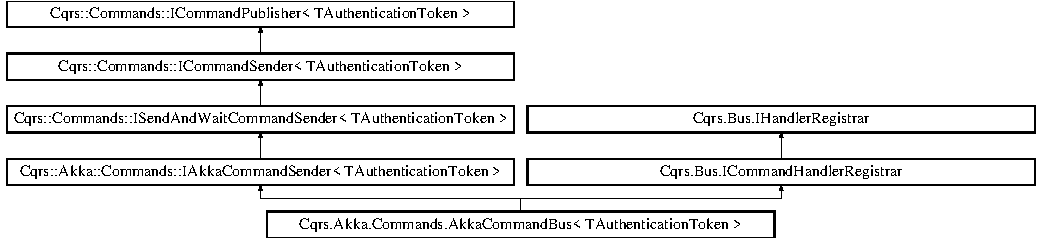
\includegraphics[height=3.189066cm]{classCqrs_1_1Akka_1_1Commands_1_1AkkaCommandBus}
\end{center}
\end{figure}
\subsection*{Public Member Functions}
\begin{DoxyCompactItemize}
\item 
\hyperlink{classCqrs_1_1Akka_1_1Commands_1_1AkkaCommandBus_a765b65e299cc1b32c4c0e7ee405c473d}{Akka\+Command\+Bus} (\hyperlink{interfaceCqrs_1_1Bus_1_1IBusHelper}{I\+Bus\+Helper} bus\+Helper, \hyperlink{interfaceCqrs_1_1Authentication_1_1IAuthenticationTokenHelper}{I\+Authentication\+Token\+Helper}$<$ T\+Authentication\+Token $>$ authentication\+Token\+Helper, I\+Correlation\+Id\+Helper correlation\+Id\+Helper, \hyperlink{interfaceCqrs_1_1Configuration_1_1IDependencyResolver}{I\+Dependency\+Resolver} dependency\+Resolver, I\+Logger logger, \hyperlink{interfaceCqrs_1_1Commands_1_1ICommandPublisher}{I\+Command\+Publisher}$<$ T\+Authentication\+Token $>$ command\+Sender, \hyperlink{interfaceCqrs_1_1Commands_1_1ICommandReceiver}{I\+Command\+Receiver}$<$ T\+Authentication\+Token $>$ command\+Receiver)
\item 
virtual void \hyperlink{classCqrs_1_1Akka_1_1Commands_1_1AkkaCommandBus_a48e1d46035b1e1a3251636b8a03f7dae}{Publish$<$ T\+Command $>$} (T\+Command command)
\item 
virtual void \hyperlink{classCqrs_1_1Akka_1_1Commands_1_1AkkaCommandBus_a696f471533265685f80922e39727288e}{Send$<$ T\+Command $>$} (T\+Command command)
\item 
virtual void \hyperlink{classCqrs_1_1Akka_1_1Commands_1_1AkkaCommandBus_ab52365375febd74ac078e97af6e6cd24}{Publish$<$ T\+Command $>$} (I\+Enumerable$<$ T\+Command $>$ commands)
\item 
virtual void \hyperlink{classCqrs_1_1Akka_1_1Commands_1_1AkkaCommandBus_a06b7b148493c67d79aaf6b7d59afa487}{Send$<$ T\+Command $>$} (I\+Enumerable$<$ T\+Command $>$ commands)
\item 
virtual T\+Event \hyperlink{classCqrs_1_1Akka_1_1Commands_1_1AkkaCommandBus_a10ed94fc318977777e2e6cc970b8953e}{Send\+And\+Wait$<$ T\+Command, T\+Event $>$} (T\+Command command, \hyperlink{interfaceCqrs_1_1Events_1_1IEventReceiver}{I\+Event\+Receiver}$<$ T\+Authentication\+Token $>$ event\+Receiver=null)
\begin{DoxyCompactList}\small\item\em Sends the provided {\itshape command}  and waits for an event of {\itshape T\+Event}  \end{DoxyCompactList}\item 
virtual T\+Event \hyperlink{classCqrs_1_1Akka_1_1Commands_1_1AkkaCommandBus_a4f96fc98615afb9af8fe4d54a398660a}{Send\+And\+Wait$<$ T\+Command, T\+Event $>$} (T\+Command command, int milliseconds\+Timeout, \hyperlink{interfaceCqrs_1_1Events_1_1IEventReceiver}{I\+Event\+Receiver}$<$ T\+Authentication\+Token $>$ event\+Receiver=null)
\begin{DoxyCompactList}\small\item\em Sends the provided {\itshape command}  and waits for an event of {\itshape T\+Event}  or exits if the specified timeout is expired. \end{DoxyCompactList}\item 
virtual T\+Event \hyperlink{classCqrs_1_1Akka_1_1Commands_1_1AkkaCommandBus_a8a0f3720395637de5f985e2a19e73fcd}{Send\+And\+Wait$<$ T\+Command, T\+Event $>$} (T\+Command command, Time\+Span timeout, \hyperlink{interfaceCqrs_1_1Events_1_1IEventReceiver}{I\+Event\+Receiver}$<$ T\+Authentication\+Token $>$ event\+Receiver=null)
\begin{DoxyCompactList}\small\item\em Sends the provided {\itshape command}  and waits for an event of {\itshape T\+Event}  or exits if the specified timeout is expired. \end{DoxyCompactList}\item 
virtual T\+Event \hyperlink{classCqrs_1_1Akka_1_1Commands_1_1AkkaCommandBus_a80fe44ab4ef2dc64260f2e27a673b91c}{Send\+And\+Wait$<$ T\+Command, T\+Event $>$} (T\+Command command, Func$<$ I\+Enumerable$<$ \hyperlink{interfaceCqrs_1_1Events_1_1IEvent}{I\+Event}$<$ T\+Authentication\+Token $>$$>$, T\+Event $>$ condition, \hyperlink{interfaceCqrs_1_1Events_1_1IEventReceiver}{I\+Event\+Receiver}$<$ T\+Authentication\+Token $>$ event\+Receiver=null)
\begin{DoxyCompactList}\small\item\em Sends the provided {\itshape command}  and waits until the specified condition is satisfied an event of {\itshape T\+Event}  \end{DoxyCompactList}\item 
virtual T\+Event \hyperlink{classCqrs_1_1Akka_1_1Commands_1_1AkkaCommandBus_affd63fcc939b04803ca58dad194fc723}{Send\+And\+Wait$<$ T\+Command, T\+Event $>$} (T\+Command command, Func$<$ I\+Enumerable$<$ \hyperlink{interfaceCqrs_1_1Events_1_1IEvent}{I\+Event}$<$ T\+Authentication\+Token $>$$>$, T\+Event $>$ condition, int milliseconds\+Timeout, \hyperlink{interfaceCqrs_1_1Events_1_1IEventReceiver}{I\+Event\+Receiver}$<$ T\+Authentication\+Token $>$ event\+Receiver=null)
\begin{DoxyCompactList}\small\item\em Sends the provided {\itshape command}  and waits for an event of {\itshape T\+Event}  or exits if the specified timeout is expired. \end{DoxyCompactList}\item 
virtual T\+Event \hyperlink{classCqrs_1_1Akka_1_1Commands_1_1AkkaCommandBus_a0bd9b9e4522286eba7af71d3ab400d5f}{Send\+And\+Wait$<$ T\+Command, T\+Event $>$} (T\+Command command, Func$<$ I\+Enumerable$<$ \hyperlink{interfaceCqrs_1_1Events_1_1IEvent}{I\+Event}$<$ T\+Authentication\+Token $>$$>$, T\+Event $>$ condition, Time\+Span timeout, \hyperlink{interfaceCqrs_1_1Events_1_1IEventReceiver}{I\+Event\+Receiver}$<$ T\+Authentication\+Token $>$ event\+Receiver=null)
\begin{DoxyCompactList}\small\item\em Sends the provided {\itshape command}  and waits for an event of {\itshape T\+Event}  or exits if the specified timeout is expired. \end{DoxyCompactList}\item 
void \hyperlink{classCqrs_1_1Akka_1_1Commands_1_1AkkaCommandBus_a8ed33fb315493d52470bc3bc2bf076f2}{Register\+Handler$<$ T\+Message $>$} (Action$<$ T\+Message $>$ handler, Type targeted\+Type, bool hold\+Message\+Lock=true)
\begin{DoxyCompactList}\small\item\em Register an event or command handler that will listen and respond to events or commands. \end{DoxyCompactList}\item 
void \hyperlink{classCqrs_1_1Akka_1_1Commands_1_1AkkaCommandBus_adc21072d2b02c745747c4d585a53dba3}{Register\+Handler$<$ T\+Message $>$} (Action$<$ T\+Message $>$ handler, bool hold\+Message\+Lock=true)
\begin{DoxyCompactList}\small\item\em Register an event or command handler that will listen and respond to events or commands. \end{DoxyCompactList}\end{DoxyCompactItemize}
\subsection*{Protected Member Functions}
\begin{DoxyCompactItemize}
\item 
virtual void \hyperlink{classCqrs_1_1Akka_1_1Commands_1_1AkkaCommandBus_a9755a84c0b971ce0862abdc2783422ce}{Prepare\+Command$<$ T\+Command $>$} (T\+Command command)
\item 
virtual bool \hyperlink{classCqrs_1_1Akka_1_1Commands_1_1AkkaCommandBus_ae3e5f1725bceb0359aedb74ded530858}{Prepare\+And\+Validate\+Command$<$ T\+Command $>$} (T\+Command command, out \hyperlink{classCqrs_1_1Bus_1_1RouteHandlerDelegate}{Route\+Handler\+Delegate} command\+Handler)
\end{DoxyCompactItemize}
\subsection*{Properties}
\begin{DoxyCompactItemize}
\item 
static \hyperlink{classCqrs_1_1Bus_1_1RouteManager}{Route\+Manager} \hyperlink{classCqrs_1_1Akka_1_1Commands_1_1AkkaCommandBus_a93ddefb347d0cbc4f869c6d0866c8c64}{Routes}\hspace{0.3cm}{\ttfamily  \mbox{[}get\mbox{]}}
\item 
\hyperlink{interfaceCqrs_1_1Authentication_1_1IAuthenticationTokenHelper}{I\+Authentication\+Token\+Helper}$<$ T\+Authentication\+Token $>$ \hyperlink{classCqrs_1_1Akka_1_1Commands_1_1AkkaCommandBus_ad74a628484d215ec6daab02b20ac1dbe}{Authentication\+Token\+Helper}\hspace{0.3cm}{\ttfamily  \mbox{[}get\mbox{]}}
\item 
I\+Correlation\+Id\+Helper \hyperlink{classCqrs_1_1Akka_1_1Commands_1_1AkkaCommandBus_ad8bdf5674c0d5ea3fd9340bd8cd4b0a8}{Correlation\+Id\+Helper}\hspace{0.3cm}{\ttfamily  \mbox{[}get\mbox{]}}
\item 
\hyperlink{interfaceCqrs_1_1Configuration_1_1IDependencyResolver}{I\+Dependency\+Resolver} \hyperlink{classCqrs_1_1Akka_1_1Commands_1_1AkkaCommandBus_ae1229644077b0740d9014708d15b44c2}{Dependency\+Resolver}\hspace{0.3cm}{\ttfamily  \mbox{[}get\mbox{]}}
\item 
\hyperlink{interfaceCqrs_1_1Bus_1_1IBusHelper}{I\+Bus\+Helper} \hyperlink{classCqrs_1_1Akka_1_1Commands_1_1AkkaCommandBus_abe5501970c0e39abb9a70670ab985fdc}{Bus\+Helper}\hspace{0.3cm}{\ttfamily  \mbox{[}get\mbox{]}}
\item 
I\+Logger \hyperlink{classCqrs_1_1Akka_1_1Commands_1_1AkkaCommandBus_a218e431067a4cadbdd711d74cbe8e53b}{Logger}\hspace{0.3cm}{\ttfamily  \mbox{[}get\mbox{]}}
\item 
\hyperlink{interfaceCqrs_1_1Commands_1_1ICommandPublisher}{I\+Command\+Publisher}$<$ T\+Authentication\+Token $>$ \hyperlink{classCqrs_1_1Akka_1_1Commands_1_1AkkaCommandBus_ae3659627842e6d556320c2d79ab17ebd}{Command\+Sender}\hspace{0.3cm}{\ttfamily  \mbox{[}get\mbox{]}}
\item 
\hyperlink{interfaceCqrs_1_1Commands_1_1ICommandReceiver}{I\+Command\+Receiver}$<$ T\+Authentication\+Token $>$ \hyperlink{classCqrs_1_1Akka_1_1Commands_1_1AkkaCommandBus_ac65a93dadbbb006dd815c5c54c9ecc82}{Command\+Receiver}\hspace{0.3cm}{\ttfamily  \mbox{[}get\mbox{]}}
\item 
I\+Dictionary$<$ Guid, I\+List$<$ \hyperlink{interfaceCqrs_1_1Events_1_1IEvent}{I\+Event}$<$ T\+Authentication\+Token $>$ $>$ $>$ \hyperlink{classCqrs_1_1Akka_1_1Commands_1_1AkkaCommandBus_af64744500f25a0b203684ef757aa7962}{Event\+Waits}\hspace{0.3cm}{\ttfamily  \mbox{[}get\mbox{]}}
\end{DoxyCompactItemize}


\subsection{Detailed Description}
A I\+Command\+Publisher$<$\+T\+Authentication\+Token$>$ that resolves handlers , executes the handler and then publishes the I\+Command$<$\+T\+Authentication\+Token$>$ on the public command bus. 



\subsection{Constructor \& Destructor Documentation}
\mbox{\Hypertarget{classCqrs_1_1Akka_1_1Commands_1_1AkkaCommandBus_a765b65e299cc1b32c4c0e7ee405c473d}\label{classCqrs_1_1Akka_1_1Commands_1_1AkkaCommandBus_a765b65e299cc1b32c4c0e7ee405c473d}} 
\index{Cqrs\+::\+Akka\+::\+Commands\+::\+Akka\+Command\+Bus@{Cqrs\+::\+Akka\+::\+Commands\+::\+Akka\+Command\+Bus}!Akka\+Command\+Bus@{Akka\+Command\+Bus}}
\index{Akka\+Command\+Bus@{Akka\+Command\+Bus}!Cqrs\+::\+Akka\+::\+Commands\+::\+Akka\+Command\+Bus@{Cqrs\+::\+Akka\+::\+Commands\+::\+Akka\+Command\+Bus}}
\subsubsection{\texorpdfstring{Akka\+Command\+Bus()}{AkkaCommandBus()}}
{\footnotesize\ttfamily \hyperlink{classCqrs_1_1Akka_1_1Commands_1_1AkkaCommandBus}{Cqrs.\+Akka.\+Commands.\+Akka\+Command\+Bus}$<$ T\+Authentication\+Token $>$.\hyperlink{classCqrs_1_1Akka_1_1Commands_1_1AkkaCommandBus}{Akka\+Command\+Bus} (\begin{DoxyParamCaption}\item[{\hyperlink{interfaceCqrs_1_1Bus_1_1IBusHelper}{I\+Bus\+Helper}}]{bus\+Helper,  }\item[{\hyperlink{interfaceCqrs_1_1Authentication_1_1IAuthenticationTokenHelper}{I\+Authentication\+Token\+Helper}$<$ T\+Authentication\+Token $>$}]{authentication\+Token\+Helper,  }\item[{I\+Correlation\+Id\+Helper}]{correlation\+Id\+Helper,  }\item[{\hyperlink{interfaceCqrs_1_1Configuration_1_1IDependencyResolver}{I\+Dependency\+Resolver}}]{dependency\+Resolver,  }\item[{I\+Logger}]{logger,  }\item[{\hyperlink{interfaceCqrs_1_1Commands_1_1ICommandPublisher}{I\+Command\+Publisher}$<$ T\+Authentication\+Token $>$}]{command\+Sender,  }\item[{\hyperlink{interfaceCqrs_1_1Commands_1_1ICommandReceiver}{I\+Command\+Receiver}$<$ T\+Authentication\+Token $>$}]{command\+Receiver }\end{DoxyParamCaption})}



\subsection{Member Function Documentation}
\mbox{\Hypertarget{classCqrs_1_1Akka_1_1Commands_1_1AkkaCommandBus_ae3e5f1725bceb0359aedb74ded530858}\label{classCqrs_1_1Akka_1_1Commands_1_1AkkaCommandBus_ae3e5f1725bceb0359aedb74ded530858}} 
\index{Cqrs\+::\+Akka\+::\+Commands\+::\+Akka\+Command\+Bus@{Cqrs\+::\+Akka\+::\+Commands\+::\+Akka\+Command\+Bus}!Prepare\+And\+Validate\+Command$<$ T\+Command $>$@{Prepare\+And\+Validate\+Command$<$ T\+Command $>$}}
\index{Prepare\+And\+Validate\+Command$<$ T\+Command $>$@{Prepare\+And\+Validate\+Command$<$ T\+Command $>$}!Cqrs\+::\+Akka\+::\+Commands\+::\+Akka\+Command\+Bus@{Cqrs\+::\+Akka\+::\+Commands\+::\+Akka\+Command\+Bus}}
\subsubsection{\texorpdfstring{Prepare\+And\+Validate\+Command$<$ T\+Command $>$()}{PrepareAndValidateCommand< TCommand >()}}
{\footnotesize\ttfamily virtual bool \hyperlink{classCqrs_1_1Akka_1_1Commands_1_1AkkaCommandBus}{Cqrs.\+Akka.\+Commands.\+Akka\+Command\+Bus}$<$ T\+Authentication\+Token $>$.Prepare\+And\+Validate\+Command$<$ T\+Command $>$ (\begin{DoxyParamCaption}\item[{T\+Command}]{command,  }\item[{out \hyperlink{classCqrs_1_1Bus_1_1RouteHandlerDelegate}{Route\+Handler\+Delegate}}]{command\+Handler }\end{DoxyParamCaption})\hspace{0.3cm}{\ttfamily [protected]}, {\ttfamily [virtual]}}

\begin{Desc}
\item[Type Constraints]\begin{description}
\item[{\em T\+Command} : {\em I\+Command$<$T\+Authentication\+Token$>$}]\end{description}
\end{Desc}
\mbox{\Hypertarget{classCqrs_1_1Akka_1_1Commands_1_1AkkaCommandBus_a9755a84c0b971ce0862abdc2783422ce}\label{classCqrs_1_1Akka_1_1Commands_1_1AkkaCommandBus_a9755a84c0b971ce0862abdc2783422ce}} 
\index{Cqrs\+::\+Akka\+::\+Commands\+::\+Akka\+Command\+Bus@{Cqrs\+::\+Akka\+::\+Commands\+::\+Akka\+Command\+Bus}!Prepare\+Command$<$ T\+Command $>$@{Prepare\+Command$<$ T\+Command $>$}}
\index{Prepare\+Command$<$ T\+Command $>$@{Prepare\+Command$<$ T\+Command $>$}!Cqrs\+::\+Akka\+::\+Commands\+::\+Akka\+Command\+Bus@{Cqrs\+::\+Akka\+::\+Commands\+::\+Akka\+Command\+Bus}}
\subsubsection{\texorpdfstring{Prepare\+Command$<$ T\+Command $>$()}{PrepareCommand< TCommand >()}}
{\footnotesize\ttfamily virtual void \hyperlink{classCqrs_1_1Akka_1_1Commands_1_1AkkaCommandBus}{Cqrs.\+Akka.\+Commands.\+Akka\+Command\+Bus}$<$ T\+Authentication\+Token $>$.Prepare\+Command$<$ T\+Command $>$ (\begin{DoxyParamCaption}\item[{T\+Command}]{command }\end{DoxyParamCaption})\hspace{0.3cm}{\ttfamily [protected]}, {\ttfamily [virtual]}}

\begin{Desc}
\item[Type Constraints]\begin{description}
\item[{\em T\+Command} : {\em I\+Command$<$T\+Authentication\+Token$>$}]\end{description}
\end{Desc}
\mbox{\Hypertarget{classCqrs_1_1Akka_1_1Commands_1_1AkkaCommandBus_a48e1d46035b1e1a3251636b8a03f7dae}\label{classCqrs_1_1Akka_1_1Commands_1_1AkkaCommandBus_a48e1d46035b1e1a3251636b8a03f7dae}} 
\index{Cqrs\+::\+Akka\+::\+Commands\+::\+Akka\+Command\+Bus@{Cqrs\+::\+Akka\+::\+Commands\+::\+Akka\+Command\+Bus}!Publish$<$ T\+Command $>$@{Publish$<$ T\+Command $>$}}
\index{Publish$<$ T\+Command $>$@{Publish$<$ T\+Command $>$}!Cqrs\+::\+Akka\+::\+Commands\+::\+Akka\+Command\+Bus@{Cqrs\+::\+Akka\+::\+Commands\+::\+Akka\+Command\+Bus}}
\subsubsection{\texorpdfstring{Publish$<$ T\+Command $>$()}{Publish< TCommand >()}\hspace{0.1cm}{\footnotesize\ttfamily [1/2]}}
{\footnotesize\ttfamily virtual void \hyperlink{classCqrs_1_1Akka_1_1Commands_1_1AkkaCommandBus}{Cqrs.\+Akka.\+Commands.\+Akka\+Command\+Bus}$<$ T\+Authentication\+Token $>$.Publish$<$ T\+Command $>$ (\begin{DoxyParamCaption}\item[{T\+Command}]{command }\end{DoxyParamCaption})\hspace{0.3cm}{\ttfamily [virtual]}}



Implements \hyperlink{interfaceCqrs_1_1Commands_1_1ICommandPublisher_aeeb487ad5686d9c44d214b1daaf7833a}{Cqrs.\+Commands.\+I\+Command\+Publisher$<$ T\+Authentication\+Token $>$}.

\begin{Desc}
\item[Type Constraints]\begin{description}
\item[{\em T\+Command} : {\em I\+Command$<$T\+Authentication\+Token$>$}]\end{description}
\end{Desc}
\mbox{\Hypertarget{classCqrs_1_1Akka_1_1Commands_1_1AkkaCommandBus_ab52365375febd74ac078e97af6e6cd24}\label{classCqrs_1_1Akka_1_1Commands_1_1AkkaCommandBus_ab52365375febd74ac078e97af6e6cd24}} 
\index{Cqrs\+::\+Akka\+::\+Commands\+::\+Akka\+Command\+Bus@{Cqrs\+::\+Akka\+::\+Commands\+::\+Akka\+Command\+Bus}!Publish$<$ T\+Command $>$@{Publish$<$ T\+Command $>$}}
\index{Publish$<$ T\+Command $>$@{Publish$<$ T\+Command $>$}!Cqrs\+::\+Akka\+::\+Commands\+::\+Akka\+Command\+Bus@{Cqrs\+::\+Akka\+::\+Commands\+::\+Akka\+Command\+Bus}}
\subsubsection{\texorpdfstring{Publish$<$ T\+Command $>$()}{Publish< TCommand >()}\hspace{0.1cm}{\footnotesize\ttfamily [2/2]}}
{\footnotesize\ttfamily virtual void \hyperlink{classCqrs_1_1Akka_1_1Commands_1_1AkkaCommandBus}{Cqrs.\+Akka.\+Commands.\+Akka\+Command\+Bus}$<$ T\+Authentication\+Token $>$.Publish$<$ T\+Command $>$ (\begin{DoxyParamCaption}\item[{I\+Enumerable$<$ T\+Command $>$}]{commands }\end{DoxyParamCaption})\hspace{0.3cm}{\ttfamily [virtual]}}



Implements \hyperlink{interfaceCqrs_1_1Commands_1_1ICommandPublisher_af0f033c0b949e5650032e4f00b11b595}{Cqrs.\+Commands.\+I\+Command\+Publisher$<$ T\+Authentication\+Token $>$}.

\begin{Desc}
\item[Type Constraints]\begin{description}
\item[{\em T\+Command} : {\em I\+Command$<$T\+Authentication\+Token$>$}]\end{description}
\end{Desc}
\mbox{\Hypertarget{classCqrs_1_1Akka_1_1Commands_1_1AkkaCommandBus_a8ed33fb315493d52470bc3bc2bf076f2}\label{classCqrs_1_1Akka_1_1Commands_1_1AkkaCommandBus_a8ed33fb315493d52470bc3bc2bf076f2}} 
\index{Cqrs\+::\+Akka\+::\+Commands\+::\+Akka\+Command\+Bus@{Cqrs\+::\+Akka\+::\+Commands\+::\+Akka\+Command\+Bus}!Register\+Handler$<$ T\+Message $>$@{Register\+Handler$<$ T\+Message $>$}}
\index{Register\+Handler$<$ T\+Message $>$@{Register\+Handler$<$ T\+Message $>$}!Cqrs\+::\+Akka\+::\+Commands\+::\+Akka\+Command\+Bus@{Cqrs\+::\+Akka\+::\+Commands\+::\+Akka\+Command\+Bus}}
\subsubsection{\texorpdfstring{Register\+Handler$<$ T\+Message $>$()}{RegisterHandler< TMessage >()}\hspace{0.1cm}{\footnotesize\ttfamily [1/2]}}
{\footnotesize\ttfamily void \hyperlink{classCqrs_1_1Akka_1_1Commands_1_1AkkaCommandBus}{Cqrs.\+Akka.\+Commands.\+Akka\+Command\+Bus}$<$ T\+Authentication\+Token $>$.Register\+Handler$<$ T\+Message $>$ (\begin{DoxyParamCaption}\item[{Action$<$ T\+Message $>$}]{handler,  }\item[{Type}]{targeted\+Type,  }\item[{bool}]{hold\+Message\+Lock = {\ttfamily true} }\end{DoxyParamCaption})}



Register an event or command handler that will listen and respond to events or commands. 



Implements \hyperlink{interfaceCqrs_1_1Bus_1_1IHandlerRegistrar_ab6ca4dfdc54a5aeebe4651dbdb479f55}{Cqrs.\+Bus.\+I\+Handler\+Registrar}.

\begin{Desc}
\item[Type Constraints]\begin{description}
\item[{\em T\+Message} : {\em I\+Message}]\end{description}
\end{Desc}
\mbox{\Hypertarget{classCqrs_1_1Akka_1_1Commands_1_1AkkaCommandBus_adc21072d2b02c745747c4d585a53dba3}\label{classCqrs_1_1Akka_1_1Commands_1_1AkkaCommandBus_adc21072d2b02c745747c4d585a53dba3}} 
\index{Cqrs\+::\+Akka\+::\+Commands\+::\+Akka\+Command\+Bus@{Cqrs\+::\+Akka\+::\+Commands\+::\+Akka\+Command\+Bus}!Register\+Handler$<$ T\+Message $>$@{Register\+Handler$<$ T\+Message $>$}}
\index{Register\+Handler$<$ T\+Message $>$@{Register\+Handler$<$ T\+Message $>$}!Cqrs\+::\+Akka\+::\+Commands\+::\+Akka\+Command\+Bus@{Cqrs\+::\+Akka\+::\+Commands\+::\+Akka\+Command\+Bus}}
\subsubsection{\texorpdfstring{Register\+Handler$<$ T\+Message $>$()}{RegisterHandler< TMessage >()}\hspace{0.1cm}{\footnotesize\ttfamily [2/2]}}
{\footnotesize\ttfamily void \hyperlink{classCqrs_1_1Akka_1_1Commands_1_1AkkaCommandBus}{Cqrs.\+Akka.\+Commands.\+Akka\+Command\+Bus}$<$ T\+Authentication\+Token $>$.Register\+Handler$<$ T\+Message $>$ (\begin{DoxyParamCaption}\item[{Action$<$ T\+Message $>$}]{handler,  }\item[{bool}]{hold\+Message\+Lock = {\ttfamily true} }\end{DoxyParamCaption})}



Register an event or command handler that will listen and respond to events or commands. 



Implements \hyperlink{interfaceCqrs_1_1Bus_1_1IHandlerRegistrar_a07792dcc9a8b272709ff2e2dd336a642}{Cqrs.\+Bus.\+I\+Handler\+Registrar}.

\begin{Desc}
\item[Type Constraints]\begin{description}
\item[{\em T\+Message} : {\em I\+Message}]\end{description}
\end{Desc}
\mbox{\Hypertarget{classCqrs_1_1Akka_1_1Commands_1_1AkkaCommandBus_a696f471533265685f80922e39727288e}\label{classCqrs_1_1Akka_1_1Commands_1_1AkkaCommandBus_a696f471533265685f80922e39727288e}} 
\index{Cqrs\+::\+Akka\+::\+Commands\+::\+Akka\+Command\+Bus@{Cqrs\+::\+Akka\+::\+Commands\+::\+Akka\+Command\+Bus}!Send$<$ T\+Command $>$@{Send$<$ T\+Command $>$}}
\index{Send$<$ T\+Command $>$@{Send$<$ T\+Command $>$}!Cqrs\+::\+Akka\+::\+Commands\+::\+Akka\+Command\+Bus@{Cqrs\+::\+Akka\+::\+Commands\+::\+Akka\+Command\+Bus}}
\subsubsection{\texorpdfstring{Send$<$ T\+Command $>$()}{Send< TCommand >()}\hspace{0.1cm}{\footnotesize\ttfamily [1/2]}}
{\footnotesize\ttfamily virtual void \hyperlink{classCqrs_1_1Akka_1_1Commands_1_1AkkaCommandBus}{Cqrs.\+Akka.\+Commands.\+Akka\+Command\+Bus}$<$ T\+Authentication\+Token $>$.Send$<$ T\+Command $>$ (\begin{DoxyParamCaption}\item[{T\+Command}]{command }\end{DoxyParamCaption})\hspace{0.3cm}{\ttfamily [virtual]}}



Implements \hyperlink{interfaceCqrs_1_1Commands_1_1ICommandSender_a551d69f8679399fc0ce0fd99dead507a}{Cqrs.\+Commands.\+I\+Command\+Sender$<$ T\+Authentication\+Token $>$}.

\begin{Desc}
\item[Type Constraints]\begin{description}
\item[{\em T\+Command} : {\em I\+Command$<$T\+Authentication\+Token$>$}]\end{description}
\end{Desc}
\mbox{\Hypertarget{classCqrs_1_1Akka_1_1Commands_1_1AkkaCommandBus_a06b7b148493c67d79aaf6b7d59afa487}\label{classCqrs_1_1Akka_1_1Commands_1_1AkkaCommandBus_a06b7b148493c67d79aaf6b7d59afa487}} 
\index{Cqrs\+::\+Akka\+::\+Commands\+::\+Akka\+Command\+Bus@{Cqrs\+::\+Akka\+::\+Commands\+::\+Akka\+Command\+Bus}!Send$<$ T\+Command $>$@{Send$<$ T\+Command $>$}}
\index{Send$<$ T\+Command $>$@{Send$<$ T\+Command $>$}!Cqrs\+::\+Akka\+::\+Commands\+::\+Akka\+Command\+Bus@{Cqrs\+::\+Akka\+::\+Commands\+::\+Akka\+Command\+Bus}}
\subsubsection{\texorpdfstring{Send$<$ T\+Command $>$()}{Send< TCommand >()}\hspace{0.1cm}{\footnotesize\ttfamily [2/2]}}
{\footnotesize\ttfamily virtual void \hyperlink{classCqrs_1_1Akka_1_1Commands_1_1AkkaCommandBus}{Cqrs.\+Akka.\+Commands.\+Akka\+Command\+Bus}$<$ T\+Authentication\+Token $>$.Send$<$ T\+Command $>$ (\begin{DoxyParamCaption}\item[{I\+Enumerable$<$ T\+Command $>$}]{commands }\end{DoxyParamCaption})\hspace{0.3cm}{\ttfamily [virtual]}}



Implements \hyperlink{interfaceCqrs_1_1Commands_1_1ICommandSender_a3fb3ec40a3e862f721a7c9204e67e832}{Cqrs.\+Commands.\+I\+Command\+Sender$<$ T\+Authentication\+Token $>$}.

\begin{Desc}
\item[Type Constraints]\begin{description}
\item[{\em T\+Command} : {\em I\+Command$<$T\+Authentication\+Token$>$}]\end{description}
\end{Desc}
\mbox{\Hypertarget{classCqrs_1_1Akka_1_1Commands_1_1AkkaCommandBus_a10ed94fc318977777e2e6cc970b8953e}\label{classCqrs_1_1Akka_1_1Commands_1_1AkkaCommandBus_a10ed94fc318977777e2e6cc970b8953e}} 
\index{Cqrs\+::\+Akka\+::\+Commands\+::\+Akka\+Command\+Bus@{Cqrs\+::\+Akka\+::\+Commands\+::\+Akka\+Command\+Bus}!Send\+And\+Wait$<$ T\+Command, T\+Event $>$@{Send\+And\+Wait$<$ T\+Command, T\+Event $>$}}
\index{Send\+And\+Wait$<$ T\+Command, T\+Event $>$@{Send\+And\+Wait$<$ T\+Command, T\+Event $>$}!Cqrs\+::\+Akka\+::\+Commands\+::\+Akka\+Command\+Bus@{Cqrs\+::\+Akka\+::\+Commands\+::\+Akka\+Command\+Bus}}
\subsubsection{\texorpdfstring{Send\+And\+Wait$<$ T\+Command, T\+Event $>$()}{SendAndWait< TCommand, TEvent >()}\hspace{0.1cm}{\footnotesize\ttfamily [1/6]}}
{\footnotesize\ttfamily virtual T\+Event \hyperlink{classCqrs_1_1Akka_1_1Commands_1_1AkkaCommandBus}{Cqrs.\+Akka.\+Commands.\+Akka\+Command\+Bus}$<$ T\+Authentication\+Token $>$.Send\+And\+Wait$<$ T\+Command, T\+Event $>$ (\begin{DoxyParamCaption}\item[{T\+Command}]{command,  }\item[{\hyperlink{interfaceCqrs_1_1Events_1_1IEventReceiver}{I\+Event\+Receiver}$<$ T\+Authentication\+Token $>$}]{event\+Receiver = {\ttfamily null} }\end{DoxyParamCaption})\hspace{0.3cm}{\ttfamily [virtual]}}



Sends the provided {\itshape command}  and waits for an event of {\itshape T\+Event}  


\begin{DoxyParams}{Parameters}
{\em command} & The {\itshape T\+Command}  to send.\\
\hline
{\em event\+Receiver} & If provided, is the \hyperlink{interfaceCqrs_1_1Events_1_1IEventReceiver}{I\+Event\+Receiver$<$\+T\+Authentication\+Token$>$} that the event is expected to be returned on.\\
\hline
\end{DoxyParams}


Implements \hyperlink{interfaceCqrs_1_1Commands_1_1ISendAndWaitCommandSender_ab64dd5144f0688b0e23ffe289d4ffa2e}{Cqrs.\+Commands.\+I\+Send\+And\+Wait\+Command\+Sender$<$ T\+Authentication\+Token $>$}.

\begin{Desc}
\item[Type Constraints]\begin{description}
\item[{\em T\+Command} : {\em I\+Command$<$T\+Authentication\+Token$>$}]\end{description}
\end{Desc}
\mbox{\Hypertarget{classCqrs_1_1Akka_1_1Commands_1_1AkkaCommandBus_a4f96fc98615afb9af8fe4d54a398660a}\label{classCqrs_1_1Akka_1_1Commands_1_1AkkaCommandBus_a4f96fc98615afb9af8fe4d54a398660a}} 
\index{Cqrs\+::\+Akka\+::\+Commands\+::\+Akka\+Command\+Bus@{Cqrs\+::\+Akka\+::\+Commands\+::\+Akka\+Command\+Bus}!Send\+And\+Wait$<$ T\+Command, T\+Event $>$@{Send\+And\+Wait$<$ T\+Command, T\+Event $>$}}
\index{Send\+And\+Wait$<$ T\+Command, T\+Event $>$@{Send\+And\+Wait$<$ T\+Command, T\+Event $>$}!Cqrs\+::\+Akka\+::\+Commands\+::\+Akka\+Command\+Bus@{Cqrs\+::\+Akka\+::\+Commands\+::\+Akka\+Command\+Bus}}
\subsubsection{\texorpdfstring{Send\+And\+Wait$<$ T\+Command, T\+Event $>$()}{SendAndWait< TCommand, TEvent >()}\hspace{0.1cm}{\footnotesize\ttfamily [2/6]}}
{\footnotesize\ttfamily virtual T\+Event \hyperlink{classCqrs_1_1Akka_1_1Commands_1_1AkkaCommandBus}{Cqrs.\+Akka.\+Commands.\+Akka\+Command\+Bus}$<$ T\+Authentication\+Token $>$.Send\+And\+Wait$<$ T\+Command, T\+Event $>$ (\begin{DoxyParamCaption}\item[{T\+Command}]{command,  }\item[{int}]{milliseconds\+Timeout,  }\item[{\hyperlink{interfaceCqrs_1_1Events_1_1IEventReceiver}{I\+Event\+Receiver}$<$ T\+Authentication\+Token $>$}]{event\+Receiver = {\ttfamily null} }\end{DoxyParamCaption})\hspace{0.3cm}{\ttfamily [virtual]}}



Sends the provided {\itshape command}  and waits for an event of {\itshape T\+Event}  or exits if the specified timeout is expired. 


\begin{DoxyParams}{Parameters}
{\em command} & The {\itshape T\+Command}  to send.\\
\hline
{\em milliseconds\+Timeout} & The number of milliseconds to wait, or F\+:\+System.\+Threading.\+Timeout.\+Infinite (-\/1) to wait indefinitely.\\
\hline
{\em event\+Receiver} & If provided, is the \hyperlink{interfaceCqrs_1_1Events_1_1IEventReceiver}{I\+Event\+Receiver$<$\+T\+Authentication\+Token$>$} that the event is expected to be returned on.\\
\hline
\end{DoxyParams}


Implements \hyperlink{interfaceCqrs_1_1Commands_1_1ISendAndWaitCommandSender_aceee36522f8b677f3737ff0f9f2165ad}{Cqrs.\+Commands.\+I\+Send\+And\+Wait\+Command\+Sender$<$ T\+Authentication\+Token $>$}.

\begin{Desc}
\item[Type Constraints]\begin{description}
\item[{\em T\+Command} : {\em I\+Command$<$T\+Authentication\+Token$>$}]\end{description}
\end{Desc}
\mbox{\Hypertarget{classCqrs_1_1Akka_1_1Commands_1_1AkkaCommandBus_a8a0f3720395637de5f985e2a19e73fcd}\label{classCqrs_1_1Akka_1_1Commands_1_1AkkaCommandBus_a8a0f3720395637de5f985e2a19e73fcd}} 
\index{Cqrs\+::\+Akka\+::\+Commands\+::\+Akka\+Command\+Bus@{Cqrs\+::\+Akka\+::\+Commands\+::\+Akka\+Command\+Bus}!Send\+And\+Wait$<$ T\+Command, T\+Event $>$@{Send\+And\+Wait$<$ T\+Command, T\+Event $>$}}
\index{Send\+And\+Wait$<$ T\+Command, T\+Event $>$@{Send\+And\+Wait$<$ T\+Command, T\+Event $>$}!Cqrs\+::\+Akka\+::\+Commands\+::\+Akka\+Command\+Bus@{Cqrs\+::\+Akka\+::\+Commands\+::\+Akka\+Command\+Bus}}
\subsubsection{\texorpdfstring{Send\+And\+Wait$<$ T\+Command, T\+Event $>$()}{SendAndWait< TCommand, TEvent >()}\hspace{0.1cm}{\footnotesize\ttfamily [3/6]}}
{\footnotesize\ttfamily virtual T\+Event \hyperlink{classCqrs_1_1Akka_1_1Commands_1_1AkkaCommandBus}{Cqrs.\+Akka.\+Commands.\+Akka\+Command\+Bus}$<$ T\+Authentication\+Token $>$.Send\+And\+Wait$<$ T\+Command, T\+Event $>$ (\begin{DoxyParamCaption}\item[{T\+Command}]{command,  }\item[{Time\+Span}]{timeout,  }\item[{\hyperlink{interfaceCqrs_1_1Events_1_1IEventReceiver}{I\+Event\+Receiver}$<$ T\+Authentication\+Token $>$}]{event\+Receiver = {\ttfamily null} }\end{DoxyParamCaption})\hspace{0.3cm}{\ttfamily [virtual]}}



Sends the provided {\itshape command}  and waits for an event of {\itshape T\+Event}  or exits if the specified timeout is expired. 


\begin{DoxyParams}{Parameters}
{\em command} & The {\itshape T\+Command}  to send.\\
\hline
{\em timeout} & A T\+:\+System.\+Time\+Span that represents the number of milliseconds to wait, or a Time\+Span that represents -\/1 milliseconds to wait indefinitely.\\
\hline
{\em event\+Receiver} & If provided, is the \hyperlink{interfaceCqrs_1_1Events_1_1IEventReceiver}{I\+Event\+Receiver$<$\+T\+Authentication\+Token$>$} that the event is expected to be returned on.\\
\hline
\end{DoxyParams}


Implements \hyperlink{interfaceCqrs_1_1Commands_1_1ISendAndWaitCommandSender_ada9643fbf8206bcc72cc5817f747ada8}{Cqrs.\+Commands.\+I\+Send\+And\+Wait\+Command\+Sender$<$ T\+Authentication\+Token $>$}.

\begin{Desc}
\item[Type Constraints]\begin{description}
\item[{\em T\+Command} : {\em I\+Command$<$T\+Authentication\+Token$>$}]\end{description}
\end{Desc}
\mbox{\Hypertarget{classCqrs_1_1Akka_1_1Commands_1_1AkkaCommandBus_a80fe44ab4ef2dc64260f2e27a673b91c}\label{classCqrs_1_1Akka_1_1Commands_1_1AkkaCommandBus_a80fe44ab4ef2dc64260f2e27a673b91c}} 
\index{Cqrs\+::\+Akka\+::\+Commands\+::\+Akka\+Command\+Bus@{Cqrs\+::\+Akka\+::\+Commands\+::\+Akka\+Command\+Bus}!Send\+And\+Wait$<$ T\+Command, T\+Event $>$@{Send\+And\+Wait$<$ T\+Command, T\+Event $>$}}
\index{Send\+And\+Wait$<$ T\+Command, T\+Event $>$@{Send\+And\+Wait$<$ T\+Command, T\+Event $>$}!Cqrs\+::\+Akka\+::\+Commands\+::\+Akka\+Command\+Bus@{Cqrs\+::\+Akka\+::\+Commands\+::\+Akka\+Command\+Bus}}
\subsubsection{\texorpdfstring{Send\+And\+Wait$<$ T\+Command, T\+Event $>$()}{SendAndWait< TCommand, TEvent >()}\hspace{0.1cm}{\footnotesize\ttfamily [4/6]}}
{\footnotesize\ttfamily virtual T\+Event \hyperlink{classCqrs_1_1Akka_1_1Commands_1_1AkkaCommandBus}{Cqrs.\+Akka.\+Commands.\+Akka\+Command\+Bus}$<$ T\+Authentication\+Token $>$.Send\+And\+Wait$<$ T\+Command, T\+Event $>$ (\begin{DoxyParamCaption}\item[{T\+Command}]{command,  }\item[{Func$<$ I\+Enumerable$<$ \hyperlink{interfaceCqrs_1_1Events_1_1IEvent}{I\+Event}$<$ T\+Authentication\+Token $>$$>$, T\+Event $>$}]{condition,  }\item[{\hyperlink{interfaceCqrs_1_1Events_1_1IEventReceiver}{I\+Event\+Receiver}$<$ T\+Authentication\+Token $>$}]{event\+Receiver = {\ttfamily null} }\end{DoxyParamCaption})\hspace{0.3cm}{\ttfamily [virtual]}}



Sends the provided {\itshape command}  and waits until the specified condition is satisfied an event of {\itshape T\+Event}  


\begin{DoxyParams}{Parameters}
{\em command} & The {\itshape T\+Command}  to send.\\
\hline
{\em condition} & A delegate to be executed over and over until it returns the {\itshape T\+Event}  that is desired, return null to keep trying.\\
\hline
{\em event\+Receiver} & If provided, is the \hyperlink{interfaceCqrs_1_1Events_1_1IEventReceiver}{I\+Event\+Receiver$<$\+T\+Authentication\+Token$>$} that the event is expected to be returned on.\\
\hline
\end{DoxyParams}


Implements \hyperlink{interfaceCqrs_1_1Commands_1_1ISendAndWaitCommandSender_abc9bda930a4c8c57d8edf1044d2b8002}{Cqrs.\+Commands.\+I\+Send\+And\+Wait\+Command\+Sender$<$ T\+Authentication\+Token $>$}.

\begin{Desc}
\item[Type Constraints]\begin{description}
\item[{\em T\+Command} : {\em I\+Command$<$T\+Authentication\+Token$>$}]\end{description}
\end{Desc}
\mbox{\Hypertarget{classCqrs_1_1Akka_1_1Commands_1_1AkkaCommandBus_affd63fcc939b04803ca58dad194fc723}\label{classCqrs_1_1Akka_1_1Commands_1_1AkkaCommandBus_affd63fcc939b04803ca58dad194fc723}} 
\index{Cqrs\+::\+Akka\+::\+Commands\+::\+Akka\+Command\+Bus@{Cqrs\+::\+Akka\+::\+Commands\+::\+Akka\+Command\+Bus}!Send\+And\+Wait$<$ T\+Command, T\+Event $>$@{Send\+And\+Wait$<$ T\+Command, T\+Event $>$}}
\index{Send\+And\+Wait$<$ T\+Command, T\+Event $>$@{Send\+And\+Wait$<$ T\+Command, T\+Event $>$}!Cqrs\+::\+Akka\+::\+Commands\+::\+Akka\+Command\+Bus@{Cqrs\+::\+Akka\+::\+Commands\+::\+Akka\+Command\+Bus}}
\subsubsection{\texorpdfstring{Send\+And\+Wait$<$ T\+Command, T\+Event $>$()}{SendAndWait< TCommand, TEvent >()}\hspace{0.1cm}{\footnotesize\ttfamily [5/6]}}
{\footnotesize\ttfamily virtual T\+Event \hyperlink{classCqrs_1_1Akka_1_1Commands_1_1AkkaCommandBus}{Cqrs.\+Akka.\+Commands.\+Akka\+Command\+Bus}$<$ T\+Authentication\+Token $>$.Send\+And\+Wait$<$ T\+Command, T\+Event $>$ (\begin{DoxyParamCaption}\item[{T\+Command}]{command,  }\item[{Func$<$ I\+Enumerable$<$ \hyperlink{interfaceCqrs_1_1Events_1_1IEvent}{I\+Event}$<$ T\+Authentication\+Token $>$$>$, T\+Event $>$}]{condition,  }\item[{int}]{milliseconds\+Timeout,  }\item[{\hyperlink{interfaceCqrs_1_1Events_1_1IEventReceiver}{I\+Event\+Receiver}$<$ T\+Authentication\+Token $>$}]{event\+Receiver = {\ttfamily null} }\end{DoxyParamCaption})\hspace{0.3cm}{\ttfamily [virtual]}}



Sends the provided {\itshape command}  and waits for an event of {\itshape T\+Event}  or exits if the specified timeout is expired. 


\begin{DoxyParams}{Parameters}
{\em command} & The {\itshape T\+Command}  to send.\\
\hline
{\em condition} & A delegate to be executed over and over until it returns the {\itshape T\+Event}  that is desired, return null to keep trying.\\
\hline
{\em milliseconds\+Timeout} & The number of milliseconds to wait, or F\+:\+System.\+Threading.\+Timeout.\+Infinite (-\/1) to wait indefinitely.\\
\hline
{\em event\+Receiver} & If provided, is the \hyperlink{interfaceCqrs_1_1Events_1_1IEventReceiver}{I\+Event\+Receiver$<$\+T\+Authentication\+Token$>$} that the event is expected to be returned on.\\
\hline
\end{DoxyParams}


Implements \hyperlink{interfaceCqrs_1_1Commands_1_1ISendAndWaitCommandSender_a230c249fa137eafc9857c3b73ae86fcd}{Cqrs.\+Commands.\+I\+Send\+And\+Wait\+Command\+Sender$<$ T\+Authentication\+Token $>$}.

\begin{Desc}
\item[Type Constraints]\begin{description}
\item[{\em T\+Command} : {\em I\+Command$<$T\+Authentication\+Token$>$}]\end{description}
\end{Desc}
\mbox{\Hypertarget{classCqrs_1_1Akka_1_1Commands_1_1AkkaCommandBus_a0bd9b9e4522286eba7af71d3ab400d5f}\label{classCqrs_1_1Akka_1_1Commands_1_1AkkaCommandBus_a0bd9b9e4522286eba7af71d3ab400d5f}} 
\index{Cqrs\+::\+Akka\+::\+Commands\+::\+Akka\+Command\+Bus@{Cqrs\+::\+Akka\+::\+Commands\+::\+Akka\+Command\+Bus}!Send\+And\+Wait$<$ T\+Command, T\+Event $>$@{Send\+And\+Wait$<$ T\+Command, T\+Event $>$}}
\index{Send\+And\+Wait$<$ T\+Command, T\+Event $>$@{Send\+And\+Wait$<$ T\+Command, T\+Event $>$}!Cqrs\+::\+Akka\+::\+Commands\+::\+Akka\+Command\+Bus@{Cqrs\+::\+Akka\+::\+Commands\+::\+Akka\+Command\+Bus}}
\subsubsection{\texorpdfstring{Send\+And\+Wait$<$ T\+Command, T\+Event $>$()}{SendAndWait< TCommand, TEvent >()}\hspace{0.1cm}{\footnotesize\ttfamily [6/6]}}
{\footnotesize\ttfamily virtual T\+Event \hyperlink{classCqrs_1_1Akka_1_1Commands_1_1AkkaCommandBus}{Cqrs.\+Akka.\+Commands.\+Akka\+Command\+Bus}$<$ T\+Authentication\+Token $>$.Send\+And\+Wait$<$ T\+Command, T\+Event $>$ (\begin{DoxyParamCaption}\item[{T\+Command}]{command,  }\item[{Func$<$ I\+Enumerable$<$ \hyperlink{interfaceCqrs_1_1Events_1_1IEvent}{I\+Event}$<$ T\+Authentication\+Token $>$$>$, T\+Event $>$}]{condition,  }\item[{Time\+Span}]{timeout,  }\item[{\hyperlink{interfaceCqrs_1_1Events_1_1IEventReceiver}{I\+Event\+Receiver}$<$ T\+Authentication\+Token $>$}]{event\+Receiver = {\ttfamily null} }\end{DoxyParamCaption})\hspace{0.3cm}{\ttfamily [virtual]}}



Sends the provided {\itshape command}  and waits for an event of {\itshape T\+Event}  or exits if the specified timeout is expired. 


\begin{DoxyParams}{Parameters}
{\em command} & The {\itshape T\+Command}  to send.\\
\hline
{\em condition} & A delegate to be executed over and over until it returns the {\itshape T\+Event}  that is desired, return null to keep trying.\\
\hline
{\em timeout} & A T\+:\+System.\+Time\+Span that represents the number of milliseconds to wait, or a Time\+Span that represents -\/1 milliseconds to wait indefinitely.\\
\hline
{\em event\+Receiver} & If provided, is the \hyperlink{interfaceCqrs_1_1Events_1_1IEventReceiver}{I\+Event\+Receiver$<$\+T\+Authentication\+Token$>$} that the event is expected to be returned on.\\
\hline
\end{DoxyParams}


Implements \hyperlink{interfaceCqrs_1_1Commands_1_1ISendAndWaitCommandSender_a8a9b1333e70cc9d8a91d6374354a851f}{Cqrs.\+Commands.\+I\+Send\+And\+Wait\+Command\+Sender$<$ T\+Authentication\+Token $>$}.

\begin{Desc}
\item[Type Constraints]\begin{description}
\item[{\em T\+Command} : {\em I\+Command$<$T\+Authentication\+Token$>$}]\end{description}
\end{Desc}


\subsection{Property Documentation}
\mbox{\Hypertarget{classCqrs_1_1Akka_1_1Commands_1_1AkkaCommandBus_ad74a628484d215ec6daab02b20ac1dbe}\label{classCqrs_1_1Akka_1_1Commands_1_1AkkaCommandBus_ad74a628484d215ec6daab02b20ac1dbe}} 
\index{Cqrs\+::\+Akka\+::\+Commands\+::\+Akka\+Command\+Bus@{Cqrs\+::\+Akka\+::\+Commands\+::\+Akka\+Command\+Bus}!Authentication\+Token\+Helper@{Authentication\+Token\+Helper}}
\index{Authentication\+Token\+Helper@{Authentication\+Token\+Helper}!Cqrs\+::\+Akka\+::\+Commands\+::\+Akka\+Command\+Bus@{Cqrs\+::\+Akka\+::\+Commands\+::\+Akka\+Command\+Bus}}
\subsubsection{\texorpdfstring{Authentication\+Token\+Helper}{AuthenticationTokenHelper}}
{\footnotesize\ttfamily \hyperlink{interfaceCqrs_1_1Authentication_1_1IAuthenticationTokenHelper}{I\+Authentication\+Token\+Helper}$<$T\+Authentication\+Token$>$ \hyperlink{classCqrs_1_1Akka_1_1Commands_1_1AkkaCommandBus}{Cqrs.\+Akka.\+Commands.\+Akka\+Command\+Bus}$<$ T\+Authentication\+Token $>$.\hyperlink{classCqrs_1_1Authentication_1_1AuthenticationTokenHelper}{Authentication\+Token\+Helper}\hspace{0.3cm}{\ttfamily [get]}, {\ttfamily [protected]}}

\mbox{\Hypertarget{classCqrs_1_1Akka_1_1Commands_1_1AkkaCommandBus_abe5501970c0e39abb9a70670ab985fdc}\label{classCqrs_1_1Akka_1_1Commands_1_1AkkaCommandBus_abe5501970c0e39abb9a70670ab985fdc}} 
\index{Cqrs\+::\+Akka\+::\+Commands\+::\+Akka\+Command\+Bus@{Cqrs\+::\+Akka\+::\+Commands\+::\+Akka\+Command\+Bus}!Bus\+Helper@{Bus\+Helper}}
\index{Bus\+Helper@{Bus\+Helper}!Cqrs\+::\+Akka\+::\+Commands\+::\+Akka\+Command\+Bus@{Cqrs\+::\+Akka\+::\+Commands\+::\+Akka\+Command\+Bus}}
\subsubsection{\texorpdfstring{Bus\+Helper}{BusHelper}}
{\footnotesize\ttfamily \hyperlink{interfaceCqrs_1_1Bus_1_1IBusHelper}{I\+Bus\+Helper} \hyperlink{classCqrs_1_1Akka_1_1Commands_1_1AkkaCommandBus}{Cqrs.\+Akka.\+Commands.\+Akka\+Command\+Bus}$<$ T\+Authentication\+Token $>$.\hyperlink{classCqrs_1_1Bus_1_1BusHelper}{Bus\+Helper}\hspace{0.3cm}{\ttfamily [get]}, {\ttfamily [protected]}}

\mbox{\Hypertarget{classCqrs_1_1Akka_1_1Commands_1_1AkkaCommandBus_ac65a93dadbbb006dd815c5c54c9ecc82}\label{classCqrs_1_1Akka_1_1Commands_1_1AkkaCommandBus_ac65a93dadbbb006dd815c5c54c9ecc82}} 
\index{Cqrs\+::\+Akka\+::\+Commands\+::\+Akka\+Command\+Bus@{Cqrs\+::\+Akka\+::\+Commands\+::\+Akka\+Command\+Bus}!Command\+Receiver@{Command\+Receiver}}
\index{Command\+Receiver@{Command\+Receiver}!Cqrs\+::\+Akka\+::\+Commands\+::\+Akka\+Command\+Bus@{Cqrs\+::\+Akka\+::\+Commands\+::\+Akka\+Command\+Bus}}
\subsubsection{\texorpdfstring{Command\+Receiver}{CommandReceiver}}
{\footnotesize\ttfamily \hyperlink{interfaceCqrs_1_1Commands_1_1ICommandReceiver}{I\+Command\+Receiver}$<$T\+Authentication\+Token$>$ \hyperlink{classCqrs_1_1Akka_1_1Commands_1_1AkkaCommandBus}{Cqrs.\+Akka.\+Commands.\+Akka\+Command\+Bus}$<$ T\+Authentication\+Token $>$.Command\+Receiver\hspace{0.3cm}{\ttfamily [get]}, {\ttfamily [protected]}}

\mbox{\Hypertarget{classCqrs_1_1Akka_1_1Commands_1_1AkkaCommandBus_ae3659627842e6d556320c2d79ab17ebd}\label{classCqrs_1_1Akka_1_1Commands_1_1AkkaCommandBus_ae3659627842e6d556320c2d79ab17ebd}} 
\index{Cqrs\+::\+Akka\+::\+Commands\+::\+Akka\+Command\+Bus@{Cqrs\+::\+Akka\+::\+Commands\+::\+Akka\+Command\+Bus}!Command\+Sender@{Command\+Sender}}
\index{Command\+Sender@{Command\+Sender}!Cqrs\+::\+Akka\+::\+Commands\+::\+Akka\+Command\+Bus@{Cqrs\+::\+Akka\+::\+Commands\+::\+Akka\+Command\+Bus}}
\subsubsection{\texorpdfstring{Command\+Sender}{CommandSender}}
{\footnotesize\ttfamily \hyperlink{interfaceCqrs_1_1Commands_1_1ICommandPublisher}{I\+Command\+Publisher}$<$T\+Authentication\+Token$>$ \hyperlink{classCqrs_1_1Akka_1_1Commands_1_1AkkaCommandBus}{Cqrs.\+Akka.\+Commands.\+Akka\+Command\+Bus}$<$ T\+Authentication\+Token $>$.Command\+Sender\hspace{0.3cm}{\ttfamily [get]}, {\ttfamily [protected]}}

\mbox{\Hypertarget{classCqrs_1_1Akka_1_1Commands_1_1AkkaCommandBus_ad8bdf5674c0d5ea3fd9340bd8cd4b0a8}\label{classCqrs_1_1Akka_1_1Commands_1_1AkkaCommandBus_ad8bdf5674c0d5ea3fd9340bd8cd4b0a8}} 
\index{Cqrs\+::\+Akka\+::\+Commands\+::\+Akka\+Command\+Bus@{Cqrs\+::\+Akka\+::\+Commands\+::\+Akka\+Command\+Bus}!Correlation\+Id\+Helper@{Correlation\+Id\+Helper}}
\index{Correlation\+Id\+Helper@{Correlation\+Id\+Helper}!Cqrs\+::\+Akka\+::\+Commands\+::\+Akka\+Command\+Bus@{Cqrs\+::\+Akka\+::\+Commands\+::\+Akka\+Command\+Bus}}
\subsubsection{\texorpdfstring{Correlation\+Id\+Helper}{CorrelationIdHelper}}
{\footnotesize\ttfamily I\+Correlation\+Id\+Helper \hyperlink{classCqrs_1_1Akka_1_1Commands_1_1AkkaCommandBus}{Cqrs.\+Akka.\+Commands.\+Akka\+Command\+Bus}$<$ T\+Authentication\+Token $>$.Correlation\+Id\+Helper\hspace{0.3cm}{\ttfamily [get]}, {\ttfamily [protected]}}

\mbox{\Hypertarget{classCqrs_1_1Akka_1_1Commands_1_1AkkaCommandBus_ae1229644077b0740d9014708d15b44c2}\label{classCqrs_1_1Akka_1_1Commands_1_1AkkaCommandBus_ae1229644077b0740d9014708d15b44c2}} 
\index{Cqrs\+::\+Akka\+::\+Commands\+::\+Akka\+Command\+Bus@{Cqrs\+::\+Akka\+::\+Commands\+::\+Akka\+Command\+Bus}!Dependency\+Resolver@{Dependency\+Resolver}}
\index{Dependency\+Resolver@{Dependency\+Resolver}!Cqrs\+::\+Akka\+::\+Commands\+::\+Akka\+Command\+Bus@{Cqrs\+::\+Akka\+::\+Commands\+::\+Akka\+Command\+Bus}}
\subsubsection{\texorpdfstring{Dependency\+Resolver}{DependencyResolver}}
{\footnotesize\ttfamily \hyperlink{interfaceCqrs_1_1Configuration_1_1IDependencyResolver}{I\+Dependency\+Resolver} \hyperlink{classCqrs_1_1Akka_1_1Commands_1_1AkkaCommandBus}{Cqrs.\+Akka.\+Commands.\+Akka\+Command\+Bus}$<$ T\+Authentication\+Token $>$.Dependency\+Resolver\hspace{0.3cm}{\ttfamily [get]}, {\ttfamily [protected]}}

\mbox{\Hypertarget{classCqrs_1_1Akka_1_1Commands_1_1AkkaCommandBus_af64744500f25a0b203684ef757aa7962}\label{classCqrs_1_1Akka_1_1Commands_1_1AkkaCommandBus_af64744500f25a0b203684ef757aa7962}} 
\index{Cqrs\+::\+Akka\+::\+Commands\+::\+Akka\+Command\+Bus@{Cqrs\+::\+Akka\+::\+Commands\+::\+Akka\+Command\+Bus}!Event\+Waits@{Event\+Waits}}
\index{Event\+Waits@{Event\+Waits}!Cqrs\+::\+Akka\+::\+Commands\+::\+Akka\+Command\+Bus@{Cqrs\+::\+Akka\+::\+Commands\+::\+Akka\+Command\+Bus}}
\subsubsection{\texorpdfstring{Event\+Waits}{EventWaits}}
{\footnotesize\ttfamily I\+Dictionary$<$Guid, I\+List$<$\hyperlink{interfaceCqrs_1_1Events_1_1IEvent}{I\+Event}$<$T\+Authentication\+Token$>$ $>$ $>$ \hyperlink{classCqrs_1_1Akka_1_1Commands_1_1AkkaCommandBus}{Cqrs.\+Akka.\+Commands.\+Akka\+Command\+Bus}$<$ T\+Authentication\+Token $>$.Event\+Waits\hspace{0.3cm}{\ttfamily [get]}, {\ttfamily [protected]}}

\mbox{\Hypertarget{classCqrs_1_1Akka_1_1Commands_1_1AkkaCommandBus_a218e431067a4cadbdd711d74cbe8e53b}\label{classCqrs_1_1Akka_1_1Commands_1_1AkkaCommandBus_a218e431067a4cadbdd711d74cbe8e53b}} 
\index{Cqrs\+::\+Akka\+::\+Commands\+::\+Akka\+Command\+Bus@{Cqrs\+::\+Akka\+::\+Commands\+::\+Akka\+Command\+Bus}!Logger@{Logger}}
\index{Logger@{Logger}!Cqrs\+::\+Akka\+::\+Commands\+::\+Akka\+Command\+Bus@{Cqrs\+::\+Akka\+::\+Commands\+::\+Akka\+Command\+Bus}}
\subsubsection{\texorpdfstring{Logger}{Logger}}
{\footnotesize\ttfamily I\+Logger \hyperlink{classCqrs_1_1Akka_1_1Commands_1_1AkkaCommandBus}{Cqrs.\+Akka.\+Commands.\+Akka\+Command\+Bus}$<$ T\+Authentication\+Token $>$.Logger\hspace{0.3cm}{\ttfamily [get]}, {\ttfamily [protected]}}

\mbox{\Hypertarget{classCqrs_1_1Akka_1_1Commands_1_1AkkaCommandBus_a93ddefb347d0cbc4f869c6d0866c8c64}\label{classCqrs_1_1Akka_1_1Commands_1_1AkkaCommandBus_a93ddefb347d0cbc4f869c6d0866c8c64}} 
\index{Cqrs\+::\+Akka\+::\+Commands\+::\+Akka\+Command\+Bus@{Cqrs\+::\+Akka\+::\+Commands\+::\+Akka\+Command\+Bus}!Routes@{Routes}}
\index{Routes@{Routes}!Cqrs\+::\+Akka\+::\+Commands\+::\+Akka\+Command\+Bus@{Cqrs\+::\+Akka\+::\+Commands\+::\+Akka\+Command\+Bus}}
\subsubsection{\texorpdfstring{Routes}{Routes}}
{\footnotesize\ttfamily \hyperlink{classCqrs_1_1Bus_1_1RouteManager}{Route\+Manager} \hyperlink{classCqrs_1_1Akka_1_1Commands_1_1AkkaCommandBus}{Cqrs.\+Akka.\+Commands.\+Akka\+Command\+Bus}$<$ T\+Authentication\+Token $>$.Routes\hspace{0.3cm}{\ttfamily [static]}, {\ttfamily [get]}, {\ttfamily [protected]}}


\hypertarget{classCqrs_1_1Akka_1_1Commands_1_1AkkaCommandBusProxy}{}\doxysection{Cqrs.\+Akka.\+Commands.\+Akka\+Command\+Bus\+Proxy$<$ T\+Authentication\+Token $>$ Class Template Reference}
\label{classCqrs_1_1Akka_1_1Commands_1_1AkkaCommandBusProxy}\index{Cqrs.Akka.Commands.AkkaCommandBusProxy$<$ TAuthenticationToken $>$@{Cqrs.Akka.Commands.AkkaCommandBusProxy$<$ TAuthenticationToken $>$}}


A I\+Command\+Publisher$<$\+T\+Authentication\+Token$>$ that proxies I\+Command$<$\+T\+Authentication\+Token$>$ to the I\+Actor\+Ref which acts as a single point of all handler resolutions.  


Inheritance diagram for Cqrs.\+Akka.\+Commands.\+Akka\+Command\+Bus\+Proxy$<$ T\+Authentication\+Token $>$\+:\begin{figure}[H]
\begin{center}
\leavevmode
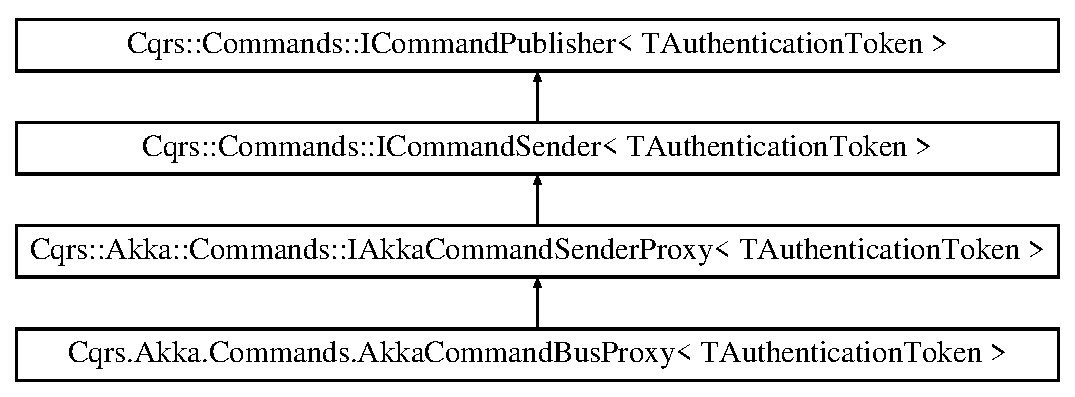
\includegraphics[height=3.000000cm]{classCqrs_1_1Akka_1_1Commands_1_1AkkaCommandBusProxy}
\end{center}
\end{figure}
\doxysubsection*{Classes}
\begin{DoxyCompactItemize}
\item 
class \mbox{\hyperlink{classCqrs_1_1Akka_1_1Commands_1_1AkkaCommandBusProxy_1_1BusActor}{Bus\+Actor}}
\begin{DoxyCompactList}\small\item\em Similar to a I\+Command\+Publisher$<$\+T\+Authentication\+Token$>$, passes commands onto the \mbox{\hyperlink{classCqrs_1_1Akka_1_1Commands_1_1AkkaCommandBusProxy_1_1BusActor_a097e43f25d55e632c2c5da9d0255d180_a097e43f25d55e632c2c5da9d0255d180}{Command\+Handler\+Resolver}}. \end{DoxyCompactList}\end{DoxyCompactItemize}
\doxysubsection*{Public Member Functions}
\begin{DoxyCompactItemize}
\item 
\mbox{\hyperlink{classCqrs_1_1Akka_1_1Commands_1_1AkkaCommandBusProxy_ad9a3fa7aa546bc2c398d4f52d0659656_ad9a3fa7aa546bc2c398d4f52d0659656}{Akka\+Command\+Bus\+Proxy}} (\mbox{\hyperlink{interfaceCqrs_1_1Configuration_1_1IDependencyResolver}{I\+Dependency\+Resolver}} dependency\+Resolver, I\+Correlation\+Id\+Helper correlation\+Id\+Helper, \mbox{\hyperlink{interfaceCqrs_1_1Authentication_1_1IAuthenticationTokenHelper}{I\+Authentication\+Token\+Helper}}$<$ T\+Authentication\+Token $>$ authentication\+Token\+Helper)
\begin{DoxyCompactList}\small\item\em Instantiates a new instance of \mbox{\hyperlink{classCqrs_1_1Akka_1_1Commands_1_1AkkaCommandBusProxy_ad9a3fa7aa546bc2c398d4f52d0659656_ad9a3fa7aa546bc2c398d4f52d0659656}{Akka\+Command\+Bus\+Proxy$<$\+T\+Authentication\+Token$>$}}. \end{DoxyCompactList}\item 
virtual void \mbox{\hyperlink{classCqrs_1_1Akka_1_1Commands_1_1AkkaCommandBusProxy_a410c0fe52016d04de950b1ae767d2ccb_a410c0fe52016d04de950b1ae767d2ccb}{Publish$<$ T\+Command $>$}} (T\+Command command)
\begin{DoxyCompactList}\small\item\em Publishes the provided {\itshape command}  on the command bus. \end{DoxyCompactList}\item 
virtual void \mbox{\hyperlink{classCqrs_1_1Akka_1_1Commands_1_1AkkaCommandBusProxy_a81dc8162ca933d84b6aee04aff589010_a81dc8162ca933d84b6aee04aff589010}{Publish$<$ T\+Command $>$}} (I\+Enumerable$<$ T\+Command $>$ commands)
\begin{DoxyCompactList}\small\item\em Publishes the provided {\itshape commands}  on the command bus. \end{DoxyCompactList}\end{DoxyCompactItemize}
\doxysubsection*{Properties}
\begin{DoxyCompactItemize}
\item 
I\+Actor\+Ref \mbox{\hyperlink{classCqrs_1_1Akka_1_1Commands_1_1AkkaCommandBusProxy_afab0340ffb172da48584dce148f3defd_afab0340ffb172da48584dce148f3defd}{Command\+Handler\+Resolver}}\hspace{0.3cm}{\ttfamily  \mbox{[}get\mbox{]}}
\begin{DoxyCompactList}\small\item\em Gets the \mbox{\hyperlink{}{command handler resolver}} that we send/proxy the command to. \end{DoxyCompactList}\item 
I\+Correlation\+Id\+Helper \mbox{\hyperlink{classCqrs_1_1Akka_1_1Commands_1_1AkkaCommandBusProxy_aa554035c12060c7eedb0b982ac490da8_aa554035c12060c7eedb0b982ac490da8}{Correlation\+Id\+Helper}}\hspace{0.3cm}{\ttfamily  \mbox{[}get\mbox{]}}
\begin{DoxyCompactList}\small\item\em Gets or sets the I\+Correlation\+Id\+Helper. \end{DoxyCompactList}\item 
\mbox{\hyperlink{interfaceCqrs_1_1Authentication_1_1IAuthenticationTokenHelper}{I\+Authentication\+Token\+Helper}}$<$ T\+Authentication\+Token $>$ \mbox{\hyperlink{classCqrs_1_1Akka_1_1Commands_1_1AkkaCommandBusProxy_a6faae6227f1da33928e54a775466f9c9_a6faae6227f1da33928e54a775466f9c9}{Authentication\+Token\+Helper}}\hspace{0.3cm}{\ttfamily  \mbox{[}get\mbox{]}}
\begin{DoxyCompactList}\small\item\em Gets or sets the \mbox{\hyperlink{}{Authentication Token Helper}}. \end{DoxyCompactList}\end{DoxyCompactItemize}


\doxysubsection{Detailed Description}
A I\+Command\+Publisher$<$\+T\+Authentication\+Token$>$ that proxies I\+Command$<$\+T\+Authentication\+Token$>$ to the I\+Actor\+Ref which acts as a single point of all handler resolutions. 


\begin{DoxyTemplParams}{Template Parameters}
{\em T\+Authentication\+Token} & The Type of the authentication token.\\
\hline
\end{DoxyTemplParams}


\doxysubsection{Constructor \& Destructor Documentation}
\mbox{\Hypertarget{classCqrs_1_1Akka_1_1Commands_1_1AkkaCommandBusProxy_ad9a3fa7aa546bc2c398d4f52d0659656_ad9a3fa7aa546bc2c398d4f52d0659656}\label{classCqrs_1_1Akka_1_1Commands_1_1AkkaCommandBusProxy_ad9a3fa7aa546bc2c398d4f52d0659656_ad9a3fa7aa546bc2c398d4f52d0659656}} 
\index{Cqrs.Akka.Commands.AkkaCommandBusProxy$<$ TAuthenticationToken $>$@{Cqrs.Akka.Commands.AkkaCommandBusProxy$<$ TAuthenticationToken $>$}!AkkaCommandBusProxy@{AkkaCommandBusProxy}}
\index{AkkaCommandBusProxy@{AkkaCommandBusProxy}!Cqrs.Akka.Commands.AkkaCommandBusProxy$<$ TAuthenticationToken $>$@{Cqrs.Akka.Commands.AkkaCommandBusProxy$<$ TAuthenticationToken $>$}}
\doxysubsubsection{\texorpdfstring{AkkaCommandBusProxy()}{AkkaCommandBusProxy()}}
{\footnotesize\ttfamily \mbox{\hyperlink{classCqrs_1_1Akka_1_1Commands_1_1AkkaCommandBusProxy}{Cqrs.\+Akka.\+Commands.\+Akka\+Command\+Bus\+Proxy}}$<$ T\+Authentication\+Token $>$.\mbox{\hyperlink{classCqrs_1_1Akka_1_1Commands_1_1AkkaCommandBusProxy}{Akka\+Command\+Bus\+Proxy}} (\begin{DoxyParamCaption}\item[{\mbox{\hyperlink{interfaceCqrs_1_1Configuration_1_1IDependencyResolver}{I\+Dependency\+Resolver}}}]{dependency\+Resolver,  }\item[{I\+Correlation\+Id\+Helper}]{correlation\+Id\+Helper,  }\item[{\mbox{\hyperlink{interfaceCqrs_1_1Authentication_1_1IAuthenticationTokenHelper}{I\+Authentication\+Token\+Helper}}$<$ T\+Authentication\+Token $>$}]{authentication\+Token\+Helper }\end{DoxyParamCaption})}



Instantiates a new instance of \mbox{\hyperlink{classCqrs_1_1Akka_1_1Commands_1_1AkkaCommandBusProxy_ad9a3fa7aa546bc2c398d4f52d0659656_ad9a3fa7aa546bc2c398d4f52d0659656}{Akka\+Command\+Bus\+Proxy$<$\+T\+Authentication\+Token$>$}}. 



\doxysubsection{Member Function Documentation}
\mbox{\Hypertarget{classCqrs_1_1Akka_1_1Commands_1_1AkkaCommandBusProxy_a81dc8162ca933d84b6aee04aff589010_a81dc8162ca933d84b6aee04aff589010}\label{classCqrs_1_1Akka_1_1Commands_1_1AkkaCommandBusProxy_a81dc8162ca933d84b6aee04aff589010_a81dc8162ca933d84b6aee04aff589010}} 
\index{Cqrs.Akka.Commands.AkkaCommandBusProxy$<$ TAuthenticationToken $>$@{Cqrs.Akka.Commands.AkkaCommandBusProxy$<$ TAuthenticationToken $>$}!Publish$<$ TCommand $>$@{Publish$<$ TCommand $>$}}
\index{Publish$<$ TCommand $>$@{Publish$<$ TCommand $>$}!Cqrs.Akka.Commands.AkkaCommandBusProxy$<$ TAuthenticationToken $>$@{Cqrs.Akka.Commands.AkkaCommandBusProxy$<$ TAuthenticationToken $>$}}
\doxysubsubsection{\texorpdfstring{Publish$<$ TCommand $>$()}{Publish< TCommand >()}\hspace{0.1cm}{\footnotesize\ttfamily [1/2]}}
{\footnotesize\ttfamily virtual void \mbox{\hyperlink{classCqrs_1_1Akka_1_1Commands_1_1AkkaCommandBusProxy}{Cqrs.\+Akka.\+Commands.\+Akka\+Command\+Bus\+Proxy}}$<$ T\+Authentication\+Token $>$.Publish$<$ T\+Command $>$ (\begin{DoxyParamCaption}\item[{I\+Enumerable$<$ T\+Command $>$}]{commands }\end{DoxyParamCaption})\hspace{0.3cm}{\ttfamily [virtual]}}



Publishes the provided {\itshape commands}  on the command bus. 



Implements \mbox{\hyperlink{interfaceCqrs_1_1Commands_1_1ICommandPublisher_af0f033c0b949e5650032e4f00b11b595_af0f033c0b949e5650032e4f00b11b595}{Cqrs.\+Commands.\+I\+Command\+Publisher$<$ T\+Authentication\+Token $>$}}.

\begin{Desc}
\item[Type Constraints]\begin{description}
\item[{\em T\+Command} : {\em I\+Command$<$T\+Authentication\+Token$>$}]\end{description}
\end{Desc}
\mbox{\Hypertarget{classCqrs_1_1Akka_1_1Commands_1_1AkkaCommandBusProxy_a410c0fe52016d04de950b1ae767d2ccb_a410c0fe52016d04de950b1ae767d2ccb}\label{classCqrs_1_1Akka_1_1Commands_1_1AkkaCommandBusProxy_a410c0fe52016d04de950b1ae767d2ccb_a410c0fe52016d04de950b1ae767d2ccb}} 
\index{Cqrs.Akka.Commands.AkkaCommandBusProxy$<$ TAuthenticationToken $>$@{Cqrs.Akka.Commands.AkkaCommandBusProxy$<$ TAuthenticationToken $>$}!Publish$<$ TCommand $>$@{Publish$<$ TCommand $>$}}
\index{Publish$<$ TCommand $>$@{Publish$<$ TCommand $>$}!Cqrs.Akka.Commands.AkkaCommandBusProxy$<$ TAuthenticationToken $>$@{Cqrs.Akka.Commands.AkkaCommandBusProxy$<$ TAuthenticationToken $>$}}
\doxysubsubsection{\texorpdfstring{Publish$<$ TCommand $>$()}{Publish< TCommand >()}\hspace{0.1cm}{\footnotesize\ttfamily [2/2]}}
{\footnotesize\ttfamily virtual void \mbox{\hyperlink{classCqrs_1_1Akka_1_1Commands_1_1AkkaCommandBusProxy}{Cqrs.\+Akka.\+Commands.\+Akka\+Command\+Bus\+Proxy}}$<$ T\+Authentication\+Token $>$.Publish$<$ T\+Command $>$ (\begin{DoxyParamCaption}\item[{T\+Command}]{command }\end{DoxyParamCaption})\hspace{0.3cm}{\ttfamily [virtual]}}



Publishes the provided {\itshape command}  on the command bus. 



Implements \mbox{\hyperlink{interfaceCqrs_1_1Commands_1_1ICommandPublisher_aeeb487ad5686d9c44d214b1daaf7833a_aeeb487ad5686d9c44d214b1daaf7833a}{Cqrs.\+Commands.\+I\+Command\+Publisher$<$ T\+Authentication\+Token $>$}}.

\begin{Desc}
\item[Type Constraints]\begin{description}
\item[{\em T\+Command} : {\em I\+Command$<$T\+Authentication\+Token$>$}]\end{description}
\end{Desc}


\doxysubsection{Property Documentation}
\mbox{\Hypertarget{classCqrs_1_1Akka_1_1Commands_1_1AkkaCommandBusProxy_a6faae6227f1da33928e54a775466f9c9_a6faae6227f1da33928e54a775466f9c9}\label{classCqrs_1_1Akka_1_1Commands_1_1AkkaCommandBusProxy_a6faae6227f1da33928e54a775466f9c9_a6faae6227f1da33928e54a775466f9c9}} 
\index{Cqrs.Akka.Commands.AkkaCommandBusProxy$<$ TAuthenticationToken $>$@{Cqrs.Akka.Commands.AkkaCommandBusProxy$<$ TAuthenticationToken $>$}!AuthenticationTokenHelper@{AuthenticationTokenHelper}}
\index{AuthenticationTokenHelper@{AuthenticationTokenHelper}!Cqrs.Akka.Commands.AkkaCommandBusProxy$<$ TAuthenticationToken $>$@{Cqrs.Akka.Commands.AkkaCommandBusProxy$<$ TAuthenticationToken $>$}}
\doxysubsubsection{\texorpdfstring{AuthenticationTokenHelper}{AuthenticationTokenHelper}}
{\footnotesize\ttfamily \mbox{\hyperlink{interfaceCqrs_1_1Authentication_1_1IAuthenticationTokenHelper}{I\+Authentication\+Token\+Helper}}$<$T\+Authentication\+Token$>$ \mbox{\hyperlink{classCqrs_1_1Akka_1_1Commands_1_1AkkaCommandBusProxy}{Cqrs.\+Akka.\+Commands.\+Akka\+Command\+Bus\+Proxy}}$<$ T\+Authentication\+Token $>$.\mbox{\hyperlink{classCqrs_1_1Authentication_1_1AuthenticationTokenHelper}{Authentication\+Token\+Helper}}\hspace{0.3cm}{\ttfamily [get]}, {\ttfamily [protected]}}



Gets or sets the \mbox{\hyperlink{}{Authentication Token Helper}}. 

\mbox{\Hypertarget{classCqrs_1_1Akka_1_1Commands_1_1AkkaCommandBusProxy_afab0340ffb172da48584dce148f3defd_afab0340ffb172da48584dce148f3defd}\label{classCqrs_1_1Akka_1_1Commands_1_1AkkaCommandBusProxy_afab0340ffb172da48584dce148f3defd_afab0340ffb172da48584dce148f3defd}} 
\index{Cqrs.Akka.Commands.AkkaCommandBusProxy$<$ TAuthenticationToken $>$@{Cqrs.Akka.Commands.AkkaCommandBusProxy$<$ TAuthenticationToken $>$}!CommandHandlerResolver@{CommandHandlerResolver}}
\index{CommandHandlerResolver@{CommandHandlerResolver}!Cqrs.Akka.Commands.AkkaCommandBusProxy$<$ TAuthenticationToken $>$@{Cqrs.Akka.Commands.AkkaCommandBusProxy$<$ TAuthenticationToken $>$}}
\doxysubsubsection{\texorpdfstring{CommandHandlerResolver}{CommandHandlerResolver}}
{\footnotesize\ttfamily I\+Actor\+Ref \mbox{\hyperlink{classCqrs_1_1Akka_1_1Commands_1_1AkkaCommandBusProxy}{Cqrs.\+Akka.\+Commands.\+Akka\+Command\+Bus\+Proxy}}$<$ T\+Authentication\+Token $>$.Command\+Handler\+Resolver\hspace{0.3cm}{\ttfamily [get]}, {\ttfamily [protected]}}



Gets the \mbox{\hyperlink{}{command handler resolver}} that we send/proxy the command to. 

\mbox{\Hypertarget{classCqrs_1_1Akka_1_1Commands_1_1AkkaCommandBusProxy_aa554035c12060c7eedb0b982ac490da8_aa554035c12060c7eedb0b982ac490da8}\label{classCqrs_1_1Akka_1_1Commands_1_1AkkaCommandBusProxy_aa554035c12060c7eedb0b982ac490da8_aa554035c12060c7eedb0b982ac490da8}} 
\index{Cqrs.Akka.Commands.AkkaCommandBusProxy$<$ TAuthenticationToken $>$@{Cqrs.Akka.Commands.AkkaCommandBusProxy$<$ TAuthenticationToken $>$}!CorrelationIdHelper@{CorrelationIdHelper}}
\index{CorrelationIdHelper@{CorrelationIdHelper}!Cqrs.Akka.Commands.AkkaCommandBusProxy$<$ TAuthenticationToken $>$@{Cqrs.Akka.Commands.AkkaCommandBusProxy$<$ TAuthenticationToken $>$}}
\doxysubsubsection{\texorpdfstring{CorrelationIdHelper}{CorrelationIdHelper}}
{\footnotesize\ttfamily I\+Correlation\+Id\+Helper \mbox{\hyperlink{classCqrs_1_1Akka_1_1Commands_1_1AkkaCommandBusProxy}{Cqrs.\+Akka.\+Commands.\+Akka\+Command\+Bus\+Proxy}}$<$ T\+Authentication\+Token $>$.Correlation\+Id\+Helper\hspace{0.3cm}{\ttfamily [get]}, {\ttfamily [protected]}}



Gets or sets the I\+Correlation\+Id\+Helper. 


\hypertarget{classCqrs_1_1Akka_1_1Commands_1_1AkkaCommandBusProxy_1_1BusActor}{}\section{Cqrs.\+Akka.\+Commands.\+Akka\+Command\+Bus\+Proxy$<$ T\+Authentication\+Token $>$.Bus\+Actor Class Reference}
\label{classCqrs_1_1Akka_1_1Commands_1_1AkkaCommandBusProxy_1_1BusActor}\index{Cqrs.\+Akka.\+Commands.\+Akka\+Command\+Bus\+Proxy$<$ T\+Authentication\+Token $>$.\+Bus\+Actor@{Cqrs.\+Akka.\+Commands.\+Akka\+Command\+Bus\+Proxy$<$ T\+Authentication\+Token $>$.\+Bus\+Actor}}


Similar to a I\+Command\+Publisher$<$\+T\+Authentication\+Token$>$, passes commands onto the \hyperlink{classCqrs_1_1Akka_1_1Commands_1_1AkkaCommandBusProxy_1_1BusActor_a097e43f25d55e632c2c5da9d0255d180_a097e43f25d55e632c2c5da9d0255d180}{Command\+Handler\+Resolver}.  


Inheritance diagram for Cqrs.\+Akka.\+Commands.\+Akka\+Command\+Bus\+Proxy$<$ T\+Authentication\+Token $>$.Bus\+Actor\+:\begin{figure}[H]
\begin{center}
\leavevmode
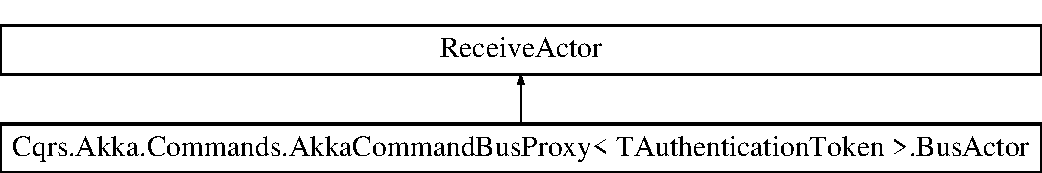
\includegraphics[height=2.000000cm]{classCqrs_1_1Akka_1_1Commands_1_1AkkaCommandBusProxy_1_1BusActor}
\end{center}
\end{figure}
\subsection*{Public Member Functions}
\begin{DoxyCompactItemize}
\item 
\hyperlink{classCqrs_1_1Akka_1_1Commands_1_1AkkaCommandBusProxy_1_1BusActor_a5ddecec1b6333aaf89dbff824cf6ddd2_a5ddecec1b6333aaf89dbff824cf6ddd2}{Bus\+Actor} (\hyperlink{interfaceCqrs_1_1Akka_1_1Commands_1_1IAkkaCommandPublisher}{I\+Akka\+Command\+Publisher}$<$ T\+Authentication\+Token $>$ command\+Handler\+Resolver, I\+Correlation\+Id\+Helper correlation\+Id\+Helper, \hyperlink{interfaceCqrs_1_1Authentication_1_1IAuthenticationTokenHelper}{I\+Authentication\+Token\+Helper}$<$ T\+Authentication\+Token $>$ authentication\+Token\+Helper)
\begin{DoxyCompactList}\small\item\em Instantiates a new instance of \hyperlink{classCqrs_1_1Akka_1_1Commands_1_1AkkaCommandBusProxy_1_1BusActor}{Bus\+Actor}. \end{DoxyCompactList}\end{DoxyCompactItemize}
\subsection*{Protected Member Functions}
\begin{DoxyCompactItemize}
\item 
virtual void \hyperlink{classCqrs_1_1Akka_1_1Commands_1_1AkkaCommandBusProxy_1_1BusActor_a2218f176012e4074308d8de36f1f48a2_a2218f176012e4074308d8de36f1f48a2}{Execute\+Receive} (\hyperlink{interfaceCqrs_1_1Commands_1_1ICommand}{I\+Command}$<$ T\+Authentication\+Token $>$ command)
\begin{DoxyCompactList}\small\item\em Passes the provided {\itshape command}  to \hyperlink{classCqrs_1_1Akka_1_1Commands_1_1AkkaCommandBusProxy_1_1BusActor_a097e43f25d55e632c2c5da9d0255d180_a097e43f25d55e632c2c5da9d0255d180}{Command\+Handler\+Resolver} via I\+Command\+Publisher$<$\+T\+Authentication\+Token$>$.\+Publish$<$\+T\+Command$>$(\+T\+Command) then calls Actor\+Ref\+Implicit\+Sender\+Extensions.\+Tell. \end{DoxyCompactList}\end{DoxyCompactItemize}
\subsection*{Properties}
\begin{DoxyCompactItemize}
\item 
\hyperlink{interfaceCqrs_1_1Akka_1_1Commands_1_1IAkkaCommandPublisher}{I\+Akka\+Command\+Publisher}$<$ T\+Authentication\+Token $>$ \hyperlink{classCqrs_1_1Akka_1_1Commands_1_1AkkaCommandBusProxy_1_1BusActor_a097e43f25d55e632c2c5da9d0255d180_a097e43f25d55e632c2c5da9d0255d180}{Command\+Handler\+Resolver}\hspace{0.3cm}{\ttfamily  \mbox{[}get\mbox{]}}
\begin{DoxyCompactList}\small\item\em Gets or sets the I\+Akka\+Command\+Publisher$<$\+T\+Authentication\+Token$>$. \end{DoxyCompactList}\item 
I\+Correlation\+Id\+Helper \hyperlink{classCqrs_1_1Akka_1_1Commands_1_1AkkaCommandBusProxy_1_1BusActor_ab353a9b434004f9b0637dd5dbe4402ac_ab353a9b434004f9b0637dd5dbe4402ac}{Correlation\+Id\+Helper}\hspace{0.3cm}{\ttfamily  \mbox{[}get\mbox{]}}
\begin{DoxyCompactList}\small\item\em Gets or sets the I\+Correlation\+Id\+Helper. \end{DoxyCompactList}\item 
\hyperlink{interfaceCqrs_1_1Authentication_1_1IAuthenticationTokenHelper}{I\+Authentication\+Token\+Helper}$<$ T\+Authentication\+Token $>$ \hyperlink{classCqrs_1_1Akka_1_1Commands_1_1AkkaCommandBusProxy_1_1BusActor_a10dd32ee768f6ccf93aa0e04472c84b6_a10dd32ee768f6ccf93aa0e04472c84b6}{Authentication\+Token\+Helper}\hspace{0.3cm}{\ttfamily  \mbox{[}get\mbox{]}}
\begin{DoxyCompactList}\small\item\em Gets or sets the I\+Authentication\+Token\+Helper$<$\+T\+Authentication\+Token$>$. \end{DoxyCompactList}\end{DoxyCompactItemize}


\subsection{Detailed Description}
Similar to a I\+Command\+Publisher$<$\+T\+Authentication\+Token$>$, passes commands onto the \hyperlink{classCqrs_1_1Akka_1_1Commands_1_1AkkaCommandBusProxy_1_1BusActor_a097e43f25d55e632c2c5da9d0255d180_a097e43f25d55e632c2c5da9d0255d180}{Command\+Handler\+Resolver}. 



\subsection{Constructor \& Destructor Documentation}
\mbox{\Hypertarget{classCqrs_1_1Akka_1_1Commands_1_1AkkaCommandBusProxy_1_1BusActor_a5ddecec1b6333aaf89dbff824cf6ddd2_a5ddecec1b6333aaf89dbff824cf6ddd2}\label{classCqrs_1_1Akka_1_1Commands_1_1AkkaCommandBusProxy_1_1BusActor_a5ddecec1b6333aaf89dbff824cf6ddd2_a5ddecec1b6333aaf89dbff824cf6ddd2}} 
\index{Cqrs\+::\+Akka\+::\+Commands\+::\+Akka\+Command\+Bus\+Proxy\+::\+Bus\+Actor@{Cqrs\+::\+Akka\+::\+Commands\+::\+Akka\+Command\+Bus\+Proxy\+::\+Bus\+Actor}!Bus\+Actor@{Bus\+Actor}}
\index{Bus\+Actor@{Bus\+Actor}!Cqrs\+::\+Akka\+::\+Commands\+::\+Akka\+Command\+Bus\+Proxy\+::\+Bus\+Actor@{Cqrs\+::\+Akka\+::\+Commands\+::\+Akka\+Command\+Bus\+Proxy\+::\+Bus\+Actor}}
\subsubsection{\texorpdfstring{Bus\+Actor()}{BusActor()}}
{\footnotesize\ttfamily \hyperlink{classCqrs_1_1Akka_1_1Commands_1_1AkkaCommandBusProxy}{Cqrs.\+Akka.\+Commands.\+Akka\+Command\+Bus\+Proxy}$<$ T\+Authentication\+Token $>$.Bus\+Actor.\+Bus\+Actor (\begin{DoxyParamCaption}\item[{\hyperlink{interfaceCqrs_1_1Akka_1_1Commands_1_1IAkkaCommandPublisher}{I\+Akka\+Command\+Publisher}$<$ T\+Authentication\+Token $>$}]{command\+Handler\+Resolver,  }\item[{I\+Correlation\+Id\+Helper}]{correlation\+Id\+Helper,  }\item[{\hyperlink{interfaceCqrs_1_1Authentication_1_1IAuthenticationTokenHelper}{I\+Authentication\+Token\+Helper}$<$ T\+Authentication\+Token $>$}]{authentication\+Token\+Helper }\end{DoxyParamCaption})}



Instantiates a new instance of \hyperlink{classCqrs_1_1Akka_1_1Commands_1_1AkkaCommandBusProxy_1_1BusActor}{Bus\+Actor}. 



\subsection{Member Function Documentation}
\mbox{\Hypertarget{classCqrs_1_1Akka_1_1Commands_1_1AkkaCommandBusProxy_1_1BusActor_a2218f176012e4074308d8de36f1f48a2_a2218f176012e4074308d8de36f1f48a2}\label{classCqrs_1_1Akka_1_1Commands_1_1AkkaCommandBusProxy_1_1BusActor_a2218f176012e4074308d8de36f1f48a2_a2218f176012e4074308d8de36f1f48a2}} 
\index{Cqrs\+::\+Akka\+::\+Commands\+::\+Akka\+Command\+Bus\+Proxy\+::\+Bus\+Actor@{Cqrs\+::\+Akka\+::\+Commands\+::\+Akka\+Command\+Bus\+Proxy\+::\+Bus\+Actor}!Execute\+Receive@{Execute\+Receive}}
\index{Execute\+Receive@{Execute\+Receive}!Cqrs\+::\+Akka\+::\+Commands\+::\+Akka\+Command\+Bus\+Proxy\+::\+Bus\+Actor@{Cqrs\+::\+Akka\+::\+Commands\+::\+Akka\+Command\+Bus\+Proxy\+::\+Bus\+Actor}}
\subsubsection{\texorpdfstring{Execute\+Receive()}{ExecuteReceive()}}
{\footnotesize\ttfamily virtual void \hyperlink{classCqrs_1_1Akka_1_1Commands_1_1AkkaCommandBusProxy}{Cqrs.\+Akka.\+Commands.\+Akka\+Command\+Bus\+Proxy}$<$ T\+Authentication\+Token $>$.Bus\+Actor.\+Execute\+Receive (\begin{DoxyParamCaption}\item[{\hyperlink{interfaceCqrs_1_1Commands_1_1ICommand}{I\+Command}$<$ T\+Authentication\+Token $>$}]{command }\end{DoxyParamCaption})\hspace{0.3cm}{\ttfamily [protected]}, {\ttfamily [virtual]}}



Passes the provided {\itshape command}  to \hyperlink{classCqrs_1_1Akka_1_1Commands_1_1AkkaCommandBusProxy_1_1BusActor_a097e43f25d55e632c2c5da9d0255d180_a097e43f25d55e632c2c5da9d0255d180}{Command\+Handler\+Resolver} via I\+Command\+Publisher$<$\+T\+Authentication\+Token$>$.\+Publish$<$\+T\+Command$>$(\+T\+Command) then calls Actor\+Ref\+Implicit\+Sender\+Extensions.\+Tell. 



\subsection{Property Documentation}
\mbox{\Hypertarget{classCqrs_1_1Akka_1_1Commands_1_1AkkaCommandBusProxy_1_1BusActor_a10dd32ee768f6ccf93aa0e04472c84b6_a10dd32ee768f6ccf93aa0e04472c84b6}\label{classCqrs_1_1Akka_1_1Commands_1_1AkkaCommandBusProxy_1_1BusActor_a10dd32ee768f6ccf93aa0e04472c84b6_a10dd32ee768f6ccf93aa0e04472c84b6}} 
\index{Cqrs\+::\+Akka\+::\+Commands\+::\+Akka\+Command\+Bus\+Proxy\+::\+Bus\+Actor@{Cqrs\+::\+Akka\+::\+Commands\+::\+Akka\+Command\+Bus\+Proxy\+::\+Bus\+Actor}!Authentication\+Token\+Helper@{Authentication\+Token\+Helper}}
\index{Authentication\+Token\+Helper@{Authentication\+Token\+Helper}!Cqrs\+::\+Akka\+::\+Commands\+::\+Akka\+Command\+Bus\+Proxy\+::\+Bus\+Actor@{Cqrs\+::\+Akka\+::\+Commands\+::\+Akka\+Command\+Bus\+Proxy\+::\+Bus\+Actor}}
\subsubsection{\texorpdfstring{Authentication\+Token\+Helper}{AuthenticationTokenHelper}}
{\footnotesize\ttfamily \hyperlink{interfaceCqrs_1_1Authentication_1_1IAuthenticationTokenHelper}{I\+Authentication\+Token\+Helper}$<$T\+Authentication\+Token$>$ \hyperlink{classCqrs_1_1Akka_1_1Commands_1_1AkkaCommandBusProxy}{Cqrs.\+Akka.\+Commands.\+Akka\+Command\+Bus\+Proxy}$<$ T\+Authentication\+Token $>$.Bus\+Actor.\+Authentication\+Token\+Helper\hspace{0.3cm}{\ttfamily [get]}, {\ttfamily [protected]}}



Gets or sets the I\+Authentication\+Token\+Helper$<$\+T\+Authentication\+Token$>$. 

\mbox{\Hypertarget{classCqrs_1_1Akka_1_1Commands_1_1AkkaCommandBusProxy_1_1BusActor_a097e43f25d55e632c2c5da9d0255d180_a097e43f25d55e632c2c5da9d0255d180}\label{classCqrs_1_1Akka_1_1Commands_1_1AkkaCommandBusProxy_1_1BusActor_a097e43f25d55e632c2c5da9d0255d180_a097e43f25d55e632c2c5da9d0255d180}} 
\index{Cqrs\+::\+Akka\+::\+Commands\+::\+Akka\+Command\+Bus\+Proxy\+::\+Bus\+Actor@{Cqrs\+::\+Akka\+::\+Commands\+::\+Akka\+Command\+Bus\+Proxy\+::\+Bus\+Actor}!Command\+Handler\+Resolver@{Command\+Handler\+Resolver}}
\index{Command\+Handler\+Resolver@{Command\+Handler\+Resolver}!Cqrs\+::\+Akka\+::\+Commands\+::\+Akka\+Command\+Bus\+Proxy\+::\+Bus\+Actor@{Cqrs\+::\+Akka\+::\+Commands\+::\+Akka\+Command\+Bus\+Proxy\+::\+Bus\+Actor}}
\subsubsection{\texorpdfstring{Command\+Handler\+Resolver}{CommandHandlerResolver}}
{\footnotesize\ttfamily \hyperlink{interfaceCqrs_1_1Akka_1_1Commands_1_1IAkkaCommandPublisher}{I\+Akka\+Command\+Publisher}$<$T\+Authentication\+Token$>$ \hyperlink{classCqrs_1_1Akka_1_1Commands_1_1AkkaCommandBusProxy}{Cqrs.\+Akka.\+Commands.\+Akka\+Command\+Bus\+Proxy}$<$ T\+Authentication\+Token $>$.Bus\+Actor.\+Command\+Handler\+Resolver\hspace{0.3cm}{\ttfamily [get]}, {\ttfamily [protected]}}



Gets or sets the I\+Akka\+Command\+Publisher$<$\+T\+Authentication\+Token$>$. 

\mbox{\Hypertarget{classCqrs_1_1Akka_1_1Commands_1_1AkkaCommandBusProxy_1_1BusActor_ab353a9b434004f9b0637dd5dbe4402ac_ab353a9b434004f9b0637dd5dbe4402ac}\label{classCqrs_1_1Akka_1_1Commands_1_1AkkaCommandBusProxy_1_1BusActor_ab353a9b434004f9b0637dd5dbe4402ac_ab353a9b434004f9b0637dd5dbe4402ac}} 
\index{Cqrs\+::\+Akka\+::\+Commands\+::\+Akka\+Command\+Bus\+Proxy\+::\+Bus\+Actor@{Cqrs\+::\+Akka\+::\+Commands\+::\+Akka\+Command\+Bus\+Proxy\+::\+Bus\+Actor}!Correlation\+Id\+Helper@{Correlation\+Id\+Helper}}
\index{Correlation\+Id\+Helper@{Correlation\+Id\+Helper}!Cqrs\+::\+Akka\+::\+Commands\+::\+Akka\+Command\+Bus\+Proxy\+::\+Bus\+Actor@{Cqrs\+::\+Akka\+::\+Commands\+::\+Akka\+Command\+Bus\+Proxy\+::\+Bus\+Actor}}
\subsubsection{\texorpdfstring{Correlation\+Id\+Helper}{CorrelationIdHelper}}
{\footnotesize\ttfamily I\+Correlation\+Id\+Helper \hyperlink{classCqrs_1_1Akka_1_1Commands_1_1AkkaCommandBusProxy}{Cqrs.\+Akka.\+Commands.\+Akka\+Command\+Bus\+Proxy}$<$ T\+Authentication\+Token $>$.Bus\+Actor.\+Correlation\+Id\+Helper\hspace{0.3cm}{\ttfamily [get]}, {\ttfamily [protected]}}



Gets or sets the I\+Correlation\+Id\+Helper. 


\hypertarget{classCqrs_1_1Akka_1_1Commands_1_1ConcurrentAkkaCommandSender}{}\section{Cqrs.\+Akka.\+Commands.\+Concurrent\+Akka\+Command\+Sender$<$ T\+Authentication\+Token, T\+Target $>$ Class Template Reference}
\label{classCqrs_1_1Akka_1_1Commands_1_1ConcurrentAkkaCommandSender}\index{Cqrs.\+Akka.\+Commands.\+Concurrent\+Akka\+Command\+Sender$<$ T\+Authentication\+Token, T\+Target $>$@{Cqrs.\+Akka.\+Commands.\+Concurrent\+Akka\+Command\+Sender$<$ T\+Authentication\+Token, T\+Target $>$}}
Inheritance diagram for Cqrs.\+Akka.\+Commands.\+Concurrent\+Akka\+Command\+Sender$<$ T\+Authentication\+Token, T\+Target $>$\+:\begin{figure}[H]
\begin{center}
\leavevmode
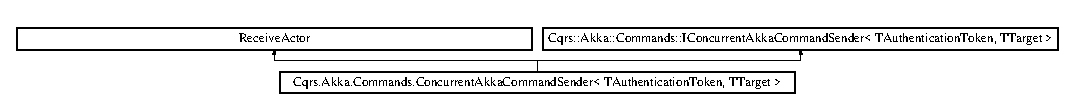
\includegraphics[height=1.035120cm]{classCqrs_1_1Akka_1_1Commands_1_1ConcurrentAkkaCommandSender}
\end{center}
\end{figure}
\subsection*{Public Member Functions}
\begin{DoxyCompactItemize}
\item 
\hyperlink{classCqrs_1_1Akka_1_1Commands_1_1ConcurrentAkkaCommandSender_a203cd12567f100fb3545b029f6ed0181_a203cd12567f100fb3545b029f6ed0181}{Concurrent\+Akka\+Command\+Sender} (I\+Actor\+Ref actor\+Reference, \hyperlink{interfaceCqrs_1_1Commands_1_1ICommandReceiver}{I\+Command\+Receiver}$<$ T\+Authentication\+Token $>$ command\+Receiver)
\item 
void \hyperlink{classCqrs_1_1Akka_1_1Commands_1_1ConcurrentAkkaCommandSender_a5f65348c92377342ad8400eb6b40a2ac_a5f65348c92377342ad8400eb6b40a2ac}{Publish$<$ T\+Command $>$} (T\+Command command)
\item 
void \hyperlink{classCqrs_1_1Akka_1_1Commands_1_1ConcurrentAkkaCommandSender_a46b88bf730db4a530586737d699e1f12_a46b88bf730db4a530586737d699e1f12}{Send$<$ T\+Command $>$} (T\+Command command)
\item 
void \hyperlink{classCqrs_1_1Akka_1_1Commands_1_1ConcurrentAkkaCommandSender_a6505fbb31a885de31e68b2b87e969c31_a6505fbb31a885de31e68b2b87e969c31}{Publish$<$ T\+Command $>$} (I\+Enumerable$<$ T\+Command $>$ commands)
\item 
void \hyperlink{classCqrs_1_1Akka_1_1Commands_1_1ConcurrentAkkaCommandSender_a263a720c8c865bc246756307c0004aa6_a263a720c8c865bc246756307c0004aa6}{Send$<$ T\+Command $>$} (I\+Enumerable$<$ T\+Command $>$ commands)
\item 
virtual T\+Event \hyperlink{classCqrs_1_1Akka_1_1Commands_1_1ConcurrentAkkaCommandSender_a655aa63a47944035c113f9668bcf1284_a655aa63a47944035c113f9668bcf1284}{Send\+And\+Wait$<$ T\+Command, T\+Event $>$} (T\+Command command, \hyperlink{interfaceCqrs_1_1Events_1_1IEventReceiver}{I\+Event\+Receiver}$<$ T\+Authentication\+Token $>$ event\+Receiver=null)
\begin{DoxyCompactList}\small\item\em Sends the provided {\itshape command}  and waits for an event of {\itshape T\+Event}  \end{DoxyCompactList}\item 
T\+Event \hyperlink{classCqrs_1_1Akka_1_1Commands_1_1ConcurrentAkkaCommandSender_a171974eb1ba3eb7be9816bd7927227ac_a171974eb1ba3eb7be9816bd7927227ac}{Send\+And\+Wait$<$ T\+Command, T\+Event $>$} (T\+Command command, int milliseconds\+Timeout, \hyperlink{interfaceCqrs_1_1Events_1_1IEventReceiver}{I\+Event\+Receiver}$<$ T\+Authentication\+Token $>$ event\+Receiver=null)
\begin{DoxyCompactList}\small\item\em Sends the provided {\itshape command}  and waits for an event of {\itshape T\+Event}  or exits if the specified timeout is expired. \end{DoxyCompactList}\item 
T\+Event \hyperlink{classCqrs_1_1Akka_1_1Commands_1_1ConcurrentAkkaCommandSender_ad838e5f54cae4ff87d091feefc00d930_ad838e5f54cae4ff87d091feefc00d930}{Send\+And\+Wait$<$ T\+Command, T\+Event $>$} (T\+Command command, Time\+Span timeout, \hyperlink{interfaceCqrs_1_1Events_1_1IEventReceiver}{I\+Event\+Receiver}$<$ T\+Authentication\+Token $>$ event\+Receiver=null)
\begin{DoxyCompactList}\small\item\em Sends the provided {\itshape command}  and waits for an event of {\itshape T\+Event}  or exits if the specified timeout is expired. \end{DoxyCompactList}\item 
T\+Event \hyperlink{classCqrs_1_1Akka_1_1Commands_1_1ConcurrentAkkaCommandSender_a4fa4c2475a650e903b59013e939695f2_a4fa4c2475a650e903b59013e939695f2}{Send\+And\+Wait$<$ T\+Command, T\+Event $>$} (T\+Command command, Func$<$ I\+Enumerable$<$ \hyperlink{interfaceCqrs_1_1Events_1_1IEvent}{I\+Event}$<$ T\+Authentication\+Token $>$$>$, T\+Event $>$ condition, \hyperlink{interfaceCqrs_1_1Events_1_1IEventReceiver}{I\+Event\+Receiver}$<$ T\+Authentication\+Token $>$ event\+Receiver=null)
\begin{DoxyCompactList}\small\item\em Sends the provided {\itshape command}  and waits until the specified condition is satisfied an event of {\itshape T\+Event}  \end{DoxyCompactList}\item 
T\+Event \hyperlink{classCqrs_1_1Akka_1_1Commands_1_1ConcurrentAkkaCommandSender_a17a0d4fa182f4288a5a6c48d6df1801b_a17a0d4fa182f4288a5a6c48d6df1801b}{Send\+And\+Wait$<$ T\+Command, T\+Event $>$} (T\+Command command, Func$<$ I\+Enumerable$<$ \hyperlink{interfaceCqrs_1_1Events_1_1IEvent}{I\+Event}$<$ T\+Authentication\+Token $>$$>$, T\+Event $>$ condition, int milliseconds\+Timeout, \hyperlink{interfaceCqrs_1_1Events_1_1IEventReceiver}{I\+Event\+Receiver}$<$ T\+Authentication\+Token $>$ event\+Receiver=null)
\begin{DoxyCompactList}\small\item\em Sends the provided {\itshape command}  and waits for an event of {\itshape T\+Event}  or exits if the specified timeout is expired. \end{DoxyCompactList}\item 
T\+Event \hyperlink{classCqrs_1_1Akka_1_1Commands_1_1ConcurrentAkkaCommandSender_afda9034e20ed82cd3742f1489ebe1b3a_afda9034e20ed82cd3742f1489ebe1b3a}{Send\+And\+Wait$<$ T\+Command, T\+Event $>$} (T\+Command command, Func$<$ I\+Enumerable$<$ \hyperlink{interfaceCqrs_1_1Events_1_1IEvent}{I\+Event}$<$ T\+Authentication\+Token $>$$>$, T\+Event $>$ condition, Time\+Span timeout, \hyperlink{interfaceCqrs_1_1Events_1_1IEventReceiver}{I\+Event\+Receiver}$<$ T\+Authentication\+Token $>$ event\+Receiver=null)
\begin{DoxyCompactList}\small\item\em Sends the provided {\itshape command}  and waits for an event of {\itshape T\+Event}  or exits if the specified timeout is expired. \end{DoxyCompactList}\end{DoxyCompactItemize}
\subsection*{Properties}
\begin{DoxyCompactItemize}
\item 
I\+Actor\+Ref \hyperlink{classCqrs_1_1Akka_1_1Commands_1_1ConcurrentAkkaCommandSender_a6c5acb131074e98841ddac12da654969_a6c5acb131074e98841ddac12da654969}{Actor\+Reference}\hspace{0.3cm}{\ttfamily  \mbox{[}get\mbox{]}}
\item 
\hyperlink{interfaceCqrs_1_1Commands_1_1ICommandReceiver}{I\+Command\+Receiver}$<$ T\+Authentication\+Token $>$ \hyperlink{classCqrs_1_1Akka_1_1Commands_1_1ConcurrentAkkaCommandSender_a37bf6191b21d98e14d9070b36bb2d0fe_a37bf6191b21d98e14d9070b36bb2d0fe}{Command\+Receiver}\hspace{0.3cm}{\ttfamily  \mbox{[}get\mbox{]}}
\end{DoxyCompactItemize}


\subsection{Constructor \& Destructor Documentation}
\mbox{\Hypertarget{classCqrs_1_1Akka_1_1Commands_1_1ConcurrentAkkaCommandSender_a203cd12567f100fb3545b029f6ed0181_a203cd12567f100fb3545b029f6ed0181}\label{classCqrs_1_1Akka_1_1Commands_1_1ConcurrentAkkaCommandSender_a203cd12567f100fb3545b029f6ed0181_a203cd12567f100fb3545b029f6ed0181}} 
\index{Cqrs\+::\+Akka\+::\+Commands\+::\+Concurrent\+Akka\+Command\+Sender@{Cqrs\+::\+Akka\+::\+Commands\+::\+Concurrent\+Akka\+Command\+Sender}!Concurrent\+Akka\+Command\+Sender@{Concurrent\+Akka\+Command\+Sender}}
\index{Concurrent\+Akka\+Command\+Sender@{Concurrent\+Akka\+Command\+Sender}!Cqrs\+::\+Akka\+::\+Commands\+::\+Concurrent\+Akka\+Command\+Sender@{Cqrs\+::\+Akka\+::\+Commands\+::\+Concurrent\+Akka\+Command\+Sender}}
\subsubsection{\texorpdfstring{Concurrent\+Akka\+Command\+Sender()}{ConcurrentAkkaCommandSender()}}
{\footnotesize\ttfamily \hyperlink{classCqrs_1_1Akka_1_1Commands_1_1ConcurrentAkkaCommandSender}{Cqrs.\+Akka.\+Commands.\+Concurrent\+Akka\+Command\+Sender}$<$ T\+Authentication\+Token, T\+Target $>$.\hyperlink{classCqrs_1_1Akka_1_1Commands_1_1ConcurrentAkkaCommandSender}{Concurrent\+Akka\+Command\+Sender} (\begin{DoxyParamCaption}\item[{I\+Actor\+Ref}]{actor\+Reference,  }\item[{\hyperlink{interfaceCqrs_1_1Commands_1_1ICommandReceiver}{I\+Command\+Receiver}$<$ T\+Authentication\+Token $>$}]{command\+Receiver }\end{DoxyParamCaption})}



\subsection{Member Function Documentation}
\mbox{\Hypertarget{classCqrs_1_1Akka_1_1Commands_1_1ConcurrentAkkaCommandSender_a5f65348c92377342ad8400eb6b40a2ac_a5f65348c92377342ad8400eb6b40a2ac}\label{classCqrs_1_1Akka_1_1Commands_1_1ConcurrentAkkaCommandSender_a5f65348c92377342ad8400eb6b40a2ac_a5f65348c92377342ad8400eb6b40a2ac}} 
\index{Cqrs\+::\+Akka\+::\+Commands\+::\+Concurrent\+Akka\+Command\+Sender@{Cqrs\+::\+Akka\+::\+Commands\+::\+Concurrent\+Akka\+Command\+Sender}!Publish$<$ T\+Command $>$@{Publish$<$ T\+Command $>$}}
\index{Publish$<$ T\+Command $>$@{Publish$<$ T\+Command $>$}!Cqrs\+::\+Akka\+::\+Commands\+::\+Concurrent\+Akka\+Command\+Sender@{Cqrs\+::\+Akka\+::\+Commands\+::\+Concurrent\+Akka\+Command\+Sender}}
\subsubsection{\texorpdfstring{Publish$<$ T\+Command $>$()}{Publish< TCommand >()}\hspace{0.1cm}{\footnotesize\ttfamily [1/2]}}
{\footnotesize\ttfamily void \hyperlink{classCqrs_1_1Akka_1_1Commands_1_1ConcurrentAkkaCommandSender}{Cqrs.\+Akka.\+Commands.\+Concurrent\+Akka\+Command\+Sender}$<$ T\+Authentication\+Token, T\+Target $>$.Publish$<$ T\+Command $>$ (\begin{DoxyParamCaption}\item[{T\+Command}]{command }\end{DoxyParamCaption})}

\begin{Desc}
\item[Type Constraints]\begin{description}
\item[{\em T\+Command} : {\em I\+Command$<$T\+Authentication\+Token$>$}]\end{description}
\end{Desc}
\mbox{\Hypertarget{classCqrs_1_1Akka_1_1Commands_1_1ConcurrentAkkaCommandSender_a6505fbb31a885de31e68b2b87e969c31_a6505fbb31a885de31e68b2b87e969c31}\label{classCqrs_1_1Akka_1_1Commands_1_1ConcurrentAkkaCommandSender_a6505fbb31a885de31e68b2b87e969c31_a6505fbb31a885de31e68b2b87e969c31}} 
\index{Cqrs\+::\+Akka\+::\+Commands\+::\+Concurrent\+Akka\+Command\+Sender@{Cqrs\+::\+Akka\+::\+Commands\+::\+Concurrent\+Akka\+Command\+Sender}!Publish$<$ T\+Command $>$@{Publish$<$ T\+Command $>$}}
\index{Publish$<$ T\+Command $>$@{Publish$<$ T\+Command $>$}!Cqrs\+::\+Akka\+::\+Commands\+::\+Concurrent\+Akka\+Command\+Sender@{Cqrs\+::\+Akka\+::\+Commands\+::\+Concurrent\+Akka\+Command\+Sender}}
\subsubsection{\texorpdfstring{Publish$<$ T\+Command $>$()}{Publish< TCommand >()}\hspace{0.1cm}{\footnotesize\ttfamily [2/2]}}
{\footnotesize\ttfamily void \hyperlink{classCqrs_1_1Akka_1_1Commands_1_1ConcurrentAkkaCommandSender}{Cqrs.\+Akka.\+Commands.\+Concurrent\+Akka\+Command\+Sender}$<$ T\+Authentication\+Token, T\+Target $>$.Publish$<$ T\+Command $>$ (\begin{DoxyParamCaption}\item[{I\+Enumerable$<$ T\+Command $>$}]{commands }\end{DoxyParamCaption})}

\begin{Desc}
\item[Type Constraints]\begin{description}
\item[{\em T\+Command} : {\em I\+Command$<$T\+Authentication\+Token$>$}]\end{description}
\end{Desc}
\mbox{\Hypertarget{classCqrs_1_1Akka_1_1Commands_1_1ConcurrentAkkaCommandSender_a46b88bf730db4a530586737d699e1f12_a46b88bf730db4a530586737d699e1f12}\label{classCqrs_1_1Akka_1_1Commands_1_1ConcurrentAkkaCommandSender_a46b88bf730db4a530586737d699e1f12_a46b88bf730db4a530586737d699e1f12}} 
\index{Cqrs\+::\+Akka\+::\+Commands\+::\+Concurrent\+Akka\+Command\+Sender@{Cqrs\+::\+Akka\+::\+Commands\+::\+Concurrent\+Akka\+Command\+Sender}!Send$<$ T\+Command $>$@{Send$<$ T\+Command $>$}}
\index{Send$<$ T\+Command $>$@{Send$<$ T\+Command $>$}!Cqrs\+::\+Akka\+::\+Commands\+::\+Concurrent\+Akka\+Command\+Sender@{Cqrs\+::\+Akka\+::\+Commands\+::\+Concurrent\+Akka\+Command\+Sender}}
\subsubsection{\texorpdfstring{Send$<$ T\+Command $>$()}{Send< TCommand >()}\hspace{0.1cm}{\footnotesize\ttfamily [1/2]}}
{\footnotesize\ttfamily void \hyperlink{classCqrs_1_1Akka_1_1Commands_1_1ConcurrentAkkaCommandSender}{Cqrs.\+Akka.\+Commands.\+Concurrent\+Akka\+Command\+Sender}$<$ T\+Authentication\+Token, T\+Target $>$.Send$<$ T\+Command $>$ (\begin{DoxyParamCaption}\item[{T\+Command}]{command }\end{DoxyParamCaption})}

\begin{Desc}
\item[Type Constraints]\begin{description}
\item[{\em T\+Command} : {\em I\+Command$<$T\+Authentication\+Token$>$}]\end{description}
\end{Desc}
\mbox{\Hypertarget{classCqrs_1_1Akka_1_1Commands_1_1ConcurrentAkkaCommandSender_a263a720c8c865bc246756307c0004aa6_a263a720c8c865bc246756307c0004aa6}\label{classCqrs_1_1Akka_1_1Commands_1_1ConcurrentAkkaCommandSender_a263a720c8c865bc246756307c0004aa6_a263a720c8c865bc246756307c0004aa6}} 
\index{Cqrs\+::\+Akka\+::\+Commands\+::\+Concurrent\+Akka\+Command\+Sender@{Cqrs\+::\+Akka\+::\+Commands\+::\+Concurrent\+Akka\+Command\+Sender}!Send$<$ T\+Command $>$@{Send$<$ T\+Command $>$}}
\index{Send$<$ T\+Command $>$@{Send$<$ T\+Command $>$}!Cqrs\+::\+Akka\+::\+Commands\+::\+Concurrent\+Akka\+Command\+Sender@{Cqrs\+::\+Akka\+::\+Commands\+::\+Concurrent\+Akka\+Command\+Sender}}
\subsubsection{\texorpdfstring{Send$<$ T\+Command $>$()}{Send< TCommand >()}\hspace{0.1cm}{\footnotesize\ttfamily [2/2]}}
{\footnotesize\ttfamily void \hyperlink{classCqrs_1_1Akka_1_1Commands_1_1ConcurrentAkkaCommandSender}{Cqrs.\+Akka.\+Commands.\+Concurrent\+Akka\+Command\+Sender}$<$ T\+Authentication\+Token, T\+Target $>$.Send$<$ T\+Command $>$ (\begin{DoxyParamCaption}\item[{I\+Enumerable$<$ T\+Command $>$}]{commands }\end{DoxyParamCaption})}

\begin{Desc}
\item[Type Constraints]\begin{description}
\item[{\em T\+Command} : {\em I\+Command$<$T\+Authentication\+Token$>$}]\end{description}
\end{Desc}
\mbox{\Hypertarget{classCqrs_1_1Akka_1_1Commands_1_1ConcurrentAkkaCommandSender_a655aa63a47944035c113f9668bcf1284_a655aa63a47944035c113f9668bcf1284}\label{classCqrs_1_1Akka_1_1Commands_1_1ConcurrentAkkaCommandSender_a655aa63a47944035c113f9668bcf1284_a655aa63a47944035c113f9668bcf1284}} 
\index{Cqrs\+::\+Akka\+::\+Commands\+::\+Concurrent\+Akka\+Command\+Sender@{Cqrs\+::\+Akka\+::\+Commands\+::\+Concurrent\+Akka\+Command\+Sender}!Send\+And\+Wait$<$ T\+Command, T\+Event $>$@{Send\+And\+Wait$<$ T\+Command, T\+Event $>$}}
\index{Send\+And\+Wait$<$ T\+Command, T\+Event $>$@{Send\+And\+Wait$<$ T\+Command, T\+Event $>$}!Cqrs\+::\+Akka\+::\+Commands\+::\+Concurrent\+Akka\+Command\+Sender@{Cqrs\+::\+Akka\+::\+Commands\+::\+Concurrent\+Akka\+Command\+Sender}}
\subsubsection{\texorpdfstring{Send\+And\+Wait$<$ T\+Command, T\+Event $>$()}{SendAndWait< TCommand, TEvent >()}\hspace{0.1cm}{\footnotesize\ttfamily [1/6]}}
{\footnotesize\ttfamily virtual T\+Event \hyperlink{classCqrs_1_1Akka_1_1Commands_1_1ConcurrentAkkaCommandSender}{Cqrs.\+Akka.\+Commands.\+Concurrent\+Akka\+Command\+Sender}$<$ T\+Authentication\+Token, T\+Target $>$.Send\+And\+Wait$<$ T\+Command, T\+Event $>$ (\begin{DoxyParamCaption}\item[{T\+Command}]{command,  }\item[{\hyperlink{interfaceCqrs_1_1Events_1_1IEventReceiver}{I\+Event\+Receiver}$<$ T\+Authentication\+Token $>$}]{event\+Receiver = {\ttfamily null} }\end{DoxyParamCaption})\hspace{0.3cm}{\ttfamily [virtual]}}



Sends the provided {\itshape command}  and waits for an event of {\itshape T\+Event}  


\begin{DoxyParams}{Parameters}
{\em command} & The {\itshape T\+Command}  to send.\\
\hline
{\em event\+Receiver} & If provided, is the \hyperlink{interfaceCqrs_1_1Events_1_1IEventReceiver}{I\+Event\+Receiver$<$\+T\+Authentication\+Token$>$} that the event is expected to be returned on.\\
\hline
\end{DoxyParams}
\begin{Desc}
\item[Type Constraints]\begin{description}
\item[{\em T\+Command} : {\em I\+Command$<$T\+Authentication\+Token$>$}]\end{description}
\end{Desc}
\mbox{\Hypertarget{classCqrs_1_1Akka_1_1Commands_1_1ConcurrentAkkaCommandSender_a171974eb1ba3eb7be9816bd7927227ac_a171974eb1ba3eb7be9816bd7927227ac}\label{classCqrs_1_1Akka_1_1Commands_1_1ConcurrentAkkaCommandSender_a171974eb1ba3eb7be9816bd7927227ac_a171974eb1ba3eb7be9816bd7927227ac}} 
\index{Cqrs\+::\+Akka\+::\+Commands\+::\+Concurrent\+Akka\+Command\+Sender@{Cqrs\+::\+Akka\+::\+Commands\+::\+Concurrent\+Akka\+Command\+Sender}!Send\+And\+Wait$<$ T\+Command, T\+Event $>$@{Send\+And\+Wait$<$ T\+Command, T\+Event $>$}}
\index{Send\+And\+Wait$<$ T\+Command, T\+Event $>$@{Send\+And\+Wait$<$ T\+Command, T\+Event $>$}!Cqrs\+::\+Akka\+::\+Commands\+::\+Concurrent\+Akka\+Command\+Sender@{Cqrs\+::\+Akka\+::\+Commands\+::\+Concurrent\+Akka\+Command\+Sender}}
\subsubsection{\texorpdfstring{Send\+And\+Wait$<$ T\+Command, T\+Event $>$()}{SendAndWait< TCommand, TEvent >()}\hspace{0.1cm}{\footnotesize\ttfamily [2/6]}}
{\footnotesize\ttfamily T\+Event \hyperlink{classCqrs_1_1Akka_1_1Commands_1_1ConcurrentAkkaCommandSender}{Cqrs.\+Akka.\+Commands.\+Concurrent\+Akka\+Command\+Sender}$<$ T\+Authentication\+Token, T\+Target $>$.Send\+And\+Wait$<$ T\+Command, T\+Event $>$ (\begin{DoxyParamCaption}\item[{T\+Command}]{command,  }\item[{int}]{milliseconds\+Timeout,  }\item[{\hyperlink{interfaceCqrs_1_1Events_1_1IEventReceiver}{I\+Event\+Receiver}$<$ T\+Authentication\+Token $>$}]{event\+Receiver = {\ttfamily null} }\end{DoxyParamCaption})}



Sends the provided {\itshape command}  and waits for an event of {\itshape T\+Event}  or exits if the specified timeout is expired. 


\begin{DoxyParams}{Parameters}
{\em command} & The {\itshape T\+Command}  to send.\\
\hline
{\em milliseconds\+Timeout} & The number of milliseconds to wait, or F\+:\+System.\+Threading.\+Timeout.\+Infinite (-\/1) to wait indefinitely.\\
\hline
{\em event\+Receiver} & If provided, is the \hyperlink{interfaceCqrs_1_1Events_1_1IEventReceiver}{I\+Event\+Receiver$<$\+T\+Authentication\+Token$>$} that the event is expected to be returned on.\\
\hline
\end{DoxyParams}
\begin{Desc}
\item[Type Constraints]\begin{description}
\item[{\em T\+Command} : {\em I\+Command$<$T\+Authentication\+Token$>$}]\end{description}
\end{Desc}
\mbox{\Hypertarget{classCqrs_1_1Akka_1_1Commands_1_1ConcurrentAkkaCommandSender_ad838e5f54cae4ff87d091feefc00d930_ad838e5f54cae4ff87d091feefc00d930}\label{classCqrs_1_1Akka_1_1Commands_1_1ConcurrentAkkaCommandSender_ad838e5f54cae4ff87d091feefc00d930_ad838e5f54cae4ff87d091feefc00d930}} 
\index{Cqrs\+::\+Akka\+::\+Commands\+::\+Concurrent\+Akka\+Command\+Sender@{Cqrs\+::\+Akka\+::\+Commands\+::\+Concurrent\+Akka\+Command\+Sender}!Send\+And\+Wait$<$ T\+Command, T\+Event $>$@{Send\+And\+Wait$<$ T\+Command, T\+Event $>$}}
\index{Send\+And\+Wait$<$ T\+Command, T\+Event $>$@{Send\+And\+Wait$<$ T\+Command, T\+Event $>$}!Cqrs\+::\+Akka\+::\+Commands\+::\+Concurrent\+Akka\+Command\+Sender@{Cqrs\+::\+Akka\+::\+Commands\+::\+Concurrent\+Akka\+Command\+Sender}}
\subsubsection{\texorpdfstring{Send\+And\+Wait$<$ T\+Command, T\+Event $>$()}{SendAndWait< TCommand, TEvent >()}\hspace{0.1cm}{\footnotesize\ttfamily [3/6]}}
{\footnotesize\ttfamily T\+Event \hyperlink{classCqrs_1_1Akka_1_1Commands_1_1ConcurrentAkkaCommandSender}{Cqrs.\+Akka.\+Commands.\+Concurrent\+Akka\+Command\+Sender}$<$ T\+Authentication\+Token, T\+Target $>$.Send\+And\+Wait$<$ T\+Command, T\+Event $>$ (\begin{DoxyParamCaption}\item[{T\+Command}]{command,  }\item[{Time\+Span}]{timeout,  }\item[{\hyperlink{interfaceCqrs_1_1Events_1_1IEventReceiver}{I\+Event\+Receiver}$<$ T\+Authentication\+Token $>$}]{event\+Receiver = {\ttfamily null} }\end{DoxyParamCaption})}



Sends the provided {\itshape command}  and waits for an event of {\itshape T\+Event}  or exits if the specified timeout is expired. 


\begin{DoxyParams}{Parameters}
{\em command} & The {\itshape T\+Command}  to send.\\
\hline
{\em timeout} & A T\+:\+System.\+Time\+Span that represents the number of milliseconds to wait, or a Time\+Span that represents -\/1 milliseconds to wait indefinitely.\\
\hline
{\em event\+Receiver} & If provided, is the \hyperlink{interfaceCqrs_1_1Events_1_1IEventReceiver}{I\+Event\+Receiver$<$\+T\+Authentication\+Token$>$} that the event is expected to be returned on.\\
\hline
\end{DoxyParams}
\begin{Desc}
\item[Type Constraints]\begin{description}
\item[{\em T\+Command} : {\em I\+Command$<$T\+Authentication\+Token$>$}]\end{description}
\end{Desc}
\mbox{\Hypertarget{classCqrs_1_1Akka_1_1Commands_1_1ConcurrentAkkaCommandSender_a4fa4c2475a650e903b59013e939695f2_a4fa4c2475a650e903b59013e939695f2}\label{classCqrs_1_1Akka_1_1Commands_1_1ConcurrentAkkaCommandSender_a4fa4c2475a650e903b59013e939695f2_a4fa4c2475a650e903b59013e939695f2}} 
\index{Cqrs\+::\+Akka\+::\+Commands\+::\+Concurrent\+Akka\+Command\+Sender@{Cqrs\+::\+Akka\+::\+Commands\+::\+Concurrent\+Akka\+Command\+Sender}!Send\+And\+Wait$<$ T\+Command, T\+Event $>$@{Send\+And\+Wait$<$ T\+Command, T\+Event $>$}}
\index{Send\+And\+Wait$<$ T\+Command, T\+Event $>$@{Send\+And\+Wait$<$ T\+Command, T\+Event $>$}!Cqrs\+::\+Akka\+::\+Commands\+::\+Concurrent\+Akka\+Command\+Sender@{Cqrs\+::\+Akka\+::\+Commands\+::\+Concurrent\+Akka\+Command\+Sender}}
\subsubsection{\texorpdfstring{Send\+And\+Wait$<$ T\+Command, T\+Event $>$()}{SendAndWait< TCommand, TEvent >()}\hspace{0.1cm}{\footnotesize\ttfamily [4/6]}}
{\footnotesize\ttfamily T\+Event \hyperlink{classCqrs_1_1Akka_1_1Commands_1_1ConcurrentAkkaCommandSender}{Cqrs.\+Akka.\+Commands.\+Concurrent\+Akka\+Command\+Sender}$<$ T\+Authentication\+Token, T\+Target $>$.Send\+And\+Wait$<$ T\+Command, T\+Event $>$ (\begin{DoxyParamCaption}\item[{T\+Command}]{command,  }\item[{Func$<$ I\+Enumerable$<$ \hyperlink{interfaceCqrs_1_1Events_1_1IEvent}{I\+Event}$<$ T\+Authentication\+Token $>$$>$, T\+Event $>$}]{condition,  }\item[{\hyperlink{interfaceCqrs_1_1Events_1_1IEventReceiver}{I\+Event\+Receiver}$<$ T\+Authentication\+Token $>$}]{event\+Receiver = {\ttfamily null} }\end{DoxyParamCaption})}



Sends the provided {\itshape command}  and waits until the specified condition is satisfied an event of {\itshape T\+Event}  


\begin{DoxyParams}{Parameters}
{\em command} & The {\itshape T\+Command}  to send.\\
\hline
{\em condition} & A delegate to be executed over and over until it returns the {\itshape T\+Event}  that is desired, return null to keep trying.\\
\hline
{\em event\+Receiver} & If provided, is the \hyperlink{interfaceCqrs_1_1Events_1_1IEventReceiver}{I\+Event\+Receiver$<$\+T\+Authentication\+Token$>$} that the event is expected to be returned on.\\
\hline
\end{DoxyParams}
\begin{Desc}
\item[Type Constraints]\begin{description}
\item[{\em T\+Command} : {\em I\+Command$<$T\+Authentication\+Token$>$}]\end{description}
\end{Desc}
\mbox{\Hypertarget{classCqrs_1_1Akka_1_1Commands_1_1ConcurrentAkkaCommandSender_a17a0d4fa182f4288a5a6c48d6df1801b_a17a0d4fa182f4288a5a6c48d6df1801b}\label{classCqrs_1_1Akka_1_1Commands_1_1ConcurrentAkkaCommandSender_a17a0d4fa182f4288a5a6c48d6df1801b_a17a0d4fa182f4288a5a6c48d6df1801b}} 
\index{Cqrs\+::\+Akka\+::\+Commands\+::\+Concurrent\+Akka\+Command\+Sender@{Cqrs\+::\+Akka\+::\+Commands\+::\+Concurrent\+Akka\+Command\+Sender}!Send\+And\+Wait$<$ T\+Command, T\+Event $>$@{Send\+And\+Wait$<$ T\+Command, T\+Event $>$}}
\index{Send\+And\+Wait$<$ T\+Command, T\+Event $>$@{Send\+And\+Wait$<$ T\+Command, T\+Event $>$}!Cqrs\+::\+Akka\+::\+Commands\+::\+Concurrent\+Akka\+Command\+Sender@{Cqrs\+::\+Akka\+::\+Commands\+::\+Concurrent\+Akka\+Command\+Sender}}
\subsubsection{\texorpdfstring{Send\+And\+Wait$<$ T\+Command, T\+Event $>$()}{SendAndWait< TCommand, TEvent >()}\hspace{0.1cm}{\footnotesize\ttfamily [5/6]}}
{\footnotesize\ttfamily T\+Event \hyperlink{classCqrs_1_1Akka_1_1Commands_1_1ConcurrentAkkaCommandSender}{Cqrs.\+Akka.\+Commands.\+Concurrent\+Akka\+Command\+Sender}$<$ T\+Authentication\+Token, T\+Target $>$.Send\+And\+Wait$<$ T\+Command, T\+Event $>$ (\begin{DoxyParamCaption}\item[{T\+Command}]{command,  }\item[{Func$<$ I\+Enumerable$<$ \hyperlink{interfaceCqrs_1_1Events_1_1IEvent}{I\+Event}$<$ T\+Authentication\+Token $>$$>$, T\+Event $>$}]{condition,  }\item[{int}]{milliseconds\+Timeout,  }\item[{\hyperlink{interfaceCqrs_1_1Events_1_1IEventReceiver}{I\+Event\+Receiver}$<$ T\+Authentication\+Token $>$}]{event\+Receiver = {\ttfamily null} }\end{DoxyParamCaption})}



Sends the provided {\itshape command}  and waits for an event of {\itshape T\+Event}  or exits if the specified timeout is expired. 


\begin{DoxyParams}{Parameters}
{\em command} & The {\itshape T\+Command}  to send.\\
\hline
{\em condition} & A delegate to be executed over and over until it returns the {\itshape T\+Event}  that is desired, return null to keep trying.\\
\hline
{\em milliseconds\+Timeout} & The number of milliseconds to wait, or F\+:\+System.\+Threading.\+Timeout.\+Infinite (-\/1) to wait indefinitely.\\
\hline
{\em event\+Receiver} & If provided, is the \hyperlink{interfaceCqrs_1_1Events_1_1IEventReceiver}{I\+Event\+Receiver$<$\+T\+Authentication\+Token$>$} that the event is expected to be returned on.\\
\hline
\end{DoxyParams}
\begin{Desc}
\item[Type Constraints]\begin{description}
\item[{\em T\+Command} : {\em I\+Command$<$T\+Authentication\+Token$>$}]\end{description}
\end{Desc}
\mbox{\Hypertarget{classCqrs_1_1Akka_1_1Commands_1_1ConcurrentAkkaCommandSender_afda9034e20ed82cd3742f1489ebe1b3a_afda9034e20ed82cd3742f1489ebe1b3a}\label{classCqrs_1_1Akka_1_1Commands_1_1ConcurrentAkkaCommandSender_afda9034e20ed82cd3742f1489ebe1b3a_afda9034e20ed82cd3742f1489ebe1b3a}} 
\index{Cqrs\+::\+Akka\+::\+Commands\+::\+Concurrent\+Akka\+Command\+Sender@{Cqrs\+::\+Akka\+::\+Commands\+::\+Concurrent\+Akka\+Command\+Sender}!Send\+And\+Wait$<$ T\+Command, T\+Event $>$@{Send\+And\+Wait$<$ T\+Command, T\+Event $>$}}
\index{Send\+And\+Wait$<$ T\+Command, T\+Event $>$@{Send\+And\+Wait$<$ T\+Command, T\+Event $>$}!Cqrs\+::\+Akka\+::\+Commands\+::\+Concurrent\+Akka\+Command\+Sender@{Cqrs\+::\+Akka\+::\+Commands\+::\+Concurrent\+Akka\+Command\+Sender}}
\subsubsection{\texorpdfstring{Send\+And\+Wait$<$ T\+Command, T\+Event $>$()}{SendAndWait< TCommand, TEvent >()}\hspace{0.1cm}{\footnotesize\ttfamily [6/6]}}
{\footnotesize\ttfamily T\+Event \hyperlink{classCqrs_1_1Akka_1_1Commands_1_1ConcurrentAkkaCommandSender}{Cqrs.\+Akka.\+Commands.\+Concurrent\+Akka\+Command\+Sender}$<$ T\+Authentication\+Token, T\+Target $>$.Send\+And\+Wait$<$ T\+Command, T\+Event $>$ (\begin{DoxyParamCaption}\item[{T\+Command}]{command,  }\item[{Func$<$ I\+Enumerable$<$ \hyperlink{interfaceCqrs_1_1Events_1_1IEvent}{I\+Event}$<$ T\+Authentication\+Token $>$$>$, T\+Event $>$}]{condition,  }\item[{Time\+Span}]{timeout,  }\item[{\hyperlink{interfaceCqrs_1_1Events_1_1IEventReceiver}{I\+Event\+Receiver}$<$ T\+Authentication\+Token $>$}]{event\+Receiver = {\ttfamily null} }\end{DoxyParamCaption})}



Sends the provided {\itshape command}  and waits for an event of {\itshape T\+Event}  or exits if the specified timeout is expired. 


\begin{DoxyParams}{Parameters}
{\em command} & The {\itshape T\+Command}  to send.\\
\hline
{\em condition} & A delegate to be executed over and over until it returns the {\itshape T\+Event}  that is desired, return null to keep trying.\\
\hline
{\em timeout} & A T\+:\+System.\+Time\+Span that represents the number of milliseconds to wait, or a Time\+Span that represents -\/1 milliseconds to wait indefinitely.\\
\hline
{\em event\+Receiver} & If provided, is the \hyperlink{interfaceCqrs_1_1Events_1_1IEventReceiver}{I\+Event\+Receiver$<$\+T\+Authentication\+Token$>$} that the event is expected to be returned on.\\
\hline
\end{DoxyParams}
\begin{Desc}
\item[Type Constraints]\begin{description}
\item[{\em T\+Command} : {\em I\+Command$<$T\+Authentication\+Token$>$}]\end{description}
\end{Desc}


\subsection{Property Documentation}
\mbox{\Hypertarget{classCqrs_1_1Akka_1_1Commands_1_1ConcurrentAkkaCommandSender_a6c5acb131074e98841ddac12da654969_a6c5acb131074e98841ddac12da654969}\label{classCqrs_1_1Akka_1_1Commands_1_1ConcurrentAkkaCommandSender_a6c5acb131074e98841ddac12da654969_a6c5acb131074e98841ddac12da654969}} 
\index{Cqrs\+::\+Akka\+::\+Commands\+::\+Concurrent\+Akka\+Command\+Sender@{Cqrs\+::\+Akka\+::\+Commands\+::\+Concurrent\+Akka\+Command\+Sender}!Actor\+Reference@{Actor\+Reference}}
\index{Actor\+Reference@{Actor\+Reference}!Cqrs\+::\+Akka\+::\+Commands\+::\+Concurrent\+Akka\+Command\+Sender@{Cqrs\+::\+Akka\+::\+Commands\+::\+Concurrent\+Akka\+Command\+Sender}}
\subsubsection{\texorpdfstring{Actor\+Reference}{ActorReference}}
{\footnotesize\ttfamily I\+Actor\+Ref \hyperlink{classCqrs_1_1Akka_1_1Commands_1_1ConcurrentAkkaCommandSender}{Cqrs.\+Akka.\+Commands.\+Concurrent\+Akka\+Command\+Sender}$<$ T\+Authentication\+Token, T\+Target $>$.Actor\+Reference\hspace{0.3cm}{\ttfamily [get]}, {\ttfamily [protected]}}

\mbox{\Hypertarget{classCqrs_1_1Akka_1_1Commands_1_1ConcurrentAkkaCommandSender_a37bf6191b21d98e14d9070b36bb2d0fe_a37bf6191b21d98e14d9070b36bb2d0fe}\label{classCqrs_1_1Akka_1_1Commands_1_1ConcurrentAkkaCommandSender_a37bf6191b21d98e14d9070b36bb2d0fe_a37bf6191b21d98e14d9070b36bb2d0fe}} 
\index{Cqrs\+::\+Akka\+::\+Commands\+::\+Concurrent\+Akka\+Command\+Sender@{Cqrs\+::\+Akka\+::\+Commands\+::\+Concurrent\+Akka\+Command\+Sender}!Command\+Receiver@{Command\+Receiver}}
\index{Command\+Receiver@{Command\+Receiver}!Cqrs\+::\+Akka\+::\+Commands\+::\+Concurrent\+Akka\+Command\+Sender@{Cqrs\+::\+Akka\+::\+Commands\+::\+Concurrent\+Akka\+Command\+Sender}}
\subsubsection{\texorpdfstring{Command\+Receiver}{CommandReceiver}}
{\footnotesize\ttfamily \hyperlink{interfaceCqrs_1_1Commands_1_1ICommandReceiver}{I\+Command\+Receiver}$<$T\+Authentication\+Token$>$ \hyperlink{classCqrs_1_1Akka_1_1Commands_1_1ConcurrentAkkaCommandSender}{Cqrs.\+Akka.\+Commands.\+Concurrent\+Akka\+Command\+Sender}$<$ T\+Authentication\+Token, T\+Target $>$.Command\+Receiver\hspace{0.3cm}{\ttfamily [get]}, {\ttfamily [protected]}}


\hypertarget{interfaceCqrs_1_1Akka_1_1Commands_1_1IAkkaCommandSender}{}\section{Cqrs.\+Akka.\+Commands.\+I\+Akka\+Command\+Sender$<$ T\+Authentication\+Token $>$ Interface Template Reference}
\label{interfaceCqrs_1_1Akka_1_1Commands_1_1IAkkaCommandSender}\index{Cqrs.\+Akka.\+Commands.\+I\+Akka\+Command\+Sender$<$ T\+Authentication\+Token $>$@{Cqrs.\+Akka.\+Commands.\+I\+Akka\+Command\+Sender$<$ T\+Authentication\+Token $>$}}


A I\+Command\+Publisher$<$\+T\+Authentication\+Token$>$ that proxies I\+Command$<$\+T\+Authentication\+Token$>$ back onto the I\+Actor\+Ref and then publishes the I\+Command$<$\+T\+Authentication\+Token$>$ on the public command bus.  


Inheritance diagram for Cqrs.\+Akka.\+Commands.\+I\+Akka\+Command\+Sender$<$ T\+Authentication\+Token $>$\+:\begin{figure}[H]
\begin{center}
\leavevmode
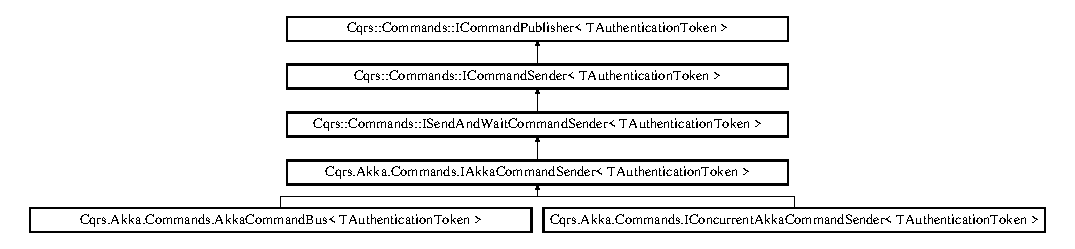
\includegraphics[height=2.898551cm]{interfaceCqrs_1_1Akka_1_1Commands_1_1IAkkaCommandSender}
\end{center}
\end{figure}
\subsection*{Additional Inherited Members}


\subsection{Detailed Description}
A I\+Command\+Publisher$<$\+T\+Authentication\+Token$>$ that proxies I\+Command$<$\+T\+Authentication\+Token$>$ back onto the I\+Actor\+Ref and then publishes the I\+Command$<$\+T\+Authentication\+Token$>$ on the public command bus. 


\hypertarget{interfaceCqrs_1_1Akka_1_1Commands_1_1IAkkaCommandSenderProxy}{}\section{Cqrs.\+Akka.\+Commands.\+I\+Akka\+Command\+Sender\+Proxy$<$ T\+Authentication\+Token $>$ Interface Template Reference}
\label{interfaceCqrs_1_1Akka_1_1Commands_1_1IAkkaCommandSenderProxy}\index{Cqrs.\+Akka.\+Commands.\+I\+Akka\+Command\+Sender\+Proxy$<$ T\+Authentication\+Token $>$@{Cqrs.\+Akka.\+Commands.\+I\+Akka\+Command\+Sender\+Proxy$<$ T\+Authentication\+Token $>$}}


A I\+Command\+Sender$<$\+T\+Authentication\+Token$>$ that proxies I\+Command$<$\+T\+Authentication\+Token$>$ back onto the I\+Actor\+Ref and then publishes the I\+Command$<$\+T\+Authentication\+Token$>$ on the public command bus.  


Inheritance diagram for Cqrs.\+Akka.\+Commands.\+I\+Akka\+Command\+Sender\+Proxy$<$ T\+Authentication\+Token $>$\+:\begin{figure}[H]
\begin{center}
\leavevmode
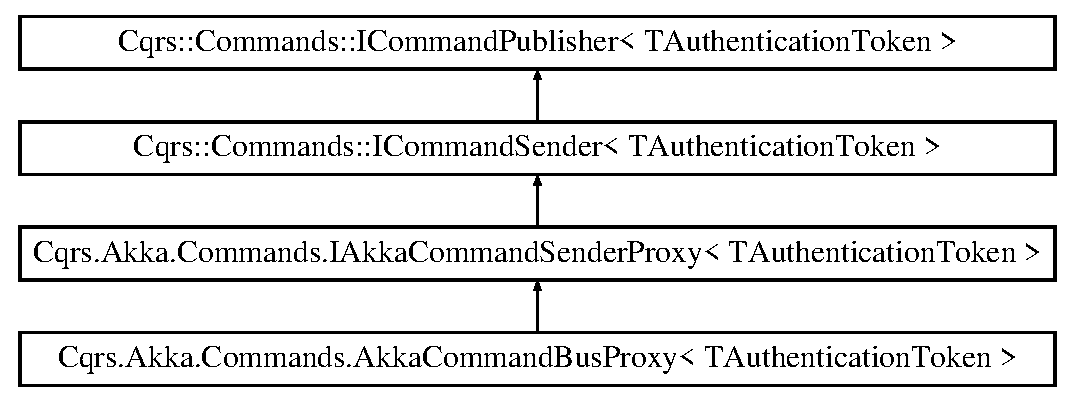
\includegraphics[height=4.000000cm]{interfaceCqrs_1_1Akka_1_1Commands_1_1IAkkaCommandSenderProxy}
\end{center}
\end{figure}
\subsection*{Additional Inherited Members}


\subsection{Detailed Description}
A I\+Command\+Sender$<$\+T\+Authentication\+Token$>$ that proxies I\+Command$<$\+T\+Authentication\+Token$>$ back onto the I\+Actor\+Ref and then publishes the I\+Command$<$\+T\+Authentication\+Token$>$ on the public command bus. 


\hypertarget{interfaceCqrs_1_1Akka_1_1Commands_1_1IConcurrentAkkaCommandSender}{}\section{Cqrs.\+Akka.\+Commands.\+I\+Concurrent\+Akka\+Command\+Sender$<$ T\+Authentication\+Token, T\+Target $>$ Interface Template Reference}
\label{interfaceCqrs_1_1Akka_1_1Commands_1_1IConcurrentAkkaCommandSender}\index{Cqrs.\+Akka.\+Commands.\+I\+Concurrent\+Akka\+Command\+Sender$<$ T\+Authentication\+Token, T\+Target $>$@{Cqrs.\+Akka.\+Commands.\+I\+Concurrent\+Akka\+Command\+Sender$<$ T\+Authentication\+Token, T\+Target $>$}}
Inheritance diagram for Cqrs.\+Akka.\+Commands.\+I\+Concurrent\+Akka\+Command\+Sender$<$ T\+Authentication\+Token, T\+Target $>$\+:\begin{figure}[H]
\begin{center}
\leavevmode
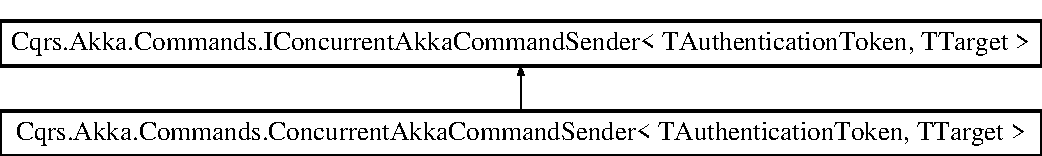
\includegraphics[height=2.000000cm]{interfaceCqrs_1_1Akka_1_1Commands_1_1IConcurrentAkkaCommandSender}
\end{center}
\end{figure}

\hypertarget{interfaceCqrs_1_1Akka_1_1Commands_1_1IConcurrentAkkaCommandSender}{}\section{Cqrs.\+Akka.\+Commands.\+I\+Concurrent\+Akka\+Command\+Sender$<$ T\+Authentication\+Token, T\+Target $>$ Interface Template Reference}
\label{interfaceCqrs_1_1Akka_1_1Commands_1_1IConcurrentAkkaCommandSender}\index{Cqrs.\+Akka.\+Commands.\+I\+Concurrent\+Akka\+Command\+Sender$<$ T\+Authentication\+Token, T\+Target $>$@{Cqrs.\+Akka.\+Commands.\+I\+Concurrent\+Akka\+Command\+Sender$<$ T\+Authentication\+Token, T\+Target $>$}}
Inheritance diagram for Cqrs.\+Akka.\+Commands.\+I\+Concurrent\+Akka\+Command\+Sender$<$ T\+Authentication\+Token, T\+Target $>$\+:\begin{figure}[H]
\begin{center}
\leavevmode
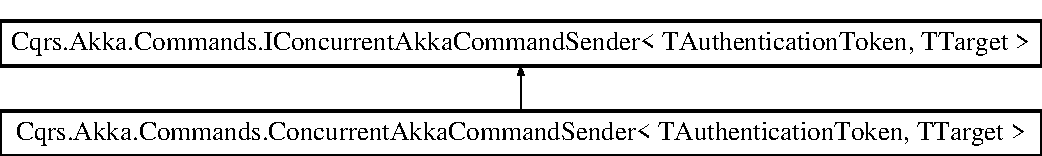
\includegraphics[height=2.000000cm]{interfaceCqrs_1_1Akka_1_1Commands_1_1IConcurrentAkkaCommandSender}
\end{center}
\end{figure}

\hypertarget{classCqrs_1_1Akka_1_1Configuration_1_1AkkaBusRegistrar}{}\section{Cqrs.\+Akka.\+Configuration.\+Akka\+Bus\+Registrar$<$ T\+Authentication\+Token $>$ Class Template Reference}
\label{classCqrs_1_1Akka_1_1Configuration_1_1AkkaBusRegistrar}\index{Cqrs.\+Akka.\+Configuration.\+Akka\+Bus\+Registrar$<$ T\+Authentication\+Token $>$@{Cqrs.\+Akka.\+Configuration.\+Akka\+Bus\+Registrar$<$ T\+Authentication\+Token $>$}}


Triggers the \hyperlink{classCqrs_1_1Configuration_1_1BusRegistrar_a4a934d21a535b28af6c67154512bba20_a4a934d21a535b28af6c67154512bba20}{Bus\+Registrar} instantiates instances of \hyperlink{interfaceCqrs_1_1Events_1_1IEventHandler}{I\+Event\+Handler$<$\+T\+Authentication\+Token, T\+Event$>$} and I\+Command\+Handler$<$\+T\+Authentication\+Token,\+T\+Command$>$ classes that inherit the akka.\+net Receive\+Actor via the I\+Dependency\+Resolver so their message registration kicks in.  


Inheritance diagram for Cqrs.\+Akka.\+Configuration.\+Akka\+Bus\+Registrar$<$ T\+Authentication\+Token $>$\+:\begin{figure}[H]
\begin{center}
\leavevmode
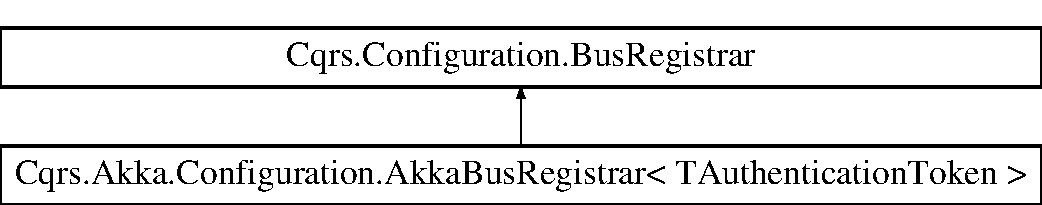
\includegraphics[height=2.000000cm]{classCqrs_1_1Akka_1_1Configuration_1_1AkkaBusRegistrar}
\end{center}
\end{figure}
\subsection*{Public Member Functions}
\begin{DoxyCompactItemize}
\item 
\hyperlink{classCqrs_1_1Akka_1_1Configuration_1_1AkkaBusRegistrar_a49ab48e3305b6eb17f2a68fc2996a988_a49ab48e3305b6eb17f2a68fc2996a988}{Akka\+Bus\+Registrar} (\hyperlink{interfaceCqrs_1_1Configuration_1_1IDependencyResolver}{I\+Dependency\+Resolver} dependency\+Resolver, \hyperlink{interfaceCqrs_1_1Akka_1_1Configuration_1_1IHandlerResolver}{I\+Handler\+Resolver} handler\+Resolver)
\end{DoxyCompactItemize}
\subsection*{Protected Member Functions}
\begin{DoxyCompactItemize}
\item 
override \hyperlink{classCqrs_1_1Configuration_1_1HandlerDelegate}{Handler\+Delegate} \hyperlink{classCqrs_1_1Akka_1_1Configuration_1_1AkkaBusRegistrar_ad7e3e5d332d5b4d781375a28f23bdb19_ad7e3e5d332d5b4d781375a28f23bdb19}{Build\+Delegate\+Action} (Type executor\+Type, Func$<$ Type, I\+Enumerable$<$ Type $>$$>$ resolve\+Message\+Handler\+Interface)
\begin{DoxyCompactList}\small\item\em Builds a Handler\+Delegate that will resolve the provided {\itshape executor\+Type}  and invoke the Handle method, when executed. \end{DoxyCompactList}\item 
override void \hyperlink{classCqrs_1_1Akka_1_1Configuration_1_1AkkaBusRegistrar_a0ac474751b2ba8ebb27b885a15fbf053_a0ac474751b2ba8ebb27b885a15fbf053}{Invoke\+Handler\+Delegate} (Method\+Info register\+Executor\+Method, bool true\+For\+Events\+False\+For\+Commands, \hyperlink{classCqrs_1_1Configuration_1_1HandlerDelegate}{Handler\+Delegate} handler\+Delegate)
\begin{DoxyCompactList}\small\item\em Invokes {\itshape handler\+Delegate} , fetching the corresponding \char`\"{}\+Hold\+Message\+Lock\char`\"{} configuration setting \end{DoxyCompactList}\end{DoxyCompactItemize}
\subsection*{Properties}
\begin{DoxyCompactItemize}
\item 
\hyperlink{interfaceCqrs_1_1Akka_1_1Configuration_1_1IHandlerResolver}{I\+Handler\+Resolver} \hyperlink{classCqrs_1_1Akka_1_1Configuration_1_1AkkaBusRegistrar_a642cd7215c2f51cfaff263f9ba95a4c4_a642cd7215c2f51cfaff263f9ba95a4c4}{Handler\+Resolver}\hspace{0.3cm}{\ttfamily  \mbox{[}get\mbox{]}}
\end{DoxyCompactItemize}


\subsection{Detailed Description}
Triggers the \hyperlink{classCqrs_1_1Configuration_1_1BusRegistrar_a4a934d21a535b28af6c67154512bba20_a4a934d21a535b28af6c67154512bba20}{Bus\+Registrar} instantiates instances of \hyperlink{interfaceCqrs_1_1Events_1_1IEventHandler}{I\+Event\+Handler$<$\+T\+Authentication\+Token, T\+Event$>$} and I\+Command\+Handler$<$\+T\+Authentication\+Token,\+T\+Command$>$ classes that inherit the akka.\+net Receive\+Actor via the I\+Dependency\+Resolver so their message registration kicks in. 



\subsection{Constructor \& Destructor Documentation}
\mbox{\Hypertarget{classCqrs_1_1Akka_1_1Configuration_1_1AkkaBusRegistrar_a49ab48e3305b6eb17f2a68fc2996a988_a49ab48e3305b6eb17f2a68fc2996a988}\label{classCqrs_1_1Akka_1_1Configuration_1_1AkkaBusRegistrar_a49ab48e3305b6eb17f2a68fc2996a988_a49ab48e3305b6eb17f2a68fc2996a988}} 
\index{Cqrs\+::\+Akka\+::\+Configuration\+::\+Akka\+Bus\+Registrar@{Cqrs\+::\+Akka\+::\+Configuration\+::\+Akka\+Bus\+Registrar}!Akka\+Bus\+Registrar@{Akka\+Bus\+Registrar}}
\index{Akka\+Bus\+Registrar@{Akka\+Bus\+Registrar}!Cqrs\+::\+Akka\+::\+Configuration\+::\+Akka\+Bus\+Registrar@{Cqrs\+::\+Akka\+::\+Configuration\+::\+Akka\+Bus\+Registrar}}
\subsubsection{\texorpdfstring{Akka\+Bus\+Registrar()}{AkkaBusRegistrar()}}
{\footnotesize\ttfamily \hyperlink{classCqrs_1_1Akka_1_1Configuration_1_1AkkaBusRegistrar}{Cqrs.\+Akka.\+Configuration.\+Akka\+Bus\+Registrar}$<$ T\+Authentication\+Token $>$.\hyperlink{classCqrs_1_1Akka_1_1Configuration_1_1AkkaBusRegistrar}{Akka\+Bus\+Registrar} (\begin{DoxyParamCaption}\item[{\hyperlink{interfaceCqrs_1_1Configuration_1_1IDependencyResolver}{I\+Dependency\+Resolver}}]{dependency\+Resolver,  }\item[{\hyperlink{interfaceCqrs_1_1Akka_1_1Configuration_1_1IHandlerResolver}{I\+Handler\+Resolver}}]{handler\+Resolver }\end{DoxyParamCaption})}



\subsection{Member Function Documentation}
\mbox{\Hypertarget{classCqrs_1_1Akka_1_1Configuration_1_1AkkaBusRegistrar_ad7e3e5d332d5b4d781375a28f23bdb19_ad7e3e5d332d5b4d781375a28f23bdb19}\label{classCqrs_1_1Akka_1_1Configuration_1_1AkkaBusRegistrar_ad7e3e5d332d5b4d781375a28f23bdb19_ad7e3e5d332d5b4d781375a28f23bdb19}} 
\index{Cqrs\+::\+Akka\+::\+Configuration\+::\+Akka\+Bus\+Registrar@{Cqrs\+::\+Akka\+::\+Configuration\+::\+Akka\+Bus\+Registrar}!Build\+Delegate\+Action@{Build\+Delegate\+Action}}
\index{Build\+Delegate\+Action@{Build\+Delegate\+Action}!Cqrs\+::\+Akka\+::\+Configuration\+::\+Akka\+Bus\+Registrar@{Cqrs\+::\+Akka\+::\+Configuration\+::\+Akka\+Bus\+Registrar}}
\subsubsection{\texorpdfstring{Build\+Delegate\+Action()}{BuildDelegateAction()}}
{\footnotesize\ttfamily override \hyperlink{classCqrs_1_1Configuration_1_1HandlerDelegate}{Handler\+Delegate} \hyperlink{classCqrs_1_1Akka_1_1Configuration_1_1AkkaBusRegistrar}{Cqrs.\+Akka.\+Configuration.\+Akka\+Bus\+Registrar}$<$ T\+Authentication\+Token $>$.Build\+Delegate\+Action (\begin{DoxyParamCaption}\item[{Type}]{executor\+Type,  }\item[{Func$<$ Type, I\+Enumerable$<$ Type $>$$>$}]{resolve\+Message\+Handler\+Interface }\end{DoxyParamCaption})\hspace{0.3cm}{\ttfamily [protected]}, {\ttfamily [virtual]}}



Builds a Handler\+Delegate that will resolve the provided {\itshape executor\+Type}  and invoke the Handle method, when executed. 


\begin{DoxyParams}{Parameters}
{\em executor\+Type} & The type of I\+Handler to resolve.$>$\\
\hline
{\em resolve\+Message\+Handler\+Interface} & Not used.\\
\hline
\end{DoxyParams}


Reimplemented from \hyperlink{classCqrs_1_1Configuration_1_1BusRegistrar_a07d27088739f2ae0ac7c551fc6a72ac9_a07d27088739f2ae0ac7c551fc6a72ac9}{Cqrs.\+Configuration.\+Bus\+Registrar}.

\mbox{\Hypertarget{classCqrs_1_1Akka_1_1Configuration_1_1AkkaBusRegistrar_a0ac474751b2ba8ebb27b885a15fbf053_a0ac474751b2ba8ebb27b885a15fbf053}\label{classCqrs_1_1Akka_1_1Configuration_1_1AkkaBusRegistrar_a0ac474751b2ba8ebb27b885a15fbf053_a0ac474751b2ba8ebb27b885a15fbf053}} 
\index{Cqrs\+::\+Akka\+::\+Configuration\+::\+Akka\+Bus\+Registrar@{Cqrs\+::\+Akka\+::\+Configuration\+::\+Akka\+Bus\+Registrar}!Invoke\+Handler\+Delegate@{Invoke\+Handler\+Delegate}}
\index{Invoke\+Handler\+Delegate@{Invoke\+Handler\+Delegate}!Cqrs\+::\+Akka\+::\+Configuration\+::\+Akka\+Bus\+Registrar@{Cqrs\+::\+Akka\+::\+Configuration\+::\+Akka\+Bus\+Registrar}}
\subsubsection{\texorpdfstring{Invoke\+Handler\+Delegate()}{InvokeHandlerDelegate()}}
{\footnotesize\ttfamily override void \hyperlink{classCqrs_1_1Akka_1_1Configuration_1_1AkkaBusRegistrar}{Cqrs.\+Akka.\+Configuration.\+Akka\+Bus\+Registrar}$<$ T\+Authentication\+Token $>$.Invoke\+Handler\+Delegate (\begin{DoxyParamCaption}\item[{Method\+Info}]{register\+Executor\+Method,  }\item[{bool}]{true\+For\+Events\+False\+For\+Commands,  }\item[{\hyperlink{classCqrs_1_1Configuration_1_1HandlerDelegate}{Handler\+Delegate}}]{handler\+Delegate }\end{DoxyParamCaption})\hspace{0.3cm}{\ttfamily [protected]}, {\ttfamily [virtual]}}



Invokes {\itshape handler\+Delegate} , fetching the corresponding \char`\"{}\+Hold\+Message\+Lock\char`\"{} configuration setting 


\begin{DoxyParams}{Parameters}
{\em register\+Executor\+Method} & The Method\+Info to use to invoke {\itshape handler\+Delegate} .\\
\hline
{\em true\+For\+Events\+False\+For\+Commands} & Indicates if this is registers I\+Event\+Handler or I\+Command\+Handler$<$\+T\+Authentication\+Token,\+T\+Command$>$.\\
\hline
{\em handler\+Delegate} & The actual Handler\+Delegate that gets executed.\\
\hline
\end{DoxyParams}


Reimplemented from \hyperlink{classCqrs_1_1Configuration_1_1BusRegistrar_a3103da4cf077104607fe03a862958827_a3103da4cf077104607fe03a862958827}{Cqrs.\+Configuration.\+Bus\+Registrar}.



\subsection{Property Documentation}
\mbox{\Hypertarget{classCqrs_1_1Akka_1_1Configuration_1_1AkkaBusRegistrar_a642cd7215c2f51cfaff263f9ba95a4c4_a642cd7215c2f51cfaff263f9ba95a4c4}\label{classCqrs_1_1Akka_1_1Configuration_1_1AkkaBusRegistrar_a642cd7215c2f51cfaff263f9ba95a4c4_a642cd7215c2f51cfaff263f9ba95a4c4}} 
\index{Cqrs\+::\+Akka\+::\+Configuration\+::\+Akka\+Bus\+Registrar@{Cqrs\+::\+Akka\+::\+Configuration\+::\+Akka\+Bus\+Registrar}!Handler\+Resolver@{Handler\+Resolver}}
\index{Handler\+Resolver@{Handler\+Resolver}!Cqrs\+::\+Akka\+::\+Configuration\+::\+Akka\+Bus\+Registrar@{Cqrs\+::\+Akka\+::\+Configuration\+::\+Akka\+Bus\+Registrar}}
\subsubsection{\texorpdfstring{Handler\+Resolver}{HandlerResolver}}
{\footnotesize\ttfamily \hyperlink{interfaceCqrs_1_1Akka_1_1Configuration_1_1IHandlerResolver}{I\+Handler\+Resolver} \hyperlink{classCqrs_1_1Akka_1_1Configuration_1_1AkkaBusRegistrar}{Cqrs.\+Akka.\+Configuration.\+Akka\+Bus\+Registrar}$<$ T\+Authentication\+Token $>$.Handler\+Resolver\hspace{0.3cm}{\ttfamily [get]}, {\ttfamily [protected]}}


\hypertarget{interfaceCqrs_1_1Akka_1_1Configuration_1_1IHandlerResolver}{}\section{Cqrs.\+Akka.\+Configuration.\+I\+Handler\+Resolver Interface Reference}
\label{interfaceCqrs_1_1Akka_1_1Configuration_1_1IHandlerResolver}\index{Cqrs.\+Akka.\+Configuration.\+I\+Handler\+Resolver@{Cqrs.\+Akka.\+Configuration.\+I\+Handler\+Resolver}}


Resolves handlers for use with Akka.\+Net  


Inheritance diagram for Cqrs.\+Akka.\+Configuration.\+I\+Handler\+Resolver\+:\begin{figure}[H]
\begin{center}
\leavevmode
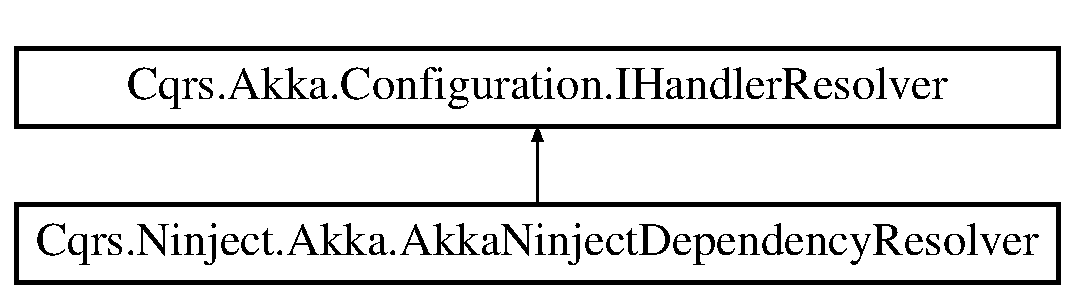
\includegraphics[height=2.000000cm]{interfaceCqrs_1_1Akka_1_1Configuration_1_1IHandlerResolver}
\end{center}
\end{figure}
\subsection*{Public Member Functions}
\begin{DoxyCompactItemize}
\item 
object \hyperlink{interfaceCqrs_1_1Akka_1_1Configuration_1_1IHandlerResolver_abae10eed2d92eb3f2831c5eba7e3c2d3_abae10eed2d92eb3f2831c5eba7e3c2d3}{Resolve} (Type hander\+Type, object rsn)
\begin{DoxyCompactList}\small\item\em Resolves instances of {\itshape hander\+Type} . \end{DoxyCompactList}\end{DoxyCompactItemize}


\subsection{Detailed Description}
Resolves handlers for use with Akka.\+Net 



\subsection{Member Function Documentation}
\mbox{\Hypertarget{interfaceCqrs_1_1Akka_1_1Configuration_1_1IHandlerResolver_abae10eed2d92eb3f2831c5eba7e3c2d3_abae10eed2d92eb3f2831c5eba7e3c2d3}\label{interfaceCqrs_1_1Akka_1_1Configuration_1_1IHandlerResolver_abae10eed2d92eb3f2831c5eba7e3c2d3_abae10eed2d92eb3f2831c5eba7e3c2d3}} 
\index{Cqrs\+::\+Akka\+::\+Configuration\+::\+I\+Handler\+Resolver@{Cqrs\+::\+Akka\+::\+Configuration\+::\+I\+Handler\+Resolver}!Resolve@{Resolve}}
\index{Resolve@{Resolve}!Cqrs\+::\+Akka\+::\+Configuration\+::\+I\+Handler\+Resolver@{Cqrs\+::\+Akka\+::\+Configuration\+::\+I\+Handler\+Resolver}}
\subsubsection{\texorpdfstring{Resolve()}{Resolve()}}
{\footnotesize\ttfamily object Cqrs.\+Akka.\+Configuration.\+I\+Handler\+Resolver.\+Resolve (\begin{DoxyParamCaption}\item[{Type}]{hander\+Type,  }\item[{object}]{rsn }\end{DoxyParamCaption})}



Resolves instances of {\itshape hander\+Type} . 



Implemented in \hyperlink{classCqrs_1_1Ninject_1_1Akka_1_1AkkaNinjectDependencyResolver_ab860d9bcf44b62098a8df91bbcb5013d_ab860d9bcf44b62098a8df91bbcb5013d}{Cqrs.\+Ninject.\+Akka.\+Akka\+Ninject\+Dependency\+Resolver}.


\hypertarget{classCqrs_1_1Akka_1_1Domain_1_1AkkaAggregateRepository}{}\section{Cqrs.\+Akka.\+Domain.\+Akka\+Aggregate\+Repository$<$ T\+Authentication\+Token $>$ Class Template Reference}
\label{classCqrs_1_1Akka_1_1Domain_1_1AkkaAggregateRepository}\index{Cqrs.\+Akka.\+Domain.\+Akka\+Aggregate\+Repository$<$ T\+Authentication\+Token $>$@{Cqrs.\+Akka.\+Domain.\+Akka\+Aggregate\+Repository$<$ T\+Authentication\+Token $>$}}


A \hyperlink{classCqrs_1_1Domain_1_1AggregateRepository_a12a5588533a7eb2cdd061576ad53c8ac_a12a5588533a7eb2cdd061576ad53c8ac}{Aggregate\+Repository$<$\+T\+Authentication\+Token$>$} that is safe to use within Akka.\+N\+ET  


Inheritance diagram for Cqrs.\+Akka.\+Domain.\+Akka\+Aggregate\+Repository$<$ T\+Authentication\+Token $>$\+:\begin{figure}[H]
\begin{center}
\leavevmode
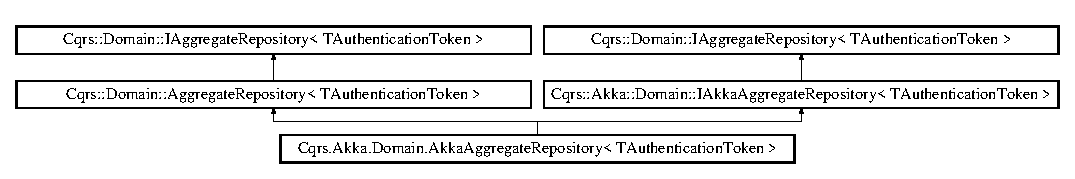
\includegraphics[height=1.958042cm]{classCqrs_1_1Akka_1_1Domain_1_1AkkaAggregateRepository}
\end{center}
\end{figure}
\subsection*{Public Member Functions}
\begin{DoxyCompactItemize}
\item 
\hyperlink{classCqrs_1_1Akka_1_1Domain_1_1AkkaAggregateRepository_a9281097ff3818d383b7b2915bfdca11d_a9281097ff3818d383b7b2915bfdca11d}{Akka\+Aggregate\+Repository} (\hyperlink{interfaceCqrs_1_1Domain_1_1Factories_1_1IAggregateFactory}{I\+Aggregate\+Factory} aggregate\+Factory, \hyperlink{interfaceCqrs_1_1Events_1_1IEventStore}{I\+Event\+Store}$<$ T\+Authentication\+Token $>$ event\+Store, \hyperlink{interfaceCqrs_1_1Events_1_1IEventPublisher}{I\+Event\+Publisher}$<$ T\+Authentication\+Token $>$ publisher, I\+Correlation\+Id\+Helper correlation\+Id\+Helper, \hyperlink{interfaceCqrs_1_1Configuration_1_1IConfigurationManager}{I\+Configuration\+Manager} configuration\+Manager, \hyperlink{interfaceCqrs_1_1Akka_1_1Events_1_1IAkkaEventPublisherProxy}{I\+Akka\+Event\+Publisher\+Proxy}$<$ T\+Authentication\+Token $>$ event\+Publisher)
\begin{DoxyCompactList}\small\item\em Instantiates a new instance of \hyperlink{classCqrs_1_1Akka_1_1Domain_1_1AkkaAggregateRepository_a9281097ff3818d383b7b2915bfdca11d_a9281097ff3818d383b7b2915bfdca11d}{Akka\+Aggregate\+Repository$<$\+T\+Authentication\+Token$>$} \end{DoxyCompactList}\end{DoxyCompactItemize}
\subsection*{Protected Member Functions}
\begin{DoxyCompactItemize}
\item 
override T\+Aggregate\+Root \hyperlink{classCqrs_1_1Akka_1_1Domain_1_1AkkaAggregateRepository_a889a80595755372614382c36092f30dc_a889a80595755372614382c36092f30dc}{Create\+Aggregate$<$ T\+Aggregate\+Root $>$} (Guid id)
\begin{DoxyCompactList}\small\item\em Calls I\+Aggregate\+Factory.\+Create to get a, {\itshape T\+Aggregate\+Root} . \end{DoxyCompactList}\item 
override void \hyperlink{classCqrs_1_1Akka_1_1Domain_1_1AkkaAggregateRepository_a144cbfdedb23039729ba5b3058f84e7a_a144cbfdedb23039729ba5b3058f84e7a}{Publish\+Event} (\hyperlink{interfaceCqrs_1_1Events_1_1IEvent}{I\+Event}$<$ T\+Authentication\+Token $>$ @event)
\begin{DoxyCompactList}\small\item\em Publish the saved {\itshape event}  asynchronously on \hyperlink{classCqrs_1_1Akka_1_1Domain_1_1AkkaAggregateRepository_a6c6400aef33fd3ec5dc3e479ebec6b40_a6c6400aef33fd3ec5dc3e479ebec6b40}{Event\+Publisher}, then calls Aggregate\+Repository$<$\+T\+Authentication\+Token$>$.\+Publish\+Event \end{DoxyCompactList}\end{DoxyCompactItemize}
\subsection*{Properties}
\begin{DoxyCompactItemize}
\item 
\hyperlink{interfaceCqrs_1_1Akka_1_1Events_1_1IAkkaEventPublisherProxy}{I\+Akka\+Event\+Publisher\+Proxy}$<$ T\+Authentication\+Token $>$ \hyperlink{classCqrs_1_1Akka_1_1Domain_1_1AkkaAggregateRepository_a6c6400aef33fd3ec5dc3e479ebec6b40_a6c6400aef33fd3ec5dc3e479ebec6b40}{Event\+Publisher}\hspace{0.3cm}{\ttfamily  \mbox{[}get\mbox{]}}
\begin{DoxyCompactList}\small\item\em Gets the I\+Akka\+Event\+Publisher\+Proxy$<$\+T\+Authentication\+Token$>$ \end{DoxyCompactList}\end{DoxyCompactItemize}


\subsection{Detailed Description}
A \hyperlink{classCqrs_1_1Domain_1_1AggregateRepository_a12a5588533a7eb2cdd061576ad53c8ac_a12a5588533a7eb2cdd061576ad53c8ac}{Aggregate\+Repository$<$\+T\+Authentication\+Token$>$} that is safe to use within Akka.\+N\+ET 


\begin{DoxyTemplParams}{Template Parameters}
{\em T\+Authentication\+Token} & The Type of authentication token.\\
\hline
\end{DoxyTemplParams}


\subsection{Constructor \& Destructor Documentation}
\mbox{\Hypertarget{classCqrs_1_1Akka_1_1Domain_1_1AkkaAggregateRepository_a9281097ff3818d383b7b2915bfdca11d_a9281097ff3818d383b7b2915bfdca11d}\label{classCqrs_1_1Akka_1_1Domain_1_1AkkaAggregateRepository_a9281097ff3818d383b7b2915bfdca11d_a9281097ff3818d383b7b2915bfdca11d}} 
\index{Cqrs\+::\+Akka\+::\+Domain\+::\+Akka\+Aggregate\+Repository@{Cqrs\+::\+Akka\+::\+Domain\+::\+Akka\+Aggregate\+Repository}!Akka\+Aggregate\+Repository@{Akka\+Aggregate\+Repository}}
\index{Akka\+Aggregate\+Repository@{Akka\+Aggregate\+Repository}!Cqrs\+::\+Akka\+::\+Domain\+::\+Akka\+Aggregate\+Repository@{Cqrs\+::\+Akka\+::\+Domain\+::\+Akka\+Aggregate\+Repository}}
\subsubsection{\texorpdfstring{Akka\+Aggregate\+Repository()}{AkkaAggregateRepository()}}
{\footnotesize\ttfamily \hyperlink{classCqrs_1_1Akka_1_1Domain_1_1AkkaAggregateRepository}{Cqrs.\+Akka.\+Domain.\+Akka\+Aggregate\+Repository}$<$ T\+Authentication\+Token $>$.\hyperlink{classCqrs_1_1Akka_1_1Domain_1_1AkkaAggregateRepository}{Akka\+Aggregate\+Repository} (\begin{DoxyParamCaption}\item[{\hyperlink{interfaceCqrs_1_1Domain_1_1Factories_1_1IAggregateFactory}{I\+Aggregate\+Factory}}]{aggregate\+Factory,  }\item[{\hyperlink{interfaceCqrs_1_1Events_1_1IEventStore}{I\+Event\+Store}$<$ T\+Authentication\+Token $>$}]{event\+Store,  }\item[{\hyperlink{interfaceCqrs_1_1Events_1_1IEventPublisher}{I\+Event\+Publisher}$<$ T\+Authentication\+Token $>$}]{publisher,  }\item[{I\+Correlation\+Id\+Helper}]{correlation\+Id\+Helper,  }\item[{\hyperlink{interfaceCqrs_1_1Configuration_1_1IConfigurationManager}{I\+Configuration\+Manager}}]{configuration\+Manager,  }\item[{\hyperlink{interfaceCqrs_1_1Akka_1_1Events_1_1IAkkaEventPublisherProxy}{I\+Akka\+Event\+Publisher\+Proxy}$<$ T\+Authentication\+Token $>$}]{event\+Publisher }\end{DoxyParamCaption})}



Instantiates a new instance of \hyperlink{classCqrs_1_1Akka_1_1Domain_1_1AkkaAggregateRepository_a9281097ff3818d383b7b2915bfdca11d_a9281097ff3818d383b7b2915bfdca11d}{Akka\+Aggregate\+Repository$<$\+T\+Authentication\+Token$>$} 



\subsection{Member Function Documentation}
\mbox{\Hypertarget{classCqrs_1_1Akka_1_1Domain_1_1AkkaAggregateRepository_a889a80595755372614382c36092f30dc_a889a80595755372614382c36092f30dc}\label{classCqrs_1_1Akka_1_1Domain_1_1AkkaAggregateRepository_a889a80595755372614382c36092f30dc_a889a80595755372614382c36092f30dc}} 
\index{Cqrs\+::\+Akka\+::\+Domain\+::\+Akka\+Aggregate\+Repository@{Cqrs\+::\+Akka\+::\+Domain\+::\+Akka\+Aggregate\+Repository}!Create\+Aggregate$<$ T\+Aggregate\+Root $>$@{Create\+Aggregate$<$ T\+Aggregate\+Root $>$}}
\index{Create\+Aggregate$<$ T\+Aggregate\+Root $>$@{Create\+Aggregate$<$ T\+Aggregate\+Root $>$}!Cqrs\+::\+Akka\+::\+Domain\+::\+Akka\+Aggregate\+Repository@{Cqrs\+::\+Akka\+::\+Domain\+::\+Akka\+Aggregate\+Repository}}
\subsubsection{\texorpdfstring{Create\+Aggregate$<$ T\+Aggregate\+Root $>$()}{CreateAggregate< TAggregateRoot >()}}
{\footnotesize\ttfamily override T\+Aggregate\+Root \hyperlink{classCqrs_1_1Akka_1_1Domain_1_1AkkaAggregateRepository}{Cqrs.\+Akka.\+Domain.\+Akka\+Aggregate\+Repository}$<$ T\+Authentication\+Token $>$.Create\+Aggregate$<$ T\+Aggregate\+Root $>$ (\begin{DoxyParamCaption}\item[{Guid}]{id }\end{DoxyParamCaption})\hspace{0.3cm}{\ttfamily [protected]}, {\ttfamily [virtual]}}



Calls I\+Aggregate\+Factory.\+Create to get a, {\itshape T\+Aggregate\+Root} . 


\begin{DoxyTemplParams}{Template Parameters}
{\em T\+Aggregate\+Root} & The Type of I\+Aggregate\+Root$<$\+T\+Authentication\+Token$>$.\\
\hline
\end{DoxyTemplParams}

\begin{DoxyParams}{Parameters}
{\em id} & The id of the {\itshape T\+Aggregate\+Root}  to create.\\
\hline
\end{DoxyParams}


Reimplemented from \hyperlink{classCqrs_1_1Domain_1_1AggregateRepository_a64d82c57bbe49a11bd5cf20c5b86ce19_a64d82c57bbe49a11bd5cf20c5b86ce19}{Cqrs.\+Domain.\+Aggregate\+Repository$<$ T\+Authentication\+Token $>$}.

\mbox{\Hypertarget{classCqrs_1_1Akka_1_1Domain_1_1AkkaAggregateRepository_a144cbfdedb23039729ba5b3058f84e7a_a144cbfdedb23039729ba5b3058f84e7a}\label{classCqrs_1_1Akka_1_1Domain_1_1AkkaAggregateRepository_a144cbfdedb23039729ba5b3058f84e7a_a144cbfdedb23039729ba5b3058f84e7a}} 
\index{Cqrs\+::\+Akka\+::\+Domain\+::\+Akka\+Aggregate\+Repository@{Cqrs\+::\+Akka\+::\+Domain\+::\+Akka\+Aggregate\+Repository}!Publish\+Event@{Publish\+Event}}
\index{Publish\+Event@{Publish\+Event}!Cqrs\+::\+Akka\+::\+Domain\+::\+Akka\+Aggregate\+Repository@{Cqrs\+::\+Akka\+::\+Domain\+::\+Akka\+Aggregate\+Repository}}
\subsubsection{\texorpdfstring{Publish\+Event()}{PublishEvent()}}
{\footnotesize\ttfamily override void \hyperlink{classCqrs_1_1Akka_1_1Domain_1_1AkkaAggregateRepository}{Cqrs.\+Akka.\+Domain.\+Akka\+Aggregate\+Repository}$<$ T\+Authentication\+Token $>$.Publish\+Event (\begin{DoxyParamCaption}\item[{\hyperlink{interfaceCqrs_1_1Events_1_1IEvent}{I\+Event}$<$ T\+Authentication\+Token $>$ @}]{event }\end{DoxyParamCaption})\hspace{0.3cm}{\ttfamily [protected]}, {\ttfamily [virtual]}}



Publish the saved {\itshape event}  asynchronously on \hyperlink{classCqrs_1_1Akka_1_1Domain_1_1AkkaAggregateRepository_a6c6400aef33fd3ec5dc3e479ebec6b40_a6c6400aef33fd3ec5dc3e479ebec6b40}{Event\+Publisher}, then calls Aggregate\+Repository$<$\+T\+Authentication\+Token$>$.\+Publish\+Event 



Reimplemented from \hyperlink{classCqrs_1_1Domain_1_1AggregateRepository_a3191ba3d6fa4f6b904128c4731262944_a3191ba3d6fa4f6b904128c4731262944}{Cqrs.\+Domain.\+Aggregate\+Repository$<$ T\+Authentication\+Token $>$}.



\subsection{Property Documentation}
\mbox{\Hypertarget{classCqrs_1_1Akka_1_1Domain_1_1AkkaAggregateRepository_a6c6400aef33fd3ec5dc3e479ebec6b40_a6c6400aef33fd3ec5dc3e479ebec6b40}\label{classCqrs_1_1Akka_1_1Domain_1_1AkkaAggregateRepository_a6c6400aef33fd3ec5dc3e479ebec6b40_a6c6400aef33fd3ec5dc3e479ebec6b40}} 
\index{Cqrs\+::\+Akka\+::\+Domain\+::\+Akka\+Aggregate\+Repository@{Cqrs\+::\+Akka\+::\+Domain\+::\+Akka\+Aggregate\+Repository}!Event\+Publisher@{Event\+Publisher}}
\index{Event\+Publisher@{Event\+Publisher}!Cqrs\+::\+Akka\+::\+Domain\+::\+Akka\+Aggregate\+Repository@{Cqrs\+::\+Akka\+::\+Domain\+::\+Akka\+Aggregate\+Repository}}
\subsubsection{\texorpdfstring{Event\+Publisher}{EventPublisher}}
{\footnotesize\ttfamily \hyperlink{interfaceCqrs_1_1Akka_1_1Events_1_1IAkkaEventPublisherProxy}{I\+Akka\+Event\+Publisher\+Proxy}$<$T\+Authentication\+Token$>$ \hyperlink{classCqrs_1_1Akka_1_1Domain_1_1AkkaAggregateRepository}{Cqrs.\+Akka.\+Domain.\+Akka\+Aggregate\+Repository}$<$ T\+Authentication\+Token $>$.Event\+Publisher\hspace{0.3cm}{\ttfamily [get]}, {\ttfamily [protected]}}



Gets the I\+Akka\+Event\+Publisher\+Proxy$<$\+T\+Authentication\+Token$>$ 


\hypertarget{classCqrs_1_1Akka_1_1Domain_1_1AkkaAggregateRoot}{}\section{Cqrs.\+Akka.\+Domain.\+Akka\+Aggregate\+Root$<$ T\+Authentication\+Token $>$ Class Template Reference}
\label{classCqrs_1_1Akka_1_1Domain_1_1AkkaAggregateRoot}\index{Cqrs.\+Akka.\+Domain.\+Akka\+Aggregate\+Root$<$ T\+Authentication\+Token $>$@{Cqrs.\+Akka.\+Domain.\+Akka\+Aggregate\+Root$<$ T\+Authentication\+Token $>$}}


An I\+Aggregate\+Root$<$\+T\+Authentication\+Token$>$ that is safe to use within Akka.\+N\+ET  


Inheritance diagram for Cqrs.\+Akka.\+Domain.\+Akka\+Aggregate\+Root$<$ T\+Authentication\+Token $>$\+:\begin{figure}[H]
\begin{center}
\leavevmode
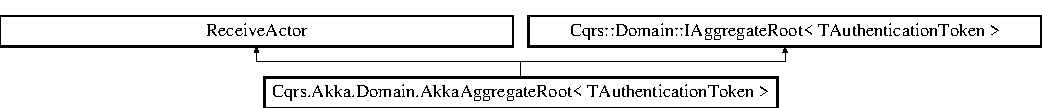
\includegraphics[height=1.454545cm]{classCqrs_1_1Akka_1_1Domain_1_1AkkaAggregateRoot}
\end{center}
\end{figure}
\subsection*{Public Member Functions}
\begin{DoxyCompactItemize}
\item 
I\+Enumerable$<$ \hyperlink{interfaceCqrs_1_1Events_1_1IEvent}{I\+Event}$<$ T\+Authentication\+Token $>$ $>$ \hyperlink{classCqrs_1_1Akka_1_1Domain_1_1AkkaAggregateRoot_a2d11510fec0129ba318f63f7103aeec0_a2d11510fec0129ba318f63f7103aeec0}{Get\+Uncommitted\+Changes} ()
\begin{DoxyCompactList}\small\item\em Get all applied changes that haven\textquotesingle{}t yet been committed. \end{DoxyCompactList}\item 
virtual void \hyperlink{classCqrs_1_1Akka_1_1Domain_1_1AkkaAggregateRoot_a0d2615067175e5f8249bb2dc3d17ee0b_a0d2615067175e5f8249bb2dc3d17ee0b}{Mark\+Changes\+As\+Committed} ()
\begin{DoxyCompactList}\small\item\em Mark all applied changes as committed, increment \hyperlink{classCqrs_1_1Akka_1_1Domain_1_1AkkaAggregateRoot_a4b526322c63542b1da2a700ff1b48d0c_a4b526322c63542b1da2a700ff1b48d0c}{Version} and flush the internal collection of changes. \end{DoxyCompactList}\item 
virtual void \hyperlink{classCqrs_1_1Akka_1_1Domain_1_1AkkaAggregateRoot_af6d84b07d4e9475bb88e769ac9081830_af6d84b07d4e9475bb88e769ac9081830}{Load\+From\+History} (I\+Enumerable$<$ \hyperlink{interfaceCqrs_1_1Events_1_1IEvent}{I\+Event}$<$ T\+Authentication\+Token $>$$>$ history)
\begin{DoxyCompactList}\small\item\em Apply all the \hyperlink{}{events} in {\itshape history}  using event replay to this instance. \end{DoxyCompactList}\end{DoxyCompactItemize}
\subsection*{Protected Member Functions}
\begin{DoxyCompactItemize}
\item 
\hyperlink{classCqrs_1_1Akka_1_1Domain_1_1AkkaAggregateRoot_a060f981e4c3023aec36e7c6f1cfb3a9d_a060f981e4c3023aec36e7c6f1cfb3a9d}{Akka\+Aggregate\+Root} (\hyperlink{interfaceCqrs_1_1Domain_1_1IUnitOfWork}{I\+Unit\+Of\+Work}$<$ T\+Authentication\+Token $>$ unit\+Of\+Work, I\+Logger logger, \hyperlink{interfaceCqrs_1_1Akka_1_1Domain_1_1IAkkaAggregateRepository}{I\+Akka\+Aggregate\+Repository}$<$ T\+Authentication\+Token $>$ repository, I\+Correlation\+Id\+Helper correlation\+Id\+Helper, \hyperlink{interfaceCqrs_1_1Authentication_1_1IAuthenticationTokenHelper}{I\+Authentication\+Token\+Helper}$<$ T\+Authentication\+Token $>$ authentication\+Token\+Helper)
\begin{DoxyCompactList}\small\item\em Instantiates a new instance of \hyperlink{classCqrs_1_1Akka_1_1Domain_1_1AkkaAggregateRoot_a060f981e4c3023aec36e7c6f1cfb3a9d_a060f981e4c3023aec36e7c6f1cfb3a9d}{Akka\+Aggregate\+Root$<$\+T\+Authentication\+Token$>$} \end{DoxyCompactList}\item 
override void \hyperlink{classCqrs_1_1Akka_1_1Domain_1_1AkkaAggregateRoot_a7da2d3a244e34717ec5af1db8f0042bc_a7da2d3a244e34717ec5af1db8f0042bc}{Pre\+Start} ()
\begin{DoxyCompactList}\small\item\em User overridable callback. 

Is called when an Actor is started. Actors are automatically started asynchronously when created. Empty default implementation. \end{DoxyCompactList}\item 
virtual void \hyperlink{classCqrs_1_1Akka_1_1Domain_1_1AkkaAggregateRoot_af8a9bd0e80498b3b54beb7cbec820533_af8a9bd0e80498b3b54beb7cbec820533}{Execute$<$ T\+Command $>$} (Action$<$ T\+Command $>$ action, T\+Command command)
\begin{DoxyCompactList}\small\item\em Executes the provided {\itshape action}  passing it the provided {\itshape command} , then calls Aggregate\+Repository$<$\+T\+Authentication\+Token$>$.\+Publish\+Event \end{DoxyCompactList}\item 
virtual void \hyperlink{classCqrs_1_1Akka_1_1Domain_1_1AkkaAggregateRoot_aaa135cb26be9e5353986f5611f05c059_aaa135cb26be9e5353986f5611f05c059}{Apply\+Change} (\hyperlink{interfaceCqrs_1_1Events_1_1IEvent}{I\+Event}$<$ T\+Authentication\+Token $>$ @event)
\begin{DoxyCompactList}\small\item\em Call the \char`\"{}\+Apply\char`\"{} method with a signature matching the provided {\itshape event}  without using event replay to this instance. \end{DoxyCompactList}\end{DoxyCompactItemize}
\subsection*{Properties}
\begin{DoxyCompactItemize}
\item 
\hyperlink{interfaceCqrs_1_1Domain_1_1IUnitOfWork}{I\+Unit\+Of\+Work}$<$ T\+Authentication\+Token $>$ \hyperlink{classCqrs_1_1Akka_1_1Domain_1_1AkkaAggregateRoot_a58b79dc3e0d837e58d95f5cfeb2da9a1_a58b79dc3e0d837e58d95f5cfeb2da9a1}{Unit\+Of\+Work}\hspace{0.3cm}{\ttfamily  \mbox{[}get, set\mbox{]}}
\begin{DoxyCompactList}\small\item\em Gets or sets the I\+Unit\+Of\+Work$<$\+T\+Authentication\+Token$>$. \end{DoxyCompactList}\item 
\hyperlink{interfaceCqrs_1_1Akka_1_1Domain_1_1IAkkaAggregateRepository}{I\+Akka\+Aggregate\+Repository}$<$ T\+Authentication\+Token $>$ \hyperlink{classCqrs_1_1Akka_1_1Domain_1_1AkkaAggregateRoot_ae15ae65ca994c5ab932d9817a9f7cb7d_ae15ae65ca994c5ab932d9817a9f7cb7d}{Repository}\hspace{0.3cm}{\ttfamily  \mbox{[}get, set\mbox{]}}
\begin{DoxyCompactList}\small\item\em Gets or sets the I\+Akka\+Aggregate\+Repository$<$\+T\+Authentication\+Token$>$. \end{DoxyCompactList}\item 
I\+Logger \hyperlink{classCqrs_1_1Akka_1_1Domain_1_1AkkaAggregateRoot_a685737862246db856bf3eb94345fca3f_a685737862246db856bf3eb94345fca3f}{Logger}\hspace{0.3cm}{\ttfamily  \mbox{[}get, set\mbox{]}}
\begin{DoxyCompactList}\small\item\em Gets or sets the I\+Logger. \end{DoxyCompactList}\item 
I\+Correlation\+Id\+Helper \hyperlink{classCqrs_1_1Akka_1_1Domain_1_1AkkaAggregateRoot_ae1460c9574d7d7b1cb9de2848ae7102e_ae1460c9574d7d7b1cb9de2848ae7102e}{Correlation\+Id\+Helper}\hspace{0.3cm}{\ttfamily  \mbox{[}get, set\mbox{]}}
\begin{DoxyCompactList}\small\item\em Gets or sets the I\+Correlation\+Id\+Helper. \end{DoxyCompactList}\item 
\hyperlink{interfaceCqrs_1_1Authentication_1_1IAuthenticationTokenHelper}{I\+Authentication\+Token\+Helper}$<$ T\+Authentication\+Token $>$ \hyperlink{classCqrs_1_1Akka_1_1Domain_1_1AkkaAggregateRoot_a3a73139fe47221bd579949e978d0126d_a3a73139fe47221bd579949e978d0126d}{Authentication\+Token\+Helper}\hspace{0.3cm}{\ttfamily  \mbox{[}get, set\mbox{]}}
\begin{DoxyCompactList}\small\item\em Gets or sets the I\+Authentication\+Token\+Helper$<$\+T\+Authentication\+Token$>$. \end{DoxyCompactList}\item 
Guid \hyperlink{classCqrs_1_1Akka_1_1Domain_1_1AkkaAggregateRoot_ac03d79efc02629b17642c6324ff181c9_ac03d79efc02629b17642c6324ff181c9}{Id}\hspace{0.3cm}{\ttfamily  \mbox{[}get, protected set\mbox{]}}
\begin{DoxyCompactList}\small\item\em The identifier of this I\+Aggregate\+Root$<$\+T\+Authentication\+Token$>$. \end{DoxyCompactList}\item 
int \hyperlink{classCqrs_1_1Akka_1_1Domain_1_1AkkaAggregateRoot_a4b526322c63542b1da2a700ff1b48d0c_a4b526322c63542b1da2a700ff1b48d0c}{Version}\hspace{0.3cm}{\ttfamily  \mbox{[}get, protected set\mbox{]}}
\begin{DoxyCompactList}\small\item\em The current version of this I\+Aggregate\+Root$<$\+T\+Authentication\+Token$>$. \end{DoxyCompactList}\end{DoxyCompactItemize}


\subsection{Detailed Description}
An I\+Aggregate\+Root$<$\+T\+Authentication\+Token$>$ that is safe to use within Akka.\+N\+ET 


\begin{DoxyTemplParams}{Template Parameters}
{\em T\+Authentication\+Token} & The Type of authentication token.\\
\hline
\end{DoxyTemplParams}


\subsection{Constructor \& Destructor Documentation}
\mbox{\Hypertarget{classCqrs_1_1Akka_1_1Domain_1_1AkkaAggregateRoot_a060f981e4c3023aec36e7c6f1cfb3a9d_a060f981e4c3023aec36e7c6f1cfb3a9d}\label{classCqrs_1_1Akka_1_1Domain_1_1AkkaAggregateRoot_a060f981e4c3023aec36e7c6f1cfb3a9d_a060f981e4c3023aec36e7c6f1cfb3a9d}} 
\index{Cqrs\+::\+Akka\+::\+Domain\+::\+Akka\+Aggregate\+Root@{Cqrs\+::\+Akka\+::\+Domain\+::\+Akka\+Aggregate\+Root}!Akka\+Aggregate\+Root@{Akka\+Aggregate\+Root}}
\index{Akka\+Aggregate\+Root@{Akka\+Aggregate\+Root}!Cqrs\+::\+Akka\+::\+Domain\+::\+Akka\+Aggregate\+Root@{Cqrs\+::\+Akka\+::\+Domain\+::\+Akka\+Aggregate\+Root}}
\subsubsection{\texorpdfstring{Akka\+Aggregate\+Root()}{AkkaAggregateRoot()}}
{\footnotesize\ttfamily \hyperlink{classCqrs_1_1Akka_1_1Domain_1_1AkkaAggregateRoot}{Cqrs.\+Akka.\+Domain.\+Akka\+Aggregate\+Root}$<$ T\+Authentication\+Token $>$.\hyperlink{classCqrs_1_1Akka_1_1Domain_1_1AkkaAggregateRoot}{Akka\+Aggregate\+Root} (\begin{DoxyParamCaption}\item[{\hyperlink{interfaceCqrs_1_1Domain_1_1IUnitOfWork}{I\+Unit\+Of\+Work}$<$ T\+Authentication\+Token $>$}]{unit\+Of\+Work,  }\item[{I\+Logger}]{logger,  }\item[{\hyperlink{interfaceCqrs_1_1Akka_1_1Domain_1_1IAkkaAggregateRepository}{I\+Akka\+Aggregate\+Repository}$<$ T\+Authentication\+Token $>$}]{repository,  }\item[{I\+Correlation\+Id\+Helper}]{correlation\+Id\+Helper,  }\item[{\hyperlink{interfaceCqrs_1_1Authentication_1_1IAuthenticationTokenHelper}{I\+Authentication\+Token\+Helper}$<$ T\+Authentication\+Token $>$}]{authentication\+Token\+Helper }\end{DoxyParamCaption})\hspace{0.3cm}{\ttfamily [protected]}}



Instantiates a new instance of \hyperlink{classCqrs_1_1Akka_1_1Domain_1_1AkkaAggregateRoot_a060f981e4c3023aec36e7c6f1cfb3a9d_a060f981e4c3023aec36e7c6f1cfb3a9d}{Akka\+Aggregate\+Root$<$\+T\+Authentication\+Token$>$} 



\subsection{Member Function Documentation}
\mbox{\Hypertarget{classCqrs_1_1Akka_1_1Domain_1_1AkkaAggregateRoot_aaa135cb26be9e5353986f5611f05c059_aaa135cb26be9e5353986f5611f05c059}\label{classCqrs_1_1Akka_1_1Domain_1_1AkkaAggregateRoot_aaa135cb26be9e5353986f5611f05c059_aaa135cb26be9e5353986f5611f05c059}} 
\index{Cqrs\+::\+Akka\+::\+Domain\+::\+Akka\+Aggregate\+Root@{Cqrs\+::\+Akka\+::\+Domain\+::\+Akka\+Aggregate\+Root}!Apply\+Change@{Apply\+Change}}
\index{Apply\+Change@{Apply\+Change}!Cqrs\+::\+Akka\+::\+Domain\+::\+Akka\+Aggregate\+Root@{Cqrs\+::\+Akka\+::\+Domain\+::\+Akka\+Aggregate\+Root}}
\subsubsection{\texorpdfstring{Apply\+Change()}{ApplyChange()}}
{\footnotesize\ttfamily virtual void \hyperlink{classCqrs_1_1Akka_1_1Domain_1_1AkkaAggregateRoot}{Cqrs.\+Akka.\+Domain.\+Akka\+Aggregate\+Root}$<$ T\+Authentication\+Token $>$.Apply\+Change (\begin{DoxyParamCaption}\item[{\hyperlink{interfaceCqrs_1_1Events_1_1IEvent}{I\+Event}$<$ T\+Authentication\+Token $>$ @}]{event }\end{DoxyParamCaption})\hspace{0.3cm}{\ttfamily [protected]}, {\ttfamily [virtual]}}



Call the \char`\"{}\+Apply\char`\"{} method with a signature matching the provided {\itshape event}  without using event replay to this instance. 

This means a method named \char`\"{}\+Apply\char`\"{}, with return type void and one parameter must exist to be applied. If no method exists, nothing is applied The parameter type must match exactly the Type of the provided {\itshape event} . \mbox{\Hypertarget{classCqrs_1_1Akka_1_1Domain_1_1AkkaAggregateRoot_af8a9bd0e80498b3b54beb7cbec820533_af8a9bd0e80498b3b54beb7cbec820533}\label{classCqrs_1_1Akka_1_1Domain_1_1AkkaAggregateRoot_af8a9bd0e80498b3b54beb7cbec820533_af8a9bd0e80498b3b54beb7cbec820533}} 
\index{Cqrs\+::\+Akka\+::\+Domain\+::\+Akka\+Aggregate\+Root@{Cqrs\+::\+Akka\+::\+Domain\+::\+Akka\+Aggregate\+Root}!Execute$<$ T\+Command $>$@{Execute$<$ T\+Command $>$}}
\index{Execute$<$ T\+Command $>$@{Execute$<$ T\+Command $>$}!Cqrs\+::\+Akka\+::\+Domain\+::\+Akka\+Aggregate\+Root@{Cqrs\+::\+Akka\+::\+Domain\+::\+Akka\+Aggregate\+Root}}
\subsubsection{\texorpdfstring{Execute$<$ T\+Command $>$()}{Execute< TCommand >()}}
{\footnotesize\ttfamily virtual void \hyperlink{classCqrs_1_1Akka_1_1Domain_1_1AkkaAggregateRoot}{Cqrs.\+Akka.\+Domain.\+Akka\+Aggregate\+Root}$<$ T\+Authentication\+Token $>$.Execute$<$ T\+Command $>$ (\begin{DoxyParamCaption}\item[{Action$<$ T\+Command $>$}]{action,  }\item[{T\+Command}]{command }\end{DoxyParamCaption})\hspace{0.3cm}{\ttfamily [protected]}, {\ttfamily [virtual]}}



Executes the provided {\itshape action}  passing it the provided {\itshape command} , then calls Aggregate\+Repository$<$\+T\+Authentication\+Token$>$.\+Publish\+Event 

\begin{Desc}
\item[Type Constraints]\begin{description}
\item[{\em T\+Command} : {\em I\+Command$<$T\+Authentication\+Token$>$}]\end{description}
\end{Desc}
\mbox{\Hypertarget{classCqrs_1_1Akka_1_1Domain_1_1AkkaAggregateRoot_a2d11510fec0129ba318f63f7103aeec0_a2d11510fec0129ba318f63f7103aeec0}\label{classCqrs_1_1Akka_1_1Domain_1_1AkkaAggregateRoot_a2d11510fec0129ba318f63f7103aeec0_a2d11510fec0129ba318f63f7103aeec0}} 
\index{Cqrs\+::\+Akka\+::\+Domain\+::\+Akka\+Aggregate\+Root@{Cqrs\+::\+Akka\+::\+Domain\+::\+Akka\+Aggregate\+Root}!Get\+Uncommitted\+Changes@{Get\+Uncommitted\+Changes}}
\index{Get\+Uncommitted\+Changes@{Get\+Uncommitted\+Changes}!Cqrs\+::\+Akka\+::\+Domain\+::\+Akka\+Aggregate\+Root@{Cqrs\+::\+Akka\+::\+Domain\+::\+Akka\+Aggregate\+Root}}
\subsubsection{\texorpdfstring{Get\+Uncommitted\+Changes()}{GetUncommittedChanges()}}
{\footnotesize\ttfamily I\+Enumerable$<$\hyperlink{interfaceCqrs_1_1Events_1_1IEvent}{I\+Event}$<$T\+Authentication\+Token$>$ $>$ \hyperlink{classCqrs_1_1Akka_1_1Domain_1_1AkkaAggregateRoot}{Cqrs.\+Akka.\+Domain.\+Akka\+Aggregate\+Root}$<$ T\+Authentication\+Token $>$.Get\+Uncommitted\+Changes (\begin{DoxyParamCaption}{ }\end{DoxyParamCaption})}



Get all applied changes that haven\textquotesingle{}t yet been committed. 



Implements \hyperlink{interfaceCqrs_1_1Domain_1_1IAggregateRoot_a22fda414613f5ac0d4371554d7d6473b_a22fda414613f5ac0d4371554d7d6473b}{Cqrs.\+Domain.\+I\+Aggregate\+Root$<$ T\+Authentication\+Token $>$}.

\mbox{\Hypertarget{classCqrs_1_1Akka_1_1Domain_1_1AkkaAggregateRoot_af6d84b07d4e9475bb88e769ac9081830_af6d84b07d4e9475bb88e769ac9081830}\label{classCqrs_1_1Akka_1_1Domain_1_1AkkaAggregateRoot_af6d84b07d4e9475bb88e769ac9081830_af6d84b07d4e9475bb88e769ac9081830}} 
\index{Cqrs\+::\+Akka\+::\+Domain\+::\+Akka\+Aggregate\+Root@{Cqrs\+::\+Akka\+::\+Domain\+::\+Akka\+Aggregate\+Root}!Load\+From\+History@{Load\+From\+History}}
\index{Load\+From\+History@{Load\+From\+History}!Cqrs\+::\+Akka\+::\+Domain\+::\+Akka\+Aggregate\+Root@{Cqrs\+::\+Akka\+::\+Domain\+::\+Akka\+Aggregate\+Root}}
\subsubsection{\texorpdfstring{Load\+From\+History()}{LoadFromHistory()}}
{\footnotesize\ttfamily virtual void \hyperlink{classCqrs_1_1Akka_1_1Domain_1_1AkkaAggregateRoot}{Cqrs.\+Akka.\+Domain.\+Akka\+Aggregate\+Root}$<$ T\+Authentication\+Token $>$.Load\+From\+History (\begin{DoxyParamCaption}\item[{I\+Enumerable$<$ \hyperlink{interfaceCqrs_1_1Events_1_1IEvent}{I\+Event}$<$ T\+Authentication\+Token $>$$>$}]{history }\end{DoxyParamCaption})\hspace{0.3cm}{\ttfamily [virtual]}}



Apply all the \hyperlink{}{events} in {\itshape history}  using event replay to this instance. 



Implements \hyperlink{interfaceCqrs_1_1Domain_1_1IAggregateRoot_afe9329ee26ae68613059189ca64dfe60_afe9329ee26ae68613059189ca64dfe60}{Cqrs.\+Domain.\+I\+Aggregate\+Root$<$ T\+Authentication\+Token $>$}.

\mbox{\Hypertarget{classCqrs_1_1Akka_1_1Domain_1_1AkkaAggregateRoot_a0d2615067175e5f8249bb2dc3d17ee0b_a0d2615067175e5f8249bb2dc3d17ee0b}\label{classCqrs_1_1Akka_1_1Domain_1_1AkkaAggregateRoot_a0d2615067175e5f8249bb2dc3d17ee0b_a0d2615067175e5f8249bb2dc3d17ee0b}} 
\index{Cqrs\+::\+Akka\+::\+Domain\+::\+Akka\+Aggregate\+Root@{Cqrs\+::\+Akka\+::\+Domain\+::\+Akka\+Aggregate\+Root}!Mark\+Changes\+As\+Committed@{Mark\+Changes\+As\+Committed}}
\index{Mark\+Changes\+As\+Committed@{Mark\+Changes\+As\+Committed}!Cqrs\+::\+Akka\+::\+Domain\+::\+Akka\+Aggregate\+Root@{Cqrs\+::\+Akka\+::\+Domain\+::\+Akka\+Aggregate\+Root}}
\subsubsection{\texorpdfstring{Mark\+Changes\+As\+Committed()}{MarkChangesAsCommitted()}}
{\footnotesize\ttfamily virtual void \hyperlink{classCqrs_1_1Akka_1_1Domain_1_1AkkaAggregateRoot}{Cqrs.\+Akka.\+Domain.\+Akka\+Aggregate\+Root}$<$ T\+Authentication\+Token $>$.Mark\+Changes\+As\+Committed (\begin{DoxyParamCaption}{ }\end{DoxyParamCaption})\hspace{0.3cm}{\ttfamily [virtual]}}



Mark all applied changes as committed, increment \hyperlink{classCqrs_1_1Akka_1_1Domain_1_1AkkaAggregateRoot_a4b526322c63542b1da2a700ff1b48d0c_a4b526322c63542b1da2a700ff1b48d0c}{Version} and flush the internal collection of changes. 



Implements \hyperlink{interfaceCqrs_1_1Domain_1_1IAggregateRoot_af31116870bbf6566b3eec0b8bc02c6de_af31116870bbf6566b3eec0b8bc02c6de}{Cqrs.\+Domain.\+I\+Aggregate\+Root$<$ T\+Authentication\+Token $>$}.

\mbox{\Hypertarget{classCqrs_1_1Akka_1_1Domain_1_1AkkaAggregateRoot_a7da2d3a244e34717ec5af1db8f0042bc_a7da2d3a244e34717ec5af1db8f0042bc}\label{classCqrs_1_1Akka_1_1Domain_1_1AkkaAggregateRoot_a7da2d3a244e34717ec5af1db8f0042bc_a7da2d3a244e34717ec5af1db8f0042bc}} 
\index{Cqrs\+::\+Akka\+::\+Domain\+::\+Akka\+Aggregate\+Root@{Cqrs\+::\+Akka\+::\+Domain\+::\+Akka\+Aggregate\+Root}!Pre\+Start@{Pre\+Start}}
\index{Pre\+Start@{Pre\+Start}!Cqrs\+::\+Akka\+::\+Domain\+::\+Akka\+Aggregate\+Root@{Cqrs\+::\+Akka\+::\+Domain\+::\+Akka\+Aggregate\+Root}}
\subsubsection{\texorpdfstring{Pre\+Start()}{PreStart()}}
{\footnotesize\ttfamily override void \hyperlink{classCqrs_1_1Akka_1_1Domain_1_1AkkaAggregateRoot}{Cqrs.\+Akka.\+Domain.\+Akka\+Aggregate\+Root}$<$ T\+Authentication\+Token $>$.Pre\+Start (\begin{DoxyParamCaption}{ }\end{DoxyParamCaption})\hspace{0.3cm}{\ttfamily [protected]}}



User overridable callback. 

Is called when an Actor is started. Actors are automatically started asynchronously when created. Empty default implementation. 



\subsection{Property Documentation}
\mbox{\Hypertarget{classCqrs_1_1Akka_1_1Domain_1_1AkkaAggregateRoot_a3a73139fe47221bd579949e978d0126d_a3a73139fe47221bd579949e978d0126d}\label{classCqrs_1_1Akka_1_1Domain_1_1AkkaAggregateRoot_a3a73139fe47221bd579949e978d0126d_a3a73139fe47221bd579949e978d0126d}} 
\index{Cqrs\+::\+Akka\+::\+Domain\+::\+Akka\+Aggregate\+Root@{Cqrs\+::\+Akka\+::\+Domain\+::\+Akka\+Aggregate\+Root}!Authentication\+Token\+Helper@{Authentication\+Token\+Helper}}
\index{Authentication\+Token\+Helper@{Authentication\+Token\+Helper}!Cqrs\+::\+Akka\+::\+Domain\+::\+Akka\+Aggregate\+Root@{Cqrs\+::\+Akka\+::\+Domain\+::\+Akka\+Aggregate\+Root}}
\subsubsection{\texorpdfstring{Authentication\+Token\+Helper}{AuthenticationTokenHelper}}
{\footnotesize\ttfamily \hyperlink{interfaceCqrs_1_1Authentication_1_1IAuthenticationTokenHelper}{I\+Authentication\+Token\+Helper}$<$T\+Authentication\+Token$>$ \hyperlink{classCqrs_1_1Akka_1_1Domain_1_1AkkaAggregateRoot}{Cqrs.\+Akka.\+Domain.\+Akka\+Aggregate\+Root}$<$ T\+Authentication\+Token $>$.\hyperlink{classCqrs_1_1Authentication_1_1AuthenticationTokenHelper}{Authentication\+Token\+Helper}\hspace{0.3cm}{\ttfamily [get]}, {\ttfamily [set]}, {\ttfamily [protected]}}



Gets or sets the I\+Authentication\+Token\+Helper$<$\+T\+Authentication\+Token$>$. 

\mbox{\Hypertarget{classCqrs_1_1Akka_1_1Domain_1_1AkkaAggregateRoot_ae1460c9574d7d7b1cb9de2848ae7102e_ae1460c9574d7d7b1cb9de2848ae7102e}\label{classCqrs_1_1Akka_1_1Domain_1_1AkkaAggregateRoot_ae1460c9574d7d7b1cb9de2848ae7102e_ae1460c9574d7d7b1cb9de2848ae7102e}} 
\index{Cqrs\+::\+Akka\+::\+Domain\+::\+Akka\+Aggregate\+Root@{Cqrs\+::\+Akka\+::\+Domain\+::\+Akka\+Aggregate\+Root}!Correlation\+Id\+Helper@{Correlation\+Id\+Helper}}
\index{Correlation\+Id\+Helper@{Correlation\+Id\+Helper}!Cqrs\+::\+Akka\+::\+Domain\+::\+Akka\+Aggregate\+Root@{Cqrs\+::\+Akka\+::\+Domain\+::\+Akka\+Aggregate\+Root}}
\subsubsection{\texorpdfstring{Correlation\+Id\+Helper}{CorrelationIdHelper}}
{\footnotesize\ttfamily I\+Correlation\+Id\+Helper \hyperlink{classCqrs_1_1Akka_1_1Domain_1_1AkkaAggregateRoot}{Cqrs.\+Akka.\+Domain.\+Akka\+Aggregate\+Root}$<$ T\+Authentication\+Token $>$.Correlation\+Id\+Helper\hspace{0.3cm}{\ttfamily [get]}, {\ttfamily [set]}, {\ttfamily [protected]}}



Gets or sets the I\+Correlation\+Id\+Helper. 

\mbox{\Hypertarget{classCqrs_1_1Akka_1_1Domain_1_1AkkaAggregateRoot_ac03d79efc02629b17642c6324ff181c9_ac03d79efc02629b17642c6324ff181c9}\label{classCqrs_1_1Akka_1_1Domain_1_1AkkaAggregateRoot_ac03d79efc02629b17642c6324ff181c9_ac03d79efc02629b17642c6324ff181c9}} 
\index{Cqrs\+::\+Akka\+::\+Domain\+::\+Akka\+Aggregate\+Root@{Cqrs\+::\+Akka\+::\+Domain\+::\+Akka\+Aggregate\+Root}!Id@{Id}}
\index{Id@{Id}!Cqrs\+::\+Akka\+::\+Domain\+::\+Akka\+Aggregate\+Root@{Cqrs\+::\+Akka\+::\+Domain\+::\+Akka\+Aggregate\+Root}}
\subsubsection{\texorpdfstring{Id}{Id}}
{\footnotesize\ttfamily Guid \hyperlink{classCqrs_1_1Akka_1_1Domain_1_1AkkaAggregateRoot}{Cqrs.\+Akka.\+Domain.\+Akka\+Aggregate\+Root}$<$ T\+Authentication\+Token $>$.Id\hspace{0.3cm}{\ttfamily [get]}, {\ttfamily [protected set]}}



The identifier of this I\+Aggregate\+Root$<$\+T\+Authentication\+Token$>$. 

\mbox{\Hypertarget{classCqrs_1_1Akka_1_1Domain_1_1AkkaAggregateRoot_a685737862246db856bf3eb94345fca3f_a685737862246db856bf3eb94345fca3f}\label{classCqrs_1_1Akka_1_1Domain_1_1AkkaAggregateRoot_a685737862246db856bf3eb94345fca3f_a685737862246db856bf3eb94345fca3f}} 
\index{Cqrs\+::\+Akka\+::\+Domain\+::\+Akka\+Aggregate\+Root@{Cqrs\+::\+Akka\+::\+Domain\+::\+Akka\+Aggregate\+Root}!Logger@{Logger}}
\index{Logger@{Logger}!Cqrs\+::\+Akka\+::\+Domain\+::\+Akka\+Aggregate\+Root@{Cqrs\+::\+Akka\+::\+Domain\+::\+Akka\+Aggregate\+Root}}
\subsubsection{\texorpdfstring{Logger}{Logger}}
{\footnotesize\ttfamily I\+Logger \hyperlink{classCqrs_1_1Akka_1_1Domain_1_1AkkaAggregateRoot}{Cqrs.\+Akka.\+Domain.\+Akka\+Aggregate\+Root}$<$ T\+Authentication\+Token $>$.Logger\hspace{0.3cm}{\ttfamily [get]}, {\ttfamily [set]}, {\ttfamily [protected]}}



Gets or sets the I\+Logger. 

\mbox{\Hypertarget{classCqrs_1_1Akka_1_1Domain_1_1AkkaAggregateRoot_ae15ae65ca994c5ab932d9817a9f7cb7d_ae15ae65ca994c5ab932d9817a9f7cb7d}\label{classCqrs_1_1Akka_1_1Domain_1_1AkkaAggregateRoot_ae15ae65ca994c5ab932d9817a9f7cb7d_ae15ae65ca994c5ab932d9817a9f7cb7d}} 
\index{Cqrs\+::\+Akka\+::\+Domain\+::\+Akka\+Aggregate\+Root@{Cqrs\+::\+Akka\+::\+Domain\+::\+Akka\+Aggregate\+Root}!Repository@{Repository}}
\index{Repository@{Repository}!Cqrs\+::\+Akka\+::\+Domain\+::\+Akka\+Aggregate\+Root@{Cqrs\+::\+Akka\+::\+Domain\+::\+Akka\+Aggregate\+Root}}
\subsubsection{\texorpdfstring{Repository}{Repository}}
{\footnotesize\ttfamily \hyperlink{interfaceCqrs_1_1Akka_1_1Domain_1_1IAkkaAggregateRepository}{I\+Akka\+Aggregate\+Repository}$<$T\+Authentication\+Token$>$ \hyperlink{classCqrs_1_1Akka_1_1Domain_1_1AkkaAggregateRoot}{Cqrs.\+Akka.\+Domain.\+Akka\+Aggregate\+Root}$<$ T\+Authentication\+Token $>$.Repository\hspace{0.3cm}{\ttfamily [get]}, {\ttfamily [set]}, {\ttfamily [protected]}}



Gets or sets the I\+Akka\+Aggregate\+Repository$<$\+T\+Authentication\+Token$>$. 

\mbox{\Hypertarget{classCqrs_1_1Akka_1_1Domain_1_1AkkaAggregateRoot_a58b79dc3e0d837e58d95f5cfeb2da9a1_a58b79dc3e0d837e58d95f5cfeb2da9a1}\label{classCqrs_1_1Akka_1_1Domain_1_1AkkaAggregateRoot_a58b79dc3e0d837e58d95f5cfeb2da9a1_a58b79dc3e0d837e58d95f5cfeb2da9a1}} 
\index{Cqrs\+::\+Akka\+::\+Domain\+::\+Akka\+Aggregate\+Root@{Cqrs\+::\+Akka\+::\+Domain\+::\+Akka\+Aggregate\+Root}!Unit\+Of\+Work@{Unit\+Of\+Work}}
\index{Unit\+Of\+Work@{Unit\+Of\+Work}!Cqrs\+::\+Akka\+::\+Domain\+::\+Akka\+Aggregate\+Root@{Cqrs\+::\+Akka\+::\+Domain\+::\+Akka\+Aggregate\+Root}}
\subsubsection{\texorpdfstring{Unit\+Of\+Work}{UnitOfWork}}
{\footnotesize\ttfamily \hyperlink{interfaceCqrs_1_1Domain_1_1IUnitOfWork}{I\+Unit\+Of\+Work}$<$T\+Authentication\+Token$>$ \hyperlink{classCqrs_1_1Akka_1_1Domain_1_1AkkaAggregateRoot}{Cqrs.\+Akka.\+Domain.\+Akka\+Aggregate\+Root}$<$ T\+Authentication\+Token $>$.\hyperlink{classCqrs_1_1Domain_1_1UnitOfWork}{Unit\+Of\+Work}\hspace{0.3cm}{\ttfamily [get]}, {\ttfamily [set]}, {\ttfamily [protected]}}



Gets or sets the I\+Unit\+Of\+Work$<$\+T\+Authentication\+Token$>$. 

\mbox{\Hypertarget{classCqrs_1_1Akka_1_1Domain_1_1AkkaAggregateRoot_a4b526322c63542b1da2a700ff1b48d0c_a4b526322c63542b1da2a700ff1b48d0c}\label{classCqrs_1_1Akka_1_1Domain_1_1AkkaAggregateRoot_a4b526322c63542b1da2a700ff1b48d0c_a4b526322c63542b1da2a700ff1b48d0c}} 
\index{Cqrs\+::\+Akka\+::\+Domain\+::\+Akka\+Aggregate\+Root@{Cqrs\+::\+Akka\+::\+Domain\+::\+Akka\+Aggregate\+Root}!Version@{Version}}
\index{Version@{Version}!Cqrs\+::\+Akka\+::\+Domain\+::\+Akka\+Aggregate\+Root@{Cqrs\+::\+Akka\+::\+Domain\+::\+Akka\+Aggregate\+Root}}
\subsubsection{\texorpdfstring{Version}{Version}}
{\footnotesize\ttfamily int \hyperlink{classCqrs_1_1Akka_1_1Domain_1_1AkkaAggregateRoot}{Cqrs.\+Akka.\+Domain.\+Akka\+Aggregate\+Root}$<$ T\+Authentication\+Token $>$.Version\hspace{0.3cm}{\ttfamily [get]}, {\ttfamily [protected set]}}



The current version of this I\+Aggregate\+Root$<$\+T\+Authentication\+Token$>$. 


\hypertarget{classCqrs_1_1Akka_1_1Domain_1_1AkkaAggregateRootProxy}{}\section{Cqrs.\+Akka.\+Domain.\+Akka\+Aggregate\+Root\+Proxy$<$ T\+Authentication\+Token, T\+Aggregate\+Root $>$ Class Template Reference}
\label{classCqrs_1_1Akka_1_1Domain_1_1AkkaAggregateRootProxy}\index{Cqrs.\+Akka.\+Domain.\+Akka\+Aggregate\+Root\+Proxy$<$ T\+Authentication\+Token, T\+Aggregate\+Root $>$@{Cqrs.\+Akka.\+Domain.\+Akka\+Aggregate\+Root\+Proxy$<$ T\+Authentication\+Token, T\+Aggregate\+Root $>$}}
Inheritance diagram for Cqrs.\+Akka.\+Domain.\+Akka\+Aggregate\+Root\+Proxy$<$ T\+Authentication\+Token, T\+Aggregate\+Root $>$\+:\begin{figure}[H]
\begin{center}
\leavevmode
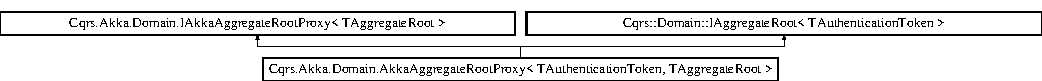
\includegraphics[height=1.081081cm]{classCqrs_1_1Akka_1_1Domain_1_1AkkaAggregateRootProxy}
\end{center}
\end{figure}
\subsection*{Public Member Functions}
\begin{DoxyCompactItemize}
\item 
virtual I\+Enumerable$<$ \hyperlink{interfaceCqrs_1_1Events_1_1IEvent}{I\+Event}$<$ T\+Authentication\+Token $>$ $>$ \hyperlink{classCqrs_1_1Akka_1_1Domain_1_1AkkaAggregateRootProxy_afa620ced4762b0539da23ca063fed489}{Get\+Uncommitted\+Changes} ()
\item 
virtual void \hyperlink{classCqrs_1_1Akka_1_1Domain_1_1AkkaAggregateRootProxy_aaa8a46fee21b6133ae4d1b2f60983d7e}{Mark\+Changes\+As\+Committed} ()
\item 
virtual void \hyperlink{classCqrs_1_1Akka_1_1Domain_1_1AkkaAggregateRootProxy_ae611077a51a215aef7fd0e106734b386}{Load\+From\+History} (I\+Enumerable$<$ \hyperlink{interfaceCqrs_1_1Events_1_1IEvent}{I\+Event}$<$ T\+Authentication\+Token $>$$>$ history)
\end{DoxyCompactItemize}
\subsection*{Properties}
\begin{DoxyCompactItemize}
\item 
I\+Actor\+Ref \hyperlink{classCqrs_1_1Akka_1_1Domain_1_1AkkaAggregateRootProxy_ad85e7a51c716484df8e5e8ea9ff31351}{Actor\+Reference}\hspace{0.3cm}{\ttfamily  \mbox{[}get, set\mbox{]}}
\item 
T\+Aggregate\+Root \hyperlink{classCqrs_1_1Akka_1_1Domain_1_1AkkaAggregateRootProxy_a45e41e24822f4a9a8077e10c153de163}{Aggregate}\hspace{0.3cm}{\ttfamily  \mbox{[}get, protected set\mbox{]}}
\item 
virtual Guid \hyperlink{classCqrs_1_1Akka_1_1Domain_1_1AkkaAggregateRootProxy_a7854104312b6088a2c604b334433b633}{Id}\hspace{0.3cm}{\ttfamily  \mbox{[}get\mbox{]}}
\item 
virtual int \hyperlink{classCqrs_1_1Akka_1_1Domain_1_1AkkaAggregateRootProxy_a24ff2ddef0d416ac5b936c1887ac2154}{Version}\hspace{0.3cm}{\ttfamily  \mbox{[}get\mbox{]}}
\end{DoxyCompactItemize}


\subsection{Member Function Documentation}
\mbox{\Hypertarget{classCqrs_1_1Akka_1_1Domain_1_1AkkaAggregateRootProxy_afa620ced4762b0539da23ca063fed489}\label{classCqrs_1_1Akka_1_1Domain_1_1AkkaAggregateRootProxy_afa620ced4762b0539da23ca063fed489}} 
\index{Cqrs\+::\+Akka\+::\+Domain\+::\+Akka\+Aggregate\+Root\+Proxy@{Cqrs\+::\+Akka\+::\+Domain\+::\+Akka\+Aggregate\+Root\+Proxy}!Get\+Uncommitted\+Changes@{Get\+Uncommitted\+Changes}}
\index{Get\+Uncommitted\+Changes@{Get\+Uncommitted\+Changes}!Cqrs\+::\+Akka\+::\+Domain\+::\+Akka\+Aggregate\+Root\+Proxy@{Cqrs\+::\+Akka\+::\+Domain\+::\+Akka\+Aggregate\+Root\+Proxy}}
\subsubsection{\texorpdfstring{Get\+Uncommitted\+Changes()}{GetUncommittedChanges()}}
{\footnotesize\ttfamily virtual I\+Enumerable$<$\hyperlink{interfaceCqrs_1_1Events_1_1IEvent}{I\+Event}$<$T\+Authentication\+Token$>$ $>$ \hyperlink{classCqrs_1_1Akka_1_1Domain_1_1AkkaAggregateRootProxy}{Cqrs.\+Akka.\+Domain.\+Akka\+Aggregate\+Root\+Proxy}$<$ T\+Authentication\+Token, T\+Aggregate\+Root $>$.Get\+Uncommitted\+Changes (\begin{DoxyParamCaption}{ }\end{DoxyParamCaption})\hspace{0.3cm}{\ttfamily [virtual]}}



Implements \hyperlink{interfaceCqrs_1_1Domain_1_1IAggregateRoot_a22fda414613f5ac0d4371554d7d6473b}{Cqrs.\+Domain.\+I\+Aggregate\+Root$<$ T\+Authentication\+Token $>$}.

\mbox{\Hypertarget{classCqrs_1_1Akka_1_1Domain_1_1AkkaAggregateRootProxy_ae611077a51a215aef7fd0e106734b386}\label{classCqrs_1_1Akka_1_1Domain_1_1AkkaAggregateRootProxy_ae611077a51a215aef7fd0e106734b386}} 
\index{Cqrs\+::\+Akka\+::\+Domain\+::\+Akka\+Aggregate\+Root\+Proxy@{Cqrs\+::\+Akka\+::\+Domain\+::\+Akka\+Aggregate\+Root\+Proxy}!Load\+From\+History@{Load\+From\+History}}
\index{Load\+From\+History@{Load\+From\+History}!Cqrs\+::\+Akka\+::\+Domain\+::\+Akka\+Aggregate\+Root\+Proxy@{Cqrs\+::\+Akka\+::\+Domain\+::\+Akka\+Aggregate\+Root\+Proxy}}
\subsubsection{\texorpdfstring{Load\+From\+History()}{LoadFromHistory()}}
{\footnotesize\ttfamily virtual void \hyperlink{classCqrs_1_1Akka_1_1Domain_1_1AkkaAggregateRootProxy}{Cqrs.\+Akka.\+Domain.\+Akka\+Aggregate\+Root\+Proxy}$<$ T\+Authentication\+Token, T\+Aggregate\+Root $>$.Load\+From\+History (\begin{DoxyParamCaption}\item[{I\+Enumerable$<$ \hyperlink{interfaceCqrs_1_1Events_1_1IEvent}{I\+Event}$<$ T\+Authentication\+Token $>$$>$}]{history }\end{DoxyParamCaption})\hspace{0.3cm}{\ttfamily [virtual]}}



Implements \hyperlink{interfaceCqrs_1_1Domain_1_1IAggregateRoot_afe9329ee26ae68613059189ca64dfe60}{Cqrs.\+Domain.\+I\+Aggregate\+Root$<$ T\+Authentication\+Token $>$}.

\mbox{\Hypertarget{classCqrs_1_1Akka_1_1Domain_1_1AkkaAggregateRootProxy_aaa8a46fee21b6133ae4d1b2f60983d7e}\label{classCqrs_1_1Akka_1_1Domain_1_1AkkaAggregateRootProxy_aaa8a46fee21b6133ae4d1b2f60983d7e}} 
\index{Cqrs\+::\+Akka\+::\+Domain\+::\+Akka\+Aggregate\+Root\+Proxy@{Cqrs\+::\+Akka\+::\+Domain\+::\+Akka\+Aggregate\+Root\+Proxy}!Mark\+Changes\+As\+Committed@{Mark\+Changes\+As\+Committed}}
\index{Mark\+Changes\+As\+Committed@{Mark\+Changes\+As\+Committed}!Cqrs\+::\+Akka\+::\+Domain\+::\+Akka\+Aggregate\+Root\+Proxy@{Cqrs\+::\+Akka\+::\+Domain\+::\+Akka\+Aggregate\+Root\+Proxy}}
\subsubsection{\texorpdfstring{Mark\+Changes\+As\+Committed()}{MarkChangesAsCommitted()}}
{\footnotesize\ttfamily virtual void \hyperlink{classCqrs_1_1Akka_1_1Domain_1_1AkkaAggregateRootProxy}{Cqrs.\+Akka.\+Domain.\+Akka\+Aggregate\+Root\+Proxy}$<$ T\+Authentication\+Token, T\+Aggregate\+Root $>$.Mark\+Changes\+As\+Committed (\begin{DoxyParamCaption}{ }\end{DoxyParamCaption})\hspace{0.3cm}{\ttfamily [virtual]}}



Implements \hyperlink{interfaceCqrs_1_1Domain_1_1IAggregateRoot_af31116870bbf6566b3eec0b8bc02c6de}{Cqrs.\+Domain.\+I\+Aggregate\+Root$<$ T\+Authentication\+Token $>$}.



\subsection{Property Documentation}
\mbox{\Hypertarget{classCqrs_1_1Akka_1_1Domain_1_1AkkaAggregateRootProxy_ad85e7a51c716484df8e5e8ea9ff31351}\label{classCqrs_1_1Akka_1_1Domain_1_1AkkaAggregateRootProxy_ad85e7a51c716484df8e5e8ea9ff31351}} 
\index{Cqrs\+::\+Akka\+::\+Domain\+::\+Akka\+Aggregate\+Root\+Proxy@{Cqrs\+::\+Akka\+::\+Domain\+::\+Akka\+Aggregate\+Root\+Proxy}!Actor\+Reference@{Actor\+Reference}}
\index{Actor\+Reference@{Actor\+Reference}!Cqrs\+::\+Akka\+::\+Domain\+::\+Akka\+Aggregate\+Root\+Proxy@{Cqrs\+::\+Akka\+::\+Domain\+::\+Akka\+Aggregate\+Root\+Proxy}}
\subsubsection{\texorpdfstring{Actor\+Reference}{ActorReference}}
{\footnotesize\ttfamily I\+Actor\+Ref \hyperlink{classCqrs_1_1Akka_1_1Domain_1_1AkkaAggregateRootProxy}{Cqrs.\+Akka.\+Domain.\+Akka\+Aggregate\+Root\+Proxy}$<$ T\+Authentication\+Token, T\+Aggregate\+Root $>$.Actor\+Reference\hspace{0.3cm}{\ttfamily [get]}, {\ttfamily [set]}}

\mbox{\Hypertarget{classCqrs_1_1Akka_1_1Domain_1_1AkkaAggregateRootProxy_a45e41e24822f4a9a8077e10c153de163}\label{classCqrs_1_1Akka_1_1Domain_1_1AkkaAggregateRootProxy_a45e41e24822f4a9a8077e10c153de163}} 
\index{Cqrs\+::\+Akka\+::\+Domain\+::\+Akka\+Aggregate\+Root\+Proxy@{Cqrs\+::\+Akka\+::\+Domain\+::\+Akka\+Aggregate\+Root\+Proxy}!Aggregate@{Aggregate}}
\index{Aggregate@{Aggregate}!Cqrs\+::\+Akka\+::\+Domain\+::\+Akka\+Aggregate\+Root\+Proxy@{Cqrs\+::\+Akka\+::\+Domain\+::\+Akka\+Aggregate\+Root\+Proxy}}
\subsubsection{\texorpdfstring{Aggregate}{Aggregate}}
{\footnotesize\ttfamily T\+Aggregate\+Root \hyperlink{classCqrs_1_1Akka_1_1Domain_1_1AkkaAggregateRootProxy}{Cqrs.\+Akka.\+Domain.\+Akka\+Aggregate\+Root\+Proxy}$<$ T\+Authentication\+Token, T\+Aggregate\+Root $>$.Aggregate\hspace{0.3cm}{\ttfamily [get]}, {\ttfamily [protected set]}}

\mbox{\Hypertarget{classCqrs_1_1Akka_1_1Domain_1_1AkkaAggregateRootProxy_a7854104312b6088a2c604b334433b633}\label{classCqrs_1_1Akka_1_1Domain_1_1AkkaAggregateRootProxy_a7854104312b6088a2c604b334433b633}} 
\index{Cqrs\+::\+Akka\+::\+Domain\+::\+Akka\+Aggregate\+Root\+Proxy@{Cqrs\+::\+Akka\+::\+Domain\+::\+Akka\+Aggregate\+Root\+Proxy}!Id@{Id}}
\index{Id@{Id}!Cqrs\+::\+Akka\+::\+Domain\+::\+Akka\+Aggregate\+Root\+Proxy@{Cqrs\+::\+Akka\+::\+Domain\+::\+Akka\+Aggregate\+Root\+Proxy}}
\subsubsection{\texorpdfstring{Id}{Id}}
{\footnotesize\ttfamily virtual Guid \hyperlink{classCqrs_1_1Akka_1_1Domain_1_1AkkaAggregateRootProxy}{Cqrs.\+Akka.\+Domain.\+Akka\+Aggregate\+Root\+Proxy}$<$ T\+Authentication\+Token, T\+Aggregate\+Root $>$.Id\hspace{0.3cm}{\ttfamily [get]}}

\mbox{\Hypertarget{classCqrs_1_1Akka_1_1Domain_1_1AkkaAggregateRootProxy_a24ff2ddef0d416ac5b936c1887ac2154}\label{classCqrs_1_1Akka_1_1Domain_1_1AkkaAggregateRootProxy_a24ff2ddef0d416ac5b936c1887ac2154}} 
\index{Cqrs\+::\+Akka\+::\+Domain\+::\+Akka\+Aggregate\+Root\+Proxy@{Cqrs\+::\+Akka\+::\+Domain\+::\+Akka\+Aggregate\+Root\+Proxy}!Version@{Version}}
\index{Version@{Version}!Cqrs\+::\+Akka\+::\+Domain\+::\+Akka\+Aggregate\+Root\+Proxy@{Cqrs\+::\+Akka\+::\+Domain\+::\+Akka\+Aggregate\+Root\+Proxy}}
\subsubsection{\texorpdfstring{Version}{Version}}
{\footnotesize\ttfamily virtual int \hyperlink{classCqrs_1_1Akka_1_1Domain_1_1AkkaAggregateRootProxy}{Cqrs.\+Akka.\+Domain.\+Akka\+Aggregate\+Root\+Proxy}$<$ T\+Authentication\+Token, T\+Aggregate\+Root $>$.Version\hspace{0.3cm}{\ttfamily [get]}}


\hypertarget{classCqrs_1_1Akka_1_1Domain_1_1AkkaSaga}{}\doxysection{Cqrs.\+Akka.\+Domain.\+Akka\+Saga$<$ T\+Authentication\+Token $>$ Class Template Reference}
\label{classCqrs_1_1Akka_1_1Domain_1_1AkkaSaga}\index{Cqrs.Akka.Domain.AkkaSaga$<$ TAuthenticationToken $>$@{Cqrs.Akka.Domain.AkkaSaga$<$ TAuthenticationToken $>$}}


A I\+Saga$<$\+T\+Authentication\+Token$>$ that is safe to use within Akka.\+N\+ET  


Inheritance diagram for Cqrs.\+Akka.\+Domain.\+Akka\+Saga$<$ T\+Authentication\+Token $>$\+:\begin{figure}[H]
\begin{center}
\leavevmode
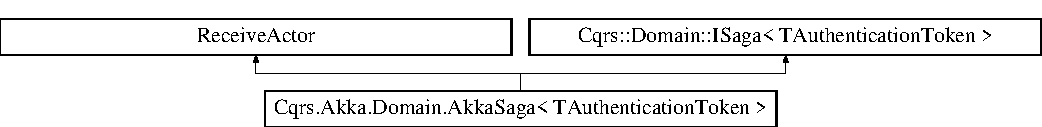
\includegraphics[height=1.696970cm]{classCqrs_1_1Akka_1_1Domain_1_1AkkaSaga}
\end{center}
\end{figure}
\doxysubsection*{Public Member Functions}
\begin{DoxyCompactItemize}
\item 
virtual I\+Enumerable$<$ \mbox{\hyperlink{interfaceCqrs_1_1Events_1_1ISagaEvent}{I\+Saga\+Event}}$<$ T\+Authentication\+Token $>$ $>$ \mbox{\hyperlink{classCqrs_1_1Akka_1_1Domain_1_1AkkaSaga_a1fceccba498fa9f2d3db328a921da23d_a1fceccba498fa9f2d3db328a921da23d}{Get\+Uncommitted\+Changes}} ()
\begin{DoxyCompactList}\small\item\em Get all applied changes that haven\textquotesingle{}t yet been committed. \end{DoxyCompactList}\item 
virtual void \mbox{\hyperlink{classCqrs_1_1Akka_1_1Domain_1_1AkkaSaga_a83269fac4653cca097461e924feaea7f_a83269fac4653cca097461e924feaea7f}{Mark\+Changes\+As\+Committed}} ()
\begin{DoxyCompactList}\small\item\em Mark all applied changes as committed, increment \mbox{\hyperlink{classCqrs_1_1Akka_1_1Domain_1_1AkkaSaga_a3fda31a3857e12a1aed60f4a4f04edd1_a3fda31a3857e12a1aed60f4a4f04edd1}{Version}} and flush the internal collection of changes. \end{DoxyCompactList}\item 
virtual void \mbox{\hyperlink{classCqrs_1_1Akka_1_1Domain_1_1AkkaSaga_a40b859bc15c2f7c87a21b07f9bc9548c_a40b859bc15c2f7c87a21b07f9bc9548c}{Load\+From\+History}} (I\+Enumerable$<$ \mbox{\hyperlink{interfaceCqrs_1_1Events_1_1ISagaEvent}{I\+Saga\+Event}}$<$ T\+Authentication\+Token $>$$>$ history)
\begin{DoxyCompactList}\small\item\em Apply all the \mbox{\hyperlink{}{events}} in {\itshape history}  using event replay to this instance. \end{DoxyCompactList}\item 
virtual I\+Enumerable$<$ \mbox{\hyperlink{interfaceCqrs_1_1Commands_1_1ICommand}{I\+Command}}$<$ T\+Authentication\+Token $>$ $>$ \mbox{\hyperlink{classCqrs_1_1Akka_1_1Domain_1_1AkkaSaga_a0776a9a8f387c01313aa12d06643249a_a0776a9a8f387c01313aa12d06643249a}{Get\+Unpublished\+Commands}} ()
\begin{DoxyCompactList}\small\item\em Get all pending commands that haven\textquotesingle{}t yet been published yet. \end{DoxyCompactList}\item 
virtual void \mbox{\hyperlink{classCqrs_1_1Akka_1_1Domain_1_1AkkaSaga_a8ba652a3fbc2025b3367ef73185f8a6f_a8ba652a3fbc2025b3367ef73185f8a6f}{Mark\+Commands\+As\+Published}} ()
\begin{DoxyCompactList}\small\item\em Mark all published commands as published and flush the internal collection of commands. \end{DoxyCompactList}\end{DoxyCompactItemize}
\doxysubsection*{Protected Member Functions}
\begin{DoxyCompactItemize}
\item 
\mbox{\hyperlink{classCqrs_1_1Akka_1_1Domain_1_1AkkaSaga_a2f0ebb5d1d22e3112d5b9a09fde7fb47_a2f0ebb5d1d22e3112d5b9a09fde7fb47}{Akka\+Saga}} (\mbox{\hyperlink{interfaceCqrs_1_1Domain_1_1ISagaUnitOfWork}{I\+Saga\+Unit\+Of\+Work}}$<$ T\+Authentication\+Token $>$ unit\+Of\+Work, I\+Logger logger, \mbox{\hyperlink{interfaceCqrs_1_1Akka_1_1Domain_1_1IAkkaSagaRepository}{I\+Akka\+Saga\+Repository}}$<$ T\+Authentication\+Token $>$ repository, I\+Correlation\+Id\+Helper correlation\+Id\+Helper, \mbox{\hyperlink{interfaceCqrs_1_1Authentication_1_1IAuthenticationTokenHelper}{I\+Authentication\+Token\+Helper}}$<$ T\+Authentication\+Token $>$ authentication\+Token\+Helper, \mbox{\hyperlink{interfaceCqrs_1_1Commands_1_1ICommandPublisher}{I\+Command\+Publisher}}$<$ T\+Authentication\+Token $>$ command\+Publisher)
\begin{DoxyCompactList}\small\item\em Instantiates a new instance of \mbox{\hyperlink{classCqrs_1_1Akka_1_1Domain_1_1AkkaSaga_a2f0ebb5d1d22e3112d5b9a09fde7fb47_a2f0ebb5d1d22e3112d5b9a09fde7fb47}{Akka\+Saga$<$\+T\+Authentication\+Token$>$}} \end{DoxyCompactList}\item 
override void \mbox{\hyperlink{classCqrs_1_1Akka_1_1Domain_1_1AkkaSaga_a4615beae56f595074f3ba643a890ba74_a4615beae56f595074f3ba643a890ba74}{Pre\+Start}} ()
\begin{DoxyCompactList}\small\item\em User overridable callback. 

Is called when an Actor is started. Actors are automatically started asynchronously when created. Empty default implementation. \end{DoxyCompactList}\item 
virtual void \mbox{\hyperlink{classCqrs_1_1Akka_1_1Domain_1_1AkkaSaga_ac0782ac0b7e28418a52cead1b7b8b0c3_ac0782ac0b7e28418a52cead1b7b8b0c3}{Execute$<$ T\+Event $>$}} (Action$<$ T\+Event $>$ action, T\+Event @event)
\begin{DoxyCompactList}\small\item\em Executes the provided {\itshape action}  passing it the provided {\itshape event} , then calls Aggregate\+Repository$<$\+T\+Authentication\+Token$>$.\+Publish\+Event \end{DoxyCompactList}\item 
virtual void \mbox{\hyperlink{classCqrs_1_1Akka_1_1Domain_1_1AkkaSaga_ac13c2f1c4130ad4886d5c6bfd5910bb4_ac13c2f1c4130ad4886d5c6bfd5910bb4}{Queue\+Command}} (\mbox{\hyperlink{interfaceCqrs_1_1Commands_1_1ICommand}{I\+Command}}$<$ T\+Authentication\+Token $>$ command)
\begin{DoxyCompactList}\small\item\em Queue the provided {\itshape command}  for publishing. \end{DoxyCompactList}\item 
virtual void \mbox{\hyperlink{classCqrs_1_1Akka_1_1Domain_1_1AkkaSaga_a42126a6a1a7896d16412b6023f208f7c_a42126a6a1a7896d16412b6023f208f7c}{Apply\+Change}} (\mbox{\hyperlink{interfaceCqrs_1_1Events_1_1ISagaEvent}{I\+Saga\+Event}}$<$ T\+Authentication\+Token $>$ @event)
\begin{DoxyCompactList}\small\item\em Call the \char`\"{}\+Apply\char`\"{} method with a signature matching the provided {\itshape event}  without using event replay to this instance. \end{DoxyCompactList}\item 
virtual void \mbox{\hyperlink{classCqrs_1_1Akka_1_1Domain_1_1AkkaSaga_a18d554cd5ad329ab152efb7d852f2438_a18d554cd5ad329ab152efb7d852f2438}{Apply\+Change}} (\mbox{\hyperlink{interfaceCqrs_1_1Events_1_1IEvent}{I\+Event}}$<$ T\+Authentication\+Token $>$ @event)
\begin{DoxyCompactList}\small\item\em Calls \mbox{\hyperlink{classCqrs_1_1Akka_1_1Domain_1_1AkkaSaga_a3f3cf1a10203a1eead599e7529d41613_a3f3cf1a10203a1eead599e7529d41613}{Set\+Id}}, then Apply\+Change(\+Cqrs.\+Events.\+I\+Saga\+Event$<$\+T\+Authentication\+Token$>$). \end{DoxyCompactList}\item 
virtual void \mbox{\hyperlink{classCqrs_1_1Akka_1_1Domain_1_1AkkaSaga_a3f3cf1a10203a1eead599e7529d41613_a3f3cf1a10203a1eead599e7529d41613}{Set\+Id}} (\mbox{\hyperlink{interfaceCqrs_1_1Events_1_1ISagaEvent}{I\+Saga\+Event}}$<$ T\+Authentication\+Token $>$ saga\+Event)
\begin{DoxyCompactList}\small\item\em Sets the I\+Event$<$\+T\+Authentication\+Token$>$.\+Id from I\+Saga\+Event$<$\+T\+Authentication\+Token$>$.\+Event back onto {\itshape saga\+Event} . \end{DoxyCompactList}\item 
virtual void \mbox{\hyperlink{classCqrs_1_1Akka_1_1Domain_1_1AkkaSaga_a4a12310825f2d2cc5963eee4cc4ed802_a4a12310825f2d2cc5963eee4cc4ed802}{Apply}} (\mbox{\hyperlink{interfaceCqrs_1_1Events_1_1ISagaEvent}{I\+Saga\+Event}}$<$ T\+Authentication\+Token $>$ saga\+Event)
\begin{DoxyCompactList}\small\item\em Dynamically calls the \char`\"{}\+Apply\char`\"{} method, passing it the I\+Saga\+Event$<$\+T\+Authentication\+Token$>$.\+Event of the provided {\itshape saga\+Event} . \end{DoxyCompactList}\end{DoxyCompactItemize}
\doxysubsection*{Properties}
\begin{DoxyCompactItemize}
\item 
\mbox{\hyperlink{interfaceCqrs_1_1Domain_1_1ISagaUnitOfWork}{I\+Saga\+Unit\+Of\+Work}}$<$ T\+Authentication\+Token $>$ \mbox{\hyperlink{classCqrs_1_1Akka_1_1Domain_1_1AkkaSaga_addbf93da18d577da8f8f1e2dba5cafb9_addbf93da18d577da8f8f1e2dba5cafb9}{Unit\+Of\+Work}}\hspace{0.3cm}{\ttfamily  \mbox{[}get, set\mbox{]}}
\begin{DoxyCompactList}\small\item\em Gets or sets the I\+Saga\+Unit\+Of\+Work$<$\+T\+Authentication\+Token$>$. \end{DoxyCompactList}\item 
\mbox{\hyperlink{interfaceCqrs_1_1Akka_1_1Domain_1_1IAkkaSagaRepository}{I\+Akka\+Saga\+Repository}}$<$ T\+Authentication\+Token $>$ \mbox{\hyperlink{classCqrs_1_1Akka_1_1Domain_1_1AkkaSaga_a4c0662a1aa78c8de5fa32c71a54cf393_a4c0662a1aa78c8de5fa32c71a54cf393}{Repository}}\hspace{0.3cm}{\ttfamily  \mbox{[}get, set\mbox{]}}
\begin{DoxyCompactList}\small\item\em Gets or sets the I\+Akka\+Saga\+Repository$<$\+T\+Authentication\+Token$>$. \end{DoxyCompactList}\item 
I\+Logger \mbox{\hyperlink{classCqrs_1_1Akka_1_1Domain_1_1AkkaSaga_acbb9a6e1cde3e2846270a8fe3f55bc92_acbb9a6e1cde3e2846270a8fe3f55bc92}{Logger}}\hspace{0.3cm}{\ttfamily  \mbox{[}get, set\mbox{]}}
\begin{DoxyCompactList}\small\item\em Gets or sets the I\+Logger. \end{DoxyCompactList}\item 
I\+Correlation\+Id\+Helper \mbox{\hyperlink{classCqrs_1_1Akka_1_1Domain_1_1AkkaSaga_a11d543b42aa6e55644c2b349336e962a_a11d543b42aa6e55644c2b349336e962a}{Correlation\+Id\+Helper}}\hspace{0.3cm}{\ttfamily  \mbox{[}get, set\mbox{]}}
\begin{DoxyCompactList}\small\item\em Gets or sets the I\+Correlation\+Id\+Helper. \end{DoxyCompactList}\item 
\mbox{\hyperlink{interfaceCqrs_1_1Authentication_1_1IAuthenticationTokenHelper}{I\+Authentication\+Token\+Helper}}$<$ T\+Authentication\+Token $>$ \mbox{\hyperlink{classCqrs_1_1Akka_1_1Domain_1_1AkkaSaga_a18e4d7faa9cd9d10ac2ac0bd3b6c9fc9_a18e4d7faa9cd9d10ac2ac0bd3b6c9fc9}{Authentication\+Token\+Helper}}\hspace{0.3cm}{\ttfamily  \mbox{[}get, set\mbox{]}}
\begin{DoxyCompactList}\small\item\em Gets or sets the I\+Authentication\+Token\+Helper$<$\+T\+Authentication\+Token$>$. \end{DoxyCompactList}\item 
Guid \mbox{\hyperlink{classCqrs_1_1Akka_1_1Domain_1_1AkkaSaga_a98fa8a5ebc587bc02b1c98d5ffbc997e_a98fa8a5ebc587bc02b1c98d5ffbc997e}{Id}}\hspace{0.3cm}{\ttfamily  \mbox{[}get, protected set\mbox{]}}
\begin{DoxyCompactList}\small\item\em The identifier of the I\+Saga$<$\+T\+Authentication\+Token$>$. \end{DoxyCompactList}\item 
int \mbox{\hyperlink{classCqrs_1_1Akka_1_1Domain_1_1AkkaSaga_a3fda31a3857e12a1aed60f4a4f04edd1_a3fda31a3857e12a1aed60f4a4f04edd1}{Version}}\hspace{0.3cm}{\ttfamily  \mbox{[}get, protected set\mbox{]}}
\begin{DoxyCompactList}\small\item\em The current version of this I\+Saga$<$\+T\+Authentication\+Token$>$. \end{DoxyCompactList}\item 
\mbox{\hyperlink{interfaceCqrs_1_1Commands_1_1ICommandPublisher}{I\+Command\+Publisher}}$<$ T\+Authentication\+Token $>$ \mbox{\hyperlink{classCqrs_1_1Akka_1_1Domain_1_1AkkaSaga_ac00968d1d69d89d46b43af10fc0d4510_ac00968d1d69d89d46b43af10fc0d4510}{Command\+Publisher}}\hspace{0.3cm}{\ttfamily  \mbox{[}get, set\mbox{]}}
\begin{DoxyCompactList}\small\item\em Gets or sets the I\+Command\+Publisher$<$\+T\+Authentication\+Token$>$. \end{DoxyCompactList}\end{DoxyCompactItemize}


\doxysubsection{Detailed Description}
A I\+Saga$<$\+T\+Authentication\+Token$>$ that is safe to use within Akka.\+N\+ET 


\begin{DoxyTemplParams}{Template Parameters}
{\em T\+Authentication\+Token} & The Type of authentication token.\\
\hline
\end{DoxyTemplParams}


\doxysubsection{Constructor \& Destructor Documentation}
\mbox{\Hypertarget{classCqrs_1_1Akka_1_1Domain_1_1AkkaSaga_a2f0ebb5d1d22e3112d5b9a09fde7fb47_a2f0ebb5d1d22e3112d5b9a09fde7fb47}\label{classCqrs_1_1Akka_1_1Domain_1_1AkkaSaga_a2f0ebb5d1d22e3112d5b9a09fde7fb47_a2f0ebb5d1d22e3112d5b9a09fde7fb47}} 
\index{Cqrs.Akka.Domain.AkkaSaga$<$ TAuthenticationToken $>$@{Cqrs.Akka.Domain.AkkaSaga$<$ TAuthenticationToken $>$}!AkkaSaga@{AkkaSaga}}
\index{AkkaSaga@{AkkaSaga}!Cqrs.Akka.Domain.AkkaSaga$<$ TAuthenticationToken $>$@{Cqrs.Akka.Domain.AkkaSaga$<$ TAuthenticationToken $>$}}
\doxysubsubsection{\texorpdfstring{AkkaSaga()}{AkkaSaga()}}
{\footnotesize\ttfamily \mbox{\hyperlink{classCqrs_1_1Akka_1_1Domain_1_1AkkaSaga}{Cqrs.\+Akka.\+Domain.\+Akka\+Saga}}$<$ T\+Authentication\+Token $>$.\mbox{\hyperlink{classCqrs_1_1Akka_1_1Domain_1_1AkkaSaga}{Akka\+Saga}} (\begin{DoxyParamCaption}\item[{\mbox{\hyperlink{interfaceCqrs_1_1Domain_1_1ISagaUnitOfWork}{I\+Saga\+Unit\+Of\+Work}}$<$ T\+Authentication\+Token $>$}]{unit\+Of\+Work,  }\item[{I\+Logger}]{logger,  }\item[{\mbox{\hyperlink{interfaceCqrs_1_1Akka_1_1Domain_1_1IAkkaSagaRepository}{I\+Akka\+Saga\+Repository}}$<$ T\+Authentication\+Token $>$}]{repository,  }\item[{I\+Correlation\+Id\+Helper}]{correlation\+Id\+Helper,  }\item[{\mbox{\hyperlink{interfaceCqrs_1_1Authentication_1_1IAuthenticationTokenHelper}{I\+Authentication\+Token\+Helper}}$<$ T\+Authentication\+Token $>$}]{authentication\+Token\+Helper,  }\item[{\mbox{\hyperlink{interfaceCqrs_1_1Commands_1_1ICommandPublisher}{I\+Command\+Publisher}}$<$ T\+Authentication\+Token $>$}]{command\+Publisher }\end{DoxyParamCaption})\hspace{0.3cm}{\ttfamily [protected]}}



Instantiates a new instance of \mbox{\hyperlink{classCqrs_1_1Akka_1_1Domain_1_1AkkaSaga_a2f0ebb5d1d22e3112d5b9a09fde7fb47_a2f0ebb5d1d22e3112d5b9a09fde7fb47}{Akka\+Saga$<$\+T\+Authentication\+Token$>$}} 



\doxysubsection{Member Function Documentation}
\mbox{\Hypertarget{classCqrs_1_1Akka_1_1Domain_1_1AkkaSaga_a4a12310825f2d2cc5963eee4cc4ed802_a4a12310825f2d2cc5963eee4cc4ed802}\label{classCqrs_1_1Akka_1_1Domain_1_1AkkaSaga_a4a12310825f2d2cc5963eee4cc4ed802_a4a12310825f2d2cc5963eee4cc4ed802}} 
\index{Cqrs.Akka.Domain.AkkaSaga$<$ TAuthenticationToken $>$@{Cqrs.Akka.Domain.AkkaSaga$<$ TAuthenticationToken $>$}!Apply@{Apply}}
\index{Apply@{Apply}!Cqrs.Akka.Domain.AkkaSaga$<$ TAuthenticationToken $>$@{Cqrs.Akka.Domain.AkkaSaga$<$ TAuthenticationToken $>$}}
\doxysubsubsection{\texorpdfstring{Apply()}{Apply()}}
{\footnotesize\ttfamily virtual void \mbox{\hyperlink{classCqrs_1_1Akka_1_1Domain_1_1AkkaSaga}{Cqrs.\+Akka.\+Domain.\+Akka\+Saga}}$<$ T\+Authentication\+Token $>$.Apply (\begin{DoxyParamCaption}\item[{\mbox{\hyperlink{interfaceCqrs_1_1Events_1_1ISagaEvent}{I\+Saga\+Event}}$<$ T\+Authentication\+Token $>$}]{saga\+Event }\end{DoxyParamCaption})\hspace{0.3cm}{\ttfamily [protected]}, {\ttfamily [virtual]}}



Dynamically calls the \char`\"{}\+Apply\char`\"{} method, passing it the I\+Saga\+Event$<$\+T\+Authentication\+Token$>$.\+Event of the provided {\itshape saga\+Event} . 

\mbox{\Hypertarget{classCqrs_1_1Akka_1_1Domain_1_1AkkaSaga_a18d554cd5ad329ab152efb7d852f2438_a18d554cd5ad329ab152efb7d852f2438}\label{classCqrs_1_1Akka_1_1Domain_1_1AkkaSaga_a18d554cd5ad329ab152efb7d852f2438_a18d554cd5ad329ab152efb7d852f2438}} 
\index{Cqrs.Akka.Domain.AkkaSaga$<$ TAuthenticationToken $>$@{Cqrs.Akka.Domain.AkkaSaga$<$ TAuthenticationToken $>$}!ApplyChange@{ApplyChange}}
\index{ApplyChange@{ApplyChange}!Cqrs.Akka.Domain.AkkaSaga$<$ TAuthenticationToken $>$@{Cqrs.Akka.Domain.AkkaSaga$<$ TAuthenticationToken $>$}}
\doxysubsubsection{\texorpdfstring{ApplyChange()}{ApplyChange()}\hspace{0.1cm}{\footnotesize\ttfamily [1/2]}}
{\footnotesize\ttfamily virtual void \mbox{\hyperlink{classCqrs_1_1Akka_1_1Domain_1_1AkkaSaga}{Cqrs.\+Akka.\+Domain.\+Akka\+Saga}}$<$ T\+Authentication\+Token $>$.Apply\+Change (\begin{DoxyParamCaption}\item[{\mbox{\hyperlink{interfaceCqrs_1_1Events_1_1IEvent}{I\+Event}}$<$ T\+Authentication\+Token $>$ @}]{event }\end{DoxyParamCaption})\hspace{0.3cm}{\ttfamily [protected]}, {\ttfamily [virtual]}}



Calls \mbox{\hyperlink{classCqrs_1_1Akka_1_1Domain_1_1AkkaSaga_a3f3cf1a10203a1eead599e7529d41613_a3f3cf1a10203a1eead599e7529d41613}{Set\+Id}}, then Apply\+Change(\+Cqrs.\+Events.\+I\+Saga\+Event$<$\+T\+Authentication\+Token$>$). 

\mbox{\Hypertarget{classCqrs_1_1Akka_1_1Domain_1_1AkkaSaga_a42126a6a1a7896d16412b6023f208f7c_a42126a6a1a7896d16412b6023f208f7c}\label{classCqrs_1_1Akka_1_1Domain_1_1AkkaSaga_a42126a6a1a7896d16412b6023f208f7c_a42126a6a1a7896d16412b6023f208f7c}} 
\index{Cqrs.Akka.Domain.AkkaSaga$<$ TAuthenticationToken $>$@{Cqrs.Akka.Domain.AkkaSaga$<$ TAuthenticationToken $>$}!ApplyChange@{ApplyChange}}
\index{ApplyChange@{ApplyChange}!Cqrs.Akka.Domain.AkkaSaga$<$ TAuthenticationToken $>$@{Cqrs.Akka.Domain.AkkaSaga$<$ TAuthenticationToken $>$}}
\doxysubsubsection{\texorpdfstring{ApplyChange()}{ApplyChange()}\hspace{0.1cm}{\footnotesize\ttfamily [2/2]}}
{\footnotesize\ttfamily virtual void \mbox{\hyperlink{classCqrs_1_1Akka_1_1Domain_1_1AkkaSaga}{Cqrs.\+Akka.\+Domain.\+Akka\+Saga}}$<$ T\+Authentication\+Token $>$.Apply\+Change (\begin{DoxyParamCaption}\item[{\mbox{\hyperlink{interfaceCqrs_1_1Events_1_1ISagaEvent}{I\+Saga\+Event}}$<$ T\+Authentication\+Token $>$ @}]{event }\end{DoxyParamCaption})\hspace{0.3cm}{\ttfamily [protected]}, {\ttfamily [virtual]}}



Call the \char`\"{}\+Apply\char`\"{} method with a signature matching the provided {\itshape event}  without using event replay to this instance. 

This means a method named \char`\"{}\+Apply\char`\"{}, with return type void and one parameter must exist to be applied. If no method exists, nothing is applied The parameter type must match exactly the Type of the provided {\itshape event} . \mbox{\Hypertarget{classCqrs_1_1Akka_1_1Domain_1_1AkkaSaga_ac0782ac0b7e28418a52cead1b7b8b0c3_ac0782ac0b7e28418a52cead1b7b8b0c3}\label{classCqrs_1_1Akka_1_1Domain_1_1AkkaSaga_ac0782ac0b7e28418a52cead1b7b8b0c3_ac0782ac0b7e28418a52cead1b7b8b0c3}} 
\index{Cqrs.Akka.Domain.AkkaSaga$<$ TAuthenticationToken $>$@{Cqrs.Akka.Domain.AkkaSaga$<$ TAuthenticationToken $>$}!Execute$<$ TEvent $>$@{Execute$<$ TEvent $>$}}
\index{Execute$<$ TEvent $>$@{Execute$<$ TEvent $>$}!Cqrs.Akka.Domain.AkkaSaga$<$ TAuthenticationToken $>$@{Cqrs.Akka.Domain.AkkaSaga$<$ TAuthenticationToken $>$}}
\doxysubsubsection{\texorpdfstring{Execute$<$ TEvent $>$()}{Execute< TEvent >()}}
{\footnotesize\ttfamily virtual void \mbox{\hyperlink{classCqrs_1_1Akka_1_1Domain_1_1AkkaSaga}{Cqrs.\+Akka.\+Domain.\+Akka\+Saga}}$<$ T\+Authentication\+Token $>$.Execute$<$ T\+Event $>$ (\begin{DoxyParamCaption}\item[{Action$<$ T\+Event $>$}]{action,  }\item[{T\+Event @}]{event }\end{DoxyParamCaption})\hspace{0.3cm}{\ttfamily [protected]}, {\ttfamily [virtual]}}



Executes the provided {\itshape action}  passing it the provided {\itshape event} , then calls Aggregate\+Repository$<$\+T\+Authentication\+Token$>$.\+Publish\+Event 

\begin{Desc}
\item[Type Constraints]\begin{description}
\item[{\em T\+Event} : {\em I\+Event$<$T\+Authentication\+Token$>$}]\end{description}
\end{Desc}
\mbox{\Hypertarget{classCqrs_1_1Akka_1_1Domain_1_1AkkaSaga_a1fceccba498fa9f2d3db328a921da23d_a1fceccba498fa9f2d3db328a921da23d}\label{classCqrs_1_1Akka_1_1Domain_1_1AkkaSaga_a1fceccba498fa9f2d3db328a921da23d_a1fceccba498fa9f2d3db328a921da23d}} 
\index{Cqrs.Akka.Domain.AkkaSaga$<$ TAuthenticationToken $>$@{Cqrs.Akka.Domain.AkkaSaga$<$ TAuthenticationToken $>$}!GetUncommittedChanges@{GetUncommittedChanges}}
\index{GetUncommittedChanges@{GetUncommittedChanges}!Cqrs.Akka.Domain.AkkaSaga$<$ TAuthenticationToken $>$@{Cqrs.Akka.Domain.AkkaSaga$<$ TAuthenticationToken $>$}}
\doxysubsubsection{\texorpdfstring{GetUncommittedChanges()}{GetUncommittedChanges()}}
{\footnotesize\ttfamily virtual I\+Enumerable$<$\mbox{\hyperlink{interfaceCqrs_1_1Events_1_1ISagaEvent}{I\+Saga\+Event}}$<$T\+Authentication\+Token$>$ $>$ \mbox{\hyperlink{classCqrs_1_1Akka_1_1Domain_1_1AkkaSaga}{Cqrs.\+Akka.\+Domain.\+Akka\+Saga}}$<$ T\+Authentication\+Token $>$.Get\+Uncommitted\+Changes (\begin{DoxyParamCaption}{ }\end{DoxyParamCaption})\hspace{0.3cm}{\ttfamily [virtual]}}



Get all applied changes that haven\textquotesingle{}t yet been committed. 



Implements \mbox{\hyperlink{interfaceCqrs_1_1Domain_1_1ISaga_abb77811b4f7d19adb61f9d33da18e7e0_abb77811b4f7d19adb61f9d33da18e7e0}{Cqrs.\+Domain.\+I\+Saga$<$ T\+Authentication\+Token $>$}}.

\mbox{\Hypertarget{classCqrs_1_1Akka_1_1Domain_1_1AkkaSaga_a0776a9a8f387c01313aa12d06643249a_a0776a9a8f387c01313aa12d06643249a}\label{classCqrs_1_1Akka_1_1Domain_1_1AkkaSaga_a0776a9a8f387c01313aa12d06643249a_a0776a9a8f387c01313aa12d06643249a}} 
\index{Cqrs.Akka.Domain.AkkaSaga$<$ TAuthenticationToken $>$@{Cqrs.Akka.Domain.AkkaSaga$<$ TAuthenticationToken $>$}!GetUnpublishedCommands@{GetUnpublishedCommands}}
\index{GetUnpublishedCommands@{GetUnpublishedCommands}!Cqrs.Akka.Domain.AkkaSaga$<$ TAuthenticationToken $>$@{Cqrs.Akka.Domain.AkkaSaga$<$ TAuthenticationToken $>$}}
\doxysubsubsection{\texorpdfstring{GetUnpublishedCommands()}{GetUnpublishedCommands()}}
{\footnotesize\ttfamily virtual I\+Enumerable$<$\mbox{\hyperlink{interfaceCqrs_1_1Commands_1_1ICommand}{I\+Command}}$<$T\+Authentication\+Token$>$ $>$ \mbox{\hyperlink{classCqrs_1_1Akka_1_1Domain_1_1AkkaSaga}{Cqrs.\+Akka.\+Domain.\+Akka\+Saga}}$<$ T\+Authentication\+Token $>$.Get\+Unpublished\+Commands (\begin{DoxyParamCaption}{ }\end{DoxyParamCaption})\hspace{0.3cm}{\ttfamily [virtual]}}



Get all pending commands that haven\textquotesingle{}t yet been published yet. 



Implements \mbox{\hyperlink{interfaceCqrs_1_1Domain_1_1ISaga_abba76d72857107a14328c8b555f3883f_abba76d72857107a14328c8b555f3883f}{Cqrs.\+Domain.\+I\+Saga$<$ T\+Authentication\+Token $>$}}.

\mbox{\Hypertarget{classCqrs_1_1Akka_1_1Domain_1_1AkkaSaga_a40b859bc15c2f7c87a21b07f9bc9548c_a40b859bc15c2f7c87a21b07f9bc9548c}\label{classCqrs_1_1Akka_1_1Domain_1_1AkkaSaga_a40b859bc15c2f7c87a21b07f9bc9548c_a40b859bc15c2f7c87a21b07f9bc9548c}} 
\index{Cqrs.Akka.Domain.AkkaSaga$<$ TAuthenticationToken $>$@{Cqrs.Akka.Domain.AkkaSaga$<$ TAuthenticationToken $>$}!LoadFromHistory@{LoadFromHistory}}
\index{LoadFromHistory@{LoadFromHistory}!Cqrs.Akka.Domain.AkkaSaga$<$ TAuthenticationToken $>$@{Cqrs.Akka.Domain.AkkaSaga$<$ TAuthenticationToken $>$}}
\doxysubsubsection{\texorpdfstring{LoadFromHistory()}{LoadFromHistory()}}
{\footnotesize\ttfamily virtual void \mbox{\hyperlink{classCqrs_1_1Akka_1_1Domain_1_1AkkaSaga}{Cqrs.\+Akka.\+Domain.\+Akka\+Saga}}$<$ T\+Authentication\+Token $>$.Load\+From\+History (\begin{DoxyParamCaption}\item[{I\+Enumerable$<$ \mbox{\hyperlink{interfaceCqrs_1_1Events_1_1ISagaEvent}{I\+Saga\+Event}}$<$ T\+Authentication\+Token $>$$>$}]{history }\end{DoxyParamCaption})\hspace{0.3cm}{\ttfamily [virtual]}}



Apply all the \mbox{\hyperlink{}{events}} in {\itshape history}  using event replay to this instance. 



Implements \mbox{\hyperlink{interfaceCqrs_1_1Domain_1_1ISaga_a2714804684bc65cf4dec79b4697b9b21_a2714804684bc65cf4dec79b4697b9b21}{Cqrs.\+Domain.\+I\+Saga$<$ T\+Authentication\+Token $>$}}.

\mbox{\Hypertarget{classCqrs_1_1Akka_1_1Domain_1_1AkkaSaga_a83269fac4653cca097461e924feaea7f_a83269fac4653cca097461e924feaea7f}\label{classCqrs_1_1Akka_1_1Domain_1_1AkkaSaga_a83269fac4653cca097461e924feaea7f_a83269fac4653cca097461e924feaea7f}} 
\index{Cqrs.Akka.Domain.AkkaSaga$<$ TAuthenticationToken $>$@{Cqrs.Akka.Domain.AkkaSaga$<$ TAuthenticationToken $>$}!MarkChangesAsCommitted@{MarkChangesAsCommitted}}
\index{MarkChangesAsCommitted@{MarkChangesAsCommitted}!Cqrs.Akka.Domain.AkkaSaga$<$ TAuthenticationToken $>$@{Cqrs.Akka.Domain.AkkaSaga$<$ TAuthenticationToken $>$}}
\doxysubsubsection{\texorpdfstring{MarkChangesAsCommitted()}{MarkChangesAsCommitted()}}
{\footnotesize\ttfamily virtual void \mbox{\hyperlink{classCqrs_1_1Akka_1_1Domain_1_1AkkaSaga}{Cqrs.\+Akka.\+Domain.\+Akka\+Saga}}$<$ T\+Authentication\+Token $>$.Mark\+Changes\+As\+Committed (\begin{DoxyParamCaption}{ }\end{DoxyParamCaption})\hspace{0.3cm}{\ttfamily [virtual]}}



Mark all applied changes as committed, increment \mbox{\hyperlink{classCqrs_1_1Akka_1_1Domain_1_1AkkaSaga_a3fda31a3857e12a1aed60f4a4f04edd1_a3fda31a3857e12a1aed60f4a4f04edd1}{Version}} and flush the internal collection of changes. 



Implements \mbox{\hyperlink{interfaceCqrs_1_1Domain_1_1ISaga_a85c75f80bc5be4bad7f1d9f1231bfba7_a85c75f80bc5be4bad7f1d9f1231bfba7}{Cqrs.\+Domain.\+I\+Saga$<$ T\+Authentication\+Token $>$}}.

\mbox{\Hypertarget{classCqrs_1_1Akka_1_1Domain_1_1AkkaSaga_a8ba652a3fbc2025b3367ef73185f8a6f_a8ba652a3fbc2025b3367ef73185f8a6f}\label{classCqrs_1_1Akka_1_1Domain_1_1AkkaSaga_a8ba652a3fbc2025b3367ef73185f8a6f_a8ba652a3fbc2025b3367ef73185f8a6f}} 
\index{Cqrs.Akka.Domain.AkkaSaga$<$ TAuthenticationToken $>$@{Cqrs.Akka.Domain.AkkaSaga$<$ TAuthenticationToken $>$}!MarkCommandsAsPublished@{MarkCommandsAsPublished}}
\index{MarkCommandsAsPublished@{MarkCommandsAsPublished}!Cqrs.Akka.Domain.AkkaSaga$<$ TAuthenticationToken $>$@{Cqrs.Akka.Domain.AkkaSaga$<$ TAuthenticationToken $>$}}
\doxysubsubsection{\texorpdfstring{MarkCommandsAsPublished()}{MarkCommandsAsPublished()}}
{\footnotesize\ttfamily virtual void \mbox{\hyperlink{classCqrs_1_1Akka_1_1Domain_1_1AkkaSaga}{Cqrs.\+Akka.\+Domain.\+Akka\+Saga}}$<$ T\+Authentication\+Token $>$.Mark\+Commands\+As\+Published (\begin{DoxyParamCaption}{ }\end{DoxyParamCaption})\hspace{0.3cm}{\ttfamily [virtual]}}



Mark all published commands as published and flush the internal collection of commands. 



Implements \mbox{\hyperlink{interfaceCqrs_1_1Domain_1_1ISaga_a4ce7c6cb939b5d6a5afb7538da3d1680_a4ce7c6cb939b5d6a5afb7538da3d1680}{Cqrs.\+Domain.\+I\+Saga$<$ T\+Authentication\+Token $>$}}.

\mbox{\Hypertarget{classCqrs_1_1Akka_1_1Domain_1_1AkkaSaga_a4615beae56f595074f3ba643a890ba74_a4615beae56f595074f3ba643a890ba74}\label{classCqrs_1_1Akka_1_1Domain_1_1AkkaSaga_a4615beae56f595074f3ba643a890ba74_a4615beae56f595074f3ba643a890ba74}} 
\index{Cqrs.Akka.Domain.AkkaSaga$<$ TAuthenticationToken $>$@{Cqrs.Akka.Domain.AkkaSaga$<$ TAuthenticationToken $>$}!PreStart@{PreStart}}
\index{PreStart@{PreStart}!Cqrs.Akka.Domain.AkkaSaga$<$ TAuthenticationToken $>$@{Cqrs.Akka.Domain.AkkaSaga$<$ TAuthenticationToken $>$}}
\doxysubsubsection{\texorpdfstring{PreStart()}{PreStart()}}
{\footnotesize\ttfamily override void \mbox{\hyperlink{classCqrs_1_1Akka_1_1Domain_1_1AkkaSaga}{Cqrs.\+Akka.\+Domain.\+Akka\+Saga}}$<$ T\+Authentication\+Token $>$.Pre\+Start (\begin{DoxyParamCaption}{ }\end{DoxyParamCaption})\hspace{0.3cm}{\ttfamily [protected]}}



User overridable callback. 

Is called when an Actor is started. Actors are automatically started asynchronously when created. Empty default implementation. 

\mbox{\Hypertarget{classCqrs_1_1Akka_1_1Domain_1_1AkkaSaga_ac13c2f1c4130ad4886d5c6bfd5910bb4_ac13c2f1c4130ad4886d5c6bfd5910bb4}\label{classCqrs_1_1Akka_1_1Domain_1_1AkkaSaga_ac13c2f1c4130ad4886d5c6bfd5910bb4_ac13c2f1c4130ad4886d5c6bfd5910bb4}} 
\index{Cqrs.Akka.Domain.AkkaSaga$<$ TAuthenticationToken $>$@{Cqrs.Akka.Domain.AkkaSaga$<$ TAuthenticationToken $>$}!QueueCommand@{QueueCommand}}
\index{QueueCommand@{QueueCommand}!Cqrs.Akka.Domain.AkkaSaga$<$ TAuthenticationToken $>$@{Cqrs.Akka.Domain.AkkaSaga$<$ TAuthenticationToken $>$}}
\doxysubsubsection{\texorpdfstring{QueueCommand()}{QueueCommand()}}
{\footnotesize\ttfamily virtual void \mbox{\hyperlink{classCqrs_1_1Akka_1_1Domain_1_1AkkaSaga}{Cqrs.\+Akka.\+Domain.\+Akka\+Saga}}$<$ T\+Authentication\+Token $>$.Queue\+Command (\begin{DoxyParamCaption}\item[{\mbox{\hyperlink{interfaceCqrs_1_1Commands_1_1ICommand}{I\+Command}}$<$ T\+Authentication\+Token $>$}]{command }\end{DoxyParamCaption})\hspace{0.3cm}{\ttfamily [protected]}, {\ttfamily [virtual]}}



Queue the provided {\itshape command}  for publishing. 

\mbox{\Hypertarget{classCqrs_1_1Akka_1_1Domain_1_1AkkaSaga_a3f3cf1a10203a1eead599e7529d41613_a3f3cf1a10203a1eead599e7529d41613}\label{classCqrs_1_1Akka_1_1Domain_1_1AkkaSaga_a3f3cf1a10203a1eead599e7529d41613_a3f3cf1a10203a1eead599e7529d41613}} 
\index{Cqrs.Akka.Domain.AkkaSaga$<$ TAuthenticationToken $>$@{Cqrs.Akka.Domain.AkkaSaga$<$ TAuthenticationToken $>$}!SetId@{SetId}}
\index{SetId@{SetId}!Cqrs.Akka.Domain.AkkaSaga$<$ TAuthenticationToken $>$@{Cqrs.Akka.Domain.AkkaSaga$<$ TAuthenticationToken $>$}}
\doxysubsubsection{\texorpdfstring{SetId()}{SetId()}}
{\footnotesize\ttfamily virtual void \mbox{\hyperlink{classCqrs_1_1Akka_1_1Domain_1_1AkkaSaga}{Cqrs.\+Akka.\+Domain.\+Akka\+Saga}}$<$ T\+Authentication\+Token $>$.Set\+Id (\begin{DoxyParamCaption}\item[{\mbox{\hyperlink{interfaceCqrs_1_1Events_1_1ISagaEvent}{I\+Saga\+Event}}$<$ T\+Authentication\+Token $>$}]{saga\+Event }\end{DoxyParamCaption})\hspace{0.3cm}{\ttfamily [protected]}, {\ttfamily [virtual]}}



Sets the I\+Event$<$\+T\+Authentication\+Token$>$.\+Id from I\+Saga\+Event$<$\+T\+Authentication\+Token$>$.\+Event back onto {\itshape saga\+Event} . 



\doxysubsection{Property Documentation}
\mbox{\Hypertarget{classCqrs_1_1Akka_1_1Domain_1_1AkkaSaga_a18e4d7faa9cd9d10ac2ac0bd3b6c9fc9_a18e4d7faa9cd9d10ac2ac0bd3b6c9fc9}\label{classCqrs_1_1Akka_1_1Domain_1_1AkkaSaga_a18e4d7faa9cd9d10ac2ac0bd3b6c9fc9_a18e4d7faa9cd9d10ac2ac0bd3b6c9fc9}} 
\index{Cqrs.Akka.Domain.AkkaSaga$<$ TAuthenticationToken $>$@{Cqrs.Akka.Domain.AkkaSaga$<$ TAuthenticationToken $>$}!AuthenticationTokenHelper@{AuthenticationTokenHelper}}
\index{AuthenticationTokenHelper@{AuthenticationTokenHelper}!Cqrs.Akka.Domain.AkkaSaga$<$ TAuthenticationToken $>$@{Cqrs.Akka.Domain.AkkaSaga$<$ TAuthenticationToken $>$}}
\doxysubsubsection{\texorpdfstring{AuthenticationTokenHelper}{AuthenticationTokenHelper}}
{\footnotesize\ttfamily \mbox{\hyperlink{interfaceCqrs_1_1Authentication_1_1IAuthenticationTokenHelper}{I\+Authentication\+Token\+Helper}}$<$T\+Authentication\+Token$>$ \mbox{\hyperlink{classCqrs_1_1Akka_1_1Domain_1_1AkkaSaga}{Cqrs.\+Akka.\+Domain.\+Akka\+Saga}}$<$ T\+Authentication\+Token $>$.\mbox{\hyperlink{classCqrs_1_1Authentication_1_1AuthenticationTokenHelper}{Authentication\+Token\+Helper}}\hspace{0.3cm}{\ttfamily [get]}, {\ttfamily [set]}, {\ttfamily [protected]}}



Gets or sets the I\+Authentication\+Token\+Helper$<$\+T\+Authentication\+Token$>$. 

\mbox{\Hypertarget{classCqrs_1_1Akka_1_1Domain_1_1AkkaSaga_ac00968d1d69d89d46b43af10fc0d4510_ac00968d1d69d89d46b43af10fc0d4510}\label{classCqrs_1_1Akka_1_1Domain_1_1AkkaSaga_ac00968d1d69d89d46b43af10fc0d4510_ac00968d1d69d89d46b43af10fc0d4510}} 
\index{Cqrs.Akka.Domain.AkkaSaga$<$ TAuthenticationToken $>$@{Cqrs.Akka.Domain.AkkaSaga$<$ TAuthenticationToken $>$}!CommandPublisher@{CommandPublisher}}
\index{CommandPublisher@{CommandPublisher}!Cqrs.Akka.Domain.AkkaSaga$<$ TAuthenticationToken $>$@{Cqrs.Akka.Domain.AkkaSaga$<$ TAuthenticationToken $>$}}
\doxysubsubsection{\texorpdfstring{CommandPublisher}{CommandPublisher}}
{\footnotesize\ttfamily \mbox{\hyperlink{interfaceCqrs_1_1Commands_1_1ICommandPublisher}{I\+Command\+Publisher}}$<$T\+Authentication\+Token$>$ \mbox{\hyperlink{classCqrs_1_1Akka_1_1Domain_1_1AkkaSaga}{Cqrs.\+Akka.\+Domain.\+Akka\+Saga}}$<$ T\+Authentication\+Token $>$.Command\+Publisher\hspace{0.3cm}{\ttfamily [get]}, {\ttfamily [set]}, {\ttfamily [protected]}}



Gets or sets the I\+Command\+Publisher$<$\+T\+Authentication\+Token$>$. 

\mbox{\Hypertarget{classCqrs_1_1Akka_1_1Domain_1_1AkkaSaga_a11d543b42aa6e55644c2b349336e962a_a11d543b42aa6e55644c2b349336e962a}\label{classCqrs_1_1Akka_1_1Domain_1_1AkkaSaga_a11d543b42aa6e55644c2b349336e962a_a11d543b42aa6e55644c2b349336e962a}} 
\index{Cqrs.Akka.Domain.AkkaSaga$<$ TAuthenticationToken $>$@{Cqrs.Akka.Domain.AkkaSaga$<$ TAuthenticationToken $>$}!CorrelationIdHelper@{CorrelationIdHelper}}
\index{CorrelationIdHelper@{CorrelationIdHelper}!Cqrs.Akka.Domain.AkkaSaga$<$ TAuthenticationToken $>$@{Cqrs.Akka.Domain.AkkaSaga$<$ TAuthenticationToken $>$}}
\doxysubsubsection{\texorpdfstring{CorrelationIdHelper}{CorrelationIdHelper}}
{\footnotesize\ttfamily I\+Correlation\+Id\+Helper \mbox{\hyperlink{classCqrs_1_1Akka_1_1Domain_1_1AkkaSaga}{Cqrs.\+Akka.\+Domain.\+Akka\+Saga}}$<$ T\+Authentication\+Token $>$.Correlation\+Id\+Helper\hspace{0.3cm}{\ttfamily [get]}, {\ttfamily [set]}, {\ttfamily [protected]}}



Gets or sets the I\+Correlation\+Id\+Helper. 

\mbox{\Hypertarget{classCqrs_1_1Akka_1_1Domain_1_1AkkaSaga_a98fa8a5ebc587bc02b1c98d5ffbc997e_a98fa8a5ebc587bc02b1c98d5ffbc997e}\label{classCqrs_1_1Akka_1_1Domain_1_1AkkaSaga_a98fa8a5ebc587bc02b1c98d5ffbc997e_a98fa8a5ebc587bc02b1c98d5ffbc997e}} 
\index{Cqrs.Akka.Domain.AkkaSaga$<$ TAuthenticationToken $>$@{Cqrs.Akka.Domain.AkkaSaga$<$ TAuthenticationToken $>$}!Id@{Id}}
\index{Id@{Id}!Cqrs.Akka.Domain.AkkaSaga$<$ TAuthenticationToken $>$@{Cqrs.Akka.Domain.AkkaSaga$<$ TAuthenticationToken $>$}}
\doxysubsubsection{\texorpdfstring{Id}{Id}}
{\footnotesize\ttfamily Guid \mbox{\hyperlink{classCqrs_1_1Akka_1_1Domain_1_1AkkaSaga}{Cqrs.\+Akka.\+Domain.\+Akka\+Saga}}$<$ T\+Authentication\+Token $>$.Id\hspace{0.3cm}{\ttfamily [get]}, {\ttfamily [protected set]}}



The identifier of the I\+Saga$<$\+T\+Authentication\+Token$>$. 

\mbox{\Hypertarget{classCqrs_1_1Akka_1_1Domain_1_1AkkaSaga_acbb9a6e1cde3e2846270a8fe3f55bc92_acbb9a6e1cde3e2846270a8fe3f55bc92}\label{classCqrs_1_1Akka_1_1Domain_1_1AkkaSaga_acbb9a6e1cde3e2846270a8fe3f55bc92_acbb9a6e1cde3e2846270a8fe3f55bc92}} 
\index{Cqrs.Akka.Domain.AkkaSaga$<$ TAuthenticationToken $>$@{Cqrs.Akka.Domain.AkkaSaga$<$ TAuthenticationToken $>$}!Logger@{Logger}}
\index{Logger@{Logger}!Cqrs.Akka.Domain.AkkaSaga$<$ TAuthenticationToken $>$@{Cqrs.Akka.Domain.AkkaSaga$<$ TAuthenticationToken $>$}}
\doxysubsubsection{\texorpdfstring{Logger}{Logger}}
{\footnotesize\ttfamily I\+Logger \mbox{\hyperlink{classCqrs_1_1Akka_1_1Domain_1_1AkkaSaga}{Cqrs.\+Akka.\+Domain.\+Akka\+Saga}}$<$ T\+Authentication\+Token $>$.Logger\hspace{0.3cm}{\ttfamily [get]}, {\ttfamily [set]}, {\ttfamily [protected]}}



Gets or sets the I\+Logger. 

\mbox{\Hypertarget{classCqrs_1_1Akka_1_1Domain_1_1AkkaSaga_a4c0662a1aa78c8de5fa32c71a54cf393_a4c0662a1aa78c8de5fa32c71a54cf393}\label{classCqrs_1_1Akka_1_1Domain_1_1AkkaSaga_a4c0662a1aa78c8de5fa32c71a54cf393_a4c0662a1aa78c8de5fa32c71a54cf393}} 
\index{Cqrs.Akka.Domain.AkkaSaga$<$ TAuthenticationToken $>$@{Cqrs.Akka.Domain.AkkaSaga$<$ TAuthenticationToken $>$}!Repository@{Repository}}
\index{Repository@{Repository}!Cqrs.Akka.Domain.AkkaSaga$<$ TAuthenticationToken $>$@{Cqrs.Akka.Domain.AkkaSaga$<$ TAuthenticationToken $>$}}
\doxysubsubsection{\texorpdfstring{Repository}{Repository}}
{\footnotesize\ttfamily \mbox{\hyperlink{interfaceCqrs_1_1Akka_1_1Domain_1_1IAkkaSagaRepository}{I\+Akka\+Saga\+Repository}}$<$T\+Authentication\+Token$>$ \mbox{\hyperlink{classCqrs_1_1Akka_1_1Domain_1_1AkkaSaga}{Cqrs.\+Akka.\+Domain.\+Akka\+Saga}}$<$ T\+Authentication\+Token $>$.Repository\hspace{0.3cm}{\ttfamily [get]}, {\ttfamily [set]}, {\ttfamily [protected]}}



Gets or sets the I\+Akka\+Saga\+Repository$<$\+T\+Authentication\+Token$>$. 

\mbox{\Hypertarget{classCqrs_1_1Akka_1_1Domain_1_1AkkaSaga_addbf93da18d577da8f8f1e2dba5cafb9_addbf93da18d577da8f8f1e2dba5cafb9}\label{classCqrs_1_1Akka_1_1Domain_1_1AkkaSaga_addbf93da18d577da8f8f1e2dba5cafb9_addbf93da18d577da8f8f1e2dba5cafb9}} 
\index{Cqrs.Akka.Domain.AkkaSaga$<$ TAuthenticationToken $>$@{Cqrs.Akka.Domain.AkkaSaga$<$ TAuthenticationToken $>$}!UnitOfWork@{UnitOfWork}}
\index{UnitOfWork@{UnitOfWork}!Cqrs.Akka.Domain.AkkaSaga$<$ TAuthenticationToken $>$@{Cqrs.Akka.Domain.AkkaSaga$<$ TAuthenticationToken $>$}}
\doxysubsubsection{\texorpdfstring{UnitOfWork}{UnitOfWork}}
{\footnotesize\ttfamily \mbox{\hyperlink{interfaceCqrs_1_1Domain_1_1ISagaUnitOfWork}{I\+Saga\+Unit\+Of\+Work}}$<$T\+Authentication\+Token$>$ \mbox{\hyperlink{classCqrs_1_1Akka_1_1Domain_1_1AkkaSaga}{Cqrs.\+Akka.\+Domain.\+Akka\+Saga}}$<$ T\+Authentication\+Token $>$.\mbox{\hyperlink{classCqrs_1_1Domain_1_1UnitOfWork}{Unit\+Of\+Work}}\hspace{0.3cm}{\ttfamily [get]}, {\ttfamily [set]}, {\ttfamily [protected]}}



Gets or sets the I\+Saga\+Unit\+Of\+Work$<$\+T\+Authentication\+Token$>$. 

\mbox{\Hypertarget{classCqrs_1_1Akka_1_1Domain_1_1AkkaSaga_a3fda31a3857e12a1aed60f4a4f04edd1_a3fda31a3857e12a1aed60f4a4f04edd1}\label{classCqrs_1_1Akka_1_1Domain_1_1AkkaSaga_a3fda31a3857e12a1aed60f4a4f04edd1_a3fda31a3857e12a1aed60f4a4f04edd1}} 
\index{Cqrs.Akka.Domain.AkkaSaga$<$ TAuthenticationToken $>$@{Cqrs.Akka.Domain.AkkaSaga$<$ TAuthenticationToken $>$}!Version@{Version}}
\index{Version@{Version}!Cqrs.Akka.Domain.AkkaSaga$<$ TAuthenticationToken $>$@{Cqrs.Akka.Domain.AkkaSaga$<$ TAuthenticationToken $>$}}
\doxysubsubsection{\texorpdfstring{Version}{Version}}
{\footnotesize\ttfamily int \mbox{\hyperlink{classCqrs_1_1Akka_1_1Domain_1_1AkkaSaga}{Cqrs.\+Akka.\+Domain.\+Akka\+Saga}}$<$ T\+Authentication\+Token $>$.Version\hspace{0.3cm}{\ttfamily [get]}, {\ttfamily [protected set]}}



The current version of this I\+Saga$<$\+T\+Authentication\+Token$>$. 


\hypertarget{classCqrs_1_1Akka_1_1Domain_1_1AkkaSagaProxy}{}\section{Cqrs.\+Akka.\+Domain.\+Akka\+Saga\+Proxy$<$ T\+Authentication\+Token, T\+Saga $>$ Class Template Reference}
\label{classCqrs_1_1Akka_1_1Domain_1_1AkkaSagaProxy}\index{Cqrs.\+Akka.\+Domain.\+Akka\+Saga\+Proxy$<$ T\+Authentication\+Token, T\+Saga $>$@{Cqrs.\+Akka.\+Domain.\+Akka\+Saga\+Proxy$<$ T\+Authentication\+Token, T\+Saga $>$}}
Inheritance diagram for Cqrs.\+Akka.\+Domain.\+Akka\+Saga\+Proxy$<$ T\+Authentication\+Token, T\+Saga $>$\+:\begin{figure}[H]
\begin{center}
\leavevmode
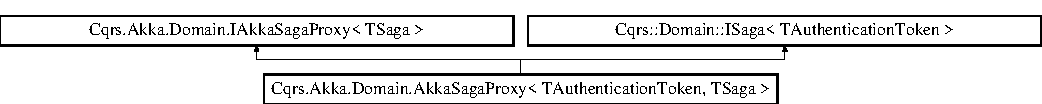
\includegraphics[height=1.372549cm]{classCqrs_1_1Akka_1_1Domain_1_1AkkaSagaProxy}
\end{center}
\end{figure}
\subsection*{Public Member Functions}
\begin{DoxyCompactItemize}
\item 
virtual I\+Enumerable$<$ \hyperlink{interfaceCqrs_1_1Events_1_1ISagaEvent}{I\+Saga\+Event}$<$ T\+Authentication\+Token $>$ $>$ \hyperlink{classCqrs_1_1Akka_1_1Domain_1_1AkkaSagaProxy_a8cad3415bc5474a01bfdb2db3a852ea5_a8cad3415bc5474a01bfdb2db3a852ea5}{Get\+Uncommitted\+Changes} ()
\item 
virtual void \hyperlink{classCqrs_1_1Akka_1_1Domain_1_1AkkaSagaProxy_a5a5c012bc0f7f957b8bd2298956ca9ae_a5a5c012bc0f7f957b8bd2298956ca9ae}{Mark\+Changes\+As\+Committed} ()
\item 
virtual void \hyperlink{classCqrs_1_1Akka_1_1Domain_1_1AkkaSagaProxy_a21b69799b046c1fcdf5b2443699dee0c_a21b69799b046c1fcdf5b2443699dee0c}{Load\+From\+History} (I\+Enumerable$<$ \hyperlink{interfaceCqrs_1_1Events_1_1ISagaEvent}{I\+Saga\+Event}$<$ T\+Authentication\+Token $>$$>$ history)
\end{DoxyCompactItemize}
\subsection*{Properties}
\begin{DoxyCompactItemize}
\item 
I\+Actor\+Ref \hyperlink{classCqrs_1_1Akka_1_1Domain_1_1AkkaSagaProxy_a5f1a7eae545d74336856ca7ec7625334_a5f1a7eae545d74336856ca7ec7625334}{Actor\+Reference}\hspace{0.3cm}{\ttfamily  \mbox{[}get, set\mbox{]}}
\item 
T\+Saga \hyperlink{classCqrs_1_1Akka_1_1Domain_1_1AkkaSagaProxy_ac63a109e223eb4f046ebe9ad22b9a850_ac63a109e223eb4f046ebe9ad22b9a850}{Saga}\hspace{0.3cm}{\ttfamily  \mbox{[}get, protected set\mbox{]}}
\item 
virtual Guid \hyperlink{classCqrs_1_1Akka_1_1Domain_1_1AkkaSagaProxy_acb65bb91f7dfacc6eca8e12b6a772b20_acb65bb91f7dfacc6eca8e12b6a772b20}{Id}\hspace{0.3cm}{\ttfamily  \mbox{[}get\mbox{]}}
\item 
virtual int \hyperlink{classCqrs_1_1Akka_1_1Domain_1_1AkkaSagaProxy_ab6272400fe5c6227a11cf5c93f752d4d_ab6272400fe5c6227a11cf5c93f752d4d}{Version}\hspace{0.3cm}{\ttfamily  \mbox{[}get\mbox{]}}
\end{DoxyCompactItemize}


\subsection{Member Function Documentation}
\mbox{\Hypertarget{classCqrs_1_1Akka_1_1Domain_1_1AkkaSagaProxy_a8cad3415bc5474a01bfdb2db3a852ea5_a8cad3415bc5474a01bfdb2db3a852ea5}\label{classCqrs_1_1Akka_1_1Domain_1_1AkkaSagaProxy_a8cad3415bc5474a01bfdb2db3a852ea5_a8cad3415bc5474a01bfdb2db3a852ea5}} 
\index{Cqrs\+::\+Akka\+::\+Domain\+::\+Akka\+Saga\+Proxy@{Cqrs\+::\+Akka\+::\+Domain\+::\+Akka\+Saga\+Proxy}!Get\+Uncommitted\+Changes@{Get\+Uncommitted\+Changes}}
\index{Get\+Uncommitted\+Changes@{Get\+Uncommitted\+Changes}!Cqrs\+::\+Akka\+::\+Domain\+::\+Akka\+Saga\+Proxy@{Cqrs\+::\+Akka\+::\+Domain\+::\+Akka\+Saga\+Proxy}}
\subsubsection{\texorpdfstring{Get\+Uncommitted\+Changes()}{GetUncommittedChanges()}}
{\footnotesize\ttfamily virtual I\+Enumerable$<$\hyperlink{interfaceCqrs_1_1Events_1_1ISagaEvent}{I\+Saga\+Event}$<$T\+Authentication\+Token$>$ $>$ \hyperlink{classCqrs_1_1Akka_1_1Domain_1_1AkkaSagaProxy}{Cqrs.\+Akka.\+Domain.\+Akka\+Saga\+Proxy}$<$ T\+Authentication\+Token, T\+Saga $>$.Get\+Uncommitted\+Changes (\begin{DoxyParamCaption}{ }\end{DoxyParamCaption})\hspace{0.3cm}{\ttfamily [virtual]}}



Implements \hyperlink{interfaceCqrs_1_1Domain_1_1ISaga_abb77811b4f7d19adb61f9d33da18e7e0_abb77811b4f7d19adb61f9d33da18e7e0}{Cqrs.\+Domain.\+I\+Saga$<$ T\+Authentication\+Token $>$}.

\mbox{\Hypertarget{classCqrs_1_1Akka_1_1Domain_1_1AkkaSagaProxy_a21b69799b046c1fcdf5b2443699dee0c_a21b69799b046c1fcdf5b2443699dee0c}\label{classCqrs_1_1Akka_1_1Domain_1_1AkkaSagaProxy_a21b69799b046c1fcdf5b2443699dee0c_a21b69799b046c1fcdf5b2443699dee0c}} 
\index{Cqrs\+::\+Akka\+::\+Domain\+::\+Akka\+Saga\+Proxy@{Cqrs\+::\+Akka\+::\+Domain\+::\+Akka\+Saga\+Proxy}!Load\+From\+History@{Load\+From\+History}}
\index{Load\+From\+History@{Load\+From\+History}!Cqrs\+::\+Akka\+::\+Domain\+::\+Akka\+Saga\+Proxy@{Cqrs\+::\+Akka\+::\+Domain\+::\+Akka\+Saga\+Proxy}}
\subsubsection{\texorpdfstring{Load\+From\+History()}{LoadFromHistory()}}
{\footnotesize\ttfamily virtual void \hyperlink{classCqrs_1_1Akka_1_1Domain_1_1AkkaSagaProxy}{Cqrs.\+Akka.\+Domain.\+Akka\+Saga\+Proxy}$<$ T\+Authentication\+Token, T\+Saga $>$.Load\+From\+History (\begin{DoxyParamCaption}\item[{I\+Enumerable$<$ \hyperlink{interfaceCqrs_1_1Events_1_1ISagaEvent}{I\+Saga\+Event}$<$ T\+Authentication\+Token $>$$>$}]{history }\end{DoxyParamCaption})\hspace{0.3cm}{\ttfamily [virtual]}}



Implements \hyperlink{interfaceCqrs_1_1Domain_1_1ISaga_a2714804684bc65cf4dec79b4697b9b21_a2714804684bc65cf4dec79b4697b9b21}{Cqrs.\+Domain.\+I\+Saga$<$ T\+Authentication\+Token $>$}.

\mbox{\Hypertarget{classCqrs_1_1Akka_1_1Domain_1_1AkkaSagaProxy_a5a5c012bc0f7f957b8bd2298956ca9ae_a5a5c012bc0f7f957b8bd2298956ca9ae}\label{classCqrs_1_1Akka_1_1Domain_1_1AkkaSagaProxy_a5a5c012bc0f7f957b8bd2298956ca9ae_a5a5c012bc0f7f957b8bd2298956ca9ae}} 
\index{Cqrs\+::\+Akka\+::\+Domain\+::\+Akka\+Saga\+Proxy@{Cqrs\+::\+Akka\+::\+Domain\+::\+Akka\+Saga\+Proxy}!Mark\+Changes\+As\+Committed@{Mark\+Changes\+As\+Committed}}
\index{Mark\+Changes\+As\+Committed@{Mark\+Changes\+As\+Committed}!Cqrs\+::\+Akka\+::\+Domain\+::\+Akka\+Saga\+Proxy@{Cqrs\+::\+Akka\+::\+Domain\+::\+Akka\+Saga\+Proxy}}
\subsubsection{\texorpdfstring{Mark\+Changes\+As\+Committed()}{MarkChangesAsCommitted()}}
{\footnotesize\ttfamily virtual void \hyperlink{classCqrs_1_1Akka_1_1Domain_1_1AkkaSagaProxy}{Cqrs.\+Akka.\+Domain.\+Akka\+Saga\+Proxy}$<$ T\+Authentication\+Token, T\+Saga $>$.Mark\+Changes\+As\+Committed (\begin{DoxyParamCaption}{ }\end{DoxyParamCaption})\hspace{0.3cm}{\ttfamily [virtual]}}



Implements \hyperlink{interfaceCqrs_1_1Domain_1_1ISaga_a85c75f80bc5be4bad7f1d9f1231bfba7_a85c75f80bc5be4bad7f1d9f1231bfba7}{Cqrs.\+Domain.\+I\+Saga$<$ T\+Authentication\+Token $>$}.



\subsection{Property Documentation}
\mbox{\Hypertarget{classCqrs_1_1Akka_1_1Domain_1_1AkkaSagaProxy_a5f1a7eae545d74336856ca7ec7625334_a5f1a7eae545d74336856ca7ec7625334}\label{classCqrs_1_1Akka_1_1Domain_1_1AkkaSagaProxy_a5f1a7eae545d74336856ca7ec7625334_a5f1a7eae545d74336856ca7ec7625334}} 
\index{Cqrs\+::\+Akka\+::\+Domain\+::\+Akka\+Saga\+Proxy@{Cqrs\+::\+Akka\+::\+Domain\+::\+Akka\+Saga\+Proxy}!Actor\+Reference@{Actor\+Reference}}
\index{Actor\+Reference@{Actor\+Reference}!Cqrs\+::\+Akka\+::\+Domain\+::\+Akka\+Saga\+Proxy@{Cqrs\+::\+Akka\+::\+Domain\+::\+Akka\+Saga\+Proxy}}
\subsubsection{\texorpdfstring{Actor\+Reference}{ActorReference}}
{\footnotesize\ttfamily I\+Actor\+Ref \hyperlink{classCqrs_1_1Akka_1_1Domain_1_1AkkaSagaProxy}{Cqrs.\+Akka.\+Domain.\+Akka\+Saga\+Proxy}$<$ T\+Authentication\+Token, T\+Saga $>$.Actor\+Reference\hspace{0.3cm}{\ttfamily [get]}, {\ttfamily [set]}}

\mbox{\Hypertarget{classCqrs_1_1Akka_1_1Domain_1_1AkkaSagaProxy_acb65bb91f7dfacc6eca8e12b6a772b20_acb65bb91f7dfacc6eca8e12b6a772b20}\label{classCqrs_1_1Akka_1_1Domain_1_1AkkaSagaProxy_acb65bb91f7dfacc6eca8e12b6a772b20_acb65bb91f7dfacc6eca8e12b6a772b20}} 
\index{Cqrs\+::\+Akka\+::\+Domain\+::\+Akka\+Saga\+Proxy@{Cqrs\+::\+Akka\+::\+Domain\+::\+Akka\+Saga\+Proxy}!Id@{Id}}
\index{Id@{Id}!Cqrs\+::\+Akka\+::\+Domain\+::\+Akka\+Saga\+Proxy@{Cqrs\+::\+Akka\+::\+Domain\+::\+Akka\+Saga\+Proxy}}
\subsubsection{\texorpdfstring{Id}{Id}}
{\footnotesize\ttfamily virtual Guid \hyperlink{classCqrs_1_1Akka_1_1Domain_1_1AkkaSagaProxy}{Cqrs.\+Akka.\+Domain.\+Akka\+Saga\+Proxy}$<$ T\+Authentication\+Token, T\+Saga $>$.Id\hspace{0.3cm}{\ttfamily [get]}}

\mbox{\Hypertarget{classCqrs_1_1Akka_1_1Domain_1_1AkkaSagaProxy_ac63a109e223eb4f046ebe9ad22b9a850_ac63a109e223eb4f046ebe9ad22b9a850}\label{classCqrs_1_1Akka_1_1Domain_1_1AkkaSagaProxy_ac63a109e223eb4f046ebe9ad22b9a850_ac63a109e223eb4f046ebe9ad22b9a850}} 
\index{Cqrs\+::\+Akka\+::\+Domain\+::\+Akka\+Saga\+Proxy@{Cqrs\+::\+Akka\+::\+Domain\+::\+Akka\+Saga\+Proxy}!Saga@{Saga}}
\index{Saga@{Saga}!Cqrs\+::\+Akka\+::\+Domain\+::\+Akka\+Saga\+Proxy@{Cqrs\+::\+Akka\+::\+Domain\+::\+Akka\+Saga\+Proxy}}
\subsubsection{\texorpdfstring{Saga}{Saga}}
{\footnotesize\ttfamily T\+Saga \hyperlink{classCqrs_1_1Akka_1_1Domain_1_1AkkaSagaProxy}{Cqrs.\+Akka.\+Domain.\+Akka\+Saga\+Proxy}$<$ T\+Authentication\+Token, T\+Saga $>$.\hyperlink{classCqrs_1_1Domain_1_1Saga}{Saga}\hspace{0.3cm}{\ttfamily [get]}, {\ttfamily [protected set]}}

\mbox{\Hypertarget{classCqrs_1_1Akka_1_1Domain_1_1AkkaSagaProxy_ab6272400fe5c6227a11cf5c93f752d4d_ab6272400fe5c6227a11cf5c93f752d4d}\label{classCqrs_1_1Akka_1_1Domain_1_1AkkaSagaProxy_ab6272400fe5c6227a11cf5c93f752d4d_ab6272400fe5c6227a11cf5c93f752d4d}} 
\index{Cqrs\+::\+Akka\+::\+Domain\+::\+Akka\+Saga\+Proxy@{Cqrs\+::\+Akka\+::\+Domain\+::\+Akka\+Saga\+Proxy}!Version@{Version}}
\index{Version@{Version}!Cqrs\+::\+Akka\+::\+Domain\+::\+Akka\+Saga\+Proxy@{Cqrs\+::\+Akka\+::\+Domain\+::\+Akka\+Saga\+Proxy}}
\subsubsection{\texorpdfstring{Version}{Version}}
{\footnotesize\ttfamily virtual int \hyperlink{classCqrs_1_1Akka_1_1Domain_1_1AkkaSagaProxy}{Cqrs.\+Akka.\+Domain.\+Akka\+Saga\+Proxy}$<$ T\+Authentication\+Token, T\+Saga $>$.Version\hspace{0.3cm}{\ttfamily [get]}}


\hypertarget{classCqrs_1_1Akka_1_1Domain_1_1AkkaSagaRepository}{}\section{Cqrs.\+Akka.\+Domain.\+Akka\+Saga\+Repository$<$ T\+Authentication\+Token $>$ Class Template Reference}
\label{classCqrs_1_1Akka_1_1Domain_1_1AkkaSagaRepository}\index{Cqrs.\+Akka.\+Domain.\+Akka\+Saga\+Repository$<$ T\+Authentication\+Token $>$@{Cqrs.\+Akka.\+Domain.\+Akka\+Saga\+Repository$<$ T\+Authentication\+Token $>$}}
Inheritance diagram for Cqrs.\+Akka.\+Domain.\+Akka\+Saga\+Repository$<$ T\+Authentication\+Token $>$\+:\begin{figure}[H]
\begin{center}
\leavevmode
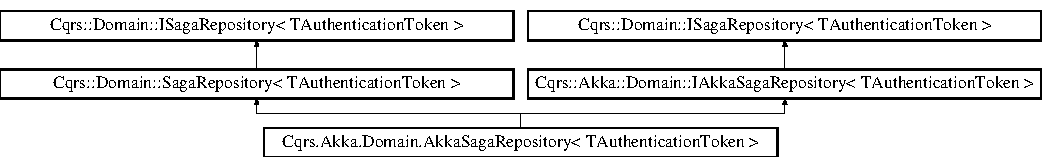
\includegraphics[height=2.105263cm]{classCqrs_1_1Akka_1_1Domain_1_1AkkaSagaRepository}
\end{center}
\end{figure}
\subsection*{Public Member Functions}
\begin{DoxyCompactItemize}
\item 
\hyperlink{classCqrs_1_1Akka_1_1Domain_1_1AkkaSagaRepository_a8297f64e2b7a7be7bcc999c89dcece05_a8297f64e2b7a7be7bcc999c89dcece05}{Akka\+Saga\+Repository} (\hyperlink{interfaceCqrs_1_1Domain_1_1Factories_1_1IAggregateFactory}{I\+Aggregate\+Factory} aggregate\+Factory, \hyperlink{interfaceCqrs_1_1Events_1_1IEventStore}{I\+Event\+Store}$<$ T\+Authentication\+Token $>$ event\+Store, \hyperlink{interfaceCqrs_1_1Events_1_1IEventPublisher}{I\+Event\+Publisher}$<$ T\+Authentication\+Token $>$ publisher, I\+Correlation\+Id\+Helper correlation\+Id\+Helper, \hyperlink{interfaceCqrs_1_1Akka_1_1Events_1_1IAkkaEventPublisherProxy}{I\+Akka\+Event\+Publisher\+Proxy}$<$ T\+Authentication\+Token $>$ event\+Publisher)
\end{DoxyCompactItemize}
\subsection*{Protected Member Functions}
\begin{DoxyCompactItemize}
\item 
override T\+Saga \hyperlink{classCqrs_1_1Akka_1_1Domain_1_1AkkaSagaRepository_a2c7263d0e58d2b31149ec685d5be934a_a2c7263d0e58d2b31149ec685d5be934a}{Create\+Saga$<$ T\+Saga $>$} (Guid id)
\item 
override void \hyperlink{classCqrs_1_1Akka_1_1Domain_1_1AkkaSagaRepository_a7f6375bb99e680792466fb420232a535_a7f6375bb99e680792466fb420232a535}{Publish\+Event} (\hyperlink{interfaceCqrs_1_1Events_1_1ISagaEvent}{I\+Saga\+Event}$<$ T\+Authentication\+Token $>$ @event)
\end{DoxyCompactItemize}
\subsection*{Properties}
\begin{DoxyCompactItemize}
\item 
\hyperlink{interfaceCqrs_1_1Akka_1_1Events_1_1IAkkaEventPublisherProxy}{I\+Akka\+Event\+Publisher\+Proxy}$<$ T\+Authentication\+Token $>$ \hyperlink{classCqrs_1_1Akka_1_1Domain_1_1AkkaSagaRepository_a25957859d1f98ea7f434983c562e9724_a25957859d1f98ea7f434983c562e9724}{Event\+Publisher}\hspace{0.3cm}{\ttfamily  \mbox{[}get\mbox{]}}
\end{DoxyCompactItemize}


\subsection{Constructor \& Destructor Documentation}
\mbox{\Hypertarget{classCqrs_1_1Akka_1_1Domain_1_1AkkaSagaRepository_a8297f64e2b7a7be7bcc999c89dcece05_a8297f64e2b7a7be7bcc999c89dcece05}\label{classCqrs_1_1Akka_1_1Domain_1_1AkkaSagaRepository_a8297f64e2b7a7be7bcc999c89dcece05_a8297f64e2b7a7be7bcc999c89dcece05}} 
\index{Cqrs\+::\+Akka\+::\+Domain\+::\+Akka\+Saga\+Repository@{Cqrs\+::\+Akka\+::\+Domain\+::\+Akka\+Saga\+Repository}!Akka\+Saga\+Repository@{Akka\+Saga\+Repository}}
\index{Akka\+Saga\+Repository@{Akka\+Saga\+Repository}!Cqrs\+::\+Akka\+::\+Domain\+::\+Akka\+Saga\+Repository@{Cqrs\+::\+Akka\+::\+Domain\+::\+Akka\+Saga\+Repository}}
\subsubsection{\texorpdfstring{Akka\+Saga\+Repository()}{AkkaSagaRepository()}}
{\footnotesize\ttfamily \hyperlink{classCqrs_1_1Akka_1_1Domain_1_1AkkaSagaRepository}{Cqrs.\+Akka.\+Domain.\+Akka\+Saga\+Repository}$<$ T\+Authentication\+Token $>$.\hyperlink{classCqrs_1_1Akka_1_1Domain_1_1AkkaSagaRepository}{Akka\+Saga\+Repository} (\begin{DoxyParamCaption}\item[{\hyperlink{interfaceCqrs_1_1Domain_1_1Factories_1_1IAggregateFactory}{I\+Aggregate\+Factory}}]{aggregate\+Factory,  }\item[{\hyperlink{interfaceCqrs_1_1Events_1_1IEventStore}{I\+Event\+Store}$<$ T\+Authentication\+Token $>$}]{event\+Store,  }\item[{\hyperlink{interfaceCqrs_1_1Events_1_1IEventPublisher}{I\+Event\+Publisher}$<$ T\+Authentication\+Token $>$}]{publisher,  }\item[{I\+Correlation\+Id\+Helper}]{correlation\+Id\+Helper,  }\item[{\hyperlink{interfaceCqrs_1_1Akka_1_1Events_1_1IAkkaEventPublisherProxy}{I\+Akka\+Event\+Publisher\+Proxy}$<$ T\+Authentication\+Token $>$}]{event\+Publisher }\end{DoxyParamCaption})}



\subsection{Member Function Documentation}
\mbox{\Hypertarget{classCqrs_1_1Akka_1_1Domain_1_1AkkaSagaRepository_a2c7263d0e58d2b31149ec685d5be934a_a2c7263d0e58d2b31149ec685d5be934a}\label{classCqrs_1_1Akka_1_1Domain_1_1AkkaSagaRepository_a2c7263d0e58d2b31149ec685d5be934a_a2c7263d0e58d2b31149ec685d5be934a}} 
\index{Cqrs\+::\+Akka\+::\+Domain\+::\+Akka\+Saga\+Repository@{Cqrs\+::\+Akka\+::\+Domain\+::\+Akka\+Saga\+Repository}!Create\+Saga$<$ T\+Saga $>$@{Create\+Saga$<$ T\+Saga $>$}}
\index{Create\+Saga$<$ T\+Saga $>$@{Create\+Saga$<$ T\+Saga $>$}!Cqrs\+::\+Akka\+::\+Domain\+::\+Akka\+Saga\+Repository@{Cqrs\+::\+Akka\+::\+Domain\+::\+Akka\+Saga\+Repository}}
\subsubsection{\texorpdfstring{Create\+Saga$<$ T\+Saga $>$()}{CreateSaga< TSaga >()}}
{\footnotesize\ttfamily override T\+Saga \hyperlink{classCqrs_1_1Akka_1_1Domain_1_1AkkaSagaRepository}{Cqrs.\+Akka.\+Domain.\+Akka\+Saga\+Repository}$<$ T\+Authentication\+Token $>$.Create\+Saga$<$ T\+Saga $>$ (\begin{DoxyParamCaption}\item[{Guid}]{id }\end{DoxyParamCaption})\hspace{0.3cm}{\ttfamily [protected]}, {\ttfamily [virtual]}}



Reimplemented from \hyperlink{classCqrs_1_1Domain_1_1SagaRepository_acb23e0bd3e5655547a13b4ad2b06e548_acb23e0bd3e5655547a13b4ad2b06e548}{Cqrs.\+Domain.\+Saga\+Repository$<$ T\+Authentication\+Token $>$}.

\mbox{\Hypertarget{classCqrs_1_1Akka_1_1Domain_1_1AkkaSagaRepository_a7f6375bb99e680792466fb420232a535_a7f6375bb99e680792466fb420232a535}\label{classCqrs_1_1Akka_1_1Domain_1_1AkkaSagaRepository_a7f6375bb99e680792466fb420232a535_a7f6375bb99e680792466fb420232a535}} 
\index{Cqrs\+::\+Akka\+::\+Domain\+::\+Akka\+Saga\+Repository@{Cqrs\+::\+Akka\+::\+Domain\+::\+Akka\+Saga\+Repository}!Publish\+Event@{Publish\+Event}}
\index{Publish\+Event@{Publish\+Event}!Cqrs\+::\+Akka\+::\+Domain\+::\+Akka\+Saga\+Repository@{Cqrs\+::\+Akka\+::\+Domain\+::\+Akka\+Saga\+Repository}}
\subsubsection{\texorpdfstring{Publish\+Event()}{PublishEvent()}}
{\footnotesize\ttfamily override void \hyperlink{classCqrs_1_1Akka_1_1Domain_1_1AkkaSagaRepository}{Cqrs.\+Akka.\+Domain.\+Akka\+Saga\+Repository}$<$ T\+Authentication\+Token $>$.Publish\+Event (\begin{DoxyParamCaption}\item[{\hyperlink{interfaceCqrs_1_1Events_1_1ISagaEvent}{I\+Saga\+Event}$<$ T\+Authentication\+Token $>$ @}]{event }\end{DoxyParamCaption})\hspace{0.3cm}{\ttfamily [protected]}, {\ttfamily [virtual]}}



Reimplemented from \hyperlink{classCqrs_1_1Domain_1_1SagaRepository_a1dec03959e4d859c6cf2be0507b1bc05_a1dec03959e4d859c6cf2be0507b1bc05}{Cqrs.\+Domain.\+Saga\+Repository$<$ T\+Authentication\+Token $>$}.



\subsection{Property Documentation}
\mbox{\Hypertarget{classCqrs_1_1Akka_1_1Domain_1_1AkkaSagaRepository_a25957859d1f98ea7f434983c562e9724_a25957859d1f98ea7f434983c562e9724}\label{classCqrs_1_1Akka_1_1Domain_1_1AkkaSagaRepository_a25957859d1f98ea7f434983c562e9724_a25957859d1f98ea7f434983c562e9724}} 
\index{Cqrs\+::\+Akka\+::\+Domain\+::\+Akka\+Saga\+Repository@{Cqrs\+::\+Akka\+::\+Domain\+::\+Akka\+Saga\+Repository}!Event\+Publisher@{Event\+Publisher}}
\index{Event\+Publisher@{Event\+Publisher}!Cqrs\+::\+Akka\+::\+Domain\+::\+Akka\+Saga\+Repository@{Cqrs\+::\+Akka\+::\+Domain\+::\+Akka\+Saga\+Repository}}
\subsubsection{\texorpdfstring{Event\+Publisher}{EventPublisher}}
{\footnotesize\ttfamily \hyperlink{interfaceCqrs_1_1Akka_1_1Events_1_1IAkkaEventPublisherProxy}{I\+Akka\+Event\+Publisher\+Proxy}$<$T\+Authentication\+Token$>$ \hyperlink{classCqrs_1_1Akka_1_1Domain_1_1AkkaSagaRepository}{Cqrs.\+Akka.\+Domain.\+Akka\+Saga\+Repository}$<$ T\+Authentication\+Token $>$.Event\+Publisher\hspace{0.3cm}{\ttfamily [get]}, {\ttfamily [protected]}}


\hypertarget{classCqrs_1_1Akka_1_1Domain_1_1Commands_1_1GetAkkaAggregateRootId}{}\doxysection{Cqrs.\+Akka.\+Domain.\+Commands.\+Get\+Akka\+Aggregate\+Root\+Id Class Reference}
\label{classCqrs_1_1Akka_1_1Domain_1_1Commands_1_1GetAkkaAggregateRootId}\index{Cqrs.Akka.Domain.Commands.GetAkkaAggregateRootId@{Cqrs.Akka.Domain.Commands.GetAkkaAggregateRootId}}


Get the I\+Aggregate\+Root$<$\+T\+Authentication\+Token$>$.\+Id from the Akka.\+net system.  




\doxysubsection{Detailed Description}
Get the I\+Aggregate\+Root$<$\+T\+Authentication\+Token$>$.\+Id from the Akka.\+net system. 


\hypertarget{classCqrs_1_1Akka_1_1Domain_1_1Commands_1_1GetAkkaAggregateRootVersion}{}\doxysection{Cqrs.\+Akka.\+Domain.\+Commands.\+Get\+Akka\+Aggregate\+Root\+Version Class Reference}
\label{classCqrs_1_1Akka_1_1Domain_1_1Commands_1_1GetAkkaAggregateRootVersion}\index{Cqrs.Akka.Domain.Commands.GetAkkaAggregateRootVersion@{Cqrs.Akka.Domain.Commands.GetAkkaAggregateRootVersion}}


Get the I\+Aggregate\+Root$<$\+T\+Authentication\+Token$>$.\+Version from the Akka.\+net system.  




\doxysubsection{Detailed Description}
Get the I\+Aggregate\+Root$<$\+T\+Authentication\+Token$>$.\+Version from the Akka.\+net system. 


\hypertarget{classCqrs_1_1Akka_1_1Domain_1_1Commands_1_1GetAkkaSagaId}{}\doxysection{Cqrs.\+Akka.\+Domain.\+Commands.\+Get\+Akka\+Saga\+Id Class Reference}
\label{classCqrs_1_1Akka_1_1Domain_1_1Commands_1_1GetAkkaSagaId}\index{Cqrs.Akka.Domain.Commands.GetAkkaSagaId@{Cqrs.Akka.Domain.Commands.GetAkkaSagaId}}


Get the I\+Saga$<$\+T\+Authentication\+Token$>$.\+Id from the Akka.\+net system.  




\doxysubsection{Detailed Description}
Get the I\+Saga$<$\+T\+Authentication\+Token$>$.\+Id from the Akka.\+net system. 


\hypertarget{classCqrs_1_1Akka_1_1Domain_1_1Commands_1_1GetAkkaSagaVersion}{}\section{Cqrs.\+Akka.\+Domain.\+Commands.\+Get\+Akka\+Saga\+Version Class Reference}
\label{classCqrs_1_1Akka_1_1Domain_1_1Commands_1_1GetAkkaSagaVersion}\index{Cqrs.\+Akka.\+Domain.\+Commands.\+Get\+Akka\+Saga\+Version@{Cqrs.\+Akka.\+Domain.\+Commands.\+Get\+Akka\+Saga\+Version}}

\hypertarget{classCqrs_1_1Akka_1_1Domain_1_1Factories_1_1AkkaAggregateFactory}{}\section{Cqrs.\+Akka.\+Domain.\+Factories.\+Akka\+Aggregate\+Factory$<$ T\+Authentication\+Token $>$ Class Template Reference}
\label{classCqrs_1_1Akka_1_1Domain_1_1Factories_1_1AkkaAggregateFactory}\index{Cqrs.\+Akka.\+Domain.\+Factories.\+Akka\+Aggregate\+Factory$<$ T\+Authentication\+Token $>$@{Cqrs.\+Akka.\+Domain.\+Factories.\+Akka\+Aggregate\+Factory$<$ T\+Authentication\+Token $>$}}
Inheritance diagram for Cqrs.\+Akka.\+Domain.\+Factories.\+Akka\+Aggregate\+Factory$<$ T\+Authentication\+Token $>$\+:\begin{figure}[H]
\begin{center}
\leavevmode
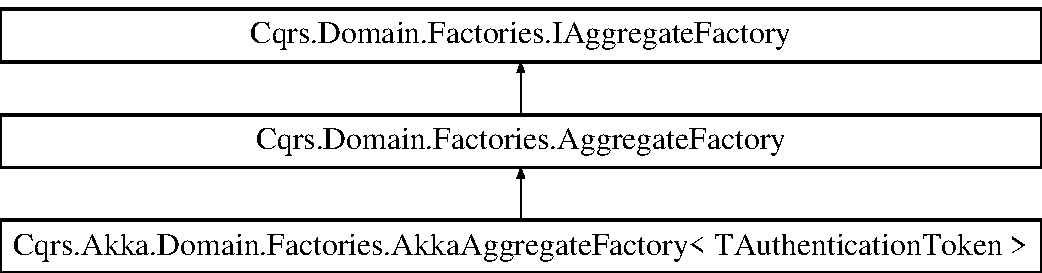
\includegraphics[height=3.000000cm]{classCqrs_1_1Akka_1_1Domain_1_1Factories_1_1AkkaAggregateFactory}
\end{center}
\end{figure}
\subsection*{Public Member Functions}
\begin{DoxyCompactItemize}
\item 
\hyperlink{classCqrs_1_1Akka_1_1Domain_1_1Factories_1_1AkkaAggregateFactory_a589acbd624020f419480f28c16e1c03b_a589acbd624020f419480f28c16e1c03b}{Akka\+Aggregate\+Factory} (\hyperlink{interfaceCqrs_1_1Configuration_1_1IDependencyResolver}{I\+Dependency\+Resolver} dependency\+Resolver, \hyperlink{interfaceCqrs_1_1Akka_1_1Domain_1_1IAkkaAggregateResolver}{I\+Akka\+Aggregate\+Resolver} aggregate\+Resolver)
\item 
override T\+Aggregate\+Root \hyperlink{classCqrs_1_1Akka_1_1Domain_1_1Factories_1_1AkkaAggregateFactory_a41fbe3e0d84a4f9244fcd13058337412_a41fbe3e0d84a4f9244fcd13058337412}{Create\+Aggregate$<$ T\+Aggregate\+Root $>$} (Guid? rsn=null, bool try\+Dependency\+Resolution\+First=true)
\end{DoxyCompactItemize}
\subsection*{Properties}
\begin{DoxyCompactItemize}
\item 
\hyperlink{interfaceCqrs_1_1Akka_1_1Domain_1_1IAkkaAggregateResolver}{I\+Akka\+Aggregate\+Resolver} \hyperlink{classCqrs_1_1Akka_1_1Domain_1_1Factories_1_1AkkaAggregateFactory_ae83aa4aa5cbe5fe0cc0cea41de002218_ae83aa4aa5cbe5fe0cc0cea41de002218}{Aggregate\+Resolver}\hspace{0.3cm}{\ttfamily  \mbox{[}get\mbox{]}}
\end{DoxyCompactItemize}


\subsection{Constructor \& Destructor Documentation}
\mbox{\Hypertarget{classCqrs_1_1Akka_1_1Domain_1_1Factories_1_1AkkaAggregateFactory_a589acbd624020f419480f28c16e1c03b_a589acbd624020f419480f28c16e1c03b}\label{classCqrs_1_1Akka_1_1Domain_1_1Factories_1_1AkkaAggregateFactory_a589acbd624020f419480f28c16e1c03b_a589acbd624020f419480f28c16e1c03b}} 
\index{Cqrs\+::\+Akka\+::\+Domain\+::\+Factories\+::\+Akka\+Aggregate\+Factory@{Cqrs\+::\+Akka\+::\+Domain\+::\+Factories\+::\+Akka\+Aggregate\+Factory}!Akka\+Aggregate\+Factory@{Akka\+Aggregate\+Factory}}
\index{Akka\+Aggregate\+Factory@{Akka\+Aggregate\+Factory}!Cqrs\+::\+Akka\+::\+Domain\+::\+Factories\+::\+Akka\+Aggregate\+Factory@{Cqrs\+::\+Akka\+::\+Domain\+::\+Factories\+::\+Akka\+Aggregate\+Factory}}
\subsubsection{\texorpdfstring{Akka\+Aggregate\+Factory()}{AkkaAggregateFactory()}}
{\footnotesize\ttfamily \hyperlink{classCqrs_1_1Akka_1_1Domain_1_1Factories_1_1AkkaAggregateFactory}{Cqrs.\+Akka.\+Domain.\+Factories.\+Akka\+Aggregate\+Factory}$<$ T\+Authentication\+Token $>$.\hyperlink{classCqrs_1_1Akka_1_1Domain_1_1Factories_1_1AkkaAggregateFactory}{Akka\+Aggregate\+Factory} (\begin{DoxyParamCaption}\item[{\hyperlink{interfaceCqrs_1_1Configuration_1_1IDependencyResolver}{I\+Dependency\+Resolver}}]{dependency\+Resolver,  }\item[{\hyperlink{interfaceCqrs_1_1Akka_1_1Domain_1_1IAkkaAggregateResolver}{I\+Akka\+Aggregate\+Resolver}}]{aggregate\+Resolver }\end{DoxyParamCaption})}



\subsection{Member Function Documentation}
\mbox{\Hypertarget{classCqrs_1_1Akka_1_1Domain_1_1Factories_1_1AkkaAggregateFactory_a41fbe3e0d84a4f9244fcd13058337412_a41fbe3e0d84a4f9244fcd13058337412}\label{classCqrs_1_1Akka_1_1Domain_1_1Factories_1_1AkkaAggregateFactory_a41fbe3e0d84a4f9244fcd13058337412_a41fbe3e0d84a4f9244fcd13058337412}} 
\index{Cqrs\+::\+Akka\+::\+Domain\+::\+Factories\+::\+Akka\+Aggregate\+Factory@{Cqrs\+::\+Akka\+::\+Domain\+::\+Factories\+::\+Akka\+Aggregate\+Factory}!Create\+Aggregate$<$ T\+Aggregate\+Root $>$@{Create\+Aggregate$<$ T\+Aggregate\+Root $>$}}
\index{Create\+Aggregate$<$ T\+Aggregate\+Root $>$@{Create\+Aggregate$<$ T\+Aggregate\+Root $>$}!Cqrs\+::\+Akka\+::\+Domain\+::\+Factories\+::\+Akka\+Aggregate\+Factory@{Cqrs\+::\+Akka\+::\+Domain\+::\+Factories\+::\+Akka\+Aggregate\+Factory}}
\subsubsection{\texorpdfstring{Create\+Aggregate$<$ T\+Aggregate\+Root $>$()}{CreateAggregate< TAggregateRoot >()}}
{\footnotesize\ttfamily override T\+Aggregate\+Root \hyperlink{classCqrs_1_1Akka_1_1Domain_1_1Factories_1_1AkkaAggregateFactory}{Cqrs.\+Akka.\+Domain.\+Factories.\+Akka\+Aggregate\+Factory}$<$ T\+Authentication\+Token $>$.Create\+Aggregate$<$ T\+Aggregate\+Root $>$ (\begin{DoxyParamCaption}\item[{Guid?}]{rsn = {\ttfamily null},  }\item[{bool}]{try\+Dependency\+Resolution\+First = {\ttfamily true} }\end{DoxyParamCaption})}



\subsection{Property Documentation}
\mbox{\Hypertarget{classCqrs_1_1Akka_1_1Domain_1_1Factories_1_1AkkaAggregateFactory_ae83aa4aa5cbe5fe0cc0cea41de002218_ae83aa4aa5cbe5fe0cc0cea41de002218}\label{classCqrs_1_1Akka_1_1Domain_1_1Factories_1_1AkkaAggregateFactory_ae83aa4aa5cbe5fe0cc0cea41de002218_ae83aa4aa5cbe5fe0cc0cea41de002218}} 
\index{Cqrs\+::\+Akka\+::\+Domain\+::\+Factories\+::\+Akka\+Aggregate\+Factory@{Cqrs\+::\+Akka\+::\+Domain\+::\+Factories\+::\+Akka\+Aggregate\+Factory}!Aggregate\+Resolver@{Aggregate\+Resolver}}
\index{Aggregate\+Resolver@{Aggregate\+Resolver}!Cqrs\+::\+Akka\+::\+Domain\+::\+Factories\+::\+Akka\+Aggregate\+Factory@{Cqrs\+::\+Akka\+::\+Domain\+::\+Factories\+::\+Akka\+Aggregate\+Factory}}
\subsubsection{\texorpdfstring{Aggregate\+Resolver}{AggregateResolver}}
{\footnotesize\ttfamily \hyperlink{interfaceCqrs_1_1Akka_1_1Domain_1_1IAkkaAggregateResolver}{I\+Akka\+Aggregate\+Resolver} \hyperlink{classCqrs_1_1Akka_1_1Domain_1_1Factories_1_1AkkaAggregateFactory}{Cqrs.\+Akka.\+Domain.\+Factories.\+Akka\+Aggregate\+Factory}$<$ T\+Authentication\+Token $>$.Aggregate\+Resolver\hspace{0.3cm}{\ttfamily [get]}, {\ttfamily [protected]}}


\hypertarget{interfaceCqrs_1_1Akka_1_1Domain_1_1IAkkaAggregateRepository}{}\section{Cqrs.\+Akka.\+Domain.\+I\+Akka\+Aggregate\+Repository$<$ T\+Authentication\+Token $>$ Interface Template Reference}
\label{interfaceCqrs_1_1Akka_1_1Domain_1_1IAkkaAggregateRepository}\index{Cqrs.\+Akka.\+Domain.\+I\+Akka\+Aggregate\+Repository$<$ T\+Authentication\+Token $>$@{Cqrs.\+Akka.\+Domain.\+I\+Akka\+Aggregate\+Repository$<$ T\+Authentication\+Token $>$}}


A Aggregate\+Repository$<$\+T\+Authentication\+Token$>$ that is safe to use within Akka.\+N\+ET  


Inheritance diagram for Cqrs.\+Akka.\+Domain.\+I\+Akka\+Aggregate\+Repository$<$ T\+Authentication\+Token $>$\+:\begin{figure}[H]
\begin{center}
\leavevmode
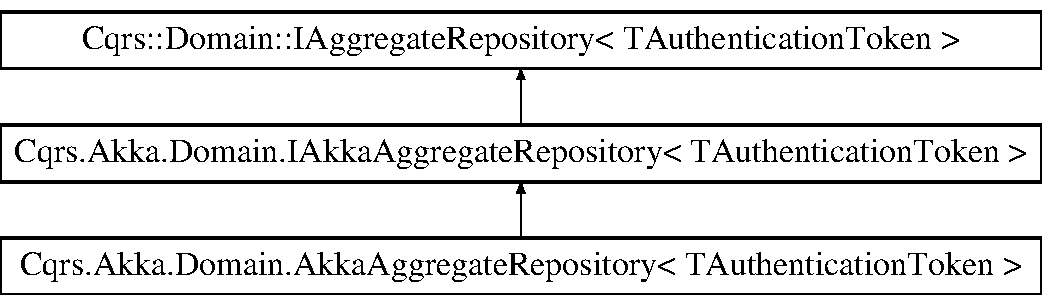
\includegraphics[height=2.357895cm]{interfaceCqrs_1_1Akka_1_1Domain_1_1IAkkaAggregateRepository}
\end{center}
\end{figure}
\subsection*{Public Member Functions}
\begin{DoxyCompactItemize}
\item 
void \hyperlink{interfaceCqrs_1_1Akka_1_1Domain_1_1IAkkaAggregateRepository_a9010b259daf5d09f7269277361015ddf_a9010b259daf5d09f7269277361015ddf}{Load\+Aggregate\+History$<$ T\+Aggregate\+Root $>$} (T\+Aggregate\+Root aggregate, I\+List$<$ \hyperlink{interfaceCqrs_1_1Events_1_1IEvent}{I\+Event}$<$ T\+Authentication\+Token $>$$>$ events=null, bool throw\+Exception\+On\+No\+Events=true)
\begin{DoxyCompactList}\small\item\em If {\itshape events}  is null, loads the events from I\+Event\+Store$<$\+T\+Authentication\+Token$>$, checks for duplicates and then rehydrates the {\itshape aggregate}  with the events. \end{DoxyCompactList}\end{DoxyCompactItemize}


\subsection{Detailed Description}
A Aggregate\+Repository$<$\+T\+Authentication\+Token$>$ that is safe to use within Akka.\+N\+ET 


\begin{DoxyTemplParams}{Template Parameters}
{\em T\+Authentication\+Token} & The Type of authentication token.\\
\hline
\end{DoxyTemplParams}


\subsection{Member Function Documentation}
\mbox{\Hypertarget{interfaceCqrs_1_1Akka_1_1Domain_1_1IAkkaAggregateRepository_a9010b259daf5d09f7269277361015ddf_a9010b259daf5d09f7269277361015ddf}\label{interfaceCqrs_1_1Akka_1_1Domain_1_1IAkkaAggregateRepository_a9010b259daf5d09f7269277361015ddf_a9010b259daf5d09f7269277361015ddf}} 
\index{Cqrs\+::\+Akka\+::\+Domain\+::\+I\+Akka\+Aggregate\+Repository@{Cqrs\+::\+Akka\+::\+Domain\+::\+I\+Akka\+Aggregate\+Repository}!Load\+Aggregate\+History$<$ T\+Aggregate\+Root $>$@{Load\+Aggregate\+History$<$ T\+Aggregate\+Root $>$}}
\index{Load\+Aggregate\+History$<$ T\+Aggregate\+Root $>$@{Load\+Aggregate\+History$<$ T\+Aggregate\+Root $>$}!Cqrs\+::\+Akka\+::\+Domain\+::\+I\+Akka\+Aggregate\+Repository@{Cqrs\+::\+Akka\+::\+Domain\+::\+I\+Akka\+Aggregate\+Repository}}
\subsubsection{\texorpdfstring{Load\+Aggregate\+History$<$ T\+Aggregate\+Root $>$()}{LoadAggregateHistory< TAggregateRoot >()}}
{\footnotesize\ttfamily void \hyperlink{interfaceCqrs_1_1Akka_1_1Domain_1_1IAkkaAggregateRepository}{Cqrs.\+Akka.\+Domain.\+I\+Akka\+Aggregate\+Repository}$<$ T\+Authentication\+Token $>$.Load\+Aggregate\+History$<$ T\+Aggregate\+Root $>$ (\begin{DoxyParamCaption}\item[{T\+Aggregate\+Root}]{aggregate,  }\item[{I\+List$<$ \hyperlink{interfaceCqrs_1_1Events_1_1IEvent}{I\+Event}$<$ T\+Authentication\+Token $>$$>$}]{events = {\ttfamily null},  }\item[{bool}]{throw\+Exception\+On\+No\+Events = {\ttfamily true} }\end{DoxyParamCaption})}



If {\itshape events}  is null, loads the events from I\+Event\+Store$<$\+T\+Authentication\+Token$>$, checks for duplicates and then rehydrates the {\itshape aggregate}  with the events. 


\begin{DoxyTemplParams}{Template Parameters}
{\em T\+Aggregate\+Root} & The Type of I\+Aggregate\+Root$<$\+T\+Authentication\+Token$>$.\\
\hline
\end{DoxyTemplParams}

\begin{DoxyParams}{Parameters}
{\em aggregate} & The {\itshape T\+Aggregate\+Root}  to rehydrate.\\
\hline
{\em events} & A collection of I\+Event$<$\+T\+Authentication\+Token$>$ to replay on the retrieved I\+Aggregate\+Root$<$\+T\+Authentication\+Token$>$. If null, the I\+Event\+Store$<$\+T\+Authentication\+Token$>$ will be used to retrieve a list of I\+Event$<$\+T\+Authentication\+Token$>$ for you. \\
\hline
{\em throw\+Exception\+On\+No\+Events} & If true will throw an instance of Aggregate\+Not\+Found\+Exception$<$\+T\+Aggregate\+Root,\+T\+Authentication\+Token$>$ if no aggregate events or provided or found in the I\+Event\+Store$<$\+T\+Authentication\+Token$>$.\\
\hline
\end{DoxyParams}


Implemented in \hyperlink{classCqrs_1_1Akka_1_1Snapshots_1_1AkkaSnapshotRepository_a22974b2e02f76de5ad76369130fbb8f4_a22974b2e02f76de5ad76369130fbb8f4}{Cqrs.\+Akka.\+Snapshots.\+Akka\+Snapshot\+Repository$<$ T\+Authentication\+Token $>$}.

\begin{Desc}
\item[Type Constraints]\begin{description}
\item[{\em T\+Aggregate\+Root} : {\em I\+Aggregate\+Root$<$T\+Authentication\+Token$>$}]\end{description}
\end{Desc}

\hypertarget{interfaceCqrs_1_1Akka_1_1Domain_1_1IAkkaAggregateResolver}{}\doxysection{Cqrs.\+Akka.\+Domain.\+I\+Akka\+Aggregate\+Resolver Interface Reference}
\label{interfaceCqrs_1_1Akka_1_1Domain_1_1IAkkaAggregateResolver}\index{Cqrs.Akka.Domain.IAkkaAggregateResolver@{Cqrs.Akka.Domain.IAkkaAggregateResolver}}


A resolver for I\+Actor\+Ref instances of I\+Aggregate\+Root$<$\+T\+Authentication\+Token$>$.  


Inheritance diagram for Cqrs.\+Akka.\+Domain.\+I\+Akka\+Aggregate\+Resolver\+:\begin{figure}[H]
\begin{center}
\leavevmode
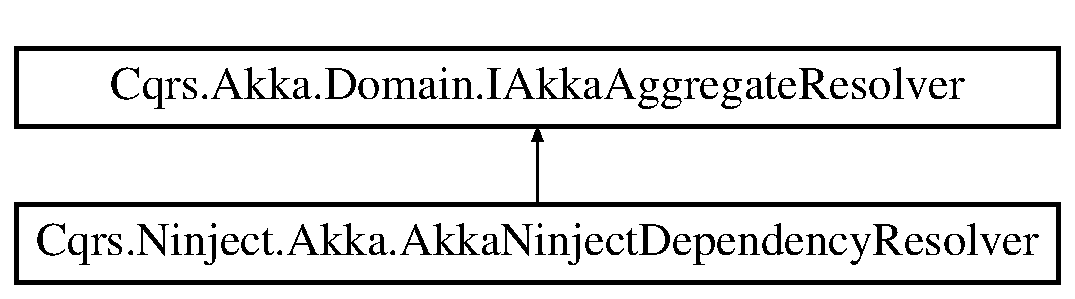
\includegraphics[height=2.000000cm]{interfaceCqrs_1_1Akka_1_1Domain_1_1IAkkaAggregateResolver}
\end{center}
\end{figure}
\doxysubsection*{Public Member Functions}
\begin{DoxyCompactItemize}
\item 
I\+Actor\+Ref \mbox{\hyperlink{interfaceCqrs_1_1Akka_1_1Domain_1_1IAkkaAggregateResolver_a59dbc788ce9893d72684ff5c18945c1d_a59dbc788ce9893d72684ff5c18945c1d}{Resolve\+Actor$<$ T\+Aggregate, T\+Authentication\+Token $>$}} (Guid rsn)
\begin{DoxyCompactList}\small\item\em Resolves instances of {\itshape T\+Aggregate} . \end{DoxyCompactList}\item 
I\+Actor\+Ref \mbox{\hyperlink{interfaceCqrs_1_1Akka_1_1Domain_1_1IAkkaAggregateResolver_a9c3e3f9e8a963ea0b11e79f9eb1c55a9_a9c3e3f9e8a963ea0b11e79f9eb1c55a9}{Resolve\+Actor$<$ T $>$}} ()
\begin{DoxyCompactList}\small\item\em Resolves instances of {\itshape T} . \end{DoxyCompactList}\end{DoxyCompactItemize}


\doxysubsection{Detailed Description}
A resolver for I\+Actor\+Ref instances of I\+Aggregate\+Root$<$\+T\+Authentication\+Token$>$. 



\doxysubsection{Member Function Documentation}
\mbox{\Hypertarget{interfaceCqrs_1_1Akka_1_1Domain_1_1IAkkaAggregateResolver_a9c3e3f9e8a963ea0b11e79f9eb1c55a9_a9c3e3f9e8a963ea0b11e79f9eb1c55a9}\label{interfaceCqrs_1_1Akka_1_1Domain_1_1IAkkaAggregateResolver_a9c3e3f9e8a963ea0b11e79f9eb1c55a9_a9c3e3f9e8a963ea0b11e79f9eb1c55a9}} 
\index{Cqrs.Akka.Domain.IAkkaAggregateResolver@{Cqrs.Akka.Domain.IAkkaAggregateResolver}!ResolveActor$<$ T $>$@{ResolveActor$<$ T $>$}}
\index{ResolveActor$<$ T $>$@{ResolveActor$<$ T $>$}!Cqrs.Akka.Domain.IAkkaAggregateResolver@{Cqrs.Akka.Domain.IAkkaAggregateResolver}}
\doxysubsubsection{\texorpdfstring{ResolveActor$<$ T $>$()}{ResolveActor< T >()}}
{\footnotesize\ttfamily I\+Actor\+Ref Cqrs.\+Akka.\+Domain.\+I\+Akka\+Aggregate\+Resolver.\+Resolve\+Actor$<$ T $>$ (\begin{DoxyParamCaption}{ }\end{DoxyParamCaption})}



Resolves instances of {\itshape T} . 



Implemented in \mbox{\hyperlink{classCqrs_1_1Ninject_1_1Akka_1_1AkkaNinjectDependencyResolver_a6c3399c949a77457456d77688eb66054_a6c3399c949a77457456d77688eb66054}{Cqrs.\+Ninject.\+Akka.\+Akka\+Ninject\+Dependency\+Resolver}}.

\mbox{\Hypertarget{interfaceCqrs_1_1Akka_1_1Domain_1_1IAkkaAggregateResolver_a59dbc788ce9893d72684ff5c18945c1d_a59dbc788ce9893d72684ff5c18945c1d}\label{interfaceCqrs_1_1Akka_1_1Domain_1_1IAkkaAggregateResolver_a59dbc788ce9893d72684ff5c18945c1d_a59dbc788ce9893d72684ff5c18945c1d}} 
\index{Cqrs.Akka.Domain.IAkkaAggregateResolver@{Cqrs.Akka.Domain.IAkkaAggregateResolver}!ResolveActor$<$ TAggregate, TAuthenticationToken $>$@{ResolveActor$<$ TAggregate, TAuthenticationToken $>$}}
\index{ResolveActor$<$ TAggregate, TAuthenticationToken $>$@{ResolveActor$<$ TAggregate, TAuthenticationToken $>$}!Cqrs.Akka.Domain.IAkkaAggregateResolver@{Cqrs.Akka.Domain.IAkkaAggregateResolver}}
\doxysubsubsection{\texorpdfstring{ResolveActor$<$ TAggregate, TAuthenticationToken $>$()}{ResolveActor< TAggregate, TAuthenticationToken >()}}
{\footnotesize\ttfamily I\+Actor\+Ref Cqrs.\+Akka.\+Domain.\+I\+Akka\+Aggregate\+Resolver.\+Resolve\+Actor$<$ T\+Aggregate, T\+Authentication\+Token $>$ (\begin{DoxyParamCaption}\item[{Guid}]{rsn }\end{DoxyParamCaption})}



Resolves instances of {\itshape T\+Aggregate} . 



Implemented in \mbox{\hyperlink{classCqrs_1_1Ninject_1_1Akka_1_1AkkaNinjectDependencyResolver_ab5ba20875aab8764bbb7d6df61722436_ab5ba20875aab8764bbb7d6df61722436}{Cqrs.\+Ninject.\+Akka.\+Akka\+Ninject\+Dependency\+Resolver}}.

\begin{Desc}
\item[Type Constraints]\begin{description}
\item[{\em T\+Aggregate} : {\em I\+Aggregate\+Root$<$T\+Authentication\+Token$>$}]\end{description}
\end{Desc}

\hypertarget{interfaceCqrs_1_1Akka_1_1Domain_1_1IAkkaAggregateRootProxy}{}\section{Cqrs.\+Akka.\+Domain.\+I\+Akka\+Aggregate\+Root\+Proxy$<$ out out T\+Aggregate $>$ Interface Template Reference}
\label{interfaceCqrs_1_1Akka_1_1Domain_1_1IAkkaAggregateRootProxy}\index{Cqrs.\+Akka.\+Domain.\+I\+Akka\+Aggregate\+Root\+Proxy$<$ out out T\+Aggregate $>$@{Cqrs.\+Akka.\+Domain.\+I\+Akka\+Aggregate\+Root\+Proxy$<$ out out T\+Aggregate $>$}}
\subsection*{Properties}
\begin{DoxyCompactItemize}
\item 
I\+Actor\+Ref \hyperlink{interfaceCqrs_1_1Akka_1_1Domain_1_1IAkkaAggregateRootProxy_a60561a15fa10bec1218bc37d30d8f9a5}{Actor\+Reference}\hspace{0.3cm}{\ttfamily  \mbox{[}get\mbox{]}}
\item 
T\+Aggregate \hyperlink{interfaceCqrs_1_1Akka_1_1Domain_1_1IAkkaAggregateRootProxy_a97a7315b1dd655f9e71e24dfbde514a8}{Aggregate}\hspace{0.3cm}{\ttfamily  \mbox{[}get\mbox{]}}
\end{DoxyCompactItemize}


\subsection{Property Documentation}
\mbox{\Hypertarget{interfaceCqrs_1_1Akka_1_1Domain_1_1IAkkaAggregateRootProxy_a60561a15fa10bec1218bc37d30d8f9a5}\label{interfaceCqrs_1_1Akka_1_1Domain_1_1IAkkaAggregateRootProxy_a60561a15fa10bec1218bc37d30d8f9a5}} 
\index{Cqrs\+::\+Akka\+::\+Domain\+::\+I\+Akka\+Aggregate\+Root\+Proxy@{Cqrs\+::\+Akka\+::\+Domain\+::\+I\+Akka\+Aggregate\+Root\+Proxy}!Actor\+Reference@{Actor\+Reference}}
\index{Actor\+Reference@{Actor\+Reference}!Cqrs\+::\+Akka\+::\+Domain\+::\+I\+Akka\+Aggregate\+Root\+Proxy@{Cqrs\+::\+Akka\+::\+Domain\+::\+I\+Akka\+Aggregate\+Root\+Proxy}}
\subsubsection{\texorpdfstring{Actor\+Reference}{ActorReference}}
{\footnotesize\ttfamily I\+Actor\+Ref \hyperlink{interfaceCqrs_1_1Akka_1_1Domain_1_1IAkkaAggregateRootProxy}{Cqrs.\+Akka.\+Domain.\+I\+Akka\+Aggregate\+Root\+Proxy}$<$ out out T\+Aggregate $>$.Actor\+Reference\hspace{0.3cm}{\ttfamily [get]}}

\mbox{\Hypertarget{interfaceCqrs_1_1Akka_1_1Domain_1_1IAkkaAggregateRootProxy_a97a7315b1dd655f9e71e24dfbde514a8}\label{interfaceCqrs_1_1Akka_1_1Domain_1_1IAkkaAggregateRootProxy_a97a7315b1dd655f9e71e24dfbde514a8}} 
\index{Cqrs\+::\+Akka\+::\+Domain\+::\+I\+Akka\+Aggregate\+Root\+Proxy@{Cqrs\+::\+Akka\+::\+Domain\+::\+I\+Akka\+Aggregate\+Root\+Proxy}!Aggregate@{Aggregate}}
\index{Aggregate@{Aggregate}!Cqrs\+::\+Akka\+::\+Domain\+::\+I\+Akka\+Aggregate\+Root\+Proxy@{Cqrs\+::\+Akka\+::\+Domain\+::\+I\+Akka\+Aggregate\+Root\+Proxy}}
\subsubsection{\texorpdfstring{Aggregate}{Aggregate}}
{\footnotesize\ttfamily T\+Aggregate \hyperlink{interfaceCqrs_1_1Akka_1_1Domain_1_1IAkkaAggregateRootProxy}{Cqrs.\+Akka.\+Domain.\+I\+Akka\+Aggregate\+Root\+Proxy}$<$ out out T\+Aggregate $>$.Aggregate\hspace{0.3cm}{\ttfamily [get]}}


\hypertarget{interfaceCqrs_1_1Akka_1_1Domain_1_1IAkkaSagaProxy}{}\doxysection{Cqrs.\+Akka.\+Domain.\+I\+Akka\+Saga\+Proxy$<$ out out T\+Saga $>$ Interface Template Reference}
\label{interfaceCqrs_1_1Akka_1_1Domain_1_1IAkkaSagaProxy}\index{Cqrs.Akka.Domain.IAkkaSagaProxy$<$ out out TSaga $>$@{Cqrs.Akka.Domain.IAkkaSagaProxy$<$ out out TSaga $>$}}


A remote proxy to an I\+Saga$<$\+T\+Authentication\+Token$>$.  


\doxysubsection*{Properties}
\begin{DoxyCompactItemize}
\item 
I\+Actor\+Ref \mbox{\hyperlink{interfaceCqrs_1_1Akka_1_1Domain_1_1IAkkaSagaProxy_a8edb3e9332787ee3a9059589c85ed9e5_a8edb3e9332787ee3a9059589c85ed9e5}{Actor\+Reference}}\hspace{0.3cm}{\ttfamily  \mbox{[}get\mbox{]}}
\begin{DoxyCompactList}\small\item\em Gets the I\+Actor\+Ref. \end{DoxyCompactList}\item 
T\+Saga \mbox{\hyperlink{interfaceCqrs_1_1Akka_1_1Domain_1_1IAkkaSagaProxy_adc230a1e98a8f4ed88a4230e0d0702e1_adc230a1e98a8f4ed88a4230e0d0702e1}{Saga}}\hspace{0.3cm}{\ttfamily  \mbox{[}get\mbox{]}}
\begin{DoxyCompactList}\small\item\em Gets the {\itshape T\+Saga} . \end{DoxyCompactList}\end{DoxyCompactItemize}


\doxysubsection{Detailed Description}
A remote proxy to an I\+Saga$<$\+T\+Authentication\+Token$>$. 


\begin{DoxyTemplParams}{Template Parameters}
{\em T\+Saga} & The Type of I\+Saga$<$\+T\+Authentication\+Token$>$.\\
\hline
\end{DoxyTemplParams}


\doxysubsection{Property Documentation}
\mbox{\Hypertarget{interfaceCqrs_1_1Akka_1_1Domain_1_1IAkkaSagaProxy_a8edb3e9332787ee3a9059589c85ed9e5_a8edb3e9332787ee3a9059589c85ed9e5}\label{interfaceCqrs_1_1Akka_1_1Domain_1_1IAkkaSagaProxy_a8edb3e9332787ee3a9059589c85ed9e5_a8edb3e9332787ee3a9059589c85ed9e5}} 
\index{Cqrs.Akka.Domain.IAkkaSagaProxy$<$ out out TSaga $>$@{Cqrs.Akka.Domain.IAkkaSagaProxy$<$ out out TSaga $>$}!ActorReference@{ActorReference}}
\index{ActorReference@{ActorReference}!Cqrs.Akka.Domain.IAkkaSagaProxy$<$ out out TSaga $>$@{Cqrs.Akka.Domain.IAkkaSagaProxy$<$ out out TSaga $>$}}
\doxysubsubsection{\texorpdfstring{ActorReference}{ActorReference}}
{\footnotesize\ttfamily I\+Actor\+Ref \mbox{\hyperlink{interfaceCqrs_1_1Akka_1_1Domain_1_1IAkkaSagaProxy}{Cqrs.\+Akka.\+Domain.\+I\+Akka\+Saga\+Proxy}}$<$ out out T\+Saga $>$.Actor\+Reference\hspace{0.3cm}{\ttfamily [get]}}



Gets the I\+Actor\+Ref. 

\mbox{\Hypertarget{interfaceCqrs_1_1Akka_1_1Domain_1_1IAkkaSagaProxy_adc230a1e98a8f4ed88a4230e0d0702e1_adc230a1e98a8f4ed88a4230e0d0702e1}\label{interfaceCqrs_1_1Akka_1_1Domain_1_1IAkkaSagaProxy_adc230a1e98a8f4ed88a4230e0d0702e1_adc230a1e98a8f4ed88a4230e0d0702e1}} 
\index{Cqrs.Akka.Domain.IAkkaSagaProxy$<$ out out TSaga $>$@{Cqrs.Akka.Domain.IAkkaSagaProxy$<$ out out TSaga $>$}!Saga@{Saga}}
\index{Saga@{Saga}!Cqrs.Akka.Domain.IAkkaSagaProxy$<$ out out TSaga $>$@{Cqrs.Akka.Domain.IAkkaSagaProxy$<$ out out TSaga $>$}}
\doxysubsubsection{\texorpdfstring{Saga}{Saga}}
{\footnotesize\ttfamily T\+Saga \mbox{\hyperlink{interfaceCqrs_1_1Akka_1_1Domain_1_1IAkkaSagaProxy}{Cqrs.\+Akka.\+Domain.\+I\+Akka\+Saga\+Proxy}}$<$ out out T\+Saga $>$.\mbox{\hyperlink{classCqrs_1_1Domain_1_1Saga}{Saga}}\hspace{0.3cm}{\ttfamily [get]}}



Gets the {\itshape T\+Saga} . 


\hypertarget{interfaceCqrs_1_1Akka_1_1Domain_1_1IAkkaSagaRepository}{}\doxysection{Cqrs.\+Akka.\+Domain.\+I\+Akka\+Saga\+Repository$<$ T\+Authentication\+Token $>$ Interface Template Reference}
\label{interfaceCqrs_1_1Akka_1_1Domain_1_1IAkkaSagaRepository}\index{Cqrs.Akka.Domain.IAkkaSagaRepository$<$ TAuthenticationToken $>$@{Cqrs.Akka.Domain.IAkkaSagaRepository$<$ TAuthenticationToken $>$}}


A Saga\+Repository$<$\+T\+Authentication\+Token$>$ that is safe to use within Akka.\+N\+ET  


Inheritance diagram for Cqrs.\+Akka.\+Domain.\+I\+Akka\+Saga\+Repository$<$ T\+Authentication\+Token $>$\+:\begin{figure}[H]
\begin{center}
\leavevmode
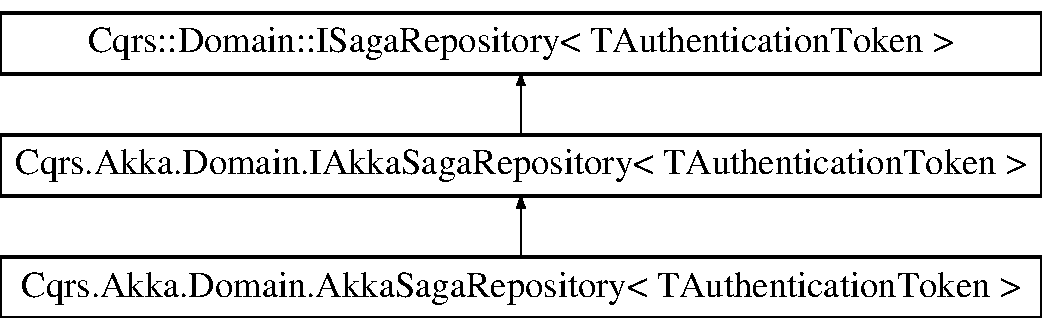
\includegraphics[height=3.000000cm]{interfaceCqrs_1_1Akka_1_1Domain_1_1IAkkaSagaRepository}
\end{center}
\end{figure}
\doxysubsection*{Public Member Functions}
\begin{DoxyCompactItemize}
\item 
void \mbox{\hyperlink{interfaceCqrs_1_1Akka_1_1Domain_1_1IAkkaSagaRepository_a77233d8c2230c0a69a993faaac0101a9_a77233d8c2230c0a69a993faaac0101a9}{Load\+Saga\+History$<$ T\+Saga $>$}} (T\+Saga saga, I\+List$<$ \mbox{\hyperlink{interfaceCqrs_1_1Events_1_1ISagaEvent}{I\+Saga\+Event}}$<$ T\+Authentication\+Token $>$$>$ events=null, bool throw\+Exception\+On\+No\+Events=true)
\begin{DoxyCompactList}\small\item\em If {\itshape events}  is null, loads the events from an I\+Event\+Store$<$\+T\+Authentication\+Token$>$, checks for duplicates and then rehydrates the {\itshape saga}  with the events. \end{DoxyCompactList}\end{DoxyCompactItemize}


\doxysubsection{Detailed Description}
A Saga\+Repository$<$\+T\+Authentication\+Token$>$ that is safe to use within Akka.\+N\+ET 


\begin{DoxyTemplParams}{Template Parameters}
{\em T\+Authentication\+Token} & The Type of authentication token.\\
\hline
\end{DoxyTemplParams}


\doxysubsection{Member Function Documentation}
\mbox{\Hypertarget{interfaceCqrs_1_1Akka_1_1Domain_1_1IAkkaSagaRepository_a77233d8c2230c0a69a993faaac0101a9_a77233d8c2230c0a69a993faaac0101a9}\label{interfaceCqrs_1_1Akka_1_1Domain_1_1IAkkaSagaRepository_a77233d8c2230c0a69a993faaac0101a9_a77233d8c2230c0a69a993faaac0101a9}} 
\index{Cqrs.Akka.Domain.IAkkaSagaRepository$<$ TAuthenticationToken $>$@{Cqrs.Akka.Domain.IAkkaSagaRepository$<$ TAuthenticationToken $>$}!LoadSagaHistory$<$ TSaga $>$@{LoadSagaHistory$<$ TSaga $>$}}
\index{LoadSagaHistory$<$ TSaga $>$@{LoadSagaHistory$<$ TSaga $>$}!Cqrs.Akka.Domain.IAkkaSagaRepository$<$ TAuthenticationToken $>$@{Cqrs.Akka.Domain.IAkkaSagaRepository$<$ TAuthenticationToken $>$}}
\doxysubsubsection{\texorpdfstring{LoadSagaHistory$<$ TSaga $>$()}{LoadSagaHistory< TSaga >()}}
{\footnotesize\ttfamily void \mbox{\hyperlink{interfaceCqrs_1_1Akka_1_1Domain_1_1IAkkaSagaRepository}{Cqrs.\+Akka.\+Domain.\+I\+Akka\+Saga\+Repository}}$<$ T\+Authentication\+Token $>$.Load\+Saga\+History$<$ T\+Saga $>$ (\begin{DoxyParamCaption}\item[{T\+Saga}]{saga,  }\item[{I\+List$<$ \mbox{\hyperlink{interfaceCqrs_1_1Events_1_1ISagaEvent}{I\+Saga\+Event}}$<$ T\+Authentication\+Token $>$$>$}]{events = {\ttfamily null},  }\item[{bool}]{throw\+Exception\+On\+No\+Events = {\ttfamily true} }\end{DoxyParamCaption})}



If {\itshape events}  is null, loads the events from an I\+Event\+Store$<$\+T\+Authentication\+Token$>$, checks for duplicates and then rehydrates the {\itshape saga}  with the events. 


\begin{DoxyTemplParams}{Template Parameters}
{\em T\+Saga} & The Type of I\+Saga$<$\+T\+Authentication\+Token$>$.\\
\hline
\end{DoxyTemplParams}

\begin{DoxyParams}{Parameters}
{\em saga} & The {\itshape T\+Saga}  to rehydrate.\\
\hline
{\em events} & A collection of I\+Event$<$\+T\+Authentication\+Token$>$ to replay on the retrieved I\+Saga$<$\+T\+Authentication\+Token$>$. If null, the I\+Event\+Store$<$\+T\+Authentication\+Token$>$ will be used to retrieve a list of I\+Event$<$\+T\+Authentication\+Token$>$ for you. \\
\hline
{\em throw\+Exception\+On\+No\+Events} & If true will throw an instance of Saga\+Not\+Found\+Exception$<$\+T\+Saga,\+T\+Authentication\+Token$>$ if no aggregate events or provided or found in the I\+Event\+Store$<$\+T\+Authentication\+Token$>$.\\
\hline
\end{DoxyParams}
\begin{Desc}
\item[Type Constraints]\begin{description}
\item[{\em T\+Saga} : {\em I\+Saga$<$T\+Authentication\+Token$>$}]\end{description}
\end{Desc}

\hypertarget{interfaceCqrs_1_1Akka_1_1Domain_1_1IAkkaSagaResolver}{}\doxysection{Cqrs.\+Akka.\+Domain.\+I\+Akka\+Saga\+Resolver Interface Reference}
\label{interfaceCqrs_1_1Akka_1_1Domain_1_1IAkkaSagaResolver}\index{Cqrs.Akka.Domain.IAkkaSagaResolver@{Cqrs.Akka.Domain.IAkkaSagaResolver}}


A resolver for I\+Actor\+Ref instances of I\+Saga$<$\+T\+Authentication\+Token$>$.  


Inheritance diagram for Cqrs.\+Akka.\+Domain.\+I\+Akka\+Saga\+Resolver\+:\begin{figure}[H]
\begin{center}
\leavevmode
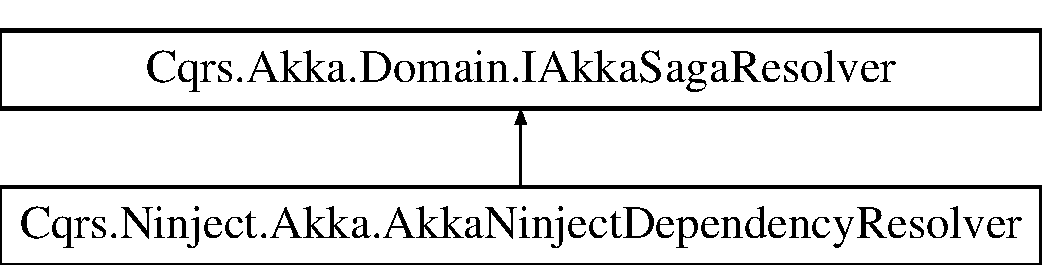
\includegraphics[height=2.000000cm]{interfaceCqrs_1_1Akka_1_1Domain_1_1IAkkaSagaResolver}
\end{center}
\end{figure}
\doxysubsection*{Public Member Functions}
\begin{DoxyCompactItemize}
\item 
I\+Actor\+Ref \mbox{\hyperlink{interfaceCqrs_1_1Akka_1_1Domain_1_1IAkkaSagaResolver_ab41671bdbd0d7d83552b5e11e47fe36d_ab41671bdbd0d7d83552b5e11e47fe36d}{Resolve\+Actor$<$ T\+Saga, T\+Authentication\+Token $>$}} (Guid rsn)
\begin{DoxyCompactList}\small\item\em Resolves instances of {\itshape T\+Saga} . \end{DoxyCompactList}\item 
I\+Actor\+Ref \mbox{\hyperlink{interfaceCqrs_1_1Akka_1_1Domain_1_1IAkkaSagaResolver_adb17ca8a4e09839e67bc9fa0a6ee843f_adb17ca8a4e09839e67bc9fa0a6ee843f}{Resolve\+Actor$<$ T $>$}} ()
\begin{DoxyCompactList}\small\item\em Resolves instances of {\itshape T} . \end{DoxyCompactList}\end{DoxyCompactItemize}


\doxysubsection{Detailed Description}
A resolver for I\+Actor\+Ref instances of I\+Saga$<$\+T\+Authentication\+Token$>$. 



\doxysubsection{Member Function Documentation}
\mbox{\Hypertarget{interfaceCqrs_1_1Akka_1_1Domain_1_1IAkkaSagaResolver_adb17ca8a4e09839e67bc9fa0a6ee843f_adb17ca8a4e09839e67bc9fa0a6ee843f}\label{interfaceCqrs_1_1Akka_1_1Domain_1_1IAkkaSagaResolver_adb17ca8a4e09839e67bc9fa0a6ee843f_adb17ca8a4e09839e67bc9fa0a6ee843f}} 
\index{Cqrs.Akka.Domain.IAkkaSagaResolver@{Cqrs.Akka.Domain.IAkkaSagaResolver}!ResolveActor$<$ T $>$@{ResolveActor$<$ T $>$}}
\index{ResolveActor$<$ T $>$@{ResolveActor$<$ T $>$}!Cqrs.Akka.Domain.IAkkaSagaResolver@{Cqrs.Akka.Domain.IAkkaSagaResolver}}
\doxysubsubsection{\texorpdfstring{ResolveActor$<$ T $>$()}{ResolveActor< T >()}}
{\footnotesize\ttfamily I\+Actor\+Ref Cqrs.\+Akka.\+Domain.\+I\+Akka\+Saga\+Resolver.\+Resolve\+Actor$<$ T $>$ (\begin{DoxyParamCaption}{ }\end{DoxyParamCaption})}



Resolves instances of {\itshape T} . 



Implemented in \mbox{\hyperlink{classCqrs_1_1Ninject_1_1Akka_1_1AkkaNinjectDependencyResolver_a6c3399c949a77457456d77688eb66054_a6c3399c949a77457456d77688eb66054}{Cqrs.\+Ninject.\+Akka.\+Akka\+Ninject\+Dependency\+Resolver}}.

\mbox{\Hypertarget{interfaceCqrs_1_1Akka_1_1Domain_1_1IAkkaSagaResolver_ab41671bdbd0d7d83552b5e11e47fe36d_ab41671bdbd0d7d83552b5e11e47fe36d}\label{interfaceCqrs_1_1Akka_1_1Domain_1_1IAkkaSagaResolver_ab41671bdbd0d7d83552b5e11e47fe36d_ab41671bdbd0d7d83552b5e11e47fe36d}} 
\index{Cqrs.Akka.Domain.IAkkaSagaResolver@{Cqrs.Akka.Domain.IAkkaSagaResolver}!ResolveActor$<$ TSaga, TAuthenticationToken $>$@{ResolveActor$<$ TSaga, TAuthenticationToken $>$}}
\index{ResolveActor$<$ TSaga, TAuthenticationToken $>$@{ResolveActor$<$ TSaga, TAuthenticationToken $>$}!Cqrs.Akka.Domain.IAkkaSagaResolver@{Cqrs.Akka.Domain.IAkkaSagaResolver}}
\doxysubsubsection{\texorpdfstring{ResolveActor$<$ TSaga, TAuthenticationToken $>$()}{ResolveActor< TSaga, TAuthenticationToken >()}}
{\footnotesize\ttfamily I\+Actor\+Ref Cqrs.\+Akka.\+Domain.\+I\+Akka\+Saga\+Resolver.\+Resolve\+Actor$<$ T\+Saga, T\+Authentication\+Token $>$ (\begin{DoxyParamCaption}\item[{Guid}]{rsn }\end{DoxyParamCaption})}



Resolves instances of {\itshape T\+Saga} . 

\begin{Desc}
\item[Type Constraints]\begin{description}
\item[{\em T\+Saga} : {\em I\+Saga$<$T\+Authentication\+Token$>$}]\end{description}
\end{Desc}

\hypertarget{classCqrs_1_1Akka_1_1Events_1_1AkkaEventBus}{}\doxysection{Cqrs.\+Akka.\+Events.\+Akka\+Event\+Bus$<$ T\+Authentication\+Token $>$ Class Template Reference}
\label{classCqrs_1_1Akka_1_1Events_1_1AkkaEventBus}\index{Cqrs.Akka.Events.AkkaEventBus$<$ TAuthenticationToken $>$@{Cqrs.Akka.Events.AkkaEventBus$<$ TAuthenticationToken $>$}}


An I\+Event\+Publisher$<$\+T\+Authentication\+Token$>$ that proxies I\+Event$<$\+T\+Authentication\+Token$>$ back onto the I\+Actor\+Ref and then publishes the I\+Event$<$\+T\+Authentication\+Token$>$ on the public event bus.  


Inheritance diagram for Cqrs.\+Akka.\+Events.\+Akka\+Event\+Bus$<$ T\+Authentication\+Token $>$\+:\begin{figure}[H]
\begin{center}
\leavevmode
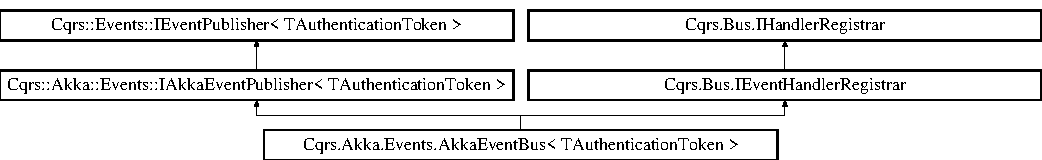
\includegraphics[height=2.148338cm]{classCqrs_1_1Akka_1_1Events_1_1AkkaEventBus}
\end{center}
\end{figure}
\doxysubsection*{Public Member Functions}
\begin{DoxyCompactItemize}
\item 
\mbox{\hyperlink{classCqrs_1_1Akka_1_1Events_1_1AkkaEventBus_ab1f292c21b5516a89fdcc019deb04063_ab1f292c21b5516a89fdcc019deb04063}{Akka\+Event\+Bus}} (\mbox{\hyperlink{interfaceCqrs_1_1Bus_1_1IBusHelper}{I\+Bus\+Helper}} bus\+Helper, \mbox{\hyperlink{interfaceCqrs_1_1Authentication_1_1IAuthenticationTokenHelper}{I\+Authentication\+Token\+Helper}}$<$ T\+Authentication\+Token $>$ authentication\+Token\+Helper, I\+Correlation\+Id\+Helper correlation\+Id\+Helper, I\+Logger logger, \mbox{\hyperlink{interfaceCqrs_1_1Events_1_1IEventPublisher}{I\+Event\+Publisher}}$<$ T\+Authentication\+Token $>$ event\+Publisher, \mbox{\hyperlink{interfaceCqrs_1_1Events_1_1IEventReceiver}{I\+Event\+Receiver}}$<$ T\+Authentication\+Token $>$ event\+Receiver)
\begin{DoxyCompactList}\small\item\em Instantiates a new instance of Akka\+Event\+Bus$<$\+T\+Authentication\+Token$>$ \end{DoxyCompactList}\item 
void \mbox{\hyperlink{classCqrs_1_1Akka_1_1Events_1_1AkkaEventBus_aaba5d37020e21d03cc2bbc3da14f45ea_aaba5d37020e21d03cc2bbc3da14f45ea}{Publish$<$ T\+Event $>$}} (T\+Event @event)
\begin{DoxyCompactList}\small\item\em Publishes the provided {\itshape event}  on the event bus. \end{DoxyCompactList}\item 
virtual void \mbox{\hyperlink{classCqrs_1_1Akka_1_1Events_1_1AkkaEventBus_ad5b996dd77efbf51a2b5a32f94417772_ad5b996dd77efbf51a2b5a32f94417772}{Publish$<$ T\+Event $>$}} (I\+Enumerable$<$ T\+Event $>$ events)
\begin{DoxyCompactList}\small\item\em Publishes the provided {\itshape events}  on the event bus. \end{DoxyCompactList}\item 
virtual void \mbox{\hyperlink{classCqrs_1_1Akka_1_1Events_1_1AkkaEventBus_ae9d248ec73204a7909c04e5a87bfeefb_ae9d248ec73204a7909c04e5a87bfeefb}{Prepare\+Event$<$ T\+Event $>$}} (T\+Event @event, string framework)
\begin{DoxyCompactList}\small\item\em Prepares an I\+Event$<$\+T\+Authentication\+Token$>$ to be sent specifying the framework it is sent via. \end{DoxyCompactList}\item 
virtual bool \mbox{\hyperlink{classCqrs_1_1Akka_1_1Events_1_1AkkaEventBus_a1a89590afc6970f00fe055961a6773e8_a1a89590afc6970f00fe055961a6773e8}{Prepare\+And\+Validate\+Event$<$ T\+Event $>$}} (T\+Event @event, string framework, out I\+Enumerable$<$ \mbox{\hyperlink{classCqrs_1_1Bus_1_1RouteHandlerDelegate}{Route\+Handler\+Delegate}} $>$ handlers)
\begin{DoxyCompactList}\small\item\em Prepares and validates an I\+Event$<$\+T\+Authentication\+Token$>$ to be sent specifying the framework it is sent via. \end{DoxyCompactList}\item 
void \mbox{\hyperlink{classCqrs_1_1Akka_1_1Events_1_1AkkaEventBus_a59ec3e497e511b73b5239eee80691443_a59ec3e497e511b73b5239eee80691443}{Register\+Handler$<$ T\+Message $>$}} (Action$<$ T\+Message $>$ handler, Type targeted\+Type, bool hold\+Message\+Lock=true)
\begin{DoxyCompactList}\small\item\em Register an event or command handler that will listen and respond to events or commands. \end{DoxyCompactList}\item 
void \mbox{\hyperlink{classCqrs_1_1Akka_1_1Events_1_1AkkaEventBus_a6795dfcaf611ce1b50310f442cef0546_a6795dfcaf611ce1b50310f442cef0546}{Register\+Handler$<$ T\+Message $>$}} (Action$<$ T\+Message $>$ handler, bool hold\+Message\+Lock=true)
\begin{DoxyCompactList}\small\item\em Register an event or command handler that will listen and respond to events or commands. \end{DoxyCompactList}\item 
void \mbox{\hyperlink{classCqrs_1_1Akka_1_1Events_1_1AkkaEventBus_ab0df68070fbc625cad5cd2e74667b01d_ab0df68070fbc625cad5cd2e74667b01d}{Register\+Global\+Event\+Handler$<$ T\+Message $>$}} (Action$<$ T\+Message $>$ handler, bool hold\+Message\+Lock=true)
\begin{DoxyCompactList}\small\item\em Register an event handler that will listen and respond to all events. \end{DoxyCompactList}\end{DoxyCompactItemize}
\doxysubsection*{Properties}
\begin{DoxyCompactItemize}
\item 
static \mbox{\hyperlink{classCqrs_1_1Bus_1_1RouteManager}{Route\+Manager}} \mbox{\hyperlink{classCqrs_1_1Akka_1_1Events_1_1AkkaEventBus_a22f195a654564335ffa5f6df01b8af8d_a22f195a654564335ffa5f6df01b8af8d}{Routes}}\hspace{0.3cm}{\ttfamily  \mbox{[}get\mbox{]}}
\begin{DoxyCompactList}\small\item\em Gets the Route\+Manager \end{DoxyCompactList}\item 
\mbox{\hyperlink{interfaceCqrs_1_1Authentication_1_1IAuthenticationTokenHelper}{I\+Authentication\+Token\+Helper}}$<$ T\+Authentication\+Token $>$ \mbox{\hyperlink{classCqrs_1_1Akka_1_1Events_1_1AkkaEventBus_a03166dfca723430ae548e833a2262632_a03166dfca723430ae548e833a2262632}{Authentication\+Token\+Helper}}\hspace{0.3cm}{\ttfamily  \mbox{[}get\mbox{]}}
\begin{DoxyCompactList}\small\item\em Gets or sets the \mbox{\hyperlink{}{Authentication Token Helper}} \end{DoxyCompactList}\item 
I\+Correlation\+Id\+Helper \mbox{\hyperlink{classCqrs_1_1Akka_1_1Events_1_1AkkaEventBus_a5a0e9b6c2c2c5bccb917afabddbee1a8_a5a0e9b6c2c2c5bccb917afabddbee1a8}{Correlation\+Id\+Helper}}\hspace{0.3cm}{\ttfamily  \mbox{[}get\mbox{]}}
\begin{DoxyCompactList}\small\item\em Gets or sets the I\+Correlation\+Id\+Helper \end{DoxyCompactList}\item 
\mbox{\hyperlink{interfaceCqrs_1_1Bus_1_1IBusHelper}{I\+Bus\+Helper}} \mbox{\hyperlink{classCqrs_1_1Akka_1_1Events_1_1AkkaEventBus_a04311f852422c212c4dfa35e8cc21e2e_a04311f852422c212c4dfa35e8cc21e2e}{Bus\+Helper}}\hspace{0.3cm}{\ttfamily  \mbox{[}get\mbox{]}}
\begin{DoxyCompactList}\small\item\em Gets or sets the I\+Bus\+Helper \end{DoxyCompactList}\item 
I\+Logger \mbox{\hyperlink{classCqrs_1_1Akka_1_1Events_1_1AkkaEventBus_a0bbdde7f2011707581db6a66cd73c5c4_a0bbdde7f2011707581db6a66cd73c5c4}{Logger}}\hspace{0.3cm}{\ttfamily  \mbox{[}get\mbox{]}}
\begin{DoxyCompactList}\small\item\em Gets or sets the I\+Logger \end{DoxyCompactList}\item 
\mbox{\hyperlink{interfaceCqrs_1_1Events_1_1IEventPublisher}{I\+Event\+Publisher}}$<$ T\+Authentication\+Token $>$ \mbox{\hyperlink{classCqrs_1_1Akka_1_1Events_1_1AkkaEventBus_a763ef1bf4f3d48ad066a38e576e2d7f0_a763ef1bf4f3d48ad066a38e576e2d7f0}{Event\+Publisher}}\hspace{0.3cm}{\ttfamily  \mbox{[}get\mbox{]}}
\begin{DoxyCompactList}\small\item\em Gets or sets the I\+Event\+Publisher$<$\+T\+Authentication\+Token$>$ \end{DoxyCompactList}\item 
\mbox{\hyperlink{interfaceCqrs_1_1Events_1_1IEventReceiver}{I\+Event\+Receiver}}$<$ T\+Authentication\+Token $>$ \mbox{\hyperlink{classCqrs_1_1Akka_1_1Events_1_1AkkaEventBus_a8e2deeb33b6c6cbc59bec0e0786d5b71_a8e2deeb33b6c6cbc59bec0e0786d5b71}{Event\+Receiver}}\hspace{0.3cm}{\ttfamily  \mbox{[}get\mbox{]}}
\begin{DoxyCompactList}\small\item\em Gets or sets the \mbox{\hyperlink{interfaceCqrs_1_1Events_1_1IEventReceiver}{I\+Event\+Receiver$<$\+T\+Authentication\+Token$>$}} \end{DoxyCompactList}\end{DoxyCompactItemize}


\doxysubsection{Detailed Description}
An I\+Event\+Publisher$<$\+T\+Authentication\+Token$>$ that proxies I\+Event$<$\+T\+Authentication\+Token$>$ back onto the I\+Actor\+Ref and then publishes the I\+Event$<$\+T\+Authentication\+Token$>$ on the public event bus. 



\doxysubsection{Constructor \& Destructor Documentation}
\mbox{\Hypertarget{classCqrs_1_1Akka_1_1Events_1_1AkkaEventBus_ab1f292c21b5516a89fdcc019deb04063_ab1f292c21b5516a89fdcc019deb04063}\label{classCqrs_1_1Akka_1_1Events_1_1AkkaEventBus_ab1f292c21b5516a89fdcc019deb04063_ab1f292c21b5516a89fdcc019deb04063}} 
\index{Cqrs.Akka.Events.AkkaEventBus$<$ TAuthenticationToken $>$@{Cqrs.Akka.Events.AkkaEventBus$<$ TAuthenticationToken $>$}!AkkaEventBus@{AkkaEventBus}}
\index{AkkaEventBus@{AkkaEventBus}!Cqrs.Akka.Events.AkkaEventBus$<$ TAuthenticationToken $>$@{Cqrs.Akka.Events.AkkaEventBus$<$ TAuthenticationToken $>$}}
\doxysubsubsection{\texorpdfstring{AkkaEventBus()}{AkkaEventBus()}}
{\footnotesize\ttfamily \mbox{\hyperlink{classCqrs_1_1Akka_1_1Events_1_1AkkaEventBus}{Cqrs.\+Akka.\+Events.\+Akka\+Event\+Bus}}$<$ T\+Authentication\+Token $>$.\mbox{\hyperlink{classCqrs_1_1Akka_1_1Events_1_1AkkaEventBus}{Akka\+Event\+Bus}} (\begin{DoxyParamCaption}\item[{\mbox{\hyperlink{interfaceCqrs_1_1Bus_1_1IBusHelper}{I\+Bus\+Helper}}}]{bus\+Helper,  }\item[{\mbox{\hyperlink{interfaceCqrs_1_1Authentication_1_1IAuthenticationTokenHelper}{I\+Authentication\+Token\+Helper}}$<$ T\+Authentication\+Token $>$}]{authentication\+Token\+Helper,  }\item[{I\+Correlation\+Id\+Helper}]{correlation\+Id\+Helper,  }\item[{I\+Logger}]{logger,  }\item[{\mbox{\hyperlink{interfaceCqrs_1_1Events_1_1IEventPublisher}{I\+Event\+Publisher}}$<$ T\+Authentication\+Token $>$}]{event\+Publisher,  }\item[{\mbox{\hyperlink{interfaceCqrs_1_1Events_1_1IEventReceiver}{I\+Event\+Receiver}}$<$ T\+Authentication\+Token $>$}]{event\+Receiver }\end{DoxyParamCaption})}



Instantiates a new instance of Akka\+Event\+Bus$<$\+T\+Authentication\+Token$>$ 



\doxysubsection{Member Function Documentation}
\mbox{\Hypertarget{classCqrs_1_1Akka_1_1Events_1_1AkkaEventBus_a1a89590afc6970f00fe055961a6773e8_a1a89590afc6970f00fe055961a6773e8}\label{classCqrs_1_1Akka_1_1Events_1_1AkkaEventBus_a1a89590afc6970f00fe055961a6773e8_a1a89590afc6970f00fe055961a6773e8}} 
\index{Cqrs.Akka.Events.AkkaEventBus$<$ TAuthenticationToken $>$@{Cqrs.Akka.Events.AkkaEventBus$<$ TAuthenticationToken $>$}!PrepareAndValidateEvent$<$ TEvent $>$@{PrepareAndValidateEvent$<$ TEvent $>$}}
\index{PrepareAndValidateEvent$<$ TEvent $>$@{PrepareAndValidateEvent$<$ TEvent $>$}!Cqrs.Akka.Events.AkkaEventBus$<$ TAuthenticationToken $>$@{Cqrs.Akka.Events.AkkaEventBus$<$ TAuthenticationToken $>$}}
\doxysubsubsection{\texorpdfstring{PrepareAndValidateEvent$<$ TEvent $>$()}{PrepareAndValidateEvent< TEvent >()}}
{\footnotesize\ttfamily virtual bool \mbox{\hyperlink{classCqrs_1_1Akka_1_1Events_1_1AkkaEventBus}{Cqrs.\+Akka.\+Events.\+Akka\+Event\+Bus}}$<$ T\+Authentication\+Token $>$.Prepare\+And\+Validate\+Event$<$ T\+Event $>$ (\begin{DoxyParamCaption}\item[{T\+Event @}]{event,  }\item[{string}]{framework,  }\item[{out I\+Enumerable$<$ \mbox{\hyperlink{classCqrs_1_1Bus_1_1RouteHandlerDelegate}{Route\+Handler\+Delegate}} $>$}]{handlers }\end{DoxyParamCaption})\hspace{0.3cm}{\ttfamily [virtual]}}



Prepares and validates an I\+Event$<$\+T\+Authentication\+Token$>$ to be sent specifying the framework it is sent via. 


\begin{DoxyTemplParams}{Template Parameters}
{\em T\+Event} & The Type ofI\+Event$<$\+T\+Authentication\+Token$>$ being sent.\\
\hline
\end{DoxyTemplParams}

\begin{DoxyParams}{Parameters}
{\em event} & The I\+Event$<$\+T\+Authentication\+Token$>$ to send.\\
\hline
{\em framework} & The framework the {\itshape event}  is being sent from.\\
\hline
{\em handlers} & The located \mbox{\hyperlink{}{handlers}} to be executed by passing the {\itshape event} .\\
\hline
\end{DoxyParams}
\begin{Desc}
\item[Type Constraints]\begin{description}
\item[{\em T\+Event} : {\em I\+Event$<$T\+Authentication\+Token$>$}]\end{description}
\end{Desc}
\mbox{\Hypertarget{classCqrs_1_1Akka_1_1Events_1_1AkkaEventBus_ae9d248ec73204a7909c04e5a87bfeefb_ae9d248ec73204a7909c04e5a87bfeefb}\label{classCqrs_1_1Akka_1_1Events_1_1AkkaEventBus_ae9d248ec73204a7909c04e5a87bfeefb_ae9d248ec73204a7909c04e5a87bfeefb}} 
\index{Cqrs.Akka.Events.AkkaEventBus$<$ TAuthenticationToken $>$@{Cqrs.Akka.Events.AkkaEventBus$<$ TAuthenticationToken $>$}!PrepareEvent$<$ TEvent $>$@{PrepareEvent$<$ TEvent $>$}}
\index{PrepareEvent$<$ TEvent $>$@{PrepareEvent$<$ TEvent $>$}!Cqrs.Akka.Events.AkkaEventBus$<$ TAuthenticationToken $>$@{Cqrs.Akka.Events.AkkaEventBus$<$ TAuthenticationToken $>$}}
\doxysubsubsection{\texorpdfstring{PrepareEvent$<$ TEvent $>$()}{PrepareEvent< TEvent >()}}
{\footnotesize\ttfamily virtual void \mbox{\hyperlink{classCqrs_1_1Akka_1_1Events_1_1AkkaEventBus}{Cqrs.\+Akka.\+Events.\+Akka\+Event\+Bus}}$<$ T\+Authentication\+Token $>$.Prepare\+Event$<$ T\+Event $>$ (\begin{DoxyParamCaption}\item[{T\+Event @}]{event,  }\item[{string}]{framework }\end{DoxyParamCaption})\hspace{0.3cm}{\ttfamily [virtual]}}



Prepares an I\+Event$<$\+T\+Authentication\+Token$>$ to be sent specifying the framework it is sent via. 


\begin{DoxyTemplParams}{Template Parameters}
{\em T\+Event} & The Type ofI\+Event$<$\+T\+Authentication\+Token$>$ being sent.\\
\hline
\end{DoxyTemplParams}

\begin{DoxyParams}{Parameters}
{\em event} & The I\+Event$<$\+T\+Authentication\+Token$>$ to send.\\
\hline
{\em framework} & The framework the {\itshape event}  is being sent from.\\
\hline
\end{DoxyParams}
\begin{Desc}
\item[Type Constraints]\begin{description}
\item[{\em T\+Event} : {\em I\+Event$<$T\+Authentication\+Token$>$}]\end{description}
\end{Desc}
\mbox{\Hypertarget{classCqrs_1_1Akka_1_1Events_1_1AkkaEventBus_ad5b996dd77efbf51a2b5a32f94417772_ad5b996dd77efbf51a2b5a32f94417772}\label{classCqrs_1_1Akka_1_1Events_1_1AkkaEventBus_ad5b996dd77efbf51a2b5a32f94417772_ad5b996dd77efbf51a2b5a32f94417772}} 
\index{Cqrs.Akka.Events.AkkaEventBus$<$ TAuthenticationToken $>$@{Cqrs.Akka.Events.AkkaEventBus$<$ TAuthenticationToken $>$}!Publish$<$ TEvent $>$@{Publish$<$ TEvent $>$}}
\index{Publish$<$ TEvent $>$@{Publish$<$ TEvent $>$}!Cqrs.Akka.Events.AkkaEventBus$<$ TAuthenticationToken $>$@{Cqrs.Akka.Events.AkkaEventBus$<$ TAuthenticationToken $>$}}
\doxysubsubsection{\texorpdfstring{Publish$<$ TEvent $>$()}{Publish< TEvent >()}\hspace{0.1cm}{\footnotesize\ttfamily [1/2]}}
{\footnotesize\ttfamily virtual void \mbox{\hyperlink{classCqrs_1_1Akka_1_1Events_1_1AkkaEventBus}{Cqrs.\+Akka.\+Events.\+Akka\+Event\+Bus}}$<$ T\+Authentication\+Token $>$.Publish$<$ T\+Event $>$ (\begin{DoxyParamCaption}\item[{I\+Enumerable$<$ T\+Event $>$}]{events }\end{DoxyParamCaption})\hspace{0.3cm}{\ttfamily [virtual]}}



Publishes the provided {\itshape events}  on the event bus. 



Implements \mbox{\hyperlink{interfaceCqrs_1_1Events_1_1IEventPublisher_a2cbcc3d2c24d015abef6337714ec51ff_a2cbcc3d2c24d015abef6337714ec51ff}{Cqrs.\+Events.\+I\+Event\+Publisher$<$ T\+Authentication\+Token $>$}}.

\begin{Desc}
\item[Type Constraints]\begin{description}
\item[{\em T\+Event} : {\em I\+Event$<$T\+Authentication\+Token$>$}]\end{description}
\end{Desc}
\mbox{\Hypertarget{classCqrs_1_1Akka_1_1Events_1_1AkkaEventBus_aaba5d37020e21d03cc2bbc3da14f45ea_aaba5d37020e21d03cc2bbc3da14f45ea}\label{classCqrs_1_1Akka_1_1Events_1_1AkkaEventBus_aaba5d37020e21d03cc2bbc3da14f45ea_aaba5d37020e21d03cc2bbc3da14f45ea}} 
\index{Cqrs.Akka.Events.AkkaEventBus$<$ TAuthenticationToken $>$@{Cqrs.Akka.Events.AkkaEventBus$<$ TAuthenticationToken $>$}!Publish$<$ TEvent $>$@{Publish$<$ TEvent $>$}}
\index{Publish$<$ TEvent $>$@{Publish$<$ TEvent $>$}!Cqrs.Akka.Events.AkkaEventBus$<$ TAuthenticationToken $>$@{Cqrs.Akka.Events.AkkaEventBus$<$ TAuthenticationToken $>$}}
\doxysubsubsection{\texorpdfstring{Publish$<$ TEvent $>$()}{Publish< TEvent >()}\hspace{0.1cm}{\footnotesize\ttfamily [2/2]}}
{\footnotesize\ttfamily void \mbox{\hyperlink{classCqrs_1_1Akka_1_1Events_1_1AkkaEventBus}{Cqrs.\+Akka.\+Events.\+Akka\+Event\+Bus}}$<$ T\+Authentication\+Token $>$.Publish$<$ T\+Event $>$ (\begin{DoxyParamCaption}\item[{T\+Event @}]{event }\end{DoxyParamCaption})}



Publishes the provided {\itshape event}  on the event bus. 



Implements \mbox{\hyperlink{interfaceCqrs_1_1Events_1_1IEventPublisher_a02f0db0bc9b3aa1c7f766f58f8422ee3_a02f0db0bc9b3aa1c7f766f58f8422ee3}{Cqrs.\+Events.\+I\+Event\+Publisher$<$ T\+Authentication\+Token $>$}}.

\begin{Desc}
\item[Type Constraints]\begin{description}
\item[{\em T\+Event} : {\em I\+Event$<$T\+Authentication\+Token$>$}]\end{description}
\end{Desc}
\mbox{\Hypertarget{classCqrs_1_1Akka_1_1Events_1_1AkkaEventBus_ab0df68070fbc625cad5cd2e74667b01d_ab0df68070fbc625cad5cd2e74667b01d}\label{classCqrs_1_1Akka_1_1Events_1_1AkkaEventBus_ab0df68070fbc625cad5cd2e74667b01d_ab0df68070fbc625cad5cd2e74667b01d}} 
\index{Cqrs.Akka.Events.AkkaEventBus$<$ TAuthenticationToken $>$@{Cqrs.Akka.Events.AkkaEventBus$<$ TAuthenticationToken $>$}!RegisterGlobalEventHandler$<$ TMessage $>$@{RegisterGlobalEventHandler$<$ TMessage $>$}}
\index{RegisterGlobalEventHandler$<$ TMessage $>$@{RegisterGlobalEventHandler$<$ TMessage $>$}!Cqrs.Akka.Events.AkkaEventBus$<$ TAuthenticationToken $>$@{Cqrs.Akka.Events.AkkaEventBus$<$ TAuthenticationToken $>$}}
\doxysubsubsection{\texorpdfstring{RegisterGlobalEventHandler$<$ TMessage $>$()}{RegisterGlobalEventHandler< TMessage >()}}
{\footnotesize\ttfamily void \mbox{\hyperlink{classCqrs_1_1Akka_1_1Events_1_1AkkaEventBus}{Cqrs.\+Akka.\+Events.\+Akka\+Event\+Bus}}$<$ T\+Authentication\+Token $>$.Register\+Global\+Event\+Handler$<$ T\+Message $>$ (\begin{DoxyParamCaption}\item[{Action$<$ T\+Message $>$}]{handler,  }\item[{bool}]{hold\+Message\+Lock = {\ttfamily true} }\end{DoxyParamCaption})}



Register an event handler that will listen and respond to all events. 



Implements \mbox{\hyperlink{interfaceCqrs_1_1Bus_1_1IEventHandlerRegistrar_a80854abefd17bc58bd94e45266cf141e_a80854abefd17bc58bd94e45266cf141e}{Cqrs.\+Bus.\+I\+Event\+Handler\+Registrar}}.

\begin{Desc}
\item[Type Constraints]\begin{description}
\item[{\em T\+Message} : {\em I\+Message}]\end{description}
\end{Desc}
\mbox{\Hypertarget{classCqrs_1_1Akka_1_1Events_1_1AkkaEventBus_a6795dfcaf611ce1b50310f442cef0546_a6795dfcaf611ce1b50310f442cef0546}\label{classCqrs_1_1Akka_1_1Events_1_1AkkaEventBus_a6795dfcaf611ce1b50310f442cef0546_a6795dfcaf611ce1b50310f442cef0546}} 
\index{Cqrs.Akka.Events.AkkaEventBus$<$ TAuthenticationToken $>$@{Cqrs.Akka.Events.AkkaEventBus$<$ TAuthenticationToken $>$}!RegisterHandler$<$ TMessage $>$@{RegisterHandler$<$ TMessage $>$}}
\index{RegisterHandler$<$ TMessage $>$@{RegisterHandler$<$ TMessage $>$}!Cqrs.Akka.Events.AkkaEventBus$<$ TAuthenticationToken $>$@{Cqrs.Akka.Events.AkkaEventBus$<$ TAuthenticationToken $>$}}
\doxysubsubsection{\texorpdfstring{RegisterHandler$<$ TMessage $>$()}{RegisterHandler< TMessage >()}\hspace{0.1cm}{\footnotesize\ttfamily [1/2]}}
{\footnotesize\ttfamily void \mbox{\hyperlink{classCqrs_1_1Akka_1_1Events_1_1AkkaEventBus}{Cqrs.\+Akka.\+Events.\+Akka\+Event\+Bus}}$<$ T\+Authentication\+Token $>$.Register\+Handler$<$ T\+Message $>$ (\begin{DoxyParamCaption}\item[{Action$<$ T\+Message $>$}]{handler,  }\item[{bool}]{hold\+Message\+Lock = {\ttfamily true} }\end{DoxyParamCaption})}



Register an event or command handler that will listen and respond to events or commands. 



Implements \mbox{\hyperlink{interfaceCqrs_1_1Bus_1_1IHandlerRegistrar_a07792dcc9a8b272709ff2e2dd336a642_a07792dcc9a8b272709ff2e2dd336a642}{Cqrs.\+Bus.\+I\+Handler\+Registrar}}.

\begin{Desc}
\item[Type Constraints]\begin{description}
\item[{\em T\+Message} : {\em I\+Message}]\end{description}
\end{Desc}
\mbox{\Hypertarget{classCqrs_1_1Akka_1_1Events_1_1AkkaEventBus_a59ec3e497e511b73b5239eee80691443_a59ec3e497e511b73b5239eee80691443}\label{classCqrs_1_1Akka_1_1Events_1_1AkkaEventBus_a59ec3e497e511b73b5239eee80691443_a59ec3e497e511b73b5239eee80691443}} 
\index{Cqrs.Akka.Events.AkkaEventBus$<$ TAuthenticationToken $>$@{Cqrs.Akka.Events.AkkaEventBus$<$ TAuthenticationToken $>$}!RegisterHandler$<$ TMessage $>$@{RegisterHandler$<$ TMessage $>$}}
\index{RegisterHandler$<$ TMessage $>$@{RegisterHandler$<$ TMessage $>$}!Cqrs.Akka.Events.AkkaEventBus$<$ TAuthenticationToken $>$@{Cqrs.Akka.Events.AkkaEventBus$<$ TAuthenticationToken $>$}}
\doxysubsubsection{\texorpdfstring{RegisterHandler$<$ TMessage $>$()}{RegisterHandler< TMessage >()}\hspace{0.1cm}{\footnotesize\ttfamily [2/2]}}
{\footnotesize\ttfamily void \mbox{\hyperlink{classCqrs_1_1Akka_1_1Events_1_1AkkaEventBus}{Cqrs.\+Akka.\+Events.\+Akka\+Event\+Bus}}$<$ T\+Authentication\+Token $>$.Register\+Handler$<$ T\+Message $>$ (\begin{DoxyParamCaption}\item[{Action$<$ T\+Message $>$}]{handler,  }\item[{Type}]{targeted\+Type,  }\item[{bool}]{hold\+Message\+Lock = {\ttfamily true} }\end{DoxyParamCaption})}



Register an event or command handler that will listen and respond to events or commands. 

In many cases the {\itshape targeted\+Type}  will be the event handler class itself, what you actually want is the target of what is being updated 

Implements \mbox{\hyperlink{interfaceCqrs_1_1Bus_1_1IHandlerRegistrar_ab6ca4dfdc54a5aeebe4651dbdb479f55_ab6ca4dfdc54a5aeebe4651dbdb479f55}{Cqrs.\+Bus.\+I\+Handler\+Registrar}}.

\begin{Desc}
\item[Type Constraints]\begin{description}
\item[{\em T\+Message} : {\em I\+Message}]\end{description}
\end{Desc}


\doxysubsection{Property Documentation}
\mbox{\Hypertarget{classCqrs_1_1Akka_1_1Events_1_1AkkaEventBus_a03166dfca723430ae548e833a2262632_a03166dfca723430ae548e833a2262632}\label{classCqrs_1_1Akka_1_1Events_1_1AkkaEventBus_a03166dfca723430ae548e833a2262632_a03166dfca723430ae548e833a2262632}} 
\index{Cqrs.Akka.Events.AkkaEventBus$<$ TAuthenticationToken $>$@{Cqrs.Akka.Events.AkkaEventBus$<$ TAuthenticationToken $>$}!AuthenticationTokenHelper@{AuthenticationTokenHelper}}
\index{AuthenticationTokenHelper@{AuthenticationTokenHelper}!Cqrs.Akka.Events.AkkaEventBus$<$ TAuthenticationToken $>$@{Cqrs.Akka.Events.AkkaEventBus$<$ TAuthenticationToken $>$}}
\doxysubsubsection{\texorpdfstring{AuthenticationTokenHelper}{AuthenticationTokenHelper}}
{\footnotesize\ttfamily \mbox{\hyperlink{interfaceCqrs_1_1Authentication_1_1IAuthenticationTokenHelper}{I\+Authentication\+Token\+Helper}}$<$T\+Authentication\+Token$>$ \mbox{\hyperlink{classCqrs_1_1Akka_1_1Events_1_1AkkaEventBus}{Cqrs.\+Akka.\+Events.\+Akka\+Event\+Bus}}$<$ T\+Authentication\+Token $>$.\mbox{\hyperlink{classCqrs_1_1Authentication_1_1AuthenticationTokenHelper}{Authentication\+Token\+Helper}}\hspace{0.3cm}{\ttfamily [get]}, {\ttfamily [protected]}}



Gets or sets the \mbox{\hyperlink{}{Authentication Token Helper}} 

\mbox{\Hypertarget{classCqrs_1_1Akka_1_1Events_1_1AkkaEventBus_a04311f852422c212c4dfa35e8cc21e2e_a04311f852422c212c4dfa35e8cc21e2e}\label{classCqrs_1_1Akka_1_1Events_1_1AkkaEventBus_a04311f852422c212c4dfa35e8cc21e2e_a04311f852422c212c4dfa35e8cc21e2e}} 
\index{Cqrs.Akka.Events.AkkaEventBus$<$ TAuthenticationToken $>$@{Cqrs.Akka.Events.AkkaEventBus$<$ TAuthenticationToken $>$}!BusHelper@{BusHelper}}
\index{BusHelper@{BusHelper}!Cqrs.Akka.Events.AkkaEventBus$<$ TAuthenticationToken $>$@{Cqrs.Akka.Events.AkkaEventBus$<$ TAuthenticationToken $>$}}
\doxysubsubsection{\texorpdfstring{BusHelper}{BusHelper}}
{\footnotesize\ttfamily \mbox{\hyperlink{interfaceCqrs_1_1Bus_1_1IBusHelper}{I\+Bus\+Helper}} \mbox{\hyperlink{classCqrs_1_1Akka_1_1Events_1_1AkkaEventBus}{Cqrs.\+Akka.\+Events.\+Akka\+Event\+Bus}}$<$ T\+Authentication\+Token $>$.\mbox{\hyperlink{classCqrs_1_1Bus_1_1BusHelper}{Bus\+Helper}}\hspace{0.3cm}{\ttfamily [get]}, {\ttfamily [protected]}}



Gets or sets the I\+Bus\+Helper 

\mbox{\Hypertarget{classCqrs_1_1Akka_1_1Events_1_1AkkaEventBus_a5a0e9b6c2c2c5bccb917afabddbee1a8_a5a0e9b6c2c2c5bccb917afabddbee1a8}\label{classCqrs_1_1Akka_1_1Events_1_1AkkaEventBus_a5a0e9b6c2c2c5bccb917afabddbee1a8_a5a0e9b6c2c2c5bccb917afabddbee1a8}} 
\index{Cqrs.Akka.Events.AkkaEventBus$<$ TAuthenticationToken $>$@{Cqrs.Akka.Events.AkkaEventBus$<$ TAuthenticationToken $>$}!CorrelationIdHelper@{CorrelationIdHelper}}
\index{CorrelationIdHelper@{CorrelationIdHelper}!Cqrs.Akka.Events.AkkaEventBus$<$ TAuthenticationToken $>$@{Cqrs.Akka.Events.AkkaEventBus$<$ TAuthenticationToken $>$}}
\doxysubsubsection{\texorpdfstring{CorrelationIdHelper}{CorrelationIdHelper}}
{\footnotesize\ttfamily I\+Correlation\+Id\+Helper \mbox{\hyperlink{classCqrs_1_1Akka_1_1Events_1_1AkkaEventBus}{Cqrs.\+Akka.\+Events.\+Akka\+Event\+Bus}}$<$ T\+Authentication\+Token $>$.Correlation\+Id\+Helper\hspace{0.3cm}{\ttfamily [get]}, {\ttfamily [protected]}}



Gets or sets the I\+Correlation\+Id\+Helper 

\mbox{\Hypertarget{classCqrs_1_1Akka_1_1Events_1_1AkkaEventBus_a763ef1bf4f3d48ad066a38e576e2d7f0_a763ef1bf4f3d48ad066a38e576e2d7f0}\label{classCqrs_1_1Akka_1_1Events_1_1AkkaEventBus_a763ef1bf4f3d48ad066a38e576e2d7f0_a763ef1bf4f3d48ad066a38e576e2d7f0}} 
\index{Cqrs.Akka.Events.AkkaEventBus$<$ TAuthenticationToken $>$@{Cqrs.Akka.Events.AkkaEventBus$<$ TAuthenticationToken $>$}!EventPublisher@{EventPublisher}}
\index{EventPublisher@{EventPublisher}!Cqrs.Akka.Events.AkkaEventBus$<$ TAuthenticationToken $>$@{Cqrs.Akka.Events.AkkaEventBus$<$ TAuthenticationToken $>$}}
\doxysubsubsection{\texorpdfstring{EventPublisher}{EventPublisher}}
{\footnotesize\ttfamily \mbox{\hyperlink{interfaceCqrs_1_1Events_1_1IEventPublisher}{I\+Event\+Publisher}}$<$T\+Authentication\+Token$>$ \mbox{\hyperlink{classCqrs_1_1Akka_1_1Events_1_1AkkaEventBus}{Cqrs.\+Akka.\+Events.\+Akka\+Event\+Bus}}$<$ T\+Authentication\+Token $>$.Event\+Publisher\hspace{0.3cm}{\ttfamily [get]}, {\ttfamily [protected]}}



Gets or sets the I\+Event\+Publisher$<$\+T\+Authentication\+Token$>$ 

\mbox{\Hypertarget{classCqrs_1_1Akka_1_1Events_1_1AkkaEventBus_a8e2deeb33b6c6cbc59bec0e0786d5b71_a8e2deeb33b6c6cbc59bec0e0786d5b71}\label{classCqrs_1_1Akka_1_1Events_1_1AkkaEventBus_a8e2deeb33b6c6cbc59bec0e0786d5b71_a8e2deeb33b6c6cbc59bec0e0786d5b71}} 
\index{Cqrs.Akka.Events.AkkaEventBus$<$ TAuthenticationToken $>$@{Cqrs.Akka.Events.AkkaEventBus$<$ TAuthenticationToken $>$}!EventReceiver@{EventReceiver}}
\index{EventReceiver@{EventReceiver}!Cqrs.Akka.Events.AkkaEventBus$<$ TAuthenticationToken $>$@{Cqrs.Akka.Events.AkkaEventBus$<$ TAuthenticationToken $>$}}
\doxysubsubsection{\texorpdfstring{EventReceiver}{EventReceiver}}
{\footnotesize\ttfamily \mbox{\hyperlink{interfaceCqrs_1_1Events_1_1IEventReceiver}{I\+Event\+Receiver}}$<$T\+Authentication\+Token$>$ \mbox{\hyperlink{classCqrs_1_1Akka_1_1Events_1_1AkkaEventBus}{Cqrs.\+Akka.\+Events.\+Akka\+Event\+Bus}}$<$ T\+Authentication\+Token $>$.Event\+Receiver\hspace{0.3cm}{\ttfamily [get]}, {\ttfamily [protected]}}



Gets or sets the \mbox{\hyperlink{interfaceCqrs_1_1Events_1_1IEventReceiver}{I\+Event\+Receiver$<$\+T\+Authentication\+Token$>$}} 

\mbox{\Hypertarget{classCqrs_1_1Akka_1_1Events_1_1AkkaEventBus_a0bbdde7f2011707581db6a66cd73c5c4_a0bbdde7f2011707581db6a66cd73c5c4}\label{classCqrs_1_1Akka_1_1Events_1_1AkkaEventBus_a0bbdde7f2011707581db6a66cd73c5c4_a0bbdde7f2011707581db6a66cd73c5c4}} 
\index{Cqrs.Akka.Events.AkkaEventBus$<$ TAuthenticationToken $>$@{Cqrs.Akka.Events.AkkaEventBus$<$ TAuthenticationToken $>$}!Logger@{Logger}}
\index{Logger@{Logger}!Cqrs.Akka.Events.AkkaEventBus$<$ TAuthenticationToken $>$@{Cqrs.Akka.Events.AkkaEventBus$<$ TAuthenticationToken $>$}}
\doxysubsubsection{\texorpdfstring{Logger}{Logger}}
{\footnotesize\ttfamily I\+Logger \mbox{\hyperlink{classCqrs_1_1Akka_1_1Events_1_1AkkaEventBus}{Cqrs.\+Akka.\+Events.\+Akka\+Event\+Bus}}$<$ T\+Authentication\+Token $>$.Logger\hspace{0.3cm}{\ttfamily [get]}, {\ttfamily [protected]}}



Gets or sets the I\+Logger 

\mbox{\Hypertarget{classCqrs_1_1Akka_1_1Events_1_1AkkaEventBus_a22f195a654564335ffa5f6df01b8af8d_a22f195a654564335ffa5f6df01b8af8d}\label{classCqrs_1_1Akka_1_1Events_1_1AkkaEventBus_a22f195a654564335ffa5f6df01b8af8d_a22f195a654564335ffa5f6df01b8af8d}} 
\index{Cqrs.Akka.Events.AkkaEventBus$<$ TAuthenticationToken $>$@{Cqrs.Akka.Events.AkkaEventBus$<$ TAuthenticationToken $>$}!Routes@{Routes}}
\index{Routes@{Routes}!Cqrs.Akka.Events.AkkaEventBus$<$ TAuthenticationToken $>$@{Cqrs.Akka.Events.AkkaEventBus$<$ TAuthenticationToken $>$}}
\doxysubsubsection{\texorpdfstring{Routes}{Routes}}
{\footnotesize\ttfamily \mbox{\hyperlink{classCqrs_1_1Bus_1_1RouteManager}{Route\+Manager}} \mbox{\hyperlink{classCqrs_1_1Akka_1_1Events_1_1AkkaEventBus}{Cqrs.\+Akka.\+Events.\+Akka\+Event\+Bus}}$<$ T\+Authentication\+Token $>$.Routes\hspace{0.3cm}{\ttfamily [static]}, {\ttfamily [get]}, {\ttfamily [protected]}}



Gets the Route\+Manager 


\hypertarget{classCqrs_1_1Akka_1_1Events_1_1AkkaEventBusProxy}{}\section{Cqrs.\+Akka.\+Events.\+Akka\+Event\+Bus\+Proxy$<$ T\+Authentication\+Token $>$ Class Template Reference}
\label{classCqrs_1_1Akka_1_1Events_1_1AkkaEventBusProxy}\index{Cqrs.\+Akka.\+Events.\+Akka\+Event\+Bus\+Proxy$<$ T\+Authentication\+Token $>$@{Cqrs.\+Akka.\+Events.\+Akka\+Event\+Bus\+Proxy$<$ T\+Authentication\+Token $>$}}


A I\+Event\+Publisher$<$\+T\+Authentication\+Token$>$ that proxies I\+Event$<$\+T\+Authentication\+Token$>$ to the I\+Actor\+Ref which acts as a single point of all handler resolutions.  


Inheritance diagram for Cqrs.\+Akka.\+Events.\+Akka\+Event\+Bus\+Proxy$<$ T\+Authentication\+Token $>$\+:\begin{figure}[H]
\begin{center}
\leavevmode
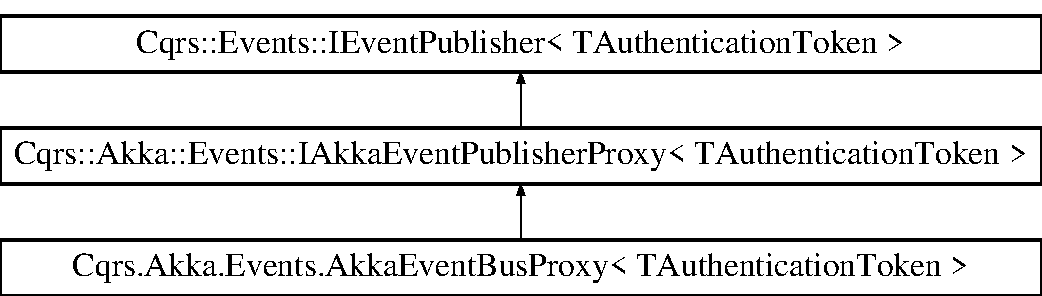
\includegraphics[height=3.000000cm]{classCqrs_1_1Akka_1_1Events_1_1AkkaEventBusProxy}
\end{center}
\end{figure}
\subsection*{Classes}
\begin{DoxyCompactItemize}
\item 
class \hyperlink{classCqrs_1_1Akka_1_1Events_1_1AkkaEventBusProxy_1_1BusActor}{Bus\+Actor}
\end{DoxyCompactItemize}
\subsection*{Public Member Functions}
\begin{DoxyCompactItemize}
\item 
\hyperlink{classCqrs_1_1Akka_1_1Events_1_1AkkaEventBusProxy_a2f886b4e9e64188fe69478c39c96f2b5_a2f886b4e9e64188fe69478c39c96f2b5}{Akka\+Event\+Bus\+Proxy} (\hyperlink{interfaceCqrs_1_1Configuration_1_1IDependencyResolver}{I\+Dependency\+Resolver} dependency\+Resolver, I\+Correlation\+Id\+Helper correlation\+Id\+Helper, \hyperlink{interfaceCqrs_1_1Authentication_1_1IAuthenticationTokenHelper}{I\+Authentication\+Token\+Helper}$<$ T\+Authentication\+Token $>$ authentication\+Token\+Helper)
\item 
virtual void \hyperlink{classCqrs_1_1Akka_1_1Events_1_1AkkaEventBusProxy_a656daead2fe6f30487855dbaea5a3c83_a656daead2fe6f30487855dbaea5a3c83}{Publish$<$ T\+Event $>$} (T\+Event @event)
\begin{DoxyCompactList}\small\item\em Publishes the provided {\itshape event}  on the event bus. \end{DoxyCompactList}\item 
virtual void \hyperlink{classCqrs_1_1Akka_1_1Events_1_1AkkaEventBusProxy_af4c202eaab00ed2fb6160d5b114d935c_af4c202eaab00ed2fb6160d5b114d935c}{Publish$<$ T\+Event $>$} (I\+Enumerable$<$ T\+Event $>$ events)
\begin{DoxyCompactList}\small\item\em Publishes the provided {\itshape events}  on the event bus. \end{DoxyCompactList}\end{DoxyCompactItemize}
\subsection*{Properties}
\begin{DoxyCompactItemize}
\item 
I\+Actor\+Ref \hyperlink{classCqrs_1_1Akka_1_1Events_1_1AkkaEventBusProxy_abd36f5db7a03a38d573b11c0d6f37117_abd36f5db7a03a38d573b11c0d6f37117}{Event\+Handler\+Resolver}\hspace{0.3cm}{\ttfamily  \mbox{[}get\mbox{]}}
\item 
I\+Correlation\+Id\+Helper \hyperlink{classCqrs_1_1Akka_1_1Events_1_1AkkaEventBusProxy_a4cc4ec0ece94393246b0c64f02d55f41_a4cc4ec0ece94393246b0c64f02d55f41}{Correlation\+Id\+Helper}\hspace{0.3cm}{\ttfamily  \mbox{[}get\mbox{]}}
\item 
\hyperlink{interfaceCqrs_1_1Authentication_1_1IAuthenticationTokenHelper}{I\+Authentication\+Token\+Helper}$<$ T\+Authentication\+Token $>$ \hyperlink{classCqrs_1_1Akka_1_1Events_1_1AkkaEventBusProxy_a54964db320ef21b0564e66e9f258f694_a54964db320ef21b0564e66e9f258f694}{Authentication\+Token\+Helper}\hspace{0.3cm}{\ttfamily  \mbox{[}get\mbox{]}}
\end{DoxyCompactItemize}


\subsection{Detailed Description}
A I\+Event\+Publisher$<$\+T\+Authentication\+Token$>$ that proxies I\+Event$<$\+T\+Authentication\+Token$>$ to the I\+Actor\+Ref which acts as a single point of all handler resolutions. 



\subsection{Constructor \& Destructor Documentation}
\mbox{\Hypertarget{classCqrs_1_1Akka_1_1Events_1_1AkkaEventBusProxy_a2f886b4e9e64188fe69478c39c96f2b5_a2f886b4e9e64188fe69478c39c96f2b5}\label{classCqrs_1_1Akka_1_1Events_1_1AkkaEventBusProxy_a2f886b4e9e64188fe69478c39c96f2b5_a2f886b4e9e64188fe69478c39c96f2b5}} 
\index{Cqrs\+::\+Akka\+::\+Events\+::\+Akka\+Event\+Bus\+Proxy@{Cqrs\+::\+Akka\+::\+Events\+::\+Akka\+Event\+Bus\+Proxy}!Akka\+Event\+Bus\+Proxy@{Akka\+Event\+Bus\+Proxy}}
\index{Akka\+Event\+Bus\+Proxy@{Akka\+Event\+Bus\+Proxy}!Cqrs\+::\+Akka\+::\+Events\+::\+Akka\+Event\+Bus\+Proxy@{Cqrs\+::\+Akka\+::\+Events\+::\+Akka\+Event\+Bus\+Proxy}}
\subsubsection{\texorpdfstring{Akka\+Event\+Bus\+Proxy()}{AkkaEventBusProxy()}}
{\footnotesize\ttfamily \hyperlink{classCqrs_1_1Akka_1_1Events_1_1AkkaEventBusProxy}{Cqrs.\+Akka.\+Events.\+Akka\+Event\+Bus\+Proxy}$<$ T\+Authentication\+Token $>$.\hyperlink{classCqrs_1_1Akka_1_1Events_1_1AkkaEventBusProxy}{Akka\+Event\+Bus\+Proxy} (\begin{DoxyParamCaption}\item[{\hyperlink{interfaceCqrs_1_1Configuration_1_1IDependencyResolver}{I\+Dependency\+Resolver}}]{dependency\+Resolver,  }\item[{I\+Correlation\+Id\+Helper}]{correlation\+Id\+Helper,  }\item[{\hyperlink{interfaceCqrs_1_1Authentication_1_1IAuthenticationTokenHelper}{I\+Authentication\+Token\+Helper}$<$ T\+Authentication\+Token $>$}]{authentication\+Token\+Helper }\end{DoxyParamCaption})}



\subsection{Member Function Documentation}
\mbox{\Hypertarget{classCqrs_1_1Akka_1_1Events_1_1AkkaEventBusProxy_a656daead2fe6f30487855dbaea5a3c83_a656daead2fe6f30487855dbaea5a3c83}\label{classCqrs_1_1Akka_1_1Events_1_1AkkaEventBusProxy_a656daead2fe6f30487855dbaea5a3c83_a656daead2fe6f30487855dbaea5a3c83}} 
\index{Cqrs\+::\+Akka\+::\+Events\+::\+Akka\+Event\+Bus\+Proxy@{Cqrs\+::\+Akka\+::\+Events\+::\+Akka\+Event\+Bus\+Proxy}!Publish$<$ T\+Event $>$@{Publish$<$ T\+Event $>$}}
\index{Publish$<$ T\+Event $>$@{Publish$<$ T\+Event $>$}!Cqrs\+::\+Akka\+::\+Events\+::\+Akka\+Event\+Bus\+Proxy@{Cqrs\+::\+Akka\+::\+Events\+::\+Akka\+Event\+Bus\+Proxy}}
\subsubsection{\texorpdfstring{Publish$<$ T\+Event $>$()}{Publish< TEvent >()}\hspace{0.1cm}{\footnotesize\ttfamily [1/2]}}
{\footnotesize\ttfamily virtual void \hyperlink{classCqrs_1_1Akka_1_1Events_1_1AkkaEventBusProxy}{Cqrs.\+Akka.\+Events.\+Akka\+Event\+Bus\+Proxy}$<$ T\+Authentication\+Token $>$.Publish$<$ T\+Event $>$ (\begin{DoxyParamCaption}\item[{T\+Event @}]{event }\end{DoxyParamCaption})\hspace{0.3cm}{\ttfamily [virtual]}}



Publishes the provided {\itshape event}  on the event bus. 



Implements \hyperlink{interfaceCqrs_1_1Events_1_1IEventPublisher_a02f0db0bc9b3aa1c7f766f58f8422ee3_a02f0db0bc9b3aa1c7f766f58f8422ee3}{Cqrs.\+Events.\+I\+Event\+Publisher$<$ T\+Authentication\+Token $>$}.

\begin{Desc}
\item[Type Constraints]\begin{description}
\item[{\em T\+Event} : {\em I\+Event$<$T\+Authentication\+Token$>$}]\end{description}
\end{Desc}
\mbox{\Hypertarget{classCqrs_1_1Akka_1_1Events_1_1AkkaEventBusProxy_af4c202eaab00ed2fb6160d5b114d935c_af4c202eaab00ed2fb6160d5b114d935c}\label{classCqrs_1_1Akka_1_1Events_1_1AkkaEventBusProxy_af4c202eaab00ed2fb6160d5b114d935c_af4c202eaab00ed2fb6160d5b114d935c}} 
\index{Cqrs\+::\+Akka\+::\+Events\+::\+Akka\+Event\+Bus\+Proxy@{Cqrs\+::\+Akka\+::\+Events\+::\+Akka\+Event\+Bus\+Proxy}!Publish$<$ T\+Event $>$@{Publish$<$ T\+Event $>$}}
\index{Publish$<$ T\+Event $>$@{Publish$<$ T\+Event $>$}!Cqrs\+::\+Akka\+::\+Events\+::\+Akka\+Event\+Bus\+Proxy@{Cqrs\+::\+Akka\+::\+Events\+::\+Akka\+Event\+Bus\+Proxy}}
\subsubsection{\texorpdfstring{Publish$<$ T\+Event $>$()}{Publish< TEvent >()}\hspace{0.1cm}{\footnotesize\ttfamily [2/2]}}
{\footnotesize\ttfamily virtual void \hyperlink{classCqrs_1_1Akka_1_1Events_1_1AkkaEventBusProxy}{Cqrs.\+Akka.\+Events.\+Akka\+Event\+Bus\+Proxy}$<$ T\+Authentication\+Token $>$.Publish$<$ T\+Event $>$ (\begin{DoxyParamCaption}\item[{I\+Enumerable$<$ T\+Event $>$}]{events }\end{DoxyParamCaption})\hspace{0.3cm}{\ttfamily [virtual]}}



Publishes the provided {\itshape events}  on the event bus. 



Implements \hyperlink{interfaceCqrs_1_1Events_1_1IEventPublisher_a2cbcc3d2c24d015abef6337714ec51ff_a2cbcc3d2c24d015abef6337714ec51ff}{Cqrs.\+Events.\+I\+Event\+Publisher$<$ T\+Authentication\+Token $>$}.

\begin{Desc}
\item[Type Constraints]\begin{description}
\item[{\em T\+Event} : {\em I\+Event$<$T\+Authentication\+Token$>$}]\end{description}
\end{Desc}


\subsection{Property Documentation}
\mbox{\Hypertarget{classCqrs_1_1Akka_1_1Events_1_1AkkaEventBusProxy_a54964db320ef21b0564e66e9f258f694_a54964db320ef21b0564e66e9f258f694}\label{classCqrs_1_1Akka_1_1Events_1_1AkkaEventBusProxy_a54964db320ef21b0564e66e9f258f694_a54964db320ef21b0564e66e9f258f694}} 
\index{Cqrs\+::\+Akka\+::\+Events\+::\+Akka\+Event\+Bus\+Proxy@{Cqrs\+::\+Akka\+::\+Events\+::\+Akka\+Event\+Bus\+Proxy}!Authentication\+Token\+Helper@{Authentication\+Token\+Helper}}
\index{Authentication\+Token\+Helper@{Authentication\+Token\+Helper}!Cqrs\+::\+Akka\+::\+Events\+::\+Akka\+Event\+Bus\+Proxy@{Cqrs\+::\+Akka\+::\+Events\+::\+Akka\+Event\+Bus\+Proxy}}
\subsubsection{\texorpdfstring{Authentication\+Token\+Helper}{AuthenticationTokenHelper}}
{\footnotesize\ttfamily \hyperlink{interfaceCqrs_1_1Authentication_1_1IAuthenticationTokenHelper}{I\+Authentication\+Token\+Helper}$<$T\+Authentication\+Token$>$ \hyperlink{classCqrs_1_1Akka_1_1Events_1_1AkkaEventBusProxy}{Cqrs.\+Akka.\+Events.\+Akka\+Event\+Bus\+Proxy}$<$ T\+Authentication\+Token $>$.\hyperlink{classCqrs_1_1Authentication_1_1AuthenticationTokenHelper}{Authentication\+Token\+Helper}\hspace{0.3cm}{\ttfamily [get]}, {\ttfamily [protected]}}

\mbox{\Hypertarget{classCqrs_1_1Akka_1_1Events_1_1AkkaEventBusProxy_a4cc4ec0ece94393246b0c64f02d55f41_a4cc4ec0ece94393246b0c64f02d55f41}\label{classCqrs_1_1Akka_1_1Events_1_1AkkaEventBusProxy_a4cc4ec0ece94393246b0c64f02d55f41_a4cc4ec0ece94393246b0c64f02d55f41}} 
\index{Cqrs\+::\+Akka\+::\+Events\+::\+Akka\+Event\+Bus\+Proxy@{Cqrs\+::\+Akka\+::\+Events\+::\+Akka\+Event\+Bus\+Proxy}!Correlation\+Id\+Helper@{Correlation\+Id\+Helper}}
\index{Correlation\+Id\+Helper@{Correlation\+Id\+Helper}!Cqrs\+::\+Akka\+::\+Events\+::\+Akka\+Event\+Bus\+Proxy@{Cqrs\+::\+Akka\+::\+Events\+::\+Akka\+Event\+Bus\+Proxy}}
\subsubsection{\texorpdfstring{Correlation\+Id\+Helper}{CorrelationIdHelper}}
{\footnotesize\ttfamily I\+Correlation\+Id\+Helper \hyperlink{classCqrs_1_1Akka_1_1Events_1_1AkkaEventBusProxy}{Cqrs.\+Akka.\+Events.\+Akka\+Event\+Bus\+Proxy}$<$ T\+Authentication\+Token $>$.Correlation\+Id\+Helper\hspace{0.3cm}{\ttfamily [get]}, {\ttfamily [protected]}}

\mbox{\Hypertarget{classCqrs_1_1Akka_1_1Events_1_1AkkaEventBusProxy_abd36f5db7a03a38d573b11c0d6f37117_abd36f5db7a03a38d573b11c0d6f37117}\label{classCqrs_1_1Akka_1_1Events_1_1AkkaEventBusProxy_abd36f5db7a03a38d573b11c0d6f37117_abd36f5db7a03a38d573b11c0d6f37117}} 
\index{Cqrs\+::\+Akka\+::\+Events\+::\+Akka\+Event\+Bus\+Proxy@{Cqrs\+::\+Akka\+::\+Events\+::\+Akka\+Event\+Bus\+Proxy}!Event\+Handler\+Resolver@{Event\+Handler\+Resolver}}
\index{Event\+Handler\+Resolver@{Event\+Handler\+Resolver}!Cqrs\+::\+Akka\+::\+Events\+::\+Akka\+Event\+Bus\+Proxy@{Cqrs\+::\+Akka\+::\+Events\+::\+Akka\+Event\+Bus\+Proxy}}
\subsubsection{\texorpdfstring{Event\+Handler\+Resolver}{EventHandlerResolver}}
{\footnotesize\ttfamily I\+Actor\+Ref \hyperlink{classCqrs_1_1Akka_1_1Events_1_1AkkaEventBusProxy}{Cqrs.\+Akka.\+Events.\+Akka\+Event\+Bus\+Proxy}$<$ T\+Authentication\+Token $>$.Event\+Handler\+Resolver\hspace{0.3cm}{\ttfamily [get]}, {\ttfamily [protected]}}


\hypertarget{classCqrs_1_1Akka_1_1Events_1_1AkkaEventBusProxy_1_1BusActor}{}\section{Cqrs.\+Akka.\+Events.\+Akka\+Event\+Bus\+Proxy$<$ T\+Authentication\+Token $>$.Bus\+Actor Class Reference}
\label{classCqrs_1_1Akka_1_1Events_1_1AkkaEventBusProxy_1_1BusActor}\index{Cqrs.\+Akka.\+Events.\+Akka\+Event\+Bus\+Proxy$<$ T\+Authentication\+Token $>$.\+Bus\+Actor@{Cqrs.\+Akka.\+Events.\+Akka\+Event\+Bus\+Proxy$<$ T\+Authentication\+Token $>$.\+Bus\+Actor}}
Inheritance diagram for Cqrs.\+Akka.\+Events.\+Akka\+Event\+Bus\+Proxy$<$ T\+Authentication\+Token $>$.Bus\+Actor\+:\begin{figure}[H]
\begin{center}
\leavevmode
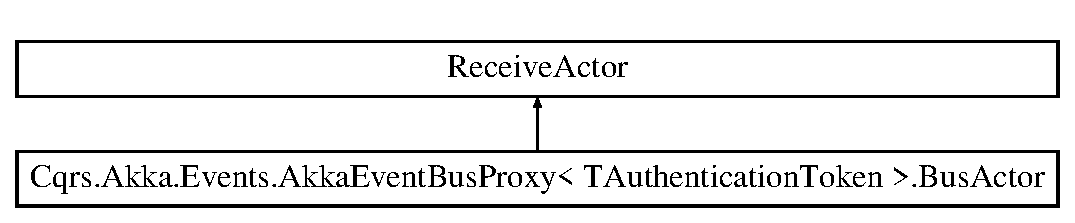
\includegraphics[height=2.000000cm]{classCqrs_1_1Akka_1_1Events_1_1AkkaEventBusProxy_1_1BusActor}
\end{center}
\end{figure}
\subsection*{Public Member Functions}
\begin{DoxyCompactItemize}
\item 
\hyperlink{classCqrs_1_1Akka_1_1Events_1_1AkkaEventBusProxy_1_1BusActor_aeb7cebaad75d810375d0adb82848974a}{Bus\+Actor} (\hyperlink{interfaceCqrs_1_1Akka_1_1Events_1_1IAkkaEventPublisher}{I\+Akka\+Event\+Publisher}$<$ T\+Authentication\+Token $>$ event\+Handler\+Resolver, I\+Correlation\+Id\+Helper correlation\+Id\+Helper, \hyperlink{interfaceCqrs_1_1Authentication_1_1IAuthenticationTokenHelper}{I\+Authentication\+Token\+Helper}$<$ T\+Authentication\+Token $>$ authentication\+Token\+Helper)
\end{DoxyCompactItemize}
\subsection*{Protected Member Functions}
\begin{DoxyCompactItemize}
\item 
virtual void \hyperlink{classCqrs_1_1Akka_1_1Events_1_1AkkaEventBusProxy_1_1BusActor_a90a6f4b440d2e2d9b997f6280ce67921}{Execute\+Receive} (\hyperlink{interfaceCqrs_1_1Events_1_1IEvent}{I\+Event}$<$ T\+Authentication\+Token $>$ @event)
\end{DoxyCompactItemize}
\subsection*{Properties}
\begin{DoxyCompactItemize}
\item 
\hyperlink{interfaceCqrs_1_1Akka_1_1Events_1_1IAkkaEventPublisher}{I\+Akka\+Event\+Publisher}$<$ T\+Authentication\+Token $>$ \hyperlink{classCqrs_1_1Akka_1_1Events_1_1AkkaEventBusProxy_1_1BusActor_ae7986841b1bb97368936c52655b72f96}{Event\+Handler\+Resolver}\hspace{0.3cm}{\ttfamily  \mbox{[}get\mbox{]}}
\item 
I\+Correlation\+Id\+Helper \hyperlink{classCqrs_1_1Akka_1_1Events_1_1AkkaEventBusProxy_1_1BusActor_a4857b2d33de5de94001abf96710b1308}{Correlation\+Id\+Helper}\hspace{0.3cm}{\ttfamily  \mbox{[}get\mbox{]}}
\item 
\hyperlink{interfaceCqrs_1_1Authentication_1_1IAuthenticationTokenHelper}{I\+Authentication\+Token\+Helper}$<$ T\+Authentication\+Token $>$ \hyperlink{classCqrs_1_1Akka_1_1Events_1_1AkkaEventBusProxy_1_1BusActor_a5a276908d994a77c84e12e73ff73a286}{Authentication\+Token\+Helper}\hspace{0.3cm}{\ttfamily  \mbox{[}get\mbox{]}}
\end{DoxyCompactItemize}


\subsection{Constructor \& Destructor Documentation}
\mbox{\Hypertarget{classCqrs_1_1Akka_1_1Events_1_1AkkaEventBusProxy_1_1BusActor_aeb7cebaad75d810375d0adb82848974a}\label{classCqrs_1_1Akka_1_1Events_1_1AkkaEventBusProxy_1_1BusActor_aeb7cebaad75d810375d0adb82848974a}} 
\index{Cqrs\+::\+Akka\+::\+Events\+::\+Akka\+Event\+Bus\+Proxy\+::\+Bus\+Actor@{Cqrs\+::\+Akka\+::\+Events\+::\+Akka\+Event\+Bus\+Proxy\+::\+Bus\+Actor}!Bus\+Actor@{Bus\+Actor}}
\index{Bus\+Actor@{Bus\+Actor}!Cqrs\+::\+Akka\+::\+Events\+::\+Akka\+Event\+Bus\+Proxy\+::\+Bus\+Actor@{Cqrs\+::\+Akka\+::\+Events\+::\+Akka\+Event\+Bus\+Proxy\+::\+Bus\+Actor}}
\subsubsection{\texorpdfstring{Bus\+Actor()}{BusActor()}}
{\footnotesize\ttfamily \hyperlink{classCqrs_1_1Akka_1_1Events_1_1AkkaEventBusProxy}{Cqrs.\+Akka.\+Events.\+Akka\+Event\+Bus\+Proxy}$<$ T\+Authentication\+Token $>$.Bus\+Actor.\+Bus\+Actor (\begin{DoxyParamCaption}\item[{\hyperlink{interfaceCqrs_1_1Akka_1_1Events_1_1IAkkaEventPublisher}{I\+Akka\+Event\+Publisher}$<$ T\+Authentication\+Token $>$}]{event\+Handler\+Resolver,  }\item[{I\+Correlation\+Id\+Helper}]{correlation\+Id\+Helper,  }\item[{\hyperlink{interfaceCqrs_1_1Authentication_1_1IAuthenticationTokenHelper}{I\+Authentication\+Token\+Helper}$<$ T\+Authentication\+Token $>$}]{authentication\+Token\+Helper }\end{DoxyParamCaption})}



\subsection{Member Function Documentation}
\mbox{\Hypertarget{classCqrs_1_1Akka_1_1Events_1_1AkkaEventBusProxy_1_1BusActor_a90a6f4b440d2e2d9b997f6280ce67921}\label{classCqrs_1_1Akka_1_1Events_1_1AkkaEventBusProxy_1_1BusActor_a90a6f4b440d2e2d9b997f6280ce67921}} 
\index{Cqrs\+::\+Akka\+::\+Events\+::\+Akka\+Event\+Bus\+Proxy\+::\+Bus\+Actor@{Cqrs\+::\+Akka\+::\+Events\+::\+Akka\+Event\+Bus\+Proxy\+::\+Bus\+Actor}!Execute\+Receive@{Execute\+Receive}}
\index{Execute\+Receive@{Execute\+Receive}!Cqrs\+::\+Akka\+::\+Events\+::\+Akka\+Event\+Bus\+Proxy\+::\+Bus\+Actor@{Cqrs\+::\+Akka\+::\+Events\+::\+Akka\+Event\+Bus\+Proxy\+::\+Bus\+Actor}}
\subsubsection{\texorpdfstring{Execute\+Receive()}{ExecuteReceive()}}
{\footnotesize\ttfamily virtual void \hyperlink{classCqrs_1_1Akka_1_1Events_1_1AkkaEventBusProxy}{Cqrs.\+Akka.\+Events.\+Akka\+Event\+Bus\+Proxy}$<$ T\+Authentication\+Token $>$.Bus\+Actor.\+Execute\+Receive (\begin{DoxyParamCaption}\item[{\hyperlink{interfaceCqrs_1_1Events_1_1IEvent}{I\+Event}$<$ T\+Authentication\+Token $>$ @}]{event }\end{DoxyParamCaption})\hspace{0.3cm}{\ttfamily [protected]}, {\ttfamily [virtual]}}



\subsection{Property Documentation}
\mbox{\Hypertarget{classCqrs_1_1Akka_1_1Events_1_1AkkaEventBusProxy_1_1BusActor_a5a276908d994a77c84e12e73ff73a286}\label{classCqrs_1_1Akka_1_1Events_1_1AkkaEventBusProxy_1_1BusActor_a5a276908d994a77c84e12e73ff73a286}} 
\index{Cqrs\+::\+Akka\+::\+Events\+::\+Akka\+Event\+Bus\+Proxy\+::\+Bus\+Actor@{Cqrs\+::\+Akka\+::\+Events\+::\+Akka\+Event\+Bus\+Proxy\+::\+Bus\+Actor}!Authentication\+Token\+Helper@{Authentication\+Token\+Helper}}
\index{Authentication\+Token\+Helper@{Authentication\+Token\+Helper}!Cqrs\+::\+Akka\+::\+Events\+::\+Akka\+Event\+Bus\+Proxy\+::\+Bus\+Actor@{Cqrs\+::\+Akka\+::\+Events\+::\+Akka\+Event\+Bus\+Proxy\+::\+Bus\+Actor}}
\subsubsection{\texorpdfstring{Authentication\+Token\+Helper}{AuthenticationTokenHelper}}
{\footnotesize\ttfamily \hyperlink{interfaceCqrs_1_1Authentication_1_1IAuthenticationTokenHelper}{I\+Authentication\+Token\+Helper}$<$T\+Authentication\+Token$>$ \hyperlink{classCqrs_1_1Akka_1_1Events_1_1AkkaEventBusProxy}{Cqrs.\+Akka.\+Events.\+Akka\+Event\+Bus\+Proxy}$<$ T\+Authentication\+Token $>$.Bus\+Actor.\+Authentication\+Token\+Helper\hspace{0.3cm}{\ttfamily [get]}, {\ttfamily [protected]}}

\mbox{\Hypertarget{classCqrs_1_1Akka_1_1Events_1_1AkkaEventBusProxy_1_1BusActor_a4857b2d33de5de94001abf96710b1308}\label{classCqrs_1_1Akka_1_1Events_1_1AkkaEventBusProxy_1_1BusActor_a4857b2d33de5de94001abf96710b1308}} 
\index{Cqrs\+::\+Akka\+::\+Events\+::\+Akka\+Event\+Bus\+Proxy\+::\+Bus\+Actor@{Cqrs\+::\+Akka\+::\+Events\+::\+Akka\+Event\+Bus\+Proxy\+::\+Bus\+Actor}!Correlation\+Id\+Helper@{Correlation\+Id\+Helper}}
\index{Correlation\+Id\+Helper@{Correlation\+Id\+Helper}!Cqrs\+::\+Akka\+::\+Events\+::\+Akka\+Event\+Bus\+Proxy\+::\+Bus\+Actor@{Cqrs\+::\+Akka\+::\+Events\+::\+Akka\+Event\+Bus\+Proxy\+::\+Bus\+Actor}}
\subsubsection{\texorpdfstring{Correlation\+Id\+Helper}{CorrelationIdHelper}}
{\footnotesize\ttfamily I\+Correlation\+Id\+Helper \hyperlink{classCqrs_1_1Akka_1_1Events_1_1AkkaEventBusProxy}{Cqrs.\+Akka.\+Events.\+Akka\+Event\+Bus\+Proxy}$<$ T\+Authentication\+Token $>$.Bus\+Actor.\+Correlation\+Id\+Helper\hspace{0.3cm}{\ttfamily [get]}, {\ttfamily [protected]}}

\mbox{\Hypertarget{classCqrs_1_1Akka_1_1Events_1_1AkkaEventBusProxy_1_1BusActor_ae7986841b1bb97368936c52655b72f96}\label{classCqrs_1_1Akka_1_1Events_1_1AkkaEventBusProxy_1_1BusActor_ae7986841b1bb97368936c52655b72f96}} 
\index{Cqrs\+::\+Akka\+::\+Events\+::\+Akka\+Event\+Bus\+Proxy\+::\+Bus\+Actor@{Cqrs\+::\+Akka\+::\+Events\+::\+Akka\+Event\+Bus\+Proxy\+::\+Bus\+Actor}!Event\+Handler\+Resolver@{Event\+Handler\+Resolver}}
\index{Event\+Handler\+Resolver@{Event\+Handler\+Resolver}!Cqrs\+::\+Akka\+::\+Events\+::\+Akka\+Event\+Bus\+Proxy\+::\+Bus\+Actor@{Cqrs\+::\+Akka\+::\+Events\+::\+Akka\+Event\+Bus\+Proxy\+::\+Bus\+Actor}}
\subsubsection{\texorpdfstring{Event\+Handler\+Resolver}{EventHandlerResolver}}
{\footnotesize\ttfamily \hyperlink{interfaceCqrs_1_1Akka_1_1Events_1_1IAkkaEventPublisher}{I\+Akka\+Event\+Publisher}$<$T\+Authentication\+Token$>$ \hyperlink{classCqrs_1_1Akka_1_1Events_1_1AkkaEventBusProxy}{Cqrs.\+Akka.\+Events.\+Akka\+Event\+Bus\+Proxy}$<$ T\+Authentication\+Token $>$.Bus\+Actor.\+Event\+Handler\+Resolver\hspace{0.3cm}{\ttfamily [get]}, {\ttfamily [protected]}}


\hypertarget{classCqrs_1_1Akka_1_1Events_1_1AkkaEventHandler}{}\section{Cqrs.\+Akka.\+Events.\+Akka\+Event\+Handler$<$ T\+Authentication\+Token $>$ Class Template Reference}
\label{classCqrs_1_1Akka_1_1Events_1_1AkkaEventHandler}\index{Cqrs.\+Akka.\+Events.\+Akka\+Event\+Handler$<$ T\+Authentication\+Token $>$@{Cqrs.\+Akka.\+Events.\+Akka\+Event\+Handler$<$ T\+Authentication\+Token $>$}}
Inheritance diagram for Cqrs.\+Akka.\+Events.\+Akka\+Event\+Handler$<$ T\+Authentication\+Token $>$\+:\begin{figure}[H]
\begin{center}
\leavevmode
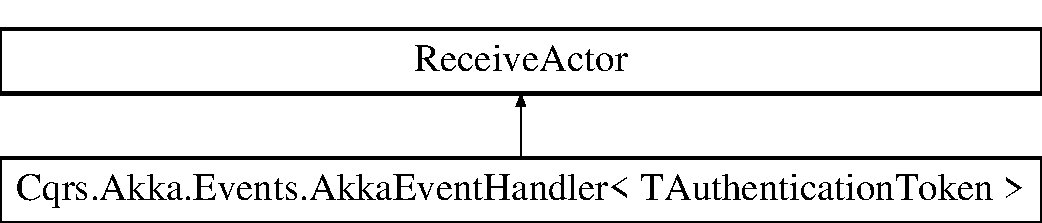
\includegraphics[height=2.000000cm]{classCqrs_1_1Akka_1_1Events_1_1AkkaEventHandler}
\end{center}
\end{figure}
\subsection*{Protected Member Functions}
\begin{DoxyCompactItemize}
\item 
\hyperlink{classCqrs_1_1Akka_1_1Events_1_1AkkaEventHandler_aee50c0ed50e291f311721ca6a103c41f}{Akka\+Event\+Handler} (I\+Logger logger, I\+Correlation\+Id\+Helper correlation\+Id\+Helper, \hyperlink{interfaceCqrs_1_1Authentication_1_1IAuthenticationTokenHelper}{I\+Authentication\+Token\+Helper}$<$ T\+Authentication\+Token $>$ authentication\+Token\+Helper)
\item 
virtual void \hyperlink{classCqrs_1_1Akka_1_1Events_1_1AkkaEventHandler_af277504938e0513e05f3a8784ece2af2}{Execute$<$ T\+Event $>$} (Action$<$ T\+Event $>$ handler, T\+Event @event)
\end{DoxyCompactItemize}
\subsection*{Properties}
\begin{DoxyCompactItemize}
\item 
I\+Logger \hyperlink{classCqrs_1_1Akka_1_1Events_1_1AkkaEventHandler_af9ccf9b06321f7cbb21934e83005346e}{Logger}\hspace{0.3cm}{\ttfamily  \mbox{[}get, set\mbox{]}}
\item 
I\+Correlation\+Id\+Helper \hyperlink{classCqrs_1_1Akka_1_1Events_1_1AkkaEventHandler_a711ada6cc5e9fea454983378f6d5f109}{Correlation\+Id\+Helper}\hspace{0.3cm}{\ttfamily  \mbox{[}get\mbox{]}}
\item 
\hyperlink{interfaceCqrs_1_1Authentication_1_1IAuthenticationTokenHelper}{I\+Authentication\+Token\+Helper}$<$ T\+Authentication\+Token $>$ \hyperlink{classCqrs_1_1Akka_1_1Events_1_1AkkaEventHandler_a6ab1be5352fea3cad8f8599ab31c0ab6}{Authentication\+Token\+Helper}\hspace{0.3cm}{\ttfamily  \mbox{[}get\mbox{]}}
\end{DoxyCompactItemize}


\subsection{Constructor \& Destructor Documentation}
\mbox{\Hypertarget{classCqrs_1_1Akka_1_1Events_1_1AkkaEventHandler_aee50c0ed50e291f311721ca6a103c41f}\label{classCqrs_1_1Akka_1_1Events_1_1AkkaEventHandler_aee50c0ed50e291f311721ca6a103c41f}} 
\index{Cqrs\+::\+Akka\+::\+Events\+::\+Akka\+Event\+Handler@{Cqrs\+::\+Akka\+::\+Events\+::\+Akka\+Event\+Handler}!Akka\+Event\+Handler@{Akka\+Event\+Handler}}
\index{Akka\+Event\+Handler@{Akka\+Event\+Handler}!Cqrs\+::\+Akka\+::\+Events\+::\+Akka\+Event\+Handler@{Cqrs\+::\+Akka\+::\+Events\+::\+Akka\+Event\+Handler}}
\subsubsection{\texorpdfstring{Akka\+Event\+Handler()}{AkkaEventHandler()}}
{\footnotesize\ttfamily \hyperlink{classCqrs_1_1Akka_1_1Events_1_1AkkaEventHandler}{Cqrs.\+Akka.\+Events.\+Akka\+Event\+Handler}$<$ T\+Authentication\+Token $>$.\hyperlink{classCqrs_1_1Akka_1_1Events_1_1AkkaEventHandler}{Akka\+Event\+Handler} (\begin{DoxyParamCaption}\item[{I\+Logger}]{logger,  }\item[{I\+Correlation\+Id\+Helper}]{correlation\+Id\+Helper,  }\item[{\hyperlink{interfaceCqrs_1_1Authentication_1_1IAuthenticationTokenHelper}{I\+Authentication\+Token\+Helper}$<$ T\+Authentication\+Token $>$}]{authentication\+Token\+Helper }\end{DoxyParamCaption})\hspace{0.3cm}{\ttfamily [protected]}}



\subsection{Member Function Documentation}
\mbox{\Hypertarget{classCqrs_1_1Akka_1_1Events_1_1AkkaEventHandler_af277504938e0513e05f3a8784ece2af2}\label{classCqrs_1_1Akka_1_1Events_1_1AkkaEventHandler_af277504938e0513e05f3a8784ece2af2}} 
\index{Cqrs\+::\+Akka\+::\+Events\+::\+Akka\+Event\+Handler@{Cqrs\+::\+Akka\+::\+Events\+::\+Akka\+Event\+Handler}!Execute$<$ T\+Event $>$@{Execute$<$ T\+Event $>$}}
\index{Execute$<$ T\+Event $>$@{Execute$<$ T\+Event $>$}!Cqrs\+::\+Akka\+::\+Events\+::\+Akka\+Event\+Handler@{Cqrs\+::\+Akka\+::\+Events\+::\+Akka\+Event\+Handler}}
\subsubsection{\texorpdfstring{Execute$<$ T\+Event $>$()}{Execute< TEvent >()}}
{\footnotesize\ttfamily virtual void \hyperlink{classCqrs_1_1Akka_1_1Events_1_1AkkaEventHandler}{Cqrs.\+Akka.\+Events.\+Akka\+Event\+Handler}$<$ T\+Authentication\+Token $>$.Execute$<$ T\+Event $>$ (\begin{DoxyParamCaption}\item[{Action$<$ T\+Event $>$}]{handler,  }\item[{T\+Event @}]{event }\end{DoxyParamCaption})\hspace{0.3cm}{\ttfamily [protected]}, {\ttfamily [virtual]}}

\begin{Desc}
\item[Type Constraints]\begin{description}
\item[{\em T\+Event} : {\em I\+Event$<$T\+Authentication\+Token$>$}]\end{description}
\end{Desc}


\subsection{Property Documentation}
\mbox{\Hypertarget{classCqrs_1_1Akka_1_1Events_1_1AkkaEventHandler_a6ab1be5352fea3cad8f8599ab31c0ab6}\label{classCqrs_1_1Akka_1_1Events_1_1AkkaEventHandler_a6ab1be5352fea3cad8f8599ab31c0ab6}} 
\index{Cqrs\+::\+Akka\+::\+Events\+::\+Akka\+Event\+Handler@{Cqrs\+::\+Akka\+::\+Events\+::\+Akka\+Event\+Handler}!Authentication\+Token\+Helper@{Authentication\+Token\+Helper}}
\index{Authentication\+Token\+Helper@{Authentication\+Token\+Helper}!Cqrs\+::\+Akka\+::\+Events\+::\+Akka\+Event\+Handler@{Cqrs\+::\+Akka\+::\+Events\+::\+Akka\+Event\+Handler}}
\subsubsection{\texorpdfstring{Authentication\+Token\+Helper}{AuthenticationTokenHelper}}
{\footnotesize\ttfamily \hyperlink{interfaceCqrs_1_1Authentication_1_1IAuthenticationTokenHelper}{I\+Authentication\+Token\+Helper}$<$T\+Authentication\+Token$>$ \hyperlink{classCqrs_1_1Akka_1_1Events_1_1AkkaEventHandler}{Cqrs.\+Akka.\+Events.\+Akka\+Event\+Handler}$<$ T\+Authentication\+Token $>$.\hyperlink{classCqrs_1_1Authentication_1_1AuthenticationTokenHelper}{Authentication\+Token\+Helper}\hspace{0.3cm}{\ttfamily [get]}, {\ttfamily [protected]}}

\mbox{\Hypertarget{classCqrs_1_1Akka_1_1Events_1_1AkkaEventHandler_a711ada6cc5e9fea454983378f6d5f109}\label{classCqrs_1_1Akka_1_1Events_1_1AkkaEventHandler_a711ada6cc5e9fea454983378f6d5f109}} 
\index{Cqrs\+::\+Akka\+::\+Events\+::\+Akka\+Event\+Handler@{Cqrs\+::\+Akka\+::\+Events\+::\+Akka\+Event\+Handler}!Correlation\+Id\+Helper@{Correlation\+Id\+Helper}}
\index{Correlation\+Id\+Helper@{Correlation\+Id\+Helper}!Cqrs\+::\+Akka\+::\+Events\+::\+Akka\+Event\+Handler@{Cqrs\+::\+Akka\+::\+Events\+::\+Akka\+Event\+Handler}}
\subsubsection{\texorpdfstring{Correlation\+Id\+Helper}{CorrelationIdHelper}}
{\footnotesize\ttfamily I\+Correlation\+Id\+Helper \hyperlink{classCqrs_1_1Akka_1_1Events_1_1AkkaEventHandler}{Cqrs.\+Akka.\+Events.\+Akka\+Event\+Handler}$<$ T\+Authentication\+Token $>$.Correlation\+Id\+Helper\hspace{0.3cm}{\ttfamily [get]}, {\ttfamily [protected]}}

\mbox{\Hypertarget{classCqrs_1_1Akka_1_1Events_1_1AkkaEventHandler_af9ccf9b06321f7cbb21934e83005346e}\label{classCqrs_1_1Akka_1_1Events_1_1AkkaEventHandler_af9ccf9b06321f7cbb21934e83005346e}} 
\index{Cqrs\+::\+Akka\+::\+Events\+::\+Akka\+Event\+Handler@{Cqrs\+::\+Akka\+::\+Events\+::\+Akka\+Event\+Handler}!Logger@{Logger}}
\index{Logger@{Logger}!Cqrs\+::\+Akka\+::\+Events\+::\+Akka\+Event\+Handler@{Cqrs\+::\+Akka\+::\+Events\+::\+Akka\+Event\+Handler}}
\subsubsection{\texorpdfstring{Logger}{Logger}}
{\footnotesize\ttfamily I\+Logger \hyperlink{classCqrs_1_1Akka_1_1Events_1_1AkkaEventHandler}{Cqrs.\+Akka.\+Events.\+Akka\+Event\+Handler}$<$ T\+Authentication\+Token $>$.Logger\hspace{0.3cm}{\ttfamily [get]}, {\ttfamily [set]}, {\ttfamily [protected]}}


\hypertarget{interfaceCqrs_1_1Akka_1_1Events_1_1IAkkaEventPublisher}{}\doxysection{Cqrs.\+Akka.\+Events.\+I\+Akka\+Event\+Publisher$<$ T\+Authentication\+Token $>$ Interface Template Reference}
\label{interfaceCqrs_1_1Akka_1_1Events_1_1IAkkaEventPublisher}\index{Cqrs.Akka.Events.IAkkaEventPublisher$<$ TAuthenticationToken $>$@{Cqrs.Akka.Events.IAkkaEventPublisher$<$ TAuthenticationToken $>$}}


An I\+Event\+Publisher$<$\+T\+Authentication\+Token$>$ that proxies I\+Event$<$\+T\+Authentication\+Token$>$ back onto the I\+Actor\+Ref and then publishes the I\+Event$<$\+T\+Authentication\+Token$>$ on the public event bus.  


Inheritance diagram for Cqrs.\+Akka.\+Events.\+I\+Akka\+Event\+Publisher$<$ T\+Authentication\+Token $>$\+:\begin{figure}[H]
\begin{center}
\leavevmode
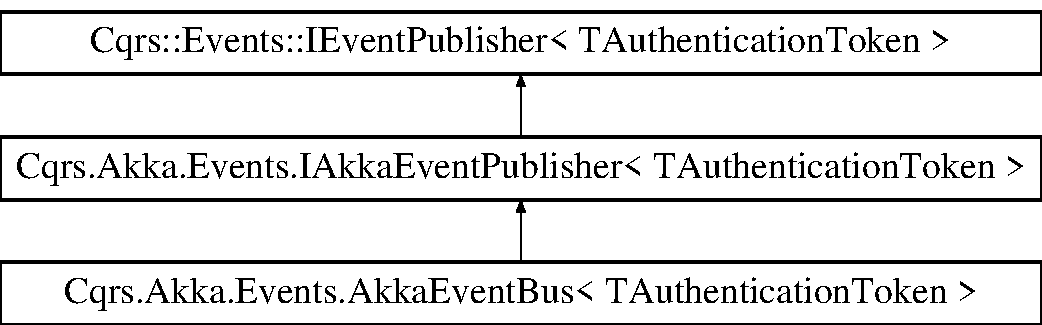
\includegraphics[height=3.000000cm]{interfaceCqrs_1_1Akka_1_1Events_1_1IAkkaEventPublisher}
\end{center}
\end{figure}
\doxysubsection*{Additional Inherited Members}


\doxysubsection{Detailed Description}
An I\+Event\+Publisher$<$\+T\+Authentication\+Token$>$ that proxies I\+Event$<$\+T\+Authentication\+Token$>$ back onto the I\+Actor\+Ref and then publishes the I\+Event$<$\+T\+Authentication\+Token$>$ on the public event bus. 


\hypertarget{interfaceCqrs_1_1Akka_1_1Events_1_1IAkkaEventPublisherProxy}{}\section{Cqrs.\+Akka.\+Events.\+I\+Akka\+Event\+Publisher\+Proxy$<$ T\+Authentication\+Token $>$ Interface Template Reference}
\label{interfaceCqrs_1_1Akka_1_1Events_1_1IAkkaEventPublisherProxy}\index{Cqrs.\+Akka.\+Events.\+I\+Akka\+Event\+Publisher\+Proxy$<$ T\+Authentication\+Token $>$@{Cqrs.\+Akka.\+Events.\+I\+Akka\+Event\+Publisher\+Proxy$<$ T\+Authentication\+Token $>$}}


A I\+Event\+Publisher$<$\+T\+Authentication\+Token$>$ that proxies I\+Event$<$\+T\+Authentication\+Token$>$ back onto the I\+Actor\+Ref and then publishes the I\+Event$<$\+T\+Authentication\+Token$>$ on the public event bus.  


Inheritance diagram for Cqrs.\+Akka.\+Events.\+I\+Akka\+Event\+Publisher\+Proxy$<$ T\+Authentication\+Token $>$\+:\begin{figure}[H]
\begin{center}
\leavevmode
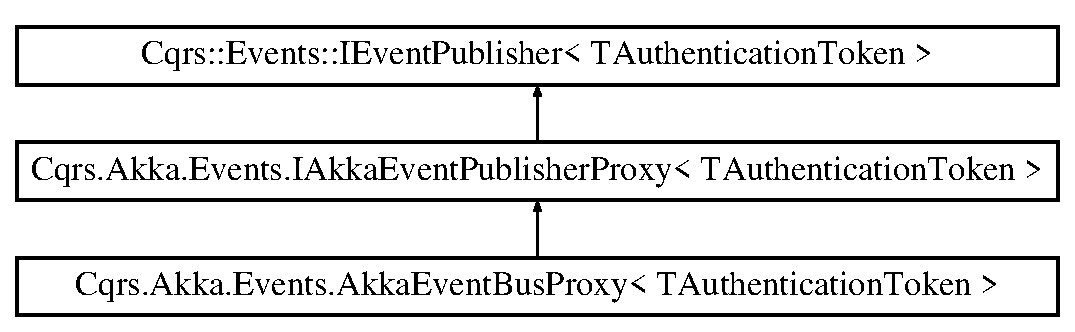
\includegraphics[height=3.000000cm]{interfaceCqrs_1_1Akka_1_1Events_1_1IAkkaEventPublisherProxy}
\end{center}
\end{figure}
\subsection*{Additional Inherited Members}


\subsection{Detailed Description}
A I\+Event\+Publisher$<$\+T\+Authentication\+Token$>$ that proxies I\+Event$<$\+T\+Authentication\+Token$>$ back onto the I\+Actor\+Ref and then publishes the I\+Event$<$\+T\+Authentication\+Token$>$ on the public event bus. 


\hypertarget{classCqrs_1_1Akka_1_1Tests_1_1Unit_1_1Aggregates_1_1HelloWorld}{}\doxysection{Cqrs.\+Akka.\+Tests.\+Unit.\+Aggregates.\+Hello\+World Class Reference}
\label{classCqrs_1_1Akka_1_1Tests_1_1Unit_1_1Aggregates_1_1HelloWorld}\index{Cqrs.Akka.Tests.Unit.Aggregates.HelloWorld@{Cqrs.Akka.Tests.Unit.Aggregates.HelloWorld}}


An Akka.\+Net actor based I\+Aggregate\+Root$<$\+T\+Authentication\+Token$>$ that represents a conversation.  


Inheritance diagram for Cqrs.\+Akka.\+Tests.\+Unit.\+Aggregates.\+Hello\+World\+:\begin{figure}[H]
\begin{center}
\leavevmode
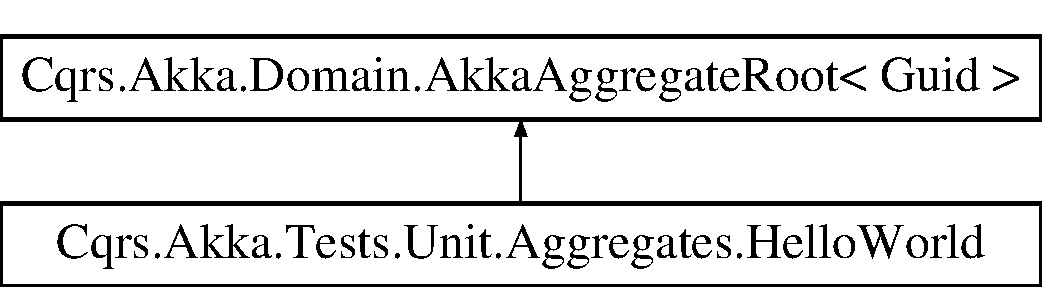
\includegraphics[height=2.000000cm]{classCqrs_1_1Akka_1_1Tests_1_1Unit_1_1Aggregates_1_1HelloWorld}
\end{center}
\end{figure}
\doxysubsection*{Public Member Functions}
\begin{DoxyCompactItemize}
\item 
\mbox{\hyperlink{classCqrs_1_1Akka_1_1Tests_1_1Unit_1_1Aggregates_1_1HelloWorld_a54c9de656ea141ad532d55ba33e94a56_a54c9de656ea141ad532d55ba33e94a56}{Hello\+World}} (\mbox{\hyperlink{interfaceCqrs_1_1Configuration_1_1IDependencyResolver}{I\+Dependency\+Resolver}} dependency\+Resolver, I\+Logger logger, Guid rsn)
\begin{DoxyCompactList}\small\item\em Instantiates a new instance of \mbox{\hyperlink{classCqrs_1_1Akka_1_1Tests_1_1Unit_1_1Aggregates_1_1HelloWorld}{Hello\+World}}. \end{DoxyCompactList}\item 
virtual void \mbox{\hyperlink{classCqrs_1_1Akka_1_1Tests_1_1Unit_1_1Aggregates_1_1HelloWorld_a20af0c54b6a45906cde151ebd20c93a5_a20af0c54b6a45906cde151ebd20c93a5}{Say\+Hello}} (\mbox{\hyperlink{classCqrs_1_1Akka_1_1Tests_1_1Unit_1_1Commands_1_1SayHelloWorldCommand}{Say\+Hello\+World\+Command}} command)
\begin{DoxyCompactList}\small\item\em Raises a Hello\+World\+Said. \end{DoxyCompactList}\item 
virtual void \mbox{\hyperlink{classCqrs_1_1Akka_1_1Tests_1_1Unit_1_1Aggregates_1_1HelloWorld_a6e0f9b4297a292190a605c34741395a5_a6e0f9b4297a292190a605c34741395a5}{Reply\+To\+Hello\+World}} (\mbox{\hyperlink{classCqrs_1_1Akka_1_1Tests_1_1Unit_1_1Commands_1_1ReplyToHelloWorldCommand}{Reply\+To\+Hello\+World\+Command}} command)
\begin{DoxyCompactList}\small\item\em Raises a Hello\+World\+Replied\+To. \end{DoxyCompactList}\item 
virtual void \mbox{\hyperlink{classCqrs_1_1Akka_1_1Tests_1_1Unit_1_1Aggregates_1_1HelloWorld_a310c79f307749813d56872b41c9685f0_a310c79f307749813d56872b41c9685f0}{End\+Conversation}} (\mbox{\hyperlink{classCqrs_1_1Akka_1_1Tests_1_1Unit_1_1Commands_1_1EndConversationCommand}{End\+Conversation\+Command}} command)
\begin{DoxyCompactList}\small\item\em Raises a Conversation\+Ended. \end{DoxyCompactList}\item 
virtual void \mbox{\hyperlink{classCqrs_1_1Akka_1_1Tests_1_1Unit_1_1Aggregates_1_1HelloWorld_a2c5e579e741dc3471e3532f5be3b98ab_a2c5e579e741dc3471e3532f5be3b98ab}{Say\+Hello}} ()
\begin{DoxyCompactList}\small\item\em Raises a Hello\+World\+Said. \end{DoxyCompactList}\item 
virtual void \mbox{\hyperlink{classCqrs_1_1Akka_1_1Tests_1_1Unit_1_1Aggregates_1_1HelloWorld_a6b3c07d040e703d89c7a065064776623_a6b3c07d040e703d89c7a065064776623}{Reply\+To\+Hello\+World}} ()
\begin{DoxyCompactList}\small\item\em Raises a Hello\+World\+Replied\+To. \end{DoxyCompactList}\item 
virtual void \mbox{\hyperlink{classCqrs_1_1Akka_1_1Tests_1_1Unit_1_1Aggregates_1_1HelloWorld_aeeb20725d192b64adf47281d37dd198d_aeeb20725d192b64adf47281d37dd198d}{End\+Conversation}} ()
\begin{DoxyCompactList}\small\item\em Raises a Conversation\+Ended. \end{DoxyCompactList}\end{DoxyCompactItemize}
\doxysubsection*{Properties}
\begin{DoxyCompactItemize}
\item 
Guid \mbox{\hyperlink{classCqrs_1_1Akka_1_1Tests_1_1Unit_1_1Aggregates_1_1HelloWorld_a2e74fa47e00d67d6de3df5b1b8e140f6_a2e74fa47e00d67d6de3df5b1b8e140f6}{Rsn}}\hspace{0.3cm}{\ttfamily  \mbox{[}get\mbox{]}}
\begin{DoxyCompactList}\small\item\em The I\+Aggregate\+Root$<$\+T\+Authentication\+Token$>$.\+Id. \end{DoxyCompactList}\item 
bool \mbox{\hyperlink{classCqrs_1_1Akka_1_1Tests_1_1Unit_1_1Aggregates_1_1HelloWorld_acb0b1bde01be12368433ebbb8f20eba9_acb0b1bde01be12368433ebbb8f20eba9}{Is\+Deleted}}\hspace{0.3cm}{\ttfamily  \mbox{[}get, set\mbox{]}}
\begin{DoxyCompactList}\small\item\em Indicates if this I\+Saga$<$\+T\+Authentication\+Token$>$ has been deleted. \end{DoxyCompactList}\item 
\mbox{\hyperlink{interfaceCqrs_1_1Configuration_1_1IDependencyResolver}{I\+Dependency\+Resolver}} \mbox{\hyperlink{classCqrs_1_1Akka_1_1Tests_1_1Unit_1_1Aggregates_1_1HelloWorld_abf66c1d14c78b9ed3ca54225d04a8beb_abf66c1d14c78b9ed3ca54225d04a8beb}{Dependency\+Resolver}}\hspace{0.3cm}{\ttfamily  \mbox{[}get\mbox{]}}
\begin{DoxyCompactList}\small\item\em The I\+Dependency\+Resolver that resolves things. \end{DoxyCompactList}\end{DoxyCompactItemize}
\doxysubsection*{Additional Inherited Members}


\doxysubsection{Detailed Description}
An Akka.\+Net actor based I\+Aggregate\+Root$<$\+T\+Authentication\+Token$>$ that represents a conversation. 



\doxysubsection{Constructor \& Destructor Documentation}
\mbox{\Hypertarget{classCqrs_1_1Akka_1_1Tests_1_1Unit_1_1Aggregates_1_1HelloWorld_a54c9de656ea141ad532d55ba33e94a56_a54c9de656ea141ad532d55ba33e94a56}\label{classCqrs_1_1Akka_1_1Tests_1_1Unit_1_1Aggregates_1_1HelloWorld_a54c9de656ea141ad532d55ba33e94a56_a54c9de656ea141ad532d55ba33e94a56}} 
\index{Cqrs.Akka.Tests.Unit.Aggregates.HelloWorld@{Cqrs.Akka.Tests.Unit.Aggregates.HelloWorld}!HelloWorld@{HelloWorld}}
\index{HelloWorld@{HelloWorld}!Cqrs.Akka.Tests.Unit.Aggregates.HelloWorld@{Cqrs.Akka.Tests.Unit.Aggregates.HelloWorld}}
\doxysubsubsection{\texorpdfstring{HelloWorld()}{HelloWorld()}}
{\footnotesize\ttfamily Cqrs.\+Akka.\+Tests.\+Unit.\+Aggregates.\+Hello\+World.\+Hello\+World (\begin{DoxyParamCaption}\item[{\mbox{\hyperlink{interfaceCqrs_1_1Configuration_1_1IDependencyResolver}{I\+Dependency\+Resolver}}}]{dependency\+Resolver,  }\item[{I\+Logger}]{logger,  }\item[{Guid}]{rsn }\end{DoxyParamCaption})}



Instantiates a new instance of \mbox{\hyperlink{classCqrs_1_1Akka_1_1Tests_1_1Unit_1_1Aggregates_1_1HelloWorld}{Hello\+World}}. 



\doxysubsection{Member Function Documentation}
\mbox{\Hypertarget{classCqrs_1_1Akka_1_1Tests_1_1Unit_1_1Aggregates_1_1HelloWorld_aeeb20725d192b64adf47281d37dd198d_aeeb20725d192b64adf47281d37dd198d}\label{classCqrs_1_1Akka_1_1Tests_1_1Unit_1_1Aggregates_1_1HelloWorld_aeeb20725d192b64adf47281d37dd198d_aeeb20725d192b64adf47281d37dd198d}} 
\index{Cqrs.Akka.Tests.Unit.Aggregates.HelloWorld@{Cqrs.Akka.Tests.Unit.Aggregates.HelloWorld}!EndConversation@{EndConversation}}
\index{EndConversation@{EndConversation}!Cqrs.Akka.Tests.Unit.Aggregates.HelloWorld@{Cqrs.Akka.Tests.Unit.Aggregates.HelloWorld}}
\doxysubsubsection{\texorpdfstring{EndConversation()}{EndConversation()}\hspace{0.1cm}{\footnotesize\ttfamily [1/2]}}
{\footnotesize\ttfamily virtual void Cqrs.\+Akka.\+Tests.\+Unit.\+Aggregates.\+Hello\+World.\+End\+Conversation (\begin{DoxyParamCaption}{ }\end{DoxyParamCaption})\hspace{0.3cm}{\ttfamily [virtual]}}



Raises a Conversation\+Ended. 

\mbox{\Hypertarget{classCqrs_1_1Akka_1_1Tests_1_1Unit_1_1Aggregates_1_1HelloWorld_a310c79f307749813d56872b41c9685f0_a310c79f307749813d56872b41c9685f0}\label{classCqrs_1_1Akka_1_1Tests_1_1Unit_1_1Aggregates_1_1HelloWorld_a310c79f307749813d56872b41c9685f0_a310c79f307749813d56872b41c9685f0}} 
\index{Cqrs.Akka.Tests.Unit.Aggregates.HelloWorld@{Cqrs.Akka.Tests.Unit.Aggregates.HelloWorld}!EndConversation@{EndConversation}}
\index{EndConversation@{EndConversation}!Cqrs.Akka.Tests.Unit.Aggregates.HelloWorld@{Cqrs.Akka.Tests.Unit.Aggregates.HelloWorld}}
\doxysubsubsection{\texorpdfstring{EndConversation()}{EndConversation()}\hspace{0.1cm}{\footnotesize\ttfamily [2/2]}}
{\footnotesize\ttfamily virtual void Cqrs.\+Akka.\+Tests.\+Unit.\+Aggregates.\+Hello\+World.\+End\+Conversation (\begin{DoxyParamCaption}\item[{\mbox{\hyperlink{classCqrs_1_1Akka_1_1Tests_1_1Unit_1_1Commands_1_1EndConversationCommand}{End\+Conversation\+Command}}}]{command }\end{DoxyParamCaption})\hspace{0.3cm}{\ttfamily [virtual]}}



Raises a Conversation\+Ended. 

\mbox{\Hypertarget{classCqrs_1_1Akka_1_1Tests_1_1Unit_1_1Aggregates_1_1HelloWorld_a6b3c07d040e703d89c7a065064776623_a6b3c07d040e703d89c7a065064776623}\label{classCqrs_1_1Akka_1_1Tests_1_1Unit_1_1Aggregates_1_1HelloWorld_a6b3c07d040e703d89c7a065064776623_a6b3c07d040e703d89c7a065064776623}} 
\index{Cqrs.Akka.Tests.Unit.Aggregates.HelloWorld@{Cqrs.Akka.Tests.Unit.Aggregates.HelloWorld}!ReplyToHelloWorld@{ReplyToHelloWorld}}
\index{ReplyToHelloWorld@{ReplyToHelloWorld}!Cqrs.Akka.Tests.Unit.Aggregates.HelloWorld@{Cqrs.Akka.Tests.Unit.Aggregates.HelloWorld}}
\doxysubsubsection{\texorpdfstring{ReplyToHelloWorld()}{ReplyToHelloWorld()}\hspace{0.1cm}{\footnotesize\ttfamily [1/2]}}
{\footnotesize\ttfamily virtual void Cqrs.\+Akka.\+Tests.\+Unit.\+Aggregates.\+Hello\+World.\+Reply\+To\+Hello\+World (\begin{DoxyParamCaption}{ }\end{DoxyParamCaption})\hspace{0.3cm}{\ttfamily [virtual]}}



Raises a Hello\+World\+Replied\+To. 

\mbox{\Hypertarget{classCqrs_1_1Akka_1_1Tests_1_1Unit_1_1Aggregates_1_1HelloWorld_a6e0f9b4297a292190a605c34741395a5_a6e0f9b4297a292190a605c34741395a5}\label{classCqrs_1_1Akka_1_1Tests_1_1Unit_1_1Aggregates_1_1HelloWorld_a6e0f9b4297a292190a605c34741395a5_a6e0f9b4297a292190a605c34741395a5}} 
\index{Cqrs.Akka.Tests.Unit.Aggregates.HelloWorld@{Cqrs.Akka.Tests.Unit.Aggregates.HelloWorld}!ReplyToHelloWorld@{ReplyToHelloWorld}}
\index{ReplyToHelloWorld@{ReplyToHelloWorld}!Cqrs.Akka.Tests.Unit.Aggregates.HelloWorld@{Cqrs.Akka.Tests.Unit.Aggregates.HelloWorld}}
\doxysubsubsection{\texorpdfstring{ReplyToHelloWorld()}{ReplyToHelloWorld()}\hspace{0.1cm}{\footnotesize\ttfamily [2/2]}}
{\footnotesize\ttfamily virtual void Cqrs.\+Akka.\+Tests.\+Unit.\+Aggregates.\+Hello\+World.\+Reply\+To\+Hello\+World (\begin{DoxyParamCaption}\item[{\mbox{\hyperlink{classCqrs_1_1Akka_1_1Tests_1_1Unit_1_1Commands_1_1ReplyToHelloWorldCommand}{Reply\+To\+Hello\+World\+Command}}}]{command }\end{DoxyParamCaption})\hspace{0.3cm}{\ttfamily [virtual]}}



Raises a Hello\+World\+Replied\+To. 

\mbox{\Hypertarget{classCqrs_1_1Akka_1_1Tests_1_1Unit_1_1Aggregates_1_1HelloWorld_a2c5e579e741dc3471e3532f5be3b98ab_a2c5e579e741dc3471e3532f5be3b98ab}\label{classCqrs_1_1Akka_1_1Tests_1_1Unit_1_1Aggregates_1_1HelloWorld_a2c5e579e741dc3471e3532f5be3b98ab_a2c5e579e741dc3471e3532f5be3b98ab}} 
\index{Cqrs.Akka.Tests.Unit.Aggregates.HelloWorld@{Cqrs.Akka.Tests.Unit.Aggregates.HelloWorld}!SayHello@{SayHello}}
\index{SayHello@{SayHello}!Cqrs.Akka.Tests.Unit.Aggregates.HelloWorld@{Cqrs.Akka.Tests.Unit.Aggregates.HelloWorld}}
\doxysubsubsection{\texorpdfstring{SayHello()}{SayHello()}\hspace{0.1cm}{\footnotesize\ttfamily [1/2]}}
{\footnotesize\ttfamily virtual void Cqrs.\+Akka.\+Tests.\+Unit.\+Aggregates.\+Hello\+World.\+Say\+Hello (\begin{DoxyParamCaption}{ }\end{DoxyParamCaption})\hspace{0.3cm}{\ttfamily [virtual]}}



Raises a Hello\+World\+Said. 

\mbox{\Hypertarget{classCqrs_1_1Akka_1_1Tests_1_1Unit_1_1Aggregates_1_1HelloWorld_a20af0c54b6a45906cde151ebd20c93a5_a20af0c54b6a45906cde151ebd20c93a5}\label{classCqrs_1_1Akka_1_1Tests_1_1Unit_1_1Aggregates_1_1HelloWorld_a20af0c54b6a45906cde151ebd20c93a5_a20af0c54b6a45906cde151ebd20c93a5}} 
\index{Cqrs.Akka.Tests.Unit.Aggregates.HelloWorld@{Cqrs.Akka.Tests.Unit.Aggregates.HelloWorld}!SayHello@{SayHello}}
\index{SayHello@{SayHello}!Cqrs.Akka.Tests.Unit.Aggregates.HelloWorld@{Cqrs.Akka.Tests.Unit.Aggregates.HelloWorld}}
\doxysubsubsection{\texorpdfstring{SayHello()}{SayHello()}\hspace{0.1cm}{\footnotesize\ttfamily [2/2]}}
{\footnotesize\ttfamily virtual void Cqrs.\+Akka.\+Tests.\+Unit.\+Aggregates.\+Hello\+World.\+Say\+Hello (\begin{DoxyParamCaption}\item[{\mbox{\hyperlink{classCqrs_1_1Akka_1_1Tests_1_1Unit_1_1Commands_1_1SayHelloWorldCommand}{Say\+Hello\+World\+Command}}}]{command }\end{DoxyParamCaption})\hspace{0.3cm}{\ttfamily [virtual]}}



Raises a Hello\+World\+Said. 



\doxysubsection{Property Documentation}
\mbox{\Hypertarget{classCqrs_1_1Akka_1_1Tests_1_1Unit_1_1Aggregates_1_1HelloWorld_abf66c1d14c78b9ed3ca54225d04a8beb_abf66c1d14c78b9ed3ca54225d04a8beb}\label{classCqrs_1_1Akka_1_1Tests_1_1Unit_1_1Aggregates_1_1HelloWorld_abf66c1d14c78b9ed3ca54225d04a8beb_abf66c1d14c78b9ed3ca54225d04a8beb}} 
\index{Cqrs.Akka.Tests.Unit.Aggregates.HelloWorld@{Cqrs.Akka.Tests.Unit.Aggregates.HelloWorld}!DependencyResolver@{DependencyResolver}}
\index{DependencyResolver@{DependencyResolver}!Cqrs.Akka.Tests.Unit.Aggregates.HelloWorld@{Cqrs.Akka.Tests.Unit.Aggregates.HelloWorld}}
\doxysubsubsection{\texorpdfstring{DependencyResolver}{DependencyResolver}}
{\footnotesize\ttfamily \mbox{\hyperlink{interfaceCqrs_1_1Configuration_1_1IDependencyResolver}{I\+Dependency\+Resolver}} Cqrs.\+Akka.\+Tests.\+Unit.\+Aggregates.\+Hello\+World.\+Dependency\+Resolver\hspace{0.3cm}{\ttfamily [get]}, {\ttfamily [protected]}}



The I\+Dependency\+Resolver that resolves things. 

\mbox{\Hypertarget{classCqrs_1_1Akka_1_1Tests_1_1Unit_1_1Aggregates_1_1HelloWorld_acb0b1bde01be12368433ebbb8f20eba9_acb0b1bde01be12368433ebbb8f20eba9}\label{classCqrs_1_1Akka_1_1Tests_1_1Unit_1_1Aggregates_1_1HelloWorld_acb0b1bde01be12368433ebbb8f20eba9_acb0b1bde01be12368433ebbb8f20eba9}} 
\index{Cqrs.Akka.Tests.Unit.Aggregates.HelloWorld@{Cqrs.Akka.Tests.Unit.Aggregates.HelloWorld}!IsDeleted@{IsDeleted}}
\index{IsDeleted@{IsDeleted}!Cqrs.Akka.Tests.Unit.Aggregates.HelloWorld@{Cqrs.Akka.Tests.Unit.Aggregates.HelloWorld}}
\doxysubsubsection{\texorpdfstring{IsDeleted}{IsDeleted}}
{\footnotesize\ttfamily bool Cqrs.\+Akka.\+Tests.\+Unit.\+Aggregates.\+Hello\+World.\+Is\+Deleted\hspace{0.3cm}{\ttfamily [get]}, {\ttfamily [set]}}



Indicates if this I\+Saga$<$\+T\+Authentication\+Token$>$ has been deleted. 

\mbox{\Hypertarget{classCqrs_1_1Akka_1_1Tests_1_1Unit_1_1Aggregates_1_1HelloWorld_a2e74fa47e00d67d6de3df5b1b8e140f6_a2e74fa47e00d67d6de3df5b1b8e140f6}\label{classCqrs_1_1Akka_1_1Tests_1_1Unit_1_1Aggregates_1_1HelloWorld_a2e74fa47e00d67d6de3df5b1b8e140f6_a2e74fa47e00d67d6de3df5b1b8e140f6}} 
\index{Cqrs.Akka.Tests.Unit.Aggregates.HelloWorld@{Cqrs.Akka.Tests.Unit.Aggregates.HelloWorld}!Rsn@{Rsn}}
\index{Rsn@{Rsn}!Cqrs.Akka.Tests.Unit.Aggregates.HelloWorld@{Cqrs.Akka.Tests.Unit.Aggregates.HelloWorld}}
\doxysubsubsection{\texorpdfstring{Rsn}{Rsn}}
{\footnotesize\ttfamily Guid Cqrs.\+Akka.\+Tests.\+Unit.\+Aggregates.\+Hello\+World.\+Rsn\hspace{0.3cm}{\ttfamily [get]}}



The I\+Aggregate\+Root$<$\+T\+Authentication\+Token$>$.\+Id. 


\hypertarget{classCqrs_1_1Akka_1_1Tests_1_1Unit_1_1AkkaUnitTests}{}\section{Cqrs.\+Akka.\+Tests.\+Unit.\+Akka\+Unit\+Tests Class Reference}
\label{classCqrs_1_1Akka_1_1Tests_1_1Unit_1_1AkkaUnitTests}\index{Cqrs.\+Akka.\+Tests.\+Unit.\+Akka\+Unit\+Tests@{Cqrs.\+Akka.\+Tests.\+Unit.\+Akka\+Unit\+Tests}}
\subsection*{Public Member Functions}
\begin{DoxyCompactItemize}
\item 
void \hyperlink{classCqrs_1_1Akka_1_1Tests_1_1Unit_1_1AkkaUnitTests_a52e29eb0469798255ae67613e2f4645b_a52e29eb0469798255ae67613e2f4645b}{Sending\+Commands\+And\+Events\+\_\+\+Across\+Buses\+In\+Multiple\+Ways\+\_\+\+All\+Work} ()
\end{DoxyCompactItemize}


\subsection{Member Function Documentation}
\mbox{\Hypertarget{classCqrs_1_1Akka_1_1Tests_1_1Unit_1_1AkkaUnitTests_a52e29eb0469798255ae67613e2f4645b_a52e29eb0469798255ae67613e2f4645b}\label{classCqrs_1_1Akka_1_1Tests_1_1Unit_1_1AkkaUnitTests_a52e29eb0469798255ae67613e2f4645b_a52e29eb0469798255ae67613e2f4645b}} 
\index{Cqrs\+::\+Akka\+::\+Tests\+::\+Unit\+::\+Akka\+Unit\+Tests@{Cqrs\+::\+Akka\+::\+Tests\+::\+Unit\+::\+Akka\+Unit\+Tests}!Sending\+Commands\+And\+Events\+\_\+\+Across\+Buses\+In\+Multiple\+Ways\+\_\+\+All\+Work@{Sending\+Commands\+And\+Events\+\_\+\+Across\+Buses\+In\+Multiple\+Ways\+\_\+\+All\+Work}}
\index{Sending\+Commands\+And\+Events\+\_\+\+Across\+Buses\+In\+Multiple\+Ways\+\_\+\+All\+Work@{Sending\+Commands\+And\+Events\+\_\+\+Across\+Buses\+In\+Multiple\+Ways\+\_\+\+All\+Work}!Cqrs\+::\+Akka\+::\+Tests\+::\+Unit\+::\+Akka\+Unit\+Tests@{Cqrs\+::\+Akka\+::\+Tests\+::\+Unit\+::\+Akka\+Unit\+Tests}}
\subsubsection{\texorpdfstring{Sending\+Commands\+And\+Events\+\_\+\+Across\+Buses\+In\+Multiple\+Ways\+\_\+\+All\+Work()}{SendingCommandsAndEvents\_AcrossBusesInMultipleWays\_AllWork()}}
{\footnotesize\ttfamily void Cqrs.\+Akka.\+Tests.\+Unit.\+Akka\+Unit\+Tests.\+Sending\+Commands\+And\+Events\+\_\+\+Across\+Buses\+In\+Multiple\+Ways\+\_\+\+All\+Work (\begin{DoxyParamCaption}{ }\end{DoxyParamCaption})}


\hypertarget{classCqrs_1_1Akka_1_1Tests_1_1Unit_1_1Commands_1_1EndConversationCommand}{}\section{Cqrs.\+Akka.\+Tests.\+Unit.\+Commands.\+End\+Conversation\+Command Class Reference}
\label{classCqrs_1_1Akka_1_1Tests_1_1Unit_1_1Commands_1_1EndConversationCommand}\index{Cqrs.\+Akka.\+Tests.\+Unit.\+Commands.\+End\+Conversation\+Command@{Cqrs.\+Akka.\+Tests.\+Unit.\+Commands.\+End\+Conversation\+Command}}
Inheritance diagram for Cqrs.\+Akka.\+Tests.\+Unit.\+Commands.\+End\+Conversation\+Command\+:\begin{figure}[H]
\begin{center}
\leavevmode
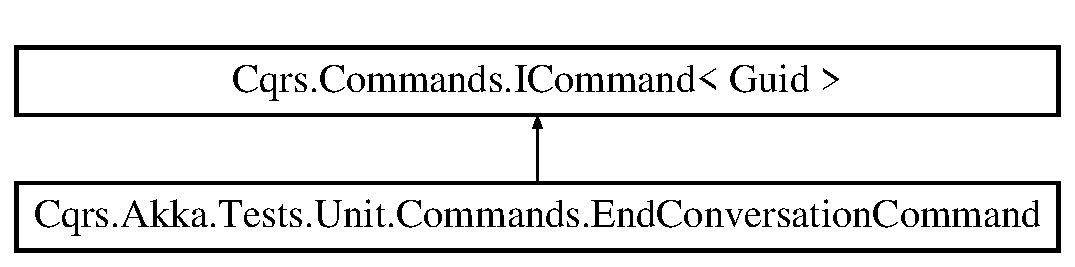
\includegraphics[height=2.000000cm]{classCqrs_1_1Akka_1_1Tests_1_1Unit_1_1Commands_1_1EndConversationCommand}
\end{center}
\end{figure}
\subsection*{Properties}
\begin{DoxyCompactItemize}
\item 
Guid \hyperlink{classCqrs_1_1Akka_1_1Tests_1_1Unit_1_1Commands_1_1EndConversationCommand_a8747a5469ed5e988fcebbb6113f641c2_a8747a5469ed5e988fcebbb6113f641c2}{Corrolation\+Id}\hspace{0.3cm}{\ttfamily  \mbox{[}get, set\mbox{]}}
\item 
Guid \hyperlink{classCqrs_1_1Akka_1_1Tests_1_1Unit_1_1Commands_1_1EndConversationCommand_a4c2bee45d4ddcf0884ee5095d973bef0_a4c2bee45d4ddcf0884ee5095d973bef0}{Correlation\+Id}\hspace{0.3cm}{\ttfamily  \mbox{[}get, set\mbox{]}}
\item 
\hyperlink{namespaceCqrs_1_1Messages_af06a7e6cd2609043d0f2f5f3419f81e3_af06a7e6cd2609043d0f2f5f3419f81e3}{Framework\+Type} \hyperlink{classCqrs_1_1Akka_1_1Tests_1_1Unit_1_1Commands_1_1EndConversationCommand_ad31559bdeb0a38de69e27e4e8ae20af1_ad31559bdeb0a38de69e27e4e8ae20af1}{Framework}\hspace{0.3cm}{\ttfamily  \mbox{[}get, set\mbox{]}}
\item 
string \hyperlink{classCqrs_1_1Akka_1_1Tests_1_1Unit_1_1Commands_1_1EndConversationCommand_a4a2bb41f10dda97f3cd942e921ecde4c_a4a2bb41f10dda97f3cd942e921ecde4c}{Originating\+Framework}\hspace{0.3cm}{\ttfamily  \mbox{[}get, set\mbox{]}}
\begin{DoxyCompactList}\small\item\em The originating framework this message was sent from. \end{DoxyCompactList}\item 
I\+Enumerable$<$ string $>$ \hyperlink{classCqrs_1_1Akka_1_1Tests_1_1Unit_1_1Commands_1_1EndConversationCommand_af90e46a9457980c464a74509826b3b0e_af90e46a9457980c464a74509826b3b0e}{Frameworks}\hspace{0.3cm}{\ttfamily  \mbox{[}get, set\mbox{]}}
\begin{DoxyCompactList}\small\item\em The frameworks this I\+Message has been delivered to/sent via already. \end{DoxyCompactList}\item 
Guid \hyperlink{classCqrs_1_1Akka_1_1Tests_1_1Unit_1_1Commands_1_1EndConversationCommand_abe590196615418b398d11ffd22b7310b_abe590196615418b398d11ffd22b7310b}{Authentication\+Token}\hspace{0.3cm}{\ttfamily  \mbox{[}get, set\mbox{]}}
\item 
Guid \hyperlink{classCqrs_1_1Akka_1_1Tests_1_1Unit_1_1Commands_1_1EndConversationCommand_a55773d68291b3c0476ac8667bbada4d6_a55773d68291b3c0476ac8667bbada4d6}{Id}\hspace{0.3cm}{\ttfamily  \mbox{[}get, set\mbox{]}}
\item 
int \hyperlink{classCqrs_1_1Akka_1_1Tests_1_1Unit_1_1Commands_1_1EndConversationCommand_a8da7afeb73c29e5d6387d820ae734240_a8da7afeb73c29e5d6387d820ae734240}{Expected\+Version}\hspace{0.3cm}{\ttfamily  \mbox{[}get, set\mbox{]}}
\end{DoxyCompactItemize}


\subsection{Property Documentation}
\mbox{\Hypertarget{classCqrs_1_1Akka_1_1Tests_1_1Unit_1_1Commands_1_1EndConversationCommand_abe590196615418b398d11ffd22b7310b_abe590196615418b398d11ffd22b7310b}\label{classCqrs_1_1Akka_1_1Tests_1_1Unit_1_1Commands_1_1EndConversationCommand_abe590196615418b398d11ffd22b7310b_abe590196615418b398d11ffd22b7310b}} 
\index{Cqrs\+::\+Akka\+::\+Tests\+::\+Unit\+::\+Commands\+::\+End\+Conversation\+Command@{Cqrs\+::\+Akka\+::\+Tests\+::\+Unit\+::\+Commands\+::\+End\+Conversation\+Command}!Authentication\+Token@{Authentication\+Token}}
\index{Authentication\+Token@{Authentication\+Token}!Cqrs\+::\+Akka\+::\+Tests\+::\+Unit\+::\+Commands\+::\+End\+Conversation\+Command@{Cqrs\+::\+Akka\+::\+Tests\+::\+Unit\+::\+Commands\+::\+End\+Conversation\+Command}}
\subsubsection{\texorpdfstring{Authentication\+Token}{AuthenticationToken}}
{\footnotesize\ttfamily Guid Cqrs.\+Akka.\+Tests.\+Unit.\+Commands.\+End\+Conversation\+Command.\+Authentication\+Token\hspace{0.3cm}{\ttfamily [get]}, {\ttfamily [set]}}

\mbox{\Hypertarget{classCqrs_1_1Akka_1_1Tests_1_1Unit_1_1Commands_1_1EndConversationCommand_a4c2bee45d4ddcf0884ee5095d973bef0_a4c2bee45d4ddcf0884ee5095d973bef0}\label{classCqrs_1_1Akka_1_1Tests_1_1Unit_1_1Commands_1_1EndConversationCommand_a4c2bee45d4ddcf0884ee5095d973bef0_a4c2bee45d4ddcf0884ee5095d973bef0}} 
\index{Cqrs\+::\+Akka\+::\+Tests\+::\+Unit\+::\+Commands\+::\+End\+Conversation\+Command@{Cqrs\+::\+Akka\+::\+Tests\+::\+Unit\+::\+Commands\+::\+End\+Conversation\+Command}!Correlation\+Id@{Correlation\+Id}}
\index{Correlation\+Id@{Correlation\+Id}!Cqrs\+::\+Akka\+::\+Tests\+::\+Unit\+::\+Commands\+::\+End\+Conversation\+Command@{Cqrs\+::\+Akka\+::\+Tests\+::\+Unit\+::\+Commands\+::\+End\+Conversation\+Command}}
\subsubsection{\texorpdfstring{Correlation\+Id}{CorrelationId}}
{\footnotesize\ttfamily Guid Cqrs.\+Akka.\+Tests.\+Unit.\+Commands.\+End\+Conversation\+Command.\+Correlation\+Id\hspace{0.3cm}{\ttfamily [get]}, {\ttfamily [set]}}

\mbox{\Hypertarget{classCqrs_1_1Akka_1_1Tests_1_1Unit_1_1Commands_1_1EndConversationCommand_a8747a5469ed5e988fcebbb6113f641c2_a8747a5469ed5e988fcebbb6113f641c2}\label{classCqrs_1_1Akka_1_1Tests_1_1Unit_1_1Commands_1_1EndConversationCommand_a8747a5469ed5e988fcebbb6113f641c2_a8747a5469ed5e988fcebbb6113f641c2}} 
\index{Cqrs\+::\+Akka\+::\+Tests\+::\+Unit\+::\+Commands\+::\+End\+Conversation\+Command@{Cqrs\+::\+Akka\+::\+Tests\+::\+Unit\+::\+Commands\+::\+End\+Conversation\+Command}!Corrolation\+Id@{Corrolation\+Id}}
\index{Corrolation\+Id@{Corrolation\+Id}!Cqrs\+::\+Akka\+::\+Tests\+::\+Unit\+::\+Commands\+::\+End\+Conversation\+Command@{Cqrs\+::\+Akka\+::\+Tests\+::\+Unit\+::\+Commands\+::\+End\+Conversation\+Command}}
\subsubsection{\texorpdfstring{Corrolation\+Id}{CorrolationId}}
{\footnotesize\ttfamily Guid Cqrs.\+Akka.\+Tests.\+Unit.\+Commands.\+End\+Conversation\+Command.\+Corrolation\+Id\hspace{0.3cm}{\ttfamily [get]}, {\ttfamily [set]}}

\mbox{\Hypertarget{classCqrs_1_1Akka_1_1Tests_1_1Unit_1_1Commands_1_1EndConversationCommand_a8da7afeb73c29e5d6387d820ae734240_a8da7afeb73c29e5d6387d820ae734240}\label{classCqrs_1_1Akka_1_1Tests_1_1Unit_1_1Commands_1_1EndConversationCommand_a8da7afeb73c29e5d6387d820ae734240_a8da7afeb73c29e5d6387d820ae734240}} 
\index{Cqrs\+::\+Akka\+::\+Tests\+::\+Unit\+::\+Commands\+::\+End\+Conversation\+Command@{Cqrs\+::\+Akka\+::\+Tests\+::\+Unit\+::\+Commands\+::\+End\+Conversation\+Command}!Expected\+Version@{Expected\+Version}}
\index{Expected\+Version@{Expected\+Version}!Cqrs\+::\+Akka\+::\+Tests\+::\+Unit\+::\+Commands\+::\+End\+Conversation\+Command@{Cqrs\+::\+Akka\+::\+Tests\+::\+Unit\+::\+Commands\+::\+End\+Conversation\+Command}}
\subsubsection{\texorpdfstring{Expected\+Version}{ExpectedVersion}}
{\footnotesize\ttfamily int Cqrs.\+Akka.\+Tests.\+Unit.\+Commands.\+End\+Conversation\+Command.\+Expected\+Version\hspace{0.3cm}{\ttfamily [get]}, {\ttfamily [set]}}

\mbox{\Hypertarget{classCqrs_1_1Akka_1_1Tests_1_1Unit_1_1Commands_1_1EndConversationCommand_ad31559bdeb0a38de69e27e4e8ae20af1_ad31559bdeb0a38de69e27e4e8ae20af1}\label{classCqrs_1_1Akka_1_1Tests_1_1Unit_1_1Commands_1_1EndConversationCommand_ad31559bdeb0a38de69e27e4e8ae20af1_ad31559bdeb0a38de69e27e4e8ae20af1}} 
\index{Cqrs\+::\+Akka\+::\+Tests\+::\+Unit\+::\+Commands\+::\+End\+Conversation\+Command@{Cqrs\+::\+Akka\+::\+Tests\+::\+Unit\+::\+Commands\+::\+End\+Conversation\+Command}!Framework@{Framework}}
\index{Framework@{Framework}!Cqrs\+::\+Akka\+::\+Tests\+::\+Unit\+::\+Commands\+::\+End\+Conversation\+Command@{Cqrs\+::\+Akka\+::\+Tests\+::\+Unit\+::\+Commands\+::\+End\+Conversation\+Command}}
\subsubsection{\texorpdfstring{Framework}{Framework}}
{\footnotesize\ttfamily \hyperlink{namespaceCqrs_1_1Messages_af06a7e6cd2609043d0f2f5f3419f81e3_af06a7e6cd2609043d0f2f5f3419f81e3}{Framework\+Type} Cqrs.\+Akka.\+Tests.\+Unit.\+Commands.\+End\+Conversation\+Command.\+Framework\hspace{0.3cm}{\ttfamily [get]}, {\ttfamily [set]}}

\mbox{\Hypertarget{classCqrs_1_1Akka_1_1Tests_1_1Unit_1_1Commands_1_1EndConversationCommand_af90e46a9457980c464a74509826b3b0e_af90e46a9457980c464a74509826b3b0e}\label{classCqrs_1_1Akka_1_1Tests_1_1Unit_1_1Commands_1_1EndConversationCommand_af90e46a9457980c464a74509826b3b0e_af90e46a9457980c464a74509826b3b0e}} 
\index{Cqrs\+::\+Akka\+::\+Tests\+::\+Unit\+::\+Commands\+::\+End\+Conversation\+Command@{Cqrs\+::\+Akka\+::\+Tests\+::\+Unit\+::\+Commands\+::\+End\+Conversation\+Command}!Frameworks@{Frameworks}}
\index{Frameworks@{Frameworks}!Cqrs\+::\+Akka\+::\+Tests\+::\+Unit\+::\+Commands\+::\+End\+Conversation\+Command@{Cqrs\+::\+Akka\+::\+Tests\+::\+Unit\+::\+Commands\+::\+End\+Conversation\+Command}}
\subsubsection{\texorpdfstring{Frameworks}{Frameworks}}
{\footnotesize\ttfamily I\+Enumerable$<$string$>$ Cqrs.\+Akka.\+Tests.\+Unit.\+Commands.\+End\+Conversation\+Command.\+Frameworks\hspace{0.3cm}{\ttfamily [get]}, {\ttfamily [set]}}



The frameworks this I\+Message has been delivered to/sent via already. 

\mbox{\Hypertarget{classCqrs_1_1Akka_1_1Tests_1_1Unit_1_1Commands_1_1EndConversationCommand_a55773d68291b3c0476ac8667bbada4d6_a55773d68291b3c0476ac8667bbada4d6}\label{classCqrs_1_1Akka_1_1Tests_1_1Unit_1_1Commands_1_1EndConversationCommand_a55773d68291b3c0476ac8667bbada4d6_a55773d68291b3c0476ac8667bbada4d6}} 
\index{Cqrs\+::\+Akka\+::\+Tests\+::\+Unit\+::\+Commands\+::\+End\+Conversation\+Command@{Cqrs\+::\+Akka\+::\+Tests\+::\+Unit\+::\+Commands\+::\+End\+Conversation\+Command}!Id@{Id}}
\index{Id@{Id}!Cqrs\+::\+Akka\+::\+Tests\+::\+Unit\+::\+Commands\+::\+End\+Conversation\+Command@{Cqrs\+::\+Akka\+::\+Tests\+::\+Unit\+::\+Commands\+::\+End\+Conversation\+Command}}
\subsubsection{\texorpdfstring{Id}{Id}}
{\footnotesize\ttfamily Guid Cqrs.\+Akka.\+Tests.\+Unit.\+Commands.\+End\+Conversation\+Command.\+Id\hspace{0.3cm}{\ttfamily [get]}, {\ttfamily [set]}}

\mbox{\Hypertarget{classCqrs_1_1Akka_1_1Tests_1_1Unit_1_1Commands_1_1EndConversationCommand_a4a2bb41f10dda97f3cd942e921ecde4c_a4a2bb41f10dda97f3cd942e921ecde4c}\label{classCqrs_1_1Akka_1_1Tests_1_1Unit_1_1Commands_1_1EndConversationCommand_a4a2bb41f10dda97f3cd942e921ecde4c_a4a2bb41f10dda97f3cd942e921ecde4c}} 
\index{Cqrs\+::\+Akka\+::\+Tests\+::\+Unit\+::\+Commands\+::\+End\+Conversation\+Command@{Cqrs\+::\+Akka\+::\+Tests\+::\+Unit\+::\+Commands\+::\+End\+Conversation\+Command}!Originating\+Framework@{Originating\+Framework}}
\index{Originating\+Framework@{Originating\+Framework}!Cqrs\+::\+Akka\+::\+Tests\+::\+Unit\+::\+Commands\+::\+End\+Conversation\+Command@{Cqrs\+::\+Akka\+::\+Tests\+::\+Unit\+::\+Commands\+::\+End\+Conversation\+Command}}
\subsubsection{\texorpdfstring{Originating\+Framework}{OriginatingFramework}}
{\footnotesize\ttfamily string Cqrs.\+Akka.\+Tests.\+Unit.\+Commands.\+End\+Conversation\+Command.\+Originating\+Framework\hspace{0.3cm}{\ttfamily [get]}, {\ttfamily [set]}}



The originating framework this message was sent from. 


\hypertarget{classCqrs_1_1Akka_1_1Tests_1_1Unit_1_1Commands_1_1Handlers_1_1EndConversationCommandHandler}{}\doxysection{Cqrs.\+Akka.\+Tests.\+Unit.\+Commands.\+Handlers.\+End\+Conversation\+Command\+Handler Class Reference}
\label{classCqrs_1_1Akka_1_1Tests_1_1Unit_1_1Commands_1_1Handlers_1_1EndConversationCommandHandler}\index{Cqrs.Akka.Tests.Unit.Commands.Handlers.EndConversationCommandHandler@{Cqrs.Akka.Tests.Unit.Commands.Handlers.EndConversationCommandHandler}}


Handles the \mbox{\hyperlink{classCqrs_1_1Akka_1_1Tests_1_1Unit_1_1Commands_1_1EndConversationCommand}{End\+Conversation\+Command}}.  


Inheritance diagram for Cqrs.\+Akka.\+Tests.\+Unit.\+Commands.\+Handlers.\+End\+Conversation\+Command\+Handler\+:\begin{figure}[H]
\begin{center}
\leavevmode
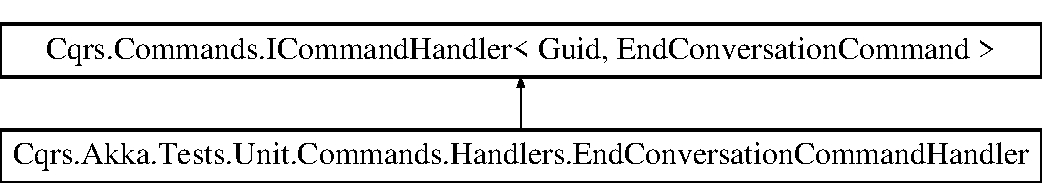
\includegraphics[height=2.000000cm]{classCqrs_1_1Akka_1_1Tests_1_1Unit_1_1Commands_1_1Handlers_1_1EndConversationCommandHandler}
\end{center}
\end{figure}
\doxysubsection*{Public Member Functions}
\begin{DoxyCompactItemize}
\item 
\mbox{\hyperlink{classCqrs_1_1Akka_1_1Tests_1_1Unit_1_1Commands_1_1Handlers_1_1EndConversationCommandHandler_aaf3680b69f6cbad95722194c4c16cd1f_aaf3680b69f6cbad95722194c4c16cd1f}{End\+Conversation\+Command\+Handler}} (\mbox{\hyperlink{interfaceCqrs_1_1Akka_1_1Domain_1_1IAkkaAggregateResolver}{I\+Akka\+Aggregate\+Resolver}} aggregate\+Resolver)
\begin{DoxyCompactList}\small\item\em Instantiates the \mbox{\hyperlink{classCqrs_1_1Akka_1_1Tests_1_1Unit_1_1Commands_1_1Handlers_1_1EndConversationCommandHandler}{End\+Conversation\+Command\+Handler}} class registering any Receive\+Actor.\+Receive$<$\+T$>$(\+System.\+Func$<$\+T,\+System.\+Threading.\+Tasks.\+Task$>$) required. \end{DoxyCompactList}\item 
void \mbox{\hyperlink{classCqrs_1_1Akka_1_1Tests_1_1Unit_1_1Commands_1_1Handlers_1_1EndConversationCommandHandler_a45cc1e01d68fb5b241c9e46b333a149e_a45cc1e01d68fb5b241c9e46b333a149e}{Handle}} (\mbox{\hyperlink{classCqrs_1_1Akka_1_1Tests_1_1Unit_1_1Commands_1_1EndConversationCommand}{End\+Conversation\+Command}} command)
\begin{DoxyCompactList}\small\item\em Responds to the provided {\itshape command} . \end{DoxyCompactList}\end{DoxyCompactItemize}
\doxysubsection*{Properties}
\begin{DoxyCompactItemize}
\item 
\mbox{\hyperlink{interfaceCqrs_1_1Akka_1_1Domain_1_1IAkkaAggregateResolver}{I\+Akka\+Aggregate\+Resolver}} \mbox{\hyperlink{classCqrs_1_1Akka_1_1Tests_1_1Unit_1_1Commands_1_1Handlers_1_1EndConversationCommandHandler_a39a99dda0cbadd3405a4a991fd3f2163_a39a99dda0cbadd3405a4a991fd3f2163}{Aggregate\+Resolver}}\hspace{0.3cm}{\ttfamily  \mbox{[}get\mbox{]}}
\begin{DoxyCompactList}\small\item\em Resolves Akka.\+Net actor based I\+Aggregate\+Root$<$\+T\+Authentication\+Token$>$ \end{DoxyCompactList}\end{DoxyCompactItemize}


\doxysubsection{Detailed Description}
Handles the \mbox{\hyperlink{classCqrs_1_1Akka_1_1Tests_1_1Unit_1_1Commands_1_1EndConversationCommand}{End\+Conversation\+Command}}. 



\doxysubsection{Constructor \& Destructor Documentation}
\mbox{\Hypertarget{classCqrs_1_1Akka_1_1Tests_1_1Unit_1_1Commands_1_1Handlers_1_1EndConversationCommandHandler_aaf3680b69f6cbad95722194c4c16cd1f_aaf3680b69f6cbad95722194c4c16cd1f}\label{classCqrs_1_1Akka_1_1Tests_1_1Unit_1_1Commands_1_1Handlers_1_1EndConversationCommandHandler_aaf3680b69f6cbad95722194c4c16cd1f_aaf3680b69f6cbad95722194c4c16cd1f}} 
\index{Cqrs.Akka.Tests.Unit.Commands.Handlers.EndConversationCommandHandler@{Cqrs.Akka.Tests.Unit.Commands.Handlers.EndConversationCommandHandler}!EndConversationCommandHandler@{EndConversationCommandHandler}}
\index{EndConversationCommandHandler@{EndConversationCommandHandler}!Cqrs.Akka.Tests.Unit.Commands.Handlers.EndConversationCommandHandler@{Cqrs.Akka.Tests.Unit.Commands.Handlers.EndConversationCommandHandler}}
\doxysubsubsection{\texorpdfstring{EndConversationCommandHandler()}{EndConversationCommandHandler()}}
{\footnotesize\ttfamily Cqrs.\+Akka.\+Tests.\+Unit.\+Commands.\+Handlers.\+End\+Conversation\+Command\+Handler.\+End\+Conversation\+Command\+Handler (\begin{DoxyParamCaption}\item[{\mbox{\hyperlink{interfaceCqrs_1_1Akka_1_1Domain_1_1IAkkaAggregateResolver}{I\+Akka\+Aggregate\+Resolver}}}]{aggregate\+Resolver }\end{DoxyParamCaption})}



Instantiates the \mbox{\hyperlink{classCqrs_1_1Akka_1_1Tests_1_1Unit_1_1Commands_1_1Handlers_1_1EndConversationCommandHandler}{End\+Conversation\+Command\+Handler}} class registering any Receive\+Actor.\+Receive$<$\+T$>$(\+System.\+Func$<$\+T,\+System.\+Threading.\+Tasks.\+Task$>$) required. 



\doxysubsection{Member Function Documentation}
\mbox{\Hypertarget{classCqrs_1_1Akka_1_1Tests_1_1Unit_1_1Commands_1_1Handlers_1_1EndConversationCommandHandler_a45cc1e01d68fb5b241c9e46b333a149e_a45cc1e01d68fb5b241c9e46b333a149e}\label{classCqrs_1_1Akka_1_1Tests_1_1Unit_1_1Commands_1_1Handlers_1_1EndConversationCommandHandler_a45cc1e01d68fb5b241c9e46b333a149e_a45cc1e01d68fb5b241c9e46b333a149e}} 
\index{Cqrs.Akka.Tests.Unit.Commands.Handlers.EndConversationCommandHandler@{Cqrs.Akka.Tests.Unit.Commands.Handlers.EndConversationCommandHandler}!Handle@{Handle}}
\index{Handle@{Handle}!Cqrs.Akka.Tests.Unit.Commands.Handlers.EndConversationCommandHandler@{Cqrs.Akka.Tests.Unit.Commands.Handlers.EndConversationCommandHandler}}
\doxysubsubsection{\texorpdfstring{Handle()}{Handle()}}
{\footnotesize\ttfamily void Cqrs.\+Akka.\+Tests.\+Unit.\+Commands.\+Handlers.\+End\+Conversation\+Command\+Handler.\+Handle (\begin{DoxyParamCaption}\item[{\mbox{\hyperlink{classCqrs_1_1Akka_1_1Tests_1_1Unit_1_1Commands_1_1EndConversationCommand}{End\+Conversation\+Command}}}]{command }\end{DoxyParamCaption})}



Responds to the provided {\itshape command} . 


\begin{DoxyParams}{Parameters}
{\em command} & The \mbox{\hyperlink{classCqrs_1_1Akka_1_1Tests_1_1Unit_1_1Commands_1_1EndConversationCommand}{End\+Conversation\+Command}} to respond to or \char`\"{}handle\char`\"{}\\
\hline
\end{DoxyParams}


\doxysubsection{Property Documentation}
\mbox{\Hypertarget{classCqrs_1_1Akka_1_1Tests_1_1Unit_1_1Commands_1_1Handlers_1_1EndConversationCommandHandler_a39a99dda0cbadd3405a4a991fd3f2163_a39a99dda0cbadd3405a4a991fd3f2163}\label{classCqrs_1_1Akka_1_1Tests_1_1Unit_1_1Commands_1_1Handlers_1_1EndConversationCommandHandler_a39a99dda0cbadd3405a4a991fd3f2163_a39a99dda0cbadd3405a4a991fd3f2163}} 
\index{Cqrs.Akka.Tests.Unit.Commands.Handlers.EndConversationCommandHandler@{Cqrs.Akka.Tests.Unit.Commands.Handlers.EndConversationCommandHandler}!AggregateResolver@{AggregateResolver}}
\index{AggregateResolver@{AggregateResolver}!Cqrs.Akka.Tests.Unit.Commands.Handlers.EndConversationCommandHandler@{Cqrs.Akka.Tests.Unit.Commands.Handlers.EndConversationCommandHandler}}
\doxysubsubsection{\texorpdfstring{AggregateResolver}{AggregateResolver}}
{\footnotesize\ttfamily \mbox{\hyperlink{interfaceCqrs_1_1Akka_1_1Domain_1_1IAkkaAggregateResolver}{I\+Akka\+Aggregate\+Resolver}} Cqrs.\+Akka.\+Tests.\+Unit.\+Commands.\+Handlers.\+End\+Conversation\+Command\+Handler.\+Aggregate\+Resolver\hspace{0.3cm}{\ttfamily [get]}, {\ttfamily [protected]}}



Resolves Akka.\+Net actor based I\+Aggregate\+Root$<$\+T\+Authentication\+Token$>$ 


\hypertarget{classCqrs_1_1Akka_1_1Tests_1_1Unit_1_1Commands_1_1Handlers_1_1ReplyToHelloWorldCommandHandler}{}\section{Cqrs.\+Akka.\+Tests.\+Unit.\+Commands.\+Handlers.\+Reply\+To\+Hello\+World\+Command\+Handler Class Reference}
\label{classCqrs_1_1Akka_1_1Tests_1_1Unit_1_1Commands_1_1Handlers_1_1ReplyToHelloWorldCommandHandler}\index{Cqrs.\+Akka.\+Tests.\+Unit.\+Commands.\+Handlers.\+Reply\+To\+Hello\+World\+Command\+Handler@{Cqrs.\+Akka.\+Tests.\+Unit.\+Commands.\+Handlers.\+Reply\+To\+Hello\+World\+Command\+Handler}}
Inheritance diagram for Cqrs.\+Akka.\+Tests.\+Unit.\+Commands.\+Handlers.\+Reply\+To\+Hello\+World\+Command\+Handler\+:\begin{figure}[H]
\begin{center}
\leavevmode
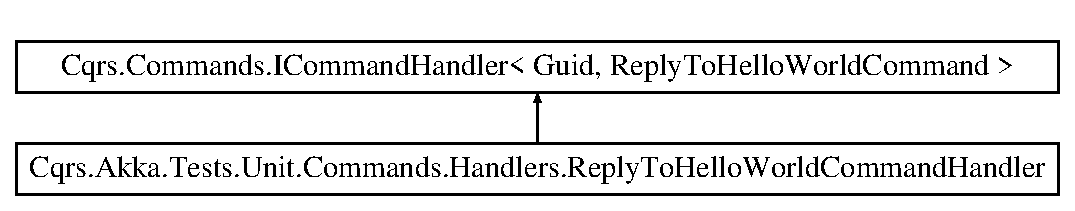
\includegraphics[height=2.000000cm]{classCqrs_1_1Akka_1_1Tests_1_1Unit_1_1Commands_1_1Handlers_1_1ReplyToHelloWorldCommandHandler}
\end{center}
\end{figure}
\subsection*{Public Member Functions}
\begin{DoxyCompactItemize}
\item 
\hyperlink{classCqrs_1_1Akka_1_1Tests_1_1Unit_1_1Commands_1_1Handlers_1_1ReplyToHelloWorldCommandHandler_ac3c6ef2299fded8533f7e013e6cf763d}{Reply\+To\+Hello\+World\+Command\+Handler} (\hyperlink{interfaceCqrs_1_1Akka_1_1Domain_1_1IAkkaAggregateResolver}{I\+Akka\+Aggregate\+Resolver} aggregate\+Resolver)
\begin{DoxyCompactList}\small\item\em Instantiates the \hyperlink{classCqrs_1_1Akka_1_1Tests_1_1Unit_1_1Commands_1_1Handlers_1_1ReplyToHelloWorldCommandHandler}{Reply\+To\+Hello\+World\+Command\+Handler} class registering any Receive\+Actor.\+Receive$<$\+T$>$(\+System.\+Func$<$\+T,\+System.\+Threading.\+Tasks.\+Task$>$) required. \end{DoxyCompactList}\item 
void \hyperlink{classCqrs_1_1Akka_1_1Tests_1_1Unit_1_1Commands_1_1Handlers_1_1ReplyToHelloWorldCommandHandler_a647273b7056fc79b8b34b78981f6f193}{Handle} (\hyperlink{classCqrs_1_1Akka_1_1Tests_1_1Unit_1_1Commands_1_1ReplyToHelloWorldCommand}{Reply\+To\+Hello\+World\+Command} command)
\end{DoxyCompactItemize}
\subsection*{Properties}
\begin{DoxyCompactItemize}
\item 
\hyperlink{interfaceCqrs_1_1Akka_1_1Domain_1_1IAkkaAggregateResolver}{I\+Akka\+Aggregate\+Resolver} \hyperlink{classCqrs_1_1Akka_1_1Tests_1_1Unit_1_1Commands_1_1Handlers_1_1ReplyToHelloWorldCommandHandler_a2c8f8e4cdceffd4a586f6f7a00962ca6}{Aggregate\+Resolver}\hspace{0.3cm}{\ttfamily  \mbox{[}get\mbox{]}}
\end{DoxyCompactItemize}


\subsection{Constructor \& Destructor Documentation}
\mbox{\Hypertarget{classCqrs_1_1Akka_1_1Tests_1_1Unit_1_1Commands_1_1Handlers_1_1ReplyToHelloWorldCommandHandler_ac3c6ef2299fded8533f7e013e6cf763d}\label{classCqrs_1_1Akka_1_1Tests_1_1Unit_1_1Commands_1_1Handlers_1_1ReplyToHelloWorldCommandHandler_ac3c6ef2299fded8533f7e013e6cf763d}} 
\index{Cqrs\+::\+Akka\+::\+Tests\+::\+Unit\+::\+Commands\+::\+Handlers\+::\+Reply\+To\+Hello\+World\+Command\+Handler@{Cqrs\+::\+Akka\+::\+Tests\+::\+Unit\+::\+Commands\+::\+Handlers\+::\+Reply\+To\+Hello\+World\+Command\+Handler}!Reply\+To\+Hello\+World\+Command\+Handler@{Reply\+To\+Hello\+World\+Command\+Handler}}
\index{Reply\+To\+Hello\+World\+Command\+Handler@{Reply\+To\+Hello\+World\+Command\+Handler}!Cqrs\+::\+Akka\+::\+Tests\+::\+Unit\+::\+Commands\+::\+Handlers\+::\+Reply\+To\+Hello\+World\+Command\+Handler@{Cqrs\+::\+Akka\+::\+Tests\+::\+Unit\+::\+Commands\+::\+Handlers\+::\+Reply\+To\+Hello\+World\+Command\+Handler}}
\subsubsection{\texorpdfstring{Reply\+To\+Hello\+World\+Command\+Handler()}{ReplyToHelloWorldCommandHandler()}}
{\footnotesize\ttfamily Cqrs.\+Akka.\+Tests.\+Unit.\+Commands.\+Handlers.\+Reply\+To\+Hello\+World\+Command\+Handler.\+Reply\+To\+Hello\+World\+Command\+Handler (\begin{DoxyParamCaption}\item[{\hyperlink{interfaceCqrs_1_1Akka_1_1Domain_1_1IAkkaAggregateResolver}{I\+Akka\+Aggregate\+Resolver}}]{aggregate\+Resolver }\end{DoxyParamCaption})}



Instantiates the \hyperlink{classCqrs_1_1Akka_1_1Tests_1_1Unit_1_1Commands_1_1Handlers_1_1ReplyToHelloWorldCommandHandler}{Reply\+To\+Hello\+World\+Command\+Handler} class registering any Receive\+Actor.\+Receive$<$\+T$>$(\+System.\+Func$<$\+T,\+System.\+Threading.\+Tasks.\+Task$>$) required. 



\subsection{Member Function Documentation}
\mbox{\Hypertarget{classCqrs_1_1Akka_1_1Tests_1_1Unit_1_1Commands_1_1Handlers_1_1ReplyToHelloWorldCommandHandler_a647273b7056fc79b8b34b78981f6f193}\label{classCqrs_1_1Akka_1_1Tests_1_1Unit_1_1Commands_1_1Handlers_1_1ReplyToHelloWorldCommandHandler_a647273b7056fc79b8b34b78981f6f193}} 
\index{Cqrs\+::\+Akka\+::\+Tests\+::\+Unit\+::\+Commands\+::\+Handlers\+::\+Reply\+To\+Hello\+World\+Command\+Handler@{Cqrs\+::\+Akka\+::\+Tests\+::\+Unit\+::\+Commands\+::\+Handlers\+::\+Reply\+To\+Hello\+World\+Command\+Handler}!Handle@{Handle}}
\index{Handle@{Handle}!Cqrs\+::\+Akka\+::\+Tests\+::\+Unit\+::\+Commands\+::\+Handlers\+::\+Reply\+To\+Hello\+World\+Command\+Handler@{Cqrs\+::\+Akka\+::\+Tests\+::\+Unit\+::\+Commands\+::\+Handlers\+::\+Reply\+To\+Hello\+World\+Command\+Handler}}
\subsubsection{\texorpdfstring{Handle()}{Handle()}}
{\footnotesize\ttfamily void Cqrs.\+Akka.\+Tests.\+Unit.\+Commands.\+Handlers.\+Reply\+To\+Hello\+World\+Command\+Handler.\+Handle (\begin{DoxyParamCaption}\item[{\hyperlink{classCqrs_1_1Akka_1_1Tests_1_1Unit_1_1Commands_1_1ReplyToHelloWorldCommand}{Reply\+To\+Hello\+World\+Command}}]{command }\end{DoxyParamCaption})}



\subsection{Property Documentation}
\mbox{\Hypertarget{classCqrs_1_1Akka_1_1Tests_1_1Unit_1_1Commands_1_1Handlers_1_1ReplyToHelloWorldCommandHandler_a2c8f8e4cdceffd4a586f6f7a00962ca6}\label{classCqrs_1_1Akka_1_1Tests_1_1Unit_1_1Commands_1_1Handlers_1_1ReplyToHelloWorldCommandHandler_a2c8f8e4cdceffd4a586f6f7a00962ca6}} 
\index{Cqrs\+::\+Akka\+::\+Tests\+::\+Unit\+::\+Commands\+::\+Handlers\+::\+Reply\+To\+Hello\+World\+Command\+Handler@{Cqrs\+::\+Akka\+::\+Tests\+::\+Unit\+::\+Commands\+::\+Handlers\+::\+Reply\+To\+Hello\+World\+Command\+Handler}!Aggregate\+Resolver@{Aggregate\+Resolver}}
\index{Aggregate\+Resolver@{Aggregate\+Resolver}!Cqrs\+::\+Akka\+::\+Tests\+::\+Unit\+::\+Commands\+::\+Handlers\+::\+Reply\+To\+Hello\+World\+Command\+Handler@{Cqrs\+::\+Akka\+::\+Tests\+::\+Unit\+::\+Commands\+::\+Handlers\+::\+Reply\+To\+Hello\+World\+Command\+Handler}}
\subsubsection{\texorpdfstring{Aggregate\+Resolver}{AggregateResolver}}
{\footnotesize\ttfamily \hyperlink{interfaceCqrs_1_1Akka_1_1Domain_1_1IAkkaAggregateResolver}{I\+Akka\+Aggregate\+Resolver} Cqrs.\+Akka.\+Tests.\+Unit.\+Commands.\+Handlers.\+Reply\+To\+Hello\+World\+Command\+Handler.\+Aggregate\+Resolver\hspace{0.3cm}{\ttfamily [get]}, {\ttfamily [protected]}}


\hypertarget{classCqrs_1_1Akka_1_1Tests_1_1Unit_1_1Commands_1_1Handlers_1_1SayHelloWorldCommandHandler}{}\section{Cqrs.\+Akka.\+Tests.\+Unit.\+Commands.\+Handlers.\+Say\+Hello\+World\+Command\+Handler Class Reference}
\label{classCqrs_1_1Akka_1_1Tests_1_1Unit_1_1Commands_1_1Handlers_1_1SayHelloWorldCommandHandler}\index{Cqrs.\+Akka.\+Tests.\+Unit.\+Commands.\+Handlers.\+Say\+Hello\+World\+Command\+Handler@{Cqrs.\+Akka.\+Tests.\+Unit.\+Commands.\+Handlers.\+Say\+Hello\+World\+Command\+Handler}}
Inheritance diagram for Cqrs.\+Akka.\+Tests.\+Unit.\+Commands.\+Handlers.\+Say\+Hello\+World\+Command\+Handler\+:\begin{figure}[H]
\begin{center}
\leavevmode
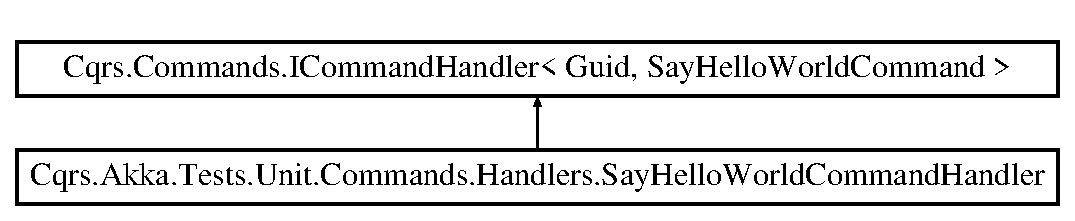
\includegraphics[height=2.000000cm]{classCqrs_1_1Akka_1_1Tests_1_1Unit_1_1Commands_1_1Handlers_1_1SayHelloWorldCommandHandler}
\end{center}
\end{figure}
\subsection*{Public Member Functions}
\begin{DoxyCompactItemize}
\item 
\hyperlink{classCqrs_1_1Akka_1_1Tests_1_1Unit_1_1Commands_1_1Handlers_1_1SayHelloWorldCommandHandler_a421fd9e6d3c9cbb5e93453675af63de0}{Say\+Hello\+World\+Command\+Handler} (\hyperlink{interfaceCqrs_1_1Akka_1_1Domain_1_1IAkkaAggregateResolver}{I\+Akka\+Aggregate\+Resolver} aggregate\+Resolver)
\begin{DoxyCompactList}\small\item\em Instantiates the \hyperlink{classCqrs_1_1Akka_1_1Tests_1_1Unit_1_1Commands_1_1Handlers_1_1SayHelloWorldCommandHandler}{Say\+Hello\+World\+Command\+Handler} class registering any Receive\+Actor.\+Receive$<$\+T$>$(\+System.\+Func$<$\+T,\+System.\+Threading.\+Tasks.\+Task$>$) required. \end{DoxyCompactList}\item 
void \hyperlink{classCqrs_1_1Akka_1_1Tests_1_1Unit_1_1Commands_1_1Handlers_1_1SayHelloWorldCommandHandler_a204e1dacbacfb172a47d1585b76ef1f4}{Handle} (\hyperlink{classCqrs_1_1Akka_1_1Tests_1_1Unit_1_1Commands_1_1SayHelloWorldCommand}{Say\+Hello\+World\+Command} command)
\end{DoxyCompactItemize}
\subsection*{Properties}
\begin{DoxyCompactItemize}
\item 
\hyperlink{interfaceCqrs_1_1Akka_1_1Domain_1_1IAkkaAggregateResolver}{I\+Akka\+Aggregate\+Resolver} \hyperlink{classCqrs_1_1Akka_1_1Tests_1_1Unit_1_1Commands_1_1Handlers_1_1SayHelloWorldCommandHandler_a4222ccc27f8a550857281bdd97e59b7c}{Aggregate\+Resolver}\hspace{0.3cm}{\ttfamily  \mbox{[}get\mbox{]}}
\end{DoxyCompactItemize}


\subsection{Constructor \& Destructor Documentation}
\mbox{\Hypertarget{classCqrs_1_1Akka_1_1Tests_1_1Unit_1_1Commands_1_1Handlers_1_1SayHelloWorldCommandHandler_a421fd9e6d3c9cbb5e93453675af63de0}\label{classCqrs_1_1Akka_1_1Tests_1_1Unit_1_1Commands_1_1Handlers_1_1SayHelloWorldCommandHandler_a421fd9e6d3c9cbb5e93453675af63de0}} 
\index{Cqrs\+::\+Akka\+::\+Tests\+::\+Unit\+::\+Commands\+::\+Handlers\+::\+Say\+Hello\+World\+Command\+Handler@{Cqrs\+::\+Akka\+::\+Tests\+::\+Unit\+::\+Commands\+::\+Handlers\+::\+Say\+Hello\+World\+Command\+Handler}!Say\+Hello\+World\+Command\+Handler@{Say\+Hello\+World\+Command\+Handler}}
\index{Say\+Hello\+World\+Command\+Handler@{Say\+Hello\+World\+Command\+Handler}!Cqrs\+::\+Akka\+::\+Tests\+::\+Unit\+::\+Commands\+::\+Handlers\+::\+Say\+Hello\+World\+Command\+Handler@{Cqrs\+::\+Akka\+::\+Tests\+::\+Unit\+::\+Commands\+::\+Handlers\+::\+Say\+Hello\+World\+Command\+Handler}}
\subsubsection{\texorpdfstring{Say\+Hello\+World\+Command\+Handler()}{SayHelloWorldCommandHandler()}}
{\footnotesize\ttfamily Cqrs.\+Akka.\+Tests.\+Unit.\+Commands.\+Handlers.\+Say\+Hello\+World\+Command\+Handler.\+Say\+Hello\+World\+Command\+Handler (\begin{DoxyParamCaption}\item[{\hyperlink{interfaceCqrs_1_1Akka_1_1Domain_1_1IAkkaAggregateResolver}{I\+Akka\+Aggregate\+Resolver}}]{aggregate\+Resolver }\end{DoxyParamCaption})}



Instantiates the \hyperlink{classCqrs_1_1Akka_1_1Tests_1_1Unit_1_1Commands_1_1Handlers_1_1SayHelloWorldCommandHandler}{Say\+Hello\+World\+Command\+Handler} class registering any Receive\+Actor.\+Receive$<$\+T$>$(\+System.\+Func$<$\+T,\+System.\+Threading.\+Tasks.\+Task$>$) required. 



\subsection{Member Function Documentation}
\mbox{\Hypertarget{classCqrs_1_1Akka_1_1Tests_1_1Unit_1_1Commands_1_1Handlers_1_1SayHelloWorldCommandHandler_a204e1dacbacfb172a47d1585b76ef1f4}\label{classCqrs_1_1Akka_1_1Tests_1_1Unit_1_1Commands_1_1Handlers_1_1SayHelloWorldCommandHandler_a204e1dacbacfb172a47d1585b76ef1f4}} 
\index{Cqrs\+::\+Akka\+::\+Tests\+::\+Unit\+::\+Commands\+::\+Handlers\+::\+Say\+Hello\+World\+Command\+Handler@{Cqrs\+::\+Akka\+::\+Tests\+::\+Unit\+::\+Commands\+::\+Handlers\+::\+Say\+Hello\+World\+Command\+Handler}!Handle@{Handle}}
\index{Handle@{Handle}!Cqrs\+::\+Akka\+::\+Tests\+::\+Unit\+::\+Commands\+::\+Handlers\+::\+Say\+Hello\+World\+Command\+Handler@{Cqrs\+::\+Akka\+::\+Tests\+::\+Unit\+::\+Commands\+::\+Handlers\+::\+Say\+Hello\+World\+Command\+Handler}}
\subsubsection{\texorpdfstring{Handle()}{Handle()}}
{\footnotesize\ttfamily void Cqrs.\+Akka.\+Tests.\+Unit.\+Commands.\+Handlers.\+Say\+Hello\+World\+Command\+Handler.\+Handle (\begin{DoxyParamCaption}\item[{\hyperlink{classCqrs_1_1Akka_1_1Tests_1_1Unit_1_1Commands_1_1SayHelloWorldCommand}{Say\+Hello\+World\+Command}}]{command }\end{DoxyParamCaption})}



\subsection{Property Documentation}
\mbox{\Hypertarget{classCqrs_1_1Akka_1_1Tests_1_1Unit_1_1Commands_1_1Handlers_1_1SayHelloWorldCommandHandler_a4222ccc27f8a550857281bdd97e59b7c}\label{classCqrs_1_1Akka_1_1Tests_1_1Unit_1_1Commands_1_1Handlers_1_1SayHelloWorldCommandHandler_a4222ccc27f8a550857281bdd97e59b7c}} 
\index{Cqrs\+::\+Akka\+::\+Tests\+::\+Unit\+::\+Commands\+::\+Handlers\+::\+Say\+Hello\+World\+Command\+Handler@{Cqrs\+::\+Akka\+::\+Tests\+::\+Unit\+::\+Commands\+::\+Handlers\+::\+Say\+Hello\+World\+Command\+Handler}!Aggregate\+Resolver@{Aggregate\+Resolver}}
\index{Aggregate\+Resolver@{Aggregate\+Resolver}!Cqrs\+::\+Akka\+::\+Tests\+::\+Unit\+::\+Commands\+::\+Handlers\+::\+Say\+Hello\+World\+Command\+Handler@{Cqrs\+::\+Akka\+::\+Tests\+::\+Unit\+::\+Commands\+::\+Handlers\+::\+Say\+Hello\+World\+Command\+Handler}}
\subsubsection{\texorpdfstring{Aggregate\+Resolver}{AggregateResolver}}
{\footnotesize\ttfamily \hyperlink{interfaceCqrs_1_1Akka_1_1Domain_1_1IAkkaAggregateResolver}{I\+Akka\+Aggregate\+Resolver} Cqrs.\+Akka.\+Tests.\+Unit.\+Commands.\+Handlers.\+Say\+Hello\+World\+Command\+Handler.\+Aggregate\+Resolver\hspace{0.3cm}{\ttfamily [get]}, {\ttfamily [protected]}}


\hypertarget{classCqrs_1_1Akka_1_1Tests_1_1Unit_1_1Commands_1_1Handlers_1_1UpdateCompletedConversationReportCommandHandler}{}\section{Cqrs.\+Akka.\+Tests.\+Unit.\+Commands.\+Handlers.\+Update\+Completed\+Conversation\+Report\+Command\+Handler Class Reference}
\label{classCqrs_1_1Akka_1_1Tests_1_1Unit_1_1Commands_1_1Handlers_1_1UpdateCompletedConversationReportCommandHandler}\index{Cqrs.\+Akka.\+Tests.\+Unit.\+Commands.\+Handlers.\+Update\+Completed\+Conversation\+Report\+Command\+Handler@{Cqrs.\+Akka.\+Tests.\+Unit.\+Commands.\+Handlers.\+Update\+Completed\+Conversation\+Report\+Command\+Handler}}


Handles the \hyperlink{classCqrs_1_1Akka_1_1Tests_1_1Unit_1_1Commands_1_1UpdateCompletedConversationReportCommand}{Update\+Completed\+Conversation\+Report\+Command}.  


Inheritance diagram for Cqrs.\+Akka.\+Tests.\+Unit.\+Commands.\+Handlers.\+Update\+Completed\+Conversation\+Report\+Command\+Handler\+:\begin{figure}[H]
\begin{center}
\leavevmode
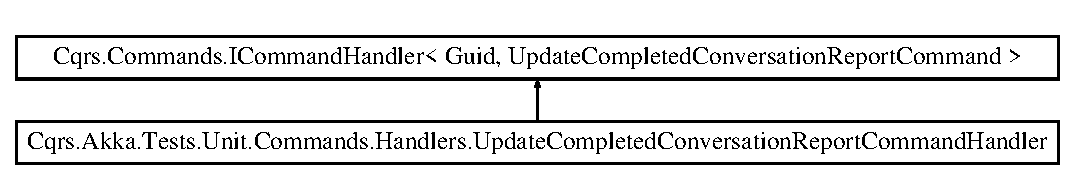
\includegraphics[height=1.964912cm]{classCqrs_1_1Akka_1_1Tests_1_1Unit_1_1Commands_1_1Handlers_1_1UpdateCompletedConversationReportCommandHandler}
\end{center}
\end{figure}
\subsection*{Public Member Functions}
\begin{DoxyCompactItemize}
\item 
\hyperlink{classCqrs_1_1Akka_1_1Tests_1_1Unit_1_1Commands_1_1Handlers_1_1UpdateCompletedConversationReportCommandHandler_a816316549866b3e4abb410a7b9ea06a3_a816316549866b3e4abb410a7b9ea06a3}{Update\+Completed\+Conversation\+Report\+Command\+Handler} (\hyperlink{interfaceCqrs_1_1Akka_1_1Domain_1_1IAkkaAggregateResolver}{I\+Akka\+Aggregate\+Resolver} aggregate\+Resolver)
\begin{DoxyCompactList}\small\item\em Instantiates the \hyperlink{classCqrs_1_1Akka_1_1Tests_1_1Unit_1_1Commands_1_1Handlers_1_1SayHelloWorldCommandHandler}{Say\+Hello\+World\+Command\+Handler} class registering any Receive\+Actor.\+Receive$<$\+T$>$(\+System.\+Func$<$\+T,\+System.\+Threading.\+Tasks.\+Task$>$) required. \end{DoxyCompactList}\item 
void \hyperlink{classCqrs_1_1Akka_1_1Tests_1_1Unit_1_1Commands_1_1Handlers_1_1UpdateCompletedConversationReportCommandHandler_aecb596ab5c5e17823b93ac4fcae0e43e_aecb596ab5c5e17823b93ac4fcae0e43e}{Handle} (\hyperlink{classCqrs_1_1Akka_1_1Tests_1_1Unit_1_1Commands_1_1UpdateCompletedConversationReportCommand}{Update\+Completed\+Conversation\+Report\+Command} command)
\begin{DoxyCompactList}\small\item\em Responds to the provided {\itshape command} . \end{DoxyCompactList}\end{DoxyCompactItemize}
\subsection*{Properties}
\begin{DoxyCompactItemize}
\item 
\hyperlink{interfaceCqrs_1_1Akka_1_1Domain_1_1IAkkaAggregateResolver}{I\+Akka\+Aggregate\+Resolver} \hyperlink{classCqrs_1_1Akka_1_1Tests_1_1Unit_1_1Commands_1_1Handlers_1_1UpdateCompletedConversationReportCommandHandler_af5cde3b1fadb7cb1962301a67aa9339b_af5cde3b1fadb7cb1962301a67aa9339b}{Aggregate\+Resolver}\hspace{0.3cm}{\ttfamily  \mbox{[}get\mbox{]}}
\begin{DoxyCompactList}\small\item\em Resolves Akka.\+Net actor based I\+Aggregate\+Root$<$\+T\+Authentication\+Token$>$ \end{DoxyCompactList}\end{DoxyCompactItemize}


\subsection{Detailed Description}
Handles the \hyperlink{classCqrs_1_1Akka_1_1Tests_1_1Unit_1_1Commands_1_1UpdateCompletedConversationReportCommand}{Update\+Completed\+Conversation\+Report\+Command}. 



\subsection{Constructor \& Destructor Documentation}
\mbox{\Hypertarget{classCqrs_1_1Akka_1_1Tests_1_1Unit_1_1Commands_1_1Handlers_1_1UpdateCompletedConversationReportCommandHandler_a816316549866b3e4abb410a7b9ea06a3_a816316549866b3e4abb410a7b9ea06a3}\label{classCqrs_1_1Akka_1_1Tests_1_1Unit_1_1Commands_1_1Handlers_1_1UpdateCompletedConversationReportCommandHandler_a816316549866b3e4abb410a7b9ea06a3_a816316549866b3e4abb410a7b9ea06a3}} 
\index{Cqrs\+::\+Akka\+::\+Tests\+::\+Unit\+::\+Commands\+::\+Handlers\+::\+Update\+Completed\+Conversation\+Report\+Command\+Handler@{Cqrs\+::\+Akka\+::\+Tests\+::\+Unit\+::\+Commands\+::\+Handlers\+::\+Update\+Completed\+Conversation\+Report\+Command\+Handler}!Update\+Completed\+Conversation\+Report\+Command\+Handler@{Update\+Completed\+Conversation\+Report\+Command\+Handler}}
\index{Update\+Completed\+Conversation\+Report\+Command\+Handler@{Update\+Completed\+Conversation\+Report\+Command\+Handler}!Cqrs\+::\+Akka\+::\+Tests\+::\+Unit\+::\+Commands\+::\+Handlers\+::\+Update\+Completed\+Conversation\+Report\+Command\+Handler@{Cqrs\+::\+Akka\+::\+Tests\+::\+Unit\+::\+Commands\+::\+Handlers\+::\+Update\+Completed\+Conversation\+Report\+Command\+Handler}}
\subsubsection{\texorpdfstring{Update\+Completed\+Conversation\+Report\+Command\+Handler()}{UpdateCompletedConversationReportCommandHandler()}}
{\footnotesize\ttfamily Cqrs.\+Akka.\+Tests.\+Unit.\+Commands.\+Handlers.\+Update\+Completed\+Conversation\+Report\+Command\+Handler.\+Update\+Completed\+Conversation\+Report\+Command\+Handler (\begin{DoxyParamCaption}\item[{\hyperlink{interfaceCqrs_1_1Akka_1_1Domain_1_1IAkkaAggregateResolver}{I\+Akka\+Aggregate\+Resolver}}]{aggregate\+Resolver }\end{DoxyParamCaption})}



Instantiates the \hyperlink{classCqrs_1_1Akka_1_1Tests_1_1Unit_1_1Commands_1_1Handlers_1_1SayHelloWorldCommandHandler}{Say\+Hello\+World\+Command\+Handler} class registering any Receive\+Actor.\+Receive$<$\+T$>$(\+System.\+Func$<$\+T,\+System.\+Threading.\+Tasks.\+Task$>$) required. 



\subsection{Member Function Documentation}
\mbox{\Hypertarget{classCqrs_1_1Akka_1_1Tests_1_1Unit_1_1Commands_1_1Handlers_1_1UpdateCompletedConversationReportCommandHandler_aecb596ab5c5e17823b93ac4fcae0e43e_aecb596ab5c5e17823b93ac4fcae0e43e}\label{classCqrs_1_1Akka_1_1Tests_1_1Unit_1_1Commands_1_1Handlers_1_1UpdateCompletedConversationReportCommandHandler_aecb596ab5c5e17823b93ac4fcae0e43e_aecb596ab5c5e17823b93ac4fcae0e43e}} 
\index{Cqrs\+::\+Akka\+::\+Tests\+::\+Unit\+::\+Commands\+::\+Handlers\+::\+Update\+Completed\+Conversation\+Report\+Command\+Handler@{Cqrs\+::\+Akka\+::\+Tests\+::\+Unit\+::\+Commands\+::\+Handlers\+::\+Update\+Completed\+Conversation\+Report\+Command\+Handler}!Handle@{Handle}}
\index{Handle@{Handle}!Cqrs\+::\+Akka\+::\+Tests\+::\+Unit\+::\+Commands\+::\+Handlers\+::\+Update\+Completed\+Conversation\+Report\+Command\+Handler@{Cqrs\+::\+Akka\+::\+Tests\+::\+Unit\+::\+Commands\+::\+Handlers\+::\+Update\+Completed\+Conversation\+Report\+Command\+Handler}}
\subsubsection{\texorpdfstring{Handle()}{Handle()}}
{\footnotesize\ttfamily void Cqrs.\+Akka.\+Tests.\+Unit.\+Commands.\+Handlers.\+Update\+Completed\+Conversation\+Report\+Command\+Handler.\+Handle (\begin{DoxyParamCaption}\item[{\hyperlink{classCqrs_1_1Akka_1_1Tests_1_1Unit_1_1Commands_1_1UpdateCompletedConversationReportCommand}{Update\+Completed\+Conversation\+Report\+Command}}]{command }\end{DoxyParamCaption})}



Responds to the provided {\itshape command} . 


\begin{DoxyParams}{Parameters}
{\em command} & The \hyperlink{classCqrs_1_1Akka_1_1Tests_1_1Unit_1_1Commands_1_1UpdateCompletedConversationReportCommand}{Update\+Completed\+Conversation\+Report\+Command} to respond to or \char`\"{}handle\char`\"{}\\
\hline
\end{DoxyParams}


\subsection{Property Documentation}
\mbox{\Hypertarget{classCqrs_1_1Akka_1_1Tests_1_1Unit_1_1Commands_1_1Handlers_1_1UpdateCompletedConversationReportCommandHandler_af5cde3b1fadb7cb1962301a67aa9339b_af5cde3b1fadb7cb1962301a67aa9339b}\label{classCqrs_1_1Akka_1_1Tests_1_1Unit_1_1Commands_1_1Handlers_1_1UpdateCompletedConversationReportCommandHandler_af5cde3b1fadb7cb1962301a67aa9339b_af5cde3b1fadb7cb1962301a67aa9339b}} 
\index{Cqrs\+::\+Akka\+::\+Tests\+::\+Unit\+::\+Commands\+::\+Handlers\+::\+Update\+Completed\+Conversation\+Report\+Command\+Handler@{Cqrs\+::\+Akka\+::\+Tests\+::\+Unit\+::\+Commands\+::\+Handlers\+::\+Update\+Completed\+Conversation\+Report\+Command\+Handler}!Aggregate\+Resolver@{Aggregate\+Resolver}}
\index{Aggregate\+Resolver@{Aggregate\+Resolver}!Cqrs\+::\+Akka\+::\+Tests\+::\+Unit\+::\+Commands\+::\+Handlers\+::\+Update\+Completed\+Conversation\+Report\+Command\+Handler@{Cqrs\+::\+Akka\+::\+Tests\+::\+Unit\+::\+Commands\+::\+Handlers\+::\+Update\+Completed\+Conversation\+Report\+Command\+Handler}}
\subsubsection{\texorpdfstring{Aggregate\+Resolver}{AggregateResolver}}
{\footnotesize\ttfamily \hyperlink{interfaceCqrs_1_1Akka_1_1Domain_1_1IAkkaAggregateResolver}{I\+Akka\+Aggregate\+Resolver} Cqrs.\+Akka.\+Tests.\+Unit.\+Commands.\+Handlers.\+Update\+Completed\+Conversation\+Report\+Command\+Handler.\+Aggregate\+Resolver\hspace{0.3cm}{\ttfamily [get]}, {\ttfamily [protected]}}



Resolves Akka.\+Net actor based I\+Aggregate\+Root$<$\+T\+Authentication\+Token$>$ 


\hypertarget{classCqrs_1_1Akka_1_1Tests_1_1Unit_1_1Commands_1_1ReplyToHelloWorldCommand}{}\doxysection{Cqrs.\+Akka.\+Tests.\+Unit.\+Commands.\+Reply\+To\+Hello\+World\+Command Class Reference}
\label{classCqrs_1_1Akka_1_1Tests_1_1Unit_1_1Commands_1_1ReplyToHelloWorldCommand}\index{Cqrs.Akka.Tests.Unit.Commands.ReplyToHelloWorldCommand@{Cqrs.Akka.Tests.Unit.Commands.ReplyToHelloWorldCommand}}


Someone wants to reply to someone saying \char`\"{}\+Hello World\char`\"{}.  


Inheritance diagram for Cqrs.\+Akka.\+Tests.\+Unit.\+Commands.\+Reply\+To\+Hello\+World\+Command\+:\begin{figure}[H]
\begin{center}
\leavevmode
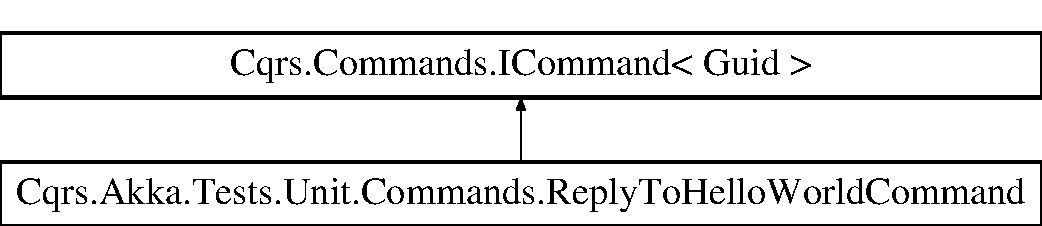
\includegraphics[height=2.000000cm]{classCqrs_1_1Akka_1_1Tests_1_1Unit_1_1Commands_1_1ReplyToHelloWorldCommand}
\end{center}
\end{figure}
\doxysubsection*{Properties}
\begin{DoxyCompactItemize}
\item 
Guid \mbox{\hyperlink{classCqrs_1_1Akka_1_1Tests_1_1Unit_1_1Commands_1_1ReplyToHelloWorldCommand_a773a29aa23cbb3c705b48587b866f54d_a773a29aa23cbb3c705b48587b866f54d}{Correlation\+Id}}\hspace{0.3cm}{\ttfamily  \mbox{[}get, set\mbox{]}}
\begin{DoxyCompactList}\small\item\em An identifier used to group together several I\+Message. Any I\+Message with the same \mbox{\hyperlink{classCqrs_1_1Akka_1_1Tests_1_1Unit_1_1Commands_1_1ReplyToHelloWorldCommand_a773a29aa23cbb3c705b48587b866f54d_a773a29aa23cbb3c705b48587b866f54d}{Correlation\+Id}} were triggered by the same initiating request. \end{DoxyCompactList}\item 
string \mbox{\hyperlink{classCqrs_1_1Akka_1_1Tests_1_1Unit_1_1Commands_1_1ReplyToHelloWorldCommand_a8d3ad2d0c0c4d2654ea499468772eaeb_a8d3ad2d0c0c4d2654ea499468772eaeb}{Originating\+Framework}}\hspace{0.3cm}{\ttfamily  \mbox{[}get, set\mbox{]}}
\begin{DoxyCompactList}\small\item\em The originating framework this message was sent from. \end{DoxyCompactList}\item 
I\+Enumerable$<$ string $>$ \mbox{\hyperlink{classCqrs_1_1Akka_1_1Tests_1_1Unit_1_1Commands_1_1ReplyToHelloWorldCommand_a894055f8b934a49d3e9d315f62cff8da_a894055f8b934a49d3e9d315f62cff8da}{Frameworks}}\hspace{0.3cm}{\ttfamily  \mbox{[}get, set\mbox{]}}
\begin{DoxyCompactList}\small\item\em The frameworks this I\+Message has been delivered to/sent via already. \end{DoxyCompactList}\item 
Guid \mbox{\hyperlink{classCqrs_1_1Akka_1_1Tests_1_1Unit_1_1Commands_1_1ReplyToHelloWorldCommand_a556c313a49a66d1fd4f3df8dc15344ec_a556c313a49a66d1fd4f3df8dc15344ec}{Authentication\+Token}}\hspace{0.3cm}{\ttfamily  \mbox{[}get, set\mbox{]}}
\begin{DoxyCompactList}\small\item\em The authentication token of the entity that triggered the event to be raised. \end{DoxyCompactList}\item 
Guid \mbox{\hyperlink{classCqrs_1_1Akka_1_1Tests_1_1Unit_1_1Commands_1_1ReplyToHelloWorldCommand_a28c1edb8c3b32d8d003314271dd82924_a28c1edb8c3b32d8d003314271dd82924}{Id}}\hspace{0.3cm}{\ttfamily  \mbox{[}get, set\mbox{]}}
\begin{DoxyCompactList}\small\item\em The identifier of the command itself. In some cases this may be the I\+Aggregate\+Root$<$\+T\+Authentication\+Token$>$ or I\+Saga$<$\+T\+Authentication\+Token$>$ this command targets. \end{DoxyCompactList}\item 
int \mbox{\hyperlink{classCqrs_1_1Akka_1_1Tests_1_1Unit_1_1Commands_1_1ReplyToHelloWorldCommand_a3901b00973351dff228554de639ed788_a3901b00973351dff228554de639ed788}{Expected\+Version}}\hspace{0.3cm}{\ttfamily  \mbox{[}get, set\mbox{]}}
\begin{DoxyCompactList}\small\item\em The expected version number the targeted I\+Aggregate\+Root$<$\+T\+Authentication\+Token$>$ or I\+Saga$<$\+T\+Authentication\+Token$>$ is expected to be. \end{DoxyCompactList}\end{DoxyCompactItemize}


\doxysubsection{Detailed Description}
Someone wants to reply to someone saying \char`\"{}\+Hello World\char`\"{}. 



\doxysubsection{Property Documentation}
\mbox{\Hypertarget{classCqrs_1_1Akka_1_1Tests_1_1Unit_1_1Commands_1_1ReplyToHelloWorldCommand_a556c313a49a66d1fd4f3df8dc15344ec_a556c313a49a66d1fd4f3df8dc15344ec}\label{classCqrs_1_1Akka_1_1Tests_1_1Unit_1_1Commands_1_1ReplyToHelloWorldCommand_a556c313a49a66d1fd4f3df8dc15344ec_a556c313a49a66d1fd4f3df8dc15344ec}} 
\index{Cqrs.Akka.Tests.Unit.Commands.ReplyToHelloWorldCommand@{Cqrs.Akka.Tests.Unit.Commands.ReplyToHelloWorldCommand}!AuthenticationToken@{AuthenticationToken}}
\index{AuthenticationToken@{AuthenticationToken}!Cqrs.Akka.Tests.Unit.Commands.ReplyToHelloWorldCommand@{Cqrs.Akka.Tests.Unit.Commands.ReplyToHelloWorldCommand}}
\doxysubsubsection{\texorpdfstring{AuthenticationToken}{AuthenticationToken}}
{\footnotesize\ttfamily Guid Cqrs.\+Akka.\+Tests.\+Unit.\+Commands.\+Reply\+To\+Hello\+World\+Command.\+Authentication\+Token\hspace{0.3cm}{\ttfamily [get]}, {\ttfamily [set]}}



The authentication token of the entity that triggered the event to be raised. 

\mbox{\Hypertarget{classCqrs_1_1Akka_1_1Tests_1_1Unit_1_1Commands_1_1ReplyToHelloWorldCommand_a773a29aa23cbb3c705b48587b866f54d_a773a29aa23cbb3c705b48587b866f54d}\label{classCqrs_1_1Akka_1_1Tests_1_1Unit_1_1Commands_1_1ReplyToHelloWorldCommand_a773a29aa23cbb3c705b48587b866f54d_a773a29aa23cbb3c705b48587b866f54d}} 
\index{Cqrs.Akka.Tests.Unit.Commands.ReplyToHelloWorldCommand@{Cqrs.Akka.Tests.Unit.Commands.ReplyToHelloWorldCommand}!CorrelationId@{CorrelationId}}
\index{CorrelationId@{CorrelationId}!Cqrs.Akka.Tests.Unit.Commands.ReplyToHelloWorldCommand@{Cqrs.Akka.Tests.Unit.Commands.ReplyToHelloWorldCommand}}
\doxysubsubsection{\texorpdfstring{CorrelationId}{CorrelationId}}
{\footnotesize\ttfamily Guid Cqrs.\+Akka.\+Tests.\+Unit.\+Commands.\+Reply\+To\+Hello\+World\+Command.\+Correlation\+Id\hspace{0.3cm}{\ttfamily [get]}, {\ttfamily [set]}}



An identifier used to group together several I\+Message. Any I\+Message with the same \mbox{\hyperlink{classCqrs_1_1Akka_1_1Tests_1_1Unit_1_1Commands_1_1ReplyToHelloWorldCommand_a773a29aa23cbb3c705b48587b866f54d_a773a29aa23cbb3c705b48587b866f54d}{Correlation\+Id}} were triggered by the same initiating request. 

\mbox{\Hypertarget{classCqrs_1_1Akka_1_1Tests_1_1Unit_1_1Commands_1_1ReplyToHelloWorldCommand_a3901b00973351dff228554de639ed788_a3901b00973351dff228554de639ed788}\label{classCqrs_1_1Akka_1_1Tests_1_1Unit_1_1Commands_1_1ReplyToHelloWorldCommand_a3901b00973351dff228554de639ed788_a3901b00973351dff228554de639ed788}} 
\index{Cqrs.Akka.Tests.Unit.Commands.ReplyToHelloWorldCommand@{Cqrs.Akka.Tests.Unit.Commands.ReplyToHelloWorldCommand}!ExpectedVersion@{ExpectedVersion}}
\index{ExpectedVersion@{ExpectedVersion}!Cqrs.Akka.Tests.Unit.Commands.ReplyToHelloWorldCommand@{Cqrs.Akka.Tests.Unit.Commands.ReplyToHelloWorldCommand}}
\doxysubsubsection{\texorpdfstring{ExpectedVersion}{ExpectedVersion}}
{\footnotesize\ttfamily int Cqrs.\+Akka.\+Tests.\+Unit.\+Commands.\+Reply\+To\+Hello\+World\+Command.\+Expected\+Version\hspace{0.3cm}{\ttfamily [get]}, {\ttfamily [set]}}



The expected version number the targeted I\+Aggregate\+Root$<$\+T\+Authentication\+Token$>$ or I\+Saga$<$\+T\+Authentication\+Token$>$ is expected to be. 

\mbox{\Hypertarget{classCqrs_1_1Akka_1_1Tests_1_1Unit_1_1Commands_1_1ReplyToHelloWorldCommand_a894055f8b934a49d3e9d315f62cff8da_a894055f8b934a49d3e9d315f62cff8da}\label{classCqrs_1_1Akka_1_1Tests_1_1Unit_1_1Commands_1_1ReplyToHelloWorldCommand_a894055f8b934a49d3e9d315f62cff8da_a894055f8b934a49d3e9d315f62cff8da}} 
\index{Cqrs.Akka.Tests.Unit.Commands.ReplyToHelloWorldCommand@{Cqrs.Akka.Tests.Unit.Commands.ReplyToHelloWorldCommand}!Frameworks@{Frameworks}}
\index{Frameworks@{Frameworks}!Cqrs.Akka.Tests.Unit.Commands.ReplyToHelloWorldCommand@{Cqrs.Akka.Tests.Unit.Commands.ReplyToHelloWorldCommand}}
\doxysubsubsection{\texorpdfstring{Frameworks}{Frameworks}}
{\footnotesize\ttfamily I\+Enumerable$<$string$>$ Cqrs.\+Akka.\+Tests.\+Unit.\+Commands.\+Reply\+To\+Hello\+World\+Command.\+Frameworks\hspace{0.3cm}{\ttfamily [get]}, {\ttfamily [set]}}



The frameworks this I\+Message has been delivered to/sent via already. 

\mbox{\Hypertarget{classCqrs_1_1Akka_1_1Tests_1_1Unit_1_1Commands_1_1ReplyToHelloWorldCommand_a28c1edb8c3b32d8d003314271dd82924_a28c1edb8c3b32d8d003314271dd82924}\label{classCqrs_1_1Akka_1_1Tests_1_1Unit_1_1Commands_1_1ReplyToHelloWorldCommand_a28c1edb8c3b32d8d003314271dd82924_a28c1edb8c3b32d8d003314271dd82924}} 
\index{Cqrs.Akka.Tests.Unit.Commands.ReplyToHelloWorldCommand@{Cqrs.Akka.Tests.Unit.Commands.ReplyToHelloWorldCommand}!Id@{Id}}
\index{Id@{Id}!Cqrs.Akka.Tests.Unit.Commands.ReplyToHelloWorldCommand@{Cqrs.Akka.Tests.Unit.Commands.ReplyToHelloWorldCommand}}
\doxysubsubsection{\texorpdfstring{Id}{Id}}
{\footnotesize\ttfamily Guid Cqrs.\+Akka.\+Tests.\+Unit.\+Commands.\+Reply\+To\+Hello\+World\+Command.\+Id\hspace{0.3cm}{\ttfamily [get]}, {\ttfamily [set]}}



The identifier of the command itself. In some cases this may be the I\+Aggregate\+Root$<$\+T\+Authentication\+Token$>$ or I\+Saga$<$\+T\+Authentication\+Token$>$ this command targets. 

\mbox{\Hypertarget{classCqrs_1_1Akka_1_1Tests_1_1Unit_1_1Commands_1_1ReplyToHelloWorldCommand_a8d3ad2d0c0c4d2654ea499468772eaeb_a8d3ad2d0c0c4d2654ea499468772eaeb}\label{classCqrs_1_1Akka_1_1Tests_1_1Unit_1_1Commands_1_1ReplyToHelloWorldCommand_a8d3ad2d0c0c4d2654ea499468772eaeb_a8d3ad2d0c0c4d2654ea499468772eaeb}} 
\index{Cqrs.Akka.Tests.Unit.Commands.ReplyToHelloWorldCommand@{Cqrs.Akka.Tests.Unit.Commands.ReplyToHelloWorldCommand}!OriginatingFramework@{OriginatingFramework}}
\index{OriginatingFramework@{OriginatingFramework}!Cqrs.Akka.Tests.Unit.Commands.ReplyToHelloWorldCommand@{Cqrs.Akka.Tests.Unit.Commands.ReplyToHelloWorldCommand}}
\doxysubsubsection{\texorpdfstring{OriginatingFramework}{OriginatingFramework}}
{\footnotesize\ttfamily string Cqrs.\+Akka.\+Tests.\+Unit.\+Commands.\+Reply\+To\+Hello\+World\+Command.\+Originating\+Framework\hspace{0.3cm}{\ttfamily [get]}, {\ttfamily [set]}}



The originating framework this message was sent from. 


\hypertarget{classCqrs_1_1Akka_1_1Tests_1_1Unit_1_1Commands_1_1SayHelloWorldCommand}{}\doxysection{Cqrs.\+Akka.\+Tests.\+Unit.\+Commands.\+Say\+Hello\+World\+Command Class Reference}
\label{classCqrs_1_1Akka_1_1Tests_1_1Unit_1_1Commands_1_1SayHelloWorldCommand}\index{Cqrs.Akka.Tests.Unit.Commands.SayHelloWorldCommand@{Cqrs.Akka.Tests.Unit.Commands.SayHelloWorldCommand}}


Someone wants to say \char`\"{}\+Hello World\char`\"{}.  


Inheritance diagram for Cqrs.\+Akka.\+Tests.\+Unit.\+Commands.\+Say\+Hello\+World\+Command\+:\begin{figure}[H]
\begin{center}
\leavevmode
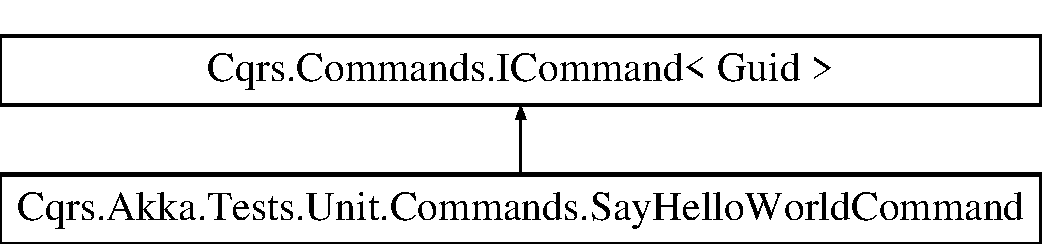
\includegraphics[height=2.000000cm]{classCqrs_1_1Akka_1_1Tests_1_1Unit_1_1Commands_1_1SayHelloWorldCommand}
\end{center}
\end{figure}
\doxysubsection*{Properties}
\begin{DoxyCompactItemize}
\item 
Guid \mbox{\hyperlink{classCqrs_1_1Akka_1_1Tests_1_1Unit_1_1Commands_1_1SayHelloWorldCommand_a7f7aaf542ac4d7255479a7646abd52ae_a7f7aaf542ac4d7255479a7646abd52ae}{Correlation\+Id}}\hspace{0.3cm}{\ttfamily  \mbox{[}get, set\mbox{]}}
\begin{DoxyCompactList}\small\item\em An identifier used to group together several I\+Message. Any I\+Message with the same \mbox{\hyperlink{classCqrs_1_1Akka_1_1Tests_1_1Unit_1_1Commands_1_1SayHelloWorldCommand_a7f7aaf542ac4d7255479a7646abd52ae_a7f7aaf542ac4d7255479a7646abd52ae}{Correlation\+Id}} were triggered by the same initiating request. \end{DoxyCompactList}\item 
string \mbox{\hyperlink{classCqrs_1_1Akka_1_1Tests_1_1Unit_1_1Commands_1_1SayHelloWorldCommand_aee25452ae728c329c2a85cb5c98eb949_aee25452ae728c329c2a85cb5c98eb949}{Originating\+Framework}}\hspace{0.3cm}{\ttfamily  \mbox{[}get, set\mbox{]}}
\begin{DoxyCompactList}\small\item\em The originating framework this message was sent from. \end{DoxyCompactList}\item 
I\+Enumerable$<$ string $>$ \mbox{\hyperlink{classCqrs_1_1Akka_1_1Tests_1_1Unit_1_1Commands_1_1SayHelloWorldCommand_af0cf191e15e689b5af6f8b3d1bca869c_af0cf191e15e689b5af6f8b3d1bca869c}{Frameworks}}\hspace{0.3cm}{\ttfamily  \mbox{[}get, set\mbox{]}}
\begin{DoxyCompactList}\small\item\em The frameworks this I\+Message has been delivered to/sent via already. \end{DoxyCompactList}\item 
Guid \mbox{\hyperlink{classCqrs_1_1Akka_1_1Tests_1_1Unit_1_1Commands_1_1SayHelloWorldCommand_adfabda7d8bf843f643f29368cc7fdad9_adfabda7d8bf843f643f29368cc7fdad9}{Authentication\+Token}}\hspace{0.3cm}{\ttfamily  \mbox{[}get, set\mbox{]}}
\begin{DoxyCompactList}\small\item\em The authentication token of the entity that triggered the event to be raised. \end{DoxyCompactList}\item 
Guid \mbox{\hyperlink{classCqrs_1_1Akka_1_1Tests_1_1Unit_1_1Commands_1_1SayHelloWorldCommand_af409b36bce4c0cef726f3fd8869ec5ba_af409b36bce4c0cef726f3fd8869ec5ba}{Id}}\hspace{0.3cm}{\ttfamily  \mbox{[}get, set\mbox{]}}
\begin{DoxyCompactList}\small\item\em The identifier of the command itself. In some cases this may be the I\+Aggregate\+Root$<$\+T\+Authentication\+Token$>$ or I\+Saga$<$\+T\+Authentication\+Token$>$ this command targets. \end{DoxyCompactList}\item 
int \mbox{\hyperlink{classCqrs_1_1Akka_1_1Tests_1_1Unit_1_1Commands_1_1SayHelloWorldCommand_a422ec8f8e6319ab369f9ad7949e97fcc_a422ec8f8e6319ab369f9ad7949e97fcc}{Expected\+Version}}\hspace{0.3cm}{\ttfamily  \mbox{[}get, set\mbox{]}}
\begin{DoxyCompactList}\small\item\em The expected version number the targeted I\+Aggregate\+Root$<$\+T\+Authentication\+Token$>$ or I\+Saga$<$\+T\+Authentication\+Token$>$ is expected to be. \end{DoxyCompactList}\end{DoxyCompactItemize}


\doxysubsection{Detailed Description}
Someone wants to say \char`\"{}\+Hello World\char`\"{}. 



\doxysubsection{Property Documentation}
\mbox{\Hypertarget{classCqrs_1_1Akka_1_1Tests_1_1Unit_1_1Commands_1_1SayHelloWorldCommand_adfabda7d8bf843f643f29368cc7fdad9_adfabda7d8bf843f643f29368cc7fdad9}\label{classCqrs_1_1Akka_1_1Tests_1_1Unit_1_1Commands_1_1SayHelloWorldCommand_adfabda7d8bf843f643f29368cc7fdad9_adfabda7d8bf843f643f29368cc7fdad9}} 
\index{Cqrs.Akka.Tests.Unit.Commands.SayHelloWorldCommand@{Cqrs.Akka.Tests.Unit.Commands.SayHelloWorldCommand}!AuthenticationToken@{AuthenticationToken}}
\index{AuthenticationToken@{AuthenticationToken}!Cqrs.Akka.Tests.Unit.Commands.SayHelloWorldCommand@{Cqrs.Akka.Tests.Unit.Commands.SayHelloWorldCommand}}
\doxysubsubsection{\texorpdfstring{AuthenticationToken}{AuthenticationToken}}
{\footnotesize\ttfamily Guid Cqrs.\+Akka.\+Tests.\+Unit.\+Commands.\+Say\+Hello\+World\+Command.\+Authentication\+Token\hspace{0.3cm}{\ttfamily [get]}, {\ttfamily [set]}}



The authentication token of the entity that triggered the event to be raised. 

\mbox{\Hypertarget{classCqrs_1_1Akka_1_1Tests_1_1Unit_1_1Commands_1_1SayHelloWorldCommand_a7f7aaf542ac4d7255479a7646abd52ae_a7f7aaf542ac4d7255479a7646abd52ae}\label{classCqrs_1_1Akka_1_1Tests_1_1Unit_1_1Commands_1_1SayHelloWorldCommand_a7f7aaf542ac4d7255479a7646abd52ae_a7f7aaf542ac4d7255479a7646abd52ae}} 
\index{Cqrs.Akka.Tests.Unit.Commands.SayHelloWorldCommand@{Cqrs.Akka.Tests.Unit.Commands.SayHelloWorldCommand}!CorrelationId@{CorrelationId}}
\index{CorrelationId@{CorrelationId}!Cqrs.Akka.Tests.Unit.Commands.SayHelloWorldCommand@{Cqrs.Akka.Tests.Unit.Commands.SayHelloWorldCommand}}
\doxysubsubsection{\texorpdfstring{CorrelationId}{CorrelationId}}
{\footnotesize\ttfamily Guid Cqrs.\+Akka.\+Tests.\+Unit.\+Commands.\+Say\+Hello\+World\+Command.\+Correlation\+Id\hspace{0.3cm}{\ttfamily [get]}, {\ttfamily [set]}}



An identifier used to group together several I\+Message. Any I\+Message with the same \mbox{\hyperlink{classCqrs_1_1Akka_1_1Tests_1_1Unit_1_1Commands_1_1SayHelloWorldCommand_a7f7aaf542ac4d7255479a7646abd52ae_a7f7aaf542ac4d7255479a7646abd52ae}{Correlation\+Id}} were triggered by the same initiating request. 

\mbox{\Hypertarget{classCqrs_1_1Akka_1_1Tests_1_1Unit_1_1Commands_1_1SayHelloWorldCommand_a422ec8f8e6319ab369f9ad7949e97fcc_a422ec8f8e6319ab369f9ad7949e97fcc}\label{classCqrs_1_1Akka_1_1Tests_1_1Unit_1_1Commands_1_1SayHelloWorldCommand_a422ec8f8e6319ab369f9ad7949e97fcc_a422ec8f8e6319ab369f9ad7949e97fcc}} 
\index{Cqrs.Akka.Tests.Unit.Commands.SayHelloWorldCommand@{Cqrs.Akka.Tests.Unit.Commands.SayHelloWorldCommand}!ExpectedVersion@{ExpectedVersion}}
\index{ExpectedVersion@{ExpectedVersion}!Cqrs.Akka.Tests.Unit.Commands.SayHelloWorldCommand@{Cqrs.Akka.Tests.Unit.Commands.SayHelloWorldCommand}}
\doxysubsubsection{\texorpdfstring{ExpectedVersion}{ExpectedVersion}}
{\footnotesize\ttfamily int Cqrs.\+Akka.\+Tests.\+Unit.\+Commands.\+Say\+Hello\+World\+Command.\+Expected\+Version\hspace{0.3cm}{\ttfamily [get]}, {\ttfamily [set]}}



The expected version number the targeted I\+Aggregate\+Root$<$\+T\+Authentication\+Token$>$ or I\+Saga$<$\+T\+Authentication\+Token$>$ is expected to be. 

\mbox{\Hypertarget{classCqrs_1_1Akka_1_1Tests_1_1Unit_1_1Commands_1_1SayHelloWorldCommand_af0cf191e15e689b5af6f8b3d1bca869c_af0cf191e15e689b5af6f8b3d1bca869c}\label{classCqrs_1_1Akka_1_1Tests_1_1Unit_1_1Commands_1_1SayHelloWorldCommand_af0cf191e15e689b5af6f8b3d1bca869c_af0cf191e15e689b5af6f8b3d1bca869c}} 
\index{Cqrs.Akka.Tests.Unit.Commands.SayHelloWorldCommand@{Cqrs.Akka.Tests.Unit.Commands.SayHelloWorldCommand}!Frameworks@{Frameworks}}
\index{Frameworks@{Frameworks}!Cqrs.Akka.Tests.Unit.Commands.SayHelloWorldCommand@{Cqrs.Akka.Tests.Unit.Commands.SayHelloWorldCommand}}
\doxysubsubsection{\texorpdfstring{Frameworks}{Frameworks}}
{\footnotesize\ttfamily I\+Enumerable$<$string$>$ Cqrs.\+Akka.\+Tests.\+Unit.\+Commands.\+Say\+Hello\+World\+Command.\+Frameworks\hspace{0.3cm}{\ttfamily [get]}, {\ttfamily [set]}}



The frameworks this I\+Message has been delivered to/sent via already. 

\mbox{\Hypertarget{classCqrs_1_1Akka_1_1Tests_1_1Unit_1_1Commands_1_1SayHelloWorldCommand_af409b36bce4c0cef726f3fd8869ec5ba_af409b36bce4c0cef726f3fd8869ec5ba}\label{classCqrs_1_1Akka_1_1Tests_1_1Unit_1_1Commands_1_1SayHelloWorldCommand_af409b36bce4c0cef726f3fd8869ec5ba_af409b36bce4c0cef726f3fd8869ec5ba}} 
\index{Cqrs.Akka.Tests.Unit.Commands.SayHelloWorldCommand@{Cqrs.Akka.Tests.Unit.Commands.SayHelloWorldCommand}!Id@{Id}}
\index{Id@{Id}!Cqrs.Akka.Tests.Unit.Commands.SayHelloWorldCommand@{Cqrs.Akka.Tests.Unit.Commands.SayHelloWorldCommand}}
\doxysubsubsection{\texorpdfstring{Id}{Id}}
{\footnotesize\ttfamily Guid Cqrs.\+Akka.\+Tests.\+Unit.\+Commands.\+Say\+Hello\+World\+Command.\+Id\hspace{0.3cm}{\ttfamily [get]}, {\ttfamily [set]}}



The identifier of the command itself. In some cases this may be the I\+Aggregate\+Root$<$\+T\+Authentication\+Token$>$ or I\+Saga$<$\+T\+Authentication\+Token$>$ this command targets. 

\mbox{\Hypertarget{classCqrs_1_1Akka_1_1Tests_1_1Unit_1_1Commands_1_1SayHelloWorldCommand_aee25452ae728c329c2a85cb5c98eb949_aee25452ae728c329c2a85cb5c98eb949}\label{classCqrs_1_1Akka_1_1Tests_1_1Unit_1_1Commands_1_1SayHelloWorldCommand_aee25452ae728c329c2a85cb5c98eb949_aee25452ae728c329c2a85cb5c98eb949}} 
\index{Cqrs.Akka.Tests.Unit.Commands.SayHelloWorldCommand@{Cqrs.Akka.Tests.Unit.Commands.SayHelloWorldCommand}!OriginatingFramework@{OriginatingFramework}}
\index{OriginatingFramework@{OriginatingFramework}!Cqrs.Akka.Tests.Unit.Commands.SayHelloWorldCommand@{Cqrs.Akka.Tests.Unit.Commands.SayHelloWorldCommand}}
\doxysubsubsection{\texorpdfstring{OriginatingFramework}{OriginatingFramework}}
{\footnotesize\ttfamily string Cqrs.\+Akka.\+Tests.\+Unit.\+Commands.\+Say\+Hello\+World\+Command.\+Originating\+Framework\hspace{0.3cm}{\ttfamily [get]}, {\ttfamily [set]}}



The originating framework this message was sent from. 


\hypertarget{classCqrs_1_1Akka_1_1Tests_1_1Unit_1_1Commands_1_1UpdateCompletedConversationReportCommand}{}\section{Cqrs.\+Akka.\+Tests.\+Unit.\+Commands.\+Update\+Completed\+Conversation\+Report\+Command Class Reference}
\label{classCqrs_1_1Akka_1_1Tests_1_1Unit_1_1Commands_1_1UpdateCompletedConversationReportCommand}\index{Cqrs.\+Akka.\+Tests.\+Unit.\+Commands.\+Update\+Completed\+Conversation\+Report\+Command@{Cqrs.\+Akka.\+Tests.\+Unit.\+Commands.\+Update\+Completed\+Conversation\+Report\+Command}}


Instruct the system to update the Completed Conversation report.  


Inheritance diagram for Cqrs.\+Akka.\+Tests.\+Unit.\+Commands.\+Update\+Completed\+Conversation\+Report\+Command\+:\begin{figure}[H]
\begin{center}
\leavevmode
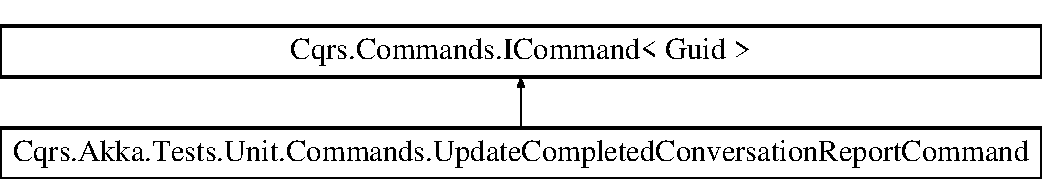
\includegraphics[height=2.000000cm]{classCqrs_1_1Akka_1_1Tests_1_1Unit_1_1Commands_1_1UpdateCompletedConversationReportCommand}
\end{center}
\end{figure}
\subsection*{Properties}
\begin{DoxyCompactItemize}
\item 
Guid \hyperlink{classCqrs_1_1Akka_1_1Tests_1_1Unit_1_1Commands_1_1UpdateCompletedConversationReportCommand_a31a479ec0cf27ea2989c371f51257136_a31a479ec0cf27ea2989c371f51257136}{Correlation\+Id}\hspace{0.3cm}{\ttfamily  \mbox{[}get, set\mbox{]}}
\begin{DoxyCompactList}\small\item\em An identifier used to group together several I\+Message. Any I\+Message with the same \hyperlink{classCqrs_1_1Akka_1_1Tests_1_1Unit_1_1Commands_1_1UpdateCompletedConversationReportCommand_a31a479ec0cf27ea2989c371f51257136_a31a479ec0cf27ea2989c371f51257136}{Correlation\+Id} were triggered by the same initiating request. \end{DoxyCompactList}\item 
string \hyperlink{classCqrs_1_1Akka_1_1Tests_1_1Unit_1_1Commands_1_1UpdateCompletedConversationReportCommand_a5f954bf75f49918ab48c3a09df50111f_a5f954bf75f49918ab48c3a09df50111f}{Originating\+Framework}\hspace{0.3cm}{\ttfamily  \mbox{[}get, set\mbox{]}}
\begin{DoxyCompactList}\small\item\em The originating framework this message was sent from. \end{DoxyCompactList}\item 
I\+Enumerable$<$ string $>$ \hyperlink{classCqrs_1_1Akka_1_1Tests_1_1Unit_1_1Commands_1_1UpdateCompletedConversationReportCommand_a8074ae409596c6e5d46e363adbfb9354_a8074ae409596c6e5d46e363adbfb9354}{Frameworks}\hspace{0.3cm}{\ttfamily  \mbox{[}get, set\mbox{]}}
\begin{DoxyCompactList}\small\item\em The frameworks this I\+Message has been delivered to/sent via already. \end{DoxyCompactList}\item 
Guid \hyperlink{classCqrs_1_1Akka_1_1Tests_1_1Unit_1_1Commands_1_1UpdateCompletedConversationReportCommand_acd3a75723758c361da638f40fab6d574_acd3a75723758c361da638f40fab6d574}{Authentication\+Token}\hspace{0.3cm}{\ttfamily  \mbox{[}get, set\mbox{]}}
\begin{DoxyCompactList}\small\item\em The authentication token of the entity that triggered the event to be raised. \end{DoxyCompactList}\item 
Guid \hyperlink{classCqrs_1_1Akka_1_1Tests_1_1Unit_1_1Commands_1_1UpdateCompletedConversationReportCommand_ae04217f6bfc19727e462f0077b990b34_ae04217f6bfc19727e462f0077b990b34}{Id}\hspace{0.3cm}{\ttfamily  \mbox{[}get, set\mbox{]}}
\begin{DoxyCompactList}\small\item\em The identifier of the command itself. In some cases this may be the I\+Aggregate\+Root$<$\+T\+Authentication\+Token$>$ or I\+Saga$<$\+T\+Authentication\+Token$>$ this command targets. \end{DoxyCompactList}\item 
int \hyperlink{classCqrs_1_1Akka_1_1Tests_1_1Unit_1_1Commands_1_1UpdateCompletedConversationReportCommand_a9e691733ed2512c198da8ad934bd79cb_a9e691733ed2512c198da8ad934bd79cb}{Expected\+Version}\hspace{0.3cm}{\ttfamily  \mbox{[}get, set\mbox{]}}
\begin{DoxyCompactList}\small\item\em The expected version number the targeted I\+Aggregate\+Root$<$\+T\+Authentication\+Token$>$ or I\+Saga$<$\+T\+Authentication\+Token$>$ is expected to be. \end{DoxyCompactList}\end{DoxyCompactItemize}


\subsection{Detailed Description}
Instruct the system to update the Completed Conversation report. 



\subsection{Property Documentation}
\mbox{\Hypertarget{classCqrs_1_1Akka_1_1Tests_1_1Unit_1_1Commands_1_1UpdateCompletedConversationReportCommand_acd3a75723758c361da638f40fab6d574_acd3a75723758c361da638f40fab6d574}\label{classCqrs_1_1Akka_1_1Tests_1_1Unit_1_1Commands_1_1UpdateCompletedConversationReportCommand_acd3a75723758c361da638f40fab6d574_acd3a75723758c361da638f40fab6d574}} 
\index{Cqrs\+::\+Akka\+::\+Tests\+::\+Unit\+::\+Commands\+::\+Update\+Completed\+Conversation\+Report\+Command@{Cqrs\+::\+Akka\+::\+Tests\+::\+Unit\+::\+Commands\+::\+Update\+Completed\+Conversation\+Report\+Command}!Authentication\+Token@{Authentication\+Token}}
\index{Authentication\+Token@{Authentication\+Token}!Cqrs\+::\+Akka\+::\+Tests\+::\+Unit\+::\+Commands\+::\+Update\+Completed\+Conversation\+Report\+Command@{Cqrs\+::\+Akka\+::\+Tests\+::\+Unit\+::\+Commands\+::\+Update\+Completed\+Conversation\+Report\+Command}}
\subsubsection{\texorpdfstring{Authentication\+Token}{AuthenticationToken}}
{\footnotesize\ttfamily Guid Cqrs.\+Akka.\+Tests.\+Unit.\+Commands.\+Update\+Completed\+Conversation\+Report\+Command.\+Authentication\+Token\hspace{0.3cm}{\ttfamily [get]}, {\ttfamily [set]}}



The authentication token of the entity that triggered the event to be raised. 

\mbox{\Hypertarget{classCqrs_1_1Akka_1_1Tests_1_1Unit_1_1Commands_1_1UpdateCompletedConversationReportCommand_a31a479ec0cf27ea2989c371f51257136_a31a479ec0cf27ea2989c371f51257136}\label{classCqrs_1_1Akka_1_1Tests_1_1Unit_1_1Commands_1_1UpdateCompletedConversationReportCommand_a31a479ec0cf27ea2989c371f51257136_a31a479ec0cf27ea2989c371f51257136}} 
\index{Cqrs\+::\+Akka\+::\+Tests\+::\+Unit\+::\+Commands\+::\+Update\+Completed\+Conversation\+Report\+Command@{Cqrs\+::\+Akka\+::\+Tests\+::\+Unit\+::\+Commands\+::\+Update\+Completed\+Conversation\+Report\+Command}!Correlation\+Id@{Correlation\+Id}}
\index{Correlation\+Id@{Correlation\+Id}!Cqrs\+::\+Akka\+::\+Tests\+::\+Unit\+::\+Commands\+::\+Update\+Completed\+Conversation\+Report\+Command@{Cqrs\+::\+Akka\+::\+Tests\+::\+Unit\+::\+Commands\+::\+Update\+Completed\+Conversation\+Report\+Command}}
\subsubsection{\texorpdfstring{Correlation\+Id}{CorrelationId}}
{\footnotesize\ttfamily Guid Cqrs.\+Akka.\+Tests.\+Unit.\+Commands.\+Update\+Completed\+Conversation\+Report\+Command.\+Correlation\+Id\hspace{0.3cm}{\ttfamily [get]}, {\ttfamily [set]}}



An identifier used to group together several I\+Message. Any I\+Message with the same \hyperlink{classCqrs_1_1Akka_1_1Tests_1_1Unit_1_1Commands_1_1UpdateCompletedConversationReportCommand_a31a479ec0cf27ea2989c371f51257136_a31a479ec0cf27ea2989c371f51257136}{Correlation\+Id} were triggered by the same initiating request. 

\mbox{\Hypertarget{classCqrs_1_1Akka_1_1Tests_1_1Unit_1_1Commands_1_1UpdateCompletedConversationReportCommand_a9e691733ed2512c198da8ad934bd79cb_a9e691733ed2512c198da8ad934bd79cb}\label{classCqrs_1_1Akka_1_1Tests_1_1Unit_1_1Commands_1_1UpdateCompletedConversationReportCommand_a9e691733ed2512c198da8ad934bd79cb_a9e691733ed2512c198da8ad934bd79cb}} 
\index{Cqrs\+::\+Akka\+::\+Tests\+::\+Unit\+::\+Commands\+::\+Update\+Completed\+Conversation\+Report\+Command@{Cqrs\+::\+Akka\+::\+Tests\+::\+Unit\+::\+Commands\+::\+Update\+Completed\+Conversation\+Report\+Command}!Expected\+Version@{Expected\+Version}}
\index{Expected\+Version@{Expected\+Version}!Cqrs\+::\+Akka\+::\+Tests\+::\+Unit\+::\+Commands\+::\+Update\+Completed\+Conversation\+Report\+Command@{Cqrs\+::\+Akka\+::\+Tests\+::\+Unit\+::\+Commands\+::\+Update\+Completed\+Conversation\+Report\+Command}}
\subsubsection{\texorpdfstring{Expected\+Version}{ExpectedVersion}}
{\footnotesize\ttfamily int Cqrs.\+Akka.\+Tests.\+Unit.\+Commands.\+Update\+Completed\+Conversation\+Report\+Command.\+Expected\+Version\hspace{0.3cm}{\ttfamily [get]}, {\ttfamily [set]}}



The expected version number the targeted I\+Aggregate\+Root$<$\+T\+Authentication\+Token$>$ or I\+Saga$<$\+T\+Authentication\+Token$>$ is expected to be. 

\mbox{\Hypertarget{classCqrs_1_1Akka_1_1Tests_1_1Unit_1_1Commands_1_1UpdateCompletedConversationReportCommand_a8074ae409596c6e5d46e363adbfb9354_a8074ae409596c6e5d46e363adbfb9354}\label{classCqrs_1_1Akka_1_1Tests_1_1Unit_1_1Commands_1_1UpdateCompletedConversationReportCommand_a8074ae409596c6e5d46e363adbfb9354_a8074ae409596c6e5d46e363adbfb9354}} 
\index{Cqrs\+::\+Akka\+::\+Tests\+::\+Unit\+::\+Commands\+::\+Update\+Completed\+Conversation\+Report\+Command@{Cqrs\+::\+Akka\+::\+Tests\+::\+Unit\+::\+Commands\+::\+Update\+Completed\+Conversation\+Report\+Command}!Frameworks@{Frameworks}}
\index{Frameworks@{Frameworks}!Cqrs\+::\+Akka\+::\+Tests\+::\+Unit\+::\+Commands\+::\+Update\+Completed\+Conversation\+Report\+Command@{Cqrs\+::\+Akka\+::\+Tests\+::\+Unit\+::\+Commands\+::\+Update\+Completed\+Conversation\+Report\+Command}}
\subsubsection{\texorpdfstring{Frameworks}{Frameworks}}
{\footnotesize\ttfamily I\+Enumerable$<$string$>$ Cqrs.\+Akka.\+Tests.\+Unit.\+Commands.\+Update\+Completed\+Conversation\+Report\+Command.\+Frameworks\hspace{0.3cm}{\ttfamily [get]}, {\ttfamily [set]}}



The frameworks this I\+Message has been delivered to/sent via already. 

\mbox{\Hypertarget{classCqrs_1_1Akka_1_1Tests_1_1Unit_1_1Commands_1_1UpdateCompletedConversationReportCommand_ae04217f6bfc19727e462f0077b990b34_ae04217f6bfc19727e462f0077b990b34}\label{classCqrs_1_1Akka_1_1Tests_1_1Unit_1_1Commands_1_1UpdateCompletedConversationReportCommand_ae04217f6bfc19727e462f0077b990b34_ae04217f6bfc19727e462f0077b990b34}} 
\index{Cqrs\+::\+Akka\+::\+Tests\+::\+Unit\+::\+Commands\+::\+Update\+Completed\+Conversation\+Report\+Command@{Cqrs\+::\+Akka\+::\+Tests\+::\+Unit\+::\+Commands\+::\+Update\+Completed\+Conversation\+Report\+Command}!Id@{Id}}
\index{Id@{Id}!Cqrs\+::\+Akka\+::\+Tests\+::\+Unit\+::\+Commands\+::\+Update\+Completed\+Conversation\+Report\+Command@{Cqrs\+::\+Akka\+::\+Tests\+::\+Unit\+::\+Commands\+::\+Update\+Completed\+Conversation\+Report\+Command}}
\subsubsection{\texorpdfstring{Id}{Id}}
{\footnotesize\ttfamily Guid Cqrs.\+Akka.\+Tests.\+Unit.\+Commands.\+Update\+Completed\+Conversation\+Report\+Command.\+Id\hspace{0.3cm}{\ttfamily [get]}, {\ttfamily [set]}}



The identifier of the command itself. In some cases this may be the I\+Aggregate\+Root$<$\+T\+Authentication\+Token$>$ or I\+Saga$<$\+T\+Authentication\+Token$>$ this command targets. 

\mbox{\Hypertarget{classCqrs_1_1Akka_1_1Tests_1_1Unit_1_1Commands_1_1UpdateCompletedConversationReportCommand_a5f954bf75f49918ab48c3a09df50111f_a5f954bf75f49918ab48c3a09df50111f}\label{classCqrs_1_1Akka_1_1Tests_1_1Unit_1_1Commands_1_1UpdateCompletedConversationReportCommand_a5f954bf75f49918ab48c3a09df50111f_a5f954bf75f49918ab48c3a09df50111f}} 
\index{Cqrs\+::\+Akka\+::\+Tests\+::\+Unit\+::\+Commands\+::\+Update\+Completed\+Conversation\+Report\+Command@{Cqrs\+::\+Akka\+::\+Tests\+::\+Unit\+::\+Commands\+::\+Update\+Completed\+Conversation\+Report\+Command}!Originating\+Framework@{Originating\+Framework}}
\index{Originating\+Framework@{Originating\+Framework}!Cqrs\+::\+Akka\+::\+Tests\+::\+Unit\+::\+Commands\+::\+Update\+Completed\+Conversation\+Report\+Command@{Cqrs\+::\+Akka\+::\+Tests\+::\+Unit\+::\+Commands\+::\+Update\+Completed\+Conversation\+Report\+Command}}
\subsubsection{\texorpdfstring{Originating\+Framework}{OriginatingFramework}}
{\footnotesize\ttfamily string Cqrs.\+Akka.\+Tests.\+Unit.\+Commands.\+Update\+Completed\+Conversation\+Report\+Command.\+Originating\+Framework\hspace{0.3cm}{\ttfamily [get]}, {\ttfamily [set]}}



The originating framework this message was sent from. 


\hypertarget{classCqrs_1_1Akka_1_1Tests_1_1Unit_1_1Events_1_1ConversationEnded}{}\doxysection{Cqrs.\+Akka.\+Tests.\+Unit.\+Events.\+Conversation\+Ended Class Reference}
\label{classCqrs_1_1Akka_1_1Tests_1_1Unit_1_1Events_1_1ConversationEnded}\index{Cqrs.Akka.Tests.Unit.Events.ConversationEnded@{Cqrs.Akka.Tests.Unit.Events.ConversationEnded}}


The conversation has ended.  


Inheritance diagram for Cqrs.\+Akka.\+Tests.\+Unit.\+Events.\+Conversation\+Ended\+:\begin{figure}[H]
\begin{center}
\leavevmode
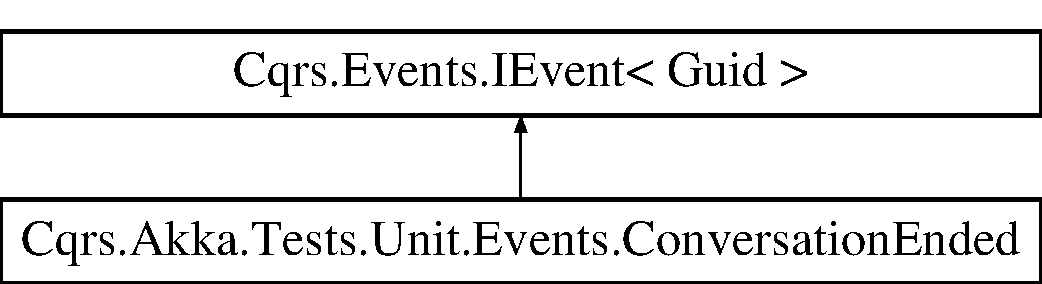
\includegraphics[height=2.000000cm]{classCqrs_1_1Akka_1_1Tests_1_1Unit_1_1Events_1_1ConversationEnded}
\end{center}
\end{figure}
\doxysubsection*{Properties}
\begin{DoxyCompactItemize}
\item 
Guid \mbox{\hyperlink{classCqrs_1_1Akka_1_1Tests_1_1Unit_1_1Events_1_1ConversationEnded_a99ad268bb52a4214a4b717bb8ecea6b6_a99ad268bb52a4214a4b717bb8ecea6b6}{Correlation\+Id}}\hspace{0.3cm}{\ttfamily  \mbox{[}get, set\mbox{]}}
\begin{DoxyCompactList}\small\item\em An identifier used to group together several I\+Message. Any I\+Message with the same \mbox{\hyperlink{classCqrs_1_1Akka_1_1Tests_1_1Unit_1_1Events_1_1ConversationEnded_a99ad268bb52a4214a4b717bb8ecea6b6_a99ad268bb52a4214a4b717bb8ecea6b6}{Correlation\+Id}} were triggered by the same initiating request. \end{DoxyCompactList}\item 
string \mbox{\hyperlink{classCqrs_1_1Akka_1_1Tests_1_1Unit_1_1Events_1_1ConversationEnded_a84f8392985be189ed8394d308c76692f_a84f8392985be189ed8394d308c76692f}{Originating\+Framework}}\hspace{0.3cm}{\ttfamily  \mbox{[}get, set\mbox{]}}
\begin{DoxyCompactList}\small\item\em The originating framework this message was sent from. \end{DoxyCompactList}\item 
I\+Enumerable$<$ string $>$ \mbox{\hyperlink{classCqrs_1_1Akka_1_1Tests_1_1Unit_1_1Events_1_1ConversationEnded_a1a8b4fd91323c4c9140051dff5f2bff6_a1a8b4fd91323c4c9140051dff5f2bff6}{Frameworks}}\hspace{0.3cm}{\ttfamily  \mbox{[}get, set\mbox{]}}
\begin{DoxyCompactList}\small\item\em The frameworks this I\+Message has been delivered to/sent via already. \end{DoxyCompactList}\item 
Guid \mbox{\hyperlink{classCqrs_1_1Akka_1_1Tests_1_1Unit_1_1Events_1_1ConversationEnded_a025b7df73452f8e22337eabc4d11fab9_a025b7df73452f8e22337eabc4d11fab9}{Authentication\+Token}}\hspace{0.3cm}{\ttfamily  \mbox{[}get, set\mbox{]}}
\begin{DoxyCompactList}\small\item\em The authentication token of the entity that triggered the event to be raised. \end{DoxyCompactList}\item 
Guid \mbox{\hyperlink{classCqrs_1_1Akka_1_1Tests_1_1Unit_1_1Events_1_1ConversationEnded_ae8a319553a4df63661afcef6bcadd963_ae8a319553a4df63661afcef6bcadd963}{Id}}\hspace{0.3cm}{\ttfamily  \mbox{[}get, set\mbox{]}}
\begin{DoxyCompactList}\small\item\em The ID of the I\+Event$<$\+T\+Authentication\+Token$>$ \end{DoxyCompactList}\item 
int \mbox{\hyperlink{classCqrs_1_1Akka_1_1Tests_1_1Unit_1_1Events_1_1ConversationEnded_a08eef17f722c411bea6ad6adb871ddfb_a08eef17f722c411bea6ad6adb871ddfb}{Version}}\hspace{0.3cm}{\ttfamily  \mbox{[}get, set\mbox{]}}
\begin{DoxyCompactList}\small\item\em The version of the I\+Event$<$\+T\+Authentication\+Token$>$ \end{DoxyCompactList}\item 
Date\+Time\+Offset \mbox{\hyperlink{classCqrs_1_1Akka_1_1Tests_1_1Unit_1_1Events_1_1ConversationEnded_a26f068ae3ca8f1e84277f133f8fc4620_a26f068ae3ca8f1e84277f133f8fc4620}{Time\+Stamp}}\hspace{0.3cm}{\ttfamily  \mbox{[}get, set\mbox{]}}
\begin{DoxyCompactList}\small\item\em The date and time the event was raised or published. \end{DoxyCompactList}\end{DoxyCompactItemize}


\doxysubsection{Detailed Description}
The conversation has ended. 



\doxysubsection{Property Documentation}
\mbox{\Hypertarget{classCqrs_1_1Akka_1_1Tests_1_1Unit_1_1Events_1_1ConversationEnded_a025b7df73452f8e22337eabc4d11fab9_a025b7df73452f8e22337eabc4d11fab9}\label{classCqrs_1_1Akka_1_1Tests_1_1Unit_1_1Events_1_1ConversationEnded_a025b7df73452f8e22337eabc4d11fab9_a025b7df73452f8e22337eabc4d11fab9}} 
\index{Cqrs.Akka.Tests.Unit.Events.ConversationEnded@{Cqrs.Akka.Tests.Unit.Events.ConversationEnded}!AuthenticationToken@{AuthenticationToken}}
\index{AuthenticationToken@{AuthenticationToken}!Cqrs.Akka.Tests.Unit.Events.ConversationEnded@{Cqrs.Akka.Tests.Unit.Events.ConversationEnded}}
\doxysubsubsection{\texorpdfstring{AuthenticationToken}{AuthenticationToken}}
{\footnotesize\ttfamily Guid Cqrs.\+Akka.\+Tests.\+Unit.\+Events.\+Conversation\+Ended.\+Authentication\+Token\hspace{0.3cm}{\ttfamily [get]}, {\ttfamily [set]}}



The authentication token of the entity that triggered the event to be raised. 

\mbox{\Hypertarget{classCqrs_1_1Akka_1_1Tests_1_1Unit_1_1Events_1_1ConversationEnded_a99ad268bb52a4214a4b717bb8ecea6b6_a99ad268bb52a4214a4b717bb8ecea6b6}\label{classCqrs_1_1Akka_1_1Tests_1_1Unit_1_1Events_1_1ConversationEnded_a99ad268bb52a4214a4b717bb8ecea6b6_a99ad268bb52a4214a4b717bb8ecea6b6}} 
\index{Cqrs.Akka.Tests.Unit.Events.ConversationEnded@{Cqrs.Akka.Tests.Unit.Events.ConversationEnded}!CorrelationId@{CorrelationId}}
\index{CorrelationId@{CorrelationId}!Cqrs.Akka.Tests.Unit.Events.ConversationEnded@{Cqrs.Akka.Tests.Unit.Events.ConversationEnded}}
\doxysubsubsection{\texorpdfstring{CorrelationId}{CorrelationId}}
{\footnotesize\ttfamily Guid Cqrs.\+Akka.\+Tests.\+Unit.\+Events.\+Conversation\+Ended.\+Correlation\+Id\hspace{0.3cm}{\ttfamily [get]}, {\ttfamily [set]}}



An identifier used to group together several I\+Message. Any I\+Message with the same \mbox{\hyperlink{classCqrs_1_1Akka_1_1Tests_1_1Unit_1_1Events_1_1ConversationEnded_a99ad268bb52a4214a4b717bb8ecea6b6_a99ad268bb52a4214a4b717bb8ecea6b6}{Correlation\+Id}} were triggered by the same initiating request. 

\mbox{\Hypertarget{classCqrs_1_1Akka_1_1Tests_1_1Unit_1_1Events_1_1ConversationEnded_a1a8b4fd91323c4c9140051dff5f2bff6_a1a8b4fd91323c4c9140051dff5f2bff6}\label{classCqrs_1_1Akka_1_1Tests_1_1Unit_1_1Events_1_1ConversationEnded_a1a8b4fd91323c4c9140051dff5f2bff6_a1a8b4fd91323c4c9140051dff5f2bff6}} 
\index{Cqrs.Akka.Tests.Unit.Events.ConversationEnded@{Cqrs.Akka.Tests.Unit.Events.ConversationEnded}!Frameworks@{Frameworks}}
\index{Frameworks@{Frameworks}!Cqrs.Akka.Tests.Unit.Events.ConversationEnded@{Cqrs.Akka.Tests.Unit.Events.ConversationEnded}}
\doxysubsubsection{\texorpdfstring{Frameworks}{Frameworks}}
{\footnotesize\ttfamily I\+Enumerable$<$string$>$ Cqrs.\+Akka.\+Tests.\+Unit.\+Events.\+Conversation\+Ended.\+Frameworks\hspace{0.3cm}{\ttfamily [get]}, {\ttfamily [set]}}



The frameworks this I\+Message has been delivered to/sent via already. 

\mbox{\Hypertarget{classCqrs_1_1Akka_1_1Tests_1_1Unit_1_1Events_1_1ConversationEnded_ae8a319553a4df63661afcef6bcadd963_ae8a319553a4df63661afcef6bcadd963}\label{classCqrs_1_1Akka_1_1Tests_1_1Unit_1_1Events_1_1ConversationEnded_ae8a319553a4df63661afcef6bcadd963_ae8a319553a4df63661afcef6bcadd963}} 
\index{Cqrs.Akka.Tests.Unit.Events.ConversationEnded@{Cqrs.Akka.Tests.Unit.Events.ConversationEnded}!Id@{Id}}
\index{Id@{Id}!Cqrs.Akka.Tests.Unit.Events.ConversationEnded@{Cqrs.Akka.Tests.Unit.Events.ConversationEnded}}
\doxysubsubsection{\texorpdfstring{Id}{Id}}
{\footnotesize\ttfamily Guid Cqrs.\+Akka.\+Tests.\+Unit.\+Events.\+Conversation\+Ended.\+Id\hspace{0.3cm}{\ttfamily [get]}, {\ttfamily [set]}}



The ID of the I\+Event$<$\+T\+Authentication\+Token$>$ 

\mbox{\Hypertarget{classCqrs_1_1Akka_1_1Tests_1_1Unit_1_1Events_1_1ConversationEnded_a84f8392985be189ed8394d308c76692f_a84f8392985be189ed8394d308c76692f}\label{classCqrs_1_1Akka_1_1Tests_1_1Unit_1_1Events_1_1ConversationEnded_a84f8392985be189ed8394d308c76692f_a84f8392985be189ed8394d308c76692f}} 
\index{Cqrs.Akka.Tests.Unit.Events.ConversationEnded@{Cqrs.Akka.Tests.Unit.Events.ConversationEnded}!OriginatingFramework@{OriginatingFramework}}
\index{OriginatingFramework@{OriginatingFramework}!Cqrs.Akka.Tests.Unit.Events.ConversationEnded@{Cqrs.Akka.Tests.Unit.Events.ConversationEnded}}
\doxysubsubsection{\texorpdfstring{OriginatingFramework}{OriginatingFramework}}
{\footnotesize\ttfamily string Cqrs.\+Akka.\+Tests.\+Unit.\+Events.\+Conversation\+Ended.\+Originating\+Framework\hspace{0.3cm}{\ttfamily [get]}, {\ttfamily [set]}}



The originating framework this message was sent from. 

\mbox{\Hypertarget{classCqrs_1_1Akka_1_1Tests_1_1Unit_1_1Events_1_1ConversationEnded_a26f068ae3ca8f1e84277f133f8fc4620_a26f068ae3ca8f1e84277f133f8fc4620}\label{classCqrs_1_1Akka_1_1Tests_1_1Unit_1_1Events_1_1ConversationEnded_a26f068ae3ca8f1e84277f133f8fc4620_a26f068ae3ca8f1e84277f133f8fc4620}} 
\index{Cqrs.Akka.Tests.Unit.Events.ConversationEnded@{Cqrs.Akka.Tests.Unit.Events.ConversationEnded}!TimeStamp@{TimeStamp}}
\index{TimeStamp@{TimeStamp}!Cqrs.Akka.Tests.Unit.Events.ConversationEnded@{Cqrs.Akka.Tests.Unit.Events.ConversationEnded}}
\doxysubsubsection{\texorpdfstring{TimeStamp}{TimeStamp}}
{\footnotesize\ttfamily Date\+Time\+Offset Cqrs.\+Akka.\+Tests.\+Unit.\+Events.\+Conversation\+Ended.\+Time\+Stamp\hspace{0.3cm}{\ttfamily [get]}, {\ttfamily [set]}}



The date and time the event was raised or published. 

\mbox{\Hypertarget{classCqrs_1_1Akka_1_1Tests_1_1Unit_1_1Events_1_1ConversationEnded_a08eef17f722c411bea6ad6adb871ddfb_a08eef17f722c411bea6ad6adb871ddfb}\label{classCqrs_1_1Akka_1_1Tests_1_1Unit_1_1Events_1_1ConversationEnded_a08eef17f722c411bea6ad6adb871ddfb_a08eef17f722c411bea6ad6adb871ddfb}} 
\index{Cqrs.Akka.Tests.Unit.Events.ConversationEnded@{Cqrs.Akka.Tests.Unit.Events.ConversationEnded}!Version@{Version}}
\index{Version@{Version}!Cqrs.Akka.Tests.Unit.Events.ConversationEnded@{Cqrs.Akka.Tests.Unit.Events.ConversationEnded}}
\doxysubsubsection{\texorpdfstring{Version}{Version}}
{\footnotesize\ttfamily int Cqrs.\+Akka.\+Tests.\+Unit.\+Events.\+Conversation\+Ended.\+Version\hspace{0.3cm}{\ttfamily [get]}, {\ttfamily [set]}}



The version of the I\+Event$<$\+T\+Authentication\+Token$>$ 


\hypertarget{classCqrs_1_1Akka_1_1Tests_1_1Unit_1_1Events_1_1Handlers_1_1ConversationEndedEventHandler}{}\section{Cqrs.\+Akka.\+Tests.\+Unit.\+Events.\+Handlers.\+Conversation\+Ended\+Event\+Handler Class Reference}
\label{classCqrs_1_1Akka_1_1Tests_1_1Unit_1_1Events_1_1Handlers_1_1ConversationEndedEventHandler}\index{Cqrs.\+Akka.\+Tests.\+Unit.\+Events.\+Handlers.\+Conversation\+Ended\+Event\+Handler@{Cqrs.\+Akka.\+Tests.\+Unit.\+Events.\+Handlers.\+Conversation\+Ended\+Event\+Handler}}
Inheritance diagram for Cqrs.\+Akka.\+Tests.\+Unit.\+Events.\+Handlers.\+Conversation\+Ended\+Event\+Handler\+:\begin{figure}[H]
\begin{center}
\leavevmode
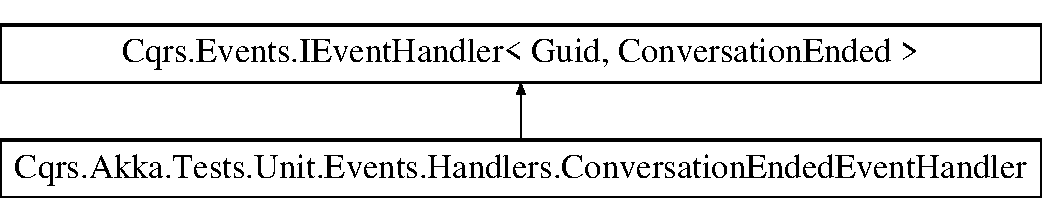
\includegraphics[height=2.000000cm]{classCqrs_1_1Akka_1_1Tests_1_1Unit_1_1Events_1_1Handlers_1_1ConversationEndedEventHandler}
\end{center}
\end{figure}
\subsection*{Public Member Functions}
\begin{DoxyCompactItemize}
\item 
\hyperlink{classCqrs_1_1Akka_1_1Tests_1_1Unit_1_1Events_1_1Handlers_1_1ConversationEndedEventHandler_adf9143b7444b05fab2d43750fa7c89b8}{Conversation\+Ended\+Event\+Handler} (\hyperlink{interfaceCqrs_1_1Akka_1_1Commands_1_1IAkkaCommandSender}{I\+Akka\+Command\+Sender}$<$ Guid $>$ command\+Bus)
\item 
void \hyperlink{classCqrs_1_1Akka_1_1Tests_1_1Unit_1_1Events_1_1Handlers_1_1ConversationEndedEventHandler_a1e363c715cefdb600705d7b3f5e3bca6}{Handle} (\hyperlink{classCqrs_1_1Akka_1_1Tests_1_1Unit_1_1Events_1_1ConversationEnded}{Conversation\+Ended} message)
\end{DoxyCompactItemize}
\subsection*{Properties}
\begin{DoxyCompactItemize}
\item 
\hyperlink{interfaceCqrs_1_1Commands_1_1ICommandPublisher}{I\+Command\+Publisher}$<$ Guid $>$ \hyperlink{classCqrs_1_1Akka_1_1Tests_1_1Unit_1_1Events_1_1Handlers_1_1ConversationEndedEventHandler_a2ad947f0ed860a416ba8a0795caa06d1}{Command\+Bus}\hspace{0.3cm}{\ttfamily  \mbox{[}get\mbox{]}}
\end{DoxyCompactItemize}


\subsection{Constructor \& Destructor Documentation}
\mbox{\Hypertarget{classCqrs_1_1Akka_1_1Tests_1_1Unit_1_1Events_1_1Handlers_1_1ConversationEndedEventHandler_adf9143b7444b05fab2d43750fa7c89b8}\label{classCqrs_1_1Akka_1_1Tests_1_1Unit_1_1Events_1_1Handlers_1_1ConversationEndedEventHandler_adf9143b7444b05fab2d43750fa7c89b8}} 
\index{Cqrs\+::\+Akka\+::\+Tests\+::\+Unit\+::\+Events\+::\+Handlers\+::\+Conversation\+Ended\+Event\+Handler@{Cqrs\+::\+Akka\+::\+Tests\+::\+Unit\+::\+Events\+::\+Handlers\+::\+Conversation\+Ended\+Event\+Handler}!Conversation\+Ended\+Event\+Handler@{Conversation\+Ended\+Event\+Handler}}
\index{Conversation\+Ended\+Event\+Handler@{Conversation\+Ended\+Event\+Handler}!Cqrs\+::\+Akka\+::\+Tests\+::\+Unit\+::\+Events\+::\+Handlers\+::\+Conversation\+Ended\+Event\+Handler@{Cqrs\+::\+Akka\+::\+Tests\+::\+Unit\+::\+Events\+::\+Handlers\+::\+Conversation\+Ended\+Event\+Handler}}
\subsubsection{\texorpdfstring{Conversation\+Ended\+Event\+Handler()}{ConversationEndedEventHandler()}}
{\footnotesize\ttfamily Cqrs.\+Akka.\+Tests.\+Unit.\+Events.\+Handlers.\+Conversation\+Ended\+Event\+Handler.\+Conversation\+Ended\+Event\+Handler (\begin{DoxyParamCaption}\item[{\hyperlink{interfaceCqrs_1_1Akka_1_1Commands_1_1IAkkaCommandSender}{I\+Akka\+Command\+Sender}$<$ Guid $>$}]{command\+Bus }\end{DoxyParamCaption})}



\subsection{Member Function Documentation}
\mbox{\Hypertarget{classCqrs_1_1Akka_1_1Tests_1_1Unit_1_1Events_1_1Handlers_1_1ConversationEndedEventHandler_a1e363c715cefdb600705d7b3f5e3bca6}\label{classCqrs_1_1Akka_1_1Tests_1_1Unit_1_1Events_1_1Handlers_1_1ConversationEndedEventHandler_a1e363c715cefdb600705d7b3f5e3bca6}} 
\index{Cqrs\+::\+Akka\+::\+Tests\+::\+Unit\+::\+Events\+::\+Handlers\+::\+Conversation\+Ended\+Event\+Handler@{Cqrs\+::\+Akka\+::\+Tests\+::\+Unit\+::\+Events\+::\+Handlers\+::\+Conversation\+Ended\+Event\+Handler}!Handle@{Handle}}
\index{Handle@{Handle}!Cqrs\+::\+Akka\+::\+Tests\+::\+Unit\+::\+Events\+::\+Handlers\+::\+Conversation\+Ended\+Event\+Handler@{Cqrs\+::\+Akka\+::\+Tests\+::\+Unit\+::\+Events\+::\+Handlers\+::\+Conversation\+Ended\+Event\+Handler}}
\subsubsection{\texorpdfstring{Handle()}{Handle()}}
{\footnotesize\ttfamily void Cqrs.\+Akka.\+Tests.\+Unit.\+Events.\+Handlers.\+Conversation\+Ended\+Event\+Handler.\+Handle (\begin{DoxyParamCaption}\item[{\hyperlink{classCqrs_1_1Akka_1_1Tests_1_1Unit_1_1Events_1_1ConversationEnded}{Conversation\+Ended}}]{message }\end{DoxyParamCaption})}



\subsection{Property Documentation}
\mbox{\Hypertarget{classCqrs_1_1Akka_1_1Tests_1_1Unit_1_1Events_1_1Handlers_1_1ConversationEndedEventHandler_a2ad947f0ed860a416ba8a0795caa06d1}\label{classCqrs_1_1Akka_1_1Tests_1_1Unit_1_1Events_1_1Handlers_1_1ConversationEndedEventHandler_a2ad947f0ed860a416ba8a0795caa06d1}} 
\index{Cqrs\+::\+Akka\+::\+Tests\+::\+Unit\+::\+Events\+::\+Handlers\+::\+Conversation\+Ended\+Event\+Handler@{Cqrs\+::\+Akka\+::\+Tests\+::\+Unit\+::\+Events\+::\+Handlers\+::\+Conversation\+Ended\+Event\+Handler}!Command\+Bus@{Command\+Bus}}
\index{Command\+Bus@{Command\+Bus}!Cqrs\+::\+Akka\+::\+Tests\+::\+Unit\+::\+Events\+::\+Handlers\+::\+Conversation\+Ended\+Event\+Handler@{Cqrs\+::\+Akka\+::\+Tests\+::\+Unit\+::\+Events\+::\+Handlers\+::\+Conversation\+Ended\+Event\+Handler}}
\subsubsection{\texorpdfstring{Command\+Bus}{CommandBus}}
{\footnotesize\ttfamily \hyperlink{interfaceCqrs_1_1Commands_1_1ICommandPublisher}{I\+Command\+Publisher}$<$Guid$>$ Cqrs.\+Akka.\+Tests.\+Unit.\+Events.\+Handlers.\+Conversation\+Ended\+Event\+Handler.\+Command\+Bus\hspace{0.3cm}{\ttfamily [get]}, {\ttfamily [protected]}}


\hypertarget{classCqrs_1_1Akka_1_1Tests_1_1Unit_1_1Events_1_1Handlers_1_1HelloWorldRepliedToEventHandler}{}\doxysection{Cqrs.\+Akka.\+Tests.\+Unit.\+Events.\+Handlers.\+Hello\+World\+Replied\+To\+Event\+Handler Class Reference}
\label{classCqrs_1_1Akka_1_1Tests_1_1Unit_1_1Events_1_1Handlers_1_1HelloWorldRepliedToEventHandler}\index{Cqrs.Akka.Tests.Unit.Events.Handlers.HelloWorldRepliedToEventHandler@{Cqrs.Akka.Tests.Unit.Events.Handlers.HelloWorldRepliedToEventHandler}}


Handles the \mbox{\hyperlink{classCqrs_1_1Akka_1_1Tests_1_1Unit_1_1Events_1_1HelloWorldRepliedTo}{Hello\+World\+Replied\+To}}.  


Inheritance diagram for Cqrs.\+Akka.\+Tests.\+Unit.\+Events.\+Handlers.\+Hello\+World\+Replied\+To\+Event\+Handler\+:\begin{figure}[H]
\begin{center}
\leavevmode
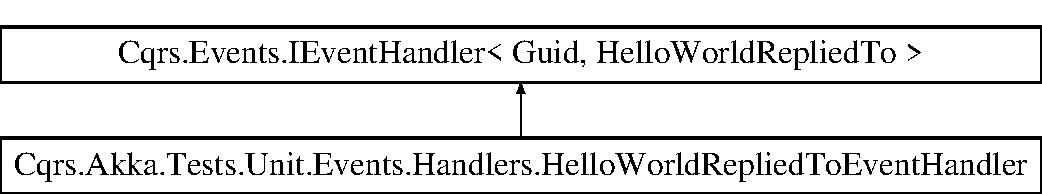
\includegraphics[height=2.000000cm]{classCqrs_1_1Akka_1_1Tests_1_1Unit_1_1Events_1_1Handlers_1_1HelloWorldRepliedToEventHandler}
\end{center}
\end{figure}
\doxysubsection*{Public Member Functions}
\begin{DoxyCompactItemize}
\item 
\mbox{\hyperlink{classCqrs_1_1Akka_1_1Tests_1_1Unit_1_1Events_1_1Handlers_1_1HelloWorldRepliedToEventHandler_aa566f26a38bc21ed270a1854de47408d_aa566f26a38bc21ed270a1854de47408d}{Hello\+World\+Replied\+To\+Event\+Handler}} (\mbox{\hyperlink{interfaceCqrs_1_1Akka_1_1Domain_1_1IAkkaAggregateResolver}{I\+Akka\+Aggregate\+Resolver}} aggregate\+Resolver)
\begin{DoxyCompactList}\small\item\em Instantiates the \mbox{\hyperlink{classCqrs_1_1Akka_1_1Tests_1_1Unit_1_1Events_1_1Handlers_1_1HelloWorldRepliedToEventHandler}{Hello\+World\+Replied\+To\+Event\+Handler}} class registering any Receive\+Actor.\+Receive$<$\+T$>$(\+System.\+Func$<$\+T,\+System.\+Threading.\+Tasks.\+Task$>$) required. \end{DoxyCompactList}\item 
void \mbox{\hyperlink{classCqrs_1_1Akka_1_1Tests_1_1Unit_1_1Events_1_1Handlers_1_1HelloWorldRepliedToEventHandler_a12509fd1219657eca78496775641f481_a12509fd1219657eca78496775641f481}{Handle}} (\mbox{\hyperlink{classCqrs_1_1Akka_1_1Tests_1_1Unit_1_1Events_1_1HelloWorldRepliedTo}{Hello\+World\+Replied\+To}} message)
\begin{DoxyCompactList}\small\item\em Responds to the provided {\itshape message}  passing the {\itshape message}  to an Akka.\+Net actor. \end{DoxyCompactList}\end{DoxyCompactItemize}
\doxysubsection*{Properties}
\begin{DoxyCompactItemize}
\item 
\mbox{\hyperlink{interfaceCqrs_1_1Akka_1_1Domain_1_1IAkkaAggregateResolver}{I\+Akka\+Aggregate\+Resolver}} \mbox{\hyperlink{classCqrs_1_1Akka_1_1Tests_1_1Unit_1_1Events_1_1Handlers_1_1HelloWorldRepliedToEventHandler_aead9e7b0edae372414fffea474407514_aead9e7b0edae372414fffea474407514}{Aggregate\+Resolver}}\hspace{0.3cm}{\ttfamily  \mbox{[}get\mbox{]}}
\begin{DoxyCompactList}\small\item\em Resolves Akka.\+Net actor based I\+Aggregate\+Root$<$\+T\+Authentication\+Token$>$ \end{DoxyCompactList}\end{DoxyCompactItemize}


\doxysubsection{Detailed Description}
Handles the \mbox{\hyperlink{classCqrs_1_1Akka_1_1Tests_1_1Unit_1_1Events_1_1HelloWorldRepliedTo}{Hello\+World\+Replied\+To}}. 



\doxysubsection{Constructor \& Destructor Documentation}
\mbox{\Hypertarget{classCqrs_1_1Akka_1_1Tests_1_1Unit_1_1Events_1_1Handlers_1_1HelloWorldRepliedToEventHandler_aa566f26a38bc21ed270a1854de47408d_aa566f26a38bc21ed270a1854de47408d}\label{classCqrs_1_1Akka_1_1Tests_1_1Unit_1_1Events_1_1Handlers_1_1HelloWorldRepliedToEventHandler_aa566f26a38bc21ed270a1854de47408d_aa566f26a38bc21ed270a1854de47408d}} 
\index{Cqrs.Akka.Tests.Unit.Events.Handlers.HelloWorldRepliedToEventHandler@{Cqrs.Akka.Tests.Unit.Events.Handlers.HelloWorldRepliedToEventHandler}!HelloWorldRepliedToEventHandler@{HelloWorldRepliedToEventHandler}}
\index{HelloWorldRepliedToEventHandler@{HelloWorldRepliedToEventHandler}!Cqrs.Akka.Tests.Unit.Events.Handlers.HelloWorldRepliedToEventHandler@{Cqrs.Akka.Tests.Unit.Events.Handlers.HelloWorldRepliedToEventHandler}}
\doxysubsubsection{\texorpdfstring{HelloWorldRepliedToEventHandler()}{HelloWorldRepliedToEventHandler()}}
{\footnotesize\ttfamily Cqrs.\+Akka.\+Tests.\+Unit.\+Events.\+Handlers.\+Hello\+World\+Replied\+To\+Event\+Handler.\+Hello\+World\+Replied\+To\+Event\+Handler (\begin{DoxyParamCaption}\item[{\mbox{\hyperlink{interfaceCqrs_1_1Akka_1_1Domain_1_1IAkkaAggregateResolver}{I\+Akka\+Aggregate\+Resolver}}}]{aggregate\+Resolver }\end{DoxyParamCaption})}



Instantiates the \mbox{\hyperlink{classCqrs_1_1Akka_1_1Tests_1_1Unit_1_1Events_1_1Handlers_1_1HelloWorldRepliedToEventHandler}{Hello\+World\+Replied\+To\+Event\+Handler}} class registering any Receive\+Actor.\+Receive$<$\+T$>$(\+System.\+Func$<$\+T,\+System.\+Threading.\+Tasks.\+Task$>$) required. 



\doxysubsection{Member Function Documentation}
\mbox{\Hypertarget{classCqrs_1_1Akka_1_1Tests_1_1Unit_1_1Events_1_1Handlers_1_1HelloWorldRepliedToEventHandler_a12509fd1219657eca78496775641f481_a12509fd1219657eca78496775641f481}\label{classCqrs_1_1Akka_1_1Tests_1_1Unit_1_1Events_1_1Handlers_1_1HelloWorldRepliedToEventHandler_a12509fd1219657eca78496775641f481_a12509fd1219657eca78496775641f481}} 
\index{Cqrs.Akka.Tests.Unit.Events.Handlers.HelloWorldRepliedToEventHandler@{Cqrs.Akka.Tests.Unit.Events.Handlers.HelloWorldRepliedToEventHandler}!Handle@{Handle}}
\index{Handle@{Handle}!Cqrs.Akka.Tests.Unit.Events.Handlers.HelloWorldRepliedToEventHandler@{Cqrs.Akka.Tests.Unit.Events.Handlers.HelloWorldRepliedToEventHandler}}
\doxysubsubsection{\texorpdfstring{Handle()}{Handle()}}
{\footnotesize\ttfamily void Cqrs.\+Akka.\+Tests.\+Unit.\+Events.\+Handlers.\+Hello\+World\+Replied\+To\+Event\+Handler.\+Handle (\begin{DoxyParamCaption}\item[{\mbox{\hyperlink{classCqrs_1_1Akka_1_1Tests_1_1Unit_1_1Events_1_1HelloWorldRepliedTo}{Hello\+World\+Replied\+To}}}]{message }\end{DoxyParamCaption})}



Responds to the provided {\itshape message}  passing the {\itshape message}  to an Akka.\+Net actor. 


\begin{DoxyParams}{Parameters}
{\em message} & The \mbox{\hyperlink{classCqrs_1_1Akka_1_1Tests_1_1Unit_1_1Events_1_1HelloWorldRepliedTo}{Hello\+World\+Replied\+To}} to respond to or \char`\"{}handle\char`\"{}\\
\hline
\end{DoxyParams}


\doxysubsection{Property Documentation}
\mbox{\Hypertarget{classCqrs_1_1Akka_1_1Tests_1_1Unit_1_1Events_1_1Handlers_1_1HelloWorldRepliedToEventHandler_aead9e7b0edae372414fffea474407514_aead9e7b0edae372414fffea474407514}\label{classCqrs_1_1Akka_1_1Tests_1_1Unit_1_1Events_1_1Handlers_1_1HelloWorldRepliedToEventHandler_aead9e7b0edae372414fffea474407514_aead9e7b0edae372414fffea474407514}} 
\index{Cqrs.Akka.Tests.Unit.Events.Handlers.HelloWorldRepliedToEventHandler@{Cqrs.Akka.Tests.Unit.Events.Handlers.HelloWorldRepliedToEventHandler}!AggregateResolver@{AggregateResolver}}
\index{AggregateResolver@{AggregateResolver}!Cqrs.Akka.Tests.Unit.Events.Handlers.HelloWorldRepliedToEventHandler@{Cqrs.Akka.Tests.Unit.Events.Handlers.HelloWorldRepliedToEventHandler}}
\doxysubsubsection{\texorpdfstring{AggregateResolver}{AggregateResolver}}
{\footnotesize\ttfamily \mbox{\hyperlink{interfaceCqrs_1_1Akka_1_1Domain_1_1IAkkaAggregateResolver}{I\+Akka\+Aggregate\+Resolver}} Cqrs.\+Akka.\+Tests.\+Unit.\+Events.\+Handlers.\+Hello\+World\+Replied\+To\+Event\+Handler.\+Aggregate\+Resolver\hspace{0.3cm}{\ttfamily [get]}, {\ttfamily [protected]}}



Resolves Akka.\+Net actor based I\+Aggregate\+Root$<$\+T\+Authentication\+Token$>$ 


\hypertarget{classCqrs_1_1Akka_1_1Tests_1_1Unit_1_1Events_1_1Handlers_1_1HelloWorldRepliedToEventHandlerActor}{}\section{Cqrs.\+Akka.\+Tests.\+Unit.\+Events.\+Handlers.\+Hello\+World\+Replied\+To\+Event\+Handler\+Actor Class Reference}
\label{classCqrs_1_1Akka_1_1Tests_1_1Unit_1_1Events_1_1Handlers_1_1HelloWorldRepliedToEventHandlerActor}\index{Cqrs.\+Akka.\+Tests.\+Unit.\+Events.\+Handlers.\+Hello\+World\+Replied\+To\+Event\+Handler\+Actor@{Cqrs.\+Akka.\+Tests.\+Unit.\+Events.\+Handlers.\+Hello\+World\+Replied\+To\+Event\+Handler\+Actor}}
Inheritance diagram for Cqrs.\+Akka.\+Tests.\+Unit.\+Events.\+Handlers.\+Hello\+World\+Replied\+To\+Event\+Handler\+Actor\+:\begin{figure}[H]
\begin{center}
\leavevmode
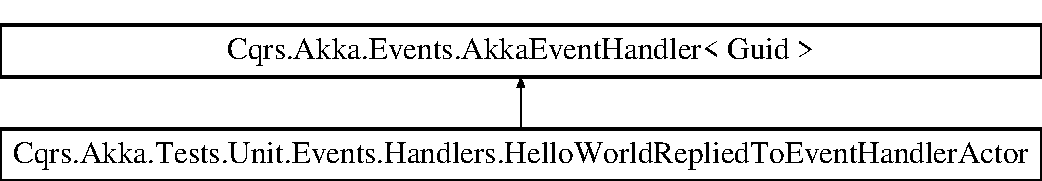
\includegraphics[height=2.000000cm]{classCqrs_1_1Akka_1_1Tests_1_1Unit_1_1Events_1_1Handlers_1_1HelloWorldRepliedToEventHandlerActor}
\end{center}
\end{figure}
\subsection*{Public Member Functions}
\begin{DoxyCompactItemize}
\item 
void \hyperlink{classCqrs_1_1Akka_1_1Tests_1_1Unit_1_1Events_1_1Handlers_1_1HelloWorldRepliedToEventHandlerActor_a9d843860260cd66f8354b9df234a1663_a9d843860260cd66f8354b9df234a1663}{Handle} (\hyperlink{classCqrs_1_1Akka_1_1Tests_1_1Unit_1_1Events_1_1HelloWorldRepliedTo}{Hello\+World\+Replied\+To} message)
\item 
\hyperlink{classCqrs_1_1Akka_1_1Tests_1_1Unit_1_1Events_1_1Handlers_1_1HelloWorldRepliedToEventHandlerActor_a174cd0183fbe16aaa74f18320e871a5f_a174cd0183fbe16aaa74f18320e871a5f}{Hello\+World\+Replied\+To\+Event\+Handler\+Actor} (I\+Logger logger, I\+Correlation\+Id\+Helper correlation\+Id\+Helper, \hyperlink{interfaceCqrs_1_1Authentication_1_1IAuthenticationTokenHelper}{I\+Authentication\+Token\+Helper}$<$ Guid $>$ authentication\+Token\+Helper)
\end{DoxyCompactItemize}
\subsection*{Additional Inherited Members}


\subsection{Constructor \& Destructor Documentation}
\mbox{\Hypertarget{classCqrs_1_1Akka_1_1Tests_1_1Unit_1_1Events_1_1Handlers_1_1HelloWorldRepliedToEventHandlerActor_a174cd0183fbe16aaa74f18320e871a5f_a174cd0183fbe16aaa74f18320e871a5f}\label{classCqrs_1_1Akka_1_1Tests_1_1Unit_1_1Events_1_1Handlers_1_1HelloWorldRepliedToEventHandlerActor_a174cd0183fbe16aaa74f18320e871a5f_a174cd0183fbe16aaa74f18320e871a5f}} 
\index{Cqrs\+::\+Akka\+::\+Tests\+::\+Unit\+::\+Events\+::\+Handlers\+::\+Hello\+World\+Replied\+To\+Event\+Handler\+Actor@{Cqrs\+::\+Akka\+::\+Tests\+::\+Unit\+::\+Events\+::\+Handlers\+::\+Hello\+World\+Replied\+To\+Event\+Handler\+Actor}!Hello\+World\+Replied\+To\+Event\+Handler\+Actor@{Hello\+World\+Replied\+To\+Event\+Handler\+Actor}}
\index{Hello\+World\+Replied\+To\+Event\+Handler\+Actor@{Hello\+World\+Replied\+To\+Event\+Handler\+Actor}!Cqrs\+::\+Akka\+::\+Tests\+::\+Unit\+::\+Events\+::\+Handlers\+::\+Hello\+World\+Replied\+To\+Event\+Handler\+Actor@{Cqrs\+::\+Akka\+::\+Tests\+::\+Unit\+::\+Events\+::\+Handlers\+::\+Hello\+World\+Replied\+To\+Event\+Handler\+Actor}}
\subsubsection{\texorpdfstring{Hello\+World\+Replied\+To\+Event\+Handler\+Actor()}{HelloWorldRepliedToEventHandlerActor()}}
{\footnotesize\ttfamily Cqrs.\+Akka.\+Tests.\+Unit.\+Events.\+Handlers.\+Hello\+World\+Replied\+To\+Event\+Handler\+Actor.\+Hello\+World\+Replied\+To\+Event\+Handler\+Actor (\begin{DoxyParamCaption}\item[{I\+Logger}]{logger,  }\item[{I\+Correlation\+Id\+Helper}]{correlation\+Id\+Helper,  }\item[{\hyperlink{interfaceCqrs_1_1Authentication_1_1IAuthenticationTokenHelper}{I\+Authentication\+Token\+Helper}$<$ Guid $>$}]{authentication\+Token\+Helper }\end{DoxyParamCaption})}



\subsection{Member Function Documentation}
\mbox{\Hypertarget{classCqrs_1_1Akka_1_1Tests_1_1Unit_1_1Events_1_1Handlers_1_1HelloWorldRepliedToEventHandlerActor_a9d843860260cd66f8354b9df234a1663_a9d843860260cd66f8354b9df234a1663}\label{classCqrs_1_1Akka_1_1Tests_1_1Unit_1_1Events_1_1Handlers_1_1HelloWorldRepliedToEventHandlerActor_a9d843860260cd66f8354b9df234a1663_a9d843860260cd66f8354b9df234a1663}} 
\index{Cqrs\+::\+Akka\+::\+Tests\+::\+Unit\+::\+Events\+::\+Handlers\+::\+Hello\+World\+Replied\+To\+Event\+Handler\+Actor@{Cqrs\+::\+Akka\+::\+Tests\+::\+Unit\+::\+Events\+::\+Handlers\+::\+Hello\+World\+Replied\+To\+Event\+Handler\+Actor}!Handle@{Handle}}
\index{Handle@{Handle}!Cqrs\+::\+Akka\+::\+Tests\+::\+Unit\+::\+Events\+::\+Handlers\+::\+Hello\+World\+Replied\+To\+Event\+Handler\+Actor@{Cqrs\+::\+Akka\+::\+Tests\+::\+Unit\+::\+Events\+::\+Handlers\+::\+Hello\+World\+Replied\+To\+Event\+Handler\+Actor}}
\subsubsection{\texorpdfstring{Handle()}{Handle()}}
{\footnotesize\ttfamily void Cqrs.\+Akka.\+Tests.\+Unit.\+Events.\+Handlers.\+Hello\+World\+Replied\+To\+Event\+Handler\+Actor.\+Handle (\begin{DoxyParamCaption}\item[{\hyperlink{classCqrs_1_1Akka_1_1Tests_1_1Unit_1_1Events_1_1HelloWorldRepliedTo}{Hello\+World\+Replied\+To}}]{message }\end{DoxyParamCaption})}


\hypertarget{classCqrs_1_1Akka_1_1Tests_1_1Unit_1_1Events_1_1Handlers_1_1HelloWorldRepliedToSendEndConversationCommandEventHandler}{}\section{Cqrs.\+Akka.\+Tests.\+Unit.\+Events.\+Handlers.\+Hello\+World\+Replied\+To\+Send\+End\+Conversation\+Command\+Event\+Handler Class Reference}
\label{classCqrs_1_1Akka_1_1Tests_1_1Unit_1_1Events_1_1Handlers_1_1HelloWorldRepliedToSendEndConversationCommandEventHandler}\index{Cqrs.\+Akka.\+Tests.\+Unit.\+Events.\+Handlers.\+Hello\+World\+Replied\+To\+Send\+End\+Conversation\+Command\+Event\+Handler@{Cqrs.\+Akka.\+Tests.\+Unit.\+Events.\+Handlers.\+Hello\+World\+Replied\+To\+Send\+End\+Conversation\+Command\+Event\+Handler}}
Inheritance diagram for Cqrs.\+Akka.\+Tests.\+Unit.\+Events.\+Handlers.\+Hello\+World\+Replied\+To\+Send\+End\+Conversation\+Command\+Event\+Handler\+:\begin{figure}[H]
\begin{center}
\leavevmode
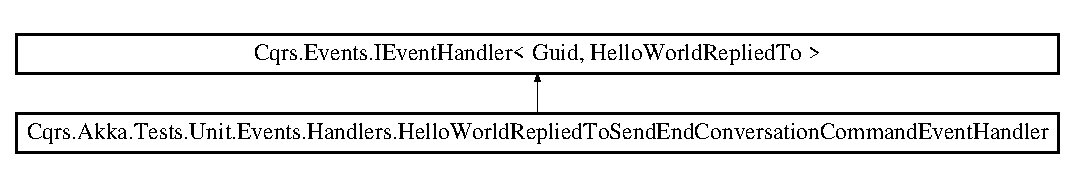
\includegraphics[height=1.827080cm]{classCqrs_1_1Akka_1_1Tests_1_1Unit_1_1Events_1_1Handlers_1_1HelloWorldRepliedToSendEndConversationCommandEventHandler}
\end{center}
\end{figure}
\subsection*{Classes}
\begin{DoxyCompactItemize}
\item 
class \hyperlink{classCqrs_1_1Akka_1_1Tests_1_1Unit_1_1Events_1_1Handlers_1_1HelloWorldRepliedToSendEndConversationCommandEventHandler_1_1Actor}{Actor}
\end{DoxyCompactItemize}
\subsection*{Public Member Functions}
\begin{DoxyCompactItemize}
\item 
\hyperlink{classCqrs_1_1Akka_1_1Tests_1_1Unit_1_1Events_1_1Handlers_1_1HelloWorldRepliedToSendEndConversationCommandEventHandler_a0befe6ff4cac9d9c4c6898320d4826ab_a0befe6ff4cac9d9c4c6898320d4826ab}{Hello\+World\+Replied\+To\+Send\+End\+Conversation\+Command\+Event\+Handler} (\hyperlink{interfaceCqrs_1_1Akka_1_1Domain_1_1IAkkaAggregateResolver}{I\+Akka\+Aggregate\+Resolver} aggregate\+Resolver)
\begin{DoxyCompactList}\small\item\em Instantiates the \hyperlink{classCqrs_1_1Akka_1_1Tests_1_1Unit_1_1Events_1_1Handlers_1_1HelloWorldRepliedToSendEndConversationCommandEventHandler}{Hello\+World\+Replied\+To\+Send\+End\+Conversation\+Command\+Event\+Handler} class registering any Receive\+Actor.\+Receive$<$\+T$>$(\+System.\+Func$<$\+T,\+System.\+Threading.\+Tasks.\+Task$>$) required. \end{DoxyCompactList}\item 
void \hyperlink{classCqrs_1_1Akka_1_1Tests_1_1Unit_1_1Events_1_1Handlers_1_1HelloWorldRepliedToSendEndConversationCommandEventHandler_af25c19f15c65e673f91eef4b1643c27f_af25c19f15c65e673f91eef4b1643c27f}{Handle} (\hyperlink{classCqrs_1_1Akka_1_1Tests_1_1Unit_1_1Events_1_1HelloWorldRepliedTo}{Hello\+World\+Replied\+To} @event)
\end{DoxyCompactItemize}
\subsection*{Properties}
\begin{DoxyCompactItemize}
\item 
\hyperlink{interfaceCqrs_1_1Akka_1_1Domain_1_1IAkkaAggregateResolver}{I\+Akka\+Aggregate\+Resolver} \hyperlink{classCqrs_1_1Akka_1_1Tests_1_1Unit_1_1Events_1_1Handlers_1_1HelloWorldRepliedToSendEndConversationCommandEventHandler_a627ab1180114304102fa7b11ab838fac_a627ab1180114304102fa7b11ab838fac}{Aggregate\+Resolver}\hspace{0.3cm}{\ttfamily  \mbox{[}get\mbox{]}}
\end{DoxyCompactItemize}


\subsection{Constructor \& Destructor Documentation}
\mbox{\Hypertarget{classCqrs_1_1Akka_1_1Tests_1_1Unit_1_1Events_1_1Handlers_1_1HelloWorldRepliedToSendEndConversationCommandEventHandler_a0befe6ff4cac9d9c4c6898320d4826ab_a0befe6ff4cac9d9c4c6898320d4826ab}\label{classCqrs_1_1Akka_1_1Tests_1_1Unit_1_1Events_1_1Handlers_1_1HelloWorldRepliedToSendEndConversationCommandEventHandler_a0befe6ff4cac9d9c4c6898320d4826ab_a0befe6ff4cac9d9c4c6898320d4826ab}} 
\index{Cqrs\+::\+Akka\+::\+Tests\+::\+Unit\+::\+Events\+::\+Handlers\+::\+Hello\+World\+Replied\+To\+Send\+End\+Conversation\+Command\+Event\+Handler@{Cqrs\+::\+Akka\+::\+Tests\+::\+Unit\+::\+Events\+::\+Handlers\+::\+Hello\+World\+Replied\+To\+Send\+End\+Conversation\+Command\+Event\+Handler}!Hello\+World\+Replied\+To\+Send\+End\+Conversation\+Command\+Event\+Handler@{Hello\+World\+Replied\+To\+Send\+End\+Conversation\+Command\+Event\+Handler}}
\index{Hello\+World\+Replied\+To\+Send\+End\+Conversation\+Command\+Event\+Handler@{Hello\+World\+Replied\+To\+Send\+End\+Conversation\+Command\+Event\+Handler}!Cqrs\+::\+Akka\+::\+Tests\+::\+Unit\+::\+Events\+::\+Handlers\+::\+Hello\+World\+Replied\+To\+Send\+End\+Conversation\+Command\+Event\+Handler@{Cqrs\+::\+Akka\+::\+Tests\+::\+Unit\+::\+Events\+::\+Handlers\+::\+Hello\+World\+Replied\+To\+Send\+End\+Conversation\+Command\+Event\+Handler}}
\subsubsection{\texorpdfstring{Hello\+World\+Replied\+To\+Send\+End\+Conversation\+Command\+Event\+Handler()}{HelloWorldRepliedToSendEndConversationCommandEventHandler()}}
{\footnotesize\ttfamily Cqrs.\+Akka.\+Tests.\+Unit.\+Events.\+Handlers.\+Hello\+World\+Replied\+To\+Send\+End\+Conversation\+Command\+Event\+Handler.\+Hello\+World\+Replied\+To\+Send\+End\+Conversation\+Command\+Event\+Handler (\begin{DoxyParamCaption}\item[{\hyperlink{interfaceCqrs_1_1Akka_1_1Domain_1_1IAkkaAggregateResolver}{I\+Akka\+Aggregate\+Resolver}}]{aggregate\+Resolver }\end{DoxyParamCaption})}



Instantiates the \hyperlink{classCqrs_1_1Akka_1_1Tests_1_1Unit_1_1Events_1_1Handlers_1_1HelloWorldRepliedToSendEndConversationCommandEventHandler}{Hello\+World\+Replied\+To\+Send\+End\+Conversation\+Command\+Event\+Handler} class registering any Receive\+Actor.\+Receive$<$\+T$>$(\+System.\+Func$<$\+T,\+System.\+Threading.\+Tasks.\+Task$>$) required. 



\subsection{Member Function Documentation}
\mbox{\Hypertarget{classCqrs_1_1Akka_1_1Tests_1_1Unit_1_1Events_1_1Handlers_1_1HelloWorldRepliedToSendEndConversationCommandEventHandler_af25c19f15c65e673f91eef4b1643c27f_af25c19f15c65e673f91eef4b1643c27f}\label{classCqrs_1_1Akka_1_1Tests_1_1Unit_1_1Events_1_1Handlers_1_1HelloWorldRepliedToSendEndConversationCommandEventHandler_af25c19f15c65e673f91eef4b1643c27f_af25c19f15c65e673f91eef4b1643c27f}} 
\index{Cqrs\+::\+Akka\+::\+Tests\+::\+Unit\+::\+Events\+::\+Handlers\+::\+Hello\+World\+Replied\+To\+Send\+End\+Conversation\+Command\+Event\+Handler@{Cqrs\+::\+Akka\+::\+Tests\+::\+Unit\+::\+Events\+::\+Handlers\+::\+Hello\+World\+Replied\+To\+Send\+End\+Conversation\+Command\+Event\+Handler}!Handle@{Handle}}
\index{Handle@{Handle}!Cqrs\+::\+Akka\+::\+Tests\+::\+Unit\+::\+Events\+::\+Handlers\+::\+Hello\+World\+Replied\+To\+Send\+End\+Conversation\+Command\+Event\+Handler@{Cqrs\+::\+Akka\+::\+Tests\+::\+Unit\+::\+Events\+::\+Handlers\+::\+Hello\+World\+Replied\+To\+Send\+End\+Conversation\+Command\+Event\+Handler}}
\subsubsection{\texorpdfstring{Handle()}{Handle()}}
{\footnotesize\ttfamily void Cqrs.\+Akka.\+Tests.\+Unit.\+Events.\+Handlers.\+Hello\+World\+Replied\+To\+Send\+End\+Conversation\+Command\+Event\+Handler.\+Handle (\begin{DoxyParamCaption}\item[{\hyperlink{classCqrs_1_1Akka_1_1Tests_1_1Unit_1_1Events_1_1HelloWorldRepliedTo}{Hello\+World\+Replied\+To} @}]{event }\end{DoxyParamCaption})}



\subsection{Property Documentation}
\mbox{\Hypertarget{classCqrs_1_1Akka_1_1Tests_1_1Unit_1_1Events_1_1Handlers_1_1HelloWorldRepliedToSendEndConversationCommandEventHandler_a627ab1180114304102fa7b11ab838fac_a627ab1180114304102fa7b11ab838fac}\label{classCqrs_1_1Akka_1_1Tests_1_1Unit_1_1Events_1_1Handlers_1_1HelloWorldRepliedToSendEndConversationCommandEventHandler_a627ab1180114304102fa7b11ab838fac_a627ab1180114304102fa7b11ab838fac}} 
\index{Cqrs\+::\+Akka\+::\+Tests\+::\+Unit\+::\+Events\+::\+Handlers\+::\+Hello\+World\+Replied\+To\+Send\+End\+Conversation\+Command\+Event\+Handler@{Cqrs\+::\+Akka\+::\+Tests\+::\+Unit\+::\+Events\+::\+Handlers\+::\+Hello\+World\+Replied\+To\+Send\+End\+Conversation\+Command\+Event\+Handler}!Aggregate\+Resolver@{Aggregate\+Resolver}}
\index{Aggregate\+Resolver@{Aggregate\+Resolver}!Cqrs\+::\+Akka\+::\+Tests\+::\+Unit\+::\+Events\+::\+Handlers\+::\+Hello\+World\+Replied\+To\+Send\+End\+Conversation\+Command\+Event\+Handler@{Cqrs\+::\+Akka\+::\+Tests\+::\+Unit\+::\+Events\+::\+Handlers\+::\+Hello\+World\+Replied\+To\+Send\+End\+Conversation\+Command\+Event\+Handler}}
\subsubsection{\texorpdfstring{Aggregate\+Resolver}{AggregateResolver}}
{\footnotesize\ttfamily \hyperlink{interfaceCqrs_1_1Akka_1_1Domain_1_1IAkkaAggregateResolver}{I\+Akka\+Aggregate\+Resolver} Cqrs.\+Akka.\+Tests.\+Unit.\+Events.\+Handlers.\+Hello\+World\+Replied\+To\+Send\+End\+Conversation\+Command\+Event\+Handler.\+Aggregate\+Resolver\hspace{0.3cm}{\ttfamily [get]}, {\ttfamily [protected]}}


\hypertarget{classCqrs_1_1Akka_1_1Tests_1_1Unit_1_1Events_1_1Handlers_1_1HelloWorldRepliedToSendEndConversationCommandEventHandler_1_1Actor}{}\doxysection{Cqrs.\+Akka.\+Tests.\+Unit.\+Events.\+Handlers.\+Hello\+World\+Replied\+To\+Send\+End\+Conversation\+Command\+Event\+Handler.\+Actor Class Reference}
\label{classCqrs_1_1Akka_1_1Tests_1_1Unit_1_1Events_1_1Handlers_1_1HelloWorldRepliedToSendEndConversationCommandEventHandler_1_1Actor}\index{Cqrs.Akka.Tests.Unit.Events.Handlers.HelloWorldRepliedToSendEndConversationCommandEventHandler.Actor@{Cqrs.Akka.Tests.Unit.Events.Handlers.HelloWorldRepliedToSendEndConversationCommandEventHandler.Actor}}


An Akka.\+Net based I\+Event\+Handler that handles the \mbox{\hyperlink{classCqrs_1_1Akka_1_1Tests_1_1Unit_1_1Events_1_1HelloWorldRepliedTo}{Hello\+World\+Replied\+To}}.  


Inheritance diagram for Cqrs.\+Akka.\+Tests.\+Unit.\+Events.\+Handlers.\+Hello\+World\+Replied\+To\+Send\+End\+Conversation\+Command\+Event\+Handler.\+Actor\+:\begin{figure}[H]
\begin{center}
\leavevmode
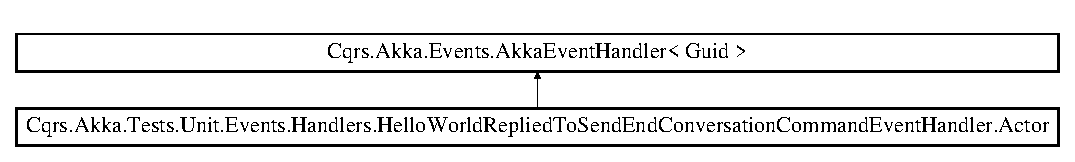
\includegraphics[height=1.728395cm]{classCqrs_1_1Akka_1_1Tests_1_1Unit_1_1Events_1_1Handlers_1_1HelloWorldRepliedToSendEndConversationCommandEventHandler_1_1Actor}
\end{center}
\end{figure}
\doxysubsection*{Public Member Functions}
\begin{DoxyCompactItemize}
\item 
void \mbox{\hyperlink{classCqrs_1_1Akka_1_1Tests_1_1Unit_1_1Events_1_1Handlers_1_1HelloWorldRepliedToSendEndConversationCommandEventHandler_1_1Actor_a76a10208a1b9e3f81a36c48bc6b751eb_a76a10208a1b9e3f81a36c48bc6b751eb}{Handle}} (\mbox{\hyperlink{classCqrs_1_1Akka_1_1Tests_1_1Unit_1_1Events_1_1HelloWorldRepliedTo}{Hello\+World\+Replied\+To}} message)
\begin{DoxyCompactList}\small\item\em Responds to the provided {\itshape message} . \end{DoxyCompactList}\item 
\mbox{\hyperlink{classCqrs_1_1Akka_1_1Tests_1_1Unit_1_1Events_1_1Handlers_1_1HelloWorldRepliedToSendEndConversationCommandEventHandler_1_1Actor_a10cd8c5ff7e2ee041ab26aad766b0857_a10cd8c5ff7e2ee041ab26aad766b0857}{Actor}} (I\+Logger logger, I\+Correlation\+Id\+Helper correlation\+Id\+Helper, \mbox{\hyperlink{interfaceCqrs_1_1Authentication_1_1IAuthenticationTokenHelper}{I\+Authentication\+Token\+Helper}}$<$ Guid $>$ authentication\+Token\+Helper, \mbox{\hyperlink{interfaceCqrs_1_1Akka_1_1Commands_1_1IAkkaCommandPublisher}{I\+Akka\+Command\+Publisher}}$<$ Guid $>$ command\+Bus)
\begin{DoxyCompactList}\small\item\em Instantiates a new instance of \mbox{\hyperlink{classCqrs_1_1Akka_1_1Tests_1_1Unit_1_1Events_1_1Handlers_1_1HelloWorldRepliedToSendEndConversationCommandEventHandler_1_1Actor}{Actor}}. \end{DoxyCompactList}\end{DoxyCompactItemize}
\doxysubsection*{Properties}
\begin{DoxyCompactItemize}
\item 
\mbox{\hyperlink{interfaceCqrs_1_1Commands_1_1ICommandPublisher}{I\+Command\+Publisher}}$<$ Guid $>$ \mbox{\hyperlink{classCqrs_1_1Akka_1_1Tests_1_1Unit_1_1Events_1_1Handlers_1_1HelloWorldRepliedToSendEndConversationCommandEventHandler_1_1Actor_ab31bff19e0665a0f5057ba508d874cff_ab31bff19e0665a0f5057ba508d874cff}{Command\+Bus}}\hspace{0.3cm}{\ttfamily  \mbox{[}get\mbox{]}}
\begin{DoxyCompactList}\small\item\em Publish any I\+Command$<$\+T\+Authentication\+Token$>$ instances that you want to send with this. \end{DoxyCompactList}\end{DoxyCompactItemize}
\doxysubsection*{Additional Inherited Members}


\doxysubsection{Detailed Description}
An Akka.\+Net based I\+Event\+Handler that handles the \mbox{\hyperlink{classCqrs_1_1Akka_1_1Tests_1_1Unit_1_1Events_1_1HelloWorldRepliedTo}{Hello\+World\+Replied\+To}}. 



\doxysubsection{Constructor \& Destructor Documentation}
\mbox{\Hypertarget{classCqrs_1_1Akka_1_1Tests_1_1Unit_1_1Events_1_1Handlers_1_1HelloWorldRepliedToSendEndConversationCommandEventHandler_1_1Actor_a10cd8c5ff7e2ee041ab26aad766b0857_a10cd8c5ff7e2ee041ab26aad766b0857}\label{classCqrs_1_1Akka_1_1Tests_1_1Unit_1_1Events_1_1Handlers_1_1HelloWorldRepliedToSendEndConversationCommandEventHandler_1_1Actor_a10cd8c5ff7e2ee041ab26aad766b0857_a10cd8c5ff7e2ee041ab26aad766b0857}} 
\index{Cqrs.Akka.Tests.Unit.Events.Handlers.HelloWorldRepliedToSendEndConversationCommandEventHandler.Actor@{Cqrs.Akka.Tests.Unit.Events.Handlers.HelloWorldRepliedToSendEndConversationCommandEventHandler.Actor}!Actor@{Actor}}
\index{Actor@{Actor}!Cqrs.Akka.Tests.Unit.Events.Handlers.HelloWorldRepliedToSendEndConversationCommandEventHandler.Actor@{Cqrs.Akka.Tests.Unit.Events.Handlers.HelloWorldRepliedToSendEndConversationCommandEventHandler.Actor}}
\doxysubsubsection{\texorpdfstring{Actor()}{Actor()}}
{\footnotesize\ttfamily Cqrs.\+Akka.\+Tests.\+Unit.\+Events.\+Handlers.\+Hello\+World\+Replied\+To\+Send\+End\+Conversation\+Command\+Event\+Handler.\+Actor.\+Actor (\begin{DoxyParamCaption}\item[{I\+Logger}]{logger,  }\item[{I\+Correlation\+Id\+Helper}]{correlation\+Id\+Helper,  }\item[{\mbox{\hyperlink{interfaceCqrs_1_1Authentication_1_1IAuthenticationTokenHelper}{I\+Authentication\+Token\+Helper}}$<$ Guid $>$}]{authentication\+Token\+Helper,  }\item[{\mbox{\hyperlink{interfaceCqrs_1_1Akka_1_1Commands_1_1IAkkaCommandPublisher}{I\+Akka\+Command\+Publisher}}$<$ Guid $>$}]{command\+Bus }\end{DoxyParamCaption})}



Instantiates a new instance of \mbox{\hyperlink{classCqrs_1_1Akka_1_1Tests_1_1Unit_1_1Events_1_1Handlers_1_1HelloWorldRepliedToSendEndConversationCommandEventHandler_1_1Actor}{Actor}}. 



\doxysubsection{Member Function Documentation}
\mbox{\Hypertarget{classCqrs_1_1Akka_1_1Tests_1_1Unit_1_1Events_1_1Handlers_1_1HelloWorldRepliedToSendEndConversationCommandEventHandler_1_1Actor_a76a10208a1b9e3f81a36c48bc6b751eb_a76a10208a1b9e3f81a36c48bc6b751eb}\label{classCqrs_1_1Akka_1_1Tests_1_1Unit_1_1Events_1_1Handlers_1_1HelloWorldRepliedToSendEndConversationCommandEventHandler_1_1Actor_a76a10208a1b9e3f81a36c48bc6b751eb_a76a10208a1b9e3f81a36c48bc6b751eb}} 
\index{Cqrs.Akka.Tests.Unit.Events.Handlers.HelloWorldRepliedToSendEndConversationCommandEventHandler.Actor@{Cqrs.Akka.Tests.Unit.Events.Handlers.HelloWorldRepliedToSendEndConversationCommandEventHandler.Actor}!Handle@{Handle}}
\index{Handle@{Handle}!Cqrs.Akka.Tests.Unit.Events.Handlers.HelloWorldRepliedToSendEndConversationCommandEventHandler.Actor@{Cqrs.Akka.Tests.Unit.Events.Handlers.HelloWorldRepliedToSendEndConversationCommandEventHandler.Actor}}
\doxysubsubsection{\texorpdfstring{Handle()}{Handle()}}
{\footnotesize\ttfamily void Cqrs.\+Akka.\+Tests.\+Unit.\+Events.\+Handlers.\+Hello\+World\+Replied\+To\+Send\+End\+Conversation\+Command\+Event\+Handler.\+Actor.\+Handle (\begin{DoxyParamCaption}\item[{\mbox{\hyperlink{classCqrs_1_1Akka_1_1Tests_1_1Unit_1_1Events_1_1HelloWorldRepliedTo}{Hello\+World\+Replied\+To}}}]{message }\end{DoxyParamCaption})}



Responds to the provided {\itshape message} . 


\begin{DoxyParams}{Parameters}
{\em message} & The \mbox{\hyperlink{classCqrs_1_1Akka_1_1Tests_1_1Unit_1_1Events_1_1HelloWorldRepliedTo}{Hello\+World\+Replied\+To}} to respond to or \char`\"{}handle\char`\"{}\\
\hline
\end{DoxyParams}


\doxysubsection{Property Documentation}
\mbox{\Hypertarget{classCqrs_1_1Akka_1_1Tests_1_1Unit_1_1Events_1_1Handlers_1_1HelloWorldRepliedToSendEndConversationCommandEventHandler_1_1Actor_ab31bff19e0665a0f5057ba508d874cff_ab31bff19e0665a0f5057ba508d874cff}\label{classCqrs_1_1Akka_1_1Tests_1_1Unit_1_1Events_1_1Handlers_1_1HelloWorldRepliedToSendEndConversationCommandEventHandler_1_1Actor_ab31bff19e0665a0f5057ba508d874cff_ab31bff19e0665a0f5057ba508d874cff}} 
\index{Cqrs.Akka.Tests.Unit.Events.Handlers.HelloWorldRepliedToSendEndConversationCommandEventHandler.Actor@{Cqrs.Akka.Tests.Unit.Events.Handlers.HelloWorldRepliedToSendEndConversationCommandEventHandler.Actor}!CommandBus@{CommandBus}}
\index{CommandBus@{CommandBus}!Cqrs.Akka.Tests.Unit.Events.Handlers.HelloWorldRepliedToSendEndConversationCommandEventHandler.Actor@{Cqrs.Akka.Tests.Unit.Events.Handlers.HelloWorldRepliedToSendEndConversationCommandEventHandler.Actor}}
\doxysubsubsection{\texorpdfstring{CommandBus}{CommandBus}}
{\footnotesize\ttfamily \mbox{\hyperlink{interfaceCqrs_1_1Commands_1_1ICommandPublisher}{I\+Command\+Publisher}}$<$Guid$>$ Cqrs.\+Akka.\+Tests.\+Unit.\+Events.\+Handlers.\+Hello\+World\+Replied\+To\+Send\+End\+Conversation\+Command\+Event\+Handler.\+Actor.\+Command\+Bus\hspace{0.3cm}{\ttfamily [get]}, {\ttfamily [protected]}}



Publish any I\+Command$<$\+T\+Authentication\+Token$>$ instances that you want to send with this. 


\hypertarget{classCqrs_1_1Akka_1_1Tests_1_1Unit_1_1Events_1_1Handlers_1_1HelloWorldSaidEventHandler}{}\section{Cqrs.\+Akka.\+Tests.\+Unit.\+Events.\+Handlers.\+Hello\+World\+Said\+Event\+Handler Class Reference}
\label{classCqrs_1_1Akka_1_1Tests_1_1Unit_1_1Events_1_1Handlers_1_1HelloWorldSaidEventHandler}\index{Cqrs.\+Akka.\+Tests.\+Unit.\+Events.\+Handlers.\+Hello\+World\+Said\+Event\+Handler@{Cqrs.\+Akka.\+Tests.\+Unit.\+Events.\+Handlers.\+Hello\+World\+Said\+Event\+Handler}}
Inheritance diagram for Cqrs.\+Akka.\+Tests.\+Unit.\+Events.\+Handlers.\+Hello\+World\+Said\+Event\+Handler\+:\begin{figure}[H]
\begin{center}
\leavevmode
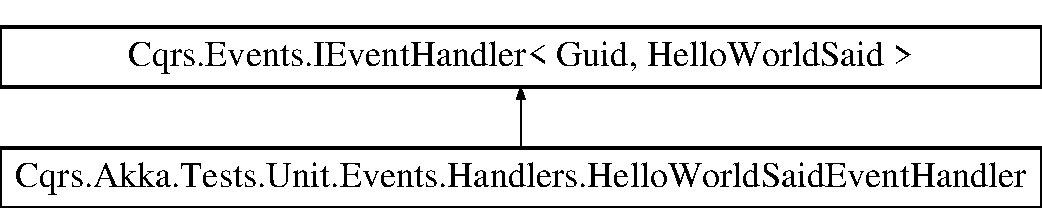
\includegraphics[height=2.000000cm]{classCqrs_1_1Akka_1_1Tests_1_1Unit_1_1Events_1_1Handlers_1_1HelloWorldSaidEventHandler}
\end{center}
\end{figure}
\subsection*{Public Member Functions}
\begin{DoxyCompactItemize}
\item 
\hyperlink{classCqrs_1_1Akka_1_1Tests_1_1Unit_1_1Events_1_1Handlers_1_1HelloWorldSaidEventHandler_a8bde891341691d7d73f4cb28f2568335_a8bde891341691d7d73f4cb28f2568335}{Hello\+World\+Said\+Event\+Handler} (\hyperlink{interfaceCqrs_1_1Akka_1_1Commands_1_1IAkkaCommandPublisher}{I\+Akka\+Command\+Publisher}$<$ Guid $>$ command\+Bus)
\item 
void \hyperlink{classCqrs_1_1Akka_1_1Tests_1_1Unit_1_1Events_1_1Handlers_1_1HelloWorldSaidEventHandler_accb924e5856731b18120c21daed0f52a_accb924e5856731b18120c21daed0f52a}{Handle} (\hyperlink{classCqrs_1_1Akka_1_1Tests_1_1Unit_1_1Events_1_1HelloWorldSaid}{Hello\+World\+Said} message)
\end{DoxyCompactItemize}
\subsection*{Properties}
\begin{DoxyCompactItemize}
\item 
\hyperlink{interfaceCqrs_1_1Commands_1_1ICommandPublisher}{I\+Command\+Publisher}$<$ Guid $>$ \hyperlink{classCqrs_1_1Akka_1_1Tests_1_1Unit_1_1Events_1_1Handlers_1_1HelloWorldSaidEventHandler_a67473b7f3dc275d04fe079006da89f6c_a67473b7f3dc275d04fe079006da89f6c}{Command\+Bus}\hspace{0.3cm}{\ttfamily  \mbox{[}get\mbox{]}}
\end{DoxyCompactItemize}


\subsection{Constructor \& Destructor Documentation}
\mbox{\Hypertarget{classCqrs_1_1Akka_1_1Tests_1_1Unit_1_1Events_1_1Handlers_1_1HelloWorldSaidEventHandler_a8bde891341691d7d73f4cb28f2568335_a8bde891341691d7d73f4cb28f2568335}\label{classCqrs_1_1Akka_1_1Tests_1_1Unit_1_1Events_1_1Handlers_1_1HelloWorldSaidEventHandler_a8bde891341691d7d73f4cb28f2568335_a8bde891341691d7d73f4cb28f2568335}} 
\index{Cqrs\+::\+Akka\+::\+Tests\+::\+Unit\+::\+Events\+::\+Handlers\+::\+Hello\+World\+Said\+Event\+Handler@{Cqrs\+::\+Akka\+::\+Tests\+::\+Unit\+::\+Events\+::\+Handlers\+::\+Hello\+World\+Said\+Event\+Handler}!Hello\+World\+Said\+Event\+Handler@{Hello\+World\+Said\+Event\+Handler}}
\index{Hello\+World\+Said\+Event\+Handler@{Hello\+World\+Said\+Event\+Handler}!Cqrs\+::\+Akka\+::\+Tests\+::\+Unit\+::\+Events\+::\+Handlers\+::\+Hello\+World\+Said\+Event\+Handler@{Cqrs\+::\+Akka\+::\+Tests\+::\+Unit\+::\+Events\+::\+Handlers\+::\+Hello\+World\+Said\+Event\+Handler}}
\subsubsection{\texorpdfstring{Hello\+World\+Said\+Event\+Handler()}{HelloWorldSaidEventHandler()}}
{\footnotesize\ttfamily Cqrs.\+Akka.\+Tests.\+Unit.\+Events.\+Handlers.\+Hello\+World\+Said\+Event\+Handler.\+Hello\+World\+Said\+Event\+Handler (\begin{DoxyParamCaption}\item[{\hyperlink{interfaceCqrs_1_1Akka_1_1Commands_1_1IAkkaCommandPublisher}{I\+Akka\+Command\+Publisher}$<$ Guid $>$}]{command\+Bus }\end{DoxyParamCaption})}



\subsection{Member Function Documentation}
\mbox{\Hypertarget{classCqrs_1_1Akka_1_1Tests_1_1Unit_1_1Events_1_1Handlers_1_1HelloWorldSaidEventHandler_accb924e5856731b18120c21daed0f52a_accb924e5856731b18120c21daed0f52a}\label{classCqrs_1_1Akka_1_1Tests_1_1Unit_1_1Events_1_1Handlers_1_1HelloWorldSaidEventHandler_accb924e5856731b18120c21daed0f52a_accb924e5856731b18120c21daed0f52a}} 
\index{Cqrs\+::\+Akka\+::\+Tests\+::\+Unit\+::\+Events\+::\+Handlers\+::\+Hello\+World\+Said\+Event\+Handler@{Cqrs\+::\+Akka\+::\+Tests\+::\+Unit\+::\+Events\+::\+Handlers\+::\+Hello\+World\+Said\+Event\+Handler}!Handle@{Handle}}
\index{Handle@{Handle}!Cqrs\+::\+Akka\+::\+Tests\+::\+Unit\+::\+Events\+::\+Handlers\+::\+Hello\+World\+Said\+Event\+Handler@{Cqrs\+::\+Akka\+::\+Tests\+::\+Unit\+::\+Events\+::\+Handlers\+::\+Hello\+World\+Said\+Event\+Handler}}
\subsubsection{\texorpdfstring{Handle()}{Handle()}}
{\footnotesize\ttfamily void Cqrs.\+Akka.\+Tests.\+Unit.\+Events.\+Handlers.\+Hello\+World\+Said\+Event\+Handler.\+Handle (\begin{DoxyParamCaption}\item[{\hyperlink{classCqrs_1_1Akka_1_1Tests_1_1Unit_1_1Events_1_1HelloWorldSaid}{Hello\+World\+Said}}]{message }\end{DoxyParamCaption})}



\subsection{Property Documentation}
\mbox{\Hypertarget{classCqrs_1_1Akka_1_1Tests_1_1Unit_1_1Events_1_1Handlers_1_1HelloWorldSaidEventHandler_a67473b7f3dc275d04fe079006da89f6c_a67473b7f3dc275d04fe079006da89f6c}\label{classCqrs_1_1Akka_1_1Tests_1_1Unit_1_1Events_1_1Handlers_1_1HelloWorldSaidEventHandler_a67473b7f3dc275d04fe079006da89f6c_a67473b7f3dc275d04fe079006da89f6c}} 
\index{Cqrs\+::\+Akka\+::\+Tests\+::\+Unit\+::\+Events\+::\+Handlers\+::\+Hello\+World\+Said\+Event\+Handler@{Cqrs\+::\+Akka\+::\+Tests\+::\+Unit\+::\+Events\+::\+Handlers\+::\+Hello\+World\+Said\+Event\+Handler}!Command\+Bus@{Command\+Bus}}
\index{Command\+Bus@{Command\+Bus}!Cqrs\+::\+Akka\+::\+Tests\+::\+Unit\+::\+Events\+::\+Handlers\+::\+Hello\+World\+Said\+Event\+Handler@{Cqrs\+::\+Akka\+::\+Tests\+::\+Unit\+::\+Events\+::\+Handlers\+::\+Hello\+World\+Said\+Event\+Handler}}
\subsubsection{\texorpdfstring{Command\+Bus}{CommandBus}}
{\footnotesize\ttfamily \hyperlink{interfaceCqrs_1_1Commands_1_1ICommandPublisher}{I\+Command\+Publisher}$<$Guid$>$ Cqrs.\+Akka.\+Tests.\+Unit.\+Events.\+Handlers.\+Hello\+World\+Said\+Event\+Handler.\+Command\+Bus\hspace{0.3cm}{\ttfamily [get]}, {\ttfamily [protected]}}


\hypertarget{classCqrs_1_1Akka_1_1Tests_1_1Unit_1_1Events_1_1HelloWorldRepliedTo}{}\section{Cqrs.\+Akka.\+Tests.\+Unit.\+Events.\+Hello\+World\+Replied\+To Class Reference}
\label{classCqrs_1_1Akka_1_1Tests_1_1Unit_1_1Events_1_1HelloWorldRepliedTo}\index{Cqrs.\+Akka.\+Tests.\+Unit.\+Events.\+Hello\+World\+Replied\+To@{Cqrs.\+Akka.\+Tests.\+Unit.\+Events.\+Hello\+World\+Replied\+To}}


Someone replied to someone saying \char`\"{}\+Hello\+World\char`\"{}  


Inheritance diagram for Cqrs.\+Akka.\+Tests.\+Unit.\+Events.\+Hello\+World\+Replied\+To\+:\begin{figure}[H]
\begin{center}
\leavevmode
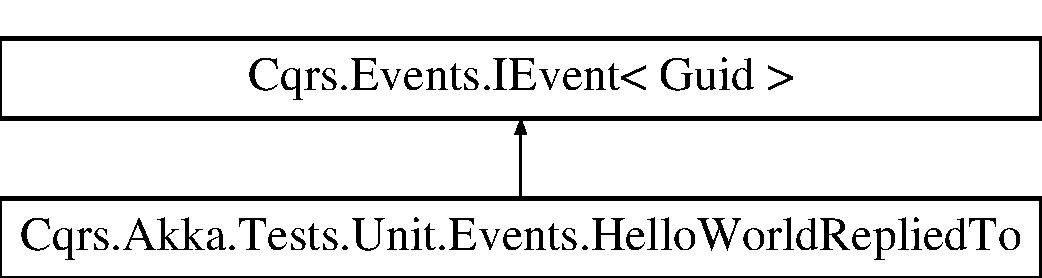
\includegraphics[height=2.000000cm]{classCqrs_1_1Akka_1_1Tests_1_1Unit_1_1Events_1_1HelloWorldRepliedTo}
\end{center}
\end{figure}
\subsection*{Properties}
\begin{DoxyCompactItemize}
\item 
Guid \hyperlink{classCqrs_1_1Akka_1_1Tests_1_1Unit_1_1Events_1_1HelloWorldRepliedTo_ae2bfc25a00d6e3c2e4dcbdee7fc44566_ae2bfc25a00d6e3c2e4dcbdee7fc44566}{Correlation\+Id}\hspace{0.3cm}{\ttfamily  \mbox{[}get, set\mbox{]}}
\begin{DoxyCompactList}\small\item\em An identifier used to group together several I\+Message. Any I\+Message with the same \hyperlink{classCqrs_1_1Akka_1_1Tests_1_1Unit_1_1Events_1_1HelloWorldRepliedTo_ae2bfc25a00d6e3c2e4dcbdee7fc44566_ae2bfc25a00d6e3c2e4dcbdee7fc44566}{Correlation\+Id} were triggered by the same initiating request. \end{DoxyCompactList}\item 
string \hyperlink{classCqrs_1_1Akka_1_1Tests_1_1Unit_1_1Events_1_1HelloWorldRepliedTo_aaf5282640ef632abbeb3c4ca733bcdbe_aaf5282640ef632abbeb3c4ca733bcdbe}{Originating\+Framework}\hspace{0.3cm}{\ttfamily  \mbox{[}get, set\mbox{]}}
\begin{DoxyCompactList}\small\item\em The originating framework this message was sent from. \end{DoxyCompactList}\item 
I\+Enumerable$<$ string $>$ \hyperlink{classCqrs_1_1Akka_1_1Tests_1_1Unit_1_1Events_1_1HelloWorldRepliedTo_ab73af51aaa23b6daa313c5f7a4aac3a5_ab73af51aaa23b6daa313c5f7a4aac3a5}{Frameworks}\hspace{0.3cm}{\ttfamily  \mbox{[}get, set\mbox{]}}
\begin{DoxyCompactList}\small\item\em The frameworks this I\+Message has been delivered to/sent via already. \end{DoxyCompactList}\item 
Guid \hyperlink{classCqrs_1_1Akka_1_1Tests_1_1Unit_1_1Events_1_1HelloWorldRepliedTo_a56fdfd09a1c8cf03014600c5d8bf05a9_a56fdfd09a1c8cf03014600c5d8bf05a9}{Authentication\+Token}\hspace{0.3cm}{\ttfamily  \mbox{[}get, set\mbox{]}}
\begin{DoxyCompactList}\small\item\em The authentication token of the entity that triggered the event to be raised. \end{DoxyCompactList}\item 
Guid \hyperlink{classCqrs_1_1Akka_1_1Tests_1_1Unit_1_1Events_1_1HelloWorldRepliedTo_aadfa9ba9616838db069eaff18b099efe_aadfa9ba9616838db069eaff18b099efe}{Id}\hspace{0.3cm}{\ttfamily  \mbox{[}get, set\mbox{]}}
\begin{DoxyCompactList}\small\item\em The ID of the I\+Event$<$\+T\+Authentication\+Token$>$ \end{DoxyCompactList}\item 
int \hyperlink{classCqrs_1_1Akka_1_1Tests_1_1Unit_1_1Events_1_1HelloWorldRepliedTo_a50283ab59b37c6baf5f80625ade780f0_a50283ab59b37c6baf5f80625ade780f0}{Version}\hspace{0.3cm}{\ttfamily  \mbox{[}get, set\mbox{]}}
\begin{DoxyCompactList}\small\item\em The version of the I\+Event$<$\+T\+Authentication\+Token$>$ \end{DoxyCompactList}\item 
Date\+Time\+Offset \hyperlink{classCqrs_1_1Akka_1_1Tests_1_1Unit_1_1Events_1_1HelloWorldRepliedTo_a74cd7b24e40d7854b9904e085ffdbb45_a74cd7b24e40d7854b9904e085ffdbb45}{Time\+Stamp}\hspace{0.3cm}{\ttfamily  \mbox{[}get, set\mbox{]}}
\begin{DoxyCompactList}\small\item\em The date and time the event was raised or published. \end{DoxyCompactList}\end{DoxyCompactItemize}


\subsection{Detailed Description}
Someone replied to someone saying \char`\"{}\+Hello\+World\char`\"{} 



\subsection{Property Documentation}
\mbox{\Hypertarget{classCqrs_1_1Akka_1_1Tests_1_1Unit_1_1Events_1_1HelloWorldRepliedTo_a56fdfd09a1c8cf03014600c5d8bf05a9_a56fdfd09a1c8cf03014600c5d8bf05a9}\label{classCqrs_1_1Akka_1_1Tests_1_1Unit_1_1Events_1_1HelloWorldRepliedTo_a56fdfd09a1c8cf03014600c5d8bf05a9_a56fdfd09a1c8cf03014600c5d8bf05a9}} 
\index{Cqrs\+::\+Akka\+::\+Tests\+::\+Unit\+::\+Events\+::\+Hello\+World\+Replied\+To@{Cqrs\+::\+Akka\+::\+Tests\+::\+Unit\+::\+Events\+::\+Hello\+World\+Replied\+To}!Authentication\+Token@{Authentication\+Token}}
\index{Authentication\+Token@{Authentication\+Token}!Cqrs\+::\+Akka\+::\+Tests\+::\+Unit\+::\+Events\+::\+Hello\+World\+Replied\+To@{Cqrs\+::\+Akka\+::\+Tests\+::\+Unit\+::\+Events\+::\+Hello\+World\+Replied\+To}}
\subsubsection{\texorpdfstring{Authentication\+Token}{AuthenticationToken}}
{\footnotesize\ttfamily Guid Cqrs.\+Akka.\+Tests.\+Unit.\+Events.\+Hello\+World\+Replied\+To.\+Authentication\+Token\hspace{0.3cm}{\ttfamily [get]}, {\ttfamily [set]}}



The authentication token of the entity that triggered the event to be raised. 

\mbox{\Hypertarget{classCqrs_1_1Akka_1_1Tests_1_1Unit_1_1Events_1_1HelloWorldRepliedTo_ae2bfc25a00d6e3c2e4dcbdee7fc44566_ae2bfc25a00d6e3c2e4dcbdee7fc44566}\label{classCqrs_1_1Akka_1_1Tests_1_1Unit_1_1Events_1_1HelloWorldRepliedTo_ae2bfc25a00d6e3c2e4dcbdee7fc44566_ae2bfc25a00d6e3c2e4dcbdee7fc44566}} 
\index{Cqrs\+::\+Akka\+::\+Tests\+::\+Unit\+::\+Events\+::\+Hello\+World\+Replied\+To@{Cqrs\+::\+Akka\+::\+Tests\+::\+Unit\+::\+Events\+::\+Hello\+World\+Replied\+To}!Correlation\+Id@{Correlation\+Id}}
\index{Correlation\+Id@{Correlation\+Id}!Cqrs\+::\+Akka\+::\+Tests\+::\+Unit\+::\+Events\+::\+Hello\+World\+Replied\+To@{Cqrs\+::\+Akka\+::\+Tests\+::\+Unit\+::\+Events\+::\+Hello\+World\+Replied\+To}}
\subsubsection{\texorpdfstring{Correlation\+Id}{CorrelationId}}
{\footnotesize\ttfamily Guid Cqrs.\+Akka.\+Tests.\+Unit.\+Events.\+Hello\+World\+Replied\+To.\+Correlation\+Id\hspace{0.3cm}{\ttfamily [get]}, {\ttfamily [set]}}



An identifier used to group together several I\+Message. Any I\+Message with the same \hyperlink{classCqrs_1_1Akka_1_1Tests_1_1Unit_1_1Events_1_1HelloWorldRepliedTo_ae2bfc25a00d6e3c2e4dcbdee7fc44566_ae2bfc25a00d6e3c2e4dcbdee7fc44566}{Correlation\+Id} were triggered by the same initiating request. 

\mbox{\Hypertarget{classCqrs_1_1Akka_1_1Tests_1_1Unit_1_1Events_1_1HelloWorldRepliedTo_ab73af51aaa23b6daa313c5f7a4aac3a5_ab73af51aaa23b6daa313c5f7a4aac3a5}\label{classCqrs_1_1Akka_1_1Tests_1_1Unit_1_1Events_1_1HelloWorldRepliedTo_ab73af51aaa23b6daa313c5f7a4aac3a5_ab73af51aaa23b6daa313c5f7a4aac3a5}} 
\index{Cqrs\+::\+Akka\+::\+Tests\+::\+Unit\+::\+Events\+::\+Hello\+World\+Replied\+To@{Cqrs\+::\+Akka\+::\+Tests\+::\+Unit\+::\+Events\+::\+Hello\+World\+Replied\+To}!Frameworks@{Frameworks}}
\index{Frameworks@{Frameworks}!Cqrs\+::\+Akka\+::\+Tests\+::\+Unit\+::\+Events\+::\+Hello\+World\+Replied\+To@{Cqrs\+::\+Akka\+::\+Tests\+::\+Unit\+::\+Events\+::\+Hello\+World\+Replied\+To}}
\subsubsection{\texorpdfstring{Frameworks}{Frameworks}}
{\footnotesize\ttfamily I\+Enumerable$<$string$>$ Cqrs.\+Akka.\+Tests.\+Unit.\+Events.\+Hello\+World\+Replied\+To.\+Frameworks\hspace{0.3cm}{\ttfamily [get]}, {\ttfamily [set]}}



The frameworks this I\+Message has been delivered to/sent via already. 

\mbox{\Hypertarget{classCqrs_1_1Akka_1_1Tests_1_1Unit_1_1Events_1_1HelloWorldRepliedTo_aadfa9ba9616838db069eaff18b099efe_aadfa9ba9616838db069eaff18b099efe}\label{classCqrs_1_1Akka_1_1Tests_1_1Unit_1_1Events_1_1HelloWorldRepliedTo_aadfa9ba9616838db069eaff18b099efe_aadfa9ba9616838db069eaff18b099efe}} 
\index{Cqrs\+::\+Akka\+::\+Tests\+::\+Unit\+::\+Events\+::\+Hello\+World\+Replied\+To@{Cqrs\+::\+Akka\+::\+Tests\+::\+Unit\+::\+Events\+::\+Hello\+World\+Replied\+To}!Id@{Id}}
\index{Id@{Id}!Cqrs\+::\+Akka\+::\+Tests\+::\+Unit\+::\+Events\+::\+Hello\+World\+Replied\+To@{Cqrs\+::\+Akka\+::\+Tests\+::\+Unit\+::\+Events\+::\+Hello\+World\+Replied\+To}}
\subsubsection{\texorpdfstring{Id}{Id}}
{\footnotesize\ttfamily Guid Cqrs.\+Akka.\+Tests.\+Unit.\+Events.\+Hello\+World\+Replied\+To.\+Id\hspace{0.3cm}{\ttfamily [get]}, {\ttfamily [set]}}



The ID of the I\+Event$<$\+T\+Authentication\+Token$>$ 

\mbox{\Hypertarget{classCqrs_1_1Akka_1_1Tests_1_1Unit_1_1Events_1_1HelloWorldRepliedTo_aaf5282640ef632abbeb3c4ca733bcdbe_aaf5282640ef632abbeb3c4ca733bcdbe}\label{classCqrs_1_1Akka_1_1Tests_1_1Unit_1_1Events_1_1HelloWorldRepliedTo_aaf5282640ef632abbeb3c4ca733bcdbe_aaf5282640ef632abbeb3c4ca733bcdbe}} 
\index{Cqrs\+::\+Akka\+::\+Tests\+::\+Unit\+::\+Events\+::\+Hello\+World\+Replied\+To@{Cqrs\+::\+Akka\+::\+Tests\+::\+Unit\+::\+Events\+::\+Hello\+World\+Replied\+To}!Originating\+Framework@{Originating\+Framework}}
\index{Originating\+Framework@{Originating\+Framework}!Cqrs\+::\+Akka\+::\+Tests\+::\+Unit\+::\+Events\+::\+Hello\+World\+Replied\+To@{Cqrs\+::\+Akka\+::\+Tests\+::\+Unit\+::\+Events\+::\+Hello\+World\+Replied\+To}}
\subsubsection{\texorpdfstring{Originating\+Framework}{OriginatingFramework}}
{\footnotesize\ttfamily string Cqrs.\+Akka.\+Tests.\+Unit.\+Events.\+Hello\+World\+Replied\+To.\+Originating\+Framework\hspace{0.3cm}{\ttfamily [get]}, {\ttfamily [set]}}



The originating framework this message was sent from. 

\mbox{\Hypertarget{classCqrs_1_1Akka_1_1Tests_1_1Unit_1_1Events_1_1HelloWorldRepliedTo_a74cd7b24e40d7854b9904e085ffdbb45_a74cd7b24e40d7854b9904e085ffdbb45}\label{classCqrs_1_1Akka_1_1Tests_1_1Unit_1_1Events_1_1HelloWorldRepliedTo_a74cd7b24e40d7854b9904e085ffdbb45_a74cd7b24e40d7854b9904e085ffdbb45}} 
\index{Cqrs\+::\+Akka\+::\+Tests\+::\+Unit\+::\+Events\+::\+Hello\+World\+Replied\+To@{Cqrs\+::\+Akka\+::\+Tests\+::\+Unit\+::\+Events\+::\+Hello\+World\+Replied\+To}!Time\+Stamp@{Time\+Stamp}}
\index{Time\+Stamp@{Time\+Stamp}!Cqrs\+::\+Akka\+::\+Tests\+::\+Unit\+::\+Events\+::\+Hello\+World\+Replied\+To@{Cqrs\+::\+Akka\+::\+Tests\+::\+Unit\+::\+Events\+::\+Hello\+World\+Replied\+To}}
\subsubsection{\texorpdfstring{Time\+Stamp}{TimeStamp}}
{\footnotesize\ttfamily Date\+Time\+Offset Cqrs.\+Akka.\+Tests.\+Unit.\+Events.\+Hello\+World\+Replied\+To.\+Time\+Stamp\hspace{0.3cm}{\ttfamily [get]}, {\ttfamily [set]}}



The date and time the event was raised or published. 

\mbox{\Hypertarget{classCqrs_1_1Akka_1_1Tests_1_1Unit_1_1Events_1_1HelloWorldRepliedTo_a50283ab59b37c6baf5f80625ade780f0_a50283ab59b37c6baf5f80625ade780f0}\label{classCqrs_1_1Akka_1_1Tests_1_1Unit_1_1Events_1_1HelloWorldRepliedTo_a50283ab59b37c6baf5f80625ade780f0_a50283ab59b37c6baf5f80625ade780f0}} 
\index{Cqrs\+::\+Akka\+::\+Tests\+::\+Unit\+::\+Events\+::\+Hello\+World\+Replied\+To@{Cqrs\+::\+Akka\+::\+Tests\+::\+Unit\+::\+Events\+::\+Hello\+World\+Replied\+To}!Version@{Version}}
\index{Version@{Version}!Cqrs\+::\+Akka\+::\+Tests\+::\+Unit\+::\+Events\+::\+Hello\+World\+Replied\+To@{Cqrs\+::\+Akka\+::\+Tests\+::\+Unit\+::\+Events\+::\+Hello\+World\+Replied\+To}}
\subsubsection{\texorpdfstring{Version}{Version}}
{\footnotesize\ttfamily int Cqrs.\+Akka.\+Tests.\+Unit.\+Events.\+Hello\+World\+Replied\+To.\+Version\hspace{0.3cm}{\ttfamily [get]}, {\ttfamily [set]}}



The version of the I\+Event$<$\+T\+Authentication\+Token$>$ 


\hypertarget{classCqrs_1_1Akka_1_1Tests_1_1Unit_1_1Events_1_1HelloWorldSaid}{}\section{Cqrs.\+Akka.\+Tests.\+Unit.\+Events.\+Hello\+World\+Said Class Reference}
\label{classCqrs_1_1Akka_1_1Tests_1_1Unit_1_1Events_1_1HelloWorldSaid}\index{Cqrs.\+Akka.\+Tests.\+Unit.\+Events.\+Hello\+World\+Said@{Cqrs.\+Akka.\+Tests.\+Unit.\+Events.\+Hello\+World\+Said}}
Inheritance diagram for Cqrs.\+Akka.\+Tests.\+Unit.\+Events.\+Hello\+World\+Said\+:\begin{figure}[H]
\begin{center}
\leavevmode
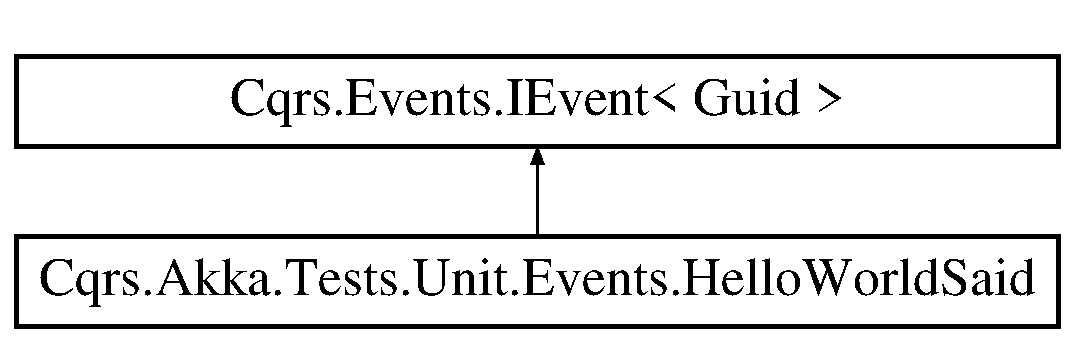
\includegraphics[height=2.000000cm]{classCqrs_1_1Akka_1_1Tests_1_1Unit_1_1Events_1_1HelloWorldSaid}
\end{center}
\end{figure}
\subsection*{Properties}
\begin{DoxyCompactItemize}
\item 
Guid \hyperlink{classCqrs_1_1Akka_1_1Tests_1_1Unit_1_1Events_1_1HelloWorldSaid_aa6b7af3e0cd38f63f65dd7d23e1ec628_aa6b7af3e0cd38f63f65dd7d23e1ec628}{Corrolation\+Id}\hspace{0.3cm}{\ttfamily  \mbox{[}get, set\mbox{]}}
\item 
Guid \hyperlink{classCqrs_1_1Akka_1_1Tests_1_1Unit_1_1Events_1_1HelloWorldSaid_a73d702957bb698206b0fd3a6ed3adf99_a73d702957bb698206b0fd3a6ed3adf99}{Correlation\+Id}\hspace{0.3cm}{\ttfamily  \mbox{[}get, set\mbox{]}}
\item 
\hyperlink{namespaceCqrs_1_1Messages_af06a7e6cd2609043d0f2f5f3419f81e3_af06a7e6cd2609043d0f2f5f3419f81e3}{Framework\+Type} \hyperlink{classCqrs_1_1Akka_1_1Tests_1_1Unit_1_1Events_1_1HelloWorldSaid_aa16340777c04273f895c685ed5decb31_aa16340777c04273f895c685ed5decb31}{Framework}\hspace{0.3cm}{\ttfamily  \mbox{[}get, set\mbox{]}}
\item 
string \hyperlink{classCqrs_1_1Akka_1_1Tests_1_1Unit_1_1Events_1_1HelloWorldSaid_a41961069039f043e25d0d42ee05c2f2e_a41961069039f043e25d0d42ee05c2f2e}{Originating\+Framework}\hspace{0.3cm}{\ttfamily  \mbox{[}get, set\mbox{]}}
\begin{DoxyCompactList}\small\item\em The originating framework this message was sent from. \end{DoxyCompactList}\item 
I\+Enumerable$<$ string $>$ \hyperlink{classCqrs_1_1Akka_1_1Tests_1_1Unit_1_1Events_1_1HelloWorldSaid_aa854587e4c732e87f4557b02166031fc_aa854587e4c732e87f4557b02166031fc}{Frameworks}\hspace{0.3cm}{\ttfamily  \mbox{[}get, set\mbox{]}}
\begin{DoxyCompactList}\small\item\em The frameworks this I\+Message has been delivered to/sent via already. \end{DoxyCompactList}\item 
Guid \hyperlink{classCqrs_1_1Akka_1_1Tests_1_1Unit_1_1Events_1_1HelloWorldSaid_a22e519c1d838d43d06c8dc5ce820ce6f_a22e519c1d838d43d06c8dc5ce820ce6f}{Authentication\+Token}\hspace{0.3cm}{\ttfamily  \mbox{[}get, set\mbox{]}}
\item 
Guid \hyperlink{classCqrs_1_1Akka_1_1Tests_1_1Unit_1_1Events_1_1HelloWorldSaid_acb6e5f3f56de3edae8e022d19a2cbc09_acb6e5f3f56de3edae8e022d19a2cbc09}{Id}\hspace{0.3cm}{\ttfamily  \mbox{[}get, set\mbox{]}}
\item 
int \hyperlink{classCqrs_1_1Akka_1_1Tests_1_1Unit_1_1Events_1_1HelloWorldSaid_a31c7b70656767f90229171b579cba13c_a31c7b70656767f90229171b579cba13c}{Version}\hspace{0.3cm}{\ttfamily  \mbox{[}get, set\mbox{]}}
\item 
Date\+Time\+Offset \hyperlink{classCqrs_1_1Akka_1_1Tests_1_1Unit_1_1Events_1_1HelloWorldSaid_aa5025874b17575c910573f1ed6a70bc3_aa5025874b17575c910573f1ed6a70bc3}{Time\+Stamp}\hspace{0.3cm}{\ttfamily  \mbox{[}get, set\mbox{]}}
\end{DoxyCompactItemize}


\subsection{Property Documentation}
\mbox{\Hypertarget{classCqrs_1_1Akka_1_1Tests_1_1Unit_1_1Events_1_1HelloWorldSaid_a22e519c1d838d43d06c8dc5ce820ce6f_a22e519c1d838d43d06c8dc5ce820ce6f}\label{classCqrs_1_1Akka_1_1Tests_1_1Unit_1_1Events_1_1HelloWorldSaid_a22e519c1d838d43d06c8dc5ce820ce6f_a22e519c1d838d43d06c8dc5ce820ce6f}} 
\index{Cqrs\+::\+Akka\+::\+Tests\+::\+Unit\+::\+Events\+::\+Hello\+World\+Said@{Cqrs\+::\+Akka\+::\+Tests\+::\+Unit\+::\+Events\+::\+Hello\+World\+Said}!Authentication\+Token@{Authentication\+Token}}
\index{Authentication\+Token@{Authentication\+Token}!Cqrs\+::\+Akka\+::\+Tests\+::\+Unit\+::\+Events\+::\+Hello\+World\+Said@{Cqrs\+::\+Akka\+::\+Tests\+::\+Unit\+::\+Events\+::\+Hello\+World\+Said}}
\subsubsection{\texorpdfstring{Authentication\+Token}{AuthenticationToken}}
{\footnotesize\ttfamily Guid Cqrs.\+Akka.\+Tests.\+Unit.\+Events.\+Hello\+World\+Said.\+Authentication\+Token\hspace{0.3cm}{\ttfamily [get]}, {\ttfamily [set]}}

\mbox{\Hypertarget{classCqrs_1_1Akka_1_1Tests_1_1Unit_1_1Events_1_1HelloWorldSaid_a73d702957bb698206b0fd3a6ed3adf99_a73d702957bb698206b0fd3a6ed3adf99}\label{classCqrs_1_1Akka_1_1Tests_1_1Unit_1_1Events_1_1HelloWorldSaid_a73d702957bb698206b0fd3a6ed3adf99_a73d702957bb698206b0fd3a6ed3adf99}} 
\index{Cqrs\+::\+Akka\+::\+Tests\+::\+Unit\+::\+Events\+::\+Hello\+World\+Said@{Cqrs\+::\+Akka\+::\+Tests\+::\+Unit\+::\+Events\+::\+Hello\+World\+Said}!Correlation\+Id@{Correlation\+Id}}
\index{Correlation\+Id@{Correlation\+Id}!Cqrs\+::\+Akka\+::\+Tests\+::\+Unit\+::\+Events\+::\+Hello\+World\+Said@{Cqrs\+::\+Akka\+::\+Tests\+::\+Unit\+::\+Events\+::\+Hello\+World\+Said}}
\subsubsection{\texorpdfstring{Correlation\+Id}{CorrelationId}}
{\footnotesize\ttfamily Guid Cqrs.\+Akka.\+Tests.\+Unit.\+Events.\+Hello\+World\+Said.\+Correlation\+Id\hspace{0.3cm}{\ttfamily [get]}, {\ttfamily [set]}}

\mbox{\Hypertarget{classCqrs_1_1Akka_1_1Tests_1_1Unit_1_1Events_1_1HelloWorldSaid_aa6b7af3e0cd38f63f65dd7d23e1ec628_aa6b7af3e0cd38f63f65dd7d23e1ec628}\label{classCqrs_1_1Akka_1_1Tests_1_1Unit_1_1Events_1_1HelloWorldSaid_aa6b7af3e0cd38f63f65dd7d23e1ec628_aa6b7af3e0cd38f63f65dd7d23e1ec628}} 
\index{Cqrs\+::\+Akka\+::\+Tests\+::\+Unit\+::\+Events\+::\+Hello\+World\+Said@{Cqrs\+::\+Akka\+::\+Tests\+::\+Unit\+::\+Events\+::\+Hello\+World\+Said}!Corrolation\+Id@{Corrolation\+Id}}
\index{Corrolation\+Id@{Corrolation\+Id}!Cqrs\+::\+Akka\+::\+Tests\+::\+Unit\+::\+Events\+::\+Hello\+World\+Said@{Cqrs\+::\+Akka\+::\+Tests\+::\+Unit\+::\+Events\+::\+Hello\+World\+Said}}
\subsubsection{\texorpdfstring{Corrolation\+Id}{CorrolationId}}
{\footnotesize\ttfamily Guid Cqrs.\+Akka.\+Tests.\+Unit.\+Events.\+Hello\+World\+Said.\+Corrolation\+Id\hspace{0.3cm}{\ttfamily [get]}, {\ttfamily [set]}}

\mbox{\Hypertarget{classCqrs_1_1Akka_1_1Tests_1_1Unit_1_1Events_1_1HelloWorldSaid_aa16340777c04273f895c685ed5decb31_aa16340777c04273f895c685ed5decb31}\label{classCqrs_1_1Akka_1_1Tests_1_1Unit_1_1Events_1_1HelloWorldSaid_aa16340777c04273f895c685ed5decb31_aa16340777c04273f895c685ed5decb31}} 
\index{Cqrs\+::\+Akka\+::\+Tests\+::\+Unit\+::\+Events\+::\+Hello\+World\+Said@{Cqrs\+::\+Akka\+::\+Tests\+::\+Unit\+::\+Events\+::\+Hello\+World\+Said}!Framework@{Framework}}
\index{Framework@{Framework}!Cqrs\+::\+Akka\+::\+Tests\+::\+Unit\+::\+Events\+::\+Hello\+World\+Said@{Cqrs\+::\+Akka\+::\+Tests\+::\+Unit\+::\+Events\+::\+Hello\+World\+Said}}
\subsubsection{\texorpdfstring{Framework}{Framework}}
{\footnotesize\ttfamily \hyperlink{namespaceCqrs_1_1Messages_af06a7e6cd2609043d0f2f5f3419f81e3_af06a7e6cd2609043d0f2f5f3419f81e3}{Framework\+Type} Cqrs.\+Akka.\+Tests.\+Unit.\+Events.\+Hello\+World\+Said.\+Framework\hspace{0.3cm}{\ttfamily [get]}, {\ttfamily [set]}}

\mbox{\Hypertarget{classCqrs_1_1Akka_1_1Tests_1_1Unit_1_1Events_1_1HelloWorldSaid_aa854587e4c732e87f4557b02166031fc_aa854587e4c732e87f4557b02166031fc}\label{classCqrs_1_1Akka_1_1Tests_1_1Unit_1_1Events_1_1HelloWorldSaid_aa854587e4c732e87f4557b02166031fc_aa854587e4c732e87f4557b02166031fc}} 
\index{Cqrs\+::\+Akka\+::\+Tests\+::\+Unit\+::\+Events\+::\+Hello\+World\+Said@{Cqrs\+::\+Akka\+::\+Tests\+::\+Unit\+::\+Events\+::\+Hello\+World\+Said}!Frameworks@{Frameworks}}
\index{Frameworks@{Frameworks}!Cqrs\+::\+Akka\+::\+Tests\+::\+Unit\+::\+Events\+::\+Hello\+World\+Said@{Cqrs\+::\+Akka\+::\+Tests\+::\+Unit\+::\+Events\+::\+Hello\+World\+Said}}
\subsubsection{\texorpdfstring{Frameworks}{Frameworks}}
{\footnotesize\ttfamily I\+Enumerable$<$string$>$ Cqrs.\+Akka.\+Tests.\+Unit.\+Events.\+Hello\+World\+Said.\+Frameworks\hspace{0.3cm}{\ttfamily [get]}, {\ttfamily [set]}}



The frameworks this I\+Message has been delivered to/sent via already. 

\mbox{\Hypertarget{classCqrs_1_1Akka_1_1Tests_1_1Unit_1_1Events_1_1HelloWorldSaid_acb6e5f3f56de3edae8e022d19a2cbc09_acb6e5f3f56de3edae8e022d19a2cbc09}\label{classCqrs_1_1Akka_1_1Tests_1_1Unit_1_1Events_1_1HelloWorldSaid_acb6e5f3f56de3edae8e022d19a2cbc09_acb6e5f3f56de3edae8e022d19a2cbc09}} 
\index{Cqrs\+::\+Akka\+::\+Tests\+::\+Unit\+::\+Events\+::\+Hello\+World\+Said@{Cqrs\+::\+Akka\+::\+Tests\+::\+Unit\+::\+Events\+::\+Hello\+World\+Said}!Id@{Id}}
\index{Id@{Id}!Cqrs\+::\+Akka\+::\+Tests\+::\+Unit\+::\+Events\+::\+Hello\+World\+Said@{Cqrs\+::\+Akka\+::\+Tests\+::\+Unit\+::\+Events\+::\+Hello\+World\+Said}}
\subsubsection{\texorpdfstring{Id}{Id}}
{\footnotesize\ttfamily Guid Cqrs.\+Akka.\+Tests.\+Unit.\+Events.\+Hello\+World\+Said.\+Id\hspace{0.3cm}{\ttfamily [get]}, {\ttfamily [set]}}

\mbox{\Hypertarget{classCqrs_1_1Akka_1_1Tests_1_1Unit_1_1Events_1_1HelloWorldSaid_a41961069039f043e25d0d42ee05c2f2e_a41961069039f043e25d0d42ee05c2f2e}\label{classCqrs_1_1Akka_1_1Tests_1_1Unit_1_1Events_1_1HelloWorldSaid_a41961069039f043e25d0d42ee05c2f2e_a41961069039f043e25d0d42ee05c2f2e}} 
\index{Cqrs\+::\+Akka\+::\+Tests\+::\+Unit\+::\+Events\+::\+Hello\+World\+Said@{Cqrs\+::\+Akka\+::\+Tests\+::\+Unit\+::\+Events\+::\+Hello\+World\+Said}!Originating\+Framework@{Originating\+Framework}}
\index{Originating\+Framework@{Originating\+Framework}!Cqrs\+::\+Akka\+::\+Tests\+::\+Unit\+::\+Events\+::\+Hello\+World\+Said@{Cqrs\+::\+Akka\+::\+Tests\+::\+Unit\+::\+Events\+::\+Hello\+World\+Said}}
\subsubsection{\texorpdfstring{Originating\+Framework}{OriginatingFramework}}
{\footnotesize\ttfamily string Cqrs.\+Akka.\+Tests.\+Unit.\+Events.\+Hello\+World\+Said.\+Originating\+Framework\hspace{0.3cm}{\ttfamily [get]}, {\ttfamily [set]}}



The originating framework this message was sent from. 

\mbox{\Hypertarget{classCqrs_1_1Akka_1_1Tests_1_1Unit_1_1Events_1_1HelloWorldSaid_aa5025874b17575c910573f1ed6a70bc3_aa5025874b17575c910573f1ed6a70bc3}\label{classCqrs_1_1Akka_1_1Tests_1_1Unit_1_1Events_1_1HelloWorldSaid_aa5025874b17575c910573f1ed6a70bc3_aa5025874b17575c910573f1ed6a70bc3}} 
\index{Cqrs\+::\+Akka\+::\+Tests\+::\+Unit\+::\+Events\+::\+Hello\+World\+Said@{Cqrs\+::\+Akka\+::\+Tests\+::\+Unit\+::\+Events\+::\+Hello\+World\+Said}!Time\+Stamp@{Time\+Stamp}}
\index{Time\+Stamp@{Time\+Stamp}!Cqrs\+::\+Akka\+::\+Tests\+::\+Unit\+::\+Events\+::\+Hello\+World\+Said@{Cqrs\+::\+Akka\+::\+Tests\+::\+Unit\+::\+Events\+::\+Hello\+World\+Said}}
\subsubsection{\texorpdfstring{Time\+Stamp}{TimeStamp}}
{\footnotesize\ttfamily Date\+Time\+Offset Cqrs.\+Akka.\+Tests.\+Unit.\+Events.\+Hello\+World\+Said.\+Time\+Stamp\hspace{0.3cm}{\ttfamily [get]}, {\ttfamily [set]}}

\mbox{\Hypertarget{classCqrs_1_1Akka_1_1Tests_1_1Unit_1_1Events_1_1HelloWorldSaid_a31c7b70656767f90229171b579cba13c_a31c7b70656767f90229171b579cba13c}\label{classCqrs_1_1Akka_1_1Tests_1_1Unit_1_1Events_1_1HelloWorldSaid_a31c7b70656767f90229171b579cba13c_a31c7b70656767f90229171b579cba13c}} 
\index{Cqrs\+::\+Akka\+::\+Tests\+::\+Unit\+::\+Events\+::\+Hello\+World\+Said@{Cqrs\+::\+Akka\+::\+Tests\+::\+Unit\+::\+Events\+::\+Hello\+World\+Said}!Version@{Version}}
\index{Version@{Version}!Cqrs\+::\+Akka\+::\+Tests\+::\+Unit\+::\+Events\+::\+Hello\+World\+Said@{Cqrs\+::\+Akka\+::\+Tests\+::\+Unit\+::\+Events\+::\+Hello\+World\+Said}}
\subsubsection{\texorpdfstring{Version}{Version}}
{\footnotesize\ttfamily int Cqrs.\+Akka.\+Tests.\+Unit.\+Events.\+Hello\+World\+Said.\+Version\hspace{0.3cm}{\ttfamily [get]}, {\ttfamily [set]}}


\hypertarget{classCqrs_1_1Akka_1_1Tests_1_1Unit_1_1Sagas_1_1ConversationReportProcessManager}{}\doxysection{Cqrs.\+Akka.\+Tests.\+Unit.\+Sagas.\+Conversation\+Report\+Process\+Manager Class Reference}
\label{classCqrs_1_1Akka_1_1Tests_1_1Unit_1_1Sagas_1_1ConversationReportProcessManager}\index{Cqrs.Akka.Tests.Unit.Sagas.ConversationReportProcessManager@{Cqrs.Akka.Tests.Unit.Sagas.ConversationReportProcessManager}}


A I\+Saga$<$\+T\+Authentication\+Token$>$ that acts as a process manager responding to several events and raising a command when a certain criteria is met.  


Inheritance diagram for Cqrs.\+Akka.\+Tests.\+Unit.\+Sagas.\+Conversation\+Report\+Process\+Manager\+:\begin{figure}[H]
\begin{center}
\leavevmode
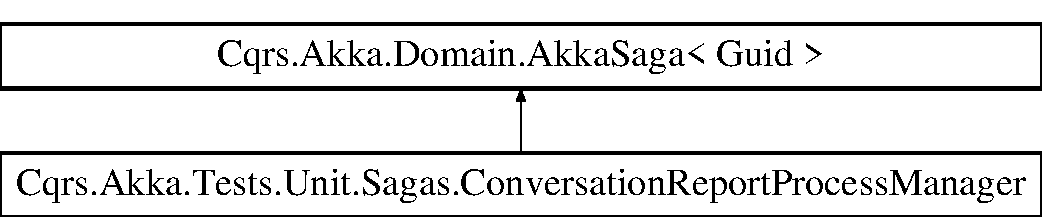
\includegraphics[height=2.000000cm]{classCqrs_1_1Akka_1_1Tests_1_1Unit_1_1Sagas_1_1ConversationReportProcessManager}
\end{center}
\end{figure}
\doxysubsection*{Public Member Functions}
\begin{DoxyCompactItemize}
\item 
\mbox{\hyperlink{classCqrs_1_1Akka_1_1Tests_1_1Unit_1_1Sagas_1_1ConversationReportProcessManager_a646ce30aa269388c16820418c5b3f63c_a646ce30aa269388c16820418c5b3f63c}{Conversation\+Report\+Process\+Manager}} (\mbox{\hyperlink{interfaceCqrs_1_1Configuration_1_1IDependencyResolver}{I\+Dependency\+Resolver}} dependency\+Resolver, I\+Logger logger, Guid rsn)
\begin{DoxyCompactList}\small\item\em Instantiates a new instance of \mbox{\hyperlink{classCqrs_1_1Akka_1_1Tests_1_1Unit_1_1Sagas_1_1ConversationReportProcessManager}{Conversation\+Report\+Process\+Manager}}. \end{DoxyCompactList}\item 
virtual void \mbox{\hyperlink{classCqrs_1_1Akka_1_1Tests_1_1Unit_1_1Sagas_1_1ConversationReportProcessManager_a282356c4090cfaf2dcfa93916b8b8997_a282356c4090cfaf2dcfa93916b8b8997}{Handle}} (\mbox{\hyperlink{classCqrs_1_1Akka_1_1Tests_1_1Unit_1_1Events_1_1HelloWorldSaid}{Hello\+World\+Said}} @event)
\begin{DoxyCompactList}\small\item\em Responds to the provided {\itshape event} . \end{DoxyCompactList}\item 
virtual void \mbox{\hyperlink{classCqrs_1_1Akka_1_1Tests_1_1Unit_1_1Sagas_1_1ConversationReportProcessManager_a4c98fb5ce16b16e709c31c2fb2eff575_a4c98fb5ce16b16e709c31c2fb2eff575}{Handle}} (\mbox{\hyperlink{classCqrs_1_1Akka_1_1Tests_1_1Unit_1_1Events_1_1HelloWorldRepliedTo}{Hello\+World\+Replied\+To}} @event)
\begin{DoxyCompactList}\small\item\em Responds to the provided {\itshape event} . \end{DoxyCompactList}\item 
virtual void \mbox{\hyperlink{classCqrs_1_1Akka_1_1Tests_1_1Unit_1_1Sagas_1_1ConversationReportProcessManager_a2980f91992185b3275ba36e97e5eed48_a2980f91992185b3275ba36e97e5eed48}{Handle}} (\mbox{\hyperlink{classCqrs_1_1Akka_1_1Tests_1_1Unit_1_1Events_1_1ConversationEnded}{Conversation\+Ended}} @event)
\begin{DoxyCompactList}\small\item\em Responds to the provided {\itshape event} . \end{DoxyCompactList}\item 
virtual void \mbox{\hyperlink{classCqrs_1_1Akka_1_1Tests_1_1Unit_1_1Sagas_1_1ConversationReportProcessManager_a19573bf2840357a4e79f310c3fdfe916_a19573bf2840357a4e79f310c3fdfe916}{Apply}} (\mbox{\hyperlink{classCqrs_1_1Akka_1_1Tests_1_1Unit_1_1Events_1_1HelloWorldSaid}{Hello\+World\+Said}} @event)
\begin{DoxyCompactList}\small\item\em Applies the {\itshape event}  to itself. \end{DoxyCompactList}\item 
virtual void \mbox{\hyperlink{classCqrs_1_1Akka_1_1Tests_1_1Unit_1_1Sagas_1_1ConversationReportProcessManager_a938040ac51a3deb02ae36adb7f5999fb_a938040ac51a3deb02ae36adb7f5999fb}{Apply}} (\mbox{\hyperlink{classCqrs_1_1Akka_1_1Tests_1_1Unit_1_1Events_1_1HelloWorldRepliedTo}{Hello\+World\+Replied\+To}} @event)
\begin{DoxyCompactList}\small\item\em Applies the {\itshape event}  to itself. \end{DoxyCompactList}\item 
virtual void \mbox{\hyperlink{classCqrs_1_1Akka_1_1Tests_1_1Unit_1_1Sagas_1_1ConversationReportProcessManager_ae2c1edeb1a4d604948b4c70b71c20555_ae2c1edeb1a4d604948b4c70b71c20555}{Apply}} (\mbox{\hyperlink{classCqrs_1_1Akka_1_1Tests_1_1Unit_1_1Events_1_1ConversationEnded}{Conversation\+Ended}} @event)
\begin{DoxyCompactList}\small\item\em Applies the {\itshape event}  to itself. \end{DoxyCompactList}\end{DoxyCompactItemize}
\doxysubsection*{Protected Member Functions}
\begin{DoxyCompactItemize}
\item 
virtual void \mbox{\hyperlink{classCqrs_1_1Akka_1_1Tests_1_1Unit_1_1Sagas_1_1ConversationReportProcessManager_a0c10a4f4b6eae7a1c5b321a07b02a1d1_a0c10a4f4b6eae7a1c5b321a07b02a1d1}{Generate\+Command}} ()
\begin{DoxyCompactList}\small\item\em Generates and publishes a I\+Command$<$\+T\+Authentication\+Token$>$. \end{DoxyCompactList}\end{DoxyCompactItemize}
\doxysubsection*{Properties}
\begin{DoxyCompactItemize}
\item 
Guid \mbox{\hyperlink{classCqrs_1_1Akka_1_1Tests_1_1Unit_1_1Sagas_1_1ConversationReportProcessManager_a86603fe9e9fa5e9b009064ea5ea6873a_a86603fe9e9fa5e9b009064ea5ea6873a}{Rsn}}\hspace{0.3cm}{\ttfamily  \mbox{[}get\mbox{]}}
\begin{DoxyCompactList}\small\item\em The I\+Saga$<$\+T\+Authentication\+Token$>$.\+Id \end{DoxyCompactList}\item 
bool \mbox{\hyperlink{classCqrs_1_1Akka_1_1Tests_1_1Unit_1_1Sagas_1_1ConversationReportProcessManager_af7ab2e24d481f9f262b11eefd9b397bb_af7ab2e24d481f9f262b11eefd9b397bb}{Is\+Deleted}}\hspace{0.3cm}{\ttfamily  \mbox{[}get, set\mbox{]}}
\begin{DoxyCompactList}\small\item\em Indicates if this I\+Saga$<$\+T\+Authentication\+Token$>$ has been deleted. \end{DoxyCompactList}\item 
\mbox{\hyperlink{interfaceCqrs_1_1Configuration_1_1IDependencyResolver}{I\+Dependency\+Resolver}} \mbox{\hyperlink{classCqrs_1_1Akka_1_1Tests_1_1Unit_1_1Sagas_1_1ConversationReportProcessManager_a6ddc3cab5bedf62389eaa4c769441aa8_a6ddc3cab5bedf62389eaa4c769441aa8}{Dependency\+Resolver}}\hspace{0.3cm}{\ttfamily  \mbox{[}get\mbox{]}}
\begin{DoxyCompactList}\small\item\em The I\+Dependency\+Resolver that resolves things. \end{DoxyCompactList}\end{DoxyCompactItemize}


\doxysubsection{Detailed Description}
A I\+Saga$<$\+T\+Authentication\+Token$>$ that acts as a process manager responding to several events and raising a command when a certain criteria is met. 



\doxysubsection{Constructor \& Destructor Documentation}
\mbox{\Hypertarget{classCqrs_1_1Akka_1_1Tests_1_1Unit_1_1Sagas_1_1ConversationReportProcessManager_a646ce30aa269388c16820418c5b3f63c_a646ce30aa269388c16820418c5b3f63c}\label{classCqrs_1_1Akka_1_1Tests_1_1Unit_1_1Sagas_1_1ConversationReportProcessManager_a646ce30aa269388c16820418c5b3f63c_a646ce30aa269388c16820418c5b3f63c}} 
\index{Cqrs.Akka.Tests.Unit.Sagas.ConversationReportProcessManager@{Cqrs.Akka.Tests.Unit.Sagas.ConversationReportProcessManager}!ConversationReportProcessManager@{ConversationReportProcessManager}}
\index{ConversationReportProcessManager@{ConversationReportProcessManager}!Cqrs.Akka.Tests.Unit.Sagas.ConversationReportProcessManager@{Cqrs.Akka.Tests.Unit.Sagas.ConversationReportProcessManager}}
\doxysubsubsection{\texorpdfstring{ConversationReportProcessManager()}{ConversationReportProcessManager()}}
{\footnotesize\ttfamily Cqrs.\+Akka.\+Tests.\+Unit.\+Sagas.\+Conversation\+Report\+Process\+Manager.\+Conversation\+Report\+Process\+Manager (\begin{DoxyParamCaption}\item[{\mbox{\hyperlink{interfaceCqrs_1_1Configuration_1_1IDependencyResolver}{I\+Dependency\+Resolver}}}]{dependency\+Resolver,  }\item[{I\+Logger}]{logger,  }\item[{Guid}]{rsn }\end{DoxyParamCaption})}



Instantiates a new instance of \mbox{\hyperlink{classCqrs_1_1Akka_1_1Tests_1_1Unit_1_1Sagas_1_1ConversationReportProcessManager}{Conversation\+Report\+Process\+Manager}}. 



\doxysubsection{Member Function Documentation}
\mbox{\Hypertarget{classCqrs_1_1Akka_1_1Tests_1_1Unit_1_1Sagas_1_1ConversationReportProcessManager_ae2c1edeb1a4d604948b4c70b71c20555_ae2c1edeb1a4d604948b4c70b71c20555}\label{classCqrs_1_1Akka_1_1Tests_1_1Unit_1_1Sagas_1_1ConversationReportProcessManager_ae2c1edeb1a4d604948b4c70b71c20555_ae2c1edeb1a4d604948b4c70b71c20555}} 
\index{Cqrs.Akka.Tests.Unit.Sagas.ConversationReportProcessManager@{Cqrs.Akka.Tests.Unit.Sagas.ConversationReportProcessManager}!Apply@{Apply}}
\index{Apply@{Apply}!Cqrs.Akka.Tests.Unit.Sagas.ConversationReportProcessManager@{Cqrs.Akka.Tests.Unit.Sagas.ConversationReportProcessManager}}
\doxysubsubsection{\texorpdfstring{Apply()}{Apply()}\hspace{0.1cm}{\footnotesize\ttfamily [1/3]}}
{\footnotesize\ttfamily virtual void Cqrs.\+Akka.\+Tests.\+Unit.\+Sagas.\+Conversation\+Report\+Process\+Manager.\+Apply (\begin{DoxyParamCaption}\item[{\mbox{\hyperlink{classCqrs_1_1Akka_1_1Tests_1_1Unit_1_1Events_1_1ConversationEnded}{Conversation\+Ended}} @}]{event }\end{DoxyParamCaption})\hspace{0.3cm}{\ttfamily [virtual]}}



Applies the {\itshape event}  to itself. 


\begin{DoxyParams}{Parameters}
{\em event} & The Conversation\+Ended to apply\\
\hline
\end{DoxyParams}
\mbox{\Hypertarget{classCqrs_1_1Akka_1_1Tests_1_1Unit_1_1Sagas_1_1ConversationReportProcessManager_a938040ac51a3deb02ae36adb7f5999fb_a938040ac51a3deb02ae36adb7f5999fb}\label{classCqrs_1_1Akka_1_1Tests_1_1Unit_1_1Sagas_1_1ConversationReportProcessManager_a938040ac51a3deb02ae36adb7f5999fb_a938040ac51a3deb02ae36adb7f5999fb}} 
\index{Cqrs.Akka.Tests.Unit.Sagas.ConversationReportProcessManager@{Cqrs.Akka.Tests.Unit.Sagas.ConversationReportProcessManager}!Apply@{Apply}}
\index{Apply@{Apply}!Cqrs.Akka.Tests.Unit.Sagas.ConversationReportProcessManager@{Cqrs.Akka.Tests.Unit.Sagas.ConversationReportProcessManager}}
\doxysubsubsection{\texorpdfstring{Apply()}{Apply()}\hspace{0.1cm}{\footnotesize\ttfamily [2/3]}}
{\footnotesize\ttfamily virtual void Cqrs.\+Akka.\+Tests.\+Unit.\+Sagas.\+Conversation\+Report\+Process\+Manager.\+Apply (\begin{DoxyParamCaption}\item[{\mbox{\hyperlink{classCqrs_1_1Akka_1_1Tests_1_1Unit_1_1Events_1_1HelloWorldRepliedTo}{Hello\+World\+Replied\+To}} @}]{event }\end{DoxyParamCaption})\hspace{0.3cm}{\ttfamily [virtual]}}



Applies the {\itshape event}  to itself. 


\begin{DoxyParams}{Parameters}
{\em event} & The Hello\+World\+Replied\+To to apply\\
\hline
\end{DoxyParams}
\mbox{\Hypertarget{classCqrs_1_1Akka_1_1Tests_1_1Unit_1_1Sagas_1_1ConversationReportProcessManager_a19573bf2840357a4e79f310c3fdfe916_a19573bf2840357a4e79f310c3fdfe916}\label{classCqrs_1_1Akka_1_1Tests_1_1Unit_1_1Sagas_1_1ConversationReportProcessManager_a19573bf2840357a4e79f310c3fdfe916_a19573bf2840357a4e79f310c3fdfe916}} 
\index{Cqrs.Akka.Tests.Unit.Sagas.ConversationReportProcessManager@{Cqrs.Akka.Tests.Unit.Sagas.ConversationReportProcessManager}!Apply@{Apply}}
\index{Apply@{Apply}!Cqrs.Akka.Tests.Unit.Sagas.ConversationReportProcessManager@{Cqrs.Akka.Tests.Unit.Sagas.ConversationReportProcessManager}}
\doxysubsubsection{\texorpdfstring{Apply()}{Apply()}\hspace{0.1cm}{\footnotesize\ttfamily [3/3]}}
{\footnotesize\ttfamily virtual void Cqrs.\+Akka.\+Tests.\+Unit.\+Sagas.\+Conversation\+Report\+Process\+Manager.\+Apply (\begin{DoxyParamCaption}\item[{\mbox{\hyperlink{classCqrs_1_1Akka_1_1Tests_1_1Unit_1_1Events_1_1HelloWorldSaid}{Hello\+World\+Said}} @}]{event }\end{DoxyParamCaption})\hspace{0.3cm}{\ttfamily [virtual]}}



Applies the {\itshape event}  to itself. 


\begin{DoxyParams}{Parameters}
{\em event} & The Hello\+World\+Said to apply\\
\hline
\end{DoxyParams}
\mbox{\Hypertarget{classCqrs_1_1Akka_1_1Tests_1_1Unit_1_1Sagas_1_1ConversationReportProcessManager_a0c10a4f4b6eae7a1c5b321a07b02a1d1_a0c10a4f4b6eae7a1c5b321a07b02a1d1}\label{classCqrs_1_1Akka_1_1Tests_1_1Unit_1_1Sagas_1_1ConversationReportProcessManager_a0c10a4f4b6eae7a1c5b321a07b02a1d1_a0c10a4f4b6eae7a1c5b321a07b02a1d1}} 
\index{Cqrs.Akka.Tests.Unit.Sagas.ConversationReportProcessManager@{Cqrs.Akka.Tests.Unit.Sagas.ConversationReportProcessManager}!GenerateCommand@{GenerateCommand}}
\index{GenerateCommand@{GenerateCommand}!Cqrs.Akka.Tests.Unit.Sagas.ConversationReportProcessManager@{Cqrs.Akka.Tests.Unit.Sagas.ConversationReportProcessManager}}
\doxysubsubsection{\texorpdfstring{GenerateCommand()}{GenerateCommand()}}
{\footnotesize\ttfamily virtual void Cqrs.\+Akka.\+Tests.\+Unit.\+Sagas.\+Conversation\+Report\+Process\+Manager.\+Generate\+Command (\begin{DoxyParamCaption}{ }\end{DoxyParamCaption})\hspace{0.3cm}{\ttfamily [protected]}, {\ttfamily [virtual]}}



Generates and publishes a I\+Command$<$\+T\+Authentication\+Token$>$. 

\mbox{\Hypertarget{classCqrs_1_1Akka_1_1Tests_1_1Unit_1_1Sagas_1_1ConversationReportProcessManager_a2980f91992185b3275ba36e97e5eed48_a2980f91992185b3275ba36e97e5eed48}\label{classCqrs_1_1Akka_1_1Tests_1_1Unit_1_1Sagas_1_1ConversationReportProcessManager_a2980f91992185b3275ba36e97e5eed48_a2980f91992185b3275ba36e97e5eed48}} 
\index{Cqrs.Akka.Tests.Unit.Sagas.ConversationReportProcessManager@{Cqrs.Akka.Tests.Unit.Sagas.ConversationReportProcessManager}!Handle@{Handle}}
\index{Handle@{Handle}!Cqrs.Akka.Tests.Unit.Sagas.ConversationReportProcessManager@{Cqrs.Akka.Tests.Unit.Sagas.ConversationReportProcessManager}}
\doxysubsubsection{\texorpdfstring{Handle()}{Handle()}\hspace{0.1cm}{\footnotesize\ttfamily [1/3]}}
{\footnotesize\ttfamily virtual void Cqrs.\+Akka.\+Tests.\+Unit.\+Sagas.\+Conversation\+Report\+Process\+Manager.\+Handle (\begin{DoxyParamCaption}\item[{\mbox{\hyperlink{classCqrs_1_1Akka_1_1Tests_1_1Unit_1_1Events_1_1ConversationEnded}{Conversation\+Ended}} @}]{event }\end{DoxyParamCaption})\hspace{0.3cm}{\ttfamily [virtual]}}



Responds to the provided {\itshape event} . 


\begin{DoxyParams}{Parameters}
{\em event} & The Conversation\+Ended to respond to or \char`\"{}handle\char`\"{}\\
\hline
\end{DoxyParams}
\mbox{\Hypertarget{classCqrs_1_1Akka_1_1Tests_1_1Unit_1_1Sagas_1_1ConversationReportProcessManager_a4c98fb5ce16b16e709c31c2fb2eff575_a4c98fb5ce16b16e709c31c2fb2eff575}\label{classCqrs_1_1Akka_1_1Tests_1_1Unit_1_1Sagas_1_1ConversationReportProcessManager_a4c98fb5ce16b16e709c31c2fb2eff575_a4c98fb5ce16b16e709c31c2fb2eff575}} 
\index{Cqrs.Akka.Tests.Unit.Sagas.ConversationReportProcessManager@{Cqrs.Akka.Tests.Unit.Sagas.ConversationReportProcessManager}!Handle@{Handle}}
\index{Handle@{Handle}!Cqrs.Akka.Tests.Unit.Sagas.ConversationReportProcessManager@{Cqrs.Akka.Tests.Unit.Sagas.ConversationReportProcessManager}}
\doxysubsubsection{\texorpdfstring{Handle()}{Handle()}\hspace{0.1cm}{\footnotesize\ttfamily [2/3]}}
{\footnotesize\ttfamily virtual void Cqrs.\+Akka.\+Tests.\+Unit.\+Sagas.\+Conversation\+Report\+Process\+Manager.\+Handle (\begin{DoxyParamCaption}\item[{\mbox{\hyperlink{classCqrs_1_1Akka_1_1Tests_1_1Unit_1_1Events_1_1HelloWorldRepliedTo}{Hello\+World\+Replied\+To}} @}]{event }\end{DoxyParamCaption})\hspace{0.3cm}{\ttfamily [virtual]}}



Responds to the provided {\itshape event} . 


\begin{DoxyParams}{Parameters}
{\em event} & The Hello\+World\+Replied\+To to respond to or \char`\"{}handle\char`\"{}\\
\hline
\end{DoxyParams}
\mbox{\Hypertarget{classCqrs_1_1Akka_1_1Tests_1_1Unit_1_1Sagas_1_1ConversationReportProcessManager_a282356c4090cfaf2dcfa93916b8b8997_a282356c4090cfaf2dcfa93916b8b8997}\label{classCqrs_1_1Akka_1_1Tests_1_1Unit_1_1Sagas_1_1ConversationReportProcessManager_a282356c4090cfaf2dcfa93916b8b8997_a282356c4090cfaf2dcfa93916b8b8997}} 
\index{Cqrs.Akka.Tests.Unit.Sagas.ConversationReportProcessManager@{Cqrs.Akka.Tests.Unit.Sagas.ConversationReportProcessManager}!Handle@{Handle}}
\index{Handle@{Handle}!Cqrs.Akka.Tests.Unit.Sagas.ConversationReportProcessManager@{Cqrs.Akka.Tests.Unit.Sagas.ConversationReportProcessManager}}
\doxysubsubsection{\texorpdfstring{Handle()}{Handle()}\hspace{0.1cm}{\footnotesize\ttfamily [3/3]}}
{\footnotesize\ttfamily virtual void Cqrs.\+Akka.\+Tests.\+Unit.\+Sagas.\+Conversation\+Report\+Process\+Manager.\+Handle (\begin{DoxyParamCaption}\item[{\mbox{\hyperlink{classCqrs_1_1Akka_1_1Tests_1_1Unit_1_1Events_1_1HelloWorldSaid}{Hello\+World\+Said}} @}]{event }\end{DoxyParamCaption})\hspace{0.3cm}{\ttfamily [virtual]}}



Responds to the provided {\itshape event} . 


\begin{DoxyParams}{Parameters}
{\em event} & The Hello\+World\+Said to respond to or \char`\"{}handle\char`\"{}\\
\hline
\end{DoxyParams}


\doxysubsection{Property Documentation}
\mbox{\Hypertarget{classCqrs_1_1Akka_1_1Tests_1_1Unit_1_1Sagas_1_1ConversationReportProcessManager_a6ddc3cab5bedf62389eaa4c769441aa8_a6ddc3cab5bedf62389eaa4c769441aa8}\label{classCqrs_1_1Akka_1_1Tests_1_1Unit_1_1Sagas_1_1ConversationReportProcessManager_a6ddc3cab5bedf62389eaa4c769441aa8_a6ddc3cab5bedf62389eaa4c769441aa8}} 
\index{Cqrs.Akka.Tests.Unit.Sagas.ConversationReportProcessManager@{Cqrs.Akka.Tests.Unit.Sagas.ConversationReportProcessManager}!DependencyResolver@{DependencyResolver}}
\index{DependencyResolver@{DependencyResolver}!Cqrs.Akka.Tests.Unit.Sagas.ConversationReportProcessManager@{Cqrs.Akka.Tests.Unit.Sagas.ConversationReportProcessManager}}
\doxysubsubsection{\texorpdfstring{DependencyResolver}{DependencyResolver}}
{\footnotesize\ttfamily \mbox{\hyperlink{interfaceCqrs_1_1Configuration_1_1IDependencyResolver}{I\+Dependency\+Resolver}} Cqrs.\+Akka.\+Tests.\+Unit.\+Sagas.\+Conversation\+Report\+Process\+Manager.\+Dependency\+Resolver\hspace{0.3cm}{\ttfamily [get]}, {\ttfamily [protected]}}



The I\+Dependency\+Resolver that resolves things. 

\mbox{\Hypertarget{classCqrs_1_1Akka_1_1Tests_1_1Unit_1_1Sagas_1_1ConversationReportProcessManager_af7ab2e24d481f9f262b11eefd9b397bb_af7ab2e24d481f9f262b11eefd9b397bb}\label{classCqrs_1_1Akka_1_1Tests_1_1Unit_1_1Sagas_1_1ConversationReportProcessManager_af7ab2e24d481f9f262b11eefd9b397bb_af7ab2e24d481f9f262b11eefd9b397bb}} 
\index{Cqrs.Akka.Tests.Unit.Sagas.ConversationReportProcessManager@{Cqrs.Akka.Tests.Unit.Sagas.ConversationReportProcessManager}!IsDeleted@{IsDeleted}}
\index{IsDeleted@{IsDeleted}!Cqrs.Akka.Tests.Unit.Sagas.ConversationReportProcessManager@{Cqrs.Akka.Tests.Unit.Sagas.ConversationReportProcessManager}}
\doxysubsubsection{\texorpdfstring{IsDeleted}{IsDeleted}}
{\footnotesize\ttfamily bool Cqrs.\+Akka.\+Tests.\+Unit.\+Sagas.\+Conversation\+Report\+Process\+Manager.\+Is\+Deleted\hspace{0.3cm}{\ttfamily [get]}, {\ttfamily [set]}}



Indicates if this I\+Saga$<$\+T\+Authentication\+Token$>$ has been deleted. 

\mbox{\Hypertarget{classCqrs_1_1Akka_1_1Tests_1_1Unit_1_1Sagas_1_1ConversationReportProcessManager_a86603fe9e9fa5e9b009064ea5ea6873a_a86603fe9e9fa5e9b009064ea5ea6873a}\label{classCqrs_1_1Akka_1_1Tests_1_1Unit_1_1Sagas_1_1ConversationReportProcessManager_a86603fe9e9fa5e9b009064ea5ea6873a_a86603fe9e9fa5e9b009064ea5ea6873a}} 
\index{Cqrs.Akka.Tests.Unit.Sagas.ConversationReportProcessManager@{Cqrs.Akka.Tests.Unit.Sagas.ConversationReportProcessManager}!Rsn@{Rsn}}
\index{Rsn@{Rsn}!Cqrs.Akka.Tests.Unit.Sagas.ConversationReportProcessManager@{Cqrs.Akka.Tests.Unit.Sagas.ConversationReportProcessManager}}
\doxysubsubsection{\texorpdfstring{Rsn}{Rsn}}
{\footnotesize\ttfamily Guid Cqrs.\+Akka.\+Tests.\+Unit.\+Sagas.\+Conversation\+Report\+Process\+Manager.\+Rsn\hspace{0.3cm}{\ttfamily [get]}}



The I\+Saga$<$\+T\+Authentication\+Token$>$.\+Id 


\hypertarget{classCqrs_1_1Akka_1_1Tests_1_1Unit_1_1Sagas_1_1ConversationReportProcessManagerEventHandlers}{}\doxysection{Cqrs.\+Akka.\+Tests.\+Unit.\+Sagas.\+Conversation\+Report\+Process\+Manager\+Event\+Handlers Class Reference}
\label{classCqrs_1_1Akka_1_1Tests_1_1Unit_1_1Sagas_1_1ConversationReportProcessManagerEventHandlers}\index{Cqrs.Akka.Tests.Unit.Sagas.ConversationReportProcessManagerEventHandlers@{Cqrs.Akka.Tests.Unit.Sagas.ConversationReportProcessManagerEventHandlers}}


An I\+Event\+Handler that passes the I\+Event$<$\+T\+Authentication\+Token$>$ instances it receives to \mbox{\hyperlink{classCqrs_1_1Akka_1_1Tests_1_1Unit_1_1Sagas_1_1ConversationReportProcessManager}{Conversation\+Report\+Process\+Manager}}  


Inheritance diagram for Cqrs.\+Akka.\+Tests.\+Unit.\+Sagas.\+Conversation\+Report\+Process\+Manager\+Event\+Handlers\+:\begin{figure}[H]
\begin{center}
\leavevmode
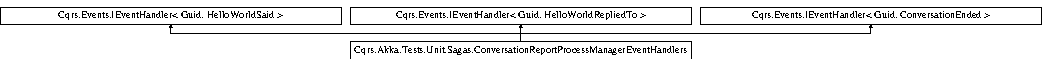
\includegraphics[height=0.792640cm]{classCqrs_1_1Akka_1_1Tests_1_1Unit_1_1Sagas_1_1ConversationReportProcessManagerEventHandlers}
\end{center}
\end{figure}
\doxysubsection*{Public Member Functions}
\begin{DoxyCompactItemize}
\item 
\mbox{\hyperlink{classCqrs_1_1Akka_1_1Tests_1_1Unit_1_1Sagas_1_1ConversationReportProcessManagerEventHandlers_a0b35d652189d6194ff5893ff114293e0_a0b35d652189d6194ff5893ff114293e0}{Conversation\+Report\+Process\+Manager\+Event\+Handlers}} (\mbox{\hyperlink{interfaceCqrs_1_1Akka_1_1Domain_1_1IAkkaSagaResolver}{I\+Akka\+Saga\+Resolver}} saga\+Resolver)
\begin{DoxyCompactList}\small\item\em Instantiates the \mbox{\hyperlink{classCqrs_1_1Akka_1_1Tests_1_1Unit_1_1Sagas_1_1ConversationReportProcessManagerEventHandlers}{Conversation\+Report\+Process\+Manager\+Event\+Handlers}} class registering any Receive\+Actor.\+Receive$<$\+T$>$(\+System.\+Func$<$\+T,\+System.\+Threading.\+Tasks.\+Task$>$) required. \end{DoxyCompactList}\item 
void \mbox{\hyperlink{classCqrs_1_1Akka_1_1Tests_1_1Unit_1_1Sagas_1_1ConversationReportProcessManagerEventHandlers_a0a40389673be0983b56d65eeaa54bff9_a0a40389673be0983b56d65eeaa54bff9}{Handle}} (\mbox{\hyperlink{classCqrs_1_1Akka_1_1Tests_1_1Unit_1_1Events_1_1HelloWorldRepliedTo}{Hello\+World\+Replied\+To}} message)
\begin{DoxyCompactList}\small\item\em Responds to the provided {\itshape message} . \end{DoxyCompactList}\item 
void \mbox{\hyperlink{classCqrs_1_1Akka_1_1Tests_1_1Unit_1_1Sagas_1_1ConversationReportProcessManagerEventHandlers_a2dab5ed936f713ae25786ab905103f59_a2dab5ed936f713ae25786ab905103f59}{Handle}} (\mbox{\hyperlink{classCqrs_1_1Akka_1_1Tests_1_1Unit_1_1Events_1_1HelloWorldSaid}{Hello\+World\+Said}} message)
\begin{DoxyCompactList}\small\item\em Responds to the provided {\itshape message} . \end{DoxyCompactList}\item 
void \mbox{\hyperlink{classCqrs_1_1Akka_1_1Tests_1_1Unit_1_1Sagas_1_1ConversationReportProcessManagerEventHandlers_a8d31b621db17f2beba78e98a0040f384_a8d31b621db17f2beba78e98a0040f384}{Handle}} (\mbox{\hyperlink{classCqrs_1_1Akka_1_1Tests_1_1Unit_1_1Events_1_1ConversationEnded}{Conversation\+Ended}} message)
\begin{DoxyCompactList}\small\item\em Responds to the provided {\itshape message} . \end{DoxyCompactList}\end{DoxyCompactItemize}
\doxysubsection*{Protected Member Functions}
\begin{DoxyCompactItemize}
\item 
virtual void \mbox{\hyperlink{classCqrs_1_1Akka_1_1Tests_1_1Unit_1_1Sagas_1_1ConversationReportProcessManagerEventHandlers_a51207786638b00eaae1cae24d0053822_a51207786638b00eaae1cae24d0053822}{Handle\+Event}} (\mbox{\hyperlink{interfaceCqrs_1_1Events_1_1IEvent}{I\+Event}}$<$ Guid $>$ message)
\begin{DoxyCompactList}\small\item\em Responds to the provided {\itshape message} . \end{DoxyCompactList}\end{DoxyCompactItemize}
\doxysubsection*{Properties}
\begin{DoxyCompactItemize}
\item 
\mbox{\hyperlink{interfaceCqrs_1_1Akka_1_1Domain_1_1IAkkaSagaResolver}{I\+Akka\+Saga\+Resolver}} \mbox{\hyperlink{classCqrs_1_1Akka_1_1Tests_1_1Unit_1_1Sagas_1_1ConversationReportProcessManagerEventHandlers_ab9316a7764bc962834f03fa32cd1fe28_ab9316a7764bc962834f03fa32cd1fe28}{Saga\+Resolver}}\hspace{0.3cm}{\ttfamily  \mbox{[}get\mbox{]}}
\begin{DoxyCompactList}\small\item\em Resolves Akka.\+Net actor based I\+Saga$<$\+T\+Authentication\+Token$>$ \end{DoxyCompactList}\end{DoxyCompactItemize}


\doxysubsection{Detailed Description}
An I\+Event\+Handler that passes the I\+Event$<$\+T\+Authentication\+Token$>$ instances it receives to \mbox{\hyperlink{classCqrs_1_1Akka_1_1Tests_1_1Unit_1_1Sagas_1_1ConversationReportProcessManager}{Conversation\+Report\+Process\+Manager}} 



\doxysubsection{Constructor \& Destructor Documentation}
\mbox{\Hypertarget{classCqrs_1_1Akka_1_1Tests_1_1Unit_1_1Sagas_1_1ConversationReportProcessManagerEventHandlers_a0b35d652189d6194ff5893ff114293e0_a0b35d652189d6194ff5893ff114293e0}\label{classCqrs_1_1Akka_1_1Tests_1_1Unit_1_1Sagas_1_1ConversationReportProcessManagerEventHandlers_a0b35d652189d6194ff5893ff114293e0_a0b35d652189d6194ff5893ff114293e0}} 
\index{Cqrs.Akka.Tests.Unit.Sagas.ConversationReportProcessManagerEventHandlers@{Cqrs.Akka.Tests.Unit.Sagas.ConversationReportProcessManagerEventHandlers}!ConversationReportProcessManagerEventHandlers@{ConversationReportProcessManagerEventHandlers}}
\index{ConversationReportProcessManagerEventHandlers@{ConversationReportProcessManagerEventHandlers}!Cqrs.Akka.Tests.Unit.Sagas.ConversationReportProcessManagerEventHandlers@{Cqrs.Akka.Tests.Unit.Sagas.ConversationReportProcessManagerEventHandlers}}
\doxysubsubsection{\texorpdfstring{ConversationReportProcessManagerEventHandlers()}{ConversationReportProcessManagerEventHandlers()}}
{\footnotesize\ttfamily Cqrs.\+Akka.\+Tests.\+Unit.\+Sagas.\+Conversation\+Report\+Process\+Manager\+Event\+Handlers.\+Conversation\+Report\+Process\+Manager\+Event\+Handlers (\begin{DoxyParamCaption}\item[{\mbox{\hyperlink{interfaceCqrs_1_1Akka_1_1Domain_1_1IAkkaSagaResolver}{I\+Akka\+Saga\+Resolver}}}]{saga\+Resolver }\end{DoxyParamCaption})}



Instantiates the \mbox{\hyperlink{classCqrs_1_1Akka_1_1Tests_1_1Unit_1_1Sagas_1_1ConversationReportProcessManagerEventHandlers}{Conversation\+Report\+Process\+Manager\+Event\+Handlers}} class registering any Receive\+Actor.\+Receive$<$\+T$>$(\+System.\+Func$<$\+T,\+System.\+Threading.\+Tasks.\+Task$>$) required. 



\doxysubsection{Member Function Documentation}
\mbox{\Hypertarget{classCqrs_1_1Akka_1_1Tests_1_1Unit_1_1Sagas_1_1ConversationReportProcessManagerEventHandlers_a8d31b621db17f2beba78e98a0040f384_a8d31b621db17f2beba78e98a0040f384}\label{classCqrs_1_1Akka_1_1Tests_1_1Unit_1_1Sagas_1_1ConversationReportProcessManagerEventHandlers_a8d31b621db17f2beba78e98a0040f384_a8d31b621db17f2beba78e98a0040f384}} 
\index{Cqrs.Akka.Tests.Unit.Sagas.ConversationReportProcessManagerEventHandlers@{Cqrs.Akka.Tests.Unit.Sagas.ConversationReportProcessManagerEventHandlers}!Handle@{Handle}}
\index{Handle@{Handle}!Cqrs.Akka.Tests.Unit.Sagas.ConversationReportProcessManagerEventHandlers@{Cqrs.Akka.Tests.Unit.Sagas.ConversationReportProcessManagerEventHandlers}}
\doxysubsubsection{\texorpdfstring{Handle()}{Handle()}\hspace{0.1cm}{\footnotesize\ttfamily [1/3]}}
{\footnotesize\ttfamily void Cqrs.\+Akka.\+Tests.\+Unit.\+Sagas.\+Conversation\+Report\+Process\+Manager\+Event\+Handlers.\+Handle (\begin{DoxyParamCaption}\item[{\mbox{\hyperlink{classCqrs_1_1Akka_1_1Tests_1_1Unit_1_1Events_1_1ConversationEnded}{Conversation\+Ended}}}]{message }\end{DoxyParamCaption})}



Responds to the provided {\itshape message} . 


\begin{DoxyParams}{Parameters}
{\em message} & The Conversation\+Ended to respond to or \char`\"{}handle\char`\"{}\\
\hline
\end{DoxyParams}
\mbox{\Hypertarget{classCqrs_1_1Akka_1_1Tests_1_1Unit_1_1Sagas_1_1ConversationReportProcessManagerEventHandlers_a0a40389673be0983b56d65eeaa54bff9_a0a40389673be0983b56d65eeaa54bff9}\label{classCqrs_1_1Akka_1_1Tests_1_1Unit_1_1Sagas_1_1ConversationReportProcessManagerEventHandlers_a0a40389673be0983b56d65eeaa54bff9_a0a40389673be0983b56d65eeaa54bff9}} 
\index{Cqrs.Akka.Tests.Unit.Sagas.ConversationReportProcessManagerEventHandlers@{Cqrs.Akka.Tests.Unit.Sagas.ConversationReportProcessManagerEventHandlers}!Handle@{Handle}}
\index{Handle@{Handle}!Cqrs.Akka.Tests.Unit.Sagas.ConversationReportProcessManagerEventHandlers@{Cqrs.Akka.Tests.Unit.Sagas.ConversationReportProcessManagerEventHandlers}}
\doxysubsubsection{\texorpdfstring{Handle()}{Handle()}\hspace{0.1cm}{\footnotesize\ttfamily [2/3]}}
{\footnotesize\ttfamily void Cqrs.\+Akka.\+Tests.\+Unit.\+Sagas.\+Conversation\+Report\+Process\+Manager\+Event\+Handlers.\+Handle (\begin{DoxyParamCaption}\item[{\mbox{\hyperlink{classCqrs_1_1Akka_1_1Tests_1_1Unit_1_1Events_1_1HelloWorldRepliedTo}{Hello\+World\+Replied\+To}}}]{message }\end{DoxyParamCaption})}



Responds to the provided {\itshape message} . 


\begin{DoxyParams}{Parameters}
{\em message} & The Hello\+World\+Replied\+To to respond to or \char`\"{}handle\char`\"{}\\
\hline
\end{DoxyParams}
\mbox{\Hypertarget{classCqrs_1_1Akka_1_1Tests_1_1Unit_1_1Sagas_1_1ConversationReportProcessManagerEventHandlers_a2dab5ed936f713ae25786ab905103f59_a2dab5ed936f713ae25786ab905103f59}\label{classCqrs_1_1Akka_1_1Tests_1_1Unit_1_1Sagas_1_1ConversationReportProcessManagerEventHandlers_a2dab5ed936f713ae25786ab905103f59_a2dab5ed936f713ae25786ab905103f59}} 
\index{Cqrs.Akka.Tests.Unit.Sagas.ConversationReportProcessManagerEventHandlers@{Cqrs.Akka.Tests.Unit.Sagas.ConversationReportProcessManagerEventHandlers}!Handle@{Handle}}
\index{Handle@{Handle}!Cqrs.Akka.Tests.Unit.Sagas.ConversationReportProcessManagerEventHandlers@{Cqrs.Akka.Tests.Unit.Sagas.ConversationReportProcessManagerEventHandlers}}
\doxysubsubsection{\texorpdfstring{Handle()}{Handle()}\hspace{0.1cm}{\footnotesize\ttfamily [3/3]}}
{\footnotesize\ttfamily void Cqrs.\+Akka.\+Tests.\+Unit.\+Sagas.\+Conversation\+Report\+Process\+Manager\+Event\+Handlers.\+Handle (\begin{DoxyParamCaption}\item[{\mbox{\hyperlink{classCqrs_1_1Akka_1_1Tests_1_1Unit_1_1Events_1_1HelloWorldSaid}{Hello\+World\+Said}}}]{message }\end{DoxyParamCaption})}



Responds to the provided {\itshape message} . 


\begin{DoxyParams}{Parameters}
{\em message} & The Hello\+World\+Said to respond to or \char`\"{}handle\char`\"{}\\
\hline
\end{DoxyParams}
\mbox{\Hypertarget{classCqrs_1_1Akka_1_1Tests_1_1Unit_1_1Sagas_1_1ConversationReportProcessManagerEventHandlers_a51207786638b00eaae1cae24d0053822_a51207786638b00eaae1cae24d0053822}\label{classCqrs_1_1Akka_1_1Tests_1_1Unit_1_1Sagas_1_1ConversationReportProcessManagerEventHandlers_a51207786638b00eaae1cae24d0053822_a51207786638b00eaae1cae24d0053822}} 
\index{Cqrs.Akka.Tests.Unit.Sagas.ConversationReportProcessManagerEventHandlers@{Cqrs.Akka.Tests.Unit.Sagas.ConversationReportProcessManagerEventHandlers}!HandleEvent@{HandleEvent}}
\index{HandleEvent@{HandleEvent}!Cqrs.Akka.Tests.Unit.Sagas.ConversationReportProcessManagerEventHandlers@{Cqrs.Akka.Tests.Unit.Sagas.ConversationReportProcessManagerEventHandlers}}
\doxysubsubsection{\texorpdfstring{HandleEvent()}{HandleEvent()}}
{\footnotesize\ttfamily virtual void Cqrs.\+Akka.\+Tests.\+Unit.\+Sagas.\+Conversation\+Report\+Process\+Manager\+Event\+Handlers.\+Handle\+Event (\begin{DoxyParamCaption}\item[{\mbox{\hyperlink{interfaceCqrs_1_1Events_1_1IEvent}{I\+Event}}$<$ Guid $>$}]{message }\end{DoxyParamCaption})\hspace{0.3cm}{\ttfamily [protected]}, {\ttfamily [virtual]}}



Responds to the provided {\itshape message} . 


\begin{DoxyParams}{Parameters}
{\em message} & The I\+Event$<$\+T\+Authentication\+Token$>$ to respond to or \char`\"{}handle\char`\"{}\\
\hline
\end{DoxyParams}


\doxysubsection{Property Documentation}
\mbox{\Hypertarget{classCqrs_1_1Akka_1_1Tests_1_1Unit_1_1Sagas_1_1ConversationReportProcessManagerEventHandlers_ab9316a7764bc962834f03fa32cd1fe28_ab9316a7764bc962834f03fa32cd1fe28}\label{classCqrs_1_1Akka_1_1Tests_1_1Unit_1_1Sagas_1_1ConversationReportProcessManagerEventHandlers_ab9316a7764bc962834f03fa32cd1fe28_ab9316a7764bc962834f03fa32cd1fe28}} 
\index{Cqrs.Akka.Tests.Unit.Sagas.ConversationReportProcessManagerEventHandlers@{Cqrs.Akka.Tests.Unit.Sagas.ConversationReportProcessManagerEventHandlers}!SagaResolver@{SagaResolver}}
\index{SagaResolver@{SagaResolver}!Cqrs.Akka.Tests.Unit.Sagas.ConversationReportProcessManagerEventHandlers@{Cqrs.Akka.Tests.Unit.Sagas.ConversationReportProcessManagerEventHandlers}}
\doxysubsubsection{\texorpdfstring{SagaResolver}{SagaResolver}}
{\footnotesize\ttfamily \mbox{\hyperlink{interfaceCqrs_1_1Akka_1_1Domain_1_1IAkkaSagaResolver}{I\+Akka\+Saga\+Resolver}} Cqrs.\+Akka.\+Tests.\+Unit.\+Sagas.\+Conversation\+Report\+Process\+Manager\+Event\+Handlers.\+Saga\+Resolver\hspace{0.3cm}{\ttfamily [get]}, {\ttfamily [protected]}}



Resolves Akka.\+Net actor based I\+Saga$<$\+T\+Authentication\+Token$>$ 


\hypertarget{classCqrs_1_1Authentication_1_1AuthenticationTokenHelper}{}\section{Cqrs.\+Authentication.\+Authentication\+Token\+Helper Class Reference}
\label{classCqrs_1_1Authentication_1_1AuthenticationTokenHelper}\index{Cqrs.\+Authentication.\+Authentication\+Token\+Helper@{Cqrs.\+Authentication.\+Authentication\+Token\+Helper}}


A helper for setting and retrieving authentication tokens of type \hyperlink{interfaceCqrs_1_1Authentication_1_1ISingleSignOnToken}{I\+Single\+Sign\+On\+Token}, \hyperlink{interfaceCqrs_1_1Authentication_1_1ISingleSignOnTokenWithUserRsn}{I\+Single\+Sign\+On\+Token\+With\+User\+Rsn}, \hyperlink{interfaceCqrs_1_1Authentication_1_1ISingleSignOnTokenWithCompanyRsn}{I\+Single\+Sign\+On\+Token\+With\+Company\+Rsn} or \hyperlink{interfaceCqrs_1_1Authentication_1_1ISingleSignOnTokenWithUserRsnAndCompanyRsn}{I\+Single\+Sign\+On\+Token\+With\+User\+Rsn\+And\+Company\+Rsn}.  




\subsection{Detailed Description}
A helper for setting and retrieving authentication tokens of type \hyperlink{interfaceCqrs_1_1Authentication_1_1ISingleSignOnToken}{I\+Single\+Sign\+On\+Token}, \hyperlink{interfaceCqrs_1_1Authentication_1_1ISingleSignOnTokenWithUserRsn}{I\+Single\+Sign\+On\+Token\+With\+User\+Rsn}, \hyperlink{interfaceCqrs_1_1Authentication_1_1ISingleSignOnTokenWithCompanyRsn}{I\+Single\+Sign\+On\+Token\+With\+Company\+Rsn} or \hyperlink{interfaceCqrs_1_1Authentication_1_1ISingleSignOnTokenWithUserRsnAndCompanyRsn}{I\+Single\+Sign\+On\+Token\+With\+User\+Rsn\+And\+Company\+Rsn}. 


\hypertarget{classCqrs_1_1Authentication_1_1AuthenticationTokenHelper}{}\section{Cqrs.\+Authentication.\+Authentication\+Token\+Helper Class Reference}
\label{classCqrs_1_1Authentication_1_1AuthenticationTokenHelper}\index{Cqrs.\+Authentication.\+Authentication\+Token\+Helper@{Cqrs.\+Authentication.\+Authentication\+Token\+Helper}}


A helper for setting and retrieving authentication tokens of type \hyperlink{interfaceCqrs_1_1Authentication_1_1ISingleSignOnToken}{I\+Single\+Sign\+On\+Token}, \hyperlink{interfaceCqrs_1_1Authentication_1_1ISingleSignOnTokenWithUserRsn}{I\+Single\+Sign\+On\+Token\+With\+User\+Rsn}, \hyperlink{interfaceCqrs_1_1Authentication_1_1ISingleSignOnTokenWithCompanyRsn}{I\+Single\+Sign\+On\+Token\+With\+Company\+Rsn} or \hyperlink{interfaceCqrs_1_1Authentication_1_1ISingleSignOnTokenWithUserRsnAndCompanyRsn}{I\+Single\+Sign\+On\+Token\+With\+User\+Rsn\+And\+Company\+Rsn}.  




\subsection{Detailed Description}
A helper for setting and retrieving authentication tokens of type \hyperlink{interfaceCqrs_1_1Authentication_1_1ISingleSignOnToken}{I\+Single\+Sign\+On\+Token}, \hyperlink{interfaceCqrs_1_1Authentication_1_1ISingleSignOnTokenWithUserRsn}{I\+Single\+Sign\+On\+Token\+With\+User\+Rsn}, \hyperlink{interfaceCqrs_1_1Authentication_1_1ISingleSignOnTokenWithCompanyRsn}{I\+Single\+Sign\+On\+Token\+With\+Company\+Rsn} or \hyperlink{interfaceCqrs_1_1Authentication_1_1ISingleSignOnTokenWithUserRsnAndCompanyRsn}{I\+Single\+Sign\+On\+Token\+With\+User\+Rsn\+And\+Company\+Rsn}. 


\hypertarget{classCqrs_1_1Authentication_1_1DefaultAuthenticationTokenHelper}{}\section{Cqrs.\+Authentication.\+Default\+Authentication\+Token\+Helper Class Reference}
\label{classCqrs_1_1Authentication_1_1DefaultAuthenticationTokenHelper}\index{Cqrs.\+Authentication.\+Default\+Authentication\+Token\+Helper@{Cqrs.\+Authentication.\+Default\+Authentication\+Token\+Helper}}
Inheritance diagram for Cqrs.\+Authentication.\+Default\+Authentication\+Token\+Helper\+:\begin{figure}[H]
\begin{center}
\leavevmode
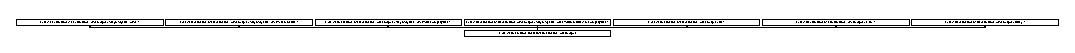
\includegraphics[height=0.270270cm]{classCqrs_1_1Authentication_1_1DefaultAuthenticationTokenHelper}
\end{center}
\end{figure}
\subsection*{Public Member Functions}
\begin{DoxyCompactItemize}
\item 
\hyperlink{classCqrs_1_1Authentication_1_1DefaultAuthenticationTokenHelper_a21bfae37d24b180797211396a0348526}{Default\+Authentication\+Token\+Helper} (I\+Context\+Item\+Collection\+Factory factory)
\item 
\hyperlink{classCqrs_1_1Authentication_1_1SingleSignOnTokenWithUserRsnAndCompanyRsn}{Single\+Sign\+On\+Token\+With\+User\+Rsn\+And\+Company\+Rsn} \hyperlink{classCqrs_1_1Authentication_1_1DefaultAuthenticationTokenHelper_ab06712f60b8afc6819b5372e3a21e13a}{Set\+Authentication\+Token} (\hyperlink{classCqrs_1_1Authentication_1_1SingleSignOnTokenWithUserRsnAndCompanyRsn}{Single\+Sign\+On\+Token\+With\+User\+Rsn\+And\+Company\+Rsn} token)
\item 
\hyperlink{classCqrs_1_1Authentication_1_1SingleSignOnTokenWithCompanyRsn}{Single\+Sign\+On\+Token\+With\+Company\+Rsn} \hyperlink{classCqrs_1_1Authentication_1_1DefaultAuthenticationTokenHelper_a2ae21fb09555d3ab5119f9ea4c69b202}{Set\+Authentication\+Token} (\hyperlink{classCqrs_1_1Authentication_1_1SingleSignOnTokenWithCompanyRsn}{Single\+Sign\+On\+Token\+With\+Company\+Rsn} token)
\item 
\hyperlink{classCqrs_1_1Authentication_1_1SingleSignOnTokenWithUserRsn}{Single\+Sign\+On\+Token\+With\+User\+Rsn} \hyperlink{classCqrs_1_1Authentication_1_1DefaultAuthenticationTokenHelper_a57d015883b278136590894a3885d246c}{Set\+Authentication\+Token} (\hyperlink{classCqrs_1_1Authentication_1_1SingleSignOnTokenWithUserRsn}{Single\+Sign\+On\+Token\+With\+User\+Rsn} token)
\item 
Guid \hyperlink{classCqrs_1_1Authentication_1_1DefaultAuthenticationTokenHelper_ad8c9ad34dde1f36073a1cf54bb82ffc5}{Set\+Authentication\+Token} (Guid token)
\item 
int \hyperlink{classCqrs_1_1Authentication_1_1DefaultAuthenticationTokenHelper_af1d9d9cbb1c02ca9a31b3dbd278f9a3e}{Set\+Authentication\+Token} (int token)
\item 
string \hyperlink{classCqrs_1_1Authentication_1_1DefaultAuthenticationTokenHelper_ae37a10289ec6cf99df30e1528feb0394}{Set\+Authentication\+Token} (string token)
\end{DoxyCompactItemize}


\subsection{Constructor \& Destructor Documentation}
\mbox{\Hypertarget{classCqrs_1_1Authentication_1_1DefaultAuthenticationTokenHelper_a21bfae37d24b180797211396a0348526}\label{classCqrs_1_1Authentication_1_1DefaultAuthenticationTokenHelper_a21bfae37d24b180797211396a0348526}} 
\index{Cqrs\+::\+Authentication\+::\+Default\+Authentication\+Token\+Helper@{Cqrs\+::\+Authentication\+::\+Default\+Authentication\+Token\+Helper}!Default\+Authentication\+Token\+Helper@{Default\+Authentication\+Token\+Helper}}
\index{Default\+Authentication\+Token\+Helper@{Default\+Authentication\+Token\+Helper}!Cqrs\+::\+Authentication\+::\+Default\+Authentication\+Token\+Helper@{Cqrs\+::\+Authentication\+::\+Default\+Authentication\+Token\+Helper}}
\subsubsection{\texorpdfstring{Default\+Authentication\+Token\+Helper()}{DefaultAuthenticationTokenHelper()}}
{\footnotesize\ttfamily Cqrs.\+Authentication.\+Default\+Authentication\+Token\+Helper.\+Default\+Authentication\+Token\+Helper (\begin{DoxyParamCaption}\item[{I\+Context\+Item\+Collection\+Factory}]{factory }\end{DoxyParamCaption})}



\subsection{Member Function Documentation}
\mbox{\Hypertarget{classCqrs_1_1Authentication_1_1DefaultAuthenticationTokenHelper_ab06712f60b8afc6819b5372e3a21e13a}\label{classCqrs_1_1Authentication_1_1DefaultAuthenticationTokenHelper_ab06712f60b8afc6819b5372e3a21e13a}} 
\index{Cqrs\+::\+Authentication\+::\+Default\+Authentication\+Token\+Helper@{Cqrs\+::\+Authentication\+::\+Default\+Authentication\+Token\+Helper}!Set\+Authentication\+Token@{Set\+Authentication\+Token}}
\index{Set\+Authentication\+Token@{Set\+Authentication\+Token}!Cqrs\+::\+Authentication\+::\+Default\+Authentication\+Token\+Helper@{Cqrs\+::\+Authentication\+::\+Default\+Authentication\+Token\+Helper}}
\subsubsection{\texorpdfstring{Set\+Authentication\+Token()}{SetAuthenticationToken()}\hspace{0.1cm}{\footnotesize\ttfamily [1/6]}}
{\footnotesize\ttfamily \hyperlink{classCqrs_1_1Authentication_1_1SingleSignOnTokenWithUserRsnAndCompanyRsn}{Single\+Sign\+On\+Token\+With\+User\+Rsn\+And\+Company\+Rsn} Cqrs.\+Authentication.\+Default\+Authentication\+Token\+Helper.\+Set\+Authentication\+Token (\begin{DoxyParamCaption}\item[{\hyperlink{classCqrs_1_1Authentication_1_1SingleSignOnTokenWithUserRsnAndCompanyRsn}{Single\+Sign\+On\+Token\+With\+User\+Rsn\+And\+Company\+Rsn}}]{token }\end{DoxyParamCaption})}

\mbox{\Hypertarget{classCqrs_1_1Authentication_1_1DefaultAuthenticationTokenHelper_a2ae21fb09555d3ab5119f9ea4c69b202}\label{classCqrs_1_1Authentication_1_1DefaultAuthenticationTokenHelper_a2ae21fb09555d3ab5119f9ea4c69b202}} 
\index{Cqrs\+::\+Authentication\+::\+Default\+Authentication\+Token\+Helper@{Cqrs\+::\+Authentication\+::\+Default\+Authentication\+Token\+Helper}!Set\+Authentication\+Token@{Set\+Authentication\+Token}}
\index{Set\+Authentication\+Token@{Set\+Authentication\+Token}!Cqrs\+::\+Authentication\+::\+Default\+Authentication\+Token\+Helper@{Cqrs\+::\+Authentication\+::\+Default\+Authentication\+Token\+Helper}}
\subsubsection{\texorpdfstring{Set\+Authentication\+Token()}{SetAuthenticationToken()}\hspace{0.1cm}{\footnotesize\ttfamily [2/6]}}
{\footnotesize\ttfamily \hyperlink{classCqrs_1_1Authentication_1_1SingleSignOnTokenWithCompanyRsn}{Single\+Sign\+On\+Token\+With\+Company\+Rsn} Cqrs.\+Authentication.\+Default\+Authentication\+Token\+Helper.\+Set\+Authentication\+Token (\begin{DoxyParamCaption}\item[{\hyperlink{classCqrs_1_1Authentication_1_1SingleSignOnTokenWithCompanyRsn}{Single\+Sign\+On\+Token\+With\+Company\+Rsn}}]{token }\end{DoxyParamCaption})}

\mbox{\Hypertarget{classCqrs_1_1Authentication_1_1DefaultAuthenticationTokenHelper_a57d015883b278136590894a3885d246c}\label{classCqrs_1_1Authentication_1_1DefaultAuthenticationTokenHelper_a57d015883b278136590894a3885d246c}} 
\index{Cqrs\+::\+Authentication\+::\+Default\+Authentication\+Token\+Helper@{Cqrs\+::\+Authentication\+::\+Default\+Authentication\+Token\+Helper}!Set\+Authentication\+Token@{Set\+Authentication\+Token}}
\index{Set\+Authentication\+Token@{Set\+Authentication\+Token}!Cqrs\+::\+Authentication\+::\+Default\+Authentication\+Token\+Helper@{Cqrs\+::\+Authentication\+::\+Default\+Authentication\+Token\+Helper}}
\subsubsection{\texorpdfstring{Set\+Authentication\+Token()}{SetAuthenticationToken()}\hspace{0.1cm}{\footnotesize\ttfamily [3/6]}}
{\footnotesize\ttfamily \hyperlink{classCqrs_1_1Authentication_1_1SingleSignOnTokenWithUserRsn}{Single\+Sign\+On\+Token\+With\+User\+Rsn} Cqrs.\+Authentication.\+Default\+Authentication\+Token\+Helper.\+Set\+Authentication\+Token (\begin{DoxyParamCaption}\item[{\hyperlink{classCqrs_1_1Authentication_1_1SingleSignOnTokenWithUserRsn}{Single\+Sign\+On\+Token\+With\+User\+Rsn}}]{token }\end{DoxyParamCaption})}

\mbox{\Hypertarget{classCqrs_1_1Authentication_1_1DefaultAuthenticationTokenHelper_ad8c9ad34dde1f36073a1cf54bb82ffc5}\label{classCqrs_1_1Authentication_1_1DefaultAuthenticationTokenHelper_ad8c9ad34dde1f36073a1cf54bb82ffc5}} 
\index{Cqrs\+::\+Authentication\+::\+Default\+Authentication\+Token\+Helper@{Cqrs\+::\+Authentication\+::\+Default\+Authentication\+Token\+Helper}!Set\+Authentication\+Token@{Set\+Authentication\+Token}}
\index{Set\+Authentication\+Token@{Set\+Authentication\+Token}!Cqrs\+::\+Authentication\+::\+Default\+Authentication\+Token\+Helper@{Cqrs\+::\+Authentication\+::\+Default\+Authentication\+Token\+Helper}}
\subsubsection{\texorpdfstring{Set\+Authentication\+Token()}{SetAuthenticationToken()}\hspace{0.1cm}{\footnotesize\ttfamily [4/6]}}
{\footnotesize\ttfamily Guid Cqrs.\+Authentication.\+Default\+Authentication\+Token\+Helper.\+Set\+Authentication\+Token (\begin{DoxyParamCaption}\item[{Guid}]{token }\end{DoxyParamCaption})}

\mbox{\Hypertarget{classCqrs_1_1Authentication_1_1DefaultAuthenticationTokenHelper_af1d9d9cbb1c02ca9a31b3dbd278f9a3e}\label{classCqrs_1_1Authentication_1_1DefaultAuthenticationTokenHelper_af1d9d9cbb1c02ca9a31b3dbd278f9a3e}} 
\index{Cqrs\+::\+Authentication\+::\+Default\+Authentication\+Token\+Helper@{Cqrs\+::\+Authentication\+::\+Default\+Authentication\+Token\+Helper}!Set\+Authentication\+Token@{Set\+Authentication\+Token}}
\index{Set\+Authentication\+Token@{Set\+Authentication\+Token}!Cqrs\+::\+Authentication\+::\+Default\+Authentication\+Token\+Helper@{Cqrs\+::\+Authentication\+::\+Default\+Authentication\+Token\+Helper}}
\subsubsection{\texorpdfstring{Set\+Authentication\+Token()}{SetAuthenticationToken()}\hspace{0.1cm}{\footnotesize\ttfamily [5/6]}}
{\footnotesize\ttfamily int Cqrs.\+Authentication.\+Default\+Authentication\+Token\+Helper.\+Set\+Authentication\+Token (\begin{DoxyParamCaption}\item[{int}]{token }\end{DoxyParamCaption})}

\mbox{\Hypertarget{classCqrs_1_1Authentication_1_1DefaultAuthenticationTokenHelper_ae37a10289ec6cf99df30e1528feb0394}\label{classCqrs_1_1Authentication_1_1DefaultAuthenticationTokenHelper_ae37a10289ec6cf99df30e1528feb0394}} 
\index{Cqrs\+::\+Authentication\+::\+Default\+Authentication\+Token\+Helper@{Cqrs\+::\+Authentication\+::\+Default\+Authentication\+Token\+Helper}!Set\+Authentication\+Token@{Set\+Authentication\+Token}}
\index{Set\+Authentication\+Token@{Set\+Authentication\+Token}!Cqrs\+::\+Authentication\+::\+Default\+Authentication\+Token\+Helper@{Cqrs\+::\+Authentication\+::\+Default\+Authentication\+Token\+Helper}}
\subsubsection{\texorpdfstring{Set\+Authentication\+Token()}{SetAuthenticationToken()}\hspace{0.1cm}{\footnotesize\ttfamily [6/6]}}
{\footnotesize\ttfamily string Cqrs.\+Authentication.\+Default\+Authentication\+Token\+Helper.\+Set\+Authentication\+Token (\begin{DoxyParamCaption}\item[{string}]{token }\end{DoxyParamCaption})}


\hypertarget{classCqrs_1_1Authentication_1_1DefaultSingleSignOnTokenFactory}{}\section{Cqrs.\+Authentication.\+Default\+Single\+Sign\+On\+Token\+Factory Class Reference}
\label{classCqrs_1_1Authentication_1_1DefaultSingleSignOnTokenFactory}\index{Cqrs.\+Authentication.\+Default\+Single\+Sign\+On\+Token\+Factory@{Cqrs.\+Authentication.\+Default\+Single\+Sign\+On\+Token\+Factory}}
Inheritance diagram for Cqrs.\+Authentication.\+Default\+Single\+Sign\+On\+Token\+Factory\+:\begin{figure}[H]
\begin{center}
\leavevmode
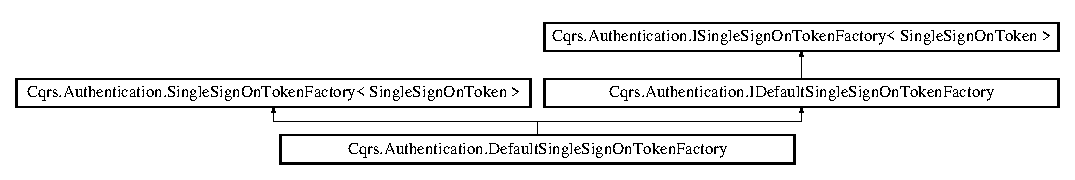
\includegraphics[height=1.967213cm]{classCqrs_1_1Authentication_1_1DefaultSingleSignOnTokenFactory}
\end{center}
\end{figure}
\subsection*{Public Member Functions}
\begin{DoxyCompactItemize}
\item 
virtual T\+Single\+Sign\+On\+Token \hyperlink{classCqrs_1_1Authentication_1_1DefaultSingleSignOnTokenFactory_a1bb480afd0a467461b0db59da641fe29}{Renew\+Token\+Expiry$<$ T\+Single\+Sign\+On\+Token $>$} (T\+Single\+Sign\+On\+Token token, int timeout\+In\+Minutes=360)
\end{DoxyCompactItemize}


\subsection{Member Function Documentation}
\mbox{\Hypertarget{classCqrs_1_1Authentication_1_1DefaultSingleSignOnTokenFactory_a1bb480afd0a467461b0db59da641fe29}\label{classCqrs_1_1Authentication_1_1DefaultSingleSignOnTokenFactory_a1bb480afd0a467461b0db59da641fe29}} 
\index{Cqrs\+::\+Authentication\+::\+Default\+Single\+Sign\+On\+Token\+Factory@{Cqrs\+::\+Authentication\+::\+Default\+Single\+Sign\+On\+Token\+Factory}!Renew\+Token\+Expiry$<$ T\+Single\+Sign\+On\+Token $>$@{Renew\+Token\+Expiry$<$ T\+Single\+Sign\+On\+Token $>$}}
\index{Renew\+Token\+Expiry$<$ T\+Single\+Sign\+On\+Token $>$@{Renew\+Token\+Expiry$<$ T\+Single\+Sign\+On\+Token $>$}!Cqrs\+::\+Authentication\+::\+Default\+Single\+Sign\+On\+Token\+Factory@{Cqrs\+::\+Authentication\+::\+Default\+Single\+Sign\+On\+Token\+Factory}}
\subsubsection{\texorpdfstring{Renew\+Token\+Expiry$<$ T\+Single\+Sign\+On\+Token $>$()}{RenewTokenExpiry< TSingleSignOnToken >()}}
{\footnotesize\ttfamily virtual T\+Single\+Sign\+On\+Token Cqrs.\+Authentication.\+Default\+Single\+Sign\+On\+Token\+Factory.\+Renew\+Token\+Expiry$<$ T\+Single\+Sign\+On\+Token $>$ (\begin{DoxyParamCaption}\item[{T\+Single\+Sign\+On\+Token}]{token,  }\item[{int}]{timeout\+In\+Minutes = {\ttfamily 360} }\end{DoxyParamCaption})\hspace{0.3cm}{\ttfamily [virtual]}}

\begin{Desc}
\item[Type Constraints]\begin{description}
\item[{\em T\+Single\+Sign\+On\+Token} : {\em I\+Single\+Sign\+On\+Token}]\end{description}
\end{Desc}

\hypertarget{interfaceCqrs_1_1Authentication_1_1IAuthenticationTokenHelper}{}\section{Cqrs.\+Authentication.\+I\+Authentication\+Token\+Helper$<$ T\+Authentication\+Token $>$ Interface Template Reference}
\label{interfaceCqrs_1_1Authentication_1_1IAuthenticationTokenHelper}\index{Cqrs.\+Authentication.\+I\+Authentication\+Token\+Helper$<$ T\+Authentication\+Token $>$@{Cqrs.\+Authentication.\+I\+Authentication\+Token\+Helper$<$ T\+Authentication\+Token $>$}}


A helper for setting and retrieving authentication tokens of type {\itshape T\+Authentication\+Token} .  


Inheritance diagram for Cqrs.\+Authentication.\+I\+Authentication\+Token\+Helper$<$ T\+Authentication\+Token $>$\+:\begin{figure}[H]
\begin{center}
\leavevmode
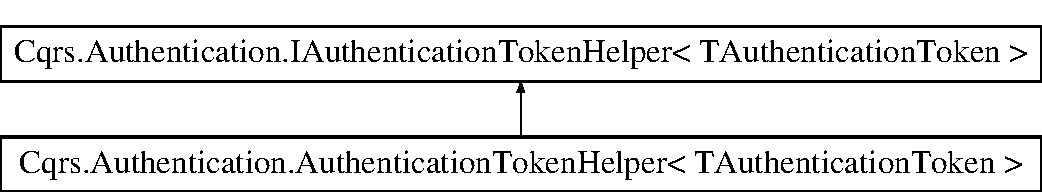
\includegraphics[height=2.000000cm]{interfaceCqrs_1_1Authentication_1_1IAuthenticationTokenHelper}
\end{center}
\end{figure}
\subsection*{Public Member Functions}
\begin{DoxyCompactItemize}
\item 
T\+Authentication\+Token \hyperlink{interfaceCqrs_1_1Authentication_1_1IAuthenticationTokenHelper_a4ccb928b5a6880921226508d36d4afc8_a4ccb928b5a6880921226508d36d4afc8}{Get\+Authentication\+Token} ()
\begin{DoxyCompactList}\small\item\em Get the current {\itshape T\+Authentication\+Token} authentication token for the current context/request. \end{DoxyCompactList}\item 
T\+Authentication\+Token \hyperlink{interfaceCqrs_1_1Authentication_1_1IAuthenticationTokenHelper_a1af9409257b2d8086be6dfae4edf37fb_a1af9409257b2d8086be6dfae4edf37fb}{Set\+Authentication\+Token} (T\+Authentication\+Token token)
\begin{DoxyCompactList}\small\item\em Set the provided {\itshape token}  for the current context/request. \end{DoxyCompactList}\end{DoxyCompactItemize}


\subsection{Detailed Description}
A helper for setting and retrieving authentication tokens of type {\itshape T\+Authentication\+Token} . 


\begin{DoxyTemplParams}{Template Parameters}
{\em T\+Authentication\+Token} & The Type of authentication token.\\
\hline
\end{DoxyTemplParams}


\subsection{Member Function Documentation}
\mbox{\Hypertarget{interfaceCqrs_1_1Authentication_1_1IAuthenticationTokenHelper_a4ccb928b5a6880921226508d36d4afc8_a4ccb928b5a6880921226508d36d4afc8}\label{interfaceCqrs_1_1Authentication_1_1IAuthenticationTokenHelper_a4ccb928b5a6880921226508d36d4afc8_a4ccb928b5a6880921226508d36d4afc8}} 
\index{Cqrs\+::\+Authentication\+::\+I\+Authentication\+Token\+Helper@{Cqrs\+::\+Authentication\+::\+I\+Authentication\+Token\+Helper}!Get\+Authentication\+Token@{Get\+Authentication\+Token}}
\index{Get\+Authentication\+Token@{Get\+Authentication\+Token}!Cqrs\+::\+Authentication\+::\+I\+Authentication\+Token\+Helper@{Cqrs\+::\+Authentication\+::\+I\+Authentication\+Token\+Helper}}
\subsubsection{\texorpdfstring{Get\+Authentication\+Token()}{GetAuthenticationToken()}}
{\footnotesize\ttfamily T\+Authentication\+Token \hyperlink{interfaceCqrs_1_1Authentication_1_1IAuthenticationTokenHelper}{Cqrs.\+Authentication.\+I\+Authentication\+Token\+Helper}$<$ T\+Authentication\+Token $>$.Get\+Authentication\+Token (\begin{DoxyParamCaption}{ }\end{DoxyParamCaption})}



Get the current {\itshape T\+Authentication\+Token} authentication token for the current context/request. 



Implemented in \hyperlink{classCqrs_1_1Authentication_1_1AuthenticationTokenHelper_ad8c73eb3c1a79d141c406cb7abed1466_ad8c73eb3c1a79d141c406cb7abed1466}{Cqrs.\+Authentication.\+Authentication\+Token\+Helper$<$ T\+Authentication\+Token $>$}.

\mbox{\Hypertarget{interfaceCqrs_1_1Authentication_1_1IAuthenticationTokenHelper_a1af9409257b2d8086be6dfae4edf37fb_a1af9409257b2d8086be6dfae4edf37fb}\label{interfaceCqrs_1_1Authentication_1_1IAuthenticationTokenHelper_a1af9409257b2d8086be6dfae4edf37fb_a1af9409257b2d8086be6dfae4edf37fb}} 
\index{Cqrs\+::\+Authentication\+::\+I\+Authentication\+Token\+Helper@{Cqrs\+::\+Authentication\+::\+I\+Authentication\+Token\+Helper}!Set\+Authentication\+Token@{Set\+Authentication\+Token}}
\index{Set\+Authentication\+Token@{Set\+Authentication\+Token}!Cqrs\+::\+Authentication\+::\+I\+Authentication\+Token\+Helper@{Cqrs\+::\+Authentication\+::\+I\+Authentication\+Token\+Helper}}
\subsubsection{\texorpdfstring{Set\+Authentication\+Token()}{SetAuthenticationToken()}}
{\footnotesize\ttfamily T\+Authentication\+Token \hyperlink{interfaceCqrs_1_1Authentication_1_1IAuthenticationTokenHelper}{Cqrs.\+Authentication.\+I\+Authentication\+Token\+Helper}$<$ T\+Authentication\+Token $>$.Set\+Authentication\+Token (\begin{DoxyParamCaption}\item[{T\+Authentication\+Token}]{token }\end{DoxyParamCaption})}



Set the provided {\itshape token}  for the current context/request. 



Implemented in \hyperlink{classCqrs_1_1Authentication_1_1AuthenticationTokenHelper_a276361d51d5b8d4d880884b6bb1a1070_a276361d51d5b8d4d880884b6bb1a1070}{Cqrs.\+Authentication.\+Authentication\+Token\+Helper$<$ T\+Authentication\+Token $>$}.


\hypertarget{interfaceCqrs_1_1Authentication_1_1IDefaultSingleSignOnTokenFactory}{}\section{Cqrs.\+Authentication.\+I\+Default\+Single\+Sign\+On\+Token\+Factory Interface Reference}
\label{interfaceCqrs_1_1Authentication_1_1IDefaultSingleSignOnTokenFactory}\index{Cqrs.\+Authentication.\+I\+Default\+Single\+Sign\+On\+Token\+Factory@{Cqrs.\+Authentication.\+I\+Default\+Single\+Sign\+On\+Token\+Factory}}
Inheritance diagram for Cqrs.\+Authentication.\+I\+Default\+Single\+Sign\+On\+Token\+Factory\+:\begin{figure}[H]
\begin{center}
\leavevmode
\includegraphics[height=3.000000cm]{interfaceCqrs_1_1Authentication_1_1IDefaultSingleSignOnTokenFactory}
\end{center}
\end{figure}
\subsection*{Public Member Functions}
\begin{DoxyCompactItemize}
\item 
\hyperlink{interfaceCqrs_1_1Authentication_1_1ISingleSignOnToken}{I\+Single\+Sign\+On\+Token} \hyperlink{interfaceCqrs_1_1Authentication_1_1IDefaultSingleSignOnTokenFactory_aff3e7060705a3a8e021c1182ce101b33}{Renew\+Token\+Expiry} (\hyperlink{interfaceCqrs_1_1Authentication_1_1ISingleSignOnToken}{I\+Single\+Sign\+On\+Token} token, int timeout\+In\+Minutes=360)
\end{DoxyCompactItemize}


\subsection{Member Function Documentation}
\mbox{\Hypertarget{interfaceCqrs_1_1Authentication_1_1IDefaultSingleSignOnTokenFactory_aff3e7060705a3a8e021c1182ce101b33}\label{interfaceCqrs_1_1Authentication_1_1IDefaultSingleSignOnTokenFactory_aff3e7060705a3a8e021c1182ce101b33}} 
\index{Cqrs\+::\+Authentication\+::\+I\+Default\+Single\+Sign\+On\+Token\+Factory@{Cqrs\+::\+Authentication\+::\+I\+Default\+Single\+Sign\+On\+Token\+Factory}!Renew\+Token\+Expiry@{Renew\+Token\+Expiry}}
\index{Renew\+Token\+Expiry@{Renew\+Token\+Expiry}!Cqrs\+::\+Authentication\+::\+I\+Default\+Single\+Sign\+On\+Token\+Factory@{Cqrs\+::\+Authentication\+::\+I\+Default\+Single\+Sign\+On\+Token\+Factory}}
\subsubsection{\texorpdfstring{Renew\+Token\+Expiry()}{RenewTokenExpiry()}}
{\footnotesize\ttfamily \hyperlink{interfaceCqrs_1_1Authentication_1_1ISingleSignOnToken}{I\+Single\+Sign\+On\+Token} Cqrs.\+Authentication.\+I\+Default\+Single\+Sign\+On\+Token\+Factory.\+Renew\+Token\+Expiry (\begin{DoxyParamCaption}\item[{\hyperlink{interfaceCqrs_1_1Authentication_1_1ISingleSignOnToken}{I\+Single\+Sign\+On\+Token}}]{token,  }\item[{int}]{timeout\+In\+Minutes = {\ttfamily 360} }\end{DoxyParamCaption})}


\hypertarget{interfaceCqrs_1_1Authentication_1_1ISingleSignOnToken}{}\section{Cqrs.\+Authentication.\+I\+Single\+Sign\+On\+Token Interface Reference}
\label{interfaceCqrs_1_1Authentication_1_1ISingleSignOnToken}\index{Cqrs.\+Authentication.\+I\+Single\+Sign\+On\+Token@{Cqrs.\+Authentication.\+I\+Single\+Sign\+On\+Token}}
Inheritance diagram for Cqrs.\+Authentication.\+I\+Single\+Sign\+On\+Token\+:\begin{figure}[H]
\begin{center}
\leavevmode
\includegraphics[height=0.534096cm]{interfaceCqrs_1_1Authentication_1_1ISingleSignOnToken}
\end{center}
\end{figure}
\subsection*{Public Member Functions}
\begin{DoxyCompactItemize}
\item 
string \hyperlink{interfaceCqrs_1_1Authentication_1_1ISingleSignOnToken_af34e8c0b052865d687064d3381bfbcdb_af34e8c0b052865d687064d3381bfbcdb}{Serialise} ()
\end{DoxyCompactItemize}
\subsection*{Properties}
\begin{DoxyCompactItemize}
\item 
string \hyperlink{interfaceCqrs_1_1Authentication_1_1ISingleSignOnToken_aba74aff1a43375dce8d80fa94a94a57b_aba74aff1a43375dce8d80fa94a94a57b}{Token}\hspace{0.3cm}{\ttfamily  \mbox{[}get, set\mbox{]}}
\item 
Date\+Time \hyperlink{interfaceCqrs_1_1Authentication_1_1ISingleSignOnToken_a50af484569cc78f88acb01f1938a7cd8_a50af484569cc78f88acb01f1938a7cd8}{Time\+Of\+Expiry}\hspace{0.3cm}{\ttfamily  \mbox{[}get, set\mbox{]}}
\item 
Date\+Time \hyperlink{interfaceCqrs_1_1Authentication_1_1ISingleSignOnToken_a0c41d76beea893838e556fba8dbc59db_a0c41d76beea893838e556fba8dbc59db}{Date\+Issued}\hspace{0.3cm}{\ttfamily  \mbox{[}get, set\mbox{]}}
\end{DoxyCompactItemize}


\subsection{Member Function Documentation}
\mbox{\Hypertarget{interfaceCqrs_1_1Authentication_1_1ISingleSignOnToken_af34e8c0b052865d687064d3381bfbcdb_af34e8c0b052865d687064d3381bfbcdb}\label{interfaceCqrs_1_1Authentication_1_1ISingleSignOnToken_af34e8c0b052865d687064d3381bfbcdb_af34e8c0b052865d687064d3381bfbcdb}} 
\index{Cqrs\+::\+Authentication\+::\+I\+Single\+Sign\+On\+Token@{Cqrs\+::\+Authentication\+::\+I\+Single\+Sign\+On\+Token}!Serialise@{Serialise}}
\index{Serialise@{Serialise}!Cqrs\+::\+Authentication\+::\+I\+Single\+Sign\+On\+Token@{Cqrs\+::\+Authentication\+::\+I\+Single\+Sign\+On\+Token}}
\subsubsection{\texorpdfstring{Serialise()}{Serialise()}}
{\footnotesize\ttfamily string Cqrs.\+Authentication.\+I\+Single\+Sign\+On\+Token.\+Serialise (\begin{DoxyParamCaption}{ }\end{DoxyParamCaption})}



Implemented in \hyperlink{classCqrs_1_1Authentication_1_1SingleSignOnTokenWithUserRsnAndCompanyRsn_a8d44249c00e5264dc7b37f4868836a80_a8d44249c00e5264dc7b37f4868836a80}{Cqrs.\+Authentication.\+Single\+Sign\+On\+Token\+With\+User\+Rsn\+And\+Company\+Rsn}, \hyperlink{classCqrs_1_1Azure_1_1DocumentDb_1_1Repositories_1_1Authentication_1_1AzureSingleSignOnToken_a55c07b93600e6863985b50d4df346af0_a55c07b93600e6863985b50d4df346af0}{Cqrs.\+Azure.\+Document\+Db.\+Repositories.\+Authentication.\+Azure\+Single\+Sign\+On\+Token}, \hyperlink{classCqrs_1_1Mongo_1_1Repositories_1_1Authentication_1_1SingleSignOnToken_ab0ad6b0a6065a2553a093214e5a033b5_ab0ad6b0a6065a2553a093214e5a033b5}{Cqrs.\+Mongo.\+Repositories.\+Authentication.\+Single\+Sign\+On\+Token}, \hyperlink{classCqrs_1_1MongoDB_1_1Repositories_1_1Authentication_1_1SingleSignOnToken_a2392ecdb53f1f2a38a67d80a77f11ba4_a2392ecdb53f1f2a38a67d80a77f11ba4}{Cqrs.\+Mongo\+D\+B.\+Repositories.\+Authentication.\+Single\+Sign\+On\+Token}, \hyperlink{classCqrs_1_1Authentication_1_1SingleSignOnTokenWithCompanyRsn_a0bc9f0fae90121d029fe0730708f4210_a0bc9f0fae90121d029fe0730708f4210}{Cqrs.\+Authentication.\+Single\+Sign\+On\+Token\+With\+Company\+Rsn}, \hyperlink{classCqrs_1_1Authentication_1_1SingleSignOnToken_a5e859c6c5db5aaa9ef4e8f2086df4604_a5e859c6c5db5aaa9ef4e8f2086df4604}{Cqrs.\+Authentication.\+Single\+Sign\+On\+Token}, and \hyperlink{classCqrs_1_1Authentication_1_1SingleSignOnTokenWithUserRsn_a8103820e6352c10b3990fb027dd9b5ae_a8103820e6352c10b3990fb027dd9b5ae}{Cqrs.\+Authentication.\+Single\+Sign\+On\+Token\+With\+User\+Rsn}.



\subsection{Property Documentation}
\mbox{\Hypertarget{interfaceCqrs_1_1Authentication_1_1ISingleSignOnToken_a0c41d76beea893838e556fba8dbc59db_a0c41d76beea893838e556fba8dbc59db}\label{interfaceCqrs_1_1Authentication_1_1ISingleSignOnToken_a0c41d76beea893838e556fba8dbc59db_a0c41d76beea893838e556fba8dbc59db}} 
\index{Cqrs\+::\+Authentication\+::\+I\+Single\+Sign\+On\+Token@{Cqrs\+::\+Authentication\+::\+I\+Single\+Sign\+On\+Token}!Date\+Issued@{Date\+Issued}}
\index{Date\+Issued@{Date\+Issued}!Cqrs\+::\+Authentication\+::\+I\+Single\+Sign\+On\+Token@{Cqrs\+::\+Authentication\+::\+I\+Single\+Sign\+On\+Token}}
\subsubsection{\texorpdfstring{Date\+Issued}{DateIssued}}
{\footnotesize\ttfamily Date\+Time Cqrs.\+Authentication.\+I\+Single\+Sign\+On\+Token.\+Date\+Issued\hspace{0.3cm}{\ttfamily [get]}, {\ttfamily [set]}}

\mbox{\Hypertarget{interfaceCqrs_1_1Authentication_1_1ISingleSignOnToken_a50af484569cc78f88acb01f1938a7cd8_a50af484569cc78f88acb01f1938a7cd8}\label{interfaceCqrs_1_1Authentication_1_1ISingleSignOnToken_a50af484569cc78f88acb01f1938a7cd8_a50af484569cc78f88acb01f1938a7cd8}} 
\index{Cqrs\+::\+Authentication\+::\+I\+Single\+Sign\+On\+Token@{Cqrs\+::\+Authentication\+::\+I\+Single\+Sign\+On\+Token}!Time\+Of\+Expiry@{Time\+Of\+Expiry}}
\index{Time\+Of\+Expiry@{Time\+Of\+Expiry}!Cqrs\+::\+Authentication\+::\+I\+Single\+Sign\+On\+Token@{Cqrs\+::\+Authentication\+::\+I\+Single\+Sign\+On\+Token}}
\subsubsection{\texorpdfstring{Time\+Of\+Expiry}{TimeOfExpiry}}
{\footnotesize\ttfamily Date\+Time Cqrs.\+Authentication.\+I\+Single\+Sign\+On\+Token.\+Time\+Of\+Expiry\hspace{0.3cm}{\ttfamily [get]}, {\ttfamily [set]}}

\mbox{\Hypertarget{interfaceCqrs_1_1Authentication_1_1ISingleSignOnToken_aba74aff1a43375dce8d80fa94a94a57b_aba74aff1a43375dce8d80fa94a94a57b}\label{interfaceCqrs_1_1Authentication_1_1ISingleSignOnToken_aba74aff1a43375dce8d80fa94a94a57b_aba74aff1a43375dce8d80fa94a94a57b}} 
\index{Cqrs\+::\+Authentication\+::\+I\+Single\+Sign\+On\+Token@{Cqrs\+::\+Authentication\+::\+I\+Single\+Sign\+On\+Token}!Token@{Token}}
\index{Token@{Token}!Cqrs\+::\+Authentication\+::\+I\+Single\+Sign\+On\+Token@{Cqrs\+::\+Authentication\+::\+I\+Single\+Sign\+On\+Token}}
\subsubsection{\texorpdfstring{Token}{Token}}
{\footnotesize\ttfamily string Cqrs.\+Authentication.\+I\+Single\+Sign\+On\+Token.\+Token\hspace{0.3cm}{\ttfamily [get]}, {\ttfamily [set]}}


\hypertarget{interfaceCqrs_1_1Authentication_1_1ISingleSignOnTokenFactory}{}\doxysection{Cqrs.\+Authentication.\+I\+Single\+Sign\+On\+Token\+Factory$<$ T\+Single\+Sign\+On\+Token $>$ Interface Template Reference}
\label{interfaceCqrs_1_1Authentication_1_1ISingleSignOnTokenFactory}\index{Cqrs.Authentication.ISingleSignOnTokenFactory$<$ TSingleSignOnToken $>$@{Cqrs.Authentication.ISingleSignOnTokenFactory$<$ TSingleSignOnToken $>$}}


A factory for creating new authentication tokens of type {\itshape T\+Single\+Sign\+On\+Token} .  


Inheritance diagram for Cqrs.\+Authentication.\+I\+Single\+Sign\+On\+Token\+Factory$<$ T\+Single\+Sign\+On\+Token $>$\+:\begin{figure}[H]
\begin{center}
\leavevmode
\includegraphics[height=2.000000cm]{interfaceCqrs_1_1Authentication_1_1ISingleSignOnTokenFactory}
\end{center}
\end{figure}
\doxysubsection*{Public Member Functions}
\begin{DoxyCompactItemize}
\item 
T\+Single\+Sign\+On\+Token \mbox{\hyperlink{interfaceCqrs_1_1Authentication_1_1ISingleSignOnTokenFactory_ad0795fb60ca13dd24db18556089e2834_ad0795fb60ca13dd24db18556089e2834}{Create\+New}} (int timeout\+In\+Minutes=360)
\begin{DoxyCompactList}\small\item\em Create a new {\itshape T\+Single\+Sign\+On\+Token} . \end{DoxyCompactList}\item 
T\+Single\+Sign\+On\+Token \mbox{\hyperlink{interfaceCqrs_1_1Authentication_1_1ISingleSignOnTokenFactory_ab436004ad1631140f7a58927cbacd8c4_ab436004ad1631140f7a58927cbacd8c4}{Renew\+Token\+Expiry}} (T\+Single\+Sign\+On\+Token token, int timeout\+In\+Minutes=360)
\begin{DoxyCompactList}\small\item\em Renew the value of \mbox{\hyperlink{interfaceCqrs_1_1Authentication_1_1ISingleSignOnToken_a50af484569cc78f88acb01f1938a7cd8_a50af484569cc78f88acb01f1938a7cd8}{I\+Single\+Sign\+On\+Token.\+Time\+Of\+Expiry}}. \end{DoxyCompactList}\end{DoxyCompactItemize}


\doxysubsection{Detailed Description}
A factory for creating new authentication tokens of type {\itshape T\+Single\+Sign\+On\+Token} . 


\begin{DoxyTemplParams}{Template Parameters}
{\em T\+Single\+Sign\+On\+Token} & The Type of \mbox{\hyperlink{interfaceCqrs_1_1Authentication_1_1ISingleSignOnToken}{I\+Single\+Sign\+On\+Token}}.\\
\hline
\end{DoxyTemplParams}
\begin{Desc}
\item[Type Constraints]\begin{description}
\item[{\em T\+Single\+Sign\+On\+Token} : {\em \mbox{\hyperlink{interfaceCqrs_1_1Authentication_1_1ISingleSignOnToken}{I\+Single\+Sign\+On\+Token}}}]\item[{\em T\+Single\+Sign\+On\+Token} : {\em new()}]\end{description}
\end{Desc}


\doxysubsection{Member Function Documentation}
\mbox{\Hypertarget{interfaceCqrs_1_1Authentication_1_1ISingleSignOnTokenFactory_ad0795fb60ca13dd24db18556089e2834_ad0795fb60ca13dd24db18556089e2834}\label{interfaceCqrs_1_1Authentication_1_1ISingleSignOnTokenFactory_ad0795fb60ca13dd24db18556089e2834_ad0795fb60ca13dd24db18556089e2834}} 
\index{Cqrs.Authentication.ISingleSignOnTokenFactory$<$ TSingleSignOnToken $>$@{Cqrs.Authentication.ISingleSignOnTokenFactory$<$ TSingleSignOnToken $>$}!CreateNew@{CreateNew}}
\index{CreateNew@{CreateNew}!Cqrs.Authentication.ISingleSignOnTokenFactory$<$ TSingleSignOnToken $>$@{Cqrs.Authentication.ISingleSignOnTokenFactory$<$ TSingleSignOnToken $>$}}
\doxysubsubsection{\texorpdfstring{CreateNew()}{CreateNew()}}
{\footnotesize\ttfamily T\+Single\+Sign\+On\+Token \mbox{\hyperlink{interfaceCqrs_1_1Authentication_1_1ISingleSignOnTokenFactory}{Cqrs.\+Authentication.\+I\+Single\+Sign\+On\+Token\+Factory}}$<$ T\+Single\+Sign\+On\+Token $>$.Create\+New (\begin{DoxyParamCaption}\item[{int}]{timeout\+In\+Minutes = {\ttfamily 360} }\end{DoxyParamCaption})}



Create a new {\itshape T\+Single\+Sign\+On\+Token} . 


\begin{DoxyParams}{Parameters}
{\em timeout\+In\+Minutes} & The amount of time in minutes to set the \mbox{\hyperlink{interfaceCqrs_1_1Authentication_1_1ISingleSignOnToken_a50af484569cc78f88acb01f1938a7cd8_a50af484569cc78f88acb01f1938a7cd8}{I\+Single\+Sign\+On\+Token.\+Time\+Of\+Expiry}} to. This is from Date\+Time.\+Utc\+Now\\
\hline
\end{DoxyParams}


Implemented in \mbox{\hyperlink{classCqrs_1_1Authentication_1_1SingleSignOnTokenFactory_ab4d01a3600dbe9aa358cd93c98ccf281_ab4d01a3600dbe9aa358cd93c98ccf281}{Cqrs.\+Authentication.\+Single\+Sign\+On\+Token\+Factory$<$ T\+Single\+Sign\+On\+Token $>$}}.

\mbox{\Hypertarget{interfaceCqrs_1_1Authentication_1_1ISingleSignOnTokenFactory_ab436004ad1631140f7a58927cbacd8c4_ab436004ad1631140f7a58927cbacd8c4}\label{interfaceCqrs_1_1Authentication_1_1ISingleSignOnTokenFactory_ab436004ad1631140f7a58927cbacd8c4_ab436004ad1631140f7a58927cbacd8c4}} 
\index{Cqrs.Authentication.ISingleSignOnTokenFactory$<$ TSingleSignOnToken $>$@{Cqrs.Authentication.ISingleSignOnTokenFactory$<$ TSingleSignOnToken $>$}!RenewTokenExpiry@{RenewTokenExpiry}}
\index{RenewTokenExpiry@{RenewTokenExpiry}!Cqrs.Authentication.ISingleSignOnTokenFactory$<$ TSingleSignOnToken $>$@{Cqrs.Authentication.ISingleSignOnTokenFactory$<$ TSingleSignOnToken $>$}}
\doxysubsubsection{\texorpdfstring{RenewTokenExpiry()}{RenewTokenExpiry()}}
{\footnotesize\ttfamily T\+Single\+Sign\+On\+Token \mbox{\hyperlink{interfaceCqrs_1_1Authentication_1_1ISingleSignOnTokenFactory}{Cqrs.\+Authentication.\+I\+Single\+Sign\+On\+Token\+Factory}}$<$ T\+Single\+Sign\+On\+Token $>$.Renew\+Token\+Expiry (\begin{DoxyParamCaption}\item[{T\+Single\+Sign\+On\+Token}]{token,  }\item[{int}]{timeout\+In\+Minutes = {\ttfamily 360} }\end{DoxyParamCaption})}



Renew the value of \mbox{\hyperlink{interfaceCqrs_1_1Authentication_1_1ISingleSignOnToken_a50af484569cc78f88acb01f1938a7cd8_a50af484569cc78f88acb01f1938a7cd8}{I\+Single\+Sign\+On\+Token.\+Time\+Of\+Expiry}}. 


\begin{DoxyParams}{Parameters}
{\em token} & The \mbox{\hyperlink{interfaceCqrs_1_1Authentication_1_1ISingleSignOnToken}{I\+Single\+Sign\+On\+Token}} to renew.\\
\hline
{\em timeout\+In\+Minutes} & The amount of time in minutes to set the \mbox{\hyperlink{interfaceCqrs_1_1Authentication_1_1ISingleSignOnToken_a50af484569cc78f88acb01f1938a7cd8_a50af484569cc78f88acb01f1938a7cd8}{I\+Single\+Sign\+On\+Token.\+Time\+Of\+Expiry}} to. This is from Date\+Time.\+Utc\+Now\\
\hline
\end{DoxyParams}


Implemented in \mbox{\hyperlink{classCqrs_1_1Authentication_1_1SingleSignOnTokenFactory_a699ceac65874b8319d2e26fa88f554be_a699ceac65874b8319d2e26fa88f554be}{Cqrs.\+Authentication.\+Single\+Sign\+On\+Token\+Factory$<$ T\+Single\+Sign\+On\+Token $>$}}.


\hypertarget{interfaceCqrs_1_1Authentication_1_1ISingleSignOnTokenWithCompanyRsn}{}\section{Cqrs.\+Authentication.\+I\+Single\+Sign\+On\+Token\+With\+Company\+Rsn Interface Reference}
\label{interfaceCqrs_1_1Authentication_1_1ISingleSignOnTokenWithCompanyRsn}\index{Cqrs.\+Authentication.\+I\+Single\+Sign\+On\+Token\+With\+Company\+Rsn@{Cqrs.\+Authentication.\+I\+Single\+Sign\+On\+Token\+With\+Company\+Rsn}}


This is a \hyperlink{interfaceCqrs_1_1Authentication_1_1ISingleSignOnToken}{I\+Single\+Sign\+On\+Token} that includes an identifiable \hyperlink{interfaceCqrs_1_1Authentication_1_1ISingleSignOnTokenWithCompanyRsn_a26ffa6ca2e583f0ecc440b68fe3edd52_a26ffa6ca2e583f0ecc440b68fe3edd52}{Company\+Rsn} to optimise the hits of the \hyperlink{}{Data\+Stores} by including data you most likely need. As such, if not used correctly, this can expose identifiable information. It is suggested the service layer populates this before sending commands as part of authorisation/authentication.  


Inheritance diagram for Cqrs.\+Authentication.\+I\+Single\+Sign\+On\+Token\+With\+Company\+Rsn\+:\begin{figure}[H]
\begin{center}
\leavevmode
\includegraphics[height=2.692308cm]{interfaceCqrs_1_1Authentication_1_1ISingleSignOnTokenWithCompanyRsn}
\end{center}
\end{figure}
\subsection*{Properties}
\begin{DoxyCompactItemize}
\item 
Guid \hyperlink{interfaceCqrs_1_1Authentication_1_1ISingleSignOnTokenWithCompanyRsn_a26ffa6ca2e583f0ecc440b68fe3edd52_a26ffa6ca2e583f0ecc440b68fe3edd52}{Company\+Rsn}\hspace{0.3cm}{\ttfamily  \mbox{[}get, set\mbox{]}}
\begin{DoxyCompactList}\small\item\em The Rsn of the company the user doing the operation is operating on. When used in a system where a single user can have access to multiple companies, this is not the company the user belongs to, but the company it is operating on. When used by an external 3rd party this is the all in context of the person being impersonated, not the 3rd party system itself. \end{DoxyCompactList}\end{DoxyCompactItemize}
\subsection*{Additional Inherited Members}


\subsection{Detailed Description}
This is a \hyperlink{interfaceCqrs_1_1Authentication_1_1ISingleSignOnToken}{I\+Single\+Sign\+On\+Token} that includes an identifiable \hyperlink{interfaceCqrs_1_1Authentication_1_1ISingleSignOnTokenWithCompanyRsn_a26ffa6ca2e583f0ecc440b68fe3edd52_a26ffa6ca2e583f0ecc440b68fe3edd52}{Company\+Rsn} to optimise the hits of the \hyperlink{}{Data\+Stores} by including data you most likely need. As such, if not used correctly, this can expose identifiable information. It is suggested the service layer populates this before sending commands as part of authorisation/authentication. 



\subsection{Property Documentation}
\mbox{\Hypertarget{interfaceCqrs_1_1Authentication_1_1ISingleSignOnTokenWithCompanyRsn_a26ffa6ca2e583f0ecc440b68fe3edd52_a26ffa6ca2e583f0ecc440b68fe3edd52}\label{interfaceCqrs_1_1Authentication_1_1ISingleSignOnTokenWithCompanyRsn_a26ffa6ca2e583f0ecc440b68fe3edd52_a26ffa6ca2e583f0ecc440b68fe3edd52}} 
\index{Cqrs\+::\+Authentication\+::\+I\+Single\+Sign\+On\+Token\+With\+Company\+Rsn@{Cqrs\+::\+Authentication\+::\+I\+Single\+Sign\+On\+Token\+With\+Company\+Rsn}!Company\+Rsn@{Company\+Rsn}}
\index{Company\+Rsn@{Company\+Rsn}!Cqrs\+::\+Authentication\+::\+I\+Single\+Sign\+On\+Token\+With\+Company\+Rsn@{Cqrs\+::\+Authentication\+::\+I\+Single\+Sign\+On\+Token\+With\+Company\+Rsn}}
\subsubsection{\texorpdfstring{Company\+Rsn}{CompanyRsn}}
{\footnotesize\ttfamily Guid Cqrs.\+Authentication.\+I\+Single\+Sign\+On\+Token\+With\+Company\+Rsn.\+Company\+Rsn\hspace{0.3cm}{\ttfamily [get]}, {\ttfamily [set]}}



The Rsn of the company the user doing the operation is operating on. When used in a system where a single user can have access to multiple companies, this is not the company the user belongs to, but the company it is operating on. When used by an external 3rd party this is the all in context of the person being impersonated, not the 3rd party system itself. 


\hypertarget{interfaceCqrs_1_1Authentication_1_1ISingleSignOnTokenWithUserRsn}{}\doxysection{Cqrs.\+Authentication.\+I\+Single\+Sign\+On\+Token\+With\+User\+Rsn Interface Reference}
\label{interfaceCqrs_1_1Authentication_1_1ISingleSignOnTokenWithUserRsn}\index{Cqrs.Authentication.ISingleSignOnTokenWithUserRsn@{Cqrs.Authentication.ISingleSignOnTokenWithUserRsn}}


This is a \mbox{\hyperlink{interfaceCqrs_1_1Authentication_1_1ISingleSignOnToken}{I\+Single\+Sign\+On\+Token}} that includes an identifiable \mbox{\hyperlink{interfaceCqrs_1_1Authentication_1_1ISingleSignOnTokenWithUserRsn_a3ba8dbde50e032ebc76c96a5ff40f47f_a3ba8dbde50e032ebc76c96a5ff40f47f}{User\+Rsn}} to optimise the hits of the \mbox{\hyperlink{}{Data\+Stores}} by including data you most likely need. As such, if not used correctly, this can expose identifiable information. It is suggested the service layer populates this before sending commands as part of authorisation/authentication.  


Inheritance diagram for Cqrs.\+Authentication.\+I\+Single\+Sign\+On\+Token\+With\+User\+Rsn\+:\begin{figure}[H]
\begin{center}
\leavevmode
\includegraphics[height=2.692308cm]{interfaceCqrs_1_1Authentication_1_1ISingleSignOnTokenWithUserRsn}
\end{center}
\end{figure}
\doxysubsection*{Properties}
\begin{DoxyCompactItemize}
\item 
Guid \mbox{\hyperlink{interfaceCqrs_1_1Authentication_1_1ISingleSignOnTokenWithUserRsn_a3ba8dbde50e032ebc76c96a5ff40f47f_a3ba8dbde50e032ebc76c96a5ff40f47f}{User\+Rsn}}\hspace{0.3cm}{\ttfamily  \mbox{[}get, set\mbox{]}}
\begin{DoxyCompactList}\small\item\em The Rsn of the user doing the operation. When used by an external 3rd party this is the person being impersonated, not the 3rd party system itself. \end{DoxyCompactList}\end{DoxyCompactItemize}
\doxysubsection*{Additional Inherited Members}


\doxysubsection{Detailed Description}
This is a \mbox{\hyperlink{interfaceCqrs_1_1Authentication_1_1ISingleSignOnToken}{I\+Single\+Sign\+On\+Token}} that includes an identifiable \mbox{\hyperlink{interfaceCqrs_1_1Authentication_1_1ISingleSignOnTokenWithUserRsn_a3ba8dbde50e032ebc76c96a5ff40f47f_a3ba8dbde50e032ebc76c96a5ff40f47f}{User\+Rsn}} to optimise the hits of the \mbox{\hyperlink{}{Data\+Stores}} by including data you most likely need. As such, if not used correctly, this can expose identifiable information. It is suggested the service layer populates this before sending commands as part of authorisation/authentication. 



\doxysubsection{Property Documentation}
\mbox{\Hypertarget{interfaceCqrs_1_1Authentication_1_1ISingleSignOnTokenWithUserRsn_a3ba8dbde50e032ebc76c96a5ff40f47f_a3ba8dbde50e032ebc76c96a5ff40f47f}\label{interfaceCqrs_1_1Authentication_1_1ISingleSignOnTokenWithUserRsn_a3ba8dbde50e032ebc76c96a5ff40f47f_a3ba8dbde50e032ebc76c96a5ff40f47f}} 
\index{Cqrs.Authentication.ISingleSignOnTokenWithUserRsn@{Cqrs.Authentication.ISingleSignOnTokenWithUserRsn}!UserRsn@{UserRsn}}
\index{UserRsn@{UserRsn}!Cqrs.Authentication.ISingleSignOnTokenWithUserRsn@{Cqrs.Authentication.ISingleSignOnTokenWithUserRsn}}
\doxysubsubsection{\texorpdfstring{UserRsn}{UserRsn}}
{\footnotesize\ttfamily Guid Cqrs.\+Authentication.\+I\+Single\+Sign\+On\+Token\+With\+User\+Rsn.\+User\+Rsn\hspace{0.3cm}{\ttfamily [get]}, {\ttfamily [set]}}



The Rsn of the user doing the operation. When used by an external 3rd party this is the person being impersonated, not the 3rd party system itself. 


\hypertarget{interfaceCqrs_1_1Authentication_1_1ISingleSignOnTokenWithUserRsnAndCompanyRsn}{}\section{Cqrs.\+Authentication.\+I\+Single\+Sign\+On\+Token\+With\+User\+Rsn\+And\+Company\+Rsn Interface Reference}
\label{interfaceCqrs_1_1Authentication_1_1ISingleSignOnTokenWithUserRsnAndCompanyRsn}\index{Cqrs.\+Authentication.\+I\+Single\+Sign\+On\+Token\+With\+User\+Rsn\+And\+Company\+Rsn@{Cqrs.\+Authentication.\+I\+Single\+Sign\+On\+Token\+With\+User\+Rsn\+And\+Company\+Rsn}}


This is a \hyperlink{interfaceCqrs_1_1Authentication_1_1ISingleSignOnTokenWithCompanyRsn}{I\+Single\+Sign\+On\+Token\+With\+Company\+Rsn} and \hyperlink{interfaceCqrs_1_1Authentication_1_1ISingleSignOnTokenWithUserRsn}{I\+Single\+Sign\+On\+Token\+With\+User\+Rsn}  


Inheritance diagram for Cqrs.\+Authentication.\+I\+Single\+Sign\+On\+Token\+With\+User\+Rsn\+And\+Company\+Rsn\+:\begin{figure}[H]
\begin{center}
\leavevmode
\includegraphics[height=2.692308cm]{interfaceCqrs_1_1Authentication_1_1ISingleSignOnTokenWithUserRsnAndCompanyRsn}
\end{center}
\end{figure}
\subsection*{Additional Inherited Members}


\subsection{Detailed Description}
This is a \hyperlink{interfaceCqrs_1_1Authentication_1_1ISingleSignOnTokenWithCompanyRsn}{I\+Single\+Sign\+On\+Token\+With\+Company\+Rsn} and \hyperlink{interfaceCqrs_1_1Authentication_1_1ISingleSignOnTokenWithUserRsn}{I\+Single\+Sign\+On\+Token\+With\+User\+Rsn} 


\hypertarget{classCqrs_1_1Authentication_1_1SingleSignOnToken}{}\doxysection{Cqrs.\+Authentication.\+Single\+Sign\+On\+Token Class Reference}
\label{classCqrs_1_1Authentication_1_1SingleSignOnToken}\index{Cqrs.Authentication.SingleSignOnToken@{Cqrs.Authentication.SingleSignOnToken}}


An authentication token with expiry and an issue time information.  


Inheritance diagram for Cqrs.\+Authentication.\+Single\+Sign\+On\+Token\+:\begin{figure}[H]
\begin{center}
\leavevmode
\includegraphics[height=1.355932cm]{classCqrs_1_1Authentication_1_1SingleSignOnToken}
\end{center}
\end{figure}
\doxysubsection*{Public Member Functions}
\begin{DoxyCompactItemize}
\item 
virtual string \mbox{\hyperlink{classCqrs_1_1Authentication_1_1SingleSignOnToken_a5e859c6c5db5aaa9ef4e8f2086df4604_a5e859c6c5db5aaa9ef4e8f2086df4604}{Serialise}} ()
\begin{DoxyCompactList}\small\item\em Returns \mbox{\hyperlink{classCqrs_1_1Authentication_1_1SingleSignOnToken_a7a704dd5d4f396e5c0b413b4b39e7406_a7a704dd5d4f396e5c0b413b4b39e7406}{Token}}. \end{DoxyCompactList}\end{DoxyCompactItemize}
\doxysubsection*{Properties}
\begin{DoxyCompactItemize}
\item 
string \mbox{\hyperlink{classCqrs_1_1Authentication_1_1SingleSignOnToken_a7a704dd5d4f396e5c0b413b4b39e7406_a7a704dd5d4f396e5c0b413b4b39e7406}{Token}}\hspace{0.3cm}{\ttfamily  \mbox{[}get, set\mbox{]}}
\begin{DoxyCompactList}\small\item\em The authentication token. \end{DoxyCompactList}\item 
Date\+Time \mbox{\hyperlink{classCqrs_1_1Authentication_1_1SingleSignOnToken_a3e9a9ee37ec53edd665e4e8d46f73f85_a3e9a9ee37ec53edd665e4e8d46f73f85}{Time\+Of\+Expiry}}\hspace{0.3cm}{\ttfamily  \mbox{[}get, set\mbox{]}}
\begin{DoxyCompactList}\small\item\em The Date\+Time this token should expire. \end{DoxyCompactList}\item 
Date\+Time \mbox{\hyperlink{classCqrs_1_1Authentication_1_1SingleSignOnToken_aa0ea2d0654dd2aab23af98806663cd7c_aa0ea2d0654dd2aab23af98806663cd7c}{Date\+Issued}}\hspace{0.3cm}{\ttfamily  \mbox{[}get, set\mbox{]}}
\begin{DoxyCompactList}\small\item\em The Date\+Time this token was issued. \end{DoxyCompactList}\end{DoxyCompactItemize}


\doxysubsection{Detailed Description}
An authentication token with expiry and an issue time information. 



\doxysubsection{Member Function Documentation}
\mbox{\Hypertarget{classCqrs_1_1Authentication_1_1SingleSignOnToken_a5e859c6c5db5aaa9ef4e8f2086df4604_a5e859c6c5db5aaa9ef4e8f2086df4604}\label{classCqrs_1_1Authentication_1_1SingleSignOnToken_a5e859c6c5db5aaa9ef4e8f2086df4604_a5e859c6c5db5aaa9ef4e8f2086df4604}} 
\index{Cqrs.Authentication.SingleSignOnToken@{Cqrs.Authentication.SingleSignOnToken}!Serialise@{Serialise}}
\index{Serialise@{Serialise}!Cqrs.Authentication.SingleSignOnToken@{Cqrs.Authentication.SingleSignOnToken}}
\doxysubsubsection{\texorpdfstring{Serialise()}{Serialise()}}
{\footnotesize\ttfamily virtual string Cqrs.\+Authentication.\+Single\+Sign\+On\+Token.\+Serialise (\begin{DoxyParamCaption}{ }\end{DoxyParamCaption})\hspace{0.3cm}{\ttfamily [virtual]}}



Returns \mbox{\hyperlink{classCqrs_1_1Authentication_1_1SingleSignOnToken_a7a704dd5d4f396e5c0b413b4b39e7406_a7a704dd5d4f396e5c0b413b4b39e7406}{Token}}. 

\begin{DoxyReturn}{Returns}
\mbox{\hyperlink{classCqrs_1_1Authentication_1_1SingleSignOnToken_a7a704dd5d4f396e5c0b413b4b39e7406_a7a704dd5d4f396e5c0b413b4b39e7406}{Token}}.
\end{DoxyReturn}


Implements \mbox{\hyperlink{interfaceCqrs_1_1Authentication_1_1ISingleSignOnToken_af34e8c0b052865d687064d3381bfbcdb_af34e8c0b052865d687064d3381bfbcdb}{Cqrs.\+Authentication.\+I\+Single\+Sign\+On\+Token}}.



Reimplemented in \mbox{\hyperlink{classCqrs_1_1Authentication_1_1SingleSignOnTokenWithUserRsnAndCompanyRsn_a8d44249c00e5264dc7b37f4868836a80_a8d44249c00e5264dc7b37f4868836a80}{Cqrs.\+Authentication.\+Single\+Sign\+On\+Token\+With\+User\+Rsn\+And\+Company\+Rsn}}, \mbox{\hyperlink{classCqrs_1_1Authentication_1_1SingleSignOnTokenWithCompanyRsn_a0bc9f0fae90121d029fe0730708f4210_a0bc9f0fae90121d029fe0730708f4210}{Cqrs.\+Authentication.\+Single\+Sign\+On\+Token\+With\+Company\+Rsn}}, and \mbox{\hyperlink{classCqrs_1_1Authentication_1_1SingleSignOnTokenWithUserRsn_a8103820e6352c10b3990fb027dd9b5ae_a8103820e6352c10b3990fb027dd9b5ae}{Cqrs.\+Authentication.\+Single\+Sign\+On\+Token\+With\+User\+Rsn}}.



\doxysubsection{Property Documentation}
\mbox{\Hypertarget{classCqrs_1_1Authentication_1_1SingleSignOnToken_aa0ea2d0654dd2aab23af98806663cd7c_aa0ea2d0654dd2aab23af98806663cd7c}\label{classCqrs_1_1Authentication_1_1SingleSignOnToken_aa0ea2d0654dd2aab23af98806663cd7c_aa0ea2d0654dd2aab23af98806663cd7c}} 
\index{Cqrs.Authentication.SingleSignOnToken@{Cqrs.Authentication.SingleSignOnToken}!DateIssued@{DateIssued}}
\index{DateIssued@{DateIssued}!Cqrs.Authentication.SingleSignOnToken@{Cqrs.Authentication.SingleSignOnToken}}
\doxysubsubsection{\texorpdfstring{DateIssued}{DateIssued}}
{\footnotesize\ttfamily Date\+Time Cqrs.\+Authentication.\+Single\+Sign\+On\+Token.\+Date\+Issued\hspace{0.3cm}{\ttfamily [get]}, {\ttfamily [set]}}



The Date\+Time this token was issued. 

\mbox{\Hypertarget{classCqrs_1_1Authentication_1_1SingleSignOnToken_a3e9a9ee37ec53edd665e4e8d46f73f85_a3e9a9ee37ec53edd665e4e8d46f73f85}\label{classCqrs_1_1Authentication_1_1SingleSignOnToken_a3e9a9ee37ec53edd665e4e8d46f73f85_a3e9a9ee37ec53edd665e4e8d46f73f85}} 
\index{Cqrs.Authentication.SingleSignOnToken@{Cqrs.Authentication.SingleSignOnToken}!TimeOfExpiry@{TimeOfExpiry}}
\index{TimeOfExpiry@{TimeOfExpiry}!Cqrs.Authentication.SingleSignOnToken@{Cqrs.Authentication.SingleSignOnToken}}
\doxysubsubsection{\texorpdfstring{TimeOfExpiry}{TimeOfExpiry}}
{\footnotesize\ttfamily Date\+Time Cqrs.\+Authentication.\+Single\+Sign\+On\+Token.\+Time\+Of\+Expiry\hspace{0.3cm}{\ttfamily [get]}, {\ttfamily [set]}}



The Date\+Time this token should expire. 

\mbox{\Hypertarget{classCqrs_1_1Authentication_1_1SingleSignOnToken_a7a704dd5d4f396e5c0b413b4b39e7406_a7a704dd5d4f396e5c0b413b4b39e7406}\label{classCqrs_1_1Authentication_1_1SingleSignOnToken_a7a704dd5d4f396e5c0b413b4b39e7406_a7a704dd5d4f396e5c0b413b4b39e7406}} 
\index{Cqrs.Authentication.SingleSignOnToken@{Cqrs.Authentication.SingleSignOnToken}!Token@{Token}}
\index{Token@{Token}!Cqrs.Authentication.SingleSignOnToken@{Cqrs.Authentication.SingleSignOnToken}}
\doxysubsubsection{\texorpdfstring{Token}{Token}}
{\footnotesize\ttfamily string Cqrs.\+Authentication.\+Single\+Sign\+On\+Token.\+Token\hspace{0.3cm}{\ttfamily [get]}, {\ttfamily [set]}}



The authentication token. 


\hypertarget{classCqrs_1_1Authentication_1_1SingleSignOnTokenFactory}{}\section{Cqrs.\+Authentication.\+Single\+Sign\+On\+Token\+Factory$<$ T\+Single\+Sign\+On\+Token $>$ Class Template Reference}
\label{classCqrs_1_1Authentication_1_1SingleSignOnTokenFactory}\index{Cqrs.\+Authentication.\+Single\+Sign\+On\+Token\+Factory$<$ T\+Single\+Sign\+On\+Token $>$@{Cqrs.\+Authentication.\+Single\+Sign\+On\+Token\+Factory$<$ T\+Single\+Sign\+On\+Token $>$}}


A factory for creating new authentication tokens of type {\itshape T\+Single\+Sign\+On\+Token} .  


Inheritance diagram for Cqrs.\+Authentication.\+Single\+Sign\+On\+Token\+Factory$<$ T\+Single\+Sign\+On\+Token $>$\+:\begin{figure}[H]
\begin{center}
\leavevmode
\includegraphics[height=2.000000cm]{classCqrs_1_1Authentication_1_1SingleSignOnTokenFactory}
\end{center}
\end{figure}
\subsection*{Public Member Functions}
\begin{DoxyCompactItemize}
\item 
virtual T\+Single\+Sign\+On\+Token \hyperlink{classCqrs_1_1Authentication_1_1SingleSignOnTokenFactory_ab4d01a3600dbe9aa358cd93c98ccf281_ab4d01a3600dbe9aa358cd93c98ccf281}{Create\+New} (int timeout\+In\+Minutes=360)
\begin{DoxyCompactList}\small\item\em Create a new {\itshape T\+Single\+Sign\+On\+Token} . \end{DoxyCompactList}\item 
virtual T\+Single\+Sign\+On\+Token \hyperlink{classCqrs_1_1Authentication_1_1SingleSignOnTokenFactory_a699ceac65874b8319d2e26fa88f554be_a699ceac65874b8319d2e26fa88f554be}{Renew\+Token\+Expiry} (T\+Single\+Sign\+On\+Token token, int timeout\+In\+Minutes=360)
\begin{DoxyCompactList}\small\item\em Renew the value of \hyperlink{interfaceCqrs_1_1Authentication_1_1ISingleSignOnToken_a50af484569cc78f88acb01f1938a7cd8_a50af484569cc78f88acb01f1938a7cd8}{I\+Single\+Sign\+On\+Token.\+Time\+Of\+Expiry}. \end{DoxyCompactList}\end{DoxyCompactItemize}


\subsection{Detailed Description}
A factory for creating new authentication tokens of type {\itshape T\+Single\+Sign\+On\+Token} . 


\begin{DoxyTemplParams}{Template Parameters}
{\em T\+Single\+Sign\+On\+Token} & The Type of \hyperlink{interfaceCqrs_1_1Authentication_1_1ISingleSignOnToken}{I\+Single\+Sign\+On\+Token}.\\
\hline
\end{DoxyTemplParams}
\begin{Desc}
\item[Type Constraints]\begin{description}
\item[{\em T\+Single\+Sign\+On\+Token} : {\em \hyperlink{interfaceCqrs_1_1Authentication_1_1ISingleSignOnToken}{I\+Single\+Sign\+On\+Token}}]\item[{\em T\+Single\+Sign\+On\+Token} : {\em new()}]\end{description}
\end{Desc}


\subsection{Member Function Documentation}
\mbox{\Hypertarget{classCqrs_1_1Authentication_1_1SingleSignOnTokenFactory_ab4d01a3600dbe9aa358cd93c98ccf281_ab4d01a3600dbe9aa358cd93c98ccf281}\label{classCqrs_1_1Authentication_1_1SingleSignOnTokenFactory_ab4d01a3600dbe9aa358cd93c98ccf281_ab4d01a3600dbe9aa358cd93c98ccf281}} 
\index{Cqrs\+::\+Authentication\+::\+Single\+Sign\+On\+Token\+Factory@{Cqrs\+::\+Authentication\+::\+Single\+Sign\+On\+Token\+Factory}!Create\+New@{Create\+New}}
\index{Create\+New@{Create\+New}!Cqrs\+::\+Authentication\+::\+Single\+Sign\+On\+Token\+Factory@{Cqrs\+::\+Authentication\+::\+Single\+Sign\+On\+Token\+Factory}}
\subsubsection{\texorpdfstring{Create\+New()}{CreateNew()}}
{\footnotesize\ttfamily virtual T\+Single\+Sign\+On\+Token \hyperlink{classCqrs_1_1Authentication_1_1SingleSignOnTokenFactory}{Cqrs.\+Authentication.\+Single\+Sign\+On\+Token\+Factory}$<$ T\+Single\+Sign\+On\+Token $>$.Create\+New (\begin{DoxyParamCaption}\item[{int}]{timeout\+In\+Minutes = {\ttfamily 360} }\end{DoxyParamCaption})\hspace{0.3cm}{\ttfamily [virtual]}}



Create a new {\itshape T\+Single\+Sign\+On\+Token} . 


\begin{DoxyParams}{Parameters}
{\em timeout\+In\+Minutes} & The amount of time in minutes to set the \hyperlink{interfaceCqrs_1_1Authentication_1_1ISingleSignOnToken_a50af484569cc78f88acb01f1938a7cd8_a50af484569cc78f88acb01f1938a7cd8}{I\+Single\+Sign\+On\+Token.\+Time\+Of\+Expiry} to. This is from Date\+Time.\+Utc\+Now\\
\hline
\end{DoxyParams}


Implements \hyperlink{interfaceCqrs_1_1Authentication_1_1ISingleSignOnTokenFactory_ad0795fb60ca13dd24db18556089e2834_ad0795fb60ca13dd24db18556089e2834}{Cqrs.\+Authentication.\+I\+Single\+Sign\+On\+Token\+Factory$<$ T\+Single\+Sign\+On\+Token $>$}.

\mbox{\Hypertarget{classCqrs_1_1Authentication_1_1SingleSignOnTokenFactory_a699ceac65874b8319d2e26fa88f554be_a699ceac65874b8319d2e26fa88f554be}\label{classCqrs_1_1Authentication_1_1SingleSignOnTokenFactory_a699ceac65874b8319d2e26fa88f554be_a699ceac65874b8319d2e26fa88f554be}} 
\index{Cqrs\+::\+Authentication\+::\+Single\+Sign\+On\+Token\+Factory@{Cqrs\+::\+Authentication\+::\+Single\+Sign\+On\+Token\+Factory}!Renew\+Token\+Expiry@{Renew\+Token\+Expiry}}
\index{Renew\+Token\+Expiry@{Renew\+Token\+Expiry}!Cqrs\+::\+Authentication\+::\+Single\+Sign\+On\+Token\+Factory@{Cqrs\+::\+Authentication\+::\+Single\+Sign\+On\+Token\+Factory}}
\subsubsection{\texorpdfstring{Renew\+Token\+Expiry()}{RenewTokenExpiry()}}
{\footnotesize\ttfamily virtual T\+Single\+Sign\+On\+Token \hyperlink{classCqrs_1_1Authentication_1_1SingleSignOnTokenFactory}{Cqrs.\+Authentication.\+Single\+Sign\+On\+Token\+Factory}$<$ T\+Single\+Sign\+On\+Token $>$.Renew\+Token\+Expiry (\begin{DoxyParamCaption}\item[{T\+Single\+Sign\+On\+Token}]{token,  }\item[{int}]{timeout\+In\+Minutes = {\ttfamily 360} }\end{DoxyParamCaption})\hspace{0.3cm}{\ttfamily [virtual]}}



Renew the value of \hyperlink{interfaceCqrs_1_1Authentication_1_1ISingleSignOnToken_a50af484569cc78f88acb01f1938a7cd8_a50af484569cc78f88acb01f1938a7cd8}{I\+Single\+Sign\+On\+Token.\+Time\+Of\+Expiry}. 


\begin{DoxyParams}{Parameters}
{\em token} & The \hyperlink{interfaceCqrs_1_1Authentication_1_1ISingleSignOnToken}{I\+Single\+Sign\+On\+Token} to renew.\\
\hline
{\em timeout\+In\+Minutes} & The amount of time in minutes to set the \hyperlink{interfaceCqrs_1_1Authentication_1_1ISingleSignOnToken_a50af484569cc78f88acb01f1938a7cd8_a50af484569cc78f88acb01f1938a7cd8}{I\+Single\+Sign\+On\+Token.\+Time\+Of\+Expiry} to. This is from Date\+Time.\+Utc\+Now\\
\hline
\end{DoxyParams}


Implements \hyperlink{interfaceCqrs_1_1Authentication_1_1ISingleSignOnTokenFactory_ab436004ad1631140f7a58927cbacd8c4_ab436004ad1631140f7a58927cbacd8c4}{Cqrs.\+Authentication.\+I\+Single\+Sign\+On\+Token\+Factory$<$ T\+Single\+Sign\+On\+Token $>$}.


\hypertarget{classCqrs_1_1Authentication_1_1SingleSignOnTokenResolver}{}\section{Cqrs.\+Authentication.\+Single\+Sign\+On\+Token\+Resolver Class Reference}
\label{classCqrs_1_1Authentication_1_1SingleSignOnTokenResolver}\index{Cqrs.\+Authentication.\+Single\+Sign\+On\+Token\+Resolver@{Cqrs.\+Authentication.\+Single\+Sign\+On\+Token\+Resolver}}
Inheritance diagram for Cqrs.\+Authentication.\+Single\+Sign\+On\+Token\+Resolver\+:\begin{figure}[H]
\begin{center}
\leavevmode
\includegraphics[height=3.000000cm]{classCqrs_1_1Authentication_1_1SingleSignOnTokenResolver}
\end{center}
\end{figure}
\subsection*{Public Member Functions}
\begin{DoxyCompactItemize}
\item 
virtual bool \hyperlink{classCqrs_1_1Authentication_1_1SingleSignOnTokenResolver_af474315b8fc66d17d64460fab8c63dd1}{Try\+Resolve\+Type} (Type data\+Contract\+Type, Type declared\+Type, Data\+Contract\+Resolver known\+Type\+Resolver, out Xml\+Dictionary\+String type\+Name, out Xml\+Dictionary\+String type\+Namespace)
\item 
virtual Type \hyperlink{classCqrs_1_1Authentication_1_1SingleSignOnTokenResolver_abd546dcdabb00db2e8d0288cbe373895}{Resolve\+Name} (string type\+Name, string type\+Namespace, Type declared\+Type, Data\+Contract\+Resolver known\+Type\+Resolver)
\end{DoxyCompactItemize}


\subsection{Member Function Documentation}
\mbox{\Hypertarget{classCqrs_1_1Authentication_1_1SingleSignOnTokenResolver_abd546dcdabb00db2e8d0288cbe373895}\label{classCqrs_1_1Authentication_1_1SingleSignOnTokenResolver_abd546dcdabb00db2e8d0288cbe373895}} 
\index{Cqrs\+::\+Authentication\+::\+Single\+Sign\+On\+Token\+Resolver@{Cqrs\+::\+Authentication\+::\+Single\+Sign\+On\+Token\+Resolver}!Resolve\+Name@{Resolve\+Name}}
\index{Resolve\+Name@{Resolve\+Name}!Cqrs\+::\+Authentication\+::\+Single\+Sign\+On\+Token\+Resolver@{Cqrs\+::\+Authentication\+::\+Single\+Sign\+On\+Token\+Resolver}}
\subsubsection{\texorpdfstring{Resolve\+Name()}{ResolveName()}}
{\footnotesize\ttfamily virtual Type Cqrs.\+Authentication.\+Single\+Sign\+On\+Token\+Resolver.\+Resolve\+Name (\begin{DoxyParamCaption}\item[{string}]{type\+Name,  }\item[{string}]{type\+Namespace,  }\item[{Type}]{declared\+Type,  }\item[{Data\+Contract\+Resolver}]{known\+Type\+Resolver }\end{DoxyParamCaption})\hspace{0.3cm}{\ttfamily [virtual]}}



Implements \hyperlink{interfaceCqrs_1_1Services_1_1IServiceParameterResolver_a37c4b53616192e4e2f15ab4661ab99ae}{Cqrs.\+Services.\+I\+Service\+Parameter\+Resolver}.

\mbox{\Hypertarget{classCqrs_1_1Authentication_1_1SingleSignOnTokenResolver_af474315b8fc66d17d64460fab8c63dd1}\label{classCqrs_1_1Authentication_1_1SingleSignOnTokenResolver_af474315b8fc66d17d64460fab8c63dd1}} 
\index{Cqrs\+::\+Authentication\+::\+Single\+Sign\+On\+Token\+Resolver@{Cqrs\+::\+Authentication\+::\+Single\+Sign\+On\+Token\+Resolver}!Try\+Resolve\+Type@{Try\+Resolve\+Type}}
\index{Try\+Resolve\+Type@{Try\+Resolve\+Type}!Cqrs\+::\+Authentication\+::\+Single\+Sign\+On\+Token\+Resolver@{Cqrs\+::\+Authentication\+::\+Single\+Sign\+On\+Token\+Resolver}}
\subsubsection{\texorpdfstring{Try\+Resolve\+Type()}{TryResolveType()}}
{\footnotesize\ttfamily virtual bool Cqrs.\+Authentication.\+Single\+Sign\+On\+Token\+Resolver.\+Try\+Resolve\+Type (\begin{DoxyParamCaption}\item[{Type}]{data\+Contract\+Type,  }\item[{Type}]{declared\+Type,  }\item[{Data\+Contract\+Resolver}]{known\+Type\+Resolver,  }\item[{out Xml\+Dictionary\+String}]{type\+Name,  }\item[{out Xml\+Dictionary\+String}]{type\+Namespace }\end{DoxyParamCaption})\hspace{0.3cm}{\ttfamily [virtual]}}



Implements \hyperlink{interfaceCqrs_1_1Services_1_1IServiceParameterResolver_a31c82a00b192b877faff6df99e1b689b}{Cqrs.\+Services.\+I\+Service\+Parameter\+Resolver}.


\hypertarget{classCqrs_1_1Authentication_1_1SingleSignOnTokenWithCompanyRsn}{}\section{Cqrs.\+Authentication.\+Single\+Sign\+On\+Token\+With\+Company\+Rsn Class Reference}
\label{classCqrs_1_1Authentication_1_1SingleSignOnTokenWithCompanyRsn}\index{Cqrs.\+Authentication.\+Single\+Sign\+On\+Token\+With\+Company\+Rsn@{Cqrs.\+Authentication.\+Single\+Sign\+On\+Token\+With\+Company\+Rsn}}


This is a \hyperlink{interfaceCqrs_1_1Authentication_1_1ISingleSignOnToken}{I\+Single\+Sign\+On\+Token} that includes an identifiable Company\+Rsn to optimise the hits of the \hyperlink{}{Data\+Stores} by including data you most likely need. As such, if not used correctly, this can expose identifiable information. It is suggested the service layer populates this before sending commands as part of authorisation/authentication.  


Inheritance diagram for Cqrs.\+Authentication.\+Single\+Sign\+On\+Token\+With\+Company\+Rsn\+:\begin{figure}[H]
\begin{center}
\leavevmode
\includegraphics[height=3.000000cm]{classCqrs_1_1Authentication_1_1SingleSignOnTokenWithCompanyRsn}
\end{center}
\end{figure}
\subsection*{Public Member Functions}
\begin{DoxyCompactItemize}
\item 
override string \hyperlink{classCqrs_1_1Authentication_1_1SingleSignOnTokenWithCompanyRsn_a0bc9f0fae90121d029fe0730708f4210}{Serialise} ()
\end{DoxyCompactItemize}
\subsection*{Additional Inherited Members}


\subsection{Detailed Description}
This is a \hyperlink{interfaceCqrs_1_1Authentication_1_1ISingleSignOnToken}{I\+Single\+Sign\+On\+Token} that includes an identifiable Company\+Rsn to optimise the hits of the \hyperlink{}{Data\+Stores} by including data you most likely need. As such, if not used correctly, this can expose identifiable information. It is suggested the service layer populates this before sending commands as part of authorisation/authentication. 



\subsection{Member Function Documentation}
\mbox{\Hypertarget{classCqrs_1_1Authentication_1_1SingleSignOnTokenWithCompanyRsn_a0bc9f0fae90121d029fe0730708f4210}\label{classCqrs_1_1Authentication_1_1SingleSignOnTokenWithCompanyRsn_a0bc9f0fae90121d029fe0730708f4210}} 
\index{Cqrs\+::\+Authentication\+::\+Single\+Sign\+On\+Token\+With\+Company\+Rsn@{Cqrs\+::\+Authentication\+::\+Single\+Sign\+On\+Token\+With\+Company\+Rsn}!Serialise@{Serialise}}
\index{Serialise@{Serialise}!Cqrs\+::\+Authentication\+::\+Single\+Sign\+On\+Token\+With\+Company\+Rsn@{Cqrs\+::\+Authentication\+::\+Single\+Sign\+On\+Token\+With\+Company\+Rsn}}
\subsubsection{\texorpdfstring{Serialise()}{Serialise()}}
{\footnotesize\ttfamily override string Cqrs.\+Authentication.\+Single\+Sign\+On\+Token\+With\+Company\+Rsn.\+Serialise (\begin{DoxyParamCaption}{ }\end{DoxyParamCaption})\hspace{0.3cm}{\ttfamily [virtual]}}



Reimplemented from \hyperlink{classCqrs_1_1Authentication_1_1SingleSignOnToken_a5e859c6c5db5aaa9ef4e8f2086df4604}{Cqrs.\+Authentication.\+Single\+Sign\+On\+Token}.


\hypertarget{classCqrs_1_1Authentication_1_1SingleSignOnTokenWithUserRsn}{}\section{Cqrs.\+Authentication.\+Single\+Sign\+On\+Token\+With\+User\+Rsn Class Reference}
\label{classCqrs_1_1Authentication_1_1SingleSignOnTokenWithUserRsn}\index{Cqrs.\+Authentication.\+Single\+Sign\+On\+Token\+With\+User\+Rsn@{Cqrs.\+Authentication.\+Single\+Sign\+On\+Token\+With\+User\+Rsn}}


This is a \hyperlink{interfaceCqrs_1_1Authentication_1_1ISingleSignOnToken}{I\+Single\+Sign\+On\+Token} that includes an identifiable \hyperlink{classCqrs_1_1Authentication_1_1SingleSignOnTokenWithUserRsn_a47d20dd286cf61cc23028e75cddcca79_a47d20dd286cf61cc23028e75cddcca79}{User\+Rsn} to optimise the hits of the \hyperlink{}{Data\+Stores} by including data you most likely need. As such, if not used correctly, this can expose identifiable information. It is suggested the service layer populates this before sending commands as part of authorisation/authentication.  


Inheritance diagram for Cqrs.\+Authentication.\+Single\+Sign\+On\+Token\+With\+User\+Rsn\+:\begin{figure}[H]
\begin{center}
\leavevmode
\includegraphics[height=3.000000cm]{classCqrs_1_1Authentication_1_1SingleSignOnTokenWithUserRsn}
\end{center}
\end{figure}
\subsection*{Public Member Functions}
\begin{DoxyCompactItemize}
\item 
override string \hyperlink{classCqrs_1_1Authentication_1_1SingleSignOnTokenWithUserRsn_a8103820e6352c10b3990fb027dd9b5ae_a8103820e6352c10b3990fb027dd9b5ae}{Serialise} ()
\end{DoxyCompactItemize}
\subsection*{Properties}
\begin{DoxyCompactItemize}
\item 
Guid \hyperlink{classCqrs_1_1Authentication_1_1SingleSignOnTokenWithUserRsn_a47d20dd286cf61cc23028e75cddcca79_a47d20dd286cf61cc23028e75cddcca79}{User\+Rsn}\hspace{0.3cm}{\ttfamily  \mbox{[}get, set\mbox{]}}
\begin{DoxyCompactList}\small\item\em The Rsn of the user doing the operation. When used by an external 3rd party this is the person being impersonated, not the 3rd party system itself. \end{DoxyCompactList}\end{DoxyCompactItemize}


\subsection{Detailed Description}
This is a \hyperlink{interfaceCqrs_1_1Authentication_1_1ISingleSignOnToken}{I\+Single\+Sign\+On\+Token} that includes an identifiable \hyperlink{classCqrs_1_1Authentication_1_1SingleSignOnTokenWithUserRsn_a47d20dd286cf61cc23028e75cddcca79_a47d20dd286cf61cc23028e75cddcca79}{User\+Rsn} to optimise the hits of the \hyperlink{}{Data\+Stores} by including data you most likely need. As such, if not used correctly, this can expose identifiable information. It is suggested the service layer populates this before sending commands as part of authorisation/authentication. 



\subsection{Member Function Documentation}
\mbox{\Hypertarget{classCqrs_1_1Authentication_1_1SingleSignOnTokenWithUserRsn_a8103820e6352c10b3990fb027dd9b5ae_a8103820e6352c10b3990fb027dd9b5ae}\label{classCqrs_1_1Authentication_1_1SingleSignOnTokenWithUserRsn_a8103820e6352c10b3990fb027dd9b5ae_a8103820e6352c10b3990fb027dd9b5ae}} 
\index{Cqrs\+::\+Authentication\+::\+Single\+Sign\+On\+Token\+With\+User\+Rsn@{Cqrs\+::\+Authentication\+::\+Single\+Sign\+On\+Token\+With\+User\+Rsn}!Serialise@{Serialise}}
\index{Serialise@{Serialise}!Cqrs\+::\+Authentication\+::\+Single\+Sign\+On\+Token\+With\+User\+Rsn@{Cqrs\+::\+Authentication\+::\+Single\+Sign\+On\+Token\+With\+User\+Rsn}}
\subsubsection{\texorpdfstring{Serialise()}{Serialise()}}
{\footnotesize\ttfamily override string Cqrs.\+Authentication.\+Single\+Sign\+On\+Token\+With\+User\+Rsn.\+Serialise (\begin{DoxyParamCaption}{ }\end{DoxyParamCaption})\hspace{0.3cm}{\ttfamily [virtual]}}



Reimplemented from \hyperlink{classCqrs_1_1Authentication_1_1SingleSignOnToken_a5e859c6c5db5aaa9ef4e8f2086df4604_a5e859c6c5db5aaa9ef4e8f2086df4604}{Cqrs.\+Authentication.\+Single\+Sign\+On\+Token}.



\subsection{Property Documentation}
\mbox{\Hypertarget{classCqrs_1_1Authentication_1_1SingleSignOnTokenWithUserRsn_a47d20dd286cf61cc23028e75cddcca79_a47d20dd286cf61cc23028e75cddcca79}\label{classCqrs_1_1Authentication_1_1SingleSignOnTokenWithUserRsn_a47d20dd286cf61cc23028e75cddcca79_a47d20dd286cf61cc23028e75cddcca79}} 
\index{Cqrs\+::\+Authentication\+::\+Single\+Sign\+On\+Token\+With\+User\+Rsn@{Cqrs\+::\+Authentication\+::\+Single\+Sign\+On\+Token\+With\+User\+Rsn}!User\+Rsn@{User\+Rsn}}
\index{User\+Rsn@{User\+Rsn}!Cqrs\+::\+Authentication\+::\+Single\+Sign\+On\+Token\+With\+User\+Rsn@{Cqrs\+::\+Authentication\+::\+Single\+Sign\+On\+Token\+With\+User\+Rsn}}
\subsubsection{\texorpdfstring{User\+Rsn}{UserRsn}}
{\footnotesize\ttfamily Guid Cqrs.\+Authentication.\+Single\+Sign\+On\+Token\+With\+User\+Rsn.\+User\+Rsn\hspace{0.3cm}{\ttfamily [get]}, {\ttfamily [set]}}



The Rsn of the user doing the operation. When used by an external 3rd party this is the person being impersonated, not the 3rd party system itself. 


\hypertarget{classCqrs_1_1Authentication_1_1SingleSignOnTokenWithUserRsnAndCompanyRsn}{}\section{Cqrs.\+Authentication.\+Single\+Sign\+On\+Token\+With\+User\+Rsn\+And\+Company\+Rsn Class Reference}
\label{classCqrs_1_1Authentication_1_1SingleSignOnTokenWithUserRsnAndCompanyRsn}\index{Cqrs.\+Authentication.\+Single\+Sign\+On\+Token\+With\+User\+Rsn\+And\+Company\+Rsn@{Cqrs.\+Authentication.\+Single\+Sign\+On\+Token\+With\+User\+Rsn\+And\+Company\+Rsn}}


This is a \hyperlink{interfaceCqrs_1_1Authentication_1_1ISingleSignOnTokenWithCompanyRsn}{I\+Single\+Sign\+On\+Token\+With\+Company\+Rsn} and \hyperlink{interfaceCqrs_1_1Authentication_1_1ISingleSignOnTokenWithUserRsn}{I\+Single\+Sign\+On\+Token\+With\+User\+Rsn}  


Inheritance diagram for Cqrs.\+Authentication.\+Single\+Sign\+On\+Token\+With\+User\+Rsn\+And\+Company\+Rsn\+:\begin{figure}[H]
\begin{center}
\leavevmode
\includegraphics[height=1.794872cm]{classCqrs_1_1Authentication_1_1SingleSignOnTokenWithUserRsnAndCompanyRsn}
\end{center}
\end{figure}
\subsection*{Public Member Functions}
\begin{DoxyCompactItemize}
\item 
override string \hyperlink{classCqrs_1_1Authentication_1_1SingleSignOnTokenWithUserRsnAndCompanyRsn_a8d44249c00e5264dc7b37f4868836a80}{Serialise} ()
\end{DoxyCompactItemize}
\subsection*{Properties}
\begin{DoxyCompactItemize}
\item 
Guid \hyperlink{classCqrs_1_1Authentication_1_1SingleSignOnTokenWithUserRsnAndCompanyRsn_ae81ee4a4935b762a1ed2504ea321c517}{Company\+Rsn}\hspace{0.3cm}{\ttfamily  \mbox{[}get, set\mbox{]}}
\begin{DoxyCompactList}\small\item\em The Rsn of the company the user doing the operation is operating on. When used in a system where a single user can have access to multiple companies, this is not the company the user belongs to, but the company it is operating on. When used by an external 3rd party this is the all in context of the person being impersonated, not the 3rd party system itself. \end{DoxyCompactList}\item 
Guid \hyperlink{classCqrs_1_1Authentication_1_1SingleSignOnTokenWithUserRsnAndCompanyRsn_a4963f5699921952ac8b6439d5308090d}{User\+Rsn}\hspace{0.3cm}{\ttfamily  \mbox{[}get, set\mbox{]}}
\begin{DoxyCompactList}\small\item\em The Rsn of the user doing the operation. When used by an external 3rd party this is the person being impersonated, not the 3rd party system itself. \end{DoxyCompactList}\end{DoxyCompactItemize}


\subsection{Detailed Description}
This is a \hyperlink{interfaceCqrs_1_1Authentication_1_1ISingleSignOnTokenWithCompanyRsn}{I\+Single\+Sign\+On\+Token\+With\+Company\+Rsn} and \hyperlink{interfaceCqrs_1_1Authentication_1_1ISingleSignOnTokenWithUserRsn}{I\+Single\+Sign\+On\+Token\+With\+User\+Rsn} 



\subsection{Member Function Documentation}
\mbox{\Hypertarget{classCqrs_1_1Authentication_1_1SingleSignOnTokenWithUserRsnAndCompanyRsn_a8d44249c00e5264dc7b37f4868836a80}\label{classCqrs_1_1Authentication_1_1SingleSignOnTokenWithUserRsnAndCompanyRsn_a8d44249c00e5264dc7b37f4868836a80}} 
\index{Cqrs\+::\+Authentication\+::\+Single\+Sign\+On\+Token\+With\+User\+Rsn\+And\+Company\+Rsn@{Cqrs\+::\+Authentication\+::\+Single\+Sign\+On\+Token\+With\+User\+Rsn\+And\+Company\+Rsn}!Serialise@{Serialise}}
\index{Serialise@{Serialise}!Cqrs\+::\+Authentication\+::\+Single\+Sign\+On\+Token\+With\+User\+Rsn\+And\+Company\+Rsn@{Cqrs\+::\+Authentication\+::\+Single\+Sign\+On\+Token\+With\+User\+Rsn\+And\+Company\+Rsn}}
\subsubsection{\texorpdfstring{Serialise()}{Serialise()}}
{\footnotesize\ttfamily override string Cqrs.\+Authentication.\+Single\+Sign\+On\+Token\+With\+User\+Rsn\+And\+Company\+Rsn.\+Serialise (\begin{DoxyParamCaption}{ }\end{DoxyParamCaption})\hspace{0.3cm}{\ttfamily [virtual]}}



Reimplemented from \hyperlink{classCqrs_1_1Authentication_1_1SingleSignOnToken_a5e859c6c5db5aaa9ef4e8f2086df4604}{Cqrs.\+Authentication.\+Single\+Sign\+On\+Token}.



\subsection{Property Documentation}
\mbox{\Hypertarget{classCqrs_1_1Authentication_1_1SingleSignOnTokenWithUserRsnAndCompanyRsn_ae81ee4a4935b762a1ed2504ea321c517}\label{classCqrs_1_1Authentication_1_1SingleSignOnTokenWithUserRsnAndCompanyRsn_ae81ee4a4935b762a1ed2504ea321c517}} 
\index{Cqrs\+::\+Authentication\+::\+Single\+Sign\+On\+Token\+With\+User\+Rsn\+And\+Company\+Rsn@{Cqrs\+::\+Authentication\+::\+Single\+Sign\+On\+Token\+With\+User\+Rsn\+And\+Company\+Rsn}!Company\+Rsn@{Company\+Rsn}}
\index{Company\+Rsn@{Company\+Rsn}!Cqrs\+::\+Authentication\+::\+Single\+Sign\+On\+Token\+With\+User\+Rsn\+And\+Company\+Rsn@{Cqrs\+::\+Authentication\+::\+Single\+Sign\+On\+Token\+With\+User\+Rsn\+And\+Company\+Rsn}}
\subsubsection{\texorpdfstring{Company\+Rsn}{CompanyRsn}}
{\footnotesize\ttfamily Guid Cqrs.\+Authentication.\+Single\+Sign\+On\+Token\+With\+User\+Rsn\+And\+Company\+Rsn.\+Company\+Rsn\hspace{0.3cm}{\ttfamily [get]}, {\ttfamily [set]}}



The Rsn of the company the user doing the operation is operating on. When used in a system where a single user can have access to multiple companies, this is not the company the user belongs to, but the company it is operating on. When used by an external 3rd party this is the all in context of the person being impersonated, not the 3rd party system itself. 

\mbox{\Hypertarget{classCqrs_1_1Authentication_1_1SingleSignOnTokenWithUserRsnAndCompanyRsn_a4963f5699921952ac8b6439d5308090d}\label{classCqrs_1_1Authentication_1_1SingleSignOnTokenWithUserRsnAndCompanyRsn_a4963f5699921952ac8b6439d5308090d}} 
\index{Cqrs\+::\+Authentication\+::\+Single\+Sign\+On\+Token\+With\+User\+Rsn\+And\+Company\+Rsn@{Cqrs\+::\+Authentication\+::\+Single\+Sign\+On\+Token\+With\+User\+Rsn\+And\+Company\+Rsn}!User\+Rsn@{User\+Rsn}}
\index{User\+Rsn@{User\+Rsn}!Cqrs\+::\+Authentication\+::\+Single\+Sign\+On\+Token\+With\+User\+Rsn\+And\+Company\+Rsn@{Cqrs\+::\+Authentication\+::\+Single\+Sign\+On\+Token\+With\+User\+Rsn\+And\+Company\+Rsn}}
\subsubsection{\texorpdfstring{User\+Rsn}{UserRsn}}
{\footnotesize\ttfamily Guid Cqrs.\+Authentication.\+Single\+Sign\+On\+Token\+With\+User\+Rsn\+And\+Company\+Rsn.\+User\+Rsn\hspace{0.3cm}{\ttfamily [get]}, {\ttfamily [set]}}



The Rsn of the user doing the operation. When used by an external 3rd party this is the person being impersonated, not the 3rd party system itself. 


\hypertarget{classCqrs_1_1Authentication_1_1WebSingleSignOnTokenValueHelper}{}\section{Cqrs.\+Authentication.\+Web\+Single\+Sign\+On\+Token\+Value\+Helper Class Reference}
\label{classCqrs_1_1Authentication_1_1WebSingleSignOnTokenValueHelper}\index{Cqrs.\+Authentication.\+Web\+Single\+Sign\+On\+Token\+Value\+Helper@{Cqrs.\+Authentication.\+Web\+Single\+Sign\+On\+Token\+Value\+Helper}}
Inheritance diagram for Cqrs.\+Authentication.\+Web\+Single\+Sign\+On\+Token\+Value\+Helper\+:\begin{figure}[H]
\begin{center}
\leavevmode
\includegraphics[height=0.470588cm]{classCqrs_1_1Authentication_1_1WebSingleSignOnTokenValueHelper}
\end{center}
\end{figure}
\subsection*{Public Member Functions}
\begin{DoxyCompactItemize}
\item 
\hyperlink{interfaceCqrs_1_1Authentication_1_1ISingleSignOnToken}{I\+Single\+Sign\+On\+Token} \hyperlink{classCqrs_1_1Authentication_1_1WebSingleSignOnTokenValueHelper_a342055eafc9218e08d0e67bcccc912d5_a342055eafc9218e08d0e67bcccc912d5}{Get\+Authentication\+Token} ()
\item 
\hyperlink{interfaceCqrs_1_1Authentication_1_1ISingleSignOnTokenWithUserRsnAndCompanyRsn}{I\+Single\+Sign\+On\+Token\+With\+User\+Rsn\+And\+Company\+Rsn} \hyperlink{classCqrs_1_1Authentication_1_1WebSingleSignOnTokenValueHelper_af7ff2651f39af93b2b32a5a8646ce25a_af7ff2651f39af93b2b32a5a8646ce25a}{Set\+Authentication\+Token} (\hyperlink{interfaceCqrs_1_1Authentication_1_1ISingleSignOnTokenWithUserRsnAndCompanyRsn}{I\+Single\+Sign\+On\+Token\+With\+User\+Rsn\+And\+Company\+Rsn} token)
\item 
\hyperlink{interfaceCqrs_1_1Authentication_1_1ISingleSignOnTokenWithCompanyRsn}{I\+Single\+Sign\+On\+Token\+With\+Company\+Rsn} \hyperlink{classCqrs_1_1Authentication_1_1WebSingleSignOnTokenValueHelper_a90608051ba881a8b7166db2f12d54b57_a90608051ba881a8b7166db2f12d54b57}{Set\+Authentication\+Token} (\hyperlink{interfaceCqrs_1_1Authentication_1_1ISingleSignOnTokenWithCompanyRsn}{I\+Single\+Sign\+On\+Token\+With\+Company\+Rsn} token)
\item 
\hyperlink{interfaceCqrs_1_1Authentication_1_1ISingleSignOnTokenWithUserRsn}{I\+Single\+Sign\+On\+Token\+With\+User\+Rsn} \hyperlink{classCqrs_1_1Authentication_1_1WebSingleSignOnTokenValueHelper_a4e87135209dbc5325decf308e85408ed_a4e87135209dbc5325decf308e85408ed}{Set\+Authentication\+Token} (\hyperlink{interfaceCqrs_1_1Authentication_1_1ISingleSignOnTokenWithUserRsn}{I\+Single\+Sign\+On\+Token\+With\+User\+Rsn} token)
\item 
\hyperlink{interfaceCqrs_1_1Authentication_1_1ISingleSignOnToken}{I\+Single\+Sign\+On\+Token} \hyperlink{classCqrs_1_1Authentication_1_1WebSingleSignOnTokenValueHelper_a610771aef2e0c8e0513e76577da2a4c8_a610771aef2e0c8e0513e76577da2a4c8}{Set\+Authentication\+Token} (\hyperlink{interfaceCqrs_1_1Authentication_1_1ISingleSignOnToken}{I\+Single\+Sign\+On\+Token} token)
\end{DoxyCompactItemize}


\subsection{Member Function Documentation}
\mbox{\Hypertarget{classCqrs_1_1Authentication_1_1WebSingleSignOnTokenValueHelper_a342055eafc9218e08d0e67bcccc912d5_a342055eafc9218e08d0e67bcccc912d5}\label{classCqrs_1_1Authentication_1_1WebSingleSignOnTokenValueHelper_a342055eafc9218e08d0e67bcccc912d5_a342055eafc9218e08d0e67bcccc912d5}} 
\index{Cqrs\+::\+Authentication\+::\+Web\+Single\+Sign\+On\+Token\+Value\+Helper@{Cqrs\+::\+Authentication\+::\+Web\+Single\+Sign\+On\+Token\+Value\+Helper}!Get\+Authentication\+Token@{Get\+Authentication\+Token}}
\index{Get\+Authentication\+Token@{Get\+Authentication\+Token}!Cqrs\+::\+Authentication\+::\+Web\+Single\+Sign\+On\+Token\+Value\+Helper@{Cqrs\+::\+Authentication\+::\+Web\+Single\+Sign\+On\+Token\+Value\+Helper}}
\subsubsection{\texorpdfstring{Get\+Authentication\+Token()}{GetAuthenticationToken()}}
{\footnotesize\ttfamily \hyperlink{interfaceCqrs_1_1Authentication_1_1ISingleSignOnToken}{I\+Single\+Sign\+On\+Token} Cqrs.\+Authentication.\+Web\+Single\+Sign\+On\+Token\+Value\+Helper.\+Get\+Authentication\+Token (\begin{DoxyParamCaption}{ }\end{DoxyParamCaption})}

\mbox{\Hypertarget{classCqrs_1_1Authentication_1_1WebSingleSignOnTokenValueHelper_af7ff2651f39af93b2b32a5a8646ce25a_af7ff2651f39af93b2b32a5a8646ce25a}\label{classCqrs_1_1Authentication_1_1WebSingleSignOnTokenValueHelper_af7ff2651f39af93b2b32a5a8646ce25a_af7ff2651f39af93b2b32a5a8646ce25a}} 
\index{Cqrs\+::\+Authentication\+::\+Web\+Single\+Sign\+On\+Token\+Value\+Helper@{Cqrs\+::\+Authentication\+::\+Web\+Single\+Sign\+On\+Token\+Value\+Helper}!Set\+Authentication\+Token@{Set\+Authentication\+Token}}
\index{Set\+Authentication\+Token@{Set\+Authentication\+Token}!Cqrs\+::\+Authentication\+::\+Web\+Single\+Sign\+On\+Token\+Value\+Helper@{Cqrs\+::\+Authentication\+::\+Web\+Single\+Sign\+On\+Token\+Value\+Helper}}
\subsubsection{\texorpdfstring{Set\+Authentication\+Token()}{SetAuthenticationToken()}\hspace{0.1cm}{\footnotesize\ttfamily [1/4]}}
{\footnotesize\ttfamily \hyperlink{interfaceCqrs_1_1Authentication_1_1ISingleSignOnTokenWithUserRsnAndCompanyRsn}{I\+Single\+Sign\+On\+Token\+With\+User\+Rsn\+And\+Company\+Rsn} Cqrs.\+Authentication.\+Web\+Single\+Sign\+On\+Token\+Value\+Helper.\+Set\+Authentication\+Token (\begin{DoxyParamCaption}\item[{\hyperlink{interfaceCqrs_1_1Authentication_1_1ISingleSignOnTokenWithUserRsnAndCompanyRsn}{I\+Single\+Sign\+On\+Token\+With\+User\+Rsn\+And\+Company\+Rsn}}]{token }\end{DoxyParamCaption})}

\mbox{\Hypertarget{classCqrs_1_1Authentication_1_1WebSingleSignOnTokenValueHelper_a90608051ba881a8b7166db2f12d54b57_a90608051ba881a8b7166db2f12d54b57}\label{classCqrs_1_1Authentication_1_1WebSingleSignOnTokenValueHelper_a90608051ba881a8b7166db2f12d54b57_a90608051ba881a8b7166db2f12d54b57}} 
\index{Cqrs\+::\+Authentication\+::\+Web\+Single\+Sign\+On\+Token\+Value\+Helper@{Cqrs\+::\+Authentication\+::\+Web\+Single\+Sign\+On\+Token\+Value\+Helper}!Set\+Authentication\+Token@{Set\+Authentication\+Token}}
\index{Set\+Authentication\+Token@{Set\+Authentication\+Token}!Cqrs\+::\+Authentication\+::\+Web\+Single\+Sign\+On\+Token\+Value\+Helper@{Cqrs\+::\+Authentication\+::\+Web\+Single\+Sign\+On\+Token\+Value\+Helper}}
\subsubsection{\texorpdfstring{Set\+Authentication\+Token()}{SetAuthenticationToken()}\hspace{0.1cm}{\footnotesize\ttfamily [2/4]}}
{\footnotesize\ttfamily \hyperlink{interfaceCqrs_1_1Authentication_1_1ISingleSignOnTokenWithCompanyRsn}{I\+Single\+Sign\+On\+Token\+With\+Company\+Rsn} Cqrs.\+Authentication.\+Web\+Single\+Sign\+On\+Token\+Value\+Helper.\+Set\+Authentication\+Token (\begin{DoxyParamCaption}\item[{\hyperlink{interfaceCqrs_1_1Authentication_1_1ISingleSignOnTokenWithCompanyRsn}{I\+Single\+Sign\+On\+Token\+With\+Company\+Rsn}}]{token }\end{DoxyParamCaption})}

\mbox{\Hypertarget{classCqrs_1_1Authentication_1_1WebSingleSignOnTokenValueHelper_a4e87135209dbc5325decf308e85408ed_a4e87135209dbc5325decf308e85408ed}\label{classCqrs_1_1Authentication_1_1WebSingleSignOnTokenValueHelper_a4e87135209dbc5325decf308e85408ed_a4e87135209dbc5325decf308e85408ed}} 
\index{Cqrs\+::\+Authentication\+::\+Web\+Single\+Sign\+On\+Token\+Value\+Helper@{Cqrs\+::\+Authentication\+::\+Web\+Single\+Sign\+On\+Token\+Value\+Helper}!Set\+Authentication\+Token@{Set\+Authentication\+Token}}
\index{Set\+Authentication\+Token@{Set\+Authentication\+Token}!Cqrs\+::\+Authentication\+::\+Web\+Single\+Sign\+On\+Token\+Value\+Helper@{Cqrs\+::\+Authentication\+::\+Web\+Single\+Sign\+On\+Token\+Value\+Helper}}
\subsubsection{\texorpdfstring{Set\+Authentication\+Token()}{SetAuthenticationToken()}\hspace{0.1cm}{\footnotesize\ttfamily [3/4]}}
{\footnotesize\ttfamily \hyperlink{interfaceCqrs_1_1Authentication_1_1ISingleSignOnTokenWithUserRsn}{I\+Single\+Sign\+On\+Token\+With\+User\+Rsn} Cqrs.\+Authentication.\+Web\+Single\+Sign\+On\+Token\+Value\+Helper.\+Set\+Authentication\+Token (\begin{DoxyParamCaption}\item[{\hyperlink{interfaceCqrs_1_1Authentication_1_1ISingleSignOnTokenWithUserRsn}{I\+Single\+Sign\+On\+Token\+With\+User\+Rsn}}]{token }\end{DoxyParamCaption})}

\mbox{\Hypertarget{classCqrs_1_1Authentication_1_1WebSingleSignOnTokenValueHelper_a610771aef2e0c8e0513e76577da2a4c8_a610771aef2e0c8e0513e76577da2a4c8}\label{classCqrs_1_1Authentication_1_1WebSingleSignOnTokenValueHelper_a610771aef2e0c8e0513e76577da2a4c8_a610771aef2e0c8e0513e76577da2a4c8}} 
\index{Cqrs\+::\+Authentication\+::\+Web\+Single\+Sign\+On\+Token\+Value\+Helper@{Cqrs\+::\+Authentication\+::\+Web\+Single\+Sign\+On\+Token\+Value\+Helper}!Set\+Authentication\+Token@{Set\+Authentication\+Token}}
\index{Set\+Authentication\+Token@{Set\+Authentication\+Token}!Cqrs\+::\+Authentication\+::\+Web\+Single\+Sign\+On\+Token\+Value\+Helper@{Cqrs\+::\+Authentication\+::\+Web\+Single\+Sign\+On\+Token\+Value\+Helper}}
\subsubsection{\texorpdfstring{Set\+Authentication\+Token()}{SetAuthenticationToken()}\hspace{0.1cm}{\footnotesize\ttfamily [4/4]}}
{\footnotesize\ttfamily \hyperlink{interfaceCqrs_1_1Authentication_1_1ISingleSignOnToken}{I\+Single\+Sign\+On\+Token} Cqrs.\+Authentication.\+Web\+Single\+Sign\+On\+Token\+Value\+Helper.\+Set\+Authentication\+Token (\begin{DoxyParamCaption}\item[{\hyperlink{interfaceCqrs_1_1Authentication_1_1ISingleSignOnToken}{I\+Single\+Sign\+On\+Token}}]{token }\end{DoxyParamCaption})}


\hypertarget{classCqrs_1_1Azure_1_1BlobStorage_1_1BlobStorageStore}{}\section{Cqrs.\+Azure.\+Blob\+Storage.\+Blob\+Storage\+Store$<$ T\+Data $>$ Class Template Reference}
\label{classCqrs_1_1Azure_1_1BlobStorage_1_1BlobStorageStore}\index{Cqrs.\+Azure.\+Blob\+Storage.\+Blob\+Storage\+Store$<$ T\+Data $>$@{Cqrs.\+Azure.\+Blob\+Storage.\+Blob\+Storage\+Store$<$ T\+Data $>$}}
Inheritance diagram for Cqrs.\+Azure.\+Blob\+Storage.\+Blob\+Storage\+Store$<$ T\+Data $>$\+:\begin{figure}[H]
\begin{center}
\leavevmode
\includegraphics[height=3.000000cm]{classCqrs_1_1Azure_1_1BlobStorage_1_1BlobStorageStore}
\end{center}
\end{figure}
\subsection*{Public Member Functions}
\begin{DoxyCompactItemize}
\item 
\hyperlink{classCqrs_1_1Azure_1_1BlobStorage_1_1BlobStorageStore_ae1979c63b97dea8e207dda7b0087ee6b}{Blob\+Storage\+Store} (I\+Logger logger)
\begin{DoxyCompactList}\small\item\em Initializes a new instance of the \hyperlink{classCqrs_1_1Azure_1_1BlobStorage_1_1BlobStorageStore_ae1979c63b97dea8e207dda7b0087ee6b}{Blob\+Storage\+Store$<$\+T\+Data$>$} class using the specified container. \end{DoxyCompactList}\item 
override I\+Enumerator$<$ T\+Data $>$ \hyperlink{classCqrs_1_1Azure_1_1BlobStorage_1_1BlobStorageStore_a7b106644bd8bfe5b1b5e5ef7bc279769}{Get\+Enumerator} ()
\begin{DoxyCompactList}\small\item\em Returns an enumerator that iterates through the collection. \end{DoxyCompactList}\item 
override void \hyperlink{classCqrs_1_1Azure_1_1BlobStorage_1_1BlobStorageStore_a527ef0e0d39f9e01f4112b6bc90129b2}{Add} (T\+Data data)
\item 
override void \hyperlink{classCqrs_1_1Azure_1_1BlobStorage_1_1BlobStorageStore_a7e4870567b393327563d131cb25151e0}{Destroy} (T\+Data data)
\item 
override void \hyperlink{classCqrs_1_1Azure_1_1BlobStorage_1_1BlobStorageStore_a4371b95250e51b8462d8ab33b6f3fe9e}{Remove\+All} ()
\item 
override void \hyperlink{classCqrs_1_1Azure_1_1BlobStorage_1_1BlobStorageStore_a03be976aded454866b4589de99a9e1c8}{Update} (T\+Data data)
\item 
virtual T\+Data \hyperlink{classCqrs_1_1Azure_1_1BlobStorage_1_1BlobStorageStore_a16464b2b12056d0d270b8657b6c9e1e6}{Get\+By\+Name} (string name)
\item 
virtual I\+Enumerable$<$ T\+Data $>$ \hyperlink{classCqrs_1_1Azure_1_1BlobStorage_1_1BlobStorageStore_a96064e01ccf12413582acd7497f3802d}{Get\+By\+Folder} (string folder\+Name)
\end{DoxyCompactItemize}
\subsection*{Protected Member Functions}
\begin{DoxyCompactItemize}
\item 
virtual void \hyperlink{classCqrs_1_1Azure_1_1BlobStorage_1_1BlobStorageStore_a70157155d5b9ea9d1ac752014d6d0df6}{Async\+Save\+Data$<$ T\+Result $>$} (T\+Data data, Func$<$ T\+Data, Cloud\+Block\+Blob, T\+Result $>$ function, Func$<$ T\+Data, string $>$ custom\+Filename\+Function=null)
\item 
override Cloud\+Blob\+Container \hyperlink{classCqrs_1_1Azure_1_1BlobStorage_1_1BlobStorageStore_a68828f9e6c1f0d297623e5f0c9af0e7e}{Create\+Source} (Cloud\+Storage\+Account storage\+Account, string container\+Name, bool is\+Public=true)
\begin{DoxyCompactList}\small\item\em Creates a Cloud\+Blob\+Container with the specified name {\itshape container\+Name}  if it doesn\textquotesingle{}t already exist. \end{DoxyCompactList}\item 
virtual I\+Enumerable$<$ Stream $>$ \hyperlink{classCqrs_1_1Azure_1_1BlobStorage_1_1BlobStorageStore_a6a916e23890ba65048e449353bbd17c2}{Open\+Streams\+For\+Reading} (Func$<$ Cloud\+Block\+Blob, bool $>$ predicate=null, string blob\+Prefix=null, string folder\+Name=null)
\begin{DoxyCompactList}\small\item\em Opens stream for reading from a block blob. \end{DoxyCompactList}\item 
virtual Cloud\+Block\+Blob \hyperlink{classCqrs_1_1Azure_1_1BlobStorage_1_1BlobStorageStore_a2d38c9a30365ae357f3cf5e300c6ca25}{Get\+Blob\+Reference} (Cloud\+Blob\+Container container, string blob\+Name)
\begin{DoxyCompactList}\small\item\em Gets a reference to a block blob in the container. \end{DoxyCompactList}\end{DoxyCompactItemize}
\subsection*{Properties}
\begin{DoxyCompactItemize}
\item 
override Expression \hyperlink{classCqrs_1_1Azure_1_1BlobStorage_1_1BlobStorageStore_a8b3be7237234e7de532fccbfa6bbade8}{Expression}\hspace{0.3cm}{\ttfamily  \mbox{[}get\mbox{]}}
\begin{DoxyCompactList}\small\item\em Gets the expression tree that is associated with the instance of T\+:\+System.\+Linq.\+I\+Queryable. \end{DoxyCompactList}\item 
override Type \hyperlink{classCqrs_1_1Azure_1_1BlobStorage_1_1BlobStorageStore_af4f4ed2c32ce521ebf164e63ef453b9c}{Element\+Type}\hspace{0.3cm}{\ttfamily  \mbox{[}get\mbox{]}}
\begin{DoxyCompactList}\small\item\em Gets the type of the element(s) that are returned when the expression tree associated with this instance of T\+:\+System.\+Linq.\+I\+Queryable is executed. \end{DoxyCompactList}\item 
override I\+Query\+Provider \hyperlink{classCqrs_1_1Azure_1_1BlobStorage_1_1BlobStorageStore_acbc7f5a9d6eb9d1ece9a9035f185d4bf}{Provider}\hspace{0.3cm}{\ttfamily  \mbox{[}get\mbox{]}}
\begin{DoxyCompactList}\small\item\em Gets the query provider that is associated with this data source. \end{DoxyCompactList}\end{DoxyCompactItemize}


\subsection{Constructor \& Destructor Documentation}
\mbox{\Hypertarget{classCqrs_1_1Azure_1_1BlobStorage_1_1BlobStorageStore_ae1979c63b97dea8e207dda7b0087ee6b}\label{classCqrs_1_1Azure_1_1BlobStorage_1_1BlobStorageStore_ae1979c63b97dea8e207dda7b0087ee6b}} 
\index{Cqrs\+::\+Azure\+::\+Blob\+Storage\+::\+Blob\+Storage\+Store@{Cqrs\+::\+Azure\+::\+Blob\+Storage\+::\+Blob\+Storage\+Store}!Blob\+Storage\+Store@{Blob\+Storage\+Store}}
\index{Blob\+Storage\+Store@{Blob\+Storage\+Store}!Cqrs\+::\+Azure\+::\+Blob\+Storage\+::\+Blob\+Storage\+Store@{Cqrs\+::\+Azure\+::\+Blob\+Storage\+::\+Blob\+Storage\+Store}}
\subsubsection{\texorpdfstring{Blob\+Storage\+Store()}{BlobStorageStore()}}
{\footnotesize\ttfamily \hyperlink{classCqrs_1_1Azure_1_1BlobStorage_1_1BlobStorageStore}{Cqrs.\+Azure.\+Blob\+Storage.\+Blob\+Storage\+Store}$<$ T\+Data $>$.\hyperlink{classCqrs_1_1Azure_1_1BlobStorage_1_1BlobStorageStore}{Blob\+Storage\+Store} (\begin{DoxyParamCaption}\item[{I\+Logger}]{logger }\end{DoxyParamCaption})}



Initializes a new instance of the \hyperlink{classCqrs_1_1Azure_1_1BlobStorage_1_1BlobStorageStore_ae1979c63b97dea8e207dda7b0087ee6b}{Blob\+Storage\+Store$<$\+T\+Data$>$} class using the specified container. 



\subsection{Member Function Documentation}
\mbox{\Hypertarget{classCqrs_1_1Azure_1_1BlobStorage_1_1BlobStorageStore_a527ef0e0d39f9e01f4112b6bc90129b2}\label{classCqrs_1_1Azure_1_1BlobStorage_1_1BlobStorageStore_a527ef0e0d39f9e01f4112b6bc90129b2}} 
\index{Cqrs\+::\+Azure\+::\+Blob\+Storage\+::\+Blob\+Storage\+Store@{Cqrs\+::\+Azure\+::\+Blob\+Storage\+::\+Blob\+Storage\+Store}!Add@{Add}}
\index{Add@{Add}!Cqrs\+::\+Azure\+::\+Blob\+Storage\+::\+Blob\+Storage\+Store@{Cqrs\+::\+Azure\+::\+Blob\+Storage\+::\+Blob\+Storage\+Store}}
\subsubsection{\texorpdfstring{Add()}{Add()}}
{\footnotesize\ttfamily override void \hyperlink{classCqrs_1_1Azure_1_1BlobStorage_1_1BlobStorageStore}{Cqrs.\+Azure.\+Blob\+Storage.\+Blob\+Storage\+Store}$<$ T\+Data $>$.Add (\begin{DoxyParamCaption}\item[{T\+Data}]{data }\end{DoxyParamCaption})\hspace{0.3cm}{\ttfamily [virtual]}}



Implements \hyperlink{classCqrs_1_1Azure_1_1BlobStorage_1_1StorageStore_af56bdbd7fa6650aaef5c0bab9ed55f1a}{Cqrs.\+Azure.\+Blob\+Storage.\+Storage\+Store$<$ T\+Data, Cloud\+Blob\+Container $>$}.

\mbox{\Hypertarget{classCqrs_1_1Azure_1_1BlobStorage_1_1BlobStorageStore_a70157155d5b9ea9d1ac752014d6d0df6}\label{classCqrs_1_1Azure_1_1BlobStorage_1_1BlobStorageStore_a70157155d5b9ea9d1ac752014d6d0df6}} 
\index{Cqrs\+::\+Azure\+::\+Blob\+Storage\+::\+Blob\+Storage\+Store@{Cqrs\+::\+Azure\+::\+Blob\+Storage\+::\+Blob\+Storage\+Store}!Async\+Save\+Data$<$ T\+Result $>$@{Async\+Save\+Data$<$ T\+Result $>$}}
\index{Async\+Save\+Data$<$ T\+Result $>$@{Async\+Save\+Data$<$ T\+Result $>$}!Cqrs\+::\+Azure\+::\+Blob\+Storage\+::\+Blob\+Storage\+Store@{Cqrs\+::\+Azure\+::\+Blob\+Storage\+::\+Blob\+Storage\+Store}}
\subsubsection{\texorpdfstring{Async\+Save\+Data$<$ T\+Result $>$()}{AsyncSaveData< TResult >()}}
{\footnotesize\ttfamily virtual void \hyperlink{classCqrs_1_1Azure_1_1BlobStorage_1_1BlobStorageStore}{Cqrs.\+Azure.\+Blob\+Storage.\+Blob\+Storage\+Store}$<$ T\+Data $>$.Async\+Save\+Data$<$ T\+Result $>$ (\begin{DoxyParamCaption}\item[{T\+Data}]{data,  }\item[{Func$<$ T\+Data, Cloud\+Block\+Blob, T\+Result $>$}]{function,  }\item[{Func$<$ T\+Data, string $>$}]{custom\+Filename\+Function = {\ttfamily null} }\end{DoxyParamCaption})\hspace{0.3cm}{\ttfamily [protected]}, {\ttfamily [virtual]}}

\mbox{\Hypertarget{classCqrs_1_1Azure_1_1BlobStorage_1_1BlobStorageStore_a68828f9e6c1f0d297623e5f0c9af0e7e}\label{classCqrs_1_1Azure_1_1BlobStorage_1_1BlobStorageStore_a68828f9e6c1f0d297623e5f0c9af0e7e}} 
\index{Cqrs\+::\+Azure\+::\+Blob\+Storage\+::\+Blob\+Storage\+Store@{Cqrs\+::\+Azure\+::\+Blob\+Storage\+::\+Blob\+Storage\+Store}!Create\+Source@{Create\+Source}}
\index{Create\+Source@{Create\+Source}!Cqrs\+::\+Azure\+::\+Blob\+Storage\+::\+Blob\+Storage\+Store@{Cqrs\+::\+Azure\+::\+Blob\+Storage\+::\+Blob\+Storage\+Store}}
\subsubsection{\texorpdfstring{Create\+Source()}{CreateSource()}}
{\footnotesize\ttfamily override Cloud\+Blob\+Container \hyperlink{classCqrs_1_1Azure_1_1BlobStorage_1_1BlobStorageStore}{Cqrs.\+Azure.\+Blob\+Storage.\+Blob\+Storage\+Store}$<$ T\+Data $>$.Create\+Source (\begin{DoxyParamCaption}\item[{Cloud\+Storage\+Account}]{storage\+Account,  }\item[{string}]{container\+Name,  }\item[{bool}]{is\+Public = {\ttfamily true} }\end{DoxyParamCaption})\hspace{0.3cm}{\ttfamily [protected]}, {\ttfamily [virtual]}}



Creates a Cloud\+Blob\+Container with the specified name {\itshape container\+Name}  if it doesn\textquotesingle{}t already exist. 


\begin{DoxyParams}{Parameters}
{\em storage\+Account} & The storage account to create the Cloud\+Blob\+Container is\\
\hline
{\em container\+Name} & The name of the Cloud\+Blob\+Container.\\
\hline
{\em is\+Public} & Whether or not this Cloud\+Blob\+Container is publicly accessible.\\
\hline
\end{DoxyParams}


Implements \hyperlink{classCqrs_1_1Azure_1_1BlobStorage_1_1StorageStore_a07903b6c3eca8d49878deb6e2e5719e0}{Cqrs.\+Azure.\+Blob\+Storage.\+Storage\+Store$<$ T\+Data, Cloud\+Blob\+Container $>$}.

\mbox{\Hypertarget{classCqrs_1_1Azure_1_1BlobStorage_1_1BlobStorageStore_a7e4870567b393327563d131cb25151e0}\label{classCqrs_1_1Azure_1_1BlobStorage_1_1BlobStorageStore_a7e4870567b393327563d131cb25151e0}} 
\index{Cqrs\+::\+Azure\+::\+Blob\+Storage\+::\+Blob\+Storage\+Store@{Cqrs\+::\+Azure\+::\+Blob\+Storage\+::\+Blob\+Storage\+Store}!Destroy@{Destroy}}
\index{Destroy@{Destroy}!Cqrs\+::\+Azure\+::\+Blob\+Storage\+::\+Blob\+Storage\+Store@{Cqrs\+::\+Azure\+::\+Blob\+Storage\+::\+Blob\+Storage\+Store}}
\subsubsection{\texorpdfstring{Destroy()}{Destroy()}}
{\footnotesize\ttfamily override void \hyperlink{classCqrs_1_1Azure_1_1BlobStorage_1_1BlobStorageStore}{Cqrs.\+Azure.\+Blob\+Storage.\+Blob\+Storage\+Store}$<$ T\+Data $>$.Destroy (\begin{DoxyParamCaption}\item[{T\+Data}]{data }\end{DoxyParamCaption})\hspace{0.3cm}{\ttfamily [virtual]}}



Implements \hyperlink{classCqrs_1_1Azure_1_1BlobStorage_1_1StorageStore_a9879b4ab18c2a33d7e20bc0b3a734195}{Cqrs.\+Azure.\+Blob\+Storage.\+Storage\+Store$<$ T\+Data, Cloud\+Blob\+Container $>$}.

\mbox{\Hypertarget{classCqrs_1_1Azure_1_1BlobStorage_1_1BlobStorageStore_a2d38c9a30365ae357f3cf5e300c6ca25}\label{classCqrs_1_1Azure_1_1BlobStorage_1_1BlobStorageStore_a2d38c9a30365ae357f3cf5e300c6ca25}} 
\index{Cqrs\+::\+Azure\+::\+Blob\+Storage\+::\+Blob\+Storage\+Store@{Cqrs\+::\+Azure\+::\+Blob\+Storage\+::\+Blob\+Storage\+Store}!Get\+Blob\+Reference@{Get\+Blob\+Reference}}
\index{Get\+Blob\+Reference@{Get\+Blob\+Reference}!Cqrs\+::\+Azure\+::\+Blob\+Storage\+::\+Blob\+Storage\+Store@{Cqrs\+::\+Azure\+::\+Blob\+Storage\+::\+Blob\+Storage\+Store}}
\subsubsection{\texorpdfstring{Get\+Blob\+Reference()}{GetBlobReference()}}
{\footnotesize\ttfamily virtual Cloud\+Block\+Blob \hyperlink{classCqrs_1_1Azure_1_1BlobStorage_1_1BlobStorageStore}{Cqrs.\+Azure.\+Blob\+Storage.\+Blob\+Storage\+Store}$<$ T\+Data $>$.Get\+Blob\+Reference (\begin{DoxyParamCaption}\item[{Cloud\+Blob\+Container}]{container,  }\item[{string}]{blob\+Name }\end{DoxyParamCaption})\hspace{0.3cm}{\ttfamily [protected]}, {\ttfamily [virtual]}}



Gets a reference to a block blob in the container. 


\begin{DoxyParams}{Parameters}
{\em container} & The container to get the reference from\\
\hline
{\em blob\+Name} & The name of the blob.\\
\hline
\end{DoxyParams}
\begin{DoxyReturn}{Returns}
A reference to a block blob.
\end{DoxyReturn}
\mbox{\Hypertarget{classCqrs_1_1Azure_1_1BlobStorage_1_1BlobStorageStore_a96064e01ccf12413582acd7497f3802d}\label{classCqrs_1_1Azure_1_1BlobStorage_1_1BlobStorageStore_a96064e01ccf12413582acd7497f3802d}} 
\index{Cqrs\+::\+Azure\+::\+Blob\+Storage\+::\+Blob\+Storage\+Store@{Cqrs\+::\+Azure\+::\+Blob\+Storage\+::\+Blob\+Storage\+Store}!Get\+By\+Folder@{Get\+By\+Folder}}
\index{Get\+By\+Folder@{Get\+By\+Folder}!Cqrs\+::\+Azure\+::\+Blob\+Storage\+::\+Blob\+Storage\+Store@{Cqrs\+::\+Azure\+::\+Blob\+Storage\+::\+Blob\+Storage\+Store}}
\subsubsection{\texorpdfstring{Get\+By\+Folder()}{GetByFolder()}}
{\footnotesize\ttfamily virtual I\+Enumerable$<$T\+Data$>$ \hyperlink{classCqrs_1_1Azure_1_1BlobStorage_1_1BlobStorageStore}{Cqrs.\+Azure.\+Blob\+Storage.\+Blob\+Storage\+Store}$<$ T\+Data $>$.Get\+By\+Folder (\begin{DoxyParamCaption}\item[{string}]{folder\+Name }\end{DoxyParamCaption})\hspace{0.3cm}{\ttfamily [virtual]}}

\mbox{\Hypertarget{classCqrs_1_1Azure_1_1BlobStorage_1_1BlobStorageStore_a16464b2b12056d0d270b8657b6c9e1e6}\label{classCqrs_1_1Azure_1_1BlobStorage_1_1BlobStorageStore_a16464b2b12056d0d270b8657b6c9e1e6}} 
\index{Cqrs\+::\+Azure\+::\+Blob\+Storage\+::\+Blob\+Storage\+Store@{Cqrs\+::\+Azure\+::\+Blob\+Storage\+::\+Blob\+Storage\+Store}!Get\+By\+Name@{Get\+By\+Name}}
\index{Get\+By\+Name@{Get\+By\+Name}!Cqrs\+::\+Azure\+::\+Blob\+Storage\+::\+Blob\+Storage\+Store@{Cqrs\+::\+Azure\+::\+Blob\+Storage\+::\+Blob\+Storage\+Store}}
\subsubsection{\texorpdfstring{Get\+By\+Name()}{GetByName()}}
{\footnotesize\ttfamily virtual T\+Data \hyperlink{classCqrs_1_1Azure_1_1BlobStorage_1_1BlobStorageStore}{Cqrs.\+Azure.\+Blob\+Storage.\+Blob\+Storage\+Store}$<$ T\+Data $>$.Get\+By\+Name (\begin{DoxyParamCaption}\item[{string}]{name }\end{DoxyParamCaption})\hspace{0.3cm}{\ttfamily [virtual]}}

\mbox{\Hypertarget{classCqrs_1_1Azure_1_1BlobStorage_1_1BlobStorageStore_a7b106644bd8bfe5b1b5e5ef7bc279769}\label{classCqrs_1_1Azure_1_1BlobStorage_1_1BlobStorageStore_a7b106644bd8bfe5b1b5e5ef7bc279769}} 
\index{Cqrs\+::\+Azure\+::\+Blob\+Storage\+::\+Blob\+Storage\+Store@{Cqrs\+::\+Azure\+::\+Blob\+Storage\+::\+Blob\+Storage\+Store}!Get\+Enumerator@{Get\+Enumerator}}
\index{Get\+Enumerator@{Get\+Enumerator}!Cqrs\+::\+Azure\+::\+Blob\+Storage\+::\+Blob\+Storage\+Store@{Cqrs\+::\+Azure\+::\+Blob\+Storage\+::\+Blob\+Storage\+Store}}
\subsubsection{\texorpdfstring{Get\+Enumerator()}{GetEnumerator()}}
{\footnotesize\ttfamily override I\+Enumerator$<$T\+Data$>$ \hyperlink{classCqrs_1_1Azure_1_1BlobStorage_1_1BlobStorageStore}{Cqrs.\+Azure.\+Blob\+Storage.\+Blob\+Storage\+Store}$<$ T\+Data $>$.Get\+Enumerator (\begin{DoxyParamCaption}{ }\end{DoxyParamCaption})\hspace{0.3cm}{\ttfamily [virtual]}}



Returns an enumerator that iterates through the collection. 

\begin{DoxyReturn}{Returns}
A T\+:\+System.\+Collections.\+Generic.\+I\+Enumerator`1 that can be used to iterate through the collection. 
\end{DoxyReturn}


Implements \hyperlink{classCqrs_1_1Azure_1_1BlobStorage_1_1StorageStore_a2eb689ea51d586309b79d6cbac05b616}{Cqrs.\+Azure.\+Blob\+Storage.\+Storage\+Store$<$ T\+Data, Cloud\+Blob\+Container $>$}.

\mbox{\Hypertarget{classCqrs_1_1Azure_1_1BlobStorage_1_1BlobStorageStore_a6a916e23890ba65048e449353bbd17c2}\label{classCqrs_1_1Azure_1_1BlobStorage_1_1BlobStorageStore_a6a916e23890ba65048e449353bbd17c2}} 
\index{Cqrs\+::\+Azure\+::\+Blob\+Storage\+::\+Blob\+Storage\+Store@{Cqrs\+::\+Azure\+::\+Blob\+Storage\+::\+Blob\+Storage\+Store}!Open\+Streams\+For\+Reading@{Open\+Streams\+For\+Reading}}
\index{Open\+Streams\+For\+Reading@{Open\+Streams\+For\+Reading}!Cqrs\+::\+Azure\+::\+Blob\+Storage\+::\+Blob\+Storage\+Store@{Cqrs\+::\+Azure\+::\+Blob\+Storage\+::\+Blob\+Storage\+Store}}
\subsubsection{\texorpdfstring{Open\+Streams\+For\+Reading()}{OpenStreamsForReading()}}
{\footnotesize\ttfamily virtual I\+Enumerable$<$Stream$>$ \hyperlink{classCqrs_1_1Azure_1_1BlobStorage_1_1BlobStorageStore}{Cqrs.\+Azure.\+Blob\+Storage.\+Blob\+Storage\+Store}$<$ T\+Data $>$.Open\+Streams\+For\+Reading (\begin{DoxyParamCaption}\item[{Func$<$ Cloud\+Block\+Blob, bool $>$}]{predicate = {\ttfamily null},  }\item[{string}]{blob\+Prefix = {\ttfamily null},  }\item[{string}]{folder\+Name = {\ttfamily null} }\end{DoxyParamCaption})\hspace{0.3cm}{\ttfamily [protected]}, {\ttfamily [virtual]}}



Opens stream for reading from a block blob. 

\mbox{\Hypertarget{classCqrs_1_1Azure_1_1BlobStorage_1_1BlobStorageStore_a4371b95250e51b8462d8ab33b6f3fe9e}\label{classCqrs_1_1Azure_1_1BlobStorage_1_1BlobStorageStore_a4371b95250e51b8462d8ab33b6f3fe9e}} 
\index{Cqrs\+::\+Azure\+::\+Blob\+Storage\+::\+Blob\+Storage\+Store@{Cqrs\+::\+Azure\+::\+Blob\+Storage\+::\+Blob\+Storage\+Store}!Remove\+All@{Remove\+All}}
\index{Remove\+All@{Remove\+All}!Cqrs\+::\+Azure\+::\+Blob\+Storage\+::\+Blob\+Storage\+Store@{Cqrs\+::\+Azure\+::\+Blob\+Storage\+::\+Blob\+Storage\+Store}}
\subsubsection{\texorpdfstring{Remove\+All()}{RemoveAll()}}
{\footnotesize\ttfamily override void \hyperlink{classCqrs_1_1Azure_1_1BlobStorage_1_1BlobStorageStore}{Cqrs.\+Azure.\+Blob\+Storage.\+Blob\+Storage\+Store}$<$ T\+Data $>$.Remove\+All (\begin{DoxyParamCaption}{ }\end{DoxyParamCaption})\hspace{0.3cm}{\ttfamily [virtual]}}



Implements \hyperlink{classCqrs_1_1Azure_1_1BlobStorage_1_1StorageStore_a4e848f342be903293812b3b660464d1a}{Cqrs.\+Azure.\+Blob\+Storage.\+Storage\+Store$<$ T\+Data, Cloud\+Blob\+Container $>$}.

\mbox{\Hypertarget{classCqrs_1_1Azure_1_1BlobStorage_1_1BlobStorageStore_a03be976aded454866b4589de99a9e1c8}\label{classCqrs_1_1Azure_1_1BlobStorage_1_1BlobStorageStore_a03be976aded454866b4589de99a9e1c8}} 
\index{Cqrs\+::\+Azure\+::\+Blob\+Storage\+::\+Blob\+Storage\+Store@{Cqrs\+::\+Azure\+::\+Blob\+Storage\+::\+Blob\+Storage\+Store}!Update@{Update}}
\index{Update@{Update}!Cqrs\+::\+Azure\+::\+Blob\+Storage\+::\+Blob\+Storage\+Store@{Cqrs\+::\+Azure\+::\+Blob\+Storage\+::\+Blob\+Storage\+Store}}
\subsubsection{\texorpdfstring{Update()}{Update()}}
{\footnotesize\ttfamily override void \hyperlink{classCqrs_1_1Azure_1_1BlobStorage_1_1BlobStorageStore}{Cqrs.\+Azure.\+Blob\+Storage.\+Blob\+Storage\+Store}$<$ T\+Data $>$.Update (\begin{DoxyParamCaption}\item[{T\+Data}]{data }\end{DoxyParamCaption})\hspace{0.3cm}{\ttfamily [virtual]}}



Implements \hyperlink{classCqrs_1_1Azure_1_1BlobStorage_1_1StorageStore_ae9ca8bfe30040f77e349a4d47b31da70}{Cqrs.\+Azure.\+Blob\+Storage.\+Storage\+Store$<$ T\+Data, Cloud\+Blob\+Container $>$}.



\subsection{Property Documentation}
\mbox{\Hypertarget{classCqrs_1_1Azure_1_1BlobStorage_1_1BlobStorageStore_af4f4ed2c32ce521ebf164e63ef453b9c}\label{classCqrs_1_1Azure_1_1BlobStorage_1_1BlobStorageStore_af4f4ed2c32ce521ebf164e63ef453b9c}} 
\index{Cqrs\+::\+Azure\+::\+Blob\+Storage\+::\+Blob\+Storage\+Store@{Cqrs\+::\+Azure\+::\+Blob\+Storage\+::\+Blob\+Storage\+Store}!Element\+Type@{Element\+Type}}
\index{Element\+Type@{Element\+Type}!Cqrs\+::\+Azure\+::\+Blob\+Storage\+::\+Blob\+Storage\+Store@{Cqrs\+::\+Azure\+::\+Blob\+Storage\+::\+Blob\+Storage\+Store}}
\subsubsection{\texorpdfstring{Element\+Type}{ElementType}}
{\footnotesize\ttfamily override Type \hyperlink{classCqrs_1_1Azure_1_1BlobStorage_1_1BlobStorageStore}{Cqrs.\+Azure.\+Blob\+Storage.\+Blob\+Storage\+Store}$<$ T\+Data $>$.Element\+Type\hspace{0.3cm}{\ttfamily [get]}}



Gets the type of the element(s) that are returned when the expression tree associated with this instance of T\+:\+System.\+Linq.\+I\+Queryable is executed. 

\begin{DoxyReturn}{Returns}
A T\+:\+System.\+Type that represents the type of the element(s) that are returned when the expression tree associated with this object is executed. 
\end{DoxyReturn}
\mbox{\Hypertarget{classCqrs_1_1Azure_1_1BlobStorage_1_1BlobStorageStore_a8b3be7237234e7de532fccbfa6bbade8}\label{classCqrs_1_1Azure_1_1BlobStorage_1_1BlobStorageStore_a8b3be7237234e7de532fccbfa6bbade8}} 
\index{Cqrs\+::\+Azure\+::\+Blob\+Storage\+::\+Blob\+Storage\+Store@{Cqrs\+::\+Azure\+::\+Blob\+Storage\+::\+Blob\+Storage\+Store}!Expression@{Expression}}
\index{Expression@{Expression}!Cqrs\+::\+Azure\+::\+Blob\+Storage\+::\+Blob\+Storage\+Store@{Cqrs\+::\+Azure\+::\+Blob\+Storage\+::\+Blob\+Storage\+Store}}
\subsubsection{\texorpdfstring{Expression}{Expression}}
{\footnotesize\ttfamily override Expression \hyperlink{classCqrs_1_1Azure_1_1BlobStorage_1_1BlobStorageStore}{Cqrs.\+Azure.\+Blob\+Storage.\+Blob\+Storage\+Store}$<$ T\+Data $>$.Expression\hspace{0.3cm}{\ttfamily [get]}}



Gets the expression tree that is associated with the instance of T\+:\+System.\+Linq.\+I\+Queryable. 

\begin{DoxyReturn}{Returns}
The T\+:\+System.\+Linq.\+Expressions.\+Expression that is associated with this instance of T\+:\+System.\+Linq.\+I\+Queryable. 
\end{DoxyReturn}
\mbox{\Hypertarget{classCqrs_1_1Azure_1_1BlobStorage_1_1BlobStorageStore_acbc7f5a9d6eb9d1ece9a9035f185d4bf}\label{classCqrs_1_1Azure_1_1BlobStorage_1_1BlobStorageStore_acbc7f5a9d6eb9d1ece9a9035f185d4bf}} 
\index{Cqrs\+::\+Azure\+::\+Blob\+Storage\+::\+Blob\+Storage\+Store@{Cqrs\+::\+Azure\+::\+Blob\+Storage\+::\+Blob\+Storage\+Store}!Provider@{Provider}}
\index{Provider@{Provider}!Cqrs\+::\+Azure\+::\+Blob\+Storage\+::\+Blob\+Storage\+Store@{Cqrs\+::\+Azure\+::\+Blob\+Storage\+::\+Blob\+Storage\+Store}}
\subsubsection{\texorpdfstring{Provider}{Provider}}
{\footnotesize\ttfamily override I\+Query\+Provider \hyperlink{classCqrs_1_1Azure_1_1BlobStorage_1_1BlobStorageStore}{Cqrs.\+Azure.\+Blob\+Storage.\+Blob\+Storage\+Store}$<$ T\+Data $>$.Provider\hspace{0.3cm}{\ttfamily [get]}}



Gets the query provider that is associated with this data source. 

\begin{DoxyReturn}{Returns}
The T\+:\+System.\+Linq.\+I\+Query\+Provider that is associated with this data source. 
\end{DoxyReturn}

\hypertarget{classCqrs_1_1Azure_1_1BlobStorage_1_1BlobStorageStoreExtensions}{}\section{Cqrs.\+Azure.\+Blob\+Storage.\+Blob\+Storage\+Store\+Extensions Class Reference}
\label{classCqrs_1_1Azure_1_1BlobStorage_1_1BlobStorageStoreExtensions}\index{Cqrs.\+Azure.\+Blob\+Storage.\+Blob\+Storage\+Store\+Extensions@{Cqrs.\+Azure.\+Blob\+Storage.\+Blob\+Storage\+Store\+Extensions}}


Extension methods for \hyperlink{namespaceCqrs_1_1Azure}{Azure} Blob storage.  


\subsection*{Static Public Member Functions}
\begin{DoxyCompactItemize}
\item 
static T\+Data \hyperlink{classCqrs_1_1Azure_1_1BlobStorage_1_1BlobStorageStoreExtensions_a05556de9a118a0be43dd328b29591d2d_a05556de9a118a0be43dd328b29591d2d}{Get\+By\+Name$<$ T\+Data $>$} (this \hyperlink{interfaceCqrs_1_1DataStores_1_1IDataStore}{I\+Data\+Store}$<$ T\+Data $>$ datastore, string name)
\begin{DoxyCompactList}\small\item\em Get {\itshape T\+Data}  by its name. \end{DoxyCompactList}\item 
static T\+Data \hyperlink{classCqrs_1_1Azure_1_1BlobStorage_1_1BlobStorageStoreExtensions_a21e2becce47e62b14f2b6ef659ac646b_a21e2becce47e62b14f2b6ef659ac646b}{Get\+By\+Name$<$ T\+Data $>$} (this \hyperlink{interfaceCqrs_1_1DataStores_1_1IDataStore}{I\+Data\+Store}$<$ T\+Data $>$ datastore, Guid id)
\begin{DoxyCompactList}\small\item\em Get {\itshape T\+Data}  by its name. \end{DoxyCompactList}\item 
static I\+Enumerable$<$ T\+Data $>$ \hyperlink{classCqrs_1_1Azure_1_1BlobStorage_1_1BlobStorageStoreExtensions_a68980261b5e1806826f23e38fcb9a838_a68980261b5e1806826f23e38fcb9a838}{Get\+By\+Folder$<$ T\+Data $>$} (this \hyperlink{interfaceCqrs_1_1DataStores_1_1IDataStore}{I\+Data\+Store}$<$ T\+Data $>$ datastore, string folder\+Name)
\begin{DoxyCompactList}\small\item\em Get all {\itshape T\+Data}  items in the folder. \end{DoxyCompactList}\item 
static I\+Enumerable$<$ T\+Data $>$ \hyperlink{classCqrs_1_1Azure_1_1BlobStorage_1_1BlobStorageStoreExtensions_a71348a56844b38342f7d9e6d979fa3f6_a71348a56844b38342f7d9e6d979fa3f6}{Get\+By\+Folder$<$ T\+Data $>$} (this \hyperlink{interfaceCqrs_1_1DataStores_1_1IDataStore}{I\+Data\+Store}$<$ T\+Data $>$ datastore)
\begin{DoxyCompactList}\small\item\em Get all {\itshape T\+Data}  items in the folder. \end{DoxyCompactList}\end{DoxyCompactItemize}


\subsection{Detailed Description}
Extension methods for \hyperlink{namespaceCqrs_1_1Azure}{Azure} Blob storage. 



\subsection{Member Function Documentation}
\mbox{\Hypertarget{classCqrs_1_1Azure_1_1BlobStorage_1_1BlobStorageStoreExtensions_a68980261b5e1806826f23e38fcb9a838_a68980261b5e1806826f23e38fcb9a838}\label{classCqrs_1_1Azure_1_1BlobStorage_1_1BlobStorageStoreExtensions_a68980261b5e1806826f23e38fcb9a838_a68980261b5e1806826f23e38fcb9a838}} 
\index{Cqrs\+::\+Azure\+::\+Blob\+Storage\+::\+Blob\+Storage\+Store\+Extensions@{Cqrs\+::\+Azure\+::\+Blob\+Storage\+::\+Blob\+Storage\+Store\+Extensions}!Get\+By\+Folder$<$ T\+Data $>$@{Get\+By\+Folder$<$ T\+Data $>$}}
\index{Get\+By\+Folder$<$ T\+Data $>$@{Get\+By\+Folder$<$ T\+Data $>$}!Cqrs\+::\+Azure\+::\+Blob\+Storage\+::\+Blob\+Storage\+Store\+Extensions@{Cqrs\+::\+Azure\+::\+Blob\+Storage\+::\+Blob\+Storage\+Store\+Extensions}}
\subsubsection{\texorpdfstring{Get\+By\+Folder$<$ T\+Data $>$()}{GetByFolder< TData >()}\hspace{0.1cm}{\footnotesize\ttfamily [1/2]}}
{\footnotesize\ttfamily static I\+Enumerable$<$T\+Data$>$ Cqrs.\+Azure.\+Blob\+Storage.\+Blob\+Storage\+Store\+Extensions.\+Get\+By\+Folder$<$ T\+Data $>$ (\begin{DoxyParamCaption}\item[{this \hyperlink{interfaceCqrs_1_1DataStores_1_1IDataStore}{I\+Data\+Store}$<$ T\+Data $>$}]{datastore,  }\item[{string}]{folder\+Name }\end{DoxyParamCaption})\hspace{0.3cm}{\ttfamily [static]}}



Get all {\itshape T\+Data}  items in the folder. 

\mbox{\Hypertarget{classCqrs_1_1Azure_1_1BlobStorage_1_1BlobStorageStoreExtensions_a71348a56844b38342f7d9e6d979fa3f6_a71348a56844b38342f7d9e6d979fa3f6}\label{classCqrs_1_1Azure_1_1BlobStorage_1_1BlobStorageStoreExtensions_a71348a56844b38342f7d9e6d979fa3f6_a71348a56844b38342f7d9e6d979fa3f6}} 
\index{Cqrs\+::\+Azure\+::\+Blob\+Storage\+::\+Blob\+Storage\+Store\+Extensions@{Cqrs\+::\+Azure\+::\+Blob\+Storage\+::\+Blob\+Storage\+Store\+Extensions}!Get\+By\+Folder$<$ T\+Data $>$@{Get\+By\+Folder$<$ T\+Data $>$}}
\index{Get\+By\+Folder$<$ T\+Data $>$@{Get\+By\+Folder$<$ T\+Data $>$}!Cqrs\+::\+Azure\+::\+Blob\+Storage\+::\+Blob\+Storage\+Store\+Extensions@{Cqrs\+::\+Azure\+::\+Blob\+Storage\+::\+Blob\+Storage\+Store\+Extensions}}
\subsubsection{\texorpdfstring{Get\+By\+Folder$<$ T\+Data $>$()}{GetByFolder< TData >()}\hspace{0.1cm}{\footnotesize\ttfamily [2/2]}}
{\footnotesize\ttfamily static I\+Enumerable$<$T\+Data$>$ Cqrs.\+Azure.\+Blob\+Storage.\+Blob\+Storage\+Store\+Extensions.\+Get\+By\+Folder$<$ T\+Data $>$ (\begin{DoxyParamCaption}\item[{this \hyperlink{interfaceCqrs_1_1DataStores_1_1IDataStore}{I\+Data\+Store}$<$ T\+Data $>$}]{datastore }\end{DoxyParamCaption})\hspace{0.3cm}{\ttfamily [static]}}



Get all {\itshape T\+Data}  items in the folder. 

\begin{Desc}
\item[Type Constraints]\begin{description}
\item[{\em T\+Data} : {\em Entity}]\end{description}
\end{Desc}
\mbox{\Hypertarget{classCqrs_1_1Azure_1_1BlobStorage_1_1BlobStorageStoreExtensions_a05556de9a118a0be43dd328b29591d2d_a05556de9a118a0be43dd328b29591d2d}\label{classCqrs_1_1Azure_1_1BlobStorage_1_1BlobStorageStoreExtensions_a05556de9a118a0be43dd328b29591d2d_a05556de9a118a0be43dd328b29591d2d}} 
\index{Cqrs\+::\+Azure\+::\+Blob\+Storage\+::\+Blob\+Storage\+Store\+Extensions@{Cqrs\+::\+Azure\+::\+Blob\+Storage\+::\+Blob\+Storage\+Store\+Extensions}!Get\+By\+Name$<$ T\+Data $>$@{Get\+By\+Name$<$ T\+Data $>$}}
\index{Get\+By\+Name$<$ T\+Data $>$@{Get\+By\+Name$<$ T\+Data $>$}!Cqrs\+::\+Azure\+::\+Blob\+Storage\+::\+Blob\+Storage\+Store\+Extensions@{Cqrs\+::\+Azure\+::\+Blob\+Storage\+::\+Blob\+Storage\+Store\+Extensions}}
\subsubsection{\texorpdfstring{Get\+By\+Name$<$ T\+Data $>$()}{GetByName< TData >()}\hspace{0.1cm}{\footnotesize\ttfamily [1/2]}}
{\footnotesize\ttfamily static T\+Data Cqrs.\+Azure.\+Blob\+Storage.\+Blob\+Storage\+Store\+Extensions.\+Get\+By\+Name$<$ T\+Data $>$ (\begin{DoxyParamCaption}\item[{this \hyperlink{interfaceCqrs_1_1DataStores_1_1IDataStore}{I\+Data\+Store}$<$ T\+Data $>$}]{datastore,  }\item[{string}]{name }\end{DoxyParamCaption})\hspace{0.3cm}{\ttfamily [static]}}



Get {\itshape T\+Data}  by its name. 

\mbox{\Hypertarget{classCqrs_1_1Azure_1_1BlobStorage_1_1BlobStorageStoreExtensions_a21e2becce47e62b14f2b6ef659ac646b_a21e2becce47e62b14f2b6ef659ac646b}\label{classCqrs_1_1Azure_1_1BlobStorage_1_1BlobStorageStoreExtensions_a21e2becce47e62b14f2b6ef659ac646b_a21e2becce47e62b14f2b6ef659ac646b}} 
\index{Cqrs\+::\+Azure\+::\+Blob\+Storage\+::\+Blob\+Storage\+Store\+Extensions@{Cqrs\+::\+Azure\+::\+Blob\+Storage\+::\+Blob\+Storage\+Store\+Extensions}!Get\+By\+Name$<$ T\+Data $>$@{Get\+By\+Name$<$ T\+Data $>$}}
\index{Get\+By\+Name$<$ T\+Data $>$@{Get\+By\+Name$<$ T\+Data $>$}!Cqrs\+::\+Azure\+::\+Blob\+Storage\+::\+Blob\+Storage\+Store\+Extensions@{Cqrs\+::\+Azure\+::\+Blob\+Storage\+::\+Blob\+Storage\+Store\+Extensions}}
\subsubsection{\texorpdfstring{Get\+By\+Name$<$ T\+Data $>$()}{GetByName< TData >()}\hspace{0.1cm}{\footnotesize\ttfamily [2/2]}}
{\footnotesize\ttfamily static T\+Data Cqrs.\+Azure.\+Blob\+Storage.\+Blob\+Storage\+Store\+Extensions.\+Get\+By\+Name$<$ T\+Data $>$ (\begin{DoxyParamCaption}\item[{this \hyperlink{interfaceCqrs_1_1DataStores_1_1IDataStore}{I\+Data\+Store}$<$ T\+Data $>$}]{datastore,  }\item[{Guid}]{id }\end{DoxyParamCaption})\hspace{0.3cm}{\ttfamily [static]}}



Get {\itshape T\+Data}  by its name. 

\begin{Desc}
\item[Type Constraints]\begin{description}
\item[{\em T\+Data} : {\em Entity}]\item[{\em T\+Data} : {\em new()}]\end{description}
\end{Desc}

\hypertarget{classCqrs_1_1Azure_1_1BlobStorage_1_1DataStores_1_1BlobStorageDataStore}{}\doxysection{Cqrs.\+Azure.\+Blob\+Storage.\+Data\+Stores.\+Blob\+Storage\+Data\+Store$<$ T\+Data $>$ Class Template Reference}
\label{classCqrs_1_1Azure_1_1BlobStorage_1_1DataStores_1_1BlobStorageDataStore}\index{Cqrs.Azure.BlobStorage.DataStores.BlobStorageDataStore$<$ TData $>$@{Cqrs.Azure.BlobStorage.DataStores.BlobStorageDataStore$<$ TData $>$}}


A I\+Data\+Store$<$\+T\+Data$>$ that uses \mbox{\hyperlink{namespaceCqrs_1_1Azure}{Azure}} Blob \mbox{\hyperlink{namespaceCqrs_1_1Azure_1_1Storage}{Storage}} for storage.  


Inheritance diagram for Cqrs.\+Azure.\+Blob\+Storage.\+Data\+Stores.\+Blob\+Storage\+Data\+Store$<$ T\+Data $>$\+:\begin{figure}[H]
\begin{center}
\leavevmode
\includegraphics[height=1.352657cm]{classCqrs_1_1Azure_1_1BlobStorage_1_1DataStores_1_1BlobStorageDataStore}
\end{center}
\end{figure}
\doxysubsection*{Public Member Functions}
\begin{DoxyCompactItemize}
\item 
\mbox{\hyperlink{classCqrs_1_1Azure_1_1BlobStorage_1_1DataStores_1_1BlobStorageDataStore_aacea885f6a1d38921b99feb898fc33c2_aacea885f6a1d38921b99feb898fc33c2}{Blob\+Storage\+Data\+Store}} (I\+Logger logger, \mbox{\hyperlink{interfaceCqrs_1_1Azure_1_1BlobStorage_1_1DataStores_1_1IBlobStorageDataStoreConnectionStringFactory}{I\+Blob\+Storage\+Data\+Store\+Connection\+String\+Factory}} blob\+Storage\+Data\+Store\+Connection\+String\+Factory)
\begin{DoxyCompactList}\small\item\em Initializes a new instance of the \mbox{\hyperlink{namespaceCqrs_1_1Azure_1_1BlobStorage}{Blob\+Storage}} class using the specified container. \end{DoxyCompactList}\item 
void \mbox{\hyperlink{classCqrs_1_1Azure_1_1BlobStorage_1_1DataStores_1_1BlobStorageDataStore_af054d4134671d66981c4d91df5c1d481_af054d4134671d66981c4d91df5c1d481}{Remove}} (T\+Data data)
\begin{DoxyCompactList}\small\item\em Will mark the {\itshape data}  as logically (or soft). \end{DoxyCompactList}\item 
virtual I\+Enumerable$<$ T\+Data $>$ \mbox{\hyperlink{classCqrs_1_1Azure_1_1BlobStorage_1_1DataStores_1_1BlobStorageDataStore_a611a374a549ef987d0ff59bd84ea1a4b_a611a374a549ef987d0ff59bd84ea1a4b}{Get\+By\+Folder}} ()
\begin{DoxyCompactList}\small\item\em Get all {\itshape T\+Data}  items in the folder. \end{DoxyCompactList}\end{DoxyCompactItemize}
\doxysubsection*{Additional Inherited Members}


\doxysubsection{Detailed Description}
A I\+Data\+Store$<$\+T\+Data$>$ that uses \mbox{\hyperlink{namespaceCqrs_1_1Azure}{Azure}} Blob \mbox{\hyperlink{namespaceCqrs_1_1Azure_1_1Storage}{Storage}} for storage. 


\begin{DoxyTemplParams}{Template Parameters}
{\em T\+Data} & The Type of I\+Entity the I\+Data\+Store$<$\+T\+Data$>$ will contain.\\
\hline
\end{DoxyTemplParams}
\begin{Desc}
\item[Type Constraints]\begin{description}
\item[{\em T\+Data} : {\em Entity}]\end{description}
\end{Desc}


\doxysubsection{Constructor \& Destructor Documentation}
\mbox{\Hypertarget{classCqrs_1_1Azure_1_1BlobStorage_1_1DataStores_1_1BlobStorageDataStore_aacea885f6a1d38921b99feb898fc33c2_aacea885f6a1d38921b99feb898fc33c2}\label{classCqrs_1_1Azure_1_1BlobStorage_1_1DataStores_1_1BlobStorageDataStore_aacea885f6a1d38921b99feb898fc33c2_aacea885f6a1d38921b99feb898fc33c2}} 
\index{Cqrs.Azure.BlobStorage.DataStores.BlobStorageDataStore$<$ TData $>$@{Cqrs.Azure.BlobStorage.DataStores.BlobStorageDataStore$<$ TData $>$}!BlobStorageDataStore@{BlobStorageDataStore}}
\index{BlobStorageDataStore@{BlobStorageDataStore}!Cqrs.Azure.BlobStorage.DataStores.BlobStorageDataStore$<$ TData $>$@{Cqrs.Azure.BlobStorage.DataStores.BlobStorageDataStore$<$ TData $>$}}
\doxysubsubsection{\texorpdfstring{BlobStorageDataStore()}{BlobStorageDataStore()}}
{\footnotesize\ttfamily \mbox{\hyperlink{classCqrs_1_1Azure_1_1BlobStorage_1_1DataStores_1_1BlobStorageDataStore}{Cqrs.\+Azure.\+Blob\+Storage.\+Data\+Stores.\+Blob\+Storage\+Data\+Store}}$<$ T\+Data $>$.\mbox{\hyperlink{classCqrs_1_1Azure_1_1BlobStorage_1_1DataStores_1_1BlobStorageDataStore}{Blob\+Storage\+Data\+Store}} (\begin{DoxyParamCaption}\item[{I\+Logger}]{logger,  }\item[{\mbox{\hyperlink{interfaceCqrs_1_1Azure_1_1BlobStorage_1_1DataStores_1_1IBlobStorageDataStoreConnectionStringFactory}{I\+Blob\+Storage\+Data\+Store\+Connection\+String\+Factory}}}]{blob\+Storage\+Data\+Store\+Connection\+String\+Factory }\end{DoxyParamCaption})}



Initializes a new instance of the \mbox{\hyperlink{namespaceCqrs_1_1Azure_1_1BlobStorage}{Blob\+Storage}} class using the specified container. 



\doxysubsection{Member Function Documentation}
\mbox{\Hypertarget{classCqrs_1_1Azure_1_1BlobStorage_1_1DataStores_1_1BlobStorageDataStore_a611a374a549ef987d0ff59bd84ea1a4b_a611a374a549ef987d0ff59bd84ea1a4b}\label{classCqrs_1_1Azure_1_1BlobStorage_1_1DataStores_1_1BlobStorageDataStore_a611a374a549ef987d0ff59bd84ea1a4b_a611a374a549ef987d0ff59bd84ea1a4b}} 
\index{Cqrs.Azure.BlobStorage.DataStores.BlobStorageDataStore$<$ TData $>$@{Cqrs.Azure.BlobStorage.DataStores.BlobStorageDataStore$<$ TData $>$}!GetByFolder@{GetByFolder}}
\index{GetByFolder@{GetByFolder}!Cqrs.Azure.BlobStorage.DataStores.BlobStorageDataStore$<$ TData $>$@{Cqrs.Azure.BlobStorage.DataStores.BlobStorageDataStore$<$ TData $>$}}
\doxysubsubsection{\texorpdfstring{GetByFolder()}{GetByFolder()}}
{\footnotesize\ttfamily virtual I\+Enumerable$<$T\+Data$>$ \mbox{\hyperlink{classCqrs_1_1Azure_1_1BlobStorage_1_1DataStores_1_1BlobStorageDataStore}{Cqrs.\+Azure.\+Blob\+Storage.\+Data\+Stores.\+Blob\+Storage\+Data\+Store}}$<$ T\+Data $>$.Get\+By\+Folder (\begin{DoxyParamCaption}{ }\end{DoxyParamCaption})\hspace{0.3cm}{\ttfamily [virtual]}}



Get all {\itshape T\+Data}  items in the folder. 

\mbox{\Hypertarget{classCqrs_1_1Azure_1_1BlobStorage_1_1DataStores_1_1BlobStorageDataStore_af054d4134671d66981c4d91df5c1d481_af054d4134671d66981c4d91df5c1d481}\label{classCqrs_1_1Azure_1_1BlobStorage_1_1DataStores_1_1BlobStorageDataStore_af054d4134671d66981c4d91df5c1d481_af054d4134671d66981c4d91df5c1d481}} 
\index{Cqrs.Azure.BlobStorage.DataStores.BlobStorageDataStore$<$ TData $>$@{Cqrs.Azure.BlobStorage.DataStores.BlobStorageDataStore$<$ TData $>$}!Remove@{Remove}}
\index{Remove@{Remove}!Cqrs.Azure.BlobStorage.DataStores.BlobStorageDataStore$<$ TData $>$@{Cqrs.Azure.BlobStorage.DataStores.BlobStorageDataStore$<$ TData $>$}}
\doxysubsubsection{\texorpdfstring{Remove()}{Remove()}}
{\footnotesize\ttfamily void \mbox{\hyperlink{classCqrs_1_1Azure_1_1BlobStorage_1_1DataStores_1_1BlobStorageDataStore}{Cqrs.\+Azure.\+Blob\+Storage.\+Data\+Stores.\+Blob\+Storage\+Data\+Store}}$<$ T\+Data $>$.Remove (\begin{DoxyParamCaption}\item[{T\+Data}]{data }\end{DoxyParamCaption})}



Will mark the {\itshape data}  as logically (or soft). 



Implements \mbox{\hyperlink{interfaceCqrs_1_1DataStores_1_1IDataStore_a7ef540796bbe4257296841590bc23478_a7ef540796bbe4257296841590bc23478}{Cqrs.\+Data\+Stores.\+I\+Data\+Store$<$ T\+Data $>$}}.


\hypertarget{classCqrs_1_1Azure_1_1BlobStorage_1_1DataStores_1_1BlobStorageDataStoreConnectionStringFactory}{}\section{Cqrs.\+Azure.\+Blob\+Storage.\+Data\+Stores.\+Blob\+Storage\+Data\+Store\+Connection\+String\+Factory Class Reference}
\label{classCqrs_1_1Azure_1_1BlobStorage_1_1DataStores_1_1BlobStorageDataStoreConnectionStringFactory}\index{Cqrs.\+Azure.\+Blob\+Storage.\+Data\+Stores.\+Blob\+Storage\+Data\+Store\+Connection\+String\+Factory@{Cqrs.\+Azure.\+Blob\+Storage.\+Data\+Stores.\+Blob\+Storage\+Data\+Store\+Connection\+String\+Factory}}
Inheritance diagram for Cqrs.\+Azure.\+Blob\+Storage.\+Data\+Stores.\+Blob\+Storage\+Data\+Store\+Connection\+String\+Factory\+:\begin{figure}[H]
\begin{center}
\leavevmode
\includegraphics[height=4.000000cm]{classCqrs_1_1Azure_1_1BlobStorage_1_1DataStores_1_1BlobStorageDataStoreConnectionStringFactory}
\end{center}
\end{figure}
\subsection*{Public Member Functions}
\begin{DoxyCompactItemize}
\item 
\hyperlink{classCqrs_1_1Azure_1_1BlobStorage_1_1DataStores_1_1BlobStorageDataStoreConnectionStringFactory_ade6a85d6f80fd8cd53c2853ee103de9d_ade6a85d6f80fd8cd53c2853ee103de9d}{Blob\+Storage\+Data\+Store\+Connection\+String\+Factory} (\hyperlink{interfaceCqrs_1_1Configuration_1_1IConfigurationManager}{I\+Configuration\+Manager} configuration\+Manager, I\+Logger logger)
\item 
virtual I\+Enumerable$<$ string $>$ \hyperlink{classCqrs_1_1Azure_1_1BlobStorage_1_1DataStores_1_1BlobStorageDataStoreConnectionStringFactory_a71b549351646fd4261b3f52f264759f4_a71b549351646fd4261b3f52f264759f4}{Get\+Writable\+Connection\+Strings} ()
\item 
virtual string \hyperlink{classCqrs_1_1Azure_1_1BlobStorage_1_1DataStores_1_1BlobStorageDataStoreConnectionStringFactory_a1b5b69109d07e5612df981012d812e78_a1b5b69109d07e5612df981012d812e78}{Get\+Readable\+Connection\+String} ()
\item 
virtual string \hyperlink{classCqrs_1_1Azure_1_1BlobStorage_1_1DataStores_1_1BlobStorageDataStoreConnectionStringFactory_af9d95c58f5f275d9c9c1575b3d147bdb_af9d95c58f5f275d9c9c1575b3d147bdb}{Get\+Base\+Container\+Name} ()
\item 
virtual string \hyperlink{classCqrs_1_1Azure_1_1BlobStorage_1_1DataStores_1_1BlobStorageDataStoreConnectionStringFactory_a20374b5e2e77a593da164d3eb42b2a0a_a20374b5e2e77a593da164d3eb42b2a0a}{Get\+Container\+Name$<$ T\+Data $>$} ()
\item 
virtual bool \hyperlink{classCqrs_1_1Azure_1_1BlobStorage_1_1DataStores_1_1BlobStorageDataStoreConnectionStringFactory_a96e368a2b00f9614eff6ca4bcdeb3a24_a96e368a2b00f9614eff6ca4bcdeb3a24}{Is\+Container\+Public$<$ T\+Data $>$} ()
\item 
virtual string \hyperlink{classCqrs_1_1Azure_1_1BlobStorage_1_1DataStores_1_1BlobStorageDataStoreConnectionStringFactory_a0ece7f48e0305b8397b95308dfdf2532_a0ece7f48e0305b8397b95308dfdf2532}{Get\+Entity\+Name$<$ T\+Data $>$} ()
\end{DoxyCompactItemize}
\subsection*{Static Public Attributes}
\begin{DoxyCompactItemize}
\item 
static string \hyperlink{classCqrs_1_1Azure_1_1BlobStorage_1_1DataStores_1_1BlobStorageDataStoreConnectionStringFactory_a2f05e93dc8fced32c8526f87d02ee714_a2f05e93dc8fced32c8526f87d02ee714}{Blob\+Storage\+Readable\+Data\+Store\+Connection\+String\+Key} = \char`\"{}Cqrs.\+Azure.\+Blob\+Storage.\+Data\+Store.\+Read.\+Connection\+String\+Name\char`\"{}
\item 
static string \hyperlink{classCqrs_1_1Azure_1_1BlobStorage_1_1DataStores_1_1BlobStorageDataStoreConnectionStringFactory_ac1612324a23917f112006ad175d16711_ac1612324a23917f112006ad175d16711}{Blob\+Storage\+Writable\+Data\+Store\+Connection\+String\+Key} = \char`\"{}Cqrs.\+Azure.\+Blob\+Storage.\+Data\+Store.\+Write.\+Connection\+String\+Name\char`\"{}
\item 
static string \hyperlink{classCqrs_1_1Azure_1_1BlobStorage_1_1DataStores_1_1BlobStorageDataStoreConnectionStringFactory_ade860ef3ef2a7b09b90bd2188e4fcf31_ade860ef3ef2a7b09b90bd2188e4fcf31}{Blob\+Storage\+Data\+Store\+Connection\+String\+Key} = \char`\"{}Cqrs.\+Azure.\+Blob\+Storage.\+Data\+Store.\+Connection\+String\+Name\char`\"{}
\item 
static string \hyperlink{classCqrs_1_1Azure_1_1BlobStorage_1_1DataStores_1_1BlobStorageDataStoreConnectionStringFactory_a591fca7ea03045cc3c9e23a8f807d2d6_a591fca7ea03045cc3c9e23a8f807d2d6}{Blob\+Storage\+Base\+Container\+Name\+Key} = \char`\"{}Cqrs.\+Azure.\+Blob\+Storage.\+Data\+Store.\+Base\+Container\+Name\char`\"{}
\item 
static string \hyperlink{classCqrs_1_1Azure_1_1BlobStorage_1_1DataStores_1_1BlobStorageDataStoreConnectionStringFactory_ab94cd062689d85c041476e67b57f4d7f_ab94cd062689d85c041476e67b57f4d7f}{Blob\+Storage\+Is\+Container\+Public\+Key} = \char`\"{}Cqrs.\+Azure.\+Blob\+Storage.\+Data\+Store.\{0\}.Is\+Public\char`\"{}
\end{DoxyCompactItemize}
\subsection*{Properties}
\begin{DoxyCompactItemize}
\item 
\hyperlink{interfaceCqrs_1_1Configuration_1_1IConfigurationManager}{I\+Configuration\+Manager} \hyperlink{classCqrs_1_1Azure_1_1BlobStorage_1_1DataStores_1_1BlobStorageDataStoreConnectionStringFactory_a302ecb39a13da3a3c3ac183a480cb606_a302ecb39a13da3a3c3ac183a480cb606}{Configuration\+Manager}\hspace{0.3cm}{\ttfamily  \mbox{[}get\mbox{]}}
\item 
I\+Logger \hyperlink{classCqrs_1_1Azure_1_1BlobStorage_1_1DataStores_1_1BlobStorageDataStoreConnectionStringFactory_a4a678d2419de2027e835d8e4f106134f_a4a678d2419de2027e835d8e4f106134f}{Logger}\hspace{0.3cm}{\ttfamily  \mbox{[}get\mbox{]}}
\end{DoxyCompactItemize}


\subsection{Constructor \& Destructor Documentation}
\mbox{\Hypertarget{classCqrs_1_1Azure_1_1BlobStorage_1_1DataStores_1_1BlobStorageDataStoreConnectionStringFactory_ade6a85d6f80fd8cd53c2853ee103de9d_ade6a85d6f80fd8cd53c2853ee103de9d}\label{classCqrs_1_1Azure_1_1BlobStorage_1_1DataStores_1_1BlobStorageDataStoreConnectionStringFactory_ade6a85d6f80fd8cd53c2853ee103de9d_ade6a85d6f80fd8cd53c2853ee103de9d}} 
\index{Cqrs\+::\+Azure\+::\+Blob\+Storage\+::\+Data\+Stores\+::\+Blob\+Storage\+Data\+Store\+Connection\+String\+Factory@{Cqrs\+::\+Azure\+::\+Blob\+Storage\+::\+Data\+Stores\+::\+Blob\+Storage\+Data\+Store\+Connection\+String\+Factory}!Blob\+Storage\+Data\+Store\+Connection\+String\+Factory@{Blob\+Storage\+Data\+Store\+Connection\+String\+Factory}}
\index{Blob\+Storage\+Data\+Store\+Connection\+String\+Factory@{Blob\+Storage\+Data\+Store\+Connection\+String\+Factory}!Cqrs\+::\+Azure\+::\+Blob\+Storage\+::\+Data\+Stores\+::\+Blob\+Storage\+Data\+Store\+Connection\+String\+Factory@{Cqrs\+::\+Azure\+::\+Blob\+Storage\+::\+Data\+Stores\+::\+Blob\+Storage\+Data\+Store\+Connection\+String\+Factory}}
\subsubsection{\texorpdfstring{Blob\+Storage\+Data\+Store\+Connection\+String\+Factory()}{BlobStorageDataStoreConnectionStringFactory()}}
{\footnotesize\ttfamily Cqrs.\+Azure.\+Blob\+Storage.\+Data\+Stores.\+Blob\+Storage\+Data\+Store\+Connection\+String\+Factory.\+Blob\+Storage\+Data\+Store\+Connection\+String\+Factory (\begin{DoxyParamCaption}\item[{\hyperlink{interfaceCqrs_1_1Configuration_1_1IConfigurationManager}{I\+Configuration\+Manager}}]{configuration\+Manager,  }\item[{I\+Logger}]{logger }\end{DoxyParamCaption})}



\subsection{Member Function Documentation}
\mbox{\Hypertarget{classCqrs_1_1Azure_1_1BlobStorage_1_1DataStores_1_1BlobStorageDataStoreConnectionStringFactory_af9d95c58f5f275d9c9c1575b3d147bdb_af9d95c58f5f275d9c9c1575b3d147bdb}\label{classCqrs_1_1Azure_1_1BlobStorage_1_1DataStores_1_1BlobStorageDataStoreConnectionStringFactory_af9d95c58f5f275d9c9c1575b3d147bdb_af9d95c58f5f275d9c9c1575b3d147bdb}} 
\index{Cqrs\+::\+Azure\+::\+Blob\+Storage\+::\+Data\+Stores\+::\+Blob\+Storage\+Data\+Store\+Connection\+String\+Factory@{Cqrs\+::\+Azure\+::\+Blob\+Storage\+::\+Data\+Stores\+::\+Blob\+Storage\+Data\+Store\+Connection\+String\+Factory}!Get\+Base\+Container\+Name@{Get\+Base\+Container\+Name}}
\index{Get\+Base\+Container\+Name@{Get\+Base\+Container\+Name}!Cqrs\+::\+Azure\+::\+Blob\+Storage\+::\+Data\+Stores\+::\+Blob\+Storage\+Data\+Store\+Connection\+String\+Factory@{Cqrs\+::\+Azure\+::\+Blob\+Storage\+::\+Data\+Stores\+::\+Blob\+Storage\+Data\+Store\+Connection\+String\+Factory}}
\subsubsection{\texorpdfstring{Get\+Base\+Container\+Name()}{GetBaseContainerName()}}
{\footnotesize\ttfamily virtual string Cqrs.\+Azure.\+Blob\+Storage.\+Data\+Stores.\+Blob\+Storage\+Data\+Store\+Connection\+String\+Factory.\+Get\+Base\+Container\+Name (\begin{DoxyParamCaption}{ }\end{DoxyParamCaption})\hspace{0.3cm}{\ttfamily [virtual]}}



Implements \hyperlink{interfaceCqrs_1_1Azure_1_1BlobStorage_1_1IBlobStorageStoreConnectionStringFactory_a57145e68e3bda84bc610fa61226a850c_a57145e68e3bda84bc610fa61226a850c}{Cqrs.\+Azure.\+Blob\+Storage.\+I\+Blob\+Storage\+Store\+Connection\+String\+Factory}.

\mbox{\Hypertarget{classCqrs_1_1Azure_1_1BlobStorage_1_1DataStores_1_1BlobStorageDataStoreConnectionStringFactory_a20374b5e2e77a593da164d3eb42b2a0a_a20374b5e2e77a593da164d3eb42b2a0a}\label{classCqrs_1_1Azure_1_1BlobStorage_1_1DataStores_1_1BlobStorageDataStoreConnectionStringFactory_a20374b5e2e77a593da164d3eb42b2a0a_a20374b5e2e77a593da164d3eb42b2a0a}} 
\index{Cqrs\+::\+Azure\+::\+Blob\+Storage\+::\+Data\+Stores\+::\+Blob\+Storage\+Data\+Store\+Connection\+String\+Factory@{Cqrs\+::\+Azure\+::\+Blob\+Storage\+::\+Data\+Stores\+::\+Blob\+Storage\+Data\+Store\+Connection\+String\+Factory}!Get\+Container\+Name$<$ T\+Data $>$@{Get\+Container\+Name$<$ T\+Data $>$}}
\index{Get\+Container\+Name$<$ T\+Data $>$@{Get\+Container\+Name$<$ T\+Data $>$}!Cqrs\+::\+Azure\+::\+Blob\+Storage\+::\+Data\+Stores\+::\+Blob\+Storage\+Data\+Store\+Connection\+String\+Factory@{Cqrs\+::\+Azure\+::\+Blob\+Storage\+::\+Data\+Stores\+::\+Blob\+Storage\+Data\+Store\+Connection\+String\+Factory}}
\subsubsection{\texorpdfstring{Get\+Container\+Name$<$ T\+Data $>$()}{GetContainerName< TData >()}}
{\footnotesize\ttfamily virtual string Cqrs.\+Azure.\+Blob\+Storage.\+Data\+Stores.\+Blob\+Storage\+Data\+Store\+Connection\+String\+Factory.\+Get\+Container\+Name$<$ T\+Data $>$ (\begin{DoxyParamCaption}{ }\end{DoxyParamCaption})\hspace{0.3cm}{\ttfamily [virtual]}}



Implements \hyperlink{interfaceCqrs_1_1Azure_1_1BlobStorage_1_1DataStores_1_1IBlobStorageDataStoreConnectionStringFactory_a7c86fb71e24cd75b848f67e6864689ae_a7c86fb71e24cd75b848f67e6864689ae}{Cqrs.\+Azure.\+Blob\+Storage.\+Data\+Stores.\+I\+Blob\+Storage\+Data\+Store\+Connection\+String\+Factory}.

\begin{Desc}
\item[Type Constraints]\begin{description}
\item[{\em T\+Data} : {\em Entity}]\end{description}
\end{Desc}
\mbox{\Hypertarget{classCqrs_1_1Azure_1_1BlobStorage_1_1DataStores_1_1BlobStorageDataStoreConnectionStringFactory_a0ece7f48e0305b8397b95308dfdf2532_a0ece7f48e0305b8397b95308dfdf2532}\label{classCqrs_1_1Azure_1_1BlobStorage_1_1DataStores_1_1BlobStorageDataStoreConnectionStringFactory_a0ece7f48e0305b8397b95308dfdf2532_a0ece7f48e0305b8397b95308dfdf2532}} 
\index{Cqrs\+::\+Azure\+::\+Blob\+Storage\+::\+Data\+Stores\+::\+Blob\+Storage\+Data\+Store\+Connection\+String\+Factory@{Cqrs\+::\+Azure\+::\+Blob\+Storage\+::\+Data\+Stores\+::\+Blob\+Storage\+Data\+Store\+Connection\+String\+Factory}!Get\+Entity\+Name$<$ T\+Data $>$@{Get\+Entity\+Name$<$ T\+Data $>$}}
\index{Get\+Entity\+Name$<$ T\+Data $>$@{Get\+Entity\+Name$<$ T\+Data $>$}!Cqrs\+::\+Azure\+::\+Blob\+Storage\+::\+Data\+Stores\+::\+Blob\+Storage\+Data\+Store\+Connection\+String\+Factory@{Cqrs\+::\+Azure\+::\+Blob\+Storage\+::\+Data\+Stores\+::\+Blob\+Storage\+Data\+Store\+Connection\+String\+Factory}}
\subsubsection{\texorpdfstring{Get\+Entity\+Name$<$ T\+Data $>$()}{GetEntityName< TData >()}}
{\footnotesize\ttfamily virtual string Cqrs.\+Azure.\+Blob\+Storage.\+Data\+Stores.\+Blob\+Storage\+Data\+Store\+Connection\+String\+Factory.\+Get\+Entity\+Name$<$ T\+Data $>$ (\begin{DoxyParamCaption}{ }\end{DoxyParamCaption})\hspace{0.3cm}{\ttfamily [virtual]}}



Implements \hyperlink{interfaceCqrs_1_1Azure_1_1BlobStorage_1_1DataStores_1_1IBlobStorageDataStoreConnectionStringFactory_ad7f6480ea3fa6dfab0953f05c2c15f85_ad7f6480ea3fa6dfab0953f05c2c15f85}{Cqrs.\+Azure.\+Blob\+Storage.\+Data\+Stores.\+I\+Blob\+Storage\+Data\+Store\+Connection\+String\+Factory}.

\begin{Desc}
\item[Type Constraints]\begin{description}
\item[{\em T\+Data} : {\em Entity}]\end{description}
\end{Desc}
\mbox{\Hypertarget{classCqrs_1_1Azure_1_1BlobStorage_1_1DataStores_1_1BlobStorageDataStoreConnectionStringFactory_a1b5b69109d07e5612df981012d812e78_a1b5b69109d07e5612df981012d812e78}\label{classCqrs_1_1Azure_1_1BlobStorage_1_1DataStores_1_1BlobStorageDataStoreConnectionStringFactory_a1b5b69109d07e5612df981012d812e78_a1b5b69109d07e5612df981012d812e78}} 
\index{Cqrs\+::\+Azure\+::\+Blob\+Storage\+::\+Data\+Stores\+::\+Blob\+Storage\+Data\+Store\+Connection\+String\+Factory@{Cqrs\+::\+Azure\+::\+Blob\+Storage\+::\+Data\+Stores\+::\+Blob\+Storage\+Data\+Store\+Connection\+String\+Factory}!Get\+Readable\+Connection\+String@{Get\+Readable\+Connection\+String}}
\index{Get\+Readable\+Connection\+String@{Get\+Readable\+Connection\+String}!Cqrs\+::\+Azure\+::\+Blob\+Storage\+::\+Data\+Stores\+::\+Blob\+Storage\+Data\+Store\+Connection\+String\+Factory@{Cqrs\+::\+Azure\+::\+Blob\+Storage\+::\+Data\+Stores\+::\+Blob\+Storage\+Data\+Store\+Connection\+String\+Factory}}
\subsubsection{\texorpdfstring{Get\+Readable\+Connection\+String()}{GetReadableConnectionString()}}
{\footnotesize\ttfamily virtual string Cqrs.\+Azure.\+Blob\+Storage.\+Data\+Stores.\+Blob\+Storage\+Data\+Store\+Connection\+String\+Factory.\+Get\+Readable\+Connection\+String (\begin{DoxyParamCaption}{ }\end{DoxyParamCaption})\hspace{0.3cm}{\ttfamily [virtual]}}



Implements \hyperlink{interfaceCqrs_1_1Azure_1_1BlobStorage_1_1IStorageStoreConnectionStringFactory_a0ed836289e048767f753630bbcc98d5d_a0ed836289e048767f753630bbcc98d5d}{Cqrs.\+Azure.\+Blob\+Storage.\+I\+Storage\+Store\+Connection\+String\+Factory}.

\mbox{\Hypertarget{classCqrs_1_1Azure_1_1BlobStorage_1_1DataStores_1_1BlobStorageDataStoreConnectionStringFactory_a71b549351646fd4261b3f52f264759f4_a71b549351646fd4261b3f52f264759f4}\label{classCqrs_1_1Azure_1_1BlobStorage_1_1DataStores_1_1BlobStorageDataStoreConnectionStringFactory_a71b549351646fd4261b3f52f264759f4_a71b549351646fd4261b3f52f264759f4}} 
\index{Cqrs\+::\+Azure\+::\+Blob\+Storage\+::\+Data\+Stores\+::\+Blob\+Storage\+Data\+Store\+Connection\+String\+Factory@{Cqrs\+::\+Azure\+::\+Blob\+Storage\+::\+Data\+Stores\+::\+Blob\+Storage\+Data\+Store\+Connection\+String\+Factory}!Get\+Writable\+Connection\+Strings@{Get\+Writable\+Connection\+Strings}}
\index{Get\+Writable\+Connection\+Strings@{Get\+Writable\+Connection\+Strings}!Cqrs\+::\+Azure\+::\+Blob\+Storage\+::\+Data\+Stores\+::\+Blob\+Storage\+Data\+Store\+Connection\+String\+Factory@{Cqrs\+::\+Azure\+::\+Blob\+Storage\+::\+Data\+Stores\+::\+Blob\+Storage\+Data\+Store\+Connection\+String\+Factory}}
\subsubsection{\texorpdfstring{Get\+Writable\+Connection\+Strings()}{GetWritableConnectionStrings()}}
{\footnotesize\ttfamily virtual I\+Enumerable$<$string$>$ Cqrs.\+Azure.\+Blob\+Storage.\+Data\+Stores.\+Blob\+Storage\+Data\+Store\+Connection\+String\+Factory.\+Get\+Writable\+Connection\+Strings (\begin{DoxyParamCaption}{ }\end{DoxyParamCaption})\hspace{0.3cm}{\ttfamily [virtual]}}



Implements \hyperlink{interfaceCqrs_1_1Azure_1_1BlobStorage_1_1IStorageStoreConnectionStringFactory_a26ecfd0805fe3d525e9fa419330bd140_a26ecfd0805fe3d525e9fa419330bd140}{Cqrs.\+Azure.\+Blob\+Storage.\+I\+Storage\+Store\+Connection\+String\+Factory}.

\mbox{\Hypertarget{classCqrs_1_1Azure_1_1BlobStorage_1_1DataStores_1_1BlobStorageDataStoreConnectionStringFactory_a96e368a2b00f9614eff6ca4bcdeb3a24_a96e368a2b00f9614eff6ca4bcdeb3a24}\label{classCqrs_1_1Azure_1_1BlobStorage_1_1DataStores_1_1BlobStorageDataStoreConnectionStringFactory_a96e368a2b00f9614eff6ca4bcdeb3a24_a96e368a2b00f9614eff6ca4bcdeb3a24}} 
\index{Cqrs\+::\+Azure\+::\+Blob\+Storage\+::\+Data\+Stores\+::\+Blob\+Storage\+Data\+Store\+Connection\+String\+Factory@{Cqrs\+::\+Azure\+::\+Blob\+Storage\+::\+Data\+Stores\+::\+Blob\+Storage\+Data\+Store\+Connection\+String\+Factory}!Is\+Container\+Public$<$ T\+Data $>$@{Is\+Container\+Public$<$ T\+Data $>$}}
\index{Is\+Container\+Public$<$ T\+Data $>$@{Is\+Container\+Public$<$ T\+Data $>$}!Cqrs\+::\+Azure\+::\+Blob\+Storage\+::\+Data\+Stores\+::\+Blob\+Storage\+Data\+Store\+Connection\+String\+Factory@{Cqrs\+::\+Azure\+::\+Blob\+Storage\+::\+Data\+Stores\+::\+Blob\+Storage\+Data\+Store\+Connection\+String\+Factory}}
\subsubsection{\texorpdfstring{Is\+Container\+Public$<$ T\+Data $>$()}{IsContainerPublic< TData >()}}
{\footnotesize\ttfamily virtual bool Cqrs.\+Azure.\+Blob\+Storage.\+Data\+Stores.\+Blob\+Storage\+Data\+Store\+Connection\+String\+Factory.\+Is\+Container\+Public$<$ T\+Data $>$ (\begin{DoxyParamCaption}{ }\end{DoxyParamCaption})\hspace{0.3cm}{\ttfamily [virtual]}}



Implements \hyperlink{interfaceCqrs_1_1Azure_1_1BlobStorage_1_1DataStores_1_1IBlobStorageDataStoreConnectionStringFactory_a328ddc36412d9d01fed52aeed545c1a4_a328ddc36412d9d01fed52aeed545c1a4}{Cqrs.\+Azure.\+Blob\+Storage.\+Data\+Stores.\+I\+Blob\+Storage\+Data\+Store\+Connection\+String\+Factory}.

\begin{Desc}
\item[Type Constraints]\begin{description}
\item[{\em T\+Data} : {\em Entity}]\end{description}
\end{Desc}


\subsection{Member Data Documentation}
\mbox{\Hypertarget{classCqrs_1_1Azure_1_1BlobStorage_1_1DataStores_1_1BlobStorageDataStoreConnectionStringFactory_a591fca7ea03045cc3c9e23a8f807d2d6_a591fca7ea03045cc3c9e23a8f807d2d6}\label{classCqrs_1_1Azure_1_1BlobStorage_1_1DataStores_1_1BlobStorageDataStoreConnectionStringFactory_a591fca7ea03045cc3c9e23a8f807d2d6_a591fca7ea03045cc3c9e23a8f807d2d6}} 
\index{Cqrs\+::\+Azure\+::\+Blob\+Storage\+::\+Data\+Stores\+::\+Blob\+Storage\+Data\+Store\+Connection\+String\+Factory@{Cqrs\+::\+Azure\+::\+Blob\+Storage\+::\+Data\+Stores\+::\+Blob\+Storage\+Data\+Store\+Connection\+String\+Factory}!Blob\+Storage\+Base\+Container\+Name\+Key@{Blob\+Storage\+Base\+Container\+Name\+Key}}
\index{Blob\+Storage\+Base\+Container\+Name\+Key@{Blob\+Storage\+Base\+Container\+Name\+Key}!Cqrs\+::\+Azure\+::\+Blob\+Storage\+::\+Data\+Stores\+::\+Blob\+Storage\+Data\+Store\+Connection\+String\+Factory@{Cqrs\+::\+Azure\+::\+Blob\+Storage\+::\+Data\+Stores\+::\+Blob\+Storage\+Data\+Store\+Connection\+String\+Factory}}
\subsubsection{\texorpdfstring{Blob\+Storage\+Base\+Container\+Name\+Key}{BlobStorageBaseContainerNameKey}}
{\footnotesize\ttfamily string Cqrs.\+Azure.\+Blob\+Storage.\+Data\+Stores.\+Blob\+Storage\+Data\+Store\+Connection\+String\+Factory.\+Blob\+Storage\+Base\+Container\+Name\+Key = \char`\"{}Cqrs.\+Azure.\+Blob\+Storage.\+Data\+Store.\+Base\+Container\+Name\char`\"{}\hspace{0.3cm}{\ttfamily [static]}}

\mbox{\Hypertarget{classCqrs_1_1Azure_1_1BlobStorage_1_1DataStores_1_1BlobStorageDataStoreConnectionStringFactory_ade860ef3ef2a7b09b90bd2188e4fcf31_ade860ef3ef2a7b09b90bd2188e4fcf31}\label{classCqrs_1_1Azure_1_1BlobStorage_1_1DataStores_1_1BlobStorageDataStoreConnectionStringFactory_ade860ef3ef2a7b09b90bd2188e4fcf31_ade860ef3ef2a7b09b90bd2188e4fcf31}} 
\index{Cqrs\+::\+Azure\+::\+Blob\+Storage\+::\+Data\+Stores\+::\+Blob\+Storage\+Data\+Store\+Connection\+String\+Factory@{Cqrs\+::\+Azure\+::\+Blob\+Storage\+::\+Data\+Stores\+::\+Blob\+Storage\+Data\+Store\+Connection\+String\+Factory}!Blob\+Storage\+Data\+Store\+Connection\+String\+Key@{Blob\+Storage\+Data\+Store\+Connection\+String\+Key}}
\index{Blob\+Storage\+Data\+Store\+Connection\+String\+Key@{Blob\+Storage\+Data\+Store\+Connection\+String\+Key}!Cqrs\+::\+Azure\+::\+Blob\+Storage\+::\+Data\+Stores\+::\+Blob\+Storage\+Data\+Store\+Connection\+String\+Factory@{Cqrs\+::\+Azure\+::\+Blob\+Storage\+::\+Data\+Stores\+::\+Blob\+Storage\+Data\+Store\+Connection\+String\+Factory}}
\subsubsection{\texorpdfstring{Blob\+Storage\+Data\+Store\+Connection\+String\+Key}{BlobStorageDataStoreConnectionStringKey}}
{\footnotesize\ttfamily string Cqrs.\+Azure.\+Blob\+Storage.\+Data\+Stores.\+Blob\+Storage\+Data\+Store\+Connection\+String\+Factory.\+Blob\+Storage\+Data\+Store\+Connection\+String\+Key = \char`\"{}Cqrs.\+Azure.\+Blob\+Storage.\+Data\+Store.\+Connection\+String\+Name\char`\"{}\hspace{0.3cm}{\ttfamily [static]}}

\mbox{\Hypertarget{classCqrs_1_1Azure_1_1BlobStorage_1_1DataStores_1_1BlobStorageDataStoreConnectionStringFactory_ab94cd062689d85c041476e67b57f4d7f_ab94cd062689d85c041476e67b57f4d7f}\label{classCqrs_1_1Azure_1_1BlobStorage_1_1DataStores_1_1BlobStorageDataStoreConnectionStringFactory_ab94cd062689d85c041476e67b57f4d7f_ab94cd062689d85c041476e67b57f4d7f}} 
\index{Cqrs\+::\+Azure\+::\+Blob\+Storage\+::\+Data\+Stores\+::\+Blob\+Storage\+Data\+Store\+Connection\+String\+Factory@{Cqrs\+::\+Azure\+::\+Blob\+Storage\+::\+Data\+Stores\+::\+Blob\+Storage\+Data\+Store\+Connection\+String\+Factory}!Blob\+Storage\+Is\+Container\+Public\+Key@{Blob\+Storage\+Is\+Container\+Public\+Key}}
\index{Blob\+Storage\+Is\+Container\+Public\+Key@{Blob\+Storage\+Is\+Container\+Public\+Key}!Cqrs\+::\+Azure\+::\+Blob\+Storage\+::\+Data\+Stores\+::\+Blob\+Storage\+Data\+Store\+Connection\+String\+Factory@{Cqrs\+::\+Azure\+::\+Blob\+Storage\+::\+Data\+Stores\+::\+Blob\+Storage\+Data\+Store\+Connection\+String\+Factory}}
\subsubsection{\texorpdfstring{Blob\+Storage\+Is\+Container\+Public\+Key}{BlobStorageIsContainerPublicKey}}
{\footnotesize\ttfamily string Cqrs.\+Azure.\+Blob\+Storage.\+Data\+Stores.\+Blob\+Storage\+Data\+Store\+Connection\+String\+Factory.\+Blob\+Storage\+Is\+Container\+Public\+Key = \char`\"{}Cqrs.\+Azure.\+Blob\+Storage.\+Data\+Store.\{0\}.Is\+Public\char`\"{}\hspace{0.3cm}{\ttfamily [static]}}

\mbox{\Hypertarget{classCqrs_1_1Azure_1_1BlobStorage_1_1DataStores_1_1BlobStorageDataStoreConnectionStringFactory_a2f05e93dc8fced32c8526f87d02ee714_a2f05e93dc8fced32c8526f87d02ee714}\label{classCqrs_1_1Azure_1_1BlobStorage_1_1DataStores_1_1BlobStorageDataStoreConnectionStringFactory_a2f05e93dc8fced32c8526f87d02ee714_a2f05e93dc8fced32c8526f87d02ee714}} 
\index{Cqrs\+::\+Azure\+::\+Blob\+Storage\+::\+Data\+Stores\+::\+Blob\+Storage\+Data\+Store\+Connection\+String\+Factory@{Cqrs\+::\+Azure\+::\+Blob\+Storage\+::\+Data\+Stores\+::\+Blob\+Storage\+Data\+Store\+Connection\+String\+Factory}!Blob\+Storage\+Readable\+Data\+Store\+Connection\+String\+Key@{Blob\+Storage\+Readable\+Data\+Store\+Connection\+String\+Key}}
\index{Blob\+Storage\+Readable\+Data\+Store\+Connection\+String\+Key@{Blob\+Storage\+Readable\+Data\+Store\+Connection\+String\+Key}!Cqrs\+::\+Azure\+::\+Blob\+Storage\+::\+Data\+Stores\+::\+Blob\+Storage\+Data\+Store\+Connection\+String\+Factory@{Cqrs\+::\+Azure\+::\+Blob\+Storage\+::\+Data\+Stores\+::\+Blob\+Storage\+Data\+Store\+Connection\+String\+Factory}}
\subsubsection{\texorpdfstring{Blob\+Storage\+Readable\+Data\+Store\+Connection\+String\+Key}{BlobStorageReadableDataStoreConnectionStringKey}}
{\footnotesize\ttfamily string Cqrs.\+Azure.\+Blob\+Storage.\+Data\+Stores.\+Blob\+Storage\+Data\+Store\+Connection\+String\+Factory.\+Blob\+Storage\+Readable\+Data\+Store\+Connection\+String\+Key = \char`\"{}Cqrs.\+Azure.\+Blob\+Storage.\+Data\+Store.\+Read.\+Connection\+String\+Name\char`\"{}\hspace{0.3cm}{\ttfamily [static]}}

\mbox{\Hypertarget{classCqrs_1_1Azure_1_1BlobStorage_1_1DataStores_1_1BlobStorageDataStoreConnectionStringFactory_ac1612324a23917f112006ad175d16711_ac1612324a23917f112006ad175d16711}\label{classCqrs_1_1Azure_1_1BlobStorage_1_1DataStores_1_1BlobStorageDataStoreConnectionStringFactory_ac1612324a23917f112006ad175d16711_ac1612324a23917f112006ad175d16711}} 
\index{Cqrs\+::\+Azure\+::\+Blob\+Storage\+::\+Data\+Stores\+::\+Blob\+Storage\+Data\+Store\+Connection\+String\+Factory@{Cqrs\+::\+Azure\+::\+Blob\+Storage\+::\+Data\+Stores\+::\+Blob\+Storage\+Data\+Store\+Connection\+String\+Factory}!Blob\+Storage\+Writable\+Data\+Store\+Connection\+String\+Key@{Blob\+Storage\+Writable\+Data\+Store\+Connection\+String\+Key}}
\index{Blob\+Storage\+Writable\+Data\+Store\+Connection\+String\+Key@{Blob\+Storage\+Writable\+Data\+Store\+Connection\+String\+Key}!Cqrs\+::\+Azure\+::\+Blob\+Storage\+::\+Data\+Stores\+::\+Blob\+Storage\+Data\+Store\+Connection\+String\+Factory@{Cqrs\+::\+Azure\+::\+Blob\+Storage\+::\+Data\+Stores\+::\+Blob\+Storage\+Data\+Store\+Connection\+String\+Factory}}
\subsubsection{\texorpdfstring{Blob\+Storage\+Writable\+Data\+Store\+Connection\+String\+Key}{BlobStorageWritableDataStoreConnectionStringKey}}
{\footnotesize\ttfamily string Cqrs.\+Azure.\+Blob\+Storage.\+Data\+Stores.\+Blob\+Storage\+Data\+Store\+Connection\+String\+Factory.\+Blob\+Storage\+Writable\+Data\+Store\+Connection\+String\+Key = \char`\"{}Cqrs.\+Azure.\+Blob\+Storage.\+Data\+Store.\+Write.\+Connection\+String\+Name\char`\"{}\hspace{0.3cm}{\ttfamily [static]}}



\subsection{Property Documentation}
\mbox{\Hypertarget{classCqrs_1_1Azure_1_1BlobStorage_1_1DataStores_1_1BlobStorageDataStoreConnectionStringFactory_a302ecb39a13da3a3c3ac183a480cb606_a302ecb39a13da3a3c3ac183a480cb606}\label{classCqrs_1_1Azure_1_1BlobStorage_1_1DataStores_1_1BlobStorageDataStoreConnectionStringFactory_a302ecb39a13da3a3c3ac183a480cb606_a302ecb39a13da3a3c3ac183a480cb606}} 
\index{Cqrs\+::\+Azure\+::\+Blob\+Storage\+::\+Data\+Stores\+::\+Blob\+Storage\+Data\+Store\+Connection\+String\+Factory@{Cqrs\+::\+Azure\+::\+Blob\+Storage\+::\+Data\+Stores\+::\+Blob\+Storage\+Data\+Store\+Connection\+String\+Factory}!Configuration\+Manager@{Configuration\+Manager}}
\index{Configuration\+Manager@{Configuration\+Manager}!Cqrs\+::\+Azure\+::\+Blob\+Storage\+::\+Data\+Stores\+::\+Blob\+Storage\+Data\+Store\+Connection\+String\+Factory@{Cqrs\+::\+Azure\+::\+Blob\+Storage\+::\+Data\+Stores\+::\+Blob\+Storage\+Data\+Store\+Connection\+String\+Factory}}
\subsubsection{\texorpdfstring{Configuration\+Manager}{ConfigurationManager}}
{\footnotesize\ttfamily \hyperlink{interfaceCqrs_1_1Configuration_1_1IConfigurationManager}{I\+Configuration\+Manager} Cqrs.\+Azure.\+Blob\+Storage.\+Data\+Stores.\+Blob\+Storage\+Data\+Store\+Connection\+String\+Factory.\+Configuration\+Manager\hspace{0.3cm}{\ttfamily [get]}, {\ttfamily [protected]}}

\mbox{\Hypertarget{classCqrs_1_1Azure_1_1BlobStorage_1_1DataStores_1_1BlobStorageDataStoreConnectionStringFactory_a4a678d2419de2027e835d8e4f106134f_a4a678d2419de2027e835d8e4f106134f}\label{classCqrs_1_1Azure_1_1BlobStorage_1_1DataStores_1_1BlobStorageDataStoreConnectionStringFactory_a4a678d2419de2027e835d8e4f106134f_a4a678d2419de2027e835d8e4f106134f}} 
\index{Cqrs\+::\+Azure\+::\+Blob\+Storage\+::\+Data\+Stores\+::\+Blob\+Storage\+Data\+Store\+Connection\+String\+Factory@{Cqrs\+::\+Azure\+::\+Blob\+Storage\+::\+Data\+Stores\+::\+Blob\+Storage\+Data\+Store\+Connection\+String\+Factory}!Logger@{Logger}}
\index{Logger@{Logger}!Cqrs\+::\+Azure\+::\+Blob\+Storage\+::\+Data\+Stores\+::\+Blob\+Storage\+Data\+Store\+Connection\+String\+Factory@{Cqrs\+::\+Azure\+::\+Blob\+Storage\+::\+Data\+Stores\+::\+Blob\+Storage\+Data\+Store\+Connection\+String\+Factory}}
\subsubsection{\texorpdfstring{Logger}{Logger}}
{\footnotesize\ttfamily I\+Logger Cqrs.\+Azure.\+Blob\+Storage.\+Data\+Stores.\+Blob\+Storage\+Data\+Store\+Connection\+String\+Factory.\+Logger\hspace{0.3cm}{\ttfamily [get]}, {\ttfamily [protected]}}


\hypertarget{interfaceCqrs_1_1Azure_1_1BlobStorage_1_1DataStores_1_1IBlobStorageDataStoreConnectionStringFactory}{}\section{Cqrs.\+Azure.\+Blob\+Storage.\+Data\+Stores.\+I\+Blob\+Storage\+Data\+Store\+Connection\+String\+Factory Interface Reference}
\label{interfaceCqrs_1_1Azure_1_1BlobStorage_1_1DataStores_1_1IBlobStorageDataStoreConnectionStringFactory}\index{Cqrs.\+Azure.\+Blob\+Storage.\+Data\+Stores.\+I\+Blob\+Storage\+Data\+Store\+Connection\+String\+Factory@{Cqrs.\+Azure.\+Blob\+Storage.\+Data\+Stores.\+I\+Blob\+Storage\+Data\+Store\+Connection\+String\+Factory}}
Inheritance diagram for Cqrs.\+Azure.\+Blob\+Storage.\+Data\+Stores.\+I\+Blob\+Storage\+Data\+Store\+Connection\+String\+Factory\+:\begin{figure}[H]
\begin{center}
\leavevmode
\includegraphics[height=4.000000cm]{interfaceCqrs_1_1Azure_1_1BlobStorage_1_1DataStores_1_1IBlobStorageDataStoreConnectionStringFactory}
\end{center}
\end{figure}
\subsection*{Public Member Functions}
\begin{DoxyCompactItemize}
\item 
string \hyperlink{interfaceCqrs_1_1Azure_1_1BlobStorage_1_1DataStores_1_1IBlobStorageDataStoreConnectionStringFactory_a7c86fb71e24cd75b848f67e6864689ae_a7c86fb71e24cd75b848f67e6864689ae}{Get\+Container\+Name$<$ T\+Data $>$} ()
\item 
bool \hyperlink{interfaceCqrs_1_1Azure_1_1BlobStorage_1_1DataStores_1_1IBlobStorageDataStoreConnectionStringFactory_a328ddc36412d9d01fed52aeed545c1a4_a328ddc36412d9d01fed52aeed545c1a4}{Is\+Container\+Public$<$ T\+Data $>$} ()
\item 
string \hyperlink{interfaceCqrs_1_1Azure_1_1BlobStorage_1_1DataStores_1_1IBlobStorageDataStoreConnectionStringFactory_ad7f6480ea3fa6dfab0953f05c2c15f85_ad7f6480ea3fa6dfab0953f05c2c15f85}{Get\+Entity\+Name$<$ T\+Data $>$} ()
\end{DoxyCompactItemize}


\subsection{Member Function Documentation}
\mbox{\Hypertarget{interfaceCqrs_1_1Azure_1_1BlobStorage_1_1DataStores_1_1IBlobStorageDataStoreConnectionStringFactory_a7c86fb71e24cd75b848f67e6864689ae_a7c86fb71e24cd75b848f67e6864689ae}\label{interfaceCqrs_1_1Azure_1_1BlobStorage_1_1DataStores_1_1IBlobStorageDataStoreConnectionStringFactory_a7c86fb71e24cd75b848f67e6864689ae_a7c86fb71e24cd75b848f67e6864689ae}} 
\index{Cqrs\+::\+Azure\+::\+Blob\+Storage\+::\+Data\+Stores\+::\+I\+Blob\+Storage\+Data\+Store\+Connection\+String\+Factory@{Cqrs\+::\+Azure\+::\+Blob\+Storage\+::\+Data\+Stores\+::\+I\+Blob\+Storage\+Data\+Store\+Connection\+String\+Factory}!Get\+Container\+Name$<$ T\+Data $>$@{Get\+Container\+Name$<$ T\+Data $>$}}
\index{Get\+Container\+Name$<$ T\+Data $>$@{Get\+Container\+Name$<$ T\+Data $>$}!Cqrs\+::\+Azure\+::\+Blob\+Storage\+::\+Data\+Stores\+::\+I\+Blob\+Storage\+Data\+Store\+Connection\+String\+Factory@{Cqrs\+::\+Azure\+::\+Blob\+Storage\+::\+Data\+Stores\+::\+I\+Blob\+Storage\+Data\+Store\+Connection\+String\+Factory}}
\subsubsection{\texorpdfstring{Get\+Container\+Name$<$ T\+Data $>$()}{GetContainerName< TData >()}}
{\footnotesize\ttfamily string Cqrs.\+Azure.\+Blob\+Storage.\+Data\+Stores.\+I\+Blob\+Storage\+Data\+Store\+Connection\+String\+Factory.\+Get\+Container\+Name$<$ T\+Data $>$ (\begin{DoxyParamCaption}{ }\end{DoxyParamCaption})}



Implemented in \hyperlink{classCqrs_1_1Azure_1_1BlobStorage_1_1DataStores_1_1BlobStorageDataStoreConnectionStringFactory_a20374b5e2e77a593da164d3eb42b2a0a_a20374b5e2e77a593da164d3eb42b2a0a}{Cqrs.\+Azure.\+Blob\+Storage.\+Data\+Stores.\+Blob\+Storage\+Data\+Store\+Connection\+String\+Factory}.

\begin{Desc}
\item[Type Constraints]\begin{description}
\item[{\em T\+Data} : {\em Entity}]\end{description}
\end{Desc}
\mbox{\Hypertarget{interfaceCqrs_1_1Azure_1_1BlobStorage_1_1DataStores_1_1IBlobStorageDataStoreConnectionStringFactory_ad7f6480ea3fa6dfab0953f05c2c15f85_ad7f6480ea3fa6dfab0953f05c2c15f85}\label{interfaceCqrs_1_1Azure_1_1BlobStorage_1_1DataStores_1_1IBlobStorageDataStoreConnectionStringFactory_ad7f6480ea3fa6dfab0953f05c2c15f85_ad7f6480ea3fa6dfab0953f05c2c15f85}} 
\index{Cqrs\+::\+Azure\+::\+Blob\+Storage\+::\+Data\+Stores\+::\+I\+Blob\+Storage\+Data\+Store\+Connection\+String\+Factory@{Cqrs\+::\+Azure\+::\+Blob\+Storage\+::\+Data\+Stores\+::\+I\+Blob\+Storage\+Data\+Store\+Connection\+String\+Factory}!Get\+Entity\+Name$<$ T\+Data $>$@{Get\+Entity\+Name$<$ T\+Data $>$}}
\index{Get\+Entity\+Name$<$ T\+Data $>$@{Get\+Entity\+Name$<$ T\+Data $>$}!Cqrs\+::\+Azure\+::\+Blob\+Storage\+::\+Data\+Stores\+::\+I\+Blob\+Storage\+Data\+Store\+Connection\+String\+Factory@{Cqrs\+::\+Azure\+::\+Blob\+Storage\+::\+Data\+Stores\+::\+I\+Blob\+Storage\+Data\+Store\+Connection\+String\+Factory}}
\subsubsection{\texorpdfstring{Get\+Entity\+Name$<$ T\+Data $>$()}{GetEntityName< TData >()}}
{\footnotesize\ttfamily string Cqrs.\+Azure.\+Blob\+Storage.\+Data\+Stores.\+I\+Blob\+Storage\+Data\+Store\+Connection\+String\+Factory.\+Get\+Entity\+Name$<$ T\+Data $>$ (\begin{DoxyParamCaption}{ }\end{DoxyParamCaption})}



Implemented in \hyperlink{classCqrs_1_1Azure_1_1BlobStorage_1_1DataStores_1_1BlobStorageDataStoreConnectionStringFactory_a0ece7f48e0305b8397b95308dfdf2532_a0ece7f48e0305b8397b95308dfdf2532}{Cqrs.\+Azure.\+Blob\+Storage.\+Data\+Stores.\+Blob\+Storage\+Data\+Store\+Connection\+String\+Factory}.

\begin{Desc}
\item[Type Constraints]\begin{description}
\item[{\em T\+Data} : {\em Entity}]\end{description}
\end{Desc}
\mbox{\Hypertarget{interfaceCqrs_1_1Azure_1_1BlobStorage_1_1DataStores_1_1IBlobStorageDataStoreConnectionStringFactory_a328ddc36412d9d01fed52aeed545c1a4_a328ddc36412d9d01fed52aeed545c1a4}\label{interfaceCqrs_1_1Azure_1_1BlobStorage_1_1DataStores_1_1IBlobStorageDataStoreConnectionStringFactory_a328ddc36412d9d01fed52aeed545c1a4_a328ddc36412d9d01fed52aeed545c1a4}} 
\index{Cqrs\+::\+Azure\+::\+Blob\+Storage\+::\+Data\+Stores\+::\+I\+Blob\+Storage\+Data\+Store\+Connection\+String\+Factory@{Cqrs\+::\+Azure\+::\+Blob\+Storage\+::\+Data\+Stores\+::\+I\+Blob\+Storage\+Data\+Store\+Connection\+String\+Factory}!Is\+Container\+Public$<$ T\+Data $>$@{Is\+Container\+Public$<$ T\+Data $>$}}
\index{Is\+Container\+Public$<$ T\+Data $>$@{Is\+Container\+Public$<$ T\+Data $>$}!Cqrs\+::\+Azure\+::\+Blob\+Storage\+::\+Data\+Stores\+::\+I\+Blob\+Storage\+Data\+Store\+Connection\+String\+Factory@{Cqrs\+::\+Azure\+::\+Blob\+Storage\+::\+Data\+Stores\+::\+I\+Blob\+Storage\+Data\+Store\+Connection\+String\+Factory}}
\subsubsection{\texorpdfstring{Is\+Container\+Public$<$ T\+Data $>$()}{IsContainerPublic< TData >()}}
{\footnotesize\ttfamily bool Cqrs.\+Azure.\+Blob\+Storage.\+Data\+Stores.\+I\+Blob\+Storage\+Data\+Store\+Connection\+String\+Factory.\+Is\+Container\+Public$<$ T\+Data $>$ (\begin{DoxyParamCaption}{ }\end{DoxyParamCaption})}



Implemented in \hyperlink{classCqrs_1_1Azure_1_1BlobStorage_1_1DataStores_1_1BlobStorageDataStoreConnectionStringFactory_a96e368a2b00f9614eff6ca4bcdeb3a24_a96e368a2b00f9614eff6ca4bcdeb3a24}{Cqrs.\+Azure.\+Blob\+Storage.\+Data\+Stores.\+Blob\+Storage\+Data\+Store\+Connection\+String\+Factory}.

\begin{Desc}
\item[Type Constraints]\begin{description}
\item[{\em T\+Data} : {\em Entity}]\end{description}
\end{Desc}

\hypertarget{interfaceCqrs_1_1Azure_1_1BlobStorage_1_1DataStores_1_1ITableStorageDataStoreConnectionStringFactory}{}\section{Cqrs.\+Azure.\+Blob\+Storage.\+Data\+Stores.\+I\+Table\+Storage\+Data\+Store\+Connection\+String\+Factory Interface Reference}
\label{interfaceCqrs_1_1Azure_1_1BlobStorage_1_1DataStores_1_1ITableStorageDataStoreConnectionStringFactory}\index{Cqrs.\+Azure.\+Blob\+Storage.\+Data\+Stores.\+I\+Table\+Storage\+Data\+Store\+Connection\+String\+Factory@{Cqrs.\+Azure.\+Blob\+Storage.\+Data\+Stores.\+I\+Table\+Storage\+Data\+Store\+Connection\+String\+Factory}}
Inheritance diagram for Cqrs.\+Azure.\+Blob\+Storage.\+Data\+Stores.\+I\+Table\+Storage\+Data\+Store\+Connection\+String\+Factory\+:\begin{figure}[H]
\begin{center}
\leavevmode
\includegraphics[height=5.000000cm]{interfaceCqrs_1_1Azure_1_1BlobStorage_1_1DataStores_1_1ITableStorageDataStoreConnectionStringFactory}
\end{center}
\end{figure}
\subsection*{Public Member Functions}
\begin{DoxyCompactItemize}
\item 
string \hyperlink{interfaceCqrs_1_1Azure_1_1BlobStorage_1_1DataStores_1_1ITableStorageDataStoreConnectionStringFactory_a40ff0417d18d0cf9d0f59d6dfddfaa15_a40ff0417d18d0cf9d0f59d6dfddfaa15}{Get\+Table\+Name$<$ T\+Data $>$} ()
\end{DoxyCompactItemize}


\subsection{Member Function Documentation}
\mbox{\Hypertarget{interfaceCqrs_1_1Azure_1_1BlobStorage_1_1DataStores_1_1ITableStorageDataStoreConnectionStringFactory_a40ff0417d18d0cf9d0f59d6dfddfaa15_a40ff0417d18d0cf9d0f59d6dfddfaa15}\label{interfaceCqrs_1_1Azure_1_1BlobStorage_1_1DataStores_1_1ITableStorageDataStoreConnectionStringFactory_a40ff0417d18d0cf9d0f59d6dfddfaa15_a40ff0417d18d0cf9d0f59d6dfddfaa15}} 
\index{Cqrs\+::\+Azure\+::\+Blob\+Storage\+::\+Data\+Stores\+::\+I\+Table\+Storage\+Data\+Store\+Connection\+String\+Factory@{Cqrs\+::\+Azure\+::\+Blob\+Storage\+::\+Data\+Stores\+::\+I\+Table\+Storage\+Data\+Store\+Connection\+String\+Factory}!Get\+Table\+Name$<$ T\+Data $>$@{Get\+Table\+Name$<$ T\+Data $>$}}
\index{Get\+Table\+Name$<$ T\+Data $>$@{Get\+Table\+Name$<$ T\+Data $>$}!Cqrs\+::\+Azure\+::\+Blob\+Storage\+::\+Data\+Stores\+::\+I\+Table\+Storage\+Data\+Store\+Connection\+String\+Factory@{Cqrs\+::\+Azure\+::\+Blob\+Storage\+::\+Data\+Stores\+::\+I\+Table\+Storage\+Data\+Store\+Connection\+String\+Factory}}
\subsubsection{\texorpdfstring{Get\+Table\+Name$<$ T\+Data $>$()}{GetTableName< TData >()}}
{\footnotesize\ttfamily string Cqrs.\+Azure.\+Blob\+Storage.\+Data\+Stores.\+I\+Table\+Storage\+Data\+Store\+Connection\+String\+Factory.\+Get\+Table\+Name$<$ T\+Data $>$ (\begin{DoxyParamCaption}{ }\end{DoxyParamCaption})}



Implemented in \hyperlink{classCqrs_1_1Azure_1_1BlobStorage_1_1DataStores_1_1TableStorageDataStoreConnectionStringFactory_ac992c8d5387ddf5965cc661f1b85a721_ac992c8d5387ddf5965cc661f1b85a721}{Cqrs.\+Azure.\+Blob\+Storage.\+Data\+Stores.\+Table\+Storage\+Data\+Store\+Connection\+String\+Factory}.


\hypertarget{classCqrs_1_1Azure_1_1BlobStorage_1_1DataStores_1_1TableStorageDataStore}{}\doxysection{Cqrs.\+Azure.\+Blob\+Storage.\+Data\+Stores.\+Table\+Storage\+Data\+Store$<$ T\+Data $>$ Class Template Reference}
\label{classCqrs_1_1Azure_1_1BlobStorage_1_1DataStores_1_1TableStorageDataStore}\index{Cqrs.Azure.BlobStorage.DataStores.TableStorageDataStore$<$ TData $>$@{Cqrs.Azure.BlobStorage.DataStores.TableStorageDataStore$<$ TData $>$}}


A \mbox{\hyperlink{classCqrs_1_1Azure_1_1BlobStorage_1_1TableStorageStore_aabc36bc46ffb22b716cc7769a641cfab_aabc36bc46ffb22b716cc7769a641cfab}{Table\+Storage\+Store$<$\+T\+Data,\+T\+Collection\+Item\+Data$>$}} that uses \mbox{\hyperlink{namespaceCqrs_1_1Azure}{Azure}} \mbox{\hyperlink{namespaceCqrs_1_1Azure_1_1Storage}{Storage}} for storage.  


Inheritance diagram for Cqrs.\+Azure.\+Blob\+Storage.\+Data\+Stores.\+Table\+Storage\+Data\+Store$<$ T\+Data $>$\+:\begin{figure}[H]
\begin{center}
\leavevmode
\includegraphics[height=3.000000cm]{classCqrs_1_1Azure_1_1BlobStorage_1_1DataStores_1_1TableStorageDataStore}
\end{center}
\end{figure}
\doxysubsection*{Public Member Functions}
\begin{DoxyCompactItemize}
\item 
\mbox{\hyperlink{classCqrs_1_1Azure_1_1BlobStorage_1_1DataStores_1_1TableStorageDataStore_a29c0fb07b5b5e6655a24cc831484646a_a29c0fb07b5b5e6655a24cc831484646a}{Table\+Storage\+Data\+Store}} (I\+Logger logger, \mbox{\hyperlink{interfaceCqrs_1_1Azure_1_1BlobStorage_1_1DataStores_1_1ITableStorageDataStoreConnectionStringFactory}{I\+Table\+Storage\+Data\+Store\+Connection\+String\+Factory}} table\+Storage\+Data\+Store\+Connection\+String\+Factory)
\begin{DoxyCompactList}\small\item\em Initializes a new instance of the \mbox{\hyperlink{namespaceCqrs_1_1Azure_1_1BlobStorage}{Blob\+Storage}} class using the specified container. \end{DoxyCompactList}\item 
override void \mbox{\hyperlink{classCqrs_1_1Azure_1_1BlobStorage_1_1DataStores_1_1TableStorageDataStore_a724d1188cdac6a7bfe7c753480f0c09a_a724d1188cdac6a7bfe7c753480f0c09a}{Remove}} (T\+Data data)
\begin{DoxyCompactList}\small\item\em Will mark the {\itshape data}  as logically (or soft). \end{DoxyCompactList}\end{DoxyCompactItemize}
\doxysubsection*{Protected Member Functions}
\begin{DoxyCompactItemize}
\item 
override I\+Table\+Entity \mbox{\hyperlink{classCqrs_1_1Azure_1_1BlobStorage_1_1DataStores_1_1TableStorageDataStore_ac28ce10858480acc61d3a3df4fb3dae4_ac28ce10858480acc61d3a3df4fb3dae4}{Create\+Table\+Entity}} (T\+Data data)
\begin{DoxyCompactList}\small\item\em Creates a new instance of Entity\+Table\+Entity$<$\+T\+Data$>$ populating it with the provided {\itshape data} . \end{DoxyCompactList}\item 
override Table\+Operation \mbox{\hyperlink{classCqrs_1_1Azure_1_1BlobStorage_1_1DataStores_1_1TableStorageDataStore_aa4dc1bfeeb55483b68d8af3414000f7a_aa4dc1bfeeb55483b68d8af3414000f7a}{Get\+Updatable\+Table\+Entity}} (T\+Data data)
\begin{DoxyCompactList}\small\item\em Gets a Table\+Operation that calls Table\+Operation.\+Retrieve$<$\+T\+Data$>$(string,string,\+System.\+Collections.\+Generic.\+List$<$string$>$) for updating. \end{DoxyCompactList}\item 
override Table\+Operation \mbox{\hyperlink{classCqrs_1_1Azure_1_1BlobStorage_1_1DataStores_1_1TableStorageDataStore_a2a6af1eed637f7ac828078a883881fd3_a2a6af1eed637f7ac828078a883881fd3}{Get\+Updatable\+Table\+Entity}} (\mbox{\hyperlink{classCqrs_1_1Azure_1_1BlobStorage_1_1EntityTableEntity}{Entity\+Table\+Entity}}$<$ T\+Data $>$ data)
\begin{DoxyCompactList}\small\item\em Gets a Table\+Operation that calls Table\+Operation.\+Retrieve$<$\+T\+Data$>$(string,string,\+System.\+Collections.\+Generic.\+List$<$string$>$) for updating. \end{DoxyCompactList}\end{DoxyCompactItemize}
\doxysubsection*{Additional Inherited Members}


\doxysubsection{Detailed Description}
A \mbox{\hyperlink{classCqrs_1_1Azure_1_1BlobStorage_1_1TableStorageStore_aabc36bc46ffb22b716cc7769a641cfab_aabc36bc46ffb22b716cc7769a641cfab}{Table\+Storage\+Store$<$\+T\+Data,\+T\+Collection\+Item\+Data$>$}} that uses \mbox{\hyperlink{namespaceCqrs_1_1Azure}{Azure}} \mbox{\hyperlink{namespaceCqrs_1_1Azure_1_1Storage}{Storage}} for storage. 


\begin{DoxyTemplParams}{Template Parameters}
{\em T\+Data} & The Type of \mbox{\hyperlink{classCqrs_1_1Azure_1_1BlobStorage_1_1TableEntity}{Table\+Entity}} \mbox{\hyperlink{namespaceCqrs_1_1Azure}{Azure}} Table \mbox{\hyperlink{namespaceCqrs_1_1Azure_1_1Storage}{Storage}} will contain.\\
\hline
\end{DoxyTemplParams}
\begin{Desc}
\item[Type Constraints]\begin{description}
\item[{\em T\+Data} : {\em Entity}]\end{description}
\end{Desc}


\doxysubsection{Constructor \& Destructor Documentation}
\mbox{\Hypertarget{classCqrs_1_1Azure_1_1BlobStorage_1_1DataStores_1_1TableStorageDataStore_a29c0fb07b5b5e6655a24cc831484646a_a29c0fb07b5b5e6655a24cc831484646a}\label{classCqrs_1_1Azure_1_1BlobStorage_1_1DataStores_1_1TableStorageDataStore_a29c0fb07b5b5e6655a24cc831484646a_a29c0fb07b5b5e6655a24cc831484646a}} 
\index{Cqrs.Azure.BlobStorage.DataStores.TableStorageDataStore$<$ TData $>$@{Cqrs.Azure.BlobStorage.DataStores.TableStorageDataStore$<$ TData $>$}!TableStorageDataStore@{TableStorageDataStore}}
\index{TableStorageDataStore@{TableStorageDataStore}!Cqrs.Azure.BlobStorage.DataStores.TableStorageDataStore$<$ TData $>$@{Cqrs.Azure.BlobStorage.DataStores.TableStorageDataStore$<$ TData $>$}}
\doxysubsubsection{\texorpdfstring{TableStorageDataStore()}{TableStorageDataStore()}}
{\footnotesize\ttfamily \mbox{\hyperlink{classCqrs_1_1Azure_1_1BlobStorage_1_1DataStores_1_1TableStorageDataStore}{Cqrs.\+Azure.\+Blob\+Storage.\+Data\+Stores.\+Table\+Storage\+Data\+Store}}$<$ T\+Data $>$.\mbox{\hyperlink{classCqrs_1_1Azure_1_1BlobStorage_1_1DataStores_1_1TableStorageDataStore}{Table\+Storage\+Data\+Store}} (\begin{DoxyParamCaption}\item[{I\+Logger}]{logger,  }\item[{\mbox{\hyperlink{interfaceCqrs_1_1Azure_1_1BlobStorage_1_1DataStores_1_1ITableStorageDataStoreConnectionStringFactory}{I\+Table\+Storage\+Data\+Store\+Connection\+String\+Factory}}}]{table\+Storage\+Data\+Store\+Connection\+String\+Factory }\end{DoxyParamCaption})}



Initializes a new instance of the \mbox{\hyperlink{namespaceCqrs_1_1Azure_1_1BlobStorage}{Blob\+Storage}} class using the specified container. 



\doxysubsection{Member Function Documentation}
\mbox{\Hypertarget{classCqrs_1_1Azure_1_1BlobStorage_1_1DataStores_1_1TableStorageDataStore_ac28ce10858480acc61d3a3df4fb3dae4_ac28ce10858480acc61d3a3df4fb3dae4}\label{classCqrs_1_1Azure_1_1BlobStorage_1_1DataStores_1_1TableStorageDataStore_ac28ce10858480acc61d3a3df4fb3dae4_ac28ce10858480acc61d3a3df4fb3dae4}} 
\index{Cqrs.Azure.BlobStorage.DataStores.TableStorageDataStore$<$ TData $>$@{Cqrs.Azure.BlobStorage.DataStores.TableStorageDataStore$<$ TData $>$}!CreateTableEntity@{CreateTableEntity}}
\index{CreateTableEntity@{CreateTableEntity}!Cqrs.Azure.BlobStorage.DataStores.TableStorageDataStore$<$ TData $>$@{Cqrs.Azure.BlobStorage.DataStores.TableStorageDataStore$<$ TData $>$}}
\doxysubsubsection{\texorpdfstring{CreateTableEntity()}{CreateTableEntity()}}
{\footnotesize\ttfamily override I\+Table\+Entity \mbox{\hyperlink{classCqrs_1_1Azure_1_1BlobStorage_1_1DataStores_1_1TableStorageDataStore}{Cqrs.\+Azure.\+Blob\+Storage.\+Data\+Stores.\+Table\+Storage\+Data\+Store}}$<$ T\+Data $>$.Create\+Table\+Entity (\begin{DoxyParamCaption}\item[{T\+Data}]{data }\end{DoxyParamCaption})\hspace{0.3cm}{\ttfamily [protected]}}



Creates a new instance of Entity\+Table\+Entity$<$\+T\+Data$>$ populating it with the provided {\itshape data} . 


\begin{DoxyParams}{Parameters}
{\em data} & The data to store.\\
\hline
\end{DoxyParams}
\mbox{\Hypertarget{classCqrs_1_1Azure_1_1BlobStorage_1_1DataStores_1_1TableStorageDataStore_a2a6af1eed637f7ac828078a883881fd3_a2a6af1eed637f7ac828078a883881fd3}\label{classCqrs_1_1Azure_1_1BlobStorage_1_1DataStores_1_1TableStorageDataStore_a2a6af1eed637f7ac828078a883881fd3_a2a6af1eed637f7ac828078a883881fd3}} 
\index{Cqrs.Azure.BlobStorage.DataStores.TableStorageDataStore$<$ TData $>$@{Cqrs.Azure.BlobStorage.DataStores.TableStorageDataStore$<$ TData $>$}!GetUpdatableTableEntity@{GetUpdatableTableEntity}}
\index{GetUpdatableTableEntity@{GetUpdatableTableEntity}!Cqrs.Azure.BlobStorage.DataStores.TableStorageDataStore$<$ TData $>$@{Cqrs.Azure.BlobStorage.DataStores.TableStorageDataStore$<$ TData $>$}}
\doxysubsubsection{\texorpdfstring{GetUpdatableTableEntity()}{GetUpdatableTableEntity()}\hspace{0.1cm}{\footnotesize\ttfamily [1/2]}}
{\footnotesize\ttfamily override Table\+Operation \mbox{\hyperlink{classCqrs_1_1Azure_1_1BlobStorage_1_1DataStores_1_1TableStorageDataStore}{Cqrs.\+Azure.\+Blob\+Storage.\+Data\+Stores.\+Table\+Storage\+Data\+Store}}$<$ T\+Data $>$.Get\+Updatable\+Table\+Entity (\begin{DoxyParamCaption}\item[{\mbox{\hyperlink{classCqrs_1_1Azure_1_1BlobStorage_1_1EntityTableEntity}{Entity\+Table\+Entity}}$<$ T\+Data $>$}]{data }\end{DoxyParamCaption})\hspace{0.3cm}{\ttfamily [protected]}}



Gets a Table\+Operation that calls Table\+Operation.\+Retrieve$<$\+T\+Data$>$(string,string,\+System.\+Collections.\+Generic.\+List$<$string$>$) for updating. 


\begin{DoxyParams}{Parameters}
{\em data} & The Entity\+Table\+Entity$<$\+T\+Entity$>$ containing the \mbox{\hyperlink{classCqrs_1_1Azure_1_1BlobStorage_1_1EntityTableEntity_ac1f795a5b8c45645ebc71bcde126bcb5_ac1f795a5b8c45645ebc71bcde126bcb5}{Entity\+Table\+Entity$<$\+T\+Entity$>$.\+Entity}} containing the I\+Entity.\+Rsn property populated.\\
\hline
\end{DoxyParams}
\mbox{\Hypertarget{classCqrs_1_1Azure_1_1BlobStorage_1_1DataStores_1_1TableStorageDataStore_aa4dc1bfeeb55483b68d8af3414000f7a_aa4dc1bfeeb55483b68d8af3414000f7a}\label{classCqrs_1_1Azure_1_1BlobStorage_1_1DataStores_1_1TableStorageDataStore_aa4dc1bfeeb55483b68d8af3414000f7a_aa4dc1bfeeb55483b68d8af3414000f7a}} 
\index{Cqrs.Azure.BlobStorage.DataStores.TableStorageDataStore$<$ TData $>$@{Cqrs.Azure.BlobStorage.DataStores.TableStorageDataStore$<$ TData $>$}!GetUpdatableTableEntity@{GetUpdatableTableEntity}}
\index{GetUpdatableTableEntity@{GetUpdatableTableEntity}!Cqrs.Azure.BlobStorage.DataStores.TableStorageDataStore$<$ TData $>$@{Cqrs.Azure.BlobStorage.DataStores.TableStorageDataStore$<$ TData $>$}}
\doxysubsubsection{\texorpdfstring{GetUpdatableTableEntity()}{GetUpdatableTableEntity()}\hspace{0.1cm}{\footnotesize\ttfamily [2/2]}}
{\footnotesize\ttfamily override Table\+Operation \mbox{\hyperlink{classCqrs_1_1Azure_1_1BlobStorage_1_1DataStores_1_1TableStorageDataStore}{Cqrs.\+Azure.\+Blob\+Storage.\+Data\+Stores.\+Table\+Storage\+Data\+Store}}$<$ T\+Data $>$.Get\+Updatable\+Table\+Entity (\begin{DoxyParamCaption}\item[{T\+Data}]{data }\end{DoxyParamCaption})\hspace{0.3cm}{\ttfamily [protected]}, {\ttfamily [virtual]}}



Gets a Table\+Operation that calls Table\+Operation.\+Retrieve$<$\+T\+Data$>$(string,string,\+System.\+Collections.\+Generic.\+List$<$string$>$) for updating. 


\begin{DoxyParams}{Parameters}
{\em data} & The data containing the I\+Entity.\+Rsn property populated.\\
\hline
\end{DoxyParams}


Implements \mbox{\hyperlink{classCqrs_1_1Azure_1_1BlobStorage_1_1TableStorageStore_ae476c94b77d9c602aef934bd8c1b20ea_ae476c94b77d9c602aef934bd8c1b20ea}{Cqrs.\+Azure.\+Blob\+Storage.\+Table\+Storage\+Store$<$ Entity\+Table\+Entity$<$ T\+Data $>$, T\+Data $>$}}.



Reimplemented in \mbox{\hyperlink{classCqrs_1_1Azure_1_1Storage_1_1DataStores_1_1TableStorageDataStore_a54f00f53521e285568f19c29527d6466_a54f00f53521e285568f19c29527d6466}{Cqrs.\+Azure.\+Storage.\+Data\+Stores.\+Table\+Storage\+Data\+Store$<$ T\+Data $>$}}.

\mbox{\Hypertarget{classCqrs_1_1Azure_1_1BlobStorage_1_1DataStores_1_1TableStorageDataStore_a724d1188cdac6a7bfe7c753480f0c09a_a724d1188cdac6a7bfe7c753480f0c09a}\label{classCqrs_1_1Azure_1_1BlobStorage_1_1DataStores_1_1TableStorageDataStore_a724d1188cdac6a7bfe7c753480f0c09a_a724d1188cdac6a7bfe7c753480f0c09a}} 
\index{Cqrs.Azure.BlobStorage.DataStores.TableStorageDataStore$<$ TData $>$@{Cqrs.Azure.BlobStorage.DataStores.TableStorageDataStore$<$ TData $>$}!Remove@{Remove}}
\index{Remove@{Remove}!Cqrs.Azure.BlobStorage.DataStores.TableStorageDataStore$<$ TData $>$@{Cqrs.Azure.BlobStorage.DataStores.TableStorageDataStore$<$ TData $>$}}
\doxysubsubsection{\texorpdfstring{Remove()}{Remove()}}
{\footnotesize\ttfamily override void \mbox{\hyperlink{classCqrs_1_1Azure_1_1BlobStorage_1_1DataStores_1_1TableStorageDataStore}{Cqrs.\+Azure.\+Blob\+Storage.\+Data\+Stores.\+Table\+Storage\+Data\+Store}}$<$ T\+Data $>$.Remove (\begin{DoxyParamCaption}\item[{T\+Data}]{data }\end{DoxyParamCaption})}



Will mark the {\itshape data}  as logically (or soft). 


\hypertarget{classCqrs_1_1Azure_1_1BlobStorage_1_1DataStores_1_1TableStorageDataStoreConnectionStringFactory}{}\section{Cqrs.\+Azure.\+Blob\+Storage.\+Data\+Stores.\+Table\+Storage\+Data\+Store\+Connection\+String\+Factory Class Reference}
\label{classCqrs_1_1Azure_1_1BlobStorage_1_1DataStores_1_1TableStorageDataStoreConnectionStringFactory}\index{Cqrs.\+Azure.\+Blob\+Storage.\+Data\+Stores.\+Table\+Storage\+Data\+Store\+Connection\+String\+Factory@{Cqrs.\+Azure.\+Blob\+Storage.\+Data\+Stores.\+Table\+Storage\+Data\+Store\+Connection\+String\+Factory}}


A factory for getting connection strings and container names for I\+Data\+Store$<$\+T\+Data$>$ access. This factory supports reading and writing from separate storage accounts. Specifically you can have as many different storage accounts as you want to configure when writing. This allows for manual mirroring of data while reading from the fastest/closest location possible.  


Inheritance diagram for Cqrs.\+Azure.\+Blob\+Storage.\+Data\+Stores.\+Table\+Storage\+Data\+Store\+Connection\+String\+Factory\+:\begin{figure}[H]
\begin{center}
\leavevmode
\includegraphics[height=4.000000cm]{classCqrs_1_1Azure_1_1BlobStorage_1_1DataStores_1_1TableStorageDataStoreConnectionStringFactory}
\end{center}
\end{figure}
\subsection*{Public Member Functions}
\begin{DoxyCompactItemize}
\item 
\hyperlink{classCqrs_1_1Azure_1_1BlobStorage_1_1DataStores_1_1TableStorageDataStoreConnectionStringFactory_a45eeda7a13a9c45b2b0f6e5c89ee0d25_a45eeda7a13a9c45b2b0f6e5c89ee0d25}{Table\+Storage\+Data\+Store\+Connection\+String\+Factory} (\hyperlink{interfaceCqrs_1_1Configuration_1_1IConfigurationManager}{I\+Configuration\+Manager} configuration\+Manager, I\+Logger logger)
\begin{DoxyCompactList}\small\item\em Instantiates a new instance of \hyperlink{classCqrs_1_1Azure_1_1BlobStorage_1_1DataStores_1_1TableStorageDataStoreConnectionStringFactory}{Table\+Storage\+Data\+Store\+Connection\+String\+Factory}. \end{DoxyCompactList}\item 
virtual I\+Enumerable$<$ string $>$ \hyperlink{classCqrs_1_1Azure_1_1BlobStorage_1_1DataStores_1_1TableStorageDataStoreConnectionStringFactory_a65b6f404ac2434c6366af73a22e914d1_a65b6f404ac2434c6366af73a22e914d1}{Get\+Writable\+Connection\+Strings} ()
\begin{DoxyCompactList}\small\item\em Gets all writeable connection strings. If using a single storage account, then \hyperlink{classCqrs_1_1Azure_1_1BlobStorage_1_1DataStores_1_1TableStorageDataStoreConnectionStringFactory_a386384728fd8f31bee01a6e960ac53d8_a386384728fd8f31bee01a6e960ac53d8}{Table\+Storage\+Data\+Store\+Connection\+String\+Key} will most likely be returned. If a value for \hyperlink{classCqrs_1_1Azure_1_1BlobStorage_1_1DataStores_1_1TableStorageDataStoreConnectionStringFactory_ac771ba92adc2e14d7ef49bb3f25ab001_ac771ba92adc2e14d7ef49bb3f25ab001}{Table\+Storage\+Writable\+Data\+Store\+Connection\+String\+Key} is found, it will append \char`\"{}.\+1\char`\"{}, \char`\"{}.\+2\char`\"{} etc returning any additionally found connection string values in \hyperlink{namespaceCqrs_1_1Azure_1_1ConfigurationManager}{Configuration\+Manager}. \end{DoxyCompactList}\item 
virtual string \hyperlink{classCqrs_1_1Azure_1_1BlobStorage_1_1DataStores_1_1TableStorageDataStoreConnectionStringFactory_a0bdcd6f6d273a225c3ebcd6aa9386b95_a0bdcd6f6d273a225c3ebcd6aa9386b95}{Get\+Readable\+Connection\+String} ()
\begin{DoxyCompactList}\small\item\em Gets the readable connection string. If using a single storage account, then \hyperlink{classCqrs_1_1Azure_1_1BlobStorage_1_1DataStores_1_1TableStorageDataStoreConnectionStringFactory_a386384728fd8f31bee01a6e960ac53d8_a386384728fd8f31bee01a6e960ac53d8}{Table\+Storage\+Data\+Store\+Connection\+String\+Key} will most likely be returned. If a value for \hyperlink{classCqrs_1_1Azure_1_1BlobStorage_1_1DataStores_1_1TableStorageDataStoreConnectionStringFactory_a412f1d16816e56fa15437a81d5066743_a412f1d16816e56fa15437a81d5066743}{Table\+Storage\+Readable\+Data\+Store\+Connection\+String\+Key} is found, that will be returned instead. \end{DoxyCompactList}\item 
string \hyperlink{classCqrs_1_1Azure_1_1BlobStorage_1_1DataStores_1_1TableStorageDataStoreConnectionStringFactory_a03239d850e3fd95cd1507780425a7c94_a03239d850e3fd95cd1507780425a7c94}{Get\+Base\+Container\+Name} ()
\begin{DoxyCompactList}\small\item\em Returns the name of the base contain to be used. This will be the value from \hyperlink{namespaceCqrs_1_1Azure_1_1ConfigurationManager}{Configuration\+Manager} keyed \hyperlink{classCqrs_1_1Azure_1_1BlobStorage_1_1DataStores_1_1TableStorageDataStoreConnectionStringFactory_aee2a11919d6038a8b7829a53483ea18a_aee2a11919d6038a8b7829a53483ea18a}{Table\+Storage\+Base\+Container\+Name\+Key}. \end{DoxyCompactList}\item 
virtual string \hyperlink{classCqrs_1_1Azure_1_1BlobStorage_1_1DataStores_1_1TableStorageDataStoreConnectionStringFactory_aa1f5d2a17524e6438ad87e60cbaf6f23_aa1f5d2a17524e6438ad87e60cbaf6f23}{Get\+Container\+Name} ()
\begin{DoxyCompactList}\small\item\em Returns \hyperlink{classCqrs_1_1Azure_1_1BlobStorage_1_1DataStores_1_1TableStorageDataStoreConnectionStringFactory_a03239d850e3fd95cd1507780425a7c94_a03239d850e3fd95cd1507780425a7c94}{Get\+Base\+Container\+Name}. \end{DoxyCompactList}\item 
virtual string \hyperlink{classCqrs_1_1Azure_1_1BlobStorage_1_1DataStores_1_1TableStorageDataStoreConnectionStringFactory_ac992c8d5387ddf5965cc661f1b85a721_ac992c8d5387ddf5965cc661f1b85a721}{Get\+Table\+Name$<$ T\+Data $>$} ()
\begin{DoxyCompactList}\small\item\em Generates the name of the table for {\itshape T\+Data}  that matches naming rules for \hyperlink{namespaceCqrs_1_1Azure}{Azure} \hyperlink{namespaceCqrs_1_1Azure_1_1Storage}{Storage}. \end{DoxyCompactList}\end{DoxyCompactItemize}
\subsection*{Static Public Attributes}
\begin{DoxyCompactItemize}
\item 
static string \hyperlink{classCqrs_1_1Azure_1_1BlobStorage_1_1DataStores_1_1TableStorageDataStoreConnectionStringFactory_a412f1d16816e56fa15437a81d5066743_a412f1d16816e56fa15437a81d5066743}{Table\+Storage\+Readable\+Data\+Store\+Connection\+String\+Key} = \char`\"{}Cqrs.\+Azure.\+Table\+Storage.\+Data\+Store.\+Read.\+Connection\+String\+Name\char`\"{}
\begin{DoxyCompactList}\small\item\em The name of the app setting in I\+Configuration\+Manager that will have the connection string of the readable storage account if using a separate storage account for reads and writes. \end{DoxyCompactList}\item 
static string \hyperlink{classCqrs_1_1Azure_1_1BlobStorage_1_1DataStores_1_1TableStorageDataStoreConnectionStringFactory_ac771ba92adc2e14d7ef49bb3f25ab001_ac771ba92adc2e14d7ef49bb3f25ab001}{Table\+Storage\+Writable\+Data\+Store\+Connection\+String\+Key} = \char`\"{}Cqrs.\+Azure.\+Table\+Storage.\+Data\+Store.\+Write.\+Connection\+String\+Name\char`\"{}
\begin{DoxyCompactList}\small\item\em The name of the app setting in I\+Configuration\+Manager that will have the connection string of the writeable storage account if using a separate storage account for reads and writes. This value gets appended with a \char`\"{}.\+1\char`\"{}, \char`\"{}.\+2\char`\"{} etc allowing you to write to as many different locations as possible. \end{DoxyCompactList}\item 
static string \hyperlink{classCqrs_1_1Azure_1_1BlobStorage_1_1DataStores_1_1TableStorageDataStoreConnectionStringFactory_a386384728fd8f31bee01a6e960ac53d8_a386384728fd8f31bee01a6e960ac53d8}{Table\+Storage\+Data\+Store\+Connection\+String\+Key} = \char`\"{}Cqrs.\+Azure.\+Table\+Storage.\+Data\+Store.\+Connection\+String\+Name\char`\"{}
\begin{DoxyCompactList}\small\item\em The name of the app setting in I\+Configuration\+Manager that will have the connection string if using a single storage account for both reads and writes. \end{DoxyCompactList}\item 
static string \hyperlink{classCqrs_1_1Azure_1_1BlobStorage_1_1DataStores_1_1TableStorageDataStoreConnectionStringFactory_aee2a11919d6038a8b7829a53483ea18a_aee2a11919d6038a8b7829a53483ea18a}{Table\+Storage\+Base\+Container\+Name\+Key} = \char`\"{}Cqrs.\+Azure.\+Table\+Storage.\+Data\+Store.\+Base\+Container\+Name\char`\"{}
\begin{DoxyCompactList}\small\item\em The name of the app setting in I\+Configuration\+Manager that will have the base name of the container used. \end{DoxyCompactList}\end{DoxyCompactItemize}
\subsection*{Properties}
\begin{DoxyCompactItemize}
\item 
\hyperlink{interfaceCqrs_1_1Configuration_1_1IConfigurationManager}{I\+Configuration\+Manager} \hyperlink{classCqrs_1_1Azure_1_1BlobStorage_1_1DataStores_1_1TableStorageDataStoreConnectionStringFactory_ae1dca1e7f76fb10ebfec03dbae0c04b7_ae1dca1e7f76fb10ebfec03dbae0c04b7}{Configuration\+Manager}\hspace{0.3cm}{\ttfamily  \mbox{[}get\mbox{]}}
\begin{DoxyCompactList}\small\item\em Gets or sets the I\+Configuration\+Manager. \end{DoxyCompactList}\item 
I\+Logger \hyperlink{classCqrs_1_1Azure_1_1BlobStorage_1_1DataStores_1_1TableStorageDataStoreConnectionStringFactory_a4a5a76b15fdc14b23c3ca11becf03ee9_a4a5a76b15fdc14b23c3ca11becf03ee9}{Logger}\hspace{0.3cm}{\ttfamily  \mbox{[}get\mbox{]}}
\begin{DoxyCompactList}\small\item\em Gets or sets the I\+Logger. \end{DoxyCompactList}\end{DoxyCompactItemize}


\subsection{Detailed Description}
A factory for getting connection strings and container names for I\+Data\+Store$<$\+T\+Data$>$ access. This factory supports reading and writing from separate storage accounts. Specifically you can have as many different storage accounts as you want to configure when writing. This allows for manual mirroring of data while reading from the fastest/closest location possible. 



\subsection{Constructor \& Destructor Documentation}
\mbox{\Hypertarget{classCqrs_1_1Azure_1_1BlobStorage_1_1DataStores_1_1TableStorageDataStoreConnectionStringFactory_a45eeda7a13a9c45b2b0f6e5c89ee0d25_a45eeda7a13a9c45b2b0f6e5c89ee0d25}\label{classCqrs_1_1Azure_1_1BlobStorage_1_1DataStores_1_1TableStorageDataStoreConnectionStringFactory_a45eeda7a13a9c45b2b0f6e5c89ee0d25_a45eeda7a13a9c45b2b0f6e5c89ee0d25}} 
\index{Cqrs\+::\+Azure\+::\+Blob\+Storage\+::\+Data\+Stores\+::\+Table\+Storage\+Data\+Store\+Connection\+String\+Factory@{Cqrs\+::\+Azure\+::\+Blob\+Storage\+::\+Data\+Stores\+::\+Table\+Storage\+Data\+Store\+Connection\+String\+Factory}!Table\+Storage\+Data\+Store\+Connection\+String\+Factory@{Table\+Storage\+Data\+Store\+Connection\+String\+Factory}}
\index{Table\+Storage\+Data\+Store\+Connection\+String\+Factory@{Table\+Storage\+Data\+Store\+Connection\+String\+Factory}!Cqrs\+::\+Azure\+::\+Blob\+Storage\+::\+Data\+Stores\+::\+Table\+Storage\+Data\+Store\+Connection\+String\+Factory@{Cqrs\+::\+Azure\+::\+Blob\+Storage\+::\+Data\+Stores\+::\+Table\+Storage\+Data\+Store\+Connection\+String\+Factory}}
\subsubsection{\texorpdfstring{Table\+Storage\+Data\+Store\+Connection\+String\+Factory()}{TableStorageDataStoreConnectionStringFactory()}}
{\footnotesize\ttfamily Cqrs.\+Azure.\+Blob\+Storage.\+Data\+Stores.\+Table\+Storage\+Data\+Store\+Connection\+String\+Factory.\+Table\+Storage\+Data\+Store\+Connection\+String\+Factory (\begin{DoxyParamCaption}\item[{\hyperlink{interfaceCqrs_1_1Configuration_1_1IConfigurationManager}{I\+Configuration\+Manager}}]{configuration\+Manager,  }\item[{I\+Logger}]{logger }\end{DoxyParamCaption})}



Instantiates a new instance of \hyperlink{classCqrs_1_1Azure_1_1BlobStorage_1_1DataStores_1_1TableStorageDataStoreConnectionStringFactory}{Table\+Storage\+Data\+Store\+Connection\+String\+Factory}. 



\subsection{Member Function Documentation}
\mbox{\Hypertarget{classCqrs_1_1Azure_1_1BlobStorage_1_1DataStores_1_1TableStorageDataStoreConnectionStringFactory_a03239d850e3fd95cd1507780425a7c94_a03239d850e3fd95cd1507780425a7c94}\label{classCqrs_1_1Azure_1_1BlobStorage_1_1DataStores_1_1TableStorageDataStoreConnectionStringFactory_a03239d850e3fd95cd1507780425a7c94_a03239d850e3fd95cd1507780425a7c94}} 
\index{Cqrs\+::\+Azure\+::\+Blob\+Storage\+::\+Data\+Stores\+::\+Table\+Storage\+Data\+Store\+Connection\+String\+Factory@{Cqrs\+::\+Azure\+::\+Blob\+Storage\+::\+Data\+Stores\+::\+Table\+Storage\+Data\+Store\+Connection\+String\+Factory}!Get\+Base\+Container\+Name@{Get\+Base\+Container\+Name}}
\index{Get\+Base\+Container\+Name@{Get\+Base\+Container\+Name}!Cqrs\+::\+Azure\+::\+Blob\+Storage\+::\+Data\+Stores\+::\+Table\+Storage\+Data\+Store\+Connection\+String\+Factory@{Cqrs\+::\+Azure\+::\+Blob\+Storage\+::\+Data\+Stores\+::\+Table\+Storage\+Data\+Store\+Connection\+String\+Factory}}
\subsubsection{\texorpdfstring{Get\+Base\+Container\+Name()}{GetBaseContainerName()}}
{\footnotesize\ttfamily string Cqrs.\+Azure.\+Blob\+Storage.\+Data\+Stores.\+Table\+Storage\+Data\+Store\+Connection\+String\+Factory.\+Get\+Base\+Container\+Name (\begin{DoxyParamCaption}{ }\end{DoxyParamCaption})}



Returns the name of the base contain to be used. This will be the value from \hyperlink{namespaceCqrs_1_1Azure_1_1ConfigurationManager}{Configuration\+Manager} keyed \hyperlink{classCqrs_1_1Azure_1_1BlobStorage_1_1DataStores_1_1TableStorageDataStoreConnectionStringFactory_aee2a11919d6038a8b7829a53483ea18a_aee2a11919d6038a8b7829a53483ea18a}{Table\+Storage\+Base\+Container\+Name\+Key}. 



Implements \hyperlink{interfaceCqrs_1_1Azure_1_1BlobStorage_1_1ITableStorageStoreConnectionStringFactory_a1b9bfc9dcb7292e62619fc46e4a85982_a1b9bfc9dcb7292e62619fc46e4a85982}{Cqrs.\+Azure.\+Blob\+Storage.\+I\+Table\+Storage\+Store\+Connection\+String\+Factory}.

\mbox{\Hypertarget{classCqrs_1_1Azure_1_1BlobStorage_1_1DataStores_1_1TableStorageDataStoreConnectionStringFactory_aa1f5d2a17524e6438ad87e60cbaf6f23_aa1f5d2a17524e6438ad87e60cbaf6f23}\label{classCqrs_1_1Azure_1_1BlobStorage_1_1DataStores_1_1TableStorageDataStoreConnectionStringFactory_aa1f5d2a17524e6438ad87e60cbaf6f23_aa1f5d2a17524e6438ad87e60cbaf6f23}} 
\index{Cqrs\+::\+Azure\+::\+Blob\+Storage\+::\+Data\+Stores\+::\+Table\+Storage\+Data\+Store\+Connection\+String\+Factory@{Cqrs\+::\+Azure\+::\+Blob\+Storage\+::\+Data\+Stores\+::\+Table\+Storage\+Data\+Store\+Connection\+String\+Factory}!Get\+Container\+Name@{Get\+Container\+Name}}
\index{Get\+Container\+Name@{Get\+Container\+Name}!Cqrs\+::\+Azure\+::\+Blob\+Storage\+::\+Data\+Stores\+::\+Table\+Storage\+Data\+Store\+Connection\+String\+Factory@{Cqrs\+::\+Azure\+::\+Blob\+Storage\+::\+Data\+Stores\+::\+Table\+Storage\+Data\+Store\+Connection\+String\+Factory}}
\subsubsection{\texorpdfstring{Get\+Container\+Name()}{GetContainerName()}}
{\footnotesize\ttfamily virtual string Cqrs.\+Azure.\+Blob\+Storage.\+Data\+Stores.\+Table\+Storage\+Data\+Store\+Connection\+String\+Factory.\+Get\+Container\+Name (\begin{DoxyParamCaption}{ }\end{DoxyParamCaption})\hspace{0.3cm}{\ttfamily [virtual]}}



Returns \hyperlink{classCqrs_1_1Azure_1_1BlobStorage_1_1DataStores_1_1TableStorageDataStoreConnectionStringFactory_a03239d850e3fd95cd1507780425a7c94_a03239d850e3fd95cd1507780425a7c94}{Get\+Base\+Container\+Name}. 

\begin{DoxyReturn}{Returns}
\hyperlink{classCqrs_1_1Azure_1_1BlobStorage_1_1DataStores_1_1TableStorageDataStoreConnectionStringFactory_a03239d850e3fd95cd1507780425a7c94_a03239d850e3fd95cd1507780425a7c94}{Get\+Base\+Container\+Name}
\end{DoxyReturn}
\mbox{\Hypertarget{classCqrs_1_1Azure_1_1BlobStorage_1_1DataStores_1_1TableStorageDataStoreConnectionStringFactory_a0bdcd6f6d273a225c3ebcd6aa9386b95_a0bdcd6f6d273a225c3ebcd6aa9386b95}\label{classCqrs_1_1Azure_1_1BlobStorage_1_1DataStores_1_1TableStorageDataStoreConnectionStringFactory_a0bdcd6f6d273a225c3ebcd6aa9386b95_a0bdcd6f6d273a225c3ebcd6aa9386b95}} 
\index{Cqrs\+::\+Azure\+::\+Blob\+Storage\+::\+Data\+Stores\+::\+Table\+Storage\+Data\+Store\+Connection\+String\+Factory@{Cqrs\+::\+Azure\+::\+Blob\+Storage\+::\+Data\+Stores\+::\+Table\+Storage\+Data\+Store\+Connection\+String\+Factory}!Get\+Readable\+Connection\+String@{Get\+Readable\+Connection\+String}}
\index{Get\+Readable\+Connection\+String@{Get\+Readable\+Connection\+String}!Cqrs\+::\+Azure\+::\+Blob\+Storage\+::\+Data\+Stores\+::\+Table\+Storage\+Data\+Store\+Connection\+String\+Factory@{Cqrs\+::\+Azure\+::\+Blob\+Storage\+::\+Data\+Stores\+::\+Table\+Storage\+Data\+Store\+Connection\+String\+Factory}}
\subsubsection{\texorpdfstring{Get\+Readable\+Connection\+String()}{GetReadableConnectionString()}}
{\footnotesize\ttfamily virtual string Cqrs.\+Azure.\+Blob\+Storage.\+Data\+Stores.\+Table\+Storage\+Data\+Store\+Connection\+String\+Factory.\+Get\+Readable\+Connection\+String (\begin{DoxyParamCaption}{ }\end{DoxyParamCaption})\hspace{0.3cm}{\ttfamily [virtual]}}



Gets the readable connection string. If using a single storage account, then \hyperlink{classCqrs_1_1Azure_1_1BlobStorage_1_1DataStores_1_1TableStorageDataStoreConnectionStringFactory_a386384728fd8f31bee01a6e960ac53d8_a386384728fd8f31bee01a6e960ac53d8}{Table\+Storage\+Data\+Store\+Connection\+String\+Key} will most likely be returned. If a value for \hyperlink{classCqrs_1_1Azure_1_1BlobStorage_1_1DataStores_1_1TableStorageDataStoreConnectionStringFactory_a412f1d16816e56fa15437a81d5066743_a412f1d16816e56fa15437a81d5066743}{Table\+Storage\+Readable\+Data\+Store\+Connection\+String\+Key} is found, that will be returned instead. 



Implements \hyperlink{interfaceCqrs_1_1Azure_1_1BlobStorage_1_1IStorageStoreConnectionStringFactory_a0ed836289e048767f753630bbcc98d5d_a0ed836289e048767f753630bbcc98d5d}{Cqrs.\+Azure.\+Blob\+Storage.\+I\+Storage\+Store\+Connection\+String\+Factory}.

\mbox{\Hypertarget{classCqrs_1_1Azure_1_1BlobStorage_1_1DataStores_1_1TableStorageDataStoreConnectionStringFactory_ac992c8d5387ddf5965cc661f1b85a721_ac992c8d5387ddf5965cc661f1b85a721}\label{classCqrs_1_1Azure_1_1BlobStorage_1_1DataStores_1_1TableStorageDataStoreConnectionStringFactory_ac992c8d5387ddf5965cc661f1b85a721_ac992c8d5387ddf5965cc661f1b85a721}} 
\index{Cqrs\+::\+Azure\+::\+Blob\+Storage\+::\+Data\+Stores\+::\+Table\+Storage\+Data\+Store\+Connection\+String\+Factory@{Cqrs\+::\+Azure\+::\+Blob\+Storage\+::\+Data\+Stores\+::\+Table\+Storage\+Data\+Store\+Connection\+String\+Factory}!Get\+Table\+Name$<$ T\+Data $>$@{Get\+Table\+Name$<$ T\+Data $>$}}
\index{Get\+Table\+Name$<$ T\+Data $>$@{Get\+Table\+Name$<$ T\+Data $>$}!Cqrs\+::\+Azure\+::\+Blob\+Storage\+::\+Data\+Stores\+::\+Table\+Storage\+Data\+Store\+Connection\+String\+Factory@{Cqrs\+::\+Azure\+::\+Blob\+Storage\+::\+Data\+Stores\+::\+Table\+Storage\+Data\+Store\+Connection\+String\+Factory}}
\subsubsection{\texorpdfstring{Get\+Table\+Name$<$ T\+Data $>$()}{GetTableName< TData >()}}
{\footnotesize\ttfamily virtual string Cqrs.\+Azure.\+Blob\+Storage.\+Data\+Stores.\+Table\+Storage\+Data\+Store\+Connection\+String\+Factory.\+Get\+Table\+Name$<$ T\+Data $>$ (\begin{DoxyParamCaption}{ }\end{DoxyParamCaption})\hspace{0.3cm}{\ttfamily [virtual]}}



Generates the name of the table for {\itshape T\+Data}  that matches naming rules for \hyperlink{namespaceCqrs_1_1Azure}{Azure} \hyperlink{namespaceCqrs_1_1Azure_1_1Storage}{Storage}. 


\begin{DoxyTemplParams}{Template Parameters}
{\em T\+Data} & The Type of data to read or write.\\
\hline
\end{DoxyTemplParams}


\href{https://blogs.msdn.microsoft.com/jmstall/2014/06/12/azure-storage-naming-rules/}{\tt https\+://blogs.\+msdn.\+microsoft.\+com/jmstall/2014/06/12/azure-\/storage-\/naming-\/rules/}

Implements \hyperlink{interfaceCqrs_1_1Azure_1_1BlobStorage_1_1DataStores_1_1ITableStorageDataStoreConnectionStringFactory_a40ff0417d18d0cf9d0f59d6dfddfaa15_a40ff0417d18d0cf9d0f59d6dfddfaa15}{Cqrs.\+Azure.\+Blob\+Storage.\+Data\+Stores.\+I\+Table\+Storage\+Data\+Store\+Connection\+String\+Factory}.

\mbox{\Hypertarget{classCqrs_1_1Azure_1_1BlobStorage_1_1DataStores_1_1TableStorageDataStoreConnectionStringFactory_a65b6f404ac2434c6366af73a22e914d1_a65b6f404ac2434c6366af73a22e914d1}\label{classCqrs_1_1Azure_1_1BlobStorage_1_1DataStores_1_1TableStorageDataStoreConnectionStringFactory_a65b6f404ac2434c6366af73a22e914d1_a65b6f404ac2434c6366af73a22e914d1}} 
\index{Cqrs\+::\+Azure\+::\+Blob\+Storage\+::\+Data\+Stores\+::\+Table\+Storage\+Data\+Store\+Connection\+String\+Factory@{Cqrs\+::\+Azure\+::\+Blob\+Storage\+::\+Data\+Stores\+::\+Table\+Storage\+Data\+Store\+Connection\+String\+Factory}!Get\+Writable\+Connection\+Strings@{Get\+Writable\+Connection\+Strings}}
\index{Get\+Writable\+Connection\+Strings@{Get\+Writable\+Connection\+Strings}!Cqrs\+::\+Azure\+::\+Blob\+Storage\+::\+Data\+Stores\+::\+Table\+Storage\+Data\+Store\+Connection\+String\+Factory@{Cqrs\+::\+Azure\+::\+Blob\+Storage\+::\+Data\+Stores\+::\+Table\+Storage\+Data\+Store\+Connection\+String\+Factory}}
\subsubsection{\texorpdfstring{Get\+Writable\+Connection\+Strings()}{GetWritableConnectionStrings()}}
{\footnotesize\ttfamily virtual I\+Enumerable$<$string$>$ Cqrs.\+Azure.\+Blob\+Storage.\+Data\+Stores.\+Table\+Storage\+Data\+Store\+Connection\+String\+Factory.\+Get\+Writable\+Connection\+Strings (\begin{DoxyParamCaption}{ }\end{DoxyParamCaption})\hspace{0.3cm}{\ttfamily [virtual]}}



Gets all writeable connection strings. If using a single storage account, then \hyperlink{classCqrs_1_1Azure_1_1BlobStorage_1_1DataStores_1_1TableStorageDataStoreConnectionStringFactory_a386384728fd8f31bee01a6e960ac53d8_a386384728fd8f31bee01a6e960ac53d8}{Table\+Storage\+Data\+Store\+Connection\+String\+Key} will most likely be returned. If a value for \hyperlink{classCqrs_1_1Azure_1_1BlobStorage_1_1DataStores_1_1TableStorageDataStoreConnectionStringFactory_ac771ba92adc2e14d7ef49bb3f25ab001_ac771ba92adc2e14d7ef49bb3f25ab001}{Table\+Storage\+Writable\+Data\+Store\+Connection\+String\+Key} is found, it will append \char`\"{}.\+1\char`\"{}, \char`\"{}.\+2\char`\"{} etc returning any additionally found connection string values in \hyperlink{namespaceCqrs_1_1Azure_1_1ConfigurationManager}{Configuration\+Manager}. 



Implements \hyperlink{interfaceCqrs_1_1Azure_1_1BlobStorage_1_1IStorageStoreConnectionStringFactory_a26ecfd0805fe3d525e9fa419330bd140_a26ecfd0805fe3d525e9fa419330bd140}{Cqrs.\+Azure.\+Blob\+Storage.\+I\+Storage\+Store\+Connection\+String\+Factory}.



\subsection{Member Data Documentation}
\mbox{\Hypertarget{classCqrs_1_1Azure_1_1BlobStorage_1_1DataStores_1_1TableStorageDataStoreConnectionStringFactory_aee2a11919d6038a8b7829a53483ea18a_aee2a11919d6038a8b7829a53483ea18a}\label{classCqrs_1_1Azure_1_1BlobStorage_1_1DataStores_1_1TableStorageDataStoreConnectionStringFactory_aee2a11919d6038a8b7829a53483ea18a_aee2a11919d6038a8b7829a53483ea18a}} 
\index{Cqrs\+::\+Azure\+::\+Blob\+Storage\+::\+Data\+Stores\+::\+Table\+Storage\+Data\+Store\+Connection\+String\+Factory@{Cqrs\+::\+Azure\+::\+Blob\+Storage\+::\+Data\+Stores\+::\+Table\+Storage\+Data\+Store\+Connection\+String\+Factory}!Table\+Storage\+Base\+Container\+Name\+Key@{Table\+Storage\+Base\+Container\+Name\+Key}}
\index{Table\+Storage\+Base\+Container\+Name\+Key@{Table\+Storage\+Base\+Container\+Name\+Key}!Cqrs\+::\+Azure\+::\+Blob\+Storage\+::\+Data\+Stores\+::\+Table\+Storage\+Data\+Store\+Connection\+String\+Factory@{Cqrs\+::\+Azure\+::\+Blob\+Storage\+::\+Data\+Stores\+::\+Table\+Storage\+Data\+Store\+Connection\+String\+Factory}}
\subsubsection{\texorpdfstring{Table\+Storage\+Base\+Container\+Name\+Key}{TableStorageBaseContainerNameKey}}
{\footnotesize\ttfamily string Cqrs.\+Azure.\+Blob\+Storage.\+Data\+Stores.\+Table\+Storage\+Data\+Store\+Connection\+String\+Factory.\+Table\+Storage\+Base\+Container\+Name\+Key = \char`\"{}Cqrs.\+Azure.\+Table\+Storage.\+Data\+Store.\+Base\+Container\+Name\char`\"{}\hspace{0.3cm}{\ttfamily [static]}}



The name of the app setting in I\+Configuration\+Manager that will have the base name of the container used. 

\mbox{\Hypertarget{classCqrs_1_1Azure_1_1BlobStorage_1_1DataStores_1_1TableStorageDataStoreConnectionStringFactory_a386384728fd8f31bee01a6e960ac53d8_a386384728fd8f31bee01a6e960ac53d8}\label{classCqrs_1_1Azure_1_1BlobStorage_1_1DataStores_1_1TableStorageDataStoreConnectionStringFactory_a386384728fd8f31bee01a6e960ac53d8_a386384728fd8f31bee01a6e960ac53d8}} 
\index{Cqrs\+::\+Azure\+::\+Blob\+Storage\+::\+Data\+Stores\+::\+Table\+Storage\+Data\+Store\+Connection\+String\+Factory@{Cqrs\+::\+Azure\+::\+Blob\+Storage\+::\+Data\+Stores\+::\+Table\+Storage\+Data\+Store\+Connection\+String\+Factory}!Table\+Storage\+Data\+Store\+Connection\+String\+Key@{Table\+Storage\+Data\+Store\+Connection\+String\+Key}}
\index{Table\+Storage\+Data\+Store\+Connection\+String\+Key@{Table\+Storage\+Data\+Store\+Connection\+String\+Key}!Cqrs\+::\+Azure\+::\+Blob\+Storage\+::\+Data\+Stores\+::\+Table\+Storage\+Data\+Store\+Connection\+String\+Factory@{Cqrs\+::\+Azure\+::\+Blob\+Storage\+::\+Data\+Stores\+::\+Table\+Storage\+Data\+Store\+Connection\+String\+Factory}}
\subsubsection{\texorpdfstring{Table\+Storage\+Data\+Store\+Connection\+String\+Key}{TableStorageDataStoreConnectionStringKey}}
{\footnotesize\ttfamily string Cqrs.\+Azure.\+Blob\+Storage.\+Data\+Stores.\+Table\+Storage\+Data\+Store\+Connection\+String\+Factory.\+Table\+Storage\+Data\+Store\+Connection\+String\+Key = \char`\"{}Cqrs.\+Azure.\+Table\+Storage.\+Data\+Store.\+Connection\+String\+Name\char`\"{}\hspace{0.3cm}{\ttfamily [static]}}



The name of the app setting in I\+Configuration\+Manager that will have the connection string if using a single storage account for both reads and writes. 

\mbox{\Hypertarget{classCqrs_1_1Azure_1_1BlobStorage_1_1DataStores_1_1TableStorageDataStoreConnectionStringFactory_a412f1d16816e56fa15437a81d5066743_a412f1d16816e56fa15437a81d5066743}\label{classCqrs_1_1Azure_1_1BlobStorage_1_1DataStores_1_1TableStorageDataStoreConnectionStringFactory_a412f1d16816e56fa15437a81d5066743_a412f1d16816e56fa15437a81d5066743}} 
\index{Cqrs\+::\+Azure\+::\+Blob\+Storage\+::\+Data\+Stores\+::\+Table\+Storage\+Data\+Store\+Connection\+String\+Factory@{Cqrs\+::\+Azure\+::\+Blob\+Storage\+::\+Data\+Stores\+::\+Table\+Storage\+Data\+Store\+Connection\+String\+Factory}!Table\+Storage\+Readable\+Data\+Store\+Connection\+String\+Key@{Table\+Storage\+Readable\+Data\+Store\+Connection\+String\+Key}}
\index{Table\+Storage\+Readable\+Data\+Store\+Connection\+String\+Key@{Table\+Storage\+Readable\+Data\+Store\+Connection\+String\+Key}!Cqrs\+::\+Azure\+::\+Blob\+Storage\+::\+Data\+Stores\+::\+Table\+Storage\+Data\+Store\+Connection\+String\+Factory@{Cqrs\+::\+Azure\+::\+Blob\+Storage\+::\+Data\+Stores\+::\+Table\+Storage\+Data\+Store\+Connection\+String\+Factory}}
\subsubsection{\texorpdfstring{Table\+Storage\+Readable\+Data\+Store\+Connection\+String\+Key}{TableStorageReadableDataStoreConnectionStringKey}}
{\footnotesize\ttfamily string Cqrs.\+Azure.\+Blob\+Storage.\+Data\+Stores.\+Table\+Storage\+Data\+Store\+Connection\+String\+Factory.\+Table\+Storage\+Readable\+Data\+Store\+Connection\+String\+Key = \char`\"{}Cqrs.\+Azure.\+Table\+Storage.\+Data\+Store.\+Read.\+Connection\+String\+Name\char`\"{}\hspace{0.3cm}{\ttfamily [static]}}



The name of the app setting in I\+Configuration\+Manager that will have the connection string of the readable storage account if using a separate storage account for reads and writes. 

\mbox{\Hypertarget{classCqrs_1_1Azure_1_1BlobStorage_1_1DataStores_1_1TableStorageDataStoreConnectionStringFactory_ac771ba92adc2e14d7ef49bb3f25ab001_ac771ba92adc2e14d7ef49bb3f25ab001}\label{classCqrs_1_1Azure_1_1BlobStorage_1_1DataStores_1_1TableStorageDataStoreConnectionStringFactory_ac771ba92adc2e14d7ef49bb3f25ab001_ac771ba92adc2e14d7ef49bb3f25ab001}} 
\index{Cqrs\+::\+Azure\+::\+Blob\+Storage\+::\+Data\+Stores\+::\+Table\+Storage\+Data\+Store\+Connection\+String\+Factory@{Cqrs\+::\+Azure\+::\+Blob\+Storage\+::\+Data\+Stores\+::\+Table\+Storage\+Data\+Store\+Connection\+String\+Factory}!Table\+Storage\+Writable\+Data\+Store\+Connection\+String\+Key@{Table\+Storage\+Writable\+Data\+Store\+Connection\+String\+Key}}
\index{Table\+Storage\+Writable\+Data\+Store\+Connection\+String\+Key@{Table\+Storage\+Writable\+Data\+Store\+Connection\+String\+Key}!Cqrs\+::\+Azure\+::\+Blob\+Storage\+::\+Data\+Stores\+::\+Table\+Storage\+Data\+Store\+Connection\+String\+Factory@{Cqrs\+::\+Azure\+::\+Blob\+Storage\+::\+Data\+Stores\+::\+Table\+Storage\+Data\+Store\+Connection\+String\+Factory}}
\subsubsection{\texorpdfstring{Table\+Storage\+Writable\+Data\+Store\+Connection\+String\+Key}{TableStorageWritableDataStoreConnectionStringKey}}
{\footnotesize\ttfamily string Cqrs.\+Azure.\+Blob\+Storage.\+Data\+Stores.\+Table\+Storage\+Data\+Store\+Connection\+String\+Factory.\+Table\+Storage\+Writable\+Data\+Store\+Connection\+String\+Key = \char`\"{}Cqrs.\+Azure.\+Table\+Storage.\+Data\+Store.\+Write.\+Connection\+String\+Name\char`\"{}\hspace{0.3cm}{\ttfamily [static]}}



The name of the app setting in I\+Configuration\+Manager that will have the connection string of the writeable storage account if using a separate storage account for reads and writes. This value gets appended with a \char`\"{}.\+1\char`\"{}, \char`\"{}.\+2\char`\"{} etc allowing you to write to as many different locations as possible. 



\subsection{Property Documentation}
\mbox{\Hypertarget{classCqrs_1_1Azure_1_1BlobStorage_1_1DataStores_1_1TableStorageDataStoreConnectionStringFactory_ae1dca1e7f76fb10ebfec03dbae0c04b7_ae1dca1e7f76fb10ebfec03dbae0c04b7}\label{classCqrs_1_1Azure_1_1BlobStorage_1_1DataStores_1_1TableStorageDataStoreConnectionStringFactory_ae1dca1e7f76fb10ebfec03dbae0c04b7_ae1dca1e7f76fb10ebfec03dbae0c04b7}} 
\index{Cqrs\+::\+Azure\+::\+Blob\+Storage\+::\+Data\+Stores\+::\+Table\+Storage\+Data\+Store\+Connection\+String\+Factory@{Cqrs\+::\+Azure\+::\+Blob\+Storage\+::\+Data\+Stores\+::\+Table\+Storage\+Data\+Store\+Connection\+String\+Factory}!Configuration\+Manager@{Configuration\+Manager}}
\index{Configuration\+Manager@{Configuration\+Manager}!Cqrs\+::\+Azure\+::\+Blob\+Storage\+::\+Data\+Stores\+::\+Table\+Storage\+Data\+Store\+Connection\+String\+Factory@{Cqrs\+::\+Azure\+::\+Blob\+Storage\+::\+Data\+Stores\+::\+Table\+Storage\+Data\+Store\+Connection\+String\+Factory}}
\subsubsection{\texorpdfstring{Configuration\+Manager}{ConfigurationManager}}
{\footnotesize\ttfamily \hyperlink{interfaceCqrs_1_1Configuration_1_1IConfigurationManager}{I\+Configuration\+Manager} Cqrs.\+Azure.\+Blob\+Storage.\+Data\+Stores.\+Table\+Storage\+Data\+Store\+Connection\+String\+Factory.\+Configuration\+Manager\hspace{0.3cm}{\ttfamily [get]}, {\ttfamily [protected]}}



Gets or sets the I\+Configuration\+Manager. 

\mbox{\Hypertarget{classCqrs_1_1Azure_1_1BlobStorage_1_1DataStores_1_1TableStorageDataStoreConnectionStringFactory_a4a5a76b15fdc14b23c3ca11becf03ee9_a4a5a76b15fdc14b23c3ca11becf03ee9}\label{classCqrs_1_1Azure_1_1BlobStorage_1_1DataStores_1_1TableStorageDataStoreConnectionStringFactory_a4a5a76b15fdc14b23c3ca11becf03ee9_a4a5a76b15fdc14b23c3ca11becf03ee9}} 
\index{Cqrs\+::\+Azure\+::\+Blob\+Storage\+::\+Data\+Stores\+::\+Table\+Storage\+Data\+Store\+Connection\+String\+Factory@{Cqrs\+::\+Azure\+::\+Blob\+Storage\+::\+Data\+Stores\+::\+Table\+Storage\+Data\+Store\+Connection\+String\+Factory}!Logger@{Logger}}
\index{Logger@{Logger}!Cqrs\+::\+Azure\+::\+Blob\+Storage\+::\+Data\+Stores\+::\+Table\+Storage\+Data\+Store\+Connection\+String\+Factory@{Cqrs\+::\+Azure\+::\+Blob\+Storage\+::\+Data\+Stores\+::\+Table\+Storage\+Data\+Store\+Connection\+String\+Factory}}
\subsubsection{\texorpdfstring{Logger}{Logger}}
{\footnotesize\ttfamily I\+Logger Cqrs.\+Azure.\+Blob\+Storage.\+Data\+Stores.\+Table\+Storage\+Data\+Store\+Connection\+String\+Factory.\+Logger\hspace{0.3cm}{\ttfamily [get]}, {\ttfamily [protected]}}



Gets or sets the I\+Logger. 


\hypertarget{classCqrs_1_1Azure_1_1BlobStorage_1_1EntityTableEntity}{}\section{Cqrs.\+Azure.\+Blob\+Storage.\+Entity\+Table\+Entity$<$ T\+Entity $>$ Class Template Reference}
\label{classCqrs_1_1Azure_1_1BlobStorage_1_1EntityTableEntity}\index{Cqrs.\+Azure.\+Blob\+Storage.\+Entity\+Table\+Entity$<$ T\+Entity $>$@{Cqrs.\+Azure.\+Blob\+Storage.\+Entity\+Table\+Entity$<$ T\+Entity $>$}}
Inheritance diagram for Cqrs.\+Azure.\+Blob\+Storage.\+Entity\+Table\+Entity$<$ T\+Entity $>$\+:\begin{figure}[H]
\begin{center}
\leavevmode
\includegraphics[height=1.723077cm]{classCqrs_1_1Azure_1_1BlobStorage_1_1EntityTableEntity}
\end{center}
\end{figure}
\subsection*{Public Member Functions}
\begin{DoxyCompactItemize}
\item 
\hyperlink{classCqrs_1_1Azure_1_1BlobStorage_1_1EntityTableEntity_a8d3f730147f5f9b37faeea0840db6a64}{Entity\+Table\+Entity} (T\+Entity entity)
\item 
\hyperlink{classCqrs_1_1Azure_1_1BlobStorage_1_1EntityTableEntity_a8a41f6e4ad55a23f9ea68e675ea52c9b}{Entity\+Table\+Entity} ()
\end{DoxyCompactItemize}
\subsection*{Properties}
\begin{DoxyCompactItemize}
\item 
T\+Entity \hyperlink{classCqrs_1_1Azure_1_1BlobStorage_1_1EntityTableEntity_ac1f795a5b8c45645ebc71bcde126bcb5}{Entity}\hspace{0.3cm}{\ttfamily  \mbox{[}get, set\mbox{]}}
\item 
string \hyperlink{classCqrs_1_1Azure_1_1BlobStorage_1_1EntityTableEntity_ac6a2c9afc07bb6fae99c0906a408b5b6}{Entity\+Content}\hspace{0.3cm}{\ttfamily  \mbox{[}get, set\mbox{]}}
\end{DoxyCompactItemize}
\subsection*{Additional Inherited Members}


\subsection{Constructor \& Destructor Documentation}
\mbox{\Hypertarget{classCqrs_1_1Azure_1_1BlobStorage_1_1EntityTableEntity_a8d3f730147f5f9b37faeea0840db6a64}\label{classCqrs_1_1Azure_1_1BlobStorage_1_1EntityTableEntity_a8d3f730147f5f9b37faeea0840db6a64}} 
\index{Cqrs\+::\+Azure\+::\+Blob\+Storage\+::\+Entity\+Table\+Entity@{Cqrs\+::\+Azure\+::\+Blob\+Storage\+::\+Entity\+Table\+Entity}!Entity\+Table\+Entity@{Entity\+Table\+Entity}}
\index{Entity\+Table\+Entity@{Entity\+Table\+Entity}!Cqrs\+::\+Azure\+::\+Blob\+Storage\+::\+Entity\+Table\+Entity@{Cqrs\+::\+Azure\+::\+Blob\+Storage\+::\+Entity\+Table\+Entity}}
\subsubsection{\texorpdfstring{Entity\+Table\+Entity()}{EntityTableEntity()}\hspace{0.1cm}{\footnotesize\ttfamily [1/2]}}
{\footnotesize\ttfamily \hyperlink{classCqrs_1_1Azure_1_1BlobStorage_1_1EntityTableEntity}{Cqrs.\+Azure.\+Blob\+Storage.\+Entity\+Table\+Entity}$<$ T\+Entity $>$.\hyperlink{classCqrs_1_1Azure_1_1BlobStorage_1_1EntityTableEntity}{Entity\+Table\+Entity} (\begin{DoxyParamCaption}\item[{T\+Entity}]{entity }\end{DoxyParamCaption})}

\mbox{\Hypertarget{classCqrs_1_1Azure_1_1BlobStorage_1_1EntityTableEntity_a8a41f6e4ad55a23f9ea68e675ea52c9b}\label{classCqrs_1_1Azure_1_1BlobStorage_1_1EntityTableEntity_a8a41f6e4ad55a23f9ea68e675ea52c9b}} 
\index{Cqrs\+::\+Azure\+::\+Blob\+Storage\+::\+Entity\+Table\+Entity@{Cqrs\+::\+Azure\+::\+Blob\+Storage\+::\+Entity\+Table\+Entity}!Entity\+Table\+Entity@{Entity\+Table\+Entity}}
\index{Entity\+Table\+Entity@{Entity\+Table\+Entity}!Cqrs\+::\+Azure\+::\+Blob\+Storage\+::\+Entity\+Table\+Entity@{Cqrs\+::\+Azure\+::\+Blob\+Storage\+::\+Entity\+Table\+Entity}}
\subsubsection{\texorpdfstring{Entity\+Table\+Entity()}{EntityTableEntity()}\hspace{0.1cm}{\footnotesize\ttfamily [2/2]}}
{\footnotesize\ttfamily \hyperlink{classCqrs_1_1Azure_1_1BlobStorage_1_1EntityTableEntity}{Cqrs.\+Azure.\+Blob\+Storage.\+Entity\+Table\+Entity}$<$ T\+Entity $>$.\hyperlink{classCqrs_1_1Azure_1_1BlobStorage_1_1EntityTableEntity}{Entity\+Table\+Entity} (\begin{DoxyParamCaption}{ }\end{DoxyParamCaption})}



\subsection{Property Documentation}
\mbox{\Hypertarget{classCqrs_1_1Azure_1_1BlobStorage_1_1EntityTableEntity_ac1f795a5b8c45645ebc71bcde126bcb5}\label{classCqrs_1_1Azure_1_1BlobStorage_1_1EntityTableEntity_ac1f795a5b8c45645ebc71bcde126bcb5}} 
\index{Cqrs\+::\+Azure\+::\+Blob\+Storage\+::\+Entity\+Table\+Entity@{Cqrs\+::\+Azure\+::\+Blob\+Storage\+::\+Entity\+Table\+Entity}!Entity@{Entity}}
\index{Entity@{Entity}!Cqrs\+::\+Azure\+::\+Blob\+Storage\+::\+Entity\+Table\+Entity@{Cqrs\+::\+Azure\+::\+Blob\+Storage\+::\+Entity\+Table\+Entity}}
\subsubsection{\texorpdfstring{Entity}{Entity}}
{\footnotesize\ttfamily T\+Entity \hyperlink{classCqrs_1_1Azure_1_1BlobStorage_1_1EntityTableEntity}{Cqrs.\+Azure.\+Blob\+Storage.\+Entity\+Table\+Entity}$<$ T\+Entity $>$.\hyperlink{classCqrs_1_1Entities_1_1Entity}{Entity}\hspace{0.3cm}{\ttfamily [get]}, {\ttfamily [set]}}

\mbox{\Hypertarget{classCqrs_1_1Azure_1_1BlobStorage_1_1EntityTableEntity_ac6a2c9afc07bb6fae99c0906a408b5b6}\label{classCqrs_1_1Azure_1_1BlobStorage_1_1EntityTableEntity_ac6a2c9afc07bb6fae99c0906a408b5b6}} 
\index{Cqrs\+::\+Azure\+::\+Blob\+Storage\+::\+Entity\+Table\+Entity@{Cqrs\+::\+Azure\+::\+Blob\+Storage\+::\+Entity\+Table\+Entity}!Entity\+Content@{Entity\+Content}}
\index{Entity\+Content@{Entity\+Content}!Cqrs\+::\+Azure\+::\+Blob\+Storage\+::\+Entity\+Table\+Entity@{Cqrs\+::\+Azure\+::\+Blob\+Storage\+::\+Entity\+Table\+Entity}}
\subsubsection{\texorpdfstring{Entity\+Content}{EntityContent}}
{\footnotesize\ttfamily string \hyperlink{classCqrs_1_1Azure_1_1BlobStorage_1_1EntityTableEntity}{Cqrs.\+Azure.\+Blob\+Storage.\+Entity\+Table\+Entity}$<$ T\+Entity $>$.Entity\+Content\hspace{0.3cm}{\ttfamily [get]}, {\ttfamily [set]}}


\hypertarget{classCqrs_1_1Azure_1_1BlobStorage_1_1EventDataTableEntity}{}\section{Cqrs.\+Azure.\+Blob\+Storage.\+Event\+Data\+Table\+Entity$<$ T\+Event\+Data $>$ Class Template Reference}
\label{classCqrs_1_1Azure_1_1BlobStorage_1_1EventDataTableEntity}\index{Cqrs.\+Azure.\+Blob\+Storage.\+Event\+Data\+Table\+Entity$<$ T\+Event\+Data $>$@{Cqrs.\+Azure.\+Blob\+Storage.\+Event\+Data\+Table\+Entity$<$ T\+Event\+Data $>$}}


A projection/entity especially designed to work with \hyperlink{namespaceCqrs_1_1Azure}{Azure} Table storage.  


Inheritance diagram for Cqrs.\+Azure.\+Blob\+Storage.\+Event\+Data\+Table\+Entity$<$ T\+Event\+Data $>$\+:\begin{figure}[H]
\begin{center}
\leavevmode
\includegraphics[height=1.477572cm]{classCqrs_1_1Azure_1_1BlobStorage_1_1EventDataTableEntity}
\end{center}
\end{figure}
\subsection*{Public Member Functions}
\begin{DoxyCompactItemize}
\item 
\hyperlink{classCqrs_1_1Azure_1_1BlobStorage_1_1EventDataTableEntity_a90c39733d651a5a71497909089e67c1a_a90c39733d651a5a71497909089e67c1a}{Event\+Data\+Table\+Entity} (T\+Event\+Data event\+Data, bool is\+Correlation\+Id\+Table\+Storage\+Store=false)
\begin{DoxyCompactList}\small\item\em Instantiates a new instance of \hyperlink{classCqrs_1_1Azure_1_1BlobStorage_1_1EventDataTableEntity_a90c39733d651a5a71497909089e67c1a_a90c39733d651a5a71497909089e67c1a}{Event\+Data\+Table\+Entity$<$\+T\+Entity$>$} specificly setting Microsoft.\+Windows\+Azure.\+Storage.\+Table.\+Table\+Entity.\+Partition\+Key and Microsoft.\+Windows\+Azure.\+Storage.\+Table.\+Table\+Entity.\+Row\+Key. \end{DoxyCompactList}\item 
\hyperlink{classCqrs_1_1Azure_1_1BlobStorage_1_1EventDataTableEntity_a6785ad2dd88c6db1ec4a2d8d474b557d_a6785ad2dd88c6db1ec4a2d8d474b557d}{Event\+Data\+Table\+Entity} ()
\begin{DoxyCompactList}\small\item\em Instantiates a new instance of \hyperlink{classCqrs_1_1Azure_1_1BlobStorage_1_1EventDataTableEntity_a90c39733d651a5a71497909089e67c1a_a90c39733d651a5a71497909089e67c1a}{Event\+Data\+Table\+Entity$<$\+T\+Entity$>$}. \end{DoxyCompactList}\end{DoxyCompactItemize}
\subsection*{Properties}
\begin{DoxyCompactItemize}
\item 
T\+Event\+Data \hyperlink{classCqrs_1_1Azure_1_1BlobStorage_1_1EventDataTableEntity_a906bcb5198f91069413fc1d8e848866a_a906bcb5198f91069413fc1d8e848866a}{Event\+Data}\hspace{0.3cm}{\ttfamily  \mbox{[}get, set\mbox{]}}
\begin{DoxyCompactList}\small\item\em Gets or sets the {\itshape T\+Event\+Data} . \end{DoxyCompactList}\item 
string \hyperlink{classCqrs_1_1Azure_1_1BlobStorage_1_1EventDataTableEntity_a96b0a7c91d33d469e047c6bd5089d8de_a96b0a7c91d33d469e047c6bd5089d8de}{Event\+Data\+Content}\hspace{0.3cm}{\ttfamily  \mbox{[}get, set\mbox{]}}
\begin{DoxyCompactList}\small\item\em Gets or sets a serialised version. \end{DoxyCompactList}\end{DoxyCompactItemize}
\subsection*{Additional Inherited Members}


\subsection{Detailed Description}
A projection/entity especially designed to work with \hyperlink{namespaceCqrs_1_1Azure}{Azure} Table storage. 

\begin{Desc}
\item[Type Constraints]\begin{description}
\item[{\em T\+Event\+Data} : {\em \hyperlink{classCqrs_1_1Azure_1_1BlobStorage_1_1EventDataTableEntity_a906bcb5198f91069413fc1d8e848866a_a906bcb5198f91069413fc1d8e848866a}{Event\+Data}}]\end{description}
\end{Desc}


\subsection{Constructor \& Destructor Documentation}
\mbox{\Hypertarget{classCqrs_1_1Azure_1_1BlobStorage_1_1EventDataTableEntity_a90c39733d651a5a71497909089e67c1a_a90c39733d651a5a71497909089e67c1a}\label{classCqrs_1_1Azure_1_1BlobStorage_1_1EventDataTableEntity_a90c39733d651a5a71497909089e67c1a_a90c39733d651a5a71497909089e67c1a}} 
\index{Cqrs\+::\+Azure\+::\+Blob\+Storage\+::\+Event\+Data\+Table\+Entity@{Cqrs\+::\+Azure\+::\+Blob\+Storage\+::\+Event\+Data\+Table\+Entity}!Event\+Data\+Table\+Entity@{Event\+Data\+Table\+Entity}}
\index{Event\+Data\+Table\+Entity@{Event\+Data\+Table\+Entity}!Cqrs\+::\+Azure\+::\+Blob\+Storage\+::\+Event\+Data\+Table\+Entity@{Cqrs\+::\+Azure\+::\+Blob\+Storage\+::\+Event\+Data\+Table\+Entity}}
\subsubsection{\texorpdfstring{Event\+Data\+Table\+Entity()}{EventDataTableEntity()}\hspace{0.1cm}{\footnotesize\ttfamily [1/2]}}
{\footnotesize\ttfamily \hyperlink{classCqrs_1_1Azure_1_1BlobStorage_1_1EventDataTableEntity}{Cqrs.\+Azure.\+Blob\+Storage.\+Event\+Data\+Table\+Entity}$<$ T\+Event\+Data $>$.\hyperlink{classCqrs_1_1Azure_1_1BlobStorage_1_1EventDataTableEntity}{Event\+Data\+Table\+Entity} (\begin{DoxyParamCaption}\item[{T\+Event\+Data}]{event\+Data,  }\item[{bool}]{is\+Correlation\+Id\+Table\+Storage\+Store = {\ttfamily false} }\end{DoxyParamCaption})}



Instantiates a new instance of \hyperlink{classCqrs_1_1Azure_1_1BlobStorage_1_1EventDataTableEntity_a90c39733d651a5a71497909089e67c1a_a90c39733d651a5a71497909089e67c1a}{Event\+Data\+Table\+Entity$<$\+T\+Entity$>$} specificly setting Microsoft.\+Windows\+Azure.\+Storage.\+Table.\+Table\+Entity.\+Partition\+Key and Microsoft.\+Windows\+Azure.\+Storage.\+Table.\+Table\+Entity.\+Row\+Key. 

\mbox{\Hypertarget{classCqrs_1_1Azure_1_1BlobStorage_1_1EventDataTableEntity_a6785ad2dd88c6db1ec4a2d8d474b557d_a6785ad2dd88c6db1ec4a2d8d474b557d}\label{classCqrs_1_1Azure_1_1BlobStorage_1_1EventDataTableEntity_a6785ad2dd88c6db1ec4a2d8d474b557d_a6785ad2dd88c6db1ec4a2d8d474b557d}} 
\index{Cqrs\+::\+Azure\+::\+Blob\+Storage\+::\+Event\+Data\+Table\+Entity@{Cqrs\+::\+Azure\+::\+Blob\+Storage\+::\+Event\+Data\+Table\+Entity}!Event\+Data\+Table\+Entity@{Event\+Data\+Table\+Entity}}
\index{Event\+Data\+Table\+Entity@{Event\+Data\+Table\+Entity}!Cqrs\+::\+Azure\+::\+Blob\+Storage\+::\+Event\+Data\+Table\+Entity@{Cqrs\+::\+Azure\+::\+Blob\+Storage\+::\+Event\+Data\+Table\+Entity}}
\subsubsection{\texorpdfstring{Event\+Data\+Table\+Entity()}{EventDataTableEntity()}\hspace{0.1cm}{\footnotesize\ttfamily [2/2]}}
{\footnotesize\ttfamily \hyperlink{classCqrs_1_1Azure_1_1BlobStorage_1_1EventDataTableEntity}{Cqrs.\+Azure.\+Blob\+Storage.\+Event\+Data\+Table\+Entity}$<$ T\+Event\+Data $>$.\hyperlink{classCqrs_1_1Azure_1_1BlobStorage_1_1EventDataTableEntity}{Event\+Data\+Table\+Entity} (\begin{DoxyParamCaption}{ }\end{DoxyParamCaption})}



Instantiates a new instance of \hyperlink{classCqrs_1_1Azure_1_1BlobStorage_1_1EventDataTableEntity_a90c39733d651a5a71497909089e67c1a_a90c39733d651a5a71497909089e67c1a}{Event\+Data\+Table\+Entity$<$\+T\+Entity$>$}. 



\subsection{Property Documentation}
\mbox{\Hypertarget{classCqrs_1_1Azure_1_1BlobStorage_1_1EventDataTableEntity_a906bcb5198f91069413fc1d8e848866a_a906bcb5198f91069413fc1d8e848866a}\label{classCqrs_1_1Azure_1_1BlobStorage_1_1EventDataTableEntity_a906bcb5198f91069413fc1d8e848866a_a906bcb5198f91069413fc1d8e848866a}} 
\index{Cqrs\+::\+Azure\+::\+Blob\+Storage\+::\+Event\+Data\+Table\+Entity@{Cqrs\+::\+Azure\+::\+Blob\+Storage\+::\+Event\+Data\+Table\+Entity}!Event\+Data@{Event\+Data}}
\index{Event\+Data@{Event\+Data}!Cqrs\+::\+Azure\+::\+Blob\+Storage\+::\+Event\+Data\+Table\+Entity@{Cqrs\+::\+Azure\+::\+Blob\+Storage\+::\+Event\+Data\+Table\+Entity}}
\subsubsection{\texorpdfstring{Event\+Data}{EventData}}
{\footnotesize\ttfamily T\+Event\+Data \hyperlink{classCqrs_1_1Azure_1_1BlobStorage_1_1EventDataTableEntity}{Cqrs.\+Azure.\+Blob\+Storage.\+Event\+Data\+Table\+Entity}$<$ T\+Event\+Data $>$.\hyperlink{classCqrs_1_1Events_1_1EventData}{Event\+Data}\hspace{0.3cm}{\ttfamily [get]}, {\ttfamily [set]}}



Gets or sets the {\itshape T\+Event\+Data} . 

\mbox{\Hypertarget{classCqrs_1_1Azure_1_1BlobStorage_1_1EventDataTableEntity_a96b0a7c91d33d469e047c6bd5089d8de_a96b0a7c91d33d469e047c6bd5089d8de}\label{classCqrs_1_1Azure_1_1BlobStorage_1_1EventDataTableEntity_a96b0a7c91d33d469e047c6bd5089d8de_a96b0a7c91d33d469e047c6bd5089d8de}} 
\index{Cqrs\+::\+Azure\+::\+Blob\+Storage\+::\+Event\+Data\+Table\+Entity@{Cqrs\+::\+Azure\+::\+Blob\+Storage\+::\+Event\+Data\+Table\+Entity}!Event\+Data\+Content@{Event\+Data\+Content}}
\index{Event\+Data\+Content@{Event\+Data\+Content}!Cqrs\+::\+Azure\+::\+Blob\+Storage\+::\+Event\+Data\+Table\+Entity@{Cqrs\+::\+Azure\+::\+Blob\+Storage\+::\+Event\+Data\+Table\+Entity}}
\subsubsection{\texorpdfstring{Event\+Data\+Content}{EventDataContent}}
{\footnotesize\ttfamily string \hyperlink{classCqrs_1_1Azure_1_1BlobStorage_1_1EventDataTableEntity}{Cqrs.\+Azure.\+Blob\+Storage.\+Event\+Data\+Table\+Entity}$<$ T\+Event\+Data $>$.Event\+Data\+Content\hspace{0.3cm}{\ttfamily [get]}, {\ttfamily [set]}}



Gets or sets a serialised version. 


\hypertarget{classCqrs_1_1Azure_1_1BlobStorage_1_1Events_1_1BlobStorageEventStore}{}\section{Cqrs.\+Azure.\+Blob\+Storage.\+Events.\+Blob\+Storage\+Event\+Store$<$ T\+Authentication\+Token $>$ Class Template Reference}
\label{classCqrs_1_1Azure_1_1BlobStorage_1_1Events_1_1BlobStorageEventStore}\index{Cqrs.\+Azure.\+Blob\+Storage.\+Events.\+Blob\+Storage\+Event\+Store$<$ T\+Authentication\+Token $>$@{Cqrs.\+Azure.\+Blob\+Storage.\+Events.\+Blob\+Storage\+Event\+Store$<$ T\+Authentication\+Token $>$}}


An \hyperlink{namespaceCqrs_1_1Azure}{Azure} blob storage based \hyperlink{classCqrs_1_1Events_1_1EventStore_a6346cb2aea4c5b4e740dc6cfb15abab8_a6346cb2aea4c5b4e740dc6cfb15abab8}{Event\+Store$<$\+T\+Authentication\+Token$>$}.  


Inheritance diagram for Cqrs.\+Azure.\+Blob\+Storage.\+Events.\+Blob\+Storage\+Event\+Store$<$ T\+Authentication\+Token $>$\+:\begin{figure}[H]
\begin{center}
\leavevmode
\includegraphics[height=3.000000cm]{classCqrs_1_1Azure_1_1BlobStorage_1_1Events_1_1BlobStorageEventStore}
\end{center}
\end{figure}
\subsection*{Classes}
\begin{DoxyCompactItemize}
\item 
class \hyperlink{classCqrs_1_1Azure_1_1BlobStorage_1_1Events_1_1BlobStorageEventStore_1_1RawBlobStorageEventStore}{Raw\+Blob\+Storage\+Event\+Store}
\begin{DoxyCompactList}\small\item\em The raw Cqrs.\+Azure.\+Blob\+Storage.\+Blob\+Storage\+Store$<$\+T\+Event\+Data$>$. \end{DoxyCompactList}\end{DoxyCompactItemize}
\subsection*{Public Member Functions}
\begin{DoxyCompactItemize}
\item 
\hyperlink{classCqrs_1_1Azure_1_1BlobStorage_1_1Events_1_1BlobStorageEventStore_a04ce4516e7e1d30339d3f04ba54abe54_a04ce4516e7e1d30339d3f04ba54abe54}{Blob\+Storage\+Event\+Store} (\hyperlink{interfaceCqrs_1_1Events_1_1IEventBuilder}{I\+Event\+Builder}$<$ T\+Authentication\+Token $>$ event\+Builder, \hyperlink{interfaceCqrs_1_1Events_1_1IEventDeserialiser}{I\+Event\+Deserialiser}$<$ T\+Authentication\+Token $>$ event\+Deserialiser, I\+Logger logger, \hyperlink{interfaceCqrs_1_1Azure_1_1BlobStorage_1_1IBlobStorageStoreConnectionStringFactory}{I\+Blob\+Storage\+Store\+Connection\+String\+Factory} blob\+Storage\+Event\+Store\+Connection\+String\+Factory)
\begin{DoxyCompactList}\small\item\em Initializes a new instance of the \hyperlink{classCqrs_1_1Azure_1_1BlobStorage_1_1Events_1_1BlobStorageEventStore_a04ce4516e7e1d30339d3f04ba54abe54_a04ce4516e7e1d30339d3f04ba54abe54}{Blob\+Storage\+Event\+Store$<$\+T\+Authentication\+Token$>$} class using the specified container. \end{DoxyCompactList}\item 
override I\+Enumerable$<$ \hyperlink{interfaceCqrs_1_1Events_1_1IEvent}{I\+Event}$<$ T\+Authentication\+Token $>$ $>$ \hyperlink{classCqrs_1_1Azure_1_1BlobStorage_1_1Events_1_1BlobStorageEventStore_ab68b594c54ae5a79e3b8d5db1902752d_ab68b594c54ae5a79e3b8d5db1902752d}{Get} (Type aggregate\+Root\+Type, Guid aggregate\+Id, bool use\+Last\+Event\+Only=false, int from\+Version=-\/1)
\begin{DoxyCompactList}\small\item\em Gets a collection of I\+Event$<$\+T\+Authentication\+Token$>$ for the I\+Aggregate\+Root$<$\+T\+Authentication\+Token$>$ of type {\itshape aggregate\+Root\+Type}  with the ID matching the provided {\itshape aggregate\+Id} . \end{DoxyCompactList}\item 
override I\+Enumerable$<$ \hyperlink{interfaceCqrs_1_1Events_1_1IEvent}{I\+Event}$<$ T\+Authentication\+Token $>$ $>$ \hyperlink{classCqrs_1_1Azure_1_1BlobStorage_1_1Events_1_1BlobStorageEventStore_a46382e3a34210cbc655be11eafdc05d6_a46382e3a34210cbc655be11eafdc05d6}{Get\+To\+Version} (Type aggregate\+Root\+Type, Guid aggregate\+Id, int version)
\begin{DoxyCompactList}\small\item\em Gets a collection of I\+Event$<$\+T\+Authentication\+Token$>$ for the I\+Aggregate\+Root$<$\+T\+Authentication\+Token$>$ of type {\itshape aggregate\+Root\+Type}  with the ID matching the provided {\itshape aggregate\+Id}  up to and including the provided {\itshape version} . \end{DoxyCompactList}\item 
override I\+Enumerable$<$ \hyperlink{interfaceCqrs_1_1Events_1_1IEvent}{I\+Event}$<$ T\+Authentication\+Token $>$ $>$ \hyperlink{classCqrs_1_1Azure_1_1BlobStorage_1_1Events_1_1BlobStorageEventStore_a3c2ec49781bbcf7e0c2549133c160591_a3c2ec49781bbcf7e0c2549133c160591}{Get\+To\+Date} (Type aggregate\+Root\+Type, Guid aggregate\+Id, Date\+Time versioned\+Date)
\begin{DoxyCompactList}\small\item\em Gets a collection of I\+Event$<$\+T\+Authentication\+Token$>$ for the I\+Aggregate\+Root$<$\+T\+Authentication\+Token$>$ of type {\itshape aggregate\+Root\+Type}  with the ID matching the provided {\itshape aggregate\+Id}  up to and including the provided {\itshape versioned\+Date} . \end{DoxyCompactList}\item 
override I\+Enumerable$<$ \hyperlink{classCqrs_1_1Events_1_1EventData}{Event\+Data} $>$ \hyperlink{classCqrs_1_1Azure_1_1BlobStorage_1_1Events_1_1BlobStorageEventStore_a660c786205693ee34a11e205c6d136ad_a660c786205693ee34a11e205c6d136ad}{Get} (Guid correlation\+Id)
\begin{DoxyCompactList}\small\item\em Get all I\+Event$<$\+T\+Authentication\+Token$>$ instances for the given {\itshape correlation\+Id} . \end{DoxyCompactList}\end{DoxyCompactItemize}
\subsection*{Protected Member Functions}
\begin{DoxyCompactItemize}
\item 
override void \hyperlink{classCqrs_1_1Azure_1_1BlobStorage_1_1Events_1_1BlobStorageEventStore_aa27a352076b8967498407d24814f7c83_aa27a352076b8967498407d24814f7c83}{Persist\+Event} (\hyperlink{classCqrs_1_1Events_1_1EventData}{Event\+Data} event\+Data)
\begin{DoxyCompactList}\small\item\em Persist the provided {\itshape event\+Data}  into storage. \end{DoxyCompactList}\end{DoxyCompactItemize}
\subsection*{Properties}
\begin{DoxyCompactItemize}
\item 
\hyperlink{classCqrs_1_1Azure_1_1BlobStorage_1_1Events_1_1BlobStorageEventStore_1_1RawBlobStorageEventStore}{Raw\+Blob\+Storage\+Event\+Store} \hyperlink{classCqrs_1_1Azure_1_1BlobStorage_1_1Events_1_1BlobStorageEventStore_a85b9d71c130e5748886a61d80447116d_a85b9d71c130e5748886a61d80447116d}{Blob\+Storage\+Store}\hspace{0.3cm}{\ttfamily  \mbox{[}get\mbox{]}}
\begin{DoxyCompactList}\small\item\em Get the \hyperlink{classCqrs_1_1Azure_1_1BlobStorage_1_1Events_1_1BlobStorageEventStore_1_1RawBlobStorageEventStore}{Raw\+Blob\+Storage\+Event\+Store}. \end{DoxyCompactList}\end{DoxyCompactItemize}
\subsection*{Additional Inherited Members}


\subsection{Detailed Description}
An \hyperlink{namespaceCqrs_1_1Azure}{Azure} blob storage based \hyperlink{classCqrs_1_1Events_1_1EventStore_a6346cb2aea4c5b4e740dc6cfb15abab8_a6346cb2aea4c5b4e740dc6cfb15abab8}{Event\+Store$<$\+T\+Authentication\+Token$>$}. 


\begin{DoxyTemplParams}{Template Parameters}
{\em T\+Authentication\+Token} & The Type of the authentication token.\\
\hline
\end{DoxyTemplParams}


\subsection{Constructor \& Destructor Documentation}
\mbox{\Hypertarget{classCqrs_1_1Azure_1_1BlobStorage_1_1Events_1_1BlobStorageEventStore_a04ce4516e7e1d30339d3f04ba54abe54_a04ce4516e7e1d30339d3f04ba54abe54}\label{classCqrs_1_1Azure_1_1BlobStorage_1_1Events_1_1BlobStorageEventStore_a04ce4516e7e1d30339d3f04ba54abe54_a04ce4516e7e1d30339d3f04ba54abe54}} 
\index{Cqrs\+::\+Azure\+::\+Blob\+Storage\+::\+Events\+::\+Blob\+Storage\+Event\+Store@{Cqrs\+::\+Azure\+::\+Blob\+Storage\+::\+Events\+::\+Blob\+Storage\+Event\+Store}!Blob\+Storage\+Event\+Store@{Blob\+Storage\+Event\+Store}}
\index{Blob\+Storage\+Event\+Store@{Blob\+Storage\+Event\+Store}!Cqrs\+::\+Azure\+::\+Blob\+Storage\+::\+Events\+::\+Blob\+Storage\+Event\+Store@{Cqrs\+::\+Azure\+::\+Blob\+Storage\+::\+Events\+::\+Blob\+Storage\+Event\+Store}}
\subsubsection{\texorpdfstring{Blob\+Storage\+Event\+Store()}{BlobStorageEventStore()}}
{\footnotesize\ttfamily \hyperlink{classCqrs_1_1Azure_1_1BlobStorage_1_1Events_1_1BlobStorageEventStore}{Cqrs.\+Azure.\+Blob\+Storage.\+Events.\+Blob\+Storage\+Event\+Store}$<$ T\+Authentication\+Token $>$.\hyperlink{classCqrs_1_1Azure_1_1BlobStorage_1_1Events_1_1BlobStorageEventStore}{Blob\+Storage\+Event\+Store} (\begin{DoxyParamCaption}\item[{\hyperlink{interfaceCqrs_1_1Events_1_1IEventBuilder}{I\+Event\+Builder}$<$ T\+Authentication\+Token $>$}]{event\+Builder,  }\item[{\hyperlink{interfaceCqrs_1_1Events_1_1IEventDeserialiser}{I\+Event\+Deserialiser}$<$ T\+Authentication\+Token $>$}]{event\+Deserialiser,  }\item[{I\+Logger}]{logger,  }\item[{\hyperlink{interfaceCqrs_1_1Azure_1_1BlobStorage_1_1IBlobStorageStoreConnectionStringFactory}{I\+Blob\+Storage\+Store\+Connection\+String\+Factory}}]{blob\+Storage\+Event\+Store\+Connection\+String\+Factory }\end{DoxyParamCaption})}



Initializes a new instance of the \hyperlink{classCqrs_1_1Azure_1_1BlobStorage_1_1Events_1_1BlobStorageEventStore_a04ce4516e7e1d30339d3f04ba54abe54_a04ce4516e7e1d30339d3f04ba54abe54}{Blob\+Storage\+Event\+Store$<$\+T\+Authentication\+Token$>$} class using the specified container. 



\subsection{Member Function Documentation}
\mbox{\Hypertarget{classCqrs_1_1Azure_1_1BlobStorage_1_1Events_1_1BlobStorageEventStore_ab68b594c54ae5a79e3b8d5db1902752d_ab68b594c54ae5a79e3b8d5db1902752d}\label{classCqrs_1_1Azure_1_1BlobStorage_1_1Events_1_1BlobStorageEventStore_ab68b594c54ae5a79e3b8d5db1902752d_ab68b594c54ae5a79e3b8d5db1902752d}} 
\index{Cqrs\+::\+Azure\+::\+Blob\+Storage\+::\+Events\+::\+Blob\+Storage\+Event\+Store@{Cqrs\+::\+Azure\+::\+Blob\+Storage\+::\+Events\+::\+Blob\+Storage\+Event\+Store}!Get@{Get}}
\index{Get@{Get}!Cqrs\+::\+Azure\+::\+Blob\+Storage\+::\+Events\+::\+Blob\+Storage\+Event\+Store@{Cqrs\+::\+Azure\+::\+Blob\+Storage\+::\+Events\+::\+Blob\+Storage\+Event\+Store}}
\subsubsection{\texorpdfstring{Get()}{Get()}\hspace{0.1cm}{\footnotesize\ttfamily [1/2]}}
{\footnotesize\ttfamily override I\+Enumerable$<$\hyperlink{interfaceCqrs_1_1Events_1_1IEvent}{I\+Event}$<$T\+Authentication\+Token$>$ $>$ \hyperlink{classCqrs_1_1Azure_1_1BlobStorage_1_1Events_1_1BlobStorageEventStore}{Cqrs.\+Azure.\+Blob\+Storage.\+Events.\+Blob\+Storage\+Event\+Store}$<$ T\+Authentication\+Token $>$.Get (\begin{DoxyParamCaption}\item[{Type}]{aggregate\+Root\+Type,  }\item[{Guid}]{aggregate\+Id,  }\item[{bool}]{use\+Last\+Event\+Only = {\ttfamily false},  }\item[{int}]{from\+Version = {\ttfamily -\/1} }\end{DoxyParamCaption})\hspace{0.3cm}{\ttfamily [virtual]}}



Gets a collection of I\+Event$<$\+T\+Authentication\+Token$>$ for the I\+Aggregate\+Root$<$\+T\+Authentication\+Token$>$ of type {\itshape aggregate\+Root\+Type}  with the ID matching the provided {\itshape aggregate\+Id} . 


\begin{DoxyParams}{Parameters}
{\em aggregate\+Root\+Type} & Type of the I\+Aggregate\+Root$<$\+T\+Authentication\+Token$>$ the I\+Event$<$\+T\+Authentication\+Token$>$ was raised in.\\
\hline
{\em aggregate\+Id} & The I\+Aggregate\+Root$<$\+T\+Authentication\+Token$>$.\+Id of the I\+Aggregate\+Root$<$\+T\+Authentication\+Token$>$.\\
\hline
{\em use\+Last\+Event\+Only} & Loads only the last eventI\+Event$<$\+T\+Authentication\+Token$>$.\\
\hline
{\em from\+Version} & Load events starting from this version\\
\hline
\end{DoxyParams}


Implements \hyperlink{classCqrs_1_1Events_1_1EventStore_aa1d0d399a35c1e3b0759e27202695d8b_aa1d0d399a35c1e3b0759e27202695d8b}{Cqrs.\+Events.\+Event\+Store$<$ T\+Authentication\+Token $>$}.

\mbox{\Hypertarget{classCqrs_1_1Azure_1_1BlobStorage_1_1Events_1_1BlobStorageEventStore_a660c786205693ee34a11e205c6d136ad_a660c786205693ee34a11e205c6d136ad}\label{classCqrs_1_1Azure_1_1BlobStorage_1_1Events_1_1BlobStorageEventStore_a660c786205693ee34a11e205c6d136ad_a660c786205693ee34a11e205c6d136ad}} 
\index{Cqrs\+::\+Azure\+::\+Blob\+Storage\+::\+Events\+::\+Blob\+Storage\+Event\+Store@{Cqrs\+::\+Azure\+::\+Blob\+Storage\+::\+Events\+::\+Blob\+Storage\+Event\+Store}!Get@{Get}}
\index{Get@{Get}!Cqrs\+::\+Azure\+::\+Blob\+Storage\+::\+Events\+::\+Blob\+Storage\+Event\+Store@{Cqrs\+::\+Azure\+::\+Blob\+Storage\+::\+Events\+::\+Blob\+Storage\+Event\+Store}}
\subsubsection{\texorpdfstring{Get()}{Get()}\hspace{0.1cm}{\footnotesize\ttfamily [2/2]}}
{\footnotesize\ttfamily override I\+Enumerable$<$\hyperlink{classCqrs_1_1Events_1_1EventData}{Event\+Data}$>$ \hyperlink{classCqrs_1_1Azure_1_1BlobStorage_1_1Events_1_1BlobStorageEventStore}{Cqrs.\+Azure.\+Blob\+Storage.\+Events.\+Blob\+Storage\+Event\+Store}$<$ T\+Authentication\+Token $>$.Get (\begin{DoxyParamCaption}\item[{Guid}]{correlation\+Id }\end{DoxyParamCaption})\hspace{0.3cm}{\ttfamily [virtual]}}



Get all I\+Event$<$\+T\+Authentication\+Token$>$ instances for the given {\itshape correlation\+Id} . 


\begin{DoxyParams}{Parameters}
{\em correlation\+Id} & The I\+Message.\+Correlation\+Id of the I\+Event$<$\+T\+Authentication\+Token$>$ instances to retrieve.\\
\hline
\end{DoxyParams}


Implements \hyperlink{classCqrs_1_1Events_1_1EventStore_a0096646f5dff730b0041b9469719c420_a0096646f5dff730b0041b9469719c420}{Cqrs.\+Events.\+Event\+Store$<$ T\+Authentication\+Token $>$}.

\mbox{\Hypertarget{classCqrs_1_1Azure_1_1BlobStorage_1_1Events_1_1BlobStorageEventStore_a3c2ec49781bbcf7e0c2549133c160591_a3c2ec49781bbcf7e0c2549133c160591}\label{classCqrs_1_1Azure_1_1BlobStorage_1_1Events_1_1BlobStorageEventStore_a3c2ec49781bbcf7e0c2549133c160591_a3c2ec49781bbcf7e0c2549133c160591}} 
\index{Cqrs\+::\+Azure\+::\+Blob\+Storage\+::\+Events\+::\+Blob\+Storage\+Event\+Store@{Cqrs\+::\+Azure\+::\+Blob\+Storage\+::\+Events\+::\+Blob\+Storage\+Event\+Store}!Get\+To\+Date@{Get\+To\+Date}}
\index{Get\+To\+Date@{Get\+To\+Date}!Cqrs\+::\+Azure\+::\+Blob\+Storage\+::\+Events\+::\+Blob\+Storage\+Event\+Store@{Cqrs\+::\+Azure\+::\+Blob\+Storage\+::\+Events\+::\+Blob\+Storage\+Event\+Store}}
\subsubsection{\texorpdfstring{Get\+To\+Date()}{GetToDate()}}
{\footnotesize\ttfamily override I\+Enumerable$<$\hyperlink{interfaceCqrs_1_1Events_1_1IEvent}{I\+Event}$<$T\+Authentication\+Token$>$ $>$ \hyperlink{classCqrs_1_1Azure_1_1BlobStorage_1_1Events_1_1BlobStorageEventStore}{Cqrs.\+Azure.\+Blob\+Storage.\+Events.\+Blob\+Storage\+Event\+Store}$<$ T\+Authentication\+Token $>$.Get\+To\+Date (\begin{DoxyParamCaption}\item[{Type}]{aggregate\+Root\+Type,  }\item[{Guid}]{aggregate\+Id,  }\item[{Date\+Time}]{versioned\+Date }\end{DoxyParamCaption})\hspace{0.3cm}{\ttfamily [virtual]}}



Gets a collection of I\+Event$<$\+T\+Authentication\+Token$>$ for the I\+Aggregate\+Root$<$\+T\+Authentication\+Token$>$ of type {\itshape aggregate\+Root\+Type}  with the ID matching the provided {\itshape aggregate\+Id}  up to and including the provided {\itshape versioned\+Date} . 


\begin{DoxyParams}{Parameters}
{\em aggregate\+Root\+Type} & Type of the I\+Aggregate\+Root$<$\+T\+Authentication\+Token$>$ the I\+Event$<$\+T\+Authentication\+Token$>$ was raised in.\\
\hline
{\em aggregate\+Id} & The I\+Aggregate\+Root$<$\+T\+Authentication\+Token$>$.\+Id of the I\+Aggregate\+Root$<$\+T\+Authentication\+Token$>$.\\
\hline
{\em versioned\+Date} & Load events up-\/to and including from this Date\+Time\\
\hline
\end{DoxyParams}


Implements \hyperlink{classCqrs_1_1Events_1_1EventStore_acc2cf147ad6420c5359485f04367d5d1_acc2cf147ad6420c5359485f04367d5d1}{Cqrs.\+Events.\+Event\+Store$<$ T\+Authentication\+Token $>$}.

\mbox{\Hypertarget{classCqrs_1_1Azure_1_1BlobStorage_1_1Events_1_1BlobStorageEventStore_a46382e3a34210cbc655be11eafdc05d6_a46382e3a34210cbc655be11eafdc05d6}\label{classCqrs_1_1Azure_1_1BlobStorage_1_1Events_1_1BlobStorageEventStore_a46382e3a34210cbc655be11eafdc05d6_a46382e3a34210cbc655be11eafdc05d6}} 
\index{Cqrs\+::\+Azure\+::\+Blob\+Storage\+::\+Events\+::\+Blob\+Storage\+Event\+Store@{Cqrs\+::\+Azure\+::\+Blob\+Storage\+::\+Events\+::\+Blob\+Storage\+Event\+Store}!Get\+To\+Version@{Get\+To\+Version}}
\index{Get\+To\+Version@{Get\+To\+Version}!Cqrs\+::\+Azure\+::\+Blob\+Storage\+::\+Events\+::\+Blob\+Storage\+Event\+Store@{Cqrs\+::\+Azure\+::\+Blob\+Storage\+::\+Events\+::\+Blob\+Storage\+Event\+Store}}
\subsubsection{\texorpdfstring{Get\+To\+Version()}{GetToVersion()}}
{\footnotesize\ttfamily override I\+Enumerable$<$\hyperlink{interfaceCqrs_1_1Events_1_1IEvent}{I\+Event}$<$T\+Authentication\+Token$>$ $>$ \hyperlink{classCqrs_1_1Azure_1_1BlobStorage_1_1Events_1_1BlobStorageEventStore}{Cqrs.\+Azure.\+Blob\+Storage.\+Events.\+Blob\+Storage\+Event\+Store}$<$ T\+Authentication\+Token $>$.Get\+To\+Version (\begin{DoxyParamCaption}\item[{Type}]{aggregate\+Root\+Type,  }\item[{Guid}]{aggregate\+Id,  }\item[{int}]{version }\end{DoxyParamCaption})\hspace{0.3cm}{\ttfamily [virtual]}}



Gets a collection of I\+Event$<$\+T\+Authentication\+Token$>$ for the I\+Aggregate\+Root$<$\+T\+Authentication\+Token$>$ of type {\itshape aggregate\+Root\+Type}  with the ID matching the provided {\itshape aggregate\+Id}  up to and including the provided {\itshape version} . 


\begin{DoxyParams}{Parameters}
{\em aggregate\+Root\+Type} & Type of the I\+Aggregate\+Root$<$\+T\+Authentication\+Token$>$ the I\+Event$<$\+T\+Authentication\+Token$>$ was raised in.\\
\hline
{\em aggregate\+Id} & The I\+Aggregate\+Root$<$\+T\+Authentication\+Token$>$.\+Id of the I\+Aggregate\+Root$<$\+T\+Authentication\+Token$>$.\\
\hline
{\em version} & Load events up-\/to and including from this version\\
\hline
\end{DoxyParams}


Implements \hyperlink{classCqrs_1_1Events_1_1EventStore_a2785f85c9d986cdf11ab6054826c195d_a2785f85c9d986cdf11ab6054826c195d}{Cqrs.\+Events.\+Event\+Store$<$ T\+Authentication\+Token $>$}.

\mbox{\Hypertarget{classCqrs_1_1Azure_1_1BlobStorage_1_1Events_1_1BlobStorageEventStore_aa27a352076b8967498407d24814f7c83_aa27a352076b8967498407d24814f7c83}\label{classCqrs_1_1Azure_1_1BlobStorage_1_1Events_1_1BlobStorageEventStore_aa27a352076b8967498407d24814f7c83_aa27a352076b8967498407d24814f7c83}} 
\index{Cqrs\+::\+Azure\+::\+Blob\+Storage\+::\+Events\+::\+Blob\+Storage\+Event\+Store@{Cqrs\+::\+Azure\+::\+Blob\+Storage\+::\+Events\+::\+Blob\+Storage\+Event\+Store}!Persist\+Event@{Persist\+Event}}
\index{Persist\+Event@{Persist\+Event}!Cqrs\+::\+Azure\+::\+Blob\+Storage\+::\+Events\+::\+Blob\+Storage\+Event\+Store@{Cqrs\+::\+Azure\+::\+Blob\+Storage\+::\+Events\+::\+Blob\+Storage\+Event\+Store}}
\subsubsection{\texorpdfstring{Persist\+Event()}{PersistEvent()}}
{\footnotesize\ttfamily override void \hyperlink{classCqrs_1_1Azure_1_1BlobStorage_1_1Events_1_1BlobStorageEventStore}{Cqrs.\+Azure.\+Blob\+Storage.\+Events.\+Blob\+Storage\+Event\+Store}$<$ T\+Authentication\+Token $>$.Persist\+Event (\begin{DoxyParamCaption}\item[{\hyperlink{classCqrs_1_1Events_1_1EventData}{Event\+Data}}]{event\+Data }\end{DoxyParamCaption})\hspace{0.3cm}{\ttfamily [protected]}, {\ttfamily [virtual]}}



Persist the provided {\itshape event\+Data}  into storage. 


\begin{DoxyParams}{Parameters}
{\em event\+Data} & The Event\+Data to persist.\\
\hline
\end{DoxyParams}


Implements \hyperlink{classCqrs_1_1Events_1_1EventStore_aedb71ca0ddf21220e323bc60ad7508cd_aedb71ca0ddf21220e323bc60ad7508cd}{Cqrs.\+Events.\+Event\+Store$<$ T\+Authentication\+Token $>$}.



\subsection{Property Documentation}
\mbox{\Hypertarget{classCqrs_1_1Azure_1_1BlobStorage_1_1Events_1_1BlobStorageEventStore_a85b9d71c130e5748886a61d80447116d_a85b9d71c130e5748886a61d80447116d}\label{classCqrs_1_1Azure_1_1BlobStorage_1_1Events_1_1BlobStorageEventStore_a85b9d71c130e5748886a61d80447116d_a85b9d71c130e5748886a61d80447116d}} 
\index{Cqrs\+::\+Azure\+::\+Blob\+Storage\+::\+Events\+::\+Blob\+Storage\+Event\+Store@{Cqrs\+::\+Azure\+::\+Blob\+Storage\+::\+Events\+::\+Blob\+Storage\+Event\+Store}!Blob\+Storage\+Store@{Blob\+Storage\+Store}}
\index{Blob\+Storage\+Store@{Blob\+Storage\+Store}!Cqrs\+::\+Azure\+::\+Blob\+Storage\+::\+Events\+::\+Blob\+Storage\+Event\+Store@{Cqrs\+::\+Azure\+::\+Blob\+Storage\+::\+Events\+::\+Blob\+Storage\+Event\+Store}}
\subsubsection{\texorpdfstring{Blob\+Storage\+Store}{BlobStorageStore}}
{\footnotesize\ttfamily \hyperlink{classCqrs_1_1Azure_1_1BlobStorage_1_1Events_1_1BlobStorageEventStore_1_1RawBlobStorageEventStore}{Raw\+Blob\+Storage\+Event\+Store} \hyperlink{classCqrs_1_1Azure_1_1BlobStorage_1_1Events_1_1BlobStorageEventStore}{Cqrs.\+Azure.\+Blob\+Storage.\+Events.\+Blob\+Storage\+Event\+Store}$<$ T\+Authentication\+Token $>$.\hyperlink{classCqrs_1_1Azure_1_1BlobStorage_1_1BlobStorageStore}{Blob\+Storage\+Store}\hspace{0.3cm}{\ttfamily [get]}, {\ttfamily [protected]}}



Get the \hyperlink{classCqrs_1_1Azure_1_1BlobStorage_1_1Events_1_1BlobStorageEventStore_1_1RawBlobStorageEventStore}{Raw\+Blob\+Storage\+Event\+Store}. 


\hypertarget{classCqrs_1_1Azure_1_1BlobStorage_1_1Events_1_1BlobStorageEventStore_1_1RawBlobStorageEventStore}{}\section{Cqrs.\+Azure.\+Blob\+Storage.\+Events.\+Blob\+Storage\+Event\+Store$<$ T\+Authentication\+Token $>$.Raw\+Blob\+Storage\+Event\+Store Class Reference}
\label{classCqrs_1_1Azure_1_1BlobStorage_1_1Events_1_1BlobStorageEventStore_1_1RawBlobStorageEventStore}\index{Cqrs.\+Azure.\+Blob\+Storage.\+Events.\+Blob\+Storage\+Event\+Store$<$ T\+Authentication\+Token $>$.\+Raw\+Blob\+Storage\+Event\+Store@{Cqrs.\+Azure.\+Blob\+Storage.\+Events.\+Blob\+Storage\+Event\+Store$<$ T\+Authentication\+Token $>$.\+Raw\+Blob\+Storage\+Event\+Store}}
Inheritance diagram for Cqrs.\+Azure.\+Blob\+Storage.\+Events.\+Blob\+Storage\+Event\+Store$<$ T\+Authentication\+Token $>$.Raw\+Blob\+Storage\+Event\+Store\+:\begin{figure}[H]
\begin{center}
\leavevmode
\includegraphics[height=1.755486cm]{classCqrs_1_1Azure_1_1BlobStorage_1_1Events_1_1BlobStorageEventStore_1_1RawBlobStorageEventStore}
\end{center}
\end{figure}
\subsection*{Public Member Functions}
\begin{DoxyCompactItemize}
\item 
\hyperlink{classCqrs_1_1Azure_1_1BlobStorage_1_1Events_1_1BlobStorageEventStore_1_1RawBlobStorageEventStore_a42832e52a20eeb7012526624181f457c}{Raw\+Blob\+Storage\+Event\+Store} (I\+Logger logger, \hyperlink{interfaceCqrs_1_1Azure_1_1BlobStorage_1_1IBlobStorageStoreConnectionStringFactory}{I\+Blob\+Storage\+Store\+Connection\+String\+Factory} blob\+Storage\+Event\+Store\+Connection\+String\+Factory)
\begin{DoxyCompactList}\small\item\em Initializes a new instance of the \hyperlink{classCqrs_1_1Azure_1_1BlobStorage_1_1Events_1_1BlobStorageEventStore_1_1RawBlobStorageEventStore}{Raw\+Blob\+Storage\+Event\+Store} class using the specified container. \end{DoxyCompactList}\item 
void \hyperlink{classCqrs_1_1Azure_1_1BlobStorage_1_1Events_1_1BlobStorageEventStore_1_1RawBlobStorageEventStore_ab23a500302bfa1a04a2150c79f67e452}{Add\+To\+Correlation\+Folder} (\hyperlink{classCqrs_1_1Events_1_1EventData}{Event\+Data} data)
\end{DoxyCompactItemize}
\subsection*{Additional Inherited Members}


\subsection{Constructor \& Destructor Documentation}
\mbox{\Hypertarget{classCqrs_1_1Azure_1_1BlobStorage_1_1Events_1_1BlobStorageEventStore_1_1RawBlobStorageEventStore_a42832e52a20eeb7012526624181f457c}\label{classCqrs_1_1Azure_1_1BlobStorage_1_1Events_1_1BlobStorageEventStore_1_1RawBlobStorageEventStore_a42832e52a20eeb7012526624181f457c}} 
\index{Cqrs\+::\+Azure\+::\+Blob\+Storage\+::\+Events\+::\+Blob\+Storage\+Event\+Store\+::\+Raw\+Blob\+Storage\+Event\+Store@{Cqrs\+::\+Azure\+::\+Blob\+Storage\+::\+Events\+::\+Blob\+Storage\+Event\+Store\+::\+Raw\+Blob\+Storage\+Event\+Store}!Raw\+Blob\+Storage\+Event\+Store@{Raw\+Blob\+Storage\+Event\+Store}}
\index{Raw\+Blob\+Storage\+Event\+Store@{Raw\+Blob\+Storage\+Event\+Store}!Cqrs\+::\+Azure\+::\+Blob\+Storage\+::\+Events\+::\+Blob\+Storage\+Event\+Store\+::\+Raw\+Blob\+Storage\+Event\+Store@{Cqrs\+::\+Azure\+::\+Blob\+Storage\+::\+Events\+::\+Blob\+Storage\+Event\+Store\+::\+Raw\+Blob\+Storage\+Event\+Store}}
\subsubsection{\texorpdfstring{Raw\+Blob\+Storage\+Event\+Store()}{RawBlobStorageEventStore()}}
{\footnotesize\ttfamily \hyperlink{classCqrs_1_1Azure_1_1BlobStorage_1_1Events_1_1BlobStorageEventStore}{Cqrs.\+Azure.\+Blob\+Storage.\+Events.\+Blob\+Storage\+Event\+Store}$<$ T\+Authentication\+Token $>$.Raw\+Blob\+Storage\+Event\+Store.\+Raw\+Blob\+Storage\+Event\+Store (\begin{DoxyParamCaption}\item[{I\+Logger}]{logger,  }\item[{\hyperlink{interfaceCqrs_1_1Azure_1_1BlobStorage_1_1IBlobStorageStoreConnectionStringFactory}{I\+Blob\+Storage\+Store\+Connection\+String\+Factory}}]{blob\+Storage\+Event\+Store\+Connection\+String\+Factory }\end{DoxyParamCaption})}



Initializes a new instance of the \hyperlink{classCqrs_1_1Azure_1_1BlobStorage_1_1Events_1_1BlobStorageEventStore_1_1RawBlobStorageEventStore}{Raw\+Blob\+Storage\+Event\+Store} class using the specified container. 



\subsection{Member Function Documentation}
\mbox{\Hypertarget{classCqrs_1_1Azure_1_1BlobStorage_1_1Events_1_1BlobStorageEventStore_1_1RawBlobStorageEventStore_ab23a500302bfa1a04a2150c79f67e452}\label{classCqrs_1_1Azure_1_1BlobStorage_1_1Events_1_1BlobStorageEventStore_1_1RawBlobStorageEventStore_ab23a500302bfa1a04a2150c79f67e452}} 
\index{Cqrs\+::\+Azure\+::\+Blob\+Storage\+::\+Events\+::\+Blob\+Storage\+Event\+Store\+::\+Raw\+Blob\+Storage\+Event\+Store@{Cqrs\+::\+Azure\+::\+Blob\+Storage\+::\+Events\+::\+Blob\+Storage\+Event\+Store\+::\+Raw\+Blob\+Storage\+Event\+Store}!Add\+To\+Correlation\+Folder@{Add\+To\+Correlation\+Folder}}
\index{Add\+To\+Correlation\+Folder@{Add\+To\+Correlation\+Folder}!Cqrs\+::\+Azure\+::\+Blob\+Storage\+::\+Events\+::\+Blob\+Storage\+Event\+Store\+::\+Raw\+Blob\+Storage\+Event\+Store@{Cqrs\+::\+Azure\+::\+Blob\+Storage\+::\+Events\+::\+Blob\+Storage\+Event\+Store\+::\+Raw\+Blob\+Storage\+Event\+Store}}
\subsubsection{\texorpdfstring{Add\+To\+Correlation\+Folder()}{AddToCorrelationFolder()}}
{\footnotesize\ttfamily void \hyperlink{classCqrs_1_1Azure_1_1BlobStorage_1_1Events_1_1BlobStorageEventStore}{Cqrs.\+Azure.\+Blob\+Storage.\+Events.\+Blob\+Storage\+Event\+Store}$<$ T\+Authentication\+Token $>$.Raw\+Blob\+Storage\+Event\+Store.\+Add\+To\+Correlation\+Folder (\begin{DoxyParamCaption}\item[{\hyperlink{classCqrs_1_1Events_1_1EventData}{Event\+Data}}]{data }\end{DoxyParamCaption})}


\hypertarget{classCqrs_1_1Azure_1_1BlobStorage_1_1Events_1_1BlobStorageEventStoreConnectionStringFactory}{}\section{Cqrs.\+Azure.\+Blob\+Storage.\+Events.\+Blob\+Storage\+Event\+Store\+Connection\+String\+Factory Class Reference}
\label{classCqrs_1_1Azure_1_1BlobStorage_1_1Events_1_1BlobStorageEventStoreConnectionStringFactory}\index{Cqrs.\+Azure.\+Blob\+Storage.\+Events.\+Blob\+Storage\+Event\+Store\+Connection\+String\+Factory@{Cqrs.\+Azure.\+Blob\+Storage.\+Events.\+Blob\+Storage\+Event\+Store\+Connection\+String\+Factory}}


A factory for getting connection strings and container names for I\+Event\+Store$<$\+T\+Authentication\+Token$>$ access. This factory supports reading and writing from separate storage accounts. Specifically you can have as many different storage accounts as you want to configure when writing. This allows for manual mirroring of data while reading from the fastest/closest location possible.  


Inheritance diagram for Cqrs.\+Azure.\+Blob\+Storage.\+Events.\+Blob\+Storage\+Event\+Store\+Connection\+String\+Factory\+:\begin{figure}[H]
\begin{center}
\leavevmode
\includegraphics[height=4.000000cm]{classCqrs_1_1Azure_1_1BlobStorage_1_1Events_1_1BlobStorageEventStoreConnectionStringFactory}
\end{center}
\end{figure}
\subsection*{Public Member Functions}
\begin{DoxyCompactItemize}
\item 
\hyperlink{classCqrs_1_1Azure_1_1BlobStorage_1_1Events_1_1BlobStorageEventStoreConnectionStringFactory_a6ace1481cc61d75f5d472e374566e477_a6ace1481cc61d75f5d472e374566e477}{Blob\+Storage\+Event\+Store\+Connection\+String\+Factory} (\hyperlink{interfaceCqrs_1_1Configuration_1_1IConfigurationManager}{I\+Configuration\+Manager} configuration\+Manager, I\+Logger logger)
\begin{DoxyCompactList}\small\item\em Instantiates a new instance of \hyperlink{classCqrs_1_1Azure_1_1BlobStorage_1_1Events_1_1BlobStorageEventStoreConnectionStringFactory}{Blob\+Storage\+Event\+Store\+Connection\+String\+Factory}. \end{DoxyCompactList}\item 
virtual I\+Enumerable$<$ string $>$ \hyperlink{classCqrs_1_1Azure_1_1BlobStorage_1_1Events_1_1BlobStorageEventStoreConnectionStringFactory_a002b45d6a893b1b3024b0e7c97f1c9ac_a002b45d6a893b1b3024b0e7c97f1c9ac}{Get\+Writable\+Connection\+Strings} ()
\begin{DoxyCompactList}\small\item\em Gets all writeable connection strings. If using a single storage account, then \hyperlink{classCqrs_1_1Azure_1_1BlobStorage_1_1Events_1_1BlobStorageEventStoreConnectionStringFactory_a36edb24cf0ef60114fc344b5d0bb619d_a36edb24cf0ef60114fc344b5d0bb619d}{Blob\+Storage\+Event\+Store\+Connection\+String\+Key} will most likely be returned. If a value for \hyperlink{classCqrs_1_1Azure_1_1BlobStorage_1_1Events_1_1BlobStorageEventStoreConnectionStringFactory_a3bf39254f211e4fbcbd9bc108c8d9fbc_a3bf39254f211e4fbcbd9bc108c8d9fbc}{Blob\+Storage\+Writable\+Event\+Store\+Connection\+String\+Key} is found, it will append \char`\"{}.\+1\char`\"{}, \char`\"{}.\+2\char`\"{} etc returning any additionally found connection string values in \hyperlink{namespaceCqrs_1_1Azure_1_1ConfigurationManager}{Configuration\+Manager}. \end{DoxyCompactList}\item 
virtual string \hyperlink{classCqrs_1_1Azure_1_1BlobStorage_1_1Events_1_1BlobStorageEventStoreConnectionStringFactory_aa47606e4cd5a71437bed71e07fda53ed_aa47606e4cd5a71437bed71e07fda53ed}{Get\+Readable\+Connection\+String} ()
\begin{DoxyCompactList}\small\item\em Gets the readable connection string. If using a single storage account, then \hyperlink{classCqrs_1_1Azure_1_1BlobStorage_1_1Events_1_1BlobStorageEventStoreConnectionStringFactory_a36edb24cf0ef60114fc344b5d0bb619d_a36edb24cf0ef60114fc344b5d0bb619d}{Blob\+Storage\+Event\+Store\+Connection\+String\+Key} will most likely be returned. If a value for \hyperlink{classCqrs_1_1Azure_1_1BlobStorage_1_1Events_1_1BlobStorageEventStoreConnectionStringFactory_a2b233edf7ad4cbc29872757006319527_a2b233edf7ad4cbc29872757006319527}{Blob\+Storage\+Readable\+Event\+Store\+Connection\+String\+Key} is found, that will be returned instead. \end{DoxyCompactList}\item 
virtual string \hyperlink{classCqrs_1_1Azure_1_1BlobStorage_1_1Events_1_1BlobStorageEventStoreConnectionStringFactory_a0e6aadced9c9a583884899a4c9de2f1a_a0e6aadced9c9a583884899a4c9de2f1a}{Get\+Base\+Container\+Name} ()
\begin{DoxyCompactList}\small\item\em Returns the name of the base contain to be used. This will be the value from \hyperlink{namespaceCqrs_1_1Azure_1_1ConfigurationManager}{Configuration\+Manager} keyed \hyperlink{classCqrs_1_1Azure_1_1BlobStorage_1_1Events_1_1BlobStorageEventStoreConnectionStringFactory_affd6198f87e483bd7a6f5930a5eaa431_affd6198f87e483bd7a6f5930a5eaa431}{Blob\+Storage\+Base\+Container\+Name\+Key}. \end{DoxyCompactList}\end{DoxyCompactItemize}
\subsection*{Static Public Attributes}
\begin{DoxyCompactItemize}
\item 
static string \hyperlink{classCqrs_1_1Azure_1_1BlobStorage_1_1Events_1_1BlobStorageEventStoreConnectionStringFactory_a2b233edf7ad4cbc29872757006319527_a2b233edf7ad4cbc29872757006319527}{Blob\+Storage\+Readable\+Event\+Store\+Connection\+String\+Key} = \char`\"{}Cqrs.\+Azure.\+Blob\+Storage.\+Event\+Store.\+Read.\+Connection\+String\+Name\char`\"{}
\begin{DoxyCompactList}\small\item\em The name of the app setting in I\+Configuration\+Manager that will have the connection string of the readable storage account if using a separate storage account for reads and writes. \end{DoxyCompactList}\item 
static string \hyperlink{classCqrs_1_1Azure_1_1BlobStorage_1_1Events_1_1BlobStorageEventStoreConnectionStringFactory_a3bf39254f211e4fbcbd9bc108c8d9fbc_a3bf39254f211e4fbcbd9bc108c8d9fbc}{Blob\+Storage\+Writable\+Event\+Store\+Connection\+String\+Key} = \char`\"{}Cqrs.\+Azure.\+Blob\+Storage.\+Event\+Store.\+Write.\+Connection\+String\+Name\char`\"{}
\begin{DoxyCompactList}\small\item\em The name of the app setting in I\+Configuration\+Manager that will have the connection string of the writeable storage account if using a separate storage account for reads and writes. This value gets appended with a \char`\"{}.\+1\char`\"{}, \char`\"{}.\+2\char`\"{} etc allowing you to write to as many different locations as possible. \end{DoxyCompactList}\item 
static string \hyperlink{classCqrs_1_1Azure_1_1BlobStorage_1_1Events_1_1BlobStorageEventStoreConnectionStringFactory_a36edb24cf0ef60114fc344b5d0bb619d_a36edb24cf0ef60114fc344b5d0bb619d}{Blob\+Storage\+Event\+Store\+Connection\+String\+Key} = \char`\"{}Cqrs.\+Azure.\+Blob\+Storage.\+Event\+Store.\+Connection\+String\+Name\char`\"{}
\begin{DoxyCompactList}\small\item\em The name of the app setting in I\+Configuration\+Manager that will have the connection string if using a single storage account for both reads and writes. \end{DoxyCompactList}\item 
static string \hyperlink{classCqrs_1_1Azure_1_1BlobStorage_1_1Events_1_1BlobStorageEventStoreConnectionStringFactory_affd6198f87e483bd7a6f5930a5eaa431_affd6198f87e483bd7a6f5930a5eaa431}{Blob\+Storage\+Base\+Container\+Name\+Key} = \char`\"{}Cqrs.\+Azure.\+Blob\+Storage.\+Event\+Store.\+Base\+Container\+Name\char`\"{}
\begin{DoxyCompactList}\small\item\em The name of the app setting in I\+Configuration\+Manager that will have the base name of the container used. \end{DoxyCompactList}\end{DoxyCompactItemize}
\subsection*{Properties}
\begin{DoxyCompactItemize}
\item 
\hyperlink{interfaceCqrs_1_1Configuration_1_1IConfigurationManager}{I\+Configuration\+Manager} \hyperlink{classCqrs_1_1Azure_1_1BlobStorage_1_1Events_1_1BlobStorageEventStoreConnectionStringFactory_adefd82b19551d994e27ce92bb0f0103d_adefd82b19551d994e27ce92bb0f0103d}{Configuration\+Manager}\hspace{0.3cm}{\ttfamily  \mbox{[}get\mbox{]}}
\begin{DoxyCompactList}\small\item\em Gets or sets the I\+Configuration\+Manager. \end{DoxyCompactList}\item 
I\+Logger \hyperlink{classCqrs_1_1Azure_1_1BlobStorage_1_1Events_1_1BlobStorageEventStoreConnectionStringFactory_a3149133c39d832a1ea78542bae2a9c2a_a3149133c39d832a1ea78542bae2a9c2a}{Logger}\hspace{0.3cm}{\ttfamily  \mbox{[}get\mbox{]}}
\begin{DoxyCompactList}\small\item\em Gets or sets the I\+Logger. \end{DoxyCompactList}\end{DoxyCompactItemize}


\subsection{Detailed Description}
A factory for getting connection strings and container names for I\+Event\+Store$<$\+T\+Authentication\+Token$>$ access. This factory supports reading and writing from separate storage accounts. Specifically you can have as many different storage accounts as you want to configure when writing. This allows for manual mirroring of data while reading from the fastest/closest location possible. 



\subsection{Constructor \& Destructor Documentation}
\mbox{\Hypertarget{classCqrs_1_1Azure_1_1BlobStorage_1_1Events_1_1BlobStorageEventStoreConnectionStringFactory_a6ace1481cc61d75f5d472e374566e477_a6ace1481cc61d75f5d472e374566e477}\label{classCqrs_1_1Azure_1_1BlobStorage_1_1Events_1_1BlobStorageEventStoreConnectionStringFactory_a6ace1481cc61d75f5d472e374566e477_a6ace1481cc61d75f5d472e374566e477}} 
\index{Cqrs\+::\+Azure\+::\+Blob\+Storage\+::\+Events\+::\+Blob\+Storage\+Event\+Store\+Connection\+String\+Factory@{Cqrs\+::\+Azure\+::\+Blob\+Storage\+::\+Events\+::\+Blob\+Storage\+Event\+Store\+Connection\+String\+Factory}!Blob\+Storage\+Event\+Store\+Connection\+String\+Factory@{Blob\+Storage\+Event\+Store\+Connection\+String\+Factory}}
\index{Blob\+Storage\+Event\+Store\+Connection\+String\+Factory@{Blob\+Storage\+Event\+Store\+Connection\+String\+Factory}!Cqrs\+::\+Azure\+::\+Blob\+Storage\+::\+Events\+::\+Blob\+Storage\+Event\+Store\+Connection\+String\+Factory@{Cqrs\+::\+Azure\+::\+Blob\+Storage\+::\+Events\+::\+Blob\+Storage\+Event\+Store\+Connection\+String\+Factory}}
\subsubsection{\texorpdfstring{Blob\+Storage\+Event\+Store\+Connection\+String\+Factory()}{BlobStorageEventStoreConnectionStringFactory()}}
{\footnotesize\ttfamily Cqrs.\+Azure.\+Blob\+Storage.\+Events.\+Blob\+Storage\+Event\+Store\+Connection\+String\+Factory.\+Blob\+Storage\+Event\+Store\+Connection\+String\+Factory (\begin{DoxyParamCaption}\item[{\hyperlink{interfaceCqrs_1_1Configuration_1_1IConfigurationManager}{I\+Configuration\+Manager}}]{configuration\+Manager,  }\item[{I\+Logger}]{logger }\end{DoxyParamCaption})}



Instantiates a new instance of \hyperlink{classCqrs_1_1Azure_1_1BlobStorage_1_1Events_1_1BlobStorageEventStoreConnectionStringFactory}{Blob\+Storage\+Event\+Store\+Connection\+String\+Factory}. 



\subsection{Member Function Documentation}
\mbox{\Hypertarget{classCqrs_1_1Azure_1_1BlobStorage_1_1Events_1_1BlobStorageEventStoreConnectionStringFactory_a0e6aadced9c9a583884899a4c9de2f1a_a0e6aadced9c9a583884899a4c9de2f1a}\label{classCqrs_1_1Azure_1_1BlobStorage_1_1Events_1_1BlobStorageEventStoreConnectionStringFactory_a0e6aadced9c9a583884899a4c9de2f1a_a0e6aadced9c9a583884899a4c9de2f1a}} 
\index{Cqrs\+::\+Azure\+::\+Blob\+Storage\+::\+Events\+::\+Blob\+Storage\+Event\+Store\+Connection\+String\+Factory@{Cqrs\+::\+Azure\+::\+Blob\+Storage\+::\+Events\+::\+Blob\+Storage\+Event\+Store\+Connection\+String\+Factory}!Get\+Base\+Container\+Name@{Get\+Base\+Container\+Name}}
\index{Get\+Base\+Container\+Name@{Get\+Base\+Container\+Name}!Cqrs\+::\+Azure\+::\+Blob\+Storage\+::\+Events\+::\+Blob\+Storage\+Event\+Store\+Connection\+String\+Factory@{Cqrs\+::\+Azure\+::\+Blob\+Storage\+::\+Events\+::\+Blob\+Storage\+Event\+Store\+Connection\+String\+Factory}}
\subsubsection{\texorpdfstring{Get\+Base\+Container\+Name()}{GetBaseContainerName()}}
{\footnotesize\ttfamily virtual string Cqrs.\+Azure.\+Blob\+Storage.\+Events.\+Blob\+Storage\+Event\+Store\+Connection\+String\+Factory.\+Get\+Base\+Container\+Name (\begin{DoxyParamCaption}{ }\end{DoxyParamCaption})\hspace{0.3cm}{\ttfamily [virtual]}}



Returns the name of the base contain to be used. This will be the value from \hyperlink{namespaceCqrs_1_1Azure_1_1ConfigurationManager}{Configuration\+Manager} keyed \hyperlink{classCqrs_1_1Azure_1_1BlobStorage_1_1Events_1_1BlobStorageEventStoreConnectionStringFactory_affd6198f87e483bd7a6f5930a5eaa431_affd6198f87e483bd7a6f5930a5eaa431}{Blob\+Storage\+Base\+Container\+Name\+Key}. 



Implements \hyperlink{interfaceCqrs_1_1Azure_1_1BlobStorage_1_1IBlobStorageStoreConnectionStringFactory_a57145e68e3bda84bc610fa61226a850c_a57145e68e3bda84bc610fa61226a850c}{Cqrs.\+Azure.\+Blob\+Storage.\+I\+Blob\+Storage\+Store\+Connection\+String\+Factory}.



Reimplemented in \hyperlink{classCqrs_1_1Azure_1_1BlobStorage_1_1Events_1_1BlobStorageSnapshotStoreConnectionStringFactory_a0b73f62d5148d477fe76d78f4171dac6_a0b73f62d5148d477fe76d78f4171dac6}{Cqrs.\+Azure.\+Blob\+Storage.\+Events.\+Blob\+Storage\+Snapshot\+Store\+Connection\+String\+Factory}.

\mbox{\Hypertarget{classCqrs_1_1Azure_1_1BlobStorage_1_1Events_1_1BlobStorageEventStoreConnectionStringFactory_aa47606e4cd5a71437bed71e07fda53ed_aa47606e4cd5a71437bed71e07fda53ed}\label{classCqrs_1_1Azure_1_1BlobStorage_1_1Events_1_1BlobStorageEventStoreConnectionStringFactory_aa47606e4cd5a71437bed71e07fda53ed_aa47606e4cd5a71437bed71e07fda53ed}} 
\index{Cqrs\+::\+Azure\+::\+Blob\+Storage\+::\+Events\+::\+Blob\+Storage\+Event\+Store\+Connection\+String\+Factory@{Cqrs\+::\+Azure\+::\+Blob\+Storage\+::\+Events\+::\+Blob\+Storage\+Event\+Store\+Connection\+String\+Factory}!Get\+Readable\+Connection\+String@{Get\+Readable\+Connection\+String}}
\index{Get\+Readable\+Connection\+String@{Get\+Readable\+Connection\+String}!Cqrs\+::\+Azure\+::\+Blob\+Storage\+::\+Events\+::\+Blob\+Storage\+Event\+Store\+Connection\+String\+Factory@{Cqrs\+::\+Azure\+::\+Blob\+Storage\+::\+Events\+::\+Blob\+Storage\+Event\+Store\+Connection\+String\+Factory}}
\subsubsection{\texorpdfstring{Get\+Readable\+Connection\+String()}{GetReadableConnectionString()}}
{\footnotesize\ttfamily virtual string Cqrs.\+Azure.\+Blob\+Storage.\+Events.\+Blob\+Storage\+Event\+Store\+Connection\+String\+Factory.\+Get\+Readable\+Connection\+String (\begin{DoxyParamCaption}{ }\end{DoxyParamCaption})\hspace{0.3cm}{\ttfamily [virtual]}}



Gets the readable connection string. If using a single storage account, then \hyperlink{classCqrs_1_1Azure_1_1BlobStorage_1_1Events_1_1BlobStorageEventStoreConnectionStringFactory_a36edb24cf0ef60114fc344b5d0bb619d_a36edb24cf0ef60114fc344b5d0bb619d}{Blob\+Storage\+Event\+Store\+Connection\+String\+Key} will most likely be returned. If a value for \hyperlink{classCqrs_1_1Azure_1_1BlobStorage_1_1Events_1_1BlobStorageEventStoreConnectionStringFactory_a2b233edf7ad4cbc29872757006319527_a2b233edf7ad4cbc29872757006319527}{Blob\+Storage\+Readable\+Event\+Store\+Connection\+String\+Key} is found, that will be returned instead. 



Implements \hyperlink{interfaceCqrs_1_1Azure_1_1BlobStorage_1_1IStorageStoreConnectionStringFactory_a0ed836289e048767f753630bbcc98d5d_a0ed836289e048767f753630bbcc98d5d}{Cqrs.\+Azure.\+Blob\+Storage.\+I\+Storage\+Store\+Connection\+String\+Factory}.



Reimplemented in \hyperlink{classCqrs_1_1Azure_1_1BlobStorage_1_1Events_1_1BlobStorageSnapshotStoreConnectionStringFactory_ab226acce237117b81f7ea577b2190697_ab226acce237117b81f7ea577b2190697}{Cqrs.\+Azure.\+Blob\+Storage.\+Events.\+Blob\+Storage\+Snapshot\+Store\+Connection\+String\+Factory}.

\mbox{\Hypertarget{classCqrs_1_1Azure_1_1BlobStorage_1_1Events_1_1BlobStorageEventStoreConnectionStringFactory_a002b45d6a893b1b3024b0e7c97f1c9ac_a002b45d6a893b1b3024b0e7c97f1c9ac}\label{classCqrs_1_1Azure_1_1BlobStorage_1_1Events_1_1BlobStorageEventStoreConnectionStringFactory_a002b45d6a893b1b3024b0e7c97f1c9ac_a002b45d6a893b1b3024b0e7c97f1c9ac}} 
\index{Cqrs\+::\+Azure\+::\+Blob\+Storage\+::\+Events\+::\+Blob\+Storage\+Event\+Store\+Connection\+String\+Factory@{Cqrs\+::\+Azure\+::\+Blob\+Storage\+::\+Events\+::\+Blob\+Storage\+Event\+Store\+Connection\+String\+Factory}!Get\+Writable\+Connection\+Strings@{Get\+Writable\+Connection\+Strings}}
\index{Get\+Writable\+Connection\+Strings@{Get\+Writable\+Connection\+Strings}!Cqrs\+::\+Azure\+::\+Blob\+Storage\+::\+Events\+::\+Blob\+Storage\+Event\+Store\+Connection\+String\+Factory@{Cqrs\+::\+Azure\+::\+Blob\+Storage\+::\+Events\+::\+Blob\+Storage\+Event\+Store\+Connection\+String\+Factory}}
\subsubsection{\texorpdfstring{Get\+Writable\+Connection\+Strings()}{GetWritableConnectionStrings()}}
{\footnotesize\ttfamily virtual I\+Enumerable$<$string$>$ Cqrs.\+Azure.\+Blob\+Storage.\+Events.\+Blob\+Storage\+Event\+Store\+Connection\+String\+Factory.\+Get\+Writable\+Connection\+Strings (\begin{DoxyParamCaption}{ }\end{DoxyParamCaption})\hspace{0.3cm}{\ttfamily [virtual]}}



Gets all writeable connection strings. If using a single storage account, then \hyperlink{classCqrs_1_1Azure_1_1BlobStorage_1_1Events_1_1BlobStorageEventStoreConnectionStringFactory_a36edb24cf0ef60114fc344b5d0bb619d_a36edb24cf0ef60114fc344b5d0bb619d}{Blob\+Storage\+Event\+Store\+Connection\+String\+Key} will most likely be returned. If a value for \hyperlink{classCqrs_1_1Azure_1_1BlobStorage_1_1Events_1_1BlobStorageEventStoreConnectionStringFactory_a3bf39254f211e4fbcbd9bc108c8d9fbc_a3bf39254f211e4fbcbd9bc108c8d9fbc}{Blob\+Storage\+Writable\+Event\+Store\+Connection\+String\+Key} is found, it will append \char`\"{}.\+1\char`\"{}, \char`\"{}.\+2\char`\"{} etc returning any additionally found connection string values in \hyperlink{namespaceCqrs_1_1Azure_1_1ConfigurationManager}{Configuration\+Manager}. 



Implements \hyperlink{interfaceCqrs_1_1Azure_1_1BlobStorage_1_1IStorageStoreConnectionStringFactory_a26ecfd0805fe3d525e9fa419330bd140_a26ecfd0805fe3d525e9fa419330bd140}{Cqrs.\+Azure.\+Blob\+Storage.\+I\+Storage\+Store\+Connection\+String\+Factory}.



Reimplemented in \hyperlink{classCqrs_1_1Azure_1_1BlobStorage_1_1Events_1_1BlobStorageSnapshotStoreConnectionStringFactory_a3b0a626033bedf1dc33951266ac656e4_a3b0a626033bedf1dc33951266ac656e4}{Cqrs.\+Azure.\+Blob\+Storage.\+Events.\+Blob\+Storage\+Snapshot\+Store\+Connection\+String\+Factory}.



\subsection{Member Data Documentation}
\mbox{\Hypertarget{classCqrs_1_1Azure_1_1BlobStorage_1_1Events_1_1BlobStorageEventStoreConnectionStringFactory_affd6198f87e483bd7a6f5930a5eaa431_affd6198f87e483bd7a6f5930a5eaa431}\label{classCqrs_1_1Azure_1_1BlobStorage_1_1Events_1_1BlobStorageEventStoreConnectionStringFactory_affd6198f87e483bd7a6f5930a5eaa431_affd6198f87e483bd7a6f5930a5eaa431}} 
\index{Cqrs\+::\+Azure\+::\+Blob\+Storage\+::\+Events\+::\+Blob\+Storage\+Event\+Store\+Connection\+String\+Factory@{Cqrs\+::\+Azure\+::\+Blob\+Storage\+::\+Events\+::\+Blob\+Storage\+Event\+Store\+Connection\+String\+Factory}!Blob\+Storage\+Base\+Container\+Name\+Key@{Blob\+Storage\+Base\+Container\+Name\+Key}}
\index{Blob\+Storage\+Base\+Container\+Name\+Key@{Blob\+Storage\+Base\+Container\+Name\+Key}!Cqrs\+::\+Azure\+::\+Blob\+Storage\+::\+Events\+::\+Blob\+Storage\+Event\+Store\+Connection\+String\+Factory@{Cqrs\+::\+Azure\+::\+Blob\+Storage\+::\+Events\+::\+Blob\+Storage\+Event\+Store\+Connection\+String\+Factory}}
\subsubsection{\texorpdfstring{Blob\+Storage\+Base\+Container\+Name\+Key}{BlobStorageBaseContainerNameKey}}
{\footnotesize\ttfamily string Cqrs.\+Azure.\+Blob\+Storage.\+Events.\+Blob\+Storage\+Event\+Store\+Connection\+String\+Factory.\+Blob\+Storage\+Base\+Container\+Name\+Key = \char`\"{}Cqrs.\+Azure.\+Blob\+Storage.\+Event\+Store.\+Base\+Container\+Name\char`\"{}\hspace{0.3cm}{\ttfamily [static]}}



The name of the app setting in I\+Configuration\+Manager that will have the base name of the container used. 

\mbox{\Hypertarget{classCqrs_1_1Azure_1_1BlobStorage_1_1Events_1_1BlobStorageEventStoreConnectionStringFactory_a36edb24cf0ef60114fc344b5d0bb619d_a36edb24cf0ef60114fc344b5d0bb619d}\label{classCqrs_1_1Azure_1_1BlobStorage_1_1Events_1_1BlobStorageEventStoreConnectionStringFactory_a36edb24cf0ef60114fc344b5d0bb619d_a36edb24cf0ef60114fc344b5d0bb619d}} 
\index{Cqrs\+::\+Azure\+::\+Blob\+Storage\+::\+Events\+::\+Blob\+Storage\+Event\+Store\+Connection\+String\+Factory@{Cqrs\+::\+Azure\+::\+Blob\+Storage\+::\+Events\+::\+Blob\+Storage\+Event\+Store\+Connection\+String\+Factory}!Blob\+Storage\+Event\+Store\+Connection\+String\+Key@{Blob\+Storage\+Event\+Store\+Connection\+String\+Key}}
\index{Blob\+Storage\+Event\+Store\+Connection\+String\+Key@{Blob\+Storage\+Event\+Store\+Connection\+String\+Key}!Cqrs\+::\+Azure\+::\+Blob\+Storage\+::\+Events\+::\+Blob\+Storage\+Event\+Store\+Connection\+String\+Factory@{Cqrs\+::\+Azure\+::\+Blob\+Storage\+::\+Events\+::\+Blob\+Storage\+Event\+Store\+Connection\+String\+Factory}}
\subsubsection{\texorpdfstring{Blob\+Storage\+Event\+Store\+Connection\+String\+Key}{BlobStorageEventStoreConnectionStringKey}}
{\footnotesize\ttfamily string Cqrs.\+Azure.\+Blob\+Storage.\+Events.\+Blob\+Storage\+Event\+Store\+Connection\+String\+Factory.\+Blob\+Storage\+Event\+Store\+Connection\+String\+Key = \char`\"{}Cqrs.\+Azure.\+Blob\+Storage.\+Event\+Store.\+Connection\+String\+Name\char`\"{}\hspace{0.3cm}{\ttfamily [static]}}



The name of the app setting in I\+Configuration\+Manager that will have the connection string if using a single storage account for both reads and writes. 

\mbox{\Hypertarget{classCqrs_1_1Azure_1_1BlobStorage_1_1Events_1_1BlobStorageEventStoreConnectionStringFactory_a2b233edf7ad4cbc29872757006319527_a2b233edf7ad4cbc29872757006319527}\label{classCqrs_1_1Azure_1_1BlobStorage_1_1Events_1_1BlobStorageEventStoreConnectionStringFactory_a2b233edf7ad4cbc29872757006319527_a2b233edf7ad4cbc29872757006319527}} 
\index{Cqrs\+::\+Azure\+::\+Blob\+Storage\+::\+Events\+::\+Blob\+Storage\+Event\+Store\+Connection\+String\+Factory@{Cqrs\+::\+Azure\+::\+Blob\+Storage\+::\+Events\+::\+Blob\+Storage\+Event\+Store\+Connection\+String\+Factory}!Blob\+Storage\+Readable\+Event\+Store\+Connection\+String\+Key@{Blob\+Storage\+Readable\+Event\+Store\+Connection\+String\+Key}}
\index{Blob\+Storage\+Readable\+Event\+Store\+Connection\+String\+Key@{Blob\+Storage\+Readable\+Event\+Store\+Connection\+String\+Key}!Cqrs\+::\+Azure\+::\+Blob\+Storage\+::\+Events\+::\+Blob\+Storage\+Event\+Store\+Connection\+String\+Factory@{Cqrs\+::\+Azure\+::\+Blob\+Storage\+::\+Events\+::\+Blob\+Storage\+Event\+Store\+Connection\+String\+Factory}}
\subsubsection{\texorpdfstring{Blob\+Storage\+Readable\+Event\+Store\+Connection\+String\+Key}{BlobStorageReadableEventStoreConnectionStringKey}}
{\footnotesize\ttfamily string Cqrs.\+Azure.\+Blob\+Storage.\+Events.\+Blob\+Storage\+Event\+Store\+Connection\+String\+Factory.\+Blob\+Storage\+Readable\+Event\+Store\+Connection\+String\+Key = \char`\"{}Cqrs.\+Azure.\+Blob\+Storage.\+Event\+Store.\+Read.\+Connection\+String\+Name\char`\"{}\hspace{0.3cm}{\ttfamily [static]}}



The name of the app setting in I\+Configuration\+Manager that will have the connection string of the readable storage account if using a separate storage account for reads and writes. 

\mbox{\Hypertarget{classCqrs_1_1Azure_1_1BlobStorage_1_1Events_1_1BlobStorageEventStoreConnectionStringFactory_a3bf39254f211e4fbcbd9bc108c8d9fbc_a3bf39254f211e4fbcbd9bc108c8d9fbc}\label{classCqrs_1_1Azure_1_1BlobStorage_1_1Events_1_1BlobStorageEventStoreConnectionStringFactory_a3bf39254f211e4fbcbd9bc108c8d9fbc_a3bf39254f211e4fbcbd9bc108c8d9fbc}} 
\index{Cqrs\+::\+Azure\+::\+Blob\+Storage\+::\+Events\+::\+Blob\+Storage\+Event\+Store\+Connection\+String\+Factory@{Cqrs\+::\+Azure\+::\+Blob\+Storage\+::\+Events\+::\+Blob\+Storage\+Event\+Store\+Connection\+String\+Factory}!Blob\+Storage\+Writable\+Event\+Store\+Connection\+String\+Key@{Blob\+Storage\+Writable\+Event\+Store\+Connection\+String\+Key}}
\index{Blob\+Storage\+Writable\+Event\+Store\+Connection\+String\+Key@{Blob\+Storage\+Writable\+Event\+Store\+Connection\+String\+Key}!Cqrs\+::\+Azure\+::\+Blob\+Storage\+::\+Events\+::\+Blob\+Storage\+Event\+Store\+Connection\+String\+Factory@{Cqrs\+::\+Azure\+::\+Blob\+Storage\+::\+Events\+::\+Blob\+Storage\+Event\+Store\+Connection\+String\+Factory}}
\subsubsection{\texorpdfstring{Blob\+Storage\+Writable\+Event\+Store\+Connection\+String\+Key}{BlobStorageWritableEventStoreConnectionStringKey}}
{\footnotesize\ttfamily string Cqrs.\+Azure.\+Blob\+Storage.\+Events.\+Blob\+Storage\+Event\+Store\+Connection\+String\+Factory.\+Blob\+Storage\+Writable\+Event\+Store\+Connection\+String\+Key = \char`\"{}Cqrs.\+Azure.\+Blob\+Storage.\+Event\+Store.\+Write.\+Connection\+String\+Name\char`\"{}\hspace{0.3cm}{\ttfamily [static]}}



The name of the app setting in I\+Configuration\+Manager that will have the connection string of the writeable storage account if using a separate storage account for reads and writes. This value gets appended with a \char`\"{}.\+1\char`\"{}, \char`\"{}.\+2\char`\"{} etc allowing you to write to as many different locations as possible. 



\subsection{Property Documentation}
\mbox{\Hypertarget{classCqrs_1_1Azure_1_1BlobStorage_1_1Events_1_1BlobStorageEventStoreConnectionStringFactory_adefd82b19551d994e27ce92bb0f0103d_adefd82b19551d994e27ce92bb0f0103d}\label{classCqrs_1_1Azure_1_1BlobStorage_1_1Events_1_1BlobStorageEventStoreConnectionStringFactory_adefd82b19551d994e27ce92bb0f0103d_adefd82b19551d994e27ce92bb0f0103d}} 
\index{Cqrs\+::\+Azure\+::\+Blob\+Storage\+::\+Events\+::\+Blob\+Storage\+Event\+Store\+Connection\+String\+Factory@{Cqrs\+::\+Azure\+::\+Blob\+Storage\+::\+Events\+::\+Blob\+Storage\+Event\+Store\+Connection\+String\+Factory}!Configuration\+Manager@{Configuration\+Manager}}
\index{Configuration\+Manager@{Configuration\+Manager}!Cqrs\+::\+Azure\+::\+Blob\+Storage\+::\+Events\+::\+Blob\+Storage\+Event\+Store\+Connection\+String\+Factory@{Cqrs\+::\+Azure\+::\+Blob\+Storage\+::\+Events\+::\+Blob\+Storage\+Event\+Store\+Connection\+String\+Factory}}
\subsubsection{\texorpdfstring{Configuration\+Manager}{ConfigurationManager}}
{\footnotesize\ttfamily \hyperlink{interfaceCqrs_1_1Configuration_1_1IConfigurationManager}{I\+Configuration\+Manager} Cqrs.\+Azure.\+Blob\+Storage.\+Events.\+Blob\+Storage\+Event\+Store\+Connection\+String\+Factory.\+Configuration\+Manager\hspace{0.3cm}{\ttfamily [get]}, {\ttfamily [protected]}}



Gets or sets the I\+Configuration\+Manager. 

\mbox{\Hypertarget{classCqrs_1_1Azure_1_1BlobStorage_1_1Events_1_1BlobStorageEventStoreConnectionStringFactory_a3149133c39d832a1ea78542bae2a9c2a_a3149133c39d832a1ea78542bae2a9c2a}\label{classCqrs_1_1Azure_1_1BlobStorage_1_1Events_1_1BlobStorageEventStoreConnectionStringFactory_a3149133c39d832a1ea78542bae2a9c2a_a3149133c39d832a1ea78542bae2a9c2a}} 
\index{Cqrs\+::\+Azure\+::\+Blob\+Storage\+::\+Events\+::\+Blob\+Storage\+Event\+Store\+Connection\+String\+Factory@{Cqrs\+::\+Azure\+::\+Blob\+Storage\+::\+Events\+::\+Blob\+Storage\+Event\+Store\+Connection\+String\+Factory}!Logger@{Logger}}
\index{Logger@{Logger}!Cqrs\+::\+Azure\+::\+Blob\+Storage\+::\+Events\+::\+Blob\+Storage\+Event\+Store\+Connection\+String\+Factory@{Cqrs\+::\+Azure\+::\+Blob\+Storage\+::\+Events\+::\+Blob\+Storage\+Event\+Store\+Connection\+String\+Factory}}
\subsubsection{\texorpdfstring{Logger}{Logger}}
{\footnotesize\ttfamily I\+Logger Cqrs.\+Azure.\+Blob\+Storage.\+Events.\+Blob\+Storage\+Event\+Store\+Connection\+String\+Factory.\+Logger\hspace{0.3cm}{\ttfamily [get]}, {\ttfamily [protected]}}



Gets or sets the I\+Logger. 


\hypertarget{classCqrs_1_1Azure_1_1BlobStorage_1_1Events_1_1TableStorageEventStore}{}\section{Cqrs.\+Azure.\+Blob\+Storage.\+Events.\+Table\+Storage\+Event\+Store$<$ T\+Authentication\+Token $>$ Class Template Reference}
\label{classCqrs_1_1Azure_1_1BlobStorage_1_1Events_1_1TableStorageEventStore}\index{Cqrs.\+Azure.\+Blob\+Storage.\+Events.\+Table\+Storage\+Event\+Store$<$ T\+Authentication\+Token $>$@{Cqrs.\+Azure.\+Blob\+Storage.\+Events.\+Table\+Storage\+Event\+Store$<$ T\+Authentication\+Token $>$}}


An \hyperlink{namespaceCqrs_1_1Azure}{Azure} \hyperlink{namespaceCqrs_1_1Azure_1_1Storage}{Storage} based \hyperlink{classCqrs_1_1Events_1_1EventStore_a6346cb2aea4c5b4e740dc6cfb15abab8_a6346cb2aea4c5b4e740dc6cfb15abab8}{Event\+Store$<$\+T\+Authentication\+Token$>$}.  


Inheritance diagram for Cqrs.\+Azure.\+Blob\+Storage.\+Events.\+Table\+Storage\+Event\+Store$<$ T\+Authentication\+Token $>$\+:\begin{figure}[H]
\begin{center}
\leavevmode
\includegraphics[height=4.000000cm]{classCqrs_1_1Azure_1_1BlobStorage_1_1Events_1_1TableStorageEventStore}
\end{center}
\end{figure}
\subsection*{Classes}
\begin{DoxyCompactItemize}
\item 
class \hyperlink{classCqrs_1_1Azure_1_1BlobStorage_1_1Events_1_1TableStorageEventStore_1_1RawTableStorageEventStore}{Raw\+Table\+Storage\+Event\+Store}
\begin{DoxyCompactList}\small\item\em An \hyperlink{namespaceCqrs_1_1Azure}{Azure} \hyperlink{namespaceCqrs_1_1Azure_1_1Storage}{Storage} based Cqrs.\+Azure.\+Blob\+Storage.\+Table\+Storage\+Store$<$\+T\+Data,\+T\+Collection\+Item\+Data$>$. \end{DoxyCompactList}\end{DoxyCompactItemize}
\subsection*{Public Member Functions}
\begin{DoxyCompactItemize}
\item 
\hyperlink{classCqrs_1_1Azure_1_1BlobStorage_1_1Events_1_1TableStorageEventStore_a25a65bc4a027b2a16ebf02e763ac3b95_a25a65bc4a027b2a16ebf02e763ac3b95}{Table\+Storage\+Event\+Store} (\hyperlink{interfaceCqrs_1_1Events_1_1IEventBuilder}{I\+Event\+Builder}$<$ T\+Authentication\+Token $>$ event\+Builder, \hyperlink{interfaceCqrs_1_1Events_1_1IEventDeserialiser}{I\+Event\+Deserialiser}$<$ T\+Authentication\+Token $>$ event\+Deserialiser, I\+Logger logger, \hyperlink{interfaceCqrs_1_1Azure_1_1BlobStorage_1_1ITableStorageStoreConnectionStringFactory}{I\+Table\+Storage\+Store\+Connection\+String\+Factory} table\+Storage\+Event\+Store\+Connection\+String\+Factory, Func$<$ I\+Logger, \hyperlink{interfaceCqrs_1_1Azure_1_1BlobStorage_1_1ITableStorageStoreConnectionStringFactory}{I\+Table\+Storage\+Store\+Connection\+String\+Factory}, bool, \hyperlink{classCqrs_1_1Azure_1_1BlobStorage_1_1Events_1_1TableStorageEventStore_1_1RawTableStorageEventStore}{Raw\+Table\+Storage\+Event\+Store} $>$ create\+Raw\+Table\+Storage\+Event\+Store\+Function=null)
\begin{DoxyCompactList}\small\item\em Initializes a new instance of the \hyperlink{classCqrs_1_1Azure_1_1BlobStorage_1_1Events_1_1TableStorageEventStore_a25a65bc4a027b2a16ebf02e763ac3b95_a25a65bc4a027b2a16ebf02e763ac3b95}{Table\+Storage\+Event\+Store$<$\+T\+Authentication\+Token$>$} class using the specified container. \end{DoxyCompactList}\item 
override I\+Enumerable$<$ \hyperlink{interfaceCqrs_1_1Events_1_1IEvent}{I\+Event}$<$ T\+Authentication\+Token $>$ $>$ \hyperlink{classCqrs_1_1Azure_1_1BlobStorage_1_1Events_1_1TableStorageEventStore_a420c94c86d8d1c2959aee8602f43c0c0_a420c94c86d8d1c2959aee8602f43c0c0}{Get} (Type aggregate\+Root\+Type, Guid aggregate\+Id, bool use\+Last\+Event\+Only=false, int from\+Version=-\/1)
\begin{DoxyCompactList}\small\item\em Gets a collection of I\+Event$<$\+T\+Authentication\+Token$>$ for the I\+Aggregate\+Root$<$\+T\+Authentication\+Token$>$ of type {\itshape aggregate\+Root\+Type}  with the ID matching the provided {\itshape aggregate\+Id} . \end{DoxyCompactList}\item 
override I\+Enumerable$<$ \hyperlink{interfaceCqrs_1_1Events_1_1IEvent}{I\+Event}$<$ T\+Authentication\+Token $>$ $>$ \hyperlink{classCqrs_1_1Azure_1_1BlobStorage_1_1Events_1_1TableStorageEventStore_ae6bd61257a3218d7ceb51a5ff54fb442_ae6bd61257a3218d7ceb51a5ff54fb442}{Get\+To\+Version} (Type aggregate\+Root\+Type, Guid aggregate\+Id, int version)
\begin{DoxyCompactList}\small\item\em Gets a collection of I\+Event$<$\+T\+Authentication\+Token$>$ for the I\+Aggregate\+Root$<$\+T\+Authentication\+Token$>$ of type {\itshape aggregate\+Root\+Type}  with the ID matching the provided {\itshape aggregate\+Id}  up to and including the provided {\itshape version} . \end{DoxyCompactList}\item 
override I\+Enumerable$<$ \hyperlink{interfaceCqrs_1_1Events_1_1IEvent}{I\+Event}$<$ T\+Authentication\+Token $>$ $>$ \hyperlink{classCqrs_1_1Azure_1_1BlobStorage_1_1Events_1_1TableStorageEventStore_a90fb91dfb58f69deb6f5e91bae69330d_a90fb91dfb58f69deb6f5e91bae69330d}{Get\+To\+Date} (Type aggregate\+Root\+Type, Guid aggregate\+Id, Date\+Time versioned\+Date)
\begin{DoxyCompactList}\small\item\em Gets a collection of I\+Event$<$\+T\+Authentication\+Token$>$ for the I\+Aggregate\+Root$<$\+T\+Authentication\+Token$>$ of type {\itshape aggregate\+Root\+Type}  with the ID matching the provided {\itshape aggregate\+Id}  up to and including the provided {\itshape versioned\+Date} . \end{DoxyCompactList}\item 
override I\+Enumerable$<$ \hyperlink{interfaceCqrs_1_1Events_1_1IEvent}{I\+Event}$<$ T\+Authentication\+Token $>$ $>$ \hyperlink{classCqrs_1_1Azure_1_1BlobStorage_1_1Events_1_1TableStorageEventStore_a715c0d5258d8a9203f68a1070420fb7b_a715c0d5258d8a9203f68a1070420fb7b}{Get\+Between\+Dates} (Type aggregate\+Root\+Type, Guid aggregate\+Id, Date\+Time from\+Versioned\+Date, Date\+Time to\+Versioned\+Date)
\begin{DoxyCompactList}\small\item\em Gets a collection of I\+Event$<$\+T\+Authentication\+Token$>$ for the I\+Aggregate\+Root$<$\+T\+Authentication\+Token$>$ of type {\itshape aggregate\+Root\+Type}  with the ID matching the provided {\itshape aggregate\+Id}  from and including the provided {\itshape from\+Versioned\+Date}  up to and including the provided {\itshape to\+Versioned\+Date} . \end{DoxyCompactList}\item 
override I\+Enumerable$<$ \hyperlink{classCqrs_1_1Events_1_1EventData}{Event\+Data} $>$ \hyperlink{classCqrs_1_1Azure_1_1BlobStorage_1_1Events_1_1TableStorageEventStore_a9b952a9257dc6f458b98eba87684412e_a9b952a9257dc6f458b98eba87684412e}{Get} (Guid correlation\+Id)
\begin{DoxyCompactList}\small\item\em Get all I\+Event$<$\+T\+Authentication\+Token$>$ instances for the given {\itshape correlation\+Id} . \end{DoxyCompactList}\end{DoxyCompactItemize}
\subsection*{Protected Member Functions}
\begin{DoxyCompactItemize}
\item 
override string \hyperlink{classCqrs_1_1Azure_1_1BlobStorage_1_1Events_1_1TableStorageEventStore_a5cee1f388c1a03d9cfea5ee1a9f42657_a5cee1f388c1a03d9cfea5ee1a9f42657}{Generate\+Stream\+Name} (Type aggregate\+Root\+Type, Guid aggregate\+Id)
\begin{DoxyCompactList}\small\item\em Generate a unique stream name based on the provided {\itshape aggregate\+Root\+Type}  and the {\itshape aggregate\+Id} . \end{DoxyCompactList}\item 
override void \hyperlink{classCqrs_1_1Azure_1_1BlobStorage_1_1Events_1_1TableStorageEventStore_ae63921d0ace265b1b269c865080b5712_ae63921d0ace265b1b269c865080b5712}{Persist\+Event} (\hyperlink{classCqrs_1_1Events_1_1EventData}{Event\+Data} event\+Data)
\begin{DoxyCompactList}\small\item\em Persist the provided {\itshape event\+Data}  into storage. \end{DoxyCompactList}\end{DoxyCompactItemize}
\subsection*{Protected Attributes}
\begin{DoxyCompactItemize}
\item 
const string \hyperlink{classCqrs_1_1Azure_1_1BlobStorage_1_1Events_1_1TableStorageEventStore_a6e64df5250bd136250259e0a573097e4_a6e64df5250bd136250259e0a573097e4}{Table\+Cqrs\+Event\+Store\+Stream\+Name\+Pattern} = \char`\"{}\{0\}.\{1\}\char`\"{}
\begin{DoxyCompactList}\small\item\em The pattern used to generate the stream name. \end{DoxyCompactList}\end{DoxyCompactItemize}
\subsection*{Properties}
\begin{DoxyCompactItemize}
\item 
\hyperlink{classCqrs_1_1Azure_1_1BlobStorage_1_1Events_1_1TableStorageEventStore_1_1RawTableStorageEventStore}{Raw\+Table\+Storage\+Event\+Store} \hyperlink{classCqrs_1_1Azure_1_1BlobStorage_1_1Events_1_1TableStorageEventStore_ad86c24c28321c16b1f3601b3e7d870c4_ad86c24c28321c16b1f3601b3e7d870c4}{Table\+Storage\+Store}\hspace{0.3cm}{\ttfamily  \mbox{[}get, set\mbox{]}}
\begin{DoxyCompactList}\small\item\em Gets or sets the underlying \hyperlink{classCqrs_1_1Azure_1_1BlobStorage_1_1TableStorageStore}{Table\+Storage\+Store} used for persisting and reading I\+Event$<$\+T\+Authentication\+Token$>$ data. \end{DoxyCompactList}\item 
\hyperlink{classCqrs_1_1Azure_1_1BlobStorage_1_1Events_1_1TableStorageEventStore_1_1RawTableStorageEventStore}{Raw\+Table\+Storage\+Event\+Store} \hyperlink{classCqrs_1_1Azure_1_1BlobStorage_1_1Events_1_1TableStorageEventStore_a06b6a3a1ac68dfce2d27aacadffa5beb_a06b6a3a1ac68dfce2d27aacadffa5beb}{Correlation\+Id\+Table\+Storage\+Store}\hspace{0.3cm}{\ttfamily  \mbox{[}get, set\mbox{]}}
\begin{DoxyCompactList}\small\item\em Gets or sets the underlying \hyperlink{classCqrs_1_1Azure_1_1BlobStorage_1_1TableStorageStore}{Table\+Storage\+Store} used specifically for \hyperlink{classCqrs_1_1Azure_1_1BlobStorage_1_1Events_1_1TableStorageEventStore_a9b952a9257dc6f458b98eba87684412e_a9b952a9257dc6f458b98eba87684412e}{Get(\+Guid)}. \end{DoxyCompactList}\end{DoxyCompactItemize}


\subsection{Detailed Description}
An \hyperlink{namespaceCqrs_1_1Azure}{Azure} \hyperlink{namespaceCqrs_1_1Azure_1_1Storage}{Storage} based \hyperlink{classCqrs_1_1Events_1_1EventStore_a6346cb2aea4c5b4e740dc6cfb15abab8_a6346cb2aea4c5b4e740dc6cfb15abab8}{Event\+Store$<$\+T\+Authentication\+Token$>$}. 


\begin{DoxyTemplParams}{Template Parameters}
{\em T\+Authentication\+Token} & The Type of the authentication token.\\
\hline
\end{DoxyTemplParams}


\subsection{Constructor \& Destructor Documentation}
\mbox{\Hypertarget{classCqrs_1_1Azure_1_1BlobStorage_1_1Events_1_1TableStorageEventStore_a25a65bc4a027b2a16ebf02e763ac3b95_a25a65bc4a027b2a16ebf02e763ac3b95}\label{classCqrs_1_1Azure_1_1BlobStorage_1_1Events_1_1TableStorageEventStore_a25a65bc4a027b2a16ebf02e763ac3b95_a25a65bc4a027b2a16ebf02e763ac3b95}} 
\index{Cqrs\+::\+Azure\+::\+Blob\+Storage\+::\+Events\+::\+Table\+Storage\+Event\+Store@{Cqrs\+::\+Azure\+::\+Blob\+Storage\+::\+Events\+::\+Table\+Storage\+Event\+Store}!Table\+Storage\+Event\+Store@{Table\+Storage\+Event\+Store}}
\index{Table\+Storage\+Event\+Store@{Table\+Storage\+Event\+Store}!Cqrs\+::\+Azure\+::\+Blob\+Storage\+::\+Events\+::\+Table\+Storage\+Event\+Store@{Cqrs\+::\+Azure\+::\+Blob\+Storage\+::\+Events\+::\+Table\+Storage\+Event\+Store}}
\subsubsection{\texorpdfstring{Table\+Storage\+Event\+Store()}{TableStorageEventStore()}}
{\footnotesize\ttfamily \hyperlink{classCqrs_1_1Azure_1_1BlobStorage_1_1Events_1_1TableStorageEventStore}{Cqrs.\+Azure.\+Blob\+Storage.\+Events.\+Table\+Storage\+Event\+Store}$<$ T\+Authentication\+Token $>$.\hyperlink{classCqrs_1_1Azure_1_1BlobStorage_1_1Events_1_1TableStorageEventStore}{Table\+Storage\+Event\+Store} (\begin{DoxyParamCaption}\item[{\hyperlink{interfaceCqrs_1_1Events_1_1IEventBuilder}{I\+Event\+Builder}$<$ T\+Authentication\+Token $>$}]{event\+Builder,  }\item[{\hyperlink{interfaceCqrs_1_1Events_1_1IEventDeserialiser}{I\+Event\+Deserialiser}$<$ T\+Authentication\+Token $>$}]{event\+Deserialiser,  }\item[{I\+Logger}]{logger,  }\item[{\hyperlink{interfaceCqrs_1_1Azure_1_1BlobStorage_1_1ITableStorageStoreConnectionStringFactory}{I\+Table\+Storage\+Store\+Connection\+String\+Factory}}]{table\+Storage\+Event\+Store\+Connection\+String\+Factory,  }\item[{Func$<$ I\+Logger, \hyperlink{interfaceCqrs_1_1Azure_1_1BlobStorage_1_1ITableStorageStoreConnectionStringFactory}{I\+Table\+Storage\+Store\+Connection\+String\+Factory}, bool, \hyperlink{classCqrs_1_1Azure_1_1BlobStorage_1_1Events_1_1TableStorageEventStore_1_1RawTableStorageEventStore}{Raw\+Table\+Storage\+Event\+Store}$<$ T\+Authentication\+Token $>$ $>$}]{create\+Raw\+Table\+Storage\+Event\+Store\+Function = {\ttfamily null} }\end{DoxyParamCaption})}



Initializes a new instance of the \hyperlink{classCqrs_1_1Azure_1_1BlobStorage_1_1Events_1_1TableStorageEventStore_a25a65bc4a027b2a16ebf02e763ac3b95_a25a65bc4a027b2a16ebf02e763ac3b95}{Table\+Storage\+Event\+Store$<$\+T\+Authentication\+Token$>$} class using the specified container. 



\subsection{Member Function Documentation}
\mbox{\Hypertarget{classCqrs_1_1Azure_1_1BlobStorage_1_1Events_1_1TableStorageEventStore_a5cee1f388c1a03d9cfea5ee1a9f42657_a5cee1f388c1a03d9cfea5ee1a9f42657}\label{classCqrs_1_1Azure_1_1BlobStorage_1_1Events_1_1TableStorageEventStore_a5cee1f388c1a03d9cfea5ee1a9f42657_a5cee1f388c1a03d9cfea5ee1a9f42657}} 
\index{Cqrs\+::\+Azure\+::\+Blob\+Storage\+::\+Events\+::\+Table\+Storage\+Event\+Store@{Cqrs\+::\+Azure\+::\+Blob\+Storage\+::\+Events\+::\+Table\+Storage\+Event\+Store}!Generate\+Stream\+Name@{Generate\+Stream\+Name}}
\index{Generate\+Stream\+Name@{Generate\+Stream\+Name}!Cqrs\+::\+Azure\+::\+Blob\+Storage\+::\+Events\+::\+Table\+Storage\+Event\+Store@{Cqrs\+::\+Azure\+::\+Blob\+Storage\+::\+Events\+::\+Table\+Storage\+Event\+Store}}
\subsubsection{\texorpdfstring{Generate\+Stream\+Name()}{GenerateStreamName()}}
{\footnotesize\ttfamily override string \hyperlink{classCqrs_1_1Azure_1_1BlobStorage_1_1Events_1_1TableStorageEventStore}{Cqrs.\+Azure.\+Blob\+Storage.\+Events.\+Table\+Storage\+Event\+Store}$<$ T\+Authentication\+Token $>$.Generate\+Stream\+Name (\begin{DoxyParamCaption}\item[{Type}]{aggregate\+Root\+Type,  }\item[{Guid}]{aggregate\+Id }\end{DoxyParamCaption})\hspace{0.3cm}{\ttfamily [protected]}, {\ttfamily [virtual]}}



Generate a unique stream name based on the provided {\itshape aggregate\+Root\+Type}  and the {\itshape aggregate\+Id} . 


\begin{DoxyParams}{Parameters}
{\em aggregate\+Root\+Type} & The Type of the I\+Aggregate\+Root$<$\+T\+Authentication\+Token$>$.\\
\hline
{\em aggregate\+Id} & The ID of the I\+Aggregate\+Root$<$\+T\+Authentication\+Token$>$.\\
\hline
\end{DoxyParams}


Reimplemented from \hyperlink{classCqrs_1_1Events_1_1EventStore_aba61739e47fdd0f7fce656f896cbe908_aba61739e47fdd0f7fce656f896cbe908}{Cqrs.\+Events.\+Event\+Store$<$ T\+Authentication\+Token $>$}.

\mbox{\Hypertarget{classCqrs_1_1Azure_1_1BlobStorage_1_1Events_1_1TableStorageEventStore_a420c94c86d8d1c2959aee8602f43c0c0_a420c94c86d8d1c2959aee8602f43c0c0}\label{classCqrs_1_1Azure_1_1BlobStorage_1_1Events_1_1TableStorageEventStore_a420c94c86d8d1c2959aee8602f43c0c0_a420c94c86d8d1c2959aee8602f43c0c0}} 
\index{Cqrs\+::\+Azure\+::\+Blob\+Storage\+::\+Events\+::\+Table\+Storage\+Event\+Store@{Cqrs\+::\+Azure\+::\+Blob\+Storage\+::\+Events\+::\+Table\+Storage\+Event\+Store}!Get@{Get}}
\index{Get@{Get}!Cqrs\+::\+Azure\+::\+Blob\+Storage\+::\+Events\+::\+Table\+Storage\+Event\+Store@{Cqrs\+::\+Azure\+::\+Blob\+Storage\+::\+Events\+::\+Table\+Storage\+Event\+Store}}
\subsubsection{\texorpdfstring{Get()}{Get()}\hspace{0.1cm}{\footnotesize\ttfamily [1/2]}}
{\footnotesize\ttfamily override I\+Enumerable$<$\hyperlink{interfaceCqrs_1_1Events_1_1IEvent}{I\+Event}$<$T\+Authentication\+Token$>$ $>$ \hyperlink{classCqrs_1_1Azure_1_1BlobStorage_1_1Events_1_1TableStorageEventStore}{Cqrs.\+Azure.\+Blob\+Storage.\+Events.\+Table\+Storage\+Event\+Store}$<$ T\+Authentication\+Token $>$.Get (\begin{DoxyParamCaption}\item[{Type}]{aggregate\+Root\+Type,  }\item[{Guid}]{aggregate\+Id,  }\item[{bool}]{use\+Last\+Event\+Only = {\ttfamily false},  }\item[{int}]{from\+Version = {\ttfamily -\/1} }\end{DoxyParamCaption})\hspace{0.3cm}{\ttfamily [virtual]}}



Gets a collection of I\+Event$<$\+T\+Authentication\+Token$>$ for the I\+Aggregate\+Root$<$\+T\+Authentication\+Token$>$ of type {\itshape aggregate\+Root\+Type}  with the ID matching the provided {\itshape aggregate\+Id} . 


\begin{DoxyParams}{Parameters}
{\em aggregate\+Root\+Type} & Type of the I\+Aggregate\+Root$<$\+T\+Authentication\+Token$>$ the I\+Event$<$\+T\+Authentication\+Token$>$ was raised in.\\
\hline
{\em aggregate\+Id} & The I\+Aggregate\+Root$<$\+T\+Authentication\+Token$>$.\+Id of the I\+Aggregate\+Root$<$\+T\+Authentication\+Token$>$.\\
\hline
{\em use\+Last\+Event\+Only} & Loads only the last eventI\+Event$<$\+T\+Authentication\+Token$>$.\\
\hline
{\em from\+Version} & Load events starting from this version\\
\hline
\end{DoxyParams}


Implements \hyperlink{classCqrs_1_1Events_1_1EventStore_aa1d0d399a35c1e3b0759e27202695d8b_aa1d0d399a35c1e3b0759e27202695d8b}{Cqrs.\+Events.\+Event\+Store$<$ T\+Authentication\+Token $>$}.



Reimplemented in \hyperlink{classCqrs_1_1Azure_1_1Storage_1_1Events_1_1TableStorageEventStore_a089514182da7a70f35f9237c521c49f0_a089514182da7a70f35f9237c521c49f0}{Cqrs.\+Azure.\+Storage.\+Events.\+Table\+Storage\+Event\+Store$<$ T\+Authentication\+Token $>$}.

\mbox{\Hypertarget{classCqrs_1_1Azure_1_1BlobStorage_1_1Events_1_1TableStorageEventStore_a9b952a9257dc6f458b98eba87684412e_a9b952a9257dc6f458b98eba87684412e}\label{classCqrs_1_1Azure_1_1BlobStorage_1_1Events_1_1TableStorageEventStore_a9b952a9257dc6f458b98eba87684412e_a9b952a9257dc6f458b98eba87684412e}} 
\index{Cqrs\+::\+Azure\+::\+Blob\+Storage\+::\+Events\+::\+Table\+Storage\+Event\+Store@{Cqrs\+::\+Azure\+::\+Blob\+Storage\+::\+Events\+::\+Table\+Storage\+Event\+Store}!Get@{Get}}
\index{Get@{Get}!Cqrs\+::\+Azure\+::\+Blob\+Storage\+::\+Events\+::\+Table\+Storage\+Event\+Store@{Cqrs\+::\+Azure\+::\+Blob\+Storage\+::\+Events\+::\+Table\+Storage\+Event\+Store}}
\subsubsection{\texorpdfstring{Get()}{Get()}\hspace{0.1cm}{\footnotesize\ttfamily [2/2]}}
{\footnotesize\ttfamily override I\+Enumerable$<$\hyperlink{classCqrs_1_1Events_1_1EventData}{Event\+Data}$>$ \hyperlink{classCqrs_1_1Azure_1_1BlobStorage_1_1Events_1_1TableStorageEventStore}{Cqrs.\+Azure.\+Blob\+Storage.\+Events.\+Table\+Storage\+Event\+Store}$<$ T\+Authentication\+Token $>$.Get (\begin{DoxyParamCaption}\item[{Guid}]{correlation\+Id }\end{DoxyParamCaption})\hspace{0.3cm}{\ttfamily [virtual]}}



Get all I\+Event$<$\+T\+Authentication\+Token$>$ instances for the given {\itshape correlation\+Id} . 


\begin{DoxyParams}{Parameters}
{\em correlation\+Id} & The I\+Message.\+Correlation\+Id of the I\+Event$<$\+T\+Authentication\+Token$>$ instances to retrieve.\\
\hline
\end{DoxyParams}


Implements \hyperlink{classCqrs_1_1Events_1_1EventStore_a0096646f5dff730b0041b9469719c420_a0096646f5dff730b0041b9469719c420}{Cqrs.\+Events.\+Event\+Store$<$ T\+Authentication\+Token $>$}.



Reimplemented in \hyperlink{classCqrs_1_1Azure_1_1Storage_1_1Events_1_1TableStorageEventStore_a1b436bbb111b14b85ee6ba7f90fb1a35_a1b436bbb111b14b85ee6ba7f90fb1a35}{Cqrs.\+Azure.\+Storage.\+Events.\+Table\+Storage\+Event\+Store$<$ T\+Authentication\+Token $>$}.

\mbox{\Hypertarget{classCqrs_1_1Azure_1_1BlobStorage_1_1Events_1_1TableStorageEventStore_a715c0d5258d8a9203f68a1070420fb7b_a715c0d5258d8a9203f68a1070420fb7b}\label{classCqrs_1_1Azure_1_1BlobStorage_1_1Events_1_1TableStorageEventStore_a715c0d5258d8a9203f68a1070420fb7b_a715c0d5258d8a9203f68a1070420fb7b}} 
\index{Cqrs\+::\+Azure\+::\+Blob\+Storage\+::\+Events\+::\+Table\+Storage\+Event\+Store@{Cqrs\+::\+Azure\+::\+Blob\+Storage\+::\+Events\+::\+Table\+Storage\+Event\+Store}!Get\+Between\+Dates@{Get\+Between\+Dates}}
\index{Get\+Between\+Dates@{Get\+Between\+Dates}!Cqrs\+::\+Azure\+::\+Blob\+Storage\+::\+Events\+::\+Table\+Storage\+Event\+Store@{Cqrs\+::\+Azure\+::\+Blob\+Storage\+::\+Events\+::\+Table\+Storage\+Event\+Store}}
\subsubsection{\texorpdfstring{Get\+Between\+Dates()}{GetBetweenDates()}}
{\footnotesize\ttfamily override I\+Enumerable$<$\hyperlink{interfaceCqrs_1_1Events_1_1IEvent}{I\+Event}$<$T\+Authentication\+Token$>$ $>$ \hyperlink{classCqrs_1_1Azure_1_1BlobStorage_1_1Events_1_1TableStorageEventStore}{Cqrs.\+Azure.\+Blob\+Storage.\+Events.\+Table\+Storage\+Event\+Store}$<$ T\+Authentication\+Token $>$.Get\+Between\+Dates (\begin{DoxyParamCaption}\item[{Type}]{aggregate\+Root\+Type,  }\item[{Guid}]{aggregate\+Id,  }\item[{Date\+Time}]{from\+Versioned\+Date,  }\item[{Date\+Time}]{to\+Versioned\+Date }\end{DoxyParamCaption})\hspace{0.3cm}{\ttfamily [virtual]}}



Gets a collection of I\+Event$<$\+T\+Authentication\+Token$>$ for the I\+Aggregate\+Root$<$\+T\+Authentication\+Token$>$ of type {\itshape aggregate\+Root\+Type}  with the ID matching the provided {\itshape aggregate\+Id}  from and including the provided {\itshape from\+Versioned\+Date}  up to and including the provided {\itshape to\+Versioned\+Date} . 


\begin{DoxyParams}{Parameters}
{\em aggregate\+Root\+Type} & Type of the I\+Aggregate\+Root$<$\+T\+Authentication\+Token$>$ the I\+Event$<$\+T\+Authentication\+Token$>$ was raised in.\\
\hline
{\em aggregate\+Id} & The I\+Aggregate\+Root$<$\+T\+Authentication\+Token$>$.\+Id of the I\+Aggregate\+Root$<$\+T\+Authentication\+Token$>$.\\
\hline
{\em from\+Versioned\+Date} & Load events from and including from this Date\+Time\\
\hline
{\em to\+Versioned\+Date} & Load events up-\/to and including from this Date\+Time\\
\hline
\end{DoxyParams}


Implements \hyperlink{classCqrs_1_1Events_1_1EventStore_add415731fcea6a9367e1031c4608c922_add415731fcea6a9367e1031c4608c922}{Cqrs.\+Events.\+Event\+Store$<$ T\+Authentication\+Token $>$}.

\mbox{\Hypertarget{classCqrs_1_1Azure_1_1BlobStorage_1_1Events_1_1TableStorageEventStore_a90fb91dfb58f69deb6f5e91bae69330d_a90fb91dfb58f69deb6f5e91bae69330d}\label{classCqrs_1_1Azure_1_1BlobStorage_1_1Events_1_1TableStorageEventStore_a90fb91dfb58f69deb6f5e91bae69330d_a90fb91dfb58f69deb6f5e91bae69330d}} 
\index{Cqrs\+::\+Azure\+::\+Blob\+Storage\+::\+Events\+::\+Table\+Storage\+Event\+Store@{Cqrs\+::\+Azure\+::\+Blob\+Storage\+::\+Events\+::\+Table\+Storage\+Event\+Store}!Get\+To\+Date@{Get\+To\+Date}}
\index{Get\+To\+Date@{Get\+To\+Date}!Cqrs\+::\+Azure\+::\+Blob\+Storage\+::\+Events\+::\+Table\+Storage\+Event\+Store@{Cqrs\+::\+Azure\+::\+Blob\+Storage\+::\+Events\+::\+Table\+Storage\+Event\+Store}}
\subsubsection{\texorpdfstring{Get\+To\+Date()}{GetToDate()}}
{\footnotesize\ttfamily override I\+Enumerable$<$\hyperlink{interfaceCqrs_1_1Events_1_1IEvent}{I\+Event}$<$T\+Authentication\+Token$>$ $>$ \hyperlink{classCqrs_1_1Azure_1_1BlobStorage_1_1Events_1_1TableStorageEventStore}{Cqrs.\+Azure.\+Blob\+Storage.\+Events.\+Table\+Storage\+Event\+Store}$<$ T\+Authentication\+Token $>$.Get\+To\+Date (\begin{DoxyParamCaption}\item[{Type}]{aggregate\+Root\+Type,  }\item[{Guid}]{aggregate\+Id,  }\item[{Date\+Time}]{versioned\+Date }\end{DoxyParamCaption})\hspace{0.3cm}{\ttfamily [virtual]}}



Gets a collection of I\+Event$<$\+T\+Authentication\+Token$>$ for the I\+Aggregate\+Root$<$\+T\+Authentication\+Token$>$ of type {\itshape aggregate\+Root\+Type}  with the ID matching the provided {\itshape aggregate\+Id}  up to and including the provided {\itshape versioned\+Date} . 


\begin{DoxyParams}{Parameters}
{\em aggregate\+Root\+Type} & Type of the I\+Aggregate\+Root$<$\+T\+Authentication\+Token$>$ the I\+Event$<$\+T\+Authentication\+Token$>$ was raised in.\\
\hline
{\em aggregate\+Id} & The I\+Aggregate\+Root$<$\+T\+Authentication\+Token$>$.\+Id of the I\+Aggregate\+Root$<$\+T\+Authentication\+Token$>$.\\
\hline
{\em versioned\+Date} & Load events up-\/to and including from this Date\+Time\\
\hline
\end{DoxyParams}


Implements \hyperlink{classCqrs_1_1Events_1_1EventStore_acc2cf147ad6420c5359485f04367d5d1_acc2cf147ad6420c5359485f04367d5d1}{Cqrs.\+Events.\+Event\+Store$<$ T\+Authentication\+Token $>$}.

\mbox{\Hypertarget{classCqrs_1_1Azure_1_1BlobStorage_1_1Events_1_1TableStorageEventStore_ae6bd61257a3218d7ceb51a5ff54fb442_ae6bd61257a3218d7ceb51a5ff54fb442}\label{classCqrs_1_1Azure_1_1BlobStorage_1_1Events_1_1TableStorageEventStore_ae6bd61257a3218d7ceb51a5ff54fb442_ae6bd61257a3218d7ceb51a5ff54fb442}} 
\index{Cqrs\+::\+Azure\+::\+Blob\+Storage\+::\+Events\+::\+Table\+Storage\+Event\+Store@{Cqrs\+::\+Azure\+::\+Blob\+Storage\+::\+Events\+::\+Table\+Storage\+Event\+Store}!Get\+To\+Version@{Get\+To\+Version}}
\index{Get\+To\+Version@{Get\+To\+Version}!Cqrs\+::\+Azure\+::\+Blob\+Storage\+::\+Events\+::\+Table\+Storage\+Event\+Store@{Cqrs\+::\+Azure\+::\+Blob\+Storage\+::\+Events\+::\+Table\+Storage\+Event\+Store}}
\subsubsection{\texorpdfstring{Get\+To\+Version()}{GetToVersion()}}
{\footnotesize\ttfamily override I\+Enumerable$<$\hyperlink{interfaceCqrs_1_1Events_1_1IEvent}{I\+Event}$<$T\+Authentication\+Token$>$ $>$ \hyperlink{classCqrs_1_1Azure_1_1BlobStorage_1_1Events_1_1TableStorageEventStore}{Cqrs.\+Azure.\+Blob\+Storage.\+Events.\+Table\+Storage\+Event\+Store}$<$ T\+Authentication\+Token $>$.Get\+To\+Version (\begin{DoxyParamCaption}\item[{Type}]{aggregate\+Root\+Type,  }\item[{Guid}]{aggregate\+Id,  }\item[{int}]{version }\end{DoxyParamCaption})\hspace{0.3cm}{\ttfamily [virtual]}}



Gets a collection of I\+Event$<$\+T\+Authentication\+Token$>$ for the I\+Aggregate\+Root$<$\+T\+Authentication\+Token$>$ of type {\itshape aggregate\+Root\+Type}  with the ID matching the provided {\itshape aggregate\+Id}  up to and including the provided {\itshape version} . 


\begin{DoxyParams}{Parameters}
{\em aggregate\+Root\+Type} & Type of the I\+Aggregate\+Root$<$\+T\+Authentication\+Token$>$ the I\+Event$<$\+T\+Authentication\+Token$>$ was raised in.\\
\hline
{\em aggregate\+Id} & The I\+Aggregate\+Root$<$\+T\+Authentication\+Token$>$.\+Id of the I\+Aggregate\+Root$<$\+T\+Authentication\+Token$>$.\\
\hline
{\em version} & Load events up-\/to and including from this version\\
\hline
\end{DoxyParams}


Implements \hyperlink{classCqrs_1_1Events_1_1EventStore_a2785f85c9d986cdf11ab6054826c195d_a2785f85c9d986cdf11ab6054826c195d}{Cqrs.\+Events.\+Event\+Store$<$ T\+Authentication\+Token $>$}.

\mbox{\Hypertarget{classCqrs_1_1Azure_1_1BlobStorage_1_1Events_1_1TableStorageEventStore_ae63921d0ace265b1b269c865080b5712_ae63921d0ace265b1b269c865080b5712}\label{classCqrs_1_1Azure_1_1BlobStorage_1_1Events_1_1TableStorageEventStore_ae63921d0ace265b1b269c865080b5712_ae63921d0ace265b1b269c865080b5712}} 
\index{Cqrs\+::\+Azure\+::\+Blob\+Storage\+::\+Events\+::\+Table\+Storage\+Event\+Store@{Cqrs\+::\+Azure\+::\+Blob\+Storage\+::\+Events\+::\+Table\+Storage\+Event\+Store}!Persist\+Event@{Persist\+Event}}
\index{Persist\+Event@{Persist\+Event}!Cqrs\+::\+Azure\+::\+Blob\+Storage\+::\+Events\+::\+Table\+Storage\+Event\+Store@{Cqrs\+::\+Azure\+::\+Blob\+Storage\+::\+Events\+::\+Table\+Storage\+Event\+Store}}
\subsubsection{\texorpdfstring{Persist\+Event()}{PersistEvent()}}
{\footnotesize\ttfamily override void \hyperlink{classCqrs_1_1Azure_1_1BlobStorage_1_1Events_1_1TableStorageEventStore}{Cqrs.\+Azure.\+Blob\+Storage.\+Events.\+Table\+Storage\+Event\+Store}$<$ T\+Authentication\+Token $>$.Persist\+Event (\begin{DoxyParamCaption}\item[{\hyperlink{classCqrs_1_1Events_1_1EventData}{Event\+Data}}]{event\+Data }\end{DoxyParamCaption})\hspace{0.3cm}{\ttfamily [protected]}, {\ttfamily [virtual]}}



Persist the provided {\itshape event\+Data}  into storage. 


\begin{DoxyParams}{Parameters}
{\em event\+Data} & The Event\+Data to persist.\\
\hline
\end{DoxyParams}


Implements \hyperlink{classCqrs_1_1Events_1_1EventStore_aedb71ca0ddf21220e323bc60ad7508cd_aedb71ca0ddf21220e323bc60ad7508cd}{Cqrs.\+Events.\+Event\+Store$<$ T\+Authentication\+Token $>$}.



\subsection{Member Data Documentation}
\mbox{\Hypertarget{classCqrs_1_1Azure_1_1BlobStorage_1_1Events_1_1TableStorageEventStore_a6e64df5250bd136250259e0a573097e4_a6e64df5250bd136250259e0a573097e4}\label{classCqrs_1_1Azure_1_1BlobStorage_1_1Events_1_1TableStorageEventStore_a6e64df5250bd136250259e0a573097e4_a6e64df5250bd136250259e0a573097e4}} 
\index{Cqrs\+::\+Azure\+::\+Blob\+Storage\+::\+Events\+::\+Table\+Storage\+Event\+Store@{Cqrs\+::\+Azure\+::\+Blob\+Storage\+::\+Events\+::\+Table\+Storage\+Event\+Store}!Table\+Cqrs\+Event\+Store\+Stream\+Name\+Pattern@{Table\+Cqrs\+Event\+Store\+Stream\+Name\+Pattern}}
\index{Table\+Cqrs\+Event\+Store\+Stream\+Name\+Pattern@{Table\+Cqrs\+Event\+Store\+Stream\+Name\+Pattern}!Cqrs\+::\+Azure\+::\+Blob\+Storage\+::\+Events\+::\+Table\+Storage\+Event\+Store@{Cqrs\+::\+Azure\+::\+Blob\+Storage\+::\+Events\+::\+Table\+Storage\+Event\+Store}}
\subsubsection{\texorpdfstring{Table\+Cqrs\+Event\+Store\+Stream\+Name\+Pattern}{TableCqrsEventStoreStreamNamePattern}}
{\footnotesize\ttfamily const string \hyperlink{classCqrs_1_1Azure_1_1BlobStorage_1_1Events_1_1TableStorageEventStore}{Cqrs.\+Azure.\+Blob\+Storage.\+Events.\+Table\+Storage\+Event\+Store}$<$ T\+Authentication\+Token $>$.Table\+Cqrs\+Event\+Store\+Stream\+Name\+Pattern = \char`\"{}\{0\}.\{1\}\char`\"{}\hspace{0.3cm}{\ttfamily [protected]}}



The pattern used to generate the stream name. 



\subsection{Property Documentation}
\mbox{\Hypertarget{classCqrs_1_1Azure_1_1BlobStorage_1_1Events_1_1TableStorageEventStore_a06b6a3a1ac68dfce2d27aacadffa5beb_a06b6a3a1ac68dfce2d27aacadffa5beb}\label{classCqrs_1_1Azure_1_1BlobStorage_1_1Events_1_1TableStorageEventStore_a06b6a3a1ac68dfce2d27aacadffa5beb_a06b6a3a1ac68dfce2d27aacadffa5beb}} 
\index{Cqrs\+::\+Azure\+::\+Blob\+Storage\+::\+Events\+::\+Table\+Storage\+Event\+Store@{Cqrs\+::\+Azure\+::\+Blob\+Storage\+::\+Events\+::\+Table\+Storage\+Event\+Store}!Correlation\+Id\+Table\+Storage\+Store@{Correlation\+Id\+Table\+Storage\+Store}}
\index{Correlation\+Id\+Table\+Storage\+Store@{Correlation\+Id\+Table\+Storage\+Store}!Cqrs\+::\+Azure\+::\+Blob\+Storage\+::\+Events\+::\+Table\+Storage\+Event\+Store@{Cqrs\+::\+Azure\+::\+Blob\+Storage\+::\+Events\+::\+Table\+Storage\+Event\+Store}}
\subsubsection{\texorpdfstring{Correlation\+Id\+Table\+Storage\+Store}{CorrelationIdTableStorageStore}}
{\footnotesize\ttfamily \hyperlink{classCqrs_1_1Azure_1_1BlobStorage_1_1Events_1_1TableStorageEventStore_1_1RawTableStorageEventStore}{Raw\+Table\+Storage\+Event\+Store} \hyperlink{classCqrs_1_1Azure_1_1BlobStorage_1_1Events_1_1TableStorageEventStore}{Cqrs.\+Azure.\+Blob\+Storage.\+Events.\+Table\+Storage\+Event\+Store}$<$ T\+Authentication\+Token $>$.Correlation\+Id\+Table\+Storage\+Store\hspace{0.3cm}{\ttfamily [get]}, {\ttfamily [set]}, {\ttfamily [protected]}}



Gets or sets the underlying \hyperlink{classCqrs_1_1Azure_1_1BlobStorage_1_1TableStorageStore}{Table\+Storage\+Store} used specifically for \hyperlink{classCqrs_1_1Azure_1_1BlobStorage_1_1Events_1_1TableStorageEventStore_a9b952a9257dc6f458b98eba87684412e_a9b952a9257dc6f458b98eba87684412e}{Get(\+Guid)}. 

\mbox{\Hypertarget{classCqrs_1_1Azure_1_1BlobStorage_1_1Events_1_1TableStorageEventStore_ad86c24c28321c16b1f3601b3e7d870c4_ad86c24c28321c16b1f3601b3e7d870c4}\label{classCqrs_1_1Azure_1_1BlobStorage_1_1Events_1_1TableStorageEventStore_ad86c24c28321c16b1f3601b3e7d870c4_ad86c24c28321c16b1f3601b3e7d870c4}} 
\index{Cqrs\+::\+Azure\+::\+Blob\+Storage\+::\+Events\+::\+Table\+Storage\+Event\+Store@{Cqrs\+::\+Azure\+::\+Blob\+Storage\+::\+Events\+::\+Table\+Storage\+Event\+Store}!Table\+Storage\+Store@{Table\+Storage\+Store}}
\index{Table\+Storage\+Store@{Table\+Storage\+Store}!Cqrs\+::\+Azure\+::\+Blob\+Storage\+::\+Events\+::\+Table\+Storage\+Event\+Store@{Cqrs\+::\+Azure\+::\+Blob\+Storage\+::\+Events\+::\+Table\+Storage\+Event\+Store}}
\subsubsection{\texorpdfstring{Table\+Storage\+Store}{TableStorageStore}}
{\footnotesize\ttfamily \hyperlink{classCqrs_1_1Azure_1_1BlobStorage_1_1Events_1_1TableStorageEventStore_1_1RawTableStorageEventStore}{Raw\+Table\+Storage\+Event\+Store} \hyperlink{classCqrs_1_1Azure_1_1BlobStorage_1_1Events_1_1TableStorageEventStore}{Cqrs.\+Azure.\+Blob\+Storage.\+Events.\+Table\+Storage\+Event\+Store}$<$ T\+Authentication\+Token $>$.\hyperlink{classCqrs_1_1Azure_1_1BlobStorage_1_1TableStorageStore}{Table\+Storage\+Store}\hspace{0.3cm}{\ttfamily [get]}, {\ttfamily [set]}, {\ttfamily [protected]}}



Gets or sets the underlying \hyperlink{classCqrs_1_1Azure_1_1BlobStorage_1_1TableStorageStore}{Table\+Storage\+Store} used for persisting and reading I\+Event$<$\+T\+Authentication\+Token$>$ data. 


\hypertarget{classCqrs_1_1Azure_1_1BlobStorage_1_1Events_1_1TableStorageEventStore_1_1RawTableStorageEventStore}{}\section{Cqrs.\+Azure.\+Blob\+Storage.\+Events.\+Table\+Storage\+Event\+Store$<$ T\+Authentication\+Token $>$.Raw\+Table\+Storage\+Event\+Store Class Reference}
\label{classCqrs_1_1Azure_1_1BlobStorage_1_1Events_1_1TableStorageEventStore_1_1RawTableStorageEventStore}\index{Cqrs.\+Azure.\+Blob\+Storage.\+Events.\+Table\+Storage\+Event\+Store$<$ T\+Authentication\+Token $>$.\+Raw\+Table\+Storage\+Event\+Store@{Cqrs.\+Azure.\+Blob\+Storage.\+Events.\+Table\+Storage\+Event\+Store$<$ T\+Authentication\+Token $>$.\+Raw\+Table\+Storage\+Event\+Store}}
Inheritance diagram for Cqrs.\+Azure.\+Blob\+Storage.\+Events.\+Table\+Storage\+Event\+Store$<$ T\+Authentication\+Token $>$.Raw\+Table\+Storage\+Event\+Store\+:\begin{figure}[H]
\begin{center}
\leavevmode
\includegraphics[height=1.723077cm]{classCqrs_1_1Azure_1_1BlobStorage_1_1Events_1_1TableStorageEventStore_1_1RawTableStorageEventStore}
\end{center}
\end{figure}
\subsection*{Public Member Functions}
\begin{DoxyCompactItemize}
\item 
\hyperlink{classCqrs_1_1Azure_1_1BlobStorage_1_1Events_1_1TableStorageEventStore_1_1RawTableStorageEventStore_aa6aa02462732467a16148e0d094cd308_aa6aa02462732467a16148e0d094cd308}{Raw\+Table\+Storage\+Event\+Store} (I\+Logger logger, \hyperlink{interfaceCqrs_1_1Azure_1_1BlobStorage_1_1ITableStorageStoreConnectionStringFactory}{I\+Table\+Storage\+Store\+Connection\+String\+Factory} table\+Storage\+Event\+Store\+Connection\+String\+Factory, bool is\+Correlation\+Id\+Table\+Storage\+Store=false)
\begin{DoxyCompactList}\small\item\em Initializes a new instance of the \hyperlink{classCqrs_1_1Azure_1_1BlobStorage_1_1Events_1_1TableStorageEventStore_1_1RawTableStorageEventStore}{Raw\+Table\+Storage\+Event\+Store} class using the specified container. \end{DoxyCompactList}\item 
override void \hyperlink{classCqrs_1_1Azure_1_1BlobStorage_1_1Events_1_1TableStorageEventStore_1_1RawTableStorageEventStore_a0c71f309e7ec1a349f4862c7021661de_a0c71f309e7ec1a349f4862c7021661de}{Remove} (\hyperlink{classCqrs_1_1Events_1_1EventData}{Event\+Data} data)
\begin{DoxyCompactList}\small\item\em Will mark the {\itshape data}  as logically (or soft). \end{DoxyCompactList}\end{DoxyCompactItemize}
\subsection*{Protected Member Functions}
\begin{DoxyCompactItemize}
\item 
override string \hyperlink{classCqrs_1_1Azure_1_1BlobStorage_1_1Events_1_1TableStorageEventStore_1_1RawTableStorageEventStore_ab02dd26098d25c2663abdf3da9f57f0f_ab02dd26098d25c2663abdf3da9f57f0f}{Get\+Safe\+Source\+Name} (string source\+Name)
\item 
override I\+Table\+Entity \hyperlink{classCqrs_1_1Azure_1_1BlobStorage_1_1Events_1_1TableStorageEventStore_1_1RawTableStorageEventStore_a916cc6bc33379535690aa0c2e7e90554_a916cc6bc33379535690aa0c2e7e90554}{Create\+Table\+Entity} (\hyperlink{classCqrs_1_1Events_1_1EventData}{Event\+Data} data)
\item 
override Table\+Operation \hyperlink{classCqrs_1_1Azure_1_1BlobStorage_1_1Events_1_1TableStorageEventStore_1_1RawTableStorageEventStore_afa1fdd2a115ebf6e12411f8a9e7029a9_afa1fdd2a115ebf6e12411f8a9e7029a9}{Get\+Updatable\+Table\+Entity} (\hyperlink{classCqrs_1_1Events_1_1EventData}{Event\+Data} data)
\item 
override Table\+Operation \hyperlink{classCqrs_1_1Azure_1_1BlobStorage_1_1Events_1_1TableStorageEventStore_1_1RawTableStorageEventStore_a36cc2b354b0e2dc33a032473e459c8ec_a36cc2b354b0e2dc33a032473e459c8ec}{Get\+Updatable\+Table\+Entity} (\hyperlink{classCqrs_1_1Azure_1_1BlobStorage_1_1EventDataTableEntity}{Event\+Data\+Table\+Entity}$<$ \hyperlink{classCqrs_1_1Events_1_1EventData}{Event\+Data} $>$ data)
\end{DoxyCompactItemize}
\subsection*{Properties}
\begin{DoxyCompactItemize}
\item 
bool \hyperlink{classCqrs_1_1Azure_1_1BlobStorage_1_1Events_1_1TableStorageEventStore_1_1RawTableStorageEventStore_a566f4821980b2ca77f12f88d010beff2_a566f4821980b2ca77f12f88d010beff2}{Is\+Correlation\+Id\+Table\+Storage\+Store}\hspace{0.3cm}{\ttfamily  \mbox{[}get, set\mbox{]}}
\end{DoxyCompactItemize}


\subsection{Constructor \& Destructor Documentation}
\mbox{\Hypertarget{classCqrs_1_1Azure_1_1BlobStorage_1_1Events_1_1TableStorageEventStore_1_1RawTableStorageEventStore_aa6aa02462732467a16148e0d094cd308_aa6aa02462732467a16148e0d094cd308}\label{classCqrs_1_1Azure_1_1BlobStorage_1_1Events_1_1TableStorageEventStore_1_1RawTableStorageEventStore_aa6aa02462732467a16148e0d094cd308_aa6aa02462732467a16148e0d094cd308}} 
\index{Cqrs\+::\+Azure\+::\+Blob\+Storage\+::\+Events\+::\+Table\+Storage\+Event\+Store\+::\+Raw\+Table\+Storage\+Event\+Store@{Cqrs\+::\+Azure\+::\+Blob\+Storage\+::\+Events\+::\+Table\+Storage\+Event\+Store\+::\+Raw\+Table\+Storage\+Event\+Store}!Raw\+Table\+Storage\+Event\+Store@{Raw\+Table\+Storage\+Event\+Store}}
\index{Raw\+Table\+Storage\+Event\+Store@{Raw\+Table\+Storage\+Event\+Store}!Cqrs\+::\+Azure\+::\+Blob\+Storage\+::\+Events\+::\+Table\+Storage\+Event\+Store\+::\+Raw\+Table\+Storage\+Event\+Store@{Cqrs\+::\+Azure\+::\+Blob\+Storage\+::\+Events\+::\+Table\+Storage\+Event\+Store\+::\+Raw\+Table\+Storage\+Event\+Store}}
\subsubsection{\texorpdfstring{Raw\+Table\+Storage\+Event\+Store()}{RawTableStorageEventStore()}}
{\footnotesize\ttfamily \hyperlink{classCqrs_1_1Azure_1_1BlobStorage_1_1Events_1_1TableStorageEventStore}{Cqrs.\+Azure.\+Blob\+Storage.\+Events.\+Table\+Storage\+Event\+Store}$<$ T\+Authentication\+Token $>$.Raw\+Table\+Storage\+Event\+Store.\+Raw\+Table\+Storage\+Event\+Store (\begin{DoxyParamCaption}\item[{I\+Logger}]{logger,  }\item[{\hyperlink{interfaceCqrs_1_1Azure_1_1BlobStorage_1_1ITableStorageStoreConnectionStringFactory}{I\+Table\+Storage\+Store\+Connection\+String\+Factory}}]{table\+Storage\+Event\+Store\+Connection\+String\+Factory,  }\item[{bool}]{is\+Correlation\+Id\+Table\+Storage\+Store = {\ttfamily false} }\end{DoxyParamCaption})}



Initializes a new instance of the \hyperlink{classCqrs_1_1Azure_1_1BlobStorage_1_1Events_1_1TableStorageEventStore_1_1RawTableStorageEventStore}{Raw\+Table\+Storage\+Event\+Store} class using the specified container. 



\subsection{Member Function Documentation}
\mbox{\Hypertarget{classCqrs_1_1Azure_1_1BlobStorage_1_1Events_1_1TableStorageEventStore_1_1RawTableStorageEventStore_a916cc6bc33379535690aa0c2e7e90554_a916cc6bc33379535690aa0c2e7e90554}\label{classCqrs_1_1Azure_1_1BlobStorage_1_1Events_1_1TableStorageEventStore_1_1RawTableStorageEventStore_a916cc6bc33379535690aa0c2e7e90554_a916cc6bc33379535690aa0c2e7e90554}} 
\index{Cqrs\+::\+Azure\+::\+Blob\+Storage\+::\+Events\+::\+Table\+Storage\+Event\+Store\+::\+Raw\+Table\+Storage\+Event\+Store@{Cqrs\+::\+Azure\+::\+Blob\+Storage\+::\+Events\+::\+Table\+Storage\+Event\+Store\+::\+Raw\+Table\+Storage\+Event\+Store}!Create\+Table\+Entity@{Create\+Table\+Entity}}
\index{Create\+Table\+Entity@{Create\+Table\+Entity}!Cqrs\+::\+Azure\+::\+Blob\+Storage\+::\+Events\+::\+Table\+Storage\+Event\+Store\+::\+Raw\+Table\+Storage\+Event\+Store@{Cqrs\+::\+Azure\+::\+Blob\+Storage\+::\+Events\+::\+Table\+Storage\+Event\+Store\+::\+Raw\+Table\+Storage\+Event\+Store}}
\subsubsection{\texorpdfstring{Create\+Table\+Entity()}{CreateTableEntity()}}
{\footnotesize\ttfamily override I\+Table\+Entity \hyperlink{classCqrs_1_1Azure_1_1BlobStorage_1_1Events_1_1TableStorageEventStore}{Cqrs.\+Azure.\+Blob\+Storage.\+Events.\+Table\+Storage\+Event\+Store}$<$ T\+Authentication\+Token $>$.Raw\+Table\+Storage\+Event\+Store.\+Create\+Table\+Entity (\begin{DoxyParamCaption}\item[{\hyperlink{classCqrs_1_1Events_1_1EventData}{Event\+Data}}]{data }\end{DoxyParamCaption})\hspace{0.3cm}{\ttfamily [protected]}}

\mbox{\Hypertarget{classCqrs_1_1Azure_1_1BlobStorage_1_1Events_1_1TableStorageEventStore_1_1RawTableStorageEventStore_ab02dd26098d25c2663abdf3da9f57f0f_ab02dd26098d25c2663abdf3da9f57f0f}\label{classCqrs_1_1Azure_1_1BlobStorage_1_1Events_1_1TableStorageEventStore_1_1RawTableStorageEventStore_ab02dd26098d25c2663abdf3da9f57f0f_ab02dd26098d25c2663abdf3da9f57f0f}} 
\index{Cqrs\+::\+Azure\+::\+Blob\+Storage\+::\+Events\+::\+Table\+Storage\+Event\+Store\+::\+Raw\+Table\+Storage\+Event\+Store@{Cqrs\+::\+Azure\+::\+Blob\+Storage\+::\+Events\+::\+Table\+Storage\+Event\+Store\+::\+Raw\+Table\+Storage\+Event\+Store}!Get\+Safe\+Source\+Name@{Get\+Safe\+Source\+Name}}
\index{Get\+Safe\+Source\+Name@{Get\+Safe\+Source\+Name}!Cqrs\+::\+Azure\+::\+Blob\+Storage\+::\+Events\+::\+Table\+Storage\+Event\+Store\+::\+Raw\+Table\+Storage\+Event\+Store@{Cqrs\+::\+Azure\+::\+Blob\+Storage\+::\+Events\+::\+Table\+Storage\+Event\+Store\+::\+Raw\+Table\+Storage\+Event\+Store}}
\subsubsection{\texorpdfstring{Get\+Safe\+Source\+Name()}{GetSafeSourceName()}}
{\footnotesize\ttfamily override string \hyperlink{classCqrs_1_1Azure_1_1BlobStorage_1_1Events_1_1TableStorageEventStore}{Cqrs.\+Azure.\+Blob\+Storage.\+Events.\+Table\+Storage\+Event\+Store}$<$ T\+Authentication\+Token $>$.Raw\+Table\+Storage\+Event\+Store.\+Get\+Safe\+Source\+Name (\begin{DoxyParamCaption}\item[{string}]{source\+Name }\end{DoxyParamCaption})\hspace{0.3cm}{\ttfamily [protected]}}

\mbox{\Hypertarget{classCqrs_1_1Azure_1_1BlobStorage_1_1Events_1_1TableStorageEventStore_1_1RawTableStorageEventStore_afa1fdd2a115ebf6e12411f8a9e7029a9_afa1fdd2a115ebf6e12411f8a9e7029a9}\label{classCqrs_1_1Azure_1_1BlobStorage_1_1Events_1_1TableStorageEventStore_1_1RawTableStorageEventStore_afa1fdd2a115ebf6e12411f8a9e7029a9_afa1fdd2a115ebf6e12411f8a9e7029a9}} 
\index{Cqrs\+::\+Azure\+::\+Blob\+Storage\+::\+Events\+::\+Table\+Storage\+Event\+Store\+::\+Raw\+Table\+Storage\+Event\+Store@{Cqrs\+::\+Azure\+::\+Blob\+Storage\+::\+Events\+::\+Table\+Storage\+Event\+Store\+::\+Raw\+Table\+Storage\+Event\+Store}!Get\+Updatable\+Table\+Entity@{Get\+Updatable\+Table\+Entity}}
\index{Get\+Updatable\+Table\+Entity@{Get\+Updatable\+Table\+Entity}!Cqrs\+::\+Azure\+::\+Blob\+Storage\+::\+Events\+::\+Table\+Storage\+Event\+Store\+::\+Raw\+Table\+Storage\+Event\+Store@{Cqrs\+::\+Azure\+::\+Blob\+Storage\+::\+Events\+::\+Table\+Storage\+Event\+Store\+::\+Raw\+Table\+Storage\+Event\+Store}}
\subsubsection{\texorpdfstring{Get\+Updatable\+Table\+Entity()}{GetUpdatableTableEntity()}\hspace{0.1cm}{\footnotesize\ttfamily [1/2]}}
{\footnotesize\ttfamily override Table\+Operation \hyperlink{classCqrs_1_1Azure_1_1BlobStorage_1_1Events_1_1TableStorageEventStore}{Cqrs.\+Azure.\+Blob\+Storage.\+Events.\+Table\+Storage\+Event\+Store}$<$ T\+Authentication\+Token $>$.Raw\+Table\+Storage\+Event\+Store.\+Get\+Updatable\+Table\+Entity (\begin{DoxyParamCaption}\item[{\hyperlink{classCqrs_1_1Events_1_1EventData}{Event\+Data}}]{data }\end{DoxyParamCaption})\hspace{0.3cm}{\ttfamily [protected]}}

\mbox{\Hypertarget{classCqrs_1_1Azure_1_1BlobStorage_1_1Events_1_1TableStorageEventStore_1_1RawTableStorageEventStore_a36cc2b354b0e2dc33a032473e459c8ec_a36cc2b354b0e2dc33a032473e459c8ec}\label{classCqrs_1_1Azure_1_1BlobStorage_1_1Events_1_1TableStorageEventStore_1_1RawTableStorageEventStore_a36cc2b354b0e2dc33a032473e459c8ec_a36cc2b354b0e2dc33a032473e459c8ec}} 
\index{Cqrs\+::\+Azure\+::\+Blob\+Storage\+::\+Events\+::\+Table\+Storage\+Event\+Store\+::\+Raw\+Table\+Storage\+Event\+Store@{Cqrs\+::\+Azure\+::\+Blob\+Storage\+::\+Events\+::\+Table\+Storage\+Event\+Store\+::\+Raw\+Table\+Storage\+Event\+Store}!Get\+Updatable\+Table\+Entity@{Get\+Updatable\+Table\+Entity}}
\index{Get\+Updatable\+Table\+Entity@{Get\+Updatable\+Table\+Entity}!Cqrs\+::\+Azure\+::\+Blob\+Storage\+::\+Events\+::\+Table\+Storage\+Event\+Store\+::\+Raw\+Table\+Storage\+Event\+Store@{Cqrs\+::\+Azure\+::\+Blob\+Storage\+::\+Events\+::\+Table\+Storage\+Event\+Store\+::\+Raw\+Table\+Storage\+Event\+Store}}
\subsubsection{\texorpdfstring{Get\+Updatable\+Table\+Entity()}{GetUpdatableTableEntity()}\hspace{0.1cm}{\footnotesize\ttfamily [2/2]}}
{\footnotesize\ttfamily override Table\+Operation \hyperlink{classCqrs_1_1Azure_1_1BlobStorage_1_1Events_1_1TableStorageEventStore}{Cqrs.\+Azure.\+Blob\+Storage.\+Events.\+Table\+Storage\+Event\+Store}$<$ T\+Authentication\+Token $>$.Raw\+Table\+Storage\+Event\+Store.\+Get\+Updatable\+Table\+Entity (\begin{DoxyParamCaption}\item[{\hyperlink{classCqrs_1_1Azure_1_1BlobStorage_1_1EventDataTableEntity}{Event\+Data\+Table\+Entity}$<$ \hyperlink{classCqrs_1_1Events_1_1EventData}{Event\+Data} $>$}]{data }\end{DoxyParamCaption})\hspace{0.3cm}{\ttfamily [protected]}}

\mbox{\Hypertarget{classCqrs_1_1Azure_1_1BlobStorage_1_1Events_1_1TableStorageEventStore_1_1RawTableStorageEventStore_a0c71f309e7ec1a349f4862c7021661de_a0c71f309e7ec1a349f4862c7021661de}\label{classCqrs_1_1Azure_1_1BlobStorage_1_1Events_1_1TableStorageEventStore_1_1RawTableStorageEventStore_a0c71f309e7ec1a349f4862c7021661de_a0c71f309e7ec1a349f4862c7021661de}} 
\index{Cqrs\+::\+Azure\+::\+Blob\+Storage\+::\+Events\+::\+Table\+Storage\+Event\+Store\+::\+Raw\+Table\+Storage\+Event\+Store@{Cqrs\+::\+Azure\+::\+Blob\+Storage\+::\+Events\+::\+Table\+Storage\+Event\+Store\+::\+Raw\+Table\+Storage\+Event\+Store}!Remove@{Remove}}
\index{Remove@{Remove}!Cqrs\+::\+Azure\+::\+Blob\+Storage\+::\+Events\+::\+Table\+Storage\+Event\+Store\+::\+Raw\+Table\+Storage\+Event\+Store@{Cqrs\+::\+Azure\+::\+Blob\+Storage\+::\+Events\+::\+Table\+Storage\+Event\+Store\+::\+Raw\+Table\+Storage\+Event\+Store}}
\subsubsection{\texorpdfstring{Remove()}{Remove()}}
{\footnotesize\ttfamily override void \hyperlink{classCqrs_1_1Azure_1_1BlobStorage_1_1Events_1_1TableStorageEventStore}{Cqrs.\+Azure.\+Blob\+Storage.\+Events.\+Table\+Storage\+Event\+Store}$<$ T\+Authentication\+Token $>$.Raw\+Table\+Storage\+Event\+Store.\+Remove (\begin{DoxyParamCaption}\item[{\hyperlink{classCqrs_1_1Events_1_1EventData}{Event\+Data}}]{data }\end{DoxyParamCaption})}



Will mark the {\itshape data}  as logically (or soft). 



\subsection{Property Documentation}
\mbox{\Hypertarget{classCqrs_1_1Azure_1_1BlobStorage_1_1Events_1_1TableStorageEventStore_1_1RawTableStorageEventStore_a566f4821980b2ca77f12f88d010beff2_a566f4821980b2ca77f12f88d010beff2}\label{classCqrs_1_1Azure_1_1BlobStorage_1_1Events_1_1TableStorageEventStore_1_1RawTableStorageEventStore_a566f4821980b2ca77f12f88d010beff2_a566f4821980b2ca77f12f88d010beff2}} 
\index{Cqrs\+::\+Azure\+::\+Blob\+Storage\+::\+Events\+::\+Table\+Storage\+Event\+Store\+::\+Raw\+Table\+Storage\+Event\+Store@{Cqrs\+::\+Azure\+::\+Blob\+Storage\+::\+Events\+::\+Table\+Storage\+Event\+Store\+::\+Raw\+Table\+Storage\+Event\+Store}!Is\+Correlation\+Id\+Table\+Storage\+Store@{Is\+Correlation\+Id\+Table\+Storage\+Store}}
\index{Is\+Correlation\+Id\+Table\+Storage\+Store@{Is\+Correlation\+Id\+Table\+Storage\+Store}!Cqrs\+::\+Azure\+::\+Blob\+Storage\+::\+Events\+::\+Table\+Storage\+Event\+Store\+::\+Raw\+Table\+Storage\+Event\+Store@{Cqrs\+::\+Azure\+::\+Blob\+Storage\+::\+Events\+::\+Table\+Storage\+Event\+Store\+::\+Raw\+Table\+Storage\+Event\+Store}}
\subsubsection{\texorpdfstring{Is\+Correlation\+Id\+Table\+Storage\+Store}{IsCorrelationIdTableStorageStore}}
{\footnotesize\ttfamily bool \hyperlink{classCqrs_1_1Azure_1_1BlobStorage_1_1Events_1_1TableStorageEventStore}{Cqrs.\+Azure.\+Blob\+Storage.\+Events.\+Table\+Storage\+Event\+Store}$<$ T\+Authentication\+Token $>$.Raw\+Table\+Storage\+Event\+Store.\+Is\+Correlation\+Id\+Table\+Storage\+Store\hspace{0.3cm}{\ttfamily [get]}, {\ttfamily [set]}, {\ttfamily [protected]}}


\hypertarget{classCqrs_1_1Azure_1_1BlobStorage_1_1Events_1_1TableStorageEventStoreConnectionStringFactory}{}\section{Cqrs.\+Azure.\+Blob\+Storage.\+Events.\+Table\+Storage\+Event\+Store\+Connection\+String\+Factory Class Reference}
\label{classCqrs_1_1Azure_1_1BlobStorage_1_1Events_1_1TableStorageEventStoreConnectionStringFactory}\index{Cqrs.\+Azure.\+Blob\+Storage.\+Events.\+Table\+Storage\+Event\+Store\+Connection\+String\+Factory@{Cqrs.\+Azure.\+Blob\+Storage.\+Events.\+Table\+Storage\+Event\+Store\+Connection\+String\+Factory}}
Inheritance diagram for Cqrs.\+Azure.\+Blob\+Storage.\+Events.\+Table\+Storage\+Event\+Store\+Connection\+String\+Factory\+:\begin{figure}[H]
\begin{center}
\leavevmode
\includegraphics[height=3.000000cm]{classCqrs_1_1Azure_1_1BlobStorage_1_1Events_1_1TableStorageEventStoreConnectionStringFactory}
\end{center}
\end{figure}
\subsection*{Public Member Functions}
\begin{DoxyCompactItemize}
\item 
\hyperlink{classCqrs_1_1Azure_1_1BlobStorage_1_1Events_1_1TableStorageEventStoreConnectionStringFactory_a48d61b35856515a2bfb0674c1fa57995_a48d61b35856515a2bfb0674c1fa57995}{Table\+Storage\+Event\+Store\+Connection\+String\+Factory} (\hyperlink{interfaceCqrs_1_1Configuration_1_1IConfigurationManager}{I\+Configuration\+Manager} configuration\+Manager, I\+Logger logger)
\item 
virtual I\+Enumerable$<$ string $>$ \hyperlink{classCqrs_1_1Azure_1_1BlobStorage_1_1Events_1_1TableStorageEventStoreConnectionStringFactory_a07406c2607bdd42dd13116b92fc6b665_a07406c2607bdd42dd13116b92fc6b665}{Get\+Writable\+Connection\+Strings} ()
\item 
virtual string \hyperlink{classCqrs_1_1Azure_1_1BlobStorage_1_1Events_1_1TableStorageEventStoreConnectionStringFactory_a047e58aa30e97231dc913df350bc2446_a047e58aa30e97231dc913df350bc2446}{Get\+Readable\+Connection\+String} ()
\item 
virtual string \hyperlink{classCqrs_1_1Azure_1_1BlobStorage_1_1Events_1_1TableStorageEventStoreConnectionStringFactory_a118388598a7fa653122fc11521c915d7_a118388598a7fa653122fc11521c915d7}{Get\+Base\+Container\+Name} ()
\end{DoxyCompactItemize}
\subsection*{Static Public Attributes}
\begin{DoxyCompactItemize}
\item 
static string \hyperlink{classCqrs_1_1Azure_1_1BlobStorage_1_1Events_1_1TableStorageEventStoreConnectionStringFactory_ac28aea2439fe0bed85d1b53c0fd8fdaf_ac28aea2439fe0bed85d1b53c0fd8fdaf}{Table\+Storage\+Readable\+Event\+Store\+Connection\+String\+Key} = \char`\"{}Cqrs.\+Azure.\+Table\+Storage.\+Event\+Store.\+Read.\+Connection\+String\+Name\char`\"{}
\item 
static string \hyperlink{classCqrs_1_1Azure_1_1BlobStorage_1_1Events_1_1TableStorageEventStoreConnectionStringFactory_a73df7618d5978a2c0d2e69880b799369_a73df7618d5978a2c0d2e69880b799369}{Table\+Storage\+Writable\+Event\+Store\+Connection\+String\+Key} = \char`\"{}Cqrs.\+Azure.\+Table\+Storage.\+Event\+Store.\+Write.\+Connection\+String\+Name\char`\"{}
\item 
static string \hyperlink{classCqrs_1_1Azure_1_1BlobStorage_1_1Events_1_1TableStorageEventStoreConnectionStringFactory_a95f8662029c8a40117e326973de936bf_a95f8662029c8a40117e326973de936bf}{Table\+Storage\+Event\+Store\+Connection\+String\+Key} = \char`\"{}Cqrs.\+Azure.\+Table\+Storage.\+Event\+Store.\+Connection\+String\+Name\char`\"{}
\item 
static string \hyperlink{classCqrs_1_1Azure_1_1BlobStorage_1_1Events_1_1TableStorageEventStoreConnectionStringFactory_a9aad5e7497e3f5192d3aaec8d5f7b5f8_a9aad5e7497e3f5192d3aaec8d5f7b5f8}{Table\+Storage\+Base\+Container\+Name\+Key} = \char`\"{}Cqrs.\+Azure.\+Table\+Storage.\+Event\+Store.\+Base\+Container\+Name\char`\"{}
\end{DoxyCompactItemize}
\subsection*{Properties}
\begin{DoxyCompactItemize}
\item 
\hyperlink{interfaceCqrs_1_1Configuration_1_1IConfigurationManager}{I\+Configuration\+Manager} \hyperlink{classCqrs_1_1Azure_1_1BlobStorage_1_1Events_1_1TableStorageEventStoreConnectionStringFactory_a3787d14bf40a1756c742b0640413a62e_a3787d14bf40a1756c742b0640413a62e}{Configuration\+Manager}\hspace{0.3cm}{\ttfamily  \mbox{[}get\mbox{]}}
\item 
I\+Logger \hyperlink{classCqrs_1_1Azure_1_1BlobStorage_1_1Events_1_1TableStorageEventStoreConnectionStringFactory_a1324be985c77f1393a45a73dbb178314_a1324be985c77f1393a45a73dbb178314}{Logger}\hspace{0.3cm}{\ttfamily  \mbox{[}get\mbox{]}}
\end{DoxyCompactItemize}


\subsection{Constructor \& Destructor Documentation}
\mbox{\Hypertarget{classCqrs_1_1Azure_1_1BlobStorage_1_1Events_1_1TableStorageEventStoreConnectionStringFactory_a48d61b35856515a2bfb0674c1fa57995_a48d61b35856515a2bfb0674c1fa57995}\label{classCqrs_1_1Azure_1_1BlobStorage_1_1Events_1_1TableStorageEventStoreConnectionStringFactory_a48d61b35856515a2bfb0674c1fa57995_a48d61b35856515a2bfb0674c1fa57995}} 
\index{Cqrs\+::\+Azure\+::\+Blob\+Storage\+::\+Events\+::\+Table\+Storage\+Event\+Store\+Connection\+String\+Factory@{Cqrs\+::\+Azure\+::\+Blob\+Storage\+::\+Events\+::\+Table\+Storage\+Event\+Store\+Connection\+String\+Factory}!Table\+Storage\+Event\+Store\+Connection\+String\+Factory@{Table\+Storage\+Event\+Store\+Connection\+String\+Factory}}
\index{Table\+Storage\+Event\+Store\+Connection\+String\+Factory@{Table\+Storage\+Event\+Store\+Connection\+String\+Factory}!Cqrs\+::\+Azure\+::\+Blob\+Storage\+::\+Events\+::\+Table\+Storage\+Event\+Store\+Connection\+String\+Factory@{Cqrs\+::\+Azure\+::\+Blob\+Storage\+::\+Events\+::\+Table\+Storage\+Event\+Store\+Connection\+String\+Factory}}
\subsubsection{\texorpdfstring{Table\+Storage\+Event\+Store\+Connection\+String\+Factory()}{TableStorageEventStoreConnectionStringFactory()}}
{\footnotesize\ttfamily Cqrs.\+Azure.\+Blob\+Storage.\+Events.\+Table\+Storage\+Event\+Store\+Connection\+String\+Factory.\+Table\+Storage\+Event\+Store\+Connection\+String\+Factory (\begin{DoxyParamCaption}\item[{\hyperlink{interfaceCqrs_1_1Configuration_1_1IConfigurationManager}{I\+Configuration\+Manager}}]{configuration\+Manager,  }\item[{I\+Logger}]{logger }\end{DoxyParamCaption})}



\subsection{Member Function Documentation}
\mbox{\Hypertarget{classCqrs_1_1Azure_1_1BlobStorage_1_1Events_1_1TableStorageEventStoreConnectionStringFactory_a118388598a7fa653122fc11521c915d7_a118388598a7fa653122fc11521c915d7}\label{classCqrs_1_1Azure_1_1BlobStorage_1_1Events_1_1TableStorageEventStoreConnectionStringFactory_a118388598a7fa653122fc11521c915d7_a118388598a7fa653122fc11521c915d7}} 
\index{Cqrs\+::\+Azure\+::\+Blob\+Storage\+::\+Events\+::\+Table\+Storage\+Event\+Store\+Connection\+String\+Factory@{Cqrs\+::\+Azure\+::\+Blob\+Storage\+::\+Events\+::\+Table\+Storage\+Event\+Store\+Connection\+String\+Factory}!Get\+Base\+Container\+Name@{Get\+Base\+Container\+Name}}
\index{Get\+Base\+Container\+Name@{Get\+Base\+Container\+Name}!Cqrs\+::\+Azure\+::\+Blob\+Storage\+::\+Events\+::\+Table\+Storage\+Event\+Store\+Connection\+String\+Factory@{Cqrs\+::\+Azure\+::\+Blob\+Storage\+::\+Events\+::\+Table\+Storage\+Event\+Store\+Connection\+String\+Factory}}
\subsubsection{\texorpdfstring{Get\+Base\+Container\+Name()}{GetBaseContainerName()}}
{\footnotesize\ttfamily virtual string Cqrs.\+Azure.\+Blob\+Storage.\+Events.\+Table\+Storage\+Event\+Store\+Connection\+String\+Factory.\+Get\+Base\+Container\+Name (\begin{DoxyParamCaption}{ }\end{DoxyParamCaption})\hspace{0.3cm}{\ttfamily [virtual]}}



Implements \hyperlink{interfaceCqrs_1_1Azure_1_1BlobStorage_1_1ITableStorageStoreConnectionStringFactory_a1b9bfc9dcb7292e62619fc46e4a85982_a1b9bfc9dcb7292e62619fc46e4a85982}{Cqrs.\+Azure.\+Blob\+Storage.\+I\+Table\+Storage\+Store\+Connection\+String\+Factory}.

\mbox{\Hypertarget{classCqrs_1_1Azure_1_1BlobStorage_1_1Events_1_1TableStorageEventStoreConnectionStringFactory_a047e58aa30e97231dc913df350bc2446_a047e58aa30e97231dc913df350bc2446}\label{classCqrs_1_1Azure_1_1BlobStorage_1_1Events_1_1TableStorageEventStoreConnectionStringFactory_a047e58aa30e97231dc913df350bc2446_a047e58aa30e97231dc913df350bc2446}} 
\index{Cqrs\+::\+Azure\+::\+Blob\+Storage\+::\+Events\+::\+Table\+Storage\+Event\+Store\+Connection\+String\+Factory@{Cqrs\+::\+Azure\+::\+Blob\+Storage\+::\+Events\+::\+Table\+Storage\+Event\+Store\+Connection\+String\+Factory}!Get\+Readable\+Connection\+String@{Get\+Readable\+Connection\+String}}
\index{Get\+Readable\+Connection\+String@{Get\+Readable\+Connection\+String}!Cqrs\+::\+Azure\+::\+Blob\+Storage\+::\+Events\+::\+Table\+Storage\+Event\+Store\+Connection\+String\+Factory@{Cqrs\+::\+Azure\+::\+Blob\+Storage\+::\+Events\+::\+Table\+Storage\+Event\+Store\+Connection\+String\+Factory}}
\subsubsection{\texorpdfstring{Get\+Readable\+Connection\+String()}{GetReadableConnectionString()}}
{\footnotesize\ttfamily virtual string Cqrs.\+Azure.\+Blob\+Storage.\+Events.\+Table\+Storage\+Event\+Store\+Connection\+String\+Factory.\+Get\+Readable\+Connection\+String (\begin{DoxyParamCaption}{ }\end{DoxyParamCaption})\hspace{0.3cm}{\ttfamily [virtual]}}



Implements \hyperlink{interfaceCqrs_1_1Azure_1_1BlobStorage_1_1IStorageStoreConnectionStringFactory_a0ed836289e048767f753630bbcc98d5d_a0ed836289e048767f753630bbcc98d5d}{Cqrs.\+Azure.\+Blob\+Storage.\+I\+Storage\+Store\+Connection\+String\+Factory}.

\mbox{\Hypertarget{classCqrs_1_1Azure_1_1BlobStorage_1_1Events_1_1TableStorageEventStoreConnectionStringFactory_a07406c2607bdd42dd13116b92fc6b665_a07406c2607bdd42dd13116b92fc6b665}\label{classCqrs_1_1Azure_1_1BlobStorage_1_1Events_1_1TableStorageEventStoreConnectionStringFactory_a07406c2607bdd42dd13116b92fc6b665_a07406c2607bdd42dd13116b92fc6b665}} 
\index{Cqrs\+::\+Azure\+::\+Blob\+Storage\+::\+Events\+::\+Table\+Storage\+Event\+Store\+Connection\+String\+Factory@{Cqrs\+::\+Azure\+::\+Blob\+Storage\+::\+Events\+::\+Table\+Storage\+Event\+Store\+Connection\+String\+Factory}!Get\+Writable\+Connection\+Strings@{Get\+Writable\+Connection\+Strings}}
\index{Get\+Writable\+Connection\+Strings@{Get\+Writable\+Connection\+Strings}!Cqrs\+::\+Azure\+::\+Blob\+Storage\+::\+Events\+::\+Table\+Storage\+Event\+Store\+Connection\+String\+Factory@{Cqrs\+::\+Azure\+::\+Blob\+Storage\+::\+Events\+::\+Table\+Storage\+Event\+Store\+Connection\+String\+Factory}}
\subsubsection{\texorpdfstring{Get\+Writable\+Connection\+Strings()}{GetWritableConnectionStrings()}}
{\footnotesize\ttfamily virtual I\+Enumerable$<$string$>$ Cqrs.\+Azure.\+Blob\+Storage.\+Events.\+Table\+Storage\+Event\+Store\+Connection\+String\+Factory.\+Get\+Writable\+Connection\+Strings (\begin{DoxyParamCaption}{ }\end{DoxyParamCaption})\hspace{0.3cm}{\ttfamily [virtual]}}



Implements \hyperlink{interfaceCqrs_1_1Azure_1_1BlobStorage_1_1IStorageStoreConnectionStringFactory_a26ecfd0805fe3d525e9fa419330bd140_a26ecfd0805fe3d525e9fa419330bd140}{Cqrs.\+Azure.\+Blob\+Storage.\+I\+Storage\+Store\+Connection\+String\+Factory}.



\subsection{Member Data Documentation}
\mbox{\Hypertarget{classCqrs_1_1Azure_1_1BlobStorage_1_1Events_1_1TableStorageEventStoreConnectionStringFactory_a9aad5e7497e3f5192d3aaec8d5f7b5f8_a9aad5e7497e3f5192d3aaec8d5f7b5f8}\label{classCqrs_1_1Azure_1_1BlobStorage_1_1Events_1_1TableStorageEventStoreConnectionStringFactory_a9aad5e7497e3f5192d3aaec8d5f7b5f8_a9aad5e7497e3f5192d3aaec8d5f7b5f8}} 
\index{Cqrs\+::\+Azure\+::\+Blob\+Storage\+::\+Events\+::\+Table\+Storage\+Event\+Store\+Connection\+String\+Factory@{Cqrs\+::\+Azure\+::\+Blob\+Storage\+::\+Events\+::\+Table\+Storage\+Event\+Store\+Connection\+String\+Factory}!Table\+Storage\+Base\+Container\+Name\+Key@{Table\+Storage\+Base\+Container\+Name\+Key}}
\index{Table\+Storage\+Base\+Container\+Name\+Key@{Table\+Storage\+Base\+Container\+Name\+Key}!Cqrs\+::\+Azure\+::\+Blob\+Storage\+::\+Events\+::\+Table\+Storage\+Event\+Store\+Connection\+String\+Factory@{Cqrs\+::\+Azure\+::\+Blob\+Storage\+::\+Events\+::\+Table\+Storage\+Event\+Store\+Connection\+String\+Factory}}
\subsubsection{\texorpdfstring{Table\+Storage\+Base\+Container\+Name\+Key}{TableStorageBaseContainerNameKey}}
{\footnotesize\ttfamily string Cqrs.\+Azure.\+Blob\+Storage.\+Events.\+Table\+Storage\+Event\+Store\+Connection\+String\+Factory.\+Table\+Storage\+Base\+Container\+Name\+Key = \char`\"{}Cqrs.\+Azure.\+Table\+Storage.\+Event\+Store.\+Base\+Container\+Name\char`\"{}\hspace{0.3cm}{\ttfamily [static]}}

\mbox{\Hypertarget{classCqrs_1_1Azure_1_1BlobStorage_1_1Events_1_1TableStorageEventStoreConnectionStringFactory_a95f8662029c8a40117e326973de936bf_a95f8662029c8a40117e326973de936bf}\label{classCqrs_1_1Azure_1_1BlobStorage_1_1Events_1_1TableStorageEventStoreConnectionStringFactory_a95f8662029c8a40117e326973de936bf_a95f8662029c8a40117e326973de936bf}} 
\index{Cqrs\+::\+Azure\+::\+Blob\+Storage\+::\+Events\+::\+Table\+Storage\+Event\+Store\+Connection\+String\+Factory@{Cqrs\+::\+Azure\+::\+Blob\+Storage\+::\+Events\+::\+Table\+Storage\+Event\+Store\+Connection\+String\+Factory}!Table\+Storage\+Event\+Store\+Connection\+String\+Key@{Table\+Storage\+Event\+Store\+Connection\+String\+Key}}
\index{Table\+Storage\+Event\+Store\+Connection\+String\+Key@{Table\+Storage\+Event\+Store\+Connection\+String\+Key}!Cqrs\+::\+Azure\+::\+Blob\+Storage\+::\+Events\+::\+Table\+Storage\+Event\+Store\+Connection\+String\+Factory@{Cqrs\+::\+Azure\+::\+Blob\+Storage\+::\+Events\+::\+Table\+Storage\+Event\+Store\+Connection\+String\+Factory}}
\subsubsection{\texorpdfstring{Table\+Storage\+Event\+Store\+Connection\+String\+Key}{TableStorageEventStoreConnectionStringKey}}
{\footnotesize\ttfamily string Cqrs.\+Azure.\+Blob\+Storage.\+Events.\+Table\+Storage\+Event\+Store\+Connection\+String\+Factory.\+Table\+Storage\+Event\+Store\+Connection\+String\+Key = \char`\"{}Cqrs.\+Azure.\+Table\+Storage.\+Event\+Store.\+Connection\+String\+Name\char`\"{}\hspace{0.3cm}{\ttfamily [static]}}

\mbox{\Hypertarget{classCqrs_1_1Azure_1_1BlobStorage_1_1Events_1_1TableStorageEventStoreConnectionStringFactory_ac28aea2439fe0bed85d1b53c0fd8fdaf_ac28aea2439fe0bed85d1b53c0fd8fdaf}\label{classCqrs_1_1Azure_1_1BlobStorage_1_1Events_1_1TableStorageEventStoreConnectionStringFactory_ac28aea2439fe0bed85d1b53c0fd8fdaf_ac28aea2439fe0bed85d1b53c0fd8fdaf}} 
\index{Cqrs\+::\+Azure\+::\+Blob\+Storage\+::\+Events\+::\+Table\+Storage\+Event\+Store\+Connection\+String\+Factory@{Cqrs\+::\+Azure\+::\+Blob\+Storage\+::\+Events\+::\+Table\+Storage\+Event\+Store\+Connection\+String\+Factory}!Table\+Storage\+Readable\+Event\+Store\+Connection\+String\+Key@{Table\+Storage\+Readable\+Event\+Store\+Connection\+String\+Key}}
\index{Table\+Storage\+Readable\+Event\+Store\+Connection\+String\+Key@{Table\+Storage\+Readable\+Event\+Store\+Connection\+String\+Key}!Cqrs\+::\+Azure\+::\+Blob\+Storage\+::\+Events\+::\+Table\+Storage\+Event\+Store\+Connection\+String\+Factory@{Cqrs\+::\+Azure\+::\+Blob\+Storage\+::\+Events\+::\+Table\+Storage\+Event\+Store\+Connection\+String\+Factory}}
\subsubsection{\texorpdfstring{Table\+Storage\+Readable\+Event\+Store\+Connection\+String\+Key}{TableStorageReadableEventStoreConnectionStringKey}}
{\footnotesize\ttfamily string Cqrs.\+Azure.\+Blob\+Storage.\+Events.\+Table\+Storage\+Event\+Store\+Connection\+String\+Factory.\+Table\+Storage\+Readable\+Event\+Store\+Connection\+String\+Key = \char`\"{}Cqrs.\+Azure.\+Table\+Storage.\+Event\+Store.\+Read.\+Connection\+String\+Name\char`\"{}\hspace{0.3cm}{\ttfamily [static]}}

\mbox{\Hypertarget{classCqrs_1_1Azure_1_1BlobStorage_1_1Events_1_1TableStorageEventStoreConnectionStringFactory_a73df7618d5978a2c0d2e69880b799369_a73df7618d5978a2c0d2e69880b799369}\label{classCqrs_1_1Azure_1_1BlobStorage_1_1Events_1_1TableStorageEventStoreConnectionStringFactory_a73df7618d5978a2c0d2e69880b799369_a73df7618d5978a2c0d2e69880b799369}} 
\index{Cqrs\+::\+Azure\+::\+Blob\+Storage\+::\+Events\+::\+Table\+Storage\+Event\+Store\+Connection\+String\+Factory@{Cqrs\+::\+Azure\+::\+Blob\+Storage\+::\+Events\+::\+Table\+Storage\+Event\+Store\+Connection\+String\+Factory}!Table\+Storage\+Writable\+Event\+Store\+Connection\+String\+Key@{Table\+Storage\+Writable\+Event\+Store\+Connection\+String\+Key}}
\index{Table\+Storage\+Writable\+Event\+Store\+Connection\+String\+Key@{Table\+Storage\+Writable\+Event\+Store\+Connection\+String\+Key}!Cqrs\+::\+Azure\+::\+Blob\+Storage\+::\+Events\+::\+Table\+Storage\+Event\+Store\+Connection\+String\+Factory@{Cqrs\+::\+Azure\+::\+Blob\+Storage\+::\+Events\+::\+Table\+Storage\+Event\+Store\+Connection\+String\+Factory}}
\subsubsection{\texorpdfstring{Table\+Storage\+Writable\+Event\+Store\+Connection\+String\+Key}{TableStorageWritableEventStoreConnectionStringKey}}
{\footnotesize\ttfamily string Cqrs.\+Azure.\+Blob\+Storage.\+Events.\+Table\+Storage\+Event\+Store\+Connection\+String\+Factory.\+Table\+Storage\+Writable\+Event\+Store\+Connection\+String\+Key = \char`\"{}Cqrs.\+Azure.\+Table\+Storage.\+Event\+Store.\+Write.\+Connection\+String\+Name\char`\"{}\hspace{0.3cm}{\ttfamily [static]}}



\subsection{Property Documentation}
\mbox{\Hypertarget{classCqrs_1_1Azure_1_1BlobStorage_1_1Events_1_1TableStorageEventStoreConnectionStringFactory_a3787d14bf40a1756c742b0640413a62e_a3787d14bf40a1756c742b0640413a62e}\label{classCqrs_1_1Azure_1_1BlobStorage_1_1Events_1_1TableStorageEventStoreConnectionStringFactory_a3787d14bf40a1756c742b0640413a62e_a3787d14bf40a1756c742b0640413a62e}} 
\index{Cqrs\+::\+Azure\+::\+Blob\+Storage\+::\+Events\+::\+Table\+Storage\+Event\+Store\+Connection\+String\+Factory@{Cqrs\+::\+Azure\+::\+Blob\+Storage\+::\+Events\+::\+Table\+Storage\+Event\+Store\+Connection\+String\+Factory}!Configuration\+Manager@{Configuration\+Manager}}
\index{Configuration\+Manager@{Configuration\+Manager}!Cqrs\+::\+Azure\+::\+Blob\+Storage\+::\+Events\+::\+Table\+Storage\+Event\+Store\+Connection\+String\+Factory@{Cqrs\+::\+Azure\+::\+Blob\+Storage\+::\+Events\+::\+Table\+Storage\+Event\+Store\+Connection\+String\+Factory}}
\subsubsection{\texorpdfstring{Configuration\+Manager}{ConfigurationManager}}
{\footnotesize\ttfamily \hyperlink{interfaceCqrs_1_1Configuration_1_1IConfigurationManager}{I\+Configuration\+Manager} Cqrs.\+Azure.\+Blob\+Storage.\+Events.\+Table\+Storage\+Event\+Store\+Connection\+String\+Factory.\+Configuration\+Manager\hspace{0.3cm}{\ttfamily [get]}, {\ttfamily [protected]}}

\mbox{\Hypertarget{classCqrs_1_1Azure_1_1BlobStorage_1_1Events_1_1TableStorageEventStoreConnectionStringFactory_a1324be985c77f1393a45a73dbb178314_a1324be985c77f1393a45a73dbb178314}\label{classCqrs_1_1Azure_1_1BlobStorage_1_1Events_1_1TableStorageEventStoreConnectionStringFactory_a1324be985c77f1393a45a73dbb178314_a1324be985c77f1393a45a73dbb178314}} 
\index{Cqrs\+::\+Azure\+::\+Blob\+Storage\+::\+Events\+::\+Table\+Storage\+Event\+Store\+Connection\+String\+Factory@{Cqrs\+::\+Azure\+::\+Blob\+Storage\+::\+Events\+::\+Table\+Storage\+Event\+Store\+Connection\+String\+Factory}!Logger@{Logger}}
\index{Logger@{Logger}!Cqrs\+::\+Azure\+::\+Blob\+Storage\+::\+Events\+::\+Table\+Storage\+Event\+Store\+Connection\+String\+Factory@{Cqrs\+::\+Azure\+::\+Blob\+Storage\+::\+Events\+::\+Table\+Storage\+Event\+Store\+Connection\+String\+Factory}}
\subsubsection{\texorpdfstring{Logger}{Logger}}
{\footnotesize\ttfamily I\+Logger Cqrs.\+Azure.\+Blob\+Storage.\+Events.\+Table\+Storage\+Event\+Store\+Connection\+String\+Factory.\+Logger\hspace{0.3cm}{\ttfamily [get]}, {\ttfamily [protected]}}


\hypertarget{classCqrs_1_1Azure_1_1BlobStorage_1_1Factories_1_1BlobStorageDataStoreFactory}{}\doxysection{Cqrs.\+Azure.\+Blob\+Storage.\+Factories.\+Blob\+Storage\+Data\+Store\+Factory Class Reference}
\label{classCqrs_1_1Azure_1_1BlobStorage_1_1Factories_1_1BlobStorageDataStoreFactory}\index{Cqrs.Azure.BlobStorage.Factories.BlobStorageDataStoreFactory@{Cqrs.Azure.BlobStorage.Factories.BlobStorageDataStoreFactory}}


A factory for obtaining I\+Data\+Store$<$\+T\+Data$>$ collections from \mbox{\hyperlink{namespaceCqrs_1_1Azure}{Azure}} Blob \mbox{\hyperlink{namespaceCqrs_1_1Azure_1_1Storage}{Storage}}.  


\doxysubsection*{Protected Member Functions}
\begin{DoxyCompactItemize}
\item 
\mbox{\hyperlink{classCqrs_1_1Azure_1_1BlobStorage_1_1Factories_1_1BlobStorageDataStoreFactory_a448e77623db63d7a66fc6b6c75466eac_a448e77623db63d7a66fc6b6c75466eac}{Blob\+Storage\+Data\+Store\+Factory}} (I\+Logger logger, \mbox{\hyperlink{interfaceCqrs_1_1Azure_1_1BlobStorage_1_1DataStores_1_1IBlobStorageDataStoreConnectionStringFactory}{I\+Blob\+Storage\+Data\+Store\+Connection\+String\+Factory}} blob\+Storage\+Data\+Store\+Connection\+String\+Factory)
\begin{DoxyCompactList}\small\item\em Instantiates and Initialises a new instance of the \mbox{\hyperlink{classCqrs_1_1Azure_1_1BlobStorage_1_1Factories_1_1BlobStorageDataStoreFactory}{Blob\+Storage\+Data\+Store\+Factory}} class. \end{DoxyCompactList}\end{DoxyCompactItemize}
\doxysubsection*{Properties}
\begin{DoxyCompactItemize}
\item 
\mbox{\hyperlink{interfaceCqrs_1_1Azure_1_1BlobStorage_1_1DataStores_1_1IBlobStorageDataStoreConnectionStringFactory}{I\+Blob\+Storage\+Data\+Store\+Connection\+String\+Factory}} \mbox{\hyperlink{classCqrs_1_1Azure_1_1BlobStorage_1_1Factories_1_1BlobStorageDataStoreFactory_a5df6d152d265ee439183ef60b3deb666_a5df6d152d265ee439183ef60b3deb666}{Blob\+Storage\+Data\+Store\+Connection\+String\+Factory}}\hspace{0.3cm}{\ttfamily  \mbox{[}get\mbox{]}}
\begin{DoxyCompactList}\small\item\em Gets the I\+Blob\+Storage\+Data\+Store\+Connection\+String\+Factory. \end{DoxyCompactList}\item 
I\+Logger \mbox{\hyperlink{classCqrs_1_1Azure_1_1BlobStorage_1_1Factories_1_1BlobStorageDataStoreFactory_a18a5d0c661d5fd43c075a7c926aedf0f_a18a5d0c661d5fd43c075a7c926aedf0f}{Logger}}\hspace{0.3cm}{\ttfamily  \mbox{[}get\mbox{]}}
\begin{DoxyCompactList}\small\item\em Gets the I\+Logger. \end{DoxyCompactList}\end{DoxyCompactItemize}


\doxysubsection{Detailed Description}
A factory for obtaining I\+Data\+Store$<$\+T\+Data$>$ collections from \mbox{\hyperlink{namespaceCqrs_1_1Azure}{Azure}} Blob \mbox{\hyperlink{namespaceCqrs_1_1Azure_1_1Storage}{Storage}}. 



\doxysubsection{Constructor \& Destructor Documentation}
\mbox{\Hypertarget{classCqrs_1_1Azure_1_1BlobStorage_1_1Factories_1_1BlobStorageDataStoreFactory_a448e77623db63d7a66fc6b6c75466eac_a448e77623db63d7a66fc6b6c75466eac}\label{classCqrs_1_1Azure_1_1BlobStorage_1_1Factories_1_1BlobStorageDataStoreFactory_a448e77623db63d7a66fc6b6c75466eac_a448e77623db63d7a66fc6b6c75466eac}} 
\index{Cqrs.Azure.BlobStorage.Factories.BlobStorageDataStoreFactory@{Cqrs.Azure.BlobStorage.Factories.BlobStorageDataStoreFactory}!BlobStorageDataStoreFactory@{BlobStorageDataStoreFactory}}
\index{BlobStorageDataStoreFactory@{BlobStorageDataStoreFactory}!Cqrs.Azure.BlobStorage.Factories.BlobStorageDataStoreFactory@{Cqrs.Azure.BlobStorage.Factories.BlobStorageDataStoreFactory}}
\doxysubsubsection{\texorpdfstring{BlobStorageDataStoreFactory()}{BlobStorageDataStoreFactory()}}
{\footnotesize\ttfamily Cqrs.\+Azure.\+Blob\+Storage.\+Factories.\+Blob\+Storage\+Data\+Store\+Factory.\+Blob\+Storage\+Data\+Store\+Factory (\begin{DoxyParamCaption}\item[{I\+Logger}]{logger,  }\item[{\mbox{\hyperlink{interfaceCqrs_1_1Azure_1_1BlobStorage_1_1DataStores_1_1IBlobStorageDataStoreConnectionStringFactory}{I\+Blob\+Storage\+Data\+Store\+Connection\+String\+Factory}}}]{blob\+Storage\+Data\+Store\+Connection\+String\+Factory }\end{DoxyParamCaption})\hspace{0.3cm}{\ttfamily [protected]}}



Instantiates and Initialises a new instance of the \mbox{\hyperlink{classCqrs_1_1Azure_1_1BlobStorage_1_1Factories_1_1BlobStorageDataStoreFactory}{Blob\+Storage\+Data\+Store\+Factory}} class. 



\doxysubsection{Property Documentation}
\mbox{\Hypertarget{classCqrs_1_1Azure_1_1BlobStorage_1_1Factories_1_1BlobStorageDataStoreFactory_a5df6d152d265ee439183ef60b3deb666_a5df6d152d265ee439183ef60b3deb666}\label{classCqrs_1_1Azure_1_1BlobStorage_1_1Factories_1_1BlobStorageDataStoreFactory_a5df6d152d265ee439183ef60b3deb666_a5df6d152d265ee439183ef60b3deb666}} 
\index{Cqrs.Azure.BlobStorage.Factories.BlobStorageDataStoreFactory@{Cqrs.Azure.BlobStorage.Factories.BlobStorageDataStoreFactory}!BlobStorageDataStoreConnectionStringFactory@{BlobStorageDataStoreConnectionStringFactory}}
\index{BlobStorageDataStoreConnectionStringFactory@{BlobStorageDataStoreConnectionStringFactory}!Cqrs.Azure.BlobStorage.Factories.BlobStorageDataStoreFactory@{Cqrs.Azure.BlobStorage.Factories.BlobStorageDataStoreFactory}}
\doxysubsubsection{\texorpdfstring{BlobStorageDataStoreConnectionStringFactory}{BlobStorageDataStoreConnectionStringFactory}}
{\footnotesize\ttfamily \mbox{\hyperlink{interfaceCqrs_1_1Azure_1_1BlobStorage_1_1DataStores_1_1IBlobStorageDataStoreConnectionStringFactory}{I\+Blob\+Storage\+Data\+Store\+Connection\+String\+Factory}} Cqrs.\+Azure.\+Blob\+Storage.\+Factories.\+Blob\+Storage\+Data\+Store\+Factory.\+Blob\+Storage\+Data\+Store\+Connection\+String\+Factory\hspace{0.3cm}{\ttfamily [get]}, {\ttfamily [protected]}}



Gets the I\+Blob\+Storage\+Data\+Store\+Connection\+String\+Factory. 

\mbox{\Hypertarget{classCqrs_1_1Azure_1_1BlobStorage_1_1Factories_1_1BlobStorageDataStoreFactory_a18a5d0c661d5fd43c075a7c926aedf0f_a18a5d0c661d5fd43c075a7c926aedf0f}\label{classCqrs_1_1Azure_1_1BlobStorage_1_1Factories_1_1BlobStorageDataStoreFactory_a18a5d0c661d5fd43c075a7c926aedf0f_a18a5d0c661d5fd43c075a7c926aedf0f}} 
\index{Cqrs.Azure.BlobStorage.Factories.BlobStorageDataStoreFactory@{Cqrs.Azure.BlobStorage.Factories.BlobStorageDataStoreFactory}!Logger@{Logger}}
\index{Logger@{Logger}!Cqrs.Azure.BlobStorage.Factories.BlobStorageDataStoreFactory@{Cqrs.Azure.BlobStorage.Factories.BlobStorageDataStoreFactory}}
\doxysubsubsection{\texorpdfstring{Logger}{Logger}}
{\footnotesize\ttfamily I\+Logger Cqrs.\+Azure.\+Blob\+Storage.\+Factories.\+Blob\+Storage\+Data\+Store\+Factory.\+Logger\hspace{0.3cm}{\ttfamily [get]}, {\ttfamily [protected]}}



Gets the I\+Logger. 


\hypertarget{interfaceCqrs_1_1Azure_1_1BlobStorage_1_1IBlobStorageStoreConnectionStringFactory}{}\doxysection{Cqrs.\+Azure.\+Blob\+Storage.\+I\+Blob\+Storage\+Store\+Connection\+String\+Factory Interface Reference}
\label{interfaceCqrs_1_1Azure_1_1BlobStorage_1_1IBlobStorageStoreConnectionStringFactory}\index{Cqrs.Azure.BlobStorage.IBlobStorageStoreConnectionStringFactory@{Cqrs.Azure.BlobStorage.IBlobStorageStoreConnectionStringFactory}}


A factory for getting connection strings and container names with blob storage.  


Inheritance diagram for Cqrs.\+Azure.\+Blob\+Storage.\+I\+Blob\+Storage\+Store\+Connection\+String\+Factory\+:\begin{figure}[H]
\begin{center}
\leavevmode
\includegraphics[height=1.505376cm]{interfaceCqrs_1_1Azure_1_1BlobStorage_1_1IBlobStorageStoreConnectionStringFactory}
\end{center}
\end{figure}
\doxysubsection*{Public Member Functions}
\begin{DoxyCompactItemize}
\item 
string \mbox{\hyperlink{interfaceCqrs_1_1Azure_1_1BlobStorage_1_1IBlobStorageStoreConnectionStringFactory_a57145e68e3bda84bc610fa61226a850c_a57145e68e3bda84bc610fa61226a850c}{Get\+Base\+Container\+Name}} ()
\begin{DoxyCompactList}\small\item\em Returns the name of the base contain to be used. \end{DoxyCompactList}\end{DoxyCompactItemize}


\doxysubsection{Detailed Description}
A factory for getting connection strings and container names with blob storage. 



\doxysubsection{Member Function Documentation}
\mbox{\Hypertarget{interfaceCqrs_1_1Azure_1_1BlobStorage_1_1IBlobStorageStoreConnectionStringFactory_a57145e68e3bda84bc610fa61226a850c_a57145e68e3bda84bc610fa61226a850c}\label{interfaceCqrs_1_1Azure_1_1BlobStorage_1_1IBlobStorageStoreConnectionStringFactory_a57145e68e3bda84bc610fa61226a850c_a57145e68e3bda84bc610fa61226a850c}} 
\index{Cqrs.Azure.BlobStorage.IBlobStorageStoreConnectionStringFactory@{Cqrs.Azure.BlobStorage.IBlobStorageStoreConnectionStringFactory}!GetBaseContainerName@{GetBaseContainerName}}
\index{GetBaseContainerName@{GetBaseContainerName}!Cqrs.Azure.BlobStorage.IBlobStorageStoreConnectionStringFactory@{Cqrs.Azure.BlobStorage.IBlobStorageStoreConnectionStringFactory}}
\doxysubsubsection{\texorpdfstring{GetBaseContainerName()}{GetBaseContainerName()}}
{\footnotesize\ttfamily string Cqrs.\+Azure.\+Blob\+Storage.\+I\+Blob\+Storage\+Store\+Connection\+String\+Factory.\+Get\+Base\+Container\+Name (\begin{DoxyParamCaption}{ }\end{DoxyParamCaption})}



Returns the name of the base contain to be used. 



Implemented in \mbox{\hyperlink{classCqrs_1_1Azure_1_1BlobStorage_1_1DataStores_1_1BlobStorageDataStoreConnectionStringFactory_af9d95c58f5f275d9c9c1575b3d147bdb_af9d95c58f5f275d9c9c1575b3d147bdb}{Cqrs.\+Azure.\+Blob\+Storage.\+Data\+Stores.\+Blob\+Storage\+Data\+Store\+Connection\+String\+Factory}}, \mbox{\hyperlink{classCqrs_1_1Azure_1_1BlobStorage_1_1Events_1_1BlobStorageEventStoreConnectionStringFactory_a0e6aadced9c9a583884899a4c9de2f1a_a0e6aadced9c9a583884899a4c9de2f1a}{Cqrs.\+Azure.\+Blob\+Storage.\+Events.\+Blob\+Storage\+Event\+Store\+Connection\+String\+Factory}}, and \mbox{\hyperlink{classCqrs_1_1Azure_1_1BlobStorage_1_1Events_1_1BlobStorageSnapshotStoreConnectionStringFactory_a0b73f62d5148d477fe76d78f4171dac6_a0b73f62d5148d477fe76d78f4171dac6}{Cqrs.\+Azure.\+Blob\+Storage.\+Events.\+Blob\+Storage\+Snapshot\+Store\+Connection\+String\+Factory}}.


\hypertarget{interfaceCqrs_1_1Azure_1_1BlobStorage_1_1IEntityTableEntity}{}\section{Cqrs.\+Azure.\+Blob\+Storage.\+I\+Entity\+Table\+Entity$<$ T\+Entity $>$ Interface Template Reference}
\label{interfaceCqrs_1_1Azure_1_1BlobStorage_1_1IEntityTableEntity}\index{Cqrs.\+Azure.\+Blob\+Storage.\+I\+Entity\+Table\+Entity$<$ T\+Entity $>$@{Cqrs.\+Azure.\+Blob\+Storage.\+I\+Entity\+Table\+Entity$<$ T\+Entity $>$}}
Inheritance diagram for Cqrs.\+Azure.\+Blob\+Storage.\+I\+Entity\+Table\+Entity$<$ T\+Entity $>$\+:\begin{figure}[H]
\begin{center}
\leavevmode
\includegraphics[height=2.000000cm]{interfaceCqrs_1_1Azure_1_1BlobStorage_1_1IEntityTableEntity}
\end{center}
\end{figure}
\subsection*{Properties}
\begin{DoxyCompactItemize}
\item 
T\+Entity \hyperlink{interfaceCqrs_1_1Azure_1_1BlobStorage_1_1IEntityTableEntity_a06bd38e994772fa43bf8f456c1b3d6e2_a06bd38e994772fa43bf8f456c1b3d6e2}{Entity}\hspace{0.3cm}{\ttfamily  \mbox{[}get, set\mbox{]}}
\end{DoxyCompactItemize}


\subsection{Property Documentation}
\mbox{\Hypertarget{interfaceCqrs_1_1Azure_1_1BlobStorage_1_1IEntityTableEntity_a06bd38e994772fa43bf8f456c1b3d6e2_a06bd38e994772fa43bf8f456c1b3d6e2}\label{interfaceCqrs_1_1Azure_1_1BlobStorage_1_1IEntityTableEntity_a06bd38e994772fa43bf8f456c1b3d6e2_a06bd38e994772fa43bf8f456c1b3d6e2}} 
\index{Cqrs\+::\+Azure\+::\+Blob\+Storage\+::\+I\+Entity\+Table\+Entity@{Cqrs\+::\+Azure\+::\+Blob\+Storage\+::\+I\+Entity\+Table\+Entity}!Entity@{Entity}}
\index{Entity@{Entity}!Cqrs\+::\+Azure\+::\+Blob\+Storage\+::\+I\+Entity\+Table\+Entity@{Cqrs\+::\+Azure\+::\+Blob\+Storage\+::\+I\+Entity\+Table\+Entity}}
\subsubsection{\texorpdfstring{Entity}{Entity}}
{\footnotesize\ttfamily T\+Entity \hyperlink{interfaceCqrs_1_1Azure_1_1BlobStorage_1_1IEntityTableEntity}{Cqrs.\+Azure.\+Blob\+Storage.\+I\+Entity\+Table\+Entity}$<$ T\+Entity $>$.Entity\hspace{0.3cm}{\ttfamily [get]}, {\ttfamily [set]}}


\hypertarget{interfaceCqrs_1_1Azure_1_1BlobStorage_1_1IEventDataTableEntity}{}\section{Cqrs.\+Azure.\+Blob\+Storage.\+I\+Event\+Data\+Table\+Entity$<$ T\+Event\+Data $>$ Interface Template Reference}
\label{interfaceCqrs_1_1Azure_1_1BlobStorage_1_1IEventDataTableEntity}\index{Cqrs.\+Azure.\+Blob\+Storage.\+I\+Event\+Data\+Table\+Entity$<$ T\+Event\+Data $>$@{Cqrs.\+Azure.\+Blob\+Storage.\+I\+Event\+Data\+Table\+Entity$<$ T\+Event\+Data $>$}}
Inheritance diagram for Cqrs.\+Azure.\+Blob\+Storage.\+I\+Event\+Data\+Table\+Entity$<$ T\+Event\+Data $>$\+:\begin{figure}[H]
\begin{center}
\leavevmode
\includegraphics[height=2.000000cm]{interfaceCqrs_1_1Azure_1_1BlobStorage_1_1IEventDataTableEntity}
\end{center}
\end{figure}
\subsection*{Properties}
\begin{DoxyCompactItemize}
\item 
T\+Event\+Data \hyperlink{interfaceCqrs_1_1Azure_1_1BlobStorage_1_1IEventDataTableEntity_aa7b1f06172ce68c2cb2248be422edfe5_aa7b1f06172ce68c2cb2248be422edfe5}{Event\+Data}\hspace{0.3cm}{\ttfamily  \mbox{[}get, set\mbox{]}}
\end{DoxyCompactItemize}


\subsection{Property Documentation}
\mbox{\Hypertarget{interfaceCqrs_1_1Azure_1_1BlobStorage_1_1IEventDataTableEntity_aa7b1f06172ce68c2cb2248be422edfe5_aa7b1f06172ce68c2cb2248be422edfe5}\label{interfaceCqrs_1_1Azure_1_1BlobStorage_1_1IEventDataTableEntity_aa7b1f06172ce68c2cb2248be422edfe5_aa7b1f06172ce68c2cb2248be422edfe5}} 
\index{Cqrs\+::\+Azure\+::\+Blob\+Storage\+::\+I\+Event\+Data\+Table\+Entity@{Cqrs\+::\+Azure\+::\+Blob\+Storage\+::\+I\+Event\+Data\+Table\+Entity}!Event\+Data@{Event\+Data}}
\index{Event\+Data@{Event\+Data}!Cqrs\+::\+Azure\+::\+Blob\+Storage\+::\+I\+Event\+Data\+Table\+Entity@{Cqrs\+::\+Azure\+::\+Blob\+Storage\+::\+I\+Event\+Data\+Table\+Entity}}
\subsubsection{\texorpdfstring{Event\+Data}{EventData}}
{\footnotesize\ttfamily T\+Event\+Data \hyperlink{interfaceCqrs_1_1Azure_1_1BlobStorage_1_1IEventDataTableEntity}{Cqrs.\+Azure.\+Blob\+Storage.\+I\+Event\+Data\+Table\+Entity}$<$ T\+Event\+Data $>$.Event\+Data\hspace{0.3cm}{\ttfamily [get]}, {\ttfamily [set]}}


\hypertarget{interfaceCqrs_1_1Azure_1_1BlobStorage_1_1IStorageStoreConnectionStringFactory}{}\doxysection{Cqrs.\+Azure.\+Blob\+Storage.\+I\+Storage\+Store\+Connection\+String\+Factory Interface Reference}
\label{interfaceCqrs_1_1Azure_1_1BlobStorage_1_1IStorageStoreConnectionStringFactory}\index{Cqrs.Azure.BlobStorage.IStorageStoreConnectionStringFactory@{Cqrs.Azure.BlobStorage.IStorageStoreConnectionStringFactory}}


A factory for getting connection strings and container names.  


Inheritance diagram for Cqrs.\+Azure.\+Blob\+Storage.\+I\+Storage\+Store\+Connection\+String\+Factory\+:\begin{figure}[H]
\begin{center}
\leavevmode
\includegraphics[height=0.743692cm]{interfaceCqrs_1_1Azure_1_1BlobStorage_1_1IStorageStoreConnectionStringFactory}
\end{center}
\end{figure}
\doxysubsection*{Public Member Functions}
\begin{DoxyCompactItemize}
\item 
I\+Enumerable$<$ string $>$ \mbox{\hyperlink{interfaceCqrs_1_1Azure_1_1BlobStorage_1_1IStorageStoreConnectionStringFactory_a26ecfd0805fe3d525e9fa419330bd140_a26ecfd0805fe3d525e9fa419330bd140}{Get\+Writable\+Connection\+Strings}} ()
\begin{DoxyCompactList}\small\item\em Gets all writeable connection strings. \end{DoxyCompactList}\item 
string \mbox{\hyperlink{interfaceCqrs_1_1Azure_1_1BlobStorage_1_1IStorageStoreConnectionStringFactory_a0ed836289e048767f753630bbcc98d5d_a0ed836289e048767f753630bbcc98d5d}{Get\+Readable\+Connection\+String}} ()
\begin{DoxyCompactList}\small\item\em Gets the readable connection string. \end{DoxyCompactList}\end{DoxyCompactItemize}


\doxysubsection{Detailed Description}
A factory for getting connection strings and container names. 



\doxysubsection{Member Function Documentation}
\mbox{\Hypertarget{interfaceCqrs_1_1Azure_1_1BlobStorage_1_1IStorageStoreConnectionStringFactory_a0ed836289e048767f753630bbcc98d5d_a0ed836289e048767f753630bbcc98d5d}\label{interfaceCqrs_1_1Azure_1_1BlobStorage_1_1IStorageStoreConnectionStringFactory_a0ed836289e048767f753630bbcc98d5d_a0ed836289e048767f753630bbcc98d5d}} 
\index{Cqrs.Azure.BlobStorage.IStorageStoreConnectionStringFactory@{Cqrs.Azure.BlobStorage.IStorageStoreConnectionStringFactory}!GetReadableConnectionString@{GetReadableConnectionString}}
\index{GetReadableConnectionString@{GetReadableConnectionString}!Cqrs.Azure.BlobStorage.IStorageStoreConnectionStringFactory@{Cqrs.Azure.BlobStorage.IStorageStoreConnectionStringFactory}}
\doxysubsubsection{\texorpdfstring{GetReadableConnectionString()}{GetReadableConnectionString()}}
{\footnotesize\ttfamily string Cqrs.\+Azure.\+Blob\+Storage.\+I\+Storage\+Store\+Connection\+String\+Factory.\+Get\+Readable\+Connection\+String (\begin{DoxyParamCaption}{ }\end{DoxyParamCaption})}



Gets the readable connection string. 



Implemented in \mbox{\hyperlink{classCqrs_1_1Azure_1_1BlobStorage_1_1DataStores_1_1BlobStorageDataStoreConnectionStringFactory_a1b5b69109d07e5612df981012d812e78_a1b5b69109d07e5612df981012d812e78}{Cqrs.\+Azure.\+Blob\+Storage.\+Data\+Stores.\+Blob\+Storage\+Data\+Store\+Connection\+String\+Factory}}, \mbox{\hyperlink{classCqrs_1_1Azure_1_1BlobStorage_1_1Events_1_1BlobStorageEventStoreConnectionStringFactory_aa47606e4cd5a71437bed71e07fda53ed_aa47606e4cd5a71437bed71e07fda53ed}{Cqrs.\+Azure.\+Blob\+Storage.\+Events.\+Blob\+Storage\+Event\+Store\+Connection\+String\+Factory}}, \mbox{\hyperlink{classCqrs_1_1Azure_1_1BlobStorage_1_1DataStores_1_1TableStorageDataStoreConnectionStringFactory_a0bdcd6f6d273a225c3ebcd6aa9386b95_a0bdcd6f6d273a225c3ebcd6aa9386b95}{Cqrs.\+Azure.\+Blob\+Storage.\+Data\+Stores.\+Table\+Storage\+Data\+Store\+Connection\+String\+Factory}}, \mbox{\hyperlink{classCqrs_1_1Azure_1_1BlobStorage_1_1Events_1_1TableStorageEventStoreConnectionStringFactory_a047e58aa30e97231dc913df350bc2446_a047e58aa30e97231dc913df350bc2446}{Cqrs.\+Azure.\+Blob\+Storage.\+Events.\+Table\+Storage\+Event\+Store\+Connection\+String\+Factory}}, \mbox{\hyperlink{classCqrs_1_1Azure_1_1BlobStorage_1_1Events_1_1BlobStorageSnapshotStoreConnectionStringFactory_ab226acce237117b81f7ea577b2190697_ab226acce237117b81f7ea577b2190697}{Cqrs.\+Azure.\+Blob\+Storage.\+Events.\+Blob\+Storage\+Snapshot\+Store\+Connection\+String\+Factory}}, and \mbox{\hyperlink{classCqrs_1_1Azure_1_1BlobStorage_1_1Events_1_1TableStorageSnapshotStoreConnectionStringFactory_a092e6f4132d8cb0c1b25e0c19a3911ba_a092e6f4132d8cb0c1b25e0c19a3911ba}{Cqrs.\+Azure.\+Blob\+Storage.\+Events.\+Table\+Storage\+Snapshot\+Store\+Connection\+String\+Factory}}.

\mbox{\Hypertarget{interfaceCqrs_1_1Azure_1_1BlobStorage_1_1IStorageStoreConnectionStringFactory_a26ecfd0805fe3d525e9fa419330bd140_a26ecfd0805fe3d525e9fa419330bd140}\label{interfaceCqrs_1_1Azure_1_1BlobStorage_1_1IStorageStoreConnectionStringFactory_a26ecfd0805fe3d525e9fa419330bd140_a26ecfd0805fe3d525e9fa419330bd140}} 
\index{Cqrs.Azure.BlobStorage.IStorageStoreConnectionStringFactory@{Cqrs.Azure.BlobStorage.IStorageStoreConnectionStringFactory}!GetWritableConnectionStrings@{GetWritableConnectionStrings}}
\index{GetWritableConnectionStrings@{GetWritableConnectionStrings}!Cqrs.Azure.BlobStorage.IStorageStoreConnectionStringFactory@{Cqrs.Azure.BlobStorage.IStorageStoreConnectionStringFactory}}
\doxysubsubsection{\texorpdfstring{GetWritableConnectionStrings()}{GetWritableConnectionStrings()}}
{\footnotesize\ttfamily I\+Enumerable$<$string$>$ Cqrs.\+Azure.\+Blob\+Storage.\+I\+Storage\+Store\+Connection\+String\+Factory.\+Get\+Writable\+Connection\+Strings (\begin{DoxyParamCaption}{ }\end{DoxyParamCaption})}



Gets all writeable connection strings. 



Implemented in \mbox{\hyperlink{classCqrs_1_1Azure_1_1BlobStorage_1_1DataStores_1_1BlobStorageDataStoreConnectionStringFactory_a71b549351646fd4261b3f52f264759f4_a71b549351646fd4261b3f52f264759f4}{Cqrs.\+Azure.\+Blob\+Storage.\+Data\+Stores.\+Blob\+Storage\+Data\+Store\+Connection\+String\+Factory}}, \mbox{\hyperlink{classCqrs_1_1Azure_1_1BlobStorage_1_1DataStores_1_1TableStorageDataStoreConnectionStringFactory_a65b6f404ac2434c6366af73a22e914d1_a65b6f404ac2434c6366af73a22e914d1}{Cqrs.\+Azure.\+Blob\+Storage.\+Data\+Stores.\+Table\+Storage\+Data\+Store\+Connection\+String\+Factory}}, \mbox{\hyperlink{classCqrs_1_1Azure_1_1BlobStorage_1_1Events_1_1BlobStorageEventStoreConnectionStringFactory_a002b45d6a893b1b3024b0e7c97f1c9ac_a002b45d6a893b1b3024b0e7c97f1c9ac}{Cqrs.\+Azure.\+Blob\+Storage.\+Events.\+Blob\+Storage\+Event\+Store\+Connection\+String\+Factory}}, \mbox{\hyperlink{classCqrs_1_1Azure_1_1BlobStorage_1_1Events_1_1TableStorageEventStoreConnectionStringFactory_a07406c2607bdd42dd13116b92fc6b665_a07406c2607bdd42dd13116b92fc6b665}{Cqrs.\+Azure.\+Blob\+Storage.\+Events.\+Table\+Storage\+Event\+Store\+Connection\+String\+Factory}}, \mbox{\hyperlink{classCqrs_1_1Azure_1_1BlobStorage_1_1Events_1_1BlobStorageSnapshotStoreConnectionStringFactory_a3b0a626033bedf1dc33951266ac656e4_a3b0a626033bedf1dc33951266ac656e4}{Cqrs.\+Azure.\+Blob\+Storage.\+Events.\+Blob\+Storage\+Snapshot\+Store\+Connection\+String\+Factory}}, and \mbox{\hyperlink{classCqrs_1_1Azure_1_1BlobStorage_1_1Events_1_1TableStorageSnapshotStoreConnectionStringFactory_a78f9987855e2c4c370c624b0edb97f4d_a78f9987855e2c4c370c624b0edb97f4d}{Cqrs.\+Azure.\+Blob\+Storage.\+Events.\+Table\+Storage\+Snapshot\+Store\+Connection\+String\+Factory}}.


\hypertarget{interfaceCqrs_1_1Azure_1_1BlobStorage_1_1ITableStorageStoreConnectionStringFactory}{}\section{Cqrs.\+Azure.\+Blob\+Storage.\+I\+Table\+Storage\+Store\+Connection\+String\+Factory Interface Reference}
\label{interfaceCqrs_1_1Azure_1_1BlobStorage_1_1ITableStorageStoreConnectionStringFactory}\index{Cqrs.\+Azure.\+Blob\+Storage.\+I\+Table\+Storage\+Store\+Connection\+String\+Factory@{Cqrs.\+Azure.\+Blob\+Storage.\+I\+Table\+Storage\+Store\+Connection\+String\+Factory}}


A factory for getting connection strings and container names with table storage.  


Inheritance diagram for Cqrs.\+Azure.\+Blob\+Storage.\+I\+Table\+Storage\+Store\+Connection\+String\+Factory\+:\begin{figure}[H]
\begin{center}
\leavevmode
\includegraphics[height=2.231076cm]{interfaceCqrs_1_1Azure_1_1BlobStorage_1_1ITableStorageStoreConnectionStringFactory}
\end{center}
\end{figure}
\subsection*{Public Member Functions}
\begin{DoxyCompactItemize}
\item 
string \hyperlink{interfaceCqrs_1_1Azure_1_1BlobStorage_1_1ITableStorageStoreConnectionStringFactory_a1b9bfc9dcb7292e62619fc46e4a85982_a1b9bfc9dcb7292e62619fc46e4a85982}{Get\+Base\+Container\+Name} ()
\begin{DoxyCompactList}\small\item\em Returns the name of the base contain to be used. \end{DoxyCompactList}\end{DoxyCompactItemize}


\subsection{Detailed Description}
A factory for getting connection strings and container names with table storage. 



\subsection{Member Function Documentation}
\mbox{\Hypertarget{interfaceCqrs_1_1Azure_1_1BlobStorage_1_1ITableStorageStoreConnectionStringFactory_a1b9bfc9dcb7292e62619fc46e4a85982_a1b9bfc9dcb7292e62619fc46e4a85982}\label{interfaceCqrs_1_1Azure_1_1BlobStorage_1_1ITableStorageStoreConnectionStringFactory_a1b9bfc9dcb7292e62619fc46e4a85982_a1b9bfc9dcb7292e62619fc46e4a85982}} 
\index{Cqrs\+::\+Azure\+::\+Blob\+Storage\+::\+I\+Table\+Storage\+Store\+Connection\+String\+Factory@{Cqrs\+::\+Azure\+::\+Blob\+Storage\+::\+I\+Table\+Storage\+Store\+Connection\+String\+Factory}!Get\+Base\+Container\+Name@{Get\+Base\+Container\+Name}}
\index{Get\+Base\+Container\+Name@{Get\+Base\+Container\+Name}!Cqrs\+::\+Azure\+::\+Blob\+Storage\+::\+I\+Table\+Storage\+Store\+Connection\+String\+Factory@{Cqrs\+::\+Azure\+::\+Blob\+Storage\+::\+I\+Table\+Storage\+Store\+Connection\+String\+Factory}}
\subsubsection{\texorpdfstring{Get\+Base\+Container\+Name()}{GetBaseContainerName()}}
{\footnotesize\ttfamily string Cqrs.\+Azure.\+Blob\+Storage.\+I\+Table\+Storage\+Store\+Connection\+String\+Factory.\+Get\+Base\+Container\+Name (\begin{DoxyParamCaption}{ }\end{DoxyParamCaption})}



Returns the name of the base contain to be used. 



Implemented in \hyperlink{classCqrs_1_1Azure_1_1BlobStorage_1_1DataStores_1_1TableStorageDataStoreConnectionStringFactory_a03239d850e3fd95cd1507780425a7c94_a03239d850e3fd95cd1507780425a7c94}{Cqrs.\+Azure.\+Blob\+Storage.\+Data\+Stores.\+Table\+Storage\+Data\+Store\+Connection\+String\+Factory}, and \hyperlink{classCqrs_1_1Azure_1_1BlobStorage_1_1Events_1_1TableStorageEventStoreConnectionStringFactory_a118388598a7fa653122fc11521c915d7_a118388598a7fa653122fc11521c915d7}{Cqrs.\+Azure.\+Blob\+Storage.\+Events.\+Table\+Storage\+Event\+Store\+Connection\+String\+Factory}.


\hypertarget{classCqrs_1_1Azure_1_1BlobStorage_1_1Repositories_1_1BlobStorageRepository}{}\doxysection{Cqrs.\+Azure.\+Blob\+Storage.\+Repositories.\+Blob\+Storage\+Repository$<$ T\+Query\+Strategy, T\+Query\+Builder, T\+Data $>$ Class Template Reference}
\label{classCqrs_1_1Azure_1_1BlobStorage_1_1Repositories_1_1BlobStorageRepository}\index{Cqrs.Azure.BlobStorage.Repositories.BlobStorageRepository$<$ TQueryStrategy, TQueryBuilder, TData $>$@{Cqrs.Azure.BlobStorage.Repositories.BlobStorageRepository$<$ TQueryStrategy, TQueryBuilder, TData $>$}}


Provides basic repository methods for operations with an I\+Data\+Store$<$\+T\+Data$>$ using \mbox{\hyperlink{namespaceCqrs_1_1Azure}{Azure}} Blob \mbox{\hyperlink{namespaceCqrs_1_1Azure_1_1Storage}{Storage}}.  


Inheritance diagram for Cqrs.\+Azure.\+Blob\+Storage.\+Repositories.\+Blob\+Storage\+Repository$<$ T\+Query\+Strategy, T\+Query\+Builder, T\+Data $>$\+:\begin{figure}[H]
\begin{center}
\leavevmode
\includegraphics[height=2.749591cm]{classCqrs_1_1Azure_1_1BlobStorage_1_1Repositories_1_1BlobStorageRepository}
\end{center}
\end{figure}
\doxysubsection*{Public Member Functions}
\begin{DoxyCompactItemize}
\item 
\mbox{\hyperlink{classCqrs_1_1Azure_1_1BlobStorage_1_1Repositories_1_1BlobStorageRepository_a11ec03d2f22e21b2a84556fd26077909_a11ec03d2f22e21b2a84556fd26077909}{Blob\+Storage\+Repository}} (Func$<$ \mbox{\hyperlink{interfaceCqrs_1_1DataStores_1_1IDataStore}{I\+Data\+Store}}$<$ T\+Data $>$$>$ create\+Data\+Store\+Function, T\+Query\+Builder query\+Builder)
\begin{DoxyCompactList}\small\item\em Instantiates a new instance of \mbox{\hyperlink{classCqrs_1_1Azure_1_1BlobStorage_1_1Repositories_1_1BlobStorageRepository_a11ec03d2f22e21b2a84556fd26077909_a11ec03d2f22e21b2a84556fd26077909}{Blob\+Storage\+Repository$<$\+T\+Query\+Strategy,\+T\+Query\+Builder,\+T\+Data$>$}} \end{DoxyCompactList}\item 
override T\+Data \mbox{\hyperlink{classCqrs_1_1Azure_1_1BlobStorage_1_1Repositories_1_1BlobStorageRepository_a7c5a3ca4d92cf4954508fb3e583eb49e_a7c5a3ca4d92cf4954508fb3e583eb49e}{Load}} (Guid rsn, bool throw\+Exception\+On\+Missing\+Entity=true)
\begin{DoxyCompactList}\small\item\em Load the {\itshape T\+Data}  from \mbox{\hyperlink{namespaceCqrs_1_1Azure}{Azure}} Blob \mbox{\hyperlink{namespaceCqrs_1_1Azure_1_1Storage}{Storage}} identified by the provided {\itshape rsn} . \end{DoxyCompactList}\end{DoxyCompactItemize}
\doxysubsection*{Additional Inherited Members}


\doxysubsection{Detailed Description}
Provides basic repository methods for operations with an I\+Data\+Store$<$\+T\+Data$>$ using \mbox{\hyperlink{namespaceCqrs_1_1Azure}{Azure}} Blob \mbox{\hyperlink{namespaceCqrs_1_1Azure_1_1Storage}{Storage}}. 


\begin{DoxyTemplParams}{Template Parameters}
{\em T\+Query\+Strategy} & The Type of I\+Query\+Strategy.\\
\hline
{\em T\+Query\+Builder} & The Type of the \mbox{\hyperlink{classCqrs_1_1Repositories_1_1Repository_a4447451b7dbcfcd68dfa3fa65a41f357_a4447451b7dbcfcd68dfa3fa65a41f357}{Query\+Builder$<$\+T\+Query\+Strategy, T\+Data$>$}} that will be used to build queries.\\
\hline
{\em T\+Data} & The Type of data held in storage.\\
\hline
\end{DoxyTemplParams}
\begin{Desc}
\item[Type Constraints]\begin{description}
\item[{\em T\+Query\+Strategy} : {\em I\+Query\+Strategy}]\item[{\em T\+Query\+Builder} : {\em \mbox{\hyperlink{classCqrs_1_1Repositories_1_1Repository_a4447451b7dbcfcd68dfa3fa65a41f357_a4447451b7dbcfcd68dfa3fa65a41f357}{Query\+Builder}}}]\item[{\em T\+Query\+Builder} : {\em T\+Query\+Strategy}]\item[{\em T\+Query\+Builder} : {\em T\+Data}]\item[{\em T\+Data} : {\em Entity}]\item[{\em T\+Data} : {\em new()}]\end{description}
\end{Desc}


\doxysubsection{Constructor \& Destructor Documentation}
\mbox{\Hypertarget{classCqrs_1_1Azure_1_1BlobStorage_1_1Repositories_1_1BlobStorageRepository_a11ec03d2f22e21b2a84556fd26077909_a11ec03d2f22e21b2a84556fd26077909}\label{classCqrs_1_1Azure_1_1BlobStorage_1_1Repositories_1_1BlobStorageRepository_a11ec03d2f22e21b2a84556fd26077909_a11ec03d2f22e21b2a84556fd26077909}} 
\index{Cqrs.Azure.BlobStorage.Repositories.BlobStorageRepository$<$ TQueryStrategy, TQueryBuilder, TData $>$@{Cqrs.Azure.BlobStorage.Repositories.BlobStorageRepository$<$ TQueryStrategy, TQueryBuilder, TData $>$}!BlobStorageRepository@{BlobStorageRepository}}
\index{BlobStorageRepository@{BlobStorageRepository}!Cqrs.Azure.BlobStorage.Repositories.BlobStorageRepository$<$ TQueryStrategy, TQueryBuilder, TData $>$@{Cqrs.Azure.BlobStorage.Repositories.BlobStorageRepository$<$ TQueryStrategy, TQueryBuilder, TData $>$}}
\doxysubsubsection{\texorpdfstring{BlobStorageRepository()}{BlobStorageRepository()}}
{\footnotesize\ttfamily \mbox{\hyperlink{classCqrs_1_1Azure_1_1BlobStorage_1_1Repositories_1_1BlobStorageRepository}{Cqrs.\+Azure.\+Blob\+Storage.\+Repositories.\+Blob\+Storage\+Repository}}$<$ T\+Query\+Strategy, T\+Query\+Builder, T\+Data $>$.\mbox{\hyperlink{classCqrs_1_1Azure_1_1BlobStorage_1_1Repositories_1_1BlobStorageRepository}{Blob\+Storage\+Repository}} (\begin{DoxyParamCaption}\item[{Func$<$ \mbox{\hyperlink{interfaceCqrs_1_1DataStores_1_1IDataStore}{I\+Data\+Store}}$<$ T\+Data $>$$>$}]{create\+Data\+Store\+Function,  }\item[{T\+Query\+Builder}]{query\+Builder }\end{DoxyParamCaption})}



Instantiates a new instance of \mbox{\hyperlink{classCqrs_1_1Azure_1_1BlobStorage_1_1Repositories_1_1BlobStorageRepository_a11ec03d2f22e21b2a84556fd26077909_a11ec03d2f22e21b2a84556fd26077909}{Blob\+Storage\+Repository$<$\+T\+Query\+Strategy,\+T\+Query\+Builder,\+T\+Data$>$}} 



\doxysubsection{Member Function Documentation}
\mbox{\Hypertarget{classCqrs_1_1Azure_1_1BlobStorage_1_1Repositories_1_1BlobStorageRepository_a7c5a3ca4d92cf4954508fb3e583eb49e_a7c5a3ca4d92cf4954508fb3e583eb49e}\label{classCqrs_1_1Azure_1_1BlobStorage_1_1Repositories_1_1BlobStorageRepository_a7c5a3ca4d92cf4954508fb3e583eb49e_a7c5a3ca4d92cf4954508fb3e583eb49e}} 
\index{Cqrs.Azure.BlobStorage.Repositories.BlobStorageRepository$<$ TQueryStrategy, TQueryBuilder, TData $>$@{Cqrs.Azure.BlobStorage.Repositories.BlobStorageRepository$<$ TQueryStrategy, TQueryBuilder, TData $>$}!Load@{Load}}
\index{Load@{Load}!Cqrs.Azure.BlobStorage.Repositories.BlobStorageRepository$<$ TQueryStrategy, TQueryBuilder, TData $>$@{Cqrs.Azure.BlobStorage.Repositories.BlobStorageRepository$<$ TQueryStrategy, TQueryBuilder, TData $>$}}
\doxysubsubsection{\texorpdfstring{Load()}{Load()}}
{\footnotesize\ttfamily override T\+Data \mbox{\hyperlink{classCqrs_1_1Azure_1_1BlobStorage_1_1Repositories_1_1BlobStorageRepository}{Cqrs.\+Azure.\+Blob\+Storage.\+Repositories.\+Blob\+Storage\+Repository}}$<$ T\+Query\+Strategy, T\+Query\+Builder, T\+Data $>$.Load (\begin{DoxyParamCaption}\item[{Guid}]{rsn,  }\item[{bool}]{throw\+Exception\+On\+Missing\+Entity = {\ttfamily true} }\end{DoxyParamCaption})\hspace{0.3cm}{\ttfamily [virtual]}}



Load the {\itshape T\+Data}  from \mbox{\hyperlink{namespaceCqrs_1_1Azure}{Azure}} Blob \mbox{\hyperlink{namespaceCqrs_1_1Azure_1_1Storage}{Storage}} identified by the provided {\itshape rsn} . 


\begin{DoxyParams}{Parameters}
{\em rsn} & The identifier if the {\itshape T\+Data}  to load.\\
\hline
{\em throw\+Exception\+On\+Missing\+Entity} & If true will throw an Exception if no data is found in storage.\\
\hline
\end{DoxyParams}


Reimplemented from \mbox{\hyperlink{classCqrs_1_1Repositories_1_1Repository_a444e9dfe4710be90940dbb6dec9d856f_a444e9dfe4710be90940dbb6dec9d856f}{Cqrs.\+Repositories.\+Repository$<$ T\+Query\+Strategy, T\+Query\+Builder, T\+Data $>$}}.


\hypertarget{classCqrs_1_1Azure_1_1BlobStorage_1_1Repositories_1_1Queries_1_1BlobStorageQueryBuilder}{}\doxysection{Cqrs.\+Azure.\+Blob\+Storage.\+Repositories.\+Queries.\+Blob\+Storage\+Query\+Builder$<$ T\+Query\+Strategy, T\+Data $>$ Class Template Reference}
\label{classCqrs_1_1Azure_1_1BlobStorage_1_1Repositories_1_1Queries_1_1BlobStorageQueryBuilder}\index{Cqrs.Azure.BlobStorage.Repositories.Queries.BlobStorageQueryBuilder$<$ TQueryStrategy, TData $>$@{Cqrs.Azure.BlobStorage.Repositories.Queries.BlobStorageQueryBuilder$<$ TQueryStrategy, TData $>$}}


Builds an I\+Queryable from a {\itshape T\+Query\+Strategy}  for use with \mbox{\hyperlink{namespaceCqrs_1_1Azure}{Azure}} \mbox{\hyperlink{namespaceCqrs_1_1Azure_1_1Storage}{Storage}}.  


Inheritance diagram for Cqrs.\+Azure.\+Blob\+Storage.\+Repositories.\+Queries.\+Blob\+Storage\+Query\+Builder$<$ T\+Query\+Strategy, T\+Data $>$\+:\begin{figure}[H]
\begin{center}
\leavevmode
\includegraphics[height=2.876712cm]{classCqrs_1_1Azure_1_1BlobStorage_1_1Repositories_1_1Queries_1_1BlobStorageQueryBuilder}
\end{center}
\end{figure}
\doxysubsection*{Protected Member Functions}
\begin{DoxyCompactItemize}
\item 
\mbox{\hyperlink{classCqrs_1_1Azure_1_1BlobStorage_1_1Repositories_1_1Queries_1_1BlobStorageQueryBuilder_ae6519f289d2b7be9d322dfa7171dea8b_ae6519f289d2b7be9d322dfa7171dea8b}{Blob\+Storage\+Query\+Builder}} (\mbox{\hyperlink{interfaceCqrs_1_1DataStores_1_1IDataStore}{I\+Data\+Store}}$<$ T\+Data $>$ data\+Store, \mbox{\hyperlink{interfaceCqrs_1_1Configuration_1_1IDependencyResolver}{I\+Dependency\+Resolver}} dependency\+Resolver)
\begin{DoxyCompactList}\small\item\em Instantiates a new instance of \mbox{\hyperlink{classCqrs_1_1Azure_1_1BlobStorage_1_1Repositories_1_1Queries_1_1BlobStorageQueryBuilder_ae6519f289d2b7be9d322dfa7171dea8b_ae6519f289d2b7be9d322dfa7171dea8b}{Blob\+Storage\+Query\+Builder$<$\+T\+Query\+Strategy,\+T\+Data$>$}}. \end{DoxyCompactList}\item 
override I\+Queryable$<$ T\+Data $>$ \mbox{\hyperlink{classCqrs_1_1Azure_1_1BlobStorage_1_1Repositories_1_1Queries_1_1BlobStorageQueryBuilder_a5987844de032c5473714dafcee7f4ae1_a5987844de032c5473714dafcee7f4ae1}{Get\+Empty\+Query\+Predicate}} ()
\begin{DoxyCompactList}\small\item\em Returns the folder from Query\+Builder$<$\+T\+Query\+Strategy,\+T\+Data$>$.\+Data\+Store itself. \end{DoxyCompactList}\end{DoxyCompactItemize}
\doxysubsection*{Additional Inherited Members}


\doxysubsection{Detailed Description}
Builds an I\+Queryable from a {\itshape T\+Query\+Strategy}  for use with \mbox{\hyperlink{namespaceCqrs_1_1Azure}{Azure}} \mbox{\hyperlink{namespaceCqrs_1_1Azure_1_1Storage}{Storage}}. 


\begin{DoxyTemplParams}{Template Parameters}
{\em T\+Query\+Strategy} & The Type of the I\+Query\+Strategy.\\
\hline
{\em T\+Data} & The Type of data to query.\\
\hline
\end{DoxyTemplParams}
\begin{Desc}
\item[Type Constraints]\begin{description}
\item[{\em T\+Query\+Strategy} : {\em I\+Query\+Strategy}]\item[{\em T\+Data} : {\em Entity}]\end{description}
\end{Desc}


\doxysubsection{Constructor \& Destructor Documentation}
\mbox{\Hypertarget{classCqrs_1_1Azure_1_1BlobStorage_1_1Repositories_1_1Queries_1_1BlobStorageQueryBuilder_ae6519f289d2b7be9d322dfa7171dea8b_ae6519f289d2b7be9d322dfa7171dea8b}\label{classCqrs_1_1Azure_1_1BlobStorage_1_1Repositories_1_1Queries_1_1BlobStorageQueryBuilder_ae6519f289d2b7be9d322dfa7171dea8b_ae6519f289d2b7be9d322dfa7171dea8b}} 
\index{Cqrs.Azure.BlobStorage.Repositories.Queries.BlobStorageQueryBuilder$<$ TQueryStrategy, TData $>$@{Cqrs.Azure.BlobStorage.Repositories.Queries.BlobStorageQueryBuilder$<$ TQueryStrategy, TData $>$}!BlobStorageQueryBuilder@{BlobStorageQueryBuilder}}
\index{BlobStorageQueryBuilder@{BlobStorageQueryBuilder}!Cqrs.Azure.BlobStorage.Repositories.Queries.BlobStorageQueryBuilder$<$ TQueryStrategy, TData $>$@{Cqrs.Azure.BlobStorage.Repositories.Queries.BlobStorageQueryBuilder$<$ TQueryStrategy, TData $>$}}
\doxysubsubsection{\texorpdfstring{BlobStorageQueryBuilder()}{BlobStorageQueryBuilder()}}
{\footnotesize\ttfamily \mbox{\hyperlink{classCqrs_1_1Azure_1_1BlobStorage_1_1Repositories_1_1Queries_1_1BlobStorageQueryBuilder}{Cqrs.\+Azure.\+Blob\+Storage.\+Repositories.\+Queries.\+Blob\+Storage\+Query\+Builder}}$<$ T\+Query\+Strategy, T\+Data $>$.\mbox{\hyperlink{classCqrs_1_1Azure_1_1BlobStorage_1_1Repositories_1_1Queries_1_1BlobStorageQueryBuilder}{Blob\+Storage\+Query\+Builder}} (\begin{DoxyParamCaption}\item[{\mbox{\hyperlink{interfaceCqrs_1_1DataStores_1_1IDataStore}{I\+Data\+Store}}$<$ T\+Data $>$}]{data\+Store,  }\item[{\mbox{\hyperlink{interfaceCqrs_1_1Configuration_1_1IDependencyResolver}{I\+Dependency\+Resolver}}}]{dependency\+Resolver }\end{DoxyParamCaption})\hspace{0.3cm}{\ttfamily [protected]}}



Instantiates a new instance of \mbox{\hyperlink{classCqrs_1_1Azure_1_1BlobStorage_1_1Repositories_1_1Queries_1_1BlobStorageQueryBuilder_ae6519f289d2b7be9d322dfa7171dea8b_ae6519f289d2b7be9d322dfa7171dea8b}{Blob\+Storage\+Query\+Builder$<$\+T\+Query\+Strategy,\+T\+Data$>$}}. 



\doxysubsection{Member Function Documentation}
\mbox{\Hypertarget{classCqrs_1_1Azure_1_1BlobStorage_1_1Repositories_1_1Queries_1_1BlobStorageQueryBuilder_a5987844de032c5473714dafcee7f4ae1_a5987844de032c5473714dafcee7f4ae1}\label{classCqrs_1_1Azure_1_1BlobStorage_1_1Repositories_1_1Queries_1_1BlobStorageQueryBuilder_a5987844de032c5473714dafcee7f4ae1_a5987844de032c5473714dafcee7f4ae1}} 
\index{Cqrs.Azure.BlobStorage.Repositories.Queries.BlobStorageQueryBuilder$<$ TQueryStrategy, TData $>$@{Cqrs.Azure.BlobStorage.Repositories.Queries.BlobStorageQueryBuilder$<$ TQueryStrategy, TData $>$}!GetEmptyQueryPredicate@{GetEmptyQueryPredicate}}
\index{GetEmptyQueryPredicate@{GetEmptyQueryPredicate}!Cqrs.Azure.BlobStorage.Repositories.Queries.BlobStorageQueryBuilder$<$ TQueryStrategy, TData $>$@{Cqrs.Azure.BlobStorage.Repositories.Queries.BlobStorageQueryBuilder$<$ TQueryStrategy, TData $>$}}
\doxysubsubsection{\texorpdfstring{GetEmptyQueryPredicate()}{GetEmptyQueryPredicate()}}
{\footnotesize\ttfamily override I\+Queryable$<$T\+Data$>$ \mbox{\hyperlink{classCqrs_1_1Azure_1_1BlobStorage_1_1Repositories_1_1Queries_1_1BlobStorageQueryBuilder}{Cqrs.\+Azure.\+Blob\+Storage.\+Repositories.\+Queries.\+Blob\+Storage\+Query\+Builder}}$<$ T\+Query\+Strategy, T\+Data $>$.Get\+Empty\+Query\+Predicate (\begin{DoxyParamCaption}{ }\end{DoxyParamCaption})\hspace{0.3cm}{\ttfamily [protected]}, {\ttfamily [virtual]}}



Returns the folder from Query\+Builder$<$\+T\+Query\+Strategy,\+T\+Data$>$.\+Data\+Store itself. 



Reimplemented from \mbox{\hyperlink{classCqrs_1_1Repositories_1_1Queries_1_1QueryBuilder_a7dc8f0da3bb4ef54b8cbdda6c50ee0a1_a7dc8f0da3bb4ef54b8cbdda6c50ee0a1}{Cqrs.\+Repositories.\+Queries.\+Query\+Builder$<$ T\+Query\+Strategy, T\+Data $>$}}.


\hypertarget{classCqrs_1_1Azure_1_1BlobStorage_1_1Repositories_1_1TableStorageRepository}{}\section{Cqrs.\+Azure.\+Blob\+Storage.\+Repositories.\+Table\+Storage\+Repository$<$ T\+Query\+Strategy, T\+Query\+Builder, T\+Data $>$ Class Template Reference}
\label{classCqrs_1_1Azure_1_1BlobStorage_1_1Repositories_1_1TableStorageRepository}\index{Cqrs.\+Azure.\+Blob\+Storage.\+Repositories.\+Table\+Storage\+Repository$<$ T\+Query\+Strategy, T\+Query\+Builder, T\+Data $>$@{Cqrs.\+Azure.\+Blob\+Storage.\+Repositories.\+Table\+Storage\+Repository$<$ T\+Query\+Strategy, T\+Query\+Builder, T\+Data $>$}}
Inheritance diagram for Cqrs.\+Azure.\+Blob\+Storage.\+Repositories.\+Table\+Storage\+Repository$<$ T\+Query\+Strategy, T\+Query\+Builder, T\+Data $>$\+:\begin{figure}[H]
\begin{center}
\leavevmode
\includegraphics[height=2.722852cm]{classCqrs_1_1Azure_1_1BlobStorage_1_1Repositories_1_1TableStorageRepository}
\end{center}
\end{figure}
\subsection*{Public Member Functions}
\begin{DoxyCompactItemize}
\item 
\hyperlink{classCqrs_1_1Azure_1_1BlobStorage_1_1Repositories_1_1TableStorageRepository_a2c98507c1cdd4ed740a8d881a4e779e1}{Table\+Storage\+Repository} (Func$<$ \hyperlink{interfaceCqrs_1_1DataStores_1_1IDataStore}{I\+Data\+Store}$<$ T\+Data $>$$>$ create\+Data\+Store\+Function, T\+Query\+Builder query\+Builder)
\item 
override T\+Data \hyperlink{classCqrs_1_1Azure_1_1BlobStorage_1_1Repositories_1_1TableStorageRepository_a7238452f19c9d51b5733df7701920605}{Load} (Guid rsn, bool throw\+Exception\+On\+Missing\+Entity=true)
\end{DoxyCompactItemize}
\subsection*{Additional Inherited Members}


\subsection{Constructor \& Destructor Documentation}
\mbox{\Hypertarget{classCqrs_1_1Azure_1_1BlobStorage_1_1Repositories_1_1TableStorageRepository_a2c98507c1cdd4ed740a8d881a4e779e1}\label{classCqrs_1_1Azure_1_1BlobStorage_1_1Repositories_1_1TableStorageRepository_a2c98507c1cdd4ed740a8d881a4e779e1}} 
\index{Cqrs\+::\+Azure\+::\+Blob\+Storage\+::\+Repositories\+::\+Table\+Storage\+Repository@{Cqrs\+::\+Azure\+::\+Blob\+Storage\+::\+Repositories\+::\+Table\+Storage\+Repository}!Table\+Storage\+Repository@{Table\+Storage\+Repository}}
\index{Table\+Storage\+Repository@{Table\+Storage\+Repository}!Cqrs\+::\+Azure\+::\+Blob\+Storage\+::\+Repositories\+::\+Table\+Storage\+Repository@{Cqrs\+::\+Azure\+::\+Blob\+Storage\+::\+Repositories\+::\+Table\+Storage\+Repository}}
\subsubsection{\texorpdfstring{Table\+Storage\+Repository()}{TableStorageRepository()}}
{\footnotesize\ttfamily \hyperlink{classCqrs_1_1Azure_1_1BlobStorage_1_1Repositories_1_1TableStorageRepository}{Cqrs.\+Azure.\+Blob\+Storage.\+Repositories.\+Table\+Storage\+Repository}$<$ T\+Query\+Strategy, T\+Query\+Builder, T\+Data $>$.\hyperlink{classCqrs_1_1Azure_1_1BlobStorage_1_1Repositories_1_1TableStorageRepository}{Table\+Storage\+Repository} (\begin{DoxyParamCaption}\item[{Func$<$ \hyperlink{interfaceCqrs_1_1DataStores_1_1IDataStore}{I\+Data\+Store}$<$ T\+Data $>$$>$}]{create\+Data\+Store\+Function,  }\item[{T\+Query\+Builder}]{query\+Builder }\end{DoxyParamCaption})}



\subsection{Member Function Documentation}
\mbox{\Hypertarget{classCqrs_1_1Azure_1_1BlobStorage_1_1Repositories_1_1TableStorageRepository_a7238452f19c9d51b5733df7701920605}\label{classCqrs_1_1Azure_1_1BlobStorage_1_1Repositories_1_1TableStorageRepository_a7238452f19c9d51b5733df7701920605}} 
\index{Cqrs\+::\+Azure\+::\+Blob\+Storage\+::\+Repositories\+::\+Table\+Storage\+Repository@{Cqrs\+::\+Azure\+::\+Blob\+Storage\+::\+Repositories\+::\+Table\+Storage\+Repository}!Load@{Load}}
\index{Load@{Load}!Cqrs\+::\+Azure\+::\+Blob\+Storage\+::\+Repositories\+::\+Table\+Storage\+Repository@{Cqrs\+::\+Azure\+::\+Blob\+Storage\+::\+Repositories\+::\+Table\+Storage\+Repository}}
\subsubsection{\texorpdfstring{Load()}{Load()}}
{\footnotesize\ttfamily override T\+Data \hyperlink{classCqrs_1_1Azure_1_1BlobStorage_1_1Repositories_1_1TableStorageRepository}{Cqrs.\+Azure.\+Blob\+Storage.\+Repositories.\+Table\+Storage\+Repository}$<$ T\+Query\+Strategy, T\+Query\+Builder, T\+Data $>$.Load (\begin{DoxyParamCaption}\item[{Guid}]{rsn,  }\item[{bool}]{throw\+Exception\+On\+Missing\+Entity = {\ttfamily true} }\end{DoxyParamCaption})\hspace{0.3cm}{\ttfamily [virtual]}}



Reimplemented from \hyperlink{classCqrs_1_1Repositories_1_1Repository_a444e9dfe4710be90940dbb6dec9d856f}{Cqrs.\+Repositories.\+Repository$<$ T\+Query\+Strategy, T\+Query\+Builder, T\+Data $>$}.


\hypertarget{classCqrs_1_1Azure_1_1BlobStorage_1_1StorageStore}{}\section{Cqrs.\+Azure.\+Blob\+Storage.\+Storage\+Store$<$ T\+Data, T\+Source $>$ Class Template Reference}
\label{classCqrs_1_1Azure_1_1BlobStorage_1_1StorageStore}\index{Cqrs.\+Azure.\+Blob\+Storage.\+Storage\+Store$<$ T\+Data, T\+Source $>$@{Cqrs.\+Azure.\+Blob\+Storage.\+Storage\+Store$<$ T\+Data, T\+Source $>$}}
Inheritance diagram for Cqrs.\+Azure.\+Blob\+Storage.\+Storage\+Store$<$ T\+Data, T\+Source $>$\+:\begin{figure}[H]
\begin{center}
\leavevmode
\includegraphics[height=2.000000cm]{classCqrs_1_1Azure_1_1BlobStorage_1_1StorageStore}
\end{center}
\end{figure}
\subsection*{Public Member Functions}
\begin{DoxyCompactItemize}
\item 
abstract I\+Enumerator$<$ T\+Data $>$ \hyperlink{classCqrs_1_1Azure_1_1BlobStorage_1_1StorageStore_a2eb689ea51d586309b79d6cbac05b616_a2eb689ea51d586309b79d6cbac05b616}{Get\+Enumerator} ()
\begin{DoxyCompactList}\small\item\em Returns an enumerator that iterates through the collection. \end{DoxyCompactList}\item 
void \hyperlink{classCqrs_1_1Azure_1_1BlobStorage_1_1StorageStore_a3fddffcffd2bd3c79212bb6ef2cdc422_a3fddffcffd2bd3c79212bb6ef2cdc422}{Dispose} ()
\begin{DoxyCompactList}\small\item\em Performs application-\/defined tasks associated with freeing, releasing, or resetting unmanaged resources. \end{DoxyCompactList}\item 
abstract void \hyperlink{classCqrs_1_1Azure_1_1BlobStorage_1_1StorageStore_af56bdbd7fa6650aaef5c0bab9ed55f1a_af56bdbd7fa6650aaef5c0bab9ed55f1a}{Add} (T\+Data data)
\item 
virtual void \hyperlink{classCqrs_1_1Azure_1_1BlobStorage_1_1StorageStore_a989d749e5f9efc10b1a416feec02657d_a989d749e5f9efc10b1a416feec02657d}{Add} (I\+Enumerable$<$ T\+Data $>$ data)
\item 
abstract void \hyperlink{classCqrs_1_1Azure_1_1BlobStorage_1_1StorageStore_a9879b4ab18c2a33d7e20bc0b3a734195_a9879b4ab18c2a33d7e20bc0b3a734195}{Destroy} (T\+Data data)
\item 
abstract void \hyperlink{classCqrs_1_1Azure_1_1BlobStorage_1_1StorageStore_a4e848f342be903293812b3b660464d1a_a4e848f342be903293812b3b660464d1a}{Remove\+All} ()
\item 
abstract void \hyperlink{classCqrs_1_1Azure_1_1BlobStorage_1_1StorageStore_ae9ca8bfe30040f77e349a4d47b31da70_ae9ca8bfe30040f77e349a4d47b31da70}{Update} (T\+Data data)
\end{DoxyCompactItemize}
\subsection*{Protected Member Functions}
\begin{DoxyCompactItemize}
\item 
\hyperlink{classCqrs_1_1Azure_1_1BlobStorage_1_1StorageStore_ae7a725cdcb7de73e097b02c19463bae7_ae7a725cdcb7de73e097b02c19463bae7}{Storage\+Store} (I\+Logger logger)
\begin{DoxyCompactList}\small\item\em Initializes a new instance of the \hyperlink{classCqrs_1_1Azure_1_1BlobStorage_1_1StorageStore_ae7a725cdcb7de73e097b02c19463bae7_ae7a725cdcb7de73e097b02c19463bae7}{Storage\+Store$<$\+T\+Data,\+T\+Source$>$} class using the specified container. \end{DoxyCompactList}\item 
virtual void \hyperlink{classCqrs_1_1Azure_1_1BlobStorage_1_1StorageStore_a8d16603267a768190f2c49ca3d1c439e_a8d16603267a768190f2c49ca3d1c439e}{Initialise} (\hyperlink{interfaceCqrs_1_1Azure_1_1BlobStorage_1_1IStorageStoreConnectionStringFactory}{I\+Storage\+Store\+Connection\+String\+Factory} storage\+Data\+Store\+Connection\+String\+Factory)
\item 
abstract T\+Source \hyperlink{classCqrs_1_1Azure_1_1BlobStorage_1_1StorageStore_a07903b6c3eca8d49878deb6e2e5719e0_a07903b6c3eca8d49878deb6e2e5719e0}{Create\+Source} (Cloud\+Storage\+Account storage\+Account, string source\+Name, bool is\+Public=true)
\begin{DoxyCompactList}\small\item\em Creates a 
\begin{DoxyTemplParams}{Template Parameters}
{\em T\+Source} & with the specified name {\itshape source\+Name}  if it doesn\textquotesingle{}t already exist. \\
\hline
\end{DoxyTemplParams}
\end{DoxyCompactList}\item 
virtual string \hyperlink{classCqrs_1_1Azure_1_1BlobStorage_1_1StorageStore_a3ed119d808d9b29e99b1c6c983831482_a3ed119d808d9b29e99b1c6c983831482}{Get\+Safe\+Source\+Name} (string source\+Name)
\item 
virtual string \hyperlink{classCqrs_1_1Azure_1_1BlobStorage_1_1StorageStore_ad3364a0c84d5ed666615b9528d6f640e_ad3364a0c84d5ed666615b9528d6f640e}{Get\+Safe\+Source\+Name} (string source\+Name, bool lower\+Case\+Name)
\item 
virtual T\+Data \hyperlink{classCqrs_1_1Azure_1_1BlobStorage_1_1StorageStore_a211bc47bff1108d10e319fee8b9769a0_a211bc47bff1108d10e319fee8b9769a0}{Deserialise} (Stream data\+Stream)
\item 
virtual T\+Data \hyperlink{classCqrs_1_1Azure_1_1BlobStorage_1_1StorageStore_adea25452991418693ed966797581f67f_adea25452991418693ed966797581f67f}{Deserialise} (string json)
\item 
virtual Stream \hyperlink{classCqrs_1_1Azure_1_1BlobStorage_1_1StorageStore_a8e5d4e50e054d963f96aaa4808794718_a8e5d4e50e054d963f96aaa4808794718}{Serialise} (T\+Data data)
\item 
virtual Json\+Serializer\+Settings \hyperlink{classCqrs_1_1Azure_1_1BlobStorage_1_1StorageStore_a9ded88f1b48cf61b3be826fb0997adfb_a9ded88f1b48cf61b3be826fb0997adfb}{Get\+Serialisation\+Settings} ()
\item 
virtual Json\+Serializer \hyperlink{classCqrs_1_1Azure_1_1BlobStorage_1_1StorageStore_acca953271229a19433db9c38c85b5b9e_acca953271229a19433db9c38c85b5b9e}{Get\+Serialiser} ()
\end{DoxyCompactItemize}
\subsection*{Properties}
\begin{DoxyCompactItemize}
\item 
I\+List$<$ Tuple$<$ Cloud\+Storage\+Account, T\+Source $>$ $>$ \hyperlink{classCqrs_1_1Azure_1_1BlobStorage_1_1StorageStore_aece11e874587ca60913d275079dfc13c_aece11e874587ca60913d275079dfc13c}{Writable\+Collection}\hspace{0.3cm}{\ttfamily  \mbox{[}get\mbox{]}}
\item 
Cloud\+Storage\+Account \hyperlink{classCqrs_1_1Azure_1_1BlobStorage_1_1StorageStore_af0e0bcba6758fda015f51b07eb464b14_af0e0bcba6758fda015f51b07eb464b14}{Readable\+Storage\+Account}\hspace{0.3cm}{\ttfamily  \mbox{[}get\mbox{]}}
\item 
I\+Logger \hyperlink{classCqrs_1_1Azure_1_1BlobStorage_1_1StorageStore_acb1c7917bb897f51685d367b035ee119_acb1c7917bb897f51685d367b035ee119}{Logger}\hspace{0.3cm}{\ttfamily  \mbox{[}get\mbox{]}}
\item 
Func$<$ string $>$ \hyperlink{classCqrs_1_1Azure_1_1BlobStorage_1_1StorageStore_acc1c1e865c9a59772a29cfe44d39e48a_acc1c1e865c9a59772a29cfe44d39e48a}{Get\+Container\+Name}\hspace{0.3cm}{\ttfamily  \mbox{[}get, set\mbox{]}}
\item 
Func$<$ bool $>$ \hyperlink{classCqrs_1_1Azure_1_1BlobStorage_1_1StorageStore_a80dc0d2697bbd1e652d5194df8744ae8_a80dc0d2697bbd1e652d5194df8744ae8}{Is\+Container\+Public}\hspace{0.3cm}{\ttfamily  \mbox{[}get, set\mbox{]}}
\item 
static Json\+Serializer\+Settings \hyperlink{classCqrs_1_1Azure_1_1BlobStorage_1_1StorageStore_ac5c27123fd0bf4d926a4865e2d6b0bdd_ac5c27123fd0bf4d926a4865e2d6b0bdd}{Default\+Settings}\hspace{0.3cm}{\ttfamily  \mbox{[}get\mbox{]}}
\item 
abstract Expression \hyperlink{classCqrs_1_1Azure_1_1BlobStorage_1_1StorageStore_a21c204b514718b8af550ce2a627c4b70_a21c204b514718b8af550ce2a627c4b70}{Expression}\hspace{0.3cm}{\ttfamily  \mbox{[}get\mbox{]}}
\begin{DoxyCompactList}\small\item\em Gets the expression tree that is associated with the instance of T\+:\+System.\+Linq.\+I\+Queryable. \end{DoxyCompactList}\item 
abstract Type \hyperlink{classCqrs_1_1Azure_1_1BlobStorage_1_1StorageStore_af298920154f31a7d0117facbb2f7cd54_af298920154f31a7d0117facbb2f7cd54}{Element\+Type}\hspace{0.3cm}{\ttfamily  \mbox{[}get\mbox{]}}
\begin{DoxyCompactList}\small\item\em Gets the type of the element(s) that are returned when the expression tree associated with this instance of T\+:\+System.\+Linq.\+I\+Queryable is executed. \end{DoxyCompactList}\item 
abstract I\+Query\+Provider \hyperlink{classCqrs_1_1Azure_1_1BlobStorage_1_1StorageStore_a3cc5fd841fb449ca365d05a52e8e8438_a3cc5fd841fb449ca365d05a52e8e8438}{Provider}\hspace{0.3cm}{\ttfamily  \mbox{[}get\mbox{]}}
\begin{DoxyCompactList}\small\item\em Gets the query provider that is associated with this data source. \end{DoxyCompactList}\item 
virtual Retry\+Policy \hyperlink{classCqrs_1_1Azure_1_1BlobStorage_1_1StorageStore_ad16f8d276c7570c95979b39098d1216b_ad16f8d276c7570c95979b39098d1216b}{Azure\+Storage\+Retry\+Policy}\hspace{0.3cm}{\ttfamily  \mbox{[}get\mbox{]}}
\begin{DoxyCompactList}\small\item\em Gets the default retry policy dedicated to handling transient conditions with Windows \hyperlink{namespaceCqrs_1_1Azure}{Azure} \hyperlink{namespaceCqrs_1_1Azure_1_1Storage}{Storage}. \end{DoxyCompactList}\end{DoxyCompactItemize}


\subsection{Constructor \& Destructor Documentation}
\mbox{\Hypertarget{classCqrs_1_1Azure_1_1BlobStorage_1_1StorageStore_ae7a725cdcb7de73e097b02c19463bae7_ae7a725cdcb7de73e097b02c19463bae7}\label{classCqrs_1_1Azure_1_1BlobStorage_1_1StorageStore_ae7a725cdcb7de73e097b02c19463bae7_ae7a725cdcb7de73e097b02c19463bae7}} 
\index{Cqrs\+::\+Azure\+::\+Blob\+Storage\+::\+Storage\+Store@{Cqrs\+::\+Azure\+::\+Blob\+Storage\+::\+Storage\+Store}!Storage\+Store@{Storage\+Store}}
\index{Storage\+Store@{Storage\+Store}!Cqrs\+::\+Azure\+::\+Blob\+Storage\+::\+Storage\+Store@{Cqrs\+::\+Azure\+::\+Blob\+Storage\+::\+Storage\+Store}}
\subsubsection{\texorpdfstring{Storage\+Store()}{StorageStore()}}
{\footnotesize\ttfamily \hyperlink{classCqrs_1_1Azure_1_1BlobStorage_1_1StorageStore}{Cqrs.\+Azure.\+Blob\+Storage.\+Storage\+Store}$<$ T\+Data, T\+Source $>$.\hyperlink{classCqrs_1_1Azure_1_1BlobStorage_1_1StorageStore}{Storage\+Store} (\begin{DoxyParamCaption}\item[{I\+Logger}]{logger }\end{DoxyParamCaption})\hspace{0.3cm}{\ttfamily [protected]}}



Initializes a new instance of the \hyperlink{classCqrs_1_1Azure_1_1BlobStorage_1_1StorageStore_ae7a725cdcb7de73e097b02c19463bae7_ae7a725cdcb7de73e097b02c19463bae7}{Storage\+Store$<$\+T\+Data,\+T\+Source$>$} class using the specified container. 



\subsection{Member Function Documentation}
\mbox{\Hypertarget{classCqrs_1_1Azure_1_1BlobStorage_1_1StorageStore_af56bdbd7fa6650aaef5c0bab9ed55f1a_af56bdbd7fa6650aaef5c0bab9ed55f1a}\label{classCqrs_1_1Azure_1_1BlobStorage_1_1StorageStore_af56bdbd7fa6650aaef5c0bab9ed55f1a_af56bdbd7fa6650aaef5c0bab9ed55f1a}} 
\index{Cqrs\+::\+Azure\+::\+Blob\+Storage\+::\+Storage\+Store@{Cqrs\+::\+Azure\+::\+Blob\+Storage\+::\+Storage\+Store}!Add@{Add}}
\index{Add@{Add}!Cqrs\+::\+Azure\+::\+Blob\+Storage\+::\+Storage\+Store@{Cqrs\+::\+Azure\+::\+Blob\+Storage\+::\+Storage\+Store}}
\subsubsection{\texorpdfstring{Add()}{Add()}\hspace{0.1cm}{\footnotesize\ttfamily [1/2]}}
{\footnotesize\ttfamily abstract void \hyperlink{classCqrs_1_1Azure_1_1BlobStorage_1_1StorageStore}{Cqrs.\+Azure.\+Blob\+Storage.\+Storage\+Store}$<$ T\+Data, T\+Source $>$.Add (\begin{DoxyParamCaption}\item[{T\+Data}]{data }\end{DoxyParamCaption})\hspace{0.3cm}{\ttfamily [pure virtual]}}



Implemented in \hyperlink{classCqrs_1_1Azure_1_1BlobStorage_1_1TableStorageStore_ad9becfb4b149c645450deba342696e54_ad9becfb4b149c645450deba342696e54}{Cqrs.\+Azure.\+Blob\+Storage.\+Table\+Storage\+Store$<$ T\+Data, T\+Collection\+Item\+Data $>$}, and \hyperlink{classCqrs_1_1Azure_1_1BlobStorage_1_1BlobStorageStore_a527ef0e0d39f9e01f4112b6bc90129b2_a527ef0e0d39f9e01f4112b6bc90129b2}{Cqrs.\+Azure.\+Blob\+Storage.\+Blob\+Storage\+Store$<$ T\+Data $>$}.

\mbox{\Hypertarget{classCqrs_1_1Azure_1_1BlobStorage_1_1StorageStore_a989d749e5f9efc10b1a416feec02657d_a989d749e5f9efc10b1a416feec02657d}\label{classCqrs_1_1Azure_1_1BlobStorage_1_1StorageStore_a989d749e5f9efc10b1a416feec02657d_a989d749e5f9efc10b1a416feec02657d}} 
\index{Cqrs\+::\+Azure\+::\+Blob\+Storage\+::\+Storage\+Store@{Cqrs\+::\+Azure\+::\+Blob\+Storage\+::\+Storage\+Store}!Add@{Add}}
\index{Add@{Add}!Cqrs\+::\+Azure\+::\+Blob\+Storage\+::\+Storage\+Store@{Cqrs\+::\+Azure\+::\+Blob\+Storage\+::\+Storage\+Store}}
\subsubsection{\texorpdfstring{Add()}{Add()}\hspace{0.1cm}{\footnotesize\ttfamily [2/2]}}
{\footnotesize\ttfamily virtual void \hyperlink{classCqrs_1_1Azure_1_1BlobStorage_1_1StorageStore}{Cqrs.\+Azure.\+Blob\+Storage.\+Storage\+Store}$<$ T\+Data, T\+Source $>$.Add (\begin{DoxyParamCaption}\item[{I\+Enumerable$<$ T\+Data $>$}]{data }\end{DoxyParamCaption})\hspace{0.3cm}{\ttfamily [virtual]}}



Reimplemented in \hyperlink{classCqrs_1_1Azure_1_1BlobStorage_1_1TableStorageStore_a2b10c02a19150d5a68e6dcb4810ea8a1_a2b10c02a19150d5a68e6dcb4810ea8a1}{Cqrs.\+Azure.\+Blob\+Storage.\+Table\+Storage\+Store$<$ T\+Data, T\+Collection\+Item\+Data $>$}.

\mbox{\Hypertarget{classCqrs_1_1Azure_1_1BlobStorage_1_1StorageStore_a07903b6c3eca8d49878deb6e2e5719e0_a07903b6c3eca8d49878deb6e2e5719e0}\label{classCqrs_1_1Azure_1_1BlobStorage_1_1StorageStore_a07903b6c3eca8d49878deb6e2e5719e0_a07903b6c3eca8d49878deb6e2e5719e0}} 
\index{Cqrs\+::\+Azure\+::\+Blob\+Storage\+::\+Storage\+Store@{Cqrs\+::\+Azure\+::\+Blob\+Storage\+::\+Storage\+Store}!Create\+Source@{Create\+Source}}
\index{Create\+Source@{Create\+Source}!Cqrs\+::\+Azure\+::\+Blob\+Storage\+::\+Storage\+Store@{Cqrs\+::\+Azure\+::\+Blob\+Storage\+::\+Storage\+Store}}
\subsubsection{\texorpdfstring{Create\+Source()}{CreateSource()}}
{\footnotesize\ttfamily abstract T\+Source \hyperlink{classCqrs_1_1Azure_1_1BlobStorage_1_1StorageStore}{Cqrs.\+Azure.\+Blob\+Storage.\+Storage\+Store}$<$ T\+Data, T\+Source $>$.Create\+Source (\begin{DoxyParamCaption}\item[{Cloud\+Storage\+Account}]{storage\+Account,  }\item[{string}]{source\+Name,  }\item[{bool}]{is\+Public = {\ttfamily true} }\end{DoxyParamCaption})\hspace{0.3cm}{\ttfamily [protected]}, {\ttfamily [pure virtual]}}



Creates a 
\begin{DoxyTemplParams}{Template Parameters}
{\em T\+Source} & with the specified name {\itshape source\+Name}  if it doesn\textquotesingle{}t already exist. \\
\hline
\end{DoxyTemplParams}



\begin{DoxyParams}{Parameters}
{\em storage\+Account} & The storage account to create the container is\\
\hline
{\em source\+Name} & The name of the source.\\
\hline
{\em is\+Public} & Whether or not this source is publicly accessible.\\
\hline
\end{DoxyParams}


Implemented in \hyperlink{classCqrs_1_1Azure_1_1BlobStorage_1_1TableStorageStore_ad504317a3b2c07172f50b8e7b8d0f78e_ad504317a3b2c07172f50b8e7b8d0f78e}{Cqrs.\+Azure.\+Blob\+Storage.\+Table\+Storage\+Store$<$ T\+Data, T\+Collection\+Item\+Data $>$}, and \hyperlink{classCqrs_1_1Azure_1_1BlobStorage_1_1BlobStorageStore_a68828f9e6c1f0d297623e5f0c9af0e7e_a68828f9e6c1f0d297623e5f0c9af0e7e}{Cqrs.\+Azure.\+Blob\+Storage.\+Blob\+Storage\+Store$<$ T\+Data $>$}.

\mbox{\Hypertarget{classCqrs_1_1Azure_1_1BlobStorage_1_1StorageStore_a211bc47bff1108d10e319fee8b9769a0_a211bc47bff1108d10e319fee8b9769a0}\label{classCqrs_1_1Azure_1_1BlobStorage_1_1StorageStore_a211bc47bff1108d10e319fee8b9769a0_a211bc47bff1108d10e319fee8b9769a0}} 
\index{Cqrs\+::\+Azure\+::\+Blob\+Storage\+::\+Storage\+Store@{Cqrs\+::\+Azure\+::\+Blob\+Storage\+::\+Storage\+Store}!Deserialise@{Deserialise}}
\index{Deserialise@{Deserialise}!Cqrs\+::\+Azure\+::\+Blob\+Storage\+::\+Storage\+Store@{Cqrs\+::\+Azure\+::\+Blob\+Storage\+::\+Storage\+Store}}
\subsubsection{\texorpdfstring{Deserialise()}{Deserialise()}\hspace{0.1cm}{\footnotesize\ttfamily [1/2]}}
{\footnotesize\ttfamily virtual T\+Data \hyperlink{classCqrs_1_1Azure_1_1BlobStorage_1_1StorageStore}{Cqrs.\+Azure.\+Blob\+Storage.\+Storage\+Store}$<$ T\+Data, T\+Source $>$.Deserialise (\begin{DoxyParamCaption}\item[{Stream}]{data\+Stream }\end{DoxyParamCaption})\hspace{0.3cm}{\ttfamily [protected]}, {\ttfamily [virtual]}}

\mbox{\Hypertarget{classCqrs_1_1Azure_1_1BlobStorage_1_1StorageStore_adea25452991418693ed966797581f67f_adea25452991418693ed966797581f67f}\label{classCqrs_1_1Azure_1_1BlobStorage_1_1StorageStore_adea25452991418693ed966797581f67f_adea25452991418693ed966797581f67f}} 
\index{Cqrs\+::\+Azure\+::\+Blob\+Storage\+::\+Storage\+Store@{Cqrs\+::\+Azure\+::\+Blob\+Storage\+::\+Storage\+Store}!Deserialise@{Deserialise}}
\index{Deserialise@{Deserialise}!Cqrs\+::\+Azure\+::\+Blob\+Storage\+::\+Storage\+Store@{Cqrs\+::\+Azure\+::\+Blob\+Storage\+::\+Storage\+Store}}
\subsubsection{\texorpdfstring{Deserialise()}{Deserialise()}\hspace{0.1cm}{\footnotesize\ttfamily [2/2]}}
{\footnotesize\ttfamily virtual T\+Data \hyperlink{classCqrs_1_1Azure_1_1BlobStorage_1_1StorageStore}{Cqrs.\+Azure.\+Blob\+Storage.\+Storage\+Store}$<$ T\+Data, T\+Source $>$.Deserialise (\begin{DoxyParamCaption}\item[{string}]{json }\end{DoxyParamCaption})\hspace{0.3cm}{\ttfamily [protected]}, {\ttfamily [virtual]}}

\mbox{\Hypertarget{classCqrs_1_1Azure_1_1BlobStorage_1_1StorageStore_a9879b4ab18c2a33d7e20bc0b3a734195_a9879b4ab18c2a33d7e20bc0b3a734195}\label{classCqrs_1_1Azure_1_1BlobStorage_1_1StorageStore_a9879b4ab18c2a33d7e20bc0b3a734195_a9879b4ab18c2a33d7e20bc0b3a734195}} 
\index{Cqrs\+::\+Azure\+::\+Blob\+Storage\+::\+Storage\+Store@{Cqrs\+::\+Azure\+::\+Blob\+Storage\+::\+Storage\+Store}!Destroy@{Destroy}}
\index{Destroy@{Destroy}!Cqrs\+::\+Azure\+::\+Blob\+Storage\+::\+Storage\+Store@{Cqrs\+::\+Azure\+::\+Blob\+Storage\+::\+Storage\+Store}}
\subsubsection{\texorpdfstring{Destroy()}{Destroy()}}
{\footnotesize\ttfamily abstract void \hyperlink{classCqrs_1_1Azure_1_1BlobStorage_1_1StorageStore}{Cqrs.\+Azure.\+Blob\+Storage.\+Storage\+Store}$<$ T\+Data, T\+Source $>$.Destroy (\begin{DoxyParamCaption}\item[{T\+Data}]{data }\end{DoxyParamCaption})\hspace{0.3cm}{\ttfamily [pure virtual]}}



Implemented in \hyperlink{classCqrs_1_1Azure_1_1BlobStorage_1_1TableStorageStore_a1ad02e710a3fe1d794d99db332c351dc_a1ad02e710a3fe1d794d99db332c351dc}{Cqrs.\+Azure.\+Blob\+Storage.\+Table\+Storage\+Store$<$ T\+Data, T\+Collection\+Item\+Data $>$}, and \hyperlink{classCqrs_1_1Azure_1_1BlobStorage_1_1BlobStorageStore_a7e4870567b393327563d131cb25151e0_a7e4870567b393327563d131cb25151e0}{Cqrs.\+Azure.\+Blob\+Storage.\+Blob\+Storage\+Store$<$ T\+Data $>$}.

\mbox{\Hypertarget{classCqrs_1_1Azure_1_1BlobStorage_1_1StorageStore_a3fddffcffd2bd3c79212bb6ef2cdc422_a3fddffcffd2bd3c79212bb6ef2cdc422}\label{classCqrs_1_1Azure_1_1BlobStorage_1_1StorageStore_a3fddffcffd2bd3c79212bb6ef2cdc422_a3fddffcffd2bd3c79212bb6ef2cdc422}} 
\index{Cqrs\+::\+Azure\+::\+Blob\+Storage\+::\+Storage\+Store@{Cqrs\+::\+Azure\+::\+Blob\+Storage\+::\+Storage\+Store}!Dispose@{Dispose}}
\index{Dispose@{Dispose}!Cqrs\+::\+Azure\+::\+Blob\+Storage\+::\+Storage\+Store@{Cqrs\+::\+Azure\+::\+Blob\+Storage\+::\+Storage\+Store}}
\subsubsection{\texorpdfstring{Dispose()}{Dispose()}}
{\footnotesize\ttfamily void \hyperlink{classCqrs_1_1Azure_1_1BlobStorage_1_1StorageStore}{Cqrs.\+Azure.\+Blob\+Storage.\+Storage\+Store}$<$ T\+Data, T\+Source $>$.Dispose (\begin{DoxyParamCaption}{ }\end{DoxyParamCaption})}



Performs application-\/defined tasks associated with freeing, releasing, or resetting unmanaged resources. 

\mbox{\Hypertarget{classCqrs_1_1Azure_1_1BlobStorage_1_1StorageStore_a2eb689ea51d586309b79d6cbac05b616_a2eb689ea51d586309b79d6cbac05b616}\label{classCqrs_1_1Azure_1_1BlobStorage_1_1StorageStore_a2eb689ea51d586309b79d6cbac05b616_a2eb689ea51d586309b79d6cbac05b616}} 
\index{Cqrs\+::\+Azure\+::\+Blob\+Storage\+::\+Storage\+Store@{Cqrs\+::\+Azure\+::\+Blob\+Storage\+::\+Storage\+Store}!Get\+Enumerator@{Get\+Enumerator}}
\index{Get\+Enumerator@{Get\+Enumerator}!Cqrs\+::\+Azure\+::\+Blob\+Storage\+::\+Storage\+Store@{Cqrs\+::\+Azure\+::\+Blob\+Storage\+::\+Storage\+Store}}
\subsubsection{\texorpdfstring{Get\+Enumerator()}{GetEnumerator()}}
{\footnotesize\ttfamily abstract I\+Enumerator$<$T\+Data$>$ \hyperlink{classCqrs_1_1Azure_1_1BlobStorage_1_1StorageStore}{Cqrs.\+Azure.\+Blob\+Storage.\+Storage\+Store}$<$ T\+Data, T\+Source $>$.Get\+Enumerator (\begin{DoxyParamCaption}{ }\end{DoxyParamCaption})\hspace{0.3cm}{\ttfamily [pure virtual]}}



Returns an enumerator that iterates through the collection. 

\begin{DoxyReturn}{Returns}
A T\+:\+System.\+Collections.\+Generic.\+I\+Enumerator`1 that can be used to iterate through the collection. 
\end{DoxyReturn}


Implemented in \hyperlink{classCqrs_1_1Azure_1_1BlobStorage_1_1TableStorageStore_ac3e684b894e739f8936e537806952c49_ac3e684b894e739f8936e537806952c49}{Cqrs.\+Azure.\+Blob\+Storage.\+Table\+Storage\+Store$<$ T\+Data, T\+Collection\+Item\+Data $>$}, and \hyperlink{classCqrs_1_1Azure_1_1BlobStorage_1_1BlobStorageStore_a7b106644bd8bfe5b1b5e5ef7bc279769_a7b106644bd8bfe5b1b5e5ef7bc279769}{Cqrs.\+Azure.\+Blob\+Storage.\+Blob\+Storage\+Store$<$ T\+Data $>$}.

\mbox{\Hypertarget{classCqrs_1_1Azure_1_1BlobStorage_1_1StorageStore_a3ed119d808d9b29e99b1c6c983831482_a3ed119d808d9b29e99b1c6c983831482}\label{classCqrs_1_1Azure_1_1BlobStorage_1_1StorageStore_a3ed119d808d9b29e99b1c6c983831482_a3ed119d808d9b29e99b1c6c983831482}} 
\index{Cqrs\+::\+Azure\+::\+Blob\+Storage\+::\+Storage\+Store@{Cqrs\+::\+Azure\+::\+Blob\+Storage\+::\+Storage\+Store}!Get\+Safe\+Source\+Name@{Get\+Safe\+Source\+Name}}
\index{Get\+Safe\+Source\+Name@{Get\+Safe\+Source\+Name}!Cqrs\+::\+Azure\+::\+Blob\+Storage\+::\+Storage\+Store@{Cqrs\+::\+Azure\+::\+Blob\+Storage\+::\+Storage\+Store}}
\subsubsection{\texorpdfstring{Get\+Safe\+Source\+Name()}{GetSafeSourceName()}\hspace{0.1cm}{\footnotesize\ttfamily [1/2]}}
{\footnotesize\ttfamily virtual string \hyperlink{classCqrs_1_1Azure_1_1BlobStorage_1_1StorageStore}{Cqrs.\+Azure.\+Blob\+Storage.\+Storage\+Store}$<$ T\+Data, T\+Source $>$.Get\+Safe\+Source\+Name (\begin{DoxyParamCaption}\item[{string}]{source\+Name }\end{DoxyParamCaption})\hspace{0.3cm}{\ttfamily [protected]}, {\ttfamily [virtual]}}



Reimplemented in \hyperlink{classCqrs_1_1Azure_1_1BlobStorage_1_1TableStorageStore_a7b9e49aa8017ff3c55b184b956a150d0_a7b9e49aa8017ff3c55b184b956a150d0}{Cqrs.\+Azure.\+Blob\+Storage.\+Table\+Storage\+Store$<$ T\+Data, T\+Collection\+Item\+Data $>$}.

\mbox{\Hypertarget{classCqrs_1_1Azure_1_1BlobStorage_1_1StorageStore_ad3364a0c84d5ed666615b9528d6f640e_ad3364a0c84d5ed666615b9528d6f640e}\label{classCqrs_1_1Azure_1_1BlobStorage_1_1StorageStore_ad3364a0c84d5ed666615b9528d6f640e_ad3364a0c84d5ed666615b9528d6f640e}} 
\index{Cqrs\+::\+Azure\+::\+Blob\+Storage\+::\+Storage\+Store@{Cqrs\+::\+Azure\+::\+Blob\+Storage\+::\+Storage\+Store}!Get\+Safe\+Source\+Name@{Get\+Safe\+Source\+Name}}
\index{Get\+Safe\+Source\+Name@{Get\+Safe\+Source\+Name}!Cqrs\+::\+Azure\+::\+Blob\+Storage\+::\+Storage\+Store@{Cqrs\+::\+Azure\+::\+Blob\+Storage\+::\+Storage\+Store}}
\subsubsection{\texorpdfstring{Get\+Safe\+Source\+Name()}{GetSafeSourceName()}\hspace{0.1cm}{\footnotesize\ttfamily [2/2]}}
{\footnotesize\ttfamily virtual string \hyperlink{classCqrs_1_1Azure_1_1BlobStorage_1_1StorageStore}{Cqrs.\+Azure.\+Blob\+Storage.\+Storage\+Store}$<$ T\+Data, T\+Source $>$.Get\+Safe\+Source\+Name (\begin{DoxyParamCaption}\item[{string}]{source\+Name,  }\item[{bool}]{lower\+Case\+Name }\end{DoxyParamCaption})\hspace{0.3cm}{\ttfamily [protected]}, {\ttfamily [virtual]}}

\mbox{\Hypertarget{classCqrs_1_1Azure_1_1BlobStorage_1_1StorageStore_a9ded88f1b48cf61b3be826fb0997adfb_a9ded88f1b48cf61b3be826fb0997adfb}\label{classCqrs_1_1Azure_1_1BlobStorage_1_1StorageStore_a9ded88f1b48cf61b3be826fb0997adfb_a9ded88f1b48cf61b3be826fb0997adfb}} 
\index{Cqrs\+::\+Azure\+::\+Blob\+Storage\+::\+Storage\+Store@{Cqrs\+::\+Azure\+::\+Blob\+Storage\+::\+Storage\+Store}!Get\+Serialisation\+Settings@{Get\+Serialisation\+Settings}}
\index{Get\+Serialisation\+Settings@{Get\+Serialisation\+Settings}!Cqrs\+::\+Azure\+::\+Blob\+Storage\+::\+Storage\+Store@{Cqrs\+::\+Azure\+::\+Blob\+Storage\+::\+Storage\+Store}}
\subsubsection{\texorpdfstring{Get\+Serialisation\+Settings()}{GetSerialisationSettings()}}
{\footnotesize\ttfamily virtual Json\+Serializer\+Settings \hyperlink{classCqrs_1_1Azure_1_1BlobStorage_1_1StorageStore}{Cqrs.\+Azure.\+Blob\+Storage.\+Storage\+Store}$<$ T\+Data, T\+Source $>$.Get\+Serialisation\+Settings (\begin{DoxyParamCaption}{ }\end{DoxyParamCaption})\hspace{0.3cm}{\ttfamily [protected]}, {\ttfamily [virtual]}}

\mbox{\Hypertarget{classCqrs_1_1Azure_1_1BlobStorage_1_1StorageStore_acca953271229a19433db9c38c85b5b9e_acca953271229a19433db9c38c85b5b9e}\label{classCqrs_1_1Azure_1_1BlobStorage_1_1StorageStore_acca953271229a19433db9c38c85b5b9e_acca953271229a19433db9c38c85b5b9e}} 
\index{Cqrs\+::\+Azure\+::\+Blob\+Storage\+::\+Storage\+Store@{Cqrs\+::\+Azure\+::\+Blob\+Storage\+::\+Storage\+Store}!Get\+Serialiser@{Get\+Serialiser}}
\index{Get\+Serialiser@{Get\+Serialiser}!Cqrs\+::\+Azure\+::\+Blob\+Storage\+::\+Storage\+Store@{Cqrs\+::\+Azure\+::\+Blob\+Storage\+::\+Storage\+Store}}
\subsubsection{\texorpdfstring{Get\+Serialiser()}{GetSerialiser()}}
{\footnotesize\ttfamily virtual Json\+Serializer \hyperlink{classCqrs_1_1Azure_1_1BlobStorage_1_1StorageStore}{Cqrs.\+Azure.\+Blob\+Storage.\+Storage\+Store}$<$ T\+Data, T\+Source $>$.Get\+Serialiser (\begin{DoxyParamCaption}{ }\end{DoxyParamCaption})\hspace{0.3cm}{\ttfamily [protected]}, {\ttfamily [virtual]}}

\mbox{\Hypertarget{classCqrs_1_1Azure_1_1BlobStorage_1_1StorageStore_a8d16603267a768190f2c49ca3d1c439e_a8d16603267a768190f2c49ca3d1c439e}\label{classCqrs_1_1Azure_1_1BlobStorage_1_1StorageStore_a8d16603267a768190f2c49ca3d1c439e_a8d16603267a768190f2c49ca3d1c439e}} 
\index{Cqrs\+::\+Azure\+::\+Blob\+Storage\+::\+Storage\+Store@{Cqrs\+::\+Azure\+::\+Blob\+Storage\+::\+Storage\+Store}!Initialise@{Initialise}}
\index{Initialise@{Initialise}!Cqrs\+::\+Azure\+::\+Blob\+Storage\+::\+Storage\+Store@{Cqrs\+::\+Azure\+::\+Blob\+Storage\+::\+Storage\+Store}}
\subsubsection{\texorpdfstring{Initialise()}{Initialise()}}
{\footnotesize\ttfamily virtual void \hyperlink{classCqrs_1_1Azure_1_1BlobStorage_1_1StorageStore}{Cqrs.\+Azure.\+Blob\+Storage.\+Storage\+Store}$<$ T\+Data, T\+Source $>$.Initialise (\begin{DoxyParamCaption}\item[{\hyperlink{interfaceCqrs_1_1Azure_1_1BlobStorage_1_1IStorageStoreConnectionStringFactory}{I\+Storage\+Store\+Connection\+String\+Factory}}]{storage\+Data\+Store\+Connection\+String\+Factory }\end{DoxyParamCaption})\hspace{0.3cm}{\ttfamily [protected]}, {\ttfamily [virtual]}}



Reimplemented in \hyperlink{classCqrs_1_1Azure_1_1BlobStorage_1_1TableStorageStore_ae775f039a168cc48c731314c7e494bb6_ae775f039a168cc48c731314c7e494bb6}{Cqrs.\+Azure.\+Blob\+Storage.\+Table\+Storage\+Store$<$ T\+Data, T\+Collection\+Item\+Data $>$}.

\mbox{\Hypertarget{classCqrs_1_1Azure_1_1BlobStorage_1_1StorageStore_a4e848f342be903293812b3b660464d1a_a4e848f342be903293812b3b660464d1a}\label{classCqrs_1_1Azure_1_1BlobStorage_1_1StorageStore_a4e848f342be903293812b3b660464d1a_a4e848f342be903293812b3b660464d1a}} 
\index{Cqrs\+::\+Azure\+::\+Blob\+Storage\+::\+Storage\+Store@{Cqrs\+::\+Azure\+::\+Blob\+Storage\+::\+Storage\+Store}!Remove\+All@{Remove\+All}}
\index{Remove\+All@{Remove\+All}!Cqrs\+::\+Azure\+::\+Blob\+Storage\+::\+Storage\+Store@{Cqrs\+::\+Azure\+::\+Blob\+Storage\+::\+Storage\+Store}}
\subsubsection{\texorpdfstring{Remove\+All()}{RemoveAll()}}
{\footnotesize\ttfamily abstract void \hyperlink{classCqrs_1_1Azure_1_1BlobStorage_1_1StorageStore}{Cqrs.\+Azure.\+Blob\+Storage.\+Storage\+Store}$<$ T\+Data, T\+Source $>$.Remove\+All (\begin{DoxyParamCaption}{ }\end{DoxyParamCaption})\hspace{0.3cm}{\ttfamily [pure virtual]}}



Implemented in \hyperlink{classCqrs_1_1Azure_1_1BlobStorage_1_1TableStorageStore_aadd66b35bfa105ef4446bd791e99a3d5_aadd66b35bfa105ef4446bd791e99a3d5}{Cqrs.\+Azure.\+Blob\+Storage.\+Table\+Storage\+Store$<$ T\+Data, T\+Collection\+Item\+Data $>$}, and \hyperlink{classCqrs_1_1Azure_1_1BlobStorage_1_1BlobStorageStore_a4371b95250e51b8462d8ab33b6f3fe9e_a4371b95250e51b8462d8ab33b6f3fe9e}{Cqrs.\+Azure.\+Blob\+Storage.\+Blob\+Storage\+Store$<$ T\+Data $>$}.

\mbox{\Hypertarget{classCqrs_1_1Azure_1_1BlobStorage_1_1StorageStore_a8e5d4e50e054d963f96aaa4808794718_a8e5d4e50e054d963f96aaa4808794718}\label{classCqrs_1_1Azure_1_1BlobStorage_1_1StorageStore_a8e5d4e50e054d963f96aaa4808794718_a8e5d4e50e054d963f96aaa4808794718}} 
\index{Cqrs\+::\+Azure\+::\+Blob\+Storage\+::\+Storage\+Store@{Cqrs\+::\+Azure\+::\+Blob\+Storage\+::\+Storage\+Store}!Serialise@{Serialise}}
\index{Serialise@{Serialise}!Cqrs\+::\+Azure\+::\+Blob\+Storage\+::\+Storage\+Store@{Cqrs\+::\+Azure\+::\+Blob\+Storage\+::\+Storage\+Store}}
\subsubsection{\texorpdfstring{Serialise()}{Serialise()}}
{\footnotesize\ttfamily virtual Stream \hyperlink{classCqrs_1_1Azure_1_1BlobStorage_1_1StorageStore}{Cqrs.\+Azure.\+Blob\+Storage.\+Storage\+Store}$<$ T\+Data, T\+Source $>$.Serialise (\begin{DoxyParamCaption}\item[{T\+Data}]{data }\end{DoxyParamCaption})\hspace{0.3cm}{\ttfamily [protected]}, {\ttfamily [virtual]}}

\mbox{\Hypertarget{classCqrs_1_1Azure_1_1BlobStorage_1_1StorageStore_ae9ca8bfe30040f77e349a4d47b31da70_ae9ca8bfe30040f77e349a4d47b31da70}\label{classCqrs_1_1Azure_1_1BlobStorage_1_1StorageStore_ae9ca8bfe30040f77e349a4d47b31da70_ae9ca8bfe30040f77e349a4d47b31da70}} 
\index{Cqrs\+::\+Azure\+::\+Blob\+Storage\+::\+Storage\+Store@{Cqrs\+::\+Azure\+::\+Blob\+Storage\+::\+Storage\+Store}!Update@{Update}}
\index{Update@{Update}!Cqrs\+::\+Azure\+::\+Blob\+Storage\+::\+Storage\+Store@{Cqrs\+::\+Azure\+::\+Blob\+Storage\+::\+Storage\+Store}}
\subsubsection{\texorpdfstring{Update()}{Update()}}
{\footnotesize\ttfamily abstract void \hyperlink{classCqrs_1_1Azure_1_1BlobStorage_1_1StorageStore}{Cqrs.\+Azure.\+Blob\+Storage.\+Storage\+Store}$<$ T\+Data, T\+Source $>$.Update (\begin{DoxyParamCaption}\item[{T\+Data}]{data }\end{DoxyParamCaption})\hspace{0.3cm}{\ttfamily [pure virtual]}}



Implemented in \hyperlink{classCqrs_1_1Azure_1_1BlobStorage_1_1TableStorageStore_a869eba77358b10fc298f8e13fb21d628_a869eba77358b10fc298f8e13fb21d628}{Cqrs.\+Azure.\+Blob\+Storage.\+Table\+Storage\+Store$<$ T\+Data, T\+Collection\+Item\+Data $>$}, and \hyperlink{classCqrs_1_1Azure_1_1BlobStorage_1_1BlobStorageStore_a03be976aded454866b4589de99a9e1c8_a03be976aded454866b4589de99a9e1c8}{Cqrs.\+Azure.\+Blob\+Storage.\+Blob\+Storage\+Store$<$ T\+Data $>$}.



\subsection{Property Documentation}
\mbox{\Hypertarget{classCqrs_1_1Azure_1_1BlobStorage_1_1StorageStore_ad16f8d276c7570c95979b39098d1216b_ad16f8d276c7570c95979b39098d1216b}\label{classCqrs_1_1Azure_1_1BlobStorage_1_1StorageStore_ad16f8d276c7570c95979b39098d1216b_ad16f8d276c7570c95979b39098d1216b}} 
\index{Cqrs\+::\+Azure\+::\+Blob\+Storage\+::\+Storage\+Store@{Cqrs\+::\+Azure\+::\+Blob\+Storage\+::\+Storage\+Store}!Azure\+Storage\+Retry\+Policy@{Azure\+Storage\+Retry\+Policy}}
\index{Azure\+Storage\+Retry\+Policy@{Azure\+Storage\+Retry\+Policy}!Cqrs\+::\+Azure\+::\+Blob\+Storage\+::\+Storage\+Store@{Cqrs\+::\+Azure\+::\+Blob\+Storage\+::\+Storage\+Store}}
\subsubsection{\texorpdfstring{Azure\+Storage\+Retry\+Policy}{AzureStorageRetryPolicy}}
{\footnotesize\ttfamily virtual Retry\+Policy \hyperlink{classCqrs_1_1Azure_1_1BlobStorage_1_1StorageStore}{Cqrs.\+Azure.\+Blob\+Storage.\+Storage\+Store}$<$ T\+Data, T\+Source $>$.Azure\+Storage\+Retry\+Policy\hspace{0.3cm}{\ttfamily [get]}, {\ttfamily [protected]}}



Gets the default retry policy dedicated to handling transient conditions with Windows \hyperlink{namespaceCqrs_1_1Azure}{Azure} \hyperlink{namespaceCqrs_1_1Azure_1_1Storage}{Storage}. 

\mbox{\Hypertarget{classCqrs_1_1Azure_1_1BlobStorage_1_1StorageStore_ac5c27123fd0bf4d926a4865e2d6b0bdd_ac5c27123fd0bf4d926a4865e2d6b0bdd}\label{classCqrs_1_1Azure_1_1BlobStorage_1_1StorageStore_ac5c27123fd0bf4d926a4865e2d6b0bdd_ac5c27123fd0bf4d926a4865e2d6b0bdd}} 
\index{Cqrs\+::\+Azure\+::\+Blob\+Storage\+::\+Storage\+Store@{Cqrs\+::\+Azure\+::\+Blob\+Storage\+::\+Storage\+Store}!Default\+Settings@{Default\+Settings}}
\index{Default\+Settings@{Default\+Settings}!Cqrs\+::\+Azure\+::\+Blob\+Storage\+::\+Storage\+Store@{Cqrs\+::\+Azure\+::\+Blob\+Storage\+::\+Storage\+Store}}
\subsubsection{\texorpdfstring{Default\+Settings}{DefaultSettings}}
{\footnotesize\ttfamily Json\+Serializer\+Settings \hyperlink{classCqrs_1_1Azure_1_1BlobStorage_1_1StorageStore}{Cqrs.\+Azure.\+Blob\+Storage.\+Storage\+Store}$<$ T\+Data, T\+Source $>$.Default\+Settings\hspace{0.3cm}{\ttfamily [static]}, {\ttfamily [get]}}

\mbox{\Hypertarget{classCqrs_1_1Azure_1_1BlobStorage_1_1StorageStore_af298920154f31a7d0117facbb2f7cd54_af298920154f31a7d0117facbb2f7cd54}\label{classCqrs_1_1Azure_1_1BlobStorage_1_1StorageStore_af298920154f31a7d0117facbb2f7cd54_af298920154f31a7d0117facbb2f7cd54}} 
\index{Cqrs\+::\+Azure\+::\+Blob\+Storage\+::\+Storage\+Store@{Cqrs\+::\+Azure\+::\+Blob\+Storage\+::\+Storage\+Store}!Element\+Type@{Element\+Type}}
\index{Element\+Type@{Element\+Type}!Cqrs\+::\+Azure\+::\+Blob\+Storage\+::\+Storage\+Store@{Cqrs\+::\+Azure\+::\+Blob\+Storage\+::\+Storage\+Store}}
\subsubsection{\texorpdfstring{Element\+Type}{ElementType}}
{\footnotesize\ttfamily abstract Type \hyperlink{classCqrs_1_1Azure_1_1BlobStorage_1_1StorageStore}{Cqrs.\+Azure.\+Blob\+Storage.\+Storage\+Store}$<$ T\+Data, T\+Source $>$.Element\+Type\hspace{0.3cm}{\ttfamily [get]}}



Gets the type of the element(s) that are returned when the expression tree associated with this instance of T\+:\+System.\+Linq.\+I\+Queryable is executed. 

\begin{DoxyReturn}{Returns}
A T\+:\+System.\+Type that represents the type of the element(s) that are returned when the expression tree associated with this object is executed. 
\end{DoxyReturn}
\mbox{\Hypertarget{classCqrs_1_1Azure_1_1BlobStorage_1_1StorageStore_a21c204b514718b8af550ce2a627c4b70_a21c204b514718b8af550ce2a627c4b70}\label{classCqrs_1_1Azure_1_1BlobStorage_1_1StorageStore_a21c204b514718b8af550ce2a627c4b70_a21c204b514718b8af550ce2a627c4b70}} 
\index{Cqrs\+::\+Azure\+::\+Blob\+Storage\+::\+Storage\+Store@{Cqrs\+::\+Azure\+::\+Blob\+Storage\+::\+Storage\+Store}!Expression@{Expression}}
\index{Expression@{Expression}!Cqrs\+::\+Azure\+::\+Blob\+Storage\+::\+Storage\+Store@{Cqrs\+::\+Azure\+::\+Blob\+Storage\+::\+Storage\+Store}}
\subsubsection{\texorpdfstring{Expression}{Expression}}
{\footnotesize\ttfamily abstract Expression \hyperlink{classCqrs_1_1Azure_1_1BlobStorage_1_1StorageStore}{Cqrs.\+Azure.\+Blob\+Storage.\+Storage\+Store}$<$ T\+Data, T\+Source $>$.Expression\hspace{0.3cm}{\ttfamily [get]}}



Gets the expression tree that is associated with the instance of T\+:\+System.\+Linq.\+I\+Queryable. 

\begin{DoxyReturn}{Returns}
The T\+:\+System.\+Linq.\+Expressions.\+Expression that is associated with this instance of T\+:\+System.\+Linq.\+I\+Queryable. 
\end{DoxyReturn}
\mbox{\Hypertarget{classCqrs_1_1Azure_1_1BlobStorage_1_1StorageStore_acc1c1e865c9a59772a29cfe44d39e48a_acc1c1e865c9a59772a29cfe44d39e48a}\label{classCqrs_1_1Azure_1_1BlobStorage_1_1StorageStore_acc1c1e865c9a59772a29cfe44d39e48a_acc1c1e865c9a59772a29cfe44d39e48a}} 
\index{Cqrs\+::\+Azure\+::\+Blob\+Storage\+::\+Storage\+Store@{Cqrs\+::\+Azure\+::\+Blob\+Storage\+::\+Storage\+Store}!Get\+Container\+Name@{Get\+Container\+Name}}
\index{Get\+Container\+Name@{Get\+Container\+Name}!Cqrs\+::\+Azure\+::\+Blob\+Storage\+::\+Storage\+Store@{Cqrs\+::\+Azure\+::\+Blob\+Storage\+::\+Storage\+Store}}
\subsubsection{\texorpdfstring{Get\+Container\+Name}{GetContainerName}}
{\footnotesize\ttfamily Func$<$string$>$ \hyperlink{classCqrs_1_1Azure_1_1BlobStorage_1_1StorageStore}{Cqrs.\+Azure.\+Blob\+Storage.\+Storage\+Store}$<$ T\+Data, T\+Source $>$.Get\+Container\+Name\hspace{0.3cm}{\ttfamily [get]}, {\ttfamily [set]}, {\ttfamily [protected]}}

\mbox{\Hypertarget{classCqrs_1_1Azure_1_1BlobStorage_1_1StorageStore_a80dc0d2697bbd1e652d5194df8744ae8_a80dc0d2697bbd1e652d5194df8744ae8}\label{classCqrs_1_1Azure_1_1BlobStorage_1_1StorageStore_a80dc0d2697bbd1e652d5194df8744ae8_a80dc0d2697bbd1e652d5194df8744ae8}} 
\index{Cqrs\+::\+Azure\+::\+Blob\+Storage\+::\+Storage\+Store@{Cqrs\+::\+Azure\+::\+Blob\+Storage\+::\+Storage\+Store}!Is\+Container\+Public@{Is\+Container\+Public}}
\index{Is\+Container\+Public@{Is\+Container\+Public}!Cqrs\+::\+Azure\+::\+Blob\+Storage\+::\+Storage\+Store@{Cqrs\+::\+Azure\+::\+Blob\+Storage\+::\+Storage\+Store}}
\subsubsection{\texorpdfstring{Is\+Container\+Public}{IsContainerPublic}}
{\footnotesize\ttfamily Func$<$bool$>$ \hyperlink{classCqrs_1_1Azure_1_1BlobStorage_1_1StorageStore}{Cqrs.\+Azure.\+Blob\+Storage.\+Storage\+Store}$<$ T\+Data, T\+Source $>$.Is\+Container\+Public\hspace{0.3cm}{\ttfamily [get]}, {\ttfamily [set]}, {\ttfamily [protected]}}

\mbox{\Hypertarget{classCqrs_1_1Azure_1_1BlobStorage_1_1StorageStore_acb1c7917bb897f51685d367b035ee119_acb1c7917bb897f51685d367b035ee119}\label{classCqrs_1_1Azure_1_1BlobStorage_1_1StorageStore_acb1c7917bb897f51685d367b035ee119_acb1c7917bb897f51685d367b035ee119}} 
\index{Cqrs\+::\+Azure\+::\+Blob\+Storage\+::\+Storage\+Store@{Cqrs\+::\+Azure\+::\+Blob\+Storage\+::\+Storage\+Store}!Logger@{Logger}}
\index{Logger@{Logger}!Cqrs\+::\+Azure\+::\+Blob\+Storage\+::\+Storage\+Store@{Cqrs\+::\+Azure\+::\+Blob\+Storage\+::\+Storage\+Store}}
\subsubsection{\texorpdfstring{Logger}{Logger}}
{\footnotesize\ttfamily I\+Logger \hyperlink{classCqrs_1_1Azure_1_1BlobStorage_1_1StorageStore}{Cqrs.\+Azure.\+Blob\+Storage.\+Storage\+Store}$<$ T\+Data, T\+Source $>$.Logger\hspace{0.3cm}{\ttfamily [get]}, {\ttfamily [protected]}}

\mbox{\Hypertarget{classCqrs_1_1Azure_1_1BlobStorage_1_1StorageStore_a3cc5fd841fb449ca365d05a52e8e8438_a3cc5fd841fb449ca365d05a52e8e8438}\label{classCqrs_1_1Azure_1_1BlobStorage_1_1StorageStore_a3cc5fd841fb449ca365d05a52e8e8438_a3cc5fd841fb449ca365d05a52e8e8438}} 
\index{Cqrs\+::\+Azure\+::\+Blob\+Storage\+::\+Storage\+Store@{Cqrs\+::\+Azure\+::\+Blob\+Storage\+::\+Storage\+Store}!Provider@{Provider}}
\index{Provider@{Provider}!Cqrs\+::\+Azure\+::\+Blob\+Storage\+::\+Storage\+Store@{Cqrs\+::\+Azure\+::\+Blob\+Storage\+::\+Storage\+Store}}
\subsubsection{\texorpdfstring{Provider}{Provider}}
{\footnotesize\ttfamily abstract I\+Query\+Provider \hyperlink{classCqrs_1_1Azure_1_1BlobStorage_1_1StorageStore}{Cqrs.\+Azure.\+Blob\+Storage.\+Storage\+Store}$<$ T\+Data, T\+Source $>$.Provider\hspace{0.3cm}{\ttfamily [get]}}



Gets the query provider that is associated with this data source. 

\begin{DoxyReturn}{Returns}
The T\+:\+System.\+Linq.\+I\+Query\+Provider that is associated with this data source. 
\end{DoxyReturn}
\mbox{\Hypertarget{classCqrs_1_1Azure_1_1BlobStorage_1_1StorageStore_af0e0bcba6758fda015f51b07eb464b14_af0e0bcba6758fda015f51b07eb464b14}\label{classCqrs_1_1Azure_1_1BlobStorage_1_1StorageStore_af0e0bcba6758fda015f51b07eb464b14_af0e0bcba6758fda015f51b07eb464b14}} 
\index{Cqrs\+::\+Azure\+::\+Blob\+Storage\+::\+Storage\+Store@{Cqrs\+::\+Azure\+::\+Blob\+Storage\+::\+Storage\+Store}!Readable\+Storage\+Account@{Readable\+Storage\+Account}}
\index{Readable\+Storage\+Account@{Readable\+Storage\+Account}!Cqrs\+::\+Azure\+::\+Blob\+Storage\+::\+Storage\+Store@{Cqrs\+::\+Azure\+::\+Blob\+Storage\+::\+Storage\+Store}}
\subsubsection{\texorpdfstring{Readable\+Storage\+Account}{ReadableStorageAccount}}
{\footnotesize\ttfamily Cloud\+Storage\+Account \hyperlink{classCqrs_1_1Azure_1_1BlobStorage_1_1StorageStore}{Cqrs.\+Azure.\+Blob\+Storage.\+Storage\+Store}$<$ T\+Data, T\+Source $>$.Readable\+Storage\+Account\hspace{0.3cm}{\ttfamily [get]}, {\ttfamily [protected]}}

\mbox{\Hypertarget{classCqrs_1_1Azure_1_1BlobStorage_1_1StorageStore_aece11e874587ca60913d275079dfc13c_aece11e874587ca60913d275079dfc13c}\label{classCqrs_1_1Azure_1_1BlobStorage_1_1StorageStore_aece11e874587ca60913d275079dfc13c_aece11e874587ca60913d275079dfc13c}} 
\index{Cqrs\+::\+Azure\+::\+Blob\+Storage\+::\+Storage\+Store@{Cqrs\+::\+Azure\+::\+Blob\+Storage\+::\+Storage\+Store}!Writable\+Collection@{Writable\+Collection}}
\index{Writable\+Collection@{Writable\+Collection}!Cqrs\+::\+Azure\+::\+Blob\+Storage\+::\+Storage\+Store@{Cqrs\+::\+Azure\+::\+Blob\+Storage\+::\+Storage\+Store}}
\subsubsection{\texorpdfstring{Writable\+Collection}{WritableCollection}}
{\footnotesize\ttfamily I\+List$<$Tuple$<$Cloud\+Storage\+Account, T\+Source$>$ $>$ \hyperlink{classCqrs_1_1Azure_1_1BlobStorage_1_1StorageStore}{Cqrs.\+Azure.\+Blob\+Storage.\+Storage\+Store}$<$ T\+Data, T\+Source $>$.Writable\+Collection\hspace{0.3cm}{\ttfamily [get]}, {\ttfamily [protected]}}


\hypertarget{classCqrs_1_1Azure_1_1BlobStorage_1_1TableEntity}{}\doxysection{Cqrs.\+Azure.\+Blob\+Storage.\+Table\+Entity$<$ T\+Data $>$ Class Template Reference}
\label{classCqrs_1_1Azure_1_1BlobStorage_1_1TableEntity}\index{Cqrs.Azure.BlobStorage.TableEntity$<$ TData $>$@{Cqrs.Azure.BlobStorage.TableEntity$<$ TData $>$}}


A projection/entity especially designed to work with \mbox{\hyperlink{namespaceCqrs_1_1Azure}{Azure}} Table storage.  


Inheritance diagram for Cqrs.\+Azure.\+Blob\+Storage.\+Table\+Entity$<$ T\+Data $>$\+:\begin{figure}[H]
\begin{center}
\leavevmode
\includegraphics[height=2.000000cm]{classCqrs_1_1Azure_1_1BlobStorage_1_1TableEntity}
\end{center}
\end{figure}
\doxysubsection*{Protected Member Functions}
\begin{DoxyCompactItemize}
\item 
virtual T\+Data \mbox{\hyperlink{classCqrs_1_1Azure_1_1BlobStorage_1_1TableEntity_a5a5b53a3a2427a368f2ebe404f04f4ff_a5a5b53a3a2427a368f2ebe404f04f4ff}{Deserialise}} (string json)
\begin{DoxyCompactList}\small\item\em Deserialise the provided {\itshape json}  from its string representation. \end{DoxyCompactList}\item 
virtual string \mbox{\hyperlink{classCqrs_1_1Azure_1_1BlobStorage_1_1TableEntity_af7467b1194756dd32029dc40f690c4ad_af7467b1194756dd32029dc40f690c4ad}{Serialise}} (T\+Data data)
\begin{DoxyCompactList}\small\item\em Serialise the provided {\itshape data} . \end{DoxyCompactList}\item 
virtual Json\+Serializer\+Settings \mbox{\hyperlink{classCqrs_1_1Azure_1_1BlobStorage_1_1TableEntity_aa36736f412df5a1667d7b0e5c0bd3035_aa36736f412df5a1667d7b0e5c0bd3035}{Get\+Serialisation\+Settings}} ()
\begin{DoxyCompactList}\small\item\em Returns \mbox{\hyperlink{classCqrs_1_1Azure_1_1BlobStorage_1_1TableEntity_ab7a9041c7d8e5237cfb81ad98b6b3980_ab7a9041c7d8e5237cfb81ad98b6b3980}{Default\+Settings}} \end{DoxyCompactList}\item 
virtual Json\+Serializer \mbox{\hyperlink{classCqrs_1_1Azure_1_1BlobStorage_1_1TableEntity_a18d1b7ecf408a921cd0e2e6a8d0f6c74_a18d1b7ecf408a921cd0e2e6a8d0f6c74}{Get\+Serialiser}} ()
\begin{DoxyCompactList}\small\item\em Creates a new Json\+Serializer using the settings from \mbox{\hyperlink{classCqrs_1_1Azure_1_1BlobStorage_1_1TableEntity_aa36736f412df5a1667d7b0e5c0bd3035_aa36736f412df5a1667d7b0e5c0bd3035}{Get\+Serialisation\+Settings}}. \end{DoxyCompactList}\end{DoxyCompactItemize}
\doxysubsection*{Properties}
\begin{DoxyCompactItemize}
\item 
static Json\+Serializer\+Settings \mbox{\hyperlink{classCqrs_1_1Azure_1_1BlobStorage_1_1TableEntity_ab7a9041c7d8e5237cfb81ad98b6b3980_ab7a9041c7d8e5237cfb81ad98b6b3980}{Default\+Settings}}\hspace{0.3cm}{\ttfamily  \mbox{[}get\mbox{]}}
\begin{DoxyCompactList}\small\item\em The default Json\+Serializer\+Settings to use. \end{DoxyCompactList}\end{DoxyCompactItemize}


\doxysubsection{Detailed Description}
A projection/entity especially designed to work with \mbox{\hyperlink{namespaceCqrs_1_1Azure}{Azure}} Table storage. 



\doxysubsection{Member Function Documentation}
\mbox{\Hypertarget{classCqrs_1_1Azure_1_1BlobStorage_1_1TableEntity_a5a5b53a3a2427a368f2ebe404f04f4ff_a5a5b53a3a2427a368f2ebe404f04f4ff}\label{classCqrs_1_1Azure_1_1BlobStorage_1_1TableEntity_a5a5b53a3a2427a368f2ebe404f04f4ff_a5a5b53a3a2427a368f2ebe404f04f4ff}} 
\index{Cqrs.Azure.BlobStorage.TableEntity$<$ TData $>$@{Cqrs.Azure.BlobStorage.TableEntity$<$ TData $>$}!Deserialise@{Deserialise}}
\index{Deserialise@{Deserialise}!Cqrs.Azure.BlobStorage.TableEntity$<$ TData $>$@{Cqrs.Azure.BlobStorage.TableEntity$<$ TData $>$}}
\doxysubsubsection{\texorpdfstring{Deserialise()}{Deserialise()}}
{\footnotesize\ttfamily virtual T\+Data \mbox{\hyperlink{classCqrs_1_1Azure_1_1BlobStorage_1_1TableEntity}{Cqrs.\+Azure.\+Blob\+Storage.\+Table\+Entity}}$<$ T\+Data $>$.Deserialise (\begin{DoxyParamCaption}\item[{string}]{json }\end{DoxyParamCaption})\hspace{0.3cm}{\ttfamily [protected]}, {\ttfamily [virtual]}}



Deserialise the provided {\itshape json}  from its string representation. 


\begin{DoxyParams}{Parameters}
{\em json} & A string representation of an {\itshape T\+Data}  to deserialise.\\
\hline
\end{DoxyParams}
\mbox{\Hypertarget{classCqrs_1_1Azure_1_1BlobStorage_1_1TableEntity_aa36736f412df5a1667d7b0e5c0bd3035_aa36736f412df5a1667d7b0e5c0bd3035}\label{classCqrs_1_1Azure_1_1BlobStorage_1_1TableEntity_aa36736f412df5a1667d7b0e5c0bd3035_aa36736f412df5a1667d7b0e5c0bd3035}} 
\index{Cqrs.Azure.BlobStorage.TableEntity$<$ TData $>$@{Cqrs.Azure.BlobStorage.TableEntity$<$ TData $>$}!GetSerialisationSettings@{GetSerialisationSettings}}
\index{GetSerialisationSettings@{GetSerialisationSettings}!Cqrs.Azure.BlobStorage.TableEntity$<$ TData $>$@{Cqrs.Azure.BlobStorage.TableEntity$<$ TData $>$}}
\doxysubsubsection{\texorpdfstring{GetSerialisationSettings()}{GetSerialisationSettings()}}
{\footnotesize\ttfamily virtual Json\+Serializer\+Settings \mbox{\hyperlink{classCqrs_1_1Azure_1_1BlobStorage_1_1TableEntity}{Cqrs.\+Azure.\+Blob\+Storage.\+Table\+Entity}}$<$ T\+Data $>$.Get\+Serialisation\+Settings (\begin{DoxyParamCaption}{ }\end{DoxyParamCaption})\hspace{0.3cm}{\ttfamily [protected]}, {\ttfamily [virtual]}}



Returns \mbox{\hyperlink{classCqrs_1_1Azure_1_1BlobStorage_1_1TableEntity_ab7a9041c7d8e5237cfb81ad98b6b3980_ab7a9041c7d8e5237cfb81ad98b6b3980}{Default\+Settings}} 

\begin{DoxyReturn}{Returns}
\mbox{\hyperlink{classCqrs_1_1Azure_1_1BlobStorage_1_1TableEntity_ab7a9041c7d8e5237cfb81ad98b6b3980_ab7a9041c7d8e5237cfb81ad98b6b3980}{Default\+Settings}}
\end{DoxyReturn}
\mbox{\Hypertarget{classCqrs_1_1Azure_1_1BlobStorage_1_1TableEntity_a18d1b7ecf408a921cd0e2e6a8d0f6c74_a18d1b7ecf408a921cd0e2e6a8d0f6c74}\label{classCqrs_1_1Azure_1_1BlobStorage_1_1TableEntity_a18d1b7ecf408a921cd0e2e6a8d0f6c74_a18d1b7ecf408a921cd0e2e6a8d0f6c74}} 
\index{Cqrs.Azure.BlobStorage.TableEntity$<$ TData $>$@{Cqrs.Azure.BlobStorage.TableEntity$<$ TData $>$}!GetSerialiser@{GetSerialiser}}
\index{GetSerialiser@{GetSerialiser}!Cqrs.Azure.BlobStorage.TableEntity$<$ TData $>$@{Cqrs.Azure.BlobStorage.TableEntity$<$ TData $>$}}
\doxysubsubsection{\texorpdfstring{GetSerialiser()}{GetSerialiser()}}
{\footnotesize\ttfamily virtual Json\+Serializer \mbox{\hyperlink{classCqrs_1_1Azure_1_1BlobStorage_1_1TableEntity}{Cqrs.\+Azure.\+Blob\+Storage.\+Table\+Entity}}$<$ T\+Data $>$.Get\+Serialiser (\begin{DoxyParamCaption}{ }\end{DoxyParamCaption})\hspace{0.3cm}{\ttfamily [protected]}, {\ttfamily [virtual]}}



Creates a new Json\+Serializer using the settings from \mbox{\hyperlink{classCqrs_1_1Azure_1_1BlobStorage_1_1TableEntity_aa36736f412df5a1667d7b0e5c0bd3035_aa36736f412df5a1667d7b0e5c0bd3035}{Get\+Serialisation\+Settings}}. 

\begin{DoxyReturn}{Returns}
A new instance of Json\+Serializer.
\end{DoxyReturn}
\mbox{\Hypertarget{classCqrs_1_1Azure_1_1BlobStorage_1_1TableEntity_af7467b1194756dd32029dc40f690c4ad_af7467b1194756dd32029dc40f690c4ad}\label{classCqrs_1_1Azure_1_1BlobStorage_1_1TableEntity_af7467b1194756dd32029dc40f690c4ad_af7467b1194756dd32029dc40f690c4ad}} 
\index{Cqrs.Azure.BlobStorage.TableEntity$<$ TData $>$@{Cqrs.Azure.BlobStorage.TableEntity$<$ TData $>$}!Serialise@{Serialise}}
\index{Serialise@{Serialise}!Cqrs.Azure.BlobStorage.TableEntity$<$ TData $>$@{Cqrs.Azure.BlobStorage.TableEntity$<$ TData $>$}}
\doxysubsubsection{\texorpdfstring{Serialise()}{Serialise()}}
{\footnotesize\ttfamily virtual string \mbox{\hyperlink{classCqrs_1_1Azure_1_1BlobStorage_1_1TableEntity}{Cqrs.\+Azure.\+Blob\+Storage.\+Table\+Entity}}$<$ T\+Data $>$.Serialise (\begin{DoxyParamCaption}\item[{T\+Data}]{data }\end{DoxyParamCaption})\hspace{0.3cm}{\ttfamily [protected]}, {\ttfamily [virtual]}}



Serialise the provided {\itshape data} . 


\begin{DoxyParams}{Parameters}
{\em data} & The {\itshape T\+Data}  being serialised.\\
\hline
\end{DoxyParams}
\begin{DoxyReturn}{Returns}
A string representation of the provided {\itshape data} .
\end{DoxyReturn}


\doxysubsection{Property Documentation}
\mbox{\Hypertarget{classCqrs_1_1Azure_1_1BlobStorage_1_1TableEntity_ab7a9041c7d8e5237cfb81ad98b6b3980_ab7a9041c7d8e5237cfb81ad98b6b3980}\label{classCqrs_1_1Azure_1_1BlobStorage_1_1TableEntity_ab7a9041c7d8e5237cfb81ad98b6b3980_ab7a9041c7d8e5237cfb81ad98b6b3980}} 
\index{Cqrs.Azure.BlobStorage.TableEntity$<$ TData $>$@{Cqrs.Azure.BlobStorage.TableEntity$<$ TData $>$}!DefaultSettings@{DefaultSettings}}
\index{DefaultSettings@{DefaultSettings}!Cqrs.Azure.BlobStorage.TableEntity$<$ TData $>$@{Cqrs.Azure.BlobStorage.TableEntity$<$ TData $>$}}
\doxysubsubsection{\texorpdfstring{DefaultSettings}{DefaultSettings}}
{\footnotesize\ttfamily Json\+Serializer\+Settings \mbox{\hyperlink{classCqrs_1_1Azure_1_1BlobStorage_1_1TableEntity}{Cqrs.\+Azure.\+Blob\+Storage.\+Table\+Entity}}$<$ T\+Data $>$.Default\+Settings\hspace{0.3cm}{\ttfamily [static]}, {\ttfamily [get]}}



The default Json\+Serializer\+Settings to use. 


\hypertarget{classCqrs_1_1Azure_1_1BlobStorage_1_1TableStorageStore}{}\section{Cqrs.\+Azure.\+Blob\+Storage.\+Table\+Storage\+Store$<$ T\+Data, T\+Collection\+Item\+Data $>$ Class Template Reference}
\label{classCqrs_1_1Azure_1_1BlobStorage_1_1TableStorageStore}\index{Cqrs.\+Azure.\+Blob\+Storage.\+Table\+Storage\+Store$<$ T\+Data, T\+Collection\+Item\+Data $>$@{Cqrs.\+Azure.\+Blob\+Storage.\+Table\+Storage\+Store$<$ T\+Data, T\+Collection\+Item\+Data $>$}}
Inheritance diagram for Cqrs.\+Azure.\+Blob\+Storage.\+Table\+Storage\+Store$<$ T\+Data, T\+Collection\+Item\+Data $>$\+:\begin{figure}[H]
\begin{center}
\leavevmode
\includegraphics[height=1.264108cm]{classCqrs_1_1Azure_1_1BlobStorage_1_1TableStorageStore}
\end{center}
\end{figure}
\subsection*{Public Member Functions}
\begin{DoxyCompactItemize}
\item 
override I\+Enumerator$<$ T\+Data $>$ \hyperlink{classCqrs_1_1Azure_1_1BlobStorage_1_1TableStorageStore_ac3e684b894e739f8936e537806952c49_ac3e684b894e739f8936e537806952c49}{Get\+Enumerator} ()
\begin{DoxyCompactList}\small\item\em Returns an enumerator that iterates through the collection. \end{DoxyCompactList}\item 
override void \hyperlink{classCqrs_1_1Azure_1_1BlobStorage_1_1TableStorageStore_ad9becfb4b149c645450deba342696e54_ad9becfb4b149c645450deba342696e54}{Add} (T\+Data data)
\item 
virtual void \hyperlink{classCqrs_1_1Azure_1_1BlobStorage_1_1TableStorageStore_aa8e6b41c32dd8f81d5ff852693e7979d_aa8e6b41c32dd8f81d5ff852693e7979d}{Add} (I\+Table\+Entity data)
\item 
override void \hyperlink{classCqrs_1_1Azure_1_1BlobStorage_1_1TableStorageStore_a2b10c02a19150d5a68e6dcb4810ea8a1_a2b10c02a19150d5a68e6dcb4810ea8a1}{Add} (I\+Enumerable$<$ T\+Data $>$ data)
\item 
virtual void \hyperlink{classCqrs_1_1Azure_1_1BlobStorage_1_1TableStorageStore_a120c6fbb947cf4d37f60335df0182008_a120c6fbb947cf4d37f60335df0182008}{Add} (I\+Enumerable$<$ I\+Table\+Entity $>$ data)
\item 
override void \hyperlink{classCqrs_1_1Azure_1_1BlobStorage_1_1TableStorageStore_a1ad02e710a3fe1d794d99db332c351dc_a1ad02e710a3fe1d794d99db332c351dc}{Destroy} (T\+Data data)
\item 
virtual void \hyperlink{classCqrs_1_1Azure_1_1BlobStorage_1_1TableStorageStore_ae48083bacf8a74175122e7618ae2a605_ae48083bacf8a74175122e7618ae2a605}{Add} (T\+Collection\+Item\+Data data)
\item 
virtual void \hyperlink{classCqrs_1_1Azure_1_1BlobStorage_1_1TableStorageStore_a79dc78a910107ede003b145a2da25897_a79dc78a910107ede003b145a2da25897}{Add} (I\+Enumerable$<$ T\+Collection\+Item\+Data $>$ data)
\item 
abstract void \hyperlink{classCqrs_1_1Azure_1_1BlobStorage_1_1TableStorageStore_a8e013351f5dcccd1915bf7ed6c58317e_a8e013351f5dcccd1915bf7ed6c58317e}{Remove} (T\+Collection\+Item\+Data data)
\begin{DoxyCompactList}\small\item\em Will mark the {\itshape data}  as logically (or soft). \end{DoxyCompactList}\item 
virtual void \hyperlink{classCqrs_1_1Azure_1_1BlobStorage_1_1TableStorageStore_a0b408504b9553b9c649b7186a382052a_a0b408504b9553b9c649b7186a382052a}{Destroy} (T\+Collection\+Item\+Data data)
\item 
override void \hyperlink{classCqrs_1_1Azure_1_1BlobStorage_1_1TableStorageStore_aadd66b35bfa105ef4446bd791e99a3d5_aadd66b35bfa105ef4446bd791e99a3d5}{Remove\+All} ()
\item 
virtual void \hyperlink{classCqrs_1_1Azure_1_1BlobStorage_1_1TableStorageStore_aacb673aed5c6f828917f4d2e8c2ff75b_aacb673aed5c6f828917f4d2e8c2ff75b}{Update} (T\+Collection\+Item\+Data data)
\item 
override void \hyperlink{classCqrs_1_1Azure_1_1BlobStorage_1_1TableStorageStore_a869eba77358b10fc298f8e13fb21d628_a869eba77358b10fc298f8e13fb21d628}{Update} (T\+Data data)
\item 
virtual T\+Data \hyperlink{classCqrs_1_1Azure_1_1BlobStorage_1_1TableStorageStore_ab7c4ae1a7b13e6bd1c36c242b753edba_ab7c4ae1a7b13e6bd1c36c242b753edba}{Get\+By\+Key\+And\+Row} (Guid rsn)
\item 
virtual I\+Enumerable$<$ T\+Data $>$ \hyperlink{classCqrs_1_1Azure_1_1BlobStorage_1_1TableStorageStore_a7a6e253d7d4f6d40a2b59e804f68c5c4_a7a6e253d7d4f6d40a2b59e804f68c5c4}{Get\+By\+Key} ()
\end{DoxyCompactItemize}
\subsection*{Protected Member Functions}
\begin{DoxyCompactItemize}
\item 
\hyperlink{classCqrs_1_1Azure_1_1BlobStorage_1_1TableStorageStore_aabc36bc46ffb22b716cc7769a641cfab_aabc36bc46ffb22b716cc7769a641cfab}{Table\+Storage\+Store} (I\+Logger logger)
\begin{DoxyCompactList}\small\item\em Initializes a new instance of the \hyperlink{classCqrs_1_1Azure_1_1BlobStorage_1_1TableStorageStore_aabc36bc46ffb22b716cc7769a641cfab_aabc36bc46ffb22b716cc7769a641cfab}{Table\+Storage\+Store$<$\+T\+Data,\+T\+Collection\+Item\+Data$>$} class using the specified container. \end{DoxyCompactList}\item 
override void \hyperlink{classCqrs_1_1Azure_1_1BlobStorage_1_1TableStorageStore_ae775f039a168cc48c731314c7e494bb6_ae775f039a168cc48c731314c7e494bb6}{Initialise} (\hyperlink{interfaceCqrs_1_1Azure_1_1BlobStorage_1_1IStorageStoreConnectionStringFactory}{I\+Storage\+Store\+Connection\+String\+Factory} table\+Storage\+Data\+Store\+Connection\+String\+Factory)
\item 
virtual void \hyperlink{classCqrs_1_1Azure_1_1BlobStorage_1_1TableStorageStore_a1a1dcf73501d4e7fc23e8137627de6f7_a1a1dcf73501d4e7fc23e8137627de6f7}{Async\+Save\+Data$<$ T\+Save\+Data, T\+Result $>$} (T\+Save\+Data data, Func$<$ T\+Save\+Data, Cloud\+Table, T\+Result $>$ function, Func$<$ T\+Save\+Data, string $>$ custom\+Filename\+Function=null)
\item 
abstract I\+Table\+Entity \hyperlink{classCqrs_1_1Azure_1_1BlobStorage_1_1TableStorageStore_a168a634f7f55bd264e01bd7e0f1f9f15_a168a634f7f55bd264e01bd7e0f1f9f15}{Create\+Table\+Entity} (T\+Collection\+Item\+Data data)
\item 
abstract Table\+Operation \hyperlink{classCqrs_1_1Azure_1_1BlobStorage_1_1TableStorageStore_a1308b107766a375b7b8dcc92d9080393_a1308b107766a375b7b8dcc92d9080393}{Get\+Updatable\+Table\+Entity} (T\+Collection\+Item\+Data data)
\item 
abstract Table\+Operation \hyperlink{classCqrs_1_1Azure_1_1BlobStorage_1_1TableStorageStore_ae476c94b77d9c602aef934bd8c1b20ea_ae476c94b77d9c602aef934bd8c1b20ea}{Get\+Updatable\+Table\+Entity} (T\+Data data)
\item 
override Cloud\+Table \hyperlink{classCqrs_1_1Azure_1_1BlobStorage_1_1TableStorageStore_ad504317a3b2c07172f50b8e7b8d0f78e_ad504317a3b2c07172f50b8e7b8d0f78e}{Create\+Source} (Cloud\+Storage\+Account storage\+Account, string source\+Name, bool is\+Public=true)
\begin{DoxyCompactList}\small\item\em Creates a Cloud\+Table with the specified name {\itshape source\+Name}  if it doesn\textquotesingle{}t already exist. \end{DoxyCompactList}\item 
virtual I\+Table\+Entity \hyperlink{classCqrs_1_1Azure_1_1BlobStorage_1_1TableStorageStore_adc625eceee6e2b190997a771740e01b9_adc625eceee6e2b190997a771740e01b9}{Replace\+Values} (Table\+Result retrieved\+Result, T\+Data data)
\item 
override string \hyperlink{classCqrs_1_1Azure_1_1BlobStorage_1_1TableStorageStore_a7b9e49aa8017ff3c55b184b956a150d0_a7b9e49aa8017ff3c55b184b956a150d0}{Get\+Safe\+Source\+Name} (string source\+Name)
\end{DoxyCompactItemize}
\subsection*{Properties}
\begin{DoxyCompactItemize}
\item 
Table\+Query$<$ T\+Data $>$ \hyperlink{classCqrs_1_1Azure_1_1BlobStorage_1_1TableStorageStore_a97752ec9c5ad130a230924da9a75a537_a97752ec9c5ad130a230924da9a75a537}{Collection}\hspace{0.3cm}{\ttfamily  \mbox{[}get\mbox{]}}
\item 
override Expression \hyperlink{classCqrs_1_1Azure_1_1BlobStorage_1_1TableStorageStore_af7d55541709a0519bdb0b5d201c5a97c_af7d55541709a0519bdb0b5d201c5a97c}{Expression}\hspace{0.3cm}{\ttfamily  \mbox{[}get\mbox{]}}
\begin{DoxyCompactList}\small\item\em Gets the expression tree that is associated with the instance of T\+:\+System.\+Linq.\+I\+Queryable. \end{DoxyCompactList}\item 
override Type \hyperlink{classCqrs_1_1Azure_1_1BlobStorage_1_1TableStorageStore_a57e68c383098e81303eeebe0b85c970c_a57e68c383098e81303eeebe0b85c970c}{Element\+Type}\hspace{0.3cm}{\ttfamily  \mbox{[}get\mbox{]}}
\begin{DoxyCompactList}\small\item\em Gets the type of the element(s) that are returned when the expression tree associated with this instance of T\+:\+System.\+Linq.\+I\+Queryable is executed. \end{DoxyCompactList}\item 
override I\+Query\+Provider \hyperlink{classCqrs_1_1Azure_1_1BlobStorage_1_1TableStorageStore_a95c1b0fce651992dd6bd75f44da15829_a95c1b0fce651992dd6bd75f44da15829}{Provider}\hspace{0.3cm}{\ttfamily  \mbox{[}get\mbox{]}}
\begin{DoxyCompactList}\small\item\em Gets the query provider that is associated with this data source. \end{DoxyCompactList}\end{DoxyCompactItemize}


\subsection{Constructor \& Destructor Documentation}
\mbox{\Hypertarget{classCqrs_1_1Azure_1_1BlobStorage_1_1TableStorageStore_aabc36bc46ffb22b716cc7769a641cfab_aabc36bc46ffb22b716cc7769a641cfab}\label{classCqrs_1_1Azure_1_1BlobStorage_1_1TableStorageStore_aabc36bc46ffb22b716cc7769a641cfab_aabc36bc46ffb22b716cc7769a641cfab}} 
\index{Cqrs\+::\+Azure\+::\+Blob\+Storage\+::\+Table\+Storage\+Store@{Cqrs\+::\+Azure\+::\+Blob\+Storage\+::\+Table\+Storage\+Store}!Table\+Storage\+Store@{Table\+Storage\+Store}}
\index{Table\+Storage\+Store@{Table\+Storage\+Store}!Cqrs\+::\+Azure\+::\+Blob\+Storage\+::\+Table\+Storage\+Store@{Cqrs\+::\+Azure\+::\+Blob\+Storage\+::\+Table\+Storage\+Store}}
\subsubsection{\texorpdfstring{Table\+Storage\+Store()}{TableStorageStore()}}
{\footnotesize\ttfamily \hyperlink{classCqrs_1_1Azure_1_1BlobStorage_1_1TableStorageStore}{Cqrs.\+Azure.\+Blob\+Storage.\+Table\+Storage\+Store}$<$ T\+Data, T\+Collection\+Item\+Data $>$.\hyperlink{classCqrs_1_1Azure_1_1BlobStorage_1_1TableStorageStore}{Table\+Storage\+Store} (\begin{DoxyParamCaption}\item[{I\+Logger}]{logger }\end{DoxyParamCaption})\hspace{0.3cm}{\ttfamily [protected]}}



Initializes a new instance of the \hyperlink{classCqrs_1_1Azure_1_1BlobStorage_1_1TableStorageStore_aabc36bc46ffb22b716cc7769a641cfab_aabc36bc46ffb22b716cc7769a641cfab}{Table\+Storage\+Store$<$\+T\+Data,\+T\+Collection\+Item\+Data$>$} class using the specified container. 



\subsection{Member Function Documentation}
\mbox{\Hypertarget{classCqrs_1_1Azure_1_1BlobStorage_1_1TableStorageStore_ad9becfb4b149c645450deba342696e54_ad9becfb4b149c645450deba342696e54}\label{classCqrs_1_1Azure_1_1BlobStorage_1_1TableStorageStore_ad9becfb4b149c645450deba342696e54_ad9becfb4b149c645450deba342696e54}} 
\index{Cqrs\+::\+Azure\+::\+Blob\+Storage\+::\+Table\+Storage\+Store@{Cqrs\+::\+Azure\+::\+Blob\+Storage\+::\+Table\+Storage\+Store}!Add@{Add}}
\index{Add@{Add}!Cqrs\+::\+Azure\+::\+Blob\+Storage\+::\+Table\+Storage\+Store@{Cqrs\+::\+Azure\+::\+Blob\+Storage\+::\+Table\+Storage\+Store}}
\subsubsection{\texorpdfstring{Add()}{Add()}\hspace{0.1cm}{\footnotesize\ttfamily [1/6]}}
{\footnotesize\ttfamily override void \hyperlink{classCqrs_1_1Azure_1_1BlobStorage_1_1TableStorageStore}{Cqrs.\+Azure.\+Blob\+Storage.\+Table\+Storage\+Store}$<$ T\+Data, T\+Collection\+Item\+Data $>$.Add (\begin{DoxyParamCaption}\item[{T\+Data}]{data }\end{DoxyParamCaption})\hspace{0.3cm}{\ttfamily [virtual]}}



Implements \hyperlink{classCqrs_1_1Azure_1_1BlobStorage_1_1StorageStore_af56bdbd7fa6650aaef5c0bab9ed55f1a_af56bdbd7fa6650aaef5c0bab9ed55f1a}{Cqrs.\+Azure.\+Blob\+Storage.\+Storage\+Store$<$ T\+Data, Cloud\+Table $>$}.

\mbox{\Hypertarget{classCqrs_1_1Azure_1_1BlobStorage_1_1TableStorageStore_aa8e6b41c32dd8f81d5ff852693e7979d_aa8e6b41c32dd8f81d5ff852693e7979d}\label{classCqrs_1_1Azure_1_1BlobStorage_1_1TableStorageStore_aa8e6b41c32dd8f81d5ff852693e7979d_aa8e6b41c32dd8f81d5ff852693e7979d}} 
\index{Cqrs\+::\+Azure\+::\+Blob\+Storage\+::\+Table\+Storage\+Store@{Cqrs\+::\+Azure\+::\+Blob\+Storage\+::\+Table\+Storage\+Store}!Add@{Add}}
\index{Add@{Add}!Cqrs\+::\+Azure\+::\+Blob\+Storage\+::\+Table\+Storage\+Store@{Cqrs\+::\+Azure\+::\+Blob\+Storage\+::\+Table\+Storage\+Store}}
\subsubsection{\texorpdfstring{Add()}{Add()}\hspace{0.1cm}{\footnotesize\ttfamily [2/6]}}
{\footnotesize\ttfamily virtual void \hyperlink{classCqrs_1_1Azure_1_1BlobStorage_1_1TableStorageStore}{Cqrs.\+Azure.\+Blob\+Storage.\+Table\+Storage\+Store}$<$ T\+Data, T\+Collection\+Item\+Data $>$.Add (\begin{DoxyParamCaption}\item[{I\+Table\+Entity}]{data }\end{DoxyParamCaption})\hspace{0.3cm}{\ttfamily [virtual]}}

\mbox{\Hypertarget{classCqrs_1_1Azure_1_1BlobStorage_1_1TableStorageStore_a2b10c02a19150d5a68e6dcb4810ea8a1_a2b10c02a19150d5a68e6dcb4810ea8a1}\label{classCqrs_1_1Azure_1_1BlobStorage_1_1TableStorageStore_a2b10c02a19150d5a68e6dcb4810ea8a1_a2b10c02a19150d5a68e6dcb4810ea8a1}} 
\index{Cqrs\+::\+Azure\+::\+Blob\+Storage\+::\+Table\+Storage\+Store@{Cqrs\+::\+Azure\+::\+Blob\+Storage\+::\+Table\+Storage\+Store}!Add@{Add}}
\index{Add@{Add}!Cqrs\+::\+Azure\+::\+Blob\+Storage\+::\+Table\+Storage\+Store@{Cqrs\+::\+Azure\+::\+Blob\+Storage\+::\+Table\+Storage\+Store}}
\subsubsection{\texorpdfstring{Add()}{Add()}\hspace{0.1cm}{\footnotesize\ttfamily [3/6]}}
{\footnotesize\ttfamily override void \hyperlink{classCqrs_1_1Azure_1_1BlobStorage_1_1TableStorageStore}{Cqrs.\+Azure.\+Blob\+Storage.\+Table\+Storage\+Store}$<$ T\+Data, T\+Collection\+Item\+Data $>$.Add (\begin{DoxyParamCaption}\item[{I\+Enumerable$<$ T\+Data $>$}]{data }\end{DoxyParamCaption})\hspace{0.3cm}{\ttfamily [virtual]}}



Reimplemented from \hyperlink{classCqrs_1_1Azure_1_1BlobStorage_1_1StorageStore_a989d749e5f9efc10b1a416feec02657d_a989d749e5f9efc10b1a416feec02657d}{Cqrs.\+Azure.\+Blob\+Storage.\+Storage\+Store$<$ T\+Data, Cloud\+Table $>$}.

\mbox{\Hypertarget{classCqrs_1_1Azure_1_1BlobStorage_1_1TableStorageStore_a120c6fbb947cf4d37f60335df0182008_a120c6fbb947cf4d37f60335df0182008}\label{classCqrs_1_1Azure_1_1BlobStorage_1_1TableStorageStore_a120c6fbb947cf4d37f60335df0182008_a120c6fbb947cf4d37f60335df0182008}} 
\index{Cqrs\+::\+Azure\+::\+Blob\+Storage\+::\+Table\+Storage\+Store@{Cqrs\+::\+Azure\+::\+Blob\+Storage\+::\+Table\+Storage\+Store}!Add@{Add}}
\index{Add@{Add}!Cqrs\+::\+Azure\+::\+Blob\+Storage\+::\+Table\+Storage\+Store@{Cqrs\+::\+Azure\+::\+Blob\+Storage\+::\+Table\+Storage\+Store}}
\subsubsection{\texorpdfstring{Add()}{Add()}\hspace{0.1cm}{\footnotesize\ttfamily [4/6]}}
{\footnotesize\ttfamily virtual void \hyperlink{classCqrs_1_1Azure_1_1BlobStorage_1_1TableStorageStore}{Cqrs.\+Azure.\+Blob\+Storage.\+Table\+Storage\+Store}$<$ T\+Data, T\+Collection\+Item\+Data $>$.Add (\begin{DoxyParamCaption}\item[{I\+Enumerable$<$ I\+Table\+Entity $>$}]{data }\end{DoxyParamCaption})\hspace{0.3cm}{\ttfamily [virtual]}}

\mbox{\Hypertarget{classCqrs_1_1Azure_1_1BlobStorage_1_1TableStorageStore_ae48083bacf8a74175122e7618ae2a605_ae48083bacf8a74175122e7618ae2a605}\label{classCqrs_1_1Azure_1_1BlobStorage_1_1TableStorageStore_ae48083bacf8a74175122e7618ae2a605_ae48083bacf8a74175122e7618ae2a605}} 
\index{Cqrs\+::\+Azure\+::\+Blob\+Storage\+::\+Table\+Storage\+Store@{Cqrs\+::\+Azure\+::\+Blob\+Storage\+::\+Table\+Storage\+Store}!Add@{Add}}
\index{Add@{Add}!Cqrs\+::\+Azure\+::\+Blob\+Storage\+::\+Table\+Storage\+Store@{Cqrs\+::\+Azure\+::\+Blob\+Storage\+::\+Table\+Storage\+Store}}
\subsubsection{\texorpdfstring{Add()}{Add()}\hspace{0.1cm}{\footnotesize\ttfamily [5/6]}}
{\footnotesize\ttfamily virtual void \hyperlink{classCqrs_1_1Azure_1_1BlobStorage_1_1TableStorageStore}{Cqrs.\+Azure.\+Blob\+Storage.\+Table\+Storage\+Store}$<$ T\+Data, T\+Collection\+Item\+Data $>$.Add (\begin{DoxyParamCaption}\item[{T\+Collection\+Item\+Data}]{data }\end{DoxyParamCaption})\hspace{0.3cm}{\ttfamily [virtual]}}

\mbox{\Hypertarget{classCqrs_1_1Azure_1_1BlobStorage_1_1TableStorageStore_a79dc78a910107ede003b145a2da25897_a79dc78a910107ede003b145a2da25897}\label{classCqrs_1_1Azure_1_1BlobStorage_1_1TableStorageStore_a79dc78a910107ede003b145a2da25897_a79dc78a910107ede003b145a2da25897}} 
\index{Cqrs\+::\+Azure\+::\+Blob\+Storage\+::\+Table\+Storage\+Store@{Cqrs\+::\+Azure\+::\+Blob\+Storage\+::\+Table\+Storage\+Store}!Add@{Add}}
\index{Add@{Add}!Cqrs\+::\+Azure\+::\+Blob\+Storage\+::\+Table\+Storage\+Store@{Cqrs\+::\+Azure\+::\+Blob\+Storage\+::\+Table\+Storage\+Store}}
\subsubsection{\texorpdfstring{Add()}{Add()}\hspace{0.1cm}{\footnotesize\ttfamily [6/6]}}
{\footnotesize\ttfamily virtual void \hyperlink{classCqrs_1_1Azure_1_1BlobStorage_1_1TableStorageStore}{Cqrs.\+Azure.\+Blob\+Storage.\+Table\+Storage\+Store}$<$ T\+Data, T\+Collection\+Item\+Data $>$.Add (\begin{DoxyParamCaption}\item[{I\+Enumerable$<$ T\+Collection\+Item\+Data $>$}]{data }\end{DoxyParamCaption})\hspace{0.3cm}{\ttfamily [virtual]}}

\mbox{\Hypertarget{classCqrs_1_1Azure_1_1BlobStorage_1_1TableStorageStore_a1a1dcf73501d4e7fc23e8137627de6f7_a1a1dcf73501d4e7fc23e8137627de6f7}\label{classCqrs_1_1Azure_1_1BlobStorage_1_1TableStorageStore_a1a1dcf73501d4e7fc23e8137627de6f7_a1a1dcf73501d4e7fc23e8137627de6f7}} 
\index{Cqrs\+::\+Azure\+::\+Blob\+Storage\+::\+Table\+Storage\+Store@{Cqrs\+::\+Azure\+::\+Blob\+Storage\+::\+Table\+Storage\+Store}!Async\+Save\+Data$<$ T\+Save\+Data, T\+Result $>$@{Async\+Save\+Data$<$ T\+Save\+Data, T\+Result $>$}}
\index{Async\+Save\+Data$<$ T\+Save\+Data, T\+Result $>$@{Async\+Save\+Data$<$ T\+Save\+Data, T\+Result $>$}!Cqrs\+::\+Azure\+::\+Blob\+Storage\+::\+Table\+Storage\+Store@{Cqrs\+::\+Azure\+::\+Blob\+Storage\+::\+Table\+Storage\+Store}}
\subsubsection{\texorpdfstring{Async\+Save\+Data$<$ T\+Save\+Data, T\+Result $>$()}{AsyncSaveData< TSaveData, TResult >()}}
{\footnotesize\ttfamily virtual void \hyperlink{classCqrs_1_1Azure_1_1BlobStorage_1_1TableStorageStore}{Cqrs.\+Azure.\+Blob\+Storage.\+Table\+Storage\+Store}$<$ T\+Data, T\+Collection\+Item\+Data $>$.Async\+Save\+Data$<$ T\+Save\+Data, T\+Result $>$ (\begin{DoxyParamCaption}\item[{T\+Save\+Data}]{data,  }\item[{Func$<$ T\+Save\+Data, Cloud\+Table, T\+Result $>$}]{function,  }\item[{Func$<$ T\+Save\+Data, string $>$}]{custom\+Filename\+Function = {\ttfamily null} }\end{DoxyParamCaption})\hspace{0.3cm}{\ttfamily [protected]}, {\ttfamily [virtual]}}

\mbox{\Hypertarget{classCqrs_1_1Azure_1_1BlobStorage_1_1TableStorageStore_ad504317a3b2c07172f50b8e7b8d0f78e_ad504317a3b2c07172f50b8e7b8d0f78e}\label{classCqrs_1_1Azure_1_1BlobStorage_1_1TableStorageStore_ad504317a3b2c07172f50b8e7b8d0f78e_ad504317a3b2c07172f50b8e7b8d0f78e}} 
\index{Cqrs\+::\+Azure\+::\+Blob\+Storage\+::\+Table\+Storage\+Store@{Cqrs\+::\+Azure\+::\+Blob\+Storage\+::\+Table\+Storage\+Store}!Create\+Source@{Create\+Source}}
\index{Create\+Source@{Create\+Source}!Cqrs\+::\+Azure\+::\+Blob\+Storage\+::\+Table\+Storage\+Store@{Cqrs\+::\+Azure\+::\+Blob\+Storage\+::\+Table\+Storage\+Store}}
\subsubsection{\texorpdfstring{Create\+Source()}{CreateSource()}}
{\footnotesize\ttfamily override Cloud\+Table \hyperlink{classCqrs_1_1Azure_1_1BlobStorage_1_1TableStorageStore}{Cqrs.\+Azure.\+Blob\+Storage.\+Table\+Storage\+Store}$<$ T\+Data, T\+Collection\+Item\+Data $>$.Create\+Source (\begin{DoxyParamCaption}\item[{Cloud\+Storage\+Account}]{storage\+Account,  }\item[{string}]{source\+Name,  }\item[{bool}]{is\+Public = {\ttfamily true} }\end{DoxyParamCaption})\hspace{0.3cm}{\ttfamily [protected]}, {\ttfamily [virtual]}}



Creates a Cloud\+Table with the specified name {\itshape source\+Name}  if it doesn\textquotesingle{}t already exist. 


\begin{DoxyParams}{Parameters}
{\em storage\+Account} & The storage account to create the Cloud\+Table is\\
\hline
{\em source\+Name} & The name of the Cloud\+Table.\\
\hline
{\em is\+Public} & Whether or not this Cloud\+Table is publicly accessible.\\
\hline
\end{DoxyParams}


Implements \hyperlink{classCqrs_1_1Azure_1_1BlobStorage_1_1StorageStore_a07903b6c3eca8d49878deb6e2e5719e0_a07903b6c3eca8d49878deb6e2e5719e0}{Cqrs.\+Azure.\+Blob\+Storage.\+Storage\+Store$<$ T\+Data, Cloud\+Table $>$}.

\mbox{\Hypertarget{classCqrs_1_1Azure_1_1BlobStorage_1_1TableStorageStore_a168a634f7f55bd264e01bd7e0f1f9f15_a168a634f7f55bd264e01bd7e0f1f9f15}\label{classCqrs_1_1Azure_1_1BlobStorage_1_1TableStorageStore_a168a634f7f55bd264e01bd7e0f1f9f15_a168a634f7f55bd264e01bd7e0f1f9f15}} 
\index{Cqrs\+::\+Azure\+::\+Blob\+Storage\+::\+Table\+Storage\+Store@{Cqrs\+::\+Azure\+::\+Blob\+Storage\+::\+Table\+Storage\+Store}!Create\+Table\+Entity@{Create\+Table\+Entity}}
\index{Create\+Table\+Entity@{Create\+Table\+Entity}!Cqrs\+::\+Azure\+::\+Blob\+Storage\+::\+Table\+Storage\+Store@{Cqrs\+::\+Azure\+::\+Blob\+Storage\+::\+Table\+Storage\+Store}}
\subsubsection{\texorpdfstring{Create\+Table\+Entity()}{CreateTableEntity()}}
{\footnotesize\ttfamily abstract I\+Table\+Entity \hyperlink{classCqrs_1_1Azure_1_1BlobStorage_1_1TableStorageStore}{Cqrs.\+Azure.\+Blob\+Storage.\+Table\+Storage\+Store}$<$ T\+Data, T\+Collection\+Item\+Data $>$.Create\+Table\+Entity (\begin{DoxyParamCaption}\item[{T\+Collection\+Item\+Data}]{data }\end{DoxyParamCaption})\hspace{0.3cm}{\ttfamily [protected]}, {\ttfamily [pure virtual]}}

\mbox{\Hypertarget{classCqrs_1_1Azure_1_1BlobStorage_1_1TableStorageStore_a1ad02e710a3fe1d794d99db332c351dc_a1ad02e710a3fe1d794d99db332c351dc}\label{classCqrs_1_1Azure_1_1BlobStorage_1_1TableStorageStore_a1ad02e710a3fe1d794d99db332c351dc_a1ad02e710a3fe1d794d99db332c351dc}} 
\index{Cqrs\+::\+Azure\+::\+Blob\+Storage\+::\+Table\+Storage\+Store@{Cqrs\+::\+Azure\+::\+Blob\+Storage\+::\+Table\+Storage\+Store}!Destroy@{Destroy}}
\index{Destroy@{Destroy}!Cqrs\+::\+Azure\+::\+Blob\+Storage\+::\+Table\+Storage\+Store@{Cqrs\+::\+Azure\+::\+Blob\+Storage\+::\+Table\+Storage\+Store}}
\subsubsection{\texorpdfstring{Destroy()}{Destroy()}\hspace{0.1cm}{\footnotesize\ttfamily [1/2]}}
{\footnotesize\ttfamily override void \hyperlink{classCqrs_1_1Azure_1_1BlobStorage_1_1TableStorageStore}{Cqrs.\+Azure.\+Blob\+Storage.\+Table\+Storage\+Store}$<$ T\+Data, T\+Collection\+Item\+Data $>$.Destroy (\begin{DoxyParamCaption}\item[{T\+Data}]{data }\end{DoxyParamCaption})\hspace{0.3cm}{\ttfamily [virtual]}}



Implements \hyperlink{classCqrs_1_1Azure_1_1BlobStorage_1_1StorageStore_a9879b4ab18c2a33d7e20bc0b3a734195_a9879b4ab18c2a33d7e20bc0b3a734195}{Cqrs.\+Azure.\+Blob\+Storage.\+Storage\+Store$<$ T\+Data, Cloud\+Table $>$}.

\mbox{\Hypertarget{classCqrs_1_1Azure_1_1BlobStorage_1_1TableStorageStore_a0b408504b9553b9c649b7186a382052a_a0b408504b9553b9c649b7186a382052a}\label{classCqrs_1_1Azure_1_1BlobStorage_1_1TableStorageStore_a0b408504b9553b9c649b7186a382052a_a0b408504b9553b9c649b7186a382052a}} 
\index{Cqrs\+::\+Azure\+::\+Blob\+Storage\+::\+Table\+Storage\+Store@{Cqrs\+::\+Azure\+::\+Blob\+Storage\+::\+Table\+Storage\+Store}!Destroy@{Destroy}}
\index{Destroy@{Destroy}!Cqrs\+::\+Azure\+::\+Blob\+Storage\+::\+Table\+Storage\+Store@{Cqrs\+::\+Azure\+::\+Blob\+Storage\+::\+Table\+Storage\+Store}}
\subsubsection{\texorpdfstring{Destroy()}{Destroy()}\hspace{0.1cm}{\footnotesize\ttfamily [2/2]}}
{\footnotesize\ttfamily virtual void \hyperlink{classCqrs_1_1Azure_1_1BlobStorage_1_1TableStorageStore}{Cqrs.\+Azure.\+Blob\+Storage.\+Table\+Storage\+Store}$<$ T\+Data, T\+Collection\+Item\+Data $>$.Destroy (\begin{DoxyParamCaption}\item[{T\+Collection\+Item\+Data}]{data }\end{DoxyParamCaption})\hspace{0.3cm}{\ttfamily [virtual]}}

\mbox{\Hypertarget{classCqrs_1_1Azure_1_1BlobStorage_1_1TableStorageStore_a7a6e253d7d4f6d40a2b59e804f68c5c4_a7a6e253d7d4f6d40a2b59e804f68c5c4}\label{classCqrs_1_1Azure_1_1BlobStorage_1_1TableStorageStore_a7a6e253d7d4f6d40a2b59e804f68c5c4_a7a6e253d7d4f6d40a2b59e804f68c5c4}} 
\index{Cqrs\+::\+Azure\+::\+Blob\+Storage\+::\+Table\+Storage\+Store@{Cqrs\+::\+Azure\+::\+Blob\+Storage\+::\+Table\+Storage\+Store}!Get\+By\+Key@{Get\+By\+Key}}
\index{Get\+By\+Key@{Get\+By\+Key}!Cqrs\+::\+Azure\+::\+Blob\+Storage\+::\+Table\+Storage\+Store@{Cqrs\+::\+Azure\+::\+Blob\+Storage\+::\+Table\+Storage\+Store}}
\subsubsection{\texorpdfstring{Get\+By\+Key()}{GetByKey()}}
{\footnotesize\ttfamily virtual I\+Enumerable$<$T\+Data$>$ \hyperlink{classCqrs_1_1Azure_1_1BlobStorage_1_1TableStorageStore}{Cqrs.\+Azure.\+Blob\+Storage.\+Table\+Storage\+Store}$<$ T\+Data, T\+Collection\+Item\+Data $>$.Get\+By\+Key (\begin{DoxyParamCaption}{ }\end{DoxyParamCaption})\hspace{0.3cm}{\ttfamily [virtual]}}



Reimplemented in \hyperlink{classCqrs_1_1Azure_1_1Storage_1_1DataStores_1_1TableStorageDataStore_a79043a9d497f4027cf87e5ff78fe6098_a79043a9d497f4027cf87e5ff78fe6098}{Cqrs.\+Azure.\+Storage.\+Data\+Stores.\+Table\+Storage\+Data\+Store$<$ T\+Data $>$}.

\mbox{\Hypertarget{classCqrs_1_1Azure_1_1BlobStorage_1_1TableStorageStore_ab7c4ae1a7b13e6bd1c36c242b753edba_ab7c4ae1a7b13e6bd1c36c242b753edba}\label{classCqrs_1_1Azure_1_1BlobStorage_1_1TableStorageStore_ab7c4ae1a7b13e6bd1c36c242b753edba_ab7c4ae1a7b13e6bd1c36c242b753edba}} 
\index{Cqrs\+::\+Azure\+::\+Blob\+Storage\+::\+Table\+Storage\+Store@{Cqrs\+::\+Azure\+::\+Blob\+Storage\+::\+Table\+Storage\+Store}!Get\+By\+Key\+And\+Row@{Get\+By\+Key\+And\+Row}}
\index{Get\+By\+Key\+And\+Row@{Get\+By\+Key\+And\+Row}!Cqrs\+::\+Azure\+::\+Blob\+Storage\+::\+Table\+Storage\+Store@{Cqrs\+::\+Azure\+::\+Blob\+Storage\+::\+Table\+Storage\+Store}}
\subsubsection{\texorpdfstring{Get\+By\+Key\+And\+Row()}{GetByKeyAndRow()}}
{\footnotesize\ttfamily virtual T\+Data \hyperlink{classCqrs_1_1Azure_1_1BlobStorage_1_1TableStorageStore}{Cqrs.\+Azure.\+Blob\+Storage.\+Table\+Storage\+Store}$<$ T\+Data, T\+Collection\+Item\+Data $>$.Get\+By\+Key\+And\+Row (\begin{DoxyParamCaption}\item[{Guid}]{rsn }\end{DoxyParamCaption})\hspace{0.3cm}{\ttfamily [virtual]}}



Reimplemented in \hyperlink{classCqrs_1_1Azure_1_1Storage_1_1DataStores_1_1TableStorageDataStore_a61e3fc6404283606ec41a5e5a3c72ac8_a61e3fc6404283606ec41a5e5a3c72ac8}{Cqrs.\+Azure.\+Storage.\+Data\+Stores.\+Table\+Storage\+Data\+Store$<$ T\+Data $>$}.

\mbox{\Hypertarget{classCqrs_1_1Azure_1_1BlobStorage_1_1TableStorageStore_ac3e684b894e739f8936e537806952c49_ac3e684b894e739f8936e537806952c49}\label{classCqrs_1_1Azure_1_1BlobStorage_1_1TableStorageStore_ac3e684b894e739f8936e537806952c49_ac3e684b894e739f8936e537806952c49}} 
\index{Cqrs\+::\+Azure\+::\+Blob\+Storage\+::\+Table\+Storage\+Store@{Cqrs\+::\+Azure\+::\+Blob\+Storage\+::\+Table\+Storage\+Store}!Get\+Enumerator@{Get\+Enumerator}}
\index{Get\+Enumerator@{Get\+Enumerator}!Cqrs\+::\+Azure\+::\+Blob\+Storage\+::\+Table\+Storage\+Store@{Cqrs\+::\+Azure\+::\+Blob\+Storage\+::\+Table\+Storage\+Store}}
\subsubsection{\texorpdfstring{Get\+Enumerator()}{GetEnumerator()}}
{\footnotesize\ttfamily override I\+Enumerator$<$T\+Data$>$ \hyperlink{classCqrs_1_1Azure_1_1BlobStorage_1_1TableStorageStore}{Cqrs.\+Azure.\+Blob\+Storage.\+Table\+Storage\+Store}$<$ T\+Data, T\+Collection\+Item\+Data $>$.Get\+Enumerator (\begin{DoxyParamCaption}{ }\end{DoxyParamCaption})\hspace{0.3cm}{\ttfamily [virtual]}}



Returns an enumerator that iterates through the collection. 

\begin{DoxyReturn}{Returns}
A T\+:\+System.\+Collections.\+Generic.\+I\+Enumerator`1 that can be used to iterate through the collection. 
\end{DoxyReturn}


Implements \hyperlink{classCqrs_1_1Azure_1_1BlobStorage_1_1StorageStore_a2eb689ea51d586309b79d6cbac05b616_a2eb689ea51d586309b79d6cbac05b616}{Cqrs.\+Azure.\+Blob\+Storage.\+Storage\+Store$<$ T\+Data, Cloud\+Table $>$}.

\mbox{\Hypertarget{classCqrs_1_1Azure_1_1BlobStorage_1_1TableStorageStore_a7b9e49aa8017ff3c55b184b956a150d0_a7b9e49aa8017ff3c55b184b956a150d0}\label{classCqrs_1_1Azure_1_1BlobStorage_1_1TableStorageStore_a7b9e49aa8017ff3c55b184b956a150d0_a7b9e49aa8017ff3c55b184b956a150d0}} 
\index{Cqrs\+::\+Azure\+::\+Blob\+Storage\+::\+Table\+Storage\+Store@{Cqrs\+::\+Azure\+::\+Blob\+Storage\+::\+Table\+Storage\+Store}!Get\+Safe\+Source\+Name@{Get\+Safe\+Source\+Name}}
\index{Get\+Safe\+Source\+Name@{Get\+Safe\+Source\+Name}!Cqrs\+::\+Azure\+::\+Blob\+Storage\+::\+Table\+Storage\+Store@{Cqrs\+::\+Azure\+::\+Blob\+Storage\+::\+Table\+Storage\+Store}}
\subsubsection{\texorpdfstring{Get\+Safe\+Source\+Name()}{GetSafeSourceName()}}
{\footnotesize\ttfamily override string \hyperlink{classCqrs_1_1Azure_1_1BlobStorage_1_1TableStorageStore}{Cqrs.\+Azure.\+Blob\+Storage.\+Table\+Storage\+Store}$<$ T\+Data, T\+Collection\+Item\+Data $>$.Get\+Safe\+Source\+Name (\begin{DoxyParamCaption}\item[{string}]{source\+Name }\end{DoxyParamCaption})\hspace{0.3cm}{\ttfamily [protected]}, {\ttfamily [virtual]}}



Reimplemented from \hyperlink{classCqrs_1_1Azure_1_1BlobStorage_1_1StorageStore_a3ed119d808d9b29e99b1c6c983831482_a3ed119d808d9b29e99b1c6c983831482}{Cqrs.\+Azure.\+Blob\+Storage.\+Storage\+Store$<$ T\+Data, Cloud\+Table $>$}.

\mbox{\Hypertarget{classCqrs_1_1Azure_1_1BlobStorage_1_1TableStorageStore_a1308b107766a375b7b8dcc92d9080393_a1308b107766a375b7b8dcc92d9080393}\label{classCqrs_1_1Azure_1_1BlobStorage_1_1TableStorageStore_a1308b107766a375b7b8dcc92d9080393_a1308b107766a375b7b8dcc92d9080393}} 
\index{Cqrs\+::\+Azure\+::\+Blob\+Storage\+::\+Table\+Storage\+Store@{Cqrs\+::\+Azure\+::\+Blob\+Storage\+::\+Table\+Storage\+Store}!Get\+Updatable\+Table\+Entity@{Get\+Updatable\+Table\+Entity}}
\index{Get\+Updatable\+Table\+Entity@{Get\+Updatable\+Table\+Entity}!Cqrs\+::\+Azure\+::\+Blob\+Storage\+::\+Table\+Storage\+Store@{Cqrs\+::\+Azure\+::\+Blob\+Storage\+::\+Table\+Storage\+Store}}
\subsubsection{\texorpdfstring{Get\+Updatable\+Table\+Entity()}{GetUpdatableTableEntity()}\hspace{0.1cm}{\footnotesize\ttfamily [1/2]}}
{\footnotesize\ttfamily abstract Table\+Operation \hyperlink{classCqrs_1_1Azure_1_1BlobStorage_1_1TableStorageStore}{Cqrs.\+Azure.\+Blob\+Storage.\+Table\+Storage\+Store}$<$ T\+Data, T\+Collection\+Item\+Data $>$.Get\+Updatable\+Table\+Entity (\begin{DoxyParamCaption}\item[{T\+Collection\+Item\+Data}]{data }\end{DoxyParamCaption})\hspace{0.3cm}{\ttfamily [protected]}, {\ttfamily [pure virtual]}}

\mbox{\Hypertarget{classCqrs_1_1Azure_1_1BlobStorage_1_1TableStorageStore_ae476c94b77d9c602aef934bd8c1b20ea_ae476c94b77d9c602aef934bd8c1b20ea}\label{classCqrs_1_1Azure_1_1BlobStorage_1_1TableStorageStore_ae476c94b77d9c602aef934bd8c1b20ea_ae476c94b77d9c602aef934bd8c1b20ea}} 
\index{Cqrs\+::\+Azure\+::\+Blob\+Storage\+::\+Table\+Storage\+Store@{Cqrs\+::\+Azure\+::\+Blob\+Storage\+::\+Table\+Storage\+Store}!Get\+Updatable\+Table\+Entity@{Get\+Updatable\+Table\+Entity}}
\index{Get\+Updatable\+Table\+Entity@{Get\+Updatable\+Table\+Entity}!Cqrs\+::\+Azure\+::\+Blob\+Storage\+::\+Table\+Storage\+Store@{Cqrs\+::\+Azure\+::\+Blob\+Storage\+::\+Table\+Storage\+Store}}
\subsubsection{\texorpdfstring{Get\+Updatable\+Table\+Entity()}{GetUpdatableTableEntity()}\hspace{0.1cm}{\footnotesize\ttfamily [2/2]}}
{\footnotesize\ttfamily abstract Table\+Operation \hyperlink{classCqrs_1_1Azure_1_1BlobStorage_1_1TableStorageStore}{Cqrs.\+Azure.\+Blob\+Storage.\+Table\+Storage\+Store}$<$ T\+Data, T\+Collection\+Item\+Data $>$.Get\+Updatable\+Table\+Entity (\begin{DoxyParamCaption}\item[{T\+Data}]{data }\end{DoxyParamCaption})\hspace{0.3cm}{\ttfamily [protected]}, {\ttfamily [pure virtual]}}



Implemented in \hyperlink{classCqrs_1_1Azure_1_1BlobStorage_1_1DataStores_1_1TableStorageDataStore_aa4dc1bfeeb55483b68d8af3414000f7a_aa4dc1bfeeb55483b68d8af3414000f7a}{Cqrs.\+Azure.\+Blob\+Storage.\+Data\+Stores.\+Table\+Storage\+Data\+Store$<$ T\+Data $>$}, and \hyperlink{classCqrs_1_1Azure_1_1Storage_1_1DataStores_1_1TableStorageDataStore_a54f00f53521e285568f19c29527d6466_a54f00f53521e285568f19c29527d6466}{Cqrs.\+Azure.\+Storage.\+Data\+Stores.\+Table\+Storage\+Data\+Store$<$ T\+Data $>$}.

\mbox{\Hypertarget{classCqrs_1_1Azure_1_1BlobStorage_1_1TableStorageStore_ae775f039a168cc48c731314c7e494bb6_ae775f039a168cc48c731314c7e494bb6}\label{classCqrs_1_1Azure_1_1BlobStorage_1_1TableStorageStore_ae775f039a168cc48c731314c7e494bb6_ae775f039a168cc48c731314c7e494bb6}} 
\index{Cqrs\+::\+Azure\+::\+Blob\+Storage\+::\+Table\+Storage\+Store@{Cqrs\+::\+Azure\+::\+Blob\+Storage\+::\+Table\+Storage\+Store}!Initialise@{Initialise}}
\index{Initialise@{Initialise}!Cqrs\+::\+Azure\+::\+Blob\+Storage\+::\+Table\+Storage\+Store@{Cqrs\+::\+Azure\+::\+Blob\+Storage\+::\+Table\+Storage\+Store}}
\subsubsection{\texorpdfstring{Initialise()}{Initialise()}}
{\footnotesize\ttfamily override void \hyperlink{classCqrs_1_1Azure_1_1BlobStorage_1_1TableStorageStore}{Cqrs.\+Azure.\+Blob\+Storage.\+Table\+Storage\+Store}$<$ T\+Data, T\+Collection\+Item\+Data $>$.Initialise (\begin{DoxyParamCaption}\item[{\hyperlink{interfaceCqrs_1_1Azure_1_1BlobStorage_1_1IStorageStoreConnectionStringFactory}{I\+Storage\+Store\+Connection\+String\+Factory}}]{table\+Storage\+Data\+Store\+Connection\+String\+Factory }\end{DoxyParamCaption})\hspace{0.3cm}{\ttfamily [protected]}, {\ttfamily [virtual]}}



Reimplemented from \hyperlink{classCqrs_1_1Azure_1_1BlobStorage_1_1StorageStore_a8d16603267a768190f2c49ca3d1c439e_a8d16603267a768190f2c49ca3d1c439e}{Cqrs.\+Azure.\+Blob\+Storage.\+Storage\+Store$<$ T\+Data, Cloud\+Table $>$}.

\mbox{\Hypertarget{classCqrs_1_1Azure_1_1BlobStorage_1_1TableStorageStore_a8e013351f5dcccd1915bf7ed6c58317e_a8e013351f5dcccd1915bf7ed6c58317e}\label{classCqrs_1_1Azure_1_1BlobStorage_1_1TableStorageStore_a8e013351f5dcccd1915bf7ed6c58317e_a8e013351f5dcccd1915bf7ed6c58317e}} 
\index{Cqrs\+::\+Azure\+::\+Blob\+Storage\+::\+Table\+Storage\+Store@{Cqrs\+::\+Azure\+::\+Blob\+Storage\+::\+Table\+Storage\+Store}!Remove@{Remove}}
\index{Remove@{Remove}!Cqrs\+::\+Azure\+::\+Blob\+Storage\+::\+Table\+Storage\+Store@{Cqrs\+::\+Azure\+::\+Blob\+Storage\+::\+Table\+Storage\+Store}}
\subsubsection{\texorpdfstring{Remove()}{Remove()}}
{\footnotesize\ttfamily abstract void \hyperlink{classCqrs_1_1Azure_1_1BlobStorage_1_1TableStorageStore}{Cqrs.\+Azure.\+Blob\+Storage.\+Table\+Storage\+Store}$<$ T\+Data, T\+Collection\+Item\+Data $>$.Remove (\begin{DoxyParamCaption}\item[{T\+Collection\+Item\+Data}]{data }\end{DoxyParamCaption})\hspace{0.3cm}{\ttfamily [pure virtual]}}



Will mark the {\itshape data}  as logically (or soft). 

\mbox{\Hypertarget{classCqrs_1_1Azure_1_1BlobStorage_1_1TableStorageStore_aadd66b35bfa105ef4446bd791e99a3d5_aadd66b35bfa105ef4446bd791e99a3d5}\label{classCqrs_1_1Azure_1_1BlobStorage_1_1TableStorageStore_aadd66b35bfa105ef4446bd791e99a3d5_aadd66b35bfa105ef4446bd791e99a3d5}} 
\index{Cqrs\+::\+Azure\+::\+Blob\+Storage\+::\+Table\+Storage\+Store@{Cqrs\+::\+Azure\+::\+Blob\+Storage\+::\+Table\+Storage\+Store}!Remove\+All@{Remove\+All}}
\index{Remove\+All@{Remove\+All}!Cqrs\+::\+Azure\+::\+Blob\+Storage\+::\+Table\+Storage\+Store@{Cqrs\+::\+Azure\+::\+Blob\+Storage\+::\+Table\+Storage\+Store}}
\subsubsection{\texorpdfstring{Remove\+All()}{RemoveAll()}}
{\footnotesize\ttfamily override void \hyperlink{classCqrs_1_1Azure_1_1BlobStorage_1_1TableStorageStore}{Cqrs.\+Azure.\+Blob\+Storage.\+Table\+Storage\+Store}$<$ T\+Data, T\+Collection\+Item\+Data $>$.Remove\+All (\begin{DoxyParamCaption}{ }\end{DoxyParamCaption})\hspace{0.3cm}{\ttfamily [virtual]}}



Implements \hyperlink{classCqrs_1_1Azure_1_1BlobStorage_1_1StorageStore_a4e848f342be903293812b3b660464d1a_a4e848f342be903293812b3b660464d1a}{Cqrs.\+Azure.\+Blob\+Storage.\+Storage\+Store$<$ T\+Data, Cloud\+Table $>$}.

\mbox{\Hypertarget{classCqrs_1_1Azure_1_1BlobStorage_1_1TableStorageStore_adc625eceee6e2b190997a771740e01b9_adc625eceee6e2b190997a771740e01b9}\label{classCqrs_1_1Azure_1_1BlobStorage_1_1TableStorageStore_adc625eceee6e2b190997a771740e01b9_adc625eceee6e2b190997a771740e01b9}} 
\index{Cqrs\+::\+Azure\+::\+Blob\+Storage\+::\+Table\+Storage\+Store@{Cqrs\+::\+Azure\+::\+Blob\+Storage\+::\+Table\+Storage\+Store}!Replace\+Values@{Replace\+Values}}
\index{Replace\+Values@{Replace\+Values}!Cqrs\+::\+Azure\+::\+Blob\+Storage\+::\+Table\+Storage\+Store@{Cqrs\+::\+Azure\+::\+Blob\+Storage\+::\+Table\+Storage\+Store}}
\subsubsection{\texorpdfstring{Replace\+Values()}{ReplaceValues()}}
{\footnotesize\ttfamily virtual I\+Table\+Entity \hyperlink{classCqrs_1_1Azure_1_1BlobStorage_1_1TableStorageStore}{Cqrs.\+Azure.\+Blob\+Storage.\+Table\+Storage\+Store}$<$ T\+Data, T\+Collection\+Item\+Data $>$.Replace\+Values (\begin{DoxyParamCaption}\item[{Table\+Result}]{retrieved\+Result,  }\item[{T\+Data}]{data }\end{DoxyParamCaption})\hspace{0.3cm}{\ttfamily [protected]}, {\ttfamily [virtual]}}

\mbox{\Hypertarget{classCqrs_1_1Azure_1_1BlobStorage_1_1TableStorageStore_aacb673aed5c6f828917f4d2e8c2ff75b_aacb673aed5c6f828917f4d2e8c2ff75b}\label{classCqrs_1_1Azure_1_1BlobStorage_1_1TableStorageStore_aacb673aed5c6f828917f4d2e8c2ff75b_aacb673aed5c6f828917f4d2e8c2ff75b}} 
\index{Cqrs\+::\+Azure\+::\+Blob\+Storage\+::\+Table\+Storage\+Store@{Cqrs\+::\+Azure\+::\+Blob\+Storage\+::\+Table\+Storage\+Store}!Update@{Update}}
\index{Update@{Update}!Cqrs\+::\+Azure\+::\+Blob\+Storage\+::\+Table\+Storage\+Store@{Cqrs\+::\+Azure\+::\+Blob\+Storage\+::\+Table\+Storage\+Store}}
\subsubsection{\texorpdfstring{Update()}{Update()}\hspace{0.1cm}{\footnotesize\ttfamily [1/2]}}
{\footnotesize\ttfamily virtual void \hyperlink{classCqrs_1_1Azure_1_1BlobStorage_1_1TableStorageStore}{Cqrs.\+Azure.\+Blob\+Storage.\+Table\+Storage\+Store}$<$ T\+Data, T\+Collection\+Item\+Data $>$.Update (\begin{DoxyParamCaption}\item[{T\+Collection\+Item\+Data}]{data }\end{DoxyParamCaption})\hspace{0.3cm}{\ttfamily [virtual]}}

\mbox{\Hypertarget{classCqrs_1_1Azure_1_1BlobStorage_1_1TableStorageStore_a869eba77358b10fc298f8e13fb21d628_a869eba77358b10fc298f8e13fb21d628}\label{classCqrs_1_1Azure_1_1BlobStorage_1_1TableStorageStore_a869eba77358b10fc298f8e13fb21d628_a869eba77358b10fc298f8e13fb21d628}} 
\index{Cqrs\+::\+Azure\+::\+Blob\+Storage\+::\+Table\+Storage\+Store@{Cqrs\+::\+Azure\+::\+Blob\+Storage\+::\+Table\+Storage\+Store}!Update@{Update}}
\index{Update@{Update}!Cqrs\+::\+Azure\+::\+Blob\+Storage\+::\+Table\+Storage\+Store@{Cqrs\+::\+Azure\+::\+Blob\+Storage\+::\+Table\+Storage\+Store}}
\subsubsection{\texorpdfstring{Update()}{Update()}\hspace{0.1cm}{\footnotesize\ttfamily [2/2]}}
{\footnotesize\ttfamily override void \hyperlink{classCqrs_1_1Azure_1_1BlobStorage_1_1TableStorageStore}{Cqrs.\+Azure.\+Blob\+Storage.\+Table\+Storage\+Store}$<$ T\+Data, T\+Collection\+Item\+Data $>$.Update (\begin{DoxyParamCaption}\item[{T\+Data}]{data }\end{DoxyParamCaption})\hspace{0.3cm}{\ttfamily [virtual]}}



Implements \hyperlink{classCqrs_1_1Azure_1_1BlobStorage_1_1StorageStore_ae9ca8bfe30040f77e349a4d47b31da70_ae9ca8bfe30040f77e349a4d47b31da70}{Cqrs.\+Azure.\+Blob\+Storage.\+Storage\+Store$<$ T\+Data, Cloud\+Table $>$}.



\subsection{Property Documentation}
\mbox{\Hypertarget{classCqrs_1_1Azure_1_1BlobStorage_1_1TableStorageStore_a97752ec9c5ad130a230924da9a75a537_a97752ec9c5ad130a230924da9a75a537}\label{classCqrs_1_1Azure_1_1BlobStorage_1_1TableStorageStore_a97752ec9c5ad130a230924da9a75a537_a97752ec9c5ad130a230924da9a75a537}} 
\index{Cqrs\+::\+Azure\+::\+Blob\+Storage\+::\+Table\+Storage\+Store@{Cqrs\+::\+Azure\+::\+Blob\+Storage\+::\+Table\+Storage\+Store}!Collection@{Collection}}
\index{Collection@{Collection}!Cqrs\+::\+Azure\+::\+Blob\+Storage\+::\+Table\+Storage\+Store@{Cqrs\+::\+Azure\+::\+Blob\+Storage\+::\+Table\+Storage\+Store}}
\subsubsection{\texorpdfstring{Collection}{Collection}}
{\footnotesize\ttfamily Table\+Query$<$T\+Data$>$ \hyperlink{classCqrs_1_1Azure_1_1BlobStorage_1_1TableStorageStore}{Cqrs.\+Azure.\+Blob\+Storage.\+Table\+Storage\+Store}$<$ T\+Data, T\+Collection\+Item\+Data $>$.Collection\hspace{0.3cm}{\ttfamily [get]}}

\mbox{\Hypertarget{classCqrs_1_1Azure_1_1BlobStorage_1_1TableStorageStore_a57e68c383098e81303eeebe0b85c970c_a57e68c383098e81303eeebe0b85c970c}\label{classCqrs_1_1Azure_1_1BlobStorage_1_1TableStorageStore_a57e68c383098e81303eeebe0b85c970c_a57e68c383098e81303eeebe0b85c970c}} 
\index{Cqrs\+::\+Azure\+::\+Blob\+Storage\+::\+Table\+Storage\+Store@{Cqrs\+::\+Azure\+::\+Blob\+Storage\+::\+Table\+Storage\+Store}!Element\+Type@{Element\+Type}}
\index{Element\+Type@{Element\+Type}!Cqrs\+::\+Azure\+::\+Blob\+Storage\+::\+Table\+Storage\+Store@{Cqrs\+::\+Azure\+::\+Blob\+Storage\+::\+Table\+Storage\+Store}}
\subsubsection{\texorpdfstring{Element\+Type}{ElementType}}
{\footnotesize\ttfamily override Type \hyperlink{classCqrs_1_1Azure_1_1BlobStorage_1_1TableStorageStore}{Cqrs.\+Azure.\+Blob\+Storage.\+Table\+Storage\+Store}$<$ T\+Data, T\+Collection\+Item\+Data $>$.Element\+Type\hspace{0.3cm}{\ttfamily [get]}}



Gets the type of the element(s) that are returned when the expression tree associated with this instance of T\+:\+System.\+Linq.\+I\+Queryable is executed. 

\begin{DoxyReturn}{Returns}
A T\+:\+System.\+Type that represents the type of the element(s) that are returned when the expression tree associated with this object is executed. 
\end{DoxyReturn}
\mbox{\Hypertarget{classCqrs_1_1Azure_1_1BlobStorage_1_1TableStorageStore_af7d55541709a0519bdb0b5d201c5a97c_af7d55541709a0519bdb0b5d201c5a97c}\label{classCqrs_1_1Azure_1_1BlobStorage_1_1TableStorageStore_af7d55541709a0519bdb0b5d201c5a97c_af7d55541709a0519bdb0b5d201c5a97c}} 
\index{Cqrs\+::\+Azure\+::\+Blob\+Storage\+::\+Table\+Storage\+Store@{Cqrs\+::\+Azure\+::\+Blob\+Storage\+::\+Table\+Storage\+Store}!Expression@{Expression}}
\index{Expression@{Expression}!Cqrs\+::\+Azure\+::\+Blob\+Storage\+::\+Table\+Storage\+Store@{Cqrs\+::\+Azure\+::\+Blob\+Storage\+::\+Table\+Storage\+Store}}
\subsubsection{\texorpdfstring{Expression}{Expression}}
{\footnotesize\ttfamily override Expression \hyperlink{classCqrs_1_1Azure_1_1BlobStorage_1_1TableStorageStore}{Cqrs.\+Azure.\+Blob\+Storage.\+Table\+Storage\+Store}$<$ T\+Data, T\+Collection\+Item\+Data $>$.Expression\hspace{0.3cm}{\ttfamily [get]}}



Gets the expression tree that is associated with the instance of T\+:\+System.\+Linq.\+I\+Queryable. 

\begin{DoxyReturn}{Returns}
The T\+:\+System.\+Linq.\+Expressions.\+Expression that is associated with this instance of T\+:\+System.\+Linq.\+I\+Queryable. 
\end{DoxyReturn}
\mbox{\Hypertarget{classCqrs_1_1Azure_1_1BlobStorage_1_1TableStorageStore_a95c1b0fce651992dd6bd75f44da15829_a95c1b0fce651992dd6bd75f44da15829}\label{classCqrs_1_1Azure_1_1BlobStorage_1_1TableStorageStore_a95c1b0fce651992dd6bd75f44da15829_a95c1b0fce651992dd6bd75f44da15829}} 
\index{Cqrs\+::\+Azure\+::\+Blob\+Storage\+::\+Table\+Storage\+Store@{Cqrs\+::\+Azure\+::\+Blob\+Storage\+::\+Table\+Storage\+Store}!Provider@{Provider}}
\index{Provider@{Provider}!Cqrs\+::\+Azure\+::\+Blob\+Storage\+::\+Table\+Storage\+Store@{Cqrs\+::\+Azure\+::\+Blob\+Storage\+::\+Table\+Storage\+Store}}
\subsubsection{\texorpdfstring{Provider}{Provider}}
{\footnotesize\ttfamily override I\+Query\+Provider \hyperlink{classCqrs_1_1Azure_1_1BlobStorage_1_1TableStorageStore}{Cqrs.\+Azure.\+Blob\+Storage.\+Table\+Storage\+Store}$<$ T\+Data, T\+Collection\+Item\+Data $>$.Provider\hspace{0.3cm}{\ttfamily [get]}}



Gets the query provider that is associated with this data source. 

\begin{DoxyReturn}{Returns}
The T\+:\+System.\+Linq.\+I\+Query\+Provider that is associated with this data source. 
\end{DoxyReturn}

\hypertarget{classCqrs_1_1Azure_1_1BlobStorage_1_1TableStorageStoreExtensions}{}\section{Cqrs.\+Azure.\+Blob\+Storage.\+Table\+Storage\+Store\+Extensions Class Reference}
\label{classCqrs_1_1Azure_1_1BlobStorage_1_1TableStorageStoreExtensions}\index{Cqrs.\+Azure.\+Blob\+Storage.\+Table\+Storage\+Store\+Extensions@{Cqrs.\+Azure.\+Blob\+Storage.\+Table\+Storage\+Store\+Extensions}}
\subsection*{Static Public Member Functions}
\begin{DoxyCompactItemize}
\item 
static T\+Data \hyperlink{classCqrs_1_1Azure_1_1BlobStorage_1_1TableStorageStoreExtensions_a31a5a94e2caf554d17cde68d274a57c2}{Get\+By\+Key\+And\+Row$<$ T\+Data $>$} (this \hyperlink{interfaceCqrs_1_1DataStores_1_1IDataStore}{I\+Data\+Store}$<$ T\+Data $>$ datastore, Guid rsn)
\item 
static I\+Enumerable$<$ T\+Data $>$ \hyperlink{classCqrs_1_1Azure_1_1BlobStorage_1_1TableStorageStoreExtensions_a773bb93cb6a1f7a5d8d0ff2bf245c655}{Get\+By\+Key$<$ T\+Data $>$} (this \hyperlink{interfaceCqrs_1_1DataStores_1_1IDataStore}{I\+Data\+Store}$<$ T\+Data $>$ datastore)
\end{DoxyCompactItemize}


\subsection{Member Function Documentation}
\mbox{\Hypertarget{classCqrs_1_1Azure_1_1BlobStorage_1_1TableStorageStoreExtensions_a773bb93cb6a1f7a5d8d0ff2bf245c655}\label{classCqrs_1_1Azure_1_1BlobStorage_1_1TableStorageStoreExtensions_a773bb93cb6a1f7a5d8d0ff2bf245c655}} 
\index{Cqrs\+::\+Azure\+::\+Blob\+Storage\+::\+Table\+Storage\+Store\+Extensions@{Cqrs\+::\+Azure\+::\+Blob\+Storage\+::\+Table\+Storage\+Store\+Extensions}!Get\+By\+Key$<$ T\+Data $>$@{Get\+By\+Key$<$ T\+Data $>$}}
\index{Get\+By\+Key$<$ T\+Data $>$@{Get\+By\+Key$<$ T\+Data $>$}!Cqrs\+::\+Azure\+::\+Blob\+Storage\+::\+Table\+Storage\+Store\+Extensions@{Cqrs\+::\+Azure\+::\+Blob\+Storage\+::\+Table\+Storage\+Store\+Extensions}}
\subsubsection{\texorpdfstring{Get\+By\+Key$<$ T\+Data $>$()}{GetByKey< TData >()}}
{\footnotesize\ttfamily static I\+Enumerable$<$T\+Data$>$ Cqrs.\+Azure.\+Blob\+Storage.\+Table\+Storage\+Store\+Extensions.\+Get\+By\+Key$<$ T\+Data $>$ (\begin{DoxyParamCaption}\item[{this \hyperlink{interfaceCqrs_1_1DataStores_1_1IDataStore}{I\+Data\+Store}$<$ T\+Data $>$}]{datastore }\end{DoxyParamCaption})\hspace{0.3cm}{\ttfamily [static]}}

\begin{Desc}
\item[Type Constraints]\begin{description}
\item[{\em T\+Data} : {\em I\+Entity}]\end{description}
\end{Desc}
\mbox{\Hypertarget{classCqrs_1_1Azure_1_1BlobStorage_1_1TableStorageStoreExtensions_a31a5a94e2caf554d17cde68d274a57c2}\label{classCqrs_1_1Azure_1_1BlobStorage_1_1TableStorageStoreExtensions_a31a5a94e2caf554d17cde68d274a57c2}} 
\index{Cqrs\+::\+Azure\+::\+Blob\+Storage\+::\+Table\+Storage\+Store\+Extensions@{Cqrs\+::\+Azure\+::\+Blob\+Storage\+::\+Table\+Storage\+Store\+Extensions}!Get\+By\+Key\+And\+Row$<$ T\+Data $>$@{Get\+By\+Key\+And\+Row$<$ T\+Data $>$}}
\index{Get\+By\+Key\+And\+Row$<$ T\+Data $>$@{Get\+By\+Key\+And\+Row$<$ T\+Data $>$}!Cqrs\+::\+Azure\+::\+Blob\+Storage\+::\+Table\+Storage\+Store\+Extensions@{Cqrs\+::\+Azure\+::\+Blob\+Storage\+::\+Table\+Storage\+Store\+Extensions}}
\subsubsection{\texorpdfstring{Get\+By\+Key\+And\+Row$<$ T\+Data $>$()}{GetByKeyAndRow< TData >()}}
{\footnotesize\ttfamily static T\+Data Cqrs.\+Azure.\+Blob\+Storage.\+Table\+Storage\+Store\+Extensions.\+Get\+By\+Key\+And\+Row$<$ T\+Data $>$ (\begin{DoxyParamCaption}\item[{this \hyperlink{interfaceCqrs_1_1DataStores_1_1IDataStore}{I\+Data\+Store}$<$ T\+Data $>$}]{datastore,  }\item[{Guid}]{rsn }\end{DoxyParamCaption})\hspace{0.3cm}{\ttfamily [static]}}

\begin{Desc}
\item[Type Constraints]\begin{description}
\item[{\em T\+Data} : {\em I\+Entity}]\end{description}
\end{Desc}

\hypertarget{classCqrs_1_1Azure_1_1BlobStorage_1_1Test_1_1Integration_1_1BlobStorageDataStoreTests}{}\section{Cqrs.\+Azure.\+Blob\+Storage.\+Test.\+Integration.\+Blob\+Storage\+Data\+Store\+Tests Class Reference}
\label{classCqrs_1_1Azure_1_1BlobStorage_1_1Test_1_1Integration_1_1BlobStorageDataStoreTests}\index{Cqrs.\+Azure.\+Blob\+Storage.\+Test.\+Integration.\+Blob\+Storage\+Data\+Store\+Tests@{Cqrs.\+Azure.\+Blob\+Storage.\+Test.\+Integration.\+Blob\+Storage\+Data\+Store\+Tests}}


A series of tests on the Blob\+Storage\+Data\+Store$<$\+T\+Data$>$ class  


\subsection*{Public Member Functions}
\begin{DoxyCompactItemize}
\item 
virtual void \hyperlink{classCqrs_1_1Azure_1_1BlobStorage_1_1Test_1_1Integration_1_1BlobStorageDataStoreTests_a14f230934464191e0af7aad552200cc0_a14f230934464191e0af7aad552200cc0}{Save\+\_\+\+Valid\+Projection\+View\+\_\+\+Projection\+View\+Can\+Be\+Retreived} ()
\begin{DoxyCompactList}\small\item\em Tests the I\+Data\+Store$<$\+T\+Data$>$.\+Add(\+T\+Data) method Passing a valid test I\+Entity Expecting the test I\+Entity is able to be read. \end{DoxyCompactList}\end{DoxyCompactItemize}


\subsection{Detailed Description}
A series of tests on the Blob\+Storage\+Data\+Store$<$\+T\+Data$>$ class 



\subsection{Member Function Documentation}
\mbox{\Hypertarget{classCqrs_1_1Azure_1_1BlobStorage_1_1Test_1_1Integration_1_1BlobStorageDataStoreTests_a14f230934464191e0af7aad552200cc0_a14f230934464191e0af7aad552200cc0}\label{classCqrs_1_1Azure_1_1BlobStorage_1_1Test_1_1Integration_1_1BlobStorageDataStoreTests_a14f230934464191e0af7aad552200cc0_a14f230934464191e0af7aad552200cc0}} 
\index{Cqrs\+::\+Azure\+::\+Blob\+Storage\+::\+Test\+::\+Integration\+::\+Blob\+Storage\+Data\+Store\+Tests@{Cqrs\+::\+Azure\+::\+Blob\+Storage\+::\+Test\+::\+Integration\+::\+Blob\+Storage\+Data\+Store\+Tests}!Save\+\_\+\+Valid\+Projection\+View\+\_\+\+Projection\+View\+Can\+Be\+Retreived@{Save\+\_\+\+Valid\+Projection\+View\+\_\+\+Projection\+View\+Can\+Be\+Retreived}}
\index{Save\+\_\+\+Valid\+Projection\+View\+\_\+\+Projection\+View\+Can\+Be\+Retreived@{Save\+\_\+\+Valid\+Projection\+View\+\_\+\+Projection\+View\+Can\+Be\+Retreived}!Cqrs\+::\+Azure\+::\+Blob\+Storage\+::\+Test\+::\+Integration\+::\+Blob\+Storage\+Data\+Store\+Tests@{Cqrs\+::\+Azure\+::\+Blob\+Storage\+::\+Test\+::\+Integration\+::\+Blob\+Storage\+Data\+Store\+Tests}}
\subsubsection{\texorpdfstring{Save\+\_\+\+Valid\+Projection\+View\+\_\+\+Projection\+View\+Can\+Be\+Retreived()}{Save\_ValidProjectionView\_ProjectionViewCanBeRetreived()}}
{\footnotesize\ttfamily virtual void Cqrs.\+Azure.\+Blob\+Storage.\+Test.\+Integration.\+Blob\+Storage\+Data\+Store\+Tests.\+Save\+\_\+\+Valid\+Projection\+View\+\_\+\+Projection\+View\+Can\+Be\+Retreived (\begin{DoxyParamCaption}{ }\end{DoxyParamCaption})\hspace{0.3cm}{\ttfamily [virtual]}}



Tests the I\+Data\+Store$<$\+T\+Data$>$.\+Add(\+T\+Data) method Passing a valid test I\+Entity Expecting the test I\+Entity is able to be read. 


\hypertarget{classCqrs_1_1Azure_1_1BlobStorage_1_1Test_1_1Integration_1_1BlobStorageEventStoreTests}{}\section{Cqrs.\+Azure.\+Blob\+Storage.\+Test.\+Integration.\+Blob\+Storage\+Event\+Store\+Tests Class Reference}
\label{classCqrs_1_1Azure_1_1BlobStorage_1_1Test_1_1Integration_1_1BlobStorageEventStoreTests}\index{Cqrs.\+Azure.\+Blob\+Storage.\+Test.\+Integration.\+Blob\+Storage\+Event\+Store\+Tests@{Cqrs.\+Azure.\+Blob\+Storage.\+Test.\+Integration.\+Blob\+Storage\+Event\+Store\+Tests}}


A series of tests on the Blob\+Storage\+Event\+Store$<$\+T\+Authentication\+Token$>$ class  


\subsection*{Public Member Functions}
\begin{DoxyCompactItemize}
\item 
virtual void \hyperlink{classCqrs_1_1Azure_1_1BlobStorage_1_1Test_1_1Integration_1_1BlobStorageEventStoreTests_ac74c18e7aeeaedb7e0328b1ab8b2a8e8_ac74c18e7aeeaedb7e0328b1ab8b2a8e8}{Save\+\_\+\+Valid\+Event\+\_\+\+Event\+Can\+Be\+Retreived} ()
\begin{DoxyCompactList}\small\item\em \hyperlink{namespaceCqrs_1_1Tests}{Tests} the I\+Event\+Store$<$\+T\+Authentication\+Token$>$.\+Save method Passing a valid test I\+Event$<$\+T\+Authentication\+Token$>$ Expecting the test I\+Event$<$\+T\+Authentication\+Token$>$ is able to be read. \end{DoxyCompactList}\end{DoxyCompactItemize}


\subsection{Detailed Description}
A series of tests on the Blob\+Storage\+Event\+Store$<$\+T\+Authentication\+Token$>$ class 



\subsection{Member Function Documentation}
\mbox{\Hypertarget{classCqrs_1_1Azure_1_1BlobStorage_1_1Test_1_1Integration_1_1BlobStorageEventStoreTests_ac74c18e7aeeaedb7e0328b1ab8b2a8e8_ac74c18e7aeeaedb7e0328b1ab8b2a8e8}\label{classCqrs_1_1Azure_1_1BlobStorage_1_1Test_1_1Integration_1_1BlobStorageEventStoreTests_ac74c18e7aeeaedb7e0328b1ab8b2a8e8_ac74c18e7aeeaedb7e0328b1ab8b2a8e8}} 
\index{Cqrs\+::\+Azure\+::\+Blob\+Storage\+::\+Test\+::\+Integration\+::\+Blob\+Storage\+Event\+Store\+Tests@{Cqrs\+::\+Azure\+::\+Blob\+Storage\+::\+Test\+::\+Integration\+::\+Blob\+Storage\+Event\+Store\+Tests}!Save\+\_\+\+Valid\+Event\+\_\+\+Event\+Can\+Be\+Retreived@{Save\+\_\+\+Valid\+Event\+\_\+\+Event\+Can\+Be\+Retreived}}
\index{Save\+\_\+\+Valid\+Event\+\_\+\+Event\+Can\+Be\+Retreived@{Save\+\_\+\+Valid\+Event\+\_\+\+Event\+Can\+Be\+Retreived}!Cqrs\+::\+Azure\+::\+Blob\+Storage\+::\+Test\+::\+Integration\+::\+Blob\+Storage\+Event\+Store\+Tests@{Cqrs\+::\+Azure\+::\+Blob\+Storage\+::\+Test\+::\+Integration\+::\+Blob\+Storage\+Event\+Store\+Tests}}
\subsubsection{\texorpdfstring{Save\+\_\+\+Valid\+Event\+\_\+\+Event\+Can\+Be\+Retreived()}{Save\_ValidEvent\_EventCanBeRetreived()}}
{\footnotesize\ttfamily virtual void Cqrs.\+Azure.\+Blob\+Storage.\+Test.\+Integration.\+Blob\+Storage\+Event\+Store\+Tests.\+Save\+\_\+\+Valid\+Event\+\_\+\+Event\+Can\+Be\+Retreived (\begin{DoxyParamCaption}{ }\end{DoxyParamCaption})\hspace{0.3cm}{\ttfamily [virtual]}}



\hyperlink{namespaceCqrs_1_1Tests}{Tests} the I\+Event\+Store$<$\+T\+Authentication\+Token$>$.\+Save method Passing a valid test I\+Event$<$\+T\+Authentication\+Token$>$ Expecting the test I\+Event$<$\+T\+Authentication\+Token$>$ is able to be read. 


\hypertarget{classCqrs_1_1Azure_1_1BlobStorage_1_1Test_1_1Integration_1_1TableStorageDataStoreTests}{}\doxysection{Cqrs.\+Azure.\+Blob\+Storage.\+Test.\+Integration.\+Table\+Storage\+Data\+Store\+Tests Class Reference}
\label{classCqrs_1_1Azure_1_1BlobStorage_1_1Test_1_1Integration_1_1TableStorageDataStoreTests}\index{Cqrs.Azure.BlobStorage.Test.Integration.TableStorageDataStoreTests@{Cqrs.Azure.BlobStorage.Test.Integration.TableStorageDataStoreTests}}


A series of tests on the Table\+Storage\+Data\+Store$<$\+T\+Data$>$ class  


Inheritance diagram for Cqrs.\+Azure.\+Blob\+Storage.\+Test.\+Integration.\+Table\+Storage\+Data\+Store\+Tests\+:\begin{figure}[H]
\begin{center}
\leavevmode
\includegraphics[height=2.000000cm]{classCqrs_1_1Azure_1_1BlobStorage_1_1Test_1_1Integration_1_1TableStorageDataStoreTests}
\end{center}
\end{figure}
\doxysubsection*{Public Member Functions}
\begin{DoxyCompactItemize}
\item 
virtual void \mbox{\hyperlink{classCqrs_1_1Azure_1_1BlobStorage_1_1Test_1_1Integration_1_1TableStorageDataStoreTests_a4d5cbb9f8690e2eff9529966e6816b5c_a4d5cbb9f8690e2eff9529966e6816b5c}{Add\+\_\+\+Valid\+Projection\+View\+\_\+\+Projection\+View\+Can\+Be\+Retreived}} ()
\begin{DoxyCompactList}\small\item\em \mbox{\hyperlink{namespaceCqrs_1_1Tests}{Tests}} the I\+Data\+Store$<$\+T\+Data$>$.\+Add(\+T\+Data) method Passing a valid test I\+Entity Expecting the test I\+Entity is able to be read. \end{DoxyCompactList}\item 
virtual void \mbox{\hyperlink{classCqrs_1_1Azure_1_1BlobStorage_1_1Test_1_1Integration_1_1TableStorageDataStoreTests_acd703f5ee0699216338b5cd5e41d771a_acd703f5ee0699216338b5cd5e41d771a}{Add\+\_\+\+Valid\+Projection\+Entity\+View\+\_\+\+Projection\+Entity\+View\+Can\+Be\+Retreived}} ()
\begin{DoxyCompactList}\small\item\em \mbox{\hyperlink{namespaceCqrs_1_1Tests}{Tests}} the I\+Data\+Store$<$\+T\+Data$>$.\+Add(\+T\+Data) method Passing a valid test I\+Entity Expecting the test I\+Entity is able to be read. \end{DoxyCompactList}\item 
virtual void \mbox{\hyperlink{classCqrs_1_1Azure_1_1BlobStorage_1_1Test_1_1Integration_1_1TableStorageDataStoreTests_ae2ea908fde732d4466091b01597918c6_ae2ea908fde732d4466091b01597918c6}{Update\+\_\+\+Valid\+Projection\+Entity\+View\+\_\+\+Projection\+Entity\+View\+Can\+Be\+Retreived}} ()
\begin{DoxyCompactList}\small\item\em \mbox{\hyperlink{namespaceCqrs_1_1Tests}{Tests}} the I\+Data\+Store$<$\+T\+Data$>$.\+Update(\+T\+Data) method Passing a valid test I\+Entity Expecting the test I\+Entity is able to be read with updated properties. \end{DoxyCompactList}\end{DoxyCompactItemize}
\doxysubsection*{Protected Member Functions}
\begin{DoxyCompactItemize}
\item 
virtual \mbox{\hyperlink{classCqrs_1_1Azure_1_1BlobStorage_1_1DataStores_1_1TableStorageDataStore}{Table\+Storage\+Data\+Store}}$<$ T\+Data $>$ \mbox{\hyperlink{classCqrs_1_1Azure_1_1BlobStorage_1_1Test_1_1Integration_1_1TableStorageDataStoreTests_a76d6ef854f24e39f80de66e86cfa967c_a76d6ef854f24e39f80de66e86cfa967c}{Create\+Data\+Store$<$ T\+Data $>$}} (I\+Logger logger, \mbox{\hyperlink{interfaceCqrs_1_1Configuration_1_1IConfigurationManager}{I\+Configuration\+Manager}} configuration\+Manager)
\begin{DoxyCompactList}\small\item\em Create a Table\+Storage\+Data\+Store$<$\+T\+Data$>$ ready for testing. \end{DoxyCompactList}\end{DoxyCompactItemize}


\doxysubsection{Detailed Description}
A series of tests on the Table\+Storage\+Data\+Store$<$\+T\+Data$>$ class 



\doxysubsection{Member Function Documentation}
\mbox{\Hypertarget{classCqrs_1_1Azure_1_1BlobStorage_1_1Test_1_1Integration_1_1TableStorageDataStoreTests_acd703f5ee0699216338b5cd5e41d771a_acd703f5ee0699216338b5cd5e41d771a}\label{classCqrs_1_1Azure_1_1BlobStorage_1_1Test_1_1Integration_1_1TableStorageDataStoreTests_acd703f5ee0699216338b5cd5e41d771a_acd703f5ee0699216338b5cd5e41d771a}} 
\index{Cqrs.Azure.BlobStorage.Test.Integration.TableStorageDataStoreTests@{Cqrs.Azure.BlobStorage.Test.Integration.TableStorageDataStoreTests}!Add\_ValidProjectionEntityView\_ProjectionEntityViewCanBeRetreived@{Add\_ValidProjectionEntityView\_ProjectionEntityViewCanBeRetreived}}
\index{Add\_ValidProjectionEntityView\_ProjectionEntityViewCanBeRetreived@{Add\_ValidProjectionEntityView\_ProjectionEntityViewCanBeRetreived}!Cqrs.Azure.BlobStorage.Test.Integration.TableStorageDataStoreTests@{Cqrs.Azure.BlobStorage.Test.Integration.TableStorageDataStoreTests}}
\doxysubsubsection{\texorpdfstring{Add\_ValidProjectionEntityView\_ProjectionEntityViewCanBeRetreived()}{Add\_ValidProjectionEntityView\_ProjectionEntityViewCanBeRetreived()}}
{\footnotesize\ttfamily virtual void Cqrs.\+Azure.\+Blob\+Storage.\+Test.\+Integration.\+Table\+Storage\+Data\+Store\+Tests.\+Add\+\_\+\+Valid\+Projection\+Entity\+View\+\_\+\+Projection\+Entity\+View\+Can\+Be\+Retreived (\begin{DoxyParamCaption}{ }\end{DoxyParamCaption})\hspace{0.3cm}{\ttfamily [virtual]}}



\mbox{\hyperlink{namespaceCqrs_1_1Tests}{Tests}} the I\+Data\+Store$<$\+T\+Data$>$.\+Add(\+T\+Data) method Passing a valid test I\+Entity Expecting the test I\+Entity is able to be read. 

\mbox{\Hypertarget{classCqrs_1_1Azure_1_1BlobStorage_1_1Test_1_1Integration_1_1TableStorageDataStoreTests_a4d5cbb9f8690e2eff9529966e6816b5c_a4d5cbb9f8690e2eff9529966e6816b5c}\label{classCqrs_1_1Azure_1_1BlobStorage_1_1Test_1_1Integration_1_1TableStorageDataStoreTests_a4d5cbb9f8690e2eff9529966e6816b5c_a4d5cbb9f8690e2eff9529966e6816b5c}} 
\index{Cqrs.Azure.BlobStorage.Test.Integration.TableStorageDataStoreTests@{Cqrs.Azure.BlobStorage.Test.Integration.TableStorageDataStoreTests}!Add\_ValidProjectionView\_ProjectionViewCanBeRetreived@{Add\_ValidProjectionView\_ProjectionViewCanBeRetreived}}
\index{Add\_ValidProjectionView\_ProjectionViewCanBeRetreived@{Add\_ValidProjectionView\_ProjectionViewCanBeRetreived}!Cqrs.Azure.BlobStorage.Test.Integration.TableStorageDataStoreTests@{Cqrs.Azure.BlobStorage.Test.Integration.TableStorageDataStoreTests}}
\doxysubsubsection{\texorpdfstring{Add\_ValidProjectionView\_ProjectionViewCanBeRetreived()}{Add\_ValidProjectionView\_ProjectionViewCanBeRetreived()}}
{\footnotesize\ttfamily virtual void Cqrs.\+Azure.\+Blob\+Storage.\+Test.\+Integration.\+Table\+Storage\+Data\+Store\+Tests.\+Add\+\_\+\+Valid\+Projection\+View\+\_\+\+Projection\+View\+Can\+Be\+Retreived (\begin{DoxyParamCaption}{ }\end{DoxyParamCaption})\hspace{0.3cm}{\ttfamily [virtual]}}



\mbox{\hyperlink{namespaceCqrs_1_1Tests}{Tests}} the I\+Data\+Store$<$\+T\+Data$>$.\+Add(\+T\+Data) method Passing a valid test I\+Entity Expecting the test I\+Entity is able to be read. 

\mbox{\Hypertarget{classCqrs_1_1Azure_1_1BlobStorage_1_1Test_1_1Integration_1_1TableStorageDataStoreTests_a76d6ef854f24e39f80de66e86cfa967c_a76d6ef854f24e39f80de66e86cfa967c}\label{classCqrs_1_1Azure_1_1BlobStorage_1_1Test_1_1Integration_1_1TableStorageDataStoreTests_a76d6ef854f24e39f80de66e86cfa967c_a76d6ef854f24e39f80de66e86cfa967c}} 
\index{Cqrs.Azure.BlobStorage.Test.Integration.TableStorageDataStoreTests@{Cqrs.Azure.BlobStorage.Test.Integration.TableStorageDataStoreTests}!CreateDataStore$<$ TData $>$@{CreateDataStore$<$ TData $>$}}
\index{CreateDataStore$<$ TData $>$@{CreateDataStore$<$ TData $>$}!Cqrs.Azure.BlobStorage.Test.Integration.TableStorageDataStoreTests@{Cqrs.Azure.BlobStorage.Test.Integration.TableStorageDataStoreTests}}
\doxysubsubsection{\texorpdfstring{CreateDataStore$<$ TData $>$()}{CreateDataStore< TData >()}}
{\footnotesize\ttfamily virtual \mbox{\hyperlink{classCqrs_1_1Azure_1_1BlobStorage_1_1DataStores_1_1TableStorageDataStore}{Table\+Storage\+Data\+Store}}$<$T\+Data$>$ Cqrs.\+Azure.\+Blob\+Storage.\+Test.\+Integration.\+Table\+Storage\+Data\+Store\+Tests.\+Create\+Data\+Store$<$ T\+Data $>$ (\begin{DoxyParamCaption}\item[{I\+Logger}]{logger,  }\item[{\mbox{\hyperlink{interfaceCqrs_1_1Configuration_1_1IConfigurationManager}{I\+Configuration\+Manager}}}]{configuration\+Manager }\end{DoxyParamCaption})\hspace{0.3cm}{\ttfamily [protected]}, {\ttfamily [virtual]}}



Create a Table\+Storage\+Data\+Store$<$\+T\+Data$>$ ready for testing. 



Reimplemented in \mbox{\hyperlink{classCqrs_1_1Azure_1_1Storage_1_1Test_1_1Integration_1_1TableStorageDataStoreTests_a4c23960b33f58ea56707d736616a9f53_a4c23960b33f58ea56707d736616a9f53}{Cqrs.\+Azure.\+Storage.\+Test.\+Integration.\+Table\+Storage\+Data\+Store\+Tests}}.

\begin{Desc}
\item[Type Constraints]\begin{description}
\item[{\em T\+Data} : {\em Entity}]\end{description}
\end{Desc}
\mbox{\Hypertarget{classCqrs_1_1Azure_1_1BlobStorage_1_1Test_1_1Integration_1_1TableStorageDataStoreTests_ae2ea908fde732d4466091b01597918c6_ae2ea908fde732d4466091b01597918c6}\label{classCqrs_1_1Azure_1_1BlobStorage_1_1Test_1_1Integration_1_1TableStorageDataStoreTests_ae2ea908fde732d4466091b01597918c6_ae2ea908fde732d4466091b01597918c6}} 
\index{Cqrs.Azure.BlobStorage.Test.Integration.TableStorageDataStoreTests@{Cqrs.Azure.BlobStorage.Test.Integration.TableStorageDataStoreTests}!Update\_ValidProjectionEntityView\_ProjectionEntityViewCanBeRetreived@{Update\_ValidProjectionEntityView\_ProjectionEntityViewCanBeRetreived}}
\index{Update\_ValidProjectionEntityView\_ProjectionEntityViewCanBeRetreived@{Update\_ValidProjectionEntityView\_ProjectionEntityViewCanBeRetreived}!Cqrs.Azure.BlobStorage.Test.Integration.TableStorageDataStoreTests@{Cqrs.Azure.BlobStorage.Test.Integration.TableStorageDataStoreTests}}
\doxysubsubsection{\texorpdfstring{Update\_ValidProjectionEntityView\_ProjectionEntityViewCanBeRetreived()}{Update\_ValidProjectionEntityView\_ProjectionEntityViewCanBeRetreived()}}
{\footnotesize\ttfamily virtual void Cqrs.\+Azure.\+Blob\+Storage.\+Test.\+Integration.\+Table\+Storage\+Data\+Store\+Tests.\+Update\+\_\+\+Valid\+Projection\+Entity\+View\+\_\+\+Projection\+Entity\+View\+Can\+Be\+Retreived (\begin{DoxyParamCaption}{ }\end{DoxyParamCaption})\hspace{0.3cm}{\ttfamily [virtual]}}



\mbox{\hyperlink{namespaceCqrs_1_1Tests}{Tests}} the I\+Data\+Store$<$\+T\+Data$>$.\+Update(\+T\+Data) method Passing a valid test I\+Entity Expecting the test I\+Entity is able to be read with updated properties. 


\hypertarget{classCqrs_1_1Azure_1_1BlobStorage_1_1Test_1_1Integration_1_1TableStorageDataStoreTests_1_1TestQueryBuilder}{}\section{Cqrs.\+Azure.\+Blob\+Storage.\+Test.\+Integration.\+Table\+Storage\+Data\+Store\+Tests.\+Test\+Query\+Builder$<$ T\+Data $>$ Class Template Reference}
\label{classCqrs_1_1Azure_1_1BlobStorage_1_1Test_1_1Integration_1_1TableStorageDataStoreTests_1_1TestQueryBuilder}\index{Cqrs.\+Azure.\+Blob\+Storage.\+Test.\+Integration.\+Table\+Storage\+Data\+Store\+Tests.\+Test\+Query\+Builder$<$ T\+Data $>$@{Cqrs.\+Azure.\+Blob\+Storage.\+Test.\+Integration.\+Table\+Storage\+Data\+Store\+Tests.\+Test\+Query\+Builder$<$ T\+Data $>$}}
Inheritance diagram for Cqrs.\+Azure.\+Blob\+Storage.\+Test.\+Integration.\+Table\+Storage\+Data\+Store\+Tests.\+Test\+Query\+Builder$<$ T\+Data $>$\+:\begin{figure}[H]
\begin{center}
\leavevmode
\includegraphics[height=1.961471cm]{classCqrs_1_1Azure_1_1BlobStorage_1_1Test_1_1Integration_1_1TableStorageDataStoreTests_1_1TestQueryBuilder}
\end{center}
\end{figure}
\subsection*{Public Member Functions}
\begin{DoxyCompactItemize}
\item 
\hyperlink{classCqrs_1_1Azure_1_1BlobStorage_1_1Test_1_1Integration_1_1TableStorageDataStoreTests_1_1TestQueryBuilder_ada46a3061a76cebf70f07e5286c73f85}{Test\+Query\+Builder} (\hyperlink{interfaceCqrs_1_1DataStores_1_1IDataStore}{I\+Data\+Store}$<$ T\+Data $>$ data\+Store, \hyperlink{interfaceCqrs_1_1Configuration_1_1IDependencyResolver}{I\+Dependency\+Resolver} dependency\+Resolver)
\end{DoxyCompactItemize}
\subsection*{Protected Member Functions}
\begin{DoxyCompactItemize}
\item 
override I\+Queryable$<$ T\+Data $>$ \hyperlink{classCqrs_1_1Azure_1_1BlobStorage_1_1Test_1_1Integration_1_1TableStorageDataStoreTests_1_1TestQueryBuilder_a4b65d9a13c425df0aa5bd309fc1824de}{Generate\+Predicate} (\hyperlink{classCqrs_1_1Repositories_1_1Queries_1_1QueryPredicate}{Query\+Predicate} query\+Predicate, I\+Queryable$<$ T\+Data $>$ left\+Hand\+Queryable=null)
\end{DoxyCompactItemize}
\subsection*{Additional Inherited Members}


\subsection{Constructor \& Destructor Documentation}
\mbox{\Hypertarget{classCqrs_1_1Azure_1_1BlobStorage_1_1Test_1_1Integration_1_1TableStorageDataStoreTests_1_1TestQueryBuilder_ada46a3061a76cebf70f07e5286c73f85}\label{classCqrs_1_1Azure_1_1BlobStorage_1_1Test_1_1Integration_1_1TableStorageDataStoreTests_1_1TestQueryBuilder_ada46a3061a76cebf70f07e5286c73f85}} 
\index{Cqrs\+::\+Azure\+::\+Blob\+Storage\+::\+Test\+::\+Integration\+::\+Table\+Storage\+Data\+Store\+Tests\+::\+Test\+Query\+Builder@{Cqrs\+::\+Azure\+::\+Blob\+Storage\+::\+Test\+::\+Integration\+::\+Table\+Storage\+Data\+Store\+Tests\+::\+Test\+Query\+Builder}!Test\+Query\+Builder@{Test\+Query\+Builder}}
\index{Test\+Query\+Builder@{Test\+Query\+Builder}!Cqrs\+::\+Azure\+::\+Blob\+Storage\+::\+Test\+::\+Integration\+::\+Table\+Storage\+Data\+Store\+Tests\+::\+Test\+Query\+Builder@{Cqrs\+::\+Azure\+::\+Blob\+Storage\+::\+Test\+::\+Integration\+::\+Table\+Storage\+Data\+Store\+Tests\+::\+Test\+Query\+Builder}}
\subsubsection{\texorpdfstring{Test\+Query\+Builder()}{TestQueryBuilder()}}
{\footnotesize\ttfamily \hyperlink{classCqrs_1_1Azure_1_1BlobStorage_1_1Test_1_1Integration_1_1TableStorageDataStoreTests_1_1TestQueryBuilder}{Cqrs.\+Azure.\+Blob\+Storage.\+Test.\+Integration.\+Table\+Storage\+Data\+Store\+Tests.\+Test\+Query\+Builder}$<$ T\+Data $>$.\hyperlink{classCqrs_1_1Azure_1_1BlobStorage_1_1Test_1_1Integration_1_1TableStorageDataStoreTests_1_1TestQueryBuilder}{Test\+Query\+Builder} (\begin{DoxyParamCaption}\item[{\hyperlink{interfaceCqrs_1_1DataStores_1_1IDataStore}{I\+Data\+Store}$<$ T\+Data $>$}]{data\+Store,  }\item[{\hyperlink{interfaceCqrs_1_1Configuration_1_1IDependencyResolver}{I\+Dependency\+Resolver}}]{dependency\+Resolver }\end{DoxyParamCaption})}



\subsection{Member Function Documentation}
\mbox{\Hypertarget{classCqrs_1_1Azure_1_1BlobStorage_1_1Test_1_1Integration_1_1TableStorageDataStoreTests_1_1TestQueryBuilder_a4b65d9a13c425df0aa5bd309fc1824de}\label{classCqrs_1_1Azure_1_1BlobStorage_1_1Test_1_1Integration_1_1TableStorageDataStoreTests_1_1TestQueryBuilder_a4b65d9a13c425df0aa5bd309fc1824de}} 
\index{Cqrs\+::\+Azure\+::\+Blob\+Storage\+::\+Test\+::\+Integration\+::\+Table\+Storage\+Data\+Store\+Tests\+::\+Test\+Query\+Builder@{Cqrs\+::\+Azure\+::\+Blob\+Storage\+::\+Test\+::\+Integration\+::\+Table\+Storage\+Data\+Store\+Tests\+::\+Test\+Query\+Builder}!Generate\+Predicate@{Generate\+Predicate}}
\index{Generate\+Predicate@{Generate\+Predicate}!Cqrs\+::\+Azure\+::\+Blob\+Storage\+::\+Test\+::\+Integration\+::\+Table\+Storage\+Data\+Store\+Tests\+::\+Test\+Query\+Builder@{Cqrs\+::\+Azure\+::\+Blob\+Storage\+::\+Test\+::\+Integration\+::\+Table\+Storage\+Data\+Store\+Tests\+::\+Test\+Query\+Builder}}
\subsubsection{\texorpdfstring{Generate\+Predicate()}{GeneratePredicate()}}
{\footnotesize\ttfamily override I\+Queryable$<$T\+Data$>$ \hyperlink{classCqrs_1_1Azure_1_1BlobStorage_1_1Test_1_1Integration_1_1TableStorageDataStoreTests_1_1TestQueryBuilder}{Cqrs.\+Azure.\+Blob\+Storage.\+Test.\+Integration.\+Table\+Storage\+Data\+Store\+Tests.\+Test\+Query\+Builder}$<$ T\+Data $>$.Generate\+Predicate (\begin{DoxyParamCaption}\item[{\hyperlink{classCqrs_1_1Repositories_1_1Queries_1_1QueryPredicate}{Query\+Predicate}}]{query\+Predicate,  }\item[{I\+Queryable$<$ T\+Data $>$}]{left\+Hand\+Queryable = {\ttfamily null} }\end{DoxyParamCaption})\hspace{0.3cm}{\ttfamily [protected]}, {\ttfamily [virtual]}}



Implements \hyperlink{classCqrs_1_1Repositories_1_1Queries_1_1QueryBuilder_aa38989a8b4808c7c73e7cf038b535ea7}{Cqrs.\+Repositories.\+Queries.\+Query\+Builder$<$ Test\+Query\+Strategy, T\+Data $>$}.


\hypertarget{classCqrs_1_1Azure_1_1BlobStorage_1_1Test_1_1Integration_1_1TableStorageDataStoreTests_1_1TestQueryStrategy}{}\section{Cqrs.\+Azure.\+Blob\+Storage.\+Test.\+Integration.\+Table\+Storage\+Data\+Store\+Tests.\+Test\+Query\+Strategy Class Reference}
\label{classCqrs_1_1Azure_1_1BlobStorage_1_1Test_1_1Integration_1_1TableStorageDataStoreTests_1_1TestQueryStrategy}\index{Cqrs.\+Azure.\+Blob\+Storage.\+Test.\+Integration.\+Table\+Storage\+Data\+Store\+Tests.\+Test\+Query\+Strategy@{Cqrs.\+Azure.\+Blob\+Storage.\+Test.\+Integration.\+Table\+Storage\+Data\+Store\+Tests.\+Test\+Query\+Strategy}}
Inheritance diagram for Cqrs.\+Azure.\+Blob\+Storage.\+Test.\+Integration.\+Table\+Storage\+Data\+Store\+Tests.\+Test\+Query\+Strategy\+:\begin{figure}[H]
\begin{center}
\leavevmode
\includegraphics[height=2.000000cm]{classCqrs_1_1Azure_1_1BlobStorage_1_1Test_1_1Integration_1_1TableStorageDataStoreTests_1_1TestQueryStrategy}
\end{center}
\end{figure}
\subsection*{Properties}
\begin{DoxyCompactItemize}
\item 
\hyperlink{interfaceCqrs_1_1Repositories_1_1Queries_1_1IQueryPredicate}{I\+Query\+Predicate} \hyperlink{classCqrs_1_1Azure_1_1BlobStorage_1_1Test_1_1Integration_1_1TableStorageDataStoreTests_1_1TestQueryStrategy_a737d64c44c933d9a0d8e3b4ad3aee715}{Query\+Predicate}\hspace{0.3cm}{\ttfamily  \mbox{[}get, set\mbox{]}}
\end{DoxyCompactItemize}


\subsection{Property Documentation}
\mbox{\Hypertarget{classCqrs_1_1Azure_1_1BlobStorage_1_1Test_1_1Integration_1_1TableStorageDataStoreTests_1_1TestQueryStrategy_a737d64c44c933d9a0d8e3b4ad3aee715}\label{classCqrs_1_1Azure_1_1BlobStorage_1_1Test_1_1Integration_1_1TableStorageDataStoreTests_1_1TestQueryStrategy_a737d64c44c933d9a0d8e3b4ad3aee715}} 
\index{Cqrs\+::\+Azure\+::\+Blob\+Storage\+::\+Test\+::\+Integration\+::\+Table\+Storage\+Data\+Store\+Tests\+::\+Test\+Query\+Strategy@{Cqrs\+::\+Azure\+::\+Blob\+Storage\+::\+Test\+::\+Integration\+::\+Table\+Storage\+Data\+Store\+Tests\+::\+Test\+Query\+Strategy}!Query\+Predicate@{Query\+Predicate}}
\index{Query\+Predicate@{Query\+Predicate}!Cqrs\+::\+Azure\+::\+Blob\+Storage\+::\+Test\+::\+Integration\+::\+Table\+Storage\+Data\+Store\+Tests\+::\+Test\+Query\+Strategy@{Cqrs\+::\+Azure\+::\+Blob\+Storage\+::\+Test\+::\+Integration\+::\+Table\+Storage\+Data\+Store\+Tests\+::\+Test\+Query\+Strategy}}
\subsubsection{\texorpdfstring{Query\+Predicate}{QueryPredicate}}
{\footnotesize\ttfamily \hyperlink{interfaceCqrs_1_1Repositories_1_1Queries_1_1IQueryPredicate}{I\+Query\+Predicate} Cqrs.\+Azure.\+Blob\+Storage.\+Test.\+Integration.\+Table\+Storage\+Data\+Store\+Tests.\+Test\+Query\+Strategy.\+Query\+Predicate\hspace{0.3cm}{\ttfamily [get]}, {\ttfamily [set]}}


\hypertarget{classCqrs_1_1Azure_1_1BlobStorage_1_1Test_1_1Integration_1_1TableStorageEventStoreTests}{}\section{Cqrs.\+Azure.\+Blob\+Storage.\+Test.\+Integration.\+Table\+Storage\+Event\+Store\+Tests Class Reference}
\label{classCqrs_1_1Azure_1_1BlobStorage_1_1Test_1_1Integration_1_1TableStorageEventStoreTests}\index{Cqrs.\+Azure.\+Blob\+Storage.\+Test.\+Integration.\+Table\+Storage\+Event\+Store\+Tests@{Cqrs.\+Azure.\+Blob\+Storage.\+Test.\+Integration.\+Table\+Storage\+Event\+Store\+Tests}}


A series of tests on the Table\+Storage\+Event\+Store$<$\+T\+Authentication\+Token$>$ class  


Inheritance diagram for Cqrs.\+Azure.\+Blob\+Storage.\+Test.\+Integration.\+Table\+Storage\+Event\+Store\+Tests\+:\begin{figure}[H]
\begin{center}
\leavevmode
\includegraphics[height=2.000000cm]{classCqrs_1_1Azure_1_1BlobStorage_1_1Test_1_1Integration_1_1TableStorageEventStoreTests}
\end{center}
\end{figure}
\subsection*{Public Member Functions}
\begin{DoxyCompactItemize}
\item 
virtual void \hyperlink{classCqrs_1_1Azure_1_1BlobStorage_1_1Test_1_1Integration_1_1TableStorageEventStoreTests_a0f88e64f7ff8f84b308d4a8c78222b7e_a0f88e64f7ff8f84b308d4a8c78222b7e}{Save\+\_\+\+Valid\+Event\+\_\+\+Event\+Can\+Be\+Retreived} ()
\begin{DoxyCompactList}\small\item\em \hyperlink{namespaceCqrs_1_1Tests}{Tests} the I\+Event\+Store$<$\+T\+Authentication\+Token$>$.\+Save method Passing a valid test I\+Event$<$\+T\+Authentication\+Token$>$ Expecting the test I\+Event$<$\+T\+Authentication\+Token$>$ is able to be read. \end{DoxyCompactList}\end{DoxyCompactItemize}
\subsection*{Protected Member Functions}
\begin{DoxyCompactItemize}
\item 
virtual \hyperlink{classCqrs_1_1Azure_1_1BlobStorage_1_1Events_1_1TableStorageEventStore}{Table\+Storage\+Event\+Store}$<$ Guid $>$ \hyperlink{classCqrs_1_1Azure_1_1BlobStorage_1_1Test_1_1Integration_1_1TableStorageEventStoreTests_a287cbdff5908dd04c1924f359986d269_a287cbdff5908dd04c1924f359986d269}{Create\+Event\+Store} (\hyperlink{interfaceCqrs_1_1Events_1_1IEventBuilder}{I\+Event\+Builder}$<$ Guid $>$ event\+Builder, \hyperlink{interfaceCqrs_1_1Events_1_1IEventDeserialiser}{I\+Event\+Deserialiser}$<$ Guid $>$ event\+Deserialiser, I\+Logger logger, \hyperlink{interfaceCqrs_1_1Azure_1_1BlobStorage_1_1ITableStorageStoreConnectionStringFactory}{I\+Table\+Storage\+Store\+Connection\+String\+Factory} table\+Storage\+Event\+Store\+Connection\+String\+Factory)
\begin{DoxyCompactList}\small\item\em Create a Table\+Storage\+Event\+Store$<$\+T\+Authentication\+Token$>$ ready for testing. \end{DoxyCompactList}\end{DoxyCompactItemize}


\subsection{Detailed Description}
A series of tests on the Table\+Storage\+Event\+Store$<$\+T\+Authentication\+Token$>$ class 



\subsection{Member Function Documentation}
\mbox{\Hypertarget{classCqrs_1_1Azure_1_1BlobStorage_1_1Test_1_1Integration_1_1TableStorageEventStoreTests_a287cbdff5908dd04c1924f359986d269_a287cbdff5908dd04c1924f359986d269}\label{classCqrs_1_1Azure_1_1BlobStorage_1_1Test_1_1Integration_1_1TableStorageEventStoreTests_a287cbdff5908dd04c1924f359986d269_a287cbdff5908dd04c1924f359986d269}} 
\index{Cqrs\+::\+Azure\+::\+Blob\+Storage\+::\+Test\+::\+Integration\+::\+Table\+Storage\+Event\+Store\+Tests@{Cqrs\+::\+Azure\+::\+Blob\+Storage\+::\+Test\+::\+Integration\+::\+Table\+Storage\+Event\+Store\+Tests}!Create\+Event\+Store@{Create\+Event\+Store}}
\index{Create\+Event\+Store@{Create\+Event\+Store}!Cqrs\+::\+Azure\+::\+Blob\+Storage\+::\+Test\+::\+Integration\+::\+Table\+Storage\+Event\+Store\+Tests@{Cqrs\+::\+Azure\+::\+Blob\+Storage\+::\+Test\+::\+Integration\+::\+Table\+Storage\+Event\+Store\+Tests}}
\subsubsection{\texorpdfstring{Create\+Event\+Store()}{CreateEventStore()}}
{\footnotesize\ttfamily virtual \hyperlink{classCqrs_1_1Azure_1_1BlobStorage_1_1Events_1_1TableStorageEventStore}{Table\+Storage\+Event\+Store}$<$Guid$>$ Cqrs.\+Azure.\+Blob\+Storage.\+Test.\+Integration.\+Table\+Storage\+Event\+Store\+Tests.\+Create\+Event\+Store (\begin{DoxyParamCaption}\item[{\hyperlink{interfaceCqrs_1_1Events_1_1IEventBuilder}{I\+Event\+Builder}$<$ Guid $>$}]{event\+Builder,  }\item[{\hyperlink{interfaceCqrs_1_1Events_1_1IEventDeserialiser}{I\+Event\+Deserialiser}$<$ Guid $>$}]{event\+Deserialiser,  }\item[{I\+Logger}]{logger,  }\item[{\hyperlink{interfaceCqrs_1_1Azure_1_1BlobStorage_1_1ITableStorageStoreConnectionStringFactory}{I\+Table\+Storage\+Store\+Connection\+String\+Factory}}]{table\+Storage\+Event\+Store\+Connection\+String\+Factory }\end{DoxyParamCaption})\hspace{0.3cm}{\ttfamily [protected]}, {\ttfamily [virtual]}}



Create a Table\+Storage\+Event\+Store$<$\+T\+Authentication\+Token$>$ ready for testing. 



Reimplemented in \hyperlink{classCqrs_1_1Azure_1_1Storage_1_1Test_1_1Integration_1_1TableStorageEventStoreTests_aa7c476f27ce9940048ac7abde7cfabcb_aa7c476f27ce9940048ac7abde7cfabcb}{Cqrs.\+Azure.\+Storage.\+Test.\+Integration.\+Table\+Storage\+Event\+Store\+Tests}.

\mbox{\Hypertarget{classCqrs_1_1Azure_1_1BlobStorage_1_1Test_1_1Integration_1_1TableStorageEventStoreTests_a0f88e64f7ff8f84b308d4a8c78222b7e_a0f88e64f7ff8f84b308d4a8c78222b7e}\label{classCqrs_1_1Azure_1_1BlobStorage_1_1Test_1_1Integration_1_1TableStorageEventStoreTests_a0f88e64f7ff8f84b308d4a8c78222b7e_a0f88e64f7ff8f84b308d4a8c78222b7e}} 
\index{Cqrs\+::\+Azure\+::\+Blob\+Storage\+::\+Test\+::\+Integration\+::\+Table\+Storage\+Event\+Store\+Tests@{Cqrs\+::\+Azure\+::\+Blob\+Storage\+::\+Test\+::\+Integration\+::\+Table\+Storage\+Event\+Store\+Tests}!Save\+\_\+\+Valid\+Event\+\_\+\+Event\+Can\+Be\+Retreived@{Save\+\_\+\+Valid\+Event\+\_\+\+Event\+Can\+Be\+Retreived}}
\index{Save\+\_\+\+Valid\+Event\+\_\+\+Event\+Can\+Be\+Retreived@{Save\+\_\+\+Valid\+Event\+\_\+\+Event\+Can\+Be\+Retreived}!Cqrs\+::\+Azure\+::\+Blob\+Storage\+::\+Test\+::\+Integration\+::\+Table\+Storage\+Event\+Store\+Tests@{Cqrs\+::\+Azure\+::\+Blob\+Storage\+::\+Test\+::\+Integration\+::\+Table\+Storage\+Event\+Store\+Tests}}
\subsubsection{\texorpdfstring{Save\+\_\+\+Valid\+Event\+\_\+\+Event\+Can\+Be\+Retreived()}{Save\_ValidEvent\_EventCanBeRetreived()}}
{\footnotesize\ttfamily virtual void Cqrs.\+Azure.\+Blob\+Storage.\+Test.\+Integration.\+Table\+Storage\+Event\+Store\+Tests.\+Save\+\_\+\+Valid\+Event\+\_\+\+Event\+Can\+Be\+Retreived (\begin{DoxyParamCaption}{ }\end{DoxyParamCaption})\hspace{0.3cm}{\ttfamily [virtual]}}



\hyperlink{namespaceCqrs_1_1Tests}{Tests} the I\+Event\+Store$<$\+T\+Authentication\+Token$>$.\+Save method Passing a valid test I\+Event$<$\+T\+Authentication\+Token$>$ Expecting the test I\+Event$<$\+T\+Authentication\+Token$>$ is able to be read. 


\hypertarget{classCqrs_1_1Azure_1_1BlobStorage_1_1Test_1_1Integration_1_1TestEntity}{}\section{Cqrs.\+Azure.\+Blob\+Storage.\+Test.\+Integration.\+Test\+Entity Class Reference}
\label{classCqrs_1_1Azure_1_1BlobStorage_1_1Test_1_1Integration_1_1TestEntity}\index{Cqrs.\+Azure.\+Blob\+Storage.\+Test.\+Integration.\+Test\+Entity@{Cqrs.\+Azure.\+Blob\+Storage.\+Test.\+Integration.\+Test\+Entity}}
Inheritance diagram for Cqrs.\+Azure.\+Blob\+Storage.\+Test.\+Integration.\+Test\+Entity\+:\begin{figure}[H]
\begin{center}
\leavevmode
\includegraphics[height=3.000000cm]{classCqrs_1_1Azure_1_1BlobStorage_1_1Test_1_1Integration_1_1TestEntity}
\end{center}
\end{figure}
\subsection*{Properties}
\begin{DoxyCompactItemize}
\item 
string \hyperlink{classCqrs_1_1Azure_1_1BlobStorage_1_1Test_1_1Integration_1_1TestEntity_aad584f6a6399f936b17e6367ebf30b3d}{Name}\hspace{0.3cm}{\ttfamily  \mbox{[}get, set\mbox{]}}
\end{DoxyCompactItemize}


\subsection{Property Documentation}
\mbox{\Hypertarget{classCqrs_1_1Azure_1_1BlobStorage_1_1Test_1_1Integration_1_1TestEntity_aad584f6a6399f936b17e6367ebf30b3d}\label{classCqrs_1_1Azure_1_1BlobStorage_1_1Test_1_1Integration_1_1TestEntity_aad584f6a6399f936b17e6367ebf30b3d}} 
\index{Cqrs\+::\+Azure\+::\+Blob\+Storage\+::\+Test\+::\+Integration\+::\+Test\+Entity@{Cqrs\+::\+Azure\+::\+Blob\+Storage\+::\+Test\+::\+Integration\+::\+Test\+Entity}!Name@{Name}}
\index{Name@{Name}!Cqrs\+::\+Azure\+::\+Blob\+Storage\+::\+Test\+::\+Integration\+::\+Test\+Entity@{Cqrs\+::\+Azure\+::\+Blob\+Storage\+::\+Test\+::\+Integration\+::\+Test\+Entity}}
\subsubsection{\texorpdfstring{Name}{Name}}
{\footnotesize\ttfamily string Cqrs.\+Azure.\+Blob\+Storage.\+Test.\+Integration.\+Test\+Entity.\+Name\hspace{0.3cm}{\ttfamily [get]}, {\ttfamily [set]}}


\hypertarget{classCqrs_1_1Azure_1_1ConfigurationManager_1_1CloudConfigurationManager}{}\section{Cqrs.\+Azure.\+Configuration\+Manager.\+Cloud\+Configuration\+Manager Class Reference}
\label{classCqrs_1_1Azure_1_1ConfigurationManager_1_1CloudConfigurationManager}\index{Cqrs.\+Azure.\+Configuration\+Manager.\+Cloud\+Configuration\+Manager@{Cqrs.\+Azure.\+Configuration\+Manager.\+Cloud\+Configuration\+Manager}}


Provides access to configuration settings from the \hyperlink{namespaceCqrs_1_1Azure}{Azure} Portal application settings. If no value is stored there it falls back to reading app settings of an app.\+config or web.\+config... i.\+e. System.\+Configuration.\+Configuration\+Manager.\+App\+Settings  


Inheritance diagram for Cqrs.\+Azure.\+Configuration\+Manager.\+Cloud\+Configuration\+Manager\+:\begin{figure}[H]
\begin{center}
\leavevmode
\includegraphics[height=3.000000cm]{classCqrs_1_1Azure_1_1ConfigurationManager_1_1CloudConfigurationManager}
\end{center}
\end{figure}
\subsection*{Public Member Functions}
\begin{DoxyCompactItemize}
\item 
override string \hyperlink{classCqrs_1_1Azure_1_1ConfigurationManager_1_1CloudConfigurationManager_a48228b7e2204a2449426de32cd6ecc65_a48228b7e2204a2449426de32cd6ecc65}{Get\+Setting} (string key)
\begin{DoxyCompactList}\small\item\em Read the setting named {\itshape key} . \end{DoxyCompactList}\end{DoxyCompactItemize}


\subsection{Detailed Description}
Provides access to configuration settings from the \hyperlink{namespaceCqrs_1_1Azure}{Azure} Portal application settings. If no value is stored there it falls back to reading app settings of an app.\+config or web.\+config... i.\+e. System.\+Configuration.\+Configuration\+Manager.\+App\+Settings 



\subsection{Member Function Documentation}
\mbox{\Hypertarget{classCqrs_1_1Azure_1_1ConfigurationManager_1_1CloudConfigurationManager_a48228b7e2204a2449426de32cd6ecc65_a48228b7e2204a2449426de32cd6ecc65}\label{classCqrs_1_1Azure_1_1ConfigurationManager_1_1CloudConfigurationManager_a48228b7e2204a2449426de32cd6ecc65_a48228b7e2204a2449426de32cd6ecc65}} 
\index{Cqrs\+::\+Azure\+::\+Configuration\+Manager\+::\+Cloud\+Configuration\+Manager@{Cqrs\+::\+Azure\+::\+Configuration\+Manager\+::\+Cloud\+Configuration\+Manager}!Get\+Setting@{Get\+Setting}}
\index{Get\+Setting@{Get\+Setting}!Cqrs\+::\+Azure\+::\+Configuration\+Manager\+::\+Cloud\+Configuration\+Manager@{Cqrs\+::\+Azure\+::\+Configuration\+Manager\+::\+Cloud\+Configuration\+Manager}}
\subsubsection{\texorpdfstring{Get\+Setting()}{GetSetting()}}
{\footnotesize\ttfamily override string Cqrs.\+Azure.\+Configuration\+Manager.\+Cloud\+Configuration\+Manager.\+Get\+Setting (\begin{DoxyParamCaption}\item[{string}]{key }\end{DoxyParamCaption})\hspace{0.3cm}{\ttfamily [virtual]}}



Read the setting named {\itshape key} . 


\begin{DoxyParams}{Parameters}
{\em key} & The key (or name) of the setting to read.\\
\hline
\end{DoxyParams}


Reimplemented from \hyperlink{classCqrs_1_1Configuration_1_1ConfigurationManager_ac3e31af665b95b781fee23f577170a63_ac3e31af665b95b781fee23f577170a63}{Cqrs.\+Configuration.\+Configuration\+Manager}.


\hypertarget{classCqrs_1_1Azure_1_1DocumentDb_1_1AzureDocumentDbHelper}{}\section{Cqrs.\+Azure.\+Document\+Db.\+Azure\+Document\+Db\+Helper Class Reference}
\label{classCqrs_1_1Azure_1_1DocumentDb_1_1AzureDocumentDbHelper}\index{Cqrs.\+Azure.\+Document\+Db.\+Azure\+Document\+Db\+Helper@{Cqrs.\+Azure.\+Document\+Db.\+Azure\+Document\+Db\+Helper}}


A helper for \hyperlink{namespaceCqrs_1_1Azure}{Azure} Document DB.  


Inheritance diagram for Cqrs.\+Azure.\+Document\+Db.\+Azure\+Document\+Db\+Helper\+:\begin{figure}[H]
\begin{center}
\leavevmode
\includegraphics[height=2.000000cm]{classCqrs_1_1Azure_1_1DocumentDb_1_1AzureDocumentDbHelper}
\end{center}
\end{figure}
\subsection*{Public Member Functions}
\begin{DoxyCompactItemize}
\item 
\hyperlink{classCqrs_1_1Azure_1_1DocumentDb_1_1AzureDocumentDbHelper_af6557961f9bfc7685a1197d5fd40a35e_af6557961f9bfc7685a1197d5fd40a35e}{Azure\+Document\+Db\+Helper} (I\+Logger logger, \hyperlink{interfaceCqrs_1_1Azure_1_1DocumentDb_1_1IAzureDocumentDbConnectionCache}{I\+Azure\+Document\+Db\+Connection\+Cache} azure\+Document\+Db\+Connection\+Cache)
\begin{DoxyCompactList}\small\item\em Instantiates a new instance of \hyperlink{classCqrs_1_1Azure_1_1DocumentDb_1_1AzureDocumentDbHelper}{Azure\+Document\+Db\+Helper}. \end{DoxyCompactList}\item 
async Task$<$ Database $>$ \hyperlink{classCqrs_1_1Azure_1_1DocumentDb_1_1AzureDocumentDbHelper_ad16ab0ecb4524057ddb2f8e67043179f_ad16ab0ecb4524057ddb2f8e67043179f}{Create\+Or\+Read\+Database} (Document\+Client client, string database\+Name)
\begin{DoxyCompactList}\small\item\em Gets a Database creating one if it doesn\textquotesingle{}t already exist. \end{DoxyCompactList}\item 
async Task$<$ Document\+Collection $>$ \hyperlink{classCqrs_1_1Azure_1_1DocumentDb_1_1AzureDocumentDbHelper_a5dd4b71b321017034c3d5c651017a068_a5dd4b71b321017034c3d5c651017a068}{Create\+Or\+Read\+Collection} (Document\+Client client, Database database, string collection\+Name, string\mbox{[}$\,$\mbox{]} uniqiue\+Index\+Property\+Names=null)
\begin{DoxyCompactList}\small\item\em Gets a Document\+Collection creating one if it doesn\textquotesingle{}t already exist. \end{DoxyCompactList}\item 
virtual T \hyperlink{classCqrs_1_1Azure_1_1DocumentDb_1_1AzureDocumentDbHelper_a470fcc86befa4a28725ad53e715a223c_a470fcc86befa4a28725ad53e715a223c}{Execute\+Fault\+Tollerant\+Function$<$ T $>$} (Func$<$ T $>$ func)
\begin{DoxyCompactList}\small\item\em Execute the provided {\itshape func}  in a fault tolerant way. \end{DoxyCompactList}\item 
virtual void \hyperlink{classCqrs_1_1Azure_1_1DocumentDb_1_1AzureDocumentDbHelper_a334337444ff416c9f4ce48ec61e60a83_a334337444ff416c9f4ce48ec61e60a83}{Execute\+Fault\+Tollerant\+Function} (Action func)
\begin{DoxyCompactList}\small\item\em Execute the provided {\itshape func}  in a fault tolerant way. \end{DoxyCompactList}\end{DoxyCompactItemize}
\subsection*{Protected Member Functions}
\begin{DoxyCompactItemize}
\item 
virtual void \hyperlink{classCqrs_1_1Azure_1_1DocumentDb_1_1AzureDocumentDbHelper_a90b2dc3510f45a7cd5e6ed467a6f6d5e_a90b2dc3510f45a7cd5e6ed467a6f6d5e}{Process\+Fault\+Tollerant\+Exceptions} (Document\+Client\+Exception document\+Client\+Exception)
\begin{DoxyCompactList}\small\item\em Process the provided {\itshape document\+Client\+Exception}  checking for operations that can be retired. \end{DoxyCompactList}\end{DoxyCompactItemize}
\subsection*{Properties}
\begin{DoxyCompactItemize}
\item 
I\+Logger \hyperlink{classCqrs_1_1Azure_1_1DocumentDb_1_1AzureDocumentDbHelper_a2943b251ec8cb01b5900607e225de45e_a2943b251ec8cb01b5900607e225de45e}{Logger}\hspace{0.3cm}{\ttfamily  \mbox{[}get\mbox{]}}
\begin{DoxyCompactList}\small\item\em Gets or sets the I\+Logger. \end{DoxyCompactList}\item 
\hyperlink{interfaceCqrs_1_1Azure_1_1DocumentDb_1_1IAzureDocumentDbConnectionCache}{I\+Azure\+Document\+Db\+Connection\+Cache} \hyperlink{classCqrs_1_1Azure_1_1DocumentDb_1_1AzureDocumentDbHelper_a1cda97d11a3b15128de55b31fe32b9d4_a1cda97d11a3b15128de55b31fe32b9d4}{Azure\+Document\+Db\+Connection\+Cache}\hspace{0.3cm}{\ttfamily  \mbox{[}get\mbox{]}}
\begin{DoxyCompactList}\small\item\em Gets the \hyperlink{interfaceCqrs_1_1Azure_1_1DocumentDb_1_1IAzureDocumentDbConnectionCache}{I\+Azure\+Document\+Db\+Connection\+Cache} \end{DoxyCompactList}\end{DoxyCompactItemize}


\subsection{Detailed Description}
A helper for \hyperlink{namespaceCqrs_1_1Azure}{Azure} Document DB. 



\subsection{Constructor \& Destructor Documentation}
\mbox{\Hypertarget{classCqrs_1_1Azure_1_1DocumentDb_1_1AzureDocumentDbHelper_af6557961f9bfc7685a1197d5fd40a35e_af6557961f9bfc7685a1197d5fd40a35e}\label{classCqrs_1_1Azure_1_1DocumentDb_1_1AzureDocumentDbHelper_af6557961f9bfc7685a1197d5fd40a35e_af6557961f9bfc7685a1197d5fd40a35e}} 
\index{Cqrs\+::\+Azure\+::\+Document\+Db\+::\+Azure\+Document\+Db\+Helper@{Cqrs\+::\+Azure\+::\+Document\+Db\+::\+Azure\+Document\+Db\+Helper}!Azure\+Document\+Db\+Helper@{Azure\+Document\+Db\+Helper}}
\index{Azure\+Document\+Db\+Helper@{Azure\+Document\+Db\+Helper}!Cqrs\+::\+Azure\+::\+Document\+Db\+::\+Azure\+Document\+Db\+Helper@{Cqrs\+::\+Azure\+::\+Document\+Db\+::\+Azure\+Document\+Db\+Helper}}
\subsubsection{\texorpdfstring{Azure\+Document\+Db\+Helper()}{AzureDocumentDbHelper()}}
{\footnotesize\ttfamily Cqrs.\+Azure.\+Document\+Db.\+Azure\+Document\+Db\+Helper.\+Azure\+Document\+Db\+Helper (\begin{DoxyParamCaption}\item[{I\+Logger}]{logger,  }\item[{\hyperlink{interfaceCqrs_1_1Azure_1_1DocumentDb_1_1IAzureDocumentDbConnectionCache}{I\+Azure\+Document\+Db\+Connection\+Cache}}]{azure\+Document\+Db\+Connection\+Cache }\end{DoxyParamCaption})}



Instantiates a new instance of \hyperlink{classCqrs_1_1Azure_1_1DocumentDb_1_1AzureDocumentDbHelper}{Azure\+Document\+Db\+Helper}. 



\subsection{Member Function Documentation}
\mbox{\Hypertarget{classCqrs_1_1Azure_1_1DocumentDb_1_1AzureDocumentDbHelper_a5dd4b71b321017034c3d5c651017a068_a5dd4b71b321017034c3d5c651017a068}\label{classCqrs_1_1Azure_1_1DocumentDb_1_1AzureDocumentDbHelper_a5dd4b71b321017034c3d5c651017a068_a5dd4b71b321017034c3d5c651017a068}} 
\index{Cqrs\+::\+Azure\+::\+Document\+Db\+::\+Azure\+Document\+Db\+Helper@{Cqrs\+::\+Azure\+::\+Document\+Db\+::\+Azure\+Document\+Db\+Helper}!Create\+Or\+Read\+Collection@{Create\+Or\+Read\+Collection}}
\index{Create\+Or\+Read\+Collection@{Create\+Or\+Read\+Collection}!Cqrs\+::\+Azure\+::\+Document\+Db\+::\+Azure\+Document\+Db\+Helper@{Cqrs\+::\+Azure\+::\+Document\+Db\+::\+Azure\+Document\+Db\+Helper}}
\subsubsection{\texorpdfstring{Create\+Or\+Read\+Collection()}{CreateOrReadCollection()}}
{\footnotesize\ttfamily async Task$<$Document\+Collection$>$ Cqrs.\+Azure.\+Document\+Db.\+Azure\+Document\+Db\+Helper.\+Create\+Or\+Read\+Collection (\begin{DoxyParamCaption}\item[{Document\+Client}]{client,  }\item[{Database}]{database,  }\item[{string}]{collection\+Name,  }\item[{string \mbox{[}$\,$\mbox{]}}]{uniqiue\+Index\+Property\+Names = {\ttfamily null} }\end{DoxyParamCaption})}



Gets a Document\+Collection creating one if it doesn\textquotesingle{}t already exist. 


\begin{DoxyParams}{Parameters}
{\em client} & The Document\+Client to use.\\
\hline
{\em database} & The Database to look in.\\
\hline
{\em collection\+Name} & The name of the collection to get.\\
\hline
{\em uniqiue\+Index\+Property\+Names} & Any unique properties the collection should enforce.\\
\hline
\end{DoxyParams}


Implements \hyperlink{interfaceCqrs_1_1Azure_1_1DocumentDb_1_1IAzureDocumentDbHelper_a9f0e2c54e9a9056351827bdcfd298feb_a9f0e2c54e9a9056351827bdcfd298feb}{Cqrs.\+Azure.\+Document\+Db.\+I\+Azure\+Document\+Db\+Helper}.

\mbox{\Hypertarget{classCqrs_1_1Azure_1_1DocumentDb_1_1AzureDocumentDbHelper_ad16ab0ecb4524057ddb2f8e67043179f_ad16ab0ecb4524057ddb2f8e67043179f}\label{classCqrs_1_1Azure_1_1DocumentDb_1_1AzureDocumentDbHelper_ad16ab0ecb4524057ddb2f8e67043179f_ad16ab0ecb4524057ddb2f8e67043179f}} 
\index{Cqrs\+::\+Azure\+::\+Document\+Db\+::\+Azure\+Document\+Db\+Helper@{Cqrs\+::\+Azure\+::\+Document\+Db\+::\+Azure\+Document\+Db\+Helper}!Create\+Or\+Read\+Database@{Create\+Or\+Read\+Database}}
\index{Create\+Or\+Read\+Database@{Create\+Or\+Read\+Database}!Cqrs\+::\+Azure\+::\+Document\+Db\+::\+Azure\+Document\+Db\+Helper@{Cqrs\+::\+Azure\+::\+Document\+Db\+::\+Azure\+Document\+Db\+Helper}}
\subsubsection{\texorpdfstring{Create\+Or\+Read\+Database()}{CreateOrReadDatabase()}}
{\footnotesize\ttfamily async Task$<$Database$>$ Cqrs.\+Azure.\+Document\+Db.\+Azure\+Document\+Db\+Helper.\+Create\+Or\+Read\+Database (\begin{DoxyParamCaption}\item[{Document\+Client}]{client,  }\item[{string}]{database\+Name }\end{DoxyParamCaption})}



Gets a Database creating one if it doesn\textquotesingle{}t already exist. 


\begin{DoxyParams}{Parameters}
{\em client} & The Document\+Client to use.\\
\hline
{\em database\+Name} & The name of the database to get.\\
\hline
\end{DoxyParams}


Implements \hyperlink{interfaceCqrs_1_1Azure_1_1DocumentDb_1_1IAzureDocumentDbHelper_a07fd454bc3cb598d89d058e0ad0d9bb9_a07fd454bc3cb598d89d058e0ad0d9bb9}{Cqrs.\+Azure.\+Document\+Db.\+I\+Azure\+Document\+Db\+Helper}.

\mbox{\Hypertarget{classCqrs_1_1Azure_1_1DocumentDb_1_1AzureDocumentDbHelper_a334337444ff416c9f4ce48ec61e60a83_a334337444ff416c9f4ce48ec61e60a83}\label{classCqrs_1_1Azure_1_1DocumentDb_1_1AzureDocumentDbHelper_a334337444ff416c9f4ce48ec61e60a83_a334337444ff416c9f4ce48ec61e60a83}} 
\index{Cqrs\+::\+Azure\+::\+Document\+Db\+::\+Azure\+Document\+Db\+Helper@{Cqrs\+::\+Azure\+::\+Document\+Db\+::\+Azure\+Document\+Db\+Helper}!Execute\+Fault\+Tollerant\+Function@{Execute\+Fault\+Tollerant\+Function}}
\index{Execute\+Fault\+Tollerant\+Function@{Execute\+Fault\+Tollerant\+Function}!Cqrs\+::\+Azure\+::\+Document\+Db\+::\+Azure\+Document\+Db\+Helper@{Cqrs\+::\+Azure\+::\+Document\+Db\+::\+Azure\+Document\+Db\+Helper}}
\subsubsection{\texorpdfstring{Execute\+Fault\+Tollerant\+Function()}{ExecuteFaultTollerantFunction()}}
{\footnotesize\ttfamily virtual void Cqrs.\+Azure.\+Document\+Db.\+Azure\+Document\+Db\+Helper.\+Execute\+Fault\+Tollerant\+Function (\begin{DoxyParamCaption}\item[{Action}]{func }\end{DoxyParamCaption})\hspace{0.3cm}{\ttfamily [virtual]}}



Execute the provided {\itshape func}  in a fault tolerant way. 


\begin{DoxyParams}{Parameters}
{\em func} & The Action to execute.\\
\hline
\end{DoxyParams}


Implements \hyperlink{interfaceCqrs_1_1Azure_1_1DocumentDb_1_1IAzureDocumentDbHelper_af0a2c96f00154420faa7c528d5bf55bb_af0a2c96f00154420faa7c528d5bf55bb}{Cqrs.\+Azure.\+Document\+Db.\+I\+Azure\+Document\+Db\+Helper}.

\mbox{\Hypertarget{classCqrs_1_1Azure_1_1DocumentDb_1_1AzureDocumentDbHelper_a470fcc86befa4a28725ad53e715a223c_a470fcc86befa4a28725ad53e715a223c}\label{classCqrs_1_1Azure_1_1DocumentDb_1_1AzureDocumentDbHelper_a470fcc86befa4a28725ad53e715a223c_a470fcc86befa4a28725ad53e715a223c}} 
\index{Cqrs\+::\+Azure\+::\+Document\+Db\+::\+Azure\+Document\+Db\+Helper@{Cqrs\+::\+Azure\+::\+Document\+Db\+::\+Azure\+Document\+Db\+Helper}!Execute\+Fault\+Tollerant\+Function$<$ T $>$@{Execute\+Fault\+Tollerant\+Function$<$ T $>$}}
\index{Execute\+Fault\+Tollerant\+Function$<$ T $>$@{Execute\+Fault\+Tollerant\+Function$<$ T $>$}!Cqrs\+::\+Azure\+::\+Document\+Db\+::\+Azure\+Document\+Db\+Helper@{Cqrs\+::\+Azure\+::\+Document\+Db\+::\+Azure\+Document\+Db\+Helper}}
\subsubsection{\texorpdfstring{Execute\+Fault\+Tollerant\+Function$<$ T $>$()}{ExecuteFaultTollerantFunction< T >()}}
{\footnotesize\ttfamily virtual T \hyperlink{classCqrs_1_1Azure_1_1DocumentDb_1_1AzureDocumentDbHelper_a334337444ff416c9f4ce48ec61e60a83_a334337444ff416c9f4ce48ec61e60a83}{Cqrs.\+Azure.\+Document\+Db.\+Azure\+Document\+Db\+Helper.\+Execute\+Fault\+Tollerant\+Function}$<$ T $>$ (\begin{DoxyParamCaption}\item[{Func$<$ T $>$}]{func }\end{DoxyParamCaption})\hspace{0.3cm}{\ttfamily [virtual]}}



Execute the provided {\itshape func}  in a fault tolerant way. 


\begin{DoxyParams}{Parameters}
{\em func} & The Func$<$\+T$>$ to execute.\\
\hline
\end{DoxyParams}


Implements \hyperlink{interfaceCqrs_1_1Azure_1_1DocumentDb_1_1IAzureDocumentDbHelper_a9693547c39af965e6eeeccc65cdd7bea_a9693547c39af965e6eeeccc65cdd7bea}{Cqrs.\+Azure.\+Document\+Db.\+I\+Azure\+Document\+Db\+Helper}.

\mbox{\Hypertarget{classCqrs_1_1Azure_1_1DocumentDb_1_1AzureDocumentDbHelper_a90b2dc3510f45a7cd5e6ed467a6f6d5e_a90b2dc3510f45a7cd5e6ed467a6f6d5e}\label{classCqrs_1_1Azure_1_1DocumentDb_1_1AzureDocumentDbHelper_a90b2dc3510f45a7cd5e6ed467a6f6d5e_a90b2dc3510f45a7cd5e6ed467a6f6d5e}} 
\index{Cqrs\+::\+Azure\+::\+Document\+Db\+::\+Azure\+Document\+Db\+Helper@{Cqrs\+::\+Azure\+::\+Document\+Db\+::\+Azure\+Document\+Db\+Helper}!Process\+Fault\+Tollerant\+Exceptions@{Process\+Fault\+Tollerant\+Exceptions}}
\index{Process\+Fault\+Tollerant\+Exceptions@{Process\+Fault\+Tollerant\+Exceptions}!Cqrs\+::\+Azure\+::\+Document\+Db\+::\+Azure\+Document\+Db\+Helper@{Cqrs\+::\+Azure\+::\+Document\+Db\+::\+Azure\+Document\+Db\+Helper}}
\subsubsection{\texorpdfstring{Process\+Fault\+Tollerant\+Exceptions()}{ProcessFaultTollerantExceptions()}}
{\footnotesize\ttfamily virtual void Cqrs.\+Azure.\+Document\+Db.\+Azure\+Document\+Db\+Helper.\+Process\+Fault\+Tollerant\+Exceptions (\begin{DoxyParamCaption}\item[{Document\+Client\+Exception}]{document\+Client\+Exception }\end{DoxyParamCaption})\hspace{0.3cm}{\ttfamily [protected]}, {\ttfamily [virtual]}}



Process the provided {\itshape document\+Client\+Exception}  checking for operations that can be retired. 


\begin{DoxyParams}{Parameters}
{\em document\+Client\+Exception} & The Document\+Client\+Exception to check.\\
\hline
\end{DoxyParams}


\subsection{Property Documentation}
\mbox{\Hypertarget{classCqrs_1_1Azure_1_1DocumentDb_1_1AzureDocumentDbHelper_a1cda97d11a3b15128de55b31fe32b9d4_a1cda97d11a3b15128de55b31fe32b9d4}\label{classCqrs_1_1Azure_1_1DocumentDb_1_1AzureDocumentDbHelper_a1cda97d11a3b15128de55b31fe32b9d4_a1cda97d11a3b15128de55b31fe32b9d4}} 
\index{Cqrs\+::\+Azure\+::\+Document\+Db\+::\+Azure\+Document\+Db\+Helper@{Cqrs\+::\+Azure\+::\+Document\+Db\+::\+Azure\+Document\+Db\+Helper}!Azure\+Document\+Db\+Connection\+Cache@{Azure\+Document\+Db\+Connection\+Cache}}
\index{Azure\+Document\+Db\+Connection\+Cache@{Azure\+Document\+Db\+Connection\+Cache}!Cqrs\+::\+Azure\+::\+Document\+Db\+::\+Azure\+Document\+Db\+Helper@{Cqrs\+::\+Azure\+::\+Document\+Db\+::\+Azure\+Document\+Db\+Helper}}
\subsubsection{\texorpdfstring{Azure\+Document\+Db\+Connection\+Cache}{AzureDocumentDbConnectionCache}}
{\footnotesize\ttfamily \hyperlink{interfaceCqrs_1_1Azure_1_1DocumentDb_1_1IAzureDocumentDbConnectionCache}{I\+Azure\+Document\+Db\+Connection\+Cache} Cqrs.\+Azure.\+Document\+Db.\+Azure\+Document\+Db\+Helper.\+Azure\+Document\+Db\+Connection\+Cache\hspace{0.3cm}{\ttfamily [get]}, {\ttfamily [protected]}}



Gets the \hyperlink{interfaceCqrs_1_1Azure_1_1DocumentDb_1_1IAzureDocumentDbConnectionCache}{I\+Azure\+Document\+Db\+Connection\+Cache} 

\mbox{\Hypertarget{classCqrs_1_1Azure_1_1DocumentDb_1_1AzureDocumentDbHelper_a2943b251ec8cb01b5900607e225de45e_a2943b251ec8cb01b5900607e225de45e}\label{classCqrs_1_1Azure_1_1DocumentDb_1_1AzureDocumentDbHelper_a2943b251ec8cb01b5900607e225de45e_a2943b251ec8cb01b5900607e225de45e}} 
\index{Cqrs\+::\+Azure\+::\+Document\+Db\+::\+Azure\+Document\+Db\+Helper@{Cqrs\+::\+Azure\+::\+Document\+Db\+::\+Azure\+Document\+Db\+Helper}!Logger@{Logger}}
\index{Logger@{Logger}!Cqrs\+::\+Azure\+::\+Document\+Db\+::\+Azure\+Document\+Db\+Helper@{Cqrs\+::\+Azure\+::\+Document\+Db\+::\+Azure\+Document\+Db\+Helper}}
\subsubsection{\texorpdfstring{Logger}{Logger}}
{\footnotesize\ttfamily I\+Logger Cqrs.\+Azure.\+Document\+Db.\+Azure\+Document\+Db\+Helper.\+Logger\hspace{0.3cm}{\ttfamily [get]}, {\ttfamily [protected]}}



Gets or sets the I\+Logger. 


\hypertarget{classCqrs_1_1Azure_1_1DocumentDb_1_1DataStores_1_1AzureDocumentDbDataStore}{}\section{Cqrs.\+Azure.\+Document\+Db.\+Data\+Stores.\+Azure\+Document\+Db\+Data\+Store$<$ T\+Data $>$ Class Template Reference}
\label{classCqrs_1_1Azure_1_1DocumentDb_1_1DataStores_1_1AzureDocumentDbDataStore}\index{Cqrs.\+Azure.\+Document\+Db.\+Data\+Stores.\+Azure\+Document\+Db\+Data\+Store$<$ T\+Data $>$@{Cqrs.\+Azure.\+Document\+Db.\+Data\+Stores.\+Azure\+Document\+Db\+Data\+Store$<$ T\+Data $>$}}


A I\+Data\+Store$<$\+T\+Data$>$ that uses \hyperlink{namespaceCqrs_1_1Azure}{Azure} Document\+DB (Cosmos\+DB) for storage.  


Inheritance diagram for Cqrs.\+Azure.\+Document\+Db.\+Data\+Stores.\+Azure\+Document\+Db\+Data\+Store$<$ T\+Data $>$\+:\begin{figure}[H]
\begin{center}
\leavevmode
\includegraphics[height=1.870824cm]{classCqrs_1_1Azure_1_1DocumentDb_1_1DataStores_1_1AzureDocumentDbDataStore}
\end{center}
\end{figure}
\subsection*{Public Member Functions}
\begin{DoxyCompactItemize}
\item 
\hyperlink{classCqrs_1_1Azure_1_1DocumentDb_1_1DataStores_1_1AzureDocumentDbDataStore_add3f66df634a9e9ca0cbd4498e4478f6_add3f66df634a9e9ca0cbd4498e4478f6}{Azure\+Document\+Db\+Data\+Store} (I\+Logger logger, Document\+Client azure\+Document\+Db\+Client, Database azure\+Document\+Db\+Database, Document\+Collection azure\+Document\+Db\+Collection, I\+Ordered\+Queryable$<$ T\+Data $>$ azure\+Document\+Db\+Query, \hyperlink{interfaceCqrs_1_1Azure_1_1DocumentDb_1_1IAzureDocumentDbHelper}{I\+Azure\+Document\+Db\+Helper} azure\+Document\+Db\+Helper)
\begin{DoxyCompactList}\small\item\em Instantiates and Initialises a new instance of the \hyperlink{classCqrs_1_1Azure_1_1DocumentDb_1_1DataStores_1_1AzureDocumentDbDataStore_add3f66df634a9e9ca0cbd4498e4478f6_add3f66df634a9e9ca0cbd4498e4478f6}{Azure\+Document\+Db\+Data\+Store$<$\+T\+Data$>$} class. \end{DoxyCompactList}\item 
I\+Enumerator$<$ T\+Data $>$ \hyperlink{classCqrs_1_1Azure_1_1DocumentDb_1_1DataStores_1_1AzureDocumentDbDataStore_af83791e306b51fd3ee0b710232e83756_af83791e306b51fd3ee0b710232e83756}{Get\+Enumerator} ()
\begin{DoxyCompactList}\small\item\em Returns an enumerator that iterates through the collection. \end{DoxyCompactList}\item 
void \hyperlink{classCqrs_1_1Azure_1_1DocumentDb_1_1DataStores_1_1AzureDocumentDbDataStore_ad17e6e846430e617af24be48b77d1528_ad17e6e846430e617af24be48b77d1528}{Add} (T\+Data data)
\begin{DoxyCompactList}\small\item\em Add the provided {\itshape data}  to the data store and persist the change. \end{DoxyCompactList}\item 
void \hyperlink{classCqrs_1_1Azure_1_1DocumentDb_1_1DataStores_1_1AzureDocumentDbDataStore_a2d91050f17273687e44a121623803e7a_a2d91050f17273687e44a121623803e7a}{Add} (I\+Enumerable$<$ T\+Data $>$ data)
\begin{DoxyCompactList}\small\item\em Add the provided {\itshape data}  to the data store and persist the change. \end{DoxyCompactList}\item 
void \hyperlink{classCqrs_1_1Azure_1_1DocumentDb_1_1DataStores_1_1AzureDocumentDbDataStore_abf9bcf75e8e0e1ec86155bf4da1a7b7a_abf9bcf75e8e0e1ec86155bf4da1a7b7a}{Remove} (T\+Data data)
\begin{DoxyCompactList}\small\item\em Will mark the {\itshape data}  as logically (or soft) by setting Entity.\+Is\+Logically\+Deleted to true \end{DoxyCompactList}\item 
void \hyperlink{classCqrs_1_1Azure_1_1DocumentDb_1_1DataStores_1_1AzureDocumentDbDataStore_affe39fe57e590555256258fa6c568c29_affe39fe57e590555256258fa6c568c29}{Destroy} (T\+Data data)
\begin{DoxyCompactList}\small\item\em Remove the provided {\itshape data}  (normally by I\+Entity.\+Rsn) from the data store and persist the change. \end{DoxyCompactList}\item 
void \hyperlink{classCqrs_1_1Azure_1_1DocumentDb_1_1DataStores_1_1AzureDocumentDbDataStore_a0d72cc318e98e01b3dbed86d412a8778_a0d72cc318e98e01b3dbed86d412a8778}{Remove\+All} ()
\begin{DoxyCompactList}\small\item\em Remove all contents (normally by use of a truncate operation) from the data store and persist the change. \end{DoxyCompactList}\item 
void \hyperlink{classCqrs_1_1Azure_1_1DocumentDb_1_1DataStores_1_1AzureDocumentDbDataStore_a55f504ed5094e3041a266b958424b1a2_a55f504ed5094e3041a266b958424b1a2}{Update} (T\+Data data)
\begin{DoxyCompactList}\small\item\em Update the provided {\itshape data}  in the data store and persist the change. \end{DoxyCompactList}\item 
void \hyperlink{classCqrs_1_1Azure_1_1DocumentDb_1_1DataStores_1_1AzureDocumentDbDataStore_ade945ac02451a490711367dbe54d4132_ade945ac02451a490711367dbe54d4132}{Dispose} ()
\begin{DoxyCompactList}\small\item\em Performs application-\/defined tasks associated with freeing, releasing, or resetting unmanaged resources. \end{DoxyCompactList}\item 
I\+Enumerable$<$ T\+Data $>$ \hyperlink{classCqrs_1_1Azure_1_1DocumentDb_1_1DataStores_1_1AzureDocumentDbDataStore_acbe24a7d0def44ca4826bbf5658a6054_acbe24a7d0def44ca4826bbf5658a6054}{As\+Enumerable} ()
\begin{DoxyCompactList}\small\item\em Returns the instance as an I\+Enumerable$<$\+T$>$. \end{DoxyCompactList}\end{DoxyCompactItemize}
\subsection*{Properties}
\begin{DoxyCompactItemize}
\item 
Document\+Client \hyperlink{classCqrs_1_1Azure_1_1DocumentDb_1_1DataStores_1_1AzureDocumentDbDataStore_a76ff9f2318e11c5c36063235a9bcdf10_a76ff9f2318e11c5c36063235a9bcdf10}{Azure\+Document\+Db\+Client}\hspace{0.3cm}{\ttfamily  \mbox{[}get\mbox{]}}
\item 
Database \hyperlink{classCqrs_1_1Azure_1_1DocumentDb_1_1DataStores_1_1AzureDocumentDbDataStore_a9ef620e44e6f04e0720603a9b2bd8215_a9ef620e44e6f04e0720603a9b2bd8215}{Azure\+Document\+Db\+Database}\hspace{0.3cm}{\ttfamily  \mbox{[}get\mbox{]}}
\item 
Document\+Collection \hyperlink{classCqrs_1_1Azure_1_1DocumentDb_1_1DataStores_1_1AzureDocumentDbDataStore_a281b599a47394eb90b9a5e315a537c9e_a281b599a47394eb90b9a5e315a537c9e}{Azure\+Document\+Db\+Collection}\hspace{0.3cm}{\ttfamily  \mbox{[}get\mbox{]}}
\item 
I\+Ordered\+Queryable$<$ T\+Data $>$ \hyperlink{classCqrs_1_1Azure_1_1DocumentDb_1_1DataStores_1_1AzureDocumentDbDataStore_a85f8d092ece684d0277642f45f550263_a85f8d092ece684d0277642f45f550263}{Azure\+Document\+Db\+Query}\hspace{0.3cm}{\ttfamily  \mbox{[}get\mbox{]}}
\item 
\hyperlink{interfaceCqrs_1_1Azure_1_1DocumentDb_1_1IAzureDocumentDbHelper}{I\+Azure\+Document\+Db\+Helper} \hyperlink{classCqrs_1_1Azure_1_1DocumentDb_1_1DataStores_1_1AzureDocumentDbDataStore_af6e9a6b6b5a22136e4a1f4fde85430c8_af6e9a6b6b5a22136e4a1f4fde85430c8}{Azure\+Document\+Db\+Helper}\hspace{0.3cm}{\ttfamily  \mbox{[}get\mbox{]}}
\item 
I\+Logger \hyperlink{classCqrs_1_1Azure_1_1DocumentDb_1_1DataStores_1_1AzureDocumentDbDataStore_af46a754a1576e4c2422b8a5d642abc5c_af46a754a1576e4c2422b8a5d642abc5c}{Logger}\hspace{0.3cm}{\ttfamily  \mbox{[}get\mbox{]}}
\item 
Expression \hyperlink{classCqrs_1_1Azure_1_1DocumentDb_1_1DataStores_1_1AzureDocumentDbDataStore_a47d5ae1b47f4166210d1caab58467529_a47d5ae1b47f4166210d1caab58467529}{Expression}\hspace{0.3cm}{\ttfamily  \mbox{[}get\mbox{]}}
\begin{DoxyCompactList}\small\item\em Gets the expression tree that is associated with the instance of T\+:\+System.\+Linq.\+I\+Queryable. \end{DoxyCompactList}\item 
Type \hyperlink{classCqrs_1_1Azure_1_1DocumentDb_1_1DataStores_1_1AzureDocumentDbDataStore_a6c007c12b342eeeb936ba748e5391bc3_a6c007c12b342eeeb936ba748e5391bc3}{Element\+Type}\hspace{0.3cm}{\ttfamily  \mbox{[}get\mbox{]}}
\begin{DoxyCompactList}\small\item\em Gets the type of the element(s) that are returned when the expression tree associated with this instance of T\+:\+System.\+Linq.\+I\+Queryable is executed. \end{DoxyCompactList}\item 
I\+Query\+Provider \hyperlink{classCqrs_1_1Azure_1_1DocumentDb_1_1DataStores_1_1AzureDocumentDbDataStore_ac7beb3868691d1cba378fa58e3f0e999_ac7beb3868691d1cba378fa58e3f0e999}{Provider}\hspace{0.3cm}{\ttfamily  \mbox{[}get\mbox{]}}
\begin{DoxyCompactList}\small\item\em Gets the single\+Result\+Query provider that is associated with this data source. \end{DoxyCompactList}\end{DoxyCompactItemize}


\subsection{Detailed Description}
A I\+Data\+Store$<$\+T\+Data$>$ that uses \hyperlink{namespaceCqrs_1_1Azure}{Azure} Document\+DB (Cosmos\+DB) for storage. 


\begin{DoxyTemplParams}{Template Parameters}
{\em T\+Data} & The Type of I\+Entity the I\+Data\+Store$<$\+T\+Data$>$ will contain.\\
\hline
\end{DoxyTemplParams}
\begin{Desc}
\item[Type Constraints]\begin{description}
\item[{\em T\+Data} : {\em Azure\+Document\+Db\+Entity}]\end{description}
\end{Desc}


\subsection{Constructor \& Destructor Documentation}
\mbox{\Hypertarget{classCqrs_1_1Azure_1_1DocumentDb_1_1DataStores_1_1AzureDocumentDbDataStore_add3f66df634a9e9ca0cbd4498e4478f6_add3f66df634a9e9ca0cbd4498e4478f6}\label{classCqrs_1_1Azure_1_1DocumentDb_1_1DataStores_1_1AzureDocumentDbDataStore_add3f66df634a9e9ca0cbd4498e4478f6_add3f66df634a9e9ca0cbd4498e4478f6}} 
\index{Cqrs\+::\+Azure\+::\+Document\+Db\+::\+Data\+Stores\+::\+Azure\+Document\+Db\+Data\+Store@{Cqrs\+::\+Azure\+::\+Document\+Db\+::\+Data\+Stores\+::\+Azure\+Document\+Db\+Data\+Store}!Azure\+Document\+Db\+Data\+Store@{Azure\+Document\+Db\+Data\+Store}}
\index{Azure\+Document\+Db\+Data\+Store@{Azure\+Document\+Db\+Data\+Store}!Cqrs\+::\+Azure\+::\+Document\+Db\+::\+Data\+Stores\+::\+Azure\+Document\+Db\+Data\+Store@{Cqrs\+::\+Azure\+::\+Document\+Db\+::\+Data\+Stores\+::\+Azure\+Document\+Db\+Data\+Store}}
\subsubsection{\texorpdfstring{Azure\+Document\+Db\+Data\+Store()}{AzureDocumentDbDataStore()}}
{\footnotesize\ttfamily \hyperlink{classCqrs_1_1Azure_1_1DocumentDb_1_1DataStores_1_1AzureDocumentDbDataStore}{Cqrs.\+Azure.\+Document\+Db.\+Data\+Stores.\+Azure\+Document\+Db\+Data\+Store}$<$ T\+Data $>$.\hyperlink{classCqrs_1_1Azure_1_1DocumentDb_1_1DataStores_1_1AzureDocumentDbDataStore}{Azure\+Document\+Db\+Data\+Store} (\begin{DoxyParamCaption}\item[{I\+Logger}]{logger,  }\item[{Document\+Client}]{azure\+Document\+Db\+Client,  }\item[{Database}]{azure\+Document\+Db\+Database,  }\item[{Document\+Collection}]{azure\+Document\+Db\+Collection,  }\item[{I\+Ordered\+Queryable$<$ T\+Data $>$}]{azure\+Document\+Db\+Query,  }\item[{\hyperlink{interfaceCqrs_1_1Azure_1_1DocumentDb_1_1IAzureDocumentDbHelper}{I\+Azure\+Document\+Db\+Helper}}]{azure\+Document\+Db\+Helper }\end{DoxyParamCaption})}



Instantiates and Initialises a new instance of the \hyperlink{classCqrs_1_1Azure_1_1DocumentDb_1_1DataStores_1_1AzureDocumentDbDataStore_add3f66df634a9e9ca0cbd4498e4478f6_add3f66df634a9e9ca0cbd4498e4478f6}{Azure\+Document\+Db\+Data\+Store$<$\+T\+Data$>$} class. 



\subsection{Member Function Documentation}
\mbox{\Hypertarget{classCqrs_1_1Azure_1_1DocumentDb_1_1DataStores_1_1AzureDocumentDbDataStore_ad17e6e846430e617af24be48b77d1528_ad17e6e846430e617af24be48b77d1528}\label{classCqrs_1_1Azure_1_1DocumentDb_1_1DataStores_1_1AzureDocumentDbDataStore_ad17e6e846430e617af24be48b77d1528_ad17e6e846430e617af24be48b77d1528}} 
\index{Cqrs\+::\+Azure\+::\+Document\+Db\+::\+Data\+Stores\+::\+Azure\+Document\+Db\+Data\+Store@{Cqrs\+::\+Azure\+::\+Document\+Db\+::\+Data\+Stores\+::\+Azure\+Document\+Db\+Data\+Store}!Add@{Add}}
\index{Add@{Add}!Cqrs\+::\+Azure\+::\+Document\+Db\+::\+Data\+Stores\+::\+Azure\+Document\+Db\+Data\+Store@{Cqrs\+::\+Azure\+::\+Document\+Db\+::\+Data\+Stores\+::\+Azure\+Document\+Db\+Data\+Store}}
\subsubsection{\texorpdfstring{Add()}{Add()}\hspace{0.1cm}{\footnotesize\ttfamily [1/2]}}
{\footnotesize\ttfamily void \hyperlink{classCqrs_1_1Azure_1_1DocumentDb_1_1DataStores_1_1AzureDocumentDbDataStore}{Cqrs.\+Azure.\+Document\+Db.\+Data\+Stores.\+Azure\+Document\+Db\+Data\+Store}$<$ T\+Data $>$.Add (\begin{DoxyParamCaption}\item[{T\+Data}]{data }\end{DoxyParamCaption})}



Add the provided {\itshape data}  to the data store and persist the change. 



Implements \hyperlink{interfaceCqrs_1_1DataStores_1_1IDataStore_a114404daaf37fec9cc5547cd9a17858c_a114404daaf37fec9cc5547cd9a17858c}{Cqrs.\+Data\+Stores.\+I\+Data\+Store$<$ T\+Data $>$}.

\mbox{\Hypertarget{classCqrs_1_1Azure_1_1DocumentDb_1_1DataStores_1_1AzureDocumentDbDataStore_a2d91050f17273687e44a121623803e7a_a2d91050f17273687e44a121623803e7a}\label{classCqrs_1_1Azure_1_1DocumentDb_1_1DataStores_1_1AzureDocumentDbDataStore_a2d91050f17273687e44a121623803e7a_a2d91050f17273687e44a121623803e7a}} 
\index{Cqrs\+::\+Azure\+::\+Document\+Db\+::\+Data\+Stores\+::\+Azure\+Document\+Db\+Data\+Store@{Cqrs\+::\+Azure\+::\+Document\+Db\+::\+Data\+Stores\+::\+Azure\+Document\+Db\+Data\+Store}!Add@{Add}}
\index{Add@{Add}!Cqrs\+::\+Azure\+::\+Document\+Db\+::\+Data\+Stores\+::\+Azure\+Document\+Db\+Data\+Store@{Cqrs\+::\+Azure\+::\+Document\+Db\+::\+Data\+Stores\+::\+Azure\+Document\+Db\+Data\+Store}}
\subsubsection{\texorpdfstring{Add()}{Add()}\hspace{0.1cm}{\footnotesize\ttfamily [2/2]}}
{\footnotesize\ttfamily void \hyperlink{classCqrs_1_1Azure_1_1DocumentDb_1_1DataStores_1_1AzureDocumentDbDataStore}{Cqrs.\+Azure.\+Document\+Db.\+Data\+Stores.\+Azure\+Document\+Db\+Data\+Store}$<$ T\+Data $>$.Add (\begin{DoxyParamCaption}\item[{I\+Enumerable$<$ T\+Data $>$}]{data }\end{DoxyParamCaption})}



Add the provided {\itshape data}  to the data store and persist the change. 



Implements \hyperlink{interfaceCqrs_1_1DataStores_1_1IDataStore_a906f3f2f80db7a549a4170eca4653e26_a906f3f2f80db7a549a4170eca4653e26}{Cqrs.\+Data\+Stores.\+I\+Data\+Store$<$ T\+Data $>$}.

\mbox{\Hypertarget{classCqrs_1_1Azure_1_1DocumentDb_1_1DataStores_1_1AzureDocumentDbDataStore_acbe24a7d0def44ca4826bbf5658a6054_acbe24a7d0def44ca4826bbf5658a6054}\label{classCqrs_1_1Azure_1_1DocumentDb_1_1DataStores_1_1AzureDocumentDbDataStore_acbe24a7d0def44ca4826bbf5658a6054_acbe24a7d0def44ca4826bbf5658a6054}} 
\index{Cqrs\+::\+Azure\+::\+Document\+Db\+::\+Data\+Stores\+::\+Azure\+Document\+Db\+Data\+Store@{Cqrs\+::\+Azure\+::\+Document\+Db\+::\+Data\+Stores\+::\+Azure\+Document\+Db\+Data\+Store}!As\+Enumerable@{As\+Enumerable}}
\index{As\+Enumerable@{As\+Enumerable}!Cqrs\+::\+Azure\+::\+Document\+Db\+::\+Data\+Stores\+::\+Azure\+Document\+Db\+Data\+Store@{Cqrs\+::\+Azure\+::\+Document\+Db\+::\+Data\+Stores\+::\+Azure\+Document\+Db\+Data\+Store}}
\subsubsection{\texorpdfstring{As\+Enumerable()}{AsEnumerable()}}
{\footnotesize\ttfamily I\+Enumerable$<$T\+Data$>$ \hyperlink{classCqrs_1_1Azure_1_1DocumentDb_1_1DataStores_1_1AzureDocumentDbDataStore}{Cqrs.\+Azure.\+Document\+Db.\+Data\+Stores.\+Azure\+Document\+Db\+Data\+Store}$<$ T\+Data $>$.As\+Enumerable (\begin{DoxyParamCaption}{ }\end{DoxyParamCaption})}



Returns the instance as an I\+Enumerable$<$\+T$>$. 

\begin{DoxyReturn}{Returns}

\end{DoxyReturn}
\mbox{\Hypertarget{classCqrs_1_1Azure_1_1DocumentDb_1_1DataStores_1_1AzureDocumentDbDataStore_affe39fe57e590555256258fa6c568c29_affe39fe57e590555256258fa6c568c29}\label{classCqrs_1_1Azure_1_1DocumentDb_1_1DataStores_1_1AzureDocumentDbDataStore_affe39fe57e590555256258fa6c568c29_affe39fe57e590555256258fa6c568c29}} 
\index{Cqrs\+::\+Azure\+::\+Document\+Db\+::\+Data\+Stores\+::\+Azure\+Document\+Db\+Data\+Store@{Cqrs\+::\+Azure\+::\+Document\+Db\+::\+Data\+Stores\+::\+Azure\+Document\+Db\+Data\+Store}!Destroy@{Destroy}}
\index{Destroy@{Destroy}!Cqrs\+::\+Azure\+::\+Document\+Db\+::\+Data\+Stores\+::\+Azure\+Document\+Db\+Data\+Store@{Cqrs\+::\+Azure\+::\+Document\+Db\+::\+Data\+Stores\+::\+Azure\+Document\+Db\+Data\+Store}}
\subsubsection{\texorpdfstring{Destroy()}{Destroy()}}
{\footnotesize\ttfamily void \hyperlink{classCqrs_1_1Azure_1_1DocumentDb_1_1DataStores_1_1AzureDocumentDbDataStore}{Cqrs.\+Azure.\+Document\+Db.\+Data\+Stores.\+Azure\+Document\+Db\+Data\+Store}$<$ T\+Data $>$.Destroy (\begin{DoxyParamCaption}\item[{T\+Data}]{data }\end{DoxyParamCaption})}



Remove the provided {\itshape data}  (normally by I\+Entity.\+Rsn) from the data store and persist the change. 



Implements \hyperlink{interfaceCqrs_1_1DataStores_1_1IDataStore_aa7ade96f2f3151d5353cf7bdbb2baec5_aa7ade96f2f3151d5353cf7bdbb2baec5}{Cqrs.\+Data\+Stores.\+I\+Data\+Store$<$ T\+Data $>$}.

\mbox{\Hypertarget{classCqrs_1_1Azure_1_1DocumentDb_1_1DataStores_1_1AzureDocumentDbDataStore_ade945ac02451a490711367dbe54d4132_ade945ac02451a490711367dbe54d4132}\label{classCqrs_1_1Azure_1_1DocumentDb_1_1DataStores_1_1AzureDocumentDbDataStore_ade945ac02451a490711367dbe54d4132_ade945ac02451a490711367dbe54d4132}} 
\index{Cqrs\+::\+Azure\+::\+Document\+Db\+::\+Data\+Stores\+::\+Azure\+Document\+Db\+Data\+Store@{Cqrs\+::\+Azure\+::\+Document\+Db\+::\+Data\+Stores\+::\+Azure\+Document\+Db\+Data\+Store}!Dispose@{Dispose}}
\index{Dispose@{Dispose}!Cqrs\+::\+Azure\+::\+Document\+Db\+::\+Data\+Stores\+::\+Azure\+Document\+Db\+Data\+Store@{Cqrs\+::\+Azure\+::\+Document\+Db\+::\+Data\+Stores\+::\+Azure\+Document\+Db\+Data\+Store}}
\subsubsection{\texorpdfstring{Dispose()}{Dispose()}}
{\footnotesize\ttfamily void \hyperlink{classCqrs_1_1Azure_1_1DocumentDb_1_1DataStores_1_1AzureDocumentDbDataStore}{Cqrs.\+Azure.\+Document\+Db.\+Data\+Stores.\+Azure\+Document\+Db\+Data\+Store}$<$ T\+Data $>$.Dispose (\begin{DoxyParamCaption}{ }\end{DoxyParamCaption})}



Performs application-\/defined tasks associated with freeing, releasing, or resetting unmanaged resources. 

\mbox{\Hypertarget{classCqrs_1_1Azure_1_1DocumentDb_1_1DataStores_1_1AzureDocumentDbDataStore_af83791e306b51fd3ee0b710232e83756_af83791e306b51fd3ee0b710232e83756}\label{classCqrs_1_1Azure_1_1DocumentDb_1_1DataStores_1_1AzureDocumentDbDataStore_af83791e306b51fd3ee0b710232e83756_af83791e306b51fd3ee0b710232e83756}} 
\index{Cqrs\+::\+Azure\+::\+Document\+Db\+::\+Data\+Stores\+::\+Azure\+Document\+Db\+Data\+Store@{Cqrs\+::\+Azure\+::\+Document\+Db\+::\+Data\+Stores\+::\+Azure\+Document\+Db\+Data\+Store}!Get\+Enumerator@{Get\+Enumerator}}
\index{Get\+Enumerator@{Get\+Enumerator}!Cqrs\+::\+Azure\+::\+Document\+Db\+::\+Data\+Stores\+::\+Azure\+Document\+Db\+Data\+Store@{Cqrs\+::\+Azure\+::\+Document\+Db\+::\+Data\+Stores\+::\+Azure\+Document\+Db\+Data\+Store}}
\subsubsection{\texorpdfstring{Get\+Enumerator()}{GetEnumerator()}}
{\footnotesize\ttfamily I\+Enumerator$<$T\+Data$>$ \hyperlink{classCqrs_1_1Azure_1_1DocumentDb_1_1DataStores_1_1AzureDocumentDbDataStore}{Cqrs.\+Azure.\+Document\+Db.\+Data\+Stores.\+Azure\+Document\+Db\+Data\+Store}$<$ T\+Data $>$.Get\+Enumerator (\begin{DoxyParamCaption}{ }\end{DoxyParamCaption})}



Returns an enumerator that iterates through the collection. 

\begin{DoxyReturn}{Returns}
A T\+:\+System.\+Collections.\+Generic.\+I\+Enumerator`1 that can be used to iterate through the collection. 
\end{DoxyReturn}
$<$filterpriority$>$1$<$/filterpriority$>$ \mbox{\Hypertarget{classCqrs_1_1Azure_1_1DocumentDb_1_1DataStores_1_1AzureDocumentDbDataStore_abf9bcf75e8e0e1ec86155bf4da1a7b7a_abf9bcf75e8e0e1ec86155bf4da1a7b7a}\label{classCqrs_1_1Azure_1_1DocumentDb_1_1DataStores_1_1AzureDocumentDbDataStore_abf9bcf75e8e0e1ec86155bf4da1a7b7a_abf9bcf75e8e0e1ec86155bf4da1a7b7a}} 
\index{Cqrs\+::\+Azure\+::\+Document\+Db\+::\+Data\+Stores\+::\+Azure\+Document\+Db\+Data\+Store@{Cqrs\+::\+Azure\+::\+Document\+Db\+::\+Data\+Stores\+::\+Azure\+Document\+Db\+Data\+Store}!Remove@{Remove}}
\index{Remove@{Remove}!Cqrs\+::\+Azure\+::\+Document\+Db\+::\+Data\+Stores\+::\+Azure\+Document\+Db\+Data\+Store@{Cqrs\+::\+Azure\+::\+Document\+Db\+::\+Data\+Stores\+::\+Azure\+Document\+Db\+Data\+Store}}
\subsubsection{\texorpdfstring{Remove()}{Remove()}}
{\footnotesize\ttfamily void \hyperlink{classCqrs_1_1Azure_1_1DocumentDb_1_1DataStores_1_1AzureDocumentDbDataStore}{Cqrs.\+Azure.\+Document\+Db.\+Data\+Stores.\+Azure\+Document\+Db\+Data\+Store}$<$ T\+Data $>$.Remove (\begin{DoxyParamCaption}\item[{T\+Data}]{data }\end{DoxyParamCaption})}



Will mark the {\itshape data}  as logically (or soft) by setting Entity.\+Is\+Logically\+Deleted to true 



Implements \hyperlink{interfaceCqrs_1_1DataStores_1_1IDataStore_a7ef540796bbe4257296841590bc23478_a7ef540796bbe4257296841590bc23478}{Cqrs.\+Data\+Stores.\+I\+Data\+Store$<$ T\+Data $>$}.

\mbox{\Hypertarget{classCqrs_1_1Azure_1_1DocumentDb_1_1DataStores_1_1AzureDocumentDbDataStore_a0d72cc318e98e01b3dbed86d412a8778_a0d72cc318e98e01b3dbed86d412a8778}\label{classCqrs_1_1Azure_1_1DocumentDb_1_1DataStores_1_1AzureDocumentDbDataStore_a0d72cc318e98e01b3dbed86d412a8778_a0d72cc318e98e01b3dbed86d412a8778}} 
\index{Cqrs\+::\+Azure\+::\+Document\+Db\+::\+Data\+Stores\+::\+Azure\+Document\+Db\+Data\+Store@{Cqrs\+::\+Azure\+::\+Document\+Db\+::\+Data\+Stores\+::\+Azure\+Document\+Db\+Data\+Store}!Remove\+All@{Remove\+All}}
\index{Remove\+All@{Remove\+All}!Cqrs\+::\+Azure\+::\+Document\+Db\+::\+Data\+Stores\+::\+Azure\+Document\+Db\+Data\+Store@{Cqrs\+::\+Azure\+::\+Document\+Db\+::\+Data\+Stores\+::\+Azure\+Document\+Db\+Data\+Store}}
\subsubsection{\texorpdfstring{Remove\+All()}{RemoveAll()}}
{\footnotesize\ttfamily void \hyperlink{classCqrs_1_1Azure_1_1DocumentDb_1_1DataStores_1_1AzureDocumentDbDataStore}{Cqrs.\+Azure.\+Document\+Db.\+Data\+Stores.\+Azure\+Document\+Db\+Data\+Store}$<$ T\+Data $>$.Remove\+All (\begin{DoxyParamCaption}{ }\end{DoxyParamCaption})}



Remove all contents (normally by use of a truncate operation) from the data store and persist the change. 



Implements \hyperlink{interfaceCqrs_1_1DataStores_1_1IDataStore_aead8d7a39a717d29af05daf7b64bea94_aead8d7a39a717d29af05daf7b64bea94}{Cqrs.\+Data\+Stores.\+I\+Data\+Store$<$ T\+Data $>$}.

\mbox{\Hypertarget{classCqrs_1_1Azure_1_1DocumentDb_1_1DataStores_1_1AzureDocumentDbDataStore_a55f504ed5094e3041a266b958424b1a2_a55f504ed5094e3041a266b958424b1a2}\label{classCqrs_1_1Azure_1_1DocumentDb_1_1DataStores_1_1AzureDocumentDbDataStore_a55f504ed5094e3041a266b958424b1a2_a55f504ed5094e3041a266b958424b1a2}} 
\index{Cqrs\+::\+Azure\+::\+Document\+Db\+::\+Data\+Stores\+::\+Azure\+Document\+Db\+Data\+Store@{Cqrs\+::\+Azure\+::\+Document\+Db\+::\+Data\+Stores\+::\+Azure\+Document\+Db\+Data\+Store}!Update@{Update}}
\index{Update@{Update}!Cqrs\+::\+Azure\+::\+Document\+Db\+::\+Data\+Stores\+::\+Azure\+Document\+Db\+Data\+Store@{Cqrs\+::\+Azure\+::\+Document\+Db\+::\+Data\+Stores\+::\+Azure\+Document\+Db\+Data\+Store}}
\subsubsection{\texorpdfstring{Update()}{Update()}}
{\footnotesize\ttfamily void \hyperlink{classCqrs_1_1Azure_1_1DocumentDb_1_1DataStores_1_1AzureDocumentDbDataStore}{Cqrs.\+Azure.\+Document\+Db.\+Data\+Stores.\+Azure\+Document\+Db\+Data\+Store}$<$ T\+Data $>$.Update (\begin{DoxyParamCaption}\item[{T\+Data}]{data }\end{DoxyParamCaption})}



Update the provided {\itshape data}  in the data store and persist the change. 



Implements \hyperlink{interfaceCqrs_1_1DataStores_1_1IDataStore_a6d5d4dd572de8db01ff0c48d37faefa7_a6d5d4dd572de8db01ff0c48d37faefa7}{Cqrs.\+Data\+Stores.\+I\+Data\+Store$<$ T\+Data $>$}.



\subsection{Property Documentation}
\mbox{\Hypertarget{classCqrs_1_1Azure_1_1DocumentDb_1_1DataStores_1_1AzureDocumentDbDataStore_a76ff9f2318e11c5c36063235a9bcdf10_a76ff9f2318e11c5c36063235a9bcdf10}\label{classCqrs_1_1Azure_1_1DocumentDb_1_1DataStores_1_1AzureDocumentDbDataStore_a76ff9f2318e11c5c36063235a9bcdf10_a76ff9f2318e11c5c36063235a9bcdf10}} 
\index{Cqrs\+::\+Azure\+::\+Document\+Db\+::\+Data\+Stores\+::\+Azure\+Document\+Db\+Data\+Store@{Cqrs\+::\+Azure\+::\+Document\+Db\+::\+Data\+Stores\+::\+Azure\+Document\+Db\+Data\+Store}!Azure\+Document\+Db\+Client@{Azure\+Document\+Db\+Client}}
\index{Azure\+Document\+Db\+Client@{Azure\+Document\+Db\+Client}!Cqrs\+::\+Azure\+::\+Document\+Db\+::\+Data\+Stores\+::\+Azure\+Document\+Db\+Data\+Store@{Cqrs\+::\+Azure\+::\+Document\+Db\+::\+Data\+Stores\+::\+Azure\+Document\+Db\+Data\+Store}}
\subsubsection{\texorpdfstring{Azure\+Document\+Db\+Client}{AzureDocumentDbClient}}
{\footnotesize\ttfamily Document\+Client \hyperlink{classCqrs_1_1Azure_1_1DocumentDb_1_1DataStores_1_1AzureDocumentDbDataStore}{Cqrs.\+Azure.\+Document\+Db.\+Data\+Stores.\+Azure\+Document\+Db\+Data\+Store}$<$ T\+Data $>$.Azure\+Document\+Db\+Client\hspace{0.3cm}{\ttfamily [get]}, {\ttfamily [protected]}}

\mbox{\Hypertarget{classCqrs_1_1Azure_1_1DocumentDb_1_1DataStores_1_1AzureDocumentDbDataStore_a281b599a47394eb90b9a5e315a537c9e_a281b599a47394eb90b9a5e315a537c9e}\label{classCqrs_1_1Azure_1_1DocumentDb_1_1DataStores_1_1AzureDocumentDbDataStore_a281b599a47394eb90b9a5e315a537c9e_a281b599a47394eb90b9a5e315a537c9e}} 
\index{Cqrs\+::\+Azure\+::\+Document\+Db\+::\+Data\+Stores\+::\+Azure\+Document\+Db\+Data\+Store@{Cqrs\+::\+Azure\+::\+Document\+Db\+::\+Data\+Stores\+::\+Azure\+Document\+Db\+Data\+Store}!Azure\+Document\+Db\+Collection@{Azure\+Document\+Db\+Collection}}
\index{Azure\+Document\+Db\+Collection@{Azure\+Document\+Db\+Collection}!Cqrs\+::\+Azure\+::\+Document\+Db\+::\+Data\+Stores\+::\+Azure\+Document\+Db\+Data\+Store@{Cqrs\+::\+Azure\+::\+Document\+Db\+::\+Data\+Stores\+::\+Azure\+Document\+Db\+Data\+Store}}
\subsubsection{\texorpdfstring{Azure\+Document\+Db\+Collection}{AzureDocumentDbCollection}}
{\footnotesize\ttfamily Document\+Collection \hyperlink{classCqrs_1_1Azure_1_1DocumentDb_1_1DataStores_1_1AzureDocumentDbDataStore}{Cqrs.\+Azure.\+Document\+Db.\+Data\+Stores.\+Azure\+Document\+Db\+Data\+Store}$<$ T\+Data $>$.Azure\+Document\+Db\+Collection\hspace{0.3cm}{\ttfamily [get]}, {\ttfamily [protected]}}

\mbox{\Hypertarget{classCqrs_1_1Azure_1_1DocumentDb_1_1DataStores_1_1AzureDocumentDbDataStore_a9ef620e44e6f04e0720603a9b2bd8215_a9ef620e44e6f04e0720603a9b2bd8215}\label{classCqrs_1_1Azure_1_1DocumentDb_1_1DataStores_1_1AzureDocumentDbDataStore_a9ef620e44e6f04e0720603a9b2bd8215_a9ef620e44e6f04e0720603a9b2bd8215}} 
\index{Cqrs\+::\+Azure\+::\+Document\+Db\+::\+Data\+Stores\+::\+Azure\+Document\+Db\+Data\+Store@{Cqrs\+::\+Azure\+::\+Document\+Db\+::\+Data\+Stores\+::\+Azure\+Document\+Db\+Data\+Store}!Azure\+Document\+Db\+Database@{Azure\+Document\+Db\+Database}}
\index{Azure\+Document\+Db\+Database@{Azure\+Document\+Db\+Database}!Cqrs\+::\+Azure\+::\+Document\+Db\+::\+Data\+Stores\+::\+Azure\+Document\+Db\+Data\+Store@{Cqrs\+::\+Azure\+::\+Document\+Db\+::\+Data\+Stores\+::\+Azure\+Document\+Db\+Data\+Store}}
\subsubsection{\texorpdfstring{Azure\+Document\+Db\+Database}{AzureDocumentDbDatabase}}
{\footnotesize\ttfamily Database \hyperlink{classCqrs_1_1Azure_1_1DocumentDb_1_1DataStores_1_1AzureDocumentDbDataStore}{Cqrs.\+Azure.\+Document\+Db.\+Data\+Stores.\+Azure\+Document\+Db\+Data\+Store}$<$ T\+Data $>$.Azure\+Document\+Db\+Database\hspace{0.3cm}{\ttfamily [get]}, {\ttfamily [protected]}}

\mbox{\Hypertarget{classCqrs_1_1Azure_1_1DocumentDb_1_1DataStores_1_1AzureDocumentDbDataStore_af6e9a6b6b5a22136e4a1f4fde85430c8_af6e9a6b6b5a22136e4a1f4fde85430c8}\label{classCqrs_1_1Azure_1_1DocumentDb_1_1DataStores_1_1AzureDocumentDbDataStore_af6e9a6b6b5a22136e4a1f4fde85430c8_af6e9a6b6b5a22136e4a1f4fde85430c8}} 
\index{Cqrs\+::\+Azure\+::\+Document\+Db\+::\+Data\+Stores\+::\+Azure\+Document\+Db\+Data\+Store@{Cqrs\+::\+Azure\+::\+Document\+Db\+::\+Data\+Stores\+::\+Azure\+Document\+Db\+Data\+Store}!Azure\+Document\+Db\+Helper@{Azure\+Document\+Db\+Helper}}
\index{Azure\+Document\+Db\+Helper@{Azure\+Document\+Db\+Helper}!Cqrs\+::\+Azure\+::\+Document\+Db\+::\+Data\+Stores\+::\+Azure\+Document\+Db\+Data\+Store@{Cqrs\+::\+Azure\+::\+Document\+Db\+::\+Data\+Stores\+::\+Azure\+Document\+Db\+Data\+Store}}
\subsubsection{\texorpdfstring{Azure\+Document\+Db\+Helper}{AzureDocumentDbHelper}}
{\footnotesize\ttfamily \hyperlink{interfaceCqrs_1_1Azure_1_1DocumentDb_1_1IAzureDocumentDbHelper}{I\+Azure\+Document\+Db\+Helper} \hyperlink{classCqrs_1_1Azure_1_1DocumentDb_1_1DataStores_1_1AzureDocumentDbDataStore}{Cqrs.\+Azure.\+Document\+Db.\+Data\+Stores.\+Azure\+Document\+Db\+Data\+Store}$<$ T\+Data $>$.\hyperlink{classCqrs_1_1Azure_1_1DocumentDb_1_1AzureDocumentDbHelper}{Azure\+Document\+Db\+Helper}\hspace{0.3cm}{\ttfamily [get]}, {\ttfamily [protected]}}

\mbox{\Hypertarget{classCqrs_1_1Azure_1_1DocumentDb_1_1DataStores_1_1AzureDocumentDbDataStore_a85f8d092ece684d0277642f45f550263_a85f8d092ece684d0277642f45f550263}\label{classCqrs_1_1Azure_1_1DocumentDb_1_1DataStores_1_1AzureDocumentDbDataStore_a85f8d092ece684d0277642f45f550263_a85f8d092ece684d0277642f45f550263}} 
\index{Cqrs\+::\+Azure\+::\+Document\+Db\+::\+Data\+Stores\+::\+Azure\+Document\+Db\+Data\+Store@{Cqrs\+::\+Azure\+::\+Document\+Db\+::\+Data\+Stores\+::\+Azure\+Document\+Db\+Data\+Store}!Azure\+Document\+Db\+Query@{Azure\+Document\+Db\+Query}}
\index{Azure\+Document\+Db\+Query@{Azure\+Document\+Db\+Query}!Cqrs\+::\+Azure\+::\+Document\+Db\+::\+Data\+Stores\+::\+Azure\+Document\+Db\+Data\+Store@{Cqrs\+::\+Azure\+::\+Document\+Db\+::\+Data\+Stores\+::\+Azure\+Document\+Db\+Data\+Store}}
\subsubsection{\texorpdfstring{Azure\+Document\+Db\+Query}{AzureDocumentDbQuery}}
{\footnotesize\ttfamily I\+Ordered\+Queryable$<$T\+Data$>$ \hyperlink{classCqrs_1_1Azure_1_1DocumentDb_1_1DataStores_1_1AzureDocumentDbDataStore}{Cqrs.\+Azure.\+Document\+Db.\+Data\+Stores.\+Azure\+Document\+Db\+Data\+Store}$<$ T\+Data $>$.Azure\+Document\+Db\+Query\hspace{0.3cm}{\ttfamily [get]}, {\ttfamily [protected]}}

\mbox{\Hypertarget{classCqrs_1_1Azure_1_1DocumentDb_1_1DataStores_1_1AzureDocumentDbDataStore_a6c007c12b342eeeb936ba748e5391bc3_a6c007c12b342eeeb936ba748e5391bc3}\label{classCqrs_1_1Azure_1_1DocumentDb_1_1DataStores_1_1AzureDocumentDbDataStore_a6c007c12b342eeeb936ba748e5391bc3_a6c007c12b342eeeb936ba748e5391bc3}} 
\index{Cqrs\+::\+Azure\+::\+Document\+Db\+::\+Data\+Stores\+::\+Azure\+Document\+Db\+Data\+Store@{Cqrs\+::\+Azure\+::\+Document\+Db\+::\+Data\+Stores\+::\+Azure\+Document\+Db\+Data\+Store}!Element\+Type@{Element\+Type}}
\index{Element\+Type@{Element\+Type}!Cqrs\+::\+Azure\+::\+Document\+Db\+::\+Data\+Stores\+::\+Azure\+Document\+Db\+Data\+Store@{Cqrs\+::\+Azure\+::\+Document\+Db\+::\+Data\+Stores\+::\+Azure\+Document\+Db\+Data\+Store}}
\subsubsection{\texorpdfstring{Element\+Type}{ElementType}}
{\footnotesize\ttfamily Type \hyperlink{classCqrs_1_1Azure_1_1DocumentDb_1_1DataStores_1_1AzureDocumentDbDataStore}{Cqrs.\+Azure.\+Document\+Db.\+Data\+Stores.\+Azure\+Document\+Db\+Data\+Store}$<$ T\+Data $>$.Element\+Type\hspace{0.3cm}{\ttfamily [get]}}



Gets the type of the element(s) that are returned when the expression tree associated with this instance of T\+:\+System.\+Linq.\+I\+Queryable is executed. 

\begin{DoxyReturn}{Returns}
A T\+:\+System.\+Type that represents the type of the element(s) that are returned when the expression tree associated with this object is executed. 
\end{DoxyReturn}
\mbox{\Hypertarget{classCqrs_1_1Azure_1_1DocumentDb_1_1DataStores_1_1AzureDocumentDbDataStore_a47d5ae1b47f4166210d1caab58467529_a47d5ae1b47f4166210d1caab58467529}\label{classCqrs_1_1Azure_1_1DocumentDb_1_1DataStores_1_1AzureDocumentDbDataStore_a47d5ae1b47f4166210d1caab58467529_a47d5ae1b47f4166210d1caab58467529}} 
\index{Cqrs\+::\+Azure\+::\+Document\+Db\+::\+Data\+Stores\+::\+Azure\+Document\+Db\+Data\+Store@{Cqrs\+::\+Azure\+::\+Document\+Db\+::\+Data\+Stores\+::\+Azure\+Document\+Db\+Data\+Store}!Expression@{Expression}}
\index{Expression@{Expression}!Cqrs\+::\+Azure\+::\+Document\+Db\+::\+Data\+Stores\+::\+Azure\+Document\+Db\+Data\+Store@{Cqrs\+::\+Azure\+::\+Document\+Db\+::\+Data\+Stores\+::\+Azure\+Document\+Db\+Data\+Store}}
\subsubsection{\texorpdfstring{Expression}{Expression}}
{\footnotesize\ttfamily Expression \hyperlink{classCqrs_1_1Azure_1_1DocumentDb_1_1DataStores_1_1AzureDocumentDbDataStore}{Cqrs.\+Azure.\+Document\+Db.\+Data\+Stores.\+Azure\+Document\+Db\+Data\+Store}$<$ T\+Data $>$.Expression\hspace{0.3cm}{\ttfamily [get]}}



Gets the expression tree that is associated with the instance of T\+:\+System.\+Linq.\+I\+Queryable. 

\begin{DoxyReturn}{Returns}
The T\+:\+System.\+Linq.\+Expressions.\+Expression that is associated with this instance of T\+:\+System.\+Linq.\+I\+Queryable. 
\end{DoxyReturn}
\mbox{\Hypertarget{classCqrs_1_1Azure_1_1DocumentDb_1_1DataStores_1_1AzureDocumentDbDataStore_af46a754a1576e4c2422b8a5d642abc5c_af46a754a1576e4c2422b8a5d642abc5c}\label{classCqrs_1_1Azure_1_1DocumentDb_1_1DataStores_1_1AzureDocumentDbDataStore_af46a754a1576e4c2422b8a5d642abc5c_af46a754a1576e4c2422b8a5d642abc5c}} 
\index{Cqrs\+::\+Azure\+::\+Document\+Db\+::\+Data\+Stores\+::\+Azure\+Document\+Db\+Data\+Store@{Cqrs\+::\+Azure\+::\+Document\+Db\+::\+Data\+Stores\+::\+Azure\+Document\+Db\+Data\+Store}!Logger@{Logger}}
\index{Logger@{Logger}!Cqrs\+::\+Azure\+::\+Document\+Db\+::\+Data\+Stores\+::\+Azure\+Document\+Db\+Data\+Store@{Cqrs\+::\+Azure\+::\+Document\+Db\+::\+Data\+Stores\+::\+Azure\+Document\+Db\+Data\+Store}}
\subsubsection{\texorpdfstring{Logger}{Logger}}
{\footnotesize\ttfamily I\+Logger \hyperlink{classCqrs_1_1Azure_1_1DocumentDb_1_1DataStores_1_1AzureDocumentDbDataStore}{Cqrs.\+Azure.\+Document\+Db.\+Data\+Stores.\+Azure\+Document\+Db\+Data\+Store}$<$ T\+Data $>$.Logger\hspace{0.3cm}{\ttfamily [get]}, {\ttfamily [protected]}}

\mbox{\Hypertarget{classCqrs_1_1Azure_1_1DocumentDb_1_1DataStores_1_1AzureDocumentDbDataStore_ac7beb3868691d1cba378fa58e3f0e999_ac7beb3868691d1cba378fa58e3f0e999}\label{classCqrs_1_1Azure_1_1DocumentDb_1_1DataStores_1_1AzureDocumentDbDataStore_ac7beb3868691d1cba378fa58e3f0e999_ac7beb3868691d1cba378fa58e3f0e999}} 
\index{Cqrs\+::\+Azure\+::\+Document\+Db\+::\+Data\+Stores\+::\+Azure\+Document\+Db\+Data\+Store@{Cqrs\+::\+Azure\+::\+Document\+Db\+::\+Data\+Stores\+::\+Azure\+Document\+Db\+Data\+Store}!Provider@{Provider}}
\index{Provider@{Provider}!Cqrs\+::\+Azure\+::\+Document\+Db\+::\+Data\+Stores\+::\+Azure\+Document\+Db\+Data\+Store@{Cqrs\+::\+Azure\+::\+Document\+Db\+::\+Data\+Stores\+::\+Azure\+Document\+Db\+Data\+Store}}
\subsubsection{\texorpdfstring{Provider}{Provider}}
{\footnotesize\ttfamily I\+Query\+Provider \hyperlink{classCqrs_1_1Azure_1_1DocumentDb_1_1DataStores_1_1AzureDocumentDbDataStore}{Cqrs.\+Azure.\+Document\+Db.\+Data\+Stores.\+Azure\+Document\+Db\+Data\+Store}$<$ T\+Data $>$.Provider\hspace{0.3cm}{\ttfamily [get]}}



Gets the single\+Result\+Query provider that is associated with this data source. 

\begin{DoxyReturn}{Returns}
The T\+:\+System.\+Linq.\+I\+Query\+Provider that is associated with this data source. 
\end{DoxyReturn}

\hypertarget{classCqrs_1_1Azure_1_1DocumentDb_1_1DocumentDbException}{}\section{Cqrs.\+Azure.\+Document\+Db.\+Document\+Db\+Exception Class Reference}
\label{classCqrs_1_1Azure_1_1DocumentDb_1_1DocumentDbException}\index{Cqrs.\+Azure.\+Document\+Db.\+Document\+Db\+Exception@{Cqrs.\+Azure.\+Document\+Db.\+Document\+Db\+Exception}}
Inheritance diagram for Cqrs.\+Azure.\+Document\+Db.\+Document\+Db\+Exception\+:\begin{figure}[H]
\begin{center}
\leavevmode
\includegraphics[height=2.000000cm]{classCqrs_1_1Azure_1_1DocumentDb_1_1DocumentDbException}
\end{center}
\end{figure}
\subsection*{Public Member Functions}
\begin{DoxyCompactItemize}
\item 
\hyperlink{classCqrs_1_1Azure_1_1DocumentDb_1_1DocumentDbException_a19e08be1e69ac87230e739e784f3c6b6}{Document\+Db\+Exception} (string message, Exception exception)
\end{DoxyCompactItemize}


\subsection{Constructor \& Destructor Documentation}
\mbox{\Hypertarget{classCqrs_1_1Azure_1_1DocumentDb_1_1DocumentDbException_a19e08be1e69ac87230e739e784f3c6b6}\label{classCqrs_1_1Azure_1_1DocumentDb_1_1DocumentDbException_a19e08be1e69ac87230e739e784f3c6b6}} 
\index{Cqrs\+::\+Azure\+::\+Document\+Db\+::\+Document\+Db\+Exception@{Cqrs\+::\+Azure\+::\+Document\+Db\+::\+Document\+Db\+Exception}!Document\+Db\+Exception@{Document\+Db\+Exception}}
\index{Document\+Db\+Exception@{Document\+Db\+Exception}!Cqrs\+::\+Azure\+::\+Document\+Db\+::\+Document\+Db\+Exception@{Cqrs\+::\+Azure\+::\+Document\+Db\+::\+Document\+Db\+Exception}}
\subsubsection{\texorpdfstring{Document\+Db\+Exception()}{DocumentDbException()}}
{\footnotesize\ttfamily Cqrs.\+Azure.\+Document\+Db.\+Document\+Db\+Exception.\+Document\+Db\+Exception (\begin{DoxyParamCaption}\item[{string}]{message,  }\item[{Exception}]{exception }\end{DoxyParamCaption})}


\hypertarget{classCqrs_1_1Azure_1_1DocumentDb_1_1Entities_1_1AzureDocumentDbEntity}{}\section{Cqrs.\+Azure.\+Document\+Db.\+Entities.\+Azure\+Document\+Db\+Entity Class Reference}
\label{classCqrs_1_1Azure_1_1DocumentDb_1_1Entities_1_1AzureDocumentDbEntity}\index{Cqrs.\+Azure.\+Document\+Db.\+Entities.\+Azure\+Document\+Db\+Entity@{Cqrs.\+Azure.\+Document\+Db.\+Entities.\+Azure\+Document\+Db\+Entity}}
Inheritance diagram for Cqrs.\+Azure.\+Document\+Db.\+Entities.\+Azure\+Document\+Db\+Entity\+:\begin{figure}[H]
\begin{center}
\leavevmode
\includegraphics[height=4.000000cm]{classCqrs_1_1Azure_1_1DocumentDb_1_1Entities_1_1AzureDocumentDbEntity}
\end{center}
\end{figure}
\subsection*{Properties}
\begin{DoxyCompactItemize}
\item 
override Guid \hyperlink{classCqrs_1_1Azure_1_1DocumentDb_1_1Entities_1_1AzureDocumentDbEntity_a9f8073973963c42fc44bb5fba84cf70a_a9f8073973963c42fc44bb5fba84cf70a}{Rsn}\hspace{0.3cm}{\ttfamily  \mbox{[}get, set\mbox{]}}
\item 
virtual string \hyperlink{classCqrs_1_1Azure_1_1DocumentDb_1_1Entities_1_1AzureDocumentDbEntity_a70118763769fc358c7206ef04f12ff6f_a70118763769fc358c7206ef04f12ff6f}{id}\hspace{0.3cm}{\ttfamily  \mbox{[}get, set\mbox{]}}
\item 
virtual string \hyperlink{classCqrs_1_1Azure_1_1DocumentDb_1_1Entities_1_1AzureDocumentDbEntity_a4696c1d70da779b260ba76588aff80a7_a4696c1d70da779b260ba76588aff80a7}{type}\hspace{0.3cm}{\ttfamily  \mbox{[}get, set\mbox{]}}
\item 
override int \hyperlink{classCqrs_1_1Azure_1_1DocumentDb_1_1Entities_1_1AzureDocumentDbEntity_a65addaa44fbb57497e730f4f806bc820_a65addaa44fbb57497e730f4f806bc820}{Sorting\+Order}\hspace{0.3cm}{\ttfamily  \mbox{[}get, set\mbox{]}}
\item 
override bool \hyperlink{classCqrs_1_1Azure_1_1DocumentDb_1_1Entities_1_1AzureDocumentDbEntity_ad3a216109e53eaa53aa1aa18eaea1f3a_ad3a216109e53eaa53aa1aa18eaea1f3a}{Is\+Logically\+Deleted}\hspace{0.3cm}{\ttfamily  \mbox{[}get, set\mbox{]}}
\end{DoxyCompactItemize}


\subsection{Property Documentation}
\mbox{\Hypertarget{classCqrs_1_1Azure_1_1DocumentDb_1_1Entities_1_1AzureDocumentDbEntity_a70118763769fc358c7206ef04f12ff6f_a70118763769fc358c7206ef04f12ff6f}\label{classCqrs_1_1Azure_1_1DocumentDb_1_1Entities_1_1AzureDocumentDbEntity_a70118763769fc358c7206ef04f12ff6f_a70118763769fc358c7206ef04f12ff6f}} 
\index{Cqrs\+::\+Azure\+::\+Document\+Db\+::\+Entities\+::\+Azure\+Document\+Db\+Entity@{Cqrs\+::\+Azure\+::\+Document\+Db\+::\+Entities\+::\+Azure\+Document\+Db\+Entity}!id@{id}}
\index{id@{id}!Cqrs\+::\+Azure\+::\+Document\+Db\+::\+Entities\+::\+Azure\+Document\+Db\+Entity@{Cqrs\+::\+Azure\+::\+Document\+Db\+::\+Entities\+::\+Azure\+Document\+Db\+Entity}}
\subsubsection{\texorpdfstring{id}{id}}
{\footnotesize\ttfamily virtual string Cqrs.\+Azure.\+Document\+Db.\+Entities.\+Azure\+Document\+Db\+Entity.\+id\hspace{0.3cm}{\ttfamily [get]}, {\ttfamily [set]}}

\mbox{\Hypertarget{classCqrs_1_1Azure_1_1DocumentDb_1_1Entities_1_1AzureDocumentDbEntity_ad3a216109e53eaa53aa1aa18eaea1f3a_ad3a216109e53eaa53aa1aa18eaea1f3a}\label{classCqrs_1_1Azure_1_1DocumentDb_1_1Entities_1_1AzureDocumentDbEntity_ad3a216109e53eaa53aa1aa18eaea1f3a_ad3a216109e53eaa53aa1aa18eaea1f3a}} 
\index{Cqrs\+::\+Azure\+::\+Document\+Db\+::\+Entities\+::\+Azure\+Document\+Db\+Entity@{Cqrs\+::\+Azure\+::\+Document\+Db\+::\+Entities\+::\+Azure\+Document\+Db\+Entity}!Is\+Logically\+Deleted@{Is\+Logically\+Deleted}}
\index{Is\+Logically\+Deleted@{Is\+Logically\+Deleted}!Cqrs\+::\+Azure\+::\+Document\+Db\+::\+Entities\+::\+Azure\+Document\+Db\+Entity@{Cqrs\+::\+Azure\+::\+Document\+Db\+::\+Entities\+::\+Azure\+Document\+Db\+Entity}}
\subsubsection{\texorpdfstring{Is\+Logically\+Deleted}{IsLogicallyDeleted}}
{\footnotesize\ttfamily override bool Cqrs.\+Azure.\+Document\+Db.\+Entities.\+Azure\+Document\+Db\+Entity.\+Is\+Logically\+Deleted\hspace{0.3cm}{\ttfamily [get]}, {\ttfamily [set]}}

\mbox{\Hypertarget{classCqrs_1_1Azure_1_1DocumentDb_1_1Entities_1_1AzureDocumentDbEntity_a9f8073973963c42fc44bb5fba84cf70a_a9f8073973963c42fc44bb5fba84cf70a}\label{classCqrs_1_1Azure_1_1DocumentDb_1_1Entities_1_1AzureDocumentDbEntity_a9f8073973963c42fc44bb5fba84cf70a_a9f8073973963c42fc44bb5fba84cf70a}} 
\index{Cqrs\+::\+Azure\+::\+Document\+Db\+::\+Entities\+::\+Azure\+Document\+Db\+Entity@{Cqrs\+::\+Azure\+::\+Document\+Db\+::\+Entities\+::\+Azure\+Document\+Db\+Entity}!Rsn@{Rsn}}
\index{Rsn@{Rsn}!Cqrs\+::\+Azure\+::\+Document\+Db\+::\+Entities\+::\+Azure\+Document\+Db\+Entity@{Cqrs\+::\+Azure\+::\+Document\+Db\+::\+Entities\+::\+Azure\+Document\+Db\+Entity}}
\subsubsection{\texorpdfstring{Rsn}{Rsn}}
{\footnotesize\ttfamily override Guid Cqrs.\+Azure.\+Document\+Db.\+Entities.\+Azure\+Document\+Db\+Entity.\+Rsn\hspace{0.3cm}{\ttfamily [get]}, {\ttfamily [set]}}

\mbox{\Hypertarget{classCqrs_1_1Azure_1_1DocumentDb_1_1Entities_1_1AzureDocumentDbEntity_a65addaa44fbb57497e730f4f806bc820_a65addaa44fbb57497e730f4f806bc820}\label{classCqrs_1_1Azure_1_1DocumentDb_1_1Entities_1_1AzureDocumentDbEntity_a65addaa44fbb57497e730f4f806bc820_a65addaa44fbb57497e730f4f806bc820}} 
\index{Cqrs\+::\+Azure\+::\+Document\+Db\+::\+Entities\+::\+Azure\+Document\+Db\+Entity@{Cqrs\+::\+Azure\+::\+Document\+Db\+::\+Entities\+::\+Azure\+Document\+Db\+Entity}!Sorting\+Order@{Sorting\+Order}}
\index{Sorting\+Order@{Sorting\+Order}!Cqrs\+::\+Azure\+::\+Document\+Db\+::\+Entities\+::\+Azure\+Document\+Db\+Entity@{Cqrs\+::\+Azure\+::\+Document\+Db\+::\+Entities\+::\+Azure\+Document\+Db\+Entity}}
\subsubsection{\texorpdfstring{Sorting\+Order}{SortingOrder}}
{\footnotesize\ttfamily override int Cqrs.\+Azure.\+Document\+Db.\+Entities.\+Azure\+Document\+Db\+Entity.\+Sorting\+Order\hspace{0.3cm}{\ttfamily [get]}, {\ttfamily [set]}}

\mbox{\Hypertarget{classCqrs_1_1Azure_1_1DocumentDb_1_1Entities_1_1AzureDocumentDbEntity_a4696c1d70da779b260ba76588aff80a7_a4696c1d70da779b260ba76588aff80a7}\label{classCqrs_1_1Azure_1_1DocumentDb_1_1Entities_1_1AzureDocumentDbEntity_a4696c1d70da779b260ba76588aff80a7_a4696c1d70da779b260ba76588aff80a7}} 
\index{Cqrs\+::\+Azure\+::\+Document\+Db\+::\+Entities\+::\+Azure\+Document\+Db\+Entity@{Cqrs\+::\+Azure\+::\+Document\+Db\+::\+Entities\+::\+Azure\+Document\+Db\+Entity}!type@{type}}
\index{type@{type}!Cqrs\+::\+Azure\+::\+Document\+Db\+::\+Entities\+::\+Azure\+Document\+Db\+Entity@{Cqrs\+::\+Azure\+::\+Document\+Db\+::\+Entities\+::\+Azure\+Document\+Db\+Entity}}
\subsubsection{\texorpdfstring{type}{type}}
{\footnotesize\ttfamily virtual string Cqrs.\+Azure.\+Document\+Db.\+Entities.\+Azure\+Document\+Db\+Entity.\+type\hspace{0.3cm}{\ttfamily [get]}, {\ttfamily [set]}}


\hypertarget{classCqrs_1_1Azure_1_1DocumentDb_1_1Events_1_1AzureDocumentDbEventBuilder}{}\section{Cqrs.\+Azure.\+Document\+Db.\+Events.\+Azure\+Document\+Db\+Event\+Builder$<$ T\+Authentication\+Token $>$ Class Template Reference}
\label{classCqrs_1_1Azure_1_1DocumentDb_1_1Events_1_1AzureDocumentDbEventBuilder}\index{Cqrs.\+Azure.\+Document\+Db.\+Events.\+Azure\+Document\+Db\+Event\+Builder$<$ T\+Authentication\+Token $>$@{Cqrs.\+Azure.\+Document\+Db.\+Events.\+Azure\+Document\+Db\+Event\+Builder$<$ T\+Authentication\+Token $>$}}
Inheritance diagram for Cqrs.\+Azure.\+Document\+Db.\+Events.\+Azure\+Document\+Db\+Event\+Builder$<$ T\+Authentication\+Token $>$\+:\begin{figure}[H]
\begin{center}
\leavevmode
\includegraphics[height=4.000000cm]{classCqrs_1_1Azure_1_1DocumentDb_1_1Events_1_1AzureDocumentDbEventBuilder}
\end{center}
\end{figure}
\subsection*{Additional Inherited Members}

\hypertarget{classCqrs_1_1Azure_1_1DocumentDb_1_1Events_1_1AzureDocumentDbEventDeserialiser}{}\section{Cqrs.\+Azure.\+Document\+Db.\+Events.\+Azure\+Document\+Db\+Event\+Deserialiser$<$ T\+Authentication\+Token $>$ Class Template Reference}
\label{classCqrs_1_1Azure_1_1DocumentDb_1_1Events_1_1AzureDocumentDbEventDeserialiser}\index{Cqrs.\+Azure.\+Document\+Db.\+Events.\+Azure\+Document\+Db\+Event\+Deserialiser$<$ T\+Authentication\+Token $>$@{Cqrs.\+Azure.\+Document\+Db.\+Events.\+Azure\+Document\+Db\+Event\+Deserialiser$<$ T\+Authentication\+Token $>$}}
Inheritance diagram for Cqrs.\+Azure.\+Document\+Db.\+Events.\+Azure\+Document\+Db\+Event\+Deserialiser$<$ T\+Authentication\+Token $>$\+:\begin{figure}[H]
\begin{center}
\leavevmode
\includegraphics[height=3.000000cm]{classCqrs_1_1Azure_1_1DocumentDb_1_1Events_1_1AzureDocumentDbEventDeserialiser}
\end{center}
\end{figure}
\subsection*{Additional Inherited Members}

\hypertarget{classCqrs_1_1Azure_1_1DocumentDb_1_1Events_1_1AzureDocumentDbEventStore}{}\section{Cqrs.\+Azure.\+Document\+Db.\+Events.\+Azure\+Document\+Db\+Event\+Store$<$ T\+Authentication\+Token $>$ Class Template Reference}
\label{classCqrs_1_1Azure_1_1DocumentDb_1_1Events_1_1AzureDocumentDbEventStore}\index{Cqrs.\+Azure.\+Document\+Db.\+Events.\+Azure\+Document\+Db\+Event\+Store$<$ T\+Authentication\+Token $>$@{Cqrs.\+Azure.\+Document\+Db.\+Events.\+Azure\+Document\+Db\+Event\+Store$<$ T\+Authentication\+Token $>$}}


A \hyperlink{namespaceCqrs_1_1Azure_1_1DocumentDb}{Document\+Db} based \hyperlink{classCqrs_1_1Events_1_1EventStore_a6346cb2aea4c5b4e740dc6cfb15abab8_a6346cb2aea4c5b4e740dc6cfb15abab8}{Event\+Store$<$\+T\+Authentication\+Token$>$}.  


Inheritance diagram for Cqrs.\+Azure.\+Document\+Db.\+Events.\+Azure\+Document\+Db\+Event\+Store$<$ T\+Authentication\+Token $>$\+:\begin{figure}[H]
\begin{center}
\leavevmode
\includegraphics[height=3.000000cm]{classCqrs_1_1Azure_1_1DocumentDb_1_1Events_1_1AzureDocumentDbEventStore}
\end{center}
\end{figure}
\subsection*{Public Member Functions}
\begin{DoxyCompactItemize}
\item 
\hyperlink{classCqrs_1_1Azure_1_1DocumentDb_1_1Events_1_1AzureDocumentDbEventStore_a0bbf294600f2dcebfcca28143aacd430_a0bbf294600f2dcebfcca28143aacd430}{Azure\+Document\+Db\+Event\+Store} (\hyperlink{interfaceCqrs_1_1Events_1_1IEventBuilder}{I\+Event\+Builder}$<$ T\+Authentication\+Token $>$ event\+Builder, \hyperlink{interfaceCqrs_1_1Events_1_1IEventDeserialiser}{I\+Event\+Deserialiser}$<$ T\+Authentication\+Token $>$ event\+Deserialiser, I\+Logger logger, \hyperlink{interfaceCqrs_1_1Azure_1_1DocumentDb_1_1IAzureDocumentDbHelper}{I\+Azure\+Document\+Db\+Helper} azure\+Document\+Db\+Helper, \hyperlink{interfaceCqrs_1_1Azure_1_1DocumentDb_1_1Events_1_1IAzureDocumentDbEventStoreConnectionStringFactory}{I\+Azure\+Document\+Db\+Event\+Store\+Connection\+String\+Factory} azure\+Document\+Db\+Event\+Store\+Connection\+String\+Factory)
\begin{DoxyCompactList}\small\item\em Instantiate a new instance of \hyperlink{classCqrs_1_1Azure_1_1DocumentDb_1_1Events_1_1AzureDocumentDbEventStore_a0bbf294600f2dcebfcca28143aacd430_a0bbf294600f2dcebfcca28143aacd430}{Azure\+Document\+Db\+Event\+Store$<$\+T\+Authentication\+Token$>$}. \end{DoxyCompactList}\item 
override I\+Enumerable$<$ \hyperlink{interfaceCqrs_1_1Events_1_1IEvent}{I\+Event}$<$ T\+Authentication\+Token $>$ $>$ \hyperlink{classCqrs_1_1Azure_1_1DocumentDb_1_1Events_1_1AzureDocumentDbEventStore_a54f298fdde141166e23f01e4911bf188_a54f298fdde141166e23f01e4911bf188}{Get} (Type aggregate\+Root\+Type, Guid aggregate\+Id, bool use\+Last\+Event\+Only=false, int from\+Version=-\/1)
\begin{DoxyCompactList}\small\item\em Gets a collection of I\+Event$<$\+T\+Authentication\+Token$>$ for the I\+Aggregate\+Root$<$\+T\+Authentication\+Token$>$ of type {\itshape aggregate\+Root\+Type}  with the ID matching the provided {\itshape aggregate\+Id} . \end{DoxyCompactList}\item 
override I\+Enumerable$<$ \hyperlink{interfaceCqrs_1_1Events_1_1IEvent}{I\+Event}$<$ T\+Authentication\+Token $>$ $>$ \hyperlink{classCqrs_1_1Azure_1_1DocumentDb_1_1Events_1_1AzureDocumentDbEventStore_a749548ae5196022867d32bbb5a8dd277_a749548ae5196022867d32bbb5a8dd277}{Get\+To\+Version} (Type aggregate\+Root\+Type, Guid aggregate\+Id, int version)
\begin{DoxyCompactList}\small\item\em Gets a collection of I\+Event$<$\+T\+Authentication\+Token$>$ for the I\+Aggregate\+Root$<$\+T\+Authentication\+Token$>$ of type {\itshape aggregate\+Root\+Type}  with the ID matching the provided {\itshape aggregate\+Id}  up to and including the provided {\itshape version} . \end{DoxyCompactList}\item 
override I\+Enumerable$<$ \hyperlink{interfaceCqrs_1_1Events_1_1IEvent}{I\+Event}$<$ T\+Authentication\+Token $>$ $>$ \hyperlink{classCqrs_1_1Azure_1_1DocumentDb_1_1Events_1_1AzureDocumentDbEventStore_ad81c8ea571d926f3d8453bca7ce6a647_ad81c8ea571d926f3d8453bca7ce6a647}{Get\+To\+Date} (Type aggregate\+Root\+Type, Guid aggregate\+Id, Date\+Time versioned\+Date)
\begin{DoxyCompactList}\small\item\em Gets a collection of I\+Event$<$\+T\+Authentication\+Token$>$ for the I\+Aggregate\+Root$<$\+T\+Authentication\+Token$>$ of type {\itshape aggregate\+Root\+Type}  with the ID matching the provided {\itshape aggregate\+Id}  up to and including the provided {\itshape versioned\+Date} . \end{DoxyCompactList}\item 
override I\+Enumerable$<$ \hyperlink{interfaceCqrs_1_1Events_1_1IEvent}{I\+Event}$<$ T\+Authentication\+Token $>$ $>$ \hyperlink{classCqrs_1_1Azure_1_1DocumentDb_1_1Events_1_1AzureDocumentDbEventStore_aae5f14188f0486b70dc9cdb577b15e1c_aae5f14188f0486b70dc9cdb577b15e1c}{Get\+Between\+Dates} (Type aggregate\+Root\+Type, Guid aggregate\+Id, Date\+Time from\+Versioned\+Date, Date\+Time to\+Versioned\+Date)
\begin{DoxyCompactList}\small\item\em Gets a collection of I\+Event$<$\+T\+Authentication\+Token$>$ for the I\+Aggregate\+Root$<$\+T\+Authentication\+Token$>$ of type {\itshape aggregate\+Root\+Type}  with the ID matching the provided {\itshape aggregate\+Id}  from and including the provided {\itshape from\+Versioned\+Date}  up to and including the provided {\itshape to\+Versioned\+Date} . \end{DoxyCompactList}\item 
override I\+Enumerable$<$ \hyperlink{classCqrs_1_1Events_1_1EventData}{Event\+Data} $>$ \hyperlink{classCqrs_1_1Azure_1_1DocumentDb_1_1Events_1_1AzureDocumentDbEventStore_ac59ce599b768ce047869b8ac135f4e22_ac59ce599b768ce047869b8ac135f4e22}{Get} (Guid correlation\+Id)
\begin{DoxyCompactList}\small\item\em Get all I\+Event$<$\+T\+Authentication\+Token$>$ instances for the given {\itshape correlation\+Id} . \end{DoxyCompactList}\item 
async Task$<$ I\+Enumerable$<$ \hyperlink{interfaceCqrs_1_1Events_1_1IEvent}{I\+Event}$<$ T\+Authentication\+Token $>$ $>$ $>$ \hyperlink{classCqrs_1_1Azure_1_1DocumentDb_1_1Events_1_1AzureDocumentDbEventStore_a1f757002d6a4e02f782feeddbb8d4815_a1f757002d6a4e02f782feeddbb8d4815}{Get\+To\+Version\+Async} (Type aggregate\+Root\+Type, Guid aggregate\+Id, int version)
\begin{DoxyCompactList}\small\item\em Gets a collection of I\+Event$<$\+T\+Authentication\+Token$>$ for the I\+Aggregate\+Root$<$\+T\+Authentication\+Token$>$ of type {\itshape aggregate\+Root\+Type}  with the ID matching the provided {\itshape aggregate\+Id}  up to and including the provided {\itshape version} . \end{DoxyCompactList}\item 
async Task$<$ I\+Enumerable$<$ \hyperlink{interfaceCqrs_1_1Events_1_1IEvent}{I\+Event}$<$ T\+Authentication\+Token $>$ $>$ $>$ \hyperlink{classCqrs_1_1Azure_1_1DocumentDb_1_1Events_1_1AzureDocumentDbEventStore_a64e7a2f4bd301c8c0ae133bb1aeb6758_a64e7a2f4bd301c8c0ae133bb1aeb6758}{Get\+To\+Date\+Async} (Type aggregate\+Root\+Type, Guid aggregate\+Id, Date\+Time versioned\+Date)
\begin{DoxyCompactList}\small\item\em Gets a collection of I\+Event$<$\+T\+Authentication\+Token$>$ for the I\+Aggregate\+Root$<$\+T\+Authentication\+Token$>$ of type {\itshape aggregate\+Root\+Type}  with the ID matching the provided {\itshape aggregate\+Id}  up to and including the provided {\itshape versioned\+Date} . \end{DoxyCompactList}\item 
async Task$<$ I\+Enumerable$<$ \hyperlink{interfaceCqrs_1_1Events_1_1IEvent}{I\+Event}$<$ T\+Authentication\+Token $>$ $>$ $>$ \hyperlink{classCqrs_1_1Azure_1_1DocumentDb_1_1Events_1_1AzureDocumentDbEventStore_a79c4e82a86c78b074263ec65e4213a21_a79c4e82a86c78b074263ec65e4213a21}{Get\+Between\+Dates\+Async} (Type aggregate\+Root\+Type, Guid aggregate\+Id, Date\+Time from\+Versioned\+Date, Date\+Time to\+Versioned\+Date)
\begin{DoxyCompactList}\small\item\em Gets a collection of I\+Event$<$\+T\+Authentication\+Token$>$ for the I\+Aggregate\+Root$<$\+T\+Authentication\+Token$>$ of type {\itshape aggregate\+Root\+Type}  with the ID matching the provided {\itshape aggregate\+Id}  from and including the provided {\itshape from\+Versioned\+Date}  up to and including the provided {\itshape to\+Versioned\+Date} . \end{DoxyCompactList}\end{DoxyCompactItemize}
\subsection*{Protected Member Functions}
\begin{DoxyCompactItemize}
\item 
async Task$<$ I\+Enumerable$<$ \hyperlink{interfaceCqrs_1_1Events_1_1IEvent}{I\+Event}$<$ T\+Authentication\+Token $>$ $>$ $>$ \hyperlink{classCqrs_1_1Azure_1_1DocumentDb_1_1Events_1_1AzureDocumentDbEventStore_a2845015d6fda0d9e79b77b82d9452a4d_a2845015d6fda0d9e79b77b82d9452a4d}{Get\+Async$<$ T $>$} (Guid aggregate\+Id, bool use\+Last\+Event\+Only=false, int from\+Version=-\/1)
\begin{DoxyCompactList}\small\item\em Gets a collection of I\+Event$<$\+T\+Authentication\+Token$>$ for the I\+Aggregate\+Root$<$\+T\+Authentication\+Token$>$ of type {\itshape T}  with the ID matching the provided {\itshape aggregate\+Id} . \end{DoxyCompactList}\item 
async Task$<$ I\+Enumerable$<$ \hyperlink{interfaceCqrs_1_1Events_1_1IEvent}{I\+Event}$<$ T\+Authentication\+Token $>$ $>$ $>$ \hyperlink{classCqrs_1_1Azure_1_1DocumentDb_1_1Events_1_1AzureDocumentDbEventStore_a8b481bf0b0f6b50184441965630f5443_a8b481bf0b0f6b50184441965630f5443}{Get\+Async} (Type aggregate\+Root\+Type, Guid aggregate\+Id, bool use\+Last\+Event\+Only=false, int from\+Version=-\/1)
\begin{DoxyCompactList}\small\item\em Gets a collection of I\+Event$<$\+T\+Authentication\+Token$>$ for the I\+Aggregate\+Root$<$\+T\+Authentication\+Token$>$ of type {\itshape aggregate\+Root\+Type}  with the ID matching the provided {\itshape aggregate\+Id} . \end{DoxyCompactList}\item 
async Task$<$ I\+Enumerable$<$ \hyperlink{classCqrs_1_1Events_1_1EventData}{Event\+Data} $>$ $>$ \hyperlink{classCqrs_1_1Azure_1_1DocumentDb_1_1Events_1_1AzureDocumentDbEventStore_ae44ea4b68f4794022b685bc380abbd04_ae44ea4b68f4794022b685bc380abbd04}{Get\+Async} (Guid correlation\+Id)
\begin{DoxyCompactList}\small\item\em Get all I\+Event$<$\+T\+Authentication\+Token$>$ instances for the given {\itshape correlation\+Id} . \end{DoxyCompactList}\item 
override void \hyperlink{classCqrs_1_1Azure_1_1DocumentDb_1_1Events_1_1AzureDocumentDbEventStore_afe494469614082cf667f5cf4b6c4a97b_afe494469614082cf667f5cf4b6c4a97b}{Persist\+Event} (\hyperlink{classCqrs_1_1Events_1_1EventData}{Event\+Data} event\+Data)
\begin{DoxyCompactList}\small\item\em Persist the provided {\itshape event\+Data}  into storage. \end{DoxyCompactList}\end{DoxyCompactItemize}
\subsection*{Protected Attributes}
\begin{DoxyCompactItemize}
\item 
readonly string \mbox{[}$\,$\mbox{]} \hyperlink{classCqrs_1_1Azure_1_1DocumentDb_1_1Events_1_1AzureDocumentDbEventStore_ab2a2b5dd046487edc33917983587d847_ab2a2b5dd046487edc33917983587d847}{Unique\+Index\+Properties} = \{\char`\"{}Aggregate\+Id\char`\"{}, \char`\"{}Version\char`\"{}\}
\begin{DoxyCompactList}\small\item\em The properties that must be unique. \end{DoxyCompactList}\end{DoxyCompactItemize}
\subsection*{Properties}
\begin{DoxyCompactItemize}
\item 
\hyperlink{interfaceCqrs_1_1Azure_1_1DocumentDb_1_1Events_1_1IAzureDocumentDbEventStoreConnectionStringFactory}{I\+Azure\+Document\+Db\+Event\+Store\+Connection\+String\+Factory} \hyperlink{classCqrs_1_1Azure_1_1DocumentDb_1_1Events_1_1AzureDocumentDbEventStore_a5a651f82c71bf8bd51114a3dc63a87a6_a5a651f82c71bf8bd51114a3dc63a87a6}{Azure\+Document\+Db\+Event\+Store\+Connection\+String\+Factory}\hspace{0.3cm}{\ttfamily  \mbox{[}get\mbox{]}}
\begin{DoxyCompactList}\small\item\em Gets or sets the \hyperlink{interfaceCqrs_1_1Azure_1_1DocumentDb_1_1Events_1_1IAzureDocumentDbEventStoreConnectionStringFactory}{I\+Azure\+Document\+Db\+Event\+Store\+Connection\+String\+Factory} \end{DoxyCompactList}\item 
\hyperlink{interfaceCqrs_1_1Azure_1_1DocumentDb_1_1IAzureDocumentDbHelper}{I\+Azure\+Document\+Db\+Helper} \hyperlink{classCqrs_1_1Azure_1_1DocumentDb_1_1Events_1_1AzureDocumentDbEventStore_a2029bdf083085da168d554c9922e9dfe_a2029bdf083085da168d554c9922e9dfe}{Azure\+Document\+Db\+Helper}\hspace{0.3cm}{\ttfamily  \mbox{[}get\mbox{]}}
\begin{DoxyCompactList}\small\item\em Gets or sets the \hyperlink{interfaceCqrs_1_1Azure_1_1DocumentDb_1_1IAzureDocumentDbHelper}{I\+Azure\+Document\+Db\+Helper} \end{DoxyCompactList}\end{DoxyCompactItemize}


\subsection{Detailed Description}
A \hyperlink{namespaceCqrs_1_1Azure_1_1DocumentDb}{Document\+Db} based \hyperlink{classCqrs_1_1Events_1_1EventStore_a6346cb2aea4c5b4e740dc6cfb15abab8_a6346cb2aea4c5b4e740dc6cfb15abab8}{Event\+Store$<$\+T\+Authentication\+Token$>$}. 


\begin{DoxyTemplParams}{Template Parameters}
{\em T\+Authentication\+Token} & The Type of the authentication token.\\
\hline
\end{DoxyTemplParams}


\subsection{Constructor \& Destructor Documentation}
\mbox{\Hypertarget{classCqrs_1_1Azure_1_1DocumentDb_1_1Events_1_1AzureDocumentDbEventStore_a0bbf294600f2dcebfcca28143aacd430_a0bbf294600f2dcebfcca28143aacd430}\label{classCqrs_1_1Azure_1_1DocumentDb_1_1Events_1_1AzureDocumentDbEventStore_a0bbf294600f2dcebfcca28143aacd430_a0bbf294600f2dcebfcca28143aacd430}} 
\index{Cqrs\+::\+Azure\+::\+Document\+Db\+::\+Events\+::\+Azure\+Document\+Db\+Event\+Store@{Cqrs\+::\+Azure\+::\+Document\+Db\+::\+Events\+::\+Azure\+Document\+Db\+Event\+Store}!Azure\+Document\+Db\+Event\+Store@{Azure\+Document\+Db\+Event\+Store}}
\index{Azure\+Document\+Db\+Event\+Store@{Azure\+Document\+Db\+Event\+Store}!Cqrs\+::\+Azure\+::\+Document\+Db\+::\+Events\+::\+Azure\+Document\+Db\+Event\+Store@{Cqrs\+::\+Azure\+::\+Document\+Db\+::\+Events\+::\+Azure\+Document\+Db\+Event\+Store}}
\subsubsection{\texorpdfstring{Azure\+Document\+Db\+Event\+Store()}{AzureDocumentDbEventStore()}}
{\footnotesize\ttfamily \hyperlink{classCqrs_1_1Azure_1_1DocumentDb_1_1Events_1_1AzureDocumentDbEventStore}{Cqrs.\+Azure.\+Document\+Db.\+Events.\+Azure\+Document\+Db\+Event\+Store}$<$ T\+Authentication\+Token $>$.\hyperlink{classCqrs_1_1Azure_1_1DocumentDb_1_1Events_1_1AzureDocumentDbEventStore}{Azure\+Document\+Db\+Event\+Store} (\begin{DoxyParamCaption}\item[{\hyperlink{interfaceCqrs_1_1Events_1_1IEventBuilder}{I\+Event\+Builder}$<$ T\+Authentication\+Token $>$}]{event\+Builder,  }\item[{\hyperlink{interfaceCqrs_1_1Events_1_1IEventDeserialiser}{I\+Event\+Deserialiser}$<$ T\+Authentication\+Token $>$}]{event\+Deserialiser,  }\item[{I\+Logger}]{logger,  }\item[{\hyperlink{interfaceCqrs_1_1Azure_1_1DocumentDb_1_1IAzureDocumentDbHelper}{I\+Azure\+Document\+Db\+Helper}}]{azure\+Document\+Db\+Helper,  }\item[{\hyperlink{interfaceCqrs_1_1Azure_1_1DocumentDb_1_1Events_1_1IAzureDocumentDbEventStoreConnectionStringFactory}{I\+Azure\+Document\+Db\+Event\+Store\+Connection\+String\+Factory}}]{azure\+Document\+Db\+Event\+Store\+Connection\+String\+Factory }\end{DoxyParamCaption})}



Instantiate a new instance of \hyperlink{classCqrs_1_1Azure_1_1DocumentDb_1_1Events_1_1AzureDocumentDbEventStore_a0bbf294600f2dcebfcca28143aacd430_a0bbf294600f2dcebfcca28143aacd430}{Azure\+Document\+Db\+Event\+Store$<$\+T\+Authentication\+Token$>$}. 



\subsection{Member Function Documentation}
\mbox{\Hypertarget{classCqrs_1_1Azure_1_1DocumentDb_1_1Events_1_1AzureDocumentDbEventStore_a54f298fdde141166e23f01e4911bf188_a54f298fdde141166e23f01e4911bf188}\label{classCqrs_1_1Azure_1_1DocumentDb_1_1Events_1_1AzureDocumentDbEventStore_a54f298fdde141166e23f01e4911bf188_a54f298fdde141166e23f01e4911bf188}} 
\index{Cqrs\+::\+Azure\+::\+Document\+Db\+::\+Events\+::\+Azure\+Document\+Db\+Event\+Store@{Cqrs\+::\+Azure\+::\+Document\+Db\+::\+Events\+::\+Azure\+Document\+Db\+Event\+Store}!Get@{Get}}
\index{Get@{Get}!Cqrs\+::\+Azure\+::\+Document\+Db\+::\+Events\+::\+Azure\+Document\+Db\+Event\+Store@{Cqrs\+::\+Azure\+::\+Document\+Db\+::\+Events\+::\+Azure\+Document\+Db\+Event\+Store}}
\subsubsection{\texorpdfstring{Get()}{Get()}\hspace{0.1cm}{\footnotesize\ttfamily [1/2]}}
{\footnotesize\ttfamily override I\+Enumerable$<$\hyperlink{interfaceCqrs_1_1Events_1_1IEvent}{I\+Event}$<$T\+Authentication\+Token$>$ $>$ \hyperlink{classCqrs_1_1Azure_1_1DocumentDb_1_1Events_1_1AzureDocumentDbEventStore}{Cqrs.\+Azure.\+Document\+Db.\+Events.\+Azure\+Document\+Db\+Event\+Store}$<$ T\+Authentication\+Token $>$.Get (\begin{DoxyParamCaption}\item[{Type}]{aggregate\+Root\+Type,  }\item[{Guid}]{aggregate\+Id,  }\item[{bool}]{use\+Last\+Event\+Only = {\ttfamily false},  }\item[{int}]{from\+Version = {\ttfamily -\/1} }\end{DoxyParamCaption})\hspace{0.3cm}{\ttfamily [virtual]}}



Gets a collection of I\+Event$<$\+T\+Authentication\+Token$>$ for the I\+Aggregate\+Root$<$\+T\+Authentication\+Token$>$ of type {\itshape aggregate\+Root\+Type}  with the ID matching the provided {\itshape aggregate\+Id} . 


\begin{DoxyParams}{Parameters}
{\em aggregate\+Root\+Type} & Type of the I\+Aggregate\+Root$<$\+T\+Authentication\+Token$>$ the I\+Event$<$\+T\+Authentication\+Token$>$ was raised in.\\
\hline
{\em aggregate\+Id} & The I\+Aggregate\+Root$<$\+T\+Authentication\+Token$>$.\+Id of the I\+Aggregate\+Root$<$\+T\+Authentication\+Token$>$.\\
\hline
{\em use\+Last\+Event\+Only} & Loads only the last eventI\+Event$<$\+T\+Authentication\+Token$>$.\\
\hline
{\em from\+Version} & Load events starting from this version\\
\hline
\end{DoxyParams}


Implements \hyperlink{classCqrs_1_1Events_1_1EventStore_aa1d0d399a35c1e3b0759e27202695d8b_aa1d0d399a35c1e3b0759e27202695d8b}{Cqrs.\+Events.\+Event\+Store$<$ T\+Authentication\+Token $>$}.

\mbox{\Hypertarget{classCqrs_1_1Azure_1_1DocumentDb_1_1Events_1_1AzureDocumentDbEventStore_ac59ce599b768ce047869b8ac135f4e22_ac59ce599b768ce047869b8ac135f4e22}\label{classCqrs_1_1Azure_1_1DocumentDb_1_1Events_1_1AzureDocumentDbEventStore_ac59ce599b768ce047869b8ac135f4e22_ac59ce599b768ce047869b8ac135f4e22}} 
\index{Cqrs\+::\+Azure\+::\+Document\+Db\+::\+Events\+::\+Azure\+Document\+Db\+Event\+Store@{Cqrs\+::\+Azure\+::\+Document\+Db\+::\+Events\+::\+Azure\+Document\+Db\+Event\+Store}!Get@{Get}}
\index{Get@{Get}!Cqrs\+::\+Azure\+::\+Document\+Db\+::\+Events\+::\+Azure\+Document\+Db\+Event\+Store@{Cqrs\+::\+Azure\+::\+Document\+Db\+::\+Events\+::\+Azure\+Document\+Db\+Event\+Store}}
\subsubsection{\texorpdfstring{Get()}{Get()}\hspace{0.1cm}{\footnotesize\ttfamily [2/2]}}
{\footnotesize\ttfamily override I\+Enumerable$<$\hyperlink{classCqrs_1_1Events_1_1EventData}{Event\+Data}$>$ \hyperlink{classCqrs_1_1Azure_1_1DocumentDb_1_1Events_1_1AzureDocumentDbEventStore}{Cqrs.\+Azure.\+Document\+Db.\+Events.\+Azure\+Document\+Db\+Event\+Store}$<$ T\+Authentication\+Token $>$.Get (\begin{DoxyParamCaption}\item[{Guid}]{correlation\+Id }\end{DoxyParamCaption})\hspace{0.3cm}{\ttfamily [virtual]}}



Get all I\+Event$<$\+T\+Authentication\+Token$>$ instances for the given {\itshape correlation\+Id} . 


\begin{DoxyParams}{Parameters}
{\em correlation\+Id} & The I\+Message.\+Correlation\+Id of the I\+Event$<$\+T\+Authentication\+Token$>$ instances to retrieve.\\
\hline
\end{DoxyParams}


Implements \hyperlink{classCqrs_1_1Events_1_1EventStore_a0096646f5dff730b0041b9469719c420_a0096646f5dff730b0041b9469719c420}{Cqrs.\+Events.\+Event\+Store$<$ T\+Authentication\+Token $>$}.

\mbox{\Hypertarget{classCqrs_1_1Azure_1_1DocumentDb_1_1Events_1_1AzureDocumentDbEventStore_a8b481bf0b0f6b50184441965630f5443_a8b481bf0b0f6b50184441965630f5443}\label{classCqrs_1_1Azure_1_1DocumentDb_1_1Events_1_1AzureDocumentDbEventStore_a8b481bf0b0f6b50184441965630f5443_a8b481bf0b0f6b50184441965630f5443}} 
\index{Cqrs\+::\+Azure\+::\+Document\+Db\+::\+Events\+::\+Azure\+Document\+Db\+Event\+Store@{Cqrs\+::\+Azure\+::\+Document\+Db\+::\+Events\+::\+Azure\+Document\+Db\+Event\+Store}!Get\+Async@{Get\+Async}}
\index{Get\+Async@{Get\+Async}!Cqrs\+::\+Azure\+::\+Document\+Db\+::\+Events\+::\+Azure\+Document\+Db\+Event\+Store@{Cqrs\+::\+Azure\+::\+Document\+Db\+::\+Events\+::\+Azure\+Document\+Db\+Event\+Store}}
\subsubsection{\texorpdfstring{Get\+Async()}{GetAsync()}\hspace{0.1cm}{\footnotesize\ttfamily [1/2]}}
{\footnotesize\ttfamily async Task$<$I\+Enumerable$<$\hyperlink{interfaceCqrs_1_1Events_1_1IEvent}{I\+Event}$<$T\+Authentication\+Token$>$ $>$ $>$ \hyperlink{classCqrs_1_1Azure_1_1DocumentDb_1_1Events_1_1AzureDocumentDbEventStore}{Cqrs.\+Azure.\+Document\+Db.\+Events.\+Azure\+Document\+Db\+Event\+Store}$<$ T\+Authentication\+Token $>$.Get\+Async (\begin{DoxyParamCaption}\item[{Type}]{aggregate\+Root\+Type,  }\item[{Guid}]{aggregate\+Id,  }\item[{bool}]{use\+Last\+Event\+Only = {\ttfamily false},  }\item[{int}]{from\+Version = {\ttfamily -\/1} }\end{DoxyParamCaption})\hspace{0.3cm}{\ttfamily [protected]}}



Gets a collection of I\+Event$<$\+T\+Authentication\+Token$>$ for the I\+Aggregate\+Root$<$\+T\+Authentication\+Token$>$ of type {\itshape aggregate\+Root\+Type}  with the ID matching the provided {\itshape aggregate\+Id} . 


\begin{DoxyParams}{Parameters}
{\em aggregate\+Root\+Type} & Type of the I\+Aggregate\+Root$<$\+T\+Authentication\+Token$>$ the I\+Event$<$\+T\+Authentication\+Token$>$ was raised in.\\
\hline
{\em aggregate\+Id} & The I\+Aggregate\+Root$<$\+T\+Authentication\+Token$>$.\+Id of the I\+Aggregate\+Root$<$\+T\+Authentication\+Token$>$.\\
\hline
{\em use\+Last\+Event\+Only} & Loads only the last eventI\+Event$<$\+T\+Authentication\+Token$>$.\\
\hline
{\em from\+Version} & Load events starting from this version\\
\hline
\end{DoxyParams}
\mbox{\Hypertarget{classCqrs_1_1Azure_1_1DocumentDb_1_1Events_1_1AzureDocumentDbEventStore_ae44ea4b68f4794022b685bc380abbd04_ae44ea4b68f4794022b685bc380abbd04}\label{classCqrs_1_1Azure_1_1DocumentDb_1_1Events_1_1AzureDocumentDbEventStore_ae44ea4b68f4794022b685bc380abbd04_ae44ea4b68f4794022b685bc380abbd04}} 
\index{Cqrs\+::\+Azure\+::\+Document\+Db\+::\+Events\+::\+Azure\+Document\+Db\+Event\+Store@{Cqrs\+::\+Azure\+::\+Document\+Db\+::\+Events\+::\+Azure\+Document\+Db\+Event\+Store}!Get\+Async@{Get\+Async}}
\index{Get\+Async@{Get\+Async}!Cqrs\+::\+Azure\+::\+Document\+Db\+::\+Events\+::\+Azure\+Document\+Db\+Event\+Store@{Cqrs\+::\+Azure\+::\+Document\+Db\+::\+Events\+::\+Azure\+Document\+Db\+Event\+Store}}
\subsubsection{\texorpdfstring{Get\+Async()}{GetAsync()}\hspace{0.1cm}{\footnotesize\ttfamily [2/2]}}
{\footnotesize\ttfamily async Task$<$I\+Enumerable$<$\hyperlink{classCqrs_1_1Events_1_1EventData}{Event\+Data}$>$ $>$ \hyperlink{classCqrs_1_1Azure_1_1DocumentDb_1_1Events_1_1AzureDocumentDbEventStore}{Cqrs.\+Azure.\+Document\+Db.\+Events.\+Azure\+Document\+Db\+Event\+Store}$<$ T\+Authentication\+Token $>$.Get\+Async (\begin{DoxyParamCaption}\item[{Guid}]{correlation\+Id }\end{DoxyParamCaption})\hspace{0.3cm}{\ttfamily [protected]}}



Get all I\+Event$<$\+T\+Authentication\+Token$>$ instances for the given {\itshape correlation\+Id} . 


\begin{DoxyParams}{Parameters}
{\em correlation\+Id} & The I\+Message.\+Correlation\+Id of the I\+Event$<$\+T\+Authentication\+Token$>$ instances to retrieve.\\
\hline
\end{DoxyParams}
\mbox{\Hypertarget{classCqrs_1_1Azure_1_1DocumentDb_1_1Events_1_1AzureDocumentDbEventStore_a2845015d6fda0d9e79b77b82d9452a4d_a2845015d6fda0d9e79b77b82d9452a4d}\label{classCqrs_1_1Azure_1_1DocumentDb_1_1Events_1_1AzureDocumentDbEventStore_a2845015d6fda0d9e79b77b82d9452a4d_a2845015d6fda0d9e79b77b82d9452a4d}} 
\index{Cqrs\+::\+Azure\+::\+Document\+Db\+::\+Events\+::\+Azure\+Document\+Db\+Event\+Store@{Cqrs\+::\+Azure\+::\+Document\+Db\+::\+Events\+::\+Azure\+Document\+Db\+Event\+Store}!Get\+Async$<$ T $>$@{Get\+Async$<$ T $>$}}
\index{Get\+Async$<$ T $>$@{Get\+Async$<$ T $>$}!Cqrs\+::\+Azure\+::\+Document\+Db\+::\+Events\+::\+Azure\+Document\+Db\+Event\+Store@{Cqrs\+::\+Azure\+::\+Document\+Db\+::\+Events\+::\+Azure\+Document\+Db\+Event\+Store}}
\subsubsection{\texorpdfstring{Get\+Async$<$ T $>$()}{GetAsync< T >()}}
{\footnotesize\ttfamily async Task$<$I\+Enumerable$<$\hyperlink{interfaceCqrs_1_1Events_1_1IEvent}{I\+Event}$<$T\+Authentication\+Token$>$ $>$ $>$ \hyperlink{classCqrs_1_1Azure_1_1DocumentDb_1_1Events_1_1AzureDocumentDbEventStore}{Cqrs.\+Azure.\+Document\+Db.\+Events.\+Azure\+Document\+Db\+Event\+Store}$<$ T\+Authentication\+Token $>$.\hyperlink{classCqrs_1_1Azure_1_1DocumentDb_1_1Events_1_1AzureDocumentDbEventStore_a8b481bf0b0f6b50184441965630f5443_a8b481bf0b0f6b50184441965630f5443}{Get\+Async}$<$ T $>$ (\begin{DoxyParamCaption}\item[{Guid}]{aggregate\+Id,  }\item[{bool}]{use\+Last\+Event\+Only = {\ttfamily false},  }\item[{int}]{from\+Version = {\ttfamily -\/1} }\end{DoxyParamCaption})\hspace{0.3cm}{\ttfamily [protected]}}



Gets a collection of I\+Event$<$\+T\+Authentication\+Token$>$ for the I\+Aggregate\+Root$<$\+T\+Authentication\+Token$>$ of type {\itshape T}  with the ID matching the provided {\itshape aggregate\+Id} . 


\begin{DoxyTemplParams}{Template Parameters}
{\em T} & Type of the I\+Aggregate\+Root$<$\+T\+Authentication\+Token$>$ the I\+Event$<$\+T\+Authentication\+Token$>$ was raised in.\\
\hline
\end{DoxyTemplParams}

\begin{DoxyParams}{Parameters}
{\em aggregate\+Id} & The I\+Aggregate\+Root$<$\+T\+Authentication\+Token$>$.\+Id of the I\+Aggregate\+Root$<$\+T\+Authentication\+Token$>$.\\
\hline
{\em use\+Last\+Event\+Only} & Loads only the last eventI\+Event$<$\+T\+Authentication\+Token$>$.\\
\hline
{\em from\+Version} & Load events starting from this version\\
\hline
\end{DoxyParams}
\begin{DoxyReturn}{Returns}

\end{DoxyReturn}
\mbox{\Hypertarget{classCqrs_1_1Azure_1_1DocumentDb_1_1Events_1_1AzureDocumentDbEventStore_aae5f14188f0486b70dc9cdb577b15e1c_aae5f14188f0486b70dc9cdb577b15e1c}\label{classCqrs_1_1Azure_1_1DocumentDb_1_1Events_1_1AzureDocumentDbEventStore_aae5f14188f0486b70dc9cdb577b15e1c_aae5f14188f0486b70dc9cdb577b15e1c}} 
\index{Cqrs\+::\+Azure\+::\+Document\+Db\+::\+Events\+::\+Azure\+Document\+Db\+Event\+Store@{Cqrs\+::\+Azure\+::\+Document\+Db\+::\+Events\+::\+Azure\+Document\+Db\+Event\+Store}!Get\+Between\+Dates@{Get\+Between\+Dates}}
\index{Get\+Between\+Dates@{Get\+Between\+Dates}!Cqrs\+::\+Azure\+::\+Document\+Db\+::\+Events\+::\+Azure\+Document\+Db\+Event\+Store@{Cqrs\+::\+Azure\+::\+Document\+Db\+::\+Events\+::\+Azure\+Document\+Db\+Event\+Store}}
\subsubsection{\texorpdfstring{Get\+Between\+Dates()}{GetBetweenDates()}}
{\footnotesize\ttfamily override I\+Enumerable$<$\hyperlink{interfaceCqrs_1_1Events_1_1IEvent}{I\+Event}$<$T\+Authentication\+Token$>$ $>$ \hyperlink{classCqrs_1_1Azure_1_1DocumentDb_1_1Events_1_1AzureDocumentDbEventStore}{Cqrs.\+Azure.\+Document\+Db.\+Events.\+Azure\+Document\+Db\+Event\+Store}$<$ T\+Authentication\+Token $>$.Get\+Between\+Dates (\begin{DoxyParamCaption}\item[{Type}]{aggregate\+Root\+Type,  }\item[{Guid}]{aggregate\+Id,  }\item[{Date\+Time}]{from\+Versioned\+Date,  }\item[{Date\+Time}]{to\+Versioned\+Date }\end{DoxyParamCaption})\hspace{0.3cm}{\ttfamily [virtual]}}



Gets a collection of I\+Event$<$\+T\+Authentication\+Token$>$ for the I\+Aggregate\+Root$<$\+T\+Authentication\+Token$>$ of type {\itshape aggregate\+Root\+Type}  with the ID matching the provided {\itshape aggregate\+Id}  from and including the provided {\itshape from\+Versioned\+Date}  up to and including the provided {\itshape to\+Versioned\+Date} . 


\begin{DoxyParams}{Parameters}
{\em aggregate\+Root\+Type} & System.\+Type of the I\+Aggregate\+Root$<$\+T\+Authentication\+Token$>$ the I\+Event$<$\+T\+Authentication\+Token$>$ was raised in.\\
\hline
{\em aggregate\+Id} & The I\+Aggregate\+Root$<$\+T\+Authentication\+Token$>$.\+Id of the I\+Aggregate\+Root$<$\+T\+Authentication\+Token$>$.\\
\hline
{\em from\+Versioned\+Date} & Load events from and including from this System.\+Date\+Time\\
\hline
{\em to\+Versioned\+Date} & Load events up-\/to and including from this System.\+Date\+Time\\
\hline
\end{DoxyParams}


Implements \hyperlink{classCqrs_1_1Events_1_1EventStore_add415731fcea6a9367e1031c4608c922_add415731fcea6a9367e1031c4608c922}{Cqrs.\+Events.\+Event\+Store$<$ T\+Authentication\+Token $>$}.

\mbox{\Hypertarget{classCqrs_1_1Azure_1_1DocumentDb_1_1Events_1_1AzureDocumentDbEventStore_a79c4e82a86c78b074263ec65e4213a21_a79c4e82a86c78b074263ec65e4213a21}\label{classCqrs_1_1Azure_1_1DocumentDb_1_1Events_1_1AzureDocumentDbEventStore_a79c4e82a86c78b074263ec65e4213a21_a79c4e82a86c78b074263ec65e4213a21}} 
\index{Cqrs\+::\+Azure\+::\+Document\+Db\+::\+Events\+::\+Azure\+Document\+Db\+Event\+Store@{Cqrs\+::\+Azure\+::\+Document\+Db\+::\+Events\+::\+Azure\+Document\+Db\+Event\+Store}!Get\+Between\+Dates\+Async@{Get\+Between\+Dates\+Async}}
\index{Get\+Between\+Dates\+Async@{Get\+Between\+Dates\+Async}!Cqrs\+::\+Azure\+::\+Document\+Db\+::\+Events\+::\+Azure\+Document\+Db\+Event\+Store@{Cqrs\+::\+Azure\+::\+Document\+Db\+::\+Events\+::\+Azure\+Document\+Db\+Event\+Store}}
\subsubsection{\texorpdfstring{Get\+Between\+Dates\+Async()}{GetBetweenDatesAsync()}}
{\footnotesize\ttfamily async Task$<$I\+Enumerable$<$\hyperlink{interfaceCqrs_1_1Events_1_1IEvent}{I\+Event}$<$T\+Authentication\+Token$>$ $>$ $>$ \hyperlink{classCqrs_1_1Azure_1_1DocumentDb_1_1Events_1_1AzureDocumentDbEventStore}{Cqrs.\+Azure.\+Document\+Db.\+Events.\+Azure\+Document\+Db\+Event\+Store}$<$ T\+Authentication\+Token $>$.Get\+Between\+Dates\+Async (\begin{DoxyParamCaption}\item[{Type}]{aggregate\+Root\+Type,  }\item[{Guid}]{aggregate\+Id,  }\item[{Date\+Time}]{from\+Versioned\+Date,  }\item[{Date\+Time}]{to\+Versioned\+Date }\end{DoxyParamCaption})}



Gets a collection of I\+Event$<$\+T\+Authentication\+Token$>$ for the I\+Aggregate\+Root$<$\+T\+Authentication\+Token$>$ of type {\itshape aggregate\+Root\+Type}  with the ID matching the provided {\itshape aggregate\+Id}  from and including the provided {\itshape from\+Versioned\+Date}  up to and including the provided {\itshape to\+Versioned\+Date} . 


\begin{DoxyParams}{Parameters}
{\em aggregate\+Root\+Type} & System.\+Type of the I\+Aggregate\+Root$<$\+T\+Authentication\+Token$>$ the I\+Event$<$\+T\+Authentication\+Token$>$ was raised in.\\
\hline
{\em aggregate\+Id} & The I\+Aggregate\+Root$<$\+T\+Authentication\+Token$>$.\+Id of the I\+Aggregate\+Root$<$\+T\+Authentication\+Token$>$.\\
\hline
{\em from\+Versioned\+Date} & Load events from and including from this System.\+Date\+Time\\
\hline
{\em to\+Versioned\+Date} & Load events up-\/to and including from this System.\+Date\+Time\\
\hline
\end{DoxyParams}
\mbox{\Hypertarget{classCqrs_1_1Azure_1_1DocumentDb_1_1Events_1_1AzureDocumentDbEventStore_ad81c8ea571d926f3d8453bca7ce6a647_ad81c8ea571d926f3d8453bca7ce6a647}\label{classCqrs_1_1Azure_1_1DocumentDb_1_1Events_1_1AzureDocumentDbEventStore_ad81c8ea571d926f3d8453bca7ce6a647_ad81c8ea571d926f3d8453bca7ce6a647}} 
\index{Cqrs\+::\+Azure\+::\+Document\+Db\+::\+Events\+::\+Azure\+Document\+Db\+Event\+Store@{Cqrs\+::\+Azure\+::\+Document\+Db\+::\+Events\+::\+Azure\+Document\+Db\+Event\+Store}!Get\+To\+Date@{Get\+To\+Date}}
\index{Get\+To\+Date@{Get\+To\+Date}!Cqrs\+::\+Azure\+::\+Document\+Db\+::\+Events\+::\+Azure\+Document\+Db\+Event\+Store@{Cqrs\+::\+Azure\+::\+Document\+Db\+::\+Events\+::\+Azure\+Document\+Db\+Event\+Store}}
\subsubsection{\texorpdfstring{Get\+To\+Date()}{GetToDate()}}
{\footnotesize\ttfamily override I\+Enumerable$<$\hyperlink{interfaceCqrs_1_1Events_1_1IEvent}{I\+Event}$<$T\+Authentication\+Token$>$ $>$ \hyperlink{classCqrs_1_1Azure_1_1DocumentDb_1_1Events_1_1AzureDocumentDbEventStore}{Cqrs.\+Azure.\+Document\+Db.\+Events.\+Azure\+Document\+Db\+Event\+Store}$<$ T\+Authentication\+Token $>$.Get\+To\+Date (\begin{DoxyParamCaption}\item[{Type}]{aggregate\+Root\+Type,  }\item[{Guid}]{aggregate\+Id,  }\item[{Date\+Time}]{versioned\+Date }\end{DoxyParamCaption})\hspace{0.3cm}{\ttfamily [virtual]}}



Gets a collection of I\+Event$<$\+T\+Authentication\+Token$>$ for the I\+Aggregate\+Root$<$\+T\+Authentication\+Token$>$ of type {\itshape aggregate\+Root\+Type}  with the ID matching the provided {\itshape aggregate\+Id}  up to and including the provided {\itshape versioned\+Date} . 


\begin{DoxyParams}{Parameters}
{\em aggregate\+Root\+Type} & System.\+Type of the I\+Aggregate\+Root$<$\+T\+Authentication\+Token$>$ the I\+Event$<$\+T\+Authentication\+Token$>$ was raised in.\\
\hline
{\em aggregate\+Id} & The I\+Aggregate\+Root$<$\+T\+Authentication\+Token$>$.\+Id of the I\+Aggregate\+Root$<$\+T\+Authentication\+Token$>$.\\
\hline
{\em versioned\+Date} & Load events up-\/to and including from this System.\+Date\+Time\\
\hline
\end{DoxyParams}


Implements \hyperlink{classCqrs_1_1Events_1_1EventStore_acc2cf147ad6420c5359485f04367d5d1_acc2cf147ad6420c5359485f04367d5d1}{Cqrs.\+Events.\+Event\+Store$<$ T\+Authentication\+Token $>$}.

\mbox{\Hypertarget{classCqrs_1_1Azure_1_1DocumentDb_1_1Events_1_1AzureDocumentDbEventStore_a64e7a2f4bd301c8c0ae133bb1aeb6758_a64e7a2f4bd301c8c0ae133bb1aeb6758}\label{classCqrs_1_1Azure_1_1DocumentDb_1_1Events_1_1AzureDocumentDbEventStore_a64e7a2f4bd301c8c0ae133bb1aeb6758_a64e7a2f4bd301c8c0ae133bb1aeb6758}} 
\index{Cqrs\+::\+Azure\+::\+Document\+Db\+::\+Events\+::\+Azure\+Document\+Db\+Event\+Store@{Cqrs\+::\+Azure\+::\+Document\+Db\+::\+Events\+::\+Azure\+Document\+Db\+Event\+Store}!Get\+To\+Date\+Async@{Get\+To\+Date\+Async}}
\index{Get\+To\+Date\+Async@{Get\+To\+Date\+Async}!Cqrs\+::\+Azure\+::\+Document\+Db\+::\+Events\+::\+Azure\+Document\+Db\+Event\+Store@{Cqrs\+::\+Azure\+::\+Document\+Db\+::\+Events\+::\+Azure\+Document\+Db\+Event\+Store}}
\subsubsection{\texorpdfstring{Get\+To\+Date\+Async()}{GetToDateAsync()}}
{\footnotesize\ttfamily async Task$<$I\+Enumerable$<$\hyperlink{interfaceCqrs_1_1Events_1_1IEvent}{I\+Event}$<$T\+Authentication\+Token$>$ $>$ $>$ \hyperlink{classCqrs_1_1Azure_1_1DocumentDb_1_1Events_1_1AzureDocumentDbEventStore}{Cqrs.\+Azure.\+Document\+Db.\+Events.\+Azure\+Document\+Db\+Event\+Store}$<$ T\+Authentication\+Token $>$.Get\+To\+Date\+Async (\begin{DoxyParamCaption}\item[{Type}]{aggregate\+Root\+Type,  }\item[{Guid}]{aggregate\+Id,  }\item[{Date\+Time}]{versioned\+Date }\end{DoxyParamCaption})}



Gets a collection of I\+Event$<$\+T\+Authentication\+Token$>$ for the I\+Aggregate\+Root$<$\+T\+Authentication\+Token$>$ of type {\itshape aggregate\+Root\+Type}  with the ID matching the provided {\itshape aggregate\+Id}  up to and including the provided {\itshape versioned\+Date} . 


\begin{DoxyParams}{Parameters}
{\em aggregate\+Root\+Type} & System.\+Type of the I\+Aggregate\+Root$<$\+T\+Authentication\+Token$>$ the I\+Event$<$\+T\+Authentication\+Token$>$ was raised in.\\
\hline
{\em aggregate\+Id} & The I\+Aggregate\+Root$<$\+T\+Authentication\+Token$>$.\+Id of the I\+Aggregate\+Root$<$\+T\+Authentication\+Token$>$.\\
\hline
{\em versioned\+Date} & Load events up-\/to and including from this System.\+Date\+Time\\
\hline
\end{DoxyParams}
\mbox{\Hypertarget{classCqrs_1_1Azure_1_1DocumentDb_1_1Events_1_1AzureDocumentDbEventStore_a749548ae5196022867d32bbb5a8dd277_a749548ae5196022867d32bbb5a8dd277}\label{classCqrs_1_1Azure_1_1DocumentDb_1_1Events_1_1AzureDocumentDbEventStore_a749548ae5196022867d32bbb5a8dd277_a749548ae5196022867d32bbb5a8dd277}} 
\index{Cqrs\+::\+Azure\+::\+Document\+Db\+::\+Events\+::\+Azure\+Document\+Db\+Event\+Store@{Cqrs\+::\+Azure\+::\+Document\+Db\+::\+Events\+::\+Azure\+Document\+Db\+Event\+Store}!Get\+To\+Version@{Get\+To\+Version}}
\index{Get\+To\+Version@{Get\+To\+Version}!Cqrs\+::\+Azure\+::\+Document\+Db\+::\+Events\+::\+Azure\+Document\+Db\+Event\+Store@{Cqrs\+::\+Azure\+::\+Document\+Db\+::\+Events\+::\+Azure\+Document\+Db\+Event\+Store}}
\subsubsection{\texorpdfstring{Get\+To\+Version()}{GetToVersion()}}
{\footnotesize\ttfamily override I\+Enumerable$<$\hyperlink{interfaceCqrs_1_1Events_1_1IEvent}{I\+Event}$<$T\+Authentication\+Token$>$ $>$ \hyperlink{classCqrs_1_1Azure_1_1DocumentDb_1_1Events_1_1AzureDocumentDbEventStore}{Cqrs.\+Azure.\+Document\+Db.\+Events.\+Azure\+Document\+Db\+Event\+Store}$<$ T\+Authentication\+Token $>$.Get\+To\+Version (\begin{DoxyParamCaption}\item[{Type}]{aggregate\+Root\+Type,  }\item[{Guid}]{aggregate\+Id,  }\item[{int}]{version }\end{DoxyParamCaption})\hspace{0.3cm}{\ttfamily [virtual]}}



Gets a collection of I\+Event$<$\+T\+Authentication\+Token$>$ for the I\+Aggregate\+Root$<$\+T\+Authentication\+Token$>$ of type {\itshape aggregate\+Root\+Type}  with the ID matching the provided {\itshape aggregate\+Id}  up to and including the provided {\itshape version} . 


\begin{DoxyParams}{Parameters}
{\em aggregate\+Root\+Type} & System.\+Type of the I\+Aggregate\+Root$<$\+T\+Authentication\+Token$>$ the I\+Event$<$\+T\+Authentication\+Token$>$ was raised in.\\
\hline
{\em aggregate\+Id} & The I\+Aggregate\+Root$<$\+T\+Authentication\+Token$>$.\+Id of the I\+Aggregate\+Root$<$\+T\+Authentication\+Token$>$.\\
\hline
{\em version} & Load events up-\/to and including from this version\\
\hline
\end{DoxyParams}


Implements \hyperlink{classCqrs_1_1Events_1_1EventStore_a2785f85c9d986cdf11ab6054826c195d_a2785f85c9d986cdf11ab6054826c195d}{Cqrs.\+Events.\+Event\+Store$<$ T\+Authentication\+Token $>$}.

\mbox{\Hypertarget{classCqrs_1_1Azure_1_1DocumentDb_1_1Events_1_1AzureDocumentDbEventStore_a1f757002d6a4e02f782feeddbb8d4815_a1f757002d6a4e02f782feeddbb8d4815}\label{classCqrs_1_1Azure_1_1DocumentDb_1_1Events_1_1AzureDocumentDbEventStore_a1f757002d6a4e02f782feeddbb8d4815_a1f757002d6a4e02f782feeddbb8d4815}} 
\index{Cqrs\+::\+Azure\+::\+Document\+Db\+::\+Events\+::\+Azure\+Document\+Db\+Event\+Store@{Cqrs\+::\+Azure\+::\+Document\+Db\+::\+Events\+::\+Azure\+Document\+Db\+Event\+Store}!Get\+To\+Version\+Async@{Get\+To\+Version\+Async}}
\index{Get\+To\+Version\+Async@{Get\+To\+Version\+Async}!Cqrs\+::\+Azure\+::\+Document\+Db\+::\+Events\+::\+Azure\+Document\+Db\+Event\+Store@{Cqrs\+::\+Azure\+::\+Document\+Db\+::\+Events\+::\+Azure\+Document\+Db\+Event\+Store}}
\subsubsection{\texorpdfstring{Get\+To\+Version\+Async()}{GetToVersionAsync()}}
{\footnotesize\ttfamily async Task$<$I\+Enumerable$<$\hyperlink{interfaceCqrs_1_1Events_1_1IEvent}{I\+Event}$<$T\+Authentication\+Token$>$ $>$ $>$ \hyperlink{classCqrs_1_1Azure_1_1DocumentDb_1_1Events_1_1AzureDocumentDbEventStore}{Cqrs.\+Azure.\+Document\+Db.\+Events.\+Azure\+Document\+Db\+Event\+Store}$<$ T\+Authentication\+Token $>$.Get\+To\+Version\+Async (\begin{DoxyParamCaption}\item[{Type}]{aggregate\+Root\+Type,  }\item[{Guid}]{aggregate\+Id,  }\item[{int}]{version }\end{DoxyParamCaption})}



Gets a collection of I\+Event$<$\+T\+Authentication\+Token$>$ for the I\+Aggregate\+Root$<$\+T\+Authentication\+Token$>$ of type {\itshape aggregate\+Root\+Type}  with the ID matching the provided {\itshape aggregate\+Id}  up to and including the provided {\itshape version} . 


\begin{DoxyParams}{Parameters}
{\em aggregate\+Root\+Type} & System.\+Type of the I\+Aggregate\+Root$<$\+T\+Authentication\+Token$>$ the I\+Event$<$\+T\+Authentication\+Token$>$ was raised in.\\
\hline
{\em aggregate\+Id} & The I\+Aggregate\+Root$<$\+T\+Authentication\+Token$>$.\+Id of the I\+Aggregate\+Root$<$\+T\+Authentication\+Token$>$.\\
\hline
{\em version} & Load events up-\/to and including from this version\\
\hline
\end{DoxyParams}
\mbox{\Hypertarget{classCqrs_1_1Azure_1_1DocumentDb_1_1Events_1_1AzureDocumentDbEventStore_afe494469614082cf667f5cf4b6c4a97b_afe494469614082cf667f5cf4b6c4a97b}\label{classCqrs_1_1Azure_1_1DocumentDb_1_1Events_1_1AzureDocumentDbEventStore_afe494469614082cf667f5cf4b6c4a97b_afe494469614082cf667f5cf4b6c4a97b}} 
\index{Cqrs\+::\+Azure\+::\+Document\+Db\+::\+Events\+::\+Azure\+Document\+Db\+Event\+Store@{Cqrs\+::\+Azure\+::\+Document\+Db\+::\+Events\+::\+Azure\+Document\+Db\+Event\+Store}!Persist\+Event@{Persist\+Event}}
\index{Persist\+Event@{Persist\+Event}!Cqrs\+::\+Azure\+::\+Document\+Db\+::\+Events\+::\+Azure\+Document\+Db\+Event\+Store@{Cqrs\+::\+Azure\+::\+Document\+Db\+::\+Events\+::\+Azure\+Document\+Db\+Event\+Store}}
\subsubsection{\texorpdfstring{Persist\+Event()}{PersistEvent()}}
{\footnotesize\ttfamily override void \hyperlink{classCqrs_1_1Azure_1_1DocumentDb_1_1Events_1_1AzureDocumentDbEventStore}{Cqrs.\+Azure.\+Document\+Db.\+Events.\+Azure\+Document\+Db\+Event\+Store}$<$ T\+Authentication\+Token $>$.Persist\+Event (\begin{DoxyParamCaption}\item[{\hyperlink{classCqrs_1_1Events_1_1EventData}{Event\+Data}}]{event\+Data }\end{DoxyParamCaption})\hspace{0.3cm}{\ttfamily [protected]}, {\ttfamily [virtual]}}



Persist the provided {\itshape event\+Data}  into storage. 


\begin{DoxyParams}{Parameters}
{\em event\+Data} & The Event\+Data to persist.\\
\hline
\end{DoxyParams}


Implements \hyperlink{classCqrs_1_1Events_1_1EventStore_aedb71ca0ddf21220e323bc60ad7508cd_aedb71ca0ddf21220e323bc60ad7508cd}{Cqrs.\+Events.\+Event\+Store$<$ T\+Authentication\+Token $>$}.



\subsection{Member Data Documentation}
\mbox{\Hypertarget{classCqrs_1_1Azure_1_1DocumentDb_1_1Events_1_1AzureDocumentDbEventStore_ab2a2b5dd046487edc33917983587d847_ab2a2b5dd046487edc33917983587d847}\label{classCqrs_1_1Azure_1_1DocumentDb_1_1Events_1_1AzureDocumentDbEventStore_ab2a2b5dd046487edc33917983587d847_ab2a2b5dd046487edc33917983587d847}} 
\index{Cqrs\+::\+Azure\+::\+Document\+Db\+::\+Events\+::\+Azure\+Document\+Db\+Event\+Store@{Cqrs\+::\+Azure\+::\+Document\+Db\+::\+Events\+::\+Azure\+Document\+Db\+Event\+Store}!Unique\+Index\+Properties@{Unique\+Index\+Properties}}
\index{Unique\+Index\+Properties@{Unique\+Index\+Properties}!Cqrs\+::\+Azure\+::\+Document\+Db\+::\+Events\+::\+Azure\+Document\+Db\+Event\+Store@{Cqrs\+::\+Azure\+::\+Document\+Db\+::\+Events\+::\+Azure\+Document\+Db\+Event\+Store}}
\subsubsection{\texorpdfstring{Unique\+Index\+Properties}{UniqueIndexProperties}}
{\footnotesize\ttfamily readonly string \mbox{[}$\,$\mbox{]} \hyperlink{classCqrs_1_1Azure_1_1DocumentDb_1_1Events_1_1AzureDocumentDbEventStore}{Cqrs.\+Azure.\+Document\+Db.\+Events.\+Azure\+Document\+Db\+Event\+Store}$<$ T\+Authentication\+Token $>$.Unique\+Index\+Properties = \{\char`\"{}Aggregate\+Id\char`\"{}, \char`\"{}Version\char`\"{}\}\hspace{0.3cm}{\ttfamily [protected]}}



The properties that must be unique. 



\subsection{Property Documentation}
\mbox{\Hypertarget{classCqrs_1_1Azure_1_1DocumentDb_1_1Events_1_1AzureDocumentDbEventStore_a5a651f82c71bf8bd51114a3dc63a87a6_a5a651f82c71bf8bd51114a3dc63a87a6}\label{classCqrs_1_1Azure_1_1DocumentDb_1_1Events_1_1AzureDocumentDbEventStore_a5a651f82c71bf8bd51114a3dc63a87a6_a5a651f82c71bf8bd51114a3dc63a87a6}} 
\index{Cqrs\+::\+Azure\+::\+Document\+Db\+::\+Events\+::\+Azure\+Document\+Db\+Event\+Store@{Cqrs\+::\+Azure\+::\+Document\+Db\+::\+Events\+::\+Azure\+Document\+Db\+Event\+Store}!Azure\+Document\+Db\+Event\+Store\+Connection\+String\+Factory@{Azure\+Document\+Db\+Event\+Store\+Connection\+String\+Factory}}
\index{Azure\+Document\+Db\+Event\+Store\+Connection\+String\+Factory@{Azure\+Document\+Db\+Event\+Store\+Connection\+String\+Factory}!Cqrs\+::\+Azure\+::\+Document\+Db\+::\+Events\+::\+Azure\+Document\+Db\+Event\+Store@{Cqrs\+::\+Azure\+::\+Document\+Db\+::\+Events\+::\+Azure\+Document\+Db\+Event\+Store}}
\subsubsection{\texorpdfstring{Azure\+Document\+Db\+Event\+Store\+Connection\+String\+Factory}{AzureDocumentDbEventStoreConnectionStringFactory}}
{\footnotesize\ttfamily \hyperlink{interfaceCqrs_1_1Azure_1_1DocumentDb_1_1Events_1_1IAzureDocumentDbEventStoreConnectionStringFactory}{I\+Azure\+Document\+Db\+Event\+Store\+Connection\+String\+Factory} \hyperlink{classCqrs_1_1Azure_1_1DocumentDb_1_1Events_1_1AzureDocumentDbEventStore}{Cqrs.\+Azure.\+Document\+Db.\+Events.\+Azure\+Document\+Db\+Event\+Store}$<$ T\+Authentication\+Token $>$.\hyperlink{classCqrs_1_1Azure_1_1DocumentDb_1_1Events_1_1AzureDocumentDbEventStoreConnectionStringFactory}{Azure\+Document\+Db\+Event\+Store\+Connection\+String\+Factory}\hspace{0.3cm}{\ttfamily [get]}, {\ttfamily [protected]}}



Gets or sets the \hyperlink{interfaceCqrs_1_1Azure_1_1DocumentDb_1_1Events_1_1IAzureDocumentDbEventStoreConnectionStringFactory}{I\+Azure\+Document\+Db\+Event\+Store\+Connection\+String\+Factory} 

\mbox{\Hypertarget{classCqrs_1_1Azure_1_1DocumentDb_1_1Events_1_1AzureDocumentDbEventStore_a2029bdf083085da168d554c9922e9dfe_a2029bdf083085da168d554c9922e9dfe}\label{classCqrs_1_1Azure_1_1DocumentDb_1_1Events_1_1AzureDocumentDbEventStore_a2029bdf083085da168d554c9922e9dfe_a2029bdf083085da168d554c9922e9dfe}} 
\index{Cqrs\+::\+Azure\+::\+Document\+Db\+::\+Events\+::\+Azure\+Document\+Db\+Event\+Store@{Cqrs\+::\+Azure\+::\+Document\+Db\+::\+Events\+::\+Azure\+Document\+Db\+Event\+Store}!Azure\+Document\+Db\+Helper@{Azure\+Document\+Db\+Helper}}
\index{Azure\+Document\+Db\+Helper@{Azure\+Document\+Db\+Helper}!Cqrs\+::\+Azure\+::\+Document\+Db\+::\+Events\+::\+Azure\+Document\+Db\+Event\+Store@{Cqrs\+::\+Azure\+::\+Document\+Db\+::\+Events\+::\+Azure\+Document\+Db\+Event\+Store}}
\subsubsection{\texorpdfstring{Azure\+Document\+Db\+Helper}{AzureDocumentDbHelper}}
{\footnotesize\ttfamily \hyperlink{interfaceCqrs_1_1Azure_1_1DocumentDb_1_1IAzureDocumentDbHelper}{I\+Azure\+Document\+Db\+Helper} \hyperlink{classCqrs_1_1Azure_1_1DocumentDb_1_1Events_1_1AzureDocumentDbEventStore}{Cqrs.\+Azure.\+Document\+Db.\+Events.\+Azure\+Document\+Db\+Event\+Store}$<$ T\+Authentication\+Token $>$.\hyperlink{classCqrs_1_1Azure_1_1DocumentDb_1_1AzureDocumentDbHelper}{Azure\+Document\+Db\+Helper}\hspace{0.3cm}{\ttfamily [get]}, {\ttfamily [protected]}}



Gets or sets the \hyperlink{interfaceCqrs_1_1Azure_1_1DocumentDb_1_1IAzureDocumentDbHelper}{I\+Azure\+Document\+Db\+Helper} 


\hypertarget{classCqrs_1_1Azure_1_1DocumentDb_1_1Events_1_1AzureDocumentDbEventStoreConnectionStringFactory}{}\section{Cqrs.\+Azure.\+Document\+Db.\+Events.\+Azure\+Document\+Db\+Event\+Store\+Connection\+String\+Factory Class Reference}
\label{classCqrs_1_1Azure_1_1DocumentDb_1_1Events_1_1AzureDocumentDbEventStoreConnectionStringFactory}\index{Cqrs.\+Azure.\+Document\+Db.\+Events.\+Azure\+Document\+Db\+Event\+Store\+Connection\+String\+Factory@{Cqrs.\+Azure.\+Document\+Db.\+Events.\+Azure\+Document\+Db\+Event\+Store\+Connection\+String\+Factory}}
Inheritance diagram for Cqrs.\+Azure.\+Document\+Db.\+Events.\+Azure\+Document\+Db\+Event\+Store\+Connection\+String\+Factory\+:\begin{figure}[H]
\begin{center}
\leavevmode
\includegraphics[height=2.891566cm]{classCqrs_1_1Azure_1_1DocumentDb_1_1Events_1_1AzureDocumentDbEventStoreConnectionStringFactory}
\end{center}
\end{figure}
\subsection*{Public Member Functions}
\begin{DoxyCompactItemize}
\item 
\hyperlink{classCqrs_1_1Azure_1_1DocumentDb_1_1Events_1_1AzureDocumentDbEventStoreConnectionStringFactory_a7503e00bedc6af5686ded0b6b7719a30_a7503e00bedc6af5686ded0b6b7719a30}{Azure\+Document\+Db\+Event\+Store\+Connection\+String\+Factory} (I\+Logger logger, \hyperlink{interfaceCqrs_1_1Configuration_1_1IConfigurationManager}{I\+Configuration\+Manager} configuration\+Manager)
\item 
virtual Document\+Client \hyperlink{classCqrs_1_1Azure_1_1DocumentDb_1_1Events_1_1AzureDocumentDbEventStoreConnectionStringFactory_ad221f74db207af105beae4fcb4908db7_ad221f74db207af105beae4fcb4908db7}{Get\+Event\+Store\+Connection\+Client} ()
\item 
virtual string \hyperlink{classCqrs_1_1Azure_1_1DocumentDb_1_1Events_1_1AzureDocumentDbEventStoreConnectionStringFactory_af243f79315140e1f2c20a5c1695f4fb9_af243f79315140e1f2c20a5c1695f4fb9}{Get\+Event\+Store\+Connection\+Database\+Name} ()
\item 
string \hyperlink{classCqrs_1_1Azure_1_1DocumentDb_1_1Events_1_1AzureDocumentDbEventStoreConnectionStringFactory_a47a2b2315a2ca8daa9355530a241c133_a47a2b2315a2ca8daa9355530a241c133}{Get\+Event\+Store\+Connection\+Collection\+Name} ()
\end{DoxyCompactItemize}
\subsection*{Protected Member Functions}
\begin{DoxyCompactItemize}
\item 
virtual Uri \hyperlink{classCqrs_1_1Azure_1_1DocumentDb_1_1Events_1_1AzureDocumentDbEventStoreConnectionStringFactory_a53d282392000624128304c6477a2a466_a53d282392000624128304c6477a2a466}{Get\+Event\+Store\+Connection\+Url} ()
\item 
virtual string \hyperlink{classCqrs_1_1Azure_1_1DocumentDb_1_1Events_1_1AzureDocumentDbEventStoreConnectionStringFactory_aa16b2178e1ca8893c120097f6dd47022_aa16b2178e1ca8893c120097f6dd47022}{Get\+Event\+Store\+Connection\+Authorisation\+Key} ()
\end{DoxyCompactItemize}
\subsection*{Properties}
\begin{DoxyCompactItemize}
\item 
I\+Logger \hyperlink{classCqrs_1_1Azure_1_1DocumentDb_1_1Events_1_1AzureDocumentDbEventStoreConnectionStringFactory_a5512879778ae56a8ee26baf52be1cdd3_a5512879778ae56a8ee26baf52be1cdd3}{Logger}\hspace{0.3cm}{\ttfamily  \mbox{[}get\mbox{]}}
\item 
\hyperlink{interfaceCqrs_1_1Configuration_1_1IConfigurationManager}{I\+Configuration\+Manager} \hyperlink{classCqrs_1_1Azure_1_1DocumentDb_1_1Events_1_1AzureDocumentDbEventStoreConnectionStringFactory_a17abd52e82be8c2dea8f5ef5edb53b85_a17abd52e82be8c2dea8f5ef5edb53b85}{Configuration\+Manager}\hspace{0.3cm}{\ttfamily  \mbox{[}get\mbox{]}}
\end{DoxyCompactItemize}


\subsection{Constructor \& Destructor Documentation}
\mbox{\Hypertarget{classCqrs_1_1Azure_1_1DocumentDb_1_1Events_1_1AzureDocumentDbEventStoreConnectionStringFactory_a7503e00bedc6af5686ded0b6b7719a30_a7503e00bedc6af5686ded0b6b7719a30}\label{classCqrs_1_1Azure_1_1DocumentDb_1_1Events_1_1AzureDocumentDbEventStoreConnectionStringFactory_a7503e00bedc6af5686ded0b6b7719a30_a7503e00bedc6af5686ded0b6b7719a30}} 
\index{Cqrs\+::\+Azure\+::\+Document\+Db\+::\+Events\+::\+Azure\+Document\+Db\+Event\+Store\+Connection\+String\+Factory@{Cqrs\+::\+Azure\+::\+Document\+Db\+::\+Events\+::\+Azure\+Document\+Db\+Event\+Store\+Connection\+String\+Factory}!Azure\+Document\+Db\+Event\+Store\+Connection\+String\+Factory@{Azure\+Document\+Db\+Event\+Store\+Connection\+String\+Factory}}
\index{Azure\+Document\+Db\+Event\+Store\+Connection\+String\+Factory@{Azure\+Document\+Db\+Event\+Store\+Connection\+String\+Factory}!Cqrs\+::\+Azure\+::\+Document\+Db\+::\+Events\+::\+Azure\+Document\+Db\+Event\+Store\+Connection\+String\+Factory@{Cqrs\+::\+Azure\+::\+Document\+Db\+::\+Events\+::\+Azure\+Document\+Db\+Event\+Store\+Connection\+String\+Factory}}
\subsubsection{\texorpdfstring{Azure\+Document\+Db\+Event\+Store\+Connection\+String\+Factory()}{AzureDocumentDbEventStoreConnectionStringFactory()}}
{\footnotesize\ttfamily Cqrs.\+Azure.\+Document\+Db.\+Events.\+Azure\+Document\+Db\+Event\+Store\+Connection\+String\+Factory.\+Azure\+Document\+Db\+Event\+Store\+Connection\+String\+Factory (\begin{DoxyParamCaption}\item[{I\+Logger}]{logger,  }\item[{\hyperlink{interfaceCqrs_1_1Configuration_1_1IConfigurationManager}{I\+Configuration\+Manager}}]{configuration\+Manager }\end{DoxyParamCaption})}



\subsection{Member Function Documentation}
\mbox{\Hypertarget{classCqrs_1_1Azure_1_1DocumentDb_1_1Events_1_1AzureDocumentDbEventStoreConnectionStringFactory_aa16b2178e1ca8893c120097f6dd47022_aa16b2178e1ca8893c120097f6dd47022}\label{classCqrs_1_1Azure_1_1DocumentDb_1_1Events_1_1AzureDocumentDbEventStoreConnectionStringFactory_aa16b2178e1ca8893c120097f6dd47022_aa16b2178e1ca8893c120097f6dd47022}} 
\index{Cqrs\+::\+Azure\+::\+Document\+Db\+::\+Events\+::\+Azure\+Document\+Db\+Event\+Store\+Connection\+String\+Factory@{Cqrs\+::\+Azure\+::\+Document\+Db\+::\+Events\+::\+Azure\+Document\+Db\+Event\+Store\+Connection\+String\+Factory}!Get\+Event\+Store\+Connection\+Authorisation\+Key@{Get\+Event\+Store\+Connection\+Authorisation\+Key}}
\index{Get\+Event\+Store\+Connection\+Authorisation\+Key@{Get\+Event\+Store\+Connection\+Authorisation\+Key}!Cqrs\+::\+Azure\+::\+Document\+Db\+::\+Events\+::\+Azure\+Document\+Db\+Event\+Store\+Connection\+String\+Factory@{Cqrs\+::\+Azure\+::\+Document\+Db\+::\+Events\+::\+Azure\+Document\+Db\+Event\+Store\+Connection\+String\+Factory}}
\subsubsection{\texorpdfstring{Get\+Event\+Store\+Connection\+Authorisation\+Key()}{GetEventStoreConnectionAuthorisationKey()}}
{\footnotesize\ttfamily virtual string Cqrs.\+Azure.\+Document\+Db.\+Events.\+Azure\+Document\+Db\+Event\+Store\+Connection\+String\+Factory.\+Get\+Event\+Store\+Connection\+Authorisation\+Key (\begin{DoxyParamCaption}{ }\end{DoxyParamCaption})\hspace{0.3cm}{\ttfamily [protected]}, {\ttfamily [virtual]}}

\mbox{\Hypertarget{classCqrs_1_1Azure_1_1DocumentDb_1_1Events_1_1AzureDocumentDbEventStoreConnectionStringFactory_ad221f74db207af105beae4fcb4908db7_ad221f74db207af105beae4fcb4908db7}\label{classCqrs_1_1Azure_1_1DocumentDb_1_1Events_1_1AzureDocumentDbEventStoreConnectionStringFactory_ad221f74db207af105beae4fcb4908db7_ad221f74db207af105beae4fcb4908db7}} 
\index{Cqrs\+::\+Azure\+::\+Document\+Db\+::\+Events\+::\+Azure\+Document\+Db\+Event\+Store\+Connection\+String\+Factory@{Cqrs\+::\+Azure\+::\+Document\+Db\+::\+Events\+::\+Azure\+Document\+Db\+Event\+Store\+Connection\+String\+Factory}!Get\+Event\+Store\+Connection\+Client@{Get\+Event\+Store\+Connection\+Client}}
\index{Get\+Event\+Store\+Connection\+Client@{Get\+Event\+Store\+Connection\+Client}!Cqrs\+::\+Azure\+::\+Document\+Db\+::\+Events\+::\+Azure\+Document\+Db\+Event\+Store\+Connection\+String\+Factory@{Cqrs\+::\+Azure\+::\+Document\+Db\+::\+Events\+::\+Azure\+Document\+Db\+Event\+Store\+Connection\+String\+Factory}}
\subsubsection{\texorpdfstring{Get\+Event\+Store\+Connection\+Client()}{GetEventStoreConnectionClient()}}
{\footnotesize\ttfamily virtual Document\+Client Cqrs.\+Azure.\+Document\+Db.\+Events.\+Azure\+Document\+Db\+Event\+Store\+Connection\+String\+Factory.\+Get\+Event\+Store\+Connection\+Client (\begin{DoxyParamCaption}{ }\end{DoxyParamCaption})\hspace{0.3cm}{\ttfamily [virtual]}}



Implements \hyperlink{interfaceCqrs_1_1Azure_1_1DocumentDb_1_1Events_1_1IAzureDocumentDbEventStoreConnectionStringFactory_a2b5e3449d906b74736fee450975ad358_a2b5e3449d906b74736fee450975ad358}{Cqrs.\+Azure.\+Document\+Db.\+Events.\+I\+Azure\+Document\+Db\+Event\+Store\+Connection\+String\+Factory}.

\mbox{\Hypertarget{classCqrs_1_1Azure_1_1DocumentDb_1_1Events_1_1AzureDocumentDbEventStoreConnectionStringFactory_a47a2b2315a2ca8daa9355530a241c133_a47a2b2315a2ca8daa9355530a241c133}\label{classCqrs_1_1Azure_1_1DocumentDb_1_1Events_1_1AzureDocumentDbEventStoreConnectionStringFactory_a47a2b2315a2ca8daa9355530a241c133_a47a2b2315a2ca8daa9355530a241c133}} 
\index{Cqrs\+::\+Azure\+::\+Document\+Db\+::\+Events\+::\+Azure\+Document\+Db\+Event\+Store\+Connection\+String\+Factory@{Cqrs\+::\+Azure\+::\+Document\+Db\+::\+Events\+::\+Azure\+Document\+Db\+Event\+Store\+Connection\+String\+Factory}!Get\+Event\+Store\+Connection\+Collection\+Name@{Get\+Event\+Store\+Connection\+Collection\+Name}}
\index{Get\+Event\+Store\+Connection\+Collection\+Name@{Get\+Event\+Store\+Connection\+Collection\+Name}!Cqrs\+::\+Azure\+::\+Document\+Db\+::\+Events\+::\+Azure\+Document\+Db\+Event\+Store\+Connection\+String\+Factory@{Cqrs\+::\+Azure\+::\+Document\+Db\+::\+Events\+::\+Azure\+Document\+Db\+Event\+Store\+Connection\+String\+Factory}}
\subsubsection{\texorpdfstring{Get\+Event\+Store\+Connection\+Collection\+Name()}{GetEventStoreConnectionCollectionName()}}
{\footnotesize\ttfamily string Cqrs.\+Azure.\+Document\+Db.\+Events.\+Azure\+Document\+Db\+Event\+Store\+Connection\+String\+Factory.\+Get\+Event\+Store\+Connection\+Collection\+Name (\begin{DoxyParamCaption}{ }\end{DoxyParamCaption})}



Implements \hyperlink{interfaceCqrs_1_1Azure_1_1DocumentDb_1_1Events_1_1IAzureDocumentDbEventStoreConnectionStringFactory_a4268ad0884bad88528a5eb10292d9d3b_a4268ad0884bad88528a5eb10292d9d3b}{Cqrs.\+Azure.\+Document\+Db.\+Events.\+I\+Azure\+Document\+Db\+Event\+Store\+Connection\+String\+Factory}.

\mbox{\Hypertarget{classCqrs_1_1Azure_1_1DocumentDb_1_1Events_1_1AzureDocumentDbEventStoreConnectionStringFactory_af243f79315140e1f2c20a5c1695f4fb9_af243f79315140e1f2c20a5c1695f4fb9}\label{classCqrs_1_1Azure_1_1DocumentDb_1_1Events_1_1AzureDocumentDbEventStoreConnectionStringFactory_af243f79315140e1f2c20a5c1695f4fb9_af243f79315140e1f2c20a5c1695f4fb9}} 
\index{Cqrs\+::\+Azure\+::\+Document\+Db\+::\+Events\+::\+Azure\+Document\+Db\+Event\+Store\+Connection\+String\+Factory@{Cqrs\+::\+Azure\+::\+Document\+Db\+::\+Events\+::\+Azure\+Document\+Db\+Event\+Store\+Connection\+String\+Factory}!Get\+Event\+Store\+Connection\+Database\+Name@{Get\+Event\+Store\+Connection\+Database\+Name}}
\index{Get\+Event\+Store\+Connection\+Database\+Name@{Get\+Event\+Store\+Connection\+Database\+Name}!Cqrs\+::\+Azure\+::\+Document\+Db\+::\+Events\+::\+Azure\+Document\+Db\+Event\+Store\+Connection\+String\+Factory@{Cqrs\+::\+Azure\+::\+Document\+Db\+::\+Events\+::\+Azure\+Document\+Db\+Event\+Store\+Connection\+String\+Factory}}
\subsubsection{\texorpdfstring{Get\+Event\+Store\+Connection\+Database\+Name()}{GetEventStoreConnectionDatabaseName()}}
{\footnotesize\ttfamily virtual string Cqrs.\+Azure.\+Document\+Db.\+Events.\+Azure\+Document\+Db\+Event\+Store\+Connection\+String\+Factory.\+Get\+Event\+Store\+Connection\+Database\+Name (\begin{DoxyParamCaption}{ }\end{DoxyParamCaption})\hspace{0.3cm}{\ttfamily [virtual]}}



Implements \hyperlink{interfaceCqrs_1_1Azure_1_1DocumentDb_1_1Events_1_1IAzureDocumentDbEventStoreConnectionStringFactory_a826c95e8dab31be9ef97cf3bea92d95d_a826c95e8dab31be9ef97cf3bea92d95d}{Cqrs.\+Azure.\+Document\+Db.\+Events.\+I\+Azure\+Document\+Db\+Event\+Store\+Connection\+String\+Factory}.



Reimplemented in \hyperlink{classCqrs_1_1Ninject_1_1Azure_1_1DocumentDb_1_1Events_1_1TestAzureDocumentDbEventStoreConnectionStringFactory_a85b4e6cd45d285be6de5db19148118b9_a85b4e6cd45d285be6de5db19148118b9}{Cqrs.\+Ninject.\+Azure.\+Document\+Db.\+Events.\+Test\+Azure\+Document\+Db\+Event\+Store\+Connection\+String\+Factory}.

\mbox{\Hypertarget{classCqrs_1_1Azure_1_1DocumentDb_1_1Events_1_1AzureDocumentDbEventStoreConnectionStringFactory_a53d282392000624128304c6477a2a466_a53d282392000624128304c6477a2a466}\label{classCqrs_1_1Azure_1_1DocumentDb_1_1Events_1_1AzureDocumentDbEventStoreConnectionStringFactory_a53d282392000624128304c6477a2a466_a53d282392000624128304c6477a2a466}} 
\index{Cqrs\+::\+Azure\+::\+Document\+Db\+::\+Events\+::\+Azure\+Document\+Db\+Event\+Store\+Connection\+String\+Factory@{Cqrs\+::\+Azure\+::\+Document\+Db\+::\+Events\+::\+Azure\+Document\+Db\+Event\+Store\+Connection\+String\+Factory}!Get\+Event\+Store\+Connection\+Url@{Get\+Event\+Store\+Connection\+Url}}
\index{Get\+Event\+Store\+Connection\+Url@{Get\+Event\+Store\+Connection\+Url}!Cqrs\+::\+Azure\+::\+Document\+Db\+::\+Events\+::\+Azure\+Document\+Db\+Event\+Store\+Connection\+String\+Factory@{Cqrs\+::\+Azure\+::\+Document\+Db\+::\+Events\+::\+Azure\+Document\+Db\+Event\+Store\+Connection\+String\+Factory}}
\subsubsection{\texorpdfstring{Get\+Event\+Store\+Connection\+Url()}{GetEventStoreConnectionUrl()}}
{\footnotesize\ttfamily virtual Uri Cqrs.\+Azure.\+Document\+Db.\+Events.\+Azure\+Document\+Db\+Event\+Store\+Connection\+String\+Factory.\+Get\+Event\+Store\+Connection\+Url (\begin{DoxyParamCaption}{ }\end{DoxyParamCaption})\hspace{0.3cm}{\ttfamily [protected]}, {\ttfamily [virtual]}}



\subsection{Property Documentation}
\mbox{\Hypertarget{classCqrs_1_1Azure_1_1DocumentDb_1_1Events_1_1AzureDocumentDbEventStoreConnectionStringFactory_a17abd52e82be8c2dea8f5ef5edb53b85_a17abd52e82be8c2dea8f5ef5edb53b85}\label{classCqrs_1_1Azure_1_1DocumentDb_1_1Events_1_1AzureDocumentDbEventStoreConnectionStringFactory_a17abd52e82be8c2dea8f5ef5edb53b85_a17abd52e82be8c2dea8f5ef5edb53b85}} 
\index{Cqrs\+::\+Azure\+::\+Document\+Db\+::\+Events\+::\+Azure\+Document\+Db\+Event\+Store\+Connection\+String\+Factory@{Cqrs\+::\+Azure\+::\+Document\+Db\+::\+Events\+::\+Azure\+Document\+Db\+Event\+Store\+Connection\+String\+Factory}!Configuration\+Manager@{Configuration\+Manager}}
\index{Configuration\+Manager@{Configuration\+Manager}!Cqrs\+::\+Azure\+::\+Document\+Db\+::\+Events\+::\+Azure\+Document\+Db\+Event\+Store\+Connection\+String\+Factory@{Cqrs\+::\+Azure\+::\+Document\+Db\+::\+Events\+::\+Azure\+Document\+Db\+Event\+Store\+Connection\+String\+Factory}}
\subsubsection{\texorpdfstring{Configuration\+Manager}{ConfigurationManager}}
{\footnotesize\ttfamily \hyperlink{interfaceCqrs_1_1Configuration_1_1IConfigurationManager}{I\+Configuration\+Manager} Cqrs.\+Azure.\+Document\+Db.\+Events.\+Azure\+Document\+Db\+Event\+Store\+Connection\+String\+Factory.\+Configuration\+Manager\hspace{0.3cm}{\ttfamily [get]}, {\ttfamily [protected]}}

\mbox{\Hypertarget{classCqrs_1_1Azure_1_1DocumentDb_1_1Events_1_1AzureDocumentDbEventStoreConnectionStringFactory_a5512879778ae56a8ee26baf52be1cdd3_a5512879778ae56a8ee26baf52be1cdd3}\label{classCqrs_1_1Azure_1_1DocumentDb_1_1Events_1_1AzureDocumentDbEventStoreConnectionStringFactory_a5512879778ae56a8ee26baf52be1cdd3_a5512879778ae56a8ee26baf52be1cdd3}} 
\index{Cqrs\+::\+Azure\+::\+Document\+Db\+::\+Events\+::\+Azure\+Document\+Db\+Event\+Store\+Connection\+String\+Factory@{Cqrs\+::\+Azure\+::\+Document\+Db\+::\+Events\+::\+Azure\+Document\+Db\+Event\+Store\+Connection\+String\+Factory}!Logger@{Logger}}
\index{Logger@{Logger}!Cqrs\+::\+Azure\+::\+Document\+Db\+::\+Events\+::\+Azure\+Document\+Db\+Event\+Store\+Connection\+String\+Factory@{Cqrs\+::\+Azure\+::\+Document\+Db\+::\+Events\+::\+Azure\+Document\+Db\+Event\+Store\+Connection\+String\+Factory}}
\subsubsection{\texorpdfstring{Logger}{Logger}}
{\footnotesize\ttfamily I\+Logger Cqrs.\+Azure.\+Document\+Db.\+Events.\+Azure\+Document\+Db\+Event\+Store\+Connection\+String\+Factory.\+Logger\hspace{0.3cm}{\ttfamily [get]}, {\ttfamily [protected]}}


\hypertarget{interfaceCqrs_1_1Azure_1_1DocumentDb_1_1Events_1_1IAzureDocumentDbEventStoreConnectionStringFactory}{}\section{Cqrs.\+Azure.\+Document\+Db.\+Events.\+I\+Azure\+Document\+Db\+Event\+Store\+Connection\+String\+Factory Interface Reference}
\label{interfaceCqrs_1_1Azure_1_1DocumentDb_1_1Events_1_1IAzureDocumentDbEventStoreConnectionStringFactory}\index{Cqrs.\+Azure.\+Document\+Db.\+Events.\+I\+Azure\+Document\+Db\+Event\+Store\+Connection\+String\+Factory@{Cqrs.\+Azure.\+Document\+Db.\+Events.\+I\+Azure\+Document\+Db\+Event\+Store\+Connection\+String\+Factory}}
Inheritance diagram for Cqrs.\+Azure.\+Document\+Db.\+Events.\+I\+Azure\+Document\+Db\+Event\+Store\+Connection\+String\+Factory\+:\begin{figure}[H]
\begin{center}
\leavevmode
\includegraphics[height=2.891566cm]{interfaceCqrs_1_1Azure_1_1DocumentDb_1_1Events_1_1IAzureDocumentDbEventStoreConnectionStringFactory}
\end{center}
\end{figure}
\subsection*{Public Member Functions}
\begin{DoxyCompactItemize}
\item 
Document\+Client \hyperlink{interfaceCqrs_1_1Azure_1_1DocumentDb_1_1Events_1_1IAzureDocumentDbEventStoreConnectionStringFactory_a2b5e3449d906b74736fee450975ad358}{Get\+Event\+Store\+Connection\+Client} ()
\item 
string \hyperlink{interfaceCqrs_1_1Azure_1_1DocumentDb_1_1Events_1_1IAzureDocumentDbEventStoreConnectionStringFactory_a826c95e8dab31be9ef97cf3bea92d95d}{Get\+Event\+Store\+Connection\+Database\+Name} ()
\item 
string \hyperlink{interfaceCqrs_1_1Azure_1_1DocumentDb_1_1Events_1_1IAzureDocumentDbEventStoreConnectionStringFactory_a4268ad0884bad88528a5eb10292d9d3b}{Get\+Event\+Store\+Connection\+Collection\+Name} ()
\end{DoxyCompactItemize}


\subsection{Member Function Documentation}
\mbox{\Hypertarget{interfaceCqrs_1_1Azure_1_1DocumentDb_1_1Events_1_1IAzureDocumentDbEventStoreConnectionStringFactory_a2b5e3449d906b74736fee450975ad358}\label{interfaceCqrs_1_1Azure_1_1DocumentDb_1_1Events_1_1IAzureDocumentDbEventStoreConnectionStringFactory_a2b5e3449d906b74736fee450975ad358}} 
\index{Cqrs\+::\+Azure\+::\+Document\+Db\+::\+Events\+::\+I\+Azure\+Document\+Db\+Event\+Store\+Connection\+String\+Factory@{Cqrs\+::\+Azure\+::\+Document\+Db\+::\+Events\+::\+I\+Azure\+Document\+Db\+Event\+Store\+Connection\+String\+Factory}!Get\+Event\+Store\+Connection\+Client@{Get\+Event\+Store\+Connection\+Client}}
\index{Get\+Event\+Store\+Connection\+Client@{Get\+Event\+Store\+Connection\+Client}!Cqrs\+::\+Azure\+::\+Document\+Db\+::\+Events\+::\+I\+Azure\+Document\+Db\+Event\+Store\+Connection\+String\+Factory@{Cqrs\+::\+Azure\+::\+Document\+Db\+::\+Events\+::\+I\+Azure\+Document\+Db\+Event\+Store\+Connection\+String\+Factory}}
\subsubsection{\texorpdfstring{Get\+Event\+Store\+Connection\+Client()}{GetEventStoreConnectionClient()}}
{\footnotesize\ttfamily Document\+Client Cqrs.\+Azure.\+Document\+Db.\+Events.\+I\+Azure\+Document\+Db\+Event\+Store\+Connection\+String\+Factory.\+Get\+Event\+Store\+Connection\+Client (\begin{DoxyParamCaption}{ }\end{DoxyParamCaption})}



Implemented in \hyperlink{classCqrs_1_1Azure_1_1DocumentDb_1_1Events_1_1AzureDocumentDbEventStoreConnectionStringFactory_ad221f74db207af105beae4fcb4908db7}{Cqrs.\+Azure.\+Document\+Db.\+Events.\+Azure\+Document\+Db\+Event\+Store\+Connection\+String\+Factory}.

\mbox{\Hypertarget{interfaceCqrs_1_1Azure_1_1DocumentDb_1_1Events_1_1IAzureDocumentDbEventStoreConnectionStringFactory_a4268ad0884bad88528a5eb10292d9d3b}\label{interfaceCqrs_1_1Azure_1_1DocumentDb_1_1Events_1_1IAzureDocumentDbEventStoreConnectionStringFactory_a4268ad0884bad88528a5eb10292d9d3b}} 
\index{Cqrs\+::\+Azure\+::\+Document\+Db\+::\+Events\+::\+I\+Azure\+Document\+Db\+Event\+Store\+Connection\+String\+Factory@{Cqrs\+::\+Azure\+::\+Document\+Db\+::\+Events\+::\+I\+Azure\+Document\+Db\+Event\+Store\+Connection\+String\+Factory}!Get\+Event\+Store\+Connection\+Collection\+Name@{Get\+Event\+Store\+Connection\+Collection\+Name}}
\index{Get\+Event\+Store\+Connection\+Collection\+Name@{Get\+Event\+Store\+Connection\+Collection\+Name}!Cqrs\+::\+Azure\+::\+Document\+Db\+::\+Events\+::\+I\+Azure\+Document\+Db\+Event\+Store\+Connection\+String\+Factory@{Cqrs\+::\+Azure\+::\+Document\+Db\+::\+Events\+::\+I\+Azure\+Document\+Db\+Event\+Store\+Connection\+String\+Factory}}
\subsubsection{\texorpdfstring{Get\+Event\+Store\+Connection\+Collection\+Name()}{GetEventStoreConnectionCollectionName()}}
{\footnotesize\ttfamily string Cqrs.\+Azure.\+Document\+Db.\+Events.\+I\+Azure\+Document\+Db\+Event\+Store\+Connection\+String\+Factory.\+Get\+Event\+Store\+Connection\+Collection\+Name (\begin{DoxyParamCaption}{ }\end{DoxyParamCaption})}



Implemented in \hyperlink{classCqrs_1_1Azure_1_1DocumentDb_1_1Events_1_1AzureDocumentDbEventStoreConnectionStringFactory_a47a2b2315a2ca8daa9355530a241c133}{Cqrs.\+Azure.\+Document\+Db.\+Events.\+Azure\+Document\+Db\+Event\+Store\+Connection\+String\+Factory}.

\mbox{\Hypertarget{interfaceCqrs_1_1Azure_1_1DocumentDb_1_1Events_1_1IAzureDocumentDbEventStoreConnectionStringFactory_a826c95e8dab31be9ef97cf3bea92d95d}\label{interfaceCqrs_1_1Azure_1_1DocumentDb_1_1Events_1_1IAzureDocumentDbEventStoreConnectionStringFactory_a826c95e8dab31be9ef97cf3bea92d95d}} 
\index{Cqrs\+::\+Azure\+::\+Document\+Db\+::\+Events\+::\+I\+Azure\+Document\+Db\+Event\+Store\+Connection\+String\+Factory@{Cqrs\+::\+Azure\+::\+Document\+Db\+::\+Events\+::\+I\+Azure\+Document\+Db\+Event\+Store\+Connection\+String\+Factory}!Get\+Event\+Store\+Connection\+Database\+Name@{Get\+Event\+Store\+Connection\+Database\+Name}}
\index{Get\+Event\+Store\+Connection\+Database\+Name@{Get\+Event\+Store\+Connection\+Database\+Name}!Cqrs\+::\+Azure\+::\+Document\+Db\+::\+Events\+::\+I\+Azure\+Document\+Db\+Event\+Store\+Connection\+String\+Factory@{Cqrs\+::\+Azure\+::\+Document\+Db\+::\+Events\+::\+I\+Azure\+Document\+Db\+Event\+Store\+Connection\+String\+Factory}}
\subsubsection{\texorpdfstring{Get\+Event\+Store\+Connection\+Database\+Name()}{GetEventStoreConnectionDatabaseName()}}
{\footnotesize\ttfamily string Cqrs.\+Azure.\+Document\+Db.\+Events.\+I\+Azure\+Document\+Db\+Event\+Store\+Connection\+String\+Factory.\+Get\+Event\+Store\+Connection\+Database\+Name (\begin{DoxyParamCaption}{ }\end{DoxyParamCaption})}



Implemented in \hyperlink{classCqrs_1_1Ninject_1_1Azure_1_1DocumentDb_1_1Events_1_1TestAzureDocumentDbEventStoreConnectionStringFactory_a85b4e6cd45d285be6de5db19148118b9}{Cqrs.\+Ninject.\+Azure.\+Document\+Db.\+Events.\+Test\+Azure\+Document\+Db\+Event\+Store\+Connection\+String\+Factory}, and \hyperlink{classCqrs_1_1Azure_1_1DocumentDb_1_1Events_1_1AzureDocumentDbEventStoreConnectionStringFactory_af243f79315140e1f2c20a5c1695f4fb9}{Cqrs.\+Azure.\+Document\+Db.\+Events.\+Azure\+Document\+Db\+Event\+Store\+Connection\+String\+Factory}.


\hypertarget{classCqrs_1_1Azure_1_1DocumentDb_1_1Factories_1_1AzureDocumentDbDataStoreConnectionStringFactory}{}\doxysection{Cqrs.\+Azure.\+Document\+Db.\+Factories.\+Azure\+Document\+Db\+Data\+Store\+Connection\+String\+Factory Class Reference}
\label{classCqrs_1_1Azure_1_1DocumentDb_1_1Factories_1_1AzureDocumentDbDataStoreConnectionStringFactory}\index{Cqrs.Azure.DocumentDb.Factories.AzureDocumentDbDataStoreConnectionStringFactory@{Cqrs.Azure.DocumentDb.Factories.AzureDocumentDbDataStoreConnectionStringFactory}}


A factory for getting connections and database names for I\+Data\+Store$<$\+T\+Authentication\+Token$>$ access.  


Inheritance diagram for Cqrs.\+Azure.\+Document\+Db.\+Factories.\+Azure\+Document\+Db\+Data\+Store\+Connection\+String\+Factory\+:\begin{figure}[H]
\begin{center}
\leavevmode
\includegraphics[height=2.847458cm]{classCqrs_1_1Azure_1_1DocumentDb_1_1Factories_1_1AzureDocumentDbDataStoreConnectionStringFactory}
\end{center}
\end{figure}
\doxysubsection*{Public Member Functions}
\begin{DoxyCompactItemize}
\item 
\mbox{\hyperlink{classCqrs_1_1Azure_1_1DocumentDb_1_1Factories_1_1AzureDocumentDbDataStoreConnectionStringFactory_a9b08d89df792a20e71f5278dbf39b804_a9b08d89df792a20e71f5278dbf39b804}{Azure\+Document\+Db\+Data\+Store\+Connection\+String\+Factory}} (I\+Logger logger, \mbox{\hyperlink{interfaceCqrs_1_1Configuration_1_1IConfigurationManager}{I\+Configuration\+Manager}} configuration\+Manager)
\begin{DoxyCompactList}\small\item\em Instantiates a new instance of \mbox{\hyperlink{classCqrs_1_1Azure_1_1DocumentDb_1_1Factories_1_1AzureDocumentDbDataStoreConnectionStringFactory}{Azure\+Document\+Db\+Data\+Store\+Connection\+String\+Factory}}. \end{DoxyCompactList}\item 
virtual Document\+Client \mbox{\hyperlink{classCqrs_1_1Azure_1_1DocumentDb_1_1Factories_1_1AzureDocumentDbDataStoreConnectionStringFactory_a0525c318c3930076e08ed83f9829ab2c_a0525c318c3930076e08ed83f9829ab2c}{Get\+Azure\+Document\+Db\+Connection\+Client}} ()
\begin{DoxyCompactList}\small\item\em Gets the current Document\+Client. \end{DoxyCompactList}\item 
virtual string \mbox{\hyperlink{classCqrs_1_1Azure_1_1DocumentDb_1_1Factories_1_1AzureDocumentDbDataStoreConnectionStringFactory_a2a30d6066e2bc9c4af078b1f0a5407ab_a2a30d6066e2bc9c4af078b1f0a5407ab}{Get\+Azure\+Document\+Db\+Database\+Name}} ()
\begin{DoxyCompactList}\small\item\em Gets the current database name. \end{DoxyCompactList}\item 
virtual string \mbox{\hyperlink{classCqrs_1_1Azure_1_1DocumentDb_1_1Factories_1_1AzureDocumentDbDataStoreConnectionStringFactory_a0685593d04e9a905d270800c278ddb42_a0685593d04e9a905d270800c278ddb42}{Get\+Azure\+Document\+Db\+Collection\+Name}} ()
\begin{DoxyCompactList}\small\item\em Gets the current collection name. \end{DoxyCompactList}\item 
virtual bool \mbox{\hyperlink{classCqrs_1_1Azure_1_1DocumentDb_1_1Factories_1_1AzureDocumentDbDataStoreConnectionStringFactory_aa7b4b3eca609a815358af227b0f53909_aa7b4b3eca609a815358af227b0f53909}{Use\+Single\+Collection\+For\+All\+Data\+Stores}} ()
\begin{DoxyCompactList}\small\item\em Indicates if a different collection should be used per I\+Entity/I\+Data\+Store$<$\+T\+Data$>$ or a single collection used for all instances of I\+Data\+Store$<$\+T\+Data$>$ and I\+Data\+Store$<$\+T\+Data$>$. Setting this to true can become expensive as each I\+Entity will have it\textquotesingle{}s own collection. Check the relevant S\+D\+K/pricing models. \end{DoxyCompactList}\end{DoxyCompactItemize}
\doxysubsection*{Protected Member Functions}
\begin{DoxyCompactItemize}
\item 
virtual Uri \mbox{\hyperlink{classCqrs_1_1Azure_1_1DocumentDb_1_1Factories_1_1AzureDocumentDbDataStoreConnectionStringFactory_af5d090f6195c7b59183db1eec8dcafc0_af5d090f6195c7b59183db1eec8dcafc0}{Get\+Azure\+Document\+Db\+Connection\+Url}} ()
\begin{DoxyCompactList}\small\item\em Gets the current connection Uri from the \mbox{\hyperlink{namespaceCqrs_1_1Azure_1_1ConfigurationManager}{Configuration\+Manager}}. \end{DoxyCompactList}\item 
virtual string \mbox{\hyperlink{classCqrs_1_1Azure_1_1DocumentDb_1_1Factories_1_1AzureDocumentDbDataStoreConnectionStringFactory_a794c6926a7b29f927d41a0160716972a_a794c6926a7b29f927d41a0160716972a}{Get\+Azure\+Document\+Db\+Authorisation\+Key}} ()
\begin{DoxyCompactList}\small\item\em Gets the current connection authorisation key from the \mbox{\hyperlink{namespaceCqrs_1_1Azure_1_1ConfigurationManager}{Configuration\+Manager}}. \end{DoxyCompactList}\end{DoxyCompactItemize}
\doxysubsection*{Properties}
\begin{DoxyCompactItemize}
\item 
I\+Logger \mbox{\hyperlink{classCqrs_1_1Azure_1_1DocumentDb_1_1Factories_1_1AzureDocumentDbDataStoreConnectionStringFactory_aa195f69522b48a21dc36db3ce64260e2_aa195f69522b48a21dc36db3ce64260e2}{Logger}}\hspace{0.3cm}{\ttfamily  \mbox{[}get\mbox{]}}
\begin{DoxyCompactList}\small\item\em Gets or sets the I\+Logger. \end{DoxyCompactList}\item 
\mbox{\hyperlink{interfaceCqrs_1_1Configuration_1_1IConfigurationManager}{I\+Configuration\+Manager}} \mbox{\hyperlink{classCqrs_1_1Azure_1_1DocumentDb_1_1Factories_1_1AzureDocumentDbDataStoreConnectionStringFactory_a7d0a40bb03e9e15306023bf97094cf60_a7d0a40bb03e9e15306023bf97094cf60}{Configuration\+Manager}}\hspace{0.3cm}{\ttfamily  \mbox{[}get\mbox{]}}
\begin{DoxyCompactList}\small\item\em Gets or sets the I\+Configuration\+Manager. \end{DoxyCompactList}\end{DoxyCompactItemize}


\doxysubsection{Detailed Description}
A factory for getting connections and database names for I\+Data\+Store$<$\+T\+Authentication\+Token$>$ access. 



\doxysubsection{Constructor \& Destructor Documentation}
\mbox{\Hypertarget{classCqrs_1_1Azure_1_1DocumentDb_1_1Factories_1_1AzureDocumentDbDataStoreConnectionStringFactory_a9b08d89df792a20e71f5278dbf39b804_a9b08d89df792a20e71f5278dbf39b804}\label{classCqrs_1_1Azure_1_1DocumentDb_1_1Factories_1_1AzureDocumentDbDataStoreConnectionStringFactory_a9b08d89df792a20e71f5278dbf39b804_a9b08d89df792a20e71f5278dbf39b804}} 
\index{Cqrs.Azure.DocumentDb.Factories.AzureDocumentDbDataStoreConnectionStringFactory@{Cqrs.Azure.DocumentDb.Factories.AzureDocumentDbDataStoreConnectionStringFactory}!AzureDocumentDbDataStoreConnectionStringFactory@{AzureDocumentDbDataStoreConnectionStringFactory}}
\index{AzureDocumentDbDataStoreConnectionStringFactory@{AzureDocumentDbDataStoreConnectionStringFactory}!Cqrs.Azure.DocumentDb.Factories.AzureDocumentDbDataStoreConnectionStringFactory@{Cqrs.Azure.DocumentDb.Factories.AzureDocumentDbDataStoreConnectionStringFactory}}
\doxysubsubsection{\texorpdfstring{AzureDocumentDbDataStoreConnectionStringFactory()}{AzureDocumentDbDataStoreConnectionStringFactory()}}
{\footnotesize\ttfamily Cqrs.\+Azure.\+Document\+Db.\+Factories.\+Azure\+Document\+Db\+Data\+Store\+Connection\+String\+Factory.\+Azure\+Document\+Db\+Data\+Store\+Connection\+String\+Factory (\begin{DoxyParamCaption}\item[{I\+Logger}]{logger,  }\item[{\mbox{\hyperlink{interfaceCqrs_1_1Configuration_1_1IConfigurationManager}{I\+Configuration\+Manager}}}]{configuration\+Manager }\end{DoxyParamCaption})}



Instantiates a new instance of \mbox{\hyperlink{classCqrs_1_1Azure_1_1DocumentDb_1_1Factories_1_1AzureDocumentDbDataStoreConnectionStringFactory}{Azure\+Document\+Db\+Data\+Store\+Connection\+String\+Factory}}. 



\doxysubsection{Member Function Documentation}
\mbox{\Hypertarget{classCqrs_1_1Azure_1_1DocumentDb_1_1Factories_1_1AzureDocumentDbDataStoreConnectionStringFactory_a794c6926a7b29f927d41a0160716972a_a794c6926a7b29f927d41a0160716972a}\label{classCqrs_1_1Azure_1_1DocumentDb_1_1Factories_1_1AzureDocumentDbDataStoreConnectionStringFactory_a794c6926a7b29f927d41a0160716972a_a794c6926a7b29f927d41a0160716972a}} 
\index{Cqrs.Azure.DocumentDb.Factories.AzureDocumentDbDataStoreConnectionStringFactory@{Cqrs.Azure.DocumentDb.Factories.AzureDocumentDbDataStoreConnectionStringFactory}!GetAzureDocumentDbAuthorisationKey@{GetAzureDocumentDbAuthorisationKey}}
\index{GetAzureDocumentDbAuthorisationKey@{GetAzureDocumentDbAuthorisationKey}!Cqrs.Azure.DocumentDb.Factories.AzureDocumentDbDataStoreConnectionStringFactory@{Cqrs.Azure.DocumentDb.Factories.AzureDocumentDbDataStoreConnectionStringFactory}}
\doxysubsubsection{\texorpdfstring{GetAzureDocumentDbAuthorisationKey()}{GetAzureDocumentDbAuthorisationKey()}}
{\footnotesize\ttfamily virtual string Cqrs.\+Azure.\+Document\+Db.\+Factories.\+Azure\+Document\+Db\+Data\+Store\+Connection\+String\+Factory.\+Get\+Azure\+Document\+Db\+Authorisation\+Key (\begin{DoxyParamCaption}{ }\end{DoxyParamCaption})\hspace{0.3cm}{\ttfamily [protected]}, {\ttfamily [virtual]}}



Gets the current connection authorisation key from the \mbox{\hyperlink{namespaceCqrs_1_1Azure_1_1ConfigurationManager}{Configuration\+Manager}}. 

\mbox{\Hypertarget{classCqrs_1_1Azure_1_1DocumentDb_1_1Factories_1_1AzureDocumentDbDataStoreConnectionStringFactory_a0685593d04e9a905d270800c278ddb42_a0685593d04e9a905d270800c278ddb42}\label{classCqrs_1_1Azure_1_1DocumentDb_1_1Factories_1_1AzureDocumentDbDataStoreConnectionStringFactory_a0685593d04e9a905d270800c278ddb42_a0685593d04e9a905d270800c278ddb42}} 
\index{Cqrs.Azure.DocumentDb.Factories.AzureDocumentDbDataStoreConnectionStringFactory@{Cqrs.Azure.DocumentDb.Factories.AzureDocumentDbDataStoreConnectionStringFactory}!GetAzureDocumentDbCollectionName@{GetAzureDocumentDbCollectionName}}
\index{GetAzureDocumentDbCollectionName@{GetAzureDocumentDbCollectionName}!Cqrs.Azure.DocumentDb.Factories.AzureDocumentDbDataStoreConnectionStringFactory@{Cqrs.Azure.DocumentDb.Factories.AzureDocumentDbDataStoreConnectionStringFactory}}
\doxysubsubsection{\texorpdfstring{GetAzureDocumentDbCollectionName()}{GetAzureDocumentDbCollectionName()}}
{\footnotesize\ttfamily virtual string Cqrs.\+Azure.\+Document\+Db.\+Factories.\+Azure\+Document\+Db\+Data\+Store\+Connection\+String\+Factory.\+Get\+Azure\+Document\+Db\+Collection\+Name (\begin{DoxyParamCaption}{ }\end{DoxyParamCaption})\hspace{0.3cm}{\ttfamily [virtual]}}



Gets the current collection name. 



Implements \mbox{\hyperlink{interfaceCqrs_1_1Azure_1_1DocumentDb_1_1Factories_1_1IAzureDocumentDbDataStoreConnectionStringFactory_a0ad3d0046331ea62ea2415f2c0af5675_a0ad3d0046331ea62ea2415f2c0af5675}{Cqrs.\+Azure.\+Document\+Db.\+Factories.\+I\+Azure\+Document\+Db\+Data\+Store\+Connection\+String\+Factory}}.

\mbox{\Hypertarget{classCqrs_1_1Azure_1_1DocumentDb_1_1Factories_1_1AzureDocumentDbDataStoreConnectionStringFactory_a0525c318c3930076e08ed83f9829ab2c_a0525c318c3930076e08ed83f9829ab2c}\label{classCqrs_1_1Azure_1_1DocumentDb_1_1Factories_1_1AzureDocumentDbDataStoreConnectionStringFactory_a0525c318c3930076e08ed83f9829ab2c_a0525c318c3930076e08ed83f9829ab2c}} 
\index{Cqrs.Azure.DocumentDb.Factories.AzureDocumentDbDataStoreConnectionStringFactory@{Cqrs.Azure.DocumentDb.Factories.AzureDocumentDbDataStoreConnectionStringFactory}!GetAzureDocumentDbConnectionClient@{GetAzureDocumentDbConnectionClient}}
\index{GetAzureDocumentDbConnectionClient@{GetAzureDocumentDbConnectionClient}!Cqrs.Azure.DocumentDb.Factories.AzureDocumentDbDataStoreConnectionStringFactory@{Cqrs.Azure.DocumentDb.Factories.AzureDocumentDbDataStoreConnectionStringFactory}}
\doxysubsubsection{\texorpdfstring{GetAzureDocumentDbConnectionClient()}{GetAzureDocumentDbConnectionClient()}}
{\footnotesize\ttfamily virtual Document\+Client Cqrs.\+Azure.\+Document\+Db.\+Factories.\+Azure\+Document\+Db\+Data\+Store\+Connection\+String\+Factory.\+Get\+Azure\+Document\+Db\+Connection\+Client (\begin{DoxyParamCaption}{ }\end{DoxyParamCaption})\hspace{0.3cm}{\ttfamily [virtual]}}



Gets the current Document\+Client. 



Implements \mbox{\hyperlink{interfaceCqrs_1_1Azure_1_1DocumentDb_1_1Factories_1_1IAzureDocumentDbDataStoreConnectionStringFactory_ad5207c6dfcb6496aa9fb731b6453a1ee_ad5207c6dfcb6496aa9fb731b6453a1ee}{Cqrs.\+Azure.\+Document\+Db.\+Factories.\+I\+Azure\+Document\+Db\+Data\+Store\+Connection\+String\+Factory}}.

\mbox{\Hypertarget{classCqrs_1_1Azure_1_1DocumentDb_1_1Factories_1_1AzureDocumentDbDataStoreConnectionStringFactory_af5d090f6195c7b59183db1eec8dcafc0_af5d090f6195c7b59183db1eec8dcafc0}\label{classCqrs_1_1Azure_1_1DocumentDb_1_1Factories_1_1AzureDocumentDbDataStoreConnectionStringFactory_af5d090f6195c7b59183db1eec8dcafc0_af5d090f6195c7b59183db1eec8dcafc0}} 
\index{Cqrs.Azure.DocumentDb.Factories.AzureDocumentDbDataStoreConnectionStringFactory@{Cqrs.Azure.DocumentDb.Factories.AzureDocumentDbDataStoreConnectionStringFactory}!GetAzureDocumentDbConnectionUrl@{GetAzureDocumentDbConnectionUrl}}
\index{GetAzureDocumentDbConnectionUrl@{GetAzureDocumentDbConnectionUrl}!Cqrs.Azure.DocumentDb.Factories.AzureDocumentDbDataStoreConnectionStringFactory@{Cqrs.Azure.DocumentDb.Factories.AzureDocumentDbDataStoreConnectionStringFactory}}
\doxysubsubsection{\texorpdfstring{GetAzureDocumentDbConnectionUrl()}{GetAzureDocumentDbConnectionUrl()}}
{\footnotesize\ttfamily virtual Uri Cqrs.\+Azure.\+Document\+Db.\+Factories.\+Azure\+Document\+Db\+Data\+Store\+Connection\+String\+Factory.\+Get\+Azure\+Document\+Db\+Connection\+Url (\begin{DoxyParamCaption}{ }\end{DoxyParamCaption})\hspace{0.3cm}{\ttfamily [protected]}, {\ttfamily [virtual]}}



Gets the current connection Uri from the \mbox{\hyperlink{namespaceCqrs_1_1Azure_1_1ConfigurationManager}{Configuration\+Manager}}. 

\mbox{\Hypertarget{classCqrs_1_1Azure_1_1DocumentDb_1_1Factories_1_1AzureDocumentDbDataStoreConnectionStringFactory_a2a30d6066e2bc9c4af078b1f0a5407ab_a2a30d6066e2bc9c4af078b1f0a5407ab}\label{classCqrs_1_1Azure_1_1DocumentDb_1_1Factories_1_1AzureDocumentDbDataStoreConnectionStringFactory_a2a30d6066e2bc9c4af078b1f0a5407ab_a2a30d6066e2bc9c4af078b1f0a5407ab}} 
\index{Cqrs.Azure.DocumentDb.Factories.AzureDocumentDbDataStoreConnectionStringFactory@{Cqrs.Azure.DocumentDb.Factories.AzureDocumentDbDataStoreConnectionStringFactory}!GetAzureDocumentDbDatabaseName@{GetAzureDocumentDbDatabaseName}}
\index{GetAzureDocumentDbDatabaseName@{GetAzureDocumentDbDatabaseName}!Cqrs.Azure.DocumentDb.Factories.AzureDocumentDbDataStoreConnectionStringFactory@{Cqrs.Azure.DocumentDb.Factories.AzureDocumentDbDataStoreConnectionStringFactory}}
\doxysubsubsection{\texorpdfstring{GetAzureDocumentDbDatabaseName()}{GetAzureDocumentDbDatabaseName()}}
{\footnotesize\ttfamily virtual string Cqrs.\+Azure.\+Document\+Db.\+Factories.\+Azure\+Document\+Db\+Data\+Store\+Connection\+String\+Factory.\+Get\+Azure\+Document\+Db\+Database\+Name (\begin{DoxyParamCaption}{ }\end{DoxyParamCaption})\hspace{0.3cm}{\ttfamily [virtual]}}



Gets the current database name. 



Implements \mbox{\hyperlink{interfaceCqrs_1_1Azure_1_1DocumentDb_1_1Factories_1_1IAzureDocumentDbDataStoreConnectionStringFactory_aa5e3d0920e86a97aef18f4f215ce4f88_aa5e3d0920e86a97aef18f4f215ce4f88}{Cqrs.\+Azure.\+Document\+Db.\+Factories.\+I\+Azure\+Document\+Db\+Data\+Store\+Connection\+String\+Factory}}.



Reimplemented in \mbox{\hyperlink{classCqrs_1_1Ninject_1_1Azure_1_1DocumentDb_1_1Factories_1_1TestAzureDocumentDbDataStoreConnectionStringFactory_ab4b864396b790819609d3337dfb3f75d_ab4b864396b790819609d3337dfb3f75d}{Cqrs.\+Ninject.\+Azure.\+Document\+Db.\+Factories.\+Test\+Azure\+Document\+Db\+Data\+Store\+Connection\+String\+Factory}}.

\mbox{\Hypertarget{classCqrs_1_1Azure_1_1DocumentDb_1_1Factories_1_1AzureDocumentDbDataStoreConnectionStringFactory_aa7b4b3eca609a815358af227b0f53909_aa7b4b3eca609a815358af227b0f53909}\label{classCqrs_1_1Azure_1_1DocumentDb_1_1Factories_1_1AzureDocumentDbDataStoreConnectionStringFactory_aa7b4b3eca609a815358af227b0f53909_aa7b4b3eca609a815358af227b0f53909}} 
\index{Cqrs.Azure.DocumentDb.Factories.AzureDocumentDbDataStoreConnectionStringFactory@{Cqrs.Azure.DocumentDb.Factories.AzureDocumentDbDataStoreConnectionStringFactory}!UseSingleCollectionForAllDataStores@{UseSingleCollectionForAllDataStores}}
\index{UseSingleCollectionForAllDataStores@{UseSingleCollectionForAllDataStores}!Cqrs.Azure.DocumentDb.Factories.AzureDocumentDbDataStoreConnectionStringFactory@{Cqrs.Azure.DocumentDb.Factories.AzureDocumentDbDataStoreConnectionStringFactory}}
\doxysubsubsection{\texorpdfstring{UseSingleCollectionForAllDataStores()}{UseSingleCollectionForAllDataStores()}}
{\footnotesize\ttfamily virtual bool Cqrs.\+Azure.\+Document\+Db.\+Factories.\+Azure\+Document\+Db\+Data\+Store\+Connection\+String\+Factory.\+Use\+Single\+Collection\+For\+All\+Data\+Stores (\begin{DoxyParamCaption}{ }\end{DoxyParamCaption})\hspace{0.3cm}{\ttfamily [virtual]}}



Indicates if a different collection should be used per I\+Entity/I\+Data\+Store$<$\+T\+Data$>$ or a single collection used for all instances of I\+Data\+Store$<$\+T\+Data$>$ and I\+Data\+Store$<$\+T\+Data$>$. Setting this to true can become expensive as each I\+Entity will have it\textquotesingle{}s own collection. Check the relevant S\+D\+K/pricing models. 



Implements \mbox{\hyperlink{interfaceCqrs_1_1Azure_1_1DocumentDb_1_1Factories_1_1IAzureDocumentDbDataStoreConnectionStringFactory_ae500b0191fee202806701e4f856c43dd_ae500b0191fee202806701e4f856c43dd}{Cqrs.\+Azure.\+Document\+Db.\+Factories.\+I\+Azure\+Document\+Db\+Data\+Store\+Connection\+String\+Factory}}.



Reimplemented in \mbox{\hyperlink{classCqrs_1_1Ninject_1_1Azure_1_1DocumentDb_1_1Factories_1_1TestAzureDocumentDbDataStoreConnectionStringFactory_aeac8ecfdbb2d1d7f18105f2e535c51fe_aeac8ecfdbb2d1d7f18105f2e535c51fe}{Cqrs.\+Ninject.\+Azure.\+Document\+Db.\+Factories.\+Test\+Azure\+Document\+Db\+Data\+Store\+Connection\+String\+Factory}}.



\doxysubsection{Property Documentation}
\mbox{\Hypertarget{classCqrs_1_1Azure_1_1DocumentDb_1_1Factories_1_1AzureDocumentDbDataStoreConnectionStringFactory_a7d0a40bb03e9e15306023bf97094cf60_a7d0a40bb03e9e15306023bf97094cf60}\label{classCqrs_1_1Azure_1_1DocumentDb_1_1Factories_1_1AzureDocumentDbDataStoreConnectionStringFactory_a7d0a40bb03e9e15306023bf97094cf60_a7d0a40bb03e9e15306023bf97094cf60}} 
\index{Cqrs.Azure.DocumentDb.Factories.AzureDocumentDbDataStoreConnectionStringFactory@{Cqrs.Azure.DocumentDb.Factories.AzureDocumentDbDataStoreConnectionStringFactory}!ConfigurationManager@{ConfigurationManager}}
\index{ConfigurationManager@{ConfigurationManager}!Cqrs.Azure.DocumentDb.Factories.AzureDocumentDbDataStoreConnectionStringFactory@{Cqrs.Azure.DocumentDb.Factories.AzureDocumentDbDataStoreConnectionStringFactory}}
\doxysubsubsection{\texorpdfstring{ConfigurationManager}{ConfigurationManager}}
{\footnotesize\ttfamily \mbox{\hyperlink{interfaceCqrs_1_1Configuration_1_1IConfigurationManager}{I\+Configuration\+Manager}} Cqrs.\+Azure.\+Document\+Db.\+Factories.\+Azure\+Document\+Db\+Data\+Store\+Connection\+String\+Factory.\+Configuration\+Manager\hspace{0.3cm}{\ttfamily [get]}, {\ttfamily [protected]}}



Gets or sets the I\+Configuration\+Manager. 

\mbox{\Hypertarget{classCqrs_1_1Azure_1_1DocumentDb_1_1Factories_1_1AzureDocumentDbDataStoreConnectionStringFactory_aa195f69522b48a21dc36db3ce64260e2_aa195f69522b48a21dc36db3ce64260e2}\label{classCqrs_1_1Azure_1_1DocumentDb_1_1Factories_1_1AzureDocumentDbDataStoreConnectionStringFactory_aa195f69522b48a21dc36db3ce64260e2_aa195f69522b48a21dc36db3ce64260e2}} 
\index{Cqrs.Azure.DocumentDb.Factories.AzureDocumentDbDataStoreConnectionStringFactory@{Cqrs.Azure.DocumentDb.Factories.AzureDocumentDbDataStoreConnectionStringFactory}!Logger@{Logger}}
\index{Logger@{Logger}!Cqrs.Azure.DocumentDb.Factories.AzureDocumentDbDataStoreConnectionStringFactory@{Cqrs.Azure.DocumentDb.Factories.AzureDocumentDbDataStoreConnectionStringFactory}}
\doxysubsubsection{\texorpdfstring{Logger}{Logger}}
{\footnotesize\ttfamily I\+Logger Cqrs.\+Azure.\+Document\+Db.\+Factories.\+Azure\+Document\+Db\+Data\+Store\+Connection\+String\+Factory.\+Logger\hspace{0.3cm}{\ttfamily [get]}, {\ttfamily [protected]}}



Gets or sets the I\+Logger. 


\hypertarget{classCqrs_1_1Azure_1_1DocumentDb_1_1Factories_1_1AzureDocumentDbDataStoreFactory}{}\section{Cqrs.\+Azure.\+Document\+Db.\+Factories.\+Azure\+Document\+Db\+Data\+Store\+Factory Class Reference}
\label{classCqrs_1_1Azure_1_1DocumentDb_1_1Factories_1_1AzureDocumentDbDataStoreFactory}\index{Cqrs.\+Azure.\+Document\+Db.\+Factories.\+Azure\+Document\+Db\+Data\+Store\+Factory@{Cqrs.\+Azure.\+Document\+Db.\+Factories.\+Azure\+Document\+Db\+Data\+Store\+Factory}}


A factory for obtaining Data\+Store collections from \hyperlink{namespaceCqrs_1_1Azure}{Azure} Document\+DB  


\subsection*{Public Member Functions}
\begin{DoxyCompactItemize}
\item 
\hyperlink{classCqrs_1_1Azure_1_1DocumentDb_1_1Factories_1_1AzureDocumentDbDataStoreFactory_a7bafe0acfcbb5eaacb5cd2714c39fa08}{Azure\+Document\+Db\+Data\+Store\+Factory} (\hyperlink{interfaceCqrs_1_1Azure_1_1DocumentDb_1_1Factories_1_1IAzureDocumentDbDataStoreConnectionStringFactory}{I\+Azure\+Document\+Db\+Data\+Store\+Connection\+String\+Factory} azure\+Document\+Db\+Data\+Store\+Connection\+String\+Factory, \hyperlink{interfaceCqrs_1_1Azure_1_1DocumentDb_1_1IAzureDocumentDbHelper}{I\+Azure\+Document\+Db\+Helper} azure\+Document\+Db\+Helper, I\+Logger logger)
\end{DoxyCompactItemize}
\subsection*{Protected Member Functions}
\begin{DoxyCompactItemize}
\item 
virtual Document\+Client \hyperlink{classCqrs_1_1Azure_1_1DocumentDb_1_1Factories_1_1AzureDocumentDbDataStoreFactory_a4e7ff98b4f48fdc078a12f97c39d1bbb}{Get\+Client} ()
\item 
virtual Document\+Collection \hyperlink{classCqrs_1_1Azure_1_1DocumentDb_1_1Factories_1_1AzureDocumentDbDataStoreFactory_ad0a8f33b95b2ffba1d8bb86db389d327}{Get\+Collection$<$ T\+Entity $>$} (Document\+Client client, Database database)
\item 
virtual I\+Ordered\+Queryable$<$ T\+Entity $>$ \hyperlink{classCqrs_1_1Azure_1_1DocumentDb_1_1Factories_1_1AzureDocumentDbDataStoreFactory_a8064c08a0b784283199bf8c0b94675e6}{Get\+Query$<$ T\+Entity $>$} (Document\+Client client, Document\+Collection collection)
\item 
virtual Database \hyperlink{classCqrs_1_1Azure_1_1DocumentDb_1_1Factories_1_1AzureDocumentDbDataStoreFactory_a0d010038f250f91446b9d94277c02c44}{Get\+Database} (Document\+Client client)
\end{DoxyCompactItemize}
\subsection*{Properties}
\begin{DoxyCompactItemize}
\item 
\hyperlink{interfaceCqrs_1_1Azure_1_1DocumentDb_1_1Factories_1_1IAzureDocumentDbDataStoreConnectionStringFactory}{I\+Azure\+Document\+Db\+Data\+Store\+Connection\+String\+Factory} \hyperlink{classCqrs_1_1Azure_1_1DocumentDb_1_1Factories_1_1AzureDocumentDbDataStoreFactory_ae5d98dfa935092643fe451ca64cd84e7}{Azure\+Document\+Db\+Data\+Store\+Connection\+String\+Factory}\hspace{0.3cm}{\ttfamily  \mbox{[}get\mbox{]}}
\item 
\hyperlink{interfaceCqrs_1_1Azure_1_1DocumentDb_1_1IAzureDocumentDbHelper}{I\+Azure\+Document\+Db\+Helper} \hyperlink{classCqrs_1_1Azure_1_1DocumentDb_1_1Factories_1_1AzureDocumentDbDataStoreFactory_a0fd0cb66b802fd374dbf8f89e7cdfbdc}{Azure\+Document\+Db\+Helper}\hspace{0.3cm}{\ttfamily  \mbox{[}get\mbox{]}}
\item 
I\+Logger \hyperlink{classCqrs_1_1Azure_1_1DocumentDb_1_1Factories_1_1AzureDocumentDbDataStoreFactory_af0e1e5053d7d5d076de970c579b1f1bb}{Logger}\hspace{0.3cm}{\ttfamily  \mbox{[}get\mbox{]}}
\end{DoxyCompactItemize}


\subsection{Detailed Description}
A factory for obtaining Data\+Store collections from \hyperlink{namespaceCqrs_1_1Azure}{Azure} Document\+DB 



\subsection{Constructor \& Destructor Documentation}
\mbox{\Hypertarget{classCqrs_1_1Azure_1_1DocumentDb_1_1Factories_1_1AzureDocumentDbDataStoreFactory_a7bafe0acfcbb5eaacb5cd2714c39fa08}\label{classCqrs_1_1Azure_1_1DocumentDb_1_1Factories_1_1AzureDocumentDbDataStoreFactory_a7bafe0acfcbb5eaacb5cd2714c39fa08}} 
\index{Cqrs\+::\+Azure\+::\+Document\+Db\+::\+Factories\+::\+Azure\+Document\+Db\+Data\+Store\+Factory@{Cqrs\+::\+Azure\+::\+Document\+Db\+::\+Factories\+::\+Azure\+Document\+Db\+Data\+Store\+Factory}!Azure\+Document\+Db\+Data\+Store\+Factory@{Azure\+Document\+Db\+Data\+Store\+Factory}}
\index{Azure\+Document\+Db\+Data\+Store\+Factory@{Azure\+Document\+Db\+Data\+Store\+Factory}!Cqrs\+::\+Azure\+::\+Document\+Db\+::\+Factories\+::\+Azure\+Document\+Db\+Data\+Store\+Factory@{Cqrs\+::\+Azure\+::\+Document\+Db\+::\+Factories\+::\+Azure\+Document\+Db\+Data\+Store\+Factory}}
\subsubsection{\texorpdfstring{Azure\+Document\+Db\+Data\+Store\+Factory()}{AzureDocumentDbDataStoreFactory()}}
{\footnotesize\ttfamily Cqrs.\+Azure.\+Document\+Db.\+Factories.\+Azure\+Document\+Db\+Data\+Store\+Factory.\+Azure\+Document\+Db\+Data\+Store\+Factory (\begin{DoxyParamCaption}\item[{\hyperlink{interfaceCqrs_1_1Azure_1_1DocumentDb_1_1Factories_1_1IAzureDocumentDbDataStoreConnectionStringFactory}{I\+Azure\+Document\+Db\+Data\+Store\+Connection\+String\+Factory}}]{azure\+Document\+Db\+Data\+Store\+Connection\+String\+Factory,  }\item[{\hyperlink{interfaceCqrs_1_1Azure_1_1DocumentDb_1_1IAzureDocumentDbHelper}{I\+Azure\+Document\+Db\+Helper}}]{azure\+Document\+Db\+Helper,  }\item[{I\+Logger}]{logger }\end{DoxyParamCaption})}



\subsection{Member Function Documentation}
\mbox{\Hypertarget{classCqrs_1_1Azure_1_1DocumentDb_1_1Factories_1_1AzureDocumentDbDataStoreFactory_a4e7ff98b4f48fdc078a12f97c39d1bbb}\label{classCqrs_1_1Azure_1_1DocumentDb_1_1Factories_1_1AzureDocumentDbDataStoreFactory_a4e7ff98b4f48fdc078a12f97c39d1bbb}} 
\index{Cqrs\+::\+Azure\+::\+Document\+Db\+::\+Factories\+::\+Azure\+Document\+Db\+Data\+Store\+Factory@{Cqrs\+::\+Azure\+::\+Document\+Db\+::\+Factories\+::\+Azure\+Document\+Db\+Data\+Store\+Factory}!Get\+Client@{Get\+Client}}
\index{Get\+Client@{Get\+Client}!Cqrs\+::\+Azure\+::\+Document\+Db\+::\+Factories\+::\+Azure\+Document\+Db\+Data\+Store\+Factory@{Cqrs\+::\+Azure\+::\+Document\+Db\+::\+Factories\+::\+Azure\+Document\+Db\+Data\+Store\+Factory}}
\subsubsection{\texorpdfstring{Get\+Client()}{GetClient()}}
{\footnotesize\ttfamily virtual Document\+Client Cqrs.\+Azure.\+Document\+Db.\+Factories.\+Azure\+Document\+Db\+Data\+Store\+Factory.\+Get\+Client (\begin{DoxyParamCaption}{ }\end{DoxyParamCaption})\hspace{0.3cm}{\ttfamily [protected]}, {\ttfamily [virtual]}}

\mbox{\Hypertarget{classCqrs_1_1Azure_1_1DocumentDb_1_1Factories_1_1AzureDocumentDbDataStoreFactory_ad0a8f33b95b2ffba1d8bb86db389d327}\label{classCqrs_1_1Azure_1_1DocumentDb_1_1Factories_1_1AzureDocumentDbDataStoreFactory_ad0a8f33b95b2ffba1d8bb86db389d327}} 
\index{Cqrs\+::\+Azure\+::\+Document\+Db\+::\+Factories\+::\+Azure\+Document\+Db\+Data\+Store\+Factory@{Cqrs\+::\+Azure\+::\+Document\+Db\+::\+Factories\+::\+Azure\+Document\+Db\+Data\+Store\+Factory}!Get\+Collection$<$ T\+Entity $>$@{Get\+Collection$<$ T\+Entity $>$}}
\index{Get\+Collection$<$ T\+Entity $>$@{Get\+Collection$<$ T\+Entity $>$}!Cqrs\+::\+Azure\+::\+Document\+Db\+::\+Factories\+::\+Azure\+Document\+Db\+Data\+Store\+Factory@{Cqrs\+::\+Azure\+::\+Document\+Db\+::\+Factories\+::\+Azure\+Document\+Db\+Data\+Store\+Factory}}
\subsubsection{\texorpdfstring{Get\+Collection$<$ T\+Entity $>$()}{GetCollection< TEntity >()}}
{\footnotesize\ttfamily virtual Document\+Collection Cqrs.\+Azure.\+Document\+Db.\+Factories.\+Azure\+Document\+Db\+Data\+Store\+Factory.\+Get\+Collection$<$ T\+Entity $>$ (\begin{DoxyParamCaption}\item[{Document\+Client}]{client,  }\item[{Database}]{database }\end{DoxyParamCaption})\hspace{0.3cm}{\ttfamily [protected]}, {\ttfamily [virtual]}}

\mbox{\Hypertarget{classCqrs_1_1Azure_1_1DocumentDb_1_1Factories_1_1AzureDocumentDbDataStoreFactory_a0d010038f250f91446b9d94277c02c44}\label{classCqrs_1_1Azure_1_1DocumentDb_1_1Factories_1_1AzureDocumentDbDataStoreFactory_a0d010038f250f91446b9d94277c02c44}} 
\index{Cqrs\+::\+Azure\+::\+Document\+Db\+::\+Factories\+::\+Azure\+Document\+Db\+Data\+Store\+Factory@{Cqrs\+::\+Azure\+::\+Document\+Db\+::\+Factories\+::\+Azure\+Document\+Db\+Data\+Store\+Factory}!Get\+Database@{Get\+Database}}
\index{Get\+Database@{Get\+Database}!Cqrs\+::\+Azure\+::\+Document\+Db\+::\+Factories\+::\+Azure\+Document\+Db\+Data\+Store\+Factory@{Cqrs\+::\+Azure\+::\+Document\+Db\+::\+Factories\+::\+Azure\+Document\+Db\+Data\+Store\+Factory}}
\subsubsection{\texorpdfstring{Get\+Database()}{GetDatabase()}}
{\footnotesize\ttfamily virtual Database Cqrs.\+Azure.\+Document\+Db.\+Factories.\+Azure\+Document\+Db\+Data\+Store\+Factory.\+Get\+Database (\begin{DoxyParamCaption}\item[{Document\+Client}]{client }\end{DoxyParamCaption})\hspace{0.3cm}{\ttfamily [protected]}, {\ttfamily [virtual]}}

\mbox{\Hypertarget{classCqrs_1_1Azure_1_1DocumentDb_1_1Factories_1_1AzureDocumentDbDataStoreFactory_a8064c08a0b784283199bf8c0b94675e6}\label{classCqrs_1_1Azure_1_1DocumentDb_1_1Factories_1_1AzureDocumentDbDataStoreFactory_a8064c08a0b784283199bf8c0b94675e6}} 
\index{Cqrs\+::\+Azure\+::\+Document\+Db\+::\+Factories\+::\+Azure\+Document\+Db\+Data\+Store\+Factory@{Cqrs\+::\+Azure\+::\+Document\+Db\+::\+Factories\+::\+Azure\+Document\+Db\+Data\+Store\+Factory}!Get\+Query$<$ T\+Entity $>$@{Get\+Query$<$ T\+Entity $>$}}
\index{Get\+Query$<$ T\+Entity $>$@{Get\+Query$<$ T\+Entity $>$}!Cqrs\+::\+Azure\+::\+Document\+Db\+::\+Factories\+::\+Azure\+Document\+Db\+Data\+Store\+Factory@{Cqrs\+::\+Azure\+::\+Document\+Db\+::\+Factories\+::\+Azure\+Document\+Db\+Data\+Store\+Factory}}
\subsubsection{\texorpdfstring{Get\+Query$<$ T\+Entity $>$()}{GetQuery< TEntity >()}}
{\footnotesize\ttfamily virtual I\+Ordered\+Queryable$<$T\+Entity$>$ Cqrs.\+Azure.\+Document\+Db.\+Factories.\+Azure\+Document\+Db\+Data\+Store\+Factory.\+Get\+Query$<$ T\+Entity $>$ (\begin{DoxyParamCaption}\item[{Document\+Client}]{client,  }\item[{Document\+Collection}]{collection }\end{DoxyParamCaption})\hspace{0.3cm}{\ttfamily [protected]}, {\ttfamily [virtual]}}



\subsection{Property Documentation}
\mbox{\Hypertarget{classCqrs_1_1Azure_1_1DocumentDb_1_1Factories_1_1AzureDocumentDbDataStoreFactory_ae5d98dfa935092643fe451ca64cd84e7}\label{classCqrs_1_1Azure_1_1DocumentDb_1_1Factories_1_1AzureDocumentDbDataStoreFactory_ae5d98dfa935092643fe451ca64cd84e7}} 
\index{Cqrs\+::\+Azure\+::\+Document\+Db\+::\+Factories\+::\+Azure\+Document\+Db\+Data\+Store\+Factory@{Cqrs\+::\+Azure\+::\+Document\+Db\+::\+Factories\+::\+Azure\+Document\+Db\+Data\+Store\+Factory}!Azure\+Document\+Db\+Data\+Store\+Connection\+String\+Factory@{Azure\+Document\+Db\+Data\+Store\+Connection\+String\+Factory}}
\index{Azure\+Document\+Db\+Data\+Store\+Connection\+String\+Factory@{Azure\+Document\+Db\+Data\+Store\+Connection\+String\+Factory}!Cqrs\+::\+Azure\+::\+Document\+Db\+::\+Factories\+::\+Azure\+Document\+Db\+Data\+Store\+Factory@{Cqrs\+::\+Azure\+::\+Document\+Db\+::\+Factories\+::\+Azure\+Document\+Db\+Data\+Store\+Factory}}
\subsubsection{\texorpdfstring{Azure\+Document\+Db\+Data\+Store\+Connection\+String\+Factory}{AzureDocumentDbDataStoreConnectionStringFactory}}
{\footnotesize\ttfamily \hyperlink{interfaceCqrs_1_1Azure_1_1DocumentDb_1_1Factories_1_1IAzureDocumentDbDataStoreConnectionStringFactory}{I\+Azure\+Document\+Db\+Data\+Store\+Connection\+String\+Factory} Cqrs.\+Azure.\+Document\+Db.\+Factories.\+Azure\+Document\+Db\+Data\+Store\+Factory.\+Azure\+Document\+Db\+Data\+Store\+Connection\+String\+Factory\hspace{0.3cm}{\ttfamily [get]}, {\ttfamily [protected]}}

\mbox{\Hypertarget{classCqrs_1_1Azure_1_1DocumentDb_1_1Factories_1_1AzureDocumentDbDataStoreFactory_a0fd0cb66b802fd374dbf8f89e7cdfbdc}\label{classCqrs_1_1Azure_1_1DocumentDb_1_1Factories_1_1AzureDocumentDbDataStoreFactory_a0fd0cb66b802fd374dbf8f89e7cdfbdc}} 
\index{Cqrs\+::\+Azure\+::\+Document\+Db\+::\+Factories\+::\+Azure\+Document\+Db\+Data\+Store\+Factory@{Cqrs\+::\+Azure\+::\+Document\+Db\+::\+Factories\+::\+Azure\+Document\+Db\+Data\+Store\+Factory}!Azure\+Document\+Db\+Helper@{Azure\+Document\+Db\+Helper}}
\index{Azure\+Document\+Db\+Helper@{Azure\+Document\+Db\+Helper}!Cqrs\+::\+Azure\+::\+Document\+Db\+::\+Factories\+::\+Azure\+Document\+Db\+Data\+Store\+Factory@{Cqrs\+::\+Azure\+::\+Document\+Db\+::\+Factories\+::\+Azure\+Document\+Db\+Data\+Store\+Factory}}
\subsubsection{\texorpdfstring{Azure\+Document\+Db\+Helper}{AzureDocumentDbHelper}}
{\footnotesize\ttfamily \hyperlink{interfaceCqrs_1_1Azure_1_1DocumentDb_1_1IAzureDocumentDbHelper}{I\+Azure\+Document\+Db\+Helper} Cqrs.\+Azure.\+Document\+Db.\+Factories.\+Azure\+Document\+Db\+Data\+Store\+Factory.\+Azure\+Document\+Db\+Helper\hspace{0.3cm}{\ttfamily [get]}, {\ttfamily [protected]}}

\mbox{\Hypertarget{classCqrs_1_1Azure_1_1DocumentDb_1_1Factories_1_1AzureDocumentDbDataStoreFactory_af0e1e5053d7d5d076de970c579b1f1bb}\label{classCqrs_1_1Azure_1_1DocumentDb_1_1Factories_1_1AzureDocumentDbDataStoreFactory_af0e1e5053d7d5d076de970c579b1f1bb}} 
\index{Cqrs\+::\+Azure\+::\+Document\+Db\+::\+Factories\+::\+Azure\+Document\+Db\+Data\+Store\+Factory@{Cqrs\+::\+Azure\+::\+Document\+Db\+::\+Factories\+::\+Azure\+Document\+Db\+Data\+Store\+Factory}!Logger@{Logger}}
\index{Logger@{Logger}!Cqrs\+::\+Azure\+::\+Document\+Db\+::\+Factories\+::\+Azure\+Document\+Db\+Data\+Store\+Factory@{Cqrs\+::\+Azure\+::\+Document\+Db\+::\+Factories\+::\+Azure\+Document\+Db\+Data\+Store\+Factory}}
\subsubsection{\texorpdfstring{Logger}{Logger}}
{\footnotesize\ttfamily I\+Logger Cqrs.\+Azure.\+Document\+Db.\+Factories.\+Azure\+Document\+Db\+Data\+Store\+Factory.\+Logger\hspace{0.3cm}{\ttfamily [get]}, {\ttfamily [protected]}}


\hypertarget{interfaceCqrs_1_1Azure_1_1DocumentDb_1_1Factories_1_1IAzureDocumentDbDataStoreConnectionStringFactory}{}\section{Cqrs.\+Azure.\+Document\+Db.\+Factories.\+I\+Azure\+Document\+Db\+Data\+Store\+Connection\+String\+Factory Interface Reference}
\label{interfaceCqrs_1_1Azure_1_1DocumentDb_1_1Factories_1_1IAzureDocumentDbDataStoreConnectionStringFactory}\index{Cqrs.\+Azure.\+Document\+Db.\+Factories.\+I\+Azure\+Document\+Db\+Data\+Store\+Connection\+String\+Factory@{Cqrs.\+Azure.\+Document\+Db.\+Factories.\+I\+Azure\+Document\+Db\+Data\+Store\+Connection\+String\+Factory}}


A factory for getting connections and database names for I\+Data\+Store$<$\+T\+Authentication\+Token$>$ access.  


Inheritance diagram for Cqrs.\+Azure.\+Document\+Db.\+Factories.\+I\+Azure\+Document\+Db\+Data\+Store\+Connection\+String\+Factory\+:\begin{figure}[H]
\begin{center}
\leavevmode
\includegraphics[height=2.847458cm]{interfaceCqrs_1_1Azure_1_1DocumentDb_1_1Factories_1_1IAzureDocumentDbDataStoreConnectionStringFactory}
\end{center}
\end{figure}
\subsection*{Public Member Functions}
\begin{DoxyCompactItemize}
\item 
Document\+Client \hyperlink{interfaceCqrs_1_1Azure_1_1DocumentDb_1_1Factories_1_1IAzureDocumentDbDataStoreConnectionStringFactory_ad5207c6dfcb6496aa9fb731b6453a1ee_ad5207c6dfcb6496aa9fb731b6453a1ee}{Get\+Azure\+Document\+Db\+Connection\+Client} ()
\begin{DoxyCompactList}\small\item\em Gets the current Document\+Client. \end{DoxyCompactList}\item 
string \hyperlink{interfaceCqrs_1_1Azure_1_1DocumentDb_1_1Factories_1_1IAzureDocumentDbDataStoreConnectionStringFactory_aa5e3d0920e86a97aef18f4f215ce4f88_aa5e3d0920e86a97aef18f4f215ce4f88}{Get\+Azure\+Document\+Db\+Database\+Name} ()
\begin{DoxyCompactList}\small\item\em Gets the current database name. \end{DoxyCompactList}\item 
string \hyperlink{interfaceCqrs_1_1Azure_1_1DocumentDb_1_1Factories_1_1IAzureDocumentDbDataStoreConnectionStringFactory_a0ad3d0046331ea62ea2415f2c0af5675_a0ad3d0046331ea62ea2415f2c0af5675}{Get\+Azure\+Document\+Db\+Collection\+Name} ()
\begin{DoxyCompactList}\small\item\em Gets the current collection name. \end{DoxyCompactList}\item 
bool \hyperlink{interfaceCqrs_1_1Azure_1_1DocumentDb_1_1Factories_1_1IAzureDocumentDbDataStoreConnectionStringFactory_ae500b0191fee202806701e4f856c43dd_ae500b0191fee202806701e4f856c43dd}{Use\+Single\+Collection\+For\+All\+Data\+Stores} ()
\begin{DoxyCompactList}\small\item\em Indicates if a different collection should be used per I\+Entity/I\+Data\+Store$<$\+T\+Data$>$ or a single collection used for all instances of I\+Data\+Store$<$\+T\+Data$>$ and I\+Data\+Store$<$\+T\+Data$>$. Setting this to true can become expensive as each I\+Entity will have it\textquotesingle{}s own collection. Check the relevant S\+D\+K/pricing models. \end{DoxyCompactList}\end{DoxyCompactItemize}


\subsection{Detailed Description}
A factory for getting connections and database names for I\+Data\+Store$<$\+T\+Authentication\+Token$>$ access. 



\subsection{Member Function Documentation}
\mbox{\Hypertarget{interfaceCqrs_1_1Azure_1_1DocumentDb_1_1Factories_1_1IAzureDocumentDbDataStoreConnectionStringFactory_a0ad3d0046331ea62ea2415f2c0af5675_a0ad3d0046331ea62ea2415f2c0af5675}\label{interfaceCqrs_1_1Azure_1_1DocumentDb_1_1Factories_1_1IAzureDocumentDbDataStoreConnectionStringFactory_a0ad3d0046331ea62ea2415f2c0af5675_a0ad3d0046331ea62ea2415f2c0af5675}} 
\index{Cqrs\+::\+Azure\+::\+Document\+Db\+::\+Factories\+::\+I\+Azure\+Document\+Db\+Data\+Store\+Connection\+String\+Factory@{Cqrs\+::\+Azure\+::\+Document\+Db\+::\+Factories\+::\+I\+Azure\+Document\+Db\+Data\+Store\+Connection\+String\+Factory}!Get\+Azure\+Document\+Db\+Collection\+Name@{Get\+Azure\+Document\+Db\+Collection\+Name}}
\index{Get\+Azure\+Document\+Db\+Collection\+Name@{Get\+Azure\+Document\+Db\+Collection\+Name}!Cqrs\+::\+Azure\+::\+Document\+Db\+::\+Factories\+::\+I\+Azure\+Document\+Db\+Data\+Store\+Connection\+String\+Factory@{Cqrs\+::\+Azure\+::\+Document\+Db\+::\+Factories\+::\+I\+Azure\+Document\+Db\+Data\+Store\+Connection\+String\+Factory}}
\subsubsection{\texorpdfstring{Get\+Azure\+Document\+Db\+Collection\+Name()}{GetAzureDocumentDbCollectionName()}}
{\footnotesize\ttfamily string Cqrs.\+Azure.\+Document\+Db.\+Factories.\+I\+Azure\+Document\+Db\+Data\+Store\+Connection\+String\+Factory.\+Get\+Azure\+Document\+Db\+Collection\+Name (\begin{DoxyParamCaption}{ }\end{DoxyParamCaption})}



Gets the current collection name. 



Implemented in \hyperlink{classCqrs_1_1Azure_1_1DocumentDb_1_1Factories_1_1AzureDocumentDbDataStoreConnectionStringFactory_a0685593d04e9a905d270800c278ddb42_a0685593d04e9a905d270800c278ddb42}{Cqrs.\+Azure.\+Document\+Db.\+Factories.\+Azure\+Document\+Db\+Data\+Store\+Connection\+String\+Factory}.

\mbox{\Hypertarget{interfaceCqrs_1_1Azure_1_1DocumentDb_1_1Factories_1_1IAzureDocumentDbDataStoreConnectionStringFactory_ad5207c6dfcb6496aa9fb731b6453a1ee_ad5207c6dfcb6496aa9fb731b6453a1ee}\label{interfaceCqrs_1_1Azure_1_1DocumentDb_1_1Factories_1_1IAzureDocumentDbDataStoreConnectionStringFactory_ad5207c6dfcb6496aa9fb731b6453a1ee_ad5207c6dfcb6496aa9fb731b6453a1ee}} 
\index{Cqrs\+::\+Azure\+::\+Document\+Db\+::\+Factories\+::\+I\+Azure\+Document\+Db\+Data\+Store\+Connection\+String\+Factory@{Cqrs\+::\+Azure\+::\+Document\+Db\+::\+Factories\+::\+I\+Azure\+Document\+Db\+Data\+Store\+Connection\+String\+Factory}!Get\+Azure\+Document\+Db\+Connection\+Client@{Get\+Azure\+Document\+Db\+Connection\+Client}}
\index{Get\+Azure\+Document\+Db\+Connection\+Client@{Get\+Azure\+Document\+Db\+Connection\+Client}!Cqrs\+::\+Azure\+::\+Document\+Db\+::\+Factories\+::\+I\+Azure\+Document\+Db\+Data\+Store\+Connection\+String\+Factory@{Cqrs\+::\+Azure\+::\+Document\+Db\+::\+Factories\+::\+I\+Azure\+Document\+Db\+Data\+Store\+Connection\+String\+Factory}}
\subsubsection{\texorpdfstring{Get\+Azure\+Document\+Db\+Connection\+Client()}{GetAzureDocumentDbConnectionClient()}}
{\footnotesize\ttfamily Document\+Client Cqrs.\+Azure.\+Document\+Db.\+Factories.\+I\+Azure\+Document\+Db\+Data\+Store\+Connection\+String\+Factory.\+Get\+Azure\+Document\+Db\+Connection\+Client (\begin{DoxyParamCaption}{ }\end{DoxyParamCaption})}



Gets the current Document\+Client. 



Implemented in \hyperlink{classCqrs_1_1Azure_1_1DocumentDb_1_1Factories_1_1AzureDocumentDbDataStoreConnectionStringFactory_a0525c318c3930076e08ed83f9829ab2c_a0525c318c3930076e08ed83f9829ab2c}{Cqrs.\+Azure.\+Document\+Db.\+Factories.\+Azure\+Document\+Db\+Data\+Store\+Connection\+String\+Factory}.

\mbox{\Hypertarget{interfaceCqrs_1_1Azure_1_1DocumentDb_1_1Factories_1_1IAzureDocumentDbDataStoreConnectionStringFactory_aa5e3d0920e86a97aef18f4f215ce4f88_aa5e3d0920e86a97aef18f4f215ce4f88}\label{interfaceCqrs_1_1Azure_1_1DocumentDb_1_1Factories_1_1IAzureDocumentDbDataStoreConnectionStringFactory_aa5e3d0920e86a97aef18f4f215ce4f88_aa5e3d0920e86a97aef18f4f215ce4f88}} 
\index{Cqrs\+::\+Azure\+::\+Document\+Db\+::\+Factories\+::\+I\+Azure\+Document\+Db\+Data\+Store\+Connection\+String\+Factory@{Cqrs\+::\+Azure\+::\+Document\+Db\+::\+Factories\+::\+I\+Azure\+Document\+Db\+Data\+Store\+Connection\+String\+Factory}!Get\+Azure\+Document\+Db\+Database\+Name@{Get\+Azure\+Document\+Db\+Database\+Name}}
\index{Get\+Azure\+Document\+Db\+Database\+Name@{Get\+Azure\+Document\+Db\+Database\+Name}!Cqrs\+::\+Azure\+::\+Document\+Db\+::\+Factories\+::\+I\+Azure\+Document\+Db\+Data\+Store\+Connection\+String\+Factory@{Cqrs\+::\+Azure\+::\+Document\+Db\+::\+Factories\+::\+I\+Azure\+Document\+Db\+Data\+Store\+Connection\+String\+Factory}}
\subsubsection{\texorpdfstring{Get\+Azure\+Document\+Db\+Database\+Name()}{GetAzureDocumentDbDatabaseName()}}
{\footnotesize\ttfamily string Cqrs.\+Azure.\+Document\+Db.\+Factories.\+I\+Azure\+Document\+Db\+Data\+Store\+Connection\+String\+Factory.\+Get\+Azure\+Document\+Db\+Database\+Name (\begin{DoxyParamCaption}{ }\end{DoxyParamCaption})}



Gets the current database name. 



Implemented in \hyperlink{classCqrs_1_1Ninject_1_1Azure_1_1DocumentDb_1_1Factories_1_1TestAzureDocumentDbDataStoreConnectionStringFactory_ab4b864396b790819609d3337dfb3f75d_ab4b864396b790819609d3337dfb3f75d}{Cqrs.\+Ninject.\+Azure.\+Document\+Db.\+Factories.\+Test\+Azure\+Document\+Db\+Data\+Store\+Connection\+String\+Factory}, and \hyperlink{classCqrs_1_1Azure_1_1DocumentDb_1_1Factories_1_1AzureDocumentDbDataStoreConnectionStringFactory_a2a30d6066e2bc9c4af078b1f0a5407ab_a2a30d6066e2bc9c4af078b1f0a5407ab}{Cqrs.\+Azure.\+Document\+Db.\+Factories.\+Azure\+Document\+Db\+Data\+Store\+Connection\+String\+Factory}.

\mbox{\Hypertarget{interfaceCqrs_1_1Azure_1_1DocumentDb_1_1Factories_1_1IAzureDocumentDbDataStoreConnectionStringFactory_ae500b0191fee202806701e4f856c43dd_ae500b0191fee202806701e4f856c43dd}\label{interfaceCqrs_1_1Azure_1_1DocumentDb_1_1Factories_1_1IAzureDocumentDbDataStoreConnectionStringFactory_ae500b0191fee202806701e4f856c43dd_ae500b0191fee202806701e4f856c43dd}} 
\index{Cqrs\+::\+Azure\+::\+Document\+Db\+::\+Factories\+::\+I\+Azure\+Document\+Db\+Data\+Store\+Connection\+String\+Factory@{Cqrs\+::\+Azure\+::\+Document\+Db\+::\+Factories\+::\+I\+Azure\+Document\+Db\+Data\+Store\+Connection\+String\+Factory}!Use\+Single\+Collection\+For\+All\+Data\+Stores@{Use\+Single\+Collection\+For\+All\+Data\+Stores}}
\index{Use\+Single\+Collection\+For\+All\+Data\+Stores@{Use\+Single\+Collection\+For\+All\+Data\+Stores}!Cqrs\+::\+Azure\+::\+Document\+Db\+::\+Factories\+::\+I\+Azure\+Document\+Db\+Data\+Store\+Connection\+String\+Factory@{Cqrs\+::\+Azure\+::\+Document\+Db\+::\+Factories\+::\+I\+Azure\+Document\+Db\+Data\+Store\+Connection\+String\+Factory}}
\subsubsection{\texorpdfstring{Use\+Single\+Collection\+For\+All\+Data\+Stores()}{UseSingleCollectionForAllDataStores()}}
{\footnotesize\ttfamily bool Cqrs.\+Azure.\+Document\+Db.\+Factories.\+I\+Azure\+Document\+Db\+Data\+Store\+Connection\+String\+Factory.\+Use\+Single\+Collection\+For\+All\+Data\+Stores (\begin{DoxyParamCaption}{ }\end{DoxyParamCaption})}



Indicates if a different collection should be used per I\+Entity/I\+Data\+Store$<$\+T\+Data$>$ or a single collection used for all instances of I\+Data\+Store$<$\+T\+Data$>$ and I\+Data\+Store$<$\+T\+Data$>$. Setting this to true can become expensive as each I\+Entity will have it\textquotesingle{}s own collection. Check the relevant S\+D\+K/pricing models. 



Implemented in \hyperlink{classCqrs_1_1Azure_1_1DocumentDb_1_1Factories_1_1AzureDocumentDbDataStoreConnectionStringFactory_aa7b4b3eca609a815358af227b0f53909_aa7b4b3eca609a815358af227b0f53909}{Cqrs.\+Azure.\+Document\+Db.\+Factories.\+Azure\+Document\+Db\+Data\+Store\+Connection\+String\+Factory}, and \hyperlink{classCqrs_1_1Ninject_1_1Azure_1_1DocumentDb_1_1Factories_1_1TestAzureDocumentDbDataStoreConnectionStringFactory_aeac8ecfdbb2d1d7f18105f2e535c51fe_aeac8ecfdbb2d1d7f18105f2e535c51fe}{Cqrs.\+Ninject.\+Azure.\+Document\+Db.\+Factories.\+Test\+Azure\+Document\+Db\+Data\+Store\+Connection\+String\+Factory}.


\hypertarget{classCqrs_1_1Azure_1_1DocumentDb_1_1GlobalAzureDocumentDbConnectionCache}{}\section{Cqrs.\+Azure.\+Document\+Db.\+Global\+Azure\+Document\+Db\+Connection\+Cache Class Reference}
\label{classCqrs_1_1Azure_1_1DocumentDb_1_1GlobalAzureDocumentDbConnectionCache}\index{Cqrs.\+Azure.\+Document\+Db.\+Global\+Azure\+Document\+Db\+Connection\+Cache@{Cqrs.\+Azure.\+Document\+Db.\+Global\+Azure\+Document\+Db\+Connection\+Cache}}


A cache manager for Document\+DB clients, databases and collections that is global.  


Inheritance diagram for Cqrs.\+Azure.\+Document\+Db.\+Global\+Azure\+Document\+Db\+Connection\+Cache\+:\begin{figure}[H]
\begin{center}
\leavevmode
\includegraphics[height=2.000000cm]{classCqrs_1_1Azure_1_1DocumentDb_1_1GlobalAzureDocumentDbConnectionCache}
\end{center}
\end{figure}
\subsection*{Public Member Functions}
\begin{DoxyCompactItemize}
\item 
bool \hyperlink{classCqrs_1_1Azure_1_1DocumentDb_1_1GlobalAzureDocumentDbConnectionCache_a5b91ecf67ee594a0a6a4d3193f381c6e_a5b91ecf67ee594a0a6a4d3193f381c6e}{Try\+Get\+Client} (string key, out Document\+Client client)
\begin{DoxyCompactList}\small\item\em Gets the Document\+Client. \end{DoxyCompactList}\item 
void \hyperlink{classCqrs_1_1Azure_1_1DocumentDb_1_1GlobalAzureDocumentDbConnectionCache_a4fbca6dadf7b2d1ffa753d755982820b_a4fbca6dadf7b2d1ffa753d755982820b}{Set\+Client} (string key, Document\+Client client)
\begin{DoxyCompactList}\small\item\em Sets the provided {\itshape client} . \end{DoxyCompactList}\item 
bool \hyperlink{classCqrs_1_1Azure_1_1DocumentDb_1_1GlobalAzureDocumentDbConnectionCache_afa1518eacc7e71308bfe3ef27631da45_afa1518eacc7e71308bfe3ef27631da45}{Try\+Get\+Database} (string key, out Database database)
\begin{DoxyCompactList}\small\item\em Gets the Database. \end{DoxyCompactList}\item 
void \hyperlink{classCqrs_1_1Azure_1_1DocumentDb_1_1GlobalAzureDocumentDbConnectionCache_a1684f60eabfa556929fc264e0192906b_a1684f60eabfa556929fc264e0192906b}{Set\+Database} (string key, Database database)
\begin{DoxyCompactList}\small\item\em Sets the provided {\itshape database} . \end{DoxyCompactList}\item 
bool \hyperlink{classCqrs_1_1Azure_1_1DocumentDb_1_1GlobalAzureDocumentDbConnectionCache_a9b178e41d62c9ebcfd8936418d5de009_a9b178e41d62c9ebcfd8936418d5de009}{Try\+Get\+Document\+Collection} (string key, out Document\+Collection document\+Collection)
\begin{DoxyCompactList}\small\item\em Gets the Document\+Collection. \end{DoxyCompactList}\item 
void \hyperlink{classCqrs_1_1Azure_1_1DocumentDb_1_1GlobalAzureDocumentDbConnectionCache_a19c4bcbf0149036557fb8a3a3b687c79_a19c4bcbf0149036557fb8a3a3b687c79}{Set\+Document\+Collection} (string key, Document\+Collection document\+Collection)
\begin{DoxyCompactList}\small\item\em Sets the provided {\itshape document\+Collection} . \end{DoxyCompactList}\end{DoxyCompactItemize}
\subsection*{Properties}
\begin{DoxyCompactItemize}
\item 
static I\+Dictionary$<$ string, object $>$ \hyperlink{classCqrs_1_1Azure_1_1DocumentDb_1_1GlobalAzureDocumentDbConnectionCache_af0ae16df0d819bebc5454377ec97c242_af0ae16df0d819bebc5454377ec97c242}{Cache}\hspace{0.3cm}{\ttfamily  \mbox{[}get\mbox{]}}
\begin{DoxyCompactList}\small\item\em Gets the \hyperlink{}{cache} used. \end{DoxyCompactList}\end{DoxyCompactItemize}


\subsection{Detailed Description}
A cache manager for Document\+DB clients, databases and collections that is global. 



\subsection{Member Function Documentation}
\mbox{\Hypertarget{classCqrs_1_1Azure_1_1DocumentDb_1_1GlobalAzureDocumentDbConnectionCache_a4fbca6dadf7b2d1ffa753d755982820b_a4fbca6dadf7b2d1ffa753d755982820b}\label{classCqrs_1_1Azure_1_1DocumentDb_1_1GlobalAzureDocumentDbConnectionCache_a4fbca6dadf7b2d1ffa753d755982820b_a4fbca6dadf7b2d1ffa753d755982820b}} 
\index{Cqrs\+::\+Azure\+::\+Document\+Db\+::\+Global\+Azure\+Document\+Db\+Connection\+Cache@{Cqrs\+::\+Azure\+::\+Document\+Db\+::\+Global\+Azure\+Document\+Db\+Connection\+Cache}!Set\+Client@{Set\+Client}}
\index{Set\+Client@{Set\+Client}!Cqrs\+::\+Azure\+::\+Document\+Db\+::\+Global\+Azure\+Document\+Db\+Connection\+Cache@{Cqrs\+::\+Azure\+::\+Document\+Db\+::\+Global\+Azure\+Document\+Db\+Connection\+Cache}}
\subsubsection{\texorpdfstring{Set\+Client()}{SetClient()}}
{\footnotesize\ttfamily void Cqrs.\+Azure.\+Document\+Db.\+Global\+Azure\+Document\+Db\+Connection\+Cache.\+Set\+Client (\begin{DoxyParamCaption}\item[{string}]{key,  }\item[{Document\+Client}]{client }\end{DoxyParamCaption})}



Sets the provided {\itshape client} . 


\begin{DoxyParams}{Parameters}
{\em key} & The name of the Document\+Client to get.\\
\hline
{\em client} & The Document\+Client to set.\\
\hline
\end{DoxyParams}


Implements \hyperlink{interfaceCqrs_1_1Azure_1_1DocumentDb_1_1IAzureDocumentDbConnectionCache_a38d813e12b632a93a2934e2b1252f409_a38d813e12b632a93a2934e2b1252f409}{Cqrs.\+Azure.\+Document\+Db.\+I\+Azure\+Document\+Db\+Connection\+Cache}.

\mbox{\Hypertarget{classCqrs_1_1Azure_1_1DocumentDb_1_1GlobalAzureDocumentDbConnectionCache_a1684f60eabfa556929fc264e0192906b_a1684f60eabfa556929fc264e0192906b}\label{classCqrs_1_1Azure_1_1DocumentDb_1_1GlobalAzureDocumentDbConnectionCache_a1684f60eabfa556929fc264e0192906b_a1684f60eabfa556929fc264e0192906b}} 
\index{Cqrs\+::\+Azure\+::\+Document\+Db\+::\+Global\+Azure\+Document\+Db\+Connection\+Cache@{Cqrs\+::\+Azure\+::\+Document\+Db\+::\+Global\+Azure\+Document\+Db\+Connection\+Cache}!Set\+Database@{Set\+Database}}
\index{Set\+Database@{Set\+Database}!Cqrs\+::\+Azure\+::\+Document\+Db\+::\+Global\+Azure\+Document\+Db\+Connection\+Cache@{Cqrs\+::\+Azure\+::\+Document\+Db\+::\+Global\+Azure\+Document\+Db\+Connection\+Cache}}
\subsubsection{\texorpdfstring{Set\+Database()}{SetDatabase()}}
{\footnotesize\ttfamily void Cqrs.\+Azure.\+Document\+Db.\+Global\+Azure\+Document\+Db\+Connection\+Cache.\+Set\+Database (\begin{DoxyParamCaption}\item[{string}]{key,  }\item[{Database}]{database }\end{DoxyParamCaption})}



Sets the provided {\itshape database} . 


\begin{DoxyParams}{Parameters}
{\em key} & The name of the Database to get.\\
\hline
{\em database} & The Database to set.\\
\hline
\end{DoxyParams}


Implements \hyperlink{interfaceCqrs_1_1Azure_1_1DocumentDb_1_1IAzureDocumentDbConnectionCache_a9242c99ffb76f8ad9b15cab617056bf0_a9242c99ffb76f8ad9b15cab617056bf0}{Cqrs.\+Azure.\+Document\+Db.\+I\+Azure\+Document\+Db\+Connection\+Cache}.

\mbox{\Hypertarget{classCqrs_1_1Azure_1_1DocumentDb_1_1GlobalAzureDocumentDbConnectionCache_a19c4bcbf0149036557fb8a3a3b687c79_a19c4bcbf0149036557fb8a3a3b687c79}\label{classCqrs_1_1Azure_1_1DocumentDb_1_1GlobalAzureDocumentDbConnectionCache_a19c4bcbf0149036557fb8a3a3b687c79_a19c4bcbf0149036557fb8a3a3b687c79}} 
\index{Cqrs\+::\+Azure\+::\+Document\+Db\+::\+Global\+Azure\+Document\+Db\+Connection\+Cache@{Cqrs\+::\+Azure\+::\+Document\+Db\+::\+Global\+Azure\+Document\+Db\+Connection\+Cache}!Set\+Document\+Collection@{Set\+Document\+Collection}}
\index{Set\+Document\+Collection@{Set\+Document\+Collection}!Cqrs\+::\+Azure\+::\+Document\+Db\+::\+Global\+Azure\+Document\+Db\+Connection\+Cache@{Cqrs\+::\+Azure\+::\+Document\+Db\+::\+Global\+Azure\+Document\+Db\+Connection\+Cache}}
\subsubsection{\texorpdfstring{Set\+Document\+Collection()}{SetDocumentCollection()}}
{\footnotesize\ttfamily void Cqrs.\+Azure.\+Document\+Db.\+Global\+Azure\+Document\+Db\+Connection\+Cache.\+Set\+Document\+Collection (\begin{DoxyParamCaption}\item[{string}]{key,  }\item[{Document\+Collection}]{document\+Collection }\end{DoxyParamCaption})}



Sets the provided {\itshape document\+Collection} . 


\begin{DoxyParams}{Parameters}
{\em key} & The name of the Document\+Collection to get.\\
\hline
{\em document\+Collection} & The Document\+Collection to set.\\
\hline
\end{DoxyParams}


Implements \hyperlink{interfaceCqrs_1_1Azure_1_1DocumentDb_1_1IAzureDocumentDbConnectionCache_a6f5dab93f2ebee2503eb808b9031777d_a6f5dab93f2ebee2503eb808b9031777d}{Cqrs.\+Azure.\+Document\+Db.\+I\+Azure\+Document\+Db\+Connection\+Cache}.

\mbox{\Hypertarget{classCqrs_1_1Azure_1_1DocumentDb_1_1GlobalAzureDocumentDbConnectionCache_a5b91ecf67ee594a0a6a4d3193f381c6e_a5b91ecf67ee594a0a6a4d3193f381c6e}\label{classCqrs_1_1Azure_1_1DocumentDb_1_1GlobalAzureDocumentDbConnectionCache_a5b91ecf67ee594a0a6a4d3193f381c6e_a5b91ecf67ee594a0a6a4d3193f381c6e}} 
\index{Cqrs\+::\+Azure\+::\+Document\+Db\+::\+Global\+Azure\+Document\+Db\+Connection\+Cache@{Cqrs\+::\+Azure\+::\+Document\+Db\+::\+Global\+Azure\+Document\+Db\+Connection\+Cache}!Try\+Get\+Client@{Try\+Get\+Client}}
\index{Try\+Get\+Client@{Try\+Get\+Client}!Cqrs\+::\+Azure\+::\+Document\+Db\+::\+Global\+Azure\+Document\+Db\+Connection\+Cache@{Cqrs\+::\+Azure\+::\+Document\+Db\+::\+Global\+Azure\+Document\+Db\+Connection\+Cache}}
\subsubsection{\texorpdfstring{Try\+Get\+Client()}{TryGetClient()}}
{\footnotesize\ttfamily bool Cqrs.\+Azure.\+Document\+Db.\+Global\+Azure\+Document\+Db\+Connection\+Cache.\+Try\+Get\+Client (\begin{DoxyParamCaption}\item[{string}]{key,  }\item[{out Document\+Client}]{client }\end{DoxyParamCaption})}



Gets the Document\+Client. 


\begin{DoxyParams}{Parameters}
{\em key} & The name of the Document\+Client to get.\\
\hline
{\em client} & If the Document\+Client is found, it is returned here; otherwise null is returned. This parameter is passed uninitialized.\\
\hline
\end{DoxyParams}
\begin{DoxyReturn}{Returns}
true if the Document\+Client is found; otherwise, false.
\end{DoxyReturn}


Implements \hyperlink{interfaceCqrs_1_1Azure_1_1DocumentDb_1_1IAzureDocumentDbConnectionCache_a56a01a4224cb64d9349913e5237cebda_a56a01a4224cb64d9349913e5237cebda}{Cqrs.\+Azure.\+Document\+Db.\+I\+Azure\+Document\+Db\+Connection\+Cache}.

\mbox{\Hypertarget{classCqrs_1_1Azure_1_1DocumentDb_1_1GlobalAzureDocumentDbConnectionCache_afa1518eacc7e71308bfe3ef27631da45_afa1518eacc7e71308bfe3ef27631da45}\label{classCqrs_1_1Azure_1_1DocumentDb_1_1GlobalAzureDocumentDbConnectionCache_afa1518eacc7e71308bfe3ef27631da45_afa1518eacc7e71308bfe3ef27631da45}} 
\index{Cqrs\+::\+Azure\+::\+Document\+Db\+::\+Global\+Azure\+Document\+Db\+Connection\+Cache@{Cqrs\+::\+Azure\+::\+Document\+Db\+::\+Global\+Azure\+Document\+Db\+Connection\+Cache}!Try\+Get\+Database@{Try\+Get\+Database}}
\index{Try\+Get\+Database@{Try\+Get\+Database}!Cqrs\+::\+Azure\+::\+Document\+Db\+::\+Global\+Azure\+Document\+Db\+Connection\+Cache@{Cqrs\+::\+Azure\+::\+Document\+Db\+::\+Global\+Azure\+Document\+Db\+Connection\+Cache}}
\subsubsection{\texorpdfstring{Try\+Get\+Database()}{TryGetDatabase()}}
{\footnotesize\ttfamily bool Cqrs.\+Azure.\+Document\+Db.\+Global\+Azure\+Document\+Db\+Connection\+Cache.\+Try\+Get\+Database (\begin{DoxyParamCaption}\item[{string}]{key,  }\item[{out Database}]{database }\end{DoxyParamCaption})}



Gets the Database. 


\begin{DoxyParams}{Parameters}
{\em key} & The name of the Database to get.\\
\hline
{\em database} & If the Database is found, it is returned here; otherwise null is returned. This parameter is passed uninitialized.\\
\hline
\end{DoxyParams}
\begin{DoxyReturn}{Returns}
true if the Database is found; otherwise, false.
\end{DoxyReturn}


Implements \hyperlink{interfaceCqrs_1_1Azure_1_1DocumentDb_1_1IAzureDocumentDbConnectionCache_ac2ab3e4a1c093f10d0b55634d4990ab2_ac2ab3e4a1c093f10d0b55634d4990ab2}{Cqrs.\+Azure.\+Document\+Db.\+I\+Azure\+Document\+Db\+Connection\+Cache}.

\mbox{\Hypertarget{classCqrs_1_1Azure_1_1DocumentDb_1_1GlobalAzureDocumentDbConnectionCache_a9b178e41d62c9ebcfd8936418d5de009_a9b178e41d62c9ebcfd8936418d5de009}\label{classCqrs_1_1Azure_1_1DocumentDb_1_1GlobalAzureDocumentDbConnectionCache_a9b178e41d62c9ebcfd8936418d5de009_a9b178e41d62c9ebcfd8936418d5de009}} 
\index{Cqrs\+::\+Azure\+::\+Document\+Db\+::\+Global\+Azure\+Document\+Db\+Connection\+Cache@{Cqrs\+::\+Azure\+::\+Document\+Db\+::\+Global\+Azure\+Document\+Db\+Connection\+Cache}!Try\+Get\+Document\+Collection@{Try\+Get\+Document\+Collection}}
\index{Try\+Get\+Document\+Collection@{Try\+Get\+Document\+Collection}!Cqrs\+::\+Azure\+::\+Document\+Db\+::\+Global\+Azure\+Document\+Db\+Connection\+Cache@{Cqrs\+::\+Azure\+::\+Document\+Db\+::\+Global\+Azure\+Document\+Db\+Connection\+Cache}}
\subsubsection{\texorpdfstring{Try\+Get\+Document\+Collection()}{TryGetDocumentCollection()}}
{\footnotesize\ttfamily bool Cqrs.\+Azure.\+Document\+Db.\+Global\+Azure\+Document\+Db\+Connection\+Cache.\+Try\+Get\+Document\+Collection (\begin{DoxyParamCaption}\item[{string}]{key,  }\item[{out Document\+Collection}]{document\+Collection }\end{DoxyParamCaption})}



Gets the Document\+Collection. 


\begin{DoxyParams}{Parameters}
{\em key} & The name of the Document\+Collection to get.\\
\hline
{\em document\+Collection} & If the Document\+Collection is found, it is returned here; otherwise null is returned. This parameter is passed uninitialized.\\
\hline
\end{DoxyParams}
\begin{DoxyReturn}{Returns}
true if the Document\+Collection is found; otherwise, false.
\end{DoxyReturn}


Implements \hyperlink{interfaceCqrs_1_1Azure_1_1DocumentDb_1_1IAzureDocumentDbConnectionCache_af74bf6c8dc009e0179edc20ef3158f03_af74bf6c8dc009e0179edc20ef3158f03}{Cqrs.\+Azure.\+Document\+Db.\+I\+Azure\+Document\+Db\+Connection\+Cache}.



\subsection{Property Documentation}
\mbox{\Hypertarget{classCqrs_1_1Azure_1_1DocumentDb_1_1GlobalAzureDocumentDbConnectionCache_af0ae16df0d819bebc5454377ec97c242_af0ae16df0d819bebc5454377ec97c242}\label{classCqrs_1_1Azure_1_1DocumentDb_1_1GlobalAzureDocumentDbConnectionCache_af0ae16df0d819bebc5454377ec97c242_af0ae16df0d819bebc5454377ec97c242}} 
\index{Cqrs\+::\+Azure\+::\+Document\+Db\+::\+Global\+Azure\+Document\+Db\+Connection\+Cache@{Cqrs\+::\+Azure\+::\+Document\+Db\+::\+Global\+Azure\+Document\+Db\+Connection\+Cache}!Cache@{Cache}}
\index{Cache@{Cache}!Cqrs\+::\+Azure\+::\+Document\+Db\+::\+Global\+Azure\+Document\+Db\+Connection\+Cache@{Cqrs\+::\+Azure\+::\+Document\+Db\+::\+Global\+Azure\+Document\+Db\+Connection\+Cache}}
\subsubsection{\texorpdfstring{Cache}{Cache}}
{\footnotesize\ttfamily I\+Dictionary$<$string, object$>$ Cqrs.\+Azure.\+Document\+Db.\+Global\+Azure\+Document\+Db\+Connection\+Cache.\+Cache\hspace{0.3cm}{\ttfamily [static]}, {\ttfamily [get]}, {\ttfamily [protected]}}



Gets the \hyperlink{}{cache} used. 


\hypertarget{interfaceCqrs_1_1Azure_1_1DocumentDb_1_1IAzureDocumentDbConnectionCache}{}\section{Cqrs.\+Azure.\+Document\+Db.\+I\+Azure\+Document\+Db\+Connection\+Cache Interface Reference}
\label{interfaceCqrs_1_1Azure_1_1DocumentDb_1_1IAzureDocumentDbConnectionCache}\index{Cqrs.\+Azure.\+Document\+Db.\+I\+Azure\+Document\+Db\+Connection\+Cache@{Cqrs.\+Azure.\+Document\+Db.\+I\+Azure\+Document\+Db\+Connection\+Cache}}


A cache manager for Document\+DB clients, databases and collections.  


Inheritance diagram for Cqrs.\+Azure.\+Document\+Db.\+I\+Azure\+Document\+Db\+Connection\+Cache\+:\begin{figure}[H]
\begin{center}
\leavevmode
\includegraphics[height=1.317647cm]{interfaceCqrs_1_1Azure_1_1DocumentDb_1_1IAzureDocumentDbConnectionCache}
\end{center}
\end{figure}
\subsection*{Public Member Functions}
\begin{DoxyCompactItemize}
\item 
bool \hyperlink{interfaceCqrs_1_1Azure_1_1DocumentDb_1_1IAzureDocumentDbConnectionCache_a56a01a4224cb64d9349913e5237cebda_a56a01a4224cb64d9349913e5237cebda}{Try\+Get\+Client} (string key, out Document\+Client client)
\begin{DoxyCompactList}\small\item\em Gets the Document\+Client. \end{DoxyCompactList}\item 
void \hyperlink{interfaceCqrs_1_1Azure_1_1DocumentDb_1_1IAzureDocumentDbConnectionCache_a38d813e12b632a93a2934e2b1252f409_a38d813e12b632a93a2934e2b1252f409}{Set\+Client} (string key, Document\+Client client)
\begin{DoxyCompactList}\small\item\em Sets the provided {\itshape client} . \end{DoxyCompactList}\item 
bool \hyperlink{interfaceCqrs_1_1Azure_1_1DocumentDb_1_1IAzureDocumentDbConnectionCache_ac2ab3e4a1c093f10d0b55634d4990ab2_ac2ab3e4a1c093f10d0b55634d4990ab2}{Try\+Get\+Database} (string key, out Database database)
\begin{DoxyCompactList}\small\item\em Gets the Database. \end{DoxyCompactList}\item 
void \hyperlink{interfaceCqrs_1_1Azure_1_1DocumentDb_1_1IAzureDocumentDbConnectionCache_a9242c99ffb76f8ad9b15cab617056bf0_a9242c99ffb76f8ad9b15cab617056bf0}{Set\+Database} (string key, Database database)
\begin{DoxyCompactList}\small\item\em Sets the provided {\itshape database} . \end{DoxyCompactList}\item 
bool \hyperlink{interfaceCqrs_1_1Azure_1_1DocumentDb_1_1IAzureDocumentDbConnectionCache_af74bf6c8dc009e0179edc20ef3158f03_af74bf6c8dc009e0179edc20ef3158f03}{Try\+Get\+Document\+Collection} (string key, out Document\+Collection document\+Collection)
\begin{DoxyCompactList}\small\item\em Gets the Document\+Collection. \end{DoxyCompactList}\item 
void \hyperlink{interfaceCqrs_1_1Azure_1_1DocumentDb_1_1IAzureDocumentDbConnectionCache_a6f5dab93f2ebee2503eb808b9031777d_a6f5dab93f2ebee2503eb808b9031777d}{Set\+Document\+Collection} (string key, Document\+Collection document\+Collection)
\begin{DoxyCompactList}\small\item\em Sets the provided {\itshape document\+Collection} . \end{DoxyCompactList}\end{DoxyCompactItemize}


\subsection{Detailed Description}
A cache manager for Document\+DB clients, databases and collections. 



\subsection{Member Function Documentation}
\mbox{\Hypertarget{interfaceCqrs_1_1Azure_1_1DocumentDb_1_1IAzureDocumentDbConnectionCache_a38d813e12b632a93a2934e2b1252f409_a38d813e12b632a93a2934e2b1252f409}\label{interfaceCqrs_1_1Azure_1_1DocumentDb_1_1IAzureDocumentDbConnectionCache_a38d813e12b632a93a2934e2b1252f409_a38d813e12b632a93a2934e2b1252f409}} 
\index{Cqrs\+::\+Azure\+::\+Document\+Db\+::\+I\+Azure\+Document\+Db\+Connection\+Cache@{Cqrs\+::\+Azure\+::\+Document\+Db\+::\+I\+Azure\+Document\+Db\+Connection\+Cache}!Set\+Client@{Set\+Client}}
\index{Set\+Client@{Set\+Client}!Cqrs\+::\+Azure\+::\+Document\+Db\+::\+I\+Azure\+Document\+Db\+Connection\+Cache@{Cqrs\+::\+Azure\+::\+Document\+Db\+::\+I\+Azure\+Document\+Db\+Connection\+Cache}}
\subsubsection{\texorpdfstring{Set\+Client()}{SetClient()}}
{\footnotesize\ttfamily void Cqrs.\+Azure.\+Document\+Db.\+I\+Azure\+Document\+Db\+Connection\+Cache.\+Set\+Client (\begin{DoxyParamCaption}\item[{string}]{key,  }\item[{Document\+Client}]{client }\end{DoxyParamCaption})}



Sets the provided {\itshape client} . 


\begin{DoxyParams}{Parameters}
{\em key} & The name of the Document\+Client to get.\\
\hline
{\em client} & The Document\+Client to set.\\
\hline
\end{DoxyParams}


Implemented in \hyperlink{classCqrs_1_1Azure_1_1DocumentDb_1_1ThreadedAzureDocumentDbConnectionCache_a4fbbe06abc4c5664243b7be029a4031f_a4fbbe06abc4c5664243b7be029a4031f}{Cqrs.\+Azure.\+Document\+Db.\+Threaded\+Azure\+Document\+Db\+Connection\+Cache}, and \hyperlink{classCqrs_1_1Azure_1_1DocumentDb_1_1GlobalAzureDocumentDbConnectionCache_a4fbca6dadf7b2d1ffa753d755982820b_a4fbca6dadf7b2d1ffa753d755982820b}{Cqrs.\+Azure.\+Document\+Db.\+Global\+Azure\+Document\+Db\+Connection\+Cache}.

\mbox{\Hypertarget{interfaceCqrs_1_1Azure_1_1DocumentDb_1_1IAzureDocumentDbConnectionCache_a9242c99ffb76f8ad9b15cab617056bf0_a9242c99ffb76f8ad9b15cab617056bf0}\label{interfaceCqrs_1_1Azure_1_1DocumentDb_1_1IAzureDocumentDbConnectionCache_a9242c99ffb76f8ad9b15cab617056bf0_a9242c99ffb76f8ad9b15cab617056bf0}} 
\index{Cqrs\+::\+Azure\+::\+Document\+Db\+::\+I\+Azure\+Document\+Db\+Connection\+Cache@{Cqrs\+::\+Azure\+::\+Document\+Db\+::\+I\+Azure\+Document\+Db\+Connection\+Cache}!Set\+Database@{Set\+Database}}
\index{Set\+Database@{Set\+Database}!Cqrs\+::\+Azure\+::\+Document\+Db\+::\+I\+Azure\+Document\+Db\+Connection\+Cache@{Cqrs\+::\+Azure\+::\+Document\+Db\+::\+I\+Azure\+Document\+Db\+Connection\+Cache}}
\subsubsection{\texorpdfstring{Set\+Database()}{SetDatabase()}}
{\footnotesize\ttfamily void Cqrs.\+Azure.\+Document\+Db.\+I\+Azure\+Document\+Db\+Connection\+Cache.\+Set\+Database (\begin{DoxyParamCaption}\item[{string}]{key,  }\item[{Database}]{database }\end{DoxyParamCaption})}



Sets the provided {\itshape database} . 


\begin{DoxyParams}{Parameters}
{\em key} & The name of the Database to get.\\
\hline
{\em database} & The Database to set.\\
\hline
\end{DoxyParams}


Implemented in \hyperlink{classCqrs_1_1Azure_1_1DocumentDb_1_1ThreadedAzureDocumentDbConnectionCache_ab3c996b8e717aec1e4fc2a70fea52d53_ab3c996b8e717aec1e4fc2a70fea52d53}{Cqrs.\+Azure.\+Document\+Db.\+Threaded\+Azure\+Document\+Db\+Connection\+Cache}, and \hyperlink{classCqrs_1_1Azure_1_1DocumentDb_1_1GlobalAzureDocumentDbConnectionCache_a1684f60eabfa556929fc264e0192906b_a1684f60eabfa556929fc264e0192906b}{Cqrs.\+Azure.\+Document\+Db.\+Global\+Azure\+Document\+Db\+Connection\+Cache}.

\mbox{\Hypertarget{interfaceCqrs_1_1Azure_1_1DocumentDb_1_1IAzureDocumentDbConnectionCache_a6f5dab93f2ebee2503eb808b9031777d_a6f5dab93f2ebee2503eb808b9031777d}\label{interfaceCqrs_1_1Azure_1_1DocumentDb_1_1IAzureDocumentDbConnectionCache_a6f5dab93f2ebee2503eb808b9031777d_a6f5dab93f2ebee2503eb808b9031777d}} 
\index{Cqrs\+::\+Azure\+::\+Document\+Db\+::\+I\+Azure\+Document\+Db\+Connection\+Cache@{Cqrs\+::\+Azure\+::\+Document\+Db\+::\+I\+Azure\+Document\+Db\+Connection\+Cache}!Set\+Document\+Collection@{Set\+Document\+Collection}}
\index{Set\+Document\+Collection@{Set\+Document\+Collection}!Cqrs\+::\+Azure\+::\+Document\+Db\+::\+I\+Azure\+Document\+Db\+Connection\+Cache@{Cqrs\+::\+Azure\+::\+Document\+Db\+::\+I\+Azure\+Document\+Db\+Connection\+Cache}}
\subsubsection{\texorpdfstring{Set\+Document\+Collection()}{SetDocumentCollection()}}
{\footnotesize\ttfamily void Cqrs.\+Azure.\+Document\+Db.\+I\+Azure\+Document\+Db\+Connection\+Cache.\+Set\+Document\+Collection (\begin{DoxyParamCaption}\item[{string}]{key,  }\item[{Document\+Collection}]{document\+Collection }\end{DoxyParamCaption})}



Sets the provided {\itshape document\+Collection} . 


\begin{DoxyParams}{Parameters}
{\em key} & The name of the Document\+Collection to get.\\
\hline
{\em document\+Collection} & The Document\+Collection to set.\\
\hline
\end{DoxyParams}


Implemented in \hyperlink{classCqrs_1_1Azure_1_1DocumentDb_1_1ThreadedAzureDocumentDbConnectionCache_a069d9161ed5649cc3e65cda641d5173d_a069d9161ed5649cc3e65cda641d5173d}{Cqrs.\+Azure.\+Document\+Db.\+Threaded\+Azure\+Document\+Db\+Connection\+Cache}, and \hyperlink{classCqrs_1_1Azure_1_1DocumentDb_1_1GlobalAzureDocumentDbConnectionCache_a19c4bcbf0149036557fb8a3a3b687c79_a19c4bcbf0149036557fb8a3a3b687c79}{Cqrs.\+Azure.\+Document\+Db.\+Global\+Azure\+Document\+Db\+Connection\+Cache}.

\mbox{\Hypertarget{interfaceCqrs_1_1Azure_1_1DocumentDb_1_1IAzureDocumentDbConnectionCache_a56a01a4224cb64d9349913e5237cebda_a56a01a4224cb64d9349913e5237cebda}\label{interfaceCqrs_1_1Azure_1_1DocumentDb_1_1IAzureDocumentDbConnectionCache_a56a01a4224cb64d9349913e5237cebda_a56a01a4224cb64d9349913e5237cebda}} 
\index{Cqrs\+::\+Azure\+::\+Document\+Db\+::\+I\+Azure\+Document\+Db\+Connection\+Cache@{Cqrs\+::\+Azure\+::\+Document\+Db\+::\+I\+Azure\+Document\+Db\+Connection\+Cache}!Try\+Get\+Client@{Try\+Get\+Client}}
\index{Try\+Get\+Client@{Try\+Get\+Client}!Cqrs\+::\+Azure\+::\+Document\+Db\+::\+I\+Azure\+Document\+Db\+Connection\+Cache@{Cqrs\+::\+Azure\+::\+Document\+Db\+::\+I\+Azure\+Document\+Db\+Connection\+Cache}}
\subsubsection{\texorpdfstring{Try\+Get\+Client()}{TryGetClient()}}
{\footnotesize\ttfamily bool Cqrs.\+Azure.\+Document\+Db.\+I\+Azure\+Document\+Db\+Connection\+Cache.\+Try\+Get\+Client (\begin{DoxyParamCaption}\item[{string}]{key,  }\item[{out Document\+Client}]{client }\end{DoxyParamCaption})}



Gets the Document\+Client. 


\begin{DoxyParams}{Parameters}
{\em key} & The name of the Document\+Client to get.\\
\hline
{\em client} & If the Document\+Client is found, it is returned here; otherwise null is returned. This parameter is passed uninitialized.\\
\hline
\end{DoxyParams}
\begin{DoxyReturn}{Returns}
true if the Document\+Client is found; otherwise, false.
\end{DoxyReturn}


Implemented in \hyperlink{classCqrs_1_1Azure_1_1DocumentDb_1_1ThreadedAzureDocumentDbConnectionCache_a0cf4a79ec6bcc1021182f95ddc27edea_a0cf4a79ec6bcc1021182f95ddc27edea}{Cqrs.\+Azure.\+Document\+Db.\+Threaded\+Azure\+Document\+Db\+Connection\+Cache}, and \hyperlink{classCqrs_1_1Azure_1_1DocumentDb_1_1GlobalAzureDocumentDbConnectionCache_a5b91ecf67ee594a0a6a4d3193f381c6e_a5b91ecf67ee594a0a6a4d3193f381c6e}{Cqrs.\+Azure.\+Document\+Db.\+Global\+Azure\+Document\+Db\+Connection\+Cache}.

\mbox{\Hypertarget{interfaceCqrs_1_1Azure_1_1DocumentDb_1_1IAzureDocumentDbConnectionCache_ac2ab3e4a1c093f10d0b55634d4990ab2_ac2ab3e4a1c093f10d0b55634d4990ab2}\label{interfaceCqrs_1_1Azure_1_1DocumentDb_1_1IAzureDocumentDbConnectionCache_ac2ab3e4a1c093f10d0b55634d4990ab2_ac2ab3e4a1c093f10d0b55634d4990ab2}} 
\index{Cqrs\+::\+Azure\+::\+Document\+Db\+::\+I\+Azure\+Document\+Db\+Connection\+Cache@{Cqrs\+::\+Azure\+::\+Document\+Db\+::\+I\+Azure\+Document\+Db\+Connection\+Cache}!Try\+Get\+Database@{Try\+Get\+Database}}
\index{Try\+Get\+Database@{Try\+Get\+Database}!Cqrs\+::\+Azure\+::\+Document\+Db\+::\+I\+Azure\+Document\+Db\+Connection\+Cache@{Cqrs\+::\+Azure\+::\+Document\+Db\+::\+I\+Azure\+Document\+Db\+Connection\+Cache}}
\subsubsection{\texorpdfstring{Try\+Get\+Database()}{TryGetDatabase()}}
{\footnotesize\ttfamily bool Cqrs.\+Azure.\+Document\+Db.\+I\+Azure\+Document\+Db\+Connection\+Cache.\+Try\+Get\+Database (\begin{DoxyParamCaption}\item[{string}]{key,  }\item[{out Database}]{database }\end{DoxyParamCaption})}



Gets the Database. 


\begin{DoxyParams}{Parameters}
{\em key} & The name of the Database to get.\\
\hline
{\em database} & If the Database is found, it is returned here; otherwise null is returned. This parameter is passed uninitialized.\\
\hline
\end{DoxyParams}
\begin{DoxyReturn}{Returns}
true if the Database is found; otherwise, false.
\end{DoxyReturn}


Implemented in \hyperlink{classCqrs_1_1Azure_1_1DocumentDb_1_1ThreadedAzureDocumentDbConnectionCache_a00ea55a85c74b84cfc5f2007e3bc9be3_a00ea55a85c74b84cfc5f2007e3bc9be3}{Cqrs.\+Azure.\+Document\+Db.\+Threaded\+Azure\+Document\+Db\+Connection\+Cache}, and \hyperlink{classCqrs_1_1Azure_1_1DocumentDb_1_1GlobalAzureDocumentDbConnectionCache_afa1518eacc7e71308bfe3ef27631da45_afa1518eacc7e71308bfe3ef27631da45}{Cqrs.\+Azure.\+Document\+Db.\+Global\+Azure\+Document\+Db\+Connection\+Cache}.

\mbox{\Hypertarget{interfaceCqrs_1_1Azure_1_1DocumentDb_1_1IAzureDocumentDbConnectionCache_af74bf6c8dc009e0179edc20ef3158f03_af74bf6c8dc009e0179edc20ef3158f03}\label{interfaceCqrs_1_1Azure_1_1DocumentDb_1_1IAzureDocumentDbConnectionCache_af74bf6c8dc009e0179edc20ef3158f03_af74bf6c8dc009e0179edc20ef3158f03}} 
\index{Cqrs\+::\+Azure\+::\+Document\+Db\+::\+I\+Azure\+Document\+Db\+Connection\+Cache@{Cqrs\+::\+Azure\+::\+Document\+Db\+::\+I\+Azure\+Document\+Db\+Connection\+Cache}!Try\+Get\+Document\+Collection@{Try\+Get\+Document\+Collection}}
\index{Try\+Get\+Document\+Collection@{Try\+Get\+Document\+Collection}!Cqrs\+::\+Azure\+::\+Document\+Db\+::\+I\+Azure\+Document\+Db\+Connection\+Cache@{Cqrs\+::\+Azure\+::\+Document\+Db\+::\+I\+Azure\+Document\+Db\+Connection\+Cache}}
\subsubsection{\texorpdfstring{Try\+Get\+Document\+Collection()}{TryGetDocumentCollection()}}
{\footnotesize\ttfamily bool Cqrs.\+Azure.\+Document\+Db.\+I\+Azure\+Document\+Db\+Connection\+Cache.\+Try\+Get\+Document\+Collection (\begin{DoxyParamCaption}\item[{string}]{key,  }\item[{out Document\+Collection}]{document\+Collection }\end{DoxyParamCaption})}



Gets the Document\+Collection. 


\begin{DoxyParams}{Parameters}
{\em key} & The name of the Document\+Collection to get.\\
\hline
{\em document\+Collection} & If the Document\+Collection is found, it is returned here; otherwise null is returned. This parameter is passed uninitialized.\\
\hline
\end{DoxyParams}
\begin{DoxyReturn}{Returns}
true if the Document\+Collection is found; otherwise, false.
\end{DoxyReturn}


Implemented in \hyperlink{classCqrs_1_1Azure_1_1DocumentDb_1_1ThreadedAzureDocumentDbConnectionCache_a0986cecb40fc143751abb4605f507975_a0986cecb40fc143751abb4605f507975}{Cqrs.\+Azure.\+Document\+Db.\+Threaded\+Azure\+Document\+Db\+Connection\+Cache}, and \hyperlink{classCqrs_1_1Azure_1_1DocumentDb_1_1GlobalAzureDocumentDbConnectionCache_a9b178e41d62c9ebcfd8936418d5de009_a9b178e41d62c9ebcfd8936418d5de009}{Cqrs.\+Azure.\+Document\+Db.\+Global\+Azure\+Document\+Db\+Connection\+Cache}.


\hypertarget{interfaceCqrs_1_1Azure_1_1DocumentDb_1_1IAzureDocumentDbHelper}{}\section{Cqrs.\+Azure.\+Document\+Db.\+I\+Azure\+Document\+Db\+Helper Interface Reference}
\label{interfaceCqrs_1_1Azure_1_1DocumentDb_1_1IAzureDocumentDbHelper}\index{Cqrs.\+Azure.\+Document\+Db.\+I\+Azure\+Document\+Db\+Helper@{Cqrs.\+Azure.\+Document\+Db.\+I\+Azure\+Document\+Db\+Helper}}
Inheritance diagram for Cqrs.\+Azure.\+Document\+Db.\+I\+Azure\+Document\+Db\+Helper\+:\begin{figure}[H]
\begin{center}
\leavevmode
\includegraphics[height=2.000000cm]{interfaceCqrs_1_1Azure_1_1DocumentDb_1_1IAzureDocumentDbHelper}
\end{center}
\end{figure}
\subsection*{Public Member Functions}
\begin{DoxyCompactItemize}
\item 
Task$<$ Database $>$ \hyperlink{interfaceCqrs_1_1Azure_1_1DocumentDb_1_1IAzureDocumentDbHelper_a07fd454bc3cb598d89d058e0ad0d9bb9_a07fd454bc3cb598d89d058e0ad0d9bb9}{Create\+Or\+Read\+Database} (Document\+Client client, string database\+Name)
\item 
Task$<$ Document\+Collection $>$ \hyperlink{interfaceCqrs_1_1Azure_1_1DocumentDb_1_1IAzureDocumentDbHelper_a9f0e2c54e9a9056351827bdcfd298feb_a9f0e2c54e9a9056351827bdcfd298feb}{Create\+Or\+Read\+Collection} (Document\+Client client, Database database, string collection\+Name, string\mbox{[}$\,$\mbox{]} uniqiue\+Index\+Property\+Names=null)
\item 
T \hyperlink{interfaceCqrs_1_1Azure_1_1DocumentDb_1_1IAzureDocumentDbHelper_a9693547c39af965e6eeeccc65cdd7bea_a9693547c39af965e6eeeccc65cdd7bea}{Execute\+Fault\+Tollerant\+Function$<$ T $>$} (Func$<$ T $>$ func)
\item 
void \hyperlink{interfaceCqrs_1_1Azure_1_1DocumentDb_1_1IAzureDocumentDbHelper_af0a2c96f00154420faa7c528d5bf55bb_af0a2c96f00154420faa7c528d5bf55bb}{Execute\+Fault\+Tollerant\+Function} (Action func)
\end{DoxyCompactItemize}


\subsection{Member Function Documentation}
\mbox{\Hypertarget{interfaceCqrs_1_1Azure_1_1DocumentDb_1_1IAzureDocumentDbHelper_a9f0e2c54e9a9056351827bdcfd298feb_a9f0e2c54e9a9056351827bdcfd298feb}\label{interfaceCqrs_1_1Azure_1_1DocumentDb_1_1IAzureDocumentDbHelper_a9f0e2c54e9a9056351827bdcfd298feb_a9f0e2c54e9a9056351827bdcfd298feb}} 
\index{Cqrs\+::\+Azure\+::\+Document\+Db\+::\+I\+Azure\+Document\+Db\+Helper@{Cqrs\+::\+Azure\+::\+Document\+Db\+::\+I\+Azure\+Document\+Db\+Helper}!Create\+Or\+Read\+Collection@{Create\+Or\+Read\+Collection}}
\index{Create\+Or\+Read\+Collection@{Create\+Or\+Read\+Collection}!Cqrs\+::\+Azure\+::\+Document\+Db\+::\+I\+Azure\+Document\+Db\+Helper@{Cqrs\+::\+Azure\+::\+Document\+Db\+::\+I\+Azure\+Document\+Db\+Helper}}
\subsubsection{\texorpdfstring{Create\+Or\+Read\+Collection()}{CreateOrReadCollection()}}
{\footnotesize\ttfamily Task$<$Document\+Collection$>$ Cqrs.\+Azure.\+Document\+Db.\+I\+Azure\+Document\+Db\+Helper.\+Create\+Or\+Read\+Collection (\begin{DoxyParamCaption}\item[{Document\+Client}]{client,  }\item[{Database}]{database,  }\item[{string}]{collection\+Name,  }\item[{string \mbox{[}$\,$\mbox{]}}]{uniqiue\+Index\+Property\+Names = {\ttfamily null} }\end{DoxyParamCaption})}



Implemented in \hyperlink{classCqrs_1_1Azure_1_1DocumentDb_1_1AzureDocumentDbHelper_a5dd4b71b321017034c3d5c651017a068_a5dd4b71b321017034c3d5c651017a068}{Cqrs.\+Azure.\+Document\+Db.\+Azure\+Document\+Db\+Helper}.

\mbox{\Hypertarget{interfaceCqrs_1_1Azure_1_1DocumentDb_1_1IAzureDocumentDbHelper_a07fd454bc3cb598d89d058e0ad0d9bb9_a07fd454bc3cb598d89d058e0ad0d9bb9}\label{interfaceCqrs_1_1Azure_1_1DocumentDb_1_1IAzureDocumentDbHelper_a07fd454bc3cb598d89d058e0ad0d9bb9_a07fd454bc3cb598d89d058e0ad0d9bb9}} 
\index{Cqrs\+::\+Azure\+::\+Document\+Db\+::\+I\+Azure\+Document\+Db\+Helper@{Cqrs\+::\+Azure\+::\+Document\+Db\+::\+I\+Azure\+Document\+Db\+Helper}!Create\+Or\+Read\+Database@{Create\+Or\+Read\+Database}}
\index{Create\+Or\+Read\+Database@{Create\+Or\+Read\+Database}!Cqrs\+::\+Azure\+::\+Document\+Db\+::\+I\+Azure\+Document\+Db\+Helper@{Cqrs\+::\+Azure\+::\+Document\+Db\+::\+I\+Azure\+Document\+Db\+Helper}}
\subsubsection{\texorpdfstring{Create\+Or\+Read\+Database()}{CreateOrReadDatabase()}}
{\footnotesize\ttfamily Task$<$Database$>$ Cqrs.\+Azure.\+Document\+Db.\+I\+Azure\+Document\+Db\+Helper.\+Create\+Or\+Read\+Database (\begin{DoxyParamCaption}\item[{Document\+Client}]{client,  }\item[{string}]{database\+Name }\end{DoxyParamCaption})}



Implemented in \hyperlink{classCqrs_1_1Azure_1_1DocumentDb_1_1AzureDocumentDbHelper_ad16ab0ecb4524057ddb2f8e67043179f_ad16ab0ecb4524057ddb2f8e67043179f}{Cqrs.\+Azure.\+Document\+Db.\+Azure\+Document\+Db\+Helper}.

\mbox{\Hypertarget{interfaceCqrs_1_1Azure_1_1DocumentDb_1_1IAzureDocumentDbHelper_af0a2c96f00154420faa7c528d5bf55bb_af0a2c96f00154420faa7c528d5bf55bb}\label{interfaceCqrs_1_1Azure_1_1DocumentDb_1_1IAzureDocumentDbHelper_af0a2c96f00154420faa7c528d5bf55bb_af0a2c96f00154420faa7c528d5bf55bb}} 
\index{Cqrs\+::\+Azure\+::\+Document\+Db\+::\+I\+Azure\+Document\+Db\+Helper@{Cqrs\+::\+Azure\+::\+Document\+Db\+::\+I\+Azure\+Document\+Db\+Helper}!Execute\+Fault\+Tollerant\+Function@{Execute\+Fault\+Tollerant\+Function}}
\index{Execute\+Fault\+Tollerant\+Function@{Execute\+Fault\+Tollerant\+Function}!Cqrs\+::\+Azure\+::\+Document\+Db\+::\+I\+Azure\+Document\+Db\+Helper@{Cqrs\+::\+Azure\+::\+Document\+Db\+::\+I\+Azure\+Document\+Db\+Helper}}
\subsubsection{\texorpdfstring{Execute\+Fault\+Tollerant\+Function()}{ExecuteFaultTollerantFunction()}}
{\footnotesize\ttfamily void Cqrs.\+Azure.\+Document\+Db.\+I\+Azure\+Document\+Db\+Helper.\+Execute\+Fault\+Tollerant\+Function (\begin{DoxyParamCaption}\item[{Action}]{func }\end{DoxyParamCaption})}



Implemented in \hyperlink{classCqrs_1_1Azure_1_1DocumentDb_1_1AzureDocumentDbHelper_a334337444ff416c9f4ce48ec61e60a83_a334337444ff416c9f4ce48ec61e60a83}{Cqrs.\+Azure.\+Document\+Db.\+Azure\+Document\+Db\+Helper}.

\mbox{\Hypertarget{interfaceCqrs_1_1Azure_1_1DocumentDb_1_1IAzureDocumentDbHelper_a9693547c39af965e6eeeccc65cdd7bea_a9693547c39af965e6eeeccc65cdd7bea}\label{interfaceCqrs_1_1Azure_1_1DocumentDb_1_1IAzureDocumentDbHelper_a9693547c39af965e6eeeccc65cdd7bea_a9693547c39af965e6eeeccc65cdd7bea}} 
\index{Cqrs\+::\+Azure\+::\+Document\+Db\+::\+I\+Azure\+Document\+Db\+Helper@{Cqrs\+::\+Azure\+::\+Document\+Db\+::\+I\+Azure\+Document\+Db\+Helper}!Execute\+Fault\+Tollerant\+Function$<$ T $>$@{Execute\+Fault\+Tollerant\+Function$<$ T $>$}}
\index{Execute\+Fault\+Tollerant\+Function$<$ T $>$@{Execute\+Fault\+Tollerant\+Function$<$ T $>$}!Cqrs\+::\+Azure\+::\+Document\+Db\+::\+I\+Azure\+Document\+Db\+Helper@{Cqrs\+::\+Azure\+::\+Document\+Db\+::\+I\+Azure\+Document\+Db\+Helper}}
\subsubsection{\texorpdfstring{Execute\+Fault\+Tollerant\+Function$<$ T $>$()}{ExecuteFaultTollerantFunction< T >()}}
{\footnotesize\ttfamily T \hyperlink{interfaceCqrs_1_1Azure_1_1DocumentDb_1_1IAzureDocumentDbHelper_af0a2c96f00154420faa7c528d5bf55bb_af0a2c96f00154420faa7c528d5bf55bb}{Cqrs.\+Azure.\+Document\+Db.\+I\+Azure\+Document\+Db\+Helper.\+Execute\+Fault\+Tollerant\+Function}$<$ T $>$ (\begin{DoxyParamCaption}\item[{Func$<$ T $>$}]{func }\end{DoxyParamCaption})}



Implemented in \hyperlink{classCqrs_1_1Azure_1_1DocumentDb_1_1AzureDocumentDbHelper_a470fcc86befa4a28725ad53e715a223c_a470fcc86befa4a28725ad53e715a223c}{Cqrs.\+Azure.\+Document\+Db.\+Azure\+Document\+Db\+Helper}.


\hypertarget{classCqrs_1_1Azure_1_1DocumentDb_1_1Repositories_1_1Authentication_1_1AzureSingleSignOnToken}{}\section{Cqrs.\+Azure.\+Document\+Db.\+Repositories.\+Authentication.\+Azure\+Single\+Sign\+On\+Token Class Reference}
\label{classCqrs_1_1Azure_1_1DocumentDb_1_1Repositories_1_1Authentication_1_1AzureSingleSignOnToken}\index{Cqrs.\+Azure.\+Document\+Db.\+Repositories.\+Authentication.\+Azure\+Single\+Sign\+On\+Token@{Cqrs.\+Azure.\+Document\+Db.\+Repositories.\+Authentication.\+Azure\+Single\+Sign\+On\+Token}}


An I\+Single\+Sign\+On\+Token designed to work with \hyperlink{namespaceCqrs_1_1Azure}{Azure} Document\+DB (Cosmos\+DB).  


Inheritance diagram for Cqrs.\+Azure.\+Document\+Db.\+Repositories.\+Authentication.\+Azure\+Single\+Sign\+On\+Token\+:\begin{figure}[H]
\begin{center}
\leavevmode
\includegraphics[height=2.403434cm]{classCqrs_1_1Azure_1_1DocumentDb_1_1Repositories_1_1Authentication_1_1AzureSingleSignOnToken}
\end{center}
\end{figure}
\subsection*{Public Member Functions}
\begin{DoxyCompactItemize}
\item 
string \hyperlink{classCqrs_1_1Azure_1_1DocumentDb_1_1Repositories_1_1Authentication_1_1AzureSingleSignOnToken_a55c07b93600e6863985b50d4df346af0_a55c07b93600e6863985b50d4df346af0}{Serialise} ()
\begin{DoxyCompactList}\small\item\em Returns \hyperlink{classCqrs_1_1Azure_1_1DocumentDb_1_1Repositories_1_1Authentication_1_1AzureSingleSignOnToken_ad8db4fad59b85056e4e37c9e29226425_ad8db4fad59b85056e4e37c9e29226425}{Token}. \end{DoxyCompactList}\end{DoxyCompactItemize}
\subsection*{Properties}
\begin{DoxyCompactItemize}
\item 
string \hyperlink{classCqrs_1_1Azure_1_1DocumentDb_1_1Repositories_1_1Authentication_1_1AzureSingleSignOnToken_ad8db4fad59b85056e4e37c9e29226425_ad8db4fad59b85056e4e37c9e29226425}{Token}\hspace{0.3cm}{\ttfamily  \mbox{[}get, set\mbox{]}}
\begin{DoxyCompactList}\small\item\em The authentication token. \end{DoxyCompactList}\item 
Date\+Time \hyperlink{classCqrs_1_1Azure_1_1DocumentDb_1_1Repositories_1_1Authentication_1_1AzureSingleSignOnToken_a72467ad344da70ee03355d03f9a3f25e_a72467ad344da70ee03355d03f9a3f25e}{Time\+Of\+Expiry}\hspace{0.3cm}{\ttfamily  \mbox{[}get, set\mbox{]}}
\begin{DoxyCompactList}\small\item\em The Date\+Time this token should expire. \end{DoxyCompactList}\item 
Date\+Time \hyperlink{classCqrs_1_1Azure_1_1DocumentDb_1_1Repositories_1_1Authentication_1_1AzureSingleSignOnToken_a1443fa350c304438a9a57c458717eeef_a1443fa350c304438a9a57c458717eeef}{Date\+Issued}\hspace{0.3cm}{\ttfamily  \mbox{[}get, set\mbox{]}}
\begin{DoxyCompactList}\small\item\em The Date\+Time this token was issued. \end{DoxyCompactList}\end{DoxyCompactItemize}


\subsection{Detailed Description}
An I\+Single\+Sign\+On\+Token designed to work with \hyperlink{namespaceCqrs_1_1Azure}{Azure} Document\+DB (Cosmos\+DB). 



\subsection{Member Function Documentation}
\mbox{\Hypertarget{classCqrs_1_1Azure_1_1DocumentDb_1_1Repositories_1_1Authentication_1_1AzureSingleSignOnToken_a55c07b93600e6863985b50d4df346af0_a55c07b93600e6863985b50d4df346af0}\label{classCqrs_1_1Azure_1_1DocumentDb_1_1Repositories_1_1Authentication_1_1AzureSingleSignOnToken_a55c07b93600e6863985b50d4df346af0_a55c07b93600e6863985b50d4df346af0}} 
\index{Cqrs\+::\+Azure\+::\+Document\+Db\+::\+Repositories\+::\+Authentication\+::\+Azure\+Single\+Sign\+On\+Token@{Cqrs\+::\+Azure\+::\+Document\+Db\+::\+Repositories\+::\+Authentication\+::\+Azure\+Single\+Sign\+On\+Token}!Serialise@{Serialise}}
\index{Serialise@{Serialise}!Cqrs\+::\+Azure\+::\+Document\+Db\+::\+Repositories\+::\+Authentication\+::\+Azure\+Single\+Sign\+On\+Token@{Cqrs\+::\+Azure\+::\+Document\+Db\+::\+Repositories\+::\+Authentication\+::\+Azure\+Single\+Sign\+On\+Token}}
\subsubsection{\texorpdfstring{Serialise()}{Serialise()}}
{\footnotesize\ttfamily string Cqrs.\+Azure.\+Document\+Db.\+Repositories.\+Authentication.\+Azure\+Single\+Sign\+On\+Token.\+Serialise (\begin{DoxyParamCaption}{ }\end{DoxyParamCaption})}



Returns \hyperlink{classCqrs_1_1Azure_1_1DocumentDb_1_1Repositories_1_1Authentication_1_1AzureSingleSignOnToken_ad8db4fad59b85056e4e37c9e29226425_ad8db4fad59b85056e4e37c9e29226425}{Token}. 

\begin{DoxyReturn}{Returns}
\hyperlink{classCqrs_1_1Azure_1_1DocumentDb_1_1Repositories_1_1Authentication_1_1AzureSingleSignOnToken_ad8db4fad59b85056e4e37c9e29226425_ad8db4fad59b85056e4e37c9e29226425}{Token}.
\end{DoxyReturn}


Implements \hyperlink{interfaceCqrs_1_1Authentication_1_1ISingleSignOnToken_af34e8c0b052865d687064d3381bfbcdb_af34e8c0b052865d687064d3381bfbcdb}{Cqrs.\+Authentication.\+I\+Single\+Sign\+On\+Token}.



\subsection{Property Documentation}
\mbox{\Hypertarget{classCqrs_1_1Azure_1_1DocumentDb_1_1Repositories_1_1Authentication_1_1AzureSingleSignOnToken_a1443fa350c304438a9a57c458717eeef_a1443fa350c304438a9a57c458717eeef}\label{classCqrs_1_1Azure_1_1DocumentDb_1_1Repositories_1_1Authentication_1_1AzureSingleSignOnToken_a1443fa350c304438a9a57c458717eeef_a1443fa350c304438a9a57c458717eeef}} 
\index{Cqrs\+::\+Azure\+::\+Document\+Db\+::\+Repositories\+::\+Authentication\+::\+Azure\+Single\+Sign\+On\+Token@{Cqrs\+::\+Azure\+::\+Document\+Db\+::\+Repositories\+::\+Authentication\+::\+Azure\+Single\+Sign\+On\+Token}!Date\+Issued@{Date\+Issued}}
\index{Date\+Issued@{Date\+Issued}!Cqrs\+::\+Azure\+::\+Document\+Db\+::\+Repositories\+::\+Authentication\+::\+Azure\+Single\+Sign\+On\+Token@{Cqrs\+::\+Azure\+::\+Document\+Db\+::\+Repositories\+::\+Authentication\+::\+Azure\+Single\+Sign\+On\+Token}}
\subsubsection{\texorpdfstring{Date\+Issued}{DateIssued}}
{\footnotesize\ttfamily Date\+Time Cqrs.\+Azure.\+Document\+Db.\+Repositories.\+Authentication.\+Azure\+Single\+Sign\+On\+Token.\+Date\+Issued\hspace{0.3cm}{\ttfamily [get]}, {\ttfamily [set]}}



The Date\+Time this token was issued. 

\mbox{\Hypertarget{classCqrs_1_1Azure_1_1DocumentDb_1_1Repositories_1_1Authentication_1_1AzureSingleSignOnToken_a72467ad344da70ee03355d03f9a3f25e_a72467ad344da70ee03355d03f9a3f25e}\label{classCqrs_1_1Azure_1_1DocumentDb_1_1Repositories_1_1Authentication_1_1AzureSingleSignOnToken_a72467ad344da70ee03355d03f9a3f25e_a72467ad344da70ee03355d03f9a3f25e}} 
\index{Cqrs\+::\+Azure\+::\+Document\+Db\+::\+Repositories\+::\+Authentication\+::\+Azure\+Single\+Sign\+On\+Token@{Cqrs\+::\+Azure\+::\+Document\+Db\+::\+Repositories\+::\+Authentication\+::\+Azure\+Single\+Sign\+On\+Token}!Time\+Of\+Expiry@{Time\+Of\+Expiry}}
\index{Time\+Of\+Expiry@{Time\+Of\+Expiry}!Cqrs\+::\+Azure\+::\+Document\+Db\+::\+Repositories\+::\+Authentication\+::\+Azure\+Single\+Sign\+On\+Token@{Cqrs\+::\+Azure\+::\+Document\+Db\+::\+Repositories\+::\+Authentication\+::\+Azure\+Single\+Sign\+On\+Token}}
\subsubsection{\texorpdfstring{Time\+Of\+Expiry}{TimeOfExpiry}}
{\footnotesize\ttfamily Date\+Time Cqrs.\+Azure.\+Document\+Db.\+Repositories.\+Authentication.\+Azure\+Single\+Sign\+On\+Token.\+Time\+Of\+Expiry\hspace{0.3cm}{\ttfamily [get]}, {\ttfamily [set]}}



The Date\+Time this token should expire. 

\mbox{\Hypertarget{classCqrs_1_1Azure_1_1DocumentDb_1_1Repositories_1_1Authentication_1_1AzureSingleSignOnToken_ad8db4fad59b85056e4e37c9e29226425_ad8db4fad59b85056e4e37c9e29226425}\label{classCqrs_1_1Azure_1_1DocumentDb_1_1Repositories_1_1Authentication_1_1AzureSingleSignOnToken_ad8db4fad59b85056e4e37c9e29226425_ad8db4fad59b85056e4e37c9e29226425}} 
\index{Cqrs\+::\+Azure\+::\+Document\+Db\+::\+Repositories\+::\+Authentication\+::\+Azure\+Single\+Sign\+On\+Token@{Cqrs\+::\+Azure\+::\+Document\+Db\+::\+Repositories\+::\+Authentication\+::\+Azure\+Single\+Sign\+On\+Token}!Token@{Token}}
\index{Token@{Token}!Cqrs\+::\+Azure\+::\+Document\+Db\+::\+Repositories\+::\+Authentication\+::\+Azure\+Single\+Sign\+On\+Token@{Cqrs\+::\+Azure\+::\+Document\+Db\+::\+Repositories\+::\+Authentication\+::\+Azure\+Single\+Sign\+On\+Token}}
\subsubsection{\texorpdfstring{Token}{Token}}
{\footnotesize\ttfamily string Cqrs.\+Azure.\+Document\+Db.\+Repositories.\+Authentication.\+Azure\+Single\+Sign\+On\+Token.\+Token\hspace{0.3cm}{\ttfamily [get]}, {\ttfamily [set]}}



The authentication token. 


\hypertarget{classCqrs_1_1Azure_1_1DocumentDb_1_1Repositories_1_1AzureRepository}{}\section{Cqrs.\+Azure.\+Document\+Db.\+Repositories.\+Azure\+Repository$<$ T\+Query\+Strategy, T\+Query\+Builder, T\+Data $>$ Class Template Reference}
\label{classCqrs_1_1Azure_1_1DocumentDb_1_1Repositories_1_1AzureRepository}\index{Cqrs.\+Azure.\+Document\+Db.\+Repositories.\+Azure\+Repository$<$ T\+Query\+Strategy, T\+Query\+Builder, T\+Data $>$@{Cqrs.\+Azure.\+Document\+Db.\+Repositories.\+Azure\+Repository$<$ T\+Query\+Strategy, T\+Query\+Builder, T\+Data $>$}}
Inheritance diagram for Cqrs.\+Azure.\+Document\+Db.\+Repositories.\+Azure\+Repository$<$ T\+Query\+Strategy, T\+Query\+Builder, T\+Data $>$\+:\begin{figure}[H]
\begin{center}
\leavevmode
\includegraphics[height=2.901554cm]{classCqrs_1_1Azure_1_1DocumentDb_1_1Repositories_1_1AzureRepository}
\end{center}
\end{figure}
\subsection*{Public Member Functions}
\begin{DoxyCompactItemize}
\item 
override T\+Data \hyperlink{classCqrs_1_1Azure_1_1DocumentDb_1_1Repositories_1_1AzureRepository_a22c58163e101a6cb80f891bed6114380_a22c58163e101a6cb80f891bed6114380}{Load} (Guid rsn, bool throw\+Exception\+On\+Missing\+Entity=true)
\begin{DoxyCompactList}\small\item\em Load the {\itshape T\+Data}  from storage identified by the provided {\itshape rsn} . \end{DoxyCompactList}\end{DoxyCompactItemize}
\subsection*{Protected Member Functions}
\begin{DoxyCompactItemize}
\item 
\hyperlink{classCqrs_1_1Azure_1_1DocumentDb_1_1Repositories_1_1AzureRepository_a0cd5703c46fde3eeefcb02b1d0113640_a0cd5703c46fde3eeefcb02b1d0113640}{Azure\+Repository} (Func$<$ \hyperlink{interfaceCqrs_1_1DataStores_1_1IDataStore}{I\+Data\+Store}$<$ T\+Data $>$$>$ create\+Data\+Store\+Function, T\+Query\+Builder query\+Builder)
\item 
override I\+Queryable$<$ T\+Data $>$ \hyperlink{classCqrs_1_1Azure_1_1DocumentDb_1_1Repositories_1_1AzureRepository_ac9ceeed80a02ced9a45b3443cd1f453f_ac9ceeed80a02ced9a45b3443cd1f453f}{Create\+Queryable} (Expression$<$ Func$<$ T\+Data, bool $>$$>$ predicate)
\begin{DoxyCompactList}\small\item\em Calls \hyperlink{classCqrs_1_1Repositories_1_1Repository_ae15cee6394a223564ad2ead65cd30189_ae15cee6394a223564ad2ead65cd30189}{Create\+Data\+Store\+Function} passing the {\itshape predicate} . \end{DoxyCompactList}\end{DoxyCompactItemize}
\subsection*{Additional Inherited Members}


\subsection{Constructor \& Destructor Documentation}
\mbox{\Hypertarget{classCqrs_1_1Azure_1_1DocumentDb_1_1Repositories_1_1AzureRepository_a0cd5703c46fde3eeefcb02b1d0113640_a0cd5703c46fde3eeefcb02b1d0113640}\label{classCqrs_1_1Azure_1_1DocumentDb_1_1Repositories_1_1AzureRepository_a0cd5703c46fde3eeefcb02b1d0113640_a0cd5703c46fde3eeefcb02b1d0113640}} 
\index{Cqrs\+::\+Azure\+::\+Document\+Db\+::\+Repositories\+::\+Azure\+Repository@{Cqrs\+::\+Azure\+::\+Document\+Db\+::\+Repositories\+::\+Azure\+Repository}!Azure\+Repository@{Azure\+Repository}}
\index{Azure\+Repository@{Azure\+Repository}!Cqrs\+::\+Azure\+::\+Document\+Db\+::\+Repositories\+::\+Azure\+Repository@{Cqrs\+::\+Azure\+::\+Document\+Db\+::\+Repositories\+::\+Azure\+Repository}}
\subsubsection{\texorpdfstring{Azure\+Repository()}{AzureRepository()}}
{\footnotesize\ttfamily \hyperlink{classCqrs_1_1Azure_1_1DocumentDb_1_1Repositories_1_1AzureRepository}{Cqrs.\+Azure.\+Document\+Db.\+Repositories.\+Azure\+Repository}$<$ T\+Query\+Strategy, T\+Query\+Builder, T\+Data $>$.\hyperlink{classCqrs_1_1Azure_1_1DocumentDb_1_1Repositories_1_1AzureRepository}{Azure\+Repository} (\begin{DoxyParamCaption}\item[{Func$<$ \hyperlink{interfaceCqrs_1_1DataStores_1_1IDataStore}{I\+Data\+Store}$<$ T\+Data $>$$>$}]{create\+Data\+Store\+Function,  }\item[{T\+Query\+Builder}]{query\+Builder }\end{DoxyParamCaption})\hspace{0.3cm}{\ttfamily [protected]}}



\subsection{Member Function Documentation}
\mbox{\Hypertarget{classCqrs_1_1Azure_1_1DocumentDb_1_1Repositories_1_1AzureRepository_ac9ceeed80a02ced9a45b3443cd1f453f_ac9ceeed80a02ced9a45b3443cd1f453f}\label{classCqrs_1_1Azure_1_1DocumentDb_1_1Repositories_1_1AzureRepository_ac9ceeed80a02ced9a45b3443cd1f453f_ac9ceeed80a02ced9a45b3443cd1f453f}} 
\index{Cqrs\+::\+Azure\+::\+Document\+Db\+::\+Repositories\+::\+Azure\+Repository@{Cqrs\+::\+Azure\+::\+Document\+Db\+::\+Repositories\+::\+Azure\+Repository}!Create\+Queryable@{Create\+Queryable}}
\index{Create\+Queryable@{Create\+Queryable}!Cqrs\+::\+Azure\+::\+Document\+Db\+::\+Repositories\+::\+Azure\+Repository@{Cqrs\+::\+Azure\+::\+Document\+Db\+::\+Repositories\+::\+Azure\+Repository}}
\subsubsection{\texorpdfstring{Create\+Queryable()}{CreateQueryable()}}
{\footnotesize\ttfamily override I\+Queryable$<$T\+Data$>$ \hyperlink{classCqrs_1_1Azure_1_1DocumentDb_1_1Repositories_1_1AzureRepository}{Cqrs.\+Azure.\+Document\+Db.\+Repositories.\+Azure\+Repository}$<$ T\+Query\+Strategy, T\+Query\+Builder, T\+Data $>$.Create\+Queryable (\begin{DoxyParamCaption}\item[{Expression$<$ Func$<$ T\+Data, bool $>$$>$}]{predicate }\end{DoxyParamCaption})\hspace{0.3cm}{\ttfamily [protected]}, {\ttfamily [virtual]}}



Calls \hyperlink{classCqrs_1_1Repositories_1_1Repository_ae15cee6394a223564ad2ead65cd30189_ae15cee6394a223564ad2ead65cd30189}{Create\+Data\+Store\+Function} passing the {\itshape predicate} . 


\begin{DoxyParams}{Parameters}
{\em predicate} & A function defining a filter if required.\\
\hline
\end{DoxyParams}


Reimplemented from \hyperlink{classCqrs_1_1Repositories_1_1Repository_ab95fc66b24e8359a1e2f48a3ca2f14c1_ab95fc66b24e8359a1e2f48a3ca2f14c1}{Cqrs.\+Repositories.\+Repository$<$ T\+Query\+Strategy, T\+Query\+Builder, T\+Data $>$}.

\mbox{\Hypertarget{classCqrs_1_1Azure_1_1DocumentDb_1_1Repositories_1_1AzureRepository_a22c58163e101a6cb80f891bed6114380_a22c58163e101a6cb80f891bed6114380}\label{classCqrs_1_1Azure_1_1DocumentDb_1_1Repositories_1_1AzureRepository_a22c58163e101a6cb80f891bed6114380_a22c58163e101a6cb80f891bed6114380}} 
\index{Cqrs\+::\+Azure\+::\+Document\+Db\+::\+Repositories\+::\+Azure\+Repository@{Cqrs\+::\+Azure\+::\+Document\+Db\+::\+Repositories\+::\+Azure\+Repository}!Load@{Load}}
\index{Load@{Load}!Cqrs\+::\+Azure\+::\+Document\+Db\+::\+Repositories\+::\+Azure\+Repository@{Cqrs\+::\+Azure\+::\+Document\+Db\+::\+Repositories\+::\+Azure\+Repository}}
\subsubsection{\texorpdfstring{Load()}{Load()}}
{\footnotesize\ttfamily override T\+Data \hyperlink{classCqrs_1_1Azure_1_1DocumentDb_1_1Repositories_1_1AzureRepository}{Cqrs.\+Azure.\+Document\+Db.\+Repositories.\+Azure\+Repository}$<$ T\+Query\+Strategy, T\+Query\+Builder, T\+Data $>$.Load (\begin{DoxyParamCaption}\item[{Guid}]{rsn,  }\item[{bool}]{throw\+Exception\+On\+Missing\+Entity = {\ttfamily true} }\end{DoxyParamCaption})\hspace{0.3cm}{\ttfamily [virtual]}}



Load the {\itshape T\+Data}  from storage identified by the provided {\itshape rsn} . 


\begin{DoxyParams}{Parameters}
{\em rsn} & The identifier if the {\itshape T\+Data}  to load.\\
\hline
{\em throw\+Exception\+On\+Missing\+Entity} & If true will throw an Exception if no data is found in storage.\\
\hline
\end{DoxyParams}


Reimplemented from \hyperlink{classCqrs_1_1Repositories_1_1Repository_a444e9dfe4710be90940dbb6dec9d856f_a444e9dfe4710be90940dbb6dec9d856f}{Cqrs.\+Repositories.\+Repository$<$ T\+Query\+Strategy, T\+Query\+Builder, T\+Data $>$}.


\hypertarget{classCqrs_1_1Azure_1_1DocumentDb_1_1ThreadedAzureDocumentDbConnectionCache}{}\doxysection{Cqrs.\+Azure.\+Document\+Db.\+Threaded\+Azure\+Document\+Db\+Connection\+Cache Class Reference}
\label{classCqrs_1_1Azure_1_1DocumentDb_1_1ThreadedAzureDocumentDbConnectionCache}\index{Cqrs.Azure.DocumentDb.ThreadedAzureDocumentDbConnectionCache@{Cqrs.Azure.DocumentDb.ThreadedAzureDocumentDbConnectionCache}}


A cache manager for Document\+DB clients, databases and collections that is thread based.  


Inheritance diagram for Cqrs.\+Azure.\+Document\+Db.\+Threaded\+Azure\+Document\+Db\+Connection\+Cache\+:\begin{figure}[H]
\begin{center}
\leavevmode
\includegraphics[height=2.000000cm]{classCqrs_1_1Azure_1_1DocumentDb_1_1ThreadedAzureDocumentDbConnectionCache}
\end{center}
\end{figure}
\doxysubsection*{Public Member Functions}
\begin{DoxyCompactItemize}
\item 
\mbox{\hyperlink{classCqrs_1_1Azure_1_1DocumentDb_1_1ThreadedAzureDocumentDbConnectionCache_a665571c992cc75f8acc156af72285020_a665571c992cc75f8acc156af72285020}{Threaded\+Azure\+Document\+Db\+Connection\+Cache}} (I\+Context\+Item\+Collection\+Factory factory)
\begin{DoxyCompactList}\small\item\em Instantiates a new instance of \mbox{\hyperlink{classCqrs_1_1Azure_1_1DocumentDb_1_1ThreadedAzureDocumentDbConnectionCache}{Threaded\+Azure\+Document\+Db\+Connection\+Cache}}. \end{DoxyCompactList}\item 
bool \mbox{\hyperlink{classCqrs_1_1Azure_1_1DocumentDb_1_1ThreadedAzureDocumentDbConnectionCache_a0cf4a79ec6bcc1021182f95ddc27edea_a0cf4a79ec6bcc1021182f95ddc27edea}{Try\+Get\+Client}} (string key, out Document\+Client client)
\begin{DoxyCompactList}\small\item\em Gets the Document\+Client. \end{DoxyCompactList}\item 
void \mbox{\hyperlink{classCqrs_1_1Azure_1_1DocumentDb_1_1ThreadedAzureDocumentDbConnectionCache_a4fbbe06abc4c5664243b7be029a4031f_a4fbbe06abc4c5664243b7be029a4031f}{Set\+Client}} (string key, Document\+Client client)
\begin{DoxyCompactList}\small\item\em Sets the provided {\itshape client} . \end{DoxyCompactList}\item 
bool \mbox{\hyperlink{classCqrs_1_1Azure_1_1DocumentDb_1_1ThreadedAzureDocumentDbConnectionCache_a00ea55a85c74b84cfc5f2007e3bc9be3_a00ea55a85c74b84cfc5f2007e3bc9be3}{Try\+Get\+Database}} (string key, out Database database)
\begin{DoxyCompactList}\small\item\em Gets the Database. \end{DoxyCompactList}\item 
void \mbox{\hyperlink{classCqrs_1_1Azure_1_1DocumentDb_1_1ThreadedAzureDocumentDbConnectionCache_ab3c996b8e717aec1e4fc2a70fea52d53_ab3c996b8e717aec1e4fc2a70fea52d53}{Set\+Database}} (string key, Database database)
\begin{DoxyCompactList}\small\item\em Sets the provided {\itshape database} . \end{DoxyCompactList}\item 
bool \mbox{\hyperlink{classCqrs_1_1Azure_1_1DocumentDb_1_1ThreadedAzureDocumentDbConnectionCache_a0986cecb40fc143751abb4605f507975_a0986cecb40fc143751abb4605f507975}{Try\+Get\+Document\+Collection}} (string key, out Document\+Collection document\+Collection)
\begin{DoxyCompactList}\small\item\em Gets the Document\+Collection. \end{DoxyCompactList}\item 
void \mbox{\hyperlink{classCqrs_1_1Azure_1_1DocumentDb_1_1ThreadedAzureDocumentDbConnectionCache_a069d9161ed5649cc3e65cda641d5173d_a069d9161ed5649cc3e65cda641d5173d}{Set\+Document\+Collection}} (string key, Document\+Collection document\+Collection)
\begin{DoxyCompactList}\small\item\em Sets the provided {\itshape document\+Collection} . \end{DoxyCompactList}\end{DoxyCompactItemize}
\doxysubsection*{Properties}
\begin{DoxyCompactItemize}
\item 
I\+Context\+Item\+Collection \mbox{\hyperlink{classCqrs_1_1Azure_1_1DocumentDb_1_1ThreadedAzureDocumentDbConnectionCache_ade4db14c86a07454b713e1fb711692e2_ade4db14c86a07454b713e1fb711692e2}{Cache}}\hspace{0.3cm}{\ttfamily  \mbox{[}get\mbox{]}}
\begin{DoxyCompactList}\small\item\em Gets the \mbox{\hyperlink{}{cache}} used. \end{DoxyCompactList}\end{DoxyCompactItemize}


\doxysubsection{Detailed Description}
A cache manager for Document\+DB clients, databases and collections that is thread based. 



\doxysubsection{Constructor \& Destructor Documentation}
\mbox{\Hypertarget{classCqrs_1_1Azure_1_1DocumentDb_1_1ThreadedAzureDocumentDbConnectionCache_a665571c992cc75f8acc156af72285020_a665571c992cc75f8acc156af72285020}\label{classCqrs_1_1Azure_1_1DocumentDb_1_1ThreadedAzureDocumentDbConnectionCache_a665571c992cc75f8acc156af72285020_a665571c992cc75f8acc156af72285020}} 
\index{Cqrs.Azure.DocumentDb.ThreadedAzureDocumentDbConnectionCache@{Cqrs.Azure.DocumentDb.ThreadedAzureDocumentDbConnectionCache}!ThreadedAzureDocumentDbConnectionCache@{ThreadedAzureDocumentDbConnectionCache}}
\index{ThreadedAzureDocumentDbConnectionCache@{ThreadedAzureDocumentDbConnectionCache}!Cqrs.Azure.DocumentDb.ThreadedAzureDocumentDbConnectionCache@{Cqrs.Azure.DocumentDb.ThreadedAzureDocumentDbConnectionCache}}
\doxysubsubsection{\texorpdfstring{ThreadedAzureDocumentDbConnectionCache()}{ThreadedAzureDocumentDbConnectionCache()}}
{\footnotesize\ttfamily Cqrs.\+Azure.\+Document\+Db.\+Threaded\+Azure\+Document\+Db\+Connection\+Cache.\+Threaded\+Azure\+Document\+Db\+Connection\+Cache (\begin{DoxyParamCaption}\item[{I\+Context\+Item\+Collection\+Factory}]{factory }\end{DoxyParamCaption})}



Instantiates a new instance of \mbox{\hyperlink{classCqrs_1_1Azure_1_1DocumentDb_1_1ThreadedAzureDocumentDbConnectionCache}{Threaded\+Azure\+Document\+Db\+Connection\+Cache}}. 



\doxysubsection{Member Function Documentation}
\mbox{\Hypertarget{classCqrs_1_1Azure_1_1DocumentDb_1_1ThreadedAzureDocumentDbConnectionCache_a4fbbe06abc4c5664243b7be029a4031f_a4fbbe06abc4c5664243b7be029a4031f}\label{classCqrs_1_1Azure_1_1DocumentDb_1_1ThreadedAzureDocumentDbConnectionCache_a4fbbe06abc4c5664243b7be029a4031f_a4fbbe06abc4c5664243b7be029a4031f}} 
\index{Cqrs.Azure.DocumentDb.ThreadedAzureDocumentDbConnectionCache@{Cqrs.Azure.DocumentDb.ThreadedAzureDocumentDbConnectionCache}!SetClient@{SetClient}}
\index{SetClient@{SetClient}!Cqrs.Azure.DocumentDb.ThreadedAzureDocumentDbConnectionCache@{Cqrs.Azure.DocumentDb.ThreadedAzureDocumentDbConnectionCache}}
\doxysubsubsection{\texorpdfstring{SetClient()}{SetClient()}}
{\footnotesize\ttfamily void Cqrs.\+Azure.\+Document\+Db.\+Threaded\+Azure\+Document\+Db\+Connection\+Cache.\+Set\+Client (\begin{DoxyParamCaption}\item[{string}]{key,  }\item[{Document\+Client}]{client }\end{DoxyParamCaption})}



Sets the provided {\itshape client} . 


\begin{DoxyParams}{Parameters}
{\em key} & The name of the Document\+Client to get.\\
\hline
{\em client} & The Document\+Client to set.\\
\hline
\end{DoxyParams}


Implements \mbox{\hyperlink{interfaceCqrs_1_1Azure_1_1DocumentDb_1_1IAzureDocumentDbConnectionCache_a38d813e12b632a93a2934e2b1252f409_a38d813e12b632a93a2934e2b1252f409}{Cqrs.\+Azure.\+Document\+Db.\+I\+Azure\+Document\+Db\+Connection\+Cache}}.

\mbox{\Hypertarget{classCqrs_1_1Azure_1_1DocumentDb_1_1ThreadedAzureDocumentDbConnectionCache_ab3c996b8e717aec1e4fc2a70fea52d53_ab3c996b8e717aec1e4fc2a70fea52d53}\label{classCqrs_1_1Azure_1_1DocumentDb_1_1ThreadedAzureDocumentDbConnectionCache_ab3c996b8e717aec1e4fc2a70fea52d53_ab3c996b8e717aec1e4fc2a70fea52d53}} 
\index{Cqrs.Azure.DocumentDb.ThreadedAzureDocumentDbConnectionCache@{Cqrs.Azure.DocumentDb.ThreadedAzureDocumentDbConnectionCache}!SetDatabase@{SetDatabase}}
\index{SetDatabase@{SetDatabase}!Cqrs.Azure.DocumentDb.ThreadedAzureDocumentDbConnectionCache@{Cqrs.Azure.DocumentDb.ThreadedAzureDocumentDbConnectionCache}}
\doxysubsubsection{\texorpdfstring{SetDatabase()}{SetDatabase()}}
{\footnotesize\ttfamily void Cqrs.\+Azure.\+Document\+Db.\+Threaded\+Azure\+Document\+Db\+Connection\+Cache.\+Set\+Database (\begin{DoxyParamCaption}\item[{string}]{key,  }\item[{Database}]{database }\end{DoxyParamCaption})}



Sets the provided {\itshape database} . 


\begin{DoxyParams}{Parameters}
{\em key} & The name of the Database to get.\\
\hline
{\em database} & The Database to set.\\
\hline
\end{DoxyParams}


Implements \mbox{\hyperlink{interfaceCqrs_1_1Azure_1_1DocumentDb_1_1IAzureDocumentDbConnectionCache_a9242c99ffb76f8ad9b15cab617056bf0_a9242c99ffb76f8ad9b15cab617056bf0}{Cqrs.\+Azure.\+Document\+Db.\+I\+Azure\+Document\+Db\+Connection\+Cache}}.

\mbox{\Hypertarget{classCqrs_1_1Azure_1_1DocumentDb_1_1ThreadedAzureDocumentDbConnectionCache_a069d9161ed5649cc3e65cda641d5173d_a069d9161ed5649cc3e65cda641d5173d}\label{classCqrs_1_1Azure_1_1DocumentDb_1_1ThreadedAzureDocumentDbConnectionCache_a069d9161ed5649cc3e65cda641d5173d_a069d9161ed5649cc3e65cda641d5173d}} 
\index{Cqrs.Azure.DocumentDb.ThreadedAzureDocumentDbConnectionCache@{Cqrs.Azure.DocumentDb.ThreadedAzureDocumentDbConnectionCache}!SetDocumentCollection@{SetDocumentCollection}}
\index{SetDocumentCollection@{SetDocumentCollection}!Cqrs.Azure.DocumentDb.ThreadedAzureDocumentDbConnectionCache@{Cqrs.Azure.DocumentDb.ThreadedAzureDocumentDbConnectionCache}}
\doxysubsubsection{\texorpdfstring{SetDocumentCollection()}{SetDocumentCollection()}}
{\footnotesize\ttfamily void Cqrs.\+Azure.\+Document\+Db.\+Threaded\+Azure\+Document\+Db\+Connection\+Cache.\+Set\+Document\+Collection (\begin{DoxyParamCaption}\item[{string}]{key,  }\item[{Document\+Collection}]{document\+Collection }\end{DoxyParamCaption})}



Sets the provided {\itshape document\+Collection} . 


\begin{DoxyParams}{Parameters}
{\em key} & The name of the Document\+Collection to get.\\
\hline
{\em document\+Collection} & The Document\+Collection to set.\\
\hline
\end{DoxyParams}


Implements \mbox{\hyperlink{interfaceCqrs_1_1Azure_1_1DocumentDb_1_1IAzureDocumentDbConnectionCache_a6f5dab93f2ebee2503eb808b9031777d_a6f5dab93f2ebee2503eb808b9031777d}{Cqrs.\+Azure.\+Document\+Db.\+I\+Azure\+Document\+Db\+Connection\+Cache}}.

\mbox{\Hypertarget{classCqrs_1_1Azure_1_1DocumentDb_1_1ThreadedAzureDocumentDbConnectionCache_a0cf4a79ec6bcc1021182f95ddc27edea_a0cf4a79ec6bcc1021182f95ddc27edea}\label{classCqrs_1_1Azure_1_1DocumentDb_1_1ThreadedAzureDocumentDbConnectionCache_a0cf4a79ec6bcc1021182f95ddc27edea_a0cf4a79ec6bcc1021182f95ddc27edea}} 
\index{Cqrs.Azure.DocumentDb.ThreadedAzureDocumentDbConnectionCache@{Cqrs.Azure.DocumentDb.ThreadedAzureDocumentDbConnectionCache}!TryGetClient@{TryGetClient}}
\index{TryGetClient@{TryGetClient}!Cqrs.Azure.DocumentDb.ThreadedAzureDocumentDbConnectionCache@{Cqrs.Azure.DocumentDb.ThreadedAzureDocumentDbConnectionCache}}
\doxysubsubsection{\texorpdfstring{TryGetClient()}{TryGetClient()}}
{\footnotesize\ttfamily bool Cqrs.\+Azure.\+Document\+Db.\+Threaded\+Azure\+Document\+Db\+Connection\+Cache.\+Try\+Get\+Client (\begin{DoxyParamCaption}\item[{string}]{key,  }\item[{out Document\+Client}]{client }\end{DoxyParamCaption})}



Gets the Document\+Client. 


\begin{DoxyParams}{Parameters}
{\em key} & The name of the Document\+Client to get.\\
\hline
{\em client} & If the Document\+Client is found, it is returned here; otherwise null is returned. This parameter is passed uninitialized.\\
\hline
\end{DoxyParams}
\begin{DoxyReturn}{Returns}
true if the Document\+Client is found; otherwise, false.
\end{DoxyReturn}


Implements \mbox{\hyperlink{interfaceCqrs_1_1Azure_1_1DocumentDb_1_1IAzureDocumentDbConnectionCache_a56a01a4224cb64d9349913e5237cebda_a56a01a4224cb64d9349913e5237cebda}{Cqrs.\+Azure.\+Document\+Db.\+I\+Azure\+Document\+Db\+Connection\+Cache}}.

\mbox{\Hypertarget{classCqrs_1_1Azure_1_1DocumentDb_1_1ThreadedAzureDocumentDbConnectionCache_a00ea55a85c74b84cfc5f2007e3bc9be3_a00ea55a85c74b84cfc5f2007e3bc9be3}\label{classCqrs_1_1Azure_1_1DocumentDb_1_1ThreadedAzureDocumentDbConnectionCache_a00ea55a85c74b84cfc5f2007e3bc9be3_a00ea55a85c74b84cfc5f2007e3bc9be3}} 
\index{Cqrs.Azure.DocumentDb.ThreadedAzureDocumentDbConnectionCache@{Cqrs.Azure.DocumentDb.ThreadedAzureDocumentDbConnectionCache}!TryGetDatabase@{TryGetDatabase}}
\index{TryGetDatabase@{TryGetDatabase}!Cqrs.Azure.DocumentDb.ThreadedAzureDocumentDbConnectionCache@{Cqrs.Azure.DocumentDb.ThreadedAzureDocumentDbConnectionCache}}
\doxysubsubsection{\texorpdfstring{TryGetDatabase()}{TryGetDatabase()}}
{\footnotesize\ttfamily bool Cqrs.\+Azure.\+Document\+Db.\+Threaded\+Azure\+Document\+Db\+Connection\+Cache.\+Try\+Get\+Database (\begin{DoxyParamCaption}\item[{string}]{key,  }\item[{out Database}]{database }\end{DoxyParamCaption})}



Gets the Database. 


\begin{DoxyParams}{Parameters}
{\em key} & The name of the Database to get.\\
\hline
{\em database} & If the Database is found, it is returned here; otherwise null is returned. This parameter is passed uninitialized.\\
\hline
\end{DoxyParams}
\begin{DoxyReturn}{Returns}
true if the Database is found; otherwise, false.
\end{DoxyReturn}


Implements \mbox{\hyperlink{interfaceCqrs_1_1Azure_1_1DocumentDb_1_1IAzureDocumentDbConnectionCache_ac2ab3e4a1c093f10d0b55634d4990ab2_ac2ab3e4a1c093f10d0b55634d4990ab2}{Cqrs.\+Azure.\+Document\+Db.\+I\+Azure\+Document\+Db\+Connection\+Cache}}.

\mbox{\Hypertarget{classCqrs_1_1Azure_1_1DocumentDb_1_1ThreadedAzureDocumentDbConnectionCache_a0986cecb40fc143751abb4605f507975_a0986cecb40fc143751abb4605f507975}\label{classCqrs_1_1Azure_1_1DocumentDb_1_1ThreadedAzureDocumentDbConnectionCache_a0986cecb40fc143751abb4605f507975_a0986cecb40fc143751abb4605f507975}} 
\index{Cqrs.Azure.DocumentDb.ThreadedAzureDocumentDbConnectionCache@{Cqrs.Azure.DocumentDb.ThreadedAzureDocumentDbConnectionCache}!TryGetDocumentCollection@{TryGetDocumentCollection}}
\index{TryGetDocumentCollection@{TryGetDocumentCollection}!Cqrs.Azure.DocumentDb.ThreadedAzureDocumentDbConnectionCache@{Cqrs.Azure.DocumentDb.ThreadedAzureDocumentDbConnectionCache}}
\doxysubsubsection{\texorpdfstring{TryGetDocumentCollection()}{TryGetDocumentCollection()}}
{\footnotesize\ttfamily bool Cqrs.\+Azure.\+Document\+Db.\+Threaded\+Azure\+Document\+Db\+Connection\+Cache.\+Try\+Get\+Document\+Collection (\begin{DoxyParamCaption}\item[{string}]{key,  }\item[{out Document\+Collection}]{document\+Collection }\end{DoxyParamCaption})}



Gets the Document\+Collection. 


\begin{DoxyParams}{Parameters}
{\em key} & The name of the Document\+Collection to get.\\
\hline
{\em document\+Collection} & If the Document\+Collection is found, it is returned here; otherwise null is returned. This parameter is passed uninitialized.\\
\hline
\end{DoxyParams}
\begin{DoxyReturn}{Returns}
true if the Document\+Collection is found; otherwise, false.
\end{DoxyReturn}


Implements \mbox{\hyperlink{interfaceCqrs_1_1Azure_1_1DocumentDb_1_1IAzureDocumentDbConnectionCache_af74bf6c8dc009e0179edc20ef3158f03_af74bf6c8dc009e0179edc20ef3158f03}{Cqrs.\+Azure.\+Document\+Db.\+I\+Azure\+Document\+Db\+Connection\+Cache}}.



\doxysubsection{Property Documentation}
\mbox{\Hypertarget{classCqrs_1_1Azure_1_1DocumentDb_1_1ThreadedAzureDocumentDbConnectionCache_ade4db14c86a07454b713e1fb711692e2_ade4db14c86a07454b713e1fb711692e2}\label{classCqrs_1_1Azure_1_1DocumentDb_1_1ThreadedAzureDocumentDbConnectionCache_ade4db14c86a07454b713e1fb711692e2_ade4db14c86a07454b713e1fb711692e2}} 
\index{Cqrs.Azure.DocumentDb.ThreadedAzureDocumentDbConnectionCache@{Cqrs.Azure.DocumentDb.ThreadedAzureDocumentDbConnectionCache}!Cache@{Cache}}
\index{Cache@{Cache}!Cqrs.Azure.DocumentDb.ThreadedAzureDocumentDbConnectionCache@{Cqrs.Azure.DocumentDb.ThreadedAzureDocumentDbConnectionCache}}
\doxysubsubsection{\texorpdfstring{Cache}{Cache}}
{\footnotesize\ttfamily I\+Context\+Item\+Collection Cqrs.\+Azure.\+Document\+Db.\+Threaded\+Azure\+Document\+Db\+Connection\+Cache.\+Cache\hspace{0.3cm}{\ttfamily [get]}, {\ttfamily [protected]}}



Gets the \mbox{\hyperlink{}{cache}} used. 


\hypertarget{classCqrs_1_1Azure_1_1EventHub_1_1CommandBus_1_1Configuration_1_1AzureCommandBusReceiverModule}{}\section{Cqrs.\+Azure.\+Event\+Hub.\+Command\+Bus.\+Configuration.\+Azure\+Command\+Bus\+Receiver\+Module$<$ T\+Authentication\+Token $>$ Class Template Reference}
\label{classCqrs_1_1Azure_1_1EventHub_1_1CommandBus_1_1Configuration_1_1AzureCommandBusReceiverModule}\index{Cqrs.\+Azure.\+Event\+Hub.\+Command\+Bus.\+Configuration.\+Azure\+Command\+Bus\+Receiver\+Module$<$ T\+Authentication\+Token $>$@{Cqrs.\+Azure.\+Event\+Hub.\+Command\+Bus.\+Configuration.\+Azure\+Command\+Bus\+Receiver\+Module$<$ T\+Authentication\+Token $>$}}


A I\+Ninject\+Module that wires up Azure\+Command\+Bus\+Receiver$<$\+T\+Authentication\+Token$>$ as the I\+Command\+Receiver and other require components.  


Inheritance diagram for Cqrs.\+Azure.\+Event\+Hub.\+Command\+Bus.\+Configuration.\+Azure\+Command\+Bus\+Receiver\+Module$<$ T\+Authentication\+Token $>$\+:\begin{figure}[H]
\begin{center}
\leavevmode
\includegraphics[height=2.518741cm]{classCqrs_1_1Azure_1_1EventHub_1_1CommandBus_1_1Configuration_1_1AzureCommandBusReceiverModule}
\end{center}
\end{figure}
\subsection*{Additional Inherited Members}


\subsection{Detailed Description}
A I\+Ninject\+Module that wires up Azure\+Command\+Bus\+Receiver$<$\+T\+Authentication\+Token$>$ as the I\+Command\+Receiver and other require components. 


\begin{DoxyTemplParams}{Template Parameters}
{\em T\+Authentication\+Token} & The Type of the authentication token.\\
\hline
\end{DoxyTemplParams}

\hypertarget{classCqrs_1_1Azure_1_1EventHub_1_1CommandBus_1_1Configuration_1_1AzureCommandBusSenderModule}{}\doxysection{Cqrs.\+Azure.\+Event\+Hub.\+Command\+Bus.\+Configuration.\+Azure\+Command\+Bus\+Sender\+Module$<$ T\+Authentication\+Token $>$ Class Template Reference}
\label{classCqrs_1_1Azure_1_1EventHub_1_1CommandBus_1_1Configuration_1_1AzureCommandBusSenderModule}\index{Cqrs.Azure.EventHub.CommandBus.Configuration.AzureCommandBusSenderModule$<$ TAuthenticationToken $>$@{Cqrs.Azure.EventHub.CommandBus.Configuration.AzureCommandBusSenderModule$<$ TAuthenticationToken $>$}}


A I\+Ninject\+Module that wires up Azure\+Command\+Bus\+Publisher$<$\+T\+Authentication\+Token$>$ as the I\+Command\+Publisher$<$\+T\+Authentication\+Token$>$ and other require components.  


Inheritance diagram for Cqrs.\+Azure.\+Event\+Hub.\+Command\+Bus.\+Configuration.\+Azure\+Command\+Bus\+Sender\+Module$<$ T\+Authentication\+Token $>$\+:\begin{figure}[H]
\begin{center}
\leavevmode
\includegraphics[height=2.511211cm]{classCqrs_1_1Azure_1_1EventHub_1_1CommandBus_1_1Configuration_1_1AzureCommandBusSenderModule}
\end{center}
\end{figure}
\doxysubsection*{Additional Inherited Members}


\doxysubsection{Detailed Description}
A I\+Ninject\+Module that wires up Azure\+Command\+Bus\+Publisher$<$\+T\+Authentication\+Token$>$ as the I\+Command\+Publisher$<$\+T\+Authentication\+Token$>$ and other require components. 


\begin{DoxyTemplParams}{Template Parameters}
{\em T\+Authentication\+Token} & The Type of the authentication token.\\
\hline
\end{DoxyTemplParams}

\hypertarget{classCqrs_1_1Azure_1_1EventHub_1_1CommandBus_1_1Configuration_1_1AzureQueuedCommandBusReceiverModule}{}\section{Cqrs.\+Azure.\+Event\+Hub.\+Command\+Bus.\+Configuration.\+Azure\+Queued\+Command\+Bus\+Receiver\+Module$<$ T\+Authentication\+Token $>$ Class Template Reference}
\label{classCqrs_1_1Azure_1_1EventHub_1_1CommandBus_1_1Configuration_1_1AzureQueuedCommandBusReceiverModule}\index{Cqrs.\+Azure.\+Event\+Hub.\+Command\+Bus.\+Configuration.\+Azure\+Queued\+Command\+Bus\+Receiver\+Module$<$ T\+Authentication\+Token $>$@{Cqrs.\+Azure.\+Event\+Hub.\+Command\+Bus.\+Configuration.\+Azure\+Queued\+Command\+Bus\+Receiver\+Module$<$ T\+Authentication\+Token $>$}}


A I\+Ninject\+Module that wires up Azure\+Queued\+Command\+Bus\+Receiver$<$\+T\+Authentication\+Token$>$ as the I\+Command\+Receiver and other require components.  


Inheritance diagram for Cqrs.\+Azure.\+Event\+Hub.\+Command\+Bus.\+Configuration.\+Azure\+Queued\+Command\+Bus\+Receiver\+Module$<$ T\+Authentication\+Token $>$\+:\begin{figure}[H]
\begin{center}
\leavevmode
\includegraphics[height=3.146068cm]{classCqrs_1_1Azure_1_1EventHub_1_1CommandBus_1_1Configuration_1_1AzureQueuedCommandBusReceiverModule}
\end{center}
\end{figure}
\subsection*{Additional Inherited Members}


\subsection{Detailed Description}
A I\+Ninject\+Module that wires up Azure\+Queued\+Command\+Bus\+Receiver$<$\+T\+Authentication\+Token$>$ as the I\+Command\+Receiver and other require components. 


\begin{DoxyTemplParams}{Template Parameters}
{\em T\+Authentication\+Token} & The Type of the authentication token.\\
\hline
\end{DoxyTemplParams}

\hypertarget{classCqrs_1_1Azure_1_1EventHub_1_1EventBus_1_1Configuration_1_1AzureEventBusReceiverModule}{}\section{Cqrs.\+Azure.\+Event\+Hub.\+Event\+Bus.\+Configuration.\+Azure\+Event\+Bus\+Receiver\+Module$<$ T\+Authentication\+Token $>$ Class Template Reference}
\label{classCqrs_1_1Azure_1_1EventHub_1_1EventBus_1_1Configuration_1_1AzureEventBusReceiverModule}\index{Cqrs.\+Azure.\+Event\+Hub.\+Event\+Bus.\+Configuration.\+Azure\+Event\+Bus\+Receiver\+Module$<$ T\+Authentication\+Token $>$@{Cqrs.\+Azure.\+Event\+Hub.\+Event\+Bus.\+Configuration.\+Azure\+Event\+Bus\+Receiver\+Module$<$ T\+Authentication\+Token $>$}}


A I\+Ninject\+Module that wires up Azure\+Event\+Bus\+Receiver$<$\+T\+Authentication\+Token$>$ as the I\+Event\+Receiver and other require components.  


Inheritance diagram for Cqrs.\+Azure.\+Event\+Hub.\+Event\+Bus.\+Configuration.\+Azure\+Event\+Bus\+Receiver\+Module$<$ T\+Authentication\+Token $>$\+:\begin{figure}[H]
\begin{center}
\leavevmode
\includegraphics[height=2.705314cm]{classCqrs_1_1Azure_1_1EventHub_1_1EventBus_1_1Configuration_1_1AzureEventBusReceiverModule}
\end{center}
\end{figure}
\subsection*{Additional Inherited Members}


\subsection{Detailed Description}
A I\+Ninject\+Module that wires up Azure\+Event\+Bus\+Receiver$<$\+T\+Authentication\+Token$>$ as the I\+Event\+Receiver and other require components. 


\begin{DoxyTemplParams}{Template Parameters}
{\em T\+Authentication\+Token} & The Type of the authentication token.\\
\hline
\end{DoxyTemplParams}

\hypertarget{classCqrs_1_1Azure_1_1EventHub_1_1EventBus_1_1Configuration_1_1AzureEventPublisherModule}{}\section{Cqrs.\+Azure.\+Event\+Hub.\+Event\+Bus.\+Configuration.\+Azure\+Event\+Publisher\+Module$<$ T\+Authentication\+Token $>$ Class Template Reference}
\label{classCqrs_1_1Azure_1_1EventHub_1_1EventBus_1_1Configuration_1_1AzureEventPublisherModule}\index{Cqrs.\+Azure.\+Event\+Hub.\+Event\+Bus.\+Configuration.\+Azure\+Event\+Publisher\+Module$<$ T\+Authentication\+Token $>$@{Cqrs.\+Azure.\+Event\+Hub.\+Event\+Bus.\+Configuration.\+Azure\+Event\+Publisher\+Module$<$ T\+Authentication\+Token $>$}}


The I\+Ninject\+Module for use with the \hyperlink{namespaceCqrs}{Cqrs} package.  


Inheritance diagram for Cqrs.\+Azure.\+Event\+Hub.\+Event\+Bus.\+Configuration.\+Azure\+Event\+Publisher\+Module$<$ T\+Authentication\+Token $>$\+:\begin{figure}[H]
\begin{center}
\leavevmode
\includegraphics[height=1.898305cm]{classCqrs_1_1Azure_1_1EventHub_1_1EventBus_1_1Configuration_1_1AzureEventPublisherModule}
\end{center}
\end{figure}
\subsection*{Public Member Functions}
\begin{DoxyCompactItemize}
\item 
override void \hyperlink{classCqrs_1_1Azure_1_1EventHub_1_1EventBus_1_1Configuration_1_1AzureEventPublisherModule_a8223af543c46cc525cfda8cde992abb3}{Load} ()
\begin{DoxyCompactList}\small\item\em Loads the module into the kernel. \end{DoxyCompactList}\item 
virtual void \hyperlink{classCqrs_1_1Azure_1_1EventHub_1_1EventBus_1_1Configuration_1_1AzureEventPublisherModule_abe9e74df33da64157b86ee33d6338f17}{Register\+Event\+Publisher} ()
\begin{DoxyCompactList}\small\item\em Register the \hyperlink{namespaceCqrs}{Cqrs} event publisher \end{DoxyCompactList}\item 
virtual void \hyperlink{classCqrs_1_1Azure_1_1EventHub_1_1EventBus_1_1Configuration_1_1AzureEventPublisherModule_aa4d57a9b3e15f05ccb6889c517ec24d6}{Register\+Event\+Message\+Serialiser} ()
\begin{DoxyCompactList}\small\item\em Register the \hyperlink{namespaceCqrs}{Cqrs} event handler message serialiser \end{DoxyCompactList}\end{DoxyCompactItemize}


\subsection{Detailed Description}
The I\+Ninject\+Module for use with the \hyperlink{namespaceCqrs}{Cqrs} package. 



\subsection{Member Function Documentation}
\mbox{\Hypertarget{classCqrs_1_1Azure_1_1EventHub_1_1EventBus_1_1Configuration_1_1AzureEventPublisherModule_a8223af543c46cc525cfda8cde992abb3}\label{classCqrs_1_1Azure_1_1EventHub_1_1EventBus_1_1Configuration_1_1AzureEventPublisherModule_a8223af543c46cc525cfda8cde992abb3}} 
\index{Cqrs\+::\+Azure\+::\+Event\+Hub\+::\+Event\+Bus\+::\+Configuration\+::\+Azure\+Event\+Publisher\+Module@{Cqrs\+::\+Azure\+::\+Event\+Hub\+::\+Event\+Bus\+::\+Configuration\+::\+Azure\+Event\+Publisher\+Module}!Load@{Load}}
\index{Load@{Load}!Cqrs\+::\+Azure\+::\+Event\+Hub\+::\+Event\+Bus\+::\+Configuration\+::\+Azure\+Event\+Publisher\+Module@{Cqrs\+::\+Azure\+::\+Event\+Hub\+::\+Event\+Bus\+::\+Configuration\+::\+Azure\+Event\+Publisher\+Module}}
\subsubsection{\texorpdfstring{Load()}{Load()}}
{\footnotesize\ttfamily override void \hyperlink{classCqrs_1_1Azure_1_1EventHub_1_1EventBus_1_1Configuration_1_1AzureEventPublisherModule}{Cqrs.\+Azure.\+Event\+Hub.\+Event\+Bus.\+Configuration.\+Azure\+Event\+Publisher\+Module}$<$ T\+Authentication\+Token $>$.Load (\begin{DoxyParamCaption}{ }\end{DoxyParamCaption})}



Loads the module into the kernel. 

\mbox{\Hypertarget{classCqrs_1_1Azure_1_1EventHub_1_1EventBus_1_1Configuration_1_1AzureEventPublisherModule_aa4d57a9b3e15f05ccb6889c517ec24d6}\label{classCqrs_1_1Azure_1_1EventHub_1_1EventBus_1_1Configuration_1_1AzureEventPublisherModule_aa4d57a9b3e15f05ccb6889c517ec24d6}} 
\index{Cqrs\+::\+Azure\+::\+Event\+Hub\+::\+Event\+Bus\+::\+Configuration\+::\+Azure\+Event\+Publisher\+Module@{Cqrs\+::\+Azure\+::\+Event\+Hub\+::\+Event\+Bus\+::\+Configuration\+::\+Azure\+Event\+Publisher\+Module}!Register\+Event\+Message\+Serialiser@{Register\+Event\+Message\+Serialiser}}
\index{Register\+Event\+Message\+Serialiser@{Register\+Event\+Message\+Serialiser}!Cqrs\+::\+Azure\+::\+Event\+Hub\+::\+Event\+Bus\+::\+Configuration\+::\+Azure\+Event\+Publisher\+Module@{Cqrs\+::\+Azure\+::\+Event\+Hub\+::\+Event\+Bus\+::\+Configuration\+::\+Azure\+Event\+Publisher\+Module}}
\subsubsection{\texorpdfstring{Register\+Event\+Message\+Serialiser()}{RegisterEventMessageSerialiser()}}
{\footnotesize\ttfamily virtual void \hyperlink{classCqrs_1_1Azure_1_1EventHub_1_1EventBus_1_1Configuration_1_1AzureEventPublisherModule}{Cqrs.\+Azure.\+Event\+Hub.\+Event\+Bus.\+Configuration.\+Azure\+Event\+Publisher\+Module}$<$ T\+Authentication\+Token $>$.Register\+Event\+Message\+Serialiser (\begin{DoxyParamCaption}{ }\end{DoxyParamCaption})\hspace{0.3cm}{\ttfamily [virtual]}}



Register the \hyperlink{namespaceCqrs}{Cqrs} event handler message serialiser 

\mbox{\Hypertarget{classCqrs_1_1Azure_1_1EventHub_1_1EventBus_1_1Configuration_1_1AzureEventPublisherModule_abe9e74df33da64157b86ee33d6338f17}\label{classCqrs_1_1Azure_1_1EventHub_1_1EventBus_1_1Configuration_1_1AzureEventPublisherModule_abe9e74df33da64157b86ee33d6338f17}} 
\index{Cqrs\+::\+Azure\+::\+Event\+Hub\+::\+Event\+Bus\+::\+Configuration\+::\+Azure\+Event\+Publisher\+Module@{Cqrs\+::\+Azure\+::\+Event\+Hub\+::\+Event\+Bus\+::\+Configuration\+::\+Azure\+Event\+Publisher\+Module}!Register\+Event\+Publisher@{Register\+Event\+Publisher}}
\index{Register\+Event\+Publisher@{Register\+Event\+Publisher}!Cqrs\+::\+Azure\+::\+Event\+Hub\+::\+Event\+Bus\+::\+Configuration\+::\+Azure\+Event\+Publisher\+Module@{Cqrs\+::\+Azure\+::\+Event\+Hub\+::\+Event\+Bus\+::\+Configuration\+::\+Azure\+Event\+Publisher\+Module}}
\subsubsection{\texorpdfstring{Register\+Event\+Publisher()}{RegisterEventPublisher()}}
{\footnotesize\ttfamily virtual void \hyperlink{classCqrs_1_1Azure_1_1EventHub_1_1EventBus_1_1Configuration_1_1AzureEventPublisherModule}{Cqrs.\+Azure.\+Event\+Hub.\+Event\+Bus.\+Configuration.\+Azure\+Event\+Publisher\+Module}$<$ T\+Authentication\+Token $>$.Register\+Event\+Publisher (\begin{DoxyParamCaption}{ }\end{DoxyParamCaption})\hspace{0.3cm}{\ttfamily [virtual]}}



Register the \hyperlink{namespaceCqrs}{Cqrs} event publisher 


\hypertarget{classCqrs_1_1Azure_1_1EventHub_1_1EventBus_1_1Configuration_1_1AzureQueuedEventBusReceiverModule}{}\section{Cqrs.\+Azure.\+Event\+Hub.\+Event\+Bus.\+Configuration.\+Azure\+Queued\+Event\+Bus\+Receiver\+Module$<$ T\+Authentication\+Token $>$ Class Template Reference}
\label{classCqrs_1_1Azure_1_1EventHub_1_1EventBus_1_1Configuration_1_1AzureQueuedEventBusReceiverModule}\index{Cqrs.\+Azure.\+Event\+Hub.\+Event\+Bus.\+Configuration.\+Azure\+Queued\+Event\+Bus\+Receiver\+Module$<$ T\+Authentication\+Token $>$@{Cqrs.\+Azure.\+Event\+Hub.\+Event\+Bus.\+Configuration.\+Azure\+Queued\+Event\+Bus\+Receiver\+Module$<$ T\+Authentication\+Token $>$}}


A I\+Ninject\+Module that wires up Azure\+Queued\+Event\+Bus\+Receiver$<$\+T\+Authentication\+Token$>$ as the I\+Event\+Receiver and other require components.  


Inheritance diagram for Cqrs.\+Azure.\+Event\+Hub.\+Event\+Bus.\+Configuration.\+Azure\+Queued\+Event\+Bus\+Receiver\+Module$<$ T\+Authentication\+Token $>$\+:\begin{figure}[H]
\begin{center}
\leavevmode
\includegraphics[height=3.363364cm]{classCqrs_1_1Azure_1_1EventHub_1_1EventBus_1_1Configuration_1_1AzureQueuedEventBusReceiverModule}
\end{center}
\end{figure}
\subsection*{Additional Inherited Members}


\subsection{Detailed Description}
A I\+Ninject\+Module that wires up Azure\+Queued\+Event\+Bus\+Receiver$<$\+T\+Authentication\+Token$>$ as the I\+Event\+Receiver and other require components. 


\begin{DoxyTemplParams}{Template Parameters}
{\em T\+Authentication\+Token} & The Type of the authentication token.\\
\hline
\end{DoxyTemplParams}

\hypertarget{classCqrs_1_1Azure_1_1ServiceBus_1_1AzureBus}{}\section{Cqrs.\+Azure.\+Service\+Bus.\+Azure\+Bus$<$ T\+Authentication\+Token $>$ Class Template Reference}
\label{classCqrs_1_1Azure_1_1ServiceBus_1_1AzureBus}\index{Cqrs.\+Azure.\+Service\+Bus.\+Azure\+Bus$<$ T\+Authentication\+Token $>$@{Cqrs.\+Azure.\+Service\+Bus.\+Azure\+Bus$<$ T\+Authentication\+Token $>$}}
Inheritance diagram for Cqrs.\+Azure.\+Service\+Bus.\+Azure\+Bus$<$ T\+Authentication\+Token $>$\+:\begin{figure}[H]
\begin{center}
\leavevmode
\includegraphics[height=1.013575cm]{classCqrs_1_1Azure_1_1ServiceBus_1_1AzureBus}
\end{center}
\end{figure}
\subsection*{Protected Member Functions}
\begin{DoxyCompactItemize}
\item 
\hyperlink{classCqrs_1_1Azure_1_1ServiceBus_1_1AzureBus_a1046ff74282fd178f43e28420433d2a9_a1046ff74282fd178f43e28420433d2a9}{Azure\+Bus} (\hyperlink{interfaceCqrs_1_1Configuration_1_1IConfigurationManager}{I\+Configuration\+Manager} configuration\+Manager, \hyperlink{interfaceCqrs_1_1Azure_1_1ServiceBus_1_1IMessageSerialiser}{I\+Message\+Serialiser}$<$ T\+Authentication\+Token $>$ message\+Serialiser, \hyperlink{interfaceCqrs_1_1Authentication_1_1IAuthenticationTokenHelper}{I\+Authentication\+Token\+Helper}$<$ T\+Authentication\+Token $>$ authentication\+Token\+Helper, I\+Correlation\+Id\+Helper correlation\+Id\+Helper, I\+Logger logger, bool is\+A\+Publisher)
\item 
virtual void \hyperlink{classCqrs_1_1Azure_1_1ServiceBus_1_1AzureBus_a8a1be9145b0a92c0037ef1b8b4cc79d9_a8a1be9145b0a92c0037ef1b8b4cc79d9}{Set\+Connection\+Strings} ()
\item 
virtual void \hyperlink{classCqrs_1_1Azure_1_1ServiceBus_1_1AzureBus_a7633f211059ee45dfb907b16a955a790_a7633f211059ee45dfb907b16a955a790}{Set\+Number\+Of\+Receivers\+Count} ()
\item 
virtual void \hyperlink{classCqrs_1_1Azure_1_1ServiceBus_1_1AzureBus_a60cbe46aa3e60528dbd7e07be5132132_a60cbe46aa3e60528dbd7e07be5132132}{Set\+Maximum\+Concurrent\+Receiver\+Processes\+Count} ()
\item 
abstract string \hyperlink{classCqrs_1_1Azure_1_1ServiceBus_1_1AzureBus_a514e371d5ce093678365af31e6c274e3_a514e371d5ce093678365af31e6c274e3}{Get\+Connection\+String} ()
\item 
virtual int \hyperlink{classCqrs_1_1Azure_1_1ServiceBus_1_1AzureBus_a8489f49aa20b972411e12465baa1bd14_a8489f49aa20b972411e12465baa1bd14}{Get\+Current\+Number\+Of\+Receivers\+Count} ()
\item 
virtual int \hyperlink{classCqrs_1_1Azure_1_1ServiceBus_1_1AzureBus_adfed2926ff68eff521e8c64c02cca2a6_adfed2926ff68eff521e8c64c02cca2a6}{Get\+Current\+Maximum\+Concurrent\+Receiver\+Processes\+Count} ()
\item 
abstract void \hyperlink{classCqrs_1_1Azure_1_1ServiceBus_1_1AzureBus_a0bacaa4619921333da4a27371c1d6d0a_a0bacaa4619921333da4a27371c1d6d0a}{Instantiate\+Publishing} ()
\item 
abstract void \hyperlink{classCqrs_1_1Azure_1_1ServiceBus_1_1AzureBus_ac9f66dd531dcde49be72ba8f2cb28e9b_ac9f66dd531dcde49be72ba8f2cb28e9b}{Instantiate\+Receiving} ()
\item 
virtual Namespace\+Manager \hyperlink{classCqrs_1_1Azure_1_1ServiceBus_1_1AzureBus_ae7e6f920864cceec2850be9baac84803_ae7e6f920864cceec2850be9baac84803}{Get\+Namespace\+Manager} ()
\item 
virtual void \hyperlink{classCqrs_1_1Azure_1_1ServiceBus_1_1AzureBus_acb7f47329c17646805545e78d0776efe_acb7f47329c17646805545e78d0776efe}{Start\+Settings\+Checking} ()
\item 
virtual bool \hyperlink{classCqrs_1_1Azure_1_1ServiceBus_1_1AzureBus_a9fa1f5a74819100c40d8079ac6a6adb9_a9fa1f5a74819100c40d8079ac6a6adb9}{Validate\+Settings\+Have\+Changed} ()
\item 
virtual void \hyperlink{classCqrs_1_1Azure_1_1ServiceBus_1_1AzureBus_aa41ae78c1e674cfd9316c573ca5d1bab_aa41ae78c1e674cfd9316c573ca5d1bab}{Update\+Settings} ()
\item 
abstract void \hyperlink{classCqrs_1_1Azure_1_1ServiceBus_1_1AzureBus_ae501f84c4983bfa3b2ae4551749ac998_ae501f84c4983bfa3b2ae4551749ac998}{Trigger\+Settings\+Checking} ()
\item 
abstract void \hyperlink{classCqrs_1_1Azure_1_1ServiceBus_1_1AzureBus_aad25a164e9e526c59d8ef98635c98095_aad25a164e9e526c59d8ef98635c98095}{Apply\+Receiver\+Message\+Handler} ()
\end{DoxyCompactItemize}
\subsection*{Protected Attributes}
\begin{DoxyCompactItemize}
\item 
const int \hyperlink{classCqrs_1_1Azure_1_1ServiceBus_1_1AzureBus_a19642a14d6cf036cbbdb68b9ba7e635d_a19642a14d6cf036cbbdb68b9ba7e635d}{Default\+Number\+Of\+Receivers\+Count} = 1
\item 
const int \hyperlink{classCqrs_1_1Azure_1_1ServiceBus_1_1AzureBus_a12c3d07b7ad1836e85a449e6adc8b5df_a12c3d07b7ad1836e85a449e6adc8b5df}{Default\+Maximum\+Concurrent\+Receiver\+Processes\+Count} = 1
\end{DoxyCompactItemize}
\subsection*{Properties}
\begin{DoxyCompactItemize}
\item 
string \hyperlink{classCqrs_1_1Azure_1_1ServiceBus_1_1AzureBus_aaccdbc8cd25d3ae4f1a2801d2ad02a96_aaccdbc8cd25d3ae4f1a2801d2ad02a96}{Connection\+String}\hspace{0.3cm}{\ttfamily  \mbox{[}get, set\mbox{]}}
\item 
\hyperlink{interfaceCqrs_1_1Azure_1_1ServiceBus_1_1IMessageSerialiser}{I\+Message\+Serialiser}$<$ T\+Authentication\+Token $>$ \hyperlink{classCqrs_1_1Azure_1_1ServiceBus_1_1AzureBus_ab6f7a7530a01f23ddec8029fe832392d_ab6f7a7530a01f23ddec8029fe832392d}{Message\+Serialiser}\hspace{0.3cm}{\ttfamily  \mbox{[}get\mbox{]}}
\item 
\hyperlink{interfaceCqrs_1_1Authentication_1_1IAuthenticationTokenHelper}{I\+Authentication\+Token\+Helper}$<$ T\+Authentication\+Token $>$ \hyperlink{classCqrs_1_1Azure_1_1ServiceBus_1_1AzureBus_a5250b75a5ef26d52a96da74777958519_a5250b75a5ef26d52a96da74777958519}{Authentication\+Token\+Helper}\hspace{0.3cm}{\ttfamily  \mbox{[}get\mbox{]}}
\item 
I\+Correlation\+Id\+Helper \hyperlink{classCqrs_1_1Azure_1_1ServiceBus_1_1AzureBus_aade10189c32052d50e067be90cb4fe1c_aade10189c32052d50e067be90cb4fe1c}{Correlation\+Id\+Helper}\hspace{0.3cm}{\ttfamily  \mbox{[}get\mbox{]}}
\item 
I\+Logger \hyperlink{classCqrs_1_1Azure_1_1ServiceBus_1_1AzureBus_ad9bfb86c6f7724ce0729d45ddad4fbf5_ad9bfb86c6f7724ce0729d45ddad4fbf5}{Logger}\hspace{0.3cm}{\ttfamily  \mbox{[}get\mbox{]}}
\item 
\hyperlink{interfaceCqrs_1_1Configuration_1_1IConfigurationManager}{I\+Configuration\+Manager} \hyperlink{classCqrs_1_1Azure_1_1ServiceBus_1_1AzureBus_aaf9469d220fb23cb0521fa76b25ab228_aaf9469d220fb23cb0521fa76b25ab228}{Configuration\+Manager}\hspace{0.3cm}{\ttfamily  \mbox{[}get\mbox{]}}
\item 
I\+Dictionary$<$ Guid, I\+List$<$ \hyperlink{interfaceCqrs_1_1Events_1_1IEvent}{I\+Event}$<$ T\+Authentication\+Token $>$ $>$ $>$ \hyperlink{classCqrs_1_1Azure_1_1ServiceBus_1_1AzureBus_ae3c0fd5566add5441bb70b48eceb98be_ae3c0fd5566add5441bb70b48eceb98be}{Event\+Waits}\hspace{0.3cm}{\ttfamily  \mbox{[}get\mbox{]}}
\item 
int \hyperlink{classCqrs_1_1Azure_1_1ServiceBus_1_1AzureBus_a65ca2b61bf8f2dba9d0e0f54ec64c2b9_a65ca2b61bf8f2dba9d0e0f54ec64c2b9}{Number\+Of\+Receivers\+Count}\hspace{0.3cm}{\ttfamily  \mbox{[}get, set\mbox{]}}
\item 
int \hyperlink{classCqrs_1_1Azure_1_1ServiceBus_1_1AzureBus_a6b517888d91c6a5b026cb5857e75a04f_a6b517888d91c6a5b026cb5857e75a04f}{Maximum\+Concurrent\+Receiver\+Processes\+Count}\hspace{0.3cm}{\ttfamily  \mbox{[}get, set\mbox{]}}
\item 
virtual Retry\+Policy \hyperlink{classCqrs_1_1Azure_1_1ServiceBus_1_1AzureBus_a88997183f8e6fa9dcef5b883329e95ce_a88997183f8e6fa9dcef5b883329e95ce}{Azure\+Service\+Bus\+Retry\+Policy}\hspace{0.3cm}{\ttfamily  \mbox{[}get\mbox{]}}
\begin{DoxyCompactList}\small\item\em Gets the default retry policy dedicated to handling transient conditions with Windows \hyperlink{namespaceCqrs_1_1Azure}{Azure} Service \hyperlink{namespaceCqrs_1_1Bus}{Bus}. \end{DoxyCompactList}\end{DoxyCompactItemize}


\subsection{Constructor \& Destructor Documentation}
\mbox{\Hypertarget{classCqrs_1_1Azure_1_1ServiceBus_1_1AzureBus_a1046ff74282fd178f43e28420433d2a9_a1046ff74282fd178f43e28420433d2a9}\label{classCqrs_1_1Azure_1_1ServiceBus_1_1AzureBus_a1046ff74282fd178f43e28420433d2a9_a1046ff74282fd178f43e28420433d2a9}} 
\index{Cqrs\+::\+Azure\+::\+Service\+Bus\+::\+Azure\+Bus@{Cqrs\+::\+Azure\+::\+Service\+Bus\+::\+Azure\+Bus}!Azure\+Bus@{Azure\+Bus}}
\index{Azure\+Bus@{Azure\+Bus}!Cqrs\+::\+Azure\+::\+Service\+Bus\+::\+Azure\+Bus@{Cqrs\+::\+Azure\+::\+Service\+Bus\+::\+Azure\+Bus}}
\subsubsection{\texorpdfstring{Azure\+Bus()}{AzureBus()}}
{\footnotesize\ttfamily \hyperlink{classCqrs_1_1Azure_1_1ServiceBus_1_1AzureBus}{Cqrs.\+Azure.\+Service\+Bus.\+Azure\+Bus}$<$ T\+Authentication\+Token $>$.\hyperlink{classCqrs_1_1Azure_1_1ServiceBus_1_1AzureBus}{Azure\+Bus} (\begin{DoxyParamCaption}\item[{\hyperlink{interfaceCqrs_1_1Configuration_1_1IConfigurationManager}{I\+Configuration\+Manager}}]{configuration\+Manager,  }\item[{\hyperlink{interfaceCqrs_1_1Azure_1_1ServiceBus_1_1IMessageSerialiser}{I\+Message\+Serialiser}$<$ T\+Authentication\+Token $>$}]{message\+Serialiser,  }\item[{\hyperlink{interfaceCqrs_1_1Authentication_1_1IAuthenticationTokenHelper}{I\+Authentication\+Token\+Helper}$<$ T\+Authentication\+Token $>$}]{authentication\+Token\+Helper,  }\item[{I\+Correlation\+Id\+Helper}]{correlation\+Id\+Helper,  }\item[{I\+Logger}]{logger,  }\item[{bool}]{is\+A\+Publisher }\end{DoxyParamCaption})\hspace{0.3cm}{\ttfamily [protected]}}



\subsection{Member Function Documentation}
\mbox{\Hypertarget{classCqrs_1_1Azure_1_1ServiceBus_1_1AzureBus_aad25a164e9e526c59d8ef98635c98095_aad25a164e9e526c59d8ef98635c98095}\label{classCqrs_1_1Azure_1_1ServiceBus_1_1AzureBus_aad25a164e9e526c59d8ef98635c98095_aad25a164e9e526c59d8ef98635c98095}} 
\index{Cqrs\+::\+Azure\+::\+Service\+Bus\+::\+Azure\+Bus@{Cqrs\+::\+Azure\+::\+Service\+Bus\+::\+Azure\+Bus}!Apply\+Receiver\+Message\+Handler@{Apply\+Receiver\+Message\+Handler}}
\index{Apply\+Receiver\+Message\+Handler@{Apply\+Receiver\+Message\+Handler}!Cqrs\+::\+Azure\+::\+Service\+Bus\+::\+Azure\+Bus@{Cqrs\+::\+Azure\+::\+Service\+Bus\+::\+Azure\+Bus}}
\subsubsection{\texorpdfstring{Apply\+Receiver\+Message\+Handler()}{ApplyReceiverMessageHandler()}}
{\footnotesize\ttfamily abstract void \hyperlink{classCqrs_1_1Azure_1_1ServiceBus_1_1AzureBus}{Cqrs.\+Azure.\+Service\+Bus.\+Azure\+Bus}$<$ T\+Authentication\+Token $>$.Apply\+Receiver\+Message\+Handler (\begin{DoxyParamCaption}{ }\end{DoxyParamCaption})\hspace{0.3cm}{\ttfamily [protected]}, {\ttfamily [pure virtual]}}



Implemented in \hyperlink{classCqrs_1_1Azure_1_1ServiceBus_1_1AzureServiceBus_a6ea94560e02fce0d920c467062f5fc98_a6ea94560e02fce0d920c467062f5fc98}{Cqrs.\+Azure.\+Service\+Bus.\+Azure\+Service\+Bus$<$ T\+Authentication\+Token $>$}, and \hyperlink{classCqrs_1_1Azure_1_1ServiceBus_1_1AzureEventHub_af2efc497815828b6fe0b4d6621bc8b41_af2efc497815828b6fe0b4d6621bc8b41}{Cqrs.\+Azure.\+Service\+Bus.\+Azure\+Event\+Hub$<$ T\+Authentication\+Token $>$}.

\mbox{\Hypertarget{classCqrs_1_1Azure_1_1ServiceBus_1_1AzureBus_a514e371d5ce093678365af31e6c274e3_a514e371d5ce093678365af31e6c274e3}\label{classCqrs_1_1Azure_1_1ServiceBus_1_1AzureBus_a514e371d5ce093678365af31e6c274e3_a514e371d5ce093678365af31e6c274e3}} 
\index{Cqrs\+::\+Azure\+::\+Service\+Bus\+::\+Azure\+Bus@{Cqrs\+::\+Azure\+::\+Service\+Bus\+::\+Azure\+Bus}!Get\+Connection\+String@{Get\+Connection\+String}}
\index{Get\+Connection\+String@{Get\+Connection\+String}!Cqrs\+::\+Azure\+::\+Service\+Bus\+::\+Azure\+Bus@{Cqrs\+::\+Azure\+::\+Service\+Bus\+::\+Azure\+Bus}}
\subsubsection{\texorpdfstring{Get\+Connection\+String()}{GetConnectionString()}}
{\footnotesize\ttfamily abstract string \hyperlink{classCqrs_1_1Azure_1_1ServiceBus_1_1AzureBus}{Cqrs.\+Azure.\+Service\+Bus.\+Azure\+Bus}$<$ T\+Authentication\+Token $>$.Get\+Connection\+String (\begin{DoxyParamCaption}{ }\end{DoxyParamCaption})\hspace{0.3cm}{\ttfamily [protected]}, {\ttfamily [pure virtual]}}



Implemented in \hyperlink{classCqrs_1_1Azure_1_1ServiceBus_1_1AzureServiceBus_a5a3b3610dc5dfebe586262c0bc787748_a5a3b3610dc5dfebe586262c0bc787748}{Cqrs.\+Azure.\+Service\+Bus.\+Azure\+Service\+Bus$<$ T\+Authentication\+Token $>$}, and \hyperlink{classCqrs_1_1Azure_1_1ServiceBus_1_1AzureEventHub_a9855633b53ed1f67863ef9dffad0812c_a9855633b53ed1f67863ef9dffad0812c}{Cqrs.\+Azure.\+Service\+Bus.\+Azure\+Event\+Hub$<$ T\+Authentication\+Token $>$}.

\mbox{\Hypertarget{classCqrs_1_1Azure_1_1ServiceBus_1_1AzureBus_adfed2926ff68eff521e8c64c02cca2a6_adfed2926ff68eff521e8c64c02cca2a6}\label{classCqrs_1_1Azure_1_1ServiceBus_1_1AzureBus_adfed2926ff68eff521e8c64c02cca2a6_adfed2926ff68eff521e8c64c02cca2a6}} 
\index{Cqrs\+::\+Azure\+::\+Service\+Bus\+::\+Azure\+Bus@{Cqrs\+::\+Azure\+::\+Service\+Bus\+::\+Azure\+Bus}!Get\+Current\+Maximum\+Concurrent\+Receiver\+Processes\+Count@{Get\+Current\+Maximum\+Concurrent\+Receiver\+Processes\+Count}}
\index{Get\+Current\+Maximum\+Concurrent\+Receiver\+Processes\+Count@{Get\+Current\+Maximum\+Concurrent\+Receiver\+Processes\+Count}!Cqrs\+::\+Azure\+::\+Service\+Bus\+::\+Azure\+Bus@{Cqrs\+::\+Azure\+::\+Service\+Bus\+::\+Azure\+Bus}}
\subsubsection{\texorpdfstring{Get\+Current\+Maximum\+Concurrent\+Receiver\+Processes\+Count()}{GetCurrentMaximumConcurrentReceiverProcessesCount()}}
{\footnotesize\ttfamily virtual int \hyperlink{classCqrs_1_1Azure_1_1ServiceBus_1_1AzureBus}{Cqrs.\+Azure.\+Service\+Bus.\+Azure\+Bus}$<$ T\+Authentication\+Token $>$.Get\+Current\+Maximum\+Concurrent\+Receiver\+Processes\+Count (\begin{DoxyParamCaption}{ }\end{DoxyParamCaption})\hspace{0.3cm}{\ttfamily [protected]}, {\ttfamily [virtual]}}



Reimplemented in \hyperlink{classCqrs_1_1Azure_1_1ServiceBus_1_1AzureEventBusReceiver_a4c16501e26662fc8bc15613eeb3673d7_a4c16501e26662fc8bc15613eeb3673d7}{Cqrs.\+Azure.\+Service\+Bus.\+Azure\+Event\+Bus\+Receiver$<$ T\+Authentication\+Token $>$}.

\mbox{\Hypertarget{classCqrs_1_1Azure_1_1ServiceBus_1_1AzureBus_a8489f49aa20b972411e12465baa1bd14_a8489f49aa20b972411e12465baa1bd14}\label{classCqrs_1_1Azure_1_1ServiceBus_1_1AzureBus_a8489f49aa20b972411e12465baa1bd14_a8489f49aa20b972411e12465baa1bd14}} 
\index{Cqrs\+::\+Azure\+::\+Service\+Bus\+::\+Azure\+Bus@{Cqrs\+::\+Azure\+::\+Service\+Bus\+::\+Azure\+Bus}!Get\+Current\+Number\+Of\+Receivers\+Count@{Get\+Current\+Number\+Of\+Receivers\+Count}}
\index{Get\+Current\+Number\+Of\+Receivers\+Count@{Get\+Current\+Number\+Of\+Receivers\+Count}!Cqrs\+::\+Azure\+::\+Service\+Bus\+::\+Azure\+Bus@{Cqrs\+::\+Azure\+::\+Service\+Bus\+::\+Azure\+Bus}}
\subsubsection{\texorpdfstring{Get\+Current\+Number\+Of\+Receivers\+Count()}{GetCurrentNumberOfReceiversCount()}}
{\footnotesize\ttfamily virtual int \hyperlink{classCqrs_1_1Azure_1_1ServiceBus_1_1AzureBus}{Cqrs.\+Azure.\+Service\+Bus.\+Azure\+Bus}$<$ T\+Authentication\+Token $>$.Get\+Current\+Number\+Of\+Receivers\+Count (\begin{DoxyParamCaption}{ }\end{DoxyParamCaption})\hspace{0.3cm}{\ttfamily [protected]}, {\ttfamily [virtual]}}



Reimplemented in \hyperlink{classCqrs_1_1Azure_1_1ServiceBus_1_1AzureEventBusReceiver_a153e44d4d94a6d812e3990cc2a417eed_a153e44d4d94a6d812e3990cc2a417eed}{Cqrs.\+Azure.\+Service\+Bus.\+Azure\+Event\+Bus\+Receiver$<$ T\+Authentication\+Token $>$}, and \hyperlink{classCqrs_1_1Azure_1_1ServiceBus_1_1AzureEventBusReceiver_a153e44d4d94a6d812e3990cc2a417eed_a153e44d4d94a6d812e3990cc2a417eed}{Cqrs.\+Azure.\+Service\+Bus.\+Azure\+Event\+Bus\+Receiver$<$ T\+Authentication\+Token $>$}.

\mbox{\Hypertarget{classCqrs_1_1Azure_1_1ServiceBus_1_1AzureBus_ae7e6f920864cceec2850be9baac84803_ae7e6f920864cceec2850be9baac84803}\label{classCqrs_1_1Azure_1_1ServiceBus_1_1AzureBus_ae7e6f920864cceec2850be9baac84803_ae7e6f920864cceec2850be9baac84803}} 
\index{Cqrs\+::\+Azure\+::\+Service\+Bus\+::\+Azure\+Bus@{Cqrs\+::\+Azure\+::\+Service\+Bus\+::\+Azure\+Bus}!Get\+Namespace\+Manager@{Get\+Namespace\+Manager}}
\index{Get\+Namespace\+Manager@{Get\+Namespace\+Manager}!Cqrs\+::\+Azure\+::\+Service\+Bus\+::\+Azure\+Bus@{Cqrs\+::\+Azure\+::\+Service\+Bus\+::\+Azure\+Bus}}
\subsubsection{\texorpdfstring{Get\+Namespace\+Manager()}{GetNamespaceManager()}}
{\footnotesize\ttfamily virtual Namespace\+Manager \hyperlink{classCqrs_1_1Azure_1_1ServiceBus_1_1AzureBus}{Cqrs.\+Azure.\+Service\+Bus.\+Azure\+Bus}$<$ T\+Authentication\+Token $>$.Get\+Namespace\+Manager (\begin{DoxyParamCaption}{ }\end{DoxyParamCaption})\hspace{0.3cm}{\ttfamily [protected]}, {\ttfamily [virtual]}}

\mbox{\Hypertarget{classCqrs_1_1Azure_1_1ServiceBus_1_1AzureBus_a0bacaa4619921333da4a27371c1d6d0a_a0bacaa4619921333da4a27371c1d6d0a}\label{classCqrs_1_1Azure_1_1ServiceBus_1_1AzureBus_a0bacaa4619921333da4a27371c1d6d0a_a0bacaa4619921333da4a27371c1d6d0a}} 
\index{Cqrs\+::\+Azure\+::\+Service\+Bus\+::\+Azure\+Bus@{Cqrs\+::\+Azure\+::\+Service\+Bus\+::\+Azure\+Bus}!Instantiate\+Publishing@{Instantiate\+Publishing}}
\index{Instantiate\+Publishing@{Instantiate\+Publishing}!Cqrs\+::\+Azure\+::\+Service\+Bus\+::\+Azure\+Bus@{Cqrs\+::\+Azure\+::\+Service\+Bus\+::\+Azure\+Bus}}
\subsubsection{\texorpdfstring{Instantiate\+Publishing()}{InstantiatePublishing()}}
{\footnotesize\ttfamily abstract void \hyperlink{classCqrs_1_1Azure_1_1ServiceBus_1_1AzureBus}{Cqrs.\+Azure.\+Service\+Bus.\+Azure\+Bus}$<$ T\+Authentication\+Token $>$.Instantiate\+Publishing (\begin{DoxyParamCaption}{ }\end{DoxyParamCaption})\hspace{0.3cm}{\ttfamily [protected]}, {\ttfamily [pure virtual]}}



Implemented in \hyperlink{classCqrs_1_1Azure_1_1ServiceBus_1_1AzureServiceBus_a5c286d29b0bbfe3770f3407efda57036_a5c286d29b0bbfe3770f3407efda57036}{Cqrs.\+Azure.\+Service\+Bus.\+Azure\+Service\+Bus$<$ T\+Authentication\+Token $>$}, and \hyperlink{classCqrs_1_1Azure_1_1ServiceBus_1_1AzureEventHub_a3747fb9fcb3de2a72c8a6d7bbd92db95_a3747fb9fcb3de2a72c8a6d7bbd92db95}{Cqrs.\+Azure.\+Service\+Bus.\+Azure\+Event\+Hub$<$ T\+Authentication\+Token $>$}.

\mbox{\Hypertarget{classCqrs_1_1Azure_1_1ServiceBus_1_1AzureBus_ac9f66dd531dcde49be72ba8f2cb28e9b_ac9f66dd531dcde49be72ba8f2cb28e9b}\label{classCqrs_1_1Azure_1_1ServiceBus_1_1AzureBus_ac9f66dd531dcde49be72ba8f2cb28e9b_ac9f66dd531dcde49be72ba8f2cb28e9b}} 
\index{Cqrs\+::\+Azure\+::\+Service\+Bus\+::\+Azure\+Bus@{Cqrs\+::\+Azure\+::\+Service\+Bus\+::\+Azure\+Bus}!Instantiate\+Receiving@{Instantiate\+Receiving}}
\index{Instantiate\+Receiving@{Instantiate\+Receiving}!Cqrs\+::\+Azure\+::\+Service\+Bus\+::\+Azure\+Bus@{Cqrs\+::\+Azure\+::\+Service\+Bus\+::\+Azure\+Bus}}
\subsubsection{\texorpdfstring{Instantiate\+Receiving()}{InstantiateReceiving()}}
{\footnotesize\ttfamily abstract void \hyperlink{classCqrs_1_1Azure_1_1ServiceBus_1_1AzureBus}{Cqrs.\+Azure.\+Service\+Bus.\+Azure\+Bus}$<$ T\+Authentication\+Token $>$.Instantiate\+Receiving (\begin{DoxyParamCaption}{ }\end{DoxyParamCaption})\hspace{0.3cm}{\ttfamily [protected]}, {\ttfamily [pure virtual]}}



Implemented in \hyperlink{classCqrs_1_1Azure_1_1ServiceBus_1_1AzureServiceBus_ad49a2d063279ec98443e7f1d69178cfa_ad49a2d063279ec98443e7f1d69178cfa}{Cqrs.\+Azure.\+Service\+Bus.\+Azure\+Service\+Bus$<$ T\+Authentication\+Token $>$}, and \hyperlink{classCqrs_1_1Azure_1_1ServiceBus_1_1AzureEventHub_aa725781eddb65bdfe456a4fecb36fb6b_aa725781eddb65bdfe456a4fecb36fb6b}{Cqrs.\+Azure.\+Service\+Bus.\+Azure\+Event\+Hub$<$ T\+Authentication\+Token $>$}.

\mbox{\Hypertarget{classCqrs_1_1Azure_1_1ServiceBus_1_1AzureBus_a8a1be9145b0a92c0037ef1b8b4cc79d9_a8a1be9145b0a92c0037ef1b8b4cc79d9}\label{classCqrs_1_1Azure_1_1ServiceBus_1_1AzureBus_a8a1be9145b0a92c0037ef1b8b4cc79d9_a8a1be9145b0a92c0037ef1b8b4cc79d9}} 
\index{Cqrs\+::\+Azure\+::\+Service\+Bus\+::\+Azure\+Bus@{Cqrs\+::\+Azure\+::\+Service\+Bus\+::\+Azure\+Bus}!Set\+Connection\+Strings@{Set\+Connection\+Strings}}
\index{Set\+Connection\+Strings@{Set\+Connection\+Strings}!Cqrs\+::\+Azure\+::\+Service\+Bus\+::\+Azure\+Bus@{Cqrs\+::\+Azure\+::\+Service\+Bus\+::\+Azure\+Bus}}
\subsubsection{\texorpdfstring{Set\+Connection\+Strings()}{SetConnectionStrings()}}
{\footnotesize\ttfamily virtual void \hyperlink{classCqrs_1_1Azure_1_1ServiceBus_1_1AzureBus}{Cqrs.\+Azure.\+Service\+Bus.\+Azure\+Bus}$<$ T\+Authentication\+Token $>$.Set\+Connection\+Strings (\begin{DoxyParamCaption}{ }\end{DoxyParamCaption})\hspace{0.3cm}{\ttfamily [protected]}, {\ttfamily [virtual]}}



Reimplemented in \hyperlink{classCqrs_1_1Azure_1_1ServiceBus_1_1AzureEventHub_af823e573f3acc3fa9949969499309db1_af823e573f3acc3fa9949969499309db1}{Cqrs.\+Azure.\+Service\+Bus.\+Azure\+Event\+Hub$<$ T\+Authentication\+Token $>$}.

\mbox{\Hypertarget{classCqrs_1_1Azure_1_1ServiceBus_1_1AzureBus_a60cbe46aa3e60528dbd7e07be5132132_a60cbe46aa3e60528dbd7e07be5132132}\label{classCqrs_1_1Azure_1_1ServiceBus_1_1AzureBus_a60cbe46aa3e60528dbd7e07be5132132_a60cbe46aa3e60528dbd7e07be5132132}} 
\index{Cqrs\+::\+Azure\+::\+Service\+Bus\+::\+Azure\+Bus@{Cqrs\+::\+Azure\+::\+Service\+Bus\+::\+Azure\+Bus}!Set\+Maximum\+Concurrent\+Receiver\+Processes\+Count@{Set\+Maximum\+Concurrent\+Receiver\+Processes\+Count}}
\index{Set\+Maximum\+Concurrent\+Receiver\+Processes\+Count@{Set\+Maximum\+Concurrent\+Receiver\+Processes\+Count}!Cqrs\+::\+Azure\+::\+Service\+Bus\+::\+Azure\+Bus@{Cqrs\+::\+Azure\+::\+Service\+Bus\+::\+Azure\+Bus}}
\subsubsection{\texorpdfstring{Set\+Maximum\+Concurrent\+Receiver\+Processes\+Count()}{SetMaximumConcurrentReceiverProcessesCount()}}
{\footnotesize\ttfamily virtual void \hyperlink{classCqrs_1_1Azure_1_1ServiceBus_1_1AzureBus}{Cqrs.\+Azure.\+Service\+Bus.\+Azure\+Bus}$<$ T\+Authentication\+Token $>$.Set\+Maximum\+Concurrent\+Receiver\+Processes\+Count (\begin{DoxyParamCaption}{ }\end{DoxyParamCaption})\hspace{0.3cm}{\ttfamily [protected]}, {\ttfamily [virtual]}}

\mbox{\Hypertarget{classCqrs_1_1Azure_1_1ServiceBus_1_1AzureBus_a7633f211059ee45dfb907b16a955a790_a7633f211059ee45dfb907b16a955a790}\label{classCqrs_1_1Azure_1_1ServiceBus_1_1AzureBus_a7633f211059ee45dfb907b16a955a790_a7633f211059ee45dfb907b16a955a790}} 
\index{Cqrs\+::\+Azure\+::\+Service\+Bus\+::\+Azure\+Bus@{Cqrs\+::\+Azure\+::\+Service\+Bus\+::\+Azure\+Bus}!Set\+Number\+Of\+Receivers\+Count@{Set\+Number\+Of\+Receivers\+Count}}
\index{Set\+Number\+Of\+Receivers\+Count@{Set\+Number\+Of\+Receivers\+Count}!Cqrs\+::\+Azure\+::\+Service\+Bus\+::\+Azure\+Bus@{Cqrs\+::\+Azure\+::\+Service\+Bus\+::\+Azure\+Bus}}
\subsubsection{\texorpdfstring{Set\+Number\+Of\+Receivers\+Count()}{SetNumberOfReceiversCount()}}
{\footnotesize\ttfamily virtual void \hyperlink{classCqrs_1_1Azure_1_1ServiceBus_1_1AzureBus}{Cqrs.\+Azure.\+Service\+Bus.\+Azure\+Bus}$<$ T\+Authentication\+Token $>$.Set\+Number\+Of\+Receivers\+Count (\begin{DoxyParamCaption}{ }\end{DoxyParamCaption})\hspace{0.3cm}{\ttfamily [protected]}, {\ttfamily [virtual]}}

\mbox{\Hypertarget{classCqrs_1_1Azure_1_1ServiceBus_1_1AzureBus_acb7f47329c17646805545e78d0776efe_acb7f47329c17646805545e78d0776efe}\label{classCqrs_1_1Azure_1_1ServiceBus_1_1AzureBus_acb7f47329c17646805545e78d0776efe_acb7f47329c17646805545e78d0776efe}} 
\index{Cqrs\+::\+Azure\+::\+Service\+Bus\+::\+Azure\+Bus@{Cqrs\+::\+Azure\+::\+Service\+Bus\+::\+Azure\+Bus}!Start\+Settings\+Checking@{Start\+Settings\+Checking}}
\index{Start\+Settings\+Checking@{Start\+Settings\+Checking}!Cqrs\+::\+Azure\+::\+Service\+Bus\+::\+Azure\+Bus@{Cqrs\+::\+Azure\+::\+Service\+Bus\+::\+Azure\+Bus}}
\subsubsection{\texorpdfstring{Start\+Settings\+Checking()}{StartSettingsChecking()}}
{\footnotesize\ttfamily virtual void \hyperlink{classCqrs_1_1Azure_1_1ServiceBus_1_1AzureBus}{Cqrs.\+Azure.\+Service\+Bus.\+Azure\+Bus}$<$ T\+Authentication\+Token $>$.Start\+Settings\+Checking (\begin{DoxyParamCaption}{ }\end{DoxyParamCaption})\hspace{0.3cm}{\ttfamily [protected]}, {\ttfamily [virtual]}}

\mbox{\Hypertarget{classCqrs_1_1Azure_1_1ServiceBus_1_1AzureBus_ae501f84c4983bfa3b2ae4551749ac998_ae501f84c4983bfa3b2ae4551749ac998}\label{classCqrs_1_1Azure_1_1ServiceBus_1_1AzureBus_ae501f84c4983bfa3b2ae4551749ac998_ae501f84c4983bfa3b2ae4551749ac998}} 
\index{Cqrs\+::\+Azure\+::\+Service\+Bus\+::\+Azure\+Bus@{Cqrs\+::\+Azure\+::\+Service\+Bus\+::\+Azure\+Bus}!Trigger\+Settings\+Checking@{Trigger\+Settings\+Checking}}
\index{Trigger\+Settings\+Checking@{Trigger\+Settings\+Checking}!Cqrs\+::\+Azure\+::\+Service\+Bus\+::\+Azure\+Bus@{Cqrs\+::\+Azure\+::\+Service\+Bus\+::\+Azure\+Bus}}
\subsubsection{\texorpdfstring{Trigger\+Settings\+Checking()}{TriggerSettingsChecking()}}
{\footnotesize\ttfamily abstract void \hyperlink{classCqrs_1_1Azure_1_1ServiceBus_1_1AzureBus}{Cqrs.\+Azure.\+Service\+Bus.\+Azure\+Bus}$<$ T\+Authentication\+Token $>$.Trigger\+Settings\+Checking (\begin{DoxyParamCaption}{ }\end{DoxyParamCaption})\hspace{0.3cm}{\ttfamily [protected]}, {\ttfamily [pure virtual]}}



Implemented in \hyperlink{classCqrs_1_1Azure_1_1ServiceBus_1_1AzureServiceBus_ae4b736019e332a81eb08d3696f8b6e7e_ae4b736019e332a81eb08d3696f8b6e7e}{Cqrs.\+Azure.\+Service\+Bus.\+Azure\+Service\+Bus$<$ T\+Authentication\+Token $>$}, and \hyperlink{classCqrs_1_1Azure_1_1ServiceBus_1_1AzureEventHub_a779ce1115cf00dfaf072056a6ad8f9fe_a779ce1115cf00dfaf072056a6ad8f9fe}{Cqrs.\+Azure.\+Service\+Bus.\+Azure\+Event\+Hub$<$ T\+Authentication\+Token $>$}.

\mbox{\Hypertarget{classCqrs_1_1Azure_1_1ServiceBus_1_1AzureBus_aa41ae78c1e674cfd9316c573ca5d1bab_aa41ae78c1e674cfd9316c573ca5d1bab}\label{classCqrs_1_1Azure_1_1ServiceBus_1_1AzureBus_aa41ae78c1e674cfd9316c573ca5d1bab_aa41ae78c1e674cfd9316c573ca5d1bab}} 
\index{Cqrs\+::\+Azure\+::\+Service\+Bus\+::\+Azure\+Bus@{Cqrs\+::\+Azure\+::\+Service\+Bus\+::\+Azure\+Bus}!Update\+Settings@{Update\+Settings}}
\index{Update\+Settings@{Update\+Settings}!Cqrs\+::\+Azure\+::\+Service\+Bus\+::\+Azure\+Bus@{Cqrs\+::\+Azure\+::\+Service\+Bus\+::\+Azure\+Bus}}
\subsubsection{\texorpdfstring{Update\+Settings()}{UpdateSettings()}}
{\footnotesize\ttfamily virtual void \hyperlink{classCqrs_1_1Azure_1_1ServiceBus_1_1AzureBus}{Cqrs.\+Azure.\+Service\+Bus.\+Azure\+Bus}$<$ T\+Authentication\+Token $>$.Update\+Settings (\begin{DoxyParamCaption}{ }\end{DoxyParamCaption})\hspace{0.3cm}{\ttfamily [protected]}, {\ttfamily [virtual]}}

\mbox{\Hypertarget{classCqrs_1_1Azure_1_1ServiceBus_1_1AzureBus_a9fa1f5a74819100c40d8079ac6a6adb9_a9fa1f5a74819100c40d8079ac6a6adb9}\label{classCqrs_1_1Azure_1_1ServiceBus_1_1AzureBus_a9fa1f5a74819100c40d8079ac6a6adb9_a9fa1f5a74819100c40d8079ac6a6adb9}} 
\index{Cqrs\+::\+Azure\+::\+Service\+Bus\+::\+Azure\+Bus@{Cqrs\+::\+Azure\+::\+Service\+Bus\+::\+Azure\+Bus}!Validate\+Settings\+Have\+Changed@{Validate\+Settings\+Have\+Changed}}
\index{Validate\+Settings\+Have\+Changed@{Validate\+Settings\+Have\+Changed}!Cqrs\+::\+Azure\+::\+Service\+Bus\+::\+Azure\+Bus@{Cqrs\+::\+Azure\+::\+Service\+Bus\+::\+Azure\+Bus}}
\subsubsection{\texorpdfstring{Validate\+Settings\+Have\+Changed()}{ValidateSettingsHaveChanged()}}
{\footnotesize\ttfamily virtual bool \hyperlink{classCqrs_1_1Azure_1_1ServiceBus_1_1AzureBus}{Cqrs.\+Azure.\+Service\+Bus.\+Azure\+Bus}$<$ T\+Authentication\+Token $>$.Validate\+Settings\+Have\+Changed (\begin{DoxyParamCaption}{ }\end{DoxyParamCaption})\hspace{0.3cm}{\ttfamily [protected]}, {\ttfamily [virtual]}}



Reimplemented in \hyperlink{classCqrs_1_1Azure_1_1ServiceBus_1_1AzureEventHub_afe8d6f93f97ab5658b81903af555632c_afe8d6f93f97ab5658b81903af555632c}{Cqrs.\+Azure.\+Service\+Bus.\+Azure\+Event\+Hub$<$ T\+Authentication\+Token $>$}.



\subsection{Member Data Documentation}
\mbox{\Hypertarget{classCqrs_1_1Azure_1_1ServiceBus_1_1AzureBus_a12c3d07b7ad1836e85a449e6adc8b5df_a12c3d07b7ad1836e85a449e6adc8b5df}\label{classCqrs_1_1Azure_1_1ServiceBus_1_1AzureBus_a12c3d07b7ad1836e85a449e6adc8b5df_a12c3d07b7ad1836e85a449e6adc8b5df}} 
\index{Cqrs\+::\+Azure\+::\+Service\+Bus\+::\+Azure\+Bus@{Cqrs\+::\+Azure\+::\+Service\+Bus\+::\+Azure\+Bus}!Default\+Maximum\+Concurrent\+Receiver\+Processes\+Count@{Default\+Maximum\+Concurrent\+Receiver\+Processes\+Count}}
\index{Default\+Maximum\+Concurrent\+Receiver\+Processes\+Count@{Default\+Maximum\+Concurrent\+Receiver\+Processes\+Count}!Cqrs\+::\+Azure\+::\+Service\+Bus\+::\+Azure\+Bus@{Cqrs\+::\+Azure\+::\+Service\+Bus\+::\+Azure\+Bus}}
\subsubsection{\texorpdfstring{Default\+Maximum\+Concurrent\+Receiver\+Processes\+Count}{DefaultMaximumConcurrentReceiverProcessesCount}}
{\footnotesize\ttfamily const int \hyperlink{classCqrs_1_1Azure_1_1ServiceBus_1_1AzureBus}{Cqrs.\+Azure.\+Service\+Bus.\+Azure\+Bus}$<$ T\+Authentication\+Token $>$.Default\+Maximum\+Concurrent\+Receiver\+Processes\+Count = 1\hspace{0.3cm}{\ttfamily [protected]}}

\mbox{\Hypertarget{classCqrs_1_1Azure_1_1ServiceBus_1_1AzureBus_a19642a14d6cf036cbbdb68b9ba7e635d_a19642a14d6cf036cbbdb68b9ba7e635d}\label{classCqrs_1_1Azure_1_1ServiceBus_1_1AzureBus_a19642a14d6cf036cbbdb68b9ba7e635d_a19642a14d6cf036cbbdb68b9ba7e635d}} 
\index{Cqrs\+::\+Azure\+::\+Service\+Bus\+::\+Azure\+Bus@{Cqrs\+::\+Azure\+::\+Service\+Bus\+::\+Azure\+Bus}!Default\+Number\+Of\+Receivers\+Count@{Default\+Number\+Of\+Receivers\+Count}}
\index{Default\+Number\+Of\+Receivers\+Count@{Default\+Number\+Of\+Receivers\+Count}!Cqrs\+::\+Azure\+::\+Service\+Bus\+::\+Azure\+Bus@{Cqrs\+::\+Azure\+::\+Service\+Bus\+::\+Azure\+Bus}}
\subsubsection{\texorpdfstring{Default\+Number\+Of\+Receivers\+Count}{DefaultNumberOfReceiversCount}}
{\footnotesize\ttfamily const int \hyperlink{classCqrs_1_1Azure_1_1ServiceBus_1_1AzureBus}{Cqrs.\+Azure.\+Service\+Bus.\+Azure\+Bus}$<$ T\+Authentication\+Token $>$.Default\+Number\+Of\+Receivers\+Count = 1\hspace{0.3cm}{\ttfamily [protected]}}



\subsection{Property Documentation}
\mbox{\Hypertarget{classCqrs_1_1Azure_1_1ServiceBus_1_1AzureBus_a5250b75a5ef26d52a96da74777958519_a5250b75a5ef26d52a96da74777958519}\label{classCqrs_1_1Azure_1_1ServiceBus_1_1AzureBus_a5250b75a5ef26d52a96da74777958519_a5250b75a5ef26d52a96da74777958519}} 
\index{Cqrs\+::\+Azure\+::\+Service\+Bus\+::\+Azure\+Bus@{Cqrs\+::\+Azure\+::\+Service\+Bus\+::\+Azure\+Bus}!Authentication\+Token\+Helper@{Authentication\+Token\+Helper}}
\index{Authentication\+Token\+Helper@{Authentication\+Token\+Helper}!Cqrs\+::\+Azure\+::\+Service\+Bus\+::\+Azure\+Bus@{Cqrs\+::\+Azure\+::\+Service\+Bus\+::\+Azure\+Bus}}
\subsubsection{\texorpdfstring{Authentication\+Token\+Helper}{AuthenticationTokenHelper}}
{\footnotesize\ttfamily \hyperlink{interfaceCqrs_1_1Authentication_1_1IAuthenticationTokenHelper}{I\+Authentication\+Token\+Helper}$<$T\+Authentication\+Token$>$ \hyperlink{classCqrs_1_1Azure_1_1ServiceBus_1_1AzureBus}{Cqrs.\+Azure.\+Service\+Bus.\+Azure\+Bus}$<$ T\+Authentication\+Token $>$.\hyperlink{classCqrs_1_1Authentication_1_1AuthenticationTokenHelper}{Authentication\+Token\+Helper}\hspace{0.3cm}{\ttfamily [get]}, {\ttfamily [protected]}}

\mbox{\Hypertarget{classCqrs_1_1Azure_1_1ServiceBus_1_1AzureBus_a88997183f8e6fa9dcef5b883329e95ce_a88997183f8e6fa9dcef5b883329e95ce}\label{classCqrs_1_1Azure_1_1ServiceBus_1_1AzureBus_a88997183f8e6fa9dcef5b883329e95ce_a88997183f8e6fa9dcef5b883329e95ce}} 
\index{Cqrs\+::\+Azure\+::\+Service\+Bus\+::\+Azure\+Bus@{Cqrs\+::\+Azure\+::\+Service\+Bus\+::\+Azure\+Bus}!Azure\+Service\+Bus\+Retry\+Policy@{Azure\+Service\+Bus\+Retry\+Policy}}
\index{Azure\+Service\+Bus\+Retry\+Policy@{Azure\+Service\+Bus\+Retry\+Policy}!Cqrs\+::\+Azure\+::\+Service\+Bus\+::\+Azure\+Bus@{Cqrs\+::\+Azure\+::\+Service\+Bus\+::\+Azure\+Bus}}
\subsubsection{\texorpdfstring{Azure\+Service\+Bus\+Retry\+Policy}{AzureServiceBusRetryPolicy}}
{\footnotesize\ttfamily virtual Retry\+Policy \hyperlink{classCqrs_1_1Azure_1_1ServiceBus_1_1AzureBus}{Cqrs.\+Azure.\+Service\+Bus.\+Azure\+Bus}$<$ T\+Authentication\+Token $>$.Azure\+Service\+Bus\+Retry\+Policy\hspace{0.3cm}{\ttfamily [get]}, {\ttfamily [protected]}}



Gets the default retry policy dedicated to handling transient conditions with Windows \hyperlink{namespaceCqrs_1_1Azure}{Azure} Service \hyperlink{namespaceCqrs_1_1Bus}{Bus}. 

\mbox{\Hypertarget{classCqrs_1_1Azure_1_1ServiceBus_1_1AzureBus_aaf9469d220fb23cb0521fa76b25ab228_aaf9469d220fb23cb0521fa76b25ab228}\label{classCqrs_1_1Azure_1_1ServiceBus_1_1AzureBus_aaf9469d220fb23cb0521fa76b25ab228_aaf9469d220fb23cb0521fa76b25ab228}} 
\index{Cqrs\+::\+Azure\+::\+Service\+Bus\+::\+Azure\+Bus@{Cqrs\+::\+Azure\+::\+Service\+Bus\+::\+Azure\+Bus}!Configuration\+Manager@{Configuration\+Manager}}
\index{Configuration\+Manager@{Configuration\+Manager}!Cqrs\+::\+Azure\+::\+Service\+Bus\+::\+Azure\+Bus@{Cqrs\+::\+Azure\+::\+Service\+Bus\+::\+Azure\+Bus}}
\subsubsection{\texorpdfstring{Configuration\+Manager}{ConfigurationManager}}
{\footnotesize\ttfamily \hyperlink{interfaceCqrs_1_1Configuration_1_1IConfigurationManager}{I\+Configuration\+Manager} \hyperlink{classCqrs_1_1Azure_1_1ServiceBus_1_1AzureBus}{Cqrs.\+Azure.\+Service\+Bus.\+Azure\+Bus}$<$ T\+Authentication\+Token $>$.\hyperlink{classCqrs_1_1Configuration_1_1ConfigurationManager}{Configuration\+Manager}\hspace{0.3cm}{\ttfamily [get]}, {\ttfamily [protected]}}

\mbox{\Hypertarget{classCqrs_1_1Azure_1_1ServiceBus_1_1AzureBus_aaccdbc8cd25d3ae4f1a2801d2ad02a96_aaccdbc8cd25d3ae4f1a2801d2ad02a96}\label{classCqrs_1_1Azure_1_1ServiceBus_1_1AzureBus_aaccdbc8cd25d3ae4f1a2801d2ad02a96_aaccdbc8cd25d3ae4f1a2801d2ad02a96}} 
\index{Cqrs\+::\+Azure\+::\+Service\+Bus\+::\+Azure\+Bus@{Cqrs\+::\+Azure\+::\+Service\+Bus\+::\+Azure\+Bus}!Connection\+String@{Connection\+String}}
\index{Connection\+String@{Connection\+String}!Cqrs\+::\+Azure\+::\+Service\+Bus\+::\+Azure\+Bus@{Cqrs\+::\+Azure\+::\+Service\+Bus\+::\+Azure\+Bus}}
\subsubsection{\texorpdfstring{Connection\+String}{ConnectionString}}
{\footnotesize\ttfamily string \hyperlink{classCqrs_1_1Azure_1_1ServiceBus_1_1AzureBus}{Cqrs.\+Azure.\+Service\+Bus.\+Azure\+Bus}$<$ T\+Authentication\+Token $>$.Connection\+String\hspace{0.3cm}{\ttfamily [get]}, {\ttfamily [set]}, {\ttfamily [protected]}}

\mbox{\Hypertarget{classCqrs_1_1Azure_1_1ServiceBus_1_1AzureBus_aade10189c32052d50e067be90cb4fe1c_aade10189c32052d50e067be90cb4fe1c}\label{classCqrs_1_1Azure_1_1ServiceBus_1_1AzureBus_aade10189c32052d50e067be90cb4fe1c_aade10189c32052d50e067be90cb4fe1c}} 
\index{Cqrs\+::\+Azure\+::\+Service\+Bus\+::\+Azure\+Bus@{Cqrs\+::\+Azure\+::\+Service\+Bus\+::\+Azure\+Bus}!Correlation\+Id\+Helper@{Correlation\+Id\+Helper}}
\index{Correlation\+Id\+Helper@{Correlation\+Id\+Helper}!Cqrs\+::\+Azure\+::\+Service\+Bus\+::\+Azure\+Bus@{Cqrs\+::\+Azure\+::\+Service\+Bus\+::\+Azure\+Bus}}
\subsubsection{\texorpdfstring{Correlation\+Id\+Helper}{CorrelationIdHelper}}
{\footnotesize\ttfamily I\+Correlation\+Id\+Helper \hyperlink{classCqrs_1_1Azure_1_1ServiceBus_1_1AzureBus}{Cqrs.\+Azure.\+Service\+Bus.\+Azure\+Bus}$<$ T\+Authentication\+Token $>$.Correlation\+Id\+Helper\hspace{0.3cm}{\ttfamily [get]}, {\ttfamily [protected]}}

\mbox{\Hypertarget{classCqrs_1_1Azure_1_1ServiceBus_1_1AzureBus_ae3c0fd5566add5441bb70b48eceb98be_ae3c0fd5566add5441bb70b48eceb98be}\label{classCqrs_1_1Azure_1_1ServiceBus_1_1AzureBus_ae3c0fd5566add5441bb70b48eceb98be_ae3c0fd5566add5441bb70b48eceb98be}} 
\index{Cqrs\+::\+Azure\+::\+Service\+Bus\+::\+Azure\+Bus@{Cqrs\+::\+Azure\+::\+Service\+Bus\+::\+Azure\+Bus}!Event\+Waits@{Event\+Waits}}
\index{Event\+Waits@{Event\+Waits}!Cqrs\+::\+Azure\+::\+Service\+Bus\+::\+Azure\+Bus@{Cqrs\+::\+Azure\+::\+Service\+Bus\+::\+Azure\+Bus}}
\subsubsection{\texorpdfstring{Event\+Waits}{EventWaits}}
{\footnotesize\ttfamily I\+Dictionary$<$Guid, I\+List$<$\hyperlink{interfaceCqrs_1_1Events_1_1IEvent}{I\+Event}$<$T\+Authentication\+Token$>$ $>$ $>$ \hyperlink{classCqrs_1_1Azure_1_1ServiceBus_1_1AzureBus}{Cqrs.\+Azure.\+Service\+Bus.\+Azure\+Bus}$<$ T\+Authentication\+Token $>$.Event\+Waits\hspace{0.3cm}{\ttfamily [get]}, {\ttfamily [protected]}}

\mbox{\Hypertarget{classCqrs_1_1Azure_1_1ServiceBus_1_1AzureBus_ad9bfb86c6f7724ce0729d45ddad4fbf5_ad9bfb86c6f7724ce0729d45ddad4fbf5}\label{classCqrs_1_1Azure_1_1ServiceBus_1_1AzureBus_ad9bfb86c6f7724ce0729d45ddad4fbf5_ad9bfb86c6f7724ce0729d45ddad4fbf5}} 
\index{Cqrs\+::\+Azure\+::\+Service\+Bus\+::\+Azure\+Bus@{Cqrs\+::\+Azure\+::\+Service\+Bus\+::\+Azure\+Bus}!Logger@{Logger}}
\index{Logger@{Logger}!Cqrs\+::\+Azure\+::\+Service\+Bus\+::\+Azure\+Bus@{Cqrs\+::\+Azure\+::\+Service\+Bus\+::\+Azure\+Bus}}
\subsubsection{\texorpdfstring{Logger}{Logger}}
{\footnotesize\ttfamily I\+Logger \hyperlink{classCqrs_1_1Azure_1_1ServiceBus_1_1AzureBus}{Cqrs.\+Azure.\+Service\+Bus.\+Azure\+Bus}$<$ T\+Authentication\+Token $>$.Logger\hspace{0.3cm}{\ttfamily [get]}, {\ttfamily [protected]}}

\mbox{\Hypertarget{classCqrs_1_1Azure_1_1ServiceBus_1_1AzureBus_a6b517888d91c6a5b026cb5857e75a04f_a6b517888d91c6a5b026cb5857e75a04f}\label{classCqrs_1_1Azure_1_1ServiceBus_1_1AzureBus_a6b517888d91c6a5b026cb5857e75a04f_a6b517888d91c6a5b026cb5857e75a04f}} 
\index{Cqrs\+::\+Azure\+::\+Service\+Bus\+::\+Azure\+Bus@{Cqrs\+::\+Azure\+::\+Service\+Bus\+::\+Azure\+Bus}!Maximum\+Concurrent\+Receiver\+Processes\+Count@{Maximum\+Concurrent\+Receiver\+Processes\+Count}}
\index{Maximum\+Concurrent\+Receiver\+Processes\+Count@{Maximum\+Concurrent\+Receiver\+Processes\+Count}!Cqrs\+::\+Azure\+::\+Service\+Bus\+::\+Azure\+Bus@{Cqrs\+::\+Azure\+::\+Service\+Bus\+::\+Azure\+Bus}}
\subsubsection{\texorpdfstring{Maximum\+Concurrent\+Receiver\+Processes\+Count}{MaximumConcurrentReceiverProcessesCount}}
{\footnotesize\ttfamily int \hyperlink{classCqrs_1_1Azure_1_1ServiceBus_1_1AzureBus}{Cqrs.\+Azure.\+Service\+Bus.\+Azure\+Bus}$<$ T\+Authentication\+Token $>$.Maximum\+Concurrent\+Receiver\+Processes\+Count\hspace{0.3cm}{\ttfamily [get]}, {\ttfamily [set]}, {\ttfamily [protected]}}

\mbox{\Hypertarget{classCqrs_1_1Azure_1_1ServiceBus_1_1AzureBus_ab6f7a7530a01f23ddec8029fe832392d_ab6f7a7530a01f23ddec8029fe832392d}\label{classCqrs_1_1Azure_1_1ServiceBus_1_1AzureBus_ab6f7a7530a01f23ddec8029fe832392d_ab6f7a7530a01f23ddec8029fe832392d}} 
\index{Cqrs\+::\+Azure\+::\+Service\+Bus\+::\+Azure\+Bus@{Cqrs\+::\+Azure\+::\+Service\+Bus\+::\+Azure\+Bus}!Message\+Serialiser@{Message\+Serialiser}}
\index{Message\+Serialiser@{Message\+Serialiser}!Cqrs\+::\+Azure\+::\+Service\+Bus\+::\+Azure\+Bus@{Cqrs\+::\+Azure\+::\+Service\+Bus\+::\+Azure\+Bus}}
\subsubsection{\texorpdfstring{Message\+Serialiser}{MessageSerialiser}}
{\footnotesize\ttfamily \hyperlink{interfaceCqrs_1_1Azure_1_1ServiceBus_1_1IMessageSerialiser}{I\+Message\+Serialiser}$<$T\+Authentication\+Token$>$ \hyperlink{classCqrs_1_1Azure_1_1ServiceBus_1_1AzureBus}{Cqrs.\+Azure.\+Service\+Bus.\+Azure\+Bus}$<$ T\+Authentication\+Token $>$.\hyperlink{classCqrs_1_1Azure_1_1ServiceBus_1_1MessageSerialiser}{Message\+Serialiser}\hspace{0.3cm}{\ttfamily [get]}, {\ttfamily [protected]}}

\mbox{\Hypertarget{classCqrs_1_1Azure_1_1ServiceBus_1_1AzureBus_a65ca2b61bf8f2dba9d0e0f54ec64c2b9_a65ca2b61bf8f2dba9d0e0f54ec64c2b9}\label{classCqrs_1_1Azure_1_1ServiceBus_1_1AzureBus_a65ca2b61bf8f2dba9d0e0f54ec64c2b9_a65ca2b61bf8f2dba9d0e0f54ec64c2b9}} 
\index{Cqrs\+::\+Azure\+::\+Service\+Bus\+::\+Azure\+Bus@{Cqrs\+::\+Azure\+::\+Service\+Bus\+::\+Azure\+Bus}!Number\+Of\+Receivers\+Count@{Number\+Of\+Receivers\+Count}}
\index{Number\+Of\+Receivers\+Count@{Number\+Of\+Receivers\+Count}!Cqrs\+::\+Azure\+::\+Service\+Bus\+::\+Azure\+Bus@{Cqrs\+::\+Azure\+::\+Service\+Bus\+::\+Azure\+Bus}}
\subsubsection{\texorpdfstring{Number\+Of\+Receivers\+Count}{NumberOfReceiversCount}}
{\footnotesize\ttfamily int \hyperlink{classCqrs_1_1Azure_1_1ServiceBus_1_1AzureBus}{Cqrs.\+Azure.\+Service\+Bus.\+Azure\+Bus}$<$ T\+Authentication\+Token $>$.Number\+Of\+Receivers\+Count\hspace{0.3cm}{\ttfamily [get]}, {\ttfamily [set]}, {\ttfamily [protected]}}


\hypertarget{classCqrs_1_1Azure_1_1ServiceBus_1_1AzureBusHelper}{}\section{Cqrs.\+Azure.\+Service\+Bus.\+Azure\+Bus\+Helper$<$ T\+Authentication\+Token $>$ Class Template Reference}
\label{classCqrs_1_1Azure_1_1ServiceBus_1_1AzureBusHelper}\index{Cqrs.\+Azure.\+Service\+Bus.\+Azure\+Bus\+Helper$<$ T\+Authentication\+Token $>$@{Cqrs.\+Azure.\+Service\+Bus.\+Azure\+Bus\+Helper$<$ T\+Authentication\+Token $>$}}


A helper for \hyperlink{namespaceCqrs_1_1Azure}{Azure} Service \hyperlink{namespaceCqrs_1_1Bus}{Bus} and Event Hub.  


Inheritance diagram for Cqrs.\+Azure.\+Service\+Bus.\+Azure\+Bus\+Helper$<$ T\+Authentication\+Token $>$\+:\begin{figure}[H]
\begin{center}
\leavevmode
\includegraphics[height=2.000000cm]{classCqrs_1_1Azure_1_1ServiceBus_1_1AzureBusHelper}
\end{center}
\end{figure}
\subsection*{Public Member Functions}
\begin{DoxyCompactItemize}
\item 
\hyperlink{classCqrs_1_1Azure_1_1ServiceBus_1_1AzureBusHelper_af4ca8255d3eb87180c5e24996e1f6e15_af4ca8255d3eb87180c5e24996e1f6e15}{Azure\+Bus\+Helper} (\hyperlink{interfaceCqrs_1_1Authentication_1_1IAuthenticationTokenHelper}{I\+Authentication\+Token\+Helper}$<$ T\+Authentication\+Token $>$ authentication\+Token\+Helper, I\+Correlation\+Id\+Helper correlation\+Id\+Helper, I\+Logger logger, \hyperlink{interfaceCqrs_1_1Azure_1_1ServiceBus_1_1IMessageSerialiser}{I\+Message\+Serialiser}$<$ T\+Authentication\+Token $>$ message\+Serialiser, \hyperlink{interfaceCqrs_1_1Bus_1_1IBusHelper}{I\+Bus\+Helper} bus\+Helper, \hyperlink{interfaceCqrs_1_1Configuration_1_1IConfigurationManager}{I\+Configuration\+Manager} configuration\+Manager, \hyperlink{interfaceCqrs_1_1Configuration_1_1IDependencyResolver}{I\+Dependency\+Resolver} dependency\+Resolver)
\begin{DoxyCompactList}\small\item\em Instantiates a new instance of \hyperlink{classCqrs_1_1Azure_1_1ServiceBus_1_1AzureBusHelper_af4ca8255d3eb87180c5e24996e1f6e15_af4ca8255d3eb87180c5e24996e1f6e15}{Azure\+Bus\+Helper$<$\+T\+Authentication\+Token$>$}. \end{DoxyCompactList}\item 
virtual void \hyperlink{classCqrs_1_1Azure_1_1ServiceBus_1_1AzureBusHelper_abdcc74e09f97a259f16d04e2af454002_abdcc74e09f97a259f16d04e2af454002}{Prepare\+Command$<$ T\+Command $>$} (T\+Command command, string framework)
\begin{DoxyCompactList}\small\item\em Prepares a I\+Command$<$\+T\+Authentication\+Token$>$ to be sent specifying the framework it is sent via. \end{DoxyCompactList}\item 
virtual bool \hyperlink{classCqrs_1_1Azure_1_1ServiceBus_1_1AzureBusHelper_a4d03f55a58a018fbbf6fd518ad9b24f8_a4d03f55a58a018fbbf6fd518ad9b24f8}{Prepare\+And\+Validate\+Command$<$ T\+Command $>$} (T\+Command command, string framework)
\begin{DoxyCompactList}\small\item\em Prepares and validates a I\+Command$<$\+T\+Authentication\+Token$>$ to be sent specifying the framework it is sent via. \end{DoxyCompactList}\item 
virtual \hyperlink{interfaceCqrs_1_1Commands_1_1ICommand}{I\+Command}$<$ T\+Authentication\+Token $>$ \hyperlink{classCqrs_1_1Azure_1_1ServiceBus_1_1AzureBusHelper_a89f4ae84aad951fa8f4809f3b23a1893_a89f4ae84aad951fa8f4809f3b23a1893}{Receive\+Command} (string message\+Body, Func$<$ \hyperlink{interfaceCqrs_1_1Commands_1_1ICommand}{I\+Command}$<$ T\+Authentication\+Token $>$, bool?$>$ receive\+Command\+Handler, string message\+Id, string signature, string signing\+Token\+Configuration\+Key, Action skipped\+Action=null, Action lock\+Refresh\+Action=null)
\begin{DoxyCompactList}\small\item\em Deserialises and processes the {\itshape message\+Body}  received from the network through the provided {\itshape receive\+Command\+Handler} . \end{DoxyCompactList}\item 
virtual bool \hyperlink{classCqrs_1_1Azure_1_1ServiceBus_1_1AzureBusHelper_ae35c260f46f8aa7ba928815187b9088e_ae35c260f46f8aa7ba928815187b9088e}{Default\+Receive\+Command} (\hyperlink{interfaceCqrs_1_1Commands_1_1ICommand}{I\+Command}$<$ T\+Authentication\+Token $>$ command, \hyperlink{classCqrs_1_1Bus_1_1RouteManager}{Route\+Manager} route\+Manager, string framework)
\begin{DoxyCompactList}\small\item\em The default command handler that check if the I\+Command$<$\+T\+Authentication\+Token$>$ has already been processed by this framework, checks if the I\+Command$<$\+T\+Authentication\+Token$>$ is required, finds the handler from the provided {\itshape route\+Manager} . \end{DoxyCompactList}\item 
virtual void \hyperlink{classCqrs_1_1Azure_1_1ServiceBus_1_1AzureBusHelper_afb3ade39a8f8fd39c871c687701d80f4_afb3ade39a8f8fd39c871c687701d80f4}{Prepare\+Event$<$ T\+Event $>$} (T\+Event @event, string framework)
\begin{DoxyCompactList}\small\item\em Prepares an I\+Event$<$\+T\+Authentication\+Token$>$ to be sent specifying the framework it is sent via. \end{DoxyCompactList}\item 
virtual bool \hyperlink{classCqrs_1_1Azure_1_1ServiceBus_1_1AzureBusHelper_ab0f6ff2ee04ad3b58e6713caebd3b560_ab0f6ff2ee04ad3b58e6713caebd3b560}{Prepare\+And\+Validate\+Event$<$ T\+Event $>$} (T\+Event @event, string framework)
\begin{DoxyCompactList}\small\item\em Prepares and validates an I\+Event$<$\+T\+Authentication\+Token$>$ to be sent specifying the framework it is sent via. \end{DoxyCompactList}\item 
virtual \hyperlink{interfaceCqrs_1_1Events_1_1IEvent}{I\+Event}$<$ T\+Authentication\+Token $>$ \hyperlink{classCqrs_1_1Azure_1_1ServiceBus_1_1AzureBusHelper_ab1feda11b64b606f36d517ce5ce8ca59_ab1feda11b64b606f36d517ce5ce8ca59}{Receive\+Event} (string message\+Body, Func$<$ \hyperlink{interfaceCqrs_1_1Events_1_1IEvent}{I\+Event}$<$ T\+Authentication\+Token $>$, bool?$>$ receive\+Event\+Handler, string message\+Id, string signature, string signing\+Token\+Configuration\+Key, Action skipped\+Action=null, Action lock\+Refresh\+Action=null)
\begin{DoxyCompactList}\small\item\em Deserialises and processes the {\itshape message\+Body}  received from the network through the provided {\itshape receive\+Event\+Handler} . \end{DoxyCompactList}\item 
virtual void \hyperlink{classCqrs_1_1Azure_1_1ServiceBus_1_1AzureBusHelper_aa4ef095148aae1af508fcd7b51f538d3_aa4ef095148aae1af508fcd7b51f538d3}{Refresh\+Lock} (Cancellation\+Token\+Source brokered\+Message\+Renew\+Cancellation\+Token\+Source, Brokered\+Message message, string type=\char`\"{}message\char`\"{})
\begin{DoxyCompactList}\small\item\em Refreshes the network lock. \end{DoxyCompactList}\item 
virtual bool \hyperlink{classCqrs_1_1Azure_1_1ServiceBus_1_1AzureBusHelper_a0139f99e393214427b9a711bf27cae40_a0139f99e393214427b9a711bf27cae40}{Default\+Receive\+Event} (\hyperlink{interfaceCqrs_1_1Events_1_1IEvent}{I\+Event}$<$ T\+Authentication\+Token $>$ @event, \hyperlink{classCqrs_1_1Bus_1_1RouteManager}{Route\+Manager} route\+Manager, string framework)
\begin{DoxyCompactList}\small\item\em The default event handler that check if the I\+Event$<$\+T\+Authentication\+Token$>$ has already been processed by this framework, checks if the I\+Event$<$\+T\+Authentication\+Token$>$ is required, finds the handler from the provided {\itshape route\+Manager} . \end{DoxyCompactList}\item 
virtual void \hyperlink{classCqrs_1_1Azure_1_1ServiceBus_1_1AzureBusHelper_a3b8dd8410756ffdc67782dde8f2519ff_a3b8dd8410756ffdc67782dde8f2519ff}{Register\+Handler$<$ T\+Message $>$} (I\+Telemetry\+Helper telemetry\+Helper, \hyperlink{classCqrs_1_1Bus_1_1RouteManager}{Route\+Manager} route\+Manger, Action$<$ T\+Message $>$ handler, Type targeted\+Type, bool hold\+Message\+Lock=true)
\begin{DoxyCompactList}\small\item\em Manually registers the provided {\itshape handler}  on the provided {\itshape route\+Manger}  \end{DoxyCompactList}\item 
virtual void \hyperlink{classCqrs_1_1Azure_1_1ServiceBus_1_1AzureBusHelper_ac1955fe076ac3ef09a2cad1121c36ba2_ac1955fe076ac3ef09a2cad1121c36ba2}{Register\+Global\+Event\+Handler$<$ T\+Message $>$} (I\+Telemetry\+Helper telemetry\+Helper, \hyperlink{classCqrs_1_1Bus_1_1RouteManager}{Route\+Manager} route\+Manger, Action$<$ T\+Message $>$ handler, bool hold\+Message\+Lock=true)
\begin{DoxyCompactList}\small\item\em Register an event handler that will listen and respond to all events. \end{DoxyCompactList}\end{DoxyCompactItemize}
\subsection*{Protected Member Functions}
\begin{DoxyCompactItemize}
\item 
virtual void \hyperlink{classCqrs_1_1Azure_1_1ServiceBus_1_1AzureBusHelper_a6f35e150ca60f71a73c2f9a6e03f9f56_a6f35e150ca60f71a73c2f9a6e03f9f56}{Verify\+Signature} (string signing\+Token\+Configuration\+Key, string signature, string messagetype, string message\+Id, string type\+Name, object identify\+Message, string message\+Body)
\begin{DoxyCompactList}\small\item\em Verifies that the signature is authorised. \end{DoxyCompactList}\end{DoxyCompactItemize}
\subsection*{Protected Attributes}
\begin{DoxyCompactItemize}
\item 
const string \hyperlink{classCqrs_1_1Azure_1_1ServiceBus_1_1AzureBusHelper_a5d1dcc91b08727fbaee0ec6d32106b16_a5d1dcc91b08727fbaee0ec6d32106b16}{Default\+Messages\+Should\+Refresh\+Configuration\+Key} = \char`\"{}Cqrs.\+Azure.\+Messages.\+Should\+Refresh\char`\"{}
\begin{DoxyCompactList}\small\item\em The configuration key for the default message refreshing setting as used by I\+Configuration\+Manager. \end{DoxyCompactList}\end{DoxyCompactItemize}
\subsection*{Properties}
\begin{DoxyCompactItemize}
\item 
\hyperlink{interfaceCqrs_1_1Authentication_1_1IAuthenticationTokenHelper}{I\+Authentication\+Token\+Helper}$<$ T\+Authentication\+Token $>$ \hyperlink{classCqrs_1_1Azure_1_1ServiceBus_1_1AzureBusHelper_abe32e0fe4ef131a0ae209b75eadcbbcd_abe32e0fe4ef131a0ae209b75eadcbbcd}{Authentication\+Token\+Helper}\hspace{0.3cm}{\ttfamily  \mbox{[}get\mbox{]}}
\begin{DoxyCompactList}\small\item\em Gets or sets the I\+Authentication\+Token\+Helper$<$\+T\+Authentication\+Token$>$. \end{DoxyCompactList}\item 
I\+Correlation\+Id\+Helper \hyperlink{classCqrs_1_1Azure_1_1ServiceBus_1_1AzureBusHelper_a5c9a3cd9afaf6d915afc08c34c4731be_a5c9a3cd9afaf6d915afc08c34c4731be}{Correlation\+Id\+Helper}\hspace{0.3cm}{\ttfamily  \mbox{[}get\mbox{]}}
\begin{DoxyCompactList}\small\item\em Gets or sets the I\+Correlation\+Id\+Helper. \end{DoxyCompactList}\item 
I\+Logger \hyperlink{classCqrs_1_1Azure_1_1ServiceBus_1_1AzureBusHelper_afc8a2a2592bbd8332d1f7dcafc4de5eb_afc8a2a2592bbd8332d1f7dcafc4de5eb}{Logger}\hspace{0.3cm}{\ttfamily  \mbox{[}get\mbox{]}}
\begin{DoxyCompactList}\small\item\em Gets or sets the I\+Logger. \end{DoxyCompactList}\item 
\hyperlink{interfaceCqrs_1_1Azure_1_1ServiceBus_1_1IMessageSerialiser}{I\+Message\+Serialiser}$<$ T\+Authentication\+Token $>$ \hyperlink{classCqrs_1_1Azure_1_1ServiceBus_1_1AzureBusHelper_a6bb1cf0ca846ef1589a3b54a1cff17ed_a6bb1cf0ca846ef1589a3b54a1cff17ed}{Message\+Serialiser}\hspace{0.3cm}{\ttfamily  \mbox{[}get\mbox{]}}
\begin{DoxyCompactList}\small\item\em Gets or sets the I\+Message\+Serialiser$<$\+T\+Authentication\+Token$>$. \end{DoxyCompactList}\item 
\hyperlink{interfaceCqrs_1_1Bus_1_1IBusHelper}{I\+Bus\+Helper} \hyperlink{classCqrs_1_1Azure_1_1ServiceBus_1_1AzureBusHelper_a1a827b64ae73d8c368852e77dc94a2b1_a1a827b64ae73d8c368852e77dc94a2b1}{Bus\+Helper}\hspace{0.3cm}{\ttfamily  \mbox{[}get\mbox{]}}
\begin{DoxyCompactList}\small\item\em Gets or sets the I\+Bus\+Helper. \end{DoxyCompactList}\item 
\hyperlink{interfaceCqrs_1_1Configuration_1_1IConfigurationManager}{I\+Configuration\+Manager} \hyperlink{classCqrs_1_1Azure_1_1ServiceBus_1_1AzureBusHelper_aae005b5dd2d891bfe8e959c6360ff5a4_aae005b5dd2d891bfe8e959c6360ff5a4}{Configuration\+Manager}\hspace{0.3cm}{\ttfamily  \mbox{[}get\mbox{]}}
\begin{DoxyCompactList}\small\item\em Gets or sets the I\+Configuration\+Manager. \end{DoxyCompactList}\item 
\hyperlink{interfaceCqrs_1_1Configuration_1_1IDependencyResolver}{I\+Dependency\+Resolver} \hyperlink{classCqrs_1_1Azure_1_1ServiceBus_1_1AzureBusHelper_a39d23fe045229940190c71577a49b715_a39d23fe045229940190c71577a49b715}{Dependency\+Resolver}\hspace{0.3cm}{\ttfamily  \mbox{[}get\mbox{]}}
\begin{DoxyCompactList}\small\item\em Gets or sets the I\+Dependency\+Resolver. \end{DoxyCompactList}\item 
Hash\+Algorithm \hyperlink{classCqrs_1_1Azure_1_1ServiceBus_1_1AzureBusHelper_ae01bc83b9283d35b4ecf3087503846d1_ae01bc83b9283d35b4ecf3087503846d1}{Signer}\hspace{0.3cm}{\ttfamily  \mbox{[}get\mbox{]}}
\begin{DoxyCompactList}\small\item\em The Hash\+Algorithm to use to sign messages. \end{DoxyCompactList}\end{DoxyCompactItemize}


\subsection{Detailed Description}
A helper for \hyperlink{namespaceCqrs_1_1Azure}{Azure} Service \hyperlink{namespaceCqrs_1_1Bus}{Bus} and Event Hub. 


\begin{DoxyTemplParams}{Template Parameters}
{\em T\+Authentication\+Token} & The Type of the authentication token.\\
\hline
\end{DoxyTemplParams}


\subsection{Constructor \& Destructor Documentation}
\mbox{\Hypertarget{classCqrs_1_1Azure_1_1ServiceBus_1_1AzureBusHelper_af4ca8255d3eb87180c5e24996e1f6e15_af4ca8255d3eb87180c5e24996e1f6e15}\label{classCqrs_1_1Azure_1_1ServiceBus_1_1AzureBusHelper_af4ca8255d3eb87180c5e24996e1f6e15_af4ca8255d3eb87180c5e24996e1f6e15}} 
\index{Cqrs\+::\+Azure\+::\+Service\+Bus\+::\+Azure\+Bus\+Helper@{Cqrs\+::\+Azure\+::\+Service\+Bus\+::\+Azure\+Bus\+Helper}!Azure\+Bus\+Helper@{Azure\+Bus\+Helper}}
\index{Azure\+Bus\+Helper@{Azure\+Bus\+Helper}!Cqrs\+::\+Azure\+::\+Service\+Bus\+::\+Azure\+Bus\+Helper@{Cqrs\+::\+Azure\+::\+Service\+Bus\+::\+Azure\+Bus\+Helper}}
\subsubsection{\texorpdfstring{Azure\+Bus\+Helper()}{AzureBusHelper()}}
{\footnotesize\ttfamily \hyperlink{classCqrs_1_1Azure_1_1ServiceBus_1_1AzureBusHelper}{Cqrs.\+Azure.\+Service\+Bus.\+Azure\+Bus\+Helper}$<$ T\+Authentication\+Token $>$.\hyperlink{classCqrs_1_1Azure_1_1ServiceBus_1_1AzureBusHelper}{Azure\+Bus\+Helper} (\begin{DoxyParamCaption}\item[{\hyperlink{interfaceCqrs_1_1Authentication_1_1IAuthenticationTokenHelper}{I\+Authentication\+Token\+Helper}$<$ T\+Authentication\+Token $>$}]{authentication\+Token\+Helper,  }\item[{I\+Correlation\+Id\+Helper}]{correlation\+Id\+Helper,  }\item[{I\+Logger}]{logger,  }\item[{\hyperlink{interfaceCqrs_1_1Azure_1_1ServiceBus_1_1IMessageSerialiser}{I\+Message\+Serialiser}$<$ T\+Authentication\+Token $>$}]{message\+Serialiser,  }\item[{\hyperlink{interfaceCqrs_1_1Bus_1_1IBusHelper}{I\+Bus\+Helper}}]{bus\+Helper,  }\item[{\hyperlink{interfaceCqrs_1_1Configuration_1_1IConfigurationManager}{I\+Configuration\+Manager}}]{configuration\+Manager,  }\item[{\hyperlink{interfaceCqrs_1_1Configuration_1_1IDependencyResolver}{I\+Dependency\+Resolver}}]{dependency\+Resolver }\end{DoxyParamCaption})}



Instantiates a new instance of \hyperlink{classCqrs_1_1Azure_1_1ServiceBus_1_1AzureBusHelper_af4ca8255d3eb87180c5e24996e1f6e15_af4ca8255d3eb87180c5e24996e1f6e15}{Azure\+Bus\+Helper$<$\+T\+Authentication\+Token$>$}. 



\subsection{Member Function Documentation}
\mbox{\Hypertarget{classCqrs_1_1Azure_1_1ServiceBus_1_1AzureBusHelper_ae35c260f46f8aa7ba928815187b9088e_ae35c260f46f8aa7ba928815187b9088e}\label{classCqrs_1_1Azure_1_1ServiceBus_1_1AzureBusHelper_ae35c260f46f8aa7ba928815187b9088e_ae35c260f46f8aa7ba928815187b9088e}} 
\index{Cqrs\+::\+Azure\+::\+Service\+Bus\+::\+Azure\+Bus\+Helper@{Cqrs\+::\+Azure\+::\+Service\+Bus\+::\+Azure\+Bus\+Helper}!Default\+Receive\+Command@{Default\+Receive\+Command}}
\index{Default\+Receive\+Command@{Default\+Receive\+Command}!Cqrs\+::\+Azure\+::\+Service\+Bus\+::\+Azure\+Bus\+Helper@{Cqrs\+::\+Azure\+::\+Service\+Bus\+::\+Azure\+Bus\+Helper}}
\subsubsection{\texorpdfstring{Default\+Receive\+Command()}{DefaultReceiveCommand()}}
{\footnotesize\ttfamily virtual bool \hyperlink{classCqrs_1_1Azure_1_1ServiceBus_1_1AzureBusHelper}{Cqrs.\+Azure.\+Service\+Bus.\+Azure\+Bus\+Helper}$<$ T\+Authentication\+Token $>$.Default\+Receive\+Command (\begin{DoxyParamCaption}\item[{\hyperlink{interfaceCqrs_1_1Commands_1_1ICommand}{I\+Command}$<$ T\+Authentication\+Token $>$}]{command,  }\item[{\hyperlink{classCqrs_1_1Bus_1_1RouteManager}{Route\+Manager}}]{route\+Manager,  }\item[{string}]{framework }\end{DoxyParamCaption})\hspace{0.3cm}{\ttfamily [virtual]}}



The default command handler that check if the I\+Command$<$\+T\+Authentication\+Token$>$ has already been processed by this framework, checks if the I\+Command$<$\+T\+Authentication\+Token$>$ is required, finds the handler from the provided {\itshape route\+Manager} . 


\begin{DoxyParams}{Parameters}
{\em command} & The I\+Command$<$\+T\+Authentication\+Token$>$ to process.\\
\hline
{\em route\+Manager} & The Route\+Manager to get the I\+Command\+Handler$<$\+T\+Authentication\+Token,\+T\+Command$>$ from.\\
\hline
{\em framework} & The current framework.\\
\hline
\end{DoxyParams}
\begin{DoxyReturn}{Returns}
True indicates the {\itshape command}  was successfully handled by a handler. False indicates the {\itshape command}  wasn\textquotesingle{}t handled, but didn\textquotesingle{}t throw an error, so by convention, that means it was skipped. Null indicates the command{\itshape command}  wasn\textquotesingle{}t handled as it was already handled. 
\end{DoxyReturn}


Implements \hyperlink{interfaceCqrs_1_1Azure_1_1ServiceBus_1_1IAzureBusHelper_a3c632e92e0e38110f9e7721fb31700d1_a3c632e92e0e38110f9e7721fb31700d1}{Cqrs.\+Azure.\+Service\+Bus.\+I\+Azure\+Bus\+Helper$<$ T\+Authentication\+Token $>$}.

\mbox{\Hypertarget{classCqrs_1_1Azure_1_1ServiceBus_1_1AzureBusHelper_a0139f99e393214427b9a711bf27cae40_a0139f99e393214427b9a711bf27cae40}\label{classCqrs_1_1Azure_1_1ServiceBus_1_1AzureBusHelper_a0139f99e393214427b9a711bf27cae40_a0139f99e393214427b9a711bf27cae40}} 
\index{Cqrs\+::\+Azure\+::\+Service\+Bus\+::\+Azure\+Bus\+Helper@{Cqrs\+::\+Azure\+::\+Service\+Bus\+::\+Azure\+Bus\+Helper}!Default\+Receive\+Event@{Default\+Receive\+Event}}
\index{Default\+Receive\+Event@{Default\+Receive\+Event}!Cqrs\+::\+Azure\+::\+Service\+Bus\+::\+Azure\+Bus\+Helper@{Cqrs\+::\+Azure\+::\+Service\+Bus\+::\+Azure\+Bus\+Helper}}
\subsubsection{\texorpdfstring{Default\+Receive\+Event()}{DefaultReceiveEvent()}}
{\footnotesize\ttfamily virtual bool \hyperlink{classCqrs_1_1Azure_1_1ServiceBus_1_1AzureBusHelper}{Cqrs.\+Azure.\+Service\+Bus.\+Azure\+Bus\+Helper}$<$ T\+Authentication\+Token $>$.Default\+Receive\+Event (\begin{DoxyParamCaption}\item[{\hyperlink{interfaceCqrs_1_1Events_1_1IEvent}{I\+Event}$<$ T\+Authentication\+Token $>$ @}]{event,  }\item[{\hyperlink{classCqrs_1_1Bus_1_1RouteManager}{Route\+Manager}}]{route\+Manager,  }\item[{string}]{framework }\end{DoxyParamCaption})\hspace{0.3cm}{\ttfamily [virtual]}}



The default event handler that check if the I\+Event$<$\+T\+Authentication\+Token$>$ has already been processed by this framework, checks if the I\+Event$<$\+T\+Authentication\+Token$>$ is required, finds the handler from the provided {\itshape route\+Manager} . 


\begin{DoxyParams}{Parameters}
{\em event} & The I\+Event$<$\+T\+Authentication\+Token$>$ to process.\\
\hline
{\em route\+Manager} & The Route\+Manager to get the I\+Event\+Handler$<$\+T\+Authentication\+Token,\+T\+Command$>$ from.\\
\hline
{\em framework} & The current framework.\\
\hline
\end{DoxyParams}
\begin{DoxyReturn}{Returns}
True indicates the {\itshape event}  was successfully handled by a handler. False indicates the {\itshape event}  wasn\textquotesingle{}t handled, but didn\textquotesingle{}t throw an error, so by convention, that means it was skipped. Null indicates the {\itshape event}  wasn\textquotesingle{}t handled as it was already handled. 
\end{DoxyReturn}


Implements \hyperlink{interfaceCqrs_1_1Azure_1_1ServiceBus_1_1IAzureBusHelper_a29758e82b2fd6c7e3ed6b19547887db9_a29758e82b2fd6c7e3ed6b19547887db9}{Cqrs.\+Azure.\+Service\+Bus.\+I\+Azure\+Bus\+Helper$<$ T\+Authentication\+Token $>$}.

\mbox{\Hypertarget{classCqrs_1_1Azure_1_1ServiceBus_1_1AzureBusHelper_a4d03f55a58a018fbbf6fd518ad9b24f8_a4d03f55a58a018fbbf6fd518ad9b24f8}\label{classCqrs_1_1Azure_1_1ServiceBus_1_1AzureBusHelper_a4d03f55a58a018fbbf6fd518ad9b24f8_a4d03f55a58a018fbbf6fd518ad9b24f8}} 
\index{Cqrs\+::\+Azure\+::\+Service\+Bus\+::\+Azure\+Bus\+Helper@{Cqrs\+::\+Azure\+::\+Service\+Bus\+::\+Azure\+Bus\+Helper}!Prepare\+And\+Validate\+Command$<$ T\+Command $>$@{Prepare\+And\+Validate\+Command$<$ T\+Command $>$}}
\index{Prepare\+And\+Validate\+Command$<$ T\+Command $>$@{Prepare\+And\+Validate\+Command$<$ T\+Command $>$}!Cqrs\+::\+Azure\+::\+Service\+Bus\+::\+Azure\+Bus\+Helper@{Cqrs\+::\+Azure\+::\+Service\+Bus\+::\+Azure\+Bus\+Helper}}
\subsubsection{\texorpdfstring{Prepare\+And\+Validate\+Command$<$ T\+Command $>$()}{PrepareAndValidateCommand< TCommand >()}}
{\footnotesize\ttfamily virtual bool \hyperlink{classCqrs_1_1Azure_1_1ServiceBus_1_1AzureBusHelper}{Cqrs.\+Azure.\+Service\+Bus.\+Azure\+Bus\+Helper}$<$ T\+Authentication\+Token $>$.Prepare\+And\+Validate\+Command$<$ T\+Command $>$ (\begin{DoxyParamCaption}\item[{T\+Command}]{command,  }\item[{string}]{framework }\end{DoxyParamCaption})\hspace{0.3cm}{\ttfamily [virtual]}}



Prepares and validates a I\+Command$<$\+T\+Authentication\+Token$>$ to be sent specifying the framework it is sent via. 


\begin{DoxyTemplParams}{Template Parameters}
{\em T\+Command} & The Type ofI\+Command$<$\+T\+Authentication\+Token$>$ being sent.\\
\hline
\end{DoxyTemplParams}

\begin{DoxyParams}{Parameters}
{\em command} & The I\+Command$<$\+T\+Authentication\+Token$>$ to send.\\
\hline
{\em framework} & The framework the {\itshape command}  is being sent from.\\
\hline
\end{DoxyParams}


Implements \hyperlink{interfaceCqrs_1_1Azure_1_1ServiceBus_1_1IAzureBusHelper_a283ee2cf9241a5364dd5569a9f12fa10_a283ee2cf9241a5364dd5569a9f12fa10}{Cqrs.\+Azure.\+Service\+Bus.\+I\+Azure\+Bus\+Helper$<$ T\+Authentication\+Token $>$}.

\begin{Desc}
\item[Type Constraints]\begin{description}
\item[{\em T\+Command} : {\em I\+Command$<$T\+Authentication\+Token$>$}]\end{description}
\end{Desc}
\mbox{\Hypertarget{classCqrs_1_1Azure_1_1ServiceBus_1_1AzureBusHelper_ab0f6ff2ee04ad3b58e6713caebd3b560_ab0f6ff2ee04ad3b58e6713caebd3b560}\label{classCqrs_1_1Azure_1_1ServiceBus_1_1AzureBusHelper_ab0f6ff2ee04ad3b58e6713caebd3b560_ab0f6ff2ee04ad3b58e6713caebd3b560}} 
\index{Cqrs\+::\+Azure\+::\+Service\+Bus\+::\+Azure\+Bus\+Helper@{Cqrs\+::\+Azure\+::\+Service\+Bus\+::\+Azure\+Bus\+Helper}!Prepare\+And\+Validate\+Event$<$ T\+Event $>$@{Prepare\+And\+Validate\+Event$<$ T\+Event $>$}}
\index{Prepare\+And\+Validate\+Event$<$ T\+Event $>$@{Prepare\+And\+Validate\+Event$<$ T\+Event $>$}!Cqrs\+::\+Azure\+::\+Service\+Bus\+::\+Azure\+Bus\+Helper@{Cqrs\+::\+Azure\+::\+Service\+Bus\+::\+Azure\+Bus\+Helper}}
\subsubsection{\texorpdfstring{Prepare\+And\+Validate\+Event$<$ T\+Event $>$()}{PrepareAndValidateEvent< TEvent >()}}
{\footnotesize\ttfamily virtual bool \hyperlink{classCqrs_1_1Azure_1_1ServiceBus_1_1AzureBusHelper}{Cqrs.\+Azure.\+Service\+Bus.\+Azure\+Bus\+Helper}$<$ T\+Authentication\+Token $>$.Prepare\+And\+Validate\+Event$<$ T\+Event $>$ (\begin{DoxyParamCaption}\item[{T\+Event @}]{event,  }\item[{string}]{framework }\end{DoxyParamCaption})\hspace{0.3cm}{\ttfamily [virtual]}}



Prepares and validates an I\+Event$<$\+T\+Authentication\+Token$>$ to be sent specifying the framework it is sent via. 


\begin{DoxyTemplParams}{Template Parameters}
{\em T\+Event} & The Type ofI\+Event$<$\+T\+Authentication\+Token$>$ being sent.\\
\hline
\end{DoxyTemplParams}

\begin{DoxyParams}{Parameters}
{\em event} & The I\+Event$<$\+T\+Authentication\+Token$>$ to send.\\
\hline
{\em framework} & The framework the {\itshape event}  is being sent from.\\
\hline
\end{DoxyParams}


Implements \hyperlink{interfaceCqrs_1_1Azure_1_1ServiceBus_1_1IAzureBusHelper_ac5cbeb6e8bbdb1a98501f0b746c12abd_ac5cbeb6e8bbdb1a98501f0b746c12abd}{Cqrs.\+Azure.\+Service\+Bus.\+I\+Azure\+Bus\+Helper$<$ T\+Authentication\+Token $>$}.

\begin{Desc}
\item[Type Constraints]\begin{description}
\item[{\em T\+Event} : {\em I\+Event$<$T\+Authentication\+Token$>$}]\end{description}
\end{Desc}
\mbox{\Hypertarget{classCqrs_1_1Azure_1_1ServiceBus_1_1AzureBusHelper_abdcc74e09f97a259f16d04e2af454002_abdcc74e09f97a259f16d04e2af454002}\label{classCqrs_1_1Azure_1_1ServiceBus_1_1AzureBusHelper_abdcc74e09f97a259f16d04e2af454002_abdcc74e09f97a259f16d04e2af454002}} 
\index{Cqrs\+::\+Azure\+::\+Service\+Bus\+::\+Azure\+Bus\+Helper@{Cqrs\+::\+Azure\+::\+Service\+Bus\+::\+Azure\+Bus\+Helper}!Prepare\+Command$<$ T\+Command $>$@{Prepare\+Command$<$ T\+Command $>$}}
\index{Prepare\+Command$<$ T\+Command $>$@{Prepare\+Command$<$ T\+Command $>$}!Cqrs\+::\+Azure\+::\+Service\+Bus\+::\+Azure\+Bus\+Helper@{Cqrs\+::\+Azure\+::\+Service\+Bus\+::\+Azure\+Bus\+Helper}}
\subsubsection{\texorpdfstring{Prepare\+Command$<$ T\+Command $>$()}{PrepareCommand< TCommand >()}}
{\footnotesize\ttfamily virtual void \hyperlink{classCqrs_1_1Azure_1_1ServiceBus_1_1AzureBusHelper}{Cqrs.\+Azure.\+Service\+Bus.\+Azure\+Bus\+Helper}$<$ T\+Authentication\+Token $>$.Prepare\+Command$<$ T\+Command $>$ (\begin{DoxyParamCaption}\item[{T\+Command}]{command,  }\item[{string}]{framework }\end{DoxyParamCaption})\hspace{0.3cm}{\ttfamily [virtual]}}



Prepares a I\+Command$<$\+T\+Authentication\+Token$>$ to be sent specifying the framework it is sent via. 


\begin{DoxyTemplParams}{Template Parameters}
{\em T\+Command} & The Type ofI\+Command$<$\+T\+Authentication\+Token$>$ being sent.\\
\hline
\end{DoxyTemplParams}

\begin{DoxyParams}{Parameters}
{\em command} & The I\+Command$<$\+T\+Authentication\+Token$>$ to send.\\
\hline
{\em framework} & The framework the {\itshape command}  is being sent from.\\
\hline
\end{DoxyParams}


Implements \hyperlink{interfaceCqrs_1_1Azure_1_1ServiceBus_1_1IAzureBusHelper_ad25c4130a4357504cfccba49999493c7_ad25c4130a4357504cfccba49999493c7}{Cqrs.\+Azure.\+Service\+Bus.\+I\+Azure\+Bus\+Helper$<$ T\+Authentication\+Token $>$}.

\begin{Desc}
\item[Type Constraints]\begin{description}
\item[{\em T\+Command} : {\em I\+Command$<$T\+Authentication\+Token$>$}]\end{description}
\end{Desc}
\mbox{\Hypertarget{classCqrs_1_1Azure_1_1ServiceBus_1_1AzureBusHelper_afb3ade39a8f8fd39c871c687701d80f4_afb3ade39a8f8fd39c871c687701d80f4}\label{classCqrs_1_1Azure_1_1ServiceBus_1_1AzureBusHelper_afb3ade39a8f8fd39c871c687701d80f4_afb3ade39a8f8fd39c871c687701d80f4}} 
\index{Cqrs\+::\+Azure\+::\+Service\+Bus\+::\+Azure\+Bus\+Helper@{Cqrs\+::\+Azure\+::\+Service\+Bus\+::\+Azure\+Bus\+Helper}!Prepare\+Event$<$ T\+Event $>$@{Prepare\+Event$<$ T\+Event $>$}}
\index{Prepare\+Event$<$ T\+Event $>$@{Prepare\+Event$<$ T\+Event $>$}!Cqrs\+::\+Azure\+::\+Service\+Bus\+::\+Azure\+Bus\+Helper@{Cqrs\+::\+Azure\+::\+Service\+Bus\+::\+Azure\+Bus\+Helper}}
\subsubsection{\texorpdfstring{Prepare\+Event$<$ T\+Event $>$()}{PrepareEvent< TEvent >()}}
{\footnotesize\ttfamily virtual void \hyperlink{classCqrs_1_1Azure_1_1ServiceBus_1_1AzureBusHelper}{Cqrs.\+Azure.\+Service\+Bus.\+Azure\+Bus\+Helper}$<$ T\+Authentication\+Token $>$.Prepare\+Event$<$ T\+Event $>$ (\begin{DoxyParamCaption}\item[{T\+Event @}]{event,  }\item[{string}]{framework }\end{DoxyParamCaption})\hspace{0.3cm}{\ttfamily [virtual]}}



Prepares an I\+Event$<$\+T\+Authentication\+Token$>$ to be sent specifying the framework it is sent via. 


\begin{DoxyTemplParams}{Template Parameters}
{\em T\+Event} & The Type ofI\+Event$<$\+T\+Authentication\+Token$>$ being sent.\\
\hline
\end{DoxyTemplParams}

\begin{DoxyParams}{Parameters}
{\em event} & The I\+Event$<$\+T\+Authentication\+Token$>$ to send.\\
\hline
{\em framework} & The framework the {\itshape event}  is being sent from.\\
\hline
\end{DoxyParams}


Implements \hyperlink{interfaceCqrs_1_1Azure_1_1ServiceBus_1_1IAzureBusHelper_ab7d1fa5162adc0f01edcf9039bb43c2c_ab7d1fa5162adc0f01edcf9039bb43c2c}{Cqrs.\+Azure.\+Service\+Bus.\+I\+Azure\+Bus\+Helper$<$ T\+Authentication\+Token $>$}.

\begin{Desc}
\item[Type Constraints]\begin{description}
\item[{\em T\+Event} : {\em I\+Event$<$T\+Authentication\+Token$>$}]\end{description}
\end{Desc}
\mbox{\Hypertarget{classCqrs_1_1Azure_1_1ServiceBus_1_1AzureBusHelper_a89f4ae84aad951fa8f4809f3b23a1893_a89f4ae84aad951fa8f4809f3b23a1893}\label{classCqrs_1_1Azure_1_1ServiceBus_1_1AzureBusHelper_a89f4ae84aad951fa8f4809f3b23a1893_a89f4ae84aad951fa8f4809f3b23a1893}} 
\index{Cqrs\+::\+Azure\+::\+Service\+Bus\+::\+Azure\+Bus\+Helper@{Cqrs\+::\+Azure\+::\+Service\+Bus\+::\+Azure\+Bus\+Helper}!Receive\+Command@{Receive\+Command}}
\index{Receive\+Command@{Receive\+Command}!Cqrs\+::\+Azure\+::\+Service\+Bus\+::\+Azure\+Bus\+Helper@{Cqrs\+::\+Azure\+::\+Service\+Bus\+::\+Azure\+Bus\+Helper}}
\subsubsection{\texorpdfstring{Receive\+Command()}{ReceiveCommand()}}
{\footnotesize\ttfamily virtual \hyperlink{interfaceCqrs_1_1Commands_1_1ICommand}{I\+Command}$<$T\+Authentication\+Token$>$ \hyperlink{classCqrs_1_1Azure_1_1ServiceBus_1_1AzureBusHelper}{Cqrs.\+Azure.\+Service\+Bus.\+Azure\+Bus\+Helper}$<$ T\+Authentication\+Token $>$.Receive\+Command (\begin{DoxyParamCaption}\item[{string}]{message\+Body,  }\item[{Func$<$ \hyperlink{interfaceCqrs_1_1Commands_1_1ICommand}{I\+Command}$<$ T\+Authentication\+Token $>$, bool?$>$}]{receive\+Command\+Handler,  }\item[{string}]{message\+Id,  }\item[{string}]{signature,  }\item[{string}]{signing\+Token\+Configuration\+Key,  }\item[{Action}]{skipped\+Action = {\ttfamily null},  }\item[{Action}]{lock\+Refresh\+Action = {\ttfamily null} }\end{DoxyParamCaption})\hspace{0.3cm}{\ttfamily [virtual]}}



Deserialises and processes the {\itshape message\+Body}  received from the network through the provided {\itshape receive\+Command\+Handler} . 


\begin{DoxyParams}{Parameters}
{\em message\+Body} & A serialised I\+Message.\\
\hline
{\em receive\+Command\+Handler} & The handler method that will process the I\+Command$<$\+T\+Authentication\+Token$>$.\\
\hline
{\em message\+Id} & The network id of the I\+Message.\\
\hline
{\em signature} & The signature of the I\+Message.\\
\hline
{\em signing\+Token\+Configuration\+Key} & The configuration key for the signing token as used by I\+Configuration\+Manager.\\
\hline
{\em skipped\+Action} & The Action to call when the I\+Command$<$\+T\+Authentication\+Token$>$ is being skipped.\\
\hline
{\em lock\+Refresh\+Action} & The Action to call to refresh the network lock.\\
\hline
\end{DoxyParams}
\begin{DoxyReturn}{Returns}
The I\+Command$<$\+T\+Authentication\+Token$>$ that was processed.
\end{DoxyReturn}


Implements \hyperlink{interfaceCqrs_1_1Azure_1_1ServiceBus_1_1IAzureBusHelper_ac68564203a196da2eb860e9cc11f8f4d_ac68564203a196da2eb860e9cc11f8f4d}{Cqrs.\+Azure.\+Service\+Bus.\+I\+Azure\+Bus\+Helper$<$ T\+Authentication\+Token $>$}.

\mbox{\Hypertarget{classCqrs_1_1Azure_1_1ServiceBus_1_1AzureBusHelper_ab1feda11b64b606f36d517ce5ce8ca59_ab1feda11b64b606f36d517ce5ce8ca59}\label{classCqrs_1_1Azure_1_1ServiceBus_1_1AzureBusHelper_ab1feda11b64b606f36d517ce5ce8ca59_ab1feda11b64b606f36d517ce5ce8ca59}} 
\index{Cqrs\+::\+Azure\+::\+Service\+Bus\+::\+Azure\+Bus\+Helper@{Cqrs\+::\+Azure\+::\+Service\+Bus\+::\+Azure\+Bus\+Helper}!Receive\+Event@{Receive\+Event}}
\index{Receive\+Event@{Receive\+Event}!Cqrs\+::\+Azure\+::\+Service\+Bus\+::\+Azure\+Bus\+Helper@{Cqrs\+::\+Azure\+::\+Service\+Bus\+::\+Azure\+Bus\+Helper}}
\subsubsection{\texorpdfstring{Receive\+Event()}{ReceiveEvent()}}
{\footnotesize\ttfamily virtual \hyperlink{interfaceCqrs_1_1Events_1_1IEvent}{I\+Event}$<$T\+Authentication\+Token$>$ \hyperlink{classCqrs_1_1Azure_1_1ServiceBus_1_1AzureBusHelper}{Cqrs.\+Azure.\+Service\+Bus.\+Azure\+Bus\+Helper}$<$ T\+Authentication\+Token $>$.Receive\+Event (\begin{DoxyParamCaption}\item[{string}]{message\+Body,  }\item[{Func$<$ \hyperlink{interfaceCqrs_1_1Events_1_1IEvent}{I\+Event}$<$ T\+Authentication\+Token $>$, bool?$>$}]{receive\+Event\+Handler,  }\item[{string}]{message\+Id,  }\item[{string}]{signature,  }\item[{string}]{signing\+Token\+Configuration\+Key,  }\item[{Action}]{skipped\+Action = {\ttfamily null},  }\item[{Action}]{lock\+Refresh\+Action = {\ttfamily null} }\end{DoxyParamCaption})\hspace{0.3cm}{\ttfamily [virtual]}}



Deserialises and processes the {\itshape message\+Body}  received from the network through the provided {\itshape receive\+Event\+Handler} . 


\begin{DoxyParams}{Parameters}
{\em message\+Body} & A serialised I\+Message.\\
\hline
{\em receive\+Event\+Handler} & The handler method that will process the I\+Event$<$\+T\+Authentication\+Token$>$.\\
\hline
{\em message\+Id} & The network id of the I\+Message.\\
\hline
{\em signature} & The signature of the I\+Message.\\
\hline
{\em signing\+Token\+Configuration\+Key} & The configuration key for the signing token as used by I\+Configuration\+Manager.\\
\hline
{\em skipped\+Action} & The Action to call when the I\+Event$<$\+T\+Authentication\+Token$>$ is being skipped.\\
\hline
{\em lock\+Refresh\+Action} & The Action to call to refresh the network lock.\\
\hline
\end{DoxyParams}
\begin{DoxyReturn}{Returns}
The I\+Event$<$\+T\+Authentication\+Token$>$ that was processed.
\end{DoxyReturn}


Implements \hyperlink{interfaceCqrs_1_1Azure_1_1ServiceBus_1_1IAzureBusHelper_abca50d70da26664a7f2ff26b4059c903_abca50d70da26664a7f2ff26b4059c903}{Cqrs.\+Azure.\+Service\+Bus.\+I\+Azure\+Bus\+Helper$<$ T\+Authentication\+Token $>$}.

\mbox{\Hypertarget{classCqrs_1_1Azure_1_1ServiceBus_1_1AzureBusHelper_aa4ef095148aae1af508fcd7b51f538d3_aa4ef095148aae1af508fcd7b51f538d3}\label{classCqrs_1_1Azure_1_1ServiceBus_1_1AzureBusHelper_aa4ef095148aae1af508fcd7b51f538d3_aa4ef095148aae1af508fcd7b51f538d3}} 
\index{Cqrs\+::\+Azure\+::\+Service\+Bus\+::\+Azure\+Bus\+Helper@{Cqrs\+::\+Azure\+::\+Service\+Bus\+::\+Azure\+Bus\+Helper}!Refresh\+Lock@{Refresh\+Lock}}
\index{Refresh\+Lock@{Refresh\+Lock}!Cqrs\+::\+Azure\+::\+Service\+Bus\+::\+Azure\+Bus\+Helper@{Cqrs\+::\+Azure\+::\+Service\+Bus\+::\+Azure\+Bus\+Helper}}
\subsubsection{\texorpdfstring{Refresh\+Lock()}{RefreshLock()}}
{\footnotesize\ttfamily virtual void \hyperlink{classCqrs_1_1Azure_1_1ServiceBus_1_1AzureBusHelper}{Cqrs.\+Azure.\+Service\+Bus.\+Azure\+Bus\+Helper}$<$ T\+Authentication\+Token $>$.Refresh\+Lock (\begin{DoxyParamCaption}\item[{Cancellation\+Token\+Source}]{brokered\+Message\+Renew\+Cancellation\+Token\+Source,  }\item[{Brokered\+Message}]{message,  }\item[{string}]{type = {\ttfamily \char`\"{}message\char`\"{}} }\end{DoxyParamCaption})\hspace{0.3cm}{\ttfamily [virtual]}}



Refreshes the network lock. 



Implements \hyperlink{interfaceCqrs_1_1Azure_1_1ServiceBus_1_1IAzureBusHelper_a51988703dad9dc41c834e620e4e6e31a_a51988703dad9dc41c834e620e4e6e31a}{Cqrs.\+Azure.\+Service\+Bus.\+I\+Azure\+Bus\+Helper$<$ T\+Authentication\+Token $>$}.

\mbox{\Hypertarget{classCqrs_1_1Azure_1_1ServiceBus_1_1AzureBusHelper_ac1955fe076ac3ef09a2cad1121c36ba2_ac1955fe076ac3ef09a2cad1121c36ba2}\label{classCqrs_1_1Azure_1_1ServiceBus_1_1AzureBusHelper_ac1955fe076ac3ef09a2cad1121c36ba2_ac1955fe076ac3ef09a2cad1121c36ba2}} 
\index{Cqrs\+::\+Azure\+::\+Service\+Bus\+::\+Azure\+Bus\+Helper@{Cqrs\+::\+Azure\+::\+Service\+Bus\+::\+Azure\+Bus\+Helper}!Register\+Global\+Event\+Handler$<$ T\+Message $>$@{Register\+Global\+Event\+Handler$<$ T\+Message $>$}}
\index{Register\+Global\+Event\+Handler$<$ T\+Message $>$@{Register\+Global\+Event\+Handler$<$ T\+Message $>$}!Cqrs\+::\+Azure\+::\+Service\+Bus\+::\+Azure\+Bus\+Helper@{Cqrs\+::\+Azure\+::\+Service\+Bus\+::\+Azure\+Bus\+Helper}}
\subsubsection{\texorpdfstring{Register\+Global\+Event\+Handler$<$ T\+Message $>$()}{RegisterGlobalEventHandler< TMessage >()}}
{\footnotesize\ttfamily virtual void \hyperlink{classCqrs_1_1Azure_1_1ServiceBus_1_1AzureBusHelper}{Cqrs.\+Azure.\+Service\+Bus.\+Azure\+Bus\+Helper}$<$ T\+Authentication\+Token $>$.Register\+Global\+Event\+Handler$<$ T\+Message $>$ (\begin{DoxyParamCaption}\item[{I\+Telemetry\+Helper}]{telemetry\+Helper,  }\item[{\hyperlink{classCqrs_1_1Bus_1_1RouteManager}{Route\+Manager}}]{route\+Manger,  }\item[{Action$<$ T\+Message $>$}]{handler,  }\item[{bool}]{hold\+Message\+Lock = {\ttfamily true} }\end{DoxyParamCaption})\hspace{0.3cm}{\ttfamily [virtual]}}



Register an event handler that will listen and respond to all events. 



Implements \hyperlink{interfaceCqrs_1_1Azure_1_1ServiceBus_1_1IAzureBusHelper_aef39e7d297ccaa36b02ccc3012dc5906_aef39e7d297ccaa36b02ccc3012dc5906}{Cqrs.\+Azure.\+Service\+Bus.\+I\+Azure\+Bus\+Helper$<$ T\+Authentication\+Token $>$}.

\begin{Desc}
\item[Type Constraints]\begin{description}
\item[{\em T\+Message} : {\em I\+Message}]\end{description}
\end{Desc}
\mbox{\Hypertarget{classCqrs_1_1Azure_1_1ServiceBus_1_1AzureBusHelper_a3b8dd8410756ffdc67782dde8f2519ff_a3b8dd8410756ffdc67782dde8f2519ff}\label{classCqrs_1_1Azure_1_1ServiceBus_1_1AzureBusHelper_a3b8dd8410756ffdc67782dde8f2519ff_a3b8dd8410756ffdc67782dde8f2519ff}} 
\index{Cqrs\+::\+Azure\+::\+Service\+Bus\+::\+Azure\+Bus\+Helper@{Cqrs\+::\+Azure\+::\+Service\+Bus\+::\+Azure\+Bus\+Helper}!Register\+Handler$<$ T\+Message $>$@{Register\+Handler$<$ T\+Message $>$}}
\index{Register\+Handler$<$ T\+Message $>$@{Register\+Handler$<$ T\+Message $>$}!Cqrs\+::\+Azure\+::\+Service\+Bus\+::\+Azure\+Bus\+Helper@{Cqrs\+::\+Azure\+::\+Service\+Bus\+::\+Azure\+Bus\+Helper}}
\subsubsection{\texorpdfstring{Register\+Handler$<$ T\+Message $>$()}{RegisterHandler< TMessage >()}}
{\footnotesize\ttfamily virtual void \hyperlink{classCqrs_1_1Azure_1_1ServiceBus_1_1AzureBusHelper}{Cqrs.\+Azure.\+Service\+Bus.\+Azure\+Bus\+Helper}$<$ T\+Authentication\+Token $>$.Register\+Handler$<$ T\+Message $>$ (\begin{DoxyParamCaption}\item[{I\+Telemetry\+Helper}]{telemetry\+Helper,  }\item[{\hyperlink{classCqrs_1_1Bus_1_1RouteManager}{Route\+Manager}}]{route\+Manger,  }\item[{Action$<$ T\+Message $>$}]{handler,  }\item[{Type}]{targeted\+Type,  }\item[{bool}]{hold\+Message\+Lock = {\ttfamily true} }\end{DoxyParamCaption})\hspace{0.3cm}{\ttfamily [virtual]}}



Manually registers the provided {\itshape handler}  on the provided {\itshape route\+Manger}  


\begin{DoxyTemplParams}{Template Parameters}
{\em T\+Message} & The Type of I\+Message the {\itshape handler}  can handle.\\
\hline
\end{DoxyTemplParams}


Implements \hyperlink{interfaceCqrs_1_1Azure_1_1ServiceBus_1_1IAzureBusHelper_a1fe0ff74b4e5cce3d0b5a81dbaa273e0_a1fe0ff74b4e5cce3d0b5a81dbaa273e0}{Cqrs.\+Azure.\+Service\+Bus.\+I\+Azure\+Bus\+Helper$<$ T\+Authentication\+Token $>$}.

\begin{Desc}
\item[Type Constraints]\begin{description}
\item[{\em T\+Message} : {\em I\+Message}]\end{description}
\end{Desc}
\mbox{\Hypertarget{classCqrs_1_1Azure_1_1ServiceBus_1_1AzureBusHelper_a6f35e150ca60f71a73c2f9a6e03f9f56_a6f35e150ca60f71a73c2f9a6e03f9f56}\label{classCqrs_1_1Azure_1_1ServiceBus_1_1AzureBusHelper_a6f35e150ca60f71a73c2f9a6e03f9f56_a6f35e150ca60f71a73c2f9a6e03f9f56}} 
\index{Cqrs\+::\+Azure\+::\+Service\+Bus\+::\+Azure\+Bus\+Helper@{Cqrs\+::\+Azure\+::\+Service\+Bus\+::\+Azure\+Bus\+Helper}!Verify\+Signature@{Verify\+Signature}}
\index{Verify\+Signature@{Verify\+Signature}!Cqrs\+::\+Azure\+::\+Service\+Bus\+::\+Azure\+Bus\+Helper@{Cqrs\+::\+Azure\+::\+Service\+Bus\+::\+Azure\+Bus\+Helper}}
\subsubsection{\texorpdfstring{Verify\+Signature()}{VerifySignature()}}
{\footnotesize\ttfamily virtual void \hyperlink{classCqrs_1_1Azure_1_1ServiceBus_1_1AzureBusHelper}{Cqrs.\+Azure.\+Service\+Bus.\+Azure\+Bus\+Helper}$<$ T\+Authentication\+Token $>$.Verify\+Signature (\begin{DoxyParamCaption}\item[{string}]{signing\+Token\+Configuration\+Key,  }\item[{string}]{signature,  }\item[{string}]{messagetype,  }\item[{string}]{message\+Id,  }\item[{string}]{type\+Name,  }\item[{object}]{identify\+Message,  }\item[{string}]{message\+Body }\end{DoxyParamCaption})\hspace{0.3cm}{\ttfamily [protected]}, {\ttfamily [virtual]}}



Verifies that the signature is authorised. 



\subsection{Member Data Documentation}
\mbox{\Hypertarget{classCqrs_1_1Azure_1_1ServiceBus_1_1AzureBusHelper_a5d1dcc91b08727fbaee0ec6d32106b16_a5d1dcc91b08727fbaee0ec6d32106b16}\label{classCqrs_1_1Azure_1_1ServiceBus_1_1AzureBusHelper_a5d1dcc91b08727fbaee0ec6d32106b16_a5d1dcc91b08727fbaee0ec6d32106b16}} 
\index{Cqrs\+::\+Azure\+::\+Service\+Bus\+::\+Azure\+Bus\+Helper@{Cqrs\+::\+Azure\+::\+Service\+Bus\+::\+Azure\+Bus\+Helper}!Default\+Messages\+Should\+Refresh\+Configuration\+Key@{Default\+Messages\+Should\+Refresh\+Configuration\+Key}}
\index{Default\+Messages\+Should\+Refresh\+Configuration\+Key@{Default\+Messages\+Should\+Refresh\+Configuration\+Key}!Cqrs\+::\+Azure\+::\+Service\+Bus\+::\+Azure\+Bus\+Helper@{Cqrs\+::\+Azure\+::\+Service\+Bus\+::\+Azure\+Bus\+Helper}}
\subsubsection{\texorpdfstring{Default\+Messages\+Should\+Refresh\+Configuration\+Key}{DefaultMessagesShouldRefreshConfigurationKey}}
{\footnotesize\ttfamily const string \hyperlink{classCqrs_1_1Azure_1_1ServiceBus_1_1AzureBusHelper}{Cqrs.\+Azure.\+Service\+Bus.\+Azure\+Bus\+Helper}$<$ T\+Authentication\+Token $>$.Default\+Messages\+Should\+Refresh\+Configuration\+Key = \char`\"{}Cqrs.\+Azure.\+Messages.\+Should\+Refresh\char`\"{}\hspace{0.3cm}{\ttfamily [protected]}}



The configuration key for the default message refreshing setting as used by I\+Configuration\+Manager. 



\subsection{Property Documentation}
\mbox{\Hypertarget{classCqrs_1_1Azure_1_1ServiceBus_1_1AzureBusHelper_abe32e0fe4ef131a0ae209b75eadcbbcd_abe32e0fe4ef131a0ae209b75eadcbbcd}\label{classCqrs_1_1Azure_1_1ServiceBus_1_1AzureBusHelper_abe32e0fe4ef131a0ae209b75eadcbbcd_abe32e0fe4ef131a0ae209b75eadcbbcd}} 
\index{Cqrs\+::\+Azure\+::\+Service\+Bus\+::\+Azure\+Bus\+Helper@{Cqrs\+::\+Azure\+::\+Service\+Bus\+::\+Azure\+Bus\+Helper}!Authentication\+Token\+Helper@{Authentication\+Token\+Helper}}
\index{Authentication\+Token\+Helper@{Authentication\+Token\+Helper}!Cqrs\+::\+Azure\+::\+Service\+Bus\+::\+Azure\+Bus\+Helper@{Cqrs\+::\+Azure\+::\+Service\+Bus\+::\+Azure\+Bus\+Helper}}
\subsubsection{\texorpdfstring{Authentication\+Token\+Helper}{AuthenticationTokenHelper}}
{\footnotesize\ttfamily \hyperlink{interfaceCqrs_1_1Authentication_1_1IAuthenticationTokenHelper}{I\+Authentication\+Token\+Helper}$<$T\+Authentication\+Token$>$ \hyperlink{classCqrs_1_1Azure_1_1ServiceBus_1_1AzureBusHelper}{Cqrs.\+Azure.\+Service\+Bus.\+Azure\+Bus\+Helper}$<$ T\+Authentication\+Token $>$.\hyperlink{classCqrs_1_1Authentication_1_1AuthenticationTokenHelper}{Authentication\+Token\+Helper}\hspace{0.3cm}{\ttfamily [get]}, {\ttfamily [protected]}}



Gets or sets the I\+Authentication\+Token\+Helper$<$\+T\+Authentication\+Token$>$. 

\mbox{\Hypertarget{classCqrs_1_1Azure_1_1ServiceBus_1_1AzureBusHelper_a1a827b64ae73d8c368852e77dc94a2b1_a1a827b64ae73d8c368852e77dc94a2b1}\label{classCqrs_1_1Azure_1_1ServiceBus_1_1AzureBusHelper_a1a827b64ae73d8c368852e77dc94a2b1_a1a827b64ae73d8c368852e77dc94a2b1}} 
\index{Cqrs\+::\+Azure\+::\+Service\+Bus\+::\+Azure\+Bus\+Helper@{Cqrs\+::\+Azure\+::\+Service\+Bus\+::\+Azure\+Bus\+Helper}!Bus\+Helper@{Bus\+Helper}}
\index{Bus\+Helper@{Bus\+Helper}!Cqrs\+::\+Azure\+::\+Service\+Bus\+::\+Azure\+Bus\+Helper@{Cqrs\+::\+Azure\+::\+Service\+Bus\+::\+Azure\+Bus\+Helper}}
\subsubsection{\texorpdfstring{Bus\+Helper}{BusHelper}}
{\footnotesize\ttfamily \hyperlink{interfaceCqrs_1_1Bus_1_1IBusHelper}{I\+Bus\+Helper} \hyperlink{classCqrs_1_1Azure_1_1ServiceBus_1_1AzureBusHelper}{Cqrs.\+Azure.\+Service\+Bus.\+Azure\+Bus\+Helper}$<$ T\+Authentication\+Token $>$.\hyperlink{classCqrs_1_1Bus_1_1BusHelper}{Bus\+Helper}\hspace{0.3cm}{\ttfamily [get]}, {\ttfamily [protected]}}



Gets or sets the I\+Bus\+Helper. 

\mbox{\Hypertarget{classCqrs_1_1Azure_1_1ServiceBus_1_1AzureBusHelper_aae005b5dd2d891bfe8e959c6360ff5a4_aae005b5dd2d891bfe8e959c6360ff5a4}\label{classCqrs_1_1Azure_1_1ServiceBus_1_1AzureBusHelper_aae005b5dd2d891bfe8e959c6360ff5a4_aae005b5dd2d891bfe8e959c6360ff5a4}} 
\index{Cqrs\+::\+Azure\+::\+Service\+Bus\+::\+Azure\+Bus\+Helper@{Cqrs\+::\+Azure\+::\+Service\+Bus\+::\+Azure\+Bus\+Helper}!Configuration\+Manager@{Configuration\+Manager}}
\index{Configuration\+Manager@{Configuration\+Manager}!Cqrs\+::\+Azure\+::\+Service\+Bus\+::\+Azure\+Bus\+Helper@{Cqrs\+::\+Azure\+::\+Service\+Bus\+::\+Azure\+Bus\+Helper}}
\subsubsection{\texorpdfstring{Configuration\+Manager}{ConfigurationManager}}
{\footnotesize\ttfamily \hyperlink{interfaceCqrs_1_1Configuration_1_1IConfigurationManager}{I\+Configuration\+Manager} \hyperlink{classCqrs_1_1Azure_1_1ServiceBus_1_1AzureBusHelper}{Cqrs.\+Azure.\+Service\+Bus.\+Azure\+Bus\+Helper}$<$ T\+Authentication\+Token $>$.\hyperlink{classCqrs_1_1Configuration_1_1ConfigurationManager}{Configuration\+Manager}\hspace{0.3cm}{\ttfamily [get]}, {\ttfamily [protected]}}



Gets or sets the I\+Configuration\+Manager. 

\mbox{\Hypertarget{classCqrs_1_1Azure_1_1ServiceBus_1_1AzureBusHelper_a5c9a3cd9afaf6d915afc08c34c4731be_a5c9a3cd9afaf6d915afc08c34c4731be}\label{classCqrs_1_1Azure_1_1ServiceBus_1_1AzureBusHelper_a5c9a3cd9afaf6d915afc08c34c4731be_a5c9a3cd9afaf6d915afc08c34c4731be}} 
\index{Cqrs\+::\+Azure\+::\+Service\+Bus\+::\+Azure\+Bus\+Helper@{Cqrs\+::\+Azure\+::\+Service\+Bus\+::\+Azure\+Bus\+Helper}!Correlation\+Id\+Helper@{Correlation\+Id\+Helper}}
\index{Correlation\+Id\+Helper@{Correlation\+Id\+Helper}!Cqrs\+::\+Azure\+::\+Service\+Bus\+::\+Azure\+Bus\+Helper@{Cqrs\+::\+Azure\+::\+Service\+Bus\+::\+Azure\+Bus\+Helper}}
\subsubsection{\texorpdfstring{Correlation\+Id\+Helper}{CorrelationIdHelper}}
{\footnotesize\ttfamily I\+Correlation\+Id\+Helper \hyperlink{classCqrs_1_1Azure_1_1ServiceBus_1_1AzureBusHelper}{Cqrs.\+Azure.\+Service\+Bus.\+Azure\+Bus\+Helper}$<$ T\+Authentication\+Token $>$.Correlation\+Id\+Helper\hspace{0.3cm}{\ttfamily [get]}, {\ttfamily [protected]}}



Gets or sets the I\+Correlation\+Id\+Helper. 

\mbox{\Hypertarget{classCqrs_1_1Azure_1_1ServiceBus_1_1AzureBusHelper_a39d23fe045229940190c71577a49b715_a39d23fe045229940190c71577a49b715}\label{classCqrs_1_1Azure_1_1ServiceBus_1_1AzureBusHelper_a39d23fe045229940190c71577a49b715_a39d23fe045229940190c71577a49b715}} 
\index{Cqrs\+::\+Azure\+::\+Service\+Bus\+::\+Azure\+Bus\+Helper@{Cqrs\+::\+Azure\+::\+Service\+Bus\+::\+Azure\+Bus\+Helper}!Dependency\+Resolver@{Dependency\+Resolver}}
\index{Dependency\+Resolver@{Dependency\+Resolver}!Cqrs\+::\+Azure\+::\+Service\+Bus\+::\+Azure\+Bus\+Helper@{Cqrs\+::\+Azure\+::\+Service\+Bus\+::\+Azure\+Bus\+Helper}}
\subsubsection{\texorpdfstring{Dependency\+Resolver}{DependencyResolver}}
{\footnotesize\ttfamily \hyperlink{interfaceCqrs_1_1Configuration_1_1IDependencyResolver}{I\+Dependency\+Resolver} \hyperlink{classCqrs_1_1Azure_1_1ServiceBus_1_1AzureBusHelper}{Cqrs.\+Azure.\+Service\+Bus.\+Azure\+Bus\+Helper}$<$ T\+Authentication\+Token $>$.\hyperlink{classCqrs_1_1Configuration_1_1DependencyResolver}{Dependency\+Resolver}\hspace{0.3cm}{\ttfamily [get]}, {\ttfamily [protected]}}



Gets or sets the I\+Dependency\+Resolver. 

\mbox{\Hypertarget{classCqrs_1_1Azure_1_1ServiceBus_1_1AzureBusHelper_afc8a2a2592bbd8332d1f7dcafc4de5eb_afc8a2a2592bbd8332d1f7dcafc4de5eb}\label{classCqrs_1_1Azure_1_1ServiceBus_1_1AzureBusHelper_afc8a2a2592bbd8332d1f7dcafc4de5eb_afc8a2a2592bbd8332d1f7dcafc4de5eb}} 
\index{Cqrs\+::\+Azure\+::\+Service\+Bus\+::\+Azure\+Bus\+Helper@{Cqrs\+::\+Azure\+::\+Service\+Bus\+::\+Azure\+Bus\+Helper}!Logger@{Logger}}
\index{Logger@{Logger}!Cqrs\+::\+Azure\+::\+Service\+Bus\+::\+Azure\+Bus\+Helper@{Cqrs\+::\+Azure\+::\+Service\+Bus\+::\+Azure\+Bus\+Helper}}
\subsubsection{\texorpdfstring{Logger}{Logger}}
{\footnotesize\ttfamily I\+Logger \hyperlink{classCqrs_1_1Azure_1_1ServiceBus_1_1AzureBusHelper}{Cqrs.\+Azure.\+Service\+Bus.\+Azure\+Bus\+Helper}$<$ T\+Authentication\+Token $>$.Logger\hspace{0.3cm}{\ttfamily [get]}, {\ttfamily [protected]}}



Gets or sets the I\+Logger. 

\mbox{\Hypertarget{classCqrs_1_1Azure_1_1ServiceBus_1_1AzureBusHelper_a6bb1cf0ca846ef1589a3b54a1cff17ed_a6bb1cf0ca846ef1589a3b54a1cff17ed}\label{classCqrs_1_1Azure_1_1ServiceBus_1_1AzureBusHelper_a6bb1cf0ca846ef1589a3b54a1cff17ed_a6bb1cf0ca846ef1589a3b54a1cff17ed}} 
\index{Cqrs\+::\+Azure\+::\+Service\+Bus\+::\+Azure\+Bus\+Helper@{Cqrs\+::\+Azure\+::\+Service\+Bus\+::\+Azure\+Bus\+Helper}!Message\+Serialiser@{Message\+Serialiser}}
\index{Message\+Serialiser@{Message\+Serialiser}!Cqrs\+::\+Azure\+::\+Service\+Bus\+::\+Azure\+Bus\+Helper@{Cqrs\+::\+Azure\+::\+Service\+Bus\+::\+Azure\+Bus\+Helper}}
\subsubsection{\texorpdfstring{Message\+Serialiser}{MessageSerialiser}}
{\footnotesize\ttfamily \hyperlink{interfaceCqrs_1_1Azure_1_1ServiceBus_1_1IMessageSerialiser}{I\+Message\+Serialiser}$<$T\+Authentication\+Token$>$ \hyperlink{classCqrs_1_1Azure_1_1ServiceBus_1_1AzureBusHelper}{Cqrs.\+Azure.\+Service\+Bus.\+Azure\+Bus\+Helper}$<$ T\+Authentication\+Token $>$.\hyperlink{classCqrs_1_1Azure_1_1ServiceBus_1_1MessageSerialiser}{Message\+Serialiser}\hspace{0.3cm}{\ttfamily [get]}, {\ttfamily [protected]}}



Gets or sets the I\+Message\+Serialiser$<$\+T\+Authentication\+Token$>$. 

\mbox{\Hypertarget{classCqrs_1_1Azure_1_1ServiceBus_1_1AzureBusHelper_ae01bc83b9283d35b4ecf3087503846d1_ae01bc83b9283d35b4ecf3087503846d1}\label{classCqrs_1_1Azure_1_1ServiceBus_1_1AzureBusHelper_ae01bc83b9283d35b4ecf3087503846d1_ae01bc83b9283d35b4ecf3087503846d1}} 
\index{Cqrs\+::\+Azure\+::\+Service\+Bus\+::\+Azure\+Bus\+Helper@{Cqrs\+::\+Azure\+::\+Service\+Bus\+::\+Azure\+Bus\+Helper}!Signer@{Signer}}
\index{Signer@{Signer}!Cqrs\+::\+Azure\+::\+Service\+Bus\+::\+Azure\+Bus\+Helper@{Cqrs\+::\+Azure\+::\+Service\+Bus\+::\+Azure\+Bus\+Helper}}
\subsubsection{\texorpdfstring{Signer}{Signer}}
{\footnotesize\ttfamily Hash\+Algorithm \hyperlink{classCqrs_1_1Azure_1_1ServiceBus_1_1AzureBusHelper}{Cqrs.\+Azure.\+Service\+Bus.\+Azure\+Bus\+Helper}$<$ T\+Authentication\+Token $>$.Signer\hspace{0.3cm}{\ttfamily [get]}, {\ttfamily [protected]}}



The Hash\+Algorithm to use to sign messages. 


\hypertarget{classCqrs_1_1Azure_1_1ServiceBus_1_1AzureBusHelper}{}\section{Cqrs.\+Azure.\+Service\+Bus.\+Azure\+Bus\+Helper$<$ T\+Authentication\+Token $>$ Class Template Reference}
\label{classCqrs_1_1Azure_1_1ServiceBus_1_1AzureBusHelper}\index{Cqrs.\+Azure.\+Service\+Bus.\+Azure\+Bus\+Helper$<$ T\+Authentication\+Token $>$@{Cqrs.\+Azure.\+Service\+Bus.\+Azure\+Bus\+Helper$<$ T\+Authentication\+Token $>$}}


A helper for \hyperlink{namespaceCqrs_1_1Azure}{Azure} Service \hyperlink{namespaceCqrs_1_1Bus}{Bus} and Event Hub.  


Inheritance diagram for Cqrs.\+Azure.\+Service\+Bus.\+Azure\+Bus\+Helper$<$ T\+Authentication\+Token $>$\+:\begin{figure}[H]
\begin{center}
\leavevmode
\includegraphics[height=2.000000cm]{classCqrs_1_1Azure_1_1ServiceBus_1_1AzureBusHelper}
\end{center}
\end{figure}
\subsection*{Public Member Functions}
\begin{DoxyCompactItemize}
\item 
\hyperlink{classCqrs_1_1Azure_1_1ServiceBus_1_1AzureBusHelper_af4ca8255d3eb87180c5e24996e1f6e15_af4ca8255d3eb87180c5e24996e1f6e15}{Azure\+Bus\+Helper} (\hyperlink{interfaceCqrs_1_1Authentication_1_1IAuthenticationTokenHelper}{I\+Authentication\+Token\+Helper}$<$ T\+Authentication\+Token $>$ authentication\+Token\+Helper, I\+Correlation\+Id\+Helper correlation\+Id\+Helper, I\+Logger logger, \hyperlink{interfaceCqrs_1_1Azure_1_1ServiceBus_1_1IMessageSerialiser}{I\+Message\+Serialiser}$<$ T\+Authentication\+Token $>$ message\+Serialiser, \hyperlink{interfaceCqrs_1_1Bus_1_1IBusHelper}{I\+Bus\+Helper} bus\+Helper, \hyperlink{interfaceCqrs_1_1Configuration_1_1IConfigurationManager}{I\+Configuration\+Manager} configuration\+Manager, \hyperlink{interfaceCqrs_1_1Configuration_1_1IDependencyResolver}{I\+Dependency\+Resolver} dependency\+Resolver)
\begin{DoxyCompactList}\small\item\em Instantiates a new instance of \hyperlink{classCqrs_1_1Azure_1_1ServiceBus_1_1AzureBusHelper_af4ca8255d3eb87180c5e24996e1f6e15_af4ca8255d3eb87180c5e24996e1f6e15}{Azure\+Bus\+Helper$<$\+T\+Authentication\+Token$>$}. \end{DoxyCompactList}\item 
virtual void \hyperlink{classCqrs_1_1Azure_1_1ServiceBus_1_1AzureBusHelper_abdcc74e09f97a259f16d04e2af454002_abdcc74e09f97a259f16d04e2af454002}{Prepare\+Command$<$ T\+Command $>$} (T\+Command command, string framework)
\begin{DoxyCompactList}\small\item\em Prepares a I\+Command$<$\+T\+Authentication\+Token$>$ to be sent specifying the framework it is sent via. \end{DoxyCompactList}\item 
virtual bool \hyperlink{classCqrs_1_1Azure_1_1ServiceBus_1_1AzureBusHelper_a4d03f55a58a018fbbf6fd518ad9b24f8_a4d03f55a58a018fbbf6fd518ad9b24f8}{Prepare\+And\+Validate\+Command$<$ T\+Command $>$} (T\+Command command, string framework)
\begin{DoxyCompactList}\small\item\em Prepares and validates a I\+Command$<$\+T\+Authentication\+Token$>$ to be sent specifying the framework it is sent via. \end{DoxyCompactList}\item 
virtual \hyperlink{interfaceCqrs_1_1Commands_1_1ICommand}{I\+Command}$<$ T\+Authentication\+Token $>$ \hyperlink{classCqrs_1_1Azure_1_1ServiceBus_1_1AzureBusHelper_a89f4ae84aad951fa8f4809f3b23a1893_a89f4ae84aad951fa8f4809f3b23a1893}{Receive\+Command} (string message\+Body, Func$<$ \hyperlink{interfaceCqrs_1_1Commands_1_1ICommand}{I\+Command}$<$ T\+Authentication\+Token $>$, bool?$>$ receive\+Command\+Handler, string message\+Id, string signature, string signing\+Token\+Configuration\+Key, Action skipped\+Action=null, Action lock\+Refresh\+Action=null)
\begin{DoxyCompactList}\small\item\em Deserialises and processes the {\itshape message\+Body}  received from the network through the provided {\itshape receive\+Command\+Handler} . \end{DoxyCompactList}\item 
virtual bool \hyperlink{classCqrs_1_1Azure_1_1ServiceBus_1_1AzureBusHelper_ae35c260f46f8aa7ba928815187b9088e_ae35c260f46f8aa7ba928815187b9088e}{Default\+Receive\+Command} (\hyperlink{interfaceCqrs_1_1Commands_1_1ICommand}{I\+Command}$<$ T\+Authentication\+Token $>$ command, \hyperlink{classCqrs_1_1Bus_1_1RouteManager}{Route\+Manager} route\+Manager, string framework)
\begin{DoxyCompactList}\small\item\em The default command handler that check if the I\+Command$<$\+T\+Authentication\+Token$>$ has already been processed by this framework, checks if the I\+Command$<$\+T\+Authentication\+Token$>$ is required, finds the handler from the provided {\itshape route\+Manager} . \end{DoxyCompactList}\item 
virtual void \hyperlink{classCqrs_1_1Azure_1_1ServiceBus_1_1AzureBusHelper_afb3ade39a8f8fd39c871c687701d80f4_afb3ade39a8f8fd39c871c687701d80f4}{Prepare\+Event$<$ T\+Event $>$} (T\+Event @event, string framework)
\begin{DoxyCompactList}\small\item\em Prepares an I\+Event$<$\+T\+Authentication\+Token$>$ to be sent specifying the framework it is sent via. \end{DoxyCompactList}\item 
virtual bool \hyperlink{classCqrs_1_1Azure_1_1ServiceBus_1_1AzureBusHelper_ab0f6ff2ee04ad3b58e6713caebd3b560_ab0f6ff2ee04ad3b58e6713caebd3b560}{Prepare\+And\+Validate\+Event$<$ T\+Event $>$} (T\+Event @event, string framework)
\begin{DoxyCompactList}\small\item\em Prepares and validates an I\+Event$<$\+T\+Authentication\+Token$>$ to be sent specifying the framework it is sent via. \end{DoxyCompactList}\item 
virtual \hyperlink{interfaceCqrs_1_1Events_1_1IEvent}{I\+Event}$<$ T\+Authentication\+Token $>$ \hyperlink{classCqrs_1_1Azure_1_1ServiceBus_1_1AzureBusHelper_ab1feda11b64b606f36d517ce5ce8ca59_ab1feda11b64b606f36d517ce5ce8ca59}{Receive\+Event} (string message\+Body, Func$<$ \hyperlink{interfaceCqrs_1_1Events_1_1IEvent}{I\+Event}$<$ T\+Authentication\+Token $>$, bool?$>$ receive\+Event\+Handler, string message\+Id, string signature, string signing\+Token\+Configuration\+Key, Action skipped\+Action=null, Action lock\+Refresh\+Action=null)
\begin{DoxyCompactList}\small\item\em Deserialises and processes the {\itshape message\+Body}  received from the network through the provided {\itshape receive\+Event\+Handler} . \end{DoxyCompactList}\item 
virtual void \hyperlink{classCqrs_1_1Azure_1_1ServiceBus_1_1AzureBusHelper_aa4ef095148aae1af508fcd7b51f538d3_aa4ef095148aae1af508fcd7b51f538d3}{Refresh\+Lock} (Cancellation\+Token\+Source brokered\+Message\+Renew\+Cancellation\+Token\+Source, Brokered\+Message message, string type=\char`\"{}message\char`\"{})
\begin{DoxyCompactList}\small\item\em Refreshes the network lock. \end{DoxyCompactList}\item 
virtual bool \hyperlink{classCqrs_1_1Azure_1_1ServiceBus_1_1AzureBusHelper_a0139f99e393214427b9a711bf27cae40_a0139f99e393214427b9a711bf27cae40}{Default\+Receive\+Event} (\hyperlink{interfaceCqrs_1_1Events_1_1IEvent}{I\+Event}$<$ T\+Authentication\+Token $>$ @event, \hyperlink{classCqrs_1_1Bus_1_1RouteManager}{Route\+Manager} route\+Manager, string framework)
\begin{DoxyCompactList}\small\item\em The default event handler that check if the I\+Event$<$\+T\+Authentication\+Token$>$ has already been processed by this framework, checks if the I\+Event$<$\+T\+Authentication\+Token$>$ is required, finds the handler from the provided {\itshape route\+Manager} . \end{DoxyCompactList}\item 
virtual void \hyperlink{classCqrs_1_1Azure_1_1ServiceBus_1_1AzureBusHelper_a3b8dd8410756ffdc67782dde8f2519ff_a3b8dd8410756ffdc67782dde8f2519ff}{Register\+Handler$<$ T\+Message $>$} (I\+Telemetry\+Helper telemetry\+Helper, \hyperlink{classCqrs_1_1Bus_1_1RouteManager}{Route\+Manager} route\+Manger, Action$<$ T\+Message $>$ handler, Type targeted\+Type, bool hold\+Message\+Lock=true)
\begin{DoxyCompactList}\small\item\em Manually registers the provided {\itshape handler}  on the provided {\itshape route\+Manger}  \end{DoxyCompactList}\item 
virtual void \hyperlink{classCqrs_1_1Azure_1_1ServiceBus_1_1AzureBusHelper_ac1955fe076ac3ef09a2cad1121c36ba2_ac1955fe076ac3ef09a2cad1121c36ba2}{Register\+Global\+Event\+Handler$<$ T\+Message $>$} (I\+Telemetry\+Helper telemetry\+Helper, \hyperlink{classCqrs_1_1Bus_1_1RouteManager}{Route\+Manager} route\+Manger, Action$<$ T\+Message $>$ handler, bool hold\+Message\+Lock=true)
\begin{DoxyCompactList}\small\item\em Register an event handler that will listen and respond to all events. \end{DoxyCompactList}\end{DoxyCompactItemize}
\subsection*{Protected Member Functions}
\begin{DoxyCompactItemize}
\item 
virtual void \hyperlink{classCqrs_1_1Azure_1_1ServiceBus_1_1AzureBusHelper_a6f35e150ca60f71a73c2f9a6e03f9f56_a6f35e150ca60f71a73c2f9a6e03f9f56}{Verify\+Signature} (string signing\+Token\+Configuration\+Key, string signature, string messagetype, string message\+Id, string type\+Name, object identify\+Message, string message\+Body)
\begin{DoxyCompactList}\small\item\em Verifies that the signature is authorised. \end{DoxyCompactList}\end{DoxyCompactItemize}
\subsection*{Protected Attributes}
\begin{DoxyCompactItemize}
\item 
const string \hyperlink{classCqrs_1_1Azure_1_1ServiceBus_1_1AzureBusHelper_a5d1dcc91b08727fbaee0ec6d32106b16_a5d1dcc91b08727fbaee0ec6d32106b16}{Default\+Messages\+Should\+Refresh\+Configuration\+Key} = \char`\"{}Cqrs.\+Azure.\+Messages.\+Should\+Refresh\char`\"{}
\begin{DoxyCompactList}\small\item\em The configuration key for the default message refreshing setting as used by I\+Configuration\+Manager. \end{DoxyCompactList}\end{DoxyCompactItemize}
\subsection*{Properties}
\begin{DoxyCompactItemize}
\item 
\hyperlink{interfaceCqrs_1_1Authentication_1_1IAuthenticationTokenHelper}{I\+Authentication\+Token\+Helper}$<$ T\+Authentication\+Token $>$ \hyperlink{classCqrs_1_1Azure_1_1ServiceBus_1_1AzureBusHelper_abe32e0fe4ef131a0ae209b75eadcbbcd_abe32e0fe4ef131a0ae209b75eadcbbcd}{Authentication\+Token\+Helper}\hspace{0.3cm}{\ttfamily  \mbox{[}get\mbox{]}}
\begin{DoxyCompactList}\small\item\em Gets or sets the I\+Authentication\+Token\+Helper$<$\+T\+Authentication\+Token$>$. \end{DoxyCompactList}\item 
I\+Correlation\+Id\+Helper \hyperlink{classCqrs_1_1Azure_1_1ServiceBus_1_1AzureBusHelper_a5c9a3cd9afaf6d915afc08c34c4731be_a5c9a3cd9afaf6d915afc08c34c4731be}{Correlation\+Id\+Helper}\hspace{0.3cm}{\ttfamily  \mbox{[}get\mbox{]}}
\begin{DoxyCompactList}\small\item\em Gets or sets the I\+Correlation\+Id\+Helper. \end{DoxyCompactList}\item 
I\+Logger \hyperlink{classCqrs_1_1Azure_1_1ServiceBus_1_1AzureBusHelper_afc8a2a2592bbd8332d1f7dcafc4de5eb_afc8a2a2592bbd8332d1f7dcafc4de5eb}{Logger}\hspace{0.3cm}{\ttfamily  \mbox{[}get\mbox{]}}
\begin{DoxyCompactList}\small\item\em Gets or sets the I\+Logger. \end{DoxyCompactList}\item 
\hyperlink{interfaceCqrs_1_1Azure_1_1ServiceBus_1_1IMessageSerialiser}{I\+Message\+Serialiser}$<$ T\+Authentication\+Token $>$ \hyperlink{classCqrs_1_1Azure_1_1ServiceBus_1_1AzureBusHelper_a6bb1cf0ca846ef1589a3b54a1cff17ed_a6bb1cf0ca846ef1589a3b54a1cff17ed}{Message\+Serialiser}\hspace{0.3cm}{\ttfamily  \mbox{[}get\mbox{]}}
\begin{DoxyCompactList}\small\item\em Gets or sets the I\+Message\+Serialiser$<$\+T\+Authentication\+Token$>$. \end{DoxyCompactList}\item 
\hyperlink{interfaceCqrs_1_1Bus_1_1IBusHelper}{I\+Bus\+Helper} \hyperlink{classCqrs_1_1Azure_1_1ServiceBus_1_1AzureBusHelper_a1a827b64ae73d8c368852e77dc94a2b1_a1a827b64ae73d8c368852e77dc94a2b1}{Bus\+Helper}\hspace{0.3cm}{\ttfamily  \mbox{[}get\mbox{]}}
\begin{DoxyCompactList}\small\item\em Gets or sets the I\+Bus\+Helper. \end{DoxyCompactList}\item 
\hyperlink{interfaceCqrs_1_1Configuration_1_1IConfigurationManager}{I\+Configuration\+Manager} \hyperlink{classCqrs_1_1Azure_1_1ServiceBus_1_1AzureBusHelper_aae005b5dd2d891bfe8e959c6360ff5a4_aae005b5dd2d891bfe8e959c6360ff5a4}{Configuration\+Manager}\hspace{0.3cm}{\ttfamily  \mbox{[}get\mbox{]}}
\begin{DoxyCompactList}\small\item\em Gets or sets the I\+Configuration\+Manager. \end{DoxyCompactList}\item 
\hyperlink{interfaceCqrs_1_1Configuration_1_1IDependencyResolver}{I\+Dependency\+Resolver} \hyperlink{classCqrs_1_1Azure_1_1ServiceBus_1_1AzureBusHelper_a39d23fe045229940190c71577a49b715_a39d23fe045229940190c71577a49b715}{Dependency\+Resolver}\hspace{0.3cm}{\ttfamily  \mbox{[}get\mbox{]}}
\begin{DoxyCompactList}\small\item\em Gets or sets the I\+Dependency\+Resolver. \end{DoxyCompactList}\item 
Hash\+Algorithm \hyperlink{classCqrs_1_1Azure_1_1ServiceBus_1_1AzureBusHelper_ae01bc83b9283d35b4ecf3087503846d1_ae01bc83b9283d35b4ecf3087503846d1}{Signer}\hspace{0.3cm}{\ttfamily  \mbox{[}get\mbox{]}}
\begin{DoxyCompactList}\small\item\em The Hash\+Algorithm to use to sign messages. \end{DoxyCompactList}\end{DoxyCompactItemize}


\subsection{Detailed Description}
A helper for \hyperlink{namespaceCqrs_1_1Azure}{Azure} Service \hyperlink{namespaceCqrs_1_1Bus}{Bus} and Event Hub. 


\begin{DoxyTemplParams}{Template Parameters}
{\em T\+Authentication\+Token} & The Type of the authentication token.\\
\hline
\end{DoxyTemplParams}


\subsection{Constructor \& Destructor Documentation}
\mbox{\Hypertarget{classCqrs_1_1Azure_1_1ServiceBus_1_1AzureBusHelper_af4ca8255d3eb87180c5e24996e1f6e15_af4ca8255d3eb87180c5e24996e1f6e15}\label{classCqrs_1_1Azure_1_1ServiceBus_1_1AzureBusHelper_af4ca8255d3eb87180c5e24996e1f6e15_af4ca8255d3eb87180c5e24996e1f6e15}} 
\index{Cqrs\+::\+Azure\+::\+Service\+Bus\+::\+Azure\+Bus\+Helper@{Cqrs\+::\+Azure\+::\+Service\+Bus\+::\+Azure\+Bus\+Helper}!Azure\+Bus\+Helper@{Azure\+Bus\+Helper}}
\index{Azure\+Bus\+Helper@{Azure\+Bus\+Helper}!Cqrs\+::\+Azure\+::\+Service\+Bus\+::\+Azure\+Bus\+Helper@{Cqrs\+::\+Azure\+::\+Service\+Bus\+::\+Azure\+Bus\+Helper}}
\subsubsection{\texorpdfstring{Azure\+Bus\+Helper()}{AzureBusHelper()}}
{\footnotesize\ttfamily \hyperlink{classCqrs_1_1Azure_1_1ServiceBus_1_1AzureBusHelper}{Cqrs.\+Azure.\+Service\+Bus.\+Azure\+Bus\+Helper}$<$ T\+Authentication\+Token $>$.\hyperlink{classCqrs_1_1Azure_1_1ServiceBus_1_1AzureBusHelper}{Azure\+Bus\+Helper} (\begin{DoxyParamCaption}\item[{\hyperlink{interfaceCqrs_1_1Authentication_1_1IAuthenticationTokenHelper}{I\+Authentication\+Token\+Helper}$<$ T\+Authentication\+Token $>$}]{authentication\+Token\+Helper,  }\item[{I\+Correlation\+Id\+Helper}]{correlation\+Id\+Helper,  }\item[{I\+Logger}]{logger,  }\item[{\hyperlink{interfaceCqrs_1_1Azure_1_1ServiceBus_1_1IMessageSerialiser}{I\+Message\+Serialiser}$<$ T\+Authentication\+Token $>$}]{message\+Serialiser,  }\item[{\hyperlink{interfaceCqrs_1_1Bus_1_1IBusHelper}{I\+Bus\+Helper}}]{bus\+Helper,  }\item[{\hyperlink{interfaceCqrs_1_1Configuration_1_1IConfigurationManager}{I\+Configuration\+Manager}}]{configuration\+Manager,  }\item[{\hyperlink{interfaceCqrs_1_1Configuration_1_1IDependencyResolver}{I\+Dependency\+Resolver}}]{dependency\+Resolver }\end{DoxyParamCaption})}



Instantiates a new instance of \hyperlink{classCqrs_1_1Azure_1_1ServiceBus_1_1AzureBusHelper_af4ca8255d3eb87180c5e24996e1f6e15_af4ca8255d3eb87180c5e24996e1f6e15}{Azure\+Bus\+Helper$<$\+T\+Authentication\+Token$>$}. 



\subsection{Member Function Documentation}
\mbox{\Hypertarget{classCqrs_1_1Azure_1_1ServiceBus_1_1AzureBusHelper_ae35c260f46f8aa7ba928815187b9088e_ae35c260f46f8aa7ba928815187b9088e}\label{classCqrs_1_1Azure_1_1ServiceBus_1_1AzureBusHelper_ae35c260f46f8aa7ba928815187b9088e_ae35c260f46f8aa7ba928815187b9088e}} 
\index{Cqrs\+::\+Azure\+::\+Service\+Bus\+::\+Azure\+Bus\+Helper@{Cqrs\+::\+Azure\+::\+Service\+Bus\+::\+Azure\+Bus\+Helper}!Default\+Receive\+Command@{Default\+Receive\+Command}}
\index{Default\+Receive\+Command@{Default\+Receive\+Command}!Cqrs\+::\+Azure\+::\+Service\+Bus\+::\+Azure\+Bus\+Helper@{Cqrs\+::\+Azure\+::\+Service\+Bus\+::\+Azure\+Bus\+Helper}}
\subsubsection{\texorpdfstring{Default\+Receive\+Command()}{DefaultReceiveCommand()}}
{\footnotesize\ttfamily virtual bool \hyperlink{classCqrs_1_1Azure_1_1ServiceBus_1_1AzureBusHelper}{Cqrs.\+Azure.\+Service\+Bus.\+Azure\+Bus\+Helper}$<$ T\+Authentication\+Token $>$.Default\+Receive\+Command (\begin{DoxyParamCaption}\item[{\hyperlink{interfaceCqrs_1_1Commands_1_1ICommand}{I\+Command}$<$ T\+Authentication\+Token $>$}]{command,  }\item[{\hyperlink{classCqrs_1_1Bus_1_1RouteManager}{Route\+Manager}}]{route\+Manager,  }\item[{string}]{framework }\end{DoxyParamCaption})\hspace{0.3cm}{\ttfamily [virtual]}}



The default command handler that check if the I\+Command$<$\+T\+Authentication\+Token$>$ has already been processed by this framework, checks if the I\+Command$<$\+T\+Authentication\+Token$>$ is required, finds the handler from the provided {\itshape route\+Manager} . 


\begin{DoxyParams}{Parameters}
{\em command} & The I\+Command$<$\+T\+Authentication\+Token$>$ to process.\\
\hline
{\em route\+Manager} & The Route\+Manager to get the I\+Command\+Handler$<$\+T\+Authentication\+Token,\+T\+Command$>$ from.\\
\hline
{\em framework} & The current framework.\\
\hline
\end{DoxyParams}
\begin{DoxyReturn}{Returns}
True indicates the {\itshape command}  was successfully handled by a handler. False indicates the {\itshape command}  wasn\textquotesingle{}t handled, but didn\textquotesingle{}t throw an error, so by convention, that means it was skipped. Null indicates the command{\itshape command}  wasn\textquotesingle{}t handled as it was already handled. 
\end{DoxyReturn}


Implements \hyperlink{interfaceCqrs_1_1Azure_1_1ServiceBus_1_1IAzureBusHelper_a3c632e92e0e38110f9e7721fb31700d1_a3c632e92e0e38110f9e7721fb31700d1}{Cqrs.\+Azure.\+Service\+Bus.\+I\+Azure\+Bus\+Helper$<$ T\+Authentication\+Token $>$}.

\mbox{\Hypertarget{classCqrs_1_1Azure_1_1ServiceBus_1_1AzureBusHelper_a0139f99e393214427b9a711bf27cae40_a0139f99e393214427b9a711bf27cae40}\label{classCqrs_1_1Azure_1_1ServiceBus_1_1AzureBusHelper_a0139f99e393214427b9a711bf27cae40_a0139f99e393214427b9a711bf27cae40}} 
\index{Cqrs\+::\+Azure\+::\+Service\+Bus\+::\+Azure\+Bus\+Helper@{Cqrs\+::\+Azure\+::\+Service\+Bus\+::\+Azure\+Bus\+Helper}!Default\+Receive\+Event@{Default\+Receive\+Event}}
\index{Default\+Receive\+Event@{Default\+Receive\+Event}!Cqrs\+::\+Azure\+::\+Service\+Bus\+::\+Azure\+Bus\+Helper@{Cqrs\+::\+Azure\+::\+Service\+Bus\+::\+Azure\+Bus\+Helper}}
\subsubsection{\texorpdfstring{Default\+Receive\+Event()}{DefaultReceiveEvent()}}
{\footnotesize\ttfamily virtual bool \hyperlink{classCqrs_1_1Azure_1_1ServiceBus_1_1AzureBusHelper}{Cqrs.\+Azure.\+Service\+Bus.\+Azure\+Bus\+Helper}$<$ T\+Authentication\+Token $>$.Default\+Receive\+Event (\begin{DoxyParamCaption}\item[{\hyperlink{interfaceCqrs_1_1Events_1_1IEvent}{I\+Event}$<$ T\+Authentication\+Token $>$ @}]{event,  }\item[{\hyperlink{classCqrs_1_1Bus_1_1RouteManager}{Route\+Manager}}]{route\+Manager,  }\item[{string}]{framework }\end{DoxyParamCaption})\hspace{0.3cm}{\ttfamily [virtual]}}



The default event handler that check if the I\+Event$<$\+T\+Authentication\+Token$>$ has already been processed by this framework, checks if the I\+Event$<$\+T\+Authentication\+Token$>$ is required, finds the handler from the provided {\itshape route\+Manager} . 


\begin{DoxyParams}{Parameters}
{\em event} & The I\+Event$<$\+T\+Authentication\+Token$>$ to process.\\
\hline
{\em route\+Manager} & The Route\+Manager to get the I\+Event\+Handler$<$\+T\+Authentication\+Token,\+T\+Command$>$ from.\\
\hline
{\em framework} & The current framework.\\
\hline
\end{DoxyParams}
\begin{DoxyReturn}{Returns}
True indicates the {\itshape event}  was successfully handled by a handler. False indicates the {\itshape event}  wasn\textquotesingle{}t handled, but didn\textquotesingle{}t throw an error, so by convention, that means it was skipped. Null indicates the {\itshape event}  wasn\textquotesingle{}t handled as it was already handled. 
\end{DoxyReturn}


Implements \hyperlink{interfaceCqrs_1_1Azure_1_1ServiceBus_1_1IAzureBusHelper_a29758e82b2fd6c7e3ed6b19547887db9_a29758e82b2fd6c7e3ed6b19547887db9}{Cqrs.\+Azure.\+Service\+Bus.\+I\+Azure\+Bus\+Helper$<$ T\+Authentication\+Token $>$}.

\mbox{\Hypertarget{classCqrs_1_1Azure_1_1ServiceBus_1_1AzureBusHelper_a4d03f55a58a018fbbf6fd518ad9b24f8_a4d03f55a58a018fbbf6fd518ad9b24f8}\label{classCqrs_1_1Azure_1_1ServiceBus_1_1AzureBusHelper_a4d03f55a58a018fbbf6fd518ad9b24f8_a4d03f55a58a018fbbf6fd518ad9b24f8}} 
\index{Cqrs\+::\+Azure\+::\+Service\+Bus\+::\+Azure\+Bus\+Helper@{Cqrs\+::\+Azure\+::\+Service\+Bus\+::\+Azure\+Bus\+Helper}!Prepare\+And\+Validate\+Command$<$ T\+Command $>$@{Prepare\+And\+Validate\+Command$<$ T\+Command $>$}}
\index{Prepare\+And\+Validate\+Command$<$ T\+Command $>$@{Prepare\+And\+Validate\+Command$<$ T\+Command $>$}!Cqrs\+::\+Azure\+::\+Service\+Bus\+::\+Azure\+Bus\+Helper@{Cqrs\+::\+Azure\+::\+Service\+Bus\+::\+Azure\+Bus\+Helper}}
\subsubsection{\texorpdfstring{Prepare\+And\+Validate\+Command$<$ T\+Command $>$()}{PrepareAndValidateCommand< TCommand >()}}
{\footnotesize\ttfamily virtual bool \hyperlink{classCqrs_1_1Azure_1_1ServiceBus_1_1AzureBusHelper}{Cqrs.\+Azure.\+Service\+Bus.\+Azure\+Bus\+Helper}$<$ T\+Authentication\+Token $>$.Prepare\+And\+Validate\+Command$<$ T\+Command $>$ (\begin{DoxyParamCaption}\item[{T\+Command}]{command,  }\item[{string}]{framework }\end{DoxyParamCaption})\hspace{0.3cm}{\ttfamily [virtual]}}



Prepares and validates a I\+Command$<$\+T\+Authentication\+Token$>$ to be sent specifying the framework it is sent via. 


\begin{DoxyTemplParams}{Template Parameters}
{\em T\+Command} & The Type ofI\+Command$<$\+T\+Authentication\+Token$>$ being sent.\\
\hline
\end{DoxyTemplParams}

\begin{DoxyParams}{Parameters}
{\em command} & The I\+Command$<$\+T\+Authentication\+Token$>$ to send.\\
\hline
{\em framework} & The framework the {\itshape command}  is being sent from.\\
\hline
\end{DoxyParams}


Implements \hyperlink{interfaceCqrs_1_1Azure_1_1ServiceBus_1_1IAzureBusHelper_a283ee2cf9241a5364dd5569a9f12fa10_a283ee2cf9241a5364dd5569a9f12fa10}{Cqrs.\+Azure.\+Service\+Bus.\+I\+Azure\+Bus\+Helper$<$ T\+Authentication\+Token $>$}.

\begin{Desc}
\item[Type Constraints]\begin{description}
\item[{\em T\+Command} : {\em I\+Command$<$T\+Authentication\+Token$>$}]\end{description}
\end{Desc}
\mbox{\Hypertarget{classCqrs_1_1Azure_1_1ServiceBus_1_1AzureBusHelper_ab0f6ff2ee04ad3b58e6713caebd3b560_ab0f6ff2ee04ad3b58e6713caebd3b560}\label{classCqrs_1_1Azure_1_1ServiceBus_1_1AzureBusHelper_ab0f6ff2ee04ad3b58e6713caebd3b560_ab0f6ff2ee04ad3b58e6713caebd3b560}} 
\index{Cqrs\+::\+Azure\+::\+Service\+Bus\+::\+Azure\+Bus\+Helper@{Cqrs\+::\+Azure\+::\+Service\+Bus\+::\+Azure\+Bus\+Helper}!Prepare\+And\+Validate\+Event$<$ T\+Event $>$@{Prepare\+And\+Validate\+Event$<$ T\+Event $>$}}
\index{Prepare\+And\+Validate\+Event$<$ T\+Event $>$@{Prepare\+And\+Validate\+Event$<$ T\+Event $>$}!Cqrs\+::\+Azure\+::\+Service\+Bus\+::\+Azure\+Bus\+Helper@{Cqrs\+::\+Azure\+::\+Service\+Bus\+::\+Azure\+Bus\+Helper}}
\subsubsection{\texorpdfstring{Prepare\+And\+Validate\+Event$<$ T\+Event $>$()}{PrepareAndValidateEvent< TEvent >()}}
{\footnotesize\ttfamily virtual bool \hyperlink{classCqrs_1_1Azure_1_1ServiceBus_1_1AzureBusHelper}{Cqrs.\+Azure.\+Service\+Bus.\+Azure\+Bus\+Helper}$<$ T\+Authentication\+Token $>$.Prepare\+And\+Validate\+Event$<$ T\+Event $>$ (\begin{DoxyParamCaption}\item[{T\+Event @}]{event,  }\item[{string}]{framework }\end{DoxyParamCaption})\hspace{0.3cm}{\ttfamily [virtual]}}



Prepares and validates an I\+Event$<$\+T\+Authentication\+Token$>$ to be sent specifying the framework it is sent via. 


\begin{DoxyTemplParams}{Template Parameters}
{\em T\+Event} & The Type ofI\+Event$<$\+T\+Authentication\+Token$>$ being sent.\\
\hline
\end{DoxyTemplParams}

\begin{DoxyParams}{Parameters}
{\em event} & The I\+Event$<$\+T\+Authentication\+Token$>$ to send.\\
\hline
{\em framework} & The framework the {\itshape event}  is being sent from.\\
\hline
\end{DoxyParams}


Implements \hyperlink{interfaceCqrs_1_1Azure_1_1ServiceBus_1_1IAzureBusHelper_ac5cbeb6e8bbdb1a98501f0b746c12abd_ac5cbeb6e8bbdb1a98501f0b746c12abd}{Cqrs.\+Azure.\+Service\+Bus.\+I\+Azure\+Bus\+Helper$<$ T\+Authentication\+Token $>$}.

\begin{Desc}
\item[Type Constraints]\begin{description}
\item[{\em T\+Event} : {\em I\+Event$<$T\+Authentication\+Token$>$}]\end{description}
\end{Desc}
\mbox{\Hypertarget{classCqrs_1_1Azure_1_1ServiceBus_1_1AzureBusHelper_abdcc74e09f97a259f16d04e2af454002_abdcc74e09f97a259f16d04e2af454002}\label{classCqrs_1_1Azure_1_1ServiceBus_1_1AzureBusHelper_abdcc74e09f97a259f16d04e2af454002_abdcc74e09f97a259f16d04e2af454002}} 
\index{Cqrs\+::\+Azure\+::\+Service\+Bus\+::\+Azure\+Bus\+Helper@{Cqrs\+::\+Azure\+::\+Service\+Bus\+::\+Azure\+Bus\+Helper}!Prepare\+Command$<$ T\+Command $>$@{Prepare\+Command$<$ T\+Command $>$}}
\index{Prepare\+Command$<$ T\+Command $>$@{Prepare\+Command$<$ T\+Command $>$}!Cqrs\+::\+Azure\+::\+Service\+Bus\+::\+Azure\+Bus\+Helper@{Cqrs\+::\+Azure\+::\+Service\+Bus\+::\+Azure\+Bus\+Helper}}
\subsubsection{\texorpdfstring{Prepare\+Command$<$ T\+Command $>$()}{PrepareCommand< TCommand >()}}
{\footnotesize\ttfamily virtual void \hyperlink{classCqrs_1_1Azure_1_1ServiceBus_1_1AzureBusHelper}{Cqrs.\+Azure.\+Service\+Bus.\+Azure\+Bus\+Helper}$<$ T\+Authentication\+Token $>$.Prepare\+Command$<$ T\+Command $>$ (\begin{DoxyParamCaption}\item[{T\+Command}]{command,  }\item[{string}]{framework }\end{DoxyParamCaption})\hspace{0.3cm}{\ttfamily [virtual]}}



Prepares a I\+Command$<$\+T\+Authentication\+Token$>$ to be sent specifying the framework it is sent via. 


\begin{DoxyTemplParams}{Template Parameters}
{\em T\+Command} & The Type ofI\+Command$<$\+T\+Authentication\+Token$>$ being sent.\\
\hline
\end{DoxyTemplParams}

\begin{DoxyParams}{Parameters}
{\em command} & The I\+Command$<$\+T\+Authentication\+Token$>$ to send.\\
\hline
{\em framework} & The framework the {\itshape command}  is being sent from.\\
\hline
\end{DoxyParams}


Implements \hyperlink{interfaceCqrs_1_1Azure_1_1ServiceBus_1_1IAzureBusHelper_ad25c4130a4357504cfccba49999493c7_ad25c4130a4357504cfccba49999493c7}{Cqrs.\+Azure.\+Service\+Bus.\+I\+Azure\+Bus\+Helper$<$ T\+Authentication\+Token $>$}.

\begin{Desc}
\item[Type Constraints]\begin{description}
\item[{\em T\+Command} : {\em I\+Command$<$T\+Authentication\+Token$>$}]\end{description}
\end{Desc}
\mbox{\Hypertarget{classCqrs_1_1Azure_1_1ServiceBus_1_1AzureBusHelper_afb3ade39a8f8fd39c871c687701d80f4_afb3ade39a8f8fd39c871c687701d80f4}\label{classCqrs_1_1Azure_1_1ServiceBus_1_1AzureBusHelper_afb3ade39a8f8fd39c871c687701d80f4_afb3ade39a8f8fd39c871c687701d80f4}} 
\index{Cqrs\+::\+Azure\+::\+Service\+Bus\+::\+Azure\+Bus\+Helper@{Cqrs\+::\+Azure\+::\+Service\+Bus\+::\+Azure\+Bus\+Helper}!Prepare\+Event$<$ T\+Event $>$@{Prepare\+Event$<$ T\+Event $>$}}
\index{Prepare\+Event$<$ T\+Event $>$@{Prepare\+Event$<$ T\+Event $>$}!Cqrs\+::\+Azure\+::\+Service\+Bus\+::\+Azure\+Bus\+Helper@{Cqrs\+::\+Azure\+::\+Service\+Bus\+::\+Azure\+Bus\+Helper}}
\subsubsection{\texorpdfstring{Prepare\+Event$<$ T\+Event $>$()}{PrepareEvent< TEvent >()}}
{\footnotesize\ttfamily virtual void \hyperlink{classCqrs_1_1Azure_1_1ServiceBus_1_1AzureBusHelper}{Cqrs.\+Azure.\+Service\+Bus.\+Azure\+Bus\+Helper}$<$ T\+Authentication\+Token $>$.Prepare\+Event$<$ T\+Event $>$ (\begin{DoxyParamCaption}\item[{T\+Event @}]{event,  }\item[{string}]{framework }\end{DoxyParamCaption})\hspace{0.3cm}{\ttfamily [virtual]}}



Prepares an I\+Event$<$\+T\+Authentication\+Token$>$ to be sent specifying the framework it is sent via. 


\begin{DoxyTemplParams}{Template Parameters}
{\em T\+Event} & The Type ofI\+Event$<$\+T\+Authentication\+Token$>$ being sent.\\
\hline
\end{DoxyTemplParams}

\begin{DoxyParams}{Parameters}
{\em event} & The I\+Event$<$\+T\+Authentication\+Token$>$ to send.\\
\hline
{\em framework} & The framework the {\itshape event}  is being sent from.\\
\hline
\end{DoxyParams}


Implements \hyperlink{interfaceCqrs_1_1Azure_1_1ServiceBus_1_1IAzureBusHelper_ab7d1fa5162adc0f01edcf9039bb43c2c_ab7d1fa5162adc0f01edcf9039bb43c2c}{Cqrs.\+Azure.\+Service\+Bus.\+I\+Azure\+Bus\+Helper$<$ T\+Authentication\+Token $>$}.

\begin{Desc}
\item[Type Constraints]\begin{description}
\item[{\em T\+Event} : {\em I\+Event$<$T\+Authentication\+Token$>$}]\end{description}
\end{Desc}
\mbox{\Hypertarget{classCqrs_1_1Azure_1_1ServiceBus_1_1AzureBusHelper_a89f4ae84aad951fa8f4809f3b23a1893_a89f4ae84aad951fa8f4809f3b23a1893}\label{classCqrs_1_1Azure_1_1ServiceBus_1_1AzureBusHelper_a89f4ae84aad951fa8f4809f3b23a1893_a89f4ae84aad951fa8f4809f3b23a1893}} 
\index{Cqrs\+::\+Azure\+::\+Service\+Bus\+::\+Azure\+Bus\+Helper@{Cqrs\+::\+Azure\+::\+Service\+Bus\+::\+Azure\+Bus\+Helper}!Receive\+Command@{Receive\+Command}}
\index{Receive\+Command@{Receive\+Command}!Cqrs\+::\+Azure\+::\+Service\+Bus\+::\+Azure\+Bus\+Helper@{Cqrs\+::\+Azure\+::\+Service\+Bus\+::\+Azure\+Bus\+Helper}}
\subsubsection{\texorpdfstring{Receive\+Command()}{ReceiveCommand()}}
{\footnotesize\ttfamily virtual \hyperlink{interfaceCqrs_1_1Commands_1_1ICommand}{I\+Command}$<$T\+Authentication\+Token$>$ \hyperlink{classCqrs_1_1Azure_1_1ServiceBus_1_1AzureBusHelper}{Cqrs.\+Azure.\+Service\+Bus.\+Azure\+Bus\+Helper}$<$ T\+Authentication\+Token $>$.Receive\+Command (\begin{DoxyParamCaption}\item[{string}]{message\+Body,  }\item[{Func$<$ \hyperlink{interfaceCqrs_1_1Commands_1_1ICommand}{I\+Command}$<$ T\+Authentication\+Token $>$, bool?$>$}]{receive\+Command\+Handler,  }\item[{string}]{message\+Id,  }\item[{string}]{signature,  }\item[{string}]{signing\+Token\+Configuration\+Key,  }\item[{Action}]{skipped\+Action = {\ttfamily null},  }\item[{Action}]{lock\+Refresh\+Action = {\ttfamily null} }\end{DoxyParamCaption})\hspace{0.3cm}{\ttfamily [virtual]}}



Deserialises and processes the {\itshape message\+Body}  received from the network through the provided {\itshape receive\+Command\+Handler} . 


\begin{DoxyParams}{Parameters}
{\em message\+Body} & A serialised I\+Message.\\
\hline
{\em receive\+Command\+Handler} & The handler method that will process the I\+Command$<$\+T\+Authentication\+Token$>$.\\
\hline
{\em message\+Id} & The network id of the I\+Message.\\
\hline
{\em signature} & The signature of the I\+Message.\\
\hline
{\em signing\+Token\+Configuration\+Key} & The configuration key for the signing token as used by I\+Configuration\+Manager.\\
\hline
{\em skipped\+Action} & The Action to call when the I\+Command$<$\+T\+Authentication\+Token$>$ is being skipped.\\
\hline
{\em lock\+Refresh\+Action} & The Action to call to refresh the network lock.\\
\hline
\end{DoxyParams}
\begin{DoxyReturn}{Returns}
The I\+Command$<$\+T\+Authentication\+Token$>$ that was processed.
\end{DoxyReturn}


Implements \hyperlink{interfaceCqrs_1_1Azure_1_1ServiceBus_1_1IAzureBusHelper_ac68564203a196da2eb860e9cc11f8f4d_ac68564203a196da2eb860e9cc11f8f4d}{Cqrs.\+Azure.\+Service\+Bus.\+I\+Azure\+Bus\+Helper$<$ T\+Authentication\+Token $>$}.

\mbox{\Hypertarget{classCqrs_1_1Azure_1_1ServiceBus_1_1AzureBusHelper_ab1feda11b64b606f36d517ce5ce8ca59_ab1feda11b64b606f36d517ce5ce8ca59}\label{classCqrs_1_1Azure_1_1ServiceBus_1_1AzureBusHelper_ab1feda11b64b606f36d517ce5ce8ca59_ab1feda11b64b606f36d517ce5ce8ca59}} 
\index{Cqrs\+::\+Azure\+::\+Service\+Bus\+::\+Azure\+Bus\+Helper@{Cqrs\+::\+Azure\+::\+Service\+Bus\+::\+Azure\+Bus\+Helper}!Receive\+Event@{Receive\+Event}}
\index{Receive\+Event@{Receive\+Event}!Cqrs\+::\+Azure\+::\+Service\+Bus\+::\+Azure\+Bus\+Helper@{Cqrs\+::\+Azure\+::\+Service\+Bus\+::\+Azure\+Bus\+Helper}}
\subsubsection{\texorpdfstring{Receive\+Event()}{ReceiveEvent()}}
{\footnotesize\ttfamily virtual \hyperlink{interfaceCqrs_1_1Events_1_1IEvent}{I\+Event}$<$T\+Authentication\+Token$>$ \hyperlink{classCqrs_1_1Azure_1_1ServiceBus_1_1AzureBusHelper}{Cqrs.\+Azure.\+Service\+Bus.\+Azure\+Bus\+Helper}$<$ T\+Authentication\+Token $>$.Receive\+Event (\begin{DoxyParamCaption}\item[{string}]{message\+Body,  }\item[{Func$<$ \hyperlink{interfaceCqrs_1_1Events_1_1IEvent}{I\+Event}$<$ T\+Authentication\+Token $>$, bool?$>$}]{receive\+Event\+Handler,  }\item[{string}]{message\+Id,  }\item[{string}]{signature,  }\item[{string}]{signing\+Token\+Configuration\+Key,  }\item[{Action}]{skipped\+Action = {\ttfamily null},  }\item[{Action}]{lock\+Refresh\+Action = {\ttfamily null} }\end{DoxyParamCaption})\hspace{0.3cm}{\ttfamily [virtual]}}



Deserialises and processes the {\itshape message\+Body}  received from the network through the provided {\itshape receive\+Event\+Handler} . 


\begin{DoxyParams}{Parameters}
{\em message\+Body} & A serialised I\+Message.\\
\hline
{\em receive\+Event\+Handler} & The handler method that will process the I\+Event$<$\+T\+Authentication\+Token$>$.\\
\hline
{\em message\+Id} & The network id of the I\+Message.\\
\hline
{\em signature} & The signature of the I\+Message.\\
\hline
{\em signing\+Token\+Configuration\+Key} & The configuration key for the signing token as used by I\+Configuration\+Manager.\\
\hline
{\em skipped\+Action} & The Action to call when the I\+Event$<$\+T\+Authentication\+Token$>$ is being skipped.\\
\hline
{\em lock\+Refresh\+Action} & The Action to call to refresh the network lock.\\
\hline
\end{DoxyParams}
\begin{DoxyReturn}{Returns}
The I\+Event$<$\+T\+Authentication\+Token$>$ that was processed.
\end{DoxyReturn}


Implements \hyperlink{interfaceCqrs_1_1Azure_1_1ServiceBus_1_1IAzureBusHelper_abca50d70da26664a7f2ff26b4059c903_abca50d70da26664a7f2ff26b4059c903}{Cqrs.\+Azure.\+Service\+Bus.\+I\+Azure\+Bus\+Helper$<$ T\+Authentication\+Token $>$}.

\mbox{\Hypertarget{classCqrs_1_1Azure_1_1ServiceBus_1_1AzureBusHelper_aa4ef095148aae1af508fcd7b51f538d3_aa4ef095148aae1af508fcd7b51f538d3}\label{classCqrs_1_1Azure_1_1ServiceBus_1_1AzureBusHelper_aa4ef095148aae1af508fcd7b51f538d3_aa4ef095148aae1af508fcd7b51f538d3}} 
\index{Cqrs\+::\+Azure\+::\+Service\+Bus\+::\+Azure\+Bus\+Helper@{Cqrs\+::\+Azure\+::\+Service\+Bus\+::\+Azure\+Bus\+Helper}!Refresh\+Lock@{Refresh\+Lock}}
\index{Refresh\+Lock@{Refresh\+Lock}!Cqrs\+::\+Azure\+::\+Service\+Bus\+::\+Azure\+Bus\+Helper@{Cqrs\+::\+Azure\+::\+Service\+Bus\+::\+Azure\+Bus\+Helper}}
\subsubsection{\texorpdfstring{Refresh\+Lock()}{RefreshLock()}}
{\footnotesize\ttfamily virtual void \hyperlink{classCqrs_1_1Azure_1_1ServiceBus_1_1AzureBusHelper}{Cqrs.\+Azure.\+Service\+Bus.\+Azure\+Bus\+Helper}$<$ T\+Authentication\+Token $>$.Refresh\+Lock (\begin{DoxyParamCaption}\item[{Cancellation\+Token\+Source}]{brokered\+Message\+Renew\+Cancellation\+Token\+Source,  }\item[{Brokered\+Message}]{message,  }\item[{string}]{type = {\ttfamily \char`\"{}message\char`\"{}} }\end{DoxyParamCaption})\hspace{0.3cm}{\ttfamily [virtual]}}



Refreshes the network lock. 



Implements \hyperlink{interfaceCqrs_1_1Azure_1_1ServiceBus_1_1IAzureBusHelper_a51988703dad9dc41c834e620e4e6e31a_a51988703dad9dc41c834e620e4e6e31a}{Cqrs.\+Azure.\+Service\+Bus.\+I\+Azure\+Bus\+Helper$<$ T\+Authentication\+Token $>$}.

\mbox{\Hypertarget{classCqrs_1_1Azure_1_1ServiceBus_1_1AzureBusHelper_ac1955fe076ac3ef09a2cad1121c36ba2_ac1955fe076ac3ef09a2cad1121c36ba2}\label{classCqrs_1_1Azure_1_1ServiceBus_1_1AzureBusHelper_ac1955fe076ac3ef09a2cad1121c36ba2_ac1955fe076ac3ef09a2cad1121c36ba2}} 
\index{Cqrs\+::\+Azure\+::\+Service\+Bus\+::\+Azure\+Bus\+Helper@{Cqrs\+::\+Azure\+::\+Service\+Bus\+::\+Azure\+Bus\+Helper}!Register\+Global\+Event\+Handler$<$ T\+Message $>$@{Register\+Global\+Event\+Handler$<$ T\+Message $>$}}
\index{Register\+Global\+Event\+Handler$<$ T\+Message $>$@{Register\+Global\+Event\+Handler$<$ T\+Message $>$}!Cqrs\+::\+Azure\+::\+Service\+Bus\+::\+Azure\+Bus\+Helper@{Cqrs\+::\+Azure\+::\+Service\+Bus\+::\+Azure\+Bus\+Helper}}
\subsubsection{\texorpdfstring{Register\+Global\+Event\+Handler$<$ T\+Message $>$()}{RegisterGlobalEventHandler< TMessage >()}}
{\footnotesize\ttfamily virtual void \hyperlink{classCqrs_1_1Azure_1_1ServiceBus_1_1AzureBusHelper}{Cqrs.\+Azure.\+Service\+Bus.\+Azure\+Bus\+Helper}$<$ T\+Authentication\+Token $>$.Register\+Global\+Event\+Handler$<$ T\+Message $>$ (\begin{DoxyParamCaption}\item[{I\+Telemetry\+Helper}]{telemetry\+Helper,  }\item[{\hyperlink{classCqrs_1_1Bus_1_1RouteManager}{Route\+Manager}}]{route\+Manger,  }\item[{Action$<$ T\+Message $>$}]{handler,  }\item[{bool}]{hold\+Message\+Lock = {\ttfamily true} }\end{DoxyParamCaption})\hspace{0.3cm}{\ttfamily [virtual]}}



Register an event handler that will listen and respond to all events. 



Implements \hyperlink{interfaceCqrs_1_1Azure_1_1ServiceBus_1_1IAzureBusHelper_aef39e7d297ccaa36b02ccc3012dc5906_aef39e7d297ccaa36b02ccc3012dc5906}{Cqrs.\+Azure.\+Service\+Bus.\+I\+Azure\+Bus\+Helper$<$ T\+Authentication\+Token $>$}.

\begin{Desc}
\item[Type Constraints]\begin{description}
\item[{\em T\+Message} : {\em I\+Message}]\end{description}
\end{Desc}
\mbox{\Hypertarget{classCqrs_1_1Azure_1_1ServiceBus_1_1AzureBusHelper_a3b8dd8410756ffdc67782dde8f2519ff_a3b8dd8410756ffdc67782dde8f2519ff}\label{classCqrs_1_1Azure_1_1ServiceBus_1_1AzureBusHelper_a3b8dd8410756ffdc67782dde8f2519ff_a3b8dd8410756ffdc67782dde8f2519ff}} 
\index{Cqrs\+::\+Azure\+::\+Service\+Bus\+::\+Azure\+Bus\+Helper@{Cqrs\+::\+Azure\+::\+Service\+Bus\+::\+Azure\+Bus\+Helper}!Register\+Handler$<$ T\+Message $>$@{Register\+Handler$<$ T\+Message $>$}}
\index{Register\+Handler$<$ T\+Message $>$@{Register\+Handler$<$ T\+Message $>$}!Cqrs\+::\+Azure\+::\+Service\+Bus\+::\+Azure\+Bus\+Helper@{Cqrs\+::\+Azure\+::\+Service\+Bus\+::\+Azure\+Bus\+Helper}}
\subsubsection{\texorpdfstring{Register\+Handler$<$ T\+Message $>$()}{RegisterHandler< TMessage >()}}
{\footnotesize\ttfamily virtual void \hyperlink{classCqrs_1_1Azure_1_1ServiceBus_1_1AzureBusHelper}{Cqrs.\+Azure.\+Service\+Bus.\+Azure\+Bus\+Helper}$<$ T\+Authentication\+Token $>$.Register\+Handler$<$ T\+Message $>$ (\begin{DoxyParamCaption}\item[{I\+Telemetry\+Helper}]{telemetry\+Helper,  }\item[{\hyperlink{classCqrs_1_1Bus_1_1RouteManager}{Route\+Manager}}]{route\+Manger,  }\item[{Action$<$ T\+Message $>$}]{handler,  }\item[{Type}]{targeted\+Type,  }\item[{bool}]{hold\+Message\+Lock = {\ttfamily true} }\end{DoxyParamCaption})\hspace{0.3cm}{\ttfamily [virtual]}}



Manually registers the provided {\itshape handler}  on the provided {\itshape route\+Manger}  


\begin{DoxyTemplParams}{Template Parameters}
{\em T\+Message} & The Type of I\+Message the {\itshape handler}  can handle.\\
\hline
\end{DoxyTemplParams}


Implements \hyperlink{interfaceCqrs_1_1Azure_1_1ServiceBus_1_1IAzureBusHelper_a1fe0ff74b4e5cce3d0b5a81dbaa273e0_a1fe0ff74b4e5cce3d0b5a81dbaa273e0}{Cqrs.\+Azure.\+Service\+Bus.\+I\+Azure\+Bus\+Helper$<$ T\+Authentication\+Token $>$}.

\begin{Desc}
\item[Type Constraints]\begin{description}
\item[{\em T\+Message} : {\em I\+Message}]\end{description}
\end{Desc}
\mbox{\Hypertarget{classCqrs_1_1Azure_1_1ServiceBus_1_1AzureBusHelper_a6f35e150ca60f71a73c2f9a6e03f9f56_a6f35e150ca60f71a73c2f9a6e03f9f56}\label{classCqrs_1_1Azure_1_1ServiceBus_1_1AzureBusHelper_a6f35e150ca60f71a73c2f9a6e03f9f56_a6f35e150ca60f71a73c2f9a6e03f9f56}} 
\index{Cqrs\+::\+Azure\+::\+Service\+Bus\+::\+Azure\+Bus\+Helper@{Cqrs\+::\+Azure\+::\+Service\+Bus\+::\+Azure\+Bus\+Helper}!Verify\+Signature@{Verify\+Signature}}
\index{Verify\+Signature@{Verify\+Signature}!Cqrs\+::\+Azure\+::\+Service\+Bus\+::\+Azure\+Bus\+Helper@{Cqrs\+::\+Azure\+::\+Service\+Bus\+::\+Azure\+Bus\+Helper}}
\subsubsection{\texorpdfstring{Verify\+Signature()}{VerifySignature()}}
{\footnotesize\ttfamily virtual void \hyperlink{classCqrs_1_1Azure_1_1ServiceBus_1_1AzureBusHelper}{Cqrs.\+Azure.\+Service\+Bus.\+Azure\+Bus\+Helper}$<$ T\+Authentication\+Token $>$.Verify\+Signature (\begin{DoxyParamCaption}\item[{string}]{signing\+Token\+Configuration\+Key,  }\item[{string}]{signature,  }\item[{string}]{messagetype,  }\item[{string}]{message\+Id,  }\item[{string}]{type\+Name,  }\item[{object}]{identify\+Message,  }\item[{string}]{message\+Body }\end{DoxyParamCaption})\hspace{0.3cm}{\ttfamily [protected]}, {\ttfamily [virtual]}}



Verifies that the signature is authorised. 



\subsection{Member Data Documentation}
\mbox{\Hypertarget{classCqrs_1_1Azure_1_1ServiceBus_1_1AzureBusHelper_a5d1dcc91b08727fbaee0ec6d32106b16_a5d1dcc91b08727fbaee0ec6d32106b16}\label{classCqrs_1_1Azure_1_1ServiceBus_1_1AzureBusHelper_a5d1dcc91b08727fbaee0ec6d32106b16_a5d1dcc91b08727fbaee0ec6d32106b16}} 
\index{Cqrs\+::\+Azure\+::\+Service\+Bus\+::\+Azure\+Bus\+Helper@{Cqrs\+::\+Azure\+::\+Service\+Bus\+::\+Azure\+Bus\+Helper}!Default\+Messages\+Should\+Refresh\+Configuration\+Key@{Default\+Messages\+Should\+Refresh\+Configuration\+Key}}
\index{Default\+Messages\+Should\+Refresh\+Configuration\+Key@{Default\+Messages\+Should\+Refresh\+Configuration\+Key}!Cqrs\+::\+Azure\+::\+Service\+Bus\+::\+Azure\+Bus\+Helper@{Cqrs\+::\+Azure\+::\+Service\+Bus\+::\+Azure\+Bus\+Helper}}
\subsubsection{\texorpdfstring{Default\+Messages\+Should\+Refresh\+Configuration\+Key}{DefaultMessagesShouldRefreshConfigurationKey}}
{\footnotesize\ttfamily const string \hyperlink{classCqrs_1_1Azure_1_1ServiceBus_1_1AzureBusHelper}{Cqrs.\+Azure.\+Service\+Bus.\+Azure\+Bus\+Helper}$<$ T\+Authentication\+Token $>$.Default\+Messages\+Should\+Refresh\+Configuration\+Key = \char`\"{}Cqrs.\+Azure.\+Messages.\+Should\+Refresh\char`\"{}\hspace{0.3cm}{\ttfamily [protected]}}



The configuration key for the default message refreshing setting as used by I\+Configuration\+Manager. 



\subsection{Property Documentation}
\mbox{\Hypertarget{classCqrs_1_1Azure_1_1ServiceBus_1_1AzureBusHelper_abe32e0fe4ef131a0ae209b75eadcbbcd_abe32e0fe4ef131a0ae209b75eadcbbcd}\label{classCqrs_1_1Azure_1_1ServiceBus_1_1AzureBusHelper_abe32e0fe4ef131a0ae209b75eadcbbcd_abe32e0fe4ef131a0ae209b75eadcbbcd}} 
\index{Cqrs\+::\+Azure\+::\+Service\+Bus\+::\+Azure\+Bus\+Helper@{Cqrs\+::\+Azure\+::\+Service\+Bus\+::\+Azure\+Bus\+Helper}!Authentication\+Token\+Helper@{Authentication\+Token\+Helper}}
\index{Authentication\+Token\+Helper@{Authentication\+Token\+Helper}!Cqrs\+::\+Azure\+::\+Service\+Bus\+::\+Azure\+Bus\+Helper@{Cqrs\+::\+Azure\+::\+Service\+Bus\+::\+Azure\+Bus\+Helper}}
\subsubsection{\texorpdfstring{Authentication\+Token\+Helper}{AuthenticationTokenHelper}}
{\footnotesize\ttfamily \hyperlink{interfaceCqrs_1_1Authentication_1_1IAuthenticationTokenHelper}{I\+Authentication\+Token\+Helper}$<$T\+Authentication\+Token$>$ \hyperlink{classCqrs_1_1Azure_1_1ServiceBus_1_1AzureBusHelper}{Cqrs.\+Azure.\+Service\+Bus.\+Azure\+Bus\+Helper}$<$ T\+Authentication\+Token $>$.\hyperlink{classCqrs_1_1Authentication_1_1AuthenticationTokenHelper}{Authentication\+Token\+Helper}\hspace{0.3cm}{\ttfamily [get]}, {\ttfamily [protected]}}



Gets or sets the I\+Authentication\+Token\+Helper$<$\+T\+Authentication\+Token$>$. 

\mbox{\Hypertarget{classCqrs_1_1Azure_1_1ServiceBus_1_1AzureBusHelper_a1a827b64ae73d8c368852e77dc94a2b1_a1a827b64ae73d8c368852e77dc94a2b1}\label{classCqrs_1_1Azure_1_1ServiceBus_1_1AzureBusHelper_a1a827b64ae73d8c368852e77dc94a2b1_a1a827b64ae73d8c368852e77dc94a2b1}} 
\index{Cqrs\+::\+Azure\+::\+Service\+Bus\+::\+Azure\+Bus\+Helper@{Cqrs\+::\+Azure\+::\+Service\+Bus\+::\+Azure\+Bus\+Helper}!Bus\+Helper@{Bus\+Helper}}
\index{Bus\+Helper@{Bus\+Helper}!Cqrs\+::\+Azure\+::\+Service\+Bus\+::\+Azure\+Bus\+Helper@{Cqrs\+::\+Azure\+::\+Service\+Bus\+::\+Azure\+Bus\+Helper}}
\subsubsection{\texorpdfstring{Bus\+Helper}{BusHelper}}
{\footnotesize\ttfamily \hyperlink{interfaceCqrs_1_1Bus_1_1IBusHelper}{I\+Bus\+Helper} \hyperlink{classCqrs_1_1Azure_1_1ServiceBus_1_1AzureBusHelper}{Cqrs.\+Azure.\+Service\+Bus.\+Azure\+Bus\+Helper}$<$ T\+Authentication\+Token $>$.\hyperlink{classCqrs_1_1Bus_1_1BusHelper}{Bus\+Helper}\hspace{0.3cm}{\ttfamily [get]}, {\ttfamily [protected]}}



Gets or sets the I\+Bus\+Helper. 

\mbox{\Hypertarget{classCqrs_1_1Azure_1_1ServiceBus_1_1AzureBusHelper_aae005b5dd2d891bfe8e959c6360ff5a4_aae005b5dd2d891bfe8e959c6360ff5a4}\label{classCqrs_1_1Azure_1_1ServiceBus_1_1AzureBusHelper_aae005b5dd2d891bfe8e959c6360ff5a4_aae005b5dd2d891bfe8e959c6360ff5a4}} 
\index{Cqrs\+::\+Azure\+::\+Service\+Bus\+::\+Azure\+Bus\+Helper@{Cqrs\+::\+Azure\+::\+Service\+Bus\+::\+Azure\+Bus\+Helper}!Configuration\+Manager@{Configuration\+Manager}}
\index{Configuration\+Manager@{Configuration\+Manager}!Cqrs\+::\+Azure\+::\+Service\+Bus\+::\+Azure\+Bus\+Helper@{Cqrs\+::\+Azure\+::\+Service\+Bus\+::\+Azure\+Bus\+Helper}}
\subsubsection{\texorpdfstring{Configuration\+Manager}{ConfigurationManager}}
{\footnotesize\ttfamily \hyperlink{interfaceCqrs_1_1Configuration_1_1IConfigurationManager}{I\+Configuration\+Manager} \hyperlink{classCqrs_1_1Azure_1_1ServiceBus_1_1AzureBusHelper}{Cqrs.\+Azure.\+Service\+Bus.\+Azure\+Bus\+Helper}$<$ T\+Authentication\+Token $>$.\hyperlink{classCqrs_1_1Configuration_1_1ConfigurationManager}{Configuration\+Manager}\hspace{0.3cm}{\ttfamily [get]}, {\ttfamily [protected]}}



Gets or sets the I\+Configuration\+Manager. 

\mbox{\Hypertarget{classCqrs_1_1Azure_1_1ServiceBus_1_1AzureBusHelper_a5c9a3cd9afaf6d915afc08c34c4731be_a5c9a3cd9afaf6d915afc08c34c4731be}\label{classCqrs_1_1Azure_1_1ServiceBus_1_1AzureBusHelper_a5c9a3cd9afaf6d915afc08c34c4731be_a5c9a3cd9afaf6d915afc08c34c4731be}} 
\index{Cqrs\+::\+Azure\+::\+Service\+Bus\+::\+Azure\+Bus\+Helper@{Cqrs\+::\+Azure\+::\+Service\+Bus\+::\+Azure\+Bus\+Helper}!Correlation\+Id\+Helper@{Correlation\+Id\+Helper}}
\index{Correlation\+Id\+Helper@{Correlation\+Id\+Helper}!Cqrs\+::\+Azure\+::\+Service\+Bus\+::\+Azure\+Bus\+Helper@{Cqrs\+::\+Azure\+::\+Service\+Bus\+::\+Azure\+Bus\+Helper}}
\subsubsection{\texorpdfstring{Correlation\+Id\+Helper}{CorrelationIdHelper}}
{\footnotesize\ttfamily I\+Correlation\+Id\+Helper \hyperlink{classCqrs_1_1Azure_1_1ServiceBus_1_1AzureBusHelper}{Cqrs.\+Azure.\+Service\+Bus.\+Azure\+Bus\+Helper}$<$ T\+Authentication\+Token $>$.Correlation\+Id\+Helper\hspace{0.3cm}{\ttfamily [get]}, {\ttfamily [protected]}}



Gets or sets the I\+Correlation\+Id\+Helper. 

\mbox{\Hypertarget{classCqrs_1_1Azure_1_1ServiceBus_1_1AzureBusHelper_a39d23fe045229940190c71577a49b715_a39d23fe045229940190c71577a49b715}\label{classCqrs_1_1Azure_1_1ServiceBus_1_1AzureBusHelper_a39d23fe045229940190c71577a49b715_a39d23fe045229940190c71577a49b715}} 
\index{Cqrs\+::\+Azure\+::\+Service\+Bus\+::\+Azure\+Bus\+Helper@{Cqrs\+::\+Azure\+::\+Service\+Bus\+::\+Azure\+Bus\+Helper}!Dependency\+Resolver@{Dependency\+Resolver}}
\index{Dependency\+Resolver@{Dependency\+Resolver}!Cqrs\+::\+Azure\+::\+Service\+Bus\+::\+Azure\+Bus\+Helper@{Cqrs\+::\+Azure\+::\+Service\+Bus\+::\+Azure\+Bus\+Helper}}
\subsubsection{\texorpdfstring{Dependency\+Resolver}{DependencyResolver}}
{\footnotesize\ttfamily \hyperlink{interfaceCqrs_1_1Configuration_1_1IDependencyResolver}{I\+Dependency\+Resolver} \hyperlink{classCqrs_1_1Azure_1_1ServiceBus_1_1AzureBusHelper}{Cqrs.\+Azure.\+Service\+Bus.\+Azure\+Bus\+Helper}$<$ T\+Authentication\+Token $>$.\hyperlink{classCqrs_1_1Configuration_1_1DependencyResolver}{Dependency\+Resolver}\hspace{0.3cm}{\ttfamily [get]}, {\ttfamily [protected]}}



Gets or sets the I\+Dependency\+Resolver. 

\mbox{\Hypertarget{classCqrs_1_1Azure_1_1ServiceBus_1_1AzureBusHelper_afc8a2a2592bbd8332d1f7dcafc4de5eb_afc8a2a2592bbd8332d1f7dcafc4de5eb}\label{classCqrs_1_1Azure_1_1ServiceBus_1_1AzureBusHelper_afc8a2a2592bbd8332d1f7dcafc4de5eb_afc8a2a2592bbd8332d1f7dcafc4de5eb}} 
\index{Cqrs\+::\+Azure\+::\+Service\+Bus\+::\+Azure\+Bus\+Helper@{Cqrs\+::\+Azure\+::\+Service\+Bus\+::\+Azure\+Bus\+Helper}!Logger@{Logger}}
\index{Logger@{Logger}!Cqrs\+::\+Azure\+::\+Service\+Bus\+::\+Azure\+Bus\+Helper@{Cqrs\+::\+Azure\+::\+Service\+Bus\+::\+Azure\+Bus\+Helper}}
\subsubsection{\texorpdfstring{Logger}{Logger}}
{\footnotesize\ttfamily I\+Logger \hyperlink{classCqrs_1_1Azure_1_1ServiceBus_1_1AzureBusHelper}{Cqrs.\+Azure.\+Service\+Bus.\+Azure\+Bus\+Helper}$<$ T\+Authentication\+Token $>$.Logger\hspace{0.3cm}{\ttfamily [get]}, {\ttfamily [protected]}}



Gets or sets the I\+Logger. 

\mbox{\Hypertarget{classCqrs_1_1Azure_1_1ServiceBus_1_1AzureBusHelper_a6bb1cf0ca846ef1589a3b54a1cff17ed_a6bb1cf0ca846ef1589a3b54a1cff17ed}\label{classCqrs_1_1Azure_1_1ServiceBus_1_1AzureBusHelper_a6bb1cf0ca846ef1589a3b54a1cff17ed_a6bb1cf0ca846ef1589a3b54a1cff17ed}} 
\index{Cqrs\+::\+Azure\+::\+Service\+Bus\+::\+Azure\+Bus\+Helper@{Cqrs\+::\+Azure\+::\+Service\+Bus\+::\+Azure\+Bus\+Helper}!Message\+Serialiser@{Message\+Serialiser}}
\index{Message\+Serialiser@{Message\+Serialiser}!Cqrs\+::\+Azure\+::\+Service\+Bus\+::\+Azure\+Bus\+Helper@{Cqrs\+::\+Azure\+::\+Service\+Bus\+::\+Azure\+Bus\+Helper}}
\subsubsection{\texorpdfstring{Message\+Serialiser}{MessageSerialiser}}
{\footnotesize\ttfamily \hyperlink{interfaceCqrs_1_1Azure_1_1ServiceBus_1_1IMessageSerialiser}{I\+Message\+Serialiser}$<$T\+Authentication\+Token$>$ \hyperlink{classCqrs_1_1Azure_1_1ServiceBus_1_1AzureBusHelper}{Cqrs.\+Azure.\+Service\+Bus.\+Azure\+Bus\+Helper}$<$ T\+Authentication\+Token $>$.\hyperlink{classCqrs_1_1Azure_1_1ServiceBus_1_1MessageSerialiser}{Message\+Serialiser}\hspace{0.3cm}{\ttfamily [get]}, {\ttfamily [protected]}}



Gets or sets the I\+Message\+Serialiser$<$\+T\+Authentication\+Token$>$. 

\mbox{\Hypertarget{classCqrs_1_1Azure_1_1ServiceBus_1_1AzureBusHelper_ae01bc83b9283d35b4ecf3087503846d1_ae01bc83b9283d35b4ecf3087503846d1}\label{classCqrs_1_1Azure_1_1ServiceBus_1_1AzureBusHelper_ae01bc83b9283d35b4ecf3087503846d1_ae01bc83b9283d35b4ecf3087503846d1}} 
\index{Cqrs\+::\+Azure\+::\+Service\+Bus\+::\+Azure\+Bus\+Helper@{Cqrs\+::\+Azure\+::\+Service\+Bus\+::\+Azure\+Bus\+Helper}!Signer@{Signer}}
\index{Signer@{Signer}!Cqrs\+::\+Azure\+::\+Service\+Bus\+::\+Azure\+Bus\+Helper@{Cqrs\+::\+Azure\+::\+Service\+Bus\+::\+Azure\+Bus\+Helper}}
\subsubsection{\texorpdfstring{Signer}{Signer}}
{\footnotesize\ttfamily Hash\+Algorithm \hyperlink{classCqrs_1_1Azure_1_1ServiceBus_1_1AzureBusHelper}{Cqrs.\+Azure.\+Service\+Bus.\+Azure\+Bus\+Helper}$<$ T\+Authentication\+Token $>$.Signer\hspace{0.3cm}{\ttfamily [get]}, {\ttfamily [protected]}}



The Hash\+Algorithm to use to sign messages. 


\hypertarget{classCqrs_1_1Azure_1_1ServiceBus_1_1AzureCommandBus}{}\doxysection{Cqrs.\+Azure.\+Service\+Bus.\+Azure\+Command\+Bus$<$ T\+Authentication\+Token $>$ Class Template Reference}
\label{classCqrs_1_1Azure_1_1ServiceBus_1_1AzureCommandBus}\index{Cqrs.Azure.ServiceBus.AzureCommandBus$<$ TAuthenticationToken $>$@{Cqrs.Azure.ServiceBus.AzureCommandBus$<$ TAuthenticationToken $>$}}


A command bus based on Azure\+Event\+Hub$<$\+T\+Authentication\+Token$>$.  


Inheritance diagram for Cqrs.\+Azure.\+Service\+Bus.\+Azure\+Command\+Bus$<$ T\+Authentication\+Token $>$\+:\begin{figure}[H]
\begin{center}
\leavevmode
\includegraphics[height=0.602151cm]{classCqrs_1_1Azure_1_1ServiceBus_1_1AzureCommandBus}
\end{center}
\end{figure}


\doxysubsection{Detailed Description}
A command bus based on Azure\+Event\+Hub$<$\+T\+Authentication\+Token$>$. 


\begin{DoxyTemplParams}{Template Parameters}
{\em T\+Authentication\+Token} & The Type of the authentication token.\\
\hline
\end{DoxyTemplParams}

\hypertarget{classCqrs_1_1Azure_1_1ServiceBus_1_1AzureCommandBus}{}\doxysection{Cqrs.\+Azure.\+Service\+Bus.\+Azure\+Command\+Bus$<$ T\+Authentication\+Token $>$ Class Template Reference}
\label{classCqrs_1_1Azure_1_1ServiceBus_1_1AzureCommandBus}\index{Cqrs.Azure.ServiceBus.AzureCommandBus$<$ TAuthenticationToken $>$@{Cqrs.Azure.ServiceBus.AzureCommandBus$<$ TAuthenticationToken $>$}}


A command bus based on Azure\+Event\+Hub$<$\+T\+Authentication\+Token$>$.  


Inheritance diagram for Cqrs.\+Azure.\+Service\+Bus.\+Azure\+Command\+Bus$<$ T\+Authentication\+Token $>$\+:\begin{figure}[H]
\begin{center}
\leavevmode
\includegraphics[height=0.602151cm]{classCqrs_1_1Azure_1_1ServiceBus_1_1AzureCommandBus}
\end{center}
\end{figure}


\doxysubsection{Detailed Description}
A command bus based on Azure\+Event\+Hub$<$\+T\+Authentication\+Token$>$. 


\begin{DoxyTemplParams}{Template Parameters}
{\em T\+Authentication\+Token} & The Type of the authentication token.\\
\hline
\end{DoxyTemplParams}

\hypertarget{classCqrs_1_1Azure_1_1ServiceBus_1_1AzureCommandBusPublisher}{}\section{Cqrs.\+Azure.\+Service\+Bus.\+Azure\+Command\+Bus\+Publisher$<$ T\+Authentication\+Token $>$ Class Template Reference}
\label{classCqrs_1_1Azure_1_1ServiceBus_1_1AzureCommandBusPublisher}\index{Cqrs.\+Azure.\+Service\+Bus.\+Azure\+Command\+Bus\+Publisher$<$ T\+Authentication\+Token $>$@{Cqrs.\+Azure.\+Service\+Bus.\+Azure\+Command\+Bus\+Publisher$<$ T\+Authentication\+Token $>$}}


A I\+Command\+Publisher$<$\+T\+Authentication\+Token$>$ that resolves handlers , executes the handler and then publishes the I\+Command$<$\+T\+Authentication\+Token$>$ on the private command bus.  




\subsection{Detailed Description}
A I\+Command\+Publisher$<$\+T\+Authentication\+Token$>$ that resolves handlers , executes the handler and then publishes the I\+Command$<$\+T\+Authentication\+Token$>$ on the private command bus. 


\begin{DoxyTemplParams}{Template Parameters}
{\em T\+Authentication\+Token} & The Type of the authentication token.\\
\hline
\end{DoxyTemplParams}

\hypertarget{classCqrs_1_1Azure_1_1ServiceBus_1_1AzureCommandBusPublisher}{}\section{Cqrs.\+Azure.\+Service\+Bus.\+Azure\+Command\+Bus\+Publisher$<$ T\+Authentication\+Token $>$ Class Template Reference}
\label{classCqrs_1_1Azure_1_1ServiceBus_1_1AzureCommandBusPublisher}\index{Cqrs.\+Azure.\+Service\+Bus.\+Azure\+Command\+Bus\+Publisher$<$ T\+Authentication\+Token $>$@{Cqrs.\+Azure.\+Service\+Bus.\+Azure\+Command\+Bus\+Publisher$<$ T\+Authentication\+Token $>$}}


A I\+Command\+Publisher$<$\+T\+Authentication\+Token$>$ that resolves handlers , executes the handler and then publishes the I\+Command$<$\+T\+Authentication\+Token$>$ on the private command bus.  




\subsection{Detailed Description}
A I\+Command\+Publisher$<$\+T\+Authentication\+Token$>$ that resolves handlers , executes the handler and then publishes the I\+Command$<$\+T\+Authentication\+Token$>$ on the private command bus. 


\begin{DoxyTemplParams}{Template Parameters}
{\em T\+Authentication\+Token} & The Type of the authentication token.\\
\hline
\end{DoxyTemplParams}

\hypertarget{classCqrs_1_1Azure_1_1ServiceBus_1_1AzureCommandBusReceiver}{}\section{Cqrs.\+Azure.\+Service\+Bus.\+Azure\+Command\+Bus\+Receiver$<$ T\+Authentication\+Token $>$ Class Template Reference}
\label{classCqrs_1_1Azure_1_1ServiceBus_1_1AzureCommandBusReceiver}\index{Cqrs.\+Azure.\+Service\+Bus.\+Azure\+Command\+Bus\+Receiver$<$ T\+Authentication\+Token $>$@{Cqrs.\+Azure.\+Service\+Bus.\+Azure\+Command\+Bus\+Receiver$<$ T\+Authentication\+Token $>$}}
Inheritance diagram for Cqrs.\+Azure.\+Service\+Bus.\+Azure\+Command\+Bus\+Receiver$<$ T\+Authentication\+Token $>$\+:\begin{figure}[H]
\begin{center}
\leavevmode
\includegraphics[height=1.102362cm]{classCqrs_1_1Azure_1_1ServiceBus_1_1AzureCommandBusReceiver}
\end{center}
\end{figure}

\hypertarget{classCqrs_1_1Azure_1_1ServiceBus_1_1AzureCommandBusReceiver}{}\section{Cqrs.\+Azure.\+Service\+Bus.\+Azure\+Command\+Bus\+Receiver$<$ T\+Authentication\+Token $>$ Class Template Reference}
\label{classCqrs_1_1Azure_1_1ServiceBus_1_1AzureCommandBusReceiver}\index{Cqrs.\+Azure.\+Service\+Bus.\+Azure\+Command\+Bus\+Receiver$<$ T\+Authentication\+Token $>$@{Cqrs.\+Azure.\+Service\+Bus.\+Azure\+Command\+Bus\+Receiver$<$ T\+Authentication\+Token $>$}}
Inheritance diagram for Cqrs.\+Azure.\+Service\+Bus.\+Azure\+Command\+Bus\+Receiver$<$ T\+Authentication\+Token $>$\+:\begin{figure}[H]
\begin{center}
\leavevmode
\includegraphics[height=1.102362cm]{classCqrs_1_1Azure_1_1ServiceBus_1_1AzureCommandBusReceiver}
\end{center}
\end{figure}

\hypertarget{classCqrs_1_1Azure_1_1ServiceBus_1_1AzureEventBus}{}\doxysection{Cqrs.\+Azure.\+Service\+Bus.\+Azure\+Event\+Bus$<$ T\+Authentication\+Token $>$ Class Template Reference}
\label{classCqrs_1_1Azure_1_1ServiceBus_1_1AzureEventBus}\index{Cqrs.Azure.ServiceBus.AzureEventBus$<$ TAuthenticationToken $>$@{Cqrs.Azure.ServiceBus.AzureEventBus$<$ TAuthenticationToken $>$}}


A event bus based on \mbox{\hyperlink{classCqrs_1_1Azure_1_1ServiceBus_1_1AzureServiceBus_a09e34bafdb96fb8136efa428df9f80b2_a09e34bafdb96fb8136efa428df9f80b2}{Azure\+Service\+Bus$<$\+T\+Authentication\+Token$>$}}.  


Inheritance diagram for Cqrs.\+Azure.\+Service\+Bus.\+Azure\+Event\+Bus$<$ T\+Authentication\+Token $>$\+:\begin{figure}[H]
\begin{center}
\leavevmode
\includegraphics[height=2.533937cm]{classCqrs_1_1Azure_1_1ServiceBus_1_1AzureEventBus}
\end{center}
\end{figure}
\doxysubsection*{Protected Member Functions}
\begin{DoxyCompactItemize}
\item 
\mbox{\hyperlink{classCqrs_1_1Azure_1_1ServiceBus_1_1AzureEventBus_aeef9b7bc17c3b114a95fe2134e7c0e7a_aeef9b7bc17c3b114a95fe2134e7c0e7a}{Azure\+Event\+Bus}} (\mbox{\hyperlink{interfaceCqrs_1_1Configuration_1_1IConfigurationManager}{I\+Configuration\+Manager}} configuration\+Manager, \mbox{\hyperlink{interfaceCqrs_1_1Azure_1_1ServiceBus_1_1IMessageSerialiser}{I\+Message\+Serialiser}}$<$ T\+Authentication\+Token $>$ message\+Serialiser, \mbox{\hyperlink{interfaceCqrs_1_1Authentication_1_1IAuthenticationTokenHelper}{I\+Authentication\+Token\+Helper}}$<$ T\+Authentication\+Token $>$ authentication\+Token\+Helper, I\+Correlation\+Id\+Helper correlation\+Id\+Helper, I\+Logger logger, \mbox{\hyperlink{interfaceCqrs_1_1Azure_1_1ServiceBus_1_1IAzureBusHelper}{I\+Azure\+Bus\+Helper}}$<$ T\+Authentication\+Token $>$ azure\+Bus\+Helper, \mbox{\hyperlink{interfaceCqrs_1_1Bus_1_1IBusHelper}{I\+Bus\+Helper}} bus\+Helper, \mbox{\hyperlink{interfaceCqrs_1_1Bus_1_1IHashAlgorithmFactory}{I\+Hash\+Algorithm\+Factory}} hash\+Algorithm\+Factory, bool is\+A\+Publisher)
\begin{DoxyCompactList}\small\item\em Instantiate a new instance of \mbox{\hyperlink{classCqrs_1_1Azure_1_1ServiceBus_1_1AzureEventBus_aeef9b7bc17c3b114a95fe2134e7c0e7a_aeef9b7bc17c3b114a95fe2134e7c0e7a}{Azure\+Event\+Bus$<$\+T\+Authentication\+Token$>$}}. \end{DoxyCompactList}\end{DoxyCompactItemize}
\doxysubsection*{Properties}
\begin{DoxyCompactItemize}
\item 
override string \mbox{\hyperlink{classCqrs_1_1Azure_1_1ServiceBus_1_1AzureEventBus_a01cf73f187e77b2116e1f7dc68c3e7e6_a01cf73f187e77b2116e1f7dc68c3e7e6}{Message\+Bus\+Connection\+String\+Configuration\+Key}}\hspace{0.3cm}{\ttfamily  \mbox{[}get\mbox{]}}
\begin{DoxyCompactList}\small\item\em The configuration key for the message bus connection string as used by I\+Configuration\+Manager. \end{DoxyCompactList}\item 
override string \mbox{\hyperlink{classCqrs_1_1Azure_1_1ServiceBus_1_1AzureEventBus_a9e7e85ab8c11f498539100d058d89fd0_a9e7e85ab8c11f498539100d058d89fd0}{Signing\+Token\+Configuration\+Key}}\hspace{0.3cm}{\ttfamily  \mbox{[}get\mbox{]}}
\begin{DoxyCompactList}\small\item\em The configuration key for the signing token as used by I\+Configuration\+Manager. \end{DoxyCompactList}\item 
override string \mbox{\hyperlink{classCqrs_1_1Azure_1_1ServiceBus_1_1AzureEventBus_a822a0946e9848950c8be3b8f423fe20a_a822a0946e9848950c8be3b8f423fe20a}{Private\+Topic\+Name\+Configuration\+Key}}\hspace{0.3cm}{\ttfamily  \mbox{[}get\mbox{]}}
\begin{DoxyCompactList}\small\item\em The configuration key for the name of the private topic as used by I\+Configuration\+Manager. \end{DoxyCompactList}\item 
override string \mbox{\hyperlink{classCqrs_1_1Azure_1_1ServiceBus_1_1AzureEventBus_a8428d6c874f19d4ae0cc42bb6ae3ab6d_a8428d6c874f19d4ae0cc42bb6ae3ab6d}{Public\+Topic\+Name\+Configuration\+Key}}\hspace{0.3cm}{\ttfamily  \mbox{[}get\mbox{]}}
\begin{DoxyCompactList}\small\item\em The configuration key for the name of the public topic as used by I\+Configuration\+Manager. \end{DoxyCompactList}\item 
override string \mbox{\hyperlink{classCqrs_1_1Azure_1_1ServiceBus_1_1AzureEventBus_a112106688036d18c72fc02875b1b0a8b_a112106688036d18c72fc02875b1b0a8b}{Private\+Topic\+Subscription\+Name\+Configuration\+Key}}\hspace{0.3cm}{\ttfamily  \mbox{[}get\mbox{]}}
\begin{DoxyCompactList}\small\item\em The configuration key for the name of the subscription in the private topic as used by I\+Configuration\+Manager. \end{DoxyCompactList}\item 
override string \mbox{\hyperlink{classCqrs_1_1Azure_1_1ServiceBus_1_1AzureEventBus_ad09814d0307b01d36fe981cf4b997e79_ad09814d0307b01d36fe981cf4b997e79}{Public\+Topic\+Subscription\+Name\+Configuration\+Key}}\hspace{0.3cm}{\ttfamily  \mbox{[}get\mbox{]}}
\begin{DoxyCompactList}\small\item\em The configuration key for the name of the subscription in the public topic as used by I\+Configuration\+Manager. \end{DoxyCompactList}\item 
override string \mbox{\hyperlink{classCqrs_1_1Azure_1_1ServiceBus_1_1AzureEventBus_ad1951d2d7ccbf739e9390437d960b3f5_ad1951d2d7ccbf739e9390437d960b3f5}{Default\+Private\+Topic\+Name}}\hspace{0.3cm}{\ttfamily  \mbox{[}get\mbox{]}}
\begin{DoxyCompactList}\small\item\em The default name of the private topic if no I\+Configuration\+Manager value is set. \end{DoxyCompactList}\item 
override string \mbox{\hyperlink{classCqrs_1_1Azure_1_1ServiceBus_1_1AzureEventBus_a252a4ac7c235b7fbb44849fbdb08b0eb_a252a4ac7c235b7fbb44849fbdb08b0eb}{Default\+Public\+Topic\+Name}}\hspace{0.3cm}{\ttfamily  \mbox{[}get\mbox{]}}
\begin{DoxyCompactList}\small\item\em The default name of the public topic if no I\+Configuration\+Manager value is set. \end{DoxyCompactList}\item 
override string \mbox{\hyperlink{classCqrs_1_1Azure_1_1ServiceBus_1_1AzureEventBus_aaf0a0d07f6c5c1940cb633b362aa7177_aaf0a0d07f6c5c1940cb633b362aa7177}{Throw\+Exception\+On\+Receiver\+Message\+Lock\+Lost\+Exception\+During\+Complete\+Configuration\+Key}}\hspace{0.3cm}{\ttfamily  \mbox{[}get\mbox{]}}
\begin{DoxyCompactList}\small\item\em The configuration key that specifies if an Exception is thrown if the network lock is lost as used by I\+Configuration\+Manager. \end{DoxyCompactList}\end{DoxyCompactItemize}
\doxysubsection*{Additional Inherited Members}


\doxysubsection{Detailed Description}
A event bus based on \mbox{\hyperlink{classCqrs_1_1Azure_1_1ServiceBus_1_1AzureServiceBus_a09e34bafdb96fb8136efa428df9f80b2_a09e34bafdb96fb8136efa428df9f80b2}{Azure\+Service\+Bus$<$\+T\+Authentication\+Token$>$}}. 


\begin{DoxyTemplParams}{Template Parameters}
{\em T\+Authentication\+Token} & The Type of the authentication token.\\
\hline
\end{DoxyTemplParams}


\doxysubsection{Constructor \& Destructor Documentation}
\mbox{\Hypertarget{classCqrs_1_1Azure_1_1ServiceBus_1_1AzureEventBus_aeef9b7bc17c3b114a95fe2134e7c0e7a_aeef9b7bc17c3b114a95fe2134e7c0e7a}\label{classCqrs_1_1Azure_1_1ServiceBus_1_1AzureEventBus_aeef9b7bc17c3b114a95fe2134e7c0e7a_aeef9b7bc17c3b114a95fe2134e7c0e7a}} 
\index{Cqrs.Azure.ServiceBus.AzureEventBus$<$ TAuthenticationToken $>$@{Cqrs.Azure.ServiceBus.AzureEventBus$<$ TAuthenticationToken $>$}!AzureEventBus@{AzureEventBus}}
\index{AzureEventBus@{AzureEventBus}!Cqrs.Azure.ServiceBus.AzureEventBus$<$ TAuthenticationToken $>$@{Cqrs.Azure.ServiceBus.AzureEventBus$<$ TAuthenticationToken $>$}}
\doxysubsubsection{\texorpdfstring{AzureEventBus()}{AzureEventBus()}}
{\footnotesize\ttfamily \mbox{\hyperlink{classCqrs_1_1Azure_1_1ServiceBus_1_1AzureEventBus}{Cqrs.\+Azure.\+Service\+Bus.\+Azure\+Event\+Bus}}$<$ T\+Authentication\+Token $>$.\mbox{\hyperlink{classCqrs_1_1Azure_1_1ServiceBus_1_1AzureEventBus}{Azure\+Event\+Bus}} (\begin{DoxyParamCaption}\item[{\mbox{\hyperlink{interfaceCqrs_1_1Configuration_1_1IConfigurationManager}{I\+Configuration\+Manager}}}]{configuration\+Manager,  }\item[{\mbox{\hyperlink{interfaceCqrs_1_1Azure_1_1ServiceBus_1_1IMessageSerialiser}{I\+Message\+Serialiser}}$<$ T\+Authentication\+Token $>$}]{message\+Serialiser,  }\item[{\mbox{\hyperlink{interfaceCqrs_1_1Authentication_1_1IAuthenticationTokenHelper}{I\+Authentication\+Token\+Helper}}$<$ T\+Authentication\+Token $>$}]{authentication\+Token\+Helper,  }\item[{I\+Correlation\+Id\+Helper}]{correlation\+Id\+Helper,  }\item[{I\+Logger}]{logger,  }\item[{\mbox{\hyperlink{interfaceCqrs_1_1Azure_1_1ServiceBus_1_1IAzureBusHelper}{I\+Azure\+Bus\+Helper}}$<$ T\+Authentication\+Token $>$}]{azure\+Bus\+Helper,  }\item[{\mbox{\hyperlink{interfaceCqrs_1_1Bus_1_1IBusHelper}{I\+Bus\+Helper}}}]{bus\+Helper,  }\item[{\mbox{\hyperlink{interfaceCqrs_1_1Bus_1_1IHashAlgorithmFactory}{I\+Hash\+Algorithm\+Factory}}}]{hash\+Algorithm\+Factory,  }\item[{bool}]{is\+A\+Publisher }\end{DoxyParamCaption})\hspace{0.3cm}{\ttfamily [protected]}}



Instantiate a new instance of \mbox{\hyperlink{classCqrs_1_1Azure_1_1ServiceBus_1_1AzureEventBus_aeef9b7bc17c3b114a95fe2134e7c0e7a_aeef9b7bc17c3b114a95fe2134e7c0e7a}{Azure\+Event\+Bus$<$\+T\+Authentication\+Token$>$}}. 



\doxysubsection{Property Documentation}
\mbox{\Hypertarget{classCqrs_1_1Azure_1_1ServiceBus_1_1AzureEventBus_ad1951d2d7ccbf739e9390437d960b3f5_ad1951d2d7ccbf739e9390437d960b3f5}\label{classCqrs_1_1Azure_1_1ServiceBus_1_1AzureEventBus_ad1951d2d7ccbf739e9390437d960b3f5_ad1951d2d7ccbf739e9390437d960b3f5}} 
\index{Cqrs.Azure.ServiceBus.AzureEventBus$<$ TAuthenticationToken $>$@{Cqrs.Azure.ServiceBus.AzureEventBus$<$ TAuthenticationToken $>$}!DefaultPrivateTopicName@{DefaultPrivateTopicName}}
\index{DefaultPrivateTopicName@{DefaultPrivateTopicName}!Cqrs.Azure.ServiceBus.AzureEventBus$<$ TAuthenticationToken $>$@{Cqrs.Azure.ServiceBus.AzureEventBus$<$ TAuthenticationToken $>$}}
\doxysubsubsection{\texorpdfstring{DefaultPrivateTopicName}{DefaultPrivateTopicName}}
{\footnotesize\ttfamily override string \mbox{\hyperlink{classCqrs_1_1Azure_1_1ServiceBus_1_1AzureEventBus}{Cqrs.\+Azure.\+Service\+Bus.\+Azure\+Event\+Bus}}$<$ T\+Authentication\+Token $>$.Default\+Private\+Topic\+Name\hspace{0.3cm}{\ttfamily [get]}, {\ttfamily [protected]}}



The default name of the private topic if no I\+Configuration\+Manager value is set. 

\mbox{\Hypertarget{classCqrs_1_1Azure_1_1ServiceBus_1_1AzureEventBus_a252a4ac7c235b7fbb44849fbdb08b0eb_a252a4ac7c235b7fbb44849fbdb08b0eb}\label{classCqrs_1_1Azure_1_1ServiceBus_1_1AzureEventBus_a252a4ac7c235b7fbb44849fbdb08b0eb_a252a4ac7c235b7fbb44849fbdb08b0eb}} 
\index{Cqrs.Azure.ServiceBus.AzureEventBus$<$ TAuthenticationToken $>$@{Cqrs.Azure.ServiceBus.AzureEventBus$<$ TAuthenticationToken $>$}!DefaultPublicTopicName@{DefaultPublicTopicName}}
\index{DefaultPublicTopicName@{DefaultPublicTopicName}!Cqrs.Azure.ServiceBus.AzureEventBus$<$ TAuthenticationToken $>$@{Cqrs.Azure.ServiceBus.AzureEventBus$<$ TAuthenticationToken $>$}}
\doxysubsubsection{\texorpdfstring{DefaultPublicTopicName}{DefaultPublicTopicName}}
{\footnotesize\ttfamily override string \mbox{\hyperlink{classCqrs_1_1Azure_1_1ServiceBus_1_1AzureEventBus}{Cqrs.\+Azure.\+Service\+Bus.\+Azure\+Event\+Bus}}$<$ T\+Authentication\+Token $>$.Default\+Public\+Topic\+Name\hspace{0.3cm}{\ttfamily [get]}, {\ttfamily [protected]}}



The default name of the public topic if no I\+Configuration\+Manager value is set. 

\mbox{\Hypertarget{classCqrs_1_1Azure_1_1ServiceBus_1_1AzureEventBus_a01cf73f187e77b2116e1f7dc68c3e7e6_a01cf73f187e77b2116e1f7dc68c3e7e6}\label{classCqrs_1_1Azure_1_1ServiceBus_1_1AzureEventBus_a01cf73f187e77b2116e1f7dc68c3e7e6_a01cf73f187e77b2116e1f7dc68c3e7e6}} 
\index{Cqrs.Azure.ServiceBus.AzureEventBus$<$ TAuthenticationToken $>$@{Cqrs.Azure.ServiceBus.AzureEventBus$<$ TAuthenticationToken $>$}!MessageBusConnectionStringConfigurationKey@{MessageBusConnectionStringConfigurationKey}}
\index{MessageBusConnectionStringConfigurationKey@{MessageBusConnectionStringConfigurationKey}!Cqrs.Azure.ServiceBus.AzureEventBus$<$ TAuthenticationToken $>$@{Cqrs.Azure.ServiceBus.AzureEventBus$<$ TAuthenticationToken $>$}}
\doxysubsubsection{\texorpdfstring{MessageBusConnectionStringConfigurationKey}{MessageBusConnectionStringConfigurationKey}}
{\footnotesize\ttfamily override string \mbox{\hyperlink{classCqrs_1_1Azure_1_1ServiceBus_1_1AzureEventBus}{Cqrs.\+Azure.\+Service\+Bus.\+Azure\+Event\+Bus}}$<$ T\+Authentication\+Token $>$.Message\+Bus\+Connection\+String\+Configuration\+Key\hspace{0.3cm}{\ttfamily [get]}, {\ttfamily [protected]}}



The configuration key for the message bus connection string as used by I\+Configuration\+Manager. 

\mbox{\Hypertarget{classCqrs_1_1Azure_1_1ServiceBus_1_1AzureEventBus_a822a0946e9848950c8be3b8f423fe20a_a822a0946e9848950c8be3b8f423fe20a}\label{classCqrs_1_1Azure_1_1ServiceBus_1_1AzureEventBus_a822a0946e9848950c8be3b8f423fe20a_a822a0946e9848950c8be3b8f423fe20a}} 
\index{Cqrs.Azure.ServiceBus.AzureEventBus$<$ TAuthenticationToken $>$@{Cqrs.Azure.ServiceBus.AzureEventBus$<$ TAuthenticationToken $>$}!PrivateTopicNameConfigurationKey@{PrivateTopicNameConfigurationKey}}
\index{PrivateTopicNameConfigurationKey@{PrivateTopicNameConfigurationKey}!Cqrs.Azure.ServiceBus.AzureEventBus$<$ TAuthenticationToken $>$@{Cqrs.Azure.ServiceBus.AzureEventBus$<$ TAuthenticationToken $>$}}
\doxysubsubsection{\texorpdfstring{PrivateTopicNameConfigurationKey}{PrivateTopicNameConfigurationKey}}
{\footnotesize\ttfamily override string \mbox{\hyperlink{classCqrs_1_1Azure_1_1ServiceBus_1_1AzureEventBus}{Cqrs.\+Azure.\+Service\+Bus.\+Azure\+Event\+Bus}}$<$ T\+Authentication\+Token $>$.Private\+Topic\+Name\+Configuration\+Key\hspace{0.3cm}{\ttfamily [get]}, {\ttfamily [protected]}}



The configuration key for the name of the private topic as used by I\+Configuration\+Manager. 

\mbox{\Hypertarget{classCqrs_1_1Azure_1_1ServiceBus_1_1AzureEventBus_a112106688036d18c72fc02875b1b0a8b_a112106688036d18c72fc02875b1b0a8b}\label{classCqrs_1_1Azure_1_1ServiceBus_1_1AzureEventBus_a112106688036d18c72fc02875b1b0a8b_a112106688036d18c72fc02875b1b0a8b}} 
\index{Cqrs.Azure.ServiceBus.AzureEventBus$<$ TAuthenticationToken $>$@{Cqrs.Azure.ServiceBus.AzureEventBus$<$ TAuthenticationToken $>$}!PrivateTopicSubscriptionNameConfigurationKey@{PrivateTopicSubscriptionNameConfigurationKey}}
\index{PrivateTopicSubscriptionNameConfigurationKey@{PrivateTopicSubscriptionNameConfigurationKey}!Cqrs.Azure.ServiceBus.AzureEventBus$<$ TAuthenticationToken $>$@{Cqrs.Azure.ServiceBus.AzureEventBus$<$ TAuthenticationToken $>$}}
\doxysubsubsection{\texorpdfstring{PrivateTopicSubscriptionNameConfigurationKey}{PrivateTopicSubscriptionNameConfigurationKey}}
{\footnotesize\ttfamily override string \mbox{\hyperlink{classCqrs_1_1Azure_1_1ServiceBus_1_1AzureEventBus}{Cqrs.\+Azure.\+Service\+Bus.\+Azure\+Event\+Bus}}$<$ T\+Authentication\+Token $>$.Private\+Topic\+Subscription\+Name\+Configuration\+Key\hspace{0.3cm}{\ttfamily [get]}, {\ttfamily [protected]}}



The configuration key for the name of the subscription in the private topic as used by I\+Configuration\+Manager. 

\mbox{\Hypertarget{classCqrs_1_1Azure_1_1ServiceBus_1_1AzureEventBus_a8428d6c874f19d4ae0cc42bb6ae3ab6d_a8428d6c874f19d4ae0cc42bb6ae3ab6d}\label{classCqrs_1_1Azure_1_1ServiceBus_1_1AzureEventBus_a8428d6c874f19d4ae0cc42bb6ae3ab6d_a8428d6c874f19d4ae0cc42bb6ae3ab6d}} 
\index{Cqrs.Azure.ServiceBus.AzureEventBus$<$ TAuthenticationToken $>$@{Cqrs.Azure.ServiceBus.AzureEventBus$<$ TAuthenticationToken $>$}!PublicTopicNameConfigurationKey@{PublicTopicNameConfigurationKey}}
\index{PublicTopicNameConfigurationKey@{PublicTopicNameConfigurationKey}!Cqrs.Azure.ServiceBus.AzureEventBus$<$ TAuthenticationToken $>$@{Cqrs.Azure.ServiceBus.AzureEventBus$<$ TAuthenticationToken $>$}}
\doxysubsubsection{\texorpdfstring{PublicTopicNameConfigurationKey}{PublicTopicNameConfigurationKey}}
{\footnotesize\ttfamily override string \mbox{\hyperlink{classCqrs_1_1Azure_1_1ServiceBus_1_1AzureEventBus}{Cqrs.\+Azure.\+Service\+Bus.\+Azure\+Event\+Bus}}$<$ T\+Authentication\+Token $>$.Public\+Topic\+Name\+Configuration\+Key\hspace{0.3cm}{\ttfamily [get]}, {\ttfamily [protected]}}



The configuration key for the name of the public topic as used by I\+Configuration\+Manager. 

\mbox{\Hypertarget{classCqrs_1_1Azure_1_1ServiceBus_1_1AzureEventBus_ad09814d0307b01d36fe981cf4b997e79_ad09814d0307b01d36fe981cf4b997e79}\label{classCqrs_1_1Azure_1_1ServiceBus_1_1AzureEventBus_ad09814d0307b01d36fe981cf4b997e79_ad09814d0307b01d36fe981cf4b997e79}} 
\index{Cqrs.Azure.ServiceBus.AzureEventBus$<$ TAuthenticationToken $>$@{Cqrs.Azure.ServiceBus.AzureEventBus$<$ TAuthenticationToken $>$}!PublicTopicSubscriptionNameConfigurationKey@{PublicTopicSubscriptionNameConfigurationKey}}
\index{PublicTopicSubscriptionNameConfigurationKey@{PublicTopicSubscriptionNameConfigurationKey}!Cqrs.Azure.ServiceBus.AzureEventBus$<$ TAuthenticationToken $>$@{Cqrs.Azure.ServiceBus.AzureEventBus$<$ TAuthenticationToken $>$}}
\doxysubsubsection{\texorpdfstring{PublicTopicSubscriptionNameConfigurationKey}{PublicTopicSubscriptionNameConfigurationKey}}
{\footnotesize\ttfamily override string \mbox{\hyperlink{classCqrs_1_1Azure_1_1ServiceBus_1_1AzureEventBus}{Cqrs.\+Azure.\+Service\+Bus.\+Azure\+Event\+Bus}}$<$ T\+Authentication\+Token $>$.Public\+Topic\+Subscription\+Name\+Configuration\+Key\hspace{0.3cm}{\ttfamily [get]}, {\ttfamily [protected]}}



The configuration key for the name of the subscription in the public topic as used by I\+Configuration\+Manager. 

\mbox{\Hypertarget{classCqrs_1_1Azure_1_1ServiceBus_1_1AzureEventBus_a9e7e85ab8c11f498539100d058d89fd0_a9e7e85ab8c11f498539100d058d89fd0}\label{classCqrs_1_1Azure_1_1ServiceBus_1_1AzureEventBus_a9e7e85ab8c11f498539100d058d89fd0_a9e7e85ab8c11f498539100d058d89fd0}} 
\index{Cqrs.Azure.ServiceBus.AzureEventBus$<$ TAuthenticationToken $>$@{Cqrs.Azure.ServiceBus.AzureEventBus$<$ TAuthenticationToken $>$}!SigningTokenConfigurationKey@{SigningTokenConfigurationKey}}
\index{SigningTokenConfigurationKey@{SigningTokenConfigurationKey}!Cqrs.Azure.ServiceBus.AzureEventBus$<$ TAuthenticationToken $>$@{Cqrs.Azure.ServiceBus.AzureEventBus$<$ TAuthenticationToken $>$}}
\doxysubsubsection{\texorpdfstring{SigningTokenConfigurationKey}{SigningTokenConfigurationKey}}
{\footnotesize\ttfamily override string \mbox{\hyperlink{classCqrs_1_1Azure_1_1ServiceBus_1_1AzureEventBus}{Cqrs.\+Azure.\+Service\+Bus.\+Azure\+Event\+Bus}}$<$ T\+Authentication\+Token $>$.Signing\+Token\+Configuration\+Key\hspace{0.3cm}{\ttfamily [get]}, {\ttfamily [protected]}}



The configuration key for the signing token as used by I\+Configuration\+Manager. 

\mbox{\Hypertarget{classCqrs_1_1Azure_1_1ServiceBus_1_1AzureEventBus_aaf0a0d07f6c5c1940cb633b362aa7177_aaf0a0d07f6c5c1940cb633b362aa7177}\label{classCqrs_1_1Azure_1_1ServiceBus_1_1AzureEventBus_aaf0a0d07f6c5c1940cb633b362aa7177_aaf0a0d07f6c5c1940cb633b362aa7177}} 
\index{Cqrs.Azure.ServiceBus.AzureEventBus$<$ TAuthenticationToken $>$@{Cqrs.Azure.ServiceBus.AzureEventBus$<$ TAuthenticationToken $>$}!ThrowExceptionOnReceiverMessageLockLostExceptionDuringCompleteConfigurationKey@{ThrowExceptionOnReceiverMessageLockLostExceptionDuringCompleteConfigurationKey}}
\index{ThrowExceptionOnReceiverMessageLockLostExceptionDuringCompleteConfigurationKey@{ThrowExceptionOnReceiverMessageLockLostExceptionDuringCompleteConfigurationKey}!Cqrs.Azure.ServiceBus.AzureEventBus$<$ TAuthenticationToken $>$@{Cqrs.Azure.ServiceBus.AzureEventBus$<$ TAuthenticationToken $>$}}
\doxysubsubsection{\texorpdfstring{ThrowExceptionOnReceiverMessageLockLostExceptionDuringCompleteConfigurationKey}{ThrowExceptionOnReceiverMessageLockLostExceptionDuringCompleteConfigurationKey}}
{\footnotesize\ttfamily override string \mbox{\hyperlink{classCqrs_1_1Azure_1_1ServiceBus_1_1AzureEventBus}{Cqrs.\+Azure.\+Service\+Bus.\+Azure\+Event\+Bus}}$<$ T\+Authentication\+Token $>$.Throw\+Exception\+On\+Receiver\+Message\+Lock\+Lost\+Exception\+During\+Complete\+Configuration\+Key\hspace{0.3cm}{\ttfamily [get]}, {\ttfamily [protected]}}



The configuration key that specifies if an Exception is thrown if the network lock is lost as used by I\+Configuration\+Manager. 


\hypertarget{classCqrs_1_1Azure_1_1ServiceBus_1_1AzureEventBusPublisher}{}\doxysection{Cqrs.\+Azure.\+Service\+Bus.\+Azure\+Event\+Bus\+Publisher$<$ T\+Authentication\+Token $>$ Class Template Reference}
\label{classCqrs_1_1Azure_1_1ServiceBus_1_1AzureEventBusPublisher}\index{Cqrs.Azure.ServiceBus.AzureEventBusPublisher$<$ TAuthenticationToken $>$@{Cqrs.Azure.ServiceBus.AzureEventBusPublisher$<$ TAuthenticationToken $>$}}


An I\+Event\+Publisher$<$\+T\+Authentication\+Token$>$ that resolves handlers and executes the handler.  




\doxysubsection{Detailed Description}
An I\+Event\+Publisher$<$\+T\+Authentication\+Token$>$ that resolves handlers and executes the handler. 


\begin{DoxyTemplParams}{Template Parameters}
{\em T\+Authentication\+Token} & The Type of the authentication token.\\
\hline
\end{DoxyTemplParams}

\hypertarget{classCqrs_1_1Azure_1_1ServiceBus_1_1AzureEventBusPublisher}{}\doxysection{Cqrs.\+Azure.\+Service\+Bus.\+Azure\+Event\+Bus\+Publisher$<$ T\+Authentication\+Token $>$ Class Template Reference}
\label{classCqrs_1_1Azure_1_1ServiceBus_1_1AzureEventBusPublisher}\index{Cqrs.Azure.ServiceBus.AzureEventBusPublisher$<$ TAuthenticationToken $>$@{Cqrs.Azure.ServiceBus.AzureEventBusPublisher$<$ TAuthenticationToken $>$}}


An I\+Event\+Publisher$<$\+T\+Authentication\+Token$>$ that resolves handlers and executes the handler.  




\doxysubsection{Detailed Description}
An I\+Event\+Publisher$<$\+T\+Authentication\+Token$>$ that resolves handlers and executes the handler. 


\begin{DoxyTemplParams}{Template Parameters}
{\em T\+Authentication\+Token} & The Type of the authentication token.\\
\hline
\end{DoxyTemplParams}

\hypertarget{classCqrs_1_1Azure_1_1ServiceBus_1_1AzureEventBusReceiver}{}\doxysection{Cqrs.\+Azure.\+Service\+Bus.\+Azure\+Event\+Bus\+Receiver$<$ T\+Authentication\+Token $>$ Class Template Reference}
\label{classCqrs_1_1Azure_1_1ServiceBus_1_1AzureEventBusReceiver}\index{Cqrs.Azure.ServiceBus.AzureEventBusReceiver$<$ TAuthenticationToken $>$@{Cqrs.Azure.ServiceBus.AzureEventBusReceiver$<$ TAuthenticationToken $>$}}


A \mbox{\hyperlink{interfaceCqrs_1_1Events_1_1IEventReceiver}{I\+Event\+Receiver$<$\+T\+Authentication\+Token$>$}} that receives network messages, resolves handlers and executes the handler.  


Inheritance diagram for Cqrs.\+Azure.\+Service\+Bus.\+Azure\+Event\+Bus\+Receiver$<$ T\+Authentication\+Token $>$\+:\begin{figure}[H]
\begin{center}
\leavevmode
\includegraphics[height=1.154639cm]{classCqrs_1_1Azure_1_1ServiceBus_1_1AzureEventBusReceiver}
\end{center}
\end{figure}


\doxysubsection{Detailed Description}
A \mbox{\hyperlink{interfaceCqrs_1_1Events_1_1IEventReceiver}{I\+Event\+Receiver$<$\+T\+Authentication\+Token$>$}} that receives network messages, resolves handlers and executes the handler. 


\begin{DoxyTemplParams}{Template Parameters}
{\em T\+Authentication\+Token} & The Type of the authentication token.\\
\hline
\end{DoxyTemplParams}

\hypertarget{classCqrs_1_1Azure_1_1ServiceBus_1_1AzureEventBusReceiver}{}\doxysection{Cqrs.\+Azure.\+Service\+Bus.\+Azure\+Event\+Bus\+Receiver$<$ T\+Authentication\+Token $>$ Class Template Reference}
\label{classCqrs_1_1Azure_1_1ServiceBus_1_1AzureEventBusReceiver}\index{Cqrs.Azure.ServiceBus.AzureEventBusReceiver$<$ TAuthenticationToken $>$@{Cqrs.Azure.ServiceBus.AzureEventBusReceiver$<$ TAuthenticationToken $>$}}


A \mbox{\hyperlink{interfaceCqrs_1_1Events_1_1IEventReceiver}{I\+Event\+Receiver$<$\+T\+Authentication\+Token$>$}} that receives network messages, resolves handlers and executes the handler.  


Inheritance diagram for Cqrs.\+Azure.\+Service\+Bus.\+Azure\+Event\+Bus\+Receiver$<$ T\+Authentication\+Token $>$\+:\begin{figure}[H]
\begin{center}
\leavevmode
\includegraphics[height=1.154639cm]{classCqrs_1_1Azure_1_1ServiceBus_1_1AzureEventBusReceiver}
\end{center}
\end{figure}


\doxysubsection{Detailed Description}
A \mbox{\hyperlink{interfaceCqrs_1_1Events_1_1IEventReceiver}{I\+Event\+Receiver$<$\+T\+Authentication\+Token$>$}} that receives network messages, resolves handlers and executes the handler. 


\begin{DoxyTemplParams}{Template Parameters}
{\em T\+Authentication\+Token} & The Type of the authentication token.\\
\hline
\end{DoxyTemplParams}

\hypertarget{classCqrs_1_1Azure_1_1ServiceBus_1_1AzureEventHub}{}\section{Cqrs.\+Azure.\+Service\+Bus.\+Azure\+Event\+Hub$<$ T\+Authentication\+Token $>$ Class Template Reference}
\label{classCqrs_1_1Azure_1_1ServiceBus_1_1AzureEventHub}\index{Cqrs.\+Azure.\+Service\+Bus.\+Azure\+Event\+Hub$<$ T\+Authentication\+Token $>$@{Cqrs.\+Azure.\+Service\+Bus.\+Azure\+Event\+Hub$<$ T\+Authentication\+Token $>$}}


An \hyperlink{classCqrs_1_1Azure_1_1ServiceBus_1_1AzureBus_a1046ff74282fd178f43e28420433d2a9_a1046ff74282fd178f43e28420433d2a9}{Azure\+Bus$<$\+T\+Authentication\+Token$>$} that uses \hyperlink{namespaceCqrs_1_1Azure}{Azure} Service Event Hubs.  


Inheritance diagram for Cqrs.\+Azure.\+Service\+Bus.\+Azure\+Event\+Hub$<$ T\+Authentication\+Token $>$\+:\begin{figure}[H]
\begin{center}
\leavevmode
\includegraphics[height=1.689291cm]{classCqrs_1_1Azure_1_1ServiceBus_1_1AzureEventHub}
\end{center}
\end{figure}
\subsection*{Protected Member Functions}
\begin{DoxyCompactItemize}
\item 
\hyperlink{classCqrs_1_1Azure_1_1ServiceBus_1_1AzureEventHub_a2b548165ac5b1e3d0312af5c62e3c6cd_a2b548165ac5b1e3d0312af5c62e3c6cd}{Azure\+Event\+Hub} (\hyperlink{interfaceCqrs_1_1Configuration_1_1IConfigurationManager}{I\+Configuration\+Manager} configuration\+Manager, \hyperlink{interfaceCqrs_1_1Azure_1_1ServiceBus_1_1IMessageSerialiser}{I\+Message\+Serialiser}$<$ T\+Authentication\+Token $>$ message\+Serialiser, \hyperlink{interfaceCqrs_1_1Authentication_1_1IAuthenticationTokenHelper}{I\+Authentication\+Token\+Helper}$<$ T\+Authentication\+Token $>$ authentication\+Token\+Helper, I\+Correlation\+Id\+Helper correlation\+Id\+Helper, I\+Logger logger, \hyperlink{interfaceCqrs_1_1Bus_1_1IHashAlgorithmFactory}{I\+Hash\+Algorithm\+Factory} hash\+Algorithm\+Factory, bool is\+A\+Publisher)
\begin{DoxyCompactList}\small\item\em Instantiates a new instance of \hyperlink{classCqrs_1_1Azure_1_1ServiceBus_1_1AzureEventHub_a2b548165ac5b1e3d0312af5c62e3c6cd_a2b548165ac5b1e3d0312af5c62e3c6cd}{Azure\+Event\+Hub$<$\+T\+Authentication\+Token$>$} \end{DoxyCompactList}\item 
override string \hyperlink{classCqrs_1_1Azure_1_1ServiceBus_1_1AzureEventHub_a9855633b53ed1f67863ef9dffad0812c_a9855633b53ed1f67863ef9dffad0812c}{Get\+Connection\+String} ()
\begin{DoxyCompactList}\small\item\em Gets the connection string for the bus from \hyperlink{classCqrs_1_1Azure_1_1ServiceBus_1_1AzureBus_aaf9469d220fb23cb0521fa76b25ab228_aaf9469d220fb23cb0521fa76b25ab228}{Azure\+Bus$<$\+T\+Authentication\+Token$>$.\+Configuration\+Manager} \end{DoxyCompactList}\item 
override void \hyperlink{classCqrs_1_1Azure_1_1ServiceBus_1_1AzureEventHub_af823e573f3acc3fa9949969499309db1_af823e573f3acc3fa9949969499309db1}{Set\+Connection\+Strings} ()
\begin{DoxyCompactList}\small\item\em Calls \hyperlink{classCqrs_1_1Azure_1_1ServiceBus_1_1AzureBus_a8a1be9145b0a92c0037ef1b8b4cc79d9_a8a1be9145b0a92c0037ef1b8b4cc79d9}{Azure\+Bus$<$\+T\+Authentication\+Token$>$.\+Set\+Connection\+Strings} and then sets the required storage connection string. \end{DoxyCompactList}\item 
override void \hyperlink{classCqrs_1_1Azure_1_1ServiceBus_1_1AzureEventHub_a3747fb9fcb3de2a72c8a6d7bbd92db95_a3747fb9fcb3de2a72c8a6d7bbd92db95}{Instantiate\+Publishing} ()
\begin{DoxyCompactList}\small\item\em Instantiate publishing on this bus by calling \hyperlink{classCqrs_1_1Azure_1_1ServiceBus_1_1AzureEventHub_a2da39ab1b2bc5fe995b6bd1fea461852_a2da39ab1b2bc5fe995b6bd1fea461852}{Check\+Private\+Hub\+Exists} and \hyperlink{classCqrs_1_1Azure_1_1ServiceBus_1_1AzureEventHub_aee7b4360172cf49fb2e885a3a525aa66_aee7b4360172cf49fb2e885a3a525aa66}{Check\+Public\+Hub\+Exists} then calling Azure\+Bus$<$\+T\+Authentication\+Token$>$.\+Start\+Settings\+Checking \end{DoxyCompactList}\item 
override void \hyperlink{classCqrs_1_1Azure_1_1ServiceBus_1_1AzureEventHub_aa725781eddb65bdfe456a4fecb36fb6b_aa725781eddb65bdfe456a4fecb36fb6b}{Instantiate\+Receiving} ()
\begin{DoxyCompactList}\small\item\em Instantiate receiving on this bus by calling \hyperlink{classCqrs_1_1Azure_1_1ServiceBus_1_1AzureEventHub_a2da39ab1b2bc5fe995b6bd1fea461852_a2da39ab1b2bc5fe995b6bd1fea461852}{Check\+Private\+Hub\+Exists} and \hyperlink{classCqrs_1_1Azure_1_1ServiceBus_1_1AzureEventHub_aee7b4360172cf49fb2e885a3a525aa66_aee7b4360172cf49fb2e885a3a525aa66}{Check\+Public\+Hub\+Exists} then Instantiate\+Receiving for private and public topics, then calling Azure\+Bus$<$\+T\+Authentication\+Token$>$.\+Start\+Settings\+Checking \end{DoxyCompactList}\item 
virtual void \hyperlink{classCqrs_1_1Azure_1_1ServiceBus_1_1AzureEventHub_a2da39ab1b2bc5fe995b6bd1fea461852_a2da39ab1b2bc5fe995b6bd1fea461852}{Check\+Private\+Hub\+Exists} (Manager manager)
\begin{DoxyCompactList}\small\item\em Checks if the private hub and consumer group name exists as per \hyperlink{classCqrs_1_1Azure_1_1ServiceBus_1_1AzureEventHub_ac6802047e00a92ea4b0ae6b69ef7310a_ac6802047e00a92ea4b0ae6b69ef7310a}{Private\+Event\+Hub\+Name} and \hyperlink{classCqrs_1_1Azure_1_1ServiceBus_1_1AzureEventHub_a0c091d0cb19dda3e8bfc20f0e7d30af3_a0c091d0cb19dda3e8bfc20f0e7d30af3}{Private\+Event\+Hub\+Consumer\+Group\+Name}. \end{DoxyCompactList}\item 
virtual void \hyperlink{classCqrs_1_1Azure_1_1ServiceBus_1_1AzureEventHub_aee7b4360172cf49fb2e885a3a525aa66_aee7b4360172cf49fb2e885a3a525aa66}{Check\+Public\+Hub\+Exists} (Manager manager)
\begin{DoxyCompactList}\small\item\em Checks if the public hub and consumer group name exists as per \hyperlink{classCqrs_1_1Azure_1_1ServiceBus_1_1AzureEventHub_a6012f2290f9397929e9d6d5419963482_a6012f2290f9397929e9d6d5419963482}{Public\+Event\+Hub\+Name} and \hyperlink{classCqrs_1_1Azure_1_1ServiceBus_1_1AzureEventHub_a505c495eb73e4f888431d408e0b0d8ab_a505c495eb73e4f888431d408e0b0d8ab}{Public\+Event\+Hub\+Consumer\+Group\+Name}. \end{DoxyCompactList}\item 
virtual void \hyperlink{classCqrs_1_1Azure_1_1ServiceBus_1_1AzureEventHub_a8fe4e3967bbeaa288c893a1d224b2268_a8fe4e3967bbeaa288c893a1d224b2268}{Check\+Hub\+Exists} (Manager manager, string hub\+Name, string consumer\+Group\+Names)
\begin{DoxyCompactList}\small\item\em Checks if a event hub by the provided {\itshape hub\+Name}  exists and Checks if a consumer group by the provided {\itshape consumer\+Group\+Names}  exists. \end{DoxyCompactList}\item 
override bool \hyperlink{classCqrs_1_1Azure_1_1ServiceBus_1_1AzureEventHub_afe8d6f93f97ab5658b81903af555632c_afe8d6f93f97ab5658b81903af555632c}{Validate\+Settings\+Have\+Changed} ()
\begin{DoxyCompactList}\small\item\em Checks Azure\+Bus$<$\+T\+Authentication\+Token$>$.\+Validate\+Settings\+Have\+Changed and that \hyperlink{classCqrs_1_1Azure_1_1ServiceBus_1_1AzureEventHub_a2b102538e8b72f9990578fa3bcbe4c12_a2b102538e8b72f9990578fa3bcbe4c12}{Storage\+Connection\+String} have changed. \end{DoxyCompactList}\item 
override void \hyperlink{classCqrs_1_1Azure_1_1ServiceBus_1_1AzureEventHub_a779ce1115cf00dfaf072056a6ad8f9fe_a779ce1115cf00dfaf072056a6ad8f9fe}{Trigger\+Settings\+Checking} ()
\begin{DoxyCompactList}\small\item\em Triggers settings checking on \hyperlink{classCqrs_1_1Azure_1_1ServiceBus_1_1AzureEventHub_a5f64ce36efaee0f676816c803620d05e_a5f64ce36efaee0f676816c803620d05e}{Event\+Hub\+Publisher} and \hyperlink{classCqrs_1_1Azure_1_1ServiceBus_1_1AzureEventHub_a1b12b47dbb9b9afe2014477a2e457c35_a1b12b47dbb9b9afe2014477a2e457c35}{Event\+Hub\+Receiver}, then calls \hyperlink{classCqrs_1_1Azure_1_1ServiceBus_1_1AzureEventHub_aa725781eddb65bdfe456a4fecb36fb6b_aa725781eddb65bdfe456a4fecb36fb6b}{Instantiate\+Receiving} and \hyperlink{classCqrs_1_1Azure_1_1ServiceBus_1_1AzureEventHub_a3747fb9fcb3de2a72c8a6d7bbd92db95_a3747fb9fcb3de2a72c8a6d7bbd92db95}{Instantiate\+Publishing}. \end{DoxyCompactList}\item 
virtual void \hyperlink{classCqrs_1_1Azure_1_1ServiceBus_1_1AzureEventHub_afbea0e107f3d4e8f8d4f2215ff2f7787_afbea0e107f3d4e8f8d4f2215ff2f7787}{Register\+Receiver\+Message\+Handler} (Action$<$ Partition\+Context, Event\+Data $>$ receiver\+Message\+Handler, Event\+Processor\+Options receiver\+Message\+Handler\+Options=null)
\begin{DoxyCompactList}\small\item\em Registers the provided {\itshape receiver\+Message\+Handler}  with the provided {\itshape receiver\+Message\+Handler\+Options} . \end{DoxyCompactList}\item 
virtual void \hyperlink{classCqrs_1_1Azure_1_1ServiceBus_1_1AzureEventHub_a5924517b1e88c09e3c0c1aec9c737a8d_a5924517b1e88c09e3c0c1aec9c737a8d}{Store\+Receiver\+Message\+Handler} (Action$<$ Partition\+Context, Event\+Data $>$ receiver\+Message\+Handler, Event\+Processor\+Options receiver\+Message\+Handler\+Options=null)
\begin{DoxyCompactList}\small\item\em Stores the provided {\itshape receiver\+Message\+Handler}  and {\itshape receiver\+Message\+Handler\+Options} . \end{DoxyCompactList}\item 
override void \hyperlink{classCqrs_1_1Azure_1_1ServiceBus_1_1AzureEventHub_af2efc497815828b6fe0b4d6621bc8b41_af2efc497815828b6fe0b4d6621bc8b41}{Apply\+Receiver\+Message\+Handler} ()
\begin{DoxyCompactList}\small\item\em Applies the stored Receiver\+Message\+Handler and Receiver\+Message\+Handler\+Options to the \hyperlink{classCqrs_1_1Azure_1_1ServiceBus_1_1AzureEventHub_a1b12b47dbb9b9afe2014477a2e457c35_a1b12b47dbb9b9afe2014477a2e457c35}{Event\+Hub\+Receiver}. \end{DoxyCompactList}\item 
virtual Event\+Data \hyperlink{classCqrs_1_1Azure_1_1ServiceBus_1_1AzureEventHub_a8302c7e2f88a666862b3d9fd4531b1f2_a8302c7e2f88a666862b3d9fd4531b1f2}{Create\+Brokered\+Message$<$ T\+Message $>$} (Func$<$ T\+Message, string $>$ serialiser\+Function, Type message\+Type, T\+Message message)
\begin{DoxyCompactList}\small\item\em Create Event\+Data with additional properties to aid routing and tracing \end{DoxyCompactList}\item 
virtual I\+Dictionary$<$ string, string $>$ \hyperlink{classCqrs_1_1Azure_1_1ServiceBus_1_1AzureEventHub_a913284b0c4d40aa59c20c277b45429e5_a913284b0c4d40aa59c20c277b45429e5}{Extract\+Telemetry\+Properties} (Event\+Data message, string base\+Communication\+Type)
\begin{DoxyCompactList}\small\item\em Extract any telemetry properties from the provided {\itshape message} . \end{DoxyCompactList}\item 
virtual string \hyperlink{classCqrs_1_1Azure_1_1ServiceBus_1_1AzureEventHub_ac22def26cc02c95c6337be7d87854192_ac22def26cc02c95c6337be7d87854192}{Extract\+Signature} (Event\+Data event\+Data)
\begin{DoxyCompactList}\small\item\em Extract the signature from the provided {\itshape event\+Data} . \end{DoxyCompactList}\end{DoxyCompactItemize}
\subsection*{Protected Attributes}
\begin{DoxyCompactItemize}
\item 
const string \hyperlink{classCqrs_1_1Azure_1_1ServiceBus_1_1AzureEventHub_a523df6f08c43b3ca013c08555098f4ad_a523df6f08c43b3ca013c08555098f4ad}{Default\+Private\+Event\+Hub\+Consumer\+Group\+Name} = \char`\"{}\$Default\char`\"{}
\begin{DoxyCompactList}\small\item\em The default name of the consumer group in the private event hub if no I\+Configuration\+Manager value is set. \end{DoxyCompactList}\item 
const string \hyperlink{classCqrs_1_1Azure_1_1ServiceBus_1_1AzureEventHub_a71191dfe0cccbbc59c37cadf051a5cdd_a71191dfe0cccbbc59c37cadf051a5cdd}{Default\+Public\+Event\+Hub\+Consumer\+Group\+Name} = \char`\"{}\$Default\char`\"{}
\begin{DoxyCompactList}\small\item\em The default name of the consumer group in the public event hub if no I\+Configuration\+Manager value is set. \end{DoxyCompactList}\end{DoxyCompactItemize}
\subsection*{Properties}
\begin{DoxyCompactItemize}
\item 
Event\+Hub\+Client \hyperlink{classCqrs_1_1Azure_1_1ServiceBus_1_1AzureEventHub_a5f64ce36efaee0f676816c803620d05e_a5f64ce36efaee0f676816c803620d05e}{Event\+Hub\+Publisher}\hspace{0.3cm}{\ttfamily  \mbox{[}get\mbox{]}}
\begin{DoxyCompactList}\small\item\em Gets the publicEvent\+Hub\+Client. \end{DoxyCompactList}\item 
Event\+Processor\+Host \hyperlink{classCqrs_1_1Azure_1_1ServiceBus_1_1AzureEventHub_a1b12b47dbb9b9afe2014477a2e457c35_a1b12b47dbb9b9afe2014477a2e457c35}{Event\+Hub\+Receiver}\hspace{0.3cm}{\ttfamily  \mbox{[}get\mbox{]}}
\begin{DoxyCompactList}\small\item\em Gets the publicEvent\+Processor\+Host. \end{DoxyCompactList}\item 
string \hyperlink{classCqrs_1_1Azure_1_1ServiceBus_1_1AzureEventHub_ac6802047e00a92ea4b0ae6b69ef7310a_ac6802047e00a92ea4b0ae6b69ef7310a}{Private\+Event\+Hub\+Name}\hspace{0.3cm}{\ttfamily  \mbox{[}get, set\mbox{]}}
\begin{DoxyCompactList}\small\item\em The name of the private event hub. \end{DoxyCompactList}\item 
string \hyperlink{classCqrs_1_1Azure_1_1ServiceBus_1_1AzureEventHub_a6012f2290f9397929e9d6d5419963482_a6012f2290f9397929e9d6d5419963482}{Public\+Event\+Hub\+Name}\hspace{0.3cm}{\ttfamily  \mbox{[}get\mbox{]}}
\begin{DoxyCompactList}\small\item\em The name of the public event hub. \end{DoxyCompactList}\item 
string \hyperlink{classCqrs_1_1Azure_1_1ServiceBus_1_1AzureEventHub_a0c091d0cb19dda3e8bfc20f0e7d30af3_a0c091d0cb19dda3e8bfc20f0e7d30af3}{Private\+Event\+Hub\+Consumer\+Group\+Name}\hspace{0.3cm}{\ttfamily  \mbox{[}get\mbox{]}}
\begin{DoxyCompactList}\small\item\em The name of the consumer group in the private event hub. \end{DoxyCompactList}\item 
string \hyperlink{classCqrs_1_1Azure_1_1ServiceBus_1_1AzureEventHub_a505c495eb73e4f888431d408e0b0d8ab_a505c495eb73e4f888431d408e0b0d8ab}{Public\+Event\+Hub\+Consumer\+Group\+Name}\hspace{0.3cm}{\ttfamily  \mbox{[}get\mbox{]}}
\begin{DoxyCompactList}\small\item\em The name of the consumer group in the public event hub. \end{DoxyCompactList}\item 
abstract string \hyperlink{classCqrs_1_1Azure_1_1ServiceBus_1_1AzureEventHub_ad77526406b246313591e11b90e1a67d5_ad77526406b246313591e11b90e1a67d5}{Event\+Hub\+Connection\+String\+Name\+Configuration\+Key}\hspace{0.3cm}{\ttfamily  \mbox{[}get\mbox{]}}
\begin{DoxyCompactList}\small\item\em The configuration key for the event hub connection string as used by I\+Configuration\+Manager. \end{DoxyCompactList}\item 
abstract string \hyperlink{classCqrs_1_1Azure_1_1ServiceBus_1_1AzureEventHub_ad400a17bf61c218e6330cd6500458801_ad400a17bf61c218e6330cd6500458801}{Event\+Hub\+Storage\+Connection\+String\+Name\+Configuration\+Key}\hspace{0.3cm}{\ttfamily  \mbox{[}get\mbox{]}}
\begin{DoxyCompactList}\small\item\em The configuration key for the event hub storage connection string as used by I\+Configuration\+Manager. \end{DoxyCompactList}\item 
abstract string \hyperlink{classCqrs_1_1Azure_1_1ServiceBus_1_1AzureEventHub_a7dcae4b6bcae81e87b935892e6687382_a7dcae4b6bcae81e87b935892e6687382}{Signing\+Token\+Configuration\+Key}\hspace{0.3cm}{\ttfamily  \mbox{[}get\mbox{]}}
\begin{DoxyCompactList}\small\item\em The configuration key for the signing token as used by I\+Configuration\+Manager. \end{DoxyCompactList}\item 
abstract string \hyperlink{classCqrs_1_1Azure_1_1ServiceBus_1_1AzureEventHub_a286a7ddc6becff4d549434d2abe82ed1_a286a7ddc6becff4d549434d2abe82ed1}{Private\+Event\+Hub\+Name\+Configuration\+Key}\hspace{0.3cm}{\ttfamily  \mbox{[}get\mbox{]}}
\begin{DoxyCompactList}\small\item\em The configuration key for the name of the private event hub as used by I\+Configuration\+Manager. \end{DoxyCompactList}\item 
abstract string \hyperlink{classCqrs_1_1Azure_1_1ServiceBus_1_1AzureEventHub_a3ef1f56ad3de3bf8337f68e73627fab2_a3ef1f56ad3de3bf8337f68e73627fab2}{Public\+Event\+Hub\+Name\+Configuration\+Key}\hspace{0.3cm}{\ttfamily  \mbox{[}get\mbox{]}}
\begin{DoxyCompactList}\small\item\em The configuration key for the name of the public event hub as used by I\+Configuration\+Manager. \end{DoxyCompactList}\item 
abstract string \hyperlink{classCqrs_1_1Azure_1_1ServiceBus_1_1AzureEventHub_ad2095d284821cff883fef5a2a5aec90e_ad2095d284821cff883fef5a2a5aec90e}{Private\+Event\+Hub\+Consumer\+Group\+Name\+Configuration\+Key}\hspace{0.3cm}{\ttfamily  \mbox{[}get\mbox{]}}
\begin{DoxyCompactList}\small\item\em The configuration key for the name of the consumer group name of the private event hub as used by I\+Configuration\+Manager. \end{DoxyCompactList}\item 
abstract string \hyperlink{classCqrs_1_1Azure_1_1ServiceBus_1_1AzureEventHub_a36b035065fd3fc38ac136adc59742d34_a36b035065fd3fc38ac136adc59742d34}{Public\+Event\+Hub\+Consumer\+Group\+Name\+Configuration\+Key}\hspace{0.3cm}{\ttfamily  \mbox{[}get\mbox{]}}
\begin{DoxyCompactList}\small\item\em The configuration key for the name of the consumer group name of the public event hub as used by I\+Configuration\+Manager. \end{DoxyCompactList}\item 
abstract string \hyperlink{classCqrs_1_1Azure_1_1ServiceBus_1_1AzureEventHub_a8912bae90f45042ed41ff7a7632c178f_a8912bae90f45042ed41ff7a7632c178f}{Default\+Private\+Event\+Hub\+Name}\hspace{0.3cm}{\ttfamily  \mbox{[}get\mbox{]}}
\begin{DoxyCompactList}\small\item\em The default name of the private event hub if no I\+Configuration\+Manager value is set. \end{DoxyCompactList}\item 
abstract string \hyperlink{classCqrs_1_1Azure_1_1ServiceBus_1_1AzureEventHub_a11645c85a3c749ca664480867c6fae3c_a11645c85a3c749ca664480867c6fae3c}{Default\+Public\+Event\+Hub\+Name}\hspace{0.3cm}{\ttfamily  \mbox{[}get\mbox{]}}
\begin{DoxyCompactList}\small\item\em The default name of the public event hub if no I\+Configuration\+Manager value is set. \end{DoxyCompactList}\item 
string \hyperlink{classCqrs_1_1Azure_1_1ServiceBus_1_1AzureEventHub_a2b102538e8b72f9990578fa3bcbe4c12_a2b102538e8b72f9990578fa3bcbe4c12}{Storage\+Connection\+String}\hspace{0.3cm}{\ttfamily  \mbox{[}get\mbox{]}}
\begin{DoxyCompactList}\small\item\em The event hub storage connection string. \end{DoxyCompactList}\item 
Action$<$ Partition\+Context, Event\+Data $>$ \hyperlink{classCqrs_1_1Azure_1_1ServiceBus_1_1AzureEventHub_a8c9faa7096d72a45803e6e63a1b3cf30_a8c9faa7096d72a45803e6e63a1b3cf30}{Receiver\+Message\+Handler}\hspace{0.3cm}{\ttfamily  \mbox{[}get\mbox{]}}
\begin{DoxyCompactList}\small\item\em The \hyperlink{}{handler} used for Event\+Processor\+Host.\+Register\+Event\+Processor\+Factory\+Async(\+I\+Event\+Processor\+Factory) on \hyperlink{classCqrs_1_1Azure_1_1ServiceBus_1_1AzureEventHub_a1b12b47dbb9b9afe2014477a2e457c35_a1b12b47dbb9b9afe2014477a2e457c35}{Event\+Hub\+Receiver}. \end{DoxyCompactList}\item 
Event\+Processor\+Options \hyperlink{classCqrs_1_1Azure_1_1ServiceBus_1_1AzureEventHub_ad3a0c2f32d5771fb1f4420fc33c75968_ad3a0c2f32d5771fb1f4420fc33c75968}{Receiver\+Message\+Handler\+Options}\hspace{0.3cm}{\ttfamily  \mbox{[}get\mbox{]}}
\begin{DoxyCompactList}\small\item\em The Event\+Processor\+Options used for Event\+Processor\+Host.\+Register\+Event\+Processor\+Factory\+Async(\+I\+Event\+Processor\+Factory) on \hyperlink{classCqrs_1_1Azure_1_1ServiceBus_1_1AzureEventHub_a1b12b47dbb9b9afe2014477a2e457c35_a1b12b47dbb9b9afe2014477a2e457c35}{Event\+Hub\+Receiver}. \end{DoxyCompactList}\item 
I\+Telemetry\+Helper \hyperlink{classCqrs_1_1Azure_1_1ServiceBus_1_1AzureEventHub_a4cf19edac088c5ea74408398b3dfd4a2_a4cf19edac088c5ea74408398b3dfd4a2}{Telemetry\+Helper}\hspace{0.3cm}{\ttfamily  \mbox{[}get, set\mbox{]}}
\begin{DoxyCompactList}\small\item\em Gets the I\+Telemetry\+Helper. \end{DoxyCompactList}\item 
\hyperlink{interfaceCqrs_1_1Bus_1_1IHashAlgorithmFactory}{I\+Hash\+Algorithm\+Factory} \hyperlink{classCqrs_1_1Azure_1_1ServiceBus_1_1AzureEventHub_a001a89909f92a45909cb95c2c0acf9fa_a001a89909f92a45909cb95c2c0acf9fa}{Signer}\hspace{0.3cm}{\ttfamily  \mbox{[}get\mbox{]}}
\begin{DoxyCompactList}\small\item\em The I\+Hash\+Algorithm\+Factory to use to sign messages. \end{DoxyCompactList}\item 
I\+List$<$ string $>$ \hyperlink{classCqrs_1_1Azure_1_1ServiceBus_1_1AzureEventHub_ad25a0f517a33a99e4ae645bf14c3f7d9_ad25a0f517a33a99e4ae645bf14c3f7d9}{Exclusion\+Namespaces}\hspace{0.3cm}{\ttfamily  \mbox{[}get\mbox{]}}
\begin{DoxyCompactList}\small\item\em A list of namespaces to exclude when trying to automatically determine the container. \end{DoxyCompactList}\end{DoxyCompactItemize}


\subsection{Detailed Description}
An \hyperlink{classCqrs_1_1Azure_1_1ServiceBus_1_1AzureBus_a1046ff74282fd178f43e28420433d2a9_a1046ff74282fd178f43e28420433d2a9}{Azure\+Bus$<$\+T\+Authentication\+Token$>$} that uses \hyperlink{namespaceCqrs_1_1Azure}{Azure} Service Event Hubs. 


\begin{DoxyTemplParams}{Template Parameters}
{\em T\+Authentication\+Token} & The Type of the authentication token.\\
\hline
\end{DoxyTemplParams}


\subsection{Constructor \& Destructor Documentation}
\mbox{\Hypertarget{classCqrs_1_1Azure_1_1ServiceBus_1_1AzureEventHub_a2b548165ac5b1e3d0312af5c62e3c6cd_a2b548165ac5b1e3d0312af5c62e3c6cd}\label{classCqrs_1_1Azure_1_1ServiceBus_1_1AzureEventHub_a2b548165ac5b1e3d0312af5c62e3c6cd_a2b548165ac5b1e3d0312af5c62e3c6cd}} 
\index{Cqrs\+::\+Azure\+::\+Service\+Bus\+::\+Azure\+Event\+Hub@{Cqrs\+::\+Azure\+::\+Service\+Bus\+::\+Azure\+Event\+Hub}!Azure\+Event\+Hub@{Azure\+Event\+Hub}}
\index{Azure\+Event\+Hub@{Azure\+Event\+Hub}!Cqrs\+::\+Azure\+::\+Service\+Bus\+::\+Azure\+Event\+Hub@{Cqrs\+::\+Azure\+::\+Service\+Bus\+::\+Azure\+Event\+Hub}}
\subsubsection{\texorpdfstring{Azure\+Event\+Hub()}{AzureEventHub()}}
{\footnotesize\ttfamily \hyperlink{classCqrs_1_1Azure_1_1ServiceBus_1_1AzureEventHub}{Cqrs.\+Azure.\+Service\+Bus.\+Azure\+Event\+Hub}$<$ T\+Authentication\+Token $>$.\hyperlink{classCqrs_1_1Azure_1_1ServiceBus_1_1AzureEventHub}{Azure\+Event\+Hub} (\begin{DoxyParamCaption}\item[{\hyperlink{interfaceCqrs_1_1Configuration_1_1IConfigurationManager}{I\+Configuration\+Manager}}]{configuration\+Manager,  }\item[{\hyperlink{interfaceCqrs_1_1Azure_1_1ServiceBus_1_1IMessageSerialiser}{I\+Message\+Serialiser}$<$ T\+Authentication\+Token $>$}]{message\+Serialiser,  }\item[{\hyperlink{interfaceCqrs_1_1Authentication_1_1IAuthenticationTokenHelper}{I\+Authentication\+Token\+Helper}$<$ T\+Authentication\+Token $>$}]{authentication\+Token\+Helper,  }\item[{I\+Correlation\+Id\+Helper}]{correlation\+Id\+Helper,  }\item[{I\+Logger}]{logger,  }\item[{\hyperlink{interfaceCqrs_1_1Bus_1_1IHashAlgorithmFactory}{I\+Hash\+Algorithm\+Factory}}]{hash\+Algorithm\+Factory,  }\item[{bool}]{is\+A\+Publisher }\end{DoxyParamCaption})\hspace{0.3cm}{\ttfamily [protected]}}



Instantiates a new instance of \hyperlink{classCqrs_1_1Azure_1_1ServiceBus_1_1AzureEventHub_a2b548165ac5b1e3d0312af5c62e3c6cd_a2b548165ac5b1e3d0312af5c62e3c6cd}{Azure\+Event\+Hub$<$\+T\+Authentication\+Token$>$} 



\subsection{Member Function Documentation}
\mbox{\Hypertarget{classCqrs_1_1Azure_1_1ServiceBus_1_1AzureEventHub_af2efc497815828b6fe0b4d6621bc8b41_af2efc497815828b6fe0b4d6621bc8b41}\label{classCqrs_1_1Azure_1_1ServiceBus_1_1AzureEventHub_af2efc497815828b6fe0b4d6621bc8b41_af2efc497815828b6fe0b4d6621bc8b41}} 
\index{Cqrs\+::\+Azure\+::\+Service\+Bus\+::\+Azure\+Event\+Hub@{Cqrs\+::\+Azure\+::\+Service\+Bus\+::\+Azure\+Event\+Hub}!Apply\+Receiver\+Message\+Handler@{Apply\+Receiver\+Message\+Handler}}
\index{Apply\+Receiver\+Message\+Handler@{Apply\+Receiver\+Message\+Handler}!Cqrs\+::\+Azure\+::\+Service\+Bus\+::\+Azure\+Event\+Hub@{Cqrs\+::\+Azure\+::\+Service\+Bus\+::\+Azure\+Event\+Hub}}
\subsubsection{\texorpdfstring{Apply\+Receiver\+Message\+Handler()}{ApplyReceiverMessageHandler()}}
{\footnotesize\ttfamily override void \hyperlink{classCqrs_1_1Azure_1_1ServiceBus_1_1AzureEventHub}{Cqrs.\+Azure.\+Service\+Bus.\+Azure\+Event\+Hub}$<$ T\+Authentication\+Token $>$.Apply\+Receiver\+Message\+Handler (\begin{DoxyParamCaption}{ }\end{DoxyParamCaption})\hspace{0.3cm}{\ttfamily [protected]}}



Applies the stored Receiver\+Message\+Handler and Receiver\+Message\+Handler\+Options to the \hyperlink{classCqrs_1_1Azure_1_1ServiceBus_1_1AzureEventHub_a1b12b47dbb9b9afe2014477a2e457c35_a1b12b47dbb9b9afe2014477a2e457c35}{Event\+Hub\+Receiver}. 

\mbox{\Hypertarget{classCqrs_1_1Azure_1_1ServiceBus_1_1AzureEventHub_a8fe4e3967bbeaa288c893a1d224b2268_a8fe4e3967bbeaa288c893a1d224b2268}\label{classCqrs_1_1Azure_1_1ServiceBus_1_1AzureEventHub_a8fe4e3967bbeaa288c893a1d224b2268_a8fe4e3967bbeaa288c893a1d224b2268}} 
\index{Cqrs\+::\+Azure\+::\+Service\+Bus\+::\+Azure\+Event\+Hub@{Cqrs\+::\+Azure\+::\+Service\+Bus\+::\+Azure\+Event\+Hub}!Check\+Hub\+Exists@{Check\+Hub\+Exists}}
\index{Check\+Hub\+Exists@{Check\+Hub\+Exists}!Cqrs\+::\+Azure\+::\+Service\+Bus\+::\+Azure\+Event\+Hub@{Cqrs\+::\+Azure\+::\+Service\+Bus\+::\+Azure\+Event\+Hub}}
\subsubsection{\texorpdfstring{Check\+Hub\+Exists()}{CheckHubExists()}}
{\footnotesize\ttfamily virtual void \hyperlink{classCqrs_1_1Azure_1_1ServiceBus_1_1AzureEventHub}{Cqrs.\+Azure.\+Service\+Bus.\+Azure\+Event\+Hub}$<$ T\+Authentication\+Token $>$.Check\+Hub\+Exists (\begin{DoxyParamCaption}\item[{Manager}]{manager,  }\item[{string}]{hub\+Name,  }\item[{string}]{consumer\+Group\+Names }\end{DoxyParamCaption})\hspace{0.3cm}{\ttfamily [protected]}, {\ttfamily [virtual]}}



Checks if a event hub by the provided {\itshape hub\+Name}  exists and Checks if a consumer group by the provided {\itshape consumer\+Group\+Names}  exists. 

\mbox{\Hypertarget{classCqrs_1_1Azure_1_1ServiceBus_1_1AzureEventHub_a2da39ab1b2bc5fe995b6bd1fea461852_a2da39ab1b2bc5fe995b6bd1fea461852}\label{classCqrs_1_1Azure_1_1ServiceBus_1_1AzureEventHub_a2da39ab1b2bc5fe995b6bd1fea461852_a2da39ab1b2bc5fe995b6bd1fea461852}} 
\index{Cqrs\+::\+Azure\+::\+Service\+Bus\+::\+Azure\+Event\+Hub@{Cqrs\+::\+Azure\+::\+Service\+Bus\+::\+Azure\+Event\+Hub}!Check\+Private\+Hub\+Exists@{Check\+Private\+Hub\+Exists}}
\index{Check\+Private\+Hub\+Exists@{Check\+Private\+Hub\+Exists}!Cqrs\+::\+Azure\+::\+Service\+Bus\+::\+Azure\+Event\+Hub@{Cqrs\+::\+Azure\+::\+Service\+Bus\+::\+Azure\+Event\+Hub}}
\subsubsection{\texorpdfstring{Check\+Private\+Hub\+Exists()}{CheckPrivateHubExists()}}
{\footnotesize\ttfamily virtual void \hyperlink{classCqrs_1_1Azure_1_1ServiceBus_1_1AzureEventHub}{Cqrs.\+Azure.\+Service\+Bus.\+Azure\+Event\+Hub}$<$ T\+Authentication\+Token $>$.Check\+Private\+Hub\+Exists (\begin{DoxyParamCaption}\item[{Manager}]{manager }\end{DoxyParamCaption})\hspace{0.3cm}{\ttfamily [protected]}, {\ttfamily [virtual]}}



Checks if the private hub and consumer group name exists as per \hyperlink{classCqrs_1_1Azure_1_1ServiceBus_1_1AzureEventHub_ac6802047e00a92ea4b0ae6b69ef7310a_ac6802047e00a92ea4b0ae6b69ef7310a}{Private\+Event\+Hub\+Name} and \hyperlink{classCqrs_1_1Azure_1_1ServiceBus_1_1AzureEventHub_a0c091d0cb19dda3e8bfc20f0e7d30af3_a0c091d0cb19dda3e8bfc20f0e7d30af3}{Private\+Event\+Hub\+Consumer\+Group\+Name}. 


\begin{DoxyParams}{Parameters}
{\em manager} & The Manager.\\
\hline
\end{DoxyParams}
\mbox{\Hypertarget{classCqrs_1_1Azure_1_1ServiceBus_1_1AzureEventHub_aee7b4360172cf49fb2e885a3a525aa66_aee7b4360172cf49fb2e885a3a525aa66}\label{classCqrs_1_1Azure_1_1ServiceBus_1_1AzureEventHub_aee7b4360172cf49fb2e885a3a525aa66_aee7b4360172cf49fb2e885a3a525aa66}} 
\index{Cqrs\+::\+Azure\+::\+Service\+Bus\+::\+Azure\+Event\+Hub@{Cqrs\+::\+Azure\+::\+Service\+Bus\+::\+Azure\+Event\+Hub}!Check\+Public\+Hub\+Exists@{Check\+Public\+Hub\+Exists}}
\index{Check\+Public\+Hub\+Exists@{Check\+Public\+Hub\+Exists}!Cqrs\+::\+Azure\+::\+Service\+Bus\+::\+Azure\+Event\+Hub@{Cqrs\+::\+Azure\+::\+Service\+Bus\+::\+Azure\+Event\+Hub}}
\subsubsection{\texorpdfstring{Check\+Public\+Hub\+Exists()}{CheckPublicHubExists()}}
{\footnotesize\ttfamily virtual void \hyperlink{classCqrs_1_1Azure_1_1ServiceBus_1_1AzureEventHub}{Cqrs.\+Azure.\+Service\+Bus.\+Azure\+Event\+Hub}$<$ T\+Authentication\+Token $>$.Check\+Public\+Hub\+Exists (\begin{DoxyParamCaption}\item[{Manager}]{manager }\end{DoxyParamCaption})\hspace{0.3cm}{\ttfamily [protected]}, {\ttfamily [virtual]}}



Checks if the public hub and consumer group name exists as per \hyperlink{classCqrs_1_1Azure_1_1ServiceBus_1_1AzureEventHub_a6012f2290f9397929e9d6d5419963482_a6012f2290f9397929e9d6d5419963482}{Public\+Event\+Hub\+Name} and \hyperlink{classCqrs_1_1Azure_1_1ServiceBus_1_1AzureEventHub_a505c495eb73e4f888431d408e0b0d8ab_a505c495eb73e4f888431d408e0b0d8ab}{Public\+Event\+Hub\+Consumer\+Group\+Name}. 


\begin{DoxyParams}{Parameters}
{\em manager} & The Manager.\\
\hline
\end{DoxyParams}
\mbox{\Hypertarget{classCqrs_1_1Azure_1_1ServiceBus_1_1AzureEventHub_a8302c7e2f88a666862b3d9fd4531b1f2_a8302c7e2f88a666862b3d9fd4531b1f2}\label{classCqrs_1_1Azure_1_1ServiceBus_1_1AzureEventHub_a8302c7e2f88a666862b3d9fd4531b1f2_a8302c7e2f88a666862b3d9fd4531b1f2}} 
\index{Cqrs\+::\+Azure\+::\+Service\+Bus\+::\+Azure\+Event\+Hub@{Cqrs\+::\+Azure\+::\+Service\+Bus\+::\+Azure\+Event\+Hub}!Create\+Brokered\+Message$<$ T\+Message $>$@{Create\+Brokered\+Message$<$ T\+Message $>$}}
\index{Create\+Brokered\+Message$<$ T\+Message $>$@{Create\+Brokered\+Message$<$ T\+Message $>$}!Cqrs\+::\+Azure\+::\+Service\+Bus\+::\+Azure\+Event\+Hub@{Cqrs\+::\+Azure\+::\+Service\+Bus\+::\+Azure\+Event\+Hub}}
\subsubsection{\texorpdfstring{Create\+Brokered\+Message$<$ T\+Message $>$()}{CreateBrokeredMessage< TMessage >()}}
{\footnotesize\ttfamily virtual Event\+Data \hyperlink{classCqrs_1_1Azure_1_1ServiceBus_1_1AzureEventHub}{Cqrs.\+Azure.\+Service\+Bus.\+Azure\+Event\+Hub}$<$ T\+Authentication\+Token $>$.Create\+Brokered\+Message$<$ T\+Message $>$ (\begin{DoxyParamCaption}\item[{Func$<$ T\+Message, string $>$}]{serialiser\+Function,  }\item[{Type}]{message\+Type,  }\item[{T\+Message}]{message }\end{DoxyParamCaption})\hspace{0.3cm}{\ttfamily [protected]}, {\ttfamily [virtual]}}



Create Event\+Data with additional properties to aid routing and tracing 

\mbox{\Hypertarget{classCqrs_1_1Azure_1_1ServiceBus_1_1AzureEventHub_ac22def26cc02c95c6337be7d87854192_ac22def26cc02c95c6337be7d87854192}\label{classCqrs_1_1Azure_1_1ServiceBus_1_1AzureEventHub_ac22def26cc02c95c6337be7d87854192_ac22def26cc02c95c6337be7d87854192}} 
\index{Cqrs\+::\+Azure\+::\+Service\+Bus\+::\+Azure\+Event\+Hub@{Cqrs\+::\+Azure\+::\+Service\+Bus\+::\+Azure\+Event\+Hub}!Extract\+Signature@{Extract\+Signature}}
\index{Extract\+Signature@{Extract\+Signature}!Cqrs\+::\+Azure\+::\+Service\+Bus\+::\+Azure\+Event\+Hub@{Cqrs\+::\+Azure\+::\+Service\+Bus\+::\+Azure\+Event\+Hub}}
\subsubsection{\texorpdfstring{Extract\+Signature()}{ExtractSignature()}}
{\footnotesize\ttfamily virtual string \hyperlink{classCqrs_1_1Azure_1_1ServiceBus_1_1AzureEventHub}{Cqrs.\+Azure.\+Service\+Bus.\+Azure\+Event\+Hub}$<$ T\+Authentication\+Token $>$.Extract\+Signature (\begin{DoxyParamCaption}\item[{Event\+Data}]{event\+Data }\end{DoxyParamCaption})\hspace{0.3cm}{\ttfamily [protected]}, {\ttfamily [virtual]}}



Extract the signature from the provided {\itshape event\+Data} . 

\mbox{\Hypertarget{classCqrs_1_1Azure_1_1ServiceBus_1_1AzureEventHub_a913284b0c4d40aa59c20c277b45429e5_a913284b0c4d40aa59c20c277b45429e5}\label{classCqrs_1_1Azure_1_1ServiceBus_1_1AzureEventHub_a913284b0c4d40aa59c20c277b45429e5_a913284b0c4d40aa59c20c277b45429e5}} 
\index{Cqrs\+::\+Azure\+::\+Service\+Bus\+::\+Azure\+Event\+Hub@{Cqrs\+::\+Azure\+::\+Service\+Bus\+::\+Azure\+Event\+Hub}!Extract\+Telemetry\+Properties@{Extract\+Telemetry\+Properties}}
\index{Extract\+Telemetry\+Properties@{Extract\+Telemetry\+Properties}!Cqrs\+::\+Azure\+::\+Service\+Bus\+::\+Azure\+Event\+Hub@{Cqrs\+::\+Azure\+::\+Service\+Bus\+::\+Azure\+Event\+Hub}}
\subsubsection{\texorpdfstring{Extract\+Telemetry\+Properties()}{ExtractTelemetryProperties()}}
{\footnotesize\ttfamily virtual I\+Dictionary$<$string, string$>$ \hyperlink{classCqrs_1_1Azure_1_1ServiceBus_1_1AzureEventHub}{Cqrs.\+Azure.\+Service\+Bus.\+Azure\+Event\+Hub}$<$ T\+Authentication\+Token $>$.Extract\+Telemetry\+Properties (\begin{DoxyParamCaption}\item[{Event\+Data}]{message,  }\item[{string}]{base\+Communication\+Type }\end{DoxyParamCaption})\hspace{0.3cm}{\ttfamily [protected]}, {\ttfamily [virtual]}}



Extract any telemetry properties from the provided {\itshape message} . 

\mbox{\Hypertarget{classCqrs_1_1Azure_1_1ServiceBus_1_1AzureEventHub_a9855633b53ed1f67863ef9dffad0812c_a9855633b53ed1f67863ef9dffad0812c}\label{classCqrs_1_1Azure_1_1ServiceBus_1_1AzureEventHub_a9855633b53ed1f67863ef9dffad0812c_a9855633b53ed1f67863ef9dffad0812c}} 
\index{Cqrs\+::\+Azure\+::\+Service\+Bus\+::\+Azure\+Event\+Hub@{Cqrs\+::\+Azure\+::\+Service\+Bus\+::\+Azure\+Event\+Hub}!Get\+Connection\+String@{Get\+Connection\+String}}
\index{Get\+Connection\+String@{Get\+Connection\+String}!Cqrs\+::\+Azure\+::\+Service\+Bus\+::\+Azure\+Event\+Hub@{Cqrs\+::\+Azure\+::\+Service\+Bus\+::\+Azure\+Event\+Hub}}
\subsubsection{\texorpdfstring{Get\+Connection\+String()}{GetConnectionString()}}
{\footnotesize\ttfamily override string \hyperlink{classCqrs_1_1Azure_1_1ServiceBus_1_1AzureEventHub}{Cqrs.\+Azure.\+Service\+Bus.\+Azure\+Event\+Hub}$<$ T\+Authentication\+Token $>$.Get\+Connection\+String (\begin{DoxyParamCaption}{ }\end{DoxyParamCaption})\hspace{0.3cm}{\ttfamily [protected]}, {\ttfamily [virtual]}}



Gets the connection string for the bus from \hyperlink{classCqrs_1_1Azure_1_1ServiceBus_1_1AzureBus_aaf9469d220fb23cb0521fa76b25ab228_aaf9469d220fb23cb0521fa76b25ab228}{Azure\+Bus$<$\+T\+Authentication\+Token$>$.\+Configuration\+Manager} 



Implements \hyperlink{classCqrs_1_1Azure_1_1ServiceBus_1_1AzureBus_a514e371d5ce093678365af31e6c274e3_a514e371d5ce093678365af31e6c274e3}{Cqrs.\+Azure.\+Service\+Bus.\+Azure\+Bus$<$ T\+Authentication\+Token $>$}.

\mbox{\Hypertarget{classCqrs_1_1Azure_1_1ServiceBus_1_1AzureEventHub_a3747fb9fcb3de2a72c8a6d7bbd92db95_a3747fb9fcb3de2a72c8a6d7bbd92db95}\label{classCqrs_1_1Azure_1_1ServiceBus_1_1AzureEventHub_a3747fb9fcb3de2a72c8a6d7bbd92db95_a3747fb9fcb3de2a72c8a6d7bbd92db95}} 
\index{Cqrs\+::\+Azure\+::\+Service\+Bus\+::\+Azure\+Event\+Hub@{Cqrs\+::\+Azure\+::\+Service\+Bus\+::\+Azure\+Event\+Hub}!Instantiate\+Publishing@{Instantiate\+Publishing}}
\index{Instantiate\+Publishing@{Instantiate\+Publishing}!Cqrs\+::\+Azure\+::\+Service\+Bus\+::\+Azure\+Event\+Hub@{Cqrs\+::\+Azure\+::\+Service\+Bus\+::\+Azure\+Event\+Hub}}
\subsubsection{\texorpdfstring{Instantiate\+Publishing()}{InstantiatePublishing()}}
{\footnotesize\ttfamily override void \hyperlink{classCqrs_1_1Azure_1_1ServiceBus_1_1AzureEventHub}{Cqrs.\+Azure.\+Service\+Bus.\+Azure\+Event\+Hub}$<$ T\+Authentication\+Token $>$.Instantiate\+Publishing (\begin{DoxyParamCaption}{ }\end{DoxyParamCaption})\hspace{0.3cm}{\ttfamily [protected]}, {\ttfamily [virtual]}}



Instantiate publishing on this bus by calling \hyperlink{classCqrs_1_1Azure_1_1ServiceBus_1_1AzureEventHub_a2da39ab1b2bc5fe995b6bd1fea461852_a2da39ab1b2bc5fe995b6bd1fea461852}{Check\+Private\+Hub\+Exists} and \hyperlink{classCqrs_1_1Azure_1_1ServiceBus_1_1AzureEventHub_aee7b4360172cf49fb2e885a3a525aa66_aee7b4360172cf49fb2e885a3a525aa66}{Check\+Public\+Hub\+Exists} then calling Azure\+Bus$<$\+T\+Authentication\+Token$>$.\+Start\+Settings\+Checking 



Implements \hyperlink{classCqrs_1_1Azure_1_1ServiceBus_1_1AzureBus_a0bacaa4619921333da4a27371c1d6d0a_a0bacaa4619921333da4a27371c1d6d0a}{Cqrs.\+Azure.\+Service\+Bus.\+Azure\+Bus$<$ T\+Authentication\+Token $>$}.

\mbox{\Hypertarget{classCqrs_1_1Azure_1_1ServiceBus_1_1AzureEventHub_aa725781eddb65bdfe456a4fecb36fb6b_aa725781eddb65bdfe456a4fecb36fb6b}\label{classCqrs_1_1Azure_1_1ServiceBus_1_1AzureEventHub_aa725781eddb65bdfe456a4fecb36fb6b_aa725781eddb65bdfe456a4fecb36fb6b}} 
\index{Cqrs\+::\+Azure\+::\+Service\+Bus\+::\+Azure\+Event\+Hub@{Cqrs\+::\+Azure\+::\+Service\+Bus\+::\+Azure\+Event\+Hub}!Instantiate\+Receiving@{Instantiate\+Receiving}}
\index{Instantiate\+Receiving@{Instantiate\+Receiving}!Cqrs\+::\+Azure\+::\+Service\+Bus\+::\+Azure\+Event\+Hub@{Cqrs\+::\+Azure\+::\+Service\+Bus\+::\+Azure\+Event\+Hub}}
\subsubsection{\texorpdfstring{Instantiate\+Receiving()}{InstantiateReceiving()}}
{\footnotesize\ttfamily override void \hyperlink{classCqrs_1_1Azure_1_1ServiceBus_1_1AzureEventHub}{Cqrs.\+Azure.\+Service\+Bus.\+Azure\+Event\+Hub}$<$ T\+Authentication\+Token $>$.Instantiate\+Receiving (\begin{DoxyParamCaption}{ }\end{DoxyParamCaption})\hspace{0.3cm}{\ttfamily [protected]}, {\ttfamily [virtual]}}



Instantiate receiving on this bus by calling \hyperlink{classCqrs_1_1Azure_1_1ServiceBus_1_1AzureEventHub_a2da39ab1b2bc5fe995b6bd1fea461852_a2da39ab1b2bc5fe995b6bd1fea461852}{Check\+Private\+Hub\+Exists} and \hyperlink{classCqrs_1_1Azure_1_1ServiceBus_1_1AzureEventHub_aee7b4360172cf49fb2e885a3a525aa66_aee7b4360172cf49fb2e885a3a525aa66}{Check\+Public\+Hub\+Exists} then Instantiate\+Receiving for private and public topics, then calling Azure\+Bus$<$\+T\+Authentication\+Token$>$.\+Start\+Settings\+Checking 



Implements \hyperlink{classCqrs_1_1Azure_1_1ServiceBus_1_1AzureBus_ac9f66dd531dcde49be72ba8f2cb28e9b_ac9f66dd531dcde49be72ba8f2cb28e9b}{Cqrs.\+Azure.\+Service\+Bus.\+Azure\+Bus$<$ T\+Authentication\+Token $>$}.

\mbox{\Hypertarget{classCqrs_1_1Azure_1_1ServiceBus_1_1AzureEventHub_afbea0e107f3d4e8f8d4f2215ff2f7787_afbea0e107f3d4e8f8d4f2215ff2f7787}\label{classCqrs_1_1Azure_1_1ServiceBus_1_1AzureEventHub_afbea0e107f3d4e8f8d4f2215ff2f7787_afbea0e107f3d4e8f8d4f2215ff2f7787}} 
\index{Cqrs\+::\+Azure\+::\+Service\+Bus\+::\+Azure\+Event\+Hub@{Cqrs\+::\+Azure\+::\+Service\+Bus\+::\+Azure\+Event\+Hub}!Register\+Receiver\+Message\+Handler@{Register\+Receiver\+Message\+Handler}}
\index{Register\+Receiver\+Message\+Handler@{Register\+Receiver\+Message\+Handler}!Cqrs\+::\+Azure\+::\+Service\+Bus\+::\+Azure\+Event\+Hub@{Cqrs\+::\+Azure\+::\+Service\+Bus\+::\+Azure\+Event\+Hub}}
\subsubsection{\texorpdfstring{Register\+Receiver\+Message\+Handler()}{RegisterReceiverMessageHandler()}}
{\footnotesize\ttfamily virtual void \hyperlink{classCqrs_1_1Azure_1_1ServiceBus_1_1AzureEventHub}{Cqrs.\+Azure.\+Service\+Bus.\+Azure\+Event\+Hub}$<$ T\+Authentication\+Token $>$.Register\+Receiver\+Message\+Handler (\begin{DoxyParamCaption}\item[{Action$<$ Partition\+Context, Event\+Data $>$}]{receiver\+Message\+Handler,  }\item[{Event\+Processor\+Options}]{receiver\+Message\+Handler\+Options = {\ttfamily null} }\end{DoxyParamCaption})\hspace{0.3cm}{\ttfamily [protected]}, {\ttfamily [virtual]}}



Registers the provided {\itshape receiver\+Message\+Handler}  with the provided {\itshape receiver\+Message\+Handler\+Options} . 

\mbox{\Hypertarget{classCqrs_1_1Azure_1_1ServiceBus_1_1AzureEventHub_af823e573f3acc3fa9949969499309db1_af823e573f3acc3fa9949969499309db1}\label{classCqrs_1_1Azure_1_1ServiceBus_1_1AzureEventHub_af823e573f3acc3fa9949969499309db1_af823e573f3acc3fa9949969499309db1}} 
\index{Cqrs\+::\+Azure\+::\+Service\+Bus\+::\+Azure\+Event\+Hub@{Cqrs\+::\+Azure\+::\+Service\+Bus\+::\+Azure\+Event\+Hub}!Set\+Connection\+Strings@{Set\+Connection\+Strings}}
\index{Set\+Connection\+Strings@{Set\+Connection\+Strings}!Cqrs\+::\+Azure\+::\+Service\+Bus\+::\+Azure\+Event\+Hub@{Cqrs\+::\+Azure\+::\+Service\+Bus\+::\+Azure\+Event\+Hub}}
\subsubsection{\texorpdfstring{Set\+Connection\+Strings()}{SetConnectionStrings()}}
{\footnotesize\ttfamily override void \hyperlink{classCqrs_1_1Azure_1_1ServiceBus_1_1AzureEventHub}{Cqrs.\+Azure.\+Service\+Bus.\+Azure\+Event\+Hub}$<$ T\+Authentication\+Token $>$.Set\+Connection\+Strings (\begin{DoxyParamCaption}{ }\end{DoxyParamCaption})\hspace{0.3cm}{\ttfamily [protected]}, {\ttfamily [virtual]}}



Calls \hyperlink{classCqrs_1_1Azure_1_1ServiceBus_1_1AzureBus_a8a1be9145b0a92c0037ef1b8b4cc79d9_a8a1be9145b0a92c0037ef1b8b4cc79d9}{Azure\+Bus$<$\+T\+Authentication\+Token$>$.\+Set\+Connection\+Strings} and then sets the required storage connection string. 



Reimplemented from \hyperlink{classCqrs_1_1Azure_1_1ServiceBus_1_1AzureBus_a8a1be9145b0a92c0037ef1b8b4cc79d9_a8a1be9145b0a92c0037ef1b8b4cc79d9}{Cqrs.\+Azure.\+Service\+Bus.\+Azure\+Bus$<$ T\+Authentication\+Token $>$}.

\mbox{\Hypertarget{classCqrs_1_1Azure_1_1ServiceBus_1_1AzureEventHub_a5924517b1e88c09e3c0c1aec9c737a8d_a5924517b1e88c09e3c0c1aec9c737a8d}\label{classCqrs_1_1Azure_1_1ServiceBus_1_1AzureEventHub_a5924517b1e88c09e3c0c1aec9c737a8d_a5924517b1e88c09e3c0c1aec9c737a8d}} 
\index{Cqrs\+::\+Azure\+::\+Service\+Bus\+::\+Azure\+Event\+Hub@{Cqrs\+::\+Azure\+::\+Service\+Bus\+::\+Azure\+Event\+Hub}!Store\+Receiver\+Message\+Handler@{Store\+Receiver\+Message\+Handler}}
\index{Store\+Receiver\+Message\+Handler@{Store\+Receiver\+Message\+Handler}!Cqrs\+::\+Azure\+::\+Service\+Bus\+::\+Azure\+Event\+Hub@{Cqrs\+::\+Azure\+::\+Service\+Bus\+::\+Azure\+Event\+Hub}}
\subsubsection{\texorpdfstring{Store\+Receiver\+Message\+Handler()}{StoreReceiverMessageHandler()}}
{\footnotesize\ttfamily virtual void \hyperlink{classCqrs_1_1Azure_1_1ServiceBus_1_1AzureEventHub}{Cqrs.\+Azure.\+Service\+Bus.\+Azure\+Event\+Hub}$<$ T\+Authentication\+Token $>$.Store\+Receiver\+Message\+Handler (\begin{DoxyParamCaption}\item[{Action$<$ Partition\+Context, Event\+Data $>$}]{receiver\+Message\+Handler,  }\item[{Event\+Processor\+Options}]{receiver\+Message\+Handler\+Options = {\ttfamily null} }\end{DoxyParamCaption})\hspace{0.3cm}{\ttfamily [protected]}, {\ttfamily [virtual]}}



Stores the provided {\itshape receiver\+Message\+Handler}  and {\itshape receiver\+Message\+Handler\+Options} . 

\mbox{\Hypertarget{classCqrs_1_1Azure_1_1ServiceBus_1_1AzureEventHub_a779ce1115cf00dfaf072056a6ad8f9fe_a779ce1115cf00dfaf072056a6ad8f9fe}\label{classCqrs_1_1Azure_1_1ServiceBus_1_1AzureEventHub_a779ce1115cf00dfaf072056a6ad8f9fe_a779ce1115cf00dfaf072056a6ad8f9fe}} 
\index{Cqrs\+::\+Azure\+::\+Service\+Bus\+::\+Azure\+Event\+Hub@{Cqrs\+::\+Azure\+::\+Service\+Bus\+::\+Azure\+Event\+Hub}!Trigger\+Settings\+Checking@{Trigger\+Settings\+Checking}}
\index{Trigger\+Settings\+Checking@{Trigger\+Settings\+Checking}!Cqrs\+::\+Azure\+::\+Service\+Bus\+::\+Azure\+Event\+Hub@{Cqrs\+::\+Azure\+::\+Service\+Bus\+::\+Azure\+Event\+Hub}}
\subsubsection{\texorpdfstring{Trigger\+Settings\+Checking()}{TriggerSettingsChecking()}}
{\footnotesize\ttfamily override void \hyperlink{classCqrs_1_1Azure_1_1ServiceBus_1_1AzureEventHub}{Cqrs.\+Azure.\+Service\+Bus.\+Azure\+Event\+Hub}$<$ T\+Authentication\+Token $>$.Trigger\+Settings\+Checking (\begin{DoxyParamCaption}{ }\end{DoxyParamCaption})\hspace{0.3cm}{\ttfamily [protected]}}



Triggers settings checking on \hyperlink{classCqrs_1_1Azure_1_1ServiceBus_1_1AzureEventHub_a5f64ce36efaee0f676816c803620d05e_a5f64ce36efaee0f676816c803620d05e}{Event\+Hub\+Publisher} and \hyperlink{classCqrs_1_1Azure_1_1ServiceBus_1_1AzureEventHub_a1b12b47dbb9b9afe2014477a2e457c35_a1b12b47dbb9b9afe2014477a2e457c35}{Event\+Hub\+Receiver}, then calls \hyperlink{classCqrs_1_1Azure_1_1ServiceBus_1_1AzureEventHub_aa725781eddb65bdfe456a4fecb36fb6b_aa725781eddb65bdfe456a4fecb36fb6b}{Instantiate\+Receiving} and \hyperlink{classCqrs_1_1Azure_1_1ServiceBus_1_1AzureEventHub_a3747fb9fcb3de2a72c8a6d7bbd92db95_a3747fb9fcb3de2a72c8a6d7bbd92db95}{Instantiate\+Publishing}. 

\mbox{\Hypertarget{classCqrs_1_1Azure_1_1ServiceBus_1_1AzureEventHub_afe8d6f93f97ab5658b81903af555632c_afe8d6f93f97ab5658b81903af555632c}\label{classCqrs_1_1Azure_1_1ServiceBus_1_1AzureEventHub_afe8d6f93f97ab5658b81903af555632c_afe8d6f93f97ab5658b81903af555632c}} 
\index{Cqrs\+::\+Azure\+::\+Service\+Bus\+::\+Azure\+Event\+Hub@{Cqrs\+::\+Azure\+::\+Service\+Bus\+::\+Azure\+Event\+Hub}!Validate\+Settings\+Have\+Changed@{Validate\+Settings\+Have\+Changed}}
\index{Validate\+Settings\+Have\+Changed@{Validate\+Settings\+Have\+Changed}!Cqrs\+::\+Azure\+::\+Service\+Bus\+::\+Azure\+Event\+Hub@{Cqrs\+::\+Azure\+::\+Service\+Bus\+::\+Azure\+Event\+Hub}}
\subsubsection{\texorpdfstring{Validate\+Settings\+Have\+Changed()}{ValidateSettingsHaveChanged()}}
{\footnotesize\ttfamily override bool \hyperlink{classCqrs_1_1Azure_1_1ServiceBus_1_1AzureEventHub}{Cqrs.\+Azure.\+Service\+Bus.\+Azure\+Event\+Hub}$<$ T\+Authentication\+Token $>$.Validate\+Settings\+Have\+Changed (\begin{DoxyParamCaption}{ }\end{DoxyParamCaption})\hspace{0.3cm}{\ttfamily [protected]}}



Checks Azure\+Bus$<$\+T\+Authentication\+Token$>$.\+Validate\+Settings\+Have\+Changed and that \hyperlink{classCqrs_1_1Azure_1_1ServiceBus_1_1AzureEventHub_a2b102538e8b72f9990578fa3bcbe4c12_a2b102538e8b72f9990578fa3bcbe4c12}{Storage\+Connection\+String} have changed. 

\begin{DoxyReturn}{Returns}

\end{DoxyReturn}


\subsection{Member Data Documentation}
\mbox{\Hypertarget{classCqrs_1_1Azure_1_1ServiceBus_1_1AzureEventHub_a523df6f08c43b3ca013c08555098f4ad_a523df6f08c43b3ca013c08555098f4ad}\label{classCqrs_1_1Azure_1_1ServiceBus_1_1AzureEventHub_a523df6f08c43b3ca013c08555098f4ad_a523df6f08c43b3ca013c08555098f4ad}} 
\index{Cqrs\+::\+Azure\+::\+Service\+Bus\+::\+Azure\+Event\+Hub@{Cqrs\+::\+Azure\+::\+Service\+Bus\+::\+Azure\+Event\+Hub}!Default\+Private\+Event\+Hub\+Consumer\+Group\+Name@{Default\+Private\+Event\+Hub\+Consumer\+Group\+Name}}
\index{Default\+Private\+Event\+Hub\+Consumer\+Group\+Name@{Default\+Private\+Event\+Hub\+Consumer\+Group\+Name}!Cqrs\+::\+Azure\+::\+Service\+Bus\+::\+Azure\+Event\+Hub@{Cqrs\+::\+Azure\+::\+Service\+Bus\+::\+Azure\+Event\+Hub}}
\subsubsection{\texorpdfstring{Default\+Private\+Event\+Hub\+Consumer\+Group\+Name}{DefaultPrivateEventHubConsumerGroupName}}
{\footnotesize\ttfamily const string \hyperlink{classCqrs_1_1Azure_1_1ServiceBus_1_1AzureEventHub}{Cqrs.\+Azure.\+Service\+Bus.\+Azure\+Event\+Hub}$<$ T\+Authentication\+Token $>$.Default\+Private\+Event\+Hub\+Consumer\+Group\+Name = \char`\"{}\$Default\char`\"{}\hspace{0.3cm}{\ttfamily [protected]}}



The default name of the consumer group in the private event hub if no I\+Configuration\+Manager value is set. 

\mbox{\Hypertarget{classCqrs_1_1Azure_1_1ServiceBus_1_1AzureEventHub_a71191dfe0cccbbc59c37cadf051a5cdd_a71191dfe0cccbbc59c37cadf051a5cdd}\label{classCqrs_1_1Azure_1_1ServiceBus_1_1AzureEventHub_a71191dfe0cccbbc59c37cadf051a5cdd_a71191dfe0cccbbc59c37cadf051a5cdd}} 
\index{Cqrs\+::\+Azure\+::\+Service\+Bus\+::\+Azure\+Event\+Hub@{Cqrs\+::\+Azure\+::\+Service\+Bus\+::\+Azure\+Event\+Hub}!Default\+Public\+Event\+Hub\+Consumer\+Group\+Name@{Default\+Public\+Event\+Hub\+Consumer\+Group\+Name}}
\index{Default\+Public\+Event\+Hub\+Consumer\+Group\+Name@{Default\+Public\+Event\+Hub\+Consumer\+Group\+Name}!Cqrs\+::\+Azure\+::\+Service\+Bus\+::\+Azure\+Event\+Hub@{Cqrs\+::\+Azure\+::\+Service\+Bus\+::\+Azure\+Event\+Hub}}
\subsubsection{\texorpdfstring{Default\+Public\+Event\+Hub\+Consumer\+Group\+Name}{DefaultPublicEventHubConsumerGroupName}}
{\footnotesize\ttfamily const string \hyperlink{classCqrs_1_1Azure_1_1ServiceBus_1_1AzureEventHub}{Cqrs.\+Azure.\+Service\+Bus.\+Azure\+Event\+Hub}$<$ T\+Authentication\+Token $>$.Default\+Public\+Event\+Hub\+Consumer\+Group\+Name = \char`\"{}\$Default\char`\"{}\hspace{0.3cm}{\ttfamily [protected]}}



The default name of the consumer group in the public event hub if no I\+Configuration\+Manager value is set. 



\subsection{Property Documentation}
\mbox{\Hypertarget{classCqrs_1_1Azure_1_1ServiceBus_1_1AzureEventHub_a8912bae90f45042ed41ff7a7632c178f_a8912bae90f45042ed41ff7a7632c178f}\label{classCqrs_1_1Azure_1_1ServiceBus_1_1AzureEventHub_a8912bae90f45042ed41ff7a7632c178f_a8912bae90f45042ed41ff7a7632c178f}} 
\index{Cqrs\+::\+Azure\+::\+Service\+Bus\+::\+Azure\+Event\+Hub@{Cqrs\+::\+Azure\+::\+Service\+Bus\+::\+Azure\+Event\+Hub}!Default\+Private\+Event\+Hub\+Name@{Default\+Private\+Event\+Hub\+Name}}
\index{Default\+Private\+Event\+Hub\+Name@{Default\+Private\+Event\+Hub\+Name}!Cqrs\+::\+Azure\+::\+Service\+Bus\+::\+Azure\+Event\+Hub@{Cqrs\+::\+Azure\+::\+Service\+Bus\+::\+Azure\+Event\+Hub}}
\subsubsection{\texorpdfstring{Default\+Private\+Event\+Hub\+Name}{DefaultPrivateEventHubName}}
{\footnotesize\ttfamily abstract string \hyperlink{classCqrs_1_1Azure_1_1ServiceBus_1_1AzureEventHub}{Cqrs.\+Azure.\+Service\+Bus.\+Azure\+Event\+Hub}$<$ T\+Authentication\+Token $>$.Default\+Private\+Event\+Hub\+Name\hspace{0.3cm}{\ttfamily [get]}, {\ttfamily [protected]}}



The default name of the private event hub if no I\+Configuration\+Manager value is set. 

\mbox{\Hypertarget{classCqrs_1_1Azure_1_1ServiceBus_1_1AzureEventHub_a11645c85a3c749ca664480867c6fae3c_a11645c85a3c749ca664480867c6fae3c}\label{classCqrs_1_1Azure_1_1ServiceBus_1_1AzureEventHub_a11645c85a3c749ca664480867c6fae3c_a11645c85a3c749ca664480867c6fae3c}} 
\index{Cqrs\+::\+Azure\+::\+Service\+Bus\+::\+Azure\+Event\+Hub@{Cqrs\+::\+Azure\+::\+Service\+Bus\+::\+Azure\+Event\+Hub}!Default\+Public\+Event\+Hub\+Name@{Default\+Public\+Event\+Hub\+Name}}
\index{Default\+Public\+Event\+Hub\+Name@{Default\+Public\+Event\+Hub\+Name}!Cqrs\+::\+Azure\+::\+Service\+Bus\+::\+Azure\+Event\+Hub@{Cqrs\+::\+Azure\+::\+Service\+Bus\+::\+Azure\+Event\+Hub}}
\subsubsection{\texorpdfstring{Default\+Public\+Event\+Hub\+Name}{DefaultPublicEventHubName}}
{\footnotesize\ttfamily abstract string \hyperlink{classCqrs_1_1Azure_1_1ServiceBus_1_1AzureEventHub}{Cqrs.\+Azure.\+Service\+Bus.\+Azure\+Event\+Hub}$<$ T\+Authentication\+Token $>$.Default\+Public\+Event\+Hub\+Name\hspace{0.3cm}{\ttfamily [get]}, {\ttfamily [protected]}}



The default name of the public event hub if no I\+Configuration\+Manager value is set. 

\mbox{\Hypertarget{classCqrs_1_1Azure_1_1ServiceBus_1_1AzureEventHub_ad77526406b246313591e11b90e1a67d5_ad77526406b246313591e11b90e1a67d5}\label{classCqrs_1_1Azure_1_1ServiceBus_1_1AzureEventHub_ad77526406b246313591e11b90e1a67d5_ad77526406b246313591e11b90e1a67d5}} 
\index{Cqrs\+::\+Azure\+::\+Service\+Bus\+::\+Azure\+Event\+Hub@{Cqrs\+::\+Azure\+::\+Service\+Bus\+::\+Azure\+Event\+Hub}!Event\+Hub\+Connection\+String\+Name\+Configuration\+Key@{Event\+Hub\+Connection\+String\+Name\+Configuration\+Key}}
\index{Event\+Hub\+Connection\+String\+Name\+Configuration\+Key@{Event\+Hub\+Connection\+String\+Name\+Configuration\+Key}!Cqrs\+::\+Azure\+::\+Service\+Bus\+::\+Azure\+Event\+Hub@{Cqrs\+::\+Azure\+::\+Service\+Bus\+::\+Azure\+Event\+Hub}}
\subsubsection{\texorpdfstring{Event\+Hub\+Connection\+String\+Name\+Configuration\+Key}{EventHubConnectionStringNameConfigurationKey}}
{\footnotesize\ttfamily abstract string \hyperlink{classCqrs_1_1Azure_1_1ServiceBus_1_1AzureEventHub}{Cqrs.\+Azure.\+Service\+Bus.\+Azure\+Event\+Hub}$<$ T\+Authentication\+Token $>$.Event\+Hub\+Connection\+String\+Name\+Configuration\+Key\hspace{0.3cm}{\ttfamily [get]}, {\ttfamily [protected]}}



The configuration key for the event hub connection string as used by I\+Configuration\+Manager. 

\mbox{\Hypertarget{classCqrs_1_1Azure_1_1ServiceBus_1_1AzureEventHub_a5f64ce36efaee0f676816c803620d05e_a5f64ce36efaee0f676816c803620d05e}\label{classCqrs_1_1Azure_1_1ServiceBus_1_1AzureEventHub_a5f64ce36efaee0f676816c803620d05e_a5f64ce36efaee0f676816c803620d05e}} 
\index{Cqrs\+::\+Azure\+::\+Service\+Bus\+::\+Azure\+Event\+Hub@{Cqrs\+::\+Azure\+::\+Service\+Bus\+::\+Azure\+Event\+Hub}!Event\+Hub\+Publisher@{Event\+Hub\+Publisher}}
\index{Event\+Hub\+Publisher@{Event\+Hub\+Publisher}!Cqrs\+::\+Azure\+::\+Service\+Bus\+::\+Azure\+Event\+Hub@{Cqrs\+::\+Azure\+::\+Service\+Bus\+::\+Azure\+Event\+Hub}}
\subsubsection{\texorpdfstring{Event\+Hub\+Publisher}{EventHubPublisher}}
{\footnotesize\ttfamily Event\+Hub\+Client \hyperlink{classCqrs_1_1Azure_1_1ServiceBus_1_1AzureEventHub}{Cqrs.\+Azure.\+Service\+Bus.\+Azure\+Event\+Hub}$<$ T\+Authentication\+Token $>$.Event\+Hub\+Publisher\hspace{0.3cm}{\ttfamily [get]}, {\ttfamily [protected]}}



Gets the publicEvent\+Hub\+Client. 

\mbox{\Hypertarget{classCqrs_1_1Azure_1_1ServiceBus_1_1AzureEventHub_a1b12b47dbb9b9afe2014477a2e457c35_a1b12b47dbb9b9afe2014477a2e457c35}\label{classCqrs_1_1Azure_1_1ServiceBus_1_1AzureEventHub_a1b12b47dbb9b9afe2014477a2e457c35_a1b12b47dbb9b9afe2014477a2e457c35}} 
\index{Cqrs\+::\+Azure\+::\+Service\+Bus\+::\+Azure\+Event\+Hub@{Cqrs\+::\+Azure\+::\+Service\+Bus\+::\+Azure\+Event\+Hub}!Event\+Hub\+Receiver@{Event\+Hub\+Receiver}}
\index{Event\+Hub\+Receiver@{Event\+Hub\+Receiver}!Cqrs\+::\+Azure\+::\+Service\+Bus\+::\+Azure\+Event\+Hub@{Cqrs\+::\+Azure\+::\+Service\+Bus\+::\+Azure\+Event\+Hub}}
\subsubsection{\texorpdfstring{Event\+Hub\+Receiver}{EventHubReceiver}}
{\footnotesize\ttfamily Event\+Processor\+Host \hyperlink{classCqrs_1_1Azure_1_1ServiceBus_1_1AzureEventHub}{Cqrs.\+Azure.\+Service\+Bus.\+Azure\+Event\+Hub}$<$ T\+Authentication\+Token $>$.Event\+Hub\+Receiver\hspace{0.3cm}{\ttfamily [get]}, {\ttfamily [protected]}}



Gets the publicEvent\+Processor\+Host. 

\mbox{\Hypertarget{classCqrs_1_1Azure_1_1ServiceBus_1_1AzureEventHub_ad400a17bf61c218e6330cd6500458801_ad400a17bf61c218e6330cd6500458801}\label{classCqrs_1_1Azure_1_1ServiceBus_1_1AzureEventHub_ad400a17bf61c218e6330cd6500458801_ad400a17bf61c218e6330cd6500458801}} 
\index{Cqrs\+::\+Azure\+::\+Service\+Bus\+::\+Azure\+Event\+Hub@{Cqrs\+::\+Azure\+::\+Service\+Bus\+::\+Azure\+Event\+Hub}!Event\+Hub\+Storage\+Connection\+String\+Name\+Configuration\+Key@{Event\+Hub\+Storage\+Connection\+String\+Name\+Configuration\+Key}}
\index{Event\+Hub\+Storage\+Connection\+String\+Name\+Configuration\+Key@{Event\+Hub\+Storage\+Connection\+String\+Name\+Configuration\+Key}!Cqrs\+::\+Azure\+::\+Service\+Bus\+::\+Azure\+Event\+Hub@{Cqrs\+::\+Azure\+::\+Service\+Bus\+::\+Azure\+Event\+Hub}}
\subsubsection{\texorpdfstring{Event\+Hub\+Storage\+Connection\+String\+Name\+Configuration\+Key}{EventHubStorageConnectionStringNameConfigurationKey}}
{\footnotesize\ttfamily abstract string \hyperlink{classCqrs_1_1Azure_1_1ServiceBus_1_1AzureEventHub}{Cqrs.\+Azure.\+Service\+Bus.\+Azure\+Event\+Hub}$<$ T\+Authentication\+Token $>$.Event\+Hub\+Storage\+Connection\+String\+Name\+Configuration\+Key\hspace{0.3cm}{\ttfamily [get]}, {\ttfamily [protected]}}



The configuration key for the event hub storage connection string as used by I\+Configuration\+Manager. 

\mbox{\Hypertarget{classCqrs_1_1Azure_1_1ServiceBus_1_1AzureEventHub_ad25a0f517a33a99e4ae645bf14c3f7d9_ad25a0f517a33a99e4ae645bf14c3f7d9}\label{classCqrs_1_1Azure_1_1ServiceBus_1_1AzureEventHub_ad25a0f517a33a99e4ae645bf14c3f7d9_ad25a0f517a33a99e4ae645bf14c3f7d9}} 
\index{Cqrs\+::\+Azure\+::\+Service\+Bus\+::\+Azure\+Event\+Hub@{Cqrs\+::\+Azure\+::\+Service\+Bus\+::\+Azure\+Event\+Hub}!Exclusion\+Namespaces@{Exclusion\+Namespaces}}
\index{Exclusion\+Namespaces@{Exclusion\+Namespaces}!Cqrs\+::\+Azure\+::\+Service\+Bus\+::\+Azure\+Event\+Hub@{Cqrs\+::\+Azure\+::\+Service\+Bus\+::\+Azure\+Event\+Hub}}
\subsubsection{\texorpdfstring{Exclusion\+Namespaces}{ExclusionNamespaces}}
{\footnotesize\ttfamily I\+List$<$string$>$ \hyperlink{classCqrs_1_1Azure_1_1ServiceBus_1_1AzureEventHub}{Cqrs.\+Azure.\+Service\+Bus.\+Azure\+Event\+Hub}$<$ T\+Authentication\+Token $>$.Exclusion\+Namespaces\hspace{0.3cm}{\ttfamily [get]}, {\ttfamily [protected]}}



A list of namespaces to exclude when trying to automatically determine the container. 

\mbox{\Hypertarget{classCqrs_1_1Azure_1_1ServiceBus_1_1AzureEventHub_a0c091d0cb19dda3e8bfc20f0e7d30af3_a0c091d0cb19dda3e8bfc20f0e7d30af3}\label{classCqrs_1_1Azure_1_1ServiceBus_1_1AzureEventHub_a0c091d0cb19dda3e8bfc20f0e7d30af3_a0c091d0cb19dda3e8bfc20f0e7d30af3}} 
\index{Cqrs\+::\+Azure\+::\+Service\+Bus\+::\+Azure\+Event\+Hub@{Cqrs\+::\+Azure\+::\+Service\+Bus\+::\+Azure\+Event\+Hub}!Private\+Event\+Hub\+Consumer\+Group\+Name@{Private\+Event\+Hub\+Consumer\+Group\+Name}}
\index{Private\+Event\+Hub\+Consumer\+Group\+Name@{Private\+Event\+Hub\+Consumer\+Group\+Name}!Cqrs\+::\+Azure\+::\+Service\+Bus\+::\+Azure\+Event\+Hub@{Cqrs\+::\+Azure\+::\+Service\+Bus\+::\+Azure\+Event\+Hub}}
\subsubsection{\texorpdfstring{Private\+Event\+Hub\+Consumer\+Group\+Name}{PrivateEventHubConsumerGroupName}}
{\footnotesize\ttfamily string \hyperlink{classCqrs_1_1Azure_1_1ServiceBus_1_1AzureEventHub}{Cqrs.\+Azure.\+Service\+Bus.\+Azure\+Event\+Hub}$<$ T\+Authentication\+Token $>$.Private\+Event\+Hub\+Consumer\+Group\+Name\hspace{0.3cm}{\ttfamily [get]}, {\ttfamily [protected]}}



The name of the consumer group in the private event hub. 

\mbox{\Hypertarget{classCqrs_1_1Azure_1_1ServiceBus_1_1AzureEventHub_ad2095d284821cff883fef5a2a5aec90e_ad2095d284821cff883fef5a2a5aec90e}\label{classCqrs_1_1Azure_1_1ServiceBus_1_1AzureEventHub_ad2095d284821cff883fef5a2a5aec90e_ad2095d284821cff883fef5a2a5aec90e}} 
\index{Cqrs\+::\+Azure\+::\+Service\+Bus\+::\+Azure\+Event\+Hub@{Cqrs\+::\+Azure\+::\+Service\+Bus\+::\+Azure\+Event\+Hub}!Private\+Event\+Hub\+Consumer\+Group\+Name\+Configuration\+Key@{Private\+Event\+Hub\+Consumer\+Group\+Name\+Configuration\+Key}}
\index{Private\+Event\+Hub\+Consumer\+Group\+Name\+Configuration\+Key@{Private\+Event\+Hub\+Consumer\+Group\+Name\+Configuration\+Key}!Cqrs\+::\+Azure\+::\+Service\+Bus\+::\+Azure\+Event\+Hub@{Cqrs\+::\+Azure\+::\+Service\+Bus\+::\+Azure\+Event\+Hub}}
\subsubsection{\texorpdfstring{Private\+Event\+Hub\+Consumer\+Group\+Name\+Configuration\+Key}{PrivateEventHubConsumerGroupNameConfigurationKey}}
{\footnotesize\ttfamily abstract string \hyperlink{classCqrs_1_1Azure_1_1ServiceBus_1_1AzureEventHub}{Cqrs.\+Azure.\+Service\+Bus.\+Azure\+Event\+Hub}$<$ T\+Authentication\+Token $>$.Private\+Event\+Hub\+Consumer\+Group\+Name\+Configuration\+Key\hspace{0.3cm}{\ttfamily [get]}, {\ttfamily [protected]}}



The configuration key for the name of the consumer group name of the private event hub as used by I\+Configuration\+Manager. 

\mbox{\Hypertarget{classCqrs_1_1Azure_1_1ServiceBus_1_1AzureEventHub_ac6802047e00a92ea4b0ae6b69ef7310a_ac6802047e00a92ea4b0ae6b69ef7310a}\label{classCqrs_1_1Azure_1_1ServiceBus_1_1AzureEventHub_ac6802047e00a92ea4b0ae6b69ef7310a_ac6802047e00a92ea4b0ae6b69ef7310a}} 
\index{Cqrs\+::\+Azure\+::\+Service\+Bus\+::\+Azure\+Event\+Hub@{Cqrs\+::\+Azure\+::\+Service\+Bus\+::\+Azure\+Event\+Hub}!Private\+Event\+Hub\+Name@{Private\+Event\+Hub\+Name}}
\index{Private\+Event\+Hub\+Name@{Private\+Event\+Hub\+Name}!Cqrs\+::\+Azure\+::\+Service\+Bus\+::\+Azure\+Event\+Hub@{Cqrs\+::\+Azure\+::\+Service\+Bus\+::\+Azure\+Event\+Hub}}
\subsubsection{\texorpdfstring{Private\+Event\+Hub\+Name}{PrivateEventHubName}}
{\footnotesize\ttfamily string \hyperlink{classCqrs_1_1Azure_1_1ServiceBus_1_1AzureEventHub}{Cqrs.\+Azure.\+Service\+Bus.\+Azure\+Event\+Hub}$<$ T\+Authentication\+Token $>$.Private\+Event\+Hub\+Name\hspace{0.3cm}{\ttfamily [get]}, {\ttfamily [set]}, {\ttfamily [protected]}}



The name of the private event hub. 

\mbox{\Hypertarget{classCqrs_1_1Azure_1_1ServiceBus_1_1AzureEventHub_a286a7ddc6becff4d549434d2abe82ed1_a286a7ddc6becff4d549434d2abe82ed1}\label{classCqrs_1_1Azure_1_1ServiceBus_1_1AzureEventHub_a286a7ddc6becff4d549434d2abe82ed1_a286a7ddc6becff4d549434d2abe82ed1}} 
\index{Cqrs\+::\+Azure\+::\+Service\+Bus\+::\+Azure\+Event\+Hub@{Cqrs\+::\+Azure\+::\+Service\+Bus\+::\+Azure\+Event\+Hub}!Private\+Event\+Hub\+Name\+Configuration\+Key@{Private\+Event\+Hub\+Name\+Configuration\+Key}}
\index{Private\+Event\+Hub\+Name\+Configuration\+Key@{Private\+Event\+Hub\+Name\+Configuration\+Key}!Cqrs\+::\+Azure\+::\+Service\+Bus\+::\+Azure\+Event\+Hub@{Cqrs\+::\+Azure\+::\+Service\+Bus\+::\+Azure\+Event\+Hub}}
\subsubsection{\texorpdfstring{Private\+Event\+Hub\+Name\+Configuration\+Key}{PrivateEventHubNameConfigurationKey}}
{\footnotesize\ttfamily abstract string \hyperlink{classCqrs_1_1Azure_1_1ServiceBus_1_1AzureEventHub}{Cqrs.\+Azure.\+Service\+Bus.\+Azure\+Event\+Hub}$<$ T\+Authentication\+Token $>$.Private\+Event\+Hub\+Name\+Configuration\+Key\hspace{0.3cm}{\ttfamily [get]}, {\ttfamily [protected]}}



The configuration key for the name of the private event hub as used by I\+Configuration\+Manager. 

\mbox{\Hypertarget{classCqrs_1_1Azure_1_1ServiceBus_1_1AzureEventHub_a505c495eb73e4f888431d408e0b0d8ab_a505c495eb73e4f888431d408e0b0d8ab}\label{classCqrs_1_1Azure_1_1ServiceBus_1_1AzureEventHub_a505c495eb73e4f888431d408e0b0d8ab_a505c495eb73e4f888431d408e0b0d8ab}} 
\index{Cqrs\+::\+Azure\+::\+Service\+Bus\+::\+Azure\+Event\+Hub@{Cqrs\+::\+Azure\+::\+Service\+Bus\+::\+Azure\+Event\+Hub}!Public\+Event\+Hub\+Consumer\+Group\+Name@{Public\+Event\+Hub\+Consumer\+Group\+Name}}
\index{Public\+Event\+Hub\+Consumer\+Group\+Name@{Public\+Event\+Hub\+Consumer\+Group\+Name}!Cqrs\+::\+Azure\+::\+Service\+Bus\+::\+Azure\+Event\+Hub@{Cqrs\+::\+Azure\+::\+Service\+Bus\+::\+Azure\+Event\+Hub}}
\subsubsection{\texorpdfstring{Public\+Event\+Hub\+Consumer\+Group\+Name}{PublicEventHubConsumerGroupName}}
{\footnotesize\ttfamily string \hyperlink{classCqrs_1_1Azure_1_1ServiceBus_1_1AzureEventHub}{Cqrs.\+Azure.\+Service\+Bus.\+Azure\+Event\+Hub}$<$ T\+Authentication\+Token $>$.Public\+Event\+Hub\+Consumer\+Group\+Name\hspace{0.3cm}{\ttfamily [get]}, {\ttfamily [protected]}}



The name of the consumer group in the public event hub. 

\mbox{\Hypertarget{classCqrs_1_1Azure_1_1ServiceBus_1_1AzureEventHub_a36b035065fd3fc38ac136adc59742d34_a36b035065fd3fc38ac136adc59742d34}\label{classCqrs_1_1Azure_1_1ServiceBus_1_1AzureEventHub_a36b035065fd3fc38ac136adc59742d34_a36b035065fd3fc38ac136adc59742d34}} 
\index{Cqrs\+::\+Azure\+::\+Service\+Bus\+::\+Azure\+Event\+Hub@{Cqrs\+::\+Azure\+::\+Service\+Bus\+::\+Azure\+Event\+Hub}!Public\+Event\+Hub\+Consumer\+Group\+Name\+Configuration\+Key@{Public\+Event\+Hub\+Consumer\+Group\+Name\+Configuration\+Key}}
\index{Public\+Event\+Hub\+Consumer\+Group\+Name\+Configuration\+Key@{Public\+Event\+Hub\+Consumer\+Group\+Name\+Configuration\+Key}!Cqrs\+::\+Azure\+::\+Service\+Bus\+::\+Azure\+Event\+Hub@{Cqrs\+::\+Azure\+::\+Service\+Bus\+::\+Azure\+Event\+Hub}}
\subsubsection{\texorpdfstring{Public\+Event\+Hub\+Consumer\+Group\+Name\+Configuration\+Key}{PublicEventHubConsumerGroupNameConfigurationKey}}
{\footnotesize\ttfamily abstract string \hyperlink{classCqrs_1_1Azure_1_1ServiceBus_1_1AzureEventHub}{Cqrs.\+Azure.\+Service\+Bus.\+Azure\+Event\+Hub}$<$ T\+Authentication\+Token $>$.Public\+Event\+Hub\+Consumer\+Group\+Name\+Configuration\+Key\hspace{0.3cm}{\ttfamily [get]}, {\ttfamily [protected]}}



The configuration key for the name of the consumer group name of the public event hub as used by I\+Configuration\+Manager. 

\mbox{\Hypertarget{classCqrs_1_1Azure_1_1ServiceBus_1_1AzureEventHub_a6012f2290f9397929e9d6d5419963482_a6012f2290f9397929e9d6d5419963482}\label{classCqrs_1_1Azure_1_1ServiceBus_1_1AzureEventHub_a6012f2290f9397929e9d6d5419963482_a6012f2290f9397929e9d6d5419963482}} 
\index{Cqrs\+::\+Azure\+::\+Service\+Bus\+::\+Azure\+Event\+Hub@{Cqrs\+::\+Azure\+::\+Service\+Bus\+::\+Azure\+Event\+Hub}!Public\+Event\+Hub\+Name@{Public\+Event\+Hub\+Name}}
\index{Public\+Event\+Hub\+Name@{Public\+Event\+Hub\+Name}!Cqrs\+::\+Azure\+::\+Service\+Bus\+::\+Azure\+Event\+Hub@{Cqrs\+::\+Azure\+::\+Service\+Bus\+::\+Azure\+Event\+Hub}}
\subsubsection{\texorpdfstring{Public\+Event\+Hub\+Name}{PublicEventHubName}}
{\footnotesize\ttfamily string \hyperlink{classCqrs_1_1Azure_1_1ServiceBus_1_1AzureEventHub}{Cqrs.\+Azure.\+Service\+Bus.\+Azure\+Event\+Hub}$<$ T\+Authentication\+Token $>$.Public\+Event\+Hub\+Name\hspace{0.3cm}{\ttfamily [get]}, {\ttfamily [protected]}}



The name of the public event hub. 

\mbox{\Hypertarget{classCqrs_1_1Azure_1_1ServiceBus_1_1AzureEventHub_a3ef1f56ad3de3bf8337f68e73627fab2_a3ef1f56ad3de3bf8337f68e73627fab2}\label{classCqrs_1_1Azure_1_1ServiceBus_1_1AzureEventHub_a3ef1f56ad3de3bf8337f68e73627fab2_a3ef1f56ad3de3bf8337f68e73627fab2}} 
\index{Cqrs\+::\+Azure\+::\+Service\+Bus\+::\+Azure\+Event\+Hub@{Cqrs\+::\+Azure\+::\+Service\+Bus\+::\+Azure\+Event\+Hub}!Public\+Event\+Hub\+Name\+Configuration\+Key@{Public\+Event\+Hub\+Name\+Configuration\+Key}}
\index{Public\+Event\+Hub\+Name\+Configuration\+Key@{Public\+Event\+Hub\+Name\+Configuration\+Key}!Cqrs\+::\+Azure\+::\+Service\+Bus\+::\+Azure\+Event\+Hub@{Cqrs\+::\+Azure\+::\+Service\+Bus\+::\+Azure\+Event\+Hub}}
\subsubsection{\texorpdfstring{Public\+Event\+Hub\+Name\+Configuration\+Key}{PublicEventHubNameConfigurationKey}}
{\footnotesize\ttfamily abstract string \hyperlink{classCqrs_1_1Azure_1_1ServiceBus_1_1AzureEventHub}{Cqrs.\+Azure.\+Service\+Bus.\+Azure\+Event\+Hub}$<$ T\+Authentication\+Token $>$.Public\+Event\+Hub\+Name\+Configuration\+Key\hspace{0.3cm}{\ttfamily [get]}, {\ttfamily [protected]}}



The configuration key for the name of the public event hub as used by I\+Configuration\+Manager. 

\mbox{\Hypertarget{classCqrs_1_1Azure_1_1ServiceBus_1_1AzureEventHub_a8c9faa7096d72a45803e6e63a1b3cf30_a8c9faa7096d72a45803e6e63a1b3cf30}\label{classCqrs_1_1Azure_1_1ServiceBus_1_1AzureEventHub_a8c9faa7096d72a45803e6e63a1b3cf30_a8c9faa7096d72a45803e6e63a1b3cf30}} 
\index{Cqrs\+::\+Azure\+::\+Service\+Bus\+::\+Azure\+Event\+Hub@{Cqrs\+::\+Azure\+::\+Service\+Bus\+::\+Azure\+Event\+Hub}!Receiver\+Message\+Handler@{Receiver\+Message\+Handler}}
\index{Receiver\+Message\+Handler@{Receiver\+Message\+Handler}!Cqrs\+::\+Azure\+::\+Service\+Bus\+::\+Azure\+Event\+Hub@{Cqrs\+::\+Azure\+::\+Service\+Bus\+::\+Azure\+Event\+Hub}}
\subsubsection{\texorpdfstring{Receiver\+Message\+Handler}{ReceiverMessageHandler}}
{\footnotesize\ttfamily Action$<$Partition\+Context, Event\+Data$>$ \hyperlink{classCqrs_1_1Azure_1_1ServiceBus_1_1AzureEventHub}{Cqrs.\+Azure.\+Service\+Bus.\+Azure\+Event\+Hub}$<$ T\+Authentication\+Token $>$.Receiver\+Message\+Handler\hspace{0.3cm}{\ttfamily [get]}, {\ttfamily [protected]}}



The \hyperlink{}{handler} used for Event\+Processor\+Host.\+Register\+Event\+Processor\+Factory\+Async(\+I\+Event\+Processor\+Factory) on \hyperlink{classCqrs_1_1Azure_1_1ServiceBus_1_1AzureEventHub_a1b12b47dbb9b9afe2014477a2e457c35_a1b12b47dbb9b9afe2014477a2e457c35}{Event\+Hub\+Receiver}. 

\mbox{\Hypertarget{classCqrs_1_1Azure_1_1ServiceBus_1_1AzureEventHub_ad3a0c2f32d5771fb1f4420fc33c75968_ad3a0c2f32d5771fb1f4420fc33c75968}\label{classCqrs_1_1Azure_1_1ServiceBus_1_1AzureEventHub_ad3a0c2f32d5771fb1f4420fc33c75968_ad3a0c2f32d5771fb1f4420fc33c75968}} 
\index{Cqrs\+::\+Azure\+::\+Service\+Bus\+::\+Azure\+Event\+Hub@{Cqrs\+::\+Azure\+::\+Service\+Bus\+::\+Azure\+Event\+Hub}!Receiver\+Message\+Handler\+Options@{Receiver\+Message\+Handler\+Options}}
\index{Receiver\+Message\+Handler\+Options@{Receiver\+Message\+Handler\+Options}!Cqrs\+::\+Azure\+::\+Service\+Bus\+::\+Azure\+Event\+Hub@{Cqrs\+::\+Azure\+::\+Service\+Bus\+::\+Azure\+Event\+Hub}}
\subsubsection{\texorpdfstring{Receiver\+Message\+Handler\+Options}{ReceiverMessageHandlerOptions}}
{\footnotesize\ttfamily Event\+Processor\+Options \hyperlink{classCqrs_1_1Azure_1_1ServiceBus_1_1AzureEventHub}{Cqrs.\+Azure.\+Service\+Bus.\+Azure\+Event\+Hub}$<$ T\+Authentication\+Token $>$.Receiver\+Message\+Handler\+Options\hspace{0.3cm}{\ttfamily [get]}, {\ttfamily [protected]}}



The Event\+Processor\+Options used for Event\+Processor\+Host.\+Register\+Event\+Processor\+Factory\+Async(\+I\+Event\+Processor\+Factory) on \hyperlink{classCqrs_1_1Azure_1_1ServiceBus_1_1AzureEventHub_a1b12b47dbb9b9afe2014477a2e457c35_a1b12b47dbb9b9afe2014477a2e457c35}{Event\+Hub\+Receiver}. 

\mbox{\Hypertarget{classCqrs_1_1Azure_1_1ServiceBus_1_1AzureEventHub_a001a89909f92a45909cb95c2c0acf9fa_a001a89909f92a45909cb95c2c0acf9fa}\label{classCqrs_1_1Azure_1_1ServiceBus_1_1AzureEventHub_a001a89909f92a45909cb95c2c0acf9fa_a001a89909f92a45909cb95c2c0acf9fa}} 
\index{Cqrs\+::\+Azure\+::\+Service\+Bus\+::\+Azure\+Event\+Hub@{Cqrs\+::\+Azure\+::\+Service\+Bus\+::\+Azure\+Event\+Hub}!Signer@{Signer}}
\index{Signer@{Signer}!Cqrs\+::\+Azure\+::\+Service\+Bus\+::\+Azure\+Event\+Hub@{Cqrs\+::\+Azure\+::\+Service\+Bus\+::\+Azure\+Event\+Hub}}
\subsubsection{\texorpdfstring{Signer}{Signer}}
{\footnotesize\ttfamily \hyperlink{interfaceCqrs_1_1Bus_1_1IHashAlgorithmFactory}{I\+Hash\+Algorithm\+Factory} \hyperlink{classCqrs_1_1Azure_1_1ServiceBus_1_1AzureEventHub}{Cqrs.\+Azure.\+Service\+Bus.\+Azure\+Event\+Hub}$<$ T\+Authentication\+Token $>$.Signer\hspace{0.3cm}{\ttfamily [get]}, {\ttfamily [protected]}}



The I\+Hash\+Algorithm\+Factory to use to sign messages. 

\mbox{\Hypertarget{classCqrs_1_1Azure_1_1ServiceBus_1_1AzureEventHub_a7dcae4b6bcae81e87b935892e6687382_a7dcae4b6bcae81e87b935892e6687382}\label{classCqrs_1_1Azure_1_1ServiceBus_1_1AzureEventHub_a7dcae4b6bcae81e87b935892e6687382_a7dcae4b6bcae81e87b935892e6687382}} 
\index{Cqrs\+::\+Azure\+::\+Service\+Bus\+::\+Azure\+Event\+Hub@{Cqrs\+::\+Azure\+::\+Service\+Bus\+::\+Azure\+Event\+Hub}!Signing\+Token\+Configuration\+Key@{Signing\+Token\+Configuration\+Key}}
\index{Signing\+Token\+Configuration\+Key@{Signing\+Token\+Configuration\+Key}!Cqrs\+::\+Azure\+::\+Service\+Bus\+::\+Azure\+Event\+Hub@{Cqrs\+::\+Azure\+::\+Service\+Bus\+::\+Azure\+Event\+Hub}}
\subsubsection{\texorpdfstring{Signing\+Token\+Configuration\+Key}{SigningTokenConfigurationKey}}
{\footnotesize\ttfamily abstract string \hyperlink{classCqrs_1_1Azure_1_1ServiceBus_1_1AzureEventHub}{Cqrs.\+Azure.\+Service\+Bus.\+Azure\+Event\+Hub}$<$ T\+Authentication\+Token $>$.Signing\+Token\+Configuration\+Key\hspace{0.3cm}{\ttfamily [get]}, {\ttfamily [protected]}}



The configuration key for the signing token as used by I\+Configuration\+Manager. 

\mbox{\Hypertarget{classCqrs_1_1Azure_1_1ServiceBus_1_1AzureEventHub_a2b102538e8b72f9990578fa3bcbe4c12_a2b102538e8b72f9990578fa3bcbe4c12}\label{classCqrs_1_1Azure_1_1ServiceBus_1_1AzureEventHub_a2b102538e8b72f9990578fa3bcbe4c12_a2b102538e8b72f9990578fa3bcbe4c12}} 
\index{Cqrs\+::\+Azure\+::\+Service\+Bus\+::\+Azure\+Event\+Hub@{Cqrs\+::\+Azure\+::\+Service\+Bus\+::\+Azure\+Event\+Hub}!Storage\+Connection\+String@{Storage\+Connection\+String}}
\index{Storage\+Connection\+String@{Storage\+Connection\+String}!Cqrs\+::\+Azure\+::\+Service\+Bus\+::\+Azure\+Event\+Hub@{Cqrs\+::\+Azure\+::\+Service\+Bus\+::\+Azure\+Event\+Hub}}
\subsubsection{\texorpdfstring{Storage\+Connection\+String}{StorageConnectionString}}
{\footnotesize\ttfamily string \hyperlink{classCqrs_1_1Azure_1_1ServiceBus_1_1AzureEventHub}{Cqrs.\+Azure.\+Service\+Bus.\+Azure\+Event\+Hub}$<$ T\+Authentication\+Token $>$.Storage\+Connection\+String\hspace{0.3cm}{\ttfamily [get]}, {\ttfamily [protected]}}



The event hub storage connection string. 

\mbox{\Hypertarget{classCqrs_1_1Azure_1_1ServiceBus_1_1AzureEventHub_a4cf19edac088c5ea74408398b3dfd4a2_a4cf19edac088c5ea74408398b3dfd4a2}\label{classCqrs_1_1Azure_1_1ServiceBus_1_1AzureEventHub_a4cf19edac088c5ea74408398b3dfd4a2_a4cf19edac088c5ea74408398b3dfd4a2}} 
\index{Cqrs\+::\+Azure\+::\+Service\+Bus\+::\+Azure\+Event\+Hub@{Cqrs\+::\+Azure\+::\+Service\+Bus\+::\+Azure\+Event\+Hub}!Telemetry\+Helper@{Telemetry\+Helper}}
\index{Telemetry\+Helper@{Telemetry\+Helper}!Cqrs\+::\+Azure\+::\+Service\+Bus\+::\+Azure\+Event\+Hub@{Cqrs\+::\+Azure\+::\+Service\+Bus\+::\+Azure\+Event\+Hub}}
\subsubsection{\texorpdfstring{Telemetry\+Helper}{TelemetryHelper}}
{\footnotesize\ttfamily I\+Telemetry\+Helper \hyperlink{classCqrs_1_1Azure_1_1ServiceBus_1_1AzureEventHub}{Cqrs.\+Azure.\+Service\+Bus.\+Azure\+Event\+Hub}$<$ T\+Authentication\+Token $>$.Telemetry\+Helper\hspace{0.3cm}{\ttfamily [get]}, {\ttfamily [set]}, {\ttfamily [protected]}}



Gets the I\+Telemetry\+Helper. 


\hypertarget{classCqrs_1_1Azure_1_1ServiceBus_1_1AzureEventHubBus}{}\section{Cqrs.\+Azure.\+Service\+Bus.\+Azure\+Event\+Hub\+Bus$<$ T\+Authentication\+Token $>$ Class Template Reference}
\label{classCqrs_1_1Azure_1_1ServiceBus_1_1AzureEventHubBus}\index{Cqrs.\+Azure.\+Service\+Bus.\+Azure\+Event\+Hub\+Bus$<$ T\+Authentication\+Token $>$@{Cqrs.\+Azure.\+Service\+Bus.\+Azure\+Event\+Hub\+Bus$<$ T\+Authentication\+Token $>$}}


A event bus based on \hyperlink{classCqrs_1_1Azure_1_1ServiceBus_1_1AzureEventHub_adef2c26639ae4a7725c397da7fd90000_adef2c26639ae4a7725c397da7fd90000}{Azure\+Event\+Hub$<$\+T\+Authentication\+Token$>$}.  


Inheritance diagram for Cqrs.\+Azure.\+Service\+Bus.\+Azure\+Event\+Hub\+Bus$<$ T\+Authentication\+Token $>$\+:\begin{figure}[H]
\begin{center}
\leavevmode
\includegraphics[height=2.533937cm]{classCqrs_1_1Azure_1_1ServiceBus_1_1AzureEventHubBus}
\end{center}
\end{figure}
\subsection*{Protected Member Functions}
\begin{DoxyCompactItemize}
\item 
\hyperlink{classCqrs_1_1Azure_1_1ServiceBus_1_1AzureEventHubBus_aef24d23dd76d6bb0f58b582e2abf9872_aef24d23dd76d6bb0f58b582e2abf9872}{Azure\+Event\+Hub\+Bus} (\hyperlink{interfaceCqrs_1_1Configuration_1_1IConfigurationManager}{I\+Configuration\+Manager} configuration\+Manager, \hyperlink{interfaceCqrs_1_1Azure_1_1ServiceBus_1_1IMessageSerialiser}{I\+Message\+Serialiser}$<$ T\+Authentication\+Token $>$ message\+Serialiser, \hyperlink{interfaceCqrs_1_1Authentication_1_1IAuthenticationTokenHelper}{I\+Authentication\+Token\+Helper}$<$ T\+Authentication\+Token $>$ authentication\+Token\+Helper, I\+Correlation\+Id\+Helper correlation\+Id\+Helper, I\+Logger logger, \hyperlink{interfaceCqrs_1_1Azure_1_1ServiceBus_1_1IAzureBusHelper}{I\+Azure\+Bus\+Helper}$<$ T\+Authentication\+Token $>$ azure\+Bus\+Helper, bool is\+A\+Publisher)
\begin{DoxyCompactList}\small\item\em Instantiate a new instance of \hyperlink{classCqrs_1_1Azure_1_1ServiceBus_1_1AzureEventHubBus_aef24d23dd76d6bb0f58b582e2abf9872_aef24d23dd76d6bb0f58b582e2abf9872}{Azure\+Event\+Hub\+Bus$<$\+T\+Authentication\+Token$>$}. \end{DoxyCompactList}\end{DoxyCompactItemize}
\subsection*{Properties}
\begin{DoxyCompactItemize}
\item 
override string \hyperlink{classCqrs_1_1Azure_1_1ServiceBus_1_1AzureEventHubBus_a4ab2143b01ac269db357fa9dff613a4a_a4ab2143b01ac269db357fa9dff613a4a}{Event\+Hub\+Connection\+String\+Name\+Configuration\+Key}\hspace{0.3cm}{\ttfamily  \mbox{[}get\mbox{]}}
\begin{DoxyCompactList}\small\item\em The configuration key for the event hub connection string as used by I\+Configuration\+Manager. \end{DoxyCompactList}\item 
override string \hyperlink{classCqrs_1_1Azure_1_1ServiceBus_1_1AzureEventHubBus_a56af12dd26c6a34ba444dcc8b0110337_a56af12dd26c6a34ba444dcc8b0110337}{Event\+Hub\+Storage\+Connection\+String\+Name\+Configuration\+Key}\hspace{0.3cm}{\ttfamily  \mbox{[}get\mbox{]}}
\begin{DoxyCompactList}\small\item\em The configuration key for the event hub storage connection string as used by I\+Configuration\+Manager. \end{DoxyCompactList}\item 
override string \hyperlink{classCqrs_1_1Azure_1_1ServiceBus_1_1AzureEventHubBus_ae0c61b32cf3f7f12fc975a12f077eaf1_ae0c61b32cf3f7f12fc975a12f077eaf1}{Signing\+Token\+Configuration\+Key}\hspace{0.3cm}{\ttfamily  \mbox{[}get\mbox{]}}
\begin{DoxyCompactList}\small\item\em The configuration key for the signing token as used by I\+Configuration\+Manager. \end{DoxyCompactList}\item 
override string \hyperlink{classCqrs_1_1Azure_1_1ServiceBus_1_1AzureEventHubBus_a2ad236850ff85bdb8dcc252af7b123c7_a2ad236850ff85bdb8dcc252af7b123c7}{Private\+Event\+Hub\+Name\+Configuration\+Key}\hspace{0.3cm}{\ttfamily  \mbox{[}get\mbox{]}}
\begin{DoxyCompactList}\small\item\em The configuration key for the name of the private event hub as used by I\+Configuration\+Manager. \end{DoxyCompactList}\item 
override string \hyperlink{classCqrs_1_1Azure_1_1ServiceBus_1_1AzureEventHubBus_afd3a436ec413b208d201dab7750f8f9e_afd3a436ec413b208d201dab7750f8f9e}{Public\+Event\+Hub\+Name\+Configuration\+Key}\hspace{0.3cm}{\ttfamily  \mbox{[}get\mbox{]}}
\begin{DoxyCompactList}\small\item\em The configuration key for the name of the public event hub as used by I\+Configuration\+Manager. \end{DoxyCompactList}\item 
override string \hyperlink{classCqrs_1_1Azure_1_1ServiceBus_1_1AzureEventHubBus_a2ef9980a763a789179a009d6e0972175_a2ef9980a763a789179a009d6e0972175}{Private\+Event\+Hub\+Consumer\+Group\+Name\+Configuration\+Key}\hspace{0.3cm}{\ttfamily  \mbox{[}get\mbox{]}}
\begin{DoxyCompactList}\small\item\em The configuration key for the name of the consumer group name of the private event hub as used by I\+Configuration\+Manager. \end{DoxyCompactList}\item 
override string \hyperlink{classCqrs_1_1Azure_1_1ServiceBus_1_1AzureEventHubBus_a5e03e9ddac66cf136bde75e40fc11afc_a5e03e9ddac66cf136bde75e40fc11afc}{Public\+Event\+Hub\+Consumer\+Group\+Name\+Configuration\+Key}\hspace{0.3cm}{\ttfamily  \mbox{[}get\mbox{]}}
\begin{DoxyCompactList}\small\item\em The configuration key for the name of the consumer group name of the public event hub as used by I\+Configuration\+Manager. \end{DoxyCompactList}\item 
override string \hyperlink{classCqrs_1_1Azure_1_1ServiceBus_1_1AzureEventHubBus_a8903cb16fa7bfc2396f249c48fe42a60_a8903cb16fa7bfc2396f249c48fe42a60}{Default\+Private\+Event\+Hub\+Name}\hspace{0.3cm}{\ttfamily  \mbox{[}get\mbox{]}}
\begin{DoxyCompactList}\small\item\em The default name of the private event hub if no I\+Configuration\+Manager value is set. \end{DoxyCompactList}\item 
override string \hyperlink{classCqrs_1_1Azure_1_1ServiceBus_1_1AzureEventHubBus_a0d3aa3a2e36b52d131039955700955cb_a0d3aa3a2e36b52d131039955700955cb}{Default\+Public\+Event\+Hub\+Name}\hspace{0.3cm}{\ttfamily  \mbox{[}get\mbox{]}}
\begin{DoxyCompactList}\small\item\em The default name of the public event hub if no I\+Configuration\+Manager value is set. \end{DoxyCompactList}\item 
\hyperlink{interfaceCqrs_1_1Azure_1_1ServiceBus_1_1IAzureBusHelper}{I\+Azure\+Bus\+Helper}$<$ T\+Authentication\+Token $>$ \hyperlink{classCqrs_1_1Azure_1_1ServiceBus_1_1AzureEventHubBus_ac70c513a41f42208cc3332d4ed855af8_ac70c513a41f42208cc3332d4ed855af8}{Azure\+Bus\+Helper}\hspace{0.3cm}{\ttfamily  \mbox{[}get\mbox{]}}
\begin{DoxyCompactList}\small\item\em Gets the I\+Azure\+Bus\+Helper$<$\+T\+Authentication\+Token$>$. \end{DoxyCompactList}\end{DoxyCompactItemize}
\subsection*{Additional Inherited Members}


\subsection{Detailed Description}
A event bus based on \hyperlink{classCqrs_1_1Azure_1_1ServiceBus_1_1AzureEventHub_adef2c26639ae4a7725c397da7fd90000_adef2c26639ae4a7725c397da7fd90000}{Azure\+Event\+Hub$<$\+T\+Authentication\+Token$>$}. 


\begin{DoxyTemplParams}{Template Parameters}
{\em T\+Authentication\+Token} & The Type of the authentication token.\\
\hline
\end{DoxyTemplParams}


\subsection{Constructor \& Destructor Documentation}
\mbox{\Hypertarget{classCqrs_1_1Azure_1_1ServiceBus_1_1AzureEventHubBus_aef24d23dd76d6bb0f58b582e2abf9872_aef24d23dd76d6bb0f58b582e2abf9872}\label{classCqrs_1_1Azure_1_1ServiceBus_1_1AzureEventHubBus_aef24d23dd76d6bb0f58b582e2abf9872_aef24d23dd76d6bb0f58b582e2abf9872}} 
\index{Cqrs\+::\+Azure\+::\+Service\+Bus\+::\+Azure\+Event\+Hub\+Bus@{Cqrs\+::\+Azure\+::\+Service\+Bus\+::\+Azure\+Event\+Hub\+Bus}!Azure\+Event\+Hub\+Bus@{Azure\+Event\+Hub\+Bus}}
\index{Azure\+Event\+Hub\+Bus@{Azure\+Event\+Hub\+Bus}!Cqrs\+::\+Azure\+::\+Service\+Bus\+::\+Azure\+Event\+Hub\+Bus@{Cqrs\+::\+Azure\+::\+Service\+Bus\+::\+Azure\+Event\+Hub\+Bus}}
\subsubsection{\texorpdfstring{Azure\+Event\+Hub\+Bus()}{AzureEventHubBus()}}
{\footnotesize\ttfamily \hyperlink{classCqrs_1_1Azure_1_1ServiceBus_1_1AzureEventHubBus}{Cqrs.\+Azure.\+Service\+Bus.\+Azure\+Event\+Hub\+Bus}$<$ T\+Authentication\+Token $>$.\hyperlink{classCqrs_1_1Azure_1_1ServiceBus_1_1AzureEventHubBus}{Azure\+Event\+Hub\+Bus} (\begin{DoxyParamCaption}\item[{\hyperlink{interfaceCqrs_1_1Configuration_1_1IConfigurationManager}{I\+Configuration\+Manager}}]{configuration\+Manager,  }\item[{\hyperlink{interfaceCqrs_1_1Azure_1_1ServiceBus_1_1IMessageSerialiser}{I\+Message\+Serialiser}$<$ T\+Authentication\+Token $>$}]{message\+Serialiser,  }\item[{\hyperlink{interfaceCqrs_1_1Authentication_1_1IAuthenticationTokenHelper}{I\+Authentication\+Token\+Helper}$<$ T\+Authentication\+Token $>$}]{authentication\+Token\+Helper,  }\item[{I\+Correlation\+Id\+Helper}]{correlation\+Id\+Helper,  }\item[{I\+Logger}]{logger,  }\item[{\hyperlink{interfaceCqrs_1_1Azure_1_1ServiceBus_1_1IAzureBusHelper}{I\+Azure\+Bus\+Helper}$<$ T\+Authentication\+Token $>$}]{azure\+Bus\+Helper,  }\item[{bool}]{is\+A\+Publisher }\end{DoxyParamCaption})\hspace{0.3cm}{\ttfamily [protected]}}



Instantiate a new instance of \hyperlink{classCqrs_1_1Azure_1_1ServiceBus_1_1AzureEventHubBus_aef24d23dd76d6bb0f58b582e2abf9872_aef24d23dd76d6bb0f58b582e2abf9872}{Azure\+Event\+Hub\+Bus$<$\+T\+Authentication\+Token$>$}. 



\subsection{Property Documentation}
\mbox{\Hypertarget{classCqrs_1_1Azure_1_1ServiceBus_1_1AzureEventHubBus_ac70c513a41f42208cc3332d4ed855af8_ac70c513a41f42208cc3332d4ed855af8}\label{classCqrs_1_1Azure_1_1ServiceBus_1_1AzureEventHubBus_ac70c513a41f42208cc3332d4ed855af8_ac70c513a41f42208cc3332d4ed855af8}} 
\index{Cqrs\+::\+Azure\+::\+Service\+Bus\+::\+Azure\+Event\+Hub\+Bus@{Cqrs\+::\+Azure\+::\+Service\+Bus\+::\+Azure\+Event\+Hub\+Bus}!Azure\+Bus\+Helper@{Azure\+Bus\+Helper}}
\index{Azure\+Bus\+Helper@{Azure\+Bus\+Helper}!Cqrs\+::\+Azure\+::\+Service\+Bus\+::\+Azure\+Event\+Hub\+Bus@{Cqrs\+::\+Azure\+::\+Service\+Bus\+::\+Azure\+Event\+Hub\+Bus}}
\subsubsection{\texorpdfstring{Azure\+Bus\+Helper}{AzureBusHelper}}
{\footnotesize\ttfamily \hyperlink{interfaceCqrs_1_1Azure_1_1ServiceBus_1_1IAzureBusHelper}{I\+Azure\+Bus\+Helper}$<$T\+Authentication\+Token$>$ \hyperlink{classCqrs_1_1Azure_1_1ServiceBus_1_1AzureEventHubBus}{Cqrs.\+Azure.\+Service\+Bus.\+Azure\+Event\+Hub\+Bus}$<$ T\+Authentication\+Token $>$.\hyperlink{classCqrs_1_1Azure_1_1ServiceBus_1_1AzureBusHelper}{Azure\+Bus\+Helper}\hspace{0.3cm}{\ttfamily [get]}, {\ttfamily [protected]}}



Gets the I\+Azure\+Bus\+Helper$<$\+T\+Authentication\+Token$>$. 

\mbox{\Hypertarget{classCqrs_1_1Azure_1_1ServiceBus_1_1AzureEventHubBus_a8903cb16fa7bfc2396f249c48fe42a60_a8903cb16fa7bfc2396f249c48fe42a60}\label{classCqrs_1_1Azure_1_1ServiceBus_1_1AzureEventHubBus_a8903cb16fa7bfc2396f249c48fe42a60_a8903cb16fa7bfc2396f249c48fe42a60}} 
\index{Cqrs\+::\+Azure\+::\+Service\+Bus\+::\+Azure\+Event\+Hub\+Bus@{Cqrs\+::\+Azure\+::\+Service\+Bus\+::\+Azure\+Event\+Hub\+Bus}!Default\+Private\+Event\+Hub\+Name@{Default\+Private\+Event\+Hub\+Name}}
\index{Default\+Private\+Event\+Hub\+Name@{Default\+Private\+Event\+Hub\+Name}!Cqrs\+::\+Azure\+::\+Service\+Bus\+::\+Azure\+Event\+Hub\+Bus@{Cqrs\+::\+Azure\+::\+Service\+Bus\+::\+Azure\+Event\+Hub\+Bus}}
\subsubsection{\texorpdfstring{Default\+Private\+Event\+Hub\+Name}{DefaultPrivateEventHubName}}
{\footnotesize\ttfamily override string \hyperlink{classCqrs_1_1Azure_1_1ServiceBus_1_1AzureEventHubBus}{Cqrs.\+Azure.\+Service\+Bus.\+Azure\+Event\+Hub\+Bus}$<$ T\+Authentication\+Token $>$.Default\+Private\+Event\+Hub\+Name\hspace{0.3cm}{\ttfamily [get]}, {\ttfamily [protected]}}



The default name of the private event hub if no I\+Configuration\+Manager value is set. 

\mbox{\Hypertarget{classCqrs_1_1Azure_1_1ServiceBus_1_1AzureEventHubBus_a0d3aa3a2e36b52d131039955700955cb_a0d3aa3a2e36b52d131039955700955cb}\label{classCqrs_1_1Azure_1_1ServiceBus_1_1AzureEventHubBus_a0d3aa3a2e36b52d131039955700955cb_a0d3aa3a2e36b52d131039955700955cb}} 
\index{Cqrs\+::\+Azure\+::\+Service\+Bus\+::\+Azure\+Event\+Hub\+Bus@{Cqrs\+::\+Azure\+::\+Service\+Bus\+::\+Azure\+Event\+Hub\+Bus}!Default\+Public\+Event\+Hub\+Name@{Default\+Public\+Event\+Hub\+Name}}
\index{Default\+Public\+Event\+Hub\+Name@{Default\+Public\+Event\+Hub\+Name}!Cqrs\+::\+Azure\+::\+Service\+Bus\+::\+Azure\+Event\+Hub\+Bus@{Cqrs\+::\+Azure\+::\+Service\+Bus\+::\+Azure\+Event\+Hub\+Bus}}
\subsubsection{\texorpdfstring{Default\+Public\+Event\+Hub\+Name}{DefaultPublicEventHubName}}
{\footnotesize\ttfamily override string \hyperlink{classCqrs_1_1Azure_1_1ServiceBus_1_1AzureEventHubBus}{Cqrs.\+Azure.\+Service\+Bus.\+Azure\+Event\+Hub\+Bus}$<$ T\+Authentication\+Token $>$.Default\+Public\+Event\+Hub\+Name\hspace{0.3cm}{\ttfamily [get]}, {\ttfamily [protected]}}



The default name of the public event hub if no I\+Configuration\+Manager value is set. 

\mbox{\Hypertarget{classCqrs_1_1Azure_1_1ServiceBus_1_1AzureEventHubBus_a4ab2143b01ac269db357fa9dff613a4a_a4ab2143b01ac269db357fa9dff613a4a}\label{classCqrs_1_1Azure_1_1ServiceBus_1_1AzureEventHubBus_a4ab2143b01ac269db357fa9dff613a4a_a4ab2143b01ac269db357fa9dff613a4a}} 
\index{Cqrs\+::\+Azure\+::\+Service\+Bus\+::\+Azure\+Event\+Hub\+Bus@{Cqrs\+::\+Azure\+::\+Service\+Bus\+::\+Azure\+Event\+Hub\+Bus}!Event\+Hub\+Connection\+String\+Name\+Configuration\+Key@{Event\+Hub\+Connection\+String\+Name\+Configuration\+Key}}
\index{Event\+Hub\+Connection\+String\+Name\+Configuration\+Key@{Event\+Hub\+Connection\+String\+Name\+Configuration\+Key}!Cqrs\+::\+Azure\+::\+Service\+Bus\+::\+Azure\+Event\+Hub\+Bus@{Cqrs\+::\+Azure\+::\+Service\+Bus\+::\+Azure\+Event\+Hub\+Bus}}
\subsubsection{\texorpdfstring{Event\+Hub\+Connection\+String\+Name\+Configuration\+Key}{EventHubConnectionStringNameConfigurationKey}}
{\footnotesize\ttfamily override string \hyperlink{classCqrs_1_1Azure_1_1ServiceBus_1_1AzureEventHubBus}{Cqrs.\+Azure.\+Service\+Bus.\+Azure\+Event\+Hub\+Bus}$<$ T\+Authentication\+Token $>$.Event\+Hub\+Connection\+String\+Name\+Configuration\+Key\hspace{0.3cm}{\ttfamily [get]}, {\ttfamily [protected]}}



The configuration key for the event hub connection string as used by I\+Configuration\+Manager. 

\mbox{\Hypertarget{classCqrs_1_1Azure_1_1ServiceBus_1_1AzureEventHubBus_a56af12dd26c6a34ba444dcc8b0110337_a56af12dd26c6a34ba444dcc8b0110337}\label{classCqrs_1_1Azure_1_1ServiceBus_1_1AzureEventHubBus_a56af12dd26c6a34ba444dcc8b0110337_a56af12dd26c6a34ba444dcc8b0110337}} 
\index{Cqrs\+::\+Azure\+::\+Service\+Bus\+::\+Azure\+Event\+Hub\+Bus@{Cqrs\+::\+Azure\+::\+Service\+Bus\+::\+Azure\+Event\+Hub\+Bus}!Event\+Hub\+Storage\+Connection\+String\+Name\+Configuration\+Key@{Event\+Hub\+Storage\+Connection\+String\+Name\+Configuration\+Key}}
\index{Event\+Hub\+Storage\+Connection\+String\+Name\+Configuration\+Key@{Event\+Hub\+Storage\+Connection\+String\+Name\+Configuration\+Key}!Cqrs\+::\+Azure\+::\+Service\+Bus\+::\+Azure\+Event\+Hub\+Bus@{Cqrs\+::\+Azure\+::\+Service\+Bus\+::\+Azure\+Event\+Hub\+Bus}}
\subsubsection{\texorpdfstring{Event\+Hub\+Storage\+Connection\+String\+Name\+Configuration\+Key}{EventHubStorageConnectionStringNameConfigurationKey}}
{\footnotesize\ttfamily override string \hyperlink{classCqrs_1_1Azure_1_1ServiceBus_1_1AzureEventHubBus}{Cqrs.\+Azure.\+Service\+Bus.\+Azure\+Event\+Hub\+Bus}$<$ T\+Authentication\+Token $>$.Event\+Hub\+Storage\+Connection\+String\+Name\+Configuration\+Key\hspace{0.3cm}{\ttfamily [get]}, {\ttfamily [protected]}}



The configuration key for the event hub storage connection string as used by I\+Configuration\+Manager. 

\mbox{\Hypertarget{classCqrs_1_1Azure_1_1ServiceBus_1_1AzureEventHubBus_a2ef9980a763a789179a009d6e0972175_a2ef9980a763a789179a009d6e0972175}\label{classCqrs_1_1Azure_1_1ServiceBus_1_1AzureEventHubBus_a2ef9980a763a789179a009d6e0972175_a2ef9980a763a789179a009d6e0972175}} 
\index{Cqrs\+::\+Azure\+::\+Service\+Bus\+::\+Azure\+Event\+Hub\+Bus@{Cqrs\+::\+Azure\+::\+Service\+Bus\+::\+Azure\+Event\+Hub\+Bus}!Private\+Event\+Hub\+Consumer\+Group\+Name\+Configuration\+Key@{Private\+Event\+Hub\+Consumer\+Group\+Name\+Configuration\+Key}}
\index{Private\+Event\+Hub\+Consumer\+Group\+Name\+Configuration\+Key@{Private\+Event\+Hub\+Consumer\+Group\+Name\+Configuration\+Key}!Cqrs\+::\+Azure\+::\+Service\+Bus\+::\+Azure\+Event\+Hub\+Bus@{Cqrs\+::\+Azure\+::\+Service\+Bus\+::\+Azure\+Event\+Hub\+Bus}}
\subsubsection{\texorpdfstring{Private\+Event\+Hub\+Consumer\+Group\+Name\+Configuration\+Key}{PrivateEventHubConsumerGroupNameConfigurationKey}}
{\footnotesize\ttfamily override string \hyperlink{classCqrs_1_1Azure_1_1ServiceBus_1_1AzureEventHubBus}{Cqrs.\+Azure.\+Service\+Bus.\+Azure\+Event\+Hub\+Bus}$<$ T\+Authentication\+Token $>$.Private\+Event\+Hub\+Consumer\+Group\+Name\+Configuration\+Key\hspace{0.3cm}{\ttfamily [get]}, {\ttfamily [protected]}}



The configuration key for the name of the consumer group name of the private event hub as used by I\+Configuration\+Manager. 

\mbox{\Hypertarget{classCqrs_1_1Azure_1_1ServiceBus_1_1AzureEventHubBus_a2ad236850ff85bdb8dcc252af7b123c7_a2ad236850ff85bdb8dcc252af7b123c7}\label{classCqrs_1_1Azure_1_1ServiceBus_1_1AzureEventHubBus_a2ad236850ff85bdb8dcc252af7b123c7_a2ad236850ff85bdb8dcc252af7b123c7}} 
\index{Cqrs\+::\+Azure\+::\+Service\+Bus\+::\+Azure\+Event\+Hub\+Bus@{Cqrs\+::\+Azure\+::\+Service\+Bus\+::\+Azure\+Event\+Hub\+Bus}!Private\+Event\+Hub\+Name\+Configuration\+Key@{Private\+Event\+Hub\+Name\+Configuration\+Key}}
\index{Private\+Event\+Hub\+Name\+Configuration\+Key@{Private\+Event\+Hub\+Name\+Configuration\+Key}!Cqrs\+::\+Azure\+::\+Service\+Bus\+::\+Azure\+Event\+Hub\+Bus@{Cqrs\+::\+Azure\+::\+Service\+Bus\+::\+Azure\+Event\+Hub\+Bus}}
\subsubsection{\texorpdfstring{Private\+Event\+Hub\+Name\+Configuration\+Key}{PrivateEventHubNameConfigurationKey}}
{\footnotesize\ttfamily override string \hyperlink{classCqrs_1_1Azure_1_1ServiceBus_1_1AzureEventHubBus}{Cqrs.\+Azure.\+Service\+Bus.\+Azure\+Event\+Hub\+Bus}$<$ T\+Authentication\+Token $>$.Private\+Event\+Hub\+Name\+Configuration\+Key\hspace{0.3cm}{\ttfamily [get]}, {\ttfamily [protected]}}



The configuration key for the name of the private event hub as used by I\+Configuration\+Manager. 

\mbox{\Hypertarget{classCqrs_1_1Azure_1_1ServiceBus_1_1AzureEventHubBus_a5e03e9ddac66cf136bde75e40fc11afc_a5e03e9ddac66cf136bde75e40fc11afc}\label{classCqrs_1_1Azure_1_1ServiceBus_1_1AzureEventHubBus_a5e03e9ddac66cf136bde75e40fc11afc_a5e03e9ddac66cf136bde75e40fc11afc}} 
\index{Cqrs\+::\+Azure\+::\+Service\+Bus\+::\+Azure\+Event\+Hub\+Bus@{Cqrs\+::\+Azure\+::\+Service\+Bus\+::\+Azure\+Event\+Hub\+Bus}!Public\+Event\+Hub\+Consumer\+Group\+Name\+Configuration\+Key@{Public\+Event\+Hub\+Consumer\+Group\+Name\+Configuration\+Key}}
\index{Public\+Event\+Hub\+Consumer\+Group\+Name\+Configuration\+Key@{Public\+Event\+Hub\+Consumer\+Group\+Name\+Configuration\+Key}!Cqrs\+::\+Azure\+::\+Service\+Bus\+::\+Azure\+Event\+Hub\+Bus@{Cqrs\+::\+Azure\+::\+Service\+Bus\+::\+Azure\+Event\+Hub\+Bus}}
\subsubsection{\texorpdfstring{Public\+Event\+Hub\+Consumer\+Group\+Name\+Configuration\+Key}{PublicEventHubConsumerGroupNameConfigurationKey}}
{\footnotesize\ttfamily override string \hyperlink{classCqrs_1_1Azure_1_1ServiceBus_1_1AzureEventHubBus}{Cqrs.\+Azure.\+Service\+Bus.\+Azure\+Event\+Hub\+Bus}$<$ T\+Authentication\+Token $>$.Public\+Event\+Hub\+Consumer\+Group\+Name\+Configuration\+Key\hspace{0.3cm}{\ttfamily [get]}, {\ttfamily [protected]}}



The configuration key for the name of the consumer group name of the public event hub as used by I\+Configuration\+Manager. 

\mbox{\Hypertarget{classCqrs_1_1Azure_1_1ServiceBus_1_1AzureEventHubBus_afd3a436ec413b208d201dab7750f8f9e_afd3a436ec413b208d201dab7750f8f9e}\label{classCqrs_1_1Azure_1_1ServiceBus_1_1AzureEventHubBus_afd3a436ec413b208d201dab7750f8f9e_afd3a436ec413b208d201dab7750f8f9e}} 
\index{Cqrs\+::\+Azure\+::\+Service\+Bus\+::\+Azure\+Event\+Hub\+Bus@{Cqrs\+::\+Azure\+::\+Service\+Bus\+::\+Azure\+Event\+Hub\+Bus}!Public\+Event\+Hub\+Name\+Configuration\+Key@{Public\+Event\+Hub\+Name\+Configuration\+Key}}
\index{Public\+Event\+Hub\+Name\+Configuration\+Key@{Public\+Event\+Hub\+Name\+Configuration\+Key}!Cqrs\+::\+Azure\+::\+Service\+Bus\+::\+Azure\+Event\+Hub\+Bus@{Cqrs\+::\+Azure\+::\+Service\+Bus\+::\+Azure\+Event\+Hub\+Bus}}
\subsubsection{\texorpdfstring{Public\+Event\+Hub\+Name\+Configuration\+Key}{PublicEventHubNameConfigurationKey}}
{\footnotesize\ttfamily override string \hyperlink{classCqrs_1_1Azure_1_1ServiceBus_1_1AzureEventHubBus}{Cqrs.\+Azure.\+Service\+Bus.\+Azure\+Event\+Hub\+Bus}$<$ T\+Authentication\+Token $>$.Public\+Event\+Hub\+Name\+Configuration\+Key\hspace{0.3cm}{\ttfamily [get]}, {\ttfamily [protected]}}



The configuration key for the name of the public event hub as used by I\+Configuration\+Manager. 

\mbox{\Hypertarget{classCqrs_1_1Azure_1_1ServiceBus_1_1AzureEventHubBus_ae0c61b32cf3f7f12fc975a12f077eaf1_ae0c61b32cf3f7f12fc975a12f077eaf1}\label{classCqrs_1_1Azure_1_1ServiceBus_1_1AzureEventHubBus_ae0c61b32cf3f7f12fc975a12f077eaf1_ae0c61b32cf3f7f12fc975a12f077eaf1}} 
\index{Cqrs\+::\+Azure\+::\+Service\+Bus\+::\+Azure\+Event\+Hub\+Bus@{Cqrs\+::\+Azure\+::\+Service\+Bus\+::\+Azure\+Event\+Hub\+Bus}!Signing\+Token\+Configuration\+Key@{Signing\+Token\+Configuration\+Key}}
\index{Signing\+Token\+Configuration\+Key@{Signing\+Token\+Configuration\+Key}!Cqrs\+::\+Azure\+::\+Service\+Bus\+::\+Azure\+Event\+Hub\+Bus@{Cqrs\+::\+Azure\+::\+Service\+Bus\+::\+Azure\+Event\+Hub\+Bus}}
\subsubsection{\texorpdfstring{Signing\+Token\+Configuration\+Key}{SigningTokenConfigurationKey}}
{\footnotesize\ttfamily override string \hyperlink{classCqrs_1_1Azure_1_1ServiceBus_1_1AzureEventHubBus}{Cqrs.\+Azure.\+Service\+Bus.\+Azure\+Event\+Hub\+Bus}$<$ T\+Authentication\+Token $>$.Signing\+Token\+Configuration\+Key\hspace{0.3cm}{\ttfamily [get]}, {\ttfamily [protected]}}



The configuration key for the signing token as used by I\+Configuration\+Manager. 


\hypertarget{classCqrs_1_1Azure_1_1ServiceBus_1_1AzureQueuedCommandBusReceiver}{}\section{Cqrs.\+Azure.\+Service\+Bus.\+Azure\+Queued\+Command\+Bus\+Receiver$<$ T\+Authentication\+Token $>$ Class Template Reference}
\label{classCqrs_1_1Azure_1_1ServiceBus_1_1AzureQueuedCommandBusReceiver}\index{Cqrs.\+Azure.\+Service\+Bus.\+Azure\+Queued\+Command\+Bus\+Receiver$<$ T\+Authentication\+Token $>$@{Cqrs.\+Azure.\+Service\+Bus.\+Azure\+Queued\+Command\+Bus\+Receiver$<$ T\+Authentication\+Token $>$}}

\hypertarget{classCqrs_1_1Azure_1_1ServiceBus_1_1AzureQueuedCommandBusReceiver}{}\section{Cqrs.\+Azure.\+Service\+Bus.\+Azure\+Queued\+Command\+Bus\+Receiver$<$ T\+Authentication\+Token $>$ Class Template Reference}
\label{classCqrs_1_1Azure_1_1ServiceBus_1_1AzureQueuedCommandBusReceiver}\index{Cqrs.\+Azure.\+Service\+Bus.\+Azure\+Queued\+Command\+Bus\+Receiver$<$ T\+Authentication\+Token $>$@{Cqrs.\+Azure.\+Service\+Bus.\+Azure\+Queued\+Command\+Bus\+Receiver$<$ T\+Authentication\+Token $>$}}

\hypertarget{classCqrs_1_1Azure_1_1ServiceBus_1_1AzureQueuedEventBusReceiver}{}\doxysection{Cqrs.\+Azure.\+Service\+Bus.\+Azure\+Queued\+Event\+Bus\+Receiver$<$ T\+Authentication\+Token $>$ Class Template Reference}
\label{classCqrs_1_1Azure_1_1ServiceBus_1_1AzureQueuedEventBusReceiver}\index{Cqrs.Azure.ServiceBus.AzureQueuedEventBusReceiver$<$ TAuthenticationToken $>$@{Cqrs.Azure.ServiceBus.AzureQueuedEventBusReceiver$<$ TAuthenticationToken $>$}}


A concurrent implementation of Azure\+Event\+Bus\+Receiver$<$\+T\+Authentication\+Token$>$ that resides in memory.  




\doxysubsection{Detailed Description}
A concurrent implementation of Azure\+Event\+Bus\+Receiver$<$\+T\+Authentication\+Token$>$ that resides in memory. 


\begin{DoxyTemplParams}{Template Parameters}
{\em T\+Authentication\+Token} & The Type of the authentication token.\\
\hline
\end{DoxyTemplParams}

\hypertarget{classCqrs_1_1Azure_1_1ServiceBus_1_1AzureQueuedEventBusReceiver}{}\doxysection{Cqrs.\+Azure.\+Service\+Bus.\+Azure\+Queued\+Event\+Bus\+Receiver$<$ T\+Authentication\+Token $>$ Class Template Reference}
\label{classCqrs_1_1Azure_1_1ServiceBus_1_1AzureQueuedEventBusReceiver}\index{Cqrs.Azure.ServiceBus.AzureQueuedEventBusReceiver$<$ TAuthenticationToken $>$@{Cqrs.Azure.ServiceBus.AzureQueuedEventBusReceiver$<$ TAuthenticationToken $>$}}


A concurrent implementation of Azure\+Event\+Bus\+Receiver$<$\+T\+Authentication\+Token$>$ that resides in memory.  




\doxysubsection{Detailed Description}
A concurrent implementation of Azure\+Event\+Bus\+Receiver$<$\+T\+Authentication\+Token$>$ that resides in memory. 


\begin{DoxyTemplParams}{Template Parameters}
{\em T\+Authentication\+Token} & The Type of the authentication token.\\
\hline
\end{DoxyTemplParams}

\hypertarget{classCqrs_1_1Azure_1_1ServiceBus_1_1AzureServiceBus}{}\section{Cqrs.\+Azure.\+Service\+Bus.\+Azure\+Service\+Bus$<$ T\+Authentication\+Token $>$ Class Template Reference}
\label{classCqrs_1_1Azure_1_1ServiceBus_1_1AzureServiceBus}\index{Cqrs.\+Azure.\+Service\+Bus.\+Azure\+Service\+Bus$<$ T\+Authentication\+Token $>$@{Cqrs.\+Azure.\+Service\+Bus.\+Azure\+Service\+Bus$<$ T\+Authentication\+Token $>$}}


An \hyperlink{classCqrs_1_1Azure_1_1ServiceBus_1_1AzureBus_a1046ff74282fd178f43e28420433d2a9_a1046ff74282fd178f43e28420433d2a9}{Azure\+Bus$<$\+T\+Authentication\+Token$>$} that uses \hyperlink{namespaceCqrs_1_1Azure}{Azure} Service \hyperlink{namespaceCqrs_1_1Bus}{Bus}.  


Inheritance diagram for Cqrs.\+Azure.\+Service\+Bus.\+Azure\+Service\+Bus$<$ T\+Authentication\+Token $>$\+:\begin{figure}[H]
\begin{center}
\leavevmode
\includegraphics[height=1.689291cm]{classCqrs_1_1Azure_1_1ServiceBus_1_1AzureServiceBus}
\end{center}
\end{figure}
\subsection*{Protected Member Functions}
\begin{DoxyCompactItemize}
\item 
\hyperlink{classCqrs_1_1Azure_1_1ServiceBus_1_1AzureServiceBus_a09e34bafdb96fb8136efa428df9f80b2_a09e34bafdb96fb8136efa428df9f80b2}{Azure\+Service\+Bus} (\hyperlink{interfaceCqrs_1_1Configuration_1_1IConfigurationManager}{I\+Configuration\+Manager} configuration\+Manager, \hyperlink{interfaceCqrs_1_1Azure_1_1ServiceBus_1_1IMessageSerialiser}{I\+Message\+Serialiser}$<$ T\+Authentication\+Token $>$ message\+Serialiser, \hyperlink{interfaceCqrs_1_1Authentication_1_1IAuthenticationTokenHelper}{I\+Authentication\+Token\+Helper}$<$ T\+Authentication\+Token $>$ authentication\+Token\+Helper, I\+Correlation\+Id\+Helper correlation\+Id\+Helper, I\+Logger logger, \hyperlink{interfaceCqrs_1_1Azure_1_1ServiceBus_1_1IAzureBusHelper}{I\+Azure\+Bus\+Helper}$<$ T\+Authentication\+Token $>$ azure\+Bus\+Helper, \hyperlink{interfaceCqrs_1_1Bus_1_1IBusHelper}{I\+Bus\+Helper} bus\+Helper, \hyperlink{interfaceCqrs_1_1Bus_1_1IHashAlgorithmFactory}{I\+Hash\+Algorithm\+Factory} hash\+Algorithm\+Factory, bool is\+A\+Publisher)
\begin{DoxyCompactList}\small\item\em Instantiates a new instance of \hyperlink{classCqrs_1_1Azure_1_1ServiceBus_1_1AzureServiceBus_a09e34bafdb96fb8136efa428df9f80b2_a09e34bafdb96fb8136efa428df9f80b2}{Azure\+Service\+Bus$<$\+T\+Authentication\+Token$>$} \end{DoxyCompactList}\item 
override string \hyperlink{classCqrs_1_1Azure_1_1ServiceBus_1_1AzureServiceBus_a5a3b3610dc5dfebe586262c0bc787748_a5a3b3610dc5dfebe586262c0bc787748}{Get\+Connection\+String} ()
\begin{DoxyCompactList}\small\item\em Gets the connection string for the bus from \hyperlink{classCqrs_1_1Azure_1_1ServiceBus_1_1AzureBus_aaf9469d220fb23cb0521fa76b25ab228_aaf9469d220fb23cb0521fa76b25ab228}{Azure\+Bus$<$\+T\+Authentication\+Token$>$.\+Configuration\+Manager} \end{DoxyCompactList}\item 
override void \hyperlink{classCqrs_1_1Azure_1_1ServiceBus_1_1AzureServiceBus_a5c286d29b0bbfe3770f3407efda57036_a5c286d29b0bbfe3770f3407efda57036}{Instantiate\+Publishing} ()
\begin{DoxyCompactList}\small\item\em Instantiate publishing on this bus by calling \hyperlink{classCqrs_1_1Azure_1_1ServiceBus_1_1AzureServiceBus_ab0cafe4b76db0e35dce9b04cba464c50_ab0cafe4b76db0e35dce9b04cba464c50}{Check\+Private\+Topic\+Exists} and \hyperlink{classCqrs_1_1Azure_1_1ServiceBus_1_1AzureServiceBus_a4938623573b2aa81b295a247cb76c9ff_a4938623573b2aa81b295a247cb76c9ff}{Check\+Public\+Topic\+Exists} then calling Azure\+Bus$<$\+T\+Authentication\+Token$>$.\+Start\+Settings\+Checking \end{DoxyCompactList}\item 
override void \hyperlink{classCqrs_1_1Azure_1_1ServiceBus_1_1AzureServiceBus_ad49a2d063279ec98443e7f1d69178cfa_ad49a2d063279ec98443e7f1d69178cfa}{Instantiate\+Receiving} ()
\begin{DoxyCompactList}\small\item\em Instantiate receiving on this bus by calling \hyperlink{classCqrs_1_1Azure_1_1ServiceBus_1_1AzureServiceBus_ab0cafe4b76db0e35dce9b04cba464c50_ab0cafe4b76db0e35dce9b04cba464c50}{Check\+Private\+Topic\+Exists} and \hyperlink{classCqrs_1_1Azure_1_1ServiceBus_1_1AzureServiceBus_a4938623573b2aa81b295a247cb76c9ff_a4938623573b2aa81b295a247cb76c9ff}{Check\+Public\+Topic\+Exists} then Instantiate\+Receiving for private and public topics, calls \hyperlink{classCqrs_1_1Azure_1_1ServiceBus_1_1AzureServiceBus_a8d1d5833d49b7793933825f2a13fb8b7_a8d1d5833d49b7793933825f2a13fb8b7}{Clean\+Up\+Dead\+Letters} for the private and public topics, then calling Azure\+Bus$<$\+T\+Authentication\+Token$>$.\+Start\+Settings\+Checking \end{DoxyCompactList}\item 
virtual void \hyperlink{classCqrs_1_1Azure_1_1ServiceBus_1_1AzureServiceBus_a857b7ac22335476713c601fb1ce649c8_a857b7ac22335476713c601fb1ce649c8}{Instantiate\+Receiving} (Manager manager, I\+Dictionary$<$ int, I\+Message\+Receiver $>$ service\+Bus\+Receivers, string topic\+Name, string topic\+Subscription\+Name)
\item 
virtual void \hyperlink{classCqrs_1_1Azure_1_1ServiceBus_1_1AzureServiceBus_ab0cafe4b76db0e35dce9b04cba464c50_ab0cafe4b76db0e35dce9b04cba464c50}{Check\+Private\+Topic\+Exists} (Manager manager)
\begin{DoxyCompactList}\small\item\em Checks if the private topic and subscription name exists as per \hyperlink{classCqrs_1_1Azure_1_1ServiceBus_1_1AzureServiceBus_a7af8ebcdd25672ff2252085637904f82_a7af8ebcdd25672ff2252085637904f82}{Private\+Topic\+Name} and \hyperlink{classCqrs_1_1Azure_1_1ServiceBus_1_1AzureServiceBus_a22498d51bba26c801b3b553fb451a6ae_a22498d51bba26c801b3b553fb451a6ae}{Private\+Topic\+Subscription\+Name}. \end{DoxyCompactList}\item 
virtual void \hyperlink{classCqrs_1_1Azure_1_1ServiceBus_1_1AzureServiceBus_a4938623573b2aa81b295a247cb76c9ff_a4938623573b2aa81b295a247cb76c9ff}{Check\+Public\+Topic\+Exists} (Manager manager)
\begin{DoxyCompactList}\small\item\em Checks if the public topic and subscription name exists as per \hyperlink{classCqrs_1_1Azure_1_1ServiceBus_1_1AzureServiceBus_ac6f4fbafebcde04a8493462b688e0abe_ac6f4fbafebcde04a8493462b688e0abe}{Public\+Topic\+Name} and \hyperlink{classCqrs_1_1Azure_1_1ServiceBus_1_1AzureServiceBus_adab1b2f0dc9f199d5f0aa60d57ba71c8_adab1b2f0dc9f199d5f0aa60d57ba71c8}{Public\+Topic\+Subscription\+Name}. \end{DoxyCompactList}\item 
virtual void \hyperlink{classCqrs_1_1Azure_1_1ServiceBus_1_1AzureServiceBus_ab7f636dd2b5009f1a58a530c47f2536a_ab7f636dd2b5009f1a58a530c47f2536a}{Check\+Topic\+Exists} (Manager manager, string topic\+Name, string subscription\+Name)
\begin{DoxyCompactList}\small\item\em Checks if a topic by the provided {\itshape topic\+Name}  exists and Checks if a subscription name by the provided {\itshape subscription\+Name}  exists. \end{DoxyCompactList}\item 
override void \hyperlink{classCqrs_1_1Azure_1_1ServiceBus_1_1AzureServiceBus_ae4b736019e332a81eb08d3696f8b6e7e_ae4b736019e332a81eb08d3696f8b6e7e}{Trigger\+Settings\+Checking} ()
\begin{DoxyCompactList}\small\item\em Triggers settings checking on both public and private publishers and receivers, then calls \hyperlink{classCqrs_1_1Azure_1_1ServiceBus_1_1AzureServiceBus_a5c286d29b0bbfe3770f3407efda57036_a5c286d29b0bbfe3770f3407efda57036}{Instantiate\+Publishing} if \hyperlink{classCqrs_1_1Azure_1_1ServiceBus_1_1AzureServiceBus_a17195f3c8e05ec37dfac37a8e9e1b089_a17195f3c8e05ec37dfac37a8e9e1b089}{Public\+Service\+Bus\+Publisher} is not null. \end{DoxyCompactList}\item 
virtual void \hyperlink{classCqrs_1_1Azure_1_1ServiceBus_1_1AzureServiceBus_a26e66a663cabca99160b7f7c650bbfaa_a26e66a663cabca99160b7f7c650bbfaa}{Trigger\+Settings\+Checking} (Topic\+Client service\+Bus\+Publisher, I\+Dictionary$<$ int, I\+Message\+Receiver $>$ service\+Bus\+Receivers)
\begin{DoxyCompactList}\small\item\em Triggers settings checking on the provided {\itshape service\+Bus\+Publisher}  and {\itshape service\+Bus\+Receivers} , then calls \hyperlink{classCqrs_1_1Azure_1_1ServiceBus_1_1AzureServiceBus_ad49a2d063279ec98443e7f1d69178cfa_ad49a2d063279ec98443e7f1d69178cfa}{Instantiate\+Receiving()}. \end{DoxyCompactList}\item 
override void \hyperlink{classCqrs_1_1Azure_1_1ServiceBus_1_1AzureServiceBus_a6ea94560e02fce0d920c467062f5fc98_a6ea94560e02fce0d920c467062f5fc98}{Apply\+Receiver\+Message\+Handler} ()
\begin{DoxyCompactList}\small\item\em Applies the stored Receiver\+Message\+Handler and Receiver\+Message\+Handler\+Options to all receivers in \hyperlink{classCqrs_1_1Azure_1_1ServiceBus_1_1AzureServiceBus_aabe85675218dd5d535459850fff1b322_aabe85675218dd5d535459850fff1b322}{Private\+Service\+Bus\+Receivers} and \hyperlink{classCqrs_1_1Azure_1_1ServiceBus_1_1AzureServiceBus_a6498253027d0f613f76e0b8c8112da1e_a6498253027d0f613f76e0b8c8112da1e}{Public\+Service\+Bus\+Receivers}. \end{DoxyCompactList}\item 
virtual Cancellation\+Token\+Source \hyperlink{classCqrs_1_1Azure_1_1ServiceBus_1_1AzureServiceBus_a8d1d5833d49b7793933825f2a13fb8b7_a8d1d5833d49b7793933825f2a13fb8b7}{Clean\+Up\+Dead\+Letters} (string topic\+Name, string topic\+Subscription\+Name)
\begin{DoxyCompactList}\small\item\em Using a Task, clears all dead letters from the topic and subscription of the provided {\itshape topic\+Name}  and {\itshape topic\+Subscription\+Name} . \end{DoxyCompactList}\item 
virtual Brokered\+Message \hyperlink{classCqrs_1_1Azure_1_1ServiceBus_1_1AzureServiceBus_abd7070403c94e0b404ffa00c07c94a50_abd7070403c94e0b404ffa00c07c94a50}{Create\+Brokered\+Message$<$ T\+Message $>$} (Func$<$ T\+Message, string $>$ serialiser\+Function, Type message\+Type, T\+Message message)
\begin{DoxyCompactList}\small\item\em Create a Brokered\+Message with additional properties to aid routing and tracing \end{DoxyCompactList}\item 
virtual I\+Dictionary$<$ string, string $>$ \hyperlink{classCqrs_1_1Azure_1_1ServiceBus_1_1AzureServiceBus_a735e3fddc6abec6a7eaa76acde57f46a_a735e3fddc6abec6a7eaa76acde57f46a}{Extract\+Telemetry\+Properties} (Brokered\+Message message, string base\+Communication\+Type)
\begin{DoxyCompactList}\small\item\em Extract any telemetry properties from the provided {\itshape message} . \end{DoxyCompactList}\item 
virtual string \hyperlink{classCqrs_1_1Azure_1_1ServiceBus_1_1AzureServiceBus_a6efd119a61f555a4a8c456f4821e83bf_a6efd119a61f555a4a8c456f4821e83bf}{Extract\+Signature} (Brokered\+Message message)
\begin{DoxyCompactList}\small\item\em Extract the signature from the provided {\itshape message} . \end{DoxyCompactList}\end{DoxyCompactItemize}
\subsection*{Protected Attributes}
\begin{DoxyCompactItemize}
\item 
const string \hyperlink{classCqrs_1_1Azure_1_1ServiceBus_1_1AzureServiceBus_adbfdf69ded51320d81fce8e652af9b88_adbfdf69ded51320d81fce8e652af9b88}{Default\+Private\+Topic\+Subscription\+Name} = \char`\"{}Root\char`\"{}
\begin{DoxyCompactList}\small\item\em The default name of the subscription in the private topic if no I\+Configuration\+Manager value is set. \end{DoxyCompactList}\item 
const string \hyperlink{classCqrs_1_1Azure_1_1ServiceBus_1_1AzureServiceBus_a278db23f67223fbb25455038c7fa1ebf_a278db23f67223fbb25455038c7fa1ebf}{Default\+Public\+Topic\+Subscription\+Name} = \char`\"{}Root\char`\"{}
\begin{DoxyCompactList}\small\item\em The default name of the subscription in the public topic if no I\+Configuration\+Manager value is set. \end{DoxyCompactList}\end{DoxyCompactItemize}
\subsection*{Properties}
\begin{DoxyCompactItemize}
\item 
Topic\+Client \hyperlink{classCqrs_1_1Azure_1_1ServiceBus_1_1AzureServiceBus_a640c513528e0037de1813d134e4d0476_a640c513528e0037de1813d134e4d0476}{Private\+Service\+Bus\+Publisher}\hspace{0.3cm}{\ttfamily  \mbox{[}get\mbox{]}}
\begin{DoxyCompactList}\small\item\em Gets the private Topic\+Client publisher. \end{DoxyCompactList}\item 
Topic\+Client \hyperlink{classCqrs_1_1Azure_1_1ServiceBus_1_1AzureServiceBus_a17195f3c8e05ec37dfac37a8e9e1b089_a17195f3c8e05ec37dfac37a8e9e1b089}{Public\+Service\+Bus\+Publisher}\hspace{0.3cm}{\ttfamily  \mbox{[}get\mbox{]}}
\begin{DoxyCompactList}\small\item\em Gets the public Topic\+Client publisher. \end{DoxyCompactList}\item 
I\+Dictionary$<$ int, I\+Message\+Receiver $>$ \hyperlink{classCqrs_1_1Azure_1_1ServiceBus_1_1AzureServiceBus_aabe85675218dd5d535459850fff1b322_aabe85675218dd5d535459850fff1b322}{Private\+Service\+Bus\+Receivers}\hspace{0.3cm}{\ttfamily  \mbox{[}get\mbox{]}}
\begin{DoxyCompactList}\small\item\em Gets the private I\+Message\+Receiver receivers. \end{DoxyCompactList}\item 
I\+Dictionary$<$ int, I\+Message\+Receiver $>$ \hyperlink{classCqrs_1_1Azure_1_1ServiceBus_1_1AzureServiceBus_a6498253027d0f613f76e0b8c8112da1e_a6498253027d0f613f76e0b8c8112da1e}{Public\+Service\+Bus\+Receivers}\hspace{0.3cm}{\ttfamily  \mbox{[}get\mbox{]}}
\begin{DoxyCompactList}\small\item\em Gets the public I\+Message\+Receiver receivers. \end{DoxyCompactList}\item 
string \hyperlink{classCqrs_1_1Azure_1_1ServiceBus_1_1AzureServiceBus_a7af8ebcdd25672ff2252085637904f82_a7af8ebcdd25672ff2252085637904f82}{Private\+Topic\+Name}\hspace{0.3cm}{\ttfamily  \mbox{[}get\mbox{]}}
\begin{DoxyCompactList}\small\item\em The name of the private topic. \end{DoxyCompactList}\item 
string \hyperlink{classCqrs_1_1Azure_1_1ServiceBus_1_1AzureServiceBus_ac6f4fbafebcde04a8493462b688e0abe_ac6f4fbafebcde04a8493462b688e0abe}{Public\+Topic\+Name}\hspace{0.3cm}{\ttfamily  \mbox{[}get\mbox{]}}
\begin{DoxyCompactList}\small\item\em The name of the public topic. \end{DoxyCompactList}\item 
string \hyperlink{classCqrs_1_1Azure_1_1ServiceBus_1_1AzureServiceBus_a22498d51bba26c801b3b553fb451a6ae_a22498d51bba26c801b3b553fb451a6ae}{Private\+Topic\+Subscription\+Name}\hspace{0.3cm}{\ttfamily  \mbox{[}get\mbox{]}}
\begin{DoxyCompactList}\small\item\em The name of the subscription in the private topic. \end{DoxyCompactList}\item 
string \hyperlink{classCqrs_1_1Azure_1_1ServiceBus_1_1AzureServiceBus_adab1b2f0dc9f199d5f0aa60d57ba71c8_adab1b2f0dc9f199d5f0aa60d57ba71c8}{Public\+Topic\+Subscription\+Name}\hspace{0.3cm}{\ttfamily  \mbox{[}get\mbox{]}}
\begin{DoxyCompactList}\small\item\em The name of the subscription in the public topic. \end{DoxyCompactList}\item 
abstract string \hyperlink{classCqrs_1_1Azure_1_1ServiceBus_1_1AzureServiceBus_a2cde8078f7d4d9706dec5fb066359ee0_a2cde8078f7d4d9706dec5fb066359ee0}{Message\+Bus\+Connection\+String\+Configuration\+Key}\hspace{0.3cm}{\ttfamily  \mbox{[}get\mbox{]}}
\begin{DoxyCompactList}\small\item\em The configuration key for the message bus connection string as used by I\+Configuration\+Manager. \end{DoxyCompactList}\item 
abstract string \hyperlink{classCqrs_1_1Azure_1_1ServiceBus_1_1AzureServiceBus_af0dd6b4f7b53b1bcb6b1e0defd6b693e_af0dd6b4f7b53b1bcb6b1e0defd6b693e}{Signing\+Token\+Configuration\+Key}\hspace{0.3cm}{\ttfamily  \mbox{[}get\mbox{]}}
\begin{DoxyCompactList}\small\item\em The configuration key for the signing token as used by I\+Configuration\+Manager. \end{DoxyCompactList}\item 
abstract string \hyperlink{classCqrs_1_1Azure_1_1ServiceBus_1_1AzureServiceBus_ad24cd58549bbf6377e692b6ae6843be9_ad24cd58549bbf6377e692b6ae6843be9}{Private\+Topic\+Name\+Configuration\+Key}\hspace{0.3cm}{\ttfamily  \mbox{[}get\mbox{]}}
\begin{DoxyCompactList}\small\item\em The configuration key for the name of the private topic as used by I\+Configuration\+Manager. \end{DoxyCompactList}\item 
abstract string \hyperlink{classCqrs_1_1Azure_1_1ServiceBus_1_1AzureServiceBus_aec01ea2e2fb686bb3c9ff04f4d337ed6_aec01ea2e2fb686bb3c9ff04f4d337ed6}{Public\+Topic\+Name\+Configuration\+Key}\hspace{0.3cm}{\ttfamily  \mbox{[}get\mbox{]}}
\begin{DoxyCompactList}\small\item\em The configuration key for the name of the public topic as used by I\+Configuration\+Manager. \end{DoxyCompactList}\item 
abstract string \hyperlink{classCqrs_1_1Azure_1_1ServiceBus_1_1AzureServiceBus_a1fb185ed8605b1f985e4c108ff906b93_a1fb185ed8605b1f985e4c108ff906b93}{Default\+Private\+Topic\+Name}\hspace{0.3cm}{\ttfamily  \mbox{[}get\mbox{]}}
\begin{DoxyCompactList}\small\item\em The default name of the private topic if no I\+Configuration\+Manager value is set. \end{DoxyCompactList}\item 
abstract string \hyperlink{classCqrs_1_1Azure_1_1ServiceBus_1_1AzureServiceBus_a1119f77ee8c51a575217466046f282a9_a1119f77ee8c51a575217466046f282a9}{Default\+Public\+Topic\+Name}\hspace{0.3cm}{\ttfamily  \mbox{[}get\mbox{]}}
\begin{DoxyCompactList}\small\item\em The default name of the public topic if no I\+Configuration\+Manager value is set. \end{DoxyCompactList}\item 
abstract string \hyperlink{classCqrs_1_1Azure_1_1ServiceBus_1_1AzureServiceBus_adb82030e0e3ba17347e7fd6a2c68fc91_adb82030e0e3ba17347e7fd6a2c68fc91}{Private\+Topic\+Subscription\+Name\+Configuration\+Key}\hspace{0.3cm}{\ttfamily  \mbox{[}get\mbox{]}}
\begin{DoxyCompactList}\small\item\em The configuration key for the name of the subscription in the private topic as used by I\+Configuration\+Manager. \end{DoxyCompactList}\item 
abstract string \hyperlink{classCqrs_1_1Azure_1_1ServiceBus_1_1AzureServiceBus_afd2996c47ea248fd1b70ad8077dcd215_afd2996c47ea248fd1b70ad8077dcd215}{Public\+Topic\+Subscription\+Name\+Configuration\+Key}\hspace{0.3cm}{\ttfamily  \mbox{[}get\mbox{]}}
\begin{DoxyCompactList}\small\item\em The configuration key for the name of the subscription in the public topic as used by I\+Configuration\+Manager. \end{DoxyCompactList}\item 
abstract string \hyperlink{classCqrs_1_1Azure_1_1ServiceBus_1_1AzureServiceBus_a29a4fb4d6f85c649e699cd5e7f0b4d1d_a29a4fb4d6f85c649e699cd5e7f0b4d1d}{Throw\+Exception\+On\+Receiver\+Message\+Lock\+Lost\+Exception\+During\+Complete\+Configuration\+Key}\hspace{0.3cm}{\ttfamily  \mbox{[}get\mbox{]}}
\begin{DoxyCompactList}\small\item\em The configuration key that specifies if an Exception is thrown if the network lock is lost as used by I\+Configuration\+Manager. \end{DoxyCompactList}\item 
bool \hyperlink{classCqrs_1_1Azure_1_1ServiceBus_1_1AzureServiceBus_afd7c5f3b9caa1ce88bcd8be049bbf099_afd7c5f3b9caa1ce88bcd8be049bbf099}{Throw\+Exception\+On\+Receiver\+Message\+Lock\+Lost\+Exception\+During\+Complete}\hspace{0.3cm}{\ttfamily  \mbox{[}get\mbox{]}}
\begin{DoxyCompactList}\small\item\em Specifies if an Exception is thrown if the network lock is lost. \end{DoxyCompactList}\item 
\hyperlink{interfaceCqrs_1_1Bus_1_1IBusHelper}{I\+Bus\+Helper} \hyperlink{classCqrs_1_1Azure_1_1ServiceBus_1_1AzureServiceBus_aba45a2bece8e265b9f06695b1e90a2a1_aba45a2bece8e265b9f06695b1e90a2a1}{Bus\+Helper}\hspace{0.3cm}{\ttfamily  \mbox{[}get\mbox{]}}
\begin{DoxyCompactList}\small\item\em Gets the I\+Bus\+Helper. \end{DoxyCompactList}\item 
\hyperlink{interfaceCqrs_1_1Azure_1_1ServiceBus_1_1IAzureBusHelper}{I\+Azure\+Bus\+Helper}$<$ T\+Authentication\+Token $>$ \hyperlink{classCqrs_1_1Azure_1_1ServiceBus_1_1AzureServiceBus_a7c537c53265bf01d550982c04579493e_a7c537c53265bf01d550982c04579493e}{Azure\+Bus\+Helper}\hspace{0.3cm}{\ttfamily  \mbox{[}get\mbox{]}}
\begin{DoxyCompactList}\small\item\em Gets the I\+Azure\+Bus\+Helper$<$\+T\+Authentication\+Token$>$. \end{DoxyCompactList}\item 
I\+Telemetry\+Helper \hyperlink{classCqrs_1_1Azure_1_1ServiceBus_1_1AzureServiceBus_af5f6d62cbdb3ad711ea42505491ffca3_af5f6d62cbdb3ad711ea42505491ffca3}{Telemetry\+Helper}\hspace{0.3cm}{\ttfamily  \mbox{[}get, set\mbox{]}}
\begin{DoxyCompactList}\small\item\em Gets the I\+Telemetry\+Helper. \end{DoxyCompactList}\item 
short \hyperlink{classCqrs_1_1Azure_1_1ServiceBus_1_1AzureServiceBus_a4cc1f3523c56c534ff72c7da0e718482_a4cc1f3523c56c534ff72c7da0e718482}{Timeout\+On\+Send\+Retry\+Maximum\+Count}\hspace{0.3cm}{\ttfamily  \mbox{[}get\mbox{]}}
\begin{DoxyCompactList}\small\item\em The maximum number of time a retry is tried if a System.\+Timeout\+Exception is thrown while sending messages. \end{DoxyCompactList}\item 
\hyperlink{interfaceCqrs_1_1Bus_1_1IHashAlgorithmFactory}{I\+Hash\+Algorithm\+Factory} \hyperlink{classCqrs_1_1Azure_1_1ServiceBus_1_1AzureServiceBus_aef1f30f0a2a1a4fcbab9a780bec4a185_aef1f30f0a2a1a4fcbab9a780bec4a185}{Signer}\hspace{0.3cm}{\ttfamily  \mbox{[}get\mbox{]}}
\begin{DoxyCompactList}\small\item\em The I\+Hash\+Algorithm\+Factory to use to sign messages. \end{DoxyCompactList}\item 
I\+List$<$ string $>$ \hyperlink{classCqrs_1_1Azure_1_1ServiceBus_1_1AzureServiceBus_a1b1fe260b6437442543b15048f47abc6_a1b1fe260b6437442543b15048f47abc6}{Exclusion\+Namespaces}\hspace{0.3cm}{\ttfamily  \mbox{[}get\mbox{]}}
\begin{DoxyCompactList}\small\item\em A list of namespaces to exclude when trying to automatically determine the container. \end{DoxyCompactList}\end{DoxyCompactItemize}


\subsection{Detailed Description}
An \hyperlink{classCqrs_1_1Azure_1_1ServiceBus_1_1AzureBus_a1046ff74282fd178f43e28420433d2a9_a1046ff74282fd178f43e28420433d2a9}{Azure\+Bus$<$\+T\+Authentication\+Token$>$} that uses \hyperlink{namespaceCqrs_1_1Azure}{Azure} Service \hyperlink{namespaceCqrs_1_1Bus}{Bus}. 


\begin{DoxyTemplParams}{Template Parameters}
{\em T\+Authentication\+Token} & The Type of the authentication token.\\
\hline
\end{DoxyTemplParams}


\href{https://markheath.net/post/migrating-to-new-servicebus-sdk}{\tt https\+://markheath.\+net/post/migrating-\/to-\/new-\/servicebus-\/sdk} \href{https://docs.microsoft.com/en-us/azure/service-bus-messaging/service-bus-dotnet-how-to-use-topics-subscriptions#receive-messages-from-the-subscription}{\tt https\+://docs.\+microsoft.\+com/en-\/us/azure/service-\/bus-\/messaging/service-\/bus-\/dotnet-\/how-\/to-\/use-\/topics-\/subscriptions\#receive-\/messages-\/from-\/the-\/subscription} \href{https://stackoverflow.com/questions/47427361/azure-service-bus-read-messages-sent-by-net-core-2-with-brokeredmessage-getbo}{\tt https\+://stackoverflow.\+com/questions/47427361/azure-\/service-\/bus-\/read-\/messages-\/sent-\/by-\/net-\/core-\/2-\/with-\/brokeredmessage-\/getbo} \href{https://docs.microsoft.com/en-us/azure/service-bus-messaging/service-bus-dotnet-get-started-with-queues}{\tt https\+://docs.\+microsoft.\+com/en-\/us/azure/service-\/bus-\/messaging/service-\/bus-\/dotnet-\/get-\/started-\/with-\/queues} 

\subsection{Constructor \& Destructor Documentation}
\mbox{\Hypertarget{classCqrs_1_1Azure_1_1ServiceBus_1_1AzureServiceBus_a09e34bafdb96fb8136efa428df9f80b2_a09e34bafdb96fb8136efa428df9f80b2}\label{classCqrs_1_1Azure_1_1ServiceBus_1_1AzureServiceBus_a09e34bafdb96fb8136efa428df9f80b2_a09e34bafdb96fb8136efa428df9f80b2}} 
\index{Cqrs\+::\+Azure\+::\+Service\+Bus\+::\+Azure\+Service\+Bus@{Cqrs\+::\+Azure\+::\+Service\+Bus\+::\+Azure\+Service\+Bus}!Azure\+Service\+Bus@{Azure\+Service\+Bus}}
\index{Azure\+Service\+Bus@{Azure\+Service\+Bus}!Cqrs\+::\+Azure\+::\+Service\+Bus\+::\+Azure\+Service\+Bus@{Cqrs\+::\+Azure\+::\+Service\+Bus\+::\+Azure\+Service\+Bus}}
\subsubsection{\texorpdfstring{Azure\+Service\+Bus()}{AzureServiceBus()}}
{\footnotesize\ttfamily \hyperlink{classCqrs_1_1Azure_1_1ServiceBus_1_1AzureServiceBus}{Cqrs.\+Azure.\+Service\+Bus.\+Azure\+Service\+Bus}$<$ T\+Authentication\+Token $>$.\hyperlink{classCqrs_1_1Azure_1_1ServiceBus_1_1AzureServiceBus}{Azure\+Service\+Bus} (\begin{DoxyParamCaption}\item[{\hyperlink{interfaceCqrs_1_1Configuration_1_1IConfigurationManager}{I\+Configuration\+Manager}}]{configuration\+Manager,  }\item[{\hyperlink{interfaceCqrs_1_1Azure_1_1ServiceBus_1_1IMessageSerialiser}{I\+Message\+Serialiser}$<$ T\+Authentication\+Token $>$}]{message\+Serialiser,  }\item[{\hyperlink{interfaceCqrs_1_1Authentication_1_1IAuthenticationTokenHelper}{I\+Authentication\+Token\+Helper}$<$ T\+Authentication\+Token $>$}]{authentication\+Token\+Helper,  }\item[{I\+Correlation\+Id\+Helper}]{correlation\+Id\+Helper,  }\item[{I\+Logger}]{logger,  }\item[{\hyperlink{interfaceCqrs_1_1Azure_1_1ServiceBus_1_1IAzureBusHelper}{I\+Azure\+Bus\+Helper}$<$ T\+Authentication\+Token $>$}]{azure\+Bus\+Helper,  }\item[{\hyperlink{interfaceCqrs_1_1Bus_1_1IBusHelper}{I\+Bus\+Helper}}]{bus\+Helper,  }\item[{\hyperlink{interfaceCqrs_1_1Bus_1_1IHashAlgorithmFactory}{I\+Hash\+Algorithm\+Factory}}]{hash\+Algorithm\+Factory,  }\item[{bool}]{is\+A\+Publisher }\end{DoxyParamCaption})\hspace{0.3cm}{\ttfamily [protected]}}



Instantiates a new instance of \hyperlink{classCqrs_1_1Azure_1_1ServiceBus_1_1AzureServiceBus_a09e34bafdb96fb8136efa428df9f80b2_a09e34bafdb96fb8136efa428df9f80b2}{Azure\+Service\+Bus$<$\+T\+Authentication\+Token$>$} 



\subsection{Member Function Documentation}
\mbox{\Hypertarget{classCqrs_1_1Azure_1_1ServiceBus_1_1AzureServiceBus_a6ea94560e02fce0d920c467062f5fc98_a6ea94560e02fce0d920c467062f5fc98}\label{classCqrs_1_1Azure_1_1ServiceBus_1_1AzureServiceBus_a6ea94560e02fce0d920c467062f5fc98_a6ea94560e02fce0d920c467062f5fc98}} 
\index{Cqrs\+::\+Azure\+::\+Service\+Bus\+::\+Azure\+Service\+Bus@{Cqrs\+::\+Azure\+::\+Service\+Bus\+::\+Azure\+Service\+Bus}!Apply\+Receiver\+Message\+Handler@{Apply\+Receiver\+Message\+Handler}}
\index{Apply\+Receiver\+Message\+Handler@{Apply\+Receiver\+Message\+Handler}!Cqrs\+::\+Azure\+::\+Service\+Bus\+::\+Azure\+Service\+Bus@{Cqrs\+::\+Azure\+::\+Service\+Bus\+::\+Azure\+Service\+Bus}}
\subsubsection{\texorpdfstring{Apply\+Receiver\+Message\+Handler()}{ApplyReceiverMessageHandler()}}
{\footnotesize\ttfamily override void \hyperlink{classCqrs_1_1Azure_1_1ServiceBus_1_1AzureServiceBus}{Cqrs.\+Azure.\+Service\+Bus.\+Azure\+Service\+Bus}$<$ T\+Authentication\+Token $>$.Apply\+Receiver\+Message\+Handler (\begin{DoxyParamCaption}{ }\end{DoxyParamCaption})\hspace{0.3cm}{\ttfamily [protected]}}



Applies the stored Receiver\+Message\+Handler and Receiver\+Message\+Handler\+Options to all receivers in \hyperlink{classCqrs_1_1Azure_1_1ServiceBus_1_1AzureServiceBus_aabe85675218dd5d535459850fff1b322_aabe85675218dd5d535459850fff1b322}{Private\+Service\+Bus\+Receivers} and \hyperlink{classCqrs_1_1Azure_1_1ServiceBus_1_1AzureServiceBus_a6498253027d0f613f76e0b8c8112da1e_a6498253027d0f613f76e0b8c8112da1e}{Public\+Service\+Bus\+Receivers}. 

\mbox{\Hypertarget{classCqrs_1_1Azure_1_1ServiceBus_1_1AzureServiceBus_ab0cafe4b76db0e35dce9b04cba464c50_ab0cafe4b76db0e35dce9b04cba464c50}\label{classCqrs_1_1Azure_1_1ServiceBus_1_1AzureServiceBus_ab0cafe4b76db0e35dce9b04cba464c50_ab0cafe4b76db0e35dce9b04cba464c50}} 
\index{Cqrs\+::\+Azure\+::\+Service\+Bus\+::\+Azure\+Service\+Bus@{Cqrs\+::\+Azure\+::\+Service\+Bus\+::\+Azure\+Service\+Bus}!Check\+Private\+Topic\+Exists@{Check\+Private\+Topic\+Exists}}
\index{Check\+Private\+Topic\+Exists@{Check\+Private\+Topic\+Exists}!Cqrs\+::\+Azure\+::\+Service\+Bus\+::\+Azure\+Service\+Bus@{Cqrs\+::\+Azure\+::\+Service\+Bus\+::\+Azure\+Service\+Bus}}
\subsubsection{\texorpdfstring{Check\+Private\+Topic\+Exists()}{CheckPrivateTopicExists()}}
{\footnotesize\ttfamily virtual void \hyperlink{classCqrs_1_1Azure_1_1ServiceBus_1_1AzureServiceBus}{Cqrs.\+Azure.\+Service\+Bus.\+Azure\+Service\+Bus}$<$ T\+Authentication\+Token $>$.Check\+Private\+Topic\+Exists (\begin{DoxyParamCaption}\item[{Manager}]{manager }\end{DoxyParamCaption})\hspace{0.3cm}{\ttfamily [protected]}, {\ttfamily [virtual]}}



Checks if the private topic and subscription name exists as per \hyperlink{classCqrs_1_1Azure_1_1ServiceBus_1_1AzureServiceBus_a7af8ebcdd25672ff2252085637904f82_a7af8ebcdd25672ff2252085637904f82}{Private\+Topic\+Name} and \hyperlink{classCqrs_1_1Azure_1_1ServiceBus_1_1AzureServiceBus_a22498d51bba26c801b3b553fb451a6ae_a22498d51bba26c801b3b553fb451a6ae}{Private\+Topic\+Subscription\+Name}. 


\begin{DoxyParams}{Parameters}
{\em manager} & The Manager.\\
\hline
\end{DoxyParams}
\mbox{\Hypertarget{classCqrs_1_1Azure_1_1ServiceBus_1_1AzureServiceBus_a4938623573b2aa81b295a247cb76c9ff_a4938623573b2aa81b295a247cb76c9ff}\label{classCqrs_1_1Azure_1_1ServiceBus_1_1AzureServiceBus_a4938623573b2aa81b295a247cb76c9ff_a4938623573b2aa81b295a247cb76c9ff}} 
\index{Cqrs\+::\+Azure\+::\+Service\+Bus\+::\+Azure\+Service\+Bus@{Cqrs\+::\+Azure\+::\+Service\+Bus\+::\+Azure\+Service\+Bus}!Check\+Public\+Topic\+Exists@{Check\+Public\+Topic\+Exists}}
\index{Check\+Public\+Topic\+Exists@{Check\+Public\+Topic\+Exists}!Cqrs\+::\+Azure\+::\+Service\+Bus\+::\+Azure\+Service\+Bus@{Cqrs\+::\+Azure\+::\+Service\+Bus\+::\+Azure\+Service\+Bus}}
\subsubsection{\texorpdfstring{Check\+Public\+Topic\+Exists()}{CheckPublicTopicExists()}}
{\footnotesize\ttfamily virtual void \hyperlink{classCqrs_1_1Azure_1_1ServiceBus_1_1AzureServiceBus}{Cqrs.\+Azure.\+Service\+Bus.\+Azure\+Service\+Bus}$<$ T\+Authentication\+Token $>$.Check\+Public\+Topic\+Exists (\begin{DoxyParamCaption}\item[{Manager}]{manager }\end{DoxyParamCaption})\hspace{0.3cm}{\ttfamily [protected]}, {\ttfamily [virtual]}}



Checks if the public topic and subscription name exists as per \hyperlink{classCqrs_1_1Azure_1_1ServiceBus_1_1AzureServiceBus_ac6f4fbafebcde04a8493462b688e0abe_ac6f4fbafebcde04a8493462b688e0abe}{Public\+Topic\+Name} and \hyperlink{classCqrs_1_1Azure_1_1ServiceBus_1_1AzureServiceBus_adab1b2f0dc9f199d5f0aa60d57ba71c8_adab1b2f0dc9f199d5f0aa60d57ba71c8}{Public\+Topic\+Subscription\+Name}. 


\begin{DoxyParams}{Parameters}
{\em manager} & The Manager.\\
\hline
\end{DoxyParams}
\mbox{\Hypertarget{classCqrs_1_1Azure_1_1ServiceBus_1_1AzureServiceBus_ab7f636dd2b5009f1a58a530c47f2536a_ab7f636dd2b5009f1a58a530c47f2536a}\label{classCqrs_1_1Azure_1_1ServiceBus_1_1AzureServiceBus_ab7f636dd2b5009f1a58a530c47f2536a_ab7f636dd2b5009f1a58a530c47f2536a}} 
\index{Cqrs\+::\+Azure\+::\+Service\+Bus\+::\+Azure\+Service\+Bus@{Cqrs\+::\+Azure\+::\+Service\+Bus\+::\+Azure\+Service\+Bus}!Check\+Topic\+Exists@{Check\+Topic\+Exists}}
\index{Check\+Topic\+Exists@{Check\+Topic\+Exists}!Cqrs\+::\+Azure\+::\+Service\+Bus\+::\+Azure\+Service\+Bus@{Cqrs\+::\+Azure\+::\+Service\+Bus\+::\+Azure\+Service\+Bus}}
\subsubsection{\texorpdfstring{Check\+Topic\+Exists()}{CheckTopicExists()}}
{\footnotesize\ttfamily virtual void \hyperlink{classCqrs_1_1Azure_1_1ServiceBus_1_1AzureServiceBus}{Cqrs.\+Azure.\+Service\+Bus.\+Azure\+Service\+Bus}$<$ T\+Authentication\+Token $>$.Check\+Topic\+Exists (\begin{DoxyParamCaption}\item[{Manager}]{manager,  }\item[{string}]{topic\+Name,  }\item[{string}]{subscription\+Name }\end{DoxyParamCaption})\hspace{0.3cm}{\ttfamily [protected]}, {\ttfamily [virtual]}}



Checks if a topic by the provided {\itshape topic\+Name}  exists and Checks if a subscription name by the provided {\itshape subscription\+Name}  exists. 

\mbox{\Hypertarget{classCqrs_1_1Azure_1_1ServiceBus_1_1AzureServiceBus_a8d1d5833d49b7793933825f2a13fb8b7_a8d1d5833d49b7793933825f2a13fb8b7}\label{classCqrs_1_1Azure_1_1ServiceBus_1_1AzureServiceBus_a8d1d5833d49b7793933825f2a13fb8b7_a8d1d5833d49b7793933825f2a13fb8b7}} 
\index{Cqrs\+::\+Azure\+::\+Service\+Bus\+::\+Azure\+Service\+Bus@{Cqrs\+::\+Azure\+::\+Service\+Bus\+::\+Azure\+Service\+Bus}!Clean\+Up\+Dead\+Letters@{Clean\+Up\+Dead\+Letters}}
\index{Clean\+Up\+Dead\+Letters@{Clean\+Up\+Dead\+Letters}!Cqrs\+::\+Azure\+::\+Service\+Bus\+::\+Azure\+Service\+Bus@{Cqrs\+::\+Azure\+::\+Service\+Bus\+::\+Azure\+Service\+Bus}}
\subsubsection{\texorpdfstring{Clean\+Up\+Dead\+Letters()}{CleanUpDeadLetters()}}
{\footnotesize\ttfamily virtual Cancellation\+Token\+Source \hyperlink{classCqrs_1_1Azure_1_1ServiceBus_1_1AzureServiceBus}{Cqrs.\+Azure.\+Service\+Bus.\+Azure\+Service\+Bus}$<$ T\+Authentication\+Token $>$.Clean\+Up\+Dead\+Letters (\begin{DoxyParamCaption}\item[{string}]{topic\+Name,  }\item[{string}]{topic\+Subscription\+Name }\end{DoxyParamCaption})\hspace{0.3cm}{\ttfamily [protected]}, {\ttfamily [virtual]}}



Using a Task, clears all dead letters from the topic and subscription of the provided {\itshape topic\+Name}  and {\itshape topic\+Subscription\+Name} . 


\begin{DoxyParams}{Parameters}
{\em topic\+Name} & The name of the topic.\\
\hline
{\em topic\+Subscription\+Name} & The name of the subscription.\\
\hline
\end{DoxyParams}
\begin{DoxyReturn}{Returns}

\end{DoxyReturn}
\mbox{\Hypertarget{classCqrs_1_1Azure_1_1ServiceBus_1_1AzureServiceBus_abd7070403c94e0b404ffa00c07c94a50_abd7070403c94e0b404ffa00c07c94a50}\label{classCqrs_1_1Azure_1_1ServiceBus_1_1AzureServiceBus_abd7070403c94e0b404ffa00c07c94a50_abd7070403c94e0b404ffa00c07c94a50}} 
\index{Cqrs\+::\+Azure\+::\+Service\+Bus\+::\+Azure\+Service\+Bus@{Cqrs\+::\+Azure\+::\+Service\+Bus\+::\+Azure\+Service\+Bus}!Create\+Brokered\+Message$<$ T\+Message $>$@{Create\+Brokered\+Message$<$ T\+Message $>$}}
\index{Create\+Brokered\+Message$<$ T\+Message $>$@{Create\+Brokered\+Message$<$ T\+Message $>$}!Cqrs\+::\+Azure\+::\+Service\+Bus\+::\+Azure\+Service\+Bus@{Cqrs\+::\+Azure\+::\+Service\+Bus\+::\+Azure\+Service\+Bus}}
\subsubsection{\texorpdfstring{Create\+Brokered\+Message$<$ T\+Message $>$()}{CreateBrokeredMessage< TMessage >()}}
{\footnotesize\ttfamily virtual Brokered\+Message \hyperlink{classCqrs_1_1Azure_1_1ServiceBus_1_1AzureServiceBus}{Cqrs.\+Azure.\+Service\+Bus.\+Azure\+Service\+Bus}$<$ T\+Authentication\+Token $>$.Create\+Brokered\+Message$<$ T\+Message $>$ (\begin{DoxyParamCaption}\item[{Func$<$ T\+Message, string $>$}]{serialiser\+Function,  }\item[{Type}]{message\+Type,  }\item[{T\+Message}]{message }\end{DoxyParamCaption})\hspace{0.3cm}{\ttfamily [protected]}, {\ttfamily [virtual]}}



Create a Brokered\+Message with additional properties to aid routing and tracing 

\mbox{\Hypertarget{classCqrs_1_1Azure_1_1ServiceBus_1_1AzureServiceBus_a6efd119a61f555a4a8c456f4821e83bf_a6efd119a61f555a4a8c456f4821e83bf}\label{classCqrs_1_1Azure_1_1ServiceBus_1_1AzureServiceBus_a6efd119a61f555a4a8c456f4821e83bf_a6efd119a61f555a4a8c456f4821e83bf}} 
\index{Cqrs\+::\+Azure\+::\+Service\+Bus\+::\+Azure\+Service\+Bus@{Cqrs\+::\+Azure\+::\+Service\+Bus\+::\+Azure\+Service\+Bus}!Extract\+Signature@{Extract\+Signature}}
\index{Extract\+Signature@{Extract\+Signature}!Cqrs\+::\+Azure\+::\+Service\+Bus\+::\+Azure\+Service\+Bus@{Cqrs\+::\+Azure\+::\+Service\+Bus\+::\+Azure\+Service\+Bus}}
\subsubsection{\texorpdfstring{Extract\+Signature()}{ExtractSignature()}}
{\footnotesize\ttfamily virtual string \hyperlink{classCqrs_1_1Azure_1_1ServiceBus_1_1AzureServiceBus}{Cqrs.\+Azure.\+Service\+Bus.\+Azure\+Service\+Bus}$<$ T\+Authentication\+Token $>$.Extract\+Signature (\begin{DoxyParamCaption}\item[{Brokered\+Message}]{message }\end{DoxyParamCaption})\hspace{0.3cm}{\ttfamily [protected]}, {\ttfamily [virtual]}}



Extract the signature from the provided {\itshape message} . 

\mbox{\Hypertarget{classCqrs_1_1Azure_1_1ServiceBus_1_1AzureServiceBus_a735e3fddc6abec6a7eaa76acde57f46a_a735e3fddc6abec6a7eaa76acde57f46a}\label{classCqrs_1_1Azure_1_1ServiceBus_1_1AzureServiceBus_a735e3fddc6abec6a7eaa76acde57f46a_a735e3fddc6abec6a7eaa76acde57f46a}} 
\index{Cqrs\+::\+Azure\+::\+Service\+Bus\+::\+Azure\+Service\+Bus@{Cqrs\+::\+Azure\+::\+Service\+Bus\+::\+Azure\+Service\+Bus}!Extract\+Telemetry\+Properties@{Extract\+Telemetry\+Properties}}
\index{Extract\+Telemetry\+Properties@{Extract\+Telemetry\+Properties}!Cqrs\+::\+Azure\+::\+Service\+Bus\+::\+Azure\+Service\+Bus@{Cqrs\+::\+Azure\+::\+Service\+Bus\+::\+Azure\+Service\+Bus}}
\subsubsection{\texorpdfstring{Extract\+Telemetry\+Properties()}{ExtractTelemetryProperties()}}
{\footnotesize\ttfamily virtual I\+Dictionary$<$string, string$>$ \hyperlink{classCqrs_1_1Azure_1_1ServiceBus_1_1AzureServiceBus}{Cqrs.\+Azure.\+Service\+Bus.\+Azure\+Service\+Bus}$<$ T\+Authentication\+Token $>$.Extract\+Telemetry\+Properties (\begin{DoxyParamCaption}\item[{Brokered\+Message}]{message,  }\item[{string}]{base\+Communication\+Type }\end{DoxyParamCaption})\hspace{0.3cm}{\ttfamily [protected]}, {\ttfamily [virtual]}}



Extract any telemetry properties from the provided {\itshape message} . 

\mbox{\Hypertarget{classCqrs_1_1Azure_1_1ServiceBus_1_1AzureServiceBus_a5a3b3610dc5dfebe586262c0bc787748_a5a3b3610dc5dfebe586262c0bc787748}\label{classCqrs_1_1Azure_1_1ServiceBus_1_1AzureServiceBus_a5a3b3610dc5dfebe586262c0bc787748_a5a3b3610dc5dfebe586262c0bc787748}} 
\index{Cqrs\+::\+Azure\+::\+Service\+Bus\+::\+Azure\+Service\+Bus@{Cqrs\+::\+Azure\+::\+Service\+Bus\+::\+Azure\+Service\+Bus}!Get\+Connection\+String@{Get\+Connection\+String}}
\index{Get\+Connection\+String@{Get\+Connection\+String}!Cqrs\+::\+Azure\+::\+Service\+Bus\+::\+Azure\+Service\+Bus@{Cqrs\+::\+Azure\+::\+Service\+Bus\+::\+Azure\+Service\+Bus}}
\subsubsection{\texorpdfstring{Get\+Connection\+String()}{GetConnectionString()}}
{\footnotesize\ttfamily override string \hyperlink{classCqrs_1_1Azure_1_1ServiceBus_1_1AzureServiceBus}{Cqrs.\+Azure.\+Service\+Bus.\+Azure\+Service\+Bus}$<$ T\+Authentication\+Token $>$.Get\+Connection\+String (\begin{DoxyParamCaption}{ }\end{DoxyParamCaption})\hspace{0.3cm}{\ttfamily [protected]}, {\ttfamily [virtual]}}



Gets the connection string for the bus from \hyperlink{classCqrs_1_1Azure_1_1ServiceBus_1_1AzureBus_aaf9469d220fb23cb0521fa76b25ab228_aaf9469d220fb23cb0521fa76b25ab228}{Azure\+Bus$<$\+T\+Authentication\+Token$>$.\+Configuration\+Manager} 



Implements \hyperlink{classCqrs_1_1Azure_1_1ServiceBus_1_1AzureBus_a514e371d5ce093678365af31e6c274e3_a514e371d5ce093678365af31e6c274e3}{Cqrs.\+Azure.\+Service\+Bus.\+Azure\+Bus$<$ T\+Authentication\+Token $>$}.

\mbox{\Hypertarget{classCqrs_1_1Azure_1_1ServiceBus_1_1AzureServiceBus_a5c286d29b0bbfe3770f3407efda57036_a5c286d29b0bbfe3770f3407efda57036}\label{classCqrs_1_1Azure_1_1ServiceBus_1_1AzureServiceBus_a5c286d29b0bbfe3770f3407efda57036_a5c286d29b0bbfe3770f3407efda57036}} 
\index{Cqrs\+::\+Azure\+::\+Service\+Bus\+::\+Azure\+Service\+Bus@{Cqrs\+::\+Azure\+::\+Service\+Bus\+::\+Azure\+Service\+Bus}!Instantiate\+Publishing@{Instantiate\+Publishing}}
\index{Instantiate\+Publishing@{Instantiate\+Publishing}!Cqrs\+::\+Azure\+::\+Service\+Bus\+::\+Azure\+Service\+Bus@{Cqrs\+::\+Azure\+::\+Service\+Bus\+::\+Azure\+Service\+Bus}}
\subsubsection{\texorpdfstring{Instantiate\+Publishing()}{InstantiatePublishing()}}
{\footnotesize\ttfamily override void \hyperlink{classCqrs_1_1Azure_1_1ServiceBus_1_1AzureServiceBus}{Cqrs.\+Azure.\+Service\+Bus.\+Azure\+Service\+Bus}$<$ T\+Authentication\+Token $>$.Instantiate\+Publishing (\begin{DoxyParamCaption}{ }\end{DoxyParamCaption})\hspace{0.3cm}{\ttfamily [protected]}, {\ttfamily [virtual]}}



Instantiate publishing on this bus by calling \hyperlink{classCqrs_1_1Azure_1_1ServiceBus_1_1AzureServiceBus_ab0cafe4b76db0e35dce9b04cba464c50_ab0cafe4b76db0e35dce9b04cba464c50}{Check\+Private\+Topic\+Exists} and \hyperlink{classCqrs_1_1Azure_1_1ServiceBus_1_1AzureServiceBus_a4938623573b2aa81b295a247cb76c9ff_a4938623573b2aa81b295a247cb76c9ff}{Check\+Public\+Topic\+Exists} then calling Azure\+Bus$<$\+T\+Authentication\+Token$>$.\+Start\+Settings\+Checking 



Implements \hyperlink{classCqrs_1_1Azure_1_1ServiceBus_1_1AzureBus_a0bacaa4619921333da4a27371c1d6d0a_a0bacaa4619921333da4a27371c1d6d0a}{Cqrs.\+Azure.\+Service\+Bus.\+Azure\+Bus$<$ T\+Authentication\+Token $>$}.

\mbox{\Hypertarget{classCqrs_1_1Azure_1_1ServiceBus_1_1AzureServiceBus_ad49a2d063279ec98443e7f1d69178cfa_ad49a2d063279ec98443e7f1d69178cfa}\label{classCqrs_1_1Azure_1_1ServiceBus_1_1AzureServiceBus_ad49a2d063279ec98443e7f1d69178cfa_ad49a2d063279ec98443e7f1d69178cfa}} 
\index{Cqrs\+::\+Azure\+::\+Service\+Bus\+::\+Azure\+Service\+Bus@{Cqrs\+::\+Azure\+::\+Service\+Bus\+::\+Azure\+Service\+Bus}!Instantiate\+Receiving@{Instantiate\+Receiving}}
\index{Instantiate\+Receiving@{Instantiate\+Receiving}!Cqrs\+::\+Azure\+::\+Service\+Bus\+::\+Azure\+Service\+Bus@{Cqrs\+::\+Azure\+::\+Service\+Bus\+::\+Azure\+Service\+Bus}}
\subsubsection{\texorpdfstring{Instantiate\+Receiving()}{InstantiateReceiving()}\hspace{0.1cm}{\footnotesize\ttfamily [1/2]}}
{\footnotesize\ttfamily override void \hyperlink{classCqrs_1_1Azure_1_1ServiceBus_1_1AzureServiceBus}{Cqrs.\+Azure.\+Service\+Bus.\+Azure\+Service\+Bus}$<$ T\+Authentication\+Token $>$.Instantiate\+Receiving (\begin{DoxyParamCaption}{ }\end{DoxyParamCaption})\hspace{0.3cm}{\ttfamily [protected]}, {\ttfamily [virtual]}}



Instantiate receiving on this bus by calling \hyperlink{classCqrs_1_1Azure_1_1ServiceBus_1_1AzureServiceBus_ab0cafe4b76db0e35dce9b04cba464c50_ab0cafe4b76db0e35dce9b04cba464c50}{Check\+Private\+Topic\+Exists} and \hyperlink{classCqrs_1_1Azure_1_1ServiceBus_1_1AzureServiceBus_a4938623573b2aa81b295a247cb76c9ff_a4938623573b2aa81b295a247cb76c9ff}{Check\+Public\+Topic\+Exists} then Instantiate\+Receiving for private and public topics, calls \hyperlink{classCqrs_1_1Azure_1_1ServiceBus_1_1AzureServiceBus_a8d1d5833d49b7793933825f2a13fb8b7_a8d1d5833d49b7793933825f2a13fb8b7}{Clean\+Up\+Dead\+Letters} for the private and public topics, then calling Azure\+Bus$<$\+T\+Authentication\+Token$>$.\+Start\+Settings\+Checking 



Implements \hyperlink{classCqrs_1_1Azure_1_1ServiceBus_1_1AzureBus_ac9f66dd531dcde49be72ba8f2cb28e9b_ac9f66dd531dcde49be72ba8f2cb28e9b}{Cqrs.\+Azure.\+Service\+Bus.\+Azure\+Bus$<$ T\+Authentication\+Token $>$}.

\mbox{\Hypertarget{classCqrs_1_1Azure_1_1ServiceBus_1_1AzureServiceBus_a857b7ac22335476713c601fb1ce649c8_a857b7ac22335476713c601fb1ce649c8}\label{classCqrs_1_1Azure_1_1ServiceBus_1_1AzureServiceBus_a857b7ac22335476713c601fb1ce649c8_a857b7ac22335476713c601fb1ce649c8}} 
\index{Cqrs\+::\+Azure\+::\+Service\+Bus\+::\+Azure\+Service\+Bus@{Cqrs\+::\+Azure\+::\+Service\+Bus\+::\+Azure\+Service\+Bus}!Instantiate\+Receiving@{Instantiate\+Receiving}}
\index{Instantiate\+Receiving@{Instantiate\+Receiving}!Cqrs\+::\+Azure\+::\+Service\+Bus\+::\+Azure\+Service\+Bus@{Cqrs\+::\+Azure\+::\+Service\+Bus\+::\+Azure\+Service\+Bus}}
\subsubsection{\texorpdfstring{Instantiate\+Receiving()}{InstantiateReceiving()}\hspace{0.1cm}{\footnotesize\ttfamily [2/2]}}
{\footnotesize\ttfamily virtual void \hyperlink{classCqrs_1_1Azure_1_1ServiceBus_1_1AzureServiceBus}{Cqrs.\+Azure.\+Service\+Bus.\+Azure\+Service\+Bus}$<$ T\+Authentication\+Token $>$.Instantiate\+Receiving (\begin{DoxyParamCaption}\item[{Manager}]{manager,  }\item[{I\+Dictionary$<$ int, I\+Message\+Receiver $>$}]{service\+Bus\+Receivers,  }\item[{string}]{topic\+Name,  }\item[{string}]{topic\+Subscription\+Name }\end{DoxyParamCaption})\hspace{0.3cm}{\ttfamily [protected]}, {\ttfamily [virtual]}}



Reimplemented in \hyperlink{classCqrs_1_1Azure_1_1ServiceBus_1_1AzureEventBusReceiver_a30c7fa1d7da0362b3e83b356c2d48131_a30c7fa1d7da0362b3e83b356c2d48131}{Cqrs.\+Azure.\+Service\+Bus.\+Azure\+Event\+Bus\+Receiver$<$ T\+Authentication\+Token $>$}.

\mbox{\Hypertarget{classCqrs_1_1Azure_1_1ServiceBus_1_1AzureServiceBus_ae4b736019e332a81eb08d3696f8b6e7e_ae4b736019e332a81eb08d3696f8b6e7e}\label{classCqrs_1_1Azure_1_1ServiceBus_1_1AzureServiceBus_ae4b736019e332a81eb08d3696f8b6e7e_ae4b736019e332a81eb08d3696f8b6e7e}} 
\index{Cqrs\+::\+Azure\+::\+Service\+Bus\+::\+Azure\+Service\+Bus@{Cqrs\+::\+Azure\+::\+Service\+Bus\+::\+Azure\+Service\+Bus}!Trigger\+Settings\+Checking@{Trigger\+Settings\+Checking}}
\index{Trigger\+Settings\+Checking@{Trigger\+Settings\+Checking}!Cqrs\+::\+Azure\+::\+Service\+Bus\+::\+Azure\+Service\+Bus@{Cqrs\+::\+Azure\+::\+Service\+Bus\+::\+Azure\+Service\+Bus}}
\subsubsection{\texorpdfstring{Trigger\+Settings\+Checking()}{TriggerSettingsChecking()}\hspace{0.1cm}{\footnotesize\ttfamily [1/2]}}
{\footnotesize\ttfamily override void \hyperlink{classCqrs_1_1Azure_1_1ServiceBus_1_1AzureServiceBus}{Cqrs.\+Azure.\+Service\+Bus.\+Azure\+Service\+Bus}$<$ T\+Authentication\+Token $>$.Trigger\+Settings\+Checking (\begin{DoxyParamCaption}{ }\end{DoxyParamCaption})\hspace{0.3cm}{\ttfamily [protected]}}



Triggers settings checking on both public and private publishers and receivers, then calls \hyperlink{classCqrs_1_1Azure_1_1ServiceBus_1_1AzureServiceBus_a5c286d29b0bbfe3770f3407efda57036_a5c286d29b0bbfe3770f3407efda57036}{Instantiate\+Publishing} if \hyperlink{classCqrs_1_1Azure_1_1ServiceBus_1_1AzureServiceBus_a17195f3c8e05ec37dfac37a8e9e1b089_a17195f3c8e05ec37dfac37a8e9e1b089}{Public\+Service\+Bus\+Publisher} is not null. 

\mbox{\Hypertarget{classCqrs_1_1Azure_1_1ServiceBus_1_1AzureServiceBus_a26e66a663cabca99160b7f7c650bbfaa_a26e66a663cabca99160b7f7c650bbfaa}\label{classCqrs_1_1Azure_1_1ServiceBus_1_1AzureServiceBus_a26e66a663cabca99160b7f7c650bbfaa_a26e66a663cabca99160b7f7c650bbfaa}} 
\index{Cqrs\+::\+Azure\+::\+Service\+Bus\+::\+Azure\+Service\+Bus@{Cqrs\+::\+Azure\+::\+Service\+Bus\+::\+Azure\+Service\+Bus}!Trigger\+Settings\+Checking@{Trigger\+Settings\+Checking}}
\index{Trigger\+Settings\+Checking@{Trigger\+Settings\+Checking}!Cqrs\+::\+Azure\+::\+Service\+Bus\+::\+Azure\+Service\+Bus@{Cqrs\+::\+Azure\+::\+Service\+Bus\+::\+Azure\+Service\+Bus}}
\subsubsection{\texorpdfstring{Trigger\+Settings\+Checking()}{TriggerSettingsChecking()}\hspace{0.1cm}{\footnotesize\ttfamily [2/2]}}
{\footnotesize\ttfamily virtual void \hyperlink{classCqrs_1_1Azure_1_1ServiceBus_1_1AzureServiceBus}{Cqrs.\+Azure.\+Service\+Bus.\+Azure\+Service\+Bus}$<$ T\+Authentication\+Token $>$.Trigger\+Settings\+Checking (\begin{DoxyParamCaption}\item[{Topic\+Client}]{service\+Bus\+Publisher,  }\item[{I\+Dictionary$<$ int, I\+Message\+Receiver $>$}]{service\+Bus\+Receivers }\end{DoxyParamCaption})\hspace{0.3cm}{\ttfamily [protected]}, {\ttfamily [virtual]}}



Triggers settings checking on the provided {\itshape service\+Bus\+Publisher}  and {\itshape service\+Bus\+Receivers} , then calls \hyperlink{classCqrs_1_1Azure_1_1ServiceBus_1_1AzureServiceBus_ad49a2d063279ec98443e7f1d69178cfa_ad49a2d063279ec98443e7f1d69178cfa}{Instantiate\+Receiving()}. 



\subsection{Member Data Documentation}
\mbox{\Hypertarget{classCqrs_1_1Azure_1_1ServiceBus_1_1AzureServiceBus_adbfdf69ded51320d81fce8e652af9b88_adbfdf69ded51320d81fce8e652af9b88}\label{classCqrs_1_1Azure_1_1ServiceBus_1_1AzureServiceBus_adbfdf69ded51320d81fce8e652af9b88_adbfdf69ded51320d81fce8e652af9b88}} 
\index{Cqrs\+::\+Azure\+::\+Service\+Bus\+::\+Azure\+Service\+Bus@{Cqrs\+::\+Azure\+::\+Service\+Bus\+::\+Azure\+Service\+Bus}!Default\+Private\+Topic\+Subscription\+Name@{Default\+Private\+Topic\+Subscription\+Name}}
\index{Default\+Private\+Topic\+Subscription\+Name@{Default\+Private\+Topic\+Subscription\+Name}!Cqrs\+::\+Azure\+::\+Service\+Bus\+::\+Azure\+Service\+Bus@{Cqrs\+::\+Azure\+::\+Service\+Bus\+::\+Azure\+Service\+Bus}}
\subsubsection{\texorpdfstring{Default\+Private\+Topic\+Subscription\+Name}{DefaultPrivateTopicSubscriptionName}}
{\footnotesize\ttfamily const string \hyperlink{classCqrs_1_1Azure_1_1ServiceBus_1_1AzureServiceBus}{Cqrs.\+Azure.\+Service\+Bus.\+Azure\+Service\+Bus}$<$ T\+Authentication\+Token $>$.Default\+Private\+Topic\+Subscription\+Name = \char`\"{}Root\char`\"{}\hspace{0.3cm}{\ttfamily [protected]}}



The default name of the subscription in the private topic if no I\+Configuration\+Manager value is set. 

\mbox{\Hypertarget{classCqrs_1_1Azure_1_1ServiceBus_1_1AzureServiceBus_a278db23f67223fbb25455038c7fa1ebf_a278db23f67223fbb25455038c7fa1ebf}\label{classCqrs_1_1Azure_1_1ServiceBus_1_1AzureServiceBus_a278db23f67223fbb25455038c7fa1ebf_a278db23f67223fbb25455038c7fa1ebf}} 
\index{Cqrs\+::\+Azure\+::\+Service\+Bus\+::\+Azure\+Service\+Bus@{Cqrs\+::\+Azure\+::\+Service\+Bus\+::\+Azure\+Service\+Bus}!Default\+Public\+Topic\+Subscription\+Name@{Default\+Public\+Topic\+Subscription\+Name}}
\index{Default\+Public\+Topic\+Subscription\+Name@{Default\+Public\+Topic\+Subscription\+Name}!Cqrs\+::\+Azure\+::\+Service\+Bus\+::\+Azure\+Service\+Bus@{Cqrs\+::\+Azure\+::\+Service\+Bus\+::\+Azure\+Service\+Bus}}
\subsubsection{\texorpdfstring{Default\+Public\+Topic\+Subscription\+Name}{DefaultPublicTopicSubscriptionName}}
{\footnotesize\ttfamily const string \hyperlink{classCqrs_1_1Azure_1_1ServiceBus_1_1AzureServiceBus}{Cqrs.\+Azure.\+Service\+Bus.\+Azure\+Service\+Bus}$<$ T\+Authentication\+Token $>$.Default\+Public\+Topic\+Subscription\+Name = \char`\"{}Root\char`\"{}\hspace{0.3cm}{\ttfamily [protected]}}



The default name of the subscription in the public topic if no I\+Configuration\+Manager value is set. 



\subsection{Property Documentation}
\mbox{\Hypertarget{classCqrs_1_1Azure_1_1ServiceBus_1_1AzureServiceBus_a7c537c53265bf01d550982c04579493e_a7c537c53265bf01d550982c04579493e}\label{classCqrs_1_1Azure_1_1ServiceBus_1_1AzureServiceBus_a7c537c53265bf01d550982c04579493e_a7c537c53265bf01d550982c04579493e}} 
\index{Cqrs\+::\+Azure\+::\+Service\+Bus\+::\+Azure\+Service\+Bus@{Cqrs\+::\+Azure\+::\+Service\+Bus\+::\+Azure\+Service\+Bus}!Azure\+Bus\+Helper@{Azure\+Bus\+Helper}}
\index{Azure\+Bus\+Helper@{Azure\+Bus\+Helper}!Cqrs\+::\+Azure\+::\+Service\+Bus\+::\+Azure\+Service\+Bus@{Cqrs\+::\+Azure\+::\+Service\+Bus\+::\+Azure\+Service\+Bus}}
\subsubsection{\texorpdfstring{Azure\+Bus\+Helper}{AzureBusHelper}}
{\footnotesize\ttfamily \hyperlink{interfaceCqrs_1_1Azure_1_1ServiceBus_1_1IAzureBusHelper}{I\+Azure\+Bus\+Helper}$<$T\+Authentication\+Token$>$ \hyperlink{classCqrs_1_1Azure_1_1ServiceBus_1_1AzureServiceBus}{Cqrs.\+Azure.\+Service\+Bus.\+Azure\+Service\+Bus}$<$ T\+Authentication\+Token $>$.\hyperlink{classCqrs_1_1Azure_1_1ServiceBus_1_1AzureBusHelper}{Azure\+Bus\+Helper}\hspace{0.3cm}{\ttfamily [get]}, {\ttfamily [protected]}}



Gets the I\+Azure\+Bus\+Helper$<$\+T\+Authentication\+Token$>$. 

\mbox{\Hypertarget{classCqrs_1_1Azure_1_1ServiceBus_1_1AzureServiceBus_aba45a2bece8e265b9f06695b1e90a2a1_aba45a2bece8e265b9f06695b1e90a2a1}\label{classCqrs_1_1Azure_1_1ServiceBus_1_1AzureServiceBus_aba45a2bece8e265b9f06695b1e90a2a1_aba45a2bece8e265b9f06695b1e90a2a1}} 
\index{Cqrs\+::\+Azure\+::\+Service\+Bus\+::\+Azure\+Service\+Bus@{Cqrs\+::\+Azure\+::\+Service\+Bus\+::\+Azure\+Service\+Bus}!Bus\+Helper@{Bus\+Helper}}
\index{Bus\+Helper@{Bus\+Helper}!Cqrs\+::\+Azure\+::\+Service\+Bus\+::\+Azure\+Service\+Bus@{Cqrs\+::\+Azure\+::\+Service\+Bus\+::\+Azure\+Service\+Bus}}
\subsubsection{\texorpdfstring{Bus\+Helper}{BusHelper}}
{\footnotesize\ttfamily \hyperlink{interfaceCqrs_1_1Bus_1_1IBusHelper}{I\+Bus\+Helper} \hyperlink{classCqrs_1_1Azure_1_1ServiceBus_1_1AzureServiceBus}{Cqrs.\+Azure.\+Service\+Bus.\+Azure\+Service\+Bus}$<$ T\+Authentication\+Token $>$.\hyperlink{classCqrs_1_1Bus_1_1BusHelper}{Bus\+Helper}\hspace{0.3cm}{\ttfamily [get]}, {\ttfamily [protected]}}



Gets the I\+Bus\+Helper. 

\mbox{\Hypertarget{classCqrs_1_1Azure_1_1ServiceBus_1_1AzureServiceBus_a1fb185ed8605b1f985e4c108ff906b93_a1fb185ed8605b1f985e4c108ff906b93}\label{classCqrs_1_1Azure_1_1ServiceBus_1_1AzureServiceBus_a1fb185ed8605b1f985e4c108ff906b93_a1fb185ed8605b1f985e4c108ff906b93}} 
\index{Cqrs\+::\+Azure\+::\+Service\+Bus\+::\+Azure\+Service\+Bus@{Cqrs\+::\+Azure\+::\+Service\+Bus\+::\+Azure\+Service\+Bus}!Default\+Private\+Topic\+Name@{Default\+Private\+Topic\+Name}}
\index{Default\+Private\+Topic\+Name@{Default\+Private\+Topic\+Name}!Cqrs\+::\+Azure\+::\+Service\+Bus\+::\+Azure\+Service\+Bus@{Cqrs\+::\+Azure\+::\+Service\+Bus\+::\+Azure\+Service\+Bus}}
\subsubsection{\texorpdfstring{Default\+Private\+Topic\+Name}{DefaultPrivateTopicName}}
{\footnotesize\ttfamily abstract string \hyperlink{classCqrs_1_1Azure_1_1ServiceBus_1_1AzureServiceBus}{Cqrs.\+Azure.\+Service\+Bus.\+Azure\+Service\+Bus}$<$ T\+Authentication\+Token $>$.Default\+Private\+Topic\+Name\hspace{0.3cm}{\ttfamily [get]}, {\ttfamily [protected]}}



The default name of the private topic if no I\+Configuration\+Manager value is set. 

\mbox{\Hypertarget{classCqrs_1_1Azure_1_1ServiceBus_1_1AzureServiceBus_a1119f77ee8c51a575217466046f282a9_a1119f77ee8c51a575217466046f282a9}\label{classCqrs_1_1Azure_1_1ServiceBus_1_1AzureServiceBus_a1119f77ee8c51a575217466046f282a9_a1119f77ee8c51a575217466046f282a9}} 
\index{Cqrs\+::\+Azure\+::\+Service\+Bus\+::\+Azure\+Service\+Bus@{Cqrs\+::\+Azure\+::\+Service\+Bus\+::\+Azure\+Service\+Bus}!Default\+Public\+Topic\+Name@{Default\+Public\+Topic\+Name}}
\index{Default\+Public\+Topic\+Name@{Default\+Public\+Topic\+Name}!Cqrs\+::\+Azure\+::\+Service\+Bus\+::\+Azure\+Service\+Bus@{Cqrs\+::\+Azure\+::\+Service\+Bus\+::\+Azure\+Service\+Bus}}
\subsubsection{\texorpdfstring{Default\+Public\+Topic\+Name}{DefaultPublicTopicName}}
{\footnotesize\ttfamily abstract string \hyperlink{classCqrs_1_1Azure_1_1ServiceBus_1_1AzureServiceBus}{Cqrs.\+Azure.\+Service\+Bus.\+Azure\+Service\+Bus}$<$ T\+Authentication\+Token $>$.Default\+Public\+Topic\+Name\hspace{0.3cm}{\ttfamily [get]}, {\ttfamily [protected]}}



The default name of the public topic if no I\+Configuration\+Manager value is set. 

\mbox{\Hypertarget{classCqrs_1_1Azure_1_1ServiceBus_1_1AzureServiceBus_a1b1fe260b6437442543b15048f47abc6_a1b1fe260b6437442543b15048f47abc6}\label{classCqrs_1_1Azure_1_1ServiceBus_1_1AzureServiceBus_a1b1fe260b6437442543b15048f47abc6_a1b1fe260b6437442543b15048f47abc6}} 
\index{Cqrs\+::\+Azure\+::\+Service\+Bus\+::\+Azure\+Service\+Bus@{Cqrs\+::\+Azure\+::\+Service\+Bus\+::\+Azure\+Service\+Bus}!Exclusion\+Namespaces@{Exclusion\+Namespaces}}
\index{Exclusion\+Namespaces@{Exclusion\+Namespaces}!Cqrs\+::\+Azure\+::\+Service\+Bus\+::\+Azure\+Service\+Bus@{Cqrs\+::\+Azure\+::\+Service\+Bus\+::\+Azure\+Service\+Bus}}
\subsubsection{\texorpdfstring{Exclusion\+Namespaces}{ExclusionNamespaces}}
{\footnotesize\ttfamily I\+List$<$string$>$ \hyperlink{classCqrs_1_1Azure_1_1ServiceBus_1_1AzureServiceBus}{Cqrs.\+Azure.\+Service\+Bus.\+Azure\+Service\+Bus}$<$ T\+Authentication\+Token $>$.Exclusion\+Namespaces\hspace{0.3cm}{\ttfamily [get]}, {\ttfamily [protected]}}



A list of namespaces to exclude when trying to automatically determine the container. 

\mbox{\Hypertarget{classCqrs_1_1Azure_1_1ServiceBus_1_1AzureServiceBus_a2cde8078f7d4d9706dec5fb066359ee0_a2cde8078f7d4d9706dec5fb066359ee0}\label{classCqrs_1_1Azure_1_1ServiceBus_1_1AzureServiceBus_a2cde8078f7d4d9706dec5fb066359ee0_a2cde8078f7d4d9706dec5fb066359ee0}} 
\index{Cqrs\+::\+Azure\+::\+Service\+Bus\+::\+Azure\+Service\+Bus@{Cqrs\+::\+Azure\+::\+Service\+Bus\+::\+Azure\+Service\+Bus}!Message\+Bus\+Connection\+String\+Configuration\+Key@{Message\+Bus\+Connection\+String\+Configuration\+Key}}
\index{Message\+Bus\+Connection\+String\+Configuration\+Key@{Message\+Bus\+Connection\+String\+Configuration\+Key}!Cqrs\+::\+Azure\+::\+Service\+Bus\+::\+Azure\+Service\+Bus@{Cqrs\+::\+Azure\+::\+Service\+Bus\+::\+Azure\+Service\+Bus}}
\subsubsection{\texorpdfstring{Message\+Bus\+Connection\+String\+Configuration\+Key}{MessageBusConnectionStringConfigurationKey}}
{\footnotesize\ttfamily abstract string \hyperlink{classCqrs_1_1Azure_1_1ServiceBus_1_1AzureServiceBus}{Cqrs.\+Azure.\+Service\+Bus.\+Azure\+Service\+Bus}$<$ T\+Authentication\+Token $>$.Message\+Bus\+Connection\+String\+Configuration\+Key\hspace{0.3cm}{\ttfamily [get]}, {\ttfamily [protected]}}



The configuration key for the message bus connection string as used by I\+Configuration\+Manager. 

\mbox{\Hypertarget{classCqrs_1_1Azure_1_1ServiceBus_1_1AzureServiceBus_a640c513528e0037de1813d134e4d0476_a640c513528e0037de1813d134e4d0476}\label{classCqrs_1_1Azure_1_1ServiceBus_1_1AzureServiceBus_a640c513528e0037de1813d134e4d0476_a640c513528e0037de1813d134e4d0476}} 
\index{Cqrs\+::\+Azure\+::\+Service\+Bus\+::\+Azure\+Service\+Bus@{Cqrs\+::\+Azure\+::\+Service\+Bus\+::\+Azure\+Service\+Bus}!Private\+Service\+Bus\+Publisher@{Private\+Service\+Bus\+Publisher}}
\index{Private\+Service\+Bus\+Publisher@{Private\+Service\+Bus\+Publisher}!Cqrs\+::\+Azure\+::\+Service\+Bus\+::\+Azure\+Service\+Bus@{Cqrs\+::\+Azure\+::\+Service\+Bus\+::\+Azure\+Service\+Bus}}
\subsubsection{\texorpdfstring{Private\+Service\+Bus\+Publisher}{PrivateServiceBusPublisher}}
{\footnotesize\ttfamily Topic\+Client \hyperlink{classCqrs_1_1Azure_1_1ServiceBus_1_1AzureServiceBus}{Cqrs.\+Azure.\+Service\+Bus.\+Azure\+Service\+Bus}$<$ T\+Authentication\+Token $>$.Private\+Service\+Bus\+Publisher\hspace{0.3cm}{\ttfamily [get]}, {\ttfamily [protected]}}



Gets the private Topic\+Client publisher. 

\mbox{\Hypertarget{classCqrs_1_1Azure_1_1ServiceBus_1_1AzureServiceBus_aabe85675218dd5d535459850fff1b322_aabe85675218dd5d535459850fff1b322}\label{classCqrs_1_1Azure_1_1ServiceBus_1_1AzureServiceBus_aabe85675218dd5d535459850fff1b322_aabe85675218dd5d535459850fff1b322}} 
\index{Cqrs\+::\+Azure\+::\+Service\+Bus\+::\+Azure\+Service\+Bus@{Cqrs\+::\+Azure\+::\+Service\+Bus\+::\+Azure\+Service\+Bus}!Private\+Service\+Bus\+Receivers@{Private\+Service\+Bus\+Receivers}}
\index{Private\+Service\+Bus\+Receivers@{Private\+Service\+Bus\+Receivers}!Cqrs\+::\+Azure\+::\+Service\+Bus\+::\+Azure\+Service\+Bus@{Cqrs\+::\+Azure\+::\+Service\+Bus\+::\+Azure\+Service\+Bus}}
\subsubsection{\texorpdfstring{Private\+Service\+Bus\+Receivers}{PrivateServiceBusReceivers}}
{\footnotesize\ttfamily I\+Dictionary$<$int, I\+Message\+Receiver$>$ \hyperlink{classCqrs_1_1Azure_1_1ServiceBus_1_1AzureServiceBus}{Cqrs.\+Azure.\+Service\+Bus.\+Azure\+Service\+Bus}$<$ T\+Authentication\+Token $>$.Private\+Service\+Bus\+Receivers\hspace{0.3cm}{\ttfamily [get]}, {\ttfamily [protected]}}



Gets the private I\+Message\+Receiver receivers. 

\mbox{\Hypertarget{classCqrs_1_1Azure_1_1ServiceBus_1_1AzureServiceBus_a7af8ebcdd25672ff2252085637904f82_a7af8ebcdd25672ff2252085637904f82}\label{classCqrs_1_1Azure_1_1ServiceBus_1_1AzureServiceBus_a7af8ebcdd25672ff2252085637904f82_a7af8ebcdd25672ff2252085637904f82}} 
\index{Cqrs\+::\+Azure\+::\+Service\+Bus\+::\+Azure\+Service\+Bus@{Cqrs\+::\+Azure\+::\+Service\+Bus\+::\+Azure\+Service\+Bus}!Private\+Topic\+Name@{Private\+Topic\+Name}}
\index{Private\+Topic\+Name@{Private\+Topic\+Name}!Cqrs\+::\+Azure\+::\+Service\+Bus\+::\+Azure\+Service\+Bus@{Cqrs\+::\+Azure\+::\+Service\+Bus\+::\+Azure\+Service\+Bus}}
\subsubsection{\texorpdfstring{Private\+Topic\+Name}{PrivateTopicName}}
{\footnotesize\ttfamily string \hyperlink{classCqrs_1_1Azure_1_1ServiceBus_1_1AzureServiceBus}{Cqrs.\+Azure.\+Service\+Bus.\+Azure\+Service\+Bus}$<$ T\+Authentication\+Token $>$.Private\+Topic\+Name\hspace{0.3cm}{\ttfamily [get]}, {\ttfamily [protected]}}



The name of the private topic. 

\mbox{\Hypertarget{classCqrs_1_1Azure_1_1ServiceBus_1_1AzureServiceBus_ad24cd58549bbf6377e692b6ae6843be9_ad24cd58549bbf6377e692b6ae6843be9}\label{classCqrs_1_1Azure_1_1ServiceBus_1_1AzureServiceBus_ad24cd58549bbf6377e692b6ae6843be9_ad24cd58549bbf6377e692b6ae6843be9}} 
\index{Cqrs\+::\+Azure\+::\+Service\+Bus\+::\+Azure\+Service\+Bus@{Cqrs\+::\+Azure\+::\+Service\+Bus\+::\+Azure\+Service\+Bus}!Private\+Topic\+Name\+Configuration\+Key@{Private\+Topic\+Name\+Configuration\+Key}}
\index{Private\+Topic\+Name\+Configuration\+Key@{Private\+Topic\+Name\+Configuration\+Key}!Cqrs\+::\+Azure\+::\+Service\+Bus\+::\+Azure\+Service\+Bus@{Cqrs\+::\+Azure\+::\+Service\+Bus\+::\+Azure\+Service\+Bus}}
\subsubsection{\texorpdfstring{Private\+Topic\+Name\+Configuration\+Key}{PrivateTopicNameConfigurationKey}}
{\footnotesize\ttfamily abstract string \hyperlink{classCqrs_1_1Azure_1_1ServiceBus_1_1AzureServiceBus}{Cqrs.\+Azure.\+Service\+Bus.\+Azure\+Service\+Bus}$<$ T\+Authentication\+Token $>$.Private\+Topic\+Name\+Configuration\+Key\hspace{0.3cm}{\ttfamily [get]}, {\ttfamily [protected]}}



The configuration key for the name of the private topic as used by I\+Configuration\+Manager. 

\mbox{\Hypertarget{classCqrs_1_1Azure_1_1ServiceBus_1_1AzureServiceBus_a22498d51bba26c801b3b553fb451a6ae_a22498d51bba26c801b3b553fb451a6ae}\label{classCqrs_1_1Azure_1_1ServiceBus_1_1AzureServiceBus_a22498d51bba26c801b3b553fb451a6ae_a22498d51bba26c801b3b553fb451a6ae}} 
\index{Cqrs\+::\+Azure\+::\+Service\+Bus\+::\+Azure\+Service\+Bus@{Cqrs\+::\+Azure\+::\+Service\+Bus\+::\+Azure\+Service\+Bus}!Private\+Topic\+Subscription\+Name@{Private\+Topic\+Subscription\+Name}}
\index{Private\+Topic\+Subscription\+Name@{Private\+Topic\+Subscription\+Name}!Cqrs\+::\+Azure\+::\+Service\+Bus\+::\+Azure\+Service\+Bus@{Cqrs\+::\+Azure\+::\+Service\+Bus\+::\+Azure\+Service\+Bus}}
\subsubsection{\texorpdfstring{Private\+Topic\+Subscription\+Name}{PrivateTopicSubscriptionName}}
{\footnotesize\ttfamily string \hyperlink{classCqrs_1_1Azure_1_1ServiceBus_1_1AzureServiceBus}{Cqrs.\+Azure.\+Service\+Bus.\+Azure\+Service\+Bus}$<$ T\+Authentication\+Token $>$.Private\+Topic\+Subscription\+Name\hspace{0.3cm}{\ttfamily [get]}, {\ttfamily [protected]}}



The name of the subscription in the private topic. 

\mbox{\Hypertarget{classCqrs_1_1Azure_1_1ServiceBus_1_1AzureServiceBus_adb82030e0e3ba17347e7fd6a2c68fc91_adb82030e0e3ba17347e7fd6a2c68fc91}\label{classCqrs_1_1Azure_1_1ServiceBus_1_1AzureServiceBus_adb82030e0e3ba17347e7fd6a2c68fc91_adb82030e0e3ba17347e7fd6a2c68fc91}} 
\index{Cqrs\+::\+Azure\+::\+Service\+Bus\+::\+Azure\+Service\+Bus@{Cqrs\+::\+Azure\+::\+Service\+Bus\+::\+Azure\+Service\+Bus}!Private\+Topic\+Subscription\+Name\+Configuration\+Key@{Private\+Topic\+Subscription\+Name\+Configuration\+Key}}
\index{Private\+Topic\+Subscription\+Name\+Configuration\+Key@{Private\+Topic\+Subscription\+Name\+Configuration\+Key}!Cqrs\+::\+Azure\+::\+Service\+Bus\+::\+Azure\+Service\+Bus@{Cqrs\+::\+Azure\+::\+Service\+Bus\+::\+Azure\+Service\+Bus}}
\subsubsection{\texorpdfstring{Private\+Topic\+Subscription\+Name\+Configuration\+Key}{PrivateTopicSubscriptionNameConfigurationKey}}
{\footnotesize\ttfamily abstract string \hyperlink{classCqrs_1_1Azure_1_1ServiceBus_1_1AzureServiceBus}{Cqrs.\+Azure.\+Service\+Bus.\+Azure\+Service\+Bus}$<$ T\+Authentication\+Token $>$.Private\+Topic\+Subscription\+Name\+Configuration\+Key\hspace{0.3cm}{\ttfamily [get]}, {\ttfamily [protected]}}



The configuration key for the name of the subscription in the private topic as used by I\+Configuration\+Manager. 

\mbox{\Hypertarget{classCqrs_1_1Azure_1_1ServiceBus_1_1AzureServiceBus_a17195f3c8e05ec37dfac37a8e9e1b089_a17195f3c8e05ec37dfac37a8e9e1b089}\label{classCqrs_1_1Azure_1_1ServiceBus_1_1AzureServiceBus_a17195f3c8e05ec37dfac37a8e9e1b089_a17195f3c8e05ec37dfac37a8e9e1b089}} 
\index{Cqrs\+::\+Azure\+::\+Service\+Bus\+::\+Azure\+Service\+Bus@{Cqrs\+::\+Azure\+::\+Service\+Bus\+::\+Azure\+Service\+Bus}!Public\+Service\+Bus\+Publisher@{Public\+Service\+Bus\+Publisher}}
\index{Public\+Service\+Bus\+Publisher@{Public\+Service\+Bus\+Publisher}!Cqrs\+::\+Azure\+::\+Service\+Bus\+::\+Azure\+Service\+Bus@{Cqrs\+::\+Azure\+::\+Service\+Bus\+::\+Azure\+Service\+Bus}}
\subsubsection{\texorpdfstring{Public\+Service\+Bus\+Publisher}{PublicServiceBusPublisher}}
{\footnotesize\ttfamily Topic\+Client \hyperlink{classCqrs_1_1Azure_1_1ServiceBus_1_1AzureServiceBus}{Cqrs.\+Azure.\+Service\+Bus.\+Azure\+Service\+Bus}$<$ T\+Authentication\+Token $>$.Public\+Service\+Bus\+Publisher\hspace{0.3cm}{\ttfamily [get]}, {\ttfamily [protected]}}



Gets the public Topic\+Client publisher. 

\mbox{\Hypertarget{classCqrs_1_1Azure_1_1ServiceBus_1_1AzureServiceBus_a6498253027d0f613f76e0b8c8112da1e_a6498253027d0f613f76e0b8c8112da1e}\label{classCqrs_1_1Azure_1_1ServiceBus_1_1AzureServiceBus_a6498253027d0f613f76e0b8c8112da1e_a6498253027d0f613f76e0b8c8112da1e}} 
\index{Cqrs\+::\+Azure\+::\+Service\+Bus\+::\+Azure\+Service\+Bus@{Cqrs\+::\+Azure\+::\+Service\+Bus\+::\+Azure\+Service\+Bus}!Public\+Service\+Bus\+Receivers@{Public\+Service\+Bus\+Receivers}}
\index{Public\+Service\+Bus\+Receivers@{Public\+Service\+Bus\+Receivers}!Cqrs\+::\+Azure\+::\+Service\+Bus\+::\+Azure\+Service\+Bus@{Cqrs\+::\+Azure\+::\+Service\+Bus\+::\+Azure\+Service\+Bus}}
\subsubsection{\texorpdfstring{Public\+Service\+Bus\+Receivers}{PublicServiceBusReceivers}}
{\footnotesize\ttfamily I\+Dictionary$<$int, I\+Message\+Receiver$>$ \hyperlink{classCqrs_1_1Azure_1_1ServiceBus_1_1AzureServiceBus}{Cqrs.\+Azure.\+Service\+Bus.\+Azure\+Service\+Bus}$<$ T\+Authentication\+Token $>$.Public\+Service\+Bus\+Receivers\hspace{0.3cm}{\ttfamily [get]}, {\ttfamily [protected]}}



Gets the public I\+Message\+Receiver receivers. 

\mbox{\Hypertarget{classCqrs_1_1Azure_1_1ServiceBus_1_1AzureServiceBus_ac6f4fbafebcde04a8493462b688e0abe_ac6f4fbafebcde04a8493462b688e0abe}\label{classCqrs_1_1Azure_1_1ServiceBus_1_1AzureServiceBus_ac6f4fbafebcde04a8493462b688e0abe_ac6f4fbafebcde04a8493462b688e0abe}} 
\index{Cqrs\+::\+Azure\+::\+Service\+Bus\+::\+Azure\+Service\+Bus@{Cqrs\+::\+Azure\+::\+Service\+Bus\+::\+Azure\+Service\+Bus}!Public\+Topic\+Name@{Public\+Topic\+Name}}
\index{Public\+Topic\+Name@{Public\+Topic\+Name}!Cqrs\+::\+Azure\+::\+Service\+Bus\+::\+Azure\+Service\+Bus@{Cqrs\+::\+Azure\+::\+Service\+Bus\+::\+Azure\+Service\+Bus}}
\subsubsection{\texorpdfstring{Public\+Topic\+Name}{PublicTopicName}}
{\footnotesize\ttfamily string \hyperlink{classCqrs_1_1Azure_1_1ServiceBus_1_1AzureServiceBus}{Cqrs.\+Azure.\+Service\+Bus.\+Azure\+Service\+Bus}$<$ T\+Authentication\+Token $>$.Public\+Topic\+Name\hspace{0.3cm}{\ttfamily [get]}, {\ttfamily [protected]}}



The name of the public topic. 

\mbox{\Hypertarget{classCqrs_1_1Azure_1_1ServiceBus_1_1AzureServiceBus_aec01ea2e2fb686bb3c9ff04f4d337ed6_aec01ea2e2fb686bb3c9ff04f4d337ed6}\label{classCqrs_1_1Azure_1_1ServiceBus_1_1AzureServiceBus_aec01ea2e2fb686bb3c9ff04f4d337ed6_aec01ea2e2fb686bb3c9ff04f4d337ed6}} 
\index{Cqrs\+::\+Azure\+::\+Service\+Bus\+::\+Azure\+Service\+Bus@{Cqrs\+::\+Azure\+::\+Service\+Bus\+::\+Azure\+Service\+Bus}!Public\+Topic\+Name\+Configuration\+Key@{Public\+Topic\+Name\+Configuration\+Key}}
\index{Public\+Topic\+Name\+Configuration\+Key@{Public\+Topic\+Name\+Configuration\+Key}!Cqrs\+::\+Azure\+::\+Service\+Bus\+::\+Azure\+Service\+Bus@{Cqrs\+::\+Azure\+::\+Service\+Bus\+::\+Azure\+Service\+Bus}}
\subsubsection{\texorpdfstring{Public\+Topic\+Name\+Configuration\+Key}{PublicTopicNameConfigurationKey}}
{\footnotesize\ttfamily abstract string \hyperlink{classCqrs_1_1Azure_1_1ServiceBus_1_1AzureServiceBus}{Cqrs.\+Azure.\+Service\+Bus.\+Azure\+Service\+Bus}$<$ T\+Authentication\+Token $>$.Public\+Topic\+Name\+Configuration\+Key\hspace{0.3cm}{\ttfamily [get]}, {\ttfamily [protected]}}



The configuration key for the name of the public topic as used by I\+Configuration\+Manager. 

\mbox{\Hypertarget{classCqrs_1_1Azure_1_1ServiceBus_1_1AzureServiceBus_adab1b2f0dc9f199d5f0aa60d57ba71c8_adab1b2f0dc9f199d5f0aa60d57ba71c8}\label{classCqrs_1_1Azure_1_1ServiceBus_1_1AzureServiceBus_adab1b2f0dc9f199d5f0aa60d57ba71c8_adab1b2f0dc9f199d5f0aa60d57ba71c8}} 
\index{Cqrs\+::\+Azure\+::\+Service\+Bus\+::\+Azure\+Service\+Bus@{Cqrs\+::\+Azure\+::\+Service\+Bus\+::\+Azure\+Service\+Bus}!Public\+Topic\+Subscription\+Name@{Public\+Topic\+Subscription\+Name}}
\index{Public\+Topic\+Subscription\+Name@{Public\+Topic\+Subscription\+Name}!Cqrs\+::\+Azure\+::\+Service\+Bus\+::\+Azure\+Service\+Bus@{Cqrs\+::\+Azure\+::\+Service\+Bus\+::\+Azure\+Service\+Bus}}
\subsubsection{\texorpdfstring{Public\+Topic\+Subscription\+Name}{PublicTopicSubscriptionName}}
{\footnotesize\ttfamily string \hyperlink{classCqrs_1_1Azure_1_1ServiceBus_1_1AzureServiceBus}{Cqrs.\+Azure.\+Service\+Bus.\+Azure\+Service\+Bus}$<$ T\+Authentication\+Token $>$.Public\+Topic\+Subscription\+Name\hspace{0.3cm}{\ttfamily [get]}, {\ttfamily [protected]}}



The name of the subscription in the public topic. 

\mbox{\Hypertarget{classCqrs_1_1Azure_1_1ServiceBus_1_1AzureServiceBus_afd2996c47ea248fd1b70ad8077dcd215_afd2996c47ea248fd1b70ad8077dcd215}\label{classCqrs_1_1Azure_1_1ServiceBus_1_1AzureServiceBus_afd2996c47ea248fd1b70ad8077dcd215_afd2996c47ea248fd1b70ad8077dcd215}} 
\index{Cqrs\+::\+Azure\+::\+Service\+Bus\+::\+Azure\+Service\+Bus@{Cqrs\+::\+Azure\+::\+Service\+Bus\+::\+Azure\+Service\+Bus}!Public\+Topic\+Subscription\+Name\+Configuration\+Key@{Public\+Topic\+Subscription\+Name\+Configuration\+Key}}
\index{Public\+Topic\+Subscription\+Name\+Configuration\+Key@{Public\+Topic\+Subscription\+Name\+Configuration\+Key}!Cqrs\+::\+Azure\+::\+Service\+Bus\+::\+Azure\+Service\+Bus@{Cqrs\+::\+Azure\+::\+Service\+Bus\+::\+Azure\+Service\+Bus}}
\subsubsection{\texorpdfstring{Public\+Topic\+Subscription\+Name\+Configuration\+Key}{PublicTopicSubscriptionNameConfigurationKey}}
{\footnotesize\ttfamily abstract string \hyperlink{classCqrs_1_1Azure_1_1ServiceBus_1_1AzureServiceBus}{Cqrs.\+Azure.\+Service\+Bus.\+Azure\+Service\+Bus}$<$ T\+Authentication\+Token $>$.Public\+Topic\+Subscription\+Name\+Configuration\+Key\hspace{0.3cm}{\ttfamily [get]}, {\ttfamily [protected]}}



The configuration key for the name of the subscription in the public topic as used by I\+Configuration\+Manager. 

\mbox{\Hypertarget{classCqrs_1_1Azure_1_1ServiceBus_1_1AzureServiceBus_aef1f30f0a2a1a4fcbab9a780bec4a185_aef1f30f0a2a1a4fcbab9a780bec4a185}\label{classCqrs_1_1Azure_1_1ServiceBus_1_1AzureServiceBus_aef1f30f0a2a1a4fcbab9a780bec4a185_aef1f30f0a2a1a4fcbab9a780bec4a185}} 
\index{Cqrs\+::\+Azure\+::\+Service\+Bus\+::\+Azure\+Service\+Bus@{Cqrs\+::\+Azure\+::\+Service\+Bus\+::\+Azure\+Service\+Bus}!Signer@{Signer}}
\index{Signer@{Signer}!Cqrs\+::\+Azure\+::\+Service\+Bus\+::\+Azure\+Service\+Bus@{Cqrs\+::\+Azure\+::\+Service\+Bus\+::\+Azure\+Service\+Bus}}
\subsubsection{\texorpdfstring{Signer}{Signer}}
{\footnotesize\ttfamily \hyperlink{interfaceCqrs_1_1Bus_1_1IHashAlgorithmFactory}{I\+Hash\+Algorithm\+Factory} \hyperlink{classCqrs_1_1Azure_1_1ServiceBus_1_1AzureServiceBus}{Cqrs.\+Azure.\+Service\+Bus.\+Azure\+Service\+Bus}$<$ T\+Authentication\+Token $>$.Signer\hspace{0.3cm}{\ttfamily [get]}, {\ttfamily [protected]}}



The I\+Hash\+Algorithm\+Factory to use to sign messages. 

\mbox{\Hypertarget{classCqrs_1_1Azure_1_1ServiceBus_1_1AzureServiceBus_af0dd6b4f7b53b1bcb6b1e0defd6b693e_af0dd6b4f7b53b1bcb6b1e0defd6b693e}\label{classCqrs_1_1Azure_1_1ServiceBus_1_1AzureServiceBus_af0dd6b4f7b53b1bcb6b1e0defd6b693e_af0dd6b4f7b53b1bcb6b1e0defd6b693e}} 
\index{Cqrs\+::\+Azure\+::\+Service\+Bus\+::\+Azure\+Service\+Bus@{Cqrs\+::\+Azure\+::\+Service\+Bus\+::\+Azure\+Service\+Bus}!Signing\+Token\+Configuration\+Key@{Signing\+Token\+Configuration\+Key}}
\index{Signing\+Token\+Configuration\+Key@{Signing\+Token\+Configuration\+Key}!Cqrs\+::\+Azure\+::\+Service\+Bus\+::\+Azure\+Service\+Bus@{Cqrs\+::\+Azure\+::\+Service\+Bus\+::\+Azure\+Service\+Bus}}
\subsubsection{\texorpdfstring{Signing\+Token\+Configuration\+Key}{SigningTokenConfigurationKey}}
{\footnotesize\ttfamily abstract string \hyperlink{classCqrs_1_1Azure_1_1ServiceBus_1_1AzureServiceBus}{Cqrs.\+Azure.\+Service\+Bus.\+Azure\+Service\+Bus}$<$ T\+Authentication\+Token $>$.Signing\+Token\+Configuration\+Key\hspace{0.3cm}{\ttfamily [get]}, {\ttfamily [protected]}}



The configuration key for the signing token as used by I\+Configuration\+Manager. 

\mbox{\Hypertarget{classCqrs_1_1Azure_1_1ServiceBus_1_1AzureServiceBus_af5f6d62cbdb3ad711ea42505491ffca3_af5f6d62cbdb3ad711ea42505491ffca3}\label{classCqrs_1_1Azure_1_1ServiceBus_1_1AzureServiceBus_af5f6d62cbdb3ad711ea42505491ffca3_af5f6d62cbdb3ad711ea42505491ffca3}} 
\index{Cqrs\+::\+Azure\+::\+Service\+Bus\+::\+Azure\+Service\+Bus@{Cqrs\+::\+Azure\+::\+Service\+Bus\+::\+Azure\+Service\+Bus}!Telemetry\+Helper@{Telemetry\+Helper}}
\index{Telemetry\+Helper@{Telemetry\+Helper}!Cqrs\+::\+Azure\+::\+Service\+Bus\+::\+Azure\+Service\+Bus@{Cqrs\+::\+Azure\+::\+Service\+Bus\+::\+Azure\+Service\+Bus}}
\subsubsection{\texorpdfstring{Telemetry\+Helper}{TelemetryHelper}}
{\footnotesize\ttfamily I\+Telemetry\+Helper \hyperlink{classCqrs_1_1Azure_1_1ServiceBus_1_1AzureServiceBus}{Cqrs.\+Azure.\+Service\+Bus.\+Azure\+Service\+Bus}$<$ T\+Authentication\+Token $>$.Telemetry\+Helper\hspace{0.3cm}{\ttfamily [get]}, {\ttfamily [set]}, {\ttfamily [protected]}}



Gets the I\+Telemetry\+Helper. 

\mbox{\Hypertarget{classCqrs_1_1Azure_1_1ServiceBus_1_1AzureServiceBus_afd7c5f3b9caa1ce88bcd8be049bbf099_afd7c5f3b9caa1ce88bcd8be049bbf099}\label{classCqrs_1_1Azure_1_1ServiceBus_1_1AzureServiceBus_afd7c5f3b9caa1ce88bcd8be049bbf099_afd7c5f3b9caa1ce88bcd8be049bbf099}} 
\index{Cqrs\+::\+Azure\+::\+Service\+Bus\+::\+Azure\+Service\+Bus@{Cqrs\+::\+Azure\+::\+Service\+Bus\+::\+Azure\+Service\+Bus}!Throw\+Exception\+On\+Receiver\+Message\+Lock\+Lost\+Exception\+During\+Complete@{Throw\+Exception\+On\+Receiver\+Message\+Lock\+Lost\+Exception\+During\+Complete}}
\index{Throw\+Exception\+On\+Receiver\+Message\+Lock\+Lost\+Exception\+During\+Complete@{Throw\+Exception\+On\+Receiver\+Message\+Lock\+Lost\+Exception\+During\+Complete}!Cqrs\+::\+Azure\+::\+Service\+Bus\+::\+Azure\+Service\+Bus@{Cqrs\+::\+Azure\+::\+Service\+Bus\+::\+Azure\+Service\+Bus}}
\subsubsection{\texorpdfstring{Throw\+Exception\+On\+Receiver\+Message\+Lock\+Lost\+Exception\+During\+Complete}{ThrowExceptionOnReceiverMessageLockLostExceptionDuringComplete}}
{\footnotesize\ttfamily bool \hyperlink{classCqrs_1_1Azure_1_1ServiceBus_1_1AzureServiceBus}{Cqrs.\+Azure.\+Service\+Bus.\+Azure\+Service\+Bus}$<$ T\+Authentication\+Token $>$.Throw\+Exception\+On\+Receiver\+Message\+Lock\+Lost\+Exception\+During\+Complete\hspace{0.3cm}{\ttfamily [get]}, {\ttfamily [protected]}}



Specifies if an Exception is thrown if the network lock is lost. 

\mbox{\Hypertarget{classCqrs_1_1Azure_1_1ServiceBus_1_1AzureServiceBus_a29a4fb4d6f85c649e699cd5e7f0b4d1d_a29a4fb4d6f85c649e699cd5e7f0b4d1d}\label{classCqrs_1_1Azure_1_1ServiceBus_1_1AzureServiceBus_a29a4fb4d6f85c649e699cd5e7f0b4d1d_a29a4fb4d6f85c649e699cd5e7f0b4d1d}} 
\index{Cqrs\+::\+Azure\+::\+Service\+Bus\+::\+Azure\+Service\+Bus@{Cqrs\+::\+Azure\+::\+Service\+Bus\+::\+Azure\+Service\+Bus}!Throw\+Exception\+On\+Receiver\+Message\+Lock\+Lost\+Exception\+During\+Complete\+Configuration\+Key@{Throw\+Exception\+On\+Receiver\+Message\+Lock\+Lost\+Exception\+During\+Complete\+Configuration\+Key}}
\index{Throw\+Exception\+On\+Receiver\+Message\+Lock\+Lost\+Exception\+During\+Complete\+Configuration\+Key@{Throw\+Exception\+On\+Receiver\+Message\+Lock\+Lost\+Exception\+During\+Complete\+Configuration\+Key}!Cqrs\+::\+Azure\+::\+Service\+Bus\+::\+Azure\+Service\+Bus@{Cqrs\+::\+Azure\+::\+Service\+Bus\+::\+Azure\+Service\+Bus}}
\subsubsection{\texorpdfstring{Throw\+Exception\+On\+Receiver\+Message\+Lock\+Lost\+Exception\+During\+Complete\+Configuration\+Key}{ThrowExceptionOnReceiverMessageLockLostExceptionDuringCompleteConfigurationKey}}
{\footnotesize\ttfamily abstract string \hyperlink{classCqrs_1_1Azure_1_1ServiceBus_1_1AzureServiceBus}{Cqrs.\+Azure.\+Service\+Bus.\+Azure\+Service\+Bus}$<$ T\+Authentication\+Token $>$.Throw\+Exception\+On\+Receiver\+Message\+Lock\+Lost\+Exception\+During\+Complete\+Configuration\+Key\hspace{0.3cm}{\ttfamily [get]}, {\ttfamily [protected]}}



The configuration key that specifies if an Exception is thrown if the network lock is lost as used by I\+Configuration\+Manager. 

\mbox{\Hypertarget{classCqrs_1_1Azure_1_1ServiceBus_1_1AzureServiceBus_a4cc1f3523c56c534ff72c7da0e718482_a4cc1f3523c56c534ff72c7da0e718482}\label{classCqrs_1_1Azure_1_1ServiceBus_1_1AzureServiceBus_a4cc1f3523c56c534ff72c7da0e718482_a4cc1f3523c56c534ff72c7da0e718482}} 
\index{Cqrs\+::\+Azure\+::\+Service\+Bus\+::\+Azure\+Service\+Bus@{Cqrs\+::\+Azure\+::\+Service\+Bus\+::\+Azure\+Service\+Bus}!Timeout\+On\+Send\+Retry\+Maximum\+Count@{Timeout\+On\+Send\+Retry\+Maximum\+Count}}
\index{Timeout\+On\+Send\+Retry\+Maximum\+Count@{Timeout\+On\+Send\+Retry\+Maximum\+Count}!Cqrs\+::\+Azure\+::\+Service\+Bus\+::\+Azure\+Service\+Bus@{Cqrs\+::\+Azure\+::\+Service\+Bus\+::\+Azure\+Service\+Bus}}
\subsubsection{\texorpdfstring{Timeout\+On\+Send\+Retry\+Maximum\+Count}{TimeoutOnSendRetryMaximumCount}}
{\footnotesize\ttfamily short \hyperlink{classCqrs_1_1Azure_1_1ServiceBus_1_1AzureServiceBus}{Cqrs.\+Azure.\+Service\+Bus.\+Azure\+Service\+Bus}$<$ T\+Authentication\+Token $>$.Timeout\+On\+Send\+Retry\+Maximum\+Count\hspace{0.3cm}{\ttfamily [get]}, {\ttfamily [protected]}}



The maximum number of time a retry is tried if a System.\+Timeout\+Exception is thrown while sending messages. 


\hypertarget{interfaceCqrs_1_1Azure_1_1ServiceBus_1_1IAzureBusHelper}{}\section{Cqrs.\+Azure.\+Service\+Bus.\+I\+Azure\+Bus\+Helper$<$ T\+Authentication\+Token $>$ Interface Template Reference}
\label{interfaceCqrs_1_1Azure_1_1ServiceBus_1_1IAzureBusHelper}\index{Cqrs.\+Azure.\+Service\+Bus.\+I\+Azure\+Bus\+Helper$<$ T\+Authentication\+Token $>$@{Cqrs.\+Azure.\+Service\+Bus.\+I\+Azure\+Bus\+Helper$<$ T\+Authentication\+Token $>$}}


A helper for \hyperlink{namespaceCqrs_1_1Azure}{Azure} Service \hyperlink{namespaceCqrs_1_1Bus}{Bus} and Event Hub.  


Inheritance diagram for Cqrs.\+Azure.\+Service\+Bus.\+I\+Azure\+Bus\+Helper$<$ T\+Authentication\+Token $>$\+:\begin{figure}[H]
\begin{center}
\leavevmode
\includegraphics[height=2.000000cm]{interfaceCqrs_1_1Azure_1_1ServiceBus_1_1IAzureBusHelper}
\end{center}
\end{figure}
\subsection*{Public Member Functions}
\begin{DoxyCompactItemize}
\item 
void \hyperlink{interfaceCqrs_1_1Azure_1_1ServiceBus_1_1IAzureBusHelper_ad25c4130a4357504cfccba49999493c7_ad25c4130a4357504cfccba49999493c7}{Prepare\+Command$<$ T\+Command $>$} (T\+Command command, string framework)
\begin{DoxyCompactList}\small\item\em Prepares a I\+Command$<$\+T\+Authentication\+Token$>$ to be sent specifying the framework it is sent via. \end{DoxyCompactList}\item 
bool \hyperlink{interfaceCqrs_1_1Azure_1_1ServiceBus_1_1IAzureBusHelper_a283ee2cf9241a5364dd5569a9f12fa10_a283ee2cf9241a5364dd5569a9f12fa10}{Prepare\+And\+Validate\+Command$<$ T\+Command $>$} (T\+Command command, string framework)
\begin{DoxyCompactList}\small\item\em Prepares and validates a I\+Command$<$\+T\+Authentication\+Token$>$ to be sent specifying the framework it is sent via. \end{DoxyCompactList}\item 
\hyperlink{interfaceCqrs_1_1Commands_1_1ICommand}{I\+Command}$<$ T\+Authentication\+Token $>$ \hyperlink{interfaceCqrs_1_1Azure_1_1ServiceBus_1_1IAzureBusHelper_ac68564203a196da2eb860e9cc11f8f4d_ac68564203a196da2eb860e9cc11f8f4d}{Receive\+Command} (string message\+Body, Func$<$ \hyperlink{interfaceCqrs_1_1Commands_1_1ICommand}{I\+Command}$<$ T\+Authentication\+Token $>$, bool?$>$ receive\+Command\+Handler, string message\+Id, string signature, string signing\+Token\+Configuration\+Key, Action skipped\+Action=null, Action lock\+Refresh\+Action=null)
\begin{DoxyCompactList}\small\item\em Deserialises and processes the {\itshape message\+Body}  received from the network through the provided {\itshape receive\+Command\+Handler} . \end{DoxyCompactList}\item 
bool \hyperlink{interfaceCqrs_1_1Azure_1_1ServiceBus_1_1IAzureBusHelper_a3c632e92e0e38110f9e7721fb31700d1_a3c632e92e0e38110f9e7721fb31700d1}{Default\+Receive\+Command} (\hyperlink{interfaceCqrs_1_1Commands_1_1ICommand}{I\+Command}$<$ T\+Authentication\+Token $>$ command, \hyperlink{classCqrs_1_1Bus_1_1RouteManager}{Route\+Manager} route\+Manager, string framework)
\begin{DoxyCompactList}\small\item\em The default command handler that check if the I\+Command$<$\+T\+Authentication\+Token$>$ has already been processed by this framework, checks if the I\+Command$<$\+T\+Authentication\+Token$>$ is required, finds the handler from the provided {\itshape route\+Manager} . \end{DoxyCompactList}\item 
void \hyperlink{interfaceCqrs_1_1Azure_1_1ServiceBus_1_1IAzureBusHelper_ab7d1fa5162adc0f01edcf9039bb43c2c_ab7d1fa5162adc0f01edcf9039bb43c2c}{Prepare\+Event$<$ T\+Event $>$} (T\+Event @event, string framework)
\begin{DoxyCompactList}\small\item\em Prepares an I\+Event$<$\+T\+Authentication\+Token$>$ to be sent specifying the framework it is sent via. \end{DoxyCompactList}\item 
bool \hyperlink{interfaceCqrs_1_1Azure_1_1ServiceBus_1_1IAzureBusHelper_ac5cbeb6e8bbdb1a98501f0b746c12abd_ac5cbeb6e8bbdb1a98501f0b746c12abd}{Prepare\+And\+Validate\+Event$<$ T\+Event $>$} (T\+Event @event, string framework)
\begin{DoxyCompactList}\small\item\em Prepares and validates an I\+Event$<$\+T\+Authentication\+Token$>$ to be sent specifying the framework it is sent via. \end{DoxyCompactList}\item 
\hyperlink{interfaceCqrs_1_1Events_1_1IEvent}{I\+Event}$<$ T\+Authentication\+Token $>$ \hyperlink{interfaceCqrs_1_1Azure_1_1ServiceBus_1_1IAzureBusHelper_abca50d70da26664a7f2ff26b4059c903_abca50d70da26664a7f2ff26b4059c903}{Receive\+Event} (string message\+Body, Func$<$ \hyperlink{interfaceCqrs_1_1Events_1_1IEvent}{I\+Event}$<$ T\+Authentication\+Token $>$, bool?$>$ receive\+Event\+Handler, string message\+Id, string signature, string signing\+Token\+Configuration\+Key, Action skipped\+Action=null, Action lock\+Refresh\+Action=null)
\begin{DoxyCompactList}\small\item\em Deserialises and processes the {\itshape message\+Body}  received from the network through the provided {\itshape receive\+Event\+Handler} . \end{DoxyCompactList}\item 
void \hyperlink{interfaceCqrs_1_1Azure_1_1ServiceBus_1_1IAzureBusHelper_a51988703dad9dc41c834e620e4e6e31a_a51988703dad9dc41c834e620e4e6e31a}{Refresh\+Lock} (Cancellation\+Token\+Source brokered\+Message\+Renew\+Cancellation\+Token\+Source, Brokered\+Message message, string type=\char`\"{}message\char`\"{})
\begin{DoxyCompactList}\small\item\em Refreshes the network lock. \end{DoxyCompactList}\item 
bool \hyperlink{interfaceCqrs_1_1Azure_1_1ServiceBus_1_1IAzureBusHelper_a29758e82b2fd6c7e3ed6b19547887db9_a29758e82b2fd6c7e3ed6b19547887db9}{Default\+Receive\+Event} (\hyperlink{interfaceCqrs_1_1Events_1_1IEvent}{I\+Event}$<$ T\+Authentication\+Token $>$ @event, \hyperlink{classCqrs_1_1Bus_1_1RouteManager}{Route\+Manager} route\+Manager, string framework)
\begin{DoxyCompactList}\small\item\em The default event handler that check if the I\+Event$<$\+T\+Authentication\+Token$>$ has already been processed by this framework, checks if the I\+Event$<$\+T\+Authentication\+Token$>$ is required, finds the handler from the provided {\itshape route\+Manager} . \end{DoxyCompactList}\item 
void \hyperlink{interfaceCqrs_1_1Azure_1_1ServiceBus_1_1IAzureBusHelper_a1fe0ff74b4e5cce3d0b5a81dbaa273e0_a1fe0ff74b4e5cce3d0b5a81dbaa273e0}{Register\+Handler$<$ T\+Message $>$} (I\+Telemetry\+Helper telemetry\+Helper, \hyperlink{classCqrs_1_1Bus_1_1RouteManager}{Route\+Manager} route\+Manger, Action$<$ T\+Message $>$ handler, Type targeted\+Type, bool hold\+Message\+Lock=true)
\begin{DoxyCompactList}\small\item\em Manually registers the provided {\itshape handler}  on the provided {\itshape route\+Manger}  \end{DoxyCompactList}\item 
void \hyperlink{interfaceCqrs_1_1Azure_1_1ServiceBus_1_1IAzureBusHelper_aef39e7d297ccaa36b02ccc3012dc5906_aef39e7d297ccaa36b02ccc3012dc5906}{Register\+Global\+Event\+Handler$<$ T\+Message $>$} (I\+Telemetry\+Helper telemetry\+Helper, \hyperlink{classCqrs_1_1Bus_1_1RouteManager}{Route\+Manager} route\+Manger, Action$<$ T\+Message $>$ handler, bool hold\+Message\+Lock=true)
\begin{DoxyCompactList}\small\item\em Register an event handler that will listen and respond to all events. \end{DoxyCompactList}\end{DoxyCompactItemize}


\subsection{Detailed Description}
A helper for \hyperlink{namespaceCqrs_1_1Azure}{Azure} Service \hyperlink{namespaceCqrs_1_1Bus}{Bus} and Event Hub. 


\begin{DoxyTemplParams}{Template Parameters}
{\em T\+Authentication\+Token} & The Type of the authentication token.\\
\hline
\end{DoxyTemplParams}


\subsection{Member Function Documentation}
\mbox{\Hypertarget{interfaceCqrs_1_1Azure_1_1ServiceBus_1_1IAzureBusHelper_a3c632e92e0e38110f9e7721fb31700d1_a3c632e92e0e38110f9e7721fb31700d1}\label{interfaceCqrs_1_1Azure_1_1ServiceBus_1_1IAzureBusHelper_a3c632e92e0e38110f9e7721fb31700d1_a3c632e92e0e38110f9e7721fb31700d1}} 
\index{Cqrs\+::\+Azure\+::\+Service\+Bus\+::\+I\+Azure\+Bus\+Helper@{Cqrs\+::\+Azure\+::\+Service\+Bus\+::\+I\+Azure\+Bus\+Helper}!Default\+Receive\+Command@{Default\+Receive\+Command}}
\index{Default\+Receive\+Command@{Default\+Receive\+Command}!Cqrs\+::\+Azure\+::\+Service\+Bus\+::\+I\+Azure\+Bus\+Helper@{Cqrs\+::\+Azure\+::\+Service\+Bus\+::\+I\+Azure\+Bus\+Helper}}
\subsubsection{\texorpdfstring{Default\+Receive\+Command()}{DefaultReceiveCommand()}}
{\footnotesize\ttfamily bool \hyperlink{interfaceCqrs_1_1Azure_1_1ServiceBus_1_1IAzureBusHelper}{Cqrs.\+Azure.\+Service\+Bus.\+I\+Azure\+Bus\+Helper}$<$ T\+Authentication\+Token $>$.Default\+Receive\+Command (\begin{DoxyParamCaption}\item[{\hyperlink{interfaceCqrs_1_1Commands_1_1ICommand}{I\+Command}$<$ T\+Authentication\+Token $>$}]{command,  }\item[{\hyperlink{classCqrs_1_1Bus_1_1RouteManager}{Route\+Manager}}]{route\+Manager,  }\item[{string}]{framework }\end{DoxyParamCaption})}



The default command handler that check if the I\+Command$<$\+T\+Authentication\+Token$>$ has already been processed by this framework, checks if the I\+Command$<$\+T\+Authentication\+Token$>$ is required, finds the handler from the provided {\itshape route\+Manager} . 


\begin{DoxyParams}{Parameters}
{\em command} & The I\+Command$<$\+T\+Authentication\+Token$>$ to process.\\
\hline
{\em route\+Manager} & The Route\+Manager to get the I\+Command\+Handler$<$\+T\+Authentication\+Token,\+T\+Command$>$ from.\\
\hline
{\em framework} & The current framework.\\
\hline
\end{DoxyParams}
\begin{DoxyReturn}{Returns}
True indicates the {\itshape command}  was successfully handled by a handler. False indicates the {\itshape command}  wasn\textquotesingle{}t handled, but didn\textquotesingle{}t throw an error, so by convention, that means it was skipped. Null indicates the command{\itshape command}  wasn\textquotesingle{}t handled as it was already handled. 
\end{DoxyReturn}


Implemented in \hyperlink{classCqrs_1_1Azure_1_1ServiceBus_1_1AzureBusHelper_ae35c260f46f8aa7ba928815187b9088e_ae35c260f46f8aa7ba928815187b9088e}{Cqrs.\+Azure.\+Service\+Bus.\+Azure\+Bus\+Helper$<$ T\+Authentication\+Token $>$}.

\mbox{\Hypertarget{interfaceCqrs_1_1Azure_1_1ServiceBus_1_1IAzureBusHelper_a29758e82b2fd6c7e3ed6b19547887db9_a29758e82b2fd6c7e3ed6b19547887db9}\label{interfaceCqrs_1_1Azure_1_1ServiceBus_1_1IAzureBusHelper_a29758e82b2fd6c7e3ed6b19547887db9_a29758e82b2fd6c7e3ed6b19547887db9}} 
\index{Cqrs\+::\+Azure\+::\+Service\+Bus\+::\+I\+Azure\+Bus\+Helper@{Cqrs\+::\+Azure\+::\+Service\+Bus\+::\+I\+Azure\+Bus\+Helper}!Default\+Receive\+Event@{Default\+Receive\+Event}}
\index{Default\+Receive\+Event@{Default\+Receive\+Event}!Cqrs\+::\+Azure\+::\+Service\+Bus\+::\+I\+Azure\+Bus\+Helper@{Cqrs\+::\+Azure\+::\+Service\+Bus\+::\+I\+Azure\+Bus\+Helper}}
\subsubsection{\texorpdfstring{Default\+Receive\+Event()}{DefaultReceiveEvent()}}
{\footnotesize\ttfamily bool \hyperlink{interfaceCqrs_1_1Azure_1_1ServiceBus_1_1IAzureBusHelper}{Cqrs.\+Azure.\+Service\+Bus.\+I\+Azure\+Bus\+Helper}$<$ T\+Authentication\+Token $>$.Default\+Receive\+Event (\begin{DoxyParamCaption}\item[{\hyperlink{interfaceCqrs_1_1Events_1_1IEvent}{I\+Event}$<$ T\+Authentication\+Token $>$ @}]{event,  }\item[{\hyperlink{classCqrs_1_1Bus_1_1RouteManager}{Route\+Manager}}]{route\+Manager,  }\item[{string}]{framework }\end{DoxyParamCaption})}



The default event handler that check if the I\+Event$<$\+T\+Authentication\+Token$>$ has already been processed by this framework, checks if the I\+Event$<$\+T\+Authentication\+Token$>$ is required, finds the handler from the provided {\itshape route\+Manager} . 


\begin{DoxyParams}{Parameters}
{\em event} & The I\+Event$<$\+T\+Authentication\+Token$>$ to process.\\
\hline
{\em route\+Manager} & The Route\+Manager to get the I\+Event\+Handler$<$\+T\+Authentication\+Token,\+T\+Command$>$ from.\\
\hline
{\em framework} & The current framework.\\
\hline
\end{DoxyParams}
\begin{DoxyReturn}{Returns}
True indicates the {\itshape event}  was successfully handled by a handler. False indicates the {\itshape event}  wasn\textquotesingle{}t handled, but didn\textquotesingle{}t throw an error, so by convention, that means it was skipped. Null indicates the {\itshape event}  wasn\textquotesingle{}t handled as it was already handled. 
\end{DoxyReturn}


Implemented in \hyperlink{classCqrs_1_1Azure_1_1ServiceBus_1_1AzureBusHelper_a0139f99e393214427b9a711bf27cae40_a0139f99e393214427b9a711bf27cae40}{Cqrs.\+Azure.\+Service\+Bus.\+Azure\+Bus\+Helper$<$ T\+Authentication\+Token $>$}.

\mbox{\Hypertarget{interfaceCqrs_1_1Azure_1_1ServiceBus_1_1IAzureBusHelper_a283ee2cf9241a5364dd5569a9f12fa10_a283ee2cf9241a5364dd5569a9f12fa10}\label{interfaceCqrs_1_1Azure_1_1ServiceBus_1_1IAzureBusHelper_a283ee2cf9241a5364dd5569a9f12fa10_a283ee2cf9241a5364dd5569a9f12fa10}} 
\index{Cqrs\+::\+Azure\+::\+Service\+Bus\+::\+I\+Azure\+Bus\+Helper@{Cqrs\+::\+Azure\+::\+Service\+Bus\+::\+I\+Azure\+Bus\+Helper}!Prepare\+And\+Validate\+Command$<$ T\+Command $>$@{Prepare\+And\+Validate\+Command$<$ T\+Command $>$}}
\index{Prepare\+And\+Validate\+Command$<$ T\+Command $>$@{Prepare\+And\+Validate\+Command$<$ T\+Command $>$}!Cqrs\+::\+Azure\+::\+Service\+Bus\+::\+I\+Azure\+Bus\+Helper@{Cqrs\+::\+Azure\+::\+Service\+Bus\+::\+I\+Azure\+Bus\+Helper}}
\subsubsection{\texorpdfstring{Prepare\+And\+Validate\+Command$<$ T\+Command $>$()}{PrepareAndValidateCommand< TCommand >()}}
{\footnotesize\ttfamily bool \hyperlink{interfaceCqrs_1_1Azure_1_1ServiceBus_1_1IAzureBusHelper}{Cqrs.\+Azure.\+Service\+Bus.\+I\+Azure\+Bus\+Helper}$<$ T\+Authentication\+Token $>$.Prepare\+And\+Validate\+Command$<$ T\+Command $>$ (\begin{DoxyParamCaption}\item[{T\+Command}]{command,  }\item[{string}]{framework }\end{DoxyParamCaption})}



Prepares and validates a I\+Command$<$\+T\+Authentication\+Token$>$ to be sent specifying the framework it is sent via. 


\begin{DoxyTemplParams}{Template Parameters}
{\em T\+Command} & The Type ofI\+Command$<$\+T\+Authentication\+Token$>$ being sent.\\
\hline
\end{DoxyTemplParams}

\begin{DoxyParams}{Parameters}
{\em command} & The I\+Command$<$\+T\+Authentication\+Token$>$ to send.\\
\hline
{\em framework} & The framework the {\itshape command}  is being sent from.\\
\hline
\end{DoxyParams}


Implemented in \hyperlink{classCqrs_1_1Azure_1_1ServiceBus_1_1AzureBusHelper_a4d03f55a58a018fbbf6fd518ad9b24f8_a4d03f55a58a018fbbf6fd518ad9b24f8}{Cqrs.\+Azure.\+Service\+Bus.\+Azure\+Bus\+Helper$<$ T\+Authentication\+Token $>$}.

\begin{Desc}
\item[Type Constraints]\begin{description}
\item[{\em T\+Command} : {\em I\+Command$<$T\+Authentication\+Token$>$}]\end{description}
\end{Desc}
\mbox{\Hypertarget{interfaceCqrs_1_1Azure_1_1ServiceBus_1_1IAzureBusHelper_ac5cbeb6e8bbdb1a98501f0b746c12abd_ac5cbeb6e8bbdb1a98501f0b746c12abd}\label{interfaceCqrs_1_1Azure_1_1ServiceBus_1_1IAzureBusHelper_ac5cbeb6e8bbdb1a98501f0b746c12abd_ac5cbeb6e8bbdb1a98501f0b746c12abd}} 
\index{Cqrs\+::\+Azure\+::\+Service\+Bus\+::\+I\+Azure\+Bus\+Helper@{Cqrs\+::\+Azure\+::\+Service\+Bus\+::\+I\+Azure\+Bus\+Helper}!Prepare\+And\+Validate\+Event$<$ T\+Event $>$@{Prepare\+And\+Validate\+Event$<$ T\+Event $>$}}
\index{Prepare\+And\+Validate\+Event$<$ T\+Event $>$@{Prepare\+And\+Validate\+Event$<$ T\+Event $>$}!Cqrs\+::\+Azure\+::\+Service\+Bus\+::\+I\+Azure\+Bus\+Helper@{Cqrs\+::\+Azure\+::\+Service\+Bus\+::\+I\+Azure\+Bus\+Helper}}
\subsubsection{\texorpdfstring{Prepare\+And\+Validate\+Event$<$ T\+Event $>$()}{PrepareAndValidateEvent< TEvent >()}}
{\footnotesize\ttfamily bool \hyperlink{interfaceCqrs_1_1Azure_1_1ServiceBus_1_1IAzureBusHelper}{Cqrs.\+Azure.\+Service\+Bus.\+I\+Azure\+Bus\+Helper}$<$ T\+Authentication\+Token $>$.Prepare\+And\+Validate\+Event$<$ T\+Event $>$ (\begin{DoxyParamCaption}\item[{T\+Event @}]{event,  }\item[{string}]{framework }\end{DoxyParamCaption})}



Prepares and validates an I\+Event$<$\+T\+Authentication\+Token$>$ to be sent specifying the framework it is sent via. 


\begin{DoxyTemplParams}{Template Parameters}
{\em T\+Event} & The Type ofI\+Event$<$\+T\+Authentication\+Token$>$ being sent.\\
\hline
\end{DoxyTemplParams}

\begin{DoxyParams}{Parameters}
{\em event} & The I\+Event$<$\+T\+Authentication\+Token$>$ to send.\\
\hline
{\em framework} & The framework the {\itshape event}  is being sent from.\\
\hline
\end{DoxyParams}


Implemented in \hyperlink{classCqrs_1_1Azure_1_1ServiceBus_1_1AzureBusHelper_ab0f6ff2ee04ad3b58e6713caebd3b560_ab0f6ff2ee04ad3b58e6713caebd3b560}{Cqrs.\+Azure.\+Service\+Bus.\+Azure\+Bus\+Helper$<$ T\+Authentication\+Token $>$}.

\begin{Desc}
\item[Type Constraints]\begin{description}
\item[{\em T\+Event} : {\em I\+Event$<$T\+Authentication\+Token$>$}]\end{description}
\end{Desc}
\mbox{\Hypertarget{interfaceCqrs_1_1Azure_1_1ServiceBus_1_1IAzureBusHelper_ad25c4130a4357504cfccba49999493c7_ad25c4130a4357504cfccba49999493c7}\label{interfaceCqrs_1_1Azure_1_1ServiceBus_1_1IAzureBusHelper_ad25c4130a4357504cfccba49999493c7_ad25c4130a4357504cfccba49999493c7}} 
\index{Cqrs\+::\+Azure\+::\+Service\+Bus\+::\+I\+Azure\+Bus\+Helper@{Cqrs\+::\+Azure\+::\+Service\+Bus\+::\+I\+Azure\+Bus\+Helper}!Prepare\+Command$<$ T\+Command $>$@{Prepare\+Command$<$ T\+Command $>$}}
\index{Prepare\+Command$<$ T\+Command $>$@{Prepare\+Command$<$ T\+Command $>$}!Cqrs\+::\+Azure\+::\+Service\+Bus\+::\+I\+Azure\+Bus\+Helper@{Cqrs\+::\+Azure\+::\+Service\+Bus\+::\+I\+Azure\+Bus\+Helper}}
\subsubsection{\texorpdfstring{Prepare\+Command$<$ T\+Command $>$()}{PrepareCommand< TCommand >()}}
{\footnotesize\ttfamily void \hyperlink{interfaceCqrs_1_1Azure_1_1ServiceBus_1_1IAzureBusHelper}{Cqrs.\+Azure.\+Service\+Bus.\+I\+Azure\+Bus\+Helper}$<$ T\+Authentication\+Token $>$.Prepare\+Command$<$ T\+Command $>$ (\begin{DoxyParamCaption}\item[{T\+Command}]{command,  }\item[{string}]{framework }\end{DoxyParamCaption})}



Prepares a I\+Command$<$\+T\+Authentication\+Token$>$ to be sent specifying the framework it is sent via. 


\begin{DoxyTemplParams}{Template Parameters}
{\em T\+Command} & The Type ofI\+Command$<$\+T\+Authentication\+Token$>$ being sent.\\
\hline
\end{DoxyTemplParams}

\begin{DoxyParams}{Parameters}
{\em command} & The I\+Command$<$\+T\+Authentication\+Token$>$ to send.\\
\hline
{\em framework} & The framework the {\itshape command}  is being sent from.\\
\hline
\end{DoxyParams}


Implemented in \hyperlink{classCqrs_1_1Azure_1_1ServiceBus_1_1AzureBusHelper_abdcc74e09f97a259f16d04e2af454002_abdcc74e09f97a259f16d04e2af454002}{Cqrs.\+Azure.\+Service\+Bus.\+Azure\+Bus\+Helper$<$ T\+Authentication\+Token $>$}.

\begin{Desc}
\item[Type Constraints]\begin{description}
\item[{\em T\+Command} : {\em I\+Command$<$T\+Authentication\+Token$>$}]\end{description}
\end{Desc}
\mbox{\Hypertarget{interfaceCqrs_1_1Azure_1_1ServiceBus_1_1IAzureBusHelper_ab7d1fa5162adc0f01edcf9039bb43c2c_ab7d1fa5162adc0f01edcf9039bb43c2c}\label{interfaceCqrs_1_1Azure_1_1ServiceBus_1_1IAzureBusHelper_ab7d1fa5162adc0f01edcf9039bb43c2c_ab7d1fa5162adc0f01edcf9039bb43c2c}} 
\index{Cqrs\+::\+Azure\+::\+Service\+Bus\+::\+I\+Azure\+Bus\+Helper@{Cqrs\+::\+Azure\+::\+Service\+Bus\+::\+I\+Azure\+Bus\+Helper}!Prepare\+Event$<$ T\+Event $>$@{Prepare\+Event$<$ T\+Event $>$}}
\index{Prepare\+Event$<$ T\+Event $>$@{Prepare\+Event$<$ T\+Event $>$}!Cqrs\+::\+Azure\+::\+Service\+Bus\+::\+I\+Azure\+Bus\+Helper@{Cqrs\+::\+Azure\+::\+Service\+Bus\+::\+I\+Azure\+Bus\+Helper}}
\subsubsection{\texorpdfstring{Prepare\+Event$<$ T\+Event $>$()}{PrepareEvent< TEvent >()}}
{\footnotesize\ttfamily void \hyperlink{interfaceCqrs_1_1Azure_1_1ServiceBus_1_1IAzureBusHelper}{Cqrs.\+Azure.\+Service\+Bus.\+I\+Azure\+Bus\+Helper}$<$ T\+Authentication\+Token $>$.Prepare\+Event$<$ T\+Event $>$ (\begin{DoxyParamCaption}\item[{T\+Event @}]{event,  }\item[{string}]{framework }\end{DoxyParamCaption})}



Prepares an I\+Event$<$\+T\+Authentication\+Token$>$ to be sent specifying the framework it is sent via. 


\begin{DoxyTemplParams}{Template Parameters}
{\em T\+Event} & The Type ofI\+Event$<$\+T\+Authentication\+Token$>$ being sent.\\
\hline
\end{DoxyTemplParams}

\begin{DoxyParams}{Parameters}
{\em event} & The I\+Event$<$\+T\+Authentication\+Token$>$ to send.\\
\hline
{\em framework} & The framework the {\itshape event}  is being sent from.\\
\hline
\end{DoxyParams}


Implemented in \hyperlink{classCqrs_1_1Azure_1_1ServiceBus_1_1AzureBusHelper_afb3ade39a8f8fd39c871c687701d80f4_afb3ade39a8f8fd39c871c687701d80f4}{Cqrs.\+Azure.\+Service\+Bus.\+Azure\+Bus\+Helper$<$ T\+Authentication\+Token $>$}.

\begin{Desc}
\item[Type Constraints]\begin{description}
\item[{\em T\+Event} : {\em I\+Event$<$T\+Authentication\+Token$>$}]\end{description}
\end{Desc}
\mbox{\Hypertarget{interfaceCqrs_1_1Azure_1_1ServiceBus_1_1IAzureBusHelper_ac68564203a196da2eb860e9cc11f8f4d_ac68564203a196da2eb860e9cc11f8f4d}\label{interfaceCqrs_1_1Azure_1_1ServiceBus_1_1IAzureBusHelper_ac68564203a196da2eb860e9cc11f8f4d_ac68564203a196da2eb860e9cc11f8f4d}} 
\index{Cqrs\+::\+Azure\+::\+Service\+Bus\+::\+I\+Azure\+Bus\+Helper@{Cqrs\+::\+Azure\+::\+Service\+Bus\+::\+I\+Azure\+Bus\+Helper}!Receive\+Command@{Receive\+Command}}
\index{Receive\+Command@{Receive\+Command}!Cqrs\+::\+Azure\+::\+Service\+Bus\+::\+I\+Azure\+Bus\+Helper@{Cqrs\+::\+Azure\+::\+Service\+Bus\+::\+I\+Azure\+Bus\+Helper}}
\subsubsection{\texorpdfstring{Receive\+Command()}{ReceiveCommand()}}
{\footnotesize\ttfamily \hyperlink{interfaceCqrs_1_1Commands_1_1ICommand}{I\+Command}$<$T\+Authentication\+Token$>$ \hyperlink{interfaceCqrs_1_1Azure_1_1ServiceBus_1_1IAzureBusHelper}{Cqrs.\+Azure.\+Service\+Bus.\+I\+Azure\+Bus\+Helper}$<$ T\+Authentication\+Token $>$.Receive\+Command (\begin{DoxyParamCaption}\item[{string}]{message\+Body,  }\item[{Func$<$ \hyperlink{interfaceCqrs_1_1Commands_1_1ICommand}{I\+Command}$<$ T\+Authentication\+Token $>$, bool?$>$}]{receive\+Command\+Handler,  }\item[{string}]{message\+Id,  }\item[{string}]{signature,  }\item[{string}]{signing\+Token\+Configuration\+Key,  }\item[{Action}]{skipped\+Action = {\ttfamily null},  }\item[{Action}]{lock\+Refresh\+Action = {\ttfamily null} }\end{DoxyParamCaption})}



Deserialises and processes the {\itshape message\+Body}  received from the network through the provided {\itshape receive\+Command\+Handler} . 


\begin{DoxyParams}{Parameters}
{\em message\+Body} & A serialised I\+Message.\\
\hline
{\em receive\+Command\+Handler} & The handler method that will process the I\+Command$<$\+T\+Authentication\+Token$>$.\\
\hline
{\em message\+Id} & The network id of the I\+Message.\\
\hline
{\em signature} & The signature of the I\+Message.\\
\hline
{\em signing\+Token\+Configuration\+Key} & The configuration key for the signing token as used by I\+Configuration\+Manager.\\
\hline
{\em skipped\+Action} & The Action to call when the I\+Command$<$\+T\+Authentication\+Token$>$ is being skipped.\\
\hline
{\em lock\+Refresh\+Action} & The Action to call to refresh the network lock.\\
\hline
\end{DoxyParams}
\begin{DoxyReturn}{Returns}
The I\+Command$<$\+T\+Authentication\+Token$>$ that was processed.
\end{DoxyReturn}


Implemented in \hyperlink{classCqrs_1_1Azure_1_1ServiceBus_1_1AzureBusHelper_a89f4ae84aad951fa8f4809f3b23a1893_a89f4ae84aad951fa8f4809f3b23a1893}{Cqrs.\+Azure.\+Service\+Bus.\+Azure\+Bus\+Helper$<$ T\+Authentication\+Token $>$}.

\mbox{\Hypertarget{interfaceCqrs_1_1Azure_1_1ServiceBus_1_1IAzureBusHelper_abca50d70da26664a7f2ff26b4059c903_abca50d70da26664a7f2ff26b4059c903}\label{interfaceCqrs_1_1Azure_1_1ServiceBus_1_1IAzureBusHelper_abca50d70da26664a7f2ff26b4059c903_abca50d70da26664a7f2ff26b4059c903}} 
\index{Cqrs\+::\+Azure\+::\+Service\+Bus\+::\+I\+Azure\+Bus\+Helper@{Cqrs\+::\+Azure\+::\+Service\+Bus\+::\+I\+Azure\+Bus\+Helper}!Receive\+Event@{Receive\+Event}}
\index{Receive\+Event@{Receive\+Event}!Cqrs\+::\+Azure\+::\+Service\+Bus\+::\+I\+Azure\+Bus\+Helper@{Cqrs\+::\+Azure\+::\+Service\+Bus\+::\+I\+Azure\+Bus\+Helper}}
\subsubsection{\texorpdfstring{Receive\+Event()}{ReceiveEvent()}}
{\footnotesize\ttfamily \hyperlink{interfaceCqrs_1_1Events_1_1IEvent}{I\+Event}$<$T\+Authentication\+Token$>$ \hyperlink{interfaceCqrs_1_1Azure_1_1ServiceBus_1_1IAzureBusHelper}{Cqrs.\+Azure.\+Service\+Bus.\+I\+Azure\+Bus\+Helper}$<$ T\+Authentication\+Token $>$.Receive\+Event (\begin{DoxyParamCaption}\item[{string}]{message\+Body,  }\item[{Func$<$ \hyperlink{interfaceCqrs_1_1Events_1_1IEvent}{I\+Event}$<$ T\+Authentication\+Token $>$, bool?$>$}]{receive\+Event\+Handler,  }\item[{string}]{message\+Id,  }\item[{string}]{signature,  }\item[{string}]{signing\+Token\+Configuration\+Key,  }\item[{Action}]{skipped\+Action = {\ttfamily null},  }\item[{Action}]{lock\+Refresh\+Action = {\ttfamily null} }\end{DoxyParamCaption})}



Deserialises and processes the {\itshape message\+Body}  received from the network through the provided {\itshape receive\+Event\+Handler} . 


\begin{DoxyParams}{Parameters}
{\em message\+Body} & A serialised I\+Message.\\
\hline
{\em receive\+Event\+Handler} & The handler method that will process the I\+Event$<$\+T\+Authentication\+Token$>$.\\
\hline
{\em message\+Id} & The network id of the I\+Message.\\
\hline
{\em signature} & The signature of the I\+Message.\\
\hline
{\em signing\+Token\+Configuration\+Key} & The configuration key for the signing token as used by I\+Configuration\+Manager.\\
\hline
{\em skipped\+Action} & The Action to call when the I\+Event$<$\+T\+Authentication\+Token$>$ is being skipped.\\
\hline
{\em lock\+Refresh\+Action} & The Action to call to refresh the network lock.\\
\hline
\end{DoxyParams}
\begin{DoxyReturn}{Returns}
The I\+Event$<$\+T\+Authentication\+Token$>$ that was processed.
\end{DoxyReturn}


Implemented in \hyperlink{classCqrs_1_1Azure_1_1ServiceBus_1_1AzureBusHelper_ab1feda11b64b606f36d517ce5ce8ca59_ab1feda11b64b606f36d517ce5ce8ca59}{Cqrs.\+Azure.\+Service\+Bus.\+Azure\+Bus\+Helper$<$ T\+Authentication\+Token $>$}.

\mbox{\Hypertarget{interfaceCqrs_1_1Azure_1_1ServiceBus_1_1IAzureBusHelper_a51988703dad9dc41c834e620e4e6e31a_a51988703dad9dc41c834e620e4e6e31a}\label{interfaceCqrs_1_1Azure_1_1ServiceBus_1_1IAzureBusHelper_a51988703dad9dc41c834e620e4e6e31a_a51988703dad9dc41c834e620e4e6e31a}} 
\index{Cqrs\+::\+Azure\+::\+Service\+Bus\+::\+I\+Azure\+Bus\+Helper@{Cqrs\+::\+Azure\+::\+Service\+Bus\+::\+I\+Azure\+Bus\+Helper}!Refresh\+Lock@{Refresh\+Lock}}
\index{Refresh\+Lock@{Refresh\+Lock}!Cqrs\+::\+Azure\+::\+Service\+Bus\+::\+I\+Azure\+Bus\+Helper@{Cqrs\+::\+Azure\+::\+Service\+Bus\+::\+I\+Azure\+Bus\+Helper}}
\subsubsection{\texorpdfstring{Refresh\+Lock()}{RefreshLock()}}
{\footnotesize\ttfamily void \hyperlink{interfaceCqrs_1_1Azure_1_1ServiceBus_1_1IAzureBusHelper}{Cqrs.\+Azure.\+Service\+Bus.\+I\+Azure\+Bus\+Helper}$<$ T\+Authentication\+Token $>$.Refresh\+Lock (\begin{DoxyParamCaption}\item[{Cancellation\+Token\+Source}]{brokered\+Message\+Renew\+Cancellation\+Token\+Source,  }\item[{Brokered\+Message}]{message,  }\item[{string}]{type = {\ttfamily \char`\"{}message\char`\"{}} }\end{DoxyParamCaption})}



Refreshes the network lock. 



Implemented in \hyperlink{classCqrs_1_1Azure_1_1ServiceBus_1_1AzureBusHelper_aa4ef095148aae1af508fcd7b51f538d3_aa4ef095148aae1af508fcd7b51f538d3}{Cqrs.\+Azure.\+Service\+Bus.\+Azure\+Bus\+Helper$<$ T\+Authentication\+Token $>$}.

\mbox{\Hypertarget{interfaceCqrs_1_1Azure_1_1ServiceBus_1_1IAzureBusHelper_aef39e7d297ccaa36b02ccc3012dc5906_aef39e7d297ccaa36b02ccc3012dc5906}\label{interfaceCqrs_1_1Azure_1_1ServiceBus_1_1IAzureBusHelper_aef39e7d297ccaa36b02ccc3012dc5906_aef39e7d297ccaa36b02ccc3012dc5906}} 
\index{Cqrs\+::\+Azure\+::\+Service\+Bus\+::\+I\+Azure\+Bus\+Helper@{Cqrs\+::\+Azure\+::\+Service\+Bus\+::\+I\+Azure\+Bus\+Helper}!Register\+Global\+Event\+Handler$<$ T\+Message $>$@{Register\+Global\+Event\+Handler$<$ T\+Message $>$}}
\index{Register\+Global\+Event\+Handler$<$ T\+Message $>$@{Register\+Global\+Event\+Handler$<$ T\+Message $>$}!Cqrs\+::\+Azure\+::\+Service\+Bus\+::\+I\+Azure\+Bus\+Helper@{Cqrs\+::\+Azure\+::\+Service\+Bus\+::\+I\+Azure\+Bus\+Helper}}
\subsubsection{\texorpdfstring{Register\+Global\+Event\+Handler$<$ T\+Message $>$()}{RegisterGlobalEventHandler< TMessage >()}}
{\footnotesize\ttfamily void \hyperlink{interfaceCqrs_1_1Azure_1_1ServiceBus_1_1IAzureBusHelper}{Cqrs.\+Azure.\+Service\+Bus.\+I\+Azure\+Bus\+Helper}$<$ T\+Authentication\+Token $>$.Register\+Global\+Event\+Handler$<$ T\+Message $>$ (\begin{DoxyParamCaption}\item[{I\+Telemetry\+Helper}]{telemetry\+Helper,  }\item[{\hyperlink{classCqrs_1_1Bus_1_1RouteManager}{Route\+Manager}}]{route\+Manger,  }\item[{Action$<$ T\+Message $>$}]{handler,  }\item[{bool}]{hold\+Message\+Lock = {\ttfamily true} }\end{DoxyParamCaption})}



Register an event handler that will listen and respond to all events. 



Implemented in \hyperlink{classCqrs_1_1Azure_1_1ServiceBus_1_1AzureBusHelper_ac1955fe076ac3ef09a2cad1121c36ba2_ac1955fe076ac3ef09a2cad1121c36ba2}{Cqrs.\+Azure.\+Service\+Bus.\+Azure\+Bus\+Helper$<$ T\+Authentication\+Token $>$}.

\begin{Desc}
\item[Type Constraints]\begin{description}
\item[{\em T\+Message} : {\em I\+Message}]\end{description}
\end{Desc}
\mbox{\Hypertarget{interfaceCqrs_1_1Azure_1_1ServiceBus_1_1IAzureBusHelper_a1fe0ff74b4e5cce3d0b5a81dbaa273e0_a1fe0ff74b4e5cce3d0b5a81dbaa273e0}\label{interfaceCqrs_1_1Azure_1_1ServiceBus_1_1IAzureBusHelper_a1fe0ff74b4e5cce3d0b5a81dbaa273e0_a1fe0ff74b4e5cce3d0b5a81dbaa273e0}} 
\index{Cqrs\+::\+Azure\+::\+Service\+Bus\+::\+I\+Azure\+Bus\+Helper@{Cqrs\+::\+Azure\+::\+Service\+Bus\+::\+I\+Azure\+Bus\+Helper}!Register\+Handler$<$ T\+Message $>$@{Register\+Handler$<$ T\+Message $>$}}
\index{Register\+Handler$<$ T\+Message $>$@{Register\+Handler$<$ T\+Message $>$}!Cqrs\+::\+Azure\+::\+Service\+Bus\+::\+I\+Azure\+Bus\+Helper@{Cqrs\+::\+Azure\+::\+Service\+Bus\+::\+I\+Azure\+Bus\+Helper}}
\subsubsection{\texorpdfstring{Register\+Handler$<$ T\+Message $>$()}{RegisterHandler< TMessage >()}}
{\footnotesize\ttfamily void \hyperlink{interfaceCqrs_1_1Azure_1_1ServiceBus_1_1IAzureBusHelper}{Cqrs.\+Azure.\+Service\+Bus.\+I\+Azure\+Bus\+Helper}$<$ T\+Authentication\+Token $>$.Register\+Handler$<$ T\+Message $>$ (\begin{DoxyParamCaption}\item[{I\+Telemetry\+Helper}]{telemetry\+Helper,  }\item[{\hyperlink{classCqrs_1_1Bus_1_1RouteManager}{Route\+Manager}}]{route\+Manger,  }\item[{Action$<$ T\+Message $>$}]{handler,  }\item[{Type}]{targeted\+Type,  }\item[{bool}]{hold\+Message\+Lock = {\ttfamily true} }\end{DoxyParamCaption})}



Manually registers the provided {\itshape handler}  on the provided {\itshape route\+Manger}  


\begin{DoxyTemplParams}{Template Parameters}
{\em T\+Message} & The Type of I\+Message the {\itshape handler}  can handle.\\
\hline
\end{DoxyTemplParams}


Implemented in \hyperlink{classCqrs_1_1Azure_1_1ServiceBus_1_1AzureBusHelper_a3b8dd8410756ffdc67782dde8f2519ff_a3b8dd8410756ffdc67782dde8f2519ff}{Cqrs.\+Azure.\+Service\+Bus.\+Azure\+Bus\+Helper$<$ T\+Authentication\+Token $>$}.

\begin{Desc}
\item[Type Constraints]\begin{description}
\item[{\em T\+Message} : {\em I\+Message}]\end{description}
\end{Desc}

\hypertarget{interfaceCqrs_1_1Azure_1_1ServiceBus_1_1IMessageSerialiser}{}\section{Cqrs.\+Azure.\+Service\+Bus.\+I\+Message\+Serialiser$<$ T\+Authentication\+Token $>$ Interface Template Reference}
\label{interfaceCqrs_1_1Azure_1_1ServiceBus_1_1IMessageSerialiser}\index{Cqrs.\+Azure.\+Service\+Bus.\+I\+Message\+Serialiser$<$ T\+Authentication\+Token $>$@{Cqrs.\+Azure.\+Service\+Bus.\+I\+Message\+Serialiser$<$ T\+Authentication\+Token $>$}}
Inheritance diagram for Cqrs.\+Azure.\+Service\+Bus.\+I\+Message\+Serialiser$<$ T\+Authentication\+Token $>$\+:\begin{figure}[H]
\begin{center}
\leavevmode
\includegraphics[height=2.000000cm]{interfaceCqrs_1_1Azure_1_1ServiceBus_1_1IMessageSerialiser}
\end{center}
\end{figure}
\subsection*{Public Member Functions}
\begin{DoxyCompactItemize}
\item 
string \hyperlink{interfaceCqrs_1_1Azure_1_1ServiceBus_1_1IMessageSerialiser_af6e1bca15164a08308969794b089c31b_af6e1bca15164a08308969794b089c31b}{Serialise\+Event$<$ T\+Event $>$} (T\+Event @event)
\item 
string \hyperlink{interfaceCqrs_1_1Azure_1_1ServiceBus_1_1IMessageSerialiser_a7454ac36eca3dd37d0c596e0406b4c81_a7454ac36eca3dd37d0c596e0406b4c81}{Serialise\+Command$<$ T\+Command $>$} (T\+Command command)
\item 
\hyperlink{interfaceCqrs_1_1Events_1_1IEvent}{I\+Event}$<$ T\+Authentication\+Token $>$ \hyperlink{interfaceCqrs_1_1Azure_1_1ServiceBus_1_1IMessageSerialiser_ab65c6e4a8c2a660ceb2236ee11fd33f6_ab65c6e4a8c2a660ceb2236ee11fd33f6}{Deserialise\+Event} (string @event)
\item 
\hyperlink{interfaceCqrs_1_1Commands_1_1ICommand}{I\+Command}$<$ T\+Authentication\+Token $>$ \hyperlink{interfaceCqrs_1_1Azure_1_1ServiceBus_1_1IMessageSerialiser_aade6efce33aae849c4c6ed1e24211ecc_aade6efce33aae849c4c6ed1e24211ecc}{Deserialise\+Command} (string @event)
\end{DoxyCompactItemize}


\subsection{Member Function Documentation}
\mbox{\Hypertarget{interfaceCqrs_1_1Azure_1_1ServiceBus_1_1IMessageSerialiser_aade6efce33aae849c4c6ed1e24211ecc_aade6efce33aae849c4c6ed1e24211ecc}\label{interfaceCqrs_1_1Azure_1_1ServiceBus_1_1IMessageSerialiser_aade6efce33aae849c4c6ed1e24211ecc_aade6efce33aae849c4c6ed1e24211ecc}} 
\index{Cqrs\+::\+Azure\+::\+Service\+Bus\+::\+I\+Message\+Serialiser@{Cqrs\+::\+Azure\+::\+Service\+Bus\+::\+I\+Message\+Serialiser}!Deserialise\+Command@{Deserialise\+Command}}
\index{Deserialise\+Command@{Deserialise\+Command}!Cqrs\+::\+Azure\+::\+Service\+Bus\+::\+I\+Message\+Serialiser@{Cqrs\+::\+Azure\+::\+Service\+Bus\+::\+I\+Message\+Serialiser}}
\subsubsection{\texorpdfstring{Deserialise\+Command()}{DeserialiseCommand()}}
{\footnotesize\ttfamily \hyperlink{interfaceCqrs_1_1Commands_1_1ICommand}{I\+Command}$<$T\+Authentication\+Token$>$ \hyperlink{interfaceCqrs_1_1Azure_1_1ServiceBus_1_1IMessageSerialiser}{Cqrs.\+Azure.\+Service\+Bus.\+I\+Message\+Serialiser}$<$ T\+Authentication\+Token $>$.Deserialise\+Command (\begin{DoxyParamCaption}\item[{string @}]{event }\end{DoxyParamCaption})}



Implemented in \hyperlink{classCqrs_1_1Azure_1_1ServiceBus_1_1MessageSerialiser_a7cbab381f4758f8dd04cd17e2c5f2c3a_a7cbab381f4758f8dd04cd17e2c5f2c3a}{Cqrs.\+Azure.\+Service\+Bus.\+Message\+Serialiser$<$ T\+Authentication\+Token $>$}.

\mbox{\Hypertarget{interfaceCqrs_1_1Azure_1_1ServiceBus_1_1IMessageSerialiser_ab65c6e4a8c2a660ceb2236ee11fd33f6_ab65c6e4a8c2a660ceb2236ee11fd33f6}\label{interfaceCqrs_1_1Azure_1_1ServiceBus_1_1IMessageSerialiser_ab65c6e4a8c2a660ceb2236ee11fd33f6_ab65c6e4a8c2a660ceb2236ee11fd33f6}} 
\index{Cqrs\+::\+Azure\+::\+Service\+Bus\+::\+I\+Message\+Serialiser@{Cqrs\+::\+Azure\+::\+Service\+Bus\+::\+I\+Message\+Serialiser}!Deserialise\+Event@{Deserialise\+Event}}
\index{Deserialise\+Event@{Deserialise\+Event}!Cqrs\+::\+Azure\+::\+Service\+Bus\+::\+I\+Message\+Serialiser@{Cqrs\+::\+Azure\+::\+Service\+Bus\+::\+I\+Message\+Serialiser}}
\subsubsection{\texorpdfstring{Deserialise\+Event()}{DeserialiseEvent()}}
{\footnotesize\ttfamily \hyperlink{interfaceCqrs_1_1Events_1_1IEvent}{I\+Event}$<$T\+Authentication\+Token$>$ \hyperlink{interfaceCqrs_1_1Azure_1_1ServiceBus_1_1IMessageSerialiser}{Cqrs.\+Azure.\+Service\+Bus.\+I\+Message\+Serialiser}$<$ T\+Authentication\+Token $>$.Deserialise\+Event (\begin{DoxyParamCaption}\item[{string @}]{event }\end{DoxyParamCaption})}



Implemented in \hyperlink{classCqrs_1_1Azure_1_1ServiceBus_1_1MessageSerialiser_a7b96e89475e9218fcb7a690fe4d02279_a7b96e89475e9218fcb7a690fe4d02279}{Cqrs.\+Azure.\+Service\+Bus.\+Message\+Serialiser$<$ T\+Authentication\+Token $>$}.

\mbox{\Hypertarget{interfaceCqrs_1_1Azure_1_1ServiceBus_1_1IMessageSerialiser_a7454ac36eca3dd37d0c596e0406b4c81_a7454ac36eca3dd37d0c596e0406b4c81}\label{interfaceCqrs_1_1Azure_1_1ServiceBus_1_1IMessageSerialiser_a7454ac36eca3dd37d0c596e0406b4c81_a7454ac36eca3dd37d0c596e0406b4c81}} 
\index{Cqrs\+::\+Azure\+::\+Service\+Bus\+::\+I\+Message\+Serialiser@{Cqrs\+::\+Azure\+::\+Service\+Bus\+::\+I\+Message\+Serialiser}!Serialise\+Command$<$ T\+Command $>$@{Serialise\+Command$<$ T\+Command $>$}}
\index{Serialise\+Command$<$ T\+Command $>$@{Serialise\+Command$<$ T\+Command $>$}!Cqrs\+::\+Azure\+::\+Service\+Bus\+::\+I\+Message\+Serialiser@{Cqrs\+::\+Azure\+::\+Service\+Bus\+::\+I\+Message\+Serialiser}}
\subsubsection{\texorpdfstring{Serialise\+Command$<$ T\+Command $>$()}{SerialiseCommand< TCommand >()}}
{\footnotesize\ttfamily string \hyperlink{interfaceCqrs_1_1Azure_1_1ServiceBus_1_1IMessageSerialiser}{Cqrs.\+Azure.\+Service\+Bus.\+I\+Message\+Serialiser}$<$ T\+Authentication\+Token $>$.Serialise\+Command$<$ T\+Command $>$ (\begin{DoxyParamCaption}\item[{T\+Command}]{command }\end{DoxyParamCaption})}



Implemented in \hyperlink{classCqrs_1_1Azure_1_1ServiceBus_1_1MessageSerialiser_a50107f67d604c45136d9fa3d73400e3a_a50107f67d604c45136d9fa3d73400e3a}{Cqrs.\+Azure.\+Service\+Bus.\+Message\+Serialiser$<$ T\+Authentication\+Token $>$}.

\begin{Desc}
\item[Type Constraints]\begin{description}
\item[{\em T\+Command} : {\em I\+Command$<$T\+Authentication\+Token$>$}]\end{description}
\end{Desc}
\mbox{\Hypertarget{interfaceCqrs_1_1Azure_1_1ServiceBus_1_1IMessageSerialiser_af6e1bca15164a08308969794b089c31b_af6e1bca15164a08308969794b089c31b}\label{interfaceCqrs_1_1Azure_1_1ServiceBus_1_1IMessageSerialiser_af6e1bca15164a08308969794b089c31b_af6e1bca15164a08308969794b089c31b}} 
\index{Cqrs\+::\+Azure\+::\+Service\+Bus\+::\+I\+Message\+Serialiser@{Cqrs\+::\+Azure\+::\+Service\+Bus\+::\+I\+Message\+Serialiser}!Serialise\+Event$<$ T\+Event $>$@{Serialise\+Event$<$ T\+Event $>$}}
\index{Serialise\+Event$<$ T\+Event $>$@{Serialise\+Event$<$ T\+Event $>$}!Cqrs\+::\+Azure\+::\+Service\+Bus\+::\+I\+Message\+Serialiser@{Cqrs\+::\+Azure\+::\+Service\+Bus\+::\+I\+Message\+Serialiser}}
\subsubsection{\texorpdfstring{Serialise\+Event$<$ T\+Event $>$()}{SerialiseEvent< TEvent >()}}
{\footnotesize\ttfamily string \hyperlink{interfaceCqrs_1_1Azure_1_1ServiceBus_1_1IMessageSerialiser}{Cqrs.\+Azure.\+Service\+Bus.\+I\+Message\+Serialiser}$<$ T\+Authentication\+Token $>$.Serialise\+Event$<$ T\+Event $>$ (\begin{DoxyParamCaption}\item[{T\+Event @}]{event }\end{DoxyParamCaption})}



Implemented in \hyperlink{classCqrs_1_1Azure_1_1ServiceBus_1_1MessageSerialiser_a596224ec927c673958e72a2153931c09_a596224ec927c673958e72a2153931c09}{Cqrs.\+Azure.\+Service\+Bus.\+Message\+Serialiser$<$ T\+Authentication\+Token $>$}.

\begin{Desc}
\item[Type Constraints]\begin{description}
\item[{\em T\+Event} : {\em I\+Event$<$T\+Authentication\+Token$>$}]\end{description}
\end{Desc}

\hypertarget{classCqrs_1_1Azure_1_1ServiceBus_1_1MessageSerialiser}{}\section{Cqrs.\+Azure.\+Service\+Bus.\+Message\+Serialiser$<$ T\+Authentication\+Token $>$ Class Template Reference}
\label{classCqrs_1_1Azure_1_1ServiceBus_1_1MessageSerialiser}\index{Cqrs.\+Azure.\+Service\+Bus.\+Message\+Serialiser$<$ T\+Authentication\+Token $>$@{Cqrs.\+Azure.\+Service\+Bus.\+Message\+Serialiser$<$ T\+Authentication\+Token $>$}}
Inheritance diagram for Cqrs.\+Azure.\+Service\+Bus.\+Message\+Serialiser$<$ T\+Authentication\+Token $>$\+:\begin{figure}[H]
\begin{center}
\leavevmode
\includegraphics[height=2.000000cm]{classCqrs_1_1Azure_1_1ServiceBus_1_1MessageSerialiser}
\end{center}
\end{figure}
\subsection*{Public Member Functions}
\begin{DoxyCompactItemize}
\item 
string \hyperlink{classCqrs_1_1Azure_1_1ServiceBus_1_1MessageSerialiser_a596224ec927c673958e72a2153931c09_a596224ec927c673958e72a2153931c09}{Serialise\+Event$<$ T\+Event $>$} (T\+Event @event)
\item 
string \hyperlink{classCqrs_1_1Azure_1_1ServiceBus_1_1MessageSerialiser_a50107f67d604c45136d9fa3d73400e3a_a50107f67d604c45136d9fa3d73400e3a}{Serialise\+Command$<$ T\+Command $>$} (T\+Command command)
\item 
\hyperlink{interfaceCqrs_1_1Events_1_1IEvent}{I\+Event}$<$ T\+Authentication\+Token $>$ \hyperlink{classCqrs_1_1Azure_1_1ServiceBus_1_1MessageSerialiser_a7b96e89475e9218fcb7a690fe4d02279_a7b96e89475e9218fcb7a690fe4d02279}{Deserialise\+Event} (string @event)
\item 
\hyperlink{interfaceCqrs_1_1Commands_1_1ICommand}{I\+Command}$<$ T\+Authentication\+Token $>$ \hyperlink{classCqrs_1_1Azure_1_1ServiceBus_1_1MessageSerialiser_a7cbab381f4758f8dd04cd17e2c5f2c3a_a7cbab381f4758f8dd04cd17e2c5f2c3a}{Deserialise\+Command} (string @event)
\end{DoxyCompactItemize}
\subsection*{Protected Member Functions}
\begin{DoxyCompactItemize}
\item 
virtual Json\+Serializer\+Settings \hyperlink{classCqrs_1_1Azure_1_1ServiceBus_1_1MessageSerialiser_aca8f19355749092a6ad7b5085dc7f057_aca8f19355749092a6ad7b5085dc7f057}{Get\+Serialisation\+Settings} ()
\end{DoxyCompactItemize}
\subsection*{Properties}
\begin{DoxyCompactItemize}
\item 
static Json\+Serializer\+Settings \hyperlink{classCqrs_1_1Azure_1_1ServiceBus_1_1MessageSerialiser_a71ebae2d4d6352b19b49bd0115b99fcf_a71ebae2d4d6352b19b49bd0115b99fcf}{Default\+Settings}\hspace{0.3cm}{\ttfamily  \mbox{[}get\mbox{]}}
\end{DoxyCompactItemize}


\subsection{Member Function Documentation}
\mbox{\Hypertarget{classCqrs_1_1Azure_1_1ServiceBus_1_1MessageSerialiser_a7cbab381f4758f8dd04cd17e2c5f2c3a_a7cbab381f4758f8dd04cd17e2c5f2c3a}\label{classCqrs_1_1Azure_1_1ServiceBus_1_1MessageSerialiser_a7cbab381f4758f8dd04cd17e2c5f2c3a_a7cbab381f4758f8dd04cd17e2c5f2c3a}} 
\index{Cqrs\+::\+Azure\+::\+Service\+Bus\+::\+Message\+Serialiser@{Cqrs\+::\+Azure\+::\+Service\+Bus\+::\+Message\+Serialiser}!Deserialise\+Command@{Deserialise\+Command}}
\index{Deserialise\+Command@{Deserialise\+Command}!Cqrs\+::\+Azure\+::\+Service\+Bus\+::\+Message\+Serialiser@{Cqrs\+::\+Azure\+::\+Service\+Bus\+::\+Message\+Serialiser}}
\subsubsection{\texorpdfstring{Deserialise\+Command()}{DeserialiseCommand()}}
{\footnotesize\ttfamily \hyperlink{interfaceCqrs_1_1Commands_1_1ICommand}{I\+Command}$<$T\+Authentication\+Token$>$ \hyperlink{classCqrs_1_1Azure_1_1ServiceBus_1_1MessageSerialiser}{Cqrs.\+Azure.\+Service\+Bus.\+Message\+Serialiser}$<$ T\+Authentication\+Token $>$.Deserialise\+Command (\begin{DoxyParamCaption}\item[{string @}]{event }\end{DoxyParamCaption})}



Implements \hyperlink{interfaceCqrs_1_1Azure_1_1ServiceBus_1_1IMessageSerialiser_aade6efce33aae849c4c6ed1e24211ecc_aade6efce33aae849c4c6ed1e24211ecc}{Cqrs.\+Azure.\+Service\+Bus.\+I\+Message\+Serialiser$<$ T\+Authentication\+Token $>$}.

\mbox{\Hypertarget{classCqrs_1_1Azure_1_1ServiceBus_1_1MessageSerialiser_a7b96e89475e9218fcb7a690fe4d02279_a7b96e89475e9218fcb7a690fe4d02279}\label{classCqrs_1_1Azure_1_1ServiceBus_1_1MessageSerialiser_a7b96e89475e9218fcb7a690fe4d02279_a7b96e89475e9218fcb7a690fe4d02279}} 
\index{Cqrs\+::\+Azure\+::\+Service\+Bus\+::\+Message\+Serialiser@{Cqrs\+::\+Azure\+::\+Service\+Bus\+::\+Message\+Serialiser}!Deserialise\+Event@{Deserialise\+Event}}
\index{Deserialise\+Event@{Deserialise\+Event}!Cqrs\+::\+Azure\+::\+Service\+Bus\+::\+Message\+Serialiser@{Cqrs\+::\+Azure\+::\+Service\+Bus\+::\+Message\+Serialiser}}
\subsubsection{\texorpdfstring{Deserialise\+Event()}{DeserialiseEvent()}}
{\footnotesize\ttfamily \hyperlink{interfaceCqrs_1_1Events_1_1IEvent}{I\+Event}$<$T\+Authentication\+Token$>$ \hyperlink{classCqrs_1_1Azure_1_1ServiceBus_1_1MessageSerialiser}{Cqrs.\+Azure.\+Service\+Bus.\+Message\+Serialiser}$<$ T\+Authentication\+Token $>$.Deserialise\+Event (\begin{DoxyParamCaption}\item[{string @}]{event }\end{DoxyParamCaption})}



Implements \hyperlink{interfaceCqrs_1_1Azure_1_1ServiceBus_1_1IMessageSerialiser_ab65c6e4a8c2a660ceb2236ee11fd33f6_ab65c6e4a8c2a660ceb2236ee11fd33f6}{Cqrs.\+Azure.\+Service\+Bus.\+I\+Message\+Serialiser$<$ T\+Authentication\+Token $>$}.

\mbox{\Hypertarget{classCqrs_1_1Azure_1_1ServiceBus_1_1MessageSerialiser_aca8f19355749092a6ad7b5085dc7f057_aca8f19355749092a6ad7b5085dc7f057}\label{classCqrs_1_1Azure_1_1ServiceBus_1_1MessageSerialiser_aca8f19355749092a6ad7b5085dc7f057_aca8f19355749092a6ad7b5085dc7f057}} 
\index{Cqrs\+::\+Azure\+::\+Service\+Bus\+::\+Message\+Serialiser@{Cqrs\+::\+Azure\+::\+Service\+Bus\+::\+Message\+Serialiser}!Get\+Serialisation\+Settings@{Get\+Serialisation\+Settings}}
\index{Get\+Serialisation\+Settings@{Get\+Serialisation\+Settings}!Cqrs\+::\+Azure\+::\+Service\+Bus\+::\+Message\+Serialiser@{Cqrs\+::\+Azure\+::\+Service\+Bus\+::\+Message\+Serialiser}}
\subsubsection{\texorpdfstring{Get\+Serialisation\+Settings()}{GetSerialisationSettings()}}
{\footnotesize\ttfamily virtual Json\+Serializer\+Settings \hyperlink{classCqrs_1_1Azure_1_1ServiceBus_1_1MessageSerialiser}{Cqrs.\+Azure.\+Service\+Bus.\+Message\+Serialiser}$<$ T\+Authentication\+Token $>$.Get\+Serialisation\+Settings (\begin{DoxyParamCaption}{ }\end{DoxyParamCaption})\hspace{0.3cm}{\ttfamily [protected]}, {\ttfamily [virtual]}}

\mbox{\Hypertarget{classCqrs_1_1Azure_1_1ServiceBus_1_1MessageSerialiser_a50107f67d604c45136d9fa3d73400e3a_a50107f67d604c45136d9fa3d73400e3a}\label{classCqrs_1_1Azure_1_1ServiceBus_1_1MessageSerialiser_a50107f67d604c45136d9fa3d73400e3a_a50107f67d604c45136d9fa3d73400e3a}} 
\index{Cqrs\+::\+Azure\+::\+Service\+Bus\+::\+Message\+Serialiser@{Cqrs\+::\+Azure\+::\+Service\+Bus\+::\+Message\+Serialiser}!Serialise\+Command$<$ T\+Command $>$@{Serialise\+Command$<$ T\+Command $>$}}
\index{Serialise\+Command$<$ T\+Command $>$@{Serialise\+Command$<$ T\+Command $>$}!Cqrs\+::\+Azure\+::\+Service\+Bus\+::\+Message\+Serialiser@{Cqrs\+::\+Azure\+::\+Service\+Bus\+::\+Message\+Serialiser}}
\subsubsection{\texorpdfstring{Serialise\+Command$<$ T\+Command $>$()}{SerialiseCommand< TCommand >()}}
{\footnotesize\ttfamily string \hyperlink{classCqrs_1_1Azure_1_1ServiceBus_1_1MessageSerialiser}{Cqrs.\+Azure.\+Service\+Bus.\+Message\+Serialiser}$<$ T\+Authentication\+Token $>$.Serialise\+Command$<$ T\+Command $>$ (\begin{DoxyParamCaption}\item[{T\+Command}]{command }\end{DoxyParamCaption})}



Implements \hyperlink{interfaceCqrs_1_1Azure_1_1ServiceBus_1_1IMessageSerialiser_a7454ac36eca3dd37d0c596e0406b4c81_a7454ac36eca3dd37d0c596e0406b4c81}{Cqrs.\+Azure.\+Service\+Bus.\+I\+Message\+Serialiser$<$ T\+Authentication\+Token $>$}.

\begin{Desc}
\item[Type Constraints]\begin{description}
\item[{\em T\+Command} : {\em I\+Command$<$T\+Authentication\+Token$>$}]\end{description}
\end{Desc}
\mbox{\Hypertarget{classCqrs_1_1Azure_1_1ServiceBus_1_1MessageSerialiser_a596224ec927c673958e72a2153931c09_a596224ec927c673958e72a2153931c09}\label{classCqrs_1_1Azure_1_1ServiceBus_1_1MessageSerialiser_a596224ec927c673958e72a2153931c09_a596224ec927c673958e72a2153931c09}} 
\index{Cqrs\+::\+Azure\+::\+Service\+Bus\+::\+Message\+Serialiser@{Cqrs\+::\+Azure\+::\+Service\+Bus\+::\+Message\+Serialiser}!Serialise\+Event$<$ T\+Event $>$@{Serialise\+Event$<$ T\+Event $>$}}
\index{Serialise\+Event$<$ T\+Event $>$@{Serialise\+Event$<$ T\+Event $>$}!Cqrs\+::\+Azure\+::\+Service\+Bus\+::\+Message\+Serialiser@{Cqrs\+::\+Azure\+::\+Service\+Bus\+::\+Message\+Serialiser}}
\subsubsection{\texorpdfstring{Serialise\+Event$<$ T\+Event $>$()}{SerialiseEvent< TEvent >()}}
{\footnotesize\ttfamily string \hyperlink{classCqrs_1_1Azure_1_1ServiceBus_1_1MessageSerialiser}{Cqrs.\+Azure.\+Service\+Bus.\+Message\+Serialiser}$<$ T\+Authentication\+Token $>$.Serialise\+Event$<$ T\+Event $>$ (\begin{DoxyParamCaption}\item[{T\+Event @}]{event }\end{DoxyParamCaption})}



Implements \hyperlink{interfaceCqrs_1_1Azure_1_1ServiceBus_1_1IMessageSerialiser_af6e1bca15164a08308969794b089c31b_af6e1bca15164a08308969794b089c31b}{Cqrs.\+Azure.\+Service\+Bus.\+I\+Message\+Serialiser$<$ T\+Authentication\+Token $>$}.

\begin{Desc}
\item[Type Constraints]\begin{description}
\item[{\em T\+Event} : {\em I\+Event$<$T\+Authentication\+Token$>$}]\end{description}
\end{Desc}


\subsection{Property Documentation}
\mbox{\Hypertarget{classCqrs_1_1Azure_1_1ServiceBus_1_1MessageSerialiser_a71ebae2d4d6352b19b49bd0115b99fcf_a71ebae2d4d6352b19b49bd0115b99fcf}\label{classCqrs_1_1Azure_1_1ServiceBus_1_1MessageSerialiser_a71ebae2d4d6352b19b49bd0115b99fcf_a71ebae2d4d6352b19b49bd0115b99fcf}} 
\index{Cqrs\+::\+Azure\+::\+Service\+Bus\+::\+Message\+Serialiser@{Cqrs\+::\+Azure\+::\+Service\+Bus\+::\+Message\+Serialiser}!Default\+Settings@{Default\+Settings}}
\index{Default\+Settings@{Default\+Settings}!Cqrs\+::\+Azure\+::\+Service\+Bus\+::\+Message\+Serialiser@{Cqrs\+::\+Azure\+::\+Service\+Bus\+::\+Message\+Serialiser}}
\subsubsection{\texorpdfstring{Default\+Settings}{DefaultSettings}}
{\footnotesize\ttfamily Json\+Serializer\+Settings \hyperlink{classCqrs_1_1Azure_1_1ServiceBus_1_1MessageSerialiser}{Cqrs.\+Azure.\+Service\+Bus.\+Message\+Serialiser}$<$ T\+Authentication\+Token $>$.Default\+Settings\hspace{0.3cm}{\ttfamily [static]}, {\ttfamily [get]}}


\hypertarget{classCqrs_1_1Azure_1_1ServiceBus_1_1Tests_1_1Integration_1_1GuidSingleSignOnTokenValueHelper}{}\section{Cqrs.\+Azure.\+Service\+Bus.\+Tests.\+Integration.\+Guid\+Single\+Sign\+On\+Token\+Value\+Helper Class Reference}
\label{classCqrs_1_1Azure_1_1ServiceBus_1_1Tests_1_1Integration_1_1GuidSingleSignOnTokenValueHelper}\index{Cqrs.\+Azure.\+Service\+Bus.\+Tests.\+Integration.\+Guid\+Single\+Sign\+On\+Token\+Value\+Helper@{Cqrs.\+Azure.\+Service\+Bus.\+Tests.\+Integration.\+Guid\+Single\+Sign\+On\+Token\+Value\+Helper}}
Inheritance diagram for Cqrs.\+Azure.\+Service\+Bus.\+Tests.\+Integration.\+Guid\+Single\+Sign\+On\+Token\+Value\+Helper\+:\begin{figure}[H]
\begin{center}
\leavevmode
\includegraphics[height=2.000000cm]{classCqrs_1_1Azure_1_1ServiceBus_1_1Tests_1_1Integration_1_1GuidSingleSignOnTokenValueHelper}
\end{center}
\end{figure}
\subsection*{Public Member Functions}
\begin{DoxyCompactItemize}
\item 
Guid \hyperlink{classCqrs_1_1Azure_1_1ServiceBus_1_1Tests_1_1Integration_1_1GuidSingleSignOnTokenValueHelper_a4e9fb05fb52724d4c4506d6b02091c49_a4e9fb05fb52724d4c4506d6b02091c49}{Get\+Authentication\+Token} ()
\item 
Guid \hyperlink{classCqrs_1_1Azure_1_1ServiceBus_1_1Tests_1_1Integration_1_1GuidSingleSignOnTokenValueHelper_a9f4707f1521d26a2d2123592be87e74c_a9f4707f1521d26a2d2123592be87e74c}{Set\+Authentication\+Token} (Guid permission\+Scope)
\end{DoxyCompactItemize}


\subsection{Member Function Documentation}
\mbox{\Hypertarget{classCqrs_1_1Azure_1_1ServiceBus_1_1Tests_1_1Integration_1_1GuidSingleSignOnTokenValueHelper_a4e9fb05fb52724d4c4506d6b02091c49_a4e9fb05fb52724d4c4506d6b02091c49}\label{classCqrs_1_1Azure_1_1ServiceBus_1_1Tests_1_1Integration_1_1GuidSingleSignOnTokenValueHelper_a4e9fb05fb52724d4c4506d6b02091c49_a4e9fb05fb52724d4c4506d6b02091c49}} 
\index{Cqrs\+::\+Azure\+::\+Service\+Bus\+::\+Tests\+::\+Integration\+::\+Guid\+Single\+Sign\+On\+Token\+Value\+Helper@{Cqrs\+::\+Azure\+::\+Service\+Bus\+::\+Tests\+::\+Integration\+::\+Guid\+Single\+Sign\+On\+Token\+Value\+Helper}!Get\+Authentication\+Token@{Get\+Authentication\+Token}}
\index{Get\+Authentication\+Token@{Get\+Authentication\+Token}!Cqrs\+::\+Azure\+::\+Service\+Bus\+::\+Tests\+::\+Integration\+::\+Guid\+Single\+Sign\+On\+Token\+Value\+Helper@{Cqrs\+::\+Azure\+::\+Service\+Bus\+::\+Tests\+::\+Integration\+::\+Guid\+Single\+Sign\+On\+Token\+Value\+Helper}}
\subsubsection{\texorpdfstring{Get\+Authentication\+Token()}{GetAuthenticationToken()}}
{\footnotesize\ttfamily Guid Cqrs.\+Azure.\+Service\+Bus.\+Tests.\+Integration.\+Guid\+Single\+Sign\+On\+Token\+Value\+Helper.\+Get\+Authentication\+Token (\begin{DoxyParamCaption}{ }\end{DoxyParamCaption})}

\mbox{\Hypertarget{classCqrs_1_1Azure_1_1ServiceBus_1_1Tests_1_1Integration_1_1GuidSingleSignOnTokenValueHelper_a9f4707f1521d26a2d2123592be87e74c_a9f4707f1521d26a2d2123592be87e74c}\label{classCqrs_1_1Azure_1_1ServiceBus_1_1Tests_1_1Integration_1_1GuidSingleSignOnTokenValueHelper_a9f4707f1521d26a2d2123592be87e74c_a9f4707f1521d26a2d2123592be87e74c}} 
\index{Cqrs\+::\+Azure\+::\+Service\+Bus\+::\+Tests\+::\+Integration\+::\+Guid\+Single\+Sign\+On\+Token\+Value\+Helper@{Cqrs\+::\+Azure\+::\+Service\+Bus\+::\+Tests\+::\+Integration\+::\+Guid\+Single\+Sign\+On\+Token\+Value\+Helper}!Set\+Authentication\+Token@{Set\+Authentication\+Token}}
\index{Set\+Authentication\+Token@{Set\+Authentication\+Token}!Cqrs\+::\+Azure\+::\+Service\+Bus\+::\+Tests\+::\+Integration\+::\+Guid\+Single\+Sign\+On\+Token\+Value\+Helper@{Cqrs\+::\+Azure\+::\+Service\+Bus\+::\+Tests\+::\+Integration\+::\+Guid\+Single\+Sign\+On\+Token\+Value\+Helper}}
\subsubsection{\texorpdfstring{Set\+Authentication\+Token()}{SetAuthenticationToken()}}
{\footnotesize\ttfamily Guid Cqrs.\+Azure.\+Service\+Bus.\+Tests.\+Integration.\+Guid\+Single\+Sign\+On\+Token\+Value\+Helper.\+Set\+Authentication\+Token (\begin{DoxyParamCaption}\item[{Guid}]{permission\+Scope }\end{DoxyParamCaption})}


\hypertarget{classCqrs_1_1Azure_1_1ServiceBus_1_1Tests_1_1Integration_1_1RoundTripTests}{}\section{Cqrs.\+Azure.\+Service\+Bus.\+Tests.\+Integration.\+Round\+Trip\+Tests Class Reference}
\label{classCqrs_1_1Azure_1_1ServiceBus_1_1Tests_1_1Integration_1_1RoundTripTests}\index{Cqrs.\+Azure.\+Service\+Bus.\+Tests.\+Integration.\+Round\+Trip\+Tests@{Cqrs.\+Azure.\+Service\+Bus.\+Tests.\+Integration.\+Round\+Trip\+Tests}}


A series of tests publishing \hyperlink{}{events}.  


\subsection*{Public Member Functions}
\begin{DoxyCompactItemize}
\item 
void \hyperlink{classCqrs_1_1Azure_1_1ServiceBus_1_1Tests_1_1Integration_1_1RoundTripTests_a35eab43e8a250d844db0d3f5931394ae_a35eab43e8a250d844db0d3f5931394ae}{Publish\+\_\+\+Test\+Event\+\_\+\+No\+Exceptions} ()
\begin{DoxyCompactList}\small\item\em \hyperlink{namespaceCqrs_1_1Azure_1_1ServiceBus_1_1Tests}{Tests} a test I\+Event$<$\+T\+Authentication\+Token$>$ can be published via Azure\+Event\+Bus\+Publisher$<$\+T\+Authentication\+Token$>$ and two \hyperlink{}{event handlers} Will fire updating test flags. \end{DoxyCompactList}\item 
void \hyperlink{classCqrs_1_1Azure_1_1ServiceBus_1_1Tests_1_1Integration_1_1RoundTripTests_a5f10c6d0a447991a5d689f17f54a87e5_a5f10c6d0a447991a5d689f17f54a87e5}{Publish\+\_\+\+Test\+Command\+\_\+\+No\+Exceptions} ()
\begin{DoxyCompactList}\small\item\em \hyperlink{namespaceCqrs_1_1Azure_1_1ServiceBus_1_1Tests}{Tests} a test I\+Command$<$\+T\+Authentication\+Token$>$ can be published via Azure\+Command\+Bus\+Publisher$<$\+T\+Authentication\+Token$>$ and two \hyperlink{}{event handlers} Will fire updating test flags. \end{DoxyCompactList}\end{DoxyCompactItemize}


\subsection{Detailed Description}
A series of tests publishing \hyperlink{}{events}. 



\subsection{Member Function Documentation}
\mbox{\Hypertarget{classCqrs_1_1Azure_1_1ServiceBus_1_1Tests_1_1Integration_1_1RoundTripTests_a5f10c6d0a447991a5d689f17f54a87e5_a5f10c6d0a447991a5d689f17f54a87e5}\label{classCqrs_1_1Azure_1_1ServiceBus_1_1Tests_1_1Integration_1_1RoundTripTests_a5f10c6d0a447991a5d689f17f54a87e5_a5f10c6d0a447991a5d689f17f54a87e5}} 
\index{Cqrs\+::\+Azure\+::\+Service\+Bus\+::\+Tests\+::\+Integration\+::\+Round\+Trip\+Tests@{Cqrs\+::\+Azure\+::\+Service\+Bus\+::\+Tests\+::\+Integration\+::\+Round\+Trip\+Tests}!Publish\+\_\+\+Test\+Command\+\_\+\+No\+Exceptions@{Publish\+\_\+\+Test\+Command\+\_\+\+No\+Exceptions}}
\index{Publish\+\_\+\+Test\+Command\+\_\+\+No\+Exceptions@{Publish\+\_\+\+Test\+Command\+\_\+\+No\+Exceptions}!Cqrs\+::\+Azure\+::\+Service\+Bus\+::\+Tests\+::\+Integration\+::\+Round\+Trip\+Tests@{Cqrs\+::\+Azure\+::\+Service\+Bus\+::\+Tests\+::\+Integration\+::\+Round\+Trip\+Tests}}
\subsubsection{\texorpdfstring{Publish\+\_\+\+Test\+Command\+\_\+\+No\+Exceptions()}{Publish\_TestCommand\_NoExceptions()}}
{\footnotesize\ttfamily void Cqrs.\+Azure.\+Service\+Bus.\+Tests.\+Integration.\+Round\+Trip\+Tests.\+Publish\+\_\+\+Test\+Command\+\_\+\+No\+Exceptions (\begin{DoxyParamCaption}{ }\end{DoxyParamCaption})}



\hyperlink{namespaceCqrs_1_1Azure_1_1ServiceBus_1_1Tests}{Tests} a test I\+Command$<$\+T\+Authentication\+Token$>$ can be published via Azure\+Command\+Bus\+Publisher$<$\+T\+Authentication\+Token$>$ and two \hyperlink{}{event handlers} Will fire updating test flags. 

\mbox{\Hypertarget{classCqrs_1_1Azure_1_1ServiceBus_1_1Tests_1_1Integration_1_1RoundTripTests_a35eab43e8a250d844db0d3f5931394ae_a35eab43e8a250d844db0d3f5931394ae}\label{classCqrs_1_1Azure_1_1ServiceBus_1_1Tests_1_1Integration_1_1RoundTripTests_a35eab43e8a250d844db0d3f5931394ae_a35eab43e8a250d844db0d3f5931394ae}} 
\index{Cqrs\+::\+Azure\+::\+Service\+Bus\+::\+Tests\+::\+Integration\+::\+Round\+Trip\+Tests@{Cqrs\+::\+Azure\+::\+Service\+Bus\+::\+Tests\+::\+Integration\+::\+Round\+Trip\+Tests}!Publish\+\_\+\+Test\+Event\+\_\+\+No\+Exceptions@{Publish\+\_\+\+Test\+Event\+\_\+\+No\+Exceptions}}
\index{Publish\+\_\+\+Test\+Event\+\_\+\+No\+Exceptions@{Publish\+\_\+\+Test\+Event\+\_\+\+No\+Exceptions}!Cqrs\+::\+Azure\+::\+Service\+Bus\+::\+Tests\+::\+Integration\+::\+Round\+Trip\+Tests@{Cqrs\+::\+Azure\+::\+Service\+Bus\+::\+Tests\+::\+Integration\+::\+Round\+Trip\+Tests}}
\subsubsection{\texorpdfstring{Publish\+\_\+\+Test\+Event\+\_\+\+No\+Exceptions()}{Publish\_TestEvent\_NoExceptions()}}
{\footnotesize\ttfamily void Cqrs.\+Azure.\+Service\+Bus.\+Tests.\+Integration.\+Round\+Trip\+Tests.\+Publish\+\_\+\+Test\+Event\+\_\+\+No\+Exceptions (\begin{DoxyParamCaption}{ }\end{DoxyParamCaption})}



\hyperlink{namespaceCqrs_1_1Azure_1_1ServiceBus_1_1Tests}{Tests} a test I\+Event$<$\+T\+Authentication\+Token$>$ can be published via Azure\+Event\+Bus\+Publisher$<$\+T\+Authentication\+Token$>$ and two \hyperlink{}{event handlers} Will fire updating test flags. 


\hypertarget{classCqrs_1_1Azure_1_1ServiceBus_1_1Tests_1_1Integration_1_1TestCommandSuccessHandler}{}\section{Cqrs.\+Azure.\+Service\+Bus.\+Tests.\+Integration.\+Test\+Command\+Success\+Handler Class Reference}
\label{classCqrs_1_1Azure_1_1ServiceBus_1_1Tests_1_1Integration_1_1TestCommandSuccessHandler}\index{Cqrs.\+Azure.\+Service\+Bus.\+Tests.\+Integration.\+Test\+Command\+Success\+Handler@{Cqrs.\+Azure.\+Service\+Bus.\+Tests.\+Integration.\+Test\+Command\+Success\+Handler}}
Inheritance diagram for Cqrs.\+Azure.\+Service\+Bus.\+Tests.\+Integration.\+Test\+Command\+Success\+Handler\+:\begin{figure}[H]
\begin{center}
\leavevmode
\includegraphics[height=2.000000cm]{classCqrs_1_1Azure_1_1ServiceBus_1_1Tests_1_1Integration_1_1TestCommandSuccessHandler}
\end{center}
\end{figure}
\subsection*{Public Member Functions}
\begin{DoxyCompactItemize}
\item 
\hyperlink{classCqrs_1_1Azure_1_1ServiceBus_1_1Tests_1_1Integration_1_1TestCommandSuccessHandler_a1ffd3c5c1e179f38bbccbbdec48e9701}{Test\+Command\+Success\+Handler} (I\+Dictionary$<$ Guid, Tuple$<$ bool, Exception $>$$>$ test\+Response)
\item 
void \hyperlink{classCqrs_1_1Azure_1_1ServiceBus_1_1Tests_1_1Integration_1_1TestCommandSuccessHandler_a235fa7b6ffe7108a47e33d5eb1c4fa49}{Handle} (\hyperlink{classCqrs_1_1Azure_1_1ServiceBus_1_1Tests_1_1Unit_1_1TestCommand}{Test\+Command} message)
\end{DoxyCompactItemize}
\subsection*{Properties}
\begin{DoxyCompactItemize}
\item 
I\+Dictionary$<$ Guid, Tuple$<$ bool, Exception $>$ $>$ \hyperlink{classCqrs_1_1Azure_1_1ServiceBus_1_1Tests_1_1Integration_1_1TestCommandSuccessHandler_a2e843e55bab5553cd1ecfaa330d76ef2}{Test\+Response}\hspace{0.3cm}{\ttfamily  \mbox{[}get\mbox{]}}
\end{DoxyCompactItemize}


\subsection{Constructor \& Destructor Documentation}
\mbox{\Hypertarget{classCqrs_1_1Azure_1_1ServiceBus_1_1Tests_1_1Integration_1_1TestCommandSuccessHandler_a1ffd3c5c1e179f38bbccbbdec48e9701}\label{classCqrs_1_1Azure_1_1ServiceBus_1_1Tests_1_1Integration_1_1TestCommandSuccessHandler_a1ffd3c5c1e179f38bbccbbdec48e9701}} 
\index{Cqrs\+::\+Azure\+::\+Service\+Bus\+::\+Tests\+::\+Integration\+::\+Test\+Command\+Success\+Handler@{Cqrs\+::\+Azure\+::\+Service\+Bus\+::\+Tests\+::\+Integration\+::\+Test\+Command\+Success\+Handler}!Test\+Command\+Success\+Handler@{Test\+Command\+Success\+Handler}}
\index{Test\+Command\+Success\+Handler@{Test\+Command\+Success\+Handler}!Cqrs\+::\+Azure\+::\+Service\+Bus\+::\+Tests\+::\+Integration\+::\+Test\+Command\+Success\+Handler@{Cqrs\+::\+Azure\+::\+Service\+Bus\+::\+Tests\+::\+Integration\+::\+Test\+Command\+Success\+Handler}}
\subsubsection{\texorpdfstring{Test\+Command\+Success\+Handler()}{TestCommandSuccessHandler()}}
{\footnotesize\ttfamily Cqrs.\+Azure.\+Service\+Bus.\+Tests.\+Integration.\+Test\+Command\+Success\+Handler.\+Test\+Command\+Success\+Handler (\begin{DoxyParamCaption}\item[{I\+Dictionary$<$ Guid, Tuple$<$ bool, Exception $>$$>$}]{test\+Response }\end{DoxyParamCaption})}



\subsection{Member Function Documentation}
\mbox{\Hypertarget{classCqrs_1_1Azure_1_1ServiceBus_1_1Tests_1_1Integration_1_1TestCommandSuccessHandler_a235fa7b6ffe7108a47e33d5eb1c4fa49}\label{classCqrs_1_1Azure_1_1ServiceBus_1_1Tests_1_1Integration_1_1TestCommandSuccessHandler_a235fa7b6ffe7108a47e33d5eb1c4fa49}} 
\index{Cqrs\+::\+Azure\+::\+Service\+Bus\+::\+Tests\+::\+Integration\+::\+Test\+Command\+Success\+Handler@{Cqrs\+::\+Azure\+::\+Service\+Bus\+::\+Tests\+::\+Integration\+::\+Test\+Command\+Success\+Handler}!Handle@{Handle}}
\index{Handle@{Handle}!Cqrs\+::\+Azure\+::\+Service\+Bus\+::\+Tests\+::\+Integration\+::\+Test\+Command\+Success\+Handler@{Cqrs\+::\+Azure\+::\+Service\+Bus\+::\+Tests\+::\+Integration\+::\+Test\+Command\+Success\+Handler}}
\subsubsection{\texorpdfstring{Handle()}{Handle()}}
{\footnotesize\ttfamily void Cqrs.\+Azure.\+Service\+Bus.\+Tests.\+Integration.\+Test\+Command\+Success\+Handler.\+Handle (\begin{DoxyParamCaption}\item[{\hyperlink{classCqrs_1_1Azure_1_1ServiceBus_1_1Tests_1_1Unit_1_1TestCommand}{Test\+Command}}]{message }\end{DoxyParamCaption})}



\subsection{Property Documentation}
\mbox{\Hypertarget{classCqrs_1_1Azure_1_1ServiceBus_1_1Tests_1_1Integration_1_1TestCommandSuccessHandler_a2e843e55bab5553cd1ecfaa330d76ef2}\label{classCqrs_1_1Azure_1_1ServiceBus_1_1Tests_1_1Integration_1_1TestCommandSuccessHandler_a2e843e55bab5553cd1ecfaa330d76ef2}} 
\index{Cqrs\+::\+Azure\+::\+Service\+Bus\+::\+Tests\+::\+Integration\+::\+Test\+Command\+Success\+Handler@{Cqrs\+::\+Azure\+::\+Service\+Bus\+::\+Tests\+::\+Integration\+::\+Test\+Command\+Success\+Handler}!Test\+Response@{Test\+Response}}
\index{Test\+Response@{Test\+Response}!Cqrs\+::\+Azure\+::\+Service\+Bus\+::\+Tests\+::\+Integration\+::\+Test\+Command\+Success\+Handler@{Cqrs\+::\+Azure\+::\+Service\+Bus\+::\+Tests\+::\+Integration\+::\+Test\+Command\+Success\+Handler}}
\subsubsection{\texorpdfstring{Test\+Response}{TestResponse}}
{\footnotesize\ttfamily I\+Dictionary$<$Guid, Tuple$<$bool, Exception$>$ $>$ Cqrs.\+Azure.\+Service\+Bus.\+Tests.\+Integration.\+Test\+Command\+Success\+Handler.\+Test\+Response\hspace{0.3cm}{\ttfamily [get]}, {\ttfamily [protected]}}


\hypertarget{classCqrs_1_1Azure_1_1ServiceBus_1_1Tests_1_1Integration_1_1TestEventSuccessHandler}{}\section{Cqrs.\+Azure.\+Service\+Bus.\+Tests.\+Integration.\+Test\+Event\+Success\+Handler Class Reference}
\label{classCqrs_1_1Azure_1_1ServiceBus_1_1Tests_1_1Integration_1_1TestEventSuccessHandler}\index{Cqrs.\+Azure.\+Service\+Bus.\+Tests.\+Integration.\+Test\+Event\+Success\+Handler@{Cqrs.\+Azure.\+Service\+Bus.\+Tests.\+Integration.\+Test\+Event\+Success\+Handler}}
Inheritance diagram for Cqrs.\+Azure.\+Service\+Bus.\+Tests.\+Integration.\+Test\+Event\+Success\+Handler\+:\begin{figure}[H]
\begin{center}
\leavevmode
\includegraphics[height=2.000000cm]{classCqrs_1_1Azure_1_1ServiceBus_1_1Tests_1_1Integration_1_1TestEventSuccessHandler}
\end{center}
\end{figure}
\subsection*{Public Member Functions}
\begin{DoxyCompactItemize}
\item 
\hyperlink{classCqrs_1_1Azure_1_1ServiceBus_1_1Tests_1_1Integration_1_1TestEventSuccessHandler_ab39bc54e4c49cf338e3c47627d367c72_ab39bc54e4c49cf338e3c47627d367c72}{Test\+Event\+Success\+Handler} (I\+Dictionary$<$ Guid, Tuple$<$ bool, Exception $>$$>$ test\+Response)
\item 
void \hyperlink{classCqrs_1_1Azure_1_1ServiceBus_1_1Tests_1_1Integration_1_1TestEventSuccessHandler_a6091c03591fd162a96fcba89a40f8d2f_a6091c03591fd162a96fcba89a40f8d2f}{Handle} (\hyperlink{classCqrs_1_1Azure_1_1ServiceBus_1_1Tests_1_1Unit_1_1TestEvent}{Test\+Event} message)
\end{DoxyCompactItemize}
\subsection*{Properties}
\begin{DoxyCompactItemize}
\item 
I\+Dictionary$<$ Guid, Tuple$<$ bool, Exception $>$ $>$ \hyperlink{classCqrs_1_1Azure_1_1ServiceBus_1_1Tests_1_1Integration_1_1TestEventSuccessHandler_a01443ad3c6558530400b8cff76796fca_a01443ad3c6558530400b8cff76796fca}{Test\+Response}\hspace{0.3cm}{\ttfamily  \mbox{[}get\mbox{]}}
\end{DoxyCompactItemize}


\subsection{Constructor \& Destructor Documentation}
\mbox{\Hypertarget{classCqrs_1_1Azure_1_1ServiceBus_1_1Tests_1_1Integration_1_1TestEventSuccessHandler_ab39bc54e4c49cf338e3c47627d367c72_ab39bc54e4c49cf338e3c47627d367c72}\label{classCqrs_1_1Azure_1_1ServiceBus_1_1Tests_1_1Integration_1_1TestEventSuccessHandler_ab39bc54e4c49cf338e3c47627d367c72_ab39bc54e4c49cf338e3c47627d367c72}} 
\index{Cqrs\+::\+Azure\+::\+Service\+Bus\+::\+Tests\+::\+Integration\+::\+Test\+Event\+Success\+Handler@{Cqrs\+::\+Azure\+::\+Service\+Bus\+::\+Tests\+::\+Integration\+::\+Test\+Event\+Success\+Handler}!Test\+Event\+Success\+Handler@{Test\+Event\+Success\+Handler}}
\index{Test\+Event\+Success\+Handler@{Test\+Event\+Success\+Handler}!Cqrs\+::\+Azure\+::\+Service\+Bus\+::\+Tests\+::\+Integration\+::\+Test\+Event\+Success\+Handler@{Cqrs\+::\+Azure\+::\+Service\+Bus\+::\+Tests\+::\+Integration\+::\+Test\+Event\+Success\+Handler}}
\subsubsection{\texorpdfstring{Test\+Event\+Success\+Handler()}{TestEventSuccessHandler()}}
{\footnotesize\ttfamily Cqrs.\+Azure.\+Service\+Bus.\+Tests.\+Integration.\+Test\+Event\+Success\+Handler.\+Test\+Event\+Success\+Handler (\begin{DoxyParamCaption}\item[{I\+Dictionary$<$ Guid, Tuple$<$ bool, Exception $>$$>$}]{test\+Response }\end{DoxyParamCaption})}



\subsection{Member Function Documentation}
\mbox{\Hypertarget{classCqrs_1_1Azure_1_1ServiceBus_1_1Tests_1_1Integration_1_1TestEventSuccessHandler_a6091c03591fd162a96fcba89a40f8d2f_a6091c03591fd162a96fcba89a40f8d2f}\label{classCqrs_1_1Azure_1_1ServiceBus_1_1Tests_1_1Integration_1_1TestEventSuccessHandler_a6091c03591fd162a96fcba89a40f8d2f_a6091c03591fd162a96fcba89a40f8d2f}} 
\index{Cqrs\+::\+Azure\+::\+Service\+Bus\+::\+Tests\+::\+Integration\+::\+Test\+Event\+Success\+Handler@{Cqrs\+::\+Azure\+::\+Service\+Bus\+::\+Tests\+::\+Integration\+::\+Test\+Event\+Success\+Handler}!Handle@{Handle}}
\index{Handle@{Handle}!Cqrs\+::\+Azure\+::\+Service\+Bus\+::\+Tests\+::\+Integration\+::\+Test\+Event\+Success\+Handler@{Cqrs\+::\+Azure\+::\+Service\+Bus\+::\+Tests\+::\+Integration\+::\+Test\+Event\+Success\+Handler}}
\subsubsection{\texorpdfstring{Handle()}{Handle()}}
{\footnotesize\ttfamily void Cqrs.\+Azure.\+Service\+Bus.\+Tests.\+Integration.\+Test\+Event\+Success\+Handler.\+Handle (\begin{DoxyParamCaption}\item[{\hyperlink{classCqrs_1_1Azure_1_1ServiceBus_1_1Tests_1_1Unit_1_1TestEvent}{Test\+Event}}]{message }\end{DoxyParamCaption})}



\subsection{Property Documentation}
\mbox{\Hypertarget{classCqrs_1_1Azure_1_1ServiceBus_1_1Tests_1_1Integration_1_1TestEventSuccessHandler_a01443ad3c6558530400b8cff76796fca_a01443ad3c6558530400b8cff76796fca}\label{classCqrs_1_1Azure_1_1ServiceBus_1_1Tests_1_1Integration_1_1TestEventSuccessHandler_a01443ad3c6558530400b8cff76796fca_a01443ad3c6558530400b8cff76796fca}} 
\index{Cqrs\+::\+Azure\+::\+Service\+Bus\+::\+Tests\+::\+Integration\+::\+Test\+Event\+Success\+Handler@{Cqrs\+::\+Azure\+::\+Service\+Bus\+::\+Tests\+::\+Integration\+::\+Test\+Event\+Success\+Handler}!Test\+Response@{Test\+Response}}
\index{Test\+Response@{Test\+Response}!Cqrs\+::\+Azure\+::\+Service\+Bus\+::\+Tests\+::\+Integration\+::\+Test\+Event\+Success\+Handler@{Cqrs\+::\+Azure\+::\+Service\+Bus\+::\+Tests\+::\+Integration\+::\+Test\+Event\+Success\+Handler}}
\subsubsection{\texorpdfstring{Test\+Response}{TestResponse}}
{\footnotesize\ttfamily I\+Dictionary$<$Guid, Tuple$<$bool, Exception$>$ $>$ Cqrs.\+Azure.\+Service\+Bus.\+Tests.\+Integration.\+Test\+Event\+Success\+Handler.\+Test\+Response\hspace{0.3cm}{\ttfamily [get]}, {\ttfamily [protected]}}


\hypertarget{classCqrs_1_1Azure_1_1ServiceBus_1_1Tests_1_1Unit_1_1MessageSerialiserTests}{}\section{Cqrs.\+Azure.\+Service\+Bus.\+Tests.\+Unit.\+Message\+Serialiser\+Tests Class Reference}
\label{classCqrs_1_1Azure_1_1ServiceBus_1_1Tests_1_1Unit_1_1MessageSerialiserTests}\index{Cqrs.\+Azure.\+Service\+Bus.\+Tests.\+Unit.\+Message\+Serialiser\+Tests@{Cqrs.\+Azure.\+Service\+Bus.\+Tests.\+Unit.\+Message\+Serialiser\+Tests}}


A series of tests on the Message\+Serialiser$<$\+T\+Authentication\+Token$>$ class  


\subsection*{Public Member Functions}
\begin{DoxyCompactItemize}
\item 
void \hyperlink{classCqrs_1_1Azure_1_1ServiceBus_1_1Tests_1_1Unit_1_1MessageSerialiserTests_a09435e682cbb0ae4005a037bfe127818_a09435e682cbb0ae4005a037bfe127818}{Serialis\+Event\+\_\+\+Test\+Event\+\_\+\+Expected\+Serialised\+Data} ()
\item 
void \hyperlink{classCqrs_1_1Azure_1_1ServiceBus_1_1Tests_1_1Unit_1_1MessageSerialiserTests_a8ef48324f71f7ee85bffb8bd4b5d0547_a8ef48324f71f7ee85bffb8bd4b5d0547}{Deserialis\+Event\+\_\+\+Test\+Event\+Data\+\_\+\+Expected\+Event} ()
\item 
void \hyperlink{classCqrs_1_1Azure_1_1ServiceBus_1_1Tests_1_1Unit_1_1MessageSerialiserTests_a5d7c6251b114016dc7ffdf8c35421486_a5d7c6251b114016dc7ffdf8c35421486}{Serialis\+Command\+\_\+\+Test\+Command\+\_\+\+Expected\+Serialised\+Data} ()
\item 
void \hyperlink{classCqrs_1_1Azure_1_1ServiceBus_1_1Tests_1_1Unit_1_1MessageSerialiserTests_ac923a4ad184f57b8cc21532ba661a370_ac923a4ad184f57b8cc21532ba661a370}{Deserialis\+Command\+\_\+\+Test\+Command\+Data\+\_\+\+Expected\+Command} ()
\end{DoxyCompactItemize}


\subsection{Detailed Description}
A series of tests on the Message\+Serialiser$<$\+T\+Authentication\+Token$>$ class 



\subsection{Member Function Documentation}
\mbox{\Hypertarget{classCqrs_1_1Azure_1_1ServiceBus_1_1Tests_1_1Unit_1_1MessageSerialiserTests_ac923a4ad184f57b8cc21532ba661a370_ac923a4ad184f57b8cc21532ba661a370}\label{classCqrs_1_1Azure_1_1ServiceBus_1_1Tests_1_1Unit_1_1MessageSerialiserTests_ac923a4ad184f57b8cc21532ba661a370_ac923a4ad184f57b8cc21532ba661a370}} 
\index{Cqrs\+::\+Azure\+::\+Service\+Bus\+::\+Tests\+::\+Unit\+::\+Message\+Serialiser\+Tests@{Cqrs\+::\+Azure\+::\+Service\+Bus\+::\+Tests\+::\+Unit\+::\+Message\+Serialiser\+Tests}!Deserialis\+Command\+\_\+\+Test\+Command\+Data\+\_\+\+Expected\+Command@{Deserialis\+Command\+\_\+\+Test\+Command\+Data\+\_\+\+Expected\+Command}}
\index{Deserialis\+Command\+\_\+\+Test\+Command\+Data\+\_\+\+Expected\+Command@{Deserialis\+Command\+\_\+\+Test\+Command\+Data\+\_\+\+Expected\+Command}!Cqrs\+::\+Azure\+::\+Service\+Bus\+::\+Tests\+::\+Unit\+::\+Message\+Serialiser\+Tests@{Cqrs\+::\+Azure\+::\+Service\+Bus\+::\+Tests\+::\+Unit\+::\+Message\+Serialiser\+Tests}}
\subsubsection{\texorpdfstring{Deserialis\+Command\+\_\+\+Test\+Command\+Data\+\_\+\+Expected\+Command()}{DeserialisCommand\_TestCommandData\_ExpectedCommand()}}
{\footnotesize\ttfamily void Cqrs.\+Azure.\+Service\+Bus.\+Tests.\+Unit.\+Message\+Serialiser\+Tests.\+Deserialis\+Command\+\_\+\+Test\+Command\+Data\+\_\+\+Expected\+Command (\begin{DoxyParamCaption}{ }\end{DoxyParamCaption})}

\mbox{\Hypertarget{classCqrs_1_1Azure_1_1ServiceBus_1_1Tests_1_1Unit_1_1MessageSerialiserTests_a8ef48324f71f7ee85bffb8bd4b5d0547_a8ef48324f71f7ee85bffb8bd4b5d0547}\label{classCqrs_1_1Azure_1_1ServiceBus_1_1Tests_1_1Unit_1_1MessageSerialiserTests_a8ef48324f71f7ee85bffb8bd4b5d0547_a8ef48324f71f7ee85bffb8bd4b5d0547}} 
\index{Cqrs\+::\+Azure\+::\+Service\+Bus\+::\+Tests\+::\+Unit\+::\+Message\+Serialiser\+Tests@{Cqrs\+::\+Azure\+::\+Service\+Bus\+::\+Tests\+::\+Unit\+::\+Message\+Serialiser\+Tests}!Deserialis\+Event\+\_\+\+Test\+Event\+Data\+\_\+\+Expected\+Event@{Deserialis\+Event\+\_\+\+Test\+Event\+Data\+\_\+\+Expected\+Event}}
\index{Deserialis\+Event\+\_\+\+Test\+Event\+Data\+\_\+\+Expected\+Event@{Deserialis\+Event\+\_\+\+Test\+Event\+Data\+\_\+\+Expected\+Event}!Cqrs\+::\+Azure\+::\+Service\+Bus\+::\+Tests\+::\+Unit\+::\+Message\+Serialiser\+Tests@{Cqrs\+::\+Azure\+::\+Service\+Bus\+::\+Tests\+::\+Unit\+::\+Message\+Serialiser\+Tests}}
\subsubsection{\texorpdfstring{Deserialis\+Event\+\_\+\+Test\+Event\+Data\+\_\+\+Expected\+Event()}{DeserialisEvent\_TestEventData\_ExpectedEvent()}}
{\footnotesize\ttfamily void Cqrs.\+Azure.\+Service\+Bus.\+Tests.\+Unit.\+Message\+Serialiser\+Tests.\+Deserialis\+Event\+\_\+\+Test\+Event\+Data\+\_\+\+Expected\+Event (\begin{DoxyParamCaption}{ }\end{DoxyParamCaption})}

\mbox{\Hypertarget{classCqrs_1_1Azure_1_1ServiceBus_1_1Tests_1_1Unit_1_1MessageSerialiserTests_a5d7c6251b114016dc7ffdf8c35421486_a5d7c6251b114016dc7ffdf8c35421486}\label{classCqrs_1_1Azure_1_1ServiceBus_1_1Tests_1_1Unit_1_1MessageSerialiserTests_a5d7c6251b114016dc7ffdf8c35421486_a5d7c6251b114016dc7ffdf8c35421486}} 
\index{Cqrs\+::\+Azure\+::\+Service\+Bus\+::\+Tests\+::\+Unit\+::\+Message\+Serialiser\+Tests@{Cqrs\+::\+Azure\+::\+Service\+Bus\+::\+Tests\+::\+Unit\+::\+Message\+Serialiser\+Tests}!Serialis\+Command\+\_\+\+Test\+Command\+\_\+\+Expected\+Serialised\+Data@{Serialis\+Command\+\_\+\+Test\+Command\+\_\+\+Expected\+Serialised\+Data}}
\index{Serialis\+Command\+\_\+\+Test\+Command\+\_\+\+Expected\+Serialised\+Data@{Serialis\+Command\+\_\+\+Test\+Command\+\_\+\+Expected\+Serialised\+Data}!Cqrs\+::\+Azure\+::\+Service\+Bus\+::\+Tests\+::\+Unit\+::\+Message\+Serialiser\+Tests@{Cqrs\+::\+Azure\+::\+Service\+Bus\+::\+Tests\+::\+Unit\+::\+Message\+Serialiser\+Tests}}
\subsubsection{\texorpdfstring{Serialis\+Command\+\_\+\+Test\+Command\+\_\+\+Expected\+Serialised\+Data()}{SerialisCommand\_TestCommand\_ExpectedSerialisedData()}}
{\footnotesize\ttfamily void Cqrs.\+Azure.\+Service\+Bus.\+Tests.\+Unit.\+Message\+Serialiser\+Tests.\+Serialis\+Command\+\_\+\+Test\+Command\+\_\+\+Expected\+Serialised\+Data (\begin{DoxyParamCaption}{ }\end{DoxyParamCaption})}

\mbox{\Hypertarget{classCqrs_1_1Azure_1_1ServiceBus_1_1Tests_1_1Unit_1_1MessageSerialiserTests_a09435e682cbb0ae4005a037bfe127818_a09435e682cbb0ae4005a037bfe127818}\label{classCqrs_1_1Azure_1_1ServiceBus_1_1Tests_1_1Unit_1_1MessageSerialiserTests_a09435e682cbb0ae4005a037bfe127818_a09435e682cbb0ae4005a037bfe127818}} 
\index{Cqrs\+::\+Azure\+::\+Service\+Bus\+::\+Tests\+::\+Unit\+::\+Message\+Serialiser\+Tests@{Cqrs\+::\+Azure\+::\+Service\+Bus\+::\+Tests\+::\+Unit\+::\+Message\+Serialiser\+Tests}!Serialis\+Event\+\_\+\+Test\+Event\+\_\+\+Expected\+Serialised\+Data@{Serialis\+Event\+\_\+\+Test\+Event\+\_\+\+Expected\+Serialised\+Data}}
\index{Serialis\+Event\+\_\+\+Test\+Event\+\_\+\+Expected\+Serialised\+Data@{Serialis\+Event\+\_\+\+Test\+Event\+\_\+\+Expected\+Serialised\+Data}!Cqrs\+::\+Azure\+::\+Service\+Bus\+::\+Tests\+::\+Unit\+::\+Message\+Serialiser\+Tests@{Cqrs\+::\+Azure\+::\+Service\+Bus\+::\+Tests\+::\+Unit\+::\+Message\+Serialiser\+Tests}}
\subsubsection{\texorpdfstring{Serialis\+Event\+\_\+\+Test\+Event\+\_\+\+Expected\+Serialised\+Data()}{SerialisEvent\_TestEvent\_ExpectedSerialisedData()}}
{\footnotesize\ttfamily void Cqrs.\+Azure.\+Service\+Bus.\+Tests.\+Unit.\+Message\+Serialiser\+Tests.\+Serialis\+Event\+\_\+\+Test\+Event\+\_\+\+Expected\+Serialised\+Data (\begin{DoxyParamCaption}{ }\end{DoxyParamCaption})}


\hypertarget{classCqrs_1_1Azure_1_1ServiceBus_1_1Tests_1_1Unit_1_1TestCommand}{}\section{Cqrs.\+Azure.\+Service\+Bus.\+Tests.\+Unit.\+Test\+Command Class Reference}
\label{classCqrs_1_1Azure_1_1ServiceBus_1_1Tests_1_1Unit_1_1TestCommand}\index{Cqrs.\+Azure.\+Service\+Bus.\+Tests.\+Unit.\+Test\+Command@{Cqrs.\+Azure.\+Service\+Bus.\+Tests.\+Unit.\+Test\+Command}}
Inheritance diagram for Cqrs.\+Azure.\+Service\+Bus.\+Tests.\+Unit.\+Test\+Command\+:\begin{figure}[H]
\begin{center}
\leavevmode
\includegraphics[height=2.000000cm]{classCqrs_1_1Azure_1_1ServiceBus_1_1Tests_1_1Unit_1_1TestCommand}
\end{center}
\end{figure}
\subsection*{Properties}
\begin{DoxyCompactItemize}
\item 
Guid \hyperlink{classCqrs_1_1Azure_1_1ServiceBus_1_1Tests_1_1Unit_1_1TestCommand_a98a038b33bcbfad2511543326906731c_a98a038b33bcbfad2511543326906731c}{Authentication\+Token}\hspace{0.3cm}{\ttfamily  \mbox{[}get, set\mbox{]}}
\item 
int \hyperlink{classCqrs_1_1Azure_1_1ServiceBus_1_1Tests_1_1Unit_1_1TestCommand_a58e0bae017d2975548504adfb927d00d_a58e0bae017d2975548504adfb927d00d}{Expected\+Version}\hspace{0.3cm}{\ttfamily  \mbox{[}get, set\mbox{]}}
\item 
Guid \hyperlink{classCqrs_1_1Azure_1_1ServiceBus_1_1Tests_1_1Unit_1_1TestCommand_a77486cace45920a8478bc6e8c8fd50c2_a77486cace45920a8478bc6e8c8fd50c2}{Id}\hspace{0.3cm}{\ttfamily  \mbox{[}get, set\mbox{]}}
\item 
Guid \hyperlink{classCqrs_1_1Azure_1_1ServiceBus_1_1Tests_1_1Unit_1_1TestCommand_a1e92c111a69561faef294cd04839f236_a1e92c111a69561faef294cd04839f236}{Correlation\+Id}\hspace{0.3cm}{\ttfamily  \mbox{[}get, set\mbox{]}}
\item 
string \hyperlink{classCqrs_1_1Azure_1_1ServiceBus_1_1Tests_1_1Unit_1_1TestCommand_a8bea2fea080417034c031252641d88cd_a8bea2fea080417034c031252641d88cd}{Originating\+Framework}\hspace{0.3cm}{\ttfamily  \mbox{[}get, set\mbox{]}}
\begin{DoxyCompactList}\small\item\em The originating framework this message was sent from. \end{DoxyCompactList}\item 
I\+Enumerable$<$ string $>$ \hyperlink{classCqrs_1_1Azure_1_1ServiceBus_1_1Tests_1_1Unit_1_1TestCommand_acc509116aa049e8812c964233775d0c6_acc509116aa049e8812c964233775d0c6}{Frameworks}\hspace{0.3cm}{\ttfamily  \mbox{[}get, set\mbox{]}}
\begin{DoxyCompactList}\small\item\em The frameworks this I\+Message has been delivered to/sent via already. \end{DoxyCompactList}\end{DoxyCompactItemize}


\subsection{Property Documentation}
\mbox{\Hypertarget{classCqrs_1_1Azure_1_1ServiceBus_1_1Tests_1_1Unit_1_1TestCommand_a98a038b33bcbfad2511543326906731c_a98a038b33bcbfad2511543326906731c}\label{classCqrs_1_1Azure_1_1ServiceBus_1_1Tests_1_1Unit_1_1TestCommand_a98a038b33bcbfad2511543326906731c_a98a038b33bcbfad2511543326906731c}} 
\index{Cqrs\+::\+Azure\+::\+Service\+Bus\+::\+Tests\+::\+Unit\+::\+Test\+Command@{Cqrs\+::\+Azure\+::\+Service\+Bus\+::\+Tests\+::\+Unit\+::\+Test\+Command}!Authentication\+Token@{Authentication\+Token}}
\index{Authentication\+Token@{Authentication\+Token}!Cqrs\+::\+Azure\+::\+Service\+Bus\+::\+Tests\+::\+Unit\+::\+Test\+Command@{Cqrs\+::\+Azure\+::\+Service\+Bus\+::\+Tests\+::\+Unit\+::\+Test\+Command}}
\subsubsection{\texorpdfstring{Authentication\+Token}{AuthenticationToken}}
{\footnotesize\ttfamily Guid Cqrs.\+Azure.\+Service\+Bus.\+Tests.\+Unit.\+Test\+Command.\+Authentication\+Token\hspace{0.3cm}{\ttfamily [get]}, {\ttfamily [set]}}

\mbox{\Hypertarget{classCqrs_1_1Azure_1_1ServiceBus_1_1Tests_1_1Unit_1_1TestCommand_a1e92c111a69561faef294cd04839f236_a1e92c111a69561faef294cd04839f236}\label{classCqrs_1_1Azure_1_1ServiceBus_1_1Tests_1_1Unit_1_1TestCommand_a1e92c111a69561faef294cd04839f236_a1e92c111a69561faef294cd04839f236}} 
\index{Cqrs\+::\+Azure\+::\+Service\+Bus\+::\+Tests\+::\+Unit\+::\+Test\+Command@{Cqrs\+::\+Azure\+::\+Service\+Bus\+::\+Tests\+::\+Unit\+::\+Test\+Command}!Correlation\+Id@{Correlation\+Id}}
\index{Correlation\+Id@{Correlation\+Id}!Cqrs\+::\+Azure\+::\+Service\+Bus\+::\+Tests\+::\+Unit\+::\+Test\+Command@{Cqrs\+::\+Azure\+::\+Service\+Bus\+::\+Tests\+::\+Unit\+::\+Test\+Command}}
\subsubsection{\texorpdfstring{Correlation\+Id}{CorrelationId}}
{\footnotesize\ttfamily Guid Cqrs.\+Azure.\+Service\+Bus.\+Tests.\+Unit.\+Test\+Command.\+Correlation\+Id\hspace{0.3cm}{\ttfamily [get]}, {\ttfamily [set]}}

\mbox{\Hypertarget{classCqrs_1_1Azure_1_1ServiceBus_1_1Tests_1_1Unit_1_1TestCommand_a58e0bae017d2975548504adfb927d00d_a58e0bae017d2975548504adfb927d00d}\label{classCqrs_1_1Azure_1_1ServiceBus_1_1Tests_1_1Unit_1_1TestCommand_a58e0bae017d2975548504adfb927d00d_a58e0bae017d2975548504adfb927d00d}} 
\index{Cqrs\+::\+Azure\+::\+Service\+Bus\+::\+Tests\+::\+Unit\+::\+Test\+Command@{Cqrs\+::\+Azure\+::\+Service\+Bus\+::\+Tests\+::\+Unit\+::\+Test\+Command}!Expected\+Version@{Expected\+Version}}
\index{Expected\+Version@{Expected\+Version}!Cqrs\+::\+Azure\+::\+Service\+Bus\+::\+Tests\+::\+Unit\+::\+Test\+Command@{Cqrs\+::\+Azure\+::\+Service\+Bus\+::\+Tests\+::\+Unit\+::\+Test\+Command}}
\subsubsection{\texorpdfstring{Expected\+Version}{ExpectedVersion}}
{\footnotesize\ttfamily int Cqrs.\+Azure.\+Service\+Bus.\+Tests.\+Unit.\+Test\+Command.\+Expected\+Version\hspace{0.3cm}{\ttfamily [get]}, {\ttfamily [set]}}

\mbox{\Hypertarget{classCqrs_1_1Azure_1_1ServiceBus_1_1Tests_1_1Unit_1_1TestCommand_acc509116aa049e8812c964233775d0c6_acc509116aa049e8812c964233775d0c6}\label{classCqrs_1_1Azure_1_1ServiceBus_1_1Tests_1_1Unit_1_1TestCommand_acc509116aa049e8812c964233775d0c6_acc509116aa049e8812c964233775d0c6}} 
\index{Cqrs\+::\+Azure\+::\+Service\+Bus\+::\+Tests\+::\+Unit\+::\+Test\+Command@{Cqrs\+::\+Azure\+::\+Service\+Bus\+::\+Tests\+::\+Unit\+::\+Test\+Command}!Frameworks@{Frameworks}}
\index{Frameworks@{Frameworks}!Cqrs\+::\+Azure\+::\+Service\+Bus\+::\+Tests\+::\+Unit\+::\+Test\+Command@{Cqrs\+::\+Azure\+::\+Service\+Bus\+::\+Tests\+::\+Unit\+::\+Test\+Command}}
\subsubsection{\texorpdfstring{Frameworks}{Frameworks}}
{\footnotesize\ttfamily I\+Enumerable$<$string$>$ Cqrs.\+Azure.\+Service\+Bus.\+Tests.\+Unit.\+Test\+Command.\+Frameworks\hspace{0.3cm}{\ttfamily [get]}, {\ttfamily [set]}}



The frameworks this I\+Message has been delivered to/sent via already. 

\mbox{\Hypertarget{classCqrs_1_1Azure_1_1ServiceBus_1_1Tests_1_1Unit_1_1TestCommand_a77486cace45920a8478bc6e8c8fd50c2_a77486cace45920a8478bc6e8c8fd50c2}\label{classCqrs_1_1Azure_1_1ServiceBus_1_1Tests_1_1Unit_1_1TestCommand_a77486cace45920a8478bc6e8c8fd50c2_a77486cace45920a8478bc6e8c8fd50c2}} 
\index{Cqrs\+::\+Azure\+::\+Service\+Bus\+::\+Tests\+::\+Unit\+::\+Test\+Command@{Cqrs\+::\+Azure\+::\+Service\+Bus\+::\+Tests\+::\+Unit\+::\+Test\+Command}!Id@{Id}}
\index{Id@{Id}!Cqrs\+::\+Azure\+::\+Service\+Bus\+::\+Tests\+::\+Unit\+::\+Test\+Command@{Cqrs\+::\+Azure\+::\+Service\+Bus\+::\+Tests\+::\+Unit\+::\+Test\+Command}}
\subsubsection{\texorpdfstring{Id}{Id}}
{\footnotesize\ttfamily Guid Cqrs.\+Azure.\+Service\+Bus.\+Tests.\+Unit.\+Test\+Command.\+Id\hspace{0.3cm}{\ttfamily [get]}, {\ttfamily [set]}}

\mbox{\Hypertarget{classCqrs_1_1Azure_1_1ServiceBus_1_1Tests_1_1Unit_1_1TestCommand_a8bea2fea080417034c031252641d88cd_a8bea2fea080417034c031252641d88cd}\label{classCqrs_1_1Azure_1_1ServiceBus_1_1Tests_1_1Unit_1_1TestCommand_a8bea2fea080417034c031252641d88cd_a8bea2fea080417034c031252641d88cd}} 
\index{Cqrs\+::\+Azure\+::\+Service\+Bus\+::\+Tests\+::\+Unit\+::\+Test\+Command@{Cqrs\+::\+Azure\+::\+Service\+Bus\+::\+Tests\+::\+Unit\+::\+Test\+Command}!Originating\+Framework@{Originating\+Framework}}
\index{Originating\+Framework@{Originating\+Framework}!Cqrs\+::\+Azure\+::\+Service\+Bus\+::\+Tests\+::\+Unit\+::\+Test\+Command@{Cqrs\+::\+Azure\+::\+Service\+Bus\+::\+Tests\+::\+Unit\+::\+Test\+Command}}
\subsubsection{\texorpdfstring{Originating\+Framework}{OriginatingFramework}}
{\footnotesize\ttfamily string Cqrs.\+Azure.\+Service\+Bus.\+Tests.\+Unit.\+Test\+Command.\+Originating\+Framework\hspace{0.3cm}{\ttfamily [get]}, {\ttfamily [set]}}



The originating framework this message was sent from. 


\hypertarget{classCqrs_1_1Azure_1_1ServiceBus_1_1Tests_1_1Unit_1_1TestEvent}{}\doxysection{Cqrs.\+Azure.\+Service\+Bus.\+Tests.\+Unit.\+Test\+Event Class Reference}
\label{classCqrs_1_1Azure_1_1ServiceBus_1_1Tests_1_1Unit_1_1TestEvent}\index{Cqrs.Azure.ServiceBus.Tests.Unit.TestEvent@{Cqrs.Azure.ServiceBus.Tests.Unit.TestEvent}}


A Test I\+Event$<$\+T\+Authentication\+Token$>$.  


Inheritance diagram for Cqrs.\+Azure.\+Service\+Bus.\+Tests.\+Unit.\+Test\+Event\+:\begin{figure}[H]
\begin{center}
\leavevmode
\includegraphics[height=3.000000cm]{classCqrs_1_1Azure_1_1ServiceBus_1_1Tests_1_1Unit_1_1TestEvent}
\end{center}
\end{figure}
\doxysubsection*{Properties}
\begin{DoxyCompactItemize}
\item 
Guid \mbox{\hyperlink{classCqrs_1_1Azure_1_1ServiceBus_1_1Tests_1_1Unit_1_1TestEvent_a3cc3380a0c4a9dce42f2b306a9b6023b_a3cc3380a0c4a9dce42f2b306a9b6023b}{Authentication\+Token}}\hspace{0.3cm}{\ttfamily  \mbox{[}get, set\mbox{]}}
\begin{DoxyCompactList}\small\item\em The authentication token of the entity that triggered the event to be raised. \end{DoxyCompactList}\item 
Guid \mbox{\hyperlink{classCqrs_1_1Azure_1_1ServiceBus_1_1Tests_1_1Unit_1_1TestEvent_a5c67228f956f56289a57d4c08e4b611e_a5c67228f956f56289a57d4c08e4b611e}{Id}}\hspace{0.3cm}{\ttfamily  \mbox{[}get, set\mbox{]}}
\begin{DoxyCompactList}\small\item\em The identifier of the event itself. \end{DoxyCompactList}\item 
int \mbox{\hyperlink{classCqrs_1_1Azure_1_1ServiceBus_1_1Tests_1_1Unit_1_1TestEvent_aa7a01fed424a068f05d38cdd70ad8890_aa7a01fed424a068f05d38cdd70ad8890}{Version}}\hspace{0.3cm}{\ttfamily  \mbox{[}get, set\mbox{]}}
\begin{DoxyCompactList}\small\item\em The new version number. \end{DoxyCompactList}\item 
Date\+Time\+Offset \mbox{\hyperlink{classCqrs_1_1Azure_1_1ServiceBus_1_1Tests_1_1Unit_1_1TestEvent_ad45c3e187502e0c8e367511900c8a808_ad45c3e187502e0c8e367511900c8a808}{Time\+Stamp}}\hspace{0.3cm}{\ttfamily  \mbox{[}get, set\mbox{]}}
\begin{DoxyCompactList}\small\item\em The date and time the event was raised or published. \end{DoxyCompactList}\item 
Guid \mbox{\hyperlink{classCqrs_1_1Azure_1_1ServiceBus_1_1Tests_1_1Unit_1_1TestEvent_a713230eebc1d248dd7245b80553abac4_a713230eebc1d248dd7245b80553abac4}{Correlation\+Id}}\hspace{0.3cm}{\ttfamily  \mbox{[}get, set\mbox{]}}
\begin{DoxyCompactList}\small\item\em An identifier used to group together several I\+Message. Any I\+Message with the same \mbox{\hyperlink{classCqrs_1_1Azure_1_1ServiceBus_1_1Tests_1_1Unit_1_1TestEvent_a713230eebc1d248dd7245b80553abac4_a713230eebc1d248dd7245b80553abac4}{Correlation\+Id}} were triggered by the same initiating request. \end{DoxyCompactList}\item 
string \mbox{\hyperlink{classCqrs_1_1Azure_1_1ServiceBus_1_1Tests_1_1Unit_1_1TestEvent_a7945da825eb0d9a101732bfb4b3d8074_a7945da825eb0d9a101732bfb4b3d8074}{Originating\+Framework}}\hspace{0.3cm}{\ttfamily  \mbox{[}get, set\mbox{]}}
\begin{DoxyCompactList}\small\item\em The originating framework this message was sent from. \end{DoxyCompactList}\item 
I\+Enumerable$<$ string $>$ \mbox{\hyperlink{classCqrs_1_1Azure_1_1ServiceBus_1_1Tests_1_1Unit_1_1TestEvent_abbfe10acad422a8664ab50dc28f514f6_abbfe10acad422a8664ab50dc28f514f6}{Frameworks}}\hspace{0.3cm}{\ttfamily  \mbox{[}get, set\mbox{]}}
\begin{DoxyCompactList}\small\item\em The frameworks this I\+Message has been delivered to/sent via already. \end{DoxyCompactList}\end{DoxyCompactItemize}


\doxysubsection{Detailed Description}
A Test I\+Event$<$\+T\+Authentication\+Token$>$. 



\doxysubsection{Property Documentation}
\mbox{\Hypertarget{classCqrs_1_1Azure_1_1ServiceBus_1_1Tests_1_1Unit_1_1TestEvent_a3cc3380a0c4a9dce42f2b306a9b6023b_a3cc3380a0c4a9dce42f2b306a9b6023b}\label{classCqrs_1_1Azure_1_1ServiceBus_1_1Tests_1_1Unit_1_1TestEvent_a3cc3380a0c4a9dce42f2b306a9b6023b_a3cc3380a0c4a9dce42f2b306a9b6023b}} 
\index{Cqrs.Azure.ServiceBus.Tests.Unit.TestEvent@{Cqrs.Azure.ServiceBus.Tests.Unit.TestEvent}!AuthenticationToken@{AuthenticationToken}}
\index{AuthenticationToken@{AuthenticationToken}!Cqrs.Azure.ServiceBus.Tests.Unit.TestEvent@{Cqrs.Azure.ServiceBus.Tests.Unit.TestEvent}}
\doxysubsubsection{\texorpdfstring{AuthenticationToken}{AuthenticationToken}}
{\footnotesize\ttfamily Guid Cqrs.\+Azure.\+Service\+Bus.\+Tests.\+Unit.\+Test\+Event.\+Authentication\+Token\hspace{0.3cm}{\ttfamily [get]}, {\ttfamily [set]}}



The authentication token of the entity that triggered the event to be raised. 

\mbox{\Hypertarget{classCqrs_1_1Azure_1_1ServiceBus_1_1Tests_1_1Unit_1_1TestEvent_a713230eebc1d248dd7245b80553abac4_a713230eebc1d248dd7245b80553abac4}\label{classCqrs_1_1Azure_1_1ServiceBus_1_1Tests_1_1Unit_1_1TestEvent_a713230eebc1d248dd7245b80553abac4_a713230eebc1d248dd7245b80553abac4}} 
\index{Cqrs.Azure.ServiceBus.Tests.Unit.TestEvent@{Cqrs.Azure.ServiceBus.Tests.Unit.TestEvent}!CorrelationId@{CorrelationId}}
\index{CorrelationId@{CorrelationId}!Cqrs.Azure.ServiceBus.Tests.Unit.TestEvent@{Cqrs.Azure.ServiceBus.Tests.Unit.TestEvent}}
\doxysubsubsection{\texorpdfstring{CorrelationId}{CorrelationId}}
{\footnotesize\ttfamily Guid Cqrs.\+Azure.\+Service\+Bus.\+Tests.\+Unit.\+Test\+Event.\+Correlation\+Id\hspace{0.3cm}{\ttfamily [get]}, {\ttfamily [set]}}



An identifier used to group together several I\+Message. Any I\+Message with the same \mbox{\hyperlink{classCqrs_1_1Azure_1_1ServiceBus_1_1Tests_1_1Unit_1_1TestEvent_a713230eebc1d248dd7245b80553abac4_a713230eebc1d248dd7245b80553abac4}{Correlation\+Id}} were triggered by the same initiating request. 

\mbox{\Hypertarget{classCqrs_1_1Azure_1_1ServiceBus_1_1Tests_1_1Unit_1_1TestEvent_abbfe10acad422a8664ab50dc28f514f6_abbfe10acad422a8664ab50dc28f514f6}\label{classCqrs_1_1Azure_1_1ServiceBus_1_1Tests_1_1Unit_1_1TestEvent_abbfe10acad422a8664ab50dc28f514f6_abbfe10acad422a8664ab50dc28f514f6}} 
\index{Cqrs.Azure.ServiceBus.Tests.Unit.TestEvent@{Cqrs.Azure.ServiceBus.Tests.Unit.TestEvent}!Frameworks@{Frameworks}}
\index{Frameworks@{Frameworks}!Cqrs.Azure.ServiceBus.Tests.Unit.TestEvent@{Cqrs.Azure.ServiceBus.Tests.Unit.TestEvent}}
\doxysubsubsection{\texorpdfstring{Frameworks}{Frameworks}}
{\footnotesize\ttfamily I\+Enumerable$<$string$>$ Cqrs.\+Azure.\+Service\+Bus.\+Tests.\+Unit.\+Test\+Event.\+Frameworks\hspace{0.3cm}{\ttfamily [get]}, {\ttfamily [set]}}



The frameworks this I\+Message has been delivered to/sent via already. 

\mbox{\Hypertarget{classCqrs_1_1Azure_1_1ServiceBus_1_1Tests_1_1Unit_1_1TestEvent_a5c67228f956f56289a57d4c08e4b611e_a5c67228f956f56289a57d4c08e4b611e}\label{classCqrs_1_1Azure_1_1ServiceBus_1_1Tests_1_1Unit_1_1TestEvent_a5c67228f956f56289a57d4c08e4b611e_a5c67228f956f56289a57d4c08e4b611e}} 
\index{Cqrs.Azure.ServiceBus.Tests.Unit.TestEvent@{Cqrs.Azure.ServiceBus.Tests.Unit.TestEvent}!Id@{Id}}
\index{Id@{Id}!Cqrs.Azure.ServiceBus.Tests.Unit.TestEvent@{Cqrs.Azure.ServiceBus.Tests.Unit.TestEvent}}
\doxysubsubsection{\texorpdfstring{Id}{Id}}
{\footnotesize\ttfamily Guid Cqrs.\+Azure.\+Service\+Bus.\+Tests.\+Unit.\+Test\+Event.\+Id\hspace{0.3cm}{\ttfamily [get]}, {\ttfamily [set]}}



The identifier of the event itself. 

\mbox{\Hypertarget{classCqrs_1_1Azure_1_1ServiceBus_1_1Tests_1_1Unit_1_1TestEvent_a7945da825eb0d9a101732bfb4b3d8074_a7945da825eb0d9a101732bfb4b3d8074}\label{classCqrs_1_1Azure_1_1ServiceBus_1_1Tests_1_1Unit_1_1TestEvent_a7945da825eb0d9a101732bfb4b3d8074_a7945da825eb0d9a101732bfb4b3d8074}} 
\index{Cqrs.Azure.ServiceBus.Tests.Unit.TestEvent@{Cqrs.Azure.ServiceBus.Tests.Unit.TestEvent}!OriginatingFramework@{OriginatingFramework}}
\index{OriginatingFramework@{OriginatingFramework}!Cqrs.Azure.ServiceBus.Tests.Unit.TestEvent@{Cqrs.Azure.ServiceBus.Tests.Unit.TestEvent}}
\doxysubsubsection{\texorpdfstring{OriginatingFramework}{OriginatingFramework}}
{\footnotesize\ttfamily string Cqrs.\+Azure.\+Service\+Bus.\+Tests.\+Unit.\+Test\+Event.\+Originating\+Framework\hspace{0.3cm}{\ttfamily [get]}, {\ttfamily [set]}}



The originating framework this message was sent from. 

\mbox{\Hypertarget{classCqrs_1_1Azure_1_1ServiceBus_1_1Tests_1_1Unit_1_1TestEvent_ad45c3e187502e0c8e367511900c8a808_ad45c3e187502e0c8e367511900c8a808}\label{classCqrs_1_1Azure_1_1ServiceBus_1_1Tests_1_1Unit_1_1TestEvent_ad45c3e187502e0c8e367511900c8a808_ad45c3e187502e0c8e367511900c8a808}} 
\index{Cqrs.Azure.ServiceBus.Tests.Unit.TestEvent@{Cqrs.Azure.ServiceBus.Tests.Unit.TestEvent}!TimeStamp@{TimeStamp}}
\index{TimeStamp@{TimeStamp}!Cqrs.Azure.ServiceBus.Tests.Unit.TestEvent@{Cqrs.Azure.ServiceBus.Tests.Unit.TestEvent}}
\doxysubsubsection{\texorpdfstring{TimeStamp}{TimeStamp}}
{\footnotesize\ttfamily Date\+Time\+Offset Cqrs.\+Azure.\+Service\+Bus.\+Tests.\+Unit.\+Test\+Event.\+Time\+Stamp\hspace{0.3cm}{\ttfamily [get]}, {\ttfamily [set]}}



The date and time the event was raised or published. 

\mbox{\Hypertarget{classCqrs_1_1Azure_1_1ServiceBus_1_1Tests_1_1Unit_1_1TestEvent_aa7a01fed424a068f05d38cdd70ad8890_aa7a01fed424a068f05d38cdd70ad8890}\label{classCqrs_1_1Azure_1_1ServiceBus_1_1Tests_1_1Unit_1_1TestEvent_aa7a01fed424a068f05d38cdd70ad8890_aa7a01fed424a068f05d38cdd70ad8890}} 
\index{Cqrs.Azure.ServiceBus.Tests.Unit.TestEvent@{Cqrs.Azure.ServiceBus.Tests.Unit.TestEvent}!Version@{Version}}
\index{Version@{Version}!Cqrs.Azure.ServiceBus.Tests.Unit.TestEvent@{Cqrs.Azure.ServiceBus.Tests.Unit.TestEvent}}
\doxysubsubsection{\texorpdfstring{Version}{Version}}
{\footnotesize\ttfamily int Cqrs.\+Azure.\+Service\+Bus.\+Tests.\+Unit.\+Test\+Event.\+Version\hspace{0.3cm}{\ttfamily [get]}, {\ttfamily [set]}}



The new version number. 


\hypertarget{classCqrs_1_1Azure_1_1Storage_1_1DataStores_1_1TableStorageDataStore}{}\doxysection{Cqrs.\+Azure.\+Storage.\+Data\+Stores.\+Table\+Storage\+Data\+Store$<$ T\+Data $>$ Class Template Reference}
\label{classCqrs_1_1Azure_1_1Storage_1_1DataStores_1_1TableStorageDataStore}\index{Cqrs.Azure.Storage.DataStores.TableStorageDataStore$<$ TData $>$@{Cqrs.Azure.Storage.DataStores.TableStorageDataStore$<$ TData $>$}}


A Blob\+Storage.\+Data\+Stores.\+Table\+Storage\+Data\+Store$<$\+T\+Data$>$ that uses \mbox{\hyperlink{namespaceCqrs_1_1Azure}{Azure}} \mbox{\hyperlink{namespaceCqrs_1_1Azure_1_1Storage}{Storage}} for storage.  


Inheritance diagram for Cqrs.\+Azure.\+Storage.\+Data\+Stores.\+Table\+Storage\+Data\+Store$<$ T\+Data $>$\+:\begin{figure}[H]
\begin{center}
\leavevmode
\includegraphics[height=3.000000cm]{classCqrs_1_1Azure_1_1Storage_1_1DataStores_1_1TableStorageDataStore}
\end{center}
\end{figure}
\doxysubsection*{Public Member Functions}
\begin{DoxyCompactItemize}
\item 
\mbox{\hyperlink{classCqrs_1_1Azure_1_1Storage_1_1DataStores_1_1TableStorageDataStore_a25a32a83c14eb5068f5bc9bcacfa15f6_a25a32a83c14eb5068f5bc9bcacfa15f6}{Table\+Storage\+Data\+Store}} (I\+Logger logger, \mbox{\hyperlink{interfaceCqrs_1_1Azure_1_1BlobStorage_1_1DataStores_1_1ITableStorageDataStoreConnectionStringFactory}{I\+Table\+Storage\+Data\+Store\+Connection\+String\+Factory}} table\+Storage\+Data\+Store\+Connection\+String\+Factory)
\begin{DoxyCompactList}\small\item\em Initializes a new instance of the \mbox{\hyperlink{namespaceCqrs_1_1Azure_1_1BlobStorage}{Blob\+Storage}} class using the specified container. \end{DoxyCompactList}\item 
override \mbox{\hyperlink{classCqrs_1_1Azure_1_1BlobStorage_1_1EntityTableEntity}{Entity\+Table\+Entity}}$<$ T\+Data $>$ \mbox{\hyperlink{classCqrs_1_1Azure_1_1Storage_1_1DataStores_1_1TableStorageDataStore_a61e3fc6404283606ec41a5e5a3c72ac8_a61e3fc6404283606ec41a5e5a3c72ac8}{Get\+By\+Key\+And\+Row}} (Guid rsn)
\begin{DoxyCompactList}\small\item\em Retrieves the data from \mbox{\hyperlink{namespaceCqrs_1_1Azure}{Azure}} \mbox{\hyperlink{namespaceCqrs_1_1Azure_1_1Storage}{Storage}} If the data is N\+OT a Dynamic\+Table\+Entity Table\+Storage\+Store$<$\+T\+Data,\+T\+Collection\+Item\+Data$>$.\+Get\+By\+Key\+And\+Row is called. Otherwise Table\+Result.\+Result is a Dynamic\+Table\+Entity and Dynamic\+Table\+Entity.\+Properties is converted back to Entity\+Table\+Entity$<$\+T\+Data$>$. \end{DoxyCompactList}\item 
override I\+Enumerable$<$ \mbox{\hyperlink{classCqrs_1_1Azure_1_1BlobStorage_1_1EntityTableEntity}{Entity\+Table\+Entity}}$<$ T\+Data $>$ $>$ \mbox{\hyperlink{classCqrs_1_1Azure_1_1Storage_1_1DataStores_1_1TableStorageDataStore_a79043a9d497f4027cf87e5ff78fe6098_a79043a9d497f4027cf87e5ff78fe6098}{Get\+By\+Key}} ()
\begin{DoxyCompactList}\small\item\em Retrieves the data from \mbox{\hyperlink{namespaceCqrs_1_1Azure}{Azure}} \mbox{\hyperlink{namespaceCqrs_1_1Azure_1_1Storage}{Storage}} using Table\+Storage\+Store$<$\+T\+Data,\+T\+Collection\+Item\+Data$>$.\+Collection. \end{DoxyCompactList}\item 
override void \mbox{\hyperlink{classCqrs_1_1Azure_1_1Storage_1_1DataStores_1_1TableStorageDataStore_a9afab2cca66ca4453b2ab56916578c7d_a9afab2cca66ca4453b2ab56916578c7d}{Update}} (T\+Data data)
\begin{DoxyCompactList}\small\item\em Update the provided {\itshape data}  in the data store and persist the change. \end{DoxyCompactList}\end{DoxyCompactItemize}
\doxysubsection*{Protected Member Functions}
\begin{DoxyCompactItemize}
\item 
override I\+Table\+Entity \mbox{\hyperlink{classCqrs_1_1Azure_1_1Storage_1_1DataStores_1_1TableStorageDataStore_abf8e295af6e0925f1c9c3550b931a4a8_abf8e295af6e0925f1c9c3550b931a4a8}{Create\+Table\+Entity}} (T\+Data data)
\begin{DoxyCompactList}\small\item\em Creates a new instance of Dynamic\+Table\+Entity populating it with the provided {\itshape data}  \end{DoxyCompactList}\item 
override Table\+Operation \mbox{\hyperlink{classCqrs_1_1Azure_1_1Storage_1_1DataStores_1_1TableStorageDataStore_a54f00f53521e285568f19c29527d6466_a54f00f53521e285568f19c29527d6466}{Get\+Updatable\+Table\+Entity}} (T\+Data data)
\begin{DoxyCompactList}\small\item\em Gets a Table\+Operation that calls Table\+Operation.\+Retrieve$<$\+Dynamic\+Table\+Entity$>$(string,string,\+System.\+Collections.\+Generic.\+List$<$string$>$) read for updating. \end{DoxyCompactList}\item 
override I\+Table\+Entity \mbox{\hyperlink{classCqrs_1_1Azure_1_1Storage_1_1DataStores_1_1TableStorageDataStore_ae9aeb3daf2648a03db25f2a3ddfd87ee_ae9aeb3daf2648a03db25f2a3ddfd87ee}{Replace\+Values}} (Table\+Result retrieved\+Result, \mbox{\hyperlink{classCqrs_1_1Azure_1_1BlobStorage_1_1EntityTableEntity}{Entity\+Table\+Entity}}$<$ T\+Data $>$ data)
\begin{DoxyCompactList}\small\item\em Extracts Table\+Result.\+Result of the provided {\itshape retrieved\+Result}  If Table\+Result.\+Result is N\+OT a Dynamic\+Table\+Entity Table\+Storage\+Store$<$\+T\+Data,\+T\+Collection\+Item\+Data$>$.\+Replace\+Values is called. Otherwise Table\+Result.\+Result is a Dynamic\+Table\+Entity and Dynamic\+Table\+Entity.\+Properties are replaced with values from {\itshape data} . \end{DoxyCompactList}\end{DoxyCompactItemize}
\doxysubsection*{Additional Inherited Members}


\doxysubsection{Detailed Description}
A Blob\+Storage.\+Data\+Stores.\+Table\+Storage\+Data\+Store$<$\+T\+Data$>$ that uses \mbox{\hyperlink{namespaceCqrs_1_1Azure}{Azure}} \mbox{\hyperlink{namespaceCqrs_1_1Azure_1_1Storage}{Storage}} for storage. 


\begin{DoxyTemplParams}{Template Parameters}
{\em T\+Data} & The Type of Table\+Entity \mbox{\hyperlink{namespaceCqrs_1_1Azure}{Azure}} Table \mbox{\hyperlink{namespaceCqrs_1_1Azure_1_1Storage}{Storage}} will contain.\\
\hline
\end{DoxyTemplParams}
\begin{Desc}
\item[Type Constraints]\begin{description}
\item[{\em T\+Data} : {\em Entity}]\end{description}
\end{Desc}


\doxysubsection{Constructor \& Destructor Documentation}
\mbox{\Hypertarget{classCqrs_1_1Azure_1_1Storage_1_1DataStores_1_1TableStorageDataStore_a25a32a83c14eb5068f5bc9bcacfa15f6_a25a32a83c14eb5068f5bc9bcacfa15f6}\label{classCqrs_1_1Azure_1_1Storage_1_1DataStores_1_1TableStorageDataStore_a25a32a83c14eb5068f5bc9bcacfa15f6_a25a32a83c14eb5068f5bc9bcacfa15f6}} 
\index{Cqrs.Azure.Storage.DataStores.TableStorageDataStore$<$ TData $>$@{Cqrs.Azure.Storage.DataStores.TableStorageDataStore$<$ TData $>$}!TableStorageDataStore@{TableStorageDataStore}}
\index{TableStorageDataStore@{TableStorageDataStore}!Cqrs.Azure.Storage.DataStores.TableStorageDataStore$<$ TData $>$@{Cqrs.Azure.Storage.DataStores.TableStorageDataStore$<$ TData $>$}}
\doxysubsubsection{\texorpdfstring{TableStorageDataStore()}{TableStorageDataStore()}}
{\footnotesize\ttfamily \mbox{\hyperlink{classCqrs_1_1Azure_1_1Storage_1_1DataStores_1_1TableStorageDataStore}{Cqrs.\+Azure.\+Storage.\+Data\+Stores.\+Table\+Storage\+Data\+Store}}$<$ T\+Data $>$.\mbox{\hyperlink{classCqrs_1_1Azure_1_1Storage_1_1DataStores_1_1TableStorageDataStore}{Table\+Storage\+Data\+Store}} (\begin{DoxyParamCaption}\item[{I\+Logger}]{logger,  }\item[{\mbox{\hyperlink{interfaceCqrs_1_1Azure_1_1BlobStorage_1_1DataStores_1_1ITableStorageDataStoreConnectionStringFactory}{I\+Table\+Storage\+Data\+Store\+Connection\+String\+Factory}}}]{table\+Storage\+Data\+Store\+Connection\+String\+Factory }\end{DoxyParamCaption})}



Initializes a new instance of the \mbox{\hyperlink{namespaceCqrs_1_1Azure_1_1BlobStorage}{Blob\+Storage}} class using the specified container. 



\doxysubsection{Member Function Documentation}
\mbox{\Hypertarget{classCqrs_1_1Azure_1_1Storage_1_1DataStores_1_1TableStorageDataStore_abf8e295af6e0925f1c9c3550b931a4a8_abf8e295af6e0925f1c9c3550b931a4a8}\label{classCqrs_1_1Azure_1_1Storage_1_1DataStores_1_1TableStorageDataStore_abf8e295af6e0925f1c9c3550b931a4a8_abf8e295af6e0925f1c9c3550b931a4a8}} 
\index{Cqrs.Azure.Storage.DataStores.TableStorageDataStore$<$ TData $>$@{Cqrs.Azure.Storage.DataStores.TableStorageDataStore$<$ TData $>$}!CreateTableEntity@{CreateTableEntity}}
\index{CreateTableEntity@{CreateTableEntity}!Cqrs.Azure.Storage.DataStores.TableStorageDataStore$<$ TData $>$@{Cqrs.Azure.Storage.DataStores.TableStorageDataStore$<$ TData $>$}}
\doxysubsubsection{\texorpdfstring{CreateTableEntity()}{CreateTableEntity()}}
{\footnotesize\ttfamily override I\+Table\+Entity \mbox{\hyperlink{classCqrs_1_1Azure_1_1Storage_1_1DataStores_1_1TableStorageDataStore}{Cqrs.\+Azure.\+Storage.\+Data\+Stores.\+Table\+Storage\+Data\+Store}}$<$ T\+Data $>$.Create\+Table\+Entity (\begin{DoxyParamCaption}\item[{T\+Data}]{data }\end{DoxyParamCaption})\hspace{0.3cm}{\ttfamily [protected]}}



Creates a new instance of Dynamic\+Table\+Entity populating it with the provided {\itshape data}  


\begin{DoxyParams}{Parameters}
{\em data} & The data to store in Dynamic\+Table\+Entity.\+Properties.\\
\hline
\end{DoxyParams}
\mbox{\Hypertarget{classCqrs_1_1Azure_1_1Storage_1_1DataStores_1_1TableStorageDataStore_a79043a9d497f4027cf87e5ff78fe6098_a79043a9d497f4027cf87e5ff78fe6098}\label{classCqrs_1_1Azure_1_1Storage_1_1DataStores_1_1TableStorageDataStore_a79043a9d497f4027cf87e5ff78fe6098_a79043a9d497f4027cf87e5ff78fe6098}} 
\index{Cqrs.Azure.Storage.DataStores.TableStorageDataStore$<$ TData $>$@{Cqrs.Azure.Storage.DataStores.TableStorageDataStore$<$ TData $>$}!GetByKey@{GetByKey}}
\index{GetByKey@{GetByKey}!Cqrs.Azure.Storage.DataStores.TableStorageDataStore$<$ TData $>$@{Cqrs.Azure.Storage.DataStores.TableStorageDataStore$<$ TData $>$}}
\doxysubsubsection{\texorpdfstring{GetByKey()}{GetByKey()}}
{\footnotesize\ttfamily override I\+Enumerable$<$\mbox{\hyperlink{classCqrs_1_1Azure_1_1BlobStorage_1_1EntityTableEntity}{Entity\+Table\+Entity}}$<$T\+Data$>$ $>$ \mbox{\hyperlink{classCqrs_1_1Azure_1_1Storage_1_1DataStores_1_1TableStorageDataStore}{Cqrs.\+Azure.\+Storage.\+Data\+Stores.\+Table\+Storage\+Data\+Store}}$<$ T\+Data $>$.Get\+By\+Key (\begin{DoxyParamCaption}{ }\end{DoxyParamCaption})\hspace{0.3cm}{\ttfamily [virtual]}}



Retrieves the data from \mbox{\hyperlink{namespaceCqrs_1_1Azure}{Azure}} \mbox{\hyperlink{namespaceCqrs_1_1Azure_1_1Storage}{Storage}} using Table\+Storage\+Store$<$\+T\+Data,\+T\+Collection\+Item\+Data$>$.\+Collection. 



Reimplemented from \mbox{\hyperlink{classCqrs_1_1Azure_1_1BlobStorage_1_1TableStorageStore_a7a6e253d7d4f6d40a2b59e804f68c5c4_a7a6e253d7d4f6d40a2b59e804f68c5c4}{Cqrs.\+Azure.\+Blob\+Storage.\+Table\+Storage\+Store$<$ Entity\+Table\+Entity$<$ T\+Data $>$, T\+Data $>$}}.

\mbox{\Hypertarget{classCqrs_1_1Azure_1_1Storage_1_1DataStores_1_1TableStorageDataStore_a61e3fc6404283606ec41a5e5a3c72ac8_a61e3fc6404283606ec41a5e5a3c72ac8}\label{classCqrs_1_1Azure_1_1Storage_1_1DataStores_1_1TableStorageDataStore_a61e3fc6404283606ec41a5e5a3c72ac8_a61e3fc6404283606ec41a5e5a3c72ac8}} 
\index{Cqrs.Azure.Storage.DataStores.TableStorageDataStore$<$ TData $>$@{Cqrs.Azure.Storage.DataStores.TableStorageDataStore$<$ TData $>$}!GetByKeyAndRow@{GetByKeyAndRow}}
\index{GetByKeyAndRow@{GetByKeyAndRow}!Cqrs.Azure.Storage.DataStores.TableStorageDataStore$<$ TData $>$@{Cqrs.Azure.Storage.DataStores.TableStorageDataStore$<$ TData $>$}}
\doxysubsubsection{\texorpdfstring{GetByKeyAndRow()}{GetByKeyAndRow()}}
{\footnotesize\ttfamily override \mbox{\hyperlink{classCqrs_1_1Azure_1_1BlobStorage_1_1EntityTableEntity}{Entity\+Table\+Entity}}$<$T\+Data$>$ \mbox{\hyperlink{classCqrs_1_1Azure_1_1Storage_1_1DataStores_1_1TableStorageDataStore}{Cqrs.\+Azure.\+Storage.\+Data\+Stores.\+Table\+Storage\+Data\+Store}}$<$ T\+Data $>$.Get\+By\+Key\+And\+Row (\begin{DoxyParamCaption}\item[{Guid}]{rsn }\end{DoxyParamCaption})\hspace{0.3cm}{\ttfamily [virtual]}}



Retrieves the data from \mbox{\hyperlink{namespaceCqrs_1_1Azure}{Azure}} \mbox{\hyperlink{namespaceCqrs_1_1Azure_1_1Storage}{Storage}} If the data is N\+OT a Dynamic\+Table\+Entity Table\+Storage\+Store$<$\+T\+Data,\+T\+Collection\+Item\+Data$>$.\+Get\+By\+Key\+And\+Row is called. Otherwise Table\+Result.\+Result is a Dynamic\+Table\+Entity and Dynamic\+Table\+Entity.\+Properties is converted back to Entity\+Table\+Entity$<$\+T\+Data$>$. 



Reimplemented from \mbox{\hyperlink{classCqrs_1_1Azure_1_1BlobStorage_1_1TableStorageStore_ab7c4ae1a7b13e6bd1c36c242b753edba_ab7c4ae1a7b13e6bd1c36c242b753edba}{Cqrs.\+Azure.\+Blob\+Storage.\+Table\+Storage\+Store$<$ Entity\+Table\+Entity$<$ T\+Data $>$, T\+Data $>$}}.

\mbox{\Hypertarget{classCqrs_1_1Azure_1_1Storage_1_1DataStores_1_1TableStorageDataStore_a54f00f53521e285568f19c29527d6466_a54f00f53521e285568f19c29527d6466}\label{classCqrs_1_1Azure_1_1Storage_1_1DataStores_1_1TableStorageDataStore_a54f00f53521e285568f19c29527d6466_a54f00f53521e285568f19c29527d6466}} 
\index{Cqrs.Azure.Storage.DataStores.TableStorageDataStore$<$ TData $>$@{Cqrs.Azure.Storage.DataStores.TableStorageDataStore$<$ TData $>$}!GetUpdatableTableEntity@{GetUpdatableTableEntity}}
\index{GetUpdatableTableEntity@{GetUpdatableTableEntity}!Cqrs.Azure.Storage.DataStores.TableStorageDataStore$<$ TData $>$@{Cqrs.Azure.Storage.DataStores.TableStorageDataStore$<$ TData $>$}}
\doxysubsubsection{\texorpdfstring{GetUpdatableTableEntity()}{GetUpdatableTableEntity()}}
{\footnotesize\ttfamily override Table\+Operation \mbox{\hyperlink{classCqrs_1_1Azure_1_1Storage_1_1DataStores_1_1TableStorageDataStore}{Cqrs.\+Azure.\+Storage.\+Data\+Stores.\+Table\+Storage\+Data\+Store}}$<$ T\+Data $>$.Get\+Updatable\+Table\+Entity (\begin{DoxyParamCaption}\item[{T\+Data}]{data }\end{DoxyParamCaption})\hspace{0.3cm}{\ttfamily [protected]}, {\ttfamily [virtual]}}



Gets a Table\+Operation that calls Table\+Operation.\+Retrieve$<$\+Dynamic\+Table\+Entity$>$(string,string,\+System.\+Collections.\+Generic.\+List$<$string$>$) read for updating. 


\begin{DoxyParams}{Parameters}
{\em data} & The data containing the I\+Entity.\+Rsn property populated.\\
\hline
\end{DoxyParams}


Reimplemented from \mbox{\hyperlink{classCqrs_1_1Azure_1_1BlobStorage_1_1DataStores_1_1TableStorageDataStore_aa4dc1bfeeb55483b68d8af3414000f7a_aa4dc1bfeeb55483b68d8af3414000f7a}{Cqrs.\+Azure.\+Blob\+Storage.\+Data\+Stores.\+Table\+Storage\+Data\+Store$<$ T\+Data $>$}}.

\mbox{\Hypertarget{classCqrs_1_1Azure_1_1Storage_1_1DataStores_1_1TableStorageDataStore_ae9aeb3daf2648a03db25f2a3ddfd87ee_ae9aeb3daf2648a03db25f2a3ddfd87ee}\label{classCqrs_1_1Azure_1_1Storage_1_1DataStores_1_1TableStorageDataStore_ae9aeb3daf2648a03db25f2a3ddfd87ee_ae9aeb3daf2648a03db25f2a3ddfd87ee}} 
\index{Cqrs.Azure.Storage.DataStores.TableStorageDataStore$<$ TData $>$@{Cqrs.Azure.Storage.DataStores.TableStorageDataStore$<$ TData $>$}!ReplaceValues@{ReplaceValues}}
\index{ReplaceValues@{ReplaceValues}!Cqrs.Azure.Storage.DataStores.TableStorageDataStore$<$ TData $>$@{Cqrs.Azure.Storage.DataStores.TableStorageDataStore$<$ TData $>$}}
\doxysubsubsection{\texorpdfstring{ReplaceValues()}{ReplaceValues()}}
{\footnotesize\ttfamily override I\+Table\+Entity \mbox{\hyperlink{classCqrs_1_1Azure_1_1Storage_1_1DataStores_1_1TableStorageDataStore}{Cqrs.\+Azure.\+Storage.\+Data\+Stores.\+Table\+Storage\+Data\+Store}}$<$ T\+Data $>$.Replace\+Values (\begin{DoxyParamCaption}\item[{Table\+Result}]{retrieved\+Result,  }\item[{\mbox{\hyperlink{classCqrs_1_1Azure_1_1BlobStorage_1_1EntityTableEntity}{Entity\+Table\+Entity}}$<$ T\+Data $>$}]{data }\end{DoxyParamCaption})\hspace{0.3cm}{\ttfamily [protected]}}



Extracts Table\+Result.\+Result of the provided {\itshape retrieved\+Result}  If Table\+Result.\+Result is N\+OT a Dynamic\+Table\+Entity Table\+Storage\+Store$<$\+T\+Data,\+T\+Collection\+Item\+Data$>$.\+Replace\+Values is called. Otherwise Table\+Result.\+Result is a Dynamic\+Table\+Entity and Dynamic\+Table\+Entity.\+Properties are replaced with values from {\itshape data} . 


\begin{DoxyParams}{Parameters}
{\em retrieved\+Result} & The existing data to update.\\
\hline
{\em data} & The new data to store.\\
\hline
\end{DoxyParams}
\mbox{\Hypertarget{classCqrs_1_1Azure_1_1Storage_1_1DataStores_1_1TableStorageDataStore_a9afab2cca66ca4453b2ab56916578c7d_a9afab2cca66ca4453b2ab56916578c7d}\label{classCqrs_1_1Azure_1_1Storage_1_1DataStores_1_1TableStorageDataStore_a9afab2cca66ca4453b2ab56916578c7d_a9afab2cca66ca4453b2ab56916578c7d}} 
\index{Cqrs.Azure.Storage.DataStores.TableStorageDataStore$<$ TData $>$@{Cqrs.Azure.Storage.DataStores.TableStorageDataStore$<$ TData $>$}!Update@{Update}}
\index{Update@{Update}!Cqrs.Azure.Storage.DataStores.TableStorageDataStore$<$ TData $>$@{Cqrs.Azure.Storage.DataStores.TableStorageDataStore$<$ TData $>$}}
\doxysubsubsection{\texorpdfstring{Update()}{Update()}}
{\footnotesize\ttfamily override void \mbox{\hyperlink{classCqrs_1_1Azure_1_1Storage_1_1DataStores_1_1TableStorageDataStore}{Cqrs.\+Azure.\+Storage.\+Data\+Stores.\+Table\+Storage\+Data\+Store}}$<$ T\+Data $>$.Update (\begin{DoxyParamCaption}\item[{T\+Data}]{data }\end{DoxyParamCaption})}



Update the provided {\itshape data}  in the data store and persist the change. 


\hypertarget{classCqrs_1_1Azure_1_1Storage_1_1DataStores_1_1TableStorageDataStoreConnectionStringFactory}{}\section{Cqrs.\+Azure.\+Storage.\+Data\+Stores.\+Table\+Storage\+Data\+Store\+Connection\+String\+Factory$<$ T\+Data $>$ Class Template Reference}
\label{classCqrs_1_1Azure_1_1Storage_1_1DataStores_1_1TableStorageDataStoreConnectionStringFactory}\index{Cqrs.\+Azure.\+Storage.\+Data\+Stores.\+Table\+Storage\+Data\+Store\+Connection\+String\+Factory$<$ T\+Data $>$@{Cqrs.\+Azure.\+Storage.\+Data\+Stores.\+Table\+Storage\+Data\+Store\+Connection\+String\+Factory$<$ T\+Data $>$}}
Inheritance diagram for Cqrs.\+Azure.\+Storage.\+Data\+Stores.\+Table\+Storage\+Data\+Store\+Connection\+String\+Factory$<$ T\+Data $>$\+:\begin{figure}[H]
\begin{center}
\leavevmode
\includegraphics[height=5.000000cm]{classCqrs_1_1Azure_1_1Storage_1_1DataStores_1_1TableStorageDataStoreConnectionStringFactory}
\end{center}
\end{figure}
\subsection*{Public Member Functions}
\begin{DoxyCompactItemize}
\item 
\hyperlink{classCqrs_1_1Azure_1_1Storage_1_1DataStores_1_1TableStorageDataStoreConnectionStringFactory_a72218c0219be3c3185ae98893f0d91e3_a72218c0219be3c3185ae98893f0d91e3}{Table\+Storage\+Data\+Store\+Connection\+String\+Factory} (\hyperlink{interfaceCqrs_1_1Configuration_1_1IConfigurationManager}{I\+Configuration\+Manager} configuration\+Manager, I\+Logger logger)
\item 
override string \hyperlink{classCqrs_1_1Azure_1_1Storage_1_1DataStores_1_1TableStorageDataStoreConnectionStringFactory_aa31a217ca659f298016bd8ecabe98387_aa31a217ca659f298016bd8ecabe98387}{Get\+Container\+Name} ()
\item 
override string \hyperlink{classCqrs_1_1Azure_1_1Storage_1_1DataStores_1_1TableStorageDataStoreConnectionStringFactory_a386df8c514b08c9c39583ea9e9a9abe6_a386df8c514b08c9c39583ea9e9a9abe6}{Get\+Table\+Name$<$ T\+Data1 $>$} ()
\end{DoxyCompactItemize}
\subsection*{Additional Inherited Members}


\subsection{Constructor \& Destructor Documentation}
\mbox{\Hypertarget{classCqrs_1_1Azure_1_1Storage_1_1DataStores_1_1TableStorageDataStoreConnectionStringFactory_a72218c0219be3c3185ae98893f0d91e3_a72218c0219be3c3185ae98893f0d91e3}\label{classCqrs_1_1Azure_1_1Storage_1_1DataStores_1_1TableStorageDataStoreConnectionStringFactory_a72218c0219be3c3185ae98893f0d91e3_a72218c0219be3c3185ae98893f0d91e3}} 
\index{Cqrs\+::\+Azure\+::\+Storage\+::\+Data\+Stores\+::\+Table\+Storage\+Data\+Store\+Connection\+String\+Factory@{Cqrs\+::\+Azure\+::\+Storage\+::\+Data\+Stores\+::\+Table\+Storage\+Data\+Store\+Connection\+String\+Factory}!Table\+Storage\+Data\+Store\+Connection\+String\+Factory@{Table\+Storage\+Data\+Store\+Connection\+String\+Factory}}
\index{Table\+Storage\+Data\+Store\+Connection\+String\+Factory@{Table\+Storage\+Data\+Store\+Connection\+String\+Factory}!Cqrs\+::\+Azure\+::\+Storage\+::\+Data\+Stores\+::\+Table\+Storage\+Data\+Store\+Connection\+String\+Factory@{Cqrs\+::\+Azure\+::\+Storage\+::\+Data\+Stores\+::\+Table\+Storage\+Data\+Store\+Connection\+String\+Factory}}
\subsubsection{\texorpdfstring{Table\+Storage\+Data\+Store\+Connection\+String\+Factory()}{TableStorageDataStoreConnectionStringFactory()}}
{\footnotesize\ttfamily \hyperlink{classCqrs_1_1Azure_1_1Storage_1_1DataStores_1_1TableStorageDataStoreConnectionStringFactory}{Cqrs.\+Azure.\+Storage.\+Data\+Stores.\+Table\+Storage\+Data\+Store\+Connection\+String\+Factory}$<$ T\+Data $>$.\hyperlink{classCqrs_1_1Azure_1_1Storage_1_1DataStores_1_1TableStorageDataStoreConnectionStringFactory}{Table\+Storage\+Data\+Store\+Connection\+String\+Factory} (\begin{DoxyParamCaption}\item[{\hyperlink{interfaceCqrs_1_1Configuration_1_1IConfigurationManager}{I\+Configuration\+Manager}}]{configuration\+Manager,  }\item[{I\+Logger}]{logger }\end{DoxyParamCaption})}



\subsection{Member Function Documentation}
\mbox{\Hypertarget{classCqrs_1_1Azure_1_1Storage_1_1DataStores_1_1TableStorageDataStoreConnectionStringFactory_aa31a217ca659f298016bd8ecabe98387_aa31a217ca659f298016bd8ecabe98387}\label{classCqrs_1_1Azure_1_1Storage_1_1DataStores_1_1TableStorageDataStoreConnectionStringFactory_aa31a217ca659f298016bd8ecabe98387_aa31a217ca659f298016bd8ecabe98387}} 
\index{Cqrs\+::\+Azure\+::\+Storage\+::\+Data\+Stores\+::\+Table\+Storage\+Data\+Store\+Connection\+String\+Factory@{Cqrs\+::\+Azure\+::\+Storage\+::\+Data\+Stores\+::\+Table\+Storage\+Data\+Store\+Connection\+String\+Factory}!Get\+Container\+Name@{Get\+Container\+Name}}
\index{Get\+Container\+Name@{Get\+Container\+Name}!Cqrs\+::\+Azure\+::\+Storage\+::\+Data\+Stores\+::\+Table\+Storage\+Data\+Store\+Connection\+String\+Factory@{Cqrs\+::\+Azure\+::\+Storage\+::\+Data\+Stores\+::\+Table\+Storage\+Data\+Store\+Connection\+String\+Factory}}
\subsubsection{\texorpdfstring{Get\+Container\+Name()}{GetContainerName()}}
{\footnotesize\ttfamily override string \hyperlink{classCqrs_1_1Azure_1_1Storage_1_1DataStores_1_1TableStorageDataStoreConnectionStringFactory}{Cqrs.\+Azure.\+Storage.\+Data\+Stores.\+Table\+Storage\+Data\+Store\+Connection\+String\+Factory}$<$ T\+Data $>$.Get\+Container\+Name (\begin{DoxyParamCaption}{ }\end{DoxyParamCaption})\hspace{0.3cm}{\ttfamily [virtual]}}



Reimplemented from \hyperlink{classCqrs_1_1Azure_1_1BlobStorage_1_1DataStores_1_1TableStorageDataStoreConnectionStringFactory_aa1f5d2a17524e6438ad87e60cbaf6f23_aa1f5d2a17524e6438ad87e60cbaf6f23}{Cqrs.\+Azure.\+Blob\+Storage.\+Data\+Stores.\+Table\+Storage\+Data\+Store\+Connection\+String\+Factory}.

\mbox{\Hypertarget{classCqrs_1_1Azure_1_1Storage_1_1DataStores_1_1TableStorageDataStoreConnectionStringFactory_a386df8c514b08c9c39583ea9e9a9abe6_a386df8c514b08c9c39583ea9e9a9abe6}\label{classCqrs_1_1Azure_1_1Storage_1_1DataStores_1_1TableStorageDataStoreConnectionStringFactory_a386df8c514b08c9c39583ea9e9a9abe6_a386df8c514b08c9c39583ea9e9a9abe6}} 
\index{Cqrs\+::\+Azure\+::\+Storage\+::\+Data\+Stores\+::\+Table\+Storage\+Data\+Store\+Connection\+String\+Factory@{Cqrs\+::\+Azure\+::\+Storage\+::\+Data\+Stores\+::\+Table\+Storage\+Data\+Store\+Connection\+String\+Factory}!Get\+Table\+Name$<$ T\+Data1 $>$@{Get\+Table\+Name$<$ T\+Data1 $>$}}
\index{Get\+Table\+Name$<$ T\+Data1 $>$@{Get\+Table\+Name$<$ T\+Data1 $>$}!Cqrs\+::\+Azure\+::\+Storage\+::\+Data\+Stores\+::\+Table\+Storage\+Data\+Store\+Connection\+String\+Factory@{Cqrs\+::\+Azure\+::\+Storage\+::\+Data\+Stores\+::\+Table\+Storage\+Data\+Store\+Connection\+String\+Factory}}
\subsubsection{\texorpdfstring{Get\+Table\+Name$<$ T\+Data1 $>$()}{GetTableName< TData1 >()}}
{\footnotesize\ttfamily override string \hyperlink{classCqrs_1_1Azure_1_1Storage_1_1DataStores_1_1TableStorageDataStoreConnectionStringFactory}{Cqrs.\+Azure.\+Storage.\+Data\+Stores.\+Table\+Storage\+Data\+Store\+Connection\+String\+Factory}$<$ T\+Data $>$.Get\+Table\+Name$<$ T\+Data1 $>$ (\begin{DoxyParamCaption}{ }\end{DoxyParamCaption})}

\href{https://blogs.msdn.microsoft.com/jmstall/2014/06/12/azure-storage-naming-rules/}{\tt https\+://blogs.\+msdn.\+microsoft.\+com/jmstall/2014/06/12/azure-\/storage-\/naming-\/rules/}
\hypertarget{classCqrs_1_1Azure_1_1Storage_1_1Events_1_1TableStorageEventStore}{}\section{Cqrs.\+Azure.\+Storage.\+Events.\+Table\+Storage\+Event\+Store$<$ T\+Authentication\+Token $>$ Class Template Reference}
\label{classCqrs_1_1Azure_1_1Storage_1_1Events_1_1TableStorageEventStore}\index{Cqrs.\+Azure.\+Storage.\+Events.\+Table\+Storage\+Event\+Store$<$ T\+Authentication\+Token $>$@{Cqrs.\+Azure.\+Storage.\+Events.\+Table\+Storage\+Event\+Store$<$ T\+Authentication\+Token $>$}}
Inheritance diagram for Cqrs.\+Azure.\+Storage.\+Events.\+Table\+Storage\+Event\+Store$<$ T\+Authentication\+Token $>$\+:\begin{figure}[H]
\begin{center}
\leavevmode
\includegraphics[height=4.000000cm]{classCqrs_1_1Azure_1_1Storage_1_1Events_1_1TableStorageEventStore}
\end{center}
\end{figure}
\subsection*{Classes}
\begin{DoxyCompactItemize}
\item 
class \hyperlink{classCqrs_1_1Azure_1_1Storage_1_1Events_1_1TableStorageEventStore_1_1RawTableStorageEventStore}{Raw\+Table\+Storage\+Event\+Store}
\end{DoxyCompactItemize}
\subsection*{Public Member Functions}
\begin{DoxyCompactItemize}
\item 
\hyperlink{classCqrs_1_1Azure_1_1Storage_1_1Events_1_1TableStorageEventStore_af9497418dd323ce2a9d8615ebc7da054}{Table\+Storage\+Event\+Store} (\hyperlink{interfaceCqrs_1_1Events_1_1IEventBuilder}{I\+Event\+Builder}$<$ T\+Authentication\+Token $>$ event\+Builder, \hyperlink{interfaceCqrs_1_1Events_1_1IEventDeserialiser}{I\+Event\+Deserialiser}$<$ T\+Authentication\+Token $>$ event\+Deserialiser, I\+Logger logger, \hyperlink{interfaceCqrs_1_1Azure_1_1BlobStorage_1_1ITableStorageStoreConnectionStringFactory}{I\+Table\+Storage\+Store\+Connection\+String\+Factory} table\+Storage\+Event\+Store\+Connection\+String\+Factory)
\begin{DoxyCompactList}\small\item\em Initializes a new instance of the \hyperlink{classCqrs_1_1Azure_1_1Storage_1_1Events_1_1TableStorageEventStore_af9497418dd323ce2a9d8615ebc7da054}{Table\+Storage\+Event\+Store$<$\+T\+Authentication\+Token$>$} class using the specified container. \end{DoxyCompactList}\item 
override I\+Enumerable$<$ \hyperlink{interfaceCqrs_1_1Events_1_1IEvent}{I\+Event}$<$ T\+Authentication\+Token $>$ $>$ \hyperlink{classCqrs_1_1Azure_1_1Storage_1_1Events_1_1TableStorageEventStore_a089514182da7a70f35f9237c521c49f0}{Get} (Type aggregate\+Root\+Type, Guid aggregate\+Id, bool use\+Last\+Event\+Only=false, int from\+Version=-\/1)
\item 
override I\+Enumerable$<$ \hyperlink{classCqrs_1_1Events_1_1EventData}{Event\+Data} $>$ \hyperlink{classCqrs_1_1Azure_1_1Storage_1_1Events_1_1TableStorageEventStore_a1b436bbb111b14b85ee6ba7f90fb1a35}{Get} (Guid correlation\+Id)
\end{DoxyCompactItemize}
\subsection*{Additional Inherited Members}


\subsection{Constructor \& Destructor Documentation}
\mbox{\Hypertarget{classCqrs_1_1Azure_1_1Storage_1_1Events_1_1TableStorageEventStore_af9497418dd323ce2a9d8615ebc7da054}\label{classCqrs_1_1Azure_1_1Storage_1_1Events_1_1TableStorageEventStore_af9497418dd323ce2a9d8615ebc7da054}} 
\index{Cqrs\+::\+Azure\+::\+Storage\+::\+Events\+::\+Table\+Storage\+Event\+Store@{Cqrs\+::\+Azure\+::\+Storage\+::\+Events\+::\+Table\+Storage\+Event\+Store}!Table\+Storage\+Event\+Store@{Table\+Storage\+Event\+Store}}
\index{Table\+Storage\+Event\+Store@{Table\+Storage\+Event\+Store}!Cqrs\+::\+Azure\+::\+Storage\+::\+Events\+::\+Table\+Storage\+Event\+Store@{Cqrs\+::\+Azure\+::\+Storage\+::\+Events\+::\+Table\+Storage\+Event\+Store}}
\subsubsection{\texorpdfstring{Table\+Storage\+Event\+Store()}{TableStorageEventStore()}}
{\footnotesize\ttfamily \hyperlink{classCqrs_1_1Azure_1_1Storage_1_1Events_1_1TableStorageEventStore}{Cqrs.\+Azure.\+Storage.\+Events.\+Table\+Storage\+Event\+Store}$<$ T\+Authentication\+Token $>$.\hyperlink{classCqrs_1_1Azure_1_1Storage_1_1Events_1_1TableStorageEventStore}{Table\+Storage\+Event\+Store} (\begin{DoxyParamCaption}\item[{\hyperlink{interfaceCqrs_1_1Events_1_1IEventBuilder}{I\+Event\+Builder}$<$ T\+Authentication\+Token $>$}]{event\+Builder,  }\item[{\hyperlink{interfaceCqrs_1_1Events_1_1IEventDeserialiser}{I\+Event\+Deserialiser}$<$ T\+Authentication\+Token $>$}]{event\+Deserialiser,  }\item[{I\+Logger}]{logger,  }\item[{\hyperlink{interfaceCqrs_1_1Azure_1_1BlobStorage_1_1ITableStorageStoreConnectionStringFactory}{I\+Table\+Storage\+Store\+Connection\+String\+Factory}}]{table\+Storage\+Event\+Store\+Connection\+String\+Factory }\end{DoxyParamCaption})}



Initializes a new instance of the \hyperlink{classCqrs_1_1Azure_1_1Storage_1_1Events_1_1TableStorageEventStore_af9497418dd323ce2a9d8615ebc7da054}{Table\+Storage\+Event\+Store$<$\+T\+Authentication\+Token$>$} class using the specified container. 



\subsection{Member Function Documentation}
\mbox{\Hypertarget{classCqrs_1_1Azure_1_1Storage_1_1Events_1_1TableStorageEventStore_a089514182da7a70f35f9237c521c49f0}\label{classCqrs_1_1Azure_1_1Storage_1_1Events_1_1TableStorageEventStore_a089514182da7a70f35f9237c521c49f0}} 
\index{Cqrs\+::\+Azure\+::\+Storage\+::\+Events\+::\+Table\+Storage\+Event\+Store@{Cqrs\+::\+Azure\+::\+Storage\+::\+Events\+::\+Table\+Storage\+Event\+Store}!Get@{Get}}
\index{Get@{Get}!Cqrs\+::\+Azure\+::\+Storage\+::\+Events\+::\+Table\+Storage\+Event\+Store@{Cqrs\+::\+Azure\+::\+Storage\+::\+Events\+::\+Table\+Storage\+Event\+Store}}
\subsubsection{\texorpdfstring{Get()}{Get()}\hspace{0.1cm}{\footnotesize\ttfamily [1/2]}}
{\footnotesize\ttfamily override I\+Enumerable$<$\hyperlink{interfaceCqrs_1_1Events_1_1IEvent}{I\+Event}$<$T\+Authentication\+Token$>$ $>$ \hyperlink{classCqrs_1_1Azure_1_1Storage_1_1Events_1_1TableStorageEventStore}{Cqrs.\+Azure.\+Storage.\+Events.\+Table\+Storage\+Event\+Store}$<$ T\+Authentication\+Token $>$.Get (\begin{DoxyParamCaption}\item[{Type}]{aggregate\+Root\+Type,  }\item[{Guid}]{aggregate\+Id,  }\item[{bool}]{use\+Last\+Event\+Only = {\ttfamily false},  }\item[{int}]{from\+Version = {\ttfamily -\/1} }\end{DoxyParamCaption})\hspace{0.3cm}{\ttfamily [virtual]}}



Reimplemented from \hyperlink{classCqrs_1_1Azure_1_1BlobStorage_1_1Events_1_1TableStorageEventStore_a420c94c86d8d1c2959aee8602f43c0c0}{Cqrs.\+Azure.\+Blob\+Storage.\+Events.\+Table\+Storage\+Event\+Store$<$ T\+Authentication\+Token $>$}.

\mbox{\Hypertarget{classCqrs_1_1Azure_1_1Storage_1_1Events_1_1TableStorageEventStore_a1b436bbb111b14b85ee6ba7f90fb1a35}\label{classCqrs_1_1Azure_1_1Storage_1_1Events_1_1TableStorageEventStore_a1b436bbb111b14b85ee6ba7f90fb1a35}} 
\index{Cqrs\+::\+Azure\+::\+Storage\+::\+Events\+::\+Table\+Storage\+Event\+Store@{Cqrs\+::\+Azure\+::\+Storage\+::\+Events\+::\+Table\+Storage\+Event\+Store}!Get@{Get}}
\index{Get@{Get}!Cqrs\+::\+Azure\+::\+Storage\+::\+Events\+::\+Table\+Storage\+Event\+Store@{Cqrs\+::\+Azure\+::\+Storage\+::\+Events\+::\+Table\+Storage\+Event\+Store}}
\subsubsection{\texorpdfstring{Get()}{Get()}\hspace{0.1cm}{\footnotesize\ttfamily [2/2]}}
{\footnotesize\ttfamily override I\+Enumerable$<$\hyperlink{classCqrs_1_1Events_1_1EventData}{Event\+Data}$>$ \hyperlink{classCqrs_1_1Azure_1_1Storage_1_1Events_1_1TableStorageEventStore}{Cqrs.\+Azure.\+Storage.\+Events.\+Table\+Storage\+Event\+Store}$<$ T\+Authentication\+Token $>$.Get (\begin{DoxyParamCaption}\item[{Guid}]{correlation\+Id }\end{DoxyParamCaption})\hspace{0.3cm}{\ttfamily [virtual]}}



Reimplemented from \hyperlink{classCqrs_1_1Azure_1_1BlobStorage_1_1Events_1_1TableStorageEventStore_a9b952a9257dc6f458b98eba87684412e}{Cqrs.\+Azure.\+Blob\+Storage.\+Events.\+Table\+Storage\+Event\+Store$<$ T\+Authentication\+Token $>$}.


\hypertarget{classCqrs_1_1Azure_1_1Storage_1_1Events_1_1TableStorageEventStore_1_1RawTableStorageEventStore}{}\section{Cqrs.\+Azure.\+Storage.\+Events.\+Table\+Storage\+Event\+Store$<$ T\+Authentication\+Token $>$.Raw\+Table\+Storage\+Event\+Store Class Reference}
\label{classCqrs_1_1Azure_1_1Storage_1_1Events_1_1TableStorageEventStore_1_1RawTableStorageEventStore}\index{Cqrs.\+Azure.\+Storage.\+Events.\+Table\+Storage\+Event\+Store$<$ T\+Authentication\+Token $>$.\+Raw\+Table\+Storage\+Event\+Store@{Cqrs.\+Azure.\+Storage.\+Events.\+Table\+Storage\+Event\+Store$<$ T\+Authentication\+Token $>$.\+Raw\+Table\+Storage\+Event\+Store}}
Inheritance diagram for Cqrs.\+Azure.\+Storage.\+Events.\+Table\+Storage\+Event\+Store$<$ T\+Authentication\+Token $>$.Raw\+Table\+Storage\+Event\+Store\+:\begin{figure}[H]
\begin{center}
\leavevmode
\includegraphics[height=1.792000cm]{classCqrs_1_1Azure_1_1Storage_1_1Events_1_1TableStorageEventStore_1_1RawTableStorageEventStore}
\end{center}
\end{figure}
\subsection*{Public Member Functions}
\begin{DoxyCompactItemize}
\item 
\hyperlink{classCqrs_1_1Azure_1_1Storage_1_1Events_1_1TableStorageEventStore_1_1RawTableStorageEventStore_ad82ce92dd98e683b11b2bdc0b8d5bebc}{Raw\+Table\+Storage\+Event\+Store} (I\+Logger logger, \hyperlink{interfaceCqrs_1_1Azure_1_1BlobStorage_1_1ITableStorageStoreConnectionStringFactory}{I\+Table\+Storage\+Store\+Connection\+String\+Factory} table\+Storage\+Event\+Store\+Connection\+String\+Factory, bool is\+Correlation\+Id\+Table\+Storage\+Store=false)
\begin{DoxyCompactList}\small\item\em Initializes a new instance of the \hyperlink{classCqrs_1_1Azure_1_1Storage_1_1Events_1_1TableStorageEventStore_1_1RawTableStorageEventStore}{Raw\+Table\+Storage\+Event\+Store} class using the specified container. \end{DoxyCompactList}\end{DoxyCompactItemize}
\subsection*{Protected Member Functions}
\begin{DoxyCompactItemize}
\item 
override string \hyperlink{classCqrs_1_1Azure_1_1Storage_1_1Events_1_1TableStorageEventStore_1_1RawTableStorageEventStore_ad7534d979a3f13221c237f3da3cafafb}{Get\+Safe\+Source\+Name} (string source\+Name)
\item 
override I\+Table\+Entity \hyperlink{classCqrs_1_1Azure_1_1Storage_1_1Events_1_1TableStorageEventStore_1_1RawTableStorageEventStore_ae285669c3a810c79b4f50382209e6843}{Create\+Table\+Entity} (\hyperlink{classCqrs_1_1Events_1_1EventData}{Event\+Data} data)
\end{DoxyCompactItemize}


\subsection{Constructor \& Destructor Documentation}
\mbox{\Hypertarget{classCqrs_1_1Azure_1_1Storage_1_1Events_1_1TableStorageEventStore_1_1RawTableStorageEventStore_ad82ce92dd98e683b11b2bdc0b8d5bebc}\label{classCqrs_1_1Azure_1_1Storage_1_1Events_1_1TableStorageEventStore_1_1RawTableStorageEventStore_ad82ce92dd98e683b11b2bdc0b8d5bebc}} 
\index{Cqrs\+::\+Azure\+::\+Storage\+::\+Events\+::\+Table\+Storage\+Event\+Store\+::\+Raw\+Table\+Storage\+Event\+Store@{Cqrs\+::\+Azure\+::\+Storage\+::\+Events\+::\+Table\+Storage\+Event\+Store\+::\+Raw\+Table\+Storage\+Event\+Store}!Raw\+Table\+Storage\+Event\+Store@{Raw\+Table\+Storage\+Event\+Store}}
\index{Raw\+Table\+Storage\+Event\+Store@{Raw\+Table\+Storage\+Event\+Store}!Cqrs\+::\+Azure\+::\+Storage\+::\+Events\+::\+Table\+Storage\+Event\+Store\+::\+Raw\+Table\+Storage\+Event\+Store@{Cqrs\+::\+Azure\+::\+Storage\+::\+Events\+::\+Table\+Storage\+Event\+Store\+::\+Raw\+Table\+Storage\+Event\+Store}}
\subsubsection{\texorpdfstring{Raw\+Table\+Storage\+Event\+Store()}{RawTableStorageEventStore()}}
{\footnotesize\ttfamily \hyperlink{classCqrs_1_1Azure_1_1Storage_1_1Events_1_1TableStorageEventStore}{Cqrs.\+Azure.\+Storage.\+Events.\+Table\+Storage\+Event\+Store}$<$ T\+Authentication\+Token $>$.Raw\+Table\+Storage\+Event\+Store.\+Raw\+Table\+Storage\+Event\+Store (\begin{DoxyParamCaption}\item[{I\+Logger}]{logger,  }\item[{\hyperlink{interfaceCqrs_1_1Azure_1_1BlobStorage_1_1ITableStorageStoreConnectionStringFactory}{I\+Table\+Storage\+Store\+Connection\+String\+Factory}}]{table\+Storage\+Event\+Store\+Connection\+String\+Factory,  }\item[{bool}]{is\+Correlation\+Id\+Table\+Storage\+Store = {\ttfamily false} }\end{DoxyParamCaption})}



Initializes a new instance of the \hyperlink{classCqrs_1_1Azure_1_1Storage_1_1Events_1_1TableStorageEventStore_1_1RawTableStorageEventStore}{Raw\+Table\+Storage\+Event\+Store} class using the specified container. 



\subsection{Member Function Documentation}
\mbox{\Hypertarget{classCqrs_1_1Azure_1_1Storage_1_1Events_1_1TableStorageEventStore_1_1RawTableStorageEventStore_ae285669c3a810c79b4f50382209e6843}\label{classCqrs_1_1Azure_1_1Storage_1_1Events_1_1TableStorageEventStore_1_1RawTableStorageEventStore_ae285669c3a810c79b4f50382209e6843}} 
\index{Cqrs\+::\+Azure\+::\+Storage\+::\+Events\+::\+Table\+Storage\+Event\+Store\+::\+Raw\+Table\+Storage\+Event\+Store@{Cqrs\+::\+Azure\+::\+Storage\+::\+Events\+::\+Table\+Storage\+Event\+Store\+::\+Raw\+Table\+Storage\+Event\+Store}!Create\+Table\+Entity@{Create\+Table\+Entity}}
\index{Create\+Table\+Entity@{Create\+Table\+Entity}!Cqrs\+::\+Azure\+::\+Storage\+::\+Events\+::\+Table\+Storage\+Event\+Store\+::\+Raw\+Table\+Storage\+Event\+Store@{Cqrs\+::\+Azure\+::\+Storage\+::\+Events\+::\+Table\+Storage\+Event\+Store\+::\+Raw\+Table\+Storage\+Event\+Store}}
\subsubsection{\texorpdfstring{Create\+Table\+Entity()}{CreateTableEntity()}}
{\footnotesize\ttfamily override I\+Table\+Entity \hyperlink{classCqrs_1_1Azure_1_1Storage_1_1Events_1_1TableStorageEventStore}{Cqrs.\+Azure.\+Storage.\+Events.\+Table\+Storage\+Event\+Store}$<$ T\+Authentication\+Token $>$.Raw\+Table\+Storage\+Event\+Store.\+Create\+Table\+Entity (\begin{DoxyParamCaption}\item[{\hyperlink{classCqrs_1_1Events_1_1EventData}{Event\+Data}}]{data }\end{DoxyParamCaption})\hspace{0.3cm}{\ttfamily [protected]}}

\mbox{\Hypertarget{classCqrs_1_1Azure_1_1Storage_1_1Events_1_1TableStorageEventStore_1_1RawTableStorageEventStore_ad7534d979a3f13221c237f3da3cafafb}\label{classCqrs_1_1Azure_1_1Storage_1_1Events_1_1TableStorageEventStore_1_1RawTableStorageEventStore_ad7534d979a3f13221c237f3da3cafafb}} 
\index{Cqrs\+::\+Azure\+::\+Storage\+::\+Events\+::\+Table\+Storage\+Event\+Store\+::\+Raw\+Table\+Storage\+Event\+Store@{Cqrs\+::\+Azure\+::\+Storage\+::\+Events\+::\+Table\+Storage\+Event\+Store\+::\+Raw\+Table\+Storage\+Event\+Store}!Get\+Safe\+Source\+Name@{Get\+Safe\+Source\+Name}}
\index{Get\+Safe\+Source\+Name@{Get\+Safe\+Source\+Name}!Cqrs\+::\+Azure\+::\+Storage\+::\+Events\+::\+Table\+Storage\+Event\+Store\+::\+Raw\+Table\+Storage\+Event\+Store@{Cqrs\+::\+Azure\+::\+Storage\+::\+Events\+::\+Table\+Storage\+Event\+Store\+::\+Raw\+Table\+Storage\+Event\+Store}}
\subsubsection{\texorpdfstring{Get\+Safe\+Source\+Name()}{GetSafeSourceName()}}
{\footnotesize\ttfamily override string \hyperlink{classCqrs_1_1Azure_1_1Storage_1_1Events_1_1TableStorageEventStore}{Cqrs.\+Azure.\+Storage.\+Events.\+Table\+Storage\+Event\+Store}$<$ T\+Authentication\+Token $>$.Raw\+Table\+Storage\+Event\+Store.\+Get\+Safe\+Source\+Name (\begin{DoxyParamCaption}\item[{string}]{source\+Name }\end{DoxyParamCaption})\hspace{0.3cm}{\ttfamily [protected]}}


\hypertarget{classCqrs_1_1Azure_1_1Storage_1_1Test_1_1Integration_1_1TableStorageDataStoreTests}{}\section{Cqrs.\+Azure.\+Storage.\+Test.\+Integration.\+Table\+Storage\+Data\+Store\+Tests Class Reference}
\label{classCqrs_1_1Azure_1_1Storage_1_1Test_1_1Integration_1_1TableStorageDataStoreTests}\index{Cqrs.\+Azure.\+Storage.\+Test.\+Integration.\+Table\+Storage\+Data\+Store\+Tests@{Cqrs.\+Azure.\+Storage.\+Test.\+Integration.\+Table\+Storage\+Data\+Store\+Tests}}


A series of tests on the Table\+Storage\+Data\+Store$<$\+T\+Data$>$ class  


Inheritance diagram for Cqrs.\+Azure.\+Storage.\+Test.\+Integration.\+Table\+Storage\+Data\+Store\+Tests\+:\begin{figure}[H]
\begin{center}
\leavevmode
\includegraphics[height=2.000000cm]{classCqrs_1_1Azure_1_1Storage_1_1Test_1_1Integration_1_1TableStorageDataStoreTests}
\end{center}
\end{figure}
\subsection*{Protected Member Functions}
\begin{DoxyCompactItemize}
\item 
override \hyperlink{classCqrs_1_1Azure_1_1BlobStorage_1_1DataStores_1_1TableStorageDataStore}{Table\+Storage\+Data\+Store}$<$ T\+Data $>$ \hyperlink{classCqrs_1_1Azure_1_1Storage_1_1Test_1_1Integration_1_1TableStorageDataStoreTests_a4c23960b33f58ea56707d736616a9f53_a4c23960b33f58ea56707d736616a9f53}{Create\+Data\+Store$<$ T\+Data $>$} (I\+Logger logger, \hyperlink{interfaceCqrs_1_1Configuration_1_1IConfigurationManager}{I\+Configuration\+Manager} configuration\+Manager)
\end{DoxyCompactItemize}
\subsection*{Additional Inherited Members}


\subsection{Detailed Description}
A series of tests on the Table\+Storage\+Data\+Store$<$\+T\+Data$>$ class 



\subsection{Member Function Documentation}
\mbox{\Hypertarget{classCqrs_1_1Azure_1_1Storage_1_1Test_1_1Integration_1_1TableStorageDataStoreTests_a4c23960b33f58ea56707d736616a9f53_a4c23960b33f58ea56707d736616a9f53}\label{classCqrs_1_1Azure_1_1Storage_1_1Test_1_1Integration_1_1TableStorageDataStoreTests_a4c23960b33f58ea56707d736616a9f53_a4c23960b33f58ea56707d736616a9f53}} 
\index{Cqrs\+::\+Azure\+::\+Storage\+::\+Test\+::\+Integration\+::\+Table\+Storage\+Data\+Store\+Tests@{Cqrs\+::\+Azure\+::\+Storage\+::\+Test\+::\+Integration\+::\+Table\+Storage\+Data\+Store\+Tests}!Create\+Data\+Store$<$ T\+Data $>$@{Create\+Data\+Store$<$ T\+Data $>$}}
\index{Create\+Data\+Store$<$ T\+Data $>$@{Create\+Data\+Store$<$ T\+Data $>$}!Cqrs\+::\+Azure\+::\+Storage\+::\+Test\+::\+Integration\+::\+Table\+Storage\+Data\+Store\+Tests@{Cqrs\+::\+Azure\+::\+Storage\+::\+Test\+::\+Integration\+::\+Table\+Storage\+Data\+Store\+Tests}}
\subsubsection{\texorpdfstring{Create\+Data\+Store$<$ T\+Data $>$()}{CreateDataStore< TData >()}}
{\footnotesize\ttfamily override \hyperlink{classCqrs_1_1Azure_1_1BlobStorage_1_1DataStores_1_1TableStorageDataStore}{Table\+Storage\+Data\+Store}$<$T\+Data$>$ Cqrs.\+Azure.\+Storage.\+Test.\+Integration.\+Table\+Storage\+Data\+Store\+Tests.\+Create\+Data\+Store$<$ T\+Data $>$ (\begin{DoxyParamCaption}\item[{I\+Logger}]{logger,  }\item[{\hyperlink{interfaceCqrs_1_1Configuration_1_1IConfigurationManager}{I\+Configuration\+Manager}}]{configuration\+Manager }\end{DoxyParamCaption})\hspace{0.3cm}{\ttfamily [protected]}, {\ttfamily [virtual]}}



Reimplemented from \hyperlink{classCqrs_1_1Azure_1_1BlobStorage_1_1Test_1_1Integration_1_1TableStorageDataStoreTests_a76d6ef854f24e39f80de66e86cfa967c_a76d6ef854f24e39f80de66e86cfa967c}{Cqrs.\+Azure.\+Blob\+Storage.\+Test.\+Integration.\+Table\+Storage\+Data\+Store\+Tests}.


\hypertarget{classCqrs_1_1Azure_1_1Storage_1_1Test_1_1Integration_1_1TableStorageEventStoreTests}{}\section{Cqrs.\+Azure.\+Storage.\+Test.\+Integration.\+Table\+Storage\+Event\+Store\+Tests Class Reference}
\label{classCqrs_1_1Azure_1_1Storage_1_1Test_1_1Integration_1_1TableStorageEventStoreTests}\index{Cqrs.\+Azure.\+Storage.\+Test.\+Integration.\+Table\+Storage\+Event\+Store\+Tests@{Cqrs.\+Azure.\+Storage.\+Test.\+Integration.\+Table\+Storage\+Event\+Store\+Tests}}


A series of tests on the Table\+Storage\+Event\+Store$<$\+T\+Authentication\+Token$>$ class  


Inheritance diagram for Cqrs.\+Azure.\+Storage.\+Test.\+Integration.\+Table\+Storage\+Event\+Store\+Tests\+:\begin{figure}[H]
\begin{center}
\leavevmode
\includegraphics[height=2.000000cm]{classCqrs_1_1Azure_1_1Storage_1_1Test_1_1Integration_1_1TableStorageEventStoreTests}
\end{center}
\end{figure}
\subsection*{Protected Member Functions}
\begin{DoxyCompactItemize}
\item 
override \hyperlink{classCqrs_1_1Azure_1_1BlobStorage_1_1Events_1_1TableStorageEventStore}{Table\+Storage\+Event\+Store}$<$ Guid $>$ \hyperlink{classCqrs_1_1Azure_1_1Storage_1_1Test_1_1Integration_1_1TableStorageEventStoreTests_a4e143d134a156e2ab0d044d7f6f15b5d_a4e143d134a156e2ab0d044d7f6f15b5d}{Create\+Data\+Store} (\hyperlink{interfaceCqrs_1_1Events_1_1IEventBuilder}{I\+Event\+Builder}$<$ Guid $>$ event\+Builder, \hyperlink{interfaceCqrs_1_1Events_1_1IEventDeserialiser}{I\+Event\+Deserialiser}$<$ Guid $>$ event\+Deserialiser, I\+Logger logger, \hyperlink{interfaceCqrs_1_1Azure_1_1BlobStorage_1_1ITableStorageStoreConnectionStringFactory}{I\+Table\+Storage\+Store\+Connection\+String\+Factory} table\+Storage\+Event\+Store\+Connection\+String\+Factory)
\end{DoxyCompactItemize}
\subsection*{Additional Inherited Members}


\subsection{Detailed Description}
A series of tests on the Table\+Storage\+Event\+Store$<$\+T\+Authentication\+Token$>$ class 



\subsection{Member Function Documentation}
\mbox{\Hypertarget{classCqrs_1_1Azure_1_1Storage_1_1Test_1_1Integration_1_1TableStorageEventStoreTests_a4e143d134a156e2ab0d044d7f6f15b5d_a4e143d134a156e2ab0d044d7f6f15b5d}\label{classCqrs_1_1Azure_1_1Storage_1_1Test_1_1Integration_1_1TableStorageEventStoreTests_a4e143d134a156e2ab0d044d7f6f15b5d_a4e143d134a156e2ab0d044d7f6f15b5d}} 
\index{Cqrs\+::\+Azure\+::\+Storage\+::\+Test\+::\+Integration\+::\+Table\+Storage\+Event\+Store\+Tests@{Cqrs\+::\+Azure\+::\+Storage\+::\+Test\+::\+Integration\+::\+Table\+Storage\+Event\+Store\+Tests}!Create\+Data\+Store@{Create\+Data\+Store}}
\index{Create\+Data\+Store@{Create\+Data\+Store}!Cqrs\+::\+Azure\+::\+Storage\+::\+Test\+::\+Integration\+::\+Table\+Storage\+Event\+Store\+Tests@{Cqrs\+::\+Azure\+::\+Storage\+::\+Test\+::\+Integration\+::\+Table\+Storage\+Event\+Store\+Tests}}
\subsubsection{\texorpdfstring{Create\+Data\+Store()}{CreateDataStore()}}
{\footnotesize\ttfamily override \hyperlink{classCqrs_1_1Azure_1_1BlobStorage_1_1Events_1_1TableStorageEventStore}{Table\+Storage\+Event\+Store}$<$Guid$>$ Cqrs.\+Azure.\+Storage.\+Test.\+Integration.\+Table\+Storage\+Event\+Store\+Tests.\+Create\+Data\+Store (\begin{DoxyParamCaption}\item[{\hyperlink{interfaceCqrs_1_1Events_1_1IEventBuilder}{I\+Event\+Builder}$<$ Guid $>$}]{event\+Builder,  }\item[{\hyperlink{interfaceCqrs_1_1Events_1_1IEventDeserialiser}{I\+Event\+Deserialiser}$<$ Guid $>$}]{event\+Deserialiser,  }\item[{I\+Logger}]{logger,  }\item[{\hyperlink{interfaceCqrs_1_1Azure_1_1BlobStorage_1_1ITableStorageStoreConnectionStringFactory}{I\+Table\+Storage\+Store\+Connection\+String\+Factory}}]{table\+Storage\+Event\+Store\+Connection\+String\+Factory }\end{DoxyParamCaption})\hspace{0.3cm}{\ttfamily [protected]}, {\ttfamily [virtual]}}



Reimplemented from \hyperlink{classCqrs_1_1Azure_1_1BlobStorage_1_1Test_1_1Integration_1_1TableStorageEventStoreTests_aa2b40be10577126372049c14fd951e17_aa2b40be10577126372049c14fd951e17}{Cqrs.\+Azure.\+Blob\+Storage.\+Test.\+Integration.\+Table\+Storage\+Event\+Store\+Tests}.


\hypertarget{classCqrs_1_1Bus_1_1BusHelper}{}\section{Cqrs.\+Bus.\+Bus\+Helper Class Reference}
\label{classCqrs_1_1Bus_1_1BusHelper}\index{Cqrs.\+Bus.\+Bus\+Helper@{Cqrs.\+Bus.\+Bus\+Helper}}
Inheritance diagram for Cqrs.\+Bus.\+Bus\+Helper\+:\begin{figure}[H]
\begin{center}
\leavevmode
\includegraphics[height=2.000000cm]{classCqrs_1_1Bus_1_1BusHelper}
\end{center}
\end{figure}
\subsection*{Public Member Functions}
\begin{DoxyCompactItemize}
\item 
\hyperlink{classCqrs_1_1Bus_1_1BusHelper_a7799db8bc78bdd9ec25be5bd301d0b8a_a7799db8bc78bdd9ec25be5bd301d0b8a}{Bus\+Helper} (\hyperlink{interfaceCqrs_1_1Configuration_1_1IConfigurationManager}{I\+Configuration\+Manager} configuration\+Manager)
\item 
virtual bool \hyperlink{classCqrs_1_1Bus_1_1BusHelper_a28c675e976adbf348637ec6ff6410c1a_a28c675e976adbf348637ec6ff6410c1a}{Is\+Event\+Required} (Type message\+Type)
\begin{DoxyCompactList}\small\item\em Checks if a white-\/list or black-\/list approach is taken, then checks the I\+Configuration\+Manager to see if a key exists defining if the event is required or not. If the event is required and it cannot be resolved, an error will be raised. Otherwise the event will be marked as processed. \end{DoxyCompactList}\item 
virtual bool \hyperlink{classCqrs_1_1Bus_1_1BusHelper_a60a9603d5c6b7f29ee42491475714895_a60a9603d5c6b7f29ee42491475714895}{Is\+Event\+Required} (string configuration\+Key)
\begin{DoxyCompactList}\small\item\em Checks if a white-\/list or black-\/list approach is taken, then checks the I\+Configuration\+Manager to see if a key exists defining if the event is required or not. If the event is required and it cannot be resolved, an error will be raised. Otherwise the event will be marked as processed. \end{DoxyCompactList}\item 
virtual Action$<$ T\+Message $>$ \hyperlink{classCqrs_1_1Bus_1_1BusHelper_a7edd5b2ac0d46ce225e592f857f6d525_a7edd5b2ac0d46ce225e592f857f6d525}{Build\+Telemetered\+Action\+Handler$<$ T\+Message, T\+Authentication\+Token $>$} (I\+Telemetry\+Helper telemetry\+Helper, Action$<$ T\+Message $>$ handler, bool hold\+Message\+Lock, string source)
\begin{DoxyCompactList}\small\item\em Build a message handler that implements telemetry capturing as well as off thread handling. \end{DoxyCompactList}\item 
virtual Action$<$ T\+Message $>$ \hyperlink{classCqrs_1_1Bus_1_1BusHelper_a6dc1f5166b7bcd13aa7a0d5e25ded295_a6dc1f5166b7bcd13aa7a0d5e25ded295}{Build\+Action\+Handler$<$ T\+Message $>$} (Action$<$ T\+Message $>$ handler, bool hold\+Message\+Lock)
\begin{DoxyCompactList}\small\item\em Build a message handler that implements telemetry capturing as well as off thread handling. \end{DoxyCompactList}\end{DoxyCompactItemize}
\subsection*{Protected Member Functions}
\begin{DoxyCompactItemize}
\item 
virtual void \hyperlink{classCqrs_1_1Bus_1_1BusHelper_ad589391a51cd61673d2403ee8012e713_ad589391a51cd61673d2403ee8012e713}{Refresh\+Cached\+Checks} ()
\item 
virtual void \hyperlink{classCqrs_1_1Bus_1_1BusHelper_a23bfab1be70af651cc48033fcdf4ce2c_a23bfab1be70af651cc48033fcdf4ce2c}{Start\+Refresh\+Cached\+Checks} ()
\end{DoxyCompactItemize}
\subsection*{Properties}
\begin{DoxyCompactItemize}
\item 
\hyperlink{interfaceCqrs_1_1Configuration_1_1IConfigurationManager}{I\+Configuration\+Manager} \hyperlink{classCqrs_1_1Bus_1_1BusHelper_aff0eaa0679d808e268ab4b5fb669bac8_aff0eaa0679d808e268ab4b5fb669bac8}{Configuration\+Manager}\hspace{0.3cm}{\ttfamily  \mbox{[}get\mbox{]}}
\item 
I\+Dictionary$<$ string, Tuple$<$ bool, Date\+Time $>$ $>$ \hyperlink{classCqrs_1_1Bus_1_1BusHelper_ae29e80bd315b6284509c9fd0b977d2a0_ae29e80bd315b6284509c9fd0b977d2a0}{Cached\+Checks}\hspace{0.3cm}{\ttfamily  \mbox{[}get\mbox{]}}
\item 
bool \hyperlink{classCqrs_1_1Bus_1_1BusHelper_ae8d3525369ee9572de06f935cc09510b_ae8d3525369ee9572de06f935cc09510b}{Event\+Black\+List\+Processing}\hspace{0.3cm}{\ttfamily  \mbox{[}get\mbox{]}}
\end{DoxyCompactItemize}


\subsection{Constructor \& Destructor Documentation}
\mbox{\Hypertarget{classCqrs_1_1Bus_1_1BusHelper_a7799db8bc78bdd9ec25be5bd301d0b8a_a7799db8bc78bdd9ec25be5bd301d0b8a}\label{classCqrs_1_1Bus_1_1BusHelper_a7799db8bc78bdd9ec25be5bd301d0b8a_a7799db8bc78bdd9ec25be5bd301d0b8a}} 
\index{Cqrs\+::\+Bus\+::\+Bus\+Helper@{Cqrs\+::\+Bus\+::\+Bus\+Helper}!Bus\+Helper@{Bus\+Helper}}
\index{Bus\+Helper@{Bus\+Helper}!Cqrs\+::\+Bus\+::\+Bus\+Helper@{Cqrs\+::\+Bus\+::\+Bus\+Helper}}
\subsubsection{\texorpdfstring{Bus\+Helper()}{BusHelper()}}
{\footnotesize\ttfamily Cqrs.\+Bus.\+Bus\+Helper.\+Bus\+Helper (\begin{DoxyParamCaption}\item[{\hyperlink{interfaceCqrs_1_1Configuration_1_1IConfigurationManager}{I\+Configuration\+Manager}}]{configuration\+Manager }\end{DoxyParamCaption})}



\subsection{Member Function Documentation}
\mbox{\Hypertarget{classCqrs_1_1Bus_1_1BusHelper_a6dc1f5166b7bcd13aa7a0d5e25ded295_a6dc1f5166b7bcd13aa7a0d5e25ded295}\label{classCqrs_1_1Bus_1_1BusHelper_a6dc1f5166b7bcd13aa7a0d5e25ded295_a6dc1f5166b7bcd13aa7a0d5e25ded295}} 
\index{Cqrs\+::\+Bus\+::\+Bus\+Helper@{Cqrs\+::\+Bus\+::\+Bus\+Helper}!Build\+Action\+Handler$<$ T\+Message $>$@{Build\+Action\+Handler$<$ T\+Message $>$}}
\index{Build\+Action\+Handler$<$ T\+Message $>$@{Build\+Action\+Handler$<$ T\+Message $>$}!Cqrs\+::\+Bus\+::\+Bus\+Helper@{Cqrs\+::\+Bus\+::\+Bus\+Helper}}
\subsubsection{\texorpdfstring{Build\+Action\+Handler$<$ T\+Message $>$()}{BuildActionHandler< TMessage >()}}
{\footnotesize\ttfamily virtual Action$<$T\+Message$>$ Cqrs.\+Bus.\+Bus\+Helper.\+Build\+Action\+Handler$<$ T\+Message $>$ (\begin{DoxyParamCaption}\item[{Action$<$ T\+Message $>$}]{handler,  }\item[{bool}]{hold\+Message\+Lock }\end{DoxyParamCaption})\hspace{0.3cm}{\ttfamily [virtual]}}



Build a message handler that implements telemetry capturing as well as off thread handling. 



Implements \hyperlink{interfaceCqrs_1_1Bus_1_1IBusHelper_ac69a1e4722e2839c2c180b9a06a8646c_ac69a1e4722e2839c2c180b9a06a8646c}{Cqrs.\+Bus.\+I\+Bus\+Helper}.

\begin{Desc}
\item[Type Constraints]\begin{description}
\item[{\em T\+Message} : {\em I\+Message}]\end{description}
\end{Desc}
\mbox{\Hypertarget{classCqrs_1_1Bus_1_1BusHelper_a7edd5b2ac0d46ce225e592f857f6d525_a7edd5b2ac0d46ce225e592f857f6d525}\label{classCqrs_1_1Bus_1_1BusHelper_a7edd5b2ac0d46ce225e592f857f6d525_a7edd5b2ac0d46ce225e592f857f6d525}} 
\index{Cqrs\+::\+Bus\+::\+Bus\+Helper@{Cqrs\+::\+Bus\+::\+Bus\+Helper}!Build\+Telemetered\+Action\+Handler$<$ T\+Message, T\+Authentication\+Token $>$@{Build\+Telemetered\+Action\+Handler$<$ T\+Message, T\+Authentication\+Token $>$}}
\index{Build\+Telemetered\+Action\+Handler$<$ T\+Message, T\+Authentication\+Token $>$@{Build\+Telemetered\+Action\+Handler$<$ T\+Message, T\+Authentication\+Token $>$}!Cqrs\+::\+Bus\+::\+Bus\+Helper@{Cqrs\+::\+Bus\+::\+Bus\+Helper}}
\subsubsection{\texorpdfstring{Build\+Telemetered\+Action\+Handler$<$ T\+Message, T\+Authentication\+Token $>$()}{BuildTelemeteredActionHandler< TMessage, TAuthenticationToken >()}}
{\footnotesize\ttfamily virtual Action$<$T\+Message$>$ Cqrs.\+Bus.\+Bus\+Helper.\+Build\+Telemetered\+Action\+Handler$<$ T\+Message, T\+Authentication\+Token $>$ (\begin{DoxyParamCaption}\item[{I\+Telemetry\+Helper}]{telemetry\+Helper,  }\item[{Action$<$ T\+Message $>$}]{handler,  }\item[{bool}]{hold\+Message\+Lock,  }\item[{string}]{source }\end{DoxyParamCaption})\hspace{0.3cm}{\ttfamily [virtual]}}



Build a message handler that implements telemetry capturing as well as off thread handling. 



Implements \hyperlink{interfaceCqrs_1_1Bus_1_1IBusHelper_a29751c186da5e2b042067af6a1be6d5d_a29751c186da5e2b042067af6a1be6d5d}{Cqrs.\+Bus.\+I\+Bus\+Helper}.

\begin{Desc}
\item[Type Constraints]\begin{description}
\item[{\em T\+Message} : {\em I\+Message}]\end{description}
\end{Desc}
\mbox{\Hypertarget{classCqrs_1_1Bus_1_1BusHelper_a28c675e976adbf348637ec6ff6410c1a_a28c675e976adbf348637ec6ff6410c1a}\label{classCqrs_1_1Bus_1_1BusHelper_a28c675e976adbf348637ec6ff6410c1a_a28c675e976adbf348637ec6ff6410c1a}} 
\index{Cqrs\+::\+Bus\+::\+Bus\+Helper@{Cqrs\+::\+Bus\+::\+Bus\+Helper}!Is\+Event\+Required@{Is\+Event\+Required}}
\index{Is\+Event\+Required@{Is\+Event\+Required}!Cqrs\+::\+Bus\+::\+Bus\+Helper@{Cqrs\+::\+Bus\+::\+Bus\+Helper}}
\subsubsection{\texorpdfstring{Is\+Event\+Required()}{IsEventRequired()}\hspace{0.1cm}{\footnotesize\ttfamily [1/2]}}
{\footnotesize\ttfamily virtual bool Cqrs.\+Bus.\+Bus\+Helper.\+Is\+Event\+Required (\begin{DoxyParamCaption}\item[{Type}]{message\+Type }\end{DoxyParamCaption})\hspace{0.3cm}{\ttfamily [virtual]}}



Checks if a white-\/list or black-\/list approach is taken, then checks the I\+Configuration\+Manager to see if a key exists defining if the event is required or not. If the event is required and it cannot be resolved, an error will be raised. Otherwise the event will be marked as processed. 


\begin{DoxyParams}{Parameters}
{\em message\+Type} & The Type of the message being processed.\\
\hline
\end{DoxyParams}


Implements \hyperlink{interfaceCqrs_1_1Bus_1_1IBusHelper_acddf7635d6de08e3b09d552361fe4fda_acddf7635d6de08e3b09d552361fe4fda}{Cqrs.\+Bus.\+I\+Bus\+Helper}.

\mbox{\Hypertarget{classCqrs_1_1Bus_1_1BusHelper_a60a9603d5c6b7f29ee42491475714895_a60a9603d5c6b7f29ee42491475714895}\label{classCqrs_1_1Bus_1_1BusHelper_a60a9603d5c6b7f29ee42491475714895_a60a9603d5c6b7f29ee42491475714895}} 
\index{Cqrs\+::\+Bus\+::\+Bus\+Helper@{Cqrs\+::\+Bus\+::\+Bus\+Helper}!Is\+Event\+Required@{Is\+Event\+Required}}
\index{Is\+Event\+Required@{Is\+Event\+Required}!Cqrs\+::\+Bus\+::\+Bus\+Helper@{Cqrs\+::\+Bus\+::\+Bus\+Helper}}
\subsubsection{\texorpdfstring{Is\+Event\+Required()}{IsEventRequired()}\hspace{0.1cm}{\footnotesize\ttfamily [2/2]}}
{\footnotesize\ttfamily virtual bool Cqrs.\+Bus.\+Bus\+Helper.\+Is\+Event\+Required (\begin{DoxyParamCaption}\item[{string}]{configuration\+Key }\end{DoxyParamCaption})\hspace{0.3cm}{\ttfamily [virtual]}}



Checks if a white-\/list or black-\/list approach is taken, then checks the I\+Configuration\+Manager to see if a key exists defining if the event is required or not. If the event is required and it cannot be resolved, an error will be raised. Otherwise the event will be marked as processed. 


\begin{DoxyParams}{Parameters}
{\em configuration\+Key} & The configuration key to check.\\
\hline
\end{DoxyParams}


Implements \hyperlink{interfaceCqrs_1_1Bus_1_1IBusHelper_af73d0d2aa8e98566acb4b2fb13a3e986_af73d0d2aa8e98566acb4b2fb13a3e986}{Cqrs.\+Bus.\+I\+Bus\+Helper}.

\mbox{\Hypertarget{classCqrs_1_1Bus_1_1BusHelper_ad589391a51cd61673d2403ee8012e713_ad589391a51cd61673d2403ee8012e713}\label{classCqrs_1_1Bus_1_1BusHelper_ad589391a51cd61673d2403ee8012e713_ad589391a51cd61673d2403ee8012e713}} 
\index{Cqrs\+::\+Bus\+::\+Bus\+Helper@{Cqrs\+::\+Bus\+::\+Bus\+Helper}!Refresh\+Cached\+Checks@{Refresh\+Cached\+Checks}}
\index{Refresh\+Cached\+Checks@{Refresh\+Cached\+Checks}!Cqrs\+::\+Bus\+::\+Bus\+Helper@{Cqrs\+::\+Bus\+::\+Bus\+Helper}}
\subsubsection{\texorpdfstring{Refresh\+Cached\+Checks()}{RefreshCachedChecks()}}
{\footnotesize\ttfamily virtual void Cqrs.\+Bus.\+Bus\+Helper.\+Refresh\+Cached\+Checks (\begin{DoxyParamCaption}{ }\end{DoxyParamCaption})\hspace{0.3cm}{\ttfamily [protected]}, {\ttfamily [virtual]}}

\mbox{\Hypertarget{classCqrs_1_1Bus_1_1BusHelper_a23bfab1be70af651cc48033fcdf4ce2c_a23bfab1be70af651cc48033fcdf4ce2c}\label{classCqrs_1_1Bus_1_1BusHelper_a23bfab1be70af651cc48033fcdf4ce2c_a23bfab1be70af651cc48033fcdf4ce2c}} 
\index{Cqrs\+::\+Bus\+::\+Bus\+Helper@{Cqrs\+::\+Bus\+::\+Bus\+Helper}!Start\+Refresh\+Cached\+Checks@{Start\+Refresh\+Cached\+Checks}}
\index{Start\+Refresh\+Cached\+Checks@{Start\+Refresh\+Cached\+Checks}!Cqrs\+::\+Bus\+::\+Bus\+Helper@{Cqrs\+::\+Bus\+::\+Bus\+Helper}}
\subsubsection{\texorpdfstring{Start\+Refresh\+Cached\+Checks()}{StartRefreshCachedChecks()}}
{\footnotesize\ttfamily virtual void Cqrs.\+Bus.\+Bus\+Helper.\+Start\+Refresh\+Cached\+Checks (\begin{DoxyParamCaption}{ }\end{DoxyParamCaption})\hspace{0.3cm}{\ttfamily [protected]}, {\ttfamily [virtual]}}



\subsection{Property Documentation}
\mbox{\Hypertarget{classCqrs_1_1Bus_1_1BusHelper_ae29e80bd315b6284509c9fd0b977d2a0_ae29e80bd315b6284509c9fd0b977d2a0}\label{classCqrs_1_1Bus_1_1BusHelper_ae29e80bd315b6284509c9fd0b977d2a0_ae29e80bd315b6284509c9fd0b977d2a0}} 
\index{Cqrs\+::\+Bus\+::\+Bus\+Helper@{Cqrs\+::\+Bus\+::\+Bus\+Helper}!Cached\+Checks@{Cached\+Checks}}
\index{Cached\+Checks@{Cached\+Checks}!Cqrs\+::\+Bus\+::\+Bus\+Helper@{Cqrs\+::\+Bus\+::\+Bus\+Helper}}
\subsubsection{\texorpdfstring{Cached\+Checks}{CachedChecks}}
{\footnotesize\ttfamily I\+Dictionary$<$string, Tuple$<$bool, Date\+Time$>$ $>$ Cqrs.\+Bus.\+Bus\+Helper.\+Cached\+Checks\hspace{0.3cm}{\ttfamily [get]}, {\ttfamily [protected]}}

\mbox{\Hypertarget{classCqrs_1_1Bus_1_1BusHelper_aff0eaa0679d808e268ab4b5fb669bac8_aff0eaa0679d808e268ab4b5fb669bac8}\label{classCqrs_1_1Bus_1_1BusHelper_aff0eaa0679d808e268ab4b5fb669bac8_aff0eaa0679d808e268ab4b5fb669bac8}} 
\index{Cqrs\+::\+Bus\+::\+Bus\+Helper@{Cqrs\+::\+Bus\+::\+Bus\+Helper}!Configuration\+Manager@{Configuration\+Manager}}
\index{Configuration\+Manager@{Configuration\+Manager}!Cqrs\+::\+Bus\+::\+Bus\+Helper@{Cqrs\+::\+Bus\+::\+Bus\+Helper}}
\subsubsection{\texorpdfstring{Configuration\+Manager}{ConfigurationManager}}
{\footnotesize\ttfamily \hyperlink{interfaceCqrs_1_1Configuration_1_1IConfigurationManager}{I\+Configuration\+Manager} Cqrs.\+Bus.\+Bus\+Helper.\+Configuration\+Manager\hspace{0.3cm}{\ttfamily [get]}, {\ttfamily [protected]}}

\mbox{\Hypertarget{classCqrs_1_1Bus_1_1BusHelper_ae8d3525369ee9572de06f935cc09510b_ae8d3525369ee9572de06f935cc09510b}\label{classCqrs_1_1Bus_1_1BusHelper_ae8d3525369ee9572de06f935cc09510b_ae8d3525369ee9572de06f935cc09510b}} 
\index{Cqrs\+::\+Bus\+::\+Bus\+Helper@{Cqrs\+::\+Bus\+::\+Bus\+Helper}!Event\+Black\+List\+Processing@{Event\+Black\+List\+Processing}}
\index{Event\+Black\+List\+Processing@{Event\+Black\+List\+Processing}!Cqrs\+::\+Bus\+::\+Bus\+Helper@{Cqrs\+::\+Bus\+::\+Bus\+Helper}}
\subsubsection{\texorpdfstring{Event\+Black\+List\+Processing}{EventBlackListProcessing}}
{\footnotesize\ttfamily bool Cqrs.\+Bus.\+Bus\+Helper.\+Event\+Black\+List\+Processing\hspace{0.3cm}{\ttfamily [get]}, {\ttfamily [protected]}}


\hypertarget{classCqrs_1_1Bus_1_1FileBasedLastEventProcessedStore}{}\section{Cqrs.\+Bus.\+File\+Based\+Last\+Event\+Processed\+Store Class Reference}
\label{classCqrs_1_1Bus_1_1FileBasedLastEventProcessedStore}\index{Cqrs.\+Bus.\+File\+Based\+Last\+Event\+Processed\+Store@{Cqrs.\+Bus.\+File\+Based\+Last\+Event\+Processed\+Store}}
Inheritance diagram for Cqrs.\+Bus.\+File\+Based\+Last\+Event\+Processed\+Store\+:\begin{figure}[H]
\begin{center}
\leavevmode
\includegraphics[height=2.000000cm]{classCqrs_1_1Bus_1_1FileBasedLastEventProcessedStore}
\end{center}
\end{figure}
\subsection*{Public Member Functions}
\begin{DoxyCompactItemize}
\item 
\hyperlink{classCqrs_1_1Bus_1_1FileBasedLastEventProcessedStore_a9e7f5bb54ffc9970f57e1712e9008e8a_a9e7f5bb54ffc9970f57e1712e9008e8a}{File\+Based\+Last\+Event\+Processed\+Store} (\hyperlink{interfaceCqrs_1_1Configuration_1_1IConfigurationManager}{I\+Configuration\+Manager} configuration\+Manager)
\end{DoxyCompactItemize}
\subsection*{Public Attributes}
\begin{DoxyCompactItemize}
\item 
const string \hyperlink{classCqrs_1_1Bus_1_1FileBasedLastEventProcessedStore_ab7387488772c28f22cfb276f4f0b3adb_ab7387488772c28f22cfb276f4f0b3adb}{App\+Settings\+Key} = \char`\"{}File\+Based\+Last\+Event\+Processed.\+Location\char`\"{}
\item 
const string \hyperlink{classCqrs_1_1Bus_1_1FileBasedLastEventProcessedStore_ab72de68ea94158dfa1c00ea697d84968_ab72de68ea94158dfa1c00ea697d84968}{App\+Settings\+Default\+Value} = @\char`\"{}\%E\+V\+E\+N\+T\+S\+T\+O\+R\+E\+\_\+\+H\+O\+ME\%\textbackslash{}Last\+Event\+Processed\+Location\char`\"{}
\end{DoxyCompactItemize}
\subsection*{Properties}
\begin{DoxyCompactItemize}
\item 
string \hyperlink{classCqrs_1_1Bus_1_1FileBasedLastEventProcessedStore_af58c18745fa63aaa92f3f1921d582068_af58c18745fa63aaa92f3f1921d582068}{File\+Name}\hspace{0.3cm}{\ttfamily  \mbox{[}get\mbox{]}}
\item 
string \hyperlink{classCqrs_1_1Bus_1_1FileBasedLastEventProcessedStore_a98ea27c14b626c4c7bd5f2e5bb8ca7a4_a98ea27c14b626c4c7bd5f2e5bb8ca7a4}{Event\+Location}\hspace{0.3cm}{\ttfamily  \mbox{[}get, set\mbox{]}}
\end{DoxyCompactItemize}


\subsection{Constructor \& Destructor Documentation}
\mbox{\Hypertarget{classCqrs_1_1Bus_1_1FileBasedLastEventProcessedStore_a9e7f5bb54ffc9970f57e1712e9008e8a_a9e7f5bb54ffc9970f57e1712e9008e8a}\label{classCqrs_1_1Bus_1_1FileBasedLastEventProcessedStore_a9e7f5bb54ffc9970f57e1712e9008e8a_a9e7f5bb54ffc9970f57e1712e9008e8a}} 
\index{Cqrs\+::\+Bus\+::\+File\+Based\+Last\+Event\+Processed\+Store@{Cqrs\+::\+Bus\+::\+File\+Based\+Last\+Event\+Processed\+Store}!File\+Based\+Last\+Event\+Processed\+Store@{File\+Based\+Last\+Event\+Processed\+Store}}
\index{File\+Based\+Last\+Event\+Processed\+Store@{File\+Based\+Last\+Event\+Processed\+Store}!Cqrs\+::\+Bus\+::\+File\+Based\+Last\+Event\+Processed\+Store@{Cqrs\+::\+Bus\+::\+File\+Based\+Last\+Event\+Processed\+Store}}
\subsubsection{\texorpdfstring{File\+Based\+Last\+Event\+Processed\+Store()}{FileBasedLastEventProcessedStore()}}
{\footnotesize\ttfamily Cqrs.\+Bus.\+File\+Based\+Last\+Event\+Processed\+Store.\+File\+Based\+Last\+Event\+Processed\+Store (\begin{DoxyParamCaption}\item[{\hyperlink{interfaceCqrs_1_1Configuration_1_1IConfigurationManager}{I\+Configuration\+Manager}}]{configuration\+Manager }\end{DoxyParamCaption})}



\subsection{Member Data Documentation}
\mbox{\Hypertarget{classCqrs_1_1Bus_1_1FileBasedLastEventProcessedStore_ab72de68ea94158dfa1c00ea697d84968_ab72de68ea94158dfa1c00ea697d84968}\label{classCqrs_1_1Bus_1_1FileBasedLastEventProcessedStore_ab72de68ea94158dfa1c00ea697d84968_ab72de68ea94158dfa1c00ea697d84968}} 
\index{Cqrs\+::\+Bus\+::\+File\+Based\+Last\+Event\+Processed\+Store@{Cqrs\+::\+Bus\+::\+File\+Based\+Last\+Event\+Processed\+Store}!App\+Settings\+Default\+Value@{App\+Settings\+Default\+Value}}
\index{App\+Settings\+Default\+Value@{App\+Settings\+Default\+Value}!Cqrs\+::\+Bus\+::\+File\+Based\+Last\+Event\+Processed\+Store@{Cqrs\+::\+Bus\+::\+File\+Based\+Last\+Event\+Processed\+Store}}
\subsubsection{\texorpdfstring{App\+Settings\+Default\+Value}{AppSettingsDefaultValue}}
{\footnotesize\ttfamily const string Cqrs.\+Bus.\+File\+Based\+Last\+Event\+Processed\+Store.\+App\+Settings\+Default\+Value = @\char`\"{}\%E\+V\+E\+N\+T\+S\+T\+O\+R\+E\+\_\+\+H\+O\+ME\%\textbackslash{}Last\+Event\+Processed\+Location\char`\"{}}

\mbox{\Hypertarget{classCqrs_1_1Bus_1_1FileBasedLastEventProcessedStore_ab7387488772c28f22cfb276f4f0b3adb_ab7387488772c28f22cfb276f4f0b3adb}\label{classCqrs_1_1Bus_1_1FileBasedLastEventProcessedStore_ab7387488772c28f22cfb276f4f0b3adb_ab7387488772c28f22cfb276f4f0b3adb}} 
\index{Cqrs\+::\+Bus\+::\+File\+Based\+Last\+Event\+Processed\+Store@{Cqrs\+::\+Bus\+::\+File\+Based\+Last\+Event\+Processed\+Store}!App\+Settings\+Key@{App\+Settings\+Key}}
\index{App\+Settings\+Key@{App\+Settings\+Key}!Cqrs\+::\+Bus\+::\+File\+Based\+Last\+Event\+Processed\+Store@{Cqrs\+::\+Bus\+::\+File\+Based\+Last\+Event\+Processed\+Store}}
\subsubsection{\texorpdfstring{App\+Settings\+Key}{AppSettingsKey}}
{\footnotesize\ttfamily const string Cqrs.\+Bus.\+File\+Based\+Last\+Event\+Processed\+Store.\+App\+Settings\+Key = \char`\"{}File\+Based\+Last\+Event\+Processed.\+Location\char`\"{}}



\subsection{Property Documentation}
\mbox{\Hypertarget{classCqrs_1_1Bus_1_1FileBasedLastEventProcessedStore_a98ea27c14b626c4c7bd5f2e5bb8ca7a4_a98ea27c14b626c4c7bd5f2e5bb8ca7a4}\label{classCqrs_1_1Bus_1_1FileBasedLastEventProcessedStore_a98ea27c14b626c4c7bd5f2e5bb8ca7a4_a98ea27c14b626c4c7bd5f2e5bb8ca7a4}} 
\index{Cqrs\+::\+Bus\+::\+File\+Based\+Last\+Event\+Processed\+Store@{Cqrs\+::\+Bus\+::\+File\+Based\+Last\+Event\+Processed\+Store}!Event\+Location@{Event\+Location}}
\index{Event\+Location@{Event\+Location}!Cqrs\+::\+Bus\+::\+File\+Based\+Last\+Event\+Processed\+Store@{Cqrs\+::\+Bus\+::\+File\+Based\+Last\+Event\+Processed\+Store}}
\subsubsection{\texorpdfstring{Event\+Location}{EventLocation}}
{\footnotesize\ttfamily string Cqrs.\+Bus.\+File\+Based\+Last\+Event\+Processed\+Store.\+Event\+Location\hspace{0.3cm}{\ttfamily [get]}, {\ttfamily [set]}}

\mbox{\Hypertarget{classCqrs_1_1Bus_1_1FileBasedLastEventProcessedStore_af58c18745fa63aaa92f3f1921d582068_af58c18745fa63aaa92f3f1921d582068}\label{classCqrs_1_1Bus_1_1FileBasedLastEventProcessedStore_af58c18745fa63aaa92f3f1921d582068_af58c18745fa63aaa92f3f1921d582068}} 
\index{Cqrs\+::\+Bus\+::\+File\+Based\+Last\+Event\+Processed\+Store@{Cqrs\+::\+Bus\+::\+File\+Based\+Last\+Event\+Processed\+Store}!File\+Name@{File\+Name}}
\index{File\+Name@{File\+Name}!Cqrs\+::\+Bus\+::\+File\+Based\+Last\+Event\+Processed\+Store@{Cqrs\+::\+Bus\+::\+File\+Based\+Last\+Event\+Processed\+Store}}
\subsubsection{\texorpdfstring{File\+Name}{FileName}}
{\footnotesize\ttfamily string Cqrs.\+Bus.\+File\+Based\+Last\+Event\+Processed\+Store.\+File\+Name\hspace{0.3cm}{\ttfamily [get]}, {\ttfamily [protected]}}


\hypertarget{interfaceCqrs_1_1Bus_1_1IBusHelper}{}\section{Cqrs.\+Bus.\+I\+Bus\+Helper Interface Reference}
\label{interfaceCqrs_1_1Bus_1_1IBusHelper}\index{Cqrs.\+Bus.\+I\+Bus\+Helper@{Cqrs.\+Bus.\+I\+Bus\+Helper}}
Inheritance diagram for Cqrs.\+Bus.\+I\+Bus\+Helper\+:\begin{figure}[H]
\begin{center}
\leavevmode
\includegraphics[height=2.000000cm]{interfaceCqrs_1_1Bus_1_1IBusHelper}
\end{center}
\end{figure}
\subsection*{Public Member Functions}
\begin{DoxyCompactItemize}
\item 
bool \hyperlink{interfaceCqrs_1_1Bus_1_1IBusHelper_acddf7635d6de08e3b09d552361fe4fda_acddf7635d6de08e3b09d552361fe4fda}{Is\+Event\+Required} (Type message\+Type)
\begin{DoxyCompactList}\small\item\em Checks if a white-\/list or black-\/list approach is taken, then checks the I\+Configuration\+Manager to see if a key exists defining if the event is required or not. If the event is required and it cannot be resolved, an error will be raised. Otherwise the event will be marked as processed. \end{DoxyCompactList}\item 
bool \hyperlink{interfaceCqrs_1_1Bus_1_1IBusHelper_af73d0d2aa8e98566acb4b2fb13a3e986_af73d0d2aa8e98566acb4b2fb13a3e986}{Is\+Event\+Required} (string configuration\+Key)
\begin{DoxyCompactList}\small\item\em Checks if a white-\/list or black-\/list approach is taken, then checks the I\+Configuration\+Manager to see if a key exists defining if the event is required or not. If the event is required and it cannot be resolved, an error will be raised. Otherwise the event will be marked as processed. \end{DoxyCompactList}\item 
Action$<$ T\+Message $>$ \hyperlink{interfaceCqrs_1_1Bus_1_1IBusHelper_a29751c186da5e2b042067af6a1be6d5d_a29751c186da5e2b042067af6a1be6d5d}{Build\+Telemetered\+Action\+Handler$<$ T\+Message, T\+Authentication\+Token $>$} (I\+Telemetry\+Helper telemetry\+Helper, Action$<$ T\+Message $>$ handler, bool hold\+Message\+Lock, string source)
\begin{DoxyCompactList}\small\item\em Build a message handler that implements telemetry capturing as well as off thread handling. \end{DoxyCompactList}\item 
Action$<$ T\+Message $>$ \hyperlink{interfaceCqrs_1_1Bus_1_1IBusHelper_ac69a1e4722e2839c2c180b9a06a8646c_ac69a1e4722e2839c2c180b9a06a8646c}{Build\+Action\+Handler$<$ T\+Message $>$} (Action$<$ T\+Message $>$ handler, bool hold\+Message\+Lock)
\begin{DoxyCompactList}\small\item\em Build a message handler that implements telemetry capturing as well as off thread handling. \end{DoxyCompactList}\end{DoxyCompactItemize}


\subsection{Member Function Documentation}
\mbox{\Hypertarget{interfaceCqrs_1_1Bus_1_1IBusHelper_ac69a1e4722e2839c2c180b9a06a8646c_ac69a1e4722e2839c2c180b9a06a8646c}\label{interfaceCqrs_1_1Bus_1_1IBusHelper_ac69a1e4722e2839c2c180b9a06a8646c_ac69a1e4722e2839c2c180b9a06a8646c}} 
\index{Cqrs\+::\+Bus\+::\+I\+Bus\+Helper@{Cqrs\+::\+Bus\+::\+I\+Bus\+Helper}!Build\+Action\+Handler$<$ T\+Message $>$@{Build\+Action\+Handler$<$ T\+Message $>$}}
\index{Build\+Action\+Handler$<$ T\+Message $>$@{Build\+Action\+Handler$<$ T\+Message $>$}!Cqrs\+::\+Bus\+::\+I\+Bus\+Helper@{Cqrs\+::\+Bus\+::\+I\+Bus\+Helper}}
\subsubsection{\texorpdfstring{Build\+Action\+Handler$<$ T\+Message $>$()}{BuildActionHandler< TMessage >()}}
{\footnotesize\ttfamily Action$<$T\+Message$>$ Cqrs.\+Bus.\+I\+Bus\+Helper.\+Build\+Action\+Handler$<$ T\+Message $>$ (\begin{DoxyParamCaption}\item[{Action$<$ T\+Message $>$}]{handler,  }\item[{bool}]{hold\+Message\+Lock }\end{DoxyParamCaption})}



Build a message handler that implements telemetry capturing as well as off thread handling. 



Implemented in \hyperlink{classCqrs_1_1Bus_1_1BusHelper_a6dc1f5166b7bcd13aa7a0d5e25ded295_a6dc1f5166b7bcd13aa7a0d5e25ded295}{Cqrs.\+Bus.\+Bus\+Helper}.

\begin{Desc}
\item[Type Constraints]\begin{description}
\item[{\em T\+Message} : {\em I\+Message}]\end{description}
\end{Desc}
\mbox{\Hypertarget{interfaceCqrs_1_1Bus_1_1IBusHelper_a29751c186da5e2b042067af6a1be6d5d_a29751c186da5e2b042067af6a1be6d5d}\label{interfaceCqrs_1_1Bus_1_1IBusHelper_a29751c186da5e2b042067af6a1be6d5d_a29751c186da5e2b042067af6a1be6d5d}} 
\index{Cqrs\+::\+Bus\+::\+I\+Bus\+Helper@{Cqrs\+::\+Bus\+::\+I\+Bus\+Helper}!Build\+Telemetered\+Action\+Handler$<$ T\+Message, T\+Authentication\+Token $>$@{Build\+Telemetered\+Action\+Handler$<$ T\+Message, T\+Authentication\+Token $>$}}
\index{Build\+Telemetered\+Action\+Handler$<$ T\+Message, T\+Authentication\+Token $>$@{Build\+Telemetered\+Action\+Handler$<$ T\+Message, T\+Authentication\+Token $>$}!Cqrs\+::\+Bus\+::\+I\+Bus\+Helper@{Cqrs\+::\+Bus\+::\+I\+Bus\+Helper}}
\subsubsection{\texorpdfstring{Build\+Telemetered\+Action\+Handler$<$ T\+Message, T\+Authentication\+Token $>$()}{BuildTelemeteredActionHandler< TMessage, TAuthenticationToken >()}}
{\footnotesize\ttfamily Action$<$T\+Message$>$ Cqrs.\+Bus.\+I\+Bus\+Helper.\+Build\+Telemetered\+Action\+Handler$<$ T\+Message, T\+Authentication\+Token $>$ (\begin{DoxyParamCaption}\item[{I\+Telemetry\+Helper}]{telemetry\+Helper,  }\item[{Action$<$ T\+Message $>$}]{handler,  }\item[{bool}]{hold\+Message\+Lock,  }\item[{string}]{source }\end{DoxyParamCaption})}



Build a message handler that implements telemetry capturing as well as off thread handling. 



Implemented in \hyperlink{classCqrs_1_1Bus_1_1BusHelper_a7edd5b2ac0d46ce225e592f857f6d525_a7edd5b2ac0d46ce225e592f857f6d525}{Cqrs.\+Bus.\+Bus\+Helper}.

\begin{Desc}
\item[Type Constraints]\begin{description}
\item[{\em T\+Message} : {\em I\+Message}]\end{description}
\end{Desc}
\mbox{\Hypertarget{interfaceCqrs_1_1Bus_1_1IBusHelper_acddf7635d6de08e3b09d552361fe4fda_acddf7635d6de08e3b09d552361fe4fda}\label{interfaceCqrs_1_1Bus_1_1IBusHelper_acddf7635d6de08e3b09d552361fe4fda_acddf7635d6de08e3b09d552361fe4fda}} 
\index{Cqrs\+::\+Bus\+::\+I\+Bus\+Helper@{Cqrs\+::\+Bus\+::\+I\+Bus\+Helper}!Is\+Event\+Required@{Is\+Event\+Required}}
\index{Is\+Event\+Required@{Is\+Event\+Required}!Cqrs\+::\+Bus\+::\+I\+Bus\+Helper@{Cqrs\+::\+Bus\+::\+I\+Bus\+Helper}}
\subsubsection{\texorpdfstring{Is\+Event\+Required()}{IsEventRequired()}\hspace{0.1cm}{\footnotesize\ttfamily [1/2]}}
{\footnotesize\ttfamily bool Cqrs.\+Bus.\+I\+Bus\+Helper.\+Is\+Event\+Required (\begin{DoxyParamCaption}\item[{Type}]{message\+Type }\end{DoxyParamCaption})}



Checks if a white-\/list or black-\/list approach is taken, then checks the I\+Configuration\+Manager to see if a key exists defining if the event is required or not. If the event is required and it cannot be resolved, an error will be raised. Otherwise the event will be marked as processed. 


\begin{DoxyParams}{Parameters}
{\em message\+Type} & The Type of the message being processed.\\
\hline
\end{DoxyParams}


Implemented in \hyperlink{classCqrs_1_1Bus_1_1BusHelper_a28c675e976adbf348637ec6ff6410c1a_a28c675e976adbf348637ec6ff6410c1a}{Cqrs.\+Bus.\+Bus\+Helper}.

\mbox{\Hypertarget{interfaceCqrs_1_1Bus_1_1IBusHelper_af73d0d2aa8e98566acb4b2fb13a3e986_af73d0d2aa8e98566acb4b2fb13a3e986}\label{interfaceCqrs_1_1Bus_1_1IBusHelper_af73d0d2aa8e98566acb4b2fb13a3e986_af73d0d2aa8e98566acb4b2fb13a3e986}} 
\index{Cqrs\+::\+Bus\+::\+I\+Bus\+Helper@{Cqrs\+::\+Bus\+::\+I\+Bus\+Helper}!Is\+Event\+Required@{Is\+Event\+Required}}
\index{Is\+Event\+Required@{Is\+Event\+Required}!Cqrs\+::\+Bus\+::\+I\+Bus\+Helper@{Cqrs\+::\+Bus\+::\+I\+Bus\+Helper}}
\subsubsection{\texorpdfstring{Is\+Event\+Required()}{IsEventRequired()}\hspace{0.1cm}{\footnotesize\ttfamily [2/2]}}
{\footnotesize\ttfamily bool Cqrs.\+Bus.\+I\+Bus\+Helper.\+Is\+Event\+Required (\begin{DoxyParamCaption}\item[{string}]{configuration\+Key }\end{DoxyParamCaption})}



Checks if a white-\/list or black-\/list approach is taken, then checks the I\+Configuration\+Manager to see if a key exists defining if the event is required or not. If the event is required and it cannot be resolved, an error will be raised. Otherwise the event will be marked as processed. 


\begin{DoxyParams}{Parameters}
{\em configuration\+Key} & The configuration key to check.\\
\hline
\end{DoxyParams}


Implemented in \hyperlink{classCqrs_1_1Bus_1_1BusHelper_a60a9603d5c6b7f29ee42491475714895_a60a9603d5c6b7f29ee42491475714895}{Cqrs.\+Bus.\+Bus\+Helper}.


\hypertarget{interfaceCqrs_1_1Bus_1_1ICommandHandlerRegistrar}{}\section{Cqrs.\+Bus.\+I\+Command\+Handler\+Registrar Interface Reference}
\label{interfaceCqrs_1_1Bus_1_1ICommandHandlerRegistrar}\index{Cqrs.\+Bus.\+I\+Command\+Handler\+Registrar@{Cqrs.\+Bus.\+I\+Command\+Handler\+Registrar}}


Registers command handlers that listen and respond to commands.  


Inheritance diagram for Cqrs.\+Bus.\+I\+Command\+Handler\+Registrar\+:\begin{figure}[H]
\begin{center}
\leavevmode
\includegraphics[height=0.907127cm]{interfaceCqrs_1_1Bus_1_1ICommandHandlerRegistrar}
\end{center}
\end{figure}
\subsection*{Additional Inherited Members}


\subsection{Detailed Description}
Registers command handlers that listen and respond to commands. 


\hypertarget{interfaceCqrs_1_1Bus_1_1IEventHandlerRegistrar}{}\section{Cqrs.\+Bus.\+I\+Event\+Handler\+Registrar Interface Reference}
\label{interfaceCqrs_1_1Bus_1_1IEventHandlerRegistrar}\index{Cqrs.\+Bus.\+I\+Event\+Handler\+Registrar@{Cqrs.\+Bus.\+I\+Event\+Handler\+Registrar}}


Registers event handlers that listen and respond to events.  


Inheritance diagram for Cqrs.\+Bus.\+I\+Event\+Handler\+Registrar\+:\begin{figure}[H]
\begin{center}
\leavevmode
\includegraphics[height=0.763636cm]{interfaceCqrs_1_1Bus_1_1IEventHandlerRegistrar}
\end{center}
\end{figure}
\subsection*{Additional Inherited Members}


\subsection{Detailed Description}
Registers event handlers that listen and respond to events. 


\hypertarget{interfaceCqrs_1_1Bus_1_1IHandlerRegistrar}{}\doxysection{Cqrs.\+Bus.\+I\+Handler\+Registrar Interface Reference}
\label{interfaceCqrs_1_1Bus_1_1IHandlerRegistrar}\index{Cqrs.Bus.IHandlerRegistrar@{Cqrs.Bus.IHandlerRegistrar}}


Registers event or command handlers that listen and respond to events or commands.  


Inheritance diagram for Cqrs.\+Bus.\+I\+Handler\+Registrar\+:\begin{figure}[H]
\begin{center}
\leavevmode
\includegraphics[height=1.814255cm]{interfaceCqrs_1_1Bus_1_1IHandlerRegistrar}
\end{center}
\end{figure}
\doxysubsection*{Public Member Functions}
\begin{DoxyCompactItemize}
\item 
void \mbox{\hyperlink{interfaceCqrs_1_1Bus_1_1IHandlerRegistrar_ab6ca4dfdc54a5aeebe4651dbdb479f55_ab6ca4dfdc54a5aeebe4651dbdb479f55}{Register\+Handler$<$ T\+Message $>$}} (Action$<$ T\+Message $>$ handler, Type targeted\+Type, bool hold\+Message\+Lock=true)
\begin{DoxyCompactList}\small\item\em Register an event or command handler that will listen and respond to events or commands. \end{DoxyCompactList}\item 
void \mbox{\hyperlink{interfaceCqrs_1_1Bus_1_1IHandlerRegistrar_a07792dcc9a8b272709ff2e2dd336a642_a07792dcc9a8b272709ff2e2dd336a642}{Register\+Handler$<$ T\+Message $>$}} (Action$<$ T\+Message $>$ handler, bool hold\+Message\+Lock=true)
\begin{DoxyCompactList}\small\item\em Register an event or command handler that will listen and respond to events or commands. \end{DoxyCompactList}\end{DoxyCompactItemize}


\doxysubsection{Detailed Description}
Registers event or command handlers that listen and respond to events or commands. 



\doxysubsection{Member Function Documentation}
\mbox{\Hypertarget{interfaceCqrs_1_1Bus_1_1IHandlerRegistrar_a07792dcc9a8b272709ff2e2dd336a642_a07792dcc9a8b272709ff2e2dd336a642}\label{interfaceCqrs_1_1Bus_1_1IHandlerRegistrar_a07792dcc9a8b272709ff2e2dd336a642_a07792dcc9a8b272709ff2e2dd336a642}} 
\index{Cqrs.Bus.IHandlerRegistrar@{Cqrs.Bus.IHandlerRegistrar}!RegisterHandler$<$ TMessage $>$@{RegisterHandler$<$ TMessage $>$}}
\index{RegisterHandler$<$ TMessage $>$@{RegisterHandler$<$ TMessage $>$}!Cqrs.Bus.IHandlerRegistrar@{Cqrs.Bus.IHandlerRegistrar}}
\doxysubsubsection{\texorpdfstring{RegisterHandler$<$ TMessage $>$()}{RegisterHandler< TMessage >()}\hspace{0.1cm}{\footnotesize\ttfamily [1/2]}}
{\footnotesize\ttfamily void Cqrs.\+Bus.\+I\+Handler\+Registrar.\+Register\+Handler$<$ T\+Message $>$ (\begin{DoxyParamCaption}\item[{Action$<$ T\+Message $>$}]{handler,  }\item[{bool}]{hold\+Message\+Lock = {\ttfamily true} }\end{DoxyParamCaption})}



Register an event or command handler that will listen and respond to events or commands. 



Implemented in \mbox{\hyperlink{classCqrs_1_1Bus_1_1InProcessBus_a62171e3c6d155cfdfd921b07b4909adf_a62171e3c6d155cfdfd921b07b4909adf}{Cqrs.\+Bus.\+In\+Process\+Bus$<$ T\+Authentication\+Token $>$}}, \mbox{\hyperlink{classCqrs_1_1Akka_1_1Commands_1_1AkkaCommandBus_adc21072d2b02c745747c4d585a53dba3_adc21072d2b02c745747c4d585a53dba3}{Cqrs.\+Akka.\+Commands.\+Akka\+Command\+Bus$<$ T\+Authentication\+Token $>$}}, \mbox{\hyperlink{classCqrs_1_1Azure_1_1ServiceBus_1_1AzureCommandBusReceiver_a1c9aba2692f51b66921802333433e2f7_a1c9aba2692f51b66921802333433e2f7}{Cqrs.\+Azure.\+Service\+Bus.\+Azure\+Command\+Bus\+Receiver$<$ T\+Authentication\+Token $>$}}, \mbox{\hyperlink{classCqrs_1_1Akka_1_1Events_1_1AkkaEventBus_a6795dfcaf611ce1b50310f442cef0546_a6795dfcaf611ce1b50310f442cef0546}{Cqrs.\+Akka.\+Events.\+Akka\+Event\+Bus$<$ T\+Authentication\+Token $>$}}, \mbox{\hyperlink{classCqrs_1_1Bus_1_1RouteManager_aeb620222dd0351a6d3848caf93e29954_aeb620222dd0351a6d3848caf93e29954}{Cqrs.\+Bus.\+Route\+Manager}}, \mbox{\hyperlink{classCqrs_1_1Azure_1_1ServiceBus_1_1AzureCommandBusReceiver_a1c9aba2692f51b66921802333433e2f7_a1c9aba2692f51b66921802333433e2f7}{Cqrs.\+Azure.\+Service\+Bus.\+Azure\+Command\+Bus\+Receiver$<$ T\+Authentication\+Token $>$}}, \mbox{\hyperlink{classCqrs_1_1Azure_1_1ServiceBus_1_1AzureEventBusReceiver_a0c4ab01eece7025add9aa9ab4d23111d_a0c4ab01eece7025add9aa9ab4d23111d}{Cqrs.\+Azure.\+Service\+Bus.\+Azure\+Event\+Bus\+Receiver$<$ T\+Authentication\+Token $>$}}, and \mbox{\hyperlink{classCqrs_1_1Azure_1_1ServiceBus_1_1AzureEventBusReceiver_a0c4ab01eece7025add9aa9ab4d23111d_a0c4ab01eece7025add9aa9ab4d23111d}{Cqrs.\+Azure.\+Service\+Bus.\+Azure\+Event\+Bus\+Receiver$<$ T\+Authentication\+Token $>$}}.

\begin{Desc}
\item[Type Constraints]\begin{description}
\item[{\em T\+Message} : {\em I\+Message}]\end{description}
\end{Desc}
\mbox{\Hypertarget{interfaceCqrs_1_1Bus_1_1IHandlerRegistrar_ab6ca4dfdc54a5aeebe4651dbdb479f55_ab6ca4dfdc54a5aeebe4651dbdb479f55}\label{interfaceCqrs_1_1Bus_1_1IHandlerRegistrar_ab6ca4dfdc54a5aeebe4651dbdb479f55_ab6ca4dfdc54a5aeebe4651dbdb479f55}} 
\index{Cqrs.Bus.IHandlerRegistrar@{Cqrs.Bus.IHandlerRegistrar}!RegisterHandler$<$ TMessage $>$@{RegisterHandler$<$ TMessage $>$}}
\index{RegisterHandler$<$ TMessage $>$@{RegisterHandler$<$ TMessage $>$}!Cqrs.Bus.IHandlerRegistrar@{Cqrs.Bus.IHandlerRegistrar}}
\doxysubsubsection{\texorpdfstring{RegisterHandler$<$ TMessage $>$()}{RegisterHandler< TMessage >()}\hspace{0.1cm}{\footnotesize\ttfamily [2/2]}}
{\footnotesize\ttfamily void Cqrs.\+Bus.\+I\+Handler\+Registrar.\+Register\+Handler$<$ T\+Message $>$ (\begin{DoxyParamCaption}\item[{Action$<$ T\+Message $>$}]{handler,  }\item[{Type}]{targeted\+Type,  }\item[{bool}]{hold\+Message\+Lock = {\ttfamily true} }\end{DoxyParamCaption})}



Register an event or command handler that will listen and respond to events or commands. 

In many cases the {\itshape targeted\+Type}  will be the handler class itself, what you actually want is the target of what is being updated. 

Implemented in \mbox{\hyperlink{classCqrs_1_1Bus_1_1InProcessBus_aa14a00defdf2d48b2d0e6a65dbdb12d9_aa14a00defdf2d48b2d0e6a65dbdb12d9}{Cqrs.\+Bus.\+In\+Process\+Bus$<$ T\+Authentication\+Token $>$}}, \mbox{\hyperlink{classCqrs_1_1Akka_1_1Commands_1_1AkkaCommandBus_a8ed33fb315493d52470bc3bc2bf076f2_a8ed33fb315493d52470bc3bc2bf076f2}{Cqrs.\+Akka.\+Commands.\+Akka\+Command\+Bus$<$ T\+Authentication\+Token $>$}}, \mbox{\hyperlink{classCqrs_1_1Azure_1_1ServiceBus_1_1AzureCommandBusReceiver_a44c5dc0155b965682995d71ae9e1f752_a44c5dc0155b965682995d71ae9e1f752}{Cqrs.\+Azure.\+Service\+Bus.\+Azure\+Command\+Bus\+Receiver$<$ T\+Authentication\+Token $>$}}, \mbox{\hyperlink{classCqrs_1_1Azure_1_1ServiceBus_1_1AzureEventBusReceiver_a4bddc0b5394cc90b8c4d973fea1fb293_a4bddc0b5394cc90b8c4d973fea1fb293}{Cqrs.\+Azure.\+Service\+Bus.\+Azure\+Event\+Bus\+Receiver$<$ T\+Authentication\+Token $>$}}, \mbox{\hyperlink{classCqrs_1_1Akka_1_1Events_1_1AkkaEventBus_a59ec3e497e511b73b5239eee80691443_a59ec3e497e511b73b5239eee80691443}{Cqrs.\+Akka.\+Events.\+Akka\+Event\+Bus$<$ T\+Authentication\+Token $>$}}, \mbox{\hyperlink{classCqrs_1_1Azure_1_1ServiceBus_1_1AzureEventBusReceiver_a4bddc0b5394cc90b8c4d973fea1fb293_a4bddc0b5394cc90b8c4d973fea1fb293}{Cqrs.\+Azure.\+Service\+Bus.\+Azure\+Event\+Bus\+Receiver$<$ T\+Authentication\+Token $>$}}, \mbox{\hyperlink{classCqrs_1_1Azure_1_1ServiceBus_1_1AzureCommandBusReceiver_a44c5dc0155b965682995d71ae9e1f752_a44c5dc0155b965682995d71ae9e1f752}{Cqrs.\+Azure.\+Service\+Bus.\+Azure\+Command\+Bus\+Receiver$<$ T\+Authentication\+Token $>$}}, and \mbox{\hyperlink{classCqrs_1_1Bus_1_1RouteManager_a5a01e8a6c9ae6311bca2d9e5cb75a7b9_a5a01e8a6c9ae6311bca2d9e5cb75a7b9}{Cqrs.\+Bus.\+Route\+Manager}}.

\begin{Desc}
\item[Type Constraints]\begin{description}
\item[{\em T\+Message} : {\em I\+Message}]\end{description}
\end{Desc}

\hypertarget{classCqrs_1_1Bus_1_1InProcessBus}{}\section{Cqrs.\+Bus.\+In\+Process\+Bus$<$ T\+Authentication\+Token $>$ Class Template Reference}
\label{classCqrs_1_1Bus_1_1InProcessBus}\index{Cqrs.\+Bus.\+In\+Process\+Bus$<$ T\+Authentication\+Token $>$@{Cqrs.\+Bus.\+In\+Process\+Bus$<$ T\+Authentication\+Token $>$}}


An in process command bus (I\+Command\+Publisher$<$\+T\+Authentication\+Token$>$ and \hyperlink{interfaceCqrs_1_1Commands_1_1ICommandReceiver}{I\+Command\+Receiver$<$\+T\+Authentication\+Token$>$}) event bus (I\+Event\+Publisher$<$\+T\+Authentication\+Token$>$ and I\+Event\+Handler$<$\+T\+Authentication\+Token,\+T\+Target,\+T\+Event$>$) as well as a \hyperlink{interfaceCqrs_1_1Bus_1_1IEventHandlerRegistrar}{I\+Event\+Handler\+Registrar} and \hyperlink{interfaceCqrs_1_1Bus_1_1ICommandHandlerRegistrar}{I\+Command\+Handler\+Registrar} that requires no networking.  


Inheritance diagram for Cqrs.\+Bus.\+In\+Process\+Bus$<$ T\+Authentication\+Token $>$\+:\begin{figure}[H]
\begin{center}
\leavevmode
\includegraphics[height=0.691145cm]{classCqrs_1_1Bus_1_1InProcessBus}
\end{center}
\end{figure}
\subsection*{Public Member Functions}
\begin{DoxyCompactItemize}
\item 
\hyperlink{classCqrs_1_1Bus_1_1InProcessBus_a64bea583461562783d97cd98ff0dff91_a64bea583461562783d97cd98ff0dff91}{In\+Process\+Bus} (\hyperlink{interfaceCqrs_1_1Authentication_1_1IAuthenticationTokenHelper}{I\+Authentication\+Token\+Helper}$<$ T\+Authentication\+Token $>$ authentication\+Token\+Helper, I\+Correlation\+Id\+Helper correlation\+Id\+Helper, \hyperlink{interfaceCqrs_1_1Configuration_1_1IDependencyResolver}{I\+Dependency\+Resolver} dependency\+Resolver, I\+Logger logger, \hyperlink{interfaceCqrs_1_1Configuration_1_1IConfigurationManager}{I\+Configuration\+Manager} configuration\+Manager, \hyperlink{interfaceCqrs_1_1Bus_1_1IBusHelper}{I\+Bus\+Helper} bus\+Helper)
\begin{DoxyCompactList}\small\item\em Instantiates a new instance of the In\+Process\+Bus$<$\+T\+Authentication\+Token$>$ class. \end{DoxyCompactList}\item 
virtual void \hyperlink{classCqrs_1_1Bus_1_1InProcessBus_a6a074ef3663d2855875307b106fe4416_a6a074ef3663d2855875307b106fe4416}{Send$<$ T\+Command $>$} (T\+Command command)
\begin{DoxyCompactList}\small\item\em Publishes the provided {\itshape command}  on the command bus. \end{DoxyCompactList}\item 
virtual void \hyperlink{classCqrs_1_1Bus_1_1InProcessBus_ae5dae5f2445387280c974ec181167055_ae5dae5f2445387280c974ec181167055}{Send$<$ T\+Command $>$} (I\+Enumerable$<$ T\+Command $>$ commands)
\begin{DoxyCompactList}\small\item\em Publishes the provided {\itshape commands}  on the command bus. \end{DoxyCompactList}\item 
virtual T\+Event \hyperlink{classCqrs_1_1Bus_1_1InProcessBus_a506d617dc7ec3838791a91e09b73b8ce_a506d617dc7ec3838791a91e09b73b8ce}{Send\+And\+Wait$<$ T\+Command, T\+Event $>$} (T\+Command command, \hyperlink{interfaceCqrs_1_1Events_1_1IEventReceiver}{I\+Event\+Receiver}$<$ T\+Authentication\+Token $>$ event\+Receiver=null)
\begin{DoxyCompactList}\small\item\em Sends the provided {\itshape command}  and waits for an event of {\itshape T\+Event}  \end{DoxyCompactList}\item 
virtual T\+Event \hyperlink{classCqrs_1_1Bus_1_1InProcessBus_a1b3540fe06b60cd601eaff4ea53f5465_a1b3540fe06b60cd601eaff4ea53f5465}{Send\+And\+Wait$<$ T\+Command, T\+Event $>$} (T\+Command command, int milliseconds\+Timeout, \hyperlink{interfaceCqrs_1_1Events_1_1IEventReceiver}{I\+Event\+Receiver}$<$ T\+Authentication\+Token $>$ event\+Receiver=null)
\begin{DoxyCompactList}\small\item\em Sends the provided {\itshape command}  and waits for an event of {\itshape T\+Event}  or exits if the specified timeout is expired. \end{DoxyCompactList}\item 
virtual T\+Event \hyperlink{classCqrs_1_1Bus_1_1InProcessBus_a6d49efcd657ed029f97fac292e6296b0_a6d49efcd657ed029f97fac292e6296b0}{Send\+And\+Wait$<$ T\+Command, T\+Event $>$} (T\+Command command, Time\+Span timeout, \hyperlink{interfaceCqrs_1_1Events_1_1IEventReceiver}{I\+Event\+Receiver}$<$ T\+Authentication\+Token $>$ event\+Receiver=null)
\begin{DoxyCompactList}\small\item\em Sends the provided {\itshape command}  and waits for an event of {\itshape T\+Event}  or exits if the specified timeout is expired. \end{DoxyCompactList}\item 
virtual T\+Event \hyperlink{classCqrs_1_1Bus_1_1InProcessBus_ac8c4a77edc761f15e16c638624424443_ac8c4a77edc761f15e16c638624424443}{Send\+And\+Wait$<$ T\+Command, T\+Event $>$} (T\+Command command, Func$<$ I\+Enumerable$<$ \hyperlink{interfaceCqrs_1_1Events_1_1IEvent}{I\+Event}$<$ T\+Authentication\+Token $>$$>$, T\+Event $>$ condition, \hyperlink{interfaceCqrs_1_1Events_1_1IEventReceiver}{I\+Event\+Receiver}$<$ T\+Authentication\+Token $>$ event\+Receiver=null)
\begin{DoxyCompactList}\small\item\em Sends the provided {\itshape command}  and waits until the specified condition is satisfied an event of {\itshape T\+Event}  \end{DoxyCompactList}\item 
virtual T\+Event \hyperlink{classCqrs_1_1Bus_1_1InProcessBus_af3ed033471e85b2943a470c1a635f9c4_af3ed033471e85b2943a470c1a635f9c4}{Send\+And\+Wait$<$ T\+Command, T\+Event $>$} (T\+Command command, Func$<$ I\+Enumerable$<$ \hyperlink{interfaceCqrs_1_1Events_1_1IEvent}{I\+Event}$<$ T\+Authentication\+Token $>$$>$, T\+Event $>$ condition, int milliseconds\+Timeout, \hyperlink{interfaceCqrs_1_1Events_1_1IEventReceiver}{I\+Event\+Receiver}$<$ T\+Authentication\+Token $>$ event\+Receiver=null)
\begin{DoxyCompactList}\small\item\em Sends the provided {\itshape command}  and waits for an event of {\itshape T\+Event}  or exits if the specified timeout is expired. \end{DoxyCompactList}\item 
virtual T\+Event \hyperlink{classCqrs_1_1Bus_1_1InProcessBus_aae598cbe7ec6f4238e5a5b966df1157c_aae598cbe7ec6f4238e5a5b966df1157c}{Send\+And\+Wait$<$ T\+Command, T\+Event $>$} (T\+Command command, Func$<$ I\+Enumerable$<$ \hyperlink{interfaceCqrs_1_1Events_1_1IEvent}{I\+Event}$<$ T\+Authentication\+Token $>$$>$, T\+Event $>$ condition, Time\+Span timeout, \hyperlink{interfaceCqrs_1_1Events_1_1IEventReceiver}{I\+Event\+Receiver}$<$ T\+Authentication\+Token $>$ event\+Receiver=null)
\begin{DoxyCompactList}\small\item\em Sends the provided {\itshape command}  and waits for an event of {\itshape T\+Event}  or exits if the specified timeout is expired. \end{DoxyCompactList}\item 
virtual void \hyperlink{classCqrs_1_1Bus_1_1InProcessBus_afd3d41a5f27a985e9d6ccf3f6f77f11a_afd3d41a5f27a985e9d6ccf3f6f77f11a}{Publish$<$ T\+Event $>$} (T\+Event @event)
\begin{DoxyCompactList}\small\item\em Publishes the provided {\itshape @event}  on the event bus. \end{DoxyCompactList}\item 
virtual void \hyperlink{classCqrs_1_1Bus_1_1InProcessBus_ae154f274db2a028a6094677d83cc1c74_ae154f274db2a028a6094677d83cc1c74}{Publish$<$ T\+Event $>$} (I\+Enumerable$<$ T\+Event $>$ events)
\begin{DoxyCompactList}\small\item\em Publishes the provided {\itshape events}  on the event bus. \end{DoxyCompactList}\item 
T\+Event \hyperlink{classCqrs_1_1Bus_1_1InProcessBus_a38c0684e313f42bfb36b40703db94ccb_a38c0684e313f42bfb36b40703db94ccb}{Publish\+And\+Wait$<$ T\+Command, T\+Event $>$} (T\+Command command, \hyperlink{interfaceCqrs_1_1Events_1_1IEventReceiver}{I\+Event\+Receiver}$<$ T\+Authentication\+Token $>$ event\+Receiver=null)
\begin{DoxyCompactList}\small\item\em Publishes the provided {\itshape command}  and waits for an event of {\itshape T\+Event}  \end{DoxyCompactList}\item 
T\+Event \hyperlink{classCqrs_1_1Bus_1_1InProcessBus_a977e49340f771248ddf485eeee650e04_a977e49340f771248ddf485eeee650e04}{Publish\+And\+Wait$<$ T\+Command, T\+Event $>$} (T\+Command command, int milliseconds\+Timeout, \hyperlink{interfaceCqrs_1_1Events_1_1IEventReceiver}{I\+Event\+Receiver}$<$ T\+Authentication\+Token $>$ event\+Receiver=null)
\begin{DoxyCompactList}\small\item\em Publishes the provided {\itshape command}  and waits for an event of {\itshape T\+Event}  or exits if the specified timeout is expired. \end{DoxyCompactList}\item 
T\+Event \hyperlink{classCqrs_1_1Bus_1_1InProcessBus_a4178bdc4e17f28b0b89e11611693ab14_a4178bdc4e17f28b0b89e11611693ab14}{Publish\+And\+Wait$<$ T\+Command, T\+Event $>$} (T\+Command command, Time\+Span timeout, \hyperlink{interfaceCqrs_1_1Events_1_1IEventReceiver}{I\+Event\+Receiver}$<$ T\+Authentication\+Token $>$ event\+Receiver=null)
\begin{DoxyCompactList}\small\item\em Publishes the provided {\itshape command}  and waits for an event of {\itshape T\+Event}  or exits if the specified timeout is expired. \end{DoxyCompactList}\item 
T\+Event \hyperlink{classCqrs_1_1Bus_1_1InProcessBus_aad4ec1abb47389db59034e5d7d1aa322_aad4ec1abb47389db59034e5d7d1aa322}{Publish\+And\+Wait$<$ T\+Command, T\+Event $>$} (T\+Command command, Func$<$ I\+Enumerable$<$ \hyperlink{interfaceCqrs_1_1Events_1_1IEvent}{I\+Event}$<$ T\+Authentication\+Token $>$$>$, T\+Event $>$ condition, \hyperlink{interfaceCqrs_1_1Events_1_1IEventReceiver}{I\+Event\+Receiver}$<$ T\+Authentication\+Token $>$ event\+Receiver=null)
\begin{DoxyCompactList}\small\item\em Publishes the provided {\itshape command}  and waits until the specified condition is satisfied an event of {\itshape T\+Event}  \end{DoxyCompactList}\item 
T\+Event \hyperlink{classCqrs_1_1Bus_1_1InProcessBus_addd5bfd0feddfad326e63a548e7eb679_addd5bfd0feddfad326e63a548e7eb679}{Publish\+And\+Wait$<$ T\+Command, T\+Event $>$} (T\+Command command, Func$<$ I\+Enumerable$<$ \hyperlink{interfaceCqrs_1_1Events_1_1IEvent}{I\+Event}$<$ T\+Authentication\+Token $>$$>$, T\+Event $>$ condition, int milliseconds\+Timeout, \hyperlink{interfaceCqrs_1_1Events_1_1IEventReceiver}{I\+Event\+Receiver}$<$ T\+Authentication\+Token $>$ event\+Receiver=null)
\begin{DoxyCompactList}\small\item\em Publishes the provided {\itshape command}  and waits for an event of {\itshape T\+Event}  or exits if the specified timeout is expired. \end{DoxyCompactList}\item 
T\+Event \hyperlink{classCqrs_1_1Bus_1_1InProcessBus_ae818b3610165e0036bca718f97349641_ae818b3610165e0036bca718f97349641}{Publish\+And\+Wait$<$ T\+Command, T\+Event $>$} (T\+Command command, Func$<$ I\+Enumerable$<$ \hyperlink{interfaceCqrs_1_1Events_1_1IEvent}{I\+Event}$<$ T\+Authentication\+Token $>$$>$, T\+Event $>$ condition, Time\+Span timeout, \hyperlink{interfaceCqrs_1_1Events_1_1IEventReceiver}{I\+Event\+Receiver}$<$ T\+Authentication\+Token $>$ event\+Receiver=null)
\begin{DoxyCompactList}\small\item\em Publishes the provided {\itshape command}  and waits for an event of {\itshape T\+Event}  or exits if the specified timeout is expired. \end{DoxyCompactList}\item 
virtual void \hyperlink{classCqrs_1_1Bus_1_1InProcessBus_aa14a00defdf2d48b2d0e6a65dbdb12d9_aa14a00defdf2d48b2d0e6a65dbdb12d9}{Register\+Handler$<$ T\+Message $>$} (Action$<$ T\+Message $>$ handler, Type targeted\+Type, bool hold\+Message\+Lock=true)
\begin{DoxyCompactList}\small\item\em Register an event or command handler that will listen and respond to events or commands. \end{DoxyCompactList}\item 
virtual void \hyperlink{classCqrs_1_1Bus_1_1InProcessBus_a62171e3c6d155cfdfd921b07b4909adf_a62171e3c6d155cfdfd921b07b4909adf}{Register\+Handler$<$ T\+Message $>$} (Action$<$ T\+Message $>$ handler, bool hold\+Message\+Lock=true)
\begin{DoxyCompactList}\small\item\em Register an event or command handler that will listen and respond to events or commands. \end{DoxyCompactList}\item 
virtual bool \hyperlink{classCqrs_1_1Bus_1_1InProcessBus_afa5b4def79709baa28fbd15c215a4111_afa5b4def79709baa28fbd15c215a4111}{Receive\+Command} (\hyperlink{interfaceCqrs_1_1Commands_1_1ICommand}{I\+Command}$<$ T\+Authentication\+Token $>$ command)
\begin{DoxyCompactList}\small\item\em Receives a I\+Command$<$\+T\+Authentication\+Token$>$ from the command bus. \end{DoxyCompactList}\item 
virtual bool \hyperlink{classCqrs_1_1Bus_1_1InProcessBus_aab52f8518371f5ff5e3f193b1234f192_aab52f8518371f5ff5e3f193b1234f192}{Receive\+Event} (\hyperlink{interfaceCqrs_1_1Events_1_1IEvent}{I\+Event}$<$ T\+Authentication\+Token $>$ @event)
\begin{DoxyCompactList}\small\item\em Receives an I\+Event$<$\+T\+Authentication\+Token$>$ from the event bus. \end{DoxyCompactList}\end{DoxyCompactItemize}
\subsection*{Protected Member Functions}
\begin{DoxyCompactItemize}
\item 
virtual void \hyperlink{classCqrs_1_1Bus_1_1InProcessBus_ab0064808b1b619bee57fa5eff49bfca7_ab0064808b1b619bee57fa5eff49bfca7}{Prepare\+Command$<$ T\+Command $>$} (T\+Command command)
\begin{DoxyCompactList}\small\item\em Sets the I\+Message\+With\+Authentication\+Token$<$\+T\+Authentication\+Token$>$.\+Authentication\+Token, I\+Message.\+Correlation\+Id, I\+Command$<$\+T\+Authentication\+Token$>$.\+Originating\+Framework to \char`\"{}\+Built-\/\+In\char`\"{} and adds a value of \char`\"{}\+Built-\/\+In\char`\"{} to the I\+Message.\+Frameworks if not already done so \end{DoxyCompactList}\item 
virtual bool \hyperlink{classCqrs_1_1Bus_1_1InProcessBus_a603950d39c407d5b9661dc0937fa67cc_a603950d39c407d5b9661dc0937fa67cc}{Prepare\+And\+Validate\+Command$<$ T\+Command $>$} (T\+Command command, out \hyperlink{classCqrs_1_1Bus_1_1RouteHandlerDelegate}{Route\+Handler\+Delegate} command\+Handler)
\begin{DoxyCompactList}\small\item\em Locates a suitable I\+Command\+Validator$<$\+T\+Authentication\+Token,\+T\+Command$>$ to validate the provided {\itshape command}  and validates the provided {\itshape command}  if one is located Calls \hyperlink{classCqrs_1_1Bus_1_1InProcessBus_ab0064808b1b619bee57fa5eff49bfca7_ab0064808b1b619bee57fa5eff49bfca7}{Prepare\+Command$<$\+T\+Command$>$} Checks if the provided {\itshape command}  is required to be processed Locates a single \hyperlink{classCqrs_1_1Bus_1_1RouteHandlerDelegate}{command handler} for the provided {\itshape command}  \end{DoxyCompactList}\end{DoxyCompactItemize}
\subsection*{Properties}
\begin{DoxyCompactItemize}
\item 
\hyperlink{interfaceCqrs_1_1Authentication_1_1IAuthenticationTokenHelper}{I\+Authentication\+Token\+Helper}$<$ T\+Authentication\+Token $>$ \hyperlink{classCqrs_1_1Bus_1_1InProcessBus_a20d068b944183ab04e77c3164d19a860_a20d068b944183ab04e77c3164d19a860}{Authentication\+Token\+Helper}\hspace{0.3cm}{\ttfamily  \mbox{[}get\mbox{]}}
\begin{DoxyCompactList}\small\item\em Gets or sets the \hyperlink{namespaceCqrs_1_1Authentication}{Authentication} Token Helper \end{DoxyCompactList}\item 
I\+Correlation\+Id\+Helper \hyperlink{classCqrs_1_1Bus_1_1InProcessBus_a3ab05953af552331928ca0f1131c269d_a3ab05953af552331928ca0f1131c269d}{Correlation\+Id\+Helper}\hspace{0.3cm}{\ttfamily  \mbox{[}get\mbox{]}}
\begin{DoxyCompactList}\small\item\em Gets or sets the Correlation\+Id Helper \end{DoxyCompactList}\item 
\hyperlink{interfaceCqrs_1_1Configuration_1_1IDependencyResolver}{I\+Dependency\+Resolver} \hyperlink{classCqrs_1_1Bus_1_1InProcessBus_a2eafea26a2848880fdbf84717b8e60e1_a2eafea26a2848880fdbf84717b8e60e1}{Dependency\+Resolver}\hspace{0.3cm}{\ttfamily  \mbox{[}get\mbox{]}}
\begin{DoxyCompactList}\small\item\em Gets or sets the Dependency Resolver \end{DoxyCompactList}\item 
I\+Logger \hyperlink{classCqrs_1_1Bus_1_1InProcessBus_a6d20e32f64b6dfce12852083f0c641c8_a6d20e32f64b6dfce12852083f0c641c8}{Logger}\hspace{0.3cm}{\ttfamily  \mbox{[}get\mbox{]}}
\begin{DoxyCompactList}\small\item\em Gets or sets the Logger \end{DoxyCompactList}\item 
\hyperlink{interfaceCqrs_1_1Configuration_1_1IConfigurationManager}{I\+Configuration\+Manager} \hyperlink{classCqrs_1_1Bus_1_1InProcessBus_a403133ecfdbdfa85090366f1d5f95230_a403133ecfdbdfa85090366f1d5f95230}{Configuration\+Manager}\hspace{0.3cm}{\ttfamily  \mbox{[}get\mbox{]}}
\begin{DoxyCompactList}\small\item\em Gets or sets the \hyperlink{namespaceCqrs_1_1Configuration}{Configuration} Manager \end{DoxyCompactList}\item 
\hyperlink{interfaceCqrs_1_1Bus_1_1IBusHelper}{I\+Bus\+Helper} \hyperlink{classCqrs_1_1Bus_1_1InProcessBus_a5dd1cb40277f3e04e743dd8cd63523ff_a5dd1cb40277f3e04e743dd8cd63523ff}{Bus\+Helper}\hspace{0.3cm}{\ttfamily  \mbox{[}get\mbox{]}}
\begin{DoxyCompactList}\small\item\em Gets or sets the \hyperlink{namespaceCqrs_1_1Bus}{Bus} Helper \end{DoxyCompactList}\item 
I\+Dictionary$<$ Guid, I\+List$<$ \hyperlink{interfaceCqrs_1_1Events_1_1IEvent}{I\+Event}$<$ T\+Authentication\+Token $>$ $>$ $>$ \hyperlink{classCqrs_1_1Bus_1_1InProcessBus_a84de47f021786b0400e0635ec68b4ec1_a84de47f021786b0400e0635ec68b4ec1}{Event\+Waits}\hspace{0.3cm}{\ttfamily  \mbox{[}get\mbox{]}}
\begin{DoxyCompactList}\small\item\em Gets or sets the current list of events waiting to be evaluated for \hyperlink{classCqrs_1_1Bus_1_1InProcessBus_a38c0684e313f42bfb36b40703db94ccb_a38c0684e313f42bfb36b40703db94ccb}{Publish\+And\+Wait$<$\+T\+Command,\+T\+Event$>$(\+T\+Command,\+Cqrs.\+Events.\+I\+Event\+Receiver$<$\+T\+Authentication\+Token$>$)} \end{DoxyCompactList}\item 
I\+Telemetry\+Helper \hyperlink{classCqrs_1_1Bus_1_1InProcessBus_aeb193bb8b08276db30dd376696726893_aeb193bb8b08276db30dd376696726893}{Telemetry\+Helper}\hspace{0.3cm}{\ttfamily  \mbox{[}get, set\mbox{]}}
\begin{DoxyCompactList}\small\item\em Gets or sets the Telemetry Helper \end{DoxyCompactList}\end{DoxyCompactItemize}


\subsection{Detailed Description}
An in process command bus (I\+Command\+Publisher$<$\+T\+Authentication\+Token$>$ and \hyperlink{interfaceCqrs_1_1Commands_1_1ICommandReceiver}{I\+Command\+Receiver$<$\+T\+Authentication\+Token$>$}) event bus (I\+Event\+Publisher$<$\+T\+Authentication\+Token$>$ and I\+Event\+Handler$<$\+T\+Authentication\+Token,\+T\+Target,\+T\+Event$>$) as well as a \hyperlink{interfaceCqrs_1_1Bus_1_1IEventHandlerRegistrar}{I\+Event\+Handler\+Registrar} and \hyperlink{interfaceCqrs_1_1Bus_1_1ICommandHandlerRegistrar}{I\+Command\+Handler\+Registrar} that requires no networking. 


\begin{DoxyTemplParams}{Template Parameters}
{\em T\+Authentication\+Token} & \\
\hline
\end{DoxyTemplParams}


\subsection{Constructor \& Destructor Documentation}
\mbox{\Hypertarget{classCqrs_1_1Bus_1_1InProcessBus_a64bea583461562783d97cd98ff0dff91_a64bea583461562783d97cd98ff0dff91}\label{classCqrs_1_1Bus_1_1InProcessBus_a64bea583461562783d97cd98ff0dff91_a64bea583461562783d97cd98ff0dff91}} 
\index{Cqrs\+::\+Bus\+::\+In\+Process\+Bus@{Cqrs\+::\+Bus\+::\+In\+Process\+Bus}!In\+Process\+Bus@{In\+Process\+Bus}}
\index{In\+Process\+Bus@{In\+Process\+Bus}!Cqrs\+::\+Bus\+::\+In\+Process\+Bus@{Cqrs\+::\+Bus\+::\+In\+Process\+Bus}}
\subsubsection{\texorpdfstring{In\+Process\+Bus()}{InProcessBus()}}
{\footnotesize\ttfamily \hyperlink{classCqrs_1_1Bus_1_1InProcessBus}{Cqrs.\+Bus.\+In\+Process\+Bus}$<$ T\+Authentication\+Token $>$.\hyperlink{classCqrs_1_1Bus_1_1InProcessBus}{In\+Process\+Bus} (\begin{DoxyParamCaption}\item[{\hyperlink{interfaceCqrs_1_1Authentication_1_1IAuthenticationTokenHelper}{I\+Authentication\+Token\+Helper}$<$ T\+Authentication\+Token $>$}]{authentication\+Token\+Helper,  }\item[{I\+Correlation\+Id\+Helper}]{correlation\+Id\+Helper,  }\item[{\hyperlink{interfaceCqrs_1_1Configuration_1_1IDependencyResolver}{I\+Dependency\+Resolver}}]{dependency\+Resolver,  }\item[{I\+Logger}]{logger,  }\item[{\hyperlink{interfaceCqrs_1_1Configuration_1_1IConfigurationManager}{I\+Configuration\+Manager}}]{configuration\+Manager,  }\item[{\hyperlink{interfaceCqrs_1_1Bus_1_1IBusHelper}{I\+Bus\+Helper}}]{bus\+Helper }\end{DoxyParamCaption})}



Instantiates a new instance of the In\+Process\+Bus$<$\+T\+Authentication\+Token$>$ class. 



\subsection{Member Function Documentation}
\mbox{\Hypertarget{classCqrs_1_1Bus_1_1InProcessBus_a603950d39c407d5b9661dc0937fa67cc_a603950d39c407d5b9661dc0937fa67cc}\label{classCqrs_1_1Bus_1_1InProcessBus_a603950d39c407d5b9661dc0937fa67cc_a603950d39c407d5b9661dc0937fa67cc}} 
\index{Cqrs\+::\+Bus\+::\+In\+Process\+Bus@{Cqrs\+::\+Bus\+::\+In\+Process\+Bus}!Prepare\+And\+Validate\+Command$<$ T\+Command $>$@{Prepare\+And\+Validate\+Command$<$ T\+Command $>$}}
\index{Prepare\+And\+Validate\+Command$<$ T\+Command $>$@{Prepare\+And\+Validate\+Command$<$ T\+Command $>$}!Cqrs\+::\+Bus\+::\+In\+Process\+Bus@{Cqrs\+::\+Bus\+::\+In\+Process\+Bus}}
\subsubsection{\texorpdfstring{Prepare\+And\+Validate\+Command$<$ T\+Command $>$()}{PrepareAndValidateCommand< TCommand >()}}
{\footnotesize\ttfamily virtual bool \hyperlink{classCqrs_1_1Bus_1_1InProcessBus}{Cqrs.\+Bus.\+In\+Process\+Bus}$<$ T\+Authentication\+Token $>$.Prepare\+And\+Validate\+Command$<$ T\+Command $>$ (\begin{DoxyParamCaption}\item[{T\+Command}]{command,  }\item[{out \hyperlink{classCqrs_1_1Bus_1_1RouteHandlerDelegate}{Route\+Handler\+Delegate}}]{command\+Handler }\end{DoxyParamCaption})\hspace{0.3cm}{\ttfamily [protected]}, {\ttfamily [virtual]}}



Locates a suitable I\+Command\+Validator$<$\+T\+Authentication\+Token,\+T\+Command$>$ to validate the provided {\itshape command}  and validates the provided {\itshape command}  if one is located Calls \hyperlink{classCqrs_1_1Bus_1_1InProcessBus_ab0064808b1b619bee57fa5eff49bfca7_ab0064808b1b619bee57fa5eff49bfca7}{Prepare\+Command$<$\+T\+Command$>$} Checks if the provided {\itshape command}  is required to be processed Locates a single \hyperlink{classCqrs_1_1Bus_1_1RouteHandlerDelegate}{command handler} for the provided {\itshape command}  

\begin{DoxyReturn}{Returns}
False if a suitable I\+Command\+Validator$<$\+T\+Authentication\+Token,\+T\+Command$>$ is located and the provided {\itshape command}  fails validation, False if no \hyperlink{classCqrs_1_1Bus_1_1RouteHandlerDelegate}{command handler} is found but the command isn\textquotesingle{}t required to be handled, True otherwise. 
\end{DoxyReturn}
\begin{Desc}
\item[Type Constraints]\begin{description}
\item[{\em T\+Command} : {\em I\+Command$<$T\+Authentication\+Token$>$}]\end{description}
\end{Desc}
\mbox{\Hypertarget{classCqrs_1_1Bus_1_1InProcessBus_ab0064808b1b619bee57fa5eff49bfca7_ab0064808b1b619bee57fa5eff49bfca7}\label{classCqrs_1_1Bus_1_1InProcessBus_ab0064808b1b619bee57fa5eff49bfca7_ab0064808b1b619bee57fa5eff49bfca7}} 
\index{Cqrs\+::\+Bus\+::\+In\+Process\+Bus@{Cqrs\+::\+Bus\+::\+In\+Process\+Bus}!Prepare\+Command$<$ T\+Command $>$@{Prepare\+Command$<$ T\+Command $>$}}
\index{Prepare\+Command$<$ T\+Command $>$@{Prepare\+Command$<$ T\+Command $>$}!Cqrs\+::\+Bus\+::\+In\+Process\+Bus@{Cqrs\+::\+Bus\+::\+In\+Process\+Bus}}
\subsubsection{\texorpdfstring{Prepare\+Command$<$ T\+Command $>$()}{PrepareCommand< TCommand >()}}
{\footnotesize\ttfamily virtual void \hyperlink{classCqrs_1_1Bus_1_1InProcessBus}{Cqrs.\+Bus.\+In\+Process\+Bus}$<$ T\+Authentication\+Token $>$.Prepare\+Command$<$ T\+Command $>$ (\begin{DoxyParamCaption}\item[{T\+Command}]{command }\end{DoxyParamCaption})\hspace{0.3cm}{\ttfamily [protected]}, {\ttfamily [virtual]}}



Sets the I\+Message\+With\+Authentication\+Token$<$\+T\+Authentication\+Token$>$.\+Authentication\+Token, I\+Message.\+Correlation\+Id, I\+Command$<$\+T\+Authentication\+Token$>$.\+Originating\+Framework to \char`\"{}\+Built-\/\+In\char`\"{} and adds a value of \char`\"{}\+Built-\/\+In\char`\"{} to the I\+Message.\+Frameworks if not already done so 

\begin{Desc}
\item[Type Constraints]\begin{description}
\item[{\em T\+Command} : {\em I\+Command$<$T\+Authentication\+Token$>$}]\end{description}
\end{Desc}
\mbox{\Hypertarget{classCqrs_1_1Bus_1_1InProcessBus_afd3d41a5f27a985e9d6ccf3f6f77f11a_afd3d41a5f27a985e9d6ccf3f6f77f11a}\label{classCqrs_1_1Bus_1_1InProcessBus_afd3d41a5f27a985e9d6ccf3f6f77f11a_afd3d41a5f27a985e9d6ccf3f6f77f11a}} 
\index{Cqrs\+::\+Bus\+::\+In\+Process\+Bus@{Cqrs\+::\+Bus\+::\+In\+Process\+Bus}!Publish$<$ T\+Event $>$@{Publish$<$ T\+Event $>$}}
\index{Publish$<$ T\+Event $>$@{Publish$<$ T\+Event $>$}!Cqrs\+::\+Bus\+::\+In\+Process\+Bus@{Cqrs\+::\+Bus\+::\+In\+Process\+Bus}}
\subsubsection{\texorpdfstring{Publish$<$ T\+Event $>$()}{Publish< TEvent >()}\hspace{0.1cm}{\footnotesize\ttfamily [1/2]}}
{\footnotesize\ttfamily virtual void \hyperlink{classCqrs_1_1Bus_1_1InProcessBus}{Cqrs.\+Bus.\+In\+Process\+Bus}$<$ T\+Authentication\+Token $>$.Publish$<$ T\+Event $>$ (\begin{DoxyParamCaption}\item[{T\+Event @}]{event }\end{DoxyParamCaption})\hspace{0.3cm}{\ttfamily [virtual]}}



Publishes the provided {\itshape @event}  on the event bus. 



Implements \hyperlink{interfaceCqrs_1_1Events_1_1IEventPublisher_a02f0db0bc9b3aa1c7f766f58f8422ee3_a02f0db0bc9b3aa1c7f766f58f8422ee3}{Cqrs.\+Events.\+I\+Event\+Publisher$<$ T\+Authentication\+Token $>$}.

\begin{Desc}
\item[Type Constraints]\begin{description}
\item[{\em T\+Event} : {\em I\+Event$<$T\+Authentication\+Token$>$}]\end{description}
\end{Desc}
\mbox{\Hypertarget{classCqrs_1_1Bus_1_1InProcessBus_ae154f274db2a028a6094677d83cc1c74_ae154f274db2a028a6094677d83cc1c74}\label{classCqrs_1_1Bus_1_1InProcessBus_ae154f274db2a028a6094677d83cc1c74_ae154f274db2a028a6094677d83cc1c74}} 
\index{Cqrs\+::\+Bus\+::\+In\+Process\+Bus@{Cqrs\+::\+Bus\+::\+In\+Process\+Bus}!Publish$<$ T\+Event $>$@{Publish$<$ T\+Event $>$}}
\index{Publish$<$ T\+Event $>$@{Publish$<$ T\+Event $>$}!Cqrs\+::\+Bus\+::\+In\+Process\+Bus@{Cqrs\+::\+Bus\+::\+In\+Process\+Bus}}
\subsubsection{\texorpdfstring{Publish$<$ T\+Event $>$()}{Publish< TEvent >()}\hspace{0.1cm}{\footnotesize\ttfamily [2/2]}}
{\footnotesize\ttfamily virtual void \hyperlink{classCqrs_1_1Bus_1_1InProcessBus}{Cqrs.\+Bus.\+In\+Process\+Bus}$<$ T\+Authentication\+Token $>$.Publish$<$ T\+Event $>$ (\begin{DoxyParamCaption}\item[{I\+Enumerable$<$ T\+Event $>$}]{events }\end{DoxyParamCaption})\hspace{0.3cm}{\ttfamily [virtual]}}



Publishes the provided {\itshape events}  on the event bus. 



Implements \hyperlink{interfaceCqrs_1_1Events_1_1IEventPublisher_a2cbcc3d2c24d015abef6337714ec51ff_a2cbcc3d2c24d015abef6337714ec51ff}{Cqrs.\+Events.\+I\+Event\+Publisher$<$ T\+Authentication\+Token $>$}.

\begin{Desc}
\item[Type Constraints]\begin{description}
\item[{\em T\+Event} : {\em I\+Event$<$T\+Authentication\+Token$>$}]\end{description}
\end{Desc}
\mbox{\Hypertarget{classCqrs_1_1Bus_1_1InProcessBus_a38c0684e313f42bfb36b40703db94ccb_a38c0684e313f42bfb36b40703db94ccb}\label{classCqrs_1_1Bus_1_1InProcessBus_a38c0684e313f42bfb36b40703db94ccb_a38c0684e313f42bfb36b40703db94ccb}} 
\index{Cqrs\+::\+Bus\+::\+In\+Process\+Bus@{Cqrs\+::\+Bus\+::\+In\+Process\+Bus}!Publish\+And\+Wait$<$ T\+Command, T\+Event $>$@{Publish\+And\+Wait$<$ T\+Command, T\+Event $>$}}
\index{Publish\+And\+Wait$<$ T\+Command, T\+Event $>$@{Publish\+And\+Wait$<$ T\+Command, T\+Event $>$}!Cqrs\+::\+Bus\+::\+In\+Process\+Bus@{Cqrs\+::\+Bus\+::\+In\+Process\+Bus}}
\subsubsection{\texorpdfstring{Publish\+And\+Wait$<$ T\+Command, T\+Event $>$()}{PublishAndWait< TCommand, TEvent >()}\hspace{0.1cm}{\footnotesize\ttfamily [1/6]}}
{\footnotesize\ttfamily T\+Event \hyperlink{classCqrs_1_1Bus_1_1InProcessBus}{Cqrs.\+Bus.\+In\+Process\+Bus}$<$ T\+Authentication\+Token $>$.Publish\+And\+Wait$<$ T\+Command, T\+Event $>$ (\begin{DoxyParamCaption}\item[{T\+Command}]{command,  }\item[{\hyperlink{interfaceCqrs_1_1Events_1_1IEventReceiver}{I\+Event\+Receiver}$<$ T\+Authentication\+Token $>$}]{event\+Receiver = {\ttfamily null} }\end{DoxyParamCaption})}



Publishes the provided {\itshape command}  and waits for an event of {\itshape T\+Event}  


\begin{DoxyParams}{Parameters}
{\em command} & The {\itshape T\+Command}  to publish.\\
\hline
{\em event\+Receiver} & If provided, is the \hyperlink{interfaceCqrs_1_1Events_1_1IEventReceiver}{I\+Event\+Receiver$<$\+T\+Authentication\+Token$>$} that the event is expected to be returned on.\\
\hline
\end{DoxyParams}


Implements \hyperlink{interfaceCqrs_1_1Commands_1_1IPublishAndWaitCommandPublisher_a19ffb318c830e9f05d4adae985232f30_a19ffb318c830e9f05d4adae985232f30}{Cqrs.\+Commands.\+I\+Publish\+And\+Wait\+Command\+Publisher$<$ T\+Authentication\+Token $>$}.

\begin{Desc}
\item[Type Constraints]\begin{description}
\item[{\em T\+Command} : {\em I\+Command$<$T\+Authentication\+Token$>$}]\end{description}
\end{Desc}
\mbox{\Hypertarget{classCqrs_1_1Bus_1_1InProcessBus_a977e49340f771248ddf485eeee650e04_a977e49340f771248ddf485eeee650e04}\label{classCqrs_1_1Bus_1_1InProcessBus_a977e49340f771248ddf485eeee650e04_a977e49340f771248ddf485eeee650e04}} 
\index{Cqrs\+::\+Bus\+::\+In\+Process\+Bus@{Cqrs\+::\+Bus\+::\+In\+Process\+Bus}!Publish\+And\+Wait$<$ T\+Command, T\+Event $>$@{Publish\+And\+Wait$<$ T\+Command, T\+Event $>$}}
\index{Publish\+And\+Wait$<$ T\+Command, T\+Event $>$@{Publish\+And\+Wait$<$ T\+Command, T\+Event $>$}!Cqrs\+::\+Bus\+::\+In\+Process\+Bus@{Cqrs\+::\+Bus\+::\+In\+Process\+Bus}}
\subsubsection{\texorpdfstring{Publish\+And\+Wait$<$ T\+Command, T\+Event $>$()}{PublishAndWait< TCommand, TEvent >()}\hspace{0.1cm}{\footnotesize\ttfamily [2/6]}}
{\footnotesize\ttfamily T\+Event \hyperlink{classCqrs_1_1Bus_1_1InProcessBus}{Cqrs.\+Bus.\+In\+Process\+Bus}$<$ T\+Authentication\+Token $>$.Publish\+And\+Wait$<$ T\+Command, T\+Event $>$ (\begin{DoxyParamCaption}\item[{T\+Command}]{command,  }\item[{int}]{milliseconds\+Timeout,  }\item[{\hyperlink{interfaceCqrs_1_1Events_1_1IEventReceiver}{I\+Event\+Receiver}$<$ T\+Authentication\+Token $>$}]{event\+Receiver = {\ttfamily null} }\end{DoxyParamCaption})}



Publishes the provided {\itshape command}  and waits for an event of {\itshape T\+Event}  or exits if the specified timeout is expired. 


\begin{DoxyParams}{Parameters}
{\em command} & The {\itshape T\+Command}  to publish.\\
\hline
{\em milliseconds\+Timeout} & The number of milliseconds to wait, or F\+:\+System.\+Threading.\+Timeout.\+Infinite (-\/1) to wait indefinitely.\\
\hline
{\em event\+Receiver} & If provided, is the \hyperlink{interfaceCqrs_1_1Events_1_1IEventReceiver}{I\+Event\+Receiver$<$\+T\+Authentication\+Token$>$} that the event is expected to be returned on.\\
\hline
\end{DoxyParams}


Implements \hyperlink{interfaceCqrs_1_1Commands_1_1IPublishAndWaitCommandPublisher_ad3761879cf9e09c9e89cabf8067b6de4_ad3761879cf9e09c9e89cabf8067b6de4}{Cqrs.\+Commands.\+I\+Publish\+And\+Wait\+Command\+Publisher$<$ T\+Authentication\+Token $>$}.

\begin{Desc}
\item[Type Constraints]\begin{description}
\item[{\em T\+Command} : {\em I\+Command$<$T\+Authentication\+Token$>$}]\end{description}
\end{Desc}
\mbox{\Hypertarget{classCqrs_1_1Bus_1_1InProcessBus_a4178bdc4e17f28b0b89e11611693ab14_a4178bdc4e17f28b0b89e11611693ab14}\label{classCqrs_1_1Bus_1_1InProcessBus_a4178bdc4e17f28b0b89e11611693ab14_a4178bdc4e17f28b0b89e11611693ab14}} 
\index{Cqrs\+::\+Bus\+::\+In\+Process\+Bus@{Cqrs\+::\+Bus\+::\+In\+Process\+Bus}!Publish\+And\+Wait$<$ T\+Command, T\+Event $>$@{Publish\+And\+Wait$<$ T\+Command, T\+Event $>$}}
\index{Publish\+And\+Wait$<$ T\+Command, T\+Event $>$@{Publish\+And\+Wait$<$ T\+Command, T\+Event $>$}!Cqrs\+::\+Bus\+::\+In\+Process\+Bus@{Cqrs\+::\+Bus\+::\+In\+Process\+Bus}}
\subsubsection{\texorpdfstring{Publish\+And\+Wait$<$ T\+Command, T\+Event $>$()}{PublishAndWait< TCommand, TEvent >()}\hspace{0.1cm}{\footnotesize\ttfamily [3/6]}}
{\footnotesize\ttfamily T\+Event \hyperlink{classCqrs_1_1Bus_1_1InProcessBus}{Cqrs.\+Bus.\+In\+Process\+Bus}$<$ T\+Authentication\+Token $>$.Publish\+And\+Wait$<$ T\+Command, T\+Event $>$ (\begin{DoxyParamCaption}\item[{T\+Command}]{command,  }\item[{Time\+Span}]{timeout,  }\item[{\hyperlink{interfaceCqrs_1_1Events_1_1IEventReceiver}{I\+Event\+Receiver}$<$ T\+Authentication\+Token $>$}]{event\+Receiver = {\ttfamily null} }\end{DoxyParamCaption})}



Publishes the provided {\itshape command}  and waits for an event of {\itshape T\+Event}  or exits if the specified timeout is expired. 


\begin{DoxyParams}{Parameters}
{\em command} & The {\itshape T\+Command}  to publish.\\
\hline
{\em timeout} & A T\+:\+System.\+Time\+Span that represents the number of milliseconds to wait, or a Time\+Span that represents -\/1 milliseconds to wait indefinitely.\\
\hline
{\em event\+Receiver} & If provided, is the \hyperlink{interfaceCqrs_1_1Events_1_1IEventReceiver}{I\+Event\+Receiver$<$\+T\+Authentication\+Token$>$} that the event is expected to be returned on.\\
\hline
\end{DoxyParams}


Implements \hyperlink{interfaceCqrs_1_1Commands_1_1IPublishAndWaitCommandPublisher_a02ef39482cb50e6e15e06144adca1ed5_a02ef39482cb50e6e15e06144adca1ed5}{Cqrs.\+Commands.\+I\+Publish\+And\+Wait\+Command\+Publisher$<$ T\+Authentication\+Token $>$}.

\begin{Desc}
\item[Type Constraints]\begin{description}
\item[{\em T\+Command} : {\em I\+Command$<$T\+Authentication\+Token$>$}]\end{description}
\end{Desc}
\mbox{\Hypertarget{classCqrs_1_1Bus_1_1InProcessBus_aad4ec1abb47389db59034e5d7d1aa322_aad4ec1abb47389db59034e5d7d1aa322}\label{classCqrs_1_1Bus_1_1InProcessBus_aad4ec1abb47389db59034e5d7d1aa322_aad4ec1abb47389db59034e5d7d1aa322}} 
\index{Cqrs\+::\+Bus\+::\+In\+Process\+Bus@{Cqrs\+::\+Bus\+::\+In\+Process\+Bus}!Publish\+And\+Wait$<$ T\+Command, T\+Event $>$@{Publish\+And\+Wait$<$ T\+Command, T\+Event $>$}}
\index{Publish\+And\+Wait$<$ T\+Command, T\+Event $>$@{Publish\+And\+Wait$<$ T\+Command, T\+Event $>$}!Cqrs\+::\+Bus\+::\+In\+Process\+Bus@{Cqrs\+::\+Bus\+::\+In\+Process\+Bus}}
\subsubsection{\texorpdfstring{Publish\+And\+Wait$<$ T\+Command, T\+Event $>$()}{PublishAndWait< TCommand, TEvent >()}\hspace{0.1cm}{\footnotesize\ttfamily [4/6]}}
{\footnotesize\ttfamily T\+Event \hyperlink{classCqrs_1_1Bus_1_1InProcessBus}{Cqrs.\+Bus.\+In\+Process\+Bus}$<$ T\+Authentication\+Token $>$.Publish\+And\+Wait$<$ T\+Command, T\+Event $>$ (\begin{DoxyParamCaption}\item[{T\+Command}]{command,  }\item[{Func$<$ I\+Enumerable$<$ \hyperlink{interfaceCqrs_1_1Events_1_1IEvent}{I\+Event}$<$ T\+Authentication\+Token $>$$>$, T\+Event $>$}]{condition,  }\item[{\hyperlink{interfaceCqrs_1_1Events_1_1IEventReceiver}{I\+Event\+Receiver}$<$ T\+Authentication\+Token $>$}]{event\+Receiver = {\ttfamily null} }\end{DoxyParamCaption})}



Publishes the provided {\itshape command}  and waits until the specified condition is satisfied an event of {\itshape T\+Event}  


\begin{DoxyParams}{Parameters}
{\em command} & The {\itshape T\+Command}  to publish.\\
\hline
{\em condition} & A delegate to be executed over and over until it returns the {\itshape T\+Event}  that is desired, return null to keep trying.\\
\hline
{\em event\+Receiver} & If provided, is the \hyperlink{interfaceCqrs_1_1Events_1_1IEventReceiver}{I\+Event\+Receiver$<$\+T\+Authentication\+Token$>$} that the event is expected to be returned on.\\
\hline
\end{DoxyParams}


Implements \hyperlink{interfaceCqrs_1_1Commands_1_1IPublishAndWaitCommandPublisher_a83e4480bf8cd6015254d700056cf1647_a83e4480bf8cd6015254d700056cf1647}{Cqrs.\+Commands.\+I\+Publish\+And\+Wait\+Command\+Publisher$<$ T\+Authentication\+Token $>$}.

\begin{Desc}
\item[Type Constraints]\begin{description}
\item[{\em T\+Command} : {\em I\+Command$<$T\+Authentication\+Token$>$}]\end{description}
\end{Desc}
\mbox{\Hypertarget{classCqrs_1_1Bus_1_1InProcessBus_addd5bfd0feddfad326e63a548e7eb679_addd5bfd0feddfad326e63a548e7eb679}\label{classCqrs_1_1Bus_1_1InProcessBus_addd5bfd0feddfad326e63a548e7eb679_addd5bfd0feddfad326e63a548e7eb679}} 
\index{Cqrs\+::\+Bus\+::\+In\+Process\+Bus@{Cqrs\+::\+Bus\+::\+In\+Process\+Bus}!Publish\+And\+Wait$<$ T\+Command, T\+Event $>$@{Publish\+And\+Wait$<$ T\+Command, T\+Event $>$}}
\index{Publish\+And\+Wait$<$ T\+Command, T\+Event $>$@{Publish\+And\+Wait$<$ T\+Command, T\+Event $>$}!Cqrs\+::\+Bus\+::\+In\+Process\+Bus@{Cqrs\+::\+Bus\+::\+In\+Process\+Bus}}
\subsubsection{\texorpdfstring{Publish\+And\+Wait$<$ T\+Command, T\+Event $>$()}{PublishAndWait< TCommand, TEvent >()}\hspace{0.1cm}{\footnotesize\ttfamily [5/6]}}
{\footnotesize\ttfamily T\+Event \hyperlink{classCqrs_1_1Bus_1_1InProcessBus}{Cqrs.\+Bus.\+In\+Process\+Bus}$<$ T\+Authentication\+Token $>$.Publish\+And\+Wait$<$ T\+Command, T\+Event $>$ (\begin{DoxyParamCaption}\item[{T\+Command}]{command,  }\item[{Func$<$ I\+Enumerable$<$ \hyperlink{interfaceCqrs_1_1Events_1_1IEvent}{I\+Event}$<$ T\+Authentication\+Token $>$$>$, T\+Event $>$}]{condition,  }\item[{int}]{milliseconds\+Timeout,  }\item[{\hyperlink{interfaceCqrs_1_1Events_1_1IEventReceiver}{I\+Event\+Receiver}$<$ T\+Authentication\+Token $>$}]{event\+Receiver = {\ttfamily null} }\end{DoxyParamCaption})}



Publishes the provided {\itshape command}  and waits for an event of {\itshape T\+Event}  or exits if the specified timeout is expired. 


\begin{DoxyParams}{Parameters}
{\em command} & The {\itshape T\+Command}  to publish.\\
\hline
{\em condition} & A delegate to be executed over and over until it returns the {\itshape T\+Event}  that is desired, return null to keep trying.\\
\hline
{\em milliseconds\+Timeout} & The number of milliseconds to wait, or F\+:\+System.\+Threading.\+Timeout.\+Infinite (-\/1) to wait indefinitely.\\
\hline
{\em event\+Receiver} & If provided, is the \hyperlink{interfaceCqrs_1_1Events_1_1IEventReceiver}{I\+Event\+Receiver$<$\+T\+Authentication\+Token$>$} that the event is expected to be returned on.\\
\hline
\end{DoxyParams}


Implements \hyperlink{interfaceCqrs_1_1Commands_1_1IPublishAndWaitCommandPublisher_a4b6636f2dba029321c62a78c473590be_a4b6636f2dba029321c62a78c473590be}{Cqrs.\+Commands.\+I\+Publish\+And\+Wait\+Command\+Publisher$<$ T\+Authentication\+Token $>$}.

\begin{Desc}
\item[Type Constraints]\begin{description}
\item[{\em T\+Command} : {\em I\+Command$<$T\+Authentication\+Token$>$}]\end{description}
\end{Desc}
\mbox{\Hypertarget{classCqrs_1_1Bus_1_1InProcessBus_ae818b3610165e0036bca718f97349641_ae818b3610165e0036bca718f97349641}\label{classCqrs_1_1Bus_1_1InProcessBus_ae818b3610165e0036bca718f97349641_ae818b3610165e0036bca718f97349641}} 
\index{Cqrs\+::\+Bus\+::\+In\+Process\+Bus@{Cqrs\+::\+Bus\+::\+In\+Process\+Bus}!Publish\+And\+Wait$<$ T\+Command, T\+Event $>$@{Publish\+And\+Wait$<$ T\+Command, T\+Event $>$}}
\index{Publish\+And\+Wait$<$ T\+Command, T\+Event $>$@{Publish\+And\+Wait$<$ T\+Command, T\+Event $>$}!Cqrs\+::\+Bus\+::\+In\+Process\+Bus@{Cqrs\+::\+Bus\+::\+In\+Process\+Bus}}
\subsubsection{\texorpdfstring{Publish\+And\+Wait$<$ T\+Command, T\+Event $>$()}{PublishAndWait< TCommand, TEvent >()}\hspace{0.1cm}{\footnotesize\ttfamily [6/6]}}
{\footnotesize\ttfamily T\+Event \hyperlink{classCqrs_1_1Bus_1_1InProcessBus}{Cqrs.\+Bus.\+In\+Process\+Bus}$<$ T\+Authentication\+Token $>$.Publish\+And\+Wait$<$ T\+Command, T\+Event $>$ (\begin{DoxyParamCaption}\item[{T\+Command}]{command,  }\item[{Func$<$ I\+Enumerable$<$ \hyperlink{interfaceCqrs_1_1Events_1_1IEvent}{I\+Event}$<$ T\+Authentication\+Token $>$$>$, T\+Event $>$}]{condition,  }\item[{Time\+Span}]{timeout,  }\item[{\hyperlink{interfaceCqrs_1_1Events_1_1IEventReceiver}{I\+Event\+Receiver}$<$ T\+Authentication\+Token $>$}]{event\+Receiver = {\ttfamily null} }\end{DoxyParamCaption})}



Publishes the provided {\itshape command}  and waits for an event of {\itshape T\+Event}  or exits if the specified timeout is expired. 


\begin{DoxyParams}{Parameters}
{\em command} & The {\itshape T\+Command}  to publish.\\
\hline
{\em condition} & A delegate to be executed over and over until it returns the {\itshape T\+Event}  that is desired, return null to keep trying.\\
\hline
{\em timeout} & A T\+:\+System.\+Time\+Span that represents the number of milliseconds to wait, or a Time\+Span that represents -\/1 milliseconds to wait indefinitely.\\
\hline
{\em event\+Receiver} & If provided, is the \hyperlink{interfaceCqrs_1_1Events_1_1IEventReceiver}{I\+Event\+Receiver$<$\+T\+Authentication\+Token$>$} that the event is expected to be returned on.\\
\hline
\end{DoxyParams}


Implements \hyperlink{interfaceCqrs_1_1Commands_1_1IPublishAndWaitCommandPublisher_a0460fc2091d52ba3463973fea5028bc6_a0460fc2091d52ba3463973fea5028bc6}{Cqrs.\+Commands.\+I\+Publish\+And\+Wait\+Command\+Publisher$<$ T\+Authentication\+Token $>$}.

\begin{Desc}
\item[Type Constraints]\begin{description}
\item[{\em T\+Command} : {\em I\+Command$<$T\+Authentication\+Token$>$}]\end{description}
\end{Desc}
\mbox{\Hypertarget{classCqrs_1_1Bus_1_1InProcessBus_afa5b4def79709baa28fbd15c215a4111_afa5b4def79709baa28fbd15c215a4111}\label{classCqrs_1_1Bus_1_1InProcessBus_afa5b4def79709baa28fbd15c215a4111_afa5b4def79709baa28fbd15c215a4111}} 
\index{Cqrs\+::\+Bus\+::\+In\+Process\+Bus@{Cqrs\+::\+Bus\+::\+In\+Process\+Bus}!Receive\+Command@{Receive\+Command}}
\index{Receive\+Command@{Receive\+Command}!Cqrs\+::\+Bus\+::\+In\+Process\+Bus@{Cqrs\+::\+Bus\+::\+In\+Process\+Bus}}
\subsubsection{\texorpdfstring{Receive\+Command()}{ReceiveCommand()}}
{\footnotesize\ttfamily virtual bool \hyperlink{classCqrs_1_1Bus_1_1InProcessBus}{Cqrs.\+Bus.\+In\+Process\+Bus}$<$ T\+Authentication\+Token $>$.Receive\+Command (\begin{DoxyParamCaption}\item[{\hyperlink{interfaceCqrs_1_1Commands_1_1ICommand}{I\+Command}$<$ T\+Authentication\+Token $>$}]{command }\end{DoxyParamCaption})\hspace{0.3cm}{\ttfamily [virtual]}}



Receives a I\+Command$<$\+T\+Authentication\+Token$>$ from the command bus. 

\mbox{\Hypertarget{classCqrs_1_1Bus_1_1InProcessBus_aab52f8518371f5ff5e3f193b1234f192_aab52f8518371f5ff5e3f193b1234f192}\label{classCqrs_1_1Bus_1_1InProcessBus_aab52f8518371f5ff5e3f193b1234f192_aab52f8518371f5ff5e3f193b1234f192}} 
\index{Cqrs\+::\+Bus\+::\+In\+Process\+Bus@{Cqrs\+::\+Bus\+::\+In\+Process\+Bus}!Receive\+Event@{Receive\+Event}}
\index{Receive\+Event@{Receive\+Event}!Cqrs\+::\+Bus\+::\+In\+Process\+Bus@{Cqrs\+::\+Bus\+::\+In\+Process\+Bus}}
\subsubsection{\texorpdfstring{Receive\+Event()}{ReceiveEvent()}}
{\footnotesize\ttfamily virtual bool \hyperlink{classCqrs_1_1Bus_1_1InProcessBus}{Cqrs.\+Bus.\+In\+Process\+Bus}$<$ T\+Authentication\+Token $>$.Receive\+Event (\begin{DoxyParamCaption}\item[{\hyperlink{interfaceCqrs_1_1Events_1_1IEvent}{I\+Event}$<$ T\+Authentication\+Token $>$ @}]{event }\end{DoxyParamCaption})\hspace{0.3cm}{\ttfamily [virtual]}}



Receives an I\+Event$<$\+T\+Authentication\+Token$>$ from the event bus. 

\mbox{\Hypertarget{classCqrs_1_1Bus_1_1InProcessBus_aa14a00defdf2d48b2d0e6a65dbdb12d9_aa14a00defdf2d48b2d0e6a65dbdb12d9}\label{classCqrs_1_1Bus_1_1InProcessBus_aa14a00defdf2d48b2d0e6a65dbdb12d9_aa14a00defdf2d48b2d0e6a65dbdb12d9}} 
\index{Cqrs\+::\+Bus\+::\+In\+Process\+Bus@{Cqrs\+::\+Bus\+::\+In\+Process\+Bus}!Register\+Handler$<$ T\+Message $>$@{Register\+Handler$<$ T\+Message $>$}}
\index{Register\+Handler$<$ T\+Message $>$@{Register\+Handler$<$ T\+Message $>$}!Cqrs\+::\+Bus\+::\+In\+Process\+Bus@{Cqrs\+::\+Bus\+::\+In\+Process\+Bus}}
\subsubsection{\texorpdfstring{Register\+Handler$<$ T\+Message $>$()}{RegisterHandler< TMessage >()}\hspace{0.1cm}{\footnotesize\ttfamily [1/2]}}
{\footnotesize\ttfamily virtual void \hyperlink{classCqrs_1_1Bus_1_1InProcessBus}{Cqrs.\+Bus.\+In\+Process\+Bus}$<$ T\+Authentication\+Token $>$.Register\+Handler$<$ T\+Message $>$ (\begin{DoxyParamCaption}\item[{Action$<$ T\+Message $>$}]{handler,  }\item[{Type}]{targeted\+Type,  }\item[{bool}]{hold\+Message\+Lock = {\ttfamily true} }\end{DoxyParamCaption})\hspace{0.3cm}{\ttfamily [virtual]}}



Register an event or command handler that will listen and respond to events or commands. 



Implements \hyperlink{interfaceCqrs_1_1Bus_1_1IHandlerRegistrar_ab6ca4dfdc54a5aeebe4651dbdb479f55_ab6ca4dfdc54a5aeebe4651dbdb479f55}{Cqrs.\+Bus.\+I\+Handler\+Registrar}.

\begin{Desc}
\item[Type Constraints]\begin{description}
\item[{\em T\+Message} : {\em I\+Message}]\end{description}
\end{Desc}
\mbox{\Hypertarget{classCqrs_1_1Bus_1_1InProcessBus_a62171e3c6d155cfdfd921b07b4909adf_a62171e3c6d155cfdfd921b07b4909adf}\label{classCqrs_1_1Bus_1_1InProcessBus_a62171e3c6d155cfdfd921b07b4909adf_a62171e3c6d155cfdfd921b07b4909adf}} 
\index{Cqrs\+::\+Bus\+::\+In\+Process\+Bus@{Cqrs\+::\+Bus\+::\+In\+Process\+Bus}!Register\+Handler$<$ T\+Message $>$@{Register\+Handler$<$ T\+Message $>$}}
\index{Register\+Handler$<$ T\+Message $>$@{Register\+Handler$<$ T\+Message $>$}!Cqrs\+::\+Bus\+::\+In\+Process\+Bus@{Cqrs\+::\+Bus\+::\+In\+Process\+Bus}}
\subsubsection{\texorpdfstring{Register\+Handler$<$ T\+Message $>$()}{RegisterHandler< TMessage >()}\hspace{0.1cm}{\footnotesize\ttfamily [2/2]}}
{\footnotesize\ttfamily virtual void \hyperlink{classCqrs_1_1Bus_1_1InProcessBus}{Cqrs.\+Bus.\+In\+Process\+Bus}$<$ T\+Authentication\+Token $>$.Register\+Handler$<$ T\+Message $>$ (\begin{DoxyParamCaption}\item[{Action$<$ T\+Message $>$}]{handler,  }\item[{bool}]{hold\+Message\+Lock = {\ttfamily true} }\end{DoxyParamCaption})\hspace{0.3cm}{\ttfamily [virtual]}}



Register an event or command handler that will listen and respond to events or commands. 



Implements \hyperlink{interfaceCqrs_1_1Bus_1_1IHandlerRegistrar_a07792dcc9a8b272709ff2e2dd336a642_a07792dcc9a8b272709ff2e2dd336a642}{Cqrs.\+Bus.\+I\+Handler\+Registrar}.

\begin{Desc}
\item[Type Constraints]\begin{description}
\item[{\em T\+Message} : {\em I\+Message}]\end{description}
\end{Desc}
\mbox{\Hypertarget{classCqrs_1_1Bus_1_1InProcessBus_a6a074ef3663d2855875307b106fe4416_a6a074ef3663d2855875307b106fe4416}\label{classCqrs_1_1Bus_1_1InProcessBus_a6a074ef3663d2855875307b106fe4416_a6a074ef3663d2855875307b106fe4416}} 
\index{Cqrs\+::\+Bus\+::\+In\+Process\+Bus@{Cqrs\+::\+Bus\+::\+In\+Process\+Bus}!Send$<$ T\+Command $>$@{Send$<$ T\+Command $>$}}
\index{Send$<$ T\+Command $>$@{Send$<$ T\+Command $>$}!Cqrs\+::\+Bus\+::\+In\+Process\+Bus@{Cqrs\+::\+Bus\+::\+In\+Process\+Bus}}
\subsubsection{\texorpdfstring{Send$<$ T\+Command $>$()}{Send< TCommand >()}\hspace{0.1cm}{\footnotesize\ttfamily [1/2]}}
{\footnotesize\ttfamily virtual void \hyperlink{classCqrs_1_1Bus_1_1InProcessBus}{Cqrs.\+Bus.\+In\+Process\+Bus}$<$ T\+Authentication\+Token $>$.Send$<$ T\+Command $>$ (\begin{DoxyParamCaption}\item[{T\+Command}]{command }\end{DoxyParamCaption})\hspace{0.3cm}{\ttfamily [virtual]}}



Publishes the provided {\itshape command}  on the command bus. 



Implements \hyperlink{interfaceCqrs_1_1Commands_1_1ICommandSender_a551d69f8679399fc0ce0fd99dead507a_a551d69f8679399fc0ce0fd99dead507a}{Cqrs.\+Commands.\+I\+Command\+Sender$<$ T\+Authentication\+Token $>$}.

\begin{Desc}
\item[Type Constraints]\begin{description}
\item[{\em T\+Command} : {\em I\+Command$<$T\+Authentication\+Token$>$}]\end{description}
\end{Desc}
\mbox{\Hypertarget{classCqrs_1_1Bus_1_1InProcessBus_ae5dae5f2445387280c974ec181167055_ae5dae5f2445387280c974ec181167055}\label{classCqrs_1_1Bus_1_1InProcessBus_ae5dae5f2445387280c974ec181167055_ae5dae5f2445387280c974ec181167055}} 
\index{Cqrs\+::\+Bus\+::\+In\+Process\+Bus@{Cqrs\+::\+Bus\+::\+In\+Process\+Bus}!Send$<$ T\+Command $>$@{Send$<$ T\+Command $>$}}
\index{Send$<$ T\+Command $>$@{Send$<$ T\+Command $>$}!Cqrs\+::\+Bus\+::\+In\+Process\+Bus@{Cqrs\+::\+Bus\+::\+In\+Process\+Bus}}
\subsubsection{\texorpdfstring{Send$<$ T\+Command $>$()}{Send< TCommand >()}\hspace{0.1cm}{\footnotesize\ttfamily [2/2]}}
{\footnotesize\ttfamily virtual void \hyperlink{classCqrs_1_1Bus_1_1InProcessBus}{Cqrs.\+Bus.\+In\+Process\+Bus}$<$ T\+Authentication\+Token $>$.Send$<$ T\+Command $>$ (\begin{DoxyParamCaption}\item[{I\+Enumerable$<$ T\+Command $>$}]{commands }\end{DoxyParamCaption})\hspace{0.3cm}{\ttfamily [virtual]}}



Publishes the provided {\itshape commands}  on the command bus. 



Implements \hyperlink{interfaceCqrs_1_1Commands_1_1ICommandSender_a3fb3ec40a3e862f721a7c9204e67e832_a3fb3ec40a3e862f721a7c9204e67e832}{Cqrs.\+Commands.\+I\+Command\+Sender$<$ T\+Authentication\+Token $>$}.

\begin{Desc}
\item[Type Constraints]\begin{description}
\item[{\em T\+Command} : {\em I\+Command$<$T\+Authentication\+Token$>$}]\end{description}
\end{Desc}
\mbox{\Hypertarget{classCqrs_1_1Bus_1_1InProcessBus_a506d617dc7ec3838791a91e09b73b8ce_a506d617dc7ec3838791a91e09b73b8ce}\label{classCqrs_1_1Bus_1_1InProcessBus_a506d617dc7ec3838791a91e09b73b8ce_a506d617dc7ec3838791a91e09b73b8ce}} 
\index{Cqrs\+::\+Bus\+::\+In\+Process\+Bus@{Cqrs\+::\+Bus\+::\+In\+Process\+Bus}!Send\+And\+Wait$<$ T\+Command, T\+Event $>$@{Send\+And\+Wait$<$ T\+Command, T\+Event $>$}}
\index{Send\+And\+Wait$<$ T\+Command, T\+Event $>$@{Send\+And\+Wait$<$ T\+Command, T\+Event $>$}!Cqrs\+::\+Bus\+::\+In\+Process\+Bus@{Cqrs\+::\+Bus\+::\+In\+Process\+Bus}}
\subsubsection{\texorpdfstring{Send\+And\+Wait$<$ T\+Command, T\+Event $>$()}{SendAndWait< TCommand, TEvent >()}\hspace{0.1cm}{\footnotesize\ttfamily [1/6]}}
{\footnotesize\ttfamily virtual T\+Event \hyperlink{classCqrs_1_1Bus_1_1InProcessBus}{Cqrs.\+Bus.\+In\+Process\+Bus}$<$ T\+Authentication\+Token $>$.Send\+And\+Wait$<$ T\+Command, T\+Event $>$ (\begin{DoxyParamCaption}\item[{T\+Command}]{command,  }\item[{\hyperlink{interfaceCqrs_1_1Events_1_1IEventReceiver}{I\+Event\+Receiver}$<$ T\+Authentication\+Token $>$}]{event\+Receiver = {\ttfamily null} }\end{DoxyParamCaption})\hspace{0.3cm}{\ttfamily [virtual]}}



Sends the provided {\itshape command}  and waits for an event of {\itshape T\+Event}  


\begin{DoxyParams}{Parameters}
{\em command} & The {\itshape T\+Command}  to send.\\
\hline
{\em event\+Receiver} & If provided, is the \hyperlink{interfaceCqrs_1_1Events_1_1IEventReceiver}{I\+Event\+Receiver$<$\+T\+Authentication\+Token$>$} that the event is expected to be returned on.\\
\hline
\end{DoxyParams}


Implements \hyperlink{interfaceCqrs_1_1Commands_1_1ISendAndWaitCommandSender_ab64dd5144f0688b0e23ffe289d4ffa2e_ab64dd5144f0688b0e23ffe289d4ffa2e}{Cqrs.\+Commands.\+I\+Send\+And\+Wait\+Command\+Sender$<$ T\+Authentication\+Token $>$}.

\begin{Desc}
\item[Type Constraints]\begin{description}
\item[{\em T\+Command} : {\em I\+Command$<$T\+Authentication\+Token$>$}]\end{description}
\end{Desc}
\mbox{\Hypertarget{classCqrs_1_1Bus_1_1InProcessBus_a1b3540fe06b60cd601eaff4ea53f5465_a1b3540fe06b60cd601eaff4ea53f5465}\label{classCqrs_1_1Bus_1_1InProcessBus_a1b3540fe06b60cd601eaff4ea53f5465_a1b3540fe06b60cd601eaff4ea53f5465}} 
\index{Cqrs\+::\+Bus\+::\+In\+Process\+Bus@{Cqrs\+::\+Bus\+::\+In\+Process\+Bus}!Send\+And\+Wait$<$ T\+Command, T\+Event $>$@{Send\+And\+Wait$<$ T\+Command, T\+Event $>$}}
\index{Send\+And\+Wait$<$ T\+Command, T\+Event $>$@{Send\+And\+Wait$<$ T\+Command, T\+Event $>$}!Cqrs\+::\+Bus\+::\+In\+Process\+Bus@{Cqrs\+::\+Bus\+::\+In\+Process\+Bus}}
\subsubsection{\texorpdfstring{Send\+And\+Wait$<$ T\+Command, T\+Event $>$()}{SendAndWait< TCommand, TEvent >()}\hspace{0.1cm}{\footnotesize\ttfamily [2/6]}}
{\footnotesize\ttfamily virtual T\+Event \hyperlink{classCqrs_1_1Bus_1_1InProcessBus}{Cqrs.\+Bus.\+In\+Process\+Bus}$<$ T\+Authentication\+Token $>$.Send\+And\+Wait$<$ T\+Command, T\+Event $>$ (\begin{DoxyParamCaption}\item[{T\+Command}]{command,  }\item[{int}]{milliseconds\+Timeout,  }\item[{\hyperlink{interfaceCqrs_1_1Events_1_1IEventReceiver}{I\+Event\+Receiver}$<$ T\+Authentication\+Token $>$}]{event\+Receiver = {\ttfamily null} }\end{DoxyParamCaption})\hspace{0.3cm}{\ttfamily [virtual]}}



Sends the provided {\itshape command}  and waits for an event of {\itshape T\+Event}  or exits if the specified timeout is expired. 


\begin{DoxyParams}{Parameters}
{\em command} & The {\itshape T\+Command}  to send.\\
\hline
{\em milliseconds\+Timeout} & The number of milliseconds to wait, or F\+:\+System.\+Threading.\+Timeout.\+Infinite (-\/1) to wait indefinitely.\\
\hline
{\em event\+Receiver} & If provided, is the \hyperlink{interfaceCqrs_1_1Events_1_1IEventReceiver}{I\+Event\+Receiver$<$\+T\+Authentication\+Token$>$} that the event is expected to be returned on.\\
\hline
\end{DoxyParams}


Implements \hyperlink{interfaceCqrs_1_1Commands_1_1ISendAndWaitCommandSender_aceee36522f8b677f3737ff0f9f2165ad_aceee36522f8b677f3737ff0f9f2165ad}{Cqrs.\+Commands.\+I\+Send\+And\+Wait\+Command\+Sender$<$ T\+Authentication\+Token $>$}.

\begin{Desc}
\item[Type Constraints]\begin{description}
\item[{\em T\+Command} : {\em I\+Command$<$T\+Authentication\+Token$>$}]\end{description}
\end{Desc}
\mbox{\Hypertarget{classCqrs_1_1Bus_1_1InProcessBus_a6d49efcd657ed029f97fac292e6296b0_a6d49efcd657ed029f97fac292e6296b0}\label{classCqrs_1_1Bus_1_1InProcessBus_a6d49efcd657ed029f97fac292e6296b0_a6d49efcd657ed029f97fac292e6296b0}} 
\index{Cqrs\+::\+Bus\+::\+In\+Process\+Bus@{Cqrs\+::\+Bus\+::\+In\+Process\+Bus}!Send\+And\+Wait$<$ T\+Command, T\+Event $>$@{Send\+And\+Wait$<$ T\+Command, T\+Event $>$}}
\index{Send\+And\+Wait$<$ T\+Command, T\+Event $>$@{Send\+And\+Wait$<$ T\+Command, T\+Event $>$}!Cqrs\+::\+Bus\+::\+In\+Process\+Bus@{Cqrs\+::\+Bus\+::\+In\+Process\+Bus}}
\subsubsection{\texorpdfstring{Send\+And\+Wait$<$ T\+Command, T\+Event $>$()}{SendAndWait< TCommand, TEvent >()}\hspace{0.1cm}{\footnotesize\ttfamily [3/6]}}
{\footnotesize\ttfamily virtual T\+Event \hyperlink{classCqrs_1_1Bus_1_1InProcessBus}{Cqrs.\+Bus.\+In\+Process\+Bus}$<$ T\+Authentication\+Token $>$.Send\+And\+Wait$<$ T\+Command, T\+Event $>$ (\begin{DoxyParamCaption}\item[{T\+Command}]{command,  }\item[{Time\+Span}]{timeout,  }\item[{\hyperlink{interfaceCqrs_1_1Events_1_1IEventReceiver}{I\+Event\+Receiver}$<$ T\+Authentication\+Token $>$}]{event\+Receiver = {\ttfamily null} }\end{DoxyParamCaption})\hspace{0.3cm}{\ttfamily [virtual]}}



Sends the provided {\itshape command}  and waits for an event of {\itshape T\+Event}  or exits if the specified timeout is expired. 


\begin{DoxyParams}{Parameters}
{\em command} & The {\itshape T\+Command}  to send.\\
\hline
{\em timeout} & A T\+:\+System.\+Time\+Span that represents the number of milliseconds to wait, or a Time\+Span that represents -\/1 milliseconds to wait indefinitely.\\
\hline
{\em event\+Receiver} & If provided, is the \hyperlink{interfaceCqrs_1_1Events_1_1IEventReceiver}{I\+Event\+Receiver$<$\+T\+Authentication\+Token$>$} that the event is expected to be returned on.\\
\hline
\end{DoxyParams}


Implements \hyperlink{interfaceCqrs_1_1Commands_1_1ISendAndWaitCommandSender_ada9643fbf8206bcc72cc5817f747ada8_ada9643fbf8206bcc72cc5817f747ada8}{Cqrs.\+Commands.\+I\+Send\+And\+Wait\+Command\+Sender$<$ T\+Authentication\+Token $>$}.

\begin{Desc}
\item[Type Constraints]\begin{description}
\item[{\em T\+Command} : {\em I\+Command$<$T\+Authentication\+Token$>$}]\end{description}
\end{Desc}
\mbox{\Hypertarget{classCqrs_1_1Bus_1_1InProcessBus_ac8c4a77edc761f15e16c638624424443_ac8c4a77edc761f15e16c638624424443}\label{classCqrs_1_1Bus_1_1InProcessBus_ac8c4a77edc761f15e16c638624424443_ac8c4a77edc761f15e16c638624424443}} 
\index{Cqrs\+::\+Bus\+::\+In\+Process\+Bus@{Cqrs\+::\+Bus\+::\+In\+Process\+Bus}!Send\+And\+Wait$<$ T\+Command, T\+Event $>$@{Send\+And\+Wait$<$ T\+Command, T\+Event $>$}}
\index{Send\+And\+Wait$<$ T\+Command, T\+Event $>$@{Send\+And\+Wait$<$ T\+Command, T\+Event $>$}!Cqrs\+::\+Bus\+::\+In\+Process\+Bus@{Cqrs\+::\+Bus\+::\+In\+Process\+Bus}}
\subsubsection{\texorpdfstring{Send\+And\+Wait$<$ T\+Command, T\+Event $>$()}{SendAndWait< TCommand, TEvent >()}\hspace{0.1cm}{\footnotesize\ttfamily [4/6]}}
{\footnotesize\ttfamily virtual T\+Event \hyperlink{classCqrs_1_1Bus_1_1InProcessBus}{Cqrs.\+Bus.\+In\+Process\+Bus}$<$ T\+Authentication\+Token $>$.Send\+And\+Wait$<$ T\+Command, T\+Event $>$ (\begin{DoxyParamCaption}\item[{T\+Command}]{command,  }\item[{Func$<$ I\+Enumerable$<$ \hyperlink{interfaceCqrs_1_1Events_1_1IEvent}{I\+Event}$<$ T\+Authentication\+Token $>$$>$, T\+Event $>$}]{condition,  }\item[{\hyperlink{interfaceCqrs_1_1Events_1_1IEventReceiver}{I\+Event\+Receiver}$<$ T\+Authentication\+Token $>$}]{event\+Receiver = {\ttfamily null} }\end{DoxyParamCaption})\hspace{0.3cm}{\ttfamily [virtual]}}



Sends the provided {\itshape command}  and waits until the specified condition is satisfied an event of {\itshape T\+Event}  


\begin{DoxyParams}{Parameters}
{\em command} & The {\itshape T\+Command}  to send.\\
\hline
{\em condition} & A delegate to be executed over and over until it returns the {\itshape T\+Event}  that is desired, return null to keep trying.\\
\hline
{\em event\+Receiver} & If provided, is the \hyperlink{interfaceCqrs_1_1Events_1_1IEventReceiver}{I\+Event\+Receiver$<$\+T\+Authentication\+Token$>$} that the event is expected to be returned on.\\
\hline
\end{DoxyParams}


Implements \hyperlink{interfaceCqrs_1_1Commands_1_1ISendAndWaitCommandSender_abc9bda930a4c8c57d8edf1044d2b8002_abc9bda930a4c8c57d8edf1044d2b8002}{Cqrs.\+Commands.\+I\+Send\+And\+Wait\+Command\+Sender$<$ T\+Authentication\+Token $>$}.

\begin{Desc}
\item[Type Constraints]\begin{description}
\item[{\em T\+Command} : {\em I\+Command$<$T\+Authentication\+Token$>$}]\end{description}
\end{Desc}
\mbox{\Hypertarget{classCqrs_1_1Bus_1_1InProcessBus_af3ed033471e85b2943a470c1a635f9c4_af3ed033471e85b2943a470c1a635f9c4}\label{classCqrs_1_1Bus_1_1InProcessBus_af3ed033471e85b2943a470c1a635f9c4_af3ed033471e85b2943a470c1a635f9c4}} 
\index{Cqrs\+::\+Bus\+::\+In\+Process\+Bus@{Cqrs\+::\+Bus\+::\+In\+Process\+Bus}!Send\+And\+Wait$<$ T\+Command, T\+Event $>$@{Send\+And\+Wait$<$ T\+Command, T\+Event $>$}}
\index{Send\+And\+Wait$<$ T\+Command, T\+Event $>$@{Send\+And\+Wait$<$ T\+Command, T\+Event $>$}!Cqrs\+::\+Bus\+::\+In\+Process\+Bus@{Cqrs\+::\+Bus\+::\+In\+Process\+Bus}}
\subsubsection{\texorpdfstring{Send\+And\+Wait$<$ T\+Command, T\+Event $>$()}{SendAndWait< TCommand, TEvent >()}\hspace{0.1cm}{\footnotesize\ttfamily [5/6]}}
{\footnotesize\ttfamily virtual T\+Event \hyperlink{classCqrs_1_1Bus_1_1InProcessBus}{Cqrs.\+Bus.\+In\+Process\+Bus}$<$ T\+Authentication\+Token $>$.Send\+And\+Wait$<$ T\+Command, T\+Event $>$ (\begin{DoxyParamCaption}\item[{T\+Command}]{command,  }\item[{Func$<$ I\+Enumerable$<$ \hyperlink{interfaceCqrs_1_1Events_1_1IEvent}{I\+Event}$<$ T\+Authentication\+Token $>$$>$, T\+Event $>$}]{condition,  }\item[{int}]{milliseconds\+Timeout,  }\item[{\hyperlink{interfaceCqrs_1_1Events_1_1IEventReceiver}{I\+Event\+Receiver}$<$ T\+Authentication\+Token $>$}]{event\+Receiver = {\ttfamily null} }\end{DoxyParamCaption})\hspace{0.3cm}{\ttfamily [virtual]}}



Sends the provided {\itshape command}  and waits for an event of {\itshape T\+Event}  or exits if the specified timeout is expired. 


\begin{DoxyParams}{Parameters}
{\em command} & The {\itshape T\+Command}  to send.\\
\hline
{\em condition} & A delegate to be executed over and over until it returns the {\itshape T\+Event}  that is desired, return null to keep trying.\\
\hline
{\em milliseconds\+Timeout} & The number of milliseconds to wait, or F\+:\+System.\+Threading.\+Timeout.\+Infinite (-\/1) to wait indefinitely.\\
\hline
{\em event\+Receiver} & If provided, is the \hyperlink{interfaceCqrs_1_1Events_1_1IEventReceiver}{I\+Event\+Receiver$<$\+T\+Authentication\+Token$>$} that the event is expected to be returned on.\\
\hline
\end{DoxyParams}


Implements \hyperlink{interfaceCqrs_1_1Commands_1_1ISendAndWaitCommandSender_a230c249fa137eafc9857c3b73ae86fcd_a230c249fa137eafc9857c3b73ae86fcd}{Cqrs.\+Commands.\+I\+Send\+And\+Wait\+Command\+Sender$<$ T\+Authentication\+Token $>$}.

\begin{Desc}
\item[Type Constraints]\begin{description}
\item[{\em T\+Command} : {\em I\+Command$<$T\+Authentication\+Token$>$}]\end{description}
\end{Desc}
\mbox{\Hypertarget{classCqrs_1_1Bus_1_1InProcessBus_aae598cbe7ec6f4238e5a5b966df1157c_aae598cbe7ec6f4238e5a5b966df1157c}\label{classCqrs_1_1Bus_1_1InProcessBus_aae598cbe7ec6f4238e5a5b966df1157c_aae598cbe7ec6f4238e5a5b966df1157c}} 
\index{Cqrs\+::\+Bus\+::\+In\+Process\+Bus@{Cqrs\+::\+Bus\+::\+In\+Process\+Bus}!Send\+And\+Wait$<$ T\+Command, T\+Event $>$@{Send\+And\+Wait$<$ T\+Command, T\+Event $>$}}
\index{Send\+And\+Wait$<$ T\+Command, T\+Event $>$@{Send\+And\+Wait$<$ T\+Command, T\+Event $>$}!Cqrs\+::\+Bus\+::\+In\+Process\+Bus@{Cqrs\+::\+Bus\+::\+In\+Process\+Bus}}
\subsubsection{\texorpdfstring{Send\+And\+Wait$<$ T\+Command, T\+Event $>$()}{SendAndWait< TCommand, TEvent >()}\hspace{0.1cm}{\footnotesize\ttfamily [6/6]}}
{\footnotesize\ttfamily virtual T\+Event \hyperlink{classCqrs_1_1Bus_1_1InProcessBus}{Cqrs.\+Bus.\+In\+Process\+Bus}$<$ T\+Authentication\+Token $>$.Send\+And\+Wait$<$ T\+Command, T\+Event $>$ (\begin{DoxyParamCaption}\item[{T\+Command}]{command,  }\item[{Func$<$ I\+Enumerable$<$ \hyperlink{interfaceCqrs_1_1Events_1_1IEvent}{I\+Event}$<$ T\+Authentication\+Token $>$$>$, T\+Event $>$}]{condition,  }\item[{Time\+Span}]{timeout,  }\item[{\hyperlink{interfaceCqrs_1_1Events_1_1IEventReceiver}{I\+Event\+Receiver}$<$ T\+Authentication\+Token $>$}]{event\+Receiver = {\ttfamily null} }\end{DoxyParamCaption})\hspace{0.3cm}{\ttfamily [virtual]}}



Sends the provided {\itshape command}  and waits for an event of {\itshape T\+Event}  or exits if the specified timeout is expired. 


\begin{DoxyParams}{Parameters}
{\em command} & The {\itshape T\+Command}  to send.\\
\hline
{\em condition} & A delegate to be executed over and over until it returns the {\itshape T\+Event}  that is desired, return null to keep trying.\\
\hline
{\em timeout} & A T\+:\+System.\+Time\+Span that represents the number of milliseconds to wait, or a Time\+Span that represents -\/1 milliseconds to wait indefinitely.\\
\hline
{\em event\+Receiver} & If provided, is the \hyperlink{interfaceCqrs_1_1Events_1_1IEventReceiver}{I\+Event\+Receiver$<$\+T\+Authentication\+Token$>$} that the event is expected to be returned on.\\
\hline
\end{DoxyParams}


Implements \hyperlink{interfaceCqrs_1_1Commands_1_1ISendAndWaitCommandSender_a8a9b1333e70cc9d8a91d6374354a851f_a8a9b1333e70cc9d8a91d6374354a851f}{Cqrs.\+Commands.\+I\+Send\+And\+Wait\+Command\+Sender$<$ T\+Authentication\+Token $>$}.

\begin{Desc}
\item[Type Constraints]\begin{description}
\item[{\em T\+Command} : {\em I\+Command$<$T\+Authentication\+Token$>$}]\end{description}
\end{Desc}


\subsection{Property Documentation}
\mbox{\Hypertarget{classCqrs_1_1Bus_1_1InProcessBus_a20d068b944183ab04e77c3164d19a860_a20d068b944183ab04e77c3164d19a860}\label{classCqrs_1_1Bus_1_1InProcessBus_a20d068b944183ab04e77c3164d19a860_a20d068b944183ab04e77c3164d19a860}} 
\index{Cqrs\+::\+Bus\+::\+In\+Process\+Bus@{Cqrs\+::\+Bus\+::\+In\+Process\+Bus}!Authentication\+Token\+Helper@{Authentication\+Token\+Helper}}
\index{Authentication\+Token\+Helper@{Authentication\+Token\+Helper}!Cqrs\+::\+Bus\+::\+In\+Process\+Bus@{Cqrs\+::\+Bus\+::\+In\+Process\+Bus}}
\subsubsection{\texorpdfstring{Authentication\+Token\+Helper}{AuthenticationTokenHelper}}
{\footnotesize\ttfamily \hyperlink{interfaceCqrs_1_1Authentication_1_1IAuthenticationTokenHelper}{I\+Authentication\+Token\+Helper}$<$T\+Authentication\+Token$>$ \hyperlink{classCqrs_1_1Bus_1_1InProcessBus}{Cqrs.\+Bus.\+In\+Process\+Bus}$<$ T\+Authentication\+Token $>$.\hyperlink{classCqrs_1_1Authentication_1_1AuthenticationTokenHelper}{Authentication\+Token\+Helper}\hspace{0.3cm}{\ttfamily [get]}, {\ttfamily [protected]}}



Gets or sets the \hyperlink{namespaceCqrs_1_1Authentication}{Authentication} Token Helper 

\mbox{\Hypertarget{classCqrs_1_1Bus_1_1InProcessBus_a5dd1cb40277f3e04e743dd8cd63523ff_a5dd1cb40277f3e04e743dd8cd63523ff}\label{classCqrs_1_1Bus_1_1InProcessBus_a5dd1cb40277f3e04e743dd8cd63523ff_a5dd1cb40277f3e04e743dd8cd63523ff}} 
\index{Cqrs\+::\+Bus\+::\+In\+Process\+Bus@{Cqrs\+::\+Bus\+::\+In\+Process\+Bus}!Bus\+Helper@{Bus\+Helper}}
\index{Bus\+Helper@{Bus\+Helper}!Cqrs\+::\+Bus\+::\+In\+Process\+Bus@{Cqrs\+::\+Bus\+::\+In\+Process\+Bus}}
\subsubsection{\texorpdfstring{Bus\+Helper}{BusHelper}}
{\footnotesize\ttfamily \hyperlink{interfaceCqrs_1_1Bus_1_1IBusHelper}{I\+Bus\+Helper} \hyperlink{classCqrs_1_1Bus_1_1InProcessBus}{Cqrs.\+Bus.\+In\+Process\+Bus}$<$ T\+Authentication\+Token $>$.\hyperlink{classCqrs_1_1Bus_1_1BusHelper}{Bus\+Helper}\hspace{0.3cm}{\ttfamily [get]}, {\ttfamily [protected]}}



Gets or sets the \hyperlink{namespaceCqrs_1_1Bus}{Bus} Helper 

\mbox{\Hypertarget{classCqrs_1_1Bus_1_1InProcessBus_a403133ecfdbdfa85090366f1d5f95230_a403133ecfdbdfa85090366f1d5f95230}\label{classCqrs_1_1Bus_1_1InProcessBus_a403133ecfdbdfa85090366f1d5f95230_a403133ecfdbdfa85090366f1d5f95230}} 
\index{Cqrs\+::\+Bus\+::\+In\+Process\+Bus@{Cqrs\+::\+Bus\+::\+In\+Process\+Bus}!Configuration\+Manager@{Configuration\+Manager}}
\index{Configuration\+Manager@{Configuration\+Manager}!Cqrs\+::\+Bus\+::\+In\+Process\+Bus@{Cqrs\+::\+Bus\+::\+In\+Process\+Bus}}
\subsubsection{\texorpdfstring{Configuration\+Manager}{ConfigurationManager}}
{\footnotesize\ttfamily \hyperlink{interfaceCqrs_1_1Configuration_1_1IConfigurationManager}{I\+Configuration\+Manager} \hyperlink{classCqrs_1_1Bus_1_1InProcessBus}{Cqrs.\+Bus.\+In\+Process\+Bus}$<$ T\+Authentication\+Token $>$.\hyperlink{classCqrs_1_1Configuration_1_1ConfigurationManager}{Configuration\+Manager}\hspace{0.3cm}{\ttfamily [get]}, {\ttfamily [protected]}}



Gets or sets the \hyperlink{namespaceCqrs_1_1Configuration}{Configuration} Manager 

\mbox{\Hypertarget{classCqrs_1_1Bus_1_1InProcessBus_a3ab05953af552331928ca0f1131c269d_a3ab05953af552331928ca0f1131c269d}\label{classCqrs_1_1Bus_1_1InProcessBus_a3ab05953af552331928ca0f1131c269d_a3ab05953af552331928ca0f1131c269d}} 
\index{Cqrs\+::\+Bus\+::\+In\+Process\+Bus@{Cqrs\+::\+Bus\+::\+In\+Process\+Bus}!Correlation\+Id\+Helper@{Correlation\+Id\+Helper}}
\index{Correlation\+Id\+Helper@{Correlation\+Id\+Helper}!Cqrs\+::\+Bus\+::\+In\+Process\+Bus@{Cqrs\+::\+Bus\+::\+In\+Process\+Bus}}
\subsubsection{\texorpdfstring{Correlation\+Id\+Helper}{CorrelationIdHelper}}
{\footnotesize\ttfamily I\+Correlation\+Id\+Helper \hyperlink{classCqrs_1_1Bus_1_1InProcessBus}{Cqrs.\+Bus.\+In\+Process\+Bus}$<$ T\+Authentication\+Token $>$.Correlation\+Id\+Helper\hspace{0.3cm}{\ttfamily [get]}, {\ttfamily [protected]}}



Gets or sets the Correlation\+Id Helper 

\mbox{\Hypertarget{classCqrs_1_1Bus_1_1InProcessBus_a2eafea26a2848880fdbf84717b8e60e1_a2eafea26a2848880fdbf84717b8e60e1}\label{classCqrs_1_1Bus_1_1InProcessBus_a2eafea26a2848880fdbf84717b8e60e1_a2eafea26a2848880fdbf84717b8e60e1}} 
\index{Cqrs\+::\+Bus\+::\+In\+Process\+Bus@{Cqrs\+::\+Bus\+::\+In\+Process\+Bus}!Dependency\+Resolver@{Dependency\+Resolver}}
\index{Dependency\+Resolver@{Dependency\+Resolver}!Cqrs\+::\+Bus\+::\+In\+Process\+Bus@{Cqrs\+::\+Bus\+::\+In\+Process\+Bus}}
\subsubsection{\texorpdfstring{Dependency\+Resolver}{DependencyResolver}}
{\footnotesize\ttfamily \hyperlink{interfaceCqrs_1_1Configuration_1_1IDependencyResolver}{I\+Dependency\+Resolver} \hyperlink{classCqrs_1_1Bus_1_1InProcessBus}{Cqrs.\+Bus.\+In\+Process\+Bus}$<$ T\+Authentication\+Token $>$.Dependency\+Resolver\hspace{0.3cm}{\ttfamily [get]}, {\ttfamily [protected]}}



Gets or sets the Dependency Resolver 

\mbox{\Hypertarget{classCqrs_1_1Bus_1_1InProcessBus_a84de47f021786b0400e0635ec68b4ec1_a84de47f021786b0400e0635ec68b4ec1}\label{classCqrs_1_1Bus_1_1InProcessBus_a84de47f021786b0400e0635ec68b4ec1_a84de47f021786b0400e0635ec68b4ec1}} 
\index{Cqrs\+::\+Bus\+::\+In\+Process\+Bus@{Cqrs\+::\+Bus\+::\+In\+Process\+Bus}!Event\+Waits@{Event\+Waits}}
\index{Event\+Waits@{Event\+Waits}!Cqrs\+::\+Bus\+::\+In\+Process\+Bus@{Cqrs\+::\+Bus\+::\+In\+Process\+Bus}}
\subsubsection{\texorpdfstring{Event\+Waits}{EventWaits}}
{\footnotesize\ttfamily I\+Dictionary$<$Guid, I\+List$<$\hyperlink{interfaceCqrs_1_1Events_1_1IEvent}{I\+Event}$<$T\+Authentication\+Token$>$ $>$ $>$ \hyperlink{classCqrs_1_1Bus_1_1InProcessBus}{Cqrs.\+Bus.\+In\+Process\+Bus}$<$ T\+Authentication\+Token $>$.Event\+Waits\hspace{0.3cm}{\ttfamily [get]}, {\ttfamily [protected]}}



Gets or sets the current list of events waiting to be evaluated for \hyperlink{classCqrs_1_1Bus_1_1InProcessBus_a38c0684e313f42bfb36b40703db94ccb_a38c0684e313f42bfb36b40703db94ccb}{Publish\+And\+Wait$<$\+T\+Command,\+T\+Event$>$(\+T\+Command,\+Cqrs.\+Events.\+I\+Event\+Receiver$<$\+T\+Authentication\+Token$>$)} 

\mbox{\Hypertarget{classCqrs_1_1Bus_1_1InProcessBus_a6d20e32f64b6dfce12852083f0c641c8_a6d20e32f64b6dfce12852083f0c641c8}\label{classCqrs_1_1Bus_1_1InProcessBus_a6d20e32f64b6dfce12852083f0c641c8_a6d20e32f64b6dfce12852083f0c641c8}} 
\index{Cqrs\+::\+Bus\+::\+In\+Process\+Bus@{Cqrs\+::\+Bus\+::\+In\+Process\+Bus}!Logger@{Logger}}
\index{Logger@{Logger}!Cqrs\+::\+Bus\+::\+In\+Process\+Bus@{Cqrs\+::\+Bus\+::\+In\+Process\+Bus}}
\subsubsection{\texorpdfstring{Logger}{Logger}}
{\footnotesize\ttfamily I\+Logger \hyperlink{classCqrs_1_1Bus_1_1InProcessBus}{Cqrs.\+Bus.\+In\+Process\+Bus}$<$ T\+Authentication\+Token $>$.Logger\hspace{0.3cm}{\ttfamily [get]}, {\ttfamily [protected]}}



Gets or sets the Logger 

\mbox{\Hypertarget{classCqrs_1_1Bus_1_1InProcessBus_aeb193bb8b08276db30dd376696726893_aeb193bb8b08276db30dd376696726893}\label{classCqrs_1_1Bus_1_1InProcessBus_aeb193bb8b08276db30dd376696726893_aeb193bb8b08276db30dd376696726893}} 
\index{Cqrs\+::\+Bus\+::\+In\+Process\+Bus@{Cqrs\+::\+Bus\+::\+In\+Process\+Bus}!Telemetry\+Helper@{Telemetry\+Helper}}
\index{Telemetry\+Helper@{Telemetry\+Helper}!Cqrs\+::\+Bus\+::\+In\+Process\+Bus@{Cqrs\+::\+Bus\+::\+In\+Process\+Bus}}
\subsubsection{\texorpdfstring{Telemetry\+Helper}{TelemetryHelper}}
{\footnotesize\ttfamily I\+Telemetry\+Helper \hyperlink{classCqrs_1_1Bus_1_1InProcessBus}{Cqrs.\+Bus.\+In\+Process\+Bus}$<$ T\+Authentication\+Token $>$.Telemetry\+Helper\hspace{0.3cm}{\ttfamily [get]}, {\ttfamily [set]}, {\ttfamily [protected]}}



Gets or sets the Telemetry Helper 


\hypertarget{interfaceCqrs_1_1Bus_1_1IStoreLastEventProcessed}{}\doxysection{Cqrs.\+Bus.\+I\+Store\+Last\+Event\+Processed Interface Reference}
\label{interfaceCqrs_1_1Bus_1_1IStoreLastEventProcessed}\index{Cqrs.Bus.IStoreLastEventProcessed@{Cqrs.Bus.IStoreLastEventProcessed}}


Indicates the position in a store where the stream has been read up to.  


Inheritance diagram for Cqrs.\+Bus.\+I\+Store\+Last\+Event\+Processed\+:\begin{figure}[H]
\begin{center}
\leavevmode
\includegraphics[height=1.462141cm]{interfaceCqrs_1_1Bus_1_1IStoreLastEventProcessed}
\end{center}
\end{figure}
\doxysubsection*{Properties}
\begin{DoxyCompactItemize}
\item 
string \mbox{\hyperlink{interfaceCqrs_1_1Bus_1_1IStoreLastEventProcessed_a4273c4f0bd5703d5eec2c0625436ed69_a4273c4f0bd5703d5eec2c0625436ed69}{Event\+Location}}\hspace{0.3cm}{\ttfamily  \mbox{[}get, set\mbox{]}}
\begin{DoxyCompactList}\small\item\em The location within the store where the stream has been read up to. \end{DoxyCompactList}\end{DoxyCompactItemize}


\doxysubsection{Detailed Description}
Indicates the position in a store where the stream has been read up to. 



\doxysubsection{Property Documentation}
\mbox{\Hypertarget{interfaceCqrs_1_1Bus_1_1IStoreLastEventProcessed_a4273c4f0bd5703d5eec2c0625436ed69_a4273c4f0bd5703d5eec2c0625436ed69}\label{interfaceCqrs_1_1Bus_1_1IStoreLastEventProcessed_a4273c4f0bd5703d5eec2c0625436ed69_a4273c4f0bd5703d5eec2c0625436ed69}} 
\index{Cqrs.Bus.IStoreLastEventProcessed@{Cqrs.Bus.IStoreLastEventProcessed}!EventLocation@{EventLocation}}
\index{EventLocation@{EventLocation}!Cqrs.Bus.IStoreLastEventProcessed@{Cqrs.Bus.IStoreLastEventProcessed}}
\doxysubsubsection{\texorpdfstring{EventLocation}{EventLocation}}
{\footnotesize\ttfamily string Cqrs.\+Bus.\+I\+Store\+Last\+Event\+Processed.\+Event\+Location\hspace{0.3cm}{\ttfamily [get]}, {\ttfamily [set]}}



The location within the store where the stream has been read up to. 


\hypertarget{classCqrs_1_1Bus_1_1MultipleCommandHandlersRegisteredException}{}\section{Cqrs.\+Bus.\+Multiple\+Command\+Handlers\+Registered\+Exception Class Reference}
\label{classCqrs_1_1Bus_1_1MultipleCommandHandlersRegisteredException}\index{Cqrs.\+Bus.\+Multiple\+Command\+Handlers\+Registered\+Exception@{Cqrs.\+Bus.\+Multiple\+Command\+Handlers\+Registered\+Exception}}
Inheritance diagram for Cqrs.\+Bus.\+Multiple\+Command\+Handlers\+Registered\+Exception\+:\begin{figure}[H]
\begin{center}
\leavevmode
\includegraphics[height=3.000000cm]{classCqrs_1_1Bus_1_1MultipleCommandHandlersRegisteredException}
\end{center}
\end{figure}
\subsection*{Public Member Functions}
\begin{DoxyCompactItemize}
\item 
\hyperlink{classCqrs_1_1Bus_1_1MultipleCommandHandlersRegisteredException_ab96d6d42b3697336f1a8c545128d263f}{Multiple\+Command\+Handlers\+Registered\+Exception} (Type type)
\item 
\hyperlink{classCqrs_1_1Bus_1_1MultipleCommandHandlersRegisteredException_ab3bf3a31e91d75d78788cd414d054e56}{Multiple\+Command\+Handlers\+Registered\+Exception} (string message)
\end{DoxyCompactItemize}
\subsection*{Additional Inherited Members}


\subsection{Constructor \& Destructor Documentation}
\mbox{\Hypertarget{classCqrs_1_1Bus_1_1MultipleCommandHandlersRegisteredException_ab96d6d42b3697336f1a8c545128d263f}\label{classCqrs_1_1Bus_1_1MultipleCommandHandlersRegisteredException_ab96d6d42b3697336f1a8c545128d263f}} 
\index{Cqrs\+::\+Bus\+::\+Multiple\+Command\+Handlers\+Registered\+Exception@{Cqrs\+::\+Bus\+::\+Multiple\+Command\+Handlers\+Registered\+Exception}!Multiple\+Command\+Handlers\+Registered\+Exception@{Multiple\+Command\+Handlers\+Registered\+Exception}}
\index{Multiple\+Command\+Handlers\+Registered\+Exception@{Multiple\+Command\+Handlers\+Registered\+Exception}!Cqrs\+::\+Bus\+::\+Multiple\+Command\+Handlers\+Registered\+Exception@{Cqrs\+::\+Bus\+::\+Multiple\+Command\+Handlers\+Registered\+Exception}}
\subsubsection{\texorpdfstring{Multiple\+Command\+Handlers\+Registered\+Exception()}{MultipleCommandHandlersRegisteredException()}\hspace{0.1cm}{\footnotesize\ttfamily [1/2]}}
{\footnotesize\ttfamily Cqrs.\+Bus.\+Multiple\+Command\+Handlers\+Registered\+Exception.\+Multiple\+Command\+Handlers\+Registered\+Exception (\begin{DoxyParamCaption}\item[{Type}]{type }\end{DoxyParamCaption})}

\mbox{\Hypertarget{classCqrs_1_1Bus_1_1MultipleCommandHandlersRegisteredException_ab3bf3a31e91d75d78788cd414d054e56}\label{classCqrs_1_1Bus_1_1MultipleCommandHandlersRegisteredException_ab3bf3a31e91d75d78788cd414d054e56}} 
\index{Cqrs\+::\+Bus\+::\+Multiple\+Command\+Handlers\+Registered\+Exception@{Cqrs\+::\+Bus\+::\+Multiple\+Command\+Handlers\+Registered\+Exception}!Multiple\+Command\+Handlers\+Registered\+Exception@{Multiple\+Command\+Handlers\+Registered\+Exception}}
\index{Multiple\+Command\+Handlers\+Registered\+Exception@{Multiple\+Command\+Handlers\+Registered\+Exception}!Cqrs\+::\+Bus\+::\+Multiple\+Command\+Handlers\+Registered\+Exception@{Cqrs\+::\+Bus\+::\+Multiple\+Command\+Handlers\+Registered\+Exception}}
\subsubsection{\texorpdfstring{Multiple\+Command\+Handlers\+Registered\+Exception()}{MultipleCommandHandlersRegisteredException()}\hspace{0.1cm}{\footnotesize\ttfamily [2/2]}}
{\footnotesize\ttfamily Cqrs.\+Bus.\+Multiple\+Command\+Handlers\+Registered\+Exception.\+Multiple\+Command\+Handlers\+Registered\+Exception (\begin{DoxyParamCaption}\item[{string}]{message }\end{DoxyParamCaption})}


\hypertarget{classCqrs_1_1Bus_1_1MultipleHandlersRegisteredException}{}\section{Cqrs.\+Bus.\+Multiple\+Handlers\+Registered\+Exception Class Reference}
\label{classCqrs_1_1Bus_1_1MultipleHandlersRegisteredException}\index{Cqrs.\+Bus.\+Multiple\+Handlers\+Registered\+Exception@{Cqrs.\+Bus.\+Multiple\+Handlers\+Registered\+Exception}}
Inheritance diagram for Cqrs.\+Bus.\+Multiple\+Handlers\+Registered\+Exception\+:\begin{figure}[H]
\begin{center}
\leavevmode
\includegraphics[height=3.000000cm]{classCqrs_1_1Bus_1_1MultipleHandlersRegisteredException}
\end{center}
\end{figure}
\subsection*{Protected Member Functions}
\begin{DoxyCompactItemize}
\item 
\hyperlink{classCqrs_1_1Bus_1_1MultipleHandlersRegisteredException_abdd28d6ed537ada1d0cb0133e366c431_abdd28d6ed537ada1d0cb0133e366c431}{Multiple\+Handlers\+Registered\+Exception} (Type type)
\item 
\hyperlink{classCqrs_1_1Bus_1_1MultipleHandlersRegisteredException_ab6bb75aa5785b323f376b25b0b8d4713_ab6bb75aa5785b323f376b25b0b8d4713}{Multiple\+Handlers\+Registered\+Exception} (string message)
\end{DoxyCompactItemize}


\subsection{Constructor \& Destructor Documentation}
\mbox{\Hypertarget{classCqrs_1_1Bus_1_1MultipleHandlersRegisteredException_abdd28d6ed537ada1d0cb0133e366c431_abdd28d6ed537ada1d0cb0133e366c431}\label{classCqrs_1_1Bus_1_1MultipleHandlersRegisteredException_abdd28d6ed537ada1d0cb0133e366c431_abdd28d6ed537ada1d0cb0133e366c431}} 
\index{Cqrs\+::\+Bus\+::\+Multiple\+Handlers\+Registered\+Exception@{Cqrs\+::\+Bus\+::\+Multiple\+Handlers\+Registered\+Exception}!Multiple\+Handlers\+Registered\+Exception@{Multiple\+Handlers\+Registered\+Exception}}
\index{Multiple\+Handlers\+Registered\+Exception@{Multiple\+Handlers\+Registered\+Exception}!Cqrs\+::\+Bus\+::\+Multiple\+Handlers\+Registered\+Exception@{Cqrs\+::\+Bus\+::\+Multiple\+Handlers\+Registered\+Exception}}
\subsubsection{\texorpdfstring{Multiple\+Handlers\+Registered\+Exception()}{MultipleHandlersRegisteredException()}\hspace{0.1cm}{\footnotesize\ttfamily [1/2]}}
{\footnotesize\ttfamily Cqrs.\+Bus.\+Multiple\+Handlers\+Registered\+Exception.\+Multiple\+Handlers\+Registered\+Exception (\begin{DoxyParamCaption}\item[{Type}]{type }\end{DoxyParamCaption})\hspace{0.3cm}{\ttfamily [protected]}}

\mbox{\Hypertarget{classCqrs_1_1Bus_1_1MultipleHandlersRegisteredException_ab6bb75aa5785b323f376b25b0b8d4713_ab6bb75aa5785b323f376b25b0b8d4713}\label{classCqrs_1_1Bus_1_1MultipleHandlersRegisteredException_ab6bb75aa5785b323f376b25b0b8d4713_ab6bb75aa5785b323f376b25b0b8d4713}} 
\index{Cqrs\+::\+Bus\+::\+Multiple\+Handlers\+Registered\+Exception@{Cqrs\+::\+Bus\+::\+Multiple\+Handlers\+Registered\+Exception}!Multiple\+Handlers\+Registered\+Exception@{Multiple\+Handlers\+Registered\+Exception}}
\index{Multiple\+Handlers\+Registered\+Exception@{Multiple\+Handlers\+Registered\+Exception}!Cqrs\+::\+Bus\+::\+Multiple\+Handlers\+Registered\+Exception@{Cqrs\+::\+Bus\+::\+Multiple\+Handlers\+Registered\+Exception}}
\subsubsection{\texorpdfstring{Multiple\+Handlers\+Registered\+Exception()}{MultipleHandlersRegisteredException()}\hspace{0.1cm}{\footnotesize\ttfamily [2/2]}}
{\footnotesize\ttfamily Cqrs.\+Bus.\+Multiple\+Handlers\+Registered\+Exception.\+Multiple\+Handlers\+Registered\+Exception (\begin{DoxyParamCaption}\item[{string}]{message }\end{DoxyParamCaption})\hspace{0.3cm}{\ttfamily [protected]}}


\hypertarget{classCqrs_1_1Bus_1_1NoHandlerRegisteredException}{}\section{Cqrs.\+Bus.\+No\+Handler\+Registered\+Exception Class Reference}
\label{classCqrs_1_1Bus_1_1NoHandlerRegisteredException}\index{Cqrs.\+Bus.\+No\+Handler\+Registered\+Exception@{Cqrs.\+Bus.\+No\+Handler\+Registered\+Exception}}
Inheritance diagram for Cqrs.\+Bus.\+No\+Handler\+Registered\+Exception\+:\begin{figure}[H]
\begin{center}
\leavevmode
\includegraphics[height=2.427746cm]{classCqrs_1_1Bus_1_1NoHandlerRegisteredException}
\end{center}
\end{figure}
\subsection*{Public Member Functions}
\begin{DoxyCompactItemize}
\item 
\hyperlink{classCqrs_1_1Bus_1_1NoHandlerRegisteredException_ae74b3c88aed92d6bf354a5aaf4b42e13_ae74b3c88aed92d6bf354a5aaf4b42e13}{No\+Handler\+Registered\+Exception} (Type type)
\item 
\hyperlink{classCqrs_1_1Bus_1_1NoHandlerRegisteredException_a6f163c9b3fe405f817f97ac8187bf691_a6f163c9b3fe405f817f97ac8187bf691}{No\+Handler\+Registered\+Exception} (string message)
\end{DoxyCompactItemize}


\subsection{Constructor \& Destructor Documentation}
\mbox{\Hypertarget{classCqrs_1_1Bus_1_1NoHandlerRegisteredException_ae74b3c88aed92d6bf354a5aaf4b42e13_ae74b3c88aed92d6bf354a5aaf4b42e13}\label{classCqrs_1_1Bus_1_1NoHandlerRegisteredException_ae74b3c88aed92d6bf354a5aaf4b42e13_ae74b3c88aed92d6bf354a5aaf4b42e13}} 
\index{Cqrs\+::\+Bus\+::\+No\+Handler\+Registered\+Exception@{Cqrs\+::\+Bus\+::\+No\+Handler\+Registered\+Exception}!No\+Handler\+Registered\+Exception@{No\+Handler\+Registered\+Exception}}
\index{No\+Handler\+Registered\+Exception@{No\+Handler\+Registered\+Exception}!Cqrs\+::\+Bus\+::\+No\+Handler\+Registered\+Exception@{Cqrs\+::\+Bus\+::\+No\+Handler\+Registered\+Exception}}
\subsubsection{\texorpdfstring{No\+Handler\+Registered\+Exception()}{NoHandlerRegisteredException()}\hspace{0.1cm}{\footnotesize\ttfamily [1/2]}}
{\footnotesize\ttfamily Cqrs.\+Bus.\+No\+Handler\+Registered\+Exception.\+No\+Handler\+Registered\+Exception (\begin{DoxyParamCaption}\item[{Type}]{type }\end{DoxyParamCaption})}

\mbox{\Hypertarget{classCqrs_1_1Bus_1_1NoHandlerRegisteredException_a6f163c9b3fe405f817f97ac8187bf691_a6f163c9b3fe405f817f97ac8187bf691}\label{classCqrs_1_1Bus_1_1NoHandlerRegisteredException_a6f163c9b3fe405f817f97ac8187bf691_a6f163c9b3fe405f817f97ac8187bf691}} 
\index{Cqrs\+::\+Bus\+::\+No\+Handler\+Registered\+Exception@{Cqrs\+::\+Bus\+::\+No\+Handler\+Registered\+Exception}!No\+Handler\+Registered\+Exception@{No\+Handler\+Registered\+Exception}}
\index{No\+Handler\+Registered\+Exception@{No\+Handler\+Registered\+Exception}!Cqrs\+::\+Bus\+::\+No\+Handler\+Registered\+Exception@{Cqrs\+::\+Bus\+::\+No\+Handler\+Registered\+Exception}}
\subsubsection{\texorpdfstring{No\+Handler\+Registered\+Exception()}{NoHandlerRegisteredException()}\hspace{0.1cm}{\footnotesize\ttfamily [2/2]}}
{\footnotesize\ttfamily Cqrs.\+Bus.\+No\+Handler\+Registered\+Exception.\+No\+Handler\+Registered\+Exception (\begin{DoxyParamCaption}\item[{string}]{message }\end{DoxyParamCaption})}


\hypertarget{classCqrs_1_1Bus_1_1NoHandlersRegisteredException}{}\section{Cqrs.\+Bus.\+No\+Handlers\+Registered\+Exception Class Reference}
\label{classCqrs_1_1Bus_1_1NoHandlersRegisteredException}\index{Cqrs.\+Bus.\+No\+Handlers\+Registered\+Exception@{Cqrs.\+Bus.\+No\+Handlers\+Registered\+Exception}}
Inheritance diagram for Cqrs.\+Bus.\+No\+Handlers\+Registered\+Exception\+:\begin{figure}[H]
\begin{center}
\leavevmode
\includegraphics[height=2.000000cm]{classCqrs_1_1Bus_1_1NoHandlersRegisteredException}
\end{center}
\end{figure}
\subsection*{Protected Member Functions}
\begin{DoxyCompactItemize}
\item 
\hyperlink{classCqrs_1_1Bus_1_1NoHandlersRegisteredException_ae0a819bb83ab2518e5abbfd2a67376ad}{No\+Handlers\+Registered\+Exception} (Type type)
\item 
\hyperlink{classCqrs_1_1Bus_1_1NoHandlersRegisteredException_a7625d1c076a9d942025d1530729f7571}{No\+Handlers\+Registered\+Exception} (string message)
\end{DoxyCompactItemize}


\subsection{Constructor \& Destructor Documentation}
\mbox{\Hypertarget{classCqrs_1_1Bus_1_1NoHandlersRegisteredException_ae0a819bb83ab2518e5abbfd2a67376ad}\label{classCqrs_1_1Bus_1_1NoHandlersRegisteredException_ae0a819bb83ab2518e5abbfd2a67376ad}} 
\index{Cqrs\+::\+Bus\+::\+No\+Handlers\+Registered\+Exception@{Cqrs\+::\+Bus\+::\+No\+Handlers\+Registered\+Exception}!No\+Handlers\+Registered\+Exception@{No\+Handlers\+Registered\+Exception}}
\index{No\+Handlers\+Registered\+Exception@{No\+Handlers\+Registered\+Exception}!Cqrs\+::\+Bus\+::\+No\+Handlers\+Registered\+Exception@{Cqrs\+::\+Bus\+::\+No\+Handlers\+Registered\+Exception}}
\subsubsection{\texorpdfstring{No\+Handlers\+Registered\+Exception()}{NoHandlersRegisteredException()}\hspace{0.1cm}{\footnotesize\ttfamily [1/2]}}
{\footnotesize\ttfamily Cqrs.\+Bus.\+No\+Handlers\+Registered\+Exception.\+No\+Handlers\+Registered\+Exception (\begin{DoxyParamCaption}\item[{Type}]{type }\end{DoxyParamCaption})\hspace{0.3cm}{\ttfamily [protected]}}

\mbox{\Hypertarget{classCqrs_1_1Bus_1_1NoHandlersRegisteredException_a7625d1c076a9d942025d1530729f7571}\label{classCqrs_1_1Bus_1_1NoHandlersRegisteredException_a7625d1c076a9d942025d1530729f7571}} 
\index{Cqrs\+::\+Bus\+::\+No\+Handlers\+Registered\+Exception@{Cqrs\+::\+Bus\+::\+No\+Handlers\+Registered\+Exception}!No\+Handlers\+Registered\+Exception@{No\+Handlers\+Registered\+Exception}}
\index{No\+Handlers\+Registered\+Exception@{No\+Handlers\+Registered\+Exception}!Cqrs\+::\+Bus\+::\+No\+Handlers\+Registered\+Exception@{Cqrs\+::\+Bus\+::\+No\+Handlers\+Registered\+Exception}}
\subsubsection{\texorpdfstring{No\+Handlers\+Registered\+Exception()}{NoHandlersRegisteredException()}\hspace{0.1cm}{\footnotesize\ttfamily [2/2]}}
{\footnotesize\ttfamily Cqrs.\+Bus.\+No\+Handlers\+Registered\+Exception.\+No\+Handlers\+Registered\+Exception (\begin{DoxyParamCaption}\item[{string}]{message }\end{DoxyParamCaption})\hspace{0.3cm}{\ttfamily [protected]}}


\hypertarget{classCqrs_1_1Bus_1_1QueuedCommandBusReceiver}{}\section{Cqrs.\+Bus.\+Queued\+Command\+Bus\+Receiver$<$ T\+Authentication\+Token $>$ Class Template Reference}
\label{classCqrs_1_1Bus_1_1QueuedCommandBusReceiver}\index{Cqrs.\+Bus.\+Queued\+Command\+Bus\+Receiver$<$ T\+Authentication\+Token $>$@{Cqrs.\+Bus.\+Queued\+Command\+Bus\+Receiver$<$ T\+Authentication\+Token $>$}}
Inheritance diagram for Cqrs.\+Bus.\+Queued\+Command\+Bus\+Receiver$<$ T\+Authentication\+Token $>$\+:\begin{figure}[H]
\begin{center}
\leavevmode
\includegraphics[height=2.000000cm]{classCqrs_1_1Bus_1_1QueuedCommandBusReceiver}
\end{center}
\end{figure}
\subsection*{Public Member Functions}
\begin{DoxyCompactItemize}
\item 
virtual bool \hyperlink{classCqrs_1_1Bus_1_1QueuedCommandBusReceiver_aad9ab381afcc8346479ab9cabdf1046a_aad9ab381afcc8346479ab9cabdf1046a}{Receive\+Command} (\hyperlink{interfaceCqrs_1_1Commands_1_1ICommand}{I\+Command}$<$ T\+Authentication\+Token $>$ command)
\item 
abstract void \hyperlink{classCqrs_1_1Bus_1_1QueuedCommandBusReceiver_ad8bf3c1f9d9b0444cb85784cb9e59823_ad8bf3c1f9d9b0444cb85784cb9e59823}{Start} ()
\end{DoxyCompactItemize}
\subsection*{Protected Member Functions}
\begin{DoxyCompactItemize}
\item 
\hyperlink{classCqrs_1_1Bus_1_1QueuedCommandBusReceiver_aa5158357f8e2007f06b640d4a4129781_aa5158357f8e2007f06b640d4a4129781}{Queued\+Command\+Bus\+Receiver} (\hyperlink{interfaceCqrs_1_1Authentication_1_1IAuthenticationTokenHelper}{I\+Authentication\+Token\+Helper}$<$ T\+Authentication\+Token $>$ authentication\+Token\+Helper, I\+Correlation\+Id\+Helper correlation\+Id\+Helper, I\+Logger logger, \hyperlink{interfaceCqrs_1_1Configuration_1_1IConfigurationManager}{I\+Configuration\+Manager} configuration\+Manager, \hyperlink{interfaceCqrs_1_1Bus_1_1IBusHelper}{I\+Bus\+Helper} bus\+Helper)
\item 
virtual void \hyperlink{classCqrs_1_1Bus_1_1QueuedCommandBusReceiver_ab27ff7119814cdc22bf9a5811340e4e7_ab27ff7119814cdc22bf9a5811340e4e7}{Enqueue\+Command} (string target\+Queue\+Name, \hyperlink{interfaceCqrs_1_1Commands_1_1ICommand}{I\+Command}$<$ T\+Authentication\+Token $>$ command)
\item 
virtual void \hyperlink{classCqrs_1_1Bus_1_1QueuedCommandBusReceiver_ad703e46b4a8318debac37ea747163f30_ad703e46b4a8318debac37ea747163f30}{Create\+Queue\+And\+Attach\+Listener\+If\+Not\+Exist} (string queue\+Name)
\item 
virtual void \hyperlink{classCqrs_1_1Bus_1_1QueuedCommandBusReceiver_a6e00e819b9738c694fd05815938cb433_a6e00e819b9738c694fd05815938cb433}{Dequeu\+And\+Process\+Command} (string queue\+Name)
\end{DoxyCompactItemize}
\subsection*{Properties}
\begin{DoxyCompactItemize}
\item 
static Concurrent\+Dictionary$<$ string, Concurrent\+Queue$<$ \hyperlink{interfaceCqrs_1_1Commands_1_1ICommand}{I\+Command}$<$ T\+Authentication\+Token $>$ $>$ $>$ \hyperlink{classCqrs_1_1Bus_1_1QueuedCommandBusReceiver_a2fc62989429929acd8ea66808a8c4a78_a2fc62989429929acd8ea66808a8c4a78}{Queue\+Tracker}\hspace{0.3cm}{\ttfamily  \mbox{[}get\mbox{]}}
\item 
Reader\+Writer\+Lock\+Slim \hyperlink{classCqrs_1_1Bus_1_1QueuedCommandBusReceiver_ac633e2d140fc90fab100acba4afa136b_ac633e2d140fc90fab100acba4afa136b}{Queue\+Tracker\+Lock}\hspace{0.3cm}{\ttfamily  \mbox{[}get\mbox{]}}
\item 
\hyperlink{interfaceCqrs_1_1Authentication_1_1IAuthenticationTokenHelper}{I\+Authentication\+Token\+Helper}$<$ T\+Authentication\+Token $>$ \hyperlink{classCqrs_1_1Bus_1_1QueuedCommandBusReceiver_a809cb92ece6c52bbbe3abc347be0470d_a809cb92ece6c52bbbe3abc347be0470d}{Authentication\+Token\+Helper}\hspace{0.3cm}{\ttfamily  \mbox{[}get\mbox{]}}
\item 
I\+Correlation\+Id\+Helper \hyperlink{classCqrs_1_1Bus_1_1QueuedCommandBusReceiver_a4cf8781cab9cb844892eb032cfca773f_a4cf8781cab9cb844892eb032cfca773f}{Correlation\+Id\+Helper}\hspace{0.3cm}{\ttfamily  \mbox{[}get\mbox{]}}
\item 
I\+Logger \hyperlink{classCqrs_1_1Bus_1_1QueuedCommandBusReceiver_a0d0174c10f6cde11cd5a9d76092f3058_a0d0174c10f6cde11cd5a9d76092f3058}{Logger}\hspace{0.3cm}{\ttfamily  \mbox{[}get\mbox{]}}
\item 
\hyperlink{interfaceCqrs_1_1Configuration_1_1IConfigurationManager}{I\+Configuration\+Manager} \hyperlink{classCqrs_1_1Bus_1_1QueuedCommandBusReceiver_acd7c3367d16742abd5e650f6bacf4df9_acd7c3367d16742abd5e650f6bacf4df9}{Configuration\+Manager}\hspace{0.3cm}{\ttfamily  \mbox{[}get\mbox{]}}
\item 
\hyperlink{interfaceCqrs_1_1Bus_1_1IBusHelper}{I\+Bus\+Helper} \hyperlink{classCqrs_1_1Bus_1_1QueuedCommandBusReceiver_acc1fa8c5074a43382bcf21805b4ee709_acc1fa8c5074a43382bcf21805b4ee709}{Bus\+Helper}\hspace{0.3cm}{\ttfamily  \mbox{[}get\mbox{]}}
\item 
abstract I\+Dictionary$<$ Type, I\+List$<$ Action$<$ \hyperlink{interfaceCqrs_1_1Messages_1_1IMessage}{I\+Message} $>$ $>$ $>$ \hyperlink{classCqrs_1_1Bus_1_1QueuedCommandBusReceiver_ad69fe38758694599261bad82e6c6378c_ad69fe38758694599261bad82e6c6378c}{Routes}\hspace{0.3cm}{\ttfamily  \mbox{[}get\mbox{]}}
\item 
int \hyperlink{classCqrs_1_1Bus_1_1QueuedCommandBusReceiver_aefae09fd32d799ac59d35eb706f76654_aefae09fd32d799ac59d35eb706f76654}{Queue\+Count}\hspace{0.3cm}{\ttfamily  \mbox{[}get\mbox{]}}
\item 
I\+Collection$<$ string $>$ \hyperlink{classCqrs_1_1Bus_1_1QueuedCommandBusReceiver_a959facef20063d615b427eafa4290e0f_a959facef20063d615b427eafa4290e0f}{Queue\+Names}\hspace{0.3cm}{\ttfamily  \mbox{[}get\mbox{]}}
\end{DoxyCompactItemize}


\subsection{Constructor \& Destructor Documentation}
\mbox{\Hypertarget{classCqrs_1_1Bus_1_1QueuedCommandBusReceiver_aa5158357f8e2007f06b640d4a4129781_aa5158357f8e2007f06b640d4a4129781}\label{classCqrs_1_1Bus_1_1QueuedCommandBusReceiver_aa5158357f8e2007f06b640d4a4129781_aa5158357f8e2007f06b640d4a4129781}} 
\index{Cqrs\+::\+Bus\+::\+Queued\+Command\+Bus\+Receiver@{Cqrs\+::\+Bus\+::\+Queued\+Command\+Bus\+Receiver}!Queued\+Command\+Bus\+Receiver@{Queued\+Command\+Bus\+Receiver}}
\index{Queued\+Command\+Bus\+Receiver@{Queued\+Command\+Bus\+Receiver}!Cqrs\+::\+Bus\+::\+Queued\+Command\+Bus\+Receiver@{Cqrs\+::\+Bus\+::\+Queued\+Command\+Bus\+Receiver}}
\subsubsection{\texorpdfstring{Queued\+Command\+Bus\+Receiver()}{QueuedCommandBusReceiver()}}
{\footnotesize\ttfamily \hyperlink{classCqrs_1_1Bus_1_1QueuedCommandBusReceiver}{Cqrs.\+Bus.\+Queued\+Command\+Bus\+Receiver}$<$ T\+Authentication\+Token $>$.\hyperlink{classCqrs_1_1Bus_1_1QueuedCommandBusReceiver}{Queued\+Command\+Bus\+Receiver} (\begin{DoxyParamCaption}\item[{\hyperlink{interfaceCqrs_1_1Authentication_1_1IAuthenticationTokenHelper}{I\+Authentication\+Token\+Helper}$<$ T\+Authentication\+Token $>$}]{authentication\+Token\+Helper,  }\item[{I\+Correlation\+Id\+Helper}]{correlation\+Id\+Helper,  }\item[{I\+Logger}]{logger,  }\item[{\hyperlink{interfaceCqrs_1_1Configuration_1_1IConfigurationManager}{I\+Configuration\+Manager}}]{configuration\+Manager,  }\item[{\hyperlink{interfaceCqrs_1_1Bus_1_1IBusHelper}{I\+Bus\+Helper}}]{bus\+Helper }\end{DoxyParamCaption})\hspace{0.3cm}{\ttfamily [protected]}}



\subsection{Member Function Documentation}
\mbox{\Hypertarget{classCqrs_1_1Bus_1_1QueuedCommandBusReceiver_ad703e46b4a8318debac37ea747163f30_ad703e46b4a8318debac37ea747163f30}\label{classCqrs_1_1Bus_1_1QueuedCommandBusReceiver_ad703e46b4a8318debac37ea747163f30_ad703e46b4a8318debac37ea747163f30}} 
\index{Cqrs\+::\+Bus\+::\+Queued\+Command\+Bus\+Receiver@{Cqrs\+::\+Bus\+::\+Queued\+Command\+Bus\+Receiver}!Create\+Queue\+And\+Attach\+Listener\+If\+Not\+Exist@{Create\+Queue\+And\+Attach\+Listener\+If\+Not\+Exist}}
\index{Create\+Queue\+And\+Attach\+Listener\+If\+Not\+Exist@{Create\+Queue\+And\+Attach\+Listener\+If\+Not\+Exist}!Cqrs\+::\+Bus\+::\+Queued\+Command\+Bus\+Receiver@{Cqrs\+::\+Bus\+::\+Queued\+Command\+Bus\+Receiver}}
\subsubsection{\texorpdfstring{Create\+Queue\+And\+Attach\+Listener\+If\+Not\+Exist()}{CreateQueueAndAttachListenerIfNotExist()}}
{\footnotesize\ttfamily virtual void \hyperlink{classCqrs_1_1Bus_1_1QueuedCommandBusReceiver}{Cqrs.\+Bus.\+Queued\+Command\+Bus\+Receiver}$<$ T\+Authentication\+Token $>$.Create\+Queue\+And\+Attach\+Listener\+If\+Not\+Exist (\begin{DoxyParamCaption}\item[{string}]{queue\+Name }\end{DoxyParamCaption})\hspace{0.3cm}{\ttfamily [protected]}, {\ttfamily [virtual]}}

\mbox{\Hypertarget{classCqrs_1_1Bus_1_1QueuedCommandBusReceiver_a6e00e819b9738c694fd05815938cb433_a6e00e819b9738c694fd05815938cb433}\label{classCqrs_1_1Bus_1_1QueuedCommandBusReceiver_a6e00e819b9738c694fd05815938cb433_a6e00e819b9738c694fd05815938cb433}} 
\index{Cqrs\+::\+Bus\+::\+Queued\+Command\+Bus\+Receiver@{Cqrs\+::\+Bus\+::\+Queued\+Command\+Bus\+Receiver}!Dequeu\+And\+Process\+Command@{Dequeu\+And\+Process\+Command}}
\index{Dequeu\+And\+Process\+Command@{Dequeu\+And\+Process\+Command}!Cqrs\+::\+Bus\+::\+Queued\+Command\+Bus\+Receiver@{Cqrs\+::\+Bus\+::\+Queued\+Command\+Bus\+Receiver}}
\subsubsection{\texorpdfstring{Dequeu\+And\+Process\+Command()}{DequeuAndProcessCommand()}}
{\footnotesize\ttfamily virtual void \hyperlink{classCqrs_1_1Bus_1_1QueuedCommandBusReceiver}{Cqrs.\+Bus.\+Queued\+Command\+Bus\+Receiver}$<$ T\+Authentication\+Token $>$.Dequeu\+And\+Process\+Command (\begin{DoxyParamCaption}\item[{string}]{queue\+Name }\end{DoxyParamCaption})\hspace{0.3cm}{\ttfamily [protected]}, {\ttfamily [virtual]}}

\mbox{\Hypertarget{classCqrs_1_1Bus_1_1QueuedCommandBusReceiver_ab27ff7119814cdc22bf9a5811340e4e7_ab27ff7119814cdc22bf9a5811340e4e7}\label{classCqrs_1_1Bus_1_1QueuedCommandBusReceiver_ab27ff7119814cdc22bf9a5811340e4e7_ab27ff7119814cdc22bf9a5811340e4e7}} 
\index{Cqrs\+::\+Bus\+::\+Queued\+Command\+Bus\+Receiver@{Cqrs\+::\+Bus\+::\+Queued\+Command\+Bus\+Receiver}!Enqueue\+Command@{Enqueue\+Command}}
\index{Enqueue\+Command@{Enqueue\+Command}!Cqrs\+::\+Bus\+::\+Queued\+Command\+Bus\+Receiver@{Cqrs\+::\+Bus\+::\+Queued\+Command\+Bus\+Receiver}}
\subsubsection{\texorpdfstring{Enqueue\+Command()}{EnqueueCommand()}}
{\footnotesize\ttfamily virtual void \hyperlink{classCqrs_1_1Bus_1_1QueuedCommandBusReceiver}{Cqrs.\+Bus.\+Queued\+Command\+Bus\+Receiver}$<$ T\+Authentication\+Token $>$.Enqueue\+Command (\begin{DoxyParamCaption}\item[{string}]{target\+Queue\+Name,  }\item[{\hyperlink{interfaceCqrs_1_1Commands_1_1ICommand}{I\+Command}$<$ T\+Authentication\+Token $>$}]{command }\end{DoxyParamCaption})\hspace{0.3cm}{\ttfamily [protected]}, {\ttfamily [virtual]}}

\mbox{\Hypertarget{classCqrs_1_1Bus_1_1QueuedCommandBusReceiver_aad9ab381afcc8346479ab9cabdf1046a_aad9ab381afcc8346479ab9cabdf1046a}\label{classCqrs_1_1Bus_1_1QueuedCommandBusReceiver_aad9ab381afcc8346479ab9cabdf1046a_aad9ab381afcc8346479ab9cabdf1046a}} 
\index{Cqrs\+::\+Bus\+::\+Queued\+Command\+Bus\+Receiver@{Cqrs\+::\+Bus\+::\+Queued\+Command\+Bus\+Receiver}!Receive\+Command@{Receive\+Command}}
\index{Receive\+Command@{Receive\+Command}!Cqrs\+::\+Bus\+::\+Queued\+Command\+Bus\+Receiver@{Cqrs\+::\+Bus\+::\+Queued\+Command\+Bus\+Receiver}}
\subsubsection{\texorpdfstring{Receive\+Command()}{ReceiveCommand()}}
{\footnotesize\ttfamily virtual bool \hyperlink{classCqrs_1_1Bus_1_1QueuedCommandBusReceiver}{Cqrs.\+Bus.\+Queued\+Command\+Bus\+Receiver}$<$ T\+Authentication\+Token $>$.Receive\+Command (\begin{DoxyParamCaption}\item[{\hyperlink{interfaceCqrs_1_1Commands_1_1ICommand}{I\+Command}$<$ T\+Authentication\+Token $>$}]{command }\end{DoxyParamCaption})\hspace{0.3cm}{\ttfamily [virtual]}}

\mbox{\Hypertarget{classCqrs_1_1Bus_1_1QueuedCommandBusReceiver_ad8bf3c1f9d9b0444cb85784cb9e59823_ad8bf3c1f9d9b0444cb85784cb9e59823}\label{classCqrs_1_1Bus_1_1QueuedCommandBusReceiver_ad8bf3c1f9d9b0444cb85784cb9e59823_ad8bf3c1f9d9b0444cb85784cb9e59823}} 
\index{Cqrs\+::\+Bus\+::\+Queued\+Command\+Bus\+Receiver@{Cqrs\+::\+Bus\+::\+Queued\+Command\+Bus\+Receiver}!Start@{Start}}
\index{Start@{Start}!Cqrs\+::\+Bus\+::\+Queued\+Command\+Bus\+Receiver@{Cqrs\+::\+Bus\+::\+Queued\+Command\+Bus\+Receiver}}
\subsubsection{\texorpdfstring{Start()}{Start()}}
{\footnotesize\ttfamily abstract void \hyperlink{classCqrs_1_1Bus_1_1QueuedCommandBusReceiver}{Cqrs.\+Bus.\+Queued\+Command\+Bus\+Receiver}$<$ T\+Authentication\+Token $>$.Start (\begin{DoxyParamCaption}{ }\end{DoxyParamCaption})\hspace{0.3cm}{\ttfamily [pure virtual]}}



\subsection{Property Documentation}
\mbox{\Hypertarget{classCqrs_1_1Bus_1_1QueuedCommandBusReceiver_a809cb92ece6c52bbbe3abc347be0470d_a809cb92ece6c52bbbe3abc347be0470d}\label{classCqrs_1_1Bus_1_1QueuedCommandBusReceiver_a809cb92ece6c52bbbe3abc347be0470d_a809cb92ece6c52bbbe3abc347be0470d}} 
\index{Cqrs\+::\+Bus\+::\+Queued\+Command\+Bus\+Receiver@{Cqrs\+::\+Bus\+::\+Queued\+Command\+Bus\+Receiver}!Authentication\+Token\+Helper@{Authentication\+Token\+Helper}}
\index{Authentication\+Token\+Helper@{Authentication\+Token\+Helper}!Cqrs\+::\+Bus\+::\+Queued\+Command\+Bus\+Receiver@{Cqrs\+::\+Bus\+::\+Queued\+Command\+Bus\+Receiver}}
\subsubsection{\texorpdfstring{Authentication\+Token\+Helper}{AuthenticationTokenHelper}}
{\footnotesize\ttfamily \hyperlink{interfaceCqrs_1_1Authentication_1_1IAuthenticationTokenHelper}{I\+Authentication\+Token\+Helper}$<$T\+Authentication\+Token$>$ \hyperlink{classCqrs_1_1Bus_1_1QueuedCommandBusReceiver}{Cqrs.\+Bus.\+Queued\+Command\+Bus\+Receiver}$<$ T\+Authentication\+Token $>$.\hyperlink{classCqrs_1_1Authentication_1_1AuthenticationTokenHelper}{Authentication\+Token\+Helper}\hspace{0.3cm}{\ttfamily [get]}, {\ttfamily [protected]}}

\mbox{\Hypertarget{classCqrs_1_1Bus_1_1QueuedCommandBusReceiver_acc1fa8c5074a43382bcf21805b4ee709_acc1fa8c5074a43382bcf21805b4ee709}\label{classCqrs_1_1Bus_1_1QueuedCommandBusReceiver_acc1fa8c5074a43382bcf21805b4ee709_acc1fa8c5074a43382bcf21805b4ee709}} 
\index{Cqrs\+::\+Bus\+::\+Queued\+Command\+Bus\+Receiver@{Cqrs\+::\+Bus\+::\+Queued\+Command\+Bus\+Receiver}!Bus\+Helper@{Bus\+Helper}}
\index{Bus\+Helper@{Bus\+Helper}!Cqrs\+::\+Bus\+::\+Queued\+Command\+Bus\+Receiver@{Cqrs\+::\+Bus\+::\+Queued\+Command\+Bus\+Receiver}}
\subsubsection{\texorpdfstring{Bus\+Helper}{BusHelper}}
{\footnotesize\ttfamily \hyperlink{interfaceCqrs_1_1Bus_1_1IBusHelper}{I\+Bus\+Helper} \hyperlink{classCqrs_1_1Bus_1_1QueuedCommandBusReceiver}{Cqrs.\+Bus.\+Queued\+Command\+Bus\+Receiver}$<$ T\+Authentication\+Token $>$.\hyperlink{classCqrs_1_1Bus_1_1BusHelper}{Bus\+Helper}\hspace{0.3cm}{\ttfamily [get]}, {\ttfamily [protected]}}

\mbox{\Hypertarget{classCqrs_1_1Bus_1_1QueuedCommandBusReceiver_acd7c3367d16742abd5e650f6bacf4df9_acd7c3367d16742abd5e650f6bacf4df9}\label{classCqrs_1_1Bus_1_1QueuedCommandBusReceiver_acd7c3367d16742abd5e650f6bacf4df9_acd7c3367d16742abd5e650f6bacf4df9}} 
\index{Cqrs\+::\+Bus\+::\+Queued\+Command\+Bus\+Receiver@{Cqrs\+::\+Bus\+::\+Queued\+Command\+Bus\+Receiver}!Configuration\+Manager@{Configuration\+Manager}}
\index{Configuration\+Manager@{Configuration\+Manager}!Cqrs\+::\+Bus\+::\+Queued\+Command\+Bus\+Receiver@{Cqrs\+::\+Bus\+::\+Queued\+Command\+Bus\+Receiver}}
\subsubsection{\texorpdfstring{Configuration\+Manager}{ConfigurationManager}}
{\footnotesize\ttfamily \hyperlink{interfaceCqrs_1_1Configuration_1_1IConfigurationManager}{I\+Configuration\+Manager} \hyperlink{classCqrs_1_1Bus_1_1QueuedCommandBusReceiver}{Cqrs.\+Bus.\+Queued\+Command\+Bus\+Receiver}$<$ T\+Authentication\+Token $>$.\hyperlink{classCqrs_1_1Configuration_1_1ConfigurationManager}{Configuration\+Manager}\hspace{0.3cm}{\ttfamily [get]}, {\ttfamily [protected]}}

\mbox{\Hypertarget{classCqrs_1_1Bus_1_1QueuedCommandBusReceiver_a4cf8781cab9cb844892eb032cfca773f_a4cf8781cab9cb844892eb032cfca773f}\label{classCqrs_1_1Bus_1_1QueuedCommandBusReceiver_a4cf8781cab9cb844892eb032cfca773f_a4cf8781cab9cb844892eb032cfca773f}} 
\index{Cqrs\+::\+Bus\+::\+Queued\+Command\+Bus\+Receiver@{Cqrs\+::\+Bus\+::\+Queued\+Command\+Bus\+Receiver}!Correlation\+Id\+Helper@{Correlation\+Id\+Helper}}
\index{Correlation\+Id\+Helper@{Correlation\+Id\+Helper}!Cqrs\+::\+Bus\+::\+Queued\+Command\+Bus\+Receiver@{Cqrs\+::\+Bus\+::\+Queued\+Command\+Bus\+Receiver}}
\subsubsection{\texorpdfstring{Correlation\+Id\+Helper}{CorrelationIdHelper}}
{\footnotesize\ttfamily I\+Correlation\+Id\+Helper \hyperlink{classCqrs_1_1Bus_1_1QueuedCommandBusReceiver}{Cqrs.\+Bus.\+Queued\+Command\+Bus\+Receiver}$<$ T\+Authentication\+Token $>$.Correlation\+Id\+Helper\hspace{0.3cm}{\ttfamily [get]}, {\ttfamily [protected]}}

\mbox{\Hypertarget{classCqrs_1_1Bus_1_1QueuedCommandBusReceiver_a0d0174c10f6cde11cd5a9d76092f3058_a0d0174c10f6cde11cd5a9d76092f3058}\label{classCqrs_1_1Bus_1_1QueuedCommandBusReceiver_a0d0174c10f6cde11cd5a9d76092f3058_a0d0174c10f6cde11cd5a9d76092f3058}} 
\index{Cqrs\+::\+Bus\+::\+Queued\+Command\+Bus\+Receiver@{Cqrs\+::\+Bus\+::\+Queued\+Command\+Bus\+Receiver}!Logger@{Logger}}
\index{Logger@{Logger}!Cqrs\+::\+Bus\+::\+Queued\+Command\+Bus\+Receiver@{Cqrs\+::\+Bus\+::\+Queued\+Command\+Bus\+Receiver}}
\subsubsection{\texorpdfstring{Logger}{Logger}}
{\footnotesize\ttfamily I\+Logger \hyperlink{classCqrs_1_1Bus_1_1QueuedCommandBusReceiver}{Cqrs.\+Bus.\+Queued\+Command\+Bus\+Receiver}$<$ T\+Authentication\+Token $>$.Logger\hspace{0.3cm}{\ttfamily [get]}, {\ttfamily [protected]}}

\mbox{\Hypertarget{classCqrs_1_1Bus_1_1QueuedCommandBusReceiver_aefae09fd32d799ac59d35eb706f76654_aefae09fd32d799ac59d35eb706f76654}\label{classCqrs_1_1Bus_1_1QueuedCommandBusReceiver_aefae09fd32d799ac59d35eb706f76654_aefae09fd32d799ac59d35eb706f76654}} 
\index{Cqrs\+::\+Bus\+::\+Queued\+Command\+Bus\+Receiver@{Cqrs\+::\+Bus\+::\+Queued\+Command\+Bus\+Receiver}!Queue\+Count@{Queue\+Count}}
\index{Queue\+Count@{Queue\+Count}!Cqrs\+::\+Bus\+::\+Queued\+Command\+Bus\+Receiver@{Cqrs\+::\+Bus\+::\+Queued\+Command\+Bus\+Receiver}}
\subsubsection{\texorpdfstring{Queue\+Count}{QueueCount}}
{\footnotesize\ttfamily int \hyperlink{classCqrs_1_1Bus_1_1QueuedCommandBusReceiver}{Cqrs.\+Bus.\+Queued\+Command\+Bus\+Receiver}$<$ T\+Authentication\+Token $>$.Queue\+Count\hspace{0.3cm}{\ttfamily [get]}}

\mbox{\Hypertarget{classCqrs_1_1Bus_1_1QueuedCommandBusReceiver_a959facef20063d615b427eafa4290e0f_a959facef20063d615b427eafa4290e0f}\label{classCqrs_1_1Bus_1_1QueuedCommandBusReceiver_a959facef20063d615b427eafa4290e0f_a959facef20063d615b427eafa4290e0f}} 
\index{Cqrs\+::\+Bus\+::\+Queued\+Command\+Bus\+Receiver@{Cqrs\+::\+Bus\+::\+Queued\+Command\+Bus\+Receiver}!Queue\+Names@{Queue\+Names}}
\index{Queue\+Names@{Queue\+Names}!Cqrs\+::\+Bus\+::\+Queued\+Command\+Bus\+Receiver@{Cqrs\+::\+Bus\+::\+Queued\+Command\+Bus\+Receiver}}
\subsubsection{\texorpdfstring{Queue\+Names}{QueueNames}}
{\footnotesize\ttfamily I\+Collection$<$string$>$ \hyperlink{classCqrs_1_1Bus_1_1QueuedCommandBusReceiver}{Cqrs.\+Bus.\+Queued\+Command\+Bus\+Receiver}$<$ T\+Authentication\+Token $>$.Queue\+Names\hspace{0.3cm}{\ttfamily [get]}}

\mbox{\Hypertarget{classCqrs_1_1Bus_1_1QueuedCommandBusReceiver_a2fc62989429929acd8ea66808a8c4a78_a2fc62989429929acd8ea66808a8c4a78}\label{classCqrs_1_1Bus_1_1QueuedCommandBusReceiver_a2fc62989429929acd8ea66808a8c4a78_a2fc62989429929acd8ea66808a8c4a78}} 
\index{Cqrs\+::\+Bus\+::\+Queued\+Command\+Bus\+Receiver@{Cqrs\+::\+Bus\+::\+Queued\+Command\+Bus\+Receiver}!Queue\+Tracker@{Queue\+Tracker}}
\index{Queue\+Tracker@{Queue\+Tracker}!Cqrs\+::\+Bus\+::\+Queued\+Command\+Bus\+Receiver@{Cqrs\+::\+Bus\+::\+Queued\+Command\+Bus\+Receiver}}
\subsubsection{\texorpdfstring{Queue\+Tracker}{QueueTracker}}
{\footnotesize\ttfamily Concurrent\+Dictionary$<$string, Concurrent\+Queue$<$\hyperlink{interfaceCqrs_1_1Commands_1_1ICommand}{I\+Command}$<$T\+Authentication\+Token$>$ $>$ $>$ \hyperlink{classCqrs_1_1Bus_1_1QueuedCommandBusReceiver}{Cqrs.\+Bus.\+Queued\+Command\+Bus\+Receiver}$<$ T\+Authentication\+Token $>$.Queue\+Tracker\hspace{0.3cm}{\ttfamily [static]}, {\ttfamily [get]}, {\ttfamily [protected]}}

\mbox{\Hypertarget{classCqrs_1_1Bus_1_1QueuedCommandBusReceiver_ac633e2d140fc90fab100acba4afa136b_ac633e2d140fc90fab100acba4afa136b}\label{classCqrs_1_1Bus_1_1QueuedCommandBusReceiver_ac633e2d140fc90fab100acba4afa136b_ac633e2d140fc90fab100acba4afa136b}} 
\index{Cqrs\+::\+Bus\+::\+Queued\+Command\+Bus\+Receiver@{Cqrs\+::\+Bus\+::\+Queued\+Command\+Bus\+Receiver}!Queue\+Tracker\+Lock@{Queue\+Tracker\+Lock}}
\index{Queue\+Tracker\+Lock@{Queue\+Tracker\+Lock}!Cqrs\+::\+Bus\+::\+Queued\+Command\+Bus\+Receiver@{Cqrs\+::\+Bus\+::\+Queued\+Command\+Bus\+Receiver}}
\subsubsection{\texorpdfstring{Queue\+Tracker\+Lock}{QueueTrackerLock}}
{\footnotesize\ttfamily Reader\+Writer\+Lock\+Slim \hyperlink{classCqrs_1_1Bus_1_1QueuedCommandBusReceiver}{Cqrs.\+Bus.\+Queued\+Command\+Bus\+Receiver}$<$ T\+Authentication\+Token $>$.Queue\+Tracker\+Lock\hspace{0.3cm}{\ttfamily [get]}, {\ttfamily [protected]}}

\mbox{\Hypertarget{classCqrs_1_1Bus_1_1QueuedCommandBusReceiver_ad69fe38758694599261bad82e6c6378c_ad69fe38758694599261bad82e6c6378c}\label{classCqrs_1_1Bus_1_1QueuedCommandBusReceiver_ad69fe38758694599261bad82e6c6378c_ad69fe38758694599261bad82e6c6378c}} 
\index{Cqrs\+::\+Bus\+::\+Queued\+Command\+Bus\+Receiver@{Cqrs\+::\+Bus\+::\+Queued\+Command\+Bus\+Receiver}!Routes@{Routes}}
\index{Routes@{Routes}!Cqrs\+::\+Bus\+::\+Queued\+Command\+Bus\+Receiver@{Cqrs\+::\+Bus\+::\+Queued\+Command\+Bus\+Receiver}}
\subsubsection{\texorpdfstring{Routes}{Routes}}
{\footnotesize\ttfamily abstract I\+Dictionary$<$Type, I\+List$<$Action$<$\hyperlink{interfaceCqrs_1_1Messages_1_1IMessage}{I\+Message}$>$ $>$ $>$ \hyperlink{classCqrs_1_1Bus_1_1QueuedCommandBusReceiver}{Cqrs.\+Bus.\+Queued\+Command\+Bus\+Receiver}$<$ T\+Authentication\+Token $>$.Routes\hspace{0.3cm}{\ttfamily [get]}, {\ttfamily [protected]}}


\hypertarget{classCqrs_1_1Bus_1_1Route}{}\section{Cqrs.\+Bus.\+Route Class Reference}
\label{classCqrs_1_1Bus_1_1Route}\index{Cqrs.\+Bus.\+Route@{Cqrs.\+Bus.\+Route}}
\subsection*{Properties}
\begin{DoxyCompactItemize}
\item 
I\+List$<$ \hyperlink{classCqrs_1_1Bus_1_1RouteHandlerDelegate}{Route\+Handler\+Delegate} $>$ \hyperlink{classCqrs_1_1Bus_1_1Route_ac82e93e4bb4667c9d1683d07c28d8b04}{Handlers}\hspace{0.3cm}{\ttfamily  \mbox{[}get, set\mbox{]}}
\end{DoxyCompactItemize}


\subsection{Property Documentation}
\mbox{\Hypertarget{classCqrs_1_1Bus_1_1Route_ac82e93e4bb4667c9d1683d07c28d8b04}\label{classCqrs_1_1Bus_1_1Route_ac82e93e4bb4667c9d1683d07c28d8b04}} 
\index{Cqrs\+::\+Bus\+::\+Route@{Cqrs\+::\+Bus\+::\+Route}!Handlers@{Handlers}}
\index{Handlers@{Handlers}!Cqrs\+::\+Bus\+::\+Route@{Cqrs\+::\+Bus\+::\+Route}}
\subsubsection{\texorpdfstring{Handlers}{Handlers}}
{\footnotesize\ttfamily I\+List$<$\hyperlink{classCqrs_1_1Bus_1_1RouteHandlerDelegate}{Route\+Handler\+Delegate}$>$ Cqrs.\+Bus.\+Route.\+Handlers\hspace{0.3cm}{\ttfamily [get]}, {\ttfamily [set]}}


\hypertarget{classCqrs_1_1Bus_1_1RouteHandlerDelegate}{}\doxysection{Cqrs.\+Bus.\+Route\+Handler\+Delegate Class Reference}
\label{classCqrs_1_1Bus_1_1RouteHandlerDelegate}\index{Cqrs.Bus.RouteHandlerDelegate@{Cqrs.Bus.RouteHandlerDelegate}}


Information about a \mbox{\hyperlink{classCqrs_1_1Bus_1_1Route}{Route}} delegate.  


Inheritance diagram for Cqrs.\+Bus.\+Route\+Handler\+Delegate\+:\begin{figure}[H]
\begin{center}
\leavevmode
\includegraphics[height=2.000000cm]{classCqrs_1_1Bus_1_1RouteHandlerDelegate}
\end{center}
\end{figure}


\doxysubsection{Detailed Description}
Information about a \mbox{\hyperlink{classCqrs_1_1Bus_1_1Route}{Route}} delegate. 

Remarkably similar to Handler\+Delegate
\hypertarget{classCqrs_1_1Bus_1_1RouteManager}{}\section{Cqrs.\+Bus.\+Route\+Manager Class Reference}
\label{classCqrs_1_1Bus_1_1RouteManager}\index{Cqrs.\+Bus.\+Route\+Manager@{Cqrs.\+Bus.\+Route\+Manager}}
Inheritance diagram for Cqrs.\+Bus.\+Route\+Manager\+:\begin{figure}[H]
\begin{center}
\leavevmode
\includegraphics[height=2.000000cm]{classCqrs_1_1Bus_1_1RouteManager}
\end{center}
\end{figure}
\subsection*{Public Member Functions}
\begin{DoxyCompactItemize}
\item 
\hyperlink{classCqrs_1_1Bus_1_1RouteManager_abcc8a62319ac7a6edd38ed2d26ef5234_abcc8a62319ac7a6edd38ed2d26ef5234}{Route\+Manager} ()
\item 
virtual void \hyperlink{classCqrs_1_1Bus_1_1RouteManager_a5a01e8a6c9ae6311bca2d9e5cb75a7b9_a5a01e8a6c9ae6311bca2d9e5cb75a7b9}{Register\+Handler$<$ T\+Message $>$} (Action$<$ T\+Message $>$ handler, Type targeted\+Type, bool hold\+Message\+Lock=true)
\begin{DoxyCompactList}\small\item\em Register an event or command handler that will listen and respond to events or commands. \end{DoxyCompactList}\item 
void \hyperlink{classCqrs_1_1Bus_1_1RouteManager_aeb620222dd0351a6d3848caf93e29954_aeb620222dd0351a6d3848caf93e29954}{Register\+Handler$<$ T\+Message $>$} (Action$<$ T\+Message $>$ handler, bool hold\+Message\+Lock=true)
\begin{DoxyCompactList}\small\item\em Register an event or command handler that will listen and respond to events or commands. \end{DoxyCompactList}\item 
\hyperlink{classCqrs_1_1Bus_1_1RouteHandlerDelegate}{Route\+Handler\+Delegate} \hyperlink{classCqrs_1_1Bus_1_1RouteManager_a1fafb5abc81384949c51b1d8887a7921_a1fafb5abc81384949c51b1d8887a7921}{Get\+Single\+Handler$<$ T\+Message $>$} (bool throw\+Exception\+On\+No\+Route\+Handlers=true)
\item 
\hyperlink{classCqrs_1_1Bus_1_1RouteHandlerDelegate}{Route\+Handler\+Delegate} \hyperlink{classCqrs_1_1Bus_1_1RouteManager_aa681cc48828440452f6984f198369e69_aa681cc48828440452f6984f198369e69}{Get\+Single\+Handler$<$ T\+Message $>$} (T\+Message message, bool throw\+Exception\+On\+No\+Route\+Handlers=true)
\item 
I\+Enumerable$<$ \hyperlink{classCqrs_1_1Bus_1_1RouteHandlerDelegate}{Route\+Handler\+Delegate} $>$ \hyperlink{classCqrs_1_1Bus_1_1RouteManager_a738be20bb4ad702f7689e2aad70a9dc5_a738be20bb4ad702f7689e2aad70a9dc5}{Get\+Handlers$<$ T\+Message $>$} (T\+Message message, bool throw\+Exception\+On\+No\+Route\+Handlers=true)
\end{DoxyCompactItemize}
\subsection*{Protected Member Functions}
\begin{DoxyCompactItemize}
\item 
virtual bool \hyperlink{classCqrs_1_1Bus_1_1RouteManager_a1ee8d583bb5d75a54cdac03c8e84b8d9_a1ee8d583bb5d75a54cdac03c8e84b8d9}{Is\+A\+Command$<$ T\+Message $>$} (T\+Message message)
\item 
virtual bool \hyperlink{classCqrs_1_1Bus_1_1RouteManager_a7b7bfc4db30cc5956c4acd6a342e9159_a7b7bfc4db30cc5956c4acd6a342e9159}{Is\+A\+Command} (Type message\+Type)
\item 
virtual bool \hyperlink{classCqrs_1_1Bus_1_1RouteManager_a7e5099741cd4b3e538599c771581a4b6_a7e5099741cd4b3e538599c771581a4b6}{Is\+An\+Event$<$ T\+Message $>$} (T\+Message message)
\item 
virtual bool \hyperlink{classCqrs_1_1Bus_1_1RouteManager_a7b9b2ad8b9f5d7761b0f45c033b96101_a7b9b2ad8b9f5d7761b0f45c033b96101}{Is\+An\+Event} (Type message\+Type)
\end{DoxyCompactItemize}
\subsection*{Properties}
\begin{DoxyCompactItemize}
\item 
I\+Dictionary$<$ Type, \hyperlink{classCqrs_1_1Bus_1_1Route}{Route} $>$ \hyperlink{classCqrs_1_1Bus_1_1RouteManager_ad6a3c8e41e10f62d075e52d08d817cee_ad6a3c8e41e10f62d075e52d08d817cee}{Routes}\hspace{0.3cm}{\ttfamily  \mbox{[}get\mbox{]}}
\end{DoxyCompactItemize}


\subsection{Constructor \& Destructor Documentation}
\mbox{\Hypertarget{classCqrs_1_1Bus_1_1RouteManager_abcc8a62319ac7a6edd38ed2d26ef5234_abcc8a62319ac7a6edd38ed2d26ef5234}\label{classCqrs_1_1Bus_1_1RouteManager_abcc8a62319ac7a6edd38ed2d26ef5234_abcc8a62319ac7a6edd38ed2d26ef5234}} 
\index{Cqrs\+::\+Bus\+::\+Route\+Manager@{Cqrs\+::\+Bus\+::\+Route\+Manager}!Route\+Manager@{Route\+Manager}}
\index{Route\+Manager@{Route\+Manager}!Cqrs\+::\+Bus\+::\+Route\+Manager@{Cqrs\+::\+Bus\+::\+Route\+Manager}}
\subsubsection{\texorpdfstring{Route\+Manager()}{RouteManager()}}
{\footnotesize\ttfamily Cqrs.\+Bus.\+Route\+Manager.\+Route\+Manager (\begin{DoxyParamCaption}{ }\end{DoxyParamCaption})}



\subsection{Member Function Documentation}
\mbox{\Hypertarget{classCqrs_1_1Bus_1_1RouteManager_a738be20bb4ad702f7689e2aad70a9dc5_a738be20bb4ad702f7689e2aad70a9dc5}\label{classCqrs_1_1Bus_1_1RouteManager_a738be20bb4ad702f7689e2aad70a9dc5_a738be20bb4ad702f7689e2aad70a9dc5}} 
\index{Cqrs\+::\+Bus\+::\+Route\+Manager@{Cqrs\+::\+Bus\+::\+Route\+Manager}!Get\+Handlers$<$ T\+Message $>$@{Get\+Handlers$<$ T\+Message $>$}}
\index{Get\+Handlers$<$ T\+Message $>$@{Get\+Handlers$<$ T\+Message $>$}!Cqrs\+::\+Bus\+::\+Route\+Manager@{Cqrs\+::\+Bus\+::\+Route\+Manager}}
\subsubsection{\texorpdfstring{Get\+Handlers$<$ T\+Message $>$()}{GetHandlers< TMessage >()}}
{\footnotesize\ttfamily I\+Enumerable$<$\hyperlink{classCqrs_1_1Bus_1_1RouteHandlerDelegate}{Route\+Handler\+Delegate}$>$ Cqrs.\+Bus.\+Route\+Manager.\+Get\+Handlers$<$ T\+Message $>$ (\begin{DoxyParamCaption}\item[{T\+Message}]{message,  }\item[{bool}]{throw\+Exception\+On\+No\+Route\+Handlers = {\ttfamily true} }\end{DoxyParamCaption})}

\begin{Desc}
\item[Type Constraints]\begin{description}
\item[{\em T\+Message} : {\em I\+Message}]\end{description}
\end{Desc}
\mbox{\Hypertarget{classCqrs_1_1Bus_1_1RouteManager_a1fafb5abc81384949c51b1d8887a7921_a1fafb5abc81384949c51b1d8887a7921}\label{classCqrs_1_1Bus_1_1RouteManager_a1fafb5abc81384949c51b1d8887a7921_a1fafb5abc81384949c51b1d8887a7921}} 
\index{Cqrs\+::\+Bus\+::\+Route\+Manager@{Cqrs\+::\+Bus\+::\+Route\+Manager}!Get\+Single\+Handler$<$ T\+Message $>$@{Get\+Single\+Handler$<$ T\+Message $>$}}
\index{Get\+Single\+Handler$<$ T\+Message $>$@{Get\+Single\+Handler$<$ T\+Message $>$}!Cqrs\+::\+Bus\+::\+Route\+Manager@{Cqrs\+::\+Bus\+::\+Route\+Manager}}
\subsubsection{\texorpdfstring{Get\+Single\+Handler$<$ T\+Message $>$()}{GetSingleHandler< TMessage >()}\hspace{0.1cm}{\footnotesize\ttfamily [1/2]}}
{\footnotesize\ttfamily \hyperlink{classCqrs_1_1Bus_1_1RouteHandlerDelegate}{Route\+Handler\+Delegate} Cqrs.\+Bus.\+Route\+Manager.\+Get\+Single\+Handler$<$ T\+Message $>$ (\begin{DoxyParamCaption}\item[{bool}]{throw\+Exception\+On\+No\+Route\+Handlers = {\ttfamily true} }\end{DoxyParamCaption})}

\begin{Desc}
\item[Type Constraints]\begin{description}
\item[{\em T\+Message} : {\em I\+Message}]\end{description}
\end{Desc}
\mbox{\Hypertarget{classCqrs_1_1Bus_1_1RouteManager_aa681cc48828440452f6984f198369e69_aa681cc48828440452f6984f198369e69}\label{classCqrs_1_1Bus_1_1RouteManager_aa681cc48828440452f6984f198369e69_aa681cc48828440452f6984f198369e69}} 
\index{Cqrs\+::\+Bus\+::\+Route\+Manager@{Cqrs\+::\+Bus\+::\+Route\+Manager}!Get\+Single\+Handler$<$ T\+Message $>$@{Get\+Single\+Handler$<$ T\+Message $>$}}
\index{Get\+Single\+Handler$<$ T\+Message $>$@{Get\+Single\+Handler$<$ T\+Message $>$}!Cqrs\+::\+Bus\+::\+Route\+Manager@{Cqrs\+::\+Bus\+::\+Route\+Manager}}
\subsubsection{\texorpdfstring{Get\+Single\+Handler$<$ T\+Message $>$()}{GetSingleHandler< TMessage >()}\hspace{0.1cm}{\footnotesize\ttfamily [2/2]}}
{\footnotesize\ttfamily \hyperlink{classCqrs_1_1Bus_1_1RouteHandlerDelegate}{Route\+Handler\+Delegate} Cqrs.\+Bus.\+Route\+Manager.\+Get\+Single\+Handler$<$ T\+Message $>$ (\begin{DoxyParamCaption}\item[{T\+Message}]{message,  }\item[{bool}]{throw\+Exception\+On\+No\+Route\+Handlers = {\ttfamily true} }\end{DoxyParamCaption})}

\begin{Desc}
\item[Type Constraints]\begin{description}
\item[{\em T\+Message} : {\em I\+Message}]\end{description}
\end{Desc}
\mbox{\Hypertarget{classCqrs_1_1Bus_1_1RouteManager_a7b7bfc4db30cc5956c4acd6a342e9159_a7b7bfc4db30cc5956c4acd6a342e9159}\label{classCqrs_1_1Bus_1_1RouteManager_a7b7bfc4db30cc5956c4acd6a342e9159_a7b7bfc4db30cc5956c4acd6a342e9159}} 
\index{Cqrs\+::\+Bus\+::\+Route\+Manager@{Cqrs\+::\+Bus\+::\+Route\+Manager}!Is\+A\+Command@{Is\+A\+Command}}
\index{Is\+A\+Command@{Is\+A\+Command}!Cqrs\+::\+Bus\+::\+Route\+Manager@{Cqrs\+::\+Bus\+::\+Route\+Manager}}
\subsubsection{\texorpdfstring{Is\+A\+Command()}{IsACommand()}}
{\footnotesize\ttfamily virtual bool Cqrs.\+Bus.\+Route\+Manager.\+Is\+A\+Command (\begin{DoxyParamCaption}\item[{Type}]{message\+Type }\end{DoxyParamCaption})\hspace{0.3cm}{\ttfamily [protected]}, {\ttfamily [virtual]}}

\mbox{\Hypertarget{classCqrs_1_1Bus_1_1RouteManager_a1ee8d583bb5d75a54cdac03c8e84b8d9_a1ee8d583bb5d75a54cdac03c8e84b8d9}\label{classCqrs_1_1Bus_1_1RouteManager_a1ee8d583bb5d75a54cdac03c8e84b8d9_a1ee8d583bb5d75a54cdac03c8e84b8d9}} 
\index{Cqrs\+::\+Bus\+::\+Route\+Manager@{Cqrs\+::\+Bus\+::\+Route\+Manager}!Is\+A\+Command$<$ T\+Message $>$@{Is\+A\+Command$<$ T\+Message $>$}}
\index{Is\+A\+Command$<$ T\+Message $>$@{Is\+A\+Command$<$ T\+Message $>$}!Cqrs\+::\+Bus\+::\+Route\+Manager@{Cqrs\+::\+Bus\+::\+Route\+Manager}}
\subsubsection{\texorpdfstring{Is\+A\+Command$<$ T\+Message $>$()}{IsACommand< TMessage >()}}
{\footnotesize\ttfamily virtual bool \hyperlink{classCqrs_1_1Bus_1_1RouteManager_a7b7bfc4db30cc5956c4acd6a342e9159_a7b7bfc4db30cc5956c4acd6a342e9159}{Cqrs.\+Bus.\+Route\+Manager.\+Is\+A\+Command}$<$ T\+Message $>$ (\begin{DoxyParamCaption}\item[{T\+Message}]{message }\end{DoxyParamCaption})\hspace{0.3cm}{\ttfamily [protected]}, {\ttfamily [virtual]}}

\mbox{\Hypertarget{classCqrs_1_1Bus_1_1RouteManager_a7b9b2ad8b9f5d7761b0f45c033b96101_a7b9b2ad8b9f5d7761b0f45c033b96101}\label{classCqrs_1_1Bus_1_1RouteManager_a7b9b2ad8b9f5d7761b0f45c033b96101_a7b9b2ad8b9f5d7761b0f45c033b96101}} 
\index{Cqrs\+::\+Bus\+::\+Route\+Manager@{Cqrs\+::\+Bus\+::\+Route\+Manager}!Is\+An\+Event@{Is\+An\+Event}}
\index{Is\+An\+Event@{Is\+An\+Event}!Cqrs\+::\+Bus\+::\+Route\+Manager@{Cqrs\+::\+Bus\+::\+Route\+Manager}}
\subsubsection{\texorpdfstring{Is\+An\+Event()}{IsAnEvent()}}
{\footnotesize\ttfamily virtual bool Cqrs.\+Bus.\+Route\+Manager.\+Is\+An\+Event (\begin{DoxyParamCaption}\item[{Type}]{message\+Type }\end{DoxyParamCaption})\hspace{0.3cm}{\ttfamily [protected]}, {\ttfamily [virtual]}}

\mbox{\Hypertarget{classCqrs_1_1Bus_1_1RouteManager_a7e5099741cd4b3e538599c771581a4b6_a7e5099741cd4b3e538599c771581a4b6}\label{classCqrs_1_1Bus_1_1RouteManager_a7e5099741cd4b3e538599c771581a4b6_a7e5099741cd4b3e538599c771581a4b6}} 
\index{Cqrs\+::\+Bus\+::\+Route\+Manager@{Cqrs\+::\+Bus\+::\+Route\+Manager}!Is\+An\+Event$<$ T\+Message $>$@{Is\+An\+Event$<$ T\+Message $>$}}
\index{Is\+An\+Event$<$ T\+Message $>$@{Is\+An\+Event$<$ T\+Message $>$}!Cqrs\+::\+Bus\+::\+Route\+Manager@{Cqrs\+::\+Bus\+::\+Route\+Manager}}
\subsubsection{\texorpdfstring{Is\+An\+Event$<$ T\+Message $>$()}{IsAnEvent< TMessage >()}}
{\footnotesize\ttfamily virtual bool \hyperlink{classCqrs_1_1Bus_1_1RouteManager_a7b9b2ad8b9f5d7761b0f45c033b96101_a7b9b2ad8b9f5d7761b0f45c033b96101}{Cqrs.\+Bus.\+Route\+Manager.\+Is\+An\+Event}$<$ T\+Message $>$ (\begin{DoxyParamCaption}\item[{T\+Message}]{message }\end{DoxyParamCaption})\hspace{0.3cm}{\ttfamily [protected]}, {\ttfamily [virtual]}}

\mbox{\Hypertarget{classCqrs_1_1Bus_1_1RouteManager_a5a01e8a6c9ae6311bca2d9e5cb75a7b9_a5a01e8a6c9ae6311bca2d9e5cb75a7b9}\label{classCqrs_1_1Bus_1_1RouteManager_a5a01e8a6c9ae6311bca2d9e5cb75a7b9_a5a01e8a6c9ae6311bca2d9e5cb75a7b9}} 
\index{Cqrs\+::\+Bus\+::\+Route\+Manager@{Cqrs\+::\+Bus\+::\+Route\+Manager}!Register\+Handler$<$ T\+Message $>$@{Register\+Handler$<$ T\+Message $>$}}
\index{Register\+Handler$<$ T\+Message $>$@{Register\+Handler$<$ T\+Message $>$}!Cqrs\+::\+Bus\+::\+Route\+Manager@{Cqrs\+::\+Bus\+::\+Route\+Manager}}
\subsubsection{\texorpdfstring{Register\+Handler$<$ T\+Message $>$()}{RegisterHandler< TMessage >()}\hspace{0.1cm}{\footnotesize\ttfamily [1/2]}}
{\footnotesize\ttfamily virtual void Cqrs.\+Bus.\+Route\+Manager.\+Register\+Handler$<$ T\+Message $>$ (\begin{DoxyParamCaption}\item[{Action$<$ T\+Message $>$}]{handler,  }\item[{Type}]{targeted\+Type,  }\item[{bool}]{hold\+Message\+Lock = {\ttfamily true} }\end{DoxyParamCaption})\hspace{0.3cm}{\ttfamily [virtual]}}



Register an event or command handler that will listen and respond to events or commands. 



Implements \hyperlink{interfaceCqrs_1_1Bus_1_1IHandlerRegistrar_ab6ca4dfdc54a5aeebe4651dbdb479f55_ab6ca4dfdc54a5aeebe4651dbdb479f55}{Cqrs.\+Bus.\+I\+Handler\+Registrar}.

\begin{Desc}
\item[Type Constraints]\begin{description}
\item[{\em T\+Message} : {\em I\+Message}]\end{description}
\end{Desc}
\mbox{\Hypertarget{classCqrs_1_1Bus_1_1RouteManager_aeb620222dd0351a6d3848caf93e29954_aeb620222dd0351a6d3848caf93e29954}\label{classCqrs_1_1Bus_1_1RouteManager_aeb620222dd0351a6d3848caf93e29954_aeb620222dd0351a6d3848caf93e29954}} 
\index{Cqrs\+::\+Bus\+::\+Route\+Manager@{Cqrs\+::\+Bus\+::\+Route\+Manager}!Register\+Handler$<$ T\+Message $>$@{Register\+Handler$<$ T\+Message $>$}}
\index{Register\+Handler$<$ T\+Message $>$@{Register\+Handler$<$ T\+Message $>$}!Cqrs\+::\+Bus\+::\+Route\+Manager@{Cqrs\+::\+Bus\+::\+Route\+Manager}}
\subsubsection{\texorpdfstring{Register\+Handler$<$ T\+Message $>$()}{RegisterHandler< TMessage >()}\hspace{0.1cm}{\footnotesize\ttfamily [2/2]}}
{\footnotesize\ttfamily void Cqrs.\+Bus.\+Route\+Manager.\+Register\+Handler$<$ T\+Message $>$ (\begin{DoxyParamCaption}\item[{Action$<$ T\+Message $>$}]{handler,  }\item[{bool}]{hold\+Message\+Lock = {\ttfamily true} }\end{DoxyParamCaption})}



Register an event or command handler that will listen and respond to events or commands. 



Implements \hyperlink{interfaceCqrs_1_1Bus_1_1IHandlerRegistrar_a07792dcc9a8b272709ff2e2dd336a642_a07792dcc9a8b272709ff2e2dd336a642}{Cqrs.\+Bus.\+I\+Handler\+Registrar}.

\begin{Desc}
\item[Type Constraints]\begin{description}
\item[{\em T\+Message} : {\em I\+Message}]\end{description}
\end{Desc}


\subsection{Property Documentation}
\mbox{\Hypertarget{classCqrs_1_1Bus_1_1RouteManager_ad6a3c8e41e10f62d075e52d08d817cee_ad6a3c8e41e10f62d075e52d08d817cee}\label{classCqrs_1_1Bus_1_1RouteManager_ad6a3c8e41e10f62d075e52d08d817cee_ad6a3c8e41e10f62d075e52d08d817cee}} 
\index{Cqrs\+::\+Bus\+::\+Route\+Manager@{Cqrs\+::\+Bus\+::\+Route\+Manager}!Routes@{Routes}}
\index{Routes@{Routes}!Cqrs\+::\+Bus\+::\+Route\+Manager@{Cqrs\+::\+Bus\+::\+Route\+Manager}}
\subsubsection{\texorpdfstring{Routes}{Routes}}
{\footnotesize\ttfamily I\+Dictionary$<$Type, \hyperlink{classCqrs_1_1Bus_1_1Route}{Route}$>$ Cqrs.\+Bus.\+Route\+Manager.\+Routes\hspace{0.3cm}{\ttfamily [get]}, {\ttfamily [protected]}}


\hypertarget{classCqrs_1_1Cache_1_1CacheRepository}{}\section{Cqrs.\+Cache.\+Cache\+Repository$<$ T\+Authentication\+Token $>$ Class Template Reference}
\label{classCqrs_1_1Cache_1_1CacheRepository}\index{Cqrs.\+Cache.\+Cache\+Repository$<$ T\+Authentication\+Token $>$@{Cqrs.\+Cache.\+Cache\+Repository$<$ T\+Authentication\+Token $>$}}


Uses Memory\+Cache.\+Default to provide a caching mechanism to improve performance of a I\+Aggregate\+Repository$<$\+T\+Authentication\+Token$>$.  


Inheritance diagram for Cqrs.\+Cache.\+Cache\+Repository$<$ T\+Authentication\+Token $>$\+:\begin{figure}[H]
\begin{center}
\leavevmode
\includegraphics[height=2.000000cm]{classCqrs_1_1Cache_1_1CacheRepository}
\end{center}
\end{figure}
\subsection*{Public Member Functions}
\begin{DoxyCompactItemize}
\item 
\hyperlink{classCqrs_1_1Cache_1_1CacheRepository_a6c567e999a85f5803a920ce4912833a9_a6c567e999a85f5803a920ce4912833a9}{Cache\+Repository} (\hyperlink{interfaceCqrs_1_1Domain_1_1IAggregateRepository}{I\+Aggregate\+Repository}$<$ T\+Authentication\+Token $>$ repository, \hyperlink{interfaceCqrs_1_1Events_1_1IEventStore}{I\+Event\+Store}$<$ T\+Authentication\+Token $>$ event\+Store)
\begin{DoxyCompactList}\small\item\em Instantiates a new instance of \hyperlink{classCqrs_1_1Cache_1_1CacheRepository_a6c567e999a85f5803a920ce4912833a9_a6c567e999a85f5803a920ce4912833a9}{Cache\+Repository$<$\+T\+Authentication\+Token$>$}. \end{DoxyCompactList}\item 
virtual void \hyperlink{classCqrs_1_1Cache_1_1CacheRepository_a69df7ee1dc2e4cd38431ab987655eab3_a69df7ee1dc2e4cd38431ab987655eab3}{Save$<$ T\+Aggregate\+Root $>$} (T\+Aggregate\+Root aggregate, int? expected\+Version=null)
\begin{DoxyCompactList}\small\item\em Locks the cache, adds the provided {\itshape aggregate}  to the cache if not already in it, then calls I\+Aggregate\+Repository$<$\+T\+Authentication\+Token$>$.\+Save$<$\+T\+Aggregate\+Root$>$ on Repository. In the event of an Exception the {\itshape aggregate}  is always ejected out of the \hyperlink{namespaceCqrs_1_1Cache}{Cache}. \end{DoxyCompactList}\item 
virtual T\+Aggregate\+Root \hyperlink{classCqrs_1_1Cache_1_1CacheRepository_a037acba636aedf23ff376ac0b749ec0c_a037acba636aedf23ff376ac0b749ec0c}{Get$<$ T\+Aggregate\+Root $>$} (Guid aggregate\+Id, I\+List$<$ \hyperlink{interfaceCqrs_1_1Events_1_1IEvent}{I\+Event}$<$ T\+Authentication\+Token $>$$>$ events=null)
\begin{DoxyCompactList}\small\item\em Locks the cache, checks if the aggregate is tracked in the \hyperlink{namespaceCqrs_1_1Cache}{Cache}, if it is retrieves the aggregate from the \hyperlink{namespaceCqrs_1_1Cache}{Cache} and then uses either the provided {\itshape events}  or makes a call I\+Event\+Store$<$\+T\+Authentication\+Token$>$.\+Get(\+System.\+Type,\+System.\+Guid,bool,int) on the \hyperlink{namespaceCqrs_1_1EventStore}{Event\+Store} and rehydrates the cached aggregate with any new events from it\textquotesingle{}s cached version. If the aggregate is not in the \hyperlink{namespaceCqrs_1_1Cache}{Cache} I\+Aggregate\+Repository$<$\+T\+Authentication\+Token$>$.\+Get$<$\+T\+Aggregate\+Root$>$ is called on the Repository. \end{DoxyCompactList}\item 
T\+Aggregate\+Root \hyperlink{classCqrs_1_1Cache_1_1CacheRepository_af23acddeed34def6d7a5e8d8df00ecd8_af23acddeed34def6d7a5e8d8df00ecd8}{Get\+To\+Version$<$ T\+Aggregate\+Root $>$} (Guid aggregate\+Id, int version, I\+List$<$ \hyperlink{interfaceCqrs_1_1Events_1_1IEvent}{I\+Event}$<$ T\+Authentication\+Token $>$$>$ events=null)
\begin{DoxyCompactList}\small\item\em Retrieves an I\+Aggregate\+Root$<$\+T\+Authentication\+Token$>$ of type {\itshape T\+Aggregate\+Root}  up to and including the provided {\itshape version} . \end{DoxyCompactList}\item 
T\+Aggregate\+Root \hyperlink{classCqrs_1_1Cache_1_1CacheRepository_aef9be4db697afa9bd98e264888c389ea_aef9be4db697afa9bd98e264888c389ea}{Get\+To\+Date$<$ T\+Aggregate\+Root $>$} (Guid aggregate\+Id, Date\+Time versioned\+Date, I\+List$<$ \hyperlink{interfaceCqrs_1_1Events_1_1IEvent}{I\+Event}$<$ T\+Authentication\+Token $>$$>$ events=null)
\begin{DoxyCompactList}\small\item\em Retrieves an I\+Aggregate\+Root$<$\+T\+Authentication\+Token$>$ of type {\itshape T\+Aggregate\+Root}  up to and including the provided {\itshape versioned\+Date} . \end{DoxyCompactList}\end{DoxyCompactItemize}


\subsection{Detailed Description}
Uses Memory\+Cache.\+Default to provide a caching mechanism to improve performance of a I\+Aggregate\+Repository$<$\+T\+Authentication\+Token$>$. 


\begin{DoxyTemplParams}{Template Parameters}
{\em T\+Authentication\+Token} & The Type of authentication token.\\
\hline
\end{DoxyTemplParams}


\subsection{Constructor \& Destructor Documentation}
\mbox{\Hypertarget{classCqrs_1_1Cache_1_1CacheRepository_a6c567e999a85f5803a920ce4912833a9_a6c567e999a85f5803a920ce4912833a9}\label{classCqrs_1_1Cache_1_1CacheRepository_a6c567e999a85f5803a920ce4912833a9_a6c567e999a85f5803a920ce4912833a9}} 
\index{Cqrs\+::\+Cache\+::\+Cache\+Repository@{Cqrs\+::\+Cache\+::\+Cache\+Repository}!Cache\+Repository@{Cache\+Repository}}
\index{Cache\+Repository@{Cache\+Repository}!Cqrs\+::\+Cache\+::\+Cache\+Repository@{Cqrs\+::\+Cache\+::\+Cache\+Repository}}
\subsubsection{\texorpdfstring{Cache\+Repository()}{CacheRepository()}}
{\footnotesize\ttfamily \hyperlink{classCqrs_1_1Cache_1_1CacheRepository}{Cqrs.\+Cache.\+Cache\+Repository}$<$ T\+Authentication\+Token $>$.\hyperlink{classCqrs_1_1Cache_1_1CacheRepository}{Cache\+Repository} (\begin{DoxyParamCaption}\item[{\hyperlink{interfaceCqrs_1_1Domain_1_1IAggregateRepository}{I\+Aggregate\+Repository}$<$ T\+Authentication\+Token $>$}]{repository,  }\item[{\hyperlink{interfaceCqrs_1_1Events_1_1IEventStore}{I\+Event\+Store}$<$ T\+Authentication\+Token $>$}]{event\+Store }\end{DoxyParamCaption})}



Instantiates a new instance of \hyperlink{classCqrs_1_1Cache_1_1CacheRepository_a6c567e999a85f5803a920ce4912833a9_a6c567e999a85f5803a920ce4912833a9}{Cache\+Repository$<$\+T\+Authentication\+Token$>$}. 



\subsection{Member Function Documentation}
\mbox{\Hypertarget{classCqrs_1_1Cache_1_1CacheRepository_a037acba636aedf23ff376ac0b749ec0c_a037acba636aedf23ff376ac0b749ec0c}\label{classCqrs_1_1Cache_1_1CacheRepository_a037acba636aedf23ff376ac0b749ec0c_a037acba636aedf23ff376ac0b749ec0c}} 
\index{Cqrs\+::\+Cache\+::\+Cache\+Repository@{Cqrs\+::\+Cache\+::\+Cache\+Repository}!Get$<$ T\+Aggregate\+Root $>$@{Get$<$ T\+Aggregate\+Root $>$}}
\index{Get$<$ T\+Aggregate\+Root $>$@{Get$<$ T\+Aggregate\+Root $>$}!Cqrs\+::\+Cache\+::\+Cache\+Repository@{Cqrs\+::\+Cache\+::\+Cache\+Repository}}
\subsubsection{\texorpdfstring{Get$<$ T\+Aggregate\+Root $>$()}{Get< TAggregateRoot >()}}
{\footnotesize\ttfamily virtual T\+Aggregate\+Root \hyperlink{classCqrs_1_1Cache_1_1CacheRepository}{Cqrs.\+Cache.\+Cache\+Repository}$<$ T\+Authentication\+Token $>$.Get$<$ T\+Aggregate\+Root $>$ (\begin{DoxyParamCaption}\item[{Guid}]{aggregate\+Id,  }\item[{I\+List$<$ \hyperlink{interfaceCqrs_1_1Events_1_1IEvent}{I\+Event}$<$ T\+Authentication\+Token $>$$>$}]{events = {\ttfamily null} }\end{DoxyParamCaption})\hspace{0.3cm}{\ttfamily [virtual]}}



Locks the cache, checks if the aggregate is tracked in the \hyperlink{namespaceCqrs_1_1Cache}{Cache}, if it is retrieves the aggregate from the \hyperlink{namespaceCqrs_1_1Cache}{Cache} and then uses either the provided {\itshape events}  or makes a call I\+Event\+Store$<$\+T\+Authentication\+Token$>$.\+Get(\+System.\+Type,\+System.\+Guid,bool,int) on the \hyperlink{namespaceCqrs_1_1EventStore}{Event\+Store} and rehydrates the cached aggregate with any new events from it\textquotesingle{}s cached version. If the aggregate is not in the \hyperlink{namespaceCqrs_1_1Cache}{Cache} I\+Aggregate\+Repository$<$\+T\+Authentication\+Token$>$.\+Get$<$\+T\+Aggregate\+Root$>$ is called on the Repository. 


\begin{DoxyTemplParams}{Template Parameters}
{\em T\+Aggregate\+Root} & The Type of the I\+Aggregate\+Root$<$\+T\+Authentication\+Token$>$.\\
\hline
\end{DoxyTemplParams}

\begin{DoxyParams}{Parameters}
{\em aggregate\+Id} & The ID of the I\+Aggregate\+Root$<$\+T\+Authentication\+Token$>$ to get.\\
\hline
{\em events} & A collection of I\+Event$<$\+T\+Authentication\+Token$>$ to replay on the retrieved I\+Aggregate\+Root$<$\+T\+Authentication\+Token$>$. If null, the I\+Event\+Store$<$\+T\+Authentication\+Token$>$ will be used to retrieve a list of I\+Event$<$\+T\+Authentication\+Token$>$ for you. \\
\hline
\end{DoxyParams}


Implements \hyperlink{interfaceCqrs_1_1Domain_1_1IAggregateRepository_a890633fddbd05bd3b9e9968a2de095bb_a890633fddbd05bd3b9e9968a2de095bb}{Cqrs.\+Domain.\+I\+Aggregate\+Repository$<$ T\+Authentication\+Token $>$}.

\begin{Desc}
\item[Type Constraints]\begin{description}
\item[{\em T\+Aggregate\+Root} : {\em I\+Aggregate\+Root$<$T\+Authentication\+Token$>$}]\end{description}
\end{Desc}
\mbox{\Hypertarget{classCqrs_1_1Cache_1_1CacheRepository_aef9be4db697afa9bd98e264888c389ea_aef9be4db697afa9bd98e264888c389ea}\label{classCqrs_1_1Cache_1_1CacheRepository_aef9be4db697afa9bd98e264888c389ea_aef9be4db697afa9bd98e264888c389ea}} 
\index{Cqrs\+::\+Cache\+::\+Cache\+Repository@{Cqrs\+::\+Cache\+::\+Cache\+Repository}!Get\+To\+Date$<$ T\+Aggregate\+Root $>$@{Get\+To\+Date$<$ T\+Aggregate\+Root $>$}}
\index{Get\+To\+Date$<$ T\+Aggregate\+Root $>$@{Get\+To\+Date$<$ T\+Aggregate\+Root $>$}!Cqrs\+::\+Cache\+::\+Cache\+Repository@{Cqrs\+::\+Cache\+::\+Cache\+Repository}}
\subsubsection{\texorpdfstring{Get\+To\+Date$<$ T\+Aggregate\+Root $>$()}{GetToDate< TAggregateRoot >()}}
{\footnotesize\ttfamily T\+Aggregate\+Root \hyperlink{classCqrs_1_1Cache_1_1CacheRepository}{Cqrs.\+Cache.\+Cache\+Repository}$<$ T\+Authentication\+Token $>$.Get\+To\+Date$<$ T\+Aggregate\+Root $>$ (\begin{DoxyParamCaption}\item[{Guid}]{aggregate\+Id,  }\item[{Date\+Time}]{versioned\+Date,  }\item[{I\+List$<$ \hyperlink{interfaceCqrs_1_1Events_1_1IEvent}{I\+Event}$<$ T\+Authentication\+Token $>$$>$}]{events = {\ttfamily null} }\end{DoxyParamCaption})}



Retrieves an I\+Aggregate\+Root$<$\+T\+Authentication\+Token$>$ of type {\itshape T\+Aggregate\+Root}  up to and including the provided {\itshape versioned\+Date} . 


\begin{DoxyTemplParams}{Template Parameters}
{\em T\+Aggregate\+Root} & The Type of the I\+Aggregate\+Root$<$\+T\+Authentication\+Token$>$.\\
\hline
\end{DoxyTemplParams}

\begin{DoxyParams}{Parameters}
{\em aggregate\+Id} & The identifier of the I\+Aggregate\+Root$<$\+T\+Authentication\+Token$>$ to retrieve.\\
\hline
{\em versioned\+Date} & Load events up-\/to and including from this Date\+Time\\
\hline
{\em events} & A collection of I\+Event$<$\+T\+Authentication\+Token$>$ to replay on the retrieved I\+Aggregate\+Root$<$\+T\+Authentication\+Token$>$. If null, the I\+Event\+Store$<$\+T\+Authentication\+Token$>$ will be used to retrieve a list of I\+Event$<$\+T\+Authentication\+Token$>$ for you. \\
\hline
\end{DoxyParams}


Implements \hyperlink{interfaceCqrs_1_1Domain_1_1IAggregateRepository_a32308a27ce03c5d406e16b17430dd040_a32308a27ce03c5d406e16b17430dd040}{Cqrs.\+Domain.\+I\+Aggregate\+Repository$<$ T\+Authentication\+Token $>$}.

\begin{Desc}
\item[Type Constraints]\begin{description}
\item[{\em T\+Aggregate\+Root} : {\em I\+Aggregate\+Root$<$T\+Authentication\+Token$>$}]\end{description}
\end{Desc}
\mbox{\Hypertarget{classCqrs_1_1Cache_1_1CacheRepository_af23acddeed34def6d7a5e8d8df00ecd8_af23acddeed34def6d7a5e8d8df00ecd8}\label{classCqrs_1_1Cache_1_1CacheRepository_af23acddeed34def6d7a5e8d8df00ecd8_af23acddeed34def6d7a5e8d8df00ecd8}} 
\index{Cqrs\+::\+Cache\+::\+Cache\+Repository@{Cqrs\+::\+Cache\+::\+Cache\+Repository}!Get\+To\+Version$<$ T\+Aggregate\+Root $>$@{Get\+To\+Version$<$ T\+Aggregate\+Root $>$}}
\index{Get\+To\+Version$<$ T\+Aggregate\+Root $>$@{Get\+To\+Version$<$ T\+Aggregate\+Root $>$}!Cqrs\+::\+Cache\+::\+Cache\+Repository@{Cqrs\+::\+Cache\+::\+Cache\+Repository}}
\subsubsection{\texorpdfstring{Get\+To\+Version$<$ T\+Aggregate\+Root $>$()}{GetToVersion< TAggregateRoot >()}}
{\footnotesize\ttfamily T\+Aggregate\+Root \hyperlink{classCqrs_1_1Cache_1_1CacheRepository}{Cqrs.\+Cache.\+Cache\+Repository}$<$ T\+Authentication\+Token $>$.Get\+To\+Version$<$ T\+Aggregate\+Root $>$ (\begin{DoxyParamCaption}\item[{Guid}]{aggregate\+Id,  }\item[{int}]{version,  }\item[{I\+List$<$ \hyperlink{interfaceCqrs_1_1Events_1_1IEvent}{I\+Event}$<$ T\+Authentication\+Token $>$$>$}]{events = {\ttfamily null} }\end{DoxyParamCaption})}



Retrieves an I\+Aggregate\+Root$<$\+T\+Authentication\+Token$>$ of type {\itshape T\+Aggregate\+Root}  up to and including the provided {\itshape version} . 


\begin{DoxyTemplParams}{Template Parameters}
{\em T\+Aggregate\+Root} & The Type of the I\+Aggregate\+Root$<$\+T\+Authentication\+Token$>$.\\
\hline
\end{DoxyTemplParams}

\begin{DoxyParams}{Parameters}
{\em aggregate\+Id} & The identifier of the I\+Aggregate\+Root$<$\+T\+Authentication\+Token$>$ to retrieve.\\
\hline
{\em version} & Load events up-\/to and including from this version\\
\hline
{\em events} & A collection of I\+Event$<$\+T\+Authentication\+Token$>$ to replay on the retrieved I\+Aggregate\+Root$<$\+T\+Authentication\+Token$>$. If null, the I\+Event\+Store$<$\+T\+Authentication\+Token$>$ will be used to retrieve a list of I\+Event$<$\+T\+Authentication\+Token$>$ for you. \\
\hline
\end{DoxyParams}


Implements \hyperlink{interfaceCqrs_1_1Domain_1_1IAggregateRepository_aa0d6b4b9b117357e1676cae829fe2a5c_aa0d6b4b9b117357e1676cae829fe2a5c}{Cqrs.\+Domain.\+I\+Aggregate\+Repository$<$ T\+Authentication\+Token $>$}.

\begin{Desc}
\item[Type Constraints]\begin{description}
\item[{\em T\+Aggregate\+Root} : {\em I\+Aggregate\+Root$<$T\+Authentication\+Token$>$}]\end{description}
\end{Desc}
\mbox{\Hypertarget{classCqrs_1_1Cache_1_1CacheRepository_a69df7ee1dc2e4cd38431ab987655eab3_a69df7ee1dc2e4cd38431ab987655eab3}\label{classCqrs_1_1Cache_1_1CacheRepository_a69df7ee1dc2e4cd38431ab987655eab3_a69df7ee1dc2e4cd38431ab987655eab3}} 
\index{Cqrs\+::\+Cache\+::\+Cache\+Repository@{Cqrs\+::\+Cache\+::\+Cache\+Repository}!Save$<$ T\+Aggregate\+Root $>$@{Save$<$ T\+Aggregate\+Root $>$}}
\index{Save$<$ T\+Aggregate\+Root $>$@{Save$<$ T\+Aggregate\+Root $>$}!Cqrs\+::\+Cache\+::\+Cache\+Repository@{Cqrs\+::\+Cache\+::\+Cache\+Repository}}
\subsubsection{\texorpdfstring{Save$<$ T\+Aggregate\+Root $>$()}{Save< TAggregateRoot >()}}
{\footnotesize\ttfamily virtual void \hyperlink{classCqrs_1_1Cache_1_1CacheRepository}{Cqrs.\+Cache.\+Cache\+Repository}$<$ T\+Authentication\+Token $>$.Save$<$ T\+Aggregate\+Root $>$ (\begin{DoxyParamCaption}\item[{T\+Aggregate\+Root}]{aggregate,  }\item[{int?}]{expected\+Version = {\ttfamily null} }\end{DoxyParamCaption})\hspace{0.3cm}{\ttfamily [virtual]}}



Locks the cache, adds the provided {\itshape aggregate}  to the cache if not already in it, then calls I\+Aggregate\+Repository$<$\+T\+Authentication\+Token$>$.\+Save$<$\+T\+Aggregate\+Root$>$ on Repository. In the event of an Exception the {\itshape aggregate}  is always ejected out of the \hyperlink{namespaceCqrs_1_1Cache}{Cache}. 


\begin{DoxyTemplParams}{Template Parameters}
{\em T\+Aggregate\+Root} & The Type of the I\+Aggregate\+Root$<$\+T\+Authentication\+Token$>$.\\
\hline
\end{DoxyTemplParams}

\begin{DoxyParams}{Parameters}
{\em aggregate} & The I\+Aggregate\+Root$<$\+T\+Authentication\+Token$>$ to save and persist.\\
\hline
{\em expected\+Version} & The version number the I\+Aggregate\+Root$<$\+T\+Authentication\+Token$>$ is expected to be at.\\
\hline
\end{DoxyParams}


Implements \hyperlink{interfaceCqrs_1_1Domain_1_1IAggregateRepository_a306baf8aa6faabe893f93e5db5d3517d_a306baf8aa6faabe893f93e5db5d3517d}{Cqrs.\+Domain.\+I\+Aggregate\+Repository$<$ T\+Authentication\+Token $>$}.

\begin{Desc}
\item[Type Constraints]\begin{description}
\item[{\em T\+Aggregate\+Root} : {\em I\+Aggregate\+Root$<$T\+Authentication\+Token$>$}]\end{description}
\end{Desc}

\hypertarget{classCqrs_1_1Commands_1_1DtoCommand}{}\section{Cqrs.\+Commands.\+Dto\+Command$<$ T\+Authentication\+Token, T\+Dto $>$ Class Template Reference}
\label{classCqrs_1_1Commands_1_1DtoCommand}\index{Cqrs.\+Commands.\+Dto\+Command$<$ T\+Authentication\+Token, T\+Dto $>$@{Cqrs.\+Commands.\+Dto\+Command$<$ T\+Authentication\+Token, T\+Dto $>$}}


A I\+Command$<$\+T\+Permission\+Token$>$ for I\+Dto objects  


Inheritance diagram for Cqrs.\+Commands.\+Dto\+Command$<$ T\+Authentication\+Token, T\+Dto $>$\+:\begin{figure}[H]
\begin{center}
\leavevmode
\includegraphics[height=4.000000cm]{classCqrs_1_1Commands_1_1DtoCommand}
\end{center}
\end{figure}
\subsection*{Public Member Functions}
\begin{DoxyCompactItemize}
\item 
\hyperlink{classCqrs_1_1Commands_1_1DtoCommand_a705b7bdee6a242dd56821c60b4040b23_a705b7bdee6a242dd56821c60b4040b23}{Dto\+Command} (Guid id, T\+Dto original, T\+Dto @new)
\begin{DoxyCompactList}\small\item\em Instantiates a new instance of \hyperlink{classCqrs_1_1Commands_1_1DtoCommand_a705b7bdee6a242dd56821c60b4040b23_a705b7bdee6a242dd56821c60b4040b23}{Dto\+Command$<$\+T\+Authentication\+Token,\+T\+Dto$>$} \end{DoxyCompactList}\end{DoxyCompactItemize}
\subsection*{Properties}
\begin{DoxyCompactItemize}
\item 
T\+Dto \hyperlink{classCqrs_1_1Commands_1_1DtoCommand_a67471c7e64228ee832343be7b89aa708_a67471c7e64228ee832343be7b89aa708}{Original}\hspace{0.3cm}{\ttfamily  \mbox{[}get, set\mbox{]}}
\begin{DoxyCompactList}\small\item\em Gets or sets the original version of the {\itshape T\+Dto} . \end{DoxyCompactList}\item 
T\+Dto \hyperlink{classCqrs_1_1Commands_1_1DtoCommand_a9664c5705a6de37478bdb627590363e5_a9664c5705a6de37478bdb627590363e5}{New}\hspace{0.3cm}{\ttfamily  \mbox{[}get, set\mbox{]}}
\begin{DoxyCompactList}\small\item\em Gets or sets the new version of the {\itshape T\+Dto} . \end{DoxyCompactList}\item 
Guid \hyperlink{classCqrs_1_1Commands_1_1DtoCommand_a14212f77b9341f240f77efa6d6adf211_a14212f77b9341f240f77efa6d6adf211}{Id}\hspace{0.3cm}{\ttfamily  \mbox{[}get, set\mbox{]}}
\begin{DoxyCompactList}\small\item\em The identifier of the command itself. In some cases this may be the I\+Aggregate\+Root$<$\+T\+Authentication\+Token$>$ or I\+Saga$<$\+T\+Authentication\+Token$>$ this command targets. \end{DoxyCompactList}\item 
int \hyperlink{classCqrs_1_1Commands_1_1DtoCommand_a9429ca1b2c6576c36d46912a18e5dc18_a9429ca1b2c6576c36d46912a18e5dc18}{Expected\+Version}\hspace{0.3cm}{\ttfamily  \mbox{[}get, set\mbox{]}}
\begin{DoxyCompactList}\small\item\em The expected version number the targeted I\+Aggregate\+Root$<$\+T\+Authentication\+Token$>$ or I\+Saga$<$\+T\+Authentication\+Token$>$ is expected to be. \end{DoxyCompactList}\item 
T\+Authentication\+Token \hyperlink{classCqrs_1_1Commands_1_1DtoCommand_aedf535bfbf04e3532c90e69548b85c32_aedf535bfbf04e3532c90e69548b85c32}{Authentication\+Token}\hspace{0.3cm}{\ttfamily  \mbox{[}get, set\mbox{]}}
\begin{DoxyCompactList}\small\item\em The {\itshape T\+Authentication\+Token}  of the entity that triggered the event to be raised. \end{DoxyCompactList}\item 
Guid \hyperlink{classCqrs_1_1Commands_1_1DtoCommand_aeb60eb40f2a201fd63e846d728768cdf_aeb60eb40f2a201fd63e846d728768cdf}{Correlation\+Id}\hspace{0.3cm}{\ttfamily  \mbox{[}get, set\mbox{]}}
\begin{DoxyCompactList}\small\item\em An identifier used to group together several I\+Message. Any I\+Message with the same \hyperlink{classCqrs_1_1Commands_1_1DtoCommand_aeb60eb40f2a201fd63e846d728768cdf_aeb60eb40f2a201fd63e846d728768cdf}{Correlation\+Id} were triggered by the same initiating request. \end{DoxyCompactList}\item 
string \hyperlink{classCqrs_1_1Commands_1_1DtoCommand_a7272fbc4acb35942a1c5fb22cd3a6b9b_a7272fbc4acb35942a1c5fb22cd3a6b9b}{Originating\+Framework}\hspace{0.3cm}{\ttfamily  \mbox{[}get, set\mbox{]}}
\begin{DoxyCompactList}\small\item\em The originating framework this message was sent from. \end{DoxyCompactList}\item 
I\+Enumerable$<$ string $>$ \hyperlink{classCqrs_1_1Commands_1_1DtoCommand_a2df20833afc756e5f7d553e4ed28406e_a2df20833afc756e5f7d553e4ed28406e}{Frameworks}\hspace{0.3cm}{\ttfamily  \mbox{[}get, set\mbox{]}}
\begin{DoxyCompactList}\small\item\em The frameworks this I\+Message has been delivered to/sent via already. \end{DoxyCompactList}\end{DoxyCompactItemize}


\subsection{Detailed Description}
A I\+Command$<$\+T\+Permission\+Token$>$ for I\+Dto objects 


\begin{DoxyTemplParams}{Template Parameters}
{\em T\+Authentication\+Token} & The Type of authentication token.\\
\hline
{\em T\+Dto} & The Type of I\+Dto this command targets.\\
\hline
\end{DoxyTemplParams}
\begin{Desc}
\item[Type Constraints]\begin{description}
\item[{\em T\+Dto} : {\em I\+Dto}]\end{description}
\end{Desc}


\subsection{Constructor \& Destructor Documentation}
\mbox{\Hypertarget{classCqrs_1_1Commands_1_1DtoCommand_a705b7bdee6a242dd56821c60b4040b23_a705b7bdee6a242dd56821c60b4040b23}\label{classCqrs_1_1Commands_1_1DtoCommand_a705b7bdee6a242dd56821c60b4040b23_a705b7bdee6a242dd56821c60b4040b23}} 
\index{Cqrs\+::\+Commands\+::\+Dto\+Command@{Cqrs\+::\+Commands\+::\+Dto\+Command}!Dto\+Command@{Dto\+Command}}
\index{Dto\+Command@{Dto\+Command}!Cqrs\+::\+Commands\+::\+Dto\+Command@{Cqrs\+::\+Commands\+::\+Dto\+Command}}
\subsubsection{\texorpdfstring{Dto\+Command()}{DtoCommand()}}
{\footnotesize\ttfamily \hyperlink{classCqrs_1_1Commands_1_1DtoCommand}{Cqrs.\+Commands.\+Dto\+Command}$<$ T\+Authentication\+Token, T\+Dto $>$.\hyperlink{classCqrs_1_1Commands_1_1DtoCommand}{Dto\+Command} (\begin{DoxyParamCaption}\item[{Guid}]{id,  }\item[{T\+Dto}]{original,  }\item[{T\+Dto @}]{new }\end{DoxyParamCaption})}



Instantiates a new instance of \hyperlink{classCqrs_1_1Commands_1_1DtoCommand_a705b7bdee6a242dd56821c60b4040b23_a705b7bdee6a242dd56821c60b4040b23}{Dto\+Command$<$\+T\+Authentication\+Token,\+T\+Dto$>$} 



\subsection{Property Documentation}
\mbox{\Hypertarget{classCqrs_1_1Commands_1_1DtoCommand_aedf535bfbf04e3532c90e69548b85c32_aedf535bfbf04e3532c90e69548b85c32}\label{classCqrs_1_1Commands_1_1DtoCommand_aedf535bfbf04e3532c90e69548b85c32_aedf535bfbf04e3532c90e69548b85c32}} 
\index{Cqrs\+::\+Commands\+::\+Dto\+Command@{Cqrs\+::\+Commands\+::\+Dto\+Command}!Authentication\+Token@{Authentication\+Token}}
\index{Authentication\+Token@{Authentication\+Token}!Cqrs\+::\+Commands\+::\+Dto\+Command@{Cqrs\+::\+Commands\+::\+Dto\+Command}}
\subsubsection{\texorpdfstring{Authentication\+Token}{AuthenticationToken}}
{\footnotesize\ttfamily T\+Authentication\+Token \hyperlink{classCqrs_1_1Commands_1_1DtoCommand}{Cqrs.\+Commands.\+Dto\+Command}$<$ T\+Authentication\+Token, T\+Dto $>$.Authentication\+Token\hspace{0.3cm}{\ttfamily [get]}, {\ttfamily [set]}}



The {\itshape T\+Authentication\+Token}  of the entity that triggered the event to be raised. 

\mbox{\Hypertarget{classCqrs_1_1Commands_1_1DtoCommand_aeb60eb40f2a201fd63e846d728768cdf_aeb60eb40f2a201fd63e846d728768cdf}\label{classCqrs_1_1Commands_1_1DtoCommand_aeb60eb40f2a201fd63e846d728768cdf_aeb60eb40f2a201fd63e846d728768cdf}} 
\index{Cqrs\+::\+Commands\+::\+Dto\+Command@{Cqrs\+::\+Commands\+::\+Dto\+Command}!Correlation\+Id@{Correlation\+Id}}
\index{Correlation\+Id@{Correlation\+Id}!Cqrs\+::\+Commands\+::\+Dto\+Command@{Cqrs\+::\+Commands\+::\+Dto\+Command}}
\subsubsection{\texorpdfstring{Correlation\+Id}{CorrelationId}}
{\footnotesize\ttfamily Guid \hyperlink{classCqrs_1_1Commands_1_1DtoCommand}{Cqrs.\+Commands.\+Dto\+Command}$<$ T\+Authentication\+Token, T\+Dto $>$.Correlation\+Id\hspace{0.3cm}{\ttfamily [get]}, {\ttfamily [set]}}



An identifier used to group together several I\+Message. Any I\+Message with the same \hyperlink{classCqrs_1_1Commands_1_1DtoCommand_aeb60eb40f2a201fd63e846d728768cdf_aeb60eb40f2a201fd63e846d728768cdf}{Correlation\+Id} were triggered by the same initiating request. 

\mbox{\Hypertarget{classCqrs_1_1Commands_1_1DtoCommand_a9429ca1b2c6576c36d46912a18e5dc18_a9429ca1b2c6576c36d46912a18e5dc18}\label{classCqrs_1_1Commands_1_1DtoCommand_a9429ca1b2c6576c36d46912a18e5dc18_a9429ca1b2c6576c36d46912a18e5dc18}} 
\index{Cqrs\+::\+Commands\+::\+Dto\+Command@{Cqrs\+::\+Commands\+::\+Dto\+Command}!Expected\+Version@{Expected\+Version}}
\index{Expected\+Version@{Expected\+Version}!Cqrs\+::\+Commands\+::\+Dto\+Command@{Cqrs\+::\+Commands\+::\+Dto\+Command}}
\subsubsection{\texorpdfstring{Expected\+Version}{ExpectedVersion}}
{\footnotesize\ttfamily int \hyperlink{classCqrs_1_1Commands_1_1DtoCommand}{Cqrs.\+Commands.\+Dto\+Command}$<$ T\+Authentication\+Token, T\+Dto $>$.Expected\+Version\hspace{0.3cm}{\ttfamily [get]}, {\ttfamily [set]}}



The expected version number the targeted I\+Aggregate\+Root$<$\+T\+Authentication\+Token$>$ or I\+Saga$<$\+T\+Authentication\+Token$>$ is expected to be. 

\mbox{\Hypertarget{classCqrs_1_1Commands_1_1DtoCommand_a2df20833afc756e5f7d553e4ed28406e_a2df20833afc756e5f7d553e4ed28406e}\label{classCqrs_1_1Commands_1_1DtoCommand_a2df20833afc756e5f7d553e4ed28406e_a2df20833afc756e5f7d553e4ed28406e}} 
\index{Cqrs\+::\+Commands\+::\+Dto\+Command@{Cqrs\+::\+Commands\+::\+Dto\+Command}!Frameworks@{Frameworks}}
\index{Frameworks@{Frameworks}!Cqrs\+::\+Commands\+::\+Dto\+Command@{Cqrs\+::\+Commands\+::\+Dto\+Command}}
\subsubsection{\texorpdfstring{Frameworks}{Frameworks}}
{\footnotesize\ttfamily I\+Enumerable$<$string$>$ \hyperlink{classCqrs_1_1Commands_1_1DtoCommand}{Cqrs.\+Commands.\+Dto\+Command}$<$ T\+Authentication\+Token, T\+Dto $>$.Frameworks\hspace{0.3cm}{\ttfamily [get]}, {\ttfamily [set]}}



The frameworks this I\+Message has been delivered to/sent via already. 

\mbox{\Hypertarget{classCqrs_1_1Commands_1_1DtoCommand_a14212f77b9341f240f77efa6d6adf211_a14212f77b9341f240f77efa6d6adf211}\label{classCqrs_1_1Commands_1_1DtoCommand_a14212f77b9341f240f77efa6d6adf211_a14212f77b9341f240f77efa6d6adf211}} 
\index{Cqrs\+::\+Commands\+::\+Dto\+Command@{Cqrs\+::\+Commands\+::\+Dto\+Command}!Id@{Id}}
\index{Id@{Id}!Cqrs\+::\+Commands\+::\+Dto\+Command@{Cqrs\+::\+Commands\+::\+Dto\+Command}}
\subsubsection{\texorpdfstring{Id}{Id}}
{\footnotesize\ttfamily Guid \hyperlink{classCqrs_1_1Commands_1_1DtoCommand}{Cqrs.\+Commands.\+Dto\+Command}$<$ T\+Authentication\+Token, T\+Dto $>$.Id\hspace{0.3cm}{\ttfamily [get]}, {\ttfamily [set]}}



The identifier of the command itself. In some cases this may be the I\+Aggregate\+Root$<$\+T\+Authentication\+Token$>$ or I\+Saga$<$\+T\+Authentication\+Token$>$ this command targets. 

\mbox{\Hypertarget{classCqrs_1_1Commands_1_1DtoCommand_a9664c5705a6de37478bdb627590363e5_a9664c5705a6de37478bdb627590363e5}\label{classCqrs_1_1Commands_1_1DtoCommand_a9664c5705a6de37478bdb627590363e5_a9664c5705a6de37478bdb627590363e5}} 
\index{Cqrs\+::\+Commands\+::\+Dto\+Command@{Cqrs\+::\+Commands\+::\+Dto\+Command}!New@{New}}
\index{New@{New}!Cqrs\+::\+Commands\+::\+Dto\+Command@{Cqrs\+::\+Commands\+::\+Dto\+Command}}
\subsubsection{\texorpdfstring{New}{New}}
{\footnotesize\ttfamily T\+Dto \hyperlink{classCqrs_1_1Commands_1_1DtoCommand}{Cqrs.\+Commands.\+Dto\+Command}$<$ T\+Authentication\+Token, T\+Dto $>$.New\hspace{0.3cm}{\ttfamily [get]}, {\ttfamily [set]}}



Gets or sets the new version of the {\itshape T\+Dto} . 

\mbox{\Hypertarget{classCqrs_1_1Commands_1_1DtoCommand_a67471c7e64228ee832343be7b89aa708_a67471c7e64228ee832343be7b89aa708}\label{classCqrs_1_1Commands_1_1DtoCommand_a67471c7e64228ee832343be7b89aa708_a67471c7e64228ee832343be7b89aa708}} 
\index{Cqrs\+::\+Commands\+::\+Dto\+Command@{Cqrs\+::\+Commands\+::\+Dto\+Command}!Original@{Original}}
\index{Original@{Original}!Cqrs\+::\+Commands\+::\+Dto\+Command@{Cqrs\+::\+Commands\+::\+Dto\+Command}}
\subsubsection{\texorpdfstring{Original}{Original}}
{\footnotesize\ttfamily T\+Dto \hyperlink{classCqrs_1_1Commands_1_1DtoCommand}{Cqrs.\+Commands.\+Dto\+Command}$<$ T\+Authentication\+Token, T\+Dto $>$.Original\hspace{0.3cm}{\ttfamily [get]}, {\ttfamily [set]}}



Gets or sets the original version of the {\itshape T\+Dto} . 

\mbox{\Hypertarget{classCqrs_1_1Commands_1_1DtoCommand_a7272fbc4acb35942a1c5fb22cd3a6b9b_a7272fbc4acb35942a1c5fb22cd3a6b9b}\label{classCqrs_1_1Commands_1_1DtoCommand_a7272fbc4acb35942a1c5fb22cd3a6b9b_a7272fbc4acb35942a1c5fb22cd3a6b9b}} 
\index{Cqrs\+::\+Commands\+::\+Dto\+Command@{Cqrs\+::\+Commands\+::\+Dto\+Command}!Originating\+Framework@{Originating\+Framework}}
\index{Originating\+Framework@{Originating\+Framework}!Cqrs\+::\+Commands\+::\+Dto\+Command@{Cqrs\+::\+Commands\+::\+Dto\+Command}}
\subsubsection{\texorpdfstring{Originating\+Framework}{OriginatingFramework}}
{\footnotesize\ttfamily string \hyperlink{classCqrs_1_1Commands_1_1DtoCommand}{Cqrs.\+Commands.\+Dto\+Command}$<$ T\+Authentication\+Token, T\+Dto $>$.Originating\+Framework\hspace{0.3cm}{\ttfamily [get]}, {\ttfamily [set]}}



The originating framework this message was sent from. 


\hypertarget{classCqrs_1_1Commands_1_1DtoCommandHandler}{}\section{Cqrs.\+Commands.\+Dto\+Command\+Handler$<$ T\+Authentication\+Token, T\+Dto $>$ Class Template Reference}
\label{classCqrs_1_1Commands_1_1DtoCommandHandler}\index{Cqrs.\+Commands.\+Dto\+Command\+Handler$<$ T\+Authentication\+Token, T\+Dto $>$@{Cqrs.\+Commands.\+Dto\+Command\+Handler$<$ T\+Authentication\+Token, T\+Dto $>$}}
Inheritance diagram for Cqrs.\+Commands.\+Dto\+Command\+Handler$<$ T\+Authentication\+Token, T\+Dto $>$\+:\begin{figure}[H]
\begin{center}
\leavevmode
\includegraphics[height=2.000000cm]{classCqrs_1_1Commands_1_1DtoCommandHandler}
\end{center}
\end{figure}
\subsection*{Public Member Functions}
\begin{DoxyCompactItemize}
\item 
\hyperlink{classCqrs_1_1Commands_1_1DtoCommandHandler_aaff94627552cf26c503c628eb49adb60_aaff94627552cf26c503c628eb49adb60}{Dto\+Command\+Handler} (\hyperlink{interfaceCqrs_1_1Domain_1_1IUnitOfWork}{I\+Unit\+Of\+Work}$<$ T\+Authentication\+Token $>$ unit\+Of\+Work)
\item 
void \hyperlink{classCqrs_1_1Commands_1_1DtoCommandHandler_a344c5d909b31fe7ad6b81c69ab569fc8_a344c5d909b31fe7ad6b81c69ab569fc8}{Handle} (\hyperlink{classCqrs_1_1Commands_1_1DtoCommand}{Dto\+Command}$<$ T\+Authentication\+Token, T\+Dto $>$ message)
\end{DoxyCompactItemize}


\subsection{Constructor \& Destructor Documentation}
\mbox{\Hypertarget{classCqrs_1_1Commands_1_1DtoCommandHandler_aaff94627552cf26c503c628eb49adb60_aaff94627552cf26c503c628eb49adb60}\label{classCqrs_1_1Commands_1_1DtoCommandHandler_aaff94627552cf26c503c628eb49adb60_aaff94627552cf26c503c628eb49adb60}} 
\index{Cqrs\+::\+Commands\+::\+Dto\+Command\+Handler@{Cqrs\+::\+Commands\+::\+Dto\+Command\+Handler}!Dto\+Command\+Handler@{Dto\+Command\+Handler}}
\index{Dto\+Command\+Handler@{Dto\+Command\+Handler}!Cqrs\+::\+Commands\+::\+Dto\+Command\+Handler@{Cqrs\+::\+Commands\+::\+Dto\+Command\+Handler}}
\subsubsection{\texorpdfstring{Dto\+Command\+Handler()}{DtoCommandHandler()}}
{\footnotesize\ttfamily \hyperlink{classCqrs_1_1Commands_1_1DtoCommandHandler}{Cqrs.\+Commands.\+Dto\+Command\+Handler}$<$ T\+Authentication\+Token, T\+Dto $>$.\hyperlink{classCqrs_1_1Commands_1_1DtoCommandHandler}{Dto\+Command\+Handler} (\begin{DoxyParamCaption}\item[{\hyperlink{interfaceCqrs_1_1Domain_1_1IUnitOfWork}{I\+Unit\+Of\+Work}$<$ T\+Authentication\+Token $>$}]{unit\+Of\+Work }\end{DoxyParamCaption})}



\subsection{Member Function Documentation}
\mbox{\Hypertarget{classCqrs_1_1Commands_1_1DtoCommandHandler_a344c5d909b31fe7ad6b81c69ab569fc8_a344c5d909b31fe7ad6b81c69ab569fc8}\label{classCqrs_1_1Commands_1_1DtoCommandHandler_a344c5d909b31fe7ad6b81c69ab569fc8_a344c5d909b31fe7ad6b81c69ab569fc8}} 
\index{Cqrs\+::\+Commands\+::\+Dto\+Command\+Handler@{Cqrs\+::\+Commands\+::\+Dto\+Command\+Handler}!Handle@{Handle}}
\index{Handle@{Handle}!Cqrs\+::\+Commands\+::\+Dto\+Command\+Handler@{Cqrs\+::\+Commands\+::\+Dto\+Command\+Handler}}
\subsubsection{\texorpdfstring{Handle()}{Handle()}}
{\footnotesize\ttfamily void \hyperlink{classCqrs_1_1Commands_1_1DtoCommandHandler}{Cqrs.\+Commands.\+Dto\+Command\+Handler}$<$ T\+Authentication\+Token, T\+Dto $>$.Handle (\begin{DoxyParamCaption}\item[{\hyperlink{classCqrs_1_1Commands_1_1DtoCommand}{Dto\+Command}$<$ T\+Authentication\+Token, T\+Dto $>$}]{message }\end{DoxyParamCaption})}


\hypertarget{interfaceCqrs_1_1Commands_1_1ICommand}{}\section{Cqrs.\+Commands.\+I\+Command$<$ T\+Authentication\+Token $>$ Interface Template Reference}
\label{interfaceCqrs_1_1Commands_1_1ICommand}\index{Cqrs.\+Commands.\+I\+Command$<$ T\+Authentication\+Token $>$@{Cqrs.\+Commands.\+I\+Command$<$ T\+Authentication\+Token $>$}}


People request changes to the domain by sending I\+Command$<$\+T\+Authentication\+Token$>$s. They are named with a verb in the imperative mood plus and may include the I\+Aggregate\+Root$<$\+T\+Authentication\+Token$>$ type, for example Confirm\+Order. Unlike an I\+Event$<$\+T\+Authentication\+Token$>$, a I\+Command$<$\+T\+Authentication\+Token$>$ is not a statement of fact; it\textquotesingle{}s only a request, and thus may be refused. (A typical way to convey refusal is to raise a specifically typed I\+Event$<$\+T\+Authentication\+Token$>$ stating the I\+Command$<$\+T\+Authentication\+Token$>$ didn\textquotesingle{}t happen for a specific reason).  


Inheritance diagram for Cqrs.\+Commands.\+I\+Command$<$ T\+Authentication\+Token $>$\+:\begin{figure}[H]
\begin{center}
\leavevmode
\includegraphics[height=2.477876cm]{interfaceCqrs_1_1Commands_1_1ICommand}
\end{center}
\end{figure}
\subsection*{Properties}
\begin{DoxyCompactItemize}
\item 
Guid \hyperlink{interfaceCqrs_1_1Commands_1_1ICommand_a79acca2013a08295cef32f1917d97e96_a79acca2013a08295cef32f1917d97e96}{Id}\hspace{0.3cm}{\ttfamily  \mbox{[}get, set\mbox{]}}
\begin{DoxyCompactList}\small\item\em The identifier of the command itself. In some cases this may be the I\+Aggregate\+Root$<$\+T\+Authentication\+Token$>$ or I\+Saga$<$\+T\+Authentication\+Token$>$ this command targets. \end{DoxyCompactList}\item 
int \hyperlink{interfaceCqrs_1_1Commands_1_1ICommand_a8b207da81f36bd4426e83e2ec948eb49_a8b207da81f36bd4426e83e2ec948eb49}{Expected\+Version}\hspace{0.3cm}{\ttfamily  \mbox{[}get, set\mbox{]}}
\begin{DoxyCompactList}\small\item\em The expected version number the targeted I\+Aggregate\+Root$<$\+T\+Authentication\+Token$>$ or I\+Saga$<$\+T\+Authentication\+Token$>$ is expected to be. \end{DoxyCompactList}\end{DoxyCompactItemize}


\subsection{Detailed Description}
People request changes to the domain by sending I\+Command$<$\+T\+Authentication\+Token$>$s. They are named with a verb in the imperative mood plus and may include the I\+Aggregate\+Root$<$\+T\+Authentication\+Token$>$ type, for example Confirm\+Order. Unlike an I\+Event$<$\+T\+Authentication\+Token$>$, a I\+Command$<$\+T\+Authentication\+Token$>$ is not a statement of fact; it\textquotesingle{}s only a request, and thus may be refused. (A typical way to convey refusal is to raise a specifically typed I\+Event$<$\+T\+Authentication\+Token$>$ stating the I\+Command$<$\+T\+Authentication\+Token$>$ didn\textquotesingle{}t happen for a specific reason). 

public class Confirm\+Order \{ public Guid Order\+Rsn; \} 

What does a I\+Command$<$\+T\+Authentication\+Token$>$ or an I\+Event$<$\+T\+Authentication\+Token$>$ look like?

An I\+Command$<$\+T\+Authentication\+Token$>$ or I\+Event$<$\+T\+Authentication\+Token$>$ is simply a data structure that contain data for reading, and no behavior. We call such structures \char`\"{}\+Data Transfer Objects\char`\"{} (D\+T\+Os). The name indicates the purpose. In many languages they are represented as classes, but they are not true classes in the real OO sense.

What is the difference between a I\+Command$<$\+T\+Authentication\+Token$>$ and an I\+Event$<$\+T\+Authentication\+Token$>$?

Their intent.

What is immutability? Why is a I\+Command$<$\+T\+Authentication\+Token$>$ or I\+Event$<$\+T\+Authentication\+Token$>$ immutable?

For the purpose of this question, immutability is not having any setters, or other methods which change internal state. The string type in is a familiar example; you never actually change an existing string value, you just create new string values based on old ones.

An I\+Command$<$\+T\+Authentication\+Token$>$ is immutable because their expected usage is to be sent directly to the domain model side for processing. They do not need to change during their projected lifetime in traveling from client to server. Sometimes however business logic dictates that a decision may be made to construct a I\+Command$<$\+T\+Authentication\+Token$>$ and local variables should be used.

An I\+Event$<$\+T\+Authentication\+Token$>$ is immutable because they represent domain actions that took place in the past. Unless you\textquotesingle{}re Marty Mc\+Fly, you can\textquotesingle{}t change the past, and sometimes not even then.

What is command upgrading?

Upgrading an I\+Command$<$\+T\+Authentication\+Token$>$ becomes necessary when new requirements cause an existing I\+Command$<$\+T\+Authentication\+Token$>$ not to be sufficient. Maybe a new field needs to be added, for example, or maybe an existing field should really have been split into several different ones.

How do I upgrade my I\+Command$<$\+T\+Authentication\+Token$>$s?

How you do the upgrade depends how much control you have over your clients. If you can deploy your client updates and server updates together, just change things in both and deploy the updates. Job done. If not, it\textquotesingle{}s usually best to have the updated I\+Command$<$\+T\+Authentication\+Token$>$ be a new type and have the I\+Command\+Handler$<$\+T\+Authentication\+Token,\+T\+Command$>$ accept both for a while.

Could you give an example of names of some versioned I\+Command$<$\+T\+Authentication\+Token$>$?

Sure.

Upload\+File Upload\+File\+\_\+v2 Upload\+File\+\_\+v3

It\textquotesingle{}s just a convention, but a sane one. 

 Also see \href{http://cqrs.nu/Faq/commands-and-events}{\tt http\+://cqrs.\+nu/\+Faq/commands-\/and-\/events}. 

\subsection{Property Documentation}
\mbox{\Hypertarget{interfaceCqrs_1_1Commands_1_1ICommand_a8b207da81f36bd4426e83e2ec948eb49_a8b207da81f36bd4426e83e2ec948eb49}\label{interfaceCqrs_1_1Commands_1_1ICommand_a8b207da81f36bd4426e83e2ec948eb49_a8b207da81f36bd4426e83e2ec948eb49}} 
\index{Cqrs\+::\+Commands\+::\+I\+Command@{Cqrs\+::\+Commands\+::\+I\+Command}!Expected\+Version@{Expected\+Version}}
\index{Expected\+Version@{Expected\+Version}!Cqrs\+::\+Commands\+::\+I\+Command@{Cqrs\+::\+Commands\+::\+I\+Command}}
\subsubsection{\texorpdfstring{Expected\+Version}{ExpectedVersion}}
{\footnotesize\ttfamily int \hyperlink{interfaceCqrs_1_1Commands_1_1ICommand}{Cqrs.\+Commands.\+I\+Command}$<$ T\+Authentication\+Token $>$.Expected\+Version\hspace{0.3cm}{\ttfamily [get]}, {\ttfamily [set]}}



The expected version number the targeted I\+Aggregate\+Root$<$\+T\+Authentication\+Token$>$ or I\+Saga$<$\+T\+Authentication\+Token$>$ is expected to be. 

\mbox{\Hypertarget{interfaceCqrs_1_1Commands_1_1ICommand_a79acca2013a08295cef32f1917d97e96_a79acca2013a08295cef32f1917d97e96}\label{interfaceCqrs_1_1Commands_1_1ICommand_a79acca2013a08295cef32f1917d97e96_a79acca2013a08295cef32f1917d97e96}} 
\index{Cqrs\+::\+Commands\+::\+I\+Command@{Cqrs\+::\+Commands\+::\+I\+Command}!Id@{Id}}
\index{Id@{Id}!Cqrs\+::\+Commands\+::\+I\+Command@{Cqrs\+::\+Commands\+::\+I\+Command}}
\subsubsection{\texorpdfstring{Id}{Id}}
{\footnotesize\ttfamily Guid \hyperlink{interfaceCqrs_1_1Commands_1_1ICommand}{Cqrs.\+Commands.\+I\+Command}$<$ T\+Authentication\+Token $>$.Id\hspace{0.3cm}{\ttfamily [get]}, {\ttfamily [set]}}



The identifier of the command itself. In some cases this may be the I\+Aggregate\+Root$<$\+T\+Authentication\+Token$>$ or I\+Saga$<$\+T\+Authentication\+Token$>$ this command targets. 


\hypertarget{interfaceCqrs_1_1Commands_1_1ICommandHandle}{}\section{Cqrs.\+Commands.\+I\+Command\+Handle Interface Reference}
\label{interfaceCqrs_1_1Commands_1_1ICommandHandle}\index{Cqrs.\+Commands.\+I\+Command\+Handle@{Cqrs.\+Commands.\+I\+Command\+Handle}}


An I\+Command\+Handler$<$\+T\+Authentication\+Token,\+T\+Command$>$ receives an I\+Command$<$\+T\+Authentication\+Token$>$ and brokers a result from the appropriate I\+Aggregate\+Root$<$\+T\+Authentication\+Token$>$. \char`\"{}\+A result\char`\"{} is either a successful application of the command, or an exception. This is the common sequence of steps an I\+Command\+Handler$<$\+T\+Authentication\+Token,\+T\+Command$>$ might follow\+:  


Inheritance diagram for Cqrs.\+Commands.\+I\+Command\+Handle\+:\begin{figure}[H]
\begin{center}
\leavevmode
\includegraphics[height=3.000000cm]{interfaceCqrs_1_1Commands_1_1ICommandHandle}
\end{center}
\end{figure}


\subsection{Detailed Description}
An I\+Command\+Handler$<$\+T\+Authentication\+Token,\+T\+Command$>$ receives an I\+Command$<$\+T\+Authentication\+Token$>$ and brokers a result from the appropriate I\+Aggregate\+Root$<$\+T\+Authentication\+Token$>$. \char`\"{}\+A result\char`\"{} is either a successful application of the command, or an exception. This is the common sequence of steps an I\+Command\+Handler$<$\+T\+Authentication\+Token,\+T\+Command$>$ might follow\+: 

Validate the I\+Command$<$\+T\+Authentication\+Token$>$ on its own merits. Ask an I\+Aggregate\+Root$<$\+T\+Authentication\+Token$>$ to handle the I\+Command$<$\+T\+Authentication\+Token$>$. If validation is successful, 0..n I\+Event$<$\+T\+Authentication\+Token$>$ artefacts (1 is common) are queued for publishing. Attempt to persist the new I\+Event$<$\+T\+Authentication\+Token$>$ artefacts. If there\textquotesingle{}s a concurrency conflict during this step, either give up, or retry things. Dispatch the queued I\+Event$<$\+T\+Authentication\+Token$>$ artefacts. 

Should a I\+Command\+Handler$<$\+T\+Authentication\+Token,\+T\+Command$>$ affect one or several I\+Aggregate\+Root$<$\+T\+Authentication\+Token$>$s?

Only one.

Do I put logic in I\+Command\+Handler$<$\+T\+Authentication\+Token,\+T\+Command$>$?

Yes. Exactly what logic depends on your factoring. The logic for validating the I\+Command$<$\+T\+Authentication\+Token$>$ on its own merits always gets executed in the I\+Command\+Handler$<$\+T\+Authentication\+Token,\+T\+Command$>$, although we recommend refactoring these into an I\+Command\+Validator$<$\+T\+Authentication\+Token,\+T\+Command$>$. Provided validation is successful we recommend a more functional factoring, where the I\+Aggregate\+Root$<$\+T\+Authentication\+Token$>$ exists independently of the I\+Command\+Handler$<$\+T\+Authentication\+Token,\+T\+Command$>$ and the next step would be to load the I\+Aggregate\+Root$<$\+T\+Authentication\+Token$>$ from the I\+Unit\+Of\+Work$<$\+T\+Authentication\+Token$>$ and request the I\+Aggregate\+Root$<$\+T\+Authentication\+Token$>$ handle the I\+Command$<$\+T\+Authentication\+Token$>$ itself. The I\+Unit\+Of\+Work$<$\+T\+Authentication\+Token$>$ should then have uncommitted I\+Event$<$\+T\+Authentication\+Token$>$ artefacts as a results of asking the I\+Aggregate\+Root$<$\+T\+Authentication\+Token$>$ to handle the I\+Command$<$\+T\+Authentication\+Token$>$. Finally the I\+Command\+Handler$<$\+T\+Authentication\+Token,\+T\+Command$>$ should instruct the I\+Unit\+Of\+Work$<$\+T\+Authentication\+Token$>$ to I\+Unit\+Of\+Work$<$\+T\+Authentication\+Token$>$.\+Commit all uncommited I\+Event$<$\+T\+Authentication\+Token$>$ artefacts.

However you have it, the logic boils down to validation and some sequence of steps that lead to the I\+Command$<$\+T\+Authentication\+Token$>$ becoming an Exception or I\+Event$<$\+T\+Authentication\+Token$>$(s). If you\textquotesingle{}re tempted to go beyond this, see the rest of the remarks.

Can I call a read side (such as a read store, data store or I\+Aggregate\+Repository$<$\+T\+Authentication\+Token$>$) from my I\+Command\+Handler$<$\+T\+Authentication\+Token,\+T\+Command$>$?

No.

Can I do logging, security, or auditing in my I\+Command\+Handler$<$\+T\+Authentication\+Token,\+T\+Command$>$?

Yes. The decorator pattern comes in handy here to separate those concerns neatly.

How are conflicts between concurrent I\+Command$<$\+T\+Authentication\+Token$>$s handled in the I\+Command\+Handler$<$\+T\+Authentication\+Token,\+T\+Command$>$?

The place where the new I\+Event$<$\+T\+Authentication\+Token$>$ artefacts for the I\+Aggregate\+Root$<$\+T\+Authentication\+Token$>$ are persisted is the only place in the system where we need to worry about concurrency conflicts. The I\+Event\+Store$<$\+T\+Authentication\+Token$>$ knows the sequence number of the latest I\+Event$<$\+T\+Authentication\+Token$>$ applied on that I\+Aggregate\+Root$<$\+T\+Authentication\+Token$>$, and the I\+Command\+Handler$<$\+T\+Authentication\+Token,\+T\+Command$>$ knows the sequence number of the last I\+Event$<$\+T\+Authentication\+Token$>$ it read. If these numbers do not agree, it means some other thread or process got there first. The I\+Command\+Handler$<$\+T\+Authentication\+Token,\+T\+Command$>$ can then load up the events again and make a new attempt.

Should I do things that have side-\/effects in the outside world (such as sending email) directly in a I\+Command\+Handler$<$\+T\+Authentication\+Token,\+T\+Command$>$?

No, since a concurrency conflict will mean the I\+Command\+Handler$<$\+T\+Authentication\+Token,\+T\+Command$>$ logic will be run again. Do such things in an Apply I\+Event$<$\+T\+Authentication\+Token$>$ method in an I\+Aggregate\+Root$<$\+T\+Authentication\+Token$>$. 

 Also see \href{http://cqrs.nu/Faq/command-handlers}{\tt http\+://cqrs.\+nu/\+Faq/command-\/handlers}. 
\hypertarget{interfaceCqrs_1_1Commands_1_1ICommandHandler}{}\section{Cqrs.\+Commands.\+I\+Command\+Handler$<$ T\+Authentication\+Token, in in T\+Command $>$ Interface Template Reference}
\label{interfaceCqrs_1_1Commands_1_1ICommandHandler}\index{Cqrs.\+Commands.\+I\+Command\+Handler$<$ T\+Authentication\+Token, in in T\+Command $>$@{Cqrs.\+Commands.\+I\+Command\+Handler$<$ T\+Authentication\+Token, in in T\+Command $>$}}


An I\+Command\+Handler$<$\+T\+Authentication\+Token,\+T\+Command$>$ receives an I\+Command$<$\+T\+Authentication\+Token$>$ and brokers a result from the appropriate I\+Aggregate\+Root$<$\+T\+Authentication\+Token$>$. \char`\"{}\+A result\char`\"{} is either a successful application of the command, or an exception. This is the common sequence of steps an I\+Command\+Handler$<$\+T\+Authentication\+Token,\+T\+Command$>$ might follow\+:  


Inheritance diagram for Cqrs.\+Commands.\+I\+Command\+Handler$<$ T\+Authentication\+Token, in in T\+Command $>$\+:\begin{figure}[H]
\begin{center}
\leavevmode
\includegraphics[height=1.810345cm]{interfaceCqrs_1_1Commands_1_1ICommandHandler}
\end{center}
\end{figure}
\subsection*{Additional Inherited Members}


\subsection{Detailed Description}
An I\+Command\+Handler$<$\+T\+Authentication\+Token,\+T\+Command$>$ receives an I\+Command$<$\+T\+Authentication\+Token$>$ and brokers a result from the appropriate I\+Aggregate\+Root$<$\+T\+Authentication\+Token$>$. \char`\"{}\+A result\char`\"{} is either a successful application of the command, or an exception. This is the common sequence of steps an I\+Command\+Handler$<$\+T\+Authentication\+Token,\+T\+Command$>$ might follow\+: 

Validate the I\+Command$<$\+T\+Authentication\+Token$>$ on its own merits. Ask an I\+Aggregate\+Root$<$\+T\+Authentication\+Token$>$ to handle the I\+Command$<$\+T\+Authentication\+Token$>$. If validation is successful, 0..n I\+Event$<$\+T\+Authentication\+Token$>$ artefacts (1 is common) are queued for publishing. Attempt to persist the new I\+Event$<$\+T\+Authentication\+Token$>$ artefacts. If there\textquotesingle{}s a concurrency conflict during this step, either give up, or retry things. Dispatch the queued I\+Event$<$\+T\+Authentication\+Token$>$ artefacts. 

Should a I\+Command\+Handler$<$\+T\+Authentication\+Token,\+T\+Command$>$ affect one or several I\+Aggregate\+Root$<$\+T\+Authentication\+Token$>$s?

Only one.

Do I put logic in I\+Command\+Handler$<$\+T\+Authentication\+Token,\+T\+Command$>$?

Yes. Exactly what logic depends on your factoring. The logic for validating the I\+Command$<$\+T\+Authentication\+Token$>$ on its own merits always gets executed in the I\+Command\+Handler$<$\+T\+Authentication\+Token,\+T\+Command$>$, although we recommend refactoring these into an I\+Command\+Validator$<$\+T\+Authentication\+Token,\+T\+Command$>$. Provided validation is successful we recommend a more functional factoring, where the I\+Aggregate\+Root$<$\+T\+Authentication\+Token$>$ exists independently of the I\+Command\+Handler$<$\+T\+Authentication\+Token,\+T\+Command$>$ and the next step would be to load the I\+Aggregate\+Root$<$\+T\+Authentication\+Token$>$ from the I\+Unit\+Of\+Work$<$\+T\+Authentication\+Token$>$ and request the I\+Aggregate\+Root$<$\+T\+Authentication\+Token$>$ handle the I\+Command$<$\+T\+Authentication\+Token$>$ itself. The I\+Unit\+Of\+Work$<$\+T\+Authentication\+Token$>$ should then have uncommitted I\+Event$<$\+T\+Authentication\+Token$>$ artefacts as a results of asking the I\+Aggregate\+Root$<$\+T\+Authentication\+Token$>$ to handle the I\+Command$<$\+T\+Authentication\+Token$>$. Finally the I\+Command\+Handler$<$\+T\+Authentication\+Token,\+T\+Command$>$ should instruct the I\+Unit\+Of\+Work$<$\+T\+Authentication\+Token$>$ to I\+Unit\+Of\+Work$<$\+T\+Authentication\+Token$>$.\+Commit all uncommited I\+Event$<$\+T\+Authentication\+Token$>$ artefacts.

However you have it, the logic boils down to validation and some sequence of steps that lead to the I\+Command$<$\+T\+Authentication\+Token$>$ becoming an Exception or I\+Event$<$\+T\+Authentication\+Token$>$(s). If you\textquotesingle{}re tempted to go beyond this, see the rest of the remarks.

Can I call a read side (such as a read store, data store or I\+Aggregate\+Repository$<$\+T\+Authentication\+Token$>$) from my I\+Command\+Handler$<$\+T\+Authentication\+Token,\+T\+Command$>$?

No.

Can I do logging, security, or auditing in my I\+Command\+Handler$<$\+T\+Authentication\+Token,\+T\+Command$>$?

Yes. The decorator pattern comes in handy here to separate those concerns neatly.

How are conflicts between concurrent I\+Command$<$\+T\+Authentication\+Token$>$s handled in the I\+Command\+Handler$<$\+T\+Authentication\+Token,\+T\+Command$>$?

The place where the new I\+Event$<$\+T\+Authentication\+Token$>$ artefacts for the I\+Aggregate\+Root$<$\+T\+Authentication\+Token$>$ are persisted is the only place in the system where we need to worry about concurrency conflicts. The I\+Event\+Store$<$\+T\+Authentication\+Token$>$ knows the sequence number of the latest I\+Event$<$\+T\+Authentication\+Token$>$ applied on that I\+Aggregate\+Root$<$\+T\+Authentication\+Token$>$, and the I\+Command\+Handler$<$\+T\+Authentication\+Token,\+T\+Command$>$ knows the sequence number of the last I\+Event$<$\+T\+Authentication\+Token$>$ it read. If these numbers do not agree, it means some other thread or process got there first. The I\+Command\+Handler$<$\+T\+Authentication\+Token,\+T\+Command$>$ can then load up the events again and make a new attempt.

Should I do things that have side-\/effects in the outside world (such as sending email) directly in a I\+Command\+Handler$<$\+T\+Authentication\+Token,\+T\+Command$>$?

No, since a concurrency conflict will mean the I\+Command\+Handler$<$\+T\+Authentication\+Token,\+T\+Command$>$ logic will be run again. Do such things in an Apply I\+Event$<$\+T\+Authentication\+Token$>$ method in an I\+Aggregate\+Root$<$\+T\+Authentication\+Token$>$. 

 Also see \href{http://cqrs.nu/Faq/command-handlers}{\tt http\+://cqrs.\+nu/\+Faq/command-\/handlers}. \begin{Desc}
\item[Type Constraints]\begin{description}
\item[{\em T\+Command} : {\em \hyperlink{interfaceCqrs_1_1Commands_1_1ICommand}{I\+Command}$<$T\+Authentication\+Token$>$}]\end{description}
\end{Desc}

\hypertarget{interfaceCqrs_1_1Commands_1_1ICommandPublisher}{}\section{Cqrs.\+Commands.\+I\+Command\+Publisher$<$ T\+Authentication\+Token $>$ Interface Template Reference}
\label{interfaceCqrs_1_1Commands_1_1ICommandPublisher}\index{Cqrs.\+Commands.\+I\+Command\+Publisher$<$ T\+Authentication\+Token $>$@{Cqrs.\+Commands.\+I\+Command\+Publisher$<$ T\+Authentication\+Token $>$}}


Publishes an I\+Command$<$\+T\+Authentication\+Token$>$  


Inheritance diagram for Cqrs.\+Commands.\+I\+Command\+Publisher$<$ T\+Authentication\+Token $>$\+:\begin{figure}[H]
\begin{center}
\leavevmode
\includegraphics[height=1.159420cm]{interfaceCqrs_1_1Commands_1_1ICommandPublisher}
\end{center}
\end{figure}
\subsection*{Public Member Functions}
\begin{DoxyCompactItemize}
\item 
void \hyperlink{interfaceCqrs_1_1Commands_1_1ICommandPublisher_aeeb487ad5686d9c44d214b1daaf7833a}{Publish$<$ T\+Command $>$} (T\+Command command)
\begin{DoxyCompactList}\small\item\em Publishes the provided {\itshape command}  on the command bus. \end{DoxyCompactList}\item 
void \hyperlink{interfaceCqrs_1_1Commands_1_1ICommandPublisher_af0f033c0b949e5650032e4f00b11b595}{Publish$<$ T\+Command $>$} (I\+Enumerable$<$ T\+Command $>$ commands)
\begin{DoxyCompactList}\small\item\em Publishes the provided {\itshape commands}  on the command bus. \end{DoxyCompactList}\end{DoxyCompactItemize}


\subsection{Detailed Description}
Publishes an I\+Command$<$\+T\+Authentication\+Token$>$ 



\subsection{Member Function Documentation}
\mbox{\Hypertarget{interfaceCqrs_1_1Commands_1_1ICommandPublisher_aeeb487ad5686d9c44d214b1daaf7833a}\label{interfaceCqrs_1_1Commands_1_1ICommandPublisher_aeeb487ad5686d9c44d214b1daaf7833a}} 
\index{Cqrs\+::\+Commands\+::\+I\+Command\+Publisher@{Cqrs\+::\+Commands\+::\+I\+Command\+Publisher}!Publish$<$ T\+Command $>$@{Publish$<$ T\+Command $>$}}
\index{Publish$<$ T\+Command $>$@{Publish$<$ T\+Command $>$}!Cqrs\+::\+Commands\+::\+I\+Command\+Publisher@{Cqrs\+::\+Commands\+::\+I\+Command\+Publisher}}
\subsubsection{\texorpdfstring{Publish$<$ T\+Command $>$()}{Publish< TCommand >()}\hspace{0.1cm}{\footnotesize\ttfamily [1/2]}}
{\footnotesize\ttfamily void \hyperlink{interfaceCqrs_1_1Commands_1_1ICommandPublisher}{Cqrs.\+Commands.\+I\+Command\+Publisher}$<$ T\+Authentication\+Token $>$.Publish$<$ T\+Command $>$ (\begin{DoxyParamCaption}\item[{T\+Command}]{command }\end{DoxyParamCaption})}



Publishes the provided {\itshape command}  on the command bus. 



Implemented in \hyperlink{classCqrs_1_1Akka_1_1Commands_1_1AkkaCommandBus_a48e1d46035b1e1a3251636b8a03f7dae}{Cqrs.\+Akka.\+Commands.\+Akka\+Command\+Bus$<$ T\+Authentication\+Token $>$}, \hyperlink{classCqrs_1_1Azure_1_1ServiceBus_1_1AzureCommandBusPublisher_aefdaed600f88cc645a1b7ab41db42a69}{Cqrs.\+Azure.\+Service\+Bus.\+Azure\+Command\+Bus\+Publisher$<$ T\+Authentication\+Token $>$}, \hyperlink{classCqrs_1_1Akka_1_1Commands_1_1AkkaCommandBusProxy_a410c0fe52016d04de950b1ae767d2ccb}{Cqrs.\+Akka.\+Commands.\+Akka\+Command\+Bus\+Proxy$<$ T\+Authentication\+Token $>$}, and \hyperlink{classCqrs_1_1Azure_1_1ServiceBus_1_1AzureCommandBusPublisher_aefdaed600f88cc645a1b7ab41db42a69}{Cqrs.\+Azure.\+Service\+Bus.\+Azure\+Command\+Bus\+Publisher$<$ T\+Authentication\+Token $>$}.

\begin{Desc}
\item[Type Constraints]\begin{description}
\item[{\em T\+Command} : {\em I\+Command$<$T\+Authentication\+Token$>$}]\end{description}
\end{Desc}
\mbox{\Hypertarget{interfaceCqrs_1_1Commands_1_1ICommandPublisher_af0f033c0b949e5650032e4f00b11b595}\label{interfaceCqrs_1_1Commands_1_1ICommandPublisher_af0f033c0b949e5650032e4f00b11b595}} 
\index{Cqrs\+::\+Commands\+::\+I\+Command\+Publisher@{Cqrs\+::\+Commands\+::\+I\+Command\+Publisher}!Publish$<$ T\+Command $>$@{Publish$<$ T\+Command $>$}}
\index{Publish$<$ T\+Command $>$@{Publish$<$ T\+Command $>$}!Cqrs\+::\+Commands\+::\+I\+Command\+Publisher@{Cqrs\+::\+Commands\+::\+I\+Command\+Publisher}}
\subsubsection{\texorpdfstring{Publish$<$ T\+Command $>$()}{Publish< TCommand >()}\hspace{0.1cm}{\footnotesize\ttfamily [2/2]}}
{\footnotesize\ttfamily void \hyperlink{interfaceCqrs_1_1Commands_1_1ICommandPublisher}{Cqrs.\+Commands.\+I\+Command\+Publisher}$<$ T\+Authentication\+Token $>$.Publish$<$ T\+Command $>$ (\begin{DoxyParamCaption}\item[{I\+Enumerable$<$ T\+Command $>$}]{commands }\end{DoxyParamCaption})}



Publishes the provided {\itshape commands}  on the command bus. 



Implemented in \hyperlink{classCqrs_1_1Akka_1_1Commands_1_1AkkaCommandBus_ab52365375febd74ac078e97af6e6cd24}{Cqrs.\+Akka.\+Commands.\+Akka\+Command\+Bus$<$ T\+Authentication\+Token $>$}, \hyperlink{classCqrs_1_1Azure_1_1ServiceBus_1_1AzureCommandBusPublisher_a072f18c8709e0ae61056e34251afc506}{Cqrs.\+Azure.\+Service\+Bus.\+Azure\+Command\+Bus\+Publisher$<$ T\+Authentication\+Token $>$}, \hyperlink{classCqrs_1_1Azure_1_1ServiceBus_1_1AzureCommandBusPublisher_a072f18c8709e0ae61056e34251afc506}{Cqrs.\+Azure.\+Service\+Bus.\+Azure\+Command\+Bus\+Publisher$<$ T\+Authentication\+Token $>$}, and \hyperlink{classCqrs_1_1Akka_1_1Commands_1_1AkkaCommandBusProxy_a81dc8162ca933d84b6aee04aff589010}{Cqrs.\+Akka.\+Commands.\+Akka\+Command\+Bus\+Proxy$<$ T\+Authentication\+Token $>$}.

\begin{Desc}
\item[Type Constraints]\begin{description}
\item[{\em T\+Command} : {\em I\+Command$<$T\+Authentication\+Token$>$}]\end{description}
\end{Desc}

\hypertarget{interfaceCqrs_1_1Commands_1_1ICommandReceiver}{}\section{Cqrs.\+Commands.\+I\+Command\+Receiver Interface Reference}
\label{interfaceCqrs_1_1Commands_1_1ICommandReceiver}\index{Cqrs.\+Commands.\+I\+Command\+Receiver@{Cqrs.\+Commands.\+I\+Command\+Receiver}}


Receives instances of a I\+Command$<$\+T\+Authentication\+Token$>$ from the command bus.  


Inheritance diagram for Cqrs.\+Commands.\+I\+Command\+Receiver\+:\begin{figure}[H]
\begin{center}
\leavevmode
\includegraphics[height=2.000000cm]{interfaceCqrs_1_1Commands_1_1ICommandReceiver}
\end{center}
\end{figure}


\subsection{Detailed Description}
Receives instances of a I\+Command$<$\+T\+Authentication\+Token$>$ from the command bus. 


\hypertarget{interfaceCqrs_1_1Commands_1_1ICommandReceiver}{}\section{Cqrs.\+Commands.\+I\+Command\+Receiver Interface Reference}
\label{interfaceCqrs_1_1Commands_1_1ICommandReceiver}\index{Cqrs.\+Commands.\+I\+Command\+Receiver@{Cqrs.\+Commands.\+I\+Command\+Receiver}}


Receives instances of a I\+Command$<$\+T\+Authentication\+Token$>$ from the command bus.  


Inheritance diagram for Cqrs.\+Commands.\+I\+Command\+Receiver\+:\begin{figure}[H]
\begin{center}
\leavevmode
\includegraphics[height=2.000000cm]{interfaceCqrs_1_1Commands_1_1ICommandReceiver}
\end{center}
\end{figure}


\subsection{Detailed Description}
Receives instances of a I\+Command$<$\+T\+Authentication\+Token$>$ from the command bus. 


\hypertarget{interfaceCqrs_1_1Commands_1_1ICommandSender}{}\section{Cqrs.\+Commands.\+I\+Command\+Sender$<$ T\+Authentication\+Token $>$ Interface Template Reference}
\label{interfaceCqrs_1_1Commands_1_1ICommandSender}\index{Cqrs.\+Commands.\+I\+Command\+Sender$<$ T\+Authentication\+Token $>$@{Cqrs.\+Commands.\+I\+Command\+Sender$<$ T\+Authentication\+Token $>$}}


Sends an I\+Command$<$\+T\+Authentication\+Token$>$  


Inheritance diagram for Cqrs.\+Commands.\+I\+Command\+Sender$<$ T\+Authentication\+Token $>$\+:\begin{figure}[H]
\begin{center}
\leavevmode
\includegraphics[height=1.159420cm]{interfaceCqrs_1_1Commands_1_1ICommandSender}
\end{center}
\end{figure}
\subsection*{Public Member Functions}
\begin{DoxyCompactItemize}
\item 
void \hyperlink{interfaceCqrs_1_1Commands_1_1ICommandSender_a551d69f8679399fc0ce0fd99dead507a}{Send$<$ T\+Command $>$} (T\+Command command)
\item 
void \hyperlink{interfaceCqrs_1_1Commands_1_1ICommandSender_a3fb3ec40a3e862f721a7c9204e67e832}{Send$<$ T\+Command $>$} (I\+Enumerable$<$ T\+Command $>$ commands)
\end{DoxyCompactItemize}


\subsection{Detailed Description}
Sends an I\+Command$<$\+T\+Authentication\+Token$>$ 


\begin{DoxyTemplParams}{Template Parameters}
{\em T\+Authentication\+Token} & \\
\hline
\end{DoxyTemplParams}


\subsection{Member Function Documentation}
\mbox{\Hypertarget{interfaceCqrs_1_1Commands_1_1ICommandSender_a551d69f8679399fc0ce0fd99dead507a}\label{interfaceCqrs_1_1Commands_1_1ICommandSender_a551d69f8679399fc0ce0fd99dead507a}} 
\index{Cqrs\+::\+Commands\+::\+I\+Command\+Sender@{Cqrs\+::\+Commands\+::\+I\+Command\+Sender}!Send$<$ T\+Command $>$@{Send$<$ T\+Command $>$}}
\index{Send$<$ T\+Command $>$@{Send$<$ T\+Command $>$}!Cqrs\+::\+Commands\+::\+I\+Command\+Sender@{Cqrs\+::\+Commands\+::\+I\+Command\+Sender}}
\subsubsection{\texorpdfstring{Send$<$ T\+Command $>$()}{Send< TCommand >()}\hspace{0.1cm}{\footnotesize\ttfamily [1/2]}}
{\footnotesize\ttfamily void \hyperlink{interfaceCqrs_1_1Commands_1_1ICommandSender}{Cqrs.\+Commands.\+I\+Command\+Sender}$<$ T\+Authentication\+Token $>$.Send$<$ T\+Command $>$ (\begin{DoxyParamCaption}\item[{T\+Command}]{command }\end{DoxyParamCaption})}



Implemented in \hyperlink{classCqrs_1_1Akka_1_1Commands_1_1AkkaCommandBus_a696f471533265685f80922e39727288e}{Cqrs.\+Akka.\+Commands.\+Akka\+Command\+Bus$<$ T\+Authentication\+Token $>$}, \hyperlink{classCqrs_1_1Bus_1_1InProcessBus_a6a074ef3663d2855875307b106fe4416}{Cqrs.\+Bus.\+In\+Process\+Bus$<$ T\+Authentication\+Token $>$}, \hyperlink{classCqrs_1_1Azure_1_1ServiceBus_1_1AzureCommandBusPublisher_ad4bbbadcac7eb6a83e47649979bc2e7f}{Cqrs.\+Azure.\+Service\+Bus.\+Azure\+Command\+Bus\+Publisher$<$ T\+Authentication\+Token $>$}, \hyperlink{classCqrs_1_1Azure_1_1ServiceBus_1_1AzureCommandBusPublisher_ad4bbbadcac7eb6a83e47649979bc2e7f}{Cqrs.\+Azure.\+Service\+Bus.\+Azure\+Command\+Bus\+Publisher$<$ T\+Authentication\+Token $>$}, and \hyperlink{classCqrs_1_1Akka_1_1Commands_1_1AkkaCommandBusProxy_a15945f41b7439e722f5608f48b63c6d9}{Cqrs.\+Akka.\+Commands.\+Akka\+Command\+Bus\+Proxy$<$ T\+Authentication\+Token $>$}.

\begin{Desc}
\item[Type Constraints]\begin{description}
\item[{\em T\+Command} : {\em I\+Command$<$T\+Authentication\+Token$>$}]\end{description}
\end{Desc}
\mbox{\Hypertarget{interfaceCqrs_1_1Commands_1_1ICommandSender_a3fb3ec40a3e862f721a7c9204e67e832}\label{interfaceCqrs_1_1Commands_1_1ICommandSender_a3fb3ec40a3e862f721a7c9204e67e832}} 
\index{Cqrs\+::\+Commands\+::\+I\+Command\+Sender@{Cqrs\+::\+Commands\+::\+I\+Command\+Sender}!Send$<$ T\+Command $>$@{Send$<$ T\+Command $>$}}
\index{Send$<$ T\+Command $>$@{Send$<$ T\+Command $>$}!Cqrs\+::\+Commands\+::\+I\+Command\+Sender@{Cqrs\+::\+Commands\+::\+I\+Command\+Sender}}
\subsubsection{\texorpdfstring{Send$<$ T\+Command $>$()}{Send< TCommand >()}\hspace{0.1cm}{\footnotesize\ttfamily [2/2]}}
{\footnotesize\ttfamily void \hyperlink{interfaceCqrs_1_1Commands_1_1ICommandSender}{Cqrs.\+Commands.\+I\+Command\+Sender}$<$ T\+Authentication\+Token $>$.Send$<$ T\+Command $>$ (\begin{DoxyParamCaption}\item[{I\+Enumerable$<$ T\+Command $>$}]{commands }\end{DoxyParamCaption})}



Implemented in \hyperlink{classCqrs_1_1Bus_1_1InProcessBus_ae5dae5f2445387280c974ec181167055}{Cqrs.\+Bus.\+In\+Process\+Bus$<$ T\+Authentication\+Token $>$}, \hyperlink{classCqrs_1_1Akka_1_1Commands_1_1AkkaCommandBus_a06b7b148493c67d79aaf6b7d59afa487}{Cqrs.\+Akka.\+Commands.\+Akka\+Command\+Bus$<$ T\+Authentication\+Token $>$}, \hyperlink{classCqrs_1_1Azure_1_1ServiceBus_1_1AzureCommandBusPublisher_a1f6742c31a81a1bc96962acd28d4e8d2}{Cqrs.\+Azure.\+Service\+Bus.\+Azure\+Command\+Bus\+Publisher$<$ T\+Authentication\+Token $>$}, \hyperlink{classCqrs_1_1Azure_1_1ServiceBus_1_1AzureCommandBusPublisher_a1f6742c31a81a1bc96962acd28d4e8d2}{Cqrs.\+Azure.\+Service\+Bus.\+Azure\+Command\+Bus\+Publisher$<$ T\+Authentication\+Token $>$}, and \hyperlink{classCqrs_1_1Akka_1_1Commands_1_1AkkaCommandBusProxy_a30115e2f8c964967aa8fe94712ece7c2}{Cqrs.\+Akka.\+Commands.\+Akka\+Command\+Bus\+Proxy$<$ T\+Authentication\+Token $>$}.

\begin{Desc}
\item[Type Constraints]\begin{description}
\item[{\em T\+Command} : {\em I\+Command$<$T\+Authentication\+Token$>$}]\end{description}
\end{Desc}

\hypertarget{interfaceCqrs_1_1Commands_1_1ICommandValidator}{}\section{Cqrs.\+Commands.\+I\+Command\+Validator$<$ T\+Authentication\+Token, in in T\+Command $>$ Interface Template Reference}
\label{interfaceCqrs_1_1Commands_1_1ICommandValidator}\index{Cqrs.\+Commands.\+I\+Command\+Validator$<$ T\+Authentication\+Token, in in T\+Command $>$@{Cqrs.\+Commands.\+I\+Command\+Validator$<$ T\+Authentication\+Token, in in T\+Command $>$}}


Validates an I\+Command$<$\+T\+Authentication\+Token$>$ on its own merits.  


\subsection*{Public Member Functions}
\begin{DoxyCompactItemize}
\item 
bool \hyperlink{interfaceCqrs_1_1Commands_1_1ICommandValidator_a8ac558179848dcb0ee56d2c3e7ad8cd9_a8ac558179848dcb0ee56d2c3e7ad8cd9}{Is\+Command\+Valid} (T\+Command command)
\begin{DoxyCompactList}\small\item\em Validates the provided 
\begin{DoxyParams}{Parameters}
{\em command} & on its own merits. \\
\hline
\end{DoxyParams}
\end{DoxyCompactList}\end{DoxyCompactItemize}


\subsection{Detailed Description}
Validates an I\+Command$<$\+T\+Authentication\+Token$>$ on its own merits. 

\begin{Desc}
\item[Type Constraints]\begin{description}
\item[{\em T\+Command} : {\em \hyperlink{interfaceCqrs_1_1Commands_1_1ICommand}{I\+Command}$<$T\+Authentication\+Token$>$}]\end{description}
\end{Desc}


\subsection{Member Function Documentation}
\mbox{\Hypertarget{interfaceCqrs_1_1Commands_1_1ICommandValidator_a8ac558179848dcb0ee56d2c3e7ad8cd9_a8ac558179848dcb0ee56d2c3e7ad8cd9}\label{interfaceCqrs_1_1Commands_1_1ICommandValidator_a8ac558179848dcb0ee56d2c3e7ad8cd9_a8ac558179848dcb0ee56d2c3e7ad8cd9}} 
\index{Cqrs\+::\+Commands\+::\+I\+Command\+Validator@{Cqrs\+::\+Commands\+::\+I\+Command\+Validator}!Is\+Command\+Valid@{Is\+Command\+Valid}}
\index{Is\+Command\+Valid@{Is\+Command\+Valid}!Cqrs\+::\+Commands\+::\+I\+Command\+Validator@{Cqrs\+::\+Commands\+::\+I\+Command\+Validator}}
\subsubsection{\texorpdfstring{Is\+Command\+Valid()}{IsCommandValid()}}
{\footnotesize\ttfamily bool \hyperlink{interfaceCqrs_1_1Commands_1_1ICommandValidator}{Cqrs.\+Commands.\+I\+Command\+Validator}$<$ T\+Authentication\+Token, in in T\+Command $>$.Is\+Command\+Valid (\begin{DoxyParamCaption}\item[{T\+Command}]{command }\end{DoxyParamCaption})}



Validates the provided 
\begin{DoxyParams}{Parameters}
{\em command} & on its own merits. \\
\hline
\end{DoxyParams}



\hypertarget{interfaceCqrs_1_1Commands_1_1IPublishAndWaitCommandPublisher}{}\section{Cqrs.\+Commands.\+I\+Publish\+And\+Wait\+Command\+Publisher$<$ T\+Authentication\+Token $>$ Interface Template Reference}
\label{interfaceCqrs_1_1Commands_1_1IPublishAndWaitCommandPublisher}\index{Cqrs.\+Commands.\+I\+Publish\+And\+Wait\+Command\+Publisher$<$ T\+Authentication\+Token $>$@{Cqrs.\+Commands.\+I\+Publish\+And\+Wait\+Command\+Publisher$<$ T\+Authentication\+Token $>$}}


Publishes an I\+Command$<$\+T\+Authentication\+Token$>$  


Inheritance diagram for Cqrs.\+Commands.\+I\+Publish\+And\+Wait\+Command\+Publisher$<$ T\+Authentication\+Token $>$\+:\begin{figure}[H]
\begin{center}
\leavevmode
\includegraphics[height=0.905051cm]{interfaceCqrs_1_1Commands_1_1IPublishAndWaitCommandPublisher}
\end{center}
\end{figure}
\subsection*{Public Member Functions}
\begin{DoxyCompactItemize}
\item 
T\+Event \hyperlink{interfaceCqrs_1_1Commands_1_1IPublishAndWaitCommandPublisher_a19ffb318c830e9f05d4adae985232f30_a19ffb318c830e9f05d4adae985232f30}{Publish\+And\+Wait$<$ T\+Command, T\+Event $>$} (T\+Command command, \hyperlink{interfaceCqrs_1_1Events_1_1IEventReceiver}{I\+Event\+Receiver}$<$ T\+Authentication\+Token $>$ event\+Receiver=null)
\begin{DoxyCompactList}\small\item\em Publishes the provided {\itshape command}  and waits for an event of {\itshape T\+Event}  \end{DoxyCompactList}\item 
T\+Event \hyperlink{interfaceCqrs_1_1Commands_1_1IPublishAndWaitCommandPublisher_ad3761879cf9e09c9e89cabf8067b6de4_ad3761879cf9e09c9e89cabf8067b6de4}{Publish\+And\+Wait$<$ T\+Command, T\+Event $>$} (T\+Command command, int milliseconds\+Timeout, \hyperlink{interfaceCqrs_1_1Events_1_1IEventReceiver}{I\+Event\+Receiver}$<$ T\+Authentication\+Token $>$ event\+Receiver=null)
\begin{DoxyCompactList}\small\item\em Publishes the provided {\itshape command}  and waits for an event of {\itshape T\+Event}  or exits if the specified timeout is expired. \end{DoxyCompactList}\item 
T\+Event \hyperlink{interfaceCqrs_1_1Commands_1_1IPublishAndWaitCommandPublisher_a02ef39482cb50e6e15e06144adca1ed5_a02ef39482cb50e6e15e06144adca1ed5}{Publish\+And\+Wait$<$ T\+Command, T\+Event $>$} (T\+Command command, Time\+Span timeout, \hyperlink{interfaceCqrs_1_1Events_1_1IEventReceiver}{I\+Event\+Receiver}$<$ T\+Authentication\+Token $>$ event\+Receiver=null)
\begin{DoxyCompactList}\small\item\em Publishes the provided {\itshape command}  and waits for an event of {\itshape T\+Event}  or exits if the specified timeout is expired. \end{DoxyCompactList}\item 
T\+Event \hyperlink{interfaceCqrs_1_1Commands_1_1IPublishAndWaitCommandPublisher_a83e4480bf8cd6015254d700056cf1647_a83e4480bf8cd6015254d700056cf1647}{Publish\+And\+Wait$<$ T\+Command, T\+Event $>$} (T\+Command command, Func$<$ I\+Enumerable$<$ \hyperlink{interfaceCqrs_1_1Events_1_1IEvent}{I\+Event}$<$ T\+Authentication\+Token $>$$>$, T\+Event $>$ condition, \hyperlink{interfaceCqrs_1_1Events_1_1IEventReceiver}{I\+Event\+Receiver}$<$ T\+Authentication\+Token $>$ event\+Receiver=null)
\begin{DoxyCompactList}\small\item\em Publishes the provided {\itshape command}  and waits until the specified condition is satisfied an event of {\itshape T\+Event}  \end{DoxyCompactList}\item 
T\+Event \hyperlink{interfaceCqrs_1_1Commands_1_1IPublishAndWaitCommandPublisher_a4b6636f2dba029321c62a78c473590be_a4b6636f2dba029321c62a78c473590be}{Publish\+And\+Wait$<$ T\+Command, T\+Event $>$} (T\+Command command, Func$<$ I\+Enumerable$<$ \hyperlink{interfaceCqrs_1_1Events_1_1IEvent}{I\+Event}$<$ T\+Authentication\+Token $>$$>$, T\+Event $>$ condition, int milliseconds\+Timeout, \hyperlink{interfaceCqrs_1_1Events_1_1IEventReceiver}{I\+Event\+Receiver}$<$ T\+Authentication\+Token $>$ event\+Receiver=null)
\begin{DoxyCompactList}\small\item\em Publishes the provided {\itshape command}  and waits for an event of {\itshape T\+Event}  or exits if the specified timeout is expired. \end{DoxyCompactList}\item 
T\+Event \hyperlink{interfaceCqrs_1_1Commands_1_1IPublishAndWaitCommandPublisher_a0460fc2091d52ba3463973fea5028bc6_a0460fc2091d52ba3463973fea5028bc6}{Publish\+And\+Wait$<$ T\+Command, T\+Event $>$} (T\+Command command, Func$<$ I\+Enumerable$<$ \hyperlink{interfaceCqrs_1_1Events_1_1IEvent}{I\+Event}$<$ T\+Authentication\+Token $>$$>$, T\+Event $>$ condition, Time\+Span timeout, \hyperlink{interfaceCqrs_1_1Events_1_1IEventReceiver}{I\+Event\+Receiver}$<$ T\+Authentication\+Token $>$ event\+Receiver=null)
\begin{DoxyCompactList}\small\item\em Publishes the provided {\itshape command}  and waits for an event of {\itshape T\+Event}  or exits if the specified timeout is expired. \end{DoxyCompactList}\end{DoxyCompactItemize}


\subsection{Detailed Description}
Publishes an I\+Command$<$\+T\+Authentication\+Token$>$ 


\begin{DoxyTemplParams}{Template Parameters}
{\em T\+Authentication\+Token} & The Type of the authentication token.\\
\hline
\end{DoxyTemplParams}


\subsection{Member Function Documentation}
\mbox{\Hypertarget{interfaceCqrs_1_1Commands_1_1IPublishAndWaitCommandPublisher_a19ffb318c830e9f05d4adae985232f30_a19ffb318c830e9f05d4adae985232f30}\label{interfaceCqrs_1_1Commands_1_1IPublishAndWaitCommandPublisher_a19ffb318c830e9f05d4adae985232f30_a19ffb318c830e9f05d4adae985232f30}} 
\index{Cqrs\+::\+Commands\+::\+I\+Publish\+And\+Wait\+Command\+Publisher@{Cqrs\+::\+Commands\+::\+I\+Publish\+And\+Wait\+Command\+Publisher}!Publish\+And\+Wait$<$ T\+Command, T\+Event $>$@{Publish\+And\+Wait$<$ T\+Command, T\+Event $>$}}
\index{Publish\+And\+Wait$<$ T\+Command, T\+Event $>$@{Publish\+And\+Wait$<$ T\+Command, T\+Event $>$}!Cqrs\+::\+Commands\+::\+I\+Publish\+And\+Wait\+Command\+Publisher@{Cqrs\+::\+Commands\+::\+I\+Publish\+And\+Wait\+Command\+Publisher}}
\subsubsection{\texorpdfstring{Publish\+And\+Wait$<$ T\+Command, T\+Event $>$()}{PublishAndWait< TCommand, TEvent >()}\hspace{0.1cm}{\footnotesize\ttfamily [1/6]}}
{\footnotesize\ttfamily T\+Event \hyperlink{interfaceCqrs_1_1Commands_1_1IPublishAndWaitCommandPublisher}{Cqrs.\+Commands.\+I\+Publish\+And\+Wait\+Command\+Publisher}$<$ T\+Authentication\+Token $>$.Publish\+And\+Wait$<$ T\+Command, T\+Event $>$ (\begin{DoxyParamCaption}\item[{T\+Command}]{command,  }\item[{\hyperlink{interfaceCqrs_1_1Events_1_1IEventReceiver}{I\+Event\+Receiver}$<$ T\+Authentication\+Token $>$}]{event\+Receiver = {\ttfamily null} }\end{DoxyParamCaption})}



Publishes the provided {\itshape command}  and waits for an event of {\itshape T\+Event}  


\begin{DoxyParams}{Parameters}
{\em command} & The {\itshape T\+Command}  to publish.\\
\hline
{\em event\+Receiver} & If provided, is the \hyperlink{interfaceCqrs_1_1Events_1_1IEventReceiver}{I\+Event\+Receiver$<$\+T\+Authentication\+Token$>$} that the event is expected to be returned on.\\
\hline
\end{DoxyParams}


Implemented in \hyperlink{classCqrs_1_1Bus_1_1InProcessBus_a38c0684e313f42bfb36b40703db94ccb_a38c0684e313f42bfb36b40703db94ccb}{Cqrs.\+Bus.\+In\+Process\+Bus$<$ T\+Authentication\+Token $>$}, \hyperlink{classCqrs_1_1Azure_1_1ServiceBus_1_1AzureCommandBusPublisher_ab63045bffba3925270d0087e6fa4366f_ab63045bffba3925270d0087e6fa4366f}{Cqrs.\+Azure.\+Service\+Bus.\+Azure\+Command\+Bus\+Publisher$<$ T\+Authentication\+Token $>$}, \hyperlink{classCqrs_1_1Akka_1_1Commands_1_1AkkaCommandBus_a8e1291f0259ac80e393c02bb119159a5_a8e1291f0259ac80e393c02bb119159a5}{Cqrs.\+Akka.\+Commands.\+Akka\+Command\+Bus$<$ T\+Authentication\+Token $>$}, and \hyperlink{classCqrs_1_1Azure_1_1ServiceBus_1_1AzureCommandBusPublisher_ab63045bffba3925270d0087e6fa4366f_ab63045bffba3925270d0087e6fa4366f}{Cqrs.\+Azure.\+Service\+Bus.\+Azure\+Command\+Bus\+Publisher$<$ T\+Authentication\+Token $>$}.

\begin{Desc}
\item[Type Constraints]\begin{description}
\item[{\em T\+Command} : {\em I\+Command$<$T\+Authentication\+Token$>$}]\end{description}
\end{Desc}
\mbox{\Hypertarget{interfaceCqrs_1_1Commands_1_1IPublishAndWaitCommandPublisher_ad3761879cf9e09c9e89cabf8067b6de4_ad3761879cf9e09c9e89cabf8067b6de4}\label{interfaceCqrs_1_1Commands_1_1IPublishAndWaitCommandPublisher_ad3761879cf9e09c9e89cabf8067b6de4_ad3761879cf9e09c9e89cabf8067b6de4}} 
\index{Cqrs\+::\+Commands\+::\+I\+Publish\+And\+Wait\+Command\+Publisher@{Cqrs\+::\+Commands\+::\+I\+Publish\+And\+Wait\+Command\+Publisher}!Publish\+And\+Wait$<$ T\+Command, T\+Event $>$@{Publish\+And\+Wait$<$ T\+Command, T\+Event $>$}}
\index{Publish\+And\+Wait$<$ T\+Command, T\+Event $>$@{Publish\+And\+Wait$<$ T\+Command, T\+Event $>$}!Cqrs\+::\+Commands\+::\+I\+Publish\+And\+Wait\+Command\+Publisher@{Cqrs\+::\+Commands\+::\+I\+Publish\+And\+Wait\+Command\+Publisher}}
\subsubsection{\texorpdfstring{Publish\+And\+Wait$<$ T\+Command, T\+Event $>$()}{PublishAndWait< TCommand, TEvent >()}\hspace{0.1cm}{\footnotesize\ttfamily [2/6]}}
{\footnotesize\ttfamily T\+Event \hyperlink{interfaceCqrs_1_1Commands_1_1IPublishAndWaitCommandPublisher}{Cqrs.\+Commands.\+I\+Publish\+And\+Wait\+Command\+Publisher}$<$ T\+Authentication\+Token $>$.Publish\+And\+Wait$<$ T\+Command, T\+Event $>$ (\begin{DoxyParamCaption}\item[{T\+Command}]{command,  }\item[{int}]{milliseconds\+Timeout,  }\item[{\hyperlink{interfaceCqrs_1_1Events_1_1IEventReceiver}{I\+Event\+Receiver}$<$ T\+Authentication\+Token $>$}]{event\+Receiver = {\ttfamily null} }\end{DoxyParamCaption})}



Publishes the provided {\itshape command}  and waits for an event of {\itshape T\+Event}  or exits if the specified timeout is expired. 


\begin{DoxyParams}{Parameters}
{\em command} & The {\itshape T\+Command}  to publish.\\
\hline
{\em milliseconds\+Timeout} & The number of milliseconds to wait, or F\+:\+System.\+Threading.\+Timeout.\+Infinite (-\/1) to wait indefinitely.\\
\hline
{\em event\+Receiver} & If provided, is the \hyperlink{interfaceCqrs_1_1Events_1_1IEventReceiver}{I\+Event\+Receiver$<$\+T\+Authentication\+Token$>$} that the event is expected to be returned on.\\
\hline
\end{DoxyParams}


Implemented in \hyperlink{classCqrs_1_1Bus_1_1InProcessBus_a977e49340f771248ddf485eeee650e04_a977e49340f771248ddf485eeee650e04}{Cqrs.\+Bus.\+In\+Process\+Bus$<$ T\+Authentication\+Token $>$}, \hyperlink{classCqrs_1_1Azure_1_1ServiceBus_1_1AzureCommandBusPublisher_a0d60547c692b453310a9062bdfa6b247_a0d60547c692b453310a9062bdfa6b247}{Cqrs.\+Azure.\+Service\+Bus.\+Azure\+Command\+Bus\+Publisher$<$ T\+Authentication\+Token $>$}, \hyperlink{classCqrs_1_1Akka_1_1Commands_1_1AkkaCommandBus_a7f820323e5293e476f4afee7c731f7a3_a7f820323e5293e476f4afee7c731f7a3}{Cqrs.\+Akka.\+Commands.\+Akka\+Command\+Bus$<$ T\+Authentication\+Token $>$}, and \hyperlink{classCqrs_1_1Azure_1_1ServiceBus_1_1AzureCommandBusPublisher_a0d60547c692b453310a9062bdfa6b247_a0d60547c692b453310a9062bdfa6b247}{Cqrs.\+Azure.\+Service\+Bus.\+Azure\+Command\+Bus\+Publisher$<$ T\+Authentication\+Token $>$}.

\begin{Desc}
\item[Type Constraints]\begin{description}
\item[{\em T\+Command} : {\em I\+Command$<$T\+Authentication\+Token$>$}]\end{description}
\end{Desc}
\mbox{\Hypertarget{interfaceCqrs_1_1Commands_1_1IPublishAndWaitCommandPublisher_a02ef39482cb50e6e15e06144adca1ed5_a02ef39482cb50e6e15e06144adca1ed5}\label{interfaceCqrs_1_1Commands_1_1IPublishAndWaitCommandPublisher_a02ef39482cb50e6e15e06144adca1ed5_a02ef39482cb50e6e15e06144adca1ed5}} 
\index{Cqrs\+::\+Commands\+::\+I\+Publish\+And\+Wait\+Command\+Publisher@{Cqrs\+::\+Commands\+::\+I\+Publish\+And\+Wait\+Command\+Publisher}!Publish\+And\+Wait$<$ T\+Command, T\+Event $>$@{Publish\+And\+Wait$<$ T\+Command, T\+Event $>$}}
\index{Publish\+And\+Wait$<$ T\+Command, T\+Event $>$@{Publish\+And\+Wait$<$ T\+Command, T\+Event $>$}!Cqrs\+::\+Commands\+::\+I\+Publish\+And\+Wait\+Command\+Publisher@{Cqrs\+::\+Commands\+::\+I\+Publish\+And\+Wait\+Command\+Publisher}}
\subsubsection{\texorpdfstring{Publish\+And\+Wait$<$ T\+Command, T\+Event $>$()}{PublishAndWait< TCommand, TEvent >()}\hspace{0.1cm}{\footnotesize\ttfamily [3/6]}}
{\footnotesize\ttfamily T\+Event \hyperlink{interfaceCqrs_1_1Commands_1_1IPublishAndWaitCommandPublisher}{Cqrs.\+Commands.\+I\+Publish\+And\+Wait\+Command\+Publisher}$<$ T\+Authentication\+Token $>$.Publish\+And\+Wait$<$ T\+Command, T\+Event $>$ (\begin{DoxyParamCaption}\item[{T\+Command}]{command,  }\item[{Time\+Span}]{timeout,  }\item[{\hyperlink{interfaceCqrs_1_1Events_1_1IEventReceiver}{I\+Event\+Receiver}$<$ T\+Authentication\+Token $>$}]{event\+Receiver = {\ttfamily null} }\end{DoxyParamCaption})}



Publishes the provided {\itshape command}  and waits for an event of {\itshape T\+Event}  or exits if the specified timeout is expired. 


\begin{DoxyParams}{Parameters}
{\em command} & The {\itshape T\+Command}  to publish.\\
\hline
{\em timeout} & A T\+:\+System.\+Time\+Span that represents the number of milliseconds to wait, or a Time\+Span that represents -\/1 milliseconds to wait indefinitely.\\
\hline
{\em event\+Receiver} & If provided, is the \hyperlink{interfaceCqrs_1_1Events_1_1IEventReceiver}{I\+Event\+Receiver$<$\+T\+Authentication\+Token$>$} that the event is expected to be returned on.\\
\hline
\end{DoxyParams}


Implemented in \hyperlink{classCqrs_1_1Bus_1_1InProcessBus_a4178bdc4e17f28b0b89e11611693ab14_a4178bdc4e17f28b0b89e11611693ab14}{Cqrs.\+Bus.\+In\+Process\+Bus$<$ T\+Authentication\+Token $>$}, \hyperlink{classCqrs_1_1Azure_1_1ServiceBus_1_1AzureCommandBusPublisher_ad0fd6759a76dcbc2d527f15908cc09fc_ad0fd6759a76dcbc2d527f15908cc09fc}{Cqrs.\+Azure.\+Service\+Bus.\+Azure\+Command\+Bus\+Publisher$<$ T\+Authentication\+Token $>$}, \hyperlink{classCqrs_1_1Akka_1_1Commands_1_1AkkaCommandBus_ad50bff025d51c3b00b17ccaec2a4cefc_ad50bff025d51c3b00b17ccaec2a4cefc}{Cqrs.\+Akka.\+Commands.\+Akka\+Command\+Bus$<$ T\+Authentication\+Token $>$}, and \hyperlink{classCqrs_1_1Azure_1_1ServiceBus_1_1AzureCommandBusPublisher_ad0fd6759a76dcbc2d527f15908cc09fc_ad0fd6759a76dcbc2d527f15908cc09fc}{Cqrs.\+Azure.\+Service\+Bus.\+Azure\+Command\+Bus\+Publisher$<$ T\+Authentication\+Token $>$}.

\begin{Desc}
\item[Type Constraints]\begin{description}
\item[{\em T\+Command} : {\em I\+Command$<$T\+Authentication\+Token$>$}]\end{description}
\end{Desc}
\mbox{\Hypertarget{interfaceCqrs_1_1Commands_1_1IPublishAndWaitCommandPublisher_a83e4480bf8cd6015254d700056cf1647_a83e4480bf8cd6015254d700056cf1647}\label{interfaceCqrs_1_1Commands_1_1IPublishAndWaitCommandPublisher_a83e4480bf8cd6015254d700056cf1647_a83e4480bf8cd6015254d700056cf1647}} 
\index{Cqrs\+::\+Commands\+::\+I\+Publish\+And\+Wait\+Command\+Publisher@{Cqrs\+::\+Commands\+::\+I\+Publish\+And\+Wait\+Command\+Publisher}!Publish\+And\+Wait$<$ T\+Command, T\+Event $>$@{Publish\+And\+Wait$<$ T\+Command, T\+Event $>$}}
\index{Publish\+And\+Wait$<$ T\+Command, T\+Event $>$@{Publish\+And\+Wait$<$ T\+Command, T\+Event $>$}!Cqrs\+::\+Commands\+::\+I\+Publish\+And\+Wait\+Command\+Publisher@{Cqrs\+::\+Commands\+::\+I\+Publish\+And\+Wait\+Command\+Publisher}}
\subsubsection{\texorpdfstring{Publish\+And\+Wait$<$ T\+Command, T\+Event $>$()}{PublishAndWait< TCommand, TEvent >()}\hspace{0.1cm}{\footnotesize\ttfamily [4/6]}}
{\footnotesize\ttfamily T\+Event \hyperlink{interfaceCqrs_1_1Commands_1_1IPublishAndWaitCommandPublisher}{Cqrs.\+Commands.\+I\+Publish\+And\+Wait\+Command\+Publisher}$<$ T\+Authentication\+Token $>$.Publish\+And\+Wait$<$ T\+Command, T\+Event $>$ (\begin{DoxyParamCaption}\item[{T\+Command}]{command,  }\item[{Func$<$ I\+Enumerable$<$ \hyperlink{interfaceCqrs_1_1Events_1_1IEvent}{I\+Event}$<$ T\+Authentication\+Token $>$$>$, T\+Event $>$}]{condition,  }\item[{\hyperlink{interfaceCqrs_1_1Events_1_1IEventReceiver}{I\+Event\+Receiver}$<$ T\+Authentication\+Token $>$}]{event\+Receiver = {\ttfamily null} }\end{DoxyParamCaption})}



Publishes the provided {\itshape command}  and waits until the specified condition is satisfied an event of {\itshape T\+Event}  


\begin{DoxyParams}{Parameters}
{\em command} & The {\itshape T\+Command}  to publish.\\
\hline
{\em condition} & A delegate to be executed over and over until it returns the {\itshape T\+Event}  that is desired, return null to keep trying.\\
\hline
{\em event\+Receiver} & If provided, is the \hyperlink{interfaceCqrs_1_1Events_1_1IEventReceiver}{I\+Event\+Receiver$<$\+T\+Authentication\+Token$>$} that the event is expected to be returned on.\\
\hline
\end{DoxyParams}


Implemented in \hyperlink{classCqrs_1_1Bus_1_1InProcessBus_aad4ec1abb47389db59034e5d7d1aa322_aad4ec1abb47389db59034e5d7d1aa322}{Cqrs.\+Bus.\+In\+Process\+Bus$<$ T\+Authentication\+Token $>$}, \hyperlink{classCqrs_1_1Azure_1_1ServiceBus_1_1AzureCommandBusPublisher_add51ed3284350c68f01212aa689e106f_add51ed3284350c68f01212aa689e106f}{Cqrs.\+Azure.\+Service\+Bus.\+Azure\+Command\+Bus\+Publisher$<$ T\+Authentication\+Token $>$}, \hyperlink{classCqrs_1_1Akka_1_1Commands_1_1AkkaCommandBus_ad318bfb71c5a8f5e13994edce9bad99e_ad318bfb71c5a8f5e13994edce9bad99e}{Cqrs.\+Akka.\+Commands.\+Akka\+Command\+Bus$<$ T\+Authentication\+Token $>$}, and \hyperlink{classCqrs_1_1Azure_1_1ServiceBus_1_1AzureCommandBusPublisher_add51ed3284350c68f01212aa689e106f_add51ed3284350c68f01212aa689e106f}{Cqrs.\+Azure.\+Service\+Bus.\+Azure\+Command\+Bus\+Publisher$<$ T\+Authentication\+Token $>$}.

\begin{Desc}
\item[Type Constraints]\begin{description}
\item[{\em T\+Command} : {\em I\+Command$<$T\+Authentication\+Token$>$}]\end{description}
\end{Desc}
\mbox{\Hypertarget{interfaceCqrs_1_1Commands_1_1IPublishAndWaitCommandPublisher_a4b6636f2dba029321c62a78c473590be_a4b6636f2dba029321c62a78c473590be}\label{interfaceCqrs_1_1Commands_1_1IPublishAndWaitCommandPublisher_a4b6636f2dba029321c62a78c473590be_a4b6636f2dba029321c62a78c473590be}} 
\index{Cqrs\+::\+Commands\+::\+I\+Publish\+And\+Wait\+Command\+Publisher@{Cqrs\+::\+Commands\+::\+I\+Publish\+And\+Wait\+Command\+Publisher}!Publish\+And\+Wait$<$ T\+Command, T\+Event $>$@{Publish\+And\+Wait$<$ T\+Command, T\+Event $>$}}
\index{Publish\+And\+Wait$<$ T\+Command, T\+Event $>$@{Publish\+And\+Wait$<$ T\+Command, T\+Event $>$}!Cqrs\+::\+Commands\+::\+I\+Publish\+And\+Wait\+Command\+Publisher@{Cqrs\+::\+Commands\+::\+I\+Publish\+And\+Wait\+Command\+Publisher}}
\subsubsection{\texorpdfstring{Publish\+And\+Wait$<$ T\+Command, T\+Event $>$()}{PublishAndWait< TCommand, TEvent >()}\hspace{0.1cm}{\footnotesize\ttfamily [5/6]}}
{\footnotesize\ttfamily T\+Event \hyperlink{interfaceCqrs_1_1Commands_1_1IPublishAndWaitCommandPublisher}{Cqrs.\+Commands.\+I\+Publish\+And\+Wait\+Command\+Publisher}$<$ T\+Authentication\+Token $>$.Publish\+And\+Wait$<$ T\+Command, T\+Event $>$ (\begin{DoxyParamCaption}\item[{T\+Command}]{command,  }\item[{Func$<$ I\+Enumerable$<$ \hyperlink{interfaceCqrs_1_1Events_1_1IEvent}{I\+Event}$<$ T\+Authentication\+Token $>$$>$, T\+Event $>$}]{condition,  }\item[{int}]{milliseconds\+Timeout,  }\item[{\hyperlink{interfaceCqrs_1_1Events_1_1IEventReceiver}{I\+Event\+Receiver}$<$ T\+Authentication\+Token $>$}]{event\+Receiver = {\ttfamily null} }\end{DoxyParamCaption})}



Publishes the provided {\itshape command}  and waits for an event of {\itshape T\+Event}  or exits if the specified timeout is expired. 


\begin{DoxyParams}{Parameters}
{\em command} & The {\itshape T\+Command}  to publish.\\
\hline
{\em condition} & A delegate to be executed over and over until it returns the {\itshape T\+Event}  that is desired, return null to keep trying.\\
\hline
{\em milliseconds\+Timeout} & The number of milliseconds to wait, or F\+:\+System.\+Threading.\+Timeout.\+Infinite (-\/1) to wait indefinitely.\\
\hline
{\em event\+Receiver} & If provided, is the \hyperlink{interfaceCqrs_1_1Events_1_1IEventReceiver}{I\+Event\+Receiver$<$\+T\+Authentication\+Token$>$} that the event is expected to be returned on.\\
\hline
\end{DoxyParams}


Implemented in \hyperlink{classCqrs_1_1Bus_1_1InProcessBus_addd5bfd0feddfad326e63a548e7eb679_addd5bfd0feddfad326e63a548e7eb679}{Cqrs.\+Bus.\+In\+Process\+Bus$<$ T\+Authentication\+Token $>$}, \hyperlink{classCqrs_1_1Azure_1_1ServiceBus_1_1AzureCommandBusPublisher_aa955c973b4322065b65f85e6bc7835f5_aa955c973b4322065b65f85e6bc7835f5}{Cqrs.\+Azure.\+Service\+Bus.\+Azure\+Command\+Bus\+Publisher$<$ T\+Authentication\+Token $>$}, \hyperlink{classCqrs_1_1Akka_1_1Commands_1_1AkkaCommandBus_a7f2d13075a72575e97857a3b3a1170d4_a7f2d13075a72575e97857a3b3a1170d4}{Cqrs.\+Akka.\+Commands.\+Akka\+Command\+Bus$<$ T\+Authentication\+Token $>$}, and \hyperlink{classCqrs_1_1Azure_1_1ServiceBus_1_1AzureCommandBusPublisher_aa955c973b4322065b65f85e6bc7835f5_aa955c973b4322065b65f85e6bc7835f5}{Cqrs.\+Azure.\+Service\+Bus.\+Azure\+Command\+Bus\+Publisher$<$ T\+Authentication\+Token $>$}.

\begin{Desc}
\item[Type Constraints]\begin{description}
\item[{\em T\+Command} : {\em I\+Command$<$T\+Authentication\+Token$>$}]\end{description}
\end{Desc}
\mbox{\Hypertarget{interfaceCqrs_1_1Commands_1_1IPublishAndWaitCommandPublisher_a0460fc2091d52ba3463973fea5028bc6_a0460fc2091d52ba3463973fea5028bc6}\label{interfaceCqrs_1_1Commands_1_1IPublishAndWaitCommandPublisher_a0460fc2091d52ba3463973fea5028bc6_a0460fc2091d52ba3463973fea5028bc6}} 
\index{Cqrs\+::\+Commands\+::\+I\+Publish\+And\+Wait\+Command\+Publisher@{Cqrs\+::\+Commands\+::\+I\+Publish\+And\+Wait\+Command\+Publisher}!Publish\+And\+Wait$<$ T\+Command, T\+Event $>$@{Publish\+And\+Wait$<$ T\+Command, T\+Event $>$}}
\index{Publish\+And\+Wait$<$ T\+Command, T\+Event $>$@{Publish\+And\+Wait$<$ T\+Command, T\+Event $>$}!Cqrs\+::\+Commands\+::\+I\+Publish\+And\+Wait\+Command\+Publisher@{Cqrs\+::\+Commands\+::\+I\+Publish\+And\+Wait\+Command\+Publisher}}
\subsubsection{\texorpdfstring{Publish\+And\+Wait$<$ T\+Command, T\+Event $>$()}{PublishAndWait< TCommand, TEvent >()}\hspace{0.1cm}{\footnotesize\ttfamily [6/6]}}
{\footnotesize\ttfamily T\+Event \hyperlink{interfaceCqrs_1_1Commands_1_1IPublishAndWaitCommandPublisher}{Cqrs.\+Commands.\+I\+Publish\+And\+Wait\+Command\+Publisher}$<$ T\+Authentication\+Token $>$.Publish\+And\+Wait$<$ T\+Command, T\+Event $>$ (\begin{DoxyParamCaption}\item[{T\+Command}]{command,  }\item[{Func$<$ I\+Enumerable$<$ \hyperlink{interfaceCqrs_1_1Events_1_1IEvent}{I\+Event}$<$ T\+Authentication\+Token $>$$>$, T\+Event $>$}]{condition,  }\item[{Time\+Span}]{timeout,  }\item[{\hyperlink{interfaceCqrs_1_1Events_1_1IEventReceiver}{I\+Event\+Receiver}$<$ T\+Authentication\+Token $>$}]{event\+Receiver = {\ttfamily null} }\end{DoxyParamCaption})}



Publishes the provided {\itshape command}  and waits for an event of {\itshape T\+Event}  or exits if the specified timeout is expired. 


\begin{DoxyParams}{Parameters}
{\em command} & The {\itshape T\+Command}  to publish.\\
\hline
{\em condition} & A delegate to be executed over and over until it returns the {\itshape T\+Event}  that is desired, return null to keep trying.\\
\hline
{\em timeout} & A T\+:\+System.\+Time\+Span that represents the number of milliseconds to wait, or a Time\+Span that represents -\/1 milliseconds to wait indefinitely.\\
\hline
{\em event\+Receiver} & If provided, is the \hyperlink{interfaceCqrs_1_1Events_1_1IEventReceiver}{I\+Event\+Receiver$<$\+T\+Authentication\+Token$>$} that the event is expected to be returned on.\\
\hline
\end{DoxyParams}


Implemented in \hyperlink{classCqrs_1_1Bus_1_1InProcessBus_ae818b3610165e0036bca718f97349641_ae818b3610165e0036bca718f97349641}{Cqrs.\+Bus.\+In\+Process\+Bus$<$ T\+Authentication\+Token $>$}, \hyperlink{classCqrs_1_1Azure_1_1ServiceBus_1_1AzureCommandBusPublisher_ad4412ea4e633094feff8cc1ad9c55e9a_ad4412ea4e633094feff8cc1ad9c55e9a}{Cqrs.\+Azure.\+Service\+Bus.\+Azure\+Command\+Bus\+Publisher$<$ T\+Authentication\+Token $>$}, \hyperlink{classCqrs_1_1Akka_1_1Commands_1_1AkkaCommandBus_a1966669d8cf5d5a68be99fbb5e8af1f7_a1966669d8cf5d5a68be99fbb5e8af1f7}{Cqrs.\+Akka.\+Commands.\+Akka\+Command\+Bus$<$ T\+Authentication\+Token $>$}, and \hyperlink{classCqrs_1_1Azure_1_1ServiceBus_1_1AzureCommandBusPublisher_ad4412ea4e633094feff8cc1ad9c55e9a_ad4412ea4e633094feff8cc1ad9c55e9a}{Cqrs.\+Azure.\+Service\+Bus.\+Azure\+Command\+Bus\+Publisher$<$ T\+Authentication\+Token $>$}.

\begin{Desc}
\item[Type Constraints]\begin{description}
\item[{\em T\+Command} : {\em I\+Command$<$T\+Authentication\+Token$>$}]\end{description}
\end{Desc}

\hypertarget{interfaceCqrs_1_1Commands_1_1ISendAndWaitCommandSender}{}\doxysection{Cqrs.\+Commands.\+I\+Send\+And\+Wait\+Command\+Sender$<$ T\+Authentication\+Token $>$ Interface Template Reference}
\label{interfaceCqrs_1_1Commands_1_1ISendAndWaitCommandSender}\index{Cqrs.Commands.ISendAndWaitCommandSender$<$ TAuthenticationToken $>$@{Cqrs.Commands.ISendAndWaitCommandSender$<$ TAuthenticationToken $>$}}


Sends an I\+Command$<$\+T\+Authentication\+Token$>$  


Inheritance diagram for Cqrs.\+Commands.\+I\+Send\+And\+Wait\+Command\+Sender$<$ T\+Authentication\+Token $>$\+:\begin{figure}[H]
\begin{center}
\leavevmode
\includegraphics[height=2.000000cm]{interfaceCqrs_1_1Commands_1_1ISendAndWaitCommandSender}
\end{center}
\end{figure}
\doxysubsection*{Public Member Functions}
\begin{DoxyCompactItemize}
\item 
T\+Event \mbox{\hyperlink{interfaceCqrs_1_1Commands_1_1ISendAndWaitCommandSender_ab64dd5144f0688b0e23ffe289d4ffa2e_ab64dd5144f0688b0e23ffe289d4ffa2e}{Send\+And\+Wait$<$ T\+Command, T\+Event $>$}} (T\+Command command, \mbox{\hyperlink{interfaceCqrs_1_1Events_1_1IEventReceiver}{I\+Event\+Receiver}}$<$ T\+Authentication\+Token $>$ event\+Receiver=null)
\begin{DoxyCompactList}\small\item\em Sends the provided {\itshape command}  and waits for an event of {\itshape T\+Event}  \end{DoxyCompactList}\item 
T\+Event \mbox{\hyperlink{interfaceCqrs_1_1Commands_1_1ISendAndWaitCommandSender_aceee36522f8b677f3737ff0f9f2165ad_aceee36522f8b677f3737ff0f9f2165ad}{Send\+And\+Wait$<$ T\+Command, T\+Event $>$}} (T\+Command command, int milliseconds\+Timeout, \mbox{\hyperlink{interfaceCqrs_1_1Events_1_1IEventReceiver}{I\+Event\+Receiver}}$<$ T\+Authentication\+Token $>$ event\+Receiver=null)
\begin{DoxyCompactList}\small\item\em Sends the provided {\itshape command}  and waits for an event of {\itshape T\+Event}  or exits if the specified timeout is expired. \end{DoxyCompactList}\item 
T\+Event \mbox{\hyperlink{interfaceCqrs_1_1Commands_1_1ISendAndWaitCommandSender_ada9643fbf8206bcc72cc5817f747ada8_ada9643fbf8206bcc72cc5817f747ada8}{Send\+And\+Wait$<$ T\+Command, T\+Event $>$}} (T\+Command command, Time\+Span timeout, \mbox{\hyperlink{interfaceCqrs_1_1Events_1_1IEventReceiver}{I\+Event\+Receiver}}$<$ T\+Authentication\+Token $>$ event\+Receiver=null)
\begin{DoxyCompactList}\small\item\em Sends the provided {\itshape command}  and waits for an event of {\itshape T\+Event}  or exits if the specified timeout is expired. \end{DoxyCompactList}\item 
T\+Event \mbox{\hyperlink{interfaceCqrs_1_1Commands_1_1ISendAndWaitCommandSender_abc9bda930a4c8c57d8edf1044d2b8002_abc9bda930a4c8c57d8edf1044d2b8002}{Send\+And\+Wait$<$ T\+Command, T\+Event $>$}} (T\+Command command, Func$<$ I\+Enumerable$<$ \mbox{\hyperlink{interfaceCqrs_1_1Events_1_1IEvent}{I\+Event}}$<$ T\+Authentication\+Token $>$$>$, T\+Event $>$ condition, \mbox{\hyperlink{interfaceCqrs_1_1Events_1_1IEventReceiver}{I\+Event\+Receiver}}$<$ T\+Authentication\+Token $>$ event\+Receiver=null)
\begin{DoxyCompactList}\small\item\em Sends the provided {\itshape command}  and waits until the specified condition is satisfied an event of {\itshape T\+Event}  \end{DoxyCompactList}\item 
T\+Event \mbox{\hyperlink{interfaceCqrs_1_1Commands_1_1ISendAndWaitCommandSender_a230c249fa137eafc9857c3b73ae86fcd_a230c249fa137eafc9857c3b73ae86fcd}{Send\+And\+Wait$<$ T\+Command, T\+Event $>$}} (T\+Command command, Func$<$ I\+Enumerable$<$ \mbox{\hyperlink{interfaceCqrs_1_1Events_1_1IEvent}{I\+Event}}$<$ T\+Authentication\+Token $>$$>$, T\+Event $>$ condition, int milliseconds\+Timeout, \mbox{\hyperlink{interfaceCqrs_1_1Events_1_1IEventReceiver}{I\+Event\+Receiver}}$<$ T\+Authentication\+Token $>$ event\+Receiver=null)
\begin{DoxyCompactList}\small\item\em Sends the provided {\itshape command}  and waits for an event of {\itshape T\+Event}  or exits if the specified timeout is expired. \end{DoxyCompactList}\item 
T\+Event \mbox{\hyperlink{interfaceCqrs_1_1Commands_1_1ISendAndWaitCommandSender_a8a9b1333e70cc9d8a91d6374354a851f_a8a9b1333e70cc9d8a91d6374354a851f}{Send\+And\+Wait$<$ T\+Command, T\+Event $>$}} (T\+Command command, Func$<$ I\+Enumerable$<$ \mbox{\hyperlink{interfaceCqrs_1_1Events_1_1IEvent}{I\+Event}}$<$ T\+Authentication\+Token $>$$>$, T\+Event $>$ condition, Time\+Span timeout, \mbox{\hyperlink{interfaceCqrs_1_1Events_1_1IEventReceiver}{I\+Event\+Receiver}}$<$ T\+Authentication\+Token $>$ event\+Receiver=null)
\begin{DoxyCompactList}\small\item\em Sends the provided {\itshape command}  and waits for an event of {\itshape T\+Event}  or exits if the specified timeout is expired. \end{DoxyCompactList}\end{DoxyCompactItemize}


\doxysubsection{Detailed Description}
Sends an I\+Command$<$\+T\+Authentication\+Token$>$ 


\begin{DoxyTemplParams}{Template Parameters}
{\em T\+Authentication\+Token} & The Type of the authentication token.\\
\hline
\end{DoxyTemplParams}


\doxysubsection{Member Function Documentation}
\mbox{\Hypertarget{interfaceCqrs_1_1Commands_1_1ISendAndWaitCommandSender_abc9bda930a4c8c57d8edf1044d2b8002_abc9bda930a4c8c57d8edf1044d2b8002}\label{interfaceCqrs_1_1Commands_1_1ISendAndWaitCommandSender_abc9bda930a4c8c57d8edf1044d2b8002_abc9bda930a4c8c57d8edf1044d2b8002}} 
\index{Cqrs.Commands.ISendAndWaitCommandSender$<$ TAuthenticationToken $>$@{Cqrs.Commands.ISendAndWaitCommandSender$<$ TAuthenticationToken $>$}!SendAndWait$<$ TCommand, TEvent $>$@{SendAndWait$<$ TCommand, TEvent $>$}}
\index{SendAndWait$<$ TCommand, TEvent $>$@{SendAndWait$<$ TCommand, TEvent $>$}!Cqrs.Commands.ISendAndWaitCommandSender$<$ TAuthenticationToken $>$@{Cqrs.Commands.ISendAndWaitCommandSender$<$ TAuthenticationToken $>$}}
\doxysubsubsection{\texorpdfstring{SendAndWait$<$ TCommand, TEvent $>$()}{SendAndWait< TCommand, TEvent >()}\hspace{0.1cm}{\footnotesize\ttfamily [1/6]}}
{\footnotesize\ttfamily T\+Event \mbox{\hyperlink{interfaceCqrs_1_1Commands_1_1ISendAndWaitCommandSender}{Cqrs.\+Commands.\+I\+Send\+And\+Wait\+Command\+Sender}}$<$ T\+Authentication\+Token $>$.Send\+And\+Wait$<$ T\+Command, T\+Event $>$ (\begin{DoxyParamCaption}\item[{T\+Command}]{command,  }\item[{Func$<$ I\+Enumerable$<$ \mbox{\hyperlink{interfaceCqrs_1_1Events_1_1IEvent}{I\+Event}}$<$ T\+Authentication\+Token $>$$>$, T\+Event $>$}]{condition,  }\item[{\mbox{\hyperlink{interfaceCqrs_1_1Events_1_1IEventReceiver}{I\+Event\+Receiver}}$<$ T\+Authentication\+Token $>$}]{event\+Receiver = {\ttfamily null} }\end{DoxyParamCaption})}



Sends the provided {\itshape command}  and waits until the specified condition is satisfied an event of {\itshape T\+Event}  


\begin{DoxyParams}{Parameters}
{\em command} & The {\itshape T\+Command}  to send.\\
\hline
{\em condition} & A delegate to be executed over and over until it returns the {\itshape T\+Event}  that is desired, return null to keep trying.\\
\hline
{\em event\+Receiver} & If provided, is the \mbox{\hyperlink{interfaceCqrs_1_1Events_1_1IEventReceiver}{I\+Event\+Receiver$<$\+T\+Authentication\+Token$>$}} that the event is expected to be returned on.\\
\hline
\end{DoxyParams}
\begin{Desc}
\item[Type Constraints]\begin{description}
\item[{\em T\+Command} : {\em I\+Command$<$T\+Authentication\+Token$>$}]\end{description}
\end{Desc}
\mbox{\Hypertarget{interfaceCqrs_1_1Commands_1_1ISendAndWaitCommandSender_a230c249fa137eafc9857c3b73ae86fcd_a230c249fa137eafc9857c3b73ae86fcd}\label{interfaceCqrs_1_1Commands_1_1ISendAndWaitCommandSender_a230c249fa137eafc9857c3b73ae86fcd_a230c249fa137eafc9857c3b73ae86fcd}} 
\index{Cqrs.Commands.ISendAndWaitCommandSender$<$ TAuthenticationToken $>$@{Cqrs.Commands.ISendAndWaitCommandSender$<$ TAuthenticationToken $>$}!SendAndWait$<$ TCommand, TEvent $>$@{SendAndWait$<$ TCommand, TEvent $>$}}
\index{SendAndWait$<$ TCommand, TEvent $>$@{SendAndWait$<$ TCommand, TEvent $>$}!Cqrs.Commands.ISendAndWaitCommandSender$<$ TAuthenticationToken $>$@{Cqrs.Commands.ISendAndWaitCommandSender$<$ TAuthenticationToken $>$}}
\doxysubsubsection{\texorpdfstring{SendAndWait$<$ TCommand, TEvent $>$()}{SendAndWait< TCommand, TEvent >()}\hspace{0.1cm}{\footnotesize\ttfamily [2/6]}}
{\footnotesize\ttfamily T\+Event \mbox{\hyperlink{interfaceCqrs_1_1Commands_1_1ISendAndWaitCommandSender}{Cqrs.\+Commands.\+I\+Send\+And\+Wait\+Command\+Sender}}$<$ T\+Authentication\+Token $>$.Send\+And\+Wait$<$ T\+Command, T\+Event $>$ (\begin{DoxyParamCaption}\item[{T\+Command}]{command,  }\item[{Func$<$ I\+Enumerable$<$ \mbox{\hyperlink{interfaceCqrs_1_1Events_1_1IEvent}{I\+Event}}$<$ T\+Authentication\+Token $>$$>$, T\+Event $>$}]{condition,  }\item[{int}]{milliseconds\+Timeout,  }\item[{\mbox{\hyperlink{interfaceCqrs_1_1Events_1_1IEventReceiver}{I\+Event\+Receiver}}$<$ T\+Authentication\+Token $>$}]{event\+Receiver = {\ttfamily null} }\end{DoxyParamCaption})}



Sends the provided {\itshape command}  and waits for an event of {\itshape T\+Event}  or exits if the specified timeout is expired. 


\begin{DoxyParams}{Parameters}
{\em command} & The {\itshape T\+Command}  to send.\\
\hline
{\em condition} & A delegate to be executed over and over until it returns the {\itshape T\+Event}  that is desired, return null to keep trying.\\
\hline
{\em milliseconds\+Timeout} & The number of milliseconds to wait, or F\+:\+System.\+Threading.\+Timeout.\+Infinite (-\/1) to wait indefinitely.\\
\hline
{\em event\+Receiver} & If provided, is the \mbox{\hyperlink{interfaceCqrs_1_1Events_1_1IEventReceiver}{I\+Event\+Receiver$<$\+T\+Authentication\+Token$>$}} that the event is expected to be returned on.\\
\hline
\end{DoxyParams}
\begin{Desc}
\item[Type Constraints]\begin{description}
\item[{\em T\+Command} : {\em I\+Command$<$T\+Authentication\+Token$>$}]\end{description}
\end{Desc}
\mbox{\Hypertarget{interfaceCqrs_1_1Commands_1_1ISendAndWaitCommandSender_a8a9b1333e70cc9d8a91d6374354a851f_a8a9b1333e70cc9d8a91d6374354a851f}\label{interfaceCqrs_1_1Commands_1_1ISendAndWaitCommandSender_a8a9b1333e70cc9d8a91d6374354a851f_a8a9b1333e70cc9d8a91d6374354a851f}} 
\index{Cqrs.Commands.ISendAndWaitCommandSender$<$ TAuthenticationToken $>$@{Cqrs.Commands.ISendAndWaitCommandSender$<$ TAuthenticationToken $>$}!SendAndWait$<$ TCommand, TEvent $>$@{SendAndWait$<$ TCommand, TEvent $>$}}
\index{SendAndWait$<$ TCommand, TEvent $>$@{SendAndWait$<$ TCommand, TEvent $>$}!Cqrs.Commands.ISendAndWaitCommandSender$<$ TAuthenticationToken $>$@{Cqrs.Commands.ISendAndWaitCommandSender$<$ TAuthenticationToken $>$}}
\doxysubsubsection{\texorpdfstring{SendAndWait$<$ TCommand, TEvent $>$()}{SendAndWait< TCommand, TEvent >()}\hspace{0.1cm}{\footnotesize\ttfamily [3/6]}}
{\footnotesize\ttfamily T\+Event \mbox{\hyperlink{interfaceCqrs_1_1Commands_1_1ISendAndWaitCommandSender}{Cqrs.\+Commands.\+I\+Send\+And\+Wait\+Command\+Sender}}$<$ T\+Authentication\+Token $>$.Send\+And\+Wait$<$ T\+Command, T\+Event $>$ (\begin{DoxyParamCaption}\item[{T\+Command}]{command,  }\item[{Func$<$ I\+Enumerable$<$ \mbox{\hyperlink{interfaceCqrs_1_1Events_1_1IEvent}{I\+Event}}$<$ T\+Authentication\+Token $>$$>$, T\+Event $>$}]{condition,  }\item[{Time\+Span}]{timeout,  }\item[{\mbox{\hyperlink{interfaceCqrs_1_1Events_1_1IEventReceiver}{I\+Event\+Receiver}}$<$ T\+Authentication\+Token $>$}]{event\+Receiver = {\ttfamily null} }\end{DoxyParamCaption})}



Sends the provided {\itshape command}  and waits for an event of {\itshape T\+Event}  or exits if the specified timeout is expired. 


\begin{DoxyParams}{Parameters}
{\em command} & The {\itshape T\+Command}  to send.\\
\hline
{\em condition} & A delegate to be executed over and over until it returns the {\itshape T\+Event}  that is desired, return null to keep trying.\\
\hline
{\em timeout} & A T\+:\+System.\+Time\+Span that represents the number of milliseconds to wait, or a Time\+Span that represents -\/1 milliseconds to wait indefinitely.\\
\hline
{\em event\+Receiver} & If provided, is the \mbox{\hyperlink{interfaceCqrs_1_1Events_1_1IEventReceiver}{I\+Event\+Receiver$<$\+T\+Authentication\+Token$>$}} that the event is expected to be returned on.\\
\hline
\end{DoxyParams}
\begin{Desc}
\item[Type Constraints]\begin{description}
\item[{\em T\+Command} : {\em I\+Command$<$T\+Authentication\+Token$>$}]\end{description}
\end{Desc}
\mbox{\Hypertarget{interfaceCqrs_1_1Commands_1_1ISendAndWaitCommandSender_ab64dd5144f0688b0e23ffe289d4ffa2e_ab64dd5144f0688b0e23ffe289d4ffa2e}\label{interfaceCqrs_1_1Commands_1_1ISendAndWaitCommandSender_ab64dd5144f0688b0e23ffe289d4ffa2e_ab64dd5144f0688b0e23ffe289d4ffa2e}} 
\index{Cqrs.Commands.ISendAndWaitCommandSender$<$ TAuthenticationToken $>$@{Cqrs.Commands.ISendAndWaitCommandSender$<$ TAuthenticationToken $>$}!SendAndWait$<$ TCommand, TEvent $>$@{SendAndWait$<$ TCommand, TEvent $>$}}
\index{SendAndWait$<$ TCommand, TEvent $>$@{SendAndWait$<$ TCommand, TEvent $>$}!Cqrs.Commands.ISendAndWaitCommandSender$<$ TAuthenticationToken $>$@{Cqrs.Commands.ISendAndWaitCommandSender$<$ TAuthenticationToken $>$}}
\doxysubsubsection{\texorpdfstring{SendAndWait$<$ TCommand, TEvent $>$()}{SendAndWait< TCommand, TEvent >()}\hspace{0.1cm}{\footnotesize\ttfamily [4/6]}}
{\footnotesize\ttfamily T\+Event \mbox{\hyperlink{interfaceCqrs_1_1Commands_1_1ISendAndWaitCommandSender}{Cqrs.\+Commands.\+I\+Send\+And\+Wait\+Command\+Sender}}$<$ T\+Authentication\+Token $>$.Send\+And\+Wait$<$ T\+Command, T\+Event $>$ (\begin{DoxyParamCaption}\item[{T\+Command}]{command,  }\item[{\mbox{\hyperlink{interfaceCqrs_1_1Events_1_1IEventReceiver}{I\+Event\+Receiver}}$<$ T\+Authentication\+Token $>$}]{event\+Receiver = {\ttfamily null} }\end{DoxyParamCaption})}



Sends the provided {\itshape command}  and waits for an event of {\itshape T\+Event}  


\begin{DoxyParams}{Parameters}
{\em command} & The {\itshape T\+Command}  to send.\\
\hline
{\em event\+Receiver} & If provided, is the \mbox{\hyperlink{interfaceCqrs_1_1Events_1_1IEventReceiver}{I\+Event\+Receiver$<$\+T\+Authentication\+Token$>$}} that the event is expected to be returned on.\\
\hline
\end{DoxyParams}
\begin{Desc}
\item[Type Constraints]\begin{description}
\item[{\em T\+Command} : {\em I\+Command$<$T\+Authentication\+Token$>$}]\end{description}
\end{Desc}
\mbox{\Hypertarget{interfaceCqrs_1_1Commands_1_1ISendAndWaitCommandSender_aceee36522f8b677f3737ff0f9f2165ad_aceee36522f8b677f3737ff0f9f2165ad}\label{interfaceCqrs_1_1Commands_1_1ISendAndWaitCommandSender_aceee36522f8b677f3737ff0f9f2165ad_aceee36522f8b677f3737ff0f9f2165ad}} 
\index{Cqrs.Commands.ISendAndWaitCommandSender$<$ TAuthenticationToken $>$@{Cqrs.Commands.ISendAndWaitCommandSender$<$ TAuthenticationToken $>$}!SendAndWait$<$ TCommand, TEvent $>$@{SendAndWait$<$ TCommand, TEvent $>$}}
\index{SendAndWait$<$ TCommand, TEvent $>$@{SendAndWait$<$ TCommand, TEvent $>$}!Cqrs.Commands.ISendAndWaitCommandSender$<$ TAuthenticationToken $>$@{Cqrs.Commands.ISendAndWaitCommandSender$<$ TAuthenticationToken $>$}}
\doxysubsubsection{\texorpdfstring{SendAndWait$<$ TCommand, TEvent $>$()}{SendAndWait< TCommand, TEvent >()}\hspace{0.1cm}{\footnotesize\ttfamily [5/6]}}
{\footnotesize\ttfamily T\+Event \mbox{\hyperlink{interfaceCqrs_1_1Commands_1_1ISendAndWaitCommandSender}{Cqrs.\+Commands.\+I\+Send\+And\+Wait\+Command\+Sender}}$<$ T\+Authentication\+Token $>$.Send\+And\+Wait$<$ T\+Command, T\+Event $>$ (\begin{DoxyParamCaption}\item[{T\+Command}]{command,  }\item[{int}]{milliseconds\+Timeout,  }\item[{\mbox{\hyperlink{interfaceCqrs_1_1Events_1_1IEventReceiver}{I\+Event\+Receiver}}$<$ T\+Authentication\+Token $>$}]{event\+Receiver = {\ttfamily null} }\end{DoxyParamCaption})}



Sends the provided {\itshape command}  and waits for an event of {\itshape T\+Event}  or exits if the specified timeout is expired. 


\begin{DoxyParams}{Parameters}
{\em command} & The {\itshape T\+Command}  to send.\\
\hline
{\em milliseconds\+Timeout} & The number of milliseconds to wait, or F\+:\+System.\+Threading.\+Timeout.\+Infinite (-\/1) to wait indefinitely.\\
\hline
{\em event\+Receiver} & If provided, is the \mbox{\hyperlink{interfaceCqrs_1_1Events_1_1IEventReceiver}{I\+Event\+Receiver$<$\+T\+Authentication\+Token$>$}} that the event is expected to be returned on.\\
\hline
\end{DoxyParams}
\begin{Desc}
\item[Type Constraints]\begin{description}
\item[{\em T\+Command} : {\em I\+Command$<$T\+Authentication\+Token$>$}]\end{description}
\end{Desc}
\mbox{\Hypertarget{interfaceCqrs_1_1Commands_1_1ISendAndWaitCommandSender_ada9643fbf8206bcc72cc5817f747ada8_ada9643fbf8206bcc72cc5817f747ada8}\label{interfaceCqrs_1_1Commands_1_1ISendAndWaitCommandSender_ada9643fbf8206bcc72cc5817f747ada8_ada9643fbf8206bcc72cc5817f747ada8}} 
\index{Cqrs.Commands.ISendAndWaitCommandSender$<$ TAuthenticationToken $>$@{Cqrs.Commands.ISendAndWaitCommandSender$<$ TAuthenticationToken $>$}!SendAndWait$<$ TCommand, TEvent $>$@{SendAndWait$<$ TCommand, TEvent $>$}}
\index{SendAndWait$<$ TCommand, TEvent $>$@{SendAndWait$<$ TCommand, TEvent $>$}!Cqrs.Commands.ISendAndWaitCommandSender$<$ TAuthenticationToken $>$@{Cqrs.Commands.ISendAndWaitCommandSender$<$ TAuthenticationToken $>$}}
\doxysubsubsection{\texorpdfstring{SendAndWait$<$ TCommand, TEvent $>$()}{SendAndWait< TCommand, TEvent >()}\hspace{0.1cm}{\footnotesize\ttfamily [6/6]}}
{\footnotesize\ttfamily T\+Event \mbox{\hyperlink{interfaceCqrs_1_1Commands_1_1ISendAndWaitCommandSender}{Cqrs.\+Commands.\+I\+Send\+And\+Wait\+Command\+Sender}}$<$ T\+Authentication\+Token $>$.Send\+And\+Wait$<$ T\+Command, T\+Event $>$ (\begin{DoxyParamCaption}\item[{T\+Command}]{command,  }\item[{Time\+Span}]{timeout,  }\item[{\mbox{\hyperlink{interfaceCqrs_1_1Events_1_1IEventReceiver}{I\+Event\+Receiver}}$<$ T\+Authentication\+Token $>$}]{event\+Receiver = {\ttfamily null} }\end{DoxyParamCaption})}



Sends the provided {\itshape command}  and waits for an event of {\itshape T\+Event}  or exits if the specified timeout is expired. 


\begin{DoxyParams}{Parameters}
{\em command} & The {\itshape T\+Command}  to send.\\
\hline
{\em timeout} & A T\+:\+System.\+Time\+Span that represents the number of milliseconds to wait, or a Time\+Span that represents -\/1 milliseconds to wait indefinitely.\\
\hline
{\em event\+Receiver} & If provided, is the \mbox{\hyperlink{interfaceCqrs_1_1Events_1_1IEventReceiver}{I\+Event\+Receiver$<$\+T\+Authentication\+Token$>$}} that the event is expected to be returned on.\\
\hline
\end{DoxyParams}
\begin{Desc}
\item[Type Constraints]\begin{description}
\item[{\em T\+Command} : {\em I\+Command$<$T\+Authentication\+Token$>$}]\end{description}
\end{Desc}

\hypertarget{classCqrs_1_1Commands_1_1NoCommandHandlerRegisteredException}{}\section{Cqrs.\+Commands.\+No\+Command\+Handler\+Registered\+Exception Class Reference}
\label{classCqrs_1_1Commands_1_1NoCommandHandlerRegisteredException}\index{Cqrs.\+Commands.\+No\+Command\+Handler\+Registered\+Exception@{Cqrs.\+Commands.\+No\+Command\+Handler\+Registered\+Exception}}
Inheritance diagram for Cqrs.\+Commands.\+No\+Command\+Handler\+Registered\+Exception\+:\begin{figure}[H]
\begin{center}
\leavevmode
\includegraphics[height=3.000000cm]{classCqrs_1_1Commands_1_1NoCommandHandlerRegisteredException}
\end{center}
\end{figure}
\subsection*{Public Member Functions}
\begin{DoxyCompactItemize}
\item 
\hyperlink{classCqrs_1_1Commands_1_1NoCommandHandlerRegisteredException_a7b6f2d7fd69a4369e12eba36598e1055_a7b6f2d7fd69a4369e12eba36598e1055}{No\+Command\+Handler\+Registered\+Exception} (Type type)
\end{DoxyCompactItemize}
\subsection*{Protected Member Functions}
\begin{DoxyCompactItemize}
\item 
\hyperlink{classCqrs_1_1Commands_1_1NoCommandHandlerRegisteredException_a4adad818f3b1a908cd2f9d7e34aad627_a4adad818f3b1a908cd2f9d7e34aad627}{No\+Command\+Handler\+Registered\+Exception} (string message)
\end{DoxyCompactItemize}


\subsection{Constructor \& Destructor Documentation}
\mbox{\Hypertarget{classCqrs_1_1Commands_1_1NoCommandHandlerRegisteredException_a7b6f2d7fd69a4369e12eba36598e1055_a7b6f2d7fd69a4369e12eba36598e1055}\label{classCqrs_1_1Commands_1_1NoCommandHandlerRegisteredException_a7b6f2d7fd69a4369e12eba36598e1055_a7b6f2d7fd69a4369e12eba36598e1055}} 
\index{Cqrs\+::\+Commands\+::\+No\+Command\+Handler\+Registered\+Exception@{Cqrs\+::\+Commands\+::\+No\+Command\+Handler\+Registered\+Exception}!No\+Command\+Handler\+Registered\+Exception@{No\+Command\+Handler\+Registered\+Exception}}
\index{No\+Command\+Handler\+Registered\+Exception@{No\+Command\+Handler\+Registered\+Exception}!Cqrs\+::\+Commands\+::\+No\+Command\+Handler\+Registered\+Exception@{Cqrs\+::\+Commands\+::\+No\+Command\+Handler\+Registered\+Exception}}
\subsubsection{\texorpdfstring{No\+Command\+Handler\+Registered\+Exception()}{NoCommandHandlerRegisteredException()}\hspace{0.1cm}{\footnotesize\ttfamily [1/2]}}
{\footnotesize\ttfamily Cqrs.\+Commands.\+No\+Command\+Handler\+Registered\+Exception.\+No\+Command\+Handler\+Registered\+Exception (\begin{DoxyParamCaption}\item[{Type}]{type }\end{DoxyParamCaption})}

\mbox{\Hypertarget{classCqrs_1_1Commands_1_1NoCommandHandlerRegisteredException_a4adad818f3b1a908cd2f9d7e34aad627_a4adad818f3b1a908cd2f9d7e34aad627}\label{classCqrs_1_1Commands_1_1NoCommandHandlerRegisteredException_a4adad818f3b1a908cd2f9d7e34aad627_a4adad818f3b1a908cd2f9d7e34aad627}} 
\index{Cqrs\+::\+Commands\+::\+No\+Command\+Handler\+Registered\+Exception@{Cqrs\+::\+Commands\+::\+No\+Command\+Handler\+Registered\+Exception}!No\+Command\+Handler\+Registered\+Exception@{No\+Command\+Handler\+Registered\+Exception}}
\index{No\+Command\+Handler\+Registered\+Exception@{No\+Command\+Handler\+Registered\+Exception}!Cqrs\+::\+Commands\+::\+No\+Command\+Handler\+Registered\+Exception@{Cqrs\+::\+Commands\+::\+No\+Command\+Handler\+Registered\+Exception}}
\subsubsection{\texorpdfstring{No\+Command\+Handler\+Registered\+Exception()}{NoCommandHandlerRegisteredException()}\hspace{0.1cm}{\footnotesize\ttfamily [2/2]}}
{\footnotesize\ttfamily Cqrs.\+Commands.\+No\+Command\+Handler\+Registered\+Exception.\+No\+Command\+Handler\+Registered\+Exception (\begin{DoxyParamCaption}\item[{string}]{message }\end{DoxyParamCaption})\hspace{0.3cm}{\ttfamily [protected]}}


\hypertarget{classCqrs_1_1Configuration_1_1BusRegistrar}{}\section{Cqrs.\+Configuration.\+Bus\+Registrar Class Reference}
\label{classCqrs_1_1Configuration_1_1BusRegistrar}\index{Cqrs.\+Configuration.\+Bus\+Registrar@{Cqrs.\+Configuration.\+Bus\+Registrar}}


Triggers the I\+Event\+Handler\+Registrar and I\+Command\+Handler\+Registrar if they are registered in the \hyperlink{interfaceCqrs_1_1Configuration_1_1IDependencyResolver}{I\+Dependency\+Resolver}.  


Inheritance diagram for Cqrs.\+Configuration.\+Bus\+Registrar\+:\begin{figure}[H]
\begin{center}
\leavevmode
\includegraphics[height=2.000000cm]{classCqrs_1_1Configuration_1_1BusRegistrar}
\end{center}
\end{figure}
\subsection*{Public Member Functions}
\begin{DoxyCompactItemize}
\item 
\hyperlink{classCqrs_1_1Configuration_1_1BusRegistrar_a4a934d21a535b28af6c67154512bba20}{Bus\+Registrar} (\hyperlink{interfaceCqrs_1_1Configuration_1_1IDependencyResolver}{I\+Dependency\+Resolver} dependency\+Resolver)
\item 
virtual void \hyperlink{classCqrs_1_1Configuration_1_1BusRegistrar_ab8deb04dc9cb6b80f32b54c847dfb1b3}{Register} (params Type\mbox{[}$\,$\mbox{]} types\+From\+Assembly\+Containing\+Messages)
\item 
virtual void \hyperlink{classCqrs_1_1Configuration_1_1BusRegistrar_abc3af2b8dfeeb49f5e5461456ae01f67}{Register} (bool true\+For\+Events\+False\+For\+Commands, Func$<$ Type, I\+Enumerable$<$ Type $>$$>$ resolve\+Message\+Handler\+Interface, bool skip\+Command\+Handlers, params Type\mbox{[}$\,$\mbox{]} types\+From\+Assembly\+Containing\+Messages)
\end{DoxyCompactItemize}
\subsection*{Protected Member Functions}
\begin{DoxyCompactItemize}
\item 
virtual void \hyperlink{classCqrs_1_1Configuration_1_1BusRegistrar_a159eba5ece9015165be70676a52d8127}{Invoke\+Handler} (Type @interface, bool true\+For\+Events\+False\+For\+Commands, Func$<$ Type, I\+Enumerable$<$ Type $>$$>$ resolve\+Message\+Handler\+Interface, Type executor\+Type)
\begin{DoxyCompactList}\small\item\em Extract the I\+Handler\+Registrar.\+Register\+Handler$<$\+T\+Message$>$ method from the provided {\itshape bus}  Create an Action around the provided {\itshape executor\+Type}  Then register the created Action using the extracted I\+Handler\+Registrar.\+Register\+Handler$<$\+T\+Message$>$ method \end{DoxyCompactList}\item 
virtual void \hyperlink{classCqrs_1_1Configuration_1_1BusRegistrar_a3103da4cf077104607fe03a862958827}{Invoke\+Handler\+Delegate} (Method\+Info register\+Executor\+Method, bool true\+For\+Events\+False\+For\+Commands, \hyperlink{classCqrs_1_1Configuration_1_1HandlerDelegate}{Handler\+Delegate} handler\+Delegate)
\item 
virtual \hyperlink{classCqrs_1_1Configuration_1_1HandlerDelegate}{Handler\+Delegate} \hyperlink{classCqrs_1_1Configuration_1_1BusRegistrar_a07d27088739f2ae0ac7c551fc6a72ac9}{Build\+Delegate\+Action} (Type executor\+Type, Func$<$ Type, I\+Enumerable$<$ Type $>$$>$ resolve\+Message\+Handler\+Interface)
\item 
virtual Method\+Info \hyperlink{classCqrs_1_1Configuration_1_1BusRegistrar_a03ecf12389b8f55b75c887e113520ac7}{Build\+Executor\+Method} (Method\+Info original\+Register\+Executor\+Method, Type executor\+Type, Type command\+Type)
\item 
virtual I\+Enumerable$<$ Type $>$ \hyperlink{classCqrs_1_1Configuration_1_1BusRegistrar_a0af1844a5f7f1c4adfde2499b054aaae}{Resolve\+Event\+Handler\+Interface} (Type type)
\item 
virtual I\+Enumerable$<$ Type $>$ \hyperlink{classCqrs_1_1Configuration_1_1BusRegistrar_a0e118c57c7e804df1d810750befb25df}{Resolve\+Command\+Handler\+Interface} (Type type)
\end{DoxyCompactItemize}
\subsection*{Properties}
\begin{DoxyCompactItemize}
\item 
\hyperlink{interfaceCqrs_1_1Configuration_1_1IDependencyResolver}{I\+Dependency\+Resolver} \hyperlink{classCqrs_1_1Configuration_1_1BusRegistrar_aafccd565c2d9a748ff0f850a94100399}{Dependency\+Resolver}\hspace{0.3cm}{\ttfamily  \mbox{[}get\mbox{]}}
\item 
static Func$<$ Type, Type, \hyperlink{interfaceCqrs_1_1Bus_1_1IHandlerRegistrar}{I\+Handler\+Registrar} $>$ \hyperlink{classCqrs_1_1Configuration_1_1BusRegistrar_adaab0236b3ce39214ce60b2272e5ab19}{Get\+Event\+Handler\+Registrar}\hspace{0.3cm}{\ttfamily  \mbox{[}get, set\mbox{]}}
\item 
static Func$<$ Type, Type, \hyperlink{interfaceCqrs_1_1Bus_1_1IHandlerRegistrar}{I\+Handler\+Registrar} $>$ \hyperlink{classCqrs_1_1Configuration_1_1BusRegistrar_a5ac56d73af9d550c70ee722daed7dce8}{Get\+Command\+Handler\+Registrar}\hspace{0.3cm}{\ttfamily  \mbox{[}get, set\mbox{]}}
\end{DoxyCompactItemize}


\subsection{Detailed Description}
Triggers the I\+Event\+Handler\+Registrar and I\+Command\+Handler\+Registrar if they are registered in the \hyperlink{interfaceCqrs_1_1Configuration_1_1IDependencyResolver}{I\+Dependency\+Resolver}. 



\subsection{Constructor \& Destructor Documentation}
\mbox{\Hypertarget{classCqrs_1_1Configuration_1_1BusRegistrar_a4a934d21a535b28af6c67154512bba20}\label{classCqrs_1_1Configuration_1_1BusRegistrar_a4a934d21a535b28af6c67154512bba20}} 
\index{Cqrs\+::\+Configuration\+::\+Bus\+Registrar@{Cqrs\+::\+Configuration\+::\+Bus\+Registrar}!Bus\+Registrar@{Bus\+Registrar}}
\index{Bus\+Registrar@{Bus\+Registrar}!Cqrs\+::\+Configuration\+::\+Bus\+Registrar@{Cqrs\+::\+Configuration\+::\+Bus\+Registrar}}
\subsubsection{\texorpdfstring{Bus\+Registrar()}{BusRegistrar()}}
{\footnotesize\ttfamily Cqrs.\+Configuration.\+Bus\+Registrar.\+Bus\+Registrar (\begin{DoxyParamCaption}\item[{\hyperlink{interfaceCqrs_1_1Configuration_1_1IDependencyResolver}{I\+Dependency\+Resolver}}]{dependency\+Resolver }\end{DoxyParamCaption})}



\subsection{Member Function Documentation}
\mbox{\Hypertarget{classCqrs_1_1Configuration_1_1BusRegistrar_a07d27088739f2ae0ac7c551fc6a72ac9}\label{classCqrs_1_1Configuration_1_1BusRegistrar_a07d27088739f2ae0ac7c551fc6a72ac9}} 
\index{Cqrs\+::\+Configuration\+::\+Bus\+Registrar@{Cqrs\+::\+Configuration\+::\+Bus\+Registrar}!Build\+Delegate\+Action@{Build\+Delegate\+Action}}
\index{Build\+Delegate\+Action@{Build\+Delegate\+Action}!Cqrs\+::\+Configuration\+::\+Bus\+Registrar@{Cqrs\+::\+Configuration\+::\+Bus\+Registrar}}
\subsubsection{\texorpdfstring{Build\+Delegate\+Action()}{BuildDelegateAction()}}
{\footnotesize\ttfamily virtual \hyperlink{classCqrs_1_1Configuration_1_1HandlerDelegate}{Handler\+Delegate} Cqrs.\+Configuration.\+Bus\+Registrar.\+Build\+Delegate\+Action (\begin{DoxyParamCaption}\item[{Type}]{executor\+Type,  }\item[{Func$<$ Type, I\+Enumerable$<$ Type $>$$>$}]{resolve\+Message\+Handler\+Interface }\end{DoxyParamCaption})\hspace{0.3cm}{\ttfamily [protected]}, {\ttfamily [virtual]}}



Reimplemented in \hyperlink{classCqrs_1_1Akka_1_1Configuration_1_1AkkaBusRegistrar_ad7e3e5d332d5b4d781375a28f23bdb19}{Cqrs.\+Akka.\+Configuration.\+Akka\+Bus\+Registrar$<$ T\+Authentication\+Token $>$}.

\mbox{\Hypertarget{classCqrs_1_1Configuration_1_1BusRegistrar_a03ecf12389b8f55b75c887e113520ac7}\label{classCqrs_1_1Configuration_1_1BusRegistrar_a03ecf12389b8f55b75c887e113520ac7}} 
\index{Cqrs\+::\+Configuration\+::\+Bus\+Registrar@{Cqrs\+::\+Configuration\+::\+Bus\+Registrar}!Build\+Executor\+Method@{Build\+Executor\+Method}}
\index{Build\+Executor\+Method@{Build\+Executor\+Method}!Cqrs\+::\+Configuration\+::\+Bus\+Registrar@{Cqrs\+::\+Configuration\+::\+Bus\+Registrar}}
\subsubsection{\texorpdfstring{Build\+Executor\+Method()}{BuildExecutorMethod()}}
{\footnotesize\ttfamily virtual Method\+Info Cqrs.\+Configuration.\+Bus\+Registrar.\+Build\+Executor\+Method (\begin{DoxyParamCaption}\item[{Method\+Info}]{original\+Register\+Executor\+Method,  }\item[{Type}]{executor\+Type,  }\item[{Type}]{command\+Type }\end{DoxyParamCaption})\hspace{0.3cm}{\ttfamily [protected]}, {\ttfamily [virtual]}}

\mbox{\Hypertarget{classCqrs_1_1Configuration_1_1BusRegistrar_a159eba5ece9015165be70676a52d8127}\label{classCqrs_1_1Configuration_1_1BusRegistrar_a159eba5ece9015165be70676a52d8127}} 
\index{Cqrs\+::\+Configuration\+::\+Bus\+Registrar@{Cqrs\+::\+Configuration\+::\+Bus\+Registrar}!Invoke\+Handler@{Invoke\+Handler}}
\index{Invoke\+Handler@{Invoke\+Handler}!Cqrs\+::\+Configuration\+::\+Bus\+Registrar@{Cqrs\+::\+Configuration\+::\+Bus\+Registrar}}
\subsubsection{\texorpdfstring{Invoke\+Handler()}{InvokeHandler()}}
{\footnotesize\ttfamily virtual void Cqrs.\+Configuration.\+Bus\+Registrar.\+Invoke\+Handler (\begin{DoxyParamCaption}\item[{Type @}]{interface,  }\item[{bool}]{true\+For\+Events\+False\+For\+Commands,  }\item[{Func$<$ Type, I\+Enumerable$<$ Type $>$$>$}]{resolve\+Message\+Handler\+Interface,  }\item[{Type}]{executor\+Type }\end{DoxyParamCaption})\hspace{0.3cm}{\ttfamily [protected]}, {\ttfamily [virtual]}}



Extract the I\+Handler\+Registrar.\+Register\+Handler$<$\+T\+Message$>$ method from the provided {\itshape bus}  Create an Action around the provided {\itshape executor\+Type}  Then register the created Action using the extracted I\+Handler\+Registrar.\+Register\+Handler$<$\+T\+Message$>$ method 


\begin{DoxyParams}{Parameters}
{\em executor\+Type} & The Type of the event handler that will do the handling\\
\hline
\end{DoxyParams}
\mbox{\Hypertarget{classCqrs_1_1Configuration_1_1BusRegistrar_a3103da4cf077104607fe03a862958827}\label{classCqrs_1_1Configuration_1_1BusRegistrar_a3103da4cf077104607fe03a862958827}} 
\index{Cqrs\+::\+Configuration\+::\+Bus\+Registrar@{Cqrs\+::\+Configuration\+::\+Bus\+Registrar}!Invoke\+Handler\+Delegate@{Invoke\+Handler\+Delegate}}
\index{Invoke\+Handler\+Delegate@{Invoke\+Handler\+Delegate}!Cqrs\+::\+Configuration\+::\+Bus\+Registrar@{Cqrs\+::\+Configuration\+::\+Bus\+Registrar}}
\subsubsection{\texorpdfstring{Invoke\+Handler\+Delegate()}{InvokeHandlerDelegate()}}
{\footnotesize\ttfamily virtual void Cqrs.\+Configuration.\+Bus\+Registrar.\+Invoke\+Handler\+Delegate (\begin{DoxyParamCaption}\item[{Method\+Info}]{register\+Executor\+Method,  }\item[{bool}]{true\+For\+Events\+False\+For\+Commands,  }\item[{\hyperlink{classCqrs_1_1Configuration_1_1HandlerDelegate}{Handler\+Delegate}}]{handler\+Delegate }\end{DoxyParamCaption})\hspace{0.3cm}{\ttfamily [protected]}, {\ttfamily [virtual]}}



Reimplemented in \hyperlink{classCqrs_1_1Akka_1_1Configuration_1_1AkkaBusRegistrar_a0ac474751b2ba8ebb27b885a15fbf053}{Cqrs.\+Akka.\+Configuration.\+Akka\+Bus\+Registrar$<$ T\+Authentication\+Token $>$}.

\mbox{\Hypertarget{classCqrs_1_1Configuration_1_1BusRegistrar_ab8deb04dc9cb6b80f32b54c847dfb1b3}\label{classCqrs_1_1Configuration_1_1BusRegistrar_ab8deb04dc9cb6b80f32b54c847dfb1b3}} 
\index{Cqrs\+::\+Configuration\+::\+Bus\+Registrar@{Cqrs\+::\+Configuration\+::\+Bus\+Registrar}!Register@{Register}}
\index{Register@{Register}!Cqrs\+::\+Configuration\+::\+Bus\+Registrar@{Cqrs\+::\+Configuration\+::\+Bus\+Registrar}}
\subsubsection{\texorpdfstring{Register()}{Register()}\hspace{0.1cm}{\footnotesize\ttfamily [1/2]}}
{\footnotesize\ttfamily virtual void Cqrs.\+Configuration.\+Bus\+Registrar.\+Register (\begin{DoxyParamCaption}\item[{params Type \mbox{[}$\,$\mbox{]}}]{types\+From\+Assembly\+Containing\+Messages }\end{DoxyParamCaption})\hspace{0.3cm}{\ttfamily [virtual]}}

\mbox{\Hypertarget{classCqrs_1_1Configuration_1_1BusRegistrar_abc3af2b8dfeeb49f5e5461456ae01f67}\label{classCqrs_1_1Configuration_1_1BusRegistrar_abc3af2b8dfeeb49f5e5461456ae01f67}} 
\index{Cqrs\+::\+Configuration\+::\+Bus\+Registrar@{Cqrs\+::\+Configuration\+::\+Bus\+Registrar}!Register@{Register}}
\index{Register@{Register}!Cqrs\+::\+Configuration\+::\+Bus\+Registrar@{Cqrs\+::\+Configuration\+::\+Bus\+Registrar}}
\subsubsection{\texorpdfstring{Register()}{Register()}\hspace{0.1cm}{\footnotesize\ttfamily [2/2]}}
{\footnotesize\ttfamily virtual void Cqrs.\+Configuration.\+Bus\+Registrar.\+Register (\begin{DoxyParamCaption}\item[{bool}]{true\+For\+Events\+False\+For\+Commands,  }\item[{Func$<$ Type, I\+Enumerable$<$ Type $>$$>$}]{resolve\+Message\+Handler\+Interface,  }\item[{bool}]{skip\+Command\+Handlers,  }\item[{params Type \mbox{[}$\,$\mbox{]}}]{types\+From\+Assembly\+Containing\+Messages }\end{DoxyParamCaption})\hspace{0.3cm}{\ttfamily [virtual]}}

\mbox{\Hypertarget{classCqrs_1_1Configuration_1_1BusRegistrar_a0e118c57c7e804df1d810750befb25df}\label{classCqrs_1_1Configuration_1_1BusRegistrar_a0e118c57c7e804df1d810750befb25df}} 
\index{Cqrs\+::\+Configuration\+::\+Bus\+Registrar@{Cqrs\+::\+Configuration\+::\+Bus\+Registrar}!Resolve\+Command\+Handler\+Interface@{Resolve\+Command\+Handler\+Interface}}
\index{Resolve\+Command\+Handler\+Interface@{Resolve\+Command\+Handler\+Interface}!Cqrs\+::\+Configuration\+::\+Bus\+Registrar@{Cqrs\+::\+Configuration\+::\+Bus\+Registrar}}
\subsubsection{\texorpdfstring{Resolve\+Command\+Handler\+Interface()}{ResolveCommandHandlerInterface()}}
{\footnotesize\ttfamily virtual I\+Enumerable$<$Type$>$ Cqrs.\+Configuration.\+Bus\+Registrar.\+Resolve\+Command\+Handler\+Interface (\begin{DoxyParamCaption}\item[{Type}]{type }\end{DoxyParamCaption})\hspace{0.3cm}{\ttfamily [protected]}, {\ttfamily [virtual]}}

\mbox{\Hypertarget{classCqrs_1_1Configuration_1_1BusRegistrar_a0af1844a5f7f1c4adfde2499b054aaae}\label{classCqrs_1_1Configuration_1_1BusRegistrar_a0af1844a5f7f1c4adfde2499b054aaae}} 
\index{Cqrs\+::\+Configuration\+::\+Bus\+Registrar@{Cqrs\+::\+Configuration\+::\+Bus\+Registrar}!Resolve\+Event\+Handler\+Interface@{Resolve\+Event\+Handler\+Interface}}
\index{Resolve\+Event\+Handler\+Interface@{Resolve\+Event\+Handler\+Interface}!Cqrs\+::\+Configuration\+::\+Bus\+Registrar@{Cqrs\+::\+Configuration\+::\+Bus\+Registrar}}
\subsubsection{\texorpdfstring{Resolve\+Event\+Handler\+Interface()}{ResolveEventHandlerInterface()}}
{\footnotesize\ttfamily virtual I\+Enumerable$<$Type$>$ Cqrs.\+Configuration.\+Bus\+Registrar.\+Resolve\+Event\+Handler\+Interface (\begin{DoxyParamCaption}\item[{Type}]{type }\end{DoxyParamCaption})\hspace{0.3cm}{\ttfamily [protected]}, {\ttfamily [virtual]}}



\subsection{Property Documentation}
\mbox{\Hypertarget{classCqrs_1_1Configuration_1_1BusRegistrar_aafccd565c2d9a748ff0f850a94100399}\label{classCqrs_1_1Configuration_1_1BusRegistrar_aafccd565c2d9a748ff0f850a94100399}} 
\index{Cqrs\+::\+Configuration\+::\+Bus\+Registrar@{Cqrs\+::\+Configuration\+::\+Bus\+Registrar}!Dependency\+Resolver@{Dependency\+Resolver}}
\index{Dependency\+Resolver@{Dependency\+Resolver}!Cqrs\+::\+Configuration\+::\+Bus\+Registrar@{Cqrs\+::\+Configuration\+::\+Bus\+Registrar}}
\subsubsection{\texorpdfstring{Dependency\+Resolver}{DependencyResolver}}
{\footnotesize\ttfamily \hyperlink{interfaceCqrs_1_1Configuration_1_1IDependencyResolver}{I\+Dependency\+Resolver} Cqrs.\+Configuration.\+Bus\+Registrar.\+Dependency\+Resolver\hspace{0.3cm}{\ttfamily [get]}, {\ttfamily [protected]}}

\mbox{\Hypertarget{classCqrs_1_1Configuration_1_1BusRegistrar_a5ac56d73af9d550c70ee722daed7dce8}\label{classCqrs_1_1Configuration_1_1BusRegistrar_a5ac56d73af9d550c70ee722daed7dce8}} 
\index{Cqrs\+::\+Configuration\+::\+Bus\+Registrar@{Cqrs\+::\+Configuration\+::\+Bus\+Registrar}!Get\+Command\+Handler\+Registrar@{Get\+Command\+Handler\+Registrar}}
\index{Get\+Command\+Handler\+Registrar@{Get\+Command\+Handler\+Registrar}!Cqrs\+::\+Configuration\+::\+Bus\+Registrar@{Cqrs\+::\+Configuration\+::\+Bus\+Registrar}}
\subsubsection{\texorpdfstring{Get\+Command\+Handler\+Registrar}{GetCommandHandlerRegistrar}}
{\footnotesize\ttfamily Func$<$Type, Type, \hyperlink{interfaceCqrs_1_1Bus_1_1IHandlerRegistrar}{I\+Handler\+Registrar}$>$ Cqrs.\+Configuration.\+Bus\+Registrar.\+Get\+Command\+Handler\+Registrar\hspace{0.3cm}{\ttfamily [static]}, {\ttfamily [get]}, {\ttfamily [set]}}

\mbox{\Hypertarget{classCqrs_1_1Configuration_1_1BusRegistrar_adaab0236b3ce39214ce60b2272e5ab19}\label{classCqrs_1_1Configuration_1_1BusRegistrar_adaab0236b3ce39214ce60b2272e5ab19}} 
\index{Cqrs\+::\+Configuration\+::\+Bus\+Registrar@{Cqrs\+::\+Configuration\+::\+Bus\+Registrar}!Get\+Event\+Handler\+Registrar@{Get\+Event\+Handler\+Registrar}}
\index{Get\+Event\+Handler\+Registrar@{Get\+Event\+Handler\+Registrar}!Cqrs\+::\+Configuration\+::\+Bus\+Registrar@{Cqrs\+::\+Configuration\+::\+Bus\+Registrar}}
\subsubsection{\texorpdfstring{Get\+Event\+Handler\+Registrar}{GetEventHandlerRegistrar}}
{\footnotesize\ttfamily Func$<$Type, Type, \hyperlink{interfaceCqrs_1_1Bus_1_1IHandlerRegistrar}{I\+Handler\+Registrar}$>$ Cqrs.\+Configuration.\+Bus\+Registrar.\+Get\+Event\+Handler\+Registrar\hspace{0.3cm}{\ttfamily [static]}, {\ttfamily [get]}, {\ttfamily [set]}}


\hypertarget{classCqrs_1_1Configuration_1_1ConfigurationExtensions}{}\doxysection{Cqrs.\+Configuration.\+Configuration\+Extensions Class Reference}
\label{classCqrs_1_1Configuration_1_1ConfigurationExtensions}\index{Cqrs.Configuration.ConfigurationExtensions@{Cqrs.Configuration.ConfigurationExtensions}}


A collection of extension methods for \mbox{\hyperlink{interfaceCqrs_1_1Configuration_1_1IConfigurationManager}{I\+Configuration\+Manager}}.  


\doxysubsection*{Static Public Member Functions}
\begin{DoxyCompactItemize}
\item 
static I\+Telemetry\+Helper \mbox{\hyperlink{classCqrs_1_1Configuration_1_1ConfigurationExtensions_aea6ef58f3c312c44a96985c033e7a9ae_aea6ef58f3c312c44a96985c033e7a9ae}{Create\+Telemetry\+Helper}} (this \mbox{\hyperlink{interfaceCqrs_1_1Configuration_1_1IConfigurationManager}{I\+Configuration\+Manager}} configuration\+Manager, string configuration\+Key, \mbox{\hyperlink{interfaceCqrs_1_1Configuration_1_1IDependencyResolver}{I\+Dependency\+Resolver}} dependency\+Resolver)
\begin{DoxyCompactList}\small\item\em Creates an instance of I\+Telemetry\+Helper if the value for {\itshape configuration\+Key}  is true. \end{DoxyCompactList}\item 
static I\+Telemetry\+Helper \mbox{\hyperlink{classCqrs_1_1Configuration_1_1ConfigurationExtensions_a5b4906550efcc42fd0904c23bd7ae685_a5b4906550efcc42fd0904c23bd7ae685}{Create\+Telemetry\+Helper}} (this \mbox{\hyperlink{interfaceCqrs_1_1Configuration_1_1IConfigurationManager}{I\+Configuration\+Manager}} configuration\+Manager, string configuration\+Key, I\+Correlation\+Id\+Helper correlation\+Id\+Helper)
\begin{DoxyCompactList}\small\item\em Creates an instance of I\+Telemetry\+Helper if the value for {\itshape configuration\+Key}  is true. \end{DoxyCompactList}\end{DoxyCompactItemize}


\doxysubsection{Detailed Description}
A collection of extension methods for \mbox{\hyperlink{interfaceCqrs_1_1Configuration_1_1IConfigurationManager}{I\+Configuration\+Manager}}. 



\doxysubsection{Member Function Documentation}
\mbox{\Hypertarget{classCqrs_1_1Configuration_1_1ConfigurationExtensions_a5b4906550efcc42fd0904c23bd7ae685_a5b4906550efcc42fd0904c23bd7ae685}\label{classCqrs_1_1Configuration_1_1ConfigurationExtensions_a5b4906550efcc42fd0904c23bd7ae685_a5b4906550efcc42fd0904c23bd7ae685}} 
\index{Cqrs.Configuration.ConfigurationExtensions@{Cqrs.Configuration.ConfigurationExtensions}!CreateTelemetryHelper@{CreateTelemetryHelper}}
\index{CreateTelemetryHelper@{CreateTelemetryHelper}!Cqrs.Configuration.ConfigurationExtensions@{Cqrs.Configuration.ConfigurationExtensions}}
\doxysubsubsection{\texorpdfstring{CreateTelemetryHelper()}{CreateTelemetryHelper()}\hspace{0.1cm}{\footnotesize\ttfamily [1/2]}}
{\footnotesize\ttfamily static I\+Telemetry\+Helper Cqrs.\+Configuration.\+Configuration\+Extensions.\+Create\+Telemetry\+Helper (\begin{DoxyParamCaption}\item[{this \mbox{\hyperlink{interfaceCqrs_1_1Configuration_1_1IConfigurationManager}{I\+Configuration\+Manager}}}]{configuration\+Manager,  }\item[{string}]{configuration\+Key,  }\item[{I\+Correlation\+Id\+Helper}]{correlation\+Id\+Helper }\end{DoxyParamCaption})\hspace{0.3cm}{\ttfamily [static]}}



Creates an instance of I\+Telemetry\+Helper if the value for {\itshape configuration\+Key}  is true. 

\mbox{\Hypertarget{classCqrs_1_1Configuration_1_1ConfigurationExtensions_aea6ef58f3c312c44a96985c033e7a9ae_aea6ef58f3c312c44a96985c033e7a9ae}\label{classCqrs_1_1Configuration_1_1ConfigurationExtensions_aea6ef58f3c312c44a96985c033e7a9ae_aea6ef58f3c312c44a96985c033e7a9ae}} 
\index{Cqrs.Configuration.ConfigurationExtensions@{Cqrs.Configuration.ConfigurationExtensions}!CreateTelemetryHelper@{CreateTelemetryHelper}}
\index{CreateTelemetryHelper@{CreateTelemetryHelper}!Cqrs.Configuration.ConfigurationExtensions@{Cqrs.Configuration.ConfigurationExtensions}}
\doxysubsubsection{\texorpdfstring{CreateTelemetryHelper()}{CreateTelemetryHelper()}\hspace{0.1cm}{\footnotesize\ttfamily [2/2]}}
{\footnotesize\ttfamily static I\+Telemetry\+Helper Cqrs.\+Configuration.\+Configuration\+Extensions.\+Create\+Telemetry\+Helper (\begin{DoxyParamCaption}\item[{this \mbox{\hyperlink{interfaceCqrs_1_1Configuration_1_1IConfigurationManager}{I\+Configuration\+Manager}}}]{configuration\+Manager,  }\item[{string}]{configuration\+Key,  }\item[{\mbox{\hyperlink{interfaceCqrs_1_1Configuration_1_1IDependencyResolver}{I\+Dependency\+Resolver}}}]{dependency\+Resolver }\end{DoxyParamCaption})\hspace{0.3cm}{\ttfamily [static]}}



Creates an instance of I\+Telemetry\+Helper if the value for {\itshape configuration\+Key}  is true. 


\hypertarget{classCqrs_1_1Configuration_1_1ConfigurationManager}{}\section{Cqrs.\+Configuration.\+Configuration\+Manager Class Reference}
\label{classCqrs_1_1Configuration_1_1ConfigurationManager}\index{Cqrs.\+Configuration.\+Configuration\+Manager@{Cqrs.\+Configuration.\+Configuration\+Manager}}


Provides access to configuration settings from the app settings of an app.\+config or web.\+config... i.\+e. System.\+Configuration.\+Configuration\+Manager.\+App\+Settings  


Inheritance diagram for Cqrs.\+Configuration.\+Configuration\+Manager\+:\begin{figure}[H]
\begin{center}
\leavevmode
\includegraphics[height=3.000000cm]{classCqrs_1_1Configuration_1_1ConfigurationManager}
\end{center}
\end{figure}
\subsection*{Public Member Functions}
\begin{DoxyCompactItemize}
\item 
virtual string \hyperlink{classCqrs_1_1Configuration_1_1ConfigurationManager_ac3e31af665b95b781fee23f577170a63_ac3e31af665b95b781fee23f577170a63}{Get\+Setting} (string key)
\begin{DoxyCompactList}\small\item\em Read the setting named {\itshape key} . \end{DoxyCompactList}\item 
virtual bool \hyperlink{classCqrs_1_1Configuration_1_1ConfigurationManager_ad87af2a011af065d6d3e0d2ff01c7f6e_ad87af2a011af065d6d3e0d2ff01c7f6e}{Try\+Get\+Setting} (string key, out string value)
\begin{DoxyCompactList}\small\item\em Read the setting named {\itshape key} . \end{DoxyCompactList}\item 
virtual bool \hyperlink{classCqrs_1_1Configuration_1_1ConfigurationManager_a40810d0b9fd2f3d1c4a270681e908c84_a40810d0b9fd2f3d1c4a270681e908c84}{Try\+Get\+Setting} (string key, out bool value)
\begin{DoxyCompactList}\small\item\em Read the setting named {\itshape key} . \end{DoxyCompactList}\end{DoxyCompactItemize}


\subsection{Detailed Description}
Provides access to configuration settings from the app settings of an app.\+config or web.\+config... i.\+e. System.\+Configuration.\+Configuration\+Manager.\+App\+Settings 



\subsection{Member Function Documentation}
\mbox{\Hypertarget{classCqrs_1_1Configuration_1_1ConfigurationManager_ac3e31af665b95b781fee23f577170a63_ac3e31af665b95b781fee23f577170a63}\label{classCqrs_1_1Configuration_1_1ConfigurationManager_ac3e31af665b95b781fee23f577170a63_ac3e31af665b95b781fee23f577170a63}} 
\index{Cqrs\+::\+Configuration\+::\+Configuration\+Manager@{Cqrs\+::\+Configuration\+::\+Configuration\+Manager}!Get\+Setting@{Get\+Setting}}
\index{Get\+Setting@{Get\+Setting}!Cqrs\+::\+Configuration\+::\+Configuration\+Manager@{Cqrs\+::\+Configuration\+::\+Configuration\+Manager}}
\subsubsection{\texorpdfstring{Get\+Setting()}{GetSetting()}}
{\footnotesize\ttfamily virtual string Cqrs.\+Configuration.\+Configuration\+Manager.\+Get\+Setting (\begin{DoxyParamCaption}\item[{string}]{key }\end{DoxyParamCaption})\hspace{0.3cm}{\ttfamily [virtual]}}



Read the setting named {\itshape key} . 


\begin{DoxyParams}{Parameters}
{\em key} & The key (or name) of the setting to read.\\
\hline
\end{DoxyParams}


Implements \hyperlink{interfaceCqrs_1_1Configuration_1_1IConfigurationManager_a9f7b7d4d8c26a0589f01c8a7f69901ef_a9f7b7d4d8c26a0589f01c8a7f69901ef}{Cqrs.\+Configuration.\+I\+Configuration\+Manager}.



Reimplemented in \hyperlink{classCqrs_1_1Azure_1_1ConfigurationManager_1_1CloudConfigurationManager_a48228b7e2204a2449426de32cd6ecc65_a48228b7e2204a2449426de32cd6ecc65}{Cqrs.\+Azure.\+Configuration\+Manager.\+Cloud\+Configuration\+Manager}.

\mbox{\Hypertarget{classCqrs_1_1Configuration_1_1ConfigurationManager_ad87af2a011af065d6d3e0d2ff01c7f6e_ad87af2a011af065d6d3e0d2ff01c7f6e}\label{classCqrs_1_1Configuration_1_1ConfigurationManager_ad87af2a011af065d6d3e0d2ff01c7f6e_ad87af2a011af065d6d3e0d2ff01c7f6e}} 
\index{Cqrs\+::\+Configuration\+::\+Configuration\+Manager@{Cqrs\+::\+Configuration\+::\+Configuration\+Manager}!Try\+Get\+Setting@{Try\+Get\+Setting}}
\index{Try\+Get\+Setting@{Try\+Get\+Setting}!Cqrs\+::\+Configuration\+::\+Configuration\+Manager@{Cqrs\+::\+Configuration\+::\+Configuration\+Manager}}
\subsubsection{\texorpdfstring{Try\+Get\+Setting()}{TryGetSetting()}\hspace{0.1cm}{\footnotesize\ttfamily [1/2]}}
{\footnotesize\ttfamily virtual bool Cqrs.\+Configuration.\+Configuration\+Manager.\+Try\+Get\+Setting (\begin{DoxyParamCaption}\item[{string}]{key,  }\item[{out string}]{value }\end{DoxyParamCaption})\hspace{0.3cm}{\ttfamily [virtual]}}



Read the setting named {\itshape key} . 


\begin{DoxyParams}{Parameters}
{\em key} & The key (or name) of the setting to read.\\
\hline
{\em value} & When this method returns, the value associated with the specified key, if the key is found; otherwise, the default value for the type of the value parameter. This parameter is passed uninitialized.\\
\hline
\end{DoxyParams}
\begin{DoxyReturn}{Returns}
true if the an element with the specified key exists; otherwise, false.
\end{DoxyReturn}


Implements \hyperlink{interfaceCqrs_1_1Configuration_1_1IConfigurationManager_ac4478405e3d9e1c97d14953aea4e695b_ac4478405e3d9e1c97d14953aea4e695b}{Cqrs.\+Configuration.\+I\+Configuration\+Manager}.

\mbox{\Hypertarget{classCqrs_1_1Configuration_1_1ConfigurationManager_a40810d0b9fd2f3d1c4a270681e908c84_a40810d0b9fd2f3d1c4a270681e908c84}\label{classCqrs_1_1Configuration_1_1ConfigurationManager_a40810d0b9fd2f3d1c4a270681e908c84_a40810d0b9fd2f3d1c4a270681e908c84}} 
\index{Cqrs\+::\+Configuration\+::\+Configuration\+Manager@{Cqrs\+::\+Configuration\+::\+Configuration\+Manager}!Try\+Get\+Setting@{Try\+Get\+Setting}}
\index{Try\+Get\+Setting@{Try\+Get\+Setting}!Cqrs\+::\+Configuration\+::\+Configuration\+Manager@{Cqrs\+::\+Configuration\+::\+Configuration\+Manager}}
\subsubsection{\texorpdfstring{Try\+Get\+Setting()}{TryGetSetting()}\hspace{0.1cm}{\footnotesize\ttfamily [2/2]}}
{\footnotesize\ttfamily virtual bool Cqrs.\+Configuration.\+Configuration\+Manager.\+Try\+Get\+Setting (\begin{DoxyParamCaption}\item[{string}]{key,  }\item[{out bool}]{value }\end{DoxyParamCaption})\hspace{0.3cm}{\ttfamily [virtual]}}



Read the setting named {\itshape key} . 


\begin{DoxyParams}{Parameters}
{\em key} & The key (or name) of the setting to read.\\
\hline
{\em value} & When this method returns, the value associated with the specified key, if the key is found; otherwise, the default value for the type of the value parameter. This parameter is passed uninitialized.\\
\hline
\end{DoxyParams}
\begin{DoxyReturn}{Returns}
true if the an element with the specified key exists; otherwise, false.
\end{DoxyReturn}


Implements \hyperlink{interfaceCqrs_1_1Configuration_1_1IConfigurationManager_a8389181330999fcb8e30af4dbb56d35e_a8389181330999fcb8e30af4dbb56d35e}{Cqrs.\+Configuration.\+I\+Configuration\+Manager}.


\hypertarget{classCqrs_1_1Configuration_1_1HandlerDelegate}{}\section{Cqrs.\+Configuration.\+Handler\+Delegate Class Reference}
\label{classCqrs_1_1Configuration_1_1HandlerDelegate}\index{Cqrs.\+Configuration.\+Handler\+Delegate@{Cqrs.\+Configuration.\+Handler\+Delegate}}


Information about a I\+Handler delegate.  




\subsection{Detailed Description}
Information about a I\+Handler delegate. 


\hypertarget{interfaceCqrs_1_1Configuration_1_1IConfigurationManager}{}\section{Cqrs.\+Configuration.\+I\+Configuration\+Manager Interface Reference}
\label{interfaceCqrs_1_1Configuration_1_1IConfigurationManager}\index{Cqrs.\+Configuration.\+I\+Configuration\+Manager@{Cqrs.\+Configuration.\+I\+Configuration\+Manager}}
Inheritance diagram for Cqrs.\+Configuration.\+I\+Configuration\+Manager\+:\begin{figure}[H]
\begin{center}
\leavevmode
\includegraphics[height=3.000000cm]{interfaceCqrs_1_1Configuration_1_1IConfigurationManager}
\end{center}
\end{figure}
\subsection*{Public Member Functions}
\begin{DoxyCompactItemize}
\item 
string \hyperlink{interfaceCqrs_1_1Configuration_1_1IConfigurationManager_a9f7b7d4d8c26a0589f01c8a7f69901ef}{Get\+Setting} (string key)
\item 
bool \hyperlink{interfaceCqrs_1_1Configuration_1_1IConfigurationManager_ac4478405e3d9e1c97d14953aea4e695b}{Try\+Get\+Setting} (string key, out string value)
\item 
bool \hyperlink{interfaceCqrs_1_1Configuration_1_1IConfigurationManager_a8389181330999fcb8e30af4dbb56d35e}{Try\+Get\+Setting} (string key, out bool value)
\end{DoxyCompactItemize}


\subsection{Member Function Documentation}
\mbox{\Hypertarget{interfaceCqrs_1_1Configuration_1_1IConfigurationManager_a9f7b7d4d8c26a0589f01c8a7f69901ef}\label{interfaceCqrs_1_1Configuration_1_1IConfigurationManager_a9f7b7d4d8c26a0589f01c8a7f69901ef}} 
\index{Cqrs\+::\+Configuration\+::\+I\+Configuration\+Manager@{Cqrs\+::\+Configuration\+::\+I\+Configuration\+Manager}!Get\+Setting@{Get\+Setting}}
\index{Get\+Setting@{Get\+Setting}!Cqrs\+::\+Configuration\+::\+I\+Configuration\+Manager@{Cqrs\+::\+Configuration\+::\+I\+Configuration\+Manager}}
\subsubsection{\texorpdfstring{Get\+Setting()}{GetSetting()}}
{\footnotesize\ttfamily string Cqrs.\+Configuration.\+I\+Configuration\+Manager.\+Get\+Setting (\begin{DoxyParamCaption}\item[{string}]{key }\end{DoxyParamCaption})}



Implemented in \hyperlink{classCqrs_1_1Configuration_1_1ConfigurationManager_ac3e31af665b95b781fee23f577170a63}{Cqrs.\+Configuration.\+Configuration\+Manager}, and \hyperlink{classCqrs_1_1Azure_1_1ConfigurationManager_1_1CloudConfigurationManager_a48228b7e2204a2449426de32cd6ecc65}{Cqrs.\+Azure.\+Configuration\+Manager.\+Cloud\+Configuration\+Manager}.

\mbox{\Hypertarget{interfaceCqrs_1_1Configuration_1_1IConfigurationManager_ac4478405e3d9e1c97d14953aea4e695b}\label{interfaceCqrs_1_1Configuration_1_1IConfigurationManager_ac4478405e3d9e1c97d14953aea4e695b}} 
\index{Cqrs\+::\+Configuration\+::\+I\+Configuration\+Manager@{Cqrs\+::\+Configuration\+::\+I\+Configuration\+Manager}!Try\+Get\+Setting@{Try\+Get\+Setting}}
\index{Try\+Get\+Setting@{Try\+Get\+Setting}!Cqrs\+::\+Configuration\+::\+I\+Configuration\+Manager@{Cqrs\+::\+Configuration\+::\+I\+Configuration\+Manager}}
\subsubsection{\texorpdfstring{Try\+Get\+Setting()}{TryGetSetting()}\hspace{0.1cm}{\footnotesize\ttfamily [1/2]}}
{\footnotesize\ttfamily bool Cqrs.\+Configuration.\+I\+Configuration\+Manager.\+Try\+Get\+Setting (\begin{DoxyParamCaption}\item[{string}]{key,  }\item[{out string}]{value }\end{DoxyParamCaption})}



Implemented in \hyperlink{classCqrs_1_1Configuration_1_1ConfigurationManager_ad87af2a011af065d6d3e0d2ff01c7f6e}{Cqrs.\+Configuration.\+Configuration\+Manager}.

\mbox{\Hypertarget{interfaceCqrs_1_1Configuration_1_1IConfigurationManager_a8389181330999fcb8e30af4dbb56d35e}\label{interfaceCqrs_1_1Configuration_1_1IConfigurationManager_a8389181330999fcb8e30af4dbb56d35e}} 
\index{Cqrs\+::\+Configuration\+::\+I\+Configuration\+Manager@{Cqrs\+::\+Configuration\+::\+I\+Configuration\+Manager}!Try\+Get\+Setting@{Try\+Get\+Setting}}
\index{Try\+Get\+Setting@{Try\+Get\+Setting}!Cqrs\+::\+Configuration\+::\+I\+Configuration\+Manager@{Cqrs\+::\+Configuration\+::\+I\+Configuration\+Manager}}
\subsubsection{\texorpdfstring{Try\+Get\+Setting()}{TryGetSetting()}\hspace{0.1cm}{\footnotesize\ttfamily [2/2]}}
{\footnotesize\ttfamily bool Cqrs.\+Configuration.\+I\+Configuration\+Manager.\+Try\+Get\+Setting (\begin{DoxyParamCaption}\item[{string}]{key,  }\item[{out bool}]{value }\end{DoxyParamCaption})}



Implemented in \hyperlink{classCqrs_1_1Configuration_1_1ConfigurationManager_a40810d0b9fd2f3d1c4a270681e908c84}{Cqrs.\+Configuration.\+Configuration\+Manager}.


\hypertarget{interfaceCqrs_1_1Configuration_1_1IDependencyResolver}{}\section{Cqrs.\+Configuration.\+I\+Dependency\+Resolver Interface Reference}
\label{interfaceCqrs_1_1Configuration_1_1IDependencyResolver}\index{Cqrs.\+Configuration.\+I\+Dependency\+Resolver@{Cqrs.\+Configuration.\+I\+Dependency\+Resolver}}


Provides an ability to resolve instances of objects.  


Inheritance diagram for Cqrs.\+Configuration.\+I\+Dependency\+Resolver\+:\begin{figure}[H]
\begin{center}
\leavevmode
\includegraphics[height=3.353293cm]{interfaceCqrs_1_1Configuration_1_1IDependencyResolver}
\end{center}
\end{figure}
\subsection*{Public Member Functions}
\begin{DoxyCompactItemize}
\item 
T \hyperlink{interfaceCqrs_1_1Configuration_1_1IDependencyResolver_a9dc7694a365209a5ef05270a7cfa7b6b_a9dc7694a365209a5ef05270a7cfa7b6b}{Resolve$<$ T $>$} ()
\begin{DoxyCompactList}\small\item\em Resolves a single instance for the specified {\itshape T} . Different implementations may return the first or last instance found or may return an exception. \end{DoxyCompactList}\item 
object \hyperlink{interfaceCqrs_1_1Configuration_1_1IDependencyResolver_aa455096b7b94fc1d64904bc67830ec06_aa455096b7b94fc1d64904bc67830ec06}{Resolve} (Type type)
\begin{DoxyCompactList}\small\item\em Resolves a single instance for the specified {\itshape type} . Different implementations may return the first or last instance found or may return an exception. \end{DoxyCompactList}\end{DoxyCompactItemize}


\subsection{Detailed Description}
Provides an ability to resolve instances of objects. 



\subsection{Member Function Documentation}
\mbox{\Hypertarget{interfaceCqrs_1_1Configuration_1_1IDependencyResolver_aa455096b7b94fc1d64904bc67830ec06_aa455096b7b94fc1d64904bc67830ec06}\label{interfaceCqrs_1_1Configuration_1_1IDependencyResolver_aa455096b7b94fc1d64904bc67830ec06_aa455096b7b94fc1d64904bc67830ec06}} 
\index{Cqrs\+::\+Configuration\+::\+I\+Dependency\+Resolver@{Cqrs\+::\+Configuration\+::\+I\+Dependency\+Resolver}!Resolve@{Resolve}}
\index{Resolve@{Resolve}!Cqrs\+::\+Configuration\+::\+I\+Dependency\+Resolver@{Cqrs\+::\+Configuration\+::\+I\+Dependency\+Resolver}}
\subsubsection{\texorpdfstring{Resolve()}{Resolve()}}
{\footnotesize\ttfamily object Cqrs.\+Configuration.\+I\+Dependency\+Resolver.\+Resolve (\begin{DoxyParamCaption}\item[{Type}]{type }\end{DoxyParamCaption})}



Resolves a single instance for the specified {\itshape type} . Different implementations may return the first or last instance found or may return an exception. 


\begin{DoxyParams}{Parameters}
{\em type} & The Type of object you want to resolve.\\
\hline
\end{DoxyParams}
\begin{DoxyReturn}{Returns}
An instance of type {\itshape type} .
\end{DoxyReturn}


Implemented in \hyperlink{classCqrs_1_1Ninject_1_1Configuration_1_1NinjectDependencyResolver_ab9da7f1556cc1ef205d03d3ff62017c0_ab9da7f1556cc1ef205d03d3ff62017c0}{Cqrs.\+Ninject.\+Configuration.\+Ninject\+Dependency\+Resolver}, \hyperlink{classCqrs_1_1Ninject_1_1Akka_1_1AkkaNinjectDependencyResolver_adace29de71f10e34e952bd41e48106a6_adace29de71f10e34e952bd41e48106a6}{Cqrs.\+Ninject.\+Akka.\+Akka\+Ninject\+Dependency\+Resolver}, \hyperlink{classCqrs_1_1Tests_1_1Substitutes_1_1TestDependencyResolver_a05767824475ea6affbf6f70cf5b1fd06_a05767824475ea6affbf6f70cf5b1fd06}{Cqrs.\+Tests.\+Substitutes.\+Test\+Dependency\+Resolver}, and \hyperlink{classCqrs_1_1Configuration_1_1DependencyResolver_aaeeb3ad2e0ef44bd98469d843210205c_aaeeb3ad2e0ef44bd98469d843210205c}{Cqrs.\+Configuration.\+Dependency\+Resolver}.

\mbox{\Hypertarget{interfaceCqrs_1_1Configuration_1_1IDependencyResolver_a9dc7694a365209a5ef05270a7cfa7b6b_a9dc7694a365209a5ef05270a7cfa7b6b}\label{interfaceCqrs_1_1Configuration_1_1IDependencyResolver_a9dc7694a365209a5ef05270a7cfa7b6b_a9dc7694a365209a5ef05270a7cfa7b6b}} 
\index{Cqrs\+::\+Configuration\+::\+I\+Dependency\+Resolver@{Cqrs\+::\+Configuration\+::\+I\+Dependency\+Resolver}!Resolve$<$ T $>$@{Resolve$<$ T $>$}}
\index{Resolve$<$ T $>$@{Resolve$<$ T $>$}!Cqrs\+::\+Configuration\+::\+I\+Dependency\+Resolver@{Cqrs\+::\+Configuration\+::\+I\+Dependency\+Resolver}}
\subsubsection{\texorpdfstring{Resolve$<$ T $>$()}{Resolve< T >()}}
{\footnotesize\ttfamily T \hyperlink{interfaceCqrs_1_1Configuration_1_1IDependencyResolver_aa455096b7b94fc1d64904bc67830ec06_aa455096b7b94fc1d64904bc67830ec06}{Cqrs.\+Configuration.\+I\+Dependency\+Resolver.\+Resolve}$<$ T $>$ (\begin{DoxyParamCaption}{ }\end{DoxyParamCaption})}



Resolves a single instance for the specified {\itshape T} . Different implementations may return the first or last instance found or may return an exception. 


\begin{DoxyTemplParams}{Template Parameters}
{\em T} & The Type of object you want to resolve.\\
\hline
\end{DoxyTemplParams}
\begin{DoxyReturn}{Returns}
An instance of type {\itshape T} .
\end{DoxyReturn}


Implemented in \hyperlink{classCqrs_1_1Ninject_1_1Configuration_1_1NinjectDependencyResolver_ab044ba98051bdd3111e0c1be6259de10_ab044ba98051bdd3111e0c1be6259de10}{Cqrs.\+Ninject.\+Configuration.\+Ninject\+Dependency\+Resolver}, \hyperlink{classCqrs_1_1Tests_1_1Substitutes_1_1TestDependencyResolver_a67090a882241fa6a881d49c91c95cad7_a67090a882241fa6a881d49c91c95cad7}{Cqrs.\+Tests.\+Substitutes.\+Test\+Dependency\+Resolver}, and \hyperlink{classCqrs_1_1Configuration_1_1DependencyResolver_a1eb177fc6c914b45d138642fb6d9454d_a1eb177fc6c914b45d138642fb6d9454d}{Cqrs.\+Configuration.\+Dependency\+Resolver}.


\hypertarget{classCqrs_1_1Configuration_1_1ITelemetryHelperExtensions}{}\section{Cqrs.\+Configuration.\+I\+Telemetry\+Helper\+Extensions Class Reference}
\label{classCqrs_1_1Configuration_1_1ITelemetryHelperExtensions}\index{Cqrs.\+Configuration.\+I\+Telemetry\+Helper\+Extensions@{Cqrs.\+Configuration.\+I\+Telemetry\+Helper\+Extensions}}


A collection of extension methods for I\+Telemetry\+Helper.  


\subsection*{Static Public Member Functions}
\begin{DoxyCompactItemize}
\item 
static void \hyperlink{classCqrs_1_1Configuration_1_1ITelemetryHelperExtensions_a2e4bf3f56dbd0d10acac587499aca7ba_a2e4bf3f56dbd0d10acac587499aca7ba}{Track\+Request$<$ T\+Authentication\+Token $>$} (this I\+Telemetry\+Helper telemetry\+Helper, string name, T\+Authentication\+Token token, Date\+Time\+Offset start\+Time, Time\+Span duration, string response\+Code, bool was\+Successfull, I\+Dictionary$<$ string, string $>$ properties=null)
\begin{DoxyCompactList}\small\item\em Send information about a request handled by the application. \end{DoxyCompactList}\item 
static void \hyperlink{classCqrs_1_1Configuration_1_1ITelemetryHelperExtensions_a8e248c0990f9abd8f9d7f06a6e82c1d6_a8e248c0990f9abd8f9d7f06a6e82c1d6}{Track\+Request} (this I\+Telemetry\+Helper telemetry\+Helper, string name, Guid? token, Date\+Time\+Offset start\+Time, Time\+Span duration, string response\+Code, bool was\+Successfull, I\+Dictionary$<$ string, string $>$ properties=null)
\begin{DoxyCompactList}\small\item\em Send information about a request handled by the application. \end{DoxyCompactList}\item 
static void \hyperlink{classCqrs_1_1Configuration_1_1ITelemetryHelperExtensions_a4a954213d1a2e3782de2bd4ebe1ec2e9_a4a954213d1a2e3782de2bd4ebe1ec2e9}{Track\+Request} (this I\+Telemetry\+Helper telemetry\+Helper, string name, int? token, Date\+Time\+Offset start\+Time, Time\+Span duration, string response\+Code, bool was\+Successfull, I\+Dictionary$<$ string, string $>$ properties=null)
\begin{DoxyCompactList}\small\item\em Send information about a request handled by the application. \end{DoxyCompactList}\item 
static void \hyperlink{classCqrs_1_1Configuration_1_1ITelemetryHelperExtensions_aba815675738eed8509d2ad4d327b591d_aba815675738eed8509d2ad4d327b591d}{Track\+Request} (this I\+Telemetry\+Helper telemetry\+Helper, string name, string token, Date\+Time\+Offset start\+Time, Time\+Span duration, string response\+Code, bool was\+Successfull, I\+Dictionary$<$ string, string $>$ properties=null)
\begin{DoxyCompactList}\small\item\em Send information about a request handled by the application. \end{DoxyCompactList}\end{DoxyCompactItemize}


\subsection{Detailed Description}
A collection of extension methods for I\+Telemetry\+Helper. 



\subsection{Member Function Documentation}
\mbox{\Hypertarget{classCqrs_1_1Configuration_1_1ITelemetryHelperExtensions_a8e248c0990f9abd8f9d7f06a6e82c1d6_a8e248c0990f9abd8f9d7f06a6e82c1d6}\label{classCqrs_1_1Configuration_1_1ITelemetryHelperExtensions_a8e248c0990f9abd8f9d7f06a6e82c1d6_a8e248c0990f9abd8f9d7f06a6e82c1d6}} 
\index{Cqrs\+::\+Configuration\+::\+I\+Telemetry\+Helper\+Extensions@{Cqrs\+::\+Configuration\+::\+I\+Telemetry\+Helper\+Extensions}!Track\+Request@{Track\+Request}}
\index{Track\+Request@{Track\+Request}!Cqrs\+::\+Configuration\+::\+I\+Telemetry\+Helper\+Extensions@{Cqrs\+::\+Configuration\+::\+I\+Telemetry\+Helper\+Extensions}}
\subsubsection{\texorpdfstring{Track\+Request()}{TrackRequest()}\hspace{0.1cm}{\footnotesize\ttfamily [1/3]}}
{\footnotesize\ttfamily static void Cqrs.\+Configuration.\+I\+Telemetry\+Helper\+Extensions.\+Track\+Request (\begin{DoxyParamCaption}\item[{this I\+Telemetry\+Helper}]{telemetry\+Helper,  }\item[{string}]{name,  }\item[{Guid?}]{token,  }\item[{Date\+Time\+Offset}]{start\+Time,  }\item[{Time\+Span}]{duration,  }\item[{string}]{response\+Code,  }\item[{bool}]{was\+Successfull,  }\item[{I\+Dictionary$<$ string, string $>$}]{properties = {\ttfamily null} }\end{DoxyParamCaption})\hspace{0.3cm}{\ttfamily [static]}}



Send information about a request handled by the application. 


\begin{DoxyParams}{Parameters}
{\em telemetry\+Helper} & The I\+Telemetry\+Helper being extended.\+s\\
\hline
{\em name} & The request name.\\
\hline
{\em token} & The token with user identifiable information.\\
\hline
{\em start\+Time} & The time when the page was requested.\\
\hline
{\em duration} & The time taken by the application to handle the request.\\
\hline
{\em response\+Code} & The response status code.\\
\hline
{\em was\+Successfull} & True if the request was handled successfully by the application.\\
\hline
{\em properties} & Named string values you can use to search and classify events.\\
\hline
\end{DoxyParams}
\mbox{\Hypertarget{classCqrs_1_1Configuration_1_1ITelemetryHelperExtensions_a4a954213d1a2e3782de2bd4ebe1ec2e9_a4a954213d1a2e3782de2bd4ebe1ec2e9}\label{classCqrs_1_1Configuration_1_1ITelemetryHelperExtensions_a4a954213d1a2e3782de2bd4ebe1ec2e9_a4a954213d1a2e3782de2bd4ebe1ec2e9}} 
\index{Cqrs\+::\+Configuration\+::\+I\+Telemetry\+Helper\+Extensions@{Cqrs\+::\+Configuration\+::\+I\+Telemetry\+Helper\+Extensions}!Track\+Request@{Track\+Request}}
\index{Track\+Request@{Track\+Request}!Cqrs\+::\+Configuration\+::\+I\+Telemetry\+Helper\+Extensions@{Cqrs\+::\+Configuration\+::\+I\+Telemetry\+Helper\+Extensions}}
\subsubsection{\texorpdfstring{Track\+Request()}{TrackRequest()}\hspace{0.1cm}{\footnotesize\ttfamily [2/3]}}
{\footnotesize\ttfamily static void Cqrs.\+Configuration.\+I\+Telemetry\+Helper\+Extensions.\+Track\+Request (\begin{DoxyParamCaption}\item[{this I\+Telemetry\+Helper}]{telemetry\+Helper,  }\item[{string}]{name,  }\item[{int?}]{token,  }\item[{Date\+Time\+Offset}]{start\+Time,  }\item[{Time\+Span}]{duration,  }\item[{string}]{response\+Code,  }\item[{bool}]{was\+Successfull,  }\item[{I\+Dictionary$<$ string, string $>$}]{properties = {\ttfamily null} }\end{DoxyParamCaption})\hspace{0.3cm}{\ttfamily [static]}}



Send information about a request handled by the application. 


\begin{DoxyParams}{Parameters}
{\em telemetry\+Helper} & The I\+Telemetry\+Helper being extended.\+s\\
\hline
{\em name} & The request name.\\
\hline
{\em token} & The token with user identifiable information.\\
\hline
{\em start\+Time} & The time when the page was requested.\\
\hline
{\em duration} & The time taken by the application to handle the request.\\
\hline
{\em response\+Code} & The response status code.\\
\hline
{\em was\+Successfull} & True if the request was handled successfully by the application.\\
\hline
{\em properties} & Named string values you can use to search and classify events.\\
\hline
\end{DoxyParams}
\mbox{\Hypertarget{classCqrs_1_1Configuration_1_1ITelemetryHelperExtensions_aba815675738eed8509d2ad4d327b591d_aba815675738eed8509d2ad4d327b591d}\label{classCqrs_1_1Configuration_1_1ITelemetryHelperExtensions_aba815675738eed8509d2ad4d327b591d_aba815675738eed8509d2ad4d327b591d}} 
\index{Cqrs\+::\+Configuration\+::\+I\+Telemetry\+Helper\+Extensions@{Cqrs\+::\+Configuration\+::\+I\+Telemetry\+Helper\+Extensions}!Track\+Request@{Track\+Request}}
\index{Track\+Request@{Track\+Request}!Cqrs\+::\+Configuration\+::\+I\+Telemetry\+Helper\+Extensions@{Cqrs\+::\+Configuration\+::\+I\+Telemetry\+Helper\+Extensions}}
\subsubsection{\texorpdfstring{Track\+Request()}{TrackRequest()}\hspace{0.1cm}{\footnotesize\ttfamily [3/3]}}
{\footnotesize\ttfamily static void Cqrs.\+Configuration.\+I\+Telemetry\+Helper\+Extensions.\+Track\+Request (\begin{DoxyParamCaption}\item[{this I\+Telemetry\+Helper}]{telemetry\+Helper,  }\item[{string}]{name,  }\item[{string}]{token,  }\item[{Date\+Time\+Offset}]{start\+Time,  }\item[{Time\+Span}]{duration,  }\item[{string}]{response\+Code,  }\item[{bool}]{was\+Successfull,  }\item[{I\+Dictionary$<$ string, string $>$}]{properties = {\ttfamily null} }\end{DoxyParamCaption})\hspace{0.3cm}{\ttfamily [static]}}



Send information about a request handled by the application. 


\begin{DoxyParams}{Parameters}
{\em telemetry\+Helper} & The I\+Telemetry\+Helper being extended.\+s\\
\hline
{\em name} & The request name.\\
\hline
{\em token} & The token with user identifiable information.\\
\hline
{\em start\+Time} & The time when the page was requested.\\
\hline
{\em duration} & The time taken by the application to handle the request.\\
\hline
{\em response\+Code} & The response status code.\\
\hline
{\em was\+Successfull} & True if the request was handled successfully by the application.\\
\hline
{\em properties} & Named string values you can use to search and classify events.\\
\hline
\end{DoxyParams}
\mbox{\Hypertarget{classCqrs_1_1Configuration_1_1ITelemetryHelperExtensions_a2e4bf3f56dbd0d10acac587499aca7ba_a2e4bf3f56dbd0d10acac587499aca7ba}\label{classCqrs_1_1Configuration_1_1ITelemetryHelperExtensions_a2e4bf3f56dbd0d10acac587499aca7ba_a2e4bf3f56dbd0d10acac587499aca7ba}} 
\index{Cqrs\+::\+Configuration\+::\+I\+Telemetry\+Helper\+Extensions@{Cqrs\+::\+Configuration\+::\+I\+Telemetry\+Helper\+Extensions}!Track\+Request$<$ T\+Authentication\+Token $>$@{Track\+Request$<$ T\+Authentication\+Token $>$}}
\index{Track\+Request$<$ T\+Authentication\+Token $>$@{Track\+Request$<$ T\+Authentication\+Token $>$}!Cqrs\+::\+Configuration\+::\+I\+Telemetry\+Helper\+Extensions@{Cqrs\+::\+Configuration\+::\+I\+Telemetry\+Helper\+Extensions}}
\subsubsection{\texorpdfstring{Track\+Request$<$ T\+Authentication\+Token $>$()}{TrackRequest< TAuthenticationToken >()}}
{\footnotesize\ttfamily static void \hyperlink{classCqrs_1_1Configuration_1_1ITelemetryHelperExtensions_a8e248c0990f9abd8f9d7f06a6e82c1d6_a8e248c0990f9abd8f9d7f06a6e82c1d6}{Cqrs.\+Configuration.\+I\+Telemetry\+Helper\+Extensions.\+Track\+Request}$<$ T\+Authentication\+Token $>$ (\begin{DoxyParamCaption}\item[{this I\+Telemetry\+Helper}]{telemetry\+Helper,  }\item[{string}]{name,  }\item[{T\+Authentication\+Token}]{token,  }\item[{Date\+Time\+Offset}]{start\+Time,  }\item[{Time\+Span}]{duration,  }\item[{string}]{response\+Code,  }\item[{bool}]{was\+Successfull,  }\item[{I\+Dictionary$<$ string, string $>$}]{properties = {\ttfamily null} }\end{DoxyParamCaption})\hspace{0.3cm}{\ttfamily [static]}}



Send information about a request handled by the application. 


\begin{DoxyParams}{Parameters}
{\em telemetry\+Helper} & The I\+Telemetry\+Helper being extended.\+s\\
\hline
{\em name} & The request name.\\
\hline
{\em token} & The token with user identifiable information.\\
\hline
{\em start\+Time} & The time when the page was requested.\\
\hline
{\em duration} & The time taken by the application to handle the request.\\
\hline
{\em response\+Code} & The response status code.\\
\hline
{\em was\+Successfull} & True if the request was handled successfully by the application.\\
\hline
{\em properties} & Named string values you can use to search and classify events.\\
\hline
\end{DoxyParams}
\begin{Desc}
\item[Type Constraints]\begin{description}
\item[{\em T\+Authentication\+Token} : {\em I\+Single\+Sign\+On\+Token}]\end{description}
\end{Desc}

\hypertarget{interfaceCqrs_1_1DataStores_1_1IDataStore}{}\section{Cqrs.\+Data\+Stores.\+I\+Data\+Store$<$ T\+Data $>$ Interface Template Reference}
\label{interfaceCqrs_1_1DataStores_1_1IDataStore}\index{Cqrs.\+Data\+Stores.\+I\+Data\+Store$<$ T\+Data $>$@{Cqrs.\+Data\+Stores.\+I\+Data\+Store$<$ T\+Data $>$}}


A data store capable of being queried and modified.  


Inheritance diagram for Cqrs.\+Data\+Stores.\+I\+Data\+Store$<$ T\+Data $>$\+:\begin{figure}[H]
\begin{center}
\leavevmode
\includegraphics[height=0.748330cm]{interfaceCqrs_1_1DataStores_1_1IDataStore}
\end{center}
\end{figure}
\subsection*{Public Member Functions}
\begin{DoxyCompactItemize}
\item 
void \hyperlink{interfaceCqrs_1_1DataStores_1_1IDataStore_a114404daaf37fec9cc5547cd9a17858c_a114404daaf37fec9cc5547cd9a17858c}{Add} (T\+Data data)
\begin{DoxyCompactList}\small\item\em Add the provided {\itshape data}  to the data store and persist the change. \end{DoxyCompactList}\item 
void \hyperlink{interfaceCqrs_1_1DataStores_1_1IDataStore_a906f3f2f80db7a549a4170eca4653e26_a906f3f2f80db7a549a4170eca4653e26}{Add} (I\+Enumerable$<$ T\+Data $>$ data)
\begin{DoxyCompactList}\small\item\em Add the provided {\itshape data}  to the data store and persist the change. \end{DoxyCompactList}\item 
void \hyperlink{interfaceCqrs_1_1DataStores_1_1IDataStore_a7ef540796bbe4257296841590bc23478_a7ef540796bbe4257296841590bc23478}{Remove} (T\+Data data)
\begin{DoxyCompactList}\small\item\em Will mark the {\itshape data}  as logically (or soft) deleted by setting Entity.\+Is\+Deleted to true in the data store and persist the change. \end{DoxyCompactList}\item 
void \hyperlink{interfaceCqrs_1_1DataStores_1_1IDataStore_aa7ade96f2f3151d5353cf7bdbb2baec5_aa7ade96f2f3151d5353cf7bdbb2baec5}{Destroy} (T\+Data data)
\begin{DoxyCompactList}\small\item\em Remove the provided {\itshape data}  (normally by I\+Entity.\+Rsn) from the data store and persist the change. \end{DoxyCompactList}\item 
void \hyperlink{interfaceCqrs_1_1DataStores_1_1IDataStore_aead8d7a39a717d29af05daf7b64bea94_aead8d7a39a717d29af05daf7b64bea94}{Remove\+All} ()
\begin{DoxyCompactList}\small\item\em Remove all contents (normally by use of a truncate operation) from the data store and persist the change. \end{DoxyCompactList}\item 
void \hyperlink{interfaceCqrs_1_1DataStores_1_1IDataStore_a6d5d4dd572de8db01ff0c48d37faefa7_a6d5d4dd572de8db01ff0c48d37faefa7}{Update} (T\+Data data)
\begin{DoxyCompactList}\small\item\em Update the provided {\itshape data}  in the data store and persist the change. \end{DoxyCompactList}\end{DoxyCompactItemize}


\subsection{Detailed Description}
A data store capable of being queried and modified. 



\subsection{Member Function Documentation}
\mbox{\Hypertarget{interfaceCqrs_1_1DataStores_1_1IDataStore_a114404daaf37fec9cc5547cd9a17858c_a114404daaf37fec9cc5547cd9a17858c}\label{interfaceCqrs_1_1DataStores_1_1IDataStore_a114404daaf37fec9cc5547cd9a17858c_a114404daaf37fec9cc5547cd9a17858c}} 
\index{Cqrs\+::\+Data\+Stores\+::\+I\+Data\+Store@{Cqrs\+::\+Data\+Stores\+::\+I\+Data\+Store}!Add@{Add}}
\index{Add@{Add}!Cqrs\+::\+Data\+Stores\+::\+I\+Data\+Store@{Cqrs\+::\+Data\+Stores\+::\+I\+Data\+Store}}
\subsubsection{\texorpdfstring{Add()}{Add()}\hspace{0.1cm}{\footnotesize\ttfamily [1/2]}}
{\footnotesize\ttfamily void \hyperlink{interfaceCqrs_1_1DataStores_1_1IDataStore}{Cqrs.\+Data\+Stores.\+I\+Data\+Store}$<$ T\+Data $>$.Add (\begin{DoxyParamCaption}\item[{T\+Data}]{data }\end{DoxyParamCaption})}



Add the provided {\itshape data}  to the data store and persist the change. 



Implemented in \hyperlink{classCqrs_1_1Azure_1_1DocumentDb_1_1DataStores_1_1AzureDocumentDbDataStore_ad17e6e846430e617af24be48b77d1528_ad17e6e846430e617af24be48b77d1528}{Cqrs.\+Azure.\+Document\+Db.\+Data\+Stores.\+Azure\+Document\+Db\+Data\+Store$<$ T\+Data $>$}, \hyperlink{classCqrs_1_1Mongo_1_1DataStores_1_1MongoDataStore_a27bcfb40fe8203e09d320b2aa19fff3a_a27bcfb40fe8203e09d320b2aa19fff3a}{Cqrs.\+Mongo.\+Data\+Stores.\+Mongo\+Data\+Store$<$ T\+Data $>$}, \hyperlink{classCqrs_1_1MongoDB_1_1DataStores_1_1MongoDbDataStore_affcb1268469b99963501dd8c58e4a480_affcb1268469b99963501dd8c58e4a480}{Cqrs.\+Mongo\+D\+B.\+Data\+Stores.\+Mongo\+Db\+Data\+Store$<$ T\+Data $>$}, and \hyperlink{classCqrs_1_1DataStores_1_1InProcessDataStore_ade5c4033c628598665c0cba986a54c15_ade5c4033c628598665c0cba986a54c15}{Cqrs.\+Data\+Stores.\+In\+Process\+Data\+Store$<$ T\+Data $>$}.

\mbox{\Hypertarget{interfaceCqrs_1_1DataStores_1_1IDataStore_a906f3f2f80db7a549a4170eca4653e26_a906f3f2f80db7a549a4170eca4653e26}\label{interfaceCqrs_1_1DataStores_1_1IDataStore_a906f3f2f80db7a549a4170eca4653e26_a906f3f2f80db7a549a4170eca4653e26}} 
\index{Cqrs\+::\+Data\+Stores\+::\+I\+Data\+Store@{Cqrs\+::\+Data\+Stores\+::\+I\+Data\+Store}!Add@{Add}}
\index{Add@{Add}!Cqrs\+::\+Data\+Stores\+::\+I\+Data\+Store@{Cqrs\+::\+Data\+Stores\+::\+I\+Data\+Store}}
\subsubsection{\texorpdfstring{Add()}{Add()}\hspace{0.1cm}{\footnotesize\ttfamily [2/2]}}
{\footnotesize\ttfamily void \hyperlink{interfaceCqrs_1_1DataStores_1_1IDataStore}{Cqrs.\+Data\+Stores.\+I\+Data\+Store}$<$ T\+Data $>$.Add (\begin{DoxyParamCaption}\item[{I\+Enumerable$<$ T\+Data $>$}]{data }\end{DoxyParamCaption})}



Add the provided {\itshape data}  to the data store and persist the change. 



Implemented in \hyperlink{classCqrs_1_1Azure_1_1DocumentDb_1_1DataStores_1_1AzureDocumentDbDataStore_a2d91050f17273687e44a121623803e7a_a2d91050f17273687e44a121623803e7a}{Cqrs.\+Azure.\+Document\+Db.\+Data\+Stores.\+Azure\+Document\+Db\+Data\+Store$<$ T\+Data $>$}, \hyperlink{classCqrs_1_1Mongo_1_1DataStores_1_1MongoDataStore_a38c242b255dc17cf8d19470fdf5a99bf_a38c242b255dc17cf8d19470fdf5a99bf}{Cqrs.\+Mongo.\+Data\+Stores.\+Mongo\+Data\+Store$<$ T\+Data $>$}, \hyperlink{classCqrs_1_1MongoDB_1_1DataStores_1_1MongoDbDataStore_a709fc1e29d266a7c19a46bd181d03963_a709fc1e29d266a7c19a46bd181d03963}{Cqrs.\+Mongo\+D\+B.\+Data\+Stores.\+Mongo\+Db\+Data\+Store$<$ T\+Data $>$}, and \hyperlink{classCqrs_1_1DataStores_1_1InProcessDataStore_ad62504e478f0a907c18ec4aa9b42703a_ad62504e478f0a907c18ec4aa9b42703a}{Cqrs.\+Data\+Stores.\+In\+Process\+Data\+Store$<$ T\+Data $>$}.

\mbox{\Hypertarget{interfaceCqrs_1_1DataStores_1_1IDataStore_aa7ade96f2f3151d5353cf7bdbb2baec5_aa7ade96f2f3151d5353cf7bdbb2baec5}\label{interfaceCqrs_1_1DataStores_1_1IDataStore_aa7ade96f2f3151d5353cf7bdbb2baec5_aa7ade96f2f3151d5353cf7bdbb2baec5}} 
\index{Cqrs\+::\+Data\+Stores\+::\+I\+Data\+Store@{Cqrs\+::\+Data\+Stores\+::\+I\+Data\+Store}!Destroy@{Destroy}}
\index{Destroy@{Destroy}!Cqrs\+::\+Data\+Stores\+::\+I\+Data\+Store@{Cqrs\+::\+Data\+Stores\+::\+I\+Data\+Store}}
\subsubsection{\texorpdfstring{Destroy()}{Destroy()}}
{\footnotesize\ttfamily void \hyperlink{interfaceCqrs_1_1DataStores_1_1IDataStore}{Cqrs.\+Data\+Stores.\+I\+Data\+Store}$<$ T\+Data $>$.Destroy (\begin{DoxyParamCaption}\item[{T\+Data}]{data }\end{DoxyParamCaption})}



Remove the provided {\itshape data}  (normally by I\+Entity.\+Rsn) from the data store and persist the change. 



Implemented in \hyperlink{classCqrs_1_1Azure_1_1DocumentDb_1_1DataStores_1_1AzureDocumentDbDataStore_affe39fe57e590555256258fa6c568c29_affe39fe57e590555256258fa6c568c29}{Cqrs.\+Azure.\+Document\+Db.\+Data\+Stores.\+Azure\+Document\+Db\+Data\+Store$<$ T\+Data $>$}, \hyperlink{classCqrs_1_1Mongo_1_1DataStores_1_1MongoDataStore_af97319aef1f0484666d9ea12578b8df9_af97319aef1f0484666d9ea12578b8df9}{Cqrs.\+Mongo.\+Data\+Stores.\+Mongo\+Data\+Store$<$ T\+Data $>$}, \hyperlink{classCqrs_1_1MongoDB_1_1DataStores_1_1MongoDbDataStore_a4650c780f34e320ba39f312e3b04555d_a4650c780f34e320ba39f312e3b04555d}{Cqrs.\+Mongo\+D\+B.\+Data\+Stores.\+Mongo\+Db\+Data\+Store$<$ T\+Data $>$}, and \hyperlink{classCqrs_1_1DataStores_1_1InProcessDataStore_a1fc7a3935f52087f3703b652e77f0b75_a1fc7a3935f52087f3703b652e77f0b75}{Cqrs.\+Data\+Stores.\+In\+Process\+Data\+Store$<$ T\+Data $>$}.

\mbox{\Hypertarget{interfaceCqrs_1_1DataStores_1_1IDataStore_a7ef540796bbe4257296841590bc23478_a7ef540796bbe4257296841590bc23478}\label{interfaceCqrs_1_1DataStores_1_1IDataStore_a7ef540796bbe4257296841590bc23478_a7ef540796bbe4257296841590bc23478}} 
\index{Cqrs\+::\+Data\+Stores\+::\+I\+Data\+Store@{Cqrs\+::\+Data\+Stores\+::\+I\+Data\+Store}!Remove@{Remove}}
\index{Remove@{Remove}!Cqrs\+::\+Data\+Stores\+::\+I\+Data\+Store@{Cqrs\+::\+Data\+Stores\+::\+I\+Data\+Store}}
\subsubsection{\texorpdfstring{Remove()}{Remove()}}
{\footnotesize\ttfamily void \hyperlink{interfaceCqrs_1_1DataStores_1_1IDataStore}{Cqrs.\+Data\+Stores.\+I\+Data\+Store}$<$ T\+Data $>$.Remove (\begin{DoxyParamCaption}\item[{T\+Data}]{data }\end{DoxyParamCaption})}



Will mark the {\itshape data}  as logically (or soft) deleted by setting Entity.\+Is\+Deleted to true in the data store and persist the change. 



Implemented in \hyperlink{classCqrs_1_1Azure_1_1DocumentDb_1_1DataStores_1_1AzureDocumentDbDataStore_abf9bcf75e8e0e1ec86155bf4da1a7b7a_abf9bcf75e8e0e1ec86155bf4da1a7b7a}{Cqrs.\+Azure.\+Document\+Db.\+Data\+Stores.\+Azure\+Document\+Db\+Data\+Store$<$ T\+Data $>$}, \hyperlink{classCqrs_1_1Mongo_1_1DataStores_1_1MongoDataStore_a64003d01de3ac6ffd0e41bb7f572bf96_a64003d01de3ac6ffd0e41bb7f572bf96}{Cqrs.\+Mongo.\+Data\+Stores.\+Mongo\+Data\+Store$<$ T\+Data $>$}, \hyperlink{classCqrs_1_1MongoDB_1_1DataStores_1_1MongoDbDataStore_a14b43546e8d1e1832358e1cf2f8535f1_a14b43546e8d1e1832358e1cf2f8535f1}{Cqrs.\+Mongo\+D\+B.\+Data\+Stores.\+Mongo\+Db\+Data\+Store$<$ T\+Data $>$}, \hyperlink{classCqrs_1_1DataStores_1_1InProcessDataStore_a43a93c614a403181e0641106ca9509d6_a43a93c614a403181e0641106ca9509d6}{Cqrs.\+Data\+Stores.\+In\+Process\+Data\+Store$<$ T\+Data $>$}, and \hyperlink{classCqrs_1_1Azure_1_1BlobStorage_1_1DataStores_1_1BlobStorageDataStore_af054d4134671d66981c4d91df5c1d481_af054d4134671d66981c4d91df5c1d481}{Cqrs.\+Azure.\+Blob\+Storage.\+Data\+Stores.\+Blob\+Storage\+Data\+Store$<$ T\+Data $>$}.

\mbox{\Hypertarget{interfaceCqrs_1_1DataStores_1_1IDataStore_aead8d7a39a717d29af05daf7b64bea94_aead8d7a39a717d29af05daf7b64bea94}\label{interfaceCqrs_1_1DataStores_1_1IDataStore_aead8d7a39a717d29af05daf7b64bea94_aead8d7a39a717d29af05daf7b64bea94}} 
\index{Cqrs\+::\+Data\+Stores\+::\+I\+Data\+Store@{Cqrs\+::\+Data\+Stores\+::\+I\+Data\+Store}!Remove\+All@{Remove\+All}}
\index{Remove\+All@{Remove\+All}!Cqrs\+::\+Data\+Stores\+::\+I\+Data\+Store@{Cqrs\+::\+Data\+Stores\+::\+I\+Data\+Store}}
\subsubsection{\texorpdfstring{Remove\+All()}{RemoveAll()}}
{\footnotesize\ttfamily void \hyperlink{interfaceCqrs_1_1DataStores_1_1IDataStore}{Cqrs.\+Data\+Stores.\+I\+Data\+Store}$<$ T\+Data $>$.Remove\+All (\begin{DoxyParamCaption}{ }\end{DoxyParamCaption})}



Remove all contents (normally by use of a truncate operation) from the data store and persist the change. 



Implemented in \hyperlink{classCqrs_1_1Azure_1_1DocumentDb_1_1DataStores_1_1AzureDocumentDbDataStore_a0d72cc318e98e01b3dbed86d412a8778_a0d72cc318e98e01b3dbed86d412a8778}{Cqrs.\+Azure.\+Document\+Db.\+Data\+Stores.\+Azure\+Document\+Db\+Data\+Store$<$ T\+Data $>$}, \hyperlink{classCqrs_1_1Mongo_1_1DataStores_1_1MongoDataStore_a878966ea796321cae54c3c619e3178d5_a878966ea796321cae54c3c619e3178d5}{Cqrs.\+Mongo.\+Data\+Stores.\+Mongo\+Data\+Store$<$ T\+Data $>$}, \hyperlink{classCqrs_1_1MongoDB_1_1DataStores_1_1MongoDbDataStore_ac0cb8626e8f8ab0275a31e88a920ee3e_ac0cb8626e8f8ab0275a31e88a920ee3e}{Cqrs.\+Mongo\+D\+B.\+Data\+Stores.\+Mongo\+Db\+Data\+Store$<$ T\+Data $>$}, and \hyperlink{classCqrs_1_1DataStores_1_1InProcessDataStore_acd350f7abef7311064434ae31a50755b_acd350f7abef7311064434ae31a50755b}{Cqrs.\+Data\+Stores.\+In\+Process\+Data\+Store$<$ T\+Data $>$}.

\mbox{\Hypertarget{interfaceCqrs_1_1DataStores_1_1IDataStore_a6d5d4dd572de8db01ff0c48d37faefa7_a6d5d4dd572de8db01ff0c48d37faefa7}\label{interfaceCqrs_1_1DataStores_1_1IDataStore_a6d5d4dd572de8db01ff0c48d37faefa7_a6d5d4dd572de8db01ff0c48d37faefa7}} 
\index{Cqrs\+::\+Data\+Stores\+::\+I\+Data\+Store@{Cqrs\+::\+Data\+Stores\+::\+I\+Data\+Store}!Update@{Update}}
\index{Update@{Update}!Cqrs\+::\+Data\+Stores\+::\+I\+Data\+Store@{Cqrs\+::\+Data\+Stores\+::\+I\+Data\+Store}}
\subsubsection{\texorpdfstring{Update()}{Update()}}
{\footnotesize\ttfamily void \hyperlink{interfaceCqrs_1_1DataStores_1_1IDataStore}{Cqrs.\+Data\+Stores.\+I\+Data\+Store}$<$ T\+Data $>$.Update (\begin{DoxyParamCaption}\item[{T\+Data}]{data }\end{DoxyParamCaption})}



Update the provided {\itshape data}  in the data store and persist the change. 



Implemented in \hyperlink{classCqrs_1_1Azure_1_1DocumentDb_1_1DataStores_1_1AzureDocumentDbDataStore_a55f504ed5094e3041a266b958424b1a2_a55f504ed5094e3041a266b958424b1a2}{Cqrs.\+Azure.\+Document\+Db.\+Data\+Stores.\+Azure\+Document\+Db\+Data\+Store$<$ T\+Data $>$}, \hyperlink{classCqrs_1_1Mongo_1_1DataStores_1_1MongoDataStore_a03aac0495445d34f124db893cd09cbd8_a03aac0495445d34f124db893cd09cbd8}{Cqrs.\+Mongo.\+Data\+Stores.\+Mongo\+Data\+Store$<$ T\+Data $>$}, \hyperlink{classCqrs_1_1MongoDB_1_1DataStores_1_1MongoDbDataStore_af86a3df56e2df92fb9ef880ff4fa5f16_af86a3df56e2df92fb9ef880ff4fa5f16}{Cqrs.\+Mongo\+D\+B.\+Data\+Stores.\+Mongo\+Db\+Data\+Store$<$ T\+Data $>$}, and \hyperlink{classCqrs_1_1DataStores_1_1InProcessDataStore_af70e6f6e5aabc24ee12ef3d2bcd3bf60_af70e6f6e5aabc24ee12ef3d2bcd3bf60}{Cqrs.\+Data\+Stores.\+In\+Process\+Data\+Store$<$ T\+Data $>$}.


\hypertarget{classCqrs_1_1DataStores_1_1InProcessDataStore}{}\section{Cqrs.\+Data\+Stores.\+In\+Process\+Data\+Store$<$ T\+Data $>$ Class Template Reference}
\label{classCqrs_1_1DataStores_1_1InProcessDataStore}\index{Cqrs.\+Data\+Stores.\+In\+Process\+Data\+Store$<$ T\+Data $>$@{Cqrs.\+Data\+Stores.\+In\+Process\+Data\+Store$<$ T\+Data $>$}}


A I\+Data\+Store$<$\+T\+Data$>$ using an In\+Memory\+Database.  


Inheritance diagram for Cqrs.\+Data\+Stores.\+In\+Process\+Data\+Store$<$ T\+Data $>$\+:\begin{figure}[H]
\begin{center}
\leavevmode
\includegraphics[height=2.947368cm]{classCqrs_1_1DataStores_1_1InProcessDataStore}
\end{center}
\end{figure}
\subsection*{Public Member Functions}
\begin{DoxyCompactItemize}
\item 
\hyperlink{classCqrs_1_1DataStores_1_1InProcessDataStore_a86a0ef4945e0f2fa45027ceb3261d284_a86a0ef4945e0f2fa45027ceb3261d284}{In\+Process\+Data\+Store} ()
\begin{DoxyCompactList}\small\item\em Instantiates a new instance of the \hyperlink{classCqrs_1_1DataStores_1_1InProcessDataStore_a86a0ef4945e0f2fa45027ceb3261d284_a86a0ef4945e0f2fa45027ceb3261d284}{In\+Process\+Data\+Store$<$\+T\+Data$>$} class \end{DoxyCompactList}\item 
I\+Enumerator$<$ T\+Data $>$ \hyperlink{classCqrs_1_1DataStores_1_1InProcessDataStore_a867c2badec9f0669cf70257f5572b701_a867c2badec9f0669cf70257f5572b701}{Get\+Enumerator} ()
\begin{DoxyCompactList}\small\item\em Returns an enumerator that iterates through the collection. \end{DoxyCompactList}\item 
void \hyperlink{classCqrs_1_1DataStores_1_1InProcessDataStore_a220126a1dd0e318197b9c994c313d5fd_a220126a1dd0e318197b9c994c313d5fd}{Dispose} ()
\begin{DoxyCompactList}\small\item\em Performs application-\/defined tasks associated with freeing, releasing, or resetting unmanaged resources. \end{DoxyCompactList}\item 
void \hyperlink{classCqrs_1_1DataStores_1_1InProcessDataStore_ade5c4033c628598665c0cba986a54c15_ade5c4033c628598665c0cba986a54c15}{Add} (T\+Data data)
\begin{DoxyCompactList}\small\item\em Add the provided {\itshape data}  to the data store and persist the change. \end{DoxyCompactList}\item 
void \hyperlink{classCqrs_1_1DataStores_1_1InProcessDataStore_ad62504e478f0a907c18ec4aa9b42703a_ad62504e478f0a907c18ec4aa9b42703a}{Add} (I\+Enumerable$<$ T\+Data $>$ data)
\begin{DoxyCompactList}\small\item\em Add the provided {\itshape data}  to the data store and persist the change. \end{DoxyCompactList}\item 
void \hyperlink{classCqrs_1_1DataStores_1_1InProcessDataStore_a43a93c614a403181e0641106ca9509d6_a43a93c614a403181e0641106ca9509d6}{Remove} (T\+Data data)
\begin{DoxyCompactList}\small\item\em Will mark the {\itshape data}  as logically (or soft) deleted by setting Entity.\+Is\+Deleted to true in the data store and persist the change. \end{DoxyCompactList}\item 
void \hyperlink{classCqrs_1_1DataStores_1_1InProcessDataStore_a1fc7a3935f52087f3703b652e77f0b75_a1fc7a3935f52087f3703b652e77f0b75}{Destroy} (T\+Data data)
\begin{DoxyCompactList}\small\item\em Remove the provided {\itshape data}  (normally by I\+Entity.\+Rsn) from the data store and persist the change. \end{DoxyCompactList}\item 
void \hyperlink{classCqrs_1_1DataStores_1_1InProcessDataStore_acd350f7abef7311064434ae31a50755b_acd350f7abef7311064434ae31a50755b}{Remove\+All} ()
\begin{DoxyCompactList}\small\item\em Remove all contents (normally by use of a truncate operation) from the data store and persist the change. \end{DoxyCompactList}\item 
void \hyperlink{classCqrs_1_1DataStores_1_1InProcessDataStore_af70e6f6e5aabc24ee12ef3d2bcd3bf60_af70e6f6e5aabc24ee12ef3d2bcd3bf60}{Update} (T\+Data data)
\begin{DoxyCompactList}\small\item\em Update the provided {\itshape data}  in the data store and persist the change. \end{DoxyCompactList}\end{DoxyCompactItemize}
\subsection*{Properties}
\begin{DoxyCompactItemize}
\item 
Expression \hyperlink{classCqrs_1_1DataStores_1_1InProcessDataStore_a459174c411a0df2b4ec1e48a3b36f884_a459174c411a0df2b4ec1e48a3b36f884}{Expression}\hspace{0.3cm}{\ttfamily  \mbox{[}get\mbox{]}}
\begin{DoxyCompactList}\small\item\em Gets the expression tree that is associated with the instance of T\+:\+System.\+Linq.\+I\+Queryable. \end{DoxyCompactList}\item 
Type \hyperlink{classCqrs_1_1DataStores_1_1InProcessDataStore_aacc8434efa0250be78dda57e159a5aa8_aacc8434efa0250be78dda57e159a5aa8}{Element\+Type}\hspace{0.3cm}{\ttfamily  \mbox{[}get\mbox{]}}
\begin{DoxyCompactList}\small\item\em Gets the type of the element(s) that are returned when the expression tree associated with this instance of T\+:\+System.\+Linq.\+I\+Queryable is executed. \end{DoxyCompactList}\item 
I\+Query\+Provider \hyperlink{classCqrs_1_1DataStores_1_1InProcessDataStore_a9f4e487d52f69245266afdf303d585c1_a9f4e487d52f69245266afdf303d585c1}{Provider}\hspace{0.3cm}{\ttfamily  \mbox{[}get\mbox{]}}
\begin{DoxyCompactList}\small\item\em Gets the single\+Result\+Query provider that is associated with this data source. \end{DoxyCompactList}\end{DoxyCompactItemize}


\subsection{Detailed Description}
A I\+Data\+Store$<$\+T\+Data$>$ using an In\+Memory\+Database. 

\begin{Desc}
\item[Type Constraints]\begin{description}
\item[{\em T\+Data} : {\em Entity}]\end{description}
\end{Desc}


\subsection{Constructor \& Destructor Documentation}
\mbox{\Hypertarget{classCqrs_1_1DataStores_1_1InProcessDataStore_a86a0ef4945e0f2fa45027ceb3261d284_a86a0ef4945e0f2fa45027ceb3261d284}\label{classCqrs_1_1DataStores_1_1InProcessDataStore_a86a0ef4945e0f2fa45027ceb3261d284_a86a0ef4945e0f2fa45027ceb3261d284}} 
\index{Cqrs\+::\+Data\+Stores\+::\+In\+Process\+Data\+Store@{Cqrs\+::\+Data\+Stores\+::\+In\+Process\+Data\+Store}!In\+Process\+Data\+Store@{In\+Process\+Data\+Store}}
\index{In\+Process\+Data\+Store@{In\+Process\+Data\+Store}!Cqrs\+::\+Data\+Stores\+::\+In\+Process\+Data\+Store@{Cqrs\+::\+Data\+Stores\+::\+In\+Process\+Data\+Store}}
\subsubsection{\texorpdfstring{In\+Process\+Data\+Store()}{InProcessDataStore()}}
{\footnotesize\ttfamily \hyperlink{classCqrs_1_1DataStores_1_1InProcessDataStore}{Cqrs.\+Data\+Stores.\+In\+Process\+Data\+Store}$<$ T\+Data $>$.\hyperlink{classCqrs_1_1DataStores_1_1InProcessDataStore}{In\+Process\+Data\+Store} (\begin{DoxyParamCaption}{ }\end{DoxyParamCaption})}



Instantiates a new instance of the \hyperlink{classCqrs_1_1DataStores_1_1InProcessDataStore_a86a0ef4945e0f2fa45027ceb3261d284_a86a0ef4945e0f2fa45027ceb3261d284}{In\+Process\+Data\+Store$<$\+T\+Data$>$} class 



\subsection{Member Function Documentation}
\mbox{\Hypertarget{classCqrs_1_1DataStores_1_1InProcessDataStore_ade5c4033c628598665c0cba986a54c15_ade5c4033c628598665c0cba986a54c15}\label{classCqrs_1_1DataStores_1_1InProcessDataStore_ade5c4033c628598665c0cba986a54c15_ade5c4033c628598665c0cba986a54c15}} 
\index{Cqrs\+::\+Data\+Stores\+::\+In\+Process\+Data\+Store@{Cqrs\+::\+Data\+Stores\+::\+In\+Process\+Data\+Store}!Add@{Add}}
\index{Add@{Add}!Cqrs\+::\+Data\+Stores\+::\+In\+Process\+Data\+Store@{Cqrs\+::\+Data\+Stores\+::\+In\+Process\+Data\+Store}}
\subsubsection{\texorpdfstring{Add()}{Add()}\hspace{0.1cm}{\footnotesize\ttfamily [1/2]}}
{\footnotesize\ttfamily void \hyperlink{classCqrs_1_1DataStores_1_1InProcessDataStore}{Cqrs.\+Data\+Stores.\+In\+Process\+Data\+Store}$<$ T\+Data $>$.Add (\begin{DoxyParamCaption}\item[{T\+Data}]{data }\end{DoxyParamCaption})}



Add the provided {\itshape data}  to the data store and persist the change. 



Implements \hyperlink{interfaceCqrs_1_1DataStores_1_1IDataStore_a114404daaf37fec9cc5547cd9a17858c_a114404daaf37fec9cc5547cd9a17858c}{Cqrs.\+Data\+Stores.\+I\+Data\+Store$<$ T\+Data $>$}.

\mbox{\Hypertarget{classCqrs_1_1DataStores_1_1InProcessDataStore_ad62504e478f0a907c18ec4aa9b42703a_ad62504e478f0a907c18ec4aa9b42703a}\label{classCqrs_1_1DataStores_1_1InProcessDataStore_ad62504e478f0a907c18ec4aa9b42703a_ad62504e478f0a907c18ec4aa9b42703a}} 
\index{Cqrs\+::\+Data\+Stores\+::\+In\+Process\+Data\+Store@{Cqrs\+::\+Data\+Stores\+::\+In\+Process\+Data\+Store}!Add@{Add}}
\index{Add@{Add}!Cqrs\+::\+Data\+Stores\+::\+In\+Process\+Data\+Store@{Cqrs\+::\+Data\+Stores\+::\+In\+Process\+Data\+Store}}
\subsubsection{\texorpdfstring{Add()}{Add()}\hspace{0.1cm}{\footnotesize\ttfamily [2/2]}}
{\footnotesize\ttfamily void \hyperlink{classCqrs_1_1DataStores_1_1InProcessDataStore}{Cqrs.\+Data\+Stores.\+In\+Process\+Data\+Store}$<$ T\+Data $>$.Add (\begin{DoxyParamCaption}\item[{I\+Enumerable$<$ T\+Data $>$}]{data }\end{DoxyParamCaption})}



Add the provided {\itshape data}  to the data store and persist the change. 



Implements \hyperlink{interfaceCqrs_1_1DataStores_1_1IDataStore_a906f3f2f80db7a549a4170eca4653e26_a906f3f2f80db7a549a4170eca4653e26}{Cqrs.\+Data\+Stores.\+I\+Data\+Store$<$ T\+Data $>$}.

\mbox{\Hypertarget{classCqrs_1_1DataStores_1_1InProcessDataStore_a1fc7a3935f52087f3703b652e77f0b75_a1fc7a3935f52087f3703b652e77f0b75}\label{classCqrs_1_1DataStores_1_1InProcessDataStore_a1fc7a3935f52087f3703b652e77f0b75_a1fc7a3935f52087f3703b652e77f0b75}} 
\index{Cqrs\+::\+Data\+Stores\+::\+In\+Process\+Data\+Store@{Cqrs\+::\+Data\+Stores\+::\+In\+Process\+Data\+Store}!Destroy@{Destroy}}
\index{Destroy@{Destroy}!Cqrs\+::\+Data\+Stores\+::\+In\+Process\+Data\+Store@{Cqrs\+::\+Data\+Stores\+::\+In\+Process\+Data\+Store}}
\subsubsection{\texorpdfstring{Destroy()}{Destroy()}}
{\footnotesize\ttfamily void \hyperlink{classCqrs_1_1DataStores_1_1InProcessDataStore}{Cqrs.\+Data\+Stores.\+In\+Process\+Data\+Store}$<$ T\+Data $>$.Destroy (\begin{DoxyParamCaption}\item[{T\+Data}]{data }\end{DoxyParamCaption})}



Remove the provided {\itshape data}  (normally by I\+Entity.\+Rsn) from the data store and persist the change. 



Implements \hyperlink{interfaceCqrs_1_1DataStores_1_1IDataStore_aa7ade96f2f3151d5353cf7bdbb2baec5_aa7ade96f2f3151d5353cf7bdbb2baec5}{Cqrs.\+Data\+Stores.\+I\+Data\+Store$<$ T\+Data $>$}.

\mbox{\Hypertarget{classCqrs_1_1DataStores_1_1InProcessDataStore_a220126a1dd0e318197b9c994c313d5fd_a220126a1dd0e318197b9c994c313d5fd}\label{classCqrs_1_1DataStores_1_1InProcessDataStore_a220126a1dd0e318197b9c994c313d5fd_a220126a1dd0e318197b9c994c313d5fd}} 
\index{Cqrs\+::\+Data\+Stores\+::\+In\+Process\+Data\+Store@{Cqrs\+::\+Data\+Stores\+::\+In\+Process\+Data\+Store}!Dispose@{Dispose}}
\index{Dispose@{Dispose}!Cqrs\+::\+Data\+Stores\+::\+In\+Process\+Data\+Store@{Cqrs\+::\+Data\+Stores\+::\+In\+Process\+Data\+Store}}
\subsubsection{\texorpdfstring{Dispose()}{Dispose()}}
{\footnotesize\ttfamily void \hyperlink{classCqrs_1_1DataStores_1_1InProcessDataStore}{Cqrs.\+Data\+Stores.\+In\+Process\+Data\+Store}$<$ T\+Data $>$.Dispose (\begin{DoxyParamCaption}{ }\end{DoxyParamCaption})}



Performs application-\/defined tasks associated with freeing, releasing, or resetting unmanaged resources. 

\mbox{\Hypertarget{classCqrs_1_1DataStores_1_1InProcessDataStore_a867c2badec9f0669cf70257f5572b701_a867c2badec9f0669cf70257f5572b701}\label{classCqrs_1_1DataStores_1_1InProcessDataStore_a867c2badec9f0669cf70257f5572b701_a867c2badec9f0669cf70257f5572b701}} 
\index{Cqrs\+::\+Data\+Stores\+::\+In\+Process\+Data\+Store@{Cqrs\+::\+Data\+Stores\+::\+In\+Process\+Data\+Store}!Get\+Enumerator@{Get\+Enumerator}}
\index{Get\+Enumerator@{Get\+Enumerator}!Cqrs\+::\+Data\+Stores\+::\+In\+Process\+Data\+Store@{Cqrs\+::\+Data\+Stores\+::\+In\+Process\+Data\+Store}}
\subsubsection{\texorpdfstring{Get\+Enumerator()}{GetEnumerator()}}
{\footnotesize\ttfamily I\+Enumerator$<$T\+Data$>$ \hyperlink{classCqrs_1_1DataStores_1_1InProcessDataStore}{Cqrs.\+Data\+Stores.\+In\+Process\+Data\+Store}$<$ T\+Data $>$.Get\+Enumerator (\begin{DoxyParamCaption}{ }\end{DoxyParamCaption})}



Returns an enumerator that iterates through the collection. 

\begin{DoxyReturn}{Returns}
A T\+:\+System.\+Collections.\+Generic.\+I\+Enumerator`1 that can be used to iterate through the collection. 
\end{DoxyReturn}
\mbox{\Hypertarget{classCqrs_1_1DataStores_1_1InProcessDataStore_a43a93c614a403181e0641106ca9509d6_a43a93c614a403181e0641106ca9509d6}\label{classCqrs_1_1DataStores_1_1InProcessDataStore_a43a93c614a403181e0641106ca9509d6_a43a93c614a403181e0641106ca9509d6}} 
\index{Cqrs\+::\+Data\+Stores\+::\+In\+Process\+Data\+Store@{Cqrs\+::\+Data\+Stores\+::\+In\+Process\+Data\+Store}!Remove@{Remove}}
\index{Remove@{Remove}!Cqrs\+::\+Data\+Stores\+::\+In\+Process\+Data\+Store@{Cqrs\+::\+Data\+Stores\+::\+In\+Process\+Data\+Store}}
\subsubsection{\texorpdfstring{Remove()}{Remove()}}
{\footnotesize\ttfamily void \hyperlink{classCqrs_1_1DataStores_1_1InProcessDataStore}{Cqrs.\+Data\+Stores.\+In\+Process\+Data\+Store}$<$ T\+Data $>$.Remove (\begin{DoxyParamCaption}\item[{T\+Data}]{data }\end{DoxyParamCaption})}



Will mark the {\itshape data}  as logically (or soft) deleted by setting Entity.\+Is\+Deleted to true in the data store and persist the change. 



Implements \hyperlink{interfaceCqrs_1_1DataStores_1_1IDataStore_a7ef540796bbe4257296841590bc23478_a7ef540796bbe4257296841590bc23478}{Cqrs.\+Data\+Stores.\+I\+Data\+Store$<$ T\+Data $>$}.

\mbox{\Hypertarget{classCqrs_1_1DataStores_1_1InProcessDataStore_acd350f7abef7311064434ae31a50755b_acd350f7abef7311064434ae31a50755b}\label{classCqrs_1_1DataStores_1_1InProcessDataStore_acd350f7abef7311064434ae31a50755b_acd350f7abef7311064434ae31a50755b}} 
\index{Cqrs\+::\+Data\+Stores\+::\+In\+Process\+Data\+Store@{Cqrs\+::\+Data\+Stores\+::\+In\+Process\+Data\+Store}!Remove\+All@{Remove\+All}}
\index{Remove\+All@{Remove\+All}!Cqrs\+::\+Data\+Stores\+::\+In\+Process\+Data\+Store@{Cqrs\+::\+Data\+Stores\+::\+In\+Process\+Data\+Store}}
\subsubsection{\texorpdfstring{Remove\+All()}{RemoveAll()}}
{\footnotesize\ttfamily void \hyperlink{classCqrs_1_1DataStores_1_1InProcessDataStore}{Cqrs.\+Data\+Stores.\+In\+Process\+Data\+Store}$<$ T\+Data $>$.Remove\+All (\begin{DoxyParamCaption}{ }\end{DoxyParamCaption})}



Remove all contents (normally by use of a truncate operation) from the data store and persist the change. 



Implements \hyperlink{interfaceCqrs_1_1DataStores_1_1IDataStore_aead8d7a39a717d29af05daf7b64bea94_aead8d7a39a717d29af05daf7b64bea94}{Cqrs.\+Data\+Stores.\+I\+Data\+Store$<$ T\+Data $>$}.

\mbox{\Hypertarget{classCqrs_1_1DataStores_1_1InProcessDataStore_af70e6f6e5aabc24ee12ef3d2bcd3bf60_af70e6f6e5aabc24ee12ef3d2bcd3bf60}\label{classCqrs_1_1DataStores_1_1InProcessDataStore_af70e6f6e5aabc24ee12ef3d2bcd3bf60_af70e6f6e5aabc24ee12ef3d2bcd3bf60}} 
\index{Cqrs\+::\+Data\+Stores\+::\+In\+Process\+Data\+Store@{Cqrs\+::\+Data\+Stores\+::\+In\+Process\+Data\+Store}!Update@{Update}}
\index{Update@{Update}!Cqrs\+::\+Data\+Stores\+::\+In\+Process\+Data\+Store@{Cqrs\+::\+Data\+Stores\+::\+In\+Process\+Data\+Store}}
\subsubsection{\texorpdfstring{Update()}{Update()}}
{\footnotesize\ttfamily void \hyperlink{classCqrs_1_1DataStores_1_1InProcessDataStore}{Cqrs.\+Data\+Stores.\+In\+Process\+Data\+Store}$<$ T\+Data $>$.Update (\begin{DoxyParamCaption}\item[{T\+Data}]{data }\end{DoxyParamCaption})}



Update the provided {\itshape data}  in the data store and persist the change. 



Implements \hyperlink{interfaceCqrs_1_1DataStores_1_1IDataStore_a6d5d4dd572de8db01ff0c48d37faefa7_a6d5d4dd572de8db01ff0c48d37faefa7}{Cqrs.\+Data\+Stores.\+I\+Data\+Store$<$ T\+Data $>$}.



\subsection{Property Documentation}
\mbox{\Hypertarget{classCqrs_1_1DataStores_1_1InProcessDataStore_aacc8434efa0250be78dda57e159a5aa8_aacc8434efa0250be78dda57e159a5aa8}\label{classCqrs_1_1DataStores_1_1InProcessDataStore_aacc8434efa0250be78dda57e159a5aa8_aacc8434efa0250be78dda57e159a5aa8}} 
\index{Cqrs\+::\+Data\+Stores\+::\+In\+Process\+Data\+Store@{Cqrs\+::\+Data\+Stores\+::\+In\+Process\+Data\+Store}!Element\+Type@{Element\+Type}}
\index{Element\+Type@{Element\+Type}!Cqrs\+::\+Data\+Stores\+::\+In\+Process\+Data\+Store@{Cqrs\+::\+Data\+Stores\+::\+In\+Process\+Data\+Store}}
\subsubsection{\texorpdfstring{Element\+Type}{ElementType}}
{\footnotesize\ttfamily Type \hyperlink{classCqrs_1_1DataStores_1_1InProcessDataStore}{Cqrs.\+Data\+Stores.\+In\+Process\+Data\+Store}$<$ T\+Data $>$.Element\+Type\hspace{0.3cm}{\ttfamily [get]}}



Gets the type of the element(s) that are returned when the expression tree associated with this instance of T\+:\+System.\+Linq.\+I\+Queryable is executed. 

\begin{DoxyReturn}{Returns}
A T\+:\+System.\+Type that represents the type of the element(s) that are returned when the expression tree associated with this object is executed. 
\end{DoxyReturn}
\mbox{\Hypertarget{classCqrs_1_1DataStores_1_1InProcessDataStore_a459174c411a0df2b4ec1e48a3b36f884_a459174c411a0df2b4ec1e48a3b36f884}\label{classCqrs_1_1DataStores_1_1InProcessDataStore_a459174c411a0df2b4ec1e48a3b36f884_a459174c411a0df2b4ec1e48a3b36f884}} 
\index{Cqrs\+::\+Data\+Stores\+::\+In\+Process\+Data\+Store@{Cqrs\+::\+Data\+Stores\+::\+In\+Process\+Data\+Store}!Expression@{Expression}}
\index{Expression@{Expression}!Cqrs\+::\+Data\+Stores\+::\+In\+Process\+Data\+Store@{Cqrs\+::\+Data\+Stores\+::\+In\+Process\+Data\+Store}}
\subsubsection{\texorpdfstring{Expression}{Expression}}
{\footnotesize\ttfamily Expression \hyperlink{classCqrs_1_1DataStores_1_1InProcessDataStore}{Cqrs.\+Data\+Stores.\+In\+Process\+Data\+Store}$<$ T\+Data $>$.Expression\hspace{0.3cm}{\ttfamily [get]}}



Gets the expression tree that is associated with the instance of T\+:\+System.\+Linq.\+I\+Queryable. 

\begin{DoxyReturn}{Returns}
The T\+:\+System.\+Linq.\+Expressions.\+Expression that is associated with this instance of T\+:\+System.\+Linq.\+I\+Queryable. 
\end{DoxyReturn}
\mbox{\Hypertarget{classCqrs_1_1DataStores_1_1InProcessDataStore_a9f4e487d52f69245266afdf303d585c1_a9f4e487d52f69245266afdf303d585c1}\label{classCqrs_1_1DataStores_1_1InProcessDataStore_a9f4e487d52f69245266afdf303d585c1_a9f4e487d52f69245266afdf303d585c1}} 
\index{Cqrs\+::\+Data\+Stores\+::\+In\+Process\+Data\+Store@{Cqrs\+::\+Data\+Stores\+::\+In\+Process\+Data\+Store}!Provider@{Provider}}
\index{Provider@{Provider}!Cqrs\+::\+Data\+Stores\+::\+In\+Process\+Data\+Store@{Cqrs\+::\+Data\+Stores\+::\+In\+Process\+Data\+Store}}
\subsubsection{\texorpdfstring{Provider}{Provider}}
{\footnotesize\ttfamily I\+Query\+Provider \hyperlink{classCqrs_1_1DataStores_1_1InProcessDataStore}{Cqrs.\+Data\+Stores.\+In\+Process\+Data\+Store}$<$ T\+Data $>$.Provider\hspace{0.3cm}{\ttfamily [get]}}



Gets the single\+Result\+Query provider that is associated with this data source. 

\begin{DoxyReturn}{Returns}
The T\+:\+System.\+Linq.\+I\+Query\+Provider that is associated with this data source. 
\end{DoxyReturn}

\hypertarget{classCqrs_1_1DataStores_1_1SqlDataStore}{}\section{Cqrs.\+Data\+Stores.\+Sql\+Data\+Store$<$ T\+Data $>$ Class Template Reference}
\label{classCqrs_1_1DataStores_1_1SqlDataStore}\index{Cqrs.\+Data\+Stores.\+Sql\+Data\+Store$<$ T\+Data $>$@{Cqrs.\+Data\+Stores.\+Sql\+Data\+Store$<$ T\+Data $>$}}


A I\+Data\+Store$<$\+T\+Data$>$ using simplified S\+QL.  


Inheritance diagram for Cqrs.\+Data\+Stores.\+Sql\+Data\+Store$<$ T\+Data $>$\+:\begin{figure}[H]
\begin{center}
\leavevmode
\includegraphics[height=3.000000cm]{classCqrs_1_1DataStores_1_1SqlDataStore}
\end{center}
\end{figure}
\subsection*{Public Member Functions}
\begin{DoxyCompactItemize}
\item 
\hyperlink{classCqrs_1_1DataStores_1_1SqlDataStore_a0ce9b3f74799e463d4f53eda386d5577}{Sql\+Data\+Store} (\hyperlink{interfaceCqrs_1_1Configuration_1_1IConfigurationManager}{I\+Configuration\+Manager} configuration\+Manager, I\+Logger logger)
\begin{DoxyCompactList}\small\item\em Instantiates a new instance of the \hyperlink{classCqrs_1_1DataStores_1_1SqlDataStore_a0ce9b3f74799e463d4f53eda386d5577}{Sql\+Data\+Store$<$\+T\+Data$>$} class \end{DoxyCompactList}\item 
I\+Enumerator$<$ T\+Data $>$ \hyperlink{classCqrs_1_1DataStores_1_1SqlDataStore_a774a0a12d6a89479cf25191916f51c47}{Get\+Enumerator} ()
\begin{DoxyCompactList}\small\item\em Returns an enumerator that iterates through the collection. \end{DoxyCompactList}\item 
void \hyperlink{classCqrs_1_1DataStores_1_1SqlDataStore_a975c0087677987dffccc4f0ffa97e691}{Dispose} ()
\begin{DoxyCompactList}\small\item\em Performs application-\/defined tasks associated with freeing, releasing, or resetting unmanaged resources. \end{DoxyCompactList}\item 
virtual void \hyperlink{classCqrs_1_1DataStores_1_1SqlDataStore_abcca53d2e93dbdfb193a9fb0996849c5}{Add} (T\+Data data)
\begin{DoxyCompactList}\small\item\em Add the provided {\itshape data}  to the data store and persist the change. \end{DoxyCompactList}\item 
virtual void \hyperlink{classCqrs_1_1DataStores_1_1SqlDataStore_a45aa105f2571510223c6073804690487}{Add} (I\+Enumerable$<$ T\+Data $>$ data)
\begin{DoxyCompactList}\small\item\em Add the provided {\itshape data}  to the data store and persist the change. \end{DoxyCompactList}\item 
virtual void \hyperlink{classCqrs_1_1DataStores_1_1SqlDataStore_a898d15db199f054865a96ac646bf54fb}{Remove} (T\+Data data)
\begin{DoxyCompactList}\small\item\em Will mark the {\itshape data}  as logically (or soft) deleted by setting Entity.\+Is\+Logically\+Deleted to true in the data store and persist the change. \end{DoxyCompactList}\item 
void \hyperlink{classCqrs_1_1DataStores_1_1SqlDataStore_a5ec396c9eb202c8de931c1546c721ca3}{Destroy} (T\+Data data)
\begin{DoxyCompactList}\small\item\em Remove the provided {\itshape data}  (normally by I\+Entity.\+Rsn) from the data store and persist the change. \end{DoxyCompactList}\item 
virtual void \hyperlink{classCqrs_1_1DataStores_1_1SqlDataStore_abb88337dccf3d5372f6b0920d5d26ebd}{Remove\+All} ()
\begin{DoxyCompactList}\small\item\em Remove all contents (normally by use of a truncate operation) from the data store and persist the change. \end{DoxyCompactList}\item 
virtual void \hyperlink{classCqrs_1_1DataStores_1_1SqlDataStore_a8f85191cecef92d003620d4064584bb2}{Update} (T\+Data data)
\begin{DoxyCompactList}\small\item\em Update the provided {\itshape data}  in the data store and persist the change. \end{DoxyCompactList}\end{DoxyCompactItemize}
\subsection*{Protected Member Functions}
\begin{DoxyCompactItemize}
\item 
virtual Data\+Context \hyperlink{classCqrs_1_1DataStores_1_1SqlDataStore_a8458af970314deef8eff6a4783b1c46f}{Create\+Db\+Data\+Context} ()
\begin{DoxyCompactList}\small\item\em Locate the connection settings and create a Data\+Context. \end{DoxyCompactList}\item 
virtual I\+Enumerable$<$ string $>$ \hyperlink{classCqrs_1_1DataStores_1_1SqlDataStore_a091f7762de79cb2d488c2baafbb71476}{Get\+Writeable\+Connection\+Strings} ()
\begin{DoxyCompactList}\small\item\em Locate the connection settings for persisting data. \end{DoxyCompactList}\end{DoxyCompactItemize}
\subsection*{Properties}
\begin{DoxyCompactItemize}
\item 
\hyperlink{interfaceCqrs_1_1Configuration_1_1IConfigurationManager}{I\+Configuration\+Manager} \hyperlink{classCqrs_1_1DataStores_1_1SqlDataStore_a9d720406a3c3abbd8bf1924bd81874ac}{Configuration\+Manager}\hspace{0.3cm}{\ttfamily  \mbox{[}get\mbox{]}}
\item 
Data\+Context \hyperlink{classCqrs_1_1DataStores_1_1SqlDataStore_aa944d65b800ad9ba7809e96ed2b86f26}{Db\+Data\+Context}\hspace{0.3cm}{\ttfamily  \mbox{[}get\mbox{]}}
\begin{DoxyCompactList}\small\item\em Gets or sets the Data\+Context. \end{DoxyCompactList}\item 
I\+Enumerable$<$ string $>$ \hyperlink{classCqrs_1_1DataStores_1_1SqlDataStore_adfdf7101f6c644f4b4ad074a2edf0a42}{Writeable\+Connection\+Strings}\hspace{0.3cm}{\ttfamily  \mbox{[}get\mbox{]}}
\begin{DoxyCompactList}\small\item\em Gets or sets the list of writeable connection strings for data mirroring \end{DoxyCompactList}\item 
I\+Enumerable$<$ Data\+Context $>$ \hyperlink{classCqrs_1_1DataStores_1_1SqlDataStore_af37a59f184ce77c2204834e60c8f76aa}{Writeable\+Connections}\hspace{0.3cm}{\ttfamily  \mbox{[}get\mbox{]}}
\begin{DoxyCompactList}\small\item\em Gets or sets the list of writeable Data\+Contexts for data mirroring \end{DoxyCompactList}\item 
Table$<$ T\+Data $>$ \hyperlink{classCqrs_1_1DataStores_1_1SqlDataStore_abcd0a88f984a275880f402baadaae2c7}{Table}\hspace{0.3cm}{\ttfamily  \mbox{[}get\mbox{]}}
\begin{DoxyCompactList}\small\item\em Gets or sets the readable Table \end{DoxyCompactList}\item 
I\+Logger \hyperlink{classCqrs_1_1DataStores_1_1SqlDataStore_a44cd63b587e42b278177070eab8404f7}{Logger}\hspace{0.3cm}{\ttfamily  \mbox{[}get\mbox{]}}
\begin{DoxyCompactList}\small\item\em Gets or sets the Logger \end{DoxyCompactList}\item 
Expression \hyperlink{classCqrs_1_1DataStores_1_1SqlDataStore_a1fb28f14cf7762331ec9e7d5efe19c75}{Expression}\hspace{0.3cm}{\ttfamily  \mbox{[}get\mbox{]}}
\begin{DoxyCompactList}\small\item\em Gets the expression tree that is associated with the instance of T\+:\+System.\+Linq.\+I\+Queryable. \end{DoxyCompactList}\item 
Type \hyperlink{classCqrs_1_1DataStores_1_1SqlDataStore_ab96bad4f637c7cfc95e97598c8753d02}{Element\+Type}\hspace{0.3cm}{\ttfamily  \mbox{[}get\mbox{]}}
\begin{DoxyCompactList}\small\item\em Gets the type of the element(s) that are returned when the expression tree associated with this instance of T\+:\+System.\+Linq.\+I\+Queryable is executed. \end{DoxyCompactList}\item 
I\+Query\+Provider \hyperlink{classCqrs_1_1DataStores_1_1SqlDataStore_aec0093c6fe2adc41899c2418a0e324d9}{Provider}\hspace{0.3cm}{\ttfamily  \mbox{[}get\mbox{]}}
\begin{DoxyCompactList}\small\item\em Gets the query provider that is associated with this data source. \end{DoxyCompactList}\end{DoxyCompactItemize}


\subsection{Detailed Description}
A I\+Data\+Store$<$\+T\+Data$>$ using simplified S\+QL. 

\begin{Desc}
\item[Type Constraints]\begin{description}
\item[{\em T\+Data} : {\em Entity}]\end{description}
\end{Desc}


\subsection{Constructor \& Destructor Documentation}
\mbox{\Hypertarget{classCqrs_1_1DataStores_1_1SqlDataStore_a0ce9b3f74799e463d4f53eda386d5577}\label{classCqrs_1_1DataStores_1_1SqlDataStore_a0ce9b3f74799e463d4f53eda386d5577}} 
\index{Cqrs\+::\+Data\+Stores\+::\+Sql\+Data\+Store@{Cqrs\+::\+Data\+Stores\+::\+Sql\+Data\+Store}!Sql\+Data\+Store@{Sql\+Data\+Store}}
\index{Sql\+Data\+Store@{Sql\+Data\+Store}!Cqrs\+::\+Data\+Stores\+::\+Sql\+Data\+Store@{Cqrs\+::\+Data\+Stores\+::\+Sql\+Data\+Store}}
\subsubsection{\texorpdfstring{Sql\+Data\+Store()}{SqlDataStore()}}
{\footnotesize\ttfamily \hyperlink{classCqrs_1_1DataStores_1_1SqlDataStore}{Cqrs.\+Data\+Stores.\+Sql\+Data\+Store}$<$ T\+Data $>$.\hyperlink{classCqrs_1_1DataStores_1_1SqlDataStore}{Sql\+Data\+Store} (\begin{DoxyParamCaption}\item[{\hyperlink{interfaceCqrs_1_1Configuration_1_1IConfigurationManager}{I\+Configuration\+Manager}}]{configuration\+Manager,  }\item[{I\+Logger}]{logger }\end{DoxyParamCaption})}



Instantiates a new instance of the \hyperlink{classCqrs_1_1DataStores_1_1SqlDataStore_a0ce9b3f74799e463d4f53eda386d5577}{Sql\+Data\+Store$<$\+T\+Data$>$} class 



\subsection{Member Function Documentation}
\mbox{\Hypertarget{classCqrs_1_1DataStores_1_1SqlDataStore_abcca53d2e93dbdfb193a9fb0996849c5}\label{classCqrs_1_1DataStores_1_1SqlDataStore_abcca53d2e93dbdfb193a9fb0996849c5}} 
\index{Cqrs\+::\+Data\+Stores\+::\+Sql\+Data\+Store@{Cqrs\+::\+Data\+Stores\+::\+Sql\+Data\+Store}!Add@{Add}}
\index{Add@{Add}!Cqrs\+::\+Data\+Stores\+::\+Sql\+Data\+Store@{Cqrs\+::\+Data\+Stores\+::\+Sql\+Data\+Store}}
\subsubsection{\texorpdfstring{Add()}{Add()}\hspace{0.1cm}{\footnotesize\ttfamily [1/2]}}
{\footnotesize\ttfamily virtual void \hyperlink{classCqrs_1_1DataStores_1_1SqlDataStore}{Cqrs.\+Data\+Stores.\+Sql\+Data\+Store}$<$ T\+Data $>$.Add (\begin{DoxyParamCaption}\item[{T\+Data}]{data }\end{DoxyParamCaption})\hspace{0.3cm}{\ttfamily [virtual]}}



Add the provided {\itshape data}  to the data store and persist the change. 



Implements \hyperlink{interfaceCqrs_1_1DataStores_1_1IDataStore_a114404daaf37fec9cc5547cd9a17858c}{Cqrs.\+Data\+Stores.\+I\+Data\+Store$<$ T\+Data $>$}.

\mbox{\Hypertarget{classCqrs_1_1DataStores_1_1SqlDataStore_a45aa105f2571510223c6073804690487}\label{classCqrs_1_1DataStores_1_1SqlDataStore_a45aa105f2571510223c6073804690487}} 
\index{Cqrs\+::\+Data\+Stores\+::\+Sql\+Data\+Store@{Cqrs\+::\+Data\+Stores\+::\+Sql\+Data\+Store}!Add@{Add}}
\index{Add@{Add}!Cqrs\+::\+Data\+Stores\+::\+Sql\+Data\+Store@{Cqrs\+::\+Data\+Stores\+::\+Sql\+Data\+Store}}
\subsubsection{\texorpdfstring{Add()}{Add()}\hspace{0.1cm}{\footnotesize\ttfamily [2/2]}}
{\footnotesize\ttfamily virtual void \hyperlink{classCqrs_1_1DataStores_1_1SqlDataStore}{Cqrs.\+Data\+Stores.\+Sql\+Data\+Store}$<$ T\+Data $>$.Add (\begin{DoxyParamCaption}\item[{I\+Enumerable$<$ T\+Data $>$}]{data }\end{DoxyParamCaption})\hspace{0.3cm}{\ttfamily [virtual]}}



Add the provided {\itshape data}  to the data store and persist the change. 



Implements \hyperlink{interfaceCqrs_1_1DataStores_1_1IDataStore_a906f3f2f80db7a549a4170eca4653e26}{Cqrs.\+Data\+Stores.\+I\+Data\+Store$<$ T\+Data $>$}.

\mbox{\Hypertarget{classCqrs_1_1DataStores_1_1SqlDataStore_a8458af970314deef8eff6a4783b1c46f}\label{classCqrs_1_1DataStores_1_1SqlDataStore_a8458af970314deef8eff6a4783b1c46f}} 
\index{Cqrs\+::\+Data\+Stores\+::\+Sql\+Data\+Store@{Cqrs\+::\+Data\+Stores\+::\+Sql\+Data\+Store}!Create\+Db\+Data\+Context@{Create\+Db\+Data\+Context}}
\index{Create\+Db\+Data\+Context@{Create\+Db\+Data\+Context}!Cqrs\+::\+Data\+Stores\+::\+Sql\+Data\+Store@{Cqrs\+::\+Data\+Stores\+::\+Sql\+Data\+Store}}
\subsubsection{\texorpdfstring{Create\+Db\+Data\+Context()}{CreateDbDataContext()}}
{\footnotesize\ttfamily virtual Data\+Context \hyperlink{classCqrs_1_1DataStores_1_1SqlDataStore}{Cqrs.\+Data\+Stores.\+Sql\+Data\+Store}$<$ T\+Data $>$.Create\+Db\+Data\+Context (\begin{DoxyParamCaption}{ }\end{DoxyParamCaption})\hspace{0.3cm}{\ttfamily [protected]}, {\ttfamily [virtual]}}



Locate the connection settings and create a Data\+Context. 

\mbox{\Hypertarget{classCqrs_1_1DataStores_1_1SqlDataStore_a5ec396c9eb202c8de931c1546c721ca3}\label{classCqrs_1_1DataStores_1_1SqlDataStore_a5ec396c9eb202c8de931c1546c721ca3}} 
\index{Cqrs\+::\+Data\+Stores\+::\+Sql\+Data\+Store@{Cqrs\+::\+Data\+Stores\+::\+Sql\+Data\+Store}!Destroy@{Destroy}}
\index{Destroy@{Destroy}!Cqrs\+::\+Data\+Stores\+::\+Sql\+Data\+Store@{Cqrs\+::\+Data\+Stores\+::\+Sql\+Data\+Store}}
\subsubsection{\texorpdfstring{Destroy()}{Destroy()}}
{\footnotesize\ttfamily void \hyperlink{classCqrs_1_1DataStores_1_1SqlDataStore}{Cqrs.\+Data\+Stores.\+Sql\+Data\+Store}$<$ T\+Data $>$.Destroy (\begin{DoxyParamCaption}\item[{T\+Data}]{data }\end{DoxyParamCaption})}



Remove the provided {\itshape data}  (normally by I\+Entity.\+Rsn) from the data store and persist the change. 



Implements \hyperlink{interfaceCqrs_1_1DataStores_1_1IDataStore_aa7ade96f2f3151d5353cf7bdbb2baec5}{Cqrs.\+Data\+Stores.\+I\+Data\+Store$<$ T\+Data $>$}.

\mbox{\Hypertarget{classCqrs_1_1DataStores_1_1SqlDataStore_a975c0087677987dffccc4f0ffa97e691}\label{classCqrs_1_1DataStores_1_1SqlDataStore_a975c0087677987dffccc4f0ffa97e691}} 
\index{Cqrs\+::\+Data\+Stores\+::\+Sql\+Data\+Store@{Cqrs\+::\+Data\+Stores\+::\+Sql\+Data\+Store}!Dispose@{Dispose}}
\index{Dispose@{Dispose}!Cqrs\+::\+Data\+Stores\+::\+Sql\+Data\+Store@{Cqrs\+::\+Data\+Stores\+::\+Sql\+Data\+Store}}
\subsubsection{\texorpdfstring{Dispose()}{Dispose()}}
{\footnotesize\ttfamily void \hyperlink{classCqrs_1_1DataStores_1_1SqlDataStore}{Cqrs.\+Data\+Stores.\+Sql\+Data\+Store}$<$ T\+Data $>$.Dispose (\begin{DoxyParamCaption}{ }\end{DoxyParamCaption})}



Performs application-\/defined tasks associated with freeing, releasing, or resetting unmanaged resources. 

\mbox{\Hypertarget{classCqrs_1_1DataStores_1_1SqlDataStore_a774a0a12d6a89479cf25191916f51c47}\label{classCqrs_1_1DataStores_1_1SqlDataStore_a774a0a12d6a89479cf25191916f51c47}} 
\index{Cqrs\+::\+Data\+Stores\+::\+Sql\+Data\+Store@{Cqrs\+::\+Data\+Stores\+::\+Sql\+Data\+Store}!Get\+Enumerator@{Get\+Enumerator}}
\index{Get\+Enumerator@{Get\+Enumerator}!Cqrs\+::\+Data\+Stores\+::\+Sql\+Data\+Store@{Cqrs\+::\+Data\+Stores\+::\+Sql\+Data\+Store}}
\subsubsection{\texorpdfstring{Get\+Enumerator()}{GetEnumerator()}}
{\footnotesize\ttfamily I\+Enumerator$<$T\+Data$>$ \hyperlink{classCqrs_1_1DataStores_1_1SqlDataStore}{Cqrs.\+Data\+Stores.\+Sql\+Data\+Store}$<$ T\+Data $>$.Get\+Enumerator (\begin{DoxyParamCaption}{ }\end{DoxyParamCaption})}



Returns an enumerator that iterates through the collection. 

\begin{DoxyReturn}{Returns}
A T\+:\+System.\+Collections.\+Generic.\+I\+Enumerator`1 that can be used to iterate through the collection. 
\end{DoxyReturn}
\mbox{\Hypertarget{classCqrs_1_1DataStores_1_1SqlDataStore_a091f7762de79cb2d488c2baafbb71476}\label{classCqrs_1_1DataStores_1_1SqlDataStore_a091f7762de79cb2d488c2baafbb71476}} 
\index{Cqrs\+::\+Data\+Stores\+::\+Sql\+Data\+Store@{Cqrs\+::\+Data\+Stores\+::\+Sql\+Data\+Store}!Get\+Writeable\+Connection\+Strings@{Get\+Writeable\+Connection\+Strings}}
\index{Get\+Writeable\+Connection\+Strings@{Get\+Writeable\+Connection\+Strings}!Cqrs\+::\+Data\+Stores\+::\+Sql\+Data\+Store@{Cqrs\+::\+Data\+Stores\+::\+Sql\+Data\+Store}}
\subsubsection{\texorpdfstring{Get\+Writeable\+Connection\+Strings()}{GetWriteableConnectionStrings()}}
{\footnotesize\ttfamily virtual I\+Enumerable$<$string$>$ \hyperlink{classCqrs_1_1DataStores_1_1SqlDataStore}{Cqrs.\+Data\+Stores.\+Sql\+Data\+Store}$<$ T\+Data $>$.Get\+Writeable\+Connection\+Strings (\begin{DoxyParamCaption}{ }\end{DoxyParamCaption})\hspace{0.3cm}{\ttfamily [protected]}, {\ttfamily [virtual]}}



Locate the connection settings for persisting data. 

\mbox{\Hypertarget{classCqrs_1_1DataStores_1_1SqlDataStore_a898d15db199f054865a96ac646bf54fb}\label{classCqrs_1_1DataStores_1_1SqlDataStore_a898d15db199f054865a96ac646bf54fb}} 
\index{Cqrs\+::\+Data\+Stores\+::\+Sql\+Data\+Store@{Cqrs\+::\+Data\+Stores\+::\+Sql\+Data\+Store}!Remove@{Remove}}
\index{Remove@{Remove}!Cqrs\+::\+Data\+Stores\+::\+Sql\+Data\+Store@{Cqrs\+::\+Data\+Stores\+::\+Sql\+Data\+Store}}
\subsubsection{\texorpdfstring{Remove()}{Remove()}}
{\footnotesize\ttfamily virtual void \hyperlink{classCqrs_1_1DataStores_1_1SqlDataStore}{Cqrs.\+Data\+Stores.\+Sql\+Data\+Store}$<$ T\+Data $>$.Remove (\begin{DoxyParamCaption}\item[{T\+Data}]{data }\end{DoxyParamCaption})\hspace{0.3cm}{\ttfamily [virtual]}}



Will mark the {\itshape data}  as logically (or soft) deleted by setting Entity.\+Is\+Logically\+Deleted to true in the data store and persist the change. 



Implements \hyperlink{interfaceCqrs_1_1DataStores_1_1IDataStore_a7ef540796bbe4257296841590bc23478}{Cqrs.\+Data\+Stores.\+I\+Data\+Store$<$ T\+Data $>$}.

\mbox{\Hypertarget{classCqrs_1_1DataStores_1_1SqlDataStore_abb88337dccf3d5372f6b0920d5d26ebd}\label{classCqrs_1_1DataStores_1_1SqlDataStore_abb88337dccf3d5372f6b0920d5d26ebd}} 
\index{Cqrs\+::\+Data\+Stores\+::\+Sql\+Data\+Store@{Cqrs\+::\+Data\+Stores\+::\+Sql\+Data\+Store}!Remove\+All@{Remove\+All}}
\index{Remove\+All@{Remove\+All}!Cqrs\+::\+Data\+Stores\+::\+Sql\+Data\+Store@{Cqrs\+::\+Data\+Stores\+::\+Sql\+Data\+Store}}
\subsubsection{\texorpdfstring{Remove\+All()}{RemoveAll()}}
{\footnotesize\ttfamily virtual void \hyperlink{classCqrs_1_1DataStores_1_1SqlDataStore}{Cqrs.\+Data\+Stores.\+Sql\+Data\+Store}$<$ T\+Data $>$.Remove\+All (\begin{DoxyParamCaption}{ }\end{DoxyParamCaption})\hspace{0.3cm}{\ttfamily [virtual]}}



Remove all contents (normally by use of a truncate operation) from the data store and persist the change. 



Implements \hyperlink{interfaceCqrs_1_1DataStores_1_1IDataStore_aead8d7a39a717d29af05daf7b64bea94}{Cqrs.\+Data\+Stores.\+I\+Data\+Store$<$ T\+Data $>$}.

\mbox{\Hypertarget{classCqrs_1_1DataStores_1_1SqlDataStore_a8f85191cecef92d003620d4064584bb2}\label{classCqrs_1_1DataStores_1_1SqlDataStore_a8f85191cecef92d003620d4064584bb2}} 
\index{Cqrs\+::\+Data\+Stores\+::\+Sql\+Data\+Store@{Cqrs\+::\+Data\+Stores\+::\+Sql\+Data\+Store}!Update@{Update}}
\index{Update@{Update}!Cqrs\+::\+Data\+Stores\+::\+Sql\+Data\+Store@{Cqrs\+::\+Data\+Stores\+::\+Sql\+Data\+Store}}
\subsubsection{\texorpdfstring{Update()}{Update()}}
{\footnotesize\ttfamily virtual void \hyperlink{classCqrs_1_1DataStores_1_1SqlDataStore}{Cqrs.\+Data\+Stores.\+Sql\+Data\+Store}$<$ T\+Data $>$.Update (\begin{DoxyParamCaption}\item[{T\+Data}]{data }\end{DoxyParamCaption})\hspace{0.3cm}{\ttfamily [virtual]}}



Update the provided {\itshape data}  in the data store and persist the change. 



Implements \hyperlink{interfaceCqrs_1_1DataStores_1_1IDataStore_a6d5d4dd572de8db01ff0c48d37faefa7}{Cqrs.\+Data\+Stores.\+I\+Data\+Store$<$ T\+Data $>$}.



\subsection{Property Documentation}
\mbox{\Hypertarget{classCqrs_1_1DataStores_1_1SqlDataStore_a9d720406a3c3abbd8bf1924bd81874ac}\label{classCqrs_1_1DataStores_1_1SqlDataStore_a9d720406a3c3abbd8bf1924bd81874ac}} 
\index{Cqrs\+::\+Data\+Stores\+::\+Sql\+Data\+Store@{Cqrs\+::\+Data\+Stores\+::\+Sql\+Data\+Store}!Configuration\+Manager@{Configuration\+Manager}}
\index{Configuration\+Manager@{Configuration\+Manager}!Cqrs\+::\+Data\+Stores\+::\+Sql\+Data\+Store@{Cqrs\+::\+Data\+Stores\+::\+Sql\+Data\+Store}}
\subsubsection{\texorpdfstring{Configuration\+Manager}{ConfigurationManager}}
{\footnotesize\ttfamily \hyperlink{interfaceCqrs_1_1Configuration_1_1IConfigurationManager}{I\+Configuration\+Manager} \hyperlink{classCqrs_1_1DataStores_1_1SqlDataStore}{Cqrs.\+Data\+Stores.\+Sql\+Data\+Store}$<$ T\+Data $>$.\hyperlink{classCqrs_1_1Configuration_1_1ConfigurationManager}{Configuration\+Manager}\hspace{0.3cm}{\ttfamily [get]}, {\ttfamily [protected]}}





\mbox{\Hypertarget{classCqrs_1_1DataStores_1_1SqlDataStore_aa944d65b800ad9ba7809e96ed2b86f26}\label{classCqrs_1_1DataStores_1_1SqlDataStore_aa944d65b800ad9ba7809e96ed2b86f26}} 
\index{Cqrs\+::\+Data\+Stores\+::\+Sql\+Data\+Store@{Cqrs\+::\+Data\+Stores\+::\+Sql\+Data\+Store}!Db\+Data\+Context@{Db\+Data\+Context}}
\index{Db\+Data\+Context@{Db\+Data\+Context}!Cqrs\+::\+Data\+Stores\+::\+Sql\+Data\+Store@{Cqrs\+::\+Data\+Stores\+::\+Sql\+Data\+Store}}
\subsubsection{\texorpdfstring{Db\+Data\+Context}{DbDataContext}}
{\footnotesize\ttfamily Data\+Context \hyperlink{classCqrs_1_1DataStores_1_1SqlDataStore}{Cqrs.\+Data\+Stores.\+Sql\+Data\+Store}$<$ T\+Data $>$.Db\+Data\+Context\hspace{0.3cm}{\ttfamily [get]}, {\ttfamily [protected]}}



Gets or sets the Data\+Context. 

\mbox{\Hypertarget{classCqrs_1_1DataStores_1_1SqlDataStore_ab96bad4f637c7cfc95e97598c8753d02}\label{classCqrs_1_1DataStores_1_1SqlDataStore_ab96bad4f637c7cfc95e97598c8753d02}} 
\index{Cqrs\+::\+Data\+Stores\+::\+Sql\+Data\+Store@{Cqrs\+::\+Data\+Stores\+::\+Sql\+Data\+Store}!Element\+Type@{Element\+Type}}
\index{Element\+Type@{Element\+Type}!Cqrs\+::\+Data\+Stores\+::\+Sql\+Data\+Store@{Cqrs\+::\+Data\+Stores\+::\+Sql\+Data\+Store}}
\subsubsection{\texorpdfstring{Element\+Type}{ElementType}}
{\footnotesize\ttfamily Type \hyperlink{classCqrs_1_1DataStores_1_1SqlDataStore}{Cqrs.\+Data\+Stores.\+Sql\+Data\+Store}$<$ T\+Data $>$.Element\+Type\hspace{0.3cm}{\ttfamily [get]}}



Gets the type of the element(s) that are returned when the expression tree associated with this instance of T\+:\+System.\+Linq.\+I\+Queryable is executed. 

\begin{DoxyReturn}{Returns}
A T\+:\+System.\+Type that represents the type of the element(s) that are returned when the expression tree associated with this object is executed. 
\end{DoxyReturn}
\mbox{\Hypertarget{classCqrs_1_1DataStores_1_1SqlDataStore_a1fb28f14cf7762331ec9e7d5efe19c75}\label{classCqrs_1_1DataStores_1_1SqlDataStore_a1fb28f14cf7762331ec9e7d5efe19c75}} 
\index{Cqrs\+::\+Data\+Stores\+::\+Sql\+Data\+Store@{Cqrs\+::\+Data\+Stores\+::\+Sql\+Data\+Store}!Expression@{Expression}}
\index{Expression@{Expression}!Cqrs\+::\+Data\+Stores\+::\+Sql\+Data\+Store@{Cqrs\+::\+Data\+Stores\+::\+Sql\+Data\+Store}}
\subsubsection{\texorpdfstring{Expression}{Expression}}
{\footnotesize\ttfamily Expression \hyperlink{classCqrs_1_1DataStores_1_1SqlDataStore}{Cqrs.\+Data\+Stores.\+Sql\+Data\+Store}$<$ T\+Data $>$.Expression\hspace{0.3cm}{\ttfamily [get]}}



Gets the expression tree that is associated with the instance of T\+:\+System.\+Linq.\+I\+Queryable. 

\begin{DoxyReturn}{Returns}
The T\+:\+System.\+Linq.\+Expressions.\+Expression that is associated with this instance of T\+:\+System.\+Linq.\+I\+Queryable. 
\end{DoxyReturn}
\mbox{\Hypertarget{classCqrs_1_1DataStores_1_1SqlDataStore_a44cd63b587e42b278177070eab8404f7}\label{classCqrs_1_1DataStores_1_1SqlDataStore_a44cd63b587e42b278177070eab8404f7}} 
\index{Cqrs\+::\+Data\+Stores\+::\+Sql\+Data\+Store@{Cqrs\+::\+Data\+Stores\+::\+Sql\+Data\+Store}!Logger@{Logger}}
\index{Logger@{Logger}!Cqrs\+::\+Data\+Stores\+::\+Sql\+Data\+Store@{Cqrs\+::\+Data\+Stores\+::\+Sql\+Data\+Store}}
\subsubsection{\texorpdfstring{Logger}{Logger}}
{\footnotesize\ttfamily I\+Logger \hyperlink{classCqrs_1_1DataStores_1_1SqlDataStore}{Cqrs.\+Data\+Stores.\+Sql\+Data\+Store}$<$ T\+Data $>$.Logger\hspace{0.3cm}{\ttfamily [get]}, {\ttfamily [protected]}}



Gets or sets the Logger 

\mbox{\Hypertarget{classCqrs_1_1DataStores_1_1SqlDataStore_aec0093c6fe2adc41899c2418a0e324d9}\label{classCqrs_1_1DataStores_1_1SqlDataStore_aec0093c6fe2adc41899c2418a0e324d9}} 
\index{Cqrs\+::\+Data\+Stores\+::\+Sql\+Data\+Store@{Cqrs\+::\+Data\+Stores\+::\+Sql\+Data\+Store}!Provider@{Provider}}
\index{Provider@{Provider}!Cqrs\+::\+Data\+Stores\+::\+Sql\+Data\+Store@{Cqrs\+::\+Data\+Stores\+::\+Sql\+Data\+Store}}
\subsubsection{\texorpdfstring{Provider}{Provider}}
{\footnotesize\ttfamily I\+Query\+Provider \hyperlink{classCqrs_1_1DataStores_1_1SqlDataStore}{Cqrs.\+Data\+Stores.\+Sql\+Data\+Store}$<$ T\+Data $>$.Provider\hspace{0.3cm}{\ttfamily [get]}}



Gets the query provider that is associated with this data source. 

\begin{DoxyReturn}{Returns}
The T\+:\+System.\+Linq.\+I\+Query\+Provider that is associated with this data source. 
\end{DoxyReturn}
\mbox{\Hypertarget{classCqrs_1_1DataStores_1_1SqlDataStore_abcd0a88f984a275880f402baadaae2c7}\label{classCqrs_1_1DataStores_1_1SqlDataStore_abcd0a88f984a275880f402baadaae2c7}} 
\index{Cqrs\+::\+Data\+Stores\+::\+Sql\+Data\+Store@{Cqrs\+::\+Data\+Stores\+::\+Sql\+Data\+Store}!Table@{Table}}
\index{Table@{Table}!Cqrs\+::\+Data\+Stores\+::\+Sql\+Data\+Store@{Cqrs\+::\+Data\+Stores\+::\+Sql\+Data\+Store}}
\subsubsection{\texorpdfstring{Table}{Table}}
{\footnotesize\ttfamily Table$<$T\+Data$>$ \hyperlink{classCqrs_1_1DataStores_1_1SqlDataStore}{Cqrs.\+Data\+Stores.\+Sql\+Data\+Store}$<$ T\+Data $>$.Table\hspace{0.3cm}{\ttfamily [get]}, {\ttfamily [protected]}}



Gets or sets the readable Table 

\mbox{\Hypertarget{classCqrs_1_1DataStores_1_1SqlDataStore_af37a59f184ce77c2204834e60c8f76aa}\label{classCqrs_1_1DataStores_1_1SqlDataStore_af37a59f184ce77c2204834e60c8f76aa}} 
\index{Cqrs\+::\+Data\+Stores\+::\+Sql\+Data\+Store@{Cqrs\+::\+Data\+Stores\+::\+Sql\+Data\+Store}!Writeable\+Connections@{Writeable\+Connections}}
\index{Writeable\+Connections@{Writeable\+Connections}!Cqrs\+::\+Data\+Stores\+::\+Sql\+Data\+Store@{Cqrs\+::\+Data\+Stores\+::\+Sql\+Data\+Store}}
\subsubsection{\texorpdfstring{Writeable\+Connections}{WriteableConnections}}
{\footnotesize\ttfamily I\+Enumerable$<$Data\+Context$>$ \hyperlink{classCqrs_1_1DataStores_1_1SqlDataStore}{Cqrs.\+Data\+Stores.\+Sql\+Data\+Store}$<$ T\+Data $>$.Writeable\+Connections\hspace{0.3cm}{\ttfamily [get]}, {\ttfamily [protected]}}



Gets or sets the list of writeable Data\+Contexts for data mirroring 

\mbox{\Hypertarget{classCqrs_1_1DataStores_1_1SqlDataStore_adfdf7101f6c644f4b4ad074a2edf0a42}\label{classCqrs_1_1DataStores_1_1SqlDataStore_adfdf7101f6c644f4b4ad074a2edf0a42}} 
\index{Cqrs\+::\+Data\+Stores\+::\+Sql\+Data\+Store@{Cqrs\+::\+Data\+Stores\+::\+Sql\+Data\+Store}!Writeable\+Connection\+Strings@{Writeable\+Connection\+Strings}}
\index{Writeable\+Connection\+Strings@{Writeable\+Connection\+Strings}!Cqrs\+::\+Data\+Stores\+::\+Sql\+Data\+Store@{Cqrs\+::\+Data\+Stores\+::\+Sql\+Data\+Store}}
\subsubsection{\texorpdfstring{Writeable\+Connection\+Strings}{WriteableConnectionStrings}}
{\footnotesize\ttfamily I\+Enumerable$<$string$>$ \hyperlink{classCqrs_1_1DataStores_1_1SqlDataStore}{Cqrs.\+Data\+Stores.\+Sql\+Data\+Store}$<$ T\+Data $>$.Writeable\+Connection\+Strings\hspace{0.3cm}{\ttfamily [get]}, {\ttfamily [protected]}}



Gets or sets the list of writeable connection strings for data mirroring 


\hypertarget{classCqrs_1_1DataStores_1_1SqlDataStoreExtension}{}\section{Cqrs.\+Data\+Stores.\+Sql\+Data\+Store\+Extension Class Reference}
\label{classCqrs_1_1DataStores_1_1SqlDataStoreExtension}\index{Cqrs.\+Data\+Stores.\+Sql\+Data\+Store\+Extension@{Cqrs.\+Data\+Stores.\+Sql\+Data\+Store\+Extension}}
\subsection*{Static Public Member Functions}
\begin{DoxyCompactItemize}
\item 
static void \hyperlink{classCqrs_1_1DataStores_1_1SqlDataStoreExtension_a0647739ae3e2ba9b9e488231cc4601ba}{Truncate$<$ T\+Entity $>$} (this Table$<$ T\+Entity $>$ table)
\end{DoxyCompactItemize}


\subsection{Member Function Documentation}
\mbox{\Hypertarget{classCqrs_1_1DataStores_1_1SqlDataStoreExtension_a0647739ae3e2ba9b9e488231cc4601ba}\label{classCqrs_1_1DataStores_1_1SqlDataStoreExtension_a0647739ae3e2ba9b9e488231cc4601ba}} 
\index{Cqrs\+::\+Data\+Stores\+::\+Sql\+Data\+Store\+Extension@{Cqrs\+::\+Data\+Stores\+::\+Sql\+Data\+Store\+Extension}!Truncate$<$ T\+Entity $>$@{Truncate$<$ T\+Entity $>$}}
\index{Truncate$<$ T\+Entity $>$@{Truncate$<$ T\+Entity $>$}!Cqrs\+::\+Data\+Stores\+::\+Sql\+Data\+Store\+Extension@{Cqrs\+::\+Data\+Stores\+::\+Sql\+Data\+Store\+Extension}}
\subsubsection{\texorpdfstring{Truncate$<$ T\+Entity $>$()}{Truncate< TEntity >()}}
{\footnotesize\ttfamily static void Cqrs.\+Data\+Stores.\+Sql\+Data\+Store\+Extension.\+Truncate$<$ T\+Entity $>$ (\begin{DoxyParamCaption}\item[{this Table$<$ T\+Entity $>$}]{table }\end{DoxyParamCaption})\hspace{0.3cm}{\ttfamily [static]}}

\begin{Desc}
\item[Type Constraints]\begin{description}
\item[{\em T\+Entity} : {\em class}]\end{description}
\end{Desc}

\hypertarget{classCqrs_1_1Domain_1_1AggregateRepository}{}\section{Cqrs.\+Domain.\+Aggregate\+Repository$<$ T\+Authentication\+Token $>$ Class Template Reference}
\label{classCqrs_1_1Domain_1_1AggregateRepository}\index{Cqrs.\+Domain.\+Aggregate\+Repository$<$ T\+Authentication\+Token $>$@{Cqrs.\+Domain.\+Aggregate\+Repository$<$ T\+Authentication\+Token $>$}}


Provides basic repository methods for operations with instances of I\+Aggregate\+Root$<$\+T\+Authentication\+Token$>$ using an I\+Event\+Store$<$\+T\+Authentication\+Token$>$ that also publishes events once saved.  


Inheritance diagram for Cqrs.\+Domain.\+Aggregate\+Repository$<$ T\+Authentication\+Token $>$\+:\begin{figure}[H]
\begin{center}
\leavevmode
\includegraphics[height=3.000000cm]{classCqrs_1_1Domain_1_1AggregateRepository}
\end{center}
\end{figure}
\subsection*{Public Member Functions}
\begin{DoxyCompactItemize}
\item 
\hyperlink{classCqrs_1_1Domain_1_1AggregateRepository_ae4a6c96b10c536a0df6a381659f87744_ae4a6c96b10c536a0df6a381659f87744}{Aggregate\+Repository} (\hyperlink{interfaceCqrs_1_1Domain_1_1Factories_1_1IAggregateFactory}{I\+Aggregate\+Factory} aggregate\+Factory, \hyperlink{interfaceCqrs_1_1Events_1_1IEventStore}{I\+Event\+Store}$<$ T\+Authentication\+Token $>$ event\+Store, \hyperlink{interfaceCqrs_1_1Events_1_1IEventPublisher}{I\+Event\+Publisher}$<$ T\+Authentication\+Token $>$ publisher, I\+Correlation\+Id\+Helper correlation\+Id\+Helper)
\begin{DoxyCompactList}\small\item\em Instantiates a new instance of \hyperlink{classCqrs_1_1Domain_1_1AggregateRepository_ae4a6c96b10c536a0df6a381659f87744_ae4a6c96b10c536a0df6a381659f87744}{Aggregate\+Repository$<$\+T\+Authentication\+Token$>$} \end{DoxyCompactList}\item 
virtual void \hyperlink{classCqrs_1_1Domain_1_1AggregateRepository_aff9e828d19a091a4275f635bee4b3c9b_aff9e828d19a091a4275f635bee4b3c9b}{Save$<$ T\+Aggregate\+Root $>$} (T\+Aggregate\+Root aggregate, int? expected\+Version=null)
\begin{DoxyCompactList}\small\item\em Save and persist the provided {\itshape aggregate} , optionally providing the version number the I\+Aggregate\+Root$<$\+T\+Authentication\+Token$>$ is expected to be at. \end{DoxyCompactList}\item 
virtual T\+Aggregate\+Root \hyperlink{classCqrs_1_1Domain_1_1AggregateRepository_a0e55881812d463129df34189d29544b6_a0e55881812d463129df34189d29544b6}{Get$<$ T\+Aggregate\+Root $>$} (Guid aggregate\+Id, I\+List$<$ \hyperlink{interfaceCqrs_1_1Events_1_1IEvent}{I\+Event}$<$ T\+Authentication\+Token $>$$>$ events=null)
\begin{DoxyCompactList}\small\item\em Retrieves an I\+Aggregate\+Root$<$\+T\+Authentication\+Token$>$ of type {\itshape T\+Aggregate\+Root} . \end{DoxyCompactList}\item 
virtual void \hyperlink{classCqrs_1_1Domain_1_1AggregateRepository_af26efcb464ac989962a9ad138466e4d7_af26efcb464ac989962a9ad138466e4d7}{Load\+Aggregate\+History$<$ T\+Aggregate\+Root $>$} (T\+Aggregate\+Root aggregate, I\+List$<$ \hyperlink{interfaceCqrs_1_1Events_1_1IEvent}{I\+Event}$<$ T\+Authentication\+Token $>$$>$ events=null, bool throw\+Exception\+On\+No\+Events=true)
\begin{DoxyCompactList}\small\item\em If {\itshape events}  is null, loads the events from \hyperlink{namespaceCqrs_1_1EventStore}{Event\+Store}, checks for duplicates and then rehydrates the {\itshape aggregate}  with the events. \end{DoxyCompactList}\end{DoxyCompactItemize}
\subsection*{Protected Member Functions}
\begin{DoxyCompactItemize}
\item 
virtual void \hyperlink{classCqrs_1_1Domain_1_1AggregateRepository_a3191ba3d6fa4f6b904128c4731262944_a3191ba3d6fa4f6b904128c4731262944}{Publish\+Event} (\hyperlink{interfaceCqrs_1_1Events_1_1IEvent}{I\+Event}$<$ T\+Authentication\+Token $>$ @event)
\begin{DoxyCompactList}\small\item\em Publish the saved {\itshape event} . \end{DoxyCompactList}\item 
virtual T\+Aggregate\+Root \hyperlink{classCqrs_1_1Domain_1_1AggregateRepository_a64d82c57bbe49a11bd5cf20c5b86ce19_a64d82c57bbe49a11bd5cf20c5b86ce19}{Create\+Aggregate$<$ T\+Aggregate\+Root $>$} (Guid id)
\begin{DoxyCompactList}\small\item\em Calls I\+Aggregate\+Factory.\+Create to get a, {\itshape T\+Aggregate\+Root} . \end{DoxyCompactList}\item 
virtual T\+Aggregate\+Root \hyperlink{classCqrs_1_1Domain_1_1AggregateRepository_a53bf020a5f2a0f697f361065b792cf61_a53bf020a5f2a0f697f361065b792cf61}{Load\+Aggregate$<$ T\+Aggregate\+Root $>$} (Guid id, I\+List$<$ \hyperlink{interfaceCqrs_1_1Events_1_1IEvent}{I\+Event}$<$ T\+Authentication\+Token $>$$>$ events=null)
\begin{DoxyCompactList}\small\item\em Calls I\+Aggregate\+Factory.\+Create to get a, {\itshape T\+Aggregate\+Root}  and then calls \hyperlink{classCqrs_1_1Domain_1_1AggregateRepository_af26efcb464ac989962a9ad138466e4d7_af26efcb464ac989962a9ad138466e4d7}{Load\+Aggregate\+History$<$\+T\+Aggregate\+Root$>$}. \end{DoxyCompactList}\end{DoxyCompactItemize}
\subsection*{Properties}
\begin{DoxyCompactItemize}
\item 
\hyperlink{interfaceCqrs_1_1Events_1_1IEventStore}{I\+Event\+Store}$<$ T\+Authentication\+Token $>$ \hyperlink{classCqrs_1_1Domain_1_1AggregateRepository_a99c8546ada9058c0488727b01c626528_a99c8546ada9058c0488727b01c626528}{Event\+Store}\hspace{0.3cm}{\ttfamily  \mbox{[}get\mbox{]}}
\begin{DoxyCompactList}\small\item\em Gets or sets the I\+Event\+Store$<$\+T\+Authentication\+Token$>$ used to store and retrieve events from. \end{DoxyCompactList}\item 
\hyperlink{interfaceCqrs_1_1Events_1_1IEventPublisher}{I\+Event\+Publisher}$<$ T\+Authentication\+Token $>$ \hyperlink{classCqrs_1_1Domain_1_1AggregateRepository_a6388abb96d4480c6141f5d5e469a2ca0_a6388abb96d4480c6141f5d5e469a2ca0}{Publisher}\hspace{0.3cm}{\ttfamily  \mbox{[}get\mbox{]}}
\begin{DoxyCompactList}\small\item\em Gets or sets the Publisher used to publish events on once saved into the \hyperlink{namespaceCqrs_1_1EventStore}{Event\+Store}. \end{DoxyCompactList}\item 
\hyperlink{interfaceCqrs_1_1Domain_1_1Factories_1_1IAggregateFactory}{I\+Aggregate\+Factory} \hyperlink{classCqrs_1_1Domain_1_1AggregateRepository_a9c2ffdf87ba242cf0c540f4b0d020777_a9c2ffdf87ba242cf0c540f4b0d020777}{Aggregate\+Factory}\hspace{0.3cm}{\ttfamily  \mbox{[}get\mbox{]}}
\begin{DoxyCompactList}\small\item\em Gets or set the I\+Aggregate\+Factory. \end{DoxyCompactList}\item 
I\+Correlation\+Id\+Helper \hyperlink{classCqrs_1_1Domain_1_1AggregateRepository_a758d2fd5c0cf30bc038a996800421fd0_a758d2fd5c0cf30bc038a996800421fd0}{Correlation\+Id\+Helper}\hspace{0.3cm}{\ttfamily  \mbox{[}get\mbox{]}}
\begin{DoxyCompactList}\small\item\em Gets or set the I\+Correlation\+Id\+Helper. \end{DoxyCompactList}\end{DoxyCompactItemize}


\subsection{Detailed Description}
Provides basic repository methods for operations with instances of I\+Aggregate\+Root$<$\+T\+Authentication\+Token$>$ using an I\+Event\+Store$<$\+T\+Authentication\+Token$>$ that also publishes events once saved. 


\begin{DoxyTemplParams}{Template Parameters}
{\em T\+Authentication\+Token} & The Type of authentication token.\\
\hline
\end{DoxyTemplParams}


\subsection{Constructor \& Destructor Documentation}
\mbox{\Hypertarget{classCqrs_1_1Domain_1_1AggregateRepository_ae4a6c96b10c536a0df6a381659f87744_ae4a6c96b10c536a0df6a381659f87744}\label{classCqrs_1_1Domain_1_1AggregateRepository_ae4a6c96b10c536a0df6a381659f87744_ae4a6c96b10c536a0df6a381659f87744}} 
\index{Cqrs\+::\+Domain\+::\+Aggregate\+Repository@{Cqrs\+::\+Domain\+::\+Aggregate\+Repository}!Aggregate\+Repository@{Aggregate\+Repository}}
\index{Aggregate\+Repository@{Aggregate\+Repository}!Cqrs\+::\+Domain\+::\+Aggregate\+Repository@{Cqrs\+::\+Domain\+::\+Aggregate\+Repository}}
\subsubsection{\texorpdfstring{Aggregate\+Repository()}{AggregateRepository()}}
{\footnotesize\ttfamily \hyperlink{classCqrs_1_1Domain_1_1AggregateRepository}{Cqrs.\+Domain.\+Aggregate\+Repository}$<$ T\+Authentication\+Token $>$.\hyperlink{classCqrs_1_1Domain_1_1AggregateRepository}{Aggregate\+Repository} (\begin{DoxyParamCaption}\item[{\hyperlink{interfaceCqrs_1_1Domain_1_1Factories_1_1IAggregateFactory}{I\+Aggregate\+Factory}}]{aggregate\+Factory,  }\item[{\hyperlink{interfaceCqrs_1_1Events_1_1IEventStore}{I\+Event\+Store}$<$ T\+Authentication\+Token $>$}]{event\+Store,  }\item[{\hyperlink{interfaceCqrs_1_1Events_1_1IEventPublisher}{I\+Event\+Publisher}$<$ T\+Authentication\+Token $>$}]{publisher,  }\item[{I\+Correlation\+Id\+Helper}]{correlation\+Id\+Helper }\end{DoxyParamCaption})}



Instantiates a new instance of \hyperlink{classCqrs_1_1Domain_1_1AggregateRepository_ae4a6c96b10c536a0df6a381659f87744_ae4a6c96b10c536a0df6a381659f87744}{Aggregate\+Repository$<$\+T\+Authentication\+Token$>$} 



\subsection{Member Function Documentation}
\mbox{\Hypertarget{classCqrs_1_1Domain_1_1AggregateRepository_a64d82c57bbe49a11bd5cf20c5b86ce19_a64d82c57bbe49a11bd5cf20c5b86ce19}\label{classCqrs_1_1Domain_1_1AggregateRepository_a64d82c57bbe49a11bd5cf20c5b86ce19_a64d82c57bbe49a11bd5cf20c5b86ce19}} 
\index{Cqrs\+::\+Domain\+::\+Aggregate\+Repository@{Cqrs\+::\+Domain\+::\+Aggregate\+Repository}!Create\+Aggregate$<$ T\+Aggregate\+Root $>$@{Create\+Aggregate$<$ T\+Aggregate\+Root $>$}}
\index{Create\+Aggregate$<$ T\+Aggregate\+Root $>$@{Create\+Aggregate$<$ T\+Aggregate\+Root $>$}!Cqrs\+::\+Domain\+::\+Aggregate\+Repository@{Cqrs\+::\+Domain\+::\+Aggregate\+Repository}}
\subsubsection{\texorpdfstring{Create\+Aggregate$<$ T\+Aggregate\+Root $>$()}{CreateAggregate< TAggregateRoot >()}}
{\footnotesize\ttfamily virtual T\+Aggregate\+Root \hyperlink{classCqrs_1_1Domain_1_1AggregateRepository}{Cqrs.\+Domain.\+Aggregate\+Repository}$<$ T\+Authentication\+Token $>$.Create\+Aggregate$<$ T\+Aggregate\+Root $>$ (\begin{DoxyParamCaption}\item[{Guid}]{id }\end{DoxyParamCaption})\hspace{0.3cm}{\ttfamily [protected]}, {\ttfamily [virtual]}}



Calls I\+Aggregate\+Factory.\+Create to get a, {\itshape T\+Aggregate\+Root} . 


\begin{DoxyTemplParams}{Template Parameters}
{\em T\+Aggregate\+Root} & The Type of I\+Aggregate\+Root$<$\+T\+Authentication\+Token$>$.\\
\hline
\end{DoxyTemplParams}

\begin{DoxyParams}{Parameters}
{\em id} & The id of the {\itshape T\+Aggregate\+Root}  to create.\\
\hline
\end{DoxyParams}


Reimplemented in \hyperlink{classCqrs_1_1Akka_1_1Domain_1_1AkkaAggregateRepository_a889a80595755372614382c36092f30dc_a889a80595755372614382c36092f30dc}{Cqrs.\+Akka.\+Domain.\+Akka\+Aggregate\+Repository$<$ T\+Authentication\+Token $>$}.

\begin{Desc}
\item[Type Constraints]\begin{description}
\item[{\em T\+Aggregate\+Root} : {\em I\+Aggregate\+Root$<$T\+Authentication\+Token$>$}]\end{description}
\end{Desc}
\mbox{\Hypertarget{classCqrs_1_1Domain_1_1AggregateRepository_a0e55881812d463129df34189d29544b6_a0e55881812d463129df34189d29544b6}\label{classCqrs_1_1Domain_1_1AggregateRepository_a0e55881812d463129df34189d29544b6_a0e55881812d463129df34189d29544b6}} 
\index{Cqrs\+::\+Domain\+::\+Aggregate\+Repository@{Cqrs\+::\+Domain\+::\+Aggregate\+Repository}!Get$<$ T\+Aggregate\+Root $>$@{Get$<$ T\+Aggregate\+Root $>$}}
\index{Get$<$ T\+Aggregate\+Root $>$@{Get$<$ T\+Aggregate\+Root $>$}!Cqrs\+::\+Domain\+::\+Aggregate\+Repository@{Cqrs\+::\+Domain\+::\+Aggregate\+Repository}}
\subsubsection{\texorpdfstring{Get$<$ T\+Aggregate\+Root $>$()}{Get< TAggregateRoot >()}}
{\footnotesize\ttfamily virtual T\+Aggregate\+Root \hyperlink{classCqrs_1_1Domain_1_1AggregateRepository}{Cqrs.\+Domain.\+Aggregate\+Repository}$<$ T\+Authentication\+Token $>$.Get$<$ T\+Aggregate\+Root $>$ (\begin{DoxyParamCaption}\item[{Guid}]{aggregate\+Id,  }\item[{I\+List$<$ \hyperlink{interfaceCqrs_1_1Events_1_1IEvent}{I\+Event}$<$ T\+Authentication\+Token $>$$>$}]{events = {\ttfamily null} }\end{DoxyParamCaption})\hspace{0.3cm}{\ttfamily [virtual]}}



Retrieves an I\+Aggregate\+Root$<$\+T\+Authentication\+Token$>$ of type {\itshape T\+Aggregate\+Root} . 


\begin{DoxyTemplParams}{Template Parameters}
{\em T\+Aggregate\+Root} & The Type of the I\+Aggregate\+Root$<$\+T\+Authentication\+Token$>$.\\
\hline
\end{DoxyTemplParams}

\begin{DoxyParams}{Parameters}
{\em aggregate\+Id} & The identifier of the I\+Aggregate\+Root$<$\+T\+Authentication\+Token$>$ to retrieve.\\
\hline
{\em events} & A collection of I\+Event$<$\+T\+Authentication\+Token$>$ to replay on the retrieved I\+Aggregate\+Root$<$\+T\+Authentication\+Token$>$. If null, the I\+Event\+Store$<$\+T\+Authentication\+Token$>$ will be used to retrieve a list of I\+Event$<$\+T\+Authentication\+Token$>$ for you. \\
\hline
\end{DoxyParams}


Implements \hyperlink{interfaceCqrs_1_1Domain_1_1IAggregateRepository_a890633fddbd05bd3b9e9968a2de095bb_a890633fddbd05bd3b9e9968a2de095bb}{Cqrs.\+Domain.\+I\+Aggregate\+Repository$<$ T\+Authentication\+Token $>$}.

\begin{Desc}
\item[Type Constraints]\begin{description}
\item[{\em T\+Aggregate\+Root} : {\em I\+Aggregate\+Root$<$T\+Authentication\+Token$>$}]\end{description}
\end{Desc}
\mbox{\Hypertarget{classCqrs_1_1Domain_1_1AggregateRepository_a53bf020a5f2a0f697f361065b792cf61_a53bf020a5f2a0f697f361065b792cf61}\label{classCqrs_1_1Domain_1_1AggregateRepository_a53bf020a5f2a0f697f361065b792cf61_a53bf020a5f2a0f697f361065b792cf61}} 
\index{Cqrs\+::\+Domain\+::\+Aggregate\+Repository@{Cqrs\+::\+Domain\+::\+Aggregate\+Repository}!Load\+Aggregate$<$ T\+Aggregate\+Root $>$@{Load\+Aggregate$<$ T\+Aggregate\+Root $>$}}
\index{Load\+Aggregate$<$ T\+Aggregate\+Root $>$@{Load\+Aggregate$<$ T\+Aggregate\+Root $>$}!Cqrs\+::\+Domain\+::\+Aggregate\+Repository@{Cqrs\+::\+Domain\+::\+Aggregate\+Repository}}
\subsubsection{\texorpdfstring{Load\+Aggregate$<$ T\+Aggregate\+Root $>$()}{LoadAggregate< TAggregateRoot >()}}
{\footnotesize\ttfamily virtual T\+Aggregate\+Root \hyperlink{classCqrs_1_1Domain_1_1AggregateRepository}{Cqrs.\+Domain.\+Aggregate\+Repository}$<$ T\+Authentication\+Token $>$.Load\+Aggregate$<$ T\+Aggregate\+Root $>$ (\begin{DoxyParamCaption}\item[{Guid}]{id,  }\item[{I\+List$<$ \hyperlink{interfaceCqrs_1_1Events_1_1IEvent}{I\+Event}$<$ T\+Authentication\+Token $>$$>$}]{events = {\ttfamily null} }\end{DoxyParamCaption})\hspace{0.3cm}{\ttfamily [protected]}, {\ttfamily [virtual]}}



Calls I\+Aggregate\+Factory.\+Create to get a, {\itshape T\+Aggregate\+Root}  and then calls \hyperlink{classCqrs_1_1Domain_1_1AggregateRepository_af26efcb464ac989962a9ad138466e4d7_af26efcb464ac989962a9ad138466e4d7}{Load\+Aggregate\+History$<$\+T\+Aggregate\+Root$>$}. 


\begin{DoxyTemplParams}{Template Parameters}
{\em T\+Aggregate\+Root} & The Type of I\+Aggregate\+Root$<$\+T\+Authentication\+Token$>$.\\
\hline
\end{DoxyTemplParams}

\begin{DoxyParams}{Parameters}
{\em id} & The id of the {\itshape T\+Aggregate\+Root}  to create.\\
\hline
{\em events} & A collection of I\+Event$<$\+T\+Authentication\+Token$>$ to replay on the retrieved I\+Aggregate\+Root$<$\+T\+Authentication\+Token$>$. If null, the I\+Event\+Store$<$\+T\+Authentication\+Token$>$ will be used to retrieve a list of I\+Event$<$\+T\+Authentication\+Token$>$ for you. \\
\hline
\end{DoxyParams}
\begin{Desc}
\item[Type Constraints]\begin{description}
\item[{\em T\+Aggregate\+Root} : {\em I\+Aggregate\+Root$<$T\+Authentication\+Token$>$}]\end{description}
\end{Desc}
\mbox{\Hypertarget{classCqrs_1_1Domain_1_1AggregateRepository_af26efcb464ac989962a9ad138466e4d7_af26efcb464ac989962a9ad138466e4d7}\label{classCqrs_1_1Domain_1_1AggregateRepository_af26efcb464ac989962a9ad138466e4d7_af26efcb464ac989962a9ad138466e4d7}} 
\index{Cqrs\+::\+Domain\+::\+Aggregate\+Repository@{Cqrs\+::\+Domain\+::\+Aggregate\+Repository}!Load\+Aggregate\+History$<$ T\+Aggregate\+Root $>$@{Load\+Aggregate\+History$<$ T\+Aggregate\+Root $>$}}
\index{Load\+Aggregate\+History$<$ T\+Aggregate\+Root $>$@{Load\+Aggregate\+History$<$ T\+Aggregate\+Root $>$}!Cqrs\+::\+Domain\+::\+Aggregate\+Repository@{Cqrs\+::\+Domain\+::\+Aggregate\+Repository}}
\subsubsection{\texorpdfstring{Load\+Aggregate\+History$<$ T\+Aggregate\+Root $>$()}{LoadAggregateHistory< TAggregateRoot >()}}
{\footnotesize\ttfamily virtual void \hyperlink{classCqrs_1_1Domain_1_1AggregateRepository}{Cqrs.\+Domain.\+Aggregate\+Repository}$<$ T\+Authentication\+Token $>$.Load\+Aggregate\+History$<$ T\+Aggregate\+Root $>$ (\begin{DoxyParamCaption}\item[{T\+Aggregate\+Root}]{aggregate,  }\item[{I\+List$<$ \hyperlink{interfaceCqrs_1_1Events_1_1IEvent}{I\+Event}$<$ T\+Authentication\+Token $>$$>$}]{events = {\ttfamily null},  }\item[{bool}]{throw\+Exception\+On\+No\+Events = {\ttfamily true} }\end{DoxyParamCaption})\hspace{0.3cm}{\ttfamily [virtual]}}



If {\itshape events}  is null, loads the events from \hyperlink{namespaceCqrs_1_1EventStore}{Event\+Store}, checks for duplicates and then rehydrates the {\itshape aggregate}  with the events. 


\begin{DoxyTemplParams}{Template Parameters}
{\em T\+Aggregate\+Root} & The Type of I\+Aggregate\+Root$<$\+T\+Authentication\+Token$>$.\\
\hline
\end{DoxyTemplParams}

\begin{DoxyParams}{Parameters}
{\em aggregate} & The {\itshape T\+Aggregate\+Root}  to rehydrate.\\
\hline
{\em events} & A collection of I\+Event$<$\+T\+Authentication\+Token$>$ to replay on the retrieved I\+Aggregate\+Root$<$\+T\+Authentication\+Token$>$. If null, the I\+Event\+Store$<$\+T\+Authentication\+Token$>$ will be used to retrieve a list of I\+Event$<$\+T\+Authentication\+Token$>$ for you. \\
\hline
{\em throw\+Exception\+On\+No\+Events} & If true will throw an instance of Aggregate\+Not\+Found\+Exception$<$\+T\+Aggregate\+Root,\+T\+Authentication\+Token$>$ if no aggregate events or provided or found in the \hyperlink{namespaceCqrs_1_1EventStore}{Event\+Store}.\\
\hline
\end{DoxyParams}
\begin{Desc}
\item[Type Constraints]\begin{description}
\item[{\em T\+Aggregate\+Root} : {\em I\+Aggregate\+Root$<$T\+Authentication\+Token$>$}]\end{description}
\end{Desc}
\mbox{\Hypertarget{classCqrs_1_1Domain_1_1AggregateRepository_a3191ba3d6fa4f6b904128c4731262944_a3191ba3d6fa4f6b904128c4731262944}\label{classCqrs_1_1Domain_1_1AggregateRepository_a3191ba3d6fa4f6b904128c4731262944_a3191ba3d6fa4f6b904128c4731262944}} 
\index{Cqrs\+::\+Domain\+::\+Aggregate\+Repository@{Cqrs\+::\+Domain\+::\+Aggregate\+Repository}!Publish\+Event@{Publish\+Event}}
\index{Publish\+Event@{Publish\+Event}!Cqrs\+::\+Domain\+::\+Aggregate\+Repository@{Cqrs\+::\+Domain\+::\+Aggregate\+Repository}}
\subsubsection{\texorpdfstring{Publish\+Event()}{PublishEvent()}}
{\footnotesize\ttfamily virtual void \hyperlink{classCqrs_1_1Domain_1_1AggregateRepository}{Cqrs.\+Domain.\+Aggregate\+Repository}$<$ T\+Authentication\+Token $>$.Publish\+Event (\begin{DoxyParamCaption}\item[{\hyperlink{interfaceCqrs_1_1Events_1_1IEvent}{I\+Event}$<$ T\+Authentication\+Token $>$ @}]{event }\end{DoxyParamCaption})\hspace{0.3cm}{\ttfamily [protected]}, {\ttfamily [virtual]}}



Publish the saved {\itshape event} . 



Reimplemented in \hyperlink{classCqrs_1_1Akka_1_1Domain_1_1AkkaAggregateRepository_a144cbfdedb23039729ba5b3058f84e7a_a144cbfdedb23039729ba5b3058f84e7a}{Cqrs.\+Akka.\+Domain.\+Akka\+Aggregate\+Repository$<$ T\+Authentication\+Token $>$}.

\mbox{\Hypertarget{classCqrs_1_1Domain_1_1AggregateRepository_aff9e828d19a091a4275f635bee4b3c9b_aff9e828d19a091a4275f635bee4b3c9b}\label{classCqrs_1_1Domain_1_1AggregateRepository_aff9e828d19a091a4275f635bee4b3c9b_aff9e828d19a091a4275f635bee4b3c9b}} 
\index{Cqrs\+::\+Domain\+::\+Aggregate\+Repository@{Cqrs\+::\+Domain\+::\+Aggregate\+Repository}!Save$<$ T\+Aggregate\+Root $>$@{Save$<$ T\+Aggregate\+Root $>$}}
\index{Save$<$ T\+Aggregate\+Root $>$@{Save$<$ T\+Aggregate\+Root $>$}!Cqrs\+::\+Domain\+::\+Aggregate\+Repository@{Cqrs\+::\+Domain\+::\+Aggregate\+Repository}}
\subsubsection{\texorpdfstring{Save$<$ T\+Aggregate\+Root $>$()}{Save< TAggregateRoot >()}}
{\footnotesize\ttfamily virtual void \hyperlink{classCqrs_1_1Domain_1_1AggregateRepository}{Cqrs.\+Domain.\+Aggregate\+Repository}$<$ T\+Authentication\+Token $>$.Save$<$ T\+Aggregate\+Root $>$ (\begin{DoxyParamCaption}\item[{T\+Aggregate\+Root}]{aggregate,  }\item[{int?}]{expected\+Version = {\ttfamily null} }\end{DoxyParamCaption})\hspace{0.3cm}{\ttfamily [virtual]}}



Save and persist the provided {\itshape aggregate} , optionally providing the version number the I\+Aggregate\+Root$<$\+T\+Authentication\+Token$>$ is expected to be at. 


\begin{DoxyTemplParams}{Template Parameters}
{\em T\+Aggregate\+Root} & The Type of the I\+Aggregate\+Root$<$\+T\+Authentication\+Token$>$.\\
\hline
\end{DoxyTemplParams}

\begin{DoxyParams}{Parameters}
{\em aggregate} & The I\+Aggregate\+Root$<$\+T\+Authentication\+Token$>$ to save and persist.\\
\hline
{\em expected\+Version} & The version number the I\+Aggregate\+Root$<$\+T\+Authentication\+Token$>$ is expected to be at.\\
\hline
\end{DoxyParams}


Implements \hyperlink{interfaceCqrs_1_1Domain_1_1IAggregateRepository_a306baf8aa6faabe893f93e5db5d3517d_a306baf8aa6faabe893f93e5db5d3517d}{Cqrs.\+Domain.\+I\+Aggregate\+Repository$<$ T\+Authentication\+Token $>$}.

\begin{Desc}
\item[Type Constraints]\begin{description}
\item[{\em T\+Aggregate\+Root} : {\em I\+Aggregate\+Root$<$T\+Authentication\+Token$>$}]\end{description}
\end{Desc}


\subsection{Property Documentation}
\mbox{\Hypertarget{classCqrs_1_1Domain_1_1AggregateRepository_a9c2ffdf87ba242cf0c540f4b0d020777_a9c2ffdf87ba242cf0c540f4b0d020777}\label{classCqrs_1_1Domain_1_1AggregateRepository_a9c2ffdf87ba242cf0c540f4b0d020777_a9c2ffdf87ba242cf0c540f4b0d020777}} 
\index{Cqrs\+::\+Domain\+::\+Aggregate\+Repository@{Cqrs\+::\+Domain\+::\+Aggregate\+Repository}!Aggregate\+Factory@{Aggregate\+Factory}}
\index{Aggregate\+Factory@{Aggregate\+Factory}!Cqrs\+::\+Domain\+::\+Aggregate\+Repository@{Cqrs\+::\+Domain\+::\+Aggregate\+Repository}}
\subsubsection{\texorpdfstring{Aggregate\+Factory}{AggregateFactory}}
{\footnotesize\ttfamily \hyperlink{interfaceCqrs_1_1Domain_1_1Factories_1_1IAggregateFactory}{I\+Aggregate\+Factory} \hyperlink{classCqrs_1_1Domain_1_1AggregateRepository}{Cqrs.\+Domain.\+Aggregate\+Repository}$<$ T\+Authentication\+Token $>$.\hyperlink{classCqrs_1_1Domain_1_1Factories_1_1AggregateFactory}{Aggregate\+Factory}\hspace{0.3cm}{\ttfamily [get]}, {\ttfamily [protected]}}



Gets or set the I\+Aggregate\+Factory. 

\mbox{\Hypertarget{classCqrs_1_1Domain_1_1AggregateRepository_a758d2fd5c0cf30bc038a996800421fd0_a758d2fd5c0cf30bc038a996800421fd0}\label{classCqrs_1_1Domain_1_1AggregateRepository_a758d2fd5c0cf30bc038a996800421fd0_a758d2fd5c0cf30bc038a996800421fd0}} 
\index{Cqrs\+::\+Domain\+::\+Aggregate\+Repository@{Cqrs\+::\+Domain\+::\+Aggregate\+Repository}!Correlation\+Id\+Helper@{Correlation\+Id\+Helper}}
\index{Correlation\+Id\+Helper@{Correlation\+Id\+Helper}!Cqrs\+::\+Domain\+::\+Aggregate\+Repository@{Cqrs\+::\+Domain\+::\+Aggregate\+Repository}}
\subsubsection{\texorpdfstring{Correlation\+Id\+Helper}{CorrelationIdHelper}}
{\footnotesize\ttfamily I\+Correlation\+Id\+Helper \hyperlink{classCqrs_1_1Domain_1_1AggregateRepository}{Cqrs.\+Domain.\+Aggregate\+Repository}$<$ T\+Authentication\+Token $>$.Correlation\+Id\+Helper\hspace{0.3cm}{\ttfamily [get]}, {\ttfamily [protected]}}



Gets or set the I\+Correlation\+Id\+Helper. 

\mbox{\Hypertarget{classCqrs_1_1Domain_1_1AggregateRepository_a99c8546ada9058c0488727b01c626528_a99c8546ada9058c0488727b01c626528}\label{classCqrs_1_1Domain_1_1AggregateRepository_a99c8546ada9058c0488727b01c626528_a99c8546ada9058c0488727b01c626528}} 
\index{Cqrs\+::\+Domain\+::\+Aggregate\+Repository@{Cqrs\+::\+Domain\+::\+Aggregate\+Repository}!Event\+Store@{Event\+Store}}
\index{Event\+Store@{Event\+Store}!Cqrs\+::\+Domain\+::\+Aggregate\+Repository@{Cqrs\+::\+Domain\+::\+Aggregate\+Repository}}
\subsubsection{\texorpdfstring{Event\+Store}{EventStore}}
{\footnotesize\ttfamily \hyperlink{interfaceCqrs_1_1Events_1_1IEventStore}{I\+Event\+Store}$<$T\+Authentication\+Token$>$ \hyperlink{classCqrs_1_1Domain_1_1AggregateRepository}{Cqrs.\+Domain.\+Aggregate\+Repository}$<$ T\+Authentication\+Token $>$.\hyperlink{classCqrs_1_1Events_1_1EventStore}{Event\+Store}\hspace{0.3cm}{\ttfamily [get]}, {\ttfamily [protected]}}



Gets or sets the I\+Event\+Store$<$\+T\+Authentication\+Token$>$ used to store and retrieve events from. 

\mbox{\Hypertarget{classCqrs_1_1Domain_1_1AggregateRepository_a6388abb96d4480c6141f5d5e469a2ca0_a6388abb96d4480c6141f5d5e469a2ca0}\label{classCqrs_1_1Domain_1_1AggregateRepository_a6388abb96d4480c6141f5d5e469a2ca0_a6388abb96d4480c6141f5d5e469a2ca0}} 
\index{Cqrs\+::\+Domain\+::\+Aggregate\+Repository@{Cqrs\+::\+Domain\+::\+Aggregate\+Repository}!Publisher@{Publisher}}
\index{Publisher@{Publisher}!Cqrs\+::\+Domain\+::\+Aggregate\+Repository@{Cqrs\+::\+Domain\+::\+Aggregate\+Repository}}
\subsubsection{\texorpdfstring{Publisher}{Publisher}}
{\footnotesize\ttfamily \hyperlink{interfaceCqrs_1_1Events_1_1IEventPublisher}{I\+Event\+Publisher}$<$T\+Authentication\+Token$>$ \hyperlink{classCqrs_1_1Domain_1_1AggregateRepository}{Cqrs.\+Domain.\+Aggregate\+Repository}$<$ T\+Authentication\+Token $>$.Publisher\hspace{0.3cm}{\ttfamily [get]}, {\ttfamily [protected]}}



Gets or sets the Publisher used to publish events on once saved into the \hyperlink{namespaceCqrs_1_1EventStore}{Event\+Store}. 


\hypertarget{classCqrs_1_1Domain_1_1AggregateRoot}{}\section{Cqrs.\+Domain.\+Aggregate\+Root$<$ T\+Authentication\+Token $>$ Class Template Reference}
\label{classCqrs_1_1Domain_1_1AggregateRoot}\index{Cqrs.\+Domain.\+Aggregate\+Root$<$ T\+Authentication\+Token $>$@{Cqrs.\+Domain.\+Aggregate\+Root$<$ T\+Authentication\+Token $>$}}


A larger unit of encapsulation than just a class. Every transaction is scoped to a single aggregate. The lifetimes of the components of an aggregate are bounded by the lifetime of the entire aggregate.  


Inheritance diagram for Cqrs.\+Domain.\+Aggregate\+Root$<$ T\+Authentication\+Token $>$\+:\begin{figure}[H]
\begin{center}
\leavevmode
\includegraphics[height=1.822126cm]{classCqrs_1_1Domain_1_1AggregateRoot}
\end{center}
\end{figure}
\subsection*{Public Member Functions}
\begin{DoxyCompactItemize}
\item 
I\+Enumerable$<$ \hyperlink{interfaceCqrs_1_1Events_1_1IEvent}{I\+Event}$<$ T\+Authentication\+Token $>$ $>$ \hyperlink{classCqrs_1_1Domain_1_1AggregateRoot_a625e885ec7885a686f729ed1efe3a8fa_a625e885ec7885a686f729ed1efe3a8fa}{Get\+Uncommitted\+Changes} ()
\begin{DoxyCompactList}\small\item\em Get all applied changes that haven\textquotesingle{}t yet been committed. \end{DoxyCompactList}\item 
virtual void \hyperlink{classCqrs_1_1Domain_1_1AggregateRoot_adab968b830e186cb832583910bf6f3a6_adab968b830e186cb832583910bf6f3a6}{Mark\+Changes\+As\+Committed} ()
\begin{DoxyCompactList}\small\item\em Mark all applied changes as committed, increment \hyperlink{classCqrs_1_1Domain_1_1AggregateRoot_a15f351663975c1d8e2cdc37b8c4d970f_a15f351663975c1d8e2cdc37b8c4d970f}{Version} and flush the \hyperlink{}{internal collection of changes}. \end{DoxyCompactList}\item 
virtual void \hyperlink{classCqrs_1_1Domain_1_1AggregateRoot_aec873ad6e4c98309cad2d9f1c534aebb_aec873ad6e4c98309cad2d9f1c534aebb}{Load\+From\+History} (I\+Enumerable$<$ \hyperlink{interfaceCqrs_1_1Events_1_1IEvent}{I\+Event}$<$ T\+Authentication\+Token $>$$>$ history)
\begin{DoxyCompactList}\small\item\em Apply all the \hyperlink{}{events} in {\itshape history}  using event replay to this instance. \end{DoxyCompactList}\end{DoxyCompactItemize}
\subsection*{Protected Member Functions}
\begin{DoxyCompactItemize}
\item 
\hyperlink{classCqrs_1_1Domain_1_1AggregateRoot_a1db2322dd7442e1e0c3c07332124eb2f_a1db2322dd7442e1e0c3c07332124eb2f}{Aggregate\+Root} ()
\begin{DoxyCompactList}\small\item\em Instantiates a new instance of \hyperlink{classCqrs_1_1Domain_1_1AggregateRoot_a1db2322dd7442e1e0c3c07332124eb2f_a1db2322dd7442e1e0c3c07332124eb2f}{Aggregate\+Root$<$\+T\+Authentication\+Token$>$}. \end{DoxyCompactList}\item 
virtual void \hyperlink{classCqrs_1_1Domain_1_1AggregateRoot_a7e299b13c7556731e52670aa6d782296_a7e299b13c7556731e52670aa6d782296}{Apply\+Change} (\hyperlink{interfaceCqrs_1_1Events_1_1IEvent}{I\+Event}$<$ T\+Authentication\+Token $>$ @event)
\begin{DoxyCompactList}\small\item\em Call the \char`\"{}\+Apply\char`\"{} method with a signature matching the provided {\itshape event}  without using event replay to this instance. \end{DoxyCompactList}\end{DoxyCompactItemize}
\subsection*{Properties}
\begin{DoxyCompactItemize}
\item 
Guid \hyperlink{classCqrs_1_1Domain_1_1AggregateRoot_ab84d521c8c3bffd3c2e58959984d1e88_ab84d521c8c3bffd3c2e58959984d1e88}{Id}\hspace{0.3cm}{\ttfamily  \mbox{[}get, protected set\mbox{]}}
\begin{DoxyCompactList}\small\item\em The identifier of this I\+Aggregate\+Root$<$\+T\+Authentication\+Token$>$. \end{DoxyCompactList}\item 
int \hyperlink{classCqrs_1_1Domain_1_1AggregateRoot_a15f351663975c1d8e2cdc37b8c4d970f_a15f351663975c1d8e2cdc37b8c4d970f}{Version}\hspace{0.3cm}{\ttfamily  \mbox{[}get, protected set\mbox{]}}
\begin{DoxyCompactList}\small\item\em The current version of this I\+Aggregate\+Root$<$\+T\+Authentication\+Token$>$. \end{DoxyCompactList}\end{DoxyCompactItemize}


\subsection{Detailed Description}
A larger unit of encapsulation than just a class. Every transaction is scoped to a single aggregate. The lifetimes of the components of an aggregate are bounded by the lifetime of the entire aggregate. 

Concretely, an aggregate will handle commands, apply events, and have a state model encapsulated within it that allows it to implement the required command validation, thus upholding the invariants (business rules) of the aggregate. 

Why is the use of G\+U\+ID as I\+Ds a good practice?

Because they are (reasonably) globally unique, and can be generated either by the server or by the client. 

\subsection{Constructor \& Destructor Documentation}
\mbox{\Hypertarget{classCqrs_1_1Domain_1_1AggregateRoot_a1db2322dd7442e1e0c3c07332124eb2f_a1db2322dd7442e1e0c3c07332124eb2f}\label{classCqrs_1_1Domain_1_1AggregateRoot_a1db2322dd7442e1e0c3c07332124eb2f_a1db2322dd7442e1e0c3c07332124eb2f}} 
\index{Cqrs\+::\+Domain\+::\+Aggregate\+Root@{Cqrs\+::\+Domain\+::\+Aggregate\+Root}!Aggregate\+Root@{Aggregate\+Root}}
\index{Aggregate\+Root@{Aggregate\+Root}!Cqrs\+::\+Domain\+::\+Aggregate\+Root@{Cqrs\+::\+Domain\+::\+Aggregate\+Root}}
\subsubsection{\texorpdfstring{Aggregate\+Root()}{AggregateRoot()}}
{\footnotesize\ttfamily \hyperlink{classCqrs_1_1Domain_1_1AggregateRoot}{Cqrs.\+Domain.\+Aggregate\+Root}$<$ T\+Authentication\+Token $>$.\hyperlink{classCqrs_1_1Domain_1_1AggregateRoot}{Aggregate\+Root} (\begin{DoxyParamCaption}{ }\end{DoxyParamCaption})\hspace{0.3cm}{\ttfamily [protected]}}



Instantiates a new instance of \hyperlink{classCqrs_1_1Domain_1_1AggregateRoot_a1db2322dd7442e1e0c3c07332124eb2f_a1db2322dd7442e1e0c3c07332124eb2f}{Aggregate\+Root$<$\+T\+Authentication\+Token$>$}. 



\subsection{Member Function Documentation}
\mbox{\Hypertarget{classCqrs_1_1Domain_1_1AggregateRoot_a7e299b13c7556731e52670aa6d782296_a7e299b13c7556731e52670aa6d782296}\label{classCqrs_1_1Domain_1_1AggregateRoot_a7e299b13c7556731e52670aa6d782296_a7e299b13c7556731e52670aa6d782296}} 
\index{Cqrs\+::\+Domain\+::\+Aggregate\+Root@{Cqrs\+::\+Domain\+::\+Aggregate\+Root}!Apply\+Change@{Apply\+Change}}
\index{Apply\+Change@{Apply\+Change}!Cqrs\+::\+Domain\+::\+Aggregate\+Root@{Cqrs\+::\+Domain\+::\+Aggregate\+Root}}
\subsubsection{\texorpdfstring{Apply\+Change()}{ApplyChange()}}
{\footnotesize\ttfamily virtual void \hyperlink{classCqrs_1_1Domain_1_1AggregateRoot}{Cqrs.\+Domain.\+Aggregate\+Root}$<$ T\+Authentication\+Token $>$.Apply\+Change (\begin{DoxyParamCaption}\item[{\hyperlink{interfaceCqrs_1_1Events_1_1IEvent}{I\+Event}$<$ T\+Authentication\+Token $>$ @}]{event }\end{DoxyParamCaption})\hspace{0.3cm}{\ttfamily [protected]}, {\ttfamily [virtual]}}



Call the \char`\"{}\+Apply\char`\"{} method with a signature matching the provided {\itshape event}  without using event replay to this instance. 

This means a method named \char`\"{}\+Apply\char`\"{}, with return type void and one parameter must exist to be applied. If no method exists, nothing is applied The parameter type must match exactly the Type of the provided {\itshape event} . \mbox{\Hypertarget{classCqrs_1_1Domain_1_1AggregateRoot_a625e885ec7885a686f729ed1efe3a8fa_a625e885ec7885a686f729ed1efe3a8fa}\label{classCqrs_1_1Domain_1_1AggregateRoot_a625e885ec7885a686f729ed1efe3a8fa_a625e885ec7885a686f729ed1efe3a8fa}} 
\index{Cqrs\+::\+Domain\+::\+Aggregate\+Root@{Cqrs\+::\+Domain\+::\+Aggregate\+Root}!Get\+Uncommitted\+Changes@{Get\+Uncommitted\+Changes}}
\index{Get\+Uncommitted\+Changes@{Get\+Uncommitted\+Changes}!Cqrs\+::\+Domain\+::\+Aggregate\+Root@{Cqrs\+::\+Domain\+::\+Aggregate\+Root}}
\subsubsection{\texorpdfstring{Get\+Uncommitted\+Changes()}{GetUncommittedChanges()}}
{\footnotesize\ttfamily I\+Enumerable$<$\hyperlink{interfaceCqrs_1_1Events_1_1IEvent}{I\+Event}$<$T\+Authentication\+Token$>$ $>$ \hyperlink{classCqrs_1_1Domain_1_1AggregateRoot}{Cqrs.\+Domain.\+Aggregate\+Root}$<$ T\+Authentication\+Token $>$.Get\+Uncommitted\+Changes (\begin{DoxyParamCaption}{ }\end{DoxyParamCaption})}



Get all applied changes that haven\textquotesingle{}t yet been committed. 



Implements \hyperlink{interfaceCqrs_1_1Domain_1_1IAggregateRoot_a22fda414613f5ac0d4371554d7d6473b_a22fda414613f5ac0d4371554d7d6473b}{Cqrs.\+Domain.\+I\+Aggregate\+Root$<$ T\+Authentication\+Token $>$}.

\mbox{\Hypertarget{classCqrs_1_1Domain_1_1AggregateRoot_aec873ad6e4c98309cad2d9f1c534aebb_aec873ad6e4c98309cad2d9f1c534aebb}\label{classCqrs_1_1Domain_1_1AggregateRoot_aec873ad6e4c98309cad2d9f1c534aebb_aec873ad6e4c98309cad2d9f1c534aebb}} 
\index{Cqrs\+::\+Domain\+::\+Aggregate\+Root@{Cqrs\+::\+Domain\+::\+Aggregate\+Root}!Load\+From\+History@{Load\+From\+History}}
\index{Load\+From\+History@{Load\+From\+History}!Cqrs\+::\+Domain\+::\+Aggregate\+Root@{Cqrs\+::\+Domain\+::\+Aggregate\+Root}}
\subsubsection{\texorpdfstring{Load\+From\+History()}{LoadFromHistory()}}
{\footnotesize\ttfamily virtual void \hyperlink{classCqrs_1_1Domain_1_1AggregateRoot}{Cqrs.\+Domain.\+Aggregate\+Root}$<$ T\+Authentication\+Token $>$.Load\+From\+History (\begin{DoxyParamCaption}\item[{I\+Enumerable$<$ \hyperlink{interfaceCqrs_1_1Events_1_1IEvent}{I\+Event}$<$ T\+Authentication\+Token $>$$>$}]{history }\end{DoxyParamCaption})\hspace{0.3cm}{\ttfamily [virtual]}}



Apply all the \hyperlink{}{events} in {\itshape history}  using event replay to this instance. 



Implements \hyperlink{interfaceCqrs_1_1Domain_1_1IAggregateRoot_afe9329ee26ae68613059189ca64dfe60_afe9329ee26ae68613059189ca64dfe60}{Cqrs.\+Domain.\+I\+Aggregate\+Root$<$ T\+Authentication\+Token $>$}.

\mbox{\Hypertarget{classCqrs_1_1Domain_1_1AggregateRoot_adab968b830e186cb832583910bf6f3a6_adab968b830e186cb832583910bf6f3a6}\label{classCqrs_1_1Domain_1_1AggregateRoot_adab968b830e186cb832583910bf6f3a6_adab968b830e186cb832583910bf6f3a6}} 
\index{Cqrs\+::\+Domain\+::\+Aggregate\+Root@{Cqrs\+::\+Domain\+::\+Aggregate\+Root}!Mark\+Changes\+As\+Committed@{Mark\+Changes\+As\+Committed}}
\index{Mark\+Changes\+As\+Committed@{Mark\+Changes\+As\+Committed}!Cqrs\+::\+Domain\+::\+Aggregate\+Root@{Cqrs\+::\+Domain\+::\+Aggregate\+Root}}
\subsubsection{\texorpdfstring{Mark\+Changes\+As\+Committed()}{MarkChangesAsCommitted()}}
{\footnotesize\ttfamily virtual void \hyperlink{classCqrs_1_1Domain_1_1AggregateRoot}{Cqrs.\+Domain.\+Aggregate\+Root}$<$ T\+Authentication\+Token $>$.Mark\+Changes\+As\+Committed (\begin{DoxyParamCaption}{ }\end{DoxyParamCaption})\hspace{0.3cm}{\ttfamily [virtual]}}



Mark all applied changes as committed, increment \hyperlink{classCqrs_1_1Domain_1_1AggregateRoot_a15f351663975c1d8e2cdc37b8c4d970f_a15f351663975c1d8e2cdc37b8c4d970f}{Version} and flush the \hyperlink{}{internal collection of changes}. 



Implements \hyperlink{interfaceCqrs_1_1Domain_1_1IAggregateRoot_af31116870bbf6566b3eec0b8bc02c6de_af31116870bbf6566b3eec0b8bc02c6de}{Cqrs.\+Domain.\+I\+Aggregate\+Root$<$ T\+Authentication\+Token $>$}.



\subsection{Property Documentation}
\mbox{\Hypertarget{classCqrs_1_1Domain_1_1AggregateRoot_ab84d521c8c3bffd3c2e58959984d1e88_ab84d521c8c3bffd3c2e58959984d1e88}\label{classCqrs_1_1Domain_1_1AggregateRoot_ab84d521c8c3bffd3c2e58959984d1e88_ab84d521c8c3bffd3c2e58959984d1e88}} 
\index{Cqrs\+::\+Domain\+::\+Aggregate\+Root@{Cqrs\+::\+Domain\+::\+Aggregate\+Root}!Id@{Id}}
\index{Id@{Id}!Cqrs\+::\+Domain\+::\+Aggregate\+Root@{Cqrs\+::\+Domain\+::\+Aggregate\+Root}}
\subsubsection{\texorpdfstring{Id}{Id}}
{\footnotesize\ttfamily Guid \hyperlink{classCqrs_1_1Domain_1_1AggregateRoot}{Cqrs.\+Domain.\+Aggregate\+Root}$<$ T\+Authentication\+Token $>$.Id\hspace{0.3cm}{\ttfamily [get]}, {\ttfamily [protected set]}}



The identifier of this I\+Aggregate\+Root$<$\+T\+Authentication\+Token$>$. 

\mbox{\Hypertarget{classCqrs_1_1Domain_1_1AggregateRoot_a15f351663975c1d8e2cdc37b8c4d970f_a15f351663975c1d8e2cdc37b8c4d970f}\label{classCqrs_1_1Domain_1_1AggregateRoot_a15f351663975c1d8e2cdc37b8c4d970f_a15f351663975c1d8e2cdc37b8c4d970f}} 
\index{Cqrs\+::\+Domain\+::\+Aggregate\+Root@{Cqrs\+::\+Domain\+::\+Aggregate\+Root}!Version@{Version}}
\index{Version@{Version}!Cqrs\+::\+Domain\+::\+Aggregate\+Root@{Cqrs\+::\+Domain\+::\+Aggregate\+Root}}
\subsubsection{\texorpdfstring{Version}{Version}}
{\footnotesize\ttfamily int \hyperlink{classCqrs_1_1Domain_1_1AggregateRoot}{Cqrs.\+Domain.\+Aggregate\+Root}$<$ T\+Authentication\+Token $>$.Version\hspace{0.3cm}{\ttfamily [get]}, {\ttfamily [protected set]}}



The current version of this I\+Aggregate\+Root$<$\+T\+Authentication\+Token$>$. 


\hypertarget{classCqrs_1_1Domain_1_1DtoAggregateRoot}{}\section{Cqrs.\+Domain.\+Dto\+Aggregate\+Root$<$ T\+Authentication\+Token, T\+Dto $>$ Class Template Reference}
\label{classCqrs_1_1Domain_1_1DtoAggregateRoot}\index{Cqrs.\+Domain.\+Dto\+Aggregate\+Root$<$ T\+Authentication\+Token, T\+Dto $>$@{Cqrs.\+Domain.\+Dto\+Aggregate\+Root$<$ T\+Authentication\+Token, T\+Dto $>$}}
Inheritance diagram for Cqrs.\+Domain.\+Dto\+Aggregate\+Root$<$ T\+Authentication\+Token, T\+Dto $>$\+:\begin{figure}[H]
\begin{center}
\leavevmode
\includegraphics[height=3.000000cm]{classCqrs_1_1Domain_1_1DtoAggregateRoot}
\end{center}
\end{figure}
\subsection*{Public Member Functions}
\begin{DoxyCompactItemize}
\item 
\hyperlink{classCqrs_1_1Domain_1_1DtoAggregateRoot_aa99d95d5b4b1fb8a59beda77f7e12c20_aa99d95d5b4b1fb8a59beda77f7e12c20}{Dto\+Aggregate\+Root} (Guid id, T\+Dto original, T\+Dto @new)
\end{DoxyCompactItemize}
\subsection*{Additional Inherited Members}


\subsection{Constructor \& Destructor Documentation}
\mbox{\Hypertarget{classCqrs_1_1Domain_1_1DtoAggregateRoot_aa99d95d5b4b1fb8a59beda77f7e12c20_aa99d95d5b4b1fb8a59beda77f7e12c20}\label{classCqrs_1_1Domain_1_1DtoAggregateRoot_aa99d95d5b4b1fb8a59beda77f7e12c20_aa99d95d5b4b1fb8a59beda77f7e12c20}} 
\index{Cqrs\+::\+Domain\+::\+Dto\+Aggregate\+Root@{Cqrs\+::\+Domain\+::\+Dto\+Aggregate\+Root}!Dto\+Aggregate\+Root@{Dto\+Aggregate\+Root}}
\index{Dto\+Aggregate\+Root@{Dto\+Aggregate\+Root}!Cqrs\+::\+Domain\+::\+Dto\+Aggregate\+Root@{Cqrs\+::\+Domain\+::\+Dto\+Aggregate\+Root}}
\subsubsection{\texorpdfstring{Dto\+Aggregate\+Root()}{DtoAggregateRoot()}}
{\footnotesize\ttfamily \hyperlink{classCqrs_1_1Domain_1_1DtoAggregateRoot}{Cqrs.\+Domain.\+Dto\+Aggregate\+Root}$<$ T\+Authentication\+Token, T\+Dto $>$.\hyperlink{classCqrs_1_1Domain_1_1DtoAggregateRoot}{Dto\+Aggregate\+Root} (\begin{DoxyParamCaption}\item[{Guid}]{id,  }\item[{T\+Dto}]{original,  }\item[{T\+Dto @}]{new }\end{DoxyParamCaption})}


\hypertarget{classCqrs_1_1Domain_1_1Exceptions_1_1AggregateNotFoundException}{}\doxysection{Cqrs.\+Domain.\+Exceptions.\+Aggregate\+Not\+Found\+Exception$<$ T\+Aggregate\+Root, T\+Authentication\+Token $>$ Class Template Reference}
\label{classCqrs_1_1Domain_1_1Exceptions_1_1AggregateNotFoundException}\index{Cqrs.Domain.Exceptions.AggregateNotFoundException$<$ TAggregateRoot, TAuthenticationToken $>$@{Cqrs.Domain.Exceptions.AggregateNotFoundException$<$ TAggregateRoot, TAuthenticationToken $>$}}


The I\+Aggregate\+Root$<$\+T\+Authentication\+Token$>$ requested was not found.  


Inheritance diagram for Cqrs.\+Domain.\+Exceptions.\+Aggregate\+Not\+Found\+Exception$<$ T\+Aggregate\+Root, T\+Authentication\+Token $>$\+:\begin{figure}[H]
\begin{center}
\leavevmode
\includegraphics[height=1.947826cm]{classCqrs_1_1Domain_1_1Exceptions_1_1AggregateNotFoundException}
\end{center}
\end{figure}
\doxysubsection*{Public Member Functions}
\begin{DoxyCompactItemize}
\item 
\mbox{\hyperlink{classCqrs_1_1Domain_1_1Exceptions_1_1AggregateNotFoundException_a44057befbb31c652727d04c5b34211ee_a44057befbb31c652727d04c5b34211ee}{Aggregate\+Not\+Found\+Exception}} (Guid id)
\begin{DoxyCompactList}\small\item\em Instantiate a new instance of \mbox{\hyperlink{classCqrs_1_1Domain_1_1Exceptions_1_1AggregateNotFoundException_a44057befbb31c652727d04c5b34211ee_a44057befbb31c652727d04c5b34211ee}{Aggregate\+Not\+Found\+Exception$<$\+T\+Aggregate\+Root,\+T\+Authentication\+Token$>$}} with the provided identifier of the I\+Aggregate\+Root$<$\+T\+Authentication\+Token$>$ that wasn\textquotesingle{}t found. \end{DoxyCompactList}\end{DoxyCompactItemize}
\doxysubsection*{Properties}
\begin{DoxyCompactItemize}
\item 
Guid \mbox{\hyperlink{classCqrs_1_1Domain_1_1Exceptions_1_1AggregateNotFoundException_abba04fe9e621cfbefc57482981e8b245_abba04fe9e621cfbefc57482981e8b245}{Id}}\hspace{0.3cm}{\ttfamily  \mbox{[}get, set\mbox{]}}
\begin{DoxyCompactList}\small\item\em The identifier of the I\+Aggregate\+Root$<$\+T\+Authentication\+Token$>$ that wasn\textquotesingle{}t found. \end{DoxyCompactList}\item 
Type \mbox{\hyperlink{classCqrs_1_1Domain_1_1Exceptions_1_1AggregateNotFoundException_a78bad13ffb5f3ddf2cb898c7ee97a6bb_a78bad13ffb5f3ddf2cb898c7ee97a6bb}{Aggregate\+Type}}\hspace{0.3cm}{\ttfamily  \mbox{[}get, set\mbox{]}}
\begin{DoxyCompactList}\small\item\em The Type of the I\+Aggregate\+Root$<$\+T\+Authentication\+Token$>$ that wasn\textquotesingle{}t found. \end{DoxyCompactList}\end{DoxyCompactItemize}


\doxysubsection{Detailed Description}
The I\+Aggregate\+Root$<$\+T\+Authentication\+Token$>$ requested was not found. 


\begin{DoxyTemplParams}{Template Parameters}
{\em T\+Aggregate\+Root} & The Type of the I\+Aggregate\+Root$<$\+T\+Authentication\+Token$>$ that wasn\textquotesingle{}t found.\\
\hline
{\em T\+Authentication\+Token} & The Type of the authentication token.\\
\hline
\end{DoxyTemplParams}
\begin{Desc}
\item[Type Constraints]\begin{description}
\item[{\em T\+Aggregate\+Root} : {\em \mbox{\hyperlink{interfaceCqrs_1_1Domain_1_1IAggregateRoot}{I\+Aggregate\+Root}}$<$T\+Authentication\+Token$>$}]\end{description}
\end{Desc}


\doxysubsection{Constructor \& Destructor Documentation}
\mbox{\Hypertarget{classCqrs_1_1Domain_1_1Exceptions_1_1AggregateNotFoundException_a44057befbb31c652727d04c5b34211ee_a44057befbb31c652727d04c5b34211ee}\label{classCqrs_1_1Domain_1_1Exceptions_1_1AggregateNotFoundException_a44057befbb31c652727d04c5b34211ee_a44057befbb31c652727d04c5b34211ee}} 
\index{Cqrs.Domain.Exceptions.AggregateNotFoundException$<$ TAggregateRoot, TAuthenticationToken $>$@{Cqrs.Domain.Exceptions.AggregateNotFoundException$<$ TAggregateRoot, TAuthenticationToken $>$}!AggregateNotFoundException@{AggregateNotFoundException}}
\index{AggregateNotFoundException@{AggregateNotFoundException}!Cqrs.Domain.Exceptions.AggregateNotFoundException$<$ TAggregateRoot, TAuthenticationToken $>$@{Cqrs.Domain.Exceptions.AggregateNotFoundException$<$ TAggregateRoot, TAuthenticationToken $>$}}
\doxysubsubsection{\texorpdfstring{AggregateNotFoundException()}{AggregateNotFoundException()}}
{\footnotesize\ttfamily \mbox{\hyperlink{classCqrs_1_1Domain_1_1Exceptions_1_1AggregateNotFoundException}{Cqrs.\+Domain.\+Exceptions.\+Aggregate\+Not\+Found\+Exception}}$<$ T\+Aggregate\+Root, T\+Authentication\+Token $>$.\mbox{\hyperlink{classCqrs_1_1Domain_1_1Exceptions_1_1AggregateNotFoundException}{Aggregate\+Not\+Found\+Exception}} (\begin{DoxyParamCaption}\item[{Guid}]{id }\end{DoxyParamCaption})}



Instantiate a new instance of \mbox{\hyperlink{classCqrs_1_1Domain_1_1Exceptions_1_1AggregateNotFoundException_a44057befbb31c652727d04c5b34211ee_a44057befbb31c652727d04c5b34211ee}{Aggregate\+Not\+Found\+Exception$<$\+T\+Aggregate\+Root,\+T\+Authentication\+Token$>$}} with the provided identifier of the I\+Aggregate\+Root$<$\+T\+Authentication\+Token$>$ that wasn\textquotesingle{}t found. 


\begin{DoxyParams}{Parameters}
{\em id} & The identifier of the I\+Aggregate\+Root$<$\+T\+Authentication\+Token$>$ that wasn\textquotesingle{}t found.\\
\hline
\end{DoxyParams}


\doxysubsection{Property Documentation}
\mbox{\Hypertarget{classCqrs_1_1Domain_1_1Exceptions_1_1AggregateNotFoundException_a78bad13ffb5f3ddf2cb898c7ee97a6bb_a78bad13ffb5f3ddf2cb898c7ee97a6bb}\label{classCqrs_1_1Domain_1_1Exceptions_1_1AggregateNotFoundException_a78bad13ffb5f3ddf2cb898c7ee97a6bb_a78bad13ffb5f3ddf2cb898c7ee97a6bb}} 
\index{Cqrs.Domain.Exceptions.AggregateNotFoundException$<$ TAggregateRoot, TAuthenticationToken $>$@{Cqrs.Domain.Exceptions.AggregateNotFoundException$<$ TAggregateRoot, TAuthenticationToken $>$}!AggregateType@{AggregateType}}
\index{AggregateType@{AggregateType}!Cqrs.Domain.Exceptions.AggregateNotFoundException$<$ TAggregateRoot, TAuthenticationToken $>$@{Cqrs.Domain.Exceptions.AggregateNotFoundException$<$ TAggregateRoot, TAuthenticationToken $>$}}
\doxysubsubsection{\texorpdfstring{AggregateType}{AggregateType}}
{\footnotesize\ttfamily Type \mbox{\hyperlink{classCqrs_1_1Domain_1_1Exceptions_1_1AggregateNotFoundException}{Cqrs.\+Domain.\+Exceptions.\+Aggregate\+Not\+Found\+Exception}}$<$ T\+Aggregate\+Root, T\+Authentication\+Token $>$.Aggregate\+Type\hspace{0.3cm}{\ttfamily [get]}, {\ttfamily [set]}}



The Type of the I\+Aggregate\+Root$<$\+T\+Authentication\+Token$>$ that wasn\textquotesingle{}t found. 

\mbox{\Hypertarget{classCqrs_1_1Domain_1_1Exceptions_1_1AggregateNotFoundException_abba04fe9e621cfbefc57482981e8b245_abba04fe9e621cfbefc57482981e8b245}\label{classCqrs_1_1Domain_1_1Exceptions_1_1AggregateNotFoundException_abba04fe9e621cfbefc57482981e8b245_abba04fe9e621cfbefc57482981e8b245}} 
\index{Cqrs.Domain.Exceptions.AggregateNotFoundException$<$ TAggregateRoot, TAuthenticationToken $>$@{Cqrs.Domain.Exceptions.AggregateNotFoundException$<$ TAggregateRoot, TAuthenticationToken $>$}!Id@{Id}}
\index{Id@{Id}!Cqrs.Domain.Exceptions.AggregateNotFoundException$<$ TAggregateRoot, TAuthenticationToken $>$@{Cqrs.Domain.Exceptions.AggregateNotFoundException$<$ TAggregateRoot, TAuthenticationToken $>$}}
\doxysubsubsection{\texorpdfstring{Id}{Id}}
{\footnotesize\ttfamily Guid \mbox{\hyperlink{classCqrs_1_1Domain_1_1Exceptions_1_1AggregateNotFoundException}{Cqrs.\+Domain.\+Exceptions.\+Aggregate\+Not\+Found\+Exception}}$<$ T\+Aggregate\+Root, T\+Authentication\+Token $>$.Id\hspace{0.3cm}{\ttfamily [get]}, {\ttfamily [set]}}



The identifier of the I\+Aggregate\+Root$<$\+T\+Authentication\+Token$>$ that wasn\textquotesingle{}t found. 


\hypertarget{classCqrs_1_1Domain_1_1Exceptions_1_1AggregateOrEventMissingIdException}{}\doxysection{Cqrs.\+Domain.\+Exceptions.\+Aggregate\+Or\+Event\+Missing\+Id\+Exception Class Reference}
\label{classCqrs_1_1Domain_1_1Exceptions_1_1AggregateOrEventMissingIdException}\index{Cqrs.Domain.Exceptions.AggregateOrEventMissingIdException@{Cqrs.Domain.Exceptions.AggregateOrEventMissingIdException}}


The I\+Event$<$\+T\+Authentication\+Token$>$ had not I\+Event$<$\+T\+Authentication\+Token$>$.\+Id set.  


Inheritance diagram for Cqrs.\+Domain.\+Exceptions.\+Aggregate\+Or\+Event\+Missing\+Id\+Exception\+:\begin{figure}[H]
\begin{center}
\leavevmode
\includegraphics[height=2.000000cm]{classCqrs_1_1Domain_1_1Exceptions_1_1AggregateOrEventMissingIdException}
\end{center}
\end{figure}
\doxysubsection*{Public Member Functions}
\begin{DoxyCompactItemize}
\item 
\mbox{\hyperlink{classCqrs_1_1Domain_1_1Exceptions_1_1AggregateOrEventMissingIdException_ac63e413557df17ed490a8b787e17d960_ac63e413557df17ed490a8b787e17d960}{Aggregate\+Or\+Event\+Missing\+Id\+Exception}} (Type aggregate\+Type, Type event\+Type)
\begin{DoxyCompactList}\small\item\em Instantiate a new instance of \mbox{\hyperlink{classCqrs_1_1Domain_1_1Exceptions_1_1AggregateOrEventMissingIdException}{Aggregate\+Or\+Event\+Missing\+Id\+Exception}} with the Type of the I\+Event$<$\+T\+Authentication\+Token$>$ and I\+Aggregate\+Root$<$\+T\+Authentication\+Token$>$. The {\itshape event\+Type}  that was trying to be saved on an {\itshape aggregate\+Type} . \end{DoxyCompactList}\end{DoxyCompactItemize}
\doxysubsection*{Properties}
\begin{DoxyCompactItemize}
\item 
Type \mbox{\hyperlink{classCqrs_1_1Domain_1_1Exceptions_1_1AggregateOrEventMissingIdException_a05dd2bfa86d067aca316a7d880dc3c18_a05dd2bfa86d067aca316a7d880dc3c18}{Aggregate\+Type}}\hspace{0.3cm}{\ttfamily  \mbox{[}get, set\mbox{]}}
\begin{DoxyCompactList}\small\item\em The Type of the I\+Aggregate\+Root$<$\+T\+Authentication\+Token$>$ that the I\+Event$<$\+T\+Authentication\+Token$>$ was trying to be saved on. \end{DoxyCompactList}\item 
Type \mbox{\hyperlink{classCqrs_1_1Domain_1_1Exceptions_1_1AggregateOrEventMissingIdException_ac9f60e1491680ab596b0501b669a4e1c_ac9f60e1491680ab596b0501b669a4e1c}{Event\+Type}}\hspace{0.3cm}{\ttfamily  \mbox{[}get, set\mbox{]}}
\begin{DoxyCompactList}\small\item\em The Type of the I\+Event$<$\+T\+Authentication\+Token$>$ that was trying to be saved. \end{DoxyCompactList}\end{DoxyCompactItemize}


\doxysubsection{Detailed Description}
The I\+Event$<$\+T\+Authentication\+Token$>$ had not I\+Event$<$\+T\+Authentication\+Token$>$.\+Id set. 



\doxysubsection{Constructor \& Destructor Documentation}
\mbox{\Hypertarget{classCqrs_1_1Domain_1_1Exceptions_1_1AggregateOrEventMissingIdException_ac63e413557df17ed490a8b787e17d960_ac63e413557df17ed490a8b787e17d960}\label{classCqrs_1_1Domain_1_1Exceptions_1_1AggregateOrEventMissingIdException_ac63e413557df17ed490a8b787e17d960_ac63e413557df17ed490a8b787e17d960}} 
\index{Cqrs.Domain.Exceptions.AggregateOrEventMissingIdException@{Cqrs.Domain.Exceptions.AggregateOrEventMissingIdException}!AggregateOrEventMissingIdException@{AggregateOrEventMissingIdException}}
\index{AggregateOrEventMissingIdException@{AggregateOrEventMissingIdException}!Cqrs.Domain.Exceptions.AggregateOrEventMissingIdException@{Cqrs.Domain.Exceptions.AggregateOrEventMissingIdException}}
\doxysubsubsection{\texorpdfstring{AggregateOrEventMissingIdException()}{AggregateOrEventMissingIdException()}}
{\footnotesize\ttfamily Cqrs.\+Domain.\+Exceptions.\+Aggregate\+Or\+Event\+Missing\+Id\+Exception.\+Aggregate\+Or\+Event\+Missing\+Id\+Exception (\begin{DoxyParamCaption}\item[{Type}]{aggregate\+Type,  }\item[{Type}]{event\+Type }\end{DoxyParamCaption})}



Instantiate a new instance of \mbox{\hyperlink{classCqrs_1_1Domain_1_1Exceptions_1_1AggregateOrEventMissingIdException}{Aggregate\+Or\+Event\+Missing\+Id\+Exception}} with the Type of the I\+Event$<$\+T\+Authentication\+Token$>$ and I\+Aggregate\+Root$<$\+T\+Authentication\+Token$>$. The {\itshape event\+Type}  that was trying to be saved on an {\itshape aggregate\+Type} . 


\begin{DoxyParams}{Parameters}
{\em aggregate\+Type} & The Type of the I\+Aggregate\+Root$<$\+T\+Authentication\+Token$>$ that the I\+Event$<$\+T\+Authentication\+Token$>$ was trying to be saved on.\\
\hline
{\em event\+Type} & The Type of the I\+Event$<$\+T\+Authentication\+Token$>$ that was trying to be saved.\\
\hline
\end{DoxyParams}


\doxysubsection{Property Documentation}
\mbox{\Hypertarget{classCqrs_1_1Domain_1_1Exceptions_1_1AggregateOrEventMissingIdException_a05dd2bfa86d067aca316a7d880dc3c18_a05dd2bfa86d067aca316a7d880dc3c18}\label{classCqrs_1_1Domain_1_1Exceptions_1_1AggregateOrEventMissingIdException_a05dd2bfa86d067aca316a7d880dc3c18_a05dd2bfa86d067aca316a7d880dc3c18}} 
\index{Cqrs.Domain.Exceptions.AggregateOrEventMissingIdException@{Cqrs.Domain.Exceptions.AggregateOrEventMissingIdException}!AggregateType@{AggregateType}}
\index{AggregateType@{AggregateType}!Cqrs.Domain.Exceptions.AggregateOrEventMissingIdException@{Cqrs.Domain.Exceptions.AggregateOrEventMissingIdException}}
\doxysubsubsection{\texorpdfstring{AggregateType}{AggregateType}}
{\footnotesize\ttfamily Type Cqrs.\+Domain.\+Exceptions.\+Aggregate\+Or\+Event\+Missing\+Id\+Exception.\+Aggregate\+Type\hspace{0.3cm}{\ttfamily [get]}, {\ttfamily [set]}}



The Type of the I\+Aggregate\+Root$<$\+T\+Authentication\+Token$>$ that the I\+Event$<$\+T\+Authentication\+Token$>$ was trying to be saved on. 

\mbox{\Hypertarget{classCqrs_1_1Domain_1_1Exceptions_1_1AggregateOrEventMissingIdException_ac9f60e1491680ab596b0501b669a4e1c_ac9f60e1491680ab596b0501b669a4e1c}\label{classCqrs_1_1Domain_1_1Exceptions_1_1AggregateOrEventMissingIdException_ac9f60e1491680ab596b0501b669a4e1c_ac9f60e1491680ab596b0501b669a4e1c}} 
\index{Cqrs.Domain.Exceptions.AggregateOrEventMissingIdException@{Cqrs.Domain.Exceptions.AggregateOrEventMissingIdException}!EventType@{EventType}}
\index{EventType@{EventType}!Cqrs.Domain.Exceptions.AggregateOrEventMissingIdException@{Cqrs.Domain.Exceptions.AggregateOrEventMissingIdException}}
\doxysubsubsection{\texorpdfstring{EventType}{EventType}}
{\footnotesize\ttfamily Type Cqrs.\+Domain.\+Exceptions.\+Aggregate\+Or\+Event\+Missing\+Id\+Exception.\+Event\+Type\hspace{0.3cm}{\ttfamily [get]}, {\ttfamily [set]}}



The Type of the I\+Event$<$\+T\+Authentication\+Token$>$ that was trying to be saved. 


\hypertarget{classCqrs_1_1Domain_1_1Exceptions_1_1ConcurrencyException}{}\section{Cqrs.\+Domain.\+Exceptions.\+Concurrency\+Exception Class Reference}
\label{classCqrs_1_1Domain_1_1Exceptions_1_1ConcurrencyException}\index{Cqrs.\+Domain.\+Exceptions.\+Concurrency\+Exception@{Cqrs.\+Domain.\+Exceptions.\+Concurrency\+Exception}}


An I\+Event$<$\+T\+Authentication\+Token$>$ was processed out of order or an expected I\+Event$<$\+T\+Authentication\+Token$>$ was not found.  


Inheritance diagram for Cqrs.\+Domain.\+Exceptions.\+Concurrency\+Exception\+:\begin{figure}[H]
\begin{center}
\leavevmode
\includegraphics[height=2.000000cm]{classCqrs_1_1Domain_1_1Exceptions_1_1ConcurrencyException}
\end{center}
\end{figure}
\subsection*{Public Member Functions}
\begin{DoxyCompactItemize}
\item 
\hyperlink{classCqrs_1_1Domain_1_1Exceptions_1_1ConcurrencyException_aed52d2484adb911db51fd50f18f3e477_aed52d2484adb911db51fd50f18f3e477}{Concurrency\+Exception} (Guid id)
\begin{DoxyCompactList}\small\item\em Instantiate a new instance of \hyperlink{classCqrs_1_1Domain_1_1Exceptions_1_1ConcurrencyException}{Concurrency\+Exception} with the provided identifier of the I\+Aggregate\+Root$<$\+T\+Authentication\+Token$>$ that had a concurrency issue. \end{DoxyCompactList}\end{DoxyCompactItemize}
\subsection*{Properties}
\begin{DoxyCompactItemize}
\item 
Guid \hyperlink{classCqrs_1_1Domain_1_1Exceptions_1_1ConcurrencyException_a7b8143f3a8047307373503c31e8b3366_a7b8143f3a8047307373503c31e8b3366}{Id}\hspace{0.3cm}{\ttfamily  \mbox{[}get, set\mbox{]}}
\begin{DoxyCompactList}\small\item\em The identifier of the I\+Aggregate\+Root$<$\+T\+Authentication\+Token$>$ that had a concurrency issue. \end{DoxyCompactList}\end{DoxyCompactItemize}


\subsection{Detailed Description}
An I\+Event$<$\+T\+Authentication\+Token$>$ was processed out of order or an expected I\+Event$<$\+T\+Authentication\+Token$>$ was not found. 



\subsection{Constructor \& Destructor Documentation}
\mbox{\Hypertarget{classCqrs_1_1Domain_1_1Exceptions_1_1ConcurrencyException_aed52d2484adb911db51fd50f18f3e477_aed52d2484adb911db51fd50f18f3e477}\label{classCqrs_1_1Domain_1_1Exceptions_1_1ConcurrencyException_aed52d2484adb911db51fd50f18f3e477_aed52d2484adb911db51fd50f18f3e477}} 
\index{Cqrs\+::\+Domain\+::\+Exceptions\+::\+Concurrency\+Exception@{Cqrs\+::\+Domain\+::\+Exceptions\+::\+Concurrency\+Exception}!Concurrency\+Exception@{Concurrency\+Exception}}
\index{Concurrency\+Exception@{Concurrency\+Exception}!Cqrs\+::\+Domain\+::\+Exceptions\+::\+Concurrency\+Exception@{Cqrs\+::\+Domain\+::\+Exceptions\+::\+Concurrency\+Exception}}
\subsubsection{\texorpdfstring{Concurrency\+Exception()}{ConcurrencyException()}}
{\footnotesize\ttfamily Cqrs.\+Domain.\+Exceptions.\+Concurrency\+Exception.\+Concurrency\+Exception (\begin{DoxyParamCaption}\item[{Guid}]{id }\end{DoxyParamCaption})}



Instantiate a new instance of \hyperlink{classCqrs_1_1Domain_1_1Exceptions_1_1ConcurrencyException}{Concurrency\+Exception} with the provided identifier of the I\+Aggregate\+Root$<$\+T\+Authentication\+Token$>$ that had a concurrency issue. 


\begin{DoxyParams}{Parameters}
{\em id} & The identifier of the I\+Aggregate\+Root$<$\+T\+Authentication\+Token$>$ that wasn\textquotesingle{}t found.\\
\hline
\end{DoxyParams}


\subsection{Property Documentation}
\mbox{\Hypertarget{classCqrs_1_1Domain_1_1Exceptions_1_1ConcurrencyException_a7b8143f3a8047307373503c31e8b3366_a7b8143f3a8047307373503c31e8b3366}\label{classCqrs_1_1Domain_1_1Exceptions_1_1ConcurrencyException_a7b8143f3a8047307373503c31e8b3366_a7b8143f3a8047307373503c31e8b3366}} 
\index{Cqrs\+::\+Domain\+::\+Exceptions\+::\+Concurrency\+Exception@{Cqrs\+::\+Domain\+::\+Exceptions\+::\+Concurrency\+Exception}!Id@{Id}}
\index{Id@{Id}!Cqrs\+::\+Domain\+::\+Exceptions\+::\+Concurrency\+Exception@{Cqrs\+::\+Domain\+::\+Exceptions\+::\+Concurrency\+Exception}}
\subsubsection{\texorpdfstring{Id}{Id}}
{\footnotesize\ttfamily Guid Cqrs.\+Domain.\+Exceptions.\+Concurrency\+Exception.\+Id\hspace{0.3cm}{\ttfamily [get]}, {\ttfamily [set]}}



The identifier of the I\+Aggregate\+Root$<$\+T\+Authentication\+Token$>$ that had a concurrency issue. 


\hypertarget{classCqrs_1_1Domain_1_1Exceptions_1_1DuplicateCreateCommandException}{}\section{Cqrs.\+Domain.\+Exceptions.\+Duplicate\+Create\+Command\+Exception Class Reference}
\label{classCqrs_1_1Domain_1_1Exceptions_1_1DuplicateCreateCommandException}\index{Cqrs.\+Domain.\+Exceptions.\+Duplicate\+Create\+Command\+Exception@{Cqrs.\+Domain.\+Exceptions.\+Duplicate\+Create\+Command\+Exception}}
Inheritance diagram for Cqrs.\+Domain.\+Exceptions.\+Duplicate\+Create\+Command\+Exception\+:\begin{figure}[H]
\begin{center}
\leavevmode
\includegraphics[height=2.000000cm]{classCqrs_1_1Domain_1_1Exceptions_1_1DuplicateCreateCommandException}
\end{center}
\end{figure}
\subsection*{Public Member Functions}
\begin{DoxyCompactItemize}
\item 
\hyperlink{classCqrs_1_1Domain_1_1Exceptions_1_1DuplicateCreateCommandException_a0e8200ecbb5356dcb91eff89c7376784_a0e8200ecbb5356dcb91eff89c7376784}{Duplicate\+Create\+Command\+Exception} (string message, Exception exception)
\item 
\hyperlink{classCqrs_1_1Domain_1_1Exceptions_1_1DuplicateCreateCommandException_af7b3528197bfb3e1b1b67ac286268913_af7b3528197bfb3e1b1b67ac286268913}{Duplicate\+Create\+Command\+Exception} (Exception exception)
\item 
\hyperlink{classCqrs_1_1Domain_1_1Exceptions_1_1DuplicateCreateCommandException_a1e128e58b355384c3db1d0b1fbbe411a_a1e128e58b355384c3db1d0b1fbbe411a}{Duplicate\+Create\+Command\+Exception} (Type command\+Type, Guid command\+Rsn, Exception exception)
\end{DoxyCompactItemize}


\subsection{Constructor \& Destructor Documentation}
\mbox{\Hypertarget{classCqrs_1_1Domain_1_1Exceptions_1_1DuplicateCreateCommandException_a0e8200ecbb5356dcb91eff89c7376784_a0e8200ecbb5356dcb91eff89c7376784}\label{classCqrs_1_1Domain_1_1Exceptions_1_1DuplicateCreateCommandException_a0e8200ecbb5356dcb91eff89c7376784_a0e8200ecbb5356dcb91eff89c7376784}} 
\index{Cqrs\+::\+Domain\+::\+Exceptions\+::\+Duplicate\+Create\+Command\+Exception@{Cqrs\+::\+Domain\+::\+Exceptions\+::\+Duplicate\+Create\+Command\+Exception}!Duplicate\+Create\+Command\+Exception@{Duplicate\+Create\+Command\+Exception}}
\index{Duplicate\+Create\+Command\+Exception@{Duplicate\+Create\+Command\+Exception}!Cqrs\+::\+Domain\+::\+Exceptions\+::\+Duplicate\+Create\+Command\+Exception@{Cqrs\+::\+Domain\+::\+Exceptions\+::\+Duplicate\+Create\+Command\+Exception}}
\subsubsection{\texorpdfstring{Duplicate\+Create\+Command\+Exception()}{DuplicateCreateCommandException()}\hspace{0.1cm}{\footnotesize\ttfamily [1/3]}}
{\footnotesize\ttfamily Cqrs.\+Domain.\+Exceptions.\+Duplicate\+Create\+Command\+Exception.\+Duplicate\+Create\+Command\+Exception (\begin{DoxyParamCaption}\item[{string}]{message,  }\item[{Exception}]{exception }\end{DoxyParamCaption})}

\mbox{\Hypertarget{classCqrs_1_1Domain_1_1Exceptions_1_1DuplicateCreateCommandException_af7b3528197bfb3e1b1b67ac286268913_af7b3528197bfb3e1b1b67ac286268913}\label{classCqrs_1_1Domain_1_1Exceptions_1_1DuplicateCreateCommandException_af7b3528197bfb3e1b1b67ac286268913_af7b3528197bfb3e1b1b67ac286268913}} 
\index{Cqrs\+::\+Domain\+::\+Exceptions\+::\+Duplicate\+Create\+Command\+Exception@{Cqrs\+::\+Domain\+::\+Exceptions\+::\+Duplicate\+Create\+Command\+Exception}!Duplicate\+Create\+Command\+Exception@{Duplicate\+Create\+Command\+Exception}}
\index{Duplicate\+Create\+Command\+Exception@{Duplicate\+Create\+Command\+Exception}!Cqrs\+::\+Domain\+::\+Exceptions\+::\+Duplicate\+Create\+Command\+Exception@{Cqrs\+::\+Domain\+::\+Exceptions\+::\+Duplicate\+Create\+Command\+Exception}}
\subsubsection{\texorpdfstring{Duplicate\+Create\+Command\+Exception()}{DuplicateCreateCommandException()}\hspace{0.1cm}{\footnotesize\ttfamily [2/3]}}
{\footnotesize\ttfamily Cqrs.\+Domain.\+Exceptions.\+Duplicate\+Create\+Command\+Exception.\+Duplicate\+Create\+Command\+Exception (\begin{DoxyParamCaption}\item[{Exception}]{exception }\end{DoxyParamCaption})}

\mbox{\Hypertarget{classCqrs_1_1Domain_1_1Exceptions_1_1DuplicateCreateCommandException_a1e128e58b355384c3db1d0b1fbbe411a_a1e128e58b355384c3db1d0b1fbbe411a}\label{classCqrs_1_1Domain_1_1Exceptions_1_1DuplicateCreateCommandException_a1e128e58b355384c3db1d0b1fbbe411a_a1e128e58b355384c3db1d0b1fbbe411a}} 
\index{Cqrs\+::\+Domain\+::\+Exceptions\+::\+Duplicate\+Create\+Command\+Exception@{Cqrs\+::\+Domain\+::\+Exceptions\+::\+Duplicate\+Create\+Command\+Exception}!Duplicate\+Create\+Command\+Exception@{Duplicate\+Create\+Command\+Exception}}
\index{Duplicate\+Create\+Command\+Exception@{Duplicate\+Create\+Command\+Exception}!Cqrs\+::\+Domain\+::\+Exceptions\+::\+Duplicate\+Create\+Command\+Exception@{Cqrs\+::\+Domain\+::\+Exceptions\+::\+Duplicate\+Create\+Command\+Exception}}
\subsubsection{\texorpdfstring{Duplicate\+Create\+Command\+Exception()}{DuplicateCreateCommandException()}\hspace{0.1cm}{\footnotesize\ttfamily [3/3]}}
{\footnotesize\ttfamily Cqrs.\+Domain.\+Exceptions.\+Duplicate\+Create\+Command\+Exception.\+Duplicate\+Create\+Command\+Exception (\begin{DoxyParamCaption}\item[{Type}]{command\+Type,  }\item[{Guid}]{command\+Rsn,  }\item[{Exception}]{exception }\end{DoxyParamCaption})}


\hypertarget{classCqrs_1_1Domain_1_1Exceptions_1_1DuplicateEventException}{}\doxysection{Cqrs.\+Domain.\+Exceptions.\+Duplicate\+Event\+Exception$<$ T\+Aggregate\+Root, T\+Authentication\+Token $>$ Class Template Reference}
\label{classCqrs_1_1Domain_1_1Exceptions_1_1DuplicateEventException}\index{Cqrs.Domain.Exceptions.DuplicateEventException$<$ TAggregateRoot, TAuthenticationToken $>$@{Cqrs.Domain.Exceptions.DuplicateEventException$<$ TAggregateRoot, TAuthenticationToken $>$}}


The I\+Event\+Store$<$\+T\+Authentication\+Token$>$ gave more than one I\+Event$<$\+T\+Authentication\+Token$>$.  


Inheritance diagram for Cqrs.\+Domain.\+Exceptions.\+Duplicate\+Event\+Exception$<$ T\+Aggregate\+Root, T\+Authentication\+Token $>$\+:\begin{figure}[H]
\begin{center}
\leavevmode
\includegraphics[height=2.000000cm]{classCqrs_1_1Domain_1_1Exceptions_1_1DuplicateEventException}
\end{center}
\end{figure}
\doxysubsection*{Public Member Functions}
\begin{DoxyCompactItemize}
\item 
\mbox{\hyperlink{classCqrs_1_1Domain_1_1Exceptions_1_1DuplicateEventException_a33eb0ada16fe2395ea921f571e45c415_a33eb0ada16fe2395ea921f571e45c415}{Duplicate\+Event\+Exception}} (Guid id, int version)
\begin{DoxyCompactList}\small\item\em Instantiate a new instance of \mbox{\hyperlink{classCqrs_1_1Domain_1_1Exceptions_1_1DuplicateEventException_a33eb0ada16fe2395ea921f571e45c415_a33eb0ada16fe2395ea921f571e45c415}{Duplicate\+Event\+Exception$<$\+T\+Aggregate\+Root,\+T\+Authentication\+Token$>$}} with the provided identifier of the I\+Aggregate\+Root$<$\+T\+Authentication\+Token$>$ that had duplicate \mbox{\hyperlink{}{events}}. and the {\itshape version}  that had more than one I\+Event$<$\+T\+Authentication\+Token$>$ provided. \end{DoxyCompactList}\end{DoxyCompactItemize}
\doxysubsection*{Properties}
\begin{DoxyCompactItemize}
\item 
Guid \mbox{\hyperlink{classCqrs_1_1Domain_1_1Exceptions_1_1DuplicateEventException_a1ef6073cd60173f3f807472d284e1bc1_a1ef6073cd60173f3f807472d284e1bc1}{Id}}\hspace{0.3cm}{\ttfamily  \mbox{[}get, set\mbox{]}}
\begin{DoxyCompactList}\small\item\em The identifier of the I\+Aggregate\+Root$<$\+T\+Authentication\+Token$>$ that had duplicate \mbox{\hyperlink{}{events}}.. \end{DoxyCompactList}\item 
Type \mbox{\hyperlink{classCqrs_1_1Domain_1_1Exceptions_1_1DuplicateEventException_a09563fe13fc02d98992878223da8f9a8_a09563fe13fc02d98992878223da8f9a8}{Aggregate\+Type}}\hspace{0.3cm}{\ttfamily  \mbox{[}get, set\mbox{]}}
\begin{DoxyCompactList}\small\item\em The Type of the I\+Aggregate\+Root$<$\+T\+Authentication\+Token$>$ that had duplicate \mbox{\hyperlink{}{events}}.. \end{DoxyCompactList}\end{DoxyCompactItemize}


\doxysubsection{Detailed Description}
The I\+Event\+Store$<$\+T\+Authentication\+Token$>$ gave more than one I\+Event$<$\+T\+Authentication\+Token$>$. 


\begin{DoxyTemplParams}{Template Parameters}
{\em T\+Aggregate\+Root} & The Type of the I\+Aggregate\+Root$<$\+T\+Authentication\+Token$>$ that wasn\textquotesingle{}t found.\\
\hline
{\em T\+Authentication\+Token} & The Type of the authentication token.\\
\hline
\end{DoxyTemplParams}
\begin{Desc}
\item[Type Constraints]\begin{description}
\item[{\em T\+Aggregate\+Root} : {\em \mbox{\hyperlink{interfaceCqrs_1_1Domain_1_1IAggregateRoot}{I\+Aggregate\+Root}}$<$T\+Authentication\+Token$>$}]\end{description}
\end{Desc}


\doxysubsection{Constructor \& Destructor Documentation}
\mbox{\Hypertarget{classCqrs_1_1Domain_1_1Exceptions_1_1DuplicateEventException_a33eb0ada16fe2395ea921f571e45c415_a33eb0ada16fe2395ea921f571e45c415}\label{classCqrs_1_1Domain_1_1Exceptions_1_1DuplicateEventException_a33eb0ada16fe2395ea921f571e45c415_a33eb0ada16fe2395ea921f571e45c415}} 
\index{Cqrs.Domain.Exceptions.DuplicateEventException$<$ TAggregateRoot, TAuthenticationToken $>$@{Cqrs.Domain.Exceptions.DuplicateEventException$<$ TAggregateRoot, TAuthenticationToken $>$}!DuplicateEventException@{DuplicateEventException}}
\index{DuplicateEventException@{DuplicateEventException}!Cqrs.Domain.Exceptions.DuplicateEventException$<$ TAggregateRoot, TAuthenticationToken $>$@{Cqrs.Domain.Exceptions.DuplicateEventException$<$ TAggregateRoot, TAuthenticationToken $>$}}
\doxysubsubsection{\texorpdfstring{DuplicateEventException()}{DuplicateEventException()}}
{\footnotesize\ttfamily \mbox{\hyperlink{classCqrs_1_1Domain_1_1Exceptions_1_1DuplicateEventException}{Cqrs.\+Domain.\+Exceptions.\+Duplicate\+Event\+Exception}}$<$ T\+Aggregate\+Root, T\+Authentication\+Token $>$.\mbox{\hyperlink{classCqrs_1_1Domain_1_1Exceptions_1_1DuplicateEventException}{Duplicate\+Event\+Exception}} (\begin{DoxyParamCaption}\item[{Guid}]{id,  }\item[{int}]{version }\end{DoxyParamCaption})}



Instantiate a new instance of \mbox{\hyperlink{classCqrs_1_1Domain_1_1Exceptions_1_1DuplicateEventException_a33eb0ada16fe2395ea921f571e45c415_a33eb0ada16fe2395ea921f571e45c415}{Duplicate\+Event\+Exception$<$\+T\+Aggregate\+Root,\+T\+Authentication\+Token$>$}} with the provided identifier of the I\+Aggregate\+Root$<$\+T\+Authentication\+Token$>$ that had duplicate \mbox{\hyperlink{}{events}}. and the {\itshape version}  that had more than one I\+Event$<$\+T\+Authentication\+Token$>$ provided. 


\begin{DoxyParams}{Parameters}
{\em id} & The identifier of the I\+Aggregate\+Root$<$\+T\+Authentication\+Token$>$ that had \mbox{\hyperlink{}{events}}.\\
\hline
{\em version} & The version number of the duplicate \mbox{\hyperlink{}{events}}\\
\hline
\end{DoxyParams}


\doxysubsection{Property Documentation}
\mbox{\Hypertarget{classCqrs_1_1Domain_1_1Exceptions_1_1DuplicateEventException_a09563fe13fc02d98992878223da8f9a8_a09563fe13fc02d98992878223da8f9a8}\label{classCqrs_1_1Domain_1_1Exceptions_1_1DuplicateEventException_a09563fe13fc02d98992878223da8f9a8_a09563fe13fc02d98992878223da8f9a8}} 
\index{Cqrs.Domain.Exceptions.DuplicateEventException$<$ TAggregateRoot, TAuthenticationToken $>$@{Cqrs.Domain.Exceptions.DuplicateEventException$<$ TAggregateRoot, TAuthenticationToken $>$}!AggregateType@{AggregateType}}
\index{AggregateType@{AggregateType}!Cqrs.Domain.Exceptions.DuplicateEventException$<$ TAggregateRoot, TAuthenticationToken $>$@{Cqrs.Domain.Exceptions.DuplicateEventException$<$ TAggregateRoot, TAuthenticationToken $>$}}
\doxysubsubsection{\texorpdfstring{AggregateType}{AggregateType}}
{\footnotesize\ttfamily Type \mbox{\hyperlink{classCqrs_1_1Domain_1_1Exceptions_1_1DuplicateEventException}{Cqrs.\+Domain.\+Exceptions.\+Duplicate\+Event\+Exception}}$<$ T\+Aggregate\+Root, T\+Authentication\+Token $>$.Aggregate\+Type\hspace{0.3cm}{\ttfamily [get]}, {\ttfamily [set]}}



The Type of the I\+Aggregate\+Root$<$\+T\+Authentication\+Token$>$ that had duplicate \mbox{\hyperlink{}{events}}.. 

\mbox{\Hypertarget{classCqrs_1_1Domain_1_1Exceptions_1_1DuplicateEventException_a1ef6073cd60173f3f807472d284e1bc1_a1ef6073cd60173f3f807472d284e1bc1}\label{classCqrs_1_1Domain_1_1Exceptions_1_1DuplicateEventException_a1ef6073cd60173f3f807472d284e1bc1_a1ef6073cd60173f3f807472d284e1bc1}} 
\index{Cqrs.Domain.Exceptions.DuplicateEventException$<$ TAggregateRoot, TAuthenticationToken $>$@{Cqrs.Domain.Exceptions.DuplicateEventException$<$ TAggregateRoot, TAuthenticationToken $>$}!Id@{Id}}
\index{Id@{Id}!Cqrs.Domain.Exceptions.DuplicateEventException$<$ TAggregateRoot, TAuthenticationToken $>$@{Cqrs.Domain.Exceptions.DuplicateEventException$<$ TAggregateRoot, TAuthenticationToken $>$}}
\doxysubsubsection{\texorpdfstring{Id}{Id}}
{\footnotesize\ttfamily Guid \mbox{\hyperlink{classCqrs_1_1Domain_1_1Exceptions_1_1DuplicateEventException}{Cqrs.\+Domain.\+Exceptions.\+Duplicate\+Event\+Exception}}$<$ T\+Aggregate\+Root, T\+Authentication\+Token $>$.Id\hspace{0.3cm}{\ttfamily [get]}, {\ttfamily [set]}}



The identifier of the I\+Aggregate\+Root$<$\+T\+Authentication\+Token$>$ that had duplicate \mbox{\hyperlink{}{events}}.. 


\hypertarget{classCqrs_1_1Domain_1_1Exceptions_1_1DuplicateSagaEventException}{}\section{Cqrs.\+Domain.\+Exceptions.\+Duplicate\+Saga\+Event\+Exception$<$ T\+Saga, T\+Authentication\+Token $>$ Class Template Reference}
\label{classCqrs_1_1Domain_1_1Exceptions_1_1DuplicateSagaEventException}\index{Cqrs.\+Domain.\+Exceptions.\+Duplicate\+Saga\+Event\+Exception$<$ T\+Saga, T\+Authentication\+Token $>$@{Cqrs.\+Domain.\+Exceptions.\+Duplicate\+Saga\+Event\+Exception$<$ T\+Saga, T\+Authentication\+Token $>$}}
Inheritance diagram for Cqrs.\+Domain.\+Exceptions.\+Duplicate\+Saga\+Event\+Exception$<$ T\+Saga, T\+Authentication\+Token $>$\+:\begin{figure}[H]
\begin{center}
\leavevmode
\includegraphics[height=2.000000cm]{classCqrs_1_1Domain_1_1Exceptions_1_1DuplicateSagaEventException}
\end{center}
\end{figure}
\subsection*{Public Member Functions}
\begin{DoxyCompactItemize}
\item 
\hyperlink{classCqrs_1_1Domain_1_1Exceptions_1_1DuplicateSagaEventException_af0a56394404b67c5cb5773d3bd6d1e8e}{Duplicate\+Saga\+Event\+Exception} (Guid id, int version)
\end{DoxyCompactItemize}


\subsection{Constructor \& Destructor Documentation}
\mbox{\Hypertarget{classCqrs_1_1Domain_1_1Exceptions_1_1DuplicateSagaEventException_af0a56394404b67c5cb5773d3bd6d1e8e}\label{classCqrs_1_1Domain_1_1Exceptions_1_1DuplicateSagaEventException_af0a56394404b67c5cb5773d3bd6d1e8e}} 
\index{Cqrs\+::\+Domain\+::\+Exceptions\+::\+Duplicate\+Saga\+Event\+Exception@{Cqrs\+::\+Domain\+::\+Exceptions\+::\+Duplicate\+Saga\+Event\+Exception}!Duplicate\+Saga\+Event\+Exception@{Duplicate\+Saga\+Event\+Exception}}
\index{Duplicate\+Saga\+Event\+Exception@{Duplicate\+Saga\+Event\+Exception}!Cqrs\+::\+Domain\+::\+Exceptions\+::\+Duplicate\+Saga\+Event\+Exception@{Cqrs\+::\+Domain\+::\+Exceptions\+::\+Duplicate\+Saga\+Event\+Exception}}
\subsubsection{\texorpdfstring{Duplicate\+Saga\+Event\+Exception()}{DuplicateSagaEventException()}}
{\footnotesize\ttfamily \hyperlink{classCqrs_1_1Domain_1_1Exceptions_1_1DuplicateSagaEventException}{Cqrs.\+Domain.\+Exceptions.\+Duplicate\+Saga\+Event\+Exception}$<$ T\+Saga, T\+Authentication\+Token $>$.\hyperlink{classCqrs_1_1Domain_1_1Exceptions_1_1DuplicateSagaEventException}{Duplicate\+Saga\+Event\+Exception} (\begin{DoxyParamCaption}\item[{Guid}]{id,  }\item[{int}]{version }\end{DoxyParamCaption})}


\hypertarget{classCqrs_1_1Domain_1_1Exceptions_1_1EventsOutOfOrderException}{}\section{Cqrs.\+Domain.\+Exceptions.\+Events\+Out\+Of\+Order\+Exception Class Reference}
\label{classCqrs_1_1Domain_1_1Exceptions_1_1EventsOutOfOrderException}\index{Cqrs.\+Domain.\+Exceptions.\+Events\+Out\+Of\+Order\+Exception@{Cqrs.\+Domain.\+Exceptions.\+Events\+Out\+Of\+Order\+Exception}}
Inheritance diagram for Cqrs.\+Domain.\+Exceptions.\+Events\+Out\+Of\+Order\+Exception\+:\begin{figure}[H]
\begin{center}
\leavevmode
\includegraphics[height=2.000000cm]{classCqrs_1_1Domain_1_1Exceptions_1_1EventsOutOfOrderException}
\end{center}
\end{figure}
\subsection*{Public Member Functions}
\begin{DoxyCompactItemize}
\item 
\hyperlink{classCqrs_1_1Domain_1_1Exceptions_1_1EventsOutOfOrderException_a9a310b697aa5f2bfaefd7511aca6e808}{Events\+Out\+Of\+Order\+Exception} (Guid id, Type aggregate\+Root\+Type, int current\+Version, int provided\+Event\+Version)
\end{DoxyCompactItemize}


\subsection{Constructor \& Destructor Documentation}
\mbox{\Hypertarget{classCqrs_1_1Domain_1_1Exceptions_1_1EventsOutOfOrderException_a9a310b697aa5f2bfaefd7511aca6e808}\label{classCqrs_1_1Domain_1_1Exceptions_1_1EventsOutOfOrderException_a9a310b697aa5f2bfaefd7511aca6e808}} 
\index{Cqrs\+::\+Domain\+::\+Exceptions\+::\+Events\+Out\+Of\+Order\+Exception@{Cqrs\+::\+Domain\+::\+Exceptions\+::\+Events\+Out\+Of\+Order\+Exception}!Events\+Out\+Of\+Order\+Exception@{Events\+Out\+Of\+Order\+Exception}}
\index{Events\+Out\+Of\+Order\+Exception@{Events\+Out\+Of\+Order\+Exception}!Cqrs\+::\+Domain\+::\+Exceptions\+::\+Events\+Out\+Of\+Order\+Exception@{Cqrs\+::\+Domain\+::\+Exceptions\+::\+Events\+Out\+Of\+Order\+Exception}}
\subsubsection{\texorpdfstring{Events\+Out\+Of\+Order\+Exception()}{EventsOutOfOrderException()}}
{\footnotesize\ttfamily Cqrs.\+Domain.\+Exceptions.\+Events\+Out\+Of\+Order\+Exception.\+Events\+Out\+Of\+Order\+Exception (\begin{DoxyParamCaption}\item[{Guid}]{id,  }\item[{Type}]{aggregate\+Root\+Type,  }\item[{int}]{current\+Version,  }\item[{int}]{provided\+Event\+Version }\end{DoxyParamCaption})}


\hypertarget{classCqrs_1_1Domain_1_1Exceptions_1_1MissingParameterLessConstructorException}{}\section{Cqrs.\+Domain.\+Exceptions.\+Missing\+Parameter\+Less\+Constructor\+Exception Class Reference}
\label{classCqrs_1_1Domain_1_1Exceptions_1_1MissingParameterLessConstructorException}\index{Cqrs.\+Domain.\+Exceptions.\+Missing\+Parameter\+Less\+Constructor\+Exception@{Cqrs.\+Domain.\+Exceptions.\+Missing\+Parameter\+Less\+Constructor\+Exception}}
Inheritance diagram for Cqrs.\+Domain.\+Exceptions.\+Missing\+Parameter\+Less\+Constructor\+Exception\+:\begin{figure}[H]
\begin{center}
\leavevmode
\includegraphics[height=2.000000cm]{classCqrs_1_1Domain_1_1Exceptions_1_1MissingParameterLessConstructorException}
\end{center}
\end{figure}
\subsection*{Public Member Functions}
\begin{DoxyCompactItemize}
\item 
\hyperlink{classCqrs_1_1Domain_1_1Exceptions_1_1MissingParameterLessConstructorException_a5de10c873bab008d2527ff96fdf5f6b2}{Missing\+Parameter\+Less\+Constructor\+Exception} (Type type)
\end{DoxyCompactItemize}


\subsection{Constructor \& Destructor Documentation}
\mbox{\Hypertarget{classCqrs_1_1Domain_1_1Exceptions_1_1MissingParameterLessConstructorException_a5de10c873bab008d2527ff96fdf5f6b2}\label{classCqrs_1_1Domain_1_1Exceptions_1_1MissingParameterLessConstructorException_a5de10c873bab008d2527ff96fdf5f6b2}} 
\index{Cqrs\+::\+Domain\+::\+Exceptions\+::\+Missing\+Parameter\+Less\+Constructor\+Exception@{Cqrs\+::\+Domain\+::\+Exceptions\+::\+Missing\+Parameter\+Less\+Constructor\+Exception}!Missing\+Parameter\+Less\+Constructor\+Exception@{Missing\+Parameter\+Less\+Constructor\+Exception}}
\index{Missing\+Parameter\+Less\+Constructor\+Exception@{Missing\+Parameter\+Less\+Constructor\+Exception}!Cqrs\+::\+Domain\+::\+Exceptions\+::\+Missing\+Parameter\+Less\+Constructor\+Exception@{Cqrs\+::\+Domain\+::\+Exceptions\+::\+Missing\+Parameter\+Less\+Constructor\+Exception}}
\subsubsection{\texorpdfstring{Missing\+Parameter\+Less\+Constructor\+Exception()}{MissingParameterLessConstructorException()}}
{\footnotesize\ttfamily Cqrs.\+Domain.\+Exceptions.\+Missing\+Parameter\+Less\+Constructor\+Exception.\+Missing\+Parameter\+Less\+Constructor\+Exception (\begin{DoxyParamCaption}\item[{Type}]{type }\end{DoxyParamCaption})}


\hypertarget{classCqrs_1_1Domain_1_1Exceptions_1_1SagaNotFoundException}{}\section{Cqrs.\+Domain.\+Exceptions.\+Saga\+Not\+Found\+Exception$<$ T\+Saga, T\+Authentication\+Token $>$ Class Template Reference}
\label{classCqrs_1_1Domain_1_1Exceptions_1_1SagaNotFoundException}\index{Cqrs.\+Domain.\+Exceptions.\+Saga\+Not\+Found\+Exception$<$ T\+Saga, T\+Authentication\+Token $>$@{Cqrs.\+Domain.\+Exceptions.\+Saga\+Not\+Found\+Exception$<$ T\+Saga, T\+Authentication\+Token $>$}}
Inheritance diagram for Cqrs.\+Domain.\+Exceptions.\+Saga\+Not\+Found\+Exception$<$ T\+Saga, T\+Authentication\+Token $>$\+:\begin{figure}[H]
\begin{center}
\leavevmode
\includegraphics[height=2.000000cm]{classCqrs_1_1Domain_1_1Exceptions_1_1SagaNotFoundException}
\end{center}
\end{figure}
\subsection*{Public Member Functions}
\begin{DoxyCompactItemize}
\item 
\hyperlink{classCqrs_1_1Domain_1_1Exceptions_1_1SagaNotFoundException_a329725b9034ccf3167b667383fb8718a}{Saga\+Not\+Found\+Exception} (Guid id)
\end{DoxyCompactItemize}


\subsection{Constructor \& Destructor Documentation}
\mbox{\Hypertarget{classCqrs_1_1Domain_1_1Exceptions_1_1SagaNotFoundException_a329725b9034ccf3167b667383fb8718a}\label{classCqrs_1_1Domain_1_1Exceptions_1_1SagaNotFoundException_a329725b9034ccf3167b667383fb8718a}} 
\index{Cqrs\+::\+Domain\+::\+Exceptions\+::\+Saga\+Not\+Found\+Exception@{Cqrs\+::\+Domain\+::\+Exceptions\+::\+Saga\+Not\+Found\+Exception}!Saga\+Not\+Found\+Exception@{Saga\+Not\+Found\+Exception}}
\index{Saga\+Not\+Found\+Exception@{Saga\+Not\+Found\+Exception}!Cqrs\+::\+Domain\+::\+Exceptions\+::\+Saga\+Not\+Found\+Exception@{Cqrs\+::\+Domain\+::\+Exceptions\+::\+Saga\+Not\+Found\+Exception}}
\subsubsection{\texorpdfstring{Saga\+Not\+Found\+Exception()}{SagaNotFoundException()}}
{\footnotesize\ttfamily \hyperlink{classCqrs_1_1Domain_1_1Exceptions_1_1SagaNotFoundException}{Cqrs.\+Domain.\+Exceptions.\+Saga\+Not\+Found\+Exception}$<$ T\+Saga, T\+Authentication\+Token $>$.\hyperlink{classCqrs_1_1Domain_1_1Exceptions_1_1SagaNotFoundException}{Saga\+Not\+Found\+Exception} (\begin{DoxyParamCaption}\item[{Guid}]{id }\end{DoxyParamCaption})}


\hypertarget{classCqrs_1_1Domain_1_1Factories_1_1AggregateFactory}{}\section{Cqrs.\+Domain.\+Factories.\+Aggregate\+Factory Class Reference}
\label{classCqrs_1_1Domain_1_1Factories_1_1AggregateFactory}\index{Cqrs.\+Domain.\+Factories.\+Aggregate\+Factory@{Cqrs.\+Domain.\+Factories.\+Aggregate\+Factory}}
Inheritance diagram for Cqrs.\+Domain.\+Factories.\+Aggregate\+Factory\+:\begin{figure}[H]
\begin{center}
\leavevmode
\includegraphics[height=3.000000cm]{classCqrs_1_1Domain_1_1Factories_1_1AggregateFactory}
\end{center}
\end{figure}
\subsection*{Public Member Functions}
\begin{DoxyCompactItemize}
\item 
\hyperlink{classCqrs_1_1Domain_1_1Factories_1_1AggregateFactory_a8731bed6c8a8594c17bf0d32ff83939a}{Aggregate\+Factory} (\hyperlink{interfaceCqrs_1_1Configuration_1_1IDependencyResolver}{I\+Dependency\+Resolver} dependency\+Resolver, I\+Logger logger)
\item 
virtual T\+Aggregate \hyperlink{classCqrs_1_1Domain_1_1Factories_1_1AggregateFactory_ac155d6c1e55ba37bacf420185b652092}{Create$<$ T\+Aggregate $>$} (Guid? rsn=null, bool try\+Dependency\+Resolution\+First=true)
\item 
object \hyperlink{classCqrs_1_1Domain_1_1Factories_1_1AggregateFactory_a917794af09bb3f51629e7abc231f8441}{Create} (Type aggregate\+Type, Guid? rsn=null, bool try\+Dependency\+Resolution\+First=true)
\end{DoxyCompactItemize}
\subsection*{Properties}
\begin{DoxyCompactItemize}
\item 
\hyperlink{interfaceCqrs_1_1Configuration_1_1IDependencyResolver}{I\+Dependency\+Resolver} \hyperlink{classCqrs_1_1Domain_1_1Factories_1_1AggregateFactory_acae0733e4069776322e0c4cb5d335c09}{Dependency\+Resolver}\hspace{0.3cm}{\ttfamily  \mbox{[}get\mbox{]}}
\item 
I\+Logger \hyperlink{classCqrs_1_1Domain_1_1Factories_1_1AggregateFactory_a78a24b5139cda7a07f938169a406f66e}{Logger}\hspace{0.3cm}{\ttfamily  \mbox{[}get\mbox{]}}
\end{DoxyCompactItemize}


\subsection{Constructor \& Destructor Documentation}
\mbox{\Hypertarget{classCqrs_1_1Domain_1_1Factories_1_1AggregateFactory_a8731bed6c8a8594c17bf0d32ff83939a}\label{classCqrs_1_1Domain_1_1Factories_1_1AggregateFactory_a8731bed6c8a8594c17bf0d32ff83939a}} 
\index{Cqrs\+::\+Domain\+::\+Factories\+::\+Aggregate\+Factory@{Cqrs\+::\+Domain\+::\+Factories\+::\+Aggregate\+Factory}!Aggregate\+Factory@{Aggregate\+Factory}}
\index{Aggregate\+Factory@{Aggregate\+Factory}!Cqrs\+::\+Domain\+::\+Factories\+::\+Aggregate\+Factory@{Cqrs\+::\+Domain\+::\+Factories\+::\+Aggregate\+Factory}}
\subsubsection{\texorpdfstring{Aggregate\+Factory()}{AggregateFactory()}}
{\footnotesize\ttfamily Cqrs.\+Domain.\+Factories.\+Aggregate\+Factory.\+Aggregate\+Factory (\begin{DoxyParamCaption}\item[{\hyperlink{interfaceCqrs_1_1Configuration_1_1IDependencyResolver}{I\+Dependency\+Resolver}}]{dependency\+Resolver,  }\item[{I\+Logger}]{logger }\end{DoxyParamCaption})}



\subsection{Member Function Documentation}
\mbox{\Hypertarget{classCqrs_1_1Domain_1_1Factories_1_1AggregateFactory_a917794af09bb3f51629e7abc231f8441}\label{classCqrs_1_1Domain_1_1Factories_1_1AggregateFactory_a917794af09bb3f51629e7abc231f8441}} 
\index{Cqrs\+::\+Domain\+::\+Factories\+::\+Aggregate\+Factory@{Cqrs\+::\+Domain\+::\+Factories\+::\+Aggregate\+Factory}!Create@{Create}}
\index{Create@{Create}!Cqrs\+::\+Domain\+::\+Factories\+::\+Aggregate\+Factory@{Cqrs\+::\+Domain\+::\+Factories\+::\+Aggregate\+Factory}}
\subsubsection{\texorpdfstring{Create()}{Create()}}
{\footnotesize\ttfamily object Cqrs.\+Domain.\+Factories.\+Aggregate\+Factory.\+Create (\begin{DoxyParamCaption}\item[{Type}]{aggregate\+Type,  }\item[{Guid?}]{rsn = {\ttfamily null},  }\item[{bool}]{try\+Dependency\+Resolution\+First = {\ttfamily true} }\end{DoxyParamCaption})}



Implements \hyperlink{interfaceCqrs_1_1Domain_1_1Factories_1_1IAggregateFactory_ade388f0dfa9c42964392159a4f97fb1e}{Cqrs.\+Domain.\+Factories.\+I\+Aggregate\+Factory}.

\mbox{\Hypertarget{classCqrs_1_1Domain_1_1Factories_1_1AggregateFactory_ac155d6c1e55ba37bacf420185b652092}\label{classCqrs_1_1Domain_1_1Factories_1_1AggregateFactory_ac155d6c1e55ba37bacf420185b652092}} 
\index{Cqrs\+::\+Domain\+::\+Factories\+::\+Aggregate\+Factory@{Cqrs\+::\+Domain\+::\+Factories\+::\+Aggregate\+Factory}!Create$<$ T\+Aggregate $>$@{Create$<$ T\+Aggregate $>$}}
\index{Create$<$ T\+Aggregate $>$@{Create$<$ T\+Aggregate $>$}!Cqrs\+::\+Domain\+::\+Factories\+::\+Aggregate\+Factory@{Cqrs\+::\+Domain\+::\+Factories\+::\+Aggregate\+Factory}}
\subsubsection{\texorpdfstring{Create$<$ T\+Aggregate $>$()}{Create< TAggregate >()}}
{\footnotesize\ttfamily virtual T\+Aggregate \hyperlink{classCqrs_1_1Domain_1_1Factories_1_1AggregateFactory_a917794af09bb3f51629e7abc231f8441}{Cqrs.\+Domain.\+Factories.\+Aggregate\+Factory.\+Create}$<$ T\+Aggregate $>$ (\begin{DoxyParamCaption}\item[{Guid?}]{rsn = {\ttfamily null},  }\item[{bool}]{try\+Dependency\+Resolution\+First = {\ttfamily true} }\end{DoxyParamCaption})\hspace{0.3cm}{\ttfamily [virtual]}}



Implements \hyperlink{interfaceCqrs_1_1Domain_1_1Factories_1_1IAggregateFactory_a3dcbf8900e0d536da241e2e94f74cdd5}{Cqrs.\+Domain.\+Factories.\+I\+Aggregate\+Factory}.



\subsection{Property Documentation}
\mbox{\Hypertarget{classCqrs_1_1Domain_1_1Factories_1_1AggregateFactory_acae0733e4069776322e0c4cb5d335c09}\label{classCqrs_1_1Domain_1_1Factories_1_1AggregateFactory_acae0733e4069776322e0c4cb5d335c09}} 
\index{Cqrs\+::\+Domain\+::\+Factories\+::\+Aggregate\+Factory@{Cqrs\+::\+Domain\+::\+Factories\+::\+Aggregate\+Factory}!Dependency\+Resolver@{Dependency\+Resolver}}
\index{Dependency\+Resolver@{Dependency\+Resolver}!Cqrs\+::\+Domain\+::\+Factories\+::\+Aggregate\+Factory@{Cqrs\+::\+Domain\+::\+Factories\+::\+Aggregate\+Factory}}
\subsubsection{\texorpdfstring{Dependency\+Resolver}{DependencyResolver}}
{\footnotesize\ttfamily \hyperlink{interfaceCqrs_1_1Configuration_1_1IDependencyResolver}{I\+Dependency\+Resolver} Cqrs.\+Domain.\+Factories.\+Aggregate\+Factory.\+Dependency\+Resolver\hspace{0.3cm}{\ttfamily [get]}, {\ttfamily [protected]}}

\mbox{\Hypertarget{classCqrs_1_1Domain_1_1Factories_1_1AggregateFactory_a78a24b5139cda7a07f938169a406f66e}\label{classCqrs_1_1Domain_1_1Factories_1_1AggregateFactory_a78a24b5139cda7a07f938169a406f66e}} 
\index{Cqrs\+::\+Domain\+::\+Factories\+::\+Aggregate\+Factory@{Cqrs\+::\+Domain\+::\+Factories\+::\+Aggregate\+Factory}!Logger@{Logger}}
\index{Logger@{Logger}!Cqrs\+::\+Domain\+::\+Factories\+::\+Aggregate\+Factory@{Cqrs\+::\+Domain\+::\+Factories\+::\+Aggregate\+Factory}}
\subsubsection{\texorpdfstring{Logger}{Logger}}
{\footnotesize\ttfamily I\+Logger Cqrs.\+Domain.\+Factories.\+Aggregate\+Factory.\+Logger\hspace{0.3cm}{\ttfamily [get]}, {\ttfamily [protected]}}


\hypertarget{interfaceCqrs_1_1Domain_1_1Factories_1_1IAggregateFactory}{}\section{Cqrs.\+Domain.\+Factories.\+I\+Aggregate\+Factory Interface Reference}
\label{interfaceCqrs_1_1Domain_1_1Factories_1_1IAggregateFactory}\index{Cqrs.\+Domain.\+Factories.\+I\+Aggregate\+Factory@{Cqrs.\+Domain.\+Factories.\+I\+Aggregate\+Factory}}
Inheritance diagram for Cqrs.\+Domain.\+Factories.\+I\+Aggregate\+Factory\+:\begin{figure}[H]
\begin{center}
\leavevmode
\includegraphics[height=3.000000cm]{interfaceCqrs_1_1Domain_1_1Factories_1_1IAggregateFactory}
\end{center}
\end{figure}
\subsection*{Public Member Functions}
\begin{DoxyCompactItemize}
\item 
T\+Aggregate \hyperlink{interfaceCqrs_1_1Domain_1_1Factories_1_1IAggregateFactory_a3dcbf8900e0d536da241e2e94f74cdd5_a3dcbf8900e0d536da241e2e94f74cdd5}{Create$<$ T\+Aggregate $>$} (Guid? rsn=null, bool try\+Dependency\+Resolution\+First=true)
\item 
object \hyperlink{interfaceCqrs_1_1Domain_1_1Factories_1_1IAggregateFactory_ade388f0dfa9c42964392159a4f97fb1e_ade388f0dfa9c42964392159a4f97fb1e}{Create} (Type aggregate\+Type, Guid? rsn=null, bool try\+Dependency\+Resolution\+First=true)
\end{DoxyCompactItemize}


\subsection{Member Function Documentation}
\mbox{\Hypertarget{interfaceCqrs_1_1Domain_1_1Factories_1_1IAggregateFactory_ade388f0dfa9c42964392159a4f97fb1e_ade388f0dfa9c42964392159a4f97fb1e}\label{interfaceCqrs_1_1Domain_1_1Factories_1_1IAggregateFactory_ade388f0dfa9c42964392159a4f97fb1e_ade388f0dfa9c42964392159a4f97fb1e}} 
\index{Cqrs\+::\+Domain\+::\+Factories\+::\+I\+Aggregate\+Factory@{Cqrs\+::\+Domain\+::\+Factories\+::\+I\+Aggregate\+Factory}!Create@{Create}}
\index{Create@{Create}!Cqrs\+::\+Domain\+::\+Factories\+::\+I\+Aggregate\+Factory@{Cqrs\+::\+Domain\+::\+Factories\+::\+I\+Aggregate\+Factory}}
\subsubsection{\texorpdfstring{Create()}{Create()}}
{\footnotesize\ttfamily object Cqrs.\+Domain.\+Factories.\+I\+Aggregate\+Factory.\+Create (\begin{DoxyParamCaption}\item[{Type}]{aggregate\+Type,  }\item[{Guid?}]{rsn = {\ttfamily null},  }\item[{bool}]{try\+Dependency\+Resolution\+First = {\ttfamily true} }\end{DoxyParamCaption})}



Implemented in \hyperlink{classCqrs_1_1Domain_1_1Factories_1_1AggregateFactory_a917794af09bb3f51629e7abc231f8441_a917794af09bb3f51629e7abc231f8441}{Cqrs.\+Domain.\+Factories.\+Aggregate\+Factory}.

\mbox{\Hypertarget{interfaceCqrs_1_1Domain_1_1Factories_1_1IAggregateFactory_a3dcbf8900e0d536da241e2e94f74cdd5_a3dcbf8900e0d536da241e2e94f74cdd5}\label{interfaceCqrs_1_1Domain_1_1Factories_1_1IAggregateFactory_a3dcbf8900e0d536da241e2e94f74cdd5_a3dcbf8900e0d536da241e2e94f74cdd5}} 
\index{Cqrs\+::\+Domain\+::\+Factories\+::\+I\+Aggregate\+Factory@{Cqrs\+::\+Domain\+::\+Factories\+::\+I\+Aggregate\+Factory}!Create$<$ T\+Aggregate $>$@{Create$<$ T\+Aggregate $>$}}
\index{Create$<$ T\+Aggregate $>$@{Create$<$ T\+Aggregate $>$}!Cqrs\+::\+Domain\+::\+Factories\+::\+I\+Aggregate\+Factory@{Cqrs\+::\+Domain\+::\+Factories\+::\+I\+Aggregate\+Factory}}
\subsubsection{\texorpdfstring{Create$<$ T\+Aggregate $>$()}{Create< TAggregate >()}}
{\footnotesize\ttfamily T\+Aggregate \hyperlink{interfaceCqrs_1_1Domain_1_1Factories_1_1IAggregateFactory_ade388f0dfa9c42964392159a4f97fb1e_ade388f0dfa9c42964392159a4f97fb1e}{Cqrs.\+Domain.\+Factories.\+I\+Aggregate\+Factory.\+Create}$<$ T\+Aggregate $>$ (\begin{DoxyParamCaption}\item[{Guid?}]{rsn = {\ttfamily null},  }\item[{bool}]{try\+Dependency\+Resolution\+First = {\ttfamily true} }\end{DoxyParamCaption})}



Implemented in \hyperlink{classCqrs_1_1Domain_1_1Factories_1_1AggregateFactory_ac155d6c1e55ba37bacf420185b652092_ac155d6c1e55ba37bacf420185b652092}{Cqrs.\+Domain.\+Factories.\+Aggregate\+Factory}.


\hypertarget{interfaceCqrs_1_1Domain_1_1IAggregateRepository}{}\section{Cqrs.\+Domain.\+I\+Aggregate\+Repository$<$ T\+Authentication\+Token $>$ Interface Template Reference}
\label{interfaceCqrs_1_1Domain_1_1IAggregateRepository}\index{Cqrs.\+Domain.\+I\+Aggregate\+Repository$<$ T\+Authentication\+Token $>$@{Cqrs.\+Domain.\+I\+Aggregate\+Repository$<$ T\+Authentication\+Token $>$}}
Inheritance diagram for Cqrs.\+Domain.\+I\+Aggregate\+Repository$<$ T\+Authentication\+Token $>$\+:\begin{figure}[H]
\begin{center}
\leavevmode
\includegraphics[height=0.661939cm]{interfaceCqrs_1_1Domain_1_1IAggregateRepository}
\end{center}
\end{figure}
\subsection*{Public Member Functions}
\begin{DoxyCompactItemize}
\item 
void \hyperlink{interfaceCqrs_1_1Domain_1_1IAggregateRepository_a306baf8aa6faabe893f93e5db5d3517d_a306baf8aa6faabe893f93e5db5d3517d}{Save$<$ T\+Aggregate\+Root $>$} (T\+Aggregate\+Root aggregate, int? expected\+Version=null)
\item 
T\+Aggregate\+Root \hyperlink{interfaceCqrs_1_1Domain_1_1IAggregateRepository_a890633fddbd05bd3b9e9968a2de095bb_a890633fddbd05bd3b9e9968a2de095bb}{Get$<$ T\+Aggregate\+Root $>$} (Guid aggregate\+Id, I\+List$<$ \hyperlink{interfaceCqrs_1_1Events_1_1IEvent}{I\+Event}$<$ T\+Authentication\+Token $>$$>$ events=null)
\end{DoxyCompactItemize}


\subsection{Member Function Documentation}
\mbox{\Hypertarget{interfaceCqrs_1_1Domain_1_1IAggregateRepository_a890633fddbd05bd3b9e9968a2de095bb_a890633fddbd05bd3b9e9968a2de095bb}\label{interfaceCqrs_1_1Domain_1_1IAggregateRepository_a890633fddbd05bd3b9e9968a2de095bb_a890633fddbd05bd3b9e9968a2de095bb}} 
\index{Cqrs\+::\+Domain\+::\+I\+Aggregate\+Repository@{Cqrs\+::\+Domain\+::\+I\+Aggregate\+Repository}!Get$<$ T\+Aggregate\+Root $>$@{Get$<$ T\+Aggregate\+Root $>$}}
\index{Get$<$ T\+Aggregate\+Root $>$@{Get$<$ T\+Aggregate\+Root $>$}!Cqrs\+::\+Domain\+::\+I\+Aggregate\+Repository@{Cqrs\+::\+Domain\+::\+I\+Aggregate\+Repository}}
\subsubsection{\texorpdfstring{Get$<$ T\+Aggregate\+Root $>$()}{Get< TAggregateRoot >()}}
{\footnotesize\ttfamily T\+Aggregate\+Root \hyperlink{interfaceCqrs_1_1Domain_1_1IAggregateRepository}{Cqrs.\+Domain.\+I\+Aggregate\+Repository}$<$ T\+Authentication\+Token $>$.Get$<$ T\+Aggregate\+Root $>$ (\begin{DoxyParamCaption}\item[{Guid}]{aggregate\+Id,  }\item[{I\+List$<$ \hyperlink{interfaceCqrs_1_1Events_1_1IEvent}{I\+Event}$<$ T\+Authentication\+Token $>$$>$}]{events = {\ttfamily null} }\end{DoxyParamCaption})}



Implemented in \hyperlink{classCqrs_1_1Domain_1_1AggregateRepository_a0e55881812d463129df34189d29544b6_a0e55881812d463129df34189d29544b6}{Cqrs.\+Domain.\+Aggregate\+Repository$<$ T\+Authentication\+Token $>$}, \hyperlink{classCqrs_1_1Cache_1_1CacheRepository_a037acba636aedf23ff376ac0b749ec0c_a037acba636aedf23ff376ac0b749ec0c}{Cqrs.\+Cache.\+Cache\+Repository$<$ T\+Authentication\+Token $>$}, and \hyperlink{classCqrs_1_1Snapshots_1_1SnapshotRepository_acdbea47afc87de1da613a6eff3ceef0f_acdbea47afc87de1da613a6eff3ceef0f}{Cqrs.\+Snapshots.\+Snapshot\+Repository$<$ T\+Authentication\+Token $>$}.

\begin{Desc}
\item[Type Constraints]\begin{description}
\item[{\em T\+Aggregate\+Root} : {\em I\+Aggregate\+Root$<$T\+Authentication\+Token$>$}]\end{description}
\end{Desc}
\mbox{\Hypertarget{interfaceCqrs_1_1Domain_1_1IAggregateRepository_a306baf8aa6faabe893f93e5db5d3517d_a306baf8aa6faabe893f93e5db5d3517d}\label{interfaceCqrs_1_1Domain_1_1IAggregateRepository_a306baf8aa6faabe893f93e5db5d3517d_a306baf8aa6faabe893f93e5db5d3517d}} 
\index{Cqrs\+::\+Domain\+::\+I\+Aggregate\+Repository@{Cqrs\+::\+Domain\+::\+I\+Aggregate\+Repository}!Save$<$ T\+Aggregate\+Root $>$@{Save$<$ T\+Aggregate\+Root $>$}}
\index{Save$<$ T\+Aggregate\+Root $>$@{Save$<$ T\+Aggregate\+Root $>$}!Cqrs\+::\+Domain\+::\+I\+Aggregate\+Repository@{Cqrs\+::\+Domain\+::\+I\+Aggregate\+Repository}}
\subsubsection{\texorpdfstring{Save$<$ T\+Aggregate\+Root $>$()}{Save< TAggregateRoot >()}}
{\footnotesize\ttfamily void \hyperlink{interfaceCqrs_1_1Domain_1_1IAggregateRepository}{Cqrs.\+Domain.\+I\+Aggregate\+Repository}$<$ T\+Authentication\+Token $>$.Save$<$ T\+Aggregate\+Root $>$ (\begin{DoxyParamCaption}\item[{T\+Aggregate\+Root}]{aggregate,  }\item[{int?}]{expected\+Version = {\ttfamily null} }\end{DoxyParamCaption})}



Implemented in \hyperlink{classCqrs_1_1Cache_1_1CacheRepository_a69df7ee1dc2e4cd38431ab987655eab3_a69df7ee1dc2e4cd38431ab987655eab3}{Cqrs.\+Cache.\+Cache\+Repository$<$ T\+Authentication\+Token $>$}, \hyperlink{classCqrs_1_1Snapshots_1_1SnapshotRepository_a4a7484e7754cae876f0c04e640eb80ff_a4a7484e7754cae876f0c04e640eb80ff}{Cqrs.\+Snapshots.\+Snapshot\+Repository$<$ T\+Authentication\+Token $>$}, and \hyperlink{classCqrs_1_1Domain_1_1AggregateRepository_aff9e828d19a091a4275f635bee4b3c9b_aff9e828d19a091a4275f635bee4b3c9b}{Cqrs.\+Domain.\+Aggregate\+Repository$<$ T\+Authentication\+Token $>$}.

\begin{Desc}
\item[Type Constraints]\begin{description}
\item[{\em T\+Aggregate\+Root} : {\em I\+Aggregate\+Root$<$T\+Authentication\+Token$>$}]\end{description}
\end{Desc}

\hypertarget{interfaceCqrs_1_1Domain_1_1IAggregateRoot}{}\section{Cqrs.\+Domain.\+I\+Aggregate\+Root$<$ T\+Authentication\+Token $>$ Interface Template Reference}
\label{interfaceCqrs_1_1Domain_1_1IAggregateRoot}\index{Cqrs.\+Domain.\+I\+Aggregate\+Root$<$ T\+Authentication\+Token $>$@{Cqrs.\+Domain.\+I\+Aggregate\+Root$<$ T\+Authentication\+Token $>$}}


An I\+Aggregate\+Root$<$\+T\+Authentication\+Token$>$ is a larger unit of encapsulation than just a class. Every transaction is scoped to a single aggregate. The lifetimes of the components of an I\+Aggregate\+Root$<$\+T\+Authentication\+Token$>$ are bounded by the lifetime of the entire I\+Aggregate\+Root$<$\+T\+Authentication\+Token$>$.  


Inheritance diagram for Cqrs.\+Domain.\+I\+Aggregate\+Root$<$ T\+Authentication\+Token $>$\+:\begin{figure}[H]
\begin{center}
\leavevmode
\includegraphics[height=0.810811cm]{interfaceCqrs_1_1Domain_1_1IAggregateRoot}
\end{center}
\end{figure}
\subsection*{Public Member Functions}
\begin{DoxyCompactItemize}
\item 
I\+Enumerable$<$ \hyperlink{interfaceCqrs_1_1Events_1_1IEvent}{I\+Event}$<$ T\+Authentication\+Token $>$ $>$ \hyperlink{interfaceCqrs_1_1Domain_1_1IAggregateRoot_a22fda414613f5ac0d4371554d7d6473b_a22fda414613f5ac0d4371554d7d6473b}{Get\+Uncommitted\+Changes} ()
\item 
void \hyperlink{interfaceCqrs_1_1Domain_1_1IAggregateRoot_af31116870bbf6566b3eec0b8bc02c6de_af31116870bbf6566b3eec0b8bc02c6de}{Mark\+Changes\+As\+Committed} ()
\item 
void \hyperlink{interfaceCqrs_1_1Domain_1_1IAggregateRoot_afe9329ee26ae68613059189ca64dfe60_afe9329ee26ae68613059189ca64dfe60}{Load\+From\+History} (I\+Enumerable$<$ \hyperlink{interfaceCqrs_1_1Events_1_1IEvent}{I\+Event}$<$ T\+Authentication\+Token $>$$>$ history)
\end{DoxyCompactItemize}
\subsection*{Properties}
\begin{DoxyCompactItemize}
\item 
Guid \hyperlink{interfaceCqrs_1_1Domain_1_1IAggregateRoot_a04aa3198f1371afa345a58e8fcb713d7_a04aa3198f1371afa345a58e8fcb713d7}{Id}\hspace{0.3cm}{\ttfamily  \mbox{[}get\mbox{]}}
\begin{DoxyCompactList}\small\item\em The identifier of this I\+Aggregate\+Root$<$\+T\+Authentication\+Token$>$. \end{DoxyCompactList}\item 
int \hyperlink{interfaceCqrs_1_1Domain_1_1IAggregateRoot_ad81adab68c0984330f735a1f5a661aa7_ad81adab68c0984330f735a1f5a661aa7}{Version}\hspace{0.3cm}{\ttfamily  \mbox{[}get\mbox{]}}
\begin{DoxyCompactList}\small\item\em The current version of this I\+Aggregate\+Root$<$\+T\+Authentication\+Token$>$. \end{DoxyCompactList}\end{DoxyCompactItemize}


\subsection{Detailed Description}
An I\+Aggregate\+Root$<$\+T\+Authentication\+Token$>$ is a larger unit of encapsulation than just a class. Every transaction is scoped to a single aggregate. The lifetimes of the components of an I\+Aggregate\+Root$<$\+T\+Authentication\+Token$>$ are bounded by the lifetime of the entire I\+Aggregate\+Root$<$\+T\+Authentication\+Token$>$. 

Concretely, an I\+Aggregate\+Root$<$\+T\+Authentication\+Token$>$ will handle I\+Command$<$\+T\+Authentication\+Token$>$s, apply I\+Event$<$\+T\+Authentication\+Token$>$s, and have a state model encapsulated within it that allows it to implement the required command validation, thus upholding the invariants (business rules) of the I\+Aggregate\+Root$<$\+T\+Authentication\+Token$>$. 

I know I\+Aggregate\+Root$<$\+T\+Authentication\+Token$>$ are transaction boundaries, but I really need to transactionally update two I\+Aggregate\+Root$<$\+T\+Authentication\+Token$>$ in the same transaction. What should I do?

You should re-\/think the following\+: 

$\ast$ Your I\+Aggregate\+Root$<$\+T\+Authentication\+Token$>$ boundaries. 

$\ast$ The responsibilities of each I\+Aggregate\+Root$<$\+T\+Authentication\+Token$>$. 

$\ast$ What you can get away with doing in a read side or in a saga. 

$\ast$ The actual non-\/functional requirements of your domain. 

If you write a solution where two or more I\+Aggregate\+Root$<$\+T\+Authentication\+Token$>$ are transactionally coupled, you have not understood I\+Aggregate\+Root$<$\+T\+Authentication\+Token$>$. 

Why is the use of Guid as identifiers a good practice? 

Because they are (reasonably) globally unique, and can be generated either by the server or by the client. 

What is an Rsn and what is an Id? 

Because few systems are truely green field and there is usually some existing system to operate with our framework identifies 

Id properties as int typed properties from an external system 

and Rsn properties as Guid typed properties for internal use. 

An example might be 

\{ 

Guid Rsn 

string Name 

Guid Category\+Rsn 

int Category\+Id 

\} 

Here the category can be referenced within the C\+Q\+RS framework by it\textquotesingle{}s Rsn Guid typed identifier, but still has a reference to the external systems int typed identifier value. 

How can I get the Rsn for newly created I\+Aggregate\+Root$<$\+T\+Authentication\+Token$>$? 

It\textquotesingle{}s an important insight that the client can generate its own Rsns. 

If the client generates a Guid and places it in the create-\/the-\/aggregate I\+Command$<$\+T\+Authentication\+Token$>$, this is a non-\/issue. Otherwise, you have to listen to the the appropriate the-\/aggregate-\/was-\/created I\+Event$<$\+T\+Authentication\+Token$>$, where the Rsn will appear be populated. 

Should I allow references between I\+Aggregate\+Root$<$\+T\+Authentication\+Token$>$? 

In the sense of an actual \char`\"{}memory reference\char`\"{}, absolutely not. 

On the write side, an actual memory reference from one I\+Aggregate\+Root$<$\+T\+Authentication\+Token$>$ to another is forbidden and wrong, since I\+Aggregate\+Root$<$\+T\+Authentication\+Token$>$ by definition are not allowed to reach outside of themselves. (Allowing this would mean an I\+Aggregate\+Root$<$\+T\+Authentication\+Token$>$ is no longer a transaction boundary, meaning we can no longer sanely reason about its ability to uphold its invariants; it would also preclude sharding of I\+Aggregate\+Root$<$\+T\+Authentication\+Token$>$.) 

Referring to another I\+Aggregate\+Root$<$\+T\+Authentication\+Token$>$ using an identifier is fine. It is useless on the write side (since the identifier must be treated as an opaque value, since I\+Aggregate\+Root$<$\+T\+Authentication\+Token$>$ can not reach outside of themselves). Read sides may freely use such information, however, to do interesting correlations. 

How can I validate a I\+Command$<$\+T\+Authentication\+Token$>$ across a group of I\+Aggregate\+Root$<$\+T\+Authentication\+Token$>$? 

This is a common reaction to not being able to query across I\+Aggregate\+Root$<$\+T\+Authentication\+Token$>$ anymore. There are several answers\+: 

$\ast$ Do client-\/side validation. 

$\ast$ Use a read side. 

$\ast$ Use a saga. 

$\ast$ If those are all completely impractical, then it\textquotesingle{}s time to consider if you got your I\+Aggregate\+Root$<$\+T\+Authentication\+Token$>$ boundaries correct. 

How can I guarantee referential integrity across I\+Aggregate\+Root$<$\+T\+Authentication\+Token$>$? 

You\textquotesingle{}re still thinking in terms of foreign relations, not I\+Aggregate\+Root$<$\+T\+Authentication\+Token$>$. See last question. Also, remember that just because something would be in two tables in a relational design does not in any way suggest it should be two I\+Aggregate\+Root$<$\+T\+Authentication\+Token$>$. Designing an I\+Aggregate\+Root$<$\+T\+Authentication\+Token$>$ is different. 

How can I make sure a newly created user has a unique user name? 

This is a commonly occurring question since we\textquotesingle{}re explicitly not performing cross-\/aggregate operations on the write side. We do, however, have a number of options\+: 

$\ast$ Create a read-\/side of already allocated user names. Make the client query the read-\/side interactively as the user types in a name. 

$\ast$ Create a reactive saga to flag down and inactivate accounts that were nevertheless created with a duplicate user name. (Whether by extreme coincidence or maliciously or because of a faulty client.) 

How can I verify that a customer identifier really exists when I place an order? 

Assuming customer and order are I\+Aggregate\+Root$<$\+T\+Authentication\+Token$>$ here, it\textquotesingle{}s clear that the order I\+Aggregate\+Root$<$\+T\+Authentication\+Token$>$ cannot really validate this, since that would mean reaching out of the I\+Aggregate\+Root$<$\+T\+Authentication\+Token$>$. 

Checking up on it after the fact, in a saga or just in a read side that records \char`\"{}broken\char`\"{} orders, is one option. After all, the most important thing about an order is actually recording it, and presumably any interesting data about the recipient of the order is being copied into the order I\+Aggregate\+Root$<$\+T\+Authentication\+Token$>$ (referring to the customer to find the address is bad design; the order was always made to be deliverd to a particular address, whether or not that customer changes their address in the future). 

Being able to use what data was recorded in this broken order means you\textquotesingle{}ve got a chance to rescue it and rectify the situation -\/ which makes a good bit more business sense rather than dropping the order on the floor because a foreign key constraint was violated! 

How can I update a set of I\+Aggregate\+Root$<$\+T\+Authentication\+Token$>$ with a single I\+Command$<$\+T\+Authentication\+Token$>$? 

A single I\+Command$<$\+T\+Authentication\+Token$>$ can\textquotesingle{}t act on a set of I\+Aggregate\+Root$<$\+T\+Authentication\+Token$>$. It just can\textquotesingle{}t. 

First off, ask yourself whether you really need to update several I\+Aggregate\+Root$<$\+T\+Authentication\+Token$>$ using just one I\+Command$<$\+T\+Authentication\+Token$>$. What in the situation makes this a requirement? 

However, here\textquotesingle{}s what you could do. Allow a new kind of \char`\"{}bulk command\char`\"{}, conceptually containing the command you want to issue, and a set of I\+Aggregate\+Root$<$\+T\+Authentication\+Token$>$ (specified either explicitly or implicitly) that you want to issue it on. The write side isn\textquotesingle{}t powerful enough to make the bulk action, but it\textquotesingle{}s able to create a corresponding \char`\"{}bulk event\char`\"{}. A saga captures the event, and issues the I\+Command$<$\+T\+Authentication\+Token$>$ on each of the specified I\+Aggregate\+Root$<$\+T\+Authentication\+Token$>$s. The saga can do rollback or send an email, as appropriate, if some of the I\+Command$<$\+T\+Authentication\+Token$>$ fail. 

There are some advantages to this approach\+: we store the intent of the bulk action in the event store. The saga automates rollback or equivalent. 

Still, having to resort to this solution is a strong indication that your I\+Aggregate\+Root$<$\+T\+Authentication\+Token$>$ boundaries are not drawn correctly. You might want to consider changing your I\+Aggregate\+Root$<$\+T\+Authentication\+Token$>$ boundaries rather than building a saga for this. 

What is sharding? 

A way to distribute large amounts of I\+Aggregate\+Root$<$\+T\+Authentication\+Token$>$ on several write-\/side nodes. We can shard I\+Aggregate\+Root$<$\+T\+Authentication\+Token$>$ easily because they are completely self-\/reliant. 

We can shard I\+Aggregate\+Root$<$\+T\+Authentication\+Token$>$ easily because they don\textquotesingle{}t have any external references. 

Can an I\+Aggregate\+Root$<$\+T\+Authentication\+Token$>$ send an I\+Event$<$\+T\+Authentication\+Token$>$ to another I\+Aggregate\+Root$<$\+T\+Authentication\+Token$>$? 

No. 

The factoring of your I\+Aggregate\+Root$<$\+T\+Authentication\+Token$>$ and I\+Command\+Handler$<$\+T\+Authentication\+Token,\+T\+Command$>$ will typically already make this idea impossible to express in code. But there\textquotesingle{}s a deeper philosophical reason\+: go back and re-\/read the first sentence in the answer to \char`\"{}\+What is an $<$see cref=\char`\"{}\hyperlink{interfaceCqrs_1_1Domain_1_1IAggregateRoot}{I\+Aggregate\+Root}\{T\+Authentication\+Token\}\char`\"{}/$>$?\char`\"{}. If you manage to circumvent the I\+Command\+Handler$<$\+T\+Authentication\+Token,\+T\+Command$>$ and just push I\+Event$<$\+T\+Authentication\+Token$>$ into another I\+Aggregate\+Root$<$\+T\+Authentication\+Token$>$ somehow, you will have taken away that I\+Aggregate\+Root$<$\+T\+Authentication\+Token$>$\textquotesingle{}s chance to participate in validation of changes. That\textquotesingle{}s ultimately why we only allow I\+Event$<$\+T\+Authentication\+Token$>$ to be created as a result of I\+Command$<$\+T\+Authentication\+Token$>$s validated by a I\+Command\+Handler$<$\+T\+Authentication\+Token,\+T\+Command$>$ on an I\+Aggregate\+Root$<$\+T\+Authentication\+Token$>$. 

Can I call a read side from my I\+Aggregate\+Root$<$\+T\+Authentication\+Token$>$? 

No. 

How do I send e-\/mail in a C\+Q\+RS system? 

In an \hyperlink{interfaceCqrs_1_1Events_1_1IEventHandler}{I\+Event\+Handler$<$\+T\+Authentication\+Token,\+T\+Event$>$} outside of the I\+Aggregate\+Root$<$\+T\+Authentication\+Token$>$. Do not do it in the I\+Command\+Handler$<$\+T\+Authentication\+Token,\+T\+Command$>$, as if the I\+Event$<$\+T\+Authentication\+Token$>$ artefacts are not persisted due to losing a race with another I\+Command$<$\+T\+Authentication\+Token$>$ then the email will have been sent on a false premise. 

$\ast$$\ast$$\ast$$\ast$$\ast$$\ast$$\ast$$\ast$$\ast$$\ast$$\ast$$\ast$$\ast$$\ast$$\ast$$\ast$$\ast$$\ast$$\ast$$\ast$$\ast$$\ast$$\ast$$\ast$$\ast$$\ast$$\ast$$\ast$$\ast$$\ast$$\ast$$\ast$$\ast$$\ast$$\ast$$\ast$$\ast$$\ast$$\ast$$\ast$$\ast$$\ast$$\ast$$\ast$ 

Also see \href{http://cqrs.nu/Faq/aggregates}{\tt http\+://cqrs.\+nu/\+Faq/aggregates}. 

\subsection{Member Function Documentation}
\mbox{\Hypertarget{interfaceCqrs_1_1Domain_1_1IAggregateRoot_a22fda414613f5ac0d4371554d7d6473b_a22fda414613f5ac0d4371554d7d6473b}\label{interfaceCqrs_1_1Domain_1_1IAggregateRoot_a22fda414613f5ac0d4371554d7d6473b_a22fda414613f5ac0d4371554d7d6473b}} 
\index{Cqrs\+::\+Domain\+::\+I\+Aggregate\+Root@{Cqrs\+::\+Domain\+::\+I\+Aggregate\+Root}!Get\+Uncommitted\+Changes@{Get\+Uncommitted\+Changes}}
\index{Get\+Uncommitted\+Changes@{Get\+Uncommitted\+Changes}!Cqrs\+::\+Domain\+::\+I\+Aggregate\+Root@{Cqrs\+::\+Domain\+::\+I\+Aggregate\+Root}}
\subsubsection{\texorpdfstring{Get\+Uncommitted\+Changes()}{GetUncommittedChanges()}}
{\footnotesize\ttfamily I\+Enumerable$<$\hyperlink{interfaceCqrs_1_1Events_1_1IEvent}{I\+Event}$<$T\+Authentication\+Token$>$ $>$ \hyperlink{interfaceCqrs_1_1Domain_1_1IAggregateRoot}{Cqrs.\+Domain.\+I\+Aggregate\+Root}$<$ T\+Authentication\+Token $>$.Get\+Uncommitted\+Changes (\begin{DoxyParamCaption}{ }\end{DoxyParamCaption})}



Implemented in \hyperlink{classCqrs_1_1Akka_1_1Domain_1_1AkkaAggregateRoot_a2d11510fec0129ba318f63f7103aeec0_a2d11510fec0129ba318f63f7103aeec0}{Cqrs.\+Akka.\+Domain.\+Akka\+Aggregate\+Root$<$ T\+Authentication\+Token $>$}, \hyperlink{classCqrs_1_1Domain_1_1AggregateRoot_a625e885ec7885a686f729ed1efe3a8fa_a625e885ec7885a686f729ed1efe3a8fa}{Cqrs.\+Domain.\+Aggregate\+Root$<$ T\+Authentication\+Token $>$}, and \hyperlink{classCqrs_1_1Akka_1_1Domain_1_1AkkaAggregateRootProxy_afa620ced4762b0539da23ca063fed489_afa620ced4762b0539da23ca063fed489}{Cqrs.\+Akka.\+Domain.\+Akka\+Aggregate\+Root\+Proxy$<$ T\+Authentication\+Token, T\+Aggregate\+Root $>$}.

\mbox{\Hypertarget{interfaceCqrs_1_1Domain_1_1IAggregateRoot_afe9329ee26ae68613059189ca64dfe60_afe9329ee26ae68613059189ca64dfe60}\label{interfaceCqrs_1_1Domain_1_1IAggregateRoot_afe9329ee26ae68613059189ca64dfe60_afe9329ee26ae68613059189ca64dfe60}} 
\index{Cqrs\+::\+Domain\+::\+I\+Aggregate\+Root@{Cqrs\+::\+Domain\+::\+I\+Aggregate\+Root}!Load\+From\+History@{Load\+From\+History}}
\index{Load\+From\+History@{Load\+From\+History}!Cqrs\+::\+Domain\+::\+I\+Aggregate\+Root@{Cqrs\+::\+Domain\+::\+I\+Aggregate\+Root}}
\subsubsection{\texorpdfstring{Load\+From\+History()}{LoadFromHistory()}}
{\footnotesize\ttfamily void \hyperlink{interfaceCqrs_1_1Domain_1_1IAggregateRoot}{Cqrs.\+Domain.\+I\+Aggregate\+Root}$<$ T\+Authentication\+Token $>$.Load\+From\+History (\begin{DoxyParamCaption}\item[{I\+Enumerable$<$ \hyperlink{interfaceCqrs_1_1Events_1_1IEvent}{I\+Event}$<$ T\+Authentication\+Token $>$$>$}]{history }\end{DoxyParamCaption})}



Implemented in \hyperlink{classCqrs_1_1Akka_1_1Domain_1_1AkkaAggregateRoot_af6d84b07d4e9475bb88e769ac9081830_af6d84b07d4e9475bb88e769ac9081830}{Cqrs.\+Akka.\+Domain.\+Akka\+Aggregate\+Root$<$ T\+Authentication\+Token $>$}, \hyperlink{classCqrs_1_1Domain_1_1AggregateRoot_aec873ad6e4c98309cad2d9f1c534aebb_aec873ad6e4c98309cad2d9f1c534aebb}{Cqrs.\+Domain.\+Aggregate\+Root$<$ T\+Authentication\+Token $>$}, and \hyperlink{classCqrs_1_1Akka_1_1Domain_1_1AkkaAggregateRootProxy_ae611077a51a215aef7fd0e106734b386_ae611077a51a215aef7fd0e106734b386}{Cqrs.\+Akka.\+Domain.\+Akka\+Aggregate\+Root\+Proxy$<$ T\+Authentication\+Token, T\+Aggregate\+Root $>$}.

\mbox{\Hypertarget{interfaceCqrs_1_1Domain_1_1IAggregateRoot_af31116870bbf6566b3eec0b8bc02c6de_af31116870bbf6566b3eec0b8bc02c6de}\label{interfaceCqrs_1_1Domain_1_1IAggregateRoot_af31116870bbf6566b3eec0b8bc02c6de_af31116870bbf6566b3eec0b8bc02c6de}} 
\index{Cqrs\+::\+Domain\+::\+I\+Aggregate\+Root@{Cqrs\+::\+Domain\+::\+I\+Aggregate\+Root}!Mark\+Changes\+As\+Committed@{Mark\+Changes\+As\+Committed}}
\index{Mark\+Changes\+As\+Committed@{Mark\+Changes\+As\+Committed}!Cqrs\+::\+Domain\+::\+I\+Aggregate\+Root@{Cqrs\+::\+Domain\+::\+I\+Aggregate\+Root}}
\subsubsection{\texorpdfstring{Mark\+Changes\+As\+Committed()}{MarkChangesAsCommitted()}}
{\footnotesize\ttfamily void \hyperlink{interfaceCqrs_1_1Domain_1_1IAggregateRoot}{Cqrs.\+Domain.\+I\+Aggregate\+Root}$<$ T\+Authentication\+Token $>$.Mark\+Changes\+As\+Committed (\begin{DoxyParamCaption}{ }\end{DoxyParamCaption})}



Implemented in \hyperlink{classCqrs_1_1Akka_1_1Domain_1_1AkkaAggregateRoot_a0d2615067175e5f8249bb2dc3d17ee0b_a0d2615067175e5f8249bb2dc3d17ee0b}{Cqrs.\+Akka.\+Domain.\+Akka\+Aggregate\+Root$<$ T\+Authentication\+Token $>$}, \hyperlink{classCqrs_1_1Domain_1_1AggregateRoot_adab968b830e186cb832583910bf6f3a6_adab968b830e186cb832583910bf6f3a6}{Cqrs.\+Domain.\+Aggregate\+Root$<$ T\+Authentication\+Token $>$}, and \hyperlink{classCqrs_1_1Akka_1_1Domain_1_1AkkaAggregateRootProxy_aaa8a46fee21b6133ae4d1b2f60983d7e_aaa8a46fee21b6133ae4d1b2f60983d7e}{Cqrs.\+Akka.\+Domain.\+Akka\+Aggregate\+Root\+Proxy$<$ T\+Authentication\+Token, T\+Aggregate\+Root $>$}.



\subsection{Property Documentation}
\mbox{\Hypertarget{interfaceCqrs_1_1Domain_1_1IAggregateRoot_a04aa3198f1371afa345a58e8fcb713d7_a04aa3198f1371afa345a58e8fcb713d7}\label{interfaceCqrs_1_1Domain_1_1IAggregateRoot_a04aa3198f1371afa345a58e8fcb713d7_a04aa3198f1371afa345a58e8fcb713d7}} 
\index{Cqrs\+::\+Domain\+::\+I\+Aggregate\+Root@{Cqrs\+::\+Domain\+::\+I\+Aggregate\+Root}!Id@{Id}}
\index{Id@{Id}!Cqrs\+::\+Domain\+::\+I\+Aggregate\+Root@{Cqrs\+::\+Domain\+::\+I\+Aggregate\+Root}}
\subsubsection{\texorpdfstring{Id}{Id}}
{\footnotesize\ttfamily Guid \hyperlink{interfaceCqrs_1_1Domain_1_1IAggregateRoot}{Cqrs.\+Domain.\+I\+Aggregate\+Root}$<$ T\+Authentication\+Token $>$.Id\hspace{0.3cm}{\ttfamily [get]}}



The identifier of this I\+Aggregate\+Root$<$\+T\+Authentication\+Token$>$. 

\mbox{\Hypertarget{interfaceCqrs_1_1Domain_1_1IAggregateRoot_ad81adab68c0984330f735a1f5a661aa7_ad81adab68c0984330f735a1f5a661aa7}\label{interfaceCqrs_1_1Domain_1_1IAggregateRoot_ad81adab68c0984330f735a1f5a661aa7_ad81adab68c0984330f735a1f5a661aa7}} 
\index{Cqrs\+::\+Domain\+::\+I\+Aggregate\+Root@{Cqrs\+::\+Domain\+::\+I\+Aggregate\+Root}!Version@{Version}}
\index{Version@{Version}!Cqrs\+::\+Domain\+::\+I\+Aggregate\+Root@{Cqrs\+::\+Domain\+::\+I\+Aggregate\+Root}}
\subsubsection{\texorpdfstring{Version}{Version}}
{\footnotesize\ttfamily int \hyperlink{interfaceCqrs_1_1Domain_1_1IAggregateRoot}{Cqrs.\+Domain.\+I\+Aggregate\+Root}$<$ T\+Authentication\+Token $>$.Version\hspace{0.3cm}{\ttfamily [get]}}



The current version of this I\+Aggregate\+Root$<$\+T\+Authentication\+Token$>$. 


\hypertarget{interfaceCqrs_1_1Domain_1_1IDto}{}\section{Cqrs.\+Domain.\+I\+Dto Interface Reference}
\label{interfaceCqrs_1_1Domain_1_1IDto}\index{Cqrs.\+Domain.\+I\+Dto@{Cqrs.\+Domain.\+I\+Dto}}
\subsection*{Properties}
\begin{DoxyCompactItemize}
\item 
Guid \hyperlink{interfaceCqrs_1_1Domain_1_1IDto_a0314be1599b3bf36d05082be10cbca48}{Id}\hspace{0.3cm}{\ttfamily  \mbox{[}get, set\mbox{]}}
\end{DoxyCompactItemize}


\subsection{Property Documentation}
\mbox{\Hypertarget{interfaceCqrs_1_1Domain_1_1IDto_a0314be1599b3bf36d05082be10cbca48}\label{interfaceCqrs_1_1Domain_1_1IDto_a0314be1599b3bf36d05082be10cbca48}} 
\index{Cqrs\+::\+Domain\+::\+I\+Dto@{Cqrs\+::\+Domain\+::\+I\+Dto}!Id@{Id}}
\index{Id@{Id}!Cqrs\+::\+Domain\+::\+I\+Dto@{Cqrs\+::\+Domain\+::\+I\+Dto}}
\subsubsection{\texorpdfstring{Id}{Id}}
{\footnotesize\ttfamily Guid Cqrs.\+Domain.\+I\+Dto.\+Id\hspace{0.3cm}{\ttfamily [get]}, {\ttfamily [set]}}


\hypertarget{interfaceCqrs_1_1Domain_1_1IRepository}{}\section{Cqrs.\+Domain.\+I\+Repository$<$ T\+Authentication\+Token $>$ Interface Template Reference}
\label{interfaceCqrs_1_1Domain_1_1IRepository}\index{Cqrs.\+Domain.\+I\+Repository$<$ T\+Authentication\+Token $>$@{Cqrs.\+Domain.\+I\+Repository$<$ T\+Authentication\+Token $>$}}
Inheritance diagram for Cqrs.\+Domain.\+I\+Repository$<$ T\+Authentication\+Token $>$\+:\begin{figure}[H]
\begin{center}
\leavevmode
\includegraphics[height=3.000000cm]{interfaceCqrs_1_1Domain_1_1IRepository}
\end{center}
\end{figure}
\subsection*{Additional Inherited Members}

\hypertarget{interfaceCqrs_1_1Domain_1_1ISaga}{}\section{Cqrs.\+Domain.\+I\+Saga$<$ T\+Authentication\+Token $>$ Interface Template Reference}
\label{interfaceCqrs_1_1Domain_1_1ISaga}\index{Cqrs.\+Domain.\+I\+Saga$<$ T\+Authentication\+Token $>$@{Cqrs.\+Domain.\+I\+Saga$<$ T\+Authentication\+Token $>$}}


An independent component that reacts to domain I\+Event$<$\+T\+Authentication\+Token$>$ in a cross-\/I\+Aggregate\+Root$<$\+T\+Authentication\+Token$>$, eventually consistent manner. Time can also be a trigger. A Saga$<$\+T\+Authentication\+Token$>$ can sometimes be purely reactive, and sometimes represent workflows.  


Inheritance diagram for Cqrs.\+Domain.\+I\+Saga$<$ T\+Authentication\+Token $>$\+:\begin{figure}[H]
\begin{center}
\leavevmode
\includegraphics[height=0.915033cm]{interfaceCqrs_1_1Domain_1_1ISaga}
\end{center}
\end{figure}
\subsection*{Public Member Functions}
\begin{DoxyCompactItemize}
\item 
I\+Enumerable$<$ \hyperlink{interfaceCqrs_1_1Events_1_1ISagaEvent}{I\+Saga\+Event}$<$ T\+Authentication\+Token $>$ $>$ \hyperlink{interfaceCqrs_1_1Domain_1_1ISaga_abb77811b4f7d19adb61f9d33da18e7e0_abb77811b4f7d19adb61f9d33da18e7e0}{Get\+Uncommitted\+Changes} ()
\item 
void \hyperlink{interfaceCqrs_1_1Domain_1_1ISaga_a85c75f80bc5be4bad7f1d9f1231bfba7_a85c75f80bc5be4bad7f1d9f1231bfba7}{Mark\+Changes\+As\+Committed} ()
\item 
void \hyperlink{interfaceCqrs_1_1Domain_1_1ISaga_a2714804684bc65cf4dec79b4697b9b21_a2714804684bc65cf4dec79b4697b9b21}{Load\+From\+History} (I\+Enumerable$<$ \hyperlink{interfaceCqrs_1_1Events_1_1ISagaEvent}{I\+Saga\+Event}$<$ T\+Authentication\+Token $>$$>$ history)
\end{DoxyCompactItemize}
\subsection*{Properties}
\begin{DoxyCompactItemize}
\item 
Guid \hyperlink{interfaceCqrs_1_1Domain_1_1ISaga_aa470a39d3bcdc506dbd5bf49d127bc3c_aa470a39d3bcdc506dbd5bf49d127bc3c}{Id}\hspace{0.3cm}{\ttfamily  \mbox{[}get\mbox{]}}
\item 
int \hyperlink{interfaceCqrs_1_1Domain_1_1ISaga_a83a02ff45543d670356dde4149cdc614_a83a02ff45543d670356dde4149cdc614}{Version}\hspace{0.3cm}{\ttfamily  \mbox{[}get\mbox{]}}
\end{DoxyCompactItemize}


\subsection{Detailed Description}
An independent component that reacts to domain I\+Event$<$\+T\+Authentication\+Token$>$ in a cross-\/I\+Aggregate\+Root$<$\+T\+Authentication\+Token$>$, eventually consistent manner. Time can also be a trigger. A Saga$<$\+T\+Authentication\+Token$>$ can sometimes be purely reactive, and sometimes represent workflows. 

From an implementation perspective, a Saga$<$\+T\+Authentication\+Token$>$ is a state machine that is driven forward by incoming I\+Event$<$\+T\+Authentication\+Token$>$ (which may come from many Aggregate\+Root$<$\+T\+Authentication\+Token$>$ or other Saga$<$\+T\+Authentication\+Token$>$). Some states will have side effects, such as sending I\+Command$<$\+T\+Authentication\+Token$>$, talking to external web services, or sending emails. 

Isn\textquotesingle{}t a Saga$<$\+T\+Authentication\+Token$>$ just leaked domain logic? No. A Saga$<$\+T\+Authentication\+Token$>$ can doing things that no individual Aggregate\+Root$<$\+T\+Authentication\+Token$>$ can sensibly do. Thus, it\textquotesingle{}s not a logic leak since the logic didn\textquotesingle{}t belong in an Aggregate\+Root$<$\+T\+Authentication\+Token$>$ anyway. Furthermore, we\textquotesingle{}re not breaking encapsulation in any way, since Saga$<$\+T\+Authentication\+Token$>$ operate with I\+Command$<$\+T\+Authentication\+Token$>$ and I\+Event$<$\+T\+Authentication\+Token$>$, which are part of the public A\+PI.

How can I make my Saga$<$\+T\+Authentication\+Token$>$ react to an I\+Event$<$\+T\+Authentication\+Token$>$ that did not happen? The Saga$<$\+T\+Authentication\+Token$>$, besides reacting to domain I\+Event$<$\+T\+Authentication\+Token$>$, can be \char`\"{}woken up\char`\"{} by recurrent internal alarms. Implementing such alarms is easy. See cron in Unix, or triggered Web\+Jobs in \hyperlink{namespaceCqrs_1_1Azure}{Azure} for examples.

How does the Saga$<$\+T\+Authentication\+Token$>$ interact with the write side? By sending an I\+Command$<$\+T\+Authentication\+Token$>$ to it. 

\subsection{Member Function Documentation}
\mbox{\Hypertarget{interfaceCqrs_1_1Domain_1_1ISaga_abb77811b4f7d19adb61f9d33da18e7e0_abb77811b4f7d19adb61f9d33da18e7e0}\label{interfaceCqrs_1_1Domain_1_1ISaga_abb77811b4f7d19adb61f9d33da18e7e0_abb77811b4f7d19adb61f9d33da18e7e0}} 
\index{Cqrs\+::\+Domain\+::\+I\+Saga@{Cqrs\+::\+Domain\+::\+I\+Saga}!Get\+Uncommitted\+Changes@{Get\+Uncommitted\+Changes}}
\index{Get\+Uncommitted\+Changes@{Get\+Uncommitted\+Changes}!Cqrs\+::\+Domain\+::\+I\+Saga@{Cqrs\+::\+Domain\+::\+I\+Saga}}
\subsubsection{\texorpdfstring{Get\+Uncommitted\+Changes()}{GetUncommittedChanges()}}
{\footnotesize\ttfamily I\+Enumerable$<$\hyperlink{interfaceCqrs_1_1Events_1_1ISagaEvent}{I\+Saga\+Event}$<$T\+Authentication\+Token$>$ $>$ \hyperlink{interfaceCqrs_1_1Domain_1_1ISaga}{Cqrs.\+Domain.\+I\+Saga}$<$ T\+Authentication\+Token $>$.Get\+Uncommitted\+Changes (\begin{DoxyParamCaption}{ }\end{DoxyParamCaption})}



Implemented in \hyperlink{classCqrs_1_1Akka_1_1Domain_1_1AkkaSaga_ac88061e29e3e2223db31ce9075835b46_ac88061e29e3e2223db31ce9075835b46}{Cqrs.\+Akka.\+Domain.\+Akka\+Saga$<$ T\+Authentication\+Token $>$}, \hyperlink{classCqrs_1_1Domain_1_1Saga_a043e8e21e7550c34f5848af7a87e33cd_a043e8e21e7550c34f5848af7a87e33cd}{Cqrs.\+Domain.\+Saga$<$ T\+Authentication\+Token $>$}, and \hyperlink{classCqrs_1_1Akka_1_1Domain_1_1AkkaSagaProxy_a8cad3415bc5474a01bfdb2db3a852ea5_a8cad3415bc5474a01bfdb2db3a852ea5}{Cqrs.\+Akka.\+Domain.\+Akka\+Saga\+Proxy$<$ T\+Authentication\+Token, T\+Saga $>$}.

\mbox{\Hypertarget{interfaceCqrs_1_1Domain_1_1ISaga_a2714804684bc65cf4dec79b4697b9b21_a2714804684bc65cf4dec79b4697b9b21}\label{interfaceCqrs_1_1Domain_1_1ISaga_a2714804684bc65cf4dec79b4697b9b21_a2714804684bc65cf4dec79b4697b9b21}} 
\index{Cqrs\+::\+Domain\+::\+I\+Saga@{Cqrs\+::\+Domain\+::\+I\+Saga}!Load\+From\+History@{Load\+From\+History}}
\index{Load\+From\+History@{Load\+From\+History}!Cqrs\+::\+Domain\+::\+I\+Saga@{Cqrs\+::\+Domain\+::\+I\+Saga}}
\subsubsection{\texorpdfstring{Load\+From\+History()}{LoadFromHistory()}}
{\footnotesize\ttfamily void \hyperlink{interfaceCqrs_1_1Domain_1_1ISaga}{Cqrs.\+Domain.\+I\+Saga}$<$ T\+Authentication\+Token $>$.Load\+From\+History (\begin{DoxyParamCaption}\item[{I\+Enumerable$<$ \hyperlink{interfaceCqrs_1_1Events_1_1ISagaEvent}{I\+Saga\+Event}$<$ T\+Authentication\+Token $>$$>$}]{history }\end{DoxyParamCaption})}



Implemented in \hyperlink{classCqrs_1_1Akka_1_1Domain_1_1AkkaSaga_a40b859bc15c2f7c87a21b07f9bc9548c_a40b859bc15c2f7c87a21b07f9bc9548c}{Cqrs.\+Akka.\+Domain.\+Akka\+Saga$<$ T\+Authentication\+Token $>$}, \hyperlink{classCqrs_1_1Domain_1_1Saga_a6029fc09445e2093f7fb40e304a04ff8_a6029fc09445e2093f7fb40e304a04ff8}{Cqrs.\+Domain.\+Saga$<$ T\+Authentication\+Token $>$}, and \hyperlink{classCqrs_1_1Akka_1_1Domain_1_1AkkaSagaProxy_a21b69799b046c1fcdf5b2443699dee0c_a21b69799b046c1fcdf5b2443699dee0c}{Cqrs.\+Akka.\+Domain.\+Akka\+Saga\+Proxy$<$ T\+Authentication\+Token, T\+Saga $>$}.

\mbox{\Hypertarget{interfaceCqrs_1_1Domain_1_1ISaga_a85c75f80bc5be4bad7f1d9f1231bfba7_a85c75f80bc5be4bad7f1d9f1231bfba7}\label{interfaceCqrs_1_1Domain_1_1ISaga_a85c75f80bc5be4bad7f1d9f1231bfba7_a85c75f80bc5be4bad7f1d9f1231bfba7}} 
\index{Cqrs\+::\+Domain\+::\+I\+Saga@{Cqrs\+::\+Domain\+::\+I\+Saga}!Mark\+Changes\+As\+Committed@{Mark\+Changes\+As\+Committed}}
\index{Mark\+Changes\+As\+Committed@{Mark\+Changes\+As\+Committed}!Cqrs\+::\+Domain\+::\+I\+Saga@{Cqrs\+::\+Domain\+::\+I\+Saga}}
\subsubsection{\texorpdfstring{Mark\+Changes\+As\+Committed()}{MarkChangesAsCommitted()}}
{\footnotesize\ttfamily void \hyperlink{interfaceCqrs_1_1Domain_1_1ISaga}{Cqrs.\+Domain.\+I\+Saga}$<$ T\+Authentication\+Token $>$.Mark\+Changes\+As\+Committed (\begin{DoxyParamCaption}{ }\end{DoxyParamCaption})}



Implemented in \hyperlink{classCqrs_1_1Akka_1_1Domain_1_1AkkaSaga_a83269fac4653cca097461e924feaea7f_a83269fac4653cca097461e924feaea7f}{Cqrs.\+Akka.\+Domain.\+Akka\+Saga$<$ T\+Authentication\+Token $>$}, \hyperlink{classCqrs_1_1Domain_1_1Saga_a9caac842ea6e88d6e502b63ca1820fe4_a9caac842ea6e88d6e502b63ca1820fe4}{Cqrs.\+Domain.\+Saga$<$ T\+Authentication\+Token $>$}, and \hyperlink{classCqrs_1_1Akka_1_1Domain_1_1AkkaSagaProxy_a5a5c012bc0f7f957b8bd2298956ca9ae_a5a5c012bc0f7f957b8bd2298956ca9ae}{Cqrs.\+Akka.\+Domain.\+Akka\+Saga\+Proxy$<$ T\+Authentication\+Token, T\+Saga $>$}.



\subsection{Property Documentation}
\mbox{\Hypertarget{interfaceCqrs_1_1Domain_1_1ISaga_aa470a39d3bcdc506dbd5bf49d127bc3c_aa470a39d3bcdc506dbd5bf49d127bc3c}\label{interfaceCqrs_1_1Domain_1_1ISaga_aa470a39d3bcdc506dbd5bf49d127bc3c_aa470a39d3bcdc506dbd5bf49d127bc3c}} 
\index{Cqrs\+::\+Domain\+::\+I\+Saga@{Cqrs\+::\+Domain\+::\+I\+Saga}!Id@{Id}}
\index{Id@{Id}!Cqrs\+::\+Domain\+::\+I\+Saga@{Cqrs\+::\+Domain\+::\+I\+Saga}}
\subsubsection{\texorpdfstring{Id}{Id}}
{\footnotesize\ttfamily Guid \hyperlink{interfaceCqrs_1_1Domain_1_1ISaga}{Cqrs.\+Domain.\+I\+Saga}$<$ T\+Authentication\+Token $>$.Id\hspace{0.3cm}{\ttfamily [get]}}

\mbox{\Hypertarget{interfaceCqrs_1_1Domain_1_1ISaga_a83a02ff45543d670356dde4149cdc614_a83a02ff45543d670356dde4149cdc614}\label{interfaceCqrs_1_1Domain_1_1ISaga_a83a02ff45543d670356dde4149cdc614_a83a02ff45543d670356dde4149cdc614}} 
\index{Cqrs\+::\+Domain\+::\+I\+Saga@{Cqrs\+::\+Domain\+::\+I\+Saga}!Version@{Version}}
\index{Version@{Version}!Cqrs\+::\+Domain\+::\+I\+Saga@{Cqrs\+::\+Domain\+::\+I\+Saga}}
\subsubsection{\texorpdfstring{Version}{Version}}
{\footnotesize\ttfamily int \hyperlink{interfaceCqrs_1_1Domain_1_1ISaga}{Cqrs.\+Domain.\+I\+Saga}$<$ T\+Authentication\+Token $>$.Version\hspace{0.3cm}{\ttfamily [get]}}


\hypertarget{interfaceCqrs_1_1Domain_1_1ISagaRepository}{}\section{Cqrs.\+Domain.\+I\+Saga\+Repository$<$ T\+Authentication\+Token $>$ Interface Template Reference}
\label{interfaceCqrs_1_1Domain_1_1ISagaRepository}\index{Cqrs.\+Domain.\+I\+Saga\+Repository$<$ T\+Authentication\+Token $>$@{Cqrs.\+Domain.\+I\+Saga\+Repository$<$ T\+Authentication\+Token $>$}}
Inheritance diagram for Cqrs.\+Domain.\+I\+Saga\+Repository$<$ T\+Authentication\+Token $>$\+:\begin{figure}[H]
\begin{center}
\leavevmode
\includegraphics[height=2.137405cm]{interfaceCqrs_1_1Domain_1_1ISagaRepository}
\end{center}
\end{figure}
\subsection*{Public Member Functions}
\begin{DoxyCompactItemize}
\item 
void \hyperlink{interfaceCqrs_1_1Domain_1_1ISagaRepository_ad539cdc70f3168d0335c9510742e25cd}{Save$<$ T\+Saga $>$} (T\+Saga saga, int? expected\+Version=null)
\item 
T\+Saga \hyperlink{interfaceCqrs_1_1Domain_1_1ISagaRepository_aa3409bf59bbe489afcc89716928e9ad1}{Get$<$ T\+Saga $>$} (Guid saga\+Id, I\+List$<$ \hyperlink{interfaceCqrs_1_1Events_1_1ISagaEvent}{I\+Saga\+Event}$<$ T\+Authentication\+Token $>$$>$ events=null)
\end{DoxyCompactItemize}


\subsection{Member Function Documentation}
\mbox{\Hypertarget{interfaceCqrs_1_1Domain_1_1ISagaRepository_aa3409bf59bbe489afcc89716928e9ad1}\label{interfaceCqrs_1_1Domain_1_1ISagaRepository_aa3409bf59bbe489afcc89716928e9ad1}} 
\index{Cqrs\+::\+Domain\+::\+I\+Saga\+Repository@{Cqrs\+::\+Domain\+::\+I\+Saga\+Repository}!Get$<$ T\+Saga $>$@{Get$<$ T\+Saga $>$}}
\index{Get$<$ T\+Saga $>$@{Get$<$ T\+Saga $>$}!Cqrs\+::\+Domain\+::\+I\+Saga\+Repository@{Cqrs\+::\+Domain\+::\+I\+Saga\+Repository}}
\subsubsection{\texorpdfstring{Get$<$ T\+Saga $>$()}{Get< TSaga >()}}
{\footnotesize\ttfamily T\+Saga \hyperlink{interfaceCqrs_1_1Domain_1_1ISagaRepository}{Cqrs.\+Domain.\+I\+Saga\+Repository}$<$ T\+Authentication\+Token $>$.Get$<$ T\+Saga $>$ (\begin{DoxyParamCaption}\item[{Guid}]{saga\+Id,  }\item[{I\+List$<$ \hyperlink{interfaceCqrs_1_1Events_1_1ISagaEvent}{I\+Saga\+Event}$<$ T\+Authentication\+Token $>$$>$}]{events = {\ttfamily null} }\end{DoxyParamCaption})}



Implemented in \hyperlink{classCqrs_1_1Domain_1_1SagaRepository_a1b80ecc2a5719d1681ca5d182a252120}{Cqrs.\+Domain.\+Saga\+Repository$<$ T\+Authentication\+Token $>$}.

\begin{Desc}
\item[Type Constraints]\begin{description}
\item[{\em T\+Saga} : {\em I\+Saga$<$T\+Authentication\+Token$>$}]\end{description}
\end{Desc}
\mbox{\Hypertarget{interfaceCqrs_1_1Domain_1_1ISagaRepository_ad539cdc70f3168d0335c9510742e25cd}\label{interfaceCqrs_1_1Domain_1_1ISagaRepository_ad539cdc70f3168d0335c9510742e25cd}} 
\index{Cqrs\+::\+Domain\+::\+I\+Saga\+Repository@{Cqrs\+::\+Domain\+::\+I\+Saga\+Repository}!Save$<$ T\+Saga $>$@{Save$<$ T\+Saga $>$}}
\index{Save$<$ T\+Saga $>$@{Save$<$ T\+Saga $>$}!Cqrs\+::\+Domain\+::\+I\+Saga\+Repository@{Cqrs\+::\+Domain\+::\+I\+Saga\+Repository}}
\subsubsection{\texorpdfstring{Save$<$ T\+Saga $>$()}{Save< TSaga >()}}
{\footnotesize\ttfamily void \hyperlink{interfaceCqrs_1_1Domain_1_1ISagaRepository}{Cqrs.\+Domain.\+I\+Saga\+Repository}$<$ T\+Authentication\+Token $>$.Save$<$ T\+Saga $>$ (\begin{DoxyParamCaption}\item[{T\+Saga}]{saga,  }\item[{int?}]{expected\+Version = {\ttfamily null} }\end{DoxyParamCaption})}



Implemented in \hyperlink{classCqrs_1_1Domain_1_1SagaRepository_a84cae424cb01de22864ae7d960007cd0}{Cqrs.\+Domain.\+Saga\+Repository$<$ T\+Authentication\+Token $>$}.

\begin{Desc}
\item[Type Constraints]\begin{description}
\item[{\em T\+Saga} : {\em I\+Saga$<$T\+Authentication\+Token$>$}]\end{description}
\end{Desc}

\hypertarget{interfaceCqrs_1_1Domain_1_1ISagaUnitOfWork}{}\section{Cqrs.\+Domain.\+I\+Saga\+Unit\+Of\+Work$<$ T\+Authentication\+Token $>$ Interface Template Reference}
\label{interfaceCqrs_1_1Domain_1_1ISagaUnitOfWork}\index{Cqrs.\+Domain.\+I\+Saga\+Unit\+Of\+Work$<$ T\+Authentication\+Token $>$@{Cqrs.\+Domain.\+I\+Saga\+Unit\+Of\+Work$<$ T\+Authentication\+Token $>$}}


This is a Unit of Work for sagas  


Inheritance diagram for Cqrs.\+Domain.\+I\+Saga\+Unit\+Of\+Work$<$ T\+Authentication\+Token $>$\+:\begin{figure}[H]
\begin{center}
\leavevmode
\includegraphics[height=2.000000cm]{interfaceCqrs_1_1Domain_1_1ISagaUnitOfWork}
\end{center}
\end{figure}
\subsection*{Public Member Functions}
\begin{DoxyCompactItemize}
\item 
void \hyperlink{interfaceCqrs_1_1Domain_1_1ISagaUnitOfWork_a5e7c8e18a8d71fc915db48fac00e7da4}{Add$<$ T\+Saga $>$} (T\+Saga saga)
\begin{DoxyCompactList}\small\item\em Add an item into the I\+Saga\+Unit\+Of\+Work$<$\+T\+Authentication\+Token$>$ ready to be committed. \end{DoxyCompactList}\item 
T\+Saga \hyperlink{interfaceCqrs_1_1Domain_1_1ISagaUnitOfWork_a4c4745fcebc42ba5c94647b22939809b}{Get$<$ T\+Saga $>$} (Guid id, int? expected\+Version=null)
\begin{DoxyCompactList}\small\item\em Get an item from the I\+Saga\+Unit\+Of\+Work$<$\+T\+Authentication\+Token$>$ if it has already been loaded. \end{DoxyCompactList}\item 
void \hyperlink{interfaceCqrs_1_1Domain_1_1ISagaUnitOfWork_aaa8a63b5304c837deec8a0103eb702f7}{Commit} ()
\begin{DoxyCompactList}\small\item\em Commit any changed Saga$<$\+T\+Authentication\+Token$>$ added to this I\+Saga\+Unit\+Of\+Work$<$\+T\+Authentication\+Token$>$ via Add$<$\+T$>$ \end{DoxyCompactList}\end{DoxyCompactItemize}


\subsection{Detailed Description}
This is a Unit of Work for sagas 



\subsection{Member Function Documentation}
\mbox{\Hypertarget{interfaceCqrs_1_1Domain_1_1ISagaUnitOfWork_a5e7c8e18a8d71fc915db48fac00e7da4}\label{interfaceCqrs_1_1Domain_1_1ISagaUnitOfWork_a5e7c8e18a8d71fc915db48fac00e7da4}} 
\index{Cqrs\+::\+Domain\+::\+I\+Saga\+Unit\+Of\+Work@{Cqrs\+::\+Domain\+::\+I\+Saga\+Unit\+Of\+Work}!Add$<$ T\+Saga $>$@{Add$<$ T\+Saga $>$}}
\index{Add$<$ T\+Saga $>$@{Add$<$ T\+Saga $>$}!Cqrs\+::\+Domain\+::\+I\+Saga\+Unit\+Of\+Work@{Cqrs\+::\+Domain\+::\+I\+Saga\+Unit\+Of\+Work}}
\subsubsection{\texorpdfstring{Add$<$ T\+Saga $>$()}{Add< TSaga >()}}
{\footnotesize\ttfamily void \hyperlink{interfaceCqrs_1_1Domain_1_1ISagaUnitOfWork}{Cqrs.\+Domain.\+I\+Saga\+Unit\+Of\+Work}$<$ T\+Authentication\+Token $>$.Add$<$ T\+Saga $>$ (\begin{DoxyParamCaption}\item[{T\+Saga}]{saga }\end{DoxyParamCaption})}



Add an item into the I\+Saga\+Unit\+Of\+Work$<$\+T\+Authentication\+Token$>$ ready to be committed. 



Implemented in \hyperlink{classCqrs_1_1Domain_1_1SagaUnitOfWork_af62fee98e76ec58ec4d684b36eb7b20e}{Cqrs.\+Domain.\+Saga\+Unit\+Of\+Work$<$ T\+Authentication\+Token $>$}.

\begin{Desc}
\item[Type Constraints]\begin{description}
\item[{\em T\+Saga} : {\em I\+Saga$<$T\+Authentication\+Token$>$}]\end{description}
\end{Desc}
\mbox{\Hypertarget{interfaceCqrs_1_1Domain_1_1ISagaUnitOfWork_aaa8a63b5304c837deec8a0103eb702f7}\label{interfaceCqrs_1_1Domain_1_1ISagaUnitOfWork_aaa8a63b5304c837deec8a0103eb702f7}} 
\index{Cqrs\+::\+Domain\+::\+I\+Saga\+Unit\+Of\+Work@{Cqrs\+::\+Domain\+::\+I\+Saga\+Unit\+Of\+Work}!Commit@{Commit}}
\index{Commit@{Commit}!Cqrs\+::\+Domain\+::\+I\+Saga\+Unit\+Of\+Work@{Cqrs\+::\+Domain\+::\+I\+Saga\+Unit\+Of\+Work}}
\subsubsection{\texorpdfstring{Commit()}{Commit()}}
{\footnotesize\ttfamily void \hyperlink{interfaceCqrs_1_1Domain_1_1ISagaUnitOfWork}{Cqrs.\+Domain.\+I\+Saga\+Unit\+Of\+Work}$<$ T\+Authentication\+Token $>$.Commit (\begin{DoxyParamCaption}{ }\end{DoxyParamCaption})}



Commit any changed Saga$<$\+T\+Authentication\+Token$>$ added to this I\+Saga\+Unit\+Of\+Work$<$\+T\+Authentication\+Token$>$ via Add$<$\+T$>$ 



Implemented in \hyperlink{classCqrs_1_1Domain_1_1SagaUnitOfWork_aed2756dadfe0a0903a791944d02c4db8}{Cqrs.\+Domain.\+Saga\+Unit\+Of\+Work$<$ T\+Authentication\+Token $>$}.

\mbox{\Hypertarget{interfaceCqrs_1_1Domain_1_1ISagaUnitOfWork_a4c4745fcebc42ba5c94647b22939809b}\label{interfaceCqrs_1_1Domain_1_1ISagaUnitOfWork_a4c4745fcebc42ba5c94647b22939809b}} 
\index{Cqrs\+::\+Domain\+::\+I\+Saga\+Unit\+Of\+Work@{Cqrs\+::\+Domain\+::\+I\+Saga\+Unit\+Of\+Work}!Get$<$ T\+Saga $>$@{Get$<$ T\+Saga $>$}}
\index{Get$<$ T\+Saga $>$@{Get$<$ T\+Saga $>$}!Cqrs\+::\+Domain\+::\+I\+Saga\+Unit\+Of\+Work@{Cqrs\+::\+Domain\+::\+I\+Saga\+Unit\+Of\+Work}}
\subsubsection{\texorpdfstring{Get$<$ T\+Saga $>$()}{Get< TSaga >()}}
{\footnotesize\ttfamily T\+Saga \hyperlink{interfaceCqrs_1_1Domain_1_1ISagaUnitOfWork}{Cqrs.\+Domain.\+I\+Saga\+Unit\+Of\+Work}$<$ T\+Authentication\+Token $>$.Get$<$ T\+Saga $>$ (\begin{DoxyParamCaption}\item[{Guid}]{id,  }\item[{int?}]{expected\+Version = {\ttfamily null} }\end{DoxyParamCaption})}



Get an item from the I\+Saga\+Unit\+Of\+Work$<$\+T\+Authentication\+Token$>$ if it has already been loaded. 



Implemented in \hyperlink{classCqrs_1_1Domain_1_1SagaUnitOfWork_acebe159e3b27e36a91909e97cf37d28d}{Cqrs.\+Domain.\+Saga\+Unit\+Of\+Work$<$ T\+Authentication\+Token $>$}.

\begin{Desc}
\item[Type Constraints]\begin{description}
\item[{\em T\+Saga} : {\em I\+Saga$<$T\+Authentication\+Token$>$}]\end{description}
\end{Desc}

\hypertarget{interfaceCqrs_1_1Domain_1_1IUnitOfWork}{}\section{Cqrs.\+Domain.\+I\+Unit\+Of\+Work$<$ T\+Authentication\+Token $>$ Interface Template Reference}
\label{interfaceCqrs_1_1Domain_1_1IUnitOfWork}\index{Cqrs.\+Domain.\+I\+Unit\+Of\+Work$<$ T\+Authentication\+Token $>$@{Cqrs.\+Domain.\+I\+Unit\+Of\+Work$<$ T\+Authentication\+Token $>$}}


Provides a basic container to control when \hyperlink{}{events} are store in an I\+Event\+Store$<$\+T\+Authentication\+Token$>$ and then published on an I\+Event\+Publisher$<$\+T\+Authentication\+Token$>$.  


Inheritance diagram for Cqrs.\+Domain.\+I\+Unit\+Of\+Work$<$ T\+Authentication\+Token $>$\+:\begin{figure}[H]
\begin{center}
\leavevmode
\includegraphics[height=2.000000cm]{interfaceCqrs_1_1Domain_1_1IUnitOfWork}
\end{center}
\end{figure}
\subsection*{Public Member Functions}
\begin{DoxyCompactItemize}
\item 
void \hyperlink{interfaceCqrs_1_1Domain_1_1IUnitOfWork_a1899165061529d5c9e77429b1fa72189_a1899165061529d5c9e77429b1fa72189}{Add$<$ T\+Aggregate\+Root $>$} (T\+Aggregate\+Root aggregate, bool use\+Snapshots=false)
\begin{DoxyCompactList}\small\item\em Add an item into the I\+Unit\+Of\+Work$<$\+T\+Authentication\+Token$>$ ready to be committed. \end{DoxyCompactList}\item 
T\+Aggregate\+Root \hyperlink{interfaceCqrs_1_1Domain_1_1IUnitOfWork_aee78f81d472577a65356bc1c05207180_aee78f81d472577a65356bc1c05207180}{Get$<$ T\+Aggregate\+Root $>$} (Guid id, int? expected\+Version=null, bool use\+Snapshots=false)
\begin{DoxyCompactList}\small\item\em Get an item from the I\+Unit\+Of\+Work$<$\+T\+Authentication\+Token$>$ if it has already been loaded. \end{DoxyCompactList}\item 
T\+Aggregate\+Root \hyperlink{interfaceCqrs_1_1Domain_1_1IUnitOfWork_a449dde9a112fcce6aaab0e4c8b3b9a71_a449dde9a112fcce6aaab0e4c8b3b9a71}{Get\+To\+Version$<$ T\+Aggregate\+Root $>$} (Guid id, int version)
\begin{DoxyCompactList}\small\item\em Get an item from the I\+Unit\+Of\+Work$<$\+T\+Authentication\+Token$>$ up to and including the provided {\itshape version} . \end{DoxyCompactList}\item 
T\+Aggregate\+Root \hyperlink{interfaceCqrs_1_1Domain_1_1IUnitOfWork_a9878de7ddb925b1ef2193b8734d79a3a_a9878de7ddb925b1ef2193b8734d79a3a}{Get\+To\+Date$<$ T\+Aggregate\+Root $>$} (Guid id, Date\+Time versioned\+Date)
\begin{DoxyCompactList}\small\item\em Get an item from the I\+Unit\+Of\+Work$<$\+T\+Authentication\+Token$>$ up to and including the provided {\itshape versioned\+Date} . \end{DoxyCompactList}\item 
void \hyperlink{interfaceCqrs_1_1Domain_1_1IUnitOfWork_ade600c9bf9e8380c24eaf1e7e0df6e01_ade600c9bf9e8380c24eaf1e7e0df6e01}{Commit} ()
\begin{DoxyCompactList}\small\item\em Commit any changed Aggregate\+Root$<$\+T\+Authentication\+Token$>$ added to this I\+Unit\+Of\+Work$<$\+T\+Authentication\+Token$>$ via Add$<$\+T$>$ \end{DoxyCompactList}\end{DoxyCompactItemize}


\subsection{Detailed Description}
Provides a basic container to control when \hyperlink{}{events} are store in an I\+Event\+Store$<$\+T\+Authentication\+Token$>$ and then published on an I\+Event\+Publisher$<$\+T\+Authentication\+Token$>$. 



\subsection{Member Function Documentation}
\mbox{\Hypertarget{interfaceCqrs_1_1Domain_1_1IUnitOfWork_a1899165061529d5c9e77429b1fa72189_a1899165061529d5c9e77429b1fa72189}\label{interfaceCqrs_1_1Domain_1_1IUnitOfWork_a1899165061529d5c9e77429b1fa72189_a1899165061529d5c9e77429b1fa72189}} 
\index{Cqrs\+::\+Domain\+::\+I\+Unit\+Of\+Work@{Cqrs\+::\+Domain\+::\+I\+Unit\+Of\+Work}!Add$<$ T\+Aggregate\+Root $>$@{Add$<$ T\+Aggregate\+Root $>$}}
\index{Add$<$ T\+Aggregate\+Root $>$@{Add$<$ T\+Aggregate\+Root $>$}!Cqrs\+::\+Domain\+::\+I\+Unit\+Of\+Work@{Cqrs\+::\+Domain\+::\+I\+Unit\+Of\+Work}}
\subsubsection{\texorpdfstring{Add$<$ T\+Aggregate\+Root $>$()}{Add< TAggregateRoot >()}}
{\footnotesize\ttfamily void \hyperlink{interfaceCqrs_1_1Domain_1_1IUnitOfWork}{Cqrs.\+Domain.\+I\+Unit\+Of\+Work}$<$ T\+Authentication\+Token $>$.Add$<$ T\+Aggregate\+Root $>$ (\begin{DoxyParamCaption}\item[{T\+Aggregate\+Root}]{aggregate,  }\item[{bool}]{use\+Snapshots = {\ttfamily false} }\end{DoxyParamCaption})}



Add an item into the I\+Unit\+Of\+Work$<$\+T\+Authentication\+Token$>$ ready to be committed. 


\begin{DoxyTemplParams}{Template Parameters}
{\em T\+Aggregate\+Root} & The Type of the I\+Aggregate\+Root$<$\+T\+Authentication\+Token$>$ the I\+Event$<$\+T\+Authentication\+Token$>$ was raised in.\\
\hline
\end{DoxyTemplParams}


Implemented in \hyperlink{classCqrs_1_1Domain_1_1UnitOfWork_a91bd702e09fb175e7b6bb4ee2a66bb61_a91bd702e09fb175e7b6bb4ee2a66bb61}{Cqrs.\+Domain.\+Unit\+Of\+Work$<$ T\+Authentication\+Token $>$}.

\begin{Desc}
\item[Type Constraints]\begin{description}
\item[{\em T\+Aggregate\+Root} : {\em I\+Aggregate\+Root$<$T\+Authentication\+Token$>$}]\end{description}
\end{Desc}
\mbox{\Hypertarget{interfaceCqrs_1_1Domain_1_1IUnitOfWork_ade600c9bf9e8380c24eaf1e7e0df6e01_ade600c9bf9e8380c24eaf1e7e0df6e01}\label{interfaceCqrs_1_1Domain_1_1IUnitOfWork_ade600c9bf9e8380c24eaf1e7e0df6e01_ade600c9bf9e8380c24eaf1e7e0df6e01}} 
\index{Cqrs\+::\+Domain\+::\+I\+Unit\+Of\+Work@{Cqrs\+::\+Domain\+::\+I\+Unit\+Of\+Work}!Commit@{Commit}}
\index{Commit@{Commit}!Cqrs\+::\+Domain\+::\+I\+Unit\+Of\+Work@{Cqrs\+::\+Domain\+::\+I\+Unit\+Of\+Work}}
\subsubsection{\texorpdfstring{Commit()}{Commit()}}
{\footnotesize\ttfamily void \hyperlink{interfaceCqrs_1_1Domain_1_1IUnitOfWork}{Cqrs.\+Domain.\+I\+Unit\+Of\+Work}$<$ T\+Authentication\+Token $>$.Commit (\begin{DoxyParamCaption}{ }\end{DoxyParamCaption})}



Commit any changed Aggregate\+Root$<$\+T\+Authentication\+Token$>$ added to this I\+Unit\+Of\+Work$<$\+T\+Authentication\+Token$>$ via Add$<$\+T$>$ 



Implemented in \hyperlink{classCqrs_1_1Domain_1_1UnitOfWork_a132dd26611fc71d676727f71f1412edd_a132dd26611fc71d676727f71f1412edd}{Cqrs.\+Domain.\+Unit\+Of\+Work$<$ T\+Authentication\+Token $>$}.

\mbox{\Hypertarget{interfaceCqrs_1_1Domain_1_1IUnitOfWork_aee78f81d472577a65356bc1c05207180_aee78f81d472577a65356bc1c05207180}\label{interfaceCqrs_1_1Domain_1_1IUnitOfWork_aee78f81d472577a65356bc1c05207180_aee78f81d472577a65356bc1c05207180}} 
\index{Cqrs\+::\+Domain\+::\+I\+Unit\+Of\+Work@{Cqrs\+::\+Domain\+::\+I\+Unit\+Of\+Work}!Get$<$ T\+Aggregate\+Root $>$@{Get$<$ T\+Aggregate\+Root $>$}}
\index{Get$<$ T\+Aggregate\+Root $>$@{Get$<$ T\+Aggregate\+Root $>$}!Cqrs\+::\+Domain\+::\+I\+Unit\+Of\+Work@{Cqrs\+::\+Domain\+::\+I\+Unit\+Of\+Work}}
\subsubsection{\texorpdfstring{Get$<$ T\+Aggregate\+Root $>$()}{Get< TAggregateRoot >()}}
{\footnotesize\ttfamily T\+Aggregate\+Root \hyperlink{interfaceCqrs_1_1Domain_1_1IUnitOfWork}{Cqrs.\+Domain.\+I\+Unit\+Of\+Work}$<$ T\+Authentication\+Token $>$.Get$<$ T\+Aggregate\+Root $>$ (\begin{DoxyParamCaption}\item[{Guid}]{id,  }\item[{int?}]{expected\+Version = {\ttfamily null},  }\item[{bool}]{use\+Snapshots = {\ttfamily false} }\end{DoxyParamCaption})}



Get an item from the I\+Unit\+Of\+Work$<$\+T\+Authentication\+Token$>$ if it has already been loaded. 


\begin{DoxyTemplParams}{Template Parameters}
{\em T\+Aggregate\+Root} & The Type of the I\+Aggregate\+Root$<$\+T\+Authentication\+Token$>$ the I\+Event$<$\+T\+Authentication\+Token$>$ was raised in.\\
\hline
\end{DoxyTemplParams}


Implemented in \hyperlink{classCqrs_1_1Domain_1_1UnitOfWork_a72f0ec98b1ea4b74af7d0daa5cb73c03_a72f0ec98b1ea4b74af7d0daa5cb73c03}{Cqrs.\+Domain.\+Unit\+Of\+Work$<$ T\+Authentication\+Token $>$}.

\begin{Desc}
\item[Type Constraints]\begin{description}
\item[{\em T\+Aggregate\+Root} : {\em I\+Aggregate\+Root$<$T\+Authentication\+Token$>$}]\end{description}
\end{Desc}
\mbox{\Hypertarget{interfaceCqrs_1_1Domain_1_1IUnitOfWork_a9878de7ddb925b1ef2193b8734d79a3a_a9878de7ddb925b1ef2193b8734d79a3a}\label{interfaceCqrs_1_1Domain_1_1IUnitOfWork_a9878de7ddb925b1ef2193b8734d79a3a_a9878de7ddb925b1ef2193b8734d79a3a}} 
\index{Cqrs\+::\+Domain\+::\+I\+Unit\+Of\+Work@{Cqrs\+::\+Domain\+::\+I\+Unit\+Of\+Work}!Get\+To\+Date$<$ T\+Aggregate\+Root $>$@{Get\+To\+Date$<$ T\+Aggregate\+Root $>$}}
\index{Get\+To\+Date$<$ T\+Aggregate\+Root $>$@{Get\+To\+Date$<$ T\+Aggregate\+Root $>$}!Cqrs\+::\+Domain\+::\+I\+Unit\+Of\+Work@{Cqrs\+::\+Domain\+::\+I\+Unit\+Of\+Work}}
\subsubsection{\texorpdfstring{Get\+To\+Date$<$ T\+Aggregate\+Root $>$()}{GetToDate< TAggregateRoot >()}}
{\footnotesize\ttfamily T\+Aggregate\+Root \hyperlink{interfaceCqrs_1_1Domain_1_1IUnitOfWork}{Cqrs.\+Domain.\+I\+Unit\+Of\+Work}$<$ T\+Authentication\+Token $>$.Get\+To\+Date$<$ T\+Aggregate\+Root $>$ (\begin{DoxyParamCaption}\item[{Guid}]{id,  }\item[{Date\+Time}]{versioned\+Date }\end{DoxyParamCaption})}



Get an item from the I\+Unit\+Of\+Work$<$\+T\+Authentication\+Token$>$ up to and including the provided {\itshape versioned\+Date} . 


\begin{DoxyTemplParams}{Template Parameters}
{\em T\+Aggregate\+Root} & The Type of the I\+Aggregate\+Root$<$\+T\+Authentication\+Token$>$ the I\+Event$<$\+T\+Authentication\+Token$>$ was raised in.\\
\hline
\end{DoxyTemplParams}

\begin{DoxyParams}{Parameters}
{\em id} & The \hyperlink{interfaceCqrs_1_1Domain_1_1IAggregateRoot_a04aa3198f1371afa345a58e8fcb713d7_a04aa3198f1371afa345a58e8fcb713d7}{I\+Aggregate\+Root$<$\+T\+Authentication\+Token$>$.\+Id} of the I\+Aggregate\+Root$<$\+T\+Authentication\+Token$>$.\\
\hline
{\em versioned\+Date} & Load events up-\/to and including from this Date\+Time\\
\hline
\end{DoxyParams}


Implemented in \hyperlink{classCqrs_1_1Domain_1_1UnitOfWork_ac5f0efae335bee99f820d1c53b3e9f93_ac5f0efae335bee99f820d1c53b3e9f93}{Cqrs.\+Domain.\+Unit\+Of\+Work$<$ T\+Authentication\+Token $>$}.

\begin{Desc}
\item[Type Constraints]\begin{description}
\item[{\em T\+Aggregate\+Root} : {\em I\+Aggregate\+Root$<$T\+Authentication\+Token$>$}]\end{description}
\end{Desc}
\mbox{\Hypertarget{interfaceCqrs_1_1Domain_1_1IUnitOfWork_a449dde9a112fcce6aaab0e4c8b3b9a71_a449dde9a112fcce6aaab0e4c8b3b9a71}\label{interfaceCqrs_1_1Domain_1_1IUnitOfWork_a449dde9a112fcce6aaab0e4c8b3b9a71_a449dde9a112fcce6aaab0e4c8b3b9a71}} 
\index{Cqrs\+::\+Domain\+::\+I\+Unit\+Of\+Work@{Cqrs\+::\+Domain\+::\+I\+Unit\+Of\+Work}!Get\+To\+Version$<$ T\+Aggregate\+Root $>$@{Get\+To\+Version$<$ T\+Aggregate\+Root $>$}}
\index{Get\+To\+Version$<$ T\+Aggregate\+Root $>$@{Get\+To\+Version$<$ T\+Aggregate\+Root $>$}!Cqrs\+::\+Domain\+::\+I\+Unit\+Of\+Work@{Cqrs\+::\+Domain\+::\+I\+Unit\+Of\+Work}}
\subsubsection{\texorpdfstring{Get\+To\+Version$<$ T\+Aggregate\+Root $>$()}{GetToVersion< TAggregateRoot >()}}
{\footnotesize\ttfamily T\+Aggregate\+Root \hyperlink{interfaceCqrs_1_1Domain_1_1IUnitOfWork}{Cqrs.\+Domain.\+I\+Unit\+Of\+Work}$<$ T\+Authentication\+Token $>$.Get\+To\+Version$<$ T\+Aggregate\+Root $>$ (\begin{DoxyParamCaption}\item[{Guid}]{id,  }\item[{int}]{version }\end{DoxyParamCaption})}



Get an item from the I\+Unit\+Of\+Work$<$\+T\+Authentication\+Token$>$ up to and including the provided {\itshape version} . 


\begin{DoxyTemplParams}{Template Parameters}
{\em T\+Aggregate\+Root} & The Type of the I\+Aggregate\+Root$<$\+T\+Authentication\+Token$>$ the I\+Event$<$\+T\+Authentication\+Token$>$ was raised in.\\
\hline
\end{DoxyTemplParams}

\begin{DoxyParams}{Parameters}
{\em id} & The \hyperlink{interfaceCqrs_1_1Domain_1_1IAggregateRoot_a04aa3198f1371afa345a58e8fcb713d7_a04aa3198f1371afa345a58e8fcb713d7}{I\+Aggregate\+Root$<$\+T\+Authentication\+Token$>$.\+Id} of the I\+Aggregate\+Root$<$\+T\+Authentication\+Token$>$.\\
\hline
{\em version} & Load events up-\/to and including from this version\\
\hline
\end{DoxyParams}


Implemented in \hyperlink{classCqrs_1_1Domain_1_1UnitOfWork_aa0e705ac7f323abfb552bcbce2a7d692_aa0e705ac7f323abfb552bcbce2a7d692}{Cqrs.\+Domain.\+Unit\+Of\+Work$<$ T\+Authentication\+Token $>$}.

\begin{Desc}
\item[Type Constraints]\begin{description}
\item[{\em T\+Aggregate\+Root} : {\em I\+Aggregate\+Root$<$T\+Authentication\+Token$>$}]\end{description}
\end{Desc}

\hypertarget{classCqrs_1_1Domain_1_1Repository}{}\section{Cqrs.\+Domain.\+Repository$<$ T\+Authentication\+Token $>$ Class Template Reference}
\label{classCqrs_1_1Domain_1_1Repository}\index{Cqrs.\+Domain.\+Repository$<$ T\+Authentication\+Token $>$@{Cqrs.\+Domain.\+Repository$<$ T\+Authentication\+Token $>$}}
Inheritance diagram for Cqrs.\+Domain.\+Repository$<$ T\+Authentication\+Token $>$\+:\begin{figure}[H]
\begin{center}
\leavevmode
\includegraphics[height=3.000000cm]{classCqrs_1_1Domain_1_1Repository}
\end{center}
\end{figure}
\subsection*{Public Member Functions}
\begin{DoxyCompactItemize}
\item 
\hyperlink{classCqrs_1_1Domain_1_1Repository_ab513757cb27ab3f34a1cd4d5396aa0c1_ab513757cb27ab3f34a1cd4d5396aa0c1}{Repository} (\hyperlink{interfaceCqrs_1_1Domain_1_1Factories_1_1IAggregateFactory}{I\+Aggregate\+Factory} aggregate\+Factory, \hyperlink{interfaceCqrs_1_1Events_1_1IEventStore}{I\+Event\+Store}$<$ T\+Authentication\+Token $>$ event\+Store, \hyperlink{interfaceCqrs_1_1Events_1_1IEventPublisher}{I\+Event\+Publisher}$<$ T\+Authentication\+Token $>$ publisher, I\+Correlation\+Id\+Helper correlation\+Id\+Helper)
\item 
virtual void \hyperlink{classCqrs_1_1Domain_1_1Repository_a7795a0bd435022c686306fbc76311694_a7795a0bd435022c686306fbc76311694}{Save$<$ T\+Aggregate\+Root $>$} (T\+Aggregate\+Root aggregate, int? expected\+Version=null)
\item 
virtual T\+Aggregate\+Root \hyperlink{classCqrs_1_1Domain_1_1Repository_ac83c06d643620a087232f5425d7ab1e3_ac83c06d643620a087232f5425d7ab1e3}{Get$<$ T\+Aggregate\+Root $>$} (Guid aggregate\+Id, I\+List$<$ \hyperlink{interfaceCqrs_1_1Events_1_1IEvent}{I\+Event}$<$ T\+Authentication\+Token $>$$>$ events=null)
\item 
virtual void \hyperlink{classCqrs_1_1Domain_1_1Repository_ac634b50cbacdc3ab209f61c042cc6fab_ac634b50cbacdc3ab209f61c042cc6fab}{Load\+Aggregate\+History$<$ T\+Aggregate\+Root $>$} (T\+Aggregate\+Root aggregate, I\+List$<$ \hyperlink{interfaceCqrs_1_1Events_1_1IEvent}{I\+Event}$<$ T\+Authentication\+Token $>$$>$ events=null, bool throw\+Exception\+On\+No\+Events=true)
\end{DoxyCompactItemize}
\subsection*{Protected Member Functions}
\begin{DoxyCompactItemize}
\item 
virtual void \hyperlink{classCqrs_1_1Domain_1_1Repository_aef4df40c39f3edc0f9259089cbd3400e_aef4df40c39f3edc0f9259089cbd3400e}{Publish\+Event} (\hyperlink{interfaceCqrs_1_1Events_1_1IEvent}{I\+Event}$<$ T\+Authentication\+Token $>$ @event)
\item 
virtual T\+Aggregate\+Root \hyperlink{classCqrs_1_1Domain_1_1Repository_a03cce4700e0648a3c4ba65bc33d1fe73_a03cce4700e0648a3c4ba65bc33d1fe73}{Create\+Aggregate$<$ T\+Aggregate\+Root $>$} (Guid id)
\item 
virtual T\+Aggregate\+Root \hyperlink{classCqrs_1_1Domain_1_1Repository_a2ac905ff69a4dc44528de0ee6799474c_a2ac905ff69a4dc44528de0ee6799474c}{Load\+Aggregate$<$ T\+Aggregate\+Root $>$} (Guid id, I\+List$<$ \hyperlink{interfaceCqrs_1_1Events_1_1IEvent}{I\+Event}$<$ T\+Authentication\+Token $>$$>$ events=null)
\end{DoxyCompactItemize}
\subsection*{Properties}
\begin{DoxyCompactItemize}
\item 
\hyperlink{interfaceCqrs_1_1Events_1_1IEventStore}{I\+Event\+Store}$<$ T\+Authentication\+Token $>$ \hyperlink{classCqrs_1_1Domain_1_1Repository_a9adbd73546e04ef67c8fb032e9c6d1a8_a9adbd73546e04ef67c8fb032e9c6d1a8}{Event\+Store}\hspace{0.3cm}{\ttfamily  \mbox{[}get\mbox{]}}
\item 
\hyperlink{interfaceCqrs_1_1Events_1_1IEventPublisher}{I\+Event\+Publisher}$<$ T\+Authentication\+Token $>$ \hyperlink{classCqrs_1_1Domain_1_1Repository_a11b1d3a66404b212e93ca706e7c5eea4_a11b1d3a66404b212e93ca706e7c5eea4}{Publisher}\hspace{0.3cm}{\ttfamily  \mbox{[}get\mbox{]}}
\item 
\hyperlink{interfaceCqrs_1_1Domain_1_1Factories_1_1IAggregateFactory}{I\+Aggregate\+Factory} \hyperlink{classCqrs_1_1Domain_1_1Repository_a02cee15b1d3f603c1ae437b366e83085_a02cee15b1d3f603c1ae437b366e83085}{Aggregate\+Factory}\hspace{0.3cm}{\ttfamily  \mbox{[}get\mbox{]}}
\item 
I\+Correlation\+Id\+Helper \hyperlink{classCqrs_1_1Domain_1_1Repository_a3504ed9a3ff1c689ba89c574619893af_a3504ed9a3ff1c689ba89c574619893af}{Correlation\+Id\+Helper}\hspace{0.3cm}{\ttfamily  \mbox{[}get\mbox{]}}
\end{DoxyCompactItemize}


\subsection{Constructor \& Destructor Documentation}
\mbox{\Hypertarget{classCqrs_1_1Domain_1_1Repository_ab513757cb27ab3f34a1cd4d5396aa0c1_ab513757cb27ab3f34a1cd4d5396aa0c1}\label{classCqrs_1_1Domain_1_1Repository_ab513757cb27ab3f34a1cd4d5396aa0c1_ab513757cb27ab3f34a1cd4d5396aa0c1}} 
\index{Cqrs\+::\+Domain\+::\+Repository@{Cqrs\+::\+Domain\+::\+Repository}!Repository@{Repository}}
\index{Repository@{Repository}!Cqrs\+::\+Domain\+::\+Repository@{Cqrs\+::\+Domain\+::\+Repository}}
\subsubsection{\texorpdfstring{Repository()}{Repository()}}
{\footnotesize\ttfamily \hyperlink{classCqrs_1_1Domain_1_1Repository}{Cqrs.\+Domain.\+Repository}$<$ T\+Authentication\+Token $>$.\hyperlink{classCqrs_1_1Domain_1_1Repository}{Repository} (\begin{DoxyParamCaption}\item[{\hyperlink{interfaceCqrs_1_1Domain_1_1Factories_1_1IAggregateFactory}{I\+Aggregate\+Factory}}]{aggregate\+Factory,  }\item[{\hyperlink{interfaceCqrs_1_1Events_1_1IEventStore}{I\+Event\+Store}$<$ T\+Authentication\+Token $>$}]{event\+Store,  }\item[{\hyperlink{interfaceCqrs_1_1Events_1_1IEventPublisher}{I\+Event\+Publisher}$<$ T\+Authentication\+Token $>$}]{publisher,  }\item[{I\+Correlation\+Id\+Helper}]{correlation\+Id\+Helper }\end{DoxyParamCaption})}



\subsection{Member Function Documentation}
\mbox{\Hypertarget{classCqrs_1_1Domain_1_1Repository_a03cce4700e0648a3c4ba65bc33d1fe73_a03cce4700e0648a3c4ba65bc33d1fe73}\label{classCqrs_1_1Domain_1_1Repository_a03cce4700e0648a3c4ba65bc33d1fe73_a03cce4700e0648a3c4ba65bc33d1fe73}} 
\index{Cqrs\+::\+Domain\+::\+Repository@{Cqrs\+::\+Domain\+::\+Repository}!Create\+Aggregate$<$ T\+Aggregate\+Root $>$@{Create\+Aggregate$<$ T\+Aggregate\+Root $>$}}
\index{Create\+Aggregate$<$ T\+Aggregate\+Root $>$@{Create\+Aggregate$<$ T\+Aggregate\+Root $>$}!Cqrs\+::\+Domain\+::\+Repository@{Cqrs\+::\+Domain\+::\+Repository}}
\subsubsection{\texorpdfstring{Create\+Aggregate$<$ T\+Aggregate\+Root $>$()}{CreateAggregate< TAggregateRoot >()}}
{\footnotesize\ttfamily virtual T\+Aggregate\+Root \hyperlink{classCqrs_1_1Domain_1_1Repository}{Cqrs.\+Domain.\+Repository}$<$ T\+Authentication\+Token $>$.Create\+Aggregate$<$ T\+Aggregate\+Root $>$ (\begin{DoxyParamCaption}\item[{Guid}]{id }\end{DoxyParamCaption})\hspace{0.3cm}{\ttfamily [protected]}, {\ttfamily [virtual]}}



Reimplemented in \hyperlink{classCqrs_1_1Akka_1_1Domain_1_1AkkaRepository_ad8861fdcfc749c9caae4dacf1284aa7d_ad8861fdcfc749c9caae4dacf1284aa7d}{Cqrs.\+Akka.\+Domain.\+Akka\+Repository$<$ T\+Authentication\+Token $>$}.

\begin{Desc}
\item[Type Constraints]\begin{description}
\item[{\em T\+Aggregate\+Root} : {\em I\+Aggregate\+Root$<$T\+Authentication\+Token$>$}]\end{description}
\end{Desc}
\mbox{\Hypertarget{classCqrs_1_1Domain_1_1Repository_ac83c06d643620a087232f5425d7ab1e3_ac83c06d643620a087232f5425d7ab1e3}\label{classCqrs_1_1Domain_1_1Repository_ac83c06d643620a087232f5425d7ab1e3_ac83c06d643620a087232f5425d7ab1e3}} 
\index{Cqrs\+::\+Domain\+::\+Repository@{Cqrs\+::\+Domain\+::\+Repository}!Get$<$ T\+Aggregate\+Root $>$@{Get$<$ T\+Aggregate\+Root $>$}}
\index{Get$<$ T\+Aggregate\+Root $>$@{Get$<$ T\+Aggregate\+Root $>$}!Cqrs\+::\+Domain\+::\+Repository@{Cqrs\+::\+Domain\+::\+Repository}}
\subsubsection{\texorpdfstring{Get$<$ T\+Aggregate\+Root $>$()}{Get< TAggregateRoot >()}}
{\footnotesize\ttfamily virtual T\+Aggregate\+Root \hyperlink{classCqrs_1_1Domain_1_1Repository}{Cqrs.\+Domain.\+Repository}$<$ T\+Authentication\+Token $>$.Get$<$ T\+Aggregate\+Root $>$ (\begin{DoxyParamCaption}\item[{Guid}]{aggregate\+Id,  }\item[{I\+List$<$ \hyperlink{interfaceCqrs_1_1Events_1_1IEvent}{I\+Event}$<$ T\+Authentication\+Token $>$$>$}]{events = {\ttfamily null} }\end{DoxyParamCaption})\hspace{0.3cm}{\ttfamily [virtual]}}



Implements \hyperlink{interfaceCqrs_1_1Domain_1_1IRepository_a9a6f6fe2ae808009344f1eb8ad96f448_a9a6f6fe2ae808009344f1eb8ad96f448}{Cqrs.\+Domain.\+I\+Repository$<$ T\+Authentication\+Token $>$}.

\begin{Desc}
\item[Type Constraints]\begin{description}
\item[{\em T\+Aggregate\+Root} : {\em I\+Aggregate\+Root$<$T\+Authentication\+Token$>$}]\end{description}
\end{Desc}
\mbox{\Hypertarget{classCqrs_1_1Domain_1_1Repository_a2ac905ff69a4dc44528de0ee6799474c_a2ac905ff69a4dc44528de0ee6799474c}\label{classCqrs_1_1Domain_1_1Repository_a2ac905ff69a4dc44528de0ee6799474c_a2ac905ff69a4dc44528de0ee6799474c}} 
\index{Cqrs\+::\+Domain\+::\+Repository@{Cqrs\+::\+Domain\+::\+Repository}!Load\+Aggregate$<$ T\+Aggregate\+Root $>$@{Load\+Aggregate$<$ T\+Aggregate\+Root $>$}}
\index{Load\+Aggregate$<$ T\+Aggregate\+Root $>$@{Load\+Aggregate$<$ T\+Aggregate\+Root $>$}!Cqrs\+::\+Domain\+::\+Repository@{Cqrs\+::\+Domain\+::\+Repository}}
\subsubsection{\texorpdfstring{Load\+Aggregate$<$ T\+Aggregate\+Root $>$()}{LoadAggregate< TAggregateRoot >()}}
{\footnotesize\ttfamily virtual T\+Aggregate\+Root \hyperlink{classCqrs_1_1Domain_1_1Repository}{Cqrs.\+Domain.\+Repository}$<$ T\+Authentication\+Token $>$.Load\+Aggregate$<$ T\+Aggregate\+Root $>$ (\begin{DoxyParamCaption}\item[{Guid}]{id,  }\item[{I\+List$<$ \hyperlink{interfaceCqrs_1_1Events_1_1IEvent}{I\+Event}$<$ T\+Authentication\+Token $>$$>$}]{events = {\ttfamily null} }\end{DoxyParamCaption})\hspace{0.3cm}{\ttfamily [protected]}, {\ttfamily [virtual]}}

\begin{Desc}
\item[Type Constraints]\begin{description}
\item[{\em T\+Aggregate\+Root} : {\em I\+Aggregate\+Root$<$T\+Authentication\+Token$>$}]\end{description}
\end{Desc}
\mbox{\Hypertarget{classCqrs_1_1Domain_1_1Repository_ac634b50cbacdc3ab209f61c042cc6fab_ac634b50cbacdc3ab209f61c042cc6fab}\label{classCqrs_1_1Domain_1_1Repository_ac634b50cbacdc3ab209f61c042cc6fab_ac634b50cbacdc3ab209f61c042cc6fab}} 
\index{Cqrs\+::\+Domain\+::\+Repository@{Cqrs\+::\+Domain\+::\+Repository}!Load\+Aggregate\+History$<$ T\+Aggregate\+Root $>$@{Load\+Aggregate\+History$<$ T\+Aggregate\+Root $>$}}
\index{Load\+Aggregate\+History$<$ T\+Aggregate\+Root $>$@{Load\+Aggregate\+History$<$ T\+Aggregate\+Root $>$}!Cqrs\+::\+Domain\+::\+Repository@{Cqrs\+::\+Domain\+::\+Repository}}
\subsubsection{\texorpdfstring{Load\+Aggregate\+History$<$ T\+Aggregate\+Root $>$()}{LoadAggregateHistory< TAggregateRoot >()}}
{\footnotesize\ttfamily virtual void \hyperlink{classCqrs_1_1Domain_1_1Repository}{Cqrs.\+Domain.\+Repository}$<$ T\+Authentication\+Token $>$.Load\+Aggregate\+History$<$ T\+Aggregate\+Root $>$ (\begin{DoxyParamCaption}\item[{T\+Aggregate\+Root}]{aggregate,  }\item[{I\+List$<$ \hyperlink{interfaceCqrs_1_1Events_1_1IEvent}{I\+Event}$<$ T\+Authentication\+Token $>$$>$}]{events = {\ttfamily null},  }\item[{bool}]{throw\+Exception\+On\+No\+Events = {\ttfamily true} }\end{DoxyParamCaption})\hspace{0.3cm}{\ttfamily [virtual]}}

\begin{Desc}
\item[Type Constraints]\begin{description}
\item[{\em T\+Aggregate\+Root} : {\em I\+Aggregate\+Root$<$T\+Authentication\+Token$>$}]\end{description}
\end{Desc}
\mbox{\Hypertarget{classCqrs_1_1Domain_1_1Repository_aef4df40c39f3edc0f9259089cbd3400e_aef4df40c39f3edc0f9259089cbd3400e}\label{classCqrs_1_1Domain_1_1Repository_aef4df40c39f3edc0f9259089cbd3400e_aef4df40c39f3edc0f9259089cbd3400e}} 
\index{Cqrs\+::\+Domain\+::\+Repository@{Cqrs\+::\+Domain\+::\+Repository}!Publish\+Event@{Publish\+Event}}
\index{Publish\+Event@{Publish\+Event}!Cqrs\+::\+Domain\+::\+Repository@{Cqrs\+::\+Domain\+::\+Repository}}
\subsubsection{\texorpdfstring{Publish\+Event()}{PublishEvent()}}
{\footnotesize\ttfamily virtual void \hyperlink{classCqrs_1_1Domain_1_1Repository}{Cqrs.\+Domain.\+Repository}$<$ T\+Authentication\+Token $>$.Publish\+Event (\begin{DoxyParamCaption}\item[{\hyperlink{interfaceCqrs_1_1Events_1_1IEvent}{I\+Event}$<$ T\+Authentication\+Token $>$ @}]{event }\end{DoxyParamCaption})\hspace{0.3cm}{\ttfamily [protected]}, {\ttfamily [virtual]}}



Reimplemented in \hyperlink{classCqrs_1_1Akka_1_1Domain_1_1AkkaRepository_ae0ead40945c7600a3f3f38fa302ef35f_ae0ead40945c7600a3f3f38fa302ef35f}{Cqrs.\+Akka.\+Domain.\+Akka\+Repository$<$ T\+Authentication\+Token $>$}.

\mbox{\Hypertarget{classCqrs_1_1Domain_1_1Repository_a7795a0bd435022c686306fbc76311694_a7795a0bd435022c686306fbc76311694}\label{classCqrs_1_1Domain_1_1Repository_a7795a0bd435022c686306fbc76311694_a7795a0bd435022c686306fbc76311694}} 
\index{Cqrs\+::\+Domain\+::\+Repository@{Cqrs\+::\+Domain\+::\+Repository}!Save$<$ T\+Aggregate\+Root $>$@{Save$<$ T\+Aggregate\+Root $>$}}
\index{Save$<$ T\+Aggregate\+Root $>$@{Save$<$ T\+Aggregate\+Root $>$}!Cqrs\+::\+Domain\+::\+Repository@{Cqrs\+::\+Domain\+::\+Repository}}
\subsubsection{\texorpdfstring{Save$<$ T\+Aggregate\+Root $>$()}{Save< TAggregateRoot >()}}
{\footnotesize\ttfamily virtual void \hyperlink{classCqrs_1_1Domain_1_1Repository}{Cqrs.\+Domain.\+Repository}$<$ T\+Authentication\+Token $>$.Save$<$ T\+Aggregate\+Root $>$ (\begin{DoxyParamCaption}\item[{T\+Aggregate\+Root}]{aggregate,  }\item[{int?}]{expected\+Version = {\ttfamily null} }\end{DoxyParamCaption})\hspace{0.3cm}{\ttfamily [virtual]}}



Implements \hyperlink{interfaceCqrs_1_1Domain_1_1IRepository_a6086f15a0fef4982da553d24aee04015_a6086f15a0fef4982da553d24aee04015}{Cqrs.\+Domain.\+I\+Repository$<$ T\+Authentication\+Token $>$}.

\begin{Desc}
\item[Type Constraints]\begin{description}
\item[{\em T\+Aggregate\+Root} : {\em I\+Aggregate\+Root$<$T\+Authentication\+Token$>$}]\end{description}
\end{Desc}


\subsection{Property Documentation}
\mbox{\Hypertarget{classCqrs_1_1Domain_1_1Repository_a02cee15b1d3f603c1ae437b366e83085_a02cee15b1d3f603c1ae437b366e83085}\label{classCqrs_1_1Domain_1_1Repository_a02cee15b1d3f603c1ae437b366e83085_a02cee15b1d3f603c1ae437b366e83085}} 
\index{Cqrs\+::\+Domain\+::\+Repository@{Cqrs\+::\+Domain\+::\+Repository}!Aggregate\+Factory@{Aggregate\+Factory}}
\index{Aggregate\+Factory@{Aggregate\+Factory}!Cqrs\+::\+Domain\+::\+Repository@{Cqrs\+::\+Domain\+::\+Repository}}
\subsubsection{\texorpdfstring{Aggregate\+Factory}{AggregateFactory}}
{\footnotesize\ttfamily \hyperlink{interfaceCqrs_1_1Domain_1_1Factories_1_1IAggregateFactory}{I\+Aggregate\+Factory} \hyperlink{classCqrs_1_1Domain_1_1Repository}{Cqrs.\+Domain.\+Repository}$<$ T\+Authentication\+Token $>$.\hyperlink{classCqrs_1_1Domain_1_1Factories_1_1AggregateFactory}{Aggregate\+Factory}\hspace{0.3cm}{\ttfamily [get]}, {\ttfamily [protected]}}

\mbox{\Hypertarget{classCqrs_1_1Domain_1_1Repository_a3504ed9a3ff1c689ba89c574619893af_a3504ed9a3ff1c689ba89c574619893af}\label{classCqrs_1_1Domain_1_1Repository_a3504ed9a3ff1c689ba89c574619893af_a3504ed9a3ff1c689ba89c574619893af}} 
\index{Cqrs\+::\+Domain\+::\+Repository@{Cqrs\+::\+Domain\+::\+Repository}!Correlation\+Id\+Helper@{Correlation\+Id\+Helper}}
\index{Correlation\+Id\+Helper@{Correlation\+Id\+Helper}!Cqrs\+::\+Domain\+::\+Repository@{Cqrs\+::\+Domain\+::\+Repository}}
\subsubsection{\texorpdfstring{Correlation\+Id\+Helper}{CorrelationIdHelper}}
{\footnotesize\ttfamily I\+Correlation\+Id\+Helper \hyperlink{classCqrs_1_1Domain_1_1Repository}{Cqrs.\+Domain.\+Repository}$<$ T\+Authentication\+Token $>$.Correlation\+Id\+Helper\hspace{0.3cm}{\ttfamily [get]}, {\ttfamily [protected]}}

\mbox{\Hypertarget{classCqrs_1_1Domain_1_1Repository_a9adbd73546e04ef67c8fb032e9c6d1a8_a9adbd73546e04ef67c8fb032e9c6d1a8}\label{classCqrs_1_1Domain_1_1Repository_a9adbd73546e04ef67c8fb032e9c6d1a8_a9adbd73546e04ef67c8fb032e9c6d1a8}} 
\index{Cqrs\+::\+Domain\+::\+Repository@{Cqrs\+::\+Domain\+::\+Repository}!Event\+Store@{Event\+Store}}
\index{Event\+Store@{Event\+Store}!Cqrs\+::\+Domain\+::\+Repository@{Cqrs\+::\+Domain\+::\+Repository}}
\subsubsection{\texorpdfstring{Event\+Store}{EventStore}}
{\footnotesize\ttfamily \hyperlink{interfaceCqrs_1_1Events_1_1IEventStore}{I\+Event\+Store}$<$T\+Authentication\+Token$>$ \hyperlink{classCqrs_1_1Domain_1_1Repository}{Cqrs.\+Domain.\+Repository}$<$ T\+Authentication\+Token $>$.\hyperlink{classCqrs_1_1Events_1_1EventStore}{Event\+Store}\hspace{0.3cm}{\ttfamily [get]}, {\ttfamily [protected]}}

\mbox{\Hypertarget{classCqrs_1_1Domain_1_1Repository_a11b1d3a66404b212e93ca706e7c5eea4_a11b1d3a66404b212e93ca706e7c5eea4}\label{classCqrs_1_1Domain_1_1Repository_a11b1d3a66404b212e93ca706e7c5eea4_a11b1d3a66404b212e93ca706e7c5eea4}} 
\index{Cqrs\+::\+Domain\+::\+Repository@{Cqrs\+::\+Domain\+::\+Repository}!Publisher@{Publisher}}
\index{Publisher@{Publisher}!Cqrs\+::\+Domain\+::\+Repository@{Cqrs\+::\+Domain\+::\+Repository}}
\subsubsection{\texorpdfstring{Publisher}{Publisher}}
{\footnotesize\ttfamily \hyperlink{interfaceCqrs_1_1Events_1_1IEventPublisher}{I\+Event\+Publisher}$<$T\+Authentication\+Token$>$ \hyperlink{classCqrs_1_1Domain_1_1Repository}{Cqrs.\+Domain.\+Repository}$<$ T\+Authentication\+Token $>$.Publisher\hspace{0.3cm}{\ttfamily [get]}, {\ttfamily [protected]}}


\hypertarget{classCqrs_1_1Domain_1_1Saga}{}\section{Cqrs.\+Domain.\+Saga$<$ T\+Authentication\+Token $>$ Class Template Reference}
\label{classCqrs_1_1Domain_1_1Saga}\index{Cqrs.\+Domain.\+Saga$<$ T\+Authentication\+Token $>$@{Cqrs.\+Domain.\+Saga$<$ T\+Authentication\+Token $>$}}


An independent component that reacts to domain I\+Event$<$\+T\+Authentication\+Token$>$ in a cross-\/I\+Aggregate\+Root$<$\+T\+Authentication\+Token$>$, eventually consistent manner. Time can also be a trigger. A \hyperlink{classCqrs_1_1Domain_1_1Saga_a1b6019cecbbf2572b64dd456cb5d91a2_a1b6019cecbbf2572b64dd456cb5d91a2}{Saga$<$\+T\+Authentication\+Token$>$} can sometimes be purely reactive, and sometimes represent workflows.  


Inheritance diagram for Cqrs.\+Domain.\+Saga$<$ T\+Authentication\+Token $>$\+:\begin{figure}[H]
\begin{center}
\leavevmode
\includegraphics[height=2.000000cm]{classCqrs_1_1Domain_1_1Saga}
\end{center}
\end{figure}
\subsection*{Public Member Functions}
\begin{DoxyCompactItemize}
\item 
I\+Enumerable$<$ \hyperlink{interfaceCqrs_1_1Events_1_1ISagaEvent}{I\+Saga\+Event}$<$ T\+Authentication\+Token $>$ $>$ \hyperlink{classCqrs_1_1Domain_1_1Saga_a043e8e21e7550c34f5848af7a87e33cd_a043e8e21e7550c34f5848af7a87e33cd}{Get\+Uncommitted\+Changes} ()
\item 
virtual void \hyperlink{classCqrs_1_1Domain_1_1Saga_a9caac842ea6e88d6e502b63ca1820fe4_a9caac842ea6e88d6e502b63ca1820fe4}{Mark\+Changes\+As\+Committed} ()
\item 
virtual void \hyperlink{classCqrs_1_1Domain_1_1Saga_a6029fc09445e2093f7fb40e304a04ff8_a6029fc09445e2093f7fb40e304a04ff8}{Load\+From\+History} (I\+Enumerable$<$ \hyperlink{interfaceCqrs_1_1Events_1_1ISagaEvent}{I\+Saga\+Event}$<$ T\+Authentication\+Token $>$$>$ history)
\end{DoxyCompactItemize}
\subsection*{Protected Member Functions}
\begin{DoxyCompactItemize}
\item 
\hyperlink{classCqrs_1_1Domain_1_1Saga_a1b6019cecbbf2572b64dd456cb5d91a2_a1b6019cecbbf2572b64dd456cb5d91a2}{Saga} ()
\begin{DoxyCompactList}\small\item\em A constructor for the \hyperlink{interfaceCqrs_1_1Domain_1_1Factories_1_1IAggregateFactory}{Cqrs.\+Domain.\+Factories.\+I\+Aggregate\+Factory} \end{DoxyCompactList}\item 
\hyperlink{classCqrs_1_1Domain_1_1Saga_affa39972d1946ab9f5d2474b17acbdd4_affa39972d1946ab9f5d2474b17acbdd4}{Saga} (\hyperlink{interfaceCqrs_1_1Configuration_1_1IDependencyResolver}{I\+Dependency\+Resolver} dependency\+Resolver, I\+Logger logger)
\begin{DoxyCompactList}\small\item\em A constructor for the \hyperlink{interfaceCqrs_1_1Domain_1_1Factories_1_1IAggregateFactory}{Cqrs.\+Domain.\+Factories.\+I\+Aggregate\+Factory} \end{DoxyCompactList}\item 
\hyperlink{classCqrs_1_1Domain_1_1Saga_acba7142c5e3ad568a60dc365fb7e8733_acba7142c5e3ad568a60dc365fb7e8733}{Saga} (\hyperlink{interfaceCqrs_1_1Configuration_1_1IDependencyResolver}{I\+Dependency\+Resolver} dependency\+Resolver, I\+Logger logger, Guid rsn)
\item 
virtual void \hyperlink{classCqrs_1_1Domain_1_1Saga_af8a1eddbadc8fc3fb69f18691f3b08ac_af8a1eddbadc8fc3fb69f18691f3b08ac}{Apply\+Change} (\hyperlink{interfaceCqrs_1_1Events_1_1ISagaEvent}{I\+Saga\+Event}$<$ T\+Authentication\+Token $>$ @event)
\item 
virtual void \hyperlink{classCqrs_1_1Domain_1_1Saga_a25462563492d834e297388e0648a57ac_a25462563492d834e297388e0648a57ac}{Apply\+Change} (\hyperlink{interfaceCqrs_1_1Events_1_1IEvent}{I\+Event}$<$ T\+Authentication\+Token $>$ @event)
\end{DoxyCompactItemize}
\subsection*{Properties}
\begin{DoxyCompactItemize}
\item 
Guid \hyperlink{classCqrs_1_1Domain_1_1Saga_a2a7053e3d31629aa8a25cb38a238aca5_a2a7053e3d31629aa8a25cb38a238aca5}{Rsn}\hspace{0.3cm}{\ttfamily  \mbox{[}get\mbox{]}}
\item 
Guid \hyperlink{classCqrs_1_1Domain_1_1Saga_af6b9552a90fcbe5c101c413126256565_af6b9552a90fcbe5c101c413126256565}{Id}\hspace{0.3cm}{\ttfamily  \mbox{[}get, protected set\mbox{]}}
\item 
int \hyperlink{classCqrs_1_1Domain_1_1Saga_a581e88da4e3e76d3704586f97866a7a6_a581e88da4e3e76d3704586f97866a7a6}{Version}\hspace{0.3cm}{\ttfamily  \mbox{[}get, protected set\mbox{]}}
\item 
\hyperlink{interfaceCqrs_1_1Commands_1_1ICommandPublisher}{I\+Command\+Publisher}$<$ T\+Authentication\+Token $>$ \hyperlink{classCqrs_1_1Domain_1_1Saga_a944fc264b716dcd60a2e51c9897766fa_a944fc264b716dcd60a2e51c9897766fa}{Command\+Publisher}\hspace{0.3cm}{\ttfamily  \mbox{[}get\mbox{]}}
\item 
\hyperlink{interfaceCqrs_1_1Configuration_1_1IDependencyResolver}{I\+Dependency\+Resolver} \hyperlink{classCqrs_1_1Domain_1_1Saga_afd8b9bae392272e1651f2ea53c65db12_afd8b9bae392272e1651f2ea53c65db12}{Dependency\+Resolver}\hspace{0.3cm}{\ttfamily  \mbox{[}get\mbox{]}}
\item 
I\+Logger \hyperlink{classCqrs_1_1Domain_1_1Saga_aafb1c7c3c83211709322470a8fd150b5_aafb1c7c3c83211709322470a8fd150b5}{Logger}\hspace{0.3cm}{\ttfamily  \mbox{[}get\mbox{]}}
\end{DoxyCompactItemize}


\subsection{Detailed Description}
An independent component that reacts to domain I\+Event$<$\+T\+Authentication\+Token$>$ in a cross-\/I\+Aggregate\+Root$<$\+T\+Authentication\+Token$>$, eventually consistent manner. Time can also be a trigger. A \hyperlink{classCqrs_1_1Domain_1_1Saga_a1b6019cecbbf2572b64dd456cb5d91a2_a1b6019cecbbf2572b64dd456cb5d91a2}{Saga$<$\+T\+Authentication\+Token$>$} can sometimes be purely reactive, and sometimes represent workflows. 

From an implementation perspective, a \hyperlink{classCqrs_1_1Domain_1_1Saga_a1b6019cecbbf2572b64dd456cb5d91a2_a1b6019cecbbf2572b64dd456cb5d91a2}{Saga$<$\+T\+Authentication\+Token$>$} is a state machine that is driven forward by incoming I\+Event$<$\+T\+Authentication\+Token$>$ (which may come from many Aggregate\+Root$<$\+T\+Authentication\+Token$>$ or other \hyperlink{classCqrs_1_1Domain_1_1Saga_a1b6019cecbbf2572b64dd456cb5d91a2_a1b6019cecbbf2572b64dd456cb5d91a2}{Saga$<$\+T\+Authentication\+Token$>$}). Some states will have side effects, such as sending I\+Command$<$\+T\+Authentication\+Token$>$, talking to external web services, or sending emails. 

Isn\textquotesingle{}t a \hyperlink{classCqrs_1_1Domain_1_1Saga_a1b6019cecbbf2572b64dd456cb5d91a2_a1b6019cecbbf2572b64dd456cb5d91a2}{Saga$<$\+T\+Authentication\+Token$>$} just leaked domain logic? No. A \hyperlink{classCqrs_1_1Domain_1_1Saga_a1b6019cecbbf2572b64dd456cb5d91a2_a1b6019cecbbf2572b64dd456cb5d91a2}{Saga$<$\+T\+Authentication\+Token$>$} can doing things that no individual Aggregate\+Root$<$\+T\+Authentication\+Token$>$ can sensibly do. Thus, it\textquotesingle{}s not a logic leak since the logic didn\textquotesingle{}t belong in an Aggregate\+Root$<$\+T\+Authentication\+Token$>$ anyway. Furthermore, we\textquotesingle{}re not breaking encapsulation in any way, since \hyperlink{classCqrs_1_1Domain_1_1Saga_a1b6019cecbbf2572b64dd456cb5d91a2_a1b6019cecbbf2572b64dd456cb5d91a2}{Saga$<$\+T\+Authentication\+Token$>$} operate with I\+Command$<$\+T\+Authentication\+Token$>$ and I\+Event$<$\+T\+Authentication\+Token$>$, which are part of the public A\+PI.

How can I make my \hyperlink{classCqrs_1_1Domain_1_1Saga_a1b6019cecbbf2572b64dd456cb5d91a2_a1b6019cecbbf2572b64dd456cb5d91a2}{Saga$<$\+T\+Authentication\+Token$>$} react to an I\+Event$<$\+T\+Authentication\+Token$>$ that did not happen? The \hyperlink{classCqrs_1_1Domain_1_1Saga_a1b6019cecbbf2572b64dd456cb5d91a2_a1b6019cecbbf2572b64dd456cb5d91a2}{Saga$<$\+T\+Authentication\+Token$>$}, besides reacting to domain I\+Event$<$\+T\+Authentication\+Token$>$, can be \char`\"{}woken up\char`\"{} by recurrent internal alarms. Implementing such alarms is easy. See cron in Unix, or triggered Web\+Jobs in \hyperlink{namespaceCqrs_1_1Azure}{Azure} for examples.

How does the \hyperlink{classCqrs_1_1Domain_1_1Saga_a1b6019cecbbf2572b64dd456cb5d91a2_a1b6019cecbbf2572b64dd456cb5d91a2}{Saga$<$\+T\+Authentication\+Token$>$} interact with the write side? By sending an I\+Command$<$\+T\+Authentication\+Token$>$ to it. 

\subsection{Constructor \& Destructor Documentation}
\mbox{\Hypertarget{classCqrs_1_1Domain_1_1Saga_a1b6019cecbbf2572b64dd456cb5d91a2_a1b6019cecbbf2572b64dd456cb5d91a2}\label{classCqrs_1_1Domain_1_1Saga_a1b6019cecbbf2572b64dd456cb5d91a2_a1b6019cecbbf2572b64dd456cb5d91a2}} 
\index{Cqrs\+::\+Domain\+::\+Saga@{Cqrs\+::\+Domain\+::\+Saga}!Saga@{Saga}}
\index{Saga@{Saga}!Cqrs\+::\+Domain\+::\+Saga@{Cqrs\+::\+Domain\+::\+Saga}}
\subsubsection{\texorpdfstring{Saga()}{Saga()}\hspace{0.1cm}{\footnotesize\ttfamily [1/3]}}
{\footnotesize\ttfamily \hyperlink{classCqrs_1_1Domain_1_1Saga}{Cqrs.\+Domain.\+Saga}$<$ T\+Authentication\+Token $>$.\hyperlink{classCqrs_1_1Domain_1_1Saga}{Saga} (\begin{DoxyParamCaption}{ }\end{DoxyParamCaption})\hspace{0.3cm}{\ttfamily [protected]}}



A constructor for the \hyperlink{interfaceCqrs_1_1Domain_1_1Factories_1_1IAggregateFactory}{Cqrs.\+Domain.\+Factories.\+I\+Aggregate\+Factory} 

\mbox{\Hypertarget{classCqrs_1_1Domain_1_1Saga_affa39972d1946ab9f5d2474b17acbdd4_affa39972d1946ab9f5d2474b17acbdd4}\label{classCqrs_1_1Domain_1_1Saga_affa39972d1946ab9f5d2474b17acbdd4_affa39972d1946ab9f5d2474b17acbdd4}} 
\index{Cqrs\+::\+Domain\+::\+Saga@{Cqrs\+::\+Domain\+::\+Saga}!Saga@{Saga}}
\index{Saga@{Saga}!Cqrs\+::\+Domain\+::\+Saga@{Cqrs\+::\+Domain\+::\+Saga}}
\subsubsection{\texorpdfstring{Saga()}{Saga()}\hspace{0.1cm}{\footnotesize\ttfamily [2/3]}}
{\footnotesize\ttfamily \hyperlink{classCqrs_1_1Domain_1_1Saga}{Cqrs.\+Domain.\+Saga}$<$ T\+Authentication\+Token $>$.\hyperlink{classCqrs_1_1Domain_1_1Saga}{Saga} (\begin{DoxyParamCaption}\item[{\hyperlink{interfaceCqrs_1_1Configuration_1_1IDependencyResolver}{I\+Dependency\+Resolver}}]{dependency\+Resolver,  }\item[{I\+Logger}]{logger }\end{DoxyParamCaption})\hspace{0.3cm}{\ttfamily [protected]}}



A constructor for the \hyperlink{interfaceCqrs_1_1Domain_1_1Factories_1_1IAggregateFactory}{Cqrs.\+Domain.\+Factories.\+I\+Aggregate\+Factory} 

\mbox{\Hypertarget{classCqrs_1_1Domain_1_1Saga_acba7142c5e3ad568a60dc365fb7e8733_acba7142c5e3ad568a60dc365fb7e8733}\label{classCqrs_1_1Domain_1_1Saga_acba7142c5e3ad568a60dc365fb7e8733_acba7142c5e3ad568a60dc365fb7e8733}} 
\index{Cqrs\+::\+Domain\+::\+Saga@{Cqrs\+::\+Domain\+::\+Saga}!Saga@{Saga}}
\index{Saga@{Saga}!Cqrs\+::\+Domain\+::\+Saga@{Cqrs\+::\+Domain\+::\+Saga}}
\subsubsection{\texorpdfstring{Saga()}{Saga()}\hspace{0.1cm}{\footnotesize\ttfamily [3/3]}}
{\footnotesize\ttfamily \hyperlink{classCqrs_1_1Domain_1_1Saga}{Cqrs.\+Domain.\+Saga}$<$ T\+Authentication\+Token $>$.\hyperlink{classCqrs_1_1Domain_1_1Saga}{Saga} (\begin{DoxyParamCaption}\item[{\hyperlink{interfaceCqrs_1_1Configuration_1_1IDependencyResolver}{I\+Dependency\+Resolver}}]{dependency\+Resolver,  }\item[{I\+Logger}]{logger,  }\item[{Guid}]{rsn }\end{DoxyParamCaption})\hspace{0.3cm}{\ttfamily [protected]}}



\subsection{Member Function Documentation}
\mbox{\Hypertarget{classCqrs_1_1Domain_1_1Saga_af8a1eddbadc8fc3fb69f18691f3b08ac_af8a1eddbadc8fc3fb69f18691f3b08ac}\label{classCqrs_1_1Domain_1_1Saga_af8a1eddbadc8fc3fb69f18691f3b08ac_af8a1eddbadc8fc3fb69f18691f3b08ac}} 
\index{Cqrs\+::\+Domain\+::\+Saga@{Cqrs\+::\+Domain\+::\+Saga}!Apply\+Change@{Apply\+Change}}
\index{Apply\+Change@{Apply\+Change}!Cqrs\+::\+Domain\+::\+Saga@{Cqrs\+::\+Domain\+::\+Saga}}
\subsubsection{\texorpdfstring{Apply\+Change()}{ApplyChange()}\hspace{0.1cm}{\footnotesize\ttfamily [1/2]}}
{\footnotesize\ttfamily virtual void \hyperlink{classCqrs_1_1Domain_1_1Saga}{Cqrs.\+Domain.\+Saga}$<$ T\+Authentication\+Token $>$.Apply\+Change (\begin{DoxyParamCaption}\item[{\hyperlink{interfaceCqrs_1_1Events_1_1ISagaEvent}{I\+Saga\+Event}$<$ T\+Authentication\+Token $>$ @}]{event }\end{DoxyParamCaption})\hspace{0.3cm}{\ttfamily [protected]}, {\ttfamily [virtual]}}

\mbox{\Hypertarget{classCqrs_1_1Domain_1_1Saga_a25462563492d834e297388e0648a57ac_a25462563492d834e297388e0648a57ac}\label{classCqrs_1_1Domain_1_1Saga_a25462563492d834e297388e0648a57ac_a25462563492d834e297388e0648a57ac}} 
\index{Cqrs\+::\+Domain\+::\+Saga@{Cqrs\+::\+Domain\+::\+Saga}!Apply\+Change@{Apply\+Change}}
\index{Apply\+Change@{Apply\+Change}!Cqrs\+::\+Domain\+::\+Saga@{Cqrs\+::\+Domain\+::\+Saga}}
\subsubsection{\texorpdfstring{Apply\+Change()}{ApplyChange()}\hspace{0.1cm}{\footnotesize\ttfamily [2/2]}}
{\footnotesize\ttfamily virtual void \hyperlink{classCqrs_1_1Domain_1_1Saga}{Cqrs.\+Domain.\+Saga}$<$ T\+Authentication\+Token $>$.Apply\+Change (\begin{DoxyParamCaption}\item[{\hyperlink{interfaceCqrs_1_1Events_1_1IEvent}{I\+Event}$<$ T\+Authentication\+Token $>$ @}]{event }\end{DoxyParamCaption})\hspace{0.3cm}{\ttfamily [protected]}, {\ttfamily [virtual]}}

\mbox{\Hypertarget{classCqrs_1_1Domain_1_1Saga_a043e8e21e7550c34f5848af7a87e33cd_a043e8e21e7550c34f5848af7a87e33cd}\label{classCqrs_1_1Domain_1_1Saga_a043e8e21e7550c34f5848af7a87e33cd_a043e8e21e7550c34f5848af7a87e33cd}} 
\index{Cqrs\+::\+Domain\+::\+Saga@{Cqrs\+::\+Domain\+::\+Saga}!Get\+Uncommitted\+Changes@{Get\+Uncommitted\+Changes}}
\index{Get\+Uncommitted\+Changes@{Get\+Uncommitted\+Changes}!Cqrs\+::\+Domain\+::\+Saga@{Cqrs\+::\+Domain\+::\+Saga}}
\subsubsection{\texorpdfstring{Get\+Uncommitted\+Changes()}{GetUncommittedChanges()}}
{\footnotesize\ttfamily I\+Enumerable$<$\hyperlink{interfaceCqrs_1_1Events_1_1ISagaEvent}{I\+Saga\+Event}$<$T\+Authentication\+Token$>$ $>$ \hyperlink{classCqrs_1_1Domain_1_1Saga}{Cqrs.\+Domain.\+Saga}$<$ T\+Authentication\+Token $>$.Get\+Uncommitted\+Changes (\begin{DoxyParamCaption}{ }\end{DoxyParamCaption})}



Implements \hyperlink{interfaceCqrs_1_1Domain_1_1ISaga_abb77811b4f7d19adb61f9d33da18e7e0_abb77811b4f7d19adb61f9d33da18e7e0}{Cqrs.\+Domain.\+I\+Saga$<$ T\+Authentication\+Token $>$}.

\mbox{\Hypertarget{classCqrs_1_1Domain_1_1Saga_a6029fc09445e2093f7fb40e304a04ff8_a6029fc09445e2093f7fb40e304a04ff8}\label{classCqrs_1_1Domain_1_1Saga_a6029fc09445e2093f7fb40e304a04ff8_a6029fc09445e2093f7fb40e304a04ff8}} 
\index{Cqrs\+::\+Domain\+::\+Saga@{Cqrs\+::\+Domain\+::\+Saga}!Load\+From\+History@{Load\+From\+History}}
\index{Load\+From\+History@{Load\+From\+History}!Cqrs\+::\+Domain\+::\+Saga@{Cqrs\+::\+Domain\+::\+Saga}}
\subsubsection{\texorpdfstring{Load\+From\+History()}{LoadFromHistory()}}
{\footnotesize\ttfamily virtual void \hyperlink{classCqrs_1_1Domain_1_1Saga}{Cqrs.\+Domain.\+Saga}$<$ T\+Authentication\+Token $>$.Load\+From\+History (\begin{DoxyParamCaption}\item[{I\+Enumerable$<$ \hyperlink{interfaceCqrs_1_1Events_1_1ISagaEvent}{I\+Saga\+Event}$<$ T\+Authentication\+Token $>$$>$}]{history }\end{DoxyParamCaption})\hspace{0.3cm}{\ttfamily [virtual]}}



Implements \hyperlink{interfaceCqrs_1_1Domain_1_1ISaga_a2714804684bc65cf4dec79b4697b9b21_a2714804684bc65cf4dec79b4697b9b21}{Cqrs.\+Domain.\+I\+Saga$<$ T\+Authentication\+Token $>$}.

\mbox{\Hypertarget{classCqrs_1_1Domain_1_1Saga_a9caac842ea6e88d6e502b63ca1820fe4_a9caac842ea6e88d6e502b63ca1820fe4}\label{classCqrs_1_1Domain_1_1Saga_a9caac842ea6e88d6e502b63ca1820fe4_a9caac842ea6e88d6e502b63ca1820fe4}} 
\index{Cqrs\+::\+Domain\+::\+Saga@{Cqrs\+::\+Domain\+::\+Saga}!Mark\+Changes\+As\+Committed@{Mark\+Changes\+As\+Committed}}
\index{Mark\+Changes\+As\+Committed@{Mark\+Changes\+As\+Committed}!Cqrs\+::\+Domain\+::\+Saga@{Cqrs\+::\+Domain\+::\+Saga}}
\subsubsection{\texorpdfstring{Mark\+Changes\+As\+Committed()}{MarkChangesAsCommitted()}}
{\footnotesize\ttfamily virtual void \hyperlink{classCqrs_1_1Domain_1_1Saga}{Cqrs.\+Domain.\+Saga}$<$ T\+Authentication\+Token $>$.Mark\+Changes\+As\+Committed (\begin{DoxyParamCaption}{ }\end{DoxyParamCaption})\hspace{0.3cm}{\ttfamily [virtual]}}



Implements \hyperlink{interfaceCqrs_1_1Domain_1_1ISaga_a85c75f80bc5be4bad7f1d9f1231bfba7_a85c75f80bc5be4bad7f1d9f1231bfba7}{Cqrs.\+Domain.\+I\+Saga$<$ T\+Authentication\+Token $>$}.



\subsection{Property Documentation}
\mbox{\Hypertarget{classCqrs_1_1Domain_1_1Saga_a944fc264b716dcd60a2e51c9897766fa_a944fc264b716dcd60a2e51c9897766fa}\label{classCqrs_1_1Domain_1_1Saga_a944fc264b716dcd60a2e51c9897766fa_a944fc264b716dcd60a2e51c9897766fa}} 
\index{Cqrs\+::\+Domain\+::\+Saga@{Cqrs\+::\+Domain\+::\+Saga}!Command\+Publisher@{Command\+Publisher}}
\index{Command\+Publisher@{Command\+Publisher}!Cqrs\+::\+Domain\+::\+Saga@{Cqrs\+::\+Domain\+::\+Saga}}
\subsubsection{\texorpdfstring{Command\+Publisher}{CommandPublisher}}
{\footnotesize\ttfamily \hyperlink{interfaceCqrs_1_1Commands_1_1ICommandPublisher}{I\+Command\+Publisher}$<$T\+Authentication\+Token$>$ \hyperlink{classCqrs_1_1Domain_1_1Saga}{Cqrs.\+Domain.\+Saga}$<$ T\+Authentication\+Token $>$.Command\+Publisher\hspace{0.3cm}{\ttfamily [get]}, {\ttfamily [protected]}}

\mbox{\Hypertarget{classCqrs_1_1Domain_1_1Saga_afd8b9bae392272e1651f2ea53c65db12_afd8b9bae392272e1651f2ea53c65db12}\label{classCqrs_1_1Domain_1_1Saga_afd8b9bae392272e1651f2ea53c65db12_afd8b9bae392272e1651f2ea53c65db12}} 
\index{Cqrs\+::\+Domain\+::\+Saga@{Cqrs\+::\+Domain\+::\+Saga}!Dependency\+Resolver@{Dependency\+Resolver}}
\index{Dependency\+Resolver@{Dependency\+Resolver}!Cqrs\+::\+Domain\+::\+Saga@{Cqrs\+::\+Domain\+::\+Saga}}
\subsubsection{\texorpdfstring{Dependency\+Resolver}{DependencyResolver}}
{\footnotesize\ttfamily \hyperlink{interfaceCqrs_1_1Configuration_1_1IDependencyResolver}{I\+Dependency\+Resolver} \hyperlink{classCqrs_1_1Domain_1_1Saga}{Cqrs.\+Domain.\+Saga}$<$ T\+Authentication\+Token $>$.\hyperlink{classCqrs_1_1Configuration_1_1DependencyResolver}{Dependency\+Resolver}\hspace{0.3cm}{\ttfamily [get]}, {\ttfamily [protected]}}

\mbox{\Hypertarget{classCqrs_1_1Domain_1_1Saga_af6b9552a90fcbe5c101c413126256565_af6b9552a90fcbe5c101c413126256565}\label{classCqrs_1_1Domain_1_1Saga_af6b9552a90fcbe5c101c413126256565_af6b9552a90fcbe5c101c413126256565}} 
\index{Cqrs\+::\+Domain\+::\+Saga@{Cqrs\+::\+Domain\+::\+Saga}!Id@{Id}}
\index{Id@{Id}!Cqrs\+::\+Domain\+::\+Saga@{Cqrs\+::\+Domain\+::\+Saga}}
\subsubsection{\texorpdfstring{Id}{Id}}
{\footnotesize\ttfamily Guid \hyperlink{classCqrs_1_1Domain_1_1Saga}{Cqrs.\+Domain.\+Saga}$<$ T\+Authentication\+Token $>$.Id\hspace{0.3cm}{\ttfamily [get]}, {\ttfamily [protected set]}}

\mbox{\Hypertarget{classCqrs_1_1Domain_1_1Saga_aafb1c7c3c83211709322470a8fd150b5_aafb1c7c3c83211709322470a8fd150b5}\label{classCqrs_1_1Domain_1_1Saga_aafb1c7c3c83211709322470a8fd150b5_aafb1c7c3c83211709322470a8fd150b5}} 
\index{Cqrs\+::\+Domain\+::\+Saga@{Cqrs\+::\+Domain\+::\+Saga}!Logger@{Logger}}
\index{Logger@{Logger}!Cqrs\+::\+Domain\+::\+Saga@{Cqrs\+::\+Domain\+::\+Saga}}
\subsubsection{\texorpdfstring{Logger}{Logger}}
{\footnotesize\ttfamily I\+Logger \hyperlink{classCqrs_1_1Domain_1_1Saga}{Cqrs.\+Domain.\+Saga}$<$ T\+Authentication\+Token $>$.Logger\hspace{0.3cm}{\ttfamily [get]}, {\ttfamily [protected]}}

\mbox{\Hypertarget{classCqrs_1_1Domain_1_1Saga_a2a7053e3d31629aa8a25cb38a238aca5_a2a7053e3d31629aa8a25cb38a238aca5}\label{classCqrs_1_1Domain_1_1Saga_a2a7053e3d31629aa8a25cb38a238aca5_a2a7053e3d31629aa8a25cb38a238aca5}} 
\index{Cqrs\+::\+Domain\+::\+Saga@{Cqrs\+::\+Domain\+::\+Saga}!Rsn@{Rsn}}
\index{Rsn@{Rsn}!Cqrs\+::\+Domain\+::\+Saga@{Cqrs\+::\+Domain\+::\+Saga}}
\subsubsection{\texorpdfstring{Rsn}{Rsn}}
{\footnotesize\ttfamily Guid \hyperlink{classCqrs_1_1Domain_1_1Saga}{Cqrs.\+Domain.\+Saga}$<$ T\+Authentication\+Token $>$.Rsn\hspace{0.3cm}{\ttfamily [get]}}

\mbox{\Hypertarget{classCqrs_1_1Domain_1_1Saga_a581e88da4e3e76d3704586f97866a7a6_a581e88da4e3e76d3704586f97866a7a6}\label{classCqrs_1_1Domain_1_1Saga_a581e88da4e3e76d3704586f97866a7a6_a581e88da4e3e76d3704586f97866a7a6}} 
\index{Cqrs\+::\+Domain\+::\+Saga@{Cqrs\+::\+Domain\+::\+Saga}!Version@{Version}}
\index{Version@{Version}!Cqrs\+::\+Domain\+::\+Saga@{Cqrs\+::\+Domain\+::\+Saga}}
\subsubsection{\texorpdfstring{Version}{Version}}
{\footnotesize\ttfamily int \hyperlink{classCqrs_1_1Domain_1_1Saga}{Cqrs.\+Domain.\+Saga}$<$ T\+Authentication\+Token $>$.Version\hspace{0.3cm}{\ttfamily [get]}, {\ttfamily [protected set]}}


\hypertarget{classCqrs_1_1Domain_1_1SagaEventHandler}{}\section{Cqrs.\+Domain.\+Saga\+Event\+Handler$<$ T\+Authentication\+Token, T\+Saga $>$ Class Template Reference}
\label{classCqrs_1_1Domain_1_1SagaEventHandler}\index{Cqrs.\+Domain.\+Saga\+Event\+Handler$<$ T\+Authentication\+Token, T\+Saga $>$@{Cqrs.\+Domain.\+Saga\+Event\+Handler$<$ T\+Authentication\+Token, T\+Saga $>$}}
\subsection*{Protected Member Functions}
\begin{DoxyCompactItemize}
\item 
\hyperlink{classCqrs_1_1Domain_1_1SagaEventHandler_a4ad68643dd845330a96c71039cf0897f}{Saga\+Event\+Handler} (\hyperlink{interfaceCqrs_1_1Configuration_1_1IDependencyResolver}{I\+Dependency\+Resolver} dependency\+Resolver, I\+Logger logger)
\begin{DoxyCompactList}\small\item\em A constructor for the \hyperlink{interfaceCqrs_1_1Domain_1_1Factories_1_1IAggregateFactory}{Cqrs.\+Domain.\+Factories.\+I\+Aggregate\+Factory} \end{DoxyCompactList}\item 
\hyperlink{classCqrs_1_1Domain_1_1SagaEventHandler_a061ebe3676b158d952b26629195df627}{Saga\+Event\+Handler} (\hyperlink{interfaceCqrs_1_1Configuration_1_1IDependencyResolver}{I\+Dependency\+Resolver} dependency\+Resolver, I\+Logger logger, \hyperlink{interfaceCqrs_1_1Domain_1_1ISagaUnitOfWork}{I\+Saga\+Unit\+Of\+Work}$<$ T\+Authentication\+Token $>$ saga\+Unit\+Of\+Work)
\item 
virtual T\+Saga \hyperlink{classCqrs_1_1Domain_1_1SagaEventHandler_ad3ef0b5067004d4930c45a6585f54764}{Get\+Saga} (Guid id)
\end{DoxyCompactItemize}
\subsection*{Properties}
\begin{DoxyCompactItemize}
\item 
\hyperlink{interfaceCqrs_1_1Domain_1_1ISagaUnitOfWork}{I\+Saga\+Unit\+Of\+Work}$<$ T\+Authentication\+Token $>$ \hyperlink{classCqrs_1_1Domain_1_1SagaEventHandler_a4cab45aafb7b71534aae7cbe077d1129}{Saga\+Unit\+Of\+Work}\hspace{0.3cm}{\ttfamily  \mbox{[}get\mbox{]}}
\item 
\hyperlink{interfaceCqrs_1_1Configuration_1_1IDependencyResolver}{I\+Dependency\+Resolver} \hyperlink{classCqrs_1_1Domain_1_1SagaEventHandler_ad7497b0e19703aa351e571427a072d0d}{Dependency\+Resolver}\hspace{0.3cm}{\ttfamily  \mbox{[}get\mbox{]}}
\item 
I\+Logger \hyperlink{classCqrs_1_1Domain_1_1SagaEventHandler_a06c2d4b3720bec78e9cea40cb0ed2ff3}{Logger}\hspace{0.3cm}{\ttfamily  \mbox{[}get\mbox{]}}
\end{DoxyCompactItemize}


\subsection{Constructor \& Destructor Documentation}
\mbox{\Hypertarget{classCqrs_1_1Domain_1_1SagaEventHandler_a4ad68643dd845330a96c71039cf0897f}\label{classCqrs_1_1Domain_1_1SagaEventHandler_a4ad68643dd845330a96c71039cf0897f}} 
\index{Cqrs\+::\+Domain\+::\+Saga\+Event\+Handler@{Cqrs\+::\+Domain\+::\+Saga\+Event\+Handler}!Saga\+Event\+Handler@{Saga\+Event\+Handler}}
\index{Saga\+Event\+Handler@{Saga\+Event\+Handler}!Cqrs\+::\+Domain\+::\+Saga\+Event\+Handler@{Cqrs\+::\+Domain\+::\+Saga\+Event\+Handler}}
\subsubsection{\texorpdfstring{Saga\+Event\+Handler()}{SagaEventHandler()}\hspace{0.1cm}{\footnotesize\ttfamily [1/2]}}
{\footnotesize\ttfamily \hyperlink{classCqrs_1_1Domain_1_1SagaEventHandler}{Cqrs.\+Domain.\+Saga\+Event\+Handler}$<$ T\+Authentication\+Token, T\+Saga $>$.\hyperlink{classCqrs_1_1Domain_1_1SagaEventHandler}{Saga\+Event\+Handler} (\begin{DoxyParamCaption}\item[{\hyperlink{interfaceCqrs_1_1Configuration_1_1IDependencyResolver}{I\+Dependency\+Resolver}}]{dependency\+Resolver,  }\item[{I\+Logger}]{logger }\end{DoxyParamCaption})\hspace{0.3cm}{\ttfamily [protected]}}



A constructor for the \hyperlink{interfaceCqrs_1_1Domain_1_1Factories_1_1IAggregateFactory}{Cqrs.\+Domain.\+Factories.\+I\+Aggregate\+Factory} 

\mbox{\Hypertarget{classCqrs_1_1Domain_1_1SagaEventHandler_a061ebe3676b158d952b26629195df627}\label{classCqrs_1_1Domain_1_1SagaEventHandler_a061ebe3676b158d952b26629195df627}} 
\index{Cqrs\+::\+Domain\+::\+Saga\+Event\+Handler@{Cqrs\+::\+Domain\+::\+Saga\+Event\+Handler}!Saga\+Event\+Handler@{Saga\+Event\+Handler}}
\index{Saga\+Event\+Handler@{Saga\+Event\+Handler}!Cqrs\+::\+Domain\+::\+Saga\+Event\+Handler@{Cqrs\+::\+Domain\+::\+Saga\+Event\+Handler}}
\subsubsection{\texorpdfstring{Saga\+Event\+Handler()}{SagaEventHandler()}\hspace{0.1cm}{\footnotesize\ttfamily [2/2]}}
{\footnotesize\ttfamily \hyperlink{classCqrs_1_1Domain_1_1SagaEventHandler}{Cqrs.\+Domain.\+Saga\+Event\+Handler}$<$ T\+Authentication\+Token, T\+Saga $>$.\hyperlink{classCqrs_1_1Domain_1_1SagaEventHandler}{Saga\+Event\+Handler} (\begin{DoxyParamCaption}\item[{\hyperlink{interfaceCqrs_1_1Configuration_1_1IDependencyResolver}{I\+Dependency\+Resolver}}]{dependency\+Resolver,  }\item[{I\+Logger}]{logger,  }\item[{\hyperlink{interfaceCqrs_1_1Domain_1_1ISagaUnitOfWork}{I\+Saga\+Unit\+Of\+Work}$<$ T\+Authentication\+Token $>$}]{saga\+Unit\+Of\+Work }\end{DoxyParamCaption})\hspace{0.3cm}{\ttfamily [protected]}}



\subsection{Member Function Documentation}
\mbox{\Hypertarget{classCqrs_1_1Domain_1_1SagaEventHandler_ad3ef0b5067004d4930c45a6585f54764}\label{classCqrs_1_1Domain_1_1SagaEventHandler_ad3ef0b5067004d4930c45a6585f54764}} 
\index{Cqrs\+::\+Domain\+::\+Saga\+Event\+Handler@{Cqrs\+::\+Domain\+::\+Saga\+Event\+Handler}!Get\+Saga@{Get\+Saga}}
\index{Get\+Saga@{Get\+Saga}!Cqrs\+::\+Domain\+::\+Saga\+Event\+Handler@{Cqrs\+::\+Domain\+::\+Saga\+Event\+Handler}}
\subsubsection{\texorpdfstring{Get\+Saga()}{GetSaga()}}
{\footnotesize\ttfamily virtual T\+Saga \hyperlink{classCqrs_1_1Domain_1_1SagaEventHandler}{Cqrs.\+Domain.\+Saga\+Event\+Handler}$<$ T\+Authentication\+Token, T\+Saga $>$.Get\+Saga (\begin{DoxyParamCaption}\item[{Guid}]{id }\end{DoxyParamCaption})\hspace{0.3cm}{\ttfamily [protected]}, {\ttfamily [virtual]}}



\subsection{Property Documentation}
\mbox{\Hypertarget{classCqrs_1_1Domain_1_1SagaEventHandler_ad7497b0e19703aa351e571427a072d0d}\label{classCqrs_1_1Domain_1_1SagaEventHandler_ad7497b0e19703aa351e571427a072d0d}} 
\index{Cqrs\+::\+Domain\+::\+Saga\+Event\+Handler@{Cqrs\+::\+Domain\+::\+Saga\+Event\+Handler}!Dependency\+Resolver@{Dependency\+Resolver}}
\index{Dependency\+Resolver@{Dependency\+Resolver}!Cqrs\+::\+Domain\+::\+Saga\+Event\+Handler@{Cqrs\+::\+Domain\+::\+Saga\+Event\+Handler}}
\subsubsection{\texorpdfstring{Dependency\+Resolver}{DependencyResolver}}
{\footnotesize\ttfamily \hyperlink{interfaceCqrs_1_1Configuration_1_1IDependencyResolver}{I\+Dependency\+Resolver} \hyperlink{classCqrs_1_1Domain_1_1SagaEventHandler}{Cqrs.\+Domain.\+Saga\+Event\+Handler}$<$ T\+Authentication\+Token, T\+Saga $>$.Dependency\+Resolver\hspace{0.3cm}{\ttfamily [get]}, {\ttfamily [protected]}}

\mbox{\Hypertarget{classCqrs_1_1Domain_1_1SagaEventHandler_a06c2d4b3720bec78e9cea40cb0ed2ff3}\label{classCqrs_1_1Domain_1_1SagaEventHandler_a06c2d4b3720bec78e9cea40cb0ed2ff3}} 
\index{Cqrs\+::\+Domain\+::\+Saga\+Event\+Handler@{Cqrs\+::\+Domain\+::\+Saga\+Event\+Handler}!Logger@{Logger}}
\index{Logger@{Logger}!Cqrs\+::\+Domain\+::\+Saga\+Event\+Handler@{Cqrs\+::\+Domain\+::\+Saga\+Event\+Handler}}
\subsubsection{\texorpdfstring{Logger}{Logger}}
{\footnotesize\ttfamily I\+Logger \hyperlink{classCqrs_1_1Domain_1_1SagaEventHandler}{Cqrs.\+Domain.\+Saga\+Event\+Handler}$<$ T\+Authentication\+Token, T\+Saga $>$.Logger\hspace{0.3cm}{\ttfamily [get]}, {\ttfamily [protected]}}

\mbox{\Hypertarget{classCqrs_1_1Domain_1_1SagaEventHandler_a4cab45aafb7b71534aae7cbe077d1129}\label{classCqrs_1_1Domain_1_1SagaEventHandler_a4cab45aafb7b71534aae7cbe077d1129}} 
\index{Cqrs\+::\+Domain\+::\+Saga\+Event\+Handler@{Cqrs\+::\+Domain\+::\+Saga\+Event\+Handler}!Saga\+Unit\+Of\+Work@{Saga\+Unit\+Of\+Work}}
\index{Saga\+Unit\+Of\+Work@{Saga\+Unit\+Of\+Work}!Cqrs\+::\+Domain\+::\+Saga\+Event\+Handler@{Cqrs\+::\+Domain\+::\+Saga\+Event\+Handler}}
\subsubsection{\texorpdfstring{Saga\+Unit\+Of\+Work}{SagaUnitOfWork}}
{\footnotesize\ttfamily \hyperlink{interfaceCqrs_1_1Domain_1_1ISagaUnitOfWork}{I\+Saga\+Unit\+Of\+Work}$<$T\+Authentication\+Token$>$ \hyperlink{classCqrs_1_1Domain_1_1SagaEventHandler}{Cqrs.\+Domain.\+Saga\+Event\+Handler}$<$ T\+Authentication\+Token, T\+Saga $>$.\hyperlink{classCqrs_1_1Domain_1_1SagaUnitOfWork}{Saga\+Unit\+Of\+Work}\hspace{0.3cm}{\ttfamily [get]}, {\ttfamily [protected]}}


\hypertarget{classCqrs_1_1Domain_1_1SagaRepository}{}\section{Cqrs.\+Domain.\+Saga\+Repository$<$ T\+Authentication\+Token $>$ Class Template Reference}
\label{classCqrs_1_1Domain_1_1SagaRepository}\index{Cqrs.\+Domain.\+Saga\+Repository$<$ T\+Authentication\+Token $>$@{Cqrs.\+Domain.\+Saga\+Repository$<$ T\+Authentication\+Token $>$}}


Provides basic repository methods for operations with instances of I\+Saga$<$\+T\+Authentication\+Token$>$.  


Inheritance diagram for Cqrs.\+Domain.\+Saga\+Repository$<$ T\+Authentication\+Token $>$\+:\begin{figure}[H]
\begin{center}
\leavevmode
\includegraphics[height=3.000000cm]{classCqrs_1_1Domain_1_1SagaRepository}
\end{center}
\end{figure}
\subsection*{Public Member Functions}
\begin{DoxyCompactItemize}
\item 
\hyperlink{classCqrs_1_1Domain_1_1SagaRepository_a2981231b25fa89133ab50796cd352fbf_a2981231b25fa89133ab50796cd352fbf}{Saga\+Repository} (\hyperlink{interfaceCqrs_1_1Domain_1_1Factories_1_1IAggregateFactory}{I\+Aggregate\+Factory} saga\+Factory, \hyperlink{interfaceCqrs_1_1Events_1_1IEventStore}{I\+Event\+Store}$<$ T\+Authentication\+Token $>$ event\+Store, \hyperlink{interfaceCqrs_1_1Events_1_1IEventPublisher}{I\+Event\+Publisher}$<$ T\+Authentication\+Token $>$ publisher, I\+Correlation\+Id\+Helper correlation\+Id\+Helper)
\begin{DoxyCompactList}\small\item\em Instantiates a new instance of \hyperlink{classCqrs_1_1Domain_1_1SagaRepository_a2981231b25fa89133ab50796cd352fbf_a2981231b25fa89133ab50796cd352fbf}{Saga\+Repository$<$\+T\+Authentication\+Token$>$} \end{DoxyCompactList}\item 
virtual void \hyperlink{classCqrs_1_1Domain_1_1SagaRepository_a84cae424cb01de22864ae7d960007cd0_a84cae424cb01de22864ae7d960007cd0}{Save$<$ T\+Saga $>$} (T\+Saga saga, int? expected\+Version=null)
\begin{DoxyCompactList}\small\item\em Save and persist the provided {\itshape saga} , optionally providing the version number the I\+Saga$<$\+T\+Authentication\+Token$>$ is expected to be at. \end{DoxyCompactList}\item 
virtual T\+Saga \hyperlink{classCqrs_1_1Domain_1_1SagaRepository_a1b80ecc2a5719d1681ca5d182a252120_a1b80ecc2a5719d1681ca5d182a252120}{Get$<$ T\+Saga $>$} (Guid saga\+Id, I\+List$<$ \hyperlink{interfaceCqrs_1_1Events_1_1ISagaEvent}{I\+Saga\+Event}$<$ T\+Authentication\+Token $>$$>$ events=null)
\begin{DoxyCompactList}\small\item\em Retrieves an I\+Saga$<$\+T\+Authentication\+Token$>$ of type {\itshape T\+Saga} . \end{DoxyCompactList}\item 
virtual void \hyperlink{classCqrs_1_1Domain_1_1SagaRepository_af6af9066681e47bc4ff2e14358321fb8_af6af9066681e47bc4ff2e14358321fb8}{Load\+Saga\+History$<$ T\+Saga $>$} (T\+Saga saga, I\+List$<$ \hyperlink{interfaceCqrs_1_1Events_1_1ISagaEvent}{I\+Saga\+Event}$<$ T\+Authentication\+Token $>$$>$ events=null, bool throw\+Exception\+On\+No\+Events=true)
\begin{DoxyCompactList}\small\item\em If {\itshape events}  is null, loads the events from \hyperlink{namespaceCqrs_1_1EventStore}{Event\+Store}, checks for duplicates and then rehydrates the {\itshape saga}  with the events. \end{DoxyCompactList}\end{DoxyCompactItemize}
\subsection*{Protected Member Functions}
\begin{DoxyCompactItemize}
\item 
virtual void \hyperlink{classCqrs_1_1Domain_1_1SagaRepository_a1dec03959e4d859c6cf2be0507b1bc05_a1dec03959e4d859c6cf2be0507b1bc05}{Publish\+Event} (\hyperlink{interfaceCqrs_1_1Events_1_1ISagaEvent}{I\+Saga\+Event}$<$ T\+Authentication\+Token $>$ @event)
\begin{DoxyCompactList}\small\item\em Publish the saved {\itshape event} . \end{DoxyCompactList}\item 
virtual T\+Saga \hyperlink{classCqrs_1_1Domain_1_1SagaRepository_acb23e0bd3e5655547a13b4ad2b06e548_acb23e0bd3e5655547a13b4ad2b06e548}{Create\+Saga$<$ T\+Saga $>$} (Guid id)
\begin{DoxyCompactList}\small\item\em Calls I\+Aggregate\+Factory.\+Create to get a, {\itshape T\+Saga} . \end{DoxyCompactList}\item 
virtual T\+Saga \hyperlink{classCqrs_1_1Domain_1_1SagaRepository_acc59a4478bb992b03690f0cda3e4e362_acc59a4478bb992b03690f0cda3e4e362}{Load\+Saga$<$ T\+Saga $>$} (Guid id, I\+List$<$ \hyperlink{interfaceCqrs_1_1Events_1_1ISagaEvent}{I\+Saga\+Event}$<$ T\+Authentication\+Token $>$$>$ events=null)
\begin{DoxyCompactList}\small\item\em Calls I\+Aggregate\+Factory.\+Create to get a, {\itshape T\+Saga}  and then calls \hyperlink{classCqrs_1_1Domain_1_1SagaRepository_af6af9066681e47bc4ff2e14358321fb8_af6af9066681e47bc4ff2e14358321fb8}{Load\+Saga\+History$<$\+T\+Saga$>$}. \end{DoxyCompactList}\end{DoxyCompactItemize}
\subsection*{Properties}
\begin{DoxyCompactItemize}
\item 
\hyperlink{interfaceCqrs_1_1Events_1_1IEventStore}{I\+Event\+Store}$<$ T\+Authentication\+Token $>$ \hyperlink{classCqrs_1_1Domain_1_1SagaRepository_a4b872f1a20660ece8ce1b54720193fda_a4b872f1a20660ece8ce1b54720193fda}{Event\+Store}\hspace{0.3cm}{\ttfamily  \mbox{[}get\mbox{]}}
\begin{DoxyCompactList}\small\item\em Gets or sets the I\+Event\+Store$<$\+T\+Authentication\+Token$>$ used to store and retrieve events from. \end{DoxyCompactList}\item 
\hyperlink{interfaceCqrs_1_1Events_1_1IEventPublisher}{I\+Event\+Publisher}$<$ T\+Authentication\+Token $>$ \hyperlink{classCqrs_1_1Domain_1_1SagaRepository_a94707dc4549d096ea3cf5d241117495a_a94707dc4549d096ea3cf5d241117495a}{Publisher}\hspace{0.3cm}{\ttfamily  \mbox{[}get\mbox{]}}
\begin{DoxyCompactList}\small\item\em Gets or sets the Publisher used to publish events on once saved into the \hyperlink{namespaceCqrs_1_1EventStore}{Event\+Store}. \end{DoxyCompactList}\item 
\hyperlink{interfaceCqrs_1_1Domain_1_1Factories_1_1IAggregateFactory}{I\+Aggregate\+Factory} \hyperlink{classCqrs_1_1Domain_1_1SagaRepository_a578164fa38728f3a23ca41d8c81611e0_a578164fa38728f3a23ca41d8c81611e0}{Saga\+Factory}\hspace{0.3cm}{\ttfamily  \mbox{[}get\mbox{]}}
\begin{DoxyCompactList}\small\item\em Gets or set the I\+Aggregate\+Factory. \end{DoxyCompactList}\item 
I\+Correlation\+Id\+Helper \hyperlink{classCqrs_1_1Domain_1_1SagaRepository_a654f9f7c2130864d63515f1504a750fd_a654f9f7c2130864d63515f1504a750fd}{Correlation\+Id\+Helper}\hspace{0.3cm}{\ttfamily  \mbox{[}get\mbox{]}}
\begin{DoxyCompactList}\small\item\em Gets or set the I\+Correlation\+Id\+Helper. \end{DoxyCompactList}\end{DoxyCompactItemize}


\subsection{Detailed Description}
Provides basic repository methods for operations with instances of I\+Saga$<$\+T\+Authentication\+Token$>$. 


\begin{DoxyTemplParams}{Template Parameters}
{\em T\+Authentication\+Token} & The Type of authentication token.\\
\hline
\end{DoxyTemplParams}


\subsection{Constructor \& Destructor Documentation}
\mbox{\Hypertarget{classCqrs_1_1Domain_1_1SagaRepository_a2981231b25fa89133ab50796cd352fbf_a2981231b25fa89133ab50796cd352fbf}\label{classCqrs_1_1Domain_1_1SagaRepository_a2981231b25fa89133ab50796cd352fbf_a2981231b25fa89133ab50796cd352fbf}} 
\index{Cqrs\+::\+Domain\+::\+Saga\+Repository@{Cqrs\+::\+Domain\+::\+Saga\+Repository}!Saga\+Repository@{Saga\+Repository}}
\index{Saga\+Repository@{Saga\+Repository}!Cqrs\+::\+Domain\+::\+Saga\+Repository@{Cqrs\+::\+Domain\+::\+Saga\+Repository}}
\subsubsection{\texorpdfstring{Saga\+Repository()}{SagaRepository()}}
{\footnotesize\ttfamily \hyperlink{classCqrs_1_1Domain_1_1SagaRepository}{Cqrs.\+Domain.\+Saga\+Repository}$<$ T\+Authentication\+Token $>$.\hyperlink{classCqrs_1_1Domain_1_1SagaRepository}{Saga\+Repository} (\begin{DoxyParamCaption}\item[{\hyperlink{interfaceCqrs_1_1Domain_1_1Factories_1_1IAggregateFactory}{I\+Aggregate\+Factory}}]{saga\+Factory,  }\item[{\hyperlink{interfaceCqrs_1_1Events_1_1IEventStore}{I\+Event\+Store}$<$ T\+Authentication\+Token $>$}]{event\+Store,  }\item[{\hyperlink{interfaceCqrs_1_1Events_1_1IEventPublisher}{I\+Event\+Publisher}$<$ T\+Authentication\+Token $>$}]{publisher,  }\item[{I\+Correlation\+Id\+Helper}]{correlation\+Id\+Helper }\end{DoxyParamCaption})}



Instantiates a new instance of \hyperlink{classCqrs_1_1Domain_1_1SagaRepository_a2981231b25fa89133ab50796cd352fbf_a2981231b25fa89133ab50796cd352fbf}{Saga\+Repository$<$\+T\+Authentication\+Token$>$} 



\subsection{Member Function Documentation}
\mbox{\Hypertarget{classCqrs_1_1Domain_1_1SagaRepository_acb23e0bd3e5655547a13b4ad2b06e548_acb23e0bd3e5655547a13b4ad2b06e548}\label{classCqrs_1_1Domain_1_1SagaRepository_acb23e0bd3e5655547a13b4ad2b06e548_acb23e0bd3e5655547a13b4ad2b06e548}} 
\index{Cqrs\+::\+Domain\+::\+Saga\+Repository@{Cqrs\+::\+Domain\+::\+Saga\+Repository}!Create\+Saga$<$ T\+Saga $>$@{Create\+Saga$<$ T\+Saga $>$}}
\index{Create\+Saga$<$ T\+Saga $>$@{Create\+Saga$<$ T\+Saga $>$}!Cqrs\+::\+Domain\+::\+Saga\+Repository@{Cqrs\+::\+Domain\+::\+Saga\+Repository}}
\subsubsection{\texorpdfstring{Create\+Saga$<$ T\+Saga $>$()}{CreateSaga< TSaga >()}}
{\footnotesize\ttfamily virtual T\+Saga \hyperlink{classCqrs_1_1Domain_1_1SagaRepository}{Cqrs.\+Domain.\+Saga\+Repository}$<$ T\+Authentication\+Token $>$.Create\+Saga$<$ T\+Saga $>$ (\begin{DoxyParamCaption}\item[{Guid}]{id }\end{DoxyParamCaption})\hspace{0.3cm}{\ttfamily [protected]}, {\ttfamily [virtual]}}



Calls I\+Aggregate\+Factory.\+Create to get a, {\itshape T\+Saga} . 


\begin{DoxyTemplParams}{Template Parameters}
{\em T\+Saga} & The Type of I\+Saga$<$\+T\+Authentication\+Token$>$.\\
\hline
\end{DoxyTemplParams}

\begin{DoxyParams}{Parameters}
{\em id} & The id of the {\itshape T\+Saga}  to create.\\
\hline
\end{DoxyParams}


Reimplemented in \hyperlink{classCqrs_1_1Akka_1_1Domain_1_1AkkaSagaRepository_a2c7263d0e58d2b31149ec685d5be934a_a2c7263d0e58d2b31149ec685d5be934a}{Cqrs.\+Akka.\+Domain.\+Akka\+Saga\+Repository$<$ T\+Authentication\+Token $>$}.

\begin{Desc}
\item[Type Constraints]\begin{description}
\item[{\em T\+Saga} : {\em I\+Saga$<$T\+Authentication\+Token$>$}]\end{description}
\end{Desc}
\mbox{\Hypertarget{classCqrs_1_1Domain_1_1SagaRepository_a1b80ecc2a5719d1681ca5d182a252120_a1b80ecc2a5719d1681ca5d182a252120}\label{classCqrs_1_1Domain_1_1SagaRepository_a1b80ecc2a5719d1681ca5d182a252120_a1b80ecc2a5719d1681ca5d182a252120}} 
\index{Cqrs\+::\+Domain\+::\+Saga\+Repository@{Cqrs\+::\+Domain\+::\+Saga\+Repository}!Get$<$ T\+Saga $>$@{Get$<$ T\+Saga $>$}}
\index{Get$<$ T\+Saga $>$@{Get$<$ T\+Saga $>$}!Cqrs\+::\+Domain\+::\+Saga\+Repository@{Cqrs\+::\+Domain\+::\+Saga\+Repository}}
\subsubsection{\texorpdfstring{Get$<$ T\+Saga $>$()}{Get< TSaga >()}}
{\footnotesize\ttfamily virtual T\+Saga \hyperlink{classCqrs_1_1Domain_1_1SagaRepository}{Cqrs.\+Domain.\+Saga\+Repository}$<$ T\+Authentication\+Token $>$.Get$<$ T\+Saga $>$ (\begin{DoxyParamCaption}\item[{Guid}]{saga\+Id,  }\item[{I\+List$<$ \hyperlink{interfaceCqrs_1_1Events_1_1ISagaEvent}{I\+Saga\+Event}$<$ T\+Authentication\+Token $>$$>$}]{events = {\ttfamily null} }\end{DoxyParamCaption})\hspace{0.3cm}{\ttfamily [virtual]}}



Retrieves an I\+Saga$<$\+T\+Authentication\+Token$>$ of type {\itshape T\+Saga} . 


\begin{DoxyTemplParams}{Template Parameters}
{\em T\+Saga} & The Type of the I\+Saga$<$\+T\+Authentication\+Token$>$.\\
\hline
\end{DoxyTemplParams}

\begin{DoxyParams}{Parameters}
{\em saga\+Id} & The identifier of the I\+Saga$<$\+T\+Authentication\+Token$>$ to retrieve.\\
\hline
{\em events} & A collection of I\+Event$<$\+T\+Authentication\+Token$>$ to replay on the retrieved I\+Saga$<$\+T\+Authentication\+Token$>$. If null, the I\+Event\+Store$<$\+T\+Authentication\+Token$>$ will be used to retrieve a list of I\+Event$<$\+T\+Authentication\+Token$>$ for you. \\
\hline
\end{DoxyParams}


Implements \hyperlink{interfaceCqrs_1_1Domain_1_1ISagaRepository_aa3409bf59bbe489afcc89716928e9ad1_aa3409bf59bbe489afcc89716928e9ad1}{Cqrs.\+Domain.\+I\+Saga\+Repository$<$ T\+Authentication\+Token $>$}.

\begin{Desc}
\item[Type Constraints]\begin{description}
\item[{\em T\+Saga} : {\em I\+Saga$<$T\+Authentication\+Token$>$}]\end{description}
\end{Desc}
\mbox{\Hypertarget{classCqrs_1_1Domain_1_1SagaRepository_acc59a4478bb992b03690f0cda3e4e362_acc59a4478bb992b03690f0cda3e4e362}\label{classCqrs_1_1Domain_1_1SagaRepository_acc59a4478bb992b03690f0cda3e4e362_acc59a4478bb992b03690f0cda3e4e362}} 
\index{Cqrs\+::\+Domain\+::\+Saga\+Repository@{Cqrs\+::\+Domain\+::\+Saga\+Repository}!Load\+Saga$<$ T\+Saga $>$@{Load\+Saga$<$ T\+Saga $>$}}
\index{Load\+Saga$<$ T\+Saga $>$@{Load\+Saga$<$ T\+Saga $>$}!Cqrs\+::\+Domain\+::\+Saga\+Repository@{Cqrs\+::\+Domain\+::\+Saga\+Repository}}
\subsubsection{\texorpdfstring{Load\+Saga$<$ T\+Saga $>$()}{LoadSaga< TSaga >()}}
{\footnotesize\ttfamily virtual T\+Saga \hyperlink{classCqrs_1_1Domain_1_1SagaRepository}{Cqrs.\+Domain.\+Saga\+Repository}$<$ T\+Authentication\+Token $>$.Load\+Saga$<$ T\+Saga $>$ (\begin{DoxyParamCaption}\item[{Guid}]{id,  }\item[{I\+List$<$ \hyperlink{interfaceCqrs_1_1Events_1_1ISagaEvent}{I\+Saga\+Event}$<$ T\+Authentication\+Token $>$$>$}]{events = {\ttfamily null} }\end{DoxyParamCaption})\hspace{0.3cm}{\ttfamily [protected]}, {\ttfamily [virtual]}}



Calls I\+Aggregate\+Factory.\+Create to get a, {\itshape T\+Saga}  and then calls \hyperlink{classCqrs_1_1Domain_1_1SagaRepository_af6af9066681e47bc4ff2e14358321fb8_af6af9066681e47bc4ff2e14358321fb8}{Load\+Saga\+History$<$\+T\+Saga$>$}. 


\begin{DoxyTemplParams}{Template Parameters}
{\em T\+Saga} & The Type of I\+Saga$<$\+T\+Authentication\+Token$>$.\\
\hline
\end{DoxyTemplParams}

\begin{DoxyParams}{Parameters}
{\em id} & The id of the {\itshape T\+Saga}  to create.\\
\hline
{\em events} & A collection of I\+Event$<$\+T\+Authentication\+Token$>$ to replay on the retrieved I\+Saga$<$\+T\+Authentication\+Token$>$. If null, the I\+Event\+Store$<$\+T\+Authentication\+Token$>$ will be used to retrieve a list of I\+Event$<$\+T\+Authentication\+Token$>$ for you. \\
\hline
\end{DoxyParams}
\begin{Desc}
\item[Type Constraints]\begin{description}
\item[{\em T\+Saga} : {\em I\+Saga$<$T\+Authentication\+Token$>$}]\end{description}
\end{Desc}
\mbox{\Hypertarget{classCqrs_1_1Domain_1_1SagaRepository_af6af9066681e47bc4ff2e14358321fb8_af6af9066681e47bc4ff2e14358321fb8}\label{classCqrs_1_1Domain_1_1SagaRepository_af6af9066681e47bc4ff2e14358321fb8_af6af9066681e47bc4ff2e14358321fb8}} 
\index{Cqrs\+::\+Domain\+::\+Saga\+Repository@{Cqrs\+::\+Domain\+::\+Saga\+Repository}!Load\+Saga\+History$<$ T\+Saga $>$@{Load\+Saga\+History$<$ T\+Saga $>$}}
\index{Load\+Saga\+History$<$ T\+Saga $>$@{Load\+Saga\+History$<$ T\+Saga $>$}!Cqrs\+::\+Domain\+::\+Saga\+Repository@{Cqrs\+::\+Domain\+::\+Saga\+Repository}}
\subsubsection{\texorpdfstring{Load\+Saga\+History$<$ T\+Saga $>$()}{LoadSagaHistory< TSaga >()}}
{\footnotesize\ttfamily virtual void \hyperlink{classCqrs_1_1Domain_1_1SagaRepository}{Cqrs.\+Domain.\+Saga\+Repository}$<$ T\+Authentication\+Token $>$.Load\+Saga\+History$<$ T\+Saga $>$ (\begin{DoxyParamCaption}\item[{T\+Saga}]{saga,  }\item[{I\+List$<$ \hyperlink{interfaceCqrs_1_1Events_1_1ISagaEvent}{I\+Saga\+Event}$<$ T\+Authentication\+Token $>$$>$}]{events = {\ttfamily null},  }\item[{bool}]{throw\+Exception\+On\+No\+Events = {\ttfamily true} }\end{DoxyParamCaption})\hspace{0.3cm}{\ttfamily [virtual]}}



If {\itshape events}  is null, loads the events from \hyperlink{namespaceCqrs_1_1EventStore}{Event\+Store}, checks for duplicates and then rehydrates the {\itshape saga}  with the events. 


\begin{DoxyTemplParams}{Template Parameters}
{\em T\+Saga} & The Type of I\+Saga$<$\+T\+Authentication\+Token$>$.\\
\hline
\end{DoxyTemplParams}

\begin{DoxyParams}{Parameters}
{\em saga} & The {\itshape T\+Saga}  to rehydrate.\\
\hline
{\em events} & A collection of I\+Event$<$\+T\+Authentication\+Token$>$ to replay on the retrieved I\+Saga$<$\+T\+Authentication\+Token$>$. If null, the I\+Event\+Store$<$\+T\+Authentication\+Token$>$ will be used to retrieve a list of I\+Event$<$\+T\+Authentication\+Token$>$ for you. \\
\hline
{\em throw\+Exception\+On\+No\+Events} & If true will throw an instance of Aggregate\+Not\+Found\+Exception$<$\+T\+Saga,\+T\+Authentication\+Token$>$ if no aggregate events or provided or found in the \hyperlink{namespaceCqrs_1_1EventStore}{Event\+Store}.\\
\hline
\end{DoxyParams}
\begin{Desc}
\item[Type Constraints]\begin{description}
\item[{\em T\+Saga} : {\em I\+Saga$<$T\+Authentication\+Token$>$}]\end{description}
\end{Desc}
\mbox{\Hypertarget{classCqrs_1_1Domain_1_1SagaRepository_a1dec03959e4d859c6cf2be0507b1bc05_a1dec03959e4d859c6cf2be0507b1bc05}\label{classCqrs_1_1Domain_1_1SagaRepository_a1dec03959e4d859c6cf2be0507b1bc05_a1dec03959e4d859c6cf2be0507b1bc05}} 
\index{Cqrs\+::\+Domain\+::\+Saga\+Repository@{Cqrs\+::\+Domain\+::\+Saga\+Repository}!Publish\+Event@{Publish\+Event}}
\index{Publish\+Event@{Publish\+Event}!Cqrs\+::\+Domain\+::\+Saga\+Repository@{Cqrs\+::\+Domain\+::\+Saga\+Repository}}
\subsubsection{\texorpdfstring{Publish\+Event()}{PublishEvent()}}
{\footnotesize\ttfamily virtual void \hyperlink{classCqrs_1_1Domain_1_1SagaRepository}{Cqrs.\+Domain.\+Saga\+Repository}$<$ T\+Authentication\+Token $>$.Publish\+Event (\begin{DoxyParamCaption}\item[{\hyperlink{interfaceCqrs_1_1Events_1_1ISagaEvent}{I\+Saga\+Event}$<$ T\+Authentication\+Token $>$ @}]{event }\end{DoxyParamCaption})\hspace{0.3cm}{\ttfamily [protected]}, {\ttfamily [virtual]}}



Publish the saved {\itshape event} . 



Reimplemented in \hyperlink{classCqrs_1_1Akka_1_1Domain_1_1AkkaSagaRepository_a7f6375bb99e680792466fb420232a535_a7f6375bb99e680792466fb420232a535}{Cqrs.\+Akka.\+Domain.\+Akka\+Saga\+Repository$<$ T\+Authentication\+Token $>$}.

\mbox{\Hypertarget{classCqrs_1_1Domain_1_1SagaRepository_a84cae424cb01de22864ae7d960007cd0_a84cae424cb01de22864ae7d960007cd0}\label{classCqrs_1_1Domain_1_1SagaRepository_a84cae424cb01de22864ae7d960007cd0_a84cae424cb01de22864ae7d960007cd0}} 
\index{Cqrs\+::\+Domain\+::\+Saga\+Repository@{Cqrs\+::\+Domain\+::\+Saga\+Repository}!Save$<$ T\+Saga $>$@{Save$<$ T\+Saga $>$}}
\index{Save$<$ T\+Saga $>$@{Save$<$ T\+Saga $>$}!Cqrs\+::\+Domain\+::\+Saga\+Repository@{Cqrs\+::\+Domain\+::\+Saga\+Repository}}
\subsubsection{\texorpdfstring{Save$<$ T\+Saga $>$()}{Save< TSaga >()}}
{\footnotesize\ttfamily virtual void \hyperlink{classCqrs_1_1Domain_1_1SagaRepository}{Cqrs.\+Domain.\+Saga\+Repository}$<$ T\+Authentication\+Token $>$.Save$<$ T\+Saga $>$ (\begin{DoxyParamCaption}\item[{T\+Saga}]{saga,  }\item[{int?}]{expected\+Version = {\ttfamily null} }\end{DoxyParamCaption})\hspace{0.3cm}{\ttfamily [virtual]}}



Save and persist the provided {\itshape saga} , optionally providing the version number the I\+Saga$<$\+T\+Authentication\+Token$>$ is expected to be at. 


\begin{DoxyTemplParams}{Template Parameters}
{\em T\+Saga} & The Type of the I\+Saga$<$\+T\+Authentication\+Token$>$.\\
\hline
\end{DoxyTemplParams}

\begin{DoxyParams}{Parameters}
{\em saga} & The I\+Saga$<$\+T\+Authentication\+Token$>$ to save and persist.\\
\hline
{\em expected\+Version} & The version number the I\+Saga$<$\+T\+Authentication\+Token$>$ is expected to be at.\\
\hline
\end{DoxyParams}


Implements \hyperlink{interfaceCqrs_1_1Domain_1_1ISagaRepository_ad539cdc70f3168d0335c9510742e25cd_ad539cdc70f3168d0335c9510742e25cd}{Cqrs.\+Domain.\+I\+Saga\+Repository$<$ T\+Authentication\+Token $>$}.

\begin{Desc}
\item[Type Constraints]\begin{description}
\item[{\em T\+Saga} : {\em I\+Saga$<$T\+Authentication\+Token$>$}]\end{description}
\end{Desc}


\subsection{Property Documentation}
\mbox{\Hypertarget{classCqrs_1_1Domain_1_1SagaRepository_a654f9f7c2130864d63515f1504a750fd_a654f9f7c2130864d63515f1504a750fd}\label{classCqrs_1_1Domain_1_1SagaRepository_a654f9f7c2130864d63515f1504a750fd_a654f9f7c2130864d63515f1504a750fd}} 
\index{Cqrs\+::\+Domain\+::\+Saga\+Repository@{Cqrs\+::\+Domain\+::\+Saga\+Repository}!Correlation\+Id\+Helper@{Correlation\+Id\+Helper}}
\index{Correlation\+Id\+Helper@{Correlation\+Id\+Helper}!Cqrs\+::\+Domain\+::\+Saga\+Repository@{Cqrs\+::\+Domain\+::\+Saga\+Repository}}
\subsubsection{\texorpdfstring{Correlation\+Id\+Helper}{CorrelationIdHelper}}
{\footnotesize\ttfamily I\+Correlation\+Id\+Helper \hyperlink{classCqrs_1_1Domain_1_1SagaRepository}{Cqrs.\+Domain.\+Saga\+Repository}$<$ T\+Authentication\+Token $>$.Correlation\+Id\+Helper\hspace{0.3cm}{\ttfamily [get]}, {\ttfamily [protected]}}



Gets or set the I\+Correlation\+Id\+Helper. 

\mbox{\Hypertarget{classCqrs_1_1Domain_1_1SagaRepository_a4b872f1a20660ece8ce1b54720193fda_a4b872f1a20660ece8ce1b54720193fda}\label{classCqrs_1_1Domain_1_1SagaRepository_a4b872f1a20660ece8ce1b54720193fda_a4b872f1a20660ece8ce1b54720193fda}} 
\index{Cqrs\+::\+Domain\+::\+Saga\+Repository@{Cqrs\+::\+Domain\+::\+Saga\+Repository}!Event\+Store@{Event\+Store}}
\index{Event\+Store@{Event\+Store}!Cqrs\+::\+Domain\+::\+Saga\+Repository@{Cqrs\+::\+Domain\+::\+Saga\+Repository}}
\subsubsection{\texorpdfstring{Event\+Store}{EventStore}}
{\footnotesize\ttfamily \hyperlink{interfaceCqrs_1_1Events_1_1IEventStore}{I\+Event\+Store}$<$T\+Authentication\+Token$>$ \hyperlink{classCqrs_1_1Domain_1_1SagaRepository}{Cqrs.\+Domain.\+Saga\+Repository}$<$ T\+Authentication\+Token $>$.\hyperlink{classCqrs_1_1Events_1_1EventStore}{Event\+Store}\hspace{0.3cm}{\ttfamily [get]}, {\ttfamily [protected]}}



Gets or sets the I\+Event\+Store$<$\+T\+Authentication\+Token$>$ used to store and retrieve events from. 

\mbox{\Hypertarget{classCqrs_1_1Domain_1_1SagaRepository_a94707dc4549d096ea3cf5d241117495a_a94707dc4549d096ea3cf5d241117495a}\label{classCqrs_1_1Domain_1_1SagaRepository_a94707dc4549d096ea3cf5d241117495a_a94707dc4549d096ea3cf5d241117495a}} 
\index{Cqrs\+::\+Domain\+::\+Saga\+Repository@{Cqrs\+::\+Domain\+::\+Saga\+Repository}!Publisher@{Publisher}}
\index{Publisher@{Publisher}!Cqrs\+::\+Domain\+::\+Saga\+Repository@{Cqrs\+::\+Domain\+::\+Saga\+Repository}}
\subsubsection{\texorpdfstring{Publisher}{Publisher}}
{\footnotesize\ttfamily \hyperlink{interfaceCqrs_1_1Events_1_1IEventPublisher}{I\+Event\+Publisher}$<$T\+Authentication\+Token$>$ \hyperlink{classCqrs_1_1Domain_1_1SagaRepository}{Cqrs.\+Domain.\+Saga\+Repository}$<$ T\+Authentication\+Token $>$.Publisher\hspace{0.3cm}{\ttfamily [get]}, {\ttfamily [protected]}}



Gets or sets the Publisher used to publish events on once saved into the \hyperlink{namespaceCqrs_1_1EventStore}{Event\+Store}. 

\mbox{\Hypertarget{classCqrs_1_1Domain_1_1SagaRepository_a578164fa38728f3a23ca41d8c81611e0_a578164fa38728f3a23ca41d8c81611e0}\label{classCqrs_1_1Domain_1_1SagaRepository_a578164fa38728f3a23ca41d8c81611e0_a578164fa38728f3a23ca41d8c81611e0}} 
\index{Cqrs\+::\+Domain\+::\+Saga\+Repository@{Cqrs\+::\+Domain\+::\+Saga\+Repository}!Saga\+Factory@{Saga\+Factory}}
\index{Saga\+Factory@{Saga\+Factory}!Cqrs\+::\+Domain\+::\+Saga\+Repository@{Cqrs\+::\+Domain\+::\+Saga\+Repository}}
\subsubsection{\texorpdfstring{Saga\+Factory}{SagaFactory}}
{\footnotesize\ttfamily \hyperlink{interfaceCqrs_1_1Domain_1_1Factories_1_1IAggregateFactory}{I\+Aggregate\+Factory} \hyperlink{classCqrs_1_1Domain_1_1SagaRepository}{Cqrs.\+Domain.\+Saga\+Repository}$<$ T\+Authentication\+Token $>$.Saga\+Factory\hspace{0.3cm}{\ttfamily [get]}, {\ttfamily [protected]}}



Gets or set the I\+Aggregate\+Factory. 


\hypertarget{classCqrs_1_1Domain_1_1SagaUnitOfWork}{}\doxysection{Cqrs.\+Domain.\+Saga\+Unit\+Of\+Work$<$ T\+Authentication\+Token $>$ Class Template Reference}
\label{classCqrs_1_1Domain_1_1SagaUnitOfWork}\index{Cqrs.Domain.SagaUnitOfWork$<$ TAuthenticationToken $>$@{Cqrs.Domain.SagaUnitOfWork$<$ TAuthenticationToken $>$}}


Provides a basic container to control when \mbox{\hyperlink{}{events}} are store in an I\+Event\+Store$<$\+T\+Authentication\+Token$>$ and then published on an I\+Event\+Publisher$<$\+T\+Authentication\+Token$>$.  


Inheritance diagram for Cqrs.\+Domain.\+Saga\+Unit\+Of\+Work$<$ T\+Authentication\+Token $>$\+:\begin{figure}[H]
\begin{center}
\leavevmode
\includegraphics[height=2.000000cm]{classCqrs_1_1Domain_1_1SagaUnitOfWork}
\end{center}
\end{figure}
\doxysubsection*{Public Member Functions}
\begin{DoxyCompactItemize}
\item 
\mbox{\hyperlink{classCqrs_1_1Domain_1_1SagaUnitOfWork_ae2340d3bc97745c71d4854cb24115e93_ae2340d3bc97745c71d4854cb24115e93}{Saga\+Unit\+Of\+Work}} (\mbox{\hyperlink{interfaceCqrs_1_1Domain_1_1ISagaRepository}{I\+Saga\+Repository}}$<$ T\+Authentication\+Token $>$ repository)
\begin{DoxyCompactList}\small\item\em Instantiates a new instance of \mbox{\hyperlink{classCqrs_1_1Domain_1_1SagaUnitOfWork_ae2340d3bc97745c71d4854cb24115e93_ae2340d3bc97745c71d4854cb24115e93}{Saga\+Unit\+Of\+Work$<$\+T\+Authentication\+Token$>$}} \end{DoxyCompactList}\item 
void \mbox{\hyperlink{classCqrs_1_1Domain_1_1SagaUnitOfWork_af62fee98e76ec58ec4d684b36eb7b20e_af62fee98e76ec58ec4d684b36eb7b20e}{Add$<$ T\+Saga $>$}} (T\+Saga saga)
\begin{DoxyCompactList}\small\item\em Add an item into the I\+Unit\+Of\+Work$<$\+T\+Authentication\+Token$>$ ready to be committed. \end{DoxyCompactList}\item 
T\+Saga \mbox{\hyperlink{classCqrs_1_1Domain_1_1SagaUnitOfWork_acebe159e3b27e36a91909e97cf37d28d_acebe159e3b27e36a91909e97cf37d28d}{Get$<$ T\+Saga $>$}} (Guid id, int? expected\+Version=null)
\begin{DoxyCompactList}\small\item\em Get an item from the I\+Unit\+Of\+Work$<$\+T\+Authentication\+Token$>$ if it has already been loaded or get it from the I\+Saga\+Repository$<$\+T\+Authentication\+Token$>$. \end{DoxyCompactList}\item 
void \mbox{\hyperlink{classCqrs_1_1Domain_1_1SagaUnitOfWork_aed2756dadfe0a0903a791944d02c4db8_aed2756dadfe0a0903a791944d02c4db8}{Commit}} ()
\begin{DoxyCompactList}\small\item\em Commit any changed Saga$<$\+T\+Authentication\+Token$>$ added to this I\+Unit\+Of\+Work$<$\+T\+Authentication\+Token$>$ via Add$<$\+T$>$ into the I\+Saga\+Repository$<$\+T\+Authentication\+Token$>$ \end{DoxyCompactList}\end{DoxyCompactItemize}


\doxysubsection{Detailed Description}
Provides a basic container to control when \mbox{\hyperlink{}{events}} are store in an I\+Event\+Store$<$\+T\+Authentication\+Token$>$ and then published on an I\+Event\+Publisher$<$\+T\+Authentication\+Token$>$. 

This shouldn\textquotesingle{}t normally be used as a singleton. 

\doxysubsection{Constructor \& Destructor Documentation}
\mbox{\Hypertarget{classCqrs_1_1Domain_1_1SagaUnitOfWork_ae2340d3bc97745c71d4854cb24115e93_ae2340d3bc97745c71d4854cb24115e93}\label{classCqrs_1_1Domain_1_1SagaUnitOfWork_ae2340d3bc97745c71d4854cb24115e93_ae2340d3bc97745c71d4854cb24115e93}} 
\index{Cqrs.Domain.SagaUnitOfWork$<$ TAuthenticationToken $>$@{Cqrs.Domain.SagaUnitOfWork$<$ TAuthenticationToken $>$}!SagaUnitOfWork@{SagaUnitOfWork}}
\index{SagaUnitOfWork@{SagaUnitOfWork}!Cqrs.Domain.SagaUnitOfWork$<$ TAuthenticationToken $>$@{Cqrs.Domain.SagaUnitOfWork$<$ TAuthenticationToken $>$}}
\doxysubsubsection{\texorpdfstring{SagaUnitOfWork()}{SagaUnitOfWork()}}
{\footnotesize\ttfamily \mbox{\hyperlink{classCqrs_1_1Domain_1_1SagaUnitOfWork}{Cqrs.\+Domain.\+Saga\+Unit\+Of\+Work}}$<$ T\+Authentication\+Token $>$.\mbox{\hyperlink{classCqrs_1_1Domain_1_1SagaUnitOfWork}{Saga\+Unit\+Of\+Work}} (\begin{DoxyParamCaption}\item[{\mbox{\hyperlink{interfaceCqrs_1_1Domain_1_1ISagaRepository}{I\+Saga\+Repository}}$<$ T\+Authentication\+Token $>$}]{repository }\end{DoxyParamCaption})}



Instantiates a new instance of \mbox{\hyperlink{classCqrs_1_1Domain_1_1SagaUnitOfWork_ae2340d3bc97745c71d4854cb24115e93_ae2340d3bc97745c71d4854cb24115e93}{Saga\+Unit\+Of\+Work$<$\+T\+Authentication\+Token$>$}} 



\doxysubsection{Member Function Documentation}
\mbox{\Hypertarget{classCqrs_1_1Domain_1_1SagaUnitOfWork_af62fee98e76ec58ec4d684b36eb7b20e_af62fee98e76ec58ec4d684b36eb7b20e}\label{classCqrs_1_1Domain_1_1SagaUnitOfWork_af62fee98e76ec58ec4d684b36eb7b20e_af62fee98e76ec58ec4d684b36eb7b20e}} 
\index{Cqrs.Domain.SagaUnitOfWork$<$ TAuthenticationToken $>$@{Cqrs.Domain.SagaUnitOfWork$<$ TAuthenticationToken $>$}!Add$<$ TSaga $>$@{Add$<$ TSaga $>$}}
\index{Add$<$ TSaga $>$@{Add$<$ TSaga $>$}!Cqrs.Domain.SagaUnitOfWork$<$ TAuthenticationToken $>$@{Cqrs.Domain.SagaUnitOfWork$<$ TAuthenticationToken $>$}}
\doxysubsubsection{\texorpdfstring{Add$<$ TSaga $>$()}{Add< TSaga >()}}
{\footnotesize\ttfamily void \mbox{\hyperlink{classCqrs_1_1Domain_1_1SagaUnitOfWork}{Cqrs.\+Domain.\+Saga\+Unit\+Of\+Work}}$<$ T\+Authentication\+Token $>$.Add$<$ T\+Saga $>$ (\begin{DoxyParamCaption}\item[{T\+Saga}]{saga }\end{DoxyParamCaption})}



Add an item into the I\+Unit\+Of\+Work$<$\+T\+Authentication\+Token$>$ ready to be committed. 



Implements \mbox{\hyperlink{interfaceCqrs_1_1Domain_1_1ISagaUnitOfWork_a5e7c8e18a8d71fc915db48fac00e7da4_a5e7c8e18a8d71fc915db48fac00e7da4}{Cqrs.\+Domain.\+I\+Saga\+Unit\+Of\+Work$<$ T\+Authentication\+Token $>$}}.

\begin{Desc}
\item[Type Constraints]\begin{description}
\item[{\em T\+Saga} : {\em I\+Saga$<$T\+Authentication\+Token$>$}]\end{description}
\end{Desc}
\mbox{\Hypertarget{classCqrs_1_1Domain_1_1SagaUnitOfWork_aed2756dadfe0a0903a791944d02c4db8_aed2756dadfe0a0903a791944d02c4db8}\label{classCqrs_1_1Domain_1_1SagaUnitOfWork_aed2756dadfe0a0903a791944d02c4db8_aed2756dadfe0a0903a791944d02c4db8}} 
\index{Cqrs.Domain.SagaUnitOfWork$<$ TAuthenticationToken $>$@{Cqrs.Domain.SagaUnitOfWork$<$ TAuthenticationToken $>$}!Commit@{Commit}}
\index{Commit@{Commit}!Cqrs.Domain.SagaUnitOfWork$<$ TAuthenticationToken $>$@{Cqrs.Domain.SagaUnitOfWork$<$ TAuthenticationToken $>$}}
\doxysubsubsection{\texorpdfstring{Commit()}{Commit()}}
{\footnotesize\ttfamily void \mbox{\hyperlink{classCqrs_1_1Domain_1_1SagaUnitOfWork}{Cqrs.\+Domain.\+Saga\+Unit\+Of\+Work}}$<$ T\+Authentication\+Token $>$.Commit (\begin{DoxyParamCaption}{ }\end{DoxyParamCaption})}



Commit any changed Saga$<$\+T\+Authentication\+Token$>$ added to this I\+Unit\+Of\+Work$<$\+T\+Authentication\+Token$>$ via Add$<$\+T$>$ into the I\+Saga\+Repository$<$\+T\+Authentication\+Token$>$ 



Implements \mbox{\hyperlink{interfaceCqrs_1_1Domain_1_1ISagaUnitOfWork_aaa8a63b5304c837deec8a0103eb702f7_aaa8a63b5304c837deec8a0103eb702f7}{Cqrs.\+Domain.\+I\+Saga\+Unit\+Of\+Work$<$ T\+Authentication\+Token $>$}}.

\mbox{\Hypertarget{classCqrs_1_1Domain_1_1SagaUnitOfWork_acebe159e3b27e36a91909e97cf37d28d_acebe159e3b27e36a91909e97cf37d28d}\label{classCqrs_1_1Domain_1_1SagaUnitOfWork_acebe159e3b27e36a91909e97cf37d28d_acebe159e3b27e36a91909e97cf37d28d}} 
\index{Cqrs.Domain.SagaUnitOfWork$<$ TAuthenticationToken $>$@{Cqrs.Domain.SagaUnitOfWork$<$ TAuthenticationToken $>$}!Get$<$ TSaga $>$@{Get$<$ TSaga $>$}}
\index{Get$<$ TSaga $>$@{Get$<$ TSaga $>$}!Cqrs.Domain.SagaUnitOfWork$<$ TAuthenticationToken $>$@{Cqrs.Domain.SagaUnitOfWork$<$ TAuthenticationToken $>$}}
\doxysubsubsection{\texorpdfstring{Get$<$ TSaga $>$()}{Get< TSaga >()}}
{\footnotesize\ttfamily T\+Saga \mbox{\hyperlink{classCqrs_1_1Domain_1_1SagaUnitOfWork}{Cqrs.\+Domain.\+Saga\+Unit\+Of\+Work}}$<$ T\+Authentication\+Token $>$.Get$<$ T\+Saga $>$ (\begin{DoxyParamCaption}\item[{Guid}]{id,  }\item[{int?}]{expected\+Version = {\ttfamily null} }\end{DoxyParamCaption})}



Get an item from the I\+Unit\+Of\+Work$<$\+T\+Authentication\+Token$>$ if it has already been loaded or get it from the I\+Saga\+Repository$<$\+T\+Authentication\+Token$>$. 



Implements \mbox{\hyperlink{interfaceCqrs_1_1Domain_1_1ISagaUnitOfWork_a4c4745fcebc42ba5c94647b22939809b_a4c4745fcebc42ba5c94647b22939809b}{Cqrs.\+Domain.\+I\+Saga\+Unit\+Of\+Work$<$ T\+Authentication\+Token $>$}}.

\begin{Desc}
\item[Type Constraints]\begin{description}
\item[{\em T\+Saga} : {\em I\+Saga$<$T\+Authentication\+Token$>$}]\end{description}
\end{Desc}

\hypertarget{classCqrs_1_1Domain_1_1UnitOfWork}{}\section{Cqrs.\+Domain.\+Unit\+Of\+Work$<$ T\+Authentication\+Token $>$ Class Template Reference}
\label{classCqrs_1_1Domain_1_1UnitOfWork}\index{Cqrs.\+Domain.\+Unit\+Of\+Work$<$ T\+Authentication\+Token $>$@{Cqrs.\+Domain.\+Unit\+Of\+Work$<$ T\+Authentication\+Token $>$}}


This is a Unit of Work. This shouldn\textquotesingle{}t normally be used as a singleton.  


Inheritance diagram for Cqrs.\+Domain.\+Unit\+Of\+Work$<$ T\+Authentication\+Token $>$\+:\begin{figure}[H]
\begin{center}
\leavevmode
\includegraphics[height=2.000000cm]{classCqrs_1_1Domain_1_1UnitOfWork}
\end{center}
\end{figure}
\subsection*{Public Member Functions}
\begin{DoxyCompactItemize}
\item 
\hyperlink{classCqrs_1_1Domain_1_1UnitOfWork_a4986f6b8e53b62aa22322ad616dccc0a}{Unit\+Of\+Work} (\hyperlink{interfaceCqrs_1_1Domain_1_1IRepository}{I\+Repository}$<$ T\+Authentication\+Token $>$ repository)
\item 
void \hyperlink{classCqrs_1_1Domain_1_1UnitOfWork_a840214f97d3661c7b5a739df65fadc9f}{Add$<$ T\+Aggregate\+Root $>$} (T\+Aggregate\+Root aggregate)
\begin{DoxyCompactList}\small\item\em Add an item into the I\+Unit\+Of\+Work$<$\+T\+Authentication\+Token$>$ ready to be committed. \end{DoxyCompactList}\item 
T\+Aggregate\+Root \hyperlink{classCqrs_1_1Domain_1_1UnitOfWork_a1e953136c916aee711068813078aed05}{Get$<$ T\+Aggregate\+Root $>$} (Guid id, int? expected\+Version=null)
\begin{DoxyCompactList}\small\item\em Get an item from the I\+Unit\+Of\+Work$<$\+T\+Authentication\+Token$>$ if it has already been loaded or get it from the I\+Repository$<$\+T\+Authentication\+Token$>$. \end{DoxyCompactList}\item 
void \hyperlink{classCqrs_1_1Domain_1_1UnitOfWork_a7401e41dd8ce4457551c252ca6402d31}{Commit} ()
\begin{DoxyCompactList}\small\item\em Commit any changed Aggregate\+Root$<$\+T\+Authentication\+Token$>$ added to this I\+Unit\+Of\+Work$<$\+T\+Authentication\+Token$>$ via Add$<$\+T$>$ into the I\+Repository$<$\+T\+Authentication\+Token$>$ \end{DoxyCompactList}\end{DoxyCompactItemize}


\subsection{Detailed Description}
This is a Unit of Work. This shouldn\textquotesingle{}t normally be used as a singleton. 



\subsection{Constructor \& Destructor Documentation}
\mbox{\Hypertarget{classCqrs_1_1Domain_1_1UnitOfWork_a4986f6b8e53b62aa22322ad616dccc0a}\label{classCqrs_1_1Domain_1_1UnitOfWork_a4986f6b8e53b62aa22322ad616dccc0a}} 
\index{Cqrs\+::\+Domain\+::\+Unit\+Of\+Work@{Cqrs\+::\+Domain\+::\+Unit\+Of\+Work}!Unit\+Of\+Work@{Unit\+Of\+Work}}
\index{Unit\+Of\+Work@{Unit\+Of\+Work}!Cqrs\+::\+Domain\+::\+Unit\+Of\+Work@{Cqrs\+::\+Domain\+::\+Unit\+Of\+Work}}
\subsubsection{\texorpdfstring{Unit\+Of\+Work()}{UnitOfWork()}}
{\footnotesize\ttfamily \hyperlink{classCqrs_1_1Domain_1_1UnitOfWork}{Cqrs.\+Domain.\+Unit\+Of\+Work}$<$ T\+Authentication\+Token $>$.\hyperlink{classCqrs_1_1Domain_1_1UnitOfWork}{Unit\+Of\+Work} (\begin{DoxyParamCaption}\item[{\hyperlink{interfaceCqrs_1_1Domain_1_1IRepository}{I\+Repository}$<$ T\+Authentication\+Token $>$}]{repository }\end{DoxyParamCaption})}



\subsection{Member Function Documentation}
\mbox{\Hypertarget{classCqrs_1_1Domain_1_1UnitOfWork_a840214f97d3661c7b5a739df65fadc9f}\label{classCqrs_1_1Domain_1_1UnitOfWork_a840214f97d3661c7b5a739df65fadc9f}} 
\index{Cqrs\+::\+Domain\+::\+Unit\+Of\+Work@{Cqrs\+::\+Domain\+::\+Unit\+Of\+Work}!Add$<$ T\+Aggregate\+Root $>$@{Add$<$ T\+Aggregate\+Root $>$}}
\index{Add$<$ T\+Aggregate\+Root $>$@{Add$<$ T\+Aggregate\+Root $>$}!Cqrs\+::\+Domain\+::\+Unit\+Of\+Work@{Cqrs\+::\+Domain\+::\+Unit\+Of\+Work}}
\subsubsection{\texorpdfstring{Add$<$ T\+Aggregate\+Root $>$()}{Add< TAggregateRoot >()}}
{\footnotesize\ttfamily void \hyperlink{classCqrs_1_1Domain_1_1UnitOfWork}{Cqrs.\+Domain.\+Unit\+Of\+Work}$<$ T\+Authentication\+Token $>$.Add$<$ T\+Aggregate\+Root $>$ (\begin{DoxyParamCaption}\item[{T\+Aggregate\+Root}]{aggregate }\end{DoxyParamCaption})}



Add an item into the I\+Unit\+Of\+Work$<$\+T\+Authentication\+Token$>$ ready to be committed. 



Implements \hyperlink{interfaceCqrs_1_1Domain_1_1IUnitOfWork_a786ebca85b4ef7294b98280230ef1397}{Cqrs.\+Domain.\+I\+Unit\+Of\+Work$<$ T\+Authentication\+Token $>$}.

\begin{Desc}
\item[Type Constraints]\begin{description}
\item[{\em T\+Aggregate\+Root} : {\em I\+Aggregate\+Root$<$T\+Authentication\+Token$>$}]\end{description}
\end{Desc}
\mbox{\Hypertarget{classCqrs_1_1Domain_1_1UnitOfWork_a7401e41dd8ce4457551c252ca6402d31}\label{classCqrs_1_1Domain_1_1UnitOfWork_a7401e41dd8ce4457551c252ca6402d31}} 
\index{Cqrs\+::\+Domain\+::\+Unit\+Of\+Work@{Cqrs\+::\+Domain\+::\+Unit\+Of\+Work}!Commit@{Commit}}
\index{Commit@{Commit}!Cqrs\+::\+Domain\+::\+Unit\+Of\+Work@{Cqrs\+::\+Domain\+::\+Unit\+Of\+Work}}
\subsubsection{\texorpdfstring{Commit()}{Commit()}}
{\footnotesize\ttfamily void \hyperlink{classCqrs_1_1Domain_1_1UnitOfWork}{Cqrs.\+Domain.\+Unit\+Of\+Work}$<$ T\+Authentication\+Token $>$.Commit (\begin{DoxyParamCaption}{ }\end{DoxyParamCaption})}



Commit any changed Aggregate\+Root$<$\+T\+Authentication\+Token$>$ added to this I\+Unit\+Of\+Work$<$\+T\+Authentication\+Token$>$ via Add$<$\+T$>$ into the I\+Repository$<$\+T\+Authentication\+Token$>$ 



Implements \hyperlink{interfaceCqrs_1_1Domain_1_1IUnitOfWork_ade600c9bf9e8380c24eaf1e7e0df6e01}{Cqrs.\+Domain.\+I\+Unit\+Of\+Work$<$ T\+Authentication\+Token $>$}.

\mbox{\Hypertarget{classCqrs_1_1Domain_1_1UnitOfWork_a1e953136c916aee711068813078aed05}\label{classCqrs_1_1Domain_1_1UnitOfWork_a1e953136c916aee711068813078aed05}} 
\index{Cqrs\+::\+Domain\+::\+Unit\+Of\+Work@{Cqrs\+::\+Domain\+::\+Unit\+Of\+Work}!Get$<$ T\+Aggregate\+Root $>$@{Get$<$ T\+Aggregate\+Root $>$}}
\index{Get$<$ T\+Aggregate\+Root $>$@{Get$<$ T\+Aggregate\+Root $>$}!Cqrs\+::\+Domain\+::\+Unit\+Of\+Work@{Cqrs\+::\+Domain\+::\+Unit\+Of\+Work}}
\subsubsection{\texorpdfstring{Get$<$ T\+Aggregate\+Root $>$()}{Get< TAggregateRoot >()}}
{\footnotesize\ttfamily T\+Aggregate\+Root \hyperlink{classCqrs_1_1Domain_1_1UnitOfWork}{Cqrs.\+Domain.\+Unit\+Of\+Work}$<$ T\+Authentication\+Token $>$.Get$<$ T\+Aggregate\+Root $>$ (\begin{DoxyParamCaption}\item[{Guid}]{id,  }\item[{int?}]{expected\+Version = {\ttfamily null} }\end{DoxyParamCaption})}



Get an item from the I\+Unit\+Of\+Work$<$\+T\+Authentication\+Token$>$ if it has already been loaded or get it from the I\+Repository$<$\+T\+Authentication\+Token$>$. 



Implements \hyperlink{interfaceCqrs_1_1Domain_1_1IUnitOfWork_aad3e9f94cbe6941163feb9fe00ddbe06}{Cqrs.\+Domain.\+I\+Unit\+Of\+Work$<$ T\+Authentication\+Token $>$}.

\begin{Desc}
\item[Type Constraints]\begin{description}
\item[{\em T\+Aggregate\+Root} : {\em I\+Aggregate\+Root$<$T\+Authentication\+Token$>$}]\end{description}
\end{Desc}

\hypertarget{classCqrs_1_1Entities_1_1DateRange}{}\section{Cqrs.\+Entities.\+Date\+Range Class Reference}
\label{classCqrs_1_1Entities_1_1DateRange}\index{Cqrs.\+Entities.\+Date\+Range@{Cqrs.\+Entities.\+Date\+Range}}


A Range$<$\+T\+Primitive$>$ object for collecting a Date\+Time lower and upper limit.  


Inheritance diagram for Cqrs.\+Entities.\+Date\+Range\+:\begin{figure}[H]
\begin{center}
\leavevmode
\includegraphics[height=2.000000cm]{classCqrs_1_1Entities_1_1DateRange}
\end{center}
\end{figure}
\subsection*{Public Member Functions}
\begin{DoxyCompactItemize}
\item 
\hyperlink{classCqrs_1_1Entities_1_1DateRange_adc6535de6e11720964fd355281444721}{Date\+Range} ()
\begin{DoxyCompactList}\small\item\em Instantiates and Initialises a new instance of the \hyperlink{classCqrs_1_1Entities_1_1DateRange}{Date\+Range} class. \end{DoxyCompactList}\end{DoxyCompactItemize}
\subsection*{Additional Inherited Members}


\subsection{Detailed Description}
A Range$<$\+T\+Primitive$>$ object for collecting a Date\+Time lower and upper limit. 



\subsection{Constructor \& Destructor Documentation}
\mbox{\Hypertarget{classCqrs_1_1Entities_1_1DateRange_adc6535de6e11720964fd355281444721}\label{classCqrs_1_1Entities_1_1DateRange_adc6535de6e11720964fd355281444721}} 
\index{Cqrs\+::\+Entities\+::\+Date\+Range@{Cqrs\+::\+Entities\+::\+Date\+Range}!Date\+Range@{Date\+Range}}
\index{Date\+Range@{Date\+Range}!Cqrs\+::\+Entities\+::\+Date\+Range@{Cqrs\+::\+Entities\+::\+Date\+Range}}
\subsubsection{\texorpdfstring{Date\+Range()}{DateRange()}}
{\footnotesize\ttfamily Cqrs.\+Entities.\+Date\+Range.\+Date\+Range (\begin{DoxyParamCaption}{ }\end{DoxyParamCaption})}



Instantiates and Initialises a new instance of the \hyperlink{classCqrs_1_1Entities_1_1DateRange}{Date\+Range} class. 


\hypertarget{classCqrs_1_1Entities_1_1DecimalRange}{}\section{Cqrs.\+Entities.\+Decimal\+Range Class Reference}
\label{classCqrs_1_1Entities_1_1DecimalRange}\index{Cqrs.\+Entities.\+Decimal\+Range@{Cqrs.\+Entities.\+Decimal\+Range}}


A Range$<$\+T\+Primitive$>$ object for collecting a decimal lower and upper limit.  


Inheritance diagram for Cqrs.\+Entities.\+Decimal\+Range\+:\begin{figure}[H]
\begin{center}
\leavevmode
\includegraphics[height=2.000000cm]{classCqrs_1_1Entities_1_1DecimalRange}
\end{center}
\end{figure}
\subsection*{Public Member Functions}
\begin{DoxyCompactItemize}
\item 
\hyperlink{classCqrs_1_1Entities_1_1DecimalRange_a6bc3dc9a228baeff240d1fa3528a13ed}{Decimal\+Range} ()
\begin{DoxyCompactList}\small\item\em Instantiates and Initialises a new instance of the \hyperlink{classCqrs_1_1Entities_1_1DecimalRange}{Decimal\+Range} class. \end{DoxyCompactList}\end{DoxyCompactItemize}
\subsection*{Additional Inherited Members}


\subsection{Detailed Description}
A Range$<$\+T\+Primitive$>$ object for collecting a decimal lower and upper limit. 



\subsection{Constructor \& Destructor Documentation}
\mbox{\Hypertarget{classCqrs_1_1Entities_1_1DecimalRange_a6bc3dc9a228baeff240d1fa3528a13ed}\label{classCqrs_1_1Entities_1_1DecimalRange_a6bc3dc9a228baeff240d1fa3528a13ed}} 
\index{Cqrs\+::\+Entities\+::\+Decimal\+Range@{Cqrs\+::\+Entities\+::\+Decimal\+Range}!Decimal\+Range@{Decimal\+Range}}
\index{Decimal\+Range@{Decimal\+Range}!Cqrs\+::\+Entities\+::\+Decimal\+Range@{Cqrs\+::\+Entities\+::\+Decimal\+Range}}
\subsubsection{\texorpdfstring{Decimal\+Range()}{DecimalRange()}}
{\footnotesize\ttfamily Cqrs.\+Entities.\+Decimal\+Range.\+Decimal\+Range (\begin{DoxyParamCaption}{ }\end{DoxyParamCaption})}



Instantiates and Initialises a new instance of the \hyperlink{classCqrs_1_1Entities_1_1DecimalRange}{Decimal\+Range} class. 


\hypertarget{classCqrs_1_1Entities_1_1Entity}{}\section{Cqrs.\+Entities.\+Entity Class Reference}
\label{classCqrs_1_1Entities_1_1Entity}\index{Cqrs.\+Entities.\+Entity@{Cqrs.\+Entities.\+Entity}}
Inheritance diagram for Cqrs.\+Entities.\+Entity\+:\begin{figure}[H]
\begin{center}
\leavevmode
\includegraphics[height=0.961373cm]{classCqrs_1_1Entities_1_1Entity}
\end{center}
\end{figure}
\subsection*{Properties}
\begin{DoxyCompactItemize}
\item 
virtual Guid \hyperlink{classCqrs_1_1Entities_1_1Entity_a5c7605c4ab598f2975b914db7a274796_a5c7605c4ab598f2975b914db7a274796}{Rsn}\hspace{0.3cm}{\ttfamily  \mbox{[}get, set\mbox{]}}
\item 
virtual int \hyperlink{classCqrs_1_1Entities_1_1Entity_a9913174d2d333a505af68a0f7e5fd2ca_a9913174d2d333a505af68a0f7e5fd2ca}{Sorting\+Order}\hspace{0.3cm}{\ttfamily  \mbox{[}get, set\mbox{]}}
\item 
virtual bool \hyperlink{classCqrs_1_1Entities_1_1Entity_a0d7379f43369a62bfe5783005d3e6ceb_a0d7379f43369a62bfe5783005d3e6ceb}{Is\+Logically\+Deleted}\hspace{0.3cm}{\ttfamily  \mbox{[}get, set\mbox{]}}
\end{DoxyCompactItemize}


\subsection{Property Documentation}
\mbox{\Hypertarget{classCqrs_1_1Entities_1_1Entity_a0d7379f43369a62bfe5783005d3e6ceb_a0d7379f43369a62bfe5783005d3e6ceb}\label{classCqrs_1_1Entities_1_1Entity_a0d7379f43369a62bfe5783005d3e6ceb_a0d7379f43369a62bfe5783005d3e6ceb}} 
\index{Cqrs\+::\+Entities\+::\+Entity@{Cqrs\+::\+Entities\+::\+Entity}!Is\+Logically\+Deleted@{Is\+Logically\+Deleted}}
\index{Is\+Logically\+Deleted@{Is\+Logically\+Deleted}!Cqrs\+::\+Entities\+::\+Entity@{Cqrs\+::\+Entities\+::\+Entity}}
\subsubsection{\texorpdfstring{Is\+Logically\+Deleted}{IsLogicallyDeleted}}
{\footnotesize\ttfamily virtual bool Cqrs.\+Entities.\+Entity.\+Is\+Logically\+Deleted\hspace{0.3cm}{\ttfamily [get]}, {\ttfamily [set]}}

\mbox{\Hypertarget{classCqrs_1_1Entities_1_1Entity_a5c7605c4ab598f2975b914db7a274796_a5c7605c4ab598f2975b914db7a274796}\label{classCqrs_1_1Entities_1_1Entity_a5c7605c4ab598f2975b914db7a274796_a5c7605c4ab598f2975b914db7a274796}} 
\index{Cqrs\+::\+Entities\+::\+Entity@{Cqrs\+::\+Entities\+::\+Entity}!Rsn@{Rsn}}
\index{Rsn@{Rsn}!Cqrs\+::\+Entities\+::\+Entity@{Cqrs\+::\+Entities\+::\+Entity}}
\subsubsection{\texorpdfstring{Rsn}{Rsn}}
{\footnotesize\ttfamily virtual Guid Cqrs.\+Entities.\+Entity.\+Rsn\hspace{0.3cm}{\ttfamily [get]}, {\ttfamily [set]}}

\mbox{\Hypertarget{classCqrs_1_1Entities_1_1Entity_a9913174d2d333a505af68a0f7e5fd2ca_a9913174d2d333a505af68a0f7e5fd2ca}\label{classCqrs_1_1Entities_1_1Entity_a9913174d2d333a505af68a0f7e5fd2ca_a9913174d2d333a505af68a0f7e5fd2ca}} 
\index{Cqrs\+::\+Entities\+::\+Entity@{Cqrs\+::\+Entities\+::\+Entity}!Sorting\+Order@{Sorting\+Order}}
\index{Sorting\+Order@{Sorting\+Order}!Cqrs\+::\+Entities\+::\+Entity@{Cqrs\+::\+Entities\+::\+Entity}}
\subsubsection{\texorpdfstring{Sorting\+Order}{SortingOrder}}
{\footnotesize\ttfamily virtual int Cqrs.\+Entities.\+Entity.\+Sorting\+Order\hspace{0.3cm}{\ttfamily [get]}, {\ttfamily [set]}}


\hypertarget{interfaceCqrs_1_1Entities_1_1IEntity}{}\section{Cqrs.\+Entities.\+I\+Entity Interface Reference}
\label{interfaceCqrs_1_1Entities_1_1IEntity}\index{Cqrs.\+Entities.\+I\+Entity@{Cqrs.\+Entities.\+I\+Entity}}
Inheritance diagram for Cqrs.\+Entities.\+I\+Entity\+:\begin{figure}[H]
\begin{center}
\leavevmode
\includegraphics[height=0.801144cm]{interfaceCqrs_1_1Entities_1_1IEntity}
\end{center}
\end{figure}
\subsection*{Properties}
\begin{DoxyCompactItemize}
\item 
Guid \hyperlink{interfaceCqrs_1_1Entities_1_1IEntity_af2bfc288bc574712d7f00af608789f8d}{Rsn}\hspace{0.3cm}{\ttfamily  \mbox{[}get, set\mbox{]}}
\item 
int \hyperlink{interfaceCqrs_1_1Entities_1_1IEntity_a3de43465f8acc41ff10fd69a8c060225}{Sorting\+Order}\hspace{0.3cm}{\ttfamily  \mbox{[}get, set\mbox{]}}
\item 
bool \hyperlink{interfaceCqrs_1_1Entities_1_1IEntity_a4c682465a1c45a70380c2ca5e9cab15f}{Is\+Logically\+Deleted}\hspace{0.3cm}{\ttfamily  \mbox{[}get, set\mbox{]}}
\end{DoxyCompactItemize}


\subsection{Property Documentation}
\mbox{\Hypertarget{interfaceCqrs_1_1Entities_1_1IEntity_a4c682465a1c45a70380c2ca5e9cab15f}\label{interfaceCqrs_1_1Entities_1_1IEntity_a4c682465a1c45a70380c2ca5e9cab15f}} 
\index{Cqrs\+::\+Entities\+::\+I\+Entity@{Cqrs\+::\+Entities\+::\+I\+Entity}!Is\+Logically\+Deleted@{Is\+Logically\+Deleted}}
\index{Is\+Logically\+Deleted@{Is\+Logically\+Deleted}!Cqrs\+::\+Entities\+::\+I\+Entity@{Cqrs\+::\+Entities\+::\+I\+Entity}}
\subsubsection{\texorpdfstring{Is\+Logically\+Deleted}{IsLogicallyDeleted}}
{\footnotesize\ttfamily bool Cqrs.\+Entities.\+I\+Entity.\+Is\+Logically\+Deleted\hspace{0.3cm}{\ttfamily [get]}, {\ttfamily [set]}}

\mbox{\Hypertarget{interfaceCqrs_1_1Entities_1_1IEntity_af2bfc288bc574712d7f00af608789f8d}\label{interfaceCqrs_1_1Entities_1_1IEntity_af2bfc288bc574712d7f00af608789f8d}} 
\index{Cqrs\+::\+Entities\+::\+I\+Entity@{Cqrs\+::\+Entities\+::\+I\+Entity}!Rsn@{Rsn}}
\index{Rsn@{Rsn}!Cqrs\+::\+Entities\+::\+I\+Entity@{Cqrs\+::\+Entities\+::\+I\+Entity}}
\subsubsection{\texorpdfstring{Rsn}{Rsn}}
{\footnotesize\ttfamily Guid Cqrs.\+Entities.\+I\+Entity.\+Rsn\hspace{0.3cm}{\ttfamily [get]}, {\ttfamily [set]}}

\mbox{\Hypertarget{interfaceCqrs_1_1Entities_1_1IEntity_a3de43465f8acc41ff10fd69a8c060225}\label{interfaceCqrs_1_1Entities_1_1IEntity_a3de43465f8acc41ff10fd69a8c060225}} 
\index{Cqrs\+::\+Entities\+::\+I\+Entity@{Cqrs\+::\+Entities\+::\+I\+Entity}!Sorting\+Order@{Sorting\+Order}}
\index{Sorting\+Order@{Sorting\+Order}!Cqrs\+::\+Entities\+::\+I\+Entity@{Cqrs\+::\+Entities\+::\+I\+Entity}}
\subsubsection{\texorpdfstring{Sorting\+Order}{SortingOrder}}
{\footnotesize\ttfamily int Cqrs.\+Entities.\+I\+Entity.\+Sorting\+Order\hspace{0.3cm}{\ttfamily [get]}, {\ttfamily [set]}}


\hypertarget{classCqrs_1_1Entities_1_1IntegerRange}{}\section{Cqrs.\+Entities.\+Integer\+Range Class Reference}
\label{classCqrs_1_1Entities_1_1IntegerRange}\index{Cqrs.\+Entities.\+Integer\+Range@{Cqrs.\+Entities.\+Integer\+Range}}


A Range$<$\+T\+Primitive$>$ object for collecting a int lower and upper limit.  


Inheritance diagram for Cqrs.\+Entities.\+Integer\+Range\+:\begin{figure}[H]
\begin{center}
\leavevmode
\includegraphics[height=2.000000cm]{classCqrs_1_1Entities_1_1IntegerRange}
\end{center}
\end{figure}
\subsection*{Public Member Functions}
\begin{DoxyCompactItemize}
\item 
\hyperlink{classCqrs_1_1Entities_1_1IntegerRange_ac491ceda1f36d73025011d79e56d77d3}{Integer\+Range} ()
\begin{DoxyCompactList}\small\item\em Instantiates and Initialises a new instance of the \hyperlink{classCqrs_1_1Entities_1_1IntegerRange}{Integer\+Range} class. \end{DoxyCompactList}\end{DoxyCompactItemize}
\subsection*{Additional Inherited Members}


\subsection{Detailed Description}
A Range$<$\+T\+Primitive$>$ object for collecting a int lower and upper limit. 



\subsection{Constructor \& Destructor Documentation}
\mbox{\Hypertarget{classCqrs_1_1Entities_1_1IntegerRange_ac491ceda1f36d73025011d79e56d77d3}\label{classCqrs_1_1Entities_1_1IntegerRange_ac491ceda1f36d73025011d79e56d77d3}} 
\index{Cqrs\+::\+Entities\+::\+Integer\+Range@{Cqrs\+::\+Entities\+::\+Integer\+Range}!Integer\+Range@{Integer\+Range}}
\index{Integer\+Range@{Integer\+Range}!Cqrs\+::\+Entities\+::\+Integer\+Range@{Cqrs\+::\+Entities\+::\+Integer\+Range}}
\subsubsection{\texorpdfstring{Integer\+Range()}{IntegerRange()}}
{\footnotesize\ttfamily Cqrs.\+Entities.\+Integer\+Range.\+Integer\+Range (\begin{DoxyParamCaption}{ }\end{DoxyParamCaption})}



Instantiates and Initialises a new instance of the \hyperlink{classCqrs_1_1Entities_1_1IntegerRange}{Integer\+Range} class. 


\hypertarget{classCqrs_1_1Entities_1_1Range}{}\section{Cqrs.\+Entities.\+Range$<$ T\+Primitive $>$ Class Template Reference}
\label{classCqrs_1_1Entities_1_1Range}\index{Cqrs.\+Entities.\+Range$<$ T\+Primitive $>$@{Cqrs.\+Entities.\+Range$<$ T\+Primitive $>$}}


A range object for collecting a lower and upper limit, such as a number or date range.  


\subsection*{Properties}
\begin{DoxyCompactItemize}
\item 
T\+Primitive \hyperlink{classCqrs_1_1Entities_1_1Range_a373db08544a25cb6d53411f56e0e072a}{From}\hspace{0.3cm}{\ttfamily  \mbox{[}get, set\mbox{]}}
\begin{DoxyCompactList}\small\item\em The lower limit such as a from Date\+Time. \end{DoxyCompactList}\item 
T\+Primitive \hyperlink{classCqrs_1_1Entities_1_1Range_a06daca38005d4f4ff2156b99a95d2f92}{To}\hspace{0.3cm}{\ttfamily  \mbox{[}get, set\mbox{]}}
\begin{DoxyCompactList}\small\item\em The upper limit such as a to Date\+Time. \end{DoxyCompactList}\item 
bool \hyperlink{classCqrs_1_1Entities_1_1Range_a135f90a2f05344538e79a40b5da28378}{Is\+From\+Inclusive}\hspace{0.3cm}{\ttfamily  \mbox{[}get, set\mbox{]}}
\begin{DoxyCompactList}\small\item\em Is the value of \hyperlink{classCqrs_1_1Entities_1_1Range_a373db08544a25cb6d53411f56e0e072a}{From} inclusive or not. Defaults to true. \end{DoxyCompactList}\item 
bool \hyperlink{classCqrs_1_1Entities_1_1Range_a14cc90fd0525d94b2f3d4c69f19d013e}{Is\+To\+Inclusive}\hspace{0.3cm}{\ttfamily  \mbox{[}get, set\mbox{]}}
\begin{DoxyCompactList}\small\item\em Is the value of \hyperlink{classCqrs_1_1Entities_1_1Range_a06daca38005d4f4ff2156b99a95d2f92}{To} inclusive or not. Defaults to true. \end{DoxyCompactList}\end{DoxyCompactItemize}


\subsection{Detailed Description}
A range object for collecting a lower and upper limit, such as a number or date range. 

\begin{Desc}
\item[Type Constraints]\begin{description}
\item[{\em T\+Primitive} : {\em struct}]\end{description}
\end{Desc}


\subsection{Property Documentation}
\mbox{\Hypertarget{classCqrs_1_1Entities_1_1Range_a373db08544a25cb6d53411f56e0e072a}\label{classCqrs_1_1Entities_1_1Range_a373db08544a25cb6d53411f56e0e072a}} 
\index{Cqrs\+::\+Entities\+::\+Range@{Cqrs\+::\+Entities\+::\+Range}!From@{From}}
\index{From@{From}!Cqrs\+::\+Entities\+::\+Range@{Cqrs\+::\+Entities\+::\+Range}}
\subsubsection{\texorpdfstring{From}{From}}
{\footnotesize\ttfamily T\+Primitive \hyperlink{classCqrs_1_1Entities_1_1Range}{Cqrs.\+Entities.\+Range}$<$ T\+Primitive $>$.From\hspace{0.3cm}{\ttfamily [get]}, {\ttfamily [set]}}



The lower limit such as a from Date\+Time. 

\mbox{\Hypertarget{classCqrs_1_1Entities_1_1Range_a135f90a2f05344538e79a40b5da28378}\label{classCqrs_1_1Entities_1_1Range_a135f90a2f05344538e79a40b5da28378}} 
\index{Cqrs\+::\+Entities\+::\+Range@{Cqrs\+::\+Entities\+::\+Range}!Is\+From\+Inclusive@{Is\+From\+Inclusive}}
\index{Is\+From\+Inclusive@{Is\+From\+Inclusive}!Cqrs\+::\+Entities\+::\+Range@{Cqrs\+::\+Entities\+::\+Range}}
\subsubsection{\texorpdfstring{Is\+From\+Inclusive}{IsFromInclusive}}
{\footnotesize\ttfamily bool \hyperlink{classCqrs_1_1Entities_1_1Range}{Cqrs.\+Entities.\+Range}$<$ T\+Primitive $>$.Is\+From\+Inclusive\hspace{0.3cm}{\ttfamily [get]}, {\ttfamily [set]}}



Is the value of \hyperlink{classCqrs_1_1Entities_1_1Range_a373db08544a25cb6d53411f56e0e072a}{From} inclusive or not. Defaults to true. 

\mbox{\Hypertarget{classCqrs_1_1Entities_1_1Range_a14cc90fd0525d94b2f3d4c69f19d013e}\label{classCqrs_1_1Entities_1_1Range_a14cc90fd0525d94b2f3d4c69f19d013e}} 
\index{Cqrs\+::\+Entities\+::\+Range@{Cqrs\+::\+Entities\+::\+Range}!Is\+To\+Inclusive@{Is\+To\+Inclusive}}
\index{Is\+To\+Inclusive@{Is\+To\+Inclusive}!Cqrs\+::\+Entities\+::\+Range@{Cqrs\+::\+Entities\+::\+Range}}
\subsubsection{\texorpdfstring{Is\+To\+Inclusive}{IsToInclusive}}
{\footnotesize\ttfamily bool \hyperlink{classCqrs_1_1Entities_1_1Range}{Cqrs.\+Entities.\+Range}$<$ T\+Primitive $>$.Is\+To\+Inclusive\hspace{0.3cm}{\ttfamily [get]}, {\ttfamily [set]}}



Is the value of \hyperlink{classCqrs_1_1Entities_1_1Range_a06daca38005d4f4ff2156b99a95d2f92}{To} inclusive or not. Defaults to true. 

\mbox{\Hypertarget{classCqrs_1_1Entities_1_1Range_a06daca38005d4f4ff2156b99a95d2f92}\label{classCqrs_1_1Entities_1_1Range_a06daca38005d4f4ff2156b99a95d2f92}} 
\index{Cqrs\+::\+Entities\+::\+Range@{Cqrs\+::\+Entities\+::\+Range}!To@{To}}
\index{To@{To}!Cqrs\+::\+Entities\+::\+Range@{Cqrs\+::\+Entities\+::\+Range}}
\subsubsection{\texorpdfstring{To}{To}}
{\footnotesize\ttfamily T\+Primitive \hyperlink{classCqrs_1_1Entities_1_1Range}{Cqrs.\+Entities.\+Range}$<$ T\+Primitive $>$.To\hspace{0.3cm}{\ttfamily [get]}, {\ttfamily [set]}}



The upper limit such as a to Date\+Time. 


\hypertarget{classCqrs_1_1Events_1_1DefaultEventBuilder}{}\section{Cqrs.\+Events.\+Default\+Event\+Builder$<$ T\+Authentication\+Token $>$ Class Template Reference}
\label{classCqrs_1_1Events_1_1DefaultEventBuilder}\index{Cqrs.\+Events.\+Default\+Event\+Builder$<$ T\+Authentication\+Token $>$@{Cqrs.\+Events.\+Default\+Event\+Builder$<$ T\+Authentication\+Token $>$}}
Inheritance diagram for Cqrs.\+Events.\+Default\+Event\+Builder$<$ T\+Authentication\+Token $>$\+:\begin{figure}[H]
\begin{center}
\leavevmode
\includegraphics[height=2.117202cm]{classCqrs_1_1Events_1_1DefaultEventBuilder}
\end{center}
\end{figure}
\subsection*{Protected Member Functions}
\begin{DoxyCompactItemize}
\item 
override string \hyperlink{classCqrs_1_1Events_1_1DefaultEventBuilder_afb73a13003a94135e5c97436e7e78e13_afb73a13003a94135e5c97436e7e78e13}{Serialise\+Event\+Data\+To\+String} (\hyperlink{interfaceCqrs_1_1Events_1_1IEvent}{I\+Event}$<$ T\+Authentication\+Token $>$ event\+Data)
\item 
virtual Json\+Serializer\+Settings \hyperlink{classCqrs_1_1Events_1_1DefaultEventBuilder_a49be2758fa32166f1b95e8c0eb9355d1_a49be2758fa32166f1b95e8c0eb9355d1}{Get\+Serialisation\+Settings} ()
\end{DoxyCompactItemize}
\subsection*{Properties}
\begin{DoxyCompactItemize}
\item 
static Json\+Serializer\+Settings \hyperlink{classCqrs_1_1Events_1_1DefaultEventBuilder_aabead59863bacfed527d85ea789ab881_aabead59863bacfed527d85ea789ab881}{Default\+Settings}\hspace{0.3cm}{\ttfamily  \mbox{[}get\mbox{]}}
\end{DoxyCompactItemize}
\subsection*{Additional Inherited Members}


\subsection{Member Function Documentation}
\mbox{\Hypertarget{classCqrs_1_1Events_1_1DefaultEventBuilder_a49be2758fa32166f1b95e8c0eb9355d1_a49be2758fa32166f1b95e8c0eb9355d1}\label{classCqrs_1_1Events_1_1DefaultEventBuilder_a49be2758fa32166f1b95e8c0eb9355d1_a49be2758fa32166f1b95e8c0eb9355d1}} 
\index{Cqrs\+::\+Events\+::\+Default\+Event\+Builder@{Cqrs\+::\+Events\+::\+Default\+Event\+Builder}!Get\+Serialisation\+Settings@{Get\+Serialisation\+Settings}}
\index{Get\+Serialisation\+Settings@{Get\+Serialisation\+Settings}!Cqrs\+::\+Events\+::\+Default\+Event\+Builder@{Cqrs\+::\+Events\+::\+Default\+Event\+Builder}}
\subsubsection{\texorpdfstring{Get\+Serialisation\+Settings()}{GetSerialisationSettings()}}
{\footnotesize\ttfamily virtual Json\+Serializer\+Settings \hyperlink{classCqrs_1_1Events_1_1DefaultEventBuilder}{Cqrs.\+Events.\+Default\+Event\+Builder}$<$ T\+Authentication\+Token $>$.Get\+Serialisation\+Settings (\begin{DoxyParamCaption}{ }\end{DoxyParamCaption})\hspace{0.3cm}{\ttfamily [protected]}, {\ttfamily [virtual]}}

\mbox{\Hypertarget{classCqrs_1_1Events_1_1DefaultEventBuilder_afb73a13003a94135e5c97436e7e78e13_afb73a13003a94135e5c97436e7e78e13}\label{classCqrs_1_1Events_1_1DefaultEventBuilder_afb73a13003a94135e5c97436e7e78e13_afb73a13003a94135e5c97436e7e78e13}} 
\index{Cqrs\+::\+Events\+::\+Default\+Event\+Builder@{Cqrs\+::\+Events\+::\+Default\+Event\+Builder}!Serialise\+Event\+Data\+To\+String@{Serialise\+Event\+Data\+To\+String}}
\index{Serialise\+Event\+Data\+To\+String@{Serialise\+Event\+Data\+To\+String}!Cqrs\+::\+Events\+::\+Default\+Event\+Builder@{Cqrs\+::\+Events\+::\+Default\+Event\+Builder}}
\subsubsection{\texorpdfstring{Serialise\+Event\+Data\+To\+String()}{SerialiseEventDataToString()}}
{\footnotesize\ttfamily override string \hyperlink{classCqrs_1_1Events_1_1DefaultEventBuilder}{Cqrs.\+Events.\+Default\+Event\+Builder}$<$ T\+Authentication\+Token $>$.Serialise\+Event\+Data\+To\+String (\begin{DoxyParamCaption}\item[{\hyperlink{interfaceCqrs_1_1Events_1_1IEvent}{I\+Event}$<$ T\+Authentication\+Token $>$}]{event\+Data }\end{DoxyParamCaption})\hspace{0.3cm}{\ttfamily [protected]}, {\ttfamily [virtual]}}



Implements \hyperlink{classCqrs_1_1Events_1_1EventBuilder_aefa7bfaea90123e143e108d46efc6603_aefa7bfaea90123e143e108d46efc6603}{Cqrs.\+Events.\+Event\+Builder$<$ T\+Authentication\+Token $>$}.



\subsection{Property Documentation}
\mbox{\Hypertarget{classCqrs_1_1Events_1_1DefaultEventBuilder_aabead59863bacfed527d85ea789ab881_aabead59863bacfed527d85ea789ab881}\label{classCqrs_1_1Events_1_1DefaultEventBuilder_aabead59863bacfed527d85ea789ab881_aabead59863bacfed527d85ea789ab881}} 
\index{Cqrs\+::\+Events\+::\+Default\+Event\+Builder@{Cqrs\+::\+Events\+::\+Default\+Event\+Builder}!Default\+Settings@{Default\+Settings}}
\index{Default\+Settings@{Default\+Settings}!Cqrs\+::\+Events\+::\+Default\+Event\+Builder@{Cqrs\+::\+Events\+::\+Default\+Event\+Builder}}
\subsubsection{\texorpdfstring{Default\+Settings}{DefaultSettings}}
{\footnotesize\ttfamily Json\+Serializer\+Settings \hyperlink{classCqrs_1_1Events_1_1DefaultEventBuilder}{Cqrs.\+Events.\+Default\+Event\+Builder}$<$ T\+Authentication\+Token $>$.Default\+Settings\hspace{0.3cm}{\ttfamily [static]}, {\ttfamily [get]}}


\hypertarget{classCqrs_1_1Events_1_1DefaultJsonSerializerSettings}{}\section{Cqrs.\+Events.\+Default\+Json\+Serializer\+Settings Class Reference}
\label{classCqrs_1_1Events_1_1DefaultJsonSerializerSettings}\index{Cqrs.\+Events.\+Default\+Json\+Serializer\+Settings@{Cqrs.\+Events.\+Default\+Json\+Serializer\+Settings}}
\subsection*{Properties}
\begin{DoxyCompactItemize}
\item 
static Json\+Serializer\+Settings \hyperlink{classCqrs_1_1Events_1_1DefaultJsonSerializerSettings_af3524ebd3c1576ca4e33bcfbaad56740_af3524ebd3c1576ca4e33bcfbaad56740}{Default\+Settings}\hspace{0.3cm}{\ttfamily  \mbox{[}get\mbox{]}}
\end{DoxyCompactItemize}


\subsection{Property Documentation}
\mbox{\Hypertarget{classCqrs_1_1Events_1_1DefaultJsonSerializerSettings_af3524ebd3c1576ca4e33bcfbaad56740_af3524ebd3c1576ca4e33bcfbaad56740}\label{classCqrs_1_1Events_1_1DefaultJsonSerializerSettings_af3524ebd3c1576ca4e33bcfbaad56740_af3524ebd3c1576ca4e33bcfbaad56740}} 
\index{Cqrs\+::\+Events\+::\+Default\+Json\+Serializer\+Settings@{Cqrs\+::\+Events\+::\+Default\+Json\+Serializer\+Settings}!Default\+Settings@{Default\+Settings}}
\index{Default\+Settings@{Default\+Settings}!Cqrs\+::\+Events\+::\+Default\+Json\+Serializer\+Settings@{Cqrs\+::\+Events\+::\+Default\+Json\+Serializer\+Settings}}
\subsubsection{\texorpdfstring{Default\+Settings}{DefaultSettings}}
{\footnotesize\ttfamily Json\+Serializer\+Settings Cqrs.\+Events.\+Default\+Json\+Serializer\+Settings.\+Default\+Settings\hspace{0.3cm}{\ttfamily [static]}, {\ttfamily [get]}}


\hypertarget{classCqrs_1_1Events_1_1DtoAggregateEvent}{}\doxysection{Cqrs.\+Events.\+Dto\+Aggregate\+Event$<$ T\+Authentication\+Token, T\+Dto $>$ Class Template Reference}
\label{classCqrs_1_1Events_1_1DtoAggregateEvent}\index{Cqrs.Events.DtoAggregateEvent$<$ TAuthenticationToken, TDto $>$@{Cqrs.Events.DtoAggregateEvent$<$ TAuthenticationToken, TDto $>$}}


A I\+Event$<$\+T\+Authentication\+Token$>$ for I\+Dto objects  


Inheritance diagram for Cqrs.\+Events.\+Dto\+Aggregate\+Event$<$ T\+Authentication\+Token, T\+Dto $>$\+:\begin{figure}[H]
\begin{center}
\leavevmode
\includegraphics[height=4.000000cm]{classCqrs_1_1Events_1_1DtoAggregateEvent}
\end{center}
\end{figure}
\doxysubsection*{Public Member Functions}
\begin{DoxyCompactItemize}
\item 
\mbox{\hyperlink{classCqrs_1_1Events_1_1DtoAggregateEvent_a9741e3dae73892ee98408547ea953d4d_a9741e3dae73892ee98408547ea953d4d}{Dto\+Aggregate\+Event}} (Guid id, T\+Dto original, T\+Dto @new)
\begin{DoxyCompactList}\small\item\em Instantiates a new instance of \mbox{\hyperlink{classCqrs_1_1Events_1_1DtoAggregateEvent_a9741e3dae73892ee98408547ea953d4d_a9741e3dae73892ee98408547ea953d4d}{Dto\+Aggregate\+Event$<$\+T\+Authentication\+Token,\+T\+Dto$>$}} \end{DoxyCompactList}\item 
\mbox{\hyperlink{namespaceCqrs_1_1Events_a2a32e13adeac92f5a93966cd8ee2d39a_a2a32e13adeac92f5a93966cd8ee2d39a}{Dto\+Aggregate\+Event\+Type}} \mbox{\hyperlink{classCqrs_1_1Events_1_1DtoAggregateEvent_af5bed152d656cb758312f499f87e69de_af5bed152d656cb758312f499f87e69de}{Get\+Event\+Type}} ()
\begin{DoxyCompactList}\small\item\em Determines the \mbox{\hyperlink{namespaceCqrs_1_1Events_a2a32e13adeac92f5a93966cd8ee2d39a_a2a32e13adeac92f5a93966cd8ee2d39a}{Dto\+Aggregate\+Event\+Type}} this I\+Event$<$\+T\+Authentication\+Token$>$ represents. \end{DoxyCompactList}\end{DoxyCompactItemize}
\doxysubsection*{Properties}
\begin{DoxyCompactItemize}
\item 
T\+Dto \mbox{\hyperlink{classCqrs_1_1Events_1_1DtoAggregateEvent_a62b5fa272dfbe104d8f37500e3d5cc45_a62b5fa272dfbe104d8f37500e3d5cc45}{Original}}\hspace{0.3cm}{\ttfamily  \mbox{[}get\mbox{]}}
\begin{DoxyCompactList}\small\item\em Gets or sets the original version of the {\itshape T\+Dto} . \end{DoxyCompactList}\item 
T\+Dto \mbox{\hyperlink{classCqrs_1_1Events_1_1DtoAggregateEvent_a702bd5605d7ce538b992c2d43198194c_a702bd5605d7ce538b992c2d43198194c}{New}}\hspace{0.3cm}{\ttfamily  \mbox{[}get\mbox{]}}
\begin{DoxyCompactList}\small\item\em Gets or sets the new version of the {\itshape T\+Dto} . \end{DoxyCompactList}\item 
Guid \mbox{\hyperlink{classCqrs_1_1Events_1_1DtoAggregateEvent_ad5f763ecd79dc9b4882ed15239242d17_ad5f763ecd79dc9b4882ed15239242d17}{Id}}\hspace{0.3cm}{\ttfamily  \mbox{[}get, set\mbox{]}}
\begin{DoxyCompactList}\small\item\em The identifier of the event itself. In some cases this may be the I\+Aggregate\+Root$<$\+T\+Authentication\+Token$>$ or I\+Saga$<$\+T\+Authentication\+Token$>$ this command targets. \end{DoxyCompactList}\item 
int \mbox{\hyperlink{classCqrs_1_1Events_1_1DtoAggregateEvent_a2c3a579eba3effd19cf0ae740ca33389_a2c3a579eba3effd19cf0ae740ca33389}{Version}}\hspace{0.3cm}{\ttfamily  \mbox{[}get, set\mbox{]}}
\begin{DoxyCompactList}\small\item\em The new version number the targeted I\+Aggregate\+Root$<$\+T\+Authentication\+Token$>$ or I\+Saga$<$\+T\+Authentication\+Token$>$ that raised this. \end{DoxyCompactList}\item 
Date\+Time\+Offset \mbox{\hyperlink{classCqrs_1_1Events_1_1DtoAggregateEvent_a0acde01c4c3cf985f7fc170bc9658278_a0acde01c4c3cf985f7fc170bc9658278}{Time\+Stamp}}\hspace{0.3cm}{\ttfamily  \mbox{[}get, set\mbox{]}}
\begin{DoxyCompactList}\small\item\em The date and time the event was raised or published. \end{DoxyCompactList}\item 
T\+Authentication\+Token \mbox{\hyperlink{classCqrs_1_1Events_1_1DtoAggregateEvent_a536e92af26632a9590e2ed590232cfcf_a536e92af26632a9590e2ed590232cfcf}{Authentication\+Token}}\hspace{0.3cm}{\ttfamily  \mbox{[}get, set\mbox{]}}
\begin{DoxyCompactList}\small\item\em The {\itshape T\+Authentication\+Token}  of the entity that triggered the event to be raised. \end{DoxyCompactList}\item 
Guid \mbox{\hyperlink{classCqrs_1_1Events_1_1DtoAggregateEvent_a0736560199765e66c50963dfa767b5a5_a0736560199765e66c50963dfa767b5a5}{Correlation\+Id}}\hspace{0.3cm}{\ttfamily  \mbox{[}get, set\mbox{]}}
\begin{DoxyCompactList}\small\item\em An identifier used to group together several I\+Message. Any I\+Message with the same \mbox{\hyperlink{classCqrs_1_1Events_1_1DtoAggregateEvent_a0736560199765e66c50963dfa767b5a5_a0736560199765e66c50963dfa767b5a5}{Correlation\+Id}} were triggered by the same initiating request. \end{DoxyCompactList}\item 
string \mbox{\hyperlink{classCqrs_1_1Events_1_1DtoAggregateEvent_a40b1390a4f0441deeb1ef766d6903323_a40b1390a4f0441deeb1ef766d6903323}{Originating\+Framework}}\hspace{0.3cm}{\ttfamily  \mbox{[}get, set\mbox{]}}
\begin{DoxyCompactList}\small\item\em The originating framework this message was sent from. \end{DoxyCompactList}\item 
I\+Enumerable$<$ string $>$ \mbox{\hyperlink{classCqrs_1_1Events_1_1DtoAggregateEvent_a58aae5cf252106008695c50ffe994517_a58aae5cf252106008695c50ffe994517}{Frameworks}}\hspace{0.3cm}{\ttfamily  \mbox{[}get, set\mbox{]}}
\begin{DoxyCompactList}\small\item\em The frameworks this I\+Message has been delivered to/sent via already. \end{DoxyCompactList}\end{DoxyCompactItemize}


\doxysubsection{Detailed Description}
A I\+Event$<$\+T\+Authentication\+Token$>$ for I\+Dto objects 


\begin{DoxyTemplParams}{Template Parameters}
{\em T\+Authentication\+Token} & The Type of authentication token.\\
\hline
{\em T\+Dto} & The Type of I\+Dto this command targets.\\
\hline
\end{DoxyTemplParams}
\begin{Desc}
\item[Type Constraints]\begin{description}
\item[{\em T\+Dto} : {\em I\+Dto}]\end{description}
\end{Desc}


\doxysubsection{Constructor \& Destructor Documentation}
\mbox{\Hypertarget{classCqrs_1_1Events_1_1DtoAggregateEvent_a9741e3dae73892ee98408547ea953d4d_a9741e3dae73892ee98408547ea953d4d}\label{classCqrs_1_1Events_1_1DtoAggregateEvent_a9741e3dae73892ee98408547ea953d4d_a9741e3dae73892ee98408547ea953d4d}} 
\index{Cqrs.Events.DtoAggregateEvent$<$ TAuthenticationToken, TDto $>$@{Cqrs.Events.DtoAggregateEvent$<$ TAuthenticationToken, TDto $>$}!DtoAggregateEvent@{DtoAggregateEvent}}
\index{DtoAggregateEvent@{DtoAggregateEvent}!Cqrs.Events.DtoAggregateEvent$<$ TAuthenticationToken, TDto $>$@{Cqrs.Events.DtoAggregateEvent$<$ TAuthenticationToken, TDto $>$}}
\doxysubsubsection{\texorpdfstring{DtoAggregateEvent()}{DtoAggregateEvent()}}
{\footnotesize\ttfamily \mbox{\hyperlink{classCqrs_1_1Events_1_1DtoAggregateEvent}{Cqrs.\+Events.\+Dto\+Aggregate\+Event}}$<$ T\+Authentication\+Token, T\+Dto $>$.\mbox{\hyperlink{classCqrs_1_1Events_1_1DtoAggregateEvent}{Dto\+Aggregate\+Event}} (\begin{DoxyParamCaption}\item[{Guid}]{id,  }\item[{T\+Dto}]{original,  }\item[{T\+Dto @}]{new }\end{DoxyParamCaption})}



Instantiates a new instance of \mbox{\hyperlink{classCqrs_1_1Events_1_1DtoAggregateEvent_a9741e3dae73892ee98408547ea953d4d_a9741e3dae73892ee98408547ea953d4d}{Dto\+Aggregate\+Event$<$\+T\+Authentication\+Token,\+T\+Dto$>$}} 



\doxysubsection{Member Function Documentation}
\mbox{\Hypertarget{classCqrs_1_1Events_1_1DtoAggregateEvent_af5bed152d656cb758312f499f87e69de_af5bed152d656cb758312f499f87e69de}\label{classCqrs_1_1Events_1_1DtoAggregateEvent_af5bed152d656cb758312f499f87e69de_af5bed152d656cb758312f499f87e69de}} 
\index{Cqrs.Events.DtoAggregateEvent$<$ TAuthenticationToken, TDto $>$@{Cqrs.Events.DtoAggregateEvent$<$ TAuthenticationToken, TDto $>$}!GetEventType@{GetEventType}}
\index{GetEventType@{GetEventType}!Cqrs.Events.DtoAggregateEvent$<$ TAuthenticationToken, TDto $>$@{Cqrs.Events.DtoAggregateEvent$<$ TAuthenticationToken, TDto $>$}}
\doxysubsubsection{\texorpdfstring{GetEventType()}{GetEventType()}}
{\footnotesize\ttfamily \mbox{\hyperlink{namespaceCqrs_1_1Events_a2a32e13adeac92f5a93966cd8ee2d39a_a2a32e13adeac92f5a93966cd8ee2d39a}{Dto\+Aggregate\+Event\+Type}} \mbox{\hyperlink{classCqrs_1_1Events_1_1DtoAggregateEvent}{Cqrs.\+Events.\+Dto\+Aggregate\+Event}}$<$ T\+Authentication\+Token, T\+Dto $>$.Get\+Event\+Type (\begin{DoxyParamCaption}{ }\end{DoxyParamCaption})}



Determines the \mbox{\hyperlink{namespaceCqrs_1_1Events_a2a32e13adeac92f5a93966cd8ee2d39a_a2a32e13adeac92f5a93966cd8ee2d39a}{Dto\+Aggregate\+Event\+Type}} this I\+Event$<$\+T\+Authentication\+Token$>$ represents. 



\doxysubsection{Property Documentation}
\mbox{\Hypertarget{classCqrs_1_1Events_1_1DtoAggregateEvent_a536e92af26632a9590e2ed590232cfcf_a536e92af26632a9590e2ed590232cfcf}\label{classCqrs_1_1Events_1_1DtoAggregateEvent_a536e92af26632a9590e2ed590232cfcf_a536e92af26632a9590e2ed590232cfcf}} 
\index{Cqrs.Events.DtoAggregateEvent$<$ TAuthenticationToken, TDto $>$@{Cqrs.Events.DtoAggregateEvent$<$ TAuthenticationToken, TDto $>$}!AuthenticationToken@{AuthenticationToken}}
\index{AuthenticationToken@{AuthenticationToken}!Cqrs.Events.DtoAggregateEvent$<$ TAuthenticationToken, TDto $>$@{Cqrs.Events.DtoAggregateEvent$<$ TAuthenticationToken, TDto $>$}}
\doxysubsubsection{\texorpdfstring{AuthenticationToken}{AuthenticationToken}}
{\footnotesize\ttfamily T\+Authentication\+Token \mbox{\hyperlink{classCqrs_1_1Events_1_1DtoAggregateEvent}{Cqrs.\+Events.\+Dto\+Aggregate\+Event}}$<$ T\+Authentication\+Token, T\+Dto $>$.Authentication\+Token\hspace{0.3cm}{\ttfamily [get]}, {\ttfamily [set]}}



The {\itshape T\+Authentication\+Token}  of the entity that triggered the event to be raised. 

\mbox{\Hypertarget{classCqrs_1_1Events_1_1DtoAggregateEvent_a0736560199765e66c50963dfa767b5a5_a0736560199765e66c50963dfa767b5a5}\label{classCqrs_1_1Events_1_1DtoAggregateEvent_a0736560199765e66c50963dfa767b5a5_a0736560199765e66c50963dfa767b5a5}} 
\index{Cqrs.Events.DtoAggregateEvent$<$ TAuthenticationToken, TDto $>$@{Cqrs.Events.DtoAggregateEvent$<$ TAuthenticationToken, TDto $>$}!CorrelationId@{CorrelationId}}
\index{CorrelationId@{CorrelationId}!Cqrs.Events.DtoAggregateEvent$<$ TAuthenticationToken, TDto $>$@{Cqrs.Events.DtoAggregateEvent$<$ TAuthenticationToken, TDto $>$}}
\doxysubsubsection{\texorpdfstring{CorrelationId}{CorrelationId}}
{\footnotesize\ttfamily Guid \mbox{\hyperlink{classCqrs_1_1Events_1_1DtoAggregateEvent}{Cqrs.\+Events.\+Dto\+Aggregate\+Event}}$<$ T\+Authentication\+Token, T\+Dto $>$.Correlation\+Id\hspace{0.3cm}{\ttfamily [get]}, {\ttfamily [set]}}



An identifier used to group together several I\+Message. Any I\+Message with the same \mbox{\hyperlink{classCqrs_1_1Events_1_1DtoAggregateEvent_a0736560199765e66c50963dfa767b5a5_a0736560199765e66c50963dfa767b5a5}{Correlation\+Id}} were triggered by the same initiating request. 

\mbox{\Hypertarget{classCqrs_1_1Events_1_1DtoAggregateEvent_a58aae5cf252106008695c50ffe994517_a58aae5cf252106008695c50ffe994517}\label{classCqrs_1_1Events_1_1DtoAggregateEvent_a58aae5cf252106008695c50ffe994517_a58aae5cf252106008695c50ffe994517}} 
\index{Cqrs.Events.DtoAggregateEvent$<$ TAuthenticationToken, TDto $>$@{Cqrs.Events.DtoAggregateEvent$<$ TAuthenticationToken, TDto $>$}!Frameworks@{Frameworks}}
\index{Frameworks@{Frameworks}!Cqrs.Events.DtoAggregateEvent$<$ TAuthenticationToken, TDto $>$@{Cqrs.Events.DtoAggregateEvent$<$ TAuthenticationToken, TDto $>$}}
\doxysubsubsection{\texorpdfstring{Frameworks}{Frameworks}}
{\footnotesize\ttfamily I\+Enumerable$<$string$>$ \mbox{\hyperlink{classCqrs_1_1Events_1_1DtoAggregateEvent}{Cqrs.\+Events.\+Dto\+Aggregate\+Event}}$<$ T\+Authentication\+Token, T\+Dto $>$.Frameworks\hspace{0.3cm}{\ttfamily [get]}, {\ttfamily [set]}}



The frameworks this I\+Message has been delivered to/sent via already. 

\mbox{\Hypertarget{classCqrs_1_1Events_1_1DtoAggregateEvent_ad5f763ecd79dc9b4882ed15239242d17_ad5f763ecd79dc9b4882ed15239242d17}\label{classCqrs_1_1Events_1_1DtoAggregateEvent_ad5f763ecd79dc9b4882ed15239242d17_ad5f763ecd79dc9b4882ed15239242d17}} 
\index{Cqrs.Events.DtoAggregateEvent$<$ TAuthenticationToken, TDto $>$@{Cqrs.Events.DtoAggregateEvent$<$ TAuthenticationToken, TDto $>$}!Id@{Id}}
\index{Id@{Id}!Cqrs.Events.DtoAggregateEvent$<$ TAuthenticationToken, TDto $>$@{Cqrs.Events.DtoAggregateEvent$<$ TAuthenticationToken, TDto $>$}}
\doxysubsubsection{\texorpdfstring{Id}{Id}}
{\footnotesize\ttfamily Guid \mbox{\hyperlink{classCqrs_1_1Events_1_1DtoAggregateEvent}{Cqrs.\+Events.\+Dto\+Aggregate\+Event}}$<$ T\+Authentication\+Token, T\+Dto $>$.Id\hspace{0.3cm}{\ttfamily [get]}, {\ttfamily [set]}}



The identifier of the event itself. In some cases this may be the I\+Aggregate\+Root$<$\+T\+Authentication\+Token$>$ or I\+Saga$<$\+T\+Authentication\+Token$>$ this command targets. 

\mbox{\Hypertarget{classCqrs_1_1Events_1_1DtoAggregateEvent_a702bd5605d7ce538b992c2d43198194c_a702bd5605d7ce538b992c2d43198194c}\label{classCqrs_1_1Events_1_1DtoAggregateEvent_a702bd5605d7ce538b992c2d43198194c_a702bd5605d7ce538b992c2d43198194c}} 
\index{Cqrs.Events.DtoAggregateEvent$<$ TAuthenticationToken, TDto $>$@{Cqrs.Events.DtoAggregateEvent$<$ TAuthenticationToken, TDto $>$}!New@{New}}
\index{New@{New}!Cqrs.Events.DtoAggregateEvent$<$ TAuthenticationToken, TDto $>$@{Cqrs.Events.DtoAggregateEvent$<$ TAuthenticationToken, TDto $>$}}
\doxysubsubsection{\texorpdfstring{New}{New}}
{\footnotesize\ttfamily T\+Dto \mbox{\hyperlink{classCqrs_1_1Events_1_1DtoAggregateEvent}{Cqrs.\+Events.\+Dto\+Aggregate\+Event}}$<$ T\+Authentication\+Token, T\+Dto $>$.New\hspace{0.3cm}{\ttfamily [get]}}



Gets or sets the new version of the {\itshape T\+Dto} . 

\mbox{\Hypertarget{classCqrs_1_1Events_1_1DtoAggregateEvent_a62b5fa272dfbe104d8f37500e3d5cc45_a62b5fa272dfbe104d8f37500e3d5cc45}\label{classCqrs_1_1Events_1_1DtoAggregateEvent_a62b5fa272dfbe104d8f37500e3d5cc45_a62b5fa272dfbe104d8f37500e3d5cc45}} 
\index{Cqrs.Events.DtoAggregateEvent$<$ TAuthenticationToken, TDto $>$@{Cqrs.Events.DtoAggregateEvent$<$ TAuthenticationToken, TDto $>$}!Original@{Original}}
\index{Original@{Original}!Cqrs.Events.DtoAggregateEvent$<$ TAuthenticationToken, TDto $>$@{Cqrs.Events.DtoAggregateEvent$<$ TAuthenticationToken, TDto $>$}}
\doxysubsubsection{\texorpdfstring{Original}{Original}}
{\footnotesize\ttfamily T\+Dto \mbox{\hyperlink{classCqrs_1_1Events_1_1DtoAggregateEvent}{Cqrs.\+Events.\+Dto\+Aggregate\+Event}}$<$ T\+Authentication\+Token, T\+Dto $>$.Original\hspace{0.3cm}{\ttfamily [get]}}



Gets or sets the original version of the {\itshape T\+Dto} . 

\mbox{\Hypertarget{classCqrs_1_1Events_1_1DtoAggregateEvent_a40b1390a4f0441deeb1ef766d6903323_a40b1390a4f0441deeb1ef766d6903323}\label{classCqrs_1_1Events_1_1DtoAggregateEvent_a40b1390a4f0441deeb1ef766d6903323_a40b1390a4f0441deeb1ef766d6903323}} 
\index{Cqrs.Events.DtoAggregateEvent$<$ TAuthenticationToken, TDto $>$@{Cqrs.Events.DtoAggregateEvent$<$ TAuthenticationToken, TDto $>$}!OriginatingFramework@{OriginatingFramework}}
\index{OriginatingFramework@{OriginatingFramework}!Cqrs.Events.DtoAggregateEvent$<$ TAuthenticationToken, TDto $>$@{Cqrs.Events.DtoAggregateEvent$<$ TAuthenticationToken, TDto $>$}}
\doxysubsubsection{\texorpdfstring{OriginatingFramework}{OriginatingFramework}}
{\footnotesize\ttfamily string \mbox{\hyperlink{classCqrs_1_1Events_1_1DtoAggregateEvent}{Cqrs.\+Events.\+Dto\+Aggregate\+Event}}$<$ T\+Authentication\+Token, T\+Dto $>$.Originating\+Framework\hspace{0.3cm}{\ttfamily [get]}, {\ttfamily [set]}}



The originating framework this message was sent from. 

\mbox{\Hypertarget{classCqrs_1_1Events_1_1DtoAggregateEvent_a0acde01c4c3cf985f7fc170bc9658278_a0acde01c4c3cf985f7fc170bc9658278}\label{classCqrs_1_1Events_1_1DtoAggregateEvent_a0acde01c4c3cf985f7fc170bc9658278_a0acde01c4c3cf985f7fc170bc9658278}} 
\index{Cqrs.Events.DtoAggregateEvent$<$ TAuthenticationToken, TDto $>$@{Cqrs.Events.DtoAggregateEvent$<$ TAuthenticationToken, TDto $>$}!TimeStamp@{TimeStamp}}
\index{TimeStamp@{TimeStamp}!Cqrs.Events.DtoAggregateEvent$<$ TAuthenticationToken, TDto $>$@{Cqrs.Events.DtoAggregateEvent$<$ TAuthenticationToken, TDto $>$}}
\doxysubsubsection{\texorpdfstring{TimeStamp}{TimeStamp}}
{\footnotesize\ttfamily Date\+Time\+Offset \mbox{\hyperlink{classCqrs_1_1Events_1_1DtoAggregateEvent}{Cqrs.\+Events.\+Dto\+Aggregate\+Event}}$<$ T\+Authentication\+Token, T\+Dto $>$.Time\+Stamp\hspace{0.3cm}{\ttfamily [get]}, {\ttfamily [set]}}



The date and time the event was raised or published. 

\mbox{\Hypertarget{classCqrs_1_1Events_1_1DtoAggregateEvent_a2c3a579eba3effd19cf0ae740ca33389_a2c3a579eba3effd19cf0ae740ca33389}\label{classCqrs_1_1Events_1_1DtoAggregateEvent_a2c3a579eba3effd19cf0ae740ca33389_a2c3a579eba3effd19cf0ae740ca33389}} 
\index{Cqrs.Events.DtoAggregateEvent$<$ TAuthenticationToken, TDto $>$@{Cqrs.Events.DtoAggregateEvent$<$ TAuthenticationToken, TDto $>$}!Version@{Version}}
\index{Version@{Version}!Cqrs.Events.DtoAggregateEvent$<$ TAuthenticationToken, TDto $>$@{Cqrs.Events.DtoAggregateEvent$<$ TAuthenticationToken, TDto $>$}}
\doxysubsubsection{\texorpdfstring{Version}{Version}}
{\footnotesize\ttfamily int \mbox{\hyperlink{classCqrs_1_1Events_1_1DtoAggregateEvent}{Cqrs.\+Events.\+Dto\+Aggregate\+Event}}$<$ T\+Authentication\+Token, T\+Dto $>$.Version\hspace{0.3cm}{\ttfamily [get]}, {\ttfamily [set]}}



The new version number the targeted I\+Aggregate\+Root$<$\+T\+Authentication\+Token$>$ or I\+Saga$<$\+T\+Authentication\+Token$>$ that raised this. 


\hypertarget{classCqrs_1_1Events_1_1DuplicateCreateCommandEvent}{}\doxysection{Cqrs.\+Events.\+Duplicate\+Create\+Command\+Event$<$ T\+Authentication\+Token $>$ Class Template Reference}
\label{classCqrs_1_1Events_1_1DuplicateCreateCommandEvent}\index{Cqrs.Events.DuplicateCreateCommandEvent$<$ TAuthenticationToken $>$@{Cqrs.Events.DuplicateCreateCommandEvent$<$ TAuthenticationToken $>$}}


An I\+Event$<$\+T\+Authentication\+Token$>$ that informs the system that an operation resulted in a duplicate.  


Inheritance diagram for Cqrs.\+Events.\+Duplicate\+Create\+Command\+Event$<$ T\+Authentication\+Token $>$\+:\begin{figure}[H]
\begin{center}
\leavevmode
\includegraphics[height=4.000000cm]{classCqrs_1_1Events_1_1DuplicateCreateCommandEvent}
\end{center}
\end{figure}
\doxysubsection*{Properties}
\begin{DoxyCompactItemize}
\item 
Guid \mbox{\hyperlink{classCqrs_1_1Events_1_1DuplicateCreateCommandEvent_a6b837c04369ac127fc34f84799c3d70a_a6b837c04369ac127fc34f84799c3d70a}{Id}}\hspace{0.3cm}{\ttfamily  \mbox{[}get, set\mbox{]}}
\begin{DoxyCompactList}\small\item\em The identifier of the command itself. In some cases this may be the I\+Aggregate\+Root$<$\+T\+Authentication\+Token$>$ or I\+Saga$<$\+T\+Authentication\+Token$>$ this command targets. \end{DoxyCompactList}\item 
int \mbox{\hyperlink{classCqrs_1_1Events_1_1DuplicateCreateCommandEvent_ad2d19f109697e676edf4ad7dc7b19bdd_ad2d19f109697e676edf4ad7dc7b19bdd}{Version}}\hspace{0.3cm}{\ttfamily  \mbox{[}get, set\mbox{]}}
\begin{DoxyCompactList}\small\item\em The new version number the targeted I\+Aggregate\+Root$<$\+T\+Authentication\+Token$>$ or I\+Saga$<$\+T\+Authentication\+Token$>$ that raised this. \end{DoxyCompactList}\item 
Date\+Time\+Offset \mbox{\hyperlink{classCqrs_1_1Events_1_1DuplicateCreateCommandEvent_ae732d7442d4eed8329e39a500433c96c_ae732d7442d4eed8329e39a500433c96c}{Time\+Stamp}}\hspace{0.3cm}{\ttfamily  \mbox{[}get, set\mbox{]}}
\begin{DoxyCompactList}\small\item\em The date and time the event was raised or published. \end{DoxyCompactList}\item 
T\+Authentication\+Token \mbox{\hyperlink{classCqrs_1_1Events_1_1DuplicateCreateCommandEvent_ab9737d0d029bb3f4b37d2a628ea98d04_ab9737d0d029bb3f4b37d2a628ea98d04}{Authentication\+Token}}\hspace{0.3cm}{\ttfamily  \mbox{[}get, set\mbox{]}}
\begin{DoxyCompactList}\small\item\em The {\itshape T\+Authentication\+Token}  of the entity that triggered the event to be raised. \end{DoxyCompactList}\item 
Guid \mbox{\hyperlink{classCqrs_1_1Events_1_1DuplicateCreateCommandEvent_a7a47624fa44952499c87458257184079_a7a47624fa44952499c87458257184079}{Correlation\+Id}}\hspace{0.3cm}{\ttfamily  \mbox{[}get, set\mbox{]}}
\begin{DoxyCompactList}\small\item\em An identifier used to group together several I\+Message. Any I\+Message with the same \mbox{\hyperlink{classCqrs_1_1Events_1_1DuplicateCreateCommandEvent_a7a47624fa44952499c87458257184079_a7a47624fa44952499c87458257184079}{Correlation\+Id}} were triggered by the same initiating request. \end{DoxyCompactList}\item 
string \mbox{\hyperlink{classCqrs_1_1Events_1_1DuplicateCreateCommandEvent_a9f3b0ffe268a9be9895009b3f8894727_a9f3b0ffe268a9be9895009b3f8894727}{Originating\+Framework}}\hspace{0.3cm}{\ttfamily  \mbox{[}get, set\mbox{]}}
\begin{DoxyCompactList}\small\item\em The originating framework this message was sent from. \end{DoxyCompactList}\item 
I\+Enumerable$<$ string $>$ \mbox{\hyperlink{classCqrs_1_1Events_1_1DuplicateCreateCommandEvent_a9cef5da3d0b1481cd3ec9fd448d501af_a9cef5da3d0b1481cd3ec9fd448d501af}{Frameworks}}\hspace{0.3cm}{\ttfamily  \mbox{[}get, set\mbox{]}}
\begin{DoxyCompactList}\small\item\em The frameworks this I\+Message has been delivered to/sent via already. \end{DoxyCompactList}\item 
Type \mbox{\hyperlink{classCqrs_1_1Events_1_1DuplicateCreateCommandEvent_ab08eddd7b1f812bdd62103017fd64f7e_ab08eddd7b1f812bdd62103017fd64f7e}{Aggregate\+Type}}\hspace{0.3cm}{\ttfamily  \mbox{[}get, set\mbox{]}}
\begin{DoxyCompactList}\small\item\em The Type of I\+Aggregate\+Root$<$\+T\+Authentication\+Token$>$ that already exists, but had another \mbox{\hyperlink{namespaceCqrs_1_1Events_a2a32e13adeac92f5a93966cd8ee2d39a_a2a32e13adeac92f5a93966cd8ee2d39aa0eceeb45861f9585dd7a97a3e36f85c6}{Dto\+Aggregate\+Event\+Type.\+Created}} event raised. \end{DoxyCompactList}\item 
Guid \mbox{\hyperlink{classCqrs_1_1Events_1_1DuplicateCreateCommandEvent_a06ead08bb17fa98576201f301971fad2_a06ead08bb17fa98576201f301971fad2}{Aggregate\+Rsn}}\hspace{0.3cm}{\ttfamily  \mbox{[}get, set\mbox{]}}
\begin{DoxyCompactList}\small\item\em The identifier of the I\+Aggregate\+Root$<$\+T\+Authentication\+Token$>$ that already exists, but had another \mbox{\hyperlink{namespaceCqrs_1_1Events_a2a32e13adeac92f5a93966cd8ee2d39a_a2a32e13adeac92f5a93966cd8ee2d39aa0eceeb45861f9585dd7a97a3e36f85c6}{Dto\+Aggregate\+Event\+Type.\+Created}} event raised. \end{DoxyCompactList}\end{DoxyCompactItemize}


\doxysubsection{Detailed Description}
An I\+Event$<$\+T\+Authentication\+Token$>$ that informs the system that an operation resulted in a duplicate. 



\doxysubsection{Property Documentation}
\mbox{\Hypertarget{classCqrs_1_1Events_1_1DuplicateCreateCommandEvent_a06ead08bb17fa98576201f301971fad2_a06ead08bb17fa98576201f301971fad2}\label{classCqrs_1_1Events_1_1DuplicateCreateCommandEvent_a06ead08bb17fa98576201f301971fad2_a06ead08bb17fa98576201f301971fad2}} 
\index{Cqrs.Events.DuplicateCreateCommandEvent$<$ TAuthenticationToken $>$@{Cqrs.Events.DuplicateCreateCommandEvent$<$ TAuthenticationToken $>$}!AggregateRsn@{AggregateRsn}}
\index{AggregateRsn@{AggregateRsn}!Cqrs.Events.DuplicateCreateCommandEvent$<$ TAuthenticationToken $>$@{Cqrs.Events.DuplicateCreateCommandEvent$<$ TAuthenticationToken $>$}}
\doxysubsubsection{\texorpdfstring{AggregateRsn}{AggregateRsn}}
{\footnotesize\ttfamily Guid \mbox{\hyperlink{classCqrs_1_1Events_1_1DuplicateCreateCommandEvent}{Cqrs.\+Events.\+Duplicate\+Create\+Command\+Event}}$<$ T\+Authentication\+Token $>$.Aggregate\+Rsn\hspace{0.3cm}{\ttfamily [get]}, {\ttfamily [set]}}



The identifier of the I\+Aggregate\+Root$<$\+T\+Authentication\+Token$>$ that already exists, but had another \mbox{\hyperlink{namespaceCqrs_1_1Events_a2a32e13adeac92f5a93966cd8ee2d39a_a2a32e13adeac92f5a93966cd8ee2d39aa0eceeb45861f9585dd7a97a3e36f85c6}{Dto\+Aggregate\+Event\+Type.\+Created}} event raised. 

\mbox{\Hypertarget{classCqrs_1_1Events_1_1DuplicateCreateCommandEvent_ab08eddd7b1f812bdd62103017fd64f7e_ab08eddd7b1f812bdd62103017fd64f7e}\label{classCqrs_1_1Events_1_1DuplicateCreateCommandEvent_ab08eddd7b1f812bdd62103017fd64f7e_ab08eddd7b1f812bdd62103017fd64f7e}} 
\index{Cqrs.Events.DuplicateCreateCommandEvent$<$ TAuthenticationToken $>$@{Cqrs.Events.DuplicateCreateCommandEvent$<$ TAuthenticationToken $>$}!AggregateType@{AggregateType}}
\index{AggregateType@{AggregateType}!Cqrs.Events.DuplicateCreateCommandEvent$<$ TAuthenticationToken $>$@{Cqrs.Events.DuplicateCreateCommandEvent$<$ TAuthenticationToken $>$}}
\doxysubsubsection{\texorpdfstring{AggregateType}{AggregateType}}
{\footnotesize\ttfamily Type \mbox{\hyperlink{classCqrs_1_1Events_1_1DuplicateCreateCommandEvent}{Cqrs.\+Events.\+Duplicate\+Create\+Command\+Event}}$<$ T\+Authentication\+Token $>$.Aggregate\+Type\hspace{0.3cm}{\ttfamily [get]}, {\ttfamily [set]}}



The Type of I\+Aggregate\+Root$<$\+T\+Authentication\+Token$>$ that already exists, but had another \mbox{\hyperlink{namespaceCqrs_1_1Events_a2a32e13adeac92f5a93966cd8ee2d39a_a2a32e13adeac92f5a93966cd8ee2d39aa0eceeb45861f9585dd7a97a3e36f85c6}{Dto\+Aggregate\+Event\+Type.\+Created}} event raised. 

\mbox{\Hypertarget{classCqrs_1_1Events_1_1DuplicateCreateCommandEvent_ab9737d0d029bb3f4b37d2a628ea98d04_ab9737d0d029bb3f4b37d2a628ea98d04}\label{classCqrs_1_1Events_1_1DuplicateCreateCommandEvent_ab9737d0d029bb3f4b37d2a628ea98d04_ab9737d0d029bb3f4b37d2a628ea98d04}} 
\index{Cqrs.Events.DuplicateCreateCommandEvent$<$ TAuthenticationToken $>$@{Cqrs.Events.DuplicateCreateCommandEvent$<$ TAuthenticationToken $>$}!AuthenticationToken@{AuthenticationToken}}
\index{AuthenticationToken@{AuthenticationToken}!Cqrs.Events.DuplicateCreateCommandEvent$<$ TAuthenticationToken $>$@{Cqrs.Events.DuplicateCreateCommandEvent$<$ TAuthenticationToken $>$}}
\doxysubsubsection{\texorpdfstring{AuthenticationToken}{AuthenticationToken}}
{\footnotesize\ttfamily T\+Authentication\+Token \mbox{\hyperlink{classCqrs_1_1Events_1_1DuplicateCreateCommandEvent}{Cqrs.\+Events.\+Duplicate\+Create\+Command\+Event}}$<$ T\+Authentication\+Token $>$.Authentication\+Token\hspace{0.3cm}{\ttfamily [get]}, {\ttfamily [set]}}



The {\itshape T\+Authentication\+Token}  of the entity that triggered the event to be raised. 

\mbox{\Hypertarget{classCqrs_1_1Events_1_1DuplicateCreateCommandEvent_a7a47624fa44952499c87458257184079_a7a47624fa44952499c87458257184079}\label{classCqrs_1_1Events_1_1DuplicateCreateCommandEvent_a7a47624fa44952499c87458257184079_a7a47624fa44952499c87458257184079}} 
\index{Cqrs.Events.DuplicateCreateCommandEvent$<$ TAuthenticationToken $>$@{Cqrs.Events.DuplicateCreateCommandEvent$<$ TAuthenticationToken $>$}!CorrelationId@{CorrelationId}}
\index{CorrelationId@{CorrelationId}!Cqrs.Events.DuplicateCreateCommandEvent$<$ TAuthenticationToken $>$@{Cqrs.Events.DuplicateCreateCommandEvent$<$ TAuthenticationToken $>$}}
\doxysubsubsection{\texorpdfstring{CorrelationId}{CorrelationId}}
{\footnotesize\ttfamily Guid \mbox{\hyperlink{classCqrs_1_1Events_1_1DuplicateCreateCommandEvent}{Cqrs.\+Events.\+Duplicate\+Create\+Command\+Event}}$<$ T\+Authentication\+Token $>$.Correlation\+Id\hspace{0.3cm}{\ttfamily [get]}, {\ttfamily [set]}}



An identifier used to group together several I\+Message. Any I\+Message with the same \mbox{\hyperlink{classCqrs_1_1Events_1_1DuplicateCreateCommandEvent_a7a47624fa44952499c87458257184079_a7a47624fa44952499c87458257184079}{Correlation\+Id}} were triggered by the same initiating request. 

\mbox{\Hypertarget{classCqrs_1_1Events_1_1DuplicateCreateCommandEvent_a9cef5da3d0b1481cd3ec9fd448d501af_a9cef5da3d0b1481cd3ec9fd448d501af}\label{classCqrs_1_1Events_1_1DuplicateCreateCommandEvent_a9cef5da3d0b1481cd3ec9fd448d501af_a9cef5da3d0b1481cd3ec9fd448d501af}} 
\index{Cqrs.Events.DuplicateCreateCommandEvent$<$ TAuthenticationToken $>$@{Cqrs.Events.DuplicateCreateCommandEvent$<$ TAuthenticationToken $>$}!Frameworks@{Frameworks}}
\index{Frameworks@{Frameworks}!Cqrs.Events.DuplicateCreateCommandEvent$<$ TAuthenticationToken $>$@{Cqrs.Events.DuplicateCreateCommandEvent$<$ TAuthenticationToken $>$}}
\doxysubsubsection{\texorpdfstring{Frameworks}{Frameworks}}
{\footnotesize\ttfamily I\+Enumerable$<$string$>$ \mbox{\hyperlink{classCqrs_1_1Events_1_1DuplicateCreateCommandEvent}{Cqrs.\+Events.\+Duplicate\+Create\+Command\+Event}}$<$ T\+Authentication\+Token $>$.Frameworks\hspace{0.3cm}{\ttfamily [get]}, {\ttfamily [set]}}



The frameworks this I\+Message has been delivered to/sent via already. 

\mbox{\Hypertarget{classCqrs_1_1Events_1_1DuplicateCreateCommandEvent_a6b837c04369ac127fc34f84799c3d70a_a6b837c04369ac127fc34f84799c3d70a}\label{classCqrs_1_1Events_1_1DuplicateCreateCommandEvent_a6b837c04369ac127fc34f84799c3d70a_a6b837c04369ac127fc34f84799c3d70a}} 
\index{Cqrs.Events.DuplicateCreateCommandEvent$<$ TAuthenticationToken $>$@{Cqrs.Events.DuplicateCreateCommandEvent$<$ TAuthenticationToken $>$}!Id@{Id}}
\index{Id@{Id}!Cqrs.Events.DuplicateCreateCommandEvent$<$ TAuthenticationToken $>$@{Cqrs.Events.DuplicateCreateCommandEvent$<$ TAuthenticationToken $>$}}
\doxysubsubsection{\texorpdfstring{Id}{Id}}
{\footnotesize\ttfamily Guid \mbox{\hyperlink{classCqrs_1_1Events_1_1DuplicateCreateCommandEvent}{Cqrs.\+Events.\+Duplicate\+Create\+Command\+Event}}$<$ T\+Authentication\+Token $>$.Id\hspace{0.3cm}{\ttfamily [get]}, {\ttfamily [set]}}



The identifier of the command itself. In some cases this may be the I\+Aggregate\+Root$<$\+T\+Authentication\+Token$>$ or I\+Saga$<$\+T\+Authentication\+Token$>$ this command targets. 

\mbox{\Hypertarget{classCqrs_1_1Events_1_1DuplicateCreateCommandEvent_a9f3b0ffe268a9be9895009b3f8894727_a9f3b0ffe268a9be9895009b3f8894727}\label{classCqrs_1_1Events_1_1DuplicateCreateCommandEvent_a9f3b0ffe268a9be9895009b3f8894727_a9f3b0ffe268a9be9895009b3f8894727}} 
\index{Cqrs.Events.DuplicateCreateCommandEvent$<$ TAuthenticationToken $>$@{Cqrs.Events.DuplicateCreateCommandEvent$<$ TAuthenticationToken $>$}!OriginatingFramework@{OriginatingFramework}}
\index{OriginatingFramework@{OriginatingFramework}!Cqrs.Events.DuplicateCreateCommandEvent$<$ TAuthenticationToken $>$@{Cqrs.Events.DuplicateCreateCommandEvent$<$ TAuthenticationToken $>$}}
\doxysubsubsection{\texorpdfstring{OriginatingFramework}{OriginatingFramework}}
{\footnotesize\ttfamily string \mbox{\hyperlink{classCqrs_1_1Events_1_1DuplicateCreateCommandEvent}{Cqrs.\+Events.\+Duplicate\+Create\+Command\+Event}}$<$ T\+Authentication\+Token $>$.Originating\+Framework\hspace{0.3cm}{\ttfamily [get]}, {\ttfamily [set]}}



The originating framework this message was sent from. 

\mbox{\Hypertarget{classCqrs_1_1Events_1_1DuplicateCreateCommandEvent_ae732d7442d4eed8329e39a500433c96c_ae732d7442d4eed8329e39a500433c96c}\label{classCqrs_1_1Events_1_1DuplicateCreateCommandEvent_ae732d7442d4eed8329e39a500433c96c_ae732d7442d4eed8329e39a500433c96c}} 
\index{Cqrs.Events.DuplicateCreateCommandEvent$<$ TAuthenticationToken $>$@{Cqrs.Events.DuplicateCreateCommandEvent$<$ TAuthenticationToken $>$}!TimeStamp@{TimeStamp}}
\index{TimeStamp@{TimeStamp}!Cqrs.Events.DuplicateCreateCommandEvent$<$ TAuthenticationToken $>$@{Cqrs.Events.DuplicateCreateCommandEvent$<$ TAuthenticationToken $>$}}
\doxysubsubsection{\texorpdfstring{TimeStamp}{TimeStamp}}
{\footnotesize\ttfamily Date\+Time\+Offset \mbox{\hyperlink{classCqrs_1_1Events_1_1DuplicateCreateCommandEvent}{Cqrs.\+Events.\+Duplicate\+Create\+Command\+Event}}$<$ T\+Authentication\+Token $>$.Time\+Stamp\hspace{0.3cm}{\ttfamily [get]}, {\ttfamily [set]}}



The date and time the event was raised or published. 

\mbox{\Hypertarget{classCqrs_1_1Events_1_1DuplicateCreateCommandEvent_ad2d19f109697e676edf4ad7dc7b19bdd_ad2d19f109697e676edf4ad7dc7b19bdd}\label{classCqrs_1_1Events_1_1DuplicateCreateCommandEvent_ad2d19f109697e676edf4ad7dc7b19bdd_ad2d19f109697e676edf4ad7dc7b19bdd}} 
\index{Cqrs.Events.DuplicateCreateCommandEvent$<$ TAuthenticationToken $>$@{Cqrs.Events.DuplicateCreateCommandEvent$<$ TAuthenticationToken $>$}!Version@{Version}}
\index{Version@{Version}!Cqrs.Events.DuplicateCreateCommandEvent$<$ TAuthenticationToken $>$@{Cqrs.Events.DuplicateCreateCommandEvent$<$ TAuthenticationToken $>$}}
\doxysubsubsection{\texorpdfstring{Version}{Version}}
{\footnotesize\ttfamily int \mbox{\hyperlink{classCqrs_1_1Events_1_1DuplicateCreateCommandEvent}{Cqrs.\+Events.\+Duplicate\+Create\+Command\+Event}}$<$ T\+Authentication\+Token $>$.Version\hspace{0.3cm}{\ttfamily [get]}, {\ttfamily [set]}}



The new version number the targeted I\+Aggregate\+Root$<$\+T\+Authentication\+Token$>$ or I\+Saga$<$\+T\+Authentication\+Token$>$ that raised this. 


\hypertarget{classCqrs_1_1Events_1_1EventBuilder}{}\section{Cqrs.\+Events.\+Event\+Builder$<$ T\+Authentication\+Token $>$ Class Template Reference}
\label{classCqrs_1_1Events_1_1EventBuilder}\index{Cqrs.\+Events.\+Event\+Builder$<$ T\+Authentication\+Token $>$@{Cqrs.\+Events.\+Event\+Builder$<$ T\+Authentication\+Token $>$}}
Inheritance diagram for Cqrs.\+Events.\+Event\+Builder$<$ T\+Authentication\+Token $>$\+:\begin{figure}[H]
\begin{center}
\leavevmode
\includegraphics[height=2.117202cm]{classCqrs_1_1Events_1_1EventBuilder}
\end{center}
\end{figure}
\subsection*{Public Member Functions}
\begin{DoxyCompactItemize}
\item 
virtual \hyperlink{classCqrs_1_1Events_1_1EventData}{Event\+Data} \hyperlink{classCqrs_1_1Events_1_1EventBuilder_aa6a794ef27f2795802a4390fd16535f6_aa6a794ef27f2795802a4390fd16535f6}{Create\+Framework\+Event} (string type, \hyperlink{interfaceCqrs_1_1Events_1_1IEvent}{I\+Event}$<$ T\+Authentication\+Token $>$ event\+Data)
\item 
virtual \hyperlink{classCqrs_1_1Events_1_1EventData}{Event\+Data} \hyperlink{classCqrs_1_1Events_1_1EventBuilder_abcc2515f98e4852ab656f1868e7a344c_abcc2515f98e4852ab656f1868e7a344c}{Create\+Framework\+Event} (\hyperlink{interfaceCqrs_1_1Events_1_1IEvent}{I\+Event}$<$ T\+Authentication\+Token $>$ event\+Data)
\end{DoxyCompactItemize}
\subsection*{Protected Member Functions}
\begin{DoxyCompactItemize}
\item 
virtual byte \mbox{[}$\,$\mbox{]} \hyperlink{classCqrs_1_1Events_1_1EventBuilder_a5392c1e86ea54fb96ee7af3a57f9af5a_a5392c1e86ea54fb96ee7af3a57f9af5a}{Serialise\+Event\+Data} (\hyperlink{interfaceCqrs_1_1Events_1_1IEvent}{I\+Event}$<$ T\+Authentication\+Token $>$ event\+Data)
\item 
abstract string \hyperlink{classCqrs_1_1Events_1_1EventBuilder_aefa7bfaea90123e143e108d46efc6603_aefa7bfaea90123e143e108d46efc6603}{Serialise\+Event\+Data\+To\+String} (\hyperlink{interfaceCqrs_1_1Events_1_1IEvent}{I\+Event}$<$ T\+Authentication\+Token $>$ event\+Data)
\end{DoxyCompactItemize}


\subsection{Member Function Documentation}
\mbox{\Hypertarget{classCqrs_1_1Events_1_1EventBuilder_aa6a794ef27f2795802a4390fd16535f6_aa6a794ef27f2795802a4390fd16535f6}\label{classCqrs_1_1Events_1_1EventBuilder_aa6a794ef27f2795802a4390fd16535f6_aa6a794ef27f2795802a4390fd16535f6}} 
\index{Cqrs\+::\+Events\+::\+Event\+Builder@{Cqrs\+::\+Events\+::\+Event\+Builder}!Create\+Framework\+Event@{Create\+Framework\+Event}}
\index{Create\+Framework\+Event@{Create\+Framework\+Event}!Cqrs\+::\+Events\+::\+Event\+Builder@{Cqrs\+::\+Events\+::\+Event\+Builder}}
\subsubsection{\texorpdfstring{Create\+Framework\+Event()}{CreateFrameworkEvent()}\hspace{0.1cm}{\footnotesize\ttfamily [1/2]}}
{\footnotesize\ttfamily virtual \hyperlink{classCqrs_1_1Events_1_1EventData}{Event\+Data} \hyperlink{classCqrs_1_1Events_1_1EventBuilder}{Cqrs.\+Events.\+Event\+Builder}$<$ T\+Authentication\+Token $>$.Create\+Framework\+Event (\begin{DoxyParamCaption}\item[{string}]{type,  }\item[{\hyperlink{interfaceCqrs_1_1Events_1_1IEvent}{I\+Event}$<$ T\+Authentication\+Token $>$}]{event\+Data }\end{DoxyParamCaption})\hspace{0.3cm}{\ttfamily [virtual]}}



Implements \hyperlink{interfaceCqrs_1_1Events_1_1IEventBuilder_ac77123302de4e79df9661c13219af4d4_ac77123302de4e79df9661c13219af4d4}{Cqrs.\+Events.\+I\+Event\+Builder$<$ T\+Authentication\+Token $>$}.



Reimplemented in \hyperlink{classCqrs_1_1MongoDB_1_1Serialisers_1_1MongoDbEventBuilder_a06afbb994fd3f679f275dea3d1d60c6e_a06afbb994fd3f679f275dea3d1d60c6e}{Cqrs.\+Mongo\+D\+B.\+Serialisers.\+Mongo\+Db\+Event\+Builder$<$ T\+Authentication\+Token $>$}.

\mbox{\Hypertarget{classCqrs_1_1Events_1_1EventBuilder_abcc2515f98e4852ab656f1868e7a344c_abcc2515f98e4852ab656f1868e7a344c}\label{classCqrs_1_1Events_1_1EventBuilder_abcc2515f98e4852ab656f1868e7a344c_abcc2515f98e4852ab656f1868e7a344c}} 
\index{Cqrs\+::\+Events\+::\+Event\+Builder@{Cqrs\+::\+Events\+::\+Event\+Builder}!Create\+Framework\+Event@{Create\+Framework\+Event}}
\index{Create\+Framework\+Event@{Create\+Framework\+Event}!Cqrs\+::\+Events\+::\+Event\+Builder@{Cqrs\+::\+Events\+::\+Event\+Builder}}
\subsubsection{\texorpdfstring{Create\+Framework\+Event()}{CreateFrameworkEvent()}\hspace{0.1cm}{\footnotesize\ttfamily [2/2]}}
{\footnotesize\ttfamily virtual \hyperlink{classCqrs_1_1Events_1_1EventData}{Event\+Data} \hyperlink{classCqrs_1_1Events_1_1EventBuilder}{Cqrs.\+Events.\+Event\+Builder}$<$ T\+Authentication\+Token $>$.Create\+Framework\+Event (\begin{DoxyParamCaption}\item[{\hyperlink{interfaceCqrs_1_1Events_1_1IEvent}{I\+Event}$<$ T\+Authentication\+Token $>$}]{event\+Data }\end{DoxyParamCaption})\hspace{0.3cm}{\ttfamily [virtual]}}



Implements \hyperlink{interfaceCqrs_1_1Events_1_1IEventBuilder_a3c0cb2db87e496ad64f481a6cce2c79d_a3c0cb2db87e496ad64f481a6cce2c79d}{Cqrs.\+Events.\+I\+Event\+Builder$<$ T\+Authentication\+Token $>$}.

\mbox{\Hypertarget{classCqrs_1_1Events_1_1EventBuilder_a5392c1e86ea54fb96ee7af3a57f9af5a_a5392c1e86ea54fb96ee7af3a57f9af5a}\label{classCqrs_1_1Events_1_1EventBuilder_a5392c1e86ea54fb96ee7af3a57f9af5a_a5392c1e86ea54fb96ee7af3a57f9af5a}} 
\index{Cqrs\+::\+Events\+::\+Event\+Builder@{Cqrs\+::\+Events\+::\+Event\+Builder}!Serialise\+Event\+Data@{Serialise\+Event\+Data}}
\index{Serialise\+Event\+Data@{Serialise\+Event\+Data}!Cqrs\+::\+Events\+::\+Event\+Builder@{Cqrs\+::\+Events\+::\+Event\+Builder}}
\subsubsection{\texorpdfstring{Serialise\+Event\+Data()}{SerialiseEventData()}}
{\footnotesize\ttfamily virtual byte \mbox{[}$\,$\mbox{]} \hyperlink{classCqrs_1_1Events_1_1EventBuilder}{Cqrs.\+Events.\+Event\+Builder}$<$ T\+Authentication\+Token $>$.Serialise\+Event\+Data (\begin{DoxyParamCaption}\item[{\hyperlink{interfaceCqrs_1_1Events_1_1IEvent}{I\+Event}$<$ T\+Authentication\+Token $>$}]{event\+Data }\end{DoxyParamCaption})\hspace{0.3cm}{\ttfamily [protected]}, {\ttfamily [virtual]}}

\mbox{\Hypertarget{classCqrs_1_1Events_1_1EventBuilder_aefa7bfaea90123e143e108d46efc6603_aefa7bfaea90123e143e108d46efc6603}\label{classCqrs_1_1Events_1_1EventBuilder_aefa7bfaea90123e143e108d46efc6603_aefa7bfaea90123e143e108d46efc6603}} 
\index{Cqrs\+::\+Events\+::\+Event\+Builder@{Cqrs\+::\+Events\+::\+Event\+Builder}!Serialise\+Event\+Data\+To\+String@{Serialise\+Event\+Data\+To\+String}}
\index{Serialise\+Event\+Data\+To\+String@{Serialise\+Event\+Data\+To\+String}!Cqrs\+::\+Events\+::\+Event\+Builder@{Cqrs\+::\+Events\+::\+Event\+Builder}}
\subsubsection{\texorpdfstring{Serialise\+Event\+Data\+To\+String()}{SerialiseEventDataToString()}}
{\footnotesize\ttfamily abstract string \hyperlink{classCqrs_1_1Events_1_1EventBuilder}{Cqrs.\+Events.\+Event\+Builder}$<$ T\+Authentication\+Token $>$.Serialise\+Event\+Data\+To\+String (\begin{DoxyParamCaption}\item[{\hyperlink{interfaceCqrs_1_1Events_1_1IEvent}{I\+Event}$<$ T\+Authentication\+Token $>$}]{event\+Data }\end{DoxyParamCaption})\hspace{0.3cm}{\ttfamily [protected]}, {\ttfamily [pure virtual]}}



Implemented in \hyperlink{classCqrs_1_1Events_1_1DefaultEventBuilder_afb73a13003a94135e5c97436e7e78e13_afb73a13003a94135e5c97436e7e78e13}{Cqrs.\+Events.\+Default\+Event\+Builder$<$ T\+Authentication\+Token $>$}.


\hypertarget{classCqrs_1_1Events_1_1EventData}{}\doxysection{Cqrs.\+Events.\+Event\+Data Class Reference}
\label{classCqrs_1_1Events_1_1EventData}\index{Cqrs.Events.EventData@{Cqrs.Events.EventData}}


Captures all the data relevant to an I\+Event$<$\+T\+Authentication\+Token$>$ for an I\+Event\+Store$<$\+T\+Authentication\+Token$>$ to persist.  


Inheritance diagram for Cqrs.\+Events.\+Event\+Data\+:\begin{figure}[H]
\begin{center}
\leavevmode
\includegraphics[height=2.000000cm]{classCqrs_1_1Events_1_1EventData}
\end{center}
\end{figure}
\doxysubsection*{Public Member Functions}
\begin{DoxyCompactItemize}
\item 
\mbox{\hyperlink{classCqrs_1_1Events_1_1EventData_a0387ea22e5cdc085caf113a82f5ace18_a0387ea22e5cdc085caf113a82f5ace18}{Event\+Data}} ()
\begin{DoxyCompactList}\small\item\em Instantiates a new instance of \mbox{\hyperlink{classCqrs_1_1Events_1_1EventData}{Event\+Data}}. \end{DoxyCompactList}\end{DoxyCompactItemize}
\doxysubsection*{Properties}
\begin{DoxyCompactItemize}
\item 
object \mbox{\hyperlink{classCqrs_1_1Events_1_1EventData_ae001b9d06977e5fd407744459fad2da5_ae001b9d06977e5fd407744459fad2da5}{Data}}\hspace{0.3cm}{\ttfamily  \mbox{[}get, set\mbox{]}}
\begin{DoxyCompactList}\small\item\em The data/content of the I\+Event$<$\+T\+Authentication\+Token$>$. \end{DoxyCompactList}\item 
Guid \mbox{\hyperlink{classCqrs_1_1Events_1_1EventData_a020c856c1e3a97d8783ccf0ba86c6f59_a020c856c1e3a97d8783ccf0ba86c6f59}{Event\+Id}}\hspace{0.3cm}{\ttfamily  \mbox{[}get, set\mbox{]}}
\begin{DoxyCompactList}\small\item\em The identifier of the I\+Event$<$\+T\+Authentication\+Token$>$. \end{DoxyCompactList}\item 
string \mbox{\hyperlink{classCqrs_1_1Events_1_1EventData_a11b4f2ea845000dea4148a94d4c6ba93_a11b4f2ea845000dea4148a94d4c6ba93}{Event\+Type}}\hspace{0.3cm}{\ttfamily  \mbox{[}get, set\mbox{]}}
\begin{DoxyCompactList}\small\item\em The Type of the I\+Event$<$\+T\+Authentication\+Token$>$ \end{DoxyCompactList}\item 
string \mbox{\hyperlink{classCqrs_1_1Events_1_1EventData_a0079e7f2307d3fc54063317edb71ffc2_a0079e7f2307d3fc54063317edb71ffc2}{Aggregate\+Id}}\hspace{0.3cm}{\ttfamily  \mbox{[}get, set\mbox{]}}
\begin{DoxyCompactList}\small\item\em The globally identifier of the I\+Aggregate\+Root$<$\+T\+Authentication\+Token$>$ , meaning it also includes Type information. \end{DoxyCompactList}\item 
Guid \mbox{\hyperlink{classCqrs_1_1Events_1_1EventData_a562ea218ea8f517a980452097239c774_a562ea218ea8f517a980452097239c774}{Aggregate\+Rsn}}\hspace{0.3cm}{\ttfamily  \mbox{[}get, set\mbox{]}}
\begin{DoxyCompactList}\small\item\em The identifier of the I\+Aggregate\+Root$<$\+T\+Authentication\+Token$>$. \end{DoxyCompactList}\item 
long \mbox{\hyperlink{classCqrs_1_1Events_1_1EventData_a6abb7d888f3bba44c081587aacab0181_a6abb7d888f3bba44c081587aacab0181}{Version}}\hspace{0.3cm}{\ttfamily  \mbox{[}get, set\mbox{]}}
\begin{DoxyCompactList}\small\item\em The new version number the targeted I\+Aggregate\+Root$<$\+T\+Authentication\+Token$>$ or I\+Saga$<$\+T\+Authentication\+Token$>$ that raised this. \end{DoxyCompactList}\item 
Date\+Time \mbox{\hyperlink{classCqrs_1_1Events_1_1EventData_ace1a7435af5c3fd14cfb2dc095d12a85_ace1a7435af5c3fd14cfb2dc095d12a85}{Timestamp}}\hspace{0.3cm}{\ttfamily  \mbox{[}get, set\mbox{]}}
\begin{DoxyCompactList}\small\item\em The date and time the event was raised or published. \end{DoxyCompactList}\item 
Guid \mbox{\hyperlink{classCqrs_1_1Events_1_1EventData_a8d854d86e700a99f7cede8cda598d271_a8d854d86e700a99f7cede8cda598d271}{Correlation\+Id}}\hspace{0.3cm}{\ttfamily  \mbox{[}get, set\mbox{]}}
\begin{DoxyCompactList}\small\item\em An identifier used to group together several I\+Message. Any I\+Message with the same \mbox{\hyperlink{classCqrs_1_1Events_1_1EventData_a8d854d86e700a99f7cede8cda598d271_a8d854d86e700a99f7cede8cda598d271}{Correlation\+Id}} were triggered by the same initiating request. \end{DoxyCompactList}\end{DoxyCompactItemize}


\doxysubsection{Detailed Description}
Captures all the data relevant to an I\+Event$<$\+T\+Authentication\+Token$>$ for an I\+Event\+Store$<$\+T\+Authentication\+Token$>$ to persist. 



\doxysubsection{Constructor \& Destructor Documentation}
\mbox{\Hypertarget{classCqrs_1_1Events_1_1EventData_a0387ea22e5cdc085caf113a82f5ace18_a0387ea22e5cdc085caf113a82f5ace18}\label{classCqrs_1_1Events_1_1EventData_a0387ea22e5cdc085caf113a82f5ace18_a0387ea22e5cdc085caf113a82f5ace18}} 
\index{Cqrs.Events.EventData@{Cqrs.Events.EventData}!EventData@{EventData}}
\index{EventData@{EventData}!Cqrs.Events.EventData@{Cqrs.Events.EventData}}
\doxysubsubsection{\texorpdfstring{EventData()}{EventData()}}
{\footnotesize\ttfamily Cqrs.\+Events.\+Event\+Data.\+Event\+Data (\begin{DoxyParamCaption}{ }\end{DoxyParamCaption})}



Instantiates a new instance of \mbox{\hyperlink{classCqrs_1_1Events_1_1EventData}{Event\+Data}}. 



\doxysubsection{Property Documentation}
\mbox{\Hypertarget{classCqrs_1_1Events_1_1EventData_a0079e7f2307d3fc54063317edb71ffc2_a0079e7f2307d3fc54063317edb71ffc2}\label{classCqrs_1_1Events_1_1EventData_a0079e7f2307d3fc54063317edb71ffc2_a0079e7f2307d3fc54063317edb71ffc2}} 
\index{Cqrs.Events.EventData@{Cqrs.Events.EventData}!AggregateId@{AggregateId}}
\index{AggregateId@{AggregateId}!Cqrs.Events.EventData@{Cqrs.Events.EventData}}
\doxysubsubsection{\texorpdfstring{AggregateId}{AggregateId}}
{\footnotesize\ttfamily string Cqrs.\+Events.\+Event\+Data.\+Aggregate\+Id\hspace{0.3cm}{\ttfamily [get]}, {\ttfamily [set]}}



The globally identifier of the I\+Aggregate\+Root$<$\+T\+Authentication\+Token$>$ , meaning it also includes Type information. 

\mbox{\Hypertarget{classCqrs_1_1Events_1_1EventData_a562ea218ea8f517a980452097239c774_a562ea218ea8f517a980452097239c774}\label{classCqrs_1_1Events_1_1EventData_a562ea218ea8f517a980452097239c774_a562ea218ea8f517a980452097239c774}} 
\index{Cqrs.Events.EventData@{Cqrs.Events.EventData}!AggregateRsn@{AggregateRsn}}
\index{AggregateRsn@{AggregateRsn}!Cqrs.Events.EventData@{Cqrs.Events.EventData}}
\doxysubsubsection{\texorpdfstring{AggregateRsn}{AggregateRsn}}
{\footnotesize\ttfamily Guid Cqrs.\+Events.\+Event\+Data.\+Aggregate\+Rsn\hspace{0.3cm}{\ttfamily [get]}, {\ttfamily [set]}}



The identifier of the I\+Aggregate\+Root$<$\+T\+Authentication\+Token$>$. 

\mbox{\Hypertarget{classCqrs_1_1Events_1_1EventData_a8d854d86e700a99f7cede8cda598d271_a8d854d86e700a99f7cede8cda598d271}\label{classCqrs_1_1Events_1_1EventData_a8d854d86e700a99f7cede8cda598d271_a8d854d86e700a99f7cede8cda598d271}} 
\index{Cqrs.Events.EventData@{Cqrs.Events.EventData}!CorrelationId@{CorrelationId}}
\index{CorrelationId@{CorrelationId}!Cqrs.Events.EventData@{Cqrs.Events.EventData}}
\doxysubsubsection{\texorpdfstring{CorrelationId}{CorrelationId}}
{\footnotesize\ttfamily Guid Cqrs.\+Events.\+Event\+Data.\+Correlation\+Id\hspace{0.3cm}{\ttfamily [get]}, {\ttfamily [set]}}



An identifier used to group together several I\+Message. Any I\+Message with the same \mbox{\hyperlink{classCqrs_1_1Events_1_1EventData_a8d854d86e700a99f7cede8cda598d271_a8d854d86e700a99f7cede8cda598d271}{Correlation\+Id}} were triggered by the same initiating request. 

\mbox{\Hypertarget{classCqrs_1_1Events_1_1EventData_ae001b9d06977e5fd407744459fad2da5_ae001b9d06977e5fd407744459fad2da5}\label{classCqrs_1_1Events_1_1EventData_ae001b9d06977e5fd407744459fad2da5_ae001b9d06977e5fd407744459fad2da5}} 
\index{Cqrs.Events.EventData@{Cqrs.Events.EventData}!Data@{Data}}
\index{Data@{Data}!Cqrs.Events.EventData@{Cqrs.Events.EventData}}
\doxysubsubsection{\texorpdfstring{Data}{Data}}
{\footnotesize\ttfamily object Cqrs.\+Events.\+Event\+Data.\+Data\hspace{0.3cm}{\ttfamily [get]}, {\ttfamily [set]}}



The data/content of the I\+Event$<$\+T\+Authentication\+Token$>$. 

\mbox{\Hypertarget{classCqrs_1_1Events_1_1EventData_a020c856c1e3a97d8783ccf0ba86c6f59_a020c856c1e3a97d8783ccf0ba86c6f59}\label{classCqrs_1_1Events_1_1EventData_a020c856c1e3a97d8783ccf0ba86c6f59_a020c856c1e3a97d8783ccf0ba86c6f59}} 
\index{Cqrs.Events.EventData@{Cqrs.Events.EventData}!EventId@{EventId}}
\index{EventId@{EventId}!Cqrs.Events.EventData@{Cqrs.Events.EventData}}
\doxysubsubsection{\texorpdfstring{EventId}{EventId}}
{\footnotesize\ttfamily Guid Cqrs.\+Events.\+Event\+Data.\+Event\+Id\hspace{0.3cm}{\ttfamily [get]}, {\ttfamily [set]}}



The identifier of the I\+Event$<$\+T\+Authentication\+Token$>$. 

\mbox{\Hypertarget{classCqrs_1_1Events_1_1EventData_a11b4f2ea845000dea4148a94d4c6ba93_a11b4f2ea845000dea4148a94d4c6ba93}\label{classCqrs_1_1Events_1_1EventData_a11b4f2ea845000dea4148a94d4c6ba93_a11b4f2ea845000dea4148a94d4c6ba93}} 
\index{Cqrs.Events.EventData@{Cqrs.Events.EventData}!EventType@{EventType}}
\index{EventType@{EventType}!Cqrs.Events.EventData@{Cqrs.Events.EventData}}
\doxysubsubsection{\texorpdfstring{EventType}{EventType}}
{\footnotesize\ttfamily string Cqrs.\+Events.\+Event\+Data.\+Event\+Type\hspace{0.3cm}{\ttfamily [get]}, {\ttfamily [set]}}



The Type of the I\+Event$<$\+T\+Authentication\+Token$>$ 

\mbox{\Hypertarget{classCqrs_1_1Events_1_1EventData_ace1a7435af5c3fd14cfb2dc095d12a85_ace1a7435af5c3fd14cfb2dc095d12a85}\label{classCqrs_1_1Events_1_1EventData_ace1a7435af5c3fd14cfb2dc095d12a85_ace1a7435af5c3fd14cfb2dc095d12a85}} 
\index{Cqrs.Events.EventData@{Cqrs.Events.EventData}!Timestamp@{Timestamp}}
\index{Timestamp@{Timestamp}!Cqrs.Events.EventData@{Cqrs.Events.EventData}}
\doxysubsubsection{\texorpdfstring{Timestamp}{Timestamp}}
{\footnotesize\ttfamily Date\+Time Cqrs.\+Events.\+Event\+Data.\+Timestamp\hspace{0.3cm}{\ttfamily [get]}, {\ttfamily [set]}}



The date and time the event was raised or published. 

\mbox{\Hypertarget{classCqrs_1_1Events_1_1EventData_a6abb7d888f3bba44c081587aacab0181_a6abb7d888f3bba44c081587aacab0181}\label{classCqrs_1_1Events_1_1EventData_a6abb7d888f3bba44c081587aacab0181_a6abb7d888f3bba44c081587aacab0181}} 
\index{Cqrs.Events.EventData@{Cqrs.Events.EventData}!Version@{Version}}
\index{Version@{Version}!Cqrs.Events.EventData@{Cqrs.Events.EventData}}
\doxysubsubsection{\texorpdfstring{Version}{Version}}
{\footnotesize\ttfamily long Cqrs.\+Events.\+Event\+Data.\+Version\hspace{0.3cm}{\ttfamily [get]}, {\ttfamily [set]}}



The new version number the targeted I\+Aggregate\+Root$<$\+T\+Authentication\+Token$>$ or I\+Saga$<$\+T\+Authentication\+Token$>$ that raised this. 


\hypertarget{classCqrs_1_1Events_1_1EventDataResolver}{}\section{Cqrs.\+Events.\+Event\+Data\+Resolver$<$ T\+Authentication\+Token $>$ Class Template Reference}
\label{classCqrs_1_1Events_1_1EventDataResolver}\index{Cqrs.\+Events.\+Event\+Data\+Resolver$<$ T\+Authentication\+Token $>$@{Cqrs.\+Events.\+Event\+Data\+Resolver$<$ T\+Authentication\+Token $>$}}


Resolves \hyperlink{classCqrs_1_1Events_1_1EventData}{Event\+Data}, Service\+Request\+With\+Data$<$\+T\+Authentication\+Token, Guid$>$ and Service\+Response\+With\+Result\+Data$<$\+I\+Enumerable\+Event\+Data$>$ parameter types when serialising with W\+CF.  


Inheritance diagram for Cqrs.\+Events.\+Event\+Data\+Resolver$<$ T\+Authentication\+Token $>$\+:\begin{figure}[H]
\begin{center}
\leavevmode
\includegraphics[height=3.000000cm]{classCqrs_1_1Events_1_1EventDataResolver}
\end{center}
\end{figure}
\subsection*{Public Member Functions}
\begin{DoxyCompactItemize}
\item 
virtual bool \hyperlink{classCqrs_1_1Events_1_1EventDataResolver_a62be7cd15bb38f3a4054a62e787c473d_a62be7cd15bb38f3a4054a62e787c473d}{Try\+Resolve\+Type} (Type data\+Contract\+Type, Type declared\+Type, Data\+Contract\+Resolver known\+Type\+Resolver, out Xml\+Dictionary\+String type\+Name, out Xml\+Dictionary\+String type\+Namespace)
\begin{DoxyCompactList}\small\item\em Indicates if the provided {\itshape data\+Contract\+Type}  is of type \hyperlink{classCqrs_1_1Events_1_1EventData}{Event\+Data}, Service\+Request\+With\+Data$<$\+T\+Authentication\+Token, Guid$>$, Service\+Response\+With\+Result\+Data$<$\+I\+Enumerable\+Event\+Data$>$0 OR if it is other resolvable. \end{DoxyCompactList}\item 
virtual Type \hyperlink{classCqrs_1_1Events_1_1EventDataResolver_ade34415acd009dd3f9f3a43169da43e9_ade34415acd009dd3f9f3a43169da43e9}{Resolve\+Name} (string type\+Name, string type\+Namespace, Type declared\+Type, Data\+Contract\+Resolver known\+Type\+Resolver)
\begin{DoxyCompactList}\small\item\em Returns the Type if the {\itshape type\+Name}  is resolvable or if it is of type {\itshape type\+Name}  is of type \hyperlink{classCqrs_1_1Events_1_1EventData}{Event\+Data}, Service\+Request\+With\+Data$<$\+T\+Authentication\+Token, Guid$>$, Service\+Response\+With\+Result\+Data$<$\+I\+Enumerable\+Event\+Data$>$ \end{DoxyCompactList}\end{DoxyCompactItemize}


\subsection{Detailed Description}
Resolves \hyperlink{classCqrs_1_1Events_1_1EventData}{Event\+Data}, Service\+Request\+With\+Data$<$\+T\+Authentication\+Token, Guid$>$ and Service\+Response\+With\+Result\+Data$<$\+I\+Enumerable\+Event\+Data$>$ parameter types when serialising with W\+CF. 



\subsection{Member Function Documentation}
\mbox{\Hypertarget{classCqrs_1_1Events_1_1EventDataResolver_ade34415acd009dd3f9f3a43169da43e9_ade34415acd009dd3f9f3a43169da43e9}\label{classCqrs_1_1Events_1_1EventDataResolver_ade34415acd009dd3f9f3a43169da43e9_ade34415acd009dd3f9f3a43169da43e9}} 
\index{Cqrs\+::\+Events\+::\+Event\+Data\+Resolver@{Cqrs\+::\+Events\+::\+Event\+Data\+Resolver}!Resolve\+Name@{Resolve\+Name}}
\index{Resolve\+Name@{Resolve\+Name}!Cqrs\+::\+Events\+::\+Event\+Data\+Resolver@{Cqrs\+::\+Events\+::\+Event\+Data\+Resolver}}
\subsubsection{\texorpdfstring{Resolve\+Name()}{ResolveName()}}
{\footnotesize\ttfamily virtual Type \hyperlink{classCqrs_1_1Events_1_1EventDataResolver}{Cqrs.\+Events.\+Event\+Data\+Resolver}$<$ T\+Authentication\+Token $>$.Resolve\+Name (\begin{DoxyParamCaption}\item[{string}]{type\+Name,  }\item[{string}]{type\+Namespace,  }\item[{Type}]{declared\+Type,  }\item[{Data\+Contract\+Resolver}]{known\+Type\+Resolver }\end{DoxyParamCaption})\hspace{0.3cm}{\ttfamily [virtual]}}



Returns the Type if the {\itshape type\+Name}  is resolvable or if it is of type {\itshape type\+Name}  is of type \hyperlink{classCqrs_1_1Events_1_1EventData}{Event\+Data}, Service\+Request\+With\+Data$<$\+T\+Authentication\+Token, Guid$>$, Service\+Response\+With\+Result\+Data$<$\+I\+Enumerable\+Event\+Data$>$ 



Implements \hyperlink{interfaceCqrs_1_1Services_1_1IServiceParameterResolver_a37c4b53616192e4e2f15ab4661ab99ae_a37c4b53616192e4e2f15ab4661ab99ae}{Cqrs.\+Services.\+I\+Service\+Parameter\+Resolver}.

\mbox{\Hypertarget{classCqrs_1_1Events_1_1EventDataResolver_a62be7cd15bb38f3a4054a62e787c473d_a62be7cd15bb38f3a4054a62e787c473d}\label{classCqrs_1_1Events_1_1EventDataResolver_a62be7cd15bb38f3a4054a62e787c473d_a62be7cd15bb38f3a4054a62e787c473d}} 
\index{Cqrs\+::\+Events\+::\+Event\+Data\+Resolver@{Cqrs\+::\+Events\+::\+Event\+Data\+Resolver}!Try\+Resolve\+Type@{Try\+Resolve\+Type}}
\index{Try\+Resolve\+Type@{Try\+Resolve\+Type}!Cqrs\+::\+Events\+::\+Event\+Data\+Resolver@{Cqrs\+::\+Events\+::\+Event\+Data\+Resolver}}
\subsubsection{\texorpdfstring{Try\+Resolve\+Type()}{TryResolveType()}}
{\footnotesize\ttfamily virtual bool \hyperlink{classCqrs_1_1Events_1_1EventDataResolver}{Cqrs.\+Events.\+Event\+Data\+Resolver}$<$ T\+Authentication\+Token $>$.Try\+Resolve\+Type (\begin{DoxyParamCaption}\item[{Type}]{data\+Contract\+Type,  }\item[{Type}]{declared\+Type,  }\item[{Data\+Contract\+Resolver}]{known\+Type\+Resolver,  }\item[{out Xml\+Dictionary\+String}]{type\+Name,  }\item[{out Xml\+Dictionary\+String}]{type\+Namespace }\end{DoxyParamCaption})\hspace{0.3cm}{\ttfamily [virtual]}}



Indicates if the provided {\itshape data\+Contract\+Type}  is of type \hyperlink{classCqrs_1_1Events_1_1EventData}{Event\+Data}, Service\+Request\+With\+Data$<$\+T\+Authentication\+Token, Guid$>$, Service\+Response\+With\+Result\+Data$<$\+I\+Enumerable\+Event\+Data$>$0 OR if it is other resolvable. 



Implements \hyperlink{interfaceCqrs_1_1Services_1_1IServiceParameterResolver_a31c82a00b192b877faff6df99e1b689b_a31c82a00b192b877faff6df99e1b689b}{Cqrs.\+Services.\+I\+Service\+Parameter\+Resolver}.


\hypertarget{classCqrs_1_1Events_1_1EventDeserialiser}{}\doxysection{Cqrs.\+Events.\+Event\+Deserialiser$<$ T\+Authentication\+Token $>$ Class Template Reference}
\label{classCqrs_1_1Events_1_1EventDeserialiser}\index{Cqrs.Events.EventDeserialiser$<$ TAuthenticationToken $>$@{Cqrs.Events.EventDeserialiser$<$ TAuthenticationToken $>$}}


Deserialises I\+Event$<$\+T\+Authentication\+Token$>$ from a serialised state.  


Inheritance diagram for Cqrs.\+Events.\+Event\+Deserialiser$<$ T\+Authentication\+Token $>$\+:\begin{figure}[H]
\begin{center}
\leavevmode
\includegraphics[height=3.000000cm]{classCqrs_1_1Events_1_1EventDeserialiser}
\end{center}
\end{figure}
\doxysubsection*{Public Member Functions}
\begin{DoxyCompactItemize}
\item 
virtual \mbox{\hyperlink{interfaceCqrs_1_1Events_1_1IEvent}{I\+Event}}$<$ T\+Authentication\+Token $>$ \mbox{\hyperlink{classCqrs_1_1Events_1_1EventDeserialiser_a193feac1d58446f0a7447d8ba04179fc_a193feac1d58446f0a7447d8ba04179fc}{Deserialise}} (\mbox{\hyperlink{classCqrs_1_1Events_1_1EventData}{Event\+Data}} event\+Data)
\begin{DoxyCompactList}\small\item\em Deserialise the provided {\itshape event\+Data}  into an I\+Event$<$\+T\+Authentication\+Token$>$. \end{DoxyCompactList}\end{DoxyCompactItemize}
\doxysubsection*{Protected Member Functions}
\begin{DoxyCompactItemize}
\item 
virtual Json\+Serializer\+Settings \mbox{\hyperlink{classCqrs_1_1Events_1_1EventDeserialiser_a3f767a1b793ea47bcafd9c64be47619e_a3f767a1b793ea47bcafd9c64be47619e}{Get\+Serialisation\+Settings}} ()
\begin{DoxyCompactList}\small\item\em Returns \mbox{\hyperlink{classCqrs_1_1Events_1_1EventDeserialiser_a08bd067ca7ce8c28c7a83d444b7e468b_a08bd067ca7ce8c28c7a83d444b7e468b}{Default\+Settings}} \end{DoxyCompactList}\end{DoxyCompactItemize}
\doxysubsection*{Properties}
\begin{DoxyCompactItemize}
\item 
static Json\+Serializer\+Settings \mbox{\hyperlink{classCqrs_1_1Events_1_1EventDeserialiser_a08bd067ca7ce8c28c7a83d444b7e468b_a08bd067ca7ce8c28c7a83d444b7e468b}{Default\+Settings}}\hspace{0.3cm}{\ttfamily  \mbox{[}get\mbox{]}}
\begin{DoxyCompactList}\small\item\em The default Json\+Serializer\+Settings to use. \end{DoxyCompactList}\end{DoxyCompactItemize}


\doxysubsection{Detailed Description}
Deserialises I\+Event$<$\+T\+Authentication\+Token$>$ from a serialised state. 


\begin{DoxyTemplParams}{Template Parameters}
{\em T\+Authentication\+Token} & The Type of the authentication token.\\
\hline
\end{DoxyTemplParams}


\doxysubsection{Member Function Documentation}
\mbox{\Hypertarget{classCqrs_1_1Events_1_1EventDeserialiser_a193feac1d58446f0a7447d8ba04179fc_a193feac1d58446f0a7447d8ba04179fc}\label{classCqrs_1_1Events_1_1EventDeserialiser_a193feac1d58446f0a7447d8ba04179fc_a193feac1d58446f0a7447d8ba04179fc}} 
\index{Cqrs.Events.EventDeserialiser$<$ TAuthenticationToken $>$@{Cqrs.Events.EventDeserialiser$<$ TAuthenticationToken $>$}!Deserialise@{Deserialise}}
\index{Deserialise@{Deserialise}!Cqrs.Events.EventDeserialiser$<$ TAuthenticationToken $>$@{Cqrs.Events.EventDeserialiser$<$ TAuthenticationToken $>$}}
\doxysubsubsection{\texorpdfstring{Deserialise()}{Deserialise()}}
{\footnotesize\ttfamily virtual \mbox{\hyperlink{interfaceCqrs_1_1Events_1_1IEvent}{I\+Event}}$<$T\+Authentication\+Token$>$ \mbox{\hyperlink{classCqrs_1_1Events_1_1EventDeserialiser}{Cqrs.\+Events.\+Event\+Deserialiser}}$<$ T\+Authentication\+Token $>$.Deserialise (\begin{DoxyParamCaption}\item[{\mbox{\hyperlink{classCqrs_1_1Events_1_1EventData}{Event\+Data}}}]{event\+Data }\end{DoxyParamCaption})\hspace{0.3cm}{\ttfamily [virtual]}}



Deserialise the provided {\itshape event\+Data}  into an I\+Event$<$\+T\+Authentication\+Token$>$. 


\begin{DoxyParams}{Parameters}
{\em event\+Data} & The \mbox{\hyperlink{classCqrs_1_1Events_1_1EventData}{Event\+Data}} to Deserialise.\\
\hline
\end{DoxyParams}


Implements \mbox{\hyperlink{interfaceCqrs_1_1Events_1_1IEventDeserialiser_af9216046631ed941bb96b58a0cc27f22_af9216046631ed941bb96b58a0cc27f22}{Cqrs.\+Events.\+I\+Event\+Deserialiser$<$ T\+Authentication\+Token $>$}}.



Reimplemented in \mbox{\hyperlink{classCqrs_1_1MongoDB_1_1Serialisers_1_1MongoDbEventDeserialiser_a2ea63367d97bf66e3dffcabb8c53005e_a2ea63367d97bf66e3dffcabb8c53005e}{Cqrs.\+Mongo\+D\+B.\+Serialisers.\+Mongo\+Db\+Event\+Deserialiser$<$ T\+Authentication\+Token $>$}}.

\mbox{\Hypertarget{classCqrs_1_1Events_1_1EventDeserialiser_a3f767a1b793ea47bcafd9c64be47619e_a3f767a1b793ea47bcafd9c64be47619e}\label{classCqrs_1_1Events_1_1EventDeserialiser_a3f767a1b793ea47bcafd9c64be47619e_a3f767a1b793ea47bcafd9c64be47619e}} 
\index{Cqrs.Events.EventDeserialiser$<$ TAuthenticationToken $>$@{Cqrs.Events.EventDeserialiser$<$ TAuthenticationToken $>$}!GetSerialisationSettings@{GetSerialisationSettings}}
\index{GetSerialisationSettings@{GetSerialisationSettings}!Cqrs.Events.EventDeserialiser$<$ TAuthenticationToken $>$@{Cqrs.Events.EventDeserialiser$<$ TAuthenticationToken $>$}}
\doxysubsubsection{\texorpdfstring{GetSerialisationSettings()}{GetSerialisationSettings()}}
{\footnotesize\ttfamily virtual Json\+Serializer\+Settings \mbox{\hyperlink{classCqrs_1_1Events_1_1EventDeserialiser}{Cqrs.\+Events.\+Event\+Deserialiser}}$<$ T\+Authentication\+Token $>$.Get\+Serialisation\+Settings (\begin{DoxyParamCaption}{ }\end{DoxyParamCaption})\hspace{0.3cm}{\ttfamily [protected]}, {\ttfamily [virtual]}}



Returns \mbox{\hyperlink{classCqrs_1_1Events_1_1EventDeserialiser_a08bd067ca7ce8c28c7a83d444b7e468b_a08bd067ca7ce8c28c7a83d444b7e468b}{Default\+Settings}} 

\begin{DoxyReturn}{Returns}
\mbox{\hyperlink{classCqrs_1_1Events_1_1EventDeserialiser_a08bd067ca7ce8c28c7a83d444b7e468b_a08bd067ca7ce8c28c7a83d444b7e468b}{Default\+Settings}}
\end{DoxyReturn}


\doxysubsection{Property Documentation}
\mbox{\Hypertarget{classCqrs_1_1Events_1_1EventDeserialiser_a08bd067ca7ce8c28c7a83d444b7e468b_a08bd067ca7ce8c28c7a83d444b7e468b}\label{classCqrs_1_1Events_1_1EventDeserialiser_a08bd067ca7ce8c28c7a83d444b7e468b_a08bd067ca7ce8c28c7a83d444b7e468b}} 
\index{Cqrs.Events.EventDeserialiser$<$ TAuthenticationToken $>$@{Cqrs.Events.EventDeserialiser$<$ TAuthenticationToken $>$}!DefaultSettings@{DefaultSettings}}
\index{DefaultSettings@{DefaultSettings}!Cqrs.Events.EventDeserialiser$<$ TAuthenticationToken $>$@{Cqrs.Events.EventDeserialiser$<$ TAuthenticationToken $>$}}
\doxysubsubsection{\texorpdfstring{DefaultSettings}{DefaultSettings}}
{\footnotesize\ttfamily Json\+Serializer\+Settings \mbox{\hyperlink{classCqrs_1_1Events_1_1EventDeserialiser}{Cqrs.\+Events.\+Event\+Deserialiser}}$<$ T\+Authentication\+Token $>$.Default\+Settings\hspace{0.3cm}{\ttfamily [static]}, {\ttfamily [get]}}



The default Json\+Serializer\+Settings to use. 


\hypertarget{classCqrs_1_1Events_1_1EventStore}{}\section{Cqrs.\+Events.\+Event\+Store$<$ T\+Authentication\+Token $>$ Class Template Reference}
\label{classCqrs_1_1Events_1_1EventStore}\index{Cqrs.\+Events.\+Event\+Store$<$ T\+Authentication\+Token $>$@{Cqrs.\+Events.\+Event\+Store$<$ T\+Authentication\+Token $>$}}


Stores instances of I\+Event$<$\+T\+Authentication\+Token$>$ for replay, I\+Aggregate\+Root$<$\+T\+Authentication\+Token$>$ and I\+Saga$<$\+T\+Authentication\+Token$>$ rehydration.  


Inheritance diagram for Cqrs.\+Events.\+Event\+Store$<$ T\+Authentication\+Token $>$\+:\begin{figure}[H]
\begin{center}
\leavevmode
\includegraphics[height=0.719332cm]{classCqrs_1_1Events_1_1EventStore}
\end{center}
\end{figure}
\subsection*{Public Member Functions}
\begin{DoxyCompactItemize}
\item 
virtual void \hyperlink{classCqrs_1_1Events_1_1EventStore_a958854f49c3eb4fcf1922ba7737a8dfe_a958854f49c3eb4fcf1922ba7737a8dfe}{Save$<$ T $>$} (\hyperlink{interfaceCqrs_1_1Events_1_1IEvent}{I\+Event}$<$ T\+Authentication\+Token $>$ @event)
\begin{DoxyCompactList}\small\item\em Saves the provided {\itshape event} . \end{DoxyCompactList}\item 
virtual void \hyperlink{classCqrs_1_1Events_1_1EventStore_a3ba5ba04a36382b6d36a6ad8867dc766_a3ba5ba04a36382b6d36a6ad8867dc766}{Save} (Type aggregate\+Root\+Type, \hyperlink{interfaceCqrs_1_1Events_1_1IEvent}{I\+Event}$<$ T\+Authentication\+Token $>$ @event)
\begin{DoxyCompactList}\small\item\em Saves the provided {\itshape event} . \end{DoxyCompactList}\item 
virtual I\+Enumerable$<$ \hyperlink{interfaceCqrs_1_1Events_1_1IEvent}{I\+Event}$<$ T\+Authentication\+Token $>$ $>$ \hyperlink{classCqrs_1_1Events_1_1EventStore_aa6ffed5d7dd365600669149da29f9e89_aa6ffed5d7dd365600669149da29f9e89}{Get$<$ T $>$} (Guid aggregate\+Id, bool use\+Last\+Event\+Only=false, int from\+Version=-\/1)
\begin{DoxyCompactList}\small\item\em Gets a collection of I\+Event$<$\+T\+Authentication\+Token$>$ for the {\itshape T} aggregate root with the ID matching the provided {\itshape aggregate\+Id} . \end{DoxyCompactList}\item 
abstract I\+Enumerable$<$ \hyperlink{interfaceCqrs_1_1Events_1_1IEvent}{I\+Event}$<$ T\+Authentication\+Token $>$ $>$ \hyperlink{classCqrs_1_1Events_1_1EventStore_aa1d0d399a35c1e3b0759e27202695d8b_aa1d0d399a35c1e3b0759e27202695d8b}{Get} (Type aggregate\+Root\+Type, Guid aggregate\+Id, bool use\+Last\+Event\+Only=false, int from\+Version=-\/1)
\begin{DoxyCompactList}\small\item\em Gets a collection of I\+Event$<$\+T\+Authentication\+Token$>$ for the I\+Aggregate\+Root$<$\+T\+Authentication\+Token$>$ of type {\itshape aggregate\+Root\+Type}  with the ID matching the provided {\itshape aggregate\+Id} . \end{DoxyCompactList}\item 
abstract I\+Enumerable$<$ \hyperlink{classCqrs_1_1Events_1_1EventData}{Event\+Data} $>$ \hyperlink{classCqrs_1_1Events_1_1EventStore_a0096646f5dff730b0041b9469719c420_a0096646f5dff730b0041b9469719c420}{Get} (Guid correlation\+Id)
\begin{DoxyCompactList}\small\item\em Get all I\+Event$<$\+T\+Authentication\+Token$>$ instances for the given {\itshape correlation\+Id} . \end{DoxyCompactList}\end{DoxyCompactItemize}
\subsection*{Protected Member Functions}
\begin{DoxyCompactItemize}
\item 
\hyperlink{classCqrs_1_1Events_1_1EventStore_a6346cb2aea4c5b4e740dc6cfb15abab8_a6346cb2aea4c5b4e740dc6cfb15abab8}{Event\+Store} (\hyperlink{interfaceCqrs_1_1Events_1_1IEventBuilder}{I\+Event\+Builder}$<$ T\+Authentication\+Token $>$ event\+Builder, \hyperlink{interfaceCqrs_1_1Events_1_1IEventDeserialiser}{I\+Event\+Deserialiser}$<$ T\+Authentication\+Token $>$ event\+Deserialiser, I\+Logger logger)
\begin{DoxyCompactList}\small\item\em Instantiates a new instance of \hyperlink{classCqrs_1_1Events_1_1EventStore_a6346cb2aea4c5b4e740dc6cfb15abab8_a6346cb2aea4c5b4e740dc6cfb15abab8}{Event\+Store$<$\+T\+Authentication\+Token$>$}. \end{DoxyCompactList}\item 
virtual string \hyperlink{classCqrs_1_1Events_1_1EventStore_a03df06d4ce9c6d16201c079f2de0a7f3_a03df06d4ce9c6d16201c079f2de0a7f3}{Generate\+Stream\+Name} (Type aggregate\+Root\+Type, \hyperlink{interfaceCqrs_1_1Events_1_1IEvent}{I\+Event}$<$ T\+Authentication\+Token $>$ @event)
\begin{DoxyCompactList}\small\item\em Generate a unique stream name based on the provided {\itshape aggregate\+Root\+Type}  and the \hyperlink{interfaceCqrs_1_1Events_1_1IEvent_a2974e13d307c62c5cc438d668ff1783b_a2974e13d307c62c5cc438d668ff1783b}{I\+Event$<$\+T\+Authentication\+Token$>$.\+Id} from the provided {\itshape event} . \end{DoxyCompactList}\item 
virtual string \hyperlink{classCqrs_1_1Events_1_1EventStore_aba61739e47fdd0f7fce656f896cbe908_aba61739e47fdd0f7fce656f896cbe908}{Generate\+Stream\+Name} (Type aggregate\+Root\+Type, Guid aggregate\+Id)
\begin{DoxyCompactList}\small\item\em Generate a unique stream name based on the provided {\itshape aggregate\+Root\+Type}  and the {\itshape aggregate\+Id} . \end{DoxyCompactList}\item 
abstract void \hyperlink{classCqrs_1_1Events_1_1EventStore_aedb71ca0ddf21220e323bc60ad7508cd_aedb71ca0ddf21220e323bc60ad7508cd}{Persist\+Event} (\hyperlink{classCqrs_1_1Events_1_1EventData}{Event\+Data} event\+Data)
\begin{DoxyCompactList}\small\item\em Persist the provided {\itshape event\+Data}  into storage. \end{DoxyCompactList}\end{DoxyCompactItemize}
\subsection*{Protected Attributes}
\begin{DoxyCompactItemize}
\item 
const string \hyperlink{classCqrs_1_1Events_1_1EventStore_a1e6d87995d38d6fbb148388ec165a87e_a1e6d87995d38d6fbb148388ec165a87e}{Cqrs\+Event\+Store\+Stream\+Name\+Pattern} = \char`\"{}\{0\}/\{1\}\char`\"{}
\begin{DoxyCompactList}\small\item\em The pattern used to generate the stream name. \end{DoxyCompactList}\end{DoxyCompactItemize}
\subsection*{Properties}
\begin{DoxyCompactItemize}
\item 
\hyperlink{interfaceCqrs_1_1Events_1_1IEventBuilder}{I\+Event\+Builder}$<$ T\+Authentication\+Token $>$ \hyperlink{classCqrs_1_1Events_1_1EventStore_a05393aedf2eae4b2eeae3977e7f1c6f9_a05393aedf2eae4b2eeae3977e7f1c6f9}{Event\+Builder}\hspace{0.3cm}{\ttfamily  \mbox{[}get, set\mbox{]}}
\begin{DoxyCompactList}\small\item\em The I\+Event\+Builder$<$\+T\+Authentication\+Token$>$ used to build events. \end{DoxyCompactList}\item 
\hyperlink{interfaceCqrs_1_1Events_1_1IEventDeserialiser}{I\+Event\+Deserialiser}$<$ T\+Authentication\+Token $>$ \hyperlink{classCqrs_1_1Events_1_1EventStore_a24f17302c069058e5814dedfb614d599_a24f17302c069058e5814dedfb614d599}{Event\+Deserialiser}\hspace{0.3cm}{\ttfamily  \mbox{[}get, set\mbox{]}}
\begin{DoxyCompactList}\small\item\em The I\+Event\+Deserialiser$<$\+T\+Authentication\+Token$>$ used to deserialise events. \end{DoxyCompactList}\item 
I\+Telemetry\+Helper \hyperlink{classCqrs_1_1Events_1_1EventStore_a75d6d3ad3a26fb9b511e2a98e72260f9_a75d6d3ad3a26fb9b511e2a98e72260f9}{Telemetry\+Helper}\hspace{0.3cm}{\ttfamily  \mbox{[}get, set\mbox{]}}
\begin{DoxyCompactList}\small\item\em The I\+Telemetry\+Helper to use. \end{DoxyCompactList}\item 
I\+Logger \hyperlink{classCqrs_1_1Events_1_1EventStore_a99506f7136a658364f8b74ef6a779a3f_a99506f7136a658364f8b74ef6a779a3f}{Logger}\hspace{0.3cm}{\ttfamily  \mbox{[}get\mbox{]}}
\begin{DoxyCompactList}\small\item\em The I\+Logger to use. \end{DoxyCompactList}\end{DoxyCompactItemize}


\subsection{Detailed Description}
Stores instances of I\+Event$<$\+T\+Authentication\+Token$>$ for replay, I\+Aggregate\+Root$<$\+T\+Authentication\+Token$>$ and I\+Saga$<$\+T\+Authentication\+Token$>$ rehydration. 


\begin{DoxyTemplParams}{Template Parameters}
{\em T\+Authentication\+Token} & The Type of the authentication token.\\
\hline
\end{DoxyTemplParams}


\subsection{Constructor \& Destructor Documentation}
\mbox{\Hypertarget{classCqrs_1_1Events_1_1EventStore_a6346cb2aea4c5b4e740dc6cfb15abab8_a6346cb2aea4c5b4e740dc6cfb15abab8}\label{classCqrs_1_1Events_1_1EventStore_a6346cb2aea4c5b4e740dc6cfb15abab8_a6346cb2aea4c5b4e740dc6cfb15abab8}} 
\index{Cqrs\+::\+Events\+::\+Event\+Store@{Cqrs\+::\+Events\+::\+Event\+Store}!Event\+Store@{Event\+Store}}
\index{Event\+Store@{Event\+Store}!Cqrs\+::\+Events\+::\+Event\+Store@{Cqrs\+::\+Events\+::\+Event\+Store}}
\subsubsection{\texorpdfstring{Event\+Store()}{EventStore()}}
{\footnotesize\ttfamily \hyperlink{classCqrs_1_1Events_1_1EventStore}{Cqrs.\+Events.\+Event\+Store}$<$ T\+Authentication\+Token $>$.\hyperlink{classCqrs_1_1Events_1_1EventStore}{Event\+Store} (\begin{DoxyParamCaption}\item[{\hyperlink{interfaceCqrs_1_1Events_1_1IEventBuilder}{I\+Event\+Builder}$<$ T\+Authentication\+Token $>$}]{event\+Builder,  }\item[{\hyperlink{interfaceCqrs_1_1Events_1_1IEventDeserialiser}{I\+Event\+Deserialiser}$<$ T\+Authentication\+Token $>$}]{event\+Deserialiser,  }\item[{I\+Logger}]{logger }\end{DoxyParamCaption})\hspace{0.3cm}{\ttfamily [protected]}}



Instantiates a new instance of \hyperlink{classCqrs_1_1Events_1_1EventStore_a6346cb2aea4c5b4e740dc6cfb15abab8_a6346cb2aea4c5b4e740dc6cfb15abab8}{Event\+Store$<$\+T\+Authentication\+Token$>$}. 



\subsection{Member Function Documentation}
\mbox{\Hypertarget{classCqrs_1_1Events_1_1EventStore_a03df06d4ce9c6d16201c079f2de0a7f3_a03df06d4ce9c6d16201c079f2de0a7f3}\label{classCqrs_1_1Events_1_1EventStore_a03df06d4ce9c6d16201c079f2de0a7f3_a03df06d4ce9c6d16201c079f2de0a7f3}} 
\index{Cqrs\+::\+Events\+::\+Event\+Store@{Cqrs\+::\+Events\+::\+Event\+Store}!Generate\+Stream\+Name@{Generate\+Stream\+Name}}
\index{Generate\+Stream\+Name@{Generate\+Stream\+Name}!Cqrs\+::\+Events\+::\+Event\+Store@{Cqrs\+::\+Events\+::\+Event\+Store}}
\subsubsection{\texorpdfstring{Generate\+Stream\+Name()}{GenerateStreamName()}\hspace{0.1cm}{\footnotesize\ttfamily [1/2]}}
{\footnotesize\ttfamily virtual string \hyperlink{classCqrs_1_1Events_1_1EventStore}{Cqrs.\+Events.\+Event\+Store}$<$ T\+Authentication\+Token $>$.Generate\+Stream\+Name (\begin{DoxyParamCaption}\item[{Type}]{aggregate\+Root\+Type,  }\item[{\hyperlink{interfaceCqrs_1_1Events_1_1IEvent}{I\+Event}$<$ T\+Authentication\+Token $>$ @}]{event }\end{DoxyParamCaption})\hspace{0.3cm}{\ttfamily [protected]}, {\ttfamily [virtual]}}



Generate a unique stream name based on the provided {\itshape aggregate\+Root\+Type}  and the \hyperlink{interfaceCqrs_1_1Events_1_1IEvent_a2974e13d307c62c5cc438d668ff1783b_a2974e13d307c62c5cc438d668ff1783b}{I\+Event$<$\+T\+Authentication\+Token$>$.\+Id} from the provided {\itshape event} . 


\begin{DoxyParams}{Parameters}
{\em aggregate\+Root\+Type} & The Type of the I\+Aggregate\+Root$<$\+T\+Authentication\+Token$>$.\\
\hline
{\em event} & The I\+Event$<$\+T\+Authentication\+Token$>$ to extract information from.\\
\hline
\end{DoxyParams}
\mbox{\Hypertarget{classCqrs_1_1Events_1_1EventStore_aba61739e47fdd0f7fce656f896cbe908_aba61739e47fdd0f7fce656f896cbe908}\label{classCqrs_1_1Events_1_1EventStore_aba61739e47fdd0f7fce656f896cbe908_aba61739e47fdd0f7fce656f896cbe908}} 
\index{Cqrs\+::\+Events\+::\+Event\+Store@{Cqrs\+::\+Events\+::\+Event\+Store}!Generate\+Stream\+Name@{Generate\+Stream\+Name}}
\index{Generate\+Stream\+Name@{Generate\+Stream\+Name}!Cqrs\+::\+Events\+::\+Event\+Store@{Cqrs\+::\+Events\+::\+Event\+Store}}
\subsubsection{\texorpdfstring{Generate\+Stream\+Name()}{GenerateStreamName()}\hspace{0.1cm}{\footnotesize\ttfamily [2/2]}}
{\footnotesize\ttfamily virtual string \hyperlink{classCqrs_1_1Events_1_1EventStore}{Cqrs.\+Events.\+Event\+Store}$<$ T\+Authentication\+Token $>$.Generate\+Stream\+Name (\begin{DoxyParamCaption}\item[{Type}]{aggregate\+Root\+Type,  }\item[{Guid}]{aggregate\+Id }\end{DoxyParamCaption})\hspace{0.3cm}{\ttfamily [protected]}, {\ttfamily [virtual]}}



Generate a unique stream name based on the provided {\itshape aggregate\+Root\+Type}  and the {\itshape aggregate\+Id} . 


\begin{DoxyParams}{Parameters}
{\em aggregate\+Root\+Type} & The Type of the I\+Aggregate\+Root$<$\+T\+Authentication\+Token$>$.\\
\hline
{\em aggregate\+Id} & The ID of the I\+Aggregate\+Root$<$\+T\+Authentication\+Token$>$.\\
\hline
\end{DoxyParams}


Reimplemented in \hyperlink{classCqrs_1_1Azure_1_1BlobStorage_1_1Events_1_1TableStorageEventStore_a5cee1f388c1a03d9cfea5ee1a9f42657_a5cee1f388c1a03d9cfea5ee1a9f42657}{Cqrs.\+Azure.\+Blob\+Storage.\+Events.\+Table\+Storage\+Event\+Store$<$ T\+Authentication\+Token $>$}.

\mbox{\Hypertarget{classCqrs_1_1Events_1_1EventStore_aa1d0d399a35c1e3b0759e27202695d8b_aa1d0d399a35c1e3b0759e27202695d8b}\label{classCqrs_1_1Events_1_1EventStore_aa1d0d399a35c1e3b0759e27202695d8b_aa1d0d399a35c1e3b0759e27202695d8b}} 
\index{Cqrs\+::\+Events\+::\+Event\+Store@{Cqrs\+::\+Events\+::\+Event\+Store}!Get@{Get}}
\index{Get@{Get}!Cqrs\+::\+Events\+::\+Event\+Store@{Cqrs\+::\+Events\+::\+Event\+Store}}
\subsubsection{\texorpdfstring{Get()}{Get()}\hspace{0.1cm}{\footnotesize\ttfamily [1/2]}}
{\footnotesize\ttfamily abstract I\+Enumerable$<$\hyperlink{interfaceCqrs_1_1Events_1_1IEvent}{I\+Event}$<$T\+Authentication\+Token$>$ $>$ \hyperlink{classCqrs_1_1Events_1_1EventStore}{Cqrs.\+Events.\+Event\+Store}$<$ T\+Authentication\+Token $>$.Get (\begin{DoxyParamCaption}\item[{Type}]{aggregate\+Root\+Type,  }\item[{Guid}]{aggregate\+Id,  }\item[{bool}]{use\+Last\+Event\+Only = {\ttfamily false},  }\item[{int}]{from\+Version = {\ttfamily -\/1} }\end{DoxyParamCaption})\hspace{0.3cm}{\ttfamily [pure virtual]}}



Gets a collection of I\+Event$<$\+T\+Authentication\+Token$>$ for the I\+Aggregate\+Root$<$\+T\+Authentication\+Token$>$ of type {\itshape aggregate\+Root\+Type}  with the ID matching the provided {\itshape aggregate\+Id} . 


\begin{DoxyParams}{Parameters}
{\em aggregate\+Root\+Type} & Type of the I\+Aggregate\+Root$<$\+T\+Authentication\+Token$>$ the I\+Event$<$\+T\+Authentication\+Token$>$ was raised in.\\
\hline
{\em aggregate\+Id} & The I\+Aggregate\+Root$<$\+T\+Authentication\+Token$>$.\+Id of the I\+Aggregate\+Root$<$\+T\+Authentication\+Token$>$.\\
\hline
{\em use\+Last\+Event\+Only} & Loads only the last eventI\+Event$<$\+T\+Authentication\+Token$>$.\\
\hline
{\em from\+Version} & Load events starting from this version\\
\hline
\end{DoxyParams}


Implements \hyperlink{interfaceCqrs_1_1Events_1_1IEventStore_ae02ef6c804d0c4a92705a447bc4b2214_ae02ef6c804d0c4a92705a447bc4b2214}{Cqrs.\+Events.\+I\+Event\+Store$<$ T\+Authentication\+Token $>$}.



Implemented in \hyperlink{classCqrs_1_1MongoDB_1_1Events_1_1MongoDbEventStore_a7a1ac8e59dc5bff0bb6562fb4f43e8df_a7a1ac8e59dc5bff0bb6562fb4f43e8df}{Cqrs.\+Mongo\+D\+B.\+Events.\+Mongo\+Db\+Event\+Store$<$ T\+Authentication\+Token $>$}, \hyperlink{classCqrs_1_1Events_1_1MemoryCacheEventStore_a1391c260f52f5cf18058cf88ad2d16de_a1391c260f52f5cf18058cf88ad2d16de}{Cqrs.\+Events.\+Memory\+Cache\+Event\+Store$<$ T\+Authentication\+Token $>$}, \hyperlink{classCqrs_1_1Events_1_1SqlEventStore_a7e32a08a015642a5bc1cefa6998e6f11_a7e32a08a015642a5bc1cefa6998e6f11}{Cqrs.\+Events.\+Sql\+Event\+Store$<$ T\+Authentication\+Token $>$}, \hyperlink{classCqrs_1_1Azure_1_1BlobStorage_1_1Events_1_1TableStorageEventStore_a420c94c86d8d1c2959aee8602f43c0c0_a420c94c86d8d1c2959aee8602f43c0c0}{Cqrs.\+Azure.\+Blob\+Storage.\+Events.\+Table\+Storage\+Event\+Store$<$ T\+Authentication\+Token $>$}, \hyperlink{classCqrs_1_1Azure_1_1DocumentDb_1_1Events_1_1AzureDocumentDbEventStore_a54f298fdde141166e23f01e4911bf188_a54f298fdde141166e23f01e4911bf188}{Cqrs.\+Azure.\+Document\+Db.\+Events.\+Azure\+Document\+Db\+Event\+Store$<$ T\+Authentication\+Token $>$}, \hyperlink{classCqrs_1_1Azure_1_1BlobStorage_1_1Events_1_1BlobStorageEventStore_ab68b594c54ae5a79e3b8d5db1902752d_ab68b594c54ae5a79e3b8d5db1902752d}{Cqrs.\+Azure.\+Blob\+Storage.\+Events.\+Blob\+Storage\+Event\+Store$<$ T\+Authentication\+Token $>$}, and \hyperlink{classCqrs_1_1Azure_1_1Storage_1_1Events_1_1TableStorageEventStore_a089514182da7a70f35f9237c521c49f0_a089514182da7a70f35f9237c521c49f0}{Cqrs.\+Azure.\+Storage.\+Events.\+Table\+Storage\+Event\+Store$<$ T\+Authentication\+Token $>$}.

\mbox{\Hypertarget{classCqrs_1_1Events_1_1EventStore_a0096646f5dff730b0041b9469719c420_a0096646f5dff730b0041b9469719c420}\label{classCqrs_1_1Events_1_1EventStore_a0096646f5dff730b0041b9469719c420_a0096646f5dff730b0041b9469719c420}} 
\index{Cqrs\+::\+Events\+::\+Event\+Store@{Cqrs\+::\+Events\+::\+Event\+Store}!Get@{Get}}
\index{Get@{Get}!Cqrs\+::\+Events\+::\+Event\+Store@{Cqrs\+::\+Events\+::\+Event\+Store}}
\subsubsection{\texorpdfstring{Get()}{Get()}\hspace{0.1cm}{\footnotesize\ttfamily [2/2]}}
{\footnotesize\ttfamily abstract I\+Enumerable$<$\hyperlink{classCqrs_1_1Events_1_1EventData}{Event\+Data}$>$ \hyperlink{classCqrs_1_1Events_1_1EventStore}{Cqrs.\+Events.\+Event\+Store}$<$ T\+Authentication\+Token $>$.Get (\begin{DoxyParamCaption}\item[{Guid}]{correlation\+Id }\end{DoxyParamCaption})\hspace{0.3cm}{\ttfamily [pure virtual]}}



Get all I\+Event$<$\+T\+Authentication\+Token$>$ instances for the given {\itshape correlation\+Id} . 


\begin{DoxyParams}{Parameters}
{\em correlation\+Id} & The I\+Message.\+Correlation\+Id of the I\+Event$<$\+T\+Authentication\+Token$>$ instances to retrieve.\\
\hline
\end{DoxyParams}


Implements \hyperlink{interfaceCqrs_1_1Events_1_1IEventStore_af398bb6768fa661ad97a9fa9ecfbd9fb_af398bb6768fa661ad97a9fa9ecfbd9fb}{Cqrs.\+Events.\+I\+Event\+Store$<$ T\+Authentication\+Token $>$}.



Implemented in \hyperlink{classCqrs_1_1MongoDB_1_1Events_1_1MongoDbEventStore_ac886ca0a57ad86cb99ef0a3767db9280_ac886ca0a57ad86cb99ef0a3767db9280}{Cqrs.\+Mongo\+D\+B.\+Events.\+Mongo\+Db\+Event\+Store$<$ T\+Authentication\+Token $>$}, \hyperlink{classCqrs_1_1Events_1_1MemoryCacheEventStore_a2a93a3f10423f608527fbc41a7ce8cef_a2a93a3f10423f608527fbc41a7ce8cef}{Cqrs.\+Events.\+Memory\+Cache\+Event\+Store$<$ T\+Authentication\+Token $>$}, \hyperlink{classCqrs_1_1Events_1_1SqlEventStore_ac1fb2bdec07cbeec57fb3d985e7a8b31_ac1fb2bdec07cbeec57fb3d985e7a8b31}{Cqrs.\+Events.\+Sql\+Event\+Store$<$ T\+Authentication\+Token $>$}, \hyperlink{classCqrs_1_1Azure_1_1BlobStorage_1_1Events_1_1TableStorageEventStore_a9b952a9257dc6f458b98eba87684412e_a9b952a9257dc6f458b98eba87684412e}{Cqrs.\+Azure.\+Blob\+Storage.\+Events.\+Table\+Storage\+Event\+Store$<$ T\+Authentication\+Token $>$}, \hyperlink{classCqrs_1_1Azure_1_1Storage_1_1Events_1_1TableStorageEventStore_a1b436bbb111b14b85ee6ba7f90fb1a35_a1b436bbb111b14b85ee6ba7f90fb1a35}{Cqrs.\+Azure.\+Storage.\+Events.\+Table\+Storage\+Event\+Store$<$ T\+Authentication\+Token $>$}, \hyperlink{classCqrs_1_1Azure_1_1BlobStorage_1_1Events_1_1BlobStorageEventStore_a660c786205693ee34a11e205c6d136ad_a660c786205693ee34a11e205c6d136ad}{Cqrs.\+Azure.\+Blob\+Storage.\+Events.\+Blob\+Storage\+Event\+Store$<$ T\+Authentication\+Token $>$}, and \hyperlink{classCqrs_1_1Azure_1_1DocumentDb_1_1Events_1_1AzureDocumentDbEventStore_ac59ce599b768ce047869b8ac135f4e22_ac59ce599b768ce047869b8ac135f4e22}{Cqrs.\+Azure.\+Document\+Db.\+Events.\+Azure\+Document\+Db\+Event\+Store$<$ T\+Authentication\+Token $>$}.

\mbox{\Hypertarget{classCqrs_1_1Events_1_1EventStore_aa6ffed5d7dd365600669149da29f9e89_aa6ffed5d7dd365600669149da29f9e89}\label{classCqrs_1_1Events_1_1EventStore_aa6ffed5d7dd365600669149da29f9e89_aa6ffed5d7dd365600669149da29f9e89}} 
\index{Cqrs\+::\+Events\+::\+Event\+Store@{Cqrs\+::\+Events\+::\+Event\+Store}!Get$<$ T $>$@{Get$<$ T $>$}}
\index{Get$<$ T $>$@{Get$<$ T $>$}!Cqrs\+::\+Events\+::\+Event\+Store@{Cqrs\+::\+Events\+::\+Event\+Store}}
\subsubsection{\texorpdfstring{Get$<$ T $>$()}{Get< T >()}}
{\footnotesize\ttfamily virtual I\+Enumerable$<$\hyperlink{interfaceCqrs_1_1Events_1_1IEvent}{I\+Event}$<$T\+Authentication\+Token$>$ $>$ \hyperlink{classCqrs_1_1Events_1_1EventStore}{Cqrs.\+Events.\+Event\+Store}$<$ T\+Authentication\+Token $>$.\hyperlink{classCqrs_1_1Events_1_1EventStore_aa1d0d399a35c1e3b0759e27202695d8b_aa1d0d399a35c1e3b0759e27202695d8b}{Get}$<$ T $>$ (\begin{DoxyParamCaption}\item[{Guid}]{aggregate\+Id,  }\item[{bool}]{use\+Last\+Event\+Only = {\ttfamily false},  }\item[{int}]{from\+Version = {\ttfamily -\/1} }\end{DoxyParamCaption})\hspace{0.3cm}{\ttfamily [virtual]}}



Gets a collection of I\+Event$<$\+T\+Authentication\+Token$>$ for the {\itshape T} aggregate root with the ID matching the provided {\itshape aggregate\+Id} . 


\begin{DoxyTemplParams}{Template Parameters}
{\em T} & The Type of the I\+Aggregate\+Root$<$\+T\+Authentication\+Token$>$ the I\+Event$<$\+T\+Authentication\+Token$>$ was raised in.\\
\hline
\end{DoxyTemplParams}

\begin{DoxyParams}{Parameters}
{\em aggregate\+Id} & The I\+Aggregate\+Root$<$\+T\+Authentication\+Token$>$.\+Id of the I\+Aggregate\+Root$<$\+T\+Authentication\+Token$>$.\\
\hline
{\em use\+Last\+Event\+Only} & Loads only the last eventI\+Event$<$\+T\+Authentication\+Token$>$.\\
\hline
{\em from\+Version} & Load events starting from this version\\
\hline
\end{DoxyParams}


Implements \hyperlink{interfaceCqrs_1_1Events_1_1IEventStore_add6227e2978ff8656aad79b1a51bf34c_add6227e2978ff8656aad79b1a51bf34c}{Cqrs.\+Events.\+I\+Event\+Store$<$ T\+Authentication\+Token $>$}.

\mbox{\Hypertarget{classCqrs_1_1Events_1_1EventStore_aedb71ca0ddf21220e323bc60ad7508cd_aedb71ca0ddf21220e323bc60ad7508cd}\label{classCqrs_1_1Events_1_1EventStore_aedb71ca0ddf21220e323bc60ad7508cd_aedb71ca0ddf21220e323bc60ad7508cd}} 
\index{Cqrs\+::\+Events\+::\+Event\+Store@{Cqrs\+::\+Events\+::\+Event\+Store}!Persist\+Event@{Persist\+Event}}
\index{Persist\+Event@{Persist\+Event}!Cqrs\+::\+Events\+::\+Event\+Store@{Cqrs\+::\+Events\+::\+Event\+Store}}
\subsubsection{\texorpdfstring{Persist\+Event()}{PersistEvent()}}
{\footnotesize\ttfamily abstract void \hyperlink{classCqrs_1_1Events_1_1EventStore}{Cqrs.\+Events.\+Event\+Store}$<$ T\+Authentication\+Token $>$.Persist\+Event (\begin{DoxyParamCaption}\item[{\hyperlink{classCqrs_1_1Events_1_1EventData}{Event\+Data}}]{event\+Data }\end{DoxyParamCaption})\hspace{0.3cm}{\ttfamily [protected]}, {\ttfamily [pure virtual]}}



Persist the provided {\itshape event\+Data}  into storage. 


\begin{DoxyParams}{Parameters}
{\em event\+Data} & The \hyperlink{classCqrs_1_1Events_1_1EventData}{Event\+Data} to persist.\\
\hline
\end{DoxyParams}


Implemented in \hyperlink{classCqrs_1_1MongoDB_1_1Events_1_1MongoDbEventStore_a13f6823671d7cb9c042d8f7156a51b89_a13f6823671d7cb9c042d8f7156a51b89}{Cqrs.\+Mongo\+D\+B.\+Events.\+Mongo\+Db\+Event\+Store$<$ T\+Authentication\+Token $>$}, \hyperlink{classCqrs_1_1Events_1_1MemoryCacheEventStore_a9b1a1aaab34770bd68ebcedca0fc40b0_a9b1a1aaab34770bd68ebcedca0fc40b0}{Cqrs.\+Events.\+Memory\+Cache\+Event\+Store$<$ T\+Authentication\+Token $>$}, \hyperlink{classCqrs_1_1Events_1_1SqlEventStore_a8d67570d50a97050cbce5a29d7a4b9f6_a8d67570d50a97050cbce5a29d7a4b9f6}{Cqrs.\+Events.\+Sql\+Event\+Store$<$ T\+Authentication\+Token $>$}, \hyperlink{classCqrs_1_1Azure_1_1DocumentDb_1_1Events_1_1AzureDocumentDbEventStore_afe494469614082cf667f5cf4b6c4a97b_afe494469614082cf667f5cf4b6c4a97b}{Cqrs.\+Azure.\+Document\+Db.\+Events.\+Azure\+Document\+Db\+Event\+Store$<$ T\+Authentication\+Token $>$}, \hyperlink{classCqrs_1_1Azure_1_1BlobStorage_1_1Events_1_1TableStorageEventStore_ae63921d0ace265b1b269c865080b5712_ae63921d0ace265b1b269c865080b5712}{Cqrs.\+Azure.\+Blob\+Storage.\+Events.\+Table\+Storage\+Event\+Store$<$ T\+Authentication\+Token $>$}, \hyperlink{classCqrs_1_1Events_1_1ReplicatedSqlEventStore_aedff93a62c275a18d45ede6576fe2840_aedff93a62c275a18d45ede6576fe2840}{Cqrs.\+Events.\+Replicated\+Sql\+Event\+Store$<$ T\+Authentication\+Token $>$}, and \hyperlink{classCqrs_1_1Azure_1_1BlobStorage_1_1Events_1_1BlobStorageEventStore_aa27a352076b8967498407d24814f7c83_aa27a352076b8967498407d24814f7c83}{Cqrs.\+Azure.\+Blob\+Storage.\+Events.\+Blob\+Storage\+Event\+Store$<$ T\+Authentication\+Token $>$}.

\mbox{\Hypertarget{classCqrs_1_1Events_1_1EventStore_a3ba5ba04a36382b6d36a6ad8867dc766_a3ba5ba04a36382b6d36a6ad8867dc766}\label{classCqrs_1_1Events_1_1EventStore_a3ba5ba04a36382b6d36a6ad8867dc766_a3ba5ba04a36382b6d36a6ad8867dc766}} 
\index{Cqrs\+::\+Events\+::\+Event\+Store@{Cqrs\+::\+Events\+::\+Event\+Store}!Save@{Save}}
\index{Save@{Save}!Cqrs\+::\+Events\+::\+Event\+Store@{Cqrs\+::\+Events\+::\+Event\+Store}}
\subsubsection{\texorpdfstring{Save()}{Save()}}
{\footnotesize\ttfamily virtual void \hyperlink{classCqrs_1_1Events_1_1EventStore}{Cqrs.\+Events.\+Event\+Store}$<$ T\+Authentication\+Token $>$.Save (\begin{DoxyParamCaption}\item[{Type}]{aggregate\+Root\+Type,  }\item[{\hyperlink{interfaceCqrs_1_1Events_1_1IEvent}{I\+Event}$<$ T\+Authentication\+Token $>$ @}]{event }\end{DoxyParamCaption})\hspace{0.3cm}{\ttfamily [virtual]}}



Saves the provided {\itshape event} . 


\begin{DoxyParams}{Parameters}
{\em aggregate\+Root\+Type} & Type of the I\+Aggregate\+Root$<$\+T\+Authentication\+Token$>$ the I\+Event$<$\+T\+Authentication\+Token$>$ was raised in.\\
\hline
{\em event} & The I\+Event$<$\+T\+Authentication\+Token$>$ to be saved.\\
\hline
\end{DoxyParams}


Implements \hyperlink{interfaceCqrs_1_1Events_1_1IEventStore_a81fb586703e7c6dea6b23d9a95f3887a_a81fb586703e7c6dea6b23d9a95f3887a}{Cqrs.\+Events.\+I\+Event\+Store$<$ T\+Authentication\+Token $>$}.

\mbox{\Hypertarget{classCqrs_1_1Events_1_1EventStore_a958854f49c3eb4fcf1922ba7737a8dfe_a958854f49c3eb4fcf1922ba7737a8dfe}\label{classCqrs_1_1Events_1_1EventStore_a958854f49c3eb4fcf1922ba7737a8dfe_a958854f49c3eb4fcf1922ba7737a8dfe}} 
\index{Cqrs\+::\+Events\+::\+Event\+Store@{Cqrs\+::\+Events\+::\+Event\+Store}!Save$<$ T $>$@{Save$<$ T $>$}}
\index{Save$<$ T $>$@{Save$<$ T $>$}!Cqrs\+::\+Events\+::\+Event\+Store@{Cqrs\+::\+Events\+::\+Event\+Store}}
\subsubsection{\texorpdfstring{Save$<$ T $>$()}{Save< T >()}}
{\footnotesize\ttfamily virtual void \hyperlink{classCqrs_1_1Events_1_1EventStore}{Cqrs.\+Events.\+Event\+Store}$<$ T\+Authentication\+Token $>$.\hyperlink{classCqrs_1_1Events_1_1EventStore_a3ba5ba04a36382b6d36a6ad8867dc766_a3ba5ba04a36382b6d36a6ad8867dc766}{Save}$<$ T $>$ (\begin{DoxyParamCaption}\item[{\hyperlink{interfaceCqrs_1_1Events_1_1IEvent}{I\+Event}$<$ T\+Authentication\+Token $>$ @}]{event }\end{DoxyParamCaption})\hspace{0.3cm}{\ttfamily [virtual]}}



Saves the provided {\itshape event} . 


\begin{DoxyTemplParams}{Template Parameters}
{\em T} & The Type of the I\+Aggregate\+Root$<$\+T\+Authentication\+Token$>$ the I\+Event$<$\+T\+Authentication\+Token$>$ was raised in.\\
\hline
\end{DoxyTemplParams}

\begin{DoxyParams}{Parameters}
{\em event} & The I\+Event$<$\+T\+Authentication\+Token$>$ to be saved.\\
\hline
\end{DoxyParams}


Implements \hyperlink{interfaceCqrs_1_1Events_1_1IEventStore_a92e768243d6602d09b786bbd06811ce6_a92e768243d6602d09b786bbd06811ce6}{Cqrs.\+Events.\+I\+Event\+Store$<$ T\+Authentication\+Token $>$}.



\subsection{Member Data Documentation}
\mbox{\Hypertarget{classCqrs_1_1Events_1_1EventStore_a1e6d87995d38d6fbb148388ec165a87e_a1e6d87995d38d6fbb148388ec165a87e}\label{classCqrs_1_1Events_1_1EventStore_a1e6d87995d38d6fbb148388ec165a87e_a1e6d87995d38d6fbb148388ec165a87e}} 
\index{Cqrs\+::\+Events\+::\+Event\+Store@{Cqrs\+::\+Events\+::\+Event\+Store}!Cqrs\+Event\+Store\+Stream\+Name\+Pattern@{Cqrs\+Event\+Store\+Stream\+Name\+Pattern}}
\index{Cqrs\+Event\+Store\+Stream\+Name\+Pattern@{Cqrs\+Event\+Store\+Stream\+Name\+Pattern}!Cqrs\+::\+Events\+::\+Event\+Store@{Cqrs\+::\+Events\+::\+Event\+Store}}
\subsubsection{\texorpdfstring{Cqrs\+Event\+Store\+Stream\+Name\+Pattern}{CqrsEventStoreStreamNamePattern}}
{\footnotesize\ttfamily const string \hyperlink{classCqrs_1_1Events_1_1EventStore}{Cqrs.\+Events.\+Event\+Store}$<$ T\+Authentication\+Token $>$.Cqrs\+Event\+Store\+Stream\+Name\+Pattern = \char`\"{}\{0\}/\{1\}\char`\"{}\hspace{0.3cm}{\ttfamily [protected]}}



The pattern used to generate the stream name. 



\subsection{Property Documentation}
\mbox{\Hypertarget{classCqrs_1_1Events_1_1EventStore_a05393aedf2eae4b2eeae3977e7f1c6f9_a05393aedf2eae4b2eeae3977e7f1c6f9}\label{classCqrs_1_1Events_1_1EventStore_a05393aedf2eae4b2eeae3977e7f1c6f9_a05393aedf2eae4b2eeae3977e7f1c6f9}} 
\index{Cqrs\+::\+Events\+::\+Event\+Store@{Cqrs\+::\+Events\+::\+Event\+Store}!Event\+Builder@{Event\+Builder}}
\index{Event\+Builder@{Event\+Builder}!Cqrs\+::\+Events\+::\+Event\+Store@{Cqrs\+::\+Events\+::\+Event\+Store}}
\subsubsection{\texorpdfstring{Event\+Builder}{EventBuilder}}
{\footnotesize\ttfamily \hyperlink{interfaceCqrs_1_1Events_1_1IEventBuilder}{I\+Event\+Builder}$<$T\+Authentication\+Token$>$ \hyperlink{classCqrs_1_1Events_1_1EventStore}{Cqrs.\+Events.\+Event\+Store}$<$ T\+Authentication\+Token $>$.\hyperlink{classCqrs_1_1Events_1_1EventBuilder}{Event\+Builder}\hspace{0.3cm}{\ttfamily [get]}, {\ttfamily [set]}, {\ttfamily [protected]}}



The I\+Event\+Builder$<$\+T\+Authentication\+Token$>$ used to build events. 

\mbox{\Hypertarget{classCqrs_1_1Events_1_1EventStore_a24f17302c069058e5814dedfb614d599_a24f17302c069058e5814dedfb614d599}\label{classCqrs_1_1Events_1_1EventStore_a24f17302c069058e5814dedfb614d599_a24f17302c069058e5814dedfb614d599}} 
\index{Cqrs\+::\+Events\+::\+Event\+Store@{Cqrs\+::\+Events\+::\+Event\+Store}!Event\+Deserialiser@{Event\+Deserialiser}}
\index{Event\+Deserialiser@{Event\+Deserialiser}!Cqrs\+::\+Events\+::\+Event\+Store@{Cqrs\+::\+Events\+::\+Event\+Store}}
\subsubsection{\texorpdfstring{Event\+Deserialiser}{EventDeserialiser}}
{\footnotesize\ttfamily \hyperlink{interfaceCqrs_1_1Events_1_1IEventDeserialiser}{I\+Event\+Deserialiser}$<$T\+Authentication\+Token$>$ \hyperlink{classCqrs_1_1Events_1_1EventStore}{Cqrs.\+Events.\+Event\+Store}$<$ T\+Authentication\+Token $>$.\hyperlink{classCqrs_1_1Events_1_1EventDeserialiser}{Event\+Deserialiser}\hspace{0.3cm}{\ttfamily [get]}, {\ttfamily [set]}, {\ttfamily [protected]}}



The I\+Event\+Deserialiser$<$\+T\+Authentication\+Token$>$ used to deserialise events. 

\mbox{\Hypertarget{classCqrs_1_1Events_1_1EventStore_a99506f7136a658364f8b74ef6a779a3f_a99506f7136a658364f8b74ef6a779a3f}\label{classCqrs_1_1Events_1_1EventStore_a99506f7136a658364f8b74ef6a779a3f_a99506f7136a658364f8b74ef6a779a3f}} 
\index{Cqrs\+::\+Events\+::\+Event\+Store@{Cqrs\+::\+Events\+::\+Event\+Store}!Logger@{Logger}}
\index{Logger@{Logger}!Cqrs\+::\+Events\+::\+Event\+Store@{Cqrs\+::\+Events\+::\+Event\+Store}}
\subsubsection{\texorpdfstring{Logger}{Logger}}
{\footnotesize\ttfamily I\+Logger \hyperlink{classCqrs_1_1Events_1_1EventStore}{Cqrs.\+Events.\+Event\+Store}$<$ T\+Authentication\+Token $>$.Logger\hspace{0.3cm}{\ttfamily [get]}, {\ttfamily [protected]}}



The I\+Logger to use. 

\mbox{\Hypertarget{classCqrs_1_1Events_1_1EventStore_a75d6d3ad3a26fb9b511e2a98e72260f9_a75d6d3ad3a26fb9b511e2a98e72260f9}\label{classCqrs_1_1Events_1_1EventStore_a75d6d3ad3a26fb9b511e2a98e72260f9_a75d6d3ad3a26fb9b511e2a98e72260f9}} 
\index{Cqrs\+::\+Events\+::\+Event\+Store@{Cqrs\+::\+Events\+::\+Event\+Store}!Telemetry\+Helper@{Telemetry\+Helper}}
\index{Telemetry\+Helper@{Telemetry\+Helper}!Cqrs\+::\+Events\+::\+Event\+Store@{Cqrs\+::\+Events\+::\+Event\+Store}}
\subsubsection{\texorpdfstring{Telemetry\+Helper}{TelemetryHelper}}
{\footnotesize\ttfamily I\+Telemetry\+Helper \hyperlink{classCqrs_1_1Events_1_1EventStore}{Cqrs.\+Events.\+Event\+Store}$<$ T\+Authentication\+Token $>$.Telemetry\+Helper\hspace{0.3cm}{\ttfamily [get]}, {\ttfamily [set]}, {\ttfamily [protected]}}



The I\+Telemetry\+Helper to use. 


\hypertarget{classCqrs_1_1Events_1_1EventStoreRetentionLevelAttribute}{}\section{Cqrs.\+Events.\+Event\+Store\+Retention\+Level\+Attribute Class Reference}
\label{classCqrs_1_1Events_1_1EventStoreRetentionLevelAttribute}\index{Cqrs.\+Events.\+Event\+Store\+Retention\+Level\+Attribute@{Cqrs.\+Events.\+Event\+Store\+Retention\+Level\+Attribute}}


Provides a mechanism to configure different I\+Event\+Store$<$\+T\+Authentication\+Token$>$ instances to save the event to. This is useful if you have events that should be in hot storage with quick loads and events that should be in cold storage and are unlikely to be reloaded and use slower cheaper storage.  


Inheritance diagram for Cqrs.\+Events.\+Event\+Store\+Retention\+Level\+Attribute\+:\begin{figure}[H]
\begin{center}
\leavevmode
\includegraphics[height=2.000000cm]{classCqrs_1_1Events_1_1EventStoreRetentionLevelAttribute}
\end{center}
\end{figure}
\subsection*{Properties}
\begin{DoxyCompactItemize}
\item 
short \hyperlink{classCqrs_1_1Events_1_1EventStoreRetentionLevelAttribute_a02b46ba8653da7c44e39be7ee151cb2b_a02b46ba8653da7c44e39be7ee151cb2b}{Retention\+Level}\hspace{0.3cm}{\ttfamily  \mbox{[}get, set\mbox{]}}
\begin{DoxyCompactList}\small\item\em The level of retention required. By specifying a value we look for a matching configured I\+Event\+Store$<$\+T\+Authentication\+Token$>$ with the same level defined. \end{DoxyCompactList}\end{DoxyCompactItemize}


\subsection{Detailed Description}
Provides a mechanism to configure different I\+Event\+Store$<$\+T\+Authentication\+Token$>$ instances to save the event to. This is useful if you have events that should be in hot storage with quick loads and events that should be in cold storage and are unlikely to be reloaded and use slower cheaper storage. 



\subsection{Property Documentation}
\mbox{\Hypertarget{classCqrs_1_1Events_1_1EventStoreRetentionLevelAttribute_a02b46ba8653da7c44e39be7ee151cb2b_a02b46ba8653da7c44e39be7ee151cb2b}\label{classCqrs_1_1Events_1_1EventStoreRetentionLevelAttribute_a02b46ba8653da7c44e39be7ee151cb2b_a02b46ba8653da7c44e39be7ee151cb2b}} 
\index{Cqrs\+::\+Events\+::\+Event\+Store\+Retention\+Level\+Attribute@{Cqrs\+::\+Events\+::\+Event\+Store\+Retention\+Level\+Attribute}!Retention\+Level@{Retention\+Level}}
\index{Retention\+Level@{Retention\+Level}!Cqrs\+::\+Events\+::\+Event\+Store\+Retention\+Level\+Attribute@{Cqrs\+::\+Events\+::\+Event\+Store\+Retention\+Level\+Attribute}}
\subsubsection{\texorpdfstring{Retention\+Level}{RetentionLevel}}
{\footnotesize\ttfamily short Cqrs.\+Events.\+Event\+Store\+Retention\+Level\+Attribute.\+Retention\+Level\hspace{0.3cm}{\ttfamily [get]}, {\ttfamily [set]}}



The level of retention required. By specifying a value we look for a matching configured I\+Event\+Store$<$\+T\+Authentication\+Token$>$ with the same level defined. 


\hypertarget{interfaceCqrs_1_1Events_1_1IEvent}{}\section{Cqrs.\+Events.\+I\+Event$<$ T\+Authentication\+Token $>$ Interface Template Reference}
\label{interfaceCqrs_1_1Events_1_1IEvent}\index{Cqrs.\+Events.\+I\+Event$<$ T\+Authentication\+Token $>$@{Cqrs.\+Events.\+I\+Event$<$ T\+Authentication\+Token $>$}}


An I\+Event$<$\+T\+Authentication\+Token$>$ represents something that took place in the domain. They are always named with a past-\/participle verb, such as Order\+Confirmed. It\textquotesingle{}s not unusual, but not required, for an I\+Event$<$\+T\+Authentication\+Token$>$ to name an I\+Aggregate\+Root$<$\+T\+Authentication\+Token$>$ or I\+Entity that it relates to; let the domain language be your guide.  


Inheritance diagram for Cqrs.\+Events.\+I\+Event$<$ T\+Authentication\+Token $>$\+:\begin{figure}[H]
\begin{center}
\leavevmode
\includegraphics[height=1.238938cm]{interfaceCqrs_1_1Events_1_1IEvent}
\end{center}
\end{figure}
\subsection*{Properties}
\begin{DoxyCompactItemize}
\item 
Guid \hyperlink{interfaceCqrs_1_1Events_1_1IEvent_a2974e13d307c62c5cc438d668ff1783b_a2974e13d307c62c5cc438d668ff1783b}{Id}\hspace{0.3cm}{\ttfamily  \mbox{[}get, set\mbox{]}}
\item 
int \hyperlink{interfaceCqrs_1_1Events_1_1IEvent_a2754e056f483b9a8e59622a363276b15_a2754e056f483b9a8e59622a363276b15}{Version}\hspace{0.3cm}{\ttfamily  \mbox{[}get, set\mbox{]}}
\item 
Date\+Time\+Offset \hyperlink{interfaceCqrs_1_1Events_1_1IEvent_a149d6ea1652cbcc63dbc45eaa71fade0_a149d6ea1652cbcc63dbc45eaa71fade0}{Time\+Stamp}\hspace{0.3cm}{\ttfamily  \mbox{[}get, set\mbox{]}}
\end{DoxyCompactItemize}


\subsection{Detailed Description}
An I\+Event$<$\+T\+Authentication\+Token$>$ represents something that took place in the domain. They are always named with a past-\/participle verb, such as Order\+Confirmed. It\textquotesingle{}s not unusual, but not required, for an I\+Event$<$\+T\+Authentication\+Token$>$ to name an I\+Aggregate\+Root$<$\+T\+Authentication\+Token$>$ or I\+Entity that it relates to; let the domain language be your guide. 

Since an I\+Event$<$\+T\+Authentication\+Token$>$ represents something in the past, it can be considered a statement of fact and used to take decisions in other parts of the system. 

public class Order\+Confirmed \{ public Guid Order\+Rsn; public Date\+Time Confirmation\+Date; \} 

What does a I\+Command$<$\+T\+Authentication\+Token$>$ or an I\+Event$<$\+T\+Authentication\+Token$>$ look like?

An I\+Command$<$\+T\+Authentication\+Token$>$ or I\+Event$<$\+T\+Authentication\+Token$>$ is simply a data structure that contain data for reading, and no behavior. We call such structures \char`\"{}\+Data Transfer Objects\char`\"{} (D\+T\+Os). The name indicates the purpose. In many languages they are represented as classes, but they are not true classes in the real OO sense.

What is the difference between a I\+Command$<$\+T\+Authentication\+Token$>$ and an I\+Event$<$\+T\+Authentication\+Token$>$?

Their intent.

What is immutability? Why is a I\+Command$<$\+T\+Authentication\+Token$>$ or I\+Event$<$\+T\+Authentication\+Token$>$ immutable?

For the purpose of this question, immutability is not having any setters, or other methods which change internal state. The string type in is a familiar example; you never actually change an existing string value, you just create new string values based on old ones.

An I\+Command$<$\+T\+Authentication\+Token$>$ is immutable because their expected usage is to be sent directly to the domain model side for processing. They do not need to change during their projected lifetime in traveling from client to server. Sometimes however business logic dictates that a decision may be made to construct a I\+Command$<$\+T\+Authentication\+Token$>$ and local variables should be used.

An I\+Event$<$\+T\+Authentication\+Token$>$ is immutable because they represent domain actions that took place in the past. Unless you\textquotesingle{}re Marty Mc\+Fly, you can\textquotesingle{}t change the past, and sometimes not even then.

What is command upgrading?

Upgrading an I\+Command$<$\+T\+Authentication\+Token$>$ becomes necessary when new requirements cause an existing I\+Command$<$\+T\+Authentication\+Token$>$ not to be sufficient. Maybe a new field needs to be added, for example, or maybe an existing field should really have been split into several different ones.

How do I upgrade my I\+Command$<$\+T\+Authentication\+Token$>$s?

How you do the upgrade depends how much control you have over your clients. If you can deploy your client updates and server updates together, just change things in both and deploy the updates. Job done. If not, it\textquotesingle{}s usually best to have the updated I\+Command$<$\+T\+Authentication\+Token$>$ be a new type and have the I\+Command\+Handler$<$\+T\+Authentication\+Token,\+T\+Command$>$ accept both for a while.

Could you give an example of names of some versioned I\+Command$<$\+T\+Authentication\+Token$>$?

Sure.

Upload\+File Upload\+File\+\_\+v2 Upload\+File\+\_\+v3

It\textquotesingle{}s just a convention, but a sane one. 

 Also see \href{http://cqrs.nu/Faq/commands-and-events}{\tt http\+://cqrs.\+nu/\+Faq/commands-\/and-\/events}. 

\subsection{Property Documentation}
\mbox{\Hypertarget{interfaceCqrs_1_1Events_1_1IEvent_a2974e13d307c62c5cc438d668ff1783b_a2974e13d307c62c5cc438d668ff1783b}\label{interfaceCqrs_1_1Events_1_1IEvent_a2974e13d307c62c5cc438d668ff1783b_a2974e13d307c62c5cc438d668ff1783b}} 
\index{Cqrs\+::\+Events\+::\+I\+Event@{Cqrs\+::\+Events\+::\+I\+Event}!Id@{Id}}
\index{Id@{Id}!Cqrs\+::\+Events\+::\+I\+Event@{Cqrs\+::\+Events\+::\+I\+Event}}
\subsubsection{\texorpdfstring{Id}{Id}}
{\footnotesize\ttfamily Guid \hyperlink{interfaceCqrs_1_1Events_1_1IEvent}{Cqrs.\+Events.\+I\+Event}$<$ T\+Authentication\+Token $>$.Id\hspace{0.3cm}{\ttfamily [get]}, {\ttfamily [set]}}

\mbox{\Hypertarget{interfaceCqrs_1_1Events_1_1IEvent_a149d6ea1652cbcc63dbc45eaa71fade0_a149d6ea1652cbcc63dbc45eaa71fade0}\label{interfaceCqrs_1_1Events_1_1IEvent_a149d6ea1652cbcc63dbc45eaa71fade0_a149d6ea1652cbcc63dbc45eaa71fade0}} 
\index{Cqrs\+::\+Events\+::\+I\+Event@{Cqrs\+::\+Events\+::\+I\+Event}!Time\+Stamp@{Time\+Stamp}}
\index{Time\+Stamp@{Time\+Stamp}!Cqrs\+::\+Events\+::\+I\+Event@{Cqrs\+::\+Events\+::\+I\+Event}}
\subsubsection{\texorpdfstring{Time\+Stamp}{TimeStamp}}
{\footnotesize\ttfamily Date\+Time\+Offset \hyperlink{interfaceCqrs_1_1Events_1_1IEvent}{Cqrs.\+Events.\+I\+Event}$<$ T\+Authentication\+Token $>$.Time\+Stamp\hspace{0.3cm}{\ttfamily [get]}, {\ttfamily [set]}}

\mbox{\Hypertarget{interfaceCqrs_1_1Events_1_1IEvent_a2754e056f483b9a8e59622a363276b15_a2754e056f483b9a8e59622a363276b15}\label{interfaceCqrs_1_1Events_1_1IEvent_a2754e056f483b9a8e59622a363276b15_a2754e056f483b9a8e59622a363276b15}} 
\index{Cqrs\+::\+Events\+::\+I\+Event@{Cqrs\+::\+Events\+::\+I\+Event}!Version@{Version}}
\index{Version@{Version}!Cqrs\+::\+Events\+::\+I\+Event@{Cqrs\+::\+Events\+::\+I\+Event}}
\subsubsection{\texorpdfstring{Version}{Version}}
{\footnotesize\ttfamily int \hyperlink{interfaceCqrs_1_1Events_1_1IEvent}{Cqrs.\+Events.\+I\+Event}$<$ T\+Authentication\+Token $>$.Version\hspace{0.3cm}{\ttfamily [get]}, {\ttfamily [set]}}


\hypertarget{interfaceCqrs_1_1Events_1_1IEventBuilder}{}\section{Cqrs.\+Events.\+I\+Event\+Builder$<$ T\+Authentication\+Token $>$ Interface Template Reference}
\label{interfaceCqrs_1_1Events_1_1IEventBuilder}\index{Cqrs.\+Events.\+I\+Event\+Builder$<$ T\+Authentication\+Token $>$@{Cqrs.\+Events.\+I\+Event\+Builder$<$ T\+Authentication\+Token $>$}}


Builds \hyperlink{classCqrs_1_1Events_1_1EventData}{Event\+Data} from various input formats.  


Inheritance diagram for Cqrs.\+Events.\+I\+Event\+Builder$<$ T\+Authentication\+Token $>$\+:\begin{figure}[H]
\begin{center}
\leavevmode
\includegraphics[height=4.000000cm]{interfaceCqrs_1_1Events_1_1IEventBuilder}
\end{center}
\end{figure}
\subsection*{Public Member Functions}
\begin{DoxyCompactItemize}
\item 
\hyperlink{classCqrs_1_1Events_1_1EventData}{Event\+Data} \hyperlink{interfaceCqrs_1_1Events_1_1IEventBuilder_a3c0cb2db87e496ad64f481a6cce2c79d_a3c0cb2db87e496ad64f481a6cce2c79d}{Create\+Framework\+Event} (\hyperlink{interfaceCqrs_1_1Events_1_1IEvent}{I\+Event}$<$ T\+Authentication\+Token $>$ event\+Data)
\begin{DoxyCompactList}\small\item\em Create an \hyperlink{}{framework event} with the provided {\itshape event\+Data} . \end{DoxyCompactList}\item 
\hyperlink{classCqrs_1_1Events_1_1EventData}{Event\+Data} \hyperlink{interfaceCqrs_1_1Events_1_1IEventBuilder_ac77123302de4e79df9661c13219af4d4_ac77123302de4e79df9661c13219af4d4}{Create\+Framework\+Event} (string type, \hyperlink{interfaceCqrs_1_1Events_1_1IEvent}{I\+Event}$<$ T\+Authentication\+Token $>$ event\+Data)
\begin{DoxyCompactList}\small\item\em Create an \hyperlink{}{framework event} with the provided {\itshape event\+Data} . \end{DoxyCompactList}\end{DoxyCompactItemize}


\subsection{Detailed Description}
Builds \hyperlink{classCqrs_1_1Events_1_1EventData}{Event\+Data} from various input formats. 


\begin{DoxyTemplParams}{Template Parameters}
{\em T\+Authentication\+Token} & The Type of the authentication token.\\
\hline
\end{DoxyTemplParams}


\subsection{Member Function Documentation}
\mbox{\Hypertarget{interfaceCqrs_1_1Events_1_1IEventBuilder_a3c0cb2db87e496ad64f481a6cce2c79d_a3c0cb2db87e496ad64f481a6cce2c79d}\label{interfaceCqrs_1_1Events_1_1IEventBuilder_a3c0cb2db87e496ad64f481a6cce2c79d_a3c0cb2db87e496ad64f481a6cce2c79d}} 
\index{Cqrs\+::\+Events\+::\+I\+Event\+Builder@{Cqrs\+::\+Events\+::\+I\+Event\+Builder}!Create\+Framework\+Event@{Create\+Framework\+Event}}
\index{Create\+Framework\+Event@{Create\+Framework\+Event}!Cqrs\+::\+Events\+::\+I\+Event\+Builder@{Cqrs\+::\+Events\+::\+I\+Event\+Builder}}
\subsubsection{\texorpdfstring{Create\+Framework\+Event()}{CreateFrameworkEvent()}\hspace{0.1cm}{\footnotesize\ttfamily [1/2]}}
{\footnotesize\ttfamily \hyperlink{classCqrs_1_1Events_1_1EventData}{Event\+Data} \hyperlink{interfaceCqrs_1_1Events_1_1IEventBuilder}{Cqrs.\+Events.\+I\+Event\+Builder}$<$ T\+Authentication\+Token $>$.Create\+Framework\+Event (\begin{DoxyParamCaption}\item[{\hyperlink{interfaceCqrs_1_1Events_1_1IEvent}{I\+Event}$<$ T\+Authentication\+Token $>$}]{event\+Data }\end{DoxyParamCaption})}



Create an \hyperlink{}{framework event} with the provided {\itshape event\+Data} . 


\begin{DoxyParams}{Parameters}
{\em event\+Data} & The I\+Event$<$\+T\+Authentication\+Token$>$ to add to the \hyperlink{classCqrs_1_1Events_1_1EventData}{Event\+Data}.\\
\hline
\end{DoxyParams}


Implemented in \hyperlink{classCqrs_1_1Events_1_1EventBuilder_abcc2515f98e4852ab656f1868e7a344c_abcc2515f98e4852ab656f1868e7a344c}{Cqrs.\+Events.\+Event\+Builder$<$ T\+Authentication\+Token $>$}.

\mbox{\Hypertarget{interfaceCqrs_1_1Events_1_1IEventBuilder_ac77123302de4e79df9661c13219af4d4_ac77123302de4e79df9661c13219af4d4}\label{interfaceCqrs_1_1Events_1_1IEventBuilder_ac77123302de4e79df9661c13219af4d4_ac77123302de4e79df9661c13219af4d4}} 
\index{Cqrs\+::\+Events\+::\+I\+Event\+Builder@{Cqrs\+::\+Events\+::\+I\+Event\+Builder}!Create\+Framework\+Event@{Create\+Framework\+Event}}
\index{Create\+Framework\+Event@{Create\+Framework\+Event}!Cqrs\+::\+Events\+::\+I\+Event\+Builder@{Cqrs\+::\+Events\+::\+I\+Event\+Builder}}
\subsubsection{\texorpdfstring{Create\+Framework\+Event()}{CreateFrameworkEvent()}\hspace{0.1cm}{\footnotesize\ttfamily [2/2]}}
{\footnotesize\ttfamily \hyperlink{classCqrs_1_1Events_1_1EventData}{Event\+Data} \hyperlink{interfaceCqrs_1_1Events_1_1IEventBuilder}{Cqrs.\+Events.\+I\+Event\+Builder}$<$ T\+Authentication\+Token $>$.Create\+Framework\+Event (\begin{DoxyParamCaption}\item[{string}]{type,  }\item[{\hyperlink{interfaceCqrs_1_1Events_1_1IEvent}{I\+Event}$<$ T\+Authentication\+Token $>$}]{event\+Data }\end{DoxyParamCaption})}



Create an \hyperlink{}{framework event} with the provided {\itshape event\+Data} . 


\begin{DoxyParams}{Parameters}
{\em type} & The name of the Type of the target object the serialised data is.\\
\hline
{\em event\+Data} & The I\+Event$<$\+T\+Authentication\+Token$>$ to add to the \hyperlink{classCqrs_1_1Events_1_1EventData}{Event\+Data}.\\
\hline
\end{DoxyParams}


Implemented in \hyperlink{classCqrs_1_1MongoDB_1_1Serialisers_1_1MongoDbEventBuilder_a06afbb994fd3f679f275dea3d1d60c6e_a06afbb994fd3f679f275dea3d1d60c6e}{Cqrs.\+Mongo\+D\+B.\+Serialisers.\+Mongo\+Db\+Event\+Builder$<$ T\+Authentication\+Token $>$}, and \hyperlink{classCqrs_1_1Events_1_1EventBuilder_aa6a794ef27f2795802a4390fd16535f6_aa6a794ef27f2795802a4390fd16535f6}{Cqrs.\+Events.\+Event\+Builder$<$ T\+Authentication\+Token $>$}.


\hypertarget{interfaceCqrs_1_1Events_1_1IEventDeserialiser}{}\section{Cqrs.\+Events.\+I\+Event\+Deserialiser$<$ T\+Authentication\+Token $>$ Interface Template Reference}
\label{interfaceCqrs_1_1Events_1_1IEventDeserialiser}\index{Cqrs.\+Events.\+I\+Event\+Deserialiser$<$ T\+Authentication\+Token $>$@{Cqrs.\+Events.\+I\+Event\+Deserialiser$<$ T\+Authentication\+Token $>$}}
Inheritance diagram for Cqrs.\+Events.\+I\+Event\+Deserialiser$<$ T\+Authentication\+Token $>$\+:\begin{figure}[H]
\begin{center}
\leavevmode
\includegraphics[height=1.508079cm]{interfaceCqrs_1_1Events_1_1IEventDeserialiser}
\end{center}
\end{figure}
\subsection*{Public Member Functions}
\begin{DoxyCompactItemize}
\item 
\hyperlink{interfaceCqrs_1_1Events_1_1IEvent}{I\+Event}$<$ T\+Authentication\+Token $>$ \hyperlink{interfaceCqrs_1_1Events_1_1IEventDeserialiser_af9216046631ed941bb96b58a0cc27f22_af9216046631ed941bb96b58a0cc27f22}{Deserialise} (\hyperlink{classCqrs_1_1Events_1_1EventData}{Event\+Data} event\+Data)
\end{DoxyCompactItemize}


\subsection{Member Function Documentation}
\mbox{\Hypertarget{interfaceCqrs_1_1Events_1_1IEventDeserialiser_af9216046631ed941bb96b58a0cc27f22_af9216046631ed941bb96b58a0cc27f22}\label{interfaceCqrs_1_1Events_1_1IEventDeserialiser_af9216046631ed941bb96b58a0cc27f22_af9216046631ed941bb96b58a0cc27f22}} 
\index{Cqrs\+::\+Events\+::\+I\+Event\+Deserialiser@{Cqrs\+::\+Events\+::\+I\+Event\+Deserialiser}!Deserialise@{Deserialise}}
\index{Deserialise@{Deserialise}!Cqrs\+::\+Events\+::\+I\+Event\+Deserialiser@{Cqrs\+::\+Events\+::\+I\+Event\+Deserialiser}}
\subsubsection{\texorpdfstring{Deserialise()}{Deserialise()}}
{\footnotesize\ttfamily \hyperlink{interfaceCqrs_1_1Events_1_1IEvent}{I\+Event}$<$T\+Authentication\+Token$>$ \hyperlink{interfaceCqrs_1_1Events_1_1IEventDeserialiser}{Cqrs.\+Events.\+I\+Event\+Deserialiser}$<$ T\+Authentication\+Token $>$.Deserialise (\begin{DoxyParamCaption}\item[{\hyperlink{classCqrs_1_1Events_1_1EventData}{Event\+Data}}]{event\+Data }\end{DoxyParamCaption})}



Implemented in \hyperlink{classCqrs_1_1Events_1_1EventDeserialiser_a193feac1d58446f0a7447d8ba04179fc_a193feac1d58446f0a7447d8ba04179fc}{Cqrs.\+Events.\+Event\+Deserialiser$<$ T\+Authentication\+Token $>$}, and \hyperlink{classCqrs_1_1MongoDB_1_1Serialisers_1_1MongoDbEventDeserialiser_a2ea63367d97bf66e3dffcabb8c53005e_a2ea63367d97bf66e3dffcabb8c53005e}{Cqrs.\+Mongo\+D\+B.\+Serialisers.\+Mongo\+Db\+Event\+Deserialiser$<$ T\+Authentication\+Token $>$}.


\hypertarget{interfaceCqrs_1_1Events_1_1IEventHandler}{}\doxysection{Cqrs.\+Events.\+I\+Event\+Handler$<$ T\+Authentication\+Token, T\+Target, in in T\+Event $>$ Interface Template Reference}
\label{interfaceCqrs_1_1Events_1_1IEventHandler}\index{Cqrs.Events.IEventHandler$<$ TAuthenticationToken, TTarget, in in TEvent $>$@{Cqrs.Events.IEventHandler$<$ TAuthenticationToken, TTarget, in in TEvent $>$}}


Responds to or \char`\"{}\+Handles\char`\"{} a {\itshape T\+Event} .  


Inheritance diagram for Cqrs.\+Events.\+I\+Event\+Handler$<$ T\+Authentication\+Token, T\+Target, in in T\+Event $>$\+:\begin{figure}[H]
\begin{center}
\leavevmode
\includegraphics[height=2.000000cm]{interfaceCqrs_1_1Events_1_1IEventHandler}
\end{center}
\end{figure}


\doxysubsection{Detailed Description}
Responds to or \char`\"{}\+Handles\char`\"{} a {\itshape T\+Event} . 


\begin{DoxyTemplParams}{Template Parameters}
{\em T\+Authentication\+Token} & The Type of the authentication token.\\
\hline
{\em T\+Target} & The Type of the object that is targeted that needs concurrency.\\
\hline
{\em T\+Event} & The Type of I\+Event$<$\+T\+Authentication\+Token$>$ that can be handled.\\
\hline
\end{DoxyTemplParams}
\begin{Desc}
\item[Type Constraints]\begin{description}
\item[{\em T\+Event} : {\em \mbox{\hyperlink{interfaceCqrs_1_1Events_1_1IEvent}{I\+Event}}$<$T\+Authentication\+Token$>$}]\end{description}
\end{Desc}

\hypertarget{interfaceCqrs_1_1Events_1_1IEventHandler}{}\doxysection{Cqrs.\+Events.\+I\+Event\+Handler$<$ T\+Authentication\+Token, T\+Target, in in T\+Event $>$ Interface Template Reference}
\label{interfaceCqrs_1_1Events_1_1IEventHandler}\index{Cqrs.Events.IEventHandler$<$ TAuthenticationToken, TTarget, in in TEvent $>$@{Cqrs.Events.IEventHandler$<$ TAuthenticationToken, TTarget, in in TEvent $>$}}


Responds to or \char`\"{}\+Handles\char`\"{} a {\itshape T\+Event} .  


Inheritance diagram for Cqrs.\+Events.\+I\+Event\+Handler$<$ T\+Authentication\+Token, T\+Target, in in T\+Event $>$\+:\begin{figure}[H]
\begin{center}
\leavevmode
\includegraphics[height=2.000000cm]{interfaceCqrs_1_1Events_1_1IEventHandler}
\end{center}
\end{figure}


\doxysubsection{Detailed Description}
Responds to or \char`\"{}\+Handles\char`\"{} a {\itshape T\+Event} . 


\begin{DoxyTemplParams}{Template Parameters}
{\em T\+Authentication\+Token} & The Type of the authentication token.\\
\hline
{\em T\+Target} & The Type of the object that is targeted that needs concurrency.\\
\hline
{\em T\+Event} & The Type of I\+Event$<$\+T\+Authentication\+Token$>$ that can be handled.\\
\hline
\end{DoxyTemplParams}
\begin{Desc}
\item[Type Constraints]\begin{description}
\item[{\em T\+Event} : {\em \mbox{\hyperlink{interfaceCqrs_1_1Events_1_1IEvent}{I\+Event}}$<$T\+Authentication\+Token$>$}]\end{description}
\end{Desc}

\hypertarget{interfaceCqrs_1_1Events_1_1IEventPublisher}{}\section{Cqrs.\+Events.\+I\+Event\+Publisher$<$ T\+Authentication\+Token $>$ Interface Template Reference}
\label{interfaceCqrs_1_1Events_1_1IEventPublisher}\index{Cqrs.\+Events.\+I\+Event\+Publisher$<$ T\+Authentication\+Token $>$@{Cqrs.\+Events.\+I\+Event\+Publisher$<$ T\+Authentication\+Token $>$}}


Publishes an I\+Event$<$\+T\+Authentication\+Token$>$  


Inheritance diagram for Cqrs.\+Events.\+I\+Event\+Publisher$<$ T\+Authentication\+Token $>$\+:\begin{figure}[H]
\begin{center}
\leavevmode
\includegraphics[height=0.633484cm]{interfaceCqrs_1_1Events_1_1IEventPublisher}
\end{center}
\end{figure}
\subsection*{Public Member Functions}
\begin{DoxyCompactItemize}
\item 
void \hyperlink{interfaceCqrs_1_1Events_1_1IEventPublisher_a02f0db0bc9b3aa1c7f766f58f8422ee3}{Publish$<$ T\+Event $>$} (T\+Event @event)
\item 
void \hyperlink{interfaceCqrs_1_1Events_1_1IEventPublisher_a2cbcc3d2c24d015abef6337714ec51ff}{Publish$<$ T\+Event $>$} (I\+Enumerable$<$ T\+Event $>$ events)
\end{DoxyCompactItemize}


\subsection{Detailed Description}
Publishes an I\+Event$<$\+T\+Authentication\+Token$>$ 



\subsection{Member Function Documentation}
\mbox{\Hypertarget{interfaceCqrs_1_1Events_1_1IEventPublisher_a02f0db0bc9b3aa1c7f766f58f8422ee3}\label{interfaceCqrs_1_1Events_1_1IEventPublisher_a02f0db0bc9b3aa1c7f766f58f8422ee3}} 
\index{Cqrs\+::\+Events\+::\+I\+Event\+Publisher@{Cqrs\+::\+Events\+::\+I\+Event\+Publisher}!Publish$<$ T\+Event $>$@{Publish$<$ T\+Event $>$}}
\index{Publish$<$ T\+Event $>$@{Publish$<$ T\+Event $>$}!Cqrs\+::\+Events\+::\+I\+Event\+Publisher@{Cqrs\+::\+Events\+::\+I\+Event\+Publisher}}
\subsubsection{\texorpdfstring{Publish$<$ T\+Event $>$()}{Publish< TEvent >()}\hspace{0.1cm}{\footnotesize\ttfamily [1/2]}}
{\footnotesize\ttfamily void \hyperlink{interfaceCqrs_1_1Events_1_1IEventPublisher}{Cqrs.\+Events.\+I\+Event\+Publisher}$<$ T\+Authentication\+Token $>$.Publish$<$ T\+Event $>$ (\begin{DoxyParamCaption}\item[{T\+Event @}]{event }\end{DoxyParamCaption})}



Implemented in \hyperlink{classCqrs_1_1Bus_1_1InProcessBus_afd3d41a5f27a985e9d6ccf3f6f77f11a}{Cqrs.\+Bus.\+In\+Process\+Bus$<$ T\+Authentication\+Token $>$}, \hyperlink{classCqrs_1_1Akka_1_1Events_1_1AkkaEventBus_aaba5d37020e21d03cc2bbc3da14f45ea}{Cqrs.\+Akka.\+Events.\+Akka\+Event\+Bus$<$ T\+Authentication\+Token $>$}, \hyperlink{classCqrs_1_1Akka_1_1Events_1_1AkkaEventBusProxy_a656daead2fe6f30487855dbaea5a3c83}{Cqrs.\+Akka.\+Events.\+Akka\+Event\+Bus\+Proxy$<$ T\+Authentication\+Token $>$}, \hyperlink{classCqrs_1_1Azure_1_1ServiceBus_1_1AzureEventBusPublisher_a175365f8217cfe163ffadc891f0cd3e3}{Cqrs.\+Azure.\+Service\+Bus.\+Azure\+Event\+Bus\+Publisher$<$ T\+Authentication\+Token $>$}, \hyperlink{classCqrs_1_1Azure_1_1ServiceBus_1_1AzureEventBusPublisher_a175365f8217cfe163ffadc891f0cd3e3}{Cqrs.\+Azure.\+Service\+Bus.\+Azure\+Event\+Bus\+Publisher$<$ T\+Authentication\+Token $>$}, and \hyperlink{classCqrs_1_1EventStore_1_1Bus_1_1EventStoreEventPublisher_a1ebb6f08648bdfd5c5bd29fcc12adfea}{Cqrs.\+Event\+Store.\+Bus.\+Event\+Store\+Event\+Publisher$<$ T\+Authentication\+Token $>$}.

\begin{Desc}
\item[Type Constraints]\begin{description}
\item[{\em T\+Event} : {\em I\+Event$<$T\+Authentication\+Token$>$}]\end{description}
\end{Desc}
\mbox{\Hypertarget{interfaceCqrs_1_1Events_1_1IEventPublisher_a2cbcc3d2c24d015abef6337714ec51ff}\label{interfaceCqrs_1_1Events_1_1IEventPublisher_a2cbcc3d2c24d015abef6337714ec51ff}} 
\index{Cqrs\+::\+Events\+::\+I\+Event\+Publisher@{Cqrs\+::\+Events\+::\+I\+Event\+Publisher}!Publish$<$ T\+Event $>$@{Publish$<$ T\+Event $>$}}
\index{Publish$<$ T\+Event $>$@{Publish$<$ T\+Event $>$}!Cqrs\+::\+Events\+::\+I\+Event\+Publisher@{Cqrs\+::\+Events\+::\+I\+Event\+Publisher}}
\subsubsection{\texorpdfstring{Publish$<$ T\+Event $>$()}{Publish< TEvent >()}\hspace{0.1cm}{\footnotesize\ttfamily [2/2]}}
{\footnotesize\ttfamily void \hyperlink{interfaceCqrs_1_1Events_1_1IEventPublisher}{Cqrs.\+Events.\+I\+Event\+Publisher}$<$ T\+Authentication\+Token $>$.Publish$<$ T\+Event $>$ (\begin{DoxyParamCaption}\item[{I\+Enumerable$<$ T\+Event $>$}]{events }\end{DoxyParamCaption})}



Implemented in \hyperlink{classCqrs_1_1Bus_1_1InProcessBus_ae154f274db2a028a6094677d83cc1c74}{Cqrs.\+Bus.\+In\+Process\+Bus$<$ T\+Authentication\+Token $>$}, \hyperlink{classCqrs_1_1Azure_1_1ServiceBus_1_1AzureEventBusPublisher_a8bb9cd1172e7dec117cde75eb6b0f056}{Cqrs.\+Azure.\+Service\+Bus.\+Azure\+Event\+Bus\+Publisher$<$ T\+Authentication\+Token $>$}, \hyperlink{classCqrs_1_1Azure_1_1ServiceBus_1_1AzureEventBusPublisher_a8bb9cd1172e7dec117cde75eb6b0f056}{Cqrs.\+Azure.\+Service\+Bus.\+Azure\+Event\+Bus\+Publisher$<$ T\+Authentication\+Token $>$}, \hyperlink{classCqrs_1_1Akka_1_1Events_1_1AkkaEventBus_ad5b996dd77efbf51a2b5a32f94417772}{Cqrs.\+Akka.\+Events.\+Akka\+Event\+Bus$<$ T\+Authentication\+Token $>$}, \hyperlink{classCqrs_1_1Akka_1_1Events_1_1AkkaEventBusProxy_af4c202eaab00ed2fb6160d5b114d935c}{Cqrs.\+Akka.\+Events.\+Akka\+Event\+Bus\+Proxy$<$ T\+Authentication\+Token $>$}, and \hyperlink{classCqrs_1_1EventStore_1_1Bus_1_1EventStoreEventPublisher_a85b4922ff01b088b01b39463681c6eb6}{Cqrs.\+Event\+Store.\+Bus.\+Event\+Store\+Event\+Publisher$<$ T\+Authentication\+Token $>$}.

\begin{Desc}
\item[Type Constraints]\begin{description}
\item[{\em T\+Event} : {\em I\+Event$<$T\+Authentication\+Token$>$}]\end{description}
\end{Desc}

\hypertarget{interfaceCqrs_1_1Events_1_1IEventReceiver}{}\section{Cqrs.\+Events.\+I\+Event\+Receiver Interface Reference}
\label{interfaceCqrs_1_1Events_1_1IEventReceiver}\index{Cqrs.\+Events.\+I\+Event\+Receiver@{Cqrs.\+Events.\+I\+Event\+Receiver}}
Inheritance diagram for Cqrs.\+Events.\+I\+Event\+Receiver\+:\begin{figure}[H]
\begin{center}
\leavevmode
\includegraphics[height=2.000000cm]{interfaceCqrs_1_1Events_1_1IEventReceiver}
\end{center}
\end{figure}

\hypertarget{interfaceCqrs_1_1Events_1_1IEventReceiver}{}\section{Cqrs.\+Events.\+I\+Event\+Receiver Interface Reference}
\label{interfaceCqrs_1_1Events_1_1IEventReceiver}\index{Cqrs.\+Events.\+I\+Event\+Receiver@{Cqrs.\+Events.\+I\+Event\+Receiver}}
Inheritance diagram for Cqrs.\+Events.\+I\+Event\+Receiver\+:\begin{figure}[H]
\begin{center}
\leavevmode
\includegraphics[height=2.000000cm]{interfaceCqrs_1_1Events_1_1IEventReceiver}
\end{center}
\end{figure}

\hypertarget{interfaceCqrs_1_1Events_1_1IEventStore}{}\section{Cqrs.\+Events.\+I\+Event\+Store$<$ T\+Authentication\+Token $>$ Interface Template Reference}
\label{interfaceCqrs_1_1Events_1_1IEventStore}\index{Cqrs.\+Events.\+I\+Event\+Store$<$ T\+Authentication\+Token $>$@{Cqrs.\+Events.\+I\+Event\+Store$<$ T\+Authentication\+Token $>$}}
Inheritance diagram for Cqrs.\+Events.\+I\+Event\+Store$<$ T\+Authentication\+Token $>$\+:\begin{figure}[H]
\begin{center}
\leavevmode
\includegraphics[height=0.719332cm]{interfaceCqrs_1_1Events_1_1IEventStore}
\end{center}
\end{figure}
\subsection*{Public Member Functions}
\begin{DoxyCompactItemize}
\item 
void \hyperlink{interfaceCqrs_1_1Events_1_1IEventStore_a92e768243d6602d09b786bbd06811ce6_a92e768243d6602d09b786bbd06811ce6}{Save$<$ T $>$} (\hyperlink{interfaceCqrs_1_1Events_1_1IEvent}{I\+Event}$<$ T\+Authentication\+Token $>$ @event)
\item 
void \hyperlink{interfaceCqrs_1_1Events_1_1IEventStore_a81fb586703e7c6dea6b23d9a95f3887a_a81fb586703e7c6dea6b23d9a95f3887a}{Save} (Type aggregate\+Root\+Type, \hyperlink{interfaceCqrs_1_1Events_1_1IEvent}{I\+Event}$<$ T\+Authentication\+Token $>$ @event)
\item 
I\+Enumerable$<$ \hyperlink{interfaceCqrs_1_1Events_1_1IEvent}{I\+Event}$<$ T\+Authentication\+Token $>$ $>$ \hyperlink{interfaceCqrs_1_1Events_1_1IEventStore_add6227e2978ff8656aad79b1a51bf34c_add6227e2978ff8656aad79b1a51bf34c}{Get$<$ T $>$} (Guid aggregate\+Id, bool use\+Last\+Event\+Only=false, int from\+Version=-\/1)
\item 
I\+Enumerable$<$ \hyperlink{interfaceCqrs_1_1Events_1_1IEvent}{I\+Event}$<$ T\+Authentication\+Token $>$ $>$ \hyperlink{interfaceCqrs_1_1Events_1_1IEventStore_ae02ef6c804d0c4a92705a447bc4b2214_ae02ef6c804d0c4a92705a447bc4b2214}{Get} (Type aggregate\+Root\+Type, Guid aggregate\+Id, bool use\+Last\+Event\+Only=false, int from\+Version=-\/1)
\item 
I\+Enumerable$<$ \hyperlink{classCqrs_1_1Events_1_1EventData}{Event\+Data} $>$ \hyperlink{interfaceCqrs_1_1Events_1_1IEventStore_af398bb6768fa661ad97a9fa9ecfbd9fb_af398bb6768fa661ad97a9fa9ecfbd9fb}{Get} (Guid correlation\+Id)
\end{DoxyCompactItemize}


\subsection{Member Function Documentation}
\mbox{\Hypertarget{interfaceCqrs_1_1Events_1_1IEventStore_ae02ef6c804d0c4a92705a447bc4b2214_ae02ef6c804d0c4a92705a447bc4b2214}\label{interfaceCqrs_1_1Events_1_1IEventStore_ae02ef6c804d0c4a92705a447bc4b2214_ae02ef6c804d0c4a92705a447bc4b2214}} 
\index{Cqrs\+::\+Events\+::\+I\+Event\+Store@{Cqrs\+::\+Events\+::\+I\+Event\+Store}!Get@{Get}}
\index{Get@{Get}!Cqrs\+::\+Events\+::\+I\+Event\+Store@{Cqrs\+::\+Events\+::\+I\+Event\+Store}}
\subsubsection{\texorpdfstring{Get()}{Get()}\hspace{0.1cm}{\footnotesize\ttfamily [1/2]}}
{\footnotesize\ttfamily I\+Enumerable$<$\hyperlink{interfaceCqrs_1_1Events_1_1IEvent}{I\+Event}$<$T\+Authentication\+Token$>$ $>$ \hyperlink{interfaceCqrs_1_1Events_1_1IEventStore}{Cqrs.\+Events.\+I\+Event\+Store}$<$ T\+Authentication\+Token $>$.Get (\begin{DoxyParamCaption}\item[{Type}]{aggregate\+Root\+Type,  }\item[{Guid}]{aggregate\+Id,  }\item[{bool}]{use\+Last\+Event\+Only = {\ttfamily false},  }\item[{int}]{from\+Version = {\ttfamily -\/1} }\end{DoxyParamCaption})}



Implemented in \hyperlink{classCqrs_1_1MongoDB_1_1Events_1_1MongoDbEventStore_a7a1ac8e59dc5bff0bb6562fb4f43e8df_a7a1ac8e59dc5bff0bb6562fb4f43e8df}{Cqrs.\+Mongo\+D\+B.\+Events.\+Mongo\+Db\+Event\+Store$<$ T\+Authentication\+Token $>$}, \hyperlink{classCqrs_1_1Events_1_1EventStore_aa1d0d399a35c1e3b0759e27202695d8b_aa1d0d399a35c1e3b0759e27202695d8b}{Cqrs.\+Events.\+Event\+Store$<$ T\+Authentication\+Token $>$}, \hyperlink{classCqrs_1_1EventStore_1_1EventStore_a9d7b3a3ebcf110fe02d53e2ada19933d_a9d7b3a3ebcf110fe02d53e2ada19933d}{Cqrs.\+Event\+Store.\+Event\+Store$<$ T\+Authentication\+Token $>$}, \hyperlink{classCqrs_1_1Events_1_1MemoryCacheEventStore_a1391c260f52f5cf18058cf88ad2d16de_a1391c260f52f5cf18058cf88ad2d16de}{Cqrs.\+Events.\+Memory\+Cache\+Event\+Store$<$ T\+Authentication\+Token $>$}, \hyperlink{classCqrs_1_1Azure_1_1BlobStorage_1_1Events_1_1TableStorageEventStore_a420c94c86d8d1c2959aee8602f43c0c0_a420c94c86d8d1c2959aee8602f43c0c0}{Cqrs.\+Azure.\+Blob\+Storage.\+Events.\+Table\+Storage\+Event\+Store$<$ T\+Authentication\+Token $>$}, \hyperlink{classCqrs_1_1Events_1_1SqlEventStore_a7e32a08a015642a5bc1cefa6998e6f11_a7e32a08a015642a5bc1cefa6998e6f11}{Cqrs.\+Events.\+Sql\+Event\+Store$<$ T\+Authentication\+Token $>$}, \hyperlink{classCqrs_1_1Azure_1_1DocumentDb_1_1Events_1_1AzureDocumentDbEventStore_a54f298fdde141166e23f01e4911bf188_a54f298fdde141166e23f01e4911bf188}{Cqrs.\+Azure.\+Document\+Db.\+Events.\+Azure\+Document\+Db\+Event\+Store$<$ T\+Authentication\+Token $>$}, \hyperlink{classCqrs_1_1Azure_1_1BlobStorage_1_1Events_1_1BlobStorageEventStore_ab68b594c54ae5a79e3b8d5db1902752d_ab68b594c54ae5a79e3b8d5db1902752d}{Cqrs.\+Azure.\+Blob\+Storage.\+Events.\+Blob\+Storage\+Event\+Store$<$ T\+Authentication\+Token $>$}, \hyperlink{classCqrs_1_1Ninject_1_1InProcess_1_1EventStore_1_1InProcessEventStore_a45144027681fe901b1f0db3de9dc7b21_a45144027681fe901b1f0db3de9dc7b21}{Cqrs.\+Ninject.\+In\+Process.\+Event\+Store.\+In\+Process\+Event\+Store$<$ T\+Authentication\+Token $>$}, and \hyperlink{classCqrs_1_1Azure_1_1Storage_1_1Events_1_1TableStorageEventStore_a089514182da7a70f35f9237c521c49f0_a089514182da7a70f35f9237c521c49f0}{Cqrs.\+Azure.\+Storage.\+Events.\+Table\+Storage\+Event\+Store$<$ T\+Authentication\+Token $>$}.

\mbox{\Hypertarget{interfaceCqrs_1_1Events_1_1IEventStore_af398bb6768fa661ad97a9fa9ecfbd9fb_af398bb6768fa661ad97a9fa9ecfbd9fb}\label{interfaceCqrs_1_1Events_1_1IEventStore_af398bb6768fa661ad97a9fa9ecfbd9fb_af398bb6768fa661ad97a9fa9ecfbd9fb}} 
\index{Cqrs\+::\+Events\+::\+I\+Event\+Store@{Cqrs\+::\+Events\+::\+I\+Event\+Store}!Get@{Get}}
\index{Get@{Get}!Cqrs\+::\+Events\+::\+I\+Event\+Store@{Cqrs\+::\+Events\+::\+I\+Event\+Store}}
\subsubsection{\texorpdfstring{Get()}{Get()}\hspace{0.1cm}{\footnotesize\ttfamily [2/2]}}
{\footnotesize\ttfamily I\+Enumerable$<$\hyperlink{classCqrs_1_1Events_1_1EventData}{Event\+Data}$>$ \hyperlink{interfaceCqrs_1_1Events_1_1IEventStore}{Cqrs.\+Events.\+I\+Event\+Store}$<$ T\+Authentication\+Token $>$.Get (\begin{DoxyParamCaption}\item[{Guid}]{correlation\+Id }\end{DoxyParamCaption})}



Implemented in \hyperlink{classCqrs_1_1MongoDB_1_1Events_1_1MongoDbEventStore_ac886ca0a57ad86cb99ef0a3767db9280_ac886ca0a57ad86cb99ef0a3767db9280}{Cqrs.\+Mongo\+D\+B.\+Events.\+Mongo\+Db\+Event\+Store$<$ T\+Authentication\+Token $>$}, \hyperlink{classCqrs_1_1Events_1_1MemoryCacheEventStore_a2a93a3f10423f608527fbc41a7ce8cef_a2a93a3f10423f608527fbc41a7ce8cef}{Cqrs.\+Events.\+Memory\+Cache\+Event\+Store$<$ T\+Authentication\+Token $>$}, \hyperlink{classCqrs_1_1Events_1_1EventStore_a0096646f5dff730b0041b9469719c420_a0096646f5dff730b0041b9469719c420}{Cqrs.\+Events.\+Event\+Store$<$ T\+Authentication\+Token $>$}, \hyperlink{classCqrs_1_1Azure_1_1BlobStorage_1_1Events_1_1TableStorageEventStore_a9b952a9257dc6f458b98eba87684412e_a9b952a9257dc6f458b98eba87684412e}{Cqrs.\+Azure.\+Blob\+Storage.\+Events.\+Table\+Storage\+Event\+Store$<$ T\+Authentication\+Token $>$}, \hyperlink{classCqrs_1_1EventStore_1_1EventStore_a898b51899af27db8aa0fb0c0dc75b25d_a898b51899af27db8aa0fb0c0dc75b25d}{Cqrs.\+Event\+Store.\+Event\+Store$<$ T\+Authentication\+Token $>$}, \hyperlink{classCqrs_1_1Events_1_1SqlEventStore_ac1fb2bdec07cbeec57fb3d985e7a8b31_ac1fb2bdec07cbeec57fb3d985e7a8b31}{Cqrs.\+Events.\+Sql\+Event\+Store$<$ T\+Authentication\+Token $>$}, \hyperlink{classCqrs_1_1Azure_1_1Storage_1_1Events_1_1TableStorageEventStore_a1b436bbb111b14b85ee6ba7f90fb1a35_a1b436bbb111b14b85ee6ba7f90fb1a35}{Cqrs.\+Azure.\+Storage.\+Events.\+Table\+Storage\+Event\+Store$<$ T\+Authentication\+Token $>$}, \hyperlink{classCqrs_1_1Azure_1_1BlobStorage_1_1Events_1_1BlobStorageEventStore_a660c786205693ee34a11e205c6d136ad_a660c786205693ee34a11e205c6d136ad}{Cqrs.\+Azure.\+Blob\+Storage.\+Events.\+Blob\+Storage\+Event\+Store$<$ T\+Authentication\+Token $>$}, \hyperlink{classCqrs_1_1Ninject_1_1InProcess_1_1EventStore_1_1InProcessEventStore_ae07e89f6a8ca48d7d7f25d8a52703fbd_ae07e89f6a8ca48d7d7f25d8a52703fbd}{Cqrs.\+Ninject.\+In\+Process.\+Event\+Store.\+In\+Process\+Event\+Store$<$ T\+Authentication\+Token $>$}, and \hyperlink{classCqrs_1_1Azure_1_1DocumentDb_1_1Events_1_1AzureDocumentDbEventStore_ac59ce599b768ce047869b8ac135f4e22_ac59ce599b768ce047869b8ac135f4e22}{Cqrs.\+Azure.\+Document\+Db.\+Events.\+Azure\+Document\+Db\+Event\+Store$<$ T\+Authentication\+Token $>$}.

\mbox{\Hypertarget{interfaceCqrs_1_1Events_1_1IEventStore_add6227e2978ff8656aad79b1a51bf34c_add6227e2978ff8656aad79b1a51bf34c}\label{interfaceCqrs_1_1Events_1_1IEventStore_add6227e2978ff8656aad79b1a51bf34c_add6227e2978ff8656aad79b1a51bf34c}} 
\index{Cqrs\+::\+Events\+::\+I\+Event\+Store@{Cqrs\+::\+Events\+::\+I\+Event\+Store}!Get$<$ T $>$@{Get$<$ T $>$}}
\index{Get$<$ T $>$@{Get$<$ T $>$}!Cqrs\+::\+Events\+::\+I\+Event\+Store@{Cqrs\+::\+Events\+::\+I\+Event\+Store}}
\subsubsection{\texorpdfstring{Get$<$ T $>$()}{Get< T >()}}
{\footnotesize\ttfamily I\+Enumerable$<$\hyperlink{interfaceCqrs_1_1Events_1_1IEvent}{I\+Event}$<$T\+Authentication\+Token$>$ $>$ \hyperlink{interfaceCqrs_1_1Events_1_1IEventStore}{Cqrs.\+Events.\+I\+Event\+Store}$<$ T\+Authentication\+Token $>$.\hyperlink{interfaceCqrs_1_1Events_1_1IEventStore_ae02ef6c804d0c4a92705a447bc4b2214_ae02ef6c804d0c4a92705a447bc4b2214}{Get}$<$ T $>$ (\begin{DoxyParamCaption}\item[{Guid}]{aggregate\+Id,  }\item[{bool}]{use\+Last\+Event\+Only = {\ttfamily false},  }\item[{int}]{from\+Version = {\ttfamily -\/1} }\end{DoxyParamCaption})}



Implemented in \hyperlink{classCqrs_1_1Events_1_1EventStore_aa6ffed5d7dd365600669149da29f9e89_aa6ffed5d7dd365600669149da29f9e89}{Cqrs.\+Events.\+Event\+Store$<$ T\+Authentication\+Token $>$}, \hyperlink{classCqrs_1_1EventStore_1_1EventStore_aaa4ebd61c84124425380ce31e3a67600_aaa4ebd61c84124425380ce31e3a67600}{Cqrs.\+Event\+Store.\+Event\+Store$<$ T\+Authentication\+Token $>$}, and \hyperlink{classCqrs_1_1Ninject_1_1InProcess_1_1EventStore_1_1InProcessEventStore_a154f3f96109d63a3bf442a72c1bb0525_a154f3f96109d63a3bf442a72c1bb0525}{Cqrs.\+Ninject.\+In\+Process.\+Event\+Store.\+In\+Process\+Event\+Store$<$ T\+Authentication\+Token $>$}.

\mbox{\Hypertarget{interfaceCqrs_1_1Events_1_1IEventStore_a81fb586703e7c6dea6b23d9a95f3887a_a81fb586703e7c6dea6b23d9a95f3887a}\label{interfaceCqrs_1_1Events_1_1IEventStore_a81fb586703e7c6dea6b23d9a95f3887a_a81fb586703e7c6dea6b23d9a95f3887a}} 
\index{Cqrs\+::\+Events\+::\+I\+Event\+Store@{Cqrs\+::\+Events\+::\+I\+Event\+Store}!Save@{Save}}
\index{Save@{Save}!Cqrs\+::\+Events\+::\+I\+Event\+Store@{Cqrs\+::\+Events\+::\+I\+Event\+Store}}
\subsubsection{\texorpdfstring{Save()}{Save()}}
{\footnotesize\ttfamily void \hyperlink{interfaceCqrs_1_1Events_1_1IEventStore}{Cqrs.\+Events.\+I\+Event\+Store}$<$ T\+Authentication\+Token $>$.Save (\begin{DoxyParamCaption}\item[{Type}]{aggregate\+Root\+Type,  }\item[{\hyperlink{interfaceCqrs_1_1Events_1_1IEvent}{I\+Event}$<$ T\+Authentication\+Token $>$ @}]{event }\end{DoxyParamCaption})}



Implemented in \hyperlink{classCqrs_1_1Events_1_1EventStore_a3ba5ba04a36382b6d36a6ad8867dc766_a3ba5ba04a36382b6d36a6ad8867dc766}{Cqrs.\+Events.\+Event\+Store$<$ T\+Authentication\+Token $>$}, \hyperlink{classCqrs_1_1EventStore_1_1EventStore_adce33037e2a3eb81cfccded42ba2ed35_adce33037e2a3eb81cfccded42ba2ed35}{Cqrs.\+Event\+Store.\+Event\+Store$<$ T\+Authentication\+Token $>$}, and \hyperlink{classCqrs_1_1Ninject_1_1InProcess_1_1EventStore_1_1InProcessEventStore_a21816423f7b71249f3dc7ce14952e1e5_a21816423f7b71249f3dc7ce14952e1e5}{Cqrs.\+Ninject.\+In\+Process.\+Event\+Store.\+In\+Process\+Event\+Store$<$ T\+Authentication\+Token $>$}.

\mbox{\Hypertarget{interfaceCqrs_1_1Events_1_1IEventStore_a92e768243d6602d09b786bbd06811ce6_a92e768243d6602d09b786bbd06811ce6}\label{interfaceCqrs_1_1Events_1_1IEventStore_a92e768243d6602d09b786bbd06811ce6_a92e768243d6602d09b786bbd06811ce6}} 
\index{Cqrs\+::\+Events\+::\+I\+Event\+Store@{Cqrs\+::\+Events\+::\+I\+Event\+Store}!Save$<$ T $>$@{Save$<$ T $>$}}
\index{Save$<$ T $>$@{Save$<$ T $>$}!Cqrs\+::\+Events\+::\+I\+Event\+Store@{Cqrs\+::\+Events\+::\+I\+Event\+Store}}
\subsubsection{\texorpdfstring{Save$<$ T $>$()}{Save< T >()}}
{\footnotesize\ttfamily void \hyperlink{interfaceCqrs_1_1Events_1_1IEventStore}{Cqrs.\+Events.\+I\+Event\+Store}$<$ T\+Authentication\+Token $>$.\hyperlink{interfaceCqrs_1_1Events_1_1IEventStore_a81fb586703e7c6dea6b23d9a95f3887a_a81fb586703e7c6dea6b23d9a95f3887a}{Save}$<$ T $>$ (\begin{DoxyParamCaption}\item[{\hyperlink{interfaceCqrs_1_1Events_1_1IEvent}{I\+Event}$<$ T\+Authentication\+Token $>$ @}]{event }\end{DoxyParamCaption})}



Implemented in \hyperlink{classCqrs_1_1Ninject_1_1InProcess_1_1EventStore_1_1InProcessEventStore_a393924b175c56585bd4b5065d1b36f3e_a393924b175c56585bd4b5065d1b36f3e}{Cqrs.\+Ninject.\+In\+Process.\+Event\+Store.\+In\+Process\+Event\+Store$<$ T\+Authentication\+Token $>$}, \hyperlink{classCqrs_1_1Events_1_1EventStore_a958854f49c3eb4fcf1922ba7737a8dfe_a958854f49c3eb4fcf1922ba7737a8dfe}{Cqrs.\+Events.\+Event\+Store$<$ T\+Authentication\+Token $>$}, and \hyperlink{classCqrs_1_1EventStore_1_1EventStore_a7261e5b74f55ef7afd23144c155ba116_a7261e5b74f55ef7afd23144c155ba116}{Cqrs.\+Event\+Store.\+Event\+Store$<$ T\+Authentication\+Token $>$}.


\hypertarget{interfaceCqrs_1_1Events_1_1ISagaEvent}{}\doxysection{Cqrs.\+Events.\+I\+Saga\+Event$<$ T\+Authentication\+Token $>$ Interface Template Reference}
\label{interfaceCqrs_1_1Events_1_1ISagaEvent}\index{Cqrs.Events.ISagaEvent$<$ TAuthenticationToken $>$@{Cqrs.Events.ISagaEvent$<$ TAuthenticationToken $>$}}


An I\+Event$<$\+T\+Authentication\+Token$>$ used specifically by a I\+Saga$<$\+T\+Authentication\+Token$>$  


Inheritance diagram for Cqrs.\+Events.\+I\+Saga\+Event$<$ T\+Authentication\+Token $>$\+:\begin{figure}[H]
\begin{center}
\leavevmode
\includegraphics[height=5.000000cm]{interfaceCqrs_1_1Events_1_1ISagaEvent}
\end{center}
\end{figure}
\doxysubsection*{Properties}
\begin{DoxyCompactItemize}
\item 
Guid \mbox{\hyperlink{interfaceCqrs_1_1Events_1_1ISagaEvent_a691de8fa0a9ffccaaeb98021a6f7751b_a691de8fa0a9ffccaaeb98021a6f7751b}{Rsn}}\hspace{0.3cm}{\ttfamily  \mbox{[}get, set\mbox{]}}
\begin{DoxyCompactList}\small\item\em The identity of the I\+Saga$<$\+T\+Authentication\+Token$>$ being targeted. \end{DoxyCompactList}\item 
\mbox{\hyperlink{interfaceCqrs_1_1Events_1_1IEvent}{I\+Event}}$<$ T\+Authentication\+Token $>$ \mbox{\hyperlink{interfaceCqrs_1_1Events_1_1ISagaEvent_adc0c41f6a64cadb56d758093c02ef266_adc0c41f6a64cadb56d758093c02ef266}{Event}}\hspace{0.3cm}{\ttfamily  \mbox{[}get, set\mbox{]}}
\begin{DoxyCompactList}\small\item\em The I\+Event$<$\+T\+Authentication\+Token$>$ this I\+Saga\+Event$<$\+T\+Authentication\+Token$>$ encases. \end{DoxyCompactList}\end{DoxyCompactItemize}


\doxysubsection{Detailed Description}
An I\+Event$<$\+T\+Authentication\+Token$>$ used specifically by a I\+Saga$<$\+T\+Authentication\+Token$>$ 


\begin{DoxyTemplParams}{Template Parameters}
{\em T\+Authentication\+Token} & The Type of the authentication token.\\
\hline
\end{DoxyTemplParams}


\doxysubsection{Property Documentation}
\mbox{\Hypertarget{interfaceCqrs_1_1Events_1_1ISagaEvent_adc0c41f6a64cadb56d758093c02ef266_adc0c41f6a64cadb56d758093c02ef266}\label{interfaceCqrs_1_1Events_1_1ISagaEvent_adc0c41f6a64cadb56d758093c02ef266_adc0c41f6a64cadb56d758093c02ef266}} 
\index{Cqrs.Events.ISagaEvent$<$ TAuthenticationToken $>$@{Cqrs.Events.ISagaEvent$<$ TAuthenticationToken $>$}!Event@{Event}}
\index{Event@{Event}!Cqrs.Events.ISagaEvent$<$ TAuthenticationToken $>$@{Cqrs.Events.ISagaEvent$<$ TAuthenticationToken $>$}}
\doxysubsubsection{\texorpdfstring{Event}{Event}}
{\footnotesize\ttfamily \mbox{\hyperlink{interfaceCqrs_1_1Events_1_1IEvent}{I\+Event}}$<$T\+Authentication\+Token$>$ \mbox{\hyperlink{interfaceCqrs_1_1Events_1_1ISagaEvent}{Cqrs.\+Events.\+I\+Saga\+Event}}$<$ T\+Authentication\+Token $>$.Event\hspace{0.3cm}{\ttfamily [get]}, {\ttfamily [set]}}



The I\+Event$<$\+T\+Authentication\+Token$>$ this I\+Saga\+Event$<$\+T\+Authentication\+Token$>$ encases. 

\mbox{\Hypertarget{interfaceCqrs_1_1Events_1_1ISagaEvent_a691de8fa0a9ffccaaeb98021a6f7751b_a691de8fa0a9ffccaaeb98021a6f7751b}\label{interfaceCqrs_1_1Events_1_1ISagaEvent_a691de8fa0a9ffccaaeb98021a6f7751b_a691de8fa0a9ffccaaeb98021a6f7751b}} 
\index{Cqrs.Events.ISagaEvent$<$ TAuthenticationToken $>$@{Cqrs.Events.ISagaEvent$<$ TAuthenticationToken $>$}!Rsn@{Rsn}}
\index{Rsn@{Rsn}!Cqrs.Events.ISagaEvent$<$ TAuthenticationToken $>$@{Cqrs.Events.ISagaEvent$<$ TAuthenticationToken $>$}}
\doxysubsubsection{\texorpdfstring{Rsn}{Rsn}}
{\footnotesize\ttfamily Guid \mbox{\hyperlink{interfaceCqrs_1_1Events_1_1ISagaEvent}{Cqrs.\+Events.\+I\+Saga\+Event}}$<$ T\+Authentication\+Token $>$.Rsn\hspace{0.3cm}{\ttfamily [get]}, {\ttfamily [set]}}



The identity of the I\+Saga$<$\+T\+Authentication\+Token$>$ being targeted. 


\hypertarget{classCqrs_1_1Events_1_1MemoryCacheEventStore}{}\section{Cqrs.\+Events.\+Memory\+Cache\+Event\+Store$<$ T\+Authentication\+Token $>$ Class Template Reference}
\label{classCqrs_1_1Events_1_1MemoryCacheEventStore}\index{Cqrs.\+Events.\+Memory\+Cache\+Event\+Store$<$ T\+Authentication\+Token $>$@{Cqrs.\+Events.\+Memory\+Cache\+Event\+Store$<$ T\+Authentication\+Token $>$}}


A, \hyperlink{classCqrs_1_1Events_1_1EventStore_a6346cb2aea4c5b4e740dc6cfb15abab8_a6346cb2aea4c5b4e740dc6cfb15abab8}{Event\+Store$<$\+T\+Authentication\+Token$>$} that uses a Memory\+Cache implementation, flushing out data (I.\+E. it\textquotesingle{}s not persisted)  


Inheritance diagram for Cqrs.\+Events.\+Memory\+Cache\+Event\+Store$<$ T\+Authentication\+Token $>$\+:\begin{figure}[H]
\begin{center}
\leavevmode
\includegraphics[height=3.000000cm]{classCqrs_1_1Events_1_1MemoryCacheEventStore}
\end{center}
\end{figure}
\subsection*{Public Member Functions}
\begin{DoxyCompactItemize}
\item 
\hyperlink{classCqrs_1_1Events_1_1MemoryCacheEventStore_a4de9139e05d35cb62ba295569a1dc94f_a4de9139e05d35cb62ba295569a1dc94f}{Memory\+Cache\+Event\+Store} (\hyperlink{interfaceCqrs_1_1Configuration_1_1IConfigurationManager}{I\+Configuration\+Manager} configuration\+Manager, \hyperlink{interfaceCqrs_1_1Events_1_1IEventBuilder}{I\+Event\+Builder}$<$ T\+Authentication\+Token $>$ event\+Builder, \hyperlink{interfaceCqrs_1_1Events_1_1IEventDeserialiser}{I\+Event\+Deserialiser}$<$ T\+Authentication\+Token $>$ event\+Deserialiser, I\+Logger logger)
\begin{DoxyCompactList}\small\item\em Instantiates a new instance of \hyperlink{classCqrs_1_1Events_1_1MemoryCacheEventStore_a4de9139e05d35cb62ba295569a1dc94f_a4de9139e05d35cb62ba295569a1dc94f}{Memory\+Cache\+Event\+Store$<$\+T\+Authentication\+Token$>$} and calls \hyperlink{classCqrs_1_1Events_1_1MemoryCacheEventStore_ac2a6da8b2faac7bd5f333bff592fc8f2_ac2a6da8b2faac7bd5f333bff592fc8f2}{Start\+Refresh\+Sliding\+Expiration\+Value}. \end{DoxyCompactList}\item 
override I\+Enumerable$<$ \hyperlink{interfaceCqrs_1_1Events_1_1IEvent}{I\+Event}$<$ T\+Authentication\+Token $>$ $>$ \hyperlink{classCqrs_1_1Events_1_1MemoryCacheEventStore_a1391c260f52f5cf18058cf88ad2d16de_a1391c260f52f5cf18058cf88ad2d16de}{Get} (Type aggregate\+Root\+Type, Guid aggregate\+Id, bool use\+Last\+Event\+Only=false, int from\+Version=-\/1)
\begin{DoxyCompactList}\small\item\em Gets a collection of I\+Event$<$\+T\+Authentication\+Token$>$ for the I\+Aggregate\+Root$<$\+T\+Authentication\+Token$>$ of type {\itshape aggregate\+Root\+Type}  with the ID matching the provided {\itshape aggregate\+Id} . \end{DoxyCompactList}\item 
override I\+Enumerable$<$ \hyperlink{interfaceCqrs_1_1Events_1_1IEvent}{I\+Event}$<$ T\+Authentication\+Token $>$ $>$ \hyperlink{classCqrs_1_1Events_1_1MemoryCacheEventStore_a818fe6785622ebb7b0c6033a0b8ffc89_a818fe6785622ebb7b0c6033a0b8ffc89}{Get\+To\+Version} (Type aggregate\+Root\+Type, Guid aggregate\+Id, int version)
\begin{DoxyCompactList}\small\item\em Gets a collection of I\+Event$<$\+T\+Authentication\+Token$>$ for the I\+Aggregate\+Root$<$\+T\+Authentication\+Token$>$ of type {\itshape aggregate\+Root\+Type}  with the ID matching the provided {\itshape aggregate\+Id}  up to and including the provided {\itshape version} . \end{DoxyCompactList}\item 
override I\+Enumerable$<$ \hyperlink{interfaceCqrs_1_1Events_1_1IEvent}{I\+Event}$<$ T\+Authentication\+Token $>$ $>$ \hyperlink{classCqrs_1_1Events_1_1MemoryCacheEventStore_a2913ce1088ce65a88046763a8f1a46d9_a2913ce1088ce65a88046763a8f1a46d9}{Get\+To\+Date} (Type aggregate\+Root\+Type, Guid aggregate\+Id, Date\+Time versioned\+Date)
\begin{DoxyCompactList}\small\item\em Gets a collection of I\+Event$<$\+T\+Authentication\+Token$>$ for the I\+Aggregate\+Root$<$\+T\+Authentication\+Token$>$ of type {\itshape aggregate\+Root\+Type}  with the ID matching the provided {\itshape aggregate\+Id}  up to and including the provided {\itshape versioned\+Date} . \end{DoxyCompactList}\item 
override I\+Enumerable$<$ \hyperlink{classCqrs_1_1Events_1_1EventData}{Event\+Data} $>$ \hyperlink{classCqrs_1_1Events_1_1MemoryCacheEventStore_a2a93a3f10423f608527fbc41a7ce8cef_a2a93a3f10423f608527fbc41a7ce8cef}{Get} (Guid correlation\+Id)
\begin{DoxyCompactList}\small\item\em Get all I\+Event$<$\+T\+Authentication\+Token$>$ instances for the given {\itshape correlation\+Id} . \end{DoxyCompactList}\end{DoxyCompactItemize}
\subsection*{Protected Member Functions}
\begin{DoxyCompactItemize}
\item 
override void \hyperlink{classCqrs_1_1Events_1_1MemoryCacheEventStore_a9b1a1aaab34770bd68ebcedca0fc40b0_a9b1a1aaab34770bd68ebcedca0fc40b0}{Persist\+Event} (\hyperlink{classCqrs_1_1Events_1_1EventData}{Event\+Data} event\+Data)
\begin{DoxyCompactList}\small\item\em Persist the provided {\itshape event\+Data}  into storage. \end{DoxyCompactList}\item 
virtual void \hyperlink{classCqrs_1_1Events_1_1MemoryCacheEventStore_a4cac39acb87d9e25c4c090a384515d11_a4cac39acb87d9e25c4c090a384515d11}{Refresh\+Sliding\+Expiration\+Value} ()
\begin{DoxyCompactList}\small\item\em Reads \char`\"{}\+Cqrs.\+Event\+Store.\+Memory\+Cache\+Event\+Store.\+Sliding\+Expiration\char`\"{} from \hyperlink{classCqrs_1_1Events_1_1MemoryCacheEventStore_a8a4fc4fa5d767e4d15344daf1ba7ea01_a8a4fc4fa5d767e4d15344daf1ba7ea01}{Configuration\+Manager}, checks if it has changed and then Update \hyperlink{classCqrs_1_1Events_1_1MemoryCacheEventStore_a93423872cdd702ee6257c0cc704c0c06_a93423872cdd702ee6257c0cc704c0c06}{Sliding\+Expiration} with the new value. \end{DoxyCompactList}\item 
virtual void \hyperlink{classCqrs_1_1Events_1_1MemoryCacheEventStore_ac2a6da8b2faac7bd5f333bff592fc8f2_ac2a6da8b2faac7bd5f333bff592fc8f2}{Start\+Refresh\+Sliding\+Expiration\+Value} ()
\begin{DoxyCompactList}\small\item\em Start a Task that will call \hyperlink{classCqrs_1_1Events_1_1MemoryCacheEventStore_a4cac39acb87d9e25c4c090a384515d11_a4cac39acb87d9e25c4c090a384515d11}{Refresh\+Sliding\+Expiration\+Value} in a loop with a 1 second wait time between loops. \end{DoxyCompactList}\item 
virtual Cache\+Item\+Policy \hyperlink{classCqrs_1_1Events_1_1MemoryCacheEventStore_a2dddf1e1c4c737ad393655ee990953b3_a2dddf1e1c4c737ad393655ee990953b3}{Get\+Detault\+Cache\+Item\+Policy} ()
\begin{DoxyCompactList}\small\item\em Get\textquotesingle{}s a Cache\+Item\+Policy with the Cache\+Item\+Policy.\+Sliding\+Expiration set to 15 minutes \end{DoxyCompactList}\end{DoxyCompactItemize}
\subsection*{Properties}
\begin{DoxyCompactItemize}
\item 
\hyperlink{interfaceCqrs_1_1Configuration_1_1IConfigurationManager}{I\+Configuration\+Manager} \hyperlink{classCqrs_1_1Events_1_1MemoryCacheEventStore_a8a4fc4fa5d767e4d15344daf1ba7ea01_a8a4fc4fa5d767e4d15344daf1ba7ea01}{Configuration\+Manager}\hspace{0.3cm}{\ttfamily  \mbox{[}get\mbox{]}}
\begin{DoxyCompactList}\small\item\em Gets or sets the I\+Configuration\+Manager. \end{DoxyCompactList}\item 
Memory\+Cache \hyperlink{classCqrs_1_1Events_1_1MemoryCacheEventStore_afc04a822655f1e23a1cce8ed1a40627f_afc04a822655f1e23a1cce8ed1a40627f}{Event\+Store\+By\+Type}\hspace{0.3cm}{\ttfamily  \mbox{[}get\mbox{]}}
\begin{DoxyCompactList}\small\item\em Gets or sets the Memory\+Cache of data grouped by event Type. \end{DoxyCompactList}\item 
Memory\+Cache \hyperlink{classCqrs_1_1Events_1_1MemoryCacheEventStore_a6f317c9f46dfd65d7398b010f484b687_a6f317c9f46dfd65d7398b010f484b687}{Event\+Store\+By\+Correlation\+Id}\hspace{0.3cm}{\ttfamily  \mbox{[}get\mbox{]}}
\begin{DoxyCompactList}\small\item\em Gets or sets the Memory\+Cache of data grouped by event I\+Message.\+Correlation\+Id. \end{DoxyCompactList}\item 
string \hyperlink{classCqrs_1_1Events_1_1MemoryCacheEventStore_af45012b233f4f4c8ef3c00bf8fba7a80_af45012b233f4f4c8ef3c00bf8fba7a80}{Sliding\+Expiration\+Value}\hspace{0.3cm}{\ttfamily  \mbox{[}get, set\mbox{]}}
\begin{DoxyCompactList}\small\item\em Gets of sets the Sliding\+Expiration\+Value, the value of \char`\"{}\+Cqrs.\+Event\+Store.\+Memory\+Cache\+Event\+Store.\+Sliding\+Expiration\char`\"{} from \hyperlink{classCqrs_1_1Events_1_1MemoryCacheEventStore_a8a4fc4fa5d767e4d15344daf1ba7ea01_a8a4fc4fa5d767e4d15344daf1ba7ea01}{Configuration\+Manager}. \end{DoxyCompactList}\item 
Time\+Span \hyperlink{classCqrs_1_1Events_1_1MemoryCacheEventStore_a93423872cdd702ee6257c0cc704c0c06_a93423872cdd702ee6257c0cc704c0c06}{Sliding\+Expiration}\hspace{0.3cm}{\ttfamily  \mbox{[}get, set\mbox{]}}
\begin{DoxyCompactList}\small\item\em Gets of sets the Sliding\+Expiration \end{DoxyCompactList}\end{DoxyCompactItemize}
\subsection*{Additional Inherited Members}


\subsection{Detailed Description}
A, \hyperlink{classCqrs_1_1Events_1_1EventStore_a6346cb2aea4c5b4e740dc6cfb15abab8_a6346cb2aea4c5b4e740dc6cfb15abab8}{Event\+Store$<$\+T\+Authentication\+Token$>$} that uses a Memory\+Cache implementation, flushing out data (I.\+E. it\textquotesingle{}s not persisted) 



\subsection{Constructor \& Destructor Documentation}
\mbox{\Hypertarget{classCqrs_1_1Events_1_1MemoryCacheEventStore_a4de9139e05d35cb62ba295569a1dc94f_a4de9139e05d35cb62ba295569a1dc94f}\label{classCqrs_1_1Events_1_1MemoryCacheEventStore_a4de9139e05d35cb62ba295569a1dc94f_a4de9139e05d35cb62ba295569a1dc94f}} 
\index{Cqrs\+::\+Events\+::\+Memory\+Cache\+Event\+Store@{Cqrs\+::\+Events\+::\+Memory\+Cache\+Event\+Store}!Memory\+Cache\+Event\+Store@{Memory\+Cache\+Event\+Store}}
\index{Memory\+Cache\+Event\+Store@{Memory\+Cache\+Event\+Store}!Cqrs\+::\+Events\+::\+Memory\+Cache\+Event\+Store@{Cqrs\+::\+Events\+::\+Memory\+Cache\+Event\+Store}}
\subsubsection{\texorpdfstring{Memory\+Cache\+Event\+Store()}{MemoryCacheEventStore()}}
{\footnotesize\ttfamily \hyperlink{classCqrs_1_1Events_1_1MemoryCacheEventStore}{Cqrs.\+Events.\+Memory\+Cache\+Event\+Store}$<$ T\+Authentication\+Token $>$.\hyperlink{classCqrs_1_1Events_1_1MemoryCacheEventStore}{Memory\+Cache\+Event\+Store} (\begin{DoxyParamCaption}\item[{\hyperlink{interfaceCqrs_1_1Configuration_1_1IConfigurationManager}{I\+Configuration\+Manager}}]{configuration\+Manager,  }\item[{\hyperlink{interfaceCqrs_1_1Events_1_1IEventBuilder}{I\+Event\+Builder}$<$ T\+Authentication\+Token $>$}]{event\+Builder,  }\item[{\hyperlink{interfaceCqrs_1_1Events_1_1IEventDeserialiser}{I\+Event\+Deserialiser}$<$ T\+Authentication\+Token $>$}]{event\+Deserialiser,  }\item[{I\+Logger}]{logger }\end{DoxyParamCaption})}



Instantiates a new instance of \hyperlink{classCqrs_1_1Events_1_1MemoryCacheEventStore_a4de9139e05d35cb62ba295569a1dc94f_a4de9139e05d35cb62ba295569a1dc94f}{Memory\+Cache\+Event\+Store$<$\+T\+Authentication\+Token$>$} and calls \hyperlink{classCqrs_1_1Events_1_1MemoryCacheEventStore_ac2a6da8b2faac7bd5f333bff592fc8f2_ac2a6da8b2faac7bd5f333bff592fc8f2}{Start\+Refresh\+Sliding\+Expiration\+Value}. 



\subsection{Member Function Documentation}
\mbox{\Hypertarget{classCqrs_1_1Events_1_1MemoryCacheEventStore_a1391c260f52f5cf18058cf88ad2d16de_a1391c260f52f5cf18058cf88ad2d16de}\label{classCqrs_1_1Events_1_1MemoryCacheEventStore_a1391c260f52f5cf18058cf88ad2d16de_a1391c260f52f5cf18058cf88ad2d16de}} 
\index{Cqrs\+::\+Events\+::\+Memory\+Cache\+Event\+Store@{Cqrs\+::\+Events\+::\+Memory\+Cache\+Event\+Store}!Get@{Get}}
\index{Get@{Get}!Cqrs\+::\+Events\+::\+Memory\+Cache\+Event\+Store@{Cqrs\+::\+Events\+::\+Memory\+Cache\+Event\+Store}}
\subsubsection{\texorpdfstring{Get()}{Get()}\hspace{0.1cm}{\footnotesize\ttfamily [1/2]}}
{\footnotesize\ttfamily override I\+Enumerable$<$\hyperlink{interfaceCqrs_1_1Events_1_1IEvent}{I\+Event}$<$T\+Authentication\+Token$>$ $>$ \hyperlink{classCqrs_1_1Events_1_1MemoryCacheEventStore}{Cqrs.\+Events.\+Memory\+Cache\+Event\+Store}$<$ T\+Authentication\+Token $>$.Get (\begin{DoxyParamCaption}\item[{Type}]{aggregate\+Root\+Type,  }\item[{Guid}]{aggregate\+Id,  }\item[{bool}]{use\+Last\+Event\+Only = {\ttfamily false},  }\item[{int}]{from\+Version = {\ttfamily -\/1} }\end{DoxyParamCaption})\hspace{0.3cm}{\ttfamily [virtual]}}



Gets a collection of I\+Event$<$\+T\+Authentication\+Token$>$ for the I\+Aggregate\+Root$<$\+T\+Authentication\+Token$>$ of type {\itshape aggregate\+Root\+Type}  with the ID matching the provided {\itshape aggregate\+Id} . 


\begin{DoxyParams}{Parameters}
{\em aggregate\+Root\+Type} & Type of the I\+Aggregate\+Root$<$\+T\+Authentication\+Token$>$ the I\+Event$<$\+T\+Authentication\+Token$>$ was raised in.\\
\hline
{\em aggregate\+Id} & The I\+Aggregate\+Root$<$\+T\+Authentication\+Token$>$.\+Id of the I\+Aggregate\+Root$<$\+T\+Authentication\+Token$>$.\\
\hline
{\em use\+Last\+Event\+Only} & Loads only the last eventI\+Event$<$\+T\+Authentication\+Token$>$.\\
\hline
{\em from\+Version} & Load events starting from this version\\
\hline
\end{DoxyParams}


Implements \hyperlink{classCqrs_1_1Events_1_1EventStore_aa1d0d399a35c1e3b0759e27202695d8b_aa1d0d399a35c1e3b0759e27202695d8b}{Cqrs.\+Events.\+Event\+Store$<$ T\+Authentication\+Token $>$}.

\mbox{\Hypertarget{classCqrs_1_1Events_1_1MemoryCacheEventStore_a2a93a3f10423f608527fbc41a7ce8cef_a2a93a3f10423f608527fbc41a7ce8cef}\label{classCqrs_1_1Events_1_1MemoryCacheEventStore_a2a93a3f10423f608527fbc41a7ce8cef_a2a93a3f10423f608527fbc41a7ce8cef}} 
\index{Cqrs\+::\+Events\+::\+Memory\+Cache\+Event\+Store@{Cqrs\+::\+Events\+::\+Memory\+Cache\+Event\+Store}!Get@{Get}}
\index{Get@{Get}!Cqrs\+::\+Events\+::\+Memory\+Cache\+Event\+Store@{Cqrs\+::\+Events\+::\+Memory\+Cache\+Event\+Store}}
\subsubsection{\texorpdfstring{Get()}{Get()}\hspace{0.1cm}{\footnotesize\ttfamily [2/2]}}
{\footnotesize\ttfamily override I\+Enumerable$<$\hyperlink{classCqrs_1_1Events_1_1EventData}{Event\+Data}$>$ \hyperlink{classCqrs_1_1Events_1_1MemoryCacheEventStore}{Cqrs.\+Events.\+Memory\+Cache\+Event\+Store}$<$ T\+Authentication\+Token $>$.Get (\begin{DoxyParamCaption}\item[{Guid}]{correlation\+Id }\end{DoxyParamCaption})\hspace{0.3cm}{\ttfamily [virtual]}}



Get all I\+Event$<$\+T\+Authentication\+Token$>$ instances for the given {\itshape correlation\+Id} . 


\begin{DoxyParams}{Parameters}
{\em correlation\+Id} & The I\+Message.\+Correlation\+Id of the I\+Event$<$\+T\+Authentication\+Token$>$ instances to retrieve.\\
\hline
\end{DoxyParams}


Implements \hyperlink{classCqrs_1_1Events_1_1EventStore_a0096646f5dff730b0041b9469719c420_a0096646f5dff730b0041b9469719c420}{Cqrs.\+Events.\+Event\+Store$<$ T\+Authentication\+Token $>$}.

\mbox{\Hypertarget{classCqrs_1_1Events_1_1MemoryCacheEventStore_a2dddf1e1c4c737ad393655ee990953b3_a2dddf1e1c4c737ad393655ee990953b3}\label{classCqrs_1_1Events_1_1MemoryCacheEventStore_a2dddf1e1c4c737ad393655ee990953b3_a2dddf1e1c4c737ad393655ee990953b3}} 
\index{Cqrs\+::\+Events\+::\+Memory\+Cache\+Event\+Store@{Cqrs\+::\+Events\+::\+Memory\+Cache\+Event\+Store}!Get\+Detault\+Cache\+Item\+Policy@{Get\+Detault\+Cache\+Item\+Policy}}
\index{Get\+Detault\+Cache\+Item\+Policy@{Get\+Detault\+Cache\+Item\+Policy}!Cqrs\+::\+Events\+::\+Memory\+Cache\+Event\+Store@{Cqrs\+::\+Events\+::\+Memory\+Cache\+Event\+Store}}
\subsubsection{\texorpdfstring{Get\+Detault\+Cache\+Item\+Policy()}{GetDetaultCacheItemPolicy()}}
{\footnotesize\ttfamily virtual Cache\+Item\+Policy \hyperlink{classCqrs_1_1Events_1_1MemoryCacheEventStore}{Cqrs.\+Events.\+Memory\+Cache\+Event\+Store}$<$ T\+Authentication\+Token $>$.Get\+Detault\+Cache\+Item\+Policy (\begin{DoxyParamCaption}{ }\end{DoxyParamCaption})\hspace{0.3cm}{\ttfamily [protected]}, {\ttfamily [virtual]}}



Get\textquotesingle{}s a Cache\+Item\+Policy with the Cache\+Item\+Policy.\+Sliding\+Expiration set to 15 minutes 

\mbox{\Hypertarget{classCqrs_1_1Events_1_1MemoryCacheEventStore_a2913ce1088ce65a88046763a8f1a46d9_a2913ce1088ce65a88046763a8f1a46d9}\label{classCqrs_1_1Events_1_1MemoryCacheEventStore_a2913ce1088ce65a88046763a8f1a46d9_a2913ce1088ce65a88046763a8f1a46d9}} 
\index{Cqrs\+::\+Events\+::\+Memory\+Cache\+Event\+Store@{Cqrs\+::\+Events\+::\+Memory\+Cache\+Event\+Store}!Get\+To\+Date@{Get\+To\+Date}}
\index{Get\+To\+Date@{Get\+To\+Date}!Cqrs\+::\+Events\+::\+Memory\+Cache\+Event\+Store@{Cqrs\+::\+Events\+::\+Memory\+Cache\+Event\+Store}}
\subsubsection{\texorpdfstring{Get\+To\+Date()}{GetToDate()}}
{\footnotesize\ttfamily override I\+Enumerable$<$\hyperlink{interfaceCqrs_1_1Events_1_1IEvent}{I\+Event}$<$T\+Authentication\+Token$>$ $>$ \hyperlink{classCqrs_1_1Events_1_1MemoryCacheEventStore}{Cqrs.\+Events.\+Memory\+Cache\+Event\+Store}$<$ T\+Authentication\+Token $>$.Get\+To\+Date (\begin{DoxyParamCaption}\item[{Type}]{aggregate\+Root\+Type,  }\item[{Guid}]{aggregate\+Id,  }\item[{Date\+Time}]{versioned\+Date }\end{DoxyParamCaption})\hspace{0.3cm}{\ttfamily [virtual]}}



Gets a collection of I\+Event$<$\+T\+Authentication\+Token$>$ for the I\+Aggregate\+Root$<$\+T\+Authentication\+Token$>$ of type {\itshape aggregate\+Root\+Type}  with the ID matching the provided {\itshape aggregate\+Id}  up to and including the provided {\itshape versioned\+Date} . 


\begin{DoxyParams}{Parameters}
{\em aggregate\+Root\+Type} & Type of the I\+Aggregate\+Root$<$\+T\+Authentication\+Token$>$ the I\+Event$<$\+T\+Authentication\+Token$>$ was raised in.\\
\hline
{\em aggregate\+Id} & The I\+Aggregate\+Root$<$\+T\+Authentication\+Token$>$.\+Id of the I\+Aggregate\+Root$<$\+T\+Authentication\+Token$>$.\\
\hline
{\em versioned\+Date} & Load events up-\/to and including from this Date\+Time\\
\hline
\end{DoxyParams}


Implements \hyperlink{classCqrs_1_1Events_1_1EventStore_acc2cf147ad6420c5359485f04367d5d1_acc2cf147ad6420c5359485f04367d5d1}{Cqrs.\+Events.\+Event\+Store$<$ T\+Authentication\+Token $>$}.

\mbox{\Hypertarget{classCqrs_1_1Events_1_1MemoryCacheEventStore_a818fe6785622ebb7b0c6033a0b8ffc89_a818fe6785622ebb7b0c6033a0b8ffc89}\label{classCqrs_1_1Events_1_1MemoryCacheEventStore_a818fe6785622ebb7b0c6033a0b8ffc89_a818fe6785622ebb7b0c6033a0b8ffc89}} 
\index{Cqrs\+::\+Events\+::\+Memory\+Cache\+Event\+Store@{Cqrs\+::\+Events\+::\+Memory\+Cache\+Event\+Store}!Get\+To\+Version@{Get\+To\+Version}}
\index{Get\+To\+Version@{Get\+To\+Version}!Cqrs\+::\+Events\+::\+Memory\+Cache\+Event\+Store@{Cqrs\+::\+Events\+::\+Memory\+Cache\+Event\+Store}}
\subsubsection{\texorpdfstring{Get\+To\+Version()}{GetToVersion()}}
{\footnotesize\ttfamily override I\+Enumerable$<$\hyperlink{interfaceCqrs_1_1Events_1_1IEvent}{I\+Event}$<$T\+Authentication\+Token$>$ $>$ \hyperlink{classCqrs_1_1Events_1_1MemoryCacheEventStore}{Cqrs.\+Events.\+Memory\+Cache\+Event\+Store}$<$ T\+Authentication\+Token $>$.Get\+To\+Version (\begin{DoxyParamCaption}\item[{Type}]{aggregate\+Root\+Type,  }\item[{Guid}]{aggregate\+Id,  }\item[{int}]{version }\end{DoxyParamCaption})\hspace{0.3cm}{\ttfamily [virtual]}}



Gets a collection of I\+Event$<$\+T\+Authentication\+Token$>$ for the I\+Aggregate\+Root$<$\+T\+Authentication\+Token$>$ of type {\itshape aggregate\+Root\+Type}  with the ID matching the provided {\itshape aggregate\+Id}  up to and including the provided {\itshape version} . 


\begin{DoxyParams}{Parameters}
{\em aggregate\+Root\+Type} & Type of the I\+Aggregate\+Root$<$\+T\+Authentication\+Token$>$ the I\+Event$<$\+T\+Authentication\+Token$>$ was raised in.\\
\hline
{\em aggregate\+Id} & The I\+Aggregate\+Root$<$\+T\+Authentication\+Token$>$.\+Id of the I\+Aggregate\+Root$<$\+T\+Authentication\+Token$>$.\\
\hline
{\em version} & Load events up-\/to and including from this version\\
\hline
\end{DoxyParams}


Implements \hyperlink{classCqrs_1_1Events_1_1EventStore_a2785f85c9d986cdf11ab6054826c195d_a2785f85c9d986cdf11ab6054826c195d}{Cqrs.\+Events.\+Event\+Store$<$ T\+Authentication\+Token $>$}.

\mbox{\Hypertarget{classCqrs_1_1Events_1_1MemoryCacheEventStore_a9b1a1aaab34770bd68ebcedca0fc40b0_a9b1a1aaab34770bd68ebcedca0fc40b0}\label{classCqrs_1_1Events_1_1MemoryCacheEventStore_a9b1a1aaab34770bd68ebcedca0fc40b0_a9b1a1aaab34770bd68ebcedca0fc40b0}} 
\index{Cqrs\+::\+Events\+::\+Memory\+Cache\+Event\+Store@{Cqrs\+::\+Events\+::\+Memory\+Cache\+Event\+Store}!Persist\+Event@{Persist\+Event}}
\index{Persist\+Event@{Persist\+Event}!Cqrs\+::\+Events\+::\+Memory\+Cache\+Event\+Store@{Cqrs\+::\+Events\+::\+Memory\+Cache\+Event\+Store}}
\subsubsection{\texorpdfstring{Persist\+Event()}{PersistEvent()}}
{\footnotesize\ttfamily override void \hyperlink{classCqrs_1_1Events_1_1MemoryCacheEventStore}{Cqrs.\+Events.\+Memory\+Cache\+Event\+Store}$<$ T\+Authentication\+Token $>$.Persist\+Event (\begin{DoxyParamCaption}\item[{\hyperlink{classCqrs_1_1Events_1_1EventData}{Event\+Data}}]{event\+Data }\end{DoxyParamCaption})\hspace{0.3cm}{\ttfamily [protected]}, {\ttfamily [virtual]}}



Persist the provided {\itshape event\+Data}  into storage. 


\begin{DoxyParams}{Parameters}
{\em event\+Data} & The \hyperlink{classCqrs_1_1Events_1_1EventData}{Event\+Data} to persist.\\
\hline
\end{DoxyParams}


Implements \hyperlink{classCqrs_1_1Events_1_1EventStore_aedb71ca0ddf21220e323bc60ad7508cd_aedb71ca0ddf21220e323bc60ad7508cd}{Cqrs.\+Events.\+Event\+Store$<$ T\+Authentication\+Token $>$}.

\mbox{\Hypertarget{classCqrs_1_1Events_1_1MemoryCacheEventStore_a4cac39acb87d9e25c4c090a384515d11_a4cac39acb87d9e25c4c090a384515d11}\label{classCqrs_1_1Events_1_1MemoryCacheEventStore_a4cac39acb87d9e25c4c090a384515d11_a4cac39acb87d9e25c4c090a384515d11}} 
\index{Cqrs\+::\+Events\+::\+Memory\+Cache\+Event\+Store@{Cqrs\+::\+Events\+::\+Memory\+Cache\+Event\+Store}!Refresh\+Sliding\+Expiration\+Value@{Refresh\+Sliding\+Expiration\+Value}}
\index{Refresh\+Sliding\+Expiration\+Value@{Refresh\+Sliding\+Expiration\+Value}!Cqrs\+::\+Events\+::\+Memory\+Cache\+Event\+Store@{Cqrs\+::\+Events\+::\+Memory\+Cache\+Event\+Store}}
\subsubsection{\texorpdfstring{Refresh\+Sliding\+Expiration\+Value()}{RefreshSlidingExpirationValue()}}
{\footnotesize\ttfamily virtual void \hyperlink{classCqrs_1_1Events_1_1MemoryCacheEventStore}{Cqrs.\+Events.\+Memory\+Cache\+Event\+Store}$<$ T\+Authentication\+Token $>$.Refresh\+Sliding\+Expiration\+Value (\begin{DoxyParamCaption}{ }\end{DoxyParamCaption})\hspace{0.3cm}{\ttfamily [protected]}, {\ttfamily [virtual]}}



Reads \char`\"{}\+Cqrs.\+Event\+Store.\+Memory\+Cache\+Event\+Store.\+Sliding\+Expiration\char`\"{} from \hyperlink{classCqrs_1_1Events_1_1MemoryCacheEventStore_a8a4fc4fa5d767e4d15344daf1ba7ea01_a8a4fc4fa5d767e4d15344daf1ba7ea01}{Configuration\+Manager}, checks if it has changed and then Update \hyperlink{classCqrs_1_1Events_1_1MemoryCacheEventStore_a93423872cdd702ee6257c0cc704c0c06_a93423872cdd702ee6257c0cc704c0c06}{Sliding\+Expiration} with the new value. 

\mbox{\Hypertarget{classCqrs_1_1Events_1_1MemoryCacheEventStore_ac2a6da8b2faac7bd5f333bff592fc8f2_ac2a6da8b2faac7bd5f333bff592fc8f2}\label{classCqrs_1_1Events_1_1MemoryCacheEventStore_ac2a6da8b2faac7bd5f333bff592fc8f2_ac2a6da8b2faac7bd5f333bff592fc8f2}} 
\index{Cqrs\+::\+Events\+::\+Memory\+Cache\+Event\+Store@{Cqrs\+::\+Events\+::\+Memory\+Cache\+Event\+Store}!Start\+Refresh\+Sliding\+Expiration\+Value@{Start\+Refresh\+Sliding\+Expiration\+Value}}
\index{Start\+Refresh\+Sliding\+Expiration\+Value@{Start\+Refresh\+Sliding\+Expiration\+Value}!Cqrs\+::\+Events\+::\+Memory\+Cache\+Event\+Store@{Cqrs\+::\+Events\+::\+Memory\+Cache\+Event\+Store}}
\subsubsection{\texorpdfstring{Start\+Refresh\+Sliding\+Expiration\+Value()}{StartRefreshSlidingExpirationValue()}}
{\footnotesize\ttfamily virtual void \hyperlink{classCqrs_1_1Events_1_1MemoryCacheEventStore}{Cqrs.\+Events.\+Memory\+Cache\+Event\+Store}$<$ T\+Authentication\+Token $>$.Start\+Refresh\+Sliding\+Expiration\+Value (\begin{DoxyParamCaption}{ }\end{DoxyParamCaption})\hspace{0.3cm}{\ttfamily [protected]}, {\ttfamily [virtual]}}



Start a Task that will call \hyperlink{classCqrs_1_1Events_1_1MemoryCacheEventStore_a4cac39acb87d9e25c4c090a384515d11_a4cac39acb87d9e25c4c090a384515d11}{Refresh\+Sliding\+Expiration\+Value} in a loop with a 1 second wait time between loops. 



\subsection{Property Documentation}
\mbox{\Hypertarget{classCqrs_1_1Events_1_1MemoryCacheEventStore_a8a4fc4fa5d767e4d15344daf1ba7ea01_a8a4fc4fa5d767e4d15344daf1ba7ea01}\label{classCqrs_1_1Events_1_1MemoryCacheEventStore_a8a4fc4fa5d767e4d15344daf1ba7ea01_a8a4fc4fa5d767e4d15344daf1ba7ea01}} 
\index{Cqrs\+::\+Events\+::\+Memory\+Cache\+Event\+Store@{Cqrs\+::\+Events\+::\+Memory\+Cache\+Event\+Store}!Configuration\+Manager@{Configuration\+Manager}}
\index{Configuration\+Manager@{Configuration\+Manager}!Cqrs\+::\+Events\+::\+Memory\+Cache\+Event\+Store@{Cqrs\+::\+Events\+::\+Memory\+Cache\+Event\+Store}}
\subsubsection{\texorpdfstring{Configuration\+Manager}{ConfigurationManager}}
{\footnotesize\ttfamily \hyperlink{interfaceCqrs_1_1Configuration_1_1IConfigurationManager}{I\+Configuration\+Manager} \hyperlink{classCqrs_1_1Events_1_1MemoryCacheEventStore}{Cqrs.\+Events.\+Memory\+Cache\+Event\+Store}$<$ T\+Authentication\+Token $>$.\hyperlink{classCqrs_1_1Configuration_1_1ConfigurationManager}{Configuration\+Manager}\hspace{0.3cm}{\ttfamily [get]}, {\ttfamily [protected]}}



Gets or sets the I\+Configuration\+Manager. 

\mbox{\Hypertarget{classCqrs_1_1Events_1_1MemoryCacheEventStore_a6f317c9f46dfd65d7398b010f484b687_a6f317c9f46dfd65d7398b010f484b687}\label{classCqrs_1_1Events_1_1MemoryCacheEventStore_a6f317c9f46dfd65d7398b010f484b687_a6f317c9f46dfd65d7398b010f484b687}} 
\index{Cqrs\+::\+Events\+::\+Memory\+Cache\+Event\+Store@{Cqrs\+::\+Events\+::\+Memory\+Cache\+Event\+Store}!Event\+Store\+By\+Correlation\+Id@{Event\+Store\+By\+Correlation\+Id}}
\index{Event\+Store\+By\+Correlation\+Id@{Event\+Store\+By\+Correlation\+Id}!Cqrs\+::\+Events\+::\+Memory\+Cache\+Event\+Store@{Cqrs\+::\+Events\+::\+Memory\+Cache\+Event\+Store}}
\subsubsection{\texorpdfstring{Event\+Store\+By\+Correlation\+Id}{EventStoreByCorrelationId}}
{\footnotesize\ttfamily Memory\+Cache \hyperlink{classCqrs_1_1Events_1_1MemoryCacheEventStore}{Cqrs.\+Events.\+Memory\+Cache\+Event\+Store}$<$ T\+Authentication\+Token $>$.Event\+Store\+By\+Correlation\+Id\hspace{0.3cm}{\ttfamily [get]}, {\ttfamily [protected]}}



Gets or sets the Memory\+Cache of data grouped by event I\+Message.\+Correlation\+Id. 

\mbox{\Hypertarget{classCqrs_1_1Events_1_1MemoryCacheEventStore_afc04a822655f1e23a1cce8ed1a40627f_afc04a822655f1e23a1cce8ed1a40627f}\label{classCqrs_1_1Events_1_1MemoryCacheEventStore_afc04a822655f1e23a1cce8ed1a40627f_afc04a822655f1e23a1cce8ed1a40627f}} 
\index{Cqrs\+::\+Events\+::\+Memory\+Cache\+Event\+Store@{Cqrs\+::\+Events\+::\+Memory\+Cache\+Event\+Store}!Event\+Store\+By\+Type@{Event\+Store\+By\+Type}}
\index{Event\+Store\+By\+Type@{Event\+Store\+By\+Type}!Cqrs\+::\+Events\+::\+Memory\+Cache\+Event\+Store@{Cqrs\+::\+Events\+::\+Memory\+Cache\+Event\+Store}}
\subsubsection{\texorpdfstring{Event\+Store\+By\+Type}{EventStoreByType}}
{\footnotesize\ttfamily Memory\+Cache \hyperlink{classCqrs_1_1Events_1_1MemoryCacheEventStore}{Cqrs.\+Events.\+Memory\+Cache\+Event\+Store}$<$ T\+Authentication\+Token $>$.Event\+Store\+By\+Type\hspace{0.3cm}{\ttfamily [get]}, {\ttfamily [protected]}}



Gets or sets the Memory\+Cache of data grouped by event Type. 

\mbox{\Hypertarget{classCqrs_1_1Events_1_1MemoryCacheEventStore_a93423872cdd702ee6257c0cc704c0c06_a93423872cdd702ee6257c0cc704c0c06}\label{classCqrs_1_1Events_1_1MemoryCacheEventStore_a93423872cdd702ee6257c0cc704c0c06_a93423872cdd702ee6257c0cc704c0c06}} 
\index{Cqrs\+::\+Events\+::\+Memory\+Cache\+Event\+Store@{Cqrs\+::\+Events\+::\+Memory\+Cache\+Event\+Store}!Sliding\+Expiration@{Sliding\+Expiration}}
\index{Sliding\+Expiration@{Sliding\+Expiration}!Cqrs\+::\+Events\+::\+Memory\+Cache\+Event\+Store@{Cqrs\+::\+Events\+::\+Memory\+Cache\+Event\+Store}}
\subsubsection{\texorpdfstring{Sliding\+Expiration}{SlidingExpiration}}
{\footnotesize\ttfamily Time\+Span \hyperlink{classCqrs_1_1Events_1_1MemoryCacheEventStore}{Cqrs.\+Events.\+Memory\+Cache\+Event\+Store}$<$ T\+Authentication\+Token $>$.Sliding\+Expiration\hspace{0.3cm}{\ttfamily [get]}, {\ttfamily [set]}, {\ttfamily [protected]}}



Gets of sets the Sliding\+Expiration 

\mbox{\Hypertarget{classCqrs_1_1Events_1_1MemoryCacheEventStore_af45012b233f4f4c8ef3c00bf8fba7a80_af45012b233f4f4c8ef3c00bf8fba7a80}\label{classCqrs_1_1Events_1_1MemoryCacheEventStore_af45012b233f4f4c8ef3c00bf8fba7a80_af45012b233f4f4c8ef3c00bf8fba7a80}} 
\index{Cqrs\+::\+Events\+::\+Memory\+Cache\+Event\+Store@{Cqrs\+::\+Events\+::\+Memory\+Cache\+Event\+Store}!Sliding\+Expiration\+Value@{Sliding\+Expiration\+Value}}
\index{Sliding\+Expiration\+Value@{Sliding\+Expiration\+Value}!Cqrs\+::\+Events\+::\+Memory\+Cache\+Event\+Store@{Cqrs\+::\+Events\+::\+Memory\+Cache\+Event\+Store}}
\subsubsection{\texorpdfstring{Sliding\+Expiration\+Value}{SlidingExpirationValue}}
{\footnotesize\ttfamily string \hyperlink{classCqrs_1_1Events_1_1MemoryCacheEventStore}{Cqrs.\+Events.\+Memory\+Cache\+Event\+Store}$<$ T\+Authentication\+Token $>$.Sliding\+Expiration\+Value\hspace{0.3cm}{\ttfamily [get]}, {\ttfamily [set]}, {\ttfamily [protected]}}



Gets of sets the Sliding\+Expiration\+Value, the value of \char`\"{}\+Cqrs.\+Event\+Store.\+Memory\+Cache\+Event\+Store.\+Sliding\+Expiration\char`\"{} from \hyperlink{classCqrs_1_1Events_1_1MemoryCacheEventStore_a8a4fc4fa5d767e4d15344daf1ba7ea01_a8a4fc4fa5d767e4d15344daf1ba7ea01}{Configuration\+Manager}. 


\hypertarget{classCqrs_1_1Events_1_1NoEventHandlerRegisteredException}{}\section{Cqrs.\+Events.\+No\+Event\+Handler\+Registered\+Exception Class Reference}
\label{classCqrs_1_1Events_1_1NoEventHandlerRegisteredException}\index{Cqrs.\+Events.\+No\+Event\+Handler\+Registered\+Exception@{Cqrs.\+Events.\+No\+Event\+Handler\+Registered\+Exception}}
Inheritance diagram for Cqrs.\+Events.\+No\+Event\+Handler\+Registered\+Exception\+:\begin{figure}[H]
\begin{center}
\leavevmode
\includegraphics[height=3.000000cm]{classCqrs_1_1Events_1_1NoEventHandlerRegisteredException}
\end{center}
\end{figure}
\subsection*{Public Member Functions}
\begin{DoxyCompactItemize}
\item 
\hyperlink{classCqrs_1_1Events_1_1NoEventHandlerRegisteredException_a07a69b1708c7352f7ed4945bd59cfc3e_a07a69b1708c7352f7ed4945bd59cfc3e}{No\+Event\+Handler\+Registered\+Exception} (Type type)
\end{DoxyCompactItemize}
\subsection*{Protected Member Functions}
\begin{DoxyCompactItemize}
\item 
\hyperlink{classCqrs_1_1Events_1_1NoEventHandlerRegisteredException_aa09c7226056f4da196f46165cb4b2fb3_aa09c7226056f4da196f46165cb4b2fb3}{No\+Event\+Handler\+Registered\+Exception} (string message)
\end{DoxyCompactItemize}


\subsection{Constructor \& Destructor Documentation}
\mbox{\Hypertarget{classCqrs_1_1Events_1_1NoEventHandlerRegisteredException_a07a69b1708c7352f7ed4945bd59cfc3e_a07a69b1708c7352f7ed4945bd59cfc3e}\label{classCqrs_1_1Events_1_1NoEventHandlerRegisteredException_a07a69b1708c7352f7ed4945bd59cfc3e_a07a69b1708c7352f7ed4945bd59cfc3e}} 
\index{Cqrs\+::\+Events\+::\+No\+Event\+Handler\+Registered\+Exception@{Cqrs\+::\+Events\+::\+No\+Event\+Handler\+Registered\+Exception}!No\+Event\+Handler\+Registered\+Exception@{No\+Event\+Handler\+Registered\+Exception}}
\index{No\+Event\+Handler\+Registered\+Exception@{No\+Event\+Handler\+Registered\+Exception}!Cqrs\+::\+Events\+::\+No\+Event\+Handler\+Registered\+Exception@{Cqrs\+::\+Events\+::\+No\+Event\+Handler\+Registered\+Exception}}
\subsubsection{\texorpdfstring{No\+Event\+Handler\+Registered\+Exception()}{NoEventHandlerRegisteredException()}\hspace{0.1cm}{\footnotesize\ttfamily [1/2]}}
{\footnotesize\ttfamily Cqrs.\+Events.\+No\+Event\+Handler\+Registered\+Exception.\+No\+Event\+Handler\+Registered\+Exception (\begin{DoxyParamCaption}\item[{Type}]{type }\end{DoxyParamCaption})}

\mbox{\Hypertarget{classCqrs_1_1Events_1_1NoEventHandlerRegisteredException_aa09c7226056f4da196f46165cb4b2fb3_aa09c7226056f4da196f46165cb4b2fb3}\label{classCqrs_1_1Events_1_1NoEventHandlerRegisteredException_aa09c7226056f4da196f46165cb4b2fb3_aa09c7226056f4da196f46165cb4b2fb3}} 
\index{Cqrs\+::\+Events\+::\+No\+Event\+Handler\+Registered\+Exception@{Cqrs\+::\+Events\+::\+No\+Event\+Handler\+Registered\+Exception}!No\+Event\+Handler\+Registered\+Exception@{No\+Event\+Handler\+Registered\+Exception}}
\index{No\+Event\+Handler\+Registered\+Exception@{No\+Event\+Handler\+Registered\+Exception}!Cqrs\+::\+Events\+::\+No\+Event\+Handler\+Registered\+Exception@{Cqrs\+::\+Events\+::\+No\+Event\+Handler\+Registered\+Exception}}
\subsubsection{\texorpdfstring{No\+Event\+Handler\+Registered\+Exception()}{NoEventHandlerRegisteredException()}\hspace{0.1cm}{\footnotesize\ttfamily [2/2]}}
{\footnotesize\ttfamily Cqrs.\+Events.\+No\+Event\+Handler\+Registered\+Exception.\+No\+Event\+Handler\+Registered\+Exception (\begin{DoxyParamCaption}\item[{string}]{message }\end{DoxyParamCaption})\hspace{0.3cm}{\ttfamily [protected]}}


\hypertarget{classCqrs_1_1Events_1_1NotifyCallerEventAttribute}{}\section{Cqrs.\+Events.\+Notify\+Caller\+Event\+Attribute Class Reference}
\label{classCqrs_1_1Events_1_1NotifyCallerEventAttribute}\index{Cqrs.\+Events.\+Notify\+Caller\+Event\+Attribute@{Cqrs.\+Events.\+Notify\+Caller\+Event\+Attribute}}


An I\+Event$<$\+T\+Authentication\+Token$>$ that should be sent back to the person who was authenticated when sending the request via SignalR.  


Inheritance diagram for Cqrs.\+Events.\+Notify\+Caller\+Event\+Attribute\+:\begin{figure}[H]
\begin{center}
\leavevmode
\includegraphics[height=2.000000cm]{classCqrs_1_1Events_1_1NotifyCallerEventAttribute}
\end{center}
\end{figure}


\subsection{Detailed Description}
An I\+Event$<$\+T\+Authentication\+Token$>$ that should be sent back to the person who was authenticated when sending the request via SignalR. 


\hypertarget{classCqrs_1_1Events_1_1NotifyEveryoneEventAttribute}{}\section{Cqrs.\+Events.\+Notify\+Everyone\+Event\+Attribute Class Reference}
\label{classCqrs_1_1Events_1_1NotifyEveryoneEventAttribute}\index{Cqrs.\+Events.\+Notify\+Everyone\+Event\+Attribute@{Cqrs.\+Events.\+Notify\+Everyone\+Event\+Attribute}}


An I\+Event$<$\+T\+Authentication\+Token$>$ that should be sent to all connected people via SignalR.  


Inheritance diagram for Cqrs.\+Events.\+Notify\+Everyone\+Event\+Attribute\+:\begin{figure}[H]
\begin{center}
\leavevmode
\includegraphics[height=2.000000cm]{classCqrs_1_1Events_1_1NotifyEveryoneEventAttribute}
\end{center}
\end{figure}


\subsection{Detailed Description}
An I\+Event$<$\+T\+Authentication\+Token$>$ that should be sent to all connected people via SignalR. 


\hypertarget{classCqrs_1_1Events_1_1NotifyEveryoneExceptCallerEventAttribute}{}\doxysection{Cqrs.\+Events.\+Notify\+Everyone\+Except\+Caller\+Event\+Attribute Class Reference}
\label{classCqrs_1_1Events_1_1NotifyEveryoneExceptCallerEventAttribute}\index{Cqrs.Events.NotifyEveryoneExceptCallerEventAttribute@{Cqrs.Events.NotifyEveryoneExceptCallerEventAttribute}}


An I\+Event$<$\+T\+Authentication\+Token$>$ that should be sent to all connected people except the person who was authenticated when sending the request via SignalR.  


Inheritance diagram for Cqrs.\+Events.\+Notify\+Everyone\+Except\+Caller\+Event\+Attribute\+:\begin{figure}[H]
\begin{center}
\leavevmode
\includegraphics[height=2.000000cm]{classCqrs_1_1Events_1_1NotifyEveryoneExceptCallerEventAttribute}
\end{center}
\end{figure}


\doxysubsection{Detailed Description}
An I\+Event$<$\+T\+Authentication\+Token$>$ that should be sent to all connected people except the person who was authenticated when sending the request via SignalR. 


\hypertarget{classCqrs_1_1Events_1_1PrivateEventAttribute}{}\section{Cqrs.\+Events.\+Private\+Event\+Attribute Class Reference}
\label{classCqrs_1_1Events_1_1PrivateEventAttribute}\index{Cqrs.\+Events.\+Private\+Event\+Attribute@{Cqrs.\+Events.\+Private\+Event\+Attribute}}


An I\+Event$<$\+T\+Authentication\+Token$>$ that should be sent via the private I\+Event\+Publisher$<$\+T\+Authentication\+Token$>$.  


Inheritance diagram for Cqrs.\+Events.\+Private\+Event\+Attribute\+:\begin{figure}[H]
\begin{center}
\leavevmode
\includegraphics[height=2.000000cm]{classCqrs_1_1Events_1_1PrivateEventAttribute}
\end{center}
\end{figure}


\subsection{Detailed Description}
An I\+Event$<$\+T\+Authentication\+Token$>$ that should be sent via the private I\+Event\+Publisher$<$\+T\+Authentication\+Token$>$. 


\hypertarget{classCqrs_1_1Events_1_1PublicEventAttribute}{}\section{Cqrs.\+Events.\+Public\+Event\+Attribute Class Reference}
\label{classCqrs_1_1Events_1_1PublicEventAttribute}\index{Cqrs.\+Events.\+Public\+Event\+Attribute@{Cqrs.\+Events.\+Public\+Event\+Attribute}}


An I\+Event$<$\+T\+Authentication\+Token$>$ that should be sent via the public I\+Event\+Publisher$<$\+T\+Authentication\+Token$>$.  


Inheritance diagram for Cqrs.\+Events.\+Public\+Event\+Attribute\+:\begin{figure}[H]
\begin{center}
\leavevmode
\includegraphics[height=2.000000cm]{classCqrs_1_1Events_1_1PublicEventAttribute}
\end{center}
\end{figure}


\subsection{Detailed Description}
An I\+Event$<$\+T\+Authentication\+Token$>$ that should be sent via the public I\+Event\+Publisher$<$\+T\+Authentication\+Token$>$. 


\hypertarget{classCqrs_1_1Events_1_1SagaEvent}{}\section{Cqrs.\+Events.\+Saga\+Event$<$ T\+Authentication\+Token $>$ Class Template Reference}
\label{classCqrs_1_1Events_1_1SagaEvent}\index{Cqrs.\+Events.\+Saga\+Event$<$ T\+Authentication\+Token $>$@{Cqrs.\+Events.\+Saga\+Event$<$ T\+Authentication\+Token $>$}}
Inheritance diagram for Cqrs.\+Events.\+Saga\+Event$<$ T\+Authentication\+Token $>$\+:\begin{figure}[H]
\begin{center}
\leavevmode
\includegraphics[height=5.000000cm]{classCqrs_1_1Events_1_1SagaEvent}
\end{center}
\end{figure}
\subsection*{Public Member Functions}
\begin{DoxyCompactItemize}
\item 
\hyperlink{classCqrs_1_1Events_1_1SagaEvent_a658ce04baccb816bf132702cccaa6a90}{Saga\+Event} ()
\item 
\hyperlink{classCqrs_1_1Events_1_1SagaEvent_aeb42f8e8f8e18bffe0dbe55b3da3c476}{Saga\+Event} (\hyperlink{interfaceCqrs_1_1Events_1_1IEvent}{I\+Event}$<$ T\+Authentication\+Token $>$ @event)
\end{DoxyCompactItemize}
\subsection*{Properties}
\begin{DoxyCompactItemize}
\item 
Guid \hyperlink{classCqrs_1_1Events_1_1SagaEvent_a3bd1014469c88b763173da28a7d5023c}{Correlation\+Id}\hspace{0.3cm}{\ttfamily  \mbox{[}get, set\mbox{]}}
\item 
string \hyperlink{classCqrs_1_1Events_1_1SagaEvent_a58fda921f9a06762dcb7eee86390820a}{Originating\+Framework}\hspace{0.3cm}{\ttfamily  \mbox{[}get, set\mbox{]}}
\begin{DoxyCompactList}\small\item\em The originating framework this message was sent from. \end{DoxyCompactList}\item 
I\+Enumerable$<$ string $>$ \hyperlink{classCqrs_1_1Events_1_1SagaEvent_a2a52816a942f9d69a3bec20f632b853d}{Frameworks}\hspace{0.3cm}{\ttfamily  \mbox{[}get, set\mbox{]}}
\begin{DoxyCompactList}\small\item\em The frameworks this I\+Message has been delivered to/sent via already. \end{DoxyCompactList}\item 
T\+Authentication\+Token \hyperlink{classCqrs_1_1Events_1_1SagaEvent_a9b5abd2cc59f97f53eaa2c2277733e7f}{Authentication\+Token}\hspace{0.3cm}{\ttfamily  \mbox{[}get, set\mbox{]}}
\item 
Guid \hyperlink{classCqrs_1_1Events_1_1SagaEvent_a995f70a4311341459b96bd00488f0eea}{Id}\hspace{0.3cm}{\ttfamily  \mbox{[}get, set\mbox{]}}
\item 
int \hyperlink{classCqrs_1_1Events_1_1SagaEvent_a4918d2e0a66897600143f1e645a0f136}{Version}\hspace{0.3cm}{\ttfamily  \mbox{[}get, set\mbox{]}}
\item 
Date\+Time\+Offset \hyperlink{classCqrs_1_1Events_1_1SagaEvent_a6e522969d3456b62fe4291c5abc7e888}{Time\+Stamp}\hspace{0.3cm}{\ttfamily  \mbox{[}get, set\mbox{]}}
\item 
\hyperlink{interfaceCqrs_1_1Events_1_1IEvent}{I\+Event}$<$ T\+Authentication\+Token $>$ \hyperlink{classCqrs_1_1Events_1_1SagaEvent_ad965f37f2c485f04978237f0d1be9cb7}{Event}\hspace{0.3cm}{\ttfamily  \mbox{[}get, set\mbox{]}}
\end{DoxyCompactItemize}


\subsection{Constructor \& Destructor Documentation}
\mbox{\Hypertarget{classCqrs_1_1Events_1_1SagaEvent_a658ce04baccb816bf132702cccaa6a90}\label{classCqrs_1_1Events_1_1SagaEvent_a658ce04baccb816bf132702cccaa6a90}} 
\index{Cqrs\+::\+Events\+::\+Saga\+Event@{Cqrs\+::\+Events\+::\+Saga\+Event}!Saga\+Event@{Saga\+Event}}
\index{Saga\+Event@{Saga\+Event}!Cqrs\+::\+Events\+::\+Saga\+Event@{Cqrs\+::\+Events\+::\+Saga\+Event}}
\subsubsection{\texorpdfstring{Saga\+Event()}{SagaEvent()}\hspace{0.1cm}{\footnotesize\ttfamily [1/2]}}
{\footnotesize\ttfamily \hyperlink{classCqrs_1_1Events_1_1SagaEvent}{Cqrs.\+Events.\+Saga\+Event}$<$ T\+Authentication\+Token $>$.\hyperlink{classCqrs_1_1Events_1_1SagaEvent}{Saga\+Event} (\begin{DoxyParamCaption}{ }\end{DoxyParamCaption})}

\mbox{\Hypertarget{classCqrs_1_1Events_1_1SagaEvent_aeb42f8e8f8e18bffe0dbe55b3da3c476}\label{classCqrs_1_1Events_1_1SagaEvent_aeb42f8e8f8e18bffe0dbe55b3da3c476}} 
\index{Cqrs\+::\+Events\+::\+Saga\+Event@{Cqrs\+::\+Events\+::\+Saga\+Event}!Saga\+Event@{Saga\+Event}}
\index{Saga\+Event@{Saga\+Event}!Cqrs\+::\+Events\+::\+Saga\+Event@{Cqrs\+::\+Events\+::\+Saga\+Event}}
\subsubsection{\texorpdfstring{Saga\+Event()}{SagaEvent()}\hspace{0.1cm}{\footnotesize\ttfamily [2/2]}}
{\footnotesize\ttfamily \hyperlink{classCqrs_1_1Events_1_1SagaEvent}{Cqrs.\+Events.\+Saga\+Event}$<$ T\+Authentication\+Token $>$.\hyperlink{classCqrs_1_1Events_1_1SagaEvent}{Saga\+Event} (\begin{DoxyParamCaption}\item[{\hyperlink{interfaceCqrs_1_1Events_1_1IEvent}{I\+Event}$<$ T\+Authentication\+Token $>$ @}]{event }\end{DoxyParamCaption})}



\subsection{Property Documentation}
\mbox{\Hypertarget{classCqrs_1_1Events_1_1SagaEvent_a9b5abd2cc59f97f53eaa2c2277733e7f}\label{classCqrs_1_1Events_1_1SagaEvent_a9b5abd2cc59f97f53eaa2c2277733e7f}} 
\index{Cqrs\+::\+Events\+::\+Saga\+Event@{Cqrs\+::\+Events\+::\+Saga\+Event}!Authentication\+Token@{Authentication\+Token}}
\index{Authentication\+Token@{Authentication\+Token}!Cqrs\+::\+Events\+::\+Saga\+Event@{Cqrs\+::\+Events\+::\+Saga\+Event}}
\subsubsection{\texorpdfstring{Authentication\+Token}{AuthenticationToken}}
{\footnotesize\ttfamily T\+Authentication\+Token \hyperlink{classCqrs_1_1Events_1_1SagaEvent}{Cqrs.\+Events.\+Saga\+Event}$<$ T\+Authentication\+Token $>$.Authentication\+Token\hspace{0.3cm}{\ttfamily [get]}, {\ttfamily [set]}}

\mbox{\Hypertarget{classCqrs_1_1Events_1_1SagaEvent_a3bd1014469c88b763173da28a7d5023c}\label{classCqrs_1_1Events_1_1SagaEvent_a3bd1014469c88b763173da28a7d5023c}} 
\index{Cqrs\+::\+Events\+::\+Saga\+Event@{Cqrs\+::\+Events\+::\+Saga\+Event}!Correlation\+Id@{Correlation\+Id}}
\index{Correlation\+Id@{Correlation\+Id}!Cqrs\+::\+Events\+::\+Saga\+Event@{Cqrs\+::\+Events\+::\+Saga\+Event}}
\subsubsection{\texorpdfstring{Correlation\+Id}{CorrelationId}}
{\footnotesize\ttfamily Guid \hyperlink{classCqrs_1_1Events_1_1SagaEvent}{Cqrs.\+Events.\+Saga\+Event}$<$ T\+Authentication\+Token $>$.Correlation\+Id\hspace{0.3cm}{\ttfamily [get]}, {\ttfamily [set]}}

\mbox{\Hypertarget{classCqrs_1_1Events_1_1SagaEvent_ad965f37f2c485f04978237f0d1be9cb7}\label{classCqrs_1_1Events_1_1SagaEvent_ad965f37f2c485f04978237f0d1be9cb7}} 
\index{Cqrs\+::\+Events\+::\+Saga\+Event@{Cqrs\+::\+Events\+::\+Saga\+Event}!Event@{Event}}
\index{Event@{Event}!Cqrs\+::\+Events\+::\+Saga\+Event@{Cqrs\+::\+Events\+::\+Saga\+Event}}
\subsubsection{\texorpdfstring{Event}{Event}}
{\footnotesize\ttfamily \hyperlink{interfaceCqrs_1_1Events_1_1IEvent}{I\+Event}$<$T\+Authentication\+Token$>$ \hyperlink{classCqrs_1_1Events_1_1SagaEvent}{Cqrs.\+Events.\+Saga\+Event}$<$ T\+Authentication\+Token $>$.Event\hspace{0.3cm}{\ttfamily [get]}, {\ttfamily [set]}}

\mbox{\Hypertarget{classCqrs_1_1Events_1_1SagaEvent_a2a52816a942f9d69a3bec20f632b853d}\label{classCqrs_1_1Events_1_1SagaEvent_a2a52816a942f9d69a3bec20f632b853d}} 
\index{Cqrs\+::\+Events\+::\+Saga\+Event@{Cqrs\+::\+Events\+::\+Saga\+Event}!Frameworks@{Frameworks}}
\index{Frameworks@{Frameworks}!Cqrs\+::\+Events\+::\+Saga\+Event@{Cqrs\+::\+Events\+::\+Saga\+Event}}
\subsubsection{\texorpdfstring{Frameworks}{Frameworks}}
{\footnotesize\ttfamily I\+Enumerable$<$string$>$ \hyperlink{classCqrs_1_1Events_1_1SagaEvent}{Cqrs.\+Events.\+Saga\+Event}$<$ T\+Authentication\+Token $>$.Frameworks\hspace{0.3cm}{\ttfamily [get]}, {\ttfamily [set]}}



The frameworks this I\+Message has been delivered to/sent via already. 

\mbox{\Hypertarget{classCqrs_1_1Events_1_1SagaEvent_a995f70a4311341459b96bd00488f0eea}\label{classCqrs_1_1Events_1_1SagaEvent_a995f70a4311341459b96bd00488f0eea}} 
\index{Cqrs\+::\+Events\+::\+Saga\+Event@{Cqrs\+::\+Events\+::\+Saga\+Event}!Id@{Id}}
\index{Id@{Id}!Cqrs\+::\+Events\+::\+Saga\+Event@{Cqrs\+::\+Events\+::\+Saga\+Event}}
\subsubsection{\texorpdfstring{Id}{Id}}
{\footnotesize\ttfamily Guid \hyperlink{classCqrs_1_1Events_1_1SagaEvent}{Cqrs.\+Events.\+Saga\+Event}$<$ T\+Authentication\+Token $>$.Id\hspace{0.3cm}{\ttfamily [get]}, {\ttfamily [set]}}

\mbox{\Hypertarget{classCqrs_1_1Events_1_1SagaEvent_a58fda921f9a06762dcb7eee86390820a}\label{classCqrs_1_1Events_1_1SagaEvent_a58fda921f9a06762dcb7eee86390820a}} 
\index{Cqrs\+::\+Events\+::\+Saga\+Event@{Cqrs\+::\+Events\+::\+Saga\+Event}!Originating\+Framework@{Originating\+Framework}}
\index{Originating\+Framework@{Originating\+Framework}!Cqrs\+::\+Events\+::\+Saga\+Event@{Cqrs\+::\+Events\+::\+Saga\+Event}}
\subsubsection{\texorpdfstring{Originating\+Framework}{OriginatingFramework}}
{\footnotesize\ttfamily string \hyperlink{classCqrs_1_1Events_1_1SagaEvent}{Cqrs.\+Events.\+Saga\+Event}$<$ T\+Authentication\+Token $>$.Originating\+Framework\hspace{0.3cm}{\ttfamily [get]}, {\ttfamily [set]}}



The originating framework this message was sent from. 

\mbox{\Hypertarget{classCqrs_1_1Events_1_1SagaEvent_a6e522969d3456b62fe4291c5abc7e888}\label{classCqrs_1_1Events_1_1SagaEvent_a6e522969d3456b62fe4291c5abc7e888}} 
\index{Cqrs\+::\+Events\+::\+Saga\+Event@{Cqrs\+::\+Events\+::\+Saga\+Event}!Time\+Stamp@{Time\+Stamp}}
\index{Time\+Stamp@{Time\+Stamp}!Cqrs\+::\+Events\+::\+Saga\+Event@{Cqrs\+::\+Events\+::\+Saga\+Event}}
\subsubsection{\texorpdfstring{Time\+Stamp}{TimeStamp}}
{\footnotesize\ttfamily Date\+Time\+Offset \hyperlink{classCqrs_1_1Events_1_1SagaEvent}{Cqrs.\+Events.\+Saga\+Event}$<$ T\+Authentication\+Token $>$.Time\+Stamp\hspace{0.3cm}{\ttfamily [get]}, {\ttfamily [set]}}

\mbox{\Hypertarget{classCqrs_1_1Events_1_1SagaEvent_a4918d2e0a66897600143f1e645a0f136}\label{classCqrs_1_1Events_1_1SagaEvent_a4918d2e0a66897600143f1e645a0f136}} 
\index{Cqrs\+::\+Events\+::\+Saga\+Event@{Cqrs\+::\+Events\+::\+Saga\+Event}!Version@{Version}}
\index{Version@{Version}!Cqrs\+::\+Events\+::\+Saga\+Event@{Cqrs\+::\+Events\+::\+Saga\+Event}}
\subsubsection{\texorpdfstring{Version}{Version}}
{\footnotesize\ttfamily int \hyperlink{classCqrs_1_1Events_1_1SagaEvent}{Cqrs.\+Events.\+Saga\+Event}$<$ T\+Authentication\+Token $>$.Version\hspace{0.3cm}{\ttfamily [get]}, {\ttfamily [set]}}


\hypertarget{classCqrs_1_1Events_1_1SqlEventStore}{}\doxysection{Cqrs.\+Events.\+Sql\+Event\+Store$<$ T\+Authentication\+Token $>$ Class Template Reference}
\label{classCqrs_1_1Events_1_1SqlEventStore}\index{Cqrs.Events.SqlEventStore$<$ TAuthenticationToken $>$@{Cqrs.Events.SqlEventStore$<$ TAuthenticationToken $>$}}


A simplified Sql\+Server based \mbox{\hyperlink{classCqrs_1_1Events_1_1EventStore_a6346cb2aea4c5b4e740dc6cfb15abab8_a6346cb2aea4c5b4e740dc6cfb15abab8}{Event\+Store$<$\+T\+Authentication\+Token$>$}} that uses Entity Framework and follows a rigid schema.  


Inheritance diagram for Cqrs.\+Events.\+Sql\+Event\+Store$<$ T\+Authentication\+Token $>$\+:\begin{figure}[H]
\begin{center}
\leavevmode
\includegraphics[height=4.000000cm]{classCqrs_1_1Events_1_1SqlEventStore}
\end{center}
\end{figure}
\doxysubsection*{Public Member Functions}
\begin{DoxyCompactItemize}
\item 
\mbox{\hyperlink{classCqrs_1_1Events_1_1SqlEventStore_a15df78a1b12d2e3035b9715e9bfc8535_a15df78a1b12d2e3035b9715e9bfc8535}{Sql\+Event\+Store}} (\mbox{\hyperlink{interfaceCqrs_1_1Events_1_1IEventBuilder}{I\+Event\+Builder}}$<$ T\+Authentication\+Token $>$ event\+Builder, \mbox{\hyperlink{interfaceCqrs_1_1Events_1_1IEventDeserialiser}{I\+Event\+Deserialiser}}$<$ T\+Authentication\+Token $>$ event\+Deserialiser, I\+Logger logger, \mbox{\hyperlink{interfaceCqrs_1_1Configuration_1_1IConfigurationManager}{I\+Configuration\+Manager}} configuration\+Manager)
\begin{DoxyCompactList}\small\item\em Instantiate a new instance of the Linq\+To\+Sql\+Event\+Store$<$\+T\+Authentication\+Token$>$ class. \end{DoxyCompactList}\item 
override I\+Enumerable$<$ \mbox{\hyperlink{interfaceCqrs_1_1Events_1_1IEvent}{I\+Event}}$<$ T\+Authentication\+Token $>$ $>$ \mbox{\hyperlink{classCqrs_1_1Events_1_1SqlEventStore_a7e32a08a015642a5bc1cefa6998e6f11_a7e32a08a015642a5bc1cefa6998e6f11}{Get}} (Type aggregate\+Root\+Type, Guid aggregate\+Id, bool use\+Last\+Event\+Only=false, int from\+Version=-\/1)
\begin{DoxyCompactList}\small\item\em Gets a collection of I\+Event$<$\+T\+Authentication\+Token$>$ for the I\+Aggregate\+Root$<$\+T\+Authentication\+Token$>$ of type {\itshape aggregate\+Root\+Type}  with the ID matching the provided {\itshape aggregate\+Id} . \end{DoxyCompactList}\item 
override I\+Enumerable$<$ \mbox{\hyperlink{interfaceCqrs_1_1Events_1_1IEvent}{I\+Event}}$<$ T\+Authentication\+Token $>$ $>$ \mbox{\hyperlink{classCqrs_1_1Events_1_1SqlEventStore_ae3e2b22dd0afb8aa3e685d12b9cf9f3e_ae3e2b22dd0afb8aa3e685d12b9cf9f3e}{Get\+To\+Version}} (Type aggregate\+Root\+Type, Guid aggregate\+Id, int version)
\begin{DoxyCompactList}\small\item\em Gets a collection of I\+Event$<$\+T\+Authentication\+Token$>$ for the I\+Aggregate\+Root$<$\+T\+Authentication\+Token$>$ of type {\itshape aggregate\+Root\+Type}  with the ID matching the provided {\itshape aggregate\+Id}  up to and including the provided {\itshape version} . \end{DoxyCompactList}\item 
override I\+Enumerable$<$ \mbox{\hyperlink{interfaceCqrs_1_1Events_1_1IEvent}{I\+Event}}$<$ T\+Authentication\+Token $>$ $>$ \mbox{\hyperlink{classCqrs_1_1Events_1_1SqlEventStore_a9ae45c68fa8b7ef69a4e1d6ae0e777f3_a9ae45c68fa8b7ef69a4e1d6ae0e777f3}{Get\+To\+Date}} (Type aggregate\+Root\+Type, Guid aggregate\+Id, Date\+Time versioned\+Date)
\begin{DoxyCompactList}\small\item\em Gets a collection of I\+Event$<$\+T\+Authentication\+Token$>$ for the I\+Aggregate\+Root$<$\+T\+Authentication\+Token$>$ of type {\itshape aggregate\+Root\+Type}  with the ID matching the provided {\itshape aggregate\+Id}  up to and including the provided {\itshape versioned\+Date} . \end{DoxyCompactList}\item 
override I\+Enumerable$<$ \mbox{\hyperlink{interfaceCqrs_1_1Events_1_1IEvent}{I\+Event}}$<$ T\+Authentication\+Token $>$ $>$ \mbox{\hyperlink{classCqrs_1_1Events_1_1SqlEventStore_addd080c095c2a87effa71a0310402f78_addd080c095c2a87effa71a0310402f78}{Get\+Between\+Dates}} (Type aggregate\+Root\+Type, Guid aggregate\+Id, Date\+Time from\+Versioned\+Date, Date\+Time to\+Versioned\+Date)
\begin{DoxyCompactList}\small\item\em Gets a collection of I\+Event$<$\+T\+Authentication\+Token$>$ for the I\+Aggregate\+Root$<$\+T\+Authentication\+Token$>$ of type {\itshape aggregate\+Root\+Type}  with the ID matching the provided {\itshape aggregate\+Id}  from and including the provided {\itshape from\+Versioned\+Date}  up to and including the provided {\itshape to\+Versioned\+Date} . \end{DoxyCompactList}\item 
override I\+Enumerable$<$ \mbox{\hyperlink{classCqrs_1_1Events_1_1EventData}{Event\+Data}} $>$ \mbox{\hyperlink{classCqrs_1_1Events_1_1SqlEventStore_ac1fb2bdec07cbeec57fb3d985e7a8b31_ac1fb2bdec07cbeec57fb3d985e7a8b31}{Get}} (Guid correlation\+Id)
\begin{DoxyCompactList}\small\item\em Get all I\+Event$<$\+T\+Authentication\+Token$>$ instances for the given {\itshape correlation\+Id} . \end{DoxyCompactList}\end{DoxyCompactItemize}
\doxysubsection*{Protected Member Functions}
\begin{DoxyCompactItemize}
\item 
override void \mbox{\hyperlink{classCqrs_1_1Events_1_1SqlEventStore_a8d67570d50a97050cbce5a29d7a4b9f6_a8d67570d50a97050cbce5a29d7a4b9f6}{Persist\+Event}} (\mbox{\hyperlink{classCqrs_1_1Events_1_1EventData}{Event\+Data}} event\+Data)
\begin{DoxyCompactList}\small\item\em Persist the provided {\itshape event\+Data}  into S\+QL Server. \end{DoxyCompactList}\item 
virtual \mbox{\hyperlink{classCqrs_1_1Events_1_1SqlEventStoreDataContext}{Sql\+Event\+Store\+Data\+Context}} \mbox{\hyperlink{classCqrs_1_1Events_1_1SqlEventStore_a9a9f06e250621918f49d18e1d755d38c_a9a9f06e250621918f49d18e1d755d38c}{Create\+Db\+Data\+Context}} (string aggregate\+Root\+Type\+Name=null)
\begin{DoxyCompactList}\small\item\em Creates a new Db\+Context using connection string settings from \mbox{\hyperlink{classCqrs_1_1Events_1_1SqlEventStore_ac74de2a6905b38d167bcb23055e19b3d_ac74de2a6905b38d167bcb23055e19b3d}{Configuration\+Manager}}. \end{DoxyCompactList}\item 
virtual Db\+Set$<$ \mbox{\hyperlink{classCqrs_1_1Events_1_1EventData}{Event\+Data}} $>$ \mbox{\hyperlink{classCqrs_1_1Events_1_1SqlEventStore_a8dbff5a10cb508cda3317de760034504_a8dbff5a10cb508cda3317de760034504}{Get\+Event\+Store\+Table}} (\mbox{\hyperlink{classCqrs_1_1Events_1_1SqlEventStoreDataContext}{Sql\+Event\+Store\+Data\+Context}} db\+Data\+Context)
\begin{DoxyCompactList}\small\item\em Gets the Db\+Set$<$\+T\+Entity$>$ of \mbox{\hyperlink{classCqrs_1_1Events_1_1EventData}{Event\+Data}}. \end{DoxyCompactList}\item 
virtual void \mbox{\hyperlink{classCqrs_1_1Events_1_1SqlEventStore_a4a01f97bdaf2dbd2518facfb9e5028da_a4a01f97bdaf2dbd2518facfb9e5028da}{Add}} (\mbox{\hyperlink{classCqrs_1_1Events_1_1SqlEventStoreDataContext}{Sql\+Event\+Store\+Data\+Context}} db\+Data\+Context, \mbox{\hyperlink{classCqrs_1_1Events_1_1EventData}{Event\+Data}} data)
\begin{DoxyCompactList}\small\item\em Persist the provided {\itshape data}  into S\+QL Server using the provided {\itshape db\+Data\+Context} . \end{DoxyCompactList}\end{DoxyCompactItemize}
\doxysubsection*{Properties}
\begin{DoxyCompactItemize}
\item 
\mbox{\hyperlink{interfaceCqrs_1_1Configuration_1_1IConfigurationManager}{I\+Configuration\+Manager}} \mbox{\hyperlink{classCqrs_1_1Events_1_1SqlEventStore_ac74de2a6905b38d167bcb23055e19b3d_ac74de2a6905b38d167bcb23055e19b3d}{Configuration\+Manager}}\hspace{0.3cm}{\ttfamily  \mbox{[}get\mbox{]}}
\begin{DoxyCompactList}\small\item\em Gets or sets the I\+Configuration\+Manager. \end{DoxyCompactList}\end{DoxyCompactItemize}
\doxysubsection*{Additional Inherited Members}


\doxysubsection{Detailed Description}
A simplified Sql\+Server based \mbox{\hyperlink{classCqrs_1_1Events_1_1EventStore_a6346cb2aea4c5b4e740dc6cfb15abab8_a6346cb2aea4c5b4e740dc6cfb15abab8}{Event\+Store$<$\+T\+Authentication\+Token$>$}} that uses Entity Framework and follows a rigid schema. 


\begin{DoxyTemplParams}{Template Parameters}
{\em T\+Authentication\+Token} & The Type of the authentication token.\\
\hline
\end{DoxyTemplParams}


\doxysubsection{Constructor \& Destructor Documentation}
\mbox{\Hypertarget{classCqrs_1_1Events_1_1SqlEventStore_a15df78a1b12d2e3035b9715e9bfc8535_a15df78a1b12d2e3035b9715e9bfc8535}\label{classCqrs_1_1Events_1_1SqlEventStore_a15df78a1b12d2e3035b9715e9bfc8535_a15df78a1b12d2e3035b9715e9bfc8535}} 
\index{Cqrs.Events.SqlEventStore$<$ TAuthenticationToken $>$@{Cqrs.Events.SqlEventStore$<$ TAuthenticationToken $>$}!SqlEventStore@{SqlEventStore}}
\index{SqlEventStore@{SqlEventStore}!Cqrs.Events.SqlEventStore$<$ TAuthenticationToken $>$@{Cqrs.Events.SqlEventStore$<$ TAuthenticationToken $>$}}
\doxysubsubsection{\texorpdfstring{SqlEventStore()}{SqlEventStore()}}
{\footnotesize\ttfamily \mbox{\hyperlink{classCqrs_1_1Events_1_1SqlEventStore}{Cqrs.\+Events.\+Sql\+Event\+Store}}$<$ T\+Authentication\+Token $>$.\mbox{\hyperlink{classCqrs_1_1Events_1_1SqlEventStore}{Sql\+Event\+Store}} (\begin{DoxyParamCaption}\item[{\mbox{\hyperlink{interfaceCqrs_1_1Events_1_1IEventBuilder}{I\+Event\+Builder}}$<$ T\+Authentication\+Token $>$}]{event\+Builder,  }\item[{\mbox{\hyperlink{interfaceCqrs_1_1Events_1_1IEventDeserialiser}{I\+Event\+Deserialiser}}$<$ T\+Authentication\+Token $>$}]{event\+Deserialiser,  }\item[{I\+Logger}]{logger,  }\item[{\mbox{\hyperlink{interfaceCqrs_1_1Configuration_1_1IConfigurationManager}{I\+Configuration\+Manager}}}]{configuration\+Manager }\end{DoxyParamCaption})}



Instantiate a new instance of the Linq\+To\+Sql\+Event\+Store$<$\+T\+Authentication\+Token$>$ class. 



\doxysubsection{Member Function Documentation}
\mbox{\Hypertarget{classCqrs_1_1Events_1_1SqlEventStore_a4a01f97bdaf2dbd2518facfb9e5028da_a4a01f97bdaf2dbd2518facfb9e5028da}\label{classCqrs_1_1Events_1_1SqlEventStore_a4a01f97bdaf2dbd2518facfb9e5028da_a4a01f97bdaf2dbd2518facfb9e5028da}} 
\index{Cqrs.Events.SqlEventStore$<$ TAuthenticationToken $>$@{Cqrs.Events.SqlEventStore$<$ TAuthenticationToken $>$}!Add@{Add}}
\index{Add@{Add}!Cqrs.Events.SqlEventStore$<$ TAuthenticationToken $>$@{Cqrs.Events.SqlEventStore$<$ TAuthenticationToken $>$}}
\doxysubsubsection{\texorpdfstring{Add()}{Add()}}
{\footnotesize\ttfamily virtual void \mbox{\hyperlink{classCqrs_1_1Events_1_1SqlEventStore}{Cqrs.\+Events.\+Sql\+Event\+Store}}$<$ T\+Authentication\+Token $>$.Add (\begin{DoxyParamCaption}\item[{\mbox{\hyperlink{classCqrs_1_1Events_1_1SqlEventStoreDataContext}{Sql\+Event\+Store\+Data\+Context}}}]{db\+Data\+Context,  }\item[{\mbox{\hyperlink{classCqrs_1_1Events_1_1EventData}{Event\+Data}}}]{data }\end{DoxyParamCaption})\hspace{0.3cm}{\ttfamily [protected]}, {\ttfamily [virtual]}}



Persist the provided {\itshape data}  into S\+QL Server using the provided {\itshape db\+Data\+Context} . 

\mbox{\Hypertarget{classCqrs_1_1Events_1_1SqlEventStore_a9a9f06e250621918f49d18e1d755d38c_a9a9f06e250621918f49d18e1d755d38c}\label{classCqrs_1_1Events_1_1SqlEventStore_a9a9f06e250621918f49d18e1d755d38c_a9a9f06e250621918f49d18e1d755d38c}} 
\index{Cqrs.Events.SqlEventStore$<$ TAuthenticationToken $>$@{Cqrs.Events.SqlEventStore$<$ TAuthenticationToken $>$}!CreateDbDataContext@{CreateDbDataContext}}
\index{CreateDbDataContext@{CreateDbDataContext}!Cqrs.Events.SqlEventStore$<$ TAuthenticationToken $>$@{Cqrs.Events.SqlEventStore$<$ TAuthenticationToken $>$}}
\doxysubsubsection{\texorpdfstring{CreateDbDataContext()}{CreateDbDataContext()}}
{\footnotesize\ttfamily virtual \mbox{\hyperlink{classCqrs_1_1Events_1_1SqlEventStoreDataContext}{Sql\+Event\+Store\+Data\+Context}} \mbox{\hyperlink{classCqrs_1_1Events_1_1SqlEventStore}{Cqrs.\+Events.\+Sql\+Event\+Store}}$<$ T\+Authentication\+Token $>$.Create\+Db\+Data\+Context (\begin{DoxyParamCaption}\item[{string}]{aggregate\+Root\+Type\+Name = {\ttfamily null} }\end{DoxyParamCaption})\hspace{0.3cm}{\ttfamily [protected]}, {\ttfamily [virtual]}}



Creates a new Db\+Context using connection string settings from \mbox{\hyperlink{classCqrs_1_1Events_1_1SqlEventStore_ac74de2a6905b38d167bcb23055e19b3d_ac74de2a6905b38d167bcb23055e19b3d}{Configuration\+Manager}}. 

\mbox{\Hypertarget{classCqrs_1_1Events_1_1SqlEventStore_ac1fb2bdec07cbeec57fb3d985e7a8b31_ac1fb2bdec07cbeec57fb3d985e7a8b31}\label{classCqrs_1_1Events_1_1SqlEventStore_ac1fb2bdec07cbeec57fb3d985e7a8b31_ac1fb2bdec07cbeec57fb3d985e7a8b31}} 
\index{Cqrs.Events.SqlEventStore$<$ TAuthenticationToken $>$@{Cqrs.Events.SqlEventStore$<$ TAuthenticationToken $>$}!Get@{Get}}
\index{Get@{Get}!Cqrs.Events.SqlEventStore$<$ TAuthenticationToken $>$@{Cqrs.Events.SqlEventStore$<$ TAuthenticationToken $>$}}
\doxysubsubsection{\texorpdfstring{Get()}{Get()}\hspace{0.1cm}{\footnotesize\ttfamily [1/2]}}
{\footnotesize\ttfamily override I\+Enumerable$<$\mbox{\hyperlink{classCqrs_1_1Events_1_1EventData}{Event\+Data}}$>$ \mbox{\hyperlink{classCqrs_1_1Events_1_1SqlEventStore}{Cqrs.\+Events.\+Sql\+Event\+Store}}$<$ T\+Authentication\+Token $>$.Get (\begin{DoxyParamCaption}\item[{Guid}]{correlation\+Id }\end{DoxyParamCaption})\hspace{0.3cm}{\ttfamily [virtual]}}



Get all I\+Event$<$\+T\+Authentication\+Token$>$ instances for the given {\itshape correlation\+Id} . 


\begin{DoxyParams}{Parameters}
{\em correlation\+Id} & The I\+Message.\+Correlation\+Id of the I\+Event$<$\+T\+Authentication\+Token$>$ instances to retrieve.\\
\hline
\end{DoxyParams}


Implements \mbox{\hyperlink{classCqrs_1_1Events_1_1EventStore_a0096646f5dff730b0041b9469719c420_a0096646f5dff730b0041b9469719c420}{Cqrs.\+Events.\+Event\+Store$<$ T\+Authentication\+Token $>$}}.

\mbox{\Hypertarget{classCqrs_1_1Events_1_1SqlEventStore_a7e32a08a015642a5bc1cefa6998e6f11_a7e32a08a015642a5bc1cefa6998e6f11}\label{classCqrs_1_1Events_1_1SqlEventStore_a7e32a08a015642a5bc1cefa6998e6f11_a7e32a08a015642a5bc1cefa6998e6f11}} 
\index{Cqrs.Events.SqlEventStore$<$ TAuthenticationToken $>$@{Cqrs.Events.SqlEventStore$<$ TAuthenticationToken $>$}!Get@{Get}}
\index{Get@{Get}!Cqrs.Events.SqlEventStore$<$ TAuthenticationToken $>$@{Cqrs.Events.SqlEventStore$<$ TAuthenticationToken $>$}}
\doxysubsubsection{\texorpdfstring{Get()}{Get()}\hspace{0.1cm}{\footnotesize\ttfamily [2/2]}}
{\footnotesize\ttfamily override I\+Enumerable$<$\mbox{\hyperlink{interfaceCqrs_1_1Events_1_1IEvent}{I\+Event}}$<$T\+Authentication\+Token$>$ $>$ \mbox{\hyperlink{classCqrs_1_1Events_1_1SqlEventStore}{Cqrs.\+Events.\+Sql\+Event\+Store}}$<$ T\+Authentication\+Token $>$.Get (\begin{DoxyParamCaption}\item[{Type}]{aggregate\+Root\+Type,  }\item[{Guid}]{aggregate\+Id,  }\item[{bool}]{use\+Last\+Event\+Only = {\ttfamily false},  }\item[{int}]{from\+Version = {\ttfamily -\/1} }\end{DoxyParamCaption})\hspace{0.3cm}{\ttfamily [virtual]}}



Gets a collection of I\+Event$<$\+T\+Authentication\+Token$>$ for the I\+Aggregate\+Root$<$\+T\+Authentication\+Token$>$ of type {\itshape aggregate\+Root\+Type}  with the ID matching the provided {\itshape aggregate\+Id} . 


\begin{DoxyParams}{Parameters}
{\em aggregate\+Root\+Type} & Type of the I\+Aggregate\+Root$<$\+T\+Authentication\+Token$>$ the I\+Event$<$\+T\+Authentication\+Token$>$ was raised in.\\
\hline
{\em aggregate\+Id} & The I\+Aggregate\+Root$<$\+T\+Authentication\+Token$>$.\+Id of the I\+Aggregate\+Root$<$\+T\+Authentication\+Token$>$.\\
\hline
{\em use\+Last\+Event\+Only} & Loads only the last eventI\+Event$<$\+T\+Authentication\+Token$>$.\\
\hline
{\em from\+Version} & Load events starting from this version\\
\hline
\end{DoxyParams}


Implements \mbox{\hyperlink{classCqrs_1_1Events_1_1EventStore_aa1d0d399a35c1e3b0759e27202695d8b_aa1d0d399a35c1e3b0759e27202695d8b}{Cqrs.\+Events.\+Event\+Store$<$ T\+Authentication\+Token $>$}}.

\mbox{\Hypertarget{classCqrs_1_1Events_1_1SqlEventStore_addd080c095c2a87effa71a0310402f78_addd080c095c2a87effa71a0310402f78}\label{classCqrs_1_1Events_1_1SqlEventStore_addd080c095c2a87effa71a0310402f78_addd080c095c2a87effa71a0310402f78}} 
\index{Cqrs.Events.SqlEventStore$<$ TAuthenticationToken $>$@{Cqrs.Events.SqlEventStore$<$ TAuthenticationToken $>$}!GetBetweenDates@{GetBetweenDates}}
\index{GetBetweenDates@{GetBetweenDates}!Cqrs.Events.SqlEventStore$<$ TAuthenticationToken $>$@{Cqrs.Events.SqlEventStore$<$ TAuthenticationToken $>$}}
\doxysubsubsection{\texorpdfstring{GetBetweenDates()}{GetBetweenDates()}}
{\footnotesize\ttfamily override I\+Enumerable$<$\mbox{\hyperlink{interfaceCqrs_1_1Events_1_1IEvent}{I\+Event}}$<$T\+Authentication\+Token$>$ $>$ \mbox{\hyperlink{classCqrs_1_1Events_1_1SqlEventStore}{Cqrs.\+Events.\+Sql\+Event\+Store}}$<$ T\+Authentication\+Token $>$.Get\+Between\+Dates (\begin{DoxyParamCaption}\item[{Type}]{aggregate\+Root\+Type,  }\item[{Guid}]{aggregate\+Id,  }\item[{Date\+Time}]{from\+Versioned\+Date,  }\item[{Date\+Time}]{to\+Versioned\+Date }\end{DoxyParamCaption})\hspace{0.3cm}{\ttfamily [virtual]}}



Gets a collection of I\+Event$<$\+T\+Authentication\+Token$>$ for the I\+Aggregate\+Root$<$\+T\+Authentication\+Token$>$ of type {\itshape aggregate\+Root\+Type}  with the ID matching the provided {\itshape aggregate\+Id}  from and including the provided {\itshape from\+Versioned\+Date}  up to and including the provided {\itshape to\+Versioned\+Date} . 


\begin{DoxyParams}{Parameters}
{\em aggregate\+Root\+Type} & Type of the I\+Aggregate\+Root$<$\+T\+Authentication\+Token$>$ the I\+Event$<$\+T\+Authentication\+Token$>$ was raised in.\\
\hline
{\em aggregate\+Id} & The I\+Aggregate\+Root$<$\+T\+Authentication\+Token$>$.\+Id of the I\+Aggregate\+Root$<$\+T\+Authentication\+Token$>$.\\
\hline
{\em from\+Versioned\+Date} & Load events from and including from this Date\+Time\\
\hline
{\em to\+Versioned\+Date} & Load events up-\/to and including from this Date\+Time\\
\hline
\end{DoxyParams}


Implements \mbox{\hyperlink{classCqrs_1_1Events_1_1EventStore_add415731fcea6a9367e1031c4608c922_add415731fcea6a9367e1031c4608c922}{Cqrs.\+Events.\+Event\+Store$<$ T\+Authentication\+Token $>$}}.

\mbox{\Hypertarget{classCqrs_1_1Events_1_1SqlEventStore_a8dbff5a10cb508cda3317de760034504_a8dbff5a10cb508cda3317de760034504}\label{classCqrs_1_1Events_1_1SqlEventStore_a8dbff5a10cb508cda3317de760034504_a8dbff5a10cb508cda3317de760034504}} 
\index{Cqrs.Events.SqlEventStore$<$ TAuthenticationToken $>$@{Cqrs.Events.SqlEventStore$<$ TAuthenticationToken $>$}!GetEventStoreTable@{GetEventStoreTable}}
\index{GetEventStoreTable@{GetEventStoreTable}!Cqrs.Events.SqlEventStore$<$ TAuthenticationToken $>$@{Cqrs.Events.SqlEventStore$<$ TAuthenticationToken $>$}}
\doxysubsubsection{\texorpdfstring{GetEventStoreTable()}{GetEventStoreTable()}}
{\footnotesize\ttfamily virtual Db\+Set$<$\mbox{\hyperlink{classCqrs_1_1Events_1_1EventData}{Event\+Data}}$>$ \mbox{\hyperlink{classCqrs_1_1Events_1_1SqlEventStore}{Cqrs.\+Events.\+Sql\+Event\+Store}}$<$ T\+Authentication\+Token $>$.Get\+Event\+Store\+Table (\begin{DoxyParamCaption}\item[{\mbox{\hyperlink{classCqrs_1_1Events_1_1SqlEventStoreDataContext}{Sql\+Event\+Store\+Data\+Context}}}]{db\+Data\+Context }\end{DoxyParamCaption})\hspace{0.3cm}{\ttfamily [protected]}, {\ttfamily [virtual]}}



Gets the Db\+Set$<$\+T\+Entity$>$ of \mbox{\hyperlink{classCqrs_1_1Events_1_1EventData}{Event\+Data}}. 


\begin{DoxyParams}{Parameters}
{\em db\+Data\+Context} & The \mbox{\hyperlink{classCqrs_1_1Events_1_1SqlEventStoreDataContext}{Sql\+Event\+Store\+Data\+Context}} to use.\\
\hline
\end{DoxyParams}
\mbox{\Hypertarget{classCqrs_1_1Events_1_1SqlEventStore_a9ae45c68fa8b7ef69a4e1d6ae0e777f3_a9ae45c68fa8b7ef69a4e1d6ae0e777f3}\label{classCqrs_1_1Events_1_1SqlEventStore_a9ae45c68fa8b7ef69a4e1d6ae0e777f3_a9ae45c68fa8b7ef69a4e1d6ae0e777f3}} 
\index{Cqrs.Events.SqlEventStore$<$ TAuthenticationToken $>$@{Cqrs.Events.SqlEventStore$<$ TAuthenticationToken $>$}!GetToDate@{GetToDate}}
\index{GetToDate@{GetToDate}!Cqrs.Events.SqlEventStore$<$ TAuthenticationToken $>$@{Cqrs.Events.SqlEventStore$<$ TAuthenticationToken $>$}}
\doxysubsubsection{\texorpdfstring{GetToDate()}{GetToDate()}}
{\footnotesize\ttfamily override I\+Enumerable$<$\mbox{\hyperlink{interfaceCqrs_1_1Events_1_1IEvent}{I\+Event}}$<$T\+Authentication\+Token$>$ $>$ \mbox{\hyperlink{classCqrs_1_1Events_1_1SqlEventStore}{Cqrs.\+Events.\+Sql\+Event\+Store}}$<$ T\+Authentication\+Token $>$.Get\+To\+Date (\begin{DoxyParamCaption}\item[{Type}]{aggregate\+Root\+Type,  }\item[{Guid}]{aggregate\+Id,  }\item[{Date\+Time}]{versioned\+Date }\end{DoxyParamCaption})\hspace{0.3cm}{\ttfamily [virtual]}}



Gets a collection of I\+Event$<$\+T\+Authentication\+Token$>$ for the I\+Aggregate\+Root$<$\+T\+Authentication\+Token$>$ of type {\itshape aggregate\+Root\+Type}  with the ID matching the provided {\itshape aggregate\+Id}  up to and including the provided {\itshape versioned\+Date} . 


\begin{DoxyParams}{Parameters}
{\em aggregate\+Root\+Type} & Type of the I\+Aggregate\+Root$<$\+T\+Authentication\+Token$>$ the I\+Event$<$\+T\+Authentication\+Token$>$ was raised in.\\
\hline
{\em aggregate\+Id} & The I\+Aggregate\+Root$<$\+T\+Authentication\+Token$>$.\+Id of the I\+Aggregate\+Root$<$\+T\+Authentication\+Token$>$.\\
\hline
{\em versioned\+Date} & Load events up-\/to and including from this Date\+Time\\
\hline
\end{DoxyParams}


Implements \mbox{\hyperlink{classCqrs_1_1Events_1_1EventStore_acc2cf147ad6420c5359485f04367d5d1_acc2cf147ad6420c5359485f04367d5d1}{Cqrs.\+Events.\+Event\+Store$<$ T\+Authentication\+Token $>$}}.

\mbox{\Hypertarget{classCqrs_1_1Events_1_1SqlEventStore_ae3e2b22dd0afb8aa3e685d12b9cf9f3e_ae3e2b22dd0afb8aa3e685d12b9cf9f3e}\label{classCqrs_1_1Events_1_1SqlEventStore_ae3e2b22dd0afb8aa3e685d12b9cf9f3e_ae3e2b22dd0afb8aa3e685d12b9cf9f3e}} 
\index{Cqrs.Events.SqlEventStore$<$ TAuthenticationToken $>$@{Cqrs.Events.SqlEventStore$<$ TAuthenticationToken $>$}!GetToVersion@{GetToVersion}}
\index{GetToVersion@{GetToVersion}!Cqrs.Events.SqlEventStore$<$ TAuthenticationToken $>$@{Cqrs.Events.SqlEventStore$<$ TAuthenticationToken $>$}}
\doxysubsubsection{\texorpdfstring{GetToVersion()}{GetToVersion()}}
{\footnotesize\ttfamily override I\+Enumerable$<$\mbox{\hyperlink{interfaceCqrs_1_1Events_1_1IEvent}{I\+Event}}$<$T\+Authentication\+Token$>$ $>$ \mbox{\hyperlink{classCqrs_1_1Events_1_1SqlEventStore}{Cqrs.\+Events.\+Sql\+Event\+Store}}$<$ T\+Authentication\+Token $>$.Get\+To\+Version (\begin{DoxyParamCaption}\item[{Type}]{aggregate\+Root\+Type,  }\item[{Guid}]{aggregate\+Id,  }\item[{int}]{version }\end{DoxyParamCaption})\hspace{0.3cm}{\ttfamily [virtual]}}



Gets a collection of I\+Event$<$\+T\+Authentication\+Token$>$ for the I\+Aggregate\+Root$<$\+T\+Authentication\+Token$>$ of type {\itshape aggregate\+Root\+Type}  with the ID matching the provided {\itshape aggregate\+Id}  up to and including the provided {\itshape version} . 


\begin{DoxyParams}{Parameters}
{\em aggregate\+Root\+Type} & Type of the I\+Aggregate\+Root$<$\+T\+Authentication\+Token$>$ the I\+Event$<$\+T\+Authentication\+Token$>$ was raised in.\\
\hline
{\em aggregate\+Id} & The I\+Aggregate\+Root$<$\+T\+Authentication\+Token$>$.\+Id of the I\+Aggregate\+Root$<$\+T\+Authentication\+Token$>$.\\
\hline
{\em version} & Load events up-\/to and including from this version\\
\hline
\end{DoxyParams}


Implements \mbox{\hyperlink{classCqrs_1_1Events_1_1EventStore_a2785f85c9d986cdf11ab6054826c195d_a2785f85c9d986cdf11ab6054826c195d}{Cqrs.\+Events.\+Event\+Store$<$ T\+Authentication\+Token $>$}}.

\mbox{\Hypertarget{classCqrs_1_1Events_1_1SqlEventStore_a8d67570d50a97050cbce5a29d7a4b9f6_a8d67570d50a97050cbce5a29d7a4b9f6}\label{classCqrs_1_1Events_1_1SqlEventStore_a8d67570d50a97050cbce5a29d7a4b9f6_a8d67570d50a97050cbce5a29d7a4b9f6}} 
\index{Cqrs.Events.SqlEventStore$<$ TAuthenticationToken $>$@{Cqrs.Events.SqlEventStore$<$ TAuthenticationToken $>$}!PersistEvent@{PersistEvent}}
\index{PersistEvent@{PersistEvent}!Cqrs.Events.SqlEventStore$<$ TAuthenticationToken $>$@{Cqrs.Events.SqlEventStore$<$ TAuthenticationToken $>$}}
\doxysubsubsection{\texorpdfstring{PersistEvent()}{PersistEvent()}}
{\footnotesize\ttfamily override void \mbox{\hyperlink{classCqrs_1_1Events_1_1SqlEventStore}{Cqrs.\+Events.\+Sql\+Event\+Store}}$<$ T\+Authentication\+Token $>$.Persist\+Event (\begin{DoxyParamCaption}\item[{\mbox{\hyperlink{classCqrs_1_1Events_1_1EventData}{Event\+Data}}}]{event\+Data }\end{DoxyParamCaption})\hspace{0.3cm}{\ttfamily [protected]}, {\ttfamily [virtual]}}



Persist the provided {\itshape event\+Data}  into S\+QL Server. 


\begin{DoxyParams}{Parameters}
{\em event\+Data} & The \mbox{\hyperlink{classCqrs_1_1Events_1_1EventData}{Event\+Data}} to persist.\\
\hline
\end{DoxyParams}


Implements \mbox{\hyperlink{classCqrs_1_1Events_1_1EventStore_aedb71ca0ddf21220e323bc60ad7508cd_aedb71ca0ddf21220e323bc60ad7508cd}{Cqrs.\+Events.\+Event\+Store$<$ T\+Authentication\+Token $>$}}.



\doxysubsection{Property Documentation}
\mbox{\Hypertarget{classCqrs_1_1Events_1_1SqlEventStore_ac74de2a6905b38d167bcb23055e19b3d_ac74de2a6905b38d167bcb23055e19b3d}\label{classCqrs_1_1Events_1_1SqlEventStore_ac74de2a6905b38d167bcb23055e19b3d_ac74de2a6905b38d167bcb23055e19b3d}} 
\index{Cqrs.Events.SqlEventStore$<$ TAuthenticationToken $>$@{Cqrs.Events.SqlEventStore$<$ TAuthenticationToken $>$}!ConfigurationManager@{ConfigurationManager}}
\index{ConfigurationManager@{ConfigurationManager}!Cqrs.Events.SqlEventStore$<$ TAuthenticationToken $>$@{Cqrs.Events.SqlEventStore$<$ TAuthenticationToken $>$}}
\doxysubsubsection{\texorpdfstring{ConfigurationManager}{ConfigurationManager}}
{\footnotesize\ttfamily \mbox{\hyperlink{interfaceCqrs_1_1Configuration_1_1IConfigurationManager}{I\+Configuration\+Manager}} \mbox{\hyperlink{classCqrs_1_1Events_1_1SqlEventStore}{Cqrs.\+Events.\+Sql\+Event\+Store}}$<$ T\+Authentication\+Token $>$.\mbox{\hyperlink{classCqrs_1_1Configuration_1_1ConfigurationManager}{Configuration\+Manager}}\hspace{0.3cm}{\ttfamily [get]}, {\ttfamily [protected]}}



Gets or sets the I\+Configuration\+Manager. 


\hypertarget{classCqrs_1_1EventStore_1_1Bus_1_1EventConverter}{}\section{Cqrs.\+Event\+Store.\+Bus.\+Event\+Converter Class Reference}
\label{classCqrs_1_1EventStore_1_1Bus_1_1EventConverter}\index{Cqrs.\+Event\+Store.\+Bus.\+Event\+Converter@{Cqrs.\+Event\+Store.\+Bus.\+Event\+Converter}}


Converts a stream of J\+S\+ON text using deserialisation.  


\subsection*{Static Public Member Functions}
\begin{DoxyCompactItemize}
\item 
static T\+Event \hyperlink{classCqrs_1_1EventStore_1_1Bus_1_1EventConverter_a22d7d8455731564574dc9684c272e6d2_a22d7d8455731564574dc9684c272e6d2}{Get\+Event\+From\+Data$<$ T\+Event $>$} (byte\mbox{[}$\,$\mbox{]} event\+Data, string type\+Name)
\begin{DoxyCompactList}\small\item\em Assumes the provided {\itshape event\+Data}  is a strean of J\+S\+ON text and deserialises the provided {\itshape event\+Data}  into an object of type {\itshape type\+Name}  then casts to {\itshape T\+Event} . \end{DoxyCompactList}\end{DoxyCompactItemize}


\subsection{Detailed Description}
Converts a stream of J\+S\+ON text using deserialisation. 



\subsection{Member Function Documentation}
\mbox{\Hypertarget{classCqrs_1_1EventStore_1_1Bus_1_1EventConverter_a22d7d8455731564574dc9684c272e6d2_a22d7d8455731564574dc9684c272e6d2}\label{classCqrs_1_1EventStore_1_1Bus_1_1EventConverter_a22d7d8455731564574dc9684c272e6d2_a22d7d8455731564574dc9684c272e6d2}} 
\index{Cqrs\+::\+Event\+Store\+::\+Bus\+::\+Event\+Converter@{Cqrs\+::\+Event\+Store\+::\+Bus\+::\+Event\+Converter}!Get\+Event\+From\+Data$<$ T\+Event $>$@{Get\+Event\+From\+Data$<$ T\+Event $>$}}
\index{Get\+Event\+From\+Data$<$ T\+Event $>$@{Get\+Event\+From\+Data$<$ T\+Event $>$}!Cqrs\+::\+Event\+Store\+::\+Bus\+::\+Event\+Converter@{Cqrs\+::\+Event\+Store\+::\+Bus\+::\+Event\+Converter}}
\subsubsection{\texorpdfstring{Get\+Event\+From\+Data$<$ T\+Event $>$()}{GetEventFromData< TEvent >()}}
{\footnotesize\ttfamily static T\+Event Cqrs.\+Event\+Store.\+Bus.\+Event\+Converter.\+Get\+Event\+From\+Data$<$ T\+Event $>$ (\begin{DoxyParamCaption}\item[{byte \mbox{[}$\,$\mbox{]}}]{event\+Data,  }\item[{string}]{type\+Name }\end{DoxyParamCaption})\hspace{0.3cm}{\ttfamily [static]}}



Assumes the provided {\itshape event\+Data}  is a strean of J\+S\+ON text and deserialises the provided {\itshape event\+Data}  into an object of type {\itshape type\+Name}  then casts to {\itshape T\+Event} . 


\begin{DoxyTemplParams}{Template Parameters}
{\em T\+Event} & The Type of the event to convert to.\\
\hline
\end{DoxyTemplParams}

\begin{DoxyParams}{Parameters}
{\em event\+Data} & A strean of J\+S\+ON text\\
\hline
{\em type\+Name} & The name of the Type to deserialise the provided {\itshape event\+Data}  to.\\
\hline
\end{DoxyParams}

\hypertarget{classCqrs_1_1EventStore_1_1Bus_1_1EventStoreBasedLastEventProcessedStore}{}\section{Cqrs.\+Event\+Store.\+Bus.\+Event\+Store\+Based\+Last\+Event\+Processed\+Store Class Reference}
\label{classCqrs_1_1EventStore_1_1Bus_1_1EventStoreBasedLastEventProcessedStore}\index{Cqrs.\+Event\+Store.\+Bus.\+Event\+Store\+Based\+Last\+Event\+Processed\+Store@{Cqrs.\+Event\+Store.\+Bus.\+Event\+Store\+Based\+Last\+Event\+Processed\+Store}}
Inheritance diagram for Cqrs.\+Event\+Store.\+Bus.\+Event\+Store\+Based\+Last\+Event\+Processed\+Store\+:\begin{figure}[H]
\begin{center}
\leavevmode
\includegraphics[height=2.000000cm]{classCqrs_1_1EventStore_1_1Bus_1_1EventStoreBasedLastEventProcessedStore}
\end{center}
\end{figure}
\subsection*{Public Member Functions}
\begin{DoxyCompactItemize}
\item 
\hyperlink{classCqrs_1_1EventStore_1_1Bus_1_1EventStoreBasedLastEventProcessedStore_a54dc3860c38026fd298bd204e3079490_a54dc3860c38026fd298bd204e3079490}{Event\+Store\+Based\+Last\+Event\+Processed\+Store} (I\+Event\+Store\+Connection event\+Store\+Connection)
\end{DoxyCompactItemize}
\subsection*{Public Attributes}
\begin{DoxyCompactItemize}
\item 
const string \hyperlink{classCqrs_1_1EventStore_1_1Bus_1_1EventStoreBasedLastEventProcessedStore_aa3125d75a64df58026e0fd785f99bfff_aa3125d75a64df58026e0fd785f99bfff}{Events\+Processed\+Stream\+Name} = @\char`\"{}Events\+Processed\char`\"{}
\item 
const string \hyperlink{classCqrs_1_1EventStore_1_1Bus_1_1EventStoreBasedLastEventProcessedStore_a63b4ae4f14e782d605aff1bd214db3f1_a63b4ae4f14e782d605aff1bd214db3f1}{Event\+Type} = @\char`\"{}Processed\+Event\char`\"{}
\end{DoxyCompactItemize}
\subsection*{Properties}
\begin{DoxyCompactItemize}
\item 
I\+Event\+Store\+Connection \hyperlink{classCqrs_1_1EventStore_1_1Bus_1_1EventStoreBasedLastEventProcessedStore_acce685c2420cae5df4291fea96e20e64_acce685c2420cae5df4291fea96e20e64}{Event\+Store\+Connection}\hspace{0.3cm}{\ttfamily  \mbox{[}get\mbox{]}}
\item 
string \hyperlink{classCqrs_1_1EventStore_1_1Bus_1_1EventStoreBasedLastEventProcessedStore_a3f4ac10a5ede43130099f2d1b421ea1c_a3f4ac10a5ede43130099f2d1b421ea1c}{Event\+Location}\hspace{0.3cm}{\ttfamily  \mbox{[}get, set\mbox{]}}
\end{DoxyCompactItemize}


\subsection{Constructor \& Destructor Documentation}
\mbox{\Hypertarget{classCqrs_1_1EventStore_1_1Bus_1_1EventStoreBasedLastEventProcessedStore_a54dc3860c38026fd298bd204e3079490_a54dc3860c38026fd298bd204e3079490}\label{classCqrs_1_1EventStore_1_1Bus_1_1EventStoreBasedLastEventProcessedStore_a54dc3860c38026fd298bd204e3079490_a54dc3860c38026fd298bd204e3079490}} 
\index{Cqrs\+::\+Event\+Store\+::\+Bus\+::\+Event\+Store\+Based\+Last\+Event\+Processed\+Store@{Cqrs\+::\+Event\+Store\+::\+Bus\+::\+Event\+Store\+Based\+Last\+Event\+Processed\+Store}!Event\+Store\+Based\+Last\+Event\+Processed\+Store@{Event\+Store\+Based\+Last\+Event\+Processed\+Store}}
\index{Event\+Store\+Based\+Last\+Event\+Processed\+Store@{Event\+Store\+Based\+Last\+Event\+Processed\+Store}!Cqrs\+::\+Event\+Store\+::\+Bus\+::\+Event\+Store\+Based\+Last\+Event\+Processed\+Store@{Cqrs\+::\+Event\+Store\+::\+Bus\+::\+Event\+Store\+Based\+Last\+Event\+Processed\+Store}}
\subsubsection{\texorpdfstring{Event\+Store\+Based\+Last\+Event\+Processed\+Store()}{EventStoreBasedLastEventProcessedStore()}}
{\footnotesize\ttfamily Cqrs.\+Event\+Store.\+Bus.\+Event\+Store\+Based\+Last\+Event\+Processed\+Store.\+Event\+Store\+Based\+Last\+Event\+Processed\+Store (\begin{DoxyParamCaption}\item[{I\+Event\+Store\+Connection}]{event\+Store\+Connection }\end{DoxyParamCaption})}



\subsection{Member Data Documentation}
\mbox{\Hypertarget{classCqrs_1_1EventStore_1_1Bus_1_1EventStoreBasedLastEventProcessedStore_aa3125d75a64df58026e0fd785f99bfff_aa3125d75a64df58026e0fd785f99bfff}\label{classCqrs_1_1EventStore_1_1Bus_1_1EventStoreBasedLastEventProcessedStore_aa3125d75a64df58026e0fd785f99bfff_aa3125d75a64df58026e0fd785f99bfff}} 
\index{Cqrs\+::\+Event\+Store\+::\+Bus\+::\+Event\+Store\+Based\+Last\+Event\+Processed\+Store@{Cqrs\+::\+Event\+Store\+::\+Bus\+::\+Event\+Store\+Based\+Last\+Event\+Processed\+Store}!Events\+Processed\+Stream\+Name@{Events\+Processed\+Stream\+Name}}
\index{Events\+Processed\+Stream\+Name@{Events\+Processed\+Stream\+Name}!Cqrs\+::\+Event\+Store\+::\+Bus\+::\+Event\+Store\+Based\+Last\+Event\+Processed\+Store@{Cqrs\+::\+Event\+Store\+::\+Bus\+::\+Event\+Store\+Based\+Last\+Event\+Processed\+Store}}
\subsubsection{\texorpdfstring{Events\+Processed\+Stream\+Name}{EventsProcessedStreamName}}
{\footnotesize\ttfamily const string Cqrs.\+Event\+Store.\+Bus.\+Event\+Store\+Based\+Last\+Event\+Processed\+Store.\+Events\+Processed\+Stream\+Name = @\char`\"{}Events\+Processed\char`\"{}}

\mbox{\Hypertarget{classCqrs_1_1EventStore_1_1Bus_1_1EventStoreBasedLastEventProcessedStore_a63b4ae4f14e782d605aff1bd214db3f1_a63b4ae4f14e782d605aff1bd214db3f1}\label{classCqrs_1_1EventStore_1_1Bus_1_1EventStoreBasedLastEventProcessedStore_a63b4ae4f14e782d605aff1bd214db3f1_a63b4ae4f14e782d605aff1bd214db3f1}} 
\index{Cqrs\+::\+Event\+Store\+::\+Bus\+::\+Event\+Store\+Based\+Last\+Event\+Processed\+Store@{Cqrs\+::\+Event\+Store\+::\+Bus\+::\+Event\+Store\+Based\+Last\+Event\+Processed\+Store}!Event\+Type@{Event\+Type}}
\index{Event\+Type@{Event\+Type}!Cqrs\+::\+Event\+Store\+::\+Bus\+::\+Event\+Store\+Based\+Last\+Event\+Processed\+Store@{Cqrs\+::\+Event\+Store\+::\+Bus\+::\+Event\+Store\+Based\+Last\+Event\+Processed\+Store}}
\subsubsection{\texorpdfstring{Event\+Type}{EventType}}
{\footnotesize\ttfamily const string Cqrs.\+Event\+Store.\+Bus.\+Event\+Store\+Based\+Last\+Event\+Processed\+Store.\+Event\+Type = @\char`\"{}Processed\+Event\char`\"{}}



\subsection{Property Documentation}
\mbox{\Hypertarget{classCqrs_1_1EventStore_1_1Bus_1_1EventStoreBasedLastEventProcessedStore_a3f4ac10a5ede43130099f2d1b421ea1c_a3f4ac10a5ede43130099f2d1b421ea1c}\label{classCqrs_1_1EventStore_1_1Bus_1_1EventStoreBasedLastEventProcessedStore_a3f4ac10a5ede43130099f2d1b421ea1c_a3f4ac10a5ede43130099f2d1b421ea1c}} 
\index{Cqrs\+::\+Event\+Store\+::\+Bus\+::\+Event\+Store\+Based\+Last\+Event\+Processed\+Store@{Cqrs\+::\+Event\+Store\+::\+Bus\+::\+Event\+Store\+Based\+Last\+Event\+Processed\+Store}!Event\+Location@{Event\+Location}}
\index{Event\+Location@{Event\+Location}!Cqrs\+::\+Event\+Store\+::\+Bus\+::\+Event\+Store\+Based\+Last\+Event\+Processed\+Store@{Cqrs\+::\+Event\+Store\+::\+Bus\+::\+Event\+Store\+Based\+Last\+Event\+Processed\+Store}}
\subsubsection{\texorpdfstring{Event\+Location}{EventLocation}}
{\footnotesize\ttfamily string Cqrs.\+Event\+Store.\+Bus.\+Event\+Store\+Based\+Last\+Event\+Processed\+Store.\+Event\+Location\hspace{0.3cm}{\ttfamily [get]}, {\ttfamily [set]}}

\mbox{\Hypertarget{classCqrs_1_1EventStore_1_1Bus_1_1EventStoreBasedLastEventProcessedStore_acce685c2420cae5df4291fea96e20e64_acce685c2420cae5df4291fea96e20e64}\label{classCqrs_1_1EventStore_1_1Bus_1_1EventStoreBasedLastEventProcessedStore_acce685c2420cae5df4291fea96e20e64_acce685c2420cae5df4291fea96e20e64}} 
\index{Cqrs\+::\+Event\+Store\+::\+Bus\+::\+Event\+Store\+Based\+Last\+Event\+Processed\+Store@{Cqrs\+::\+Event\+Store\+::\+Bus\+::\+Event\+Store\+Based\+Last\+Event\+Processed\+Store}!Event\+Store\+Connection@{Event\+Store\+Connection}}
\index{Event\+Store\+Connection@{Event\+Store\+Connection}!Cqrs\+::\+Event\+Store\+::\+Bus\+::\+Event\+Store\+Based\+Last\+Event\+Processed\+Store@{Cqrs\+::\+Event\+Store\+::\+Bus\+::\+Event\+Store\+Based\+Last\+Event\+Processed\+Store}}
\subsubsection{\texorpdfstring{Event\+Store\+Connection}{EventStoreConnection}}
{\footnotesize\ttfamily I\+Event\+Store\+Connection Cqrs.\+Event\+Store.\+Bus.\+Event\+Store\+Based\+Last\+Event\+Processed\+Store.\+Event\+Store\+Connection\hspace{0.3cm}{\ttfamily [get]}, {\ttfamily [protected]}}


\hypertarget{classCqrs_1_1EventStore_1_1Bus_1_1EventStoreEventPublisher}{}\section{Cqrs.\+Event\+Store.\+Bus.\+Event\+Store\+Event\+Publisher$<$ T\+Authentication\+Token $>$ Class Template Reference}
\label{classCqrs_1_1EventStore_1_1Bus_1_1EventStoreEventPublisher}\index{Cqrs.\+Event\+Store.\+Bus.\+Event\+Store\+Event\+Publisher$<$ T\+Authentication\+Token $>$@{Cqrs.\+Event\+Store.\+Bus.\+Event\+Store\+Event\+Publisher$<$ T\+Authentication\+Token $>$}}


A I\+Event\+Publisher$<$\+T\+Authentication\+Token$>$ that uses Greg Young\textquotesingle{}s Event Store.  


Inheritance diagram for Cqrs.\+Event\+Store.\+Bus.\+Event\+Store\+Event\+Publisher$<$ T\+Authentication\+Token $>$\+:\begin{figure}[H]
\begin{center}
\leavevmode
\includegraphics[height=2.000000cm]{classCqrs_1_1EventStore_1_1Bus_1_1EventStoreEventPublisher}
\end{center}
\end{figure}
\subsection*{Public Member Functions}
\begin{DoxyCompactItemize}
\item 
\hyperlink{classCqrs_1_1EventStore_1_1Bus_1_1EventStoreEventPublisher_a4ca16479fe387fae0135865ae3f889d7_a4ca16479fe387fae0135865ae3f889d7}{Event\+Store\+Event\+Publisher} (\hyperlink{interfaceCqrs_1_1EventStore_1_1IEventStoreConnectionHelper}{I\+Event\+Store\+Connection\+Helper} event\+Store\+Connection\+Helper, \hyperlink{interfaceCqrs_1_1Bus_1_1IStoreLastEventProcessed}{I\+Store\+Last\+Event\+Processed} last\+Event\+Processed\+Store)
\begin{DoxyCompactList}\small\item\em Instantiates a new instance of \hyperlink{classCqrs_1_1EventStore_1_1Bus_1_1EventStoreEventPublisher_a4ca16479fe387fae0135865ae3f889d7_a4ca16479fe387fae0135865ae3f889d7}{Event\+Store\+Event\+Publisher$<$\+T\+Authentication\+Token$>$} \end{DoxyCompactList}\item 
void \hyperlink{classCqrs_1_1EventStore_1_1Bus_1_1EventStoreEventPublisher_a1ebb6f08648bdfd5c5bd29fcc12adfea_a1ebb6f08648bdfd5c5bd29fcc12adfea}{Publish$<$ T\+Event $>$} (T\+Event @event)
\begin{DoxyCompactList}\small\item\em Publishes the provided {\itshape event}  on the event bus. \end{DoxyCompactList}\item 
void \hyperlink{classCqrs_1_1EventStore_1_1Bus_1_1EventStoreEventPublisher_a85b4922ff01b088b01b39463681c6eb6_a85b4922ff01b088b01b39463681c6eb6}{Publish$<$ T\+Event $>$} (I\+Enumerable$<$ T\+Event $>$ events)
\begin{DoxyCompactList}\small\item\em Publishes the provided {\itshape events}  on the event bus. \end{DoxyCompactList}\end{DoxyCompactItemize}
\subsection*{Protected Member Functions}
\begin{DoxyCompactItemize}
\item 
void \hyperlink{classCqrs_1_1EventStore_1_1Bus_1_1EventStoreEventPublisher_a145dd61678031747b4c1768e68937181_a145dd61678031747b4c1768e68937181}{Initialise\+Catch\+Up\+Subscription} ()
\begin{DoxyCompactList}\small\item\em Reads the position the store was last within the stream and subscribes requesting all events prior to that position aren\textquotesingle{}t replayed. \end{DoxyCompactList}\end{DoxyCompactItemize}
\subsection*{Properties}
\begin{DoxyCompactItemize}
\item 
Dictionary$<$ Type, List$<$ Action$<$ \hyperlink{interfaceCqrs_1_1Messages_1_1IMessage}{I\+Message} $>$ $>$ $>$ \hyperlink{classCqrs_1_1EventStore_1_1Bus_1_1EventStoreEventPublisher_a89bf01d1921bc517ea8b385c0ee724ee_a89bf01d1921bc517ea8b385c0ee724ee}{Routes}\hspace{0.3cm}{\ttfamily  \mbox{[}get\mbox{]}}
\begin{DoxyCompactList}\small\item\em The actions to execute per Type \end{DoxyCompactList}\item 
I\+Event\+Store\+Connection \hyperlink{classCqrs_1_1EventStore_1_1Bus_1_1EventStoreEventPublisher_a16df48a7203bc3bcde5f5a12f1d47934_a16df48a7203bc3bcde5f5a12f1d47934}{Event\+Store\+Connection}\hspace{0.3cm}{\ttfamily  \mbox{[}get\mbox{]}}
\begin{DoxyCompactList}\small\item\em The I\+Event\+Store\+Connection used to read and write streams in the Greg Young Event Store. \end{DoxyCompactList}\item 
\hyperlink{interfaceCqrs_1_1Bus_1_1IStoreLastEventProcessed}{I\+Store\+Last\+Event\+Processed} \hyperlink{classCqrs_1_1EventStore_1_1Bus_1_1EventStoreEventPublisher_a552a16f86c52837bf81200778e3a9fe4_a552a16f86c52837bf81200778e3a9fe4}{Last\+Event\+Processed\+Store}\hspace{0.3cm}{\ttfamily  \mbox{[}get\mbox{]}}
\begin{DoxyCompactList}\small\item\em The store that hold stream position information. \end{DoxyCompactList}\end{DoxyCompactItemize}


\subsection{Detailed Description}
A I\+Event\+Publisher$<$\+T\+Authentication\+Token$>$ that uses Greg Young\textquotesingle{}s Event Store. 


\begin{DoxyTemplParams}{Template Parameters}
{\em T\+Authentication\+Token} & The Type of the authentication token.\\
\hline
\end{DoxyTemplParams}


\subsection{Constructor \& Destructor Documentation}
\mbox{\Hypertarget{classCqrs_1_1EventStore_1_1Bus_1_1EventStoreEventPublisher_a4ca16479fe387fae0135865ae3f889d7_a4ca16479fe387fae0135865ae3f889d7}\label{classCqrs_1_1EventStore_1_1Bus_1_1EventStoreEventPublisher_a4ca16479fe387fae0135865ae3f889d7_a4ca16479fe387fae0135865ae3f889d7}} 
\index{Cqrs\+::\+Event\+Store\+::\+Bus\+::\+Event\+Store\+Event\+Publisher@{Cqrs\+::\+Event\+Store\+::\+Bus\+::\+Event\+Store\+Event\+Publisher}!Event\+Store\+Event\+Publisher@{Event\+Store\+Event\+Publisher}}
\index{Event\+Store\+Event\+Publisher@{Event\+Store\+Event\+Publisher}!Cqrs\+::\+Event\+Store\+::\+Bus\+::\+Event\+Store\+Event\+Publisher@{Cqrs\+::\+Event\+Store\+::\+Bus\+::\+Event\+Store\+Event\+Publisher}}
\subsubsection{\texorpdfstring{Event\+Store\+Event\+Publisher()}{EventStoreEventPublisher()}}
{\footnotesize\ttfamily \hyperlink{classCqrs_1_1EventStore_1_1Bus_1_1EventStoreEventPublisher}{Cqrs.\+Event\+Store.\+Bus.\+Event\+Store\+Event\+Publisher}$<$ T\+Authentication\+Token $>$.\hyperlink{classCqrs_1_1EventStore_1_1Bus_1_1EventStoreEventPublisher}{Event\+Store\+Event\+Publisher} (\begin{DoxyParamCaption}\item[{\hyperlink{interfaceCqrs_1_1EventStore_1_1IEventStoreConnectionHelper}{I\+Event\+Store\+Connection\+Helper}}]{event\+Store\+Connection\+Helper,  }\item[{\hyperlink{interfaceCqrs_1_1Bus_1_1IStoreLastEventProcessed}{I\+Store\+Last\+Event\+Processed}}]{last\+Event\+Processed\+Store }\end{DoxyParamCaption})}



Instantiates a new instance of \hyperlink{classCqrs_1_1EventStore_1_1Bus_1_1EventStoreEventPublisher_a4ca16479fe387fae0135865ae3f889d7_a4ca16479fe387fae0135865ae3f889d7}{Event\+Store\+Event\+Publisher$<$\+T\+Authentication\+Token$>$} 


\begin{DoxyParams}{Parameters}
{\em event\+Store\+Connection\+Helper} & The I\+Event\+Store\+Connection used to read and write streams in the Greg Young Event Store.\\
\hline
{\em last\+Event\+Processed\+Store} & The store that hold stream position information.\\
\hline
\end{DoxyParams}


\subsection{Member Function Documentation}
\mbox{\Hypertarget{classCqrs_1_1EventStore_1_1Bus_1_1EventStoreEventPublisher_a145dd61678031747b4c1768e68937181_a145dd61678031747b4c1768e68937181}\label{classCqrs_1_1EventStore_1_1Bus_1_1EventStoreEventPublisher_a145dd61678031747b4c1768e68937181_a145dd61678031747b4c1768e68937181}} 
\index{Cqrs\+::\+Event\+Store\+::\+Bus\+::\+Event\+Store\+Event\+Publisher@{Cqrs\+::\+Event\+Store\+::\+Bus\+::\+Event\+Store\+Event\+Publisher}!Initialise\+Catch\+Up\+Subscription@{Initialise\+Catch\+Up\+Subscription}}
\index{Initialise\+Catch\+Up\+Subscription@{Initialise\+Catch\+Up\+Subscription}!Cqrs\+::\+Event\+Store\+::\+Bus\+::\+Event\+Store\+Event\+Publisher@{Cqrs\+::\+Event\+Store\+::\+Bus\+::\+Event\+Store\+Event\+Publisher}}
\subsubsection{\texorpdfstring{Initialise\+Catch\+Up\+Subscription()}{InitialiseCatchUpSubscription()}}
{\footnotesize\ttfamily void \hyperlink{classCqrs_1_1EventStore_1_1Bus_1_1EventStoreEventPublisher}{Cqrs.\+Event\+Store.\+Bus.\+Event\+Store\+Event\+Publisher}$<$ T\+Authentication\+Token $>$.Initialise\+Catch\+Up\+Subscription (\begin{DoxyParamCaption}{ }\end{DoxyParamCaption})\hspace{0.3cm}{\ttfamily [protected]}}



Reads the position the store was last within the stream and subscribes requesting all events prior to that position aren\textquotesingle{}t replayed. 

\mbox{\Hypertarget{classCqrs_1_1EventStore_1_1Bus_1_1EventStoreEventPublisher_a1ebb6f08648bdfd5c5bd29fcc12adfea_a1ebb6f08648bdfd5c5bd29fcc12adfea}\label{classCqrs_1_1EventStore_1_1Bus_1_1EventStoreEventPublisher_a1ebb6f08648bdfd5c5bd29fcc12adfea_a1ebb6f08648bdfd5c5bd29fcc12adfea}} 
\index{Cqrs\+::\+Event\+Store\+::\+Bus\+::\+Event\+Store\+Event\+Publisher@{Cqrs\+::\+Event\+Store\+::\+Bus\+::\+Event\+Store\+Event\+Publisher}!Publish$<$ T\+Event $>$@{Publish$<$ T\+Event $>$}}
\index{Publish$<$ T\+Event $>$@{Publish$<$ T\+Event $>$}!Cqrs\+::\+Event\+Store\+::\+Bus\+::\+Event\+Store\+Event\+Publisher@{Cqrs\+::\+Event\+Store\+::\+Bus\+::\+Event\+Store\+Event\+Publisher}}
\subsubsection{\texorpdfstring{Publish$<$ T\+Event $>$()}{Publish< TEvent >()}\hspace{0.1cm}{\footnotesize\ttfamily [1/2]}}
{\footnotesize\ttfamily void \hyperlink{classCqrs_1_1EventStore_1_1Bus_1_1EventStoreEventPublisher}{Cqrs.\+Event\+Store.\+Bus.\+Event\+Store\+Event\+Publisher}$<$ T\+Authentication\+Token $>$.Publish$<$ T\+Event $>$ (\begin{DoxyParamCaption}\item[{T\+Event @}]{event }\end{DoxyParamCaption})}



Publishes the provided {\itshape event}  on the event bus. 



Implements \hyperlink{interfaceCqrs_1_1Events_1_1IEventPublisher_a02f0db0bc9b3aa1c7f766f58f8422ee3_a02f0db0bc9b3aa1c7f766f58f8422ee3}{Cqrs.\+Events.\+I\+Event\+Publisher$<$ T\+Authentication\+Token $>$}.

\begin{Desc}
\item[Type Constraints]\begin{description}
\item[{\em T\+Event} : {\em I\+Event$<$T\+Authentication\+Token$>$}]\end{description}
\end{Desc}
\mbox{\Hypertarget{classCqrs_1_1EventStore_1_1Bus_1_1EventStoreEventPublisher_a85b4922ff01b088b01b39463681c6eb6_a85b4922ff01b088b01b39463681c6eb6}\label{classCqrs_1_1EventStore_1_1Bus_1_1EventStoreEventPublisher_a85b4922ff01b088b01b39463681c6eb6_a85b4922ff01b088b01b39463681c6eb6}} 
\index{Cqrs\+::\+Event\+Store\+::\+Bus\+::\+Event\+Store\+Event\+Publisher@{Cqrs\+::\+Event\+Store\+::\+Bus\+::\+Event\+Store\+Event\+Publisher}!Publish$<$ T\+Event $>$@{Publish$<$ T\+Event $>$}}
\index{Publish$<$ T\+Event $>$@{Publish$<$ T\+Event $>$}!Cqrs\+::\+Event\+Store\+::\+Bus\+::\+Event\+Store\+Event\+Publisher@{Cqrs\+::\+Event\+Store\+::\+Bus\+::\+Event\+Store\+Event\+Publisher}}
\subsubsection{\texorpdfstring{Publish$<$ T\+Event $>$()}{Publish< TEvent >()}\hspace{0.1cm}{\footnotesize\ttfamily [2/2]}}
{\footnotesize\ttfamily void \hyperlink{classCqrs_1_1EventStore_1_1Bus_1_1EventStoreEventPublisher}{Cqrs.\+Event\+Store.\+Bus.\+Event\+Store\+Event\+Publisher}$<$ T\+Authentication\+Token $>$.Publish$<$ T\+Event $>$ (\begin{DoxyParamCaption}\item[{I\+Enumerable$<$ T\+Event $>$}]{events }\end{DoxyParamCaption})}



Publishes the provided {\itshape events}  on the event bus. 



Implements \hyperlink{interfaceCqrs_1_1Events_1_1IEventPublisher_a2cbcc3d2c24d015abef6337714ec51ff_a2cbcc3d2c24d015abef6337714ec51ff}{Cqrs.\+Events.\+I\+Event\+Publisher$<$ T\+Authentication\+Token $>$}.

\begin{Desc}
\item[Type Constraints]\begin{description}
\item[{\em T\+Event} : {\em I\+Event$<$T\+Authentication\+Token$>$}]\end{description}
\end{Desc}


\subsection{Property Documentation}
\mbox{\Hypertarget{classCqrs_1_1EventStore_1_1Bus_1_1EventStoreEventPublisher_a16df48a7203bc3bcde5f5a12f1d47934_a16df48a7203bc3bcde5f5a12f1d47934}\label{classCqrs_1_1EventStore_1_1Bus_1_1EventStoreEventPublisher_a16df48a7203bc3bcde5f5a12f1d47934_a16df48a7203bc3bcde5f5a12f1d47934}} 
\index{Cqrs\+::\+Event\+Store\+::\+Bus\+::\+Event\+Store\+Event\+Publisher@{Cqrs\+::\+Event\+Store\+::\+Bus\+::\+Event\+Store\+Event\+Publisher}!Event\+Store\+Connection@{Event\+Store\+Connection}}
\index{Event\+Store\+Connection@{Event\+Store\+Connection}!Cqrs\+::\+Event\+Store\+::\+Bus\+::\+Event\+Store\+Event\+Publisher@{Cqrs\+::\+Event\+Store\+::\+Bus\+::\+Event\+Store\+Event\+Publisher}}
\subsubsection{\texorpdfstring{Event\+Store\+Connection}{EventStoreConnection}}
{\footnotesize\ttfamily I\+Event\+Store\+Connection \hyperlink{classCqrs_1_1EventStore_1_1Bus_1_1EventStoreEventPublisher}{Cqrs.\+Event\+Store.\+Bus.\+Event\+Store\+Event\+Publisher}$<$ T\+Authentication\+Token $>$.Event\+Store\+Connection\hspace{0.3cm}{\ttfamily [get]}, {\ttfamily [protected]}}



The I\+Event\+Store\+Connection used to read and write streams in the Greg Young Event Store. 

\mbox{\Hypertarget{classCqrs_1_1EventStore_1_1Bus_1_1EventStoreEventPublisher_a552a16f86c52837bf81200778e3a9fe4_a552a16f86c52837bf81200778e3a9fe4}\label{classCqrs_1_1EventStore_1_1Bus_1_1EventStoreEventPublisher_a552a16f86c52837bf81200778e3a9fe4_a552a16f86c52837bf81200778e3a9fe4}} 
\index{Cqrs\+::\+Event\+Store\+::\+Bus\+::\+Event\+Store\+Event\+Publisher@{Cqrs\+::\+Event\+Store\+::\+Bus\+::\+Event\+Store\+Event\+Publisher}!Last\+Event\+Processed\+Store@{Last\+Event\+Processed\+Store}}
\index{Last\+Event\+Processed\+Store@{Last\+Event\+Processed\+Store}!Cqrs\+::\+Event\+Store\+::\+Bus\+::\+Event\+Store\+Event\+Publisher@{Cqrs\+::\+Event\+Store\+::\+Bus\+::\+Event\+Store\+Event\+Publisher}}
\subsubsection{\texorpdfstring{Last\+Event\+Processed\+Store}{LastEventProcessedStore}}
{\footnotesize\ttfamily \hyperlink{interfaceCqrs_1_1Bus_1_1IStoreLastEventProcessed}{I\+Store\+Last\+Event\+Processed} \hyperlink{classCqrs_1_1EventStore_1_1Bus_1_1EventStoreEventPublisher}{Cqrs.\+Event\+Store.\+Bus.\+Event\+Store\+Event\+Publisher}$<$ T\+Authentication\+Token $>$.Last\+Event\+Processed\+Store\hspace{0.3cm}{\ttfamily [get]}, {\ttfamily [protected]}}



The store that hold stream position information. 

\mbox{\Hypertarget{classCqrs_1_1EventStore_1_1Bus_1_1EventStoreEventPublisher_a89bf01d1921bc517ea8b385c0ee724ee_a89bf01d1921bc517ea8b385c0ee724ee}\label{classCqrs_1_1EventStore_1_1Bus_1_1EventStoreEventPublisher_a89bf01d1921bc517ea8b385c0ee724ee_a89bf01d1921bc517ea8b385c0ee724ee}} 
\index{Cqrs\+::\+Event\+Store\+::\+Bus\+::\+Event\+Store\+Event\+Publisher@{Cqrs\+::\+Event\+Store\+::\+Bus\+::\+Event\+Store\+Event\+Publisher}!Routes@{Routes}}
\index{Routes@{Routes}!Cqrs\+::\+Event\+Store\+::\+Bus\+::\+Event\+Store\+Event\+Publisher@{Cqrs\+::\+Event\+Store\+::\+Bus\+::\+Event\+Store\+Event\+Publisher}}
\subsubsection{\texorpdfstring{Routes}{Routes}}
{\footnotesize\ttfamily Dictionary$<$Type, List$<$Action$<$\hyperlink{interfaceCqrs_1_1Messages_1_1IMessage}{I\+Message}$>$ $>$ $>$ \hyperlink{classCqrs_1_1EventStore_1_1Bus_1_1EventStoreEventPublisher}{Cqrs.\+Event\+Store.\+Bus.\+Event\+Store\+Event\+Publisher}$<$ T\+Authentication\+Token $>$.Routes\hspace{0.3cm}{\ttfamily [get]}, {\ttfamily [protected]}}



The actions to execute per Type 


\hypertarget{classCqrs_1_1EventStore_1_1Bus_1_1EventStoreUtilities}{}\doxysection{Cqrs.\+Event\+Store.\+Bus.\+Event\+Store\+Utilities Class Reference}
\label{classCqrs_1_1EventStore_1_1Bus_1_1EventStoreUtilities}\index{Cqrs.EventStore.Bus.EventStoreUtilities@{Cqrs.EventStore.Bus.EventStoreUtilities}}


A collection of utility functions.  


\doxysubsection*{Static Public Member Functions}
\begin{DoxyCompactItemize}
\item 
static string \mbox{\hyperlink{classCqrs_1_1EventStore_1_1Bus_1_1EventStoreUtilities_aba4f88ffbd314a485ced0c0528b5cd9b_aba4f88ffbd314a485ced0c0528b5cd9b}{Position\+To\+Formatted\+String}} (Position position)
\begin{DoxyCompactList}\small\item\em Converts the provide {\itshape position}  into a string representation of itself. \end{DoxyCompactList}\item 
static Position \mbox{\hyperlink{classCqrs_1_1EventStore_1_1Bus_1_1EventStoreUtilities_a69b19078c9835cb4f7c7b903fa5ca1eb_a69b19078c9835cb4f7c7b903fa5ca1eb}{Formatted\+String\+To\+Position}} (string formatted\+Position)
\begin{DoxyCompactList}\small\item\em Converts the provided {\itshape formatted\+Position} string representation of a Position back into a Position. \end{DoxyCompactList}\item 
static byte\mbox{[}$\,$\mbox{]} \mbox{\hyperlink{classCqrs_1_1EventStore_1_1Bus_1_1EventStoreUtilities_a1bf8620c91556b5e0e804a2467711989_a1bf8620c91556b5e0e804a2467711989}{String\+To\+Byte\+Array}} (string value)
\begin{DoxyCompactList}\small\item\em Converts the provided {\itshape value}  into a byte Array. \end{DoxyCompactList}\item 
static string \mbox{\hyperlink{classCqrs_1_1EventStore_1_1Bus_1_1EventStoreUtilities_af4b4ca47a50ce0c037625c0bc8ae6d49_af4b4ca47a50ce0c037625c0bc8ae6d49}{Byte\+Array\+To\+String}} (byte\mbox{[}$\,$\mbox{]} value)
\begin{DoxyCompactList}\small\item\em Converts the provided {\itshape value} byte array into a string. \end{DoxyCompactList}\end{DoxyCompactItemize}


\doxysubsection{Detailed Description}
A collection of utility functions. 



\doxysubsection{Member Function Documentation}
\mbox{\Hypertarget{classCqrs_1_1EventStore_1_1Bus_1_1EventStoreUtilities_af4b4ca47a50ce0c037625c0bc8ae6d49_af4b4ca47a50ce0c037625c0bc8ae6d49}\label{classCqrs_1_1EventStore_1_1Bus_1_1EventStoreUtilities_af4b4ca47a50ce0c037625c0bc8ae6d49_af4b4ca47a50ce0c037625c0bc8ae6d49}} 
\index{Cqrs.EventStore.Bus.EventStoreUtilities@{Cqrs.EventStore.Bus.EventStoreUtilities}!ByteArrayToString@{ByteArrayToString}}
\index{ByteArrayToString@{ByteArrayToString}!Cqrs.EventStore.Bus.EventStoreUtilities@{Cqrs.EventStore.Bus.EventStoreUtilities}}
\doxysubsubsection{\texorpdfstring{ByteArrayToString()}{ByteArrayToString()}}
{\footnotesize\ttfamily static string Cqrs.\+Event\+Store.\+Bus.\+Event\+Store\+Utilities.\+Byte\+Array\+To\+String (\begin{DoxyParamCaption}\item[{byte\mbox{[}$\,$\mbox{]}}]{value }\end{DoxyParamCaption})\hspace{0.3cm}{\ttfamily [static]}}



Converts the provided {\itshape value} byte array into a string. 

\mbox{\Hypertarget{classCqrs_1_1EventStore_1_1Bus_1_1EventStoreUtilities_a69b19078c9835cb4f7c7b903fa5ca1eb_a69b19078c9835cb4f7c7b903fa5ca1eb}\label{classCqrs_1_1EventStore_1_1Bus_1_1EventStoreUtilities_a69b19078c9835cb4f7c7b903fa5ca1eb_a69b19078c9835cb4f7c7b903fa5ca1eb}} 
\index{Cqrs.EventStore.Bus.EventStoreUtilities@{Cqrs.EventStore.Bus.EventStoreUtilities}!FormattedStringToPosition@{FormattedStringToPosition}}
\index{FormattedStringToPosition@{FormattedStringToPosition}!Cqrs.EventStore.Bus.EventStoreUtilities@{Cqrs.EventStore.Bus.EventStoreUtilities}}
\doxysubsubsection{\texorpdfstring{FormattedStringToPosition()}{FormattedStringToPosition()}}
{\footnotesize\ttfamily static Position Cqrs.\+Event\+Store.\+Bus.\+Event\+Store\+Utilities.\+Formatted\+String\+To\+Position (\begin{DoxyParamCaption}\item[{string}]{formatted\+Position }\end{DoxyParamCaption})\hspace{0.3cm}{\ttfamily [static]}}



Converts the provided {\itshape formatted\+Position} string representation of a Position back into a Position. 

\mbox{\Hypertarget{classCqrs_1_1EventStore_1_1Bus_1_1EventStoreUtilities_aba4f88ffbd314a485ced0c0528b5cd9b_aba4f88ffbd314a485ced0c0528b5cd9b}\label{classCqrs_1_1EventStore_1_1Bus_1_1EventStoreUtilities_aba4f88ffbd314a485ced0c0528b5cd9b_aba4f88ffbd314a485ced0c0528b5cd9b}} 
\index{Cqrs.EventStore.Bus.EventStoreUtilities@{Cqrs.EventStore.Bus.EventStoreUtilities}!PositionToFormattedString@{PositionToFormattedString}}
\index{PositionToFormattedString@{PositionToFormattedString}!Cqrs.EventStore.Bus.EventStoreUtilities@{Cqrs.EventStore.Bus.EventStoreUtilities}}
\doxysubsubsection{\texorpdfstring{PositionToFormattedString()}{PositionToFormattedString()}}
{\footnotesize\ttfamily static string Cqrs.\+Event\+Store.\+Bus.\+Event\+Store\+Utilities.\+Position\+To\+Formatted\+String (\begin{DoxyParamCaption}\item[{Position}]{position }\end{DoxyParamCaption})\hspace{0.3cm}{\ttfamily [static]}}



Converts the provide {\itshape position}  into a string representation of itself. 

\mbox{\Hypertarget{classCqrs_1_1EventStore_1_1Bus_1_1EventStoreUtilities_a1bf8620c91556b5e0e804a2467711989_a1bf8620c91556b5e0e804a2467711989}\label{classCqrs_1_1EventStore_1_1Bus_1_1EventStoreUtilities_a1bf8620c91556b5e0e804a2467711989_a1bf8620c91556b5e0e804a2467711989}} 
\index{Cqrs.EventStore.Bus.EventStoreUtilities@{Cqrs.EventStore.Bus.EventStoreUtilities}!StringToByteArray@{StringToByteArray}}
\index{StringToByteArray@{StringToByteArray}!Cqrs.EventStore.Bus.EventStoreUtilities@{Cqrs.EventStore.Bus.EventStoreUtilities}}
\doxysubsubsection{\texorpdfstring{StringToByteArray()}{StringToByteArray()}}
{\footnotesize\ttfamily static byte \mbox{[}$\,$\mbox{]} Cqrs.\+Event\+Store.\+Bus.\+Event\+Store\+Utilities.\+String\+To\+Byte\+Array (\begin{DoxyParamCaption}\item[{string}]{value }\end{DoxyParamCaption})\hspace{0.3cm}{\ttfamily [static]}}



Converts the provided {\itshape value}  into a byte Array. 


\hypertarget{classCqrs_1_1EventStore_1_1Bus_1_1InvalidLastEventProcessedException}{}\section{Cqrs.\+Event\+Store.\+Bus.\+Invalid\+Last\+Event\+Processed\+Exception Class Reference}
\label{classCqrs_1_1EventStore_1_1Bus_1_1InvalidLastEventProcessedException}\index{Cqrs.\+Event\+Store.\+Bus.\+Invalid\+Last\+Event\+Processed\+Exception@{Cqrs.\+Event\+Store.\+Bus.\+Invalid\+Last\+Event\+Processed\+Exception}}
Inheritance diagram for Cqrs.\+Event\+Store.\+Bus.\+Invalid\+Last\+Event\+Processed\+Exception\+:\begin{figure}[H]
\begin{center}
\leavevmode
\includegraphics[height=2.000000cm]{classCqrs_1_1EventStore_1_1Bus_1_1InvalidLastEventProcessedException}
\end{center}
\end{figure}
\subsection*{Public Member Functions}
\begin{DoxyCompactItemize}
\item 
\hyperlink{classCqrs_1_1EventStore_1_1Bus_1_1InvalidLastEventProcessedException_aa941d9b0c42053195d592ed07bcfcb08_aa941d9b0c42053195d592ed07bcfcb08}{Invalid\+Last\+Event\+Processed\+Exception} ()
\item 
\hyperlink{classCqrs_1_1EventStore_1_1Bus_1_1InvalidLastEventProcessedException_ac0de4bdfa1896dfae88644a2ae422145_ac0de4bdfa1896dfae88644a2ae422145}{Invalid\+Last\+Event\+Processed\+Exception} (string message, Exception inner\+Exception)
\item 
\hyperlink{classCqrs_1_1EventStore_1_1Bus_1_1InvalidLastEventProcessedException_a01e8e2b27b64b5404f20bcfa2627b06c_a01e8e2b27b64b5404f20bcfa2627b06c}{Invalid\+Last\+Event\+Processed\+Exception} (string message)
\end{DoxyCompactItemize}
\subsection*{Protected Member Functions}
\begin{DoxyCompactItemize}
\item 
\hyperlink{classCqrs_1_1EventStore_1_1Bus_1_1InvalidLastEventProcessedException_aa14bdf5c6f8c0227dd3919b1fed91417_aa14bdf5c6f8c0227dd3919b1fed91417}{Invalid\+Last\+Event\+Processed\+Exception} (Serialization\+Info info, Streaming\+Context context)
\end{DoxyCompactItemize}


\subsection{Constructor \& Destructor Documentation}
\mbox{\Hypertarget{classCqrs_1_1EventStore_1_1Bus_1_1InvalidLastEventProcessedException_aa941d9b0c42053195d592ed07bcfcb08_aa941d9b0c42053195d592ed07bcfcb08}\label{classCqrs_1_1EventStore_1_1Bus_1_1InvalidLastEventProcessedException_aa941d9b0c42053195d592ed07bcfcb08_aa941d9b0c42053195d592ed07bcfcb08}} 
\index{Cqrs\+::\+Event\+Store\+::\+Bus\+::\+Invalid\+Last\+Event\+Processed\+Exception@{Cqrs\+::\+Event\+Store\+::\+Bus\+::\+Invalid\+Last\+Event\+Processed\+Exception}!Invalid\+Last\+Event\+Processed\+Exception@{Invalid\+Last\+Event\+Processed\+Exception}}
\index{Invalid\+Last\+Event\+Processed\+Exception@{Invalid\+Last\+Event\+Processed\+Exception}!Cqrs\+::\+Event\+Store\+::\+Bus\+::\+Invalid\+Last\+Event\+Processed\+Exception@{Cqrs\+::\+Event\+Store\+::\+Bus\+::\+Invalid\+Last\+Event\+Processed\+Exception}}
\subsubsection{\texorpdfstring{Invalid\+Last\+Event\+Processed\+Exception()}{InvalidLastEventProcessedException()}\hspace{0.1cm}{\footnotesize\ttfamily [1/4]}}
{\footnotesize\ttfamily Cqrs.\+Event\+Store.\+Bus.\+Invalid\+Last\+Event\+Processed\+Exception.\+Invalid\+Last\+Event\+Processed\+Exception (\begin{DoxyParamCaption}{ }\end{DoxyParamCaption})}

\mbox{\Hypertarget{classCqrs_1_1EventStore_1_1Bus_1_1InvalidLastEventProcessedException_ac0de4bdfa1896dfae88644a2ae422145_ac0de4bdfa1896dfae88644a2ae422145}\label{classCqrs_1_1EventStore_1_1Bus_1_1InvalidLastEventProcessedException_ac0de4bdfa1896dfae88644a2ae422145_ac0de4bdfa1896dfae88644a2ae422145}} 
\index{Cqrs\+::\+Event\+Store\+::\+Bus\+::\+Invalid\+Last\+Event\+Processed\+Exception@{Cqrs\+::\+Event\+Store\+::\+Bus\+::\+Invalid\+Last\+Event\+Processed\+Exception}!Invalid\+Last\+Event\+Processed\+Exception@{Invalid\+Last\+Event\+Processed\+Exception}}
\index{Invalid\+Last\+Event\+Processed\+Exception@{Invalid\+Last\+Event\+Processed\+Exception}!Cqrs\+::\+Event\+Store\+::\+Bus\+::\+Invalid\+Last\+Event\+Processed\+Exception@{Cqrs\+::\+Event\+Store\+::\+Bus\+::\+Invalid\+Last\+Event\+Processed\+Exception}}
\subsubsection{\texorpdfstring{Invalid\+Last\+Event\+Processed\+Exception()}{InvalidLastEventProcessedException()}\hspace{0.1cm}{\footnotesize\ttfamily [2/4]}}
{\footnotesize\ttfamily Cqrs.\+Event\+Store.\+Bus.\+Invalid\+Last\+Event\+Processed\+Exception.\+Invalid\+Last\+Event\+Processed\+Exception (\begin{DoxyParamCaption}\item[{string}]{message,  }\item[{Exception}]{inner\+Exception }\end{DoxyParamCaption})}

\mbox{\Hypertarget{classCqrs_1_1EventStore_1_1Bus_1_1InvalidLastEventProcessedException_a01e8e2b27b64b5404f20bcfa2627b06c_a01e8e2b27b64b5404f20bcfa2627b06c}\label{classCqrs_1_1EventStore_1_1Bus_1_1InvalidLastEventProcessedException_a01e8e2b27b64b5404f20bcfa2627b06c_a01e8e2b27b64b5404f20bcfa2627b06c}} 
\index{Cqrs\+::\+Event\+Store\+::\+Bus\+::\+Invalid\+Last\+Event\+Processed\+Exception@{Cqrs\+::\+Event\+Store\+::\+Bus\+::\+Invalid\+Last\+Event\+Processed\+Exception}!Invalid\+Last\+Event\+Processed\+Exception@{Invalid\+Last\+Event\+Processed\+Exception}}
\index{Invalid\+Last\+Event\+Processed\+Exception@{Invalid\+Last\+Event\+Processed\+Exception}!Cqrs\+::\+Event\+Store\+::\+Bus\+::\+Invalid\+Last\+Event\+Processed\+Exception@{Cqrs\+::\+Event\+Store\+::\+Bus\+::\+Invalid\+Last\+Event\+Processed\+Exception}}
\subsubsection{\texorpdfstring{Invalid\+Last\+Event\+Processed\+Exception()}{InvalidLastEventProcessedException()}\hspace{0.1cm}{\footnotesize\ttfamily [3/4]}}
{\footnotesize\ttfamily Cqrs.\+Event\+Store.\+Bus.\+Invalid\+Last\+Event\+Processed\+Exception.\+Invalid\+Last\+Event\+Processed\+Exception (\begin{DoxyParamCaption}\item[{string}]{message }\end{DoxyParamCaption})}

\mbox{\Hypertarget{classCqrs_1_1EventStore_1_1Bus_1_1InvalidLastEventProcessedException_aa14bdf5c6f8c0227dd3919b1fed91417_aa14bdf5c6f8c0227dd3919b1fed91417}\label{classCqrs_1_1EventStore_1_1Bus_1_1InvalidLastEventProcessedException_aa14bdf5c6f8c0227dd3919b1fed91417_aa14bdf5c6f8c0227dd3919b1fed91417}} 
\index{Cqrs\+::\+Event\+Store\+::\+Bus\+::\+Invalid\+Last\+Event\+Processed\+Exception@{Cqrs\+::\+Event\+Store\+::\+Bus\+::\+Invalid\+Last\+Event\+Processed\+Exception}!Invalid\+Last\+Event\+Processed\+Exception@{Invalid\+Last\+Event\+Processed\+Exception}}
\index{Invalid\+Last\+Event\+Processed\+Exception@{Invalid\+Last\+Event\+Processed\+Exception}!Cqrs\+::\+Event\+Store\+::\+Bus\+::\+Invalid\+Last\+Event\+Processed\+Exception@{Cqrs\+::\+Event\+Store\+::\+Bus\+::\+Invalid\+Last\+Event\+Processed\+Exception}}
\subsubsection{\texorpdfstring{Invalid\+Last\+Event\+Processed\+Exception()}{InvalidLastEventProcessedException()}\hspace{0.1cm}{\footnotesize\ttfamily [4/4]}}
{\footnotesize\ttfamily Cqrs.\+Event\+Store.\+Bus.\+Invalid\+Last\+Event\+Processed\+Exception.\+Invalid\+Last\+Event\+Processed\+Exception (\begin{DoxyParamCaption}\item[{Serialization\+Info}]{info,  }\item[{Streaming\+Context}]{context }\end{DoxyParamCaption})\hspace{0.3cm}{\ttfamily [protected]}}


\hypertarget{classCqrs_1_1EventStore_1_1EventFactory}{}\section{Cqrs.\+Event\+Store.\+Event\+Factory$<$ T\+Authentication\+Token $>$ Class Template Reference}
\label{classCqrs_1_1EventStore_1_1EventFactory}\index{Cqrs.\+Event\+Store.\+Event\+Factory$<$ T\+Authentication\+Token $>$@{Cqrs.\+Event\+Store.\+Event\+Factory$<$ T\+Authentication\+Token $>$}}


A factory implementing I\+Event\+Deserialiser$<$\+T\+Authentication\+Token$>$ and I\+Event\+Builder$<$\+T\+Authentication\+Token$>$  


Inheritance diagram for Cqrs.\+Event\+Store.\+Event\+Factory$<$ T\+Authentication\+Token $>$\+:\begin{figure}[H]
\begin{center}
\leavevmode
\includegraphics[height=1.521739cm]{classCqrs_1_1EventStore_1_1EventFactory}
\end{center}
\end{figure}
\subsection*{Public Member Functions}
\begin{DoxyCompactItemize}
\item 
\hyperlink{interfaceCqrs_1_1Events_1_1IEvent}{I\+Event}$<$ T\+Authentication\+Token $>$ \hyperlink{classCqrs_1_1EventStore_1_1EventFactory_abfd04f6833e4f010234d84a591f6eb6b_abfd04f6833e4f010234d84a591f6eb6b}{Deserialise} (Recorded\+Event event\+Data)
\begin{DoxyCompactList}\small\item\em Deserialise the provided {\itshape event\+Data}  into an I\+Event$<$\+T\+Authentication\+Token$>$. \end{DoxyCompactList}\item 
\hyperlink{interfaceCqrs_1_1Events_1_1IEvent}{I\+Event}$<$ T\+Authentication\+Token $>$ \hyperlink{classCqrs_1_1EventStore_1_1EventFactory_a1be7f3c4014991bc4b9619eaa2e8b9a4_a1be7f3c4014991bc4b9619eaa2e8b9a4}{Deserialise} (Resolved\+Event notification)
\begin{DoxyCompactList}\small\item\em Deserialise the provided {\itshape notification}  into an I\+Event$<$\+T\+Authentication\+Token$>$. \end{DoxyCompactList}\item 
Json\+Serializer\+Settings \hyperlink{classCqrs_1_1EventStore_1_1EventFactory_a4e52c4fd639d1af97b1ecc5052189783_a4e52c4fd639d1af97b1ecc5052189783}{Get\+Serialisation\+Settings} ()
\begin{DoxyCompactList}\small\item\em Gets the Json\+Serializer\+Settings used while Deserialising. \end{DoxyCompactList}\item 
\hyperlink{classCqrs_1_1Events_1_1EventData}{Event\+Data} \hyperlink{classCqrs_1_1EventStore_1_1EventFactory_a91394437675f3185d2105c6a79f7b5aa_a91394437675f3185d2105c6a79f7b5aa}{Create\+Framework\+Event} (string type, \hyperlink{interfaceCqrs_1_1Events_1_1IEvent}{I\+Event}$<$ T\+Authentication\+Token $>$ event\+Data)
\begin{DoxyCompactList}\small\item\em Create an \hyperlink{}{framework event} with the provided {\itshape event\+Data} . \end{DoxyCompactList}\item 
\hyperlink{classCqrs_1_1Events_1_1EventData}{Event\+Data} \hyperlink{classCqrs_1_1EventStore_1_1EventFactory_ae514998a8368283f882014cc0db5b2b2_ae514998a8368283f882014cc0db5b2b2}{Create\+Framework\+Event} (\hyperlink{interfaceCqrs_1_1Events_1_1IEvent}{I\+Event}$<$ T\+Authentication\+Token $>$ event\+Data)
\begin{DoxyCompactList}\small\item\em Create an \hyperlink{}{framework event} with the provided {\itshape event\+Data} . \end{DoxyCompactList}\item 
\hyperlink{classCqrs_1_1Events_1_1EventData}{Event\+Data} \hyperlink{classCqrs_1_1EventStore_1_1EventFactory_adbcf9f3c67cfef3fe894e5fb53e8b800_adbcf9f3c67cfef3fe894e5fb53e8b800}{Create\+Framework\+Event} (string event\+Data\+Body)
\begin{DoxyCompactList}\small\item\em Create an \hyperlink{}{framework event} from the provided {\itshape event\+Data\+Body} . \end{DoxyCompactList}\item 
\hyperlink{classCqrs_1_1Events_1_1EventData}{Event\+Data} \hyperlink{classCqrs_1_1EventStore_1_1EventFactory_a9e04e262a8af8f60bdde7b4bf3eafebb_a9e04e262a8af8f60bdde7b4bf3eafebb}{Create\+Framework\+Event} (string type, string event\+Data\+Body)
\begin{DoxyCompactList}\small\item\em Create an \hyperlink{}{framework event} from the provided {\itshape event\+Data\+Body} . \end{DoxyCompactList}\item 
\hyperlink{classCqrs_1_1Events_1_1EventData}{Event\+Data} \hyperlink{classCqrs_1_1EventStore_1_1EventFactory_a237daf998b545d170ab9f30187a0b8e7_a237daf998b545d170ab9f30187a0b8e7}{Create\+Client\+Connected\+Event} (string client\+Name)
\begin{DoxyCompactList}\small\item\em Create an Event\+Data that notifies people a client has connected. \end{DoxyCompactList}\end{DoxyCompactItemize}


\subsection{Detailed Description}
A factory implementing I\+Event\+Deserialiser$<$\+T\+Authentication\+Token$>$ and I\+Event\+Builder$<$\+T\+Authentication\+Token$>$ 


\begin{DoxyTemplParams}{Template Parameters}
{\em T\+Authentication\+Token} & The Type of the authentication token.\\
\hline
\end{DoxyTemplParams}


\subsection{Member Function Documentation}
\mbox{\Hypertarget{classCqrs_1_1EventStore_1_1EventFactory_a237daf998b545d170ab9f30187a0b8e7_a237daf998b545d170ab9f30187a0b8e7}\label{classCqrs_1_1EventStore_1_1EventFactory_a237daf998b545d170ab9f30187a0b8e7_a237daf998b545d170ab9f30187a0b8e7}} 
\index{Cqrs\+::\+Event\+Store\+::\+Event\+Factory@{Cqrs\+::\+Event\+Store\+::\+Event\+Factory}!Create\+Client\+Connected\+Event@{Create\+Client\+Connected\+Event}}
\index{Create\+Client\+Connected\+Event@{Create\+Client\+Connected\+Event}!Cqrs\+::\+Event\+Store\+::\+Event\+Factory@{Cqrs\+::\+Event\+Store\+::\+Event\+Factory}}
\subsubsection{\texorpdfstring{Create\+Client\+Connected\+Event()}{CreateClientConnectedEvent()}}
{\footnotesize\ttfamily \hyperlink{classCqrs_1_1Events_1_1EventData}{Event\+Data} \hyperlink{classCqrs_1_1EventStore_1_1EventFactory}{Cqrs.\+Event\+Store.\+Event\+Factory}$<$ T\+Authentication\+Token $>$.Create\+Client\+Connected\+Event (\begin{DoxyParamCaption}\item[{string}]{client\+Name }\end{DoxyParamCaption})}



Create an Event\+Data that notifies people a client has connected. 


\begin{DoxyParams}{Parameters}
{\em client\+Name} & The name of the client that has connected.\\
\hline
\end{DoxyParams}


Implements \hyperlink{interfaceCqrs_1_1EventStore_1_1IEventBuilder_ae11ead7fa69632041e081e60f51c4e9f_ae11ead7fa69632041e081e60f51c4e9f}{Cqrs.\+Event\+Store.\+I\+Event\+Builder$<$ T\+Authentication\+Token $>$}.

\mbox{\Hypertarget{classCqrs_1_1EventStore_1_1EventFactory_a91394437675f3185d2105c6a79f7b5aa_a91394437675f3185d2105c6a79f7b5aa}\label{classCqrs_1_1EventStore_1_1EventFactory_a91394437675f3185d2105c6a79f7b5aa_a91394437675f3185d2105c6a79f7b5aa}} 
\index{Cqrs\+::\+Event\+Store\+::\+Event\+Factory@{Cqrs\+::\+Event\+Store\+::\+Event\+Factory}!Create\+Framework\+Event@{Create\+Framework\+Event}}
\index{Create\+Framework\+Event@{Create\+Framework\+Event}!Cqrs\+::\+Event\+Store\+::\+Event\+Factory@{Cqrs\+::\+Event\+Store\+::\+Event\+Factory}}
\subsubsection{\texorpdfstring{Create\+Framework\+Event()}{CreateFrameworkEvent()}\hspace{0.1cm}{\footnotesize\ttfamily [1/4]}}
{\footnotesize\ttfamily \hyperlink{classCqrs_1_1Events_1_1EventData}{Event\+Data} \hyperlink{classCqrs_1_1EventStore_1_1EventFactory}{Cqrs.\+Event\+Store.\+Event\+Factory}$<$ T\+Authentication\+Token $>$.Create\+Framework\+Event (\begin{DoxyParamCaption}\item[{string}]{type,  }\item[{\hyperlink{interfaceCqrs_1_1Events_1_1IEvent}{I\+Event}$<$ T\+Authentication\+Token $>$}]{event\+Data }\end{DoxyParamCaption})}



Create an \hyperlink{}{framework event} with the provided {\itshape event\+Data} . 


\begin{DoxyParams}{Parameters}
{\em type} & The name of the Type of the target object the serialised data is.\\
\hline
{\em event\+Data} & The I\+Event$<$\+T\+Authentication\+Token$>$ to add to the Event\+Data.\\
\hline
\end{DoxyParams}


Implements \hyperlink{interfaceCqrs_1_1EventStore_1_1IEventBuilder_ab9608f44e12ce029fc98ad0eee53516a_ab9608f44e12ce029fc98ad0eee53516a}{Cqrs.\+Event\+Store.\+I\+Event\+Builder$<$ T\+Authentication\+Token $>$}.

\mbox{\Hypertarget{classCqrs_1_1EventStore_1_1EventFactory_ae514998a8368283f882014cc0db5b2b2_ae514998a8368283f882014cc0db5b2b2}\label{classCqrs_1_1EventStore_1_1EventFactory_ae514998a8368283f882014cc0db5b2b2_ae514998a8368283f882014cc0db5b2b2}} 
\index{Cqrs\+::\+Event\+Store\+::\+Event\+Factory@{Cqrs\+::\+Event\+Store\+::\+Event\+Factory}!Create\+Framework\+Event@{Create\+Framework\+Event}}
\index{Create\+Framework\+Event@{Create\+Framework\+Event}!Cqrs\+::\+Event\+Store\+::\+Event\+Factory@{Cqrs\+::\+Event\+Store\+::\+Event\+Factory}}
\subsubsection{\texorpdfstring{Create\+Framework\+Event()}{CreateFrameworkEvent()}\hspace{0.1cm}{\footnotesize\ttfamily [2/4]}}
{\footnotesize\ttfamily \hyperlink{classCqrs_1_1Events_1_1EventData}{Event\+Data} \hyperlink{classCqrs_1_1EventStore_1_1EventFactory}{Cqrs.\+Event\+Store.\+Event\+Factory}$<$ T\+Authentication\+Token $>$.Create\+Framework\+Event (\begin{DoxyParamCaption}\item[{\hyperlink{interfaceCqrs_1_1Events_1_1IEvent}{I\+Event}$<$ T\+Authentication\+Token $>$}]{event\+Data }\end{DoxyParamCaption})}



Create an \hyperlink{}{framework event} with the provided {\itshape event\+Data} . 


\begin{DoxyParams}{Parameters}
{\em event\+Data} & The I\+Event$<$\+T\+Authentication\+Token$>$ to add to the Event\+Data.\\
\hline
\end{DoxyParams}


Implements \hyperlink{interfaceCqrs_1_1EventStore_1_1IEventBuilder_a8ee9560f7b53c67b9946c3b0719eca96_a8ee9560f7b53c67b9946c3b0719eca96}{Cqrs.\+Event\+Store.\+I\+Event\+Builder$<$ T\+Authentication\+Token $>$}.

\mbox{\Hypertarget{classCqrs_1_1EventStore_1_1EventFactory_adbcf9f3c67cfef3fe894e5fb53e8b800_adbcf9f3c67cfef3fe894e5fb53e8b800}\label{classCqrs_1_1EventStore_1_1EventFactory_adbcf9f3c67cfef3fe894e5fb53e8b800_adbcf9f3c67cfef3fe894e5fb53e8b800}} 
\index{Cqrs\+::\+Event\+Store\+::\+Event\+Factory@{Cqrs\+::\+Event\+Store\+::\+Event\+Factory}!Create\+Framework\+Event@{Create\+Framework\+Event}}
\index{Create\+Framework\+Event@{Create\+Framework\+Event}!Cqrs\+::\+Event\+Store\+::\+Event\+Factory@{Cqrs\+::\+Event\+Store\+::\+Event\+Factory}}
\subsubsection{\texorpdfstring{Create\+Framework\+Event()}{CreateFrameworkEvent()}\hspace{0.1cm}{\footnotesize\ttfamily [3/4]}}
{\footnotesize\ttfamily \hyperlink{classCqrs_1_1Events_1_1EventData}{Event\+Data} \hyperlink{classCqrs_1_1EventStore_1_1EventFactory}{Cqrs.\+Event\+Store.\+Event\+Factory}$<$ T\+Authentication\+Token $>$.Create\+Framework\+Event (\begin{DoxyParamCaption}\item[{string}]{event\+Data\+Body }\end{DoxyParamCaption})}



Create an \hyperlink{}{framework event} from the provided {\itshape event\+Data\+Body} . 


\begin{DoxyParams}{Parameters}
{\em event\+Data\+Body} & A J\+S\+ON string of serialised data.\\
\hline
\end{DoxyParams}


Implements \hyperlink{interfaceCqrs_1_1EventStore_1_1IEventBuilder_a341d5c54ef8a271a8248e0a5266e6228_a341d5c54ef8a271a8248e0a5266e6228}{Cqrs.\+Event\+Store.\+I\+Event\+Builder$<$ T\+Authentication\+Token $>$}.

\mbox{\Hypertarget{classCqrs_1_1EventStore_1_1EventFactory_a9e04e262a8af8f60bdde7b4bf3eafebb_a9e04e262a8af8f60bdde7b4bf3eafebb}\label{classCqrs_1_1EventStore_1_1EventFactory_a9e04e262a8af8f60bdde7b4bf3eafebb_a9e04e262a8af8f60bdde7b4bf3eafebb}} 
\index{Cqrs\+::\+Event\+Store\+::\+Event\+Factory@{Cqrs\+::\+Event\+Store\+::\+Event\+Factory}!Create\+Framework\+Event@{Create\+Framework\+Event}}
\index{Create\+Framework\+Event@{Create\+Framework\+Event}!Cqrs\+::\+Event\+Store\+::\+Event\+Factory@{Cqrs\+::\+Event\+Store\+::\+Event\+Factory}}
\subsubsection{\texorpdfstring{Create\+Framework\+Event()}{CreateFrameworkEvent()}\hspace{0.1cm}{\footnotesize\ttfamily [4/4]}}
{\footnotesize\ttfamily \hyperlink{classCqrs_1_1Events_1_1EventData}{Event\+Data} \hyperlink{classCqrs_1_1EventStore_1_1EventFactory}{Cqrs.\+Event\+Store.\+Event\+Factory}$<$ T\+Authentication\+Token $>$.Create\+Framework\+Event (\begin{DoxyParamCaption}\item[{string}]{type,  }\item[{string}]{event\+Data\+Body }\end{DoxyParamCaption})}



Create an \hyperlink{}{framework event} from the provided {\itshape event\+Data\+Body} . 


\begin{DoxyParams}{Parameters}
{\em type} & The name of the Type of the target object the serialised data is.\\
\hline
{\em event\+Data\+Body} & A J\+S\+ON string of serialised data.\\
\hline
\end{DoxyParams}


Implements \hyperlink{interfaceCqrs_1_1EventStore_1_1IEventBuilder_a8e3df7af1f54ac873d1a768b78b82c6d_a8e3df7af1f54ac873d1a768b78b82c6d}{Cqrs.\+Event\+Store.\+I\+Event\+Builder$<$ T\+Authentication\+Token $>$}.

\mbox{\Hypertarget{classCqrs_1_1EventStore_1_1EventFactory_abfd04f6833e4f010234d84a591f6eb6b_abfd04f6833e4f010234d84a591f6eb6b}\label{classCqrs_1_1EventStore_1_1EventFactory_abfd04f6833e4f010234d84a591f6eb6b_abfd04f6833e4f010234d84a591f6eb6b}} 
\index{Cqrs\+::\+Event\+Store\+::\+Event\+Factory@{Cqrs\+::\+Event\+Store\+::\+Event\+Factory}!Deserialise@{Deserialise}}
\index{Deserialise@{Deserialise}!Cqrs\+::\+Event\+Store\+::\+Event\+Factory@{Cqrs\+::\+Event\+Store\+::\+Event\+Factory}}
\subsubsection{\texorpdfstring{Deserialise()}{Deserialise()}\hspace{0.1cm}{\footnotesize\ttfamily [1/2]}}
{\footnotesize\ttfamily \hyperlink{interfaceCqrs_1_1Events_1_1IEvent}{I\+Event}$<$T\+Authentication\+Token$>$ \hyperlink{classCqrs_1_1EventStore_1_1EventFactory}{Cqrs.\+Event\+Store.\+Event\+Factory}$<$ T\+Authentication\+Token $>$.Deserialise (\begin{DoxyParamCaption}\item[{Recorded\+Event}]{event\+Data }\end{DoxyParamCaption})}



Deserialise the provided {\itshape event\+Data}  into an I\+Event$<$\+T\+Authentication\+Token$>$. 


\begin{DoxyParams}{Parameters}
{\em event\+Data} & The Recorded\+Event to Deserialise.\\
\hline
\end{DoxyParams}


Implements \hyperlink{interfaceCqrs_1_1EventStore_1_1IEventDeserialiser_ad84a4d975f6e2b5b1fef3fd23e738bfd_ad84a4d975f6e2b5b1fef3fd23e738bfd}{Cqrs.\+Event\+Store.\+I\+Event\+Deserialiser$<$ T\+Authentication\+Token $>$}.

\mbox{\Hypertarget{classCqrs_1_1EventStore_1_1EventFactory_a1be7f3c4014991bc4b9619eaa2e8b9a4_a1be7f3c4014991bc4b9619eaa2e8b9a4}\label{classCqrs_1_1EventStore_1_1EventFactory_a1be7f3c4014991bc4b9619eaa2e8b9a4_a1be7f3c4014991bc4b9619eaa2e8b9a4}} 
\index{Cqrs\+::\+Event\+Store\+::\+Event\+Factory@{Cqrs\+::\+Event\+Store\+::\+Event\+Factory}!Deserialise@{Deserialise}}
\index{Deserialise@{Deserialise}!Cqrs\+::\+Event\+Store\+::\+Event\+Factory@{Cqrs\+::\+Event\+Store\+::\+Event\+Factory}}
\subsubsection{\texorpdfstring{Deserialise()}{Deserialise()}\hspace{0.1cm}{\footnotesize\ttfamily [2/2]}}
{\footnotesize\ttfamily \hyperlink{interfaceCqrs_1_1Events_1_1IEvent}{I\+Event}$<$T\+Authentication\+Token$>$ \hyperlink{classCqrs_1_1EventStore_1_1EventFactory}{Cqrs.\+Event\+Store.\+Event\+Factory}$<$ T\+Authentication\+Token $>$.Deserialise (\begin{DoxyParamCaption}\item[{Resolved\+Event}]{notification }\end{DoxyParamCaption})}



Deserialise the provided {\itshape notification}  into an I\+Event$<$\+T\+Authentication\+Token$>$. 


\begin{DoxyParams}{Parameters}
{\em notification} & The Resolved\+Event to Deserialise.\\
\hline
\end{DoxyParams}


Implements \hyperlink{interfaceCqrs_1_1EventStore_1_1IEventDeserialiser_a931d4a498b2213aac492bd35518a3286_a931d4a498b2213aac492bd35518a3286}{Cqrs.\+Event\+Store.\+I\+Event\+Deserialiser$<$ T\+Authentication\+Token $>$}.

\mbox{\Hypertarget{classCqrs_1_1EventStore_1_1EventFactory_a4e52c4fd639d1af97b1ecc5052189783_a4e52c4fd639d1af97b1ecc5052189783}\label{classCqrs_1_1EventStore_1_1EventFactory_a4e52c4fd639d1af97b1ecc5052189783_a4e52c4fd639d1af97b1ecc5052189783}} 
\index{Cqrs\+::\+Event\+Store\+::\+Event\+Factory@{Cqrs\+::\+Event\+Store\+::\+Event\+Factory}!Get\+Serialisation\+Settings@{Get\+Serialisation\+Settings}}
\index{Get\+Serialisation\+Settings@{Get\+Serialisation\+Settings}!Cqrs\+::\+Event\+Store\+::\+Event\+Factory@{Cqrs\+::\+Event\+Store\+::\+Event\+Factory}}
\subsubsection{\texorpdfstring{Get\+Serialisation\+Settings()}{GetSerialisationSettings()}}
{\footnotesize\ttfamily Json\+Serializer\+Settings \hyperlink{classCqrs_1_1EventStore_1_1EventFactory}{Cqrs.\+Event\+Store.\+Event\+Factory}$<$ T\+Authentication\+Token $>$.Get\+Serialisation\+Settings (\begin{DoxyParamCaption}{ }\end{DoxyParamCaption})}



Gets the Json\+Serializer\+Settings used while Deserialising. 



Implements \hyperlink{interfaceCqrs_1_1EventStore_1_1IEventDeserialiser_aa2859d10fd556b743679079ac15ffdde_aa2859d10fd556b743679079ac15ffdde}{Cqrs.\+Event\+Store.\+I\+Event\+Deserialiser$<$ T\+Authentication\+Token $>$}.


\hypertarget{classCqrs_1_1EventStore_1_1EventStore}{}\section{Cqrs.\+Event\+Store.\+Event\+Store$<$ T\+Authentication\+Token $>$ Class Template Reference}
\label{classCqrs_1_1EventStore_1_1EventStore}\index{Cqrs.\+Event\+Store.\+Event\+Store$<$ T\+Authentication\+Token $>$@{Cqrs.\+Event\+Store.\+Event\+Store$<$ T\+Authentication\+Token $>$}}
Inheritance diagram for Cqrs.\+Event\+Store.\+Event\+Store$<$ T\+Authentication\+Token $>$\+:\begin{figure}[H]
\begin{center}
\leavevmode
\includegraphics[height=2.000000cm]{classCqrs_1_1EventStore_1_1EventStore}
\end{center}
\end{figure}
\subsection*{Public Member Functions}
\begin{DoxyCompactItemize}
\item 
\hyperlink{classCqrs_1_1EventStore_1_1EventStore_ab48ad2c9d72780ae3a662e213498f194_ab48ad2c9d72780ae3a662e213498f194}{Event\+Store} (\hyperlink{interfaceCqrs_1_1EventStore_1_1IEventBuilder}{I\+Event\+Builder}$<$ T\+Authentication\+Token $>$ event\+Builder, \hyperlink{interfaceCqrs_1_1EventStore_1_1IEventDeserialiser}{I\+Event\+Deserialiser}$<$ T\+Authentication\+Token $>$ event\+Deserialiser, \hyperlink{interfaceCqrs_1_1EventStore_1_1IEventStoreConnectionHelper}{I\+Event\+Store\+Connection\+Helper} event\+Store\+Connection\+Helper)
\item 
void \hyperlink{classCqrs_1_1EventStore_1_1EventStore_a7261e5b74f55ef7afd23144c155ba116_a7261e5b74f55ef7afd23144c155ba116}{Save$<$ T $>$} (\hyperlink{interfaceCqrs_1_1Events_1_1IEvent}{I\+Event}$<$ T\+Authentication\+Token $>$ @event)
\item 
void \hyperlink{classCqrs_1_1EventStore_1_1EventStore_adce33037e2a3eb81cfccded42ba2ed35_adce33037e2a3eb81cfccded42ba2ed35}{Save} (Type aggregate\+Root\+Type, \hyperlink{interfaceCqrs_1_1Events_1_1IEvent}{I\+Event}$<$ T\+Authentication\+Token $>$ @event)
\item 
I\+Enumerable$<$ \hyperlink{interfaceCqrs_1_1Events_1_1IEvent}{I\+Event}$<$ T\+Authentication\+Token $>$ $>$ \hyperlink{classCqrs_1_1EventStore_1_1EventStore_aaa4ebd61c84124425380ce31e3a67600_aaa4ebd61c84124425380ce31e3a67600}{Get$<$ T $>$} (Guid aggregate\+Id, bool use\+Last\+Event\+Only=false, int from\+Version=-\/1)
\item 
I\+Enumerable$<$ \hyperlink{interfaceCqrs_1_1Events_1_1IEvent}{I\+Event}$<$ T\+Authentication\+Token $>$ $>$ \hyperlink{classCqrs_1_1EventStore_1_1EventStore_a9d7b3a3ebcf110fe02d53e2ada19933d_a9d7b3a3ebcf110fe02d53e2ada19933d}{Get} (Type aggregate\+Type, Guid aggregate\+Id, bool use\+Last\+Event\+Only=false, int from\+Version=-\/1)
\item 
I\+Enumerable$<$ \hyperlink{classCqrs_1_1Events_1_1EventData}{Events.\+Event\+Data} $>$ \hyperlink{classCqrs_1_1EventStore_1_1EventStore_a898b51899af27db8aa0fb0c0dc75b25d_a898b51899af27db8aa0fb0c0dc75b25d}{Get} (Guid correlation\+Id)
\end{DoxyCompactItemize}
\subsection*{Protected Member Functions}
\begin{DoxyCompactItemize}
\item 
virtual void \hyperlink{classCqrs_1_1EventStore_1_1EventStore_add7396a800fe8f64c61406311e8fee1d_add7396a800fe8f64c61406311e8fee1d}{Listen\+For\+Notifications\+On\+Connection} (I\+Event\+Store\+Connection connection)
\end{DoxyCompactItemize}
\subsection*{Protected Attributes}
\begin{DoxyCompactItemize}
\item 
const string \hyperlink{classCqrs_1_1EventStore_1_1EventStore_ae9733f8511daf86ae3dac78bcbc5b2f0_ae9733f8511daf86ae3dac78bcbc5b2f0}{Cqrs\+Event\+Store\+Stream\+Name\+Pattern} = \char`\"{}\{0\}/\{1\}\char`\"{}
\end{DoxyCompactItemize}
\subsection*{Properties}
\begin{DoxyCompactItemize}
\item 
\hyperlink{interfaceCqrs_1_1EventStore_1_1IEventBuilder}{I\+Event\+Builder}$<$ T\+Authentication\+Token $>$ \hyperlink{classCqrs_1_1EventStore_1_1EventStore_ae1bc9d364582e951ccdc0f91908b94a2_ae1bc9d364582e951ccdc0f91908b94a2}{Event\+Builder}\hspace{0.3cm}{\ttfamily  \mbox{[}get, set\mbox{]}}
\item 
\hyperlink{interfaceCqrs_1_1EventStore_1_1IEventDeserialiser}{I\+Event\+Deserialiser}$<$ T\+Authentication\+Token $>$ \hyperlink{classCqrs_1_1EventStore_1_1EventStore_a2b9140681d6bd25afb3a842e4cbf37cf_a2b9140681d6bd25afb3a842e4cbf37cf}{Event\+Deserialiser}\hspace{0.3cm}{\ttfamily  \mbox{[}get, set\mbox{]}}
\item 
I\+Event\+Store\+Connection \hyperlink{classCqrs_1_1EventStore_1_1EventStore_ab1184aea49c7b0009a8f27d38f585952_ab1184aea49c7b0009a8f27d38f585952}{Event\+Store\+Connection}\hspace{0.3cm}{\ttfamily  \mbox{[}get, set\mbox{]}}
\end{DoxyCompactItemize}


\subsection{Constructor \& Destructor Documentation}
\mbox{\Hypertarget{classCqrs_1_1EventStore_1_1EventStore_ab48ad2c9d72780ae3a662e213498f194_ab48ad2c9d72780ae3a662e213498f194}\label{classCqrs_1_1EventStore_1_1EventStore_ab48ad2c9d72780ae3a662e213498f194_ab48ad2c9d72780ae3a662e213498f194}} 
\index{Cqrs\+::\+Event\+Store\+::\+Event\+Store@{Cqrs\+::\+Event\+Store\+::\+Event\+Store}!Event\+Store@{Event\+Store}}
\index{Event\+Store@{Event\+Store}!Cqrs\+::\+Event\+Store\+::\+Event\+Store@{Cqrs\+::\+Event\+Store\+::\+Event\+Store}}
\subsubsection{\texorpdfstring{Event\+Store()}{EventStore()}}
{\footnotesize\ttfamily \hyperlink{classCqrs_1_1EventStore_1_1EventStore}{Cqrs.\+Event\+Store.\+Event\+Store}$<$ T\+Authentication\+Token $>$.\hyperlink{classCqrs_1_1EventStore_1_1EventStore}{Event\+Store} (\begin{DoxyParamCaption}\item[{\hyperlink{interfaceCqrs_1_1EventStore_1_1IEventBuilder}{I\+Event\+Builder}$<$ T\+Authentication\+Token $>$}]{event\+Builder,  }\item[{\hyperlink{interfaceCqrs_1_1EventStore_1_1IEventDeserialiser}{I\+Event\+Deserialiser}$<$ T\+Authentication\+Token $>$}]{event\+Deserialiser,  }\item[{\hyperlink{interfaceCqrs_1_1EventStore_1_1IEventStoreConnectionHelper}{I\+Event\+Store\+Connection\+Helper}}]{event\+Store\+Connection\+Helper }\end{DoxyParamCaption})}



\subsection{Member Function Documentation}
\mbox{\Hypertarget{classCqrs_1_1EventStore_1_1EventStore_a9d7b3a3ebcf110fe02d53e2ada19933d_a9d7b3a3ebcf110fe02d53e2ada19933d}\label{classCqrs_1_1EventStore_1_1EventStore_a9d7b3a3ebcf110fe02d53e2ada19933d_a9d7b3a3ebcf110fe02d53e2ada19933d}} 
\index{Cqrs\+::\+Event\+Store\+::\+Event\+Store@{Cqrs\+::\+Event\+Store\+::\+Event\+Store}!Get@{Get}}
\index{Get@{Get}!Cqrs\+::\+Event\+Store\+::\+Event\+Store@{Cqrs\+::\+Event\+Store\+::\+Event\+Store}}
\subsubsection{\texorpdfstring{Get()}{Get()}\hspace{0.1cm}{\footnotesize\ttfamily [1/2]}}
{\footnotesize\ttfamily I\+Enumerable$<$\hyperlink{interfaceCqrs_1_1Events_1_1IEvent}{I\+Event}$<$T\+Authentication\+Token$>$ $>$ \hyperlink{classCqrs_1_1EventStore_1_1EventStore}{Cqrs.\+Event\+Store.\+Event\+Store}$<$ T\+Authentication\+Token $>$.Get (\begin{DoxyParamCaption}\item[{Type}]{aggregate\+Type,  }\item[{Guid}]{aggregate\+Id,  }\item[{bool}]{use\+Last\+Event\+Only = {\ttfamily false},  }\item[{int}]{from\+Version = {\ttfamily -\/1} }\end{DoxyParamCaption})}



Implements \hyperlink{interfaceCqrs_1_1Events_1_1IEventStore_ae02ef6c804d0c4a92705a447bc4b2214_ae02ef6c804d0c4a92705a447bc4b2214}{Cqrs.\+Events.\+I\+Event\+Store$<$ T\+Authentication\+Token $>$}.

\mbox{\Hypertarget{classCqrs_1_1EventStore_1_1EventStore_a898b51899af27db8aa0fb0c0dc75b25d_a898b51899af27db8aa0fb0c0dc75b25d}\label{classCqrs_1_1EventStore_1_1EventStore_a898b51899af27db8aa0fb0c0dc75b25d_a898b51899af27db8aa0fb0c0dc75b25d}} 
\index{Cqrs\+::\+Event\+Store\+::\+Event\+Store@{Cqrs\+::\+Event\+Store\+::\+Event\+Store}!Get@{Get}}
\index{Get@{Get}!Cqrs\+::\+Event\+Store\+::\+Event\+Store@{Cqrs\+::\+Event\+Store\+::\+Event\+Store}}
\subsubsection{\texorpdfstring{Get()}{Get()}\hspace{0.1cm}{\footnotesize\ttfamily [2/2]}}
{\footnotesize\ttfamily I\+Enumerable$<$\hyperlink{classCqrs_1_1Events_1_1EventData}{Events.\+Event\+Data}$>$ \hyperlink{classCqrs_1_1EventStore_1_1EventStore}{Cqrs.\+Event\+Store.\+Event\+Store}$<$ T\+Authentication\+Token $>$.Get (\begin{DoxyParamCaption}\item[{Guid}]{correlation\+Id }\end{DoxyParamCaption})}



Implements \hyperlink{interfaceCqrs_1_1Events_1_1IEventStore_af398bb6768fa661ad97a9fa9ecfbd9fb_af398bb6768fa661ad97a9fa9ecfbd9fb}{Cqrs.\+Events.\+I\+Event\+Store$<$ T\+Authentication\+Token $>$}.

\mbox{\Hypertarget{classCqrs_1_1EventStore_1_1EventStore_aaa4ebd61c84124425380ce31e3a67600_aaa4ebd61c84124425380ce31e3a67600}\label{classCqrs_1_1EventStore_1_1EventStore_aaa4ebd61c84124425380ce31e3a67600_aaa4ebd61c84124425380ce31e3a67600}} 
\index{Cqrs\+::\+Event\+Store\+::\+Event\+Store@{Cqrs\+::\+Event\+Store\+::\+Event\+Store}!Get$<$ T $>$@{Get$<$ T $>$}}
\index{Get$<$ T $>$@{Get$<$ T $>$}!Cqrs\+::\+Event\+Store\+::\+Event\+Store@{Cqrs\+::\+Event\+Store\+::\+Event\+Store}}
\subsubsection{\texorpdfstring{Get$<$ T $>$()}{Get< T >()}}
{\footnotesize\ttfamily I\+Enumerable$<$\hyperlink{interfaceCqrs_1_1Events_1_1IEvent}{I\+Event}$<$T\+Authentication\+Token$>$ $>$ \hyperlink{classCqrs_1_1EventStore_1_1EventStore}{Cqrs.\+Event\+Store.\+Event\+Store}$<$ T\+Authentication\+Token $>$.\hyperlink{classCqrs_1_1EventStore_1_1EventStore_a9d7b3a3ebcf110fe02d53e2ada19933d_a9d7b3a3ebcf110fe02d53e2ada19933d}{Get}$<$ T $>$ (\begin{DoxyParamCaption}\item[{Guid}]{aggregate\+Id,  }\item[{bool}]{use\+Last\+Event\+Only = {\ttfamily false},  }\item[{int}]{from\+Version = {\ttfamily -\/1} }\end{DoxyParamCaption})}

The value of {\itshape from\+Version}  is zero based but the internals indexing of the \hyperlink{classCqrs_1_1EventStore_1_1EventStore}{Event\+Store} is offset by Stream\+Position.\+Start. Adjust the value of {\itshape from\+Version}  by Stream\+Position.\+Start 

Implements \hyperlink{interfaceCqrs_1_1Events_1_1IEventStore_add6227e2978ff8656aad79b1a51bf34c_add6227e2978ff8656aad79b1a51bf34c}{Cqrs.\+Events.\+I\+Event\+Store$<$ T\+Authentication\+Token $>$}.

\mbox{\Hypertarget{classCqrs_1_1EventStore_1_1EventStore_add7396a800fe8f64c61406311e8fee1d_add7396a800fe8f64c61406311e8fee1d}\label{classCqrs_1_1EventStore_1_1EventStore_add7396a800fe8f64c61406311e8fee1d_add7396a800fe8f64c61406311e8fee1d}} 
\index{Cqrs\+::\+Event\+Store\+::\+Event\+Store@{Cqrs\+::\+Event\+Store\+::\+Event\+Store}!Listen\+For\+Notifications\+On\+Connection@{Listen\+For\+Notifications\+On\+Connection}}
\index{Listen\+For\+Notifications\+On\+Connection@{Listen\+For\+Notifications\+On\+Connection}!Cqrs\+::\+Event\+Store\+::\+Event\+Store@{Cqrs\+::\+Event\+Store\+::\+Event\+Store}}
\subsubsection{\texorpdfstring{Listen\+For\+Notifications\+On\+Connection()}{ListenForNotificationsOnConnection()}}
{\footnotesize\ttfamily virtual void \hyperlink{classCqrs_1_1EventStore_1_1EventStore}{Cqrs.\+Event\+Store.\+Event\+Store}$<$ T\+Authentication\+Token $>$.Listen\+For\+Notifications\+On\+Connection (\begin{DoxyParamCaption}\item[{I\+Event\+Store\+Connection}]{connection }\end{DoxyParamCaption})\hspace{0.3cm}{\ttfamily [protected]}, {\ttfamily [virtual]}}

\mbox{\Hypertarget{classCqrs_1_1EventStore_1_1EventStore_adce33037e2a3eb81cfccded42ba2ed35_adce33037e2a3eb81cfccded42ba2ed35}\label{classCqrs_1_1EventStore_1_1EventStore_adce33037e2a3eb81cfccded42ba2ed35_adce33037e2a3eb81cfccded42ba2ed35}} 
\index{Cqrs\+::\+Event\+Store\+::\+Event\+Store@{Cqrs\+::\+Event\+Store\+::\+Event\+Store}!Save@{Save}}
\index{Save@{Save}!Cqrs\+::\+Event\+Store\+::\+Event\+Store@{Cqrs\+::\+Event\+Store\+::\+Event\+Store}}
\subsubsection{\texorpdfstring{Save()}{Save()}}
{\footnotesize\ttfamily void \hyperlink{classCqrs_1_1EventStore_1_1EventStore}{Cqrs.\+Event\+Store.\+Event\+Store}$<$ T\+Authentication\+Token $>$.Save (\begin{DoxyParamCaption}\item[{Type}]{aggregate\+Root\+Type,  }\item[{\hyperlink{interfaceCqrs_1_1Events_1_1IEvent}{I\+Event}$<$ T\+Authentication\+Token $>$ @}]{event }\end{DoxyParamCaption})}



Implements \hyperlink{interfaceCqrs_1_1Events_1_1IEventStore_a81fb586703e7c6dea6b23d9a95f3887a_a81fb586703e7c6dea6b23d9a95f3887a}{Cqrs.\+Events.\+I\+Event\+Store$<$ T\+Authentication\+Token $>$}.

\mbox{\Hypertarget{classCqrs_1_1EventStore_1_1EventStore_a7261e5b74f55ef7afd23144c155ba116_a7261e5b74f55ef7afd23144c155ba116}\label{classCqrs_1_1EventStore_1_1EventStore_a7261e5b74f55ef7afd23144c155ba116_a7261e5b74f55ef7afd23144c155ba116}} 
\index{Cqrs\+::\+Event\+Store\+::\+Event\+Store@{Cqrs\+::\+Event\+Store\+::\+Event\+Store}!Save$<$ T $>$@{Save$<$ T $>$}}
\index{Save$<$ T $>$@{Save$<$ T $>$}!Cqrs\+::\+Event\+Store\+::\+Event\+Store@{Cqrs\+::\+Event\+Store\+::\+Event\+Store}}
\subsubsection{\texorpdfstring{Save$<$ T $>$()}{Save< T >()}}
{\footnotesize\ttfamily void \hyperlink{classCqrs_1_1EventStore_1_1EventStore}{Cqrs.\+Event\+Store.\+Event\+Store}$<$ T\+Authentication\+Token $>$.\hyperlink{classCqrs_1_1EventStore_1_1EventStore_adce33037e2a3eb81cfccded42ba2ed35_adce33037e2a3eb81cfccded42ba2ed35}{Save}$<$ T $>$ (\begin{DoxyParamCaption}\item[{\hyperlink{interfaceCqrs_1_1Events_1_1IEvent}{I\+Event}$<$ T\+Authentication\+Token $>$ @}]{event }\end{DoxyParamCaption})}



Implements \hyperlink{interfaceCqrs_1_1Events_1_1IEventStore_a92e768243d6602d09b786bbd06811ce6_a92e768243d6602d09b786bbd06811ce6}{Cqrs.\+Events.\+I\+Event\+Store$<$ T\+Authentication\+Token $>$}.



\subsection{Member Data Documentation}
\mbox{\Hypertarget{classCqrs_1_1EventStore_1_1EventStore_ae9733f8511daf86ae3dac78bcbc5b2f0_ae9733f8511daf86ae3dac78bcbc5b2f0}\label{classCqrs_1_1EventStore_1_1EventStore_ae9733f8511daf86ae3dac78bcbc5b2f0_ae9733f8511daf86ae3dac78bcbc5b2f0}} 
\index{Cqrs\+::\+Event\+Store\+::\+Event\+Store@{Cqrs\+::\+Event\+Store\+::\+Event\+Store}!Cqrs\+Event\+Store\+Stream\+Name\+Pattern@{Cqrs\+Event\+Store\+Stream\+Name\+Pattern}}
\index{Cqrs\+Event\+Store\+Stream\+Name\+Pattern@{Cqrs\+Event\+Store\+Stream\+Name\+Pattern}!Cqrs\+::\+Event\+Store\+::\+Event\+Store@{Cqrs\+::\+Event\+Store\+::\+Event\+Store}}
\subsubsection{\texorpdfstring{Cqrs\+Event\+Store\+Stream\+Name\+Pattern}{CqrsEventStoreStreamNamePattern}}
{\footnotesize\ttfamily const string \hyperlink{classCqrs_1_1EventStore_1_1EventStore}{Cqrs.\+Event\+Store.\+Event\+Store}$<$ T\+Authentication\+Token $>$.Cqrs\+Event\+Store\+Stream\+Name\+Pattern = \char`\"{}\{0\}/\{1\}\char`\"{}\hspace{0.3cm}{\ttfamily [protected]}}



\subsection{Property Documentation}
\mbox{\Hypertarget{classCqrs_1_1EventStore_1_1EventStore_ae1bc9d364582e951ccdc0f91908b94a2_ae1bc9d364582e951ccdc0f91908b94a2}\label{classCqrs_1_1EventStore_1_1EventStore_ae1bc9d364582e951ccdc0f91908b94a2_ae1bc9d364582e951ccdc0f91908b94a2}} 
\index{Cqrs\+::\+Event\+Store\+::\+Event\+Store@{Cqrs\+::\+Event\+Store\+::\+Event\+Store}!Event\+Builder@{Event\+Builder}}
\index{Event\+Builder@{Event\+Builder}!Cqrs\+::\+Event\+Store\+::\+Event\+Store@{Cqrs\+::\+Event\+Store\+::\+Event\+Store}}
\subsubsection{\texorpdfstring{Event\+Builder}{EventBuilder}}
{\footnotesize\ttfamily \hyperlink{interfaceCqrs_1_1EventStore_1_1IEventBuilder}{I\+Event\+Builder}$<$T\+Authentication\+Token$>$ \hyperlink{classCqrs_1_1EventStore_1_1EventStore}{Cqrs.\+Event\+Store.\+Event\+Store}$<$ T\+Authentication\+Token $>$.\hyperlink{classCqrs_1_1Events_1_1EventBuilder}{Event\+Builder}\hspace{0.3cm}{\ttfamily [get]}, {\ttfamily [set]}, {\ttfamily [protected]}}

\mbox{\Hypertarget{classCqrs_1_1EventStore_1_1EventStore_a2b9140681d6bd25afb3a842e4cbf37cf_a2b9140681d6bd25afb3a842e4cbf37cf}\label{classCqrs_1_1EventStore_1_1EventStore_a2b9140681d6bd25afb3a842e4cbf37cf_a2b9140681d6bd25afb3a842e4cbf37cf}} 
\index{Cqrs\+::\+Event\+Store\+::\+Event\+Store@{Cqrs\+::\+Event\+Store\+::\+Event\+Store}!Event\+Deserialiser@{Event\+Deserialiser}}
\index{Event\+Deserialiser@{Event\+Deserialiser}!Cqrs\+::\+Event\+Store\+::\+Event\+Store@{Cqrs\+::\+Event\+Store\+::\+Event\+Store}}
\subsubsection{\texorpdfstring{Event\+Deserialiser}{EventDeserialiser}}
{\footnotesize\ttfamily \hyperlink{interfaceCqrs_1_1EventStore_1_1IEventDeserialiser}{I\+Event\+Deserialiser}$<$T\+Authentication\+Token$>$ \hyperlink{classCqrs_1_1EventStore_1_1EventStore}{Cqrs.\+Event\+Store.\+Event\+Store}$<$ T\+Authentication\+Token $>$.\hyperlink{classCqrs_1_1Events_1_1EventDeserialiser}{Event\+Deserialiser}\hspace{0.3cm}{\ttfamily [get]}, {\ttfamily [set]}, {\ttfamily [protected]}}

\mbox{\Hypertarget{classCqrs_1_1EventStore_1_1EventStore_ab1184aea49c7b0009a8f27d38f585952_ab1184aea49c7b0009a8f27d38f585952}\label{classCqrs_1_1EventStore_1_1EventStore_ab1184aea49c7b0009a8f27d38f585952_ab1184aea49c7b0009a8f27d38f585952}} 
\index{Cqrs\+::\+Event\+Store\+::\+Event\+Store@{Cqrs\+::\+Event\+Store\+::\+Event\+Store}!Event\+Store\+Connection@{Event\+Store\+Connection}}
\index{Event\+Store\+Connection@{Event\+Store\+Connection}!Cqrs\+::\+Event\+Store\+::\+Event\+Store@{Cqrs\+::\+Event\+Store\+::\+Event\+Store}}
\subsubsection{\texorpdfstring{Event\+Store\+Connection}{EventStoreConnection}}
{\footnotesize\ttfamily I\+Event\+Store\+Connection \hyperlink{classCqrs_1_1EventStore_1_1EventStore}{Cqrs.\+Event\+Store.\+Event\+Store}$<$ T\+Authentication\+Token $>$.Event\+Store\+Connection\hspace{0.3cm}{\ttfamily [get]}, {\ttfamily [set]}, {\ttfamily [protected]}}


\hypertarget{classCqrs_1_1EventStore_1_1EventStoreConnectionHelper}{}\section{Cqrs.\+Event\+Store.\+Event\+Store\+Connection\+Helper$<$ T\+Authentication\+Token $>$ Class Template Reference}
\label{classCqrs_1_1EventStore_1_1EventStoreConnectionHelper}\index{Cqrs.\+Event\+Store.\+Event\+Store\+Connection\+Helper$<$ T\+Authentication\+Token $>$@{Cqrs.\+Event\+Store.\+Event\+Store\+Connection\+Helper$<$ T\+Authentication\+Token $>$}}


Creates instances of I\+Event\+Store\+Connection.  


Inheritance diagram for Cqrs.\+Event\+Store.\+Event\+Store\+Connection\+Helper$<$ T\+Authentication\+Token $>$\+:\begin{figure}[H]
\begin{center}
\leavevmode
\includegraphics[height=2.000000cm]{classCqrs_1_1EventStore_1_1EventStoreConnectionHelper}
\end{center}
\end{figure}
\subsection*{Public Member Functions}
\begin{DoxyCompactItemize}
\item 
\hyperlink{classCqrs_1_1EventStore_1_1EventStoreConnectionHelper_ac9d232e255275c70aee4465b08e7fd79_ac9d232e255275c70aee4465b08e7fd79}{Event\+Store\+Connection\+Helper} (\hyperlink{interfaceCqrs_1_1EventStore_1_1IEventBuilder}{I\+Event\+Builder}$<$ T\+Authentication\+Token $>$ event\+Builder, \hyperlink{interfaceCqrs_1_1Configuration_1_1IConfigurationManager}{I\+Configuration\+Manager} configuration\+Manager)
\begin{DoxyCompactList}\small\item\em Instantiates a new instance of \hyperlink{classCqrs_1_1EventStore_1_1EventStoreConnectionHelper_ac9d232e255275c70aee4465b08e7fd79_ac9d232e255275c70aee4465b08e7fd79}{Event\+Store\+Connection\+Helper$<$\+T\+Authentication\+Token$>$} \end{DoxyCompactList}\item 
virtual I\+Event\+Store\+Connection \hyperlink{classCqrs_1_1EventStore_1_1EventStoreConnectionHelper_a36c7ef0505319af9f8ae02da0050ab30_a36c7ef0505319af9f8ae02da0050ab30}{Get\+Event\+Store\+Connection} ()
\begin{DoxyCompactList}\small\item\em Gets a I\+Event\+Store\+Connection \end{DoxyCompactList}\end{DoxyCompactItemize}
\subsection*{Protected Member Functions}
\begin{DoxyCompactItemize}
\item 
virtual string \hyperlink{classCqrs_1_1EventStore_1_1EventStoreConnectionHelper_af2520736a2fb83c8b4b03e3581980c75_af2520736a2fb83c8b4b03e3581980c75}{Get\+Event\+Store\+Client\+Name} ()
\begin{DoxyCompactList}\small\item\em Get the client name from the \hyperlink{classCqrs_1_1EventStore_1_1EventStoreConnectionHelper_aa518bbaa1cd7d75a57429c3cf4dd4f96_aa518bbaa1cd7d75a57429c3cf4dd4f96}{Configuration\+Manager} that describes the client that will connect to the server. \end{DoxyCompactList}\item 
virtual string \hyperlink{classCqrs_1_1EventStore_1_1EventStoreConnectionHelper_a8c018b324a38ce67ab73e637b1aa7bec_a8c018b324a38ce67ab73e637b1aa7bec}{Get\+Event\+Store\+Connection\+Log\+Stream\+Name} ()
\begin{DoxyCompactList}\small\item\em Get the connection stream name from the \hyperlink{classCqrs_1_1EventStore_1_1EventStoreConnectionHelper_aa518bbaa1cd7d75a57429c3cf4dd4f96_aa518bbaa1cd7d75a57429c3cf4dd4f96}{Configuration\+Manager}. \end{DoxyCompactList}\item 
virtual I\+P\+End\+Point \hyperlink{classCqrs_1_1EventStore_1_1EventStoreConnectionHelper_af0cdad325bbb3b3b45fe427028a322aa_af0cdad325bbb3b3b45fe427028a322aa}{Get\+Event\+Store\+Ip\+End\+Point} ()
\begin{DoxyCompactList}\small\item\em Get the IP address of the server from the \hyperlink{classCqrs_1_1EventStore_1_1EventStoreConnectionHelper_aa518bbaa1cd7d75a57429c3cf4dd4f96_aa518bbaa1cd7d75a57429c3cf4dd4f96}{Configuration\+Manager}. \end{DoxyCompactList}\end{DoxyCompactItemize}
\subsection*{Properties}
\begin{DoxyCompactItemize}
\item 
\hyperlink{interfaceCqrs_1_1EventStore_1_1IEventBuilder}{I\+Event\+Builder}$<$ T\+Authentication\+Token $>$ \hyperlink{classCqrs_1_1EventStore_1_1EventStoreConnectionHelper_a0658657c13dd7edfaca4837e39fd86dd_a0658657c13dd7edfaca4837e39fd86dd}{Event\+Builder}\hspace{0.3cm}{\ttfamily  \mbox{[}get\mbox{]}}
\begin{DoxyCompactList}\small\item\em The I\+Event\+Builder$<$\+T\+Authentication\+Token$>$ that is used. \end{DoxyCompactList}\item 
\hyperlink{interfaceCqrs_1_1Configuration_1_1IConfigurationManager}{I\+Configuration\+Manager} \hyperlink{classCqrs_1_1EventStore_1_1EventStoreConnectionHelper_aa518bbaa1cd7d75a57429c3cf4dd4f96_aa518bbaa1cd7d75a57429c3cf4dd4f96}{Configuration\+Manager}\hspace{0.3cm}{\ttfamily  \mbox{[}get\mbox{]}}
\begin{DoxyCompactList}\small\item\em The I\+Configuration\+Manager that is used. \end{DoxyCompactList}\end{DoxyCompactItemize}


\subsection{Detailed Description}
Creates instances of I\+Event\+Store\+Connection. 


\begin{DoxyTemplParams}{Template Parameters}
{\em T\+Authentication\+Token} & The Type of the authentication token.\\
\hline
\end{DoxyTemplParams}


\subsection{Constructor \& Destructor Documentation}
\mbox{\Hypertarget{classCqrs_1_1EventStore_1_1EventStoreConnectionHelper_ac9d232e255275c70aee4465b08e7fd79_ac9d232e255275c70aee4465b08e7fd79}\label{classCqrs_1_1EventStore_1_1EventStoreConnectionHelper_ac9d232e255275c70aee4465b08e7fd79_ac9d232e255275c70aee4465b08e7fd79}} 
\index{Cqrs\+::\+Event\+Store\+::\+Event\+Store\+Connection\+Helper@{Cqrs\+::\+Event\+Store\+::\+Event\+Store\+Connection\+Helper}!Event\+Store\+Connection\+Helper@{Event\+Store\+Connection\+Helper}}
\index{Event\+Store\+Connection\+Helper@{Event\+Store\+Connection\+Helper}!Cqrs\+::\+Event\+Store\+::\+Event\+Store\+Connection\+Helper@{Cqrs\+::\+Event\+Store\+::\+Event\+Store\+Connection\+Helper}}
\subsubsection{\texorpdfstring{Event\+Store\+Connection\+Helper()}{EventStoreConnectionHelper()}}
{\footnotesize\ttfamily \hyperlink{classCqrs_1_1EventStore_1_1EventStoreConnectionHelper}{Cqrs.\+Event\+Store.\+Event\+Store\+Connection\+Helper}$<$ T\+Authentication\+Token $>$.\hyperlink{classCqrs_1_1EventStore_1_1EventStoreConnectionHelper}{Event\+Store\+Connection\+Helper} (\begin{DoxyParamCaption}\item[{\hyperlink{interfaceCqrs_1_1EventStore_1_1IEventBuilder}{I\+Event\+Builder}$<$ T\+Authentication\+Token $>$}]{event\+Builder,  }\item[{\hyperlink{interfaceCqrs_1_1Configuration_1_1IConfigurationManager}{I\+Configuration\+Manager}}]{configuration\+Manager }\end{DoxyParamCaption})}



Instantiates a new instance of \hyperlink{classCqrs_1_1EventStore_1_1EventStoreConnectionHelper_ac9d232e255275c70aee4465b08e7fd79_ac9d232e255275c70aee4465b08e7fd79}{Event\+Store\+Connection\+Helper$<$\+T\+Authentication\+Token$>$} 


\begin{DoxyParams}{Parameters}
{\em event\+Builder} & The I\+Event\+Builder$<$\+T\+Authentication\+Token$>$ that is used.\\
\hline
{\em configuration\+Manager} & The I\+Configuration\+Manager that is used.\\
\hline
\end{DoxyParams}


\subsection{Member Function Documentation}
\mbox{\Hypertarget{classCqrs_1_1EventStore_1_1EventStoreConnectionHelper_af2520736a2fb83c8b4b03e3581980c75_af2520736a2fb83c8b4b03e3581980c75}\label{classCqrs_1_1EventStore_1_1EventStoreConnectionHelper_af2520736a2fb83c8b4b03e3581980c75_af2520736a2fb83c8b4b03e3581980c75}} 
\index{Cqrs\+::\+Event\+Store\+::\+Event\+Store\+Connection\+Helper@{Cqrs\+::\+Event\+Store\+::\+Event\+Store\+Connection\+Helper}!Get\+Event\+Store\+Client\+Name@{Get\+Event\+Store\+Client\+Name}}
\index{Get\+Event\+Store\+Client\+Name@{Get\+Event\+Store\+Client\+Name}!Cqrs\+::\+Event\+Store\+::\+Event\+Store\+Connection\+Helper@{Cqrs\+::\+Event\+Store\+::\+Event\+Store\+Connection\+Helper}}
\subsubsection{\texorpdfstring{Get\+Event\+Store\+Client\+Name()}{GetEventStoreClientName()}}
{\footnotesize\ttfamily virtual string \hyperlink{classCqrs_1_1EventStore_1_1EventStoreConnectionHelper}{Cqrs.\+Event\+Store.\+Event\+Store\+Connection\+Helper}$<$ T\+Authentication\+Token $>$.Get\+Event\+Store\+Client\+Name (\begin{DoxyParamCaption}{ }\end{DoxyParamCaption})\hspace{0.3cm}{\ttfamily [protected]}, {\ttfamily [virtual]}}



Get the client name from the \hyperlink{classCqrs_1_1EventStore_1_1EventStoreConnectionHelper_aa518bbaa1cd7d75a57429c3cf4dd4f96_aa518bbaa1cd7d75a57429c3cf4dd4f96}{Configuration\+Manager} that describes the client that will connect to the server. 

\mbox{\Hypertarget{classCqrs_1_1EventStore_1_1EventStoreConnectionHelper_a36c7ef0505319af9f8ae02da0050ab30_a36c7ef0505319af9f8ae02da0050ab30}\label{classCqrs_1_1EventStore_1_1EventStoreConnectionHelper_a36c7ef0505319af9f8ae02da0050ab30_a36c7ef0505319af9f8ae02da0050ab30}} 
\index{Cqrs\+::\+Event\+Store\+::\+Event\+Store\+Connection\+Helper@{Cqrs\+::\+Event\+Store\+::\+Event\+Store\+Connection\+Helper}!Get\+Event\+Store\+Connection@{Get\+Event\+Store\+Connection}}
\index{Get\+Event\+Store\+Connection@{Get\+Event\+Store\+Connection}!Cqrs\+::\+Event\+Store\+::\+Event\+Store\+Connection\+Helper@{Cqrs\+::\+Event\+Store\+::\+Event\+Store\+Connection\+Helper}}
\subsubsection{\texorpdfstring{Get\+Event\+Store\+Connection()}{GetEventStoreConnection()}}
{\footnotesize\ttfamily virtual I\+Event\+Store\+Connection \hyperlink{classCqrs_1_1EventStore_1_1EventStoreConnectionHelper}{Cqrs.\+Event\+Store.\+Event\+Store\+Connection\+Helper}$<$ T\+Authentication\+Token $>$.Get\+Event\+Store\+Connection (\begin{DoxyParamCaption}{ }\end{DoxyParamCaption})\hspace{0.3cm}{\ttfamily [virtual]}}



Gets a I\+Event\+Store\+Connection 



Implements \hyperlink{interfaceCqrs_1_1EventStore_1_1IEventStoreConnectionHelper_a7efd07573a65ace6d520d3efdb5799f3_a7efd07573a65ace6d520d3efdb5799f3}{Cqrs.\+Event\+Store.\+I\+Event\+Store\+Connection\+Helper}.

\mbox{\Hypertarget{classCqrs_1_1EventStore_1_1EventStoreConnectionHelper_a8c018b324a38ce67ab73e637b1aa7bec_a8c018b324a38ce67ab73e637b1aa7bec}\label{classCqrs_1_1EventStore_1_1EventStoreConnectionHelper_a8c018b324a38ce67ab73e637b1aa7bec_a8c018b324a38ce67ab73e637b1aa7bec}} 
\index{Cqrs\+::\+Event\+Store\+::\+Event\+Store\+Connection\+Helper@{Cqrs\+::\+Event\+Store\+::\+Event\+Store\+Connection\+Helper}!Get\+Event\+Store\+Connection\+Log\+Stream\+Name@{Get\+Event\+Store\+Connection\+Log\+Stream\+Name}}
\index{Get\+Event\+Store\+Connection\+Log\+Stream\+Name@{Get\+Event\+Store\+Connection\+Log\+Stream\+Name}!Cqrs\+::\+Event\+Store\+::\+Event\+Store\+Connection\+Helper@{Cqrs\+::\+Event\+Store\+::\+Event\+Store\+Connection\+Helper}}
\subsubsection{\texorpdfstring{Get\+Event\+Store\+Connection\+Log\+Stream\+Name()}{GetEventStoreConnectionLogStreamName()}}
{\footnotesize\ttfamily virtual string \hyperlink{classCqrs_1_1EventStore_1_1EventStoreConnectionHelper}{Cqrs.\+Event\+Store.\+Event\+Store\+Connection\+Helper}$<$ T\+Authentication\+Token $>$.Get\+Event\+Store\+Connection\+Log\+Stream\+Name (\begin{DoxyParamCaption}{ }\end{DoxyParamCaption})\hspace{0.3cm}{\ttfamily [protected]}, {\ttfamily [virtual]}}



Get the connection stream name from the \hyperlink{classCqrs_1_1EventStore_1_1EventStoreConnectionHelper_aa518bbaa1cd7d75a57429c3cf4dd4f96_aa518bbaa1cd7d75a57429c3cf4dd4f96}{Configuration\+Manager}. 

\mbox{\Hypertarget{classCqrs_1_1EventStore_1_1EventStoreConnectionHelper_af0cdad325bbb3b3b45fe427028a322aa_af0cdad325bbb3b3b45fe427028a322aa}\label{classCqrs_1_1EventStore_1_1EventStoreConnectionHelper_af0cdad325bbb3b3b45fe427028a322aa_af0cdad325bbb3b3b45fe427028a322aa}} 
\index{Cqrs\+::\+Event\+Store\+::\+Event\+Store\+Connection\+Helper@{Cqrs\+::\+Event\+Store\+::\+Event\+Store\+Connection\+Helper}!Get\+Event\+Store\+Ip\+End\+Point@{Get\+Event\+Store\+Ip\+End\+Point}}
\index{Get\+Event\+Store\+Ip\+End\+Point@{Get\+Event\+Store\+Ip\+End\+Point}!Cqrs\+::\+Event\+Store\+::\+Event\+Store\+Connection\+Helper@{Cqrs\+::\+Event\+Store\+::\+Event\+Store\+Connection\+Helper}}
\subsubsection{\texorpdfstring{Get\+Event\+Store\+Ip\+End\+Point()}{GetEventStoreIpEndPoint()}}
{\footnotesize\ttfamily virtual I\+P\+End\+Point \hyperlink{classCqrs_1_1EventStore_1_1EventStoreConnectionHelper}{Cqrs.\+Event\+Store.\+Event\+Store\+Connection\+Helper}$<$ T\+Authentication\+Token $>$.Get\+Event\+Store\+Ip\+End\+Point (\begin{DoxyParamCaption}{ }\end{DoxyParamCaption})\hspace{0.3cm}{\ttfamily [protected]}, {\ttfamily [virtual]}}



Get the IP address of the server from the \hyperlink{classCqrs_1_1EventStore_1_1EventStoreConnectionHelper_aa518bbaa1cd7d75a57429c3cf4dd4f96_aa518bbaa1cd7d75a57429c3cf4dd4f96}{Configuration\+Manager}. 



\subsection{Property Documentation}
\mbox{\Hypertarget{classCqrs_1_1EventStore_1_1EventStoreConnectionHelper_aa518bbaa1cd7d75a57429c3cf4dd4f96_aa518bbaa1cd7d75a57429c3cf4dd4f96}\label{classCqrs_1_1EventStore_1_1EventStoreConnectionHelper_aa518bbaa1cd7d75a57429c3cf4dd4f96_aa518bbaa1cd7d75a57429c3cf4dd4f96}} 
\index{Cqrs\+::\+Event\+Store\+::\+Event\+Store\+Connection\+Helper@{Cqrs\+::\+Event\+Store\+::\+Event\+Store\+Connection\+Helper}!Configuration\+Manager@{Configuration\+Manager}}
\index{Configuration\+Manager@{Configuration\+Manager}!Cqrs\+::\+Event\+Store\+::\+Event\+Store\+Connection\+Helper@{Cqrs\+::\+Event\+Store\+::\+Event\+Store\+Connection\+Helper}}
\subsubsection{\texorpdfstring{Configuration\+Manager}{ConfigurationManager}}
{\footnotesize\ttfamily \hyperlink{interfaceCqrs_1_1Configuration_1_1IConfigurationManager}{I\+Configuration\+Manager} \hyperlink{classCqrs_1_1EventStore_1_1EventStoreConnectionHelper}{Cqrs.\+Event\+Store.\+Event\+Store\+Connection\+Helper}$<$ T\+Authentication\+Token $>$.\hyperlink{classCqrs_1_1Configuration_1_1ConfigurationManager}{Configuration\+Manager}\hspace{0.3cm}{\ttfamily [get]}, {\ttfamily [protected]}}



The I\+Configuration\+Manager that is used. 

\mbox{\Hypertarget{classCqrs_1_1EventStore_1_1EventStoreConnectionHelper_a0658657c13dd7edfaca4837e39fd86dd_a0658657c13dd7edfaca4837e39fd86dd}\label{classCqrs_1_1EventStore_1_1EventStoreConnectionHelper_a0658657c13dd7edfaca4837e39fd86dd_a0658657c13dd7edfaca4837e39fd86dd}} 
\index{Cqrs\+::\+Event\+Store\+::\+Event\+Store\+Connection\+Helper@{Cqrs\+::\+Event\+Store\+::\+Event\+Store\+Connection\+Helper}!Event\+Builder@{Event\+Builder}}
\index{Event\+Builder@{Event\+Builder}!Cqrs\+::\+Event\+Store\+::\+Event\+Store\+Connection\+Helper@{Cqrs\+::\+Event\+Store\+::\+Event\+Store\+Connection\+Helper}}
\subsubsection{\texorpdfstring{Event\+Builder}{EventBuilder}}
{\footnotesize\ttfamily \hyperlink{interfaceCqrs_1_1EventStore_1_1IEventBuilder}{I\+Event\+Builder}$<$T\+Authentication\+Token$>$ \hyperlink{classCqrs_1_1EventStore_1_1EventStoreConnectionHelper}{Cqrs.\+Event\+Store.\+Event\+Store\+Connection\+Helper}$<$ T\+Authentication\+Token $>$.Event\+Builder\hspace{0.3cm}{\ttfamily [get]}, {\ttfamily [protected]}}



The I\+Event\+Builder$<$\+T\+Authentication\+Token$>$ that is used. 


\hypertarget{interfaceCqrs_1_1EventStore_1_1IEventBuilder}{}\section{Cqrs.\+Event\+Store.\+I\+Event\+Builder$<$ T\+Authentication\+Token $>$ Interface Template Reference}
\label{interfaceCqrs_1_1EventStore_1_1IEventBuilder}\index{Cqrs.\+Event\+Store.\+I\+Event\+Builder$<$ T\+Authentication\+Token $>$@{Cqrs.\+Event\+Store.\+I\+Event\+Builder$<$ T\+Authentication\+Token $>$}}
Inheritance diagram for Cqrs.\+Event\+Store.\+I\+Event\+Builder$<$ T\+Authentication\+Token $>$\+:\begin{figure}[H]
\begin{center}
\leavevmode
\includegraphics[height=2.000000cm]{interfaceCqrs_1_1EventStore_1_1IEventBuilder}
\end{center}
\end{figure}
\subsection*{Public Member Functions}
\begin{DoxyCompactItemize}
\item 
\hyperlink{classCqrs_1_1Events_1_1EventData}{Event\+Data} \hyperlink{interfaceCqrs_1_1EventStore_1_1IEventBuilder_a341d5c54ef8a271a8248e0a5266e6228_a341d5c54ef8a271a8248e0a5266e6228}{Create\+Framework\+Event} (string event\+Data\+Body)
\item 
\hyperlink{classCqrs_1_1Events_1_1EventData}{Event\+Data} \hyperlink{interfaceCqrs_1_1EventStore_1_1IEventBuilder_a8ee9560f7b53c67b9946c3b0719eca96_a8ee9560f7b53c67b9946c3b0719eca96}{Create\+Framework\+Event} (\hyperlink{interfaceCqrs_1_1Events_1_1IEvent}{I\+Event}$<$ T\+Authentication\+Token $>$ event\+Data)
\item 
\hyperlink{classCqrs_1_1Events_1_1EventData}{Event\+Data} \hyperlink{interfaceCqrs_1_1EventStore_1_1IEventBuilder_ab9608f44e12ce029fc98ad0eee53516a_ab9608f44e12ce029fc98ad0eee53516a}{Create\+Framework\+Event} (string type, \hyperlink{interfaceCqrs_1_1Events_1_1IEvent}{I\+Event}$<$ T\+Authentication\+Token $>$ event\+Data)
\item 
\hyperlink{classCqrs_1_1Events_1_1EventData}{Event\+Data} \hyperlink{interfaceCqrs_1_1EventStore_1_1IEventBuilder_a8e3df7af1f54ac873d1a768b78b82c6d_a8e3df7af1f54ac873d1a768b78b82c6d}{Create\+Framework\+Event} (string type, string event\+Data\+Body)
\item 
\hyperlink{classCqrs_1_1Events_1_1EventData}{Event\+Data} \hyperlink{interfaceCqrs_1_1EventStore_1_1IEventBuilder_ae11ead7fa69632041e081e60f51c4e9f_ae11ead7fa69632041e081e60f51c4e9f}{Create\+Client\+Connected\+Event} (string client\+Name)
\end{DoxyCompactItemize}


\subsection{Member Function Documentation}
\mbox{\Hypertarget{interfaceCqrs_1_1EventStore_1_1IEventBuilder_ae11ead7fa69632041e081e60f51c4e9f_ae11ead7fa69632041e081e60f51c4e9f}\label{interfaceCqrs_1_1EventStore_1_1IEventBuilder_ae11ead7fa69632041e081e60f51c4e9f_ae11ead7fa69632041e081e60f51c4e9f}} 
\index{Cqrs\+::\+Event\+Store\+::\+I\+Event\+Builder@{Cqrs\+::\+Event\+Store\+::\+I\+Event\+Builder}!Create\+Client\+Connected\+Event@{Create\+Client\+Connected\+Event}}
\index{Create\+Client\+Connected\+Event@{Create\+Client\+Connected\+Event}!Cqrs\+::\+Event\+Store\+::\+I\+Event\+Builder@{Cqrs\+::\+Event\+Store\+::\+I\+Event\+Builder}}
\subsubsection{\texorpdfstring{Create\+Client\+Connected\+Event()}{CreateClientConnectedEvent()}}
{\footnotesize\ttfamily \hyperlink{classCqrs_1_1Events_1_1EventData}{Event\+Data} \hyperlink{interfaceCqrs_1_1EventStore_1_1IEventBuilder}{Cqrs.\+Event\+Store.\+I\+Event\+Builder}$<$ T\+Authentication\+Token $>$.Create\+Client\+Connected\+Event (\begin{DoxyParamCaption}\item[{string}]{client\+Name }\end{DoxyParamCaption})}



Implemented in \hyperlink{classCqrs_1_1EventStore_1_1EventFactory_a237daf998b545d170ab9f30187a0b8e7_a237daf998b545d170ab9f30187a0b8e7}{Cqrs.\+Event\+Store.\+Event\+Factory$<$ T\+Authentication\+Token $>$}.

\mbox{\Hypertarget{interfaceCqrs_1_1EventStore_1_1IEventBuilder_a341d5c54ef8a271a8248e0a5266e6228_a341d5c54ef8a271a8248e0a5266e6228}\label{interfaceCqrs_1_1EventStore_1_1IEventBuilder_a341d5c54ef8a271a8248e0a5266e6228_a341d5c54ef8a271a8248e0a5266e6228}} 
\index{Cqrs\+::\+Event\+Store\+::\+I\+Event\+Builder@{Cqrs\+::\+Event\+Store\+::\+I\+Event\+Builder}!Create\+Framework\+Event@{Create\+Framework\+Event}}
\index{Create\+Framework\+Event@{Create\+Framework\+Event}!Cqrs\+::\+Event\+Store\+::\+I\+Event\+Builder@{Cqrs\+::\+Event\+Store\+::\+I\+Event\+Builder}}
\subsubsection{\texorpdfstring{Create\+Framework\+Event()}{CreateFrameworkEvent()}\hspace{0.1cm}{\footnotesize\ttfamily [1/4]}}
{\footnotesize\ttfamily \hyperlink{classCqrs_1_1Events_1_1EventData}{Event\+Data} \hyperlink{interfaceCqrs_1_1EventStore_1_1IEventBuilder}{Cqrs.\+Event\+Store.\+I\+Event\+Builder}$<$ T\+Authentication\+Token $>$.Create\+Framework\+Event (\begin{DoxyParamCaption}\item[{string}]{event\+Data\+Body }\end{DoxyParamCaption})}



Implemented in \hyperlink{classCqrs_1_1EventStore_1_1EventFactory_adbcf9f3c67cfef3fe894e5fb53e8b800_adbcf9f3c67cfef3fe894e5fb53e8b800}{Cqrs.\+Event\+Store.\+Event\+Factory$<$ T\+Authentication\+Token $>$}.

\mbox{\Hypertarget{interfaceCqrs_1_1EventStore_1_1IEventBuilder_a8ee9560f7b53c67b9946c3b0719eca96_a8ee9560f7b53c67b9946c3b0719eca96}\label{interfaceCqrs_1_1EventStore_1_1IEventBuilder_a8ee9560f7b53c67b9946c3b0719eca96_a8ee9560f7b53c67b9946c3b0719eca96}} 
\index{Cqrs\+::\+Event\+Store\+::\+I\+Event\+Builder@{Cqrs\+::\+Event\+Store\+::\+I\+Event\+Builder}!Create\+Framework\+Event@{Create\+Framework\+Event}}
\index{Create\+Framework\+Event@{Create\+Framework\+Event}!Cqrs\+::\+Event\+Store\+::\+I\+Event\+Builder@{Cqrs\+::\+Event\+Store\+::\+I\+Event\+Builder}}
\subsubsection{\texorpdfstring{Create\+Framework\+Event()}{CreateFrameworkEvent()}\hspace{0.1cm}{\footnotesize\ttfamily [2/4]}}
{\footnotesize\ttfamily \hyperlink{classCqrs_1_1Events_1_1EventData}{Event\+Data} \hyperlink{interfaceCqrs_1_1EventStore_1_1IEventBuilder}{Cqrs.\+Event\+Store.\+I\+Event\+Builder}$<$ T\+Authentication\+Token $>$.Create\+Framework\+Event (\begin{DoxyParamCaption}\item[{\hyperlink{interfaceCqrs_1_1Events_1_1IEvent}{I\+Event}$<$ T\+Authentication\+Token $>$}]{event\+Data }\end{DoxyParamCaption})}



Implemented in \hyperlink{classCqrs_1_1EventStore_1_1EventFactory_ae514998a8368283f882014cc0db5b2b2_ae514998a8368283f882014cc0db5b2b2}{Cqrs.\+Event\+Store.\+Event\+Factory$<$ T\+Authentication\+Token $>$}.

\mbox{\Hypertarget{interfaceCqrs_1_1EventStore_1_1IEventBuilder_ab9608f44e12ce029fc98ad0eee53516a_ab9608f44e12ce029fc98ad0eee53516a}\label{interfaceCqrs_1_1EventStore_1_1IEventBuilder_ab9608f44e12ce029fc98ad0eee53516a_ab9608f44e12ce029fc98ad0eee53516a}} 
\index{Cqrs\+::\+Event\+Store\+::\+I\+Event\+Builder@{Cqrs\+::\+Event\+Store\+::\+I\+Event\+Builder}!Create\+Framework\+Event@{Create\+Framework\+Event}}
\index{Create\+Framework\+Event@{Create\+Framework\+Event}!Cqrs\+::\+Event\+Store\+::\+I\+Event\+Builder@{Cqrs\+::\+Event\+Store\+::\+I\+Event\+Builder}}
\subsubsection{\texorpdfstring{Create\+Framework\+Event()}{CreateFrameworkEvent()}\hspace{0.1cm}{\footnotesize\ttfamily [3/4]}}
{\footnotesize\ttfamily \hyperlink{classCqrs_1_1Events_1_1EventData}{Event\+Data} \hyperlink{interfaceCqrs_1_1EventStore_1_1IEventBuilder}{Cqrs.\+Event\+Store.\+I\+Event\+Builder}$<$ T\+Authentication\+Token $>$.Create\+Framework\+Event (\begin{DoxyParamCaption}\item[{string}]{type,  }\item[{\hyperlink{interfaceCqrs_1_1Events_1_1IEvent}{I\+Event}$<$ T\+Authentication\+Token $>$}]{event\+Data }\end{DoxyParamCaption})}



Implemented in \hyperlink{classCqrs_1_1EventStore_1_1EventFactory_a91394437675f3185d2105c6a79f7b5aa_a91394437675f3185d2105c6a79f7b5aa}{Cqrs.\+Event\+Store.\+Event\+Factory$<$ T\+Authentication\+Token $>$}.

\mbox{\Hypertarget{interfaceCqrs_1_1EventStore_1_1IEventBuilder_a8e3df7af1f54ac873d1a768b78b82c6d_a8e3df7af1f54ac873d1a768b78b82c6d}\label{interfaceCqrs_1_1EventStore_1_1IEventBuilder_a8e3df7af1f54ac873d1a768b78b82c6d_a8e3df7af1f54ac873d1a768b78b82c6d}} 
\index{Cqrs\+::\+Event\+Store\+::\+I\+Event\+Builder@{Cqrs\+::\+Event\+Store\+::\+I\+Event\+Builder}!Create\+Framework\+Event@{Create\+Framework\+Event}}
\index{Create\+Framework\+Event@{Create\+Framework\+Event}!Cqrs\+::\+Event\+Store\+::\+I\+Event\+Builder@{Cqrs\+::\+Event\+Store\+::\+I\+Event\+Builder}}
\subsubsection{\texorpdfstring{Create\+Framework\+Event()}{CreateFrameworkEvent()}\hspace{0.1cm}{\footnotesize\ttfamily [4/4]}}
{\footnotesize\ttfamily \hyperlink{classCqrs_1_1Events_1_1EventData}{Event\+Data} \hyperlink{interfaceCqrs_1_1EventStore_1_1IEventBuilder}{Cqrs.\+Event\+Store.\+I\+Event\+Builder}$<$ T\+Authentication\+Token $>$.Create\+Framework\+Event (\begin{DoxyParamCaption}\item[{string}]{type,  }\item[{string}]{event\+Data\+Body }\end{DoxyParamCaption})}



Implemented in \hyperlink{classCqrs_1_1EventStore_1_1EventFactory_a9e04e262a8af8f60bdde7b4bf3eafebb_a9e04e262a8af8f60bdde7b4bf3eafebb}{Cqrs.\+Event\+Store.\+Event\+Factory$<$ T\+Authentication\+Token $>$}.


\hypertarget{interfaceCqrs_1_1EventStore_1_1IEventDeserialiser}{}\doxysection{Cqrs.\+Event\+Store.\+I\+Event\+Deserialiser$<$ T\+Authentication\+Token $>$ Interface Template Reference}
\label{interfaceCqrs_1_1EventStore_1_1IEventDeserialiser}\index{Cqrs.EventStore.IEventDeserialiser$<$ TAuthenticationToken $>$@{Cqrs.EventStore.IEventDeserialiser$<$ TAuthenticationToken $>$}}


Deserialises I\+Event$<$\+T\+Authentication\+Token$>$ from a serialised state.  


Inheritance diagram for Cqrs.\+Event\+Store.\+I\+Event\+Deserialiser$<$ T\+Authentication\+Token $>$\+:\begin{figure}[H]
\begin{center}
\leavevmode
\includegraphics[height=2.000000cm]{interfaceCqrs_1_1EventStore_1_1IEventDeserialiser}
\end{center}
\end{figure}
\doxysubsection*{Public Member Functions}
\begin{DoxyCompactItemize}
\item 
\mbox{\hyperlink{interfaceCqrs_1_1Events_1_1IEvent}{I\+Event}}$<$ T\+Authentication\+Token $>$ \mbox{\hyperlink{interfaceCqrs_1_1EventStore_1_1IEventDeserialiser_ad84a4d975f6e2b5b1fef3fd23e738bfd_ad84a4d975f6e2b5b1fef3fd23e738bfd}{Deserialise}} (Recorded\+Event event\+Data)
\begin{DoxyCompactList}\small\item\em Deserialise the provided {\itshape event\+Data}  into an I\+Event$<$\+T\+Authentication\+Token$>$. \end{DoxyCompactList}\item 
\mbox{\hyperlink{interfaceCqrs_1_1Events_1_1IEvent}{I\+Event}}$<$ T\+Authentication\+Token $>$ \mbox{\hyperlink{interfaceCqrs_1_1EventStore_1_1IEventDeserialiser_a931d4a498b2213aac492bd35518a3286_a931d4a498b2213aac492bd35518a3286}{Deserialise}} (Resolved\+Event notification)
\begin{DoxyCompactList}\small\item\em Deserialise the provided {\itshape notification}  into an I\+Event$<$\+T\+Authentication\+Token$>$. \end{DoxyCompactList}\item 
Json\+Serializer\+Settings \mbox{\hyperlink{interfaceCqrs_1_1EventStore_1_1IEventDeserialiser_aa2859d10fd556b743679079ac15ffdde_aa2859d10fd556b743679079ac15ffdde}{Get\+Serialisation\+Settings}} ()
\begin{DoxyCompactList}\small\item\em Gets the Json\+Serializer\+Settings used while Deserialising. \end{DoxyCompactList}\end{DoxyCompactItemize}


\doxysubsection{Detailed Description}
Deserialises I\+Event$<$\+T\+Authentication\+Token$>$ from a serialised state. 


\begin{DoxyTemplParams}{Template Parameters}
{\em T\+Authentication\+Token} & The Type of the authentication token.\\
\hline
\end{DoxyTemplParams}


\doxysubsection{Member Function Documentation}
\mbox{\Hypertarget{interfaceCqrs_1_1EventStore_1_1IEventDeserialiser_ad84a4d975f6e2b5b1fef3fd23e738bfd_ad84a4d975f6e2b5b1fef3fd23e738bfd}\label{interfaceCqrs_1_1EventStore_1_1IEventDeserialiser_ad84a4d975f6e2b5b1fef3fd23e738bfd_ad84a4d975f6e2b5b1fef3fd23e738bfd}} 
\index{Cqrs.EventStore.IEventDeserialiser$<$ TAuthenticationToken $>$@{Cqrs.EventStore.IEventDeserialiser$<$ TAuthenticationToken $>$}!Deserialise@{Deserialise}}
\index{Deserialise@{Deserialise}!Cqrs.EventStore.IEventDeserialiser$<$ TAuthenticationToken $>$@{Cqrs.EventStore.IEventDeserialiser$<$ TAuthenticationToken $>$}}
\doxysubsubsection{\texorpdfstring{Deserialise()}{Deserialise()}\hspace{0.1cm}{\footnotesize\ttfamily [1/2]}}
{\footnotesize\ttfamily \mbox{\hyperlink{interfaceCqrs_1_1Events_1_1IEvent}{I\+Event}}$<$T\+Authentication\+Token$>$ \mbox{\hyperlink{interfaceCqrs_1_1EventStore_1_1IEventDeserialiser}{Cqrs.\+Event\+Store.\+I\+Event\+Deserialiser}}$<$ T\+Authentication\+Token $>$.Deserialise (\begin{DoxyParamCaption}\item[{Recorded\+Event}]{event\+Data }\end{DoxyParamCaption})}



Deserialise the provided {\itshape event\+Data}  into an I\+Event$<$\+T\+Authentication\+Token$>$. 


\begin{DoxyParams}{Parameters}
{\em event\+Data} & The Recorded\+Event to Deserialise.\\
\hline
\end{DoxyParams}


Implemented in \mbox{\hyperlink{classCqrs_1_1EventStore_1_1EventFactory_abfd04f6833e4f010234d84a591f6eb6b_abfd04f6833e4f010234d84a591f6eb6b}{Cqrs.\+Event\+Store.\+Event\+Factory$<$ T\+Authentication\+Token $>$}}.

\mbox{\Hypertarget{interfaceCqrs_1_1EventStore_1_1IEventDeserialiser_a931d4a498b2213aac492bd35518a3286_a931d4a498b2213aac492bd35518a3286}\label{interfaceCqrs_1_1EventStore_1_1IEventDeserialiser_a931d4a498b2213aac492bd35518a3286_a931d4a498b2213aac492bd35518a3286}} 
\index{Cqrs.EventStore.IEventDeserialiser$<$ TAuthenticationToken $>$@{Cqrs.EventStore.IEventDeserialiser$<$ TAuthenticationToken $>$}!Deserialise@{Deserialise}}
\index{Deserialise@{Deserialise}!Cqrs.EventStore.IEventDeserialiser$<$ TAuthenticationToken $>$@{Cqrs.EventStore.IEventDeserialiser$<$ TAuthenticationToken $>$}}
\doxysubsubsection{\texorpdfstring{Deserialise()}{Deserialise()}\hspace{0.1cm}{\footnotesize\ttfamily [2/2]}}
{\footnotesize\ttfamily \mbox{\hyperlink{interfaceCqrs_1_1Events_1_1IEvent}{I\+Event}}$<$T\+Authentication\+Token$>$ \mbox{\hyperlink{interfaceCqrs_1_1EventStore_1_1IEventDeserialiser}{Cqrs.\+Event\+Store.\+I\+Event\+Deserialiser}}$<$ T\+Authentication\+Token $>$.Deserialise (\begin{DoxyParamCaption}\item[{Resolved\+Event}]{notification }\end{DoxyParamCaption})}



Deserialise the provided {\itshape notification}  into an I\+Event$<$\+T\+Authentication\+Token$>$. 


\begin{DoxyParams}{Parameters}
{\em notification} & The Resolved\+Event to Deserialise.\\
\hline
\end{DoxyParams}


Implemented in \mbox{\hyperlink{classCqrs_1_1EventStore_1_1EventFactory_a1be7f3c4014991bc4b9619eaa2e8b9a4_a1be7f3c4014991bc4b9619eaa2e8b9a4}{Cqrs.\+Event\+Store.\+Event\+Factory$<$ T\+Authentication\+Token $>$}}.

\mbox{\Hypertarget{interfaceCqrs_1_1EventStore_1_1IEventDeserialiser_aa2859d10fd556b743679079ac15ffdde_aa2859d10fd556b743679079ac15ffdde}\label{interfaceCqrs_1_1EventStore_1_1IEventDeserialiser_aa2859d10fd556b743679079ac15ffdde_aa2859d10fd556b743679079ac15ffdde}} 
\index{Cqrs.EventStore.IEventDeserialiser$<$ TAuthenticationToken $>$@{Cqrs.EventStore.IEventDeserialiser$<$ TAuthenticationToken $>$}!GetSerialisationSettings@{GetSerialisationSettings}}
\index{GetSerialisationSettings@{GetSerialisationSettings}!Cqrs.EventStore.IEventDeserialiser$<$ TAuthenticationToken $>$@{Cqrs.EventStore.IEventDeserialiser$<$ TAuthenticationToken $>$}}
\doxysubsubsection{\texorpdfstring{GetSerialisationSettings()}{GetSerialisationSettings()}}
{\footnotesize\ttfamily Json\+Serializer\+Settings \mbox{\hyperlink{interfaceCqrs_1_1EventStore_1_1IEventDeserialiser}{Cqrs.\+Event\+Store.\+I\+Event\+Deserialiser}}$<$ T\+Authentication\+Token $>$.Get\+Serialisation\+Settings (\begin{DoxyParamCaption}{ }\end{DoxyParamCaption})}



Gets the Json\+Serializer\+Settings used while Deserialising. 



Implemented in \mbox{\hyperlink{classCqrs_1_1EventStore_1_1EventFactory_a4e52c4fd639d1af97b1ecc5052189783_a4e52c4fd639d1af97b1ecc5052189783}{Cqrs.\+Event\+Store.\+Event\+Factory$<$ T\+Authentication\+Token $>$}}.


\hypertarget{interfaceCqrs_1_1EventStore_1_1IEventStoreConnectionHelper}{}\section{Cqrs.\+Event\+Store.\+I\+Event\+Store\+Connection\+Helper Interface Reference}
\label{interfaceCqrs_1_1EventStore_1_1IEventStoreConnectionHelper}\index{Cqrs.\+Event\+Store.\+I\+Event\+Store\+Connection\+Helper@{Cqrs.\+Event\+Store.\+I\+Event\+Store\+Connection\+Helper}}


Creates instances of I\+Event\+Store\+Connection.  


Inheritance diagram for Cqrs.\+Event\+Store.\+I\+Event\+Store\+Connection\+Helper\+:\begin{figure}[H]
\begin{center}
\leavevmode
\includegraphics[height=2.000000cm]{interfaceCqrs_1_1EventStore_1_1IEventStoreConnectionHelper}
\end{center}
\end{figure}
\subsection*{Public Member Functions}
\begin{DoxyCompactItemize}
\item 
I\+Event\+Store\+Connection \hyperlink{interfaceCqrs_1_1EventStore_1_1IEventStoreConnectionHelper_a7efd07573a65ace6d520d3efdb5799f3_a7efd07573a65ace6d520d3efdb5799f3}{Get\+Event\+Store\+Connection} ()
\begin{DoxyCompactList}\small\item\em Gets a I\+Event\+Store\+Connection \end{DoxyCompactList}\end{DoxyCompactItemize}


\subsection{Detailed Description}
Creates instances of I\+Event\+Store\+Connection. 



\subsection{Member Function Documentation}
\mbox{\Hypertarget{interfaceCqrs_1_1EventStore_1_1IEventStoreConnectionHelper_a7efd07573a65ace6d520d3efdb5799f3_a7efd07573a65ace6d520d3efdb5799f3}\label{interfaceCqrs_1_1EventStore_1_1IEventStoreConnectionHelper_a7efd07573a65ace6d520d3efdb5799f3_a7efd07573a65ace6d520d3efdb5799f3}} 
\index{Cqrs\+::\+Event\+Store\+::\+I\+Event\+Store\+Connection\+Helper@{Cqrs\+::\+Event\+Store\+::\+I\+Event\+Store\+Connection\+Helper}!Get\+Event\+Store\+Connection@{Get\+Event\+Store\+Connection}}
\index{Get\+Event\+Store\+Connection@{Get\+Event\+Store\+Connection}!Cqrs\+::\+Event\+Store\+::\+I\+Event\+Store\+Connection\+Helper@{Cqrs\+::\+Event\+Store\+::\+I\+Event\+Store\+Connection\+Helper}}
\subsubsection{\texorpdfstring{Get\+Event\+Store\+Connection()}{GetEventStoreConnection()}}
{\footnotesize\ttfamily I\+Event\+Store\+Connection Cqrs.\+Event\+Store.\+I\+Event\+Store\+Connection\+Helper.\+Get\+Event\+Store\+Connection (\begin{DoxyParamCaption}{ }\end{DoxyParamCaption})}



Gets a I\+Event\+Store\+Connection 



Implemented in \hyperlink{classCqrs_1_1EventStore_1_1EventStoreConnectionHelper_a36c7ef0505319af9f8ae02da0050ab30_a36c7ef0505319af9f8ae02da0050ab30}{Cqrs.\+Event\+Store.\+Event\+Store\+Connection\+Helper$<$ T\+Authentication\+Token $>$}.


\hypertarget{classCqrs_1_1EventStore_1_1ProjectionReader}{}\section{Cqrs.\+Event\+Store.\+Projection\+Reader$<$ T\+Authentication\+Token $>$ Class Template Reference}
\label{classCqrs_1_1EventStore_1_1ProjectionReader}\index{Cqrs.\+Event\+Store.\+Projection\+Reader$<$ T\+Authentication\+Token $>$@{Cqrs.\+Event\+Store.\+Projection\+Reader$<$ T\+Authentication\+Token $>$}}


Reads projection streams from a Greg Young\textquotesingle{}s Event s\+Tore.  


\subsection*{Protected Member Functions}
\begin{DoxyCompactItemize}
\item 
\hyperlink{classCqrs_1_1EventStore_1_1ProjectionReader_a87d5f996f75577bb6ae18704c9a590a2_a87d5f996f75577bb6ae18704c9a590a2}{Projection\+Reader} (\hyperlink{interfaceCqrs_1_1EventStore_1_1IEventStoreConnectionHelper}{I\+Event\+Store\+Connection\+Helper} event\+Store\+Connection\+Helper, \hyperlink{interfaceCqrs_1_1EventStore_1_1IEventDeserialiser}{I\+Event\+Deserialiser}$<$ T\+Authentication\+Token $>$ event\+Deserialiser)
\begin{DoxyCompactList}\small\item\em Instantiates a new instance of \hyperlink{classCqrs_1_1EventStore_1_1ProjectionReader_a87d5f996f75577bb6ae18704c9a590a2_a87d5f996f75577bb6ae18704c9a590a2}{Projection\+Reader$<$\+T\+Authentication\+Token$>$}. \end{DoxyCompactList}\item 
I\+Enumerable$<$ dynamic $>$ \hyperlink{classCqrs_1_1EventStore_1_1ProjectionReader_adcc229abde429acfa6b125b3a93a85b4_adcc229abde429acfa6b125b3a93a85b4}{Get\+Data\+By\+Stream\+Name} (string stream\+Name)
\begin{DoxyCompactList}\small\item\em Get a collection of data objects from a stream with the provided {\itshape stream\+Name} . \end{DoxyCompactList}\item 
I\+Enumerable$<$ T\+Data $>$ \hyperlink{classCqrs_1_1EventStore_1_1ProjectionReader_adb256fc2c761a0add40c84fe2c1cb6e8_adb256fc2c761a0add40c84fe2c1cb6e8}{Get\+Data\+By\+Stream\+Name$<$ T\+Data $>$} (string stream\+Name)
\begin{DoxyCompactList}\small\item\em Get a collection of {\itshape T\+Data}  from a stream with the provided {\itshape stream\+Name} . \end{DoxyCompactList}\end{DoxyCompactItemize}
\subsection*{Properties}
\begin{DoxyCompactItemize}
\item 
\hyperlink{interfaceCqrs_1_1EventStore_1_1IEventStoreConnectionHelper}{I\+Event\+Store\+Connection\+Helper} \hyperlink{classCqrs_1_1EventStore_1_1ProjectionReader_ab169b1404cc40751c3a71c772ed0eaa4_ab169b1404cc40751c3a71c772ed0eaa4}{Event\+Store\+Connection\+Helper}\hspace{0.3cm}{\ttfamily  \mbox{[}get, set\mbox{]}}
\begin{DoxyCompactList}\small\item\em The I\+Event\+Store\+Connection used to read and write streams in the Greg Young Event Store. \end{DoxyCompactList}\item 
\hyperlink{interfaceCqrs_1_1EventStore_1_1IEventDeserialiser}{I\+Event\+Deserialiser}$<$ T\+Authentication\+Token $>$ \hyperlink{classCqrs_1_1EventStore_1_1ProjectionReader_a2c7ada08a9525c161eb7e42e2dbf55e0_a2c7ada08a9525c161eb7e42e2dbf55e0}{Event\+Deserialiser}\hspace{0.3cm}{\ttfamily  \mbox{[}get, set\mbox{]}}
\begin{DoxyCompactList}\small\item\em The I\+Event\+Deserialiser$<$\+T\+Authentication\+Token$>$ used to deserialise events. \end{DoxyCompactList}\end{DoxyCompactItemize}


\subsection{Detailed Description}
Reads projection streams from a Greg Young\textquotesingle{}s Event s\+Tore. 


\begin{DoxyTemplParams}{Template Parameters}
{\em T\+Authentication\+Token} & The Type of the authentication token.\\
\hline
\end{DoxyTemplParams}


\subsection{Constructor \& Destructor Documentation}
\mbox{\Hypertarget{classCqrs_1_1EventStore_1_1ProjectionReader_a87d5f996f75577bb6ae18704c9a590a2_a87d5f996f75577bb6ae18704c9a590a2}\label{classCqrs_1_1EventStore_1_1ProjectionReader_a87d5f996f75577bb6ae18704c9a590a2_a87d5f996f75577bb6ae18704c9a590a2}} 
\index{Cqrs\+::\+Event\+Store\+::\+Projection\+Reader@{Cqrs\+::\+Event\+Store\+::\+Projection\+Reader}!Projection\+Reader@{Projection\+Reader}}
\index{Projection\+Reader@{Projection\+Reader}!Cqrs\+::\+Event\+Store\+::\+Projection\+Reader@{Cqrs\+::\+Event\+Store\+::\+Projection\+Reader}}
\subsubsection{\texorpdfstring{Projection\+Reader()}{ProjectionReader()}}
{\footnotesize\ttfamily \hyperlink{classCqrs_1_1EventStore_1_1ProjectionReader}{Cqrs.\+Event\+Store.\+Projection\+Reader}$<$ T\+Authentication\+Token $>$.\hyperlink{classCqrs_1_1EventStore_1_1ProjectionReader}{Projection\+Reader} (\begin{DoxyParamCaption}\item[{\hyperlink{interfaceCqrs_1_1EventStore_1_1IEventStoreConnectionHelper}{I\+Event\+Store\+Connection\+Helper}}]{event\+Store\+Connection\+Helper,  }\item[{\hyperlink{interfaceCqrs_1_1EventStore_1_1IEventDeserialiser}{I\+Event\+Deserialiser}$<$ T\+Authentication\+Token $>$}]{event\+Deserialiser }\end{DoxyParamCaption})\hspace{0.3cm}{\ttfamily [protected]}}



Instantiates a new instance of \hyperlink{classCqrs_1_1EventStore_1_1ProjectionReader_a87d5f996f75577bb6ae18704c9a590a2_a87d5f996f75577bb6ae18704c9a590a2}{Projection\+Reader$<$\+T\+Authentication\+Token$>$}. 



\subsection{Member Function Documentation}
\mbox{\Hypertarget{classCqrs_1_1EventStore_1_1ProjectionReader_adcc229abde429acfa6b125b3a93a85b4_adcc229abde429acfa6b125b3a93a85b4}\label{classCqrs_1_1EventStore_1_1ProjectionReader_adcc229abde429acfa6b125b3a93a85b4_adcc229abde429acfa6b125b3a93a85b4}} 
\index{Cqrs\+::\+Event\+Store\+::\+Projection\+Reader@{Cqrs\+::\+Event\+Store\+::\+Projection\+Reader}!Get\+Data\+By\+Stream\+Name@{Get\+Data\+By\+Stream\+Name}}
\index{Get\+Data\+By\+Stream\+Name@{Get\+Data\+By\+Stream\+Name}!Cqrs\+::\+Event\+Store\+::\+Projection\+Reader@{Cqrs\+::\+Event\+Store\+::\+Projection\+Reader}}
\subsubsection{\texorpdfstring{Get\+Data\+By\+Stream\+Name()}{GetDataByStreamName()}}
{\footnotesize\ttfamily I\+Enumerable$<$dynamic$>$ \hyperlink{classCqrs_1_1EventStore_1_1ProjectionReader}{Cqrs.\+Event\+Store.\+Projection\+Reader}$<$ T\+Authentication\+Token $>$.Get\+Data\+By\+Stream\+Name (\begin{DoxyParamCaption}\item[{string}]{stream\+Name }\end{DoxyParamCaption})\hspace{0.3cm}{\ttfamily [protected]}}



Get a collection of data objects from a stream with the provided {\itshape stream\+Name} . 


\begin{DoxyParams}{Parameters}
{\em stream\+Name} & The name of the stream to read events from.\\
\hline
\end{DoxyParams}
\mbox{\Hypertarget{classCqrs_1_1EventStore_1_1ProjectionReader_adb256fc2c761a0add40c84fe2c1cb6e8_adb256fc2c761a0add40c84fe2c1cb6e8}\label{classCqrs_1_1EventStore_1_1ProjectionReader_adb256fc2c761a0add40c84fe2c1cb6e8_adb256fc2c761a0add40c84fe2c1cb6e8}} 
\index{Cqrs\+::\+Event\+Store\+::\+Projection\+Reader@{Cqrs\+::\+Event\+Store\+::\+Projection\+Reader}!Get\+Data\+By\+Stream\+Name$<$ T\+Data $>$@{Get\+Data\+By\+Stream\+Name$<$ T\+Data $>$}}
\index{Get\+Data\+By\+Stream\+Name$<$ T\+Data $>$@{Get\+Data\+By\+Stream\+Name$<$ T\+Data $>$}!Cqrs\+::\+Event\+Store\+::\+Projection\+Reader@{Cqrs\+::\+Event\+Store\+::\+Projection\+Reader}}
\subsubsection{\texorpdfstring{Get\+Data\+By\+Stream\+Name$<$ T\+Data $>$()}{GetDataByStreamName< TData >()}}
{\footnotesize\ttfamily I\+Enumerable$<$T\+Data$>$ \hyperlink{classCqrs_1_1EventStore_1_1ProjectionReader}{Cqrs.\+Event\+Store.\+Projection\+Reader}$<$ T\+Authentication\+Token $>$.\hyperlink{classCqrs_1_1EventStore_1_1ProjectionReader_adcc229abde429acfa6b125b3a93a85b4_adcc229abde429acfa6b125b3a93a85b4}{Get\+Data\+By\+Stream\+Name}$<$ T\+Data $>$ (\begin{DoxyParamCaption}\item[{string}]{stream\+Name }\end{DoxyParamCaption})\hspace{0.3cm}{\ttfamily [protected]}}



Get a collection of {\itshape T\+Data}  from a stream with the provided {\itshape stream\+Name} . 


\begin{DoxyParams}{Parameters}
{\em stream\+Name} & The name of the stream to read events from.\\
\hline
\end{DoxyParams}


\subsection{Property Documentation}
\mbox{\Hypertarget{classCqrs_1_1EventStore_1_1ProjectionReader_a2c7ada08a9525c161eb7e42e2dbf55e0_a2c7ada08a9525c161eb7e42e2dbf55e0}\label{classCqrs_1_1EventStore_1_1ProjectionReader_a2c7ada08a9525c161eb7e42e2dbf55e0_a2c7ada08a9525c161eb7e42e2dbf55e0}} 
\index{Cqrs\+::\+Event\+Store\+::\+Projection\+Reader@{Cqrs\+::\+Event\+Store\+::\+Projection\+Reader}!Event\+Deserialiser@{Event\+Deserialiser}}
\index{Event\+Deserialiser@{Event\+Deserialiser}!Cqrs\+::\+Event\+Store\+::\+Projection\+Reader@{Cqrs\+::\+Event\+Store\+::\+Projection\+Reader}}
\subsubsection{\texorpdfstring{Event\+Deserialiser}{EventDeserialiser}}
{\footnotesize\ttfamily \hyperlink{interfaceCqrs_1_1EventStore_1_1IEventDeserialiser}{I\+Event\+Deserialiser}$<$T\+Authentication\+Token$>$ \hyperlink{classCqrs_1_1EventStore_1_1ProjectionReader}{Cqrs.\+Event\+Store.\+Projection\+Reader}$<$ T\+Authentication\+Token $>$.Event\+Deserialiser\hspace{0.3cm}{\ttfamily [get]}, {\ttfamily [set]}, {\ttfamily [protected]}}



The I\+Event\+Deserialiser$<$\+T\+Authentication\+Token$>$ used to deserialise events. 

\mbox{\Hypertarget{classCqrs_1_1EventStore_1_1ProjectionReader_ab169b1404cc40751c3a71c772ed0eaa4_ab169b1404cc40751c3a71c772ed0eaa4}\label{classCqrs_1_1EventStore_1_1ProjectionReader_ab169b1404cc40751c3a71c772ed0eaa4_ab169b1404cc40751c3a71c772ed0eaa4}} 
\index{Cqrs\+::\+Event\+Store\+::\+Projection\+Reader@{Cqrs\+::\+Event\+Store\+::\+Projection\+Reader}!Event\+Store\+Connection\+Helper@{Event\+Store\+Connection\+Helper}}
\index{Event\+Store\+Connection\+Helper@{Event\+Store\+Connection\+Helper}!Cqrs\+::\+Event\+Store\+::\+Projection\+Reader@{Cqrs\+::\+Event\+Store\+::\+Projection\+Reader}}
\subsubsection{\texorpdfstring{Event\+Store\+Connection\+Helper}{EventStoreConnectionHelper}}
{\footnotesize\ttfamily \hyperlink{interfaceCqrs_1_1EventStore_1_1IEventStoreConnectionHelper}{I\+Event\+Store\+Connection\+Helper} \hyperlink{classCqrs_1_1EventStore_1_1ProjectionReader}{Cqrs.\+Event\+Store.\+Projection\+Reader}$<$ T\+Authentication\+Token $>$.\hyperlink{classCqrs_1_1EventStore_1_1EventStoreConnectionHelper}{Event\+Store\+Connection\+Helper}\hspace{0.3cm}{\ttfamily [get]}, {\ttfamily [set]}, {\ttfamily [protected]}}



The I\+Event\+Store\+Connection used to read and write streams in the Greg Young Event Store. 


\hypertarget{classCqrs_1_1EventStore_1_1SimpleEvent}{}\doxysection{Cqrs.\+Event\+Store.\+Simple\+Event$<$ T\+Authentication\+Token $>$ Class Template Reference}
\label{classCqrs_1_1EventStore_1_1SimpleEvent}\index{Cqrs.EventStore.SimpleEvent$<$ TAuthenticationToken $>$@{Cqrs.EventStore.SimpleEvent$<$ TAuthenticationToken $>$}}


An I\+Event$<$\+T\+Authentication\+Token$>$ that holds the event data in \mbox{\hyperlink{classCqrs_1_1EventStore_1_1SimpleEvent_a4e07144de1cdb94bbbf1313eb0e1f35d_a4e07144de1cdb94bbbf1313eb0e1f35d}{Message}}.  


Inheritance diagram for Cqrs.\+Event\+Store.\+Simple\+Event$<$ T\+Authentication\+Token $>$\+:\begin{figure}[H]
\begin{center}
\leavevmode
\includegraphics[height=4.000000cm]{classCqrs_1_1EventStore_1_1SimpleEvent}
\end{center}
\end{figure}
\doxysubsection*{Properties}
\begin{DoxyCompactItemize}
\item 
string \mbox{\hyperlink{classCqrs_1_1EventStore_1_1SimpleEvent_a4e07144de1cdb94bbbf1313eb0e1f35d_a4e07144de1cdb94bbbf1313eb0e1f35d}{Message}}\hspace{0.3cm}{\ttfamily  \mbox{[}get, set\mbox{]}}
\begin{DoxyCompactList}\small\item\em A serialised version of one or more instances of I\+Event$<$\+T\+Authentication\+Token$>$. \end{DoxyCompactList}\item 
Guid \mbox{\hyperlink{classCqrs_1_1EventStore_1_1SimpleEvent_a7baf42c52ddbd269ae3739ddd7a777a4_a7baf42c52ddbd269ae3739ddd7a777a4}{Id}}\hspace{0.3cm}{\ttfamily  \mbox{[}get, set\mbox{]}}
\begin{DoxyCompactList}\small\item\em The ID of the I\+Event$<$\+T\+Authentication\+Token$>$ \end{DoxyCompactList}\item 
int \mbox{\hyperlink{classCqrs_1_1EventStore_1_1SimpleEvent_a9c67d7a71f357201db7801cd9122415e_a9c67d7a71f357201db7801cd9122415e}{Version}}\hspace{0.3cm}{\ttfamily  \mbox{[}get, set\mbox{]}}
\begin{DoxyCompactList}\small\item\em The version of the I\+Event$<$\+T\+Authentication\+Token$>$ \end{DoxyCompactList}\item 
Date\+Time\+Offset \mbox{\hyperlink{classCqrs_1_1EventStore_1_1SimpleEvent_a47ab7f023f640dbfe6a1f1395a94b147_a47ab7f023f640dbfe6a1f1395a94b147}{Time\+Stamp}}\hspace{0.3cm}{\ttfamily  \mbox{[}get, set\mbox{]}}
\begin{DoxyCompactList}\small\item\em The date and time the event was raised or published. \end{DoxyCompactList}\item 
T\+Authentication\+Token \mbox{\hyperlink{classCqrs_1_1EventStore_1_1SimpleEvent_a91ca9d263c41a4b5ffc30f9245aa6fe9_a91ca9d263c41a4b5ffc30f9245aa6fe9}{Authentication\+Token}}\hspace{0.3cm}{\ttfamily  \mbox{[}get, set\mbox{]}}
\begin{DoxyCompactList}\small\item\em The {\itshape T\+Authentication\+Token}  of the entity that triggered the event to be raised. \end{DoxyCompactList}\item 
Guid \mbox{\hyperlink{classCqrs_1_1EventStore_1_1SimpleEvent_aa96b900b0fef8e6b2f6af81b5ce99f16_aa96b900b0fef8e6b2f6af81b5ce99f16}{Correlation\+Id}}\hspace{0.3cm}{\ttfamily  \mbox{[}get, set\mbox{]}}
\begin{DoxyCompactList}\small\item\em An identifier used to group together several I\+Message. Any I\+Message with the same \mbox{\hyperlink{classCqrs_1_1EventStore_1_1SimpleEvent_aa96b900b0fef8e6b2f6af81b5ce99f16_aa96b900b0fef8e6b2f6af81b5ce99f16}{Correlation\+Id}} were triggered by the same initiating request. \end{DoxyCompactList}\item 
string \mbox{\hyperlink{classCqrs_1_1EventStore_1_1SimpleEvent_a3b365c5f9a7ee4491e01a463dca178b7_a3b365c5f9a7ee4491e01a463dca178b7}{Originating\+Framework}}\hspace{0.3cm}{\ttfamily  \mbox{[}get, set\mbox{]}}
\begin{DoxyCompactList}\small\item\em The originating framework this message was sent from. \end{DoxyCompactList}\item 
I\+Enumerable$<$ string $>$ \mbox{\hyperlink{classCqrs_1_1EventStore_1_1SimpleEvent_ac9f0b878d05f7a3fde9560ae9477c9ec_ac9f0b878d05f7a3fde9560ae9477c9ec}{Frameworks}}\hspace{0.3cm}{\ttfamily  \mbox{[}get, set\mbox{]}}
\begin{DoxyCompactList}\small\item\em The frameworks this I\+Message has been delivered to/sent via already. \end{DoxyCompactList}\end{DoxyCompactItemize}


\doxysubsection{Detailed Description}
An I\+Event$<$\+T\+Authentication\+Token$>$ that holds the event data in \mbox{\hyperlink{classCqrs_1_1EventStore_1_1SimpleEvent_a4e07144de1cdb94bbbf1313eb0e1f35d_a4e07144de1cdb94bbbf1313eb0e1f35d}{Message}}. 


\begin{DoxyTemplParams}{Template Parameters}
{\em T\+Authentication\+Token} & The Type of the authentication token.\\
\hline
\end{DoxyTemplParams}


\doxysubsection{Property Documentation}
\mbox{\Hypertarget{classCqrs_1_1EventStore_1_1SimpleEvent_a91ca9d263c41a4b5ffc30f9245aa6fe9_a91ca9d263c41a4b5ffc30f9245aa6fe9}\label{classCqrs_1_1EventStore_1_1SimpleEvent_a91ca9d263c41a4b5ffc30f9245aa6fe9_a91ca9d263c41a4b5ffc30f9245aa6fe9}} 
\index{Cqrs.EventStore.SimpleEvent$<$ TAuthenticationToken $>$@{Cqrs.EventStore.SimpleEvent$<$ TAuthenticationToken $>$}!AuthenticationToken@{AuthenticationToken}}
\index{AuthenticationToken@{AuthenticationToken}!Cqrs.EventStore.SimpleEvent$<$ TAuthenticationToken $>$@{Cqrs.EventStore.SimpleEvent$<$ TAuthenticationToken $>$}}
\doxysubsubsection{\texorpdfstring{AuthenticationToken}{AuthenticationToken}}
{\footnotesize\ttfamily T\+Authentication\+Token \mbox{\hyperlink{classCqrs_1_1EventStore_1_1SimpleEvent}{Cqrs.\+Event\+Store.\+Simple\+Event}}$<$ T\+Authentication\+Token $>$.Authentication\+Token\hspace{0.3cm}{\ttfamily [get]}, {\ttfamily [set]}}



The {\itshape T\+Authentication\+Token}  of the entity that triggered the event to be raised. 

\mbox{\Hypertarget{classCqrs_1_1EventStore_1_1SimpleEvent_aa96b900b0fef8e6b2f6af81b5ce99f16_aa96b900b0fef8e6b2f6af81b5ce99f16}\label{classCqrs_1_1EventStore_1_1SimpleEvent_aa96b900b0fef8e6b2f6af81b5ce99f16_aa96b900b0fef8e6b2f6af81b5ce99f16}} 
\index{Cqrs.EventStore.SimpleEvent$<$ TAuthenticationToken $>$@{Cqrs.EventStore.SimpleEvent$<$ TAuthenticationToken $>$}!CorrelationId@{CorrelationId}}
\index{CorrelationId@{CorrelationId}!Cqrs.EventStore.SimpleEvent$<$ TAuthenticationToken $>$@{Cqrs.EventStore.SimpleEvent$<$ TAuthenticationToken $>$}}
\doxysubsubsection{\texorpdfstring{CorrelationId}{CorrelationId}}
{\footnotesize\ttfamily Guid \mbox{\hyperlink{classCqrs_1_1EventStore_1_1SimpleEvent}{Cqrs.\+Event\+Store.\+Simple\+Event}}$<$ T\+Authentication\+Token $>$.Correlation\+Id\hspace{0.3cm}{\ttfamily [get]}, {\ttfamily [set]}}



An identifier used to group together several I\+Message. Any I\+Message with the same \mbox{\hyperlink{classCqrs_1_1EventStore_1_1SimpleEvent_aa96b900b0fef8e6b2f6af81b5ce99f16_aa96b900b0fef8e6b2f6af81b5ce99f16}{Correlation\+Id}} were triggered by the same initiating request. 

\mbox{\Hypertarget{classCqrs_1_1EventStore_1_1SimpleEvent_ac9f0b878d05f7a3fde9560ae9477c9ec_ac9f0b878d05f7a3fde9560ae9477c9ec}\label{classCqrs_1_1EventStore_1_1SimpleEvent_ac9f0b878d05f7a3fde9560ae9477c9ec_ac9f0b878d05f7a3fde9560ae9477c9ec}} 
\index{Cqrs.EventStore.SimpleEvent$<$ TAuthenticationToken $>$@{Cqrs.EventStore.SimpleEvent$<$ TAuthenticationToken $>$}!Frameworks@{Frameworks}}
\index{Frameworks@{Frameworks}!Cqrs.EventStore.SimpleEvent$<$ TAuthenticationToken $>$@{Cqrs.EventStore.SimpleEvent$<$ TAuthenticationToken $>$}}
\doxysubsubsection{\texorpdfstring{Frameworks}{Frameworks}}
{\footnotesize\ttfamily I\+Enumerable$<$string$>$ \mbox{\hyperlink{classCqrs_1_1EventStore_1_1SimpleEvent}{Cqrs.\+Event\+Store.\+Simple\+Event}}$<$ T\+Authentication\+Token $>$.Frameworks\hspace{0.3cm}{\ttfamily [get]}, {\ttfamily [set]}}



The frameworks this I\+Message has been delivered to/sent via already. 

\mbox{\Hypertarget{classCqrs_1_1EventStore_1_1SimpleEvent_a7baf42c52ddbd269ae3739ddd7a777a4_a7baf42c52ddbd269ae3739ddd7a777a4}\label{classCqrs_1_1EventStore_1_1SimpleEvent_a7baf42c52ddbd269ae3739ddd7a777a4_a7baf42c52ddbd269ae3739ddd7a777a4}} 
\index{Cqrs.EventStore.SimpleEvent$<$ TAuthenticationToken $>$@{Cqrs.EventStore.SimpleEvent$<$ TAuthenticationToken $>$}!Id@{Id}}
\index{Id@{Id}!Cqrs.EventStore.SimpleEvent$<$ TAuthenticationToken $>$@{Cqrs.EventStore.SimpleEvent$<$ TAuthenticationToken $>$}}
\doxysubsubsection{\texorpdfstring{Id}{Id}}
{\footnotesize\ttfamily Guid \mbox{\hyperlink{classCqrs_1_1EventStore_1_1SimpleEvent}{Cqrs.\+Event\+Store.\+Simple\+Event}}$<$ T\+Authentication\+Token $>$.Id\hspace{0.3cm}{\ttfamily [get]}, {\ttfamily [set]}}



The ID of the I\+Event$<$\+T\+Authentication\+Token$>$ 

\mbox{\Hypertarget{classCqrs_1_1EventStore_1_1SimpleEvent_a4e07144de1cdb94bbbf1313eb0e1f35d_a4e07144de1cdb94bbbf1313eb0e1f35d}\label{classCqrs_1_1EventStore_1_1SimpleEvent_a4e07144de1cdb94bbbf1313eb0e1f35d_a4e07144de1cdb94bbbf1313eb0e1f35d}} 
\index{Cqrs.EventStore.SimpleEvent$<$ TAuthenticationToken $>$@{Cqrs.EventStore.SimpleEvent$<$ TAuthenticationToken $>$}!Message@{Message}}
\index{Message@{Message}!Cqrs.EventStore.SimpleEvent$<$ TAuthenticationToken $>$@{Cqrs.EventStore.SimpleEvent$<$ TAuthenticationToken $>$}}
\doxysubsubsection{\texorpdfstring{Message}{Message}}
{\footnotesize\ttfamily string \mbox{\hyperlink{classCqrs_1_1EventStore_1_1SimpleEvent}{Cqrs.\+Event\+Store.\+Simple\+Event}}$<$ T\+Authentication\+Token $>$.Message\hspace{0.3cm}{\ttfamily [get]}, {\ttfamily [set]}}



A serialised version of one or more instances of I\+Event$<$\+T\+Authentication\+Token$>$. 

\mbox{\Hypertarget{classCqrs_1_1EventStore_1_1SimpleEvent_a3b365c5f9a7ee4491e01a463dca178b7_a3b365c5f9a7ee4491e01a463dca178b7}\label{classCqrs_1_1EventStore_1_1SimpleEvent_a3b365c5f9a7ee4491e01a463dca178b7_a3b365c5f9a7ee4491e01a463dca178b7}} 
\index{Cqrs.EventStore.SimpleEvent$<$ TAuthenticationToken $>$@{Cqrs.EventStore.SimpleEvent$<$ TAuthenticationToken $>$}!OriginatingFramework@{OriginatingFramework}}
\index{OriginatingFramework@{OriginatingFramework}!Cqrs.EventStore.SimpleEvent$<$ TAuthenticationToken $>$@{Cqrs.EventStore.SimpleEvent$<$ TAuthenticationToken $>$}}
\doxysubsubsection{\texorpdfstring{OriginatingFramework}{OriginatingFramework}}
{\footnotesize\ttfamily string \mbox{\hyperlink{classCqrs_1_1EventStore_1_1SimpleEvent}{Cqrs.\+Event\+Store.\+Simple\+Event}}$<$ T\+Authentication\+Token $>$.Originating\+Framework\hspace{0.3cm}{\ttfamily [get]}, {\ttfamily [set]}}



The originating framework this message was sent from. 

\mbox{\Hypertarget{classCqrs_1_1EventStore_1_1SimpleEvent_a47ab7f023f640dbfe6a1f1395a94b147_a47ab7f023f640dbfe6a1f1395a94b147}\label{classCqrs_1_1EventStore_1_1SimpleEvent_a47ab7f023f640dbfe6a1f1395a94b147_a47ab7f023f640dbfe6a1f1395a94b147}} 
\index{Cqrs.EventStore.SimpleEvent$<$ TAuthenticationToken $>$@{Cqrs.EventStore.SimpleEvent$<$ TAuthenticationToken $>$}!TimeStamp@{TimeStamp}}
\index{TimeStamp@{TimeStamp}!Cqrs.EventStore.SimpleEvent$<$ TAuthenticationToken $>$@{Cqrs.EventStore.SimpleEvent$<$ TAuthenticationToken $>$}}
\doxysubsubsection{\texorpdfstring{TimeStamp}{TimeStamp}}
{\footnotesize\ttfamily Date\+Time\+Offset \mbox{\hyperlink{classCqrs_1_1EventStore_1_1SimpleEvent}{Cqrs.\+Event\+Store.\+Simple\+Event}}$<$ T\+Authentication\+Token $>$.Time\+Stamp\hspace{0.3cm}{\ttfamily [get]}, {\ttfamily [set]}}



The date and time the event was raised or published. 

\mbox{\Hypertarget{classCqrs_1_1EventStore_1_1SimpleEvent_a9c67d7a71f357201db7801cd9122415e_a9c67d7a71f357201db7801cd9122415e}\label{classCqrs_1_1EventStore_1_1SimpleEvent_a9c67d7a71f357201db7801cd9122415e_a9c67d7a71f357201db7801cd9122415e}} 
\index{Cqrs.EventStore.SimpleEvent$<$ TAuthenticationToken $>$@{Cqrs.EventStore.SimpleEvent$<$ TAuthenticationToken $>$}!Version@{Version}}
\index{Version@{Version}!Cqrs.EventStore.SimpleEvent$<$ TAuthenticationToken $>$@{Cqrs.EventStore.SimpleEvent$<$ TAuthenticationToken $>$}}
\doxysubsubsection{\texorpdfstring{Version}{Version}}
{\footnotesize\ttfamily int \mbox{\hyperlink{classCqrs_1_1EventStore_1_1SimpleEvent}{Cqrs.\+Event\+Store.\+Simple\+Event}}$<$ T\+Authentication\+Token $>$.Version\hspace{0.3cm}{\ttfamily [get]}, {\ttfamily [set]}}



The version of the I\+Event$<$\+T\+Authentication\+Token$>$ 


\hypertarget{classCqrs_1_1Infrastructure_1_1DelegateAdjuster}{}\doxysection{Cqrs.\+Infrastructure.\+Delegate\+Adjuster Class Reference}
\label{classCqrs_1_1Infrastructure_1_1DelegateAdjuster}\index{Cqrs.Infrastructure.DelegateAdjuster@{Cqrs.Infrastructure.DelegateAdjuster}}


Adjusts Expression using Expression.\+Convert(\+System.\+Linq.\+Expressions.\+Expression,\+System.\+Type)  


\doxysubsection*{Static Public Member Functions}
\begin{DoxyCompactItemize}
\item 
static Action$<$ T\+Base $>$ \mbox{\hyperlink{classCqrs_1_1Infrastructure_1_1DelegateAdjuster_a453c2b48b035fff6b3843e27a5cb960f_a453c2b48b035fff6b3843e27a5cb960f}{Cast\+Argument$<$ T\+Base, T\+Derived $>$}} (Expression$<$ Action$<$ T\+Derived $>$$>$ source)
\begin{DoxyCompactList}\small\item\em If {\itshape T\+Derived}  equals {\itshape T\+Base}  then {\itshape source}  is compiled using Expression$<$\+T\+Delegate$>$.\+Compile() Otherwise {\itshape source}  is converted to type {\itshape T\+Derived}  from {\itshape T\+Base}  \end{DoxyCompactList}\end{DoxyCompactItemize}


\doxysubsection{Detailed Description}
Adjusts Expression using Expression.\+Convert(\+System.\+Linq.\+Expressions.\+Expression,\+System.\+Type) 



\doxysubsection{Member Function Documentation}
\mbox{\Hypertarget{classCqrs_1_1Infrastructure_1_1DelegateAdjuster_a453c2b48b035fff6b3843e27a5cb960f_a453c2b48b035fff6b3843e27a5cb960f}\label{classCqrs_1_1Infrastructure_1_1DelegateAdjuster_a453c2b48b035fff6b3843e27a5cb960f_a453c2b48b035fff6b3843e27a5cb960f}} 
\index{Cqrs.Infrastructure.DelegateAdjuster@{Cqrs.Infrastructure.DelegateAdjuster}!CastArgument$<$ TBase, TDerived $>$@{CastArgument$<$ TBase, TDerived $>$}}
\index{CastArgument$<$ TBase, TDerived $>$@{CastArgument$<$ TBase, TDerived $>$}!Cqrs.Infrastructure.DelegateAdjuster@{Cqrs.Infrastructure.DelegateAdjuster}}
\doxysubsubsection{\texorpdfstring{CastArgument$<$ TBase, TDerived $>$()}{CastArgument< TBase, TDerived >()}}
{\footnotesize\ttfamily static Action$<$T\+Base$>$ Cqrs.\+Infrastructure.\+Delegate\+Adjuster.\+Cast\+Argument$<$ T\+Base, T\+Derived $>$ (\begin{DoxyParamCaption}\item[{Expression$<$ Action$<$ T\+Derived $>$$>$}]{source }\end{DoxyParamCaption})\hspace{0.3cm}{\ttfamily [static]}}



If {\itshape T\+Derived}  equals {\itshape T\+Base}  then {\itshape source}  is compiled using Expression$<$\+T\+Delegate$>$.\+Compile() Otherwise {\itshape source}  is converted to type {\itshape T\+Derived}  from {\itshape T\+Base}  


\begin{DoxyTemplParams}{Template Parameters}
{\em T\+Base} & The source Type.\\
\hline
{\em T\+Derived} & The target Type.\\
\hline
\end{DoxyTemplParams}

\begin{DoxyParams}{Parameters}
{\em source} & The delegate to adjust.\\
\hline
\end{DoxyParams}
\begin{Desc}
\item[Type Constraints]\begin{description}
\item[{\em T\+Derived} : {\em T\+Base}]\end{description}
\end{Desc}

\hypertarget{structCqrs_1_1Infrastructure_1_1SpinWait}{}\doxysection{Cqrs.\+Infrastructure.\+Spin\+Wait Struct Reference}
\label{structCqrs_1_1Infrastructure_1_1SpinWait}\index{Cqrs.Infrastructure.SpinWait@{Cqrs.Infrastructure.SpinWait}}


Provides support for spin-\/based waiting.  


\doxysubsection*{Classes}
\begin{DoxyCompactItemize}
\item 
class {\bfseries Timeout\+Helper}
\end{DoxyCompactItemize}
\doxysubsection*{Public Member Functions}
\begin{DoxyCompactItemize}
\item 
void \mbox{\hyperlink{structCqrs_1_1Infrastructure_1_1SpinWait_a2df9b40d5281fda47702cc99fac7e6d3_a2df9b40d5281fda47702cc99fac7e6d3}{Spin\+Once}} (short sleep\+In\+Milliseconds=0)
\begin{DoxyCompactList}\small\item\em Performs a single spin. \end{DoxyCompactList}\item 
void \mbox{\hyperlink{structCqrs_1_1Infrastructure_1_1SpinWait_a32a06438f849dc88a0fce77b23e3271e_a32a06438f849dc88a0fce77b23e3271e}{Reset}} ()
\begin{DoxyCompactList}\small\item\em Resets the spin counter. \end{DoxyCompactList}\end{DoxyCompactItemize}
\doxysubsection*{Static Public Member Functions}
\begin{DoxyCompactItemize}
\item 
static void \mbox{\hyperlink{structCqrs_1_1Infrastructure_1_1SpinWait_ae6b5bdef734568b515fa8d2ed04af9bb_ae6b5bdef734568b515fa8d2ed04af9bb}{Spin\+Until}} (Func$<$ bool $>$ condition, short sleep\+In\+Milliseconds=0)
\begin{DoxyCompactList}\small\item\em Spins until the specified condition is satisfied. \end{DoxyCompactList}\item 
static bool \mbox{\hyperlink{structCqrs_1_1Infrastructure_1_1SpinWait_a3b8ad06e785634704c7555bd8d0f1ac9_a3b8ad06e785634704c7555bd8d0f1ac9}{Spin\+Until}} (Func$<$ bool $>$ condition, Time\+Span timeout, short sleep\+In\+Milliseconds=0)
\begin{DoxyCompactList}\small\item\em Spins until the specified condition is satisfied or until the specified timeout is expired. \end{DoxyCompactList}\item 
static bool \mbox{\hyperlink{structCqrs_1_1Infrastructure_1_1SpinWait_a9132e663f1bd0c28ec846cf026ab1c5f_a9132e663f1bd0c28ec846cf026ab1c5f}{Spin\+Until}} (Func$<$ bool $>$ condition, int milliseconds\+Timeout, short sleep\+In\+Milliseconds=0)
\begin{DoxyCompactList}\small\item\em Spins until the specified condition is satisfied or until the specified timeout is expired. \end{DoxyCompactList}\end{DoxyCompactItemize}
\doxysubsection*{Static Public Attributes}
\begin{DoxyCompactItemize}
\item 
const short \mbox{\hyperlink{structCqrs_1_1Infrastructure_1_1SpinWait_a1d7345222f47db5e45af305591b92da5_a1d7345222f47db5e45af305591b92da5}{Default\+Sleep\+In\+Milliseconds}} = 50
\begin{DoxyCompactList}\small\item\em A recommended sleep value of 50. \end{DoxyCompactList}\end{DoxyCompactItemize}
\doxysubsection*{Properties}
\begin{DoxyCompactItemize}
\item 
bool \mbox{\hyperlink{structCqrs_1_1Infrastructure_1_1SpinWait_a8bf89d0140fcedc664f18b41229cda0a_a8bf89d0140fcedc664f18b41229cda0a}{Next\+Spin\+Will\+Yield}}\hspace{0.3cm}{\ttfamily  \mbox{[}get\mbox{]}}
\begin{DoxyCompactList}\small\item\em Gets whether the next call to M\+:\+System.\+Threading.\+Spin\+Wait.\+Spin\+Once will yield the processor, triggering a forced context switch. \end{DoxyCompactList}\end{DoxyCompactItemize}


\doxysubsection{Detailed Description}
Provides support for spin-\/based waiting. 



\doxysubsection{Member Function Documentation}
\mbox{\Hypertarget{structCqrs_1_1Infrastructure_1_1SpinWait_a32a06438f849dc88a0fce77b23e3271e_a32a06438f849dc88a0fce77b23e3271e}\label{structCqrs_1_1Infrastructure_1_1SpinWait_a32a06438f849dc88a0fce77b23e3271e_a32a06438f849dc88a0fce77b23e3271e}} 
\index{Cqrs.Infrastructure.SpinWait@{Cqrs.Infrastructure.SpinWait}!Reset@{Reset}}
\index{Reset@{Reset}!Cqrs.Infrastructure.SpinWait@{Cqrs.Infrastructure.SpinWait}}
\doxysubsubsection{\texorpdfstring{Reset()}{Reset()}}
{\footnotesize\ttfamily void Cqrs.\+Infrastructure.\+Spin\+Wait.\+Reset (\begin{DoxyParamCaption}{ }\end{DoxyParamCaption})}



Resets the spin counter. 

\mbox{\Hypertarget{structCqrs_1_1Infrastructure_1_1SpinWait_a2df9b40d5281fda47702cc99fac7e6d3_a2df9b40d5281fda47702cc99fac7e6d3}\label{structCqrs_1_1Infrastructure_1_1SpinWait_a2df9b40d5281fda47702cc99fac7e6d3_a2df9b40d5281fda47702cc99fac7e6d3}} 
\index{Cqrs.Infrastructure.SpinWait@{Cqrs.Infrastructure.SpinWait}!SpinOnce@{SpinOnce}}
\index{SpinOnce@{SpinOnce}!Cqrs.Infrastructure.SpinWait@{Cqrs.Infrastructure.SpinWait}}
\doxysubsubsection{\texorpdfstring{SpinOnce()}{SpinOnce()}}
{\footnotesize\ttfamily void Cqrs.\+Infrastructure.\+Spin\+Wait.\+Spin\+Once (\begin{DoxyParamCaption}\item[{short}]{sleep\+In\+Milliseconds = {\ttfamily 0} }\end{DoxyParamCaption})}



Performs a single spin. 


\begin{DoxyParams}{Parameters}
{\em sleep\+In\+Milliseconds} & The amount of milliseconds the thread will sleep for.\\
\hline
\end{DoxyParams}
\mbox{\Hypertarget{structCqrs_1_1Infrastructure_1_1SpinWait_a9132e663f1bd0c28ec846cf026ab1c5f_a9132e663f1bd0c28ec846cf026ab1c5f}\label{structCqrs_1_1Infrastructure_1_1SpinWait_a9132e663f1bd0c28ec846cf026ab1c5f_a9132e663f1bd0c28ec846cf026ab1c5f}} 
\index{Cqrs.Infrastructure.SpinWait@{Cqrs.Infrastructure.SpinWait}!SpinUntil@{SpinUntil}}
\index{SpinUntil@{SpinUntil}!Cqrs.Infrastructure.SpinWait@{Cqrs.Infrastructure.SpinWait}}
\doxysubsubsection{\texorpdfstring{SpinUntil()}{SpinUntil()}\hspace{0.1cm}{\footnotesize\ttfamily [1/3]}}
{\footnotesize\ttfamily static bool Cqrs.\+Infrastructure.\+Spin\+Wait.\+Spin\+Until (\begin{DoxyParamCaption}\item[{Func$<$ bool $>$}]{condition,  }\item[{int}]{milliseconds\+Timeout,  }\item[{short}]{sleep\+In\+Milliseconds = {\ttfamily 0} }\end{DoxyParamCaption})\hspace{0.3cm}{\ttfamily [static]}}



Spins until the specified condition is satisfied or until the specified timeout is expired. 

\begin{DoxyReturn}{Returns}
True if the condition is satisfied within the timeout; otherwise, false 
\end{DoxyReturn}

\begin{DoxyParams}{Parameters}
{\em condition} & A delegate to be executed over and over until it returns true.\\
\hline
{\em milliseconds\+Timeout} & The number of milliseconds to wait, or F\+:\+System.\+Threading.\+Timeout.\+Infinite (-\/1) to wait indefinitely.\\
\hline
{\em sleep\+In\+Milliseconds} & The amount of milliseconds the thread will sleep for.\\
\hline
\end{DoxyParams}

\begin{DoxyExceptions}{Exceptions}
{\em T\+:\+System.\+Argument\+Null\+Exception} & The {\itshape condition}  argument is null.\\
\hline
{\em T\+:\+System.\+Argument\+Out\+Of\+Range\+Exception} & {\itshape milliseconds\+Timeout}  is a negative number other than -\/1, which represents an infinite time-\/out.\\
\hline
\end{DoxyExceptions}
\mbox{\Hypertarget{structCqrs_1_1Infrastructure_1_1SpinWait_ae6b5bdef734568b515fa8d2ed04af9bb_ae6b5bdef734568b515fa8d2ed04af9bb}\label{structCqrs_1_1Infrastructure_1_1SpinWait_ae6b5bdef734568b515fa8d2ed04af9bb_ae6b5bdef734568b515fa8d2ed04af9bb}} 
\index{Cqrs.Infrastructure.SpinWait@{Cqrs.Infrastructure.SpinWait}!SpinUntil@{SpinUntil}}
\index{SpinUntil@{SpinUntil}!Cqrs.Infrastructure.SpinWait@{Cqrs.Infrastructure.SpinWait}}
\doxysubsubsection{\texorpdfstring{SpinUntil()}{SpinUntil()}\hspace{0.1cm}{\footnotesize\ttfamily [2/3]}}
{\footnotesize\ttfamily static void Cqrs.\+Infrastructure.\+Spin\+Wait.\+Spin\+Until (\begin{DoxyParamCaption}\item[{Func$<$ bool $>$}]{condition,  }\item[{short}]{sleep\+In\+Milliseconds = {\ttfamily 0} }\end{DoxyParamCaption})\hspace{0.3cm}{\ttfamily [static]}}



Spins until the specified condition is satisfied. 


\begin{DoxyParams}{Parameters}
{\em condition} & A delegate to be executed over and over until it returns true.\\
\hline
{\em sleep\+In\+Milliseconds} & The amount of milliseconds the thread will sleep for.\\
\hline
\end{DoxyParams}

\begin{DoxyExceptions}{Exceptions}
{\em T\+:\+System.\+Argument\+Null\+Exception} & The {\itshape condition}  argument is null.\\
\hline
\end{DoxyExceptions}
\mbox{\Hypertarget{structCqrs_1_1Infrastructure_1_1SpinWait_a3b8ad06e785634704c7555bd8d0f1ac9_a3b8ad06e785634704c7555bd8d0f1ac9}\label{structCqrs_1_1Infrastructure_1_1SpinWait_a3b8ad06e785634704c7555bd8d0f1ac9_a3b8ad06e785634704c7555bd8d0f1ac9}} 
\index{Cqrs.Infrastructure.SpinWait@{Cqrs.Infrastructure.SpinWait}!SpinUntil@{SpinUntil}}
\index{SpinUntil@{SpinUntil}!Cqrs.Infrastructure.SpinWait@{Cqrs.Infrastructure.SpinWait}}
\doxysubsubsection{\texorpdfstring{SpinUntil()}{SpinUntil()}\hspace{0.1cm}{\footnotesize\ttfamily [3/3]}}
{\footnotesize\ttfamily static bool Cqrs.\+Infrastructure.\+Spin\+Wait.\+Spin\+Until (\begin{DoxyParamCaption}\item[{Func$<$ bool $>$}]{condition,  }\item[{Time\+Span}]{timeout,  }\item[{short}]{sleep\+In\+Milliseconds = {\ttfamily 0} }\end{DoxyParamCaption})\hspace{0.3cm}{\ttfamily [static]}}



Spins until the specified condition is satisfied or until the specified timeout is expired. 

\begin{DoxyReturn}{Returns}
True if the condition is satisfied within the timeout; otherwise, false 
\end{DoxyReturn}

\begin{DoxyParams}{Parameters}
{\em condition} & A delegate to be executed over and over until it returns true.\\
\hline
{\em timeout} & A T\+:\+System.\+Time\+Span that represents the number of milliseconds to wait, or a Time\+Span that represents -\/1 milliseconds to wait indefinitely.\\
\hline
{\em sleep\+In\+Milliseconds} & The amount of milliseconds the thread will sleep for.\\
\hline
\end{DoxyParams}

\begin{DoxyExceptions}{Exceptions}
{\em T\+:\+System.\+Argument\+Null\+Exception} & The {\itshape condition}  argument is null.\\
\hline
{\em T\+:\+System.\+Argument\+Out\+Of\+Range\+Exception} & {\itshape timeout}  is a negative number other than -\/1 milliseconds, which represents an infinite time-\/out -\/or-\/ timeout is greater than F\+:\+System.\+Int32.\+Max\+Value.\\
\hline
\end{DoxyExceptions}


\doxysubsection{Member Data Documentation}
\mbox{\Hypertarget{structCqrs_1_1Infrastructure_1_1SpinWait_a1d7345222f47db5e45af305591b92da5_a1d7345222f47db5e45af305591b92da5}\label{structCqrs_1_1Infrastructure_1_1SpinWait_a1d7345222f47db5e45af305591b92da5_a1d7345222f47db5e45af305591b92da5}} 
\index{Cqrs.Infrastructure.SpinWait@{Cqrs.Infrastructure.SpinWait}!DefaultSleepInMilliseconds@{DefaultSleepInMilliseconds}}
\index{DefaultSleepInMilliseconds@{DefaultSleepInMilliseconds}!Cqrs.Infrastructure.SpinWait@{Cqrs.Infrastructure.SpinWait}}
\doxysubsubsection{\texorpdfstring{DefaultSleepInMilliseconds}{DefaultSleepInMilliseconds}}
{\footnotesize\ttfamily const short Cqrs.\+Infrastructure.\+Spin\+Wait.\+Default\+Sleep\+In\+Milliseconds = 50\hspace{0.3cm}{\ttfamily [static]}}



A recommended sleep value of 50. 



\doxysubsection{Property Documentation}
\mbox{\Hypertarget{structCqrs_1_1Infrastructure_1_1SpinWait_a8bf89d0140fcedc664f18b41229cda0a_a8bf89d0140fcedc664f18b41229cda0a}\label{structCqrs_1_1Infrastructure_1_1SpinWait_a8bf89d0140fcedc664f18b41229cda0a_a8bf89d0140fcedc664f18b41229cda0a}} 
\index{Cqrs.Infrastructure.SpinWait@{Cqrs.Infrastructure.SpinWait}!NextSpinWillYield@{NextSpinWillYield}}
\index{NextSpinWillYield@{NextSpinWillYield}!Cqrs.Infrastructure.SpinWait@{Cqrs.Infrastructure.SpinWait}}
\doxysubsubsection{\texorpdfstring{NextSpinWillYield}{NextSpinWillYield}}
{\footnotesize\ttfamily bool Cqrs.\+Infrastructure.\+Spin\+Wait.\+Next\+Spin\+Will\+Yield\hspace{0.3cm}{\ttfamily [get]}}



Gets whether the next call to M\+:\+System.\+Threading.\+Spin\+Wait.\+Spin\+Once will yield the processor, triggering a forced context switch. 

\begin{DoxyReturn}{Returns}
Whether the next call to M\+:\+System.\+Threading.\+Spin\+Wait.\+Spin\+Once will yield the processor, triggering a forced context switch. 
\end{DoxyReturn}

\hypertarget{interfaceCqrs_1_1Messages_1_1IHandler}{}\doxysection{Cqrs.\+Messages.\+I\+Handler Interface Reference}
\label{interfaceCqrs_1_1Messages_1_1IHandler}\index{Cqrs.Messages.IHandler@{Cqrs.Messages.IHandler}}


Responds to or \char`\"{}\+Handles\char`\"{} things.  


Inheritance diagram for Cqrs.\+Messages.\+I\+Handler\+:\begin{figure}[H]
\begin{center}
\leavevmode
\includegraphics[height=1.206897cm]{interfaceCqrs_1_1Messages_1_1IHandler}
\end{center}
\end{figure}


\doxysubsection{Detailed Description}
Responds to or \char`\"{}\+Handles\char`\"{} things. 


\hypertarget{interfaceCqrs_1_1Messages_1_1IMessage}{}\section{Cqrs.\+Messages.\+I\+Message Interface Reference}
\label{interfaceCqrs_1_1Messages_1_1IMessage}\index{Cqrs.\+Messages.\+I\+Message@{Cqrs.\+Messages.\+I\+Message}}


A message such as an event or command.  


Inheritance diagram for Cqrs.\+Messages.\+I\+Message\+:\begin{figure}[H]
\begin{center}
\leavevmode
\includegraphics[height=1.041667cm]{interfaceCqrs_1_1Messages_1_1IMessage}
\end{center}
\end{figure}
\subsection*{Properties}
\begin{DoxyCompactItemize}
\item 
Guid \hyperlink{interfaceCqrs_1_1Messages_1_1IMessage_a9037d871a75ac76b190130aa56fe63a8_a9037d871a75ac76b190130aa56fe63a8}{Correlation\+Id}\hspace{0.3cm}{\ttfamily  \mbox{[}get, set\mbox{]}}
\begin{DoxyCompactList}\small\item\em An identifier used to group together several \hyperlink{interfaceCqrs_1_1Messages_1_1IMessage}{I\+Message}. Any \hyperlink{interfaceCqrs_1_1Messages_1_1IMessage}{I\+Message} with the same \hyperlink{interfaceCqrs_1_1Messages_1_1IMessage_a9037d871a75ac76b190130aa56fe63a8_a9037d871a75ac76b190130aa56fe63a8}{Correlation\+Id} were triggered by the same initiating request. \end{DoxyCompactList}\item 
string \hyperlink{interfaceCqrs_1_1Messages_1_1IMessage_aff9a2d35971384fb440954c3163eaeef_aff9a2d35971384fb440954c3163eaeef}{Originating\+Framework}\hspace{0.3cm}{\ttfamily  \mbox{[}get, set\mbox{]}}
\begin{DoxyCompactList}\small\item\em The originating framework this message was sent from. \end{DoxyCompactList}\item 
I\+Enumerable$<$ string $>$ \hyperlink{interfaceCqrs_1_1Messages_1_1IMessage_af147de5bb9a480ba75b5bb9f0ef12132_af147de5bb9a480ba75b5bb9f0ef12132}{Frameworks}\hspace{0.3cm}{\ttfamily  \mbox{[}get, set\mbox{]}}
\begin{DoxyCompactList}\small\item\em The frameworks this \hyperlink{interfaceCqrs_1_1Messages_1_1IMessage}{I\+Message} has been delivered to/sent via already. \end{DoxyCompactList}\end{DoxyCompactItemize}


\subsection{Detailed Description}
A message such as an event or command. 



\subsection{Property Documentation}
\mbox{\Hypertarget{interfaceCqrs_1_1Messages_1_1IMessage_a9037d871a75ac76b190130aa56fe63a8_a9037d871a75ac76b190130aa56fe63a8}\label{interfaceCqrs_1_1Messages_1_1IMessage_a9037d871a75ac76b190130aa56fe63a8_a9037d871a75ac76b190130aa56fe63a8}} 
\index{Cqrs\+::\+Messages\+::\+I\+Message@{Cqrs\+::\+Messages\+::\+I\+Message}!Correlation\+Id@{Correlation\+Id}}
\index{Correlation\+Id@{Correlation\+Id}!Cqrs\+::\+Messages\+::\+I\+Message@{Cqrs\+::\+Messages\+::\+I\+Message}}
\subsubsection{\texorpdfstring{Correlation\+Id}{CorrelationId}}
{\footnotesize\ttfamily Guid Cqrs.\+Messages.\+I\+Message.\+Correlation\+Id\hspace{0.3cm}{\ttfamily [get]}, {\ttfamily [set]}}



An identifier used to group together several \hyperlink{interfaceCqrs_1_1Messages_1_1IMessage}{I\+Message}. Any \hyperlink{interfaceCqrs_1_1Messages_1_1IMessage}{I\+Message} with the same \hyperlink{interfaceCqrs_1_1Messages_1_1IMessage_a9037d871a75ac76b190130aa56fe63a8_a9037d871a75ac76b190130aa56fe63a8}{Correlation\+Id} were triggered by the same initiating request. 

\mbox{\Hypertarget{interfaceCqrs_1_1Messages_1_1IMessage_af147de5bb9a480ba75b5bb9f0ef12132_af147de5bb9a480ba75b5bb9f0ef12132}\label{interfaceCqrs_1_1Messages_1_1IMessage_af147de5bb9a480ba75b5bb9f0ef12132_af147de5bb9a480ba75b5bb9f0ef12132}} 
\index{Cqrs\+::\+Messages\+::\+I\+Message@{Cqrs\+::\+Messages\+::\+I\+Message}!Frameworks@{Frameworks}}
\index{Frameworks@{Frameworks}!Cqrs\+::\+Messages\+::\+I\+Message@{Cqrs\+::\+Messages\+::\+I\+Message}}
\subsubsection{\texorpdfstring{Frameworks}{Frameworks}}
{\footnotesize\ttfamily I\+Enumerable$<$string$>$ Cqrs.\+Messages.\+I\+Message.\+Frameworks\hspace{0.3cm}{\ttfamily [get]}, {\ttfamily [set]}}



The frameworks this \hyperlink{interfaceCqrs_1_1Messages_1_1IMessage}{I\+Message} has been delivered to/sent via already. 

\mbox{\Hypertarget{interfaceCqrs_1_1Messages_1_1IMessage_aff9a2d35971384fb440954c3163eaeef_aff9a2d35971384fb440954c3163eaeef}\label{interfaceCqrs_1_1Messages_1_1IMessage_aff9a2d35971384fb440954c3163eaeef_aff9a2d35971384fb440954c3163eaeef}} 
\index{Cqrs\+::\+Messages\+::\+I\+Message@{Cqrs\+::\+Messages\+::\+I\+Message}!Originating\+Framework@{Originating\+Framework}}
\index{Originating\+Framework@{Originating\+Framework}!Cqrs\+::\+Messages\+::\+I\+Message@{Cqrs\+::\+Messages\+::\+I\+Message}}
\subsubsection{\texorpdfstring{Originating\+Framework}{OriginatingFramework}}
{\footnotesize\ttfamily string Cqrs.\+Messages.\+I\+Message.\+Originating\+Framework\hspace{0.3cm}{\ttfamily [get]}, {\ttfamily [set]}}



The originating framework this message was sent from. 


\hypertarget{interfaceCqrs_1_1Messages_1_1IMessageHandler}{}\section{Cqrs.\+Messages.\+I\+Message\+Handler$<$ in in T\+Message $>$ Interface Template Reference}
\label{interfaceCqrs_1_1Messages_1_1IMessageHandler}\index{Cqrs.\+Messages.\+I\+Message\+Handler$<$ in in T\+Message $>$@{Cqrs.\+Messages.\+I\+Message\+Handler$<$ in in T\+Message $>$}}
Inheritance diagram for Cqrs.\+Messages.\+I\+Message\+Handler$<$ in in T\+Message $>$\+:\begin{figure}[H]
\begin{center}
\leavevmode
\includegraphics[height=2.000000cm]{interfaceCqrs_1_1Messages_1_1IMessageHandler}
\end{center}
\end{figure}
\subsection*{Public Member Functions}
\begin{DoxyCompactItemize}
\item 
void \hyperlink{interfaceCqrs_1_1Messages_1_1IMessageHandler_a4d68d2c919afce06ce893caabd73f424}{Handle} (T\+Message message)
\end{DoxyCompactItemize}


\subsection{Member Function Documentation}
\mbox{\Hypertarget{interfaceCqrs_1_1Messages_1_1IMessageHandler_a4d68d2c919afce06ce893caabd73f424}\label{interfaceCqrs_1_1Messages_1_1IMessageHandler_a4d68d2c919afce06ce893caabd73f424}} 
\index{Cqrs\+::\+Messages\+::\+I\+Message\+Handler@{Cqrs\+::\+Messages\+::\+I\+Message\+Handler}!Handle@{Handle}}
\index{Handle@{Handle}!Cqrs\+::\+Messages\+::\+I\+Message\+Handler@{Cqrs\+::\+Messages\+::\+I\+Message\+Handler}}
\subsubsection{\texorpdfstring{Handle()}{Handle()}}
{\footnotesize\ttfamily void \hyperlink{interfaceCqrs_1_1Messages_1_1IMessageHandler}{Cqrs.\+Messages.\+I\+Message\+Handler}$<$ in in T\+Message $>$.Handle (\begin{DoxyParamCaption}\item[{T\+Message}]{message }\end{DoxyParamCaption})}


\hypertarget{interfaceCqrs_1_1Messages_1_1IMessageWithAuthenticationToken}{}\section{Cqrs.\+Messages.\+I\+Message\+With\+Authentication\+Token$<$ T\+Authentication\+Token $>$ Interface Template Reference}
\label{interfaceCqrs_1_1Messages_1_1IMessageWithAuthenticationToken}\index{Cqrs.\+Messages.\+I\+Message\+With\+Authentication\+Token$<$ T\+Authentication\+Token $>$@{Cqrs.\+Messages.\+I\+Message\+With\+Authentication\+Token$<$ T\+Authentication\+Token $>$}}


A \hyperlink{interfaceCqrs_1_1Messages_1_1IMessage}{I\+Message} with authentication information.  


Inheritance diagram for Cqrs.\+Messages.\+I\+Message\+With\+Authentication\+Token$<$ T\+Authentication\+Token $>$\+:\begin{figure}[H]
\begin{center}
\leavevmode
\includegraphics[height=2.812500cm]{interfaceCqrs_1_1Messages_1_1IMessageWithAuthenticationToken}
\end{center}
\end{figure}
\subsection*{Properties}
\begin{DoxyCompactItemize}
\item 
T\+Authentication\+Token \hyperlink{interfaceCqrs_1_1Messages_1_1IMessageWithAuthenticationToken_ac80645a12251d6d8766b0ee18e0386f1_ac80645a12251d6d8766b0ee18e0386f1}{Authentication\+Token}\hspace{0.3cm}{\ttfamily  \mbox{[}get, set\mbox{]}}
\begin{DoxyCompactList}\small\item\em The {\itshape T\+Authentication\+Token}  of the entity that triggered the event to be raised. \end{DoxyCompactList}\end{DoxyCompactItemize}


\subsection{Detailed Description}
A \hyperlink{interfaceCqrs_1_1Messages_1_1IMessage}{I\+Message} with authentication information. 


\begin{DoxyTemplParams}{Template Parameters}
{\em T\+Authentication\+Token} & The Type of the authentication token.\\
\hline
\end{DoxyTemplParams}


\subsection{Property Documentation}
\mbox{\Hypertarget{interfaceCqrs_1_1Messages_1_1IMessageWithAuthenticationToken_ac80645a12251d6d8766b0ee18e0386f1_ac80645a12251d6d8766b0ee18e0386f1}\label{interfaceCqrs_1_1Messages_1_1IMessageWithAuthenticationToken_ac80645a12251d6d8766b0ee18e0386f1_ac80645a12251d6d8766b0ee18e0386f1}} 
\index{Cqrs\+::\+Messages\+::\+I\+Message\+With\+Authentication\+Token@{Cqrs\+::\+Messages\+::\+I\+Message\+With\+Authentication\+Token}!Authentication\+Token@{Authentication\+Token}}
\index{Authentication\+Token@{Authentication\+Token}!Cqrs\+::\+Messages\+::\+I\+Message\+With\+Authentication\+Token@{Cqrs\+::\+Messages\+::\+I\+Message\+With\+Authentication\+Token}}
\subsubsection{\texorpdfstring{Authentication\+Token}{AuthenticationToken}}
{\footnotesize\ttfamily T\+Authentication\+Token \hyperlink{interfaceCqrs_1_1Messages_1_1IMessageWithAuthenticationToken}{Cqrs.\+Messages.\+I\+Message\+With\+Authentication\+Token}$<$ T\+Authentication\+Token $>$.Authentication\+Token\hspace{0.3cm}{\ttfamily [get]}, {\ttfamily [set]}}



The {\itshape T\+Authentication\+Token}  of the entity that triggered the event to be raised. 


\hypertarget{interfaceCqrs_1_1Messages_1_1ITelemeteredMessage}{}\doxysection{Cqrs.\+Messages.\+I\+Telemetered\+Message Interface Reference}
\label{interfaceCqrs_1_1Messages_1_1ITelemeteredMessage}\index{Cqrs.Messages.ITelemeteredMessage@{Cqrs.Messages.ITelemeteredMessage}}


A message that can allows you to manually inform the telemetry system it\textquotesingle{}s name.  


\doxysubsection*{Properties}
\begin{DoxyCompactItemize}
\item 
string \mbox{\hyperlink{interfaceCqrs_1_1Messages_1_1ITelemeteredMessage_af8106e5bc763e16284567c334b733733_af8106e5bc763e16284567c334b733733}{Telemetry\+Name}}\hspace{0.3cm}{\ttfamily  \mbox{[}get, set\mbox{]}}
\begin{DoxyCompactList}\small\item\em Gets or sets the Name of this message. \end{DoxyCompactList}\end{DoxyCompactItemize}


\doxysubsection{Detailed Description}
A message that can allows you to manually inform the telemetry system it\textquotesingle{}s name. 



\doxysubsection{Property Documentation}
\mbox{\Hypertarget{interfaceCqrs_1_1Messages_1_1ITelemeteredMessage_af8106e5bc763e16284567c334b733733_af8106e5bc763e16284567c334b733733}\label{interfaceCqrs_1_1Messages_1_1ITelemeteredMessage_af8106e5bc763e16284567c334b733733_af8106e5bc763e16284567c334b733733}} 
\index{Cqrs.Messages.ITelemeteredMessage@{Cqrs.Messages.ITelemeteredMessage}!TelemetryName@{TelemetryName}}
\index{TelemetryName@{TelemetryName}!Cqrs.Messages.ITelemeteredMessage@{Cqrs.Messages.ITelemeteredMessage}}
\doxysubsubsection{\texorpdfstring{TelemetryName}{TelemetryName}}
{\footnotesize\ttfamily string Cqrs.\+Messages.\+I\+Telemetered\+Message.\+Telemetry\+Name\hspace{0.3cm}{\ttfamily [get]}, {\ttfamily [set]}}



Gets or sets the Name of this message. 


\hypertarget{classCqrs_1_1Mongo_1_1DataStores_1_1Indexes_1_1ByIsLogicallyDeletedAndRsnMongoIndex}{}\section{Cqrs.\+Mongo.\+Data\+Stores.\+Indexes.\+By\+Is\+Logically\+Deleted\+And\+Rsn\+Mongo\+Index$<$ T\+Entity $>$ Class Template Reference}
\label{classCqrs_1_1Mongo_1_1DataStores_1_1Indexes_1_1ByIsLogicallyDeletedAndRsnMongoIndex}\index{Cqrs.\+Mongo.\+Data\+Stores.\+Indexes.\+By\+Is\+Logically\+Deleted\+And\+Rsn\+Mongo\+Index$<$ T\+Entity $>$@{Cqrs.\+Mongo.\+Data\+Stores.\+Indexes.\+By\+Is\+Logically\+Deleted\+And\+Rsn\+Mongo\+Index$<$ T\+Entity $>$}}
Inheritance diagram for Cqrs.\+Mongo.\+Data\+Stores.\+Indexes.\+By\+Is\+Logically\+Deleted\+And\+Rsn\+Mongo\+Index$<$ T\+Entity $>$\+:\begin{figure}[H]
\begin{center}
\leavevmode
\includegraphics[height=2.000000cm]{classCqrs_1_1Mongo_1_1DataStores_1_1Indexes_1_1ByIsLogicallyDeletedAndRsnMongoIndex}
\end{center}
\end{figure}
\subsection*{Protected Member Functions}
\begin{DoxyCompactItemize}
\item 
\hyperlink{classCqrs_1_1Mongo_1_1DataStores_1_1Indexes_1_1ByIsLogicallyDeletedAndRsnMongoIndex_a41c3a6c01a59bba485893fab8518df09}{By\+Is\+Logically\+Deleted\+And\+Rsn\+Mongo\+Index} ()
\end{DoxyCompactItemize}
\subsection*{Additional Inherited Members}


\subsection{Constructor \& Destructor Documentation}
\mbox{\Hypertarget{classCqrs_1_1Mongo_1_1DataStores_1_1Indexes_1_1ByIsLogicallyDeletedAndRsnMongoIndex_a41c3a6c01a59bba485893fab8518df09}\label{classCqrs_1_1Mongo_1_1DataStores_1_1Indexes_1_1ByIsLogicallyDeletedAndRsnMongoIndex_a41c3a6c01a59bba485893fab8518df09}} 
\index{Cqrs\+::\+Mongo\+::\+Data\+Stores\+::\+Indexes\+::\+By\+Is\+Logically\+Deleted\+And\+Rsn\+Mongo\+Index@{Cqrs\+::\+Mongo\+::\+Data\+Stores\+::\+Indexes\+::\+By\+Is\+Logically\+Deleted\+And\+Rsn\+Mongo\+Index}!By\+Is\+Logically\+Deleted\+And\+Rsn\+Mongo\+Index@{By\+Is\+Logically\+Deleted\+And\+Rsn\+Mongo\+Index}}
\index{By\+Is\+Logically\+Deleted\+And\+Rsn\+Mongo\+Index@{By\+Is\+Logically\+Deleted\+And\+Rsn\+Mongo\+Index}!Cqrs\+::\+Mongo\+::\+Data\+Stores\+::\+Indexes\+::\+By\+Is\+Logically\+Deleted\+And\+Rsn\+Mongo\+Index@{Cqrs\+::\+Mongo\+::\+Data\+Stores\+::\+Indexes\+::\+By\+Is\+Logically\+Deleted\+And\+Rsn\+Mongo\+Index}}
\subsubsection{\texorpdfstring{By\+Is\+Logically\+Deleted\+And\+Rsn\+Mongo\+Index()}{ByIsLogicallyDeletedAndRsnMongoIndex()}}
{\footnotesize\ttfamily \hyperlink{classCqrs_1_1Mongo_1_1DataStores_1_1Indexes_1_1ByIsLogicallyDeletedAndRsnMongoIndex}{Cqrs.\+Mongo.\+Data\+Stores.\+Indexes.\+By\+Is\+Logically\+Deleted\+And\+Rsn\+Mongo\+Index}$<$ T\+Entity $>$.\hyperlink{classCqrs_1_1Mongo_1_1DataStores_1_1Indexes_1_1ByIsLogicallyDeletedAndRsnMongoIndex}{By\+Is\+Logically\+Deleted\+And\+Rsn\+Mongo\+Index} (\begin{DoxyParamCaption}{ }\end{DoxyParamCaption})\hspace{0.3cm}{\ttfamily [protected]}}


\hypertarget{classCqrs_1_1Mongo_1_1DataStores_1_1Indexes_1_1ByRsnMongoIndex}{}\section{Cqrs.\+Mongo.\+Data\+Stores.\+Indexes.\+By\+Rsn\+Mongo\+Index$<$ T\+Entity $>$ Class Template Reference}
\label{classCqrs_1_1Mongo_1_1DataStores_1_1Indexes_1_1ByRsnMongoIndex}\index{Cqrs.\+Mongo.\+Data\+Stores.\+Indexes.\+By\+Rsn\+Mongo\+Index$<$ T\+Entity $>$@{Cqrs.\+Mongo.\+Data\+Stores.\+Indexes.\+By\+Rsn\+Mongo\+Index$<$ T\+Entity $>$}}
Inheritance diagram for Cqrs.\+Mongo.\+Data\+Stores.\+Indexes.\+By\+Rsn\+Mongo\+Index$<$ T\+Entity $>$\+:\begin{figure}[H]
\begin{center}
\leavevmode
\includegraphics[height=2.000000cm]{classCqrs_1_1Mongo_1_1DataStores_1_1Indexes_1_1ByRsnMongoIndex}
\end{center}
\end{figure}
\subsection*{Protected Member Functions}
\begin{DoxyCompactItemize}
\item 
\hyperlink{classCqrs_1_1Mongo_1_1DataStores_1_1Indexes_1_1ByRsnMongoIndex_ae28ab1125093922dc3eeb3a19b821224_ae28ab1125093922dc3eeb3a19b821224}{By\+Rsn\+Mongo\+Index} ()
\end{DoxyCompactItemize}
\subsection*{Additional Inherited Members}


\subsection{Constructor \& Destructor Documentation}
\mbox{\Hypertarget{classCqrs_1_1Mongo_1_1DataStores_1_1Indexes_1_1ByRsnMongoIndex_ae28ab1125093922dc3eeb3a19b821224_ae28ab1125093922dc3eeb3a19b821224}\label{classCqrs_1_1Mongo_1_1DataStores_1_1Indexes_1_1ByRsnMongoIndex_ae28ab1125093922dc3eeb3a19b821224_ae28ab1125093922dc3eeb3a19b821224}} 
\index{Cqrs\+::\+Mongo\+::\+Data\+Stores\+::\+Indexes\+::\+By\+Rsn\+Mongo\+Index@{Cqrs\+::\+Mongo\+::\+Data\+Stores\+::\+Indexes\+::\+By\+Rsn\+Mongo\+Index}!By\+Rsn\+Mongo\+Index@{By\+Rsn\+Mongo\+Index}}
\index{By\+Rsn\+Mongo\+Index@{By\+Rsn\+Mongo\+Index}!Cqrs\+::\+Mongo\+::\+Data\+Stores\+::\+Indexes\+::\+By\+Rsn\+Mongo\+Index@{Cqrs\+::\+Mongo\+::\+Data\+Stores\+::\+Indexes\+::\+By\+Rsn\+Mongo\+Index}}
\subsubsection{\texorpdfstring{By\+Rsn\+Mongo\+Index()}{ByRsnMongoIndex()}}
{\footnotesize\ttfamily \hyperlink{classCqrs_1_1Mongo_1_1DataStores_1_1Indexes_1_1ByRsnMongoIndex}{Cqrs.\+Mongo.\+Data\+Stores.\+Indexes.\+By\+Rsn\+Mongo\+Index}$<$ T\+Entity $>$.\hyperlink{classCqrs_1_1Mongo_1_1DataStores_1_1Indexes_1_1ByRsnMongoIndex}{By\+Rsn\+Mongo\+Index} (\begin{DoxyParamCaption}{ }\end{DoxyParamCaption})\hspace{0.3cm}{\ttfamily [protected]}}


\hypertarget{classCqrs_1_1Mongo_1_1DataStores_1_1Indexes_1_1MongoIndex}{}\doxysection{Cqrs.\+Mongo.\+Data\+Stores.\+Indexes.\+Mongo\+Index$<$ T\+Entity $>$ Class Template Reference}
\label{classCqrs_1_1Mongo_1_1DataStores_1_1Indexes_1_1MongoIndex}\index{Cqrs.Mongo.DataStores.Indexes.MongoIndex$<$ TEntity $>$@{Cqrs.Mongo.DataStores.Indexes.MongoIndex$<$ TEntity $>$}}


An index for \mbox{\hyperlink{namespaceCqrs_1_1MongoDB}{Mongo\+DB}}.  


Inheritance diagram for Cqrs.\+Mongo.\+Data\+Stores.\+Indexes.\+Mongo\+Index$<$ T\+Entity $>$\+:\begin{figure}[H]
\begin{center}
\leavevmode
\includegraphics[height=1.250000cm]{classCqrs_1_1Mongo_1_1DataStores_1_1Indexes_1_1MongoIndex}
\end{center}
\end{figure}
\doxysubsection*{Protected Member Functions}
\begin{DoxyCompactItemize}
\item 
\mbox{\hyperlink{classCqrs_1_1Mongo_1_1DataStores_1_1Indexes_1_1MongoIndex_a7affbb063520cd8c8bda27f8478efd06_a7affbb063520cd8c8bda27f8478efd06}{Mongo\+Index}} ()
\begin{DoxyCompactList}\small\item\em Instantiate a new instance of \mbox{\hyperlink{classCqrs_1_1Mongo_1_1DataStores_1_1Indexes_1_1MongoIndex_a7affbb063520cd8c8bda27f8478efd06_a7affbb063520cd8c8bda27f8478efd06}{Mongo\+Index$<$\+T\+Entity$>$}}. \end{DoxyCompactList}\end{DoxyCompactItemize}
\doxysubsection*{Properties}
\begin{DoxyCompactItemize}
\item 
bool \mbox{\hyperlink{classCqrs_1_1Mongo_1_1DataStores_1_1Indexes_1_1MongoIndex_a22720bf0b6c1ea7b910dd7e0bf0475d3_a22720bf0b6c1ea7b910dd7e0bf0475d3}{Is\+Unique}}\hspace{0.3cm}{\ttfamily  \mbox{[}get, protected set\mbox{]}}
\begin{DoxyCompactList}\small\item\em Indicates if the index enforces unique values. Defaults to false. \end{DoxyCompactList}\item 
bool \mbox{\hyperlink{classCqrs_1_1Mongo_1_1DataStores_1_1Indexes_1_1MongoIndex_a59cbfafa9c0a32a8f9befddc3fb3956b_a59cbfafa9c0a32a8f9befddc3fb3956b}{Is\+Acending}}\hspace{0.3cm}{\ttfamily  \mbox{[}get, protected set\mbox{]}}
\begin{DoxyCompactList}\small\item\em Indicates if the index is in ascending order or descending. Defaults to true meaning ascending order. \end{DoxyCompactList}\item 
string \mbox{\hyperlink{classCqrs_1_1Mongo_1_1DataStores_1_1Indexes_1_1MongoIndex_a635b552b98a7638ca3a474e54652fde6_a635b552b98a7638ca3a474e54652fde6}{Name}}\hspace{0.3cm}{\ttfamily  \mbox{[}get, protected set\mbox{]}}
\begin{DoxyCompactList}\small\item\em The name of the index. Default to the class name removing any instances of \char`\"{}\+Index\char`\"{} and \char`\"{}\+Mongo\+Index\char`\"{} from the name. \end{DoxyCompactList}\item 
I\+Enumerable$<$ System.\+Linq.\+Expressions.\+Expression$<$ Func$<$ T\+Entity, object $>$ $>$ $>$ \mbox{\hyperlink{classCqrs_1_1Mongo_1_1DataStores_1_1Indexes_1_1MongoIndex_a43e73501f54becfaee4430a89841055a_a43e73501f54becfaee4430a89841055a}{Selectors}}\hspace{0.3cm}{\ttfamily  \mbox{[}get, protected set\mbox{]}}
\begin{DoxyCompactList}\small\item\em The selectors that the index is comprised of. \end{DoxyCompactList}\end{DoxyCompactItemize}


\doxysubsection{Detailed Description}
An index for \mbox{\hyperlink{namespaceCqrs_1_1MongoDB}{Mongo\+DB}}. 


\begin{DoxyTemplParams}{Template Parameters}
{\em T\+Entity} & The Type of I\+Entity this index is for.\\
\hline
\end{DoxyTemplParams}


\doxysubsection{Constructor \& Destructor Documentation}
\mbox{\Hypertarget{classCqrs_1_1Mongo_1_1DataStores_1_1Indexes_1_1MongoIndex_a7affbb063520cd8c8bda27f8478efd06_a7affbb063520cd8c8bda27f8478efd06}\label{classCqrs_1_1Mongo_1_1DataStores_1_1Indexes_1_1MongoIndex_a7affbb063520cd8c8bda27f8478efd06_a7affbb063520cd8c8bda27f8478efd06}} 
\index{Cqrs.Mongo.DataStores.Indexes.MongoIndex$<$ TEntity $>$@{Cqrs.Mongo.DataStores.Indexes.MongoIndex$<$ TEntity $>$}!MongoIndex@{MongoIndex}}
\index{MongoIndex@{MongoIndex}!Cqrs.Mongo.DataStores.Indexes.MongoIndex$<$ TEntity $>$@{Cqrs.Mongo.DataStores.Indexes.MongoIndex$<$ TEntity $>$}}
\doxysubsubsection{\texorpdfstring{MongoIndex()}{MongoIndex()}}
{\footnotesize\ttfamily \mbox{\hyperlink{classCqrs_1_1Mongo_1_1DataStores_1_1Indexes_1_1MongoIndex}{Cqrs.\+Mongo.\+Data\+Stores.\+Indexes.\+Mongo\+Index}}$<$ T\+Entity $>$.\mbox{\hyperlink{classCqrs_1_1Mongo_1_1DataStores_1_1Indexes_1_1MongoIndex}{Mongo\+Index}} (\begin{DoxyParamCaption}{ }\end{DoxyParamCaption})\hspace{0.3cm}{\ttfamily [protected]}}



Instantiate a new instance of \mbox{\hyperlink{classCqrs_1_1Mongo_1_1DataStores_1_1Indexes_1_1MongoIndex_a7affbb063520cd8c8bda27f8478efd06_a7affbb063520cd8c8bda27f8478efd06}{Mongo\+Index$<$\+T\+Entity$>$}}. 



\doxysubsection{Property Documentation}
\mbox{\Hypertarget{classCqrs_1_1Mongo_1_1DataStores_1_1Indexes_1_1MongoIndex_a59cbfafa9c0a32a8f9befddc3fb3956b_a59cbfafa9c0a32a8f9befddc3fb3956b}\label{classCqrs_1_1Mongo_1_1DataStores_1_1Indexes_1_1MongoIndex_a59cbfafa9c0a32a8f9befddc3fb3956b_a59cbfafa9c0a32a8f9befddc3fb3956b}} 
\index{Cqrs.Mongo.DataStores.Indexes.MongoIndex$<$ TEntity $>$@{Cqrs.Mongo.DataStores.Indexes.MongoIndex$<$ TEntity $>$}!IsAcending@{IsAcending}}
\index{IsAcending@{IsAcending}!Cqrs.Mongo.DataStores.Indexes.MongoIndex$<$ TEntity $>$@{Cqrs.Mongo.DataStores.Indexes.MongoIndex$<$ TEntity $>$}}
\doxysubsubsection{\texorpdfstring{IsAcending}{IsAcending}}
{\footnotesize\ttfamily bool \mbox{\hyperlink{classCqrs_1_1Mongo_1_1DataStores_1_1Indexes_1_1MongoIndex}{Cqrs.\+Mongo.\+Data\+Stores.\+Indexes.\+Mongo\+Index}}$<$ T\+Entity $>$.Is\+Acending\hspace{0.3cm}{\ttfamily [get]}, {\ttfamily [protected set]}}



Indicates if the index is in ascending order or descending. Defaults to true meaning ascending order. 

\mbox{\Hypertarget{classCqrs_1_1Mongo_1_1DataStores_1_1Indexes_1_1MongoIndex_a22720bf0b6c1ea7b910dd7e0bf0475d3_a22720bf0b6c1ea7b910dd7e0bf0475d3}\label{classCqrs_1_1Mongo_1_1DataStores_1_1Indexes_1_1MongoIndex_a22720bf0b6c1ea7b910dd7e0bf0475d3_a22720bf0b6c1ea7b910dd7e0bf0475d3}} 
\index{Cqrs.Mongo.DataStores.Indexes.MongoIndex$<$ TEntity $>$@{Cqrs.Mongo.DataStores.Indexes.MongoIndex$<$ TEntity $>$}!IsUnique@{IsUnique}}
\index{IsUnique@{IsUnique}!Cqrs.Mongo.DataStores.Indexes.MongoIndex$<$ TEntity $>$@{Cqrs.Mongo.DataStores.Indexes.MongoIndex$<$ TEntity $>$}}
\doxysubsubsection{\texorpdfstring{IsUnique}{IsUnique}}
{\footnotesize\ttfamily bool \mbox{\hyperlink{classCqrs_1_1Mongo_1_1DataStores_1_1Indexes_1_1MongoIndex}{Cqrs.\+Mongo.\+Data\+Stores.\+Indexes.\+Mongo\+Index}}$<$ T\+Entity $>$.Is\+Unique\hspace{0.3cm}{\ttfamily [get]}, {\ttfamily [protected set]}}



Indicates if the index enforces unique values. Defaults to false. 

\mbox{\Hypertarget{classCqrs_1_1Mongo_1_1DataStores_1_1Indexes_1_1MongoIndex_a635b552b98a7638ca3a474e54652fde6_a635b552b98a7638ca3a474e54652fde6}\label{classCqrs_1_1Mongo_1_1DataStores_1_1Indexes_1_1MongoIndex_a635b552b98a7638ca3a474e54652fde6_a635b552b98a7638ca3a474e54652fde6}} 
\index{Cqrs.Mongo.DataStores.Indexes.MongoIndex$<$ TEntity $>$@{Cqrs.Mongo.DataStores.Indexes.MongoIndex$<$ TEntity $>$}!Name@{Name}}
\index{Name@{Name}!Cqrs.Mongo.DataStores.Indexes.MongoIndex$<$ TEntity $>$@{Cqrs.Mongo.DataStores.Indexes.MongoIndex$<$ TEntity $>$}}
\doxysubsubsection{\texorpdfstring{Name}{Name}}
{\footnotesize\ttfamily string \mbox{\hyperlink{classCqrs_1_1Mongo_1_1DataStores_1_1Indexes_1_1MongoIndex}{Cqrs.\+Mongo.\+Data\+Stores.\+Indexes.\+Mongo\+Index}}$<$ T\+Entity $>$.Name\hspace{0.3cm}{\ttfamily [get]}, {\ttfamily [protected set]}}



The name of the index. Default to the class name removing any instances of \char`\"{}\+Index\char`\"{} and \char`\"{}\+Mongo\+Index\char`\"{} from the name. 

\mbox{\Hypertarget{classCqrs_1_1Mongo_1_1DataStores_1_1Indexes_1_1MongoIndex_a43e73501f54becfaee4430a89841055a_a43e73501f54becfaee4430a89841055a}\label{classCqrs_1_1Mongo_1_1DataStores_1_1Indexes_1_1MongoIndex_a43e73501f54becfaee4430a89841055a_a43e73501f54becfaee4430a89841055a}} 
\index{Cqrs.Mongo.DataStores.Indexes.MongoIndex$<$ TEntity $>$@{Cqrs.Mongo.DataStores.Indexes.MongoIndex$<$ TEntity $>$}!Selectors@{Selectors}}
\index{Selectors@{Selectors}!Cqrs.Mongo.DataStores.Indexes.MongoIndex$<$ TEntity $>$@{Cqrs.Mongo.DataStores.Indexes.MongoIndex$<$ TEntity $>$}}
\doxysubsubsection{\texorpdfstring{Selectors}{Selectors}}
{\footnotesize\ttfamily I\+Enumerable$<$System.\+Linq.\+Expressions.\+Expression$<$Func$<$T\+Entity, object$>$ $>$ $>$ \mbox{\hyperlink{classCqrs_1_1Mongo_1_1DataStores_1_1Indexes_1_1MongoIndex}{Cqrs.\+Mongo.\+Data\+Stores.\+Indexes.\+Mongo\+Index}}$<$ T\+Entity $>$.Selectors\hspace{0.3cm}{\ttfamily [get]}, {\ttfamily [protected set]}}



The selectors that the index is comprised of. 


\hypertarget{classCqrs_1_1Mongo_1_1DataStores_1_1MongoDataStore}{}\section{Cqrs.\+Mongo.\+Data\+Stores.\+Mongo\+Data\+Store$<$ T\+Data $>$ Class Template Reference}
\label{classCqrs_1_1Mongo_1_1DataStores_1_1MongoDataStore}\index{Cqrs.\+Mongo.\+Data\+Stores.\+Mongo\+Data\+Store$<$ T\+Data $>$@{Cqrs.\+Mongo.\+Data\+Stores.\+Mongo\+Data\+Store$<$ T\+Data $>$}}


A I\+Data\+Store$<$\+T\+Data$>$ that uses \hyperlink{namespaceCqrs_1_1MongoDB}{Mongo\+DB} for storage.  


Inheritance diagram for Cqrs.\+Mongo.\+Data\+Stores.\+Mongo\+Data\+Store$<$ T\+Data $>$\+:\begin{figure}[H]
\begin{center}
\leavevmode
\includegraphics[height=2.700965cm]{classCqrs_1_1Mongo_1_1DataStores_1_1MongoDataStore}
\end{center}
\end{figure}
\subsection*{Public Member Functions}
\begin{DoxyCompactItemize}
\item 
\hyperlink{classCqrs_1_1Mongo_1_1DataStores_1_1MongoDataStore_a39f738d53074a548e6932bacdc4a4e3a_a39f738d53074a548e6932bacdc4a4e3a}{Mongo\+Data\+Store} (I\+Logger logger, \hyperlink{classCqrs_1_1Mongo_1_1DataStores_1_1MongoDataStore_aa183a8ce44ec16d755f1e4fbe5ec4b10_aa183a8ce44ec16d755f1e4fbe5ec4b10}{Mongo\+Collection}$<$ T\+Data $>$ mongo\+Collection)
\begin{DoxyCompactList}\small\item\em Instantiates and Initialises a new instance of the \hyperlink{classCqrs_1_1Mongo_1_1DataStores_1_1MongoDataStore_a39f738d53074a548e6932bacdc4a4e3a_a39f738d53074a548e6932bacdc4a4e3a}{Mongo\+Data\+Store$<$\+T\+Data$>$} class. \end{DoxyCompactList}\item 
I\+Enumerator$<$ T\+Data $>$ \hyperlink{classCqrs_1_1Mongo_1_1DataStores_1_1MongoDataStore_a3eeaf3e59a540025ff2aa0f62b5dd465_a3eeaf3e59a540025ff2aa0f62b5dd465}{Get\+Enumerator} ()
\begin{DoxyCompactList}\small\item\em Returns an enumerator that iterates through the collection. \end{DoxyCompactList}\item 
virtual void \hyperlink{classCqrs_1_1Mongo_1_1DataStores_1_1MongoDataStore_a27bcfb40fe8203e09d320b2aa19fff3a_a27bcfb40fe8203e09d320b2aa19fff3a}{Add} (T\+Data data)
\begin{DoxyCompactList}\small\item\em Add the provided {\itshape data}  to the data store and persist the change. \end{DoxyCompactList}\item 
virtual void \hyperlink{classCqrs_1_1Mongo_1_1DataStores_1_1MongoDataStore_a38c242b255dc17cf8d19470fdf5a99bf_a38c242b255dc17cf8d19470fdf5a99bf}{Add} (I\+Enumerable$<$ T\+Data $>$ data)
\begin{DoxyCompactList}\small\item\em Add the provided {\itshape data}  to the data store and persist the change. \end{DoxyCompactList}\item 
virtual void \hyperlink{classCqrs_1_1Mongo_1_1DataStores_1_1MongoDataStore_a64003d01de3ac6ffd0e41bb7f572bf96_a64003d01de3ac6ffd0e41bb7f572bf96}{Remove} (T\+Data data)
\begin{DoxyCompactList}\small\item\em Will mark the {\itshape data}  as logically (or soft) by setting Entity.\+Is\+Deleted to true \end{DoxyCompactList}\item 
void \hyperlink{classCqrs_1_1Mongo_1_1DataStores_1_1MongoDataStore_af97319aef1f0484666d9ea12578b8df9_af97319aef1f0484666d9ea12578b8df9}{Destroy} (T\+Data data)
\begin{DoxyCompactList}\small\item\em Remove the provided {\itshape data}  (normally by I\+Entity.\+Rsn) from the data store and persist the change. \end{DoxyCompactList}\item 
virtual void \hyperlink{classCqrs_1_1Mongo_1_1DataStores_1_1MongoDataStore_a878966ea796321cae54c3c619e3178d5_a878966ea796321cae54c3c619e3178d5}{Remove\+All} ()
\begin{DoxyCompactList}\small\item\em Remove all contents (normally by use of a truncate operation) from the data store and persist the change. \end{DoxyCompactList}\item 
virtual void \hyperlink{classCqrs_1_1Mongo_1_1DataStores_1_1MongoDataStore_a03aac0495445d34f124db893cd09cbd8_a03aac0495445d34f124db893cd09cbd8}{Update} (T\+Data data)
\begin{DoxyCompactList}\small\item\em Update the provided {\itshape data}  in the data store and persist the change. \end{DoxyCompactList}\item 
virtual void \hyperlink{classCqrs_1_1Mongo_1_1DataStores_1_1MongoDataStore_a4af729196a5fa4962961c9ce38b74891_a4af729196a5fa4962961c9ce38b74891}{Dispose} ()
\begin{DoxyCompactList}\small\item\em Performs application-\/defined tasks associated with freeing, releasing, or resetting unmanaged resources. \end{DoxyCompactList}\item 
void \hyperlink{classCqrs_1_1Mongo_1_1DataStores_1_1MongoDataStore_a1c26771b4a655e138b55b8082795a52f_a1c26771b4a655e138b55b8082795a52f}{Repair} ()
\begin{DoxyCompactList}\small\item\em Executes the \char`\"{}repair\+Database\char`\"{} command on the current database. \end{DoxyCompactList}\end{DoxyCompactItemize}
\subsection*{Properties}
\begin{DoxyCompactItemize}
\item 
Mongo\+Collection$<$ T\+Data $>$ \hyperlink{classCqrs_1_1Mongo_1_1DataStores_1_1MongoDataStore_aa183a8ce44ec16d755f1e4fbe5ec4b10_aa183a8ce44ec16d755f1e4fbe5ec4b10}{Mongo\+Collection}\hspace{0.3cm}{\ttfamily  \mbox{[}get\mbox{]}}
\begin{DoxyCompactList}\small\item\em Gets or sets the \hyperlink{classCqrs_1_1Mongo_1_1DataStores_1_1MongoDataStore_aa183a8ce44ec16d755f1e4fbe5ec4b10_aa183a8ce44ec16d755f1e4fbe5ec4b10}{Mongo\+Collection} \end{DoxyCompactList}\item 
I\+Logger \hyperlink{classCqrs_1_1Mongo_1_1DataStores_1_1MongoDataStore_a29e943482b60be2d3d253af59d3fc5eb_a29e943482b60be2d3d253af59d3fc5eb}{Logger}\hspace{0.3cm}{\ttfamily  \mbox{[}get\mbox{]}}
\begin{DoxyCompactList}\small\item\em Gets or sets the I\+Logger \end{DoxyCompactList}\item 
Expression \hyperlink{classCqrs_1_1Mongo_1_1DataStores_1_1MongoDataStore_a1a151694ae4eef805bd64aa7a3ae70ed_a1a151694ae4eef805bd64aa7a3ae70ed}{Expression}\hspace{0.3cm}{\ttfamily  \mbox{[}get\mbox{]}}
\begin{DoxyCompactList}\small\item\em Gets the expression tree that is associated with the instance of T\+:\+System.\+Linq.\+I\+Queryable. \end{DoxyCompactList}\item 
Type \hyperlink{classCqrs_1_1Mongo_1_1DataStores_1_1MongoDataStore_a0b55d9ca4d8ac206dd7beec30aa123df_a0b55d9ca4d8ac206dd7beec30aa123df}{Element\+Type}\hspace{0.3cm}{\ttfamily  \mbox{[}get\mbox{]}}
\begin{DoxyCompactList}\small\item\em Gets the type of the element(s) that are returned when the expression tree associated with this instance of T\+:\+System.\+Linq.\+I\+Queryable is executed. \end{DoxyCompactList}\item 
I\+Query\+Provider \hyperlink{classCqrs_1_1Mongo_1_1DataStores_1_1MongoDataStore_ae5de32a7a0da67a8aeaed9653db796ce_ae5de32a7a0da67a8aeaed9653db796ce}{Provider}\hspace{0.3cm}{\ttfamily  \mbox{[}get\mbox{]}}
\begin{DoxyCompactList}\small\item\em Gets the single\+Result\+Query provider that is associated with this data source. \end{DoxyCompactList}\end{DoxyCompactItemize}


\subsection{Detailed Description}
A I\+Data\+Store$<$\+T\+Data$>$ that uses \hyperlink{namespaceCqrs_1_1MongoDB}{Mongo\+DB} for storage. 


\begin{DoxyTemplParams}{Template Parameters}
{\em T\+Data} & The Type of I\+Entity the I\+Data\+Store$<$\+T\+Data$>$ will contain.\\
\hline
\end{DoxyTemplParams}
\begin{Desc}
\item[Type Constraints]\begin{description}
\item[{\em T\+Data} : {\em Entity}]\end{description}
\end{Desc}


\subsection{Constructor \& Destructor Documentation}
\mbox{\Hypertarget{classCqrs_1_1Mongo_1_1DataStores_1_1MongoDataStore_a39f738d53074a548e6932bacdc4a4e3a_a39f738d53074a548e6932bacdc4a4e3a}\label{classCqrs_1_1Mongo_1_1DataStores_1_1MongoDataStore_a39f738d53074a548e6932bacdc4a4e3a_a39f738d53074a548e6932bacdc4a4e3a}} 
\index{Cqrs\+::\+Mongo\+::\+Data\+Stores\+::\+Mongo\+Data\+Store@{Cqrs\+::\+Mongo\+::\+Data\+Stores\+::\+Mongo\+Data\+Store}!Mongo\+Data\+Store@{Mongo\+Data\+Store}}
\index{Mongo\+Data\+Store@{Mongo\+Data\+Store}!Cqrs\+::\+Mongo\+::\+Data\+Stores\+::\+Mongo\+Data\+Store@{Cqrs\+::\+Mongo\+::\+Data\+Stores\+::\+Mongo\+Data\+Store}}
\subsubsection{\texorpdfstring{Mongo\+Data\+Store()}{MongoDataStore()}}
{\footnotesize\ttfamily \hyperlink{classCqrs_1_1Mongo_1_1DataStores_1_1MongoDataStore}{Cqrs.\+Mongo.\+Data\+Stores.\+Mongo\+Data\+Store}$<$ T\+Data $>$.\hyperlink{classCqrs_1_1Mongo_1_1DataStores_1_1MongoDataStore}{Mongo\+Data\+Store} (\begin{DoxyParamCaption}\item[{I\+Logger}]{logger,  }\item[{\hyperlink{classCqrs_1_1Mongo_1_1DataStores_1_1MongoDataStore_aa183a8ce44ec16d755f1e4fbe5ec4b10_aa183a8ce44ec16d755f1e4fbe5ec4b10}{Mongo\+Collection}$<$ T\+Data $>$}]{mongo\+Collection }\end{DoxyParamCaption})}



Instantiates and Initialises a new instance of the \hyperlink{classCqrs_1_1Mongo_1_1DataStores_1_1MongoDataStore_a39f738d53074a548e6932bacdc4a4e3a_a39f738d53074a548e6932bacdc4a4e3a}{Mongo\+Data\+Store$<$\+T\+Data$>$} class. 



\subsection{Member Function Documentation}
\mbox{\Hypertarget{classCqrs_1_1Mongo_1_1DataStores_1_1MongoDataStore_a27bcfb40fe8203e09d320b2aa19fff3a_a27bcfb40fe8203e09d320b2aa19fff3a}\label{classCqrs_1_1Mongo_1_1DataStores_1_1MongoDataStore_a27bcfb40fe8203e09d320b2aa19fff3a_a27bcfb40fe8203e09d320b2aa19fff3a}} 
\index{Cqrs\+::\+Mongo\+::\+Data\+Stores\+::\+Mongo\+Data\+Store@{Cqrs\+::\+Mongo\+::\+Data\+Stores\+::\+Mongo\+Data\+Store}!Add@{Add}}
\index{Add@{Add}!Cqrs\+::\+Mongo\+::\+Data\+Stores\+::\+Mongo\+Data\+Store@{Cqrs\+::\+Mongo\+::\+Data\+Stores\+::\+Mongo\+Data\+Store}}
\subsubsection{\texorpdfstring{Add()}{Add()}\hspace{0.1cm}{\footnotesize\ttfamily [1/2]}}
{\footnotesize\ttfamily virtual void \hyperlink{classCqrs_1_1Mongo_1_1DataStores_1_1MongoDataStore}{Cqrs.\+Mongo.\+Data\+Stores.\+Mongo\+Data\+Store}$<$ T\+Data $>$.Add (\begin{DoxyParamCaption}\item[{T\+Data}]{data }\end{DoxyParamCaption})\hspace{0.3cm}{\ttfamily [virtual]}}



Add the provided {\itshape data}  to the data store and persist the change. 



Implements \hyperlink{interfaceCqrs_1_1DataStores_1_1IDataStore_a114404daaf37fec9cc5547cd9a17858c_a114404daaf37fec9cc5547cd9a17858c}{Cqrs.\+Data\+Stores.\+I\+Data\+Store$<$ T\+Data $>$}.

\mbox{\Hypertarget{classCqrs_1_1Mongo_1_1DataStores_1_1MongoDataStore_a38c242b255dc17cf8d19470fdf5a99bf_a38c242b255dc17cf8d19470fdf5a99bf}\label{classCqrs_1_1Mongo_1_1DataStores_1_1MongoDataStore_a38c242b255dc17cf8d19470fdf5a99bf_a38c242b255dc17cf8d19470fdf5a99bf}} 
\index{Cqrs\+::\+Mongo\+::\+Data\+Stores\+::\+Mongo\+Data\+Store@{Cqrs\+::\+Mongo\+::\+Data\+Stores\+::\+Mongo\+Data\+Store}!Add@{Add}}
\index{Add@{Add}!Cqrs\+::\+Mongo\+::\+Data\+Stores\+::\+Mongo\+Data\+Store@{Cqrs\+::\+Mongo\+::\+Data\+Stores\+::\+Mongo\+Data\+Store}}
\subsubsection{\texorpdfstring{Add()}{Add()}\hspace{0.1cm}{\footnotesize\ttfamily [2/2]}}
{\footnotesize\ttfamily virtual void \hyperlink{classCqrs_1_1Mongo_1_1DataStores_1_1MongoDataStore}{Cqrs.\+Mongo.\+Data\+Stores.\+Mongo\+Data\+Store}$<$ T\+Data $>$.Add (\begin{DoxyParamCaption}\item[{I\+Enumerable$<$ T\+Data $>$}]{data }\end{DoxyParamCaption})\hspace{0.3cm}{\ttfamily [virtual]}}



Add the provided {\itshape data}  to the data store and persist the change. 



Implements \hyperlink{interfaceCqrs_1_1DataStores_1_1IDataStore_a906f3f2f80db7a549a4170eca4653e26_a906f3f2f80db7a549a4170eca4653e26}{Cqrs.\+Data\+Stores.\+I\+Data\+Store$<$ T\+Data $>$}.

\mbox{\Hypertarget{classCqrs_1_1Mongo_1_1DataStores_1_1MongoDataStore_af97319aef1f0484666d9ea12578b8df9_af97319aef1f0484666d9ea12578b8df9}\label{classCqrs_1_1Mongo_1_1DataStores_1_1MongoDataStore_af97319aef1f0484666d9ea12578b8df9_af97319aef1f0484666d9ea12578b8df9}} 
\index{Cqrs\+::\+Mongo\+::\+Data\+Stores\+::\+Mongo\+Data\+Store@{Cqrs\+::\+Mongo\+::\+Data\+Stores\+::\+Mongo\+Data\+Store}!Destroy@{Destroy}}
\index{Destroy@{Destroy}!Cqrs\+::\+Mongo\+::\+Data\+Stores\+::\+Mongo\+Data\+Store@{Cqrs\+::\+Mongo\+::\+Data\+Stores\+::\+Mongo\+Data\+Store}}
\subsubsection{\texorpdfstring{Destroy()}{Destroy()}}
{\footnotesize\ttfamily void \hyperlink{classCqrs_1_1Mongo_1_1DataStores_1_1MongoDataStore}{Cqrs.\+Mongo.\+Data\+Stores.\+Mongo\+Data\+Store}$<$ T\+Data $>$.Destroy (\begin{DoxyParamCaption}\item[{T\+Data}]{data }\end{DoxyParamCaption})}



Remove the provided {\itshape data}  (normally by I\+Entity.\+Rsn) from the data store and persist the change. 



Implements \hyperlink{interfaceCqrs_1_1DataStores_1_1IDataStore_aa7ade96f2f3151d5353cf7bdbb2baec5_aa7ade96f2f3151d5353cf7bdbb2baec5}{Cqrs.\+Data\+Stores.\+I\+Data\+Store$<$ T\+Data $>$}.

\mbox{\Hypertarget{classCqrs_1_1Mongo_1_1DataStores_1_1MongoDataStore_a4af729196a5fa4962961c9ce38b74891_a4af729196a5fa4962961c9ce38b74891}\label{classCqrs_1_1Mongo_1_1DataStores_1_1MongoDataStore_a4af729196a5fa4962961c9ce38b74891_a4af729196a5fa4962961c9ce38b74891}} 
\index{Cqrs\+::\+Mongo\+::\+Data\+Stores\+::\+Mongo\+Data\+Store@{Cqrs\+::\+Mongo\+::\+Data\+Stores\+::\+Mongo\+Data\+Store}!Dispose@{Dispose}}
\index{Dispose@{Dispose}!Cqrs\+::\+Mongo\+::\+Data\+Stores\+::\+Mongo\+Data\+Store@{Cqrs\+::\+Mongo\+::\+Data\+Stores\+::\+Mongo\+Data\+Store}}
\subsubsection{\texorpdfstring{Dispose()}{Dispose()}}
{\footnotesize\ttfamily virtual void \hyperlink{classCqrs_1_1Mongo_1_1DataStores_1_1MongoDataStore}{Cqrs.\+Mongo.\+Data\+Stores.\+Mongo\+Data\+Store}$<$ T\+Data $>$.Dispose (\begin{DoxyParamCaption}{ }\end{DoxyParamCaption})\hspace{0.3cm}{\ttfamily [virtual]}}



Performs application-\/defined tasks associated with freeing, releasing, or resetting unmanaged resources. 

\mbox{\Hypertarget{classCqrs_1_1Mongo_1_1DataStores_1_1MongoDataStore_a3eeaf3e59a540025ff2aa0f62b5dd465_a3eeaf3e59a540025ff2aa0f62b5dd465}\label{classCqrs_1_1Mongo_1_1DataStores_1_1MongoDataStore_a3eeaf3e59a540025ff2aa0f62b5dd465_a3eeaf3e59a540025ff2aa0f62b5dd465}} 
\index{Cqrs\+::\+Mongo\+::\+Data\+Stores\+::\+Mongo\+Data\+Store@{Cqrs\+::\+Mongo\+::\+Data\+Stores\+::\+Mongo\+Data\+Store}!Get\+Enumerator@{Get\+Enumerator}}
\index{Get\+Enumerator@{Get\+Enumerator}!Cqrs\+::\+Mongo\+::\+Data\+Stores\+::\+Mongo\+Data\+Store@{Cqrs\+::\+Mongo\+::\+Data\+Stores\+::\+Mongo\+Data\+Store}}
\subsubsection{\texorpdfstring{Get\+Enumerator()}{GetEnumerator()}}
{\footnotesize\ttfamily I\+Enumerator$<$T\+Data$>$ \hyperlink{classCqrs_1_1Mongo_1_1DataStores_1_1MongoDataStore}{Cqrs.\+Mongo.\+Data\+Stores.\+Mongo\+Data\+Store}$<$ T\+Data $>$.Get\+Enumerator (\begin{DoxyParamCaption}{ }\end{DoxyParamCaption})}



Returns an enumerator that iterates through the collection. 

\begin{DoxyReturn}{Returns}
A T\+:\+System.\+Collections.\+Generic.\+I\+Enumerator`1 that can be used to iterate through the collection. 
\end{DoxyReturn}
$<$filterpriority$>$1$<$/filterpriority$>$ \mbox{\Hypertarget{classCqrs_1_1Mongo_1_1DataStores_1_1MongoDataStore_a64003d01de3ac6ffd0e41bb7f572bf96_a64003d01de3ac6ffd0e41bb7f572bf96}\label{classCqrs_1_1Mongo_1_1DataStores_1_1MongoDataStore_a64003d01de3ac6ffd0e41bb7f572bf96_a64003d01de3ac6ffd0e41bb7f572bf96}} 
\index{Cqrs\+::\+Mongo\+::\+Data\+Stores\+::\+Mongo\+Data\+Store@{Cqrs\+::\+Mongo\+::\+Data\+Stores\+::\+Mongo\+Data\+Store}!Remove@{Remove}}
\index{Remove@{Remove}!Cqrs\+::\+Mongo\+::\+Data\+Stores\+::\+Mongo\+Data\+Store@{Cqrs\+::\+Mongo\+::\+Data\+Stores\+::\+Mongo\+Data\+Store}}
\subsubsection{\texorpdfstring{Remove()}{Remove()}}
{\footnotesize\ttfamily virtual void \hyperlink{classCqrs_1_1Mongo_1_1DataStores_1_1MongoDataStore}{Cqrs.\+Mongo.\+Data\+Stores.\+Mongo\+Data\+Store}$<$ T\+Data $>$.Remove (\begin{DoxyParamCaption}\item[{T\+Data}]{data }\end{DoxyParamCaption})\hspace{0.3cm}{\ttfamily [virtual]}}



Will mark the {\itshape data}  as logically (or soft) by setting Entity.\+Is\+Deleted to true 



Implements \hyperlink{interfaceCqrs_1_1DataStores_1_1IDataStore_a7ef540796bbe4257296841590bc23478_a7ef540796bbe4257296841590bc23478}{Cqrs.\+Data\+Stores.\+I\+Data\+Store$<$ T\+Data $>$}.

\mbox{\Hypertarget{classCqrs_1_1Mongo_1_1DataStores_1_1MongoDataStore_a878966ea796321cae54c3c619e3178d5_a878966ea796321cae54c3c619e3178d5}\label{classCqrs_1_1Mongo_1_1DataStores_1_1MongoDataStore_a878966ea796321cae54c3c619e3178d5_a878966ea796321cae54c3c619e3178d5}} 
\index{Cqrs\+::\+Mongo\+::\+Data\+Stores\+::\+Mongo\+Data\+Store@{Cqrs\+::\+Mongo\+::\+Data\+Stores\+::\+Mongo\+Data\+Store}!Remove\+All@{Remove\+All}}
\index{Remove\+All@{Remove\+All}!Cqrs\+::\+Mongo\+::\+Data\+Stores\+::\+Mongo\+Data\+Store@{Cqrs\+::\+Mongo\+::\+Data\+Stores\+::\+Mongo\+Data\+Store}}
\subsubsection{\texorpdfstring{Remove\+All()}{RemoveAll()}}
{\footnotesize\ttfamily virtual void \hyperlink{classCqrs_1_1Mongo_1_1DataStores_1_1MongoDataStore}{Cqrs.\+Mongo.\+Data\+Stores.\+Mongo\+Data\+Store}$<$ T\+Data $>$.Remove\+All (\begin{DoxyParamCaption}{ }\end{DoxyParamCaption})\hspace{0.3cm}{\ttfamily [virtual]}}



Remove all contents (normally by use of a truncate operation) from the data store and persist the change. 



Implements \hyperlink{interfaceCqrs_1_1DataStores_1_1IDataStore_aead8d7a39a717d29af05daf7b64bea94_aead8d7a39a717d29af05daf7b64bea94}{Cqrs.\+Data\+Stores.\+I\+Data\+Store$<$ T\+Data $>$}.

\mbox{\Hypertarget{classCqrs_1_1Mongo_1_1DataStores_1_1MongoDataStore_a1c26771b4a655e138b55b8082795a52f_a1c26771b4a655e138b55b8082795a52f}\label{classCqrs_1_1Mongo_1_1DataStores_1_1MongoDataStore_a1c26771b4a655e138b55b8082795a52f_a1c26771b4a655e138b55b8082795a52f}} 
\index{Cqrs\+::\+Mongo\+::\+Data\+Stores\+::\+Mongo\+Data\+Store@{Cqrs\+::\+Mongo\+::\+Data\+Stores\+::\+Mongo\+Data\+Store}!Repair@{Repair}}
\index{Repair@{Repair}!Cqrs\+::\+Mongo\+::\+Data\+Stores\+::\+Mongo\+Data\+Store@{Cqrs\+::\+Mongo\+::\+Data\+Stores\+::\+Mongo\+Data\+Store}}
\subsubsection{\texorpdfstring{Repair()}{Repair()}}
{\footnotesize\ttfamily void \hyperlink{classCqrs_1_1Mongo_1_1DataStores_1_1MongoDataStore}{Cqrs.\+Mongo.\+Data\+Stores.\+Mongo\+Data\+Store}$<$ T\+Data $>$.Repair (\begin{DoxyParamCaption}{ }\end{DoxyParamCaption})}



Executes the \char`\"{}repair\+Database\char`\"{} command on the current database. 

\mbox{\Hypertarget{classCqrs_1_1Mongo_1_1DataStores_1_1MongoDataStore_a03aac0495445d34f124db893cd09cbd8_a03aac0495445d34f124db893cd09cbd8}\label{classCqrs_1_1Mongo_1_1DataStores_1_1MongoDataStore_a03aac0495445d34f124db893cd09cbd8_a03aac0495445d34f124db893cd09cbd8}} 
\index{Cqrs\+::\+Mongo\+::\+Data\+Stores\+::\+Mongo\+Data\+Store@{Cqrs\+::\+Mongo\+::\+Data\+Stores\+::\+Mongo\+Data\+Store}!Update@{Update}}
\index{Update@{Update}!Cqrs\+::\+Mongo\+::\+Data\+Stores\+::\+Mongo\+Data\+Store@{Cqrs\+::\+Mongo\+::\+Data\+Stores\+::\+Mongo\+Data\+Store}}
\subsubsection{\texorpdfstring{Update()}{Update()}}
{\footnotesize\ttfamily virtual void \hyperlink{classCqrs_1_1Mongo_1_1DataStores_1_1MongoDataStore}{Cqrs.\+Mongo.\+Data\+Stores.\+Mongo\+Data\+Store}$<$ T\+Data $>$.Update (\begin{DoxyParamCaption}\item[{T\+Data}]{data }\end{DoxyParamCaption})\hspace{0.3cm}{\ttfamily [virtual]}}



Update the provided {\itshape data}  in the data store and persist the change. 



Implements \hyperlink{interfaceCqrs_1_1DataStores_1_1IDataStore_a6d5d4dd572de8db01ff0c48d37faefa7_a6d5d4dd572de8db01ff0c48d37faefa7}{Cqrs.\+Data\+Stores.\+I\+Data\+Store$<$ T\+Data $>$}.



\subsection{Property Documentation}
\mbox{\Hypertarget{classCqrs_1_1Mongo_1_1DataStores_1_1MongoDataStore_a0b55d9ca4d8ac206dd7beec30aa123df_a0b55d9ca4d8ac206dd7beec30aa123df}\label{classCqrs_1_1Mongo_1_1DataStores_1_1MongoDataStore_a0b55d9ca4d8ac206dd7beec30aa123df_a0b55d9ca4d8ac206dd7beec30aa123df}} 
\index{Cqrs\+::\+Mongo\+::\+Data\+Stores\+::\+Mongo\+Data\+Store@{Cqrs\+::\+Mongo\+::\+Data\+Stores\+::\+Mongo\+Data\+Store}!Element\+Type@{Element\+Type}}
\index{Element\+Type@{Element\+Type}!Cqrs\+::\+Mongo\+::\+Data\+Stores\+::\+Mongo\+Data\+Store@{Cqrs\+::\+Mongo\+::\+Data\+Stores\+::\+Mongo\+Data\+Store}}
\subsubsection{\texorpdfstring{Element\+Type}{ElementType}}
{\footnotesize\ttfamily Type \hyperlink{classCqrs_1_1Mongo_1_1DataStores_1_1MongoDataStore}{Cqrs.\+Mongo.\+Data\+Stores.\+Mongo\+Data\+Store}$<$ T\+Data $>$.Element\+Type\hspace{0.3cm}{\ttfamily [get]}}



Gets the type of the element(s) that are returned when the expression tree associated with this instance of T\+:\+System.\+Linq.\+I\+Queryable is executed. 

\begin{DoxyReturn}{Returns}
A T\+:\+System.\+Type that represents the type of the element(s) that are returned when the expression tree associated with this object is executed. 
\end{DoxyReturn}
\mbox{\Hypertarget{classCqrs_1_1Mongo_1_1DataStores_1_1MongoDataStore_a1a151694ae4eef805bd64aa7a3ae70ed_a1a151694ae4eef805bd64aa7a3ae70ed}\label{classCqrs_1_1Mongo_1_1DataStores_1_1MongoDataStore_a1a151694ae4eef805bd64aa7a3ae70ed_a1a151694ae4eef805bd64aa7a3ae70ed}} 
\index{Cqrs\+::\+Mongo\+::\+Data\+Stores\+::\+Mongo\+Data\+Store@{Cqrs\+::\+Mongo\+::\+Data\+Stores\+::\+Mongo\+Data\+Store}!Expression@{Expression}}
\index{Expression@{Expression}!Cqrs\+::\+Mongo\+::\+Data\+Stores\+::\+Mongo\+Data\+Store@{Cqrs\+::\+Mongo\+::\+Data\+Stores\+::\+Mongo\+Data\+Store}}
\subsubsection{\texorpdfstring{Expression}{Expression}}
{\footnotesize\ttfamily Expression \hyperlink{classCqrs_1_1Mongo_1_1DataStores_1_1MongoDataStore}{Cqrs.\+Mongo.\+Data\+Stores.\+Mongo\+Data\+Store}$<$ T\+Data $>$.Expression\hspace{0.3cm}{\ttfamily [get]}}



Gets the expression tree that is associated with the instance of T\+:\+System.\+Linq.\+I\+Queryable. 

\begin{DoxyReturn}{Returns}
The T\+:\+System.\+Linq.\+Expressions.\+Expression that is associated with this instance of T\+:\+System.\+Linq.\+I\+Queryable. 
\end{DoxyReturn}
\mbox{\Hypertarget{classCqrs_1_1Mongo_1_1DataStores_1_1MongoDataStore_a29e943482b60be2d3d253af59d3fc5eb_a29e943482b60be2d3d253af59d3fc5eb}\label{classCqrs_1_1Mongo_1_1DataStores_1_1MongoDataStore_a29e943482b60be2d3d253af59d3fc5eb_a29e943482b60be2d3d253af59d3fc5eb}} 
\index{Cqrs\+::\+Mongo\+::\+Data\+Stores\+::\+Mongo\+Data\+Store@{Cqrs\+::\+Mongo\+::\+Data\+Stores\+::\+Mongo\+Data\+Store}!Logger@{Logger}}
\index{Logger@{Logger}!Cqrs\+::\+Mongo\+::\+Data\+Stores\+::\+Mongo\+Data\+Store@{Cqrs\+::\+Mongo\+::\+Data\+Stores\+::\+Mongo\+Data\+Store}}
\subsubsection{\texorpdfstring{Logger}{Logger}}
{\footnotesize\ttfamily I\+Logger \hyperlink{classCqrs_1_1Mongo_1_1DataStores_1_1MongoDataStore}{Cqrs.\+Mongo.\+Data\+Stores.\+Mongo\+Data\+Store}$<$ T\+Data $>$.Logger\hspace{0.3cm}{\ttfamily [get]}, {\ttfamily [protected]}}



Gets or sets the I\+Logger 

\mbox{\Hypertarget{classCqrs_1_1Mongo_1_1DataStores_1_1MongoDataStore_aa183a8ce44ec16d755f1e4fbe5ec4b10_aa183a8ce44ec16d755f1e4fbe5ec4b10}\label{classCqrs_1_1Mongo_1_1DataStores_1_1MongoDataStore_aa183a8ce44ec16d755f1e4fbe5ec4b10_aa183a8ce44ec16d755f1e4fbe5ec4b10}} 
\index{Cqrs\+::\+Mongo\+::\+Data\+Stores\+::\+Mongo\+Data\+Store@{Cqrs\+::\+Mongo\+::\+Data\+Stores\+::\+Mongo\+Data\+Store}!Mongo\+Collection@{Mongo\+Collection}}
\index{Mongo\+Collection@{Mongo\+Collection}!Cqrs\+::\+Mongo\+::\+Data\+Stores\+::\+Mongo\+Data\+Store@{Cqrs\+::\+Mongo\+::\+Data\+Stores\+::\+Mongo\+Data\+Store}}
\subsubsection{\texorpdfstring{Mongo\+Collection}{MongoCollection}}
{\footnotesize\ttfamily Mongo\+Collection$<$T\+Data$>$ \hyperlink{classCqrs_1_1Mongo_1_1DataStores_1_1MongoDataStore}{Cqrs.\+Mongo.\+Data\+Stores.\+Mongo\+Data\+Store}$<$ T\+Data $>$.Mongo\+Collection\hspace{0.3cm}{\ttfamily [get]}, {\ttfamily [protected]}}



Gets or sets the \hyperlink{classCqrs_1_1Mongo_1_1DataStores_1_1MongoDataStore_aa183a8ce44ec16d755f1e4fbe5ec4b10_aa183a8ce44ec16d755f1e4fbe5ec4b10}{Mongo\+Collection} 

\mbox{\Hypertarget{classCqrs_1_1Mongo_1_1DataStores_1_1MongoDataStore_ae5de32a7a0da67a8aeaed9653db796ce_ae5de32a7a0da67a8aeaed9653db796ce}\label{classCqrs_1_1Mongo_1_1DataStores_1_1MongoDataStore_ae5de32a7a0da67a8aeaed9653db796ce_ae5de32a7a0da67a8aeaed9653db796ce}} 
\index{Cqrs\+::\+Mongo\+::\+Data\+Stores\+::\+Mongo\+Data\+Store@{Cqrs\+::\+Mongo\+::\+Data\+Stores\+::\+Mongo\+Data\+Store}!Provider@{Provider}}
\index{Provider@{Provider}!Cqrs\+::\+Mongo\+::\+Data\+Stores\+::\+Mongo\+Data\+Store@{Cqrs\+::\+Mongo\+::\+Data\+Stores\+::\+Mongo\+Data\+Store}}
\subsubsection{\texorpdfstring{Provider}{Provider}}
{\footnotesize\ttfamily I\+Query\+Provider \hyperlink{classCqrs_1_1Mongo_1_1DataStores_1_1MongoDataStore}{Cqrs.\+Mongo.\+Data\+Stores.\+Mongo\+Data\+Store}$<$ T\+Data $>$.Provider\hspace{0.3cm}{\ttfamily [get]}}



Gets the single\+Result\+Query provider that is associated with this data source. 

\begin{DoxyReturn}{Returns}
The T\+:\+System.\+Linq.\+I\+Query\+Provider that is associated with this data source. 
\end{DoxyReturn}

\hypertarget{classCqrs_1_1Mongo_1_1Entities_1_1MongoEntity}{}\section{Cqrs.\+Mongo.\+Entities.\+Mongo\+Entity Class Reference}
\label{classCqrs_1_1Mongo_1_1Entities_1_1MongoEntity}\index{Cqrs.\+Mongo.\+Entities.\+Mongo\+Entity@{Cqrs.\+Mongo.\+Entities.\+Mongo\+Entity}}


A projection/entity especially designed to work with \hyperlink{namespaceCqrs_1_1MongoDB}{Mongo\+DB}.  


Inheritance diagram for Cqrs.\+Mongo.\+Entities.\+Mongo\+Entity\+:\begin{figure}[H]
\begin{center}
\leavevmode
\includegraphics[height=4.000000cm]{classCqrs_1_1Mongo_1_1Entities_1_1MongoEntity}
\end{center}
\end{figure}
\subsection*{Properties}
\begin{DoxyCompactItemize}
\item 
override Guid \hyperlink{classCqrs_1_1Mongo_1_1Entities_1_1MongoEntity_a445634030176c4991c0de152981c19ce_a445634030176c4991c0de152981c19ce}{Rsn}\hspace{0.3cm}{\ttfamily  \mbox{[}get, set\mbox{]}}
\begin{DoxyCompactList}\small\item\em The identifier of the I\+Entity. \end{DoxyCompactList}\item 
override int \hyperlink{classCqrs_1_1Mongo_1_1Entities_1_1MongoEntity_a2f22c031f0aaa7b1b5eb6798d43d1ed2_a2f22c031f0aaa7b1b5eb6798d43d1ed2}{Sorting\+Order}\hspace{0.3cm}{\ttfamily  \mbox{[}get, set\mbox{]}}
\begin{DoxyCompactList}\small\item\em The order of this I\+Entity to sort by, by default. \end{DoxyCompactList}\item 
override bool \hyperlink{classCqrs_1_1Mongo_1_1Entities_1_1MongoEntity_a4dddb6f6df1cad227b817e5f54a3e211_a4dddb6f6df1cad227b817e5f54a3e211}{Is\+Logically\+Deleted}\hspace{0.3cm}{\ttfamily  \mbox{[}get, set\mbox{]}}
\begin{DoxyCompactList}\small\item\em Indicates if this I\+Entity has been deleted, but not removed from the I\+Data\+Store$<$\+T\+Data$>$, this way entities can be retrieved so an un-\/deleted operation can be triggered. \end{DoxyCompactList}\end{DoxyCompactItemize}


\subsection{Detailed Description}
A projection/entity especially designed to work with \hyperlink{namespaceCqrs_1_1MongoDB}{Mongo\+DB}. 



\subsection{Property Documentation}
\mbox{\Hypertarget{classCqrs_1_1Mongo_1_1Entities_1_1MongoEntity_a4dddb6f6df1cad227b817e5f54a3e211_a4dddb6f6df1cad227b817e5f54a3e211}\label{classCqrs_1_1Mongo_1_1Entities_1_1MongoEntity_a4dddb6f6df1cad227b817e5f54a3e211_a4dddb6f6df1cad227b817e5f54a3e211}} 
\index{Cqrs\+::\+Mongo\+::\+Entities\+::\+Mongo\+Entity@{Cqrs\+::\+Mongo\+::\+Entities\+::\+Mongo\+Entity}!Is\+Logically\+Deleted@{Is\+Logically\+Deleted}}
\index{Is\+Logically\+Deleted@{Is\+Logically\+Deleted}!Cqrs\+::\+Mongo\+::\+Entities\+::\+Mongo\+Entity@{Cqrs\+::\+Mongo\+::\+Entities\+::\+Mongo\+Entity}}
\subsubsection{\texorpdfstring{Is\+Logically\+Deleted}{IsLogicallyDeleted}}
{\footnotesize\ttfamily override bool Cqrs.\+Mongo.\+Entities.\+Mongo\+Entity.\+Is\+Logically\+Deleted\hspace{0.3cm}{\ttfamily [get]}, {\ttfamily [set]}}



Indicates if this I\+Entity has been deleted, but not removed from the I\+Data\+Store$<$\+T\+Data$>$, this way entities can be retrieved so an un-\/deleted operation can be triggered. 

\mbox{\Hypertarget{classCqrs_1_1Mongo_1_1Entities_1_1MongoEntity_a445634030176c4991c0de152981c19ce_a445634030176c4991c0de152981c19ce}\label{classCqrs_1_1Mongo_1_1Entities_1_1MongoEntity_a445634030176c4991c0de152981c19ce_a445634030176c4991c0de152981c19ce}} 
\index{Cqrs\+::\+Mongo\+::\+Entities\+::\+Mongo\+Entity@{Cqrs\+::\+Mongo\+::\+Entities\+::\+Mongo\+Entity}!Rsn@{Rsn}}
\index{Rsn@{Rsn}!Cqrs\+::\+Mongo\+::\+Entities\+::\+Mongo\+Entity@{Cqrs\+::\+Mongo\+::\+Entities\+::\+Mongo\+Entity}}
\subsubsection{\texorpdfstring{Rsn}{Rsn}}
{\footnotesize\ttfamily override Guid Cqrs.\+Mongo.\+Entities.\+Mongo\+Entity.\+Rsn\hspace{0.3cm}{\ttfamily [get]}, {\ttfamily [set]}}



The identifier of the I\+Entity. 

\mbox{\Hypertarget{classCqrs_1_1Mongo_1_1Entities_1_1MongoEntity_a2f22c031f0aaa7b1b5eb6798d43d1ed2_a2f22c031f0aaa7b1b5eb6798d43d1ed2}\label{classCqrs_1_1Mongo_1_1Entities_1_1MongoEntity_a2f22c031f0aaa7b1b5eb6798d43d1ed2_a2f22c031f0aaa7b1b5eb6798d43d1ed2}} 
\index{Cqrs\+::\+Mongo\+::\+Entities\+::\+Mongo\+Entity@{Cqrs\+::\+Mongo\+::\+Entities\+::\+Mongo\+Entity}!Sorting\+Order@{Sorting\+Order}}
\index{Sorting\+Order@{Sorting\+Order}!Cqrs\+::\+Mongo\+::\+Entities\+::\+Mongo\+Entity@{Cqrs\+::\+Mongo\+::\+Entities\+::\+Mongo\+Entity}}
\subsubsection{\texorpdfstring{Sorting\+Order}{SortingOrder}}
{\footnotesize\ttfamily override int Cqrs.\+Mongo.\+Entities.\+Mongo\+Entity.\+Sorting\+Order\hspace{0.3cm}{\ttfamily [get]}, {\ttfamily [set]}}



The order of this I\+Entity to sort by, by default. 


\hypertarget{interfaceCqrs_1_1Mongo_1_1Factories_1_1IMongoDataStoreConnectionStringFactory}{}\section{Cqrs.\+Mongo.\+Factories.\+I\+Mongo\+Data\+Store\+Connection\+String\+Factory Interface Reference}
\label{interfaceCqrs_1_1Mongo_1_1Factories_1_1IMongoDataStoreConnectionStringFactory}\index{Cqrs.\+Mongo.\+Factories.\+I\+Mongo\+Data\+Store\+Connection\+String\+Factory@{Cqrs.\+Mongo.\+Factories.\+I\+Mongo\+Data\+Store\+Connection\+String\+Factory}}
Inheritance diagram for Cqrs.\+Mongo.\+Factories.\+I\+Mongo\+Data\+Store\+Connection\+String\+Factory\+:\begin{figure}[H]
\begin{center}
\leavevmode
\includegraphics[height=1.417722cm]{interfaceCqrs_1_1Mongo_1_1Factories_1_1IMongoDataStoreConnectionStringFactory}
\end{center}
\end{figure}
\subsection*{Public Member Functions}
\begin{DoxyCompactItemize}
\item 
string \hyperlink{interfaceCqrs_1_1Mongo_1_1Factories_1_1IMongoDataStoreConnectionStringFactory_ad8ea94d071ebedf6b137a0b99c2cc12c}{Get\+Mongo\+Connection\+String} ()
\item 
string \hyperlink{interfaceCqrs_1_1Mongo_1_1Factories_1_1IMongoDataStoreConnectionStringFactory_a90de27c2bf23d7f9412d55c09ab2ec8c}{Get\+Mongo\+Database\+Name} ()
\end{DoxyCompactItemize}


\subsection{Member Function Documentation}
\mbox{\Hypertarget{interfaceCqrs_1_1Mongo_1_1Factories_1_1IMongoDataStoreConnectionStringFactory_ad8ea94d071ebedf6b137a0b99c2cc12c}\label{interfaceCqrs_1_1Mongo_1_1Factories_1_1IMongoDataStoreConnectionStringFactory_ad8ea94d071ebedf6b137a0b99c2cc12c}} 
\index{Cqrs\+::\+Mongo\+::\+Factories\+::\+I\+Mongo\+Data\+Store\+Connection\+String\+Factory@{Cqrs\+::\+Mongo\+::\+Factories\+::\+I\+Mongo\+Data\+Store\+Connection\+String\+Factory}!Get\+Mongo\+Connection\+String@{Get\+Mongo\+Connection\+String}}
\index{Get\+Mongo\+Connection\+String@{Get\+Mongo\+Connection\+String}!Cqrs\+::\+Mongo\+::\+Factories\+::\+I\+Mongo\+Data\+Store\+Connection\+String\+Factory@{Cqrs\+::\+Mongo\+::\+Factories\+::\+I\+Mongo\+Data\+Store\+Connection\+String\+Factory}}
\subsubsection{\texorpdfstring{Get\+Mongo\+Connection\+String()}{GetMongoConnectionString()}}
{\footnotesize\ttfamily string Cqrs.\+Mongo.\+Factories.\+I\+Mongo\+Data\+Store\+Connection\+String\+Factory.\+Get\+Mongo\+Connection\+String (\begin{DoxyParamCaption}{ }\end{DoxyParamCaption})}



Implemented in \hyperlink{classCqrs_1_1Ninject_1_1Mongo_1_1TestMongoDataStoreConnectionStringFactory_ae23b67139698984823fa7c250dcca47a}{Cqrs.\+Ninject.\+Mongo.\+Test\+Mongo\+Data\+Store\+Connection\+String\+Factory}, and \hyperlink{classCqrs_1_1Mongo_1_1Factories_1_1MongoDataStoreConnectionStringFactory_a33064b1b1cbf06ef4f9e12371c7ef785}{Cqrs.\+Mongo.\+Factories.\+Mongo\+Data\+Store\+Connection\+String\+Factory}.

\mbox{\Hypertarget{interfaceCqrs_1_1Mongo_1_1Factories_1_1IMongoDataStoreConnectionStringFactory_a90de27c2bf23d7f9412d55c09ab2ec8c}\label{interfaceCqrs_1_1Mongo_1_1Factories_1_1IMongoDataStoreConnectionStringFactory_a90de27c2bf23d7f9412d55c09ab2ec8c}} 
\index{Cqrs\+::\+Mongo\+::\+Factories\+::\+I\+Mongo\+Data\+Store\+Connection\+String\+Factory@{Cqrs\+::\+Mongo\+::\+Factories\+::\+I\+Mongo\+Data\+Store\+Connection\+String\+Factory}!Get\+Mongo\+Database\+Name@{Get\+Mongo\+Database\+Name}}
\index{Get\+Mongo\+Database\+Name@{Get\+Mongo\+Database\+Name}!Cqrs\+::\+Mongo\+::\+Factories\+::\+I\+Mongo\+Data\+Store\+Connection\+String\+Factory@{Cqrs\+::\+Mongo\+::\+Factories\+::\+I\+Mongo\+Data\+Store\+Connection\+String\+Factory}}
\subsubsection{\texorpdfstring{Get\+Mongo\+Database\+Name()}{GetMongoDatabaseName()}}
{\footnotesize\ttfamily string Cqrs.\+Mongo.\+Factories.\+I\+Mongo\+Data\+Store\+Connection\+String\+Factory.\+Get\+Mongo\+Database\+Name (\begin{DoxyParamCaption}{ }\end{DoxyParamCaption})}



Implemented in \hyperlink{classCqrs_1_1Mongo_1_1Factories_1_1MongoDataStoreConnectionStringFactory_a7f330359f2db5b86ad28ac7d8a4c49f1}{Cqrs.\+Mongo.\+Factories.\+Mongo\+Data\+Store\+Connection\+String\+Factory}, and \hyperlink{classCqrs_1_1Ninject_1_1Mongo_1_1TestMongoDataStoreConnectionStringFactory_ac638a5771711c1d0746ee0ec55c5e192}{Cqrs.\+Ninject.\+Mongo.\+Test\+Mongo\+Data\+Store\+Connection\+String\+Factory}.


\hypertarget{classCqrs_1_1Mongo_1_1Factories_1_1IndexKeysBuilderExtension}{}\section{Cqrs.\+Mongo.\+Factories.\+Index\+Keys\+Builder\+Extension Class Reference}
\label{classCqrs_1_1Mongo_1_1Factories_1_1IndexKeysBuilderExtension}\index{Cqrs.\+Mongo.\+Factories.\+Index\+Keys\+Builder\+Extension@{Cqrs.\+Mongo.\+Factories.\+Index\+Keys\+Builder\+Extension}}
\subsection*{Static Public Member Functions}
\begin{DoxyCompactItemize}
\item 
static Index\+Keys\+Builder \hyperlink{classCqrs_1_1Mongo_1_1Factories_1_1IndexKeysBuilderExtension_a7c8f1f6e1477161509f8e9ac3ba1d8d9_a7c8f1f6e1477161509f8e9ac3ba1d8d9}{Ascending$<$ T $>$} (this Index\+Keys\+Builder mongo\+Index\+Keys, params Expression$<$ Func$<$ T, object $>$$>$\mbox{[}$\,$\mbox{]} selectors)
\item 
static Index\+Keys\+Builder \hyperlink{classCqrs_1_1Mongo_1_1Factories_1_1IndexKeysBuilderExtension_a9b2a712a921c4b5aea720a56eecb7643_a9b2a712a921c4b5aea720a56eecb7643}{Descending$<$ T $>$} (this Index\+Keys\+Builder mongo\+Index\+Keys, params Expression$<$ Func$<$ T, object $>$$>$\mbox{[}$\,$\mbox{]} selectors)
\item 
static string \hyperlink{classCqrs_1_1Mongo_1_1Factories_1_1IndexKeysBuilderExtension_ab380ab44ca3970fb1e5a4c40e429b444_ab380ab44ca3970fb1e5a4c40e429b444}{Check\+For\+Child\+Property} (Member\+Expression selector\+Member\+Expression)
\end{DoxyCompactItemize}


\subsection{Member Function Documentation}
\mbox{\Hypertarget{classCqrs_1_1Mongo_1_1Factories_1_1IndexKeysBuilderExtension_a7c8f1f6e1477161509f8e9ac3ba1d8d9_a7c8f1f6e1477161509f8e9ac3ba1d8d9}\label{classCqrs_1_1Mongo_1_1Factories_1_1IndexKeysBuilderExtension_a7c8f1f6e1477161509f8e9ac3ba1d8d9_a7c8f1f6e1477161509f8e9ac3ba1d8d9}} 
\index{Cqrs\+::\+Mongo\+::\+Factories\+::\+Index\+Keys\+Builder\+Extension@{Cqrs\+::\+Mongo\+::\+Factories\+::\+Index\+Keys\+Builder\+Extension}!Ascending$<$ T $>$@{Ascending$<$ T $>$}}
\index{Ascending$<$ T $>$@{Ascending$<$ T $>$}!Cqrs\+::\+Mongo\+::\+Factories\+::\+Index\+Keys\+Builder\+Extension@{Cqrs\+::\+Mongo\+::\+Factories\+::\+Index\+Keys\+Builder\+Extension}}
\subsubsection{\texorpdfstring{Ascending$<$ T $>$()}{Ascending< T >()}}
{\footnotesize\ttfamily static Index\+Keys\+Builder Cqrs.\+Mongo.\+Factories.\+Index\+Keys\+Builder\+Extension.\+Ascending$<$ T $>$ (\begin{DoxyParamCaption}\item[{this Index\+Keys\+Builder}]{mongo\+Index\+Keys,  }\item[{params Expression$<$ Func$<$ T, object $>$$>$ \mbox{[}$\,$\mbox{]}}]{selectors }\end{DoxyParamCaption})\hspace{0.3cm}{\ttfamily [static]}}

\mbox{\Hypertarget{classCqrs_1_1Mongo_1_1Factories_1_1IndexKeysBuilderExtension_ab380ab44ca3970fb1e5a4c40e429b444_ab380ab44ca3970fb1e5a4c40e429b444}\label{classCqrs_1_1Mongo_1_1Factories_1_1IndexKeysBuilderExtension_ab380ab44ca3970fb1e5a4c40e429b444_ab380ab44ca3970fb1e5a4c40e429b444}} 
\index{Cqrs\+::\+Mongo\+::\+Factories\+::\+Index\+Keys\+Builder\+Extension@{Cqrs\+::\+Mongo\+::\+Factories\+::\+Index\+Keys\+Builder\+Extension}!Check\+For\+Child\+Property@{Check\+For\+Child\+Property}}
\index{Check\+For\+Child\+Property@{Check\+For\+Child\+Property}!Cqrs\+::\+Mongo\+::\+Factories\+::\+Index\+Keys\+Builder\+Extension@{Cqrs\+::\+Mongo\+::\+Factories\+::\+Index\+Keys\+Builder\+Extension}}
\subsubsection{\texorpdfstring{Check\+For\+Child\+Property()}{CheckForChildProperty()}}
{\footnotesize\ttfamily static string Cqrs.\+Mongo.\+Factories.\+Index\+Keys\+Builder\+Extension.\+Check\+For\+Child\+Property (\begin{DoxyParamCaption}\item[{Member\+Expression}]{selector\+Member\+Expression }\end{DoxyParamCaption})\hspace{0.3cm}{\ttfamily [static]}}

\mbox{\Hypertarget{classCqrs_1_1Mongo_1_1Factories_1_1IndexKeysBuilderExtension_a9b2a712a921c4b5aea720a56eecb7643_a9b2a712a921c4b5aea720a56eecb7643}\label{classCqrs_1_1Mongo_1_1Factories_1_1IndexKeysBuilderExtension_a9b2a712a921c4b5aea720a56eecb7643_a9b2a712a921c4b5aea720a56eecb7643}} 
\index{Cqrs\+::\+Mongo\+::\+Factories\+::\+Index\+Keys\+Builder\+Extension@{Cqrs\+::\+Mongo\+::\+Factories\+::\+Index\+Keys\+Builder\+Extension}!Descending$<$ T $>$@{Descending$<$ T $>$}}
\index{Descending$<$ T $>$@{Descending$<$ T $>$}!Cqrs\+::\+Mongo\+::\+Factories\+::\+Index\+Keys\+Builder\+Extension@{Cqrs\+::\+Mongo\+::\+Factories\+::\+Index\+Keys\+Builder\+Extension}}
\subsubsection{\texorpdfstring{Descending$<$ T $>$()}{Descending< T >()}}
{\footnotesize\ttfamily static Index\+Keys\+Builder Cqrs.\+Mongo.\+Factories.\+Index\+Keys\+Builder\+Extension.\+Descending$<$ T $>$ (\begin{DoxyParamCaption}\item[{this Index\+Keys\+Builder}]{mongo\+Index\+Keys,  }\item[{params Expression$<$ Func$<$ T, object $>$$>$ \mbox{[}$\,$\mbox{]}}]{selectors }\end{DoxyParamCaption})\hspace{0.3cm}{\ttfamily [static]}}


\hypertarget{classCqrs_1_1Mongo_1_1Factories_1_1MongoDataStoreConnectionStringFactory}{}\section{Cqrs.\+Mongo.\+Factories.\+Mongo\+Data\+Store\+Connection\+String\+Factory Class Reference}
\label{classCqrs_1_1Mongo_1_1Factories_1_1MongoDataStoreConnectionStringFactory}\index{Cqrs.\+Mongo.\+Factories.\+Mongo\+Data\+Store\+Connection\+String\+Factory@{Cqrs.\+Mongo.\+Factories.\+Mongo\+Data\+Store\+Connection\+String\+Factory}}
Inheritance diagram for Cqrs.\+Mongo.\+Factories.\+Mongo\+Data\+Store\+Connection\+String\+Factory\+:\begin{figure}[H]
\begin{center}
\leavevmode
\includegraphics[height=2.000000cm]{classCqrs_1_1Mongo_1_1Factories_1_1MongoDataStoreConnectionStringFactory}
\end{center}
\end{figure}
\subsection*{Public Member Functions}
\begin{DoxyCompactItemize}
\item 
\hyperlink{classCqrs_1_1Mongo_1_1Factories_1_1MongoDataStoreConnectionStringFactory_acad4a48959c7d40b5934663d1b71f414_acad4a48959c7d40b5934663d1b71f414}{Mongo\+Data\+Store\+Connection\+String\+Factory} (\hyperlink{interfaceCqrs_1_1Configuration_1_1IConfigurationManager}{I\+Configuration\+Manager} configuration\+Manager, I\+Logger logger)
\item 
string \hyperlink{classCqrs_1_1Mongo_1_1Factories_1_1MongoDataStoreConnectionStringFactory_a33064b1b1cbf06ef4f9e12371c7ef785_a33064b1b1cbf06ef4f9e12371c7ef785}{Get\+Mongo\+Connection\+String} ()
\item 
string \hyperlink{classCqrs_1_1Mongo_1_1Factories_1_1MongoDataStoreConnectionStringFactory_a7f330359f2db5b86ad28ac7d8a4c49f1_a7f330359f2db5b86ad28ac7d8a4c49f1}{Get\+Mongo\+Database\+Name} ()
\end{DoxyCompactItemize}
\subsection*{Static Public Attributes}
\begin{DoxyCompactItemize}
\item 
static string \hyperlink{classCqrs_1_1Mongo_1_1Factories_1_1MongoDataStoreConnectionStringFactory_a3740f3d23c33cc85377d4c9073f61c97_a3740f3d23c33cc85377d4c9073f61c97}{Mongo\+Db\+Connection\+String\+Key} = \char`\"{}Cqrs\+Mongo\+Db\char`\"{}
\item 
static string \hyperlink{classCqrs_1_1Mongo_1_1Factories_1_1MongoDataStoreConnectionStringFactory_afeca0c0e92ca9d9c83f15b2b03f769a8_afeca0c0e92ca9d9c83f15b2b03f769a8}{Mongo\+Db\+Database\+Name\+Key} = \char`\"{}Cqrs\+Mongo\+Db\+Database\+Name\char`\"{}
\end{DoxyCompactItemize}
\subsection*{Properties}
\begin{DoxyCompactItemize}
\item 
\hyperlink{interfaceCqrs_1_1Configuration_1_1IConfigurationManager}{I\+Configuration\+Manager} \hyperlink{classCqrs_1_1Mongo_1_1Factories_1_1MongoDataStoreConnectionStringFactory_a8bedb4433addd1adc1a20ee38893686d_a8bedb4433addd1adc1a20ee38893686d}{Configuration\+Manager}\hspace{0.3cm}{\ttfamily  \mbox{[}get\mbox{]}}
\item 
I\+Logger \hyperlink{classCqrs_1_1Mongo_1_1Factories_1_1MongoDataStoreConnectionStringFactory_acc607022a5ff77a44aa7987cab70672a_acc607022a5ff77a44aa7987cab70672a}{Logger}\hspace{0.3cm}{\ttfamily  \mbox{[}get\mbox{]}}
\end{DoxyCompactItemize}


\subsection{Constructor \& Destructor Documentation}
\mbox{\Hypertarget{classCqrs_1_1Mongo_1_1Factories_1_1MongoDataStoreConnectionStringFactory_acad4a48959c7d40b5934663d1b71f414_acad4a48959c7d40b5934663d1b71f414}\label{classCqrs_1_1Mongo_1_1Factories_1_1MongoDataStoreConnectionStringFactory_acad4a48959c7d40b5934663d1b71f414_acad4a48959c7d40b5934663d1b71f414}} 
\index{Cqrs\+::\+Mongo\+::\+Factories\+::\+Mongo\+Data\+Store\+Connection\+String\+Factory@{Cqrs\+::\+Mongo\+::\+Factories\+::\+Mongo\+Data\+Store\+Connection\+String\+Factory}!Mongo\+Data\+Store\+Connection\+String\+Factory@{Mongo\+Data\+Store\+Connection\+String\+Factory}}
\index{Mongo\+Data\+Store\+Connection\+String\+Factory@{Mongo\+Data\+Store\+Connection\+String\+Factory}!Cqrs\+::\+Mongo\+::\+Factories\+::\+Mongo\+Data\+Store\+Connection\+String\+Factory@{Cqrs\+::\+Mongo\+::\+Factories\+::\+Mongo\+Data\+Store\+Connection\+String\+Factory}}
\subsubsection{\texorpdfstring{Mongo\+Data\+Store\+Connection\+String\+Factory()}{MongoDataStoreConnectionStringFactory()}}
{\footnotesize\ttfamily Cqrs.\+Mongo.\+Factories.\+Mongo\+Data\+Store\+Connection\+String\+Factory.\+Mongo\+Data\+Store\+Connection\+String\+Factory (\begin{DoxyParamCaption}\item[{\hyperlink{interfaceCqrs_1_1Configuration_1_1IConfigurationManager}{I\+Configuration\+Manager}}]{configuration\+Manager,  }\item[{I\+Logger}]{logger }\end{DoxyParamCaption})}



\subsection{Member Function Documentation}
\mbox{\Hypertarget{classCqrs_1_1Mongo_1_1Factories_1_1MongoDataStoreConnectionStringFactory_a33064b1b1cbf06ef4f9e12371c7ef785_a33064b1b1cbf06ef4f9e12371c7ef785}\label{classCqrs_1_1Mongo_1_1Factories_1_1MongoDataStoreConnectionStringFactory_a33064b1b1cbf06ef4f9e12371c7ef785_a33064b1b1cbf06ef4f9e12371c7ef785}} 
\index{Cqrs\+::\+Mongo\+::\+Factories\+::\+Mongo\+Data\+Store\+Connection\+String\+Factory@{Cqrs\+::\+Mongo\+::\+Factories\+::\+Mongo\+Data\+Store\+Connection\+String\+Factory}!Get\+Mongo\+Connection\+String@{Get\+Mongo\+Connection\+String}}
\index{Get\+Mongo\+Connection\+String@{Get\+Mongo\+Connection\+String}!Cqrs\+::\+Mongo\+::\+Factories\+::\+Mongo\+Data\+Store\+Connection\+String\+Factory@{Cqrs\+::\+Mongo\+::\+Factories\+::\+Mongo\+Data\+Store\+Connection\+String\+Factory}}
\subsubsection{\texorpdfstring{Get\+Mongo\+Connection\+String()}{GetMongoConnectionString()}}
{\footnotesize\ttfamily string Cqrs.\+Mongo.\+Factories.\+Mongo\+Data\+Store\+Connection\+String\+Factory.\+Get\+Mongo\+Connection\+String (\begin{DoxyParamCaption}{ }\end{DoxyParamCaption})}



Implements \hyperlink{interfaceCqrs_1_1Mongo_1_1Factories_1_1IMongoDataStoreConnectionStringFactory_ad8ea94d071ebedf6b137a0b99c2cc12c_ad8ea94d071ebedf6b137a0b99c2cc12c}{Cqrs.\+Mongo.\+Factories.\+I\+Mongo\+Data\+Store\+Connection\+String\+Factory}.

\mbox{\Hypertarget{classCqrs_1_1Mongo_1_1Factories_1_1MongoDataStoreConnectionStringFactory_a7f330359f2db5b86ad28ac7d8a4c49f1_a7f330359f2db5b86ad28ac7d8a4c49f1}\label{classCqrs_1_1Mongo_1_1Factories_1_1MongoDataStoreConnectionStringFactory_a7f330359f2db5b86ad28ac7d8a4c49f1_a7f330359f2db5b86ad28ac7d8a4c49f1}} 
\index{Cqrs\+::\+Mongo\+::\+Factories\+::\+Mongo\+Data\+Store\+Connection\+String\+Factory@{Cqrs\+::\+Mongo\+::\+Factories\+::\+Mongo\+Data\+Store\+Connection\+String\+Factory}!Get\+Mongo\+Database\+Name@{Get\+Mongo\+Database\+Name}}
\index{Get\+Mongo\+Database\+Name@{Get\+Mongo\+Database\+Name}!Cqrs\+::\+Mongo\+::\+Factories\+::\+Mongo\+Data\+Store\+Connection\+String\+Factory@{Cqrs\+::\+Mongo\+::\+Factories\+::\+Mongo\+Data\+Store\+Connection\+String\+Factory}}
\subsubsection{\texorpdfstring{Get\+Mongo\+Database\+Name()}{GetMongoDatabaseName()}}
{\footnotesize\ttfamily string Cqrs.\+Mongo.\+Factories.\+Mongo\+Data\+Store\+Connection\+String\+Factory.\+Get\+Mongo\+Database\+Name (\begin{DoxyParamCaption}{ }\end{DoxyParamCaption})}



Implements \hyperlink{interfaceCqrs_1_1Mongo_1_1Factories_1_1IMongoDataStoreConnectionStringFactory_a90de27c2bf23d7f9412d55c09ab2ec8c_a90de27c2bf23d7f9412d55c09ab2ec8c}{Cqrs.\+Mongo.\+Factories.\+I\+Mongo\+Data\+Store\+Connection\+String\+Factory}.



\subsection{Member Data Documentation}
\mbox{\Hypertarget{classCqrs_1_1Mongo_1_1Factories_1_1MongoDataStoreConnectionStringFactory_a3740f3d23c33cc85377d4c9073f61c97_a3740f3d23c33cc85377d4c9073f61c97}\label{classCqrs_1_1Mongo_1_1Factories_1_1MongoDataStoreConnectionStringFactory_a3740f3d23c33cc85377d4c9073f61c97_a3740f3d23c33cc85377d4c9073f61c97}} 
\index{Cqrs\+::\+Mongo\+::\+Factories\+::\+Mongo\+Data\+Store\+Connection\+String\+Factory@{Cqrs\+::\+Mongo\+::\+Factories\+::\+Mongo\+Data\+Store\+Connection\+String\+Factory}!Mongo\+Db\+Connection\+String\+Key@{Mongo\+Db\+Connection\+String\+Key}}
\index{Mongo\+Db\+Connection\+String\+Key@{Mongo\+Db\+Connection\+String\+Key}!Cqrs\+::\+Mongo\+::\+Factories\+::\+Mongo\+Data\+Store\+Connection\+String\+Factory@{Cqrs\+::\+Mongo\+::\+Factories\+::\+Mongo\+Data\+Store\+Connection\+String\+Factory}}
\subsubsection{\texorpdfstring{Mongo\+Db\+Connection\+String\+Key}{MongoDbConnectionStringKey}}
{\footnotesize\ttfamily string Cqrs.\+Mongo.\+Factories.\+Mongo\+Data\+Store\+Connection\+String\+Factory.\+Mongo\+Db\+Connection\+String\+Key = \char`\"{}Cqrs\+Mongo\+Db\char`\"{}\hspace{0.3cm}{\ttfamily [static]}}

\mbox{\Hypertarget{classCqrs_1_1Mongo_1_1Factories_1_1MongoDataStoreConnectionStringFactory_afeca0c0e92ca9d9c83f15b2b03f769a8_afeca0c0e92ca9d9c83f15b2b03f769a8}\label{classCqrs_1_1Mongo_1_1Factories_1_1MongoDataStoreConnectionStringFactory_afeca0c0e92ca9d9c83f15b2b03f769a8_afeca0c0e92ca9d9c83f15b2b03f769a8}} 
\index{Cqrs\+::\+Mongo\+::\+Factories\+::\+Mongo\+Data\+Store\+Connection\+String\+Factory@{Cqrs\+::\+Mongo\+::\+Factories\+::\+Mongo\+Data\+Store\+Connection\+String\+Factory}!Mongo\+Db\+Database\+Name\+Key@{Mongo\+Db\+Database\+Name\+Key}}
\index{Mongo\+Db\+Database\+Name\+Key@{Mongo\+Db\+Database\+Name\+Key}!Cqrs\+::\+Mongo\+::\+Factories\+::\+Mongo\+Data\+Store\+Connection\+String\+Factory@{Cqrs\+::\+Mongo\+::\+Factories\+::\+Mongo\+Data\+Store\+Connection\+String\+Factory}}
\subsubsection{\texorpdfstring{Mongo\+Db\+Database\+Name\+Key}{MongoDbDatabaseNameKey}}
{\footnotesize\ttfamily string Cqrs.\+Mongo.\+Factories.\+Mongo\+Data\+Store\+Connection\+String\+Factory.\+Mongo\+Db\+Database\+Name\+Key = \char`\"{}Cqrs\+Mongo\+Db\+Database\+Name\char`\"{}\hspace{0.3cm}{\ttfamily [static]}}



\subsection{Property Documentation}
\mbox{\Hypertarget{classCqrs_1_1Mongo_1_1Factories_1_1MongoDataStoreConnectionStringFactory_a8bedb4433addd1adc1a20ee38893686d_a8bedb4433addd1adc1a20ee38893686d}\label{classCqrs_1_1Mongo_1_1Factories_1_1MongoDataStoreConnectionStringFactory_a8bedb4433addd1adc1a20ee38893686d_a8bedb4433addd1adc1a20ee38893686d}} 
\index{Cqrs\+::\+Mongo\+::\+Factories\+::\+Mongo\+Data\+Store\+Connection\+String\+Factory@{Cqrs\+::\+Mongo\+::\+Factories\+::\+Mongo\+Data\+Store\+Connection\+String\+Factory}!Configuration\+Manager@{Configuration\+Manager}}
\index{Configuration\+Manager@{Configuration\+Manager}!Cqrs\+::\+Mongo\+::\+Factories\+::\+Mongo\+Data\+Store\+Connection\+String\+Factory@{Cqrs\+::\+Mongo\+::\+Factories\+::\+Mongo\+Data\+Store\+Connection\+String\+Factory}}
\subsubsection{\texorpdfstring{Configuration\+Manager}{ConfigurationManager}}
{\footnotesize\ttfamily \hyperlink{interfaceCqrs_1_1Configuration_1_1IConfigurationManager}{I\+Configuration\+Manager} Cqrs.\+Mongo.\+Factories.\+Mongo\+Data\+Store\+Connection\+String\+Factory.\+Configuration\+Manager\hspace{0.3cm}{\ttfamily [get]}, {\ttfamily [protected]}}

\mbox{\Hypertarget{classCqrs_1_1Mongo_1_1Factories_1_1MongoDataStoreConnectionStringFactory_acc607022a5ff77a44aa7987cab70672a_acc607022a5ff77a44aa7987cab70672a}\label{classCqrs_1_1Mongo_1_1Factories_1_1MongoDataStoreConnectionStringFactory_acc607022a5ff77a44aa7987cab70672a_acc607022a5ff77a44aa7987cab70672a}} 
\index{Cqrs\+::\+Mongo\+::\+Factories\+::\+Mongo\+Data\+Store\+Connection\+String\+Factory@{Cqrs\+::\+Mongo\+::\+Factories\+::\+Mongo\+Data\+Store\+Connection\+String\+Factory}!Logger@{Logger}}
\index{Logger@{Logger}!Cqrs\+::\+Mongo\+::\+Factories\+::\+Mongo\+Data\+Store\+Connection\+String\+Factory@{Cqrs\+::\+Mongo\+::\+Factories\+::\+Mongo\+Data\+Store\+Connection\+String\+Factory}}
\subsubsection{\texorpdfstring{Logger}{Logger}}
{\footnotesize\ttfamily I\+Logger Cqrs.\+Mongo.\+Factories.\+Mongo\+Data\+Store\+Connection\+String\+Factory.\+Logger\hspace{0.3cm}{\ttfamily [get]}, {\ttfamily [protected]}}


\hypertarget{classCqrs_1_1Mongo_1_1Factories_1_1MongoDataStoreFactory}{}\section{Cqrs.\+Mongo.\+Factories.\+Mongo\+Data\+Store\+Factory Class Reference}
\label{classCqrs_1_1Mongo_1_1Factories_1_1MongoDataStoreFactory}\index{Cqrs.\+Mongo.\+Factories.\+Mongo\+Data\+Store\+Factory@{Cqrs.\+Mongo.\+Factories.\+Mongo\+Data\+Store\+Factory}}


A factory for obtaining Data\+Store collections from \hyperlink{namespaceCqrs_1_1Mongo}{Mongo}  


\subsection*{Public Member Functions}
\begin{DoxyCompactItemize}
\item 
\hyperlink{classCqrs_1_1Mongo_1_1Factories_1_1MongoDataStoreFactory_a13e1957d50ef5ebb18723a3628a0ae5d_a13e1957d50ef5ebb18723a3628a0ae5d}{Mongo\+Data\+Store\+Factory} (I\+Logger logger, \hyperlink{interfaceCqrs_1_1Mongo_1_1Factories_1_1IMongoDataStoreConnectionStringFactory}{I\+Mongo\+Data\+Store\+Connection\+String\+Factory} mongo\+Data\+Store\+Connection\+String\+Factory)
\end{DoxyCompactItemize}
\subsection*{Protected Member Functions}
\begin{DoxyCompactItemize}
\item 
virtual Mongo\+Collection$<$ T\+Entity $>$ \hyperlink{classCqrs_1_1Mongo_1_1Factories_1_1MongoDataStoreFactory_a4785651135b3a214a855b4d1f7700836_a4785651135b3a214a855b4d1f7700836}{Get\+Collection$<$ T\+Entity $>$} ()
\item 
virtual void \hyperlink{classCqrs_1_1Mongo_1_1Factories_1_1MongoDataStoreFactory_af7db637db99701003e3d8f73a83a3485_af7db637db99701003e3d8f73a83a3485}{Verify\+Indexes$<$ T\+Entity $>$} (Mongo\+Collection$<$ T\+Entity $>$ collection)
\end{DoxyCompactItemize}
\subsection*{Properties}
\begin{DoxyCompactItemize}
\item 
I\+Logger \hyperlink{classCqrs_1_1Mongo_1_1Factories_1_1MongoDataStoreFactory_a52df9c093f6c5a5666b27833334b48dc_a52df9c093f6c5a5666b27833334b48dc}{Logger}\hspace{0.3cm}{\ttfamily  \mbox{[}get\mbox{]}}
\item 
\hyperlink{interfaceCqrs_1_1Mongo_1_1Factories_1_1IMongoDataStoreConnectionStringFactory}{I\+Mongo\+Data\+Store\+Connection\+String\+Factory} \hyperlink{classCqrs_1_1Mongo_1_1Factories_1_1MongoDataStoreFactory_a2a93f0c1223ac3eaf3228307ee2849e8_a2a93f0c1223ac3eaf3228307ee2849e8}{Mongo\+Data\+Store\+Connection\+String\+Factory}\hspace{0.3cm}{\ttfamily  \mbox{[}get\mbox{]}}
\end{DoxyCompactItemize}


\subsection{Detailed Description}
A factory for obtaining Data\+Store collections from \hyperlink{namespaceCqrs_1_1Mongo}{Mongo} 



\subsection{Constructor \& Destructor Documentation}
\mbox{\Hypertarget{classCqrs_1_1Mongo_1_1Factories_1_1MongoDataStoreFactory_a13e1957d50ef5ebb18723a3628a0ae5d_a13e1957d50ef5ebb18723a3628a0ae5d}\label{classCqrs_1_1Mongo_1_1Factories_1_1MongoDataStoreFactory_a13e1957d50ef5ebb18723a3628a0ae5d_a13e1957d50ef5ebb18723a3628a0ae5d}} 
\index{Cqrs\+::\+Mongo\+::\+Factories\+::\+Mongo\+Data\+Store\+Factory@{Cqrs\+::\+Mongo\+::\+Factories\+::\+Mongo\+Data\+Store\+Factory}!Mongo\+Data\+Store\+Factory@{Mongo\+Data\+Store\+Factory}}
\index{Mongo\+Data\+Store\+Factory@{Mongo\+Data\+Store\+Factory}!Cqrs\+::\+Mongo\+::\+Factories\+::\+Mongo\+Data\+Store\+Factory@{Cqrs\+::\+Mongo\+::\+Factories\+::\+Mongo\+Data\+Store\+Factory}}
\subsubsection{\texorpdfstring{Mongo\+Data\+Store\+Factory()}{MongoDataStoreFactory()}}
{\footnotesize\ttfamily Cqrs.\+Mongo.\+Factories.\+Mongo\+Data\+Store\+Factory.\+Mongo\+Data\+Store\+Factory (\begin{DoxyParamCaption}\item[{I\+Logger}]{logger,  }\item[{\hyperlink{interfaceCqrs_1_1Mongo_1_1Factories_1_1IMongoDataStoreConnectionStringFactory}{I\+Mongo\+Data\+Store\+Connection\+String\+Factory}}]{mongo\+Data\+Store\+Connection\+String\+Factory }\end{DoxyParamCaption})}



\subsection{Member Function Documentation}
\mbox{\Hypertarget{classCqrs_1_1Mongo_1_1Factories_1_1MongoDataStoreFactory_a4785651135b3a214a855b4d1f7700836_a4785651135b3a214a855b4d1f7700836}\label{classCqrs_1_1Mongo_1_1Factories_1_1MongoDataStoreFactory_a4785651135b3a214a855b4d1f7700836_a4785651135b3a214a855b4d1f7700836}} 
\index{Cqrs\+::\+Mongo\+::\+Factories\+::\+Mongo\+Data\+Store\+Factory@{Cqrs\+::\+Mongo\+::\+Factories\+::\+Mongo\+Data\+Store\+Factory}!Get\+Collection$<$ T\+Entity $>$@{Get\+Collection$<$ T\+Entity $>$}}
\index{Get\+Collection$<$ T\+Entity $>$@{Get\+Collection$<$ T\+Entity $>$}!Cqrs\+::\+Mongo\+::\+Factories\+::\+Mongo\+Data\+Store\+Factory@{Cqrs\+::\+Mongo\+::\+Factories\+::\+Mongo\+Data\+Store\+Factory}}
\subsubsection{\texorpdfstring{Get\+Collection$<$ T\+Entity $>$()}{GetCollection< TEntity >()}}
{\footnotesize\ttfamily virtual Mongo\+Collection$<$T\+Entity$>$ Cqrs.\+Mongo.\+Factories.\+Mongo\+Data\+Store\+Factory.\+Get\+Collection$<$ T\+Entity $>$ (\begin{DoxyParamCaption}{ }\end{DoxyParamCaption})\hspace{0.3cm}{\ttfamily [protected]}, {\ttfamily [virtual]}}

\mbox{\Hypertarget{classCqrs_1_1Mongo_1_1Factories_1_1MongoDataStoreFactory_af7db637db99701003e3d8f73a83a3485_af7db637db99701003e3d8f73a83a3485}\label{classCqrs_1_1Mongo_1_1Factories_1_1MongoDataStoreFactory_af7db637db99701003e3d8f73a83a3485_af7db637db99701003e3d8f73a83a3485}} 
\index{Cqrs\+::\+Mongo\+::\+Factories\+::\+Mongo\+Data\+Store\+Factory@{Cqrs\+::\+Mongo\+::\+Factories\+::\+Mongo\+Data\+Store\+Factory}!Verify\+Indexes$<$ T\+Entity $>$@{Verify\+Indexes$<$ T\+Entity $>$}}
\index{Verify\+Indexes$<$ T\+Entity $>$@{Verify\+Indexes$<$ T\+Entity $>$}!Cqrs\+::\+Mongo\+::\+Factories\+::\+Mongo\+Data\+Store\+Factory@{Cqrs\+::\+Mongo\+::\+Factories\+::\+Mongo\+Data\+Store\+Factory}}
\subsubsection{\texorpdfstring{Verify\+Indexes$<$ T\+Entity $>$()}{VerifyIndexes< TEntity >()}}
{\footnotesize\ttfamily virtual void Cqrs.\+Mongo.\+Factories.\+Mongo\+Data\+Store\+Factory.\+Verify\+Indexes$<$ T\+Entity $>$ (\begin{DoxyParamCaption}\item[{Mongo\+Collection$<$ T\+Entity $>$}]{collection }\end{DoxyParamCaption})\hspace{0.3cm}{\ttfamily [protected]}, {\ttfamily [virtual]}}



\subsection{Property Documentation}
\mbox{\Hypertarget{classCqrs_1_1Mongo_1_1Factories_1_1MongoDataStoreFactory_a52df9c093f6c5a5666b27833334b48dc_a52df9c093f6c5a5666b27833334b48dc}\label{classCqrs_1_1Mongo_1_1Factories_1_1MongoDataStoreFactory_a52df9c093f6c5a5666b27833334b48dc_a52df9c093f6c5a5666b27833334b48dc}} 
\index{Cqrs\+::\+Mongo\+::\+Factories\+::\+Mongo\+Data\+Store\+Factory@{Cqrs\+::\+Mongo\+::\+Factories\+::\+Mongo\+Data\+Store\+Factory}!Logger@{Logger}}
\index{Logger@{Logger}!Cqrs\+::\+Mongo\+::\+Factories\+::\+Mongo\+Data\+Store\+Factory@{Cqrs\+::\+Mongo\+::\+Factories\+::\+Mongo\+Data\+Store\+Factory}}
\subsubsection{\texorpdfstring{Logger}{Logger}}
{\footnotesize\ttfamily I\+Logger Cqrs.\+Mongo.\+Factories.\+Mongo\+Data\+Store\+Factory.\+Logger\hspace{0.3cm}{\ttfamily [get]}, {\ttfamily [protected]}}

\mbox{\Hypertarget{classCqrs_1_1Mongo_1_1Factories_1_1MongoDataStoreFactory_a2a93f0c1223ac3eaf3228307ee2849e8_a2a93f0c1223ac3eaf3228307ee2849e8}\label{classCqrs_1_1Mongo_1_1Factories_1_1MongoDataStoreFactory_a2a93f0c1223ac3eaf3228307ee2849e8_a2a93f0c1223ac3eaf3228307ee2849e8}} 
\index{Cqrs\+::\+Mongo\+::\+Factories\+::\+Mongo\+Data\+Store\+Factory@{Cqrs\+::\+Mongo\+::\+Factories\+::\+Mongo\+Data\+Store\+Factory}!Mongo\+Data\+Store\+Connection\+String\+Factory@{Mongo\+Data\+Store\+Connection\+String\+Factory}}
\index{Mongo\+Data\+Store\+Connection\+String\+Factory@{Mongo\+Data\+Store\+Connection\+String\+Factory}!Cqrs\+::\+Mongo\+::\+Factories\+::\+Mongo\+Data\+Store\+Factory@{Cqrs\+::\+Mongo\+::\+Factories\+::\+Mongo\+Data\+Store\+Factory}}
\subsubsection{\texorpdfstring{Mongo\+Data\+Store\+Connection\+String\+Factory}{MongoDataStoreConnectionStringFactory}}
{\footnotesize\ttfamily \hyperlink{interfaceCqrs_1_1Mongo_1_1Factories_1_1IMongoDataStoreConnectionStringFactory}{I\+Mongo\+Data\+Store\+Connection\+String\+Factory} Cqrs.\+Mongo.\+Factories.\+Mongo\+Data\+Store\+Factory.\+Mongo\+Data\+Store\+Connection\+String\+Factory\hspace{0.3cm}{\ttfamily [get]}, {\ttfamily [protected]}}


\hypertarget{classCqrs_1_1Mongo_1_1Repositories_1_1Authentication_1_1SingleSignOnToken}{}\doxysection{Cqrs.\+Mongo.\+Repositories.\+Authentication.\+Single\+Sign\+On\+Token Class Reference}
\label{classCqrs_1_1Mongo_1_1Repositories_1_1Authentication_1_1SingleSignOnToken}\index{Cqrs.Mongo.Repositories.Authentication.SingleSignOnToken@{Cqrs.Mongo.Repositories.Authentication.SingleSignOnToken}}


An I\+Single\+Sign\+On\+Token designed to work with \mbox{\hyperlink{namespaceCqrs_1_1MongoDB}{Mongo\+DB}}.  


Inheritance diagram for Cqrs.\+Mongo.\+Repositories.\+Authentication.\+Single\+Sign\+On\+Token\+:\begin{figure}[H]
\begin{center}
\leavevmode
\includegraphics[height=3.102493cm]{classCqrs_1_1Mongo_1_1Repositories_1_1Authentication_1_1SingleSignOnToken}
\end{center}
\end{figure}
\doxysubsection*{Public Member Functions}
\begin{DoxyCompactItemize}
\item 
string \mbox{\hyperlink{classCqrs_1_1Mongo_1_1Repositories_1_1Authentication_1_1SingleSignOnToken_ab0ad6b0a6065a2553a093214e5a033b5_ab0ad6b0a6065a2553a093214e5a033b5}{Serialise}} ()
\begin{DoxyCompactList}\small\item\em Returns \mbox{\hyperlink{classCqrs_1_1Mongo_1_1Repositories_1_1Authentication_1_1SingleSignOnToken_a48105fdf07433e74837cdc922d0b2d1f_a48105fdf07433e74837cdc922d0b2d1f}{Token}}. \end{DoxyCompactList}\end{DoxyCompactItemize}
\doxysubsection*{Properties}
\begin{DoxyCompactItemize}
\item 
string \mbox{\hyperlink{classCqrs_1_1Mongo_1_1Repositories_1_1Authentication_1_1SingleSignOnToken_a48105fdf07433e74837cdc922d0b2d1f_a48105fdf07433e74837cdc922d0b2d1f}{Token}}\hspace{0.3cm}{\ttfamily  \mbox{[}get, set\mbox{]}}
\begin{DoxyCompactList}\small\item\em The authentication token. \end{DoxyCompactList}\item 
Date\+Time \mbox{\hyperlink{classCqrs_1_1Mongo_1_1Repositories_1_1Authentication_1_1SingleSignOnToken_a8f4e70b3498d48ae914f02890750d096_a8f4e70b3498d48ae914f02890750d096}{Time\+Of\+Expiry}}\hspace{0.3cm}{\ttfamily  \mbox{[}get, set\mbox{]}}
\begin{DoxyCompactList}\small\item\em The Date\+Time this token should expire. \end{DoxyCompactList}\item 
Date\+Time \mbox{\hyperlink{classCqrs_1_1Mongo_1_1Repositories_1_1Authentication_1_1SingleSignOnToken_a92a25011e2a4a44e5fb99c4ee9f75f4d_a92a25011e2a4a44e5fb99c4ee9f75f4d}{Date\+Issued}}\hspace{0.3cm}{\ttfamily  \mbox{[}get, set\mbox{]}}
\begin{DoxyCompactList}\small\item\em The Date\+Time this token was issued. \end{DoxyCompactList}\end{DoxyCompactItemize}


\doxysubsection{Detailed Description}
An I\+Single\+Sign\+On\+Token designed to work with \mbox{\hyperlink{namespaceCqrs_1_1MongoDB}{Mongo\+DB}}. 



\doxysubsection{Member Function Documentation}
\mbox{\Hypertarget{classCqrs_1_1Mongo_1_1Repositories_1_1Authentication_1_1SingleSignOnToken_ab0ad6b0a6065a2553a093214e5a033b5_ab0ad6b0a6065a2553a093214e5a033b5}\label{classCqrs_1_1Mongo_1_1Repositories_1_1Authentication_1_1SingleSignOnToken_ab0ad6b0a6065a2553a093214e5a033b5_ab0ad6b0a6065a2553a093214e5a033b5}} 
\index{Cqrs.Mongo.Repositories.Authentication.SingleSignOnToken@{Cqrs.Mongo.Repositories.Authentication.SingleSignOnToken}!Serialise@{Serialise}}
\index{Serialise@{Serialise}!Cqrs.Mongo.Repositories.Authentication.SingleSignOnToken@{Cqrs.Mongo.Repositories.Authentication.SingleSignOnToken}}
\doxysubsubsection{\texorpdfstring{Serialise()}{Serialise()}}
{\footnotesize\ttfamily string Cqrs.\+Mongo.\+Repositories.\+Authentication.\+Single\+Sign\+On\+Token.\+Serialise (\begin{DoxyParamCaption}{ }\end{DoxyParamCaption})}



Returns \mbox{\hyperlink{classCqrs_1_1Mongo_1_1Repositories_1_1Authentication_1_1SingleSignOnToken_a48105fdf07433e74837cdc922d0b2d1f_a48105fdf07433e74837cdc922d0b2d1f}{Token}}. 

\begin{DoxyReturn}{Returns}
\mbox{\hyperlink{classCqrs_1_1Mongo_1_1Repositories_1_1Authentication_1_1SingleSignOnToken_a48105fdf07433e74837cdc922d0b2d1f_a48105fdf07433e74837cdc922d0b2d1f}{Token}}.
\end{DoxyReturn}


Implements \mbox{\hyperlink{interfaceCqrs_1_1Authentication_1_1ISingleSignOnToken_af34e8c0b052865d687064d3381bfbcdb_af34e8c0b052865d687064d3381bfbcdb}{Cqrs.\+Authentication.\+I\+Single\+Sign\+On\+Token}}.



\doxysubsection{Property Documentation}
\mbox{\Hypertarget{classCqrs_1_1Mongo_1_1Repositories_1_1Authentication_1_1SingleSignOnToken_a92a25011e2a4a44e5fb99c4ee9f75f4d_a92a25011e2a4a44e5fb99c4ee9f75f4d}\label{classCqrs_1_1Mongo_1_1Repositories_1_1Authentication_1_1SingleSignOnToken_a92a25011e2a4a44e5fb99c4ee9f75f4d_a92a25011e2a4a44e5fb99c4ee9f75f4d}} 
\index{Cqrs.Mongo.Repositories.Authentication.SingleSignOnToken@{Cqrs.Mongo.Repositories.Authentication.SingleSignOnToken}!DateIssued@{DateIssued}}
\index{DateIssued@{DateIssued}!Cqrs.Mongo.Repositories.Authentication.SingleSignOnToken@{Cqrs.Mongo.Repositories.Authentication.SingleSignOnToken}}
\doxysubsubsection{\texorpdfstring{DateIssued}{DateIssued}}
{\footnotesize\ttfamily Date\+Time Cqrs.\+Mongo.\+Repositories.\+Authentication.\+Single\+Sign\+On\+Token.\+Date\+Issued\hspace{0.3cm}{\ttfamily [get]}, {\ttfamily [set]}}



The Date\+Time this token was issued. 

\mbox{\Hypertarget{classCqrs_1_1Mongo_1_1Repositories_1_1Authentication_1_1SingleSignOnToken_a8f4e70b3498d48ae914f02890750d096_a8f4e70b3498d48ae914f02890750d096}\label{classCqrs_1_1Mongo_1_1Repositories_1_1Authentication_1_1SingleSignOnToken_a8f4e70b3498d48ae914f02890750d096_a8f4e70b3498d48ae914f02890750d096}} 
\index{Cqrs.Mongo.Repositories.Authentication.SingleSignOnToken@{Cqrs.Mongo.Repositories.Authentication.SingleSignOnToken}!TimeOfExpiry@{TimeOfExpiry}}
\index{TimeOfExpiry@{TimeOfExpiry}!Cqrs.Mongo.Repositories.Authentication.SingleSignOnToken@{Cqrs.Mongo.Repositories.Authentication.SingleSignOnToken}}
\doxysubsubsection{\texorpdfstring{TimeOfExpiry}{TimeOfExpiry}}
{\footnotesize\ttfamily Date\+Time Cqrs.\+Mongo.\+Repositories.\+Authentication.\+Single\+Sign\+On\+Token.\+Time\+Of\+Expiry\hspace{0.3cm}{\ttfamily [get]}, {\ttfamily [set]}}



The Date\+Time this token should expire. 

\mbox{\Hypertarget{classCqrs_1_1Mongo_1_1Repositories_1_1Authentication_1_1SingleSignOnToken_a48105fdf07433e74837cdc922d0b2d1f_a48105fdf07433e74837cdc922d0b2d1f}\label{classCqrs_1_1Mongo_1_1Repositories_1_1Authentication_1_1SingleSignOnToken_a48105fdf07433e74837cdc922d0b2d1f_a48105fdf07433e74837cdc922d0b2d1f}} 
\index{Cqrs.Mongo.Repositories.Authentication.SingleSignOnToken@{Cqrs.Mongo.Repositories.Authentication.SingleSignOnToken}!Token@{Token}}
\index{Token@{Token}!Cqrs.Mongo.Repositories.Authentication.SingleSignOnToken@{Cqrs.Mongo.Repositories.Authentication.SingleSignOnToken}}
\doxysubsubsection{\texorpdfstring{Token}{Token}}
{\footnotesize\ttfamily string Cqrs.\+Mongo.\+Repositories.\+Authentication.\+Single\+Sign\+On\+Token.\+Token\hspace{0.3cm}{\ttfamily [get]}, {\ttfamily [set]}}



The authentication token. 


\hypertarget{classCqrs_1_1Mongo_1_1Serialisers_1_1TypeSerialiser}{}\section{Cqrs.\+Mongo.\+Serialisers.\+Type\+Serialiser Class Reference}
\label{classCqrs_1_1Mongo_1_1Serialisers_1_1TypeSerialiser}\index{Cqrs.\+Mongo.\+Serialisers.\+Type\+Serialiser@{Cqrs.\+Mongo.\+Serialisers.\+Type\+Serialiser}}


A I\+Bson\+Serializer that stores Type information as well.  


Inheritance diagram for Cqrs.\+Mongo.\+Serialisers.\+Type\+Serialiser\+:\begin{figure}[H]
\begin{center}
\leavevmode
\includegraphics[height=2.000000cm]{classCqrs_1_1Mongo_1_1Serialisers_1_1TypeSerialiser}
\end{center}
\end{figure}
\subsection*{Public Member Functions}
\begin{DoxyCompactItemize}
\item 
object \hyperlink{classCqrs_1_1Mongo_1_1Serialisers_1_1TypeSerialiser_a38d61038bc9aab09572c9c05e8b9460b_a38d61038bc9aab09572c9c05e8b9460b}{Deserialize} (Bson\+Reader reader, Type nominal\+Type, I\+Bson\+Serialization\+Options options)
\begin{DoxyCompactList}\small\item\em Deserialises a Type value, first reading the Type information from the provide {\itshape reader} . \end{DoxyCompactList}\item 
object \hyperlink{classCqrs_1_1Mongo_1_1Serialisers_1_1TypeSerialiser_aca73371a2a3ddd291d023584cb676ed3_aca73371a2a3ddd291d023584cb676ed3}{Deserialize} (Bson\+Reader reader, Type nominal\+Type, Type actual\+Type, I\+Bson\+Serialization\+Options options)
\begin{DoxyCompactList}\small\item\em Deserialises a Type value, first reading the Type information from the provide {\itshape reader} . \end{DoxyCompactList}\item 
I\+Bson\+Serialization\+Options \hyperlink{classCqrs_1_1Mongo_1_1Serialisers_1_1TypeSerialiser_af0e31e1a524812836d0b73dca29b1332_af0e31e1a524812836d0b73dca29b1332}{Get\+Default\+Serialization\+Options} ()
\begin{DoxyCompactList}\small\item\em Gets the default serialization options for this serializer. \end{DoxyCompactList}\item 
void \hyperlink{classCqrs_1_1Mongo_1_1Serialisers_1_1TypeSerialiser_aed86906daa5c18a29fd06fb3d9d3fd13_aed86906daa5c18a29fd06fb3d9d3fd13}{Serialize} (Bson\+Writer writer, Type nominal\+Type, object value, I\+Bson\+Serialization\+Options options)
\begin{DoxyCompactList}\small\item\em Serialises a Type value. \end{DoxyCompactList}\end{DoxyCompactItemize}


\subsection{Detailed Description}
A I\+Bson\+Serializer that stores Type information as well. 



\subsection{Member Function Documentation}
\mbox{\Hypertarget{classCqrs_1_1Mongo_1_1Serialisers_1_1TypeSerialiser_a38d61038bc9aab09572c9c05e8b9460b_a38d61038bc9aab09572c9c05e8b9460b}\label{classCqrs_1_1Mongo_1_1Serialisers_1_1TypeSerialiser_a38d61038bc9aab09572c9c05e8b9460b_a38d61038bc9aab09572c9c05e8b9460b}} 
\index{Cqrs\+::\+Mongo\+::\+Serialisers\+::\+Type\+Serialiser@{Cqrs\+::\+Mongo\+::\+Serialisers\+::\+Type\+Serialiser}!Deserialize@{Deserialize}}
\index{Deserialize@{Deserialize}!Cqrs\+::\+Mongo\+::\+Serialisers\+::\+Type\+Serialiser@{Cqrs\+::\+Mongo\+::\+Serialisers\+::\+Type\+Serialiser}}
\subsubsection{\texorpdfstring{Deserialize()}{Deserialize()}\hspace{0.1cm}{\footnotesize\ttfamily [1/2]}}
{\footnotesize\ttfamily object Cqrs.\+Mongo.\+Serialisers.\+Type\+Serialiser.\+Deserialize (\begin{DoxyParamCaption}\item[{Bson\+Reader}]{reader,  }\item[{Type}]{nominal\+Type,  }\item[{I\+Bson\+Serialization\+Options}]{options }\end{DoxyParamCaption})}



Deserialises a Type value, first reading the Type information from the provide {\itshape reader} . 

\mbox{\Hypertarget{classCqrs_1_1Mongo_1_1Serialisers_1_1TypeSerialiser_aca73371a2a3ddd291d023584cb676ed3_aca73371a2a3ddd291d023584cb676ed3}\label{classCqrs_1_1Mongo_1_1Serialisers_1_1TypeSerialiser_aca73371a2a3ddd291d023584cb676ed3_aca73371a2a3ddd291d023584cb676ed3}} 
\index{Cqrs\+::\+Mongo\+::\+Serialisers\+::\+Type\+Serialiser@{Cqrs\+::\+Mongo\+::\+Serialisers\+::\+Type\+Serialiser}!Deserialize@{Deserialize}}
\index{Deserialize@{Deserialize}!Cqrs\+::\+Mongo\+::\+Serialisers\+::\+Type\+Serialiser@{Cqrs\+::\+Mongo\+::\+Serialisers\+::\+Type\+Serialiser}}
\subsubsection{\texorpdfstring{Deserialize()}{Deserialize()}\hspace{0.1cm}{\footnotesize\ttfamily [2/2]}}
{\footnotesize\ttfamily object Cqrs.\+Mongo.\+Serialisers.\+Type\+Serialiser.\+Deserialize (\begin{DoxyParamCaption}\item[{Bson\+Reader}]{reader,  }\item[{Type}]{nominal\+Type,  }\item[{Type}]{actual\+Type,  }\item[{I\+Bson\+Serialization\+Options}]{options }\end{DoxyParamCaption})}



Deserialises a Type value, first reading the Type information from the provide {\itshape reader} . 

\mbox{\Hypertarget{classCqrs_1_1Mongo_1_1Serialisers_1_1TypeSerialiser_af0e31e1a524812836d0b73dca29b1332_af0e31e1a524812836d0b73dca29b1332}\label{classCqrs_1_1Mongo_1_1Serialisers_1_1TypeSerialiser_af0e31e1a524812836d0b73dca29b1332_af0e31e1a524812836d0b73dca29b1332}} 
\index{Cqrs\+::\+Mongo\+::\+Serialisers\+::\+Type\+Serialiser@{Cqrs\+::\+Mongo\+::\+Serialisers\+::\+Type\+Serialiser}!Get\+Default\+Serialization\+Options@{Get\+Default\+Serialization\+Options}}
\index{Get\+Default\+Serialization\+Options@{Get\+Default\+Serialization\+Options}!Cqrs\+::\+Mongo\+::\+Serialisers\+::\+Type\+Serialiser@{Cqrs\+::\+Mongo\+::\+Serialisers\+::\+Type\+Serialiser}}
\subsubsection{\texorpdfstring{Get\+Default\+Serialization\+Options()}{GetDefaultSerializationOptions()}}
{\footnotesize\ttfamily I\+Bson\+Serialization\+Options Cqrs.\+Mongo.\+Serialisers.\+Type\+Serialiser.\+Get\+Default\+Serialization\+Options (\begin{DoxyParamCaption}{ }\end{DoxyParamCaption})}



Gets the default serialization options for this serializer. 

\begin{DoxyReturn}{Returns}
The default serialization options for this serializer. 
\end{DoxyReturn}
\mbox{\Hypertarget{classCqrs_1_1Mongo_1_1Serialisers_1_1TypeSerialiser_aed86906daa5c18a29fd06fb3d9d3fd13_aed86906daa5c18a29fd06fb3d9d3fd13}\label{classCqrs_1_1Mongo_1_1Serialisers_1_1TypeSerialiser_aed86906daa5c18a29fd06fb3d9d3fd13_aed86906daa5c18a29fd06fb3d9d3fd13}} 
\index{Cqrs\+::\+Mongo\+::\+Serialisers\+::\+Type\+Serialiser@{Cqrs\+::\+Mongo\+::\+Serialisers\+::\+Type\+Serialiser}!Serialize@{Serialize}}
\index{Serialize@{Serialize}!Cqrs\+::\+Mongo\+::\+Serialisers\+::\+Type\+Serialiser@{Cqrs\+::\+Mongo\+::\+Serialisers\+::\+Type\+Serialiser}}
\subsubsection{\texorpdfstring{Serialize()}{Serialize()}}
{\footnotesize\ttfamily void Cqrs.\+Mongo.\+Serialisers.\+Type\+Serialiser.\+Serialize (\begin{DoxyParamCaption}\item[{Bson\+Writer}]{writer,  }\item[{Type}]{nominal\+Type,  }\item[{object}]{value,  }\item[{I\+Bson\+Serialization\+Options}]{options }\end{DoxyParamCaption})}



Serialises a Type value. 


\hypertarget{classCqrs_1_1MongoDB_1_1DataStores_1_1Indexes_1_1ByIsLogicallyDeletedAndRsnMongoDbIndex}{}\section{Cqrs.\+Mongo\+D\+B.\+Data\+Stores.\+Indexes.\+By\+Is\+Logically\+Deleted\+And\+Rsn\+Mongo\+Db\+Index$<$ T\+Entity $>$ Class Template Reference}
\label{classCqrs_1_1MongoDB_1_1DataStores_1_1Indexes_1_1ByIsLogicallyDeletedAndRsnMongoDbIndex}\index{Cqrs.\+Mongo\+D\+B.\+Data\+Stores.\+Indexes.\+By\+Is\+Logically\+Deleted\+And\+Rsn\+Mongo\+Db\+Index$<$ T\+Entity $>$@{Cqrs.\+Mongo\+D\+B.\+Data\+Stores.\+Indexes.\+By\+Is\+Logically\+Deleted\+And\+Rsn\+Mongo\+Db\+Index$<$ T\+Entity $>$}}
Inheritance diagram for Cqrs.\+Mongo\+D\+B.\+Data\+Stores.\+Indexes.\+By\+Is\+Logically\+Deleted\+And\+Rsn\+Mongo\+Db\+Index$<$ T\+Entity $>$\+:\begin{figure}[H]
\begin{center}
\leavevmode
\includegraphics[height=2.000000cm]{classCqrs_1_1MongoDB_1_1DataStores_1_1Indexes_1_1ByIsLogicallyDeletedAndRsnMongoDbIndex}
\end{center}
\end{figure}
\subsection*{Protected Member Functions}
\begin{DoxyCompactItemize}
\item 
\hyperlink{classCqrs_1_1MongoDB_1_1DataStores_1_1Indexes_1_1ByIsLogicallyDeletedAndRsnMongoDbIndex_add37df2db333254d1489f13cd9a668a1_add37df2db333254d1489f13cd9a668a1}{By\+Is\+Logically\+Deleted\+And\+Rsn\+Mongo\+Db\+Index} ()
\end{DoxyCompactItemize}
\subsection*{Additional Inherited Members}


\subsection{Constructor \& Destructor Documentation}
\mbox{\Hypertarget{classCqrs_1_1MongoDB_1_1DataStores_1_1Indexes_1_1ByIsLogicallyDeletedAndRsnMongoDbIndex_add37df2db333254d1489f13cd9a668a1_add37df2db333254d1489f13cd9a668a1}\label{classCqrs_1_1MongoDB_1_1DataStores_1_1Indexes_1_1ByIsLogicallyDeletedAndRsnMongoDbIndex_add37df2db333254d1489f13cd9a668a1_add37df2db333254d1489f13cd9a668a1}} 
\index{Cqrs\+::\+Mongo\+D\+B\+::\+Data\+Stores\+::\+Indexes\+::\+By\+Is\+Logically\+Deleted\+And\+Rsn\+Mongo\+Db\+Index@{Cqrs\+::\+Mongo\+D\+B\+::\+Data\+Stores\+::\+Indexes\+::\+By\+Is\+Logically\+Deleted\+And\+Rsn\+Mongo\+Db\+Index}!By\+Is\+Logically\+Deleted\+And\+Rsn\+Mongo\+Db\+Index@{By\+Is\+Logically\+Deleted\+And\+Rsn\+Mongo\+Db\+Index}}
\index{By\+Is\+Logically\+Deleted\+And\+Rsn\+Mongo\+Db\+Index@{By\+Is\+Logically\+Deleted\+And\+Rsn\+Mongo\+Db\+Index}!Cqrs\+::\+Mongo\+D\+B\+::\+Data\+Stores\+::\+Indexes\+::\+By\+Is\+Logically\+Deleted\+And\+Rsn\+Mongo\+Db\+Index@{Cqrs\+::\+Mongo\+D\+B\+::\+Data\+Stores\+::\+Indexes\+::\+By\+Is\+Logically\+Deleted\+And\+Rsn\+Mongo\+Db\+Index}}
\subsubsection{\texorpdfstring{By\+Is\+Logically\+Deleted\+And\+Rsn\+Mongo\+Db\+Index()}{ByIsLogicallyDeletedAndRsnMongoDbIndex()}}
{\footnotesize\ttfamily \hyperlink{classCqrs_1_1MongoDB_1_1DataStores_1_1Indexes_1_1ByIsLogicallyDeletedAndRsnMongoDbIndex}{Cqrs.\+Mongo\+D\+B.\+Data\+Stores.\+Indexes.\+By\+Is\+Logically\+Deleted\+And\+Rsn\+Mongo\+Db\+Index}$<$ T\+Entity $>$.\hyperlink{classCqrs_1_1MongoDB_1_1DataStores_1_1Indexes_1_1ByIsLogicallyDeletedAndRsnMongoDbIndex}{By\+Is\+Logically\+Deleted\+And\+Rsn\+Mongo\+Db\+Index} (\begin{DoxyParamCaption}{ }\end{DoxyParamCaption})\hspace{0.3cm}{\ttfamily [protected]}}


\hypertarget{classCqrs_1_1MongoDB_1_1DataStores_1_1Indexes_1_1ByRsnMongoDbIndex}{}\section{Cqrs.\+Mongo\+D\+B.\+Data\+Stores.\+Indexes.\+By\+Rsn\+Mongo\+Db\+Index$<$ T\+Entity $>$ Class Template Reference}
\label{classCqrs_1_1MongoDB_1_1DataStores_1_1Indexes_1_1ByRsnMongoDbIndex}\index{Cqrs.\+Mongo\+D\+B.\+Data\+Stores.\+Indexes.\+By\+Rsn\+Mongo\+Db\+Index$<$ T\+Entity $>$@{Cqrs.\+Mongo\+D\+B.\+Data\+Stores.\+Indexes.\+By\+Rsn\+Mongo\+Db\+Index$<$ T\+Entity $>$}}


A \hyperlink{classCqrs_1_1MongoDB_1_1DataStores_1_1Indexes_1_1MongoDbIndex_a61f4b17dd968f92e81562c70ae062a89_a61f4b17dd968f92e81562c70ae062a89}{Mongo\+Db\+Index$<$\+T\+Entity$>$} for I\+Entity.\+Rsn  


Inheritance diagram for Cqrs.\+Mongo\+D\+B.\+Data\+Stores.\+Indexes.\+By\+Rsn\+Mongo\+Db\+Index$<$ T\+Entity $>$\+:\begin{figure}[H]
\begin{center}
\leavevmode
\includegraphics[height=2.000000cm]{classCqrs_1_1MongoDB_1_1DataStores_1_1Indexes_1_1ByRsnMongoDbIndex}
\end{center}
\end{figure}
\subsection*{Protected Member Functions}
\begin{DoxyCompactItemize}
\item 
\hyperlink{classCqrs_1_1MongoDB_1_1DataStores_1_1Indexes_1_1ByRsnMongoDbIndex_acf6c8317e8ff8d9c3ffa592683e30665_acf6c8317e8ff8d9c3ffa592683e30665}{By\+Rsn\+Mongo\+Db\+Index} ()
\begin{DoxyCompactList}\small\item\em Instantiate a new instance of \hyperlink{classCqrs_1_1MongoDB_1_1DataStores_1_1Indexes_1_1ByRsnMongoDbIndex_acf6c8317e8ff8d9c3ffa592683e30665_acf6c8317e8ff8d9c3ffa592683e30665}{By\+Rsn\+Mongo\+Db\+Index$<$\+T\+Entity$>$}. \end{DoxyCompactList}\end{DoxyCompactItemize}
\subsection*{Additional Inherited Members}


\subsection{Detailed Description}
A \hyperlink{classCqrs_1_1MongoDB_1_1DataStores_1_1Indexes_1_1MongoDbIndex_a61f4b17dd968f92e81562c70ae062a89_a61f4b17dd968f92e81562c70ae062a89}{Mongo\+Db\+Index$<$\+T\+Entity$>$} for I\+Entity.\+Rsn 


\begin{DoxyTemplParams}{Template Parameters}
{\em T\+Entity} & The Type of I\+Entity this index is for.\\
\hline
\end{DoxyTemplParams}
\begin{Desc}
\item[Type Constraints]\begin{description}
\item[{\em T\+Entity} : {\em \hyperlink{classCqrs_1_1MongoDB_1_1Entities_1_1MongoEntity}{Entities.\+Mongo\+Entity}}]\end{description}
\end{Desc}


\subsection{Constructor \& Destructor Documentation}
\mbox{\Hypertarget{classCqrs_1_1MongoDB_1_1DataStores_1_1Indexes_1_1ByRsnMongoDbIndex_acf6c8317e8ff8d9c3ffa592683e30665_acf6c8317e8ff8d9c3ffa592683e30665}\label{classCqrs_1_1MongoDB_1_1DataStores_1_1Indexes_1_1ByRsnMongoDbIndex_acf6c8317e8ff8d9c3ffa592683e30665_acf6c8317e8ff8d9c3ffa592683e30665}} 
\index{Cqrs\+::\+Mongo\+D\+B\+::\+Data\+Stores\+::\+Indexes\+::\+By\+Rsn\+Mongo\+Db\+Index@{Cqrs\+::\+Mongo\+D\+B\+::\+Data\+Stores\+::\+Indexes\+::\+By\+Rsn\+Mongo\+Db\+Index}!By\+Rsn\+Mongo\+Db\+Index@{By\+Rsn\+Mongo\+Db\+Index}}
\index{By\+Rsn\+Mongo\+Db\+Index@{By\+Rsn\+Mongo\+Db\+Index}!Cqrs\+::\+Mongo\+D\+B\+::\+Data\+Stores\+::\+Indexes\+::\+By\+Rsn\+Mongo\+Db\+Index@{Cqrs\+::\+Mongo\+D\+B\+::\+Data\+Stores\+::\+Indexes\+::\+By\+Rsn\+Mongo\+Db\+Index}}
\subsubsection{\texorpdfstring{By\+Rsn\+Mongo\+Db\+Index()}{ByRsnMongoDbIndex()}}
{\footnotesize\ttfamily \hyperlink{classCqrs_1_1MongoDB_1_1DataStores_1_1Indexes_1_1ByRsnMongoDbIndex}{Cqrs.\+Mongo\+D\+B.\+Data\+Stores.\+Indexes.\+By\+Rsn\+Mongo\+Db\+Index}$<$ T\+Entity $>$.\hyperlink{classCqrs_1_1MongoDB_1_1DataStores_1_1Indexes_1_1ByRsnMongoDbIndex}{By\+Rsn\+Mongo\+Db\+Index} (\begin{DoxyParamCaption}{ }\end{DoxyParamCaption})\hspace{0.3cm}{\ttfamily [protected]}}



Instantiate a new instance of \hyperlink{classCqrs_1_1MongoDB_1_1DataStores_1_1Indexes_1_1ByRsnMongoDbIndex_acf6c8317e8ff8d9c3ffa592683e30665_acf6c8317e8ff8d9c3ffa592683e30665}{By\+Rsn\+Mongo\+Db\+Index$<$\+T\+Entity$>$}. 


\hypertarget{classCqrs_1_1MongoDB_1_1DataStores_1_1Indexes_1_1MongoDbIndex}{}\doxysection{Cqrs.\+Mongo\+D\+B.\+Data\+Stores.\+Indexes.\+Mongo\+Db\+Index$<$ T\+Entity $>$ Class Template Reference}
\label{classCqrs_1_1MongoDB_1_1DataStores_1_1Indexes_1_1MongoDbIndex}\index{Cqrs.MongoDB.DataStores.Indexes.MongoDbIndex$<$ TEntity $>$@{Cqrs.MongoDB.DataStores.Indexes.MongoDbIndex$<$ TEntity $>$}}


An index for \mbox{\hyperlink{namespaceCqrs_1_1MongoDB}{Mongo\+DB}}.  


Inheritance diagram for Cqrs.\+Mongo\+D\+B.\+Data\+Stores.\+Indexes.\+Mongo\+Db\+Index$<$ T\+Entity $>$\+:\begin{figure}[H]
\begin{center}
\leavevmode
\includegraphics[height=1.164241cm]{classCqrs_1_1MongoDB_1_1DataStores_1_1Indexes_1_1MongoDbIndex}
\end{center}
\end{figure}
\doxysubsection*{Protected Member Functions}
\begin{DoxyCompactItemize}
\item 
\mbox{\hyperlink{classCqrs_1_1MongoDB_1_1DataStores_1_1Indexes_1_1MongoDbIndex_a61f4b17dd968f92e81562c70ae062a89_a61f4b17dd968f92e81562c70ae062a89}{Mongo\+Db\+Index}} ()
\begin{DoxyCompactList}\small\item\em Instantiate a new instance of \mbox{\hyperlink{classCqrs_1_1MongoDB_1_1DataStores_1_1Indexes_1_1MongoDbIndex_a61f4b17dd968f92e81562c70ae062a89_a61f4b17dd968f92e81562c70ae062a89}{Mongo\+Db\+Index$<$\+T\+Entity$>$}}. \end{DoxyCompactList}\end{DoxyCompactItemize}
\doxysubsection*{Properties}
\begin{DoxyCompactItemize}
\item 
bool \mbox{\hyperlink{classCqrs_1_1MongoDB_1_1DataStores_1_1Indexes_1_1MongoDbIndex_a8618b5c9ec2aa1972a57b61aac05bcdd_a8618b5c9ec2aa1972a57b61aac05bcdd}{Is\+Unique}}\hspace{0.3cm}{\ttfamily  \mbox{[}get, protected set\mbox{]}}
\begin{DoxyCompactList}\small\item\em Indicates if the index enforces unique values. Defaults to false. \end{DoxyCompactList}\item 
bool \mbox{\hyperlink{classCqrs_1_1MongoDB_1_1DataStores_1_1Indexes_1_1MongoDbIndex_a0151a455f20dabb16c15156dc1cdf85f_a0151a455f20dabb16c15156dc1cdf85f}{Is\+Acending}}\hspace{0.3cm}{\ttfamily  \mbox{[}get, protected set\mbox{]}}
\begin{DoxyCompactList}\small\item\em Indicates if the index is in ascending order or descending. Defaults to true meaning ascending order. \end{DoxyCompactList}\item 
string \mbox{\hyperlink{classCqrs_1_1MongoDB_1_1DataStores_1_1Indexes_1_1MongoDbIndex_af18f67df8e73bc4d9fc2239cd6d798b6_af18f67df8e73bc4d9fc2239cd6d798b6}{Name}}\hspace{0.3cm}{\ttfamily  \mbox{[}get, protected set\mbox{]}}
\begin{DoxyCompactList}\small\item\em The name of the index. Default to the class name removing any instances of \char`\"{}\+Index\char`\"{} and \char`\"{}\+Mongo\+Db\+Index\char`\"{} from the name. \end{DoxyCompactList}\item 
I\+Enumerable$<$ Expression$<$ Func$<$ T\+Entity, object $>$ $>$ $>$ \mbox{\hyperlink{classCqrs_1_1MongoDB_1_1DataStores_1_1Indexes_1_1MongoDbIndex_a13bb1a8d07f1cce7c8d6ce77e3be0629_a13bb1a8d07f1cce7c8d6ce77e3be0629}{Selectors}}\hspace{0.3cm}{\ttfamily  \mbox{[}get, protected set\mbox{]}}
\begin{DoxyCompactList}\small\item\em The selectors that the index is comprised of. \end{DoxyCompactList}\end{DoxyCompactItemize}


\doxysubsection{Detailed Description}
An index for \mbox{\hyperlink{namespaceCqrs_1_1MongoDB}{Mongo\+DB}}. 


\begin{DoxyTemplParams}{Template Parameters}
{\em T\+Entity} & The Type of I\+Entity this index is for.\\
\hline
\end{DoxyTemplParams}


\doxysubsection{Constructor \& Destructor Documentation}
\mbox{\Hypertarget{classCqrs_1_1MongoDB_1_1DataStores_1_1Indexes_1_1MongoDbIndex_a61f4b17dd968f92e81562c70ae062a89_a61f4b17dd968f92e81562c70ae062a89}\label{classCqrs_1_1MongoDB_1_1DataStores_1_1Indexes_1_1MongoDbIndex_a61f4b17dd968f92e81562c70ae062a89_a61f4b17dd968f92e81562c70ae062a89}} 
\index{Cqrs.MongoDB.DataStores.Indexes.MongoDbIndex$<$ TEntity $>$@{Cqrs.MongoDB.DataStores.Indexes.MongoDbIndex$<$ TEntity $>$}!MongoDbIndex@{MongoDbIndex}}
\index{MongoDbIndex@{MongoDbIndex}!Cqrs.MongoDB.DataStores.Indexes.MongoDbIndex$<$ TEntity $>$@{Cqrs.MongoDB.DataStores.Indexes.MongoDbIndex$<$ TEntity $>$}}
\doxysubsubsection{\texorpdfstring{MongoDbIndex()}{MongoDbIndex()}}
{\footnotesize\ttfamily \mbox{\hyperlink{classCqrs_1_1MongoDB_1_1DataStores_1_1Indexes_1_1MongoDbIndex}{Cqrs.\+Mongo\+D\+B.\+Data\+Stores.\+Indexes.\+Mongo\+Db\+Index}}$<$ T\+Entity $>$.\mbox{\hyperlink{classCqrs_1_1MongoDB_1_1DataStores_1_1Indexes_1_1MongoDbIndex}{Mongo\+Db\+Index}} (\begin{DoxyParamCaption}{ }\end{DoxyParamCaption})\hspace{0.3cm}{\ttfamily [protected]}}



Instantiate a new instance of \mbox{\hyperlink{classCqrs_1_1MongoDB_1_1DataStores_1_1Indexes_1_1MongoDbIndex_a61f4b17dd968f92e81562c70ae062a89_a61f4b17dd968f92e81562c70ae062a89}{Mongo\+Db\+Index$<$\+T\+Entity$>$}}. 



\doxysubsection{Property Documentation}
\mbox{\Hypertarget{classCqrs_1_1MongoDB_1_1DataStores_1_1Indexes_1_1MongoDbIndex_a0151a455f20dabb16c15156dc1cdf85f_a0151a455f20dabb16c15156dc1cdf85f}\label{classCqrs_1_1MongoDB_1_1DataStores_1_1Indexes_1_1MongoDbIndex_a0151a455f20dabb16c15156dc1cdf85f_a0151a455f20dabb16c15156dc1cdf85f}} 
\index{Cqrs.MongoDB.DataStores.Indexes.MongoDbIndex$<$ TEntity $>$@{Cqrs.MongoDB.DataStores.Indexes.MongoDbIndex$<$ TEntity $>$}!IsAcending@{IsAcending}}
\index{IsAcending@{IsAcending}!Cqrs.MongoDB.DataStores.Indexes.MongoDbIndex$<$ TEntity $>$@{Cqrs.MongoDB.DataStores.Indexes.MongoDbIndex$<$ TEntity $>$}}
\doxysubsubsection{\texorpdfstring{IsAcending}{IsAcending}}
{\footnotesize\ttfamily bool \mbox{\hyperlink{classCqrs_1_1MongoDB_1_1DataStores_1_1Indexes_1_1MongoDbIndex}{Cqrs.\+Mongo\+D\+B.\+Data\+Stores.\+Indexes.\+Mongo\+Db\+Index}}$<$ T\+Entity $>$.Is\+Acending\hspace{0.3cm}{\ttfamily [get]}, {\ttfamily [protected set]}}



Indicates if the index is in ascending order or descending. Defaults to true meaning ascending order. 

\mbox{\Hypertarget{classCqrs_1_1MongoDB_1_1DataStores_1_1Indexes_1_1MongoDbIndex_a8618b5c9ec2aa1972a57b61aac05bcdd_a8618b5c9ec2aa1972a57b61aac05bcdd}\label{classCqrs_1_1MongoDB_1_1DataStores_1_1Indexes_1_1MongoDbIndex_a8618b5c9ec2aa1972a57b61aac05bcdd_a8618b5c9ec2aa1972a57b61aac05bcdd}} 
\index{Cqrs.MongoDB.DataStores.Indexes.MongoDbIndex$<$ TEntity $>$@{Cqrs.MongoDB.DataStores.Indexes.MongoDbIndex$<$ TEntity $>$}!IsUnique@{IsUnique}}
\index{IsUnique@{IsUnique}!Cqrs.MongoDB.DataStores.Indexes.MongoDbIndex$<$ TEntity $>$@{Cqrs.MongoDB.DataStores.Indexes.MongoDbIndex$<$ TEntity $>$}}
\doxysubsubsection{\texorpdfstring{IsUnique}{IsUnique}}
{\footnotesize\ttfamily bool \mbox{\hyperlink{classCqrs_1_1MongoDB_1_1DataStores_1_1Indexes_1_1MongoDbIndex}{Cqrs.\+Mongo\+D\+B.\+Data\+Stores.\+Indexes.\+Mongo\+Db\+Index}}$<$ T\+Entity $>$.Is\+Unique\hspace{0.3cm}{\ttfamily [get]}, {\ttfamily [protected set]}}



Indicates if the index enforces unique values. Defaults to false. 

\mbox{\Hypertarget{classCqrs_1_1MongoDB_1_1DataStores_1_1Indexes_1_1MongoDbIndex_af18f67df8e73bc4d9fc2239cd6d798b6_af18f67df8e73bc4d9fc2239cd6d798b6}\label{classCqrs_1_1MongoDB_1_1DataStores_1_1Indexes_1_1MongoDbIndex_af18f67df8e73bc4d9fc2239cd6d798b6_af18f67df8e73bc4d9fc2239cd6d798b6}} 
\index{Cqrs.MongoDB.DataStores.Indexes.MongoDbIndex$<$ TEntity $>$@{Cqrs.MongoDB.DataStores.Indexes.MongoDbIndex$<$ TEntity $>$}!Name@{Name}}
\index{Name@{Name}!Cqrs.MongoDB.DataStores.Indexes.MongoDbIndex$<$ TEntity $>$@{Cqrs.MongoDB.DataStores.Indexes.MongoDbIndex$<$ TEntity $>$}}
\doxysubsubsection{\texorpdfstring{Name}{Name}}
{\footnotesize\ttfamily string \mbox{\hyperlink{classCqrs_1_1MongoDB_1_1DataStores_1_1Indexes_1_1MongoDbIndex}{Cqrs.\+Mongo\+D\+B.\+Data\+Stores.\+Indexes.\+Mongo\+Db\+Index}}$<$ T\+Entity $>$.Name\hspace{0.3cm}{\ttfamily [get]}, {\ttfamily [protected set]}}



The name of the index. Default to the class name removing any instances of \char`\"{}\+Index\char`\"{} and \char`\"{}\+Mongo\+Db\+Index\char`\"{} from the name. 

\mbox{\Hypertarget{classCqrs_1_1MongoDB_1_1DataStores_1_1Indexes_1_1MongoDbIndex_a13bb1a8d07f1cce7c8d6ce77e3be0629_a13bb1a8d07f1cce7c8d6ce77e3be0629}\label{classCqrs_1_1MongoDB_1_1DataStores_1_1Indexes_1_1MongoDbIndex_a13bb1a8d07f1cce7c8d6ce77e3be0629_a13bb1a8d07f1cce7c8d6ce77e3be0629}} 
\index{Cqrs.MongoDB.DataStores.Indexes.MongoDbIndex$<$ TEntity $>$@{Cqrs.MongoDB.DataStores.Indexes.MongoDbIndex$<$ TEntity $>$}!Selectors@{Selectors}}
\index{Selectors@{Selectors}!Cqrs.MongoDB.DataStores.Indexes.MongoDbIndex$<$ TEntity $>$@{Cqrs.MongoDB.DataStores.Indexes.MongoDbIndex$<$ TEntity $>$}}
\doxysubsubsection{\texorpdfstring{Selectors}{Selectors}}
{\footnotesize\ttfamily I\+Enumerable$<$Expression$<$Func$<$T\+Entity, object$>$ $>$ $>$ \mbox{\hyperlink{classCqrs_1_1MongoDB_1_1DataStores_1_1Indexes_1_1MongoDbIndex}{Cqrs.\+Mongo\+D\+B.\+Data\+Stores.\+Indexes.\+Mongo\+Db\+Index}}$<$ T\+Entity $>$.Selectors\hspace{0.3cm}{\ttfamily [get]}, {\ttfamily [protected set]}}



The selectors that the index is comprised of. 


\hypertarget{classCqrs_1_1MongoDB_1_1DataStores_1_1MongoDbDataStore}{}\doxysection{Cqrs.\+Mongo\+D\+B.\+Data\+Stores.\+Mongo\+Db\+Data\+Store$<$ T\+Data $>$ Class Template Reference}
\label{classCqrs_1_1MongoDB_1_1DataStores_1_1MongoDbDataStore}\index{Cqrs.MongoDB.DataStores.MongoDbDataStore$<$ TData $>$@{Cqrs.MongoDB.DataStores.MongoDbDataStore$<$ TData $>$}}


A I\+Data\+Store$<$\+T\+Data$>$ that uses \mbox{\hyperlink{namespaceCqrs_1_1MongoDB}{Mongo\+DB}} for storage.  


Inheritance diagram for Cqrs.\+Mongo\+D\+B.\+Data\+Stores.\+Mongo\+Db\+Data\+Store$<$ T\+Data $>$\+:\begin{figure}[H]
\begin{center}
\leavevmode
\includegraphics[height=2.441860cm]{classCqrs_1_1MongoDB_1_1DataStores_1_1MongoDbDataStore}
\end{center}
\end{figure}
\doxysubsection*{Public Member Functions}
\begin{DoxyCompactItemize}
\item 
\mbox{\hyperlink{classCqrs_1_1MongoDB_1_1DataStores_1_1MongoDbDataStore_a039b75f6f011fa89b5dd724bee6b64cb_a039b75f6f011fa89b5dd724bee6b64cb}{Mongo\+Db\+Data\+Store}} (I\+Logger logger, I\+Mongo\+Collection$<$ T\+Data $>$ mongo\+Collection)
\begin{DoxyCompactList}\small\item\em Instantiates and Initialises a new instance of the \mbox{\hyperlink{classCqrs_1_1MongoDB_1_1DataStores_1_1MongoDbDataStore_a039b75f6f011fa89b5dd724bee6b64cb_a039b75f6f011fa89b5dd724bee6b64cb}{Mongo\+Db\+Data\+Store$<$\+T\+Data$>$}} class. \end{DoxyCompactList}\item 
I\+Enumerator$<$ T\+Data $>$ \mbox{\hyperlink{classCqrs_1_1MongoDB_1_1DataStores_1_1MongoDbDataStore_a2bab987d4d7f3c6b2ab3a3e04878cf98_a2bab987d4d7f3c6b2ab3a3e04878cf98}{Get\+Enumerator}} ()
\begin{DoxyCompactList}\small\item\em Returns an enumerator that iterates through the collection. \end{DoxyCompactList}\item 
virtual void \mbox{\hyperlink{classCqrs_1_1MongoDB_1_1DataStores_1_1MongoDbDataStore_affcb1268469b99963501dd8c58e4a480_affcb1268469b99963501dd8c58e4a480}{Add}} (T\+Data data)
\begin{DoxyCompactList}\small\item\em Add the provided {\itshape data}  to the data store and persist the change. \end{DoxyCompactList}\item 
virtual void \mbox{\hyperlink{classCqrs_1_1MongoDB_1_1DataStores_1_1MongoDbDataStore_a709fc1e29d266a7c19a46bd181d03963_a709fc1e29d266a7c19a46bd181d03963}{Add}} (I\+Enumerable$<$ T\+Data $>$ data)
\begin{DoxyCompactList}\small\item\em Add the provided {\itshape data}  to the data store and persist the change. \end{DoxyCompactList}\item 
virtual void \mbox{\hyperlink{classCqrs_1_1MongoDB_1_1DataStores_1_1MongoDbDataStore_a14b43546e8d1e1832358e1cf2f8535f1_a14b43546e8d1e1832358e1cf2f8535f1}{Remove}} (T\+Data data)
\begin{DoxyCompactList}\small\item\em Will mark the {\itshape data}  as logically (or soft) by setting Entity.\+Is\+Deleted to true \end{DoxyCompactList}\item 
virtual void \mbox{\hyperlink{classCqrs_1_1MongoDB_1_1DataStores_1_1MongoDbDataStore_a4650c780f34e320ba39f312e3b04555d_a4650c780f34e320ba39f312e3b04555d}{Destroy}} (T\+Data data)
\begin{DoxyCompactList}\small\item\em Remove the provided {\itshape data}  (normally by I\+Entity.\+Rsn) from the data store and persist the change. \end{DoxyCompactList}\item 
virtual void \mbox{\hyperlink{classCqrs_1_1MongoDB_1_1DataStores_1_1MongoDbDataStore_ac0cb8626e8f8ab0275a31e88a920ee3e_ac0cb8626e8f8ab0275a31e88a920ee3e}{Remove\+All}} ()
\begin{DoxyCompactList}\small\item\em Remove all contents (normally by use of a truncate operation) from the data store and persist the change. \end{DoxyCompactList}\item 
virtual void \mbox{\hyperlink{classCqrs_1_1MongoDB_1_1DataStores_1_1MongoDbDataStore_af86a3df56e2df92fb9ef880ff4fa5f16_af86a3df56e2df92fb9ef880ff4fa5f16}{Update}} (T\+Data data)
\begin{DoxyCompactList}\small\item\em Update the provided {\itshape data}  in the data store and persist the change. \end{DoxyCompactList}\item 
virtual void \mbox{\hyperlink{classCqrs_1_1MongoDB_1_1DataStores_1_1MongoDbDataStore_a5003aba35b02f686cbacf5832a14cf46_a5003aba35b02f686cbacf5832a14cf46}{Dispose}} ()
\begin{DoxyCompactList}\small\item\em Performs application-\/defined tasks associated with freeing, releasing, or resetting unmanaged resources. \end{DoxyCompactList}\item 
void \mbox{\hyperlink{classCqrs_1_1MongoDB_1_1DataStores_1_1MongoDbDataStore_a2fef1856a801d2f247ed5b0a0f3bea9a_a2fef1856a801d2f247ed5b0a0f3bea9a}{Repair}} ()
\begin{DoxyCompactList}\small\item\em Executes the \char`\"{}repair\+Database\char`\"{} command on the current database. \end{DoxyCompactList}\end{DoxyCompactItemize}
\doxysubsection*{Properties}
\begin{DoxyCompactItemize}
\item 
I\+Mongo\+Collection$<$ T\+Data $>$ \mbox{\hyperlink{classCqrs_1_1MongoDB_1_1DataStores_1_1MongoDbDataStore_a116162a1c8e20706e99e850b0a9718cc_a116162a1c8e20706e99e850b0a9718cc}{Mongo\+Collection}}\hspace{0.3cm}{\ttfamily  \mbox{[}get\mbox{]}}
\begin{DoxyCompactList}\small\item\em Gets or sets the I\+Mongo\+Collection$<$\+T\+Data$>$ \end{DoxyCompactList}\item 
I\+Logger \mbox{\hyperlink{classCqrs_1_1MongoDB_1_1DataStores_1_1MongoDbDataStore_a1258497689d7f866b2bc219cd8268b7d_a1258497689d7f866b2bc219cd8268b7d}{Logger}}\hspace{0.3cm}{\ttfamily  \mbox{[}get\mbox{]}}
\begin{DoxyCompactList}\small\item\em Gets or sets the I\+Logger \end{DoxyCompactList}\item 
Expression \mbox{\hyperlink{classCqrs_1_1MongoDB_1_1DataStores_1_1MongoDbDataStore_ade387c1d511dfad22ff7eb752fb842e5_ade387c1d511dfad22ff7eb752fb842e5}{Expression}}\hspace{0.3cm}{\ttfamily  \mbox{[}get\mbox{]}}
\begin{DoxyCompactList}\small\item\em Gets the expression tree that is associated with the instance of T\+:\+System.\+Linq.\+I\+Queryable. \end{DoxyCompactList}\item 
Type \mbox{\hyperlink{classCqrs_1_1MongoDB_1_1DataStores_1_1MongoDbDataStore_a54f5798a67d64a47e6acb15f378fb246_a54f5798a67d64a47e6acb15f378fb246}{Element\+Type}}\hspace{0.3cm}{\ttfamily  \mbox{[}get\mbox{]}}
\begin{DoxyCompactList}\small\item\em Gets the type of the element(s) that are returned when the expression tree associated with this instance of T\+:\+System.\+Linq.\+I\+Queryable is executed. \end{DoxyCompactList}\item 
I\+Query\+Provider \mbox{\hyperlink{classCqrs_1_1MongoDB_1_1DataStores_1_1MongoDbDataStore_ab08ce716944d76cbaef9a94fd1525440_ab08ce716944d76cbaef9a94fd1525440}{Provider}}\hspace{0.3cm}{\ttfamily  \mbox{[}get\mbox{]}}
\begin{DoxyCompactList}\small\item\em Gets the single\+Result\+Query provider that is associated with this data source. \end{DoxyCompactList}\end{DoxyCompactItemize}


\doxysubsection{Detailed Description}
A I\+Data\+Store$<$\+T\+Data$>$ that uses \mbox{\hyperlink{namespaceCqrs_1_1MongoDB}{Mongo\+DB}} for storage. 


\begin{DoxyTemplParams}{Template Parameters}
{\em T\+Data} & The Type of I\+Entity the I\+Data\+Store$<$\+T\+Data$>$ will contain.\\
\hline
\end{DoxyTemplParams}
\begin{Desc}
\item[Type Constraints]\begin{description}
\item[{\em T\+Data} : {\em Entity}]\end{description}
\end{Desc}


\doxysubsection{Constructor \& Destructor Documentation}
\mbox{\Hypertarget{classCqrs_1_1MongoDB_1_1DataStores_1_1MongoDbDataStore_a039b75f6f011fa89b5dd724bee6b64cb_a039b75f6f011fa89b5dd724bee6b64cb}\label{classCqrs_1_1MongoDB_1_1DataStores_1_1MongoDbDataStore_a039b75f6f011fa89b5dd724bee6b64cb_a039b75f6f011fa89b5dd724bee6b64cb}} 
\index{Cqrs.MongoDB.DataStores.MongoDbDataStore$<$ TData $>$@{Cqrs.MongoDB.DataStores.MongoDbDataStore$<$ TData $>$}!MongoDbDataStore@{MongoDbDataStore}}
\index{MongoDbDataStore@{MongoDbDataStore}!Cqrs.MongoDB.DataStores.MongoDbDataStore$<$ TData $>$@{Cqrs.MongoDB.DataStores.MongoDbDataStore$<$ TData $>$}}
\doxysubsubsection{\texorpdfstring{MongoDbDataStore()}{MongoDbDataStore()}}
{\footnotesize\ttfamily \mbox{\hyperlink{classCqrs_1_1MongoDB_1_1DataStores_1_1MongoDbDataStore}{Cqrs.\+Mongo\+D\+B.\+Data\+Stores.\+Mongo\+Db\+Data\+Store}}$<$ T\+Data $>$.\mbox{\hyperlink{classCqrs_1_1MongoDB_1_1DataStores_1_1MongoDbDataStore}{Mongo\+Db\+Data\+Store}} (\begin{DoxyParamCaption}\item[{I\+Logger}]{logger,  }\item[{I\+Mongo\+Collection$<$ T\+Data $>$}]{mongo\+Collection }\end{DoxyParamCaption})}



Instantiates and Initialises a new instance of the \mbox{\hyperlink{classCqrs_1_1MongoDB_1_1DataStores_1_1MongoDbDataStore_a039b75f6f011fa89b5dd724bee6b64cb_a039b75f6f011fa89b5dd724bee6b64cb}{Mongo\+Db\+Data\+Store$<$\+T\+Data$>$}} class. 



\doxysubsection{Member Function Documentation}
\mbox{\Hypertarget{classCqrs_1_1MongoDB_1_1DataStores_1_1MongoDbDataStore_a709fc1e29d266a7c19a46bd181d03963_a709fc1e29d266a7c19a46bd181d03963}\label{classCqrs_1_1MongoDB_1_1DataStores_1_1MongoDbDataStore_a709fc1e29d266a7c19a46bd181d03963_a709fc1e29d266a7c19a46bd181d03963}} 
\index{Cqrs.MongoDB.DataStores.MongoDbDataStore$<$ TData $>$@{Cqrs.MongoDB.DataStores.MongoDbDataStore$<$ TData $>$}!Add@{Add}}
\index{Add@{Add}!Cqrs.MongoDB.DataStores.MongoDbDataStore$<$ TData $>$@{Cqrs.MongoDB.DataStores.MongoDbDataStore$<$ TData $>$}}
\doxysubsubsection{\texorpdfstring{Add()}{Add()}\hspace{0.1cm}{\footnotesize\ttfamily [1/2]}}
{\footnotesize\ttfamily virtual void \mbox{\hyperlink{classCqrs_1_1MongoDB_1_1DataStores_1_1MongoDbDataStore}{Cqrs.\+Mongo\+D\+B.\+Data\+Stores.\+Mongo\+Db\+Data\+Store}}$<$ T\+Data $>$.Add (\begin{DoxyParamCaption}\item[{I\+Enumerable$<$ T\+Data $>$}]{data }\end{DoxyParamCaption})\hspace{0.3cm}{\ttfamily [virtual]}}



Add the provided {\itshape data}  to the data store and persist the change. 



Implements \mbox{\hyperlink{interfaceCqrs_1_1DataStores_1_1IDataStore_a906f3f2f80db7a549a4170eca4653e26_a906f3f2f80db7a549a4170eca4653e26}{Cqrs.\+Data\+Stores.\+I\+Data\+Store$<$ T\+Data $>$}}.

\mbox{\Hypertarget{classCqrs_1_1MongoDB_1_1DataStores_1_1MongoDbDataStore_affcb1268469b99963501dd8c58e4a480_affcb1268469b99963501dd8c58e4a480}\label{classCqrs_1_1MongoDB_1_1DataStores_1_1MongoDbDataStore_affcb1268469b99963501dd8c58e4a480_affcb1268469b99963501dd8c58e4a480}} 
\index{Cqrs.MongoDB.DataStores.MongoDbDataStore$<$ TData $>$@{Cqrs.MongoDB.DataStores.MongoDbDataStore$<$ TData $>$}!Add@{Add}}
\index{Add@{Add}!Cqrs.MongoDB.DataStores.MongoDbDataStore$<$ TData $>$@{Cqrs.MongoDB.DataStores.MongoDbDataStore$<$ TData $>$}}
\doxysubsubsection{\texorpdfstring{Add()}{Add()}\hspace{0.1cm}{\footnotesize\ttfamily [2/2]}}
{\footnotesize\ttfamily virtual void \mbox{\hyperlink{classCqrs_1_1MongoDB_1_1DataStores_1_1MongoDbDataStore}{Cqrs.\+Mongo\+D\+B.\+Data\+Stores.\+Mongo\+Db\+Data\+Store}}$<$ T\+Data $>$.Add (\begin{DoxyParamCaption}\item[{T\+Data}]{data }\end{DoxyParamCaption})\hspace{0.3cm}{\ttfamily [virtual]}}



Add the provided {\itshape data}  to the data store and persist the change. 



Implements \mbox{\hyperlink{interfaceCqrs_1_1DataStores_1_1IDataStore_a114404daaf37fec9cc5547cd9a17858c_a114404daaf37fec9cc5547cd9a17858c}{Cqrs.\+Data\+Stores.\+I\+Data\+Store$<$ T\+Data $>$}}.

\mbox{\Hypertarget{classCqrs_1_1MongoDB_1_1DataStores_1_1MongoDbDataStore_a4650c780f34e320ba39f312e3b04555d_a4650c780f34e320ba39f312e3b04555d}\label{classCqrs_1_1MongoDB_1_1DataStores_1_1MongoDbDataStore_a4650c780f34e320ba39f312e3b04555d_a4650c780f34e320ba39f312e3b04555d}} 
\index{Cqrs.MongoDB.DataStores.MongoDbDataStore$<$ TData $>$@{Cqrs.MongoDB.DataStores.MongoDbDataStore$<$ TData $>$}!Destroy@{Destroy}}
\index{Destroy@{Destroy}!Cqrs.MongoDB.DataStores.MongoDbDataStore$<$ TData $>$@{Cqrs.MongoDB.DataStores.MongoDbDataStore$<$ TData $>$}}
\doxysubsubsection{\texorpdfstring{Destroy()}{Destroy()}}
{\footnotesize\ttfamily virtual void \mbox{\hyperlink{classCqrs_1_1MongoDB_1_1DataStores_1_1MongoDbDataStore}{Cqrs.\+Mongo\+D\+B.\+Data\+Stores.\+Mongo\+Db\+Data\+Store}}$<$ T\+Data $>$.Destroy (\begin{DoxyParamCaption}\item[{T\+Data}]{data }\end{DoxyParamCaption})\hspace{0.3cm}{\ttfamily [virtual]}}



Remove the provided {\itshape data}  (normally by I\+Entity.\+Rsn) from the data store and persist the change. 



Implements \mbox{\hyperlink{interfaceCqrs_1_1DataStores_1_1IDataStore_aa7ade96f2f3151d5353cf7bdbb2baec5_aa7ade96f2f3151d5353cf7bdbb2baec5}{Cqrs.\+Data\+Stores.\+I\+Data\+Store$<$ T\+Data $>$}}.

\mbox{\Hypertarget{classCqrs_1_1MongoDB_1_1DataStores_1_1MongoDbDataStore_a5003aba35b02f686cbacf5832a14cf46_a5003aba35b02f686cbacf5832a14cf46}\label{classCqrs_1_1MongoDB_1_1DataStores_1_1MongoDbDataStore_a5003aba35b02f686cbacf5832a14cf46_a5003aba35b02f686cbacf5832a14cf46}} 
\index{Cqrs.MongoDB.DataStores.MongoDbDataStore$<$ TData $>$@{Cqrs.MongoDB.DataStores.MongoDbDataStore$<$ TData $>$}!Dispose@{Dispose}}
\index{Dispose@{Dispose}!Cqrs.MongoDB.DataStores.MongoDbDataStore$<$ TData $>$@{Cqrs.MongoDB.DataStores.MongoDbDataStore$<$ TData $>$}}
\doxysubsubsection{\texorpdfstring{Dispose()}{Dispose()}}
{\footnotesize\ttfamily virtual void \mbox{\hyperlink{classCqrs_1_1MongoDB_1_1DataStores_1_1MongoDbDataStore}{Cqrs.\+Mongo\+D\+B.\+Data\+Stores.\+Mongo\+Db\+Data\+Store}}$<$ T\+Data $>$.Dispose (\begin{DoxyParamCaption}{ }\end{DoxyParamCaption})\hspace{0.3cm}{\ttfamily [virtual]}}



Performs application-\/defined tasks associated with freeing, releasing, or resetting unmanaged resources. 

\mbox{\Hypertarget{classCqrs_1_1MongoDB_1_1DataStores_1_1MongoDbDataStore_a2bab987d4d7f3c6b2ab3a3e04878cf98_a2bab987d4d7f3c6b2ab3a3e04878cf98}\label{classCqrs_1_1MongoDB_1_1DataStores_1_1MongoDbDataStore_a2bab987d4d7f3c6b2ab3a3e04878cf98_a2bab987d4d7f3c6b2ab3a3e04878cf98}} 
\index{Cqrs.MongoDB.DataStores.MongoDbDataStore$<$ TData $>$@{Cqrs.MongoDB.DataStores.MongoDbDataStore$<$ TData $>$}!GetEnumerator@{GetEnumerator}}
\index{GetEnumerator@{GetEnumerator}!Cqrs.MongoDB.DataStores.MongoDbDataStore$<$ TData $>$@{Cqrs.MongoDB.DataStores.MongoDbDataStore$<$ TData $>$}}
\doxysubsubsection{\texorpdfstring{GetEnumerator()}{GetEnumerator()}}
{\footnotesize\ttfamily I\+Enumerator$<$T\+Data$>$ \mbox{\hyperlink{classCqrs_1_1MongoDB_1_1DataStores_1_1MongoDbDataStore}{Cqrs.\+Mongo\+D\+B.\+Data\+Stores.\+Mongo\+Db\+Data\+Store}}$<$ T\+Data $>$.Get\+Enumerator (\begin{DoxyParamCaption}{ }\end{DoxyParamCaption})}



Returns an enumerator that iterates through the collection. 

\begin{DoxyReturn}{Returns}
A T\+:\+System.\+Collections.\+Generic.\+I\+Enumerator\`{}1 that can be used to iterate through the collection. 
\end{DoxyReturn}
$<$filterpriority$>$1$<$/filterpriority$>$ \mbox{\Hypertarget{classCqrs_1_1MongoDB_1_1DataStores_1_1MongoDbDataStore_a14b43546e8d1e1832358e1cf2f8535f1_a14b43546e8d1e1832358e1cf2f8535f1}\label{classCqrs_1_1MongoDB_1_1DataStores_1_1MongoDbDataStore_a14b43546e8d1e1832358e1cf2f8535f1_a14b43546e8d1e1832358e1cf2f8535f1}} 
\index{Cqrs.MongoDB.DataStores.MongoDbDataStore$<$ TData $>$@{Cqrs.MongoDB.DataStores.MongoDbDataStore$<$ TData $>$}!Remove@{Remove}}
\index{Remove@{Remove}!Cqrs.MongoDB.DataStores.MongoDbDataStore$<$ TData $>$@{Cqrs.MongoDB.DataStores.MongoDbDataStore$<$ TData $>$}}
\doxysubsubsection{\texorpdfstring{Remove()}{Remove()}}
{\footnotesize\ttfamily virtual void \mbox{\hyperlink{classCqrs_1_1MongoDB_1_1DataStores_1_1MongoDbDataStore}{Cqrs.\+Mongo\+D\+B.\+Data\+Stores.\+Mongo\+Db\+Data\+Store}}$<$ T\+Data $>$.Remove (\begin{DoxyParamCaption}\item[{T\+Data}]{data }\end{DoxyParamCaption})\hspace{0.3cm}{\ttfamily [virtual]}}



Will mark the {\itshape data}  as logically (or soft) by setting Entity.\+Is\+Deleted to true 



Implements \mbox{\hyperlink{interfaceCqrs_1_1DataStores_1_1IDataStore_a7ef540796bbe4257296841590bc23478_a7ef540796bbe4257296841590bc23478}{Cqrs.\+Data\+Stores.\+I\+Data\+Store$<$ T\+Data $>$}}.

\mbox{\Hypertarget{classCqrs_1_1MongoDB_1_1DataStores_1_1MongoDbDataStore_ac0cb8626e8f8ab0275a31e88a920ee3e_ac0cb8626e8f8ab0275a31e88a920ee3e}\label{classCqrs_1_1MongoDB_1_1DataStores_1_1MongoDbDataStore_ac0cb8626e8f8ab0275a31e88a920ee3e_ac0cb8626e8f8ab0275a31e88a920ee3e}} 
\index{Cqrs.MongoDB.DataStores.MongoDbDataStore$<$ TData $>$@{Cqrs.MongoDB.DataStores.MongoDbDataStore$<$ TData $>$}!RemoveAll@{RemoveAll}}
\index{RemoveAll@{RemoveAll}!Cqrs.MongoDB.DataStores.MongoDbDataStore$<$ TData $>$@{Cqrs.MongoDB.DataStores.MongoDbDataStore$<$ TData $>$}}
\doxysubsubsection{\texorpdfstring{RemoveAll()}{RemoveAll()}}
{\footnotesize\ttfamily virtual void \mbox{\hyperlink{classCqrs_1_1MongoDB_1_1DataStores_1_1MongoDbDataStore}{Cqrs.\+Mongo\+D\+B.\+Data\+Stores.\+Mongo\+Db\+Data\+Store}}$<$ T\+Data $>$.Remove\+All (\begin{DoxyParamCaption}{ }\end{DoxyParamCaption})\hspace{0.3cm}{\ttfamily [virtual]}}



Remove all contents (normally by use of a truncate operation) from the data store and persist the change. 



Implements \mbox{\hyperlink{interfaceCqrs_1_1DataStores_1_1IDataStore_aead8d7a39a717d29af05daf7b64bea94_aead8d7a39a717d29af05daf7b64bea94}{Cqrs.\+Data\+Stores.\+I\+Data\+Store$<$ T\+Data $>$}}.

\mbox{\Hypertarget{classCqrs_1_1MongoDB_1_1DataStores_1_1MongoDbDataStore_a2fef1856a801d2f247ed5b0a0f3bea9a_a2fef1856a801d2f247ed5b0a0f3bea9a}\label{classCqrs_1_1MongoDB_1_1DataStores_1_1MongoDbDataStore_a2fef1856a801d2f247ed5b0a0f3bea9a_a2fef1856a801d2f247ed5b0a0f3bea9a}} 
\index{Cqrs.MongoDB.DataStores.MongoDbDataStore$<$ TData $>$@{Cqrs.MongoDB.DataStores.MongoDbDataStore$<$ TData $>$}!Repair@{Repair}}
\index{Repair@{Repair}!Cqrs.MongoDB.DataStores.MongoDbDataStore$<$ TData $>$@{Cqrs.MongoDB.DataStores.MongoDbDataStore$<$ TData $>$}}
\doxysubsubsection{\texorpdfstring{Repair()}{Repair()}}
{\footnotesize\ttfamily void \mbox{\hyperlink{classCqrs_1_1MongoDB_1_1DataStores_1_1MongoDbDataStore}{Cqrs.\+Mongo\+D\+B.\+Data\+Stores.\+Mongo\+Db\+Data\+Store}}$<$ T\+Data $>$.Repair (\begin{DoxyParamCaption}{ }\end{DoxyParamCaption})}



Executes the \char`\"{}repair\+Database\char`\"{} command on the current database. 

\mbox{\Hypertarget{classCqrs_1_1MongoDB_1_1DataStores_1_1MongoDbDataStore_af86a3df56e2df92fb9ef880ff4fa5f16_af86a3df56e2df92fb9ef880ff4fa5f16}\label{classCqrs_1_1MongoDB_1_1DataStores_1_1MongoDbDataStore_af86a3df56e2df92fb9ef880ff4fa5f16_af86a3df56e2df92fb9ef880ff4fa5f16}} 
\index{Cqrs.MongoDB.DataStores.MongoDbDataStore$<$ TData $>$@{Cqrs.MongoDB.DataStores.MongoDbDataStore$<$ TData $>$}!Update@{Update}}
\index{Update@{Update}!Cqrs.MongoDB.DataStores.MongoDbDataStore$<$ TData $>$@{Cqrs.MongoDB.DataStores.MongoDbDataStore$<$ TData $>$}}
\doxysubsubsection{\texorpdfstring{Update()}{Update()}}
{\footnotesize\ttfamily virtual void \mbox{\hyperlink{classCqrs_1_1MongoDB_1_1DataStores_1_1MongoDbDataStore}{Cqrs.\+Mongo\+D\+B.\+Data\+Stores.\+Mongo\+Db\+Data\+Store}}$<$ T\+Data $>$.Update (\begin{DoxyParamCaption}\item[{T\+Data}]{data }\end{DoxyParamCaption})\hspace{0.3cm}{\ttfamily [virtual]}}



Update the provided {\itshape data}  in the data store and persist the change. 



Implements \mbox{\hyperlink{interfaceCqrs_1_1DataStores_1_1IDataStore_a6d5d4dd572de8db01ff0c48d37faefa7_a6d5d4dd572de8db01ff0c48d37faefa7}{Cqrs.\+Data\+Stores.\+I\+Data\+Store$<$ T\+Data $>$}}.



\doxysubsection{Property Documentation}
\mbox{\Hypertarget{classCqrs_1_1MongoDB_1_1DataStores_1_1MongoDbDataStore_a54f5798a67d64a47e6acb15f378fb246_a54f5798a67d64a47e6acb15f378fb246}\label{classCqrs_1_1MongoDB_1_1DataStores_1_1MongoDbDataStore_a54f5798a67d64a47e6acb15f378fb246_a54f5798a67d64a47e6acb15f378fb246}} 
\index{Cqrs.MongoDB.DataStores.MongoDbDataStore$<$ TData $>$@{Cqrs.MongoDB.DataStores.MongoDbDataStore$<$ TData $>$}!ElementType@{ElementType}}
\index{ElementType@{ElementType}!Cqrs.MongoDB.DataStores.MongoDbDataStore$<$ TData $>$@{Cqrs.MongoDB.DataStores.MongoDbDataStore$<$ TData $>$}}
\doxysubsubsection{\texorpdfstring{ElementType}{ElementType}}
{\footnotesize\ttfamily Type \mbox{\hyperlink{classCqrs_1_1MongoDB_1_1DataStores_1_1MongoDbDataStore}{Cqrs.\+Mongo\+D\+B.\+Data\+Stores.\+Mongo\+Db\+Data\+Store}}$<$ T\+Data $>$.Element\+Type\hspace{0.3cm}{\ttfamily [get]}}



Gets the type of the element(s) that are returned when the expression tree associated with this instance of T\+:\+System.\+Linq.\+I\+Queryable is executed. 

\begin{DoxyReturn}{Returns}
A T\+:\+System.\+Type that represents the type of the element(s) that are returned when the expression tree associated with this object is executed. 
\end{DoxyReturn}
\mbox{\Hypertarget{classCqrs_1_1MongoDB_1_1DataStores_1_1MongoDbDataStore_ade387c1d511dfad22ff7eb752fb842e5_ade387c1d511dfad22ff7eb752fb842e5}\label{classCqrs_1_1MongoDB_1_1DataStores_1_1MongoDbDataStore_ade387c1d511dfad22ff7eb752fb842e5_ade387c1d511dfad22ff7eb752fb842e5}} 
\index{Cqrs.MongoDB.DataStores.MongoDbDataStore$<$ TData $>$@{Cqrs.MongoDB.DataStores.MongoDbDataStore$<$ TData $>$}!Expression@{Expression}}
\index{Expression@{Expression}!Cqrs.MongoDB.DataStores.MongoDbDataStore$<$ TData $>$@{Cqrs.MongoDB.DataStores.MongoDbDataStore$<$ TData $>$}}
\doxysubsubsection{\texorpdfstring{Expression}{Expression}}
{\footnotesize\ttfamily Expression \mbox{\hyperlink{classCqrs_1_1MongoDB_1_1DataStores_1_1MongoDbDataStore}{Cqrs.\+Mongo\+D\+B.\+Data\+Stores.\+Mongo\+Db\+Data\+Store}}$<$ T\+Data $>$.Expression\hspace{0.3cm}{\ttfamily [get]}}



Gets the expression tree that is associated with the instance of T\+:\+System.\+Linq.\+I\+Queryable. 

\begin{DoxyReturn}{Returns}
The T\+:\+System.\+Linq.\+Expressions.\+Expression that is associated with this instance of T\+:\+System.\+Linq.\+I\+Queryable. 
\end{DoxyReturn}
\mbox{\Hypertarget{classCqrs_1_1MongoDB_1_1DataStores_1_1MongoDbDataStore_a1258497689d7f866b2bc219cd8268b7d_a1258497689d7f866b2bc219cd8268b7d}\label{classCqrs_1_1MongoDB_1_1DataStores_1_1MongoDbDataStore_a1258497689d7f866b2bc219cd8268b7d_a1258497689d7f866b2bc219cd8268b7d}} 
\index{Cqrs.MongoDB.DataStores.MongoDbDataStore$<$ TData $>$@{Cqrs.MongoDB.DataStores.MongoDbDataStore$<$ TData $>$}!Logger@{Logger}}
\index{Logger@{Logger}!Cqrs.MongoDB.DataStores.MongoDbDataStore$<$ TData $>$@{Cqrs.MongoDB.DataStores.MongoDbDataStore$<$ TData $>$}}
\doxysubsubsection{\texorpdfstring{Logger}{Logger}}
{\footnotesize\ttfamily I\+Logger \mbox{\hyperlink{classCqrs_1_1MongoDB_1_1DataStores_1_1MongoDbDataStore}{Cqrs.\+Mongo\+D\+B.\+Data\+Stores.\+Mongo\+Db\+Data\+Store}}$<$ T\+Data $>$.Logger\hspace{0.3cm}{\ttfamily [get]}, {\ttfamily [protected]}}



Gets or sets the I\+Logger 

\mbox{\Hypertarget{classCqrs_1_1MongoDB_1_1DataStores_1_1MongoDbDataStore_a116162a1c8e20706e99e850b0a9718cc_a116162a1c8e20706e99e850b0a9718cc}\label{classCqrs_1_1MongoDB_1_1DataStores_1_1MongoDbDataStore_a116162a1c8e20706e99e850b0a9718cc_a116162a1c8e20706e99e850b0a9718cc}} 
\index{Cqrs.MongoDB.DataStores.MongoDbDataStore$<$ TData $>$@{Cqrs.MongoDB.DataStores.MongoDbDataStore$<$ TData $>$}!MongoCollection@{MongoCollection}}
\index{MongoCollection@{MongoCollection}!Cqrs.MongoDB.DataStores.MongoDbDataStore$<$ TData $>$@{Cqrs.MongoDB.DataStores.MongoDbDataStore$<$ TData $>$}}
\doxysubsubsection{\texorpdfstring{MongoCollection}{MongoCollection}}
{\footnotesize\ttfamily I\+Mongo\+Collection$<$T\+Data$>$ \mbox{\hyperlink{classCqrs_1_1MongoDB_1_1DataStores_1_1MongoDbDataStore}{Cqrs.\+Mongo\+D\+B.\+Data\+Stores.\+Mongo\+Db\+Data\+Store}}$<$ T\+Data $>$.Mongo\+Collection\hspace{0.3cm}{\ttfamily [get]}, {\ttfamily [protected]}}



Gets or sets the I\+Mongo\+Collection$<$\+T\+Data$>$ 

\mbox{\Hypertarget{classCqrs_1_1MongoDB_1_1DataStores_1_1MongoDbDataStore_ab08ce716944d76cbaef9a94fd1525440_ab08ce716944d76cbaef9a94fd1525440}\label{classCqrs_1_1MongoDB_1_1DataStores_1_1MongoDbDataStore_ab08ce716944d76cbaef9a94fd1525440_ab08ce716944d76cbaef9a94fd1525440}} 
\index{Cqrs.MongoDB.DataStores.MongoDbDataStore$<$ TData $>$@{Cqrs.MongoDB.DataStores.MongoDbDataStore$<$ TData $>$}!Provider@{Provider}}
\index{Provider@{Provider}!Cqrs.MongoDB.DataStores.MongoDbDataStore$<$ TData $>$@{Cqrs.MongoDB.DataStores.MongoDbDataStore$<$ TData $>$}}
\doxysubsubsection{\texorpdfstring{Provider}{Provider}}
{\footnotesize\ttfamily I\+Query\+Provider \mbox{\hyperlink{classCqrs_1_1MongoDB_1_1DataStores_1_1MongoDbDataStore}{Cqrs.\+Mongo\+D\+B.\+Data\+Stores.\+Mongo\+Db\+Data\+Store}}$<$ T\+Data $>$.Provider\hspace{0.3cm}{\ttfamily [get]}}



Gets the single\+Result\+Query provider that is associated with this data source. 

\begin{DoxyReturn}{Returns}
The T\+:\+System.\+Linq.\+I\+Query\+Provider that is associated with this data source. 
\end{DoxyReturn}

\hypertarget{classCqrs_1_1MongoDB_1_1Entities_1_1MongoEntity}{}\doxysection{Cqrs.\+Mongo\+D\+B.\+Entities.\+Mongo\+Entity Class Reference}
\label{classCqrs_1_1MongoDB_1_1Entities_1_1MongoEntity}\index{Cqrs.MongoDB.Entities.MongoEntity@{Cqrs.MongoDB.Entities.MongoEntity}}


A projection/entity especially designed to work with \mbox{\hyperlink{namespaceCqrs_1_1MongoDB}{Mongo\+DB}}.  


Inheritance diagram for Cqrs.\+Mongo\+D\+B.\+Entities.\+Mongo\+Entity\+:\begin{figure}[H]
\begin{center}
\leavevmode
\includegraphics[height=4.000000cm]{classCqrs_1_1MongoDB_1_1Entities_1_1MongoEntity}
\end{center}
\end{figure}
\doxysubsection*{Properties}
\begin{DoxyCompactItemize}
\item 
override Guid \mbox{\hyperlink{classCqrs_1_1MongoDB_1_1Entities_1_1MongoEntity_acc0c0c4d927e9abfe88415cababff6b5_acc0c0c4d927e9abfe88415cababff6b5}{Rsn}}\hspace{0.3cm}{\ttfamily  \mbox{[}get, set\mbox{]}}
\begin{DoxyCompactList}\small\item\em The identifier of the I\+Entity. \end{DoxyCompactList}\item 
override int \mbox{\hyperlink{classCqrs_1_1MongoDB_1_1Entities_1_1MongoEntity_a3d5f7476fc2de3b9061ea3e76e77e0cb_a3d5f7476fc2de3b9061ea3e76e77e0cb}{Sorting\+Order}}\hspace{0.3cm}{\ttfamily  \mbox{[}get, set\mbox{]}}
\begin{DoxyCompactList}\small\item\em The order of this I\+Entity to sort by, by default. \end{DoxyCompactList}\item 
override bool \mbox{\hyperlink{classCqrs_1_1MongoDB_1_1Entities_1_1MongoEntity_a3e7a932f1333c34579fbb5ab9786d59d_a3e7a932f1333c34579fbb5ab9786d59d}{Is\+Deleted}}\hspace{0.3cm}{\ttfamily  \mbox{[}get, set\mbox{]}}
\begin{DoxyCompactList}\small\item\em Indicates if this I\+Entity has been deleted, but not removed from the I\+Data\+Store$<$\+T\+Data$>$, this way entities can be retrieved so an un-\/deleted operation can be triggered. \end{DoxyCompactList}\end{DoxyCompactItemize}


\doxysubsection{Detailed Description}
A projection/entity especially designed to work with \mbox{\hyperlink{namespaceCqrs_1_1MongoDB}{Mongo\+DB}}. 



\doxysubsection{Property Documentation}
\mbox{\Hypertarget{classCqrs_1_1MongoDB_1_1Entities_1_1MongoEntity_a3e7a932f1333c34579fbb5ab9786d59d_a3e7a932f1333c34579fbb5ab9786d59d}\label{classCqrs_1_1MongoDB_1_1Entities_1_1MongoEntity_a3e7a932f1333c34579fbb5ab9786d59d_a3e7a932f1333c34579fbb5ab9786d59d}} 
\index{Cqrs.MongoDB.Entities.MongoEntity@{Cqrs.MongoDB.Entities.MongoEntity}!IsDeleted@{IsDeleted}}
\index{IsDeleted@{IsDeleted}!Cqrs.MongoDB.Entities.MongoEntity@{Cqrs.MongoDB.Entities.MongoEntity}}
\doxysubsubsection{\texorpdfstring{IsDeleted}{IsDeleted}}
{\footnotesize\ttfamily override bool Cqrs.\+Mongo\+D\+B.\+Entities.\+Mongo\+Entity.\+Is\+Deleted\hspace{0.3cm}{\ttfamily [get]}, {\ttfamily [set]}}



Indicates if this I\+Entity has been deleted, but not removed from the I\+Data\+Store$<$\+T\+Data$>$, this way entities can be retrieved so an un-\/deleted operation can be triggered. 

\mbox{\Hypertarget{classCqrs_1_1MongoDB_1_1Entities_1_1MongoEntity_acc0c0c4d927e9abfe88415cababff6b5_acc0c0c4d927e9abfe88415cababff6b5}\label{classCqrs_1_1MongoDB_1_1Entities_1_1MongoEntity_acc0c0c4d927e9abfe88415cababff6b5_acc0c0c4d927e9abfe88415cababff6b5}} 
\index{Cqrs.MongoDB.Entities.MongoEntity@{Cqrs.MongoDB.Entities.MongoEntity}!Rsn@{Rsn}}
\index{Rsn@{Rsn}!Cqrs.MongoDB.Entities.MongoEntity@{Cqrs.MongoDB.Entities.MongoEntity}}
\doxysubsubsection{\texorpdfstring{Rsn}{Rsn}}
{\footnotesize\ttfamily override Guid Cqrs.\+Mongo\+D\+B.\+Entities.\+Mongo\+Entity.\+Rsn\hspace{0.3cm}{\ttfamily [get]}, {\ttfamily [set]}}



The identifier of the I\+Entity. 

\mbox{\Hypertarget{classCqrs_1_1MongoDB_1_1Entities_1_1MongoEntity_a3d5f7476fc2de3b9061ea3e76e77e0cb_a3d5f7476fc2de3b9061ea3e76e77e0cb}\label{classCqrs_1_1MongoDB_1_1Entities_1_1MongoEntity_a3d5f7476fc2de3b9061ea3e76e77e0cb_a3d5f7476fc2de3b9061ea3e76e77e0cb}} 
\index{Cqrs.MongoDB.Entities.MongoEntity@{Cqrs.MongoDB.Entities.MongoEntity}!SortingOrder@{SortingOrder}}
\index{SortingOrder@{SortingOrder}!Cqrs.MongoDB.Entities.MongoEntity@{Cqrs.MongoDB.Entities.MongoEntity}}
\doxysubsubsection{\texorpdfstring{SortingOrder}{SortingOrder}}
{\footnotesize\ttfamily override int Cqrs.\+Mongo\+D\+B.\+Entities.\+Mongo\+Entity.\+Sorting\+Order\hspace{0.3cm}{\ttfamily [get]}, {\ttfamily [set]}}



The order of this I\+Entity to sort by, by default. 


\hypertarget{interfaceCqrs_1_1MongoDB_1_1Events_1_1IMongoDbEventStoreConnectionStringFactory}{}\doxysection{Cqrs.\+Mongo\+D\+B.\+Events.\+I\+Mongo\+Db\+Event\+Store\+Connection\+String\+Factory Interface Reference}
\label{interfaceCqrs_1_1MongoDB_1_1Events_1_1IMongoDbEventStoreConnectionStringFactory}\index{Cqrs.MongoDB.Events.IMongoDbEventStoreConnectionStringFactory@{Cqrs.MongoDB.Events.IMongoDbEventStoreConnectionStringFactory}}


A factory for getting connection strings and database names for I\+Event\+Store$<$\+T\+Authentication\+Token$>$ access.  


Inheritance diagram for Cqrs.\+Mongo\+D\+B.\+Events.\+I\+Mongo\+Db\+Event\+Store\+Connection\+String\+Factory\+:\begin{figure}[H]
\begin{center}
\leavevmode
\includegraphics[height=0.792640cm]{interfaceCqrs_1_1MongoDB_1_1Events_1_1IMongoDbEventStoreConnectionStringFactory}
\end{center}
\end{figure}
\doxysubsection*{Public Member Functions}
\begin{DoxyCompactItemize}
\item 
string \mbox{\hyperlink{interfaceCqrs_1_1MongoDB_1_1Events_1_1IMongoDbEventStoreConnectionStringFactory_a3860ea4bf6793b081f03fb7cc1dcbb27_a3860ea4bf6793b081f03fb7cc1dcbb27}{Get\+Event\+Store\+Connection\+String}} ()
\begin{DoxyCompactList}\small\item\em Gets the current connection string. \end{DoxyCompactList}\item 
string \mbox{\hyperlink{interfaceCqrs_1_1MongoDB_1_1Events_1_1IMongoDbEventStoreConnectionStringFactory_a81ee28bfbb0e567b95f2b280bc6fb298_a81ee28bfbb0e567b95f2b280bc6fb298}{Get\+Event\+Store\+Database\+Name}} ()
\begin{DoxyCompactList}\small\item\em Gets the current database name. \end{DoxyCompactList}\end{DoxyCompactItemize}


\doxysubsection{Detailed Description}
A factory for getting connection strings and database names for I\+Event\+Store$<$\+T\+Authentication\+Token$>$ access. 



\doxysubsection{Member Function Documentation}
\mbox{\Hypertarget{interfaceCqrs_1_1MongoDB_1_1Events_1_1IMongoDbEventStoreConnectionStringFactory_a3860ea4bf6793b081f03fb7cc1dcbb27_a3860ea4bf6793b081f03fb7cc1dcbb27}\label{interfaceCqrs_1_1MongoDB_1_1Events_1_1IMongoDbEventStoreConnectionStringFactory_a3860ea4bf6793b081f03fb7cc1dcbb27_a3860ea4bf6793b081f03fb7cc1dcbb27}} 
\index{Cqrs.MongoDB.Events.IMongoDbEventStoreConnectionStringFactory@{Cqrs.MongoDB.Events.IMongoDbEventStoreConnectionStringFactory}!GetEventStoreConnectionString@{GetEventStoreConnectionString}}
\index{GetEventStoreConnectionString@{GetEventStoreConnectionString}!Cqrs.MongoDB.Events.IMongoDbEventStoreConnectionStringFactory@{Cqrs.MongoDB.Events.IMongoDbEventStoreConnectionStringFactory}}
\doxysubsubsection{\texorpdfstring{GetEventStoreConnectionString()}{GetEventStoreConnectionString()}}
{\footnotesize\ttfamily string Cqrs.\+Mongo\+D\+B.\+Events.\+I\+Mongo\+Db\+Event\+Store\+Connection\+String\+Factory.\+Get\+Event\+Store\+Connection\+String (\begin{DoxyParamCaption}{ }\end{DoxyParamCaption})}



Gets the current connection string. 



Implemented in \mbox{\hyperlink{classCqrs_1_1Ninject_1_1MongoDB_1_1TestMongoDbDataStoreConnectionStringFactory_a3dcdc2262f3a39be8fdba16a6d09c523_a3dcdc2262f3a39be8fdba16a6d09c523}{Cqrs.\+Ninject.\+Mongo\+D\+B.\+Test\+Mongo\+Db\+Data\+Store\+Connection\+String\+Factory}}, \mbox{\hyperlink{classCqrs_1_1MongoDB_1_1Events_1_1MongoDbEventStoreConnectionStringFactory_af78f60c035678185ecd266019f42838b_af78f60c035678185ecd266019f42838b}{Cqrs.\+Mongo\+D\+B.\+Events.\+Mongo\+Db\+Event\+Store\+Connection\+String\+Factory}}, and \mbox{\hyperlink{classCqrs_1_1MongoDB_1_1Tests_1_1Integration_1_1TestMongoEventStoreConnectionStringFactory_a73b68d1160bae4e92bed4445303d6a8f_a73b68d1160bae4e92bed4445303d6a8f}{Cqrs.\+Mongo\+D\+B.\+Tests.\+Integration.\+Test\+Mongo\+Event\+Store\+Connection\+String\+Factory}}.

\mbox{\Hypertarget{interfaceCqrs_1_1MongoDB_1_1Events_1_1IMongoDbEventStoreConnectionStringFactory_a81ee28bfbb0e567b95f2b280bc6fb298_a81ee28bfbb0e567b95f2b280bc6fb298}\label{interfaceCqrs_1_1MongoDB_1_1Events_1_1IMongoDbEventStoreConnectionStringFactory_a81ee28bfbb0e567b95f2b280bc6fb298_a81ee28bfbb0e567b95f2b280bc6fb298}} 
\index{Cqrs.MongoDB.Events.IMongoDbEventStoreConnectionStringFactory@{Cqrs.MongoDB.Events.IMongoDbEventStoreConnectionStringFactory}!GetEventStoreDatabaseName@{GetEventStoreDatabaseName}}
\index{GetEventStoreDatabaseName@{GetEventStoreDatabaseName}!Cqrs.MongoDB.Events.IMongoDbEventStoreConnectionStringFactory@{Cqrs.MongoDB.Events.IMongoDbEventStoreConnectionStringFactory}}
\doxysubsubsection{\texorpdfstring{GetEventStoreDatabaseName()}{GetEventStoreDatabaseName()}}
{\footnotesize\ttfamily string Cqrs.\+Mongo\+D\+B.\+Events.\+I\+Mongo\+Db\+Event\+Store\+Connection\+String\+Factory.\+Get\+Event\+Store\+Database\+Name (\begin{DoxyParamCaption}{ }\end{DoxyParamCaption})}



Gets the current database name. 



Implemented in \mbox{\hyperlink{classCqrs_1_1MongoDB_1_1Events_1_1MongoDbEventStoreConnectionStringFactory_a282bda17095c8ea293f5305ea0d1b83c_a282bda17095c8ea293f5305ea0d1b83c}{Cqrs.\+Mongo\+D\+B.\+Events.\+Mongo\+Db\+Event\+Store\+Connection\+String\+Factory}}, \mbox{\hyperlink{classCqrs_1_1Ninject_1_1MongoDB_1_1TestMongoDbDataStoreConnectionStringFactory_ae34e14a01ee79e427a87b6ef2c220288_ae34e14a01ee79e427a87b6ef2c220288}{Cqrs.\+Ninject.\+Mongo\+D\+B.\+Test\+Mongo\+Db\+Data\+Store\+Connection\+String\+Factory}}, and \mbox{\hyperlink{classCqrs_1_1MongoDB_1_1Tests_1_1Integration_1_1TestMongoEventStoreConnectionStringFactory_adbefedfb3bea3521f72333ce47575301_adbefedfb3bea3521f72333ce47575301}{Cqrs.\+Mongo\+D\+B.\+Tests.\+Integration.\+Test\+Mongo\+Event\+Store\+Connection\+String\+Factory}}.


\hypertarget{classCqrs_1_1MongoDB_1_1Events_1_1Indexes_1_1ByAggregateIdAndVersionMongoDbIndex}{}\doxysection{Cqrs.\+Mongo\+D\+B.\+Events.\+Indexes.\+By\+Aggregate\+Id\+And\+Version\+Mongo\+Db\+Index Class Reference}
\label{classCqrs_1_1MongoDB_1_1Events_1_1Indexes_1_1ByAggregateIdAndVersionMongoDbIndex}\index{Cqrs.MongoDB.Events.Indexes.ByAggregateIdAndVersionMongoDbIndex@{Cqrs.MongoDB.Events.Indexes.ByAggregateIdAndVersionMongoDbIndex}}


A \mbox{\hyperlink{classCqrs_1_1MongoDB_1_1DataStores_1_1Indexes_1_1MongoDbIndex_a61f4b17dd968f92e81562c70ae062a89_a61f4b17dd968f92e81562c70ae062a89}{Mongo\+Db\+Index$<$\+T\+Entity$>$}} for Event\+Data.\+Aggregate\+Id and Event\+Data.\+Version.  


Inheritance diagram for Cqrs.\+Mongo\+D\+B.\+Events.\+Indexes.\+By\+Aggregate\+Id\+And\+Version\+Mongo\+Db\+Index\+:\begin{figure}[H]
\begin{center}
\leavevmode
\includegraphics[height=2.000000cm]{classCqrs_1_1MongoDB_1_1Events_1_1Indexes_1_1ByAggregateIdAndVersionMongoDbIndex}
\end{center}
\end{figure}
\doxysubsection*{Public Member Functions}
\begin{DoxyCompactItemize}
\item 
\mbox{\hyperlink{classCqrs_1_1MongoDB_1_1Events_1_1Indexes_1_1ByAggregateIdAndVersionMongoDbIndex_a084cc895e473e0e0ea2dbcf81bba4514_a084cc895e473e0e0ea2dbcf81bba4514}{By\+Aggregate\+Id\+And\+Version\+Mongo\+Db\+Index}} ()
\begin{DoxyCompactList}\small\item\em Instantiate a new instance of \mbox{\hyperlink{classCqrs_1_1MongoDB_1_1Events_1_1Indexes_1_1ByAggregateIdAndVersionMongoDbIndex}{By\+Aggregate\+Id\+And\+Version\+Mongo\+Db\+Index}}. \end{DoxyCompactList}\end{DoxyCompactItemize}
\doxysubsection*{Additional Inherited Members}


\doxysubsection{Detailed Description}
A \mbox{\hyperlink{classCqrs_1_1MongoDB_1_1DataStores_1_1Indexes_1_1MongoDbIndex_a61f4b17dd968f92e81562c70ae062a89_a61f4b17dd968f92e81562c70ae062a89}{Mongo\+Db\+Index$<$\+T\+Entity$>$}} for Event\+Data.\+Aggregate\+Id and Event\+Data.\+Version. 



\doxysubsection{Constructor \& Destructor Documentation}
\mbox{\Hypertarget{classCqrs_1_1MongoDB_1_1Events_1_1Indexes_1_1ByAggregateIdAndVersionMongoDbIndex_a084cc895e473e0e0ea2dbcf81bba4514_a084cc895e473e0e0ea2dbcf81bba4514}\label{classCqrs_1_1MongoDB_1_1Events_1_1Indexes_1_1ByAggregateIdAndVersionMongoDbIndex_a084cc895e473e0e0ea2dbcf81bba4514_a084cc895e473e0e0ea2dbcf81bba4514}} 
\index{Cqrs.MongoDB.Events.Indexes.ByAggregateIdAndVersionMongoDbIndex@{Cqrs.MongoDB.Events.Indexes.ByAggregateIdAndVersionMongoDbIndex}!ByAggregateIdAndVersionMongoDbIndex@{ByAggregateIdAndVersionMongoDbIndex}}
\index{ByAggregateIdAndVersionMongoDbIndex@{ByAggregateIdAndVersionMongoDbIndex}!Cqrs.MongoDB.Events.Indexes.ByAggregateIdAndVersionMongoDbIndex@{Cqrs.MongoDB.Events.Indexes.ByAggregateIdAndVersionMongoDbIndex}}
\doxysubsubsection{\texorpdfstring{ByAggregateIdAndVersionMongoDbIndex()}{ByAggregateIdAndVersionMongoDbIndex()}}
{\footnotesize\ttfamily Cqrs.\+Mongo\+D\+B.\+Events.\+Indexes.\+By\+Aggregate\+Id\+And\+Version\+Mongo\+Db\+Index.\+By\+Aggregate\+Id\+And\+Version\+Mongo\+Db\+Index (\begin{DoxyParamCaption}{ }\end{DoxyParamCaption})}



Instantiate a new instance of \mbox{\hyperlink{classCqrs_1_1MongoDB_1_1Events_1_1Indexes_1_1ByAggregateIdAndVersionMongoDbIndex}{By\+Aggregate\+Id\+And\+Version\+Mongo\+Db\+Index}}. 


\hypertarget{classCqrs_1_1MongoDB_1_1Events_1_1Indexes_1_1ByCorrelationIdMongoDbIndex}{}\section{Cqrs.\+Mongo\+D\+B.\+Events.\+Indexes.\+By\+Correlation\+Id\+Mongo\+Db\+Index Class Reference}
\label{classCqrs_1_1MongoDB_1_1Events_1_1Indexes_1_1ByCorrelationIdMongoDbIndex}\index{Cqrs.\+Mongo\+D\+B.\+Events.\+Indexes.\+By\+Correlation\+Id\+Mongo\+Db\+Index@{Cqrs.\+Mongo\+D\+B.\+Events.\+Indexes.\+By\+Correlation\+Id\+Mongo\+Db\+Index}}


A \hyperlink{classCqrs_1_1MongoDB_1_1DataStores_1_1Indexes_1_1MongoDbIndex_a61f4b17dd968f92e81562c70ae062a89_a61f4b17dd968f92e81562c70ae062a89}{Mongo\+Db\+Index$<$\+T\+Entity$>$} for Event\+Data.\+Correlation\+Id.  


Inheritance diagram for Cqrs.\+Mongo\+D\+B.\+Events.\+Indexes.\+By\+Correlation\+Id\+Mongo\+Db\+Index\+:\begin{figure}[H]
\begin{center}
\leavevmode
\includegraphics[height=2.000000cm]{classCqrs_1_1MongoDB_1_1Events_1_1Indexes_1_1ByCorrelationIdMongoDbIndex}
\end{center}
\end{figure}
\subsection*{Public Member Functions}
\begin{DoxyCompactItemize}
\item 
\hyperlink{classCqrs_1_1MongoDB_1_1Events_1_1Indexes_1_1ByCorrelationIdMongoDbIndex_a7bfea0225205a97ffd3501ba5032b5b3_a7bfea0225205a97ffd3501ba5032b5b3}{By\+Correlation\+Id\+Mongo\+Db\+Index} ()
\begin{DoxyCompactList}\small\item\em Instantiate a new instance of \hyperlink{classCqrs_1_1MongoDB_1_1Events_1_1Indexes_1_1ByCorrelationIdMongoDbIndex}{By\+Correlation\+Id\+Mongo\+Db\+Index}. \end{DoxyCompactList}\end{DoxyCompactItemize}
\subsection*{Additional Inherited Members}


\subsection{Detailed Description}
A \hyperlink{classCqrs_1_1MongoDB_1_1DataStores_1_1Indexes_1_1MongoDbIndex_a61f4b17dd968f92e81562c70ae062a89_a61f4b17dd968f92e81562c70ae062a89}{Mongo\+Db\+Index$<$\+T\+Entity$>$} for Event\+Data.\+Correlation\+Id. 



\subsection{Constructor \& Destructor Documentation}
\mbox{\Hypertarget{classCqrs_1_1MongoDB_1_1Events_1_1Indexes_1_1ByCorrelationIdMongoDbIndex_a7bfea0225205a97ffd3501ba5032b5b3_a7bfea0225205a97ffd3501ba5032b5b3}\label{classCqrs_1_1MongoDB_1_1Events_1_1Indexes_1_1ByCorrelationIdMongoDbIndex_a7bfea0225205a97ffd3501ba5032b5b3_a7bfea0225205a97ffd3501ba5032b5b3}} 
\index{Cqrs\+::\+Mongo\+D\+B\+::\+Events\+::\+Indexes\+::\+By\+Correlation\+Id\+Mongo\+Db\+Index@{Cqrs\+::\+Mongo\+D\+B\+::\+Events\+::\+Indexes\+::\+By\+Correlation\+Id\+Mongo\+Db\+Index}!By\+Correlation\+Id\+Mongo\+Db\+Index@{By\+Correlation\+Id\+Mongo\+Db\+Index}}
\index{By\+Correlation\+Id\+Mongo\+Db\+Index@{By\+Correlation\+Id\+Mongo\+Db\+Index}!Cqrs\+::\+Mongo\+D\+B\+::\+Events\+::\+Indexes\+::\+By\+Correlation\+Id\+Mongo\+Db\+Index@{Cqrs\+::\+Mongo\+D\+B\+::\+Events\+::\+Indexes\+::\+By\+Correlation\+Id\+Mongo\+Db\+Index}}
\subsubsection{\texorpdfstring{By\+Correlation\+Id\+Mongo\+Db\+Index()}{ByCorrelationIdMongoDbIndex()}}
{\footnotesize\ttfamily Cqrs.\+Mongo\+D\+B.\+Events.\+Indexes.\+By\+Correlation\+Id\+Mongo\+Db\+Index.\+By\+Correlation\+Id\+Mongo\+Db\+Index (\begin{DoxyParamCaption}{ }\end{DoxyParamCaption})}



Instantiate a new instance of \hyperlink{classCqrs_1_1MongoDB_1_1Events_1_1Indexes_1_1ByCorrelationIdMongoDbIndex}{By\+Correlation\+Id\+Mongo\+Db\+Index}. 


\hypertarget{classCqrs_1_1MongoDB_1_1Events_1_1Indexes_1_1ByTimestampAndEventTypeMongoDbIndex}{}\section{Cqrs.\+Mongo\+D\+B.\+Events.\+Indexes.\+By\+Timestamp\+And\+Event\+Type\+Mongo\+Db\+Index Class Reference}
\label{classCqrs_1_1MongoDB_1_1Events_1_1Indexes_1_1ByTimestampAndEventTypeMongoDbIndex}\index{Cqrs.\+Mongo\+D\+B.\+Events.\+Indexes.\+By\+Timestamp\+And\+Event\+Type\+Mongo\+Db\+Index@{Cqrs.\+Mongo\+D\+B.\+Events.\+Indexes.\+By\+Timestamp\+And\+Event\+Type\+Mongo\+Db\+Index}}
Inheritance diagram for Cqrs.\+Mongo\+D\+B.\+Events.\+Indexes.\+By\+Timestamp\+And\+Event\+Type\+Mongo\+Db\+Index\+:\begin{figure}[H]
\begin{center}
\leavevmode
\includegraphics[height=2.000000cm]{classCqrs_1_1MongoDB_1_1Events_1_1Indexes_1_1ByTimestampAndEventTypeMongoDbIndex}
\end{center}
\end{figure}
\subsection*{Public Member Functions}
\begin{DoxyCompactItemize}
\item 
\hyperlink{classCqrs_1_1MongoDB_1_1Events_1_1Indexes_1_1ByTimestampAndEventTypeMongoDbIndex_ac31e888bf88b4cabc9f7be0dd1fc3ffc_ac31e888bf88b4cabc9f7be0dd1fc3ffc}{By\+Timestamp\+And\+Event\+Type\+Mongo\+Db\+Index} ()
\end{DoxyCompactItemize}
\subsection*{Additional Inherited Members}


\subsection{Constructor \& Destructor Documentation}
\mbox{\Hypertarget{classCqrs_1_1MongoDB_1_1Events_1_1Indexes_1_1ByTimestampAndEventTypeMongoDbIndex_ac31e888bf88b4cabc9f7be0dd1fc3ffc_ac31e888bf88b4cabc9f7be0dd1fc3ffc}\label{classCqrs_1_1MongoDB_1_1Events_1_1Indexes_1_1ByTimestampAndEventTypeMongoDbIndex_ac31e888bf88b4cabc9f7be0dd1fc3ffc_ac31e888bf88b4cabc9f7be0dd1fc3ffc}} 
\index{Cqrs\+::\+Mongo\+D\+B\+::\+Events\+::\+Indexes\+::\+By\+Timestamp\+And\+Event\+Type\+Mongo\+Db\+Index@{Cqrs\+::\+Mongo\+D\+B\+::\+Events\+::\+Indexes\+::\+By\+Timestamp\+And\+Event\+Type\+Mongo\+Db\+Index}!By\+Timestamp\+And\+Event\+Type\+Mongo\+Db\+Index@{By\+Timestamp\+And\+Event\+Type\+Mongo\+Db\+Index}}
\index{By\+Timestamp\+And\+Event\+Type\+Mongo\+Db\+Index@{By\+Timestamp\+And\+Event\+Type\+Mongo\+Db\+Index}!Cqrs\+::\+Mongo\+D\+B\+::\+Events\+::\+Indexes\+::\+By\+Timestamp\+And\+Event\+Type\+Mongo\+Db\+Index@{Cqrs\+::\+Mongo\+D\+B\+::\+Events\+::\+Indexes\+::\+By\+Timestamp\+And\+Event\+Type\+Mongo\+Db\+Index}}
\subsubsection{\texorpdfstring{By\+Timestamp\+And\+Event\+Type\+Mongo\+Db\+Index()}{ByTimestampAndEventTypeMongoDbIndex()}}
{\footnotesize\ttfamily Cqrs.\+Mongo\+D\+B.\+Events.\+Indexes.\+By\+Timestamp\+And\+Event\+Type\+Mongo\+Db\+Index.\+By\+Timestamp\+And\+Event\+Type\+Mongo\+Db\+Index (\begin{DoxyParamCaption}{ }\end{DoxyParamCaption})}


\hypertarget{classCqrs_1_1MongoDB_1_1Events_1_1Indexes_1_1ByTimestampMongoDbIndex}{}\section{Cqrs.\+Mongo\+D\+B.\+Events.\+Indexes.\+By\+Timestamp\+Mongo\+Db\+Index Class Reference}
\label{classCqrs_1_1MongoDB_1_1Events_1_1Indexes_1_1ByTimestampMongoDbIndex}\index{Cqrs.\+Mongo\+D\+B.\+Events.\+Indexes.\+By\+Timestamp\+Mongo\+Db\+Index@{Cqrs.\+Mongo\+D\+B.\+Events.\+Indexes.\+By\+Timestamp\+Mongo\+Db\+Index}}


A \hyperlink{classCqrs_1_1MongoDB_1_1DataStores_1_1Indexes_1_1MongoDbIndex_a61f4b17dd968f92e81562c70ae062a89_a61f4b17dd968f92e81562c70ae062a89}{Mongo\+Db\+Index$<$\+T\+Entity$>$} for Event\+Data.\+Timestamp.  


Inheritance diagram for Cqrs.\+Mongo\+D\+B.\+Events.\+Indexes.\+By\+Timestamp\+Mongo\+Db\+Index\+:\begin{figure}[H]
\begin{center}
\leavevmode
\includegraphics[height=2.000000cm]{classCqrs_1_1MongoDB_1_1Events_1_1Indexes_1_1ByTimestampMongoDbIndex}
\end{center}
\end{figure}
\subsection*{Public Member Functions}
\begin{DoxyCompactItemize}
\item 
\hyperlink{classCqrs_1_1MongoDB_1_1Events_1_1Indexes_1_1ByTimestampMongoDbIndex_a642c97e253eaa259cb64b627701540c0_a642c97e253eaa259cb64b627701540c0}{By\+Timestamp\+Mongo\+Db\+Index} ()
\begin{DoxyCompactList}\small\item\em Instantiate a new instance of \hyperlink{classCqrs_1_1MongoDB_1_1Events_1_1Indexes_1_1ByTimestampMongoDbIndex}{By\+Timestamp\+Mongo\+Db\+Index}. \end{DoxyCompactList}\end{DoxyCompactItemize}
\subsection*{Additional Inherited Members}


\subsection{Detailed Description}
A \hyperlink{classCqrs_1_1MongoDB_1_1DataStores_1_1Indexes_1_1MongoDbIndex_a61f4b17dd968f92e81562c70ae062a89_a61f4b17dd968f92e81562c70ae062a89}{Mongo\+Db\+Index$<$\+T\+Entity$>$} for Event\+Data.\+Timestamp. 



\subsection{Constructor \& Destructor Documentation}
\mbox{\Hypertarget{classCqrs_1_1MongoDB_1_1Events_1_1Indexes_1_1ByTimestampMongoDbIndex_a642c97e253eaa259cb64b627701540c0_a642c97e253eaa259cb64b627701540c0}\label{classCqrs_1_1MongoDB_1_1Events_1_1Indexes_1_1ByTimestampMongoDbIndex_a642c97e253eaa259cb64b627701540c0_a642c97e253eaa259cb64b627701540c0}} 
\index{Cqrs\+::\+Mongo\+D\+B\+::\+Events\+::\+Indexes\+::\+By\+Timestamp\+Mongo\+Db\+Index@{Cqrs\+::\+Mongo\+D\+B\+::\+Events\+::\+Indexes\+::\+By\+Timestamp\+Mongo\+Db\+Index}!By\+Timestamp\+Mongo\+Db\+Index@{By\+Timestamp\+Mongo\+Db\+Index}}
\index{By\+Timestamp\+Mongo\+Db\+Index@{By\+Timestamp\+Mongo\+Db\+Index}!Cqrs\+::\+Mongo\+D\+B\+::\+Events\+::\+Indexes\+::\+By\+Timestamp\+Mongo\+Db\+Index@{Cqrs\+::\+Mongo\+D\+B\+::\+Events\+::\+Indexes\+::\+By\+Timestamp\+Mongo\+Db\+Index}}
\subsubsection{\texorpdfstring{By\+Timestamp\+Mongo\+Db\+Index()}{ByTimestampMongoDbIndex()}}
{\footnotesize\ttfamily Cqrs.\+Mongo\+D\+B.\+Events.\+Indexes.\+By\+Timestamp\+Mongo\+Db\+Index.\+By\+Timestamp\+Mongo\+Db\+Index (\begin{DoxyParamCaption}{ }\end{DoxyParamCaption})}



Instantiate a new instance of \hyperlink{classCqrs_1_1MongoDB_1_1Events_1_1Indexes_1_1ByTimestampMongoDbIndex}{By\+Timestamp\+Mongo\+Db\+Index}. 


\hypertarget{classCqrs_1_1MongoDB_1_1Events_1_1MongoDbEventData}{}\doxysection{Cqrs.\+Mongo\+D\+B.\+Events.\+Mongo\+Db\+Event\+Data Class Reference}
\label{classCqrs_1_1MongoDB_1_1Events_1_1MongoDbEventData}\index{Cqrs.MongoDB.Events.MongoDbEventData@{Cqrs.MongoDB.Events.MongoDbEventData}}


Captures all the data relevant to an I\+Event$<$\+T\+Authentication\+Token$>$ for Mongo\+Db\+Event\+Store$<$\+T\+Authentication\+Token$>$ to persist.  


Inheritance diagram for Cqrs.\+Mongo\+D\+B.\+Events.\+Mongo\+Db\+Event\+Data\+:\begin{figure}[H]
\begin{center}
\leavevmode
\includegraphics[height=2.000000cm]{classCqrs_1_1MongoDB_1_1Events_1_1MongoDbEventData}
\end{center}
\end{figure}
\doxysubsection*{Public Member Functions}
\begin{DoxyCompactItemize}
\item 
\mbox{\hyperlink{classCqrs_1_1MongoDB_1_1Events_1_1MongoDbEventData_a3e0d14163cbc3e11505d63b15ddd1337_a3e0d14163cbc3e11505d63b15ddd1337}{Mongo\+Db\+Event\+Data}} ()
\begin{DoxyCompactList}\small\item\em Instantiates a new instance of \mbox{\hyperlink{classCqrs_1_1MongoDB_1_1Events_1_1MongoDbEventData}{Mongo\+Db\+Event\+Data}}. \end{DoxyCompactList}\item 
\mbox{\hyperlink{classCqrs_1_1MongoDB_1_1Events_1_1MongoDbEventData_acdd39bdfc67a9becd0734f4bf056b74b_acdd39bdfc67a9becd0734f4bf056b74b}{Mongo\+Db\+Event\+Data}} (\mbox{\hyperlink{classCqrs_1_1Events_1_1EventData}{Event\+Data}} event\+Data)
\begin{DoxyCompactList}\small\item\em Instantiates a new instance of \mbox{\hyperlink{classCqrs_1_1MongoDB_1_1Events_1_1MongoDbEventData}{Mongo\+Db\+Event\+Data}}. \end{DoxyCompactList}\end{DoxyCompactItemize}
\doxysubsection*{Properties}
\begin{DoxyCompactItemize}
\item 
Object\+Id \mbox{\hyperlink{classCqrs_1_1MongoDB_1_1Events_1_1MongoDbEventData_a5650b3e9bac3dd255e8267394e67749a_a5650b3e9bac3dd255e8267394e67749a}{\+\_\+id}}\hspace{0.3cm}{\ttfamily  \mbox{[}get, set\mbox{]}}
\begin{DoxyCompactList}\small\item\em An internal \mbox{\hyperlink{namespaceCqrs_1_1MongoDB}{Mongo\+DB}} identifier. \end{DoxyCompactList}\end{DoxyCompactItemize}


\doxysubsection{Detailed Description}
Captures all the data relevant to an I\+Event$<$\+T\+Authentication\+Token$>$ for Mongo\+Db\+Event\+Store$<$\+T\+Authentication\+Token$>$ to persist. 



\doxysubsection{Constructor \& Destructor Documentation}
\mbox{\Hypertarget{classCqrs_1_1MongoDB_1_1Events_1_1MongoDbEventData_a3e0d14163cbc3e11505d63b15ddd1337_a3e0d14163cbc3e11505d63b15ddd1337}\label{classCqrs_1_1MongoDB_1_1Events_1_1MongoDbEventData_a3e0d14163cbc3e11505d63b15ddd1337_a3e0d14163cbc3e11505d63b15ddd1337}} 
\index{Cqrs.MongoDB.Events.MongoDbEventData@{Cqrs.MongoDB.Events.MongoDbEventData}!MongoDbEventData@{MongoDbEventData}}
\index{MongoDbEventData@{MongoDbEventData}!Cqrs.MongoDB.Events.MongoDbEventData@{Cqrs.MongoDB.Events.MongoDbEventData}}
\doxysubsubsection{\texorpdfstring{MongoDbEventData()}{MongoDbEventData()}\hspace{0.1cm}{\footnotesize\ttfamily [1/2]}}
{\footnotesize\ttfamily Cqrs.\+Mongo\+D\+B.\+Events.\+Mongo\+Db\+Event\+Data.\+Mongo\+Db\+Event\+Data (\begin{DoxyParamCaption}{ }\end{DoxyParamCaption})}



Instantiates a new instance of \mbox{\hyperlink{classCqrs_1_1MongoDB_1_1Events_1_1MongoDbEventData}{Mongo\+Db\+Event\+Data}}. 

\mbox{\Hypertarget{classCqrs_1_1MongoDB_1_1Events_1_1MongoDbEventData_acdd39bdfc67a9becd0734f4bf056b74b_acdd39bdfc67a9becd0734f4bf056b74b}\label{classCqrs_1_1MongoDB_1_1Events_1_1MongoDbEventData_acdd39bdfc67a9becd0734f4bf056b74b_acdd39bdfc67a9becd0734f4bf056b74b}} 
\index{Cqrs.MongoDB.Events.MongoDbEventData@{Cqrs.MongoDB.Events.MongoDbEventData}!MongoDbEventData@{MongoDbEventData}}
\index{MongoDbEventData@{MongoDbEventData}!Cqrs.MongoDB.Events.MongoDbEventData@{Cqrs.MongoDB.Events.MongoDbEventData}}
\doxysubsubsection{\texorpdfstring{MongoDbEventData()}{MongoDbEventData()}\hspace{0.1cm}{\footnotesize\ttfamily [2/2]}}
{\footnotesize\ttfamily Cqrs.\+Mongo\+D\+B.\+Events.\+Mongo\+Db\+Event\+Data.\+Mongo\+Db\+Event\+Data (\begin{DoxyParamCaption}\item[{\mbox{\hyperlink{classCqrs_1_1Events_1_1EventData}{Event\+Data}}}]{event\+Data }\end{DoxyParamCaption})}



Instantiates a new instance of \mbox{\hyperlink{classCqrs_1_1MongoDB_1_1Events_1_1MongoDbEventData}{Mongo\+Db\+Event\+Data}}. 



\doxysubsection{Property Documentation}
\mbox{\Hypertarget{classCqrs_1_1MongoDB_1_1Events_1_1MongoDbEventData_a5650b3e9bac3dd255e8267394e67749a_a5650b3e9bac3dd255e8267394e67749a}\label{classCqrs_1_1MongoDB_1_1Events_1_1MongoDbEventData_a5650b3e9bac3dd255e8267394e67749a_a5650b3e9bac3dd255e8267394e67749a}} 
\index{Cqrs.MongoDB.Events.MongoDbEventData@{Cqrs.MongoDB.Events.MongoDbEventData}!\_id@{\_id}}
\index{\_id@{\_id}!Cqrs.MongoDB.Events.MongoDbEventData@{Cqrs.MongoDB.Events.MongoDbEventData}}
\doxysubsubsection{\texorpdfstring{\_id}{\_id}}
{\footnotesize\ttfamily Object\+Id Cqrs.\+Mongo\+D\+B.\+Events.\+Mongo\+Db\+Event\+Data.\+\_\+id\hspace{0.3cm}{\ttfamily [get]}, {\ttfamily [set]}}



An internal \mbox{\hyperlink{namespaceCqrs_1_1MongoDB}{Mongo\+DB}} identifier. 


\hypertarget{classCqrs_1_1MongoDB_1_1Events_1_1MongoDbEventStore}{}\section{Cqrs.\+Mongo\+D\+B.\+Events.\+Mongo\+Db\+Event\+Store$<$ T\+Authentication\+Token $>$ Class Template Reference}
\label{classCqrs_1_1MongoDB_1_1Events_1_1MongoDbEventStore}\index{Cqrs.\+Mongo\+D\+B.\+Events.\+Mongo\+Db\+Event\+Store$<$ T\+Authentication\+Token $>$@{Cqrs.\+Mongo\+D\+B.\+Events.\+Mongo\+Db\+Event\+Store$<$ T\+Authentication\+Token $>$}}


A \hyperlink{namespaceCqrs_1_1MongoDB}{Mongo\+DB} based \hyperlink{classCqrs_1_1Events_1_1EventStore_a6346cb2aea4c5b4e740dc6cfb15abab8_a6346cb2aea4c5b4e740dc6cfb15abab8}{Event\+Store$<$\+T\+Authentication\+Token$>$}.  


Inheritance diagram for Cqrs.\+Mongo\+D\+B.\+Events.\+Mongo\+Db\+Event\+Store$<$ T\+Authentication\+Token $>$\+:\begin{figure}[H]
\begin{center}
\leavevmode
\includegraphics[height=3.000000cm]{classCqrs_1_1MongoDB_1_1Events_1_1MongoDbEventStore}
\end{center}
\end{figure}
\subsection*{Public Member Functions}
\begin{DoxyCompactItemize}
\item 
\hyperlink{classCqrs_1_1MongoDB_1_1Events_1_1MongoDbEventStore_a37e57e6f1e4e545630c1c98a5aab46a3_a37e57e6f1e4e545630c1c98a5aab46a3}{Mongo\+Db\+Event\+Store} (\hyperlink{interfaceCqrs_1_1Events_1_1IEventBuilder}{I\+Event\+Builder}$<$ T\+Authentication\+Token $>$ event\+Builder, \hyperlink{interfaceCqrs_1_1Events_1_1IEventDeserialiser}{I\+Event\+Deserialiser}$<$ T\+Authentication\+Token $>$ event\+Deserialiser, I\+Logger logger, \hyperlink{interfaceCqrs_1_1MongoDB_1_1Events_1_1IMongoDbEventStoreConnectionStringFactory}{I\+Mongo\+Db\+Event\+Store\+Connection\+String\+Factory} mongo\+Db\+Event\+Store\+Connection\+String\+Factory, \hyperlink{interfaceCqrs_1_1Configuration_1_1IConfigurationManager}{I\+Configuration\+Manager} configuration\+Manager)
\begin{DoxyCompactList}\small\item\em Instantiate a new instance of Mongo\+Db\+Event\+Store$<$\+T\+Authentication\+Token$>$ triggering any require index checks. \end{DoxyCompactList}\item 
override I\+Enumerable$<$ \hyperlink{interfaceCqrs_1_1Events_1_1IEvent}{I\+Event}$<$ T\+Authentication\+Token $>$ $>$ \hyperlink{classCqrs_1_1MongoDB_1_1Events_1_1MongoDbEventStore_a7a1ac8e59dc5bff0bb6562fb4f43e8df_a7a1ac8e59dc5bff0bb6562fb4f43e8df}{Get} (Type aggregate\+Root\+Type, Guid aggregate\+Id, bool use\+Last\+Event\+Only=false, int from\+Version=-\/1)
\begin{DoxyCompactList}\small\item\em Gets a collection of I\+Event$<$\+T\+Authentication\+Token$>$ for the I\+Aggregate\+Root$<$\+T\+Authentication\+Token$>$ of type {\itshape aggregate\+Root\+Type}  with the ID matching the provided {\itshape aggregate\+Id} . \end{DoxyCompactList}\item 
override I\+Enumerable$<$ \hyperlink{interfaceCqrs_1_1Events_1_1IEvent}{I\+Event}$<$ T\+Authentication\+Token $>$ $>$ \hyperlink{classCqrs_1_1MongoDB_1_1Events_1_1MongoDbEventStore_ad319a5e79600fa5a10c2ecb436533a11_ad319a5e79600fa5a10c2ecb436533a11}{Get\+To\+Version} (Type aggregate\+Root\+Type, Guid aggregate\+Id, int version)
\begin{DoxyCompactList}\small\item\em Gets a collection of I\+Event$<$\+T\+Authentication\+Token$>$ for the I\+Aggregate\+Root$<$\+T\+Authentication\+Token$>$ of type {\itshape aggregate\+Root\+Type}  with the ID matching the provided {\itshape aggregate\+Id}  up to and including the provided {\itshape version} . \end{DoxyCompactList}\item 
override I\+Enumerable$<$ \hyperlink{interfaceCqrs_1_1Events_1_1IEvent}{I\+Event}$<$ T\+Authentication\+Token $>$ $>$ \hyperlink{classCqrs_1_1MongoDB_1_1Events_1_1MongoDbEventStore_aaf78eb481e17c4a7dee0efca8a4d47bf_aaf78eb481e17c4a7dee0efca8a4d47bf}{Get\+To\+Date} (Type aggregate\+Root\+Type, Guid aggregate\+Id, Date\+Time versioned\+Date)
\begin{DoxyCompactList}\small\item\em Gets a collection of I\+Event$<$\+T\+Authentication\+Token$>$ for the I\+Aggregate\+Root$<$\+T\+Authentication\+Token$>$ of type {\itshape aggregate\+Root\+Type}  with the ID matching the provided {\itshape aggregate\+Id}  up to and including the provided {\itshape versioned\+Date} . \end{DoxyCompactList}\item 
override I\+Enumerable$<$ \hyperlink{interfaceCqrs_1_1Events_1_1IEvent}{I\+Event}$<$ T\+Authentication\+Token $>$ $>$ \hyperlink{classCqrs_1_1MongoDB_1_1Events_1_1MongoDbEventStore_a95637f6bebb94d505a6b3020275cfdf9_a95637f6bebb94d505a6b3020275cfdf9}{Get\+Between\+Dates} (Type aggregate\+Root\+Type, Guid aggregate\+Id, Date\+Time from\+Versioned\+Date, Date\+Time to\+Versioned\+Date)
\begin{DoxyCompactList}\small\item\em Gets a collection of I\+Event$<$\+T\+Authentication\+Token$>$ for the I\+Aggregate\+Root$<$\+T\+Authentication\+Token$>$ of type {\itshape aggregate\+Root\+Type}  with the ID matching the provided {\itshape aggregate\+Id}  from and including the provided {\itshape from\+Versioned\+Date}  up to and including the provided {\itshape to\+Versioned\+Date} . \end{DoxyCompactList}\item 
override I\+Enumerable$<$ \hyperlink{classCqrs_1_1Events_1_1EventData}{Event\+Data} $>$ \hyperlink{classCqrs_1_1MongoDB_1_1Events_1_1MongoDbEventStore_ac886ca0a57ad86cb99ef0a3767db9280_ac886ca0a57ad86cb99ef0a3767db9280}{Get} (Guid correlation\+Id)
\begin{DoxyCompactList}\small\item\em Get all I\+Event$<$\+T\+Authentication\+Token$>$ instances for the given {\itshape correlation\+Id} . \end{DoxyCompactList}\end{DoxyCompactItemize}
\subsection*{Protected Member Functions}
\begin{DoxyCompactItemize}
\item 
virtual I\+Mongo\+Collection$<$ \hyperlink{classCqrs_1_1MongoDB_1_1Events_1_1MongoDbEventData}{Mongo\+Db\+Event\+Data} $>$ \hyperlink{classCqrs_1_1MongoDB_1_1Events_1_1MongoDbEventStore_aa6a9499aa1dcde55d82d8e0f3b5bd077_aa6a9499aa1dcde55d82d8e0f3b5bd077}{Get\+Collection} ()
\begin{DoxyCompactList}\small\item\em Get a I\+Mongo\+Collection$<$\+T\+Document$>$ \end{DoxyCompactList}\item 
virtual void \hyperlink{classCqrs_1_1MongoDB_1_1Events_1_1MongoDbEventStore_a60ae02928a3ae8cb99d46f6c340b5138_a60ae02928a3ae8cb99d46f6c340b5138}{Verify\+Indexes} ()
\begin{DoxyCompactList}\small\item\em Verify all required Mongo\+Db\+Index$<$\+T\+Entity$>$ are defined and ready to go. \end{DoxyCompactList}\item 
virtual void \hyperlink{classCqrs_1_1MongoDB_1_1Events_1_1MongoDbEventStore_a6a6f0303cd412974d90be87d281e81f5_a6a6f0303cd412974d90be87d281e81f5}{Verify\+Index} (\hyperlink{classCqrs_1_1MongoDB_1_1DataStores_1_1Indexes_1_1MongoDbIndex}{Mongo\+Db\+Index}$<$ \hyperlink{classCqrs_1_1MongoDB_1_1Events_1_1MongoDbEventData}{Mongo\+Db\+Event\+Data} $>$ mongo\+Index)
\begin{DoxyCompactList}\small\item\em Verify the provided {\itshape mongo\+Index}  is defined and ready to go. \end{DoxyCompactList}\item 
override void \hyperlink{classCqrs_1_1MongoDB_1_1Events_1_1MongoDbEventStore_a13f6823671d7cb9c042d8f7156a51b89_a13f6823671d7cb9c042d8f7156a51b89}{Persist\+Event} (\hyperlink{classCqrs_1_1Events_1_1EventData}{Event\+Data} event\+Data)
\begin{DoxyCompactList}\small\item\em Persist the provided {\itshape event\+Data}  into storage. \end{DoxyCompactList}\end{DoxyCompactItemize}
\subsection*{Properties}
\begin{DoxyCompactItemize}
\item 
I\+Mongo\+Collection$<$ \hyperlink{classCqrs_1_1MongoDB_1_1Events_1_1MongoDbEventData}{Mongo\+Db\+Event\+Data} $>$ \hyperlink{classCqrs_1_1MongoDB_1_1Events_1_1MongoDbEventStore_af2dfb3af9b76e8b1cab0f7dc68cdc377_af2dfb3af9b76e8b1cab0f7dc68cdc377}{Mongo\+Collection}\hspace{0.3cm}{\ttfamily  \mbox{[}get\mbox{]}}
\begin{DoxyCompactList}\small\item\em Gets or sets the I\+Mongo\+Collection$<$\+T\+Data$>$ \end{DoxyCompactList}\item 
\hyperlink{interfaceCqrs_1_1MongoDB_1_1Events_1_1IMongoDbEventStoreConnectionStringFactory}{I\+Mongo\+Db\+Event\+Store\+Connection\+String\+Factory} \hyperlink{classCqrs_1_1MongoDB_1_1Events_1_1MongoDbEventStore_aa008df8aa5d4e63a2123735acb7cd775_aa008df8aa5d4e63a2123735acb7cd775}{Mongo\+Db\+Event\+Store\+Connection\+String\+Factory}\hspace{0.3cm}{\ttfamily  \mbox{[}get\mbox{]}}
\begin{DoxyCompactList}\small\item\em Gets or sets the \hyperlink{interfaceCqrs_1_1MongoDB_1_1Events_1_1IMongoDbEventStoreConnectionStringFactory}{I\+Mongo\+Db\+Event\+Store\+Connection\+String\+Factory} \end{DoxyCompactList}\item 
\hyperlink{interfaceCqrs_1_1Configuration_1_1IConfigurationManager}{I\+Configuration\+Manager} \hyperlink{classCqrs_1_1MongoDB_1_1Events_1_1MongoDbEventStore_a2944d6e589401531ba4283b984140c0e_a2944d6e589401531ba4283b984140c0e}{Configuration\+Manager}\hspace{0.3cm}{\ttfamily  \mbox{[}get\mbox{]}}
\begin{DoxyCompactList}\small\item\em Gets or sets the I\+Configuration\+Manager \end{DoxyCompactList}\end{DoxyCompactItemize}
\subsection*{Additional Inherited Members}


\subsection{Detailed Description}
A \hyperlink{namespaceCqrs_1_1MongoDB}{Mongo\+DB} based \hyperlink{classCqrs_1_1Events_1_1EventStore_a6346cb2aea4c5b4e740dc6cfb15abab8_a6346cb2aea4c5b4e740dc6cfb15abab8}{Event\+Store$<$\+T\+Authentication\+Token$>$}. 


\begin{DoxyTemplParams}{Template Parameters}
{\em T\+Authentication\+Token} & The Type of the authentication token.\\
\hline
\end{DoxyTemplParams}


\subsection{Constructor \& Destructor Documentation}
\mbox{\Hypertarget{classCqrs_1_1MongoDB_1_1Events_1_1MongoDbEventStore_a37e57e6f1e4e545630c1c98a5aab46a3_a37e57e6f1e4e545630c1c98a5aab46a3}\label{classCqrs_1_1MongoDB_1_1Events_1_1MongoDbEventStore_a37e57e6f1e4e545630c1c98a5aab46a3_a37e57e6f1e4e545630c1c98a5aab46a3}} 
\index{Cqrs\+::\+Mongo\+D\+B\+::\+Events\+::\+Mongo\+Db\+Event\+Store@{Cqrs\+::\+Mongo\+D\+B\+::\+Events\+::\+Mongo\+Db\+Event\+Store}!Mongo\+Db\+Event\+Store@{Mongo\+Db\+Event\+Store}}
\index{Mongo\+Db\+Event\+Store@{Mongo\+Db\+Event\+Store}!Cqrs\+::\+Mongo\+D\+B\+::\+Events\+::\+Mongo\+Db\+Event\+Store@{Cqrs\+::\+Mongo\+D\+B\+::\+Events\+::\+Mongo\+Db\+Event\+Store}}
\subsubsection{\texorpdfstring{Mongo\+Db\+Event\+Store()}{MongoDbEventStore()}}
{\footnotesize\ttfamily \hyperlink{classCqrs_1_1MongoDB_1_1Events_1_1MongoDbEventStore}{Cqrs.\+Mongo\+D\+B.\+Events.\+Mongo\+Db\+Event\+Store}$<$ T\+Authentication\+Token $>$.\hyperlink{classCqrs_1_1MongoDB_1_1Events_1_1MongoDbEventStore}{Mongo\+Db\+Event\+Store} (\begin{DoxyParamCaption}\item[{\hyperlink{interfaceCqrs_1_1Events_1_1IEventBuilder}{I\+Event\+Builder}$<$ T\+Authentication\+Token $>$}]{event\+Builder,  }\item[{\hyperlink{interfaceCqrs_1_1Events_1_1IEventDeserialiser}{I\+Event\+Deserialiser}$<$ T\+Authentication\+Token $>$}]{event\+Deserialiser,  }\item[{I\+Logger}]{logger,  }\item[{\hyperlink{interfaceCqrs_1_1MongoDB_1_1Events_1_1IMongoDbEventStoreConnectionStringFactory}{I\+Mongo\+Db\+Event\+Store\+Connection\+String\+Factory}}]{mongo\+Db\+Event\+Store\+Connection\+String\+Factory,  }\item[{\hyperlink{interfaceCqrs_1_1Configuration_1_1IConfigurationManager}{I\+Configuration\+Manager}}]{configuration\+Manager }\end{DoxyParamCaption})}



Instantiate a new instance of Mongo\+Db\+Event\+Store$<$\+T\+Authentication\+Token$>$ triggering any require index checks. 



\subsection{Member Function Documentation}
\mbox{\Hypertarget{classCqrs_1_1MongoDB_1_1Events_1_1MongoDbEventStore_a7a1ac8e59dc5bff0bb6562fb4f43e8df_a7a1ac8e59dc5bff0bb6562fb4f43e8df}\label{classCqrs_1_1MongoDB_1_1Events_1_1MongoDbEventStore_a7a1ac8e59dc5bff0bb6562fb4f43e8df_a7a1ac8e59dc5bff0bb6562fb4f43e8df}} 
\index{Cqrs\+::\+Mongo\+D\+B\+::\+Events\+::\+Mongo\+Db\+Event\+Store@{Cqrs\+::\+Mongo\+D\+B\+::\+Events\+::\+Mongo\+Db\+Event\+Store}!Get@{Get}}
\index{Get@{Get}!Cqrs\+::\+Mongo\+D\+B\+::\+Events\+::\+Mongo\+Db\+Event\+Store@{Cqrs\+::\+Mongo\+D\+B\+::\+Events\+::\+Mongo\+Db\+Event\+Store}}
\subsubsection{\texorpdfstring{Get()}{Get()}\hspace{0.1cm}{\footnotesize\ttfamily [1/2]}}
{\footnotesize\ttfamily override I\+Enumerable$<$\hyperlink{interfaceCqrs_1_1Events_1_1IEvent}{I\+Event}$<$T\+Authentication\+Token$>$ $>$ \hyperlink{classCqrs_1_1MongoDB_1_1Events_1_1MongoDbEventStore}{Cqrs.\+Mongo\+D\+B.\+Events.\+Mongo\+Db\+Event\+Store}$<$ T\+Authentication\+Token $>$.Get (\begin{DoxyParamCaption}\item[{Type}]{aggregate\+Root\+Type,  }\item[{Guid}]{aggregate\+Id,  }\item[{bool}]{use\+Last\+Event\+Only = {\ttfamily false},  }\item[{int}]{from\+Version = {\ttfamily -\/1} }\end{DoxyParamCaption})\hspace{0.3cm}{\ttfamily [virtual]}}



Gets a collection of I\+Event$<$\+T\+Authentication\+Token$>$ for the I\+Aggregate\+Root$<$\+T\+Authentication\+Token$>$ of type {\itshape aggregate\+Root\+Type}  with the ID matching the provided {\itshape aggregate\+Id} . 


\begin{DoxyParams}{Parameters}
{\em aggregate\+Root\+Type} & Type of the I\+Aggregate\+Root$<$\+T\+Authentication\+Token$>$ the I\+Event$<$\+T\+Authentication\+Token$>$ was raised in.\\
\hline
{\em aggregate\+Id} & The I\+Aggregate\+Root$<$\+T\+Authentication\+Token$>$.\+Id of the I\+Aggregate\+Root$<$\+T\+Authentication\+Token$>$.\\
\hline
{\em use\+Last\+Event\+Only} & Loads only the last eventI\+Event$<$\+T\+Authentication\+Token$>$.\\
\hline
{\em from\+Version} & Load events starting from this version\\
\hline
\end{DoxyParams}


Implements \hyperlink{classCqrs_1_1Events_1_1EventStore_aa1d0d399a35c1e3b0759e27202695d8b_aa1d0d399a35c1e3b0759e27202695d8b}{Cqrs.\+Events.\+Event\+Store$<$ T\+Authentication\+Token $>$}.

\mbox{\Hypertarget{classCqrs_1_1MongoDB_1_1Events_1_1MongoDbEventStore_ac886ca0a57ad86cb99ef0a3767db9280_ac886ca0a57ad86cb99ef0a3767db9280}\label{classCqrs_1_1MongoDB_1_1Events_1_1MongoDbEventStore_ac886ca0a57ad86cb99ef0a3767db9280_ac886ca0a57ad86cb99ef0a3767db9280}} 
\index{Cqrs\+::\+Mongo\+D\+B\+::\+Events\+::\+Mongo\+Db\+Event\+Store@{Cqrs\+::\+Mongo\+D\+B\+::\+Events\+::\+Mongo\+Db\+Event\+Store}!Get@{Get}}
\index{Get@{Get}!Cqrs\+::\+Mongo\+D\+B\+::\+Events\+::\+Mongo\+Db\+Event\+Store@{Cqrs\+::\+Mongo\+D\+B\+::\+Events\+::\+Mongo\+Db\+Event\+Store}}
\subsubsection{\texorpdfstring{Get()}{Get()}\hspace{0.1cm}{\footnotesize\ttfamily [2/2]}}
{\footnotesize\ttfamily override I\+Enumerable$<$\hyperlink{classCqrs_1_1Events_1_1EventData}{Event\+Data}$>$ \hyperlink{classCqrs_1_1MongoDB_1_1Events_1_1MongoDbEventStore}{Cqrs.\+Mongo\+D\+B.\+Events.\+Mongo\+Db\+Event\+Store}$<$ T\+Authentication\+Token $>$.Get (\begin{DoxyParamCaption}\item[{Guid}]{correlation\+Id }\end{DoxyParamCaption})\hspace{0.3cm}{\ttfamily [virtual]}}



Get all I\+Event$<$\+T\+Authentication\+Token$>$ instances for the given {\itshape correlation\+Id} . 


\begin{DoxyParams}{Parameters}
{\em correlation\+Id} & The I\+Message.\+Correlation\+Id of the I\+Event$<$\+T\+Authentication\+Token$>$ instances to retrieve.\\
\hline
\end{DoxyParams}


Implements \hyperlink{classCqrs_1_1Events_1_1EventStore_a0096646f5dff730b0041b9469719c420_a0096646f5dff730b0041b9469719c420}{Cqrs.\+Events.\+Event\+Store$<$ T\+Authentication\+Token $>$}.

\mbox{\Hypertarget{classCqrs_1_1MongoDB_1_1Events_1_1MongoDbEventStore_a95637f6bebb94d505a6b3020275cfdf9_a95637f6bebb94d505a6b3020275cfdf9}\label{classCqrs_1_1MongoDB_1_1Events_1_1MongoDbEventStore_a95637f6bebb94d505a6b3020275cfdf9_a95637f6bebb94d505a6b3020275cfdf9}} 
\index{Cqrs\+::\+Mongo\+D\+B\+::\+Events\+::\+Mongo\+Db\+Event\+Store@{Cqrs\+::\+Mongo\+D\+B\+::\+Events\+::\+Mongo\+Db\+Event\+Store}!Get\+Between\+Dates@{Get\+Between\+Dates}}
\index{Get\+Between\+Dates@{Get\+Between\+Dates}!Cqrs\+::\+Mongo\+D\+B\+::\+Events\+::\+Mongo\+Db\+Event\+Store@{Cqrs\+::\+Mongo\+D\+B\+::\+Events\+::\+Mongo\+Db\+Event\+Store}}
\subsubsection{\texorpdfstring{Get\+Between\+Dates()}{GetBetweenDates()}}
{\footnotesize\ttfamily override I\+Enumerable$<$\hyperlink{interfaceCqrs_1_1Events_1_1IEvent}{I\+Event}$<$T\+Authentication\+Token$>$ $>$ \hyperlink{classCqrs_1_1MongoDB_1_1Events_1_1MongoDbEventStore}{Cqrs.\+Mongo\+D\+B.\+Events.\+Mongo\+Db\+Event\+Store}$<$ T\+Authentication\+Token $>$.Get\+Between\+Dates (\begin{DoxyParamCaption}\item[{Type}]{aggregate\+Root\+Type,  }\item[{Guid}]{aggregate\+Id,  }\item[{Date\+Time}]{from\+Versioned\+Date,  }\item[{Date\+Time}]{to\+Versioned\+Date }\end{DoxyParamCaption})\hspace{0.3cm}{\ttfamily [virtual]}}



Gets a collection of I\+Event$<$\+T\+Authentication\+Token$>$ for the I\+Aggregate\+Root$<$\+T\+Authentication\+Token$>$ of type {\itshape aggregate\+Root\+Type}  with the ID matching the provided {\itshape aggregate\+Id}  from and including the provided {\itshape from\+Versioned\+Date}  up to and including the provided {\itshape to\+Versioned\+Date} . 


\begin{DoxyParams}{Parameters}
{\em aggregate\+Root\+Type} & System.\+Type of the I\+Aggregate\+Root$<$\+T\+Authentication\+Token$>$ the I\+Event$<$\+T\+Authentication\+Token$>$ was raised in.\\
\hline
{\em aggregate\+Id} & The I\+Aggregate\+Root$<$\+T\+Authentication\+Token$>$.\+Id of the I\+Aggregate\+Root$<$\+T\+Authentication\+Token$>$.\\
\hline
{\em from\+Versioned\+Date} & Load events from and including from this System.\+Date\+Time\\
\hline
{\em to\+Versioned\+Date} & Load events up-\/to and including from this System.\+Date\+Time\\
\hline
\end{DoxyParams}


Implements \hyperlink{classCqrs_1_1Events_1_1EventStore_add415731fcea6a9367e1031c4608c922_add415731fcea6a9367e1031c4608c922}{Cqrs.\+Events.\+Event\+Store$<$ T\+Authentication\+Token $>$}.

\mbox{\Hypertarget{classCqrs_1_1MongoDB_1_1Events_1_1MongoDbEventStore_aa6a9499aa1dcde55d82d8e0f3b5bd077_aa6a9499aa1dcde55d82d8e0f3b5bd077}\label{classCqrs_1_1MongoDB_1_1Events_1_1MongoDbEventStore_aa6a9499aa1dcde55d82d8e0f3b5bd077_aa6a9499aa1dcde55d82d8e0f3b5bd077}} 
\index{Cqrs\+::\+Mongo\+D\+B\+::\+Events\+::\+Mongo\+Db\+Event\+Store@{Cqrs\+::\+Mongo\+D\+B\+::\+Events\+::\+Mongo\+Db\+Event\+Store}!Get\+Collection@{Get\+Collection}}
\index{Get\+Collection@{Get\+Collection}!Cqrs\+::\+Mongo\+D\+B\+::\+Events\+::\+Mongo\+Db\+Event\+Store@{Cqrs\+::\+Mongo\+D\+B\+::\+Events\+::\+Mongo\+Db\+Event\+Store}}
\subsubsection{\texorpdfstring{Get\+Collection()}{GetCollection()}}
{\footnotesize\ttfamily virtual I\+Mongo\+Collection$<$\hyperlink{classCqrs_1_1MongoDB_1_1Events_1_1MongoDbEventData}{Mongo\+Db\+Event\+Data}$>$ \hyperlink{classCqrs_1_1MongoDB_1_1Events_1_1MongoDbEventStore}{Cqrs.\+Mongo\+D\+B.\+Events.\+Mongo\+Db\+Event\+Store}$<$ T\+Authentication\+Token $>$.Get\+Collection (\begin{DoxyParamCaption}{ }\end{DoxyParamCaption})\hspace{0.3cm}{\ttfamily [protected]}, {\ttfamily [virtual]}}



Get a I\+Mongo\+Collection$<$\+T\+Document$>$ 

\mbox{\Hypertarget{classCqrs_1_1MongoDB_1_1Events_1_1MongoDbEventStore_aaf78eb481e17c4a7dee0efca8a4d47bf_aaf78eb481e17c4a7dee0efca8a4d47bf}\label{classCqrs_1_1MongoDB_1_1Events_1_1MongoDbEventStore_aaf78eb481e17c4a7dee0efca8a4d47bf_aaf78eb481e17c4a7dee0efca8a4d47bf}} 
\index{Cqrs\+::\+Mongo\+D\+B\+::\+Events\+::\+Mongo\+Db\+Event\+Store@{Cqrs\+::\+Mongo\+D\+B\+::\+Events\+::\+Mongo\+Db\+Event\+Store}!Get\+To\+Date@{Get\+To\+Date}}
\index{Get\+To\+Date@{Get\+To\+Date}!Cqrs\+::\+Mongo\+D\+B\+::\+Events\+::\+Mongo\+Db\+Event\+Store@{Cqrs\+::\+Mongo\+D\+B\+::\+Events\+::\+Mongo\+Db\+Event\+Store}}
\subsubsection{\texorpdfstring{Get\+To\+Date()}{GetToDate()}}
{\footnotesize\ttfamily override I\+Enumerable$<$\hyperlink{interfaceCqrs_1_1Events_1_1IEvent}{I\+Event}$<$T\+Authentication\+Token$>$ $>$ \hyperlink{classCqrs_1_1MongoDB_1_1Events_1_1MongoDbEventStore}{Cqrs.\+Mongo\+D\+B.\+Events.\+Mongo\+Db\+Event\+Store}$<$ T\+Authentication\+Token $>$.Get\+To\+Date (\begin{DoxyParamCaption}\item[{Type}]{aggregate\+Root\+Type,  }\item[{Guid}]{aggregate\+Id,  }\item[{Date\+Time}]{versioned\+Date }\end{DoxyParamCaption})\hspace{0.3cm}{\ttfamily [virtual]}}



Gets a collection of I\+Event$<$\+T\+Authentication\+Token$>$ for the I\+Aggregate\+Root$<$\+T\+Authentication\+Token$>$ of type {\itshape aggregate\+Root\+Type}  with the ID matching the provided {\itshape aggregate\+Id}  up to and including the provided {\itshape versioned\+Date} . 


\begin{DoxyParams}{Parameters}
{\em aggregate\+Root\+Type} & System.\+Type of the I\+Aggregate\+Root$<$\+T\+Authentication\+Token$>$ the I\+Event$<$\+T\+Authentication\+Token$>$ was raised in.\\
\hline
{\em aggregate\+Id} & The I\+Aggregate\+Root$<$\+T\+Authentication\+Token$>$.\+Id of the I\+Aggregate\+Root$<$\+T\+Authentication\+Token$>$.\\
\hline
{\em versioned\+Date} & Load events up-\/to and including from this System.\+Date\+Time\\
\hline
\end{DoxyParams}


Implements \hyperlink{classCqrs_1_1Events_1_1EventStore_acc2cf147ad6420c5359485f04367d5d1_acc2cf147ad6420c5359485f04367d5d1}{Cqrs.\+Events.\+Event\+Store$<$ T\+Authentication\+Token $>$}.

\mbox{\Hypertarget{classCqrs_1_1MongoDB_1_1Events_1_1MongoDbEventStore_ad319a5e79600fa5a10c2ecb436533a11_ad319a5e79600fa5a10c2ecb436533a11}\label{classCqrs_1_1MongoDB_1_1Events_1_1MongoDbEventStore_ad319a5e79600fa5a10c2ecb436533a11_ad319a5e79600fa5a10c2ecb436533a11}} 
\index{Cqrs\+::\+Mongo\+D\+B\+::\+Events\+::\+Mongo\+Db\+Event\+Store@{Cqrs\+::\+Mongo\+D\+B\+::\+Events\+::\+Mongo\+Db\+Event\+Store}!Get\+To\+Version@{Get\+To\+Version}}
\index{Get\+To\+Version@{Get\+To\+Version}!Cqrs\+::\+Mongo\+D\+B\+::\+Events\+::\+Mongo\+Db\+Event\+Store@{Cqrs\+::\+Mongo\+D\+B\+::\+Events\+::\+Mongo\+Db\+Event\+Store}}
\subsubsection{\texorpdfstring{Get\+To\+Version()}{GetToVersion()}}
{\footnotesize\ttfamily override I\+Enumerable$<$\hyperlink{interfaceCqrs_1_1Events_1_1IEvent}{I\+Event}$<$T\+Authentication\+Token$>$ $>$ \hyperlink{classCqrs_1_1MongoDB_1_1Events_1_1MongoDbEventStore}{Cqrs.\+Mongo\+D\+B.\+Events.\+Mongo\+Db\+Event\+Store}$<$ T\+Authentication\+Token $>$.Get\+To\+Version (\begin{DoxyParamCaption}\item[{Type}]{aggregate\+Root\+Type,  }\item[{Guid}]{aggregate\+Id,  }\item[{int}]{version }\end{DoxyParamCaption})\hspace{0.3cm}{\ttfamily [virtual]}}



Gets a collection of I\+Event$<$\+T\+Authentication\+Token$>$ for the I\+Aggregate\+Root$<$\+T\+Authentication\+Token$>$ of type {\itshape aggregate\+Root\+Type}  with the ID matching the provided {\itshape aggregate\+Id}  up to and including the provided {\itshape version} . 


\begin{DoxyParams}{Parameters}
{\em aggregate\+Root\+Type} & System.\+Type of the I\+Aggregate\+Root$<$\+T\+Authentication\+Token$>$ the I\+Event$<$\+T\+Authentication\+Token$>$ was raised in.\\
\hline
{\em aggregate\+Id} & The I\+Aggregate\+Root$<$\+T\+Authentication\+Token$>$.\+Id of the I\+Aggregate\+Root$<$\+T\+Authentication\+Token$>$.\\
\hline
{\em version} & Load events up-\/to and including from this version\\
\hline
\end{DoxyParams}


Implements \hyperlink{classCqrs_1_1Events_1_1EventStore_a2785f85c9d986cdf11ab6054826c195d_a2785f85c9d986cdf11ab6054826c195d}{Cqrs.\+Events.\+Event\+Store$<$ T\+Authentication\+Token $>$}.

\mbox{\Hypertarget{classCqrs_1_1MongoDB_1_1Events_1_1MongoDbEventStore_a13f6823671d7cb9c042d8f7156a51b89_a13f6823671d7cb9c042d8f7156a51b89}\label{classCqrs_1_1MongoDB_1_1Events_1_1MongoDbEventStore_a13f6823671d7cb9c042d8f7156a51b89_a13f6823671d7cb9c042d8f7156a51b89}} 
\index{Cqrs\+::\+Mongo\+D\+B\+::\+Events\+::\+Mongo\+Db\+Event\+Store@{Cqrs\+::\+Mongo\+D\+B\+::\+Events\+::\+Mongo\+Db\+Event\+Store}!Persist\+Event@{Persist\+Event}}
\index{Persist\+Event@{Persist\+Event}!Cqrs\+::\+Mongo\+D\+B\+::\+Events\+::\+Mongo\+Db\+Event\+Store@{Cqrs\+::\+Mongo\+D\+B\+::\+Events\+::\+Mongo\+Db\+Event\+Store}}
\subsubsection{\texorpdfstring{Persist\+Event()}{PersistEvent()}}
{\footnotesize\ttfamily override void \hyperlink{classCqrs_1_1MongoDB_1_1Events_1_1MongoDbEventStore}{Cqrs.\+Mongo\+D\+B.\+Events.\+Mongo\+Db\+Event\+Store}$<$ T\+Authentication\+Token $>$.Persist\+Event (\begin{DoxyParamCaption}\item[{\hyperlink{classCqrs_1_1Events_1_1EventData}{Event\+Data}}]{event\+Data }\end{DoxyParamCaption})\hspace{0.3cm}{\ttfamily [protected]}, {\ttfamily [virtual]}}



Persist the provided {\itshape event\+Data}  into storage. 


\begin{DoxyParams}{Parameters}
{\em event\+Data} & The Event\+Data to persist.\\
\hline
\end{DoxyParams}


Implements \hyperlink{classCqrs_1_1Events_1_1EventStore_aedb71ca0ddf21220e323bc60ad7508cd_aedb71ca0ddf21220e323bc60ad7508cd}{Cqrs.\+Events.\+Event\+Store$<$ T\+Authentication\+Token $>$}.

\mbox{\Hypertarget{classCqrs_1_1MongoDB_1_1Events_1_1MongoDbEventStore_a6a6f0303cd412974d90be87d281e81f5_a6a6f0303cd412974d90be87d281e81f5}\label{classCqrs_1_1MongoDB_1_1Events_1_1MongoDbEventStore_a6a6f0303cd412974d90be87d281e81f5_a6a6f0303cd412974d90be87d281e81f5}} 
\index{Cqrs\+::\+Mongo\+D\+B\+::\+Events\+::\+Mongo\+Db\+Event\+Store@{Cqrs\+::\+Mongo\+D\+B\+::\+Events\+::\+Mongo\+Db\+Event\+Store}!Verify\+Index@{Verify\+Index}}
\index{Verify\+Index@{Verify\+Index}!Cqrs\+::\+Mongo\+D\+B\+::\+Events\+::\+Mongo\+Db\+Event\+Store@{Cqrs\+::\+Mongo\+D\+B\+::\+Events\+::\+Mongo\+Db\+Event\+Store}}
\subsubsection{\texorpdfstring{Verify\+Index()}{VerifyIndex()}}
{\footnotesize\ttfamily virtual void \hyperlink{classCqrs_1_1MongoDB_1_1Events_1_1MongoDbEventStore}{Cqrs.\+Mongo\+D\+B.\+Events.\+Mongo\+Db\+Event\+Store}$<$ T\+Authentication\+Token $>$.Verify\+Index (\begin{DoxyParamCaption}\item[{\hyperlink{classCqrs_1_1MongoDB_1_1DataStores_1_1Indexes_1_1MongoDbIndex}{Mongo\+Db\+Index}$<$ \hyperlink{classCqrs_1_1MongoDB_1_1Events_1_1MongoDbEventData}{Mongo\+Db\+Event\+Data} $>$}]{mongo\+Index }\end{DoxyParamCaption})\hspace{0.3cm}{\ttfamily [protected]}, {\ttfamily [virtual]}}



Verify the provided {\itshape mongo\+Index}  is defined and ready to go. 

\mbox{\Hypertarget{classCqrs_1_1MongoDB_1_1Events_1_1MongoDbEventStore_a60ae02928a3ae8cb99d46f6c340b5138_a60ae02928a3ae8cb99d46f6c340b5138}\label{classCqrs_1_1MongoDB_1_1Events_1_1MongoDbEventStore_a60ae02928a3ae8cb99d46f6c340b5138_a60ae02928a3ae8cb99d46f6c340b5138}} 
\index{Cqrs\+::\+Mongo\+D\+B\+::\+Events\+::\+Mongo\+Db\+Event\+Store@{Cqrs\+::\+Mongo\+D\+B\+::\+Events\+::\+Mongo\+Db\+Event\+Store}!Verify\+Indexes@{Verify\+Indexes}}
\index{Verify\+Indexes@{Verify\+Indexes}!Cqrs\+::\+Mongo\+D\+B\+::\+Events\+::\+Mongo\+Db\+Event\+Store@{Cqrs\+::\+Mongo\+D\+B\+::\+Events\+::\+Mongo\+Db\+Event\+Store}}
\subsubsection{\texorpdfstring{Verify\+Indexes()}{VerifyIndexes()}}
{\footnotesize\ttfamily virtual void \hyperlink{classCqrs_1_1MongoDB_1_1Events_1_1MongoDbEventStore}{Cqrs.\+Mongo\+D\+B.\+Events.\+Mongo\+Db\+Event\+Store}$<$ T\+Authentication\+Token $>$.Verify\+Indexes (\begin{DoxyParamCaption}{ }\end{DoxyParamCaption})\hspace{0.3cm}{\ttfamily [protected]}, {\ttfamily [virtual]}}



Verify all required Mongo\+Db\+Index$<$\+T\+Entity$>$ are defined and ready to go. 



\subsection{Property Documentation}
\mbox{\Hypertarget{classCqrs_1_1MongoDB_1_1Events_1_1MongoDbEventStore_a2944d6e589401531ba4283b984140c0e_a2944d6e589401531ba4283b984140c0e}\label{classCqrs_1_1MongoDB_1_1Events_1_1MongoDbEventStore_a2944d6e589401531ba4283b984140c0e_a2944d6e589401531ba4283b984140c0e}} 
\index{Cqrs\+::\+Mongo\+D\+B\+::\+Events\+::\+Mongo\+Db\+Event\+Store@{Cqrs\+::\+Mongo\+D\+B\+::\+Events\+::\+Mongo\+Db\+Event\+Store}!Configuration\+Manager@{Configuration\+Manager}}
\index{Configuration\+Manager@{Configuration\+Manager}!Cqrs\+::\+Mongo\+D\+B\+::\+Events\+::\+Mongo\+Db\+Event\+Store@{Cqrs\+::\+Mongo\+D\+B\+::\+Events\+::\+Mongo\+Db\+Event\+Store}}
\subsubsection{\texorpdfstring{Configuration\+Manager}{ConfigurationManager}}
{\footnotesize\ttfamily \hyperlink{interfaceCqrs_1_1Configuration_1_1IConfigurationManager}{I\+Configuration\+Manager} \hyperlink{classCqrs_1_1MongoDB_1_1Events_1_1MongoDbEventStore}{Cqrs.\+Mongo\+D\+B.\+Events.\+Mongo\+Db\+Event\+Store}$<$ T\+Authentication\+Token $>$.\hyperlink{classCqrs_1_1Configuration_1_1ConfigurationManager}{Configuration\+Manager}\hspace{0.3cm}{\ttfamily [get]}, {\ttfamily [protected]}}



Gets or sets the I\+Configuration\+Manager 

\mbox{\Hypertarget{classCqrs_1_1MongoDB_1_1Events_1_1MongoDbEventStore_af2dfb3af9b76e8b1cab0f7dc68cdc377_af2dfb3af9b76e8b1cab0f7dc68cdc377}\label{classCqrs_1_1MongoDB_1_1Events_1_1MongoDbEventStore_af2dfb3af9b76e8b1cab0f7dc68cdc377_af2dfb3af9b76e8b1cab0f7dc68cdc377}} 
\index{Cqrs\+::\+Mongo\+D\+B\+::\+Events\+::\+Mongo\+Db\+Event\+Store@{Cqrs\+::\+Mongo\+D\+B\+::\+Events\+::\+Mongo\+Db\+Event\+Store}!Mongo\+Collection@{Mongo\+Collection}}
\index{Mongo\+Collection@{Mongo\+Collection}!Cqrs\+::\+Mongo\+D\+B\+::\+Events\+::\+Mongo\+Db\+Event\+Store@{Cqrs\+::\+Mongo\+D\+B\+::\+Events\+::\+Mongo\+Db\+Event\+Store}}
\subsubsection{\texorpdfstring{Mongo\+Collection}{MongoCollection}}
{\footnotesize\ttfamily I\+Mongo\+Collection$<$\hyperlink{classCqrs_1_1MongoDB_1_1Events_1_1MongoDbEventData}{Mongo\+Db\+Event\+Data}$>$ \hyperlink{classCqrs_1_1MongoDB_1_1Events_1_1MongoDbEventStore}{Cqrs.\+Mongo\+D\+B.\+Events.\+Mongo\+Db\+Event\+Store}$<$ T\+Authentication\+Token $>$.Mongo\+Collection\hspace{0.3cm}{\ttfamily [get]}, {\ttfamily [protected]}}



Gets or sets the I\+Mongo\+Collection$<$\+T\+Data$>$ 

\mbox{\Hypertarget{classCqrs_1_1MongoDB_1_1Events_1_1MongoDbEventStore_aa008df8aa5d4e63a2123735acb7cd775_aa008df8aa5d4e63a2123735acb7cd775}\label{classCqrs_1_1MongoDB_1_1Events_1_1MongoDbEventStore_aa008df8aa5d4e63a2123735acb7cd775_aa008df8aa5d4e63a2123735acb7cd775}} 
\index{Cqrs\+::\+Mongo\+D\+B\+::\+Events\+::\+Mongo\+Db\+Event\+Store@{Cqrs\+::\+Mongo\+D\+B\+::\+Events\+::\+Mongo\+Db\+Event\+Store}!Mongo\+Db\+Event\+Store\+Connection\+String\+Factory@{Mongo\+Db\+Event\+Store\+Connection\+String\+Factory}}
\index{Mongo\+Db\+Event\+Store\+Connection\+String\+Factory@{Mongo\+Db\+Event\+Store\+Connection\+String\+Factory}!Cqrs\+::\+Mongo\+D\+B\+::\+Events\+::\+Mongo\+Db\+Event\+Store@{Cqrs\+::\+Mongo\+D\+B\+::\+Events\+::\+Mongo\+Db\+Event\+Store}}
\subsubsection{\texorpdfstring{Mongo\+Db\+Event\+Store\+Connection\+String\+Factory}{MongoDbEventStoreConnectionStringFactory}}
{\footnotesize\ttfamily \hyperlink{interfaceCqrs_1_1MongoDB_1_1Events_1_1IMongoDbEventStoreConnectionStringFactory}{I\+Mongo\+Db\+Event\+Store\+Connection\+String\+Factory} \hyperlink{classCqrs_1_1MongoDB_1_1Events_1_1MongoDbEventStore}{Cqrs.\+Mongo\+D\+B.\+Events.\+Mongo\+Db\+Event\+Store}$<$ T\+Authentication\+Token $>$.\hyperlink{classCqrs_1_1MongoDB_1_1Events_1_1MongoDbEventStoreConnectionStringFactory}{Mongo\+Db\+Event\+Store\+Connection\+String\+Factory}\hspace{0.3cm}{\ttfamily [get]}, {\ttfamily [protected]}}



Gets or sets the \hyperlink{interfaceCqrs_1_1MongoDB_1_1Events_1_1IMongoDbEventStoreConnectionStringFactory}{I\+Mongo\+Db\+Event\+Store\+Connection\+String\+Factory} 


\hypertarget{classCqrs_1_1MongoDB_1_1Events_1_1MongoDbEventStoreConnectionStringFactory}{}\doxysection{Cqrs.\+Mongo\+D\+B.\+Events.\+Mongo\+Db\+Event\+Store\+Connection\+String\+Factory Class Reference}
\label{classCqrs_1_1MongoDB_1_1Events_1_1MongoDbEventStoreConnectionStringFactory}\index{Cqrs.MongoDB.Events.MongoDbEventStoreConnectionStringFactory@{Cqrs.MongoDB.Events.MongoDbEventStoreConnectionStringFactory}}


A factory for getting connection strings and database names for I\+Event\+Store$<$\+T\+Authentication\+Token$>$ access.  


Inheritance diagram for Cqrs.\+Mongo\+D\+B.\+Events.\+Mongo\+Db\+Event\+Store\+Connection\+String\+Factory\+:\begin{figure}[H]
\begin{center}
\leavevmode
\includegraphics[height=2.000000cm]{classCqrs_1_1MongoDB_1_1Events_1_1MongoDbEventStoreConnectionStringFactory}
\end{center}
\end{figure}
\doxysubsection*{Public Member Functions}
\begin{DoxyCompactItemize}
\item 
\mbox{\hyperlink{classCqrs_1_1MongoDB_1_1Events_1_1MongoDbEventStoreConnectionStringFactory_afb24fa31922f1297f7d7d80c7b14ee14_afb24fa31922f1297f7d7d80c7b14ee14}{Mongo\+Db\+Event\+Store\+Connection\+String\+Factory}} (\mbox{\hyperlink{interfaceCqrs_1_1Configuration_1_1IConfigurationManager}{I\+Configuration\+Manager}} configuration\+Manager, I\+Logger logger)
\begin{DoxyCompactList}\small\item\em Instantiates a new instance of \mbox{\hyperlink{classCqrs_1_1MongoDB_1_1Events_1_1MongoDbEventStoreConnectionStringFactory}{Mongo\+Db\+Event\+Store\+Connection\+String\+Factory}}. \end{DoxyCompactList}\item 
string \mbox{\hyperlink{classCqrs_1_1MongoDB_1_1Events_1_1MongoDbEventStoreConnectionStringFactory_af78f60c035678185ecd266019f42838b_af78f60c035678185ecd266019f42838b}{Get\+Event\+Store\+Connection\+String}} ()
\begin{DoxyCompactList}\small\item\em Gets the current connection string. \end{DoxyCompactList}\item 
string \mbox{\hyperlink{classCqrs_1_1MongoDB_1_1Events_1_1MongoDbEventStoreConnectionStringFactory_a282bda17095c8ea293f5305ea0d1b83c_a282bda17095c8ea293f5305ea0d1b83c}{Get\+Event\+Store\+Database\+Name}} ()
\begin{DoxyCompactList}\small\item\em Gets the current database name. \end{DoxyCompactList}\end{DoxyCompactItemize}
\doxysubsection*{Static Public Attributes}
\begin{DoxyCompactItemize}
\item 
static string \mbox{\hyperlink{classCqrs_1_1MongoDB_1_1Events_1_1MongoDbEventStoreConnectionStringFactory_a0e1916a92e01f0b5cf15695478170d68_a0e1916a92e01f0b5cf15695478170d68}{Mongo\+Db\+Connection\+String\+Key}} = \char`\"{}Cqrs\+Mongo\+Db\+Event\+Store\char`\"{}
\begin{DoxyCompactList}\small\item\em Backwards compatibility with version 1. \end{DoxyCompactList}\item 
static string \mbox{\hyperlink{classCqrs_1_1MongoDB_1_1Events_1_1MongoDbEventStoreConnectionStringFactory_a90c864fa4298dc679abe4e264d17cf04_a90c864fa4298dc679abe4e264d17cf04}{Mongo\+Db\+Connection\+Name\+Application\+Key}} = \char`\"{}Cqrs.\+Mongo\+Db.\+Event\+Store.\+Connection\+String\+Name\char`\"{}
\begin{DoxyCompactList}\small\item\em The name of the app setting in I\+Configuration\+Manager that will have the name of the connection string of the \mbox{\hyperlink{namespaceCqrs_1_1MongoDB}{Mongo\+DB}} server. \end{DoxyCompactList}\item 
static string \mbox{\hyperlink{classCqrs_1_1MongoDB_1_1Events_1_1MongoDbEventStoreConnectionStringFactory_a5ea3576b77bf46894277b0bba8f5d2bb_a5ea3576b77bf46894277b0bba8f5d2bb}{Mongo\+Db\+Database\+Name\+Key}} = \char`\"{}Cqrs\+Mongo\+Db\+Event\+Store\+Database\+Name\char`\"{}
\begin{DoxyCompactList}\small\item\em Backwards compatibility with version 1. \end{DoxyCompactList}\item 
static string \mbox{\hyperlink{classCqrs_1_1MongoDB_1_1Events_1_1MongoDbEventStoreConnectionStringFactory_afcf5a4f8e445742625b9ca45bc455247_afcf5a4f8e445742625b9ca45bc455247}{Mongo\+Db\+Database\+Name\+Application\+Key}} = \char`\"{}Cqrs.\+Mongo\+Db.\+Event\+Store.\+Database\+Name\char`\"{}
\begin{DoxyCompactList}\small\item\em The name of the app setting in I\+Configuration\+Manager that will have the name of the database. \end{DoxyCompactList}\end{DoxyCompactItemize}
\doxysubsection*{Properties}
\begin{DoxyCompactItemize}
\item 
\mbox{\hyperlink{interfaceCqrs_1_1Configuration_1_1IConfigurationManager}{I\+Configuration\+Manager}} \mbox{\hyperlink{classCqrs_1_1MongoDB_1_1Events_1_1MongoDbEventStoreConnectionStringFactory_ae551f6493cce791272dcbfbedf8c18bf_ae551f6493cce791272dcbfbedf8c18bf}{Configuration\+Manager}}\hspace{0.3cm}{\ttfamily  \mbox{[}get\mbox{]}}
\begin{DoxyCompactList}\small\item\em Gets or sets the I\+Configuration\+Manager. \end{DoxyCompactList}\item 
I\+Logger \mbox{\hyperlink{classCqrs_1_1MongoDB_1_1Events_1_1MongoDbEventStoreConnectionStringFactory_a13fe1d0f10313e37c9eb1788db98cb23_a13fe1d0f10313e37c9eb1788db98cb23}{Logger}}\hspace{0.3cm}{\ttfamily  \mbox{[}get\mbox{]}}
\begin{DoxyCompactList}\small\item\em Gets or sets the I\+Logger. \end{DoxyCompactList}\end{DoxyCompactItemize}


\doxysubsection{Detailed Description}
A factory for getting connection strings and database names for I\+Event\+Store$<$\+T\+Authentication\+Token$>$ access. 



\doxysubsection{Constructor \& Destructor Documentation}
\mbox{\Hypertarget{classCqrs_1_1MongoDB_1_1Events_1_1MongoDbEventStoreConnectionStringFactory_afb24fa31922f1297f7d7d80c7b14ee14_afb24fa31922f1297f7d7d80c7b14ee14}\label{classCqrs_1_1MongoDB_1_1Events_1_1MongoDbEventStoreConnectionStringFactory_afb24fa31922f1297f7d7d80c7b14ee14_afb24fa31922f1297f7d7d80c7b14ee14}} 
\index{Cqrs.MongoDB.Events.MongoDbEventStoreConnectionStringFactory@{Cqrs.MongoDB.Events.MongoDbEventStoreConnectionStringFactory}!MongoDbEventStoreConnectionStringFactory@{MongoDbEventStoreConnectionStringFactory}}
\index{MongoDbEventStoreConnectionStringFactory@{MongoDbEventStoreConnectionStringFactory}!Cqrs.MongoDB.Events.MongoDbEventStoreConnectionStringFactory@{Cqrs.MongoDB.Events.MongoDbEventStoreConnectionStringFactory}}
\doxysubsubsection{\texorpdfstring{MongoDbEventStoreConnectionStringFactory()}{MongoDbEventStoreConnectionStringFactory()}}
{\footnotesize\ttfamily Cqrs.\+Mongo\+D\+B.\+Events.\+Mongo\+Db\+Event\+Store\+Connection\+String\+Factory.\+Mongo\+Db\+Event\+Store\+Connection\+String\+Factory (\begin{DoxyParamCaption}\item[{\mbox{\hyperlink{interfaceCqrs_1_1Configuration_1_1IConfigurationManager}{I\+Configuration\+Manager}}}]{configuration\+Manager,  }\item[{I\+Logger}]{logger }\end{DoxyParamCaption})}



Instantiates a new instance of \mbox{\hyperlink{classCqrs_1_1MongoDB_1_1Events_1_1MongoDbEventStoreConnectionStringFactory}{Mongo\+Db\+Event\+Store\+Connection\+String\+Factory}}. 



\doxysubsection{Member Function Documentation}
\mbox{\Hypertarget{classCqrs_1_1MongoDB_1_1Events_1_1MongoDbEventStoreConnectionStringFactory_af78f60c035678185ecd266019f42838b_af78f60c035678185ecd266019f42838b}\label{classCqrs_1_1MongoDB_1_1Events_1_1MongoDbEventStoreConnectionStringFactory_af78f60c035678185ecd266019f42838b_af78f60c035678185ecd266019f42838b}} 
\index{Cqrs.MongoDB.Events.MongoDbEventStoreConnectionStringFactory@{Cqrs.MongoDB.Events.MongoDbEventStoreConnectionStringFactory}!GetEventStoreConnectionString@{GetEventStoreConnectionString}}
\index{GetEventStoreConnectionString@{GetEventStoreConnectionString}!Cqrs.MongoDB.Events.MongoDbEventStoreConnectionStringFactory@{Cqrs.MongoDB.Events.MongoDbEventStoreConnectionStringFactory}}
\doxysubsubsection{\texorpdfstring{GetEventStoreConnectionString()}{GetEventStoreConnectionString()}}
{\footnotesize\ttfamily string Cqrs.\+Mongo\+D\+B.\+Events.\+Mongo\+Db\+Event\+Store\+Connection\+String\+Factory.\+Get\+Event\+Store\+Connection\+String (\begin{DoxyParamCaption}{ }\end{DoxyParamCaption})}



Gets the current connection string. 



Implements \mbox{\hyperlink{interfaceCqrs_1_1MongoDB_1_1Events_1_1IMongoDbEventStoreConnectionStringFactory_a3860ea4bf6793b081f03fb7cc1dcbb27_a3860ea4bf6793b081f03fb7cc1dcbb27}{Cqrs.\+Mongo\+D\+B.\+Events.\+I\+Mongo\+Db\+Event\+Store\+Connection\+String\+Factory}}.

\mbox{\Hypertarget{classCqrs_1_1MongoDB_1_1Events_1_1MongoDbEventStoreConnectionStringFactory_a282bda17095c8ea293f5305ea0d1b83c_a282bda17095c8ea293f5305ea0d1b83c}\label{classCqrs_1_1MongoDB_1_1Events_1_1MongoDbEventStoreConnectionStringFactory_a282bda17095c8ea293f5305ea0d1b83c_a282bda17095c8ea293f5305ea0d1b83c}} 
\index{Cqrs.MongoDB.Events.MongoDbEventStoreConnectionStringFactory@{Cqrs.MongoDB.Events.MongoDbEventStoreConnectionStringFactory}!GetEventStoreDatabaseName@{GetEventStoreDatabaseName}}
\index{GetEventStoreDatabaseName@{GetEventStoreDatabaseName}!Cqrs.MongoDB.Events.MongoDbEventStoreConnectionStringFactory@{Cqrs.MongoDB.Events.MongoDbEventStoreConnectionStringFactory}}
\doxysubsubsection{\texorpdfstring{GetEventStoreDatabaseName()}{GetEventStoreDatabaseName()}}
{\footnotesize\ttfamily string Cqrs.\+Mongo\+D\+B.\+Events.\+Mongo\+Db\+Event\+Store\+Connection\+String\+Factory.\+Get\+Event\+Store\+Database\+Name (\begin{DoxyParamCaption}{ }\end{DoxyParamCaption})}



Gets the current database name. 



Implements \mbox{\hyperlink{interfaceCqrs_1_1MongoDB_1_1Events_1_1IMongoDbEventStoreConnectionStringFactory_a81ee28bfbb0e567b95f2b280bc6fb298_a81ee28bfbb0e567b95f2b280bc6fb298}{Cqrs.\+Mongo\+D\+B.\+Events.\+I\+Mongo\+Db\+Event\+Store\+Connection\+String\+Factory}}.



\doxysubsection{Member Data Documentation}
\mbox{\Hypertarget{classCqrs_1_1MongoDB_1_1Events_1_1MongoDbEventStoreConnectionStringFactory_a90c864fa4298dc679abe4e264d17cf04_a90c864fa4298dc679abe4e264d17cf04}\label{classCqrs_1_1MongoDB_1_1Events_1_1MongoDbEventStoreConnectionStringFactory_a90c864fa4298dc679abe4e264d17cf04_a90c864fa4298dc679abe4e264d17cf04}} 
\index{Cqrs.MongoDB.Events.MongoDbEventStoreConnectionStringFactory@{Cqrs.MongoDB.Events.MongoDbEventStoreConnectionStringFactory}!MongoDbConnectionNameApplicationKey@{MongoDbConnectionNameApplicationKey}}
\index{MongoDbConnectionNameApplicationKey@{MongoDbConnectionNameApplicationKey}!Cqrs.MongoDB.Events.MongoDbEventStoreConnectionStringFactory@{Cqrs.MongoDB.Events.MongoDbEventStoreConnectionStringFactory}}
\doxysubsubsection{\texorpdfstring{MongoDbConnectionNameApplicationKey}{MongoDbConnectionNameApplicationKey}}
{\footnotesize\ttfamily string Cqrs.\+Mongo\+D\+B.\+Events.\+Mongo\+Db\+Event\+Store\+Connection\+String\+Factory.\+Mongo\+Db\+Connection\+Name\+Application\+Key = \char`\"{}Cqrs.\+Mongo\+Db.\+Event\+Store.\+Connection\+String\+Name\char`\"{}\hspace{0.3cm}{\ttfamily [static]}}



The name of the app setting in I\+Configuration\+Manager that will have the name of the connection string of the \mbox{\hyperlink{namespaceCqrs_1_1MongoDB}{Mongo\+DB}} server. 

\mbox{\Hypertarget{classCqrs_1_1MongoDB_1_1Events_1_1MongoDbEventStoreConnectionStringFactory_a0e1916a92e01f0b5cf15695478170d68_a0e1916a92e01f0b5cf15695478170d68}\label{classCqrs_1_1MongoDB_1_1Events_1_1MongoDbEventStoreConnectionStringFactory_a0e1916a92e01f0b5cf15695478170d68_a0e1916a92e01f0b5cf15695478170d68}} 
\index{Cqrs.MongoDB.Events.MongoDbEventStoreConnectionStringFactory@{Cqrs.MongoDB.Events.MongoDbEventStoreConnectionStringFactory}!MongoDbConnectionStringKey@{MongoDbConnectionStringKey}}
\index{MongoDbConnectionStringKey@{MongoDbConnectionStringKey}!Cqrs.MongoDB.Events.MongoDbEventStoreConnectionStringFactory@{Cqrs.MongoDB.Events.MongoDbEventStoreConnectionStringFactory}}
\doxysubsubsection{\texorpdfstring{MongoDbConnectionStringKey}{MongoDbConnectionStringKey}}
{\footnotesize\ttfamily string Cqrs.\+Mongo\+D\+B.\+Events.\+Mongo\+Db\+Event\+Store\+Connection\+String\+Factory.\+Mongo\+Db\+Connection\+String\+Key = \char`\"{}Cqrs\+Mongo\+Db\+Event\+Store\char`\"{}\hspace{0.3cm}{\ttfamily [static]}}



Backwards compatibility with version 1. 

\mbox{\Hypertarget{classCqrs_1_1MongoDB_1_1Events_1_1MongoDbEventStoreConnectionStringFactory_afcf5a4f8e445742625b9ca45bc455247_afcf5a4f8e445742625b9ca45bc455247}\label{classCqrs_1_1MongoDB_1_1Events_1_1MongoDbEventStoreConnectionStringFactory_afcf5a4f8e445742625b9ca45bc455247_afcf5a4f8e445742625b9ca45bc455247}} 
\index{Cqrs.MongoDB.Events.MongoDbEventStoreConnectionStringFactory@{Cqrs.MongoDB.Events.MongoDbEventStoreConnectionStringFactory}!MongoDbDatabaseNameApplicationKey@{MongoDbDatabaseNameApplicationKey}}
\index{MongoDbDatabaseNameApplicationKey@{MongoDbDatabaseNameApplicationKey}!Cqrs.MongoDB.Events.MongoDbEventStoreConnectionStringFactory@{Cqrs.MongoDB.Events.MongoDbEventStoreConnectionStringFactory}}
\doxysubsubsection{\texorpdfstring{MongoDbDatabaseNameApplicationKey}{MongoDbDatabaseNameApplicationKey}}
{\footnotesize\ttfamily string Cqrs.\+Mongo\+D\+B.\+Events.\+Mongo\+Db\+Event\+Store\+Connection\+String\+Factory.\+Mongo\+Db\+Database\+Name\+Application\+Key = \char`\"{}Cqrs.\+Mongo\+Db.\+Event\+Store.\+Database\+Name\char`\"{}\hspace{0.3cm}{\ttfamily [static]}}



The name of the app setting in I\+Configuration\+Manager that will have the name of the database. 

\mbox{\Hypertarget{classCqrs_1_1MongoDB_1_1Events_1_1MongoDbEventStoreConnectionStringFactory_a5ea3576b77bf46894277b0bba8f5d2bb_a5ea3576b77bf46894277b0bba8f5d2bb}\label{classCqrs_1_1MongoDB_1_1Events_1_1MongoDbEventStoreConnectionStringFactory_a5ea3576b77bf46894277b0bba8f5d2bb_a5ea3576b77bf46894277b0bba8f5d2bb}} 
\index{Cqrs.MongoDB.Events.MongoDbEventStoreConnectionStringFactory@{Cqrs.MongoDB.Events.MongoDbEventStoreConnectionStringFactory}!MongoDbDatabaseNameKey@{MongoDbDatabaseNameKey}}
\index{MongoDbDatabaseNameKey@{MongoDbDatabaseNameKey}!Cqrs.MongoDB.Events.MongoDbEventStoreConnectionStringFactory@{Cqrs.MongoDB.Events.MongoDbEventStoreConnectionStringFactory}}
\doxysubsubsection{\texorpdfstring{MongoDbDatabaseNameKey}{MongoDbDatabaseNameKey}}
{\footnotesize\ttfamily string Cqrs.\+Mongo\+D\+B.\+Events.\+Mongo\+Db\+Event\+Store\+Connection\+String\+Factory.\+Mongo\+Db\+Database\+Name\+Key = \char`\"{}Cqrs\+Mongo\+Db\+Event\+Store\+Database\+Name\char`\"{}\hspace{0.3cm}{\ttfamily [static]}}



Backwards compatibility with version 1. 



\doxysubsection{Property Documentation}
\mbox{\Hypertarget{classCqrs_1_1MongoDB_1_1Events_1_1MongoDbEventStoreConnectionStringFactory_ae551f6493cce791272dcbfbedf8c18bf_ae551f6493cce791272dcbfbedf8c18bf}\label{classCqrs_1_1MongoDB_1_1Events_1_1MongoDbEventStoreConnectionStringFactory_ae551f6493cce791272dcbfbedf8c18bf_ae551f6493cce791272dcbfbedf8c18bf}} 
\index{Cqrs.MongoDB.Events.MongoDbEventStoreConnectionStringFactory@{Cqrs.MongoDB.Events.MongoDbEventStoreConnectionStringFactory}!ConfigurationManager@{ConfigurationManager}}
\index{ConfigurationManager@{ConfigurationManager}!Cqrs.MongoDB.Events.MongoDbEventStoreConnectionStringFactory@{Cqrs.MongoDB.Events.MongoDbEventStoreConnectionStringFactory}}
\doxysubsubsection{\texorpdfstring{ConfigurationManager}{ConfigurationManager}}
{\footnotesize\ttfamily \mbox{\hyperlink{interfaceCqrs_1_1Configuration_1_1IConfigurationManager}{I\+Configuration\+Manager}} Cqrs.\+Mongo\+D\+B.\+Events.\+Mongo\+Db\+Event\+Store\+Connection\+String\+Factory.\+Configuration\+Manager\hspace{0.3cm}{\ttfamily [get]}, {\ttfamily [protected]}}



Gets or sets the I\+Configuration\+Manager. 

\mbox{\Hypertarget{classCqrs_1_1MongoDB_1_1Events_1_1MongoDbEventStoreConnectionStringFactory_a13fe1d0f10313e37c9eb1788db98cb23_a13fe1d0f10313e37c9eb1788db98cb23}\label{classCqrs_1_1MongoDB_1_1Events_1_1MongoDbEventStoreConnectionStringFactory_a13fe1d0f10313e37c9eb1788db98cb23_a13fe1d0f10313e37c9eb1788db98cb23}} 
\index{Cqrs.MongoDB.Events.MongoDbEventStoreConnectionStringFactory@{Cqrs.MongoDB.Events.MongoDbEventStoreConnectionStringFactory}!Logger@{Logger}}
\index{Logger@{Logger}!Cqrs.MongoDB.Events.MongoDbEventStoreConnectionStringFactory@{Cqrs.MongoDB.Events.MongoDbEventStoreConnectionStringFactory}}
\doxysubsubsection{\texorpdfstring{Logger}{Logger}}
{\footnotesize\ttfamily I\+Logger Cqrs.\+Mongo\+D\+B.\+Events.\+Mongo\+Db\+Event\+Store\+Connection\+String\+Factory.\+Logger\hspace{0.3cm}{\ttfamily [get]}, {\ttfamily [protected]}}



Gets or sets the I\+Logger. 


\hypertarget{interfaceCqrs_1_1MongoDB_1_1Factories_1_1IMongoDbDataStoreConnectionStringFactory}{}\section{Cqrs.\+Mongo\+D\+B.\+Factories.\+I\+Mongo\+Db\+Data\+Store\+Connection\+String\+Factory Interface Reference}
\label{interfaceCqrs_1_1MongoDB_1_1Factories_1_1IMongoDbDataStoreConnectionStringFactory}\index{Cqrs.\+Mongo\+D\+B.\+Factories.\+I\+Mongo\+Db\+Data\+Store\+Connection\+String\+Factory@{Cqrs.\+Mongo\+D\+B.\+Factories.\+I\+Mongo\+Db\+Data\+Store\+Connection\+String\+Factory}}
Inheritance diagram for Cqrs.\+Mongo\+D\+B.\+Factories.\+I\+Mongo\+Db\+Data\+Store\+Connection\+String\+Factory\+:\begin{figure}[H]
\begin{center}
\leavevmode
\includegraphics[height=0.802867cm]{interfaceCqrs_1_1MongoDB_1_1Factories_1_1IMongoDbDataStoreConnectionStringFactory}
\end{center}
\end{figure}
\subsection*{Public Member Functions}
\begin{DoxyCompactItemize}
\item 
string \hyperlink{interfaceCqrs_1_1MongoDB_1_1Factories_1_1IMongoDbDataStoreConnectionStringFactory_a31cb87fb2cf1435912f635394494ed91_a31cb87fb2cf1435912f635394494ed91}{Get\+Data\+Store\+Connection\+String} ()
\item 
string \hyperlink{interfaceCqrs_1_1MongoDB_1_1Factories_1_1IMongoDbDataStoreConnectionStringFactory_aca9921fae4214a9eb22a221825c57363_aca9921fae4214a9eb22a221825c57363}{Get\+Data\+Store\+Database\+Name} ()
\end{DoxyCompactItemize}


\subsection{Member Function Documentation}
\mbox{\Hypertarget{interfaceCqrs_1_1MongoDB_1_1Factories_1_1IMongoDbDataStoreConnectionStringFactory_a31cb87fb2cf1435912f635394494ed91_a31cb87fb2cf1435912f635394494ed91}\label{interfaceCqrs_1_1MongoDB_1_1Factories_1_1IMongoDbDataStoreConnectionStringFactory_a31cb87fb2cf1435912f635394494ed91_a31cb87fb2cf1435912f635394494ed91}} 
\index{Cqrs\+::\+Mongo\+D\+B\+::\+Factories\+::\+I\+Mongo\+Db\+Data\+Store\+Connection\+String\+Factory@{Cqrs\+::\+Mongo\+D\+B\+::\+Factories\+::\+I\+Mongo\+Db\+Data\+Store\+Connection\+String\+Factory}!Get\+Data\+Store\+Connection\+String@{Get\+Data\+Store\+Connection\+String}}
\index{Get\+Data\+Store\+Connection\+String@{Get\+Data\+Store\+Connection\+String}!Cqrs\+::\+Mongo\+D\+B\+::\+Factories\+::\+I\+Mongo\+Db\+Data\+Store\+Connection\+String\+Factory@{Cqrs\+::\+Mongo\+D\+B\+::\+Factories\+::\+I\+Mongo\+Db\+Data\+Store\+Connection\+String\+Factory}}
\subsubsection{\texorpdfstring{Get\+Data\+Store\+Connection\+String()}{GetDataStoreConnectionString()}}
{\footnotesize\ttfamily string Cqrs.\+Mongo\+D\+B.\+Factories.\+I\+Mongo\+Db\+Data\+Store\+Connection\+String\+Factory.\+Get\+Data\+Store\+Connection\+String (\begin{DoxyParamCaption}{ }\end{DoxyParamCaption})}



Implemented in \hyperlink{classCqrs_1_1Ninject_1_1MongoDB_1_1TestMongoDbDataStoreConnectionStringFactory_abc9f81219c65af4182635cd545282b65_abc9f81219c65af4182635cd545282b65}{Cqrs.\+Ninject.\+Mongo\+D\+B.\+Test\+Mongo\+Db\+Data\+Store\+Connection\+String\+Factory}, \hyperlink{classCqrs_1_1MongoDB_1_1Factories_1_1MongoDbDataStoreConnectionStringFactory_a76986fcc9521c87bfbb6e417ef13cd53_a76986fcc9521c87bfbb6e417ef13cd53}{Cqrs.\+Mongo\+D\+B.\+Factories.\+Mongo\+Db\+Data\+Store\+Connection\+String\+Factory}, and \hyperlink{classCqrs_1_1MongoDB_1_1Tests_1_1Integration_1_1TestMongoDataStoreConnectionStringFactory_a520a0722aa91ed6144e4e86213ea13da_a520a0722aa91ed6144e4e86213ea13da}{Cqrs.\+Mongo\+D\+B.\+Tests.\+Integration.\+Test\+Mongo\+Data\+Store\+Connection\+String\+Factory}.

\mbox{\Hypertarget{interfaceCqrs_1_1MongoDB_1_1Factories_1_1IMongoDbDataStoreConnectionStringFactory_aca9921fae4214a9eb22a221825c57363_aca9921fae4214a9eb22a221825c57363}\label{interfaceCqrs_1_1MongoDB_1_1Factories_1_1IMongoDbDataStoreConnectionStringFactory_aca9921fae4214a9eb22a221825c57363_aca9921fae4214a9eb22a221825c57363}} 
\index{Cqrs\+::\+Mongo\+D\+B\+::\+Factories\+::\+I\+Mongo\+Db\+Data\+Store\+Connection\+String\+Factory@{Cqrs\+::\+Mongo\+D\+B\+::\+Factories\+::\+I\+Mongo\+Db\+Data\+Store\+Connection\+String\+Factory}!Get\+Data\+Store\+Database\+Name@{Get\+Data\+Store\+Database\+Name}}
\index{Get\+Data\+Store\+Database\+Name@{Get\+Data\+Store\+Database\+Name}!Cqrs\+::\+Mongo\+D\+B\+::\+Factories\+::\+I\+Mongo\+Db\+Data\+Store\+Connection\+String\+Factory@{Cqrs\+::\+Mongo\+D\+B\+::\+Factories\+::\+I\+Mongo\+Db\+Data\+Store\+Connection\+String\+Factory}}
\subsubsection{\texorpdfstring{Get\+Data\+Store\+Database\+Name()}{GetDataStoreDatabaseName()}}
{\footnotesize\ttfamily string Cqrs.\+Mongo\+D\+B.\+Factories.\+I\+Mongo\+Db\+Data\+Store\+Connection\+String\+Factory.\+Get\+Data\+Store\+Database\+Name (\begin{DoxyParamCaption}{ }\end{DoxyParamCaption})}



Implemented in \hyperlink{classCqrs_1_1MongoDB_1_1Factories_1_1MongoDbDataStoreConnectionStringFactory_ab8729212ac8fe8350dead56fc89a5fd2_ab8729212ac8fe8350dead56fc89a5fd2}{Cqrs.\+Mongo\+D\+B.\+Factories.\+Mongo\+Db\+Data\+Store\+Connection\+String\+Factory}, \hyperlink{classCqrs_1_1Ninject_1_1MongoDB_1_1TestMongoDbDataStoreConnectionStringFactory_a9ef0515d08d9a309fcfef00b15dad8cf_a9ef0515d08d9a309fcfef00b15dad8cf}{Cqrs.\+Ninject.\+Mongo\+D\+B.\+Test\+Mongo\+Db\+Data\+Store\+Connection\+String\+Factory}, and \hyperlink{classCqrs_1_1MongoDB_1_1Tests_1_1Integration_1_1TestMongoDataStoreConnectionStringFactory_a1f362a8cdae3f0fb7b8a51f62f7611f3_a1f362a8cdae3f0fb7b8a51f62f7611f3}{Cqrs.\+Mongo\+D\+B.\+Tests.\+Integration.\+Test\+Mongo\+Data\+Store\+Connection\+String\+Factory}.


\hypertarget{classCqrs_1_1MongoDB_1_1Factories_1_1MongoDbDataStoreConnectionStringFactory}{}\section{Cqrs.\+Mongo\+D\+B.\+Factories.\+Mongo\+Db\+Data\+Store\+Connection\+String\+Factory Class Reference}
\label{classCqrs_1_1MongoDB_1_1Factories_1_1MongoDbDataStoreConnectionStringFactory}\index{Cqrs.\+Mongo\+D\+B.\+Factories.\+Mongo\+Db\+Data\+Store\+Connection\+String\+Factory@{Cqrs.\+Mongo\+D\+B.\+Factories.\+Mongo\+Db\+Data\+Store\+Connection\+String\+Factory}}
Inheritance diagram for Cqrs.\+Mongo\+D\+B.\+Factories.\+Mongo\+Db\+Data\+Store\+Connection\+String\+Factory\+:\begin{figure}[H]
\begin{center}
\leavevmode
\includegraphics[height=2.000000cm]{classCqrs_1_1MongoDB_1_1Factories_1_1MongoDbDataStoreConnectionStringFactory}
\end{center}
\end{figure}
\subsection*{Public Member Functions}
\begin{DoxyCompactItemize}
\item 
\hyperlink{classCqrs_1_1MongoDB_1_1Factories_1_1MongoDbDataStoreConnectionStringFactory_a9ccb753772ee1aa374ad39ba5b93700f_a9ccb753772ee1aa374ad39ba5b93700f}{Mongo\+Db\+Data\+Store\+Connection\+String\+Factory} (\hyperlink{interfaceCqrs_1_1Configuration_1_1IConfigurationManager}{I\+Configuration\+Manager} configuration\+Manager, I\+Logger logger)
\item 
string \hyperlink{classCqrs_1_1MongoDB_1_1Factories_1_1MongoDbDataStoreConnectionStringFactory_a76986fcc9521c87bfbb6e417ef13cd53_a76986fcc9521c87bfbb6e417ef13cd53}{Get\+Data\+Store\+Connection\+String} ()
\item 
string \hyperlink{classCqrs_1_1MongoDB_1_1Factories_1_1MongoDbDataStoreConnectionStringFactory_ab8729212ac8fe8350dead56fc89a5fd2_ab8729212ac8fe8350dead56fc89a5fd2}{Get\+Data\+Store\+Database\+Name} ()
\end{DoxyCompactItemize}
\subsection*{Static Public Attributes}
\begin{DoxyCompactItemize}
\item 
static string \hyperlink{classCqrs_1_1MongoDB_1_1Factories_1_1MongoDbDataStoreConnectionStringFactory_af6b4a1e2a8dfaa3989ec3c6d0f0803e1_af6b4a1e2a8dfaa3989ec3c6d0f0803e1}{Mongo\+Db\+Connection\+String\+Key} = \char`\"{}Cqrs\+Mongo\+Db\char`\"{}
\item 
static string \hyperlink{classCqrs_1_1MongoDB_1_1Factories_1_1MongoDbDataStoreConnectionStringFactory_ae0a5d15a403e61d3ce71a8cdabe01525_ae0a5d15a403e61d3ce71a8cdabe01525}{Mongo\+Db\+Database\+Name\+Key} = \char`\"{}Cqrs\+Mongo\+Db\+Database\+Name\char`\"{}
\end{DoxyCompactItemize}
\subsection*{Properties}
\begin{DoxyCompactItemize}
\item 
\hyperlink{interfaceCqrs_1_1Configuration_1_1IConfigurationManager}{I\+Configuration\+Manager} \hyperlink{classCqrs_1_1MongoDB_1_1Factories_1_1MongoDbDataStoreConnectionStringFactory_af39bf5809bdffc1499a995ac1769831a_af39bf5809bdffc1499a995ac1769831a}{Configuration\+Manager}\hspace{0.3cm}{\ttfamily  \mbox{[}get\mbox{]}}
\item 
I\+Logger \hyperlink{classCqrs_1_1MongoDB_1_1Factories_1_1MongoDbDataStoreConnectionStringFactory_ab2ebea030cc01719042d338712224f50_ab2ebea030cc01719042d338712224f50}{Logger}\hspace{0.3cm}{\ttfamily  \mbox{[}get\mbox{]}}
\end{DoxyCompactItemize}


\subsection{Constructor \& Destructor Documentation}
\mbox{\Hypertarget{classCqrs_1_1MongoDB_1_1Factories_1_1MongoDbDataStoreConnectionStringFactory_a9ccb753772ee1aa374ad39ba5b93700f_a9ccb753772ee1aa374ad39ba5b93700f}\label{classCqrs_1_1MongoDB_1_1Factories_1_1MongoDbDataStoreConnectionStringFactory_a9ccb753772ee1aa374ad39ba5b93700f_a9ccb753772ee1aa374ad39ba5b93700f}} 
\index{Cqrs\+::\+Mongo\+D\+B\+::\+Factories\+::\+Mongo\+Db\+Data\+Store\+Connection\+String\+Factory@{Cqrs\+::\+Mongo\+D\+B\+::\+Factories\+::\+Mongo\+Db\+Data\+Store\+Connection\+String\+Factory}!Mongo\+Db\+Data\+Store\+Connection\+String\+Factory@{Mongo\+Db\+Data\+Store\+Connection\+String\+Factory}}
\index{Mongo\+Db\+Data\+Store\+Connection\+String\+Factory@{Mongo\+Db\+Data\+Store\+Connection\+String\+Factory}!Cqrs\+::\+Mongo\+D\+B\+::\+Factories\+::\+Mongo\+Db\+Data\+Store\+Connection\+String\+Factory@{Cqrs\+::\+Mongo\+D\+B\+::\+Factories\+::\+Mongo\+Db\+Data\+Store\+Connection\+String\+Factory}}
\subsubsection{\texorpdfstring{Mongo\+Db\+Data\+Store\+Connection\+String\+Factory()}{MongoDbDataStoreConnectionStringFactory()}}
{\footnotesize\ttfamily Cqrs.\+Mongo\+D\+B.\+Factories.\+Mongo\+Db\+Data\+Store\+Connection\+String\+Factory.\+Mongo\+Db\+Data\+Store\+Connection\+String\+Factory (\begin{DoxyParamCaption}\item[{\hyperlink{interfaceCqrs_1_1Configuration_1_1IConfigurationManager}{I\+Configuration\+Manager}}]{configuration\+Manager,  }\item[{I\+Logger}]{logger }\end{DoxyParamCaption})}



\subsection{Member Function Documentation}
\mbox{\Hypertarget{classCqrs_1_1MongoDB_1_1Factories_1_1MongoDbDataStoreConnectionStringFactory_a76986fcc9521c87bfbb6e417ef13cd53_a76986fcc9521c87bfbb6e417ef13cd53}\label{classCqrs_1_1MongoDB_1_1Factories_1_1MongoDbDataStoreConnectionStringFactory_a76986fcc9521c87bfbb6e417ef13cd53_a76986fcc9521c87bfbb6e417ef13cd53}} 
\index{Cqrs\+::\+Mongo\+D\+B\+::\+Factories\+::\+Mongo\+Db\+Data\+Store\+Connection\+String\+Factory@{Cqrs\+::\+Mongo\+D\+B\+::\+Factories\+::\+Mongo\+Db\+Data\+Store\+Connection\+String\+Factory}!Get\+Data\+Store\+Connection\+String@{Get\+Data\+Store\+Connection\+String}}
\index{Get\+Data\+Store\+Connection\+String@{Get\+Data\+Store\+Connection\+String}!Cqrs\+::\+Mongo\+D\+B\+::\+Factories\+::\+Mongo\+Db\+Data\+Store\+Connection\+String\+Factory@{Cqrs\+::\+Mongo\+D\+B\+::\+Factories\+::\+Mongo\+Db\+Data\+Store\+Connection\+String\+Factory}}
\subsubsection{\texorpdfstring{Get\+Data\+Store\+Connection\+String()}{GetDataStoreConnectionString()}}
{\footnotesize\ttfamily string Cqrs.\+Mongo\+D\+B.\+Factories.\+Mongo\+Db\+Data\+Store\+Connection\+String\+Factory.\+Get\+Data\+Store\+Connection\+String (\begin{DoxyParamCaption}{ }\end{DoxyParamCaption})}



Implements \hyperlink{interfaceCqrs_1_1MongoDB_1_1Factories_1_1IMongoDbDataStoreConnectionStringFactory_a31cb87fb2cf1435912f635394494ed91_a31cb87fb2cf1435912f635394494ed91}{Cqrs.\+Mongo\+D\+B.\+Factories.\+I\+Mongo\+Db\+Data\+Store\+Connection\+String\+Factory}.

\mbox{\Hypertarget{classCqrs_1_1MongoDB_1_1Factories_1_1MongoDbDataStoreConnectionStringFactory_ab8729212ac8fe8350dead56fc89a5fd2_ab8729212ac8fe8350dead56fc89a5fd2}\label{classCqrs_1_1MongoDB_1_1Factories_1_1MongoDbDataStoreConnectionStringFactory_ab8729212ac8fe8350dead56fc89a5fd2_ab8729212ac8fe8350dead56fc89a5fd2}} 
\index{Cqrs\+::\+Mongo\+D\+B\+::\+Factories\+::\+Mongo\+Db\+Data\+Store\+Connection\+String\+Factory@{Cqrs\+::\+Mongo\+D\+B\+::\+Factories\+::\+Mongo\+Db\+Data\+Store\+Connection\+String\+Factory}!Get\+Data\+Store\+Database\+Name@{Get\+Data\+Store\+Database\+Name}}
\index{Get\+Data\+Store\+Database\+Name@{Get\+Data\+Store\+Database\+Name}!Cqrs\+::\+Mongo\+D\+B\+::\+Factories\+::\+Mongo\+Db\+Data\+Store\+Connection\+String\+Factory@{Cqrs\+::\+Mongo\+D\+B\+::\+Factories\+::\+Mongo\+Db\+Data\+Store\+Connection\+String\+Factory}}
\subsubsection{\texorpdfstring{Get\+Data\+Store\+Database\+Name()}{GetDataStoreDatabaseName()}}
{\footnotesize\ttfamily string Cqrs.\+Mongo\+D\+B.\+Factories.\+Mongo\+Db\+Data\+Store\+Connection\+String\+Factory.\+Get\+Data\+Store\+Database\+Name (\begin{DoxyParamCaption}{ }\end{DoxyParamCaption})}



Implements \hyperlink{interfaceCqrs_1_1MongoDB_1_1Factories_1_1IMongoDbDataStoreConnectionStringFactory_aca9921fae4214a9eb22a221825c57363_aca9921fae4214a9eb22a221825c57363}{Cqrs.\+Mongo\+D\+B.\+Factories.\+I\+Mongo\+Db\+Data\+Store\+Connection\+String\+Factory}.



\subsection{Member Data Documentation}
\mbox{\Hypertarget{classCqrs_1_1MongoDB_1_1Factories_1_1MongoDbDataStoreConnectionStringFactory_af6b4a1e2a8dfaa3989ec3c6d0f0803e1_af6b4a1e2a8dfaa3989ec3c6d0f0803e1}\label{classCqrs_1_1MongoDB_1_1Factories_1_1MongoDbDataStoreConnectionStringFactory_af6b4a1e2a8dfaa3989ec3c6d0f0803e1_af6b4a1e2a8dfaa3989ec3c6d0f0803e1}} 
\index{Cqrs\+::\+Mongo\+D\+B\+::\+Factories\+::\+Mongo\+Db\+Data\+Store\+Connection\+String\+Factory@{Cqrs\+::\+Mongo\+D\+B\+::\+Factories\+::\+Mongo\+Db\+Data\+Store\+Connection\+String\+Factory}!Mongo\+Db\+Connection\+String\+Key@{Mongo\+Db\+Connection\+String\+Key}}
\index{Mongo\+Db\+Connection\+String\+Key@{Mongo\+Db\+Connection\+String\+Key}!Cqrs\+::\+Mongo\+D\+B\+::\+Factories\+::\+Mongo\+Db\+Data\+Store\+Connection\+String\+Factory@{Cqrs\+::\+Mongo\+D\+B\+::\+Factories\+::\+Mongo\+Db\+Data\+Store\+Connection\+String\+Factory}}
\subsubsection{\texorpdfstring{Mongo\+Db\+Connection\+String\+Key}{MongoDbConnectionStringKey}}
{\footnotesize\ttfamily string Cqrs.\+Mongo\+D\+B.\+Factories.\+Mongo\+Db\+Data\+Store\+Connection\+String\+Factory.\+Mongo\+Db\+Connection\+String\+Key = \char`\"{}Cqrs\+Mongo\+Db\char`\"{}\hspace{0.3cm}{\ttfamily [static]}}

\mbox{\Hypertarget{classCqrs_1_1MongoDB_1_1Factories_1_1MongoDbDataStoreConnectionStringFactory_ae0a5d15a403e61d3ce71a8cdabe01525_ae0a5d15a403e61d3ce71a8cdabe01525}\label{classCqrs_1_1MongoDB_1_1Factories_1_1MongoDbDataStoreConnectionStringFactory_ae0a5d15a403e61d3ce71a8cdabe01525_ae0a5d15a403e61d3ce71a8cdabe01525}} 
\index{Cqrs\+::\+Mongo\+D\+B\+::\+Factories\+::\+Mongo\+Db\+Data\+Store\+Connection\+String\+Factory@{Cqrs\+::\+Mongo\+D\+B\+::\+Factories\+::\+Mongo\+Db\+Data\+Store\+Connection\+String\+Factory}!Mongo\+Db\+Database\+Name\+Key@{Mongo\+Db\+Database\+Name\+Key}}
\index{Mongo\+Db\+Database\+Name\+Key@{Mongo\+Db\+Database\+Name\+Key}!Cqrs\+::\+Mongo\+D\+B\+::\+Factories\+::\+Mongo\+Db\+Data\+Store\+Connection\+String\+Factory@{Cqrs\+::\+Mongo\+D\+B\+::\+Factories\+::\+Mongo\+Db\+Data\+Store\+Connection\+String\+Factory}}
\subsubsection{\texorpdfstring{Mongo\+Db\+Database\+Name\+Key}{MongoDbDatabaseNameKey}}
{\footnotesize\ttfamily string Cqrs.\+Mongo\+D\+B.\+Factories.\+Mongo\+Db\+Data\+Store\+Connection\+String\+Factory.\+Mongo\+Db\+Database\+Name\+Key = \char`\"{}Cqrs\+Mongo\+Db\+Database\+Name\char`\"{}\hspace{0.3cm}{\ttfamily [static]}}



\subsection{Property Documentation}
\mbox{\Hypertarget{classCqrs_1_1MongoDB_1_1Factories_1_1MongoDbDataStoreConnectionStringFactory_af39bf5809bdffc1499a995ac1769831a_af39bf5809bdffc1499a995ac1769831a}\label{classCqrs_1_1MongoDB_1_1Factories_1_1MongoDbDataStoreConnectionStringFactory_af39bf5809bdffc1499a995ac1769831a_af39bf5809bdffc1499a995ac1769831a}} 
\index{Cqrs\+::\+Mongo\+D\+B\+::\+Factories\+::\+Mongo\+Db\+Data\+Store\+Connection\+String\+Factory@{Cqrs\+::\+Mongo\+D\+B\+::\+Factories\+::\+Mongo\+Db\+Data\+Store\+Connection\+String\+Factory}!Configuration\+Manager@{Configuration\+Manager}}
\index{Configuration\+Manager@{Configuration\+Manager}!Cqrs\+::\+Mongo\+D\+B\+::\+Factories\+::\+Mongo\+Db\+Data\+Store\+Connection\+String\+Factory@{Cqrs\+::\+Mongo\+D\+B\+::\+Factories\+::\+Mongo\+Db\+Data\+Store\+Connection\+String\+Factory}}
\subsubsection{\texorpdfstring{Configuration\+Manager}{ConfigurationManager}}
{\footnotesize\ttfamily \hyperlink{interfaceCqrs_1_1Configuration_1_1IConfigurationManager}{I\+Configuration\+Manager} Cqrs.\+Mongo\+D\+B.\+Factories.\+Mongo\+Db\+Data\+Store\+Connection\+String\+Factory.\+Configuration\+Manager\hspace{0.3cm}{\ttfamily [get]}, {\ttfamily [protected]}}

\mbox{\Hypertarget{classCqrs_1_1MongoDB_1_1Factories_1_1MongoDbDataStoreConnectionStringFactory_ab2ebea030cc01719042d338712224f50_ab2ebea030cc01719042d338712224f50}\label{classCqrs_1_1MongoDB_1_1Factories_1_1MongoDbDataStoreConnectionStringFactory_ab2ebea030cc01719042d338712224f50_ab2ebea030cc01719042d338712224f50}} 
\index{Cqrs\+::\+Mongo\+D\+B\+::\+Factories\+::\+Mongo\+Db\+Data\+Store\+Connection\+String\+Factory@{Cqrs\+::\+Mongo\+D\+B\+::\+Factories\+::\+Mongo\+Db\+Data\+Store\+Connection\+String\+Factory}!Logger@{Logger}}
\index{Logger@{Logger}!Cqrs\+::\+Mongo\+D\+B\+::\+Factories\+::\+Mongo\+Db\+Data\+Store\+Connection\+String\+Factory@{Cqrs\+::\+Mongo\+D\+B\+::\+Factories\+::\+Mongo\+Db\+Data\+Store\+Connection\+String\+Factory}}
\subsubsection{\texorpdfstring{Logger}{Logger}}
{\footnotesize\ttfamily I\+Logger Cqrs.\+Mongo\+D\+B.\+Factories.\+Mongo\+Db\+Data\+Store\+Connection\+String\+Factory.\+Logger\hspace{0.3cm}{\ttfamily [get]}, {\ttfamily [protected]}}


\hypertarget{classCqrs_1_1MongoDB_1_1Factories_1_1MongoDbDataStoreFactory}{}\section{Cqrs.\+Mongo\+D\+B.\+Factories.\+Mongo\+Db\+Data\+Store\+Factory Class Reference}
\label{classCqrs_1_1MongoDB_1_1Factories_1_1MongoDbDataStoreFactory}\index{Cqrs.\+Mongo\+D\+B.\+Factories.\+Mongo\+Db\+Data\+Store\+Factory@{Cqrs.\+Mongo\+D\+B.\+Factories.\+Mongo\+Db\+Data\+Store\+Factory}}


A factory for obtaining Data\+Store collections from \hyperlink{namespaceCqrs_1_1Mongo}{Mongo}  


Inheritance diagram for Cqrs.\+Mongo\+D\+B.\+Factories.\+Mongo\+Db\+Data\+Store\+Factory\+:\begin{figure}[H]
\begin{center}
\leavevmode
\includegraphics[height=2.000000cm]{classCqrs_1_1MongoDB_1_1Factories_1_1MongoDbDataStoreFactory}
\end{center}
\end{figure}
\subsection*{Public Member Functions}
\begin{DoxyCompactItemize}
\item 
\hyperlink{classCqrs_1_1MongoDB_1_1Factories_1_1MongoDbDataStoreFactory_a5306704647ba6dab35844231ca999b7e}{Mongo\+Db\+Data\+Store\+Factory} (I\+Logger logger, \hyperlink{interfaceCqrs_1_1MongoDB_1_1Factories_1_1IMongoDbDataStoreConnectionStringFactory}{I\+Mongo\+Db\+Data\+Store\+Connection\+String\+Factory} mongo\+Db\+Data\+Store\+Connection\+String\+Factory)
\end{DoxyCompactItemize}
\subsection*{Protected Member Functions}
\begin{DoxyCompactItemize}
\item 
virtual I\+Mongo\+Collection$<$ T\+Entity $>$ \hyperlink{classCqrs_1_1MongoDB_1_1Factories_1_1MongoDbDataStoreFactory_ab1b732065a4369b09851119969a4815f}{Get\+Collection$<$ T\+Entity $>$} ()
\item 
virtual void \hyperlink{classCqrs_1_1MongoDB_1_1Factories_1_1MongoDbDataStoreFactory_a1be5e7f0670e120c5105ff96d9ce9f82}{Verify\+Indexes$<$ T\+Entity $>$} (I\+Mongo\+Collection$<$ T\+Entity $>$ collection)
\end{DoxyCompactItemize}
\subsection*{Properties}
\begin{DoxyCompactItemize}
\item 
I\+Logger \hyperlink{classCqrs_1_1MongoDB_1_1Factories_1_1MongoDbDataStoreFactory_a2756ef3d362bd2c95193e113fa6f9e6d}{Logger}\hspace{0.3cm}{\ttfamily  \mbox{[}get\mbox{]}}
\item 
\hyperlink{interfaceCqrs_1_1MongoDB_1_1Factories_1_1IMongoDbDataStoreConnectionStringFactory}{I\+Mongo\+Db\+Data\+Store\+Connection\+String\+Factory} \hyperlink{classCqrs_1_1MongoDB_1_1Factories_1_1MongoDbDataStoreFactory_aa19c3db791da60ae4d91a1c667549de7}{Mongo\+Db\+Data\+Store\+Connection\+String\+Factory}\hspace{0.3cm}{\ttfamily  \mbox{[}get\mbox{]}}
\end{DoxyCompactItemize}


\subsection{Detailed Description}
A factory for obtaining Data\+Store collections from \hyperlink{namespaceCqrs_1_1Mongo}{Mongo} 



\subsection{Constructor \& Destructor Documentation}
\mbox{\Hypertarget{classCqrs_1_1MongoDB_1_1Factories_1_1MongoDbDataStoreFactory_a5306704647ba6dab35844231ca999b7e}\label{classCqrs_1_1MongoDB_1_1Factories_1_1MongoDbDataStoreFactory_a5306704647ba6dab35844231ca999b7e}} 
\index{Cqrs\+::\+Mongo\+D\+B\+::\+Factories\+::\+Mongo\+Db\+Data\+Store\+Factory@{Cqrs\+::\+Mongo\+D\+B\+::\+Factories\+::\+Mongo\+Db\+Data\+Store\+Factory}!Mongo\+Db\+Data\+Store\+Factory@{Mongo\+Db\+Data\+Store\+Factory}}
\index{Mongo\+Db\+Data\+Store\+Factory@{Mongo\+Db\+Data\+Store\+Factory}!Cqrs\+::\+Mongo\+D\+B\+::\+Factories\+::\+Mongo\+Db\+Data\+Store\+Factory@{Cqrs\+::\+Mongo\+D\+B\+::\+Factories\+::\+Mongo\+Db\+Data\+Store\+Factory}}
\subsubsection{\texorpdfstring{Mongo\+Db\+Data\+Store\+Factory()}{MongoDbDataStoreFactory()}}
{\footnotesize\ttfamily Cqrs.\+Mongo\+D\+B.\+Factories.\+Mongo\+Db\+Data\+Store\+Factory.\+Mongo\+Db\+Data\+Store\+Factory (\begin{DoxyParamCaption}\item[{I\+Logger}]{logger,  }\item[{\hyperlink{interfaceCqrs_1_1MongoDB_1_1Factories_1_1IMongoDbDataStoreConnectionStringFactory}{I\+Mongo\+Db\+Data\+Store\+Connection\+String\+Factory}}]{mongo\+Db\+Data\+Store\+Connection\+String\+Factory }\end{DoxyParamCaption})}



\subsection{Member Function Documentation}
\mbox{\Hypertarget{classCqrs_1_1MongoDB_1_1Factories_1_1MongoDbDataStoreFactory_ab1b732065a4369b09851119969a4815f}\label{classCqrs_1_1MongoDB_1_1Factories_1_1MongoDbDataStoreFactory_ab1b732065a4369b09851119969a4815f}} 
\index{Cqrs\+::\+Mongo\+D\+B\+::\+Factories\+::\+Mongo\+Db\+Data\+Store\+Factory@{Cqrs\+::\+Mongo\+D\+B\+::\+Factories\+::\+Mongo\+Db\+Data\+Store\+Factory}!Get\+Collection$<$ T\+Entity $>$@{Get\+Collection$<$ T\+Entity $>$}}
\index{Get\+Collection$<$ T\+Entity $>$@{Get\+Collection$<$ T\+Entity $>$}!Cqrs\+::\+Mongo\+D\+B\+::\+Factories\+::\+Mongo\+Db\+Data\+Store\+Factory@{Cqrs\+::\+Mongo\+D\+B\+::\+Factories\+::\+Mongo\+Db\+Data\+Store\+Factory}}
\subsubsection{\texorpdfstring{Get\+Collection$<$ T\+Entity $>$()}{GetCollection< TEntity >()}}
{\footnotesize\ttfamily virtual I\+Mongo\+Collection$<$T\+Entity$>$ Cqrs.\+Mongo\+D\+B.\+Factories.\+Mongo\+Db\+Data\+Store\+Factory.\+Get\+Collection$<$ T\+Entity $>$ (\begin{DoxyParamCaption}{ }\end{DoxyParamCaption})\hspace{0.3cm}{\ttfamily [protected]}, {\ttfamily [virtual]}}

\mbox{\Hypertarget{classCqrs_1_1MongoDB_1_1Factories_1_1MongoDbDataStoreFactory_a1be5e7f0670e120c5105ff96d9ce9f82}\label{classCqrs_1_1MongoDB_1_1Factories_1_1MongoDbDataStoreFactory_a1be5e7f0670e120c5105ff96d9ce9f82}} 
\index{Cqrs\+::\+Mongo\+D\+B\+::\+Factories\+::\+Mongo\+Db\+Data\+Store\+Factory@{Cqrs\+::\+Mongo\+D\+B\+::\+Factories\+::\+Mongo\+Db\+Data\+Store\+Factory}!Verify\+Indexes$<$ T\+Entity $>$@{Verify\+Indexes$<$ T\+Entity $>$}}
\index{Verify\+Indexes$<$ T\+Entity $>$@{Verify\+Indexes$<$ T\+Entity $>$}!Cqrs\+::\+Mongo\+D\+B\+::\+Factories\+::\+Mongo\+Db\+Data\+Store\+Factory@{Cqrs\+::\+Mongo\+D\+B\+::\+Factories\+::\+Mongo\+Db\+Data\+Store\+Factory}}
\subsubsection{\texorpdfstring{Verify\+Indexes$<$ T\+Entity $>$()}{VerifyIndexes< TEntity >()}}
{\footnotesize\ttfamily virtual void Cqrs.\+Mongo\+D\+B.\+Factories.\+Mongo\+Db\+Data\+Store\+Factory.\+Verify\+Indexes$<$ T\+Entity $>$ (\begin{DoxyParamCaption}\item[{I\+Mongo\+Collection$<$ T\+Entity $>$}]{collection }\end{DoxyParamCaption})\hspace{0.3cm}{\ttfamily [protected]}, {\ttfamily [virtual]}}



\subsection{Property Documentation}
\mbox{\Hypertarget{classCqrs_1_1MongoDB_1_1Factories_1_1MongoDbDataStoreFactory_a2756ef3d362bd2c95193e113fa6f9e6d}\label{classCqrs_1_1MongoDB_1_1Factories_1_1MongoDbDataStoreFactory_a2756ef3d362bd2c95193e113fa6f9e6d}} 
\index{Cqrs\+::\+Mongo\+D\+B\+::\+Factories\+::\+Mongo\+Db\+Data\+Store\+Factory@{Cqrs\+::\+Mongo\+D\+B\+::\+Factories\+::\+Mongo\+Db\+Data\+Store\+Factory}!Logger@{Logger}}
\index{Logger@{Logger}!Cqrs\+::\+Mongo\+D\+B\+::\+Factories\+::\+Mongo\+Db\+Data\+Store\+Factory@{Cqrs\+::\+Mongo\+D\+B\+::\+Factories\+::\+Mongo\+Db\+Data\+Store\+Factory}}
\subsubsection{\texorpdfstring{Logger}{Logger}}
{\footnotesize\ttfamily I\+Logger Cqrs.\+Mongo\+D\+B.\+Factories.\+Mongo\+Db\+Data\+Store\+Factory.\+Logger\hspace{0.3cm}{\ttfamily [get]}, {\ttfamily [protected]}}

\mbox{\Hypertarget{classCqrs_1_1MongoDB_1_1Factories_1_1MongoDbDataStoreFactory_aa19c3db791da60ae4d91a1c667549de7}\label{classCqrs_1_1MongoDB_1_1Factories_1_1MongoDbDataStoreFactory_aa19c3db791da60ae4d91a1c667549de7}} 
\index{Cqrs\+::\+Mongo\+D\+B\+::\+Factories\+::\+Mongo\+Db\+Data\+Store\+Factory@{Cqrs\+::\+Mongo\+D\+B\+::\+Factories\+::\+Mongo\+Db\+Data\+Store\+Factory}!Mongo\+Db\+Data\+Store\+Connection\+String\+Factory@{Mongo\+Db\+Data\+Store\+Connection\+String\+Factory}}
\index{Mongo\+Db\+Data\+Store\+Connection\+String\+Factory@{Mongo\+Db\+Data\+Store\+Connection\+String\+Factory}!Cqrs\+::\+Mongo\+D\+B\+::\+Factories\+::\+Mongo\+Db\+Data\+Store\+Factory@{Cqrs\+::\+Mongo\+D\+B\+::\+Factories\+::\+Mongo\+Db\+Data\+Store\+Factory}}
\subsubsection{\texorpdfstring{Mongo\+Db\+Data\+Store\+Connection\+String\+Factory}{MongoDbDataStoreConnectionStringFactory}}
{\footnotesize\ttfamily \hyperlink{interfaceCqrs_1_1MongoDB_1_1Factories_1_1IMongoDbDataStoreConnectionStringFactory}{I\+Mongo\+Db\+Data\+Store\+Connection\+String\+Factory} Cqrs.\+Mongo\+D\+B.\+Factories.\+Mongo\+Db\+Data\+Store\+Factory.\+Mongo\+Db\+Data\+Store\+Connection\+String\+Factory\hspace{0.3cm}{\ttfamily [get]}, {\ttfamily [protected]}}


\hypertarget{classCqrs_1_1MongoDB_1_1Repositories_1_1Authentication_1_1SingleSignOnToken}{}\section{Cqrs.\+Mongo\+D\+B.\+Repositories.\+Authentication.\+Single\+Sign\+On\+Token Class Reference}
\label{classCqrs_1_1MongoDB_1_1Repositories_1_1Authentication_1_1SingleSignOnToken}\index{Cqrs.\+Mongo\+D\+B.\+Repositories.\+Authentication.\+Single\+Sign\+On\+Token@{Cqrs.\+Mongo\+D\+B.\+Repositories.\+Authentication.\+Single\+Sign\+On\+Token}}


An I\+Single\+Sign\+On\+Token designed to work with \hyperlink{namespaceCqrs_1_1MongoDB}{Mongo\+DB}.  


Inheritance diagram for Cqrs.\+Mongo\+D\+B.\+Repositories.\+Authentication.\+Single\+Sign\+On\+Token\+:\begin{figure}[H]
\begin{center}
\leavevmode
\includegraphics[height=2.962963cm]{classCqrs_1_1MongoDB_1_1Repositories_1_1Authentication_1_1SingleSignOnToken}
\end{center}
\end{figure}
\subsection*{Public Member Functions}
\begin{DoxyCompactItemize}
\item 
string \hyperlink{classCqrs_1_1MongoDB_1_1Repositories_1_1Authentication_1_1SingleSignOnToken_a2392ecdb53f1f2a38a67d80a77f11ba4_a2392ecdb53f1f2a38a67d80a77f11ba4}{Serialise} ()
\begin{DoxyCompactList}\small\item\em Returns \hyperlink{classCqrs_1_1MongoDB_1_1Repositories_1_1Authentication_1_1SingleSignOnToken_abf59456bf30dd139620ed6de3ee11e74_abf59456bf30dd139620ed6de3ee11e74}{Token}. \end{DoxyCompactList}\end{DoxyCompactItemize}
\subsection*{Properties}
\begin{DoxyCompactItemize}
\item 
string \hyperlink{classCqrs_1_1MongoDB_1_1Repositories_1_1Authentication_1_1SingleSignOnToken_abf59456bf30dd139620ed6de3ee11e74_abf59456bf30dd139620ed6de3ee11e74}{Token}\hspace{0.3cm}{\ttfamily  \mbox{[}get, set\mbox{]}}
\begin{DoxyCompactList}\small\item\em The authentication token. \end{DoxyCompactList}\item 
Date\+Time \hyperlink{classCqrs_1_1MongoDB_1_1Repositories_1_1Authentication_1_1SingleSignOnToken_ab91868f3fc18e2369131ab931e04cacc_ab91868f3fc18e2369131ab931e04cacc}{Time\+Of\+Expiry}\hspace{0.3cm}{\ttfamily  \mbox{[}get, set\mbox{]}}
\begin{DoxyCompactList}\small\item\em The Date\+Time this token should expire. \end{DoxyCompactList}\item 
Date\+Time \hyperlink{classCqrs_1_1MongoDB_1_1Repositories_1_1Authentication_1_1SingleSignOnToken_acf0a5524d873b709b3955374ec6cc76d_acf0a5524d873b709b3955374ec6cc76d}{Date\+Issued}\hspace{0.3cm}{\ttfamily  \mbox{[}get, set\mbox{]}}
\begin{DoxyCompactList}\small\item\em The Date\+Time this token was issued. \end{DoxyCompactList}\end{DoxyCompactItemize}


\subsection{Detailed Description}
An I\+Single\+Sign\+On\+Token designed to work with \hyperlink{namespaceCqrs_1_1MongoDB}{Mongo\+DB}. 



\subsection{Member Function Documentation}
\mbox{\Hypertarget{classCqrs_1_1MongoDB_1_1Repositories_1_1Authentication_1_1SingleSignOnToken_a2392ecdb53f1f2a38a67d80a77f11ba4_a2392ecdb53f1f2a38a67d80a77f11ba4}\label{classCqrs_1_1MongoDB_1_1Repositories_1_1Authentication_1_1SingleSignOnToken_a2392ecdb53f1f2a38a67d80a77f11ba4_a2392ecdb53f1f2a38a67d80a77f11ba4}} 
\index{Cqrs\+::\+Mongo\+D\+B\+::\+Repositories\+::\+Authentication\+::\+Single\+Sign\+On\+Token@{Cqrs\+::\+Mongo\+D\+B\+::\+Repositories\+::\+Authentication\+::\+Single\+Sign\+On\+Token}!Serialise@{Serialise}}
\index{Serialise@{Serialise}!Cqrs\+::\+Mongo\+D\+B\+::\+Repositories\+::\+Authentication\+::\+Single\+Sign\+On\+Token@{Cqrs\+::\+Mongo\+D\+B\+::\+Repositories\+::\+Authentication\+::\+Single\+Sign\+On\+Token}}
\subsubsection{\texorpdfstring{Serialise()}{Serialise()}}
{\footnotesize\ttfamily string Cqrs.\+Mongo\+D\+B.\+Repositories.\+Authentication.\+Single\+Sign\+On\+Token.\+Serialise (\begin{DoxyParamCaption}{ }\end{DoxyParamCaption})}



Returns \hyperlink{classCqrs_1_1MongoDB_1_1Repositories_1_1Authentication_1_1SingleSignOnToken_abf59456bf30dd139620ed6de3ee11e74_abf59456bf30dd139620ed6de3ee11e74}{Token}. 

\begin{DoxyReturn}{Returns}
\hyperlink{classCqrs_1_1MongoDB_1_1Repositories_1_1Authentication_1_1SingleSignOnToken_abf59456bf30dd139620ed6de3ee11e74_abf59456bf30dd139620ed6de3ee11e74}{Token}.
\end{DoxyReturn}


Implements \hyperlink{interfaceCqrs_1_1Authentication_1_1ISingleSignOnToken_af34e8c0b052865d687064d3381bfbcdb_af34e8c0b052865d687064d3381bfbcdb}{Cqrs.\+Authentication.\+I\+Single\+Sign\+On\+Token}.



\subsection{Property Documentation}
\mbox{\Hypertarget{classCqrs_1_1MongoDB_1_1Repositories_1_1Authentication_1_1SingleSignOnToken_acf0a5524d873b709b3955374ec6cc76d_acf0a5524d873b709b3955374ec6cc76d}\label{classCqrs_1_1MongoDB_1_1Repositories_1_1Authentication_1_1SingleSignOnToken_acf0a5524d873b709b3955374ec6cc76d_acf0a5524d873b709b3955374ec6cc76d}} 
\index{Cqrs\+::\+Mongo\+D\+B\+::\+Repositories\+::\+Authentication\+::\+Single\+Sign\+On\+Token@{Cqrs\+::\+Mongo\+D\+B\+::\+Repositories\+::\+Authentication\+::\+Single\+Sign\+On\+Token}!Date\+Issued@{Date\+Issued}}
\index{Date\+Issued@{Date\+Issued}!Cqrs\+::\+Mongo\+D\+B\+::\+Repositories\+::\+Authentication\+::\+Single\+Sign\+On\+Token@{Cqrs\+::\+Mongo\+D\+B\+::\+Repositories\+::\+Authentication\+::\+Single\+Sign\+On\+Token}}
\subsubsection{\texorpdfstring{Date\+Issued}{DateIssued}}
{\footnotesize\ttfamily Date\+Time Cqrs.\+Mongo\+D\+B.\+Repositories.\+Authentication.\+Single\+Sign\+On\+Token.\+Date\+Issued\hspace{0.3cm}{\ttfamily [get]}, {\ttfamily [set]}}



The Date\+Time this token was issued. 

\mbox{\Hypertarget{classCqrs_1_1MongoDB_1_1Repositories_1_1Authentication_1_1SingleSignOnToken_ab91868f3fc18e2369131ab931e04cacc_ab91868f3fc18e2369131ab931e04cacc}\label{classCqrs_1_1MongoDB_1_1Repositories_1_1Authentication_1_1SingleSignOnToken_ab91868f3fc18e2369131ab931e04cacc_ab91868f3fc18e2369131ab931e04cacc}} 
\index{Cqrs\+::\+Mongo\+D\+B\+::\+Repositories\+::\+Authentication\+::\+Single\+Sign\+On\+Token@{Cqrs\+::\+Mongo\+D\+B\+::\+Repositories\+::\+Authentication\+::\+Single\+Sign\+On\+Token}!Time\+Of\+Expiry@{Time\+Of\+Expiry}}
\index{Time\+Of\+Expiry@{Time\+Of\+Expiry}!Cqrs\+::\+Mongo\+D\+B\+::\+Repositories\+::\+Authentication\+::\+Single\+Sign\+On\+Token@{Cqrs\+::\+Mongo\+D\+B\+::\+Repositories\+::\+Authentication\+::\+Single\+Sign\+On\+Token}}
\subsubsection{\texorpdfstring{Time\+Of\+Expiry}{TimeOfExpiry}}
{\footnotesize\ttfamily Date\+Time Cqrs.\+Mongo\+D\+B.\+Repositories.\+Authentication.\+Single\+Sign\+On\+Token.\+Time\+Of\+Expiry\hspace{0.3cm}{\ttfamily [get]}, {\ttfamily [set]}}



The Date\+Time this token should expire. 

\mbox{\Hypertarget{classCqrs_1_1MongoDB_1_1Repositories_1_1Authentication_1_1SingleSignOnToken_abf59456bf30dd139620ed6de3ee11e74_abf59456bf30dd139620ed6de3ee11e74}\label{classCqrs_1_1MongoDB_1_1Repositories_1_1Authentication_1_1SingleSignOnToken_abf59456bf30dd139620ed6de3ee11e74_abf59456bf30dd139620ed6de3ee11e74}} 
\index{Cqrs\+::\+Mongo\+D\+B\+::\+Repositories\+::\+Authentication\+::\+Single\+Sign\+On\+Token@{Cqrs\+::\+Mongo\+D\+B\+::\+Repositories\+::\+Authentication\+::\+Single\+Sign\+On\+Token}!Token@{Token}}
\index{Token@{Token}!Cqrs\+::\+Mongo\+D\+B\+::\+Repositories\+::\+Authentication\+::\+Single\+Sign\+On\+Token@{Cqrs\+::\+Mongo\+D\+B\+::\+Repositories\+::\+Authentication\+::\+Single\+Sign\+On\+Token}}
\subsubsection{\texorpdfstring{Token}{Token}}
{\footnotesize\ttfamily string Cqrs.\+Mongo\+D\+B.\+Repositories.\+Authentication.\+Single\+Sign\+On\+Token.\+Token\hspace{0.3cm}{\ttfamily [get]}, {\ttfamily [set]}}



The authentication token. 


\hypertarget{classCqrs_1_1MongoDB_1_1Serialisers_1_1BasicStructSerialiser}{}\section{Cqrs.\+Mongo\+D\+B.\+Serialisers.\+Basic\+Struct\+Serialiser$<$ T\+Struct $>$ Class Template Reference}
\label{classCqrs_1_1MongoDB_1_1Serialisers_1_1BasicStructSerialiser}\index{Cqrs.\+Mongo\+D\+B.\+Serialisers.\+Basic\+Struct\+Serialiser$<$ T\+Struct $>$@{Cqrs.\+Mongo\+D\+B.\+Serialisers.\+Basic\+Struct\+Serialiser$<$ T\+Struct $>$}}
Inheritance diagram for Cqrs.\+Mongo\+D\+B.\+Serialisers.\+Basic\+Struct\+Serialiser$<$ T\+Struct $>$\+:\begin{figure}[H]
\begin{center}
\leavevmode
\includegraphics[height=2.000000cm]{classCqrs_1_1MongoDB_1_1Serialisers_1_1BasicStructSerialiser}
\end{center}
\end{figure}
\subsection*{Public Member Functions}
\begin{DoxyCompactItemize}
\item 
override void \hyperlink{classCqrs_1_1MongoDB_1_1Serialisers_1_1BasicStructSerialiser_afeddf8cf8fa5a761f01504795adafa9b}{Serialize} (Bson\+Serialization\+Context context, Bson\+Serialization\+Args args, T\+Struct value)
\item 
override T\+Struct \hyperlink{classCqrs_1_1MongoDB_1_1Serialisers_1_1BasicStructSerialiser_ad27304148a7a67b6c86c277254108c95}{Deserialize} (Bson\+Deserialization\+Context context, Bson\+Deserialization\+Args args)
\end{DoxyCompactItemize}


\subsection{Member Function Documentation}
\mbox{\Hypertarget{classCqrs_1_1MongoDB_1_1Serialisers_1_1BasicStructSerialiser_ad27304148a7a67b6c86c277254108c95}\label{classCqrs_1_1MongoDB_1_1Serialisers_1_1BasicStructSerialiser_ad27304148a7a67b6c86c277254108c95}} 
\index{Cqrs\+::\+Mongo\+D\+B\+::\+Serialisers\+::\+Basic\+Struct\+Serialiser@{Cqrs\+::\+Mongo\+D\+B\+::\+Serialisers\+::\+Basic\+Struct\+Serialiser}!Deserialize@{Deserialize}}
\index{Deserialize@{Deserialize}!Cqrs\+::\+Mongo\+D\+B\+::\+Serialisers\+::\+Basic\+Struct\+Serialiser@{Cqrs\+::\+Mongo\+D\+B\+::\+Serialisers\+::\+Basic\+Struct\+Serialiser}}
\subsubsection{\texorpdfstring{Deserialize()}{Deserialize()}}
{\footnotesize\ttfamily override T\+Struct \hyperlink{classCqrs_1_1MongoDB_1_1Serialisers_1_1BasicStructSerialiser}{Cqrs.\+Mongo\+D\+B.\+Serialisers.\+Basic\+Struct\+Serialiser}$<$ T\+Struct $>$.Deserialize (\begin{DoxyParamCaption}\item[{Bson\+Deserialization\+Context}]{context,  }\item[{Bson\+Deserialization\+Args}]{args }\end{DoxyParamCaption})}

\mbox{\Hypertarget{classCqrs_1_1MongoDB_1_1Serialisers_1_1BasicStructSerialiser_afeddf8cf8fa5a761f01504795adafa9b}\label{classCqrs_1_1MongoDB_1_1Serialisers_1_1BasicStructSerialiser_afeddf8cf8fa5a761f01504795adafa9b}} 
\index{Cqrs\+::\+Mongo\+D\+B\+::\+Serialisers\+::\+Basic\+Struct\+Serialiser@{Cqrs\+::\+Mongo\+D\+B\+::\+Serialisers\+::\+Basic\+Struct\+Serialiser}!Serialize@{Serialize}}
\index{Serialize@{Serialize}!Cqrs\+::\+Mongo\+D\+B\+::\+Serialisers\+::\+Basic\+Struct\+Serialiser@{Cqrs\+::\+Mongo\+D\+B\+::\+Serialisers\+::\+Basic\+Struct\+Serialiser}}
\subsubsection{\texorpdfstring{Serialize()}{Serialize()}}
{\footnotesize\ttfamily override void \hyperlink{classCqrs_1_1MongoDB_1_1Serialisers_1_1BasicStructSerialiser}{Cqrs.\+Mongo\+D\+B.\+Serialisers.\+Basic\+Struct\+Serialiser}$<$ T\+Struct $>$.Serialize (\begin{DoxyParamCaption}\item[{Bson\+Serialization\+Context}]{context,  }\item[{Bson\+Serialization\+Args}]{args,  }\item[{T\+Struct}]{value }\end{DoxyParamCaption})}


\hypertarget{classCqrs_1_1MongoDB_1_1Serialisers_1_1MongoDbEventBuilder}{}\doxysection{Cqrs.\+Mongo\+D\+B.\+Serialisers.\+Mongo\+Db\+Event\+Builder$<$ T\+Authentication\+Token $>$ Class Template Reference}
\label{classCqrs_1_1MongoDB_1_1Serialisers_1_1MongoDbEventBuilder}\index{Cqrs.MongoDB.Serialisers.MongoDbEventBuilder$<$ TAuthenticationToken $>$@{Cqrs.MongoDB.Serialisers.MongoDbEventBuilder$<$ TAuthenticationToken $>$}}


Builds Event\+Data from various input formats leaving the event data unserialised.  


Inheritance diagram for Cqrs.\+Mongo\+D\+B.\+Serialisers.\+Mongo\+Db\+Event\+Builder$<$ T\+Authentication\+Token $>$\+:\begin{figure}[H]
\begin{center}
\leavevmode
\includegraphics[height=4.000000cm]{classCqrs_1_1MongoDB_1_1Serialisers_1_1MongoDbEventBuilder}
\end{center}
\end{figure}
\doxysubsection*{Public Member Functions}
\begin{DoxyCompactItemize}
\item 
override \mbox{\hyperlink{classCqrs_1_1Events_1_1EventData}{Event\+Data}} \mbox{\hyperlink{classCqrs_1_1MongoDB_1_1Serialisers_1_1MongoDbEventBuilder_a06afbb994fd3f679f275dea3d1d60c6e_a06afbb994fd3f679f275dea3d1d60c6e}{Create\+Framework\+Event}} (string type, \mbox{\hyperlink{interfaceCqrs_1_1Events_1_1IEvent}{I\+Event}}$<$ T\+Authentication\+Token $>$ event\+Data)
\begin{DoxyCompactList}\small\item\em Create an \mbox{\hyperlink{}{framework event}} with the provided {\itshape event\+Data} . \end{DoxyCompactList}\end{DoxyCompactItemize}
\doxysubsection*{Additional Inherited Members}


\doxysubsection{Detailed Description}
Builds Event\+Data from various input formats leaving the event data unserialised. 


\begin{DoxyTemplParams}{Template Parameters}
{\em T\+Authentication\+Token} & The Type of the authentication token.\\
\hline
\end{DoxyTemplParams}


\doxysubsection{Member Function Documentation}
\mbox{\Hypertarget{classCqrs_1_1MongoDB_1_1Serialisers_1_1MongoDbEventBuilder_a06afbb994fd3f679f275dea3d1d60c6e_a06afbb994fd3f679f275dea3d1d60c6e}\label{classCqrs_1_1MongoDB_1_1Serialisers_1_1MongoDbEventBuilder_a06afbb994fd3f679f275dea3d1d60c6e_a06afbb994fd3f679f275dea3d1d60c6e}} 
\index{Cqrs.MongoDB.Serialisers.MongoDbEventBuilder$<$ TAuthenticationToken $>$@{Cqrs.MongoDB.Serialisers.MongoDbEventBuilder$<$ TAuthenticationToken $>$}!CreateFrameworkEvent@{CreateFrameworkEvent}}
\index{CreateFrameworkEvent@{CreateFrameworkEvent}!Cqrs.MongoDB.Serialisers.MongoDbEventBuilder$<$ TAuthenticationToken $>$@{Cqrs.MongoDB.Serialisers.MongoDbEventBuilder$<$ TAuthenticationToken $>$}}
\doxysubsubsection{\texorpdfstring{CreateFrameworkEvent()}{CreateFrameworkEvent()}}
{\footnotesize\ttfamily override \mbox{\hyperlink{classCqrs_1_1Events_1_1EventData}{Event\+Data}} \mbox{\hyperlink{classCqrs_1_1MongoDB_1_1Serialisers_1_1MongoDbEventBuilder}{Cqrs.\+Mongo\+D\+B.\+Serialisers.\+Mongo\+Db\+Event\+Builder}}$<$ T\+Authentication\+Token $>$.Create\+Framework\+Event (\begin{DoxyParamCaption}\item[{string}]{type,  }\item[{\mbox{\hyperlink{interfaceCqrs_1_1Events_1_1IEvent}{I\+Event}}$<$ T\+Authentication\+Token $>$}]{event\+Data }\end{DoxyParamCaption})\hspace{0.3cm}{\ttfamily [virtual]}}



Create an \mbox{\hyperlink{}{framework event}} with the provided {\itshape event\+Data} . 


\begin{DoxyParams}{Parameters}
{\em type} & The name of the Type of the target object the serialised data is.\\
\hline
{\em event\+Data} & The I\+Event$<$\+T\+Authentication\+Token$>$ to add to the Event\+Data.\\
\hline
\end{DoxyParams}


Reimplemented from \mbox{\hyperlink{classCqrs_1_1Events_1_1EventBuilder_aa6a794ef27f2795802a4390fd16535f6_aa6a794ef27f2795802a4390fd16535f6}{Cqrs.\+Events.\+Event\+Builder$<$ T\+Authentication\+Token $>$}}.


\hypertarget{classCqrs_1_1MongoDB_1_1Serialisers_1_1MongoDbEventDeserialiser}{}\doxysection{Cqrs.\+Mongo\+D\+B.\+Serialisers.\+Mongo\+Db\+Event\+Deserialiser$<$ T\+Authentication\+Token $>$ Class Template Reference}
\label{classCqrs_1_1MongoDB_1_1Serialisers_1_1MongoDbEventDeserialiser}\index{Cqrs.MongoDB.Serialisers.MongoDbEventDeserialiser$<$ TAuthenticationToken $>$@{Cqrs.MongoDB.Serialisers.MongoDbEventDeserialiser$<$ TAuthenticationToken $>$}}


Deserialises I\+Event$<$\+T\+Authentication\+Token$>$ from a serialised state.  


Inheritance diagram for Cqrs.\+Mongo\+D\+B.\+Serialisers.\+Mongo\+Db\+Event\+Deserialiser$<$ T\+Authentication\+Token $>$\+:\begin{figure}[H]
\begin{center}
\leavevmode
\includegraphics[height=3.000000cm]{classCqrs_1_1MongoDB_1_1Serialisers_1_1MongoDbEventDeserialiser}
\end{center}
\end{figure}
\doxysubsection*{Public Member Functions}
\begin{DoxyCompactItemize}
\item 
override \mbox{\hyperlink{interfaceCqrs_1_1Events_1_1IEvent}{I\+Event}}$<$ T\+Authentication\+Token $>$ \mbox{\hyperlink{classCqrs_1_1MongoDB_1_1Serialisers_1_1MongoDbEventDeserialiser_a2ea63367d97bf66e3dffcabb8c53005e_a2ea63367d97bf66e3dffcabb8c53005e}{Deserialise}} (\mbox{\hyperlink{classCqrs_1_1Events_1_1EventData}{Event\+Data}} event\+Data)
\begin{DoxyCompactList}\small\item\em Deserialise the provided {\itshape event\+Data}  into an I\+Event$<$\+T\+Authentication\+Token$>$. \end{DoxyCompactList}\end{DoxyCompactItemize}
\doxysubsection*{Additional Inherited Members}


\doxysubsection{Detailed Description}
Deserialises I\+Event$<$\+T\+Authentication\+Token$>$ from a serialised state. 


\begin{DoxyTemplParams}{Template Parameters}
{\em T\+Authentication\+Token} & The Type of the authentication token.\\
\hline
\end{DoxyTemplParams}


\doxysubsection{Member Function Documentation}
\mbox{\Hypertarget{classCqrs_1_1MongoDB_1_1Serialisers_1_1MongoDbEventDeserialiser_a2ea63367d97bf66e3dffcabb8c53005e_a2ea63367d97bf66e3dffcabb8c53005e}\label{classCqrs_1_1MongoDB_1_1Serialisers_1_1MongoDbEventDeserialiser_a2ea63367d97bf66e3dffcabb8c53005e_a2ea63367d97bf66e3dffcabb8c53005e}} 
\index{Cqrs.MongoDB.Serialisers.MongoDbEventDeserialiser$<$ TAuthenticationToken $>$@{Cqrs.MongoDB.Serialisers.MongoDbEventDeserialiser$<$ TAuthenticationToken $>$}!Deserialise@{Deserialise}}
\index{Deserialise@{Deserialise}!Cqrs.MongoDB.Serialisers.MongoDbEventDeserialiser$<$ TAuthenticationToken $>$@{Cqrs.MongoDB.Serialisers.MongoDbEventDeserialiser$<$ TAuthenticationToken $>$}}
\doxysubsubsection{\texorpdfstring{Deserialise()}{Deserialise()}}
{\footnotesize\ttfamily override \mbox{\hyperlink{interfaceCqrs_1_1Events_1_1IEvent}{I\+Event}}$<$T\+Authentication\+Token$>$ \mbox{\hyperlink{classCqrs_1_1MongoDB_1_1Serialisers_1_1MongoDbEventDeserialiser}{Cqrs.\+Mongo\+D\+B.\+Serialisers.\+Mongo\+Db\+Event\+Deserialiser}}$<$ T\+Authentication\+Token $>$.Deserialise (\begin{DoxyParamCaption}\item[{\mbox{\hyperlink{classCqrs_1_1Events_1_1EventData}{Event\+Data}}}]{event\+Data }\end{DoxyParamCaption})\hspace{0.3cm}{\ttfamily [virtual]}}



Deserialise the provided {\itshape event\+Data}  into an I\+Event$<$\+T\+Authentication\+Token$>$. 


\begin{DoxyParams}{Parameters}
{\em event\+Data} & The Event\+Data to Deserialise.\\
\hline
\end{DoxyParams}


Reimplemented from \mbox{\hyperlink{classCqrs_1_1Events_1_1EventDeserialiser_a193feac1d58446f0a7447d8ba04179fc_a193feac1d58446f0a7447d8ba04179fc}{Cqrs.\+Events.\+Event\+Deserialiser$<$ T\+Authentication\+Token $>$}}.


\hypertarget{classCqrs_1_1MongoDB_1_1Serialisers_1_1TypeSerialiser}{}\section{Cqrs.\+Mongo\+D\+B.\+Serialisers.\+Type\+Serialiser Class Reference}
\label{classCqrs_1_1MongoDB_1_1Serialisers_1_1TypeSerialiser}\index{Cqrs.\+Mongo\+D\+B.\+Serialisers.\+Type\+Serialiser@{Cqrs.\+Mongo\+D\+B.\+Serialisers.\+Type\+Serialiser}}


A I\+Bson\+Serializer that stores Type information as well.  


Inheritance diagram for Cqrs.\+Mongo\+D\+B.\+Serialisers.\+Type\+Serialiser\+:\begin{figure}[H]
\begin{center}
\leavevmode
\includegraphics[height=2.000000cm]{classCqrs_1_1MongoDB_1_1Serialisers_1_1TypeSerialiser}
\end{center}
\end{figure}
\subsection*{Public Member Functions}
\begin{DoxyCompactItemize}
\item 
object \hyperlink{classCqrs_1_1MongoDB_1_1Serialisers_1_1TypeSerialiser_a5e8aa7ae1372033da215d02b79947b20_a5e8aa7ae1372033da215d02b79947b20}{Deserialize} (Bson\+Deserialization\+Context context, Bson\+Deserialization\+Args args)
\begin{DoxyCompactList}\small\item\em Deserialises a value, first reading the Type information from the provide {\itshape context} . \end{DoxyCompactList}\item 
void \hyperlink{classCqrs_1_1MongoDB_1_1Serialisers_1_1TypeSerialiser_a4aec60f5df74f482b576f4e0dad0d5f6_a4aec60f5df74f482b576f4e0dad0d5f6}{Serialize} (Bson\+Serialization\+Context context, Bson\+Serialization\+Args args, Type value)
\begin{DoxyCompactList}\small\item\em Serializes a value. \end{DoxyCompactList}\item 
void \hyperlink{classCqrs_1_1MongoDB_1_1Serialisers_1_1TypeSerialiser_a2362ae784859054bf5b9281dafeb37cd_a2362ae784859054bf5b9281dafeb37cd}{Serialize} (Bson\+Serialization\+Context context, Bson\+Serialization\+Args args, object value)
\begin{DoxyCompactList}\small\item\em Serializes a value. \end{DoxyCompactList}\end{DoxyCompactItemize}
\subsection*{Properties}
\begin{DoxyCompactItemize}
\item 
Type \hyperlink{classCqrs_1_1MongoDB_1_1Serialisers_1_1TypeSerialiser_af5d06e2fe995f816c840a8ceefd22991_af5d06e2fe995f816c840a8ceefd22991}{Value\+Type}\hspace{0.3cm}{\ttfamily  \mbox{[}get, protected set\mbox{]}}
\begin{DoxyCompactList}\small\item\em Gets the type of the value. \end{DoxyCompactList}\end{DoxyCompactItemize}


\subsection{Detailed Description}
A I\+Bson\+Serializer that stores Type information as well. 



\subsection{Member Function Documentation}
\mbox{\Hypertarget{classCqrs_1_1MongoDB_1_1Serialisers_1_1TypeSerialiser_a5e8aa7ae1372033da215d02b79947b20_a5e8aa7ae1372033da215d02b79947b20}\label{classCqrs_1_1MongoDB_1_1Serialisers_1_1TypeSerialiser_a5e8aa7ae1372033da215d02b79947b20_a5e8aa7ae1372033da215d02b79947b20}} 
\index{Cqrs\+::\+Mongo\+D\+B\+::\+Serialisers\+::\+Type\+Serialiser@{Cqrs\+::\+Mongo\+D\+B\+::\+Serialisers\+::\+Type\+Serialiser}!Deserialize@{Deserialize}}
\index{Deserialize@{Deserialize}!Cqrs\+::\+Mongo\+D\+B\+::\+Serialisers\+::\+Type\+Serialiser@{Cqrs\+::\+Mongo\+D\+B\+::\+Serialisers\+::\+Type\+Serialiser}}
\subsubsection{\texorpdfstring{Deserialize()}{Deserialize()}}
{\footnotesize\ttfamily object Cqrs.\+Mongo\+D\+B.\+Serialisers.\+Type\+Serialiser.\+Deserialize (\begin{DoxyParamCaption}\item[{Bson\+Deserialization\+Context}]{context,  }\item[{Bson\+Deserialization\+Args}]{args }\end{DoxyParamCaption})}



Deserialises a value, first reading the Type information from the provide {\itshape context} . 


\begin{DoxyParams}{Parameters}
{\em context} & The deserialisation context.\\
\hline
{\em args} & The deserialisation arguments.\\
\hline
\end{DoxyParams}
\begin{DoxyReturn}{Returns}
A deserialised value. 
\end{DoxyReturn}
\mbox{\Hypertarget{classCqrs_1_1MongoDB_1_1Serialisers_1_1TypeSerialiser_a4aec60f5df74f482b576f4e0dad0d5f6_a4aec60f5df74f482b576f4e0dad0d5f6}\label{classCqrs_1_1MongoDB_1_1Serialisers_1_1TypeSerialiser_a4aec60f5df74f482b576f4e0dad0d5f6_a4aec60f5df74f482b576f4e0dad0d5f6}} 
\index{Cqrs\+::\+Mongo\+D\+B\+::\+Serialisers\+::\+Type\+Serialiser@{Cqrs\+::\+Mongo\+D\+B\+::\+Serialisers\+::\+Type\+Serialiser}!Serialize@{Serialize}}
\index{Serialize@{Serialize}!Cqrs\+::\+Mongo\+D\+B\+::\+Serialisers\+::\+Type\+Serialiser@{Cqrs\+::\+Mongo\+D\+B\+::\+Serialisers\+::\+Type\+Serialiser}}
\subsubsection{\texorpdfstring{Serialize()}{Serialize()}\hspace{0.1cm}{\footnotesize\ttfamily [1/2]}}
{\footnotesize\ttfamily void Cqrs.\+Mongo\+D\+B.\+Serialisers.\+Type\+Serialiser.\+Serialize (\begin{DoxyParamCaption}\item[{Bson\+Serialization\+Context}]{context,  }\item[{Bson\+Serialization\+Args}]{args,  }\item[{Type}]{value }\end{DoxyParamCaption})}



Serializes a value. 


\begin{DoxyParams}{Parameters}
{\em context} & The serialisation context.\\
\hline
{\em args} & The serialisation arguments.\\
\hline
{\em value} & The value.\\
\hline
\end{DoxyParams}
\mbox{\Hypertarget{classCqrs_1_1MongoDB_1_1Serialisers_1_1TypeSerialiser_a2362ae784859054bf5b9281dafeb37cd_a2362ae784859054bf5b9281dafeb37cd}\label{classCqrs_1_1MongoDB_1_1Serialisers_1_1TypeSerialiser_a2362ae784859054bf5b9281dafeb37cd_a2362ae784859054bf5b9281dafeb37cd}} 
\index{Cqrs\+::\+Mongo\+D\+B\+::\+Serialisers\+::\+Type\+Serialiser@{Cqrs\+::\+Mongo\+D\+B\+::\+Serialisers\+::\+Type\+Serialiser}!Serialize@{Serialize}}
\index{Serialize@{Serialize}!Cqrs\+::\+Mongo\+D\+B\+::\+Serialisers\+::\+Type\+Serialiser@{Cqrs\+::\+Mongo\+D\+B\+::\+Serialisers\+::\+Type\+Serialiser}}
\subsubsection{\texorpdfstring{Serialize()}{Serialize()}\hspace{0.1cm}{\footnotesize\ttfamily [2/2]}}
{\footnotesize\ttfamily void Cqrs.\+Mongo\+D\+B.\+Serialisers.\+Type\+Serialiser.\+Serialize (\begin{DoxyParamCaption}\item[{Bson\+Serialization\+Context}]{context,  }\item[{Bson\+Serialization\+Args}]{args,  }\item[{object}]{value }\end{DoxyParamCaption})}



Serializes a value. 


\begin{DoxyParams}{Parameters}
{\em context} & The serialization context.\\
\hline
{\em args} & The serialization arguments.\\
\hline
{\em value} & The value.\\
\hline
\end{DoxyParams}


\subsection{Property Documentation}
\mbox{\Hypertarget{classCqrs_1_1MongoDB_1_1Serialisers_1_1TypeSerialiser_af5d06e2fe995f816c840a8ceefd22991_af5d06e2fe995f816c840a8ceefd22991}\label{classCqrs_1_1MongoDB_1_1Serialisers_1_1TypeSerialiser_af5d06e2fe995f816c840a8ceefd22991_af5d06e2fe995f816c840a8ceefd22991}} 
\index{Cqrs\+::\+Mongo\+D\+B\+::\+Serialisers\+::\+Type\+Serialiser@{Cqrs\+::\+Mongo\+D\+B\+::\+Serialisers\+::\+Type\+Serialiser}!Value\+Type@{Value\+Type}}
\index{Value\+Type@{Value\+Type}!Cqrs\+::\+Mongo\+D\+B\+::\+Serialisers\+::\+Type\+Serialiser@{Cqrs\+::\+Mongo\+D\+B\+::\+Serialisers\+::\+Type\+Serialiser}}
\subsubsection{\texorpdfstring{Value\+Type}{ValueType}}
{\footnotesize\ttfamily Type Cqrs.\+Mongo\+D\+B.\+Serialisers.\+Type\+Serialiser.\+Value\+Type\hspace{0.3cm}{\ttfamily [get]}, {\ttfamily [protected set]}}



Gets the type of the value. 


\hypertarget{classCqrs_1_1MongoDB_1_1Tests_1_1Integration_1_1MongoDbDataStoreTests}{}\section{Cqrs.\+Mongo\+D\+B.\+Tests.\+Integration.\+Mongo\+Db\+Data\+Store\+Tests Class Reference}
\label{classCqrs_1_1MongoDB_1_1Tests_1_1Integration_1_1MongoDbDataStoreTests}\index{Cqrs.\+Mongo\+D\+B.\+Tests.\+Integration.\+Mongo\+Db\+Data\+Store\+Tests@{Cqrs.\+Mongo\+D\+B.\+Tests.\+Integration.\+Mongo\+Db\+Data\+Store\+Tests}}


A series of tests on the Mongo\+Db\+Data\+Store$<$\+T\+Data$>$ class  


\subsection*{Public Member Functions}
\begin{DoxyCompactItemize}
\item 
void \hyperlink{classCqrs_1_1MongoDB_1_1Tests_1_1Integration_1_1MongoDbDataStoreTests_abc75ba3ce42446bfb19c32a3eee3ebae_abc75ba3ce42446bfb19c32a3eee3ebae}{Add\+\_\+\+Valid\+Projection\+View\+\_\+\+Projection\+View\+Can\+Be\+Retreived} ()
\begin{DoxyCompactList}\small\item\em \hyperlink{namespaceCqrs_1_1MongoDB_1_1Tests}{Tests} the I\+Data\+Store$<$\+T\+Data$>$.\+Add(\+T\+Data) method Passing a valid test I\+Entity Expecting the test I\+Entity is able to be read. \end{DoxyCompactList}\end{DoxyCompactItemize}


\subsection{Detailed Description}
A series of tests on the Mongo\+Db\+Data\+Store$<$\+T\+Data$>$ class 



\subsection{Member Function Documentation}
\mbox{\Hypertarget{classCqrs_1_1MongoDB_1_1Tests_1_1Integration_1_1MongoDbDataStoreTests_abc75ba3ce42446bfb19c32a3eee3ebae_abc75ba3ce42446bfb19c32a3eee3ebae}\label{classCqrs_1_1MongoDB_1_1Tests_1_1Integration_1_1MongoDbDataStoreTests_abc75ba3ce42446bfb19c32a3eee3ebae_abc75ba3ce42446bfb19c32a3eee3ebae}} 
\index{Cqrs\+::\+Mongo\+D\+B\+::\+Tests\+::\+Integration\+::\+Mongo\+Db\+Data\+Store\+Tests@{Cqrs\+::\+Mongo\+D\+B\+::\+Tests\+::\+Integration\+::\+Mongo\+Db\+Data\+Store\+Tests}!Add\+\_\+\+Valid\+Projection\+View\+\_\+\+Projection\+View\+Can\+Be\+Retreived@{Add\+\_\+\+Valid\+Projection\+View\+\_\+\+Projection\+View\+Can\+Be\+Retreived}}
\index{Add\+\_\+\+Valid\+Projection\+View\+\_\+\+Projection\+View\+Can\+Be\+Retreived@{Add\+\_\+\+Valid\+Projection\+View\+\_\+\+Projection\+View\+Can\+Be\+Retreived}!Cqrs\+::\+Mongo\+D\+B\+::\+Tests\+::\+Integration\+::\+Mongo\+Db\+Data\+Store\+Tests@{Cqrs\+::\+Mongo\+D\+B\+::\+Tests\+::\+Integration\+::\+Mongo\+Db\+Data\+Store\+Tests}}
\subsubsection{\texorpdfstring{Add\+\_\+\+Valid\+Projection\+View\+\_\+\+Projection\+View\+Can\+Be\+Retreived()}{Add\_ValidProjectionView\_ProjectionViewCanBeRetreived()}}
{\footnotesize\ttfamily void Cqrs.\+Mongo\+D\+B.\+Tests.\+Integration.\+Mongo\+Db\+Data\+Store\+Tests.\+Add\+\_\+\+Valid\+Projection\+View\+\_\+\+Projection\+View\+Can\+Be\+Retreived (\begin{DoxyParamCaption}{ }\end{DoxyParamCaption})}



\hyperlink{namespaceCqrs_1_1MongoDB_1_1Tests}{Tests} the I\+Data\+Store$<$\+T\+Data$>$.\+Add(\+T\+Data) method Passing a valid test I\+Entity Expecting the test I\+Entity is able to be read. 


\hypertarget{classCqrs_1_1MongoDB_1_1Tests_1_1Integration_1_1MongoDbEventStoreTests}{}\section{Cqrs.\+Mongo\+D\+B.\+Tests.\+Integration.\+Mongo\+Db\+Event\+Store\+Tests Class Reference}
\label{classCqrs_1_1MongoDB_1_1Tests_1_1Integration_1_1MongoDbEventStoreTests}\index{Cqrs.\+Mongo\+D\+B.\+Tests.\+Integration.\+Mongo\+Db\+Event\+Store\+Tests@{Cqrs.\+Mongo\+D\+B.\+Tests.\+Integration.\+Mongo\+Db\+Event\+Store\+Tests}}


A series of tests on the Mongo\+Db\+Event\+Store$<$\+T\+Authentication\+Token$>$ class  


\subsection*{Public Member Functions}
\begin{DoxyCompactItemize}
\item 
void \hyperlink{classCqrs_1_1MongoDB_1_1Tests_1_1Integration_1_1MongoDbEventStoreTests_a399ae37cf9f492b3e55d1480f97b1520_a399ae37cf9f492b3e55d1480f97b1520}{Save\+\_\+\+Valid\+Event\+\_\+\+Event\+Can\+Be\+Retreived} ()
\begin{DoxyCompactList}\small\item\em \hyperlink{namespaceCqrs_1_1MongoDB_1_1Tests}{Tests} the I\+Event\+Store$<$\+T\+Authentication\+Token$>$.\+Save method Passing a valid test I\+Event$<$\+T\+Authentication\+Token$>$ Expecting the test I\+Event$<$\+T\+Authentication\+Token$>$ is able to be read. \end{DoxyCompactList}\end{DoxyCompactItemize}


\subsection{Detailed Description}
A series of tests on the Mongo\+Db\+Event\+Store$<$\+T\+Authentication\+Token$>$ class 



\subsection{Member Function Documentation}
\mbox{\Hypertarget{classCqrs_1_1MongoDB_1_1Tests_1_1Integration_1_1MongoDbEventStoreTests_a399ae37cf9f492b3e55d1480f97b1520_a399ae37cf9f492b3e55d1480f97b1520}\label{classCqrs_1_1MongoDB_1_1Tests_1_1Integration_1_1MongoDbEventStoreTests_a399ae37cf9f492b3e55d1480f97b1520_a399ae37cf9f492b3e55d1480f97b1520}} 
\index{Cqrs\+::\+Mongo\+D\+B\+::\+Tests\+::\+Integration\+::\+Mongo\+Db\+Event\+Store\+Tests@{Cqrs\+::\+Mongo\+D\+B\+::\+Tests\+::\+Integration\+::\+Mongo\+Db\+Event\+Store\+Tests}!Save\+\_\+\+Valid\+Event\+\_\+\+Event\+Can\+Be\+Retreived@{Save\+\_\+\+Valid\+Event\+\_\+\+Event\+Can\+Be\+Retreived}}
\index{Save\+\_\+\+Valid\+Event\+\_\+\+Event\+Can\+Be\+Retreived@{Save\+\_\+\+Valid\+Event\+\_\+\+Event\+Can\+Be\+Retreived}!Cqrs\+::\+Mongo\+D\+B\+::\+Tests\+::\+Integration\+::\+Mongo\+Db\+Event\+Store\+Tests@{Cqrs\+::\+Mongo\+D\+B\+::\+Tests\+::\+Integration\+::\+Mongo\+Db\+Event\+Store\+Tests}}
\subsubsection{\texorpdfstring{Save\+\_\+\+Valid\+Event\+\_\+\+Event\+Can\+Be\+Retreived()}{Save\_ValidEvent\_EventCanBeRetreived()}}
{\footnotesize\ttfamily void Cqrs.\+Mongo\+D\+B.\+Tests.\+Integration.\+Mongo\+Db\+Event\+Store\+Tests.\+Save\+\_\+\+Valid\+Event\+\_\+\+Event\+Can\+Be\+Retreived (\begin{DoxyParamCaption}{ }\end{DoxyParamCaption})}



\hyperlink{namespaceCqrs_1_1MongoDB_1_1Tests}{Tests} the I\+Event\+Store$<$\+T\+Authentication\+Token$>$.\+Save method Passing a valid test I\+Event$<$\+T\+Authentication\+Token$>$ Expecting the test I\+Event$<$\+T\+Authentication\+Token$>$ is able to be read. 


\hypertarget{classCqrs_1_1MongoDB_1_1Tests_1_1Integration_1_1TestMongoDataStoreConnectionStringFactory}{}\section{Cqrs.\+Mongo\+D\+B.\+Tests.\+Integration.\+Test\+Mongo\+Data\+Store\+Connection\+String\+Factory Class Reference}
\label{classCqrs_1_1MongoDB_1_1Tests_1_1Integration_1_1TestMongoDataStoreConnectionStringFactory}\index{Cqrs.\+Mongo\+D\+B.\+Tests.\+Integration.\+Test\+Mongo\+Data\+Store\+Connection\+String\+Factory@{Cqrs.\+Mongo\+D\+B.\+Tests.\+Integration.\+Test\+Mongo\+Data\+Store\+Connection\+String\+Factory}}
Inheritance diagram for Cqrs.\+Mongo\+D\+B.\+Tests.\+Integration.\+Test\+Mongo\+Data\+Store\+Connection\+String\+Factory\+:\begin{figure}[H]
\begin{center}
\leavevmode
\includegraphics[height=2.000000cm]{classCqrs_1_1MongoDB_1_1Tests_1_1Integration_1_1TestMongoDataStoreConnectionStringFactory}
\end{center}
\end{figure}
\subsection*{Public Member Functions}
\begin{DoxyCompactItemize}
\item 
string \hyperlink{classCqrs_1_1MongoDB_1_1Tests_1_1Integration_1_1TestMongoDataStoreConnectionStringFactory_a520a0722aa91ed6144e4e86213ea13da_a520a0722aa91ed6144e4e86213ea13da}{Get\+Data\+Store\+Connection\+String} ()
\item 
string \hyperlink{classCqrs_1_1MongoDB_1_1Tests_1_1Integration_1_1TestMongoDataStoreConnectionStringFactory_a1f362a8cdae3f0fb7b8a51f62f7611f3_a1f362a8cdae3f0fb7b8a51f62f7611f3}{Get\+Data\+Store\+Database\+Name} ()
\end{DoxyCompactItemize}
\subsection*{Properties}
\begin{DoxyCompactItemize}
\item 
static string \hyperlink{classCqrs_1_1MongoDB_1_1Tests_1_1Integration_1_1TestMongoDataStoreConnectionStringFactory_a2d26a00fd14aad6718b48d515ac30ff9_a2d26a00fd14aad6718b48d515ac30ff9}{Database\+Name}\hspace{0.3cm}{\ttfamily  \mbox{[}get, set\mbox{]}}
\end{DoxyCompactItemize}


\subsection{Member Function Documentation}
\mbox{\Hypertarget{classCqrs_1_1MongoDB_1_1Tests_1_1Integration_1_1TestMongoDataStoreConnectionStringFactory_a520a0722aa91ed6144e4e86213ea13da_a520a0722aa91ed6144e4e86213ea13da}\label{classCqrs_1_1MongoDB_1_1Tests_1_1Integration_1_1TestMongoDataStoreConnectionStringFactory_a520a0722aa91ed6144e4e86213ea13da_a520a0722aa91ed6144e4e86213ea13da}} 
\index{Cqrs\+::\+Mongo\+D\+B\+::\+Tests\+::\+Integration\+::\+Test\+Mongo\+Data\+Store\+Connection\+String\+Factory@{Cqrs\+::\+Mongo\+D\+B\+::\+Tests\+::\+Integration\+::\+Test\+Mongo\+Data\+Store\+Connection\+String\+Factory}!Get\+Data\+Store\+Connection\+String@{Get\+Data\+Store\+Connection\+String}}
\index{Get\+Data\+Store\+Connection\+String@{Get\+Data\+Store\+Connection\+String}!Cqrs\+::\+Mongo\+D\+B\+::\+Tests\+::\+Integration\+::\+Test\+Mongo\+Data\+Store\+Connection\+String\+Factory@{Cqrs\+::\+Mongo\+D\+B\+::\+Tests\+::\+Integration\+::\+Test\+Mongo\+Data\+Store\+Connection\+String\+Factory}}
\subsubsection{\texorpdfstring{Get\+Data\+Store\+Connection\+String()}{GetDataStoreConnectionString()}}
{\footnotesize\ttfamily string Cqrs.\+Mongo\+D\+B.\+Tests.\+Integration.\+Test\+Mongo\+Data\+Store\+Connection\+String\+Factory.\+Get\+Data\+Store\+Connection\+String (\begin{DoxyParamCaption}{ }\end{DoxyParamCaption})}



Implements \hyperlink{interfaceCqrs_1_1MongoDB_1_1Factories_1_1IMongoDbDataStoreConnectionStringFactory_a31cb87fb2cf1435912f635394494ed91_a31cb87fb2cf1435912f635394494ed91}{Cqrs.\+Mongo\+D\+B.\+Factories.\+I\+Mongo\+Db\+Data\+Store\+Connection\+String\+Factory}.

\mbox{\Hypertarget{classCqrs_1_1MongoDB_1_1Tests_1_1Integration_1_1TestMongoDataStoreConnectionStringFactory_a1f362a8cdae3f0fb7b8a51f62f7611f3_a1f362a8cdae3f0fb7b8a51f62f7611f3}\label{classCqrs_1_1MongoDB_1_1Tests_1_1Integration_1_1TestMongoDataStoreConnectionStringFactory_a1f362a8cdae3f0fb7b8a51f62f7611f3_a1f362a8cdae3f0fb7b8a51f62f7611f3}} 
\index{Cqrs\+::\+Mongo\+D\+B\+::\+Tests\+::\+Integration\+::\+Test\+Mongo\+Data\+Store\+Connection\+String\+Factory@{Cqrs\+::\+Mongo\+D\+B\+::\+Tests\+::\+Integration\+::\+Test\+Mongo\+Data\+Store\+Connection\+String\+Factory}!Get\+Data\+Store\+Database\+Name@{Get\+Data\+Store\+Database\+Name}}
\index{Get\+Data\+Store\+Database\+Name@{Get\+Data\+Store\+Database\+Name}!Cqrs\+::\+Mongo\+D\+B\+::\+Tests\+::\+Integration\+::\+Test\+Mongo\+Data\+Store\+Connection\+String\+Factory@{Cqrs\+::\+Mongo\+D\+B\+::\+Tests\+::\+Integration\+::\+Test\+Mongo\+Data\+Store\+Connection\+String\+Factory}}
\subsubsection{\texorpdfstring{Get\+Data\+Store\+Database\+Name()}{GetDataStoreDatabaseName()}}
{\footnotesize\ttfamily string Cqrs.\+Mongo\+D\+B.\+Tests.\+Integration.\+Test\+Mongo\+Data\+Store\+Connection\+String\+Factory.\+Get\+Data\+Store\+Database\+Name (\begin{DoxyParamCaption}{ }\end{DoxyParamCaption})}



Implements \hyperlink{interfaceCqrs_1_1MongoDB_1_1Factories_1_1IMongoDbDataStoreConnectionStringFactory_aca9921fae4214a9eb22a221825c57363_aca9921fae4214a9eb22a221825c57363}{Cqrs.\+Mongo\+D\+B.\+Factories.\+I\+Mongo\+Db\+Data\+Store\+Connection\+String\+Factory}.



\subsection{Property Documentation}
\mbox{\Hypertarget{classCqrs_1_1MongoDB_1_1Tests_1_1Integration_1_1TestMongoDataStoreConnectionStringFactory_a2d26a00fd14aad6718b48d515ac30ff9_a2d26a00fd14aad6718b48d515ac30ff9}\label{classCqrs_1_1MongoDB_1_1Tests_1_1Integration_1_1TestMongoDataStoreConnectionStringFactory_a2d26a00fd14aad6718b48d515ac30ff9_a2d26a00fd14aad6718b48d515ac30ff9}} 
\index{Cqrs\+::\+Mongo\+D\+B\+::\+Tests\+::\+Integration\+::\+Test\+Mongo\+Data\+Store\+Connection\+String\+Factory@{Cqrs\+::\+Mongo\+D\+B\+::\+Tests\+::\+Integration\+::\+Test\+Mongo\+Data\+Store\+Connection\+String\+Factory}!Database\+Name@{Database\+Name}}
\index{Database\+Name@{Database\+Name}!Cqrs\+::\+Mongo\+D\+B\+::\+Tests\+::\+Integration\+::\+Test\+Mongo\+Data\+Store\+Connection\+String\+Factory@{Cqrs\+::\+Mongo\+D\+B\+::\+Tests\+::\+Integration\+::\+Test\+Mongo\+Data\+Store\+Connection\+String\+Factory}}
\subsubsection{\texorpdfstring{Database\+Name}{DatabaseName}}
{\footnotesize\ttfamily string Cqrs.\+Mongo\+D\+B.\+Tests.\+Integration.\+Test\+Mongo\+Data\+Store\+Connection\+String\+Factory.\+Database\+Name\hspace{0.3cm}{\ttfamily [static]}, {\ttfamily [get]}, {\ttfamily [set]}}


\hypertarget{classCqrs_1_1MongoDB_1_1Tests_1_1Integration_1_1TestMongoDbDataStoreFactory}{}\section{Cqrs.\+Mongo\+D\+B.\+Tests.\+Integration.\+Test\+Mongo\+Db\+Data\+Store\+Factory Class Reference}
\label{classCqrs_1_1MongoDB_1_1Tests_1_1Integration_1_1TestMongoDbDataStoreFactory}\index{Cqrs.\+Mongo\+D\+B.\+Tests.\+Integration.\+Test\+Mongo\+Db\+Data\+Store\+Factory@{Cqrs.\+Mongo\+D\+B.\+Tests.\+Integration.\+Test\+Mongo\+Db\+Data\+Store\+Factory}}
Inheritance diagram for Cqrs.\+Mongo\+D\+B.\+Tests.\+Integration.\+Test\+Mongo\+Db\+Data\+Store\+Factory\+:\begin{figure}[H]
\begin{center}
\leavevmode
\includegraphics[height=2.000000cm]{classCqrs_1_1MongoDB_1_1Tests_1_1Integration_1_1TestMongoDbDataStoreFactory}
\end{center}
\end{figure}
\subsection*{Public Member Functions}
\begin{DoxyCompactItemize}
\item 
\hyperlink{classCqrs_1_1MongoDB_1_1Tests_1_1Integration_1_1TestMongoDbDataStoreFactory_abb427efd7fcd28548fd02d09a2901994_abb427efd7fcd28548fd02d09a2901994}{Test\+Mongo\+Db\+Data\+Store\+Factory} (I\+Logger logger, \hyperlink{interfaceCqrs_1_1MongoDB_1_1Factories_1_1IMongoDbDataStoreConnectionStringFactory}{I\+Mongo\+Db\+Data\+Store\+Connection\+String\+Factory} mongo\+Db\+Data\+Store\+Connection\+String\+Factory)
\item 
I\+Mongo\+Collection$<$ \hyperlink{classCqrs_1_1Azure_1_1ServiceBus_1_1Tests_1_1Unit_1_1TestEvent}{Test\+Event} $>$ \hyperlink{classCqrs_1_1MongoDB_1_1Tests_1_1Integration_1_1TestMongoDbDataStoreFactory_a65d996d53f32b1a40121052193b582fa_a65d996d53f32b1a40121052193b582fa}{Get\+Test\+Event\+Collection} ()
\end{DoxyCompactItemize}
\subsection*{Additional Inherited Members}


\subsection{Constructor \& Destructor Documentation}
\mbox{\Hypertarget{classCqrs_1_1MongoDB_1_1Tests_1_1Integration_1_1TestMongoDbDataStoreFactory_abb427efd7fcd28548fd02d09a2901994_abb427efd7fcd28548fd02d09a2901994}\label{classCqrs_1_1MongoDB_1_1Tests_1_1Integration_1_1TestMongoDbDataStoreFactory_abb427efd7fcd28548fd02d09a2901994_abb427efd7fcd28548fd02d09a2901994}} 
\index{Cqrs\+::\+Mongo\+D\+B\+::\+Tests\+::\+Integration\+::\+Test\+Mongo\+Db\+Data\+Store\+Factory@{Cqrs\+::\+Mongo\+D\+B\+::\+Tests\+::\+Integration\+::\+Test\+Mongo\+Db\+Data\+Store\+Factory}!Test\+Mongo\+Db\+Data\+Store\+Factory@{Test\+Mongo\+Db\+Data\+Store\+Factory}}
\index{Test\+Mongo\+Db\+Data\+Store\+Factory@{Test\+Mongo\+Db\+Data\+Store\+Factory}!Cqrs\+::\+Mongo\+D\+B\+::\+Tests\+::\+Integration\+::\+Test\+Mongo\+Db\+Data\+Store\+Factory@{Cqrs\+::\+Mongo\+D\+B\+::\+Tests\+::\+Integration\+::\+Test\+Mongo\+Db\+Data\+Store\+Factory}}
\subsubsection{\texorpdfstring{Test\+Mongo\+Db\+Data\+Store\+Factory()}{TestMongoDbDataStoreFactory()}}
{\footnotesize\ttfamily Cqrs.\+Mongo\+D\+B.\+Tests.\+Integration.\+Test\+Mongo\+Db\+Data\+Store\+Factory.\+Test\+Mongo\+Db\+Data\+Store\+Factory (\begin{DoxyParamCaption}\item[{I\+Logger}]{logger,  }\item[{\hyperlink{interfaceCqrs_1_1MongoDB_1_1Factories_1_1IMongoDbDataStoreConnectionStringFactory}{I\+Mongo\+Db\+Data\+Store\+Connection\+String\+Factory}}]{mongo\+Db\+Data\+Store\+Connection\+String\+Factory }\end{DoxyParamCaption})}



\subsection{Member Function Documentation}
\mbox{\Hypertarget{classCqrs_1_1MongoDB_1_1Tests_1_1Integration_1_1TestMongoDbDataStoreFactory_a65d996d53f32b1a40121052193b582fa_a65d996d53f32b1a40121052193b582fa}\label{classCqrs_1_1MongoDB_1_1Tests_1_1Integration_1_1TestMongoDbDataStoreFactory_a65d996d53f32b1a40121052193b582fa_a65d996d53f32b1a40121052193b582fa}} 
\index{Cqrs\+::\+Mongo\+D\+B\+::\+Tests\+::\+Integration\+::\+Test\+Mongo\+Db\+Data\+Store\+Factory@{Cqrs\+::\+Mongo\+D\+B\+::\+Tests\+::\+Integration\+::\+Test\+Mongo\+Db\+Data\+Store\+Factory}!Get\+Test\+Event\+Collection@{Get\+Test\+Event\+Collection}}
\index{Get\+Test\+Event\+Collection@{Get\+Test\+Event\+Collection}!Cqrs\+::\+Mongo\+D\+B\+::\+Tests\+::\+Integration\+::\+Test\+Mongo\+Db\+Data\+Store\+Factory@{Cqrs\+::\+Mongo\+D\+B\+::\+Tests\+::\+Integration\+::\+Test\+Mongo\+Db\+Data\+Store\+Factory}}
\subsubsection{\texorpdfstring{Get\+Test\+Event\+Collection()}{GetTestEventCollection()}}
{\footnotesize\ttfamily I\+Mongo\+Collection$<$\hyperlink{classCqrs_1_1Azure_1_1ServiceBus_1_1Tests_1_1Unit_1_1TestEvent}{Test\+Event}$>$ Cqrs.\+Mongo\+D\+B.\+Tests.\+Integration.\+Test\+Mongo\+Db\+Data\+Store\+Factory.\+Get\+Test\+Event\+Collection (\begin{DoxyParamCaption}{ }\end{DoxyParamCaption})}


\hypertarget{classCqrs_1_1MongoDB_1_1Tests_1_1Integration_1_1TestMongoEventStoreConnectionStringFactory}{}\section{Cqrs.\+Mongo\+D\+B.\+Tests.\+Integration.\+Test\+Mongo\+Event\+Store\+Connection\+String\+Factory Class Reference}
\label{classCqrs_1_1MongoDB_1_1Tests_1_1Integration_1_1TestMongoEventStoreConnectionStringFactory}\index{Cqrs.\+Mongo\+D\+B.\+Tests.\+Integration.\+Test\+Mongo\+Event\+Store\+Connection\+String\+Factory@{Cqrs.\+Mongo\+D\+B.\+Tests.\+Integration.\+Test\+Mongo\+Event\+Store\+Connection\+String\+Factory}}
Inheritance diagram for Cqrs.\+Mongo\+D\+B.\+Tests.\+Integration.\+Test\+Mongo\+Event\+Store\+Connection\+String\+Factory\+:\begin{figure}[H]
\begin{center}
\leavevmode
\includegraphics[height=2.000000cm]{classCqrs_1_1MongoDB_1_1Tests_1_1Integration_1_1TestMongoEventStoreConnectionStringFactory}
\end{center}
\end{figure}
\subsection*{Public Member Functions}
\begin{DoxyCompactItemize}
\item 
string \hyperlink{classCqrs_1_1MongoDB_1_1Tests_1_1Integration_1_1TestMongoEventStoreConnectionStringFactory_a73b68d1160bae4e92bed4445303d6a8f_a73b68d1160bae4e92bed4445303d6a8f}{Get\+Event\+Store\+Connection\+String} ()
\begin{DoxyCompactList}\small\item\em Gets the current connection string. \end{DoxyCompactList}\item 
string \hyperlink{classCqrs_1_1MongoDB_1_1Tests_1_1Integration_1_1TestMongoEventStoreConnectionStringFactory_adbefedfb3bea3521f72333ce47575301_adbefedfb3bea3521f72333ce47575301}{Get\+Event\+Store\+Database\+Name} ()
\begin{DoxyCompactList}\small\item\em Gets the current database name. \end{DoxyCompactList}\end{DoxyCompactItemize}
\subsection*{Properties}
\begin{DoxyCompactItemize}
\item 
static string \hyperlink{classCqrs_1_1MongoDB_1_1Tests_1_1Integration_1_1TestMongoEventStoreConnectionStringFactory_a647bfdbf4eef2cffe60f86e3ac01efac_a647bfdbf4eef2cffe60f86e3ac01efac}{Database\+Name}\hspace{0.3cm}{\ttfamily  \mbox{[}get, set\mbox{]}}
\end{DoxyCompactItemize}


\subsection{Member Function Documentation}
\mbox{\Hypertarget{classCqrs_1_1MongoDB_1_1Tests_1_1Integration_1_1TestMongoEventStoreConnectionStringFactory_a73b68d1160bae4e92bed4445303d6a8f_a73b68d1160bae4e92bed4445303d6a8f}\label{classCqrs_1_1MongoDB_1_1Tests_1_1Integration_1_1TestMongoEventStoreConnectionStringFactory_a73b68d1160bae4e92bed4445303d6a8f_a73b68d1160bae4e92bed4445303d6a8f}} 
\index{Cqrs\+::\+Mongo\+D\+B\+::\+Tests\+::\+Integration\+::\+Test\+Mongo\+Event\+Store\+Connection\+String\+Factory@{Cqrs\+::\+Mongo\+D\+B\+::\+Tests\+::\+Integration\+::\+Test\+Mongo\+Event\+Store\+Connection\+String\+Factory}!Get\+Event\+Store\+Connection\+String@{Get\+Event\+Store\+Connection\+String}}
\index{Get\+Event\+Store\+Connection\+String@{Get\+Event\+Store\+Connection\+String}!Cqrs\+::\+Mongo\+D\+B\+::\+Tests\+::\+Integration\+::\+Test\+Mongo\+Event\+Store\+Connection\+String\+Factory@{Cqrs\+::\+Mongo\+D\+B\+::\+Tests\+::\+Integration\+::\+Test\+Mongo\+Event\+Store\+Connection\+String\+Factory}}
\subsubsection{\texorpdfstring{Get\+Event\+Store\+Connection\+String()}{GetEventStoreConnectionString()}}
{\footnotesize\ttfamily string Cqrs.\+Mongo\+D\+B.\+Tests.\+Integration.\+Test\+Mongo\+Event\+Store\+Connection\+String\+Factory.\+Get\+Event\+Store\+Connection\+String (\begin{DoxyParamCaption}{ }\end{DoxyParamCaption})}



Gets the current connection string. 



Implements \hyperlink{interfaceCqrs_1_1MongoDB_1_1Events_1_1IMongoDbEventStoreConnectionStringFactory_a3860ea4bf6793b081f03fb7cc1dcbb27_a3860ea4bf6793b081f03fb7cc1dcbb27}{Cqrs.\+Mongo\+D\+B.\+Events.\+I\+Mongo\+Db\+Event\+Store\+Connection\+String\+Factory}.

\mbox{\Hypertarget{classCqrs_1_1MongoDB_1_1Tests_1_1Integration_1_1TestMongoEventStoreConnectionStringFactory_adbefedfb3bea3521f72333ce47575301_adbefedfb3bea3521f72333ce47575301}\label{classCqrs_1_1MongoDB_1_1Tests_1_1Integration_1_1TestMongoEventStoreConnectionStringFactory_adbefedfb3bea3521f72333ce47575301_adbefedfb3bea3521f72333ce47575301}} 
\index{Cqrs\+::\+Mongo\+D\+B\+::\+Tests\+::\+Integration\+::\+Test\+Mongo\+Event\+Store\+Connection\+String\+Factory@{Cqrs\+::\+Mongo\+D\+B\+::\+Tests\+::\+Integration\+::\+Test\+Mongo\+Event\+Store\+Connection\+String\+Factory}!Get\+Event\+Store\+Database\+Name@{Get\+Event\+Store\+Database\+Name}}
\index{Get\+Event\+Store\+Database\+Name@{Get\+Event\+Store\+Database\+Name}!Cqrs\+::\+Mongo\+D\+B\+::\+Tests\+::\+Integration\+::\+Test\+Mongo\+Event\+Store\+Connection\+String\+Factory@{Cqrs\+::\+Mongo\+D\+B\+::\+Tests\+::\+Integration\+::\+Test\+Mongo\+Event\+Store\+Connection\+String\+Factory}}
\subsubsection{\texorpdfstring{Get\+Event\+Store\+Database\+Name()}{GetEventStoreDatabaseName()}}
{\footnotesize\ttfamily string Cqrs.\+Mongo\+D\+B.\+Tests.\+Integration.\+Test\+Mongo\+Event\+Store\+Connection\+String\+Factory.\+Get\+Event\+Store\+Database\+Name (\begin{DoxyParamCaption}{ }\end{DoxyParamCaption})}



Gets the current database name. 



Implements \hyperlink{interfaceCqrs_1_1MongoDB_1_1Events_1_1IMongoDbEventStoreConnectionStringFactory_a81ee28bfbb0e567b95f2b280bc6fb298_a81ee28bfbb0e567b95f2b280bc6fb298}{Cqrs.\+Mongo\+D\+B.\+Events.\+I\+Mongo\+Db\+Event\+Store\+Connection\+String\+Factory}.



\subsection{Property Documentation}
\mbox{\Hypertarget{classCqrs_1_1MongoDB_1_1Tests_1_1Integration_1_1TestMongoEventStoreConnectionStringFactory_a647bfdbf4eef2cffe60f86e3ac01efac_a647bfdbf4eef2cffe60f86e3ac01efac}\label{classCqrs_1_1MongoDB_1_1Tests_1_1Integration_1_1TestMongoEventStoreConnectionStringFactory_a647bfdbf4eef2cffe60f86e3ac01efac_a647bfdbf4eef2cffe60f86e3ac01efac}} 
\index{Cqrs\+::\+Mongo\+D\+B\+::\+Tests\+::\+Integration\+::\+Test\+Mongo\+Event\+Store\+Connection\+String\+Factory@{Cqrs\+::\+Mongo\+D\+B\+::\+Tests\+::\+Integration\+::\+Test\+Mongo\+Event\+Store\+Connection\+String\+Factory}!Database\+Name@{Database\+Name}}
\index{Database\+Name@{Database\+Name}!Cqrs\+::\+Mongo\+D\+B\+::\+Tests\+::\+Integration\+::\+Test\+Mongo\+Event\+Store\+Connection\+String\+Factory@{Cqrs\+::\+Mongo\+D\+B\+::\+Tests\+::\+Integration\+::\+Test\+Mongo\+Event\+Store\+Connection\+String\+Factory}}
\subsubsection{\texorpdfstring{Database\+Name}{DatabaseName}}
{\footnotesize\ttfamily string Cqrs.\+Mongo\+D\+B.\+Tests.\+Integration.\+Test\+Mongo\+Event\+Store\+Connection\+String\+Factory.\+Database\+Name\hspace{0.3cm}{\ttfamily [static]}, {\ttfamily [get]}, {\ttfamily [set]}}


\hypertarget{classCqrs_1_1Ninject_1_1Akka_1_1AkkaNinjectDependencyResolver}{}\doxysection{Cqrs.\+Ninject.\+Akka.\+Akka\+Ninject\+Dependency\+Resolver Class Reference}
\label{classCqrs_1_1Ninject_1_1Akka_1_1AkkaNinjectDependencyResolver}\index{Cqrs.Ninject.Akka.AkkaNinjectDependencyResolver@{Cqrs.Ninject.Akka.AkkaNinjectDependencyResolver}}


Provides an ability to resolve instances of objects and Akka.\+N\+ET objects using \mbox{\hyperlink{namespaceCqrs_1_1Ninject}{Ninject}}  


Inheritance diagram for Cqrs.\+Ninject.\+Akka.\+Akka\+Ninject\+Dependency\+Resolver\+:\begin{figure}[H]
\begin{center}
\leavevmode
\includegraphics[height=1.676647cm]{classCqrs_1_1Ninject_1_1Akka_1_1AkkaNinjectDependencyResolver}
\end{center}
\end{figure}
\doxysubsection*{Public Member Functions}
\begin{DoxyCompactItemize}
\item 
\mbox{\hyperlink{classCqrs_1_1Ninject_1_1Akka_1_1AkkaNinjectDependencyResolver_a7fdff6e54ac903d86bb79bf5536f8820_a7fdff6e54ac903d86bb79bf5536f8820}{Akka\+Ninject\+Dependency\+Resolver}} (I\+Kernel kernel, Actor\+System system)
\begin{DoxyCompactList}\small\item\em Instantiates a new instance of \mbox{\hyperlink{classCqrs_1_1Ninject_1_1Akka_1_1AkkaNinjectDependencyResolver}{Akka\+Ninject\+Dependency\+Resolver}} \end{DoxyCompactList}\item 
override object \mbox{\hyperlink{classCqrs_1_1Ninject_1_1Akka_1_1AkkaNinjectDependencyResolver_adace29de71f10e34e952bd41e48106a6_adace29de71f10e34e952bd41e48106a6}{Resolve}} (Type service\+Type)
\begin{DoxyCompactList}\small\item\em Resolves instances of {\itshape service\+Type}  using Resolve(\+System.\+Type, Object). \end{DoxyCompactList}\item 
virtual I\+Actor\+Ref \mbox{\hyperlink{classCqrs_1_1Ninject_1_1Akka_1_1AkkaNinjectDependencyResolver_ab5ba20875aab8764bbb7d6df61722436_ab5ba20875aab8764bbb7d6df61722436}{Resolve\+Actor$<$ T\+Aggregate, T\+Authentication\+Token $>$}} (Guid rsn)
\begin{DoxyCompactList}\small\item\em Resolves instances of {\itshape T\+Aggregate}  using \mbox{\hyperlink{classCqrs_1_1Ninject_1_1Akka_1_1AkkaNinjectDependencyResolver_a8e55618bf89a2c14bc3d0e7b3253f17d_a8e55618bf89a2c14bc3d0e7b3253f17d}{Akka\+Resolve}}. \end{DoxyCompactList}\item 
I\+Actor\+Ref \mbox{\hyperlink{classCqrs_1_1Ninject_1_1Akka_1_1AkkaNinjectDependencyResolver_a6c3399c949a77457456d77688eb66054_a6c3399c949a77457456d77688eb66054}{Resolve\+Actor$<$ T $>$}} ()
\begin{DoxyCompactList}\small\item\em Resolves instances of {\itshape T}  using \mbox{\hyperlink{classCqrs_1_1Ninject_1_1Akka_1_1AkkaNinjectDependencyResolver_a8e55618bf89a2c14bc3d0e7b3253f17d_a8e55618bf89a2c14bc3d0e7b3253f17d}{Akka\+Resolve}}. \end{DoxyCompactList}\item 
virtual I\+Actor\+Ref \mbox{\hyperlink{classCqrs_1_1Ninject_1_1Akka_1_1AkkaNinjectDependencyResolver_a56da352a605155a1d6572ddb76d9ceea_a56da352a605155a1d6572ddb76d9ceea}{Resolve\+Saga\+Actor$<$ T\+Saga, T\+Authentication\+Token $>$}} (Guid rsn)
\begin{DoxyCompactList}\small\item\em Resolves instances of {\itshape T\+Saga}  using \mbox{\hyperlink{classCqrs_1_1Ninject_1_1Akka_1_1AkkaNinjectDependencyResolver_a8e55618bf89a2c14bc3d0e7b3253f17d_a8e55618bf89a2c14bc3d0e7b3253f17d}{Akka\+Resolve}}. \end{DoxyCompactList}\item 
virtual object \mbox{\hyperlink{classCqrs_1_1Ninject_1_1Akka_1_1AkkaNinjectDependencyResolver_ab860d9bcf44b62098a8df91bbcb5013d_ab860d9bcf44b62098a8df91bbcb5013d}{Resolve}} (Type service\+Type, object rsn)
\begin{DoxyCompactList}\small\item\em Resolves instances of {\itshape service\+Type}  using \mbox{\hyperlink{classCqrs_1_1Ninject_1_1Akka_1_1AkkaNinjectDependencyResolver_a8e55618bf89a2c14bc3d0e7b3253f17d_a8e55618bf89a2c14bc3d0e7b3253f17d}{Akka\+Resolve}}. \end{DoxyCompactList}\item 
virtual object \mbox{\hyperlink{classCqrs_1_1Ninject_1_1Akka_1_1AkkaNinjectDependencyResolver_a8e55618bf89a2c14bc3d0e7b3253f17d_a8e55618bf89a2c14bc3d0e7b3253f17d}{Akka\+Resolve}} (Type service\+Type, object rsn, bool is\+A\+Forced\+Actor\+Search=false)
\begin{DoxyCompactList}\small\item\em Resolves instances of {\itshape service\+Type}  looking up \mbox{\hyperlink{classCqrs_1_1Ninject_1_1Akka_1_1AkkaNinjectDependencyResolver_acfe6512df9f871fa148fbf0866b3ba52_acfe6512df9f871fa148fbf0866b3ba52}{Akka\+Actors}}, then I\+Dependency\+Resolver.\+Resolve$<$\+T$>$ and finally \mbox{\hyperlink{classCqrs_1_1Ninject_1_1Akka_1_1AkkaNinjectDependencyResolver_afc2288a9aac598943df2a995b660d859_afc2288a9aac598943df2a995b660d859}{Aggregate\+Factory}}. \end{DoxyCompactList}\end{DoxyCompactItemize}
\doxysubsection*{Static Public Member Functions}
\begin{DoxyCompactItemize}
\item 
static new void \mbox{\hyperlink{classCqrs_1_1Ninject_1_1Akka_1_1AkkaNinjectDependencyResolver_afedf5f178be776a0f89d7d12c63326c7_afedf5f178be776a0f89d7d12c63326c7}{Start}} (I\+Kernel kernel=null, bool prepare\+Provided\+Kernel=false)
\begin{DoxyCompactList}\small\item\em Starts the \mbox{\hyperlink{classCqrs_1_1Ninject_1_1Akka_1_1AkkaNinjectDependencyResolver}{Akka\+Ninject\+Dependency\+Resolver}} \end{DoxyCompactList}\item 
static void \mbox{\hyperlink{classCqrs_1_1Ninject_1_1Akka_1_1AkkaNinjectDependencyResolver_a605f605b38b49b8d0e00695983f85bf6_a605f605b38b49b8d0e00695983f85bf6}{Stop}} ()
\begin{DoxyCompactList}\small\item\em Calls Actor\+System.\+Shutdown \end{DoxyCompactList}\end{DoxyCompactItemize}
\doxysubsection*{Protected Member Functions}
\begin{DoxyCompactItemize}
\item 
override void \mbox{\hyperlink{classCqrs_1_1Ninject_1_1Akka_1_1AkkaNinjectDependencyResolver_ab7ba3c0a331d115073b5118673984507_ab7ba3c0a331d115073b5118673984507}{Bind\+Dependency\+Resolver}} ()
\begin{DoxyCompactList}\small\item\em Checks if an instance of I\+Dependency\+Resolver is already registered, if one is registered, it in unregistered and this instance is registered as the I\+Dependency\+Resolver. It then checks if an instance of I\+Akka\+Aggregate\+Resolver is already registered, if one is registered, it in unregistered and this instance is registered as the I\+Akka\+Aggregate\+Resolver \end{DoxyCompactList}\item 
virtual object \mbox{\hyperlink{classCqrs_1_1Ninject_1_1Akka_1_1AkkaNinjectDependencyResolver_a01f8088b8081ccaad65c1c6be36f7b65_a01f8088b8081ccaad65c1c6be36f7b65}{Root\+Resolve}} (Type service\+Type)
\begin{DoxyCompactList}\small\item\em Resolves instances of {\itshape service\+Type}  using I\+Dependency\+Resolver.\+Resolve$<$\+T$>$. \end{DoxyCompactList}\end{DoxyCompactItemize}
\doxysubsection*{Properties}
\begin{DoxyCompactItemize}
\item 
global\+::\+Akka.\+D\+I.\+Ninject.\+Ninject\+Dependency\+Resolver \mbox{\hyperlink{classCqrs_1_1Ninject_1_1Akka_1_1AkkaNinjectDependencyResolver_a08c93ce2f3f66affd8753eb3d3de1211_a08c93ce2f3f66affd8753eb3d3de1211}{Raw\+Akka\+Ninject\+Dependency\+Resolver}}\hspace{0.3cm}{\ttfamily  \mbox{[}get, set\mbox{]}}
\begin{DoxyCompactList}\small\item\em The inner resolver used by Akka.\+N\+ET \end{DoxyCompactList}\item 
Actor\+System \mbox{\hyperlink{classCqrs_1_1Ninject_1_1Akka_1_1AkkaNinjectDependencyResolver_a3de5415a68020e868579491453621f64_a3de5415a68020e868579491453621f64}{Akka\+System}}\hspace{0.3cm}{\ttfamily  \mbox{[}get\mbox{]}}
\begin{DoxyCompactList}\small\item\em The Actor\+System as part of Akka.\+N\+ET. \end{DoxyCompactList}\item 
I\+Dictionary$<$ Type, I\+Actor\+Ref $>$ \mbox{\hyperlink{classCqrs_1_1Ninject_1_1Akka_1_1AkkaNinjectDependencyResolver_acfe6512df9f871fa148fbf0866b3ba52_acfe6512df9f871fa148fbf0866b3ba52}{Akka\+Actors}}\hspace{0.3cm}{\ttfamily  \mbox{[}get\mbox{]}}
\begin{DoxyCompactList}\small\item\em A generic type, quick reference, lookup for fast resolving of Akka.\+N\+ET objects since the patterns calls for them to be treated like statics \end{DoxyCompactList}\item 
\mbox{\hyperlink{interfaceCqrs_1_1Domain_1_1Factories_1_1IAggregateFactory}{I\+Aggregate\+Factory}} \mbox{\hyperlink{classCqrs_1_1Ninject_1_1Akka_1_1AkkaNinjectDependencyResolver_afc2288a9aac598943df2a995b660d859_afc2288a9aac598943df2a995b660d859}{Aggregate\+Factory}}\hspace{0.3cm}{\ttfamily  \mbox{[}get\mbox{]}}
\begin{DoxyCompactList}\small\item\em The I\+Aggregate\+Factory that will be used to create new instances of Akka.\+N\+ET objects. \end{DoxyCompactList}\end{DoxyCompactItemize}
\doxysubsection*{Additional Inherited Members}


\doxysubsection{Detailed Description}
Provides an ability to resolve instances of objects and Akka.\+N\+ET objects using \mbox{\hyperlink{namespaceCqrs_1_1Ninject}{Ninject}} 



\doxysubsection{Constructor \& Destructor Documentation}
\mbox{\Hypertarget{classCqrs_1_1Ninject_1_1Akka_1_1AkkaNinjectDependencyResolver_a7fdff6e54ac903d86bb79bf5536f8820_a7fdff6e54ac903d86bb79bf5536f8820}\label{classCqrs_1_1Ninject_1_1Akka_1_1AkkaNinjectDependencyResolver_a7fdff6e54ac903d86bb79bf5536f8820_a7fdff6e54ac903d86bb79bf5536f8820}} 
\index{Cqrs.Ninject.Akka.AkkaNinjectDependencyResolver@{Cqrs.Ninject.Akka.AkkaNinjectDependencyResolver}!AkkaNinjectDependencyResolver@{AkkaNinjectDependencyResolver}}
\index{AkkaNinjectDependencyResolver@{AkkaNinjectDependencyResolver}!Cqrs.Ninject.Akka.AkkaNinjectDependencyResolver@{Cqrs.Ninject.Akka.AkkaNinjectDependencyResolver}}
\doxysubsubsection{\texorpdfstring{AkkaNinjectDependencyResolver()}{AkkaNinjectDependencyResolver()}}
{\footnotesize\ttfamily Cqrs.\+Ninject.\+Akka.\+Akka\+Ninject\+Dependency\+Resolver.\+Akka\+Ninject\+Dependency\+Resolver (\begin{DoxyParamCaption}\item[{I\+Kernel}]{kernel,  }\item[{Actor\+System}]{system }\end{DoxyParamCaption})}



Instantiates a new instance of \mbox{\hyperlink{classCqrs_1_1Ninject_1_1Akka_1_1AkkaNinjectDependencyResolver}{Akka\+Ninject\+Dependency\+Resolver}} 



\doxysubsection{Member Function Documentation}
\mbox{\Hypertarget{classCqrs_1_1Ninject_1_1Akka_1_1AkkaNinjectDependencyResolver_a8e55618bf89a2c14bc3d0e7b3253f17d_a8e55618bf89a2c14bc3d0e7b3253f17d}\label{classCqrs_1_1Ninject_1_1Akka_1_1AkkaNinjectDependencyResolver_a8e55618bf89a2c14bc3d0e7b3253f17d_a8e55618bf89a2c14bc3d0e7b3253f17d}} 
\index{Cqrs.Ninject.Akka.AkkaNinjectDependencyResolver@{Cqrs.Ninject.Akka.AkkaNinjectDependencyResolver}!AkkaResolve@{AkkaResolve}}
\index{AkkaResolve@{AkkaResolve}!Cqrs.Ninject.Akka.AkkaNinjectDependencyResolver@{Cqrs.Ninject.Akka.AkkaNinjectDependencyResolver}}
\doxysubsubsection{\texorpdfstring{AkkaResolve()}{AkkaResolve()}}
{\footnotesize\ttfamily virtual object Cqrs.\+Ninject.\+Akka.\+Akka\+Ninject\+Dependency\+Resolver.\+Akka\+Resolve (\begin{DoxyParamCaption}\item[{Type}]{service\+Type,  }\item[{object}]{rsn,  }\item[{bool}]{is\+A\+Forced\+Actor\+Search = {\ttfamily false} }\end{DoxyParamCaption})\hspace{0.3cm}{\ttfamily [virtual]}}



Resolves instances of {\itshape service\+Type}  looking up \mbox{\hyperlink{classCqrs_1_1Ninject_1_1Akka_1_1AkkaNinjectDependencyResolver_acfe6512df9f871fa148fbf0866b3ba52_acfe6512df9f871fa148fbf0866b3ba52}{Akka\+Actors}}, then I\+Dependency\+Resolver.\+Resolve$<$\+T$>$ and finally \mbox{\hyperlink{classCqrs_1_1Ninject_1_1Akka_1_1AkkaNinjectDependencyResolver_afc2288a9aac598943df2a995b660d859_afc2288a9aac598943df2a995b660d859}{Aggregate\+Factory}}. 

\mbox{\Hypertarget{classCqrs_1_1Ninject_1_1Akka_1_1AkkaNinjectDependencyResolver_ab7ba3c0a331d115073b5118673984507_ab7ba3c0a331d115073b5118673984507}\label{classCqrs_1_1Ninject_1_1Akka_1_1AkkaNinjectDependencyResolver_ab7ba3c0a331d115073b5118673984507_ab7ba3c0a331d115073b5118673984507}} 
\index{Cqrs.Ninject.Akka.AkkaNinjectDependencyResolver@{Cqrs.Ninject.Akka.AkkaNinjectDependencyResolver}!BindDependencyResolver@{BindDependencyResolver}}
\index{BindDependencyResolver@{BindDependencyResolver}!Cqrs.Ninject.Akka.AkkaNinjectDependencyResolver@{Cqrs.Ninject.Akka.AkkaNinjectDependencyResolver}}
\doxysubsubsection{\texorpdfstring{BindDependencyResolver()}{BindDependencyResolver()}}
{\footnotesize\ttfamily override void Cqrs.\+Ninject.\+Akka.\+Akka\+Ninject\+Dependency\+Resolver.\+Bind\+Dependency\+Resolver (\begin{DoxyParamCaption}{ }\end{DoxyParamCaption})\hspace{0.3cm}{\ttfamily [protected]}, {\ttfamily [virtual]}}



Checks if an instance of I\+Dependency\+Resolver is already registered, if one is registered, it in unregistered and this instance is registered as the I\+Dependency\+Resolver. It then checks if an instance of I\+Akka\+Aggregate\+Resolver is already registered, if one is registered, it in unregistered and this instance is registered as the I\+Akka\+Aggregate\+Resolver 



Reimplemented from \mbox{\hyperlink{classCqrs_1_1Ninject_1_1Configuration_1_1NinjectDependencyResolver_a2b663d936fcded5f679623bf0b0393e6_a2b663d936fcded5f679623bf0b0393e6}{Cqrs.\+Ninject.\+Configuration.\+Ninject\+Dependency\+Resolver}}.

\mbox{\Hypertarget{classCqrs_1_1Ninject_1_1Akka_1_1AkkaNinjectDependencyResolver_adace29de71f10e34e952bd41e48106a6_adace29de71f10e34e952bd41e48106a6}\label{classCqrs_1_1Ninject_1_1Akka_1_1AkkaNinjectDependencyResolver_adace29de71f10e34e952bd41e48106a6_adace29de71f10e34e952bd41e48106a6}} 
\index{Cqrs.Ninject.Akka.AkkaNinjectDependencyResolver@{Cqrs.Ninject.Akka.AkkaNinjectDependencyResolver}!Resolve@{Resolve}}
\index{Resolve@{Resolve}!Cqrs.Ninject.Akka.AkkaNinjectDependencyResolver@{Cqrs.Ninject.Akka.AkkaNinjectDependencyResolver}}
\doxysubsubsection{\texorpdfstring{Resolve()}{Resolve()}\hspace{0.1cm}{\footnotesize\ttfamily [1/2]}}
{\footnotesize\ttfamily override object Cqrs.\+Ninject.\+Akka.\+Akka\+Ninject\+Dependency\+Resolver.\+Resolve (\begin{DoxyParamCaption}\item[{Type}]{service\+Type }\end{DoxyParamCaption})\hspace{0.3cm}{\ttfamily [virtual]}}



Resolves instances of {\itshape service\+Type}  using Resolve(\+System.\+Type, Object). 



Reimplemented from \mbox{\hyperlink{classCqrs_1_1Ninject_1_1Configuration_1_1NinjectDependencyResolver_ab9da7f1556cc1ef205d03d3ff62017c0_ab9da7f1556cc1ef205d03d3ff62017c0}{Cqrs.\+Ninject.\+Configuration.\+Ninject\+Dependency\+Resolver}}.

\mbox{\Hypertarget{classCqrs_1_1Ninject_1_1Akka_1_1AkkaNinjectDependencyResolver_ab860d9bcf44b62098a8df91bbcb5013d_ab860d9bcf44b62098a8df91bbcb5013d}\label{classCqrs_1_1Ninject_1_1Akka_1_1AkkaNinjectDependencyResolver_ab860d9bcf44b62098a8df91bbcb5013d_ab860d9bcf44b62098a8df91bbcb5013d}} 
\index{Cqrs.Ninject.Akka.AkkaNinjectDependencyResolver@{Cqrs.Ninject.Akka.AkkaNinjectDependencyResolver}!Resolve@{Resolve}}
\index{Resolve@{Resolve}!Cqrs.Ninject.Akka.AkkaNinjectDependencyResolver@{Cqrs.Ninject.Akka.AkkaNinjectDependencyResolver}}
\doxysubsubsection{\texorpdfstring{Resolve()}{Resolve()}\hspace{0.1cm}{\footnotesize\ttfamily [2/2]}}
{\footnotesize\ttfamily virtual object Cqrs.\+Ninject.\+Akka.\+Akka\+Ninject\+Dependency\+Resolver.\+Resolve (\begin{DoxyParamCaption}\item[{Type}]{service\+Type,  }\item[{object}]{rsn }\end{DoxyParamCaption})\hspace{0.3cm}{\ttfamily [virtual]}}



Resolves instances of {\itshape service\+Type}  using \mbox{\hyperlink{classCqrs_1_1Ninject_1_1Akka_1_1AkkaNinjectDependencyResolver_a8e55618bf89a2c14bc3d0e7b3253f17d_a8e55618bf89a2c14bc3d0e7b3253f17d}{Akka\+Resolve}}. 



Implements \mbox{\hyperlink{interfaceCqrs_1_1Akka_1_1Configuration_1_1IHandlerResolver_abae10eed2d92eb3f2831c5eba7e3c2d3_abae10eed2d92eb3f2831c5eba7e3c2d3}{Cqrs.\+Akka.\+Configuration.\+I\+Handler\+Resolver}}.

\mbox{\Hypertarget{classCqrs_1_1Ninject_1_1Akka_1_1AkkaNinjectDependencyResolver_a6c3399c949a77457456d77688eb66054_a6c3399c949a77457456d77688eb66054}\label{classCqrs_1_1Ninject_1_1Akka_1_1AkkaNinjectDependencyResolver_a6c3399c949a77457456d77688eb66054_a6c3399c949a77457456d77688eb66054}} 
\index{Cqrs.Ninject.Akka.AkkaNinjectDependencyResolver@{Cqrs.Ninject.Akka.AkkaNinjectDependencyResolver}!ResolveActor$<$ T $>$@{ResolveActor$<$ T $>$}}
\index{ResolveActor$<$ T $>$@{ResolveActor$<$ T $>$}!Cqrs.Ninject.Akka.AkkaNinjectDependencyResolver@{Cqrs.Ninject.Akka.AkkaNinjectDependencyResolver}}
\doxysubsubsection{\texorpdfstring{ResolveActor$<$ T $>$()}{ResolveActor< T >()}}
{\footnotesize\ttfamily I\+Actor\+Ref Cqrs.\+Ninject.\+Akka.\+Akka\+Ninject\+Dependency\+Resolver.\+Resolve\+Actor$<$ T $>$ (\begin{DoxyParamCaption}{ }\end{DoxyParamCaption})}



Resolves instances of {\itshape T}  using \mbox{\hyperlink{classCqrs_1_1Ninject_1_1Akka_1_1AkkaNinjectDependencyResolver_a8e55618bf89a2c14bc3d0e7b3253f17d_a8e55618bf89a2c14bc3d0e7b3253f17d}{Akka\+Resolve}}. 



Implements \mbox{\hyperlink{interfaceCqrs_1_1Akka_1_1Domain_1_1IAkkaAggregateResolver_a9c3e3f9e8a963ea0b11e79f9eb1c55a9_a9c3e3f9e8a963ea0b11e79f9eb1c55a9}{Cqrs.\+Akka.\+Domain.\+I\+Akka\+Aggregate\+Resolver}}.

\mbox{\Hypertarget{classCqrs_1_1Ninject_1_1Akka_1_1AkkaNinjectDependencyResolver_ab5ba20875aab8764bbb7d6df61722436_ab5ba20875aab8764bbb7d6df61722436}\label{classCqrs_1_1Ninject_1_1Akka_1_1AkkaNinjectDependencyResolver_ab5ba20875aab8764bbb7d6df61722436_ab5ba20875aab8764bbb7d6df61722436}} 
\index{Cqrs.Ninject.Akka.AkkaNinjectDependencyResolver@{Cqrs.Ninject.Akka.AkkaNinjectDependencyResolver}!ResolveActor$<$ TAggregate, TAuthenticationToken $>$@{ResolveActor$<$ TAggregate, TAuthenticationToken $>$}}
\index{ResolveActor$<$ TAggregate, TAuthenticationToken $>$@{ResolveActor$<$ TAggregate, TAuthenticationToken $>$}!Cqrs.Ninject.Akka.AkkaNinjectDependencyResolver@{Cqrs.Ninject.Akka.AkkaNinjectDependencyResolver}}
\doxysubsubsection{\texorpdfstring{ResolveActor$<$ TAggregate, TAuthenticationToken $>$()}{ResolveActor< TAggregate, TAuthenticationToken >()}}
{\footnotesize\ttfamily virtual I\+Actor\+Ref Cqrs.\+Ninject.\+Akka.\+Akka\+Ninject\+Dependency\+Resolver.\+Resolve\+Actor$<$ T\+Aggregate, T\+Authentication\+Token $>$ (\begin{DoxyParamCaption}\item[{Guid}]{rsn }\end{DoxyParamCaption})\hspace{0.3cm}{\ttfamily [virtual]}}



Resolves instances of {\itshape T\+Aggregate}  using \mbox{\hyperlink{classCqrs_1_1Ninject_1_1Akka_1_1AkkaNinjectDependencyResolver_a8e55618bf89a2c14bc3d0e7b3253f17d_a8e55618bf89a2c14bc3d0e7b3253f17d}{Akka\+Resolve}}. 



Implements \mbox{\hyperlink{interfaceCqrs_1_1Akka_1_1Domain_1_1IAkkaAggregateResolver_a59dbc788ce9893d72684ff5c18945c1d_a59dbc788ce9893d72684ff5c18945c1d}{Cqrs.\+Akka.\+Domain.\+I\+Akka\+Aggregate\+Resolver}}.

\begin{Desc}
\item[Type Constraints]\begin{description}
\item[{\em T\+Aggregate} : {\em I\+Aggregate\+Root$<$T\+Authentication\+Token$>$}]\end{description}
\end{Desc}
\mbox{\Hypertarget{classCqrs_1_1Ninject_1_1Akka_1_1AkkaNinjectDependencyResolver_a56da352a605155a1d6572ddb76d9ceea_a56da352a605155a1d6572ddb76d9ceea}\label{classCqrs_1_1Ninject_1_1Akka_1_1AkkaNinjectDependencyResolver_a56da352a605155a1d6572ddb76d9ceea_a56da352a605155a1d6572ddb76d9ceea}} 
\index{Cqrs.Ninject.Akka.AkkaNinjectDependencyResolver@{Cqrs.Ninject.Akka.AkkaNinjectDependencyResolver}!ResolveSagaActor$<$ TSaga, TAuthenticationToken $>$@{ResolveSagaActor$<$ TSaga, TAuthenticationToken $>$}}
\index{ResolveSagaActor$<$ TSaga, TAuthenticationToken $>$@{ResolveSagaActor$<$ TSaga, TAuthenticationToken $>$}!Cqrs.Ninject.Akka.AkkaNinjectDependencyResolver@{Cqrs.Ninject.Akka.AkkaNinjectDependencyResolver}}
\doxysubsubsection{\texorpdfstring{ResolveSagaActor$<$ TSaga, TAuthenticationToken $>$()}{ResolveSagaActor< TSaga, TAuthenticationToken >()}}
{\footnotesize\ttfamily virtual I\+Actor\+Ref Cqrs.\+Ninject.\+Akka.\+Akka\+Ninject\+Dependency\+Resolver.\+Resolve\+Saga\+Actor$<$ T\+Saga, T\+Authentication\+Token $>$ (\begin{DoxyParamCaption}\item[{Guid}]{rsn }\end{DoxyParamCaption})\hspace{0.3cm}{\ttfamily [virtual]}}



Resolves instances of {\itshape T\+Saga}  using \mbox{\hyperlink{classCqrs_1_1Ninject_1_1Akka_1_1AkkaNinjectDependencyResolver_a8e55618bf89a2c14bc3d0e7b3253f17d_a8e55618bf89a2c14bc3d0e7b3253f17d}{Akka\+Resolve}}. 

\begin{Desc}
\item[Type Constraints]\begin{description}
\item[{\em T\+Saga} : {\em I\+Saga$<$T\+Authentication\+Token$>$}]\end{description}
\end{Desc}
\mbox{\Hypertarget{classCqrs_1_1Ninject_1_1Akka_1_1AkkaNinjectDependencyResolver_a01f8088b8081ccaad65c1c6be36f7b65_a01f8088b8081ccaad65c1c6be36f7b65}\label{classCqrs_1_1Ninject_1_1Akka_1_1AkkaNinjectDependencyResolver_a01f8088b8081ccaad65c1c6be36f7b65_a01f8088b8081ccaad65c1c6be36f7b65}} 
\index{Cqrs.Ninject.Akka.AkkaNinjectDependencyResolver@{Cqrs.Ninject.Akka.AkkaNinjectDependencyResolver}!RootResolve@{RootResolve}}
\index{RootResolve@{RootResolve}!Cqrs.Ninject.Akka.AkkaNinjectDependencyResolver@{Cqrs.Ninject.Akka.AkkaNinjectDependencyResolver}}
\doxysubsubsection{\texorpdfstring{RootResolve()}{RootResolve()}}
{\footnotesize\ttfamily virtual object Cqrs.\+Ninject.\+Akka.\+Akka\+Ninject\+Dependency\+Resolver.\+Root\+Resolve (\begin{DoxyParamCaption}\item[{Type}]{service\+Type }\end{DoxyParamCaption})\hspace{0.3cm}{\ttfamily [protected]}, {\ttfamily [virtual]}}



Resolves instances of {\itshape service\+Type}  using I\+Dependency\+Resolver.\+Resolve$<$\+T$>$. 

\mbox{\Hypertarget{classCqrs_1_1Ninject_1_1Akka_1_1AkkaNinjectDependencyResolver_afedf5f178be776a0f89d7d12c63326c7_afedf5f178be776a0f89d7d12c63326c7}\label{classCqrs_1_1Ninject_1_1Akka_1_1AkkaNinjectDependencyResolver_afedf5f178be776a0f89d7d12c63326c7_afedf5f178be776a0f89d7d12c63326c7}} 
\index{Cqrs.Ninject.Akka.AkkaNinjectDependencyResolver@{Cqrs.Ninject.Akka.AkkaNinjectDependencyResolver}!Start@{Start}}
\index{Start@{Start}!Cqrs.Ninject.Akka.AkkaNinjectDependencyResolver@{Cqrs.Ninject.Akka.AkkaNinjectDependencyResolver}}
\doxysubsubsection{\texorpdfstring{Start()}{Start()}}
{\footnotesize\ttfamily static new void Cqrs.\+Ninject.\+Akka.\+Akka\+Ninject\+Dependency\+Resolver.\+Start (\begin{DoxyParamCaption}\item[{I\+Kernel}]{kernel = {\ttfamily null},  }\item[{bool}]{prepare\+Provided\+Kernel = {\ttfamily false} }\end{DoxyParamCaption})\hspace{0.3cm}{\ttfamily [static]}}



Starts the \mbox{\hyperlink{classCqrs_1_1Ninject_1_1Akka_1_1AkkaNinjectDependencyResolver}{Akka\+Ninject\+Dependency\+Resolver}} 

This exists so the static constructor can be triggered. \mbox{\Hypertarget{classCqrs_1_1Ninject_1_1Akka_1_1AkkaNinjectDependencyResolver_a605f605b38b49b8d0e00695983f85bf6_a605f605b38b49b8d0e00695983f85bf6}\label{classCqrs_1_1Ninject_1_1Akka_1_1AkkaNinjectDependencyResolver_a605f605b38b49b8d0e00695983f85bf6_a605f605b38b49b8d0e00695983f85bf6}} 
\index{Cqrs.Ninject.Akka.AkkaNinjectDependencyResolver@{Cqrs.Ninject.Akka.AkkaNinjectDependencyResolver}!Stop@{Stop}}
\index{Stop@{Stop}!Cqrs.Ninject.Akka.AkkaNinjectDependencyResolver@{Cqrs.Ninject.Akka.AkkaNinjectDependencyResolver}}
\doxysubsubsection{\texorpdfstring{Stop()}{Stop()}}
{\footnotesize\ttfamily static void Cqrs.\+Ninject.\+Akka.\+Akka\+Ninject\+Dependency\+Resolver.\+Stop (\begin{DoxyParamCaption}{ }\end{DoxyParamCaption})\hspace{0.3cm}{\ttfamily [static]}}



Calls Actor\+System.\+Shutdown 



\doxysubsection{Property Documentation}
\mbox{\Hypertarget{classCqrs_1_1Ninject_1_1Akka_1_1AkkaNinjectDependencyResolver_afc2288a9aac598943df2a995b660d859_afc2288a9aac598943df2a995b660d859}\label{classCqrs_1_1Ninject_1_1Akka_1_1AkkaNinjectDependencyResolver_afc2288a9aac598943df2a995b660d859_afc2288a9aac598943df2a995b660d859}} 
\index{Cqrs.Ninject.Akka.AkkaNinjectDependencyResolver@{Cqrs.Ninject.Akka.AkkaNinjectDependencyResolver}!AggregateFactory@{AggregateFactory}}
\index{AggregateFactory@{AggregateFactory}!Cqrs.Ninject.Akka.AkkaNinjectDependencyResolver@{Cqrs.Ninject.Akka.AkkaNinjectDependencyResolver}}
\doxysubsubsection{\texorpdfstring{AggregateFactory}{AggregateFactory}}
{\footnotesize\ttfamily \mbox{\hyperlink{interfaceCqrs_1_1Domain_1_1Factories_1_1IAggregateFactory}{I\+Aggregate\+Factory}} Cqrs.\+Ninject.\+Akka.\+Akka\+Ninject\+Dependency\+Resolver.\+Aggregate\+Factory\hspace{0.3cm}{\ttfamily [get]}, {\ttfamily [protected]}}



The I\+Aggregate\+Factory that will be used to create new instances of Akka.\+N\+ET objects. 

\mbox{\Hypertarget{classCqrs_1_1Ninject_1_1Akka_1_1AkkaNinjectDependencyResolver_acfe6512df9f871fa148fbf0866b3ba52_acfe6512df9f871fa148fbf0866b3ba52}\label{classCqrs_1_1Ninject_1_1Akka_1_1AkkaNinjectDependencyResolver_acfe6512df9f871fa148fbf0866b3ba52_acfe6512df9f871fa148fbf0866b3ba52}} 
\index{Cqrs.Ninject.Akka.AkkaNinjectDependencyResolver@{Cqrs.Ninject.Akka.AkkaNinjectDependencyResolver}!AkkaActors@{AkkaActors}}
\index{AkkaActors@{AkkaActors}!Cqrs.Ninject.Akka.AkkaNinjectDependencyResolver@{Cqrs.Ninject.Akka.AkkaNinjectDependencyResolver}}
\doxysubsubsection{\texorpdfstring{AkkaActors}{AkkaActors}}
{\footnotesize\ttfamily I\+Dictionary$<$Type, I\+Actor\+Ref$>$ Cqrs.\+Ninject.\+Akka.\+Akka\+Ninject\+Dependency\+Resolver.\+Akka\+Actors\hspace{0.3cm}{\ttfamily [get]}, {\ttfamily [protected]}}



A generic type, quick reference, lookup for fast resolving of Akka.\+N\+ET objects since the patterns calls for them to be treated like statics 

\mbox{\Hypertarget{classCqrs_1_1Ninject_1_1Akka_1_1AkkaNinjectDependencyResolver_a3de5415a68020e868579491453621f64_a3de5415a68020e868579491453621f64}\label{classCqrs_1_1Ninject_1_1Akka_1_1AkkaNinjectDependencyResolver_a3de5415a68020e868579491453621f64_a3de5415a68020e868579491453621f64}} 
\index{Cqrs.Ninject.Akka.AkkaNinjectDependencyResolver@{Cqrs.Ninject.Akka.AkkaNinjectDependencyResolver}!AkkaSystem@{AkkaSystem}}
\index{AkkaSystem@{AkkaSystem}!Cqrs.Ninject.Akka.AkkaNinjectDependencyResolver@{Cqrs.Ninject.Akka.AkkaNinjectDependencyResolver}}
\doxysubsubsection{\texorpdfstring{AkkaSystem}{AkkaSystem}}
{\footnotesize\ttfamily Actor\+System Cqrs.\+Ninject.\+Akka.\+Akka\+Ninject\+Dependency\+Resolver.\+Akka\+System\hspace{0.3cm}{\ttfamily [get]}, {\ttfamily [protected]}}



The Actor\+System as part of Akka.\+N\+ET. 

\mbox{\Hypertarget{classCqrs_1_1Ninject_1_1Akka_1_1AkkaNinjectDependencyResolver_a08c93ce2f3f66affd8753eb3d3de1211_a08c93ce2f3f66affd8753eb3d3de1211}\label{classCqrs_1_1Ninject_1_1Akka_1_1AkkaNinjectDependencyResolver_a08c93ce2f3f66affd8753eb3d3de1211_a08c93ce2f3f66affd8753eb3d3de1211}} 
\index{Cqrs.Ninject.Akka.AkkaNinjectDependencyResolver@{Cqrs.Ninject.Akka.AkkaNinjectDependencyResolver}!RawAkkaNinjectDependencyResolver@{RawAkkaNinjectDependencyResolver}}
\index{RawAkkaNinjectDependencyResolver@{RawAkkaNinjectDependencyResolver}!Cqrs.Ninject.Akka.AkkaNinjectDependencyResolver@{Cqrs.Ninject.Akka.AkkaNinjectDependencyResolver}}
\doxysubsubsection{\texorpdfstring{RawAkkaNinjectDependencyResolver}{RawAkkaNinjectDependencyResolver}}
{\footnotesize\ttfamily global.\+Akka.\+D\+I.\+Ninject.\+Ninject\+Dependency\+Resolver Cqrs.\+Ninject.\+Akka.\+Akka\+Ninject\+Dependency\+Resolver.\+Raw\+Akka\+Ninject\+Dependency\+Resolver\hspace{0.3cm}{\ttfamily [get]}, {\ttfamily [set]}, {\ttfamily [protected]}}



The inner resolver used by Akka.\+N\+ET 


\hypertarget{classCqrs_1_1Ninject_1_1Akka_1_1Configuration_1_1AkkaModule}{}\section{Cqrs.\+Ninject.\+Akka.\+Configuration.\+Akka\+Module$<$ T\+Authentication\+Token $>$ Class Template Reference}
\label{classCqrs_1_1Ninject_1_1Akka_1_1Configuration_1_1AkkaModule}\index{Cqrs.\+Ninject.\+Akka.\+Configuration.\+Akka\+Module$<$ T\+Authentication\+Token $>$@{Cqrs.\+Ninject.\+Akka.\+Configuration.\+Akka\+Module$<$ T\+Authentication\+Token $>$}}
Inheritance diagram for Cqrs.\+Ninject.\+Akka.\+Configuration.\+Akka\+Module$<$ T\+Authentication\+Token $>$\+:\begin{figure}[H]
\begin{center}
\leavevmode
\includegraphics[height=2.000000cm]{classCqrs_1_1Ninject_1_1Akka_1_1Configuration_1_1AkkaModule}
\end{center}
\end{figure}
\subsection*{Public Member Functions}
\begin{DoxyCompactItemize}
\item 
override void \hyperlink{classCqrs_1_1Ninject_1_1Akka_1_1Configuration_1_1AkkaModule_ac20ff271987cecce0c8e0d8507adefc0}{Load} ()
\begin{DoxyCompactList}\small\item\em Loads the module into the kernel. \end{DoxyCompactList}\end{DoxyCompactItemize}
\subsection*{Protected Member Functions}
\begin{DoxyCompactItemize}
\item 
T \hyperlink{classCqrs_1_1Ninject_1_1Akka_1_1Configuration_1_1AkkaModule_a27665aec43ab831758d85bce822e38d6}{Resolve$<$ T $>$} ()
\item 
object \hyperlink{classCqrs_1_1Ninject_1_1Akka_1_1Configuration_1_1AkkaModule_ab5fee79572d239a8bf4e30080c1b8fe8}{Resolve} (Type service\+Type)
\end{DoxyCompactItemize}


\subsection{Member Function Documentation}
\mbox{\Hypertarget{classCqrs_1_1Ninject_1_1Akka_1_1Configuration_1_1AkkaModule_ac20ff271987cecce0c8e0d8507adefc0}\label{classCqrs_1_1Ninject_1_1Akka_1_1Configuration_1_1AkkaModule_ac20ff271987cecce0c8e0d8507adefc0}} 
\index{Cqrs\+::\+Ninject\+::\+Akka\+::\+Configuration\+::\+Akka\+Module@{Cqrs\+::\+Ninject\+::\+Akka\+::\+Configuration\+::\+Akka\+Module}!Load@{Load}}
\index{Load@{Load}!Cqrs\+::\+Ninject\+::\+Akka\+::\+Configuration\+::\+Akka\+Module@{Cqrs\+::\+Ninject\+::\+Akka\+::\+Configuration\+::\+Akka\+Module}}
\subsubsection{\texorpdfstring{Load()}{Load()}}
{\footnotesize\ttfamily override void \hyperlink{classCqrs_1_1Ninject_1_1Akka_1_1Configuration_1_1AkkaModule}{Cqrs.\+Ninject.\+Akka.\+Configuration.\+Akka\+Module}$<$ T\+Authentication\+Token $>$.Load (\begin{DoxyParamCaption}{ }\end{DoxyParamCaption})}



Loads the module into the kernel. 

\mbox{\Hypertarget{classCqrs_1_1Ninject_1_1Akka_1_1Configuration_1_1AkkaModule_ab5fee79572d239a8bf4e30080c1b8fe8}\label{classCqrs_1_1Ninject_1_1Akka_1_1Configuration_1_1AkkaModule_ab5fee79572d239a8bf4e30080c1b8fe8}} 
\index{Cqrs\+::\+Ninject\+::\+Akka\+::\+Configuration\+::\+Akka\+Module@{Cqrs\+::\+Ninject\+::\+Akka\+::\+Configuration\+::\+Akka\+Module}!Resolve@{Resolve}}
\index{Resolve@{Resolve}!Cqrs\+::\+Ninject\+::\+Akka\+::\+Configuration\+::\+Akka\+Module@{Cqrs\+::\+Ninject\+::\+Akka\+::\+Configuration\+::\+Akka\+Module}}
\subsubsection{\texorpdfstring{Resolve()}{Resolve()}}
{\footnotesize\ttfamily object \hyperlink{classCqrs_1_1Ninject_1_1Akka_1_1Configuration_1_1AkkaModule}{Cqrs.\+Ninject.\+Akka.\+Configuration.\+Akka\+Module}$<$ T\+Authentication\+Token $>$.Resolve (\begin{DoxyParamCaption}\item[{Type}]{service\+Type }\end{DoxyParamCaption})\hspace{0.3cm}{\ttfamily [protected]}}

\mbox{\Hypertarget{classCqrs_1_1Ninject_1_1Akka_1_1Configuration_1_1AkkaModule_a27665aec43ab831758d85bce822e38d6}\label{classCqrs_1_1Ninject_1_1Akka_1_1Configuration_1_1AkkaModule_a27665aec43ab831758d85bce822e38d6}} 
\index{Cqrs\+::\+Ninject\+::\+Akka\+::\+Configuration\+::\+Akka\+Module@{Cqrs\+::\+Ninject\+::\+Akka\+::\+Configuration\+::\+Akka\+Module}!Resolve$<$ T $>$@{Resolve$<$ T $>$}}
\index{Resolve$<$ T $>$@{Resolve$<$ T $>$}!Cqrs\+::\+Ninject\+::\+Akka\+::\+Configuration\+::\+Akka\+Module@{Cqrs\+::\+Ninject\+::\+Akka\+::\+Configuration\+::\+Akka\+Module}}
\subsubsection{\texorpdfstring{Resolve$<$ T $>$()}{Resolve< T >()}}
{\footnotesize\ttfamily T \hyperlink{classCqrs_1_1Ninject_1_1Akka_1_1Configuration_1_1AkkaModule}{Cqrs.\+Ninject.\+Akka.\+Configuration.\+Akka\+Module}$<$ T\+Authentication\+Token $>$.\hyperlink{classCqrs_1_1Ninject_1_1Akka_1_1Configuration_1_1AkkaModule_ab5fee79572d239a8bf4e30080c1b8fe8}{Resolve}$<$ T $>$ (\begin{DoxyParamCaption}{ }\end{DoxyParamCaption})\hspace{0.3cm}{\ttfamily [protected]}}


\hypertarget{classCqrs_1_1Ninject_1_1Azure_1_1BlobStorage_1_1Configuration_1_1BlobStorageDataStoreModule}{}\section{Cqrs.\+Ninject.\+Azure.\+Blob\+Storage.\+Configuration.\+Blob\+Storage\+Data\+Store\+Module Class Reference}
\label{classCqrs_1_1Ninject_1_1Azure_1_1BlobStorage_1_1Configuration_1_1BlobStorageDataStoreModule}\index{Cqrs.\+Ninject.\+Azure.\+Blob\+Storage.\+Configuration.\+Blob\+Storage\+Data\+Store\+Module@{Cqrs.\+Ninject.\+Azure.\+Blob\+Storage.\+Configuration.\+Blob\+Storage\+Data\+Store\+Module}}
Inheritance diagram for Cqrs.\+Ninject.\+Azure.\+Blob\+Storage.\+Configuration.\+Blob\+Storage\+Data\+Store\+Module\+:\begin{figure}[H]
\begin{center}
\leavevmode
\includegraphics[height=2.000000cm]{classCqrs_1_1Ninject_1_1Azure_1_1BlobStorage_1_1Configuration_1_1BlobStorageDataStoreModule}
\end{center}
\end{figure}
\subsection*{Public Member Functions}
\begin{DoxyCompactItemize}
\item 
override void \hyperlink{classCqrs_1_1Ninject_1_1Azure_1_1BlobStorage_1_1Configuration_1_1BlobStorageDataStoreModule_a6d22aa3f1093d4892b298dc770430a89_a6d22aa3f1093d4892b298dc770430a89}{Load} ()
\begin{DoxyCompactList}\small\item\em Loads the module into the kernel. \end{DoxyCompactList}\item 
virtual void \hyperlink{classCqrs_1_1Ninject_1_1Azure_1_1BlobStorage_1_1Configuration_1_1BlobStorageDataStoreModule_a292e3d5e05690d60ba9baf0db5f5de82_a292e3d5e05690d60ba9baf0db5f5de82}{Register\+Services} ()
\begin{DoxyCompactList}\small\item\em Register the all services \end{DoxyCompactList}\item 
virtual void \hyperlink{classCqrs_1_1Ninject_1_1Azure_1_1BlobStorage_1_1Configuration_1_1BlobStorageDataStoreModule_a275c2a6bb6004ad0a5119041d64097be_a275c2a6bb6004ad0a5119041d64097be}{Register\+Factories} ()
\begin{DoxyCompactList}\small\item\em Register the all factories \end{DoxyCompactList}\item 
virtual void \hyperlink{classCqrs_1_1Ninject_1_1Azure_1_1BlobStorage_1_1Configuration_1_1BlobStorageDataStoreModule_a4e7f6dfe2d0faa6100ce25dcd96959ed_a4e7f6dfe2d0faa6100ce25dcd96959ed}{Register\+Cqrs\+Requirements} ()
\begin{DoxyCompactList}\small\item\em Register the all \hyperlink{namespaceCqrs}{Cqrs} command handlers \end{DoxyCompactList}\end{DoxyCompactItemize}


\subsection{Member Function Documentation}
\mbox{\Hypertarget{classCqrs_1_1Ninject_1_1Azure_1_1BlobStorage_1_1Configuration_1_1BlobStorageDataStoreModule_a6d22aa3f1093d4892b298dc770430a89_a6d22aa3f1093d4892b298dc770430a89}\label{classCqrs_1_1Ninject_1_1Azure_1_1BlobStorage_1_1Configuration_1_1BlobStorageDataStoreModule_a6d22aa3f1093d4892b298dc770430a89_a6d22aa3f1093d4892b298dc770430a89}} 
\index{Cqrs\+::\+Ninject\+::\+Azure\+::\+Blob\+Storage\+::\+Configuration\+::\+Blob\+Storage\+Data\+Store\+Module@{Cqrs\+::\+Ninject\+::\+Azure\+::\+Blob\+Storage\+::\+Configuration\+::\+Blob\+Storage\+Data\+Store\+Module}!Load@{Load}}
\index{Load@{Load}!Cqrs\+::\+Ninject\+::\+Azure\+::\+Blob\+Storage\+::\+Configuration\+::\+Blob\+Storage\+Data\+Store\+Module@{Cqrs\+::\+Ninject\+::\+Azure\+::\+Blob\+Storage\+::\+Configuration\+::\+Blob\+Storage\+Data\+Store\+Module}}
\subsubsection{\texorpdfstring{Load()}{Load()}}
{\footnotesize\ttfamily override void Cqrs.\+Ninject.\+Azure.\+Blob\+Storage.\+Configuration.\+Blob\+Storage\+Data\+Store\+Module.\+Load (\begin{DoxyParamCaption}{ }\end{DoxyParamCaption})}



Loads the module into the kernel. 

\mbox{\Hypertarget{classCqrs_1_1Ninject_1_1Azure_1_1BlobStorage_1_1Configuration_1_1BlobStorageDataStoreModule_a4e7f6dfe2d0faa6100ce25dcd96959ed_a4e7f6dfe2d0faa6100ce25dcd96959ed}\label{classCqrs_1_1Ninject_1_1Azure_1_1BlobStorage_1_1Configuration_1_1BlobStorageDataStoreModule_a4e7f6dfe2d0faa6100ce25dcd96959ed_a4e7f6dfe2d0faa6100ce25dcd96959ed}} 
\index{Cqrs\+::\+Ninject\+::\+Azure\+::\+Blob\+Storage\+::\+Configuration\+::\+Blob\+Storage\+Data\+Store\+Module@{Cqrs\+::\+Ninject\+::\+Azure\+::\+Blob\+Storage\+::\+Configuration\+::\+Blob\+Storage\+Data\+Store\+Module}!Register\+Cqrs\+Requirements@{Register\+Cqrs\+Requirements}}
\index{Register\+Cqrs\+Requirements@{Register\+Cqrs\+Requirements}!Cqrs\+::\+Ninject\+::\+Azure\+::\+Blob\+Storage\+::\+Configuration\+::\+Blob\+Storage\+Data\+Store\+Module@{Cqrs\+::\+Ninject\+::\+Azure\+::\+Blob\+Storage\+::\+Configuration\+::\+Blob\+Storage\+Data\+Store\+Module}}
\subsubsection{\texorpdfstring{Register\+Cqrs\+Requirements()}{RegisterCqrsRequirements()}}
{\footnotesize\ttfamily virtual void Cqrs.\+Ninject.\+Azure.\+Blob\+Storage.\+Configuration.\+Blob\+Storage\+Data\+Store\+Module.\+Register\+Cqrs\+Requirements (\begin{DoxyParamCaption}{ }\end{DoxyParamCaption})\hspace{0.3cm}{\ttfamily [virtual]}}



Register the all \hyperlink{namespaceCqrs}{Cqrs} command handlers 

\mbox{\Hypertarget{classCqrs_1_1Ninject_1_1Azure_1_1BlobStorage_1_1Configuration_1_1BlobStorageDataStoreModule_a275c2a6bb6004ad0a5119041d64097be_a275c2a6bb6004ad0a5119041d64097be}\label{classCqrs_1_1Ninject_1_1Azure_1_1BlobStorage_1_1Configuration_1_1BlobStorageDataStoreModule_a275c2a6bb6004ad0a5119041d64097be_a275c2a6bb6004ad0a5119041d64097be}} 
\index{Cqrs\+::\+Ninject\+::\+Azure\+::\+Blob\+Storage\+::\+Configuration\+::\+Blob\+Storage\+Data\+Store\+Module@{Cqrs\+::\+Ninject\+::\+Azure\+::\+Blob\+Storage\+::\+Configuration\+::\+Blob\+Storage\+Data\+Store\+Module}!Register\+Factories@{Register\+Factories}}
\index{Register\+Factories@{Register\+Factories}!Cqrs\+::\+Ninject\+::\+Azure\+::\+Blob\+Storage\+::\+Configuration\+::\+Blob\+Storage\+Data\+Store\+Module@{Cqrs\+::\+Ninject\+::\+Azure\+::\+Blob\+Storage\+::\+Configuration\+::\+Blob\+Storage\+Data\+Store\+Module}}
\subsubsection{\texorpdfstring{Register\+Factories()}{RegisterFactories()}}
{\footnotesize\ttfamily virtual void Cqrs.\+Ninject.\+Azure.\+Blob\+Storage.\+Configuration.\+Blob\+Storage\+Data\+Store\+Module.\+Register\+Factories (\begin{DoxyParamCaption}{ }\end{DoxyParamCaption})\hspace{0.3cm}{\ttfamily [virtual]}}



Register the all factories 

\mbox{\Hypertarget{classCqrs_1_1Ninject_1_1Azure_1_1BlobStorage_1_1Configuration_1_1BlobStorageDataStoreModule_a292e3d5e05690d60ba9baf0db5f5de82_a292e3d5e05690d60ba9baf0db5f5de82}\label{classCqrs_1_1Ninject_1_1Azure_1_1BlobStorage_1_1Configuration_1_1BlobStorageDataStoreModule_a292e3d5e05690d60ba9baf0db5f5de82_a292e3d5e05690d60ba9baf0db5f5de82}} 
\index{Cqrs\+::\+Ninject\+::\+Azure\+::\+Blob\+Storage\+::\+Configuration\+::\+Blob\+Storage\+Data\+Store\+Module@{Cqrs\+::\+Ninject\+::\+Azure\+::\+Blob\+Storage\+::\+Configuration\+::\+Blob\+Storage\+Data\+Store\+Module}!Register\+Services@{Register\+Services}}
\index{Register\+Services@{Register\+Services}!Cqrs\+::\+Ninject\+::\+Azure\+::\+Blob\+Storage\+::\+Configuration\+::\+Blob\+Storage\+Data\+Store\+Module@{Cqrs\+::\+Ninject\+::\+Azure\+::\+Blob\+Storage\+::\+Configuration\+::\+Blob\+Storage\+Data\+Store\+Module}}
\subsubsection{\texorpdfstring{Register\+Services()}{RegisterServices()}}
{\footnotesize\ttfamily virtual void Cqrs.\+Ninject.\+Azure.\+Blob\+Storage.\+Configuration.\+Blob\+Storage\+Data\+Store\+Module.\+Register\+Services (\begin{DoxyParamCaption}{ }\end{DoxyParamCaption})\hspace{0.3cm}{\ttfamily [virtual]}}



Register the all services 


\hypertarget{classCqrs_1_1Ninject_1_1Azure_1_1BlobStorage_1_1Configuration_1_1BlobStoragEventStoreModule}{}\section{Cqrs.\+Ninject.\+Azure.\+Blob\+Storage.\+Configuration.\+Blob\+Storag\+Event\+Store\+Module$<$ T\+Authentication\+Token $>$ Class Template Reference}
\label{classCqrs_1_1Ninject_1_1Azure_1_1BlobStorage_1_1Configuration_1_1BlobStoragEventStoreModule}\index{Cqrs.\+Ninject.\+Azure.\+Blob\+Storage.\+Configuration.\+Blob\+Storag\+Event\+Store\+Module$<$ T\+Authentication\+Token $>$@{Cqrs.\+Ninject.\+Azure.\+Blob\+Storage.\+Configuration.\+Blob\+Storag\+Event\+Store\+Module$<$ T\+Authentication\+Token $>$}}


A I\+Ninject\+Module that wires up the prerequisites of I\+Event\+Store$<$\+T\+Authentication\+Token$>$ with blob storage.  


Inheritance diagram for Cqrs.\+Ninject.\+Azure.\+Blob\+Storage.\+Configuration.\+Blob\+Storag\+Event\+Store\+Module$<$ T\+Authentication\+Token $>$\+:\begin{figure}[H]
\begin{center}
\leavevmode
\includegraphics[height=1.882353cm]{classCqrs_1_1Ninject_1_1Azure_1_1BlobStorage_1_1Configuration_1_1BlobStoragEventStoreModule}
\end{center}
\end{figure}
\subsection*{Public Member Functions}
\begin{DoxyCompactItemize}
\item 
override void \hyperlink{classCqrs_1_1Ninject_1_1Azure_1_1BlobStorage_1_1Configuration_1_1BlobStoragEventStoreModule_a76808b1263f1086b834a21ad82a0604f_a76808b1263f1086b834a21ad82a0604f}{Load} ()
\begin{DoxyCompactList}\small\item\em Loads the module into the kernel. \end{DoxyCompactList}\item 
virtual void \hyperlink{classCqrs_1_1Ninject_1_1Azure_1_1BlobStorage_1_1Configuration_1_1BlobStoragEventStoreModule_a5afa83a73b65a61272d3c18a2f6fd214_a5afa83a73b65a61272d3c18a2f6fd214}{Register\+Factories} ()
\begin{DoxyCompactList}\small\item\em Register the all factories \end{DoxyCompactList}\item 
virtual void \hyperlink{classCqrs_1_1Ninject_1_1Azure_1_1BlobStorage_1_1Configuration_1_1BlobStoragEventStoreModule_a546c871cff486df5efba7e0f9e3ceb96_a546c871cff486df5efba7e0f9e3ceb96}{Register\+Event\+Serialisation\+Configuration} ()
\begin{DoxyCompactList}\small\item\em Register the all event serialisation configurations \end{DoxyCompactList}\item 
virtual void \hyperlink{classCqrs_1_1Ninject_1_1Azure_1_1BlobStorage_1_1Configuration_1_1BlobStoragEventStoreModule_a579cbe7615e4cf812946ff43e3a5aebd_a579cbe7615e4cf812946ff43e3a5aebd}{Register\+Event\+Store} ()
\begin{DoxyCompactList}\small\item\em Register the I\+Event\+Store$<$\+T\+Authentication\+Token$>$ \end{DoxyCompactList}\end{DoxyCompactItemize}


\subsection{Detailed Description}
A I\+Ninject\+Module that wires up the prerequisites of I\+Event\+Store$<$\+T\+Authentication\+Token$>$ with blob storage. 


\begin{DoxyTemplParams}{Template Parameters}
{\em T\+Authentication\+Token} & The Type of the authentication token.\\
\hline
\end{DoxyTemplParams}


\subsection{Member Function Documentation}
\mbox{\Hypertarget{classCqrs_1_1Ninject_1_1Azure_1_1BlobStorage_1_1Configuration_1_1BlobStoragEventStoreModule_a76808b1263f1086b834a21ad82a0604f_a76808b1263f1086b834a21ad82a0604f}\label{classCqrs_1_1Ninject_1_1Azure_1_1BlobStorage_1_1Configuration_1_1BlobStoragEventStoreModule_a76808b1263f1086b834a21ad82a0604f_a76808b1263f1086b834a21ad82a0604f}} 
\index{Cqrs\+::\+Ninject\+::\+Azure\+::\+Blob\+Storage\+::\+Configuration\+::\+Blob\+Storag\+Event\+Store\+Module@{Cqrs\+::\+Ninject\+::\+Azure\+::\+Blob\+Storage\+::\+Configuration\+::\+Blob\+Storag\+Event\+Store\+Module}!Load@{Load}}
\index{Load@{Load}!Cqrs\+::\+Ninject\+::\+Azure\+::\+Blob\+Storage\+::\+Configuration\+::\+Blob\+Storag\+Event\+Store\+Module@{Cqrs\+::\+Ninject\+::\+Azure\+::\+Blob\+Storage\+::\+Configuration\+::\+Blob\+Storag\+Event\+Store\+Module}}
\subsubsection{\texorpdfstring{Load()}{Load()}}
{\footnotesize\ttfamily override void \hyperlink{classCqrs_1_1Ninject_1_1Azure_1_1BlobStorage_1_1Configuration_1_1BlobStoragEventStoreModule}{Cqrs.\+Ninject.\+Azure.\+Blob\+Storage.\+Configuration.\+Blob\+Storag\+Event\+Store\+Module}$<$ T\+Authentication\+Token $>$.Load (\begin{DoxyParamCaption}{ }\end{DoxyParamCaption})}



Loads the module into the kernel. 

\mbox{\Hypertarget{classCqrs_1_1Ninject_1_1Azure_1_1BlobStorage_1_1Configuration_1_1BlobStoragEventStoreModule_a546c871cff486df5efba7e0f9e3ceb96_a546c871cff486df5efba7e0f9e3ceb96}\label{classCqrs_1_1Ninject_1_1Azure_1_1BlobStorage_1_1Configuration_1_1BlobStoragEventStoreModule_a546c871cff486df5efba7e0f9e3ceb96_a546c871cff486df5efba7e0f9e3ceb96}} 
\index{Cqrs\+::\+Ninject\+::\+Azure\+::\+Blob\+Storage\+::\+Configuration\+::\+Blob\+Storag\+Event\+Store\+Module@{Cqrs\+::\+Ninject\+::\+Azure\+::\+Blob\+Storage\+::\+Configuration\+::\+Blob\+Storag\+Event\+Store\+Module}!Register\+Event\+Serialisation\+Configuration@{Register\+Event\+Serialisation\+Configuration}}
\index{Register\+Event\+Serialisation\+Configuration@{Register\+Event\+Serialisation\+Configuration}!Cqrs\+::\+Ninject\+::\+Azure\+::\+Blob\+Storage\+::\+Configuration\+::\+Blob\+Storag\+Event\+Store\+Module@{Cqrs\+::\+Ninject\+::\+Azure\+::\+Blob\+Storage\+::\+Configuration\+::\+Blob\+Storag\+Event\+Store\+Module}}
\subsubsection{\texorpdfstring{Register\+Event\+Serialisation\+Configuration()}{RegisterEventSerialisationConfiguration()}}
{\footnotesize\ttfamily virtual void \hyperlink{classCqrs_1_1Ninject_1_1Azure_1_1BlobStorage_1_1Configuration_1_1BlobStoragEventStoreModule}{Cqrs.\+Ninject.\+Azure.\+Blob\+Storage.\+Configuration.\+Blob\+Storag\+Event\+Store\+Module}$<$ T\+Authentication\+Token $>$.Register\+Event\+Serialisation\+Configuration (\begin{DoxyParamCaption}{ }\end{DoxyParamCaption})\hspace{0.3cm}{\ttfamily [virtual]}}



Register the all event serialisation configurations 

\mbox{\Hypertarget{classCqrs_1_1Ninject_1_1Azure_1_1BlobStorage_1_1Configuration_1_1BlobStoragEventStoreModule_a579cbe7615e4cf812946ff43e3a5aebd_a579cbe7615e4cf812946ff43e3a5aebd}\label{classCqrs_1_1Ninject_1_1Azure_1_1BlobStorage_1_1Configuration_1_1BlobStoragEventStoreModule_a579cbe7615e4cf812946ff43e3a5aebd_a579cbe7615e4cf812946ff43e3a5aebd}} 
\index{Cqrs\+::\+Ninject\+::\+Azure\+::\+Blob\+Storage\+::\+Configuration\+::\+Blob\+Storag\+Event\+Store\+Module@{Cqrs\+::\+Ninject\+::\+Azure\+::\+Blob\+Storage\+::\+Configuration\+::\+Blob\+Storag\+Event\+Store\+Module}!Register\+Event\+Store@{Register\+Event\+Store}}
\index{Register\+Event\+Store@{Register\+Event\+Store}!Cqrs\+::\+Ninject\+::\+Azure\+::\+Blob\+Storage\+::\+Configuration\+::\+Blob\+Storag\+Event\+Store\+Module@{Cqrs\+::\+Ninject\+::\+Azure\+::\+Blob\+Storage\+::\+Configuration\+::\+Blob\+Storag\+Event\+Store\+Module}}
\subsubsection{\texorpdfstring{Register\+Event\+Store()}{RegisterEventStore()}}
{\footnotesize\ttfamily virtual void \hyperlink{classCqrs_1_1Ninject_1_1Azure_1_1BlobStorage_1_1Configuration_1_1BlobStoragEventStoreModule}{Cqrs.\+Ninject.\+Azure.\+Blob\+Storage.\+Configuration.\+Blob\+Storag\+Event\+Store\+Module}$<$ T\+Authentication\+Token $>$.Register\+Event\+Store (\begin{DoxyParamCaption}{ }\end{DoxyParamCaption})\hspace{0.3cm}{\ttfamily [virtual]}}



Register the I\+Event\+Store$<$\+T\+Authentication\+Token$>$ 

\mbox{\Hypertarget{classCqrs_1_1Ninject_1_1Azure_1_1BlobStorage_1_1Configuration_1_1BlobStoragEventStoreModule_a5afa83a73b65a61272d3c18a2f6fd214_a5afa83a73b65a61272d3c18a2f6fd214}\label{classCqrs_1_1Ninject_1_1Azure_1_1BlobStorage_1_1Configuration_1_1BlobStoragEventStoreModule_a5afa83a73b65a61272d3c18a2f6fd214_a5afa83a73b65a61272d3c18a2f6fd214}} 
\index{Cqrs\+::\+Ninject\+::\+Azure\+::\+Blob\+Storage\+::\+Configuration\+::\+Blob\+Storag\+Event\+Store\+Module@{Cqrs\+::\+Ninject\+::\+Azure\+::\+Blob\+Storage\+::\+Configuration\+::\+Blob\+Storag\+Event\+Store\+Module}!Register\+Factories@{Register\+Factories}}
\index{Register\+Factories@{Register\+Factories}!Cqrs\+::\+Ninject\+::\+Azure\+::\+Blob\+Storage\+::\+Configuration\+::\+Blob\+Storag\+Event\+Store\+Module@{Cqrs\+::\+Ninject\+::\+Azure\+::\+Blob\+Storage\+::\+Configuration\+::\+Blob\+Storag\+Event\+Store\+Module}}
\subsubsection{\texorpdfstring{Register\+Factories()}{RegisterFactories()}}
{\footnotesize\ttfamily virtual void \hyperlink{classCqrs_1_1Ninject_1_1Azure_1_1BlobStorage_1_1Configuration_1_1BlobStoragEventStoreModule}{Cqrs.\+Ninject.\+Azure.\+Blob\+Storage.\+Configuration.\+Blob\+Storag\+Event\+Store\+Module}$<$ T\+Authentication\+Token $>$.Register\+Factories (\begin{DoxyParamCaption}{ }\end{DoxyParamCaption})\hspace{0.3cm}{\ttfamily [virtual]}}



Register the all factories 


\hypertarget{classCqrs_1_1Ninject_1_1Azure_1_1BlobStorage_1_1Configuration_1_1TableStorageDataStoreModule}{}\section{Cqrs.\+Ninject.\+Azure.\+Blob\+Storage.\+Configuration.\+Table\+Storage\+Data\+Store\+Module Class Reference}
\label{classCqrs_1_1Ninject_1_1Azure_1_1BlobStorage_1_1Configuration_1_1TableStorageDataStoreModule}\index{Cqrs.\+Ninject.\+Azure.\+Blob\+Storage.\+Configuration.\+Table\+Storage\+Data\+Store\+Module@{Cqrs.\+Ninject.\+Azure.\+Blob\+Storage.\+Configuration.\+Table\+Storage\+Data\+Store\+Module}}


A I\+Ninject\+Module that wires up Table\+Storage\+Data\+Store\+Connection\+String\+Factory as the I\+Table\+Storage\+Data\+Store\+Connection\+String\+Factory.  


Inheritance diagram for Cqrs.\+Ninject.\+Azure.\+Blob\+Storage.\+Configuration.\+Table\+Storage\+Data\+Store\+Module\+:\begin{figure}[H]
\begin{center}
\leavevmode
\includegraphics[height=2.000000cm]{classCqrs_1_1Ninject_1_1Azure_1_1BlobStorage_1_1Configuration_1_1TableStorageDataStoreModule}
\end{center}
\end{figure}
\subsection*{Public Member Functions}
\begin{DoxyCompactItemize}
\item 
override void \hyperlink{classCqrs_1_1Ninject_1_1Azure_1_1BlobStorage_1_1Configuration_1_1TableStorageDataStoreModule_a6001f43d3102af95c34cf7f17757744e_a6001f43d3102af95c34cf7f17757744e}{Load} ()
\begin{DoxyCompactList}\small\item\em Loads the module into the kernel. \end{DoxyCompactList}\item 
virtual void \hyperlink{classCqrs_1_1Ninject_1_1Azure_1_1BlobStorage_1_1Configuration_1_1TableStorageDataStoreModule_a785a2d032063d28d39d0c0f66f5f727f_a785a2d032063d28d39d0c0f66f5f727f}{Register\+Factories} ()
\begin{DoxyCompactList}\small\item\em Register the all factories \end{DoxyCompactList}\end{DoxyCompactItemize}


\subsection{Detailed Description}
A I\+Ninject\+Module that wires up Table\+Storage\+Data\+Store\+Connection\+String\+Factory as the I\+Table\+Storage\+Data\+Store\+Connection\+String\+Factory. 



\subsection{Member Function Documentation}
\mbox{\Hypertarget{classCqrs_1_1Ninject_1_1Azure_1_1BlobStorage_1_1Configuration_1_1TableStorageDataStoreModule_a6001f43d3102af95c34cf7f17757744e_a6001f43d3102af95c34cf7f17757744e}\label{classCqrs_1_1Ninject_1_1Azure_1_1BlobStorage_1_1Configuration_1_1TableStorageDataStoreModule_a6001f43d3102af95c34cf7f17757744e_a6001f43d3102af95c34cf7f17757744e}} 
\index{Cqrs\+::\+Ninject\+::\+Azure\+::\+Blob\+Storage\+::\+Configuration\+::\+Table\+Storage\+Data\+Store\+Module@{Cqrs\+::\+Ninject\+::\+Azure\+::\+Blob\+Storage\+::\+Configuration\+::\+Table\+Storage\+Data\+Store\+Module}!Load@{Load}}
\index{Load@{Load}!Cqrs\+::\+Ninject\+::\+Azure\+::\+Blob\+Storage\+::\+Configuration\+::\+Table\+Storage\+Data\+Store\+Module@{Cqrs\+::\+Ninject\+::\+Azure\+::\+Blob\+Storage\+::\+Configuration\+::\+Table\+Storage\+Data\+Store\+Module}}
\subsubsection{\texorpdfstring{Load()}{Load()}}
{\footnotesize\ttfamily override void Cqrs.\+Ninject.\+Azure.\+Blob\+Storage.\+Configuration.\+Table\+Storage\+Data\+Store\+Module.\+Load (\begin{DoxyParamCaption}{ }\end{DoxyParamCaption})}



Loads the module into the kernel. 

\mbox{\Hypertarget{classCqrs_1_1Ninject_1_1Azure_1_1BlobStorage_1_1Configuration_1_1TableStorageDataStoreModule_a785a2d032063d28d39d0c0f66f5f727f_a785a2d032063d28d39d0c0f66f5f727f}\label{classCqrs_1_1Ninject_1_1Azure_1_1BlobStorage_1_1Configuration_1_1TableStorageDataStoreModule_a785a2d032063d28d39d0c0f66f5f727f_a785a2d032063d28d39d0c0f66f5f727f}} 
\index{Cqrs\+::\+Ninject\+::\+Azure\+::\+Blob\+Storage\+::\+Configuration\+::\+Table\+Storage\+Data\+Store\+Module@{Cqrs\+::\+Ninject\+::\+Azure\+::\+Blob\+Storage\+::\+Configuration\+::\+Table\+Storage\+Data\+Store\+Module}!Register\+Factories@{Register\+Factories}}
\index{Register\+Factories@{Register\+Factories}!Cqrs\+::\+Ninject\+::\+Azure\+::\+Blob\+Storage\+::\+Configuration\+::\+Table\+Storage\+Data\+Store\+Module@{Cqrs\+::\+Ninject\+::\+Azure\+::\+Blob\+Storage\+::\+Configuration\+::\+Table\+Storage\+Data\+Store\+Module}}
\subsubsection{\texorpdfstring{Register\+Factories()}{RegisterFactories()}}
{\footnotesize\ttfamily virtual void Cqrs.\+Ninject.\+Azure.\+Blob\+Storage.\+Configuration.\+Table\+Storage\+Data\+Store\+Module.\+Register\+Factories (\begin{DoxyParamCaption}{ }\end{DoxyParamCaption})\hspace{0.3cm}{\ttfamily [virtual]}}



Register the all factories 


\hypertarget{classCqrs_1_1Ninject_1_1Azure_1_1BlobStorage_1_1Configuration_1_1TableStoragEventStoreModule}{}\section{Cqrs.\+Ninject.\+Azure.\+Blob\+Storage.\+Configuration.\+Table\+Storag\+Event\+Store\+Module$<$ T\+Authentication\+Token $>$ Class Template Reference}
\label{classCqrs_1_1Ninject_1_1Azure_1_1BlobStorage_1_1Configuration_1_1TableStoragEventStoreModule}\index{Cqrs.\+Ninject.\+Azure.\+Blob\+Storage.\+Configuration.\+Table\+Storag\+Event\+Store\+Module$<$ T\+Authentication\+Token $>$@{Cqrs.\+Ninject.\+Azure.\+Blob\+Storage.\+Configuration.\+Table\+Storag\+Event\+Store\+Module$<$ T\+Authentication\+Token $>$}}
Inheritance diagram for Cqrs.\+Ninject.\+Azure.\+Blob\+Storage.\+Configuration.\+Table\+Storag\+Event\+Store\+Module$<$ T\+Authentication\+Token $>$\+:\begin{figure}[H]
\begin{center}
\leavevmode
\includegraphics[height=1.863561cm]{classCqrs_1_1Ninject_1_1Azure_1_1BlobStorage_1_1Configuration_1_1TableStoragEventStoreModule}
\end{center}
\end{figure}
\subsection*{Public Member Functions}
\begin{DoxyCompactItemize}
\item 
override void \hyperlink{classCqrs_1_1Ninject_1_1Azure_1_1BlobStorage_1_1Configuration_1_1TableStoragEventStoreModule_a00d516abc48623861401c6820091537a_a00d516abc48623861401c6820091537a}{Load} ()
\begin{DoxyCompactList}\small\item\em Loads the module into the kernel. \end{DoxyCompactList}\item 
virtual void \hyperlink{classCqrs_1_1Ninject_1_1Azure_1_1BlobStorage_1_1Configuration_1_1TableStoragEventStoreModule_aeeabe647aea332418ceee894e4cd2519_aeeabe647aea332418ceee894e4cd2519}{Register\+Services} ()
\begin{DoxyCompactList}\small\item\em Register the all services \end{DoxyCompactList}\item 
virtual void \hyperlink{classCqrs_1_1Ninject_1_1Azure_1_1BlobStorage_1_1Configuration_1_1TableStoragEventStoreModule_a5e2b0f48414eb9863a8457766a2c585b_a5e2b0f48414eb9863a8457766a2c585b}{Register\+Factories} ()
\begin{DoxyCompactList}\small\item\em Register the all factories \end{DoxyCompactList}\item 
virtual void \hyperlink{classCqrs_1_1Ninject_1_1Azure_1_1BlobStorage_1_1Configuration_1_1TableStoragEventStoreModule_a9cc976e4cd6ee304521303edfb8ca177_a9cc976e4cd6ee304521303edfb8ca177}{Register\+Cqrs\+Requirements} ()
\begin{DoxyCompactList}\small\item\em Register the all \hyperlink{namespaceCqrs}{Cqrs} command handlers \end{DoxyCompactList}\end{DoxyCompactItemize}


\subsection{Member Function Documentation}
\mbox{\Hypertarget{classCqrs_1_1Ninject_1_1Azure_1_1BlobStorage_1_1Configuration_1_1TableStoragEventStoreModule_a00d516abc48623861401c6820091537a_a00d516abc48623861401c6820091537a}\label{classCqrs_1_1Ninject_1_1Azure_1_1BlobStorage_1_1Configuration_1_1TableStoragEventStoreModule_a00d516abc48623861401c6820091537a_a00d516abc48623861401c6820091537a}} 
\index{Cqrs\+::\+Ninject\+::\+Azure\+::\+Blob\+Storage\+::\+Configuration\+::\+Table\+Storag\+Event\+Store\+Module@{Cqrs\+::\+Ninject\+::\+Azure\+::\+Blob\+Storage\+::\+Configuration\+::\+Table\+Storag\+Event\+Store\+Module}!Load@{Load}}
\index{Load@{Load}!Cqrs\+::\+Ninject\+::\+Azure\+::\+Blob\+Storage\+::\+Configuration\+::\+Table\+Storag\+Event\+Store\+Module@{Cqrs\+::\+Ninject\+::\+Azure\+::\+Blob\+Storage\+::\+Configuration\+::\+Table\+Storag\+Event\+Store\+Module}}
\subsubsection{\texorpdfstring{Load()}{Load()}}
{\footnotesize\ttfamily override void \hyperlink{classCqrs_1_1Ninject_1_1Azure_1_1BlobStorage_1_1Configuration_1_1TableStoragEventStoreModule}{Cqrs.\+Ninject.\+Azure.\+Blob\+Storage.\+Configuration.\+Table\+Storag\+Event\+Store\+Module}$<$ T\+Authentication\+Token $>$.Load (\begin{DoxyParamCaption}{ }\end{DoxyParamCaption})}



Loads the module into the kernel. 

\mbox{\Hypertarget{classCqrs_1_1Ninject_1_1Azure_1_1BlobStorage_1_1Configuration_1_1TableStoragEventStoreModule_a9cc976e4cd6ee304521303edfb8ca177_a9cc976e4cd6ee304521303edfb8ca177}\label{classCqrs_1_1Ninject_1_1Azure_1_1BlobStorage_1_1Configuration_1_1TableStoragEventStoreModule_a9cc976e4cd6ee304521303edfb8ca177_a9cc976e4cd6ee304521303edfb8ca177}} 
\index{Cqrs\+::\+Ninject\+::\+Azure\+::\+Blob\+Storage\+::\+Configuration\+::\+Table\+Storag\+Event\+Store\+Module@{Cqrs\+::\+Ninject\+::\+Azure\+::\+Blob\+Storage\+::\+Configuration\+::\+Table\+Storag\+Event\+Store\+Module}!Register\+Cqrs\+Requirements@{Register\+Cqrs\+Requirements}}
\index{Register\+Cqrs\+Requirements@{Register\+Cqrs\+Requirements}!Cqrs\+::\+Ninject\+::\+Azure\+::\+Blob\+Storage\+::\+Configuration\+::\+Table\+Storag\+Event\+Store\+Module@{Cqrs\+::\+Ninject\+::\+Azure\+::\+Blob\+Storage\+::\+Configuration\+::\+Table\+Storag\+Event\+Store\+Module}}
\subsubsection{\texorpdfstring{Register\+Cqrs\+Requirements()}{RegisterCqrsRequirements()}}
{\footnotesize\ttfamily virtual void \hyperlink{classCqrs_1_1Ninject_1_1Azure_1_1BlobStorage_1_1Configuration_1_1TableStoragEventStoreModule}{Cqrs.\+Ninject.\+Azure.\+Blob\+Storage.\+Configuration.\+Table\+Storag\+Event\+Store\+Module}$<$ T\+Authentication\+Token $>$.Register\+Cqrs\+Requirements (\begin{DoxyParamCaption}{ }\end{DoxyParamCaption})\hspace{0.3cm}{\ttfamily [virtual]}}



Register the all \hyperlink{namespaceCqrs}{Cqrs} command handlers 

\mbox{\Hypertarget{classCqrs_1_1Ninject_1_1Azure_1_1BlobStorage_1_1Configuration_1_1TableStoragEventStoreModule_a5e2b0f48414eb9863a8457766a2c585b_a5e2b0f48414eb9863a8457766a2c585b}\label{classCqrs_1_1Ninject_1_1Azure_1_1BlobStorage_1_1Configuration_1_1TableStoragEventStoreModule_a5e2b0f48414eb9863a8457766a2c585b_a5e2b0f48414eb9863a8457766a2c585b}} 
\index{Cqrs\+::\+Ninject\+::\+Azure\+::\+Blob\+Storage\+::\+Configuration\+::\+Table\+Storag\+Event\+Store\+Module@{Cqrs\+::\+Ninject\+::\+Azure\+::\+Blob\+Storage\+::\+Configuration\+::\+Table\+Storag\+Event\+Store\+Module}!Register\+Factories@{Register\+Factories}}
\index{Register\+Factories@{Register\+Factories}!Cqrs\+::\+Ninject\+::\+Azure\+::\+Blob\+Storage\+::\+Configuration\+::\+Table\+Storag\+Event\+Store\+Module@{Cqrs\+::\+Ninject\+::\+Azure\+::\+Blob\+Storage\+::\+Configuration\+::\+Table\+Storag\+Event\+Store\+Module}}
\subsubsection{\texorpdfstring{Register\+Factories()}{RegisterFactories()}}
{\footnotesize\ttfamily virtual void \hyperlink{classCqrs_1_1Ninject_1_1Azure_1_1BlobStorage_1_1Configuration_1_1TableStoragEventStoreModule}{Cqrs.\+Ninject.\+Azure.\+Blob\+Storage.\+Configuration.\+Table\+Storag\+Event\+Store\+Module}$<$ T\+Authentication\+Token $>$.Register\+Factories (\begin{DoxyParamCaption}{ }\end{DoxyParamCaption})\hspace{0.3cm}{\ttfamily [virtual]}}



Register the all factories 

\mbox{\Hypertarget{classCqrs_1_1Ninject_1_1Azure_1_1BlobStorage_1_1Configuration_1_1TableStoragEventStoreModule_aeeabe647aea332418ceee894e4cd2519_aeeabe647aea332418ceee894e4cd2519}\label{classCqrs_1_1Ninject_1_1Azure_1_1BlobStorage_1_1Configuration_1_1TableStoragEventStoreModule_aeeabe647aea332418ceee894e4cd2519_aeeabe647aea332418ceee894e4cd2519}} 
\index{Cqrs\+::\+Ninject\+::\+Azure\+::\+Blob\+Storage\+::\+Configuration\+::\+Table\+Storag\+Event\+Store\+Module@{Cqrs\+::\+Ninject\+::\+Azure\+::\+Blob\+Storage\+::\+Configuration\+::\+Table\+Storag\+Event\+Store\+Module}!Register\+Services@{Register\+Services}}
\index{Register\+Services@{Register\+Services}!Cqrs\+::\+Ninject\+::\+Azure\+::\+Blob\+Storage\+::\+Configuration\+::\+Table\+Storag\+Event\+Store\+Module@{Cqrs\+::\+Ninject\+::\+Azure\+::\+Blob\+Storage\+::\+Configuration\+::\+Table\+Storag\+Event\+Store\+Module}}
\subsubsection{\texorpdfstring{Register\+Services()}{RegisterServices()}}
{\footnotesize\ttfamily virtual void \hyperlink{classCqrs_1_1Ninject_1_1Azure_1_1BlobStorage_1_1Configuration_1_1TableStoragEventStoreModule}{Cqrs.\+Ninject.\+Azure.\+Blob\+Storage.\+Configuration.\+Table\+Storag\+Event\+Store\+Module}$<$ T\+Authentication\+Token $>$.Register\+Services (\begin{DoxyParamCaption}{ }\end{DoxyParamCaption})\hspace{0.3cm}{\ttfamily [virtual]}}



Register the all services 


\hypertarget{classCqrs_1_1Ninject_1_1Azure_1_1DocumentDb_1_1Configuration_1_1AzureDocumentDbEventStoreModule}{}\doxysection{Cqrs.\+Ninject.\+Azure.\+Document\+Db.\+Configuration.\+Azure\+Document\+Db\+Event\+Store\+Module$<$ T\+Authentication\+Token $>$ Class Template Reference}
\label{classCqrs_1_1Ninject_1_1Azure_1_1DocumentDb_1_1Configuration_1_1AzureDocumentDbEventStoreModule}\index{Cqrs.Ninject.Azure.DocumentDb.Configuration.AzureDocumentDbEventStoreModule$<$ TAuthenticationToken $>$@{Cqrs.Ninject.Azure.DocumentDb.Configuration.AzureDocumentDbEventStoreModule$<$ TAuthenticationToken $>$}}


A I\+Ninject\+Module that wires up Azure\+Document\+Db\+Event\+Store$<$\+T\+Authentication\+Token$>$ as the I\+Event\+Store$<$\+T\+Authentication\+Token$>$.  


Inheritance diagram for Cqrs.\+Ninject.\+Azure.\+Document\+Db.\+Configuration.\+Azure\+Document\+Db\+Event\+Store\+Module$<$ T\+Authentication\+Token $>$\+:\begin{figure}[H]
\begin{center}
\leavevmode
\includegraphics[height=2.526316cm]{classCqrs_1_1Ninject_1_1Azure_1_1DocumentDb_1_1Configuration_1_1AzureDocumentDbEventStoreModule}
\end{center}
\end{figure}
\doxysubsection*{Public Member Functions}
\begin{DoxyCompactItemize}
\item 
override void \mbox{\hyperlink{classCqrs_1_1Ninject_1_1Azure_1_1DocumentDb_1_1Configuration_1_1AzureDocumentDbEventStoreModule_a5b131fff27bf3787fa762bd5dc364bdd_a5b131fff27bf3787fa762bd5dc364bdd}{Load}} ()
\begin{DoxyCompactList}\small\item\em Loads the module into the kernel. \end{DoxyCompactList}\item 
virtual void \mbox{\hyperlink{classCqrs_1_1Ninject_1_1Azure_1_1DocumentDb_1_1Configuration_1_1AzureDocumentDbEventStoreModule_a877c0ec79b109c14b0b6f950b643d9a8_a877c0ec79b109c14b0b6f950b643d9a8}{Register\+Factories}} ()
\begin{DoxyCompactList}\small\item\em Register the all factories \end{DoxyCompactList}\item 
virtual void \mbox{\hyperlink{classCqrs_1_1Ninject_1_1Azure_1_1DocumentDb_1_1Configuration_1_1AzureDocumentDbEventStoreModule_a31458027b78e7016206b0340f647bd97_a31458027b78e7016206b0340f647bd97}{Register\+Services}} ()
\begin{DoxyCompactList}\small\item\em Register the all services \end{DoxyCompactList}\item 
virtual void \mbox{\hyperlink{classCqrs_1_1Ninject_1_1Azure_1_1DocumentDb_1_1Configuration_1_1AzureDocumentDbEventStoreModule_a0e10f40d139dc9268f492d0c1497c598_a0e10f40d139dc9268f492d0c1497c598}{Register\+Azure\+Helpers}} ()
\begin{DoxyCompactList}\small\item\em Register I\+Azure\+Document\+Db\+Helper if it hasn\textquotesingle{}t already been registered. \end{DoxyCompactList}\item 
virtual void \mbox{\hyperlink{classCqrs_1_1Ninject_1_1Azure_1_1DocumentDb_1_1Configuration_1_1AzureDocumentDbEventStoreModule_a9aad9974c48acdbabb458117d7ab9e82_a9aad9974c48acdbabb458117d7ab9e82}{Register\+Event\+Store}} ()
\begin{DoxyCompactList}\small\item\em Register the I\+Azure\+Document\+Db\+Event\+Store\+Connection\+String\+Factory and I\+Event\+Store$<$\+T\+Authentication\+Token$>$ \end{DoxyCompactList}\end{DoxyCompactItemize}


\doxysubsection{Detailed Description}
A I\+Ninject\+Module that wires up Azure\+Document\+Db\+Event\+Store$<$\+T\+Authentication\+Token$>$ as the I\+Event\+Store$<$\+T\+Authentication\+Token$>$. 


\begin{DoxyTemplParams}{Template Parameters}
{\em T\+Authentication\+Token} & The Type of the authentication token.\\
\hline
\end{DoxyTemplParams}


\doxysubsection{Member Function Documentation}
\mbox{\Hypertarget{classCqrs_1_1Ninject_1_1Azure_1_1DocumentDb_1_1Configuration_1_1AzureDocumentDbEventStoreModule_a5b131fff27bf3787fa762bd5dc364bdd_a5b131fff27bf3787fa762bd5dc364bdd}\label{classCqrs_1_1Ninject_1_1Azure_1_1DocumentDb_1_1Configuration_1_1AzureDocumentDbEventStoreModule_a5b131fff27bf3787fa762bd5dc364bdd_a5b131fff27bf3787fa762bd5dc364bdd}} 
\index{Cqrs.Ninject.Azure.DocumentDb.Configuration.AzureDocumentDbEventStoreModule$<$ TAuthenticationToken $>$@{Cqrs.Ninject.Azure.DocumentDb.Configuration.AzureDocumentDbEventStoreModule$<$ TAuthenticationToken $>$}!Load@{Load}}
\index{Load@{Load}!Cqrs.Ninject.Azure.DocumentDb.Configuration.AzureDocumentDbEventStoreModule$<$ TAuthenticationToken $>$@{Cqrs.Ninject.Azure.DocumentDb.Configuration.AzureDocumentDbEventStoreModule$<$ TAuthenticationToken $>$}}
\doxysubsubsection{\texorpdfstring{Load()}{Load()}}
{\footnotesize\ttfamily override void \mbox{\hyperlink{classCqrs_1_1Ninject_1_1Azure_1_1DocumentDb_1_1Configuration_1_1AzureDocumentDbEventStoreModule}{Cqrs.\+Ninject.\+Azure.\+Document\+Db.\+Configuration.\+Azure\+Document\+Db\+Event\+Store\+Module}}$<$ T\+Authentication\+Token $>$.Load (\begin{DoxyParamCaption}{ }\end{DoxyParamCaption})}



Loads the module into the kernel. 

\mbox{\Hypertarget{classCqrs_1_1Ninject_1_1Azure_1_1DocumentDb_1_1Configuration_1_1AzureDocumentDbEventStoreModule_a0e10f40d139dc9268f492d0c1497c598_a0e10f40d139dc9268f492d0c1497c598}\label{classCqrs_1_1Ninject_1_1Azure_1_1DocumentDb_1_1Configuration_1_1AzureDocumentDbEventStoreModule_a0e10f40d139dc9268f492d0c1497c598_a0e10f40d139dc9268f492d0c1497c598}} 
\index{Cqrs.Ninject.Azure.DocumentDb.Configuration.AzureDocumentDbEventStoreModule$<$ TAuthenticationToken $>$@{Cqrs.Ninject.Azure.DocumentDb.Configuration.AzureDocumentDbEventStoreModule$<$ TAuthenticationToken $>$}!RegisterAzureHelpers@{RegisterAzureHelpers}}
\index{RegisterAzureHelpers@{RegisterAzureHelpers}!Cqrs.Ninject.Azure.DocumentDb.Configuration.AzureDocumentDbEventStoreModule$<$ TAuthenticationToken $>$@{Cqrs.Ninject.Azure.DocumentDb.Configuration.AzureDocumentDbEventStoreModule$<$ TAuthenticationToken $>$}}
\doxysubsubsection{\texorpdfstring{RegisterAzureHelpers()}{RegisterAzureHelpers()}}
{\footnotesize\ttfamily virtual void \mbox{\hyperlink{classCqrs_1_1Ninject_1_1Azure_1_1DocumentDb_1_1Configuration_1_1AzureDocumentDbEventStoreModule}{Cqrs.\+Ninject.\+Azure.\+Document\+Db.\+Configuration.\+Azure\+Document\+Db\+Event\+Store\+Module}}$<$ T\+Authentication\+Token $>$.Register\+Azure\+Helpers (\begin{DoxyParamCaption}{ }\end{DoxyParamCaption})\hspace{0.3cm}{\ttfamily [virtual]}}



Register I\+Azure\+Document\+Db\+Helper if it hasn\textquotesingle{}t already been registered. 

\mbox{\Hypertarget{classCqrs_1_1Ninject_1_1Azure_1_1DocumentDb_1_1Configuration_1_1AzureDocumentDbEventStoreModule_a9aad9974c48acdbabb458117d7ab9e82_a9aad9974c48acdbabb458117d7ab9e82}\label{classCqrs_1_1Ninject_1_1Azure_1_1DocumentDb_1_1Configuration_1_1AzureDocumentDbEventStoreModule_a9aad9974c48acdbabb458117d7ab9e82_a9aad9974c48acdbabb458117d7ab9e82}} 
\index{Cqrs.Ninject.Azure.DocumentDb.Configuration.AzureDocumentDbEventStoreModule$<$ TAuthenticationToken $>$@{Cqrs.Ninject.Azure.DocumentDb.Configuration.AzureDocumentDbEventStoreModule$<$ TAuthenticationToken $>$}!RegisterEventStore@{RegisterEventStore}}
\index{RegisterEventStore@{RegisterEventStore}!Cqrs.Ninject.Azure.DocumentDb.Configuration.AzureDocumentDbEventStoreModule$<$ TAuthenticationToken $>$@{Cqrs.Ninject.Azure.DocumentDb.Configuration.AzureDocumentDbEventStoreModule$<$ TAuthenticationToken $>$}}
\doxysubsubsection{\texorpdfstring{RegisterEventStore()}{RegisterEventStore()}}
{\footnotesize\ttfamily virtual void \mbox{\hyperlink{classCqrs_1_1Ninject_1_1Azure_1_1DocumentDb_1_1Configuration_1_1AzureDocumentDbEventStoreModule}{Cqrs.\+Ninject.\+Azure.\+Document\+Db.\+Configuration.\+Azure\+Document\+Db\+Event\+Store\+Module}}$<$ T\+Authentication\+Token $>$.Register\+Event\+Store (\begin{DoxyParamCaption}{ }\end{DoxyParamCaption})\hspace{0.3cm}{\ttfamily [virtual]}}



Register the I\+Azure\+Document\+Db\+Event\+Store\+Connection\+String\+Factory and I\+Event\+Store$<$\+T\+Authentication\+Token$>$ 



Reimplemented in \mbox{\hyperlink{classCqrs_1_1Ninject_1_1Azure_1_1DocumentDb_1_1Configuration_1_1TestAzureDocumentDbEventStoreModule_a2b3e6c1f8edd6aa4101b98df7d1be93e_a2b3e6c1f8edd6aa4101b98df7d1be93e}{Cqrs.\+Ninject.\+Azure.\+Document\+Db.\+Configuration.\+Test\+Azure\+Document\+Db\+Event\+Store\+Module$<$ T\+Authentication\+Token $>$}}.

\mbox{\Hypertarget{classCqrs_1_1Ninject_1_1Azure_1_1DocumentDb_1_1Configuration_1_1AzureDocumentDbEventStoreModule_a877c0ec79b109c14b0b6f950b643d9a8_a877c0ec79b109c14b0b6f950b643d9a8}\label{classCqrs_1_1Ninject_1_1Azure_1_1DocumentDb_1_1Configuration_1_1AzureDocumentDbEventStoreModule_a877c0ec79b109c14b0b6f950b643d9a8_a877c0ec79b109c14b0b6f950b643d9a8}} 
\index{Cqrs.Ninject.Azure.DocumentDb.Configuration.AzureDocumentDbEventStoreModule$<$ TAuthenticationToken $>$@{Cqrs.Ninject.Azure.DocumentDb.Configuration.AzureDocumentDbEventStoreModule$<$ TAuthenticationToken $>$}!RegisterFactories@{RegisterFactories}}
\index{RegisterFactories@{RegisterFactories}!Cqrs.Ninject.Azure.DocumentDb.Configuration.AzureDocumentDbEventStoreModule$<$ TAuthenticationToken $>$@{Cqrs.Ninject.Azure.DocumentDb.Configuration.AzureDocumentDbEventStoreModule$<$ TAuthenticationToken $>$}}
\doxysubsubsection{\texorpdfstring{RegisterFactories()}{RegisterFactories()}}
{\footnotesize\ttfamily virtual void \mbox{\hyperlink{classCqrs_1_1Ninject_1_1Azure_1_1DocumentDb_1_1Configuration_1_1AzureDocumentDbEventStoreModule}{Cqrs.\+Ninject.\+Azure.\+Document\+Db.\+Configuration.\+Azure\+Document\+Db\+Event\+Store\+Module}}$<$ T\+Authentication\+Token $>$.Register\+Factories (\begin{DoxyParamCaption}{ }\end{DoxyParamCaption})\hspace{0.3cm}{\ttfamily [virtual]}}



Register the all factories 

\mbox{\Hypertarget{classCqrs_1_1Ninject_1_1Azure_1_1DocumentDb_1_1Configuration_1_1AzureDocumentDbEventStoreModule_a31458027b78e7016206b0340f647bd97_a31458027b78e7016206b0340f647bd97}\label{classCqrs_1_1Ninject_1_1Azure_1_1DocumentDb_1_1Configuration_1_1AzureDocumentDbEventStoreModule_a31458027b78e7016206b0340f647bd97_a31458027b78e7016206b0340f647bd97}} 
\index{Cqrs.Ninject.Azure.DocumentDb.Configuration.AzureDocumentDbEventStoreModule$<$ TAuthenticationToken $>$@{Cqrs.Ninject.Azure.DocumentDb.Configuration.AzureDocumentDbEventStoreModule$<$ TAuthenticationToken $>$}!RegisterServices@{RegisterServices}}
\index{RegisterServices@{RegisterServices}!Cqrs.Ninject.Azure.DocumentDb.Configuration.AzureDocumentDbEventStoreModule$<$ TAuthenticationToken $>$@{Cqrs.Ninject.Azure.DocumentDb.Configuration.AzureDocumentDbEventStoreModule$<$ TAuthenticationToken $>$}}
\doxysubsubsection{\texorpdfstring{RegisterServices()}{RegisterServices()}}
{\footnotesize\ttfamily virtual void \mbox{\hyperlink{classCqrs_1_1Ninject_1_1Azure_1_1DocumentDb_1_1Configuration_1_1AzureDocumentDbEventStoreModule}{Cqrs.\+Ninject.\+Azure.\+Document\+Db.\+Configuration.\+Azure\+Document\+Db\+Event\+Store\+Module}}$<$ T\+Authentication\+Token $>$.Register\+Services (\begin{DoxyParamCaption}{ }\end{DoxyParamCaption})\hspace{0.3cm}{\ttfamily [virtual]}}



Register the all services 


\hypertarget{classCqrs_1_1Ninject_1_1Azure_1_1DocumentDb_1_1Configuration_1_1AzureDocumentDbModule}{}\section{Cqrs.\+Ninject.\+Azure.\+Document\+Db.\+Configuration.\+Azure\+Document\+Db\+Module Class Reference}
\label{classCqrs_1_1Ninject_1_1Azure_1_1DocumentDb_1_1Configuration_1_1AzureDocumentDbModule}\index{Cqrs.\+Ninject.\+Azure.\+Document\+Db.\+Configuration.\+Azure\+Document\+Db\+Module@{Cqrs.\+Ninject.\+Azure.\+Document\+Db.\+Configuration.\+Azure\+Document\+Db\+Module}}


The I\+Ninject\+Module for use with the \hyperlink{namespaceCqrs}{Cqrs} package.  


Inheritance diagram for Cqrs.\+Ninject.\+Azure.\+Document\+Db.\+Configuration.\+Azure\+Document\+Db\+Module\+:\begin{figure}[H]
\begin{center}
\leavevmode
\includegraphics[height=2.000000cm]{classCqrs_1_1Ninject_1_1Azure_1_1DocumentDb_1_1Configuration_1_1AzureDocumentDbModule}
\end{center}
\end{figure}
\subsection*{Public Member Functions}
\begin{DoxyCompactItemize}
\item 
override void \hyperlink{classCqrs_1_1Ninject_1_1Azure_1_1DocumentDb_1_1Configuration_1_1AzureDocumentDbModule_ad9536f1eb7820c9066f2ce5f711ee55e}{Load} ()
\begin{DoxyCompactList}\small\item\em Loads the module into the kernel. \end{DoxyCompactList}\item 
virtual void \hyperlink{classCqrs_1_1Ninject_1_1Azure_1_1DocumentDb_1_1Configuration_1_1AzureDocumentDbModule_a178aad844dd24aee601e304a0f538108}{Register\+Factories} ()
\begin{DoxyCompactList}\small\item\em Register the all factories \end{DoxyCompactList}\item 
virtual void \hyperlink{classCqrs_1_1Ninject_1_1Azure_1_1DocumentDb_1_1Configuration_1_1AzureDocumentDbModule_ae47d987c2f32d3167ebda105f5fc8743}{Register\+Services} ()
\begin{DoxyCompactList}\small\item\em Register the all services \end{DoxyCompactList}\item 
virtual void \hyperlink{classCqrs_1_1Ninject_1_1Azure_1_1DocumentDb_1_1Configuration_1_1AzureDocumentDbModule_ad541aab18b7ca5082dcabaaa5320a15c}{Register\+Cqrs\+Requirements} ()
\begin{DoxyCompactList}\small\item\em Register the all \hyperlink{namespaceCqrs}{Cqrs} command handlers \end{DoxyCompactList}\item 
virtual void \hyperlink{classCqrs_1_1Ninject_1_1Azure_1_1DocumentDb_1_1Configuration_1_1AzureDocumentDbModule_a6528ff9a0213bc0accd217080ff56653}{Register\+Azure\+Helpers} ()
\end{DoxyCompactItemize}


\subsection{Detailed Description}
The I\+Ninject\+Module for use with the \hyperlink{namespaceCqrs}{Cqrs} package. 



\subsection{Member Function Documentation}
\mbox{\Hypertarget{classCqrs_1_1Ninject_1_1Azure_1_1DocumentDb_1_1Configuration_1_1AzureDocumentDbModule_ad9536f1eb7820c9066f2ce5f711ee55e}\label{classCqrs_1_1Ninject_1_1Azure_1_1DocumentDb_1_1Configuration_1_1AzureDocumentDbModule_ad9536f1eb7820c9066f2ce5f711ee55e}} 
\index{Cqrs\+::\+Ninject\+::\+Azure\+::\+Document\+Db\+::\+Configuration\+::\+Azure\+Document\+Db\+Module@{Cqrs\+::\+Ninject\+::\+Azure\+::\+Document\+Db\+::\+Configuration\+::\+Azure\+Document\+Db\+Module}!Load@{Load}}
\index{Load@{Load}!Cqrs\+::\+Ninject\+::\+Azure\+::\+Document\+Db\+::\+Configuration\+::\+Azure\+Document\+Db\+Module@{Cqrs\+::\+Ninject\+::\+Azure\+::\+Document\+Db\+::\+Configuration\+::\+Azure\+Document\+Db\+Module}}
\subsubsection{\texorpdfstring{Load()}{Load()}}
{\footnotesize\ttfamily override void Cqrs.\+Ninject.\+Azure.\+Document\+Db.\+Configuration.\+Azure\+Document\+Db\+Module.\+Load (\begin{DoxyParamCaption}{ }\end{DoxyParamCaption})}



Loads the module into the kernel. 

\mbox{\Hypertarget{classCqrs_1_1Ninject_1_1Azure_1_1DocumentDb_1_1Configuration_1_1AzureDocumentDbModule_a6528ff9a0213bc0accd217080ff56653}\label{classCqrs_1_1Ninject_1_1Azure_1_1DocumentDb_1_1Configuration_1_1AzureDocumentDbModule_a6528ff9a0213bc0accd217080ff56653}} 
\index{Cqrs\+::\+Ninject\+::\+Azure\+::\+Document\+Db\+::\+Configuration\+::\+Azure\+Document\+Db\+Module@{Cqrs\+::\+Ninject\+::\+Azure\+::\+Document\+Db\+::\+Configuration\+::\+Azure\+Document\+Db\+Module}!Register\+Azure\+Helpers@{Register\+Azure\+Helpers}}
\index{Register\+Azure\+Helpers@{Register\+Azure\+Helpers}!Cqrs\+::\+Ninject\+::\+Azure\+::\+Document\+Db\+::\+Configuration\+::\+Azure\+Document\+Db\+Module@{Cqrs\+::\+Ninject\+::\+Azure\+::\+Document\+Db\+::\+Configuration\+::\+Azure\+Document\+Db\+Module}}
\subsubsection{\texorpdfstring{Register\+Azure\+Helpers()}{RegisterAzureHelpers()}}
{\footnotesize\ttfamily virtual void Cqrs.\+Ninject.\+Azure.\+Document\+Db.\+Configuration.\+Azure\+Document\+Db\+Module.\+Register\+Azure\+Helpers (\begin{DoxyParamCaption}{ }\end{DoxyParamCaption})\hspace{0.3cm}{\ttfamily [virtual]}}

\mbox{\Hypertarget{classCqrs_1_1Ninject_1_1Azure_1_1DocumentDb_1_1Configuration_1_1AzureDocumentDbModule_ad541aab18b7ca5082dcabaaa5320a15c}\label{classCqrs_1_1Ninject_1_1Azure_1_1DocumentDb_1_1Configuration_1_1AzureDocumentDbModule_ad541aab18b7ca5082dcabaaa5320a15c}} 
\index{Cqrs\+::\+Ninject\+::\+Azure\+::\+Document\+Db\+::\+Configuration\+::\+Azure\+Document\+Db\+Module@{Cqrs\+::\+Ninject\+::\+Azure\+::\+Document\+Db\+::\+Configuration\+::\+Azure\+Document\+Db\+Module}!Register\+Cqrs\+Requirements@{Register\+Cqrs\+Requirements}}
\index{Register\+Cqrs\+Requirements@{Register\+Cqrs\+Requirements}!Cqrs\+::\+Ninject\+::\+Azure\+::\+Document\+Db\+::\+Configuration\+::\+Azure\+Document\+Db\+Module@{Cqrs\+::\+Ninject\+::\+Azure\+::\+Document\+Db\+::\+Configuration\+::\+Azure\+Document\+Db\+Module}}
\subsubsection{\texorpdfstring{Register\+Cqrs\+Requirements()}{RegisterCqrsRequirements()}}
{\footnotesize\ttfamily virtual void Cqrs.\+Ninject.\+Azure.\+Document\+Db.\+Configuration.\+Azure\+Document\+Db\+Module.\+Register\+Cqrs\+Requirements (\begin{DoxyParamCaption}{ }\end{DoxyParamCaption})\hspace{0.3cm}{\ttfamily [virtual]}}



Register the all \hyperlink{namespaceCqrs}{Cqrs} command handlers 

\mbox{\Hypertarget{classCqrs_1_1Ninject_1_1Azure_1_1DocumentDb_1_1Configuration_1_1AzureDocumentDbModule_a178aad844dd24aee601e304a0f538108}\label{classCqrs_1_1Ninject_1_1Azure_1_1DocumentDb_1_1Configuration_1_1AzureDocumentDbModule_a178aad844dd24aee601e304a0f538108}} 
\index{Cqrs\+::\+Ninject\+::\+Azure\+::\+Document\+Db\+::\+Configuration\+::\+Azure\+Document\+Db\+Module@{Cqrs\+::\+Ninject\+::\+Azure\+::\+Document\+Db\+::\+Configuration\+::\+Azure\+Document\+Db\+Module}!Register\+Factories@{Register\+Factories}}
\index{Register\+Factories@{Register\+Factories}!Cqrs\+::\+Ninject\+::\+Azure\+::\+Document\+Db\+::\+Configuration\+::\+Azure\+Document\+Db\+Module@{Cqrs\+::\+Ninject\+::\+Azure\+::\+Document\+Db\+::\+Configuration\+::\+Azure\+Document\+Db\+Module}}
\subsubsection{\texorpdfstring{Register\+Factories()}{RegisterFactories()}}
{\footnotesize\ttfamily virtual void Cqrs.\+Ninject.\+Azure.\+Document\+Db.\+Configuration.\+Azure\+Document\+Db\+Module.\+Register\+Factories (\begin{DoxyParamCaption}{ }\end{DoxyParamCaption})\hspace{0.3cm}{\ttfamily [virtual]}}



Register the all factories 

\mbox{\Hypertarget{classCqrs_1_1Ninject_1_1Azure_1_1DocumentDb_1_1Configuration_1_1AzureDocumentDbModule_ae47d987c2f32d3167ebda105f5fc8743}\label{classCqrs_1_1Ninject_1_1Azure_1_1DocumentDb_1_1Configuration_1_1AzureDocumentDbModule_ae47d987c2f32d3167ebda105f5fc8743}} 
\index{Cqrs\+::\+Ninject\+::\+Azure\+::\+Document\+Db\+::\+Configuration\+::\+Azure\+Document\+Db\+Module@{Cqrs\+::\+Ninject\+::\+Azure\+::\+Document\+Db\+::\+Configuration\+::\+Azure\+Document\+Db\+Module}!Register\+Services@{Register\+Services}}
\index{Register\+Services@{Register\+Services}!Cqrs\+::\+Ninject\+::\+Azure\+::\+Document\+Db\+::\+Configuration\+::\+Azure\+Document\+Db\+Module@{Cqrs\+::\+Ninject\+::\+Azure\+::\+Document\+Db\+::\+Configuration\+::\+Azure\+Document\+Db\+Module}}
\subsubsection{\texorpdfstring{Register\+Services()}{RegisterServices()}}
{\footnotesize\ttfamily virtual void Cqrs.\+Ninject.\+Azure.\+Document\+Db.\+Configuration.\+Azure\+Document\+Db\+Module.\+Register\+Services (\begin{DoxyParamCaption}{ }\end{DoxyParamCaption})\hspace{0.3cm}{\ttfamily [virtual]}}



Register the all services 


\hypertarget{classCqrs_1_1Ninject_1_1Azure_1_1DocumentDb_1_1Configuration_1_1TestAzureDocumentDbEventStoreModule}{}\section{Cqrs.\+Ninject.\+Azure.\+Document\+Db.\+Configuration.\+Test\+Azure\+Document\+Db\+Event\+Store\+Module$<$ T\+Authentication\+Token $>$ Class Template Reference}
\label{classCqrs_1_1Ninject_1_1Azure_1_1DocumentDb_1_1Configuration_1_1TestAzureDocumentDbEventStoreModule}\index{Cqrs.\+Ninject.\+Azure.\+Document\+Db.\+Configuration.\+Test\+Azure\+Document\+Db\+Event\+Store\+Module$<$ T\+Authentication\+Token $>$@{Cqrs.\+Ninject.\+Azure.\+Document\+Db.\+Configuration.\+Test\+Azure\+Document\+Db\+Event\+Store\+Module$<$ T\+Authentication\+Token $>$}}


The I\+Ninject\+Module for use with the \hyperlink{namespaceCqrs}{Cqrs} package.  


Inheritance diagram for Cqrs.\+Ninject.\+Azure.\+Document\+Db.\+Configuration.\+Test\+Azure\+Document\+Db\+Event\+Store\+Module$<$ T\+Authentication\+Token $>$\+:\begin{figure}[H]
\begin{center}
\leavevmode
\includegraphics[height=1.684211cm]{classCqrs_1_1Ninject_1_1Azure_1_1DocumentDb_1_1Configuration_1_1TestAzureDocumentDbEventStoreModule}
\end{center}
\end{figure}
\subsection*{Public Member Functions}
\begin{DoxyCompactItemize}
\item 
override void \hyperlink{classCqrs_1_1Ninject_1_1Azure_1_1DocumentDb_1_1Configuration_1_1TestAzureDocumentDbEventStoreModule_a4d0760683287b26556b40f329ee4c3d3_a4d0760683287b26556b40f329ee4c3d3}{Load} ()
\begin{DoxyCompactList}\small\item\em Loads the module into the kernel. \end{DoxyCompactList}\item 
virtual void \hyperlink{classCqrs_1_1Ninject_1_1Azure_1_1DocumentDb_1_1Configuration_1_1TestAzureDocumentDbEventStoreModule_a256d9315cfd5cf44f829828c5b172536_a256d9315cfd5cf44f829828c5b172536}{Register\+Factories} ()
\begin{DoxyCompactList}\small\item\em Register the all factories \end{DoxyCompactList}\item 
virtual void \hyperlink{classCqrs_1_1Ninject_1_1Azure_1_1DocumentDb_1_1Configuration_1_1TestAzureDocumentDbEventStoreModule_a430b27a2e09a3bfef5e239c26967003e_a430b27a2e09a3bfef5e239c26967003e}{Register\+Services} ()
\begin{DoxyCompactList}\small\item\em Register the all services \end{DoxyCompactList}\item 
virtual void \hyperlink{classCqrs_1_1Ninject_1_1Azure_1_1DocumentDb_1_1Configuration_1_1TestAzureDocumentDbEventStoreModule_ae9bbe4cf906d56596fd23200ab25653c_ae9bbe4cf906d56596fd23200ab25653c}{Register\+Azure\+Helpers} ()
\item 
virtual void \hyperlink{classCqrs_1_1Ninject_1_1Azure_1_1DocumentDb_1_1Configuration_1_1TestAzureDocumentDbEventStoreModule_a56944ba87116492df224b93aedd3310e_a56944ba87116492df224b93aedd3310e}{Register\+Event\+Store} ()
\begin{DoxyCompactList}\small\item\em Register the I\+Azure\+Document\+Db\+Event\+Store\+Connection\+String\+Factory and I\+Event\+Store$<$\+T\+Authentication\+Token$>$ \end{DoxyCompactList}\end{DoxyCompactItemize}


\subsection{Detailed Description}
The I\+Ninject\+Module for use with the \hyperlink{namespaceCqrs}{Cqrs} package. 



\subsection{Member Function Documentation}
\mbox{\Hypertarget{classCqrs_1_1Ninject_1_1Azure_1_1DocumentDb_1_1Configuration_1_1TestAzureDocumentDbEventStoreModule_a4d0760683287b26556b40f329ee4c3d3_a4d0760683287b26556b40f329ee4c3d3}\label{classCqrs_1_1Ninject_1_1Azure_1_1DocumentDb_1_1Configuration_1_1TestAzureDocumentDbEventStoreModule_a4d0760683287b26556b40f329ee4c3d3_a4d0760683287b26556b40f329ee4c3d3}} 
\index{Cqrs\+::\+Ninject\+::\+Azure\+::\+Document\+Db\+::\+Configuration\+::\+Test\+Azure\+Document\+Db\+Event\+Store\+Module@{Cqrs\+::\+Ninject\+::\+Azure\+::\+Document\+Db\+::\+Configuration\+::\+Test\+Azure\+Document\+Db\+Event\+Store\+Module}!Load@{Load}}
\index{Load@{Load}!Cqrs\+::\+Ninject\+::\+Azure\+::\+Document\+Db\+::\+Configuration\+::\+Test\+Azure\+Document\+Db\+Event\+Store\+Module@{Cqrs\+::\+Ninject\+::\+Azure\+::\+Document\+Db\+::\+Configuration\+::\+Test\+Azure\+Document\+Db\+Event\+Store\+Module}}
\subsubsection{\texorpdfstring{Load()}{Load()}}
{\footnotesize\ttfamily override void \hyperlink{classCqrs_1_1Ninject_1_1Azure_1_1DocumentDb_1_1Configuration_1_1TestAzureDocumentDbEventStoreModule}{Cqrs.\+Ninject.\+Azure.\+Document\+Db.\+Configuration.\+Test\+Azure\+Document\+Db\+Event\+Store\+Module}$<$ T\+Authentication\+Token $>$.Load (\begin{DoxyParamCaption}{ }\end{DoxyParamCaption})}



Loads the module into the kernel. 

\mbox{\Hypertarget{classCqrs_1_1Ninject_1_1Azure_1_1DocumentDb_1_1Configuration_1_1TestAzureDocumentDbEventStoreModule_ae9bbe4cf906d56596fd23200ab25653c_ae9bbe4cf906d56596fd23200ab25653c}\label{classCqrs_1_1Ninject_1_1Azure_1_1DocumentDb_1_1Configuration_1_1TestAzureDocumentDbEventStoreModule_ae9bbe4cf906d56596fd23200ab25653c_ae9bbe4cf906d56596fd23200ab25653c}} 
\index{Cqrs\+::\+Ninject\+::\+Azure\+::\+Document\+Db\+::\+Configuration\+::\+Test\+Azure\+Document\+Db\+Event\+Store\+Module@{Cqrs\+::\+Ninject\+::\+Azure\+::\+Document\+Db\+::\+Configuration\+::\+Test\+Azure\+Document\+Db\+Event\+Store\+Module}!Register\+Azure\+Helpers@{Register\+Azure\+Helpers}}
\index{Register\+Azure\+Helpers@{Register\+Azure\+Helpers}!Cqrs\+::\+Ninject\+::\+Azure\+::\+Document\+Db\+::\+Configuration\+::\+Test\+Azure\+Document\+Db\+Event\+Store\+Module@{Cqrs\+::\+Ninject\+::\+Azure\+::\+Document\+Db\+::\+Configuration\+::\+Test\+Azure\+Document\+Db\+Event\+Store\+Module}}
\subsubsection{\texorpdfstring{Register\+Azure\+Helpers()}{RegisterAzureHelpers()}}
{\footnotesize\ttfamily virtual void \hyperlink{classCqrs_1_1Ninject_1_1Azure_1_1DocumentDb_1_1Configuration_1_1TestAzureDocumentDbEventStoreModule}{Cqrs.\+Ninject.\+Azure.\+Document\+Db.\+Configuration.\+Test\+Azure\+Document\+Db\+Event\+Store\+Module}$<$ T\+Authentication\+Token $>$.Register\+Azure\+Helpers (\begin{DoxyParamCaption}{ }\end{DoxyParamCaption})\hspace{0.3cm}{\ttfamily [virtual]}}

\mbox{\Hypertarget{classCqrs_1_1Ninject_1_1Azure_1_1DocumentDb_1_1Configuration_1_1TestAzureDocumentDbEventStoreModule_a56944ba87116492df224b93aedd3310e_a56944ba87116492df224b93aedd3310e}\label{classCqrs_1_1Ninject_1_1Azure_1_1DocumentDb_1_1Configuration_1_1TestAzureDocumentDbEventStoreModule_a56944ba87116492df224b93aedd3310e_a56944ba87116492df224b93aedd3310e}} 
\index{Cqrs\+::\+Ninject\+::\+Azure\+::\+Document\+Db\+::\+Configuration\+::\+Test\+Azure\+Document\+Db\+Event\+Store\+Module@{Cqrs\+::\+Ninject\+::\+Azure\+::\+Document\+Db\+::\+Configuration\+::\+Test\+Azure\+Document\+Db\+Event\+Store\+Module}!Register\+Event\+Store@{Register\+Event\+Store}}
\index{Register\+Event\+Store@{Register\+Event\+Store}!Cqrs\+::\+Ninject\+::\+Azure\+::\+Document\+Db\+::\+Configuration\+::\+Test\+Azure\+Document\+Db\+Event\+Store\+Module@{Cqrs\+::\+Ninject\+::\+Azure\+::\+Document\+Db\+::\+Configuration\+::\+Test\+Azure\+Document\+Db\+Event\+Store\+Module}}
\subsubsection{\texorpdfstring{Register\+Event\+Store()}{RegisterEventStore()}}
{\footnotesize\ttfamily virtual void \hyperlink{classCqrs_1_1Ninject_1_1Azure_1_1DocumentDb_1_1Configuration_1_1TestAzureDocumentDbEventStoreModule}{Cqrs.\+Ninject.\+Azure.\+Document\+Db.\+Configuration.\+Test\+Azure\+Document\+Db\+Event\+Store\+Module}$<$ T\+Authentication\+Token $>$.Register\+Event\+Store (\begin{DoxyParamCaption}{ }\end{DoxyParamCaption})\hspace{0.3cm}{\ttfamily [virtual]}}



Register the I\+Azure\+Document\+Db\+Event\+Store\+Connection\+String\+Factory and I\+Event\+Store$<$\+T\+Authentication\+Token$>$ 

\mbox{\Hypertarget{classCqrs_1_1Ninject_1_1Azure_1_1DocumentDb_1_1Configuration_1_1TestAzureDocumentDbEventStoreModule_a256d9315cfd5cf44f829828c5b172536_a256d9315cfd5cf44f829828c5b172536}\label{classCqrs_1_1Ninject_1_1Azure_1_1DocumentDb_1_1Configuration_1_1TestAzureDocumentDbEventStoreModule_a256d9315cfd5cf44f829828c5b172536_a256d9315cfd5cf44f829828c5b172536}} 
\index{Cqrs\+::\+Ninject\+::\+Azure\+::\+Document\+Db\+::\+Configuration\+::\+Test\+Azure\+Document\+Db\+Event\+Store\+Module@{Cqrs\+::\+Ninject\+::\+Azure\+::\+Document\+Db\+::\+Configuration\+::\+Test\+Azure\+Document\+Db\+Event\+Store\+Module}!Register\+Factories@{Register\+Factories}}
\index{Register\+Factories@{Register\+Factories}!Cqrs\+::\+Ninject\+::\+Azure\+::\+Document\+Db\+::\+Configuration\+::\+Test\+Azure\+Document\+Db\+Event\+Store\+Module@{Cqrs\+::\+Ninject\+::\+Azure\+::\+Document\+Db\+::\+Configuration\+::\+Test\+Azure\+Document\+Db\+Event\+Store\+Module}}
\subsubsection{\texorpdfstring{Register\+Factories()}{RegisterFactories()}}
{\footnotesize\ttfamily virtual void \hyperlink{classCqrs_1_1Ninject_1_1Azure_1_1DocumentDb_1_1Configuration_1_1TestAzureDocumentDbEventStoreModule}{Cqrs.\+Ninject.\+Azure.\+Document\+Db.\+Configuration.\+Test\+Azure\+Document\+Db\+Event\+Store\+Module}$<$ T\+Authentication\+Token $>$.Register\+Factories (\begin{DoxyParamCaption}{ }\end{DoxyParamCaption})\hspace{0.3cm}{\ttfamily [virtual]}}



Register the all factories 

\mbox{\Hypertarget{classCqrs_1_1Ninject_1_1Azure_1_1DocumentDb_1_1Configuration_1_1TestAzureDocumentDbEventStoreModule_a430b27a2e09a3bfef5e239c26967003e_a430b27a2e09a3bfef5e239c26967003e}\label{classCqrs_1_1Ninject_1_1Azure_1_1DocumentDb_1_1Configuration_1_1TestAzureDocumentDbEventStoreModule_a430b27a2e09a3bfef5e239c26967003e_a430b27a2e09a3bfef5e239c26967003e}} 
\index{Cqrs\+::\+Ninject\+::\+Azure\+::\+Document\+Db\+::\+Configuration\+::\+Test\+Azure\+Document\+Db\+Event\+Store\+Module@{Cqrs\+::\+Ninject\+::\+Azure\+::\+Document\+Db\+::\+Configuration\+::\+Test\+Azure\+Document\+Db\+Event\+Store\+Module}!Register\+Services@{Register\+Services}}
\index{Register\+Services@{Register\+Services}!Cqrs\+::\+Ninject\+::\+Azure\+::\+Document\+Db\+::\+Configuration\+::\+Test\+Azure\+Document\+Db\+Event\+Store\+Module@{Cqrs\+::\+Ninject\+::\+Azure\+::\+Document\+Db\+::\+Configuration\+::\+Test\+Azure\+Document\+Db\+Event\+Store\+Module}}
\subsubsection{\texorpdfstring{Register\+Services()}{RegisterServices()}}
{\footnotesize\ttfamily virtual void \hyperlink{classCqrs_1_1Ninject_1_1Azure_1_1DocumentDb_1_1Configuration_1_1TestAzureDocumentDbEventStoreModule}{Cqrs.\+Ninject.\+Azure.\+Document\+Db.\+Configuration.\+Test\+Azure\+Document\+Db\+Event\+Store\+Module}$<$ T\+Authentication\+Token $>$.Register\+Services (\begin{DoxyParamCaption}{ }\end{DoxyParamCaption})\hspace{0.3cm}{\ttfamily [virtual]}}



Register the all services 


\hypertarget{classCqrs_1_1Ninject_1_1Azure_1_1DocumentDb_1_1Configuration_1_1TestAzureDocumentDbModule}{}\section{Cqrs.\+Ninject.\+Azure.\+Document\+Db.\+Configuration.\+Test\+Azure\+Document\+Db\+Module Class Reference}
\label{classCqrs_1_1Ninject_1_1Azure_1_1DocumentDb_1_1Configuration_1_1TestAzureDocumentDbModule}\index{Cqrs.\+Ninject.\+Azure.\+Document\+Db.\+Configuration.\+Test\+Azure\+Document\+Db\+Module@{Cqrs.\+Ninject.\+Azure.\+Document\+Db.\+Configuration.\+Test\+Azure\+Document\+Db\+Module}}


A I\+Ninject\+Module that wires up Test\+Azure\+Document\+Db\+Data\+Store\+Connection\+String\+Factory as the I\+Azure\+Document\+Db\+Data\+Store\+Connection\+String\+Factory.  


Inheritance diagram for Cqrs.\+Ninject.\+Azure.\+Document\+Db.\+Configuration.\+Test\+Azure\+Document\+Db\+Module\+:\begin{figure}[H]
\begin{center}
\leavevmode
\includegraphics[height=3.000000cm]{classCqrs_1_1Ninject_1_1Azure_1_1DocumentDb_1_1Configuration_1_1TestAzureDocumentDbModule}
\end{center}
\end{figure}
\subsection*{Public Member Functions}
\begin{DoxyCompactItemize}
\item 
override void \hyperlink{classCqrs_1_1Ninject_1_1Azure_1_1DocumentDb_1_1Configuration_1_1TestAzureDocumentDbModule_a9bd41611cfee1edc8a88815c366fccae_a9bd41611cfee1edc8a88815c366fccae}{Register\+Factories} ()
\begin{DoxyCompactList}\small\item\em Register the all factories \end{DoxyCompactList}\end{DoxyCompactItemize}


\subsection{Detailed Description}
A I\+Ninject\+Module that wires up Test\+Azure\+Document\+Db\+Data\+Store\+Connection\+String\+Factory as the I\+Azure\+Document\+Db\+Data\+Store\+Connection\+String\+Factory. 



\subsection{Member Function Documentation}
\mbox{\Hypertarget{classCqrs_1_1Ninject_1_1Azure_1_1DocumentDb_1_1Configuration_1_1TestAzureDocumentDbModule_a9bd41611cfee1edc8a88815c366fccae_a9bd41611cfee1edc8a88815c366fccae}\label{classCqrs_1_1Ninject_1_1Azure_1_1DocumentDb_1_1Configuration_1_1TestAzureDocumentDbModule_a9bd41611cfee1edc8a88815c366fccae_a9bd41611cfee1edc8a88815c366fccae}} 
\index{Cqrs\+::\+Ninject\+::\+Azure\+::\+Document\+Db\+::\+Configuration\+::\+Test\+Azure\+Document\+Db\+Module@{Cqrs\+::\+Ninject\+::\+Azure\+::\+Document\+Db\+::\+Configuration\+::\+Test\+Azure\+Document\+Db\+Module}!Register\+Factories@{Register\+Factories}}
\index{Register\+Factories@{Register\+Factories}!Cqrs\+::\+Ninject\+::\+Azure\+::\+Document\+Db\+::\+Configuration\+::\+Test\+Azure\+Document\+Db\+Module@{Cqrs\+::\+Ninject\+::\+Azure\+::\+Document\+Db\+::\+Configuration\+::\+Test\+Azure\+Document\+Db\+Module}}
\subsubsection{\texorpdfstring{Register\+Factories()}{RegisterFactories()}}
{\footnotesize\ttfamily override void Cqrs.\+Ninject.\+Azure.\+Document\+Db.\+Configuration.\+Test\+Azure\+Document\+Db\+Module.\+Register\+Factories (\begin{DoxyParamCaption}{ }\end{DoxyParamCaption})\hspace{0.3cm}{\ttfamily [virtual]}}



Register the all factories 



Reimplemented from \hyperlink{classCqrs_1_1Ninject_1_1Azure_1_1DocumentDb_1_1Configuration_1_1AzureDocumentDbModule_a178aad844dd24aee601e304a0f538108_a178aad844dd24aee601e304a0f538108}{Cqrs.\+Ninject.\+Azure.\+Document\+Db.\+Configuration.\+Azure\+Document\+Db\+Module}.


\hypertarget{classCqrs_1_1Ninject_1_1Azure_1_1DocumentDb_1_1Events_1_1TestAzureDocumentDbEventStoreConnectionStringFactory}{}\section{Cqrs.\+Ninject.\+Azure.\+Document\+Db.\+Events.\+Test\+Azure\+Document\+Db\+Event\+Store\+Connection\+String\+Factory Class Reference}
\label{classCqrs_1_1Ninject_1_1Azure_1_1DocumentDb_1_1Events_1_1TestAzureDocumentDbEventStoreConnectionStringFactory}\index{Cqrs.\+Ninject.\+Azure.\+Document\+Db.\+Events.\+Test\+Azure\+Document\+Db\+Event\+Store\+Connection\+String\+Factory@{Cqrs.\+Ninject.\+Azure.\+Document\+Db.\+Events.\+Test\+Azure\+Document\+Db\+Event\+Store\+Connection\+String\+Factory}}
Inheritance diagram for Cqrs.\+Ninject.\+Azure.\+Document\+Db.\+Events.\+Test\+Azure\+Document\+Db\+Event\+Store\+Connection\+String\+Factory\+:\begin{figure}[H]
\begin{center}
\leavevmode
\includegraphics[height=2.891566cm]{classCqrs_1_1Ninject_1_1Azure_1_1DocumentDb_1_1Events_1_1TestAzureDocumentDbEventStoreConnectionStringFactory}
\end{center}
\end{figure}
\subsection*{Public Member Functions}
\begin{DoxyCompactItemize}
\item 
\hyperlink{classCqrs_1_1Ninject_1_1Azure_1_1DocumentDb_1_1Events_1_1TestAzureDocumentDbEventStoreConnectionStringFactory_ab9c02577f0f7b3b43d5d4d53a9755894_ab9c02577f0f7b3b43d5d4d53a9755894}{Test\+Azure\+Document\+Db\+Event\+Store\+Connection\+String\+Factory} (I\+Logger logger)
\item 
override string \hyperlink{classCqrs_1_1Ninject_1_1Azure_1_1DocumentDb_1_1Events_1_1TestAzureDocumentDbEventStoreConnectionStringFactory_a85b4e6cd45d285be6de5db19148118b9_a85b4e6cd45d285be6de5db19148118b9}{Get\+Event\+Store\+Connection\+Database\+Name} ()
\end{DoxyCompactItemize}
\subsection*{Properties}
\begin{DoxyCompactItemize}
\item 
static string \hyperlink{classCqrs_1_1Ninject_1_1Azure_1_1DocumentDb_1_1Events_1_1TestAzureDocumentDbEventStoreConnectionStringFactory_ad82e2485313ff7802ad125958173f3bf_ad82e2485313ff7802ad125958173f3bf}{Database\+Name}\hspace{0.3cm}{\ttfamily  \mbox{[}get, set\mbox{]}}
\end{DoxyCompactItemize}
\subsection*{Additional Inherited Members}


\subsection{Constructor \& Destructor Documentation}
\mbox{\Hypertarget{classCqrs_1_1Ninject_1_1Azure_1_1DocumentDb_1_1Events_1_1TestAzureDocumentDbEventStoreConnectionStringFactory_ab9c02577f0f7b3b43d5d4d53a9755894_ab9c02577f0f7b3b43d5d4d53a9755894}\label{classCqrs_1_1Ninject_1_1Azure_1_1DocumentDb_1_1Events_1_1TestAzureDocumentDbEventStoreConnectionStringFactory_ab9c02577f0f7b3b43d5d4d53a9755894_ab9c02577f0f7b3b43d5d4d53a9755894}} 
\index{Cqrs\+::\+Ninject\+::\+Azure\+::\+Document\+Db\+::\+Events\+::\+Test\+Azure\+Document\+Db\+Event\+Store\+Connection\+String\+Factory@{Cqrs\+::\+Ninject\+::\+Azure\+::\+Document\+Db\+::\+Events\+::\+Test\+Azure\+Document\+Db\+Event\+Store\+Connection\+String\+Factory}!Test\+Azure\+Document\+Db\+Event\+Store\+Connection\+String\+Factory@{Test\+Azure\+Document\+Db\+Event\+Store\+Connection\+String\+Factory}}
\index{Test\+Azure\+Document\+Db\+Event\+Store\+Connection\+String\+Factory@{Test\+Azure\+Document\+Db\+Event\+Store\+Connection\+String\+Factory}!Cqrs\+::\+Ninject\+::\+Azure\+::\+Document\+Db\+::\+Events\+::\+Test\+Azure\+Document\+Db\+Event\+Store\+Connection\+String\+Factory@{Cqrs\+::\+Ninject\+::\+Azure\+::\+Document\+Db\+::\+Events\+::\+Test\+Azure\+Document\+Db\+Event\+Store\+Connection\+String\+Factory}}
\subsubsection{\texorpdfstring{Test\+Azure\+Document\+Db\+Event\+Store\+Connection\+String\+Factory()}{TestAzureDocumentDbEventStoreConnectionStringFactory()}}
{\footnotesize\ttfamily Cqrs.\+Ninject.\+Azure.\+Document\+Db.\+Events.\+Test\+Azure\+Document\+Db\+Event\+Store\+Connection\+String\+Factory.\+Test\+Azure\+Document\+Db\+Event\+Store\+Connection\+String\+Factory (\begin{DoxyParamCaption}\item[{I\+Logger}]{logger }\end{DoxyParamCaption})}



\subsection{Member Function Documentation}
\mbox{\Hypertarget{classCqrs_1_1Ninject_1_1Azure_1_1DocumentDb_1_1Events_1_1TestAzureDocumentDbEventStoreConnectionStringFactory_a85b4e6cd45d285be6de5db19148118b9_a85b4e6cd45d285be6de5db19148118b9}\label{classCqrs_1_1Ninject_1_1Azure_1_1DocumentDb_1_1Events_1_1TestAzureDocumentDbEventStoreConnectionStringFactory_a85b4e6cd45d285be6de5db19148118b9_a85b4e6cd45d285be6de5db19148118b9}} 
\index{Cqrs\+::\+Ninject\+::\+Azure\+::\+Document\+Db\+::\+Events\+::\+Test\+Azure\+Document\+Db\+Event\+Store\+Connection\+String\+Factory@{Cqrs\+::\+Ninject\+::\+Azure\+::\+Document\+Db\+::\+Events\+::\+Test\+Azure\+Document\+Db\+Event\+Store\+Connection\+String\+Factory}!Get\+Event\+Store\+Connection\+Database\+Name@{Get\+Event\+Store\+Connection\+Database\+Name}}
\index{Get\+Event\+Store\+Connection\+Database\+Name@{Get\+Event\+Store\+Connection\+Database\+Name}!Cqrs\+::\+Ninject\+::\+Azure\+::\+Document\+Db\+::\+Events\+::\+Test\+Azure\+Document\+Db\+Event\+Store\+Connection\+String\+Factory@{Cqrs\+::\+Ninject\+::\+Azure\+::\+Document\+Db\+::\+Events\+::\+Test\+Azure\+Document\+Db\+Event\+Store\+Connection\+String\+Factory}}
\subsubsection{\texorpdfstring{Get\+Event\+Store\+Connection\+Database\+Name()}{GetEventStoreConnectionDatabaseName()}}
{\footnotesize\ttfamily override string Cqrs.\+Ninject.\+Azure.\+Document\+Db.\+Events.\+Test\+Azure\+Document\+Db\+Event\+Store\+Connection\+String\+Factory.\+Get\+Event\+Store\+Connection\+Database\+Name (\begin{DoxyParamCaption}{ }\end{DoxyParamCaption})\hspace{0.3cm}{\ttfamily [virtual]}}



Reimplemented from \hyperlink{classCqrs_1_1Azure_1_1DocumentDb_1_1Events_1_1AzureDocumentDbEventStoreConnectionStringFactory_af243f79315140e1f2c20a5c1695f4fb9_af243f79315140e1f2c20a5c1695f4fb9}{Cqrs.\+Azure.\+Document\+Db.\+Events.\+Azure\+Document\+Db\+Event\+Store\+Connection\+String\+Factory}.



\subsection{Property Documentation}
\mbox{\Hypertarget{classCqrs_1_1Ninject_1_1Azure_1_1DocumentDb_1_1Events_1_1TestAzureDocumentDbEventStoreConnectionStringFactory_ad82e2485313ff7802ad125958173f3bf_ad82e2485313ff7802ad125958173f3bf}\label{classCqrs_1_1Ninject_1_1Azure_1_1DocumentDb_1_1Events_1_1TestAzureDocumentDbEventStoreConnectionStringFactory_ad82e2485313ff7802ad125958173f3bf_ad82e2485313ff7802ad125958173f3bf}} 
\index{Cqrs\+::\+Ninject\+::\+Azure\+::\+Document\+Db\+::\+Events\+::\+Test\+Azure\+Document\+Db\+Event\+Store\+Connection\+String\+Factory@{Cqrs\+::\+Ninject\+::\+Azure\+::\+Document\+Db\+::\+Events\+::\+Test\+Azure\+Document\+Db\+Event\+Store\+Connection\+String\+Factory}!Database\+Name@{Database\+Name}}
\index{Database\+Name@{Database\+Name}!Cqrs\+::\+Ninject\+::\+Azure\+::\+Document\+Db\+::\+Events\+::\+Test\+Azure\+Document\+Db\+Event\+Store\+Connection\+String\+Factory@{Cqrs\+::\+Ninject\+::\+Azure\+::\+Document\+Db\+::\+Events\+::\+Test\+Azure\+Document\+Db\+Event\+Store\+Connection\+String\+Factory}}
\subsubsection{\texorpdfstring{Database\+Name}{DatabaseName}}
{\footnotesize\ttfamily string Cqrs.\+Ninject.\+Azure.\+Document\+Db.\+Events.\+Test\+Azure\+Document\+Db\+Event\+Store\+Connection\+String\+Factory.\+Database\+Name\hspace{0.3cm}{\ttfamily [static]}, {\ttfamily [get]}, {\ttfamily [set]}}


\hypertarget{classCqrs_1_1Ninject_1_1Azure_1_1DocumentDb_1_1Factories_1_1TestAzureDocumentDbDataStoreConnectionStringFactory}{}\section{Cqrs.\+Ninject.\+Azure.\+Document\+Db.\+Factories.\+Test\+Azure\+Document\+Db\+Data\+Store\+Connection\+String\+Factory Class Reference}
\label{classCqrs_1_1Ninject_1_1Azure_1_1DocumentDb_1_1Factories_1_1TestAzureDocumentDbDataStoreConnectionStringFactory}\index{Cqrs.\+Ninject.\+Azure.\+Document\+Db.\+Factories.\+Test\+Azure\+Document\+Db\+Data\+Store\+Connection\+String\+Factory@{Cqrs.\+Ninject.\+Azure.\+Document\+Db.\+Factories.\+Test\+Azure\+Document\+Db\+Data\+Store\+Connection\+String\+Factory}}
Inheritance diagram for Cqrs.\+Ninject.\+Azure.\+Document\+Db.\+Factories.\+Test\+Azure\+Document\+Db\+Data\+Store\+Connection\+String\+Factory\+:\begin{figure}[H]
\begin{center}
\leavevmode
\includegraphics[height=2.847458cm]{classCqrs_1_1Ninject_1_1Azure_1_1DocumentDb_1_1Factories_1_1TestAzureDocumentDbDataStoreConnectionStringFactory}
\end{center}
\end{figure}
\subsection*{Public Member Functions}
\begin{DoxyCompactItemize}
\item 
\hyperlink{classCqrs_1_1Ninject_1_1Azure_1_1DocumentDb_1_1Factories_1_1TestAzureDocumentDbDataStoreConnectionStringFactory_ad55763a7e19193cfecf2abca3759f2c6}{Test\+Azure\+Document\+Db\+Data\+Store\+Connection\+String\+Factory} (I\+Logger logger)
\item 
override string \hyperlink{classCqrs_1_1Ninject_1_1Azure_1_1DocumentDb_1_1Factories_1_1TestAzureDocumentDbDataStoreConnectionStringFactory_ab4b864396b790819609d3337dfb3f75d}{Get\+Azure\+Document\+Db\+Database\+Name} ()
\item 
override bool \hyperlink{classCqrs_1_1Ninject_1_1Azure_1_1DocumentDb_1_1Factories_1_1TestAzureDocumentDbDataStoreConnectionStringFactory_a3f802b2e647584bb96fdcdb532a149bb}{Use\+One\+Collection\+Per\+Data\+Store} ()
\end{DoxyCompactItemize}
\subsection*{Properties}
\begin{DoxyCompactItemize}
\item 
static string \hyperlink{classCqrs_1_1Ninject_1_1Azure_1_1DocumentDb_1_1Factories_1_1TestAzureDocumentDbDataStoreConnectionStringFactory_ae0da37bd91333ad782058d32d4de2594}{Database\+Name}\hspace{0.3cm}{\ttfamily  \mbox{[}get, set\mbox{]}}
\end{DoxyCompactItemize}
\subsection*{Additional Inherited Members}


\subsection{Constructor \& Destructor Documentation}
\mbox{\Hypertarget{classCqrs_1_1Ninject_1_1Azure_1_1DocumentDb_1_1Factories_1_1TestAzureDocumentDbDataStoreConnectionStringFactory_ad55763a7e19193cfecf2abca3759f2c6}\label{classCqrs_1_1Ninject_1_1Azure_1_1DocumentDb_1_1Factories_1_1TestAzureDocumentDbDataStoreConnectionStringFactory_ad55763a7e19193cfecf2abca3759f2c6}} 
\index{Cqrs\+::\+Ninject\+::\+Azure\+::\+Document\+Db\+::\+Factories\+::\+Test\+Azure\+Document\+Db\+Data\+Store\+Connection\+String\+Factory@{Cqrs\+::\+Ninject\+::\+Azure\+::\+Document\+Db\+::\+Factories\+::\+Test\+Azure\+Document\+Db\+Data\+Store\+Connection\+String\+Factory}!Test\+Azure\+Document\+Db\+Data\+Store\+Connection\+String\+Factory@{Test\+Azure\+Document\+Db\+Data\+Store\+Connection\+String\+Factory}}
\index{Test\+Azure\+Document\+Db\+Data\+Store\+Connection\+String\+Factory@{Test\+Azure\+Document\+Db\+Data\+Store\+Connection\+String\+Factory}!Cqrs\+::\+Ninject\+::\+Azure\+::\+Document\+Db\+::\+Factories\+::\+Test\+Azure\+Document\+Db\+Data\+Store\+Connection\+String\+Factory@{Cqrs\+::\+Ninject\+::\+Azure\+::\+Document\+Db\+::\+Factories\+::\+Test\+Azure\+Document\+Db\+Data\+Store\+Connection\+String\+Factory}}
\subsubsection{\texorpdfstring{Test\+Azure\+Document\+Db\+Data\+Store\+Connection\+String\+Factory()}{TestAzureDocumentDbDataStoreConnectionStringFactory()}}
{\footnotesize\ttfamily Cqrs.\+Ninject.\+Azure.\+Document\+Db.\+Factories.\+Test\+Azure\+Document\+Db\+Data\+Store\+Connection\+String\+Factory.\+Test\+Azure\+Document\+Db\+Data\+Store\+Connection\+String\+Factory (\begin{DoxyParamCaption}\item[{I\+Logger}]{logger }\end{DoxyParamCaption})}



\subsection{Member Function Documentation}
\mbox{\Hypertarget{classCqrs_1_1Ninject_1_1Azure_1_1DocumentDb_1_1Factories_1_1TestAzureDocumentDbDataStoreConnectionStringFactory_ab4b864396b790819609d3337dfb3f75d}\label{classCqrs_1_1Ninject_1_1Azure_1_1DocumentDb_1_1Factories_1_1TestAzureDocumentDbDataStoreConnectionStringFactory_ab4b864396b790819609d3337dfb3f75d}} 
\index{Cqrs\+::\+Ninject\+::\+Azure\+::\+Document\+Db\+::\+Factories\+::\+Test\+Azure\+Document\+Db\+Data\+Store\+Connection\+String\+Factory@{Cqrs\+::\+Ninject\+::\+Azure\+::\+Document\+Db\+::\+Factories\+::\+Test\+Azure\+Document\+Db\+Data\+Store\+Connection\+String\+Factory}!Get\+Azure\+Document\+Db\+Database\+Name@{Get\+Azure\+Document\+Db\+Database\+Name}}
\index{Get\+Azure\+Document\+Db\+Database\+Name@{Get\+Azure\+Document\+Db\+Database\+Name}!Cqrs\+::\+Ninject\+::\+Azure\+::\+Document\+Db\+::\+Factories\+::\+Test\+Azure\+Document\+Db\+Data\+Store\+Connection\+String\+Factory@{Cqrs\+::\+Ninject\+::\+Azure\+::\+Document\+Db\+::\+Factories\+::\+Test\+Azure\+Document\+Db\+Data\+Store\+Connection\+String\+Factory}}
\subsubsection{\texorpdfstring{Get\+Azure\+Document\+Db\+Database\+Name()}{GetAzureDocumentDbDatabaseName()}}
{\footnotesize\ttfamily override string Cqrs.\+Ninject.\+Azure.\+Document\+Db.\+Factories.\+Test\+Azure\+Document\+Db\+Data\+Store\+Connection\+String\+Factory.\+Get\+Azure\+Document\+Db\+Database\+Name (\begin{DoxyParamCaption}{ }\end{DoxyParamCaption})\hspace{0.3cm}{\ttfamily [virtual]}}



Reimplemented from \hyperlink{classCqrs_1_1Azure_1_1DocumentDb_1_1Factories_1_1AzureDocumentDbDataStoreConnectionStringFactory_a2a30d6066e2bc9c4af078b1f0a5407ab}{Cqrs.\+Azure.\+Document\+Db.\+Factories.\+Azure\+Document\+Db\+Data\+Store\+Connection\+String\+Factory}.

\mbox{\Hypertarget{classCqrs_1_1Ninject_1_1Azure_1_1DocumentDb_1_1Factories_1_1TestAzureDocumentDbDataStoreConnectionStringFactory_a3f802b2e647584bb96fdcdb532a149bb}\label{classCqrs_1_1Ninject_1_1Azure_1_1DocumentDb_1_1Factories_1_1TestAzureDocumentDbDataStoreConnectionStringFactory_a3f802b2e647584bb96fdcdb532a149bb}} 
\index{Cqrs\+::\+Ninject\+::\+Azure\+::\+Document\+Db\+::\+Factories\+::\+Test\+Azure\+Document\+Db\+Data\+Store\+Connection\+String\+Factory@{Cqrs\+::\+Ninject\+::\+Azure\+::\+Document\+Db\+::\+Factories\+::\+Test\+Azure\+Document\+Db\+Data\+Store\+Connection\+String\+Factory}!Use\+One\+Collection\+Per\+Data\+Store@{Use\+One\+Collection\+Per\+Data\+Store}}
\index{Use\+One\+Collection\+Per\+Data\+Store@{Use\+One\+Collection\+Per\+Data\+Store}!Cqrs\+::\+Ninject\+::\+Azure\+::\+Document\+Db\+::\+Factories\+::\+Test\+Azure\+Document\+Db\+Data\+Store\+Connection\+String\+Factory@{Cqrs\+::\+Ninject\+::\+Azure\+::\+Document\+Db\+::\+Factories\+::\+Test\+Azure\+Document\+Db\+Data\+Store\+Connection\+String\+Factory}}
\subsubsection{\texorpdfstring{Use\+One\+Collection\+Per\+Data\+Store()}{UseOneCollectionPerDataStore()}}
{\footnotesize\ttfamily override bool Cqrs.\+Ninject.\+Azure.\+Document\+Db.\+Factories.\+Test\+Azure\+Document\+Db\+Data\+Store\+Connection\+String\+Factory.\+Use\+One\+Collection\+Per\+Data\+Store (\begin{DoxyParamCaption}{ }\end{DoxyParamCaption})\hspace{0.3cm}{\ttfamily [virtual]}}



Reimplemented from \hyperlink{classCqrs_1_1Azure_1_1DocumentDb_1_1Factories_1_1AzureDocumentDbDataStoreConnectionStringFactory_a736e0967785b1391ec21989a3f005c01}{Cqrs.\+Azure.\+Document\+Db.\+Factories.\+Azure\+Document\+Db\+Data\+Store\+Connection\+String\+Factory}.



\subsection{Property Documentation}
\mbox{\Hypertarget{classCqrs_1_1Ninject_1_1Azure_1_1DocumentDb_1_1Factories_1_1TestAzureDocumentDbDataStoreConnectionStringFactory_ae0da37bd91333ad782058d32d4de2594}\label{classCqrs_1_1Ninject_1_1Azure_1_1DocumentDb_1_1Factories_1_1TestAzureDocumentDbDataStoreConnectionStringFactory_ae0da37bd91333ad782058d32d4de2594}} 
\index{Cqrs\+::\+Ninject\+::\+Azure\+::\+Document\+Db\+::\+Factories\+::\+Test\+Azure\+Document\+Db\+Data\+Store\+Connection\+String\+Factory@{Cqrs\+::\+Ninject\+::\+Azure\+::\+Document\+Db\+::\+Factories\+::\+Test\+Azure\+Document\+Db\+Data\+Store\+Connection\+String\+Factory}!Database\+Name@{Database\+Name}}
\index{Database\+Name@{Database\+Name}!Cqrs\+::\+Ninject\+::\+Azure\+::\+Document\+Db\+::\+Factories\+::\+Test\+Azure\+Document\+Db\+Data\+Store\+Connection\+String\+Factory@{Cqrs\+::\+Ninject\+::\+Azure\+::\+Document\+Db\+::\+Factories\+::\+Test\+Azure\+Document\+Db\+Data\+Store\+Connection\+String\+Factory}}
\subsubsection{\texorpdfstring{Database\+Name}{DatabaseName}}
{\footnotesize\ttfamily string Cqrs.\+Ninject.\+Azure.\+Document\+Db.\+Factories.\+Test\+Azure\+Document\+Db\+Data\+Store\+Connection\+String\+Factory.\+Database\+Name\hspace{0.3cm}{\ttfamily [static]}, {\ttfamily [get]}, {\ttfamily [set]}}


\hypertarget{classCqrs_1_1Ninject_1_1Azure_1_1ServiceBus_1_1CommandBus_1_1Configuration_1_1AzureCommandBusReceiverModule}{}\section{Cqrs.\+Ninject.\+Azure.\+Service\+Bus.\+Command\+Bus.\+Configuration.\+Azure\+Command\+Bus\+Receiver\+Module$<$ T\+Authentication\+Token $>$ Class Template Reference}
\label{classCqrs_1_1Ninject_1_1Azure_1_1ServiceBus_1_1CommandBus_1_1Configuration_1_1AzureCommandBusReceiverModule}\index{Cqrs.\+Ninject.\+Azure.\+Service\+Bus.\+Command\+Bus.\+Configuration.\+Azure\+Command\+Bus\+Receiver\+Module$<$ T\+Authentication\+Token $>$@{Cqrs.\+Ninject.\+Azure.\+Service\+Bus.\+Command\+Bus.\+Configuration.\+Azure\+Command\+Bus\+Receiver\+Module$<$ T\+Authentication\+Token $>$}}


The I\+Ninject\+Module for use with the \hyperlink{namespaceCqrs}{Cqrs} package.  


Inheritance diagram for Cqrs.\+Ninject.\+Azure.\+Service\+Bus.\+Command\+Bus.\+Configuration.\+Azure\+Command\+Bus\+Receiver\+Module$<$ T\+Authentication\+Token $>$\+:\begin{figure}[H]
\begin{center}
\leavevmode
\includegraphics[height=2.231076cm]{classCqrs_1_1Ninject_1_1Azure_1_1ServiceBus_1_1CommandBus_1_1Configuration_1_1AzureCommandBusReceiverModule}
\end{center}
\end{figure}
\subsection*{Public Member Functions}
\begin{DoxyCompactItemize}
\item 
override void \hyperlink{classCqrs_1_1Ninject_1_1Azure_1_1ServiceBus_1_1CommandBus_1_1Configuration_1_1AzureCommandBusReceiverModule_a61b7d4b1fbabc6b1e4d8943f55116a51}{Load} ()
\begin{DoxyCompactList}\small\item\em Loads the module into the kernel. \end{DoxyCompactList}\item 
virtual T\+Bus \hyperlink{classCqrs_1_1Ninject_1_1Azure_1_1ServiceBus_1_1CommandBus_1_1Configuration_1_1AzureCommandBusReceiverModule_a02ed26e1f091dc077449dbd3c76305f7}{Get\+Or\+Create\+Bus$<$ T\+Bus $>$} ()
\item 
virtual void \hyperlink{classCqrs_1_1Ninject_1_1Azure_1_1ServiceBus_1_1CommandBus_1_1Configuration_1_1AzureCommandBusReceiverModule_ad8a7eb743b41cb901444922a3d458695}{Register\+Command\+Receiver$<$ T\+Bus $>$} (T\+Bus bus)
\begin{DoxyCompactList}\small\item\em Register the \hyperlink{namespaceCqrs}{Cqrs} command receiver \end{DoxyCompactList}\item 
virtual void \hyperlink{classCqrs_1_1Ninject_1_1Azure_1_1ServiceBus_1_1CommandBus_1_1Configuration_1_1AzureCommandBusReceiverModule_a66eb0005a2639fbf33d9a9ade7ed2c8e}{Register\+Command\+Handler\+Registrar$<$ T\+Bus $>$} (T\+Bus bus)
\begin{DoxyCompactList}\small\item\em Register the \hyperlink{namespaceCqrs}{Cqrs} command handler registrar \end{DoxyCompactList}\item 
virtual void \hyperlink{classCqrs_1_1Ninject_1_1Azure_1_1ServiceBus_1_1CommandBus_1_1Configuration_1_1AzureCommandBusReceiverModule_a4a068e214a9adee012fa16365d8d2fe7}{Register\+Command\+Message\+Serialiser} ()
\begin{DoxyCompactList}\small\item\em Register the \hyperlink{namespaceCqrs}{Cqrs} command handler message serialiser \end{DoxyCompactList}\end{DoxyCompactItemize}


\subsection{Detailed Description}
The I\+Ninject\+Module for use with the \hyperlink{namespaceCqrs}{Cqrs} package. 



\subsection{Member Function Documentation}
\mbox{\Hypertarget{classCqrs_1_1Ninject_1_1Azure_1_1ServiceBus_1_1CommandBus_1_1Configuration_1_1AzureCommandBusReceiverModule_a02ed26e1f091dc077449dbd3c76305f7}\label{classCqrs_1_1Ninject_1_1Azure_1_1ServiceBus_1_1CommandBus_1_1Configuration_1_1AzureCommandBusReceiverModule_a02ed26e1f091dc077449dbd3c76305f7}} 
\index{Cqrs\+::\+Ninject\+::\+Azure\+::\+Service\+Bus\+::\+Command\+Bus\+::\+Configuration\+::\+Azure\+Command\+Bus\+Receiver\+Module@{Cqrs\+::\+Ninject\+::\+Azure\+::\+Service\+Bus\+::\+Command\+Bus\+::\+Configuration\+::\+Azure\+Command\+Bus\+Receiver\+Module}!Get\+Or\+Create\+Bus$<$ T\+Bus $>$@{Get\+Or\+Create\+Bus$<$ T\+Bus $>$}}
\index{Get\+Or\+Create\+Bus$<$ T\+Bus $>$@{Get\+Or\+Create\+Bus$<$ T\+Bus $>$}!Cqrs\+::\+Ninject\+::\+Azure\+::\+Service\+Bus\+::\+Command\+Bus\+::\+Configuration\+::\+Azure\+Command\+Bus\+Receiver\+Module@{Cqrs\+::\+Ninject\+::\+Azure\+::\+Service\+Bus\+::\+Command\+Bus\+::\+Configuration\+::\+Azure\+Command\+Bus\+Receiver\+Module}}
\subsubsection{\texorpdfstring{Get\+Or\+Create\+Bus$<$ T\+Bus $>$()}{GetOrCreateBus< TBus >()}}
{\footnotesize\ttfamily virtual T\+Bus \hyperlink{classCqrs_1_1Ninject_1_1Azure_1_1ServiceBus_1_1CommandBus_1_1Configuration_1_1AzureCommandBusReceiverModule}{Cqrs.\+Ninject.\+Azure.\+Service\+Bus.\+Command\+Bus.\+Configuration.\+Azure\+Command\+Bus\+Receiver\+Module}$<$ T\+Authentication\+Token $>$.Get\+Or\+Create\+Bus$<$ T\+Bus $>$ (\begin{DoxyParamCaption}{ }\end{DoxyParamCaption})\hspace{0.3cm}{\ttfamily [virtual]}}

\begin{Desc}
\item[Type Constraints]\begin{description}
\item[{\em T\+Bus} : {\em I\+Command\+Receiver$<$T\+Authentication\+Token$>$}]\item[{\em T\+Bus} : {\em I\+Command\+Handler\+Registrar}]\end{description}
\end{Desc}
\mbox{\Hypertarget{classCqrs_1_1Ninject_1_1Azure_1_1ServiceBus_1_1CommandBus_1_1Configuration_1_1AzureCommandBusReceiverModule_a61b7d4b1fbabc6b1e4d8943f55116a51}\label{classCqrs_1_1Ninject_1_1Azure_1_1ServiceBus_1_1CommandBus_1_1Configuration_1_1AzureCommandBusReceiverModule_a61b7d4b1fbabc6b1e4d8943f55116a51}} 
\index{Cqrs\+::\+Ninject\+::\+Azure\+::\+Service\+Bus\+::\+Command\+Bus\+::\+Configuration\+::\+Azure\+Command\+Bus\+Receiver\+Module@{Cqrs\+::\+Ninject\+::\+Azure\+::\+Service\+Bus\+::\+Command\+Bus\+::\+Configuration\+::\+Azure\+Command\+Bus\+Receiver\+Module}!Load@{Load}}
\index{Load@{Load}!Cqrs\+::\+Ninject\+::\+Azure\+::\+Service\+Bus\+::\+Command\+Bus\+::\+Configuration\+::\+Azure\+Command\+Bus\+Receiver\+Module@{Cqrs\+::\+Ninject\+::\+Azure\+::\+Service\+Bus\+::\+Command\+Bus\+::\+Configuration\+::\+Azure\+Command\+Bus\+Receiver\+Module}}
\subsubsection{\texorpdfstring{Load()}{Load()}}
{\footnotesize\ttfamily override void \hyperlink{classCqrs_1_1Ninject_1_1Azure_1_1ServiceBus_1_1CommandBus_1_1Configuration_1_1AzureCommandBusReceiverModule}{Cqrs.\+Ninject.\+Azure.\+Service\+Bus.\+Command\+Bus.\+Configuration.\+Azure\+Command\+Bus\+Receiver\+Module}$<$ T\+Authentication\+Token $>$.Load (\begin{DoxyParamCaption}{ }\end{DoxyParamCaption})}



Loads the module into the kernel. 

\mbox{\Hypertarget{classCqrs_1_1Ninject_1_1Azure_1_1ServiceBus_1_1CommandBus_1_1Configuration_1_1AzureCommandBusReceiverModule_a66eb0005a2639fbf33d9a9ade7ed2c8e}\label{classCqrs_1_1Ninject_1_1Azure_1_1ServiceBus_1_1CommandBus_1_1Configuration_1_1AzureCommandBusReceiverModule_a66eb0005a2639fbf33d9a9ade7ed2c8e}} 
\index{Cqrs\+::\+Ninject\+::\+Azure\+::\+Service\+Bus\+::\+Command\+Bus\+::\+Configuration\+::\+Azure\+Command\+Bus\+Receiver\+Module@{Cqrs\+::\+Ninject\+::\+Azure\+::\+Service\+Bus\+::\+Command\+Bus\+::\+Configuration\+::\+Azure\+Command\+Bus\+Receiver\+Module}!Register\+Command\+Handler\+Registrar$<$ T\+Bus $>$@{Register\+Command\+Handler\+Registrar$<$ T\+Bus $>$}}
\index{Register\+Command\+Handler\+Registrar$<$ T\+Bus $>$@{Register\+Command\+Handler\+Registrar$<$ T\+Bus $>$}!Cqrs\+::\+Ninject\+::\+Azure\+::\+Service\+Bus\+::\+Command\+Bus\+::\+Configuration\+::\+Azure\+Command\+Bus\+Receiver\+Module@{Cqrs\+::\+Ninject\+::\+Azure\+::\+Service\+Bus\+::\+Command\+Bus\+::\+Configuration\+::\+Azure\+Command\+Bus\+Receiver\+Module}}
\subsubsection{\texorpdfstring{Register\+Command\+Handler\+Registrar$<$ T\+Bus $>$()}{RegisterCommandHandlerRegistrar< TBus >()}}
{\footnotesize\ttfamily virtual void \hyperlink{classCqrs_1_1Ninject_1_1Azure_1_1ServiceBus_1_1CommandBus_1_1Configuration_1_1AzureCommandBusReceiverModule}{Cqrs.\+Ninject.\+Azure.\+Service\+Bus.\+Command\+Bus.\+Configuration.\+Azure\+Command\+Bus\+Receiver\+Module}$<$ T\+Authentication\+Token $>$.Register\+Command\+Handler\+Registrar$<$ T\+Bus $>$ (\begin{DoxyParamCaption}\item[{T\+Bus}]{bus }\end{DoxyParamCaption})\hspace{0.3cm}{\ttfamily [virtual]}}



Register the \hyperlink{namespaceCqrs}{Cqrs} command handler registrar 

\begin{Desc}
\item[Type Constraints]\begin{description}
\item[{\em T\+Bus} : {\em I\+Command\+Receiver$<$T\+Authentication\+Token$>$}]\item[{\em T\+Bus} : {\em I\+Command\+Handler\+Registrar}]\end{description}
\end{Desc}
\mbox{\Hypertarget{classCqrs_1_1Ninject_1_1Azure_1_1ServiceBus_1_1CommandBus_1_1Configuration_1_1AzureCommandBusReceiverModule_a4a068e214a9adee012fa16365d8d2fe7}\label{classCqrs_1_1Ninject_1_1Azure_1_1ServiceBus_1_1CommandBus_1_1Configuration_1_1AzureCommandBusReceiverModule_a4a068e214a9adee012fa16365d8d2fe7}} 
\index{Cqrs\+::\+Ninject\+::\+Azure\+::\+Service\+Bus\+::\+Command\+Bus\+::\+Configuration\+::\+Azure\+Command\+Bus\+Receiver\+Module@{Cqrs\+::\+Ninject\+::\+Azure\+::\+Service\+Bus\+::\+Command\+Bus\+::\+Configuration\+::\+Azure\+Command\+Bus\+Receiver\+Module}!Register\+Command\+Message\+Serialiser@{Register\+Command\+Message\+Serialiser}}
\index{Register\+Command\+Message\+Serialiser@{Register\+Command\+Message\+Serialiser}!Cqrs\+::\+Ninject\+::\+Azure\+::\+Service\+Bus\+::\+Command\+Bus\+::\+Configuration\+::\+Azure\+Command\+Bus\+Receiver\+Module@{Cqrs\+::\+Ninject\+::\+Azure\+::\+Service\+Bus\+::\+Command\+Bus\+::\+Configuration\+::\+Azure\+Command\+Bus\+Receiver\+Module}}
\subsubsection{\texorpdfstring{Register\+Command\+Message\+Serialiser()}{RegisterCommandMessageSerialiser()}}
{\footnotesize\ttfamily virtual void \hyperlink{classCqrs_1_1Ninject_1_1Azure_1_1ServiceBus_1_1CommandBus_1_1Configuration_1_1AzureCommandBusReceiverModule}{Cqrs.\+Ninject.\+Azure.\+Service\+Bus.\+Command\+Bus.\+Configuration.\+Azure\+Command\+Bus\+Receiver\+Module}$<$ T\+Authentication\+Token $>$.Register\+Command\+Message\+Serialiser (\begin{DoxyParamCaption}{ }\end{DoxyParamCaption})\hspace{0.3cm}{\ttfamily [virtual]}}



Register the \hyperlink{namespaceCqrs}{Cqrs} command handler message serialiser 

\mbox{\Hypertarget{classCqrs_1_1Ninject_1_1Azure_1_1ServiceBus_1_1CommandBus_1_1Configuration_1_1AzureCommandBusReceiverModule_ad8a7eb743b41cb901444922a3d458695}\label{classCqrs_1_1Ninject_1_1Azure_1_1ServiceBus_1_1CommandBus_1_1Configuration_1_1AzureCommandBusReceiverModule_ad8a7eb743b41cb901444922a3d458695}} 
\index{Cqrs\+::\+Ninject\+::\+Azure\+::\+Service\+Bus\+::\+Command\+Bus\+::\+Configuration\+::\+Azure\+Command\+Bus\+Receiver\+Module@{Cqrs\+::\+Ninject\+::\+Azure\+::\+Service\+Bus\+::\+Command\+Bus\+::\+Configuration\+::\+Azure\+Command\+Bus\+Receiver\+Module}!Register\+Command\+Receiver$<$ T\+Bus $>$@{Register\+Command\+Receiver$<$ T\+Bus $>$}}
\index{Register\+Command\+Receiver$<$ T\+Bus $>$@{Register\+Command\+Receiver$<$ T\+Bus $>$}!Cqrs\+::\+Ninject\+::\+Azure\+::\+Service\+Bus\+::\+Command\+Bus\+::\+Configuration\+::\+Azure\+Command\+Bus\+Receiver\+Module@{Cqrs\+::\+Ninject\+::\+Azure\+::\+Service\+Bus\+::\+Command\+Bus\+::\+Configuration\+::\+Azure\+Command\+Bus\+Receiver\+Module}}
\subsubsection{\texorpdfstring{Register\+Command\+Receiver$<$ T\+Bus $>$()}{RegisterCommandReceiver< TBus >()}}
{\footnotesize\ttfamily virtual void \hyperlink{classCqrs_1_1Ninject_1_1Azure_1_1ServiceBus_1_1CommandBus_1_1Configuration_1_1AzureCommandBusReceiverModule}{Cqrs.\+Ninject.\+Azure.\+Service\+Bus.\+Command\+Bus.\+Configuration.\+Azure\+Command\+Bus\+Receiver\+Module}$<$ T\+Authentication\+Token $>$.Register\+Command\+Receiver$<$ T\+Bus $>$ (\begin{DoxyParamCaption}\item[{T\+Bus}]{bus }\end{DoxyParamCaption})\hspace{0.3cm}{\ttfamily [virtual]}}



Register the \hyperlink{namespaceCqrs}{Cqrs} command receiver 

\begin{Desc}
\item[Type Constraints]\begin{description}
\item[{\em T\+Bus} : {\em I\+Command\+Receiver$<$T\+Authentication\+Token$>$}]\item[{\em T\+Bus} : {\em I\+Command\+Handler\+Registrar}]\end{description}
\end{Desc}

\hypertarget{classCqrs_1_1Ninject_1_1Azure_1_1ServiceBus_1_1CommandBus_1_1Configuration_1_1AzureCommandBusSenderModule}{}\section{Cqrs.\+Ninject.\+Azure.\+Service\+Bus.\+Command\+Bus.\+Configuration.\+Azure\+Command\+Bus\+Sender\+Module$<$ T\+Authentication\+Token $>$ Class Template Reference}
\label{classCqrs_1_1Ninject_1_1Azure_1_1ServiceBus_1_1CommandBus_1_1Configuration_1_1AzureCommandBusSenderModule}\index{Cqrs.\+Ninject.\+Azure.\+Service\+Bus.\+Command\+Bus.\+Configuration.\+Azure\+Command\+Bus\+Sender\+Module$<$ T\+Authentication\+Token $>$@{Cqrs.\+Ninject.\+Azure.\+Service\+Bus.\+Command\+Bus.\+Configuration.\+Azure\+Command\+Bus\+Sender\+Module$<$ T\+Authentication\+Token $>$}}


The I\+Ninject\+Module for use with the \hyperlink{namespaceCqrs}{Cqrs} package.  


Inheritance diagram for Cqrs.\+Ninject.\+Azure.\+Service\+Bus.\+Command\+Bus.\+Configuration.\+Azure\+Command\+Bus\+Sender\+Module$<$ T\+Authentication\+Token $>$\+:\begin{figure}[H]
\begin{center}
\leavevmode
\includegraphics[height=1.604584cm]{classCqrs_1_1Ninject_1_1Azure_1_1ServiceBus_1_1CommandBus_1_1Configuration_1_1AzureCommandBusSenderModule}
\end{center}
\end{figure}
\subsection*{Public Member Functions}
\begin{DoxyCompactItemize}
\item 
override void \hyperlink{classCqrs_1_1Ninject_1_1Azure_1_1ServiceBus_1_1CommandBus_1_1Configuration_1_1AzureCommandBusSenderModule_ab05a13b7c4c9cc5bf81bdb24acb40571}{Load} ()
\begin{DoxyCompactList}\small\item\em Loads the module into the kernel. \end{DoxyCompactList}\item 
virtual void \hyperlink{classCqrs_1_1Ninject_1_1Azure_1_1ServiceBus_1_1CommandBus_1_1Configuration_1_1AzureCommandBusSenderModule_a5061605c053140301a8778e13ab630ac}{Register\+Command\+Sender} ()
\begin{DoxyCompactList}\small\item\em Register the \hyperlink{namespaceCqrs}{Cqrs} command sender \end{DoxyCompactList}\item 
virtual void \hyperlink{classCqrs_1_1Ninject_1_1Azure_1_1ServiceBus_1_1CommandBus_1_1Configuration_1_1AzureCommandBusSenderModule_a9a40a7924b1adaa02b95e5d244ff5e82}{Register\+Command\+Message\+Serialiser} ()
\begin{DoxyCompactList}\small\item\em Register the \hyperlink{namespaceCqrs}{Cqrs} command handler message serialiser \end{DoxyCompactList}\end{DoxyCompactItemize}


\subsection{Detailed Description}
The I\+Ninject\+Module for use with the \hyperlink{namespaceCqrs}{Cqrs} package. 



\subsection{Member Function Documentation}
\mbox{\Hypertarget{classCqrs_1_1Ninject_1_1Azure_1_1ServiceBus_1_1CommandBus_1_1Configuration_1_1AzureCommandBusSenderModule_ab05a13b7c4c9cc5bf81bdb24acb40571}\label{classCqrs_1_1Ninject_1_1Azure_1_1ServiceBus_1_1CommandBus_1_1Configuration_1_1AzureCommandBusSenderModule_ab05a13b7c4c9cc5bf81bdb24acb40571}} 
\index{Cqrs\+::\+Ninject\+::\+Azure\+::\+Service\+Bus\+::\+Command\+Bus\+::\+Configuration\+::\+Azure\+Command\+Bus\+Sender\+Module@{Cqrs\+::\+Ninject\+::\+Azure\+::\+Service\+Bus\+::\+Command\+Bus\+::\+Configuration\+::\+Azure\+Command\+Bus\+Sender\+Module}!Load@{Load}}
\index{Load@{Load}!Cqrs\+::\+Ninject\+::\+Azure\+::\+Service\+Bus\+::\+Command\+Bus\+::\+Configuration\+::\+Azure\+Command\+Bus\+Sender\+Module@{Cqrs\+::\+Ninject\+::\+Azure\+::\+Service\+Bus\+::\+Command\+Bus\+::\+Configuration\+::\+Azure\+Command\+Bus\+Sender\+Module}}
\subsubsection{\texorpdfstring{Load()}{Load()}}
{\footnotesize\ttfamily override void \hyperlink{classCqrs_1_1Ninject_1_1Azure_1_1ServiceBus_1_1CommandBus_1_1Configuration_1_1AzureCommandBusSenderModule}{Cqrs.\+Ninject.\+Azure.\+Service\+Bus.\+Command\+Bus.\+Configuration.\+Azure\+Command\+Bus\+Sender\+Module}$<$ T\+Authentication\+Token $>$.Load (\begin{DoxyParamCaption}{ }\end{DoxyParamCaption})}



Loads the module into the kernel. 

\mbox{\Hypertarget{classCqrs_1_1Ninject_1_1Azure_1_1ServiceBus_1_1CommandBus_1_1Configuration_1_1AzureCommandBusSenderModule_a9a40a7924b1adaa02b95e5d244ff5e82}\label{classCqrs_1_1Ninject_1_1Azure_1_1ServiceBus_1_1CommandBus_1_1Configuration_1_1AzureCommandBusSenderModule_a9a40a7924b1adaa02b95e5d244ff5e82}} 
\index{Cqrs\+::\+Ninject\+::\+Azure\+::\+Service\+Bus\+::\+Command\+Bus\+::\+Configuration\+::\+Azure\+Command\+Bus\+Sender\+Module@{Cqrs\+::\+Ninject\+::\+Azure\+::\+Service\+Bus\+::\+Command\+Bus\+::\+Configuration\+::\+Azure\+Command\+Bus\+Sender\+Module}!Register\+Command\+Message\+Serialiser@{Register\+Command\+Message\+Serialiser}}
\index{Register\+Command\+Message\+Serialiser@{Register\+Command\+Message\+Serialiser}!Cqrs\+::\+Ninject\+::\+Azure\+::\+Service\+Bus\+::\+Command\+Bus\+::\+Configuration\+::\+Azure\+Command\+Bus\+Sender\+Module@{Cqrs\+::\+Ninject\+::\+Azure\+::\+Service\+Bus\+::\+Command\+Bus\+::\+Configuration\+::\+Azure\+Command\+Bus\+Sender\+Module}}
\subsubsection{\texorpdfstring{Register\+Command\+Message\+Serialiser()}{RegisterCommandMessageSerialiser()}}
{\footnotesize\ttfamily virtual void \hyperlink{classCqrs_1_1Ninject_1_1Azure_1_1ServiceBus_1_1CommandBus_1_1Configuration_1_1AzureCommandBusSenderModule}{Cqrs.\+Ninject.\+Azure.\+Service\+Bus.\+Command\+Bus.\+Configuration.\+Azure\+Command\+Bus\+Sender\+Module}$<$ T\+Authentication\+Token $>$.Register\+Command\+Message\+Serialiser (\begin{DoxyParamCaption}{ }\end{DoxyParamCaption})\hspace{0.3cm}{\ttfamily [virtual]}}



Register the \hyperlink{namespaceCqrs}{Cqrs} command handler message serialiser 

\mbox{\Hypertarget{classCqrs_1_1Ninject_1_1Azure_1_1ServiceBus_1_1CommandBus_1_1Configuration_1_1AzureCommandBusSenderModule_a5061605c053140301a8778e13ab630ac}\label{classCqrs_1_1Ninject_1_1Azure_1_1ServiceBus_1_1CommandBus_1_1Configuration_1_1AzureCommandBusSenderModule_a5061605c053140301a8778e13ab630ac}} 
\index{Cqrs\+::\+Ninject\+::\+Azure\+::\+Service\+Bus\+::\+Command\+Bus\+::\+Configuration\+::\+Azure\+Command\+Bus\+Sender\+Module@{Cqrs\+::\+Ninject\+::\+Azure\+::\+Service\+Bus\+::\+Command\+Bus\+::\+Configuration\+::\+Azure\+Command\+Bus\+Sender\+Module}!Register\+Command\+Sender@{Register\+Command\+Sender}}
\index{Register\+Command\+Sender@{Register\+Command\+Sender}!Cqrs\+::\+Ninject\+::\+Azure\+::\+Service\+Bus\+::\+Command\+Bus\+::\+Configuration\+::\+Azure\+Command\+Bus\+Sender\+Module@{Cqrs\+::\+Ninject\+::\+Azure\+::\+Service\+Bus\+::\+Command\+Bus\+::\+Configuration\+::\+Azure\+Command\+Bus\+Sender\+Module}}
\subsubsection{\texorpdfstring{Register\+Command\+Sender()}{RegisterCommandSender()}}
{\footnotesize\ttfamily virtual void \hyperlink{classCqrs_1_1Ninject_1_1Azure_1_1ServiceBus_1_1CommandBus_1_1Configuration_1_1AzureCommandBusSenderModule}{Cqrs.\+Ninject.\+Azure.\+Service\+Bus.\+Command\+Bus.\+Configuration.\+Azure\+Command\+Bus\+Sender\+Module}$<$ T\+Authentication\+Token $>$.Register\+Command\+Sender (\begin{DoxyParamCaption}{ }\end{DoxyParamCaption})\hspace{0.3cm}{\ttfamily [virtual]}}



Register the \hyperlink{namespaceCqrs}{Cqrs} command sender 


\hypertarget{classCqrs_1_1Ninject_1_1Azure_1_1ServiceBus_1_1CommandBus_1_1Configuration_1_1AzureQueuedCommandBusReceiverModule}{}\section{Cqrs.\+Ninject.\+Azure.\+Service\+Bus.\+Command\+Bus.\+Configuration.\+Azure\+Queued\+Command\+Bus\+Receiver\+Module$<$ T\+Authentication\+Token $>$ Class Template Reference}
\label{classCqrs_1_1Ninject_1_1Azure_1_1ServiceBus_1_1CommandBus_1_1Configuration_1_1AzureQueuedCommandBusReceiverModule}\index{Cqrs.\+Ninject.\+Azure.\+Service\+Bus.\+Command\+Bus.\+Configuration.\+Azure\+Queued\+Command\+Bus\+Receiver\+Module$<$ T\+Authentication\+Token $>$@{Cqrs.\+Ninject.\+Azure.\+Service\+Bus.\+Command\+Bus.\+Configuration.\+Azure\+Queued\+Command\+Bus\+Receiver\+Module$<$ T\+Authentication\+Token $>$}}
Inheritance diagram for Cqrs.\+Ninject.\+Azure.\+Service\+Bus.\+Command\+Bus.\+Configuration.\+Azure\+Queued\+Command\+Bus\+Receiver\+Module$<$ T\+Authentication\+Token $>$\+:\begin{figure}[H]
\begin{center}
\leavevmode
\includegraphics[height=2.231076cm]{classCqrs_1_1Ninject_1_1Azure_1_1ServiceBus_1_1CommandBus_1_1Configuration_1_1AzureQueuedCommandBusReceiverModule}
\end{center}
\end{figure}
\subsection*{Public Member Functions}
\begin{DoxyCompactItemize}
\item 
override void \hyperlink{classCqrs_1_1Ninject_1_1Azure_1_1ServiceBus_1_1CommandBus_1_1Configuration_1_1AzureQueuedCommandBusReceiverModule_a16d5eb572be4567f146cfc393bb59b2b}{Load} ()
\begin{DoxyCompactList}\small\item\em Loads the module into the kernel. \end{DoxyCompactList}\end{DoxyCompactItemize}


\subsection{Member Function Documentation}
\mbox{\Hypertarget{classCqrs_1_1Ninject_1_1Azure_1_1ServiceBus_1_1CommandBus_1_1Configuration_1_1AzureQueuedCommandBusReceiverModule_a16d5eb572be4567f146cfc393bb59b2b}\label{classCqrs_1_1Ninject_1_1Azure_1_1ServiceBus_1_1CommandBus_1_1Configuration_1_1AzureQueuedCommandBusReceiverModule_a16d5eb572be4567f146cfc393bb59b2b}} 
\index{Cqrs\+::\+Ninject\+::\+Azure\+::\+Service\+Bus\+::\+Command\+Bus\+::\+Configuration\+::\+Azure\+Queued\+Command\+Bus\+Receiver\+Module@{Cqrs\+::\+Ninject\+::\+Azure\+::\+Service\+Bus\+::\+Command\+Bus\+::\+Configuration\+::\+Azure\+Queued\+Command\+Bus\+Receiver\+Module}!Load@{Load}}
\index{Load@{Load}!Cqrs\+::\+Ninject\+::\+Azure\+::\+Service\+Bus\+::\+Command\+Bus\+::\+Configuration\+::\+Azure\+Queued\+Command\+Bus\+Receiver\+Module@{Cqrs\+::\+Ninject\+::\+Azure\+::\+Service\+Bus\+::\+Command\+Bus\+::\+Configuration\+::\+Azure\+Queued\+Command\+Bus\+Receiver\+Module}}
\subsubsection{\texorpdfstring{Load()}{Load()}}
{\footnotesize\ttfamily override void \hyperlink{classCqrs_1_1Ninject_1_1Azure_1_1ServiceBus_1_1CommandBus_1_1Configuration_1_1AzureQueuedCommandBusReceiverModule}{Cqrs.\+Ninject.\+Azure.\+Service\+Bus.\+Command\+Bus.\+Configuration.\+Azure\+Queued\+Command\+Bus\+Receiver\+Module}$<$ T\+Authentication\+Token $>$.Load (\begin{DoxyParamCaption}{ }\end{DoxyParamCaption})}



Loads the module into the kernel. 


\hypertarget{classCqrs_1_1Ninject_1_1Azure_1_1ServiceBus_1_1EventBus_1_1Configuration_1_1AzureEventBusReceiverModule}{}\doxysection{Cqrs.\+Ninject.\+Azure.\+Service\+Bus.\+Event\+Bus.\+Configuration.\+Azure\+Event\+Bus\+Receiver\+Module$<$ T\+Authentication\+Token $>$ Class Template Reference}
\label{classCqrs_1_1Ninject_1_1Azure_1_1ServiceBus_1_1EventBus_1_1Configuration_1_1AzureEventBusReceiverModule}\index{Cqrs.Ninject.Azure.ServiceBus.EventBus.Configuration.AzureEventBusReceiverModule$<$ TAuthenticationToken $>$@{Cqrs.Ninject.Azure.ServiceBus.EventBus.Configuration.AzureEventBusReceiverModule$<$ TAuthenticationToken $>$}}


A I\+Ninject\+Module that wires up Azure\+Event\+Bus\+Receiver$<$\+T\+Authentication\+Token$>$ as the I\+Event\+Receiver and other require components.  


Inheritance diagram for Cqrs.\+Ninject.\+Azure.\+Service\+Bus.\+Event\+Bus.\+Configuration.\+Azure\+Event\+Bus\+Receiver\+Module$<$ T\+Authentication\+Token $>$\+:\begin{figure}[H]
\begin{center}
\leavevmode
\includegraphics[height=2.376238cm]{classCqrs_1_1Ninject_1_1Azure_1_1ServiceBus_1_1EventBus_1_1Configuration_1_1AzureEventBusReceiverModule}
\end{center}
\end{figure}
\doxysubsection*{Public Member Functions}
\begin{DoxyCompactItemize}
\item 
override void \mbox{\hyperlink{classCqrs_1_1Ninject_1_1Azure_1_1ServiceBus_1_1EventBus_1_1Configuration_1_1AzureEventBusReceiverModule_a806a400a3eec26d81ab200a425ef6121_a806a400a3eec26d81ab200a425ef6121}{Load}} ()
\begin{DoxyCompactList}\small\item\em Loads the module into the kernel. \end{DoxyCompactList}\item 
virtual T\+Bus \mbox{\hyperlink{classCqrs_1_1Ninject_1_1Azure_1_1ServiceBus_1_1EventBus_1_1Configuration_1_1AzureEventBusReceiverModule_a421f5ac0599f0d3d5be569cc954be73b_a421f5ac0599f0d3d5be569cc954be73b}{Get\+Or\+Create\+Bus$<$ T\+Bus $>$}} ()
\begin{DoxyCompactList}\small\item\em Checks if an existing {\itshape T\+Bus}  has already been registered, if not it tries to instantiates a new instance via resolution and registers that instance. \end{DoxyCompactList}\item 
virtual void \mbox{\hyperlink{classCqrs_1_1Ninject_1_1Azure_1_1ServiceBus_1_1EventBus_1_1Configuration_1_1AzureEventBusReceiverModule_a67b8ec2c2762bf04c0568bead3d03cbf_a67b8ec2c2762bf04c0568bead3d03cbf}{Register\+Event\+Receiver$<$ T\+Bus $>$}} (T\+Bus bus)
\begin{DoxyCompactList}\small\item\em Register the C\+Q\+RS event receiver \end{DoxyCompactList}\item 
virtual void \mbox{\hyperlink{classCqrs_1_1Ninject_1_1Azure_1_1ServiceBus_1_1EventBus_1_1Configuration_1_1AzureEventBusReceiverModule_ab80bf02927363075fc0be6cd180a3398_ab80bf02927363075fc0be6cd180a3398}{Register\+Event\+Handler\+Registrar$<$ T\+Bus $>$}} (T\+Bus bus)
\begin{DoxyCompactList}\small\item\em Register the C\+Q\+RS event handler registrar \end{DoxyCompactList}\item 
virtual void \mbox{\hyperlink{classCqrs_1_1Ninject_1_1Azure_1_1ServiceBus_1_1EventBus_1_1Configuration_1_1AzureEventBusReceiverModule_a240eed04165b4f23ca27aee357d44b28_a240eed04165b4f23ca27aee357d44b28}{Register\+Event\+Message\+Serialiser}} ()
\begin{DoxyCompactList}\small\item\em Register the C\+Q\+RS event handler message serialiser \end{DoxyCompactList}\end{DoxyCompactItemize}


\doxysubsection{Detailed Description}
A I\+Ninject\+Module that wires up Azure\+Event\+Bus\+Receiver$<$\+T\+Authentication\+Token$>$ as the I\+Event\+Receiver and other require components. 


\begin{DoxyTemplParams}{Template Parameters}
{\em T\+Authentication\+Token} & The Type of the authentication token.\\
\hline
\end{DoxyTemplParams}


\doxysubsection{Member Function Documentation}
\mbox{\Hypertarget{classCqrs_1_1Ninject_1_1Azure_1_1ServiceBus_1_1EventBus_1_1Configuration_1_1AzureEventBusReceiverModule_a421f5ac0599f0d3d5be569cc954be73b_a421f5ac0599f0d3d5be569cc954be73b}\label{classCqrs_1_1Ninject_1_1Azure_1_1ServiceBus_1_1EventBus_1_1Configuration_1_1AzureEventBusReceiverModule_a421f5ac0599f0d3d5be569cc954be73b_a421f5ac0599f0d3d5be569cc954be73b}} 
\index{Cqrs.Ninject.Azure.ServiceBus.EventBus.Configuration.AzureEventBusReceiverModule$<$ TAuthenticationToken $>$@{Cqrs.Ninject.Azure.ServiceBus.EventBus.Configuration.AzureEventBusReceiverModule$<$ TAuthenticationToken $>$}!GetOrCreateBus$<$ TBus $>$@{GetOrCreateBus$<$ TBus $>$}}
\index{GetOrCreateBus$<$ TBus $>$@{GetOrCreateBus$<$ TBus $>$}!Cqrs.Ninject.Azure.ServiceBus.EventBus.Configuration.AzureEventBusReceiverModule$<$ TAuthenticationToken $>$@{Cqrs.Ninject.Azure.ServiceBus.EventBus.Configuration.AzureEventBusReceiverModule$<$ TAuthenticationToken $>$}}
\doxysubsubsection{\texorpdfstring{GetOrCreateBus$<$ TBus $>$()}{GetOrCreateBus< TBus >()}}
{\footnotesize\ttfamily virtual T\+Bus \mbox{\hyperlink{classCqrs_1_1Ninject_1_1Azure_1_1ServiceBus_1_1EventBus_1_1Configuration_1_1AzureEventBusReceiverModule}{Cqrs.\+Ninject.\+Azure.\+Service\+Bus.\+Event\+Bus.\+Configuration.\+Azure\+Event\+Bus\+Receiver\+Module}}$<$ T\+Authentication\+Token $>$.Get\+Or\+Create\+Bus$<$ T\+Bus $>$ (\begin{DoxyParamCaption}{ }\end{DoxyParamCaption})\hspace{0.3cm}{\ttfamily [virtual]}}



Checks if an existing {\itshape T\+Bus}  has already been registered, if not it tries to instantiates a new instance via resolution and registers that instance. 


\begin{DoxyTemplParams}{Template Parameters}
{\em T\+Bus} & The Type of bus to resolve. Best if a class not an interface.\\
\hline
\end{DoxyTemplParams}
\begin{Desc}
\item[Type Constraints]\begin{description}
\item[{\em T\+Bus} : {\em I\+Event\+Receiver$<$T\+Authentication\+Token$>$}]\item[{\em T\+Bus} : {\em I\+Event\+Handler\+Registrar}]\end{description}
\end{Desc}
\mbox{\Hypertarget{classCqrs_1_1Ninject_1_1Azure_1_1ServiceBus_1_1EventBus_1_1Configuration_1_1AzureEventBusReceiverModule_a806a400a3eec26d81ab200a425ef6121_a806a400a3eec26d81ab200a425ef6121}\label{classCqrs_1_1Ninject_1_1Azure_1_1ServiceBus_1_1EventBus_1_1Configuration_1_1AzureEventBusReceiverModule_a806a400a3eec26d81ab200a425ef6121_a806a400a3eec26d81ab200a425ef6121}} 
\index{Cqrs.Ninject.Azure.ServiceBus.EventBus.Configuration.AzureEventBusReceiverModule$<$ TAuthenticationToken $>$@{Cqrs.Ninject.Azure.ServiceBus.EventBus.Configuration.AzureEventBusReceiverModule$<$ TAuthenticationToken $>$}!Load@{Load}}
\index{Load@{Load}!Cqrs.Ninject.Azure.ServiceBus.EventBus.Configuration.AzureEventBusReceiverModule$<$ TAuthenticationToken $>$@{Cqrs.Ninject.Azure.ServiceBus.EventBus.Configuration.AzureEventBusReceiverModule$<$ TAuthenticationToken $>$}}
\doxysubsubsection{\texorpdfstring{Load()}{Load()}}
{\footnotesize\ttfamily override void \mbox{\hyperlink{classCqrs_1_1Ninject_1_1Azure_1_1ServiceBus_1_1EventBus_1_1Configuration_1_1AzureEventBusReceiverModule}{Cqrs.\+Ninject.\+Azure.\+Service\+Bus.\+Event\+Bus.\+Configuration.\+Azure\+Event\+Bus\+Receiver\+Module}}$<$ T\+Authentication\+Token $>$.Load (\begin{DoxyParamCaption}{ }\end{DoxyParamCaption})}



Loads the module into the kernel. 

\mbox{\Hypertarget{classCqrs_1_1Ninject_1_1Azure_1_1ServiceBus_1_1EventBus_1_1Configuration_1_1AzureEventBusReceiverModule_ab80bf02927363075fc0be6cd180a3398_ab80bf02927363075fc0be6cd180a3398}\label{classCqrs_1_1Ninject_1_1Azure_1_1ServiceBus_1_1EventBus_1_1Configuration_1_1AzureEventBusReceiverModule_ab80bf02927363075fc0be6cd180a3398_ab80bf02927363075fc0be6cd180a3398}} 
\index{Cqrs.Ninject.Azure.ServiceBus.EventBus.Configuration.AzureEventBusReceiverModule$<$ TAuthenticationToken $>$@{Cqrs.Ninject.Azure.ServiceBus.EventBus.Configuration.AzureEventBusReceiverModule$<$ TAuthenticationToken $>$}!RegisterEventHandlerRegistrar$<$ TBus $>$@{RegisterEventHandlerRegistrar$<$ TBus $>$}}
\index{RegisterEventHandlerRegistrar$<$ TBus $>$@{RegisterEventHandlerRegistrar$<$ TBus $>$}!Cqrs.Ninject.Azure.ServiceBus.EventBus.Configuration.AzureEventBusReceiverModule$<$ TAuthenticationToken $>$@{Cqrs.Ninject.Azure.ServiceBus.EventBus.Configuration.AzureEventBusReceiverModule$<$ TAuthenticationToken $>$}}
\doxysubsubsection{\texorpdfstring{RegisterEventHandlerRegistrar$<$ TBus $>$()}{RegisterEventHandlerRegistrar< TBus >()}}
{\footnotesize\ttfamily virtual void \mbox{\hyperlink{classCqrs_1_1Ninject_1_1Azure_1_1ServiceBus_1_1EventBus_1_1Configuration_1_1AzureEventBusReceiverModule}{Cqrs.\+Ninject.\+Azure.\+Service\+Bus.\+Event\+Bus.\+Configuration.\+Azure\+Event\+Bus\+Receiver\+Module}}$<$ T\+Authentication\+Token $>$.Register\+Event\+Handler\+Registrar$<$ T\+Bus $>$ (\begin{DoxyParamCaption}\item[{T\+Bus}]{bus }\end{DoxyParamCaption})\hspace{0.3cm}{\ttfamily [virtual]}}



Register the C\+Q\+RS event handler registrar 

\begin{Desc}
\item[Type Constraints]\begin{description}
\item[{\em T\+Bus} : {\em I\+Event\+Receiver$<$T\+Authentication\+Token$>$}]\item[{\em T\+Bus} : {\em I\+Event\+Handler\+Registrar}]\end{description}
\end{Desc}
\mbox{\Hypertarget{classCqrs_1_1Ninject_1_1Azure_1_1ServiceBus_1_1EventBus_1_1Configuration_1_1AzureEventBusReceiverModule_a240eed04165b4f23ca27aee357d44b28_a240eed04165b4f23ca27aee357d44b28}\label{classCqrs_1_1Ninject_1_1Azure_1_1ServiceBus_1_1EventBus_1_1Configuration_1_1AzureEventBusReceiverModule_a240eed04165b4f23ca27aee357d44b28_a240eed04165b4f23ca27aee357d44b28}} 
\index{Cqrs.Ninject.Azure.ServiceBus.EventBus.Configuration.AzureEventBusReceiverModule$<$ TAuthenticationToken $>$@{Cqrs.Ninject.Azure.ServiceBus.EventBus.Configuration.AzureEventBusReceiverModule$<$ TAuthenticationToken $>$}!RegisterEventMessageSerialiser@{RegisterEventMessageSerialiser}}
\index{RegisterEventMessageSerialiser@{RegisterEventMessageSerialiser}!Cqrs.Ninject.Azure.ServiceBus.EventBus.Configuration.AzureEventBusReceiverModule$<$ TAuthenticationToken $>$@{Cqrs.Ninject.Azure.ServiceBus.EventBus.Configuration.AzureEventBusReceiverModule$<$ TAuthenticationToken $>$}}
\doxysubsubsection{\texorpdfstring{RegisterEventMessageSerialiser()}{RegisterEventMessageSerialiser()}}
{\footnotesize\ttfamily virtual void \mbox{\hyperlink{classCqrs_1_1Ninject_1_1Azure_1_1ServiceBus_1_1EventBus_1_1Configuration_1_1AzureEventBusReceiverModule}{Cqrs.\+Ninject.\+Azure.\+Service\+Bus.\+Event\+Bus.\+Configuration.\+Azure\+Event\+Bus\+Receiver\+Module}}$<$ T\+Authentication\+Token $>$.Register\+Event\+Message\+Serialiser (\begin{DoxyParamCaption}{ }\end{DoxyParamCaption})\hspace{0.3cm}{\ttfamily [virtual]}}



Register the C\+Q\+RS event handler message serialiser 

\mbox{\Hypertarget{classCqrs_1_1Ninject_1_1Azure_1_1ServiceBus_1_1EventBus_1_1Configuration_1_1AzureEventBusReceiverModule_a67b8ec2c2762bf04c0568bead3d03cbf_a67b8ec2c2762bf04c0568bead3d03cbf}\label{classCqrs_1_1Ninject_1_1Azure_1_1ServiceBus_1_1EventBus_1_1Configuration_1_1AzureEventBusReceiverModule_a67b8ec2c2762bf04c0568bead3d03cbf_a67b8ec2c2762bf04c0568bead3d03cbf}} 
\index{Cqrs.Ninject.Azure.ServiceBus.EventBus.Configuration.AzureEventBusReceiverModule$<$ TAuthenticationToken $>$@{Cqrs.Ninject.Azure.ServiceBus.EventBus.Configuration.AzureEventBusReceiverModule$<$ TAuthenticationToken $>$}!RegisterEventReceiver$<$ TBus $>$@{RegisterEventReceiver$<$ TBus $>$}}
\index{RegisterEventReceiver$<$ TBus $>$@{RegisterEventReceiver$<$ TBus $>$}!Cqrs.Ninject.Azure.ServiceBus.EventBus.Configuration.AzureEventBusReceiverModule$<$ TAuthenticationToken $>$@{Cqrs.Ninject.Azure.ServiceBus.EventBus.Configuration.AzureEventBusReceiverModule$<$ TAuthenticationToken $>$}}
\doxysubsubsection{\texorpdfstring{RegisterEventReceiver$<$ TBus $>$()}{RegisterEventReceiver< TBus >()}}
{\footnotesize\ttfamily virtual void \mbox{\hyperlink{classCqrs_1_1Ninject_1_1Azure_1_1ServiceBus_1_1EventBus_1_1Configuration_1_1AzureEventBusReceiverModule}{Cqrs.\+Ninject.\+Azure.\+Service\+Bus.\+Event\+Bus.\+Configuration.\+Azure\+Event\+Bus\+Receiver\+Module}}$<$ T\+Authentication\+Token $>$.Register\+Event\+Receiver$<$ T\+Bus $>$ (\begin{DoxyParamCaption}\item[{T\+Bus}]{bus }\end{DoxyParamCaption})\hspace{0.3cm}{\ttfamily [virtual]}}



Register the C\+Q\+RS event receiver 

\begin{Desc}
\item[Type Constraints]\begin{description}
\item[{\em T\+Bus} : {\em I\+Event\+Receiver$<$T\+Authentication\+Token$>$}]\item[{\em T\+Bus} : {\em I\+Event\+Handler\+Registrar}]\end{description}
\end{Desc}

\hypertarget{classCqrs_1_1Ninject_1_1Azure_1_1ServiceBus_1_1EventBus_1_1Configuration_1_1AzureEventPublisherModule}{}\section{Cqrs.\+Ninject.\+Azure.\+Service\+Bus.\+Event\+Bus.\+Configuration.\+Azure\+Event\+Publisher\+Module$<$ T\+Authentication\+Token $>$ Class Template Reference}
\label{classCqrs_1_1Ninject_1_1Azure_1_1ServiceBus_1_1EventBus_1_1Configuration_1_1AzureEventPublisherModule}\index{Cqrs.\+Ninject.\+Azure.\+Service\+Bus.\+Event\+Bus.\+Configuration.\+Azure\+Event\+Publisher\+Module$<$ T\+Authentication\+Token $>$@{Cqrs.\+Ninject.\+Azure.\+Service\+Bus.\+Event\+Bus.\+Configuration.\+Azure\+Event\+Publisher\+Module$<$ T\+Authentication\+Token $>$}}


The I\+Ninject\+Module for use with the \hyperlink{namespaceCqrs}{Cqrs} package.  


Inheritance diagram for Cqrs.\+Ninject.\+Azure.\+Service\+Bus.\+Event\+Bus.\+Configuration.\+Azure\+Event\+Publisher\+Module$<$ T\+Authentication\+Token $>$\+:\begin{figure}[H]
\begin{center}
\leavevmode
\includegraphics[height=1.741835cm]{classCqrs_1_1Ninject_1_1Azure_1_1ServiceBus_1_1EventBus_1_1Configuration_1_1AzureEventPublisherModule}
\end{center}
\end{figure}
\subsection*{Public Member Functions}
\begin{DoxyCompactItemize}
\item 
override void \hyperlink{classCqrs_1_1Ninject_1_1Azure_1_1ServiceBus_1_1EventBus_1_1Configuration_1_1AzureEventPublisherModule_ab9adf56ae8b2812f77fce9cb35fb5bd3}{Load} ()
\begin{DoxyCompactList}\small\item\em Loads the module into the kernel. \end{DoxyCompactList}\item 
virtual void \hyperlink{classCqrs_1_1Ninject_1_1Azure_1_1ServiceBus_1_1EventBus_1_1Configuration_1_1AzureEventPublisherModule_af48f3202822bbfe9cf654d7acedf5024}{Register\+Event\+Publisher} ()
\begin{DoxyCompactList}\small\item\em Register the \hyperlink{namespaceCqrs}{Cqrs} event publisher \end{DoxyCompactList}\item 
virtual void \hyperlink{classCqrs_1_1Ninject_1_1Azure_1_1ServiceBus_1_1EventBus_1_1Configuration_1_1AzureEventPublisherModule_a083d0a67e9aff92b84b710f1ad3f1e9b}{Register\+Event\+Message\+Serialiser} ()
\begin{DoxyCompactList}\small\item\em Register the \hyperlink{namespaceCqrs}{Cqrs} event handler message serialiser \end{DoxyCompactList}\end{DoxyCompactItemize}


\subsection{Detailed Description}
The I\+Ninject\+Module for use with the \hyperlink{namespaceCqrs}{Cqrs} package. 



\subsection{Member Function Documentation}
\mbox{\Hypertarget{classCqrs_1_1Ninject_1_1Azure_1_1ServiceBus_1_1EventBus_1_1Configuration_1_1AzureEventPublisherModule_ab9adf56ae8b2812f77fce9cb35fb5bd3}\label{classCqrs_1_1Ninject_1_1Azure_1_1ServiceBus_1_1EventBus_1_1Configuration_1_1AzureEventPublisherModule_ab9adf56ae8b2812f77fce9cb35fb5bd3}} 
\index{Cqrs\+::\+Ninject\+::\+Azure\+::\+Service\+Bus\+::\+Event\+Bus\+::\+Configuration\+::\+Azure\+Event\+Publisher\+Module@{Cqrs\+::\+Ninject\+::\+Azure\+::\+Service\+Bus\+::\+Event\+Bus\+::\+Configuration\+::\+Azure\+Event\+Publisher\+Module}!Load@{Load}}
\index{Load@{Load}!Cqrs\+::\+Ninject\+::\+Azure\+::\+Service\+Bus\+::\+Event\+Bus\+::\+Configuration\+::\+Azure\+Event\+Publisher\+Module@{Cqrs\+::\+Ninject\+::\+Azure\+::\+Service\+Bus\+::\+Event\+Bus\+::\+Configuration\+::\+Azure\+Event\+Publisher\+Module}}
\subsubsection{\texorpdfstring{Load()}{Load()}}
{\footnotesize\ttfamily override void \hyperlink{classCqrs_1_1Ninject_1_1Azure_1_1ServiceBus_1_1EventBus_1_1Configuration_1_1AzureEventPublisherModule}{Cqrs.\+Ninject.\+Azure.\+Service\+Bus.\+Event\+Bus.\+Configuration.\+Azure\+Event\+Publisher\+Module}$<$ T\+Authentication\+Token $>$.Load (\begin{DoxyParamCaption}{ }\end{DoxyParamCaption})}



Loads the module into the kernel. 

\mbox{\Hypertarget{classCqrs_1_1Ninject_1_1Azure_1_1ServiceBus_1_1EventBus_1_1Configuration_1_1AzureEventPublisherModule_a083d0a67e9aff92b84b710f1ad3f1e9b}\label{classCqrs_1_1Ninject_1_1Azure_1_1ServiceBus_1_1EventBus_1_1Configuration_1_1AzureEventPublisherModule_a083d0a67e9aff92b84b710f1ad3f1e9b}} 
\index{Cqrs\+::\+Ninject\+::\+Azure\+::\+Service\+Bus\+::\+Event\+Bus\+::\+Configuration\+::\+Azure\+Event\+Publisher\+Module@{Cqrs\+::\+Ninject\+::\+Azure\+::\+Service\+Bus\+::\+Event\+Bus\+::\+Configuration\+::\+Azure\+Event\+Publisher\+Module}!Register\+Event\+Message\+Serialiser@{Register\+Event\+Message\+Serialiser}}
\index{Register\+Event\+Message\+Serialiser@{Register\+Event\+Message\+Serialiser}!Cqrs\+::\+Ninject\+::\+Azure\+::\+Service\+Bus\+::\+Event\+Bus\+::\+Configuration\+::\+Azure\+Event\+Publisher\+Module@{Cqrs\+::\+Ninject\+::\+Azure\+::\+Service\+Bus\+::\+Event\+Bus\+::\+Configuration\+::\+Azure\+Event\+Publisher\+Module}}
\subsubsection{\texorpdfstring{Register\+Event\+Message\+Serialiser()}{RegisterEventMessageSerialiser()}}
{\footnotesize\ttfamily virtual void \hyperlink{classCqrs_1_1Ninject_1_1Azure_1_1ServiceBus_1_1EventBus_1_1Configuration_1_1AzureEventPublisherModule}{Cqrs.\+Ninject.\+Azure.\+Service\+Bus.\+Event\+Bus.\+Configuration.\+Azure\+Event\+Publisher\+Module}$<$ T\+Authentication\+Token $>$.Register\+Event\+Message\+Serialiser (\begin{DoxyParamCaption}{ }\end{DoxyParamCaption})\hspace{0.3cm}{\ttfamily [virtual]}}



Register the \hyperlink{namespaceCqrs}{Cqrs} event handler message serialiser 

\mbox{\Hypertarget{classCqrs_1_1Ninject_1_1Azure_1_1ServiceBus_1_1EventBus_1_1Configuration_1_1AzureEventPublisherModule_af48f3202822bbfe9cf654d7acedf5024}\label{classCqrs_1_1Ninject_1_1Azure_1_1ServiceBus_1_1EventBus_1_1Configuration_1_1AzureEventPublisherModule_af48f3202822bbfe9cf654d7acedf5024}} 
\index{Cqrs\+::\+Ninject\+::\+Azure\+::\+Service\+Bus\+::\+Event\+Bus\+::\+Configuration\+::\+Azure\+Event\+Publisher\+Module@{Cqrs\+::\+Ninject\+::\+Azure\+::\+Service\+Bus\+::\+Event\+Bus\+::\+Configuration\+::\+Azure\+Event\+Publisher\+Module}!Register\+Event\+Publisher@{Register\+Event\+Publisher}}
\index{Register\+Event\+Publisher@{Register\+Event\+Publisher}!Cqrs\+::\+Ninject\+::\+Azure\+::\+Service\+Bus\+::\+Event\+Bus\+::\+Configuration\+::\+Azure\+Event\+Publisher\+Module@{Cqrs\+::\+Ninject\+::\+Azure\+::\+Service\+Bus\+::\+Event\+Bus\+::\+Configuration\+::\+Azure\+Event\+Publisher\+Module}}
\subsubsection{\texorpdfstring{Register\+Event\+Publisher()}{RegisterEventPublisher()}}
{\footnotesize\ttfamily virtual void \hyperlink{classCqrs_1_1Ninject_1_1Azure_1_1ServiceBus_1_1EventBus_1_1Configuration_1_1AzureEventPublisherModule}{Cqrs.\+Ninject.\+Azure.\+Service\+Bus.\+Event\+Bus.\+Configuration.\+Azure\+Event\+Publisher\+Module}$<$ T\+Authentication\+Token $>$.Register\+Event\+Publisher (\begin{DoxyParamCaption}{ }\end{DoxyParamCaption})\hspace{0.3cm}{\ttfamily [virtual]}}



Register the \hyperlink{namespaceCqrs}{Cqrs} event publisher 


\hypertarget{classCqrs_1_1Ninject_1_1Configuration_1_1CqrsModule}{}\doxysection{Cqrs.\+Ninject.\+Configuration.\+Cqrs\+Module$<$ T\+Authentication\+Token, T\+Authentication\+Token\+Helper $>$ Class Template Reference}
\label{classCqrs_1_1Ninject_1_1Configuration_1_1CqrsModule}\index{Cqrs.Ninject.Configuration.CqrsModule$<$ TAuthenticationToken, TAuthenticationTokenHelper $>$@{Cqrs.Ninject.Configuration.CqrsModule$<$ TAuthenticationToken, TAuthenticationTokenHelper $>$}}


The main I\+Ninject\+Module for use with the C\+Q\+RS package that wires up many of the prerequisites for running C\+Q\+R\+S.\+N\+ET.  


Inheritance diagram for Cqrs.\+Ninject.\+Configuration.\+Cqrs\+Module$<$ T\+Authentication\+Token, T\+Authentication\+Token\+Helper $>$\+:\begin{figure}[H]
\begin{center}
\leavevmode
\includegraphics[height=3.000000cm]{classCqrs_1_1Ninject_1_1Configuration_1_1CqrsModule}
\end{center}
\end{figure}
\doxysubsection*{Public Member Functions}
\begin{DoxyCompactItemize}
\item 
\mbox{\hyperlink{classCqrs_1_1Ninject_1_1Configuration_1_1CqrsModule_a31a1047d3940842b760ad2a796aa1606_a31a1047d3940842b760ad2a796aa1606}{Cqrs\+Module}} (\mbox{\hyperlink{interfaceCqrs_1_1Configuration_1_1IConfigurationManager}{I\+Configuration\+Manager}} configuration\+Manager=null)
\begin{DoxyCompactList}\small\item\em Instantiate a new instance of the \mbox{\hyperlink{classCqrs_1_1Ninject_1_1Configuration_1_1CqrsModule_a31a1047d3940842b760ad2a796aa1606_a31a1047d3940842b760ad2a796aa1606}{Cqrs\+Module$<$\+T\+Authentication\+Token,\+T\+Authentication\+Token\+Helper$>$}} that uses the provided {\itshape configuration\+Manager}  to read the following configuration settings\+: \char`\"{}\+Cqrs.\+Setup\+For\+Web\char`\"{}\+: If set to true the system will be configured for hosting in I\+IS or some other web-\/server that provides access to System.\+Web.\+Http\+Context.\+Current. \char`\"{}\+Cqrs.\+Setup\+For\+Sql\+Logging\char`\"{}\+: If set to true the Sql\+Logger will be bootstrapped by default, otherwise the Console\+Logger will be bootstrapped by default. \char`\"{}\+Cqrs.\+Register\+Default\+Configuration\+Manager\char`\"{}\+: If set true the Configuration\+Manager will be registered. If you want to use the \mbox{\hyperlink{namespaceCqrs_1_1Ninject_1_1Azure}{Azure}} one leave this as false (the default) and register it yourself. \char`\"{}\+Cqrs.\+Register\+Default\+Snapshot\+Strategy\char`\"{}\+: If set true the Default\+Snapshot\+Strategy$<$\+T\+Authentication\+Token$>$ will be registered. \char`\"{}\+Cqrs.\+Register\+Default\+Snapshot\+Aggregate\+Repository\char`\"{}\+: If set true the Snapshot\+Repository$<$\+T\+Authentication\+Token$>$ will be registered. \char`\"{}\+Cqrs.\+Register\+Default\+Snapshot\+Builder\char`\"{}\+: If set true the Default\+Snapshot\+Builder will be registered. \end{DoxyCompactList}\item 
\mbox{\hyperlink{classCqrs_1_1Ninject_1_1Configuration_1_1CqrsModule_ac17039525e66b01c67a7fb588e241345_ac17039525e66b01c67a7fb588e241345}{Cqrs\+Module}} (bool setup\+For\+Web, bool setup\+For\+Sql\+Logging, bool register\+Default\+Configuration\+Manager=false, bool register\+Default\+Snapshot\+Aggregate\+Repository=true, bool register\+Default\+Snapshot\+Strategy=true, bool register\+Default\+Snapshot\+Builder=true)
\begin{DoxyCompactList}\small\item\em Instantiate a new instance of the \mbox{\hyperlink{classCqrs_1_1Ninject_1_1Configuration_1_1CqrsModule_a31a1047d3940842b760ad2a796aa1606_a31a1047d3940842b760ad2a796aa1606}{Cqrs\+Module$<$\+T\+Authentication\+Token,\+T\+Authentication\+Token\+Helper$>$}}. \end{DoxyCompactList}\item 
override void \mbox{\hyperlink{classCqrs_1_1Ninject_1_1Configuration_1_1CqrsModule_a8cf4c81c21496699b2f32112b23308fe_a8cf4c81c21496699b2f32112b23308fe}{Load}} ()
\begin{DoxyCompactList}\small\item\em Loads the module into the kernel. \end{DoxyCompactList}\item 
virtual void \mbox{\hyperlink{classCqrs_1_1Ninject_1_1Configuration_1_1CqrsModule_afae0f84460f7cf9d1f9b62ec148b02ad_afae0f84460f7cf9d1f9b62ec148b02ad}{Register\+Factories}} ()
\begin{DoxyCompactList}\small\item\em Register the all factories \end{DoxyCompactList}\item 
virtual void \mbox{\hyperlink{classCqrs_1_1Ninject_1_1Configuration_1_1CqrsModule_a7bb448b4c38d7a4628a30ba709dc8a36_a7bb448b4c38d7a4628a30ba709dc8a36}{Register\+Logger\+Components}} ()
\begin{DoxyCompactList}\small\item\em Register the all components for the I\+Logger \end{DoxyCompactList}\item 
virtual void \mbox{\hyperlink{classCqrs_1_1Ninject_1_1Configuration_1_1CqrsModule_a3437afb1ea306ff4e65eb2ca22a276d9_a3437afb1ea306ff4e65eb2ca22a276d9}{Register\+Repositories}} ()
\begin{DoxyCompactList}\small\item\em Register the all repositories \end{DoxyCompactList}\item 
virtual void \mbox{\hyperlink{classCqrs_1_1Ninject_1_1Configuration_1_1CqrsModule_afc0f6417f69d5424fe7bba7a6724970f_afc0f6417f69d5424fe7bba7a6724970f}{Register\+Query\+Builders}} ()
\begin{DoxyCompactList}\small\item\em Register the all query builders \end{DoxyCompactList}\item 
virtual void \mbox{\hyperlink{classCqrs_1_1Ninject_1_1Configuration_1_1CqrsModule_ac6f0db82440e24190a5692d352fb4524_ac6f0db82440e24190a5692d352fb4524}{Register\+Services}} ()
\begin{DoxyCompactList}\small\item\em Register the all services \end{DoxyCompactList}\item 
virtual void \mbox{\hyperlink{classCqrs_1_1Ninject_1_1Configuration_1_1CqrsModule_a6ca61a712ab7efc28eb38e7f74853e3e_a6ca61a712ab7efc28eb38e7f74853e3e}{Register\+Caching}} ()
\begin{DoxyCompactList}\small\item\em Register the all caching stuffs \end{DoxyCompactList}\item 
virtual void \mbox{\hyperlink{classCqrs_1_1Ninject_1_1Configuration_1_1CqrsModule_a61a20168f5dc9dab74bb2f7fad7c0adb_a61a20168f5dc9dab74bb2f7fad7c0adb}{Register\+Cqrs\+Requirements}} ()
\begin{DoxyCompactList}\small\item\em Register the all \mbox{\hyperlink{namespaceCqrs}{Cqrs}} requirements \end{DoxyCompactList}\end{DoxyCompactItemize}
\doxysubsection*{Properties}
\begin{DoxyCompactItemize}
\item 
bool \mbox{\hyperlink{classCqrs_1_1Ninject_1_1Configuration_1_1CqrsModule_ae4bbc2d44f283644a328d308dc78edc5_ae4bbc2d44f283644a328d308dc78edc5}{Setup\+For\+Web}}\hspace{0.3cm}{\ttfamily  \mbox{[}get\mbox{]}}
\begin{DoxyCompactList}\small\item\em Indicates that web based wire-\/up is required rather than console, W\+PF or winforms based wire-\/up.\+s \end{DoxyCompactList}\item 
bool \mbox{\hyperlink{classCqrs_1_1Ninject_1_1Configuration_1_1CqrsModule_a10e7a8adbe03fc05ebb7003727cbe541_a10e7a8adbe03fc05ebb7003727cbe541}{Setup\+For\+Sql\+Logging}}\hspace{0.3cm}{\ttfamily  \mbox{[}get\mbox{]}}
\begin{DoxyCompactList}\small\item\em Indicates that logging should be configured for S\+QL Server rather than console. \end{DoxyCompactList}\item 
bool \mbox{\hyperlink{classCqrs_1_1Ninject_1_1Configuration_1_1CqrsModule_a7e5a1cbb5bcfda3bcc06dc24a38995e2_a7e5a1cbb5bcfda3bcc06dc24a38995e2}{Register\+Default\+Configuration\+Manager}}\hspace{0.3cm}{\ttfamily  \mbox{[}get\mbox{]}}
\begin{DoxyCompactList}\small\item\em Indicates that the Configuration\+Manager should be registered automatically. \end{DoxyCompactList}\item 
bool \mbox{\hyperlink{classCqrs_1_1Ninject_1_1Configuration_1_1CqrsModule_a79516f565ce235cc42c3c31e281824b8_a79516f565ce235cc42c3c31e281824b8}{Register\+Default\+Snapshot\+Strategy}}\hspace{0.3cm}{\ttfamily  \mbox{[}get\mbox{]}}
\begin{DoxyCompactList}\small\item\em Indicates that the I\+Snapshot\+Strategy$<$\+T\+Authentication\+Token$>$ should be registered automatically. \end{DoxyCompactList}\item 
bool \mbox{\hyperlink{classCqrs_1_1Ninject_1_1Configuration_1_1CqrsModule_ace2719e6bb393336cc5b7d4e7e0550e3_ace2719e6bb393336cc5b7d4e7e0550e3}{Register\+Default\+Snapshot\+Aggregate\+Repository}}\hspace{0.3cm}{\ttfamily  \mbox{[}get\mbox{]}}
\begin{DoxyCompactList}\small\item\em Indicates that the I\+Snapshot\+Aggregate\+Repository$<$\+T\+Authentication\+Token$>$ should be registered automatically. \end{DoxyCompactList}\item 
bool \mbox{\hyperlink{classCqrs_1_1Ninject_1_1Configuration_1_1CqrsModule_a151dd739535287d044791644b6111324_a151dd739535287d044791644b6111324}{Register\+Default\+Snapshot\+Builder}}\hspace{0.3cm}{\ttfamily  \mbox{[}get\mbox{]}}
\begin{DoxyCompactList}\small\item\em Indicates that the I\+Snapshot\+Builder should be registered automatically. \end{DoxyCompactList}\end{DoxyCompactItemize}
\doxysubsection*{Additional Inherited Members}


\doxysubsection{Detailed Description}
The main I\+Ninject\+Module for use with the C\+Q\+RS package that wires up many of the prerequisites for running C\+Q\+R\+S.\+N\+ET. 


\begin{DoxyTemplParams}{Template Parameters}
{\em T\+Authentication\+Token} & The Type of the authentication token.\\
\hline
{\em T\+Authentication\+Token\+Helper} & The Type of the authentication token helper.\\
\hline
\end{DoxyTemplParams}
\begin{Desc}
\item[Type Constraints]\begin{description}
\item[{\em T\+Authentication\+Token\+Helper} : {\em class}]\item[{\em T\+Authentication\+Token\+Helper} : {\em I\+Authentication\+Token\+Helper$<$T\+Authentication\+Token$>$}]\end{description}
\end{Desc}


\doxysubsection{Constructor \& Destructor Documentation}
\mbox{\Hypertarget{classCqrs_1_1Ninject_1_1Configuration_1_1CqrsModule_a31a1047d3940842b760ad2a796aa1606_a31a1047d3940842b760ad2a796aa1606}\label{classCqrs_1_1Ninject_1_1Configuration_1_1CqrsModule_a31a1047d3940842b760ad2a796aa1606_a31a1047d3940842b760ad2a796aa1606}} 
\index{Cqrs.Ninject.Configuration.CqrsModule$<$ TAuthenticationToken, TAuthenticationTokenHelper $>$@{Cqrs.Ninject.Configuration.CqrsModule$<$ TAuthenticationToken, TAuthenticationTokenHelper $>$}!CqrsModule@{CqrsModule}}
\index{CqrsModule@{CqrsModule}!Cqrs.Ninject.Configuration.CqrsModule$<$ TAuthenticationToken, TAuthenticationTokenHelper $>$@{Cqrs.Ninject.Configuration.CqrsModule$<$ TAuthenticationToken, TAuthenticationTokenHelper $>$}}
\doxysubsubsection{\texorpdfstring{CqrsModule()}{CqrsModule()}\hspace{0.1cm}{\footnotesize\ttfamily [1/2]}}
{\footnotesize\ttfamily \mbox{\hyperlink{classCqrs_1_1Ninject_1_1Configuration_1_1CqrsModule}{Cqrs.\+Ninject.\+Configuration.\+Cqrs\+Module}}$<$ T\+Authentication\+Token, T\+Authentication\+Token\+Helper $>$.\mbox{\hyperlink{classCqrs_1_1Ninject_1_1Configuration_1_1CqrsModule}{Cqrs\+Module}} (\begin{DoxyParamCaption}\item[{\mbox{\hyperlink{interfaceCqrs_1_1Configuration_1_1IConfigurationManager}{I\+Configuration\+Manager}}}]{configuration\+Manager = {\ttfamily null} }\end{DoxyParamCaption})}



Instantiate a new instance of the \mbox{\hyperlink{classCqrs_1_1Ninject_1_1Configuration_1_1CqrsModule_a31a1047d3940842b760ad2a796aa1606_a31a1047d3940842b760ad2a796aa1606}{Cqrs\+Module$<$\+T\+Authentication\+Token,\+T\+Authentication\+Token\+Helper$>$}} that uses the provided {\itshape configuration\+Manager}  to read the following configuration settings\+: \char`\"{}\+Cqrs.\+Setup\+For\+Web\char`\"{}\+: If set to true the system will be configured for hosting in I\+IS or some other web-\/server that provides access to System.\+Web.\+Http\+Context.\+Current. \char`\"{}\+Cqrs.\+Setup\+For\+Sql\+Logging\char`\"{}\+: If set to true the Sql\+Logger will be bootstrapped by default, otherwise the Console\+Logger will be bootstrapped by default. \char`\"{}\+Cqrs.\+Register\+Default\+Configuration\+Manager\char`\"{}\+: If set true the Configuration\+Manager will be registered. If you want to use the \mbox{\hyperlink{namespaceCqrs_1_1Ninject_1_1Azure}{Azure}} one leave this as false (the default) and register it yourself. \char`\"{}\+Cqrs.\+Register\+Default\+Snapshot\+Strategy\char`\"{}\+: If set true the Default\+Snapshot\+Strategy$<$\+T\+Authentication\+Token$>$ will be registered. \char`\"{}\+Cqrs.\+Register\+Default\+Snapshot\+Aggregate\+Repository\char`\"{}\+: If set true the Snapshot\+Repository$<$\+T\+Authentication\+Token$>$ will be registered. \char`\"{}\+Cqrs.\+Register\+Default\+Snapshot\+Builder\char`\"{}\+: If set true the Default\+Snapshot\+Builder will be registered. 


\begin{DoxyParams}{Parameters}
{\em configuration\+Manager} & The I\+Configuration\+Manager to use, if one isn\textquotesingle{}t provided then Configuration\+Manager is instantiate, used and then disposed.\\
\hline
\end{DoxyParams}
\mbox{\Hypertarget{classCqrs_1_1Ninject_1_1Configuration_1_1CqrsModule_ac17039525e66b01c67a7fb588e241345_ac17039525e66b01c67a7fb588e241345}\label{classCqrs_1_1Ninject_1_1Configuration_1_1CqrsModule_ac17039525e66b01c67a7fb588e241345_ac17039525e66b01c67a7fb588e241345}} 
\index{Cqrs.Ninject.Configuration.CqrsModule$<$ TAuthenticationToken, TAuthenticationTokenHelper $>$@{Cqrs.Ninject.Configuration.CqrsModule$<$ TAuthenticationToken, TAuthenticationTokenHelper $>$}!CqrsModule@{CqrsModule}}
\index{CqrsModule@{CqrsModule}!Cqrs.Ninject.Configuration.CqrsModule$<$ TAuthenticationToken, TAuthenticationTokenHelper $>$@{Cqrs.Ninject.Configuration.CqrsModule$<$ TAuthenticationToken, TAuthenticationTokenHelper $>$}}
\doxysubsubsection{\texorpdfstring{CqrsModule()}{CqrsModule()}\hspace{0.1cm}{\footnotesize\ttfamily [2/2]}}
{\footnotesize\ttfamily \mbox{\hyperlink{classCqrs_1_1Ninject_1_1Configuration_1_1CqrsModule}{Cqrs.\+Ninject.\+Configuration.\+Cqrs\+Module}}$<$ T\+Authentication\+Token, T\+Authentication\+Token\+Helper $>$.\mbox{\hyperlink{classCqrs_1_1Ninject_1_1Configuration_1_1CqrsModule}{Cqrs\+Module}} (\begin{DoxyParamCaption}\item[{bool}]{setup\+For\+Web,  }\item[{bool}]{setup\+For\+Sql\+Logging,  }\item[{bool}]{register\+Default\+Configuration\+Manager = {\ttfamily false},  }\item[{bool}]{register\+Default\+Snapshot\+Aggregate\+Repository = {\ttfamily true},  }\item[{bool}]{register\+Default\+Snapshot\+Strategy = {\ttfamily true},  }\item[{bool}]{register\+Default\+Snapshot\+Builder = {\ttfamily true} }\end{DoxyParamCaption})}



Instantiate a new instance of the \mbox{\hyperlink{classCqrs_1_1Ninject_1_1Configuration_1_1CqrsModule_a31a1047d3940842b760ad2a796aa1606_a31a1047d3940842b760ad2a796aa1606}{Cqrs\+Module$<$\+T\+Authentication\+Token,\+T\+Authentication\+Token\+Helper$>$}}. 


\begin{DoxyParams}{Parameters}
{\em setup\+For\+Web} & Set this to true if you will host this in I\+IS or some other web-\/server that provides access to System.\+Web.\+Http\+Context.\+Current.\\
\hline
{\em setup\+For\+Sql\+Logging} & Set this to true to use Sql\+Logger otherwise the Console\+Logger will be bootstrapped by default.\\
\hline
{\em register\+Default\+Configuration\+Manager} & Set this to true to use Configuration\+Manager. If you want to use the \mbox{\hyperlink{namespaceCqrs_1_1Ninject_1_1Azure}{Azure}} one leave this as false (the default) and register it yourself.\\
\hline
{\em register\+Default\+Snapshot\+Aggregate\+Repository} & If set true the Snapshot\+Repository$<$\+T\+Authentication\+Token$>$ will be registered.\\
\hline
{\em register\+Default\+Snapshot\+Strategy} & If set true the Default\+Snapshot\+Strategy$<$\+T\+Authentication\+Token$>$ will be registered.\\
\hline
{\em register\+Default\+Snapshot\+Builder} & If set true the Default\+Snapshot\+Builder will be registered.\\
\hline
\end{DoxyParams}


\doxysubsection{Member Function Documentation}
\mbox{\Hypertarget{classCqrs_1_1Ninject_1_1Configuration_1_1CqrsModule_a8cf4c81c21496699b2f32112b23308fe_a8cf4c81c21496699b2f32112b23308fe}\label{classCqrs_1_1Ninject_1_1Configuration_1_1CqrsModule_a8cf4c81c21496699b2f32112b23308fe_a8cf4c81c21496699b2f32112b23308fe}} 
\index{Cqrs.Ninject.Configuration.CqrsModule$<$ TAuthenticationToken, TAuthenticationTokenHelper $>$@{Cqrs.Ninject.Configuration.CqrsModule$<$ TAuthenticationToken, TAuthenticationTokenHelper $>$}!Load@{Load}}
\index{Load@{Load}!Cqrs.Ninject.Configuration.CqrsModule$<$ TAuthenticationToken, TAuthenticationTokenHelper $>$@{Cqrs.Ninject.Configuration.CqrsModule$<$ TAuthenticationToken, TAuthenticationTokenHelper $>$}}
\doxysubsubsection{\texorpdfstring{Load()}{Load()}}
{\footnotesize\ttfamily override void \mbox{\hyperlink{classCqrs_1_1Ninject_1_1Configuration_1_1CqrsModule}{Cqrs.\+Ninject.\+Configuration.\+Cqrs\+Module}}$<$ T\+Authentication\+Token, T\+Authentication\+Token\+Helper $>$.Load (\begin{DoxyParamCaption}{ }\end{DoxyParamCaption})}



Loads the module into the kernel. 

\mbox{\Hypertarget{classCqrs_1_1Ninject_1_1Configuration_1_1CqrsModule_a6ca61a712ab7efc28eb38e7f74853e3e_a6ca61a712ab7efc28eb38e7f74853e3e}\label{classCqrs_1_1Ninject_1_1Configuration_1_1CqrsModule_a6ca61a712ab7efc28eb38e7f74853e3e_a6ca61a712ab7efc28eb38e7f74853e3e}} 
\index{Cqrs.Ninject.Configuration.CqrsModule$<$ TAuthenticationToken, TAuthenticationTokenHelper $>$@{Cqrs.Ninject.Configuration.CqrsModule$<$ TAuthenticationToken, TAuthenticationTokenHelper $>$}!RegisterCaching@{RegisterCaching}}
\index{RegisterCaching@{RegisterCaching}!Cqrs.Ninject.Configuration.CqrsModule$<$ TAuthenticationToken, TAuthenticationTokenHelper $>$@{Cqrs.Ninject.Configuration.CqrsModule$<$ TAuthenticationToken, TAuthenticationTokenHelper $>$}}
\doxysubsubsection{\texorpdfstring{RegisterCaching()}{RegisterCaching()}}
{\footnotesize\ttfamily virtual void \mbox{\hyperlink{classCqrs_1_1Ninject_1_1Configuration_1_1CqrsModule}{Cqrs.\+Ninject.\+Configuration.\+Cqrs\+Module}}$<$ T\+Authentication\+Token, T\+Authentication\+Token\+Helper $>$.Register\+Caching (\begin{DoxyParamCaption}{ }\end{DoxyParamCaption})\hspace{0.3cm}{\ttfamily [virtual]}}



Register the all caching stuffs 

\mbox{\Hypertarget{classCqrs_1_1Ninject_1_1Configuration_1_1CqrsModule_a61a20168f5dc9dab74bb2f7fad7c0adb_a61a20168f5dc9dab74bb2f7fad7c0adb}\label{classCqrs_1_1Ninject_1_1Configuration_1_1CqrsModule_a61a20168f5dc9dab74bb2f7fad7c0adb_a61a20168f5dc9dab74bb2f7fad7c0adb}} 
\index{Cqrs.Ninject.Configuration.CqrsModule$<$ TAuthenticationToken, TAuthenticationTokenHelper $>$@{Cqrs.Ninject.Configuration.CqrsModule$<$ TAuthenticationToken, TAuthenticationTokenHelper $>$}!RegisterCqrsRequirements@{RegisterCqrsRequirements}}
\index{RegisterCqrsRequirements@{RegisterCqrsRequirements}!Cqrs.Ninject.Configuration.CqrsModule$<$ TAuthenticationToken, TAuthenticationTokenHelper $>$@{Cqrs.Ninject.Configuration.CqrsModule$<$ TAuthenticationToken, TAuthenticationTokenHelper $>$}}
\doxysubsubsection{\texorpdfstring{RegisterCqrsRequirements()}{RegisterCqrsRequirements()}}
{\footnotesize\ttfamily virtual void \mbox{\hyperlink{classCqrs_1_1Ninject_1_1Configuration_1_1CqrsModule}{Cqrs.\+Ninject.\+Configuration.\+Cqrs\+Module}}$<$ T\+Authentication\+Token, T\+Authentication\+Token\+Helper $>$.Register\+Cqrs\+Requirements (\begin{DoxyParamCaption}{ }\end{DoxyParamCaption})\hspace{0.3cm}{\ttfamily [virtual]}}



Register the all \mbox{\hyperlink{namespaceCqrs}{Cqrs}} requirements 

\mbox{\Hypertarget{classCqrs_1_1Ninject_1_1Configuration_1_1CqrsModule_afae0f84460f7cf9d1f9b62ec148b02ad_afae0f84460f7cf9d1f9b62ec148b02ad}\label{classCqrs_1_1Ninject_1_1Configuration_1_1CqrsModule_afae0f84460f7cf9d1f9b62ec148b02ad_afae0f84460f7cf9d1f9b62ec148b02ad}} 
\index{Cqrs.Ninject.Configuration.CqrsModule$<$ TAuthenticationToken, TAuthenticationTokenHelper $>$@{Cqrs.Ninject.Configuration.CqrsModule$<$ TAuthenticationToken, TAuthenticationTokenHelper $>$}!RegisterFactories@{RegisterFactories}}
\index{RegisterFactories@{RegisterFactories}!Cqrs.Ninject.Configuration.CqrsModule$<$ TAuthenticationToken, TAuthenticationTokenHelper $>$@{Cqrs.Ninject.Configuration.CqrsModule$<$ TAuthenticationToken, TAuthenticationTokenHelper $>$}}
\doxysubsubsection{\texorpdfstring{RegisterFactories()}{RegisterFactories()}}
{\footnotesize\ttfamily virtual void \mbox{\hyperlink{classCqrs_1_1Ninject_1_1Configuration_1_1CqrsModule}{Cqrs.\+Ninject.\+Configuration.\+Cqrs\+Module}}$<$ T\+Authentication\+Token, T\+Authentication\+Token\+Helper $>$.Register\+Factories (\begin{DoxyParamCaption}{ }\end{DoxyParamCaption})\hspace{0.3cm}{\ttfamily [virtual]}}



Register the all factories 

\mbox{\Hypertarget{classCqrs_1_1Ninject_1_1Configuration_1_1CqrsModule_a7bb448b4c38d7a4628a30ba709dc8a36_a7bb448b4c38d7a4628a30ba709dc8a36}\label{classCqrs_1_1Ninject_1_1Configuration_1_1CqrsModule_a7bb448b4c38d7a4628a30ba709dc8a36_a7bb448b4c38d7a4628a30ba709dc8a36}} 
\index{Cqrs.Ninject.Configuration.CqrsModule$<$ TAuthenticationToken, TAuthenticationTokenHelper $>$@{Cqrs.Ninject.Configuration.CqrsModule$<$ TAuthenticationToken, TAuthenticationTokenHelper $>$}!RegisterLoggerComponents@{RegisterLoggerComponents}}
\index{RegisterLoggerComponents@{RegisterLoggerComponents}!Cqrs.Ninject.Configuration.CqrsModule$<$ TAuthenticationToken, TAuthenticationTokenHelper $>$@{Cqrs.Ninject.Configuration.CqrsModule$<$ TAuthenticationToken, TAuthenticationTokenHelper $>$}}
\doxysubsubsection{\texorpdfstring{RegisterLoggerComponents()}{RegisterLoggerComponents()}}
{\footnotesize\ttfamily virtual void \mbox{\hyperlink{classCqrs_1_1Ninject_1_1Configuration_1_1CqrsModule}{Cqrs.\+Ninject.\+Configuration.\+Cqrs\+Module}}$<$ T\+Authentication\+Token, T\+Authentication\+Token\+Helper $>$.Register\+Logger\+Components (\begin{DoxyParamCaption}{ }\end{DoxyParamCaption})\hspace{0.3cm}{\ttfamily [virtual]}}



Register the all components for the I\+Logger 

\mbox{\Hypertarget{classCqrs_1_1Ninject_1_1Configuration_1_1CqrsModule_afc0f6417f69d5424fe7bba7a6724970f_afc0f6417f69d5424fe7bba7a6724970f}\label{classCqrs_1_1Ninject_1_1Configuration_1_1CqrsModule_afc0f6417f69d5424fe7bba7a6724970f_afc0f6417f69d5424fe7bba7a6724970f}} 
\index{Cqrs.Ninject.Configuration.CqrsModule$<$ TAuthenticationToken, TAuthenticationTokenHelper $>$@{Cqrs.Ninject.Configuration.CqrsModule$<$ TAuthenticationToken, TAuthenticationTokenHelper $>$}!RegisterQueryBuilders@{RegisterQueryBuilders}}
\index{RegisterQueryBuilders@{RegisterQueryBuilders}!Cqrs.Ninject.Configuration.CqrsModule$<$ TAuthenticationToken, TAuthenticationTokenHelper $>$@{Cqrs.Ninject.Configuration.CqrsModule$<$ TAuthenticationToken, TAuthenticationTokenHelper $>$}}
\doxysubsubsection{\texorpdfstring{RegisterQueryBuilders()}{RegisterQueryBuilders()}}
{\footnotesize\ttfamily virtual void \mbox{\hyperlink{classCqrs_1_1Ninject_1_1Configuration_1_1CqrsModule}{Cqrs.\+Ninject.\+Configuration.\+Cqrs\+Module}}$<$ T\+Authentication\+Token, T\+Authentication\+Token\+Helper $>$.Register\+Query\+Builders (\begin{DoxyParamCaption}{ }\end{DoxyParamCaption})\hspace{0.3cm}{\ttfamily [virtual]}}



Register the all query builders 

\mbox{\Hypertarget{classCqrs_1_1Ninject_1_1Configuration_1_1CqrsModule_a3437afb1ea306ff4e65eb2ca22a276d9_a3437afb1ea306ff4e65eb2ca22a276d9}\label{classCqrs_1_1Ninject_1_1Configuration_1_1CqrsModule_a3437afb1ea306ff4e65eb2ca22a276d9_a3437afb1ea306ff4e65eb2ca22a276d9}} 
\index{Cqrs.Ninject.Configuration.CqrsModule$<$ TAuthenticationToken, TAuthenticationTokenHelper $>$@{Cqrs.Ninject.Configuration.CqrsModule$<$ TAuthenticationToken, TAuthenticationTokenHelper $>$}!RegisterRepositories@{RegisterRepositories}}
\index{RegisterRepositories@{RegisterRepositories}!Cqrs.Ninject.Configuration.CqrsModule$<$ TAuthenticationToken, TAuthenticationTokenHelper $>$@{Cqrs.Ninject.Configuration.CqrsModule$<$ TAuthenticationToken, TAuthenticationTokenHelper $>$}}
\doxysubsubsection{\texorpdfstring{RegisterRepositories()}{RegisterRepositories()}}
{\footnotesize\ttfamily virtual void \mbox{\hyperlink{classCqrs_1_1Ninject_1_1Configuration_1_1CqrsModule}{Cqrs.\+Ninject.\+Configuration.\+Cqrs\+Module}}$<$ T\+Authentication\+Token, T\+Authentication\+Token\+Helper $>$.Register\+Repositories (\begin{DoxyParamCaption}{ }\end{DoxyParamCaption})\hspace{0.3cm}{\ttfamily [virtual]}}



Register the all repositories 

\mbox{\Hypertarget{classCqrs_1_1Ninject_1_1Configuration_1_1CqrsModule_ac6f0db82440e24190a5692d352fb4524_ac6f0db82440e24190a5692d352fb4524}\label{classCqrs_1_1Ninject_1_1Configuration_1_1CqrsModule_ac6f0db82440e24190a5692d352fb4524_ac6f0db82440e24190a5692d352fb4524}} 
\index{Cqrs.Ninject.Configuration.CqrsModule$<$ TAuthenticationToken, TAuthenticationTokenHelper $>$@{Cqrs.Ninject.Configuration.CqrsModule$<$ TAuthenticationToken, TAuthenticationTokenHelper $>$}!RegisterServices@{RegisterServices}}
\index{RegisterServices@{RegisterServices}!Cqrs.Ninject.Configuration.CqrsModule$<$ TAuthenticationToken, TAuthenticationTokenHelper $>$@{Cqrs.Ninject.Configuration.CqrsModule$<$ TAuthenticationToken, TAuthenticationTokenHelper $>$}}
\doxysubsubsection{\texorpdfstring{RegisterServices()}{RegisterServices()}}
{\footnotesize\ttfamily virtual void \mbox{\hyperlink{classCqrs_1_1Ninject_1_1Configuration_1_1CqrsModule}{Cqrs.\+Ninject.\+Configuration.\+Cqrs\+Module}}$<$ T\+Authentication\+Token, T\+Authentication\+Token\+Helper $>$.Register\+Services (\begin{DoxyParamCaption}{ }\end{DoxyParamCaption})\hspace{0.3cm}{\ttfamily [virtual]}}



Register the all services 



\doxysubsection{Property Documentation}
\mbox{\Hypertarget{classCqrs_1_1Ninject_1_1Configuration_1_1CqrsModule_a7e5a1cbb5bcfda3bcc06dc24a38995e2_a7e5a1cbb5bcfda3bcc06dc24a38995e2}\label{classCqrs_1_1Ninject_1_1Configuration_1_1CqrsModule_a7e5a1cbb5bcfda3bcc06dc24a38995e2_a7e5a1cbb5bcfda3bcc06dc24a38995e2}} 
\index{Cqrs.Ninject.Configuration.CqrsModule$<$ TAuthenticationToken, TAuthenticationTokenHelper $>$@{Cqrs.Ninject.Configuration.CqrsModule$<$ TAuthenticationToken, TAuthenticationTokenHelper $>$}!RegisterDefaultConfigurationManager@{RegisterDefaultConfigurationManager}}
\index{RegisterDefaultConfigurationManager@{RegisterDefaultConfigurationManager}!Cqrs.Ninject.Configuration.CqrsModule$<$ TAuthenticationToken, TAuthenticationTokenHelper $>$@{Cqrs.Ninject.Configuration.CqrsModule$<$ TAuthenticationToken, TAuthenticationTokenHelper $>$}}
\doxysubsubsection{\texorpdfstring{RegisterDefaultConfigurationManager}{RegisterDefaultConfigurationManager}}
{\footnotesize\ttfamily bool \mbox{\hyperlink{classCqrs_1_1Ninject_1_1Configuration_1_1CqrsModule}{Cqrs.\+Ninject.\+Configuration.\+Cqrs\+Module}}$<$ T\+Authentication\+Token, T\+Authentication\+Token\+Helper $>$.Register\+Default\+Configuration\+Manager\hspace{0.3cm}{\ttfamily [get]}, {\ttfamily [protected]}}



Indicates that the Configuration\+Manager should be registered automatically. 

\mbox{\Hypertarget{classCqrs_1_1Ninject_1_1Configuration_1_1CqrsModule_ace2719e6bb393336cc5b7d4e7e0550e3_ace2719e6bb393336cc5b7d4e7e0550e3}\label{classCqrs_1_1Ninject_1_1Configuration_1_1CqrsModule_ace2719e6bb393336cc5b7d4e7e0550e3_ace2719e6bb393336cc5b7d4e7e0550e3}} 
\index{Cqrs.Ninject.Configuration.CqrsModule$<$ TAuthenticationToken, TAuthenticationTokenHelper $>$@{Cqrs.Ninject.Configuration.CqrsModule$<$ TAuthenticationToken, TAuthenticationTokenHelper $>$}!RegisterDefaultSnapshotAggregateRepository@{RegisterDefaultSnapshotAggregateRepository}}
\index{RegisterDefaultSnapshotAggregateRepository@{RegisterDefaultSnapshotAggregateRepository}!Cqrs.Ninject.Configuration.CqrsModule$<$ TAuthenticationToken, TAuthenticationTokenHelper $>$@{Cqrs.Ninject.Configuration.CqrsModule$<$ TAuthenticationToken, TAuthenticationTokenHelper $>$}}
\doxysubsubsection{\texorpdfstring{RegisterDefaultSnapshotAggregateRepository}{RegisterDefaultSnapshotAggregateRepository}}
{\footnotesize\ttfamily bool \mbox{\hyperlink{classCqrs_1_1Ninject_1_1Configuration_1_1CqrsModule}{Cqrs.\+Ninject.\+Configuration.\+Cqrs\+Module}}$<$ T\+Authentication\+Token, T\+Authentication\+Token\+Helper $>$.Register\+Default\+Snapshot\+Aggregate\+Repository\hspace{0.3cm}{\ttfamily [get]}, {\ttfamily [protected]}}



Indicates that the I\+Snapshot\+Aggregate\+Repository$<$\+T\+Authentication\+Token$>$ should be registered automatically. 

\mbox{\Hypertarget{classCqrs_1_1Ninject_1_1Configuration_1_1CqrsModule_a151dd739535287d044791644b6111324_a151dd739535287d044791644b6111324}\label{classCqrs_1_1Ninject_1_1Configuration_1_1CqrsModule_a151dd739535287d044791644b6111324_a151dd739535287d044791644b6111324}} 
\index{Cqrs.Ninject.Configuration.CqrsModule$<$ TAuthenticationToken, TAuthenticationTokenHelper $>$@{Cqrs.Ninject.Configuration.CqrsModule$<$ TAuthenticationToken, TAuthenticationTokenHelper $>$}!RegisterDefaultSnapshotBuilder@{RegisterDefaultSnapshotBuilder}}
\index{RegisterDefaultSnapshotBuilder@{RegisterDefaultSnapshotBuilder}!Cqrs.Ninject.Configuration.CqrsModule$<$ TAuthenticationToken, TAuthenticationTokenHelper $>$@{Cqrs.Ninject.Configuration.CqrsModule$<$ TAuthenticationToken, TAuthenticationTokenHelper $>$}}
\doxysubsubsection{\texorpdfstring{RegisterDefaultSnapshotBuilder}{RegisterDefaultSnapshotBuilder}}
{\footnotesize\ttfamily bool \mbox{\hyperlink{classCqrs_1_1Ninject_1_1Configuration_1_1CqrsModule}{Cqrs.\+Ninject.\+Configuration.\+Cqrs\+Module}}$<$ T\+Authentication\+Token, T\+Authentication\+Token\+Helper $>$.Register\+Default\+Snapshot\+Builder\hspace{0.3cm}{\ttfamily [get]}, {\ttfamily [protected]}}



Indicates that the I\+Snapshot\+Builder should be registered automatically. 

\mbox{\Hypertarget{classCqrs_1_1Ninject_1_1Configuration_1_1CqrsModule_a79516f565ce235cc42c3c31e281824b8_a79516f565ce235cc42c3c31e281824b8}\label{classCqrs_1_1Ninject_1_1Configuration_1_1CqrsModule_a79516f565ce235cc42c3c31e281824b8_a79516f565ce235cc42c3c31e281824b8}} 
\index{Cqrs.Ninject.Configuration.CqrsModule$<$ TAuthenticationToken, TAuthenticationTokenHelper $>$@{Cqrs.Ninject.Configuration.CqrsModule$<$ TAuthenticationToken, TAuthenticationTokenHelper $>$}!RegisterDefaultSnapshotStrategy@{RegisterDefaultSnapshotStrategy}}
\index{RegisterDefaultSnapshotStrategy@{RegisterDefaultSnapshotStrategy}!Cqrs.Ninject.Configuration.CqrsModule$<$ TAuthenticationToken, TAuthenticationTokenHelper $>$@{Cqrs.Ninject.Configuration.CqrsModule$<$ TAuthenticationToken, TAuthenticationTokenHelper $>$}}
\doxysubsubsection{\texorpdfstring{RegisterDefaultSnapshotStrategy}{RegisterDefaultSnapshotStrategy}}
{\footnotesize\ttfamily bool \mbox{\hyperlink{classCqrs_1_1Ninject_1_1Configuration_1_1CqrsModule}{Cqrs.\+Ninject.\+Configuration.\+Cqrs\+Module}}$<$ T\+Authentication\+Token, T\+Authentication\+Token\+Helper $>$.Register\+Default\+Snapshot\+Strategy\hspace{0.3cm}{\ttfamily [get]}, {\ttfamily [protected]}}



Indicates that the I\+Snapshot\+Strategy$<$\+T\+Authentication\+Token$>$ should be registered automatically. 

\mbox{\Hypertarget{classCqrs_1_1Ninject_1_1Configuration_1_1CqrsModule_a10e7a8adbe03fc05ebb7003727cbe541_a10e7a8adbe03fc05ebb7003727cbe541}\label{classCqrs_1_1Ninject_1_1Configuration_1_1CqrsModule_a10e7a8adbe03fc05ebb7003727cbe541_a10e7a8adbe03fc05ebb7003727cbe541}} 
\index{Cqrs.Ninject.Configuration.CqrsModule$<$ TAuthenticationToken, TAuthenticationTokenHelper $>$@{Cqrs.Ninject.Configuration.CqrsModule$<$ TAuthenticationToken, TAuthenticationTokenHelper $>$}!SetupForSqlLogging@{SetupForSqlLogging}}
\index{SetupForSqlLogging@{SetupForSqlLogging}!Cqrs.Ninject.Configuration.CqrsModule$<$ TAuthenticationToken, TAuthenticationTokenHelper $>$@{Cqrs.Ninject.Configuration.CqrsModule$<$ TAuthenticationToken, TAuthenticationTokenHelper $>$}}
\doxysubsubsection{\texorpdfstring{SetupForSqlLogging}{SetupForSqlLogging}}
{\footnotesize\ttfamily bool \mbox{\hyperlink{classCqrs_1_1Ninject_1_1Configuration_1_1CqrsModule}{Cqrs.\+Ninject.\+Configuration.\+Cqrs\+Module}}$<$ T\+Authentication\+Token, T\+Authentication\+Token\+Helper $>$.Setup\+For\+Sql\+Logging\hspace{0.3cm}{\ttfamily [get]}, {\ttfamily [protected]}}



Indicates that logging should be configured for S\+QL Server rather than console. 

\mbox{\Hypertarget{classCqrs_1_1Ninject_1_1Configuration_1_1CqrsModule_ae4bbc2d44f283644a328d308dc78edc5_ae4bbc2d44f283644a328d308dc78edc5}\label{classCqrs_1_1Ninject_1_1Configuration_1_1CqrsModule_ae4bbc2d44f283644a328d308dc78edc5_ae4bbc2d44f283644a328d308dc78edc5}} 
\index{Cqrs.Ninject.Configuration.CqrsModule$<$ TAuthenticationToken, TAuthenticationTokenHelper $>$@{Cqrs.Ninject.Configuration.CqrsModule$<$ TAuthenticationToken, TAuthenticationTokenHelper $>$}!SetupForWeb@{SetupForWeb}}
\index{SetupForWeb@{SetupForWeb}!Cqrs.Ninject.Configuration.CqrsModule$<$ TAuthenticationToken, TAuthenticationTokenHelper $>$@{Cqrs.Ninject.Configuration.CqrsModule$<$ TAuthenticationToken, TAuthenticationTokenHelper $>$}}
\doxysubsubsection{\texorpdfstring{SetupForWeb}{SetupForWeb}}
{\footnotesize\ttfamily bool \mbox{\hyperlink{classCqrs_1_1Ninject_1_1Configuration_1_1CqrsModule}{Cqrs.\+Ninject.\+Configuration.\+Cqrs\+Module}}$<$ T\+Authentication\+Token, T\+Authentication\+Token\+Helper $>$.Setup\+For\+Web\hspace{0.3cm}{\ttfamily [get]}, {\ttfamily [protected]}}



Indicates that web based wire-\/up is required rather than console, W\+PF or winforms based wire-\/up.\+s 


\hypertarget{classCqrs_1_1Ninject_1_1Configuration_1_1EventStoreModule}{}\section{Cqrs.\+Ninject.\+Configuration.\+Event\+Store\+Module$<$ T\+Authentication\+Token $>$ Class Template Reference}
\label{classCqrs_1_1Ninject_1_1Configuration_1_1EventStoreModule}\index{Cqrs.\+Ninject.\+Configuration.\+Event\+Store\+Module$<$ T\+Authentication\+Token $>$@{Cqrs.\+Ninject.\+Configuration.\+Event\+Store\+Module$<$ T\+Authentication\+Token $>$}}


A I\+Ninject\+Module that wires up Event\+Store.\+Event\+Store$<$\+T\+Authentication\+Token$>$ as the I\+Event\+Store$<$\+T\+Authentication\+Token$>$.  


Inheritance diagram for Cqrs.\+Ninject.\+Configuration.\+Event\+Store\+Module$<$ T\+Authentication\+Token $>$\+:\begin{figure}[H]
\begin{center}
\leavevmode
\includegraphics[height=2.000000cm]{classCqrs_1_1Ninject_1_1Configuration_1_1EventStoreModule}
\end{center}
\end{figure}
\subsection*{Public Member Functions}
\begin{DoxyCompactItemize}
\item 
override void \hyperlink{classCqrs_1_1Ninject_1_1Configuration_1_1EventStoreModule_a90454d879b35a9d8954944e26c5afca9_a90454d879b35a9d8954944e26c5afca9}{Load} ()
\begin{DoxyCompactList}\small\item\em Loads the module into the kernel. \end{DoxyCompactList}\item 
virtual void \hyperlink{classCqrs_1_1Ninject_1_1Configuration_1_1EventStoreModule_a01ffbc5d28ee88168fc9058fcde6fff0_a01ffbc5d28ee88168fc9058fcde6fff0}{Register\+Factories} ()
\begin{DoxyCompactList}\small\item\em Register the all factories \end{DoxyCompactList}\item 
virtual void \hyperlink{classCqrs_1_1Ninject_1_1Configuration_1_1EventStoreModule_a72c71c7ccd12ca4ef434e3eea4dce7db_a72c71c7ccd12ca4ef434e3eea4dce7db}{Register\+Services} ()
\begin{DoxyCompactList}\small\item\em Register the all services \end{DoxyCompactList}\item 
virtual void \hyperlink{classCqrs_1_1Ninject_1_1Configuration_1_1EventStoreModule_a37ca0381038742667e7253f94e80e4b8_a37ca0381038742667e7253f94e80e4b8}{Register\+Cqrs\+Requirements} ()
\begin{DoxyCompactList}\small\item\em Register the I\+Event\+Store\+Connection\+Helper and I\+Event\+Store$<$\+T\+Authentication\+Token$>$. \end{DoxyCompactList}\end{DoxyCompactItemize}


\subsection{Detailed Description}
A I\+Ninject\+Module that wires up Event\+Store.\+Event\+Store$<$\+T\+Authentication\+Token$>$ as the I\+Event\+Store$<$\+T\+Authentication\+Token$>$. 


\begin{DoxyTemplParams}{Template Parameters}
{\em T\+Authentication\+Token} & The Type of the authentication token.\\
\hline
\end{DoxyTemplParams}


\subsection{Member Function Documentation}
\mbox{\Hypertarget{classCqrs_1_1Ninject_1_1Configuration_1_1EventStoreModule_a90454d879b35a9d8954944e26c5afca9_a90454d879b35a9d8954944e26c5afca9}\label{classCqrs_1_1Ninject_1_1Configuration_1_1EventStoreModule_a90454d879b35a9d8954944e26c5afca9_a90454d879b35a9d8954944e26c5afca9}} 
\index{Cqrs\+::\+Ninject\+::\+Configuration\+::\+Event\+Store\+Module@{Cqrs\+::\+Ninject\+::\+Configuration\+::\+Event\+Store\+Module}!Load@{Load}}
\index{Load@{Load}!Cqrs\+::\+Ninject\+::\+Configuration\+::\+Event\+Store\+Module@{Cqrs\+::\+Ninject\+::\+Configuration\+::\+Event\+Store\+Module}}
\subsubsection{\texorpdfstring{Load()}{Load()}}
{\footnotesize\ttfamily override void \hyperlink{classCqrs_1_1Ninject_1_1Configuration_1_1EventStoreModule}{Cqrs.\+Ninject.\+Configuration.\+Event\+Store\+Module}$<$ T\+Authentication\+Token $>$.Load (\begin{DoxyParamCaption}{ }\end{DoxyParamCaption})}



Loads the module into the kernel. 

\mbox{\Hypertarget{classCqrs_1_1Ninject_1_1Configuration_1_1EventStoreModule_a37ca0381038742667e7253f94e80e4b8_a37ca0381038742667e7253f94e80e4b8}\label{classCqrs_1_1Ninject_1_1Configuration_1_1EventStoreModule_a37ca0381038742667e7253f94e80e4b8_a37ca0381038742667e7253f94e80e4b8}} 
\index{Cqrs\+::\+Ninject\+::\+Configuration\+::\+Event\+Store\+Module@{Cqrs\+::\+Ninject\+::\+Configuration\+::\+Event\+Store\+Module}!Register\+Cqrs\+Requirements@{Register\+Cqrs\+Requirements}}
\index{Register\+Cqrs\+Requirements@{Register\+Cqrs\+Requirements}!Cqrs\+::\+Ninject\+::\+Configuration\+::\+Event\+Store\+Module@{Cqrs\+::\+Ninject\+::\+Configuration\+::\+Event\+Store\+Module}}
\subsubsection{\texorpdfstring{Register\+Cqrs\+Requirements()}{RegisterCqrsRequirements()}}
{\footnotesize\ttfamily virtual void \hyperlink{classCqrs_1_1Ninject_1_1Configuration_1_1EventStoreModule}{Cqrs.\+Ninject.\+Configuration.\+Event\+Store\+Module}$<$ T\+Authentication\+Token $>$.Register\+Cqrs\+Requirements (\begin{DoxyParamCaption}{ }\end{DoxyParamCaption})\hspace{0.3cm}{\ttfamily [virtual]}}



Register the I\+Event\+Store\+Connection\+Helper and I\+Event\+Store$<$\+T\+Authentication\+Token$>$. 

\mbox{\Hypertarget{classCqrs_1_1Ninject_1_1Configuration_1_1EventStoreModule_a01ffbc5d28ee88168fc9058fcde6fff0_a01ffbc5d28ee88168fc9058fcde6fff0}\label{classCqrs_1_1Ninject_1_1Configuration_1_1EventStoreModule_a01ffbc5d28ee88168fc9058fcde6fff0_a01ffbc5d28ee88168fc9058fcde6fff0}} 
\index{Cqrs\+::\+Ninject\+::\+Configuration\+::\+Event\+Store\+Module@{Cqrs\+::\+Ninject\+::\+Configuration\+::\+Event\+Store\+Module}!Register\+Factories@{Register\+Factories}}
\index{Register\+Factories@{Register\+Factories}!Cqrs\+::\+Ninject\+::\+Configuration\+::\+Event\+Store\+Module@{Cqrs\+::\+Ninject\+::\+Configuration\+::\+Event\+Store\+Module}}
\subsubsection{\texorpdfstring{Register\+Factories()}{RegisterFactories()}}
{\footnotesize\ttfamily virtual void \hyperlink{classCqrs_1_1Ninject_1_1Configuration_1_1EventStoreModule}{Cqrs.\+Ninject.\+Configuration.\+Event\+Store\+Module}$<$ T\+Authentication\+Token $>$.Register\+Factories (\begin{DoxyParamCaption}{ }\end{DoxyParamCaption})\hspace{0.3cm}{\ttfamily [virtual]}}



Register the all factories 

\mbox{\Hypertarget{classCqrs_1_1Ninject_1_1Configuration_1_1EventStoreModule_a72c71c7ccd12ca4ef434e3eea4dce7db_a72c71c7ccd12ca4ef434e3eea4dce7db}\label{classCqrs_1_1Ninject_1_1Configuration_1_1EventStoreModule_a72c71c7ccd12ca4ef434e3eea4dce7db_a72c71c7ccd12ca4ef434e3eea4dce7db}} 
\index{Cqrs\+::\+Ninject\+::\+Configuration\+::\+Event\+Store\+Module@{Cqrs\+::\+Ninject\+::\+Configuration\+::\+Event\+Store\+Module}!Register\+Services@{Register\+Services}}
\index{Register\+Services@{Register\+Services}!Cqrs\+::\+Ninject\+::\+Configuration\+::\+Event\+Store\+Module@{Cqrs\+::\+Ninject\+::\+Configuration\+::\+Event\+Store\+Module}}
\subsubsection{\texorpdfstring{Register\+Services()}{RegisterServices()}}
{\footnotesize\ttfamily virtual void \hyperlink{classCqrs_1_1Ninject_1_1Configuration_1_1EventStoreModule}{Cqrs.\+Ninject.\+Configuration.\+Event\+Store\+Module}$<$ T\+Authentication\+Token $>$.Register\+Services (\begin{DoxyParamCaption}{ }\end{DoxyParamCaption})\hspace{0.3cm}{\ttfamily [virtual]}}



Register the all services 


\hypertarget{classCqrs_1_1Ninject_1_1Configuration_1_1MemoryCacheEventStoreModule}{}\section{Cqrs.\+Ninject.\+Configuration.\+Memory\+Cache\+Event\+Store\+Module$<$ T\+Authentication\+Token $>$ Class Template Reference}
\label{classCqrs_1_1Ninject_1_1Configuration_1_1MemoryCacheEventStoreModule}\index{Cqrs.\+Ninject.\+Configuration.\+Memory\+Cache\+Event\+Store\+Module$<$ T\+Authentication\+Token $>$@{Cqrs.\+Ninject.\+Configuration.\+Memory\+Cache\+Event\+Store\+Module$<$ T\+Authentication\+Token $>$}}


The I\+Ninject\+Module for use with the \hyperlink{namespaceCqrs}{Cqrs} package.  


Inheritance diagram for Cqrs.\+Ninject.\+Configuration.\+Memory\+Cache\+Event\+Store\+Module$<$ T\+Authentication\+Token $>$\+:\begin{figure}[H]
\begin{center}
\leavevmode
\includegraphics[height=2.000000cm]{classCqrs_1_1Ninject_1_1Configuration_1_1MemoryCacheEventStoreModule}
\end{center}
\end{figure}
\subsection*{Public Member Functions}
\begin{DoxyCompactItemize}
\item 
override void \hyperlink{classCqrs_1_1Ninject_1_1Configuration_1_1MemoryCacheEventStoreModule_a351093c6c6f864c24970b106939fad20_a351093c6c6f864c24970b106939fad20}{Load} ()
\begin{DoxyCompactList}\small\item\em Loads the module into the kernel. \end{DoxyCompactList}\item 
virtual void \hyperlink{classCqrs_1_1Ninject_1_1Configuration_1_1MemoryCacheEventStoreModule_a0872590a8f8738e6f11a9d39274ff691_a0872590a8f8738e6f11a9d39274ff691}{Register\+Event\+Serialisation\+Configuration} ()
\begin{DoxyCompactList}\small\item\em Register the all event serialisation configurations \end{DoxyCompactList}\item 
virtual void \hyperlink{classCqrs_1_1Ninject_1_1Configuration_1_1MemoryCacheEventStoreModule_a085e95adbb290708cb8912c82605782c_a085e95adbb290708cb8912c82605782c}{Register\+Event\+Store} ()
\begin{DoxyCompactList}\small\item\em Register the I\+Event\+Store$<$\+T\+Authentication\+Token$>$ \end{DoxyCompactList}\end{DoxyCompactItemize}


\subsection{Detailed Description}
The I\+Ninject\+Module for use with the \hyperlink{namespaceCqrs}{Cqrs} package. 



\subsection{Member Function Documentation}
\mbox{\Hypertarget{classCqrs_1_1Ninject_1_1Configuration_1_1MemoryCacheEventStoreModule_a351093c6c6f864c24970b106939fad20_a351093c6c6f864c24970b106939fad20}\label{classCqrs_1_1Ninject_1_1Configuration_1_1MemoryCacheEventStoreModule_a351093c6c6f864c24970b106939fad20_a351093c6c6f864c24970b106939fad20}} 
\index{Cqrs\+::\+Ninject\+::\+Configuration\+::\+Memory\+Cache\+Event\+Store\+Module@{Cqrs\+::\+Ninject\+::\+Configuration\+::\+Memory\+Cache\+Event\+Store\+Module}!Load@{Load}}
\index{Load@{Load}!Cqrs\+::\+Ninject\+::\+Configuration\+::\+Memory\+Cache\+Event\+Store\+Module@{Cqrs\+::\+Ninject\+::\+Configuration\+::\+Memory\+Cache\+Event\+Store\+Module}}
\subsubsection{\texorpdfstring{Load()}{Load()}}
{\footnotesize\ttfamily override void \hyperlink{classCqrs_1_1Ninject_1_1Configuration_1_1MemoryCacheEventStoreModule}{Cqrs.\+Ninject.\+Configuration.\+Memory\+Cache\+Event\+Store\+Module}$<$ T\+Authentication\+Token $>$.Load (\begin{DoxyParamCaption}{ }\end{DoxyParamCaption})}



Loads the module into the kernel. 

\mbox{\Hypertarget{classCqrs_1_1Ninject_1_1Configuration_1_1MemoryCacheEventStoreModule_a0872590a8f8738e6f11a9d39274ff691_a0872590a8f8738e6f11a9d39274ff691}\label{classCqrs_1_1Ninject_1_1Configuration_1_1MemoryCacheEventStoreModule_a0872590a8f8738e6f11a9d39274ff691_a0872590a8f8738e6f11a9d39274ff691}} 
\index{Cqrs\+::\+Ninject\+::\+Configuration\+::\+Memory\+Cache\+Event\+Store\+Module@{Cqrs\+::\+Ninject\+::\+Configuration\+::\+Memory\+Cache\+Event\+Store\+Module}!Register\+Event\+Serialisation\+Configuration@{Register\+Event\+Serialisation\+Configuration}}
\index{Register\+Event\+Serialisation\+Configuration@{Register\+Event\+Serialisation\+Configuration}!Cqrs\+::\+Ninject\+::\+Configuration\+::\+Memory\+Cache\+Event\+Store\+Module@{Cqrs\+::\+Ninject\+::\+Configuration\+::\+Memory\+Cache\+Event\+Store\+Module}}
\subsubsection{\texorpdfstring{Register\+Event\+Serialisation\+Configuration()}{RegisterEventSerialisationConfiguration()}}
{\footnotesize\ttfamily virtual void \hyperlink{classCqrs_1_1Ninject_1_1Configuration_1_1MemoryCacheEventStoreModule}{Cqrs.\+Ninject.\+Configuration.\+Memory\+Cache\+Event\+Store\+Module}$<$ T\+Authentication\+Token $>$.Register\+Event\+Serialisation\+Configuration (\begin{DoxyParamCaption}{ }\end{DoxyParamCaption})\hspace{0.3cm}{\ttfamily [virtual]}}



Register the all event serialisation configurations 

\mbox{\Hypertarget{classCqrs_1_1Ninject_1_1Configuration_1_1MemoryCacheEventStoreModule_a085e95adbb290708cb8912c82605782c_a085e95adbb290708cb8912c82605782c}\label{classCqrs_1_1Ninject_1_1Configuration_1_1MemoryCacheEventStoreModule_a085e95adbb290708cb8912c82605782c_a085e95adbb290708cb8912c82605782c}} 
\index{Cqrs\+::\+Ninject\+::\+Configuration\+::\+Memory\+Cache\+Event\+Store\+Module@{Cqrs\+::\+Ninject\+::\+Configuration\+::\+Memory\+Cache\+Event\+Store\+Module}!Register\+Event\+Store@{Register\+Event\+Store}}
\index{Register\+Event\+Store@{Register\+Event\+Store}!Cqrs\+::\+Ninject\+::\+Configuration\+::\+Memory\+Cache\+Event\+Store\+Module@{Cqrs\+::\+Ninject\+::\+Configuration\+::\+Memory\+Cache\+Event\+Store\+Module}}
\subsubsection{\texorpdfstring{Register\+Event\+Store()}{RegisterEventStore()}}
{\footnotesize\ttfamily virtual void \hyperlink{classCqrs_1_1Ninject_1_1Configuration_1_1MemoryCacheEventStoreModule}{Cqrs.\+Ninject.\+Configuration.\+Memory\+Cache\+Event\+Store\+Module}$<$ T\+Authentication\+Token $>$.Register\+Event\+Store (\begin{DoxyParamCaption}{ }\end{DoxyParamCaption})\hspace{0.3cm}{\ttfamily [virtual]}}



Register the I\+Event\+Store$<$\+T\+Authentication\+Token$>$ 


\hypertarget{classCqrs_1_1Ninject_1_1Configuration_1_1NinjectDependencyResolver}{}\section{Cqrs.\+Ninject.\+Configuration.\+Ninject\+Dependency\+Resolver Class Reference}
\label{classCqrs_1_1Ninject_1_1Configuration_1_1NinjectDependencyResolver}\index{Cqrs.\+Ninject.\+Configuration.\+Ninject\+Dependency\+Resolver@{Cqrs.\+Ninject.\+Configuration.\+Ninject\+Dependency\+Resolver}}


Provides an ability to resolve instances of objects using \hyperlink{namespaceCqrs_1_1Ninject}{Ninject}  


Inheritance diagram for Cqrs.\+Ninject.\+Configuration.\+Ninject\+Dependency\+Resolver\+:\begin{figure}[H]
\begin{center}
\leavevmode
\includegraphics[height=4.000000cm]{classCqrs_1_1Ninject_1_1Configuration_1_1NinjectDependencyResolver}
\end{center}
\end{figure}
\subsection*{Public Member Functions}
\begin{DoxyCompactItemize}
\item 
\hyperlink{classCqrs_1_1Ninject_1_1Configuration_1_1NinjectDependencyResolver_a4fcafd900ce217f2da9c703a0c2413f8_a4fcafd900ce217f2da9c703a0c2413f8}{Ninject\+Dependency\+Resolver} (I\+Kernel kernel)
\begin{DoxyCompactList}\small\item\em Instantiates a new instance of \hyperlink{classCqrs_1_1Ninject_1_1Configuration_1_1NinjectDependencyResolver}{Ninject\+Dependency\+Resolver} \end{DoxyCompactList}\item 
override T \hyperlink{classCqrs_1_1Ninject_1_1Configuration_1_1NinjectDependencyResolver_ab044ba98051bdd3111e0c1be6259de10_ab044ba98051bdd3111e0c1be6259de10}{Resolve$<$ T $>$} ()
\begin{DoxyCompactList}\small\item\em Resolves a single instance for the specified {\itshape T} . by calling I\+Resolution\+Root.\+Resolve \end{DoxyCompactList}\item 
override object \hyperlink{classCqrs_1_1Ninject_1_1Configuration_1_1NinjectDependencyResolver_ab9da7f1556cc1ef205d03d3ff62017c0_ab9da7f1556cc1ef205d03d3ff62017c0}{Resolve} (Type type)
\begin{DoxyCompactList}\small\item\em Resolves a single instance for the specified {\itshape type} . by calling I\+Resolution\+Root.\+Resolve \end{DoxyCompactList}\end{DoxyCompactItemize}
\subsection*{Static Public Member Functions}
\begin{DoxyCompactItemize}
\item 
static void \hyperlink{classCqrs_1_1Ninject_1_1Configuration_1_1NinjectDependencyResolver_adc6171ed45679dcbaa67782770ba5083_adc6171ed45679dcbaa67782770ba5083}{Start} (I\+Kernel kernel=null, bool prepare\+Provided\+Kernel=false)
\begin{DoxyCompactList}\small\item\em Starts the \hyperlink{classCqrs_1_1Ninject_1_1Configuration_1_1NinjectDependencyResolver}{Ninject\+Dependency\+Resolver} \end{DoxyCompactList}\item 
static void \hyperlink{classCqrs_1_1Ninject_1_1Configuration_1_1NinjectDependencyResolver_a00f928f47792a9945513b239a5b82293_a00f928f47792a9945513b239a5b82293}{Prepare\+Kernel} (I\+Kernel kernel)
\begin{DoxyCompactList}\small\item\em Calls I\+Kernel.\+Load(\+I\+Enumerable$<$\+I\+Ninject\+Module$>$) passing in \hyperlink{classCqrs_1_1Ninject_1_1Configuration_1_1NinjectDependencyResolver_a45264a8fae5380727d1af41bc2155381_a45264a8fae5380727d1af41bc2155381}{Modules\+To\+Load} \end{DoxyCompactList}\end{DoxyCompactItemize}
\subsection*{Static Public Attributes}
\begin{DoxyCompactItemize}
\item 
static I\+List$<$ I\+Ninject\+Module $>$ \hyperlink{classCqrs_1_1Ninject_1_1Configuration_1_1NinjectDependencyResolver_a45264a8fae5380727d1af41bc2155381_a45264a8fae5380727d1af41bc2155381}{Modules\+To\+Load} = new List$<$I\+Ninject\+Module$>$()
\begin{DoxyCompactList}\small\item\em A collection of I\+Ninject\+Module instances to load when we call \hyperlink{classCqrs_1_1Ninject_1_1Configuration_1_1NinjectDependencyResolver_a00f928f47792a9945513b239a5b82293_a00f928f47792a9945513b239a5b82293}{Prepare\+Kernel} \end{DoxyCompactList}\end{DoxyCompactItemize}
\subsection*{Protected Member Functions}
\begin{DoxyCompactItemize}
\item 
virtual void \hyperlink{classCqrs_1_1Ninject_1_1Configuration_1_1NinjectDependencyResolver_a2b663d936fcded5f679623bf0b0393e6_a2b663d936fcded5f679623bf0b0393e6}{Bind\+Dependency\+Resolver} ()
\end{DoxyCompactItemize}
\subsection*{Properties}
\begin{DoxyCompactItemize}
\item 
I\+Kernel \hyperlink{classCqrs_1_1Ninject_1_1Configuration_1_1NinjectDependencyResolver_a507ba37916f7e77cd5bbcc14543c03b5_a507ba37916f7e77cd5bbcc14543c03b5}{Kernel}\hspace{0.3cm}{\ttfamily  \mbox{[}get\mbox{]}}
\begin{DoxyCompactList}\small\item\em The inner \hyperlink{namespaceCqrs_1_1Ninject}{Ninject} I\+Kernel used by this instance. \end{DoxyCompactList}\item 
static Func$<$ I\+Kernel, \hyperlink{classCqrs_1_1Ninject_1_1Configuration_1_1NinjectDependencyResolver}{Ninject\+Dependency\+Resolver} $>$ \hyperlink{classCqrs_1_1Ninject_1_1Configuration_1_1NinjectDependencyResolver_a11ea52beeb7420d21c99baeb3501aa0a_a11ea52beeb7420d21c99baeb3501aa0a}{Dependency\+Resolver\+Creator}\hspace{0.3cm}{\ttfamily  \mbox{[}get, set\mbox{]}}
\begin{DoxyCompactList}\small\item\em A user supplied Func$<$\+T\+Result$>$ that will be called during \hyperlink{classCqrs_1_1Ninject_1_1Configuration_1_1NinjectDependencyResolver_adc6171ed45679dcbaa67782770ba5083_adc6171ed45679dcbaa67782770ba5083}{Start} to create and populate \hyperlink{classCqrs_1_1Configuration_1_1DependencyResolver_aaede4bbd564000f2becf65e8be863fff_aaede4bbd564000f2becf65e8be863fff}{Current}. \end{DoxyCompactList}\end{DoxyCompactItemize}


\subsection{Detailed Description}
Provides an ability to resolve instances of objects using \hyperlink{namespaceCqrs_1_1Ninject}{Ninject} 



\subsection{Constructor \& Destructor Documentation}
\mbox{\Hypertarget{classCqrs_1_1Ninject_1_1Configuration_1_1NinjectDependencyResolver_a4fcafd900ce217f2da9c703a0c2413f8_a4fcafd900ce217f2da9c703a0c2413f8}\label{classCqrs_1_1Ninject_1_1Configuration_1_1NinjectDependencyResolver_a4fcafd900ce217f2da9c703a0c2413f8_a4fcafd900ce217f2da9c703a0c2413f8}} 
\index{Cqrs\+::\+Ninject\+::\+Configuration\+::\+Ninject\+Dependency\+Resolver@{Cqrs\+::\+Ninject\+::\+Configuration\+::\+Ninject\+Dependency\+Resolver}!Ninject\+Dependency\+Resolver@{Ninject\+Dependency\+Resolver}}
\index{Ninject\+Dependency\+Resolver@{Ninject\+Dependency\+Resolver}!Cqrs\+::\+Ninject\+::\+Configuration\+::\+Ninject\+Dependency\+Resolver@{Cqrs\+::\+Ninject\+::\+Configuration\+::\+Ninject\+Dependency\+Resolver}}
\subsubsection{\texorpdfstring{Ninject\+Dependency\+Resolver()}{NinjectDependencyResolver()}}
{\footnotesize\ttfamily Cqrs.\+Ninject.\+Configuration.\+Ninject\+Dependency\+Resolver.\+Ninject\+Dependency\+Resolver (\begin{DoxyParamCaption}\item[{I\+Kernel}]{kernel }\end{DoxyParamCaption})}



Instantiates a new instance of \hyperlink{classCqrs_1_1Ninject_1_1Configuration_1_1NinjectDependencyResolver}{Ninject\+Dependency\+Resolver} 


\begin{DoxyParams}{Parameters}
{\em kernel} & \\
\hline
\end{DoxyParams}


\subsection{Member Function Documentation}
\mbox{\Hypertarget{classCqrs_1_1Ninject_1_1Configuration_1_1NinjectDependencyResolver_a2b663d936fcded5f679623bf0b0393e6_a2b663d936fcded5f679623bf0b0393e6}\label{classCqrs_1_1Ninject_1_1Configuration_1_1NinjectDependencyResolver_a2b663d936fcded5f679623bf0b0393e6_a2b663d936fcded5f679623bf0b0393e6}} 
\index{Cqrs\+::\+Ninject\+::\+Configuration\+::\+Ninject\+Dependency\+Resolver@{Cqrs\+::\+Ninject\+::\+Configuration\+::\+Ninject\+Dependency\+Resolver}!Bind\+Dependency\+Resolver@{Bind\+Dependency\+Resolver}}
\index{Bind\+Dependency\+Resolver@{Bind\+Dependency\+Resolver}!Cqrs\+::\+Ninject\+::\+Configuration\+::\+Ninject\+Dependency\+Resolver@{Cqrs\+::\+Ninject\+::\+Configuration\+::\+Ninject\+Dependency\+Resolver}}
\subsubsection{\texorpdfstring{Bind\+Dependency\+Resolver()}{BindDependencyResolver()}}
{\footnotesize\ttfamily virtual void Cqrs.\+Ninject.\+Configuration.\+Ninject\+Dependency\+Resolver.\+Bind\+Dependency\+Resolver (\begin{DoxyParamCaption}{ }\end{DoxyParamCaption})\hspace{0.3cm}{\ttfamily [protected]}, {\ttfamily [virtual]}}



Reimplemented in \hyperlink{classCqrs_1_1Ninject_1_1Akka_1_1AkkaNinjectDependencyResolver_ab7ba3c0a331d115073b5118673984507_ab7ba3c0a331d115073b5118673984507}{Cqrs.\+Ninject.\+Akka.\+Akka\+Ninject\+Dependency\+Resolver}.

\mbox{\Hypertarget{classCqrs_1_1Ninject_1_1Configuration_1_1NinjectDependencyResolver_a00f928f47792a9945513b239a5b82293_a00f928f47792a9945513b239a5b82293}\label{classCqrs_1_1Ninject_1_1Configuration_1_1NinjectDependencyResolver_a00f928f47792a9945513b239a5b82293_a00f928f47792a9945513b239a5b82293}} 
\index{Cqrs\+::\+Ninject\+::\+Configuration\+::\+Ninject\+Dependency\+Resolver@{Cqrs\+::\+Ninject\+::\+Configuration\+::\+Ninject\+Dependency\+Resolver}!Prepare\+Kernel@{Prepare\+Kernel}}
\index{Prepare\+Kernel@{Prepare\+Kernel}!Cqrs\+::\+Ninject\+::\+Configuration\+::\+Ninject\+Dependency\+Resolver@{Cqrs\+::\+Ninject\+::\+Configuration\+::\+Ninject\+Dependency\+Resolver}}
\subsubsection{\texorpdfstring{Prepare\+Kernel()}{PrepareKernel()}}
{\footnotesize\ttfamily static void Cqrs.\+Ninject.\+Configuration.\+Ninject\+Dependency\+Resolver.\+Prepare\+Kernel (\begin{DoxyParamCaption}\item[{I\+Kernel}]{kernel }\end{DoxyParamCaption})\hspace{0.3cm}{\ttfamily [static]}}



Calls I\+Kernel.\+Load(\+I\+Enumerable$<$\+I\+Ninject\+Module$>$) passing in \hyperlink{classCqrs_1_1Ninject_1_1Configuration_1_1NinjectDependencyResolver_a45264a8fae5380727d1af41bc2155381_a45264a8fae5380727d1af41bc2155381}{Modules\+To\+Load} 


\begin{DoxyParams}{Parameters}
{\em kernel} & The I\+Kernel the \hyperlink{classCqrs_1_1Ninject_1_1Configuration_1_1NinjectDependencyResolver_a45264a8fae5380727d1af41bc2155381_a45264a8fae5380727d1af41bc2155381}{Modules\+To\+Load} will be loaded into.\\
\hline
\end{DoxyParams}
\mbox{\Hypertarget{classCqrs_1_1Ninject_1_1Configuration_1_1NinjectDependencyResolver_ab9da7f1556cc1ef205d03d3ff62017c0_ab9da7f1556cc1ef205d03d3ff62017c0}\label{classCqrs_1_1Ninject_1_1Configuration_1_1NinjectDependencyResolver_ab9da7f1556cc1ef205d03d3ff62017c0_ab9da7f1556cc1ef205d03d3ff62017c0}} 
\index{Cqrs\+::\+Ninject\+::\+Configuration\+::\+Ninject\+Dependency\+Resolver@{Cqrs\+::\+Ninject\+::\+Configuration\+::\+Ninject\+Dependency\+Resolver}!Resolve@{Resolve}}
\index{Resolve@{Resolve}!Cqrs\+::\+Ninject\+::\+Configuration\+::\+Ninject\+Dependency\+Resolver@{Cqrs\+::\+Ninject\+::\+Configuration\+::\+Ninject\+Dependency\+Resolver}}
\subsubsection{\texorpdfstring{Resolve()}{Resolve()}}
{\footnotesize\ttfamily override object Cqrs.\+Ninject.\+Configuration.\+Ninject\+Dependency\+Resolver.\+Resolve (\begin{DoxyParamCaption}\item[{Type}]{type }\end{DoxyParamCaption})\hspace{0.3cm}{\ttfamily [virtual]}}



Resolves a single instance for the specified {\itshape type} . by calling I\+Resolution\+Root.\+Resolve 



Implements \hyperlink{classCqrs_1_1Configuration_1_1DependencyResolver_aaeeb3ad2e0ef44bd98469d843210205c_aaeeb3ad2e0ef44bd98469d843210205c}{Cqrs.\+Configuration.\+Dependency\+Resolver}.



Reimplemented in \hyperlink{classCqrs_1_1Ninject_1_1Akka_1_1AkkaNinjectDependencyResolver_adace29de71f10e34e952bd41e48106a6_adace29de71f10e34e952bd41e48106a6}{Cqrs.\+Ninject.\+Akka.\+Akka\+Ninject\+Dependency\+Resolver}.

\mbox{\Hypertarget{classCqrs_1_1Ninject_1_1Configuration_1_1NinjectDependencyResolver_ab044ba98051bdd3111e0c1be6259de10_ab044ba98051bdd3111e0c1be6259de10}\label{classCqrs_1_1Ninject_1_1Configuration_1_1NinjectDependencyResolver_ab044ba98051bdd3111e0c1be6259de10_ab044ba98051bdd3111e0c1be6259de10}} 
\index{Cqrs\+::\+Ninject\+::\+Configuration\+::\+Ninject\+Dependency\+Resolver@{Cqrs\+::\+Ninject\+::\+Configuration\+::\+Ninject\+Dependency\+Resolver}!Resolve$<$ T $>$@{Resolve$<$ T $>$}}
\index{Resolve$<$ T $>$@{Resolve$<$ T $>$}!Cqrs\+::\+Ninject\+::\+Configuration\+::\+Ninject\+Dependency\+Resolver@{Cqrs\+::\+Ninject\+::\+Configuration\+::\+Ninject\+Dependency\+Resolver}}
\subsubsection{\texorpdfstring{Resolve$<$ T $>$()}{Resolve< T >()}}
{\footnotesize\ttfamily override T \hyperlink{classCqrs_1_1Ninject_1_1Configuration_1_1NinjectDependencyResolver_ab9da7f1556cc1ef205d03d3ff62017c0_ab9da7f1556cc1ef205d03d3ff62017c0}{Cqrs.\+Ninject.\+Configuration.\+Ninject\+Dependency\+Resolver.\+Resolve}$<$ T $>$ (\begin{DoxyParamCaption}{ }\end{DoxyParamCaption})\hspace{0.3cm}{\ttfamily [virtual]}}



Resolves a single instance for the specified {\itshape T} . by calling I\+Resolution\+Root.\+Resolve 



Implements \hyperlink{classCqrs_1_1Configuration_1_1DependencyResolver_a1eb177fc6c914b45d138642fb6d9454d_a1eb177fc6c914b45d138642fb6d9454d}{Cqrs.\+Configuration.\+Dependency\+Resolver}.

\mbox{\Hypertarget{classCqrs_1_1Ninject_1_1Configuration_1_1NinjectDependencyResolver_adc6171ed45679dcbaa67782770ba5083_adc6171ed45679dcbaa67782770ba5083}\label{classCqrs_1_1Ninject_1_1Configuration_1_1NinjectDependencyResolver_adc6171ed45679dcbaa67782770ba5083_adc6171ed45679dcbaa67782770ba5083}} 
\index{Cqrs\+::\+Ninject\+::\+Configuration\+::\+Ninject\+Dependency\+Resolver@{Cqrs\+::\+Ninject\+::\+Configuration\+::\+Ninject\+Dependency\+Resolver}!Start@{Start}}
\index{Start@{Start}!Cqrs\+::\+Ninject\+::\+Configuration\+::\+Ninject\+Dependency\+Resolver@{Cqrs\+::\+Ninject\+::\+Configuration\+::\+Ninject\+Dependency\+Resolver}}
\subsubsection{\texorpdfstring{Start()}{Start()}}
{\footnotesize\ttfamily static void Cqrs.\+Ninject.\+Configuration.\+Ninject\+Dependency\+Resolver.\+Start (\begin{DoxyParamCaption}\item[{I\+Kernel}]{kernel = {\ttfamily null},  }\item[{bool}]{prepare\+Provided\+Kernel = {\ttfamily false} }\end{DoxyParamCaption})\hspace{0.3cm}{\ttfamily [static]}}



Starts the \hyperlink{classCqrs_1_1Ninject_1_1Configuration_1_1NinjectDependencyResolver}{Ninject\+Dependency\+Resolver} 

this exists to the static constructor can be triggered. 

\subsection{Member Data Documentation}
\mbox{\Hypertarget{classCqrs_1_1Ninject_1_1Configuration_1_1NinjectDependencyResolver_a45264a8fae5380727d1af41bc2155381_a45264a8fae5380727d1af41bc2155381}\label{classCqrs_1_1Ninject_1_1Configuration_1_1NinjectDependencyResolver_a45264a8fae5380727d1af41bc2155381_a45264a8fae5380727d1af41bc2155381}} 
\index{Cqrs\+::\+Ninject\+::\+Configuration\+::\+Ninject\+Dependency\+Resolver@{Cqrs\+::\+Ninject\+::\+Configuration\+::\+Ninject\+Dependency\+Resolver}!Modules\+To\+Load@{Modules\+To\+Load}}
\index{Modules\+To\+Load@{Modules\+To\+Load}!Cqrs\+::\+Ninject\+::\+Configuration\+::\+Ninject\+Dependency\+Resolver@{Cqrs\+::\+Ninject\+::\+Configuration\+::\+Ninject\+Dependency\+Resolver}}
\subsubsection{\texorpdfstring{Modules\+To\+Load}{ModulesToLoad}}
{\footnotesize\ttfamily I\+List$<$I\+Ninject\+Module$>$ Cqrs.\+Ninject.\+Configuration.\+Ninject\+Dependency\+Resolver.\+Modules\+To\+Load = new List$<$I\+Ninject\+Module$>$()\hspace{0.3cm}{\ttfamily [static]}}



A collection of I\+Ninject\+Module instances to load when we call \hyperlink{classCqrs_1_1Ninject_1_1Configuration_1_1NinjectDependencyResolver_a00f928f47792a9945513b239a5b82293_a00f928f47792a9945513b239a5b82293}{Prepare\+Kernel} 



\subsection{Property Documentation}
\mbox{\Hypertarget{classCqrs_1_1Ninject_1_1Configuration_1_1NinjectDependencyResolver_a11ea52beeb7420d21c99baeb3501aa0a_a11ea52beeb7420d21c99baeb3501aa0a}\label{classCqrs_1_1Ninject_1_1Configuration_1_1NinjectDependencyResolver_a11ea52beeb7420d21c99baeb3501aa0a_a11ea52beeb7420d21c99baeb3501aa0a}} 
\index{Cqrs\+::\+Ninject\+::\+Configuration\+::\+Ninject\+Dependency\+Resolver@{Cqrs\+::\+Ninject\+::\+Configuration\+::\+Ninject\+Dependency\+Resolver}!Dependency\+Resolver\+Creator@{Dependency\+Resolver\+Creator}}
\index{Dependency\+Resolver\+Creator@{Dependency\+Resolver\+Creator}!Cqrs\+::\+Ninject\+::\+Configuration\+::\+Ninject\+Dependency\+Resolver@{Cqrs\+::\+Ninject\+::\+Configuration\+::\+Ninject\+Dependency\+Resolver}}
\subsubsection{\texorpdfstring{Dependency\+Resolver\+Creator}{DependencyResolverCreator}}
{\footnotesize\ttfamily Func$<$I\+Kernel, \hyperlink{classCqrs_1_1Ninject_1_1Configuration_1_1NinjectDependencyResolver}{Ninject\+Dependency\+Resolver}$>$ Cqrs.\+Ninject.\+Configuration.\+Ninject\+Dependency\+Resolver.\+Dependency\+Resolver\+Creator\hspace{0.3cm}{\ttfamily [static]}, {\ttfamily [get]}, {\ttfamily [set]}}



A user supplied Func$<$\+T\+Result$>$ that will be called during \hyperlink{classCqrs_1_1Ninject_1_1Configuration_1_1NinjectDependencyResolver_adc6171ed45679dcbaa67782770ba5083_adc6171ed45679dcbaa67782770ba5083}{Start} to create and populate \hyperlink{classCqrs_1_1Configuration_1_1DependencyResolver_aaede4bbd564000f2becf65e8be863fff_aaede4bbd564000f2becf65e8be863fff}{Current}. 

\mbox{\Hypertarget{classCqrs_1_1Ninject_1_1Configuration_1_1NinjectDependencyResolver_a507ba37916f7e77cd5bbcc14543c03b5_a507ba37916f7e77cd5bbcc14543c03b5}\label{classCqrs_1_1Ninject_1_1Configuration_1_1NinjectDependencyResolver_a507ba37916f7e77cd5bbcc14543c03b5_a507ba37916f7e77cd5bbcc14543c03b5}} 
\index{Cqrs\+::\+Ninject\+::\+Configuration\+::\+Ninject\+Dependency\+Resolver@{Cqrs\+::\+Ninject\+::\+Configuration\+::\+Ninject\+Dependency\+Resolver}!Kernel@{Kernel}}
\index{Kernel@{Kernel}!Cqrs\+::\+Ninject\+::\+Configuration\+::\+Ninject\+Dependency\+Resolver@{Cqrs\+::\+Ninject\+::\+Configuration\+::\+Ninject\+Dependency\+Resolver}}
\subsubsection{\texorpdfstring{Kernel}{Kernel}}
{\footnotesize\ttfamily I\+Kernel Cqrs.\+Ninject.\+Configuration.\+Ninject\+Dependency\+Resolver.\+Kernel\hspace{0.3cm}{\ttfamily [get]}}



The inner \hyperlink{namespaceCqrs_1_1Ninject}{Ninject} I\+Kernel used by this instance. 


\hypertarget{classCqrs_1_1Ninject_1_1Configuration_1_1SimplifiedSqlModule}{}\section{Cqrs.\+Ninject.\+Configuration.\+Simplified\+Sql\+Module$<$ T\+Authentication\+Token $>$ Class Template Reference}
\label{classCqrs_1_1Ninject_1_1Configuration_1_1SimplifiedSqlModule}\index{Cqrs.\+Ninject.\+Configuration.\+Simplified\+Sql\+Module$<$ T\+Authentication\+Token $>$@{Cqrs.\+Ninject.\+Configuration.\+Simplified\+Sql\+Module$<$ T\+Authentication\+Token $>$}}


The I\+Ninject\+Module for use with the \hyperlink{namespaceCqrs}{Cqrs} package.  


Inheritance diagram for Cqrs.\+Ninject.\+Configuration.\+Simplified\+Sql\+Module$<$ T\+Authentication\+Token $>$\+:\begin{figure}[H]
\begin{center}
\leavevmode
\includegraphics[height=2.000000cm]{classCqrs_1_1Ninject_1_1Configuration_1_1SimplifiedSqlModule}
\end{center}
\end{figure}
\subsection*{Public Member Functions}
\begin{DoxyCompactItemize}
\item 
override void \hyperlink{classCqrs_1_1Ninject_1_1Configuration_1_1SimplifiedSqlModule_ab7d1313e9ab87ad752759e6acfcd2eb5_ab7d1313e9ab87ad752759e6acfcd2eb5}{Load} ()
\begin{DoxyCompactList}\small\item\em Loads the module into the kernel. \end{DoxyCompactList}\item 
virtual void \hyperlink{classCqrs_1_1Ninject_1_1Configuration_1_1SimplifiedSqlModule_a7c54ff1b2c27dfb4d54f36279da35c2f_a7c54ff1b2c27dfb4d54f36279da35c2f}{Register\+Factories} ()
\begin{DoxyCompactList}\small\item\em Register the all factories \end{DoxyCompactList}\item 
virtual void \hyperlink{classCqrs_1_1Ninject_1_1Configuration_1_1SimplifiedSqlModule_a61e712bdaa49aef7fc229e009d65d1fb_a61e712bdaa49aef7fc229e009d65d1fb}{Register\+Services} ()
\begin{DoxyCompactList}\small\item\em Register the all services \end{DoxyCompactList}\item 
virtual void \hyperlink{classCqrs_1_1Ninject_1_1Configuration_1_1SimplifiedSqlModule_ab1c7e984afe672ef742eb7816b2a707d_ab1c7e984afe672ef742eb7816b2a707d}{Register\+Cqrs\+Requirements} ()
\begin{DoxyCompactList}\small\item\em Register the all \hyperlink{namespaceCqrs}{Cqrs} command handlers \end{DoxyCompactList}\end{DoxyCompactItemize}


\subsection{Detailed Description}
The I\+Ninject\+Module for use with the \hyperlink{namespaceCqrs}{Cqrs} package. 



\subsection{Member Function Documentation}
\mbox{\Hypertarget{classCqrs_1_1Ninject_1_1Configuration_1_1SimplifiedSqlModule_ab7d1313e9ab87ad752759e6acfcd2eb5_ab7d1313e9ab87ad752759e6acfcd2eb5}\label{classCqrs_1_1Ninject_1_1Configuration_1_1SimplifiedSqlModule_ab7d1313e9ab87ad752759e6acfcd2eb5_ab7d1313e9ab87ad752759e6acfcd2eb5}} 
\index{Cqrs\+::\+Ninject\+::\+Configuration\+::\+Simplified\+Sql\+Module@{Cqrs\+::\+Ninject\+::\+Configuration\+::\+Simplified\+Sql\+Module}!Load@{Load}}
\index{Load@{Load}!Cqrs\+::\+Ninject\+::\+Configuration\+::\+Simplified\+Sql\+Module@{Cqrs\+::\+Ninject\+::\+Configuration\+::\+Simplified\+Sql\+Module}}
\subsubsection{\texorpdfstring{Load()}{Load()}}
{\footnotesize\ttfamily override void \hyperlink{classCqrs_1_1Ninject_1_1Configuration_1_1SimplifiedSqlModule}{Cqrs.\+Ninject.\+Configuration.\+Simplified\+Sql\+Module}$<$ T\+Authentication\+Token $>$.Load (\begin{DoxyParamCaption}{ }\end{DoxyParamCaption})}



Loads the module into the kernel. 

\mbox{\Hypertarget{classCqrs_1_1Ninject_1_1Configuration_1_1SimplifiedSqlModule_ab1c7e984afe672ef742eb7816b2a707d_ab1c7e984afe672ef742eb7816b2a707d}\label{classCqrs_1_1Ninject_1_1Configuration_1_1SimplifiedSqlModule_ab1c7e984afe672ef742eb7816b2a707d_ab1c7e984afe672ef742eb7816b2a707d}} 
\index{Cqrs\+::\+Ninject\+::\+Configuration\+::\+Simplified\+Sql\+Module@{Cqrs\+::\+Ninject\+::\+Configuration\+::\+Simplified\+Sql\+Module}!Register\+Cqrs\+Requirements@{Register\+Cqrs\+Requirements}}
\index{Register\+Cqrs\+Requirements@{Register\+Cqrs\+Requirements}!Cqrs\+::\+Ninject\+::\+Configuration\+::\+Simplified\+Sql\+Module@{Cqrs\+::\+Ninject\+::\+Configuration\+::\+Simplified\+Sql\+Module}}
\subsubsection{\texorpdfstring{Register\+Cqrs\+Requirements()}{RegisterCqrsRequirements()}}
{\footnotesize\ttfamily virtual void \hyperlink{classCqrs_1_1Ninject_1_1Configuration_1_1SimplifiedSqlModule}{Cqrs.\+Ninject.\+Configuration.\+Simplified\+Sql\+Module}$<$ T\+Authentication\+Token $>$.Register\+Cqrs\+Requirements (\begin{DoxyParamCaption}{ }\end{DoxyParamCaption})\hspace{0.3cm}{\ttfamily [virtual]}}



Register the all \hyperlink{namespaceCqrs}{Cqrs} command handlers 

\mbox{\Hypertarget{classCqrs_1_1Ninject_1_1Configuration_1_1SimplifiedSqlModule_a7c54ff1b2c27dfb4d54f36279da35c2f_a7c54ff1b2c27dfb4d54f36279da35c2f}\label{classCqrs_1_1Ninject_1_1Configuration_1_1SimplifiedSqlModule_a7c54ff1b2c27dfb4d54f36279da35c2f_a7c54ff1b2c27dfb4d54f36279da35c2f}} 
\index{Cqrs\+::\+Ninject\+::\+Configuration\+::\+Simplified\+Sql\+Module@{Cqrs\+::\+Ninject\+::\+Configuration\+::\+Simplified\+Sql\+Module}!Register\+Factories@{Register\+Factories}}
\index{Register\+Factories@{Register\+Factories}!Cqrs\+::\+Ninject\+::\+Configuration\+::\+Simplified\+Sql\+Module@{Cqrs\+::\+Ninject\+::\+Configuration\+::\+Simplified\+Sql\+Module}}
\subsubsection{\texorpdfstring{Register\+Factories()}{RegisterFactories()}}
{\footnotesize\ttfamily virtual void \hyperlink{classCqrs_1_1Ninject_1_1Configuration_1_1SimplifiedSqlModule}{Cqrs.\+Ninject.\+Configuration.\+Simplified\+Sql\+Module}$<$ T\+Authentication\+Token $>$.Register\+Factories (\begin{DoxyParamCaption}{ }\end{DoxyParamCaption})\hspace{0.3cm}{\ttfamily [virtual]}}



Register the all factories 

\mbox{\Hypertarget{classCqrs_1_1Ninject_1_1Configuration_1_1SimplifiedSqlModule_a61e712bdaa49aef7fc229e009d65d1fb_a61e712bdaa49aef7fc229e009d65d1fb}\label{classCqrs_1_1Ninject_1_1Configuration_1_1SimplifiedSqlModule_a61e712bdaa49aef7fc229e009d65d1fb_a61e712bdaa49aef7fc229e009d65d1fb}} 
\index{Cqrs\+::\+Ninject\+::\+Configuration\+::\+Simplified\+Sql\+Module@{Cqrs\+::\+Ninject\+::\+Configuration\+::\+Simplified\+Sql\+Module}!Register\+Services@{Register\+Services}}
\index{Register\+Services@{Register\+Services}!Cqrs\+::\+Ninject\+::\+Configuration\+::\+Simplified\+Sql\+Module@{Cqrs\+::\+Ninject\+::\+Configuration\+::\+Simplified\+Sql\+Module}}
\subsubsection{\texorpdfstring{Register\+Services()}{RegisterServices()}}
{\footnotesize\ttfamily virtual void \hyperlink{classCqrs_1_1Ninject_1_1Configuration_1_1SimplifiedSqlModule}{Cqrs.\+Ninject.\+Configuration.\+Simplified\+Sql\+Module}$<$ T\+Authentication\+Token $>$.Register\+Services (\begin{DoxyParamCaption}{ }\end{DoxyParamCaption})\hspace{0.3cm}{\ttfamily [virtual]}}



Register the all services 


\hypertarget{classCqrs_1_1Ninject_1_1InProcess_1_1CommandBus_1_1Configuration_1_1InProcessCommandBusModule}{}\section{Cqrs.\+Ninject.\+In\+Process.\+Command\+Bus.\+Configuration.\+In\+Process\+Command\+Bus\+Module$<$ T\+Authentication\+Token $>$ Class Template Reference}
\label{classCqrs_1_1Ninject_1_1InProcess_1_1CommandBus_1_1Configuration_1_1InProcessCommandBusModule}\index{Cqrs.\+Ninject.\+In\+Process.\+Command\+Bus.\+Configuration.\+In\+Process\+Command\+Bus\+Module$<$ T\+Authentication\+Token $>$@{Cqrs.\+Ninject.\+In\+Process.\+Command\+Bus.\+Configuration.\+In\+Process\+Command\+Bus\+Module$<$ T\+Authentication\+Token $>$}}


A I\+Ninject\+Module that configures the In\+Process\+Bus$<$\+T\+Authentication\+Token$>$ as a I\+Command\+Publisher$<$\+T\+Authentication\+Token$>$ and I\+Command\+Receiver.  


Inheritance diagram for Cqrs.\+Ninject.\+In\+Process.\+Command\+Bus.\+Configuration.\+In\+Process\+Command\+Bus\+Module$<$ T\+Authentication\+Token $>$\+:\begin{figure}[H]
\begin{center}
\leavevmode
\includegraphics[height=3.544304cm]{classCqrs_1_1Ninject_1_1InProcess_1_1CommandBus_1_1Configuration_1_1InProcessCommandBusModule}
\end{center}
\end{figure}
\subsection*{Additional Inherited Members}


\subsection{Detailed Description}
A I\+Ninject\+Module that configures the In\+Process\+Bus$<$\+T\+Authentication\+Token$>$ as a I\+Command\+Publisher$<$\+T\+Authentication\+Token$>$ and I\+Command\+Receiver. 


\begin{DoxyTemplParams}{Template Parameters}
{\em T\+Authentication\+Token} & The Type of the authentication token.\\
\hline
\end{DoxyTemplParams}

\hypertarget{classCqrs_1_1Ninject_1_1InProcess_1_1EventBus_1_1Configuration_1_1InProcessEventBusModule}{}\section{Cqrs.\+Ninject.\+In\+Process.\+Event\+Bus.\+Configuration.\+In\+Process\+Event\+Bus\+Module$<$ T\+Authentication\+Token $>$ Class Template Reference}
\label{classCqrs_1_1Ninject_1_1InProcess_1_1EventBus_1_1Configuration_1_1InProcessEventBusModule}\index{Cqrs.\+Ninject.\+In\+Process.\+Event\+Bus.\+Configuration.\+In\+Process\+Event\+Bus\+Module$<$ T\+Authentication\+Token $>$@{Cqrs.\+Ninject.\+In\+Process.\+Event\+Bus.\+Configuration.\+In\+Process\+Event\+Bus\+Module$<$ T\+Authentication\+Token $>$}}


The I\+Ninject\+Module for use with the \hyperlink{namespaceCqrs}{Cqrs} package.  


Inheritance diagram for Cqrs.\+Ninject.\+In\+Process.\+Event\+Bus.\+Configuration.\+In\+Process\+Event\+Bus\+Module$<$ T\+Authentication\+Token $>$\+:\begin{figure}[H]
\begin{center}
\leavevmode
\includegraphics[height=1.911263cm]{classCqrs_1_1Ninject_1_1InProcess_1_1EventBus_1_1Configuration_1_1InProcessEventBusModule}
\end{center}
\end{figure}
\subsection*{Public Member Functions}
\begin{DoxyCompactItemize}
\item 
override void \hyperlink{classCqrs_1_1Ninject_1_1InProcess_1_1EventBus_1_1Configuration_1_1InProcessEventBusModule_a6e878732dac8016a6a85e290fb0fef32_a6e878732dac8016a6a85e290fb0fef32}{Load} ()
\begin{DoxyCompactList}\small\item\em Loads the module into the kernel. \end{DoxyCompactList}\item 
virtual void \hyperlink{classCqrs_1_1Ninject_1_1InProcess_1_1EventBus_1_1Configuration_1_1InProcessEventBusModule_a2fddbdd70a085bbbe1647a2d280e32e4_a2fddbdd70a085bbbe1647a2d280e32e4}{Register\+Factories} ()
\begin{DoxyCompactList}\small\item\em Register the all factories \end{DoxyCompactList}\item 
virtual void \hyperlink{classCqrs_1_1Ninject_1_1InProcess_1_1EventBus_1_1Configuration_1_1InProcessEventBusModule_a120dd5a8afd6660e08d3aeb8ddcc3016_a120dd5a8afd6660e08d3aeb8ddcc3016}{Register\+Services} ()
\begin{DoxyCompactList}\small\item\em Register the all services \end{DoxyCompactList}\item 
virtual void \hyperlink{classCqrs_1_1Ninject_1_1InProcess_1_1EventBus_1_1Configuration_1_1InProcessEventBusModule_ab204b56bd6279d472c4d26903ac66099_ab204b56bd6279d472c4d26903ac66099}{Register\+Cqrs\+Requirements} ()
\begin{DoxyCompactList}\small\item\em Register the all \hyperlink{namespaceCqrs}{Cqrs} command handlers \end{DoxyCompactList}\end{DoxyCompactItemize}


\subsection{Detailed Description}
The I\+Ninject\+Module for use with the \hyperlink{namespaceCqrs}{Cqrs} package. 



\subsection{Member Function Documentation}
\mbox{\Hypertarget{classCqrs_1_1Ninject_1_1InProcess_1_1EventBus_1_1Configuration_1_1InProcessEventBusModule_a6e878732dac8016a6a85e290fb0fef32_a6e878732dac8016a6a85e290fb0fef32}\label{classCqrs_1_1Ninject_1_1InProcess_1_1EventBus_1_1Configuration_1_1InProcessEventBusModule_a6e878732dac8016a6a85e290fb0fef32_a6e878732dac8016a6a85e290fb0fef32}} 
\index{Cqrs\+::\+Ninject\+::\+In\+Process\+::\+Event\+Bus\+::\+Configuration\+::\+In\+Process\+Event\+Bus\+Module@{Cqrs\+::\+Ninject\+::\+In\+Process\+::\+Event\+Bus\+::\+Configuration\+::\+In\+Process\+Event\+Bus\+Module}!Load@{Load}}
\index{Load@{Load}!Cqrs\+::\+Ninject\+::\+In\+Process\+::\+Event\+Bus\+::\+Configuration\+::\+In\+Process\+Event\+Bus\+Module@{Cqrs\+::\+Ninject\+::\+In\+Process\+::\+Event\+Bus\+::\+Configuration\+::\+In\+Process\+Event\+Bus\+Module}}
\subsubsection{\texorpdfstring{Load()}{Load()}}
{\footnotesize\ttfamily override void \hyperlink{classCqrs_1_1Ninject_1_1InProcess_1_1EventBus_1_1Configuration_1_1InProcessEventBusModule}{Cqrs.\+Ninject.\+In\+Process.\+Event\+Bus.\+Configuration.\+In\+Process\+Event\+Bus\+Module}$<$ T\+Authentication\+Token $>$.Load (\begin{DoxyParamCaption}{ }\end{DoxyParamCaption})}



Loads the module into the kernel. 

\mbox{\Hypertarget{classCqrs_1_1Ninject_1_1InProcess_1_1EventBus_1_1Configuration_1_1InProcessEventBusModule_ab204b56bd6279d472c4d26903ac66099_ab204b56bd6279d472c4d26903ac66099}\label{classCqrs_1_1Ninject_1_1InProcess_1_1EventBus_1_1Configuration_1_1InProcessEventBusModule_ab204b56bd6279d472c4d26903ac66099_ab204b56bd6279d472c4d26903ac66099}} 
\index{Cqrs\+::\+Ninject\+::\+In\+Process\+::\+Event\+Bus\+::\+Configuration\+::\+In\+Process\+Event\+Bus\+Module@{Cqrs\+::\+Ninject\+::\+In\+Process\+::\+Event\+Bus\+::\+Configuration\+::\+In\+Process\+Event\+Bus\+Module}!Register\+Cqrs\+Requirements@{Register\+Cqrs\+Requirements}}
\index{Register\+Cqrs\+Requirements@{Register\+Cqrs\+Requirements}!Cqrs\+::\+Ninject\+::\+In\+Process\+::\+Event\+Bus\+::\+Configuration\+::\+In\+Process\+Event\+Bus\+Module@{Cqrs\+::\+Ninject\+::\+In\+Process\+::\+Event\+Bus\+::\+Configuration\+::\+In\+Process\+Event\+Bus\+Module}}
\subsubsection{\texorpdfstring{Register\+Cqrs\+Requirements()}{RegisterCqrsRequirements()}}
{\footnotesize\ttfamily virtual void \hyperlink{classCqrs_1_1Ninject_1_1InProcess_1_1EventBus_1_1Configuration_1_1InProcessEventBusModule}{Cqrs.\+Ninject.\+In\+Process.\+Event\+Bus.\+Configuration.\+In\+Process\+Event\+Bus\+Module}$<$ T\+Authentication\+Token $>$.Register\+Cqrs\+Requirements (\begin{DoxyParamCaption}{ }\end{DoxyParamCaption})\hspace{0.3cm}{\ttfamily [virtual]}}



Register the all \hyperlink{namespaceCqrs}{Cqrs} command handlers 

\mbox{\Hypertarget{classCqrs_1_1Ninject_1_1InProcess_1_1EventBus_1_1Configuration_1_1InProcessEventBusModule_a2fddbdd70a085bbbe1647a2d280e32e4_a2fddbdd70a085bbbe1647a2d280e32e4}\label{classCqrs_1_1Ninject_1_1InProcess_1_1EventBus_1_1Configuration_1_1InProcessEventBusModule_a2fddbdd70a085bbbe1647a2d280e32e4_a2fddbdd70a085bbbe1647a2d280e32e4}} 
\index{Cqrs\+::\+Ninject\+::\+In\+Process\+::\+Event\+Bus\+::\+Configuration\+::\+In\+Process\+Event\+Bus\+Module@{Cqrs\+::\+Ninject\+::\+In\+Process\+::\+Event\+Bus\+::\+Configuration\+::\+In\+Process\+Event\+Bus\+Module}!Register\+Factories@{Register\+Factories}}
\index{Register\+Factories@{Register\+Factories}!Cqrs\+::\+Ninject\+::\+In\+Process\+::\+Event\+Bus\+::\+Configuration\+::\+In\+Process\+Event\+Bus\+Module@{Cqrs\+::\+Ninject\+::\+In\+Process\+::\+Event\+Bus\+::\+Configuration\+::\+In\+Process\+Event\+Bus\+Module}}
\subsubsection{\texorpdfstring{Register\+Factories()}{RegisterFactories()}}
{\footnotesize\ttfamily virtual void \hyperlink{classCqrs_1_1Ninject_1_1InProcess_1_1EventBus_1_1Configuration_1_1InProcessEventBusModule}{Cqrs.\+Ninject.\+In\+Process.\+Event\+Bus.\+Configuration.\+In\+Process\+Event\+Bus\+Module}$<$ T\+Authentication\+Token $>$.Register\+Factories (\begin{DoxyParamCaption}{ }\end{DoxyParamCaption})\hspace{0.3cm}{\ttfamily [virtual]}}



Register the all factories 

\mbox{\Hypertarget{classCqrs_1_1Ninject_1_1InProcess_1_1EventBus_1_1Configuration_1_1InProcessEventBusModule_a120dd5a8afd6660e08d3aeb8ddcc3016_a120dd5a8afd6660e08d3aeb8ddcc3016}\label{classCqrs_1_1Ninject_1_1InProcess_1_1EventBus_1_1Configuration_1_1InProcessEventBusModule_a120dd5a8afd6660e08d3aeb8ddcc3016_a120dd5a8afd6660e08d3aeb8ddcc3016}} 
\index{Cqrs\+::\+Ninject\+::\+In\+Process\+::\+Event\+Bus\+::\+Configuration\+::\+In\+Process\+Event\+Bus\+Module@{Cqrs\+::\+Ninject\+::\+In\+Process\+::\+Event\+Bus\+::\+Configuration\+::\+In\+Process\+Event\+Bus\+Module}!Register\+Services@{Register\+Services}}
\index{Register\+Services@{Register\+Services}!Cqrs\+::\+Ninject\+::\+In\+Process\+::\+Event\+Bus\+::\+Configuration\+::\+In\+Process\+Event\+Bus\+Module@{Cqrs\+::\+Ninject\+::\+In\+Process\+::\+Event\+Bus\+::\+Configuration\+::\+In\+Process\+Event\+Bus\+Module}}
\subsubsection{\texorpdfstring{Register\+Services()}{RegisterServices()}}
{\footnotesize\ttfamily virtual void \hyperlink{classCqrs_1_1Ninject_1_1InProcess_1_1EventBus_1_1Configuration_1_1InProcessEventBusModule}{Cqrs.\+Ninject.\+In\+Process.\+Event\+Bus.\+Configuration.\+In\+Process\+Event\+Bus\+Module}$<$ T\+Authentication\+Token $>$.Register\+Services (\begin{DoxyParamCaption}{ }\end{DoxyParamCaption})\hspace{0.3cm}{\ttfamily [virtual]}}



Register the all services 


\hypertarget{classCqrs_1_1Ninject_1_1InProcess_1_1EventStore_1_1Configuration_1_1InProcessEventStoreModule}{}\section{Cqrs.\+Ninject.\+In\+Process.\+Event\+Store.\+Configuration.\+In\+Process\+Event\+Store\+Module$<$ T\+Authentication\+Token $>$ Class Template Reference}
\label{classCqrs_1_1Ninject_1_1InProcess_1_1EventStore_1_1Configuration_1_1InProcessEventStoreModule}\index{Cqrs.\+Ninject.\+In\+Process.\+Event\+Store.\+Configuration.\+In\+Process\+Event\+Store\+Module$<$ T\+Authentication\+Token $>$@{Cqrs.\+Ninject.\+In\+Process.\+Event\+Store.\+Configuration.\+In\+Process\+Event\+Store\+Module$<$ T\+Authentication\+Token $>$}}


A I\+Ninject\+Module that configures the In\+Process\+Event\+Store$<$\+T\+Authentication\+Token$>$ as a I\+Event\+Store$<$\+T\+Authentication\+Token$>$.  


Inheritance diagram for Cqrs.\+Ninject.\+In\+Process.\+Event\+Store.\+Configuration.\+In\+Process\+Event\+Store\+Module$<$ T\+Authentication\+Token $>$\+:\begin{figure}[H]
\begin{center}
\leavevmode
\includegraphics[height=3.708609cm]{classCqrs_1_1Ninject_1_1InProcess_1_1EventStore_1_1Configuration_1_1InProcessEventStoreModule}
\end{center}
\end{figure}
\subsection*{Additional Inherited Members}


\subsection{Detailed Description}
A I\+Ninject\+Module that configures the In\+Process\+Event\+Store$<$\+T\+Authentication\+Token$>$ as a I\+Event\+Store$<$\+T\+Authentication\+Token$>$. 


\begin{DoxyTemplParams}{Template Parameters}
{\em T\+Authentication\+Token} & The Type of the authentication token.\\
\hline
\end{DoxyTemplParams}

\hypertarget{classCqrs_1_1Ninject_1_1InProcess_1_1EventStore_1_1InProcessEventStore}{}\doxysection{Cqrs.\+Ninject.\+In\+Process.\+Event\+Store.\+In\+Process\+Event\+Store$<$ T\+Authentication\+Token $>$ Class Template Reference}
\label{classCqrs_1_1Ninject_1_1InProcess_1_1EventStore_1_1InProcessEventStore}\index{Cqrs.Ninject.InProcess.EventStore.InProcessEventStore$<$ TAuthenticationToken $>$@{Cqrs.Ninject.InProcess.EventStore.InProcessEventStore$<$ TAuthenticationToken $>$}}


An I\+Event\+Store$<$\+T\+Authentication\+Token$>$ that uses a local (non-\/static) I\+Dictionary$<$\+T\+Key,\+T\+Value$>$. This does not manage memory in any way and will continue to grow. Mostly suitable for running tests or short lived processes.  


Inheritance diagram for Cqrs.\+Ninject.\+In\+Process.\+Event\+Store.\+In\+Process\+Event\+Store$<$ T\+Authentication\+Token $>$\+:\begin{figure}[H]
\begin{center}
\leavevmode
\includegraphics[height=3.000000cm]{classCqrs_1_1Ninject_1_1InProcess_1_1EventStore_1_1InProcessEventStore}
\end{center}
\end{figure}
\doxysubsection*{Additional Inherited Members}


\doxysubsection{Detailed Description}
An I\+Event\+Store$<$\+T\+Authentication\+Token$>$ that uses a local (non-\/static) I\+Dictionary$<$\+T\+Key,\+T\+Value$>$. This does not manage memory in any way and will continue to grow. Mostly suitable for running tests or short lived processes. 


\begin{DoxyTemplParams}{Template Parameters}
{\em T\+Authentication\+Token} & The Type of the authentication token.\\
\hline
\end{DoxyTemplParams}

\hypertarget{classCqrs_1_1Ninject_1_1Mongo_1_1Configuration_1_1MongoModule}{}\section{Cqrs.\+Ninject.\+Mongo.\+Configuration.\+Mongo\+Module Class Reference}
\label{classCqrs_1_1Ninject_1_1Mongo_1_1Configuration_1_1MongoModule}\index{Cqrs.\+Ninject.\+Mongo.\+Configuration.\+Mongo\+Module@{Cqrs.\+Ninject.\+Mongo.\+Configuration.\+Mongo\+Module}}
Inheritance diagram for Cqrs.\+Ninject.\+Mongo.\+Configuration.\+Mongo\+Module\+:\begin{figure}[H]
\begin{center}
\leavevmode
\includegraphics[height=3.000000cm]{classCqrs_1_1Ninject_1_1Mongo_1_1Configuration_1_1MongoModule}
\end{center}
\end{figure}
\subsection*{Public Member Functions}
\begin{DoxyCompactItemize}
\item 
override void \hyperlink{classCqrs_1_1Ninject_1_1Mongo_1_1Configuration_1_1MongoModule_a2c1c276eb2820eede67cf834e430fa19_a2c1c276eb2820eede67cf834e430fa19}{Load} ()
\begin{DoxyCompactList}\small\item\em Loads the module into the kernel. \end{DoxyCompactList}\item 
virtual void \hyperlink{classCqrs_1_1Ninject_1_1Mongo_1_1Configuration_1_1MongoModule_a6d0edb4e718b9588671382dd2e183ebc_a6d0edb4e718b9588671382dd2e183ebc}{Register\+Services} ()
\begin{DoxyCompactList}\small\item\em Register the all services \end{DoxyCompactList}\item 
virtual void \hyperlink{classCqrs_1_1Ninject_1_1Mongo_1_1Configuration_1_1MongoModule_a052d4cd960c3c5da037a04e43424c9c8_a052d4cd960c3c5da037a04e43424c9c8}{Register\+Factories} ()
\begin{DoxyCompactList}\small\item\em Register the all factories \end{DoxyCompactList}\item 
virtual void \hyperlink{classCqrs_1_1Ninject_1_1Mongo_1_1Configuration_1_1MongoModule_a2753759a99ea08d8a0ef22ed96e52bdb_a2753759a99ea08d8a0ef22ed96e52bdb}{Register\+Cqrs\+Requirements} ()
\begin{DoxyCompactList}\small\item\em Register the all \hyperlink{namespaceCqrs}{Cqrs} command handlers \end{DoxyCompactList}\end{DoxyCompactItemize}


\subsection{Member Function Documentation}
\mbox{\Hypertarget{classCqrs_1_1Ninject_1_1Mongo_1_1Configuration_1_1MongoModule_a2c1c276eb2820eede67cf834e430fa19_a2c1c276eb2820eede67cf834e430fa19}\label{classCqrs_1_1Ninject_1_1Mongo_1_1Configuration_1_1MongoModule_a2c1c276eb2820eede67cf834e430fa19_a2c1c276eb2820eede67cf834e430fa19}} 
\index{Cqrs\+::\+Ninject\+::\+Mongo\+::\+Configuration\+::\+Mongo\+Module@{Cqrs\+::\+Ninject\+::\+Mongo\+::\+Configuration\+::\+Mongo\+Module}!Load@{Load}}
\index{Load@{Load}!Cqrs\+::\+Ninject\+::\+Mongo\+::\+Configuration\+::\+Mongo\+Module@{Cqrs\+::\+Ninject\+::\+Mongo\+::\+Configuration\+::\+Mongo\+Module}}
\subsubsection{\texorpdfstring{Load()}{Load()}}
{\footnotesize\ttfamily override void Cqrs.\+Ninject.\+Mongo.\+Configuration.\+Mongo\+Module.\+Load (\begin{DoxyParamCaption}{ }\end{DoxyParamCaption})}



Loads the module into the kernel. 

\mbox{\Hypertarget{classCqrs_1_1Ninject_1_1Mongo_1_1Configuration_1_1MongoModule_a2753759a99ea08d8a0ef22ed96e52bdb_a2753759a99ea08d8a0ef22ed96e52bdb}\label{classCqrs_1_1Ninject_1_1Mongo_1_1Configuration_1_1MongoModule_a2753759a99ea08d8a0ef22ed96e52bdb_a2753759a99ea08d8a0ef22ed96e52bdb}} 
\index{Cqrs\+::\+Ninject\+::\+Mongo\+::\+Configuration\+::\+Mongo\+Module@{Cqrs\+::\+Ninject\+::\+Mongo\+::\+Configuration\+::\+Mongo\+Module}!Register\+Cqrs\+Requirements@{Register\+Cqrs\+Requirements}}
\index{Register\+Cqrs\+Requirements@{Register\+Cqrs\+Requirements}!Cqrs\+::\+Ninject\+::\+Mongo\+::\+Configuration\+::\+Mongo\+Module@{Cqrs\+::\+Ninject\+::\+Mongo\+::\+Configuration\+::\+Mongo\+Module}}
\subsubsection{\texorpdfstring{Register\+Cqrs\+Requirements()}{RegisterCqrsRequirements()}}
{\footnotesize\ttfamily virtual void Cqrs.\+Ninject.\+Mongo.\+Configuration.\+Mongo\+Module.\+Register\+Cqrs\+Requirements (\begin{DoxyParamCaption}{ }\end{DoxyParamCaption})\hspace{0.3cm}{\ttfamily [virtual]}}



Register the all \hyperlink{namespaceCqrs}{Cqrs} command handlers 

\mbox{\Hypertarget{classCqrs_1_1Ninject_1_1Mongo_1_1Configuration_1_1MongoModule_a052d4cd960c3c5da037a04e43424c9c8_a052d4cd960c3c5da037a04e43424c9c8}\label{classCqrs_1_1Ninject_1_1Mongo_1_1Configuration_1_1MongoModule_a052d4cd960c3c5da037a04e43424c9c8_a052d4cd960c3c5da037a04e43424c9c8}} 
\index{Cqrs\+::\+Ninject\+::\+Mongo\+::\+Configuration\+::\+Mongo\+Module@{Cqrs\+::\+Ninject\+::\+Mongo\+::\+Configuration\+::\+Mongo\+Module}!Register\+Factories@{Register\+Factories}}
\index{Register\+Factories@{Register\+Factories}!Cqrs\+::\+Ninject\+::\+Mongo\+::\+Configuration\+::\+Mongo\+Module@{Cqrs\+::\+Ninject\+::\+Mongo\+::\+Configuration\+::\+Mongo\+Module}}
\subsubsection{\texorpdfstring{Register\+Factories()}{RegisterFactories()}}
{\footnotesize\ttfamily virtual void Cqrs.\+Ninject.\+Mongo.\+Configuration.\+Mongo\+Module.\+Register\+Factories (\begin{DoxyParamCaption}{ }\end{DoxyParamCaption})\hspace{0.3cm}{\ttfamily [virtual]}}



Register the all factories 



Reimplemented in \hyperlink{classCqrs_1_1Ninject_1_1Mongo_1_1Configuration_1_1TestMongoModule_a8cce844ec177b88a0be2ca8f71b2bc6b_a8cce844ec177b88a0be2ca8f71b2bc6b}{Cqrs.\+Ninject.\+Mongo.\+Configuration.\+Test\+Mongo\+Module}.

\mbox{\Hypertarget{classCqrs_1_1Ninject_1_1Mongo_1_1Configuration_1_1MongoModule_a6d0edb4e718b9588671382dd2e183ebc_a6d0edb4e718b9588671382dd2e183ebc}\label{classCqrs_1_1Ninject_1_1Mongo_1_1Configuration_1_1MongoModule_a6d0edb4e718b9588671382dd2e183ebc_a6d0edb4e718b9588671382dd2e183ebc}} 
\index{Cqrs\+::\+Ninject\+::\+Mongo\+::\+Configuration\+::\+Mongo\+Module@{Cqrs\+::\+Ninject\+::\+Mongo\+::\+Configuration\+::\+Mongo\+Module}!Register\+Services@{Register\+Services}}
\index{Register\+Services@{Register\+Services}!Cqrs\+::\+Ninject\+::\+Mongo\+::\+Configuration\+::\+Mongo\+Module@{Cqrs\+::\+Ninject\+::\+Mongo\+::\+Configuration\+::\+Mongo\+Module}}
\subsubsection{\texorpdfstring{Register\+Services()}{RegisterServices()}}
{\footnotesize\ttfamily virtual void Cqrs.\+Ninject.\+Mongo.\+Configuration.\+Mongo\+Module.\+Register\+Services (\begin{DoxyParamCaption}{ }\end{DoxyParamCaption})\hspace{0.3cm}{\ttfamily [virtual]}}



Register the all services 


\hypertarget{classCqrs_1_1Ninject_1_1Mongo_1_1Configuration_1_1TestMongoModule}{}\section{Cqrs.\+Ninject.\+Mongo.\+Configuration.\+Test\+Mongo\+Module Class Reference}
\label{classCqrs_1_1Ninject_1_1Mongo_1_1Configuration_1_1TestMongoModule}\index{Cqrs.\+Ninject.\+Mongo.\+Configuration.\+Test\+Mongo\+Module@{Cqrs.\+Ninject.\+Mongo.\+Configuration.\+Test\+Mongo\+Module}}


A \hyperlink{classCqrs_1_1Ninject_1_1Mongo_1_1Configuration_1_1MongoModule}{Mongo\+Module} that assumes the connection string is keyed \char`\"{}\+Mongo\+Db-\/\+Test\char`\"{}. This will generated a random suffix to the database name so as to create a unique store for testing against.  


Inheritance diagram for Cqrs.\+Ninject.\+Mongo.\+Configuration.\+Test\+Mongo\+Module\+:\begin{figure}[H]
\begin{center}
\leavevmode
\includegraphics[height=3.000000cm]{classCqrs_1_1Ninject_1_1Mongo_1_1Configuration_1_1TestMongoModule}
\end{center}
\end{figure}
\subsection*{Public Member Functions}
\begin{DoxyCompactItemize}
\item 
override void \hyperlink{classCqrs_1_1Ninject_1_1Mongo_1_1Configuration_1_1TestMongoModule_a8cce844ec177b88a0be2ca8f71b2bc6b}{Register\+Factories} ()
\begin{DoxyCompactList}\small\item\em Register the all factories \end{DoxyCompactList}\end{DoxyCompactItemize}


\subsection{Detailed Description}
A \hyperlink{classCqrs_1_1Ninject_1_1Mongo_1_1Configuration_1_1MongoModule}{Mongo\+Module} that assumes the connection string is keyed \char`\"{}\+Mongo\+Db-\/\+Test\char`\"{}. This will generated a random suffix to the database name so as to create a unique store for testing against. 



\subsection{Member Function Documentation}
\mbox{\Hypertarget{classCqrs_1_1Ninject_1_1Mongo_1_1Configuration_1_1TestMongoModule_a8cce844ec177b88a0be2ca8f71b2bc6b}\label{classCqrs_1_1Ninject_1_1Mongo_1_1Configuration_1_1TestMongoModule_a8cce844ec177b88a0be2ca8f71b2bc6b}} 
\index{Cqrs\+::\+Ninject\+::\+Mongo\+::\+Configuration\+::\+Test\+Mongo\+Module@{Cqrs\+::\+Ninject\+::\+Mongo\+::\+Configuration\+::\+Test\+Mongo\+Module}!Register\+Factories@{Register\+Factories}}
\index{Register\+Factories@{Register\+Factories}!Cqrs\+::\+Ninject\+::\+Mongo\+::\+Configuration\+::\+Test\+Mongo\+Module@{Cqrs\+::\+Ninject\+::\+Mongo\+::\+Configuration\+::\+Test\+Mongo\+Module}}
\subsubsection{\texorpdfstring{Register\+Factories()}{RegisterFactories()}}
{\footnotesize\ttfamily override void Cqrs.\+Ninject.\+Mongo.\+Configuration.\+Test\+Mongo\+Module.\+Register\+Factories (\begin{DoxyParamCaption}{ }\end{DoxyParamCaption})\hspace{0.3cm}{\ttfamily [virtual]}}



Register the all factories 



Reimplemented from \hyperlink{classCqrs_1_1Ninject_1_1Mongo_1_1Configuration_1_1MongoModule_a052d4cd960c3c5da037a04e43424c9c8}{Cqrs.\+Ninject.\+Mongo.\+Configuration.\+Mongo\+Module}.


\hypertarget{classCqrs_1_1Ninject_1_1Mongo_1_1TestMongoDataStoreConnectionStringFactory}{}\section{Cqrs.\+Ninject.\+Mongo.\+Test\+Mongo\+Data\+Store\+Connection\+String\+Factory Class Reference}
\label{classCqrs_1_1Ninject_1_1Mongo_1_1TestMongoDataStoreConnectionStringFactory}\index{Cqrs.\+Ninject.\+Mongo.\+Test\+Mongo\+Data\+Store\+Connection\+String\+Factory@{Cqrs.\+Ninject.\+Mongo.\+Test\+Mongo\+Data\+Store\+Connection\+String\+Factory}}
Inheritance diagram for Cqrs.\+Ninject.\+Mongo.\+Test\+Mongo\+Data\+Store\+Connection\+String\+Factory\+:\begin{figure}[H]
\begin{center}
\leavevmode
\includegraphics[height=2.000000cm]{classCqrs_1_1Ninject_1_1Mongo_1_1TestMongoDataStoreConnectionStringFactory}
\end{center}
\end{figure}
\subsection*{Public Member Functions}
\begin{DoxyCompactItemize}
\item 
string \hyperlink{classCqrs_1_1Ninject_1_1Mongo_1_1TestMongoDataStoreConnectionStringFactory_ae23b67139698984823fa7c250dcca47a}{Get\+Mongo\+Connection\+String} ()
\item 
string \hyperlink{classCqrs_1_1Ninject_1_1Mongo_1_1TestMongoDataStoreConnectionStringFactory_ac638a5771711c1d0746ee0ec55c5e192}{Get\+Mongo\+Database\+Name} ()
\end{DoxyCompactItemize}
\subsection*{Properties}
\begin{DoxyCompactItemize}
\item 
static string \hyperlink{classCqrs_1_1Ninject_1_1Mongo_1_1TestMongoDataStoreConnectionStringFactory_a911d570725e6702a9c1d16321202d89f}{Database\+Name}\hspace{0.3cm}{\ttfamily  \mbox{[}get, set\mbox{]}}
\end{DoxyCompactItemize}


\subsection{Member Function Documentation}
\mbox{\Hypertarget{classCqrs_1_1Ninject_1_1Mongo_1_1TestMongoDataStoreConnectionStringFactory_ae23b67139698984823fa7c250dcca47a}\label{classCqrs_1_1Ninject_1_1Mongo_1_1TestMongoDataStoreConnectionStringFactory_ae23b67139698984823fa7c250dcca47a}} 
\index{Cqrs\+::\+Ninject\+::\+Mongo\+::\+Test\+Mongo\+Data\+Store\+Connection\+String\+Factory@{Cqrs\+::\+Ninject\+::\+Mongo\+::\+Test\+Mongo\+Data\+Store\+Connection\+String\+Factory}!Get\+Mongo\+Connection\+String@{Get\+Mongo\+Connection\+String}}
\index{Get\+Mongo\+Connection\+String@{Get\+Mongo\+Connection\+String}!Cqrs\+::\+Ninject\+::\+Mongo\+::\+Test\+Mongo\+Data\+Store\+Connection\+String\+Factory@{Cqrs\+::\+Ninject\+::\+Mongo\+::\+Test\+Mongo\+Data\+Store\+Connection\+String\+Factory}}
\subsubsection{\texorpdfstring{Get\+Mongo\+Connection\+String()}{GetMongoConnectionString()}}
{\footnotesize\ttfamily string Cqrs.\+Ninject.\+Mongo.\+Test\+Mongo\+Data\+Store\+Connection\+String\+Factory.\+Get\+Mongo\+Connection\+String (\begin{DoxyParamCaption}{ }\end{DoxyParamCaption})}



Implements \hyperlink{interfaceCqrs_1_1Mongo_1_1Factories_1_1IMongoDataStoreConnectionStringFactory_ad8ea94d071ebedf6b137a0b99c2cc12c}{Cqrs.\+Mongo.\+Factories.\+I\+Mongo\+Data\+Store\+Connection\+String\+Factory}.

\mbox{\Hypertarget{classCqrs_1_1Ninject_1_1Mongo_1_1TestMongoDataStoreConnectionStringFactory_ac638a5771711c1d0746ee0ec55c5e192}\label{classCqrs_1_1Ninject_1_1Mongo_1_1TestMongoDataStoreConnectionStringFactory_ac638a5771711c1d0746ee0ec55c5e192}} 
\index{Cqrs\+::\+Ninject\+::\+Mongo\+::\+Test\+Mongo\+Data\+Store\+Connection\+String\+Factory@{Cqrs\+::\+Ninject\+::\+Mongo\+::\+Test\+Mongo\+Data\+Store\+Connection\+String\+Factory}!Get\+Mongo\+Database\+Name@{Get\+Mongo\+Database\+Name}}
\index{Get\+Mongo\+Database\+Name@{Get\+Mongo\+Database\+Name}!Cqrs\+::\+Ninject\+::\+Mongo\+::\+Test\+Mongo\+Data\+Store\+Connection\+String\+Factory@{Cqrs\+::\+Ninject\+::\+Mongo\+::\+Test\+Mongo\+Data\+Store\+Connection\+String\+Factory}}
\subsubsection{\texorpdfstring{Get\+Mongo\+Database\+Name()}{GetMongoDatabaseName()}}
{\footnotesize\ttfamily string Cqrs.\+Ninject.\+Mongo.\+Test\+Mongo\+Data\+Store\+Connection\+String\+Factory.\+Get\+Mongo\+Database\+Name (\begin{DoxyParamCaption}{ }\end{DoxyParamCaption})}



Implements \hyperlink{interfaceCqrs_1_1Mongo_1_1Factories_1_1IMongoDataStoreConnectionStringFactory_a90de27c2bf23d7f9412d55c09ab2ec8c}{Cqrs.\+Mongo.\+Factories.\+I\+Mongo\+Data\+Store\+Connection\+String\+Factory}.



\subsection{Property Documentation}
\mbox{\Hypertarget{classCqrs_1_1Ninject_1_1Mongo_1_1TestMongoDataStoreConnectionStringFactory_a911d570725e6702a9c1d16321202d89f}\label{classCqrs_1_1Ninject_1_1Mongo_1_1TestMongoDataStoreConnectionStringFactory_a911d570725e6702a9c1d16321202d89f}} 
\index{Cqrs\+::\+Ninject\+::\+Mongo\+::\+Test\+Mongo\+Data\+Store\+Connection\+String\+Factory@{Cqrs\+::\+Ninject\+::\+Mongo\+::\+Test\+Mongo\+Data\+Store\+Connection\+String\+Factory}!Database\+Name@{Database\+Name}}
\index{Database\+Name@{Database\+Name}!Cqrs\+::\+Ninject\+::\+Mongo\+::\+Test\+Mongo\+Data\+Store\+Connection\+String\+Factory@{Cqrs\+::\+Ninject\+::\+Mongo\+::\+Test\+Mongo\+Data\+Store\+Connection\+String\+Factory}}
\subsubsection{\texorpdfstring{Database\+Name}{DatabaseName}}
{\footnotesize\ttfamily string Cqrs.\+Ninject.\+Mongo.\+Test\+Mongo\+Data\+Store\+Connection\+String\+Factory.\+Database\+Name\hspace{0.3cm}{\ttfamily [static]}, {\ttfamily [get]}, {\ttfamily [set]}}


\hypertarget{classCqrs_1_1Ninject_1_1MongoDB_1_1Configuration_1_1MongoDbDataStoreModule}{}\section{Cqrs.\+Ninject.\+Mongo\+D\+B.\+Configuration.\+Mongo\+Db\+Data\+Store\+Module Class Reference}
\label{classCqrs_1_1Ninject_1_1MongoDB_1_1Configuration_1_1MongoDbDataStoreModule}\index{Cqrs.\+Ninject.\+Mongo\+D\+B.\+Configuration.\+Mongo\+Db\+Data\+Store\+Module@{Cqrs.\+Ninject.\+Mongo\+D\+B.\+Configuration.\+Mongo\+Db\+Data\+Store\+Module}}
Inheritance diagram for Cqrs.\+Ninject.\+Mongo\+D\+B.\+Configuration.\+Mongo\+Db\+Data\+Store\+Module\+:\begin{figure}[H]
\begin{center}
\leavevmode
\includegraphics[height=2.000000cm]{classCqrs_1_1Ninject_1_1MongoDB_1_1Configuration_1_1MongoDbDataStoreModule}
\end{center}
\end{figure}
\subsection*{Public Member Functions}
\begin{DoxyCompactItemize}
\item 
override void \hyperlink{classCqrs_1_1Ninject_1_1MongoDB_1_1Configuration_1_1MongoDbDataStoreModule_a29425d24f414443a98a59dad09dcadfc_a29425d24f414443a98a59dad09dcadfc}{Load} ()
\begin{DoxyCompactList}\small\item\em Loads the module into the kernel. \end{DoxyCompactList}\item 
virtual void \hyperlink{classCqrs_1_1Ninject_1_1MongoDB_1_1Configuration_1_1MongoDbDataStoreModule_a4500dc7d8760b2cb9ac70fa90acc7ac9_a4500dc7d8760b2cb9ac70fa90acc7ac9}{Register\+Services} ()
\begin{DoxyCompactList}\small\item\em Register the all services \end{DoxyCompactList}\item 
virtual void \hyperlink{classCqrs_1_1Ninject_1_1MongoDB_1_1Configuration_1_1MongoDbDataStoreModule_a8b2ad4e3919423212f0e23614fda4473_a8b2ad4e3919423212f0e23614fda4473}{Register\+Factories} ()
\begin{DoxyCompactList}\small\item\em Register the all factories \end{DoxyCompactList}\item 
virtual void \hyperlink{classCqrs_1_1Ninject_1_1MongoDB_1_1Configuration_1_1MongoDbDataStoreModule_ad1630c7f82d9a0a452682e855277280d_ad1630c7f82d9a0a452682e855277280d}{Register\+Cqrs\+Requirements} ()
\begin{DoxyCompactList}\small\item\em Register the all \hyperlink{namespaceCqrs}{Cqrs} command handlers \end{DoxyCompactList}\end{DoxyCompactItemize}


\subsection{Member Function Documentation}
\mbox{\Hypertarget{classCqrs_1_1Ninject_1_1MongoDB_1_1Configuration_1_1MongoDbDataStoreModule_a29425d24f414443a98a59dad09dcadfc_a29425d24f414443a98a59dad09dcadfc}\label{classCqrs_1_1Ninject_1_1MongoDB_1_1Configuration_1_1MongoDbDataStoreModule_a29425d24f414443a98a59dad09dcadfc_a29425d24f414443a98a59dad09dcadfc}} 
\index{Cqrs\+::\+Ninject\+::\+Mongo\+D\+B\+::\+Configuration\+::\+Mongo\+Db\+Data\+Store\+Module@{Cqrs\+::\+Ninject\+::\+Mongo\+D\+B\+::\+Configuration\+::\+Mongo\+Db\+Data\+Store\+Module}!Load@{Load}}
\index{Load@{Load}!Cqrs\+::\+Ninject\+::\+Mongo\+D\+B\+::\+Configuration\+::\+Mongo\+Db\+Data\+Store\+Module@{Cqrs\+::\+Ninject\+::\+Mongo\+D\+B\+::\+Configuration\+::\+Mongo\+Db\+Data\+Store\+Module}}
\subsubsection{\texorpdfstring{Load()}{Load()}}
{\footnotesize\ttfamily override void Cqrs.\+Ninject.\+Mongo\+D\+B.\+Configuration.\+Mongo\+Db\+Data\+Store\+Module.\+Load (\begin{DoxyParamCaption}{ }\end{DoxyParamCaption})}



Loads the module into the kernel. 

\mbox{\Hypertarget{classCqrs_1_1Ninject_1_1MongoDB_1_1Configuration_1_1MongoDbDataStoreModule_ad1630c7f82d9a0a452682e855277280d_ad1630c7f82d9a0a452682e855277280d}\label{classCqrs_1_1Ninject_1_1MongoDB_1_1Configuration_1_1MongoDbDataStoreModule_ad1630c7f82d9a0a452682e855277280d_ad1630c7f82d9a0a452682e855277280d}} 
\index{Cqrs\+::\+Ninject\+::\+Mongo\+D\+B\+::\+Configuration\+::\+Mongo\+Db\+Data\+Store\+Module@{Cqrs\+::\+Ninject\+::\+Mongo\+D\+B\+::\+Configuration\+::\+Mongo\+Db\+Data\+Store\+Module}!Register\+Cqrs\+Requirements@{Register\+Cqrs\+Requirements}}
\index{Register\+Cqrs\+Requirements@{Register\+Cqrs\+Requirements}!Cqrs\+::\+Ninject\+::\+Mongo\+D\+B\+::\+Configuration\+::\+Mongo\+Db\+Data\+Store\+Module@{Cqrs\+::\+Ninject\+::\+Mongo\+D\+B\+::\+Configuration\+::\+Mongo\+Db\+Data\+Store\+Module}}
\subsubsection{\texorpdfstring{Register\+Cqrs\+Requirements()}{RegisterCqrsRequirements()}}
{\footnotesize\ttfamily virtual void Cqrs.\+Ninject.\+Mongo\+D\+B.\+Configuration.\+Mongo\+Db\+Data\+Store\+Module.\+Register\+Cqrs\+Requirements (\begin{DoxyParamCaption}{ }\end{DoxyParamCaption})\hspace{0.3cm}{\ttfamily [virtual]}}



Register the all \hyperlink{namespaceCqrs}{Cqrs} command handlers 

\mbox{\Hypertarget{classCqrs_1_1Ninject_1_1MongoDB_1_1Configuration_1_1MongoDbDataStoreModule_a8b2ad4e3919423212f0e23614fda4473_a8b2ad4e3919423212f0e23614fda4473}\label{classCqrs_1_1Ninject_1_1MongoDB_1_1Configuration_1_1MongoDbDataStoreModule_a8b2ad4e3919423212f0e23614fda4473_a8b2ad4e3919423212f0e23614fda4473}} 
\index{Cqrs\+::\+Ninject\+::\+Mongo\+D\+B\+::\+Configuration\+::\+Mongo\+Db\+Data\+Store\+Module@{Cqrs\+::\+Ninject\+::\+Mongo\+D\+B\+::\+Configuration\+::\+Mongo\+Db\+Data\+Store\+Module}!Register\+Factories@{Register\+Factories}}
\index{Register\+Factories@{Register\+Factories}!Cqrs\+::\+Ninject\+::\+Mongo\+D\+B\+::\+Configuration\+::\+Mongo\+Db\+Data\+Store\+Module@{Cqrs\+::\+Ninject\+::\+Mongo\+D\+B\+::\+Configuration\+::\+Mongo\+Db\+Data\+Store\+Module}}
\subsubsection{\texorpdfstring{Register\+Factories()}{RegisterFactories()}}
{\footnotesize\ttfamily virtual void Cqrs.\+Ninject.\+Mongo\+D\+B.\+Configuration.\+Mongo\+Db\+Data\+Store\+Module.\+Register\+Factories (\begin{DoxyParamCaption}{ }\end{DoxyParamCaption})\hspace{0.3cm}{\ttfamily [virtual]}}



Register the all factories 

\mbox{\Hypertarget{classCqrs_1_1Ninject_1_1MongoDB_1_1Configuration_1_1MongoDbDataStoreModule_a4500dc7d8760b2cb9ac70fa90acc7ac9_a4500dc7d8760b2cb9ac70fa90acc7ac9}\label{classCqrs_1_1Ninject_1_1MongoDB_1_1Configuration_1_1MongoDbDataStoreModule_a4500dc7d8760b2cb9ac70fa90acc7ac9_a4500dc7d8760b2cb9ac70fa90acc7ac9}} 
\index{Cqrs\+::\+Ninject\+::\+Mongo\+D\+B\+::\+Configuration\+::\+Mongo\+Db\+Data\+Store\+Module@{Cqrs\+::\+Ninject\+::\+Mongo\+D\+B\+::\+Configuration\+::\+Mongo\+Db\+Data\+Store\+Module}!Register\+Services@{Register\+Services}}
\index{Register\+Services@{Register\+Services}!Cqrs\+::\+Ninject\+::\+Mongo\+D\+B\+::\+Configuration\+::\+Mongo\+Db\+Data\+Store\+Module@{Cqrs\+::\+Ninject\+::\+Mongo\+D\+B\+::\+Configuration\+::\+Mongo\+Db\+Data\+Store\+Module}}
\subsubsection{\texorpdfstring{Register\+Services()}{RegisterServices()}}
{\footnotesize\ttfamily virtual void Cqrs.\+Ninject.\+Mongo\+D\+B.\+Configuration.\+Mongo\+Db\+Data\+Store\+Module.\+Register\+Services (\begin{DoxyParamCaption}{ }\end{DoxyParamCaption})\hspace{0.3cm}{\ttfamily [virtual]}}



Register the all services 


\hypertarget{classCqrs_1_1Ninject_1_1MongoDB_1_1Configuration_1_1MongoDbEventStoreModule}{}\section{Cqrs.\+Ninject.\+Mongo\+D\+B.\+Configuration.\+Mongo\+Db\+Event\+Store\+Module$<$ T\+Authentication\+Token $>$ Class Template Reference}
\label{classCqrs_1_1Ninject_1_1MongoDB_1_1Configuration_1_1MongoDbEventStoreModule}\index{Cqrs.\+Ninject.\+Mongo\+D\+B.\+Configuration.\+Mongo\+Db\+Event\+Store\+Module$<$ T\+Authentication\+Token $>$@{Cqrs.\+Ninject.\+Mongo\+D\+B.\+Configuration.\+Mongo\+Db\+Event\+Store\+Module$<$ T\+Authentication\+Token $>$}}


A I\+Ninject\+Module that wires up Mongo\+Db\+Event\+Store$<$\+T\+Authentication\+Token$>$ as the I\+Event\+Store$<$\+T\+Authentication\+Token$>$.  


Inheritance diagram for Cqrs.\+Ninject.\+Mongo\+D\+B.\+Configuration.\+Mongo\+Db\+Event\+Store\+Module$<$ T\+Authentication\+Token $>$\+:\begin{figure}[H]
\begin{center}
\leavevmode
\includegraphics[height=3.000000cm]{classCqrs_1_1Ninject_1_1MongoDB_1_1Configuration_1_1MongoDbEventStoreModule}
\end{center}
\end{figure}
\subsection*{Public Member Functions}
\begin{DoxyCompactItemize}
\item 
override void \hyperlink{classCqrs_1_1Ninject_1_1MongoDB_1_1Configuration_1_1MongoDbEventStoreModule_aafdbd906511857f65cbd0789d458be18_aafdbd906511857f65cbd0789d458be18}{Load} ()
\begin{DoxyCompactList}\small\item\em Loads the module into the kernel. \end{DoxyCompactList}\item 
virtual void \hyperlink{classCqrs_1_1Ninject_1_1MongoDB_1_1Configuration_1_1MongoDbEventStoreModule_a32cbf7060777484eb68c4dc032109e6c_a32cbf7060777484eb68c4dc032109e6c}{Register\+Factories} ()
\begin{DoxyCompactList}\small\item\em Register the all factories \end{DoxyCompactList}\item 
virtual void \hyperlink{classCqrs_1_1Ninject_1_1MongoDB_1_1Configuration_1_1MongoDbEventStoreModule_a34736afbd831dd3cd1ec04708a5a519e_a34736afbd831dd3cd1ec04708a5a519e}{Register\+Event\+Serialisation\+Configuration} ()
\begin{DoxyCompactList}\small\item\em Register the all event serialisation configurations \end{DoxyCompactList}\item 
virtual void \hyperlink{classCqrs_1_1Ninject_1_1MongoDB_1_1Configuration_1_1MongoDbEventStoreModule_af3d4df6ddd6ec25467bced1a07eae300_af3d4df6ddd6ec25467bced1a07eae300}{Register\+Event\+Store} ()
\begin{DoxyCompactList}\small\item\em Register the I\+Event\+Store$<$\+T\+Authentication\+Token$>$ \end{DoxyCompactList}\end{DoxyCompactItemize}


\subsection{Detailed Description}
A I\+Ninject\+Module that wires up Mongo\+Db\+Event\+Store$<$\+T\+Authentication\+Token$>$ as the I\+Event\+Store$<$\+T\+Authentication\+Token$>$. 


\begin{DoxyTemplParams}{Template Parameters}
{\em T\+Authentication\+Token} & The Type of the authentication token.\\
\hline
\end{DoxyTemplParams}


\subsection{Member Function Documentation}
\mbox{\Hypertarget{classCqrs_1_1Ninject_1_1MongoDB_1_1Configuration_1_1MongoDbEventStoreModule_aafdbd906511857f65cbd0789d458be18_aafdbd906511857f65cbd0789d458be18}\label{classCqrs_1_1Ninject_1_1MongoDB_1_1Configuration_1_1MongoDbEventStoreModule_aafdbd906511857f65cbd0789d458be18_aafdbd906511857f65cbd0789d458be18}} 
\index{Cqrs\+::\+Ninject\+::\+Mongo\+D\+B\+::\+Configuration\+::\+Mongo\+Db\+Event\+Store\+Module@{Cqrs\+::\+Ninject\+::\+Mongo\+D\+B\+::\+Configuration\+::\+Mongo\+Db\+Event\+Store\+Module}!Load@{Load}}
\index{Load@{Load}!Cqrs\+::\+Ninject\+::\+Mongo\+D\+B\+::\+Configuration\+::\+Mongo\+Db\+Event\+Store\+Module@{Cqrs\+::\+Ninject\+::\+Mongo\+D\+B\+::\+Configuration\+::\+Mongo\+Db\+Event\+Store\+Module}}
\subsubsection{\texorpdfstring{Load()}{Load()}}
{\footnotesize\ttfamily override void \hyperlink{classCqrs_1_1Ninject_1_1MongoDB_1_1Configuration_1_1MongoDbEventStoreModule}{Cqrs.\+Ninject.\+Mongo\+D\+B.\+Configuration.\+Mongo\+Db\+Event\+Store\+Module}$<$ T\+Authentication\+Token $>$.Load (\begin{DoxyParamCaption}{ }\end{DoxyParamCaption})}



Loads the module into the kernel. 

\mbox{\Hypertarget{classCqrs_1_1Ninject_1_1MongoDB_1_1Configuration_1_1MongoDbEventStoreModule_a34736afbd831dd3cd1ec04708a5a519e_a34736afbd831dd3cd1ec04708a5a519e}\label{classCqrs_1_1Ninject_1_1MongoDB_1_1Configuration_1_1MongoDbEventStoreModule_a34736afbd831dd3cd1ec04708a5a519e_a34736afbd831dd3cd1ec04708a5a519e}} 
\index{Cqrs\+::\+Ninject\+::\+Mongo\+D\+B\+::\+Configuration\+::\+Mongo\+Db\+Event\+Store\+Module@{Cqrs\+::\+Ninject\+::\+Mongo\+D\+B\+::\+Configuration\+::\+Mongo\+Db\+Event\+Store\+Module}!Register\+Event\+Serialisation\+Configuration@{Register\+Event\+Serialisation\+Configuration}}
\index{Register\+Event\+Serialisation\+Configuration@{Register\+Event\+Serialisation\+Configuration}!Cqrs\+::\+Ninject\+::\+Mongo\+D\+B\+::\+Configuration\+::\+Mongo\+Db\+Event\+Store\+Module@{Cqrs\+::\+Ninject\+::\+Mongo\+D\+B\+::\+Configuration\+::\+Mongo\+Db\+Event\+Store\+Module}}
\subsubsection{\texorpdfstring{Register\+Event\+Serialisation\+Configuration()}{RegisterEventSerialisationConfiguration()}}
{\footnotesize\ttfamily virtual void \hyperlink{classCqrs_1_1Ninject_1_1MongoDB_1_1Configuration_1_1MongoDbEventStoreModule}{Cqrs.\+Ninject.\+Mongo\+D\+B.\+Configuration.\+Mongo\+Db\+Event\+Store\+Module}$<$ T\+Authentication\+Token $>$.Register\+Event\+Serialisation\+Configuration (\begin{DoxyParamCaption}{ }\end{DoxyParamCaption})\hspace{0.3cm}{\ttfamily [virtual]}}



Register the all event serialisation configurations 

\mbox{\Hypertarget{classCqrs_1_1Ninject_1_1MongoDB_1_1Configuration_1_1MongoDbEventStoreModule_af3d4df6ddd6ec25467bced1a07eae300_af3d4df6ddd6ec25467bced1a07eae300}\label{classCqrs_1_1Ninject_1_1MongoDB_1_1Configuration_1_1MongoDbEventStoreModule_af3d4df6ddd6ec25467bced1a07eae300_af3d4df6ddd6ec25467bced1a07eae300}} 
\index{Cqrs\+::\+Ninject\+::\+Mongo\+D\+B\+::\+Configuration\+::\+Mongo\+Db\+Event\+Store\+Module@{Cqrs\+::\+Ninject\+::\+Mongo\+D\+B\+::\+Configuration\+::\+Mongo\+Db\+Event\+Store\+Module}!Register\+Event\+Store@{Register\+Event\+Store}}
\index{Register\+Event\+Store@{Register\+Event\+Store}!Cqrs\+::\+Ninject\+::\+Mongo\+D\+B\+::\+Configuration\+::\+Mongo\+Db\+Event\+Store\+Module@{Cqrs\+::\+Ninject\+::\+Mongo\+D\+B\+::\+Configuration\+::\+Mongo\+Db\+Event\+Store\+Module}}
\subsubsection{\texorpdfstring{Register\+Event\+Store()}{RegisterEventStore()}}
{\footnotesize\ttfamily virtual void \hyperlink{classCqrs_1_1Ninject_1_1MongoDB_1_1Configuration_1_1MongoDbEventStoreModule}{Cqrs.\+Ninject.\+Mongo\+D\+B.\+Configuration.\+Mongo\+Db\+Event\+Store\+Module}$<$ T\+Authentication\+Token $>$.Register\+Event\+Store (\begin{DoxyParamCaption}{ }\end{DoxyParamCaption})\hspace{0.3cm}{\ttfamily [virtual]}}



Register the I\+Event\+Store$<$\+T\+Authentication\+Token$>$ 

\mbox{\Hypertarget{classCqrs_1_1Ninject_1_1MongoDB_1_1Configuration_1_1MongoDbEventStoreModule_a32cbf7060777484eb68c4dc032109e6c_a32cbf7060777484eb68c4dc032109e6c}\label{classCqrs_1_1Ninject_1_1MongoDB_1_1Configuration_1_1MongoDbEventStoreModule_a32cbf7060777484eb68c4dc032109e6c_a32cbf7060777484eb68c4dc032109e6c}} 
\index{Cqrs\+::\+Ninject\+::\+Mongo\+D\+B\+::\+Configuration\+::\+Mongo\+Db\+Event\+Store\+Module@{Cqrs\+::\+Ninject\+::\+Mongo\+D\+B\+::\+Configuration\+::\+Mongo\+Db\+Event\+Store\+Module}!Register\+Factories@{Register\+Factories}}
\index{Register\+Factories@{Register\+Factories}!Cqrs\+::\+Ninject\+::\+Mongo\+D\+B\+::\+Configuration\+::\+Mongo\+Db\+Event\+Store\+Module@{Cqrs\+::\+Ninject\+::\+Mongo\+D\+B\+::\+Configuration\+::\+Mongo\+Db\+Event\+Store\+Module}}
\subsubsection{\texorpdfstring{Register\+Factories()}{RegisterFactories()}}
{\footnotesize\ttfamily virtual void \hyperlink{classCqrs_1_1Ninject_1_1MongoDB_1_1Configuration_1_1MongoDbEventStoreModule}{Cqrs.\+Ninject.\+Mongo\+D\+B.\+Configuration.\+Mongo\+Db\+Event\+Store\+Module}$<$ T\+Authentication\+Token $>$.Register\+Factories (\begin{DoxyParamCaption}{ }\end{DoxyParamCaption})\hspace{0.3cm}{\ttfamily [virtual]}}



Register the all factories 



Reimplemented in \hyperlink{classCqrs_1_1Ninject_1_1MongoDB_1_1Configuration_1_1TestMongoDbDataStoreModule_abff300412dc5c2602db5f51925204c6e_abff300412dc5c2602db5f51925204c6e}{Cqrs.\+Ninject.\+Mongo\+D\+B.\+Configuration.\+Test\+Mongo\+Db\+Data\+Store\+Module$<$ T\+Authentication\+Token $>$}.


\hypertarget{classCqrs_1_1Ninject_1_1MongoDB_1_1Configuration_1_1TestMongoDbDataStoreModule}{}\section{Cqrs.\+Ninject.\+Mongo\+D\+B.\+Configuration.\+Test\+Mongo\+Db\+Data\+Store\+Module$<$ T\+Authentication\+Token $>$ Class Template Reference}
\label{classCqrs_1_1Ninject_1_1MongoDB_1_1Configuration_1_1TestMongoDbDataStoreModule}\index{Cqrs.\+Ninject.\+Mongo\+D\+B.\+Configuration.\+Test\+Mongo\+Db\+Data\+Store\+Module$<$ T\+Authentication\+Token $>$@{Cqrs.\+Ninject.\+Mongo\+D\+B.\+Configuration.\+Test\+Mongo\+Db\+Data\+Store\+Module$<$ T\+Authentication\+Token $>$}}


A \hyperlink{classCqrs_1_1Ninject_1_1MongoDB_1_1Configuration_1_1MongoDbDataStoreModule}{Mongo\+Db\+Data\+Store\+Module} that assumes the connection string is keyed \char`\"{}\+Mongo\+Db-\/\+Test\char`\"{}. This will generated a random suffix to the database name so as to create a unique store for testing against.  


Inheritance diagram for Cqrs.\+Ninject.\+Mongo\+D\+B.\+Configuration.\+Test\+Mongo\+Db\+Data\+Store\+Module$<$ T\+Authentication\+Token $>$\+:\begin{figure}[H]
\begin{center}
\leavevmode
\includegraphics[height=3.000000cm]{classCqrs_1_1Ninject_1_1MongoDB_1_1Configuration_1_1TestMongoDbDataStoreModule}
\end{center}
\end{figure}
\subsection*{Public Member Functions}
\begin{DoxyCompactItemize}
\item 
override void \hyperlink{classCqrs_1_1Ninject_1_1MongoDB_1_1Configuration_1_1TestMongoDbDataStoreModule_abff300412dc5c2602db5f51925204c6e_abff300412dc5c2602db5f51925204c6e}{Register\+Factories} ()
\begin{DoxyCompactList}\small\item\em Register the all factories \end{DoxyCompactList}\end{DoxyCompactItemize}


\subsection{Detailed Description}
A \hyperlink{classCqrs_1_1Ninject_1_1MongoDB_1_1Configuration_1_1MongoDbDataStoreModule}{Mongo\+Db\+Data\+Store\+Module} that assumes the connection string is keyed \char`\"{}\+Mongo\+Db-\/\+Test\char`\"{}. This will generated a random suffix to the database name so as to create a unique store for testing against. 



\subsection{Member Function Documentation}
\mbox{\Hypertarget{classCqrs_1_1Ninject_1_1MongoDB_1_1Configuration_1_1TestMongoDbDataStoreModule_abff300412dc5c2602db5f51925204c6e_abff300412dc5c2602db5f51925204c6e}\label{classCqrs_1_1Ninject_1_1MongoDB_1_1Configuration_1_1TestMongoDbDataStoreModule_abff300412dc5c2602db5f51925204c6e_abff300412dc5c2602db5f51925204c6e}} 
\index{Cqrs\+::\+Ninject\+::\+Mongo\+D\+B\+::\+Configuration\+::\+Test\+Mongo\+Db\+Data\+Store\+Module@{Cqrs\+::\+Ninject\+::\+Mongo\+D\+B\+::\+Configuration\+::\+Test\+Mongo\+Db\+Data\+Store\+Module}!Register\+Factories@{Register\+Factories}}
\index{Register\+Factories@{Register\+Factories}!Cqrs\+::\+Ninject\+::\+Mongo\+D\+B\+::\+Configuration\+::\+Test\+Mongo\+Db\+Data\+Store\+Module@{Cqrs\+::\+Ninject\+::\+Mongo\+D\+B\+::\+Configuration\+::\+Test\+Mongo\+Db\+Data\+Store\+Module}}
\subsubsection{\texorpdfstring{Register\+Factories()}{RegisterFactories()}}
{\footnotesize\ttfamily override void \hyperlink{classCqrs_1_1Ninject_1_1MongoDB_1_1Configuration_1_1TestMongoDbDataStoreModule}{Cqrs.\+Ninject.\+Mongo\+D\+B.\+Configuration.\+Test\+Mongo\+Db\+Data\+Store\+Module}$<$ T\+Authentication\+Token $>$.Register\+Factories (\begin{DoxyParamCaption}{ }\end{DoxyParamCaption})\hspace{0.3cm}{\ttfamily [virtual]}}



Register the all factories 



Reimplemented from \hyperlink{classCqrs_1_1Ninject_1_1MongoDB_1_1Configuration_1_1MongoDbEventStoreModule_a32cbf7060777484eb68c4dc032109e6c_a32cbf7060777484eb68c4dc032109e6c}{Cqrs.\+Ninject.\+Mongo\+D\+B.\+Configuration.\+Mongo\+Db\+Event\+Store\+Module$<$ T\+Authentication\+Token $>$}.


\hypertarget{classCqrs_1_1Ninject_1_1MongoDB_1_1TestMongoDbDataStoreConnectionStringFactory}{}\doxysection{Cqrs.\+Ninject.\+Mongo\+D\+B.\+Test\+Mongo\+Db\+Data\+Store\+Connection\+String\+Factory Class Reference}
\label{classCqrs_1_1Ninject_1_1MongoDB_1_1TestMongoDbDataStoreConnectionStringFactory}\index{Cqrs.Ninject.MongoDB.TestMongoDbDataStoreConnectionStringFactory@{Cqrs.Ninject.MongoDB.TestMongoDbDataStoreConnectionStringFactory}}


A I\+Mongo\+Db\+Data\+Store\+Connection\+String\+Factory and I\+Mongo\+Db\+Event\+Store\+Connection\+String\+Factory that enables you to set a database name with \mbox{\hyperlink{classCqrs_1_1Ninject_1_1MongoDB_1_1TestMongoDbDataStoreConnectionStringFactory_a53412e87f2114b8a61d6898f7f290187_a53412e87f2114b8a61d6898f7f290187}{Database\+Name}}. This means you can randomly generate your own database name per test. Both I\+Event\+Store$<$\+T\+Authentication\+Token$>$ and I\+Data\+Store$<$\+T\+Data$>$ use the same connection string and database name.  


Inheritance diagram for Cqrs.\+Ninject.\+Mongo\+D\+B.\+Test\+Mongo\+Db\+Data\+Store\+Connection\+String\+Factory\+:\begin{figure}[H]
\begin{center}
\leavevmode
\includegraphics[height=1.308411cm]{classCqrs_1_1Ninject_1_1MongoDB_1_1TestMongoDbDataStoreConnectionStringFactory}
\end{center}
\end{figure}
\doxysubsection*{Public Member Functions}
\begin{DoxyCompactItemize}
\item 
string \mbox{\hyperlink{classCqrs_1_1Ninject_1_1MongoDB_1_1TestMongoDbDataStoreConnectionStringFactory_abc9f81219c65af4182635cd545282b65_abc9f81219c65af4182635cd545282b65}{Get\+Data\+Store\+Connection\+String}} ()
\begin{DoxyCompactList}\small\item\em Gets the current connection string. \end{DoxyCompactList}\item 
string \mbox{\hyperlink{classCqrs_1_1Ninject_1_1MongoDB_1_1TestMongoDbDataStoreConnectionStringFactory_a9ef0515d08d9a309fcfef00b15dad8cf_a9ef0515d08d9a309fcfef00b15dad8cf}{Get\+Data\+Store\+Database\+Name}} ()
\begin{DoxyCompactList}\small\item\em Gets the value of \mbox{\hyperlink{classCqrs_1_1Ninject_1_1MongoDB_1_1TestMongoDbDataStoreConnectionStringFactory_a53412e87f2114b8a61d6898f7f290187_a53412e87f2114b8a61d6898f7f290187}{Database\+Name}}. \end{DoxyCompactList}\item 
string \mbox{\hyperlink{classCqrs_1_1Ninject_1_1MongoDB_1_1TestMongoDbDataStoreConnectionStringFactory_a3dcdc2262f3a39be8fdba16a6d09c523_a3dcdc2262f3a39be8fdba16a6d09c523}{Get\+Event\+Store\+Connection\+String}} ()
\begin{DoxyCompactList}\small\item\em Gets the current connection string. \end{DoxyCompactList}\item 
string \mbox{\hyperlink{classCqrs_1_1Ninject_1_1MongoDB_1_1TestMongoDbDataStoreConnectionStringFactory_ae34e14a01ee79e427a87b6ef2c220288_ae34e14a01ee79e427a87b6ef2c220288}{Get\+Event\+Store\+Database\+Name}} ()
\begin{DoxyCompactList}\small\item\em Gets the value of \mbox{\hyperlink{classCqrs_1_1Ninject_1_1MongoDB_1_1TestMongoDbDataStoreConnectionStringFactory_a53412e87f2114b8a61d6898f7f290187_a53412e87f2114b8a61d6898f7f290187}{Database\+Name}}. \end{DoxyCompactList}\end{DoxyCompactItemize}
\doxysubsection*{Properties}
\begin{DoxyCompactItemize}
\item 
static string \mbox{\hyperlink{classCqrs_1_1Ninject_1_1MongoDB_1_1TestMongoDbDataStoreConnectionStringFactory_a53412e87f2114b8a61d6898f7f290187_a53412e87f2114b8a61d6898f7f290187}{Database\+Name}}\hspace{0.3cm}{\ttfamily  \mbox{[}get, set\mbox{]}}
\begin{DoxyCompactList}\small\item\em The name of the database currently being used. \end{DoxyCompactList}\end{DoxyCompactItemize}


\doxysubsection{Detailed Description}
A I\+Mongo\+Db\+Data\+Store\+Connection\+String\+Factory and I\+Mongo\+Db\+Event\+Store\+Connection\+String\+Factory that enables you to set a database name with \mbox{\hyperlink{classCqrs_1_1Ninject_1_1MongoDB_1_1TestMongoDbDataStoreConnectionStringFactory_a53412e87f2114b8a61d6898f7f290187_a53412e87f2114b8a61d6898f7f290187}{Database\+Name}}. This means you can randomly generate your own database name per test. Both I\+Event\+Store$<$\+T\+Authentication\+Token$>$ and I\+Data\+Store$<$\+T\+Data$>$ use the same connection string and database name. 



\doxysubsection{Member Function Documentation}
\mbox{\Hypertarget{classCqrs_1_1Ninject_1_1MongoDB_1_1TestMongoDbDataStoreConnectionStringFactory_abc9f81219c65af4182635cd545282b65_abc9f81219c65af4182635cd545282b65}\label{classCqrs_1_1Ninject_1_1MongoDB_1_1TestMongoDbDataStoreConnectionStringFactory_abc9f81219c65af4182635cd545282b65_abc9f81219c65af4182635cd545282b65}} 
\index{Cqrs.Ninject.MongoDB.TestMongoDbDataStoreConnectionStringFactory@{Cqrs.Ninject.MongoDB.TestMongoDbDataStoreConnectionStringFactory}!GetDataStoreConnectionString@{GetDataStoreConnectionString}}
\index{GetDataStoreConnectionString@{GetDataStoreConnectionString}!Cqrs.Ninject.MongoDB.TestMongoDbDataStoreConnectionStringFactory@{Cqrs.Ninject.MongoDB.TestMongoDbDataStoreConnectionStringFactory}}
\doxysubsubsection{\texorpdfstring{GetDataStoreConnectionString()}{GetDataStoreConnectionString()}}
{\footnotesize\ttfamily string Cqrs.\+Ninject.\+Mongo\+D\+B.\+Test\+Mongo\+Db\+Data\+Store\+Connection\+String\+Factory.\+Get\+Data\+Store\+Connection\+String (\begin{DoxyParamCaption}{ }\end{DoxyParamCaption})}



Gets the current connection string. 



Implements \mbox{\hyperlink{interfaceCqrs_1_1MongoDB_1_1Factories_1_1IMongoDbDataStoreConnectionStringFactory_a31cb87fb2cf1435912f635394494ed91_a31cb87fb2cf1435912f635394494ed91}{Cqrs.\+Mongo\+D\+B.\+Factories.\+I\+Mongo\+Db\+Data\+Store\+Connection\+String\+Factory}}.

\mbox{\Hypertarget{classCqrs_1_1Ninject_1_1MongoDB_1_1TestMongoDbDataStoreConnectionStringFactory_a9ef0515d08d9a309fcfef00b15dad8cf_a9ef0515d08d9a309fcfef00b15dad8cf}\label{classCqrs_1_1Ninject_1_1MongoDB_1_1TestMongoDbDataStoreConnectionStringFactory_a9ef0515d08d9a309fcfef00b15dad8cf_a9ef0515d08d9a309fcfef00b15dad8cf}} 
\index{Cqrs.Ninject.MongoDB.TestMongoDbDataStoreConnectionStringFactory@{Cqrs.Ninject.MongoDB.TestMongoDbDataStoreConnectionStringFactory}!GetDataStoreDatabaseName@{GetDataStoreDatabaseName}}
\index{GetDataStoreDatabaseName@{GetDataStoreDatabaseName}!Cqrs.Ninject.MongoDB.TestMongoDbDataStoreConnectionStringFactory@{Cqrs.Ninject.MongoDB.TestMongoDbDataStoreConnectionStringFactory}}
\doxysubsubsection{\texorpdfstring{GetDataStoreDatabaseName()}{GetDataStoreDatabaseName()}}
{\footnotesize\ttfamily string Cqrs.\+Ninject.\+Mongo\+D\+B.\+Test\+Mongo\+Db\+Data\+Store\+Connection\+String\+Factory.\+Get\+Data\+Store\+Database\+Name (\begin{DoxyParamCaption}{ }\end{DoxyParamCaption})}



Gets the value of \mbox{\hyperlink{classCqrs_1_1Ninject_1_1MongoDB_1_1TestMongoDbDataStoreConnectionStringFactory_a53412e87f2114b8a61d6898f7f290187_a53412e87f2114b8a61d6898f7f290187}{Database\+Name}}. 



Implements \mbox{\hyperlink{interfaceCqrs_1_1MongoDB_1_1Factories_1_1IMongoDbDataStoreConnectionStringFactory_aca9921fae4214a9eb22a221825c57363_aca9921fae4214a9eb22a221825c57363}{Cqrs.\+Mongo\+D\+B.\+Factories.\+I\+Mongo\+Db\+Data\+Store\+Connection\+String\+Factory}}.

\mbox{\Hypertarget{classCqrs_1_1Ninject_1_1MongoDB_1_1TestMongoDbDataStoreConnectionStringFactory_a3dcdc2262f3a39be8fdba16a6d09c523_a3dcdc2262f3a39be8fdba16a6d09c523}\label{classCqrs_1_1Ninject_1_1MongoDB_1_1TestMongoDbDataStoreConnectionStringFactory_a3dcdc2262f3a39be8fdba16a6d09c523_a3dcdc2262f3a39be8fdba16a6d09c523}} 
\index{Cqrs.Ninject.MongoDB.TestMongoDbDataStoreConnectionStringFactory@{Cqrs.Ninject.MongoDB.TestMongoDbDataStoreConnectionStringFactory}!GetEventStoreConnectionString@{GetEventStoreConnectionString}}
\index{GetEventStoreConnectionString@{GetEventStoreConnectionString}!Cqrs.Ninject.MongoDB.TestMongoDbDataStoreConnectionStringFactory@{Cqrs.Ninject.MongoDB.TestMongoDbDataStoreConnectionStringFactory}}
\doxysubsubsection{\texorpdfstring{GetEventStoreConnectionString()}{GetEventStoreConnectionString()}}
{\footnotesize\ttfamily string Cqrs.\+Ninject.\+Mongo\+D\+B.\+Test\+Mongo\+Db\+Data\+Store\+Connection\+String\+Factory.\+Get\+Event\+Store\+Connection\+String (\begin{DoxyParamCaption}{ }\end{DoxyParamCaption})}



Gets the current connection string. 



Implements \mbox{\hyperlink{interfaceCqrs_1_1MongoDB_1_1Events_1_1IMongoDbEventStoreConnectionStringFactory_a3860ea4bf6793b081f03fb7cc1dcbb27_a3860ea4bf6793b081f03fb7cc1dcbb27}{Cqrs.\+Mongo\+D\+B.\+Events.\+I\+Mongo\+Db\+Event\+Store\+Connection\+String\+Factory}}.

\mbox{\Hypertarget{classCqrs_1_1Ninject_1_1MongoDB_1_1TestMongoDbDataStoreConnectionStringFactory_ae34e14a01ee79e427a87b6ef2c220288_ae34e14a01ee79e427a87b6ef2c220288}\label{classCqrs_1_1Ninject_1_1MongoDB_1_1TestMongoDbDataStoreConnectionStringFactory_ae34e14a01ee79e427a87b6ef2c220288_ae34e14a01ee79e427a87b6ef2c220288}} 
\index{Cqrs.Ninject.MongoDB.TestMongoDbDataStoreConnectionStringFactory@{Cqrs.Ninject.MongoDB.TestMongoDbDataStoreConnectionStringFactory}!GetEventStoreDatabaseName@{GetEventStoreDatabaseName}}
\index{GetEventStoreDatabaseName@{GetEventStoreDatabaseName}!Cqrs.Ninject.MongoDB.TestMongoDbDataStoreConnectionStringFactory@{Cqrs.Ninject.MongoDB.TestMongoDbDataStoreConnectionStringFactory}}
\doxysubsubsection{\texorpdfstring{GetEventStoreDatabaseName()}{GetEventStoreDatabaseName()}}
{\footnotesize\ttfamily string Cqrs.\+Ninject.\+Mongo\+D\+B.\+Test\+Mongo\+Db\+Data\+Store\+Connection\+String\+Factory.\+Get\+Event\+Store\+Database\+Name (\begin{DoxyParamCaption}{ }\end{DoxyParamCaption})}



Gets the value of \mbox{\hyperlink{classCqrs_1_1Ninject_1_1MongoDB_1_1TestMongoDbDataStoreConnectionStringFactory_a53412e87f2114b8a61d6898f7f290187_a53412e87f2114b8a61d6898f7f290187}{Database\+Name}}. 



Implements \mbox{\hyperlink{interfaceCqrs_1_1MongoDB_1_1Events_1_1IMongoDbEventStoreConnectionStringFactory_a81ee28bfbb0e567b95f2b280bc6fb298_a81ee28bfbb0e567b95f2b280bc6fb298}{Cqrs.\+Mongo\+D\+B.\+Events.\+I\+Mongo\+Db\+Event\+Store\+Connection\+String\+Factory}}.



\doxysubsection{Property Documentation}
\mbox{\Hypertarget{classCqrs_1_1Ninject_1_1MongoDB_1_1TestMongoDbDataStoreConnectionStringFactory_a53412e87f2114b8a61d6898f7f290187_a53412e87f2114b8a61d6898f7f290187}\label{classCqrs_1_1Ninject_1_1MongoDB_1_1TestMongoDbDataStoreConnectionStringFactory_a53412e87f2114b8a61d6898f7f290187_a53412e87f2114b8a61d6898f7f290187}} 
\index{Cqrs.Ninject.MongoDB.TestMongoDbDataStoreConnectionStringFactory@{Cqrs.Ninject.MongoDB.TestMongoDbDataStoreConnectionStringFactory}!DatabaseName@{DatabaseName}}
\index{DatabaseName@{DatabaseName}!Cqrs.Ninject.MongoDB.TestMongoDbDataStoreConnectionStringFactory@{Cqrs.Ninject.MongoDB.TestMongoDbDataStoreConnectionStringFactory}}
\doxysubsubsection{\texorpdfstring{DatabaseName}{DatabaseName}}
{\footnotesize\ttfamily string Cqrs.\+Ninject.\+Mongo\+D\+B.\+Test\+Mongo\+Db\+Data\+Store\+Connection\+String\+Factory.\+Database\+Name\hspace{0.3cm}{\ttfamily [static]}, {\ttfamily [get]}, {\ttfamily [set]}}



The name of the database currently being used. 


\hypertarget{classCqrs_1_1Ninject_1_1ServiceHost_1_1NinjectWcfServiceHostFactory}{}\section{Cqrs.\+Ninject.\+Service\+Host.\+Ninject\+Wcf\+Service\+Host\+Factory$<$ T\+Service\+Type $>$ Class Template Reference}
\label{classCqrs_1_1Ninject_1_1ServiceHost_1_1NinjectWcfServiceHostFactory}\index{Cqrs.\+Ninject.\+Service\+Host.\+Ninject\+Wcf\+Service\+Host\+Factory$<$ T\+Service\+Type $>$@{Cqrs.\+Ninject.\+Service\+Host.\+Ninject\+Wcf\+Service\+Host\+Factory$<$ T\+Service\+Type $>$}}


A Ninject\+Service\+Host\+Factory suitable for use with W\+CF.  


Inheritance diagram for Cqrs.\+Ninject.\+Service\+Host.\+Ninject\+Wcf\+Service\+Host\+Factory$<$ T\+Service\+Type $>$\+:\begin{figure}[H]
\begin{center}
\leavevmode
\includegraphics[height=2.000000cm]{classCqrs_1_1Ninject_1_1ServiceHost_1_1NinjectWcfServiceHostFactory}
\end{center}
\end{figure}
\subsection*{Protected Member Functions}
\begin{DoxyCompactItemize}
\item 
override System.\+Service\+Model.\+Service\+Host \hyperlink{classCqrs_1_1Ninject_1_1ServiceHost_1_1NinjectWcfServiceHostFactory_aea8f1d5ab6287ef4abf7145d5467cdd5_aea8f1d5ab6287ef4abf7145d5467cdd5}{Create\+Service\+Host} (Type service\+Type, Uri\mbox{[}$\,$\mbox{]} base\+Addresses)
\begin{DoxyCompactList}\small\item\em Creates a System.\+Service\+Model.\+Service\+Host for a specified type of service with a specific base address. \end{DoxyCompactList}\end{DoxyCompactItemize}


\subsection{Detailed Description}
A Ninject\+Service\+Host\+Factory suitable for use with W\+CF. 


\begin{DoxyTemplParams}{Template Parameters}
{\em T\+Service\+Type} & The Type of the W\+CF service contract.\\
\hline
\end{DoxyTemplParams}


\subsection{Member Function Documentation}
\mbox{\Hypertarget{classCqrs_1_1Ninject_1_1ServiceHost_1_1NinjectWcfServiceHostFactory_aea8f1d5ab6287ef4abf7145d5467cdd5_aea8f1d5ab6287ef4abf7145d5467cdd5}\label{classCqrs_1_1Ninject_1_1ServiceHost_1_1NinjectWcfServiceHostFactory_aea8f1d5ab6287ef4abf7145d5467cdd5_aea8f1d5ab6287ef4abf7145d5467cdd5}} 
\index{Cqrs\+::\+Ninject\+::\+Service\+Host\+::\+Ninject\+Wcf\+Service\+Host\+Factory@{Cqrs\+::\+Ninject\+::\+Service\+Host\+::\+Ninject\+Wcf\+Service\+Host\+Factory}!Create\+Service\+Host@{Create\+Service\+Host}}
\index{Create\+Service\+Host@{Create\+Service\+Host}!Cqrs\+::\+Ninject\+::\+Service\+Host\+::\+Ninject\+Wcf\+Service\+Host\+Factory@{Cqrs\+::\+Ninject\+::\+Service\+Host\+::\+Ninject\+Wcf\+Service\+Host\+Factory}}
\subsubsection{\texorpdfstring{Create\+Service\+Host()}{CreateServiceHost()}}
{\footnotesize\ttfamily override System.\+Service\+Model.\+Service\+Host \hyperlink{classCqrs_1_1Ninject_1_1ServiceHost_1_1NinjectWcfServiceHostFactory}{Cqrs.\+Ninject.\+Service\+Host.\+Ninject\+Wcf\+Service\+Host\+Factory}$<$ T\+Service\+Type $>$.Create\+Service\+Host (\begin{DoxyParamCaption}\item[{Type}]{service\+Type,  }\item[{Uri \mbox{[}$\,$\mbox{]}}]{base\+Addresses }\end{DoxyParamCaption})\hspace{0.3cm}{\ttfamily [protected]}}



Creates a System.\+Service\+Model.\+Service\+Host for a specified type of service with a specific base address. 


\begin{DoxyParams}{Parameters}
{\em service\+Type} & Specifies the Type of service to host.\\
\hline
{\em base\+Addresses} & The System.\+Array of type System.\+Uri that contains the base addresses for the service hosted.\\
\hline
\end{DoxyParams}
\begin{DoxyReturn}{Returns}
A System.\+Service\+Model.\+Service\+Host for the type of service specified with a specific base address.
\end{DoxyReturn}

\hypertarget{classCqrs_1_1Ninject_1_1WebApi_1_1Configuration_1_1SimplifiedNinjectWebApi}{}\doxysection{Cqrs.\+Ninject.\+Web\+Api.\+Configuration.\+Simplified\+Ninject\+Web\+Api Class Reference}
\label{classCqrs_1_1Ninject_1_1WebApi_1_1Configuration_1_1SimplifiedNinjectWebApi}\index{Cqrs.Ninject.WebApi.Configuration.SimplifiedNinjectWebApi@{Cqrs.Ninject.WebApi.Configuration.SimplifiedNinjectWebApi}}


A Web\+Activator\+Ex.\+Pre\+Application\+Start\+Method\+Attribute that calls \mbox{\hyperlink{classCqrs_1_1Ninject_1_1WebApi_1_1Configuration_1_1SimplifiedNinjectWebApi_a7da23980ac13618949a389c0beac6e89_a7da23980ac13618949a389c0beac6e89}{Start}} and Web\+Activator\+Ex.\+Application\+Shutdown\+Method\+Attribute that calls \mbox{\hyperlink{classCqrs_1_1Ninject_1_1WebApi_1_1Configuration_1_1SimplifiedNinjectWebApi_a28327d1df27e02f828b52bb44319816d_a28327d1df27e02f828b52bb44319816d}{Stop}} configuring Simplified S\+QL by wiring up Simplified\+Sql\+Module$<$\+T\+Authentication\+Token$>$.  


\doxysubsection*{Static Public Member Functions}
\begin{DoxyCompactItemize}
\item 
static void \mbox{\hyperlink{classCqrs_1_1Ninject_1_1WebApi_1_1Configuration_1_1SimplifiedNinjectWebApi_a7da23980ac13618949a389c0beac6e89_a7da23980ac13618949a389c0beac6e89}{Start}} ()
\begin{DoxyCompactList}\small\item\em Starts the application. \end{DoxyCompactList}\item 
static void \mbox{\hyperlink{classCqrs_1_1Ninject_1_1WebApi_1_1Configuration_1_1SimplifiedNinjectWebApi_a28327d1df27e02f828b52bb44319816d_a28327d1df27e02f828b52bb44319816d}{Stop}} ()
\begin{DoxyCompactList}\small\item\em Stops the application. \end{DoxyCompactList}\end{DoxyCompactItemize}


\doxysubsection{Detailed Description}
A Web\+Activator\+Ex.\+Pre\+Application\+Start\+Method\+Attribute that calls \mbox{\hyperlink{classCqrs_1_1Ninject_1_1WebApi_1_1Configuration_1_1SimplifiedNinjectWebApi_a7da23980ac13618949a389c0beac6e89_a7da23980ac13618949a389c0beac6e89}{Start}} and Web\+Activator\+Ex.\+Application\+Shutdown\+Method\+Attribute that calls \mbox{\hyperlink{classCqrs_1_1Ninject_1_1WebApi_1_1Configuration_1_1SimplifiedNinjectWebApi_a28327d1df27e02f828b52bb44319816d_a28327d1df27e02f828b52bb44319816d}{Stop}} configuring Simplified S\+QL by wiring up Simplified\+Sql\+Module$<$\+T\+Authentication\+Token$>$. 



\doxysubsection{Member Function Documentation}
\mbox{\Hypertarget{classCqrs_1_1Ninject_1_1WebApi_1_1Configuration_1_1SimplifiedNinjectWebApi_a7da23980ac13618949a389c0beac6e89_a7da23980ac13618949a389c0beac6e89}\label{classCqrs_1_1Ninject_1_1WebApi_1_1Configuration_1_1SimplifiedNinjectWebApi_a7da23980ac13618949a389c0beac6e89_a7da23980ac13618949a389c0beac6e89}} 
\index{Cqrs.Ninject.WebApi.Configuration.SimplifiedNinjectWebApi@{Cqrs.Ninject.WebApi.Configuration.SimplifiedNinjectWebApi}!Start@{Start}}
\index{Start@{Start}!Cqrs.Ninject.WebApi.Configuration.SimplifiedNinjectWebApi@{Cqrs.Ninject.WebApi.Configuration.SimplifiedNinjectWebApi}}
\doxysubsubsection{\texorpdfstring{Start()}{Start()}}
{\footnotesize\ttfamily static void Cqrs.\+Ninject.\+Web\+Api.\+Configuration.\+Simplified\+Ninject\+Web\+Api.\+Start (\begin{DoxyParamCaption}{ }\end{DoxyParamCaption})\hspace{0.3cm}{\ttfamily [static]}}



Starts the application. 

\mbox{\Hypertarget{classCqrs_1_1Ninject_1_1WebApi_1_1Configuration_1_1SimplifiedNinjectWebApi_a28327d1df27e02f828b52bb44319816d_a28327d1df27e02f828b52bb44319816d}\label{classCqrs_1_1Ninject_1_1WebApi_1_1Configuration_1_1SimplifiedNinjectWebApi_a28327d1df27e02f828b52bb44319816d_a28327d1df27e02f828b52bb44319816d}} 
\index{Cqrs.Ninject.WebApi.Configuration.SimplifiedNinjectWebApi@{Cqrs.Ninject.WebApi.Configuration.SimplifiedNinjectWebApi}!Stop@{Stop}}
\index{Stop@{Stop}!Cqrs.Ninject.WebApi.Configuration.SimplifiedNinjectWebApi@{Cqrs.Ninject.WebApi.Configuration.SimplifiedNinjectWebApi}}
\doxysubsubsection{\texorpdfstring{Stop()}{Stop()}}
{\footnotesize\ttfamily static void Cqrs.\+Ninject.\+Web\+Api.\+Configuration.\+Simplified\+Ninject\+Web\+Api.\+Stop (\begin{DoxyParamCaption}{ }\end{DoxyParamCaption})\hspace{0.3cm}{\ttfamily [static]}}



Stops the application. 


\hypertarget{classCqrs_1_1Ninject_1_1WebApi_1_1Configuration_1_1WebApiModule}{}\section{Cqrs.\+Ninject.\+Web\+Api.\+Configuration.\+Web\+Api\+Module Class Reference}
\label{classCqrs_1_1Ninject_1_1WebApi_1_1Configuration_1_1WebApiModule}\index{Cqrs.\+Ninject.\+Web\+Api.\+Configuration.\+Web\+Api\+Module@{Cqrs.\+Ninject.\+Web\+Api.\+Configuration.\+Web\+Api\+Module}}


A I\+Ninject\+Module that sets up default \hyperlink{namespaceCqrs_1_1Ninject_1_1WebApi}{Web\+Api}.  


Inheritance diagram for Cqrs.\+Ninject.\+Web\+Api.\+Configuration.\+Web\+Api\+Module\+:\begin{figure}[H]
\begin{center}
\leavevmode
\includegraphics[height=2.000000cm]{classCqrs_1_1Ninject_1_1WebApi_1_1Configuration_1_1WebApiModule}
\end{center}
\end{figure}
\subsection*{Public Member Functions}
\begin{DoxyCompactItemize}
\item 
override void \hyperlink{classCqrs_1_1Ninject_1_1WebApi_1_1Configuration_1_1WebApiModule_aea07833aa64eebb9996d681102d6aacd_aea07833aa64eebb9996d681102d6aacd}{Load} ()
\begin{DoxyCompactList}\small\item\em Loads the module into the kernel. \end{DoxyCompactList}\end{DoxyCompactItemize}
\subsection*{Protected Member Functions}
\begin{DoxyCompactItemize}
\item 
virtual void \hyperlink{classCqrs_1_1Ninject_1_1WebApi_1_1Configuration_1_1WebApiModule_a6348f033ad2ec9300eb20bf0c763be1f_a6348f033ad2ec9300eb20bf0c763be1f}{Register\+Web\+Api} ()
\begin{DoxyCompactList}\small\item\em Register the some Web\+A\+PI and SignalR requirements \end{DoxyCompactList}\end{DoxyCompactItemize}


\subsection{Detailed Description}
A I\+Ninject\+Module that sets up default \hyperlink{namespaceCqrs_1_1Ninject_1_1WebApi}{Web\+Api}. 



\subsection{Member Function Documentation}
\mbox{\Hypertarget{classCqrs_1_1Ninject_1_1WebApi_1_1Configuration_1_1WebApiModule_aea07833aa64eebb9996d681102d6aacd_aea07833aa64eebb9996d681102d6aacd}\label{classCqrs_1_1Ninject_1_1WebApi_1_1Configuration_1_1WebApiModule_aea07833aa64eebb9996d681102d6aacd_aea07833aa64eebb9996d681102d6aacd}} 
\index{Cqrs\+::\+Ninject\+::\+Web\+Api\+::\+Configuration\+::\+Web\+Api\+Module@{Cqrs\+::\+Ninject\+::\+Web\+Api\+::\+Configuration\+::\+Web\+Api\+Module}!Load@{Load}}
\index{Load@{Load}!Cqrs\+::\+Ninject\+::\+Web\+Api\+::\+Configuration\+::\+Web\+Api\+Module@{Cqrs\+::\+Ninject\+::\+Web\+Api\+::\+Configuration\+::\+Web\+Api\+Module}}
\subsubsection{\texorpdfstring{Load()}{Load()}}
{\footnotesize\ttfamily override void Cqrs.\+Ninject.\+Web\+Api.\+Configuration.\+Web\+Api\+Module.\+Load (\begin{DoxyParamCaption}{ }\end{DoxyParamCaption})}



Loads the module into the kernel. 

\mbox{\Hypertarget{classCqrs_1_1Ninject_1_1WebApi_1_1Configuration_1_1WebApiModule_a6348f033ad2ec9300eb20bf0c763be1f_a6348f033ad2ec9300eb20bf0c763be1f}\label{classCqrs_1_1Ninject_1_1WebApi_1_1Configuration_1_1WebApiModule_a6348f033ad2ec9300eb20bf0c763be1f_a6348f033ad2ec9300eb20bf0c763be1f}} 
\index{Cqrs\+::\+Ninject\+::\+Web\+Api\+::\+Configuration\+::\+Web\+Api\+Module@{Cqrs\+::\+Ninject\+::\+Web\+Api\+::\+Configuration\+::\+Web\+Api\+Module}!Register\+Web\+Api@{Register\+Web\+Api}}
\index{Register\+Web\+Api@{Register\+Web\+Api}!Cqrs\+::\+Ninject\+::\+Web\+Api\+::\+Configuration\+::\+Web\+Api\+Module@{Cqrs\+::\+Ninject\+::\+Web\+Api\+::\+Configuration\+::\+Web\+Api\+Module}}
\subsubsection{\texorpdfstring{Register\+Web\+Api()}{RegisterWebApi()}}
{\footnotesize\ttfamily virtual void Cqrs.\+Ninject.\+Web\+Api.\+Configuration.\+Web\+Api\+Module.\+Register\+Web\+Api (\begin{DoxyParamCaption}{ }\end{DoxyParamCaption})\hspace{0.3cm}{\ttfamily [protected]}, {\ttfamily [virtual]}}



Register the some Web\+A\+PI and SignalR requirements 


\hypertarget{classCqrs_1_1Repositories_1_1InMemoryDatabase}{}\section{Cqrs.\+Repositories.\+In\+Memory\+Database Class Reference}
\label{classCqrs_1_1Repositories_1_1InMemoryDatabase}\index{Cqrs.\+Repositories.\+In\+Memory\+Database@{Cqrs.\+Repositories.\+In\+Memory\+Database}}
\subsection*{Public Member Functions}
\begin{DoxyCompactItemize}
\item 
I\+Dictionary$<$ Guid, T\+Entity $>$ \hyperlink{classCqrs_1_1Repositories_1_1InMemoryDatabase_aef212725bb71dfe3a380de20843ed0e5}{Get$<$ T\+Entity $>$} ()
\item 
I\+List$<$ T\+Entity $>$ \hyperlink{classCqrs_1_1Repositories_1_1InMemoryDatabase_a83104b325c203f6768bb8ffd2c9c3381}{Get\+All$<$ T\+Entity $>$} ()
\end{DoxyCompactItemize}


\subsection{Member Function Documentation}
\mbox{\Hypertarget{classCqrs_1_1Repositories_1_1InMemoryDatabase_aef212725bb71dfe3a380de20843ed0e5}\label{classCqrs_1_1Repositories_1_1InMemoryDatabase_aef212725bb71dfe3a380de20843ed0e5}} 
\index{Cqrs\+::\+Repositories\+::\+In\+Memory\+Database@{Cqrs\+::\+Repositories\+::\+In\+Memory\+Database}!Get$<$ T\+Entity $>$@{Get$<$ T\+Entity $>$}}
\index{Get$<$ T\+Entity $>$@{Get$<$ T\+Entity $>$}!Cqrs\+::\+Repositories\+::\+In\+Memory\+Database@{Cqrs\+::\+Repositories\+::\+In\+Memory\+Database}}
\subsubsection{\texorpdfstring{Get$<$ T\+Entity $>$()}{Get< TEntity >()}}
{\footnotesize\ttfamily I\+Dictionary$<$Guid, T\+Entity$>$ Cqrs.\+Repositories.\+In\+Memory\+Database.\+Get$<$ T\+Entity $>$ (\begin{DoxyParamCaption}{ }\end{DoxyParamCaption})}

\begin{Desc}
\item[Type Constraints]\begin{description}
\item[{\em T\+Entity} : {\em Entity}]\end{description}
\end{Desc}
\mbox{\Hypertarget{classCqrs_1_1Repositories_1_1InMemoryDatabase_a83104b325c203f6768bb8ffd2c9c3381}\label{classCqrs_1_1Repositories_1_1InMemoryDatabase_a83104b325c203f6768bb8ffd2c9c3381}} 
\index{Cqrs\+::\+Repositories\+::\+In\+Memory\+Database@{Cqrs\+::\+Repositories\+::\+In\+Memory\+Database}!Get\+All$<$ T\+Entity $>$@{Get\+All$<$ T\+Entity $>$}}
\index{Get\+All$<$ T\+Entity $>$@{Get\+All$<$ T\+Entity $>$}!Cqrs\+::\+Repositories\+::\+In\+Memory\+Database@{Cqrs\+::\+Repositories\+::\+In\+Memory\+Database}}
\subsubsection{\texorpdfstring{Get\+All$<$ T\+Entity $>$()}{GetAll< TEntity >()}}
{\footnotesize\ttfamily I\+List$<$T\+Entity$>$ Cqrs.\+Repositories.\+In\+Memory\+Database.\+Get\+All$<$ T\+Entity $>$ (\begin{DoxyParamCaption}{ }\end{DoxyParamCaption})}

\begin{Desc}
\item[Type Constraints]\begin{description}
\item[{\em T\+Entity} : {\em Entity}]\end{description}
\end{Desc}

\hypertarget{interfaceCqrs_1_1Repositories_1_1IRepository}{}\section{Cqrs.\+Repositories.\+I\+Repository$<$ T\+Query\+Strategy, T\+Data $>$ Interface Template Reference}
\label{interfaceCqrs_1_1Repositories_1_1IRepository}\index{Cqrs.\+Repositories.\+I\+Repository$<$ T\+Query\+Strategy, T\+Data $>$@{Cqrs.\+Repositories.\+I\+Repository$<$ T\+Query\+Strategy, T\+Data $>$}}


Provides basic repository methods for operations with an I\+Data\+Store$<$\+T\+Data$>$.  


Inheritance diagram for Cqrs.\+Repositories.\+I\+Repository$<$ T\+Query\+Strategy, T\+Data $>$\+:\begin{figure}[H]
\begin{center}
\leavevmode
\includegraphics[height=0.907618cm]{interfaceCqrs_1_1Repositories_1_1IRepository}
\end{center}
\end{figure}
\subsection*{Public Member Functions}
\begin{DoxyCompactItemize}
\item 
void \hyperlink{interfaceCqrs_1_1Repositories_1_1IRepository_a240c8d094207a22b0c805a5c830d8615_a240c8d094207a22b0c805a5c830d8615}{Create} (T\+Data data)
\begin{DoxyCompactList}\small\item\em Create the newly provided {\itshape data}  to storage. \end{DoxyCompactList}\item 
void \hyperlink{interfaceCqrs_1_1Repositories_1_1IRepository_ae3481fb2ecb0146308e07a9dd6af8c14_ae3481fb2ecb0146308e07a9dd6af8c14}{Create} (I\+Enumerable$<$ T\+Data $>$ data)
\begin{DoxyCompactList}\small\item\em Create the newly provided {\itshape data}  to storage. \end{DoxyCompactList}\item 
\hyperlink{interfaceCqrs_1_1Repositories_1_1Queries_1_1ISingleResultQuery}{I\+Single\+Result\+Query}$<$ T\+Query\+Strategy, T\+Data $>$ \hyperlink{interfaceCqrs_1_1Repositories_1_1IRepository_a65848508067b81e82da72af2063f2c07_a65848508067b81e82da72af2063f2c07}{Retrieve} (\hyperlink{interfaceCqrs_1_1Repositories_1_1Queries_1_1ISingleResultQuery}{I\+Single\+Result\+Query}$<$ T\+Query\+Strategy, T\+Data $>$ single\+Result\+Query, bool throw\+Exception\+When\+No\+Query\+Results=true)
\begin{DoxyCompactList}\small\item\em Builds and executes the provided {\itshape single\+Result\+Query} . \end{DoxyCompactList}\item 
\hyperlink{interfaceCqrs_1_1Repositories_1_1Queries_1_1ICollectionResultQuery}{I\+Collection\+Result\+Query}$<$ T\+Query\+Strategy, T\+Data $>$ \hyperlink{interfaceCqrs_1_1Repositories_1_1IRepository_a0faeb50aa395d63ccd81e66906360e81_a0faeb50aa395d63ccd81e66906360e81}{Retrieve} (\hyperlink{interfaceCqrs_1_1Repositories_1_1Queries_1_1ICollectionResultQuery}{I\+Collection\+Result\+Query}$<$ T\+Query\+Strategy, T\+Data $>$ result\+Query)
\begin{DoxyCompactList}\small\item\em Builds and executes the provided {\itshape result\+Query} . \end{DoxyCompactList}\item 
void \hyperlink{interfaceCqrs_1_1Repositories_1_1IRepository_af8a0b1cf5eedd7653d2867ab38657d46_af8a0b1cf5eedd7653d2867ab38657d46}{Update} (T\+Data data)
\begin{DoxyCompactList}\small\item\em Update the provided {\itshape data}  in storage. \end{DoxyCompactList}\item 
void \hyperlink{interfaceCqrs_1_1Repositories_1_1IRepository_a71c60de3588a757da2d25350c98374fd_a71c60de3588a757da2d25350c98374fd}{Delete} (T\+Data data)
\begin{DoxyCompactList}\small\item\em Will mark the {\itshape data}  as logically (or soft). \end{DoxyCompactList}\item 
void \hyperlink{interfaceCqrs_1_1Repositories_1_1IRepository_a0da5f756a0fd184dc51a81741f82734a_a0da5f756a0fd184dc51a81741f82734a}{Delete\+All} ()
\begin{DoxyCompactList}\small\item\em Delete all contents (normally by use of a truncate operation) in storage. \end{DoxyCompactList}\item 
void \hyperlink{interfaceCqrs_1_1Repositories_1_1IRepository_a3a7a60be19498813b3822558b88fad66_a3a7a60be19498813b3822558b88fad66}{Destroy} (T\+Data data)
\begin{DoxyCompactList}\small\item\em Remove the provided {\itshape data}  from storage. \end{DoxyCompactList}\item 
T\+Data \hyperlink{interfaceCqrs_1_1Repositories_1_1IRepository_ae545451c48d1e2b5693db73e169e100d_ae545451c48d1e2b5693db73e169e100d}{Load} (Guid rsn, bool throw\+Exception\+On\+Missing\+Entity=true)
\begin{DoxyCompactList}\small\item\em Load the {\itshape T\+Data}  from storage identified by the provided {\itshape rsn} . \end{DoxyCompactList}\end{DoxyCompactItemize}


\subsection{Detailed Description}
Provides basic repository methods for operations with an I\+Data\+Store$<$\+T\+Data$>$. 

\begin{Desc}
\item[Type Constraints]\begin{description}
\item[{\em T\+Query\+Strategy} : {\em I\+Query\+Strategy}]\end{description}
\end{Desc}


\subsection{Member Function Documentation}
\mbox{\Hypertarget{interfaceCqrs_1_1Repositories_1_1IRepository_a240c8d094207a22b0c805a5c830d8615_a240c8d094207a22b0c805a5c830d8615}\label{interfaceCqrs_1_1Repositories_1_1IRepository_a240c8d094207a22b0c805a5c830d8615_a240c8d094207a22b0c805a5c830d8615}} 
\index{Cqrs\+::\+Repositories\+::\+I\+Repository@{Cqrs\+::\+Repositories\+::\+I\+Repository}!Create@{Create}}
\index{Create@{Create}!Cqrs\+::\+Repositories\+::\+I\+Repository@{Cqrs\+::\+Repositories\+::\+I\+Repository}}
\subsubsection{\texorpdfstring{Create()}{Create()}\hspace{0.1cm}{\footnotesize\ttfamily [1/2]}}
{\footnotesize\ttfamily void \hyperlink{interfaceCqrs_1_1Repositories_1_1IRepository}{Cqrs.\+Repositories.\+I\+Repository}$<$ T\+Query\+Strategy, T\+Data $>$.Create (\begin{DoxyParamCaption}\item[{T\+Data}]{data }\end{DoxyParamCaption})}



Create the newly provided {\itshape data}  to storage. 



Implemented in \hyperlink{classCqrs_1_1Repositories_1_1Repository_a5d5d78262533aa2ab32eddbab83869bd_a5d5d78262533aa2ab32eddbab83869bd}{Cqrs.\+Repositories.\+Repository$<$ T\+Query\+Strategy, T\+Query\+Builder, T\+Data $>$}.

\mbox{\Hypertarget{interfaceCqrs_1_1Repositories_1_1IRepository_ae3481fb2ecb0146308e07a9dd6af8c14_ae3481fb2ecb0146308e07a9dd6af8c14}\label{interfaceCqrs_1_1Repositories_1_1IRepository_ae3481fb2ecb0146308e07a9dd6af8c14_ae3481fb2ecb0146308e07a9dd6af8c14}} 
\index{Cqrs\+::\+Repositories\+::\+I\+Repository@{Cqrs\+::\+Repositories\+::\+I\+Repository}!Create@{Create}}
\index{Create@{Create}!Cqrs\+::\+Repositories\+::\+I\+Repository@{Cqrs\+::\+Repositories\+::\+I\+Repository}}
\subsubsection{\texorpdfstring{Create()}{Create()}\hspace{0.1cm}{\footnotesize\ttfamily [2/2]}}
{\footnotesize\ttfamily void \hyperlink{interfaceCqrs_1_1Repositories_1_1IRepository}{Cqrs.\+Repositories.\+I\+Repository}$<$ T\+Query\+Strategy, T\+Data $>$.Create (\begin{DoxyParamCaption}\item[{I\+Enumerable$<$ T\+Data $>$}]{data }\end{DoxyParamCaption})}



Create the newly provided {\itshape data}  to storage. 



Implemented in \hyperlink{classCqrs_1_1Repositories_1_1Repository_a2af8103cc2946317f8ee9ede643bbc68_a2af8103cc2946317f8ee9ede643bbc68}{Cqrs.\+Repositories.\+Repository$<$ T\+Query\+Strategy, T\+Query\+Builder, T\+Data $>$}.

\mbox{\Hypertarget{interfaceCqrs_1_1Repositories_1_1IRepository_a71c60de3588a757da2d25350c98374fd_a71c60de3588a757da2d25350c98374fd}\label{interfaceCqrs_1_1Repositories_1_1IRepository_a71c60de3588a757da2d25350c98374fd_a71c60de3588a757da2d25350c98374fd}} 
\index{Cqrs\+::\+Repositories\+::\+I\+Repository@{Cqrs\+::\+Repositories\+::\+I\+Repository}!Delete@{Delete}}
\index{Delete@{Delete}!Cqrs\+::\+Repositories\+::\+I\+Repository@{Cqrs\+::\+Repositories\+::\+I\+Repository}}
\subsubsection{\texorpdfstring{Delete()}{Delete()}}
{\footnotesize\ttfamily void \hyperlink{interfaceCqrs_1_1Repositories_1_1IRepository}{Cqrs.\+Repositories.\+I\+Repository}$<$ T\+Query\+Strategy, T\+Data $>$.Delete (\begin{DoxyParamCaption}\item[{T\+Data}]{data }\end{DoxyParamCaption})}



Will mark the {\itshape data}  as logically (or soft). 



Implemented in \hyperlink{classCqrs_1_1Repositories_1_1Repository_ac9d88baa6afcea85553fd233ba406e48_ac9d88baa6afcea85553fd233ba406e48}{Cqrs.\+Repositories.\+Repository$<$ T\+Query\+Strategy, T\+Query\+Builder, T\+Data $>$}.

\mbox{\Hypertarget{interfaceCqrs_1_1Repositories_1_1IRepository_a0da5f756a0fd184dc51a81741f82734a_a0da5f756a0fd184dc51a81741f82734a}\label{interfaceCqrs_1_1Repositories_1_1IRepository_a0da5f756a0fd184dc51a81741f82734a_a0da5f756a0fd184dc51a81741f82734a}} 
\index{Cqrs\+::\+Repositories\+::\+I\+Repository@{Cqrs\+::\+Repositories\+::\+I\+Repository}!Delete\+All@{Delete\+All}}
\index{Delete\+All@{Delete\+All}!Cqrs\+::\+Repositories\+::\+I\+Repository@{Cqrs\+::\+Repositories\+::\+I\+Repository}}
\subsubsection{\texorpdfstring{Delete\+All()}{DeleteAll()}}
{\footnotesize\ttfamily void \hyperlink{interfaceCqrs_1_1Repositories_1_1IRepository}{Cqrs.\+Repositories.\+I\+Repository}$<$ T\+Query\+Strategy, T\+Data $>$.Delete\+All (\begin{DoxyParamCaption}{ }\end{DoxyParamCaption})}



Delete all contents (normally by use of a truncate operation) in storage. 



Implemented in \hyperlink{classCqrs_1_1Repositories_1_1Repository_a6b6b50d476a351fc7fbd194cb8fa44d0_a6b6b50d476a351fc7fbd194cb8fa44d0}{Cqrs.\+Repositories.\+Repository$<$ T\+Query\+Strategy, T\+Query\+Builder, T\+Data $>$}.

\mbox{\Hypertarget{interfaceCqrs_1_1Repositories_1_1IRepository_a3a7a60be19498813b3822558b88fad66_a3a7a60be19498813b3822558b88fad66}\label{interfaceCqrs_1_1Repositories_1_1IRepository_a3a7a60be19498813b3822558b88fad66_a3a7a60be19498813b3822558b88fad66}} 
\index{Cqrs\+::\+Repositories\+::\+I\+Repository@{Cqrs\+::\+Repositories\+::\+I\+Repository}!Destroy@{Destroy}}
\index{Destroy@{Destroy}!Cqrs\+::\+Repositories\+::\+I\+Repository@{Cqrs\+::\+Repositories\+::\+I\+Repository}}
\subsubsection{\texorpdfstring{Destroy()}{Destroy()}}
{\footnotesize\ttfamily void \hyperlink{interfaceCqrs_1_1Repositories_1_1IRepository}{Cqrs.\+Repositories.\+I\+Repository}$<$ T\+Query\+Strategy, T\+Data $>$.Destroy (\begin{DoxyParamCaption}\item[{T\+Data}]{data }\end{DoxyParamCaption})}



Remove the provided {\itshape data}  from storage. 



Implemented in \hyperlink{classCqrs_1_1Repositories_1_1Repository_a6ed69cb5542164d9de81b0fa8a549d3e_a6ed69cb5542164d9de81b0fa8a549d3e}{Cqrs.\+Repositories.\+Repository$<$ T\+Query\+Strategy, T\+Query\+Builder, T\+Data $>$}.

\mbox{\Hypertarget{interfaceCqrs_1_1Repositories_1_1IRepository_ae545451c48d1e2b5693db73e169e100d_ae545451c48d1e2b5693db73e169e100d}\label{interfaceCqrs_1_1Repositories_1_1IRepository_ae545451c48d1e2b5693db73e169e100d_ae545451c48d1e2b5693db73e169e100d}} 
\index{Cqrs\+::\+Repositories\+::\+I\+Repository@{Cqrs\+::\+Repositories\+::\+I\+Repository}!Load@{Load}}
\index{Load@{Load}!Cqrs\+::\+Repositories\+::\+I\+Repository@{Cqrs\+::\+Repositories\+::\+I\+Repository}}
\subsubsection{\texorpdfstring{Load()}{Load()}}
{\footnotesize\ttfamily T\+Data \hyperlink{interfaceCqrs_1_1Repositories_1_1IRepository}{Cqrs.\+Repositories.\+I\+Repository}$<$ T\+Query\+Strategy, T\+Data $>$.Load (\begin{DoxyParamCaption}\item[{Guid}]{rsn,  }\item[{bool}]{throw\+Exception\+On\+Missing\+Entity = {\ttfamily true} }\end{DoxyParamCaption})}



Load the {\itshape T\+Data}  from storage identified by the provided {\itshape rsn} . 


\begin{DoxyParams}{Parameters}
{\em rsn} & The identifier if the {\itshape T\+Data}  to load.\\
\hline
{\em throw\+Exception\+On\+Missing\+Entity} & If true will throw an Exception if no data is found in storage.\\
\hline
\end{DoxyParams}


Implemented in \hyperlink{classCqrs_1_1Repositories_1_1Repository_a444e9dfe4710be90940dbb6dec9d856f_a444e9dfe4710be90940dbb6dec9d856f}{Cqrs.\+Repositories.\+Repository$<$ T\+Query\+Strategy, T\+Query\+Builder, T\+Data $>$}, \hyperlink{classCqrs_1_1Azure_1_1DocumentDb_1_1Repositories_1_1AzureRepository_a22c58163e101a6cb80f891bed6114380_a22c58163e101a6cb80f891bed6114380}{Cqrs.\+Azure.\+Document\+Db.\+Repositories.\+Azure\+Repository$<$ T\+Query\+Strategy, T\+Query\+Builder, T\+Data $>$}, \hyperlink{classCqrs_1_1Azure_1_1BlobStorage_1_1Repositories_1_1BlobStorageRepository_a7c5a3ca4d92cf4954508fb3e583eb49e_a7c5a3ca4d92cf4954508fb3e583eb49e}{Cqrs.\+Azure.\+Blob\+Storage.\+Repositories.\+Blob\+Storage\+Repository$<$ T\+Query\+Strategy, T\+Query\+Builder, T\+Data $>$}, and \hyperlink{classCqrs_1_1Azure_1_1BlobStorage_1_1Repositories_1_1TableStorageRepository_a7238452f19c9d51b5733df7701920605_a7238452f19c9d51b5733df7701920605}{Cqrs.\+Azure.\+Blob\+Storage.\+Repositories.\+Table\+Storage\+Repository$<$ T\+Query\+Strategy, T\+Query\+Builder, T\+Data $>$}.

\mbox{\Hypertarget{interfaceCqrs_1_1Repositories_1_1IRepository_a65848508067b81e82da72af2063f2c07_a65848508067b81e82da72af2063f2c07}\label{interfaceCqrs_1_1Repositories_1_1IRepository_a65848508067b81e82da72af2063f2c07_a65848508067b81e82da72af2063f2c07}} 
\index{Cqrs\+::\+Repositories\+::\+I\+Repository@{Cqrs\+::\+Repositories\+::\+I\+Repository}!Retrieve@{Retrieve}}
\index{Retrieve@{Retrieve}!Cqrs\+::\+Repositories\+::\+I\+Repository@{Cqrs\+::\+Repositories\+::\+I\+Repository}}
\subsubsection{\texorpdfstring{Retrieve()}{Retrieve()}\hspace{0.1cm}{\footnotesize\ttfamily [1/2]}}
{\footnotesize\ttfamily \hyperlink{interfaceCqrs_1_1Repositories_1_1Queries_1_1ISingleResultQuery}{I\+Single\+Result\+Query}$<$T\+Query\+Strategy, T\+Data$>$ \hyperlink{interfaceCqrs_1_1Repositories_1_1IRepository}{Cqrs.\+Repositories.\+I\+Repository}$<$ T\+Query\+Strategy, T\+Data $>$.Retrieve (\begin{DoxyParamCaption}\item[{\hyperlink{interfaceCqrs_1_1Repositories_1_1Queries_1_1ISingleResultQuery}{I\+Single\+Result\+Query}$<$ T\+Query\+Strategy, T\+Data $>$}]{single\+Result\+Query,  }\item[{bool}]{throw\+Exception\+When\+No\+Query\+Results = {\ttfamily true} }\end{DoxyParamCaption})}



Builds and executes the provided {\itshape single\+Result\+Query} . 


\begin{DoxyParams}{Parameters}
{\em single\+Result\+Query} & The \hyperlink{interfaceCqrs_1_1Repositories_1_1Queries_1_1ISingleResultQuery}{I\+Single\+Result\+Query$<$\+T\+Query\+Strategy,\+T\+Data$>$} to build and execute.\\
\hline
{\em throw\+Exception\+When\+No\+Query\+Results} & If true will throw an Exception if no data is found in storage.\\
\hline
\end{DoxyParams}


Implemented in \hyperlink{classCqrs_1_1Repositories_1_1Repository_a4f83093a92d8141cdc2b908bbbd97f32_a4f83093a92d8141cdc2b908bbbd97f32}{Cqrs.\+Repositories.\+Repository$<$ T\+Query\+Strategy, T\+Query\+Builder, T\+Data $>$}.

\mbox{\Hypertarget{interfaceCqrs_1_1Repositories_1_1IRepository_a0faeb50aa395d63ccd81e66906360e81_a0faeb50aa395d63ccd81e66906360e81}\label{interfaceCqrs_1_1Repositories_1_1IRepository_a0faeb50aa395d63ccd81e66906360e81_a0faeb50aa395d63ccd81e66906360e81}} 
\index{Cqrs\+::\+Repositories\+::\+I\+Repository@{Cqrs\+::\+Repositories\+::\+I\+Repository}!Retrieve@{Retrieve}}
\index{Retrieve@{Retrieve}!Cqrs\+::\+Repositories\+::\+I\+Repository@{Cqrs\+::\+Repositories\+::\+I\+Repository}}
\subsubsection{\texorpdfstring{Retrieve()}{Retrieve()}\hspace{0.1cm}{\footnotesize\ttfamily [2/2]}}
{\footnotesize\ttfamily \hyperlink{interfaceCqrs_1_1Repositories_1_1Queries_1_1ICollectionResultQuery}{I\+Collection\+Result\+Query}$<$T\+Query\+Strategy, T\+Data$>$ \hyperlink{interfaceCqrs_1_1Repositories_1_1IRepository}{Cqrs.\+Repositories.\+I\+Repository}$<$ T\+Query\+Strategy, T\+Data $>$.Retrieve (\begin{DoxyParamCaption}\item[{\hyperlink{interfaceCqrs_1_1Repositories_1_1Queries_1_1ICollectionResultQuery}{I\+Collection\+Result\+Query}$<$ T\+Query\+Strategy, T\+Data $>$}]{result\+Query }\end{DoxyParamCaption})}



Builds and executes the provided {\itshape result\+Query} . 


\begin{DoxyParams}{Parameters}
{\em result\+Query} & The \hyperlink{interfaceCqrs_1_1Repositories_1_1Queries_1_1ICollectionResultQuery}{I\+Collection\+Result\+Query$<$\+T\+Query\+Strategy,\+T\+Data$>$} to build and execute.\\
\hline
\end{DoxyParams}


Implemented in \hyperlink{classCqrs_1_1Repositories_1_1Repository_ab1136a454f981848d49e0d0a2f4b6a2f_ab1136a454f981848d49e0d0a2f4b6a2f}{Cqrs.\+Repositories.\+Repository$<$ T\+Query\+Strategy, T\+Query\+Builder, T\+Data $>$}.

\mbox{\Hypertarget{interfaceCqrs_1_1Repositories_1_1IRepository_af8a0b1cf5eedd7653d2867ab38657d46_af8a0b1cf5eedd7653d2867ab38657d46}\label{interfaceCqrs_1_1Repositories_1_1IRepository_af8a0b1cf5eedd7653d2867ab38657d46_af8a0b1cf5eedd7653d2867ab38657d46}} 
\index{Cqrs\+::\+Repositories\+::\+I\+Repository@{Cqrs\+::\+Repositories\+::\+I\+Repository}!Update@{Update}}
\index{Update@{Update}!Cqrs\+::\+Repositories\+::\+I\+Repository@{Cqrs\+::\+Repositories\+::\+I\+Repository}}
\subsubsection{\texorpdfstring{Update()}{Update()}}
{\footnotesize\ttfamily void \hyperlink{interfaceCqrs_1_1Repositories_1_1IRepository}{Cqrs.\+Repositories.\+I\+Repository}$<$ T\+Query\+Strategy, T\+Data $>$.Update (\begin{DoxyParamCaption}\item[{T\+Data}]{data }\end{DoxyParamCaption})}



Update the provided {\itshape data}  in storage. 



Implemented in \hyperlink{classCqrs_1_1Repositories_1_1Repository_a893276506e64034992d2c29d5ef11100_a893276506e64034992d2c29d5ef11100}{Cqrs.\+Repositories.\+Repository$<$ T\+Query\+Strategy, T\+Query\+Builder, T\+Data $>$}.


\hypertarget{classCqrs_1_1Repositories_1_1Queries_1_1AndQueryPredicate}{}\section{Cqrs.\+Repositories.\+Queries.\+And\+Query\+Predicate Class Reference}
\label{classCqrs_1_1Repositories_1_1Queries_1_1AndQueryPredicate}\index{Cqrs.\+Repositories.\+Queries.\+And\+Query\+Predicate@{Cqrs.\+Repositories.\+Queries.\+And\+Query\+Predicate}}
Inheritance diagram for Cqrs.\+Repositories.\+Queries.\+And\+Query\+Predicate\+:\begin{figure}[H]
\begin{center}
\leavevmode
\includegraphics[height=3.000000cm]{classCqrs_1_1Repositories_1_1Queries_1_1AndQueryPredicate}
\end{center}
\end{figure}
\subsection*{Properties}
\begin{DoxyCompactItemize}
\item 
\hyperlink{interfaceCqrs_1_1Repositories_1_1Queries_1_1IQueryPredicate}{I\+Query\+Predicate} \hyperlink{classCqrs_1_1Repositories_1_1Queries_1_1AndQueryPredicate_ae083f7e251a564554bdb00b111226f18}{Left\+Query\+Predicate}\hspace{0.3cm}{\ttfamily  \mbox{[}get, set\mbox{]}}
\item 
\hyperlink{interfaceCqrs_1_1Repositories_1_1Queries_1_1IQueryPredicate}{I\+Query\+Predicate} \hyperlink{classCqrs_1_1Repositories_1_1Queries_1_1AndQueryPredicate_aa55816927e363ba4e7e313ad30ac2c2e}{Right\+Query\+Predicate}\hspace{0.3cm}{\ttfamily  \mbox{[}get, set\mbox{]}}
\end{DoxyCompactItemize}


\subsection{Property Documentation}
\mbox{\Hypertarget{classCqrs_1_1Repositories_1_1Queries_1_1AndQueryPredicate_ae083f7e251a564554bdb00b111226f18}\label{classCqrs_1_1Repositories_1_1Queries_1_1AndQueryPredicate_ae083f7e251a564554bdb00b111226f18}} 
\index{Cqrs\+::\+Repositories\+::\+Queries\+::\+And\+Query\+Predicate@{Cqrs\+::\+Repositories\+::\+Queries\+::\+And\+Query\+Predicate}!Left\+Query\+Predicate@{Left\+Query\+Predicate}}
\index{Left\+Query\+Predicate@{Left\+Query\+Predicate}!Cqrs\+::\+Repositories\+::\+Queries\+::\+And\+Query\+Predicate@{Cqrs\+::\+Repositories\+::\+Queries\+::\+And\+Query\+Predicate}}
\subsubsection{\texorpdfstring{Left\+Query\+Predicate}{LeftQueryPredicate}}
{\footnotesize\ttfamily \hyperlink{interfaceCqrs_1_1Repositories_1_1Queries_1_1IQueryPredicate}{I\+Query\+Predicate} Cqrs.\+Repositories.\+Queries.\+And\+Query\+Predicate.\+Left\+Query\+Predicate\hspace{0.3cm}{\ttfamily [get]}, {\ttfamily [set]}}

\mbox{\Hypertarget{classCqrs_1_1Repositories_1_1Queries_1_1AndQueryPredicate_aa55816927e363ba4e7e313ad30ac2c2e}\label{classCqrs_1_1Repositories_1_1Queries_1_1AndQueryPredicate_aa55816927e363ba4e7e313ad30ac2c2e}} 
\index{Cqrs\+::\+Repositories\+::\+Queries\+::\+And\+Query\+Predicate@{Cqrs\+::\+Repositories\+::\+Queries\+::\+And\+Query\+Predicate}!Right\+Query\+Predicate@{Right\+Query\+Predicate}}
\index{Right\+Query\+Predicate@{Right\+Query\+Predicate}!Cqrs\+::\+Repositories\+::\+Queries\+::\+And\+Query\+Predicate@{Cqrs\+::\+Repositories\+::\+Queries\+::\+And\+Query\+Predicate}}
\subsubsection{\texorpdfstring{Right\+Query\+Predicate}{RightQueryPredicate}}
{\footnotesize\ttfamily \hyperlink{interfaceCqrs_1_1Repositories_1_1Queries_1_1IQueryPredicate}{I\+Query\+Predicate} Cqrs.\+Repositories.\+Queries.\+And\+Query\+Predicate.\+Right\+Query\+Predicate\hspace{0.3cm}{\ttfamily [get]}, {\ttfamily [set]}}


\hypertarget{classCqrs_1_1Repositories_1_1Queries_1_1CollectionResultQuery}{}\section{Cqrs.\+Repositories.\+Queries.\+Collection\+Result\+Query$<$ T\+Query\+Strategy, T\+Data $>$ Class Template Reference}
\label{classCqrs_1_1Repositories_1_1Queries_1_1CollectionResultQuery}\index{Cqrs.\+Repositories.\+Queries.\+Collection\+Result\+Query$<$ T\+Query\+Strategy, T\+Data $>$@{Cqrs.\+Repositories.\+Queries.\+Collection\+Result\+Query$<$ T\+Query\+Strategy, T\+Data $>$}}


A query that will produce a result that contains a collection of {\itshape T\+Data}  items.  


Inheritance diagram for Cqrs.\+Repositories.\+Queries.\+Collection\+Result\+Query$<$ T\+Query\+Strategy, T\+Data $>$\+:\begin{figure}[H]
\begin{center}
\leavevmode
\includegraphics[height=1.225383cm]{classCqrs_1_1Repositories_1_1Queries_1_1CollectionResultQuery}
\end{center}
\end{figure}


\subsection{Detailed Description}
A query that will produce a result that contains a collection of {\itshape T\+Data}  items. 


\begin{DoxyTemplParams}{Template Parameters}
{\em T\+Query\+Strategy} & The Type of the \hyperlink{interfaceCqrs_1_1Repositories_1_1Queries_1_1IQueryStrategy}{I\+Query\+Strategy}.\\
\hline
{\em T\+Data} & The Type of data in the result collection.\\
\hline
\end{DoxyTemplParams}
\begin{Desc}
\item[Type Constraints]\begin{description}
\item[{\em T\+Query\+Strategy} : {\em \hyperlink{interfaceCqrs_1_1Repositories_1_1Queries_1_1IQueryStrategy}{I\+Query\+Strategy}}]\end{description}
\end{Desc}

\hypertarget{interfaceCqrs_1_1Repositories_1_1Queries_1_1IAndQueryPredicate}{}\doxysection{Cqrs.\+Repositories.\+Queries.\+I\+And\+Query\+Predicate Interface Reference}
\label{interfaceCqrs_1_1Repositories_1_1Queries_1_1IAndQueryPredicate}\index{Cqrs.Repositories.Queries.IAndQueryPredicate@{Cqrs.Repositories.Queries.IAndQueryPredicate}}


An \mbox{\hyperlink{interfaceCqrs_1_1Repositories_1_1Queries_1_1IQueryPredicate}{I\+Query\+Predicate}} where both the \mbox{\hyperlink{interfaceCqrs_1_1Repositories_1_1Queries_1_1IAndQueryPredicate_a35166ddeebe86048dba2e7f03407aa94_a35166ddeebe86048dba2e7f03407aa94}{Left\+Query\+Predicate}} and the \mbox{\hyperlink{interfaceCqrs_1_1Repositories_1_1Queries_1_1IAndQueryPredicate_ab24faa4c3423f91a8d9115b2cae6684b_ab24faa4c3423f91a8d9115b2cae6684b}{Right\+Query\+Predicate}} must evaluate to true.  


Inheritance diagram for Cqrs.\+Repositories.\+Queries.\+I\+And\+Query\+Predicate\+:\begin{figure}[H]
\begin{center}
\leavevmode
\includegraphics[height=2.916667cm]{interfaceCqrs_1_1Repositories_1_1Queries_1_1IAndQueryPredicate}
\end{center}
\end{figure}
\doxysubsection*{Properties}
\begin{DoxyCompactItemize}
\item 
\mbox{\hyperlink{interfaceCqrs_1_1Repositories_1_1Queries_1_1IQueryPredicate}{I\+Query\+Predicate}} \mbox{\hyperlink{interfaceCqrs_1_1Repositories_1_1Queries_1_1IAndQueryPredicate_a35166ddeebe86048dba2e7f03407aa94_a35166ddeebe86048dba2e7f03407aa94}{Left\+Query\+Predicate}}\hspace{0.3cm}{\ttfamily  \mbox{[}get\mbox{]}}
\begin{DoxyCompactList}\small\item\em The left side \mbox{\hyperlink{interfaceCqrs_1_1Repositories_1_1Queries_1_1IQueryPredicate}{I\+Query\+Predicate}}. \end{DoxyCompactList}\item 
\mbox{\hyperlink{interfaceCqrs_1_1Repositories_1_1Queries_1_1IQueryPredicate}{I\+Query\+Predicate}} \mbox{\hyperlink{interfaceCqrs_1_1Repositories_1_1Queries_1_1IAndQueryPredicate_ab24faa4c3423f91a8d9115b2cae6684b_ab24faa4c3423f91a8d9115b2cae6684b}{Right\+Query\+Predicate}}\hspace{0.3cm}{\ttfamily  \mbox{[}get\mbox{]}}
\begin{DoxyCompactList}\small\item\em The right side \mbox{\hyperlink{interfaceCqrs_1_1Repositories_1_1Queries_1_1IQueryPredicate}{I\+Query\+Predicate}}. \end{DoxyCompactList}\end{DoxyCompactItemize}


\doxysubsection{Detailed Description}
An \mbox{\hyperlink{interfaceCqrs_1_1Repositories_1_1Queries_1_1IQueryPredicate}{I\+Query\+Predicate}} where both the \mbox{\hyperlink{interfaceCqrs_1_1Repositories_1_1Queries_1_1IAndQueryPredicate_a35166ddeebe86048dba2e7f03407aa94_a35166ddeebe86048dba2e7f03407aa94}{Left\+Query\+Predicate}} and the \mbox{\hyperlink{interfaceCqrs_1_1Repositories_1_1Queries_1_1IAndQueryPredicate_ab24faa4c3423f91a8d9115b2cae6684b_ab24faa4c3423f91a8d9115b2cae6684b}{Right\+Query\+Predicate}} must evaluate to true. 



\doxysubsection{Property Documentation}
\mbox{\Hypertarget{interfaceCqrs_1_1Repositories_1_1Queries_1_1IAndQueryPredicate_a35166ddeebe86048dba2e7f03407aa94_a35166ddeebe86048dba2e7f03407aa94}\label{interfaceCqrs_1_1Repositories_1_1Queries_1_1IAndQueryPredicate_a35166ddeebe86048dba2e7f03407aa94_a35166ddeebe86048dba2e7f03407aa94}} 
\index{Cqrs.Repositories.Queries.IAndQueryPredicate@{Cqrs.Repositories.Queries.IAndQueryPredicate}!LeftQueryPredicate@{LeftQueryPredicate}}
\index{LeftQueryPredicate@{LeftQueryPredicate}!Cqrs.Repositories.Queries.IAndQueryPredicate@{Cqrs.Repositories.Queries.IAndQueryPredicate}}
\doxysubsubsection{\texorpdfstring{LeftQueryPredicate}{LeftQueryPredicate}}
{\footnotesize\ttfamily \mbox{\hyperlink{interfaceCqrs_1_1Repositories_1_1Queries_1_1IQueryPredicate}{I\+Query\+Predicate}} Cqrs.\+Repositories.\+Queries.\+I\+And\+Query\+Predicate.\+Left\+Query\+Predicate\hspace{0.3cm}{\ttfamily [get]}}



The left side \mbox{\hyperlink{interfaceCqrs_1_1Repositories_1_1Queries_1_1IQueryPredicate}{I\+Query\+Predicate}}. 

\mbox{\Hypertarget{interfaceCqrs_1_1Repositories_1_1Queries_1_1IAndQueryPredicate_ab24faa4c3423f91a8d9115b2cae6684b_ab24faa4c3423f91a8d9115b2cae6684b}\label{interfaceCqrs_1_1Repositories_1_1Queries_1_1IAndQueryPredicate_ab24faa4c3423f91a8d9115b2cae6684b_ab24faa4c3423f91a8d9115b2cae6684b}} 
\index{Cqrs.Repositories.Queries.IAndQueryPredicate@{Cqrs.Repositories.Queries.IAndQueryPredicate}!RightQueryPredicate@{RightQueryPredicate}}
\index{RightQueryPredicate@{RightQueryPredicate}!Cqrs.Repositories.Queries.IAndQueryPredicate@{Cqrs.Repositories.Queries.IAndQueryPredicate}}
\doxysubsubsection{\texorpdfstring{RightQueryPredicate}{RightQueryPredicate}}
{\footnotesize\ttfamily \mbox{\hyperlink{interfaceCqrs_1_1Repositories_1_1Queries_1_1IQueryPredicate}{I\+Query\+Predicate}} Cqrs.\+Repositories.\+Queries.\+I\+And\+Query\+Predicate.\+Right\+Query\+Predicate\hspace{0.3cm}{\ttfamily [get]}}



The right side \mbox{\hyperlink{interfaceCqrs_1_1Repositories_1_1Queries_1_1IQueryPredicate}{I\+Query\+Predicate}}. 


\hypertarget{interfaceCqrs_1_1Repositories_1_1Queries_1_1ICollectionResultQuery}{}\section{Cqrs.\+Repositories.\+Queries.\+I\+Collection\+Result\+Query$<$ T\+Query\+Strategy, out out T\+Data $>$ Interface Template Reference}
\label{interfaceCqrs_1_1Repositories_1_1Queries_1_1ICollectionResultQuery}\index{Cqrs.\+Repositories.\+Queries.\+I\+Collection\+Result\+Query$<$ T\+Query\+Strategy, out out T\+Data $>$@{Cqrs.\+Repositories.\+Queries.\+I\+Collection\+Result\+Query$<$ T\+Query\+Strategy, out out T\+Data $>$}}


A query that will produce a result that contains a collection of {\itshape T\+Data}  items.  


Inheritance diagram for Cqrs.\+Repositories.\+Queries.\+I\+Collection\+Result\+Query$<$ T\+Query\+Strategy, out out T\+Data $>$\+:\begin{figure}[H]
\begin{center}
\leavevmode
\includegraphics[height=1.117764cm]{interfaceCqrs_1_1Repositories_1_1Queries_1_1ICollectionResultQuery}
\end{center}
\end{figure}
\subsection*{Additional Inherited Members}


\subsection{Detailed Description}
A query that will produce a result that contains a collection of {\itshape T\+Data}  items. 


\begin{DoxyTemplParams}{Template Parameters}
{\em T\+Query\+Strategy} & The Type of the \hyperlink{interfaceCqrs_1_1Repositories_1_1Queries_1_1IQueryStrategy}{I\+Query\+Strategy}.\\
\hline
{\em T\+Data} & The Type of data in the result collection.\\
\hline
\end{DoxyTemplParams}
\begin{Desc}
\item[Type Constraints]\begin{description}
\item[{\em T\+Query\+Strategy} : {\em \hyperlink{interfaceCqrs_1_1Repositories_1_1Queries_1_1IQueryStrategy}{I\+Query\+Strategy}}]\end{description}
\end{Desc}

\hypertarget{interfaceCqrs_1_1Repositories_1_1Queries_1_1IOrQueryPredicate}{}\section{Cqrs.\+Repositories.\+Queries.\+I\+Or\+Query\+Predicate Interface Reference}
\label{interfaceCqrs_1_1Repositories_1_1Queries_1_1IOrQueryPredicate}\index{Cqrs.\+Repositories.\+Queries.\+I\+Or\+Query\+Predicate@{Cqrs.\+Repositories.\+Queries.\+I\+Or\+Query\+Predicate}}


An \hyperlink{interfaceCqrs_1_1Repositories_1_1Queries_1_1IQueryPredicate}{I\+Query\+Predicate} where either the \hyperlink{interfaceCqrs_1_1Repositories_1_1Queries_1_1IOrQueryPredicate_a714d125899714f5aabc2d50e4ffb9834_a714d125899714f5aabc2d50e4ffb9834}{Left\+Query\+Predicate} or the \hyperlink{interfaceCqrs_1_1Repositories_1_1Queries_1_1IOrQueryPredicate_a72ad26892989a09527ead9a2ecce5d47_a72ad26892989a09527ead9a2ecce5d47}{Right\+Query\+Predicate} must evaluate to true.  


Inheritance diagram for Cqrs.\+Repositories.\+Queries.\+I\+Or\+Query\+Predicate\+:\begin{figure}[H]
\begin{center}
\leavevmode
\includegraphics[height=2.000000cm]{interfaceCqrs_1_1Repositories_1_1Queries_1_1IOrQueryPredicate}
\end{center}
\end{figure}
\subsection*{Properties}
\begin{DoxyCompactItemize}
\item 
\hyperlink{interfaceCqrs_1_1Repositories_1_1Queries_1_1IQueryPredicate}{I\+Query\+Predicate} \hyperlink{interfaceCqrs_1_1Repositories_1_1Queries_1_1IOrQueryPredicate_a714d125899714f5aabc2d50e4ffb9834_a714d125899714f5aabc2d50e4ffb9834}{Left\+Query\+Predicate}\hspace{0.3cm}{\ttfamily  \mbox{[}get\mbox{]}}
\begin{DoxyCompactList}\small\item\em The left side \hyperlink{interfaceCqrs_1_1Repositories_1_1Queries_1_1IQueryPredicate}{I\+Query\+Predicate}. \end{DoxyCompactList}\item 
\hyperlink{interfaceCqrs_1_1Repositories_1_1Queries_1_1IQueryPredicate}{I\+Query\+Predicate} \hyperlink{interfaceCqrs_1_1Repositories_1_1Queries_1_1IOrQueryPredicate_a72ad26892989a09527ead9a2ecce5d47_a72ad26892989a09527ead9a2ecce5d47}{Right\+Query\+Predicate}\hspace{0.3cm}{\ttfamily  \mbox{[}get\mbox{]}}
\begin{DoxyCompactList}\small\item\em The right side \hyperlink{interfaceCqrs_1_1Repositories_1_1Queries_1_1IQueryPredicate}{I\+Query\+Predicate}. \end{DoxyCompactList}\end{DoxyCompactItemize}


\subsection{Detailed Description}
An \hyperlink{interfaceCqrs_1_1Repositories_1_1Queries_1_1IQueryPredicate}{I\+Query\+Predicate} where either the \hyperlink{interfaceCqrs_1_1Repositories_1_1Queries_1_1IOrQueryPredicate_a714d125899714f5aabc2d50e4ffb9834_a714d125899714f5aabc2d50e4ffb9834}{Left\+Query\+Predicate} or the \hyperlink{interfaceCqrs_1_1Repositories_1_1Queries_1_1IOrQueryPredicate_a72ad26892989a09527ead9a2ecce5d47_a72ad26892989a09527ead9a2ecce5d47}{Right\+Query\+Predicate} must evaluate to true. 



\subsection{Property Documentation}
\mbox{\Hypertarget{interfaceCqrs_1_1Repositories_1_1Queries_1_1IOrQueryPredicate_a714d125899714f5aabc2d50e4ffb9834_a714d125899714f5aabc2d50e4ffb9834}\label{interfaceCqrs_1_1Repositories_1_1Queries_1_1IOrQueryPredicate_a714d125899714f5aabc2d50e4ffb9834_a714d125899714f5aabc2d50e4ffb9834}} 
\index{Cqrs\+::\+Repositories\+::\+Queries\+::\+I\+Or\+Query\+Predicate@{Cqrs\+::\+Repositories\+::\+Queries\+::\+I\+Or\+Query\+Predicate}!Left\+Query\+Predicate@{Left\+Query\+Predicate}}
\index{Left\+Query\+Predicate@{Left\+Query\+Predicate}!Cqrs\+::\+Repositories\+::\+Queries\+::\+I\+Or\+Query\+Predicate@{Cqrs\+::\+Repositories\+::\+Queries\+::\+I\+Or\+Query\+Predicate}}
\subsubsection{\texorpdfstring{Left\+Query\+Predicate}{LeftQueryPredicate}}
{\footnotesize\ttfamily \hyperlink{interfaceCqrs_1_1Repositories_1_1Queries_1_1IQueryPredicate}{I\+Query\+Predicate} Cqrs.\+Repositories.\+Queries.\+I\+Or\+Query\+Predicate.\+Left\+Query\+Predicate\hspace{0.3cm}{\ttfamily [get]}}



The left side \hyperlink{interfaceCqrs_1_1Repositories_1_1Queries_1_1IQueryPredicate}{I\+Query\+Predicate}. 

\mbox{\Hypertarget{interfaceCqrs_1_1Repositories_1_1Queries_1_1IOrQueryPredicate_a72ad26892989a09527ead9a2ecce5d47_a72ad26892989a09527ead9a2ecce5d47}\label{interfaceCqrs_1_1Repositories_1_1Queries_1_1IOrQueryPredicate_a72ad26892989a09527ead9a2ecce5d47_a72ad26892989a09527ead9a2ecce5d47}} 
\index{Cqrs\+::\+Repositories\+::\+Queries\+::\+I\+Or\+Query\+Predicate@{Cqrs\+::\+Repositories\+::\+Queries\+::\+I\+Or\+Query\+Predicate}!Right\+Query\+Predicate@{Right\+Query\+Predicate}}
\index{Right\+Query\+Predicate@{Right\+Query\+Predicate}!Cqrs\+::\+Repositories\+::\+Queries\+::\+I\+Or\+Query\+Predicate@{Cqrs\+::\+Repositories\+::\+Queries\+::\+I\+Or\+Query\+Predicate}}
\subsubsection{\texorpdfstring{Right\+Query\+Predicate}{RightQueryPredicate}}
{\footnotesize\ttfamily \hyperlink{interfaceCqrs_1_1Repositories_1_1Queries_1_1IQueryPredicate}{I\+Query\+Predicate} Cqrs.\+Repositories.\+Queries.\+I\+Or\+Query\+Predicate.\+Right\+Query\+Predicate\hspace{0.3cm}{\ttfamily [get]}}



The right side \hyperlink{interfaceCqrs_1_1Repositories_1_1Queries_1_1IQueryPredicate}{I\+Query\+Predicate}. 


\hypertarget{interfaceCqrs_1_1Repositories_1_1Queries_1_1IQueryBuilder}{}\section{Cqrs.\+Repositories.\+Queries.\+I\+Query\+Builder$<$ T\+Query\+Strategy, T\+Data $>$ Interface Template Reference}
\label{interfaceCqrs_1_1Repositories_1_1Queries_1_1IQueryBuilder}\index{Cqrs.\+Repositories.\+Queries.\+I\+Query\+Builder$<$ T\+Query\+Strategy, T\+Data $>$@{Cqrs.\+Repositories.\+Queries.\+I\+Query\+Builder$<$ T\+Query\+Strategy, T\+Data $>$}}
Inheritance diagram for Cqrs.\+Repositories.\+Queries.\+I\+Query\+Builder$<$ T\+Query\+Strategy, T\+Data $>$\+:\begin{figure}[H]
\begin{center}
\leavevmode
\includegraphics[height=2.876712cm]{interfaceCqrs_1_1Repositories_1_1Queries_1_1IQueryBuilder}
\end{center}
\end{figure}
\subsection*{Public Member Functions}
\begin{DoxyCompactItemize}
\item 
I\+Queryable$<$ T\+Data $>$ \hyperlink{interfaceCqrs_1_1Repositories_1_1Queries_1_1IQueryBuilder_a83cb87d485491c6d38fe8fa6fd649373_a83cb87d485491c6d38fe8fa6fd649373}{Create\+Queryable} (\hyperlink{interfaceCqrs_1_1Repositories_1_1Queries_1_1ISingleResultQuery}{I\+Single\+Result\+Query}$<$ T\+Query\+Strategy, T\+Data $>$ single\+Result\+Query)
\item 
I\+Queryable$<$ T\+Data $>$ \hyperlink{interfaceCqrs_1_1Repositories_1_1Queries_1_1IQueryBuilder_ab903955b6fb1843a3e168b33252161a5_ab903955b6fb1843a3e168b33252161a5}{Create\+Queryable} (\hyperlink{interfaceCqrs_1_1Repositories_1_1Queries_1_1ICollectionResultQuery}{I\+Collection\+Result\+Query}$<$ T\+Query\+Strategy, T\+Data $>$ collection\+Result\+Query)
\end{DoxyCompactItemize}


\subsection{Member Function Documentation}
\mbox{\Hypertarget{interfaceCqrs_1_1Repositories_1_1Queries_1_1IQueryBuilder_a83cb87d485491c6d38fe8fa6fd649373_a83cb87d485491c6d38fe8fa6fd649373}\label{interfaceCqrs_1_1Repositories_1_1Queries_1_1IQueryBuilder_a83cb87d485491c6d38fe8fa6fd649373_a83cb87d485491c6d38fe8fa6fd649373}} 
\index{Cqrs\+::\+Repositories\+::\+Queries\+::\+I\+Query\+Builder@{Cqrs\+::\+Repositories\+::\+Queries\+::\+I\+Query\+Builder}!Create\+Queryable@{Create\+Queryable}}
\index{Create\+Queryable@{Create\+Queryable}!Cqrs\+::\+Repositories\+::\+Queries\+::\+I\+Query\+Builder@{Cqrs\+::\+Repositories\+::\+Queries\+::\+I\+Query\+Builder}}
\subsubsection{\texorpdfstring{Create\+Queryable()}{CreateQueryable()}\hspace{0.1cm}{\footnotesize\ttfamily [1/2]}}
{\footnotesize\ttfamily I\+Queryable$<$T\+Data$>$ \hyperlink{interfaceCqrs_1_1Repositories_1_1Queries_1_1IQueryBuilder}{Cqrs.\+Repositories.\+Queries.\+I\+Query\+Builder}$<$ T\+Query\+Strategy, T\+Data $>$.Create\+Queryable (\begin{DoxyParamCaption}\item[{\hyperlink{interfaceCqrs_1_1Repositories_1_1Queries_1_1ISingleResultQuery}{I\+Single\+Result\+Query}$<$ T\+Query\+Strategy, T\+Data $>$}]{single\+Result\+Query }\end{DoxyParamCaption})}



Implemented in \hyperlink{classCqrs_1_1Repositories_1_1Queries_1_1QueryBuilder_a6b103726f538e81ca0489a51b1aa3c88_a6b103726f538e81ca0489a51b1aa3c88}{Cqrs.\+Repositories.\+Queries.\+Query\+Builder$<$ T\+Query\+Strategy, T\+Data $>$}.

\mbox{\Hypertarget{interfaceCqrs_1_1Repositories_1_1Queries_1_1IQueryBuilder_ab903955b6fb1843a3e168b33252161a5_ab903955b6fb1843a3e168b33252161a5}\label{interfaceCqrs_1_1Repositories_1_1Queries_1_1IQueryBuilder_ab903955b6fb1843a3e168b33252161a5_ab903955b6fb1843a3e168b33252161a5}} 
\index{Cqrs\+::\+Repositories\+::\+Queries\+::\+I\+Query\+Builder@{Cqrs\+::\+Repositories\+::\+Queries\+::\+I\+Query\+Builder}!Create\+Queryable@{Create\+Queryable}}
\index{Create\+Queryable@{Create\+Queryable}!Cqrs\+::\+Repositories\+::\+Queries\+::\+I\+Query\+Builder@{Cqrs\+::\+Repositories\+::\+Queries\+::\+I\+Query\+Builder}}
\subsubsection{\texorpdfstring{Create\+Queryable()}{CreateQueryable()}\hspace{0.1cm}{\footnotesize\ttfamily [2/2]}}
{\footnotesize\ttfamily I\+Queryable$<$T\+Data$>$ \hyperlink{interfaceCqrs_1_1Repositories_1_1Queries_1_1IQueryBuilder}{Cqrs.\+Repositories.\+Queries.\+I\+Query\+Builder}$<$ T\+Query\+Strategy, T\+Data $>$.Create\+Queryable (\begin{DoxyParamCaption}\item[{\hyperlink{interfaceCqrs_1_1Repositories_1_1Queries_1_1ICollectionResultQuery}{I\+Collection\+Result\+Query}$<$ T\+Query\+Strategy, T\+Data $>$}]{collection\+Result\+Query }\end{DoxyParamCaption})}



Implemented in \hyperlink{classCqrs_1_1Repositories_1_1Queries_1_1QueryBuilder_af8860edf3677cb80ae481f17ff2db9b5_af8860edf3677cb80ae481f17ff2db9b5}{Cqrs.\+Repositories.\+Queries.\+Query\+Builder$<$ T\+Query\+Strategy, T\+Data $>$}.


\hypertarget{interfaceCqrs_1_1Repositories_1_1Queries_1_1IQueryFactory}{}\section{Cqrs.\+Repositories.\+Queries.\+I\+Query\+Factory Interface Reference}
\label{interfaceCqrs_1_1Repositories_1_1Queries_1_1IQueryFactory}\index{Cqrs.\+Repositories.\+Queries.\+I\+Query\+Factory@{Cqrs.\+Repositories.\+Queries.\+I\+Query\+Factory}}
Inheritance diagram for Cqrs.\+Repositories.\+Queries.\+I\+Query\+Factory\+:\begin{figure}[H]
\begin{center}
\leavevmode
\includegraphics[height=2.000000cm]{interfaceCqrs_1_1Repositories_1_1Queries_1_1IQueryFactory}
\end{center}
\end{figure}
\subsection*{Public Member Functions}
\begin{DoxyCompactItemize}
\item 
\hyperlink{interfaceCqrs_1_1Repositories_1_1Queries_1_1ISingleResultQuery}{I\+Single\+Result\+Query}$<$ T\+User\+Query\+Strategy, T\+Data $>$ \hyperlink{interfaceCqrs_1_1Repositories_1_1Queries_1_1IQueryFactory_a237aee0f99d8bfc03d8f10595f16ecea}{Create\+New\+Single\+Result\+Query$<$ T\+User\+Query\+Strategy, T\+Data $>$} ()
\item 
\hyperlink{interfaceCqrs_1_1Repositories_1_1Queries_1_1ICollectionResultQuery}{I\+Collection\+Result\+Query}$<$ T\+User\+Query\+Strategy, T\+Data $>$ \hyperlink{interfaceCqrs_1_1Repositories_1_1Queries_1_1IQueryFactory_af8b443851e8112dc70cbc7fe32029ccb}{Create\+New\+Collection\+Result\+Query$<$ T\+User\+Query\+Strategy, T\+Data $>$} ()
\end{DoxyCompactItemize}


\subsection{Member Function Documentation}
\mbox{\Hypertarget{interfaceCqrs_1_1Repositories_1_1Queries_1_1IQueryFactory_af8b443851e8112dc70cbc7fe32029ccb}\label{interfaceCqrs_1_1Repositories_1_1Queries_1_1IQueryFactory_af8b443851e8112dc70cbc7fe32029ccb}} 
\index{Cqrs\+::\+Repositories\+::\+Queries\+::\+I\+Query\+Factory@{Cqrs\+::\+Repositories\+::\+Queries\+::\+I\+Query\+Factory}!Create\+New\+Collection\+Result\+Query$<$ T\+User\+Query\+Strategy, T\+Data $>$@{Create\+New\+Collection\+Result\+Query$<$ T\+User\+Query\+Strategy, T\+Data $>$}}
\index{Create\+New\+Collection\+Result\+Query$<$ T\+User\+Query\+Strategy, T\+Data $>$@{Create\+New\+Collection\+Result\+Query$<$ T\+User\+Query\+Strategy, T\+Data $>$}!Cqrs\+::\+Repositories\+::\+Queries\+::\+I\+Query\+Factory@{Cqrs\+::\+Repositories\+::\+Queries\+::\+I\+Query\+Factory}}
\subsubsection{\texorpdfstring{Create\+New\+Collection\+Result\+Query$<$ T\+User\+Query\+Strategy, T\+Data $>$()}{CreateNewCollectionResultQuery< TUserQueryStrategy, TData >()}}
{\footnotesize\ttfamily \hyperlink{interfaceCqrs_1_1Repositories_1_1Queries_1_1ICollectionResultQuery}{I\+Collection\+Result\+Query}$<$T\+User\+Query\+Strategy, T\+Data$>$ Cqrs.\+Repositories.\+Queries.\+I\+Query\+Factory.\+Create\+New\+Collection\+Result\+Query$<$ T\+User\+Query\+Strategy, T\+Data $>$ (\begin{DoxyParamCaption}{ }\end{DoxyParamCaption})}



Implemented in \hyperlink{classCqrs_1_1Repositories_1_1Queries_1_1QueryFactory_aaadcf9eb14390c49d668023a9e9950d7}{Cqrs.\+Repositories.\+Queries.\+Query\+Factory}.

\begin{Desc}
\item[Type Constraints]\begin{description}
\item[{\em T\+User\+Query\+Strategy} : {\em I\+Query\+Strategy}]\end{description}
\end{Desc}
\mbox{\Hypertarget{interfaceCqrs_1_1Repositories_1_1Queries_1_1IQueryFactory_a237aee0f99d8bfc03d8f10595f16ecea}\label{interfaceCqrs_1_1Repositories_1_1Queries_1_1IQueryFactory_a237aee0f99d8bfc03d8f10595f16ecea}} 
\index{Cqrs\+::\+Repositories\+::\+Queries\+::\+I\+Query\+Factory@{Cqrs\+::\+Repositories\+::\+Queries\+::\+I\+Query\+Factory}!Create\+New\+Single\+Result\+Query$<$ T\+User\+Query\+Strategy, T\+Data $>$@{Create\+New\+Single\+Result\+Query$<$ T\+User\+Query\+Strategy, T\+Data $>$}}
\index{Create\+New\+Single\+Result\+Query$<$ T\+User\+Query\+Strategy, T\+Data $>$@{Create\+New\+Single\+Result\+Query$<$ T\+User\+Query\+Strategy, T\+Data $>$}!Cqrs\+::\+Repositories\+::\+Queries\+::\+I\+Query\+Factory@{Cqrs\+::\+Repositories\+::\+Queries\+::\+I\+Query\+Factory}}
\subsubsection{\texorpdfstring{Create\+New\+Single\+Result\+Query$<$ T\+User\+Query\+Strategy, T\+Data $>$()}{CreateNewSingleResultQuery< TUserQueryStrategy, TData >()}}
{\footnotesize\ttfamily \hyperlink{interfaceCqrs_1_1Repositories_1_1Queries_1_1ISingleResultQuery}{I\+Single\+Result\+Query}$<$T\+User\+Query\+Strategy, T\+Data$>$ Cqrs.\+Repositories.\+Queries.\+I\+Query\+Factory.\+Create\+New\+Single\+Result\+Query$<$ T\+User\+Query\+Strategy, T\+Data $>$ (\begin{DoxyParamCaption}{ }\end{DoxyParamCaption})}



Implemented in \hyperlink{classCqrs_1_1Repositories_1_1Queries_1_1QueryFactory_aefca41f8cab3f333984b782e7c87f3d1}{Cqrs.\+Repositories.\+Queries.\+Query\+Factory}.

\begin{Desc}
\item[Type Constraints]\begin{description}
\item[{\em T\+User\+Query\+Strategy} : {\em I\+Query\+Strategy}]\end{description}
\end{Desc}

\hypertarget{interfaceCqrs_1_1Repositories_1_1Queries_1_1IQueryPredicate}{}\doxysection{Cqrs.\+Repositories.\+Queries.\+I\+Query\+Predicate Interface Reference}
\label{interfaceCqrs_1_1Repositories_1_1Queries_1_1IQueryPredicate}\index{Cqrs.Repositories.Queries.IQueryPredicate@{Cqrs.Repositories.Queries.IQueryPredicate}}


A predicate used in queries, similar to a filter and/order statement.  


Inheritance diagram for Cqrs.\+Repositories.\+Queries.\+I\+Query\+Predicate\+:\begin{figure}[H]
\begin{center}
\leavevmode
\includegraphics[height=1.443299cm]{interfaceCqrs_1_1Repositories_1_1Queries_1_1IQueryPredicate}
\end{center}
\end{figure}


\doxysubsection{Detailed Description}
A predicate used in queries, similar to a filter and/order statement. 


\hypertarget{interfaceCqrs_1_1Repositories_1_1Queries_1_1IQueryPredicateData}{}\section{Cqrs.\+Repositories.\+Queries.\+I\+Query\+Predicate\+Data Interface Reference}
\label{interfaceCqrs_1_1Repositories_1_1Queries_1_1IQueryPredicateData}\index{Cqrs.\+Repositories.\+Queries.\+I\+Query\+Predicate\+Data@{Cqrs.\+Repositories.\+Queries.\+I\+Query\+Predicate\+Data}}
Inheritance diagram for Cqrs.\+Repositories.\+Queries.\+I\+Query\+Predicate\+Data\+:\begin{figure}[H]
\begin{center}
\leavevmode
\includegraphics[height=3.000000cm]{interfaceCqrs_1_1Repositories_1_1Queries_1_1IQueryPredicateData}
\end{center}
\end{figure}
\subsection*{Properties}
\begin{DoxyCompactItemize}
\item 
string \hyperlink{interfaceCqrs_1_1Repositories_1_1Queries_1_1IQueryPredicateData_a88461542ea0befb00874ebbb086387aa}{Name}\hspace{0.3cm}{\ttfamily  \mbox{[}get\mbox{]}}
\item 
Sorted\+Set$<$ \hyperlink{classCqrs_1_1Repositories_1_1Queries_1_1QueryParameter}{Query\+Parameter} $>$ \hyperlink{interfaceCqrs_1_1Repositories_1_1Queries_1_1IQueryPredicateData_a7a79d734568d6ef5f9b2446bd0e99894}{Parameters}\hspace{0.3cm}{\ttfamily  \mbox{[}get\mbox{]}}
\end{DoxyCompactItemize}


\subsection{Property Documentation}
\mbox{\Hypertarget{interfaceCqrs_1_1Repositories_1_1Queries_1_1IQueryPredicateData_a88461542ea0befb00874ebbb086387aa}\label{interfaceCqrs_1_1Repositories_1_1Queries_1_1IQueryPredicateData_a88461542ea0befb00874ebbb086387aa}} 
\index{Cqrs\+::\+Repositories\+::\+Queries\+::\+I\+Query\+Predicate\+Data@{Cqrs\+::\+Repositories\+::\+Queries\+::\+I\+Query\+Predicate\+Data}!Name@{Name}}
\index{Name@{Name}!Cqrs\+::\+Repositories\+::\+Queries\+::\+I\+Query\+Predicate\+Data@{Cqrs\+::\+Repositories\+::\+Queries\+::\+I\+Query\+Predicate\+Data}}
\subsubsection{\texorpdfstring{Name}{Name}}
{\footnotesize\ttfamily string Cqrs.\+Repositories.\+Queries.\+I\+Query\+Predicate\+Data.\+Name\hspace{0.3cm}{\ttfamily [get]}}

\mbox{\Hypertarget{interfaceCqrs_1_1Repositories_1_1Queries_1_1IQueryPredicateData_a7a79d734568d6ef5f9b2446bd0e99894}\label{interfaceCqrs_1_1Repositories_1_1Queries_1_1IQueryPredicateData_a7a79d734568d6ef5f9b2446bd0e99894}} 
\index{Cqrs\+::\+Repositories\+::\+Queries\+::\+I\+Query\+Predicate\+Data@{Cqrs\+::\+Repositories\+::\+Queries\+::\+I\+Query\+Predicate\+Data}!Parameters@{Parameters}}
\index{Parameters@{Parameters}!Cqrs\+::\+Repositories\+::\+Queries\+::\+I\+Query\+Predicate\+Data@{Cqrs\+::\+Repositories\+::\+Queries\+::\+I\+Query\+Predicate\+Data}}
\subsubsection{\texorpdfstring{Parameters}{Parameters}}
{\footnotesize\ttfamily Sorted\+Set$<$\hyperlink{classCqrs_1_1Repositories_1_1Queries_1_1QueryParameter}{Query\+Parameter}$>$ Cqrs.\+Repositories.\+Queries.\+I\+Query\+Predicate\+Data.\+Parameters\hspace{0.3cm}{\ttfamily [get]}}


\hypertarget{interfaceCqrs_1_1Repositories_1_1Queries_1_1IQueryStrategy}{}\section{Cqrs.\+Repositories.\+Queries.\+I\+Query\+Strategy Interface Reference}
\label{interfaceCqrs_1_1Repositories_1_1Queries_1_1IQueryStrategy}\index{Cqrs.\+Repositories.\+Queries.\+I\+Query\+Strategy@{Cqrs.\+Repositories.\+Queries.\+I\+Query\+Strategy}}
Inheritance diagram for Cqrs.\+Repositories.\+Queries.\+I\+Query\+Strategy\+:\begin{figure}[H]
\begin{center}
\leavevmode
\includegraphics[height=1.074856cm]{interfaceCqrs_1_1Repositories_1_1Queries_1_1IQueryStrategy}
\end{center}
\end{figure}
\subsection*{Properties}
\begin{DoxyCompactItemize}
\item 
\hyperlink{interfaceCqrs_1_1Repositories_1_1Queries_1_1IQueryPredicate}{I\+Query\+Predicate} \hyperlink{interfaceCqrs_1_1Repositories_1_1Queries_1_1IQueryStrategy_ab36e17425ab9940bfa4f104e7f321b90}{Query\+Predicate}\hspace{0.3cm}{\ttfamily  \mbox{[}get\mbox{]}}
\end{DoxyCompactItemize}


\subsection{Property Documentation}
\mbox{\Hypertarget{interfaceCqrs_1_1Repositories_1_1Queries_1_1IQueryStrategy_ab36e17425ab9940bfa4f104e7f321b90}\label{interfaceCqrs_1_1Repositories_1_1Queries_1_1IQueryStrategy_ab36e17425ab9940bfa4f104e7f321b90}} 
\index{Cqrs\+::\+Repositories\+::\+Queries\+::\+I\+Query\+Strategy@{Cqrs\+::\+Repositories\+::\+Queries\+::\+I\+Query\+Strategy}!Query\+Predicate@{Query\+Predicate}}
\index{Query\+Predicate@{Query\+Predicate}!Cqrs\+::\+Repositories\+::\+Queries\+::\+I\+Query\+Strategy@{Cqrs\+::\+Repositories\+::\+Queries\+::\+I\+Query\+Strategy}}
\subsubsection{\texorpdfstring{Query\+Predicate}{QueryPredicate}}
{\footnotesize\ttfamily \hyperlink{interfaceCqrs_1_1Repositories_1_1Queries_1_1IQueryPredicate}{I\+Query\+Predicate} Cqrs.\+Repositories.\+Queries.\+I\+Query\+Strategy.\+Query\+Predicate\hspace{0.3cm}{\ttfamily [get]}}


\hypertarget{interfaceCqrs_1_1Repositories_1_1Queries_1_1IQueryWithResults}{}\section{Cqrs.\+Repositories.\+Queries.\+I\+Query\+With\+Results$<$ out out T\+Result $>$ Interface Template Reference}
\label{interfaceCqrs_1_1Repositories_1_1Queries_1_1IQueryWithResults}\index{Cqrs.\+Repositories.\+Queries.\+I\+Query\+With\+Results$<$ out out T\+Result $>$@{Cqrs.\+Repositories.\+Queries.\+I\+Query\+With\+Results$<$ out out T\+Result $>$}}
\subsection*{Properties}
\begin{DoxyCompactItemize}
\item 
T\+Result \hyperlink{interfaceCqrs_1_1Repositories_1_1Queries_1_1IQueryWithResults_a54dc0f77254920505e4bc9793bb32b1a_a54dc0f77254920505e4bc9793bb32b1a}{Result}\hspace{0.3cm}{\ttfamily  \mbox{[}get\mbox{]}}
\end{DoxyCompactItemize}


\subsection{Property Documentation}
\mbox{\Hypertarget{interfaceCqrs_1_1Repositories_1_1Queries_1_1IQueryWithResults_a54dc0f77254920505e4bc9793bb32b1a_a54dc0f77254920505e4bc9793bb32b1a}\label{interfaceCqrs_1_1Repositories_1_1Queries_1_1IQueryWithResults_a54dc0f77254920505e4bc9793bb32b1a_a54dc0f77254920505e4bc9793bb32b1a}} 
\index{Cqrs\+::\+Repositories\+::\+Queries\+::\+I\+Query\+With\+Results@{Cqrs\+::\+Repositories\+::\+Queries\+::\+I\+Query\+With\+Results}!Result@{Result}}
\index{Result@{Result}!Cqrs\+::\+Repositories\+::\+Queries\+::\+I\+Query\+With\+Results@{Cqrs\+::\+Repositories\+::\+Queries\+::\+I\+Query\+With\+Results}}
\subsubsection{\texorpdfstring{Result}{Result}}
{\footnotesize\ttfamily T\+Result \hyperlink{interfaceCqrs_1_1Repositories_1_1Queries_1_1IQueryWithResults}{Cqrs.\+Repositories.\+Queries.\+I\+Query\+With\+Results}$<$ out out T\+Result $>$.Result\hspace{0.3cm}{\ttfamily [get]}}


\hypertarget{interfaceCqrs_1_1Repositories_1_1Queries_1_1IQueryWithStrategy}{}\doxysection{Cqrs.\+Repositories.\+Queries.\+I\+Query\+With\+Strategy$<$ T\+Query\+Strategy $>$ Interface Template Reference}
\label{interfaceCqrs_1_1Repositories_1_1Queries_1_1IQueryWithStrategy}\index{Cqrs.Repositories.Queries.IQueryWithStrategy$<$ TQueryStrategy $>$@{Cqrs.Repositories.Queries.IQueryWithStrategy$<$ TQueryStrategy $>$}}


A query that utilises a {\itshape T\+Query\+Strategy} .  


Inheritance diagram for Cqrs.\+Repositories.\+Queries.\+I\+Query\+With\+Strategy$<$ T\+Query\+Strategy $>$\+:\begin{figure}[H]
\begin{center}
\leavevmode
\includegraphics[height=1.117764cm]{interfaceCqrs_1_1Repositories_1_1Queries_1_1IQueryWithStrategy}
\end{center}
\end{figure}
\doxysubsection*{Properties}
\begin{DoxyCompactItemize}
\item 
T\+Query\+Strategy \mbox{\hyperlink{interfaceCqrs_1_1Repositories_1_1Queries_1_1IQueryWithStrategy_a48ee82d7f6ff31e0ce25c09184982e34_a48ee82d7f6ff31e0ce25c09184982e34}{Query\+Strategy}}\hspace{0.3cm}{\ttfamily  \mbox{[}get, set\mbox{]}}
\begin{DoxyCompactList}\small\item\em The {\itshape T\+Query\+Strategy}  to be executed and produce a result. \end{DoxyCompactList}\end{DoxyCompactItemize}


\doxysubsection{Detailed Description}
A query that utilises a {\itshape T\+Query\+Strategy} . 

\begin{Desc}
\item[Type Constraints]\begin{description}
\item[{\em T\+Query\+Strategy} : {\em \mbox{\hyperlink{interfaceCqrs_1_1Repositories_1_1Queries_1_1IQueryStrategy}{I\+Query\+Strategy}}}]\end{description}
\end{Desc}


\doxysubsection{Property Documentation}
\mbox{\Hypertarget{interfaceCqrs_1_1Repositories_1_1Queries_1_1IQueryWithStrategy_a48ee82d7f6ff31e0ce25c09184982e34_a48ee82d7f6ff31e0ce25c09184982e34}\label{interfaceCqrs_1_1Repositories_1_1Queries_1_1IQueryWithStrategy_a48ee82d7f6ff31e0ce25c09184982e34_a48ee82d7f6ff31e0ce25c09184982e34}} 
\index{Cqrs.Repositories.Queries.IQueryWithStrategy$<$ TQueryStrategy $>$@{Cqrs.Repositories.Queries.IQueryWithStrategy$<$ TQueryStrategy $>$}!QueryStrategy@{QueryStrategy}}
\index{QueryStrategy@{QueryStrategy}!Cqrs.Repositories.Queries.IQueryWithStrategy$<$ TQueryStrategy $>$@{Cqrs.Repositories.Queries.IQueryWithStrategy$<$ TQueryStrategy $>$}}
\doxysubsubsection{\texorpdfstring{QueryStrategy}{QueryStrategy}}
{\footnotesize\ttfamily T\+Query\+Strategy \mbox{\hyperlink{interfaceCqrs_1_1Repositories_1_1Queries_1_1IQueryWithStrategy}{Cqrs.\+Repositories.\+Queries.\+I\+Query\+With\+Strategy}}$<$ T\+Query\+Strategy $>$.\mbox{\hyperlink{classCqrs_1_1Repositories_1_1Queries_1_1QueryStrategy}{Query\+Strategy}}\hspace{0.3cm}{\ttfamily [get]}, {\ttfamily [set]}}



The {\itshape T\+Query\+Strategy}  to be executed and produce a result. 


\hypertarget{interfaceCqrs_1_1Repositories_1_1Queries_1_1ISingleResultQuery}{}\section{Cqrs.\+Repositories.\+Queries.\+I\+Single\+Result\+Query$<$ T\+Query\+Strategy, out out T\+Data $>$ Interface Template Reference}
\label{interfaceCqrs_1_1Repositories_1_1Queries_1_1ISingleResultQuery}\index{Cqrs.\+Repositories.\+Queries.\+I\+Single\+Result\+Query$<$ T\+Query\+Strategy, out out T\+Data $>$@{Cqrs.\+Repositories.\+Queries.\+I\+Single\+Result\+Query$<$ T\+Query\+Strategy, out out T\+Data $>$}}
Inheritance diagram for Cqrs.\+Repositories.\+Queries.\+I\+Single\+Result\+Query$<$ T\+Query\+Strategy, out out T\+Data $>$\+:\begin{figure}[H]
\begin{center}
\leavevmode
\includegraphics[height=1.166667cm]{interfaceCqrs_1_1Repositories_1_1Queries_1_1ISingleResultQuery}
\end{center}
\end{figure}
\subsection*{Additional Inherited Members}

\hypertarget{classCqrs_1_1Repositories_1_1Queries_1_1OrQueryPredicate}{}\section{Cqrs.\+Repositories.\+Queries.\+Or\+Query\+Predicate Class Reference}
\label{classCqrs_1_1Repositories_1_1Queries_1_1OrQueryPredicate}\index{Cqrs.\+Repositories.\+Queries.\+Or\+Query\+Predicate@{Cqrs.\+Repositories.\+Queries.\+Or\+Query\+Predicate}}
Inheritance diagram for Cqrs.\+Repositories.\+Queries.\+Or\+Query\+Predicate\+:\begin{figure}[H]
\begin{center}
\leavevmode
\includegraphics[height=3.000000cm]{classCqrs_1_1Repositories_1_1Queries_1_1OrQueryPredicate}
\end{center}
\end{figure}
\subsection*{Properties}
\begin{DoxyCompactItemize}
\item 
\hyperlink{interfaceCqrs_1_1Repositories_1_1Queries_1_1IQueryPredicate}{I\+Query\+Predicate} \hyperlink{classCqrs_1_1Repositories_1_1Queries_1_1OrQueryPredicate_afd9d98db1920b798bded515a27f0eeb6}{Left\+Query\+Predicate}\hspace{0.3cm}{\ttfamily  \mbox{[}get, set\mbox{]}}
\item 
\hyperlink{interfaceCqrs_1_1Repositories_1_1Queries_1_1IQueryPredicate}{I\+Query\+Predicate} \hyperlink{classCqrs_1_1Repositories_1_1Queries_1_1OrQueryPredicate_ae1a81d19657bee8735a977b247fef4d0}{Right\+Query\+Predicate}\hspace{0.3cm}{\ttfamily  \mbox{[}get, set\mbox{]}}
\end{DoxyCompactItemize}


\subsection{Property Documentation}
\mbox{\Hypertarget{classCqrs_1_1Repositories_1_1Queries_1_1OrQueryPredicate_afd9d98db1920b798bded515a27f0eeb6}\label{classCqrs_1_1Repositories_1_1Queries_1_1OrQueryPredicate_afd9d98db1920b798bded515a27f0eeb6}} 
\index{Cqrs\+::\+Repositories\+::\+Queries\+::\+Or\+Query\+Predicate@{Cqrs\+::\+Repositories\+::\+Queries\+::\+Or\+Query\+Predicate}!Left\+Query\+Predicate@{Left\+Query\+Predicate}}
\index{Left\+Query\+Predicate@{Left\+Query\+Predicate}!Cqrs\+::\+Repositories\+::\+Queries\+::\+Or\+Query\+Predicate@{Cqrs\+::\+Repositories\+::\+Queries\+::\+Or\+Query\+Predicate}}
\subsubsection{\texorpdfstring{Left\+Query\+Predicate}{LeftQueryPredicate}}
{\footnotesize\ttfamily \hyperlink{interfaceCqrs_1_1Repositories_1_1Queries_1_1IQueryPredicate}{I\+Query\+Predicate} Cqrs.\+Repositories.\+Queries.\+Or\+Query\+Predicate.\+Left\+Query\+Predicate\hspace{0.3cm}{\ttfamily [get]}, {\ttfamily [set]}}

\mbox{\Hypertarget{classCqrs_1_1Repositories_1_1Queries_1_1OrQueryPredicate_ae1a81d19657bee8735a977b247fef4d0}\label{classCqrs_1_1Repositories_1_1Queries_1_1OrQueryPredicate_ae1a81d19657bee8735a977b247fef4d0}} 
\index{Cqrs\+::\+Repositories\+::\+Queries\+::\+Or\+Query\+Predicate@{Cqrs\+::\+Repositories\+::\+Queries\+::\+Or\+Query\+Predicate}!Right\+Query\+Predicate@{Right\+Query\+Predicate}}
\index{Right\+Query\+Predicate@{Right\+Query\+Predicate}!Cqrs\+::\+Repositories\+::\+Queries\+::\+Or\+Query\+Predicate@{Cqrs\+::\+Repositories\+::\+Queries\+::\+Or\+Query\+Predicate}}
\subsubsection{\texorpdfstring{Right\+Query\+Predicate}{RightQueryPredicate}}
{\footnotesize\ttfamily \hyperlink{interfaceCqrs_1_1Repositories_1_1Queries_1_1IQueryPredicate}{I\+Query\+Predicate} Cqrs.\+Repositories.\+Queries.\+Or\+Query\+Predicate.\+Right\+Query\+Predicate\hspace{0.3cm}{\ttfamily [get]}, {\ttfamily [set]}}


\hypertarget{classCqrs_1_1Repositories_1_1Queries_1_1QueryBuilder}{}\doxysection{Cqrs.\+Repositories.\+Queries.\+Query\+Builder$<$ T\+Query\+Strategy, T\+Data $>$ Class Template Reference}
\label{classCqrs_1_1Repositories_1_1Queries_1_1QueryBuilder}\index{Cqrs.Repositories.Queries.QueryBuilder$<$ TQueryStrategy, TData $>$@{Cqrs.Repositories.Queries.QueryBuilder$<$ TQueryStrategy, TData $>$}}


Builds an I\+Queryable from a {\itshape T\+Query\+Strategy} .  


Inheritance diagram for Cqrs.\+Repositories.\+Queries.\+Query\+Builder$<$ T\+Query\+Strategy, T\+Data $>$\+:\begin{figure}[H]
\begin{center}
\leavevmode
\includegraphics[height=2.876712cm]{classCqrs_1_1Repositories_1_1Queries_1_1QueryBuilder}
\end{center}
\end{figure}
\doxysubsection*{Public Member Functions}
\begin{DoxyCompactItemize}
\item 
virtual I\+Queryable$<$ T\+Data $>$ \mbox{\hyperlink{classCqrs_1_1Repositories_1_1Queries_1_1QueryBuilder_a6b103726f538e81ca0489a51b1aa3c88_a6b103726f538e81ca0489a51b1aa3c88}{Create\+Queryable}} (\mbox{\hyperlink{interfaceCqrs_1_1Repositories_1_1Queries_1_1ISingleResultQuery}{I\+Single\+Result\+Query}}$<$ T\+Query\+Strategy, T\+Data $>$ single\+Result\+Query)
\begin{DoxyCompactList}\small\item\em Create an I\+Queryable of {\itshape T\+Data}  that expects a single {\itshape T\+Data}  item. \end{DoxyCompactList}\item 
virtual I\+Queryable$<$ T\+Data $>$ \mbox{\hyperlink{classCqrs_1_1Repositories_1_1Queries_1_1QueryBuilder_af8860edf3677cb80ae481f17ff2db9b5_af8860edf3677cb80ae481f17ff2db9b5}{Create\+Queryable}} (\mbox{\hyperlink{interfaceCqrs_1_1Repositories_1_1Queries_1_1ICollectionResultQuery}{I\+Collection\+Result\+Query}}$<$ T\+Query\+Strategy, T\+Data $>$ collection\+Result\+Query)
\begin{DoxyCompactList}\small\item\em Create an I\+Queryable of {\itshape T\+Data}  that expects a collection of {\itshape T\+Data}  items. \end{DoxyCompactList}\end{DoxyCompactItemize}
\doxysubsection*{Protected Member Functions}
\begin{DoxyCompactItemize}
\item 
\mbox{\hyperlink{classCqrs_1_1Repositories_1_1Queries_1_1QueryBuilder_a8a7b6495f78adedc7b7a82d2c83f17d5_a8a7b6495f78adedc7b7a82d2c83f17d5}{Query\+Builder}} (\mbox{\hyperlink{interfaceCqrs_1_1DataStores_1_1IDataStore}{I\+Data\+Store}}$<$ T\+Data $>$ data\+Store, \mbox{\hyperlink{interfaceCqrs_1_1Configuration_1_1IDependencyResolver}{I\+Dependency\+Resolver}} dependency\+Resolver)
\begin{DoxyCompactList}\small\item\em Instantiates a new instance of \mbox{\hyperlink{classCqrs_1_1Repositories_1_1Queries_1_1QueryBuilder_a8a7b6495f78adedc7b7a82d2c83f17d5_a8a7b6495f78adedc7b7a82d2c83f17d5}{Query\+Builder$<$\+T\+Query\+Strategy,\+T\+Data$>$}}. \end{DoxyCompactList}\item 
virtual I\+Queryable$<$ T\+Data $>$ \mbox{\hyperlink{classCqrs_1_1Repositories_1_1Queries_1_1QueryBuilder_a7dc8f0da3bb4ef54b8cbdda6c50ee0a1_a7dc8f0da3bb4ef54b8cbdda6c50ee0a1}{Get\+Empty\+Query\+Predicate}} ()
\begin{DoxyCompactList}\small\item\em Returns the \mbox{\hyperlink{classCqrs_1_1Repositories_1_1Queries_1_1QueryBuilder_a8a64851b3bf82ed5d2e708cd39d71890_a8a64851b3bf82ed5d2e708cd39d71890}{Data\+Store}} itself. \end{DoxyCompactList}\item 
virtual I\+Queryable$<$ T\+Data $>$ \mbox{\hyperlink{classCqrs_1_1Repositories_1_1Queries_1_1QueryBuilder_a553ad69e77d37f28b40e6c9d8e98b716_a553ad69e77d37f28b40e6c9d8e98b716}{Generate\+Predicate}} (\mbox{\hyperlink{interfaceCqrs_1_1Repositories_1_1Queries_1_1IQueryPredicate}{I\+Query\+Predicate}} query\+Predicate, I\+Queryable$<$ T\+Data $>$ left\+Hand\+Queryable=null)
\begin{DoxyCompactList}\small\item\em Builds an I\+Queryable from the {\itshape query\+Predicate}  and an optional {\itshape left\+Hand\+Queryable} . This recursively calls itself and may call \mbox{\hyperlink{classCqrs_1_1Repositories_1_1Queries_1_1QueryBuilder_a9a6596d3dd0e4489bfa2d5d93ac93ec8_a9a6596d3dd0e4489bfa2d5d93ac93ec8}{Generate\+Predicate\+Is\+Not\+Deleted}}. \end{DoxyCompactList}\item 
virtual I\+Queryable$<$ T\+Data $>$ \mbox{\hyperlink{classCqrs_1_1Repositories_1_1Queries_1_1QueryBuilder_a9a6596d3dd0e4489bfa2d5d93ac93ec8_a9a6596d3dd0e4489bfa2d5d93ac93ec8}{Generate\+Predicate\+Is\+Not\+Deleted}} (\mbox{\hyperlink{classCqrs_1_1Repositories_1_1Queries_1_1QueryPredicate}{Query\+Predicate}} query\+Predicate, I\+Queryable$<$ T\+Data $>$ left\+Hand\+Queryable=null)
\begin{DoxyCompactList}\small\item\em Builds the relevant I\+Queryable for \mbox{\hyperlink{classCqrs_1_1Repositories_1_1Queries_1_1QueryStrategy_aa872cafb9c17c9ea9d933be2ba209a6b_aa872cafb9c17c9ea9d933be2ba209a6b}{Query\+Strategy.\+Is\+Not\+Deleted}}. \end{DoxyCompactList}\item 
virtual I\+Queryable$<$ T\+Data $>$ \mbox{\hyperlink{classCqrs_1_1Repositories_1_1Queries_1_1QueryBuilder_a7768a63fd46f991f87a00b51484c2f34_a7768a63fd46f991f87a00b51484c2f34}{Generate\+Predicate\+With\+Permission\+Scope\+Any$<$ T\+Authentication\+Token $>$}} (\mbox{\hyperlink{classCqrs_1_1Repositories_1_1Queries_1_1QueryPredicate}{Query\+Predicate}} query\+Predicate, I\+Queryable$<$ T\+Data $>$ left\+Hand\+Queryable)
\begin{DoxyCompactList}\small\item\em Builds the relevant I\+Queryable for \mbox{\hyperlink{classCqrs_1_1Repositories_1_1Queries_1_1QueryStrategy_a7fda4380a88972201258bf695ccaf287_a7fda4380a88972201258bf695ccaf287}{Query\+Strategy.\+With\+Permission\+Scope\+Any$<$\+T\+Authentication\+Token$>$}}. \end{DoxyCompactList}\item 
virtual I\+Queryable$<$ T\+Data $>$ \mbox{\hyperlink{classCqrs_1_1Repositories_1_1Queries_1_1QueryBuilder_aee213115d002518b78463c7bc5fb5c52_aee213115d002518b78463c7bc5fb5c52}{On\+Generate\+Predicate\+With\+Permission\+Scope\+Any$<$ T\+Authentication\+Token $>$}} (\mbox{\hyperlink{classCqrs_1_1Repositories_1_1Queries_1_1QueryPredicate}{Query\+Predicate}} query\+Predicate, I\+Queryable$<$ T\+Data $>$ left\+Hand\+Queryable)
\begin{DoxyCompactList}\small\item\em Returns {\itshape left\+Hand\+Queryable}  or calls \mbox{\hyperlink{classCqrs_1_1Repositories_1_1Queries_1_1QueryBuilder_a7dc8f0da3bb4ef54b8cbdda6c50ee0a1_a7dc8f0da3bb4ef54b8cbdda6c50ee0a1}{Get\+Empty\+Query\+Predicate}} if {\itshape left\+Hand\+Queryable}  is null. Override to build the relevant permission scope I\+Queryable. \end{DoxyCompactList}\item 
virtual I\+Queryable$<$ T\+Data $>$ \mbox{\hyperlink{classCqrs_1_1Repositories_1_1Queries_1_1QueryBuilder_a027cb88563991a842002c219d7589426_a027cb88563991a842002c219d7589426}{Generate\+Predicate\+With\+Permission\+Scope\+User$<$ T\+Authentication\+Token $>$}} (\mbox{\hyperlink{classCqrs_1_1Repositories_1_1Queries_1_1QueryPredicate}{Query\+Predicate}} query\+Predicate, I\+Queryable$<$ T\+Data $>$ left\+Hand\+Queryable)
\begin{DoxyCompactList}\small\item\em Builds the relevant I\+Queryable for \mbox{\hyperlink{classCqrs_1_1Repositories_1_1Queries_1_1QueryStrategy_ad8b52782f5410a399949417b10820780_ad8b52782f5410a399949417b10820780}{Query\+Strategy.\+With\+Permission\+Scope\+User$<$\+T\+Authentication\+Token$>$}}. \end{DoxyCompactList}\item 
virtual I\+Queryable$<$ T\+Data $>$ \mbox{\hyperlink{classCqrs_1_1Repositories_1_1Queries_1_1QueryBuilder_a314592206fd5d2a25866227cc547dd6b_a314592206fd5d2a25866227cc547dd6b}{On\+Generate\+Predicate\+With\+Permission\+Scope\+User$<$ T\+Authentication\+Token $>$}} (\mbox{\hyperlink{classCqrs_1_1Repositories_1_1Queries_1_1QueryPredicate}{Query\+Predicate}} query\+Predicate, I\+Queryable$<$ T\+Data $>$ left\+Hand\+Queryable)
\begin{DoxyCompactList}\small\item\em Returns {\itshape left\+Hand\+Queryable}  or calls \mbox{\hyperlink{classCqrs_1_1Repositories_1_1Queries_1_1QueryBuilder_a7dc8f0da3bb4ef54b8cbdda6c50ee0a1_a7dc8f0da3bb4ef54b8cbdda6c50ee0a1}{Get\+Empty\+Query\+Predicate}} if {\itshape left\+Hand\+Queryable}  is null. Override to build the relevant permission scope I\+Queryable. \end{DoxyCompactList}\item 
virtual I\+Queryable$<$ T\+Data $>$ \mbox{\hyperlink{classCqrs_1_1Repositories_1_1Queries_1_1QueryBuilder_aa1341909b87629158efa619af12cec5f_aa1341909b87629158efa619af12cec5f}{Generate\+Predicate\+With\+Permission\+Scope\+Company$<$ T\+Authentication\+Token $>$}} (\mbox{\hyperlink{classCqrs_1_1Repositories_1_1Queries_1_1QueryPredicate}{Query\+Predicate}} query\+Predicate, I\+Queryable$<$ T\+Data $>$ left\+Hand\+Queryable)
\begin{DoxyCompactList}\small\item\em Builds the relevant I\+Queryable for \mbox{\hyperlink{classCqrs_1_1Repositories_1_1Queries_1_1QueryStrategy_a822a0901976ceadb3f096326860e3006_a822a0901976ceadb3f096326860e3006}{Query\+Strategy.\+With\+Permission\+Scope\+Company$<$\+T\+Authentication\+Token$>$}}. \end{DoxyCompactList}\item 
virtual I\+Queryable$<$ T\+Data $>$ \mbox{\hyperlink{classCqrs_1_1Repositories_1_1Queries_1_1QueryBuilder_a1f036fd121ef5181f846e6da72dddbad_a1f036fd121ef5181f846e6da72dddbad}{On\+Generate\+Predicate\+With\+Permission\+Scope\+Company$<$ T\+Authentication\+Token $>$}} (\mbox{\hyperlink{classCqrs_1_1Repositories_1_1Queries_1_1QueryPredicate}{Query\+Predicate}} query\+Predicate, I\+Queryable$<$ T\+Data $>$ left\+Hand\+Queryable)
\begin{DoxyCompactList}\small\item\em Returns {\itshape left\+Hand\+Queryable}  or calls \mbox{\hyperlink{classCqrs_1_1Repositories_1_1Queries_1_1QueryBuilder_a7dc8f0da3bb4ef54b8cbdda6c50ee0a1_a7dc8f0da3bb4ef54b8cbdda6c50ee0a1}{Get\+Empty\+Query\+Predicate}} if {\itshape left\+Hand\+Queryable}  is null. Override to build the relevant permission scope I\+Queryable. \end{DoxyCompactList}\item 
virtual I\+Queryable$<$ T\+Data $>$ \mbox{\hyperlink{classCqrs_1_1Repositories_1_1Queries_1_1QueryBuilder_a49c0626c4137be11afbb1e398294e474_a49c0626c4137be11afbb1e398294e474}{Generate\+Predicate\+With\+Permission\+Scope\+Company\+And\+User$<$ T\+Authentication\+Token $>$}} (\mbox{\hyperlink{classCqrs_1_1Repositories_1_1Queries_1_1QueryPredicate}{Query\+Predicate}} query\+Predicate, I\+Queryable$<$ T\+Data $>$ left\+Hand\+Queryable)
\begin{DoxyCompactList}\small\item\em Builds the relevant I\+Queryable for \mbox{\hyperlink{classCqrs_1_1Repositories_1_1Queries_1_1QueryStrategy_ac21d8e8a04e218e1a7c283ad181e0e9f_ac21d8e8a04e218e1a7c283ad181e0e9f}{Query\+Strategy.\+With\+Permission\+Scope\+Company\+And\+User$<$\+T\+Authentication\+Token$>$}}. \end{DoxyCompactList}\item 
virtual I\+Queryable$<$ T\+Data $>$ \mbox{\hyperlink{classCqrs_1_1Repositories_1_1Queries_1_1QueryBuilder_aded996242ae739440270f227ad777635_aded996242ae739440270f227ad777635}{On\+Generate\+Predicate\+With\+Permission\+Scope\+Company\+And\+User$<$ T\+Authentication\+Token $>$}} (\mbox{\hyperlink{classCqrs_1_1Repositories_1_1Queries_1_1QueryPredicate}{Query\+Predicate}} query\+Predicate, I\+Queryable$<$ T\+Data $>$ left\+Hand\+Queryable)
\begin{DoxyCompactList}\small\item\em Returns {\itshape left\+Hand\+Queryable}  or calls \mbox{\hyperlink{classCqrs_1_1Repositories_1_1Queries_1_1QueryBuilder_a7dc8f0da3bb4ef54b8cbdda6c50ee0a1_a7dc8f0da3bb4ef54b8cbdda6c50ee0a1}{Get\+Empty\+Query\+Predicate}} if {\itshape left\+Hand\+Queryable}  is null. Override to build the relevant permission scope I\+Queryable. \end{DoxyCompactList}\item 
abstract I\+Queryable$<$ T\+Data $>$ \mbox{\hyperlink{classCqrs_1_1Repositories_1_1Queries_1_1QueryBuilder_aa38989a8b4808c7c73e7cf038b535ea7_aa38989a8b4808c7c73e7cf038b535ea7}{Generate\+Predicate}} (\mbox{\hyperlink{classCqrs_1_1Repositories_1_1Queries_1_1QueryPredicate}{Query\+Predicate}} query\+Predicate, I\+Queryable$<$ T\+Data $>$ left\+Hand\+Queryable=null)
\begin{DoxyCompactList}\small\item\em Override to build an I\+Queryable from the {\itshape query\+Predicate}  and an optional {\itshape left\+Hand\+Queryable} . \end{DoxyCompactList}\item 
virtual string \mbox{\hyperlink{classCqrs_1_1Repositories_1_1Queries_1_1QueryBuilder_a09b5db1f6e86d02c04f132080e88aa38_a09b5db1f6e86d02c04f132080e88aa38}{Get\+Function\+Name\+Of\+Type$<$ T\+Parameter1 $>$}} (Func$<$ T\+Parameter1, \mbox{\hyperlink{interfaceCqrs_1_1Repositories_1_1Queries_1_1IQueryPredicate}{I\+Query\+Predicate}} $>$ expression)
\begin{DoxyCompactList}\small\item\em Gets the Name of the method in {\itshape expression}  \end{DoxyCompactList}\item 
virtual string \mbox{\hyperlink{classCqrs_1_1Repositories_1_1Queries_1_1QueryBuilder_a2fce57b724f5443ea75e2f17ae07d401_a2fce57b724f5443ea75e2f17ae07d401}{Get\+Function\+Name$<$ T $>$}} (Func$<$ T $>$ expression)
\begin{DoxyCompactList}\small\item\em Gets the Name of the method in {\itshape expression}  \end{DoxyCompactList}\item 
virtual string \mbox{\hyperlink{classCqrs_1_1Repositories_1_1Queries_1_1QueryBuilder_ace3bdd5bf69a3d56f2e1ec19e75bf2cf_ace3bdd5bf69a3d56f2e1ec19e75bf2cf}{Get\+Function\+Name$<$ T\+Parameter1 $>$}} (Func$<$ T\+Parameter1, T\+Query\+Strategy $>$ expression)
\begin{DoxyCompactList}\small\item\em Gets the Name of the method in {\itshape expression}  \end{DoxyCompactList}\item 
virtual string \mbox{\hyperlink{classCqrs_1_1Repositories_1_1Queries_1_1QueryBuilder_a45c4e9123301de6f5b3cdd41c79e86ab_a45c4e9123301de6f5b3cdd41c79e86ab}{Get\+Function\+Name$<$ T\+Parameter1, T\+Parameter2 $>$}} (Func$<$ T\+Parameter1, T\+Parameter2, T\+Query\+Strategy $>$ expression)
\begin{DoxyCompactList}\small\item\em Gets the Name of the method in {\itshape expression}  \end{DoxyCompactList}\item 
virtual string \mbox{\hyperlink{classCqrs_1_1Repositories_1_1Queries_1_1QueryBuilder_a8fbbbe8bd1f48413c862668799987dec_a8fbbbe8bd1f48413c862668799987dec}{Get\+Function\+Name$<$ T\+Parameter1, T\+Parameter2, T\+Parameter3 $>$}} (Func$<$ T\+Parameter1, T\+Parameter2, T\+Parameter3, T\+Query\+Strategy $>$ expression)
\begin{DoxyCompactList}\small\item\em Gets the Name of the method in {\itshape expression}  \end{DoxyCompactList}\item 
virtual string \mbox{\hyperlink{classCqrs_1_1Repositories_1_1Queries_1_1QueryBuilder_aebcd9642f5cab863707bcfc2b4ad8b54_aebcd9642f5cab863707bcfc2b4ad8b54}{Get\+Function\+Name$<$ T\+Parameter1, T\+Parameter2, T\+Parameter3, T\+Parameter4 $>$}} (Func$<$ T\+Parameter1, T\+Parameter2, T\+Parameter3, T\+Parameter4, T\+Query\+Strategy $>$ expression)
\begin{DoxyCompactList}\small\item\em Gets the Name of the method in {\itshape expression}  \end{DoxyCompactList}\item 
virtual string \mbox{\hyperlink{classCqrs_1_1Repositories_1_1Queries_1_1QueryBuilder_a0228422245afb7fe388114236bb1aefa_a0228422245afb7fe388114236bb1aefa}{Get\+Function\+Name$<$ T\+Parameter1, T\+Parameter2, T\+Parameter3, T\+Parameter4, T\+Parameter5 $>$}} (Func$<$ T\+Parameter1, T\+Parameter2, T\+Parameter3, T\+Parameter4, T\+Parameter5, T\+Query\+Strategy $>$ expression)
\begin{DoxyCompactList}\small\item\em Gets the Name of the method in {\itshape expression}  \end{DoxyCompactList}\item 
virtual T\+Query\+Strategy \mbox{\hyperlink{classCqrs_1_1Repositories_1_1Queries_1_1QueryBuilder_a57b32d33321cbacfc7e58fec6ba3887c_a57b32d33321cbacfc7e58fec6ba3887c}{Get\+Null\+Query\+Strategy}} ()
\begin{DoxyCompactList}\small\item\em Uses Activator.\+Create\+Instance$<$\+T$>$ to create a new instance of {\itshape T\+Query\+Strategy} . \end{DoxyCompactList}\item 
virtual void \mbox{\hyperlink{classCqrs_1_1Repositories_1_1Queries_1_1QueryBuilder_aea4b78b2633babfaea0862f2a365c7d3_aea4b78b2633babfaea0862f2a365c7d3}{Apply\+Sorting}} (T\+Query\+Strategy query\+Strategy, ref I\+Queryable$<$ T\+Data $>$ queryable)
\begin{DoxyCompactList}\small\item\em Override to build or apply any sorting required to {\itshape queryable}  \end{DoxyCompactList}\end{DoxyCompactItemize}
\doxysubsection*{Properties}
\begin{DoxyCompactItemize}
\item 
\mbox{\hyperlink{interfaceCqrs_1_1DataStores_1_1IDataStore}{I\+Data\+Store}}$<$ T\+Data $>$ \mbox{\hyperlink{classCqrs_1_1Repositories_1_1Queries_1_1QueryBuilder_a8a64851b3bf82ed5d2e708cd39d71890_a8a64851b3bf82ed5d2e708cd39d71890}{Data\+Store}}\hspace{0.3cm}{\ttfamily  \mbox{[}get\mbox{]}}
\begin{DoxyCompactList}\small\item\em Gets or set the I\+Data\+Store$<$\+T\+Data$>$ to use. \end{DoxyCompactList}\item 
\mbox{\hyperlink{interfaceCqrs_1_1Configuration_1_1IDependencyResolver}{I\+Dependency\+Resolver}} \mbox{\hyperlink{classCqrs_1_1Repositories_1_1Queries_1_1QueryBuilder_aef22b10001de3e15a2817f8446a5b5f4_aef22b10001de3e15a2817f8446a5b5f4}{Dependency\+Resolver}}\hspace{0.3cm}{\ttfamily  \mbox{[}get\mbox{]}}
\begin{DoxyCompactList}\small\item\em Gets or set the I\+Dependency\+Resolver. \end{DoxyCompactList}\end{DoxyCompactItemize}


\doxysubsection{Detailed Description}
Builds an I\+Queryable from a {\itshape T\+Query\+Strategy} . 


\begin{DoxyTemplParams}{Template Parameters}
{\em T\+Query\+Strategy} & The Type of the \mbox{\hyperlink{interfaceCqrs_1_1Repositories_1_1Queries_1_1IQueryStrategy}{I\+Query\+Strategy}}.\\
\hline
{\em T\+Data} & The Type of data to query.\\
\hline
\end{DoxyTemplParams}
\begin{Desc}
\item[Type Constraints]\begin{description}
\item[{\em T\+Query\+Strategy} : {\em \mbox{\hyperlink{interfaceCqrs_1_1Repositories_1_1Queries_1_1IQueryStrategy}{I\+Query\+Strategy}}}]\item[{\em T\+Data} : {\em Entity}]\end{description}
\end{Desc}


\doxysubsection{Constructor \& Destructor Documentation}
\mbox{\Hypertarget{classCqrs_1_1Repositories_1_1Queries_1_1QueryBuilder_a8a7b6495f78adedc7b7a82d2c83f17d5_a8a7b6495f78adedc7b7a82d2c83f17d5}\label{classCqrs_1_1Repositories_1_1Queries_1_1QueryBuilder_a8a7b6495f78adedc7b7a82d2c83f17d5_a8a7b6495f78adedc7b7a82d2c83f17d5}} 
\index{Cqrs.Repositories.Queries.QueryBuilder$<$ TQueryStrategy, TData $>$@{Cqrs.Repositories.Queries.QueryBuilder$<$ TQueryStrategy, TData $>$}!QueryBuilder@{QueryBuilder}}
\index{QueryBuilder@{QueryBuilder}!Cqrs.Repositories.Queries.QueryBuilder$<$ TQueryStrategy, TData $>$@{Cqrs.Repositories.Queries.QueryBuilder$<$ TQueryStrategy, TData $>$}}
\doxysubsubsection{\texorpdfstring{QueryBuilder()}{QueryBuilder()}}
{\footnotesize\ttfamily \mbox{\hyperlink{classCqrs_1_1Repositories_1_1Queries_1_1QueryBuilder}{Cqrs.\+Repositories.\+Queries.\+Query\+Builder}}$<$ T\+Query\+Strategy, T\+Data $>$.\mbox{\hyperlink{classCqrs_1_1Repositories_1_1Queries_1_1QueryBuilder}{Query\+Builder}} (\begin{DoxyParamCaption}\item[{\mbox{\hyperlink{interfaceCqrs_1_1DataStores_1_1IDataStore}{I\+Data\+Store}}$<$ T\+Data $>$}]{data\+Store,  }\item[{\mbox{\hyperlink{interfaceCqrs_1_1Configuration_1_1IDependencyResolver}{I\+Dependency\+Resolver}}}]{dependency\+Resolver }\end{DoxyParamCaption})\hspace{0.3cm}{\ttfamily [protected]}}



Instantiates a new instance of \mbox{\hyperlink{classCqrs_1_1Repositories_1_1Queries_1_1QueryBuilder_a8a7b6495f78adedc7b7a82d2c83f17d5_a8a7b6495f78adedc7b7a82d2c83f17d5}{Query\+Builder$<$\+T\+Query\+Strategy,\+T\+Data$>$}}. 



\doxysubsection{Member Function Documentation}
\mbox{\Hypertarget{classCqrs_1_1Repositories_1_1Queries_1_1QueryBuilder_aea4b78b2633babfaea0862f2a365c7d3_aea4b78b2633babfaea0862f2a365c7d3}\label{classCqrs_1_1Repositories_1_1Queries_1_1QueryBuilder_aea4b78b2633babfaea0862f2a365c7d3_aea4b78b2633babfaea0862f2a365c7d3}} 
\index{Cqrs.Repositories.Queries.QueryBuilder$<$ TQueryStrategy, TData $>$@{Cqrs.Repositories.Queries.QueryBuilder$<$ TQueryStrategy, TData $>$}!ApplySorting@{ApplySorting}}
\index{ApplySorting@{ApplySorting}!Cqrs.Repositories.Queries.QueryBuilder$<$ TQueryStrategy, TData $>$@{Cqrs.Repositories.Queries.QueryBuilder$<$ TQueryStrategy, TData $>$}}
\doxysubsubsection{\texorpdfstring{ApplySorting()}{ApplySorting()}}
{\footnotesize\ttfamily virtual void \mbox{\hyperlink{classCqrs_1_1Repositories_1_1Queries_1_1QueryBuilder}{Cqrs.\+Repositories.\+Queries.\+Query\+Builder}}$<$ T\+Query\+Strategy, T\+Data $>$.Apply\+Sorting (\begin{DoxyParamCaption}\item[{T\+Query\+Strategy}]{query\+Strategy,  }\item[{ref I\+Queryable$<$ T\+Data $>$}]{queryable }\end{DoxyParamCaption})\hspace{0.3cm}{\ttfamily [protected]}, {\ttfamily [virtual]}}



Override to build or apply any sorting required to {\itshape queryable}  


\begin{DoxyParams}{Parameters}
{\em query\+Strategy} & The {\itshape T\+Query\+Strategy}  with sorting information.\\
\hline
{\em queryable} & The I\+Queryable to apply sorting to.\\
\hline
\end{DoxyParams}
\mbox{\Hypertarget{classCqrs_1_1Repositories_1_1Queries_1_1QueryBuilder_af8860edf3677cb80ae481f17ff2db9b5_af8860edf3677cb80ae481f17ff2db9b5}\label{classCqrs_1_1Repositories_1_1Queries_1_1QueryBuilder_af8860edf3677cb80ae481f17ff2db9b5_af8860edf3677cb80ae481f17ff2db9b5}} 
\index{Cqrs.Repositories.Queries.QueryBuilder$<$ TQueryStrategy, TData $>$@{Cqrs.Repositories.Queries.QueryBuilder$<$ TQueryStrategy, TData $>$}!CreateQueryable@{CreateQueryable}}
\index{CreateQueryable@{CreateQueryable}!Cqrs.Repositories.Queries.QueryBuilder$<$ TQueryStrategy, TData $>$@{Cqrs.Repositories.Queries.QueryBuilder$<$ TQueryStrategy, TData $>$}}
\doxysubsubsection{\texorpdfstring{CreateQueryable()}{CreateQueryable()}\hspace{0.1cm}{\footnotesize\ttfamily [1/2]}}
{\footnotesize\ttfamily virtual I\+Queryable$<$T\+Data$>$ \mbox{\hyperlink{classCqrs_1_1Repositories_1_1Queries_1_1QueryBuilder}{Cqrs.\+Repositories.\+Queries.\+Query\+Builder}}$<$ T\+Query\+Strategy, T\+Data $>$.Create\+Queryable (\begin{DoxyParamCaption}\item[{\mbox{\hyperlink{interfaceCqrs_1_1Repositories_1_1Queries_1_1ICollectionResultQuery}{I\+Collection\+Result\+Query}}$<$ T\+Query\+Strategy, T\+Data $>$}]{collection\+Result\+Query }\end{DoxyParamCaption})\hspace{0.3cm}{\ttfamily [virtual]}}



Create an I\+Queryable of {\itshape T\+Data}  that expects a collection of {\itshape T\+Data}  items. 


\begin{DoxyParams}{Parameters}
{\em collection\+Result\+Query} & The query.\\
\hline
\end{DoxyParams}


Implements \mbox{\hyperlink{interfaceCqrs_1_1Repositories_1_1Queries_1_1IQueryBuilder_ab903955b6fb1843a3e168b33252161a5_ab903955b6fb1843a3e168b33252161a5}{Cqrs.\+Repositories.\+Queries.\+I\+Query\+Builder$<$ T\+Query\+Strategy, T\+Data $>$}}.

\mbox{\Hypertarget{classCqrs_1_1Repositories_1_1Queries_1_1QueryBuilder_a6b103726f538e81ca0489a51b1aa3c88_a6b103726f538e81ca0489a51b1aa3c88}\label{classCqrs_1_1Repositories_1_1Queries_1_1QueryBuilder_a6b103726f538e81ca0489a51b1aa3c88_a6b103726f538e81ca0489a51b1aa3c88}} 
\index{Cqrs.Repositories.Queries.QueryBuilder$<$ TQueryStrategy, TData $>$@{Cqrs.Repositories.Queries.QueryBuilder$<$ TQueryStrategy, TData $>$}!CreateQueryable@{CreateQueryable}}
\index{CreateQueryable@{CreateQueryable}!Cqrs.Repositories.Queries.QueryBuilder$<$ TQueryStrategy, TData $>$@{Cqrs.Repositories.Queries.QueryBuilder$<$ TQueryStrategy, TData $>$}}
\doxysubsubsection{\texorpdfstring{CreateQueryable()}{CreateQueryable()}\hspace{0.1cm}{\footnotesize\ttfamily [2/2]}}
{\footnotesize\ttfamily virtual I\+Queryable$<$T\+Data$>$ \mbox{\hyperlink{classCqrs_1_1Repositories_1_1Queries_1_1QueryBuilder}{Cqrs.\+Repositories.\+Queries.\+Query\+Builder}}$<$ T\+Query\+Strategy, T\+Data $>$.Create\+Queryable (\begin{DoxyParamCaption}\item[{\mbox{\hyperlink{interfaceCqrs_1_1Repositories_1_1Queries_1_1ISingleResultQuery}{I\+Single\+Result\+Query}}$<$ T\+Query\+Strategy, T\+Data $>$}]{single\+Result\+Query }\end{DoxyParamCaption})\hspace{0.3cm}{\ttfamily [virtual]}}



Create an I\+Queryable of {\itshape T\+Data}  that expects a single {\itshape T\+Data}  item. 


\begin{DoxyParams}{Parameters}
{\em single\+Result\+Query} & The query.\\
\hline
\end{DoxyParams}


Implements \mbox{\hyperlink{interfaceCqrs_1_1Repositories_1_1Queries_1_1IQueryBuilder_a83cb87d485491c6d38fe8fa6fd649373_a83cb87d485491c6d38fe8fa6fd649373}{Cqrs.\+Repositories.\+Queries.\+I\+Query\+Builder$<$ T\+Query\+Strategy, T\+Data $>$}}.

\mbox{\Hypertarget{classCqrs_1_1Repositories_1_1Queries_1_1QueryBuilder_a553ad69e77d37f28b40e6c9d8e98b716_a553ad69e77d37f28b40e6c9d8e98b716}\label{classCqrs_1_1Repositories_1_1Queries_1_1QueryBuilder_a553ad69e77d37f28b40e6c9d8e98b716_a553ad69e77d37f28b40e6c9d8e98b716}} 
\index{Cqrs.Repositories.Queries.QueryBuilder$<$ TQueryStrategy, TData $>$@{Cqrs.Repositories.Queries.QueryBuilder$<$ TQueryStrategy, TData $>$}!GeneratePredicate@{GeneratePredicate}}
\index{GeneratePredicate@{GeneratePredicate}!Cqrs.Repositories.Queries.QueryBuilder$<$ TQueryStrategy, TData $>$@{Cqrs.Repositories.Queries.QueryBuilder$<$ TQueryStrategy, TData $>$}}
\doxysubsubsection{\texorpdfstring{GeneratePredicate()}{GeneratePredicate()}\hspace{0.1cm}{\footnotesize\ttfamily [1/2]}}
{\footnotesize\ttfamily virtual I\+Queryable$<$T\+Data$>$ \mbox{\hyperlink{classCqrs_1_1Repositories_1_1Queries_1_1QueryBuilder}{Cqrs.\+Repositories.\+Queries.\+Query\+Builder}}$<$ T\+Query\+Strategy, T\+Data $>$.Generate\+Predicate (\begin{DoxyParamCaption}\item[{\mbox{\hyperlink{interfaceCqrs_1_1Repositories_1_1Queries_1_1IQueryPredicate}{I\+Query\+Predicate}}}]{query\+Predicate,  }\item[{I\+Queryable$<$ T\+Data $>$}]{left\+Hand\+Queryable = {\ttfamily null} }\end{DoxyParamCaption})\hspace{0.3cm}{\ttfamily [protected]}, {\ttfamily [virtual]}}



Builds an I\+Queryable from the {\itshape query\+Predicate}  and an optional {\itshape left\+Hand\+Queryable} . This recursively calls itself and may call \mbox{\hyperlink{classCqrs_1_1Repositories_1_1Queries_1_1QueryBuilder_a9a6596d3dd0e4489bfa2d5d93ac93ec8_a9a6596d3dd0e4489bfa2d5d93ac93ec8}{Generate\+Predicate\+Is\+Not\+Deleted}}. 

\mbox{\Hypertarget{classCqrs_1_1Repositories_1_1Queries_1_1QueryBuilder_aa38989a8b4808c7c73e7cf038b535ea7_aa38989a8b4808c7c73e7cf038b535ea7}\label{classCqrs_1_1Repositories_1_1Queries_1_1QueryBuilder_aa38989a8b4808c7c73e7cf038b535ea7_aa38989a8b4808c7c73e7cf038b535ea7}} 
\index{Cqrs.Repositories.Queries.QueryBuilder$<$ TQueryStrategy, TData $>$@{Cqrs.Repositories.Queries.QueryBuilder$<$ TQueryStrategy, TData $>$}!GeneratePredicate@{GeneratePredicate}}
\index{GeneratePredicate@{GeneratePredicate}!Cqrs.Repositories.Queries.QueryBuilder$<$ TQueryStrategy, TData $>$@{Cqrs.Repositories.Queries.QueryBuilder$<$ TQueryStrategy, TData $>$}}
\doxysubsubsection{\texorpdfstring{GeneratePredicate()}{GeneratePredicate()}\hspace{0.1cm}{\footnotesize\ttfamily [2/2]}}
{\footnotesize\ttfamily abstract I\+Queryable$<$T\+Data$>$ \mbox{\hyperlink{classCqrs_1_1Repositories_1_1Queries_1_1QueryBuilder}{Cqrs.\+Repositories.\+Queries.\+Query\+Builder}}$<$ T\+Query\+Strategy, T\+Data $>$.Generate\+Predicate (\begin{DoxyParamCaption}\item[{\mbox{\hyperlink{classCqrs_1_1Repositories_1_1Queries_1_1QueryPredicate}{Query\+Predicate}}}]{query\+Predicate,  }\item[{I\+Queryable$<$ T\+Data $>$}]{left\+Hand\+Queryable = {\ttfamily null} }\end{DoxyParamCaption})\hspace{0.3cm}{\ttfamily [protected]}, {\ttfamily [pure virtual]}}



Override to build an I\+Queryable from the {\itshape query\+Predicate}  and an optional {\itshape left\+Hand\+Queryable} . 



Implemented in \mbox{\hyperlink{classCqrs_1_1Azure_1_1BlobStorage_1_1Test_1_1Integration_1_1TestQueryBuilder_a33024ff6952fe0dbc51409e23c217ece_a33024ff6952fe0dbc51409e23c217ece}{Cqrs.\+Azure.\+Blob\+Storage.\+Test.\+Integration.\+Test\+Query\+Builder$<$ T\+Data $>$}}.

\mbox{\Hypertarget{classCqrs_1_1Repositories_1_1Queries_1_1QueryBuilder_a9a6596d3dd0e4489bfa2d5d93ac93ec8_a9a6596d3dd0e4489bfa2d5d93ac93ec8}\label{classCqrs_1_1Repositories_1_1Queries_1_1QueryBuilder_a9a6596d3dd0e4489bfa2d5d93ac93ec8_a9a6596d3dd0e4489bfa2d5d93ac93ec8}} 
\index{Cqrs.Repositories.Queries.QueryBuilder$<$ TQueryStrategy, TData $>$@{Cqrs.Repositories.Queries.QueryBuilder$<$ TQueryStrategy, TData $>$}!GeneratePredicateIsNotDeleted@{GeneratePredicateIsNotDeleted}}
\index{GeneratePredicateIsNotDeleted@{GeneratePredicateIsNotDeleted}!Cqrs.Repositories.Queries.QueryBuilder$<$ TQueryStrategy, TData $>$@{Cqrs.Repositories.Queries.QueryBuilder$<$ TQueryStrategy, TData $>$}}
\doxysubsubsection{\texorpdfstring{GeneratePredicateIsNotDeleted()}{GeneratePredicateIsNotDeleted()}}
{\footnotesize\ttfamily virtual I\+Queryable$<$T\+Data$>$ \mbox{\hyperlink{classCqrs_1_1Repositories_1_1Queries_1_1QueryBuilder}{Cqrs.\+Repositories.\+Queries.\+Query\+Builder}}$<$ T\+Query\+Strategy, T\+Data $>$.Generate\+Predicate\+Is\+Not\+Deleted (\begin{DoxyParamCaption}\item[{\mbox{\hyperlink{classCqrs_1_1Repositories_1_1Queries_1_1QueryPredicate}{Query\+Predicate}}}]{query\+Predicate,  }\item[{I\+Queryable$<$ T\+Data $>$}]{left\+Hand\+Queryable = {\ttfamily null} }\end{DoxyParamCaption})\hspace{0.3cm}{\ttfamily [protected]}, {\ttfamily [virtual]}}



Builds the relevant I\+Queryable for \mbox{\hyperlink{classCqrs_1_1Repositories_1_1Queries_1_1QueryStrategy_aa872cafb9c17c9ea9d933be2ba209a6b_aa872cafb9c17c9ea9d933be2ba209a6b}{Query\+Strategy.\+Is\+Not\+Deleted}}. 

\mbox{\Hypertarget{classCqrs_1_1Repositories_1_1Queries_1_1QueryBuilder_a7768a63fd46f991f87a00b51484c2f34_a7768a63fd46f991f87a00b51484c2f34}\label{classCqrs_1_1Repositories_1_1Queries_1_1QueryBuilder_a7768a63fd46f991f87a00b51484c2f34_a7768a63fd46f991f87a00b51484c2f34}} 
\index{Cqrs.Repositories.Queries.QueryBuilder$<$ TQueryStrategy, TData $>$@{Cqrs.Repositories.Queries.QueryBuilder$<$ TQueryStrategy, TData $>$}!GeneratePredicateWithPermissionScopeAny$<$ TAuthenticationToken $>$@{GeneratePredicateWithPermissionScopeAny$<$ TAuthenticationToken $>$}}
\index{GeneratePredicateWithPermissionScopeAny$<$ TAuthenticationToken $>$@{GeneratePredicateWithPermissionScopeAny$<$ TAuthenticationToken $>$}!Cqrs.Repositories.Queries.QueryBuilder$<$ TQueryStrategy, TData $>$@{Cqrs.Repositories.Queries.QueryBuilder$<$ TQueryStrategy, TData $>$}}
\doxysubsubsection{\texorpdfstring{GeneratePredicateWithPermissionScopeAny$<$ TAuthenticationToken $>$()}{GeneratePredicateWithPermissionScopeAny< TAuthenticationToken >()}}
{\footnotesize\ttfamily virtual I\+Queryable$<$T\+Data$>$ \mbox{\hyperlink{classCqrs_1_1Repositories_1_1Queries_1_1QueryBuilder}{Cqrs.\+Repositories.\+Queries.\+Query\+Builder}}$<$ T\+Query\+Strategy, T\+Data $>$.Generate\+Predicate\+With\+Permission\+Scope\+Any$<$ T\+Authentication\+Token $>$ (\begin{DoxyParamCaption}\item[{\mbox{\hyperlink{classCqrs_1_1Repositories_1_1Queries_1_1QueryPredicate}{Query\+Predicate}}}]{query\+Predicate,  }\item[{I\+Queryable$<$ T\+Data $>$}]{left\+Hand\+Queryable }\end{DoxyParamCaption})\hspace{0.3cm}{\ttfamily [protected]}, {\ttfamily [virtual]}}



Builds the relevant I\+Queryable for \mbox{\hyperlink{classCqrs_1_1Repositories_1_1Queries_1_1QueryStrategy_a7fda4380a88972201258bf695ccaf287_a7fda4380a88972201258bf695ccaf287}{Query\+Strategy.\+With\+Permission\+Scope\+Any$<$\+T\+Authentication\+Token$>$}}. 

\mbox{\Hypertarget{classCqrs_1_1Repositories_1_1Queries_1_1QueryBuilder_aa1341909b87629158efa619af12cec5f_aa1341909b87629158efa619af12cec5f}\label{classCqrs_1_1Repositories_1_1Queries_1_1QueryBuilder_aa1341909b87629158efa619af12cec5f_aa1341909b87629158efa619af12cec5f}} 
\index{Cqrs.Repositories.Queries.QueryBuilder$<$ TQueryStrategy, TData $>$@{Cqrs.Repositories.Queries.QueryBuilder$<$ TQueryStrategy, TData $>$}!GeneratePredicateWithPermissionScopeCompany$<$ TAuthenticationToken $>$@{GeneratePredicateWithPermissionScopeCompany$<$ TAuthenticationToken $>$}}
\index{GeneratePredicateWithPermissionScopeCompany$<$ TAuthenticationToken $>$@{GeneratePredicateWithPermissionScopeCompany$<$ TAuthenticationToken $>$}!Cqrs.Repositories.Queries.QueryBuilder$<$ TQueryStrategy, TData $>$@{Cqrs.Repositories.Queries.QueryBuilder$<$ TQueryStrategy, TData $>$}}
\doxysubsubsection{\texorpdfstring{GeneratePredicateWithPermissionScopeCompany$<$ TAuthenticationToken $>$()}{GeneratePredicateWithPermissionScopeCompany< TAuthenticationToken >()}}
{\footnotesize\ttfamily virtual I\+Queryable$<$T\+Data$>$ \mbox{\hyperlink{classCqrs_1_1Repositories_1_1Queries_1_1QueryBuilder}{Cqrs.\+Repositories.\+Queries.\+Query\+Builder}}$<$ T\+Query\+Strategy, T\+Data $>$.Generate\+Predicate\+With\+Permission\+Scope\+Company$<$ T\+Authentication\+Token $>$ (\begin{DoxyParamCaption}\item[{\mbox{\hyperlink{classCqrs_1_1Repositories_1_1Queries_1_1QueryPredicate}{Query\+Predicate}}}]{query\+Predicate,  }\item[{I\+Queryable$<$ T\+Data $>$}]{left\+Hand\+Queryable }\end{DoxyParamCaption})\hspace{0.3cm}{\ttfamily [protected]}, {\ttfamily [virtual]}}



Builds the relevant I\+Queryable for \mbox{\hyperlink{classCqrs_1_1Repositories_1_1Queries_1_1QueryStrategy_a822a0901976ceadb3f096326860e3006_a822a0901976ceadb3f096326860e3006}{Query\+Strategy.\+With\+Permission\+Scope\+Company$<$\+T\+Authentication\+Token$>$}}. 

\mbox{\Hypertarget{classCqrs_1_1Repositories_1_1Queries_1_1QueryBuilder_a49c0626c4137be11afbb1e398294e474_a49c0626c4137be11afbb1e398294e474}\label{classCqrs_1_1Repositories_1_1Queries_1_1QueryBuilder_a49c0626c4137be11afbb1e398294e474_a49c0626c4137be11afbb1e398294e474}} 
\index{Cqrs.Repositories.Queries.QueryBuilder$<$ TQueryStrategy, TData $>$@{Cqrs.Repositories.Queries.QueryBuilder$<$ TQueryStrategy, TData $>$}!GeneratePredicateWithPermissionScopeCompanyAndUser$<$ TAuthenticationToken $>$@{GeneratePredicateWithPermissionScopeCompanyAndUser$<$ TAuthenticationToken $>$}}
\index{GeneratePredicateWithPermissionScopeCompanyAndUser$<$ TAuthenticationToken $>$@{GeneratePredicateWithPermissionScopeCompanyAndUser$<$ TAuthenticationToken $>$}!Cqrs.Repositories.Queries.QueryBuilder$<$ TQueryStrategy, TData $>$@{Cqrs.Repositories.Queries.QueryBuilder$<$ TQueryStrategy, TData $>$}}
\doxysubsubsection{\texorpdfstring{GeneratePredicateWithPermissionScopeCompanyAndUser$<$ TAuthenticationToken $>$()}{GeneratePredicateWithPermissionScopeCompanyAndUser< TAuthenticationToken >()}}
{\footnotesize\ttfamily virtual I\+Queryable$<$T\+Data$>$ \mbox{\hyperlink{classCqrs_1_1Repositories_1_1Queries_1_1QueryBuilder}{Cqrs.\+Repositories.\+Queries.\+Query\+Builder}}$<$ T\+Query\+Strategy, T\+Data $>$.Generate\+Predicate\+With\+Permission\+Scope\+Company\+And\+User$<$ T\+Authentication\+Token $>$ (\begin{DoxyParamCaption}\item[{\mbox{\hyperlink{classCqrs_1_1Repositories_1_1Queries_1_1QueryPredicate}{Query\+Predicate}}}]{query\+Predicate,  }\item[{I\+Queryable$<$ T\+Data $>$}]{left\+Hand\+Queryable }\end{DoxyParamCaption})\hspace{0.3cm}{\ttfamily [protected]}, {\ttfamily [virtual]}}



Builds the relevant I\+Queryable for \mbox{\hyperlink{classCqrs_1_1Repositories_1_1Queries_1_1QueryStrategy_ac21d8e8a04e218e1a7c283ad181e0e9f_ac21d8e8a04e218e1a7c283ad181e0e9f}{Query\+Strategy.\+With\+Permission\+Scope\+Company\+And\+User$<$\+T\+Authentication\+Token$>$}}. 

\mbox{\Hypertarget{classCqrs_1_1Repositories_1_1Queries_1_1QueryBuilder_a027cb88563991a842002c219d7589426_a027cb88563991a842002c219d7589426}\label{classCqrs_1_1Repositories_1_1Queries_1_1QueryBuilder_a027cb88563991a842002c219d7589426_a027cb88563991a842002c219d7589426}} 
\index{Cqrs.Repositories.Queries.QueryBuilder$<$ TQueryStrategy, TData $>$@{Cqrs.Repositories.Queries.QueryBuilder$<$ TQueryStrategy, TData $>$}!GeneratePredicateWithPermissionScopeUser$<$ TAuthenticationToken $>$@{GeneratePredicateWithPermissionScopeUser$<$ TAuthenticationToken $>$}}
\index{GeneratePredicateWithPermissionScopeUser$<$ TAuthenticationToken $>$@{GeneratePredicateWithPermissionScopeUser$<$ TAuthenticationToken $>$}!Cqrs.Repositories.Queries.QueryBuilder$<$ TQueryStrategy, TData $>$@{Cqrs.Repositories.Queries.QueryBuilder$<$ TQueryStrategy, TData $>$}}
\doxysubsubsection{\texorpdfstring{GeneratePredicateWithPermissionScopeUser$<$ TAuthenticationToken $>$()}{GeneratePredicateWithPermissionScopeUser< TAuthenticationToken >()}}
{\footnotesize\ttfamily virtual I\+Queryable$<$T\+Data$>$ \mbox{\hyperlink{classCqrs_1_1Repositories_1_1Queries_1_1QueryBuilder}{Cqrs.\+Repositories.\+Queries.\+Query\+Builder}}$<$ T\+Query\+Strategy, T\+Data $>$.Generate\+Predicate\+With\+Permission\+Scope\+User$<$ T\+Authentication\+Token $>$ (\begin{DoxyParamCaption}\item[{\mbox{\hyperlink{classCqrs_1_1Repositories_1_1Queries_1_1QueryPredicate}{Query\+Predicate}}}]{query\+Predicate,  }\item[{I\+Queryable$<$ T\+Data $>$}]{left\+Hand\+Queryable }\end{DoxyParamCaption})\hspace{0.3cm}{\ttfamily [protected]}, {\ttfamily [virtual]}}



Builds the relevant I\+Queryable for \mbox{\hyperlink{classCqrs_1_1Repositories_1_1Queries_1_1QueryStrategy_ad8b52782f5410a399949417b10820780_ad8b52782f5410a399949417b10820780}{Query\+Strategy.\+With\+Permission\+Scope\+User$<$\+T\+Authentication\+Token$>$}}. 

\mbox{\Hypertarget{classCqrs_1_1Repositories_1_1Queries_1_1QueryBuilder_a7dc8f0da3bb4ef54b8cbdda6c50ee0a1_a7dc8f0da3bb4ef54b8cbdda6c50ee0a1}\label{classCqrs_1_1Repositories_1_1Queries_1_1QueryBuilder_a7dc8f0da3bb4ef54b8cbdda6c50ee0a1_a7dc8f0da3bb4ef54b8cbdda6c50ee0a1}} 
\index{Cqrs.Repositories.Queries.QueryBuilder$<$ TQueryStrategy, TData $>$@{Cqrs.Repositories.Queries.QueryBuilder$<$ TQueryStrategy, TData $>$}!GetEmptyQueryPredicate@{GetEmptyQueryPredicate}}
\index{GetEmptyQueryPredicate@{GetEmptyQueryPredicate}!Cqrs.Repositories.Queries.QueryBuilder$<$ TQueryStrategy, TData $>$@{Cqrs.Repositories.Queries.QueryBuilder$<$ TQueryStrategy, TData $>$}}
\doxysubsubsection{\texorpdfstring{GetEmptyQueryPredicate()}{GetEmptyQueryPredicate()}}
{\footnotesize\ttfamily virtual I\+Queryable$<$T\+Data$>$ \mbox{\hyperlink{classCqrs_1_1Repositories_1_1Queries_1_1QueryBuilder}{Cqrs.\+Repositories.\+Queries.\+Query\+Builder}}$<$ T\+Query\+Strategy, T\+Data $>$.Get\+Empty\+Query\+Predicate (\begin{DoxyParamCaption}{ }\end{DoxyParamCaption})\hspace{0.3cm}{\ttfamily [protected]}, {\ttfamily [virtual]}}



Returns the \mbox{\hyperlink{classCqrs_1_1Repositories_1_1Queries_1_1QueryBuilder_a8a64851b3bf82ed5d2e708cd39d71890_a8a64851b3bf82ed5d2e708cd39d71890}{Data\+Store}} itself. 



Reimplemented in \mbox{\hyperlink{classCqrs_1_1Azure_1_1BlobStorage_1_1Repositories_1_1Queries_1_1BlobStorageQueryBuilder_a5987844de032c5473714dafcee7f4ae1_a5987844de032c5473714dafcee7f4ae1}{Cqrs.\+Azure.\+Blob\+Storage.\+Repositories.\+Queries.\+Blob\+Storage\+Query\+Builder$<$ T\+Query\+Strategy, T\+Data $>$}}.

\mbox{\Hypertarget{classCqrs_1_1Repositories_1_1Queries_1_1QueryBuilder_a2fce57b724f5443ea75e2f17ae07d401_a2fce57b724f5443ea75e2f17ae07d401}\label{classCqrs_1_1Repositories_1_1Queries_1_1QueryBuilder_a2fce57b724f5443ea75e2f17ae07d401_a2fce57b724f5443ea75e2f17ae07d401}} 
\index{Cqrs.Repositories.Queries.QueryBuilder$<$ TQueryStrategy, TData $>$@{Cqrs.Repositories.Queries.QueryBuilder$<$ TQueryStrategy, TData $>$}!GetFunctionName$<$ T $>$@{GetFunctionName$<$ T $>$}}
\index{GetFunctionName$<$ T $>$@{GetFunctionName$<$ T $>$}!Cqrs.Repositories.Queries.QueryBuilder$<$ TQueryStrategy, TData $>$@{Cqrs.Repositories.Queries.QueryBuilder$<$ TQueryStrategy, TData $>$}}
\doxysubsubsection{\texorpdfstring{GetFunctionName$<$ T $>$()}{GetFunctionName< T >()}}
{\footnotesize\ttfamily virtual string \mbox{\hyperlink{classCqrs_1_1Repositories_1_1Queries_1_1QueryBuilder}{Cqrs.\+Repositories.\+Queries.\+Query\+Builder}}$<$ T\+Query\+Strategy, T\+Data $>$.Get\+Function\+Name$<$ T $>$ (\begin{DoxyParamCaption}\item[{Func$<$ T $>$}]{expression }\end{DoxyParamCaption})\hspace{0.3cm}{\ttfamily [protected]}, {\ttfamily [virtual]}}



Gets the Name of the method in {\itshape expression}  

\mbox{\Hypertarget{classCqrs_1_1Repositories_1_1Queries_1_1QueryBuilder_ace3bdd5bf69a3d56f2e1ec19e75bf2cf_ace3bdd5bf69a3d56f2e1ec19e75bf2cf}\label{classCqrs_1_1Repositories_1_1Queries_1_1QueryBuilder_ace3bdd5bf69a3d56f2e1ec19e75bf2cf_ace3bdd5bf69a3d56f2e1ec19e75bf2cf}} 
\index{Cqrs.Repositories.Queries.QueryBuilder$<$ TQueryStrategy, TData $>$@{Cqrs.Repositories.Queries.QueryBuilder$<$ TQueryStrategy, TData $>$}!GetFunctionName$<$ TParameter1 $>$@{GetFunctionName$<$ TParameter1 $>$}}
\index{GetFunctionName$<$ TParameter1 $>$@{GetFunctionName$<$ TParameter1 $>$}!Cqrs.Repositories.Queries.QueryBuilder$<$ TQueryStrategy, TData $>$@{Cqrs.Repositories.Queries.QueryBuilder$<$ TQueryStrategy, TData $>$}}
\doxysubsubsection{\texorpdfstring{GetFunctionName$<$ TParameter1 $>$()}{GetFunctionName< TParameter1 >()}}
{\footnotesize\ttfamily virtual string \mbox{\hyperlink{classCqrs_1_1Repositories_1_1Queries_1_1QueryBuilder}{Cqrs.\+Repositories.\+Queries.\+Query\+Builder}}$<$ T\+Query\+Strategy, T\+Data $>$.Get\+Function\+Name$<$ T\+Parameter1 $>$ (\begin{DoxyParamCaption}\item[{Func$<$ T\+Parameter1, T\+Query\+Strategy $>$}]{expression }\end{DoxyParamCaption})\hspace{0.3cm}{\ttfamily [protected]}, {\ttfamily [virtual]}}



Gets the Name of the method in {\itshape expression}  

\mbox{\Hypertarget{classCqrs_1_1Repositories_1_1Queries_1_1QueryBuilder_a45c4e9123301de6f5b3cdd41c79e86ab_a45c4e9123301de6f5b3cdd41c79e86ab}\label{classCqrs_1_1Repositories_1_1Queries_1_1QueryBuilder_a45c4e9123301de6f5b3cdd41c79e86ab_a45c4e9123301de6f5b3cdd41c79e86ab}} 
\index{Cqrs.Repositories.Queries.QueryBuilder$<$ TQueryStrategy, TData $>$@{Cqrs.Repositories.Queries.QueryBuilder$<$ TQueryStrategy, TData $>$}!GetFunctionName$<$ TParameter1, TParameter2 $>$@{GetFunctionName$<$ TParameter1, TParameter2 $>$}}
\index{GetFunctionName$<$ TParameter1, TParameter2 $>$@{GetFunctionName$<$ TParameter1, TParameter2 $>$}!Cqrs.Repositories.Queries.QueryBuilder$<$ TQueryStrategy, TData $>$@{Cqrs.Repositories.Queries.QueryBuilder$<$ TQueryStrategy, TData $>$}}
\doxysubsubsection{\texorpdfstring{GetFunctionName$<$ TParameter1, TParameter2 $>$()}{GetFunctionName< TParameter1, TParameter2 >()}}
{\footnotesize\ttfamily virtual string \mbox{\hyperlink{classCqrs_1_1Repositories_1_1Queries_1_1QueryBuilder}{Cqrs.\+Repositories.\+Queries.\+Query\+Builder}}$<$ T\+Query\+Strategy, T\+Data $>$.Get\+Function\+Name$<$ T\+Parameter1, T\+Parameter2 $>$ (\begin{DoxyParamCaption}\item[{Func$<$ T\+Parameter1, T\+Parameter2, T\+Query\+Strategy $>$}]{expression }\end{DoxyParamCaption})\hspace{0.3cm}{\ttfamily [protected]}, {\ttfamily [virtual]}}



Gets the Name of the method in {\itshape expression}  

\mbox{\Hypertarget{classCqrs_1_1Repositories_1_1Queries_1_1QueryBuilder_a8fbbbe8bd1f48413c862668799987dec_a8fbbbe8bd1f48413c862668799987dec}\label{classCqrs_1_1Repositories_1_1Queries_1_1QueryBuilder_a8fbbbe8bd1f48413c862668799987dec_a8fbbbe8bd1f48413c862668799987dec}} 
\index{Cqrs.Repositories.Queries.QueryBuilder$<$ TQueryStrategy, TData $>$@{Cqrs.Repositories.Queries.QueryBuilder$<$ TQueryStrategy, TData $>$}!GetFunctionName$<$ TParameter1, TParameter2, TParameter3 $>$@{GetFunctionName$<$ TParameter1, TParameter2, TParameter3 $>$}}
\index{GetFunctionName$<$ TParameter1, TParameter2, TParameter3 $>$@{GetFunctionName$<$ TParameter1, TParameter2, TParameter3 $>$}!Cqrs.Repositories.Queries.QueryBuilder$<$ TQueryStrategy, TData $>$@{Cqrs.Repositories.Queries.QueryBuilder$<$ TQueryStrategy, TData $>$}}
\doxysubsubsection{\texorpdfstring{GetFunctionName$<$ TParameter1, TParameter2, TParameter3 $>$()}{GetFunctionName< TParameter1, TParameter2, TParameter3 >()}}
{\footnotesize\ttfamily virtual string \mbox{\hyperlink{classCqrs_1_1Repositories_1_1Queries_1_1QueryBuilder}{Cqrs.\+Repositories.\+Queries.\+Query\+Builder}}$<$ T\+Query\+Strategy, T\+Data $>$.Get\+Function\+Name$<$ T\+Parameter1, T\+Parameter2, T\+Parameter3 $>$ (\begin{DoxyParamCaption}\item[{Func$<$ T\+Parameter1, T\+Parameter2, T\+Parameter3, T\+Query\+Strategy $>$}]{expression }\end{DoxyParamCaption})\hspace{0.3cm}{\ttfamily [protected]}, {\ttfamily [virtual]}}



Gets the Name of the method in {\itshape expression}  

\mbox{\Hypertarget{classCqrs_1_1Repositories_1_1Queries_1_1QueryBuilder_aebcd9642f5cab863707bcfc2b4ad8b54_aebcd9642f5cab863707bcfc2b4ad8b54}\label{classCqrs_1_1Repositories_1_1Queries_1_1QueryBuilder_aebcd9642f5cab863707bcfc2b4ad8b54_aebcd9642f5cab863707bcfc2b4ad8b54}} 
\index{Cqrs.Repositories.Queries.QueryBuilder$<$ TQueryStrategy, TData $>$@{Cqrs.Repositories.Queries.QueryBuilder$<$ TQueryStrategy, TData $>$}!GetFunctionName$<$ TParameter1, TParameter2, TParameter3, TParameter4 $>$@{GetFunctionName$<$ TParameter1, TParameter2, TParameter3, TParameter4 $>$}}
\index{GetFunctionName$<$ TParameter1, TParameter2, TParameter3, TParameter4 $>$@{GetFunctionName$<$ TParameter1, TParameter2, TParameter3, TParameter4 $>$}!Cqrs.Repositories.Queries.QueryBuilder$<$ TQueryStrategy, TData $>$@{Cqrs.Repositories.Queries.QueryBuilder$<$ TQueryStrategy, TData $>$}}
\doxysubsubsection{\texorpdfstring{GetFunctionName$<$ TParameter1, TParameter2, TParameter3, TParameter4 $>$()}{GetFunctionName< TParameter1, TParameter2, TParameter3, TParameter4 >()}}
{\footnotesize\ttfamily virtual string \mbox{\hyperlink{classCqrs_1_1Repositories_1_1Queries_1_1QueryBuilder}{Cqrs.\+Repositories.\+Queries.\+Query\+Builder}}$<$ T\+Query\+Strategy, T\+Data $>$.Get\+Function\+Name$<$ T\+Parameter1, T\+Parameter2, T\+Parameter3, T\+Parameter4 $>$ (\begin{DoxyParamCaption}\item[{Func$<$ T\+Parameter1, T\+Parameter2, T\+Parameter3, T\+Parameter4, T\+Query\+Strategy $>$}]{expression }\end{DoxyParamCaption})\hspace{0.3cm}{\ttfamily [protected]}, {\ttfamily [virtual]}}



Gets the Name of the method in {\itshape expression}  

\mbox{\Hypertarget{classCqrs_1_1Repositories_1_1Queries_1_1QueryBuilder_a0228422245afb7fe388114236bb1aefa_a0228422245afb7fe388114236bb1aefa}\label{classCqrs_1_1Repositories_1_1Queries_1_1QueryBuilder_a0228422245afb7fe388114236bb1aefa_a0228422245afb7fe388114236bb1aefa}} 
\index{Cqrs.Repositories.Queries.QueryBuilder$<$ TQueryStrategy, TData $>$@{Cqrs.Repositories.Queries.QueryBuilder$<$ TQueryStrategy, TData $>$}!GetFunctionName$<$ TParameter1, TParameter2, TParameter3, TParameter4, TParameter5 $>$@{GetFunctionName$<$ TParameter1, TParameter2, TParameter3, TParameter4, TParameter5 $>$}}
\index{GetFunctionName$<$ TParameter1, TParameter2, TParameter3, TParameter4, TParameter5 $>$@{GetFunctionName$<$ TParameter1, TParameter2, TParameter3, TParameter4, TParameter5 $>$}!Cqrs.Repositories.Queries.QueryBuilder$<$ TQueryStrategy, TData $>$@{Cqrs.Repositories.Queries.QueryBuilder$<$ TQueryStrategy, TData $>$}}
\doxysubsubsection{\texorpdfstring{GetFunctionName$<$ TParameter1, TParameter2, TParameter3, TParameter4, TParameter5 $>$()}{GetFunctionName< TParameter1, TParameter2, TParameter3, TParameter4, TParameter5 >()}}
{\footnotesize\ttfamily virtual string \mbox{\hyperlink{classCqrs_1_1Repositories_1_1Queries_1_1QueryBuilder}{Cqrs.\+Repositories.\+Queries.\+Query\+Builder}}$<$ T\+Query\+Strategy, T\+Data $>$.Get\+Function\+Name$<$ T\+Parameter1, T\+Parameter2, T\+Parameter3, T\+Parameter4, T\+Parameter5 $>$ (\begin{DoxyParamCaption}\item[{Func$<$ T\+Parameter1, T\+Parameter2, T\+Parameter3, T\+Parameter4, T\+Parameter5, T\+Query\+Strategy $>$}]{expression }\end{DoxyParamCaption})\hspace{0.3cm}{\ttfamily [protected]}, {\ttfamily [virtual]}}



Gets the Name of the method in {\itshape expression}  

\mbox{\Hypertarget{classCqrs_1_1Repositories_1_1Queries_1_1QueryBuilder_a09b5db1f6e86d02c04f132080e88aa38_a09b5db1f6e86d02c04f132080e88aa38}\label{classCqrs_1_1Repositories_1_1Queries_1_1QueryBuilder_a09b5db1f6e86d02c04f132080e88aa38_a09b5db1f6e86d02c04f132080e88aa38}} 
\index{Cqrs.Repositories.Queries.QueryBuilder$<$ TQueryStrategy, TData $>$@{Cqrs.Repositories.Queries.QueryBuilder$<$ TQueryStrategy, TData $>$}!GetFunctionNameOfType$<$ TParameter1 $>$@{GetFunctionNameOfType$<$ TParameter1 $>$}}
\index{GetFunctionNameOfType$<$ TParameter1 $>$@{GetFunctionNameOfType$<$ TParameter1 $>$}!Cqrs.Repositories.Queries.QueryBuilder$<$ TQueryStrategy, TData $>$@{Cqrs.Repositories.Queries.QueryBuilder$<$ TQueryStrategy, TData $>$}}
\doxysubsubsection{\texorpdfstring{GetFunctionNameOfType$<$ TParameter1 $>$()}{GetFunctionNameOfType< TParameter1 >()}}
{\footnotesize\ttfamily virtual string \mbox{\hyperlink{classCqrs_1_1Repositories_1_1Queries_1_1QueryBuilder}{Cqrs.\+Repositories.\+Queries.\+Query\+Builder}}$<$ T\+Query\+Strategy, T\+Data $>$.Get\+Function\+Name\+Of\+Type$<$ T\+Parameter1 $>$ (\begin{DoxyParamCaption}\item[{Func$<$ T\+Parameter1, \mbox{\hyperlink{interfaceCqrs_1_1Repositories_1_1Queries_1_1IQueryPredicate}{I\+Query\+Predicate}} $>$}]{expression }\end{DoxyParamCaption})\hspace{0.3cm}{\ttfamily [protected]}, {\ttfamily [virtual]}}



Gets the Name of the method in {\itshape expression}  

\mbox{\Hypertarget{classCqrs_1_1Repositories_1_1Queries_1_1QueryBuilder_a57b32d33321cbacfc7e58fec6ba3887c_a57b32d33321cbacfc7e58fec6ba3887c}\label{classCqrs_1_1Repositories_1_1Queries_1_1QueryBuilder_a57b32d33321cbacfc7e58fec6ba3887c_a57b32d33321cbacfc7e58fec6ba3887c}} 
\index{Cqrs.Repositories.Queries.QueryBuilder$<$ TQueryStrategy, TData $>$@{Cqrs.Repositories.Queries.QueryBuilder$<$ TQueryStrategy, TData $>$}!GetNullQueryStrategy@{GetNullQueryStrategy}}
\index{GetNullQueryStrategy@{GetNullQueryStrategy}!Cqrs.Repositories.Queries.QueryBuilder$<$ TQueryStrategy, TData $>$@{Cqrs.Repositories.Queries.QueryBuilder$<$ TQueryStrategy, TData $>$}}
\doxysubsubsection{\texorpdfstring{GetNullQueryStrategy()}{GetNullQueryStrategy()}}
{\footnotesize\ttfamily virtual T\+Query\+Strategy \mbox{\hyperlink{classCqrs_1_1Repositories_1_1Queries_1_1QueryBuilder}{Cqrs.\+Repositories.\+Queries.\+Query\+Builder}}$<$ T\+Query\+Strategy, T\+Data $>$.Get\+Null\+Query\+Strategy (\begin{DoxyParamCaption}{ }\end{DoxyParamCaption})\hspace{0.3cm}{\ttfamily [protected]}, {\ttfamily [virtual]}}



Uses Activator.\+Create\+Instance$<$\+T$>$ to create a new instance of {\itshape T\+Query\+Strategy} . 

\mbox{\Hypertarget{classCqrs_1_1Repositories_1_1Queries_1_1QueryBuilder_aee213115d002518b78463c7bc5fb5c52_aee213115d002518b78463c7bc5fb5c52}\label{classCqrs_1_1Repositories_1_1Queries_1_1QueryBuilder_aee213115d002518b78463c7bc5fb5c52_aee213115d002518b78463c7bc5fb5c52}} 
\index{Cqrs.Repositories.Queries.QueryBuilder$<$ TQueryStrategy, TData $>$@{Cqrs.Repositories.Queries.QueryBuilder$<$ TQueryStrategy, TData $>$}!OnGeneratePredicateWithPermissionScopeAny$<$ TAuthenticationToken $>$@{OnGeneratePredicateWithPermissionScopeAny$<$ TAuthenticationToken $>$}}
\index{OnGeneratePredicateWithPermissionScopeAny$<$ TAuthenticationToken $>$@{OnGeneratePredicateWithPermissionScopeAny$<$ TAuthenticationToken $>$}!Cqrs.Repositories.Queries.QueryBuilder$<$ TQueryStrategy, TData $>$@{Cqrs.Repositories.Queries.QueryBuilder$<$ TQueryStrategy, TData $>$}}
\doxysubsubsection{\texorpdfstring{OnGeneratePredicateWithPermissionScopeAny$<$ TAuthenticationToken $>$()}{OnGeneratePredicateWithPermissionScopeAny< TAuthenticationToken >()}}
{\footnotesize\ttfamily virtual I\+Queryable$<$T\+Data$>$ \mbox{\hyperlink{classCqrs_1_1Repositories_1_1Queries_1_1QueryBuilder}{Cqrs.\+Repositories.\+Queries.\+Query\+Builder}}$<$ T\+Query\+Strategy, T\+Data $>$.On\+Generate\+Predicate\+With\+Permission\+Scope\+Any$<$ T\+Authentication\+Token $>$ (\begin{DoxyParamCaption}\item[{\mbox{\hyperlink{classCqrs_1_1Repositories_1_1Queries_1_1QueryPredicate}{Query\+Predicate}}}]{query\+Predicate,  }\item[{I\+Queryable$<$ T\+Data $>$}]{left\+Hand\+Queryable }\end{DoxyParamCaption})\hspace{0.3cm}{\ttfamily [protected]}, {\ttfamily [virtual]}}



Returns {\itshape left\+Hand\+Queryable}  or calls \mbox{\hyperlink{classCqrs_1_1Repositories_1_1Queries_1_1QueryBuilder_a7dc8f0da3bb4ef54b8cbdda6c50ee0a1_a7dc8f0da3bb4ef54b8cbdda6c50ee0a1}{Get\+Empty\+Query\+Predicate}} if {\itshape left\+Hand\+Queryable}  is null. Override to build the relevant permission scope I\+Queryable. 

\mbox{\Hypertarget{classCqrs_1_1Repositories_1_1Queries_1_1QueryBuilder_a1f036fd121ef5181f846e6da72dddbad_a1f036fd121ef5181f846e6da72dddbad}\label{classCqrs_1_1Repositories_1_1Queries_1_1QueryBuilder_a1f036fd121ef5181f846e6da72dddbad_a1f036fd121ef5181f846e6da72dddbad}} 
\index{Cqrs.Repositories.Queries.QueryBuilder$<$ TQueryStrategy, TData $>$@{Cqrs.Repositories.Queries.QueryBuilder$<$ TQueryStrategy, TData $>$}!OnGeneratePredicateWithPermissionScopeCompany$<$ TAuthenticationToken $>$@{OnGeneratePredicateWithPermissionScopeCompany$<$ TAuthenticationToken $>$}}
\index{OnGeneratePredicateWithPermissionScopeCompany$<$ TAuthenticationToken $>$@{OnGeneratePredicateWithPermissionScopeCompany$<$ TAuthenticationToken $>$}!Cqrs.Repositories.Queries.QueryBuilder$<$ TQueryStrategy, TData $>$@{Cqrs.Repositories.Queries.QueryBuilder$<$ TQueryStrategy, TData $>$}}
\doxysubsubsection{\texorpdfstring{OnGeneratePredicateWithPermissionScopeCompany$<$ TAuthenticationToken $>$()}{OnGeneratePredicateWithPermissionScopeCompany< TAuthenticationToken >()}}
{\footnotesize\ttfamily virtual I\+Queryable$<$T\+Data$>$ \mbox{\hyperlink{classCqrs_1_1Repositories_1_1Queries_1_1QueryBuilder}{Cqrs.\+Repositories.\+Queries.\+Query\+Builder}}$<$ T\+Query\+Strategy, T\+Data $>$.On\+Generate\+Predicate\+With\+Permission\+Scope\+Company$<$ T\+Authentication\+Token $>$ (\begin{DoxyParamCaption}\item[{\mbox{\hyperlink{classCqrs_1_1Repositories_1_1Queries_1_1QueryPredicate}{Query\+Predicate}}}]{query\+Predicate,  }\item[{I\+Queryable$<$ T\+Data $>$}]{left\+Hand\+Queryable }\end{DoxyParamCaption})\hspace{0.3cm}{\ttfamily [protected]}, {\ttfamily [virtual]}}



Returns {\itshape left\+Hand\+Queryable}  or calls \mbox{\hyperlink{classCqrs_1_1Repositories_1_1Queries_1_1QueryBuilder_a7dc8f0da3bb4ef54b8cbdda6c50ee0a1_a7dc8f0da3bb4ef54b8cbdda6c50ee0a1}{Get\+Empty\+Query\+Predicate}} if {\itshape left\+Hand\+Queryable}  is null. Override to build the relevant permission scope I\+Queryable. 

\mbox{\Hypertarget{classCqrs_1_1Repositories_1_1Queries_1_1QueryBuilder_aded996242ae739440270f227ad777635_aded996242ae739440270f227ad777635}\label{classCqrs_1_1Repositories_1_1Queries_1_1QueryBuilder_aded996242ae739440270f227ad777635_aded996242ae739440270f227ad777635}} 
\index{Cqrs.Repositories.Queries.QueryBuilder$<$ TQueryStrategy, TData $>$@{Cqrs.Repositories.Queries.QueryBuilder$<$ TQueryStrategy, TData $>$}!OnGeneratePredicateWithPermissionScopeCompanyAndUser$<$ TAuthenticationToken $>$@{OnGeneratePredicateWithPermissionScopeCompanyAndUser$<$ TAuthenticationToken $>$}}
\index{OnGeneratePredicateWithPermissionScopeCompanyAndUser$<$ TAuthenticationToken $>$@{OnGeneratePredicateWithPermissionScopeCompanyAndUser$<$ TAuthenticationToken $>$}!Cqrs.Repositories.Queries.QueryBuilder$<$ TQueryStrategy, TData $>$@{Cqrs.Repositories.Queries.QueryBuilder$<$ TQueryStrategy, TData $>$}}
\doxysubsubsection{\texorpdfstring{OnGeneratePredicateWithPermissionScopeCompanyAndUser$<$ TAuthenticationToken $>$()}{OnGeneratePredicateWithPermissionScopeCompanyAndUser< TAuthenticationToken >()}}
{\footnotesize\ttfamily virtual I\+Queryable$<$T\+Data$>$ \mbox{\hyperlink{classCqrs_1_1Repositories_1_1Queries_1_1QueryBuilder}{Cqrs.\+Repositories.\+Queries.\+Query\+Builder}}$<$ T\+Query\+Strategy, T\+Data $>$.On\+Generate\+Predicate\+With\+Permission\+Scope\+Company\+And\+User$<$ T\+Authentication\+Token $>$ (\begin{DoxyParamCaption}\item[{\mbox{\hyperlink{classCqrs_1_1Repositories_1_1Queries_1_1QueryPredicate}{Query\+Predicate}}}]{query\+Predicate,  }\item[{I\+Queryable$<$ T\+Data $>$}]{left\+Hand\+Queryable }\end{DoxyParamCaption})\hspace{0.3cm}{\ttfamily [protected]}, {\ttfamily [virtual]}}



Returns {\itshape left\+Hand\+Queryable}  or calls \mbox{\hyperlink{classCqrs_1_1Repositories_1_1Queries_1_1QueryBuilder_a7dc8f0da3bb4ef54b8cbdda6c50ee0a1_a7dc8f0da3bb4ef54b8cbdda6c50ee0a1}{Get\+Empty\+Query\+Predicate}} if {\itshape left\+Hand\+Queryable}  is null. Override to build the relevant permission scope I\+Queryable. 

\mbox{\Hypertarget{classCqrs_1_1Repositories_1_1Queries_1_1QueryBuilder_a314592206fd5d2a25866227cc547dd6b_a314592206fd5d2a25866227cc547dd6b}\label{classCqrs_1_1Repositories_1_1Queries_1_1QueryBuilder_a314592206fd5d2a25866227cc547dd6b_a314592206fd5d2a25866227cc547dd6b}} 
\index{Cqrs.Repositories.Queries.QueryBuilder$<$ TQueryStrategy, TData $>$@{Cqrs.Repositories.Queries.QueryBuilder$<$ TQueryStrategy, TData $>$}!OnGeneratePredicateWithPermissionScopeUser$<$ TAuthenticationToken $>$@{OnGeneratePredicateWithPermissionScopeUser$<$ TAuthenticationToken $>$}}
\index{OnGeneratePredicateWithPermissionScopeUser$<$ TAuthenticationToken $>$@{OnGeneratePredicateWithPermissionScopeUser$<$ TAuthenticationToken $>$}!Cqrs.Repositories.Queries.QueryBuilder$<$ TQueryStrategy, TData $>$@{Cqrs.Repositories.Queries.QueryBuilder$<$ TQueryStrategy, TData $>$}}
\doxysubsubsection{\texorpdfstring{OnGeneratePredicateWithPermissionScopeUser$<$ TAuthenticationToken $>$()}{OnGeneratePredicateWithPermissionScopeUser< TAuthenticationToken >()}}
{\footnotesize\ttfamily virtual I\+Queryable$<$T\+Data$>$ \mbox{\hyperlink{classCqrs_1_1Repositories_1_1Queries_1_1QueryBuilder}{Cqrs.\+Repositories.\+Queries.\+Query\+Builder}}$<$ T\+Query\+Strategy, T\+Data $>$.On\+Generate\+Predicate\+With\+Permission\+Scope\+User$<$ T\+Authentication\+Token $>$ (\begin{DoxyParamCaption}\item[{\mbox{\hyperlink{classCqrs_1_1Repositories_1_1Queries_1_1QueryPredicate}{Query\+Predicate}}}]{query\+Predicate,  }\item[{I\+Queryable$<$ T\+Data $>$}]{left\+Hand\+Queryable }\end{DoxyParamCaption})\hspace{0.3cm}{\ttfamily [protected]}, {\ttfamily [virtual]}}



Returns {\itshape left\+Hand\+Queryable}  or calls \mbox{\hyperlink{classCqrs_1_1Repositories_1_1Queries_1_1QueryBuilder_a7dc8f0da3bb4ef54b8cbdda6c50ee0a1_a7dc8f0da3bb4ef54b8cbdda6c50ee0a1}{Get\+Empty\+Query\+Predicate}} if {\itshape left\+Hand\+Queryable}  is null. Override to build the relevant permission scope I\+Queryable. 



\doxysubsection{Property Documentation}
\mbox{\Hypertarget{classCqrs_1_1Repositories_1_1Queries_1_1QueryBuilder_a8a64851b3bf82ed5d2e708cd39d71890_a8a64851b3bf82ed5d2e708cd39d71890}\label{classCqrs_1_1Repositories_1_1Queries_1_1QueryBuilder_a8a64851b3bf82ed5d2e708cd39d71890_a8a64851b3bf82ed5d2e708cd39d71890}} 
\index{Cqrs.Repositories.Queries.QueryBuilder$<$ TQueryStrategy, TData $>$@{Cqrs.Repositories.Queries.QueryBuilder$<$ TQueryStrategy, TData $>$}!DataStore@{DataStore}}
\index{DataStore@{DataStore}!Cqrs.Repositories.Queries.QueryBuilder$<$ TQueryStrategy, TData $>$@{Cqrs.Repositories.Queries.QueryBuilder$<$ TQueryStrategy, TData $>$}}
\doxysubsubsection{\texorpdfstring{DataStore}{DataStore}}
{\footnotesize\ttfamily \mbox{\hyperlink{interfaceCqrs_1_1DataStores_1_1IDataStore}{I\+Data\+Store}}$<$T\+Data$>$ \mbox{\hyperlink{classCqrs_1_1Repositories_1_1Queries_1_1QueryBuilder}{Cqrs.\+Repositories.\+Queries.\+Query\+Builder}}$<$ T\+Query\+Strategy, T\+Data $>$.Data\+Store\hspace{0.3cm}{\ttfamily [get]}, {\ttfamily [protected]}}



Gets or set the I\+Data\+Store$<$\+T\+Data$>$ to use. 

\mbox{\Hypertarget{classCqrs_1_1Repositories_1_1Queries_1_1QueryBuilder_aef22b10001de3e15a2817f8446a5b5f4_aef22b10001de3e15a2817f8446a5b5f4}\label{classCqrs_1_1Repositories_1_1Queries_1_1QueryBuilder_aef22b10001de3e15a2817f8446a5b5f4_aef22b10001de3e15a2817f8446a5b5f4}} 
\index{Cqrs.Repositories.Queries.QueryBuilder$<$ TQueryStrategy, TData $>$@{Cqrs.Repositories.Queries.QueryBuilder$<$ TQueryStrategy, TData $>$}!DependencyResolver@{DependencyResolver}}
\index{DependencyResolver@{DependencyResolver}!Cqrs.Repositories.Queries.QueryBuilder$<$ TQueryStrategy, TData $>$@{Cqrs.Repositories.Queries.QueryBuilder$<$ TQueryStrategy, TData $>$}}
\doxysubsubsection{\texorpdfstring{DependencyResolver}{DependencyResolver}}
{\footnotesize\ttfamily \mbox{\hyperlink{interfaceCqrs_1_1Configuration_1_1IDependencyResolver}{I\+Dependency\+Resolver}} \mbox{\hyperlink{classCqrs_1_1Repositories_1_1Queries_1_1QueryBuilder}{Cqrs.\+Repositories.\+Queries.\+Query\+Builder}}$<$ T\+Query\+Strategy, T\+Data $>$.\mbox{\hyperlink{classCqrs_1_1Configuration_1_1DependencyResolver}{Dependency\+Resolver}}\hspace{0.3cm}{\ttfamily [get]}, {\ttfamily [protected]}}



Gets or set the I\+Dependency\+Resolver. 


\hypertarget{classCqrs_1_1Repositories_1_1Queries_1_1QueryFactory}{}\doxysection{Cqrs.\+Repositories.\+Queries.\+Query\+Factory Class Reference}
\label{classCqrs_1_1Repositories_1_1Queries_1_1QueryFactory}\index{Cqrs.Repositories.Queries.QueryFactory@{Cqrs.Repositories.Queries.QueryFactory}}


A factory to create new instances of Result\+Query$<$\+T\+Query\+Strategy,\+T\+Data$>$.  


Inheritance diagram for Cqrs.\+Repositories.\+Queries.\+Query\+Factory\+:\begin{figure}[H]
\begin{center}
\leavevmode
\includegraphics[height=2.000000cm]{classCqrs_1_1Repositories_1_1Queries_1_1QueryFactory}
\end{center}
\end{figure}
\doxysubsection*{Public Member Functions}
\begin{DoxyCompactItemize}
\item 
\mbox{\hyperlink{classCqrs_1_1Repositories_1_1Queries_1_1QueryFactory_a8956a30f5d8abbf49ca4ca24756a83da_a8956a30f5d8abbf49ca4ca24756a83da}{Query\+Factory}} (\mbox{\hyperlink{interfaceCqrs_1_1Configuration_1_1IDependencyResolver}{I\+Dependency\+Resolver}} dependency\+Resolver)
\begin{DoxyCompactList}\small\item\em Instantiates a new instance of \mbox{\hyperlink{classCqrs_1_1Repositories_1_1Queries_1_1QueryFactory}{Query\+Factory}} \end{DoxyCompactList}\item 
\mbox{\hyperlink{interfaceCqrs_1_1Repositories_1_1Queries_1_1ISingleResultQuery}{I\+Single\+Result\+Query}}$<$ T\+User\+Query\+Strategy, T\+Data $>$ \mbox{\hyperlink{classCqrs_1_1Repositories_1_1Queries_1_1QueryFactory_aefca41f8cab3f333984b782e7c87f3d1_aefca41f8cab3f333984b782e7c87f3d1}{Create\+New\+Single\+Result\+Query$<$ T\+User\+Query\+Strategy, T\+Data $>$}} ()
\begin{DoxyCompactList}\small\item\em Creates a new \mbox{\hyperlink{interfaceCqrs_1_1Repositories_1_1Queries_1_1ISingleResultQuery}{I\+Single\+Result\+Query$<$\+T\+Query\+Strategy,\+T\+Data$>$}} using \mbox{\hyperlink{classCqrs_1_1Repositories_1_1Queries_1_1QueryFactory_a550e1e11b126247c5adebdd384000252_a550e1e11b126247c5adebdd384000252}{Dependency\+Resolver}} to create a new {\itshape T\+User\+Query\+Strategy} . \end{DoxyCompactList}\item 
\mbox{\hyperlink{interfaceCqrs_1_1Repositories_1_1Queries_1_1ICollectionResultQuery}{I\+Collection\+Result\+Query}}$<$ T\+User\+Query\+Strategy, T\+Data $>$ \mbox{\hyperlink{classCqrs_1_1Repositories_1_1Queries_1_1QueryFactory_aaadcf9eb14390c49d668023a9e9950d7_aaadcf9eb14390c49d668023a9e9950d7}{Create\+New\+Collection\+Result\+Query$<$ T\+User\+Query\+Strategy, T\+Data $>$}} ()
\begin{DoxyCompactList}\small\item\em Creates a new \mbox{\hyperlink{interfaceCqrs_1_1Repositories_1_1Queries_1_1ICollectionResultQuery}{I\+Collection\+Result\+Query$<$\+T\+Query\+Strategy,\+T\+Data$>$}} using \mbox{\hyperlink{classCqrs_1_1Repositories_1_1Queries_1_1QueryFactory_a550e1e11b126247c5adebdd384000252_a550e1e11b126247c5adebdd384000252}{Dependency\+Resolver}} to create a new {\itshape T\+User\+Query\+Strategy} . \end{DoxyCompactList}\end{DoxyCompactItemize}
\doxysubsection*{Properties}
\begin{DoxyCompactItemize}
\item 
\mbox{\hyperlink{interfaceCqrs_1_1Configuration_1_1IDependencyResolver}{I\+Dependency\+Resolver}} \mbox{\hyperlink{classCqrs_1_1Repositories_1_1Queries_1_1QueryFactory_a550e1e11b126247c5adebdd384000252_a550e1e11b126247c5adebdd384000252}{Dependency\+Resolver}}\hspace{0.3cm}{\ttfamily  \mbox{[}get\mbox{]}}
\begin{DoxyCompactList}\small\item\em Gets or sets the I\+Dependency\+Resolver. \end{DoxyCompactList}\end{DoxyCompactItemize}


\doxysubsection{Detailed Description}
A factory to create new instances of Result\+Query$<$\+T\+Query\+Strategy,\+T\+Data$>$. 



\doxysubsection{Constructor \& Destructor Documentation}
\mbox{\Hypertarget{classCqrs_1_1Repositories_1_1Queries_1_1QueryFactory_a8956a30f5d8abbf49ca4ca24756a83da_a8956a30f5d8abbf49ca4ca24756a83da}\label{classCqrs_1_1Repositories_1_1Queries_1_1QueryFactory_a8956a30f5d8abbf49ca4ca24756a83da_a8956a30f5d8abbf49ca4ca24756a83da}} 
\index{Cqrs.Repositories.Queries.QueryFactory@{Cqrs.Repositories.Queries.QueryFactory}!QueryFactory@{QueryFactory}}
\index{QueryFactory@{QueryFactory}!Cqrs.Repositories.Queries.QueryFactory@{Cqrs.Repositories.Queries.QueryFactory}}
\doxysubsubsection{\texorpdfstring{QueryFactory()}{QueryFactory()}}
{\footnotesize\ttfamily Cqrs.\+Repositories.\+Queries.\+Query\+Factory.\+Query\+Factory (\begin{DoxyParamCaption}\item[{\mbox{\hyperlink{interfaceCqrs_1_1Configuration_1_1IDependencyResolver}{I\+Dependency\+Resolver}}}]{dependency\+Resolver }\end{DoxyParamCaption})}



Instantiates a new instance of \mbox{\hyperlink{classCqrs_1_1Repositories_1_1Queries_1_1QueryFactory}{Query\+Factory}} 



\doxysubsection{Member Function Documentation}
\mbox{\Hypertarget{classCqrs_1_1Repositories_1_1Queries_1_1QueryFactory_aaadcf9eb14390c49d668023a9e9950d7_aaadcf9eb14390c49d668023a9e9950d7}\label{classCqrs_1_1Repositories_1_1Queries_1_1QueryFactory_aaadcf9eb14390c49d668023a9e9950d7_aaadcf9eb14390c49d668023a9e9950d7}} 
\index{Cqrs.Repositories.Queries.QueryFactory@{Cqrs.Repositories.Queries.QueryFactory}!CreateNewCollectionResultQuery$<$ TUserQueryStrategy, TData $>$@{CreateNewCollectionResultQuery$<$ TUserQueryStrategy, TData $>$}}
\index{CreateNewCollectionResultQuery$<$ TUserQueryStrategy, TData $>$@{CreateNewCollectionResultQuery$<$ TUserQueryStrategy, TData $>$}!Cqrs.Repositories.Queries.QueryFactory@{Cqrs.Repositories.Queries.QueryFactory}}
\doxysubsubsection{\texorpdfstring{CreateNewCollectionResultQuery$<$ TUserQueryStrategy, TData $>$()}{CreateNewCollectionResultQuery< TUserQueryStrategy, TData >()}}
{\footnotesize\ttfamily \mbox{\hyperlink{interfaceCqrs_1_1Repositories_1_1Queries_1_1ICollectionResultQuery}{I\+Collection\+Result\+Query}}$<$T\+User\+Query\+Strategy, T\+Data$>$ Cqrs.\+Repositories.\+Queries.\+Query\+Factory.\+Create\+New\+Collection\+Result\+Query$<$ T\+User\+Query\+Strategy, T\+Data $>$ (\begin{DoxyParamCaption}{ }\end{DoxyParamCaption})}



Creates a new \mbox{\hyperlink{interfaceCqrs_1_1Repositories_1_1Queries_1_1ICollectionResultQuery}{I\+Collection\+Result\+Query$<$\+T\+Query\+Strategy,\+T\+Data$>$}} using \mbox{\hyperlink{classCqrs_1_1Repositories_1_1Queries_1_1QueryFactory_a550e1e11b126247c5adebdd384000252_a550e1e11b126247c5adebdd384000252}{Dependency\+Resolver}} to create a new {\itshape T\+User\+Query\+Strategy} . 


\begin{DoxyTemplParams}{Template Parameters}
{\em T\+User\+Query\+Strategy} & The Type of \mbox{\hyperlink{interfaceCqrs_1_1Repositories_1_1Queries_1_1IQueryStrategy}{I\+Query\+Strategy}} it will use.\\
\hline
{\em T\+Data} & The Type of data the \mbox{\hyperlink{interfaceCqrs_1_1Repositories_1_1Queries_1_1ISingleResultQuery}{I\+Single\+Result\+Query$<$\+T\+Query\+Strategy,\+T\+Data$>$}} will operate on.\\
\hline
\end{DoxyTemplParams}


Implements \mbox{\hyperlink{interfaceCqrs_1_1Repositories_1_1Queries_1_1IQueryFactory_af8b443851e8112dc70cbc7fe32029ccb_af8b443851e8112dc70cbc7fe32029ccb}{Cqrs.\+Repositories.\+Queries.\+I\+Query\+Factory}}.

\begin{Desc}
\item[Type Constraints]\begin{description}
\item[{\em T\+User\+Query\+Strategy} : {\em I\+Query\+Strategy}]\end{description}
\end{Desc}
\mbox{\Hypertarget{classCqrs_1_1Repositories_1_1Queries_1_1QueryFactory_aefca41f8cab3f333984b782e7c87f3d1_aefca41f8cab3f333984b782e7c87f3d1}\label{classCqrs_1_1Repositories_1_1Queries_1_1QueryFactory_aefca41f8cab3f333984b782e7c87f3d1_aefca41f8cab3f333984b782e7c87f3d1}} 
\index{Cqrs.Repositories.Queries.QueryFactory@{Cqrs.Repositories.Queries.QueryFactory}!CreateNewSingleResultQuery$<$ TUserQueryStrategy, TData $>$@{CreateNewSingleResultQuery$<$ TUserQueryStrategy, TData $>$}}
\index{CreateNewSingleResultQuery$<$ TUserQueryStrategy, TData $>$@{CreateNewSingleResultQuery$<$ TUserQueryStrategy, TData $>$}!Cqrs.Repositories.Queries.QueryFactory@{Cqrs.Repositories.Queries.QueryFactory}}
\doxysubsubsection{\texorpdfstring{CreateNewSingleResultQuery$<$ TUserQueryStrategy, TData $>$()}{CreateNewSingleResultQuery< TUserQueryStrategy, TData >()}}
{\footnotesize\ttfamily \mbox{\hyperlink{interfaceCqrs_1_1Repositories_1_1Queries_1_1ISingleResultQuery}{I\+Single\+Result\+Query}}$<$T\+User\+Query\+Strategy, T\+Data$>$ Cqrs.\+Repositories.\+Queries.\+Query\+Factory.\+Create\+New\+Single\+Result\+Query$<$ T\+User\+Query\+Strategy, T\+Data $>$ (\begin{DoxyParamCaption}{ }\end{DoxyParamCaption})}



Creates a new \mbox{\hyperlink{interfaceCqrs_1_1Repositories_1_1Queries_1_1ISingleResultQuery}{I\+Single\+Result\+Query$<$\+T\+Query\+Strategy,\+T\+Data$>$}} using \mbox{\hyperlink{classCqrs_1_1Repositories_1_1Queries_1_1QueryFactory_a550e1e11b126247c5adebdd384000252_a550e1e11b126247c5adebdd384000252}{Dependency\+Resolver}} to create a new {\itshape T\+User\+Query\+Strategy} . 


\begin{DoxyTemplParams}{Template Parameters}
{\em T\+User\+Query\+Strategy} & The Type of \mbox{\hyperlink{interfaceCqrs_1_1Repositories_1_1Queries_1_1IQueryStrategy}{I\+Query\+Strategy}} it will use.\\
\hline
{\em T\+Data} & The Type of data the \mbox{\hyperlink{interfaceCqrs_1_1Repositories_1_1Queries_1_1ISingleResultQuery}{I\+Single\+Result\+Query$<$\+T\+Query\+Strategy,\+T\+Data$>$}} will operate on.\\
\hline
\end{DoxyTemplParams}


Implements \mbox{\hyperlink{interfaceCqrs_1_1Repositories_1_1Queries_1_1IQueryFactory_a237aee0f99d8bfc03d8f10595f16ecea_a237aee0f99d8bfc03d8f10595f16ecea}{Cqrs.\+Repositories.\+Queries.\+I\+Query\+Factory}}.

\begin{Desc}
\item[Type Constraints]\begin{description}
\item[{\em T\+User\+Query\+Strategy} : {\em I\+Query\+Strategy}]\end{description}
\end{Desc}


\doxysubsection{Property Documentation}
\mbox{\Hypertarget{classCqrs_1_1Repositories_1_1Queries_1_1QueryFactory_a550e1e11b126247c5adebdd384000252_a550e1e11b126247c5adebdd384000252}\label{classCqrs_1_1Repositories_1_1Queries_1_1QueryFactory_a550e1e11b126247c5adebdd384000252_a550e1e11b126247c5adebdd384000252}} 
\index{Cqrs.Repositories.Queries.QueryFactory@{Cqrs.Repositories.Queries.QueryFactory}!DependencyResolver@{DependencyResolver}}
\index{DependencyResolver@{DependencyResolver}!Cqrs.Repositories.Queries.QueryFactory@{Cqrs.Repositories.Queries.QueryFactory}}
\doxysubsubsection{\texorpdfstring{DependencyResolver}{DependencyResolver}}
{\footnotesize\ttfamily \mbox{\hyperlink{interfaceCqrs_1_1Configuration_1_1IDependencyResolver}{I\+Dependency\+Resolver}} Cqrs.\+Repositories.\+Queries.\+Query\+Factory.\+Dependency\+Resolver\hspace{0.3cm}{\ttfamily [get]}, {\ttfamily [protected]}}



Gets or sets the I\+Dependency\+Resolver. 


\hypertarget{classCqrs_1_1Repositories_1_1Queries_1_1QueryParameter}{}\section{Cqrs.\+Repositories.\+Queries.\+Query\+Parameter Class Reference}
\label{classCqrs_1_1Repositories_1_1Queries_1_1QueryParameter}\index{Cqrs.\+Repositories.\+Queries.\+Query\+Parameter@{Cqrs.\+Repositories.\+Queries.\+Query\+Parameter}}
Inheritance diagram for Cqrs.\+Repositories.\+Queries.\+Query\+Parameter\+:\begin{figure}[H]
\begin{center}
\leavevmode
\includegraphics[height=2.000000cm]{classCqrs_1_1Repositories_1_1Queries_1_1QueryParameter}
\end{center}
\end{figure}
\subsection*{Public Member Functions}
\begin{DoxyCompactItemize}
\item 
\hyperlink{classCqrs_1_1Repositories_1_1Queries_1_1QueryParameter_abf7919fe1130356255ba0b5c4b4f470a_abf7919fe1130356255ba0b5c4b4f470a}{Query\+Parameter} ()
\item 
\hyperlink{classCqrs_1_1Repositories_1_1Queries_1_1QueryParameter_aada69debce3a88b09dfe7739ef22abb4_aada69debce3a88b09dfe7739ef22abb4}{Query\+Parameter} (string parameter\+Name, object parameter\+Value)
\item 
T \hyperlink{classCqrs_1_1Repositories_1_1Queries_1_1QueryParameter_a14f2f14cba8d0807bb80d7b8d2c7e59a_a14f2f14cba8d0807bb80d7b8d2c7e59a}{Get\+Parameter\+Value$<$ T $>$} ()
\item 
int \hyperlink{classCqrs_1_1Repositories_1_1Queries_1_1QueryParameter_a59a2bda12bc0161d0ceb95eb02062d08_a59a2bda12bc0161d0ceb95eb02062d08}{Compare\+To} (object obj)
\begin{DoxyCompactList}\small\item\em Compares the current instance with another object of the same type and returns an integer that indicates whether the current instance precedes, follows, or occurs in the same position in the sort order as the other object. \end{DoxyCompactList}\item 
int \hyperlink{classCqrs_1_1Repositories_1_1Queries_1_1QueryParameter_a48fa36fe6189bb03008b7f9fa3d30267_a48fa36fe6189bb03008b7f9fa3d30267}{Compare\+To} (\hyperlink{classCqrs_1_1Repositories_1_1Queries_1_1QueryParameter}{Query\+Parameter} other)
\begin{DoxyCompactList}\small\item\em Compares the current object with another object of the same type. \end{DoxyCompactList}\end{DoxyCompactItemize}
\subsection*{Properties}
\begin{DoxyCompactItemize}
\item 
string \hyperlink{classCqrs_1_1Repositories_1_1Queries_1_1QueryParameter_a9e2242ad5acffe4e99d4945e4b88be8d_a9e2242ad5acffe4e99d4945e4b88be8d}{Parameter\+Name}\hspace{0.3cm}{\ttfamily  \mbox{[}get, set\mbox{]}}
\item 
object \hyperlink{classCqrs_1_1Repositories_1_1Queries_1_1QueryParameter_a0d1c69ffc864aeda2eb515a9e57fbd7a_a0d1c69ffc864aeda2eb515a9e57fbd7a}{Parameter\+Value}\hspace{0.3cm}{\ttfamily  \mbox{[}get, set\mbox{]}}
\end{DoxyCompactItemize}


\subsection{Constructor \& Destructor Documentation}
\mbox{\Hypertarget{classCqrs_1_1Repositories_1_1Queries_1_1QueryParameter_abf7919fe1130356255ba0b5c4b4f470a_abf7919fe1130356255ba0b5c4b4f470a}\label{classCqrs_1_1Repositories_1_1Queries_1_1QueryParameter_abf7919fe1130356255ba0b5c4b4f470a_abf7919fe1130356255ba0b5c4b4f470a}} 
\index{Cqrs\+::\+Repositories\+::\+Queries\+::\+Query\+Parameter@{Cqrs\+::\+Repositories\+::\+Queries\+::\+Query\+Parameter}!Query\+Parameter@{Query\+Parameter}}
\index{Query\+Parameter@{Query\+Parameter}!Cqrs\+::\+Repositories\+::\+Queries\+::\+Query\+Parameter@{Cqrs\+::\+Repositories\+::\+Queries\+::\+Query\+Parameter}}
\subsubsection{\texorpdfstring{Query\+Parameter()}{QueryParameter()}\hspace{0.1cm}{\footnotesize\ttfamily [1/2]}}
{\footnotesize\ttfamily Cqrs.\+Repositories.\+Queries.\+Query\+Parameter.\+Query\+Parameter (\begin{DoxyParamCaption}{ }\end{DoxyParamCaption})}

\mbox{\Hypertarget{classCqrs_1_1Repositories_1_1Queries_1_1QueryParameter_aada69debce3a88b09dfe7739ef22abb4_aada69debce3a88b09dfe7739ef22abb4}\label{classCqrs_1_1Repositories_1_1Queries_1_1QueryParameter_aada69debce3a88b09dfe7739ef22abb4_aada69debce3a88b09dfe7739ef22abb4}} 
\index{Cqrs\+::\+Repositories\+::\+Queries\+::\+Query\+Parameter@{Cqrs\+::\+Repositories\+::\+Queries\+::\+Query\+Parameter}!Query\+Parameter@{Query\+Parameter}}
\index{Query\+Parameter@{Query\+Parameter}!Cqrs\+::\+Repositories\+::\+Queries\+::\+Query\+Parameter@{Cqrs\+::\+Repositories\+::\+Queries\+::\+Query\+Parameter}}
\subsubsection{\texorpdfstring{Query\+Parameter()}{QueryParameter()}\hspace{0.1cm}{\footnotesize\ttfamily [2/2]}}
{\footnotesize\ttfamily Cqrs.\+Repositories.\+Queries.\+Query\+Parameter.\+Query\+Parameter (\begin{DoxyParamCaption}\item[{string}]{parameter\+Name,  }\item[{object}]{parameter\+Value }\end{DoxyParamCaption})}



\subsection{Member Function Documentation}
\mbox{\Hypertarget{classCqrs_1_1Repositories_1_1Queries_1_1QueryParameter_a59a2bda12bc0161d0ceb95eb02062d08_a59a2bda12bc0161d0ceb95eb02062d08}\label{classCqrs_1_1Repositories_1_1Queries_1_1QueryParameter_a59a2bda12bc0161d0ceb95eb02062d08_a59a2bda12bc0161d0ceb95eb02062d08}} 
\index{Cqrs\+::\+Repositories\+::\+Queries\+::\+Query\+Parameter@{Cqrs\+::\+Repositories\+::\+Queries\+::\+Query\+Parameter}!Compare\+To@{Compare\+To}}
\index{Compare\+To@{Compare\+To}!Cqrs\+::\+Repositories\+::\+Queries\+::\+Query\+Parameter@{Cqrs\+::\+Repositories\+::\+Queries\+::\+Query\+Parameter}}
\subsubsection{\texorpdfstring{Compare\+To()}{CompareTo()}\hspace{0.1cm}{\footnotesize\ttfamily [1/2]}}
{\footnotesize\ttfamily int Cqrs.\+Repositories.\+Queries.\+Query\+Parameter.\+Compare\+To (\begin{DoxyParamCaption}\item[{object}]{obj }\end{DoxyParamCaption})}



Compares the current instance with another object of the same type and returns an integer that indicates whether the current instance precedes, follows, or occurs in the same position in the sort order as the other object. 

\begin{DoxyReturn}{Returns}
A value that indicates the relative order of the objects being compared. The return value has these meanings\+: Value Meaning Less than zero This instance is less than {\itshape obj} . Zero This instance is equal to {\itshape obj} . Greater than zero This instance is greater than {\itshape obj} . 
\end{DoxyReturn}

\begin{DoxyParams}{Parameters}
{\em obj} & An object to compare with this instance. \\
\hline
\end{DoxyParams}

\begin{DoxyExceptions}{Exceptions}
{\em T\+:\+System.\+Argument\+Exception} & {\itshape obj}  is not the same type as this instance. \\
\hline
\end{DoxyExceptions}
\mbox{\Hypertarget{classCqrs_1_1Repositories_1_1Queries_1_1QueryParameter_a48fa36fe6189bb03008b7f9fa3d30267_a48fa36fe6189bb03008b7f9fa3d30267}\label{classCqrs_1_1Repositories_1_1Queries_1_1QueryParameter_a48fa36fe6189bb03008b7f9fa3d30267_a48fa36fe6189bb03008b7f9fa3d30267}} 
\index{Cqrs\+::\+Repositories\+::\+Queries\+::\+Query\+Parameter@{Cqrs\+::\+Repositories\+::\+Queries\+::\+Query\+Parameter}!Compare\+To@{Compare\+To}}
\index{Compare\+To@{Compare\+To}!Cqrs\+::\+Repositories\+::\+Queries\+::\+Query\+Parameter@{Cqrs\+::\+Repositories\+::\+Queries\+::\+Query\+Parameter}}
\subsubsection{\texorpdfstring{Compare\+To()}{CompareTo()}\hspace{0.1cm}{\footnotesize\ttfamily [2/2]}}
{\footnotesize\ttfamily int Cqrs.\+Repositories.\+Queries.\+Query\+Parameter.\+Compare\+To (\begin{DoxyParamCaption}\item[{\hyperlink{classCqrs_1_1Repositories_1_1Queries_1_1QueryParameter}{Query\+Parameter}}]{other }\end{DoxyParamCaption})}



Compares the current object with another object of the same type. 

\begin{DoxyReturn}{Returns}
A value that indicates the relative order of the objects being compared. The return value has the following meanings\+: Value Meaning Less than zero This object is less than the {\itshape other}  parameter.\+Zero This object is equal to {\itshape other} . Greater than zero This object is greater than {\itshape other} . 
\end{DoxyReturn}

\begin{DoxyParams}{Parameters}
{\em other} & An object to compare with this object.\\
\hline
\end{DoxyParams}
\mbox{\Hypertarget{classCqrs_1_1Repositories_1_1Queries_1_1QueryParameter_a14f2f14cba8d0807bb80d7b8d2c7e59a_a14f2f14cba8d0807bb80d7b8d2c7e59a}\label{classCqrs_1_1Repositories_1_1Queries_1_1QueryParameter_a14f2f14cba8d0807bb80d7b8d2c7e59a_a14f2f14cba8d0807bb80d7b8d2c7e59a}} 
\index{Cqrs\+::\+Repositories\+::\+Queries\+::\+Query\+Parameter@{Cqrs\+::\+Repositories\+::\+Queries\+::\+Query\+Parameter}!Get\+Parameter\+Value$<$ T $>$@{Get\+Parameter\+Value$<$ T $>$}}
\index{Get\+Parameter\+Value$<$ T $>$@{Get\+Parameter\+Value$<$ T $>$}!Cqrs\+::\+Repositories\+::\+Queries\+::\+Query\+Parameter@{Cqrs\+::\+Repositories\+::\+Queries\+::\+Query\+Parameter}}
\subsubsection{\texorpdfstring{Get\+Parameter\+Value$<$ T $>$()}{GetParameterValue< T >()}}
{\footnotesize\ttfamily T Cqrs.\+Repositories.\+Queries.\+Query\+Parameter.\+Get\+Parameter\+Value$<$ T $>$ (\begin{DoxyParamCaption}{ }\end{DoxyParamCaption})}



\subsection{Property Documentation}
\mbox{\Hypertarget{classCqrs_1_1Repositories_1_1Queries_1_1QueryParameter_a9e2242ad5acffe4e99d4945e4b88be8d_a9e2242ad5acffe4e99d4945e4b88be8d}\label{classCqrs_1_1Repositories_1_1Queries_1_1QueryParameter_a9e2242ad5acffe4e99d4945e4b88be8d_a9e2242ad5acffe4e99d4945e4b88be8d}} 
\index{Cqrs\+::\+Repositories\+::\+Queries\+::\+Query\+Parameter@{Cqrs\+::\+Repositories\+::\+Queries\+::\+Query\+Parameter}!Parameter\+Name@{Parameter\+Name}}
\index{Parameter\+Name@{Parameter\+Name}!Cqrs\+::\+Repositories\+::\+Queries\+::\+Query\+Parameter@{Cqrs\+::\+Repositories\+::\+Queries\+::\+Query\+Parameter}}
\subsubsection{\texorpdfstring{Parameter\+Name}{ParameterName}}
{\footnotesize\ttfamily string Cqrs.\+Repositories.\+Queries.\+Query\+Parameter.\+Parameter\+Name\hspace{0.3cm}{\ttfamily [get]}, {\ttfamily [set]}}

\mbox{\Hypertarget{classCqrs_1_1Repositories_1_1Queries_1_1QueryParameter_a0d1c69ffc864aeda2eb515a9e57fbd7a_a0d1c69ffc864aeda2eb515a9e57fbd7a}\label{classCqrs_1_1Repositories_1_1Queries_1_1QueryParameter_a0d1c69ffc864aeda2eb515a9e57fbd7a_a0d1c69ffc864aeda2eb515a9e57fbd7a}} 
\index{Cqrs\+::\+Repositories\+::\+Queries\+::\+Query\+Parameter@{Cqrs\+::\+Repositories\+::\+Queries\+::\+Query\+Parameter}!Parameter\+Value@{Parameter\+Value}}
\index{Parameter\+Value@{Parameter\+Value}!Cqrs\+::\+Repositories\+::\+Queries\+::\+Query\+Parameter@{Cqrs\+::\+Repositories\+::\+Queries\+::\+Query\+Parameter}}
\subsubsection{\texorpdfstring{Parameter\+Value}{ParameterValue}}
{\footnotesize\ttfamily object Cqrs.\+Repositories.\+Queries.\+Query\+Parameter.\+Parameter\+Value\hspace{0.3cm}{\ttfamily [get]}, {\ttfamily [set]}}


\hypertarget{classCqrs_1_1Repositories_1_1Queries_1_1QueryPredicate}{}\section{Cqrs.\+Repositories.\+Queries.\+Query\+Predicate Class Reference}
\label{classCqrs_1_1Repositories_1_1Queries_1_1QueryPredicate}\index{Cqrs.\+Repositories.\+Queries.\+Query\+Predicate@{Cqrs.\+Repositories.\+Queries.\+Query\+Predicate}}
Inheritance diagram for Cqrs.\+Repositories.\+Queries.\+Query\+Predicate\+:\begin{figure}[H]
\begin{center}
\leavevmode
\includegraphics[height=3.000000cm]{classCqrs_1_1Repositories_1_1Queries_1_1QueryPredicate}
\end{center}
\end{figure}
\subsection*{Public Member Functions}
\begin{DoxyCompactItemize}
\item 
\hyperlink{classCqrs_1_1Repositories_1_1Queries_1_1QueryPredicate_ab690c78e98470fe4e219380db1c0e52c_ab690c78e98470fe4e219380db1c0e52c}{Query\+Predicate} ()
\end{DoxyCompactItemize}
\subsection*{Properties}
\begin{DoxyCompactItemize}
\item 
string \hyperlink{classCqrs_1_1Repositories_1_1Queries_1_1QueryPredicate_a39ade65d87e51fcf9abf8e79cb5d62df_a39ade65d87e51fcf9abf8e79cb5d62df}{Name}\hspace{0.3cm}{\ttfamily  \mbox{[}get, set\mbox{]}}
\item 
Sorted\+Set$<$ \hyperlink{classCqrs_1_1Repositories_1_1Queries_1_1QueryParameter}{Query\+Parameter} $>$ \hyperlink{classCqrs_1_1Repositories_1_1Queries_1_1QueryPredicate_abc33bd25e43bcef2a084cde97bc478e6_abc33bd25e43bcef2a084cde97bc478e6}{Parameters}\hspace{0.3cm}{\ttfamily  \mbox{[}get, set\mbox{]}}
\end{DoxyCompactItemize}


\subsection{Constructor \& Destructor Documentation}
\mbox{\Hypertarget{classCqrs_1_1Repositories_1_1Queries_1_1QueryPredicate_ab690c78e98470fe4e219380db1c0e52c_ab690c78e98470fe4e219380db1c0e52c}\label{classCqrs_1_1Repositories_1_1Queries_1_1QueryPredicate_ab690c78e98470fe4e219380db1c0e52c_ab690c78e98470fe4e219380db1c0e52c}} 
\index{Cqrs\+::\+Repositories\+::\+Queries\+::\+Query\+Predicate@{Cqrs\+::\+Repositories\+::\+Queries\+::\+Query\+Predicate}!Query\+Predicate@{Query\+Predicate}}
\index{Query\+Predicate@{Query\+Predicate}!Cqrs\+::\+Repositories\+::\+Queries\+::\+Query\+Predicate@{Cqrs\+::\+Repositories\+::\+Queries\+::\+Query\+Predicate}}
\subsubsection{\texorpdfstring{Query\+Predicate()}{QueryPredicate()}}
{\footnotesize\ttfamily Cqrs.\+Repositories.\+Queries.\+Query\+Predicate.\+Query\+Predicate (\begin{DoxyParamCaption}{ }\end{DoxyParamCaption})}



\subsection{Property Documentation}
\mbox{\Hypertarget{classCqrs_1_1Repositories_1_1Queries_1_1QueryPredicate_a39ade65d87e51fcf9abf8e79cb5d62df_a39ade65d87e51fcf9abf8e79cb5d62df}\label{classCqrs_1_1Repositories_1_1Queries_1_1QueryPredicate_a39ade65d87e51fcf9abf8e79cb5d62df_a39ade65d87e51fcf9abf8e79cb5d62df}} 
\index{Cqrs\+::\+Repositories\+::\+Queries\+::\+Query\+Predicate@{Cqrs\+::\+Repositories\+::\+Queries\+::\+Query\+Predicate}!Name@{Name}}
\index{Name@{Name}!Cqrs\+::\+Repositories\+::\+Queries\+::\+Query\+Predicate@{Cqrs\+::\+Repositories\+::\+Queries\+::\+Query\+Predicate}}
\subsubsection{\texorpdfstring{Name}{Name}}
{\footnotesize\ttfamily string Cqrs.\+Repositories.\+Queries.\+Query\+Predicate.\+Name\hspace{0.3cm}{\ttfamily [get]}, {\ttfamily [set]}}

\mbox{\Hypertarget{classCqrs_1_1Repositories_1_1Queries_1_1QueryPredicate_abc33bd25e43bcef2a084cde97bc478e6_abc33bd25e43bcef2a084cde97bc478e6}\label{classCqrs_1_1Repositories_1_1Queries_1_1QueryPredicate_abc33bd25e43bcef2a084cde97bc478e6_abc33bd25e43bcef2a084cde97bc478e6}} 
\index{Cqrs\+::\+Repositories\+::\+Queries\+::\+Query\+Predicate@{Cqrs\+::\+Repositories\+::\+Queries\+::\+Query\+Predicate}!Parameters@{Parameters}}
\index{Parameters@{Parameters}!Cqrs\+::\+Repositories\+::\+Queries\+::\+Query\+Predicate@{Cqrs\+::\+Repositories\+::\+Queries\+::\+Query\+Predicate}}
\subsubsection{\texorpdfstring{Parameters}{Parameters}}
{\footnotesize\ttfamily Sorted\+Set$<$\hyperlink{classCqrs_1_1Repositories_1_1Queries_1_1QueryParameter}{Query\+Parameter}$>$ Cqrs.\+Repositories.\+Queries.\+Query\+Predicate.\+Parameters\hspace{0.3cm}{\ttfamily [get]}, {\ttfamily [set]}}


\hypertarget{classCqrs_1_1Repositories_1_1Queries_1_1QueryPredicateExtensions}{}\section{Cqrs.\+Repositories.\+Queries.\+Query\+Predicate\+Extensions Class Reference}
\label{classCqrs_1_1Repositories_1_1Queries_1_1QueryPredicateExtensions}\index{Cqrs.\+Repositories.\+Queries.\+Query\+Predicate\+Extensions@{Cqrs.\+Repositories.\+Queries.\+Query\+Predicate\+Extensions}}
\subsection*{Static Public Member Functions}
\begin{DoxyCompactItemize}
\item 
static T\+Result \hyperlink{classCqrs_1_1Repositories_1_1Queries_1_1QueryPredicateExtensions_aa76dc536f915299de4743ac9b801433d_aa76dc536f915299de4743ac9b801433d}{Get\+Value$<$ T\+Result $>$} (this Key\+Value\+Pair$<$ string, object $>$ key\+Value\+Pair)
\item 
static T\+Result \hyperlink{classCqrs_1_1Repositories_1_1Queries_1_1QueryPredicateExtensions_ae7ce4440706b552213ec680ac3391b7a_ae7ce4440706b552213ec680ac3391b7a}{Get\+Value$<$ T\+Result $>$} (this I\+Set$<$ Key\+Value\+Pair$<$ string, object $>$$>$ collection, string key)
\item 
static T\+Result \hyperlink{classCqrs_1_1Repositories_1_1Queries_1_1QueryPredicateExtensions_a54d17009ea7aa13b5ca6b4f653d06d82_a54d17009ea7aa13b5ca6b4f653d06d82}{Get\+Value$<$ T\+Result $>$} (this Sorted\+Set$<$ Key\+Value\+Pair$<$ string, object $>$$>$ collection, int index)
\item 
static T\+Result \hyperlink{classCqrs_1_1Repositories_1_1Queries_1_1QueryPredicateExtensions_a185f34dfbcf58429fc407b594c55f511_a185f34dfbcf58429fc407b594c55f511}{Get\+Value$<$ T\+Result $>$} (this \hyperlink{classCqrs_1_1Repositories_1_1Queries_1_1QueryParameter}{Query\+Parameter} query\+Parameter)
\item 
static T\+Result \hyperlink{classCqrs_1_1Repositories_1_1Queries_1_1QueryPredicateExtensions_a64fd0cc36edc56c037cd876034d92ebc_a64fd0cc36edc56c037cd876034d92ebc}{Get\+Value$<$ T\+Result $>$} (this I\+Set$<$ \hyperlink{classCqrs_1_1Repositories_1_1Queries_1_1QueryParameter}{Query\+Parameter} $>$ collection, string parameter\+Name)
\item 
static T\+Result \hyperlink{classCqrs_1_1Repositories_1_1Queries_1_1QueryPredicateExtensions_a8544c5998b585aac97320e4205093ba3_a8544c5998b585aac97320e4205093ba3}{Get\+Value$<$ T\+Result $>$} (this Sorted\+Set$<$ \hyperlink{classCqrs_1_1Repositories_1_1Queries_1_1QueryParameter}{Query\+Parameter} $>$ collection, int index)
\item 
static T\+Result \hyperlink{classCqrs_1_1Repositories_1_1Queries_1_1QueryPredicateExtensions_a8ede744015309723a289ace4795ba14a_a8ede744015309723a289ace4795ba14a}{Get\+Value$<$ T\+Result $>$} (this Sorted\+Set$<$ \hyperlink{classCqrs_1_1Repositories_1_1Queries_1_1QueryParameter}{Query\+Parameter} $>$ collection, string parameter\+Name)
\end{DoxyCompactItemize}


\subsection{Member Function Documentation}
\mbox{\Hypertarget{classCqrs_1_1Repositories_1_1Queries_1_1QueryPredicateExtensions_aa76dc536f915299de4743ac9b801433d_aa76dc536f915299de4743ac9b801433d}\label{classCqrs_1_1Repositories_1_1Queries_1_1QueryPredicateExtensions_aa76dc536f915299de4743ac9b801433d_aa76dc536f915299de4743ac9b801433d}} 
\index{Cqrs\+::\+Repositories\+::\+Queries\+::\+Query\+Predicate\+Extensions@{Cqrs\+::\+Repositories\+::\+Queries\+::\+Query\+Predicate\+Extensions}!Get\+Value$<$ T\+Result $>$@{Get\+Value$<$ T\+Result $>$}}
\index{Get\+Value$<$ T\+Result $>$@{Get\+Value$<$ T\+Result $>$}!Cqrs\+::\+Repositories\+::\+Queries\+::\+Query\+Predicate\+Extensions@{Cqrs\+::\+Repositories\+::\+Queries\+::\+Query\+Predicate\+Extensions}}
\subsubsection{\texorpdfstring{Get\+Value$<$ T\+Result $>$()}{GetValue< TResult >()}\hspace{0.1cm}{\footnotesize\ttfamily [1/7]}}
{\footnotesize\ttfamily static T\+Result Cqrs.\+Repositories.\+Queries.\+Query\+Predicate\+Extensions.\+Get\+Value$<$ T\+Result $>$ (\begin{DoxyParamCaption}\item[{this Key\+Value\+Pair$<$ string, object $>$}]{key\+Value\+Pair }\end{DoxyParamCaption})\hspace{0.3cm}{\ttfamily [static]}}

\mbox{\Hypertarget{classCqrs_1_1Repositories_1_1Queries_1_1QueryPredicateExtensions_ae7ce4440706b552213ec680ac3391b7a_ae7ce4440706b552213ec680ac3391b7a}\label{classCqrs_1_1Repositories_1_1Queries_1_1QueryPredicateExtensions_ae7ce4440706b552213ec680ac3391b7a_ae7ce4440706b552213ec680ac3391b7a}} 
\index{Cqrs\+::\+Repositories\+::\+Queries\+::\+Query\+Predicate\+Extensions@{Cqrs\+::\+Repositories\+::\+Queries\+::\+Query\+Predicate\+Extensions}!Get\+Value$<$ T\+Result $>$@{Get\+Value$<$ T\+Result $>$}}
\index{Get\+Value$<$ T\+Result $>$@{Get\+Value$<$ T\+Result $>$}!Cqrs\+::\+Repositories\+::\+Queries\+::\+Query\+Predicate\+Extensions@{Cqrs\+::\+Repositories\+::\+Queries\+::\+Query\+Predicate\+Extensions}}
\subsubsection{\texorpdfstring{Get\+Value$<$ T\+Result $>$()}{GetValue< TResult >()}\hspace{0.1cm}{\footnotesize\ttfamily [2/7]}}
{\footnotesize\ttfamily static T\+Result Cqrs.\+Repositories.\+Queries.\+Query\+Predicate\+Extensions.\+Get\+Value$<$ T\+Result $>$ (\begin{DoxyParamCaption}\item[{this I\+Set$<$ Key\+Value\+Pair$<$ string, object $>$$>$}]{collection,  }\item[{string}]{key }\end{DoxyParamCaption})\hspace{0.3cm}{\ttfamily [static]}}

\mbox{\Hypertarget{classCqrs_1_1Repositories_1_1Queries_1_1QueryPredicateExtensions_a54d17009ea7aa13b5ca6b4f653d06d82_a54d17009ea7aa13b5ca6b4f653d06d82}\label{classCqrs_1_1Repositories_1_1Queries_1_1QueryPredicateExtensions_a54d17009ea7aa13b5ca6b4f653d06d82_a54d17009ea7aa13b5ca6b4f653d06d82}} 
\index{Cqrs\+::\+Repositories\+::\+Queries\+::\+Query\+Predicate\+Extensions@{Cqrs\+::\+Repositories\+::\+Queries\+::\+Query\+Predicate\+Extensions}!Get\+Value$<$ T\+Result $>$@{Get\+Value$<$ T\+Result $>$}}
\index{Get\+Value$<$ T\+Result $>$@{Get\+Value$<$ T\+Result $>$}!Cqrs\+::\+Repositories\+::\+Queries\+::\+Query\+Predicate\+Extensions@{Cqrs\+::\+Repositories\+::\+Queries\+::\+Query\+Predicate\+Extensions}}
\subsubsection{\texorpdfstring{Get\+Value$<$ T\+Result $>$()}{GetValue< TResult >()}\hspace{0.1cm}{\footnotesize\ttfamily [3/7]}}
{\footnotesize\ttfamily static T\+Result Cqrs.\+Repositories.\+Queries.\+Query\+Predicate\+Extensions.\+Get\+Value$<$ T\+Result $>$ (\begin{DoxyParamCaption}\item[{this Sorted\+Set$<$ Key\+Value\+Pair$<$ string, object $>$$>$}]{collection,  }\item[{int}]{index }\end{DoxyParamCaption})\hspace{0.3cm}{\ttfamily [static]}}

\mbox{\Hypertarget{classCqrs_1_1Repositories_1_1Queries_1_1QueryPredicateExtensions_a185f34dfbcf58429fc407b594c55f511_a185f34dfbcf58429fc407b594c55f511}\label{classCqrs_1_1Repositories_1_1Queries_1_1QueryPredicateExtensions_a185f34dfbcf58429fc407b594c55f511_a185f34dfbcf58429fc407b594c55f511}} 
\index{Cqrs\+::\+Repositories\+::\+Queries\+::\+Query\+Predicate\+Extensions@{Cqrs\+::\+Repositories\+::\+Queries\+::\+Query\+Predicate\+Extensions}!Get\+Value$<$ T\+Result $>$@{Get\+Value$<$ T\+Result $>$}}
\index{Get\+Value$<$ T\+Result $>$@{Get\+Value$<$ T\+Result $>$}!Cqrs\+::\+Repositories\+::\+Queries\+::\+Query\+Predicate\+Extensions@{Cqrs\+::\+Repositories\+::\+Queries\+::\+Query\+Predicate\+Extensions}}
\subsubsection{\texorpdfstring{Get\+Value$<$ T\+Result $>$()}{GetValue< TResult >()}\hspace{0.1cm}{\footnotesize\ttfamily [4/7]}}
{\footnotesize\ttfamily static T\+Result Cqrs.\+Repositories.\+Queries.\+Query\+Predicate\+Extensions.\+Get\+Value$<$ T\+Result $>$ (\begin{DoxyParamCaption}\item[{this \hyperlink{classCqrs_1_1Repositories_1_1Queries_1_1QueryParameter}{Query\+Parameter}}]{query\+Parameter }\end{DoxyParamCaption})\hspace{0.3cm}{\ttfamily [static]}}

\mbox{\Hypertarget{classCqrs_1_1Repositories_1_1Queries_1_1QueryPredicateExtensions_a64fd0cc36edc56c037cd876034d92ebc_a64fd0cc36edc56c037cd876034d92ebc}\label{classCqrs_1_1Repositories_1_1Queries_1_1QueryPredicateExtensions_a64fd0cc36edc56c037cd876034d92ebc_a64fd0cc36edc56c037cd876034d92ebc}} 
\index{Cqrs\+::\+Repositories\+::\+Queries\+::\+Query\+Predicate\+Extensions@{Cqrs\+::\+Repositories\+::\+Queries\+::\+Query\+Predicate\+Extensions}!Get\+Value$<$ T\+Result $>$@{Get\+Value$<$ T\+Result $>$}}
\index{Get\+Value$<$ T\+Result $>$@{Get\+Value$<$ T\+Result $>$}!Cqrs\+::\+Repositories\+::\+Queries\+::\+Query\+Predicate\+Extensions@{Cqrs\+::\+Repositories\+::\+Queries\+::\+Query\+Predicate\+Extensions}}
\subsubsection{\texorpdfstring{Get\+Value$<$ T\+Result $>$()}{GetValue< TResult >()}\hspace{0.1cm}{\footnotesize\ttfamily [5/7]}}
{\footnotesize\ttfamily static T\+Result Cqrs.\+Repositories.\+Queries.\+Query\+Predicate\+Extensions.\+Get\+Value$<$ T\+Result $>$ (\begin{DoxyParamCaption}\item[{this I\+Set$<$ \hyperlink{classCqrs_1_1Repositories_1_1Queries_1_1QueryParameter}{Query\+Parameter} $>$}]{collection,  }\item[{string}]{parameter\+Name }\end{DoxyParamCaption})\hspace{0.3cm}{\ttfamily [static]}}

\mbox{\Hypertarget{classCqrs_1_1Repositories_1_1Queries_1_1QueryPredicateExtensions_a8544c5998b585aac97320e4205093ba3_a8544c5998b585aac97320e4205093ba3}\label{classCqrs_1_1Repositories_1_1Queries_1_1QueryPredicateExtensions_a8544c5998b585aac97320e4205093ba3_a8544c5998b585aac97320e4205093ba3}} 
\index{Cqrs\+::\+Repositories\+::\+Queries\+::\+Query\+Predicate\+Extensions@{Cqrs\+::\+Repositories\+::\+Queries\+::\+Query\+Predicate\+Extensions}!Get\+Value$<$ T\+Result $>$@{Get\+Value$<$ T\+Result $>$}}
\index{Get\+Value$<$ T\+Result $>$@{Get\+Value$<$ T\+Result $>$}!Cqrs\+::\+Repositories\+::\+Queries\+::\+Query\+Predicate\+Extensions@{Cqrs\+::\+Repositories\+::\+Queries\+::\+Query\+Predicate\+Extensions}}
\subsubsection{\texorpdfstring{Get\+Value$<$ T\+Result $>$()}{GetValue< TResult >()}\hspace{0.1cm}{\footnotesize\ttfamily [6/7]}}
{\footnotesize\ttfamily static T\+Result Cqrs.\+Repositories.\+Queries.\+Query\+Predicate\+Extensions.\+Get\+Value$<$ T\+Result $>$ (\begin{DoxyParamCaption}\item[{this Sorted\+Set$<$ \hyperlink{classCqrs_1_1Repositories_1_1Queries_1_1QueryParameter}{Query\+Parameter} $>$}]{collection,  }\item[{int}]{index }\end{DoxyParamCaption})\hspace{0.3cm}{\ttfamily [static]}}

\mbox{\Hypertarget{classCqrs_1_1Repositories_1_1Queries_1_1QueryPredicateExtensions_a8ede744015309723a289ace4795ba14a_a8ede744015309723a289ace4795ba14a}\label{classCqrs_1_1Repositories_1_1Queries_1_1QueryPredicateExtensions_a8ede744015309723a289ace4795ba14a_a8ede744015309723a289ace4795ba14a}} 
\index{Cqrs\+::\+Repositories\+::\+Queries\+::\+Query\+Predicate\+Extensions@{Cqrs\+::\+Repositories\+::\+Queries\+::\+Query\+Predicate\+Extensions}!Get\+Value$<$ T\+Result $>$@{Get\+Value$<$ T\+Result $>$}}
\index{Get\+Value$<$ T\+Result $>$@{Get\+Value$<$ T\+Result $>$}!Cqrs\+::\+Repositories\+::\+Queries\+::\+Query\+Predicate\+Extensions@{Cqrs\+::\+Repositories\+::\+Queries\+::\+Query\+Predicate\+Extensions}}
\subsubsection{\texorpdfstring{Get\+Value$<$ T\+Result $>$()}{GetValue< TResult >()}\hspace{0.1cm}{\footnotesize\ttfamily [7/7]}}
{\footnotesize\ttfamily static T\+Result Cqrs.\+Repositories.\+Queries.\+Query\+Predicate\+Extensions.\+Get\+Value$<$ T\+Result $>$ (\begin{DoxyParamCaption}\item[{this Sorted\+Set$<$ \hyperlink{classCqrs_1_1Repositories_1_1Queries_1_1QueryParameter}{Query\+Parameter} $>$}]{collection,  }\item[{string}]{parameter\+Name }\end{DoxyParamCaption})\hspace{0.3cm}{\ttfamily [static]}}


\hypertarget{classCqrs_1_1Repositories_1_1Queries_1_1QueryStrategy}{}\section{Cqrs.\+Repositories.\+Queries.\+Query\+Strategy Class Reference}
\label{classCqrs_1_1Repositories_1_1Queries_1_1QueryStrategy}\index{Cqrs.\+Repositories.\+Queries.\+Query\+Strategy@{Cqrs.\+Repositories.\+Queries.\+Query\+Strategy}}


A specification for a query to execute.  


Inheritance diagram for Cqrs.\+Repositories.\+Queries.\+Query\+Strategy\+:\begin{figure}[H]
\begin{center}
\leavevmode
\includegraphics[height=2.000000cm]{classCqrs_1_1Repositories_1_1Queries_1_1QueryStrategy}
\end{center}
\end{figure}
\subsection*{Public Member Functions}
\begin{DoxyCompactItemize}
\item 
virtual \hyperlink{interfaceCqrs_1_1Repositories_1_1Queries_1_1IQueryPredicate}{I\+Query\+Predicate} \hyperlink{classCqrs_1_1Repositories_1_1Queries_1_1QueryStrategy_aa872cafb9c17c9ea9d933be2ba209a6b_aa872cafb9c17c9ea9d933be2ba209a6b}{Is\+Not\+Deleted} ()
\begin{DoxyCompactList}\small\item\em Filter to all items not logically deleted. \end{DoxyCompactList}\item 
virtual \hyperlink{interfaceCqrs_1_1Repositories_1_1Queries_1_1IQueryPredicate}{I\+Query\+Predicate} \hyperlink{classCqrs_1_1Repositories_1_1Queries_1_1QueryStrategy_a7fda4380a88972201258bf695ccaf287_a7fda4380a88972201258bf695ccaf287}{With\+Permission\+Scope\+Any$<$ T\+Authentication\+Token $>$} (T\+Authentication\+Token authentication\+Token)
\begin{DoxyCompactList}\small\item\em Filter to all items with any permission scope. \end{DoxyCompactList}\item 
virtual \hyperlink{interfaceCqrs_1_1Repositories_1_1Queries_1_1IQueryPredicate}{I\+Query\+Predicate} \hyperlink{classCqrs_1_1Repositories_1_1Queries_1_1QueryStrategy_ad8b52782f5410a399949417b10820780_ad8b52782f5410a399949417b10820780}{With\+Permission\+Scope\+User$<$ T\+Authentication\+Token $>$} (T\+Authentication\+Token authentication\+Token)
\begin{DoxyCompactList}\small\item\em Filter to any items the authenticated user can view. \end{DoxyCompactList}\item 
virtual \hyperlink{interfaceCqrs_1_1Repositories_1_1Queries_1_1IQueryPredicate}{I\+Query\+Predicate} \hyperlink{classCqrs_1_1Repositories_1_1Queries_1_1QueryStrategy_a822a0901976ceadb3f096326860e3006_a822a0901976ceadb3f096326860e3006}{With\+Permission\+Scope\+Company$<$ T\+Authentication\+Token $>$} (T\+Authentication\+Token authentication\+Token)
\begin{DoxyCompactList}\small\item\em Filter to any items the company the authenticated user can view. \end{DoxyCompactList}\item 
virtual \hyperlink{interfaceCqrs_1_1Repositories_1_1Queries_1_1IQueryPredicate}{I\+Query\+Predicate} \hyperlink{classCqrs_1_1Repositories_1_1Queries_1_1QueryStrategy_ac21d8e8a04e218e1a7c283ad181e0e9f_ac21d8e8a04e218e1a7c283ad181e0e9f}{With\+Permission\+Scope\+Company\+And\+User$<$ T\+Authentication\+Token $>$} (T\+Authentication\+Token authentication\+Token)
\begin{DoxyCompactList}\small\item\em Filter to any items the company the authenticated user can view and then filter the results to any items the authenticated user can see. \end{DoxyCompactList}\end{DoxyCompactItemize}
\subsection*{Protected Member Functions}
\begin{DoxyCompactItemize}
\item 
virtual \hyperlink{interfaceCqrs_1_1Repositories_1_1Queries_1_1IQueryPredicate}{I\+Query\+Predicate} \hyperlink{classCqrs_1_1Repositories_1_1Queries_1_1QueryStrategy_ad8d28df2576ea9669e4b02fd368ffab5_ad8d28df2576ea9669e4b02fd368ffab5}{Build\+Query\+Predicate$<$ T\+Data $>$} (Func$<$ T\+Data $>$ func)
\begin{DoxyCompactList}\small\item\em Builds a \hyperlink{interfaceCqrs_1_1Repositories_1_1Queries_1_1IQueryPredicate}{I\+Query\+Predicate} from the provided {\itshape func} . \end{DoxyCompactList}\item 
virtual \hyperlink{interfaceCqrs_1_1Repositories_1_1Queries_1_1IQueryPredicate}{I\+Query\+Predicate} \hyperlink{classCqrs_1_1Repositories_1_1Queries_1_1QueryStrategy_a00435830d1204507b1bf515263607be0_a00435830d1204507b1bf515263607be0}{Build\+Query\+Predicate$<$ T\+Parameter1, T\+Data $>$} (Func$<$ T\+Parameter1, T\+Data $>$ func, T\+Parameter1 parameter1)
\begin{DoxyCompactList}\small\item\em Builds a \hyperlink{interfaceCqrs_1_1Repositories_1_1Queries_1_1IQueryPredicate}{I\+Query\+Predicate} from the provided {\itshape func}  storing the provided {\itshape parameter1} . \end{DoxyCompactList}\item 
virtual \hyperlink{interfaceCqrs_1_1Repositories_1_1Queries_1_1IQueryPredicate}{I\+Query\+Predicate} \hyperlink{classCqrs_1_1Repositories_1_1Queries_1_1QueryStrategy_af8d1066419789fe942ebc167cd76ddfb_af8d1066419789fe942ebc167cd76ddfb}{Build\+Query\+Predicate$<$ T\+Parameter1, T\+Parameter2, T\+Data $>$} (Func$<$ T\+Parameter1, T\+Parameter2, T\+Data $>$ func, T\+Parameter1 parameter1, T\+Parameter2 parameter2)
\begin{DoxyCompactList}\small\item\em Builds a \hyperlink{interfaceCqrs_1_1Repositories_1_1Queries_1_1IQueryPredicate}{I\+Query\+Predicate} from the provided {\itshape func}  storing the provided {\itshape parameter1}  and {\itshape parameter2} . \end{DoxyCompactList}\item 
virtual \hyperlink{interfaceCqrs_1_1Repositories_1_1Queries_1_1IQueryPredicate}{I\+Query\+Predicate} \hyperlink{classCqrs_1_1Repositories_1_1Queries_1_1QueryStrategy_ad63fa502c1054b3663049cbbcd8754ea_ad63fa502c1054b3663049cbbcd8754ea}{Build\+Query\+Predicate$<$ T\+Parameter1, T\+Parameter2, T\+Parameter3, T\+Data $>$} (Func$<$ T\+Parameter1, T\+Parameter2, T\+Parameter3, T\+Data $>$ func, T\+Parameter1 parameter1, T\+Parameter2 parameter2, T\+Parameter3 parameter3)
\begin{DoxyCompactList}\small\item\em Builds a \hyperlink{interfaceCqrs_1_1Repositories_1_1Queries_1_1IQueryPredicate}{I\+Query\+Predicate} from the provided {\itshape func}  storing the provided {\itshape parameter1} , {\itshape parameter2}  and {\itshape parameter3} . \end{DoxyCompactList}\item 
virtual \hyperlink{interfaceCqrs_1_1Repositories_1_1Queries_1_1IQueryPredicate}{I\+Query\+Predicate} \hyperlink{classCqrs_1_1Repositories_1_1Queries_1_1QueryStrategy_a554a686b6f81c4b8337570b9a4e0c284_a554a686b6f81c4b8337570b9a4e0c284}{Build\+Query\+Predicate$<$ T\+Parameter1, T\+Parameter2, T\+Parameter3, T\+Parameter4, T\+Data $>$} (Func$<$ T\+Parameter1, T\+Parameter2, T\+Parameter3, T\+Parameter4, T\+Data $>$ func, T\+Parameter1 parameter1, T\+Parameter2 parameter2, T\+Parameter3 parameter3, T\+Parameter4 parameter4)
\begin{DoxyCompactList}\small\item\em Builds a \hyperlink{interfaceCqrs_1_1Repositories_1_1Queries_1_1IQueryPredicate}{I\+Query\+Predicate} from the provided {\itshape func}  storing the provided {\itshape parameter1} , {\itshape parameter2} , {\itshape parameter3}  and {\itshape parameter4} . \end{DoxyCompactList}\item 
virtual \hyperlink{interfaceCqrs_1_1Repositories_1_1Queries_1_1IQueryPredicate}{I\+Query\+Predicate} \hyperlink{classCqrs_1_1Repositories_1_1Queries_1_1QueryStrategy_a78a10741d78134a528b6e159a5b72401_a78a10741d78134a528b6e159a5b72401}{Build\+Query\+Predicate$<$ T\+Parameter1, T\+Parameter2, T\+Parameter3, T\+Parameter4, T\+Parameter5, T\+Data $>$} (Func$<$ T\+Parameter1, T\+Parameter2, T\+Parameter3, T\+Parameter4, T\+Parameter5, T\+Data $>$ func, T\+Parameter1 parameter1, T\+Parameter2 parameter2, T\+Parameter3 parameter3, T\+Parameter4 parameter4, T\+Parameter5 parameter5)
\begin{DoxyCompactList}\small\item\em Builds a \hyperlink{interfaceCqrs_1_1Repositories_1_1Queries_1_1IQueryPredicate}{I\+Query\+Predicate} from the provided {\itshape func}  storing the provided {\itshape parameter1} , {\itshape parameter2} , {\itshape parameter3} , {\itshape parameter4}  and {\itshape parameter5} . \end{DoxyCompactList}\item 
virtual \hyperlink{interfaceCqrs_1_1Repositories_1_1Queries_1_1IQueryPredicate}{I\+Query\+Predicate} \hyperlink{classCqrs_1_1Repositories_1_1Queries_1_1QueryStrategy_a860b209d9e99d7de5302ef4e19d318f0_a860b209d9e99d7de5302ef4e19d318f0}{And} (\hyperlink{interfaceCqrs_1_1Repositories_1_1Queries_1_1IQueryPredicate}{I\+Query\+Predicate} query\+Predicate)
\begin{DoxyCompactList}\small\item\em Builds an \hyperlink{interfaceCqrs_1_1Repositories_1_1Queries_1_1IAndQueryPredicate}{I\+And\+Query\+Predicate} between \hyperlink{classCqrs_1_1Repositories_1_1Queries_1_1QueryPredicate}{Query\+Predicate} and the provided {\itshape query\+Predicate}  \end{DoxyCompactList}\item 
virtual \hyperlink{interfaceCqrs_1_1Repositories_1_1Queries_1_1IQueryPredicate}{I\+Query\+Predicate} \hyperlink{classCqrs_1_1Repositories_1_1Queries_1_1QueryStrategy_a96f4657370c8cd0d20465d2855ea2fd7_a96f4657370c8cd0d20465d2855ea2fd7}{Or} (\hyperlink{interfaceCqrs_1_1Repositories_1_1Queries_1_1IQueryPredicate}{I\+Query\+Predicate} query\+Predicate)
\begin{DoxyCompactList}\small\item\em Builds an \hyperlink{interfaceCqrs_1_1Repositories_1_1Queries_1_1IOrQueryPredicate}{I\+Or\+Query\+Predicate} between \hyperlink{classCqrs_1_1Repositories_1_1Queries_1_1QueryPredicate}{Query\+Predicate} and the provided {\itshape query\+Predicate}  \end{DoxyCompactList}\end{DoxyCompactItemize}
\subsection*{Properties}
\begin{DoxyCompactItemize}
\item 
\hyperlink{interfaceCqrs_1_1Repositories_1_1Queries_1_1IQueryPredicate}{I\+Query\+Predicate} \hyperlink{classCqrs_1_1Repositories_1_1Queries_1_1QueryStrategy_a45d9ad6895a7e8c404ea64abab5242ec_a45d9ad6895a7e8c404ea64abab5242ec}{Query\+Predicate}\hspace{0.3cm}{\ttfamily  \mbox{[}get, protected set\mbox{]}}
\begin{DoxyCompactList}\small\item\em The predicate that will be evaluated. \end{DoxyCompactList}\end{DoxyCompactItemize}


\subsection{Detailed Description}
A specification for a query to execute. 



\subsection{Member Function Documentation}
\mbox{\Hypertarget{classCqrs_1_1Repositories_1_1Queries_1_1QueryStrategy_a860b209d9e99d7de5302ef4e19d318f0_a860b209d9e99d7de5302ef4e19d318f0}\label{classCqrs_1_1Repositories_1_1Queries_1_1QueryStrategy_a860b209d9e99d7de5302ef4e19d318f0_a860b209d9e99d7de5302ef4e19d318f0}} 
\index{Cqrs\+::\+Repositories\+::\+Queries\+::\+Query\+Strategy@{Cqrs\+::\+Repositories\+::\+Queries\+::\+Query\+Strategy}!And@{And}}
\index{And@{And}!Cqrs\+::\+Repositories\+::\+Queries\+::\+Query\+Strategy@{Cqrs\+::\+Repositories\+::\+Queries\+::\+Query\+Strategy}}
\subsubsection{\texorpdfstring{And()}{And()}}
{\footnotesize\ttfamily virtual \hyperlink{interfaceCqrs_1_1Repositories_1_1Queries_1_1IQueryPredicate}{I\+Query\+Predicate} Cqrs.\+Repositories.\+Queries.\+Query\+Strategy.\+And (\begin{DoxyParamCaption}\item[{\hyperlink{interfaceCqrs_1_1Repositories_1_1Queries_1_1IQueryPredicate}{I\+Query\+Predicate}}]{query\+Predicate }\end{DoxyParamCaption})\hspace{0.3cm}{\ttfamily [protected]}, {\ttfamily [virtual]}}



Builds an \hyperlink{interfaceCqrs_1_1Repositories_1_1Queries_1_1IAndQueryPredicate}{I\+And\+Query\+Predicate} between \hyperlink{classCqrs_1_1Repositories_1_1Queries_1_1QueryPredicate}{Query\+Predicate} and the provided {\itshape query\+Predicate}  

\mbox{\Hypertarget{classCqrs_1_1Repositories_1_1Queries_1_1QueryStrategy_ad8d28df2576ea9669e4b02fd368ffab5_ad8d28df2576ea9669e4b02fd368ffab5}\label{classCqrs_1_1Repositories_1_1Queries_1_1QueryStrategy_ad8d28df2576ea9669e4b02fd368ffab5_ad8d28df2576ea9669e4b02fd368ffab5}} 
\index{Cqrs\+::\+Repositories\+::\+Queries\+::\+Query\+Strategy@{Cqrs\+::\+Repositories\+::\+Queries\+::\+Query\+Strategy}!Build\+Query\+Predicate$<$ T\+Data $>$@{Build\+Query\+Predicate$<$ T\+Data $>$}}
\index{Build\+Query\+Predicate$<$ T\+Data $>$@{Build\+Query\+Predicate$<$ T\+Data $>$}!Cqrs\+::\+Repositories\+::\+Queries\+::\+Query\+Strategy@{Cqrs\+::\+Repositories\+::\+Queries\+::\+Query\+Strategy}}
\subsubsection{\texorpdfstring{Build\+Query\+Predicate$<$ T\+Data $>$()}{BuildQueryPredicate< TData >()}}
{\footnotesize\ttfamily virtual \hyperlink{interfaceCqrs_1_1Repositories_1_1Queries_1_1IQueryPredicate}{I\+Query\+Predicate} Cqrs.\+Repositories.\+Queries.\+Query\+Strategy.\+Build\+Query\+Predicate$<$ T\+Data $>$ (\begin{DoxyParamCaption}\item[{Func$<$ T\+Data $>$}]{func }\end{DoxyParamCaption})\hspace{0.3cm}{\ttfamily [protected]}, {\ttfamily [virtual]}}



Builds a \hyperlink{interfaceCqrs_1_1Repositories_1_1Queries_1_1IQueryPredicate}{I\+Query\+Predicate} from the provided {\itshape func} . 

\mbox{\Hypertarget{classCqrs_1_1Repositories_1_1Queries_1_1QueryStrategy_a00435830d1204507b1bf515263607be0_a00435830d1204507b1bf515263607be0}\label{classCqrs_1_1Repositories_1_1Queries_1_1QueryStrategy_a00435830d1204507b1bf515263607be0_a00435830d1204507b1bf515263607be0}} 
\index{Cqrs\+::\+Repositories\+::\+Queries\+::\+Query\+Strategy@{Cqrs\+::\+Repositories\+::\+Queries\+::\+Query\+Strategy}!Build\+Query\+Predicate$<$ T\+Parameter1, T\+Data $>$@{Build\+Query\+Predicate$<$ T\+Parameter1, T\+Data $>$}}
\index{Build\+Query\+Predicate$<$ T\+Parameter1, T\+Data $>$@{Build\+Query\+Predicate$<$ T\+Parameter1, T\+Data $>$}!Cqrs\+::\+Repositories\+::\+Queries\+::\+Query\+Strategy@{Cqrs\+::\+Repositories\+::\+Queries\+::\+Query\+Strategy}}
\subsubsection{\texorpdfstring{Build\+Query\+Predicate$<$ T\+Parameter1, T\+Data $>$()}{BuildQueryPredicate< TParameter1, TData >()}}
{\footnotesize\ttfamily virtual \hyperlink{interfaceCqrs_1_1Repositories_1_1Queries_1_1IQueryPredicate}{I\+Query\+Predicate} Cqrs.\+Repositories.\+Queries.\+Query\+Strategy.\+Build\+Query\+Predicate$<$ T\+Parameter1, T\+Data $>$ (\begin{DoxyParamCaption}\item[{Func$<$ T\+Parameter1, T\+Data $>$}]{func,  }\item[{T\+Parameter1}]{parameter1 }\end{DoxyParamCaption})\hspace{0.3cm}{\ttfamily [protected]}, {\ttfamily [virtual]}}



Builds a \hyperlink{interfaceCqrs_1_1Repositories_1_1Queries_1_1IQueryPredicate}{I\+Query\+Predicate} from the provided {\itshape func}  storing the provided {\itshape parameter1} . 

\mbox{\Hypertarget{classCqrs_1_1Repositories_1_1Queries_1_1QueryStrategy_af8d1066419789fe942ebc167cd76ddfb_af8d1066419789fe942ebc167cd76ddfb}\label{classCqrs_1_1Repositories_1_1Queries_1_1QueryStrategy_af8d1066419789fe942ebc167cd76ddfb_af8d1066419789fe942ebc167cd76ddfb}} 
\index{Cqrs\+::\+Repositories\+::\+Queries\+::\+Query\+Strategy@{Cqrs\+::\+Repositories\+::\+Queries\+::\+Query\+Strategy}!Build\+Query\+Predicate$<$ T\+Parameter1, T\+Parameter2, T\+Data $>$@{Build\+Query\+Predicate$<$ T\+Parameter1, T\+Parameter2, T\+Data $>$}}
\index{Build\+Query\+Predicate$<$ T\+Parameter1, T\+Parameter2, T\+Data $>$@{Build\+Query\+Predicate$<$ T\+Parameter1, T\+Parameter2, T\+Data $>$}!Cqrs\+::\+Repositories\+::\+Queries\+::\+Query\+Strategy@{Cqrs\+::\+Repositories\+::\+Queries\+::\+Query\+Strategy}}
\subsubsection{\texorpdfstring{Build\+Query\+Predicate$<$ T\+Parameter1, T\+Parameter2, T\+Data $>$()}{BuildQueryPredicate< TParameter1, TParameter2, TData >()}}
{\footnotesize\ttfamily virtual \hyperlink{interfaceCqrs_1_1Repositories_1_1Queries_1_1IQueryPredicate}{I\+Query\+Predicate} Cqrs.\+Repositories.\+Queries.\+Query\+Strategy.\+Build\+Query\+Predicate$<$ T\+Parameter1, T\+Parameter2, T\+Data $>$ (\begin{DoxyParamCaption}\item[{Func$<$ T\+Parameter1, T\+Parameter2, T\+Data $>$}]{func,  }\item[{T\+Parameter1}]{parameter1,  }\item[{T\+Parameter2}]{parameter2 }\end{DoxyParamCaption})\hspace{0.3cm}{\ttfamily [protected]}, {\ttfamily [virtual]}}



Builds a \hyperlink{interfaceCqrs_1_1Repositories_1_1Queries_1_1IQueryPredicate}{I\+Query\+Predicate} from the provided {\itshape func}  storing the provided {\itshape parameter1}  and {\itshape parameter2} . 

\mbox{\Hypertarget{classCqrs_1_1Repositories_1_1Queries_1_1QueryStrategy_ad63fa502c1054b3663049cbbcd8754ea_ad63fa502c1054b3663049cbbcd8754ea}\label{classCqrs_1_1Repositories_1_1Queries_1_1QueryStrategy_ad63fa502c1054b3663049cbbcd8754ea_ad63fa502c1054b3663049cbbcd8754ea}} 
\index{Cqrs\+::\+Repositories\+::\+Queries\+::\+Query\+Strategy@{Cqrs\+::\+Repositories\+::\+Queries\+::\+Query\+Strategy}!Build\+Query\+Predicate$<$ T\+Parameter1, T\+Parameter2, T\+Parameter3, T\+Data $>$@{Build\+Query\+Predicate$<$ T\+Parameter1, T\+Parameter2, T\+Parameter3, T\+Data $>$}}
\index{Build\+Query\+Predicate$<$ T\+Parameter1, T\+Parameter2, T\+Parameter3, T\+Data $>$@{Build\+Query\+Predicate$<$ T\+Parameter1, T\+Parameter2, T\+Parameter3, T\+Data $>$}!Cqrs\+::\+Repositories\+::\+Queries\+::\+Query\+Strategy@{Cqrs\+::\+Repositories\+::\+Queries\+::\+Query\+Strategy}}
\subsubsection{\texorpdfstring{Build\+Query\+Predicate$<$ T\+Parameter1, T\+Parameter2, T\+Parameter3, T\+Data $>$()}{BuildQueryPredicate< TParameter1, TParameter2, TParameter3, TData >()}}
{\footnotesize\ttfamily virtual \hyperlink{interfaceCqrs_1_1Repositories_1_1Queries_1_1IQueryPredicate}{I\+Query\+Predicate} Cqrs.\+Repositories.\+Queries.\+Query\+Strategy.\+Build\+Query\+Predicate$<$ T\+Parameter1, T\+Parameter2, T\+Parameter3, T\+Data $>$ (\begin{DoxyParamCaption}\item[{Func$<$ T\+Parameter1, T\+Parameter2, T\+Parameter3, T\+Data $>$}]{func,  }\item[{T\+Parameter1}]{parameter1,  }\item[{T\+Parameter2}]{parameter2,  }\item[{T\+Parameter3}]{parameter3 }\end{DoxyParamCaption})\hspace{0.3cm}{\ttfamily [protected]}, {\ttfamily [virtual]}}



Builds a \hyperlink{interfaceCqrs_1_1Repositories_1_1Queries_1_1IQueryPredicate}{I\+Query\+Predicate} from the provided {\itshape func}  storing the provided {\itshape parameter1} , {\itshape parameter2}  and {\itshape parameter3} . 

\mbox{\Hypertarget{classCqrs_1_1Repositories_1_1Queries_1_1QueryStrategy_a554a686b6f81c4b8337570b9a4e0c284_a554a686b6f81c4b8337570b9a4e0c284}\label{classCqrs_1_1Repositories_1_1Queries_1_1QueryStrategy_a554a686b6f81c4b8337570b9a4e0c284_a554a686b6f81c4b8337570b9a4e0c284}} 
\index{Cqrs\+::\+Repositories\+::\+Queries\+::\+Query\+Strategy@{Cqrs\+::\+Repositories\+::\+Queries\+::\+Query\+Strategy}!Build\+Query\+Predicate$<$ T\+Parameter1, T\+Parameter2, T\+Parameter3, T\+Parameter4, T\+Data $>$@{Build\+Query\+Predicate$<$ T\+Parameter1, T\+Parameter2, T\+Parameter3, T\+Parameter4, T\+Data $>$}}
\index{Build\+Query\+Predicate$<$ T\+Parameter1, T\+Parameter2, T\+Parameter3, T\+Parameter4, T\+Data $>$@{Build\+Query\+Predicate$<$ T\+Parameter1, T\+Parameter2, T\+Parameter3, T\+Parameter4, T\+Data $>$}!Cqrs\+::\+Repositories\+::\+Queries\+::\+Query\+Strategy@{Cqrs\+::\+Repositories\+::\+Queries\+::\+Query\+Strategy}}
\subsubsection{\texorpdfstring{Build\+Query\+Predicate$<$ T\+Parameter1, T\+Parameter2, T\+Parameter3, T\+Parameter4, T\+Data $>$()}{BuildQueryPredicate< TParameter1, TParameter2, TParameter3, TParameter4, TData >()}}
{\footnotesize\ttfamily virtual \hyperlink{interfaceCqrs_1_1Repositories_1_1Queries_1_1IQueryPredicate}{I\+Query\+Predicate} Cqrs.\+Repositories.\+Queries.\+Query\+Strategy.\+Build\+Query\+Predicate$<$ T\+Parameter1, T\+Parameter2, T\+Parameter3, T\+Parameter4, T\+Data $>$ (\begin{DoxyParamCaption}\item[{Func$<$ T\+Parameter1, T\+Parameter2, T\+Parameter3, T\+Parameter4, T\+Data $>$}]{func,  }\item[{T\+Parameter1}]{parameter1,  }\item[{T\+Parameter2}]{parameter2,  }\item[{T\+Parameter3}]{parameter3,  }\item[{T\+Parameter4}]{parameter4 }\end{DoxyParamCaption})\hspace{0.3cm}{\ttfamily [protected]}, {\ttfamily [virtual]}}



Builds a \hyperlink{interfaceCqrs_1_1Repositories_1_1Queries_1_1IQueryPredicate}{I\+Query\+Predicate} from the provided {\itshape func}  storing the provided {\itshape parameter1} , {\itshape parameter2} , {\itshape parameter3}  and {\itshape parameter4} . 

\mbox{\Hypertarget{classCqrs_1_1Repositories_1_1Queries_1_1QueryStrategy_a78a10741d78134a528b6e159a5b72401_a78a10741d78134a528b6e159a5b72401}\label{classCqrs_1_1Repositories_1_1Queries_1_1QueryStrategy_a78a10741d78134a528b6e159a5b72401_a78a10741d78134a528b6e159a5b72401}} 
\index{Cqrs\+::\+Repositories\+::\+Queries\+::\+Query\+Strategy@{Cqrs\+::\+Repositories\+::\+Queries\+::\+Query\+Strategy}!Build\+Query\+Predicate$<$ T\+Parameter1, T\+Parameter2, T\+Parameter3, T\+Parameter4, T\+Parameter5, T\+Data $>$@{Build\+Query\+Predicate$<$ T\+Parameter1, T\+Parameter2, T\+Parameter3, T\+Parameter4, T\+Parameter5, T\+Data $>$}}
\index{Build\+Query\+Predicate$<$ T\+Parameter1, T\+Parameter2, T\+Parameter3, T\+Parameter4, T\+Parameter5, T\+Data $>$@{Build\+Query\+Predicate$<$ T\+Parameter1, T\+Parameter2, T\+Parameter3, T\+Parameter4, T\+Parameter5, T\+Data $>$}!Cqrs\+::\+Repositories\+::\+Queries\+::\+Query\+Strategy@{Cqrs\+::\+Repositories\+::\+Queries\+::\+Query\+Strategy}}
\subsubsection{\texorpdfstring{Build\+Query\+Predicate$<$ T\+Parameter1, T\+Parameter2, T\+Parameter3, T\+Parameter4, T\+Parameter5, T\+Data $>$()}{BuildQueryPredicate< TParameter1, TParameter2, TParameter3, TParameter4, TParameter5, TData >()}}
{\footnotesize\ttfamily virtual \hyperlink{interfaceCqrs_1_1Repositories_1_1Queries_1_1IQueryPredicate}{I\+Query\+Predicate} Cqrs.\+Repositories.\+Queries.\+Query\+Strategy.\+Build\+Query\+Predicate$<$ T\+Parameter1, T\+Parameter2, T\+Parameter3, T\+Parameter4, T\+Parameter5, T\+Data $>$ (\begin{DoxyParamCaption}\item[{Func$<$ T\+Parameter1, T\+Parameter2, T\+Parameter3, T\+Parameter4, T\+Parameter5, T\+Data $>$}]{func,  }\item[{T\+Parameter1}]{parameter1,  }\item[{T\+Parameter2}]{parameter2,  }\item[{T\+Parameter3}]{parameter3,  }\item[{T\+Parameter4}]{parameter4,  }\item[{T\+Parameter5}]{parameter5 }\end{DoxyParamCaption})\hspace{0.3cm}{\ttfamily [protected]}, {\ttfamily [virtual]}}



Builds a \hyperlink{interfaceCqrs_1_1Repositories_1_1Queries_1_1IQueryPredicate}{I\+Query\+Predicate} from the provided {\itshape func}  storing the provided {\itshape parameter1} , {\itshape parameter2} , {\itshape parameter3} , {\itshape parameter4}  and {\itshape parameter5} . 

\mbox{\Hypertarget{classCqrs_1_1Repositories_1_1Queries_1_1QueryStrategy_aa872cafb9c17c9ea9d933be2ba209a6b_aa872cafb9c17c9ea9d933be2ba209a6b}\label{classCqrs_1_1Repositories_1_1Queries_1_1QueryStrategy_aa872cafb9c17c9ea9d933be2ba209a6b_aa872cafb9c17c9ea9d933be2ba209a6b}} 
\index{Cqrs\+::\+Repositories\+::\+Queries\+::\+Query\+Strategy@{Cqrs\+::\+Repositories\+::\+Queries\+::\+Query\+Strategy}!Is\+Not\+Deleted@{Is\+Not\+Deleted}}
\index{Is\+Not\+Deleted@{Is\+Not\+Deleted}!Cqrs\+::\+Repositories\+::\+Queries\+::\+Query\+Strategy@{Cqrs\+::\+Repositories\+::\+Queries\+::\+Query\+Strategy}}
\subsubsection{\texorpdfstring{Is\+Not\+Deleted()}{IsNotDeleted()}}
{\footnotesize\ttfamily virtual \hyperlink{interfaceCqrs_1_1Repositories_1_1Queries_1_1IQueryPredicate}{I\+Query\+Predicate} Cqrs.\+Repositories.\+Queries.\+Query\+Strategy.\+Is\+Not\+Deleted (\begin{DoxyParamCaption}{ }\end{DoxyParamCaption})\hspace{0.3cm}{\ttfamily [virtual]}}



Filter to all items not logically deleted. 

\mbox{\Hypertarget{classCqrs_1_1Repositories_1_1Queries_1_1QueryStrategy_a96f4657370c8cd0d20465d2855ea2fd7_a96f4657370c8cd0d20465d2855ea2fd7}\label{classCqrs_1_1Repositories_1_1Queries_1_1QueryStrategy_a96f4657370c8cd0d20465d2855ea2fd7_a96f4657370c8cd0d20465d2855ea2fd7}} 
\index{Cqrs\+::\+Repositories\+::\+Queries\+::\+Query\+Strategy@{Cqrs\+::\+Repositories\+::\+Queries\+::\+Query\+Strategy}!Or@{Or}}
\index{Or@{Or}!Cqrs\+::\+Repositories\+::\+Queries\+::\+Query\+Strategy@{Cqrs\+::\+Repositories\+::\+Queries\+::\+Query\+Strategy}}
\subsubsection{\texorpdfstring{Or()}{Or()}}
{\footnotesize\ttfamily virtual \hyperlink{interfaceCqrs_1_1Repositories_1_1Queries_1_1IQueryPredicate}{I\+Query\+Predicate} Cqrs.\+Repositories.\+Queries.\+Query\+Strategy.\+Or (\begin{DoxyParamCaption}\item[{\hyperlink{interfaceCqrs_1_1Repositories_1_1Queries_1_1IQueryPredicate}{I\+Query\+Predicate}}]{query\+Predicate }\end{DoxyParamCaption})\hspace{0.3cm}{\ttfamily [protected]}, {\ttfamily [virtual]}}



Builds an \hyperlink{interfaceCqrs_1_1Repositories_1_1Queries_1_1IOrQueryPredicate}{I\+Or\+Query\+Predicate} between \hyperlink{classCqrs_1_1Repositories_1_1Queries_1_1QueryPredicate}{Query\+Predicate} and the provided {\itshape query\+Predicate}  

\mbox{\Hypertarget{classCqrs_1_1Repositories_1_1Queries_1_1QueryStrategy_a7fda4380a88972201258bf695ccaf287_a7fda4380a88972201258bf695ccaf287}\label{classCqrs_1_1Repositories_1_1Queries_1_1QueryStrategy_a7fda4380a88972201258bf695ccaf287_a7fda4380a88972201258bf695ccaf287}} 
\index{Cqrs\+::\+Repositories\+::\+Queries\+::\+Query\+Strategy@{Cqrs\+::\+Repositories\+::\+Queries\+::\+Query\+Strategy}!With\+Permission\+Scope\+Any$<$ T\+Authentication\+Token $>$@{With\+Permission\+Scope\+Any$<$ T\+Authentication\+Token $>$}}
\index{With\+Permission\+Scope\+Any$<$ T\+Authentication\+Token $>$@{With\+Permission\+Scope\+Any$<$ T\+Authentication\+Token $>$}!Cqrs\+::\+Repositories\+::\+Queries\+::\+Query\+Strategy@{Cqrs\+::\+Repositories\+::\+Queries\+::\+Query\+Strategy}}
\subsubsection{\texorpdfstring{With\+Permission\+Scope\+Any$<$ T\+Authentication\+Token $>$()}{WithPermissionScopeAny< TAuthenticationToken >()}}
{\footnotesize\ttfamily virtual \hyperlink{interfaceCqrs_1_1Repositories_1_1Queries_1_1IQueryPredicate}{I\+Query\+Predicate} Cqrs.\+Repositories.\+Queries.\+Query\+Strategy.\+With\+Permission\+Scope\+Any$<$ T\+Authentication\+Token $>$ (\begin{DoxyParamCaption}\item[{T\+Authentication\+Token}]{authentication\+Token }\end{DoxyParamCaption})\hspace{0.3cm}{\ttfamily [virtual]}}



Filter to all items with any permission scope. 

\mbox{\Hypertarget{classCqrs_1_1Repositories_1_1Queries_1_1QueryStrategy_a822a0901976ceadb3f096326860e3006_a822a0901976ceadb3f096326860e3006}\label{classCqrs_1_1Repositories_1_1Queries_1_1QueryStrategy_a822a0901976ceadb3f096326860e3006_a822a0901976ceadb3f096326860e3006}} 
\index{Cqrs\+::\+Repositories\+::\+Queries\+::\+Query\+Strategy@{Cqrs\+::\+Repositories\+::\+Queries\+::\+Query\+Strategy}!With\+Permission\+Scope\+Company$<$ T\+Authentication\+Token $>$@{With\+Permission\+Scope\+Company$<$ T\+Authentication\+Token $>$}}
\index{With\+Permission\+Scope\+Company$<$ T\+Authentication\+Token $>$@{With\+Permission\+Scope\+Company$<$ T\+Authentication\+Token $>$}!Cqrs\+::\+Repositories\+::\+Queries\+::\+Query\+Strategy@{Cqrs\+::\+Repositories\+::\+Queries\+::\+Query\+Strategy}}
\subsubsection{\texorpdfstring{With\+Permission\+Scope\+Company$<$ T\+Authentication\+Token $>$()}{WithPermissionScopeCompany< TAuthenticationToken >()}}
{\footnotesize\ttfamily virtual \hyperlink{interfaceCqrs_1_1Repositories_1_1Queries_1_1IQueryPredicate}{I\+Query\+Predicate} Cqrs.\+Repositories.\+Queries.\+Query\+Strategy.\+With\+Permission\+Scope\+Company$<$ T\+Authentication\+Token $>$ (\begin{DoxyParamCaption}\item[{T\+Authentication\+Token}]{authentication\+Token }\end{DoxyParamCaption})\hspace{0.3cm}{\ttfamily [virtual]}}



Filter to any items the company the authenticated user can view. 

\mbox{\Hypertarget{classCqrs_1_1Repositories_1_1Queries_1_1QueryStrategy_ac21d8e8a04e218e1a7c283ad181e0e9f_ac21d8e8a04e218e1a7c283ad181e0e9f}\label{classCqrs_1_1Repositories_1_1Queries_1_1QueryStrategy_ac21d8e8a04e218e1a7c283ad181e0e9f_ac21d8e8a04e218e1a7c283ad181e0e9f}} 
\index{Cqrs\+::\+Repositories\+::\+Queries\+::\+Query\+Strategy@{Cqrs\+::\+Repositories\+::\+Queries\+::\+Query\+Strategy}!With\+Permission\+Scope\+Company\+And\+User$<$ T\+Authentication\+Token $>$@{With\+Permission\+Scope\+Company\+And\+User$<$ T\+Authentication\+Token $>$}}
\index{With\+Permission\+Scope\+Company\+And\+User$<$ T\+Authentication\+Token $>$@{With\+Permission\+Scope\+Company\+And\+User$<$ T\+Authentication\+Token $>$}!Cqrs\+::\+Repositories\+::\+Queries\+::\+Query\+Strategy@{Cqrs\+::\+Repositories\+::\+Queries\+::\+Query\+Strategy}}
\subsubsection{\texorpdfstring{With\+Permission\+Scope\+Company\+And\+User$<$ T\+Authentication\+Token $>$()}{WithPermissionScopeCompanyAndUser< TAuthenticationToken >()}}
{\footnotesize\ttfamily virtual \hyperlink{interfaceCqrs_1_1Repositories_1_1Queries_1_1IQueryPredicate}{I\+Query\+Predicate} Cqrs.\+Repositories.\+Queries.\+Query\+Strategy.\+With\+Permission\+Scope\+Company\+And\+User$<$ T\+Authentication\+Token $>$ (\begin{DoxyParamCaption}\item[{T\+Authentication\+Token}]{authentication\+Token }\end{DoxyParamCaption})\hspace{0.3cm}{\ttfamily [virtual]}}



Filter to any items the company the authenticated user can view and then filter the results to any items the authenticated user can see. 

\mbox{\Hypertarget{classCqrs_1_1Repositories_1_1Queries_1_1QueryStrategy_ad8b52782f5410a399949417b10820780_ad8b52782f5410a399949417b10820780}\label{classCqrs_1_1Repositories_1_1Queries_1_1QueryStrategy_ad8b52782f5410a399949417b10820780_ad8b52782f5410a399949417b10820780}} 
\index{Cqrs\+::\+Repositories\+::\+Queries\+::\+Query\+Strategy@{Cqrs\+::\+Repositories\+::\+Queries\+::\+Query\+Strategy}!With\+Permission\+Scope\+User$<$ T\+Authentication\+Token $>$@{With\+Permission\+Scope\+User$<$ T\+Authentication\+Token $>$}}
\index{With\+Permission\+Scope\+User$<$ T\+Authentication\+Token $>$@{With\+Permission\+Scope\+User$<$ T\+Authentication\+Token $>$}!Cqrs\+::\+Repositories\+::\+Queries\+::\+Query\+Strategy@{Cqrs\+::\+Repositories\+::\+Queries\+::\+Query\+Strategy}}
\subsubsection{\texorpdfstring{With\+Permission\+Scope\+User$<$ T\+Authentication\+Token $>$()}{WithPermissionScopeUser< TAuthenticationToken >()}}
{\footnotesize\ttfamily virtual \hyperlink{interfaceCqrs_1_1Repositories_1_1Queries_1_1IQueryPredicate}{I\+Query\+Predicate} Cqrs.\+Repositories.\+Queries.\+Query\+Strategy.\+With\+Permission\+Scope\+User$<$ T\+Authentication\+Token $>$ (\begin{DoxyParamCaption}\item[{T\+Authentication\+Token}]{authentication\+Token }\end{DoxyParamCaption})\hspace{0.3cm}{\ttfamily [virtual]}}



Filter to any items the authenticated user can view. 



\subsection{Property Documentation}
\mbox{\Hypertarget{classCqrs_1_1Repositories_1_1Queries_1_1QueryStrategy_a45d9ad6895a7e8c404ea64abab5242ec_a45d9ad6895a7e8c404ea64abab5242ec}\label{classCqrs_1_1Repositories_1_1Queries_1_1QueryStrategy_a45d9ad6895a7e8c404ea64abab5242ec_a45d9ad6895a7e8c404ea64abab5242ec}} 
\index{Cqrs\+::\+Repositories\+::\+Queries\+::\+Query\+Strategy@{Cqrs\+::\+Repositories\+::\+Queries\+::\+Query\+Strategy}!Query\+Predicate@{Query\+Predicate}}
\index{Query\+Predicate@{Query\+Predicate}!Cqrs\+::\+Repositories\+::\+Queries\+::\+Query\+Strategy@{Cqrs\+::\+Repositories\+::\+Queries\+::\+Query\+Strategy}}
\subsubsection{\texorpdfstring{Query\+Predicate}{QueryPredicate}}
{\footnotesize\ttfamily \hyperlink{interfaceCqrs_1_1Repositories_1_1Queries_1_1IQueryPredicate}{I\+Query\+Predicate} Cqrs.\+Repositories.\+Queries.\+Query\+Strategy.\+Query\+Predicate\hspace{0.3cm}{\ttfamily [get]}, {\ttfamily [protected set]}}



The predicate that will be evaluated. 


\hypertarget{classCqrs_1_1Repositories_1_1Queries_1_1SingleResultQuery}{}\doxysection{Cqrs.\+Repositories.\+Queries.\+Single\+Result\+Query$<$ T\+Query\+Strategy, T\+Data $>$ Class Template Reference}
\label{classCqrs_1_1Repositories_1_1Queries_1_1SingleResultQuery}\index{Cqrs.Repositories.Queries.SingleResultQuery$<$ TQueryStrategy, TData $>$@{Cqrs.Repositories.Queries.SingleResultQuery$<$ TQueryStrategy, TData $>$}}


A query that will produce a result that is a single {\itshape T\+Data}  item.  


Inheritance diagram for Cqrs.\+Repositories.\+Queries.\+Single\+Result\+Query$<$ T\+Query\+Strategy, T\+Data $>$\+:\begin{figure}[H]
\begin{center}
\leavevmode
\includegraphics[height=1.284404cm]{classCqrs_1_1Repositories_1_1Queries_1_1SingleResultQuery}
\end{center}
\end{figure}
\doxysubsection*{Additional Inherited Members}


\doxysubsection{Detailed Description}
A query that will produce a result that is a single {\itshape T\+Data}  item. 


\begin{DoxyTemplParams}{Template Parameters}
{\em T\+Query\+Strategy} & The Type of the \mbox{\hyperlink{interfaceCqrs_1_1Repositories_1_1Queries_1_1IQueryStrategy}{I\+Query\+Strategy}}.\\
\hline
{\em T\+Data} & The Type of result data.\\
\hline
\end{DoxyTemplParams}
\begin{Desc}
\item[Type Constraints]\begin{description}
\item[{\em T\+Query\+Strategy} : {\em \mbox{\hyperlink{interfaceCqrs_1_1Repositories_1_1Queries_1_1IQueryStrategy}{I\+Query\+Strategy}}}]\end{description}
\end{Desc}

\hypertarget{classCqrs_1_1Repositories_1_1Queries_1_1SortParameter}{}\section{Cqrs.\+Repositories.\+Queries.\+Sort\+Parameter$<$ T\+Sort\+By $>$ Class Template Reference}
\label{classCqrs_1_1Repositories_1_1Queries_1_1SortParameter}\index{Cqrs.\+Repositories.\+Queries.\+Sort\+Parameter$<$ T\+Sort\+By $>$@{Cqrs.\+Repositories.\+Queries.\+Sort\+Parameter$<$ T\+Sort\+By $>$}}
\subsection*{Properties}
\begin{DoxyCompactItemize}
\item 
T\+Sort\+By \hyperlink{classCqrs_1_1Repositories_1_1Queries_1_1SortParameter_adcd8ebe48bfc697ada8b302d5acb3d00_adcd8ebe48bfc697ada8b302d5acb3d00}{Sort\+By}\hspace{0.3cm}{\ttfamily  \mbox{[}get, set\mbox{]}}
\item 
Sort\+Parameter\+Direction\+Type \hyperlink{classCqrs_1_1Repositories_1_1Queries_1_1SortParameter_abbe43d8ab36bb92bc388ad72651db73f_abbe43d8ab36bb92bc388ad72651db73f}{Direction}\hspace{0.3cm}{\ttfamily  \mbox{[}get, set\mbox{]}}
\end{DoxyCompactItemize}


\subsection{Property Documentation}
\mbox{\Hypertarget{classCqrs_1_1Repositories_1_1Queries_1_1SortParameter_abbe43d8ab36bb92bc388ad72651db73f_abbe43d8ab36bb92bc388ad72651db73f}\label{classCqrs_1_1Repositories_1_1Queries_1_1SortParameter_abbe43d8ab36bb92bc388ad72651db73f_abbe43d8ab36bb92bc388ad72651db73f}} 
\index{Cqrs\+::\+Repositories\+::\+Queries\+::\+Sort\+Parameter@{Cqrs\+::\+Repositories\+::\+Queries\+::\+Sort\+Parameter}!Direction@{Direction}}
\index{Direction@{Direction}!Cqrs\+::\+Repositories\+::\+Queries\+::\+Sort\+Parameter@{Cqrs\+::\+Repositories\+::\+Queries\+::\+Sort\+Parameter}}
\subsubsection{\texorpdfstring{Direction}{Direction}}
{\footnotesize\ttfamily Sort\+Parameter\+Direction\+Type \hyperlink{classCqrs_1_1Repositories_1_1Queries_1_1SortParameter}{Cqrs.\+Repositories.\+Queries.\+Sort\+Parameter}$<$ T\+Sort\+By $>$.Direction\hspace{0.3cm}{\ttfamily [get]}, {\ttfamily [set]}}

\mbox{\Hypertarget{classCqrs_1_1Repositories_1_1Queries_1_1SortParameter_adcd8ebe48bfc697ada8b302d5acb3d00_adcd8ebe48bfc697ada8b302d5acb3d00}\label{classCqrs_1_1Repositories_1_1Queries_1_1SortParameter_adcd8ebe48bfc697ada8b302d5acb3d00_adcd8ebe48bfc697ada8b302d5acb3d00}} 
\index{Cqrs\+::\+Repositories\+::\+Queries\+::\+Sort\+Parameter@{Cqrs\+::\+Repositories\+::\+Queries\+::\+Sort\+Parameter}!Sort\+By@{Sort\+By}}
\index{Sort\+By@{Sort\+By}!Cqrs\+::\+Repositories\+::\+Queries\+::\+Sort\+Parameter@{Cqrs\+::\+Repositories\+::\+Queries\+::\+Sort\+Parameter}}
\subsubsection{\texorpdfstring{Sort\+By}{SortBy}}
{\footnotesize\ttfamily T\+Sort\+By \hyperlink{classCqrs_1_1Repositories_1_1Queries_1_1SortParameter}{Cqrs.\+Repositories.\+Queries.\+Sort\+Parameter}$<$ T\+Sort\+By $>$.Sort\+By\hspace{0.3cm}{\ttfamily [get]}, {\ttfamily [set]}}


\hypertarget{classCqrs_1_1Repositories_1_1Repository}{}\section{Cqrs.\+Repositories.\+Repository$<$ T\+Query\+Strategy, T\+Query\+Builder, T\+Data $>$ Class Template Reference}
\label{classCqrs_1_1Repositories_1_1Repository}\index{Cqrs.\+Repositories.\+Repository$<$ T\+Query\+Strategy, T\+Query\+Builder, T\+Data $>$@{Cqrs.\+Repositories.\+Repository$<$ T\+Query\+Strategy, T\+Query\+Builder, T\+Data $>$}}


Provides basic repository methods for operations with an I\+Data\+Store$<$\+T\+Data$>$.  


Inheritance diagram for Cqrs.\+Repositories.\+Repository$<$ T\+Query\+Strategy, T\+Query\+Builder, T\+Data $>$\+:\begin{figure}[H]
\begin{center}
\leavevmode
\includegraphics[height=0.907618cm]{classCqrs_1_1Repositories_1_1Repository}
\end{center}
\end{figure}
\subsection*{Public Member Functions}
\begin{DoxyCompactItemize}
\item 
virtual void \hyperlink{classCqrs_1_1Repositories_1_1Repository_a5d5d78262533aa2ab32eddbab83869bd_a5d5d78262533aa2ab32eddbab83869bd}{Create} (T\+Data data)
\begin{DoxyCompactList}\small\item\em Create the newly provided {\itshape data}  to storage. \end{DoxyCompactList}\item 
virtual void \hyperlink{classCqrs_1_1Repositories_1_1Repository_a2af8103cc2946317f8ee9ede643bbc68_a2af8103cc2946317f8ee9ede643bbc68}{Create} (I\+Enumerable$<$ T\+Data $>$ data)
\begin{DoxyCompactList}\small\item\em Create the newly provided {\itshape data}  to storage. \end{DoxyCompactList}\item 
virtual \hyperlink{interfaceCqrs_1_1Repositories_1_1Queries_1_1ISingleResultQuery}{I\+Single\+Result\+Query}$<$ T\+Query\+Strategy, T\+Data $>$ \hyperlink{classCqrs_1_1Repositories_1_1Repository_a4f83093a92d8141cdc2b908bbbd97f32_a4f83093a92d8141cdc2b908bbbd97f32}{Retrieve} (\hyperlink{interfaceCqrs_1_1Repositories_1_1Queries_1_1ISingleResultQuery}{I\+Single\+Result\+Query}$<$ T\+Query\+Strategy, T\+Data $>$ single\+Result\+Query, bool throw\+Exception\+When\+No\+Query\+Results=true)
\begin{DoxyCompactList}\small\item\em Builds and executes the provided {\itshape single\+Result\+Query} . \end{DoxyCompactList}\item 
virtual \hyperlink{interfaceCqrs_1_1Repositories_1_1Queries_1_1ICollectionResultQuery}{I\+Collection\+Result\+Query}$<$ T\+Query\+Strategy, T\+Data $>$ \hyperlink{classCqrs_1_1Repositories_1_1Repository_ab1136a454f981848d49e0d0a2f4b6a2f_ab1136a454f981848d49e0d0a2f4b6a2f}{Retrieve} (\hyperlink{interfaceCqrs_1_1Repositories_1_1Queries_1_1ICollectionResultQuery}{I\+Collection\+Result\+Query}$<$ T\+Query\+Strategy, T\+Data $>$ result\+Query)
\begin{DoxyCompactList}\small\item\em Builds and executes the provided {\itshape result\+Query} . \end{DoxyCompactList}\item 
virtual void \hyperlink{classCqrs_1_1Repositories_1_1Repository_a893276506e64034992d2c29d5ef11100_a893276506e64034992d2c29d5ef11100}{Update} (T\+Data data)
\begin{DoxyCompactList}\small\item\em Update the provided {\itshape data}  in storage. \end{DoxyCompactList}\item 
virtual void \hyperlink{classCqrs_1_1Repositories_1_1Repository_ac9d88baa6afcea85553fd233ba406e48_ac9d88baa6afcea85553fd233ba406e48}{Delete} (T\+Data data)
\begin{DoxyCompactList}\small\item\em Will mark the {\itshape data}  as logically (or soft). \end{DoxyCompactList}\item 
virtual void \hyperlink{classCqrs_1_1Repositories_1_1Repository_a6b6b50d476a351fc7fbd194cb8fa44d0_a6b6b50d476a351fc7fbd194cb8fa44d0}{Delete\+All} ()
\begin{DoxyCompactList}\small\item\em Delete all contents (normally by use of a truncate operation) in storage. \end{DoxyCompactList}\item 
void \hyperlink{classCqrs_1_1Repositories_1_1Repository_a6ed69cb5542164d9de81b0fa8a549d3e_a6ed69cb5542164d9de81b0fa8a549d3e}{Destroy} (T\+Data data)
\begin{DoxyCompactList}\small\item\em Remove the provided {\itshape data}  from storage. \end{DoxyCompactList}\item 
virtual T\+Data \hyperlink{classCqrs_1_1Repositories_1_1Repository_a444e9dfe4710be90940dbb6dec9d856f_a444e9dfe4710be90940dbb6dec9d856f}{Load} (Guid rsn, bool throw\+Exception\+On\+Missing\+Entity=true)
\begin{DoxyCompactList}\small\item\em Load the {\itshape T\+Data}  from storage identified by the provided {\itshape rsn} . \end{DoxyCompactList}\end{DoxyCompactItemize}
\subsection*{Protected Member Functions}
\begin{DoxyCompactItemize}
\item 
\hyperlink{classCqrs_1_1Repositories_1_1Repository_a2f4009847fa03a897c6698fd5a92d89f_a2f4009847fa03a897c6698fd5a92d89f}{Repository} (Func$<$ \hyperlink{interfaceCqrs_1_1DataStores_1_1IDataStore}{I\+Data\+Store}$<$ T\+Data $>$$>$ create\+Data\+Store\+Function, T\+Query\+Builder query\+Builder)
\begin{DoxyCompactList}\small\item\em Instantiates a new instance of \hyperlink{classCqrs_1_1Repositories_1_1Repository_a2f4009847fa03a897c6698fd5a92d89f_a2f4009847fa03a897c6698fd5a92d89f}{Repository$<$\+T\+Query\+Strategy,\+T\+Query\+Builder,\+T\+Data$>$} \end{DoxyCompactList}\item 
virtual I\+Queryable$<$ T\+Data $>$ \hyperlink{classCqrs_1_1Repositories_1_1Repository_ab95fc66b24e8359a1e2f48a3ca2f14c1_ab95fc66b24e8359a1e2f48a3ca2f14c1}{Create\+Queryable} (Expression$<$ Func$<$ T\+Data, bool $>$$>$ predicate)
\begin{DoxyCompactList}\small\item\em Calls \hyperlink{classCqrs_1_1Repositories_1_1Repository_ae15cee6394a223564ad2ead65cd30189_ae15cee6394a223564ad2ead65cd30189}{Create\+Data\+Store\+Function} passing the {\itshape predicate} . \end{DoxyCompactList}\end{DoxyCompactItemize}
\subsection*{Properties}
\begin{DoxyCompactItemize}
\item 
Func$<$ \hyperlink{interfaceCqrs_1_1DataStores_1_1IDataStore}{I\+Data\+Store}$<$ T\+Data $>$ $>$ \hyperlink{classCqrs_1_1Repositories_1_1Repository_ae15cee6394a223564ad2ead65cd30189_ae15cee6394a223564ad2ead65cd30189}{Create\+Data\+Store\+Function}\hspace{0.3cm}{\ttfamily  \mbox{[}get\mbox{]}}
\begin{DoxyCompactList}\small\item\em Gets or sets the Func$<$\+T\+Result$>$ that is used to create new instances of I\+Data\+Store$<$\+T\+Data$>$. \end{DoxyCompactList}\item 
T\+Query\+Builder \hyperlink{classCqrs_1_1Repositories_1_1Repository_a4447451b7dbcfcd68dfa3fa65a41f357_a4447451b7dbcfcd68dfa3fa65a41f357}{Query\+Builder}\hspace{0.3cm}{\ttfamily  \mbox{[}get\mbox{]}}
\begin{DoxyCompactList}\small\item\em Gets or sets the {\itshape T\+Query\+Builder}  that will be used to build queries. \end{DoxyCompactList}\item 
I\+Telemetry\+Helper \hyperlink{classCqrs_1_1Repositories_1_1Repository_aae263dc1dda61f89c011be6d578620bd_aae263dc1dda61f89c011be6d578620bd}{Telemetry\+Helper}\hspace{0.3cm}{\ttfamily  \mbox{[}get, set\mbox{]}}
\begin{DoxyCompactList}\small\item\em Gets or sets the I\+Telemetry\+Helper. \end{DoxyCompactList}\end{DoxyCompactItemize}


\subsection{Detailed Description}
Provides basic repository methods for operations with an I\+Data\+Store$<$\+T\+Data$>$. 


\begin{DoxyTemplParams}{Template Parameters}
{\em T\+Query\+Strategy} & The Type of I\+Query\+Strategy.\\
\hline
{\em T\+Query\+Builder} & The Type of the \hyperlink{classCqrs_1_1Repositories_1_1Repository_a4447451b7dbcfcd68dfa3fa65a41f357_a4447451b7dbcfcd68dfa3fa65a41f357}{Query\+Builder} that will be used to build queries.\\
\hline
{\em T\+Data} & The Type of data held in storage.\\
\hline
\end{DoxyTemplParams}
\begin{Desc}
\item[Type Constraints]\begin{description}
\item[{\em T\+Query\+Strategy} : {\em I\+Query\+Strategy}]\item[{\em T\+Query\+Builder} : {\em \hyperlink{classCqrs_1_1Repositories_1_1Repository_a4447451b7dbcfcd68dfa3fa65a41f357_a4447451b7dbcfcd68dfa3fa65a41f357}{Query\+Builder}}]\item[{\em T\+Query\+Builder} : {\em T\+Query\+Strategy}]\item[{\em T\+Query\+Builder} : {\em T\+Data}]\item[{\em T\+Data} : {\em Entity}]\end{description}
\end{Desc}


\subsection{Constructor \& Destructor Documentation}
\mbox{\Hypertarget{classCqrs_1_1Repositories_1_1Repository_a2f4009847fa03a897c6698fd5a92d89f_a2f4009847fa03a897c6698fd5a92d89f}\label{classCqrs_1_1Repositories_1_1Repository_a2f4009847fa03a897c6698fd5a92d89f_a2f4009847fa03a897c6698fd5a92d89f}} 
\index{Cqrs\+::\+Repositories\+::\+Repository@{Cqrs\+::\+Repositories\+::\+Repository}!Repository@{Repository}}
\index{Repository@{Repository}!Cqrs\+::\+Repositories\+::\+Repository@{Cqrs\+::\+Repositories\+::\+Repository}}
\subsubsection{\texorpdfstring{Repository()}{Repository()}}
{\footnotesize\ttfamily \hyperlink{classCqrs_1_1Repositories_1_1Repository}{Cqrs.\+Repositories.\+Repository}$<$ T\+Query\+Strategy, T\+Query\+Builder, T\+Data $>$.\hyperlink{classCqrs_1_1Repositories_1_1Repository}{Repository} (\begin{DoxyParamCaption}\item[{Func$<$ \hyperlink{interfaceCqrs_1_1DataStores_1_1IDataStore}{I\+Data\+Store}$<$ T\+Data $>$$>$}]{create\+Data\+Store\+Function,  }\item[{T\+Query\+Builder}]{query\+Builder }\end{DoxyParamCaption})\hspace{0.3cm}{\ttfamily [protected]}}



Instantiates a new instance of \hyperlink{classCqrs_1_1Repositories_1_1Repository_a2f4009847fa03a897c6698fd5a92d89f_a2f4009847fa03a897c6698fd5a92d89f}{Repository$<$\+T\+Query\+Strategy,\+T\+Query\+Builder,\+T\+Data$>$} 



\subsection{Member Function Documentation}
\mbox{\Hypertarget{classCqrs_1_1Repositories_1_1Repository_a5d5d78262533aa2ab32eddbab83869bd_a5d5d78262533aa2ab32eddbab83869bd}\label{classCqrs_1_1Repositories_1_1Repository_a5d5d78262533aa2ab32eddbab83869bd_a5d5d78262533aa2ab32eddbab83869bd}} 
\index{Cqrs\+::\+Repositories\+::\+Repository@{Cqrs\+::\+Repositories\+::\+Repository}!Create@{Create}}
\index{Create@{Create}!Cqrs\+::\+Repositories\+::\+Repository@{Cqrs\+::\+Repositories\+::\+Repository}}
\subsubsection{\texorpdfstring{Create()}{Create()}\hspace{0.1cm}{\footnotesize\ttfamily [1/2]}}
{\footnotesize\ttfamily virtual void \hyperlink{classCqrs_1_1Repositories_1_1Repository}{Cqrs.\+Repositories.\+Repository}$<$ T\+Query\+Strategy, T\+Query\+Builder, T\+Data $>$.Create (\begin{DoxyParamCaption}\item[{T\+Data}]{data }\end{DoxyParamCaption})\hspace{0.3cm}{\ttfamily [virtual]}}



Create the newly provided {\itshape data}  to storage. 



Implements \hyperlink{interfaceCqrs_1_1Repositories_1_1IRepository_a240c8d094207a22b0c805a5c830d8615_a240c8d094207a22b0c805a5c830d8615}{Cqrs.\+Repositories.\+I\+Repository$<$ T\+Query\+Strategy, T\+Data $>$}.

\mbox{\Hypertarget{classCqrs_1_1Repositories_1_1Repository_a2af8103cc2946317f8ee9ede643bbc68_a2af8103cc2946317f8ee9ede643bbc68}\label{classCqrs_1_1Repositories_1_1Repository_a2af8103cc2946317f8ee9ede643bbc68_a2af8103cc2946317f8ee9ede643bbc68}} 
\index{Cqrs\+::\+Repositories\+::\+Repository@{Cqrs\+::\+Repositories\+::\+Repository}!Create@{Create}}
\index{Create@{Create}!Cqrs\+::\+Repositories\+::\+Repository@{Cqrs\+::\+Repositories\+::\+Repository}}
\subsubsection{\texorpdfstring{Create()}{Create()}\hspace{0.1cm}{\footnotesize\ttfamily [2/2]}}
{\footnotesize\ttfamily virtual void \hyperlink{classCqrs_1_1Repositories_1_1Repository}{Cqrs.\+Repositories.\+Repository}$<$ T\+Query\+Strategy, T\+Query\+Builder, T\+Data $>$.Create (\begin{DoxyParamCaption}\item[{I\+Enumerable$<$ T\+Data $>$}]{data }\end{DoxyParamCaption})\hspace{0.3cm}{\ttfamily [virtual]}}



Create the newly provided {\itshape data}  to storage. 



Implements \hyperlink{interfaceCqrs_1_1Repositories_1_1IRepository_ae3481fb2ecb0146308e07a9dd6af8c14_ae3481fb2ecb0146308e07a9dd6af8c14}{Cqrs.\+Repositories.\+I\+Repository$<$ T\+Query\+Strategy, T\+Data $>$}.

\mbox{\Hypertarget{classCqrs_1_1Repositories_1_1Repository_ab95fc66b24e8359a1e2f48a3ca2f14c1_ab95fc66b24e8359a1e2f48a3ca2f14c1}\label{classCqrs_1_1Repositories_1_1Repository_ab95fc66b24e8359a1e2f48a3ca2f14c1_ab95fc66b24e8359a1e2f48a3ca2f14c1}} 
\index{Cqrs\+::\+Repositories\+::\+Repository@{Cqrs\+::\+Repositories\+::\+Repository}!Create\+Queryable@{Create\+Queryable}}
\index{Create\+Queryable@{Create\+Queryable}!Cqrs\+::\+Repositories\+::\+Repository@{Cqrs\+::\+Repositories\+::\+Repository}}
\subsubsection{\texorpdfstring{Create\+Queryable()}{CreateQueryable()}}
{\footnotesize\ttfamily virtual I\+Queryable$<$T\+Data$>$ \hyperlink{classCqrs_1_1Repositories_1_1Repository}{Cqrs.\+Repositories.\+Repository}$<$ T\+Query\+Strategy, T\+Query\+Builder, T\+Data $>$.Create\+Queryable (\begin{DoxyParamCaption}\item[{Expression$<$ Func$<$ T\+Data, bool $>$$>$}]{predicate }\end{DoxyParamCaption})\hspace{0.3cm}{\ttfamily [protected]}, {\ttfamily [virtual]}}



Calls \hyperlink{classCqrs_1_1Repositories_1_1Repository_ae15cee6394a223564ad2ead65cd30189_ae15cee6394a223564ad2ead65cd30189}{Create\+Data\+Store\+Function} passing the {\itshape predicate} . 


\begin{DoxyParams}{Parameters}
{\em predicate} & A function defining a filter if required.\\
\hline
\end{DoxyParams}


Reimplemented in \hyperlink{classCqrs_1_1Azure_1_1DocumentDb_1_1Repositories_1_1AzureRepository_ac9ceeed80a02ced9a45b3443cd1f453f_ac9ceeed80a02ced9a45b3443cd1f453f}{Cqrs.\+Azure.\+Document\+Db.\+Repositories.\+Azure\+Repository$<$ T\+Query\+Strategy, T\+Query\+Builder, T\+Data $>$}.

\mbox{\Hypertarget{classCqrs_1_1Repositories_1_1Repository_ac9d88baa6afcea85553fd233ba406e48_ac9d88baa6afcea85553fd233ba406e48}\label{classCqrs_1_1Repositories_1_1Repository_ac9d88baa6afcea85553fd233ba406e48_ac9d88baa6afcea85553fd233ba406e48}} 
\index{Cqrs\+::\+Repositories\+::\+Repository@{Cqrs\+::\+Repositories\+::\+Repository}!Delete@{Delete}}
\index{Delete@{Delete}!Cqrs\+::\+Repositories\+::\+Repository@{Cqrs\+::\+Repositories\+::\+Repository}}
\subsubsection{\texorpdfstring{Delete()}{Delete()}}
{\footnotesize\ttfamily virtual void \hyperlink{classCqrs_1_1Repositories_1_1Repository}{Cqrs.\+Repositories.\+Repository}$<$ T\+Query\+Strategy, T\+Query\+Builder, T\+Data $>$.Delete (\begin{DoxyParamCaption}\item[{T\+Data}]{data }\end{DoxyParamCaption})\hspace{0.3cm}{\ttfamily [virtual]}}



Will mark the {\itshape data}  as logically (or soft). 



Implements \hyperlink{interfaceCqrs_1_1Repositories_1_1IRepository_a71c60de3588a757da2d25350c98374fd_a71c60de3588a757da2d25350c98374fd}{Cqrs.\+Repositories.\+I\+Repository$<$ T\+Query\+Strategy, T\+Data $>$}.

\mbox{\Hypertarget{classCqrs_1_1Repositories_1_1Repository_a6b6b50d476a351fc7fbd194cb8fa44d0_a6b6b50d476a351fc7fbd194cb8fa44d0}\label{classCqrs_1_1Repositories_1_1Repository_a6b6b50d476a351fc7fbd194cb8fa44d0_a6b6b50d476a351fc7fbd194cb8fa44d0}} 
\index{Cqrs\+::\+Repositories\+::\+Repository@{Cqrs\+::\+Repositories\+::\+Repository}!Delete\+All@{Delete\+All}}
\index{Delete\+All@{Delete\+All}!Cqrs\+::\+Repositories\+::\+Repository@{Cqrs\+::\+Repositories\+::\+Repository}}
\subsubsection{\texorpdfstring{Delete\+All()}{DeleteAll()}}
{\footnotesize\ttfamily virtual void \hyperlink{classCqrs_1_1Repositories_1_1Repository}{Cqrs.\+Repositories.\+Repository}$<$ T\+Query\+Strategy, T\+Query\+Builder, T\+Data $>$.Delete\+All (\begin{DoxyParamCaption}{ }\end{DoxyParamCaption})\hspace{0.3cm}{\ttfamily [virtual]}}



Delete all contents (normally by use of a truncate operation) in storage. 



Implements \hyperlink{interfaceCqrs_1_1Repositories_1_1IRepository_a0da5f756a0fd184dc51a81741f82734a_a0da5f756a0fd184dc51a81741f82734a}{Cqrs.\+Repositories.\+I\+Repository$<$ T\+Query\+Strategy, T\+Data $>$}.

\mbox{\Hypertarget{classCqrs_1_1Repositories_1_1Repository_a6ed69cb5542164d9de81b0fa8a549d3e_a6ed69cb5542164d9de81b0fa8a549d3e}\label{classCqrs_1_1Repositories_1_1Repository_a6ed69cb5542164d9de81b0fa8a549d3e_a6ed69cb5542164d9de81b0fa8a549d3e}} 
\index{Cqrs\+::\+Repositories\+::\+Repository@{Cqrs\+::\+Repositories\+::\+Repository}!Destroy@{Destroy}}
\index{Destroy@{Destroy}!Cqrs\+::\+Repositories\+::\+Repository@{Cqrs\+::\+Repositories\+::\+Repository}}
\subsubsection{\texorpdfstring{Destroy()}{Destroy()}}
{\footnotesize\ttfamily void \hyperlink{classCqrs_1_1Repositories_1_1Repository}{Cqrs.\+Repositories.\+Repository}$<$ T\+Query\+Strategy, T\+Query\+Builder, T\+Data $>$.Destroy (\begin{DoxyParamCaption}\item[{T\+Data}]{data }\end{DoxyParamCaption})}



Remove the provided {\itshape data}  from storage. 



Implements \hyperlink{interfaceCqrs_1_1Repositories_1_1IRepository_a3a7a60be19498813b3822558b88fad66_a3a7a60be19498813b3822558b88fad66}{Cqrs.\+Repositories.\+I\+Repository$<$ T\+Query\+Strategy, T\+Data $>$}.

\mbox{\Hypertarget{classCqrs_1_1Repositories_1_1Repository_a444e9dfe4710be90940dbb6dec9d856f_a444e9dfe4710be90940dbb6dec9d856f}\label{classCqrs_1_1Repositories_1_1Repository_a444e9dfe4710be90940dbb6dec9d856f_a444e9dfe4710be90940dbb6dec9d856f}} 
\index{Cqrs\+::\+Repositories\+::\+Repository@{Cqrs\+::\+Repositories\+::\+Repository}!Load@{Load}}
\index{Load@{Load}!Cqrs\+::\+Repositories\+::\+Repository@{Cqrs\+::\+Repositories\+::\+Repository}}
\subsubsection{\texorpdfstring{Load()}{Load()}}
{\footnotesize\ttfamily virtual T\+Data \hyperlink{classCqrs_1_1Repositories_1_1Repository}{Cqrs.\+Repositories.\+Repository}$<$ T\+Query\+Strategy, T\+Query\+Builder, T\+Data $>$.Load (\begin{DoxyParamCaption}\item[{Guid}]{rsn,  }\item[{bool}]{throw\+Exception\+On\+Missing\+Entity = {\ttfamily true} }\end{DoxyParamCaption})\hspace{0.3cm}{\ttfamily [virtual]}}



Load the {\itshape T\+Data}  from storage identified by the provided {\itshape rsn} . 


\begin{DoxyParams}{Parameters}
{\em rsn} & The identifier if the {\itshape T\+Data}  to load.\\
\hline
{\em throw\+Exception\+On\+Missing\+Entity} & If true will throw an Exception if no data is found in storage.\\
\hline
\end{DoxyParams}


Implements \hyperlink{interfaceCqrs_1_1Repositories_1_1IRepository_ae545451c48d1e2b5693db73e169e100d_ae545451c48d1e2b5693db73e169e100d}{Cqrs.\+Repositories.\+I\+Repository$<$ T\+Query\+Strategy, T\+Data $>$}.



Reimplemented in \hyperlink{classCqrs_1_1Azure_1_1DocumentDb_1_1Repositories_1_1AzureRepository_a22c58163e101a6cb80f891bed6114380_a22c58163e101a6cb80f891bed6114380}{Cqrs.\+Azure.\+Document\+Db.\+Repositories.\+Azure\+Repository$<$ T\+Query\+Strategy, T\+Query\+Builder, T\+Data $>$}, \hyperlink{classCqrs_1_1Azure_1_1BlobStorage_1_1Repositories_1_1BlobStorageRepository_a7c5a3ca4d92cf4954508fb3e583eb49e_a7c5a3ca4d92cf4954508fb3e583eb49e}{Cqrs.\+Azure.\+Blob\+Storage.\+Repositories.\+Blob\+Storage\+Repository$<$ T\+Query\+Strategy, T\+Query\+Builder, T\+Data $>$}, and \hyperlink{classCqrs_1_1Azure_1_1BlobStorage_1_1Repositories_1_1TableStorageRepository_a7238452f19c9d51b5733df7701920605_a7238452f19c9d51b5733df7701920605}{Cqrs.\+Azure.\+Blob\+Storage.\+Repositories.\+Table\+Storage\+Repository$<$ T\+Query\+Strategy, T\+Query\+Builder, T\+Data $>$}.

\mbox{\Hypertarget{classCqrs_1_1Repositories_1_1Repository_a4f83093a92d8141cdc2b908bbbd97f32_a4f83093a92d8141cdc2b908bbbd97f32}\label{classCqrs_1_1Repositories_1_1Repository_a4f83093a92d8141cdc2b908bbbd97f32_a4f83093a92d8141cdc2b908bbbd97f32}} 
\index{Cqrs\+::\+Repositories\+::\+Repository@{Cqrs\+::\+Repositories\+::\+Repository}!Retrieve@{Retrieve}}
\index{Retrieve@{Retrieve}!Cqrs\+::\+Repositories\+::\+Repository@{Cqrs\+::\+Repositories\+::\+Repository}}
\subsubsection{\texorpdfstring{Retrieve()}{Retrieve()}\hspace{0.1cm}{\footnotesize\ttfamily [1/2]}}
{\footnotesize\ttfamily virtual \hyperlink{interfaceCqrs_1_1Repositories_1_1Queries_1_1ISingleResultQuery}{I\+Single\+Result\+Query}$<$T\+Query\+Strategy, T\+Data$>$ \hyperlink{classCqrs_1_1Repositories_1_1Repository}{Cqrs.\+Repositories.\+Repository}$<$ T\+Query\+Strategy, T\+Query\+Builder, T\+Data $>$.Retrieve (\begin{DoxyParamCaption}\item[{\hyperlink{interfaceCqrs_1_1Repositories_1_1Queries_1_1ISingleResultQuery}{I\+Single\+Result\+Query}$<$ T\+Query\+Strategy, T\+Data $>$}]{single\+Result\+Query,  }\item[{bool}]{throw\+Exception\+When\+No\+Query\+Results = {\ttfamily true} }\end{DoxyParamCaption})\hspace{0.3cm}{\ttfamily [virtual]}}



Builds and executes the provided {\itshape single\+Result\+Query} . 


\begin{DoxyParams}{Parameters}
{\em single\+Result\+Query} & The \hyperlink{interfaceCqrs_1_1Repositories_1_1Queries_1_1ISingleResultQuery}{I\+Single\+Result\+Query$<$\+T\+Query\+Strategy,\+T\+Data$>$} to build and execute.\\
\hline
{\em throw\+Exception\+When\+No\+Query\+Results} & If true will throw an Exception if no data is found in storage.\\
\hline
\end{DoxyParams}


Implements \hyperlink{interfaceCqrs_1_1Repositories_1_1IRepository_a65848508067b81e82da72af2063f2c07_a65848508067b81e82da72af2063f2c07}{Cqrs.\+Repositories.\+I\+Repository$<$ T\+Query\+Strategy, T\+Data $>$}.

\mbox{\Hypertarget{classCqrs_1_1Repositories_1_1Repository_ab1136a454f981848d49e0d0a2f4b6a2f_ab1136a454f981848d49e0d0a2f4b6a2f}\label{classCqrs_1_1Repositories_1_1Repository_ab1136a454f981848d49e0d0a2f4b6a2f_ab1136a454f981848d49e0d0a2f4b6a2f}} 
\index{Cqrs\+::\+Repositories\+::\+Repository@{Cqrs\+::\+Repositories\+::\+Repository}!Retrieve@{Retrieve}}
\index{Retrieve@{Retrieve}!Cqrs\+::\+Repositories\+::\+Repository@{Cqrs\+::\+Repositories\+::\+Repository}}
\subsubsection{\texorpdfstring{Retrieve()}{Retrieve()}\hspace{0.1cm}{\footnotesize\ttfamily [2/2]}}
{\footnotesize\ttfamily virtual \hyperlink{interfaceCqrs_1_1Repositories_1_1Queries_1_1ICollectionResultQuery}{I\+Collection\+Result\+Query}$<$T\+Query\+Strategy, T\+Data$>$ \hyperlink{classCqrs_1_1Repositories_1_1Repository}{Cqrs.\+Repositories.\+Repository}$<$ T\+Query\+Strategy, T\+Query\+Builder, T\+Data $>$.Retrieve (\begin{DoxyParamCaption}\item[{\hyperlink{interfaceCqrs_1_1Repositories_1_1Queries_1_1ICollectionResultQuery}{I\+Collection\+Result\+Query}$<$ T\+Query\+Strategy, T\+Data $>$}]{result\+Query }\end{DoxyParamCaption})\hspace{0.3cm}{\ttfamily [virtual]}}



Builds and executes the provided {\itshape result\+Query} . 


\begin{DoxyParams}{Parameters}
{\em result\+Query} & The \hyperlink{interfaceCqrs_1_1Repositories_1_1Queries_1_1ICollectionResultQuery}{I\+Collection\+Result\+Query$<$\+T\+Query\+Strategy,\+T\+Data$>$} to build and execute.\\
\hline
\end{DoxyParams}


Implements \hyperlink{interfaceCqrs_1_1Repositories_1_1IRepository_a0faeb50aa395d63ccd81e66906360e81_a0faeb50aa395d63ccd81e66906360e81}{Cqrs.\+Repositories.\+I\+Repository$<$ T\+Query\+Strategy, T\+Data $>$}.

\mbox{\Hypertarget{classCqrs_1_1Repositories_1_1Repository_a893276506e64034992d2c29d5ef11100_a893276506e64034992d2c29d5ef11100}\label{classCqrs_1_1Repositories_1_1Repository_a893276506e64034992d2c29d5ef11100_a893276506e64034992d2c29d5ef11100}} 
\index{Cqrs\+::\+Repositories\+::\+Repository@{Cqrs\+::\+Repositories\+::\+Repository}!Update@{Update}}
\index{Update@{Update}!Cqrs\+::\+Repositories\+::\+Repository@{Cqrs\+::\+Repositories\+::\+Repository}}
\subsubsection{\texorpdfstring{Update()}{Update()}}
{\footnotesize\ttfamily virtual void \hyperlink{classCqrs_1_1Repositories_1_1Repository}{Cqrs.\+Repositories.\+Repository}$<$ T\+Query\+Strategy, T\+Query\+Builder, T\+Data $>$.Update (\begin{DoxyParamCaption}\item[{T\+Data}]{data }\end{DoxyParamCaption})\hspace{0.3cm}{\ttfamily [virtual]}}



Update the provided {\itshape data}  in storage. 



Implements \hyperlink{interfaceCqrs_1_1Repositories_1_1IRepository_af8a0b1cf5eedd7653d2867ab38657d46_af8a0b1cf5eedd7653d2867ab38657d46}{Cqrs.\+Repositories.\+I\+Repository$<$ T\+Query\+Strategy, T\+Data $>$}.



\subsection{Property Documentation}
\mbox{\Hypertarget{classCqrs_1_1Repositories_1_1Repository_ae15cee6394a223564ad2ead65cd30189_ae15cee6394a223564ad2ead65cd30189}\label{classCqrs_1_1Repositories_1_1Repository_ae15cee6394a223564ad2ead65cd30189_ae15cee6394a223564ad2ead65cd30189}} 
\index{Cqrs\+::\+Repositories\+::\+Repository@{Cqrs\+::\+Repositories\+::\+Repository}!Create\+Data\+Store\+Function@{Create\+Data\+Store\+Function}}
\index{Create\+Data\+Store\+Function@{Create\+Data\+Store\+Function}!Cqrs\+::\+Repositories\+::\+Repository@{Cqrs\+::\+Repositories\+::\+Repository}}
\subsubsection{\texorpdfstring{Create\+Data\+Store\+Function}{CreateDataStoreFunction}}
{\footnotesize\ttfamily Func$<$\hyperlink{interfaceCqrs_1_1DataStores_1_1IDataStore}{I\+Data\+Store}$<$T\+Data$>$ $>$ \hyperlink{classCqrs_1_1Repositories_1_1Repository}{Cqrs.\+Repositories.\+Repository}$<$ T\+Query\+Strategy, T\+Query\+Builder, T\+Data $>$.Create\+Data\+Store\+Function\hspace{0.3cm}{\ttfamily [get]}, {\ttfamily [protected]}}



Gets or sets the Func$<$\+T\+Result$>$ that is used to create new instances of I\+Data\+Store$<$\+T\+Data$>$. 

\mbox{\Hypertarget{classCqrs_1_1Repositories_1_1Repository_a4447451b7dbcfcd68dfa3fa65a41f357_a4447451b7dbcfcd68dfa3fa65a41f357}\label{classCqrs_1_1Repositories_1_1Repository_a4447451b7dbcfcd68dfa3fa65a41f357_a4447451b7dbcfcd68dfa3fa65a41f357}} 
\index{Cqrs\+::\+Repositories\+::\+Repository@{Cqrs\+::\+Repositories\+::\+Repository}!Query\+Builder@{Query\+Builder}}
\index{Query\+Builder@{Query\+Builder}!Cqrs\+::\+Repositories\+::\+Repository@{Cqrs\+::\+Repositories\+::\+Repository}}
\subsubsection{\texorpdfstring{Query\+Builder}{QueryBuilder}}
{\footnotesize\ttfamily T\+Query\+Builder \hyperlink{classCqrs_1_1Repositories_1_1Repository}{Cqrs.\+Repositories.\+Repository}$<$ T\+Query\+Strategy, T\+Query\+Builder, T\+Data $>$.\hyperlink{classCqrs_1_1Repositories_1_1Queries_1_1QueryBuilder}{Query\+Builder}\hspace{0.3cm}{\ttfamily [get]}, {\ttfamily [protected]}}



Gets or sets the {\itshape T\+Query\+Builder}  that will be used to build queries. 

\mbox{\Hypertarget{classCqrs_1_1Repositories_1_1Repository_aae263dc1dda61f89c011be6d578620bd_aae263dc1dda61f89c011be6d578620bd}\label{classCqrs_1_1Repositories_1_1Repository_aae263dc1dda61f89c011be6d578620bd_aae263dc1dda61f89c011be6d578620bd}} 
\index{Cqrs\+::\+Repositories\+::\+Repository@{Cqrs\+::\+Repositories\+::\+Repository}!Telemetry\+Helper@{Telemetry\+Helper}}
\index{Telemetry\+Helper@{Telemetry\+Helper}!Cqrs\+::\+Repositories\+::\+Repository@{Cqrs\+::\+Repositories\+::\+Repository}}
\subsubsection{\texorpdfstring{Telemetry\+Helper}{TelemetryHelper}}
{\footnotesize\ttfamily I\+Telemetry\+Helper \hyperlink{classCqrs_1_1Repositories_1_1Repository}{Cqrs.\+Repositories.\+Repository}$<$ T\+Query\+Strategy, T\+Query\+Builder, T\+Data $>$.Telemetry\+Helper\hspace{0.3cm}{\ttfamily [get]}, {\ttfamily [set]}, {\ttfamily [protected]}}



Gets or sets the I\+Telemetry\+Helper. 


\hypertarget{classCqrs_1_1Services_1_1EventService}{}\section{Cqrs.\+Services.\+Event\+Service$<$ T\+Authentication\+Token $>$ Class Template Reference}
\label{classCqrs_1_1Services_1_1EventService}\index{Cqrs.\+Services.\+Event\+Service$<$ T\+Authentication\+Token $>$@{Cqrs.\+Services.\+Event\+Service$<$ T\+Authentication\+Token $>$}}
Inheritance diagram for Cqrs.\+Services.\+Event\+Service$<$ T\+Authentication\+Token $>$\+:\begin{figure}[H]
\begin{center}
\leavevmode
\includegraphics[height=2.000000cm]{classCqrs_1_1Services_1_1EventService}
\end{center}
\end{figure}
\subsection*{Public Member Functions}
\begin{DoxyCompactItemize}
\item 
virtual \hyperlink{interfaceCqrs_1_1Services_1_1IServiceResponseWithResultData}{I\+Service\+Response\+With\+Result\+Data}$<$ I\+Enumerable$<$ \hyperlink{classCqrs_1_1Events_1_1EventData}{Event\+Data} $>$ $>$ \hyperlink{classCqrs_1_1Services_1_1EventService_a9a68d774ac754e39be56d3e0449f14d7_a9a68d774ac754e39be56d3e0449f14d7}{Get\+Event\+Data} (\hyperlink{interfaceCqrs_1_1Services_1_1IServiceRequestWithData}{I\+Service\+Request\+With\+Data}$<$ T\+Authentication\+Token, Guid $>$ service\+Request)
\end{DoxyCompactItemize}
\subsection*{Protected Member Functions}
\begin{DoxyCompactItemize}
\item 
\hyperlink{classCqrs_1_1Services_1_1EventService_ac5896c2eb4efbdb42b3cad774b688e45_ac5896c2eb4efbdb42b3cad774b688e45}{Event\+Service} (\hyperlink{interfaceCqrs_1_1Events_1_1IEventStore}{I\+Event\+Store}$<$ T\+Authentication\+Token $>$ event\+Store, I\+Logger logger, I\+Correlation\+Id\+Helper correlation\+Id\+Helper, \hyperlink{interfaceCqrs_1_1Authentication_1_1IAuthenticationTokenHelper}{I\+Authentication\+Token\+Helper}$<$ T\+Authentication\+Token $>$ authentication\+Token\+Helper)
\item 
virtual void \hyperlink{classCqrs_1_1Services_1_1EventService_a1556310c97fbf05df7804d53f91f8511_a1556310c97fbf05df7804d53f91f8511}{On\+Get\+Event\+Data} (\hyperlink{interfaceCqrs_1_1Services_1_1IServiceRequestWithData}{I\+Service\+Request\+With\+Data}$<$ T\+Authentication\+Token, Guid $>$ service\+Request)
\item 
virtual I\+Enumerable$<$ \hyperlink{classCqrs_1_1Events_1_1EventData}{Event\+Data} $>$ \hyperlink{classCqrs_1_1Services_1_1EventService_a16030e800b05cea77fd2183db7296804_a16030e800b05cea77fd2183db7296804}{On\+Got\+Event\+Data} (\hyperlink{interfaceCqrs_1_1Services_1_1IServiceRequestWithData}{I\+Service\+Request\+With\+Data}$<$ T\+Authentication\+Token, Guid $>$ service\+Request, I\+Enumerable$<$ \hyperlink{classCqrs_1_1Events_1_1EventData}{Event\+Data} $>$ results)
\end{DoxyCompactItemize}
\subsection*{Properties}
\begin{DoxyCompactItemize}
\item 
virtual \hyperlink{interfaceCqrs_1_1Events_1_1IEventStore}{I\+Event\+Store}$<$ T\+Authentication\+Token $>$ \hyperlink{classCqrs_1_1Services_1_1EventService_a07e516aae58050ab225f5ce5f1830ff6_a07e516aae58050ab225f5ce5f1830ff6}{Event\+Store}\hspace{0.3cm}{\ttfamily  \mbox{[}get\mbox{]}}
\item 
\hyperlink{interfaceCqrs_1_1Authentication_1_1IAuthenticationTokenHelper}{I\+Authentication\+Token\+Helper}$<$ T\+Authentication\+Token $>$ \hyperlink{classCqrs_1_1Services_1_1EventService_a7da2e2ec8d77d5972cea45a7ad482f39_a7da2e2ec8d77d5972cea45a7ad482f39}{Authentication\+Token\+Helper}\hspace{0.3cm}{\ttfamily  \mbox{[}get\mbox{]}}
\item 
I\+Correlation\+Id\+Helper \hyperlink{classCqrs_1_1Services_1_1EventService_a1c12d11de253a85f7257c412bca1532b_a1c12d11de253a85f7257c412bca1532b}{Correlation\+Id\+Helper}\hspace{0.3cm}{\ttfamily  \mbox{[}get\mbox{]}}
\item 
I\+Logger \hyperlink{classCqrs_1_1Services_1_1EventService_acd30fea6829b27ee802126c36f8875b4_acd30fea6829b27ee802126c36f8875b4}{Logger}\hspace{0.3cm}{\ttfamily  \mbox{[}get\mbox{]}}
\end{DoxyCompactItemize}


\subsection{Constructor \& Destructor Documentation}
\mbox{\Hypertarget{classCqrs_1_1Services_1_1EventService_ac5896c2eb4efbdb42b3cad774b688e45_ac5896c2eb4efbdb42b3cad774b688e45}\label{classCqrs_1_1Services_1_1EventService_ac5896c2eb4efbdb42b3cad774b688e45_ac5896c2eb4efbdb42b3cad774b688e45}} 
\index{Cqrs\+::\+Services\+::\+Event\+Service@{Cqrs\+::\+Services\+::\+Event\+Service}!Event\+Service@{Event\+Service}}
\index{Event\+Service@{Event\+Service}!Cqrs\+::\+Services\+::\+Event\+Service@{Cqrs\+::\+Services\+::\+Event\+Service}}
\subsubsection{\texorpdfstring{Event\+Service()}{EventService()}}
{\footnotesize\ttfamily \hyperlink{classCqrs_1_1Services_1_1EventService}{Cqrs.\+Services.\+Event\+Service}$<$ T\+Authentication\+Token $>$.\hyperlink{classCqrs_1_1Services_1_1EventService}{Event\+Service} (\begin{DoxyParamCaption}\item[{\hyperlink{interfaceCqrs_1_1Events_1_1IEventStore}{I\+Event\+Store}$<$ T\+Authentication\+Token $>$}]{event\+Store,  }\item[{I\+Logger}]{logger,  }\item[{I\+Correlation\+Id\+Helper}]{correlation\+Id\+Helper,  }\item[{\hyperlink{interfaceCqrs_1_1Authentication_1_1IAuthenticationTokenHelper}{I\+Authentication\+Token\+Helper}$<$ T\+Authentication\+Token $>$}]{authentication\+Token\+Helper }\end{DoxyParamCaption})\hspace{0.3cm}{\ttfamily [protected]}}



\subsection{Member Function Documentation}
\mbox{\Hypertarget{classCqrs_1_1Services_1_1EventService_a9a68d774ac754e39be56d3e0449f14d7_a9a68d774ac754e39be56d3e0449f14d7}\label{classCqrs_1_1Services_1_1EventService_a9a68d774ac754e39be56d3e0449f14d7_a9a68d774ac754e39be56d3e0449f14d7}} 
\index{Cqrs\+::\+Services\+::\+Event\+Service@{Cqrs\+::\+Services\+::\+Event\+Service}!Get\+Event\+Data@{Get\+Event\+Data}}
\index{Get\+Event\+Data@{Get\+Event\+Data}!Cqrs\+::\+Services\+::\+Event\+Service@{Cqrs\+::\+Services\+::\+Event\+Service}}
\subsubsection{\texorpdfstring{Get\+Event\+Data()}{GetEventData()}}
{\footnotesize\ttfamily virtual \hyperlink{interfaceCqrs_1_1Services_1_1IServiceResponseWithResultData}{I\+Service\+Response\+With\+Result\+Data}$<$I\+Enumerable$<$\hyperlink{classCqrs_1_1Events_1_1EventData}{Event\+Data}$>$ $>$ \hyperlink{classCqrs_1_1Services_1_1EventService}{Cqrs.\+Services.\+Event\+Service}$<$ T\+Authentication\+Token $>$.Get\+Event\+Data (\begin{DoxyParamCaption}\item[{\hyperlink{interfaceCqrs_1_1Services_1_1IServiceRequestWithData}{I\+Service\+Request\+With\+Data}$<$ T\+Authentication\+Token, Guid $>$}]{service\+Request }\end{DoxyParamCaption})\hspace{0.3cm}{\ttfamily [virtual]}}



Implements \hyperlink{interfaceCqrs_1_1Services_1_1IEventService_aa41b82bc398bfab0b2fd519d7f067946_aa41b82bc398bfab0b2fd519d7f067946}{Cqrs.\+Services.\+I\+Event\+Service$<$ T\+Authentication\+Token $>$}.

\mbox{\Hypertarget{classCqrs_1_1Services_1_1EventService_a1556310c97fbf05df7804d53f91f8511_a1556310c97fbf05df7804d53f91f8511}\label{classCqrs_1_1Services_1_1EventService_a1556310c97fbf05df7804d53f91f8511_a1556310c97fbf05df7804d53f91f8511}} 
\index{Cqrs\+::\+Services\+::\+Event\+Service@{Cqrs\+::\+Services\+::\+Event\+Service}!On\+Get\+Event\+Data@{On\+Get\+Event\+Data}}
\index{On\+Get\+Event\+Data@{On\+Get\+Event\+Data}!Cqrs\+::\+Services\+::\+Event\+Service@{Cqrs\+::\+Services\+::\+Event\+Service}}
\subsubsection{\texorpdfstring{On\+Get\+Event\+Data()}{OnGetEventData()}}
{\footnotesize\ttfamily virtual void \hyperlink{classCqrs_1_1Services_1_1EventService}{Cqrs.\+Services.\+Event\+Service}$<$ T\+Authentication\+Token $>$.On\+Get\+Event\+Data (\begin{DoxyParamCaption}\item[{\hyperlink{interfaceCqrs_1_1Services_1_1IServiceRequestWithData}{I\+Service\+Request\+With\+Data}$<$ T\+Authentication\+Token, Guid $>$}]{service\+Request }\end{DoxyParamCaption})\hspace{0.3cm}{\ttfamily [protected]}, {\ttfamily [virtual]}}

\mbox{\Hypertarget{classCqrs_1_1Services_1_1EventService_a16030e800b05cea77fd2183db7296804_a16030e800b05cea77fd2183db7296804}\label{classCqrs_1_1Services_1_1EventService_a16030e800b05cea77fd2183db7296804_a16030e800b05cea77fd2183db7296804}} 
\index{Cqrs\+::\+Services\+::\+Event\+Service@{Cqrs\+::\+Services\+::\+Event\+Service}!On\+Got\+Event\+Data@{On\+Got\+Event\+Data}}
\index{On\+Got\+Event\+Data@{On\+Got\+Event\+Data}!Cqrs\+::\+Services\+::\+Event\+Service@{Cqrs\+::\+Services\+::\+Event\+Service}}
\subsubsection{\texorpdfstring{On\+Got\+Event\+Data()}{OnGotEventData()}}
{\footnotesize\ttfamily virtual I\+Enumerable$<$\hyperlink{classCqrs_1_1Events_1_1EventData}{Event\+Data}$>$ \hyperlink{classCqrs_1_1Services_1_1EventService}{Cqrs.\+Services.\+Event\+Service}$<$ T\+Authentication\+Token $>$.On\+Got\+Event\+Data (\begin{DoxyParamCaption}\item[{\hyperlink{interfaceCqrs_1_1Services_1_1IServiceRequestWithData}{I\+Service\+Request\+With\+Data}$<$ T\+Authentication\+Token, Guid $>$}]{service\+Request,  }\item[{I\+Enumerable$<$ \hyperlink{classCqrs_1_1Events_1_1EventData}{Event\+Data} $>$}]{results }\end{DoxyParamCaption})\hspace{0.3cm}{\ttfamily [protected]}, {\ttfamily [virtual]}}



\subsection{Property Documentation}
\mbox{\Hypertarget{classCqrs_1_1Services_1_1EventService_a7da2e2ec8d77d5972cea45a7ad482f39_a7da2e2ec8d77d5972cea45a7ad482f39}\label{classCqrs_1_1Services_1_1EventService_a7da2e2ec8d77d5972cea45a7ad482f39_a7da2e2ec8d77d5972cea45a7ad482f39}} 
\index{Cqrs\+::\+Services\+::\+Event\+Service@{Cqrs\+::\+Services\+::\+Event\+Service}!Authentication\+Token\+Helper@{Authentication\+Token\+Helper}}
\index{Authentication\+Token\+Helper@{Authentication\+Token\+Helper}!Cqrs\+::\+Services\+::\+Event\+Service@{Cqrs\+::\+Services\+::\+Event\+Service}}
\subsubsection{\texorpdfstring{Authentication\+Token\+Helper}{AuthenticationTokenHelper}}
{\footnotesize\ttfamily \hyperlink{interfaceCqrs_1_1Authentication_1_1IAuthenticationTokenHelper}{I\+Authentication\+Token\+Helper}$<$T\+Authentication\+Token$>$ \hyperlink{classCqrs_1_1Services_1_1EventService}{Cqrs.\+Services.\+Event\+Service}$<$ T\+Authentication\+Token $>$.\hyperlink{classCqrs_1_1Authentication_1_1AuthenticationTokenHelper}{Authentication\+Token\+Helper}\hspace{0.3cm}{\ttfamily [get]}, {\ttfamily [protected]}}

\mbox{\Hypertarget{classCqrs_1_1Services_1_1EventService_a1c12d11de253a85f7257c412bca1532b_a1c12d11de253a85f7257c412bca1532b}\label{classCqrs_1_1Services_1_1EventService_a1c12d11de253a85f7257c412bca1532b_a1c12d11de253a85f7257c412bca1532b}} 
\index{Cqrs\+::\+Services\+::\+Event\+Service@{Cqrs\+::\+Services\+::\+Event\+Service}!Correlation\+Id\+Helper@{Correlation\+Id\+Helper}}
\index{Correlation\+Id\+Helper@{Correlation\+Id\+Helper}!Cqrs\+::\+Services\+::\+Event\+Service@{Cqrs\+::\+Services\+::\+Event\+Service}}
\subsubsection{\texorpdfstring{Correlation\+Id\+Helper}{CorrelationIdHelper}}
{\footnotesize\ttfamily I\+Correlation\+Id\+Helper \hyperlink{classCqrs_1_1Services_1_1EventService}{Cqrs.\+Services.\+Event\+Service}$<$ T\+Authentication\+Token $>$.Correlation\+Id\+Helper\hspace{0.3cm}{\ttfamily [get]}, {\ttfamily [protected]}}

\mbox{\Hypertarget{classCqrs_1_1Services_1_1EventService_a07e516aae58050ab225f5ce5f1830ff6_a07e516aae58050ab225f5ce5f1830ff6}\label{classCqrs_1_1Services_1_1EventService_a07e516aae58050ab225f5ce5f1830ff6_a07e516aae58050ab225f5ce5f1830ff6}} 
\index{Cqrs\+::\+Services\+::\+Event\+Service@{Cqrs\+::\+Services\+::\+Event\+Service}!Event\+Store@{Event\+Store}}
\index{Event\+Store@{Event\+Store}!Cqrs\+::\+Services\+::\+Event\+Service@{Cqrs\+::\+Services\+::\+Event\+Service}}
\subsubsection{\texorpdfstring{Event\+Store}{EventStore}}
{\footnotesize\ttfamily virtual \hyperlink{interfaceCqrs_1_1Events_1_1IEventStore}{I\+Event\+Store}$<$T\+Authentication\+Token$>$ \hyperlink{classCqrs_1_1Services_1_1EventService}{Cqrs.\+Services.\+Event\+Service}$<$ T\+Authentication\+Token $>$.\hyperlink{classCqrs_1_1Events_1_1EventStore}{Event\+Store}\hspace{0.3cm}{\ttfamily [get]}, {\ttfamily [protected]}}

\mbox{\Hypertarget{classCqrs_1_1Services_1_1EventService_acd30fea6829b27ee802126c36f8875b4_acd30fea6829b27ee802126c36f8875b4}\label{classCqrs_1_1Services_1_1EventService_acd30fea6829b27ee802126c36f8875b4_acd30fea6829b27ee802126c36f8875b4}} 
\index{Cqrs\+::\+Services\+::\+Event\+Service@{Cqrs\+::\+Services\+::\+Event\+Service}!Logger@{Logger}}
\index{Logger@{Logger}!Cqrs\+::\+Services\+::\+Event\+Service@{Cqrs\+::\+Services\+::\+Event\+Service}}
\subsubsection{\texorpdfstring{Logger}{Logger}}
{\footnotesize\ttfamily I\+Logger \hyperlink{classCqrs_1_1Services_1_1EventService}{Cqrs.\+Services.\+Event\+Service}$<$ T\+Authentication\+Token $>$.Logger\hspace{0.3cm}{\ttfamily [get]}, {\ttfamily [protected]}}


\hypertarget{interfaceCqrs_1_1Services_1_1IEventDataResolver}{}\doxysection{Cqrs.\+Services.\+I\+Event\+Data\+Resolver Interface Reference}
\label{interfaceCqrs_1_1Services_1_1IEventDataResolver}\index{Cqrs.Services.IEventDataResolver@{Cqrs.Services.IEventDataResolver}}


Resolves Event\+Data, Service\+Request\+With\+Data$<$\+T\+Authentication\+Token, Guid$>$ and Service\+Response\+With\+Result\+Data$<$\+I\+Enumerable\+Event\+Data$>$ parameter types when serialising with W\+CF.  


Inheritance diagram for Cqrs.\+Services.\+I\+Event\+Data\+Resolver\+:\begin{figure}[H]
\begin{center}
\leavevmode
\includegraphics[height=3.000000cm]{interfaceCqrs_1_1Services_1_1IEventDataResolver}
\end{center}
\end{figure}
\doxysubsection*{Additional Inherited Members}


\doxysubsection{Detailed Description}
Resolves Event\+Data, Service\+Request\+With\+Data$<$\+T\+Authentication\+Token, Guid$>$ and Service\+Response\+With\+Result\+Data$<$\+I\+Enumerable\+Event\+Data$>$ parameter types when serialising with W\+CF. 


\hypertarget{interfaceCqrs_1_1Services_1_1IEventService}{}\section{Cqrs.\+Services.\+I\+Event\+Service$<$ T\+Authentication\+Token $>$ Interface Template Reference}
\label{interfaceCqrs_1_1Services_1_1IEventService}\index{Cqrs.\+Services.\+I\+Event\+Service$<$ T\+Authentication\+Token $>$@{Cqrs.\+Services.\+I\+Event\+Service$<$ T\+Authentication\+Token $>$}}


A W\+CF \hyperlink{}{Service\+Contract} that provides read-\/only access to I\+Event\+Store$<$\+T\+Authentication\+Token$>$ \hyperlink{}{events} raised with the same I\+Message.\+Correlation\+Id.  


Inheritance diagram for Cqrs.\+Services.\+I\+Event\+Service$<$ T\+Authentication\+Token $>$\+:\begin{figure}[H]
\begin{center}
\leavevmode
\includegraphics[height=2.000000cm]{interfaceCqrs_1_1Services_1_1IEventService}
\end{center}
\end{figure}
\subsection*{Public Member Functions}
\begin{DoxyCompactItemize}
\item 
\hyperlink{interfaceCqrs_1_1Services_1_1IServiceResponseWithResultData}{I\+Service\+Response\+With\+Result\+Data}$<$ I\+Enumerable$<$ \hyperlink{classCqrs_1_1Events_1_1EventData}{Event\+Data} $>$ $>$ \hyperlink{interfaceCqrs_1_1Services_1_1IEventService_aa41b82bc398bfab0b2fd519d7f067946_aa41b82bc398bfab0b2fd519d7f067946}{Get\+Event\+Data} (\hyperlink{interfaceCqrs_1_1Services_1_1IServiceRequestWithData}{I\+Service\+Request\+With\+Data}$<$ T\+Authentication\+Token, Guid $>$ service\+Request)
\begin{DoxyCompactList}\small\item\em Get all \hyperlink{}{events} raised with the same I\+Message.\+Correlation\+Id. \end{DoxyCompactList}\end{DoxyCompactItemize}


\subsection{Detailed Description}
A W\+CF \hyperlink{}{Service\+Contract} that provides read-\/only access to I\+Event\+Store$<$\+T\+Authentication\+Token$>$ \hyperlink{}{events} raised with the same I\+Message.\+Correlation\+Id. 


\begin{DoxyTemplParams}{Template Parameters}
{\em T\+Authentication\+Token} & The Type of authentication token.\\
\hline
\end{DoxyTemplParams}


\subsection{Member Function Documentation}
\mbox{\Hypertarget{interfaceCqrs_1_1Services_1_1IEventService_aa41b82bc398bfab0b2fd519d7f067946_aa41b82bc398bfab0b2fd519d7f067946}\label{interfaceCqrs_1_1Services_1_1IEventService_aa41b82bc398bfab0b2fd519d7f067946_aa41b82bc398bfab0b2fd519d7f067946}} 
\index{Cqrs\+::\+Services\+::\+I\+Event\+Service@{Cqrs\+::\+Services\+::\+I\+Event\+Service}!Get\+Event\+Data@{Get\+Event\+Data}}
\index{Get\+Event\+Data@{Get\+Event\+Data}!Cqrs\+::\+Services\+::\+I\+Event\+Service@{Cqrs\+::\+Services\+::\+I\+Event\+Service}}
\subsubsection{\texorpdfstring{Get\+Event\+Data()}{GetEventData()}}
{\footnotesize\ttfamily \hyperlink{interfaceCqrs_1_1Services_1_1IServiceResponseWithResultData}{I\+Service\+Response\+With\+Result\+Data}$<$I\+Enumerable$<$\hyperlink{classCqrs_1_1Events_1_1EventData}{Event\+Data}$>$ $>$ \hyperlink{interfaceCqrs_1_1Services_1_1IEventService}{Cqrs.\+Services.\+I\+Event\+Service}$<$ T\+Authentication\+Token $>$.Get\+Event\+Data (\begin{DoxyParamCaption}\item[{\hyperlink{interfaceCqrs_1_1Services_1_1IServiceRequestWithData}{I\+Service\+Request\+With\+Data}$<$ T\+Authentication\+Token, Guid $>$}]{service\+Request }\end{DoxyParamCaption})}



Get all \hyperlink{}{events} raised with the same I\+Message.\+Correlation\+Id. 


\begin{DoxyParams}{Parameters}
{\em service\+Request} & The I\+Message.\+Correlation\+Id of the \hyperlink{}{events} to find.\\
\hline
\end{DoxyParams}


Implemented in \hyperlink{classCqrs_1_1Services_1_1EventService_a9a68d774ac754e39be56d3e0449f14d7_a9a68d774ac754e39be56d3e0449f14d7}{Cqrs.\+Services.\+Event\+Service$<$ T\+Authentication\+Token $>$}.


\hypertarget{interfaceCqrs_1_1Services_1_1IServiceParameterResolver}{}\section{Cqrs.\+Services.\+I\+Service\+Parameter\+Resolver Interface Reference}
\label{interfaceCqrs_1_1Services_1_1IServiceParameterResolver}\index{Cqrs.\+Services.\+I\+Service\+Parameter\+Resolver@{Cqrs.\+Services.\+I\+Service\+Parameter\+Resolver}}


Resolves I\+Single\+Sign\+On\+Token parameter types when serialising with W\+CF.  


Inheritance diagram for Cqrs.\+Services.\+I\+Service\+Parameter\+Resolver\+:\begin{figure}[H]
\begin{center}
\leavevmode
\includegraphics[height=0.763636cm]{interfaceCqrs_1_1Services_1_1IServiceParameterResolver}
\end{center}
\end{figure}
\subsection*{Public Member Functions}
\begin{DoxyCompactItemize}
\item 
Type \hyperlink{interfaceCqrs_1_1Services_1_1IServiceParameterResolver_a37c4b53616192e4e2f15ab4661ab99ae_a37c4b53616192e4e2f15ab4661ab99ae}{Resolve\+Name} (string type\+Name, string type\+Namespace, Type declared\+Type, Data\+Contract\+Resolver known\+Type\+Resolver)
\begin{DoxyCompactList}\small\item\em Indicates if the provided {\itshape type\+Name}  is resolvable. \end{DoxyCompactList}\item 
bool \hyperlink{interfaceCqrs_1_1Services_1_1IServiceParameterResolver_a31c82a00b192b877faff6df99e1b689b_a31c82a00b192b877faff6df99e1b689b}{Try\+Resolve\+Type} (Type data\+Contract\+Type, Type declared\+Type, Data\+Contract\+Resolver known\+Type\+Resolver, out Xml\+Dictionary\+String type\+Name, out Xml\+Dictionary\+String type\+Namespace)
\begin{DoxyCompactList}\small\item\em Returns the Type if the {\itshape type\+Name}  is resolvable. \end{DoxyCompactList}\end{DoxyCompactItemize}


\subsection{Detailed Description}
Resolves I\+Single\+Sign\+On\+Token parameter types when serialising with W\+CF. 



\subsection{Member Function Documentation}
\mbox{\Hypertarget{interfaceCqrs_1_1Services_1_1IServiceParameterResolver_a37c4b53616192e4e2f15ab4661ab99ae_a37c4b53616192e4e2f15ab4661ab99ae}\label{interfaceCqrs_1_1Services_1_1IServiceParameterResolver_a37c4b53616192e4e2f15ab4661ab99ae_a37c4b53616192e4e2f15ab4661ab99ae}} 
\index{Cqrs\+::\+Services\+::\+I\+Service\+Parameter\+Resolver@{Cqrs\+::\+Services\+::\+I\+Service\+Parameter\+Resolver}!Resolve\+Name@{Resolve\+Name}}
\index{Resolve\+Name@{Resolve\+Name}!Cqrs\+::\+Services\+::\+I\+Service\+Parameter\+Resolver@{Cqrs\+::\+Services\+::\+I\+Service\+Parameter\+Resolver}}
\subsubsection{\texorpdfstring{Resolve\+Name()}{ResolveName()}}
{\footnotesize\ttfamily Type Cqrs.\+Services.\+I\+Service\+Parameter\+Resolver.\+Resolve\+Name (\begin{DoxyParamCaption}\item[{string}]{type\+Name,  }\item[{string}]{type\+Namespace,  }\item[{Type}]{declared\+Type,  }\item[{Data\+Contract\+Resolver}]{known\+Type\+Resolver }\end{DoxyParamCaption})}



Indicates if the provided {\itshape type\+Name}  is resolvable. 



Implemented in \hyperlink{classCqrs_1_1Services_1_1BasicServiceParameterResolver_a8c598f2f49a83190c315afc88e5630d5_a8c598f2f49a83190c315afc88e5630d5}{Cqrs.\+Services.\+Basic\+Service\+Parameter\+Resolver$<$ T\+Service\+Parameter, T\+Authentication\+Token $>$}, \hyperlink{classCqrs_1_1Authentication_1_1BasicTokenResolver_aeb429e2f8dca2c8e96682be8d7a590bb_aeb429e2f8dca2c8e96682be8d7a590bb}{Cqrs.\+Authentication.\+Basic\+Token\+Resolver}, \hyperlink{classCqrs_1_1Authentication_1_1SingleSignOnTokenResolver_abd546dcdabb00db2e8d0288cbe373895_abd546dcdabb00db2e8d0288cbe373895}{Cqrs.\+Authentication.\+Single\+Sign\+On\+Token\+Resolver}, and \hyperlink{classCqrs_1_1Events_1_1EventDataResolver_ade34415acd009dd3f9f3a43169da43e9_ade34415acd009dd3f9f3a43169da43e9}{Cqrs.\+Events.\+Event\+Data\+Resolver$<$ T\+Authentication\+Token $>$}.

\mbox{\Hypertarget{interfaceCqrs_1_1Services_1_1IServiceParameterResolver_a31c82a00b192b877faff6df99e1b689b_a31c82a00b192b877faff6df99e1b689b}\label{interfaceCqrs_1_1Services_1_1IServiceParameterResolver_a31c82a00b192b877faff6df99e1b689b_a31c82a00b192b877faff6df99e1b689b}} 
\index{Cqrs\+::\+Services\+::\+I\+Service\+Parameter\+Resolver@{Cqrs\+::\+Services\+::\+I\+Service\+Parameter\+Resolver}!Try\+Resolve\+Type@{Try\+Resolve\+Type}}
\index{Try\+Resolve\+Type@{Try\+Resolve\+Type}!Cqrs\+::\+Services\+::\+I\+Service\+Parameter\+Resolver@{Cqrs\+::\+Services\+::\+I\+Service\+Parameter\+Resolver}}
\subsubsection{\texorpdfstring{Try\+Resolve\+Type()}{TryResolveType()}}
{\footnotesize\ttfamily bool Cqrs.\+Services.\+I\+Service\+Parameter\+Resolver.\+Try\+Resolve\+Type (\begin{DoxyParamCaption}\item[{Type}]{data\+Contract\+Type,  }\item[{Type}]{declared\+Type,  }\item[{Data\+Contract\+Resolver}]{known\+Type\+Resolver,  }\item[{out Xml\+Dictionary\+String}]{type\+Name,  }\item[{out Xml\+Dictionary\+String}]{type\+Namespace }\end{DoxyParamCaption})}



Returns the Type if the {\itshape type\+Name}  is resolvable. 



Implemented in \hyperlink{classCqrs_1_1Services_1_1BasicServiceParameterResolver_adbc4b10f8931db30768d7ca84bdb0260_adbc4b10f8931db30768d7ca84bdb0260}{Cqrs.\+Services.\+Basic\+Service\+Parameter\+Resolver$<$ T\+Service\+Parameter, T\+Authentication\+Token $>$}, \hyperlink{classCqrs_1_1Authentication_1_1SingleSignOnTokenResolver_af474315b8fc66d17d64460fab8c63dd1_af474315b8fc66d17d64460fab8c63dd1}{Cqrs.\+Authentication.\+Single\+Sign\+On\+Token\+Resolver}, \hyperlink{classCqrs_1_1Events_1_1EventDataResolver_a62be7cd15bb38f3a4054a62e787c473d_a62be7cd15bb38f3a4054a62e787c473d}{Cqrs.\+Events.\+Event\+Data\+Resolver$<$ T\+Authentication\+Token $>$}, and \hyperlink{classCqrs_1_1Authentication_1_1BasicTokenResolver_aee92bd9283bf949149a351c8d8cdb079_aee92bd9283bf949149a351c8d8cdb079}{Cqrs.\+Authentication.\+Basic\+Token\+Resolver}.


\hypertarget{interfaceCqrs_1_1Services_1_1IServiceRequest}{}\section{Cqrs.\+Services.\+I\+Service\+Request$<$ T\+Authentication\+Token $>$ Interface Template Reference}
\label{interfaceCqrs_1_1Services_1_1IServiceRequest}\index{Cqrs.\+Services.\+I\+Service\+Request$<$ T\+Authentication\+Token $>$@{Cqrs.\+Services.\+I\+Service\+Request$<$ T\+Authentication\+Token $>$}}


A request message envelope that holds authentication and correlation information used when making public A\+PI requests.  


Inheritance diagram for Cqrs.\+Services.\+I\+Service\+Request$<$ T\+Authentication\+Token $>$\+:\begin{figure}[H]
\begin{center}
\leavevmode
\includegraphics[height=1.944444cm]{interfaceCqrs_1_1Services_1_1IServiceRequest}
\end{center}
\end{figure}
\subsection*{Properties}
\begin{DoxyCompactItemize}
\item 
T\+Authentication\+Token \hyperlink{interfaceCqrs_1_1Services_1_1IServiceRequest_a43350104fd645d2d9b4359716c23fdb4_a43350104fd645d2d9b4359716c23fdb4}{Authentication\+Token}\hspace{0.3cm}{\ttfamily  \mbox{[}get, set\mbox{]}}
\begin{DoxyCompactList}\small\item\em The authentication token used to identify the requester. \end{DoxyCompactList}\item 
Guid \hyperlink{interfaceCqrs_1_1Services_1_1IServiceRequest_aea1c494a4852fc72d8883fd70bf1aeb9_aea1c494a4852fc72d8883fd70bf1aeb9}{Correlation\+Id}\hspace{0.3cm}{\ttfamily  \mbox{[}get, set\mbox{]}}
\begin{DoxyCompactList}\small\item\em The correlation id used to group together events and notifications. \end{DoxyCompactList}\end{DoxyCompactItemize}


\subsection{Detailed Description}
A request message envelope that holds authentication and correlation information used when making public A\+PI requests. 


\begin{DoxyTemplParams}{Template Parameters}
{\em T\+Authentication\+Token} & The \hyperlink{}{type} of authentication token used.\\
\hline
\end{DoxyTemplParams}


\subsection{Property Documentation}
\mbox{\Hypertarget{interfaceCqrs_1_1Services_1_1IServiceRequest_a43350104fd645d2d9b4359716c23fdb4_a43350104fd645d2d9b4359716c23fdb4}\label{interfaceCqrs_1_1Services_1_1IServiceRequest_a43350104fd645d2d9b4359716c23fdb4_a43350104fd645d2d9b4359716c23fdb4}} 
\index{Cqrs\+::\+Services\+::\+I\+Service\+Request@{Cqrs\+::\+Services\+::\+I\+Service\+Request}!Authentication\+Token@{Authentication\+Token}}
\index{Authentication\+Token@{Authentication\+Token}!Cqrs\+::\+Services\+::\+I\+Service\+Request@{Cqrs\+::\+Services\+::\+I\+Service\+Request}}
\subsubsection{\texorpdfstring{Authentication\+Token}{AuthenticationToken}}
{\footnotesize\ttfamily T\+Authentication\+Token \hyperlink{interfaceCqrs_1_1Services_1_1IServiceRequest}{Cqrs.\+Services.\+I\+Service\+Request}$<$ T\+Authentication\+Token $>$.Authentication\+Token\hspace{0.3cm}{\ttfamily [get]}, {\ttfamily [set]}}



The authentication token used to identify the requester. 

\mbox{\Hypertarget{interfaceCqrs_1_1Services_1_1IServiceRequest_aea1c494a4852fc72d8883fd70bf1aeb9_aea1c494a4852fc72d8883fd70bf1aeb9}\label{interfaceCqrs_1_1Services_1_1IServiceRequest_aea1c494a4852fc72d8883fd70bf1aeb9_aea1c494a4852fc72d8883fd70bf1aeb9}} 
\index{Cqrs\+::\+Services\+::\+I\+Service\+Request@{Cqrs\+::\+Services\+::\+I\+Service\+Request}!Correlation\+Id@{Correlation\+Id}}
\index{Correlation\+Id@{Correlation\+Id}!Cqrs\+::\+Services\+::\+I\+Service\+Request@{Cqrs\+::\+Services\+::\+I\+Service\+Request}}
\subsubsection{\texorpdfstring{Correlation\+Id}{CorrelationId}}
{\footnotesize\ttfamily Guid \hyperlink{interfaceCqrs_1_1Services_1_1IServiceRequest}{Cqrs.\+Services.\+I\+Service\+Request}$<$ T\+Authentication\+Token $>$.Correlation\+Id\hspace{0.3cm}{\ttfamily [get]}, {\ttfamily [set]}}



The correlation id used to group together events and notifications. 


\hypertarget{interfaceCqrs_1_1Services_1_1IServiceRequestWithData}{}\section{Cqrs.\+Services.\+I\+Service\+Request\+With\+Data$<$ T\+Authentication\+Token, T\+Data $>$ Interface Template Reference}
\label{interfaceCqrs_1_1Services_1_1IServiceRequestWithData}\index{Cqrs.\+Services.\+I\+Service\+Request\+With\+Data$<$ T\+Authentication\+Token, T\+Data $>$@{Cqrs.\+Services.\+I\+Service\+Request\+With\+Data$<$ T\+Authentication\+Token, T\+Data $>$}}


A \hyperlink{}{request message envelope} that holds authentication, correlation information as well as request data used when making public A\+PI requests.  


Inheritance diagram for Cqrs.\+Services.\+I\+Service\+Request\+With\+Data$<$ T\+Authentication\+Token, T\+Data $>$\+:\begin{figure}[H]
\begin{center}
\leavevmode
\includegraphics[height=3.000000cm]{interfaceCqrs_1_1Services_1_1IServiceRequestWithData}
\end{center}
\end{figure}
\subsection*{Properties}
\begin{DoxyCompactItemize}
\item 
T\+Data \hyperlink{interfaceCqrs_1_1Services_1_1IServiceRequestWithData_a6d2d68c5e99b9be14d2a0ee800eb87f3_a6d2d68c5e99b9be14d2a0ee800eb87f3}{Data}\hspace{0.3cm}{\ttfamily  \mbox{[}get, set\mbox{]}}
\begin{DoxyCompactList}\small\item\em The data sent along with the request to act upon/with. \end{DoxyCompactList}\end{DoxyCompactItemize}


\subsection{Detailed Description}
A \hyperlink{}{request message envelope} that holds authentication, correlation information as well as request data used when making public A\+PI requests. 


\begin{DoxyTemplParams}{Template Parameters}
{\em T\+Authentication\+Token} & The \hyperlink{}{type} of authentication token used.\\
\hline
{\em T\+Data} & The \hyperlink{}{type} of data sent along with the request to act upon/with.\\
\hline
\end{DoxyTemplParams}


\subsection{Property Documentation}
\mbox{\Hypertarget{interfaceCqrs_1_1Services_1_1IServiceRequestWithData_a6d2d68c5e99b9be14d2a0ee800eb87f3_a6d2d68c5e99b9be14d2a0ee800eb87f3}\label{interfaceCqrs_1_1Services_1_1IServiceRequestWithData_a6d2d68c5e99b9be14d2a0ee800eb87f3_a6d2d68c5e99b9be14d2a0ee800eb87f3}} 
\index{Cqrs\+::\+Services\+::\+I\+Service\+Request\+With\+Data@{Cqrs\+::\+Services\+::\+I\+Service\+Request\+With\+Data}!Data@{Data}}
\index{Data@{Data}!Cqrs\+::\+Services\+::\+I\+Service\+Request\+With\+Data@{Cqrs\+::\+Services\+::\+I\+Service\+Request\+With\+Data}}
\subsubsection{\texorpdfstring{Data}{Data}}
{\footnotesize\ttfamily T\+Data \hyperlink{interfaceCqrs_1_1Services_1_1IServiceRequestWithData}{Cqrs.\+Services.\+I\+Service\+Request\+With\+Data}$<$ T\+Authentication\+Token, T\+Data $>$.Data\hspace{0.3cm}{\ttfamily [get]}, {\ttfamily [set]}}



The data sent along with the request to act upon/with. 


\hypertarget{interfaceCqrs_1_1Services_1_1IServiceResponse}{}\doxysection{Cqrs.\+Services.\+I\+Service\+Response Interface Reference}
\label{interfaceCqrs_1_1Services_1_1IServiceResponse}\index{Cqrs.Services.IServiceResponse@{Cqrs.Services.IServiceResponse}}


A response message envelope that holds request state and correlation information in response to using public A\+PI requests.  


Inheritance diagram for Cqrs.\+Services.\+I\+Service\+Response\+:\begin{figure}[H]
\begin{center}
\leavevmode
\includegraphics[height=2.939633cm]{interfaceCqrs_1_1Services_1_1IServiceResponse}
\end{center}
\end{figure}
\doxysubsection*{Properties}
\begin{DoxyCompactItemize}
\item 
\mbox{\hyperlink{namespaceCqrs_1_1Services_a41411b784c4fcb7eed0cef2a5b522de0_a41411b784c4fcb7eed0cef2a5b522de0}{Service\+Response\+State\+Type}} \mbox{\hyperlink{interfaceCqrs_1_1Services_1_1IServiceResponse_a946aa90e8fcd82481944c571baaebb2e_a946aa90e8fcd82481944c571baaebb2e}{State}}\hspace{0.3cm}{\ttfamily  \mbox{[}get, set\mbox{]}}
\begin{DoxyCompactList}\small\item\em The state of the request. \end{DoxyCompactList}\item 
Guid \mbox{\hyperlink{interfaceCqrs_1_1Services_1_1IServiceResponse_a5f6a02ee73059558e9859d7e5fe06025_a5f6a02ee73059558e9859d7e5fe06025}{Correlation\+Id}}\hspace{0.3cm}{\ttfamily  \mbox{[}get, set\mbox{]}}
\begin{DoxyCompactList}\small\item\em The correlation id used to group together events and notifications. \end{DoxyCompactList}\end{DoxyCompactItemize}


\doxysubsection{Detailed Description}
A response message envelope that holds request state and correlation information in response to using public A\+PI requests. 



\doxysubsection{Property Documentation}
\mbox{\Hypertarget{interfaceCqrs_1_1Services_1_1IServiceResponse_a5f6a02ee73059558e9859d7e5fe06025_a5f6a02ee73059558e9859d7e5fe06025}\label{interfaceCqrs_1_1Services_1_1IServiceResponse_a5f6a02ee73059558e9859d7e5fe06025_a5f6a02ee73059558e9859d7e5fe06025}} 
\index{Cqrs.Services.IServiceResponse@{Cqrs.Services.IServiceResponse}!CorrelationId@{CorrelationId}}
\index{CorrelationId@{CorrelationId}!Cqrs.Services.IServiceResponse@{Cqrs.Services.IServiceResponse}}
\doxysubsubsection{\texorpdfstring{CorrelationId}{CorrelationId}}
{\footnotesize\ttfamily Guid Cqrs.\+Services.\+I\+Service\+Response.\+Correlation\+Id\hspace{0.3cm}{\ttfamily [get]}, {\ttfamily [set]}}



The correlation id used to group together events and notifications. 

\mbox{\Hypertarget{interfaceCqrs_1_1Services_1_1IServiceResponse_a946aa90e8fcd82481944c571baaebb2e_a946aa90e8fcd82481944c571baaebb2e}\label{interfaceCqrs_1_1Services_1_1IServiceResponse_a946aa90e8fcd82481944c571baaebb2e_a946aa90e8fcd82481944c571baaebb2e}} 
\index{Cqrs.Services.IServiceResponse@{Cqrs.Services.IServiceResponse}!State@{State}}
\index{State@{State}!Cqrs.Services.IServiceResponse@{Cqrs.Services.IServiceResponse}}
\doxysubsubsection{\texorpdfstring{State}{State}}
{\footnotesize\ttfamily \mbox{\hyperlink{namespaceCqrs_1_1Services_a41411b784c4fcb7eed0cef2a5b522de0_a41411b784c4fcb7eed0cef2a5b522de0}{Service\+Response\+State\+Type}} Cqrs.\+Services.\+I\+Service\+Response.\+State\hspace{0.3cm}{\ttfamily [get]}, {\ttfamily [set]}}



The state of the request. 


\hypertarget{interfaceCqrs_1_1Services_1_1IServiceResponseWithResultData}{}\section{Cqrs.\+Services.\+I\+Service\+Response\+With\+Result\+Data$<$ T\+Result\+Data $>$ Interface Template Reference}
\label{interfaceCqrs_1_1Services_1_1IServiceResponseWithResultData}\index{Cqrs.\+Services.\+I\+Service\+Response\+With\+Result\+Data$<$ T\+Result\+Data $>$@{Cqrs.\+Services.\+I\+Service\+Response\+With\+Result\+Data$<$ T\+Result\+Data $>$}}


A \hyperlink{interfaceCqrs_1_1Services_1_1IServiceResponse}{response message envelope} that holds request state, correlation information as well as the response data returned from making a public A\+PI request.  


Inheritance diagram for Cqrs.\+Services.\+I\+Service\+Response\+With\+Result\+Data$<$ T\+Result\+Data $>$\+:\begin{figure}[H]
\begin{center}
\leavevmode
\includegraphics[height=3.000000cm]{interfaceCqrs_1_1Services_1_1IServiceResponseWithResultData}
\end{center}
\end{figure}
\subsection*{Properties}
\begin{DoxyCompactItemize}
\item 
T\+Result\+Data \hyperlink{interfaceCqrs_1_1Services_1_1IServiceResponseWithResultData_a9cca2c2341cc95f3c55fb2058c240dd1}{Result\+Data}\hspace{0.3cm}{\ttfamily  \mbox{[}get, set\mbox{]}}
\begin{DoxyCompactList}\small\item\em The data returned from making a public A\+PI request. \end{DoxyCompactList}\end{DoxyCompactItemize}


\subsection{Detailed Description}
A \hyperlink{interfaceCqrs_1_1Services_1_1IServiceResponse}{response message envelope} that holds request state, correlation information as well as the response data returned from making a public A\+PI request. 


\begin{DoxyTemplParams}{Template Parameters}
{\em T\+Result\+Data} & The \hyperlink{}{type} of data returned from making a public A\+PI request.\\
\hline
\end{DoxyTemplParams}


\subsection{Property Documentation}
\mbox{\Hypertarget{interfaceCqrs_1_1Services_1_1IServiceResponseWithResultData_a9cca2c2341cc95f3c55fb2058c240dd1}\label{interfaceCqrs_1_1Services_1_1IServiceResponseWithResultData_a9cca2c2341cc95f3c55fb2058c240dd1}} 
\index{Cqrs\+::\+Services\+::\+I\+Service\+Response\+With\+Result\+Data@{Cqrs\+::\+Services\+::\+I\+Service\+Response\+With\+Result\+Data}!Result\+Data@{Result\+Data}}
\index{Result\+Data@{Result\+Data}!Cqrs\+::\+Services\+::\+I\+Service\+Response\+With\+Result\+Data@{Cqrs\+::\+Services\+::\+I\+Service\+Response\+With\+Result\+Data}}
\subsubsection{\texorpdfstring{Result\+Data}{ResultData}}
{\footnotesize\ttfamily T\+Result\+Data \hyperlink{interfaceCqrs_1_1Services_1_1IServiceResponseWithResultData}{Cqrs.\+Services.\+I\+Service\+Response\+With\+Result\+Data}$<$ T\+Result\+Data $>$.Result\+Data\hspace{0.3cm}{\ttfamily [get]}, {\ttfamily [set]}}



The data returned from making a public A\+PI request. 


\hypertarget{interfaceCqrs_1_1Services_1_1ISingleSignOnTokenResolver}{}\section{Cqrs.\+Services.\+I\+Single\+Sign\+On\+Token\+Resolver Interface Reference}
\label{interfaceCqrs_1_1Services_1_1ISingleSignOnTokenResolver}\index{Cqrs.\+Services.\+I\+Single\+Sign\+On\+Token\+Resolver@{Cqrs.\+Services.\+I\+Single\+Sign\+On\+Token\+Resolver}}


Resolves parameter type when serialising with W\+CF.  


Inheritance diagram for Cqrs.\+Services.\+I\+Single\+Sign\+On\+Token\+Resolver\+:\begin{figure}[H]
\begin{center}
\leavevmode
\includegraphics[height=3.000000cm]{interfaceCqrs_1_1Services_1_1ISingleSignOnTokenResolver}
\end{center}
\end{figure}
\subsection*{Additional Inherited Members}


\subsection{Detailed Description}
Resolves parameter type when serialising with W\+CF. 


\hypertarget{interfaceCqrs_1_1Services_1_1IUnitOfWorkService}{}\section{Cqrs.\+Services.\+I\+Unit\+Of\+Work\+Service Interface Reference}
\label{interfaceCqrs_1_1Services_1_1IUnitOfWorkService}\index{Cqrs.\+Services.\+I\+Unit\+Of\+Work\+Service@{Cqrs.\+Services.\+I\+Unit\+Of\+Work\+Service}}
Inheritance diagram for Cqrs.\+Services.\+I\+Unit\+Of\+Work\+Service\+:\begin{figure}[H]
\begin{center}
\leavevmode
\includegraphics[height=2.000000cm]{interfaceCqrs_1_1Services_1_1IUnitOfWorkService}
\end{center}
\end{figure}
\subsection*{Public Member Functions}
\begin{DoxyCompactItemize}
\item 
bool \hyperlink{interfaceCqrs_1_1Services_1_1IUnitOfWorkService_a54f241cd90bbebf9cc73d5a296ed593b_a54f241cd90bbebf9cc73d5a296ed593b}{Set\+Committer} (object commiter)
\begin{DoxyCompactList}\small\item\em Informs the service of the object that will be committing the Unit\+Of\+Work. \end{DoxyCompactList}\item 
bool \hyperlink{interfaceCqrs_1_1Services_1_1IUnitOfWorkService_a3bd8a6a931fc6f457d136d979d26cead_a3bd8a6a931fc6f457d136d979d26cead}{Commit} (object commiter)
\begin{DoxyCompactList}\small\item\em Commits the Unit\+Of\+Work if the provided {\itshape commiter}  is the Committer. \end{DoxyCompactList}\end{DoxyCompactItemize}


\subsection{Member Function Documentation}
\mbox{\Hypertarget{interfaceCqrs_1_1Services_1_1IUnitOfWorkService_a3bd8a6a931fc6f457d136d979d26cead_a3bd8a6a931fc6f457d136d979d26cead}\label{interfaceCqrs_1_1Services_1_1IUnitOfWorkService_a3bd8a6a931fc6f457d136d979d26cead_a3bd8a6a931fc6f457d136d979d26cead}} 
\index{Cqrs\+::\+Services\+::\+I\+Unit\+Of\+Work\+Service@{Cqrs\+::\+Services\+::\+I\+Unit\+Of\+Work\+Service}!Commit@{Commit}}
\index{Commit@{Commit}!Cqrs\+::\+Services\+::\+I\+Unit\+Of\+Work\+Service@{Cqrs\+::\+Services\+::\+I\+Unit\+Of\+Work\+Service}}
\subsubsection{\texorpdfstring{Commit()}{Commit()}}
{\footnotesize\ttfamily bool Cqrs.\+Services.\+I\+Unit\+Of\+Work\+Service.\+Commit (\begin{DoxyParamCaption}\item[{object}]{commiter }\end{DoxyParamCaption})}



Commits the Unit\+Of\+Work if the provided {\itshape commiter}  is the Committer. 

\begin{DoxyReturn}{Returns}
true if the provided {\itshape commiter}  is the Committer, false otherwise. 
\end{DoxyReturn}


Implemented in \hyperlink{classCqrs_1_1Services_1_1UnitOfWorkService_a3291740821150ecea174820ed27ee56c_a3291740821150ecea174820ed27ee56c}{Cqrs.\+Services.\+Unit\+Of\+Work\+Service$<$ T\+Authentication\+Token $>$}.

\mbox{\Hypertarget{interfaceCqrs_1_1Services_1_1IUnitOfWorkService_a54f241cd90bbebf9cc73d5a296ed593b_a54f241cd90bbebf9cc73d5a296ed593b}\label{interfaceCqrs_1_1Services_1_1IUnitOfWorkService_a54f241cd90bbebf9cc73d5a296ed593b_a54f241cd90bbebf9cc73d5a296ed593b}} 
\index{Cqrs\+::\+Services\+::\+I\+Unit\+Of\+Work\+Service@{Cqrs\+::\+Services\+::\+I\+Unit\+Of\+Work\+Service}!Set\+Committer@{Set\+Committer}}
\index{Set\+Committer@{Set\+Committer}!Cqrs\+::\+Services\+::\+I\+Unit\+Of\+Work\+Service@{Cqrs\+::\+Services\+::\+I\+Unit\+Of\+Work\+Service}}
\subsubsection{\texorpdfstring{Set\+Committer()}{SetCommitter()}}
{\footnotesize\ttfamily bool Cqrs.\+Services.\+I\+Unit\+Of\+Work\+Service.\+Set\+Committer (\begin{DoxyParamCaption}\item[{object}]{commiter }\end{DoxyParamCaption})}



Informs the service of the object that will be committing the Unit\+Of\+Work. 

\begin{DoxyReturn}{Returns}
true if the provided {\itshape commiter}  is accepted as the committer, false otherwise. 
\end{DoxyReturn}


Implemented in \hyperlink{classCqrs_1_1Services_1_1UnitOfWorkService_a663471bc62f79df22c800ad683a27f59_a663471bc62f79df22c800ad683a27f59}{Cqrs.\+Services.\+Unit\+Of\+Work\+Service$<$ T\+Authentication\+Token $>$}.


\hypertarget{interfaceCqrs_1_1Services_1_1IVersionedServiceResponse}{}\doxysection{Cqrs.\+Services.\+I\+Versioned\+Service\+Response Interface Reference}
\label{interfaceCqrs_1_1Services_1_1IVersionedServiceResponse}\index{Cqrs.Services.IVersionedServiceResponse@{Cqrs.Services.IVersionedServiceResponse}}


A \mbox{\hyperlink{interfaceCqrs_1_1Services_1_1IServiceResponse}{I\+Service\+Response}} that provides version information.  


Inheritance diagram for Cqrs.\+Services.\+I\+Versioned\+Service\+Response\+:\begin{figure}[H]
\begin{center}
\leavevmode
\includegraphics[height=4.000000cm]{interfaceCqrs_1_1Services_1_1IVersionedServiceResponse}
\end{center}
\end{figure}
\doxysubsection*{Properties}
\begin{DoxyCompactItemize}
\item 
double \mbox{\hyperlink{interfaceCqrs_1_1Services_1_1IVersionedServiceResponse_a74db5cc9544e83d9855370ca8e3ac691_a74db5cc9544e83d9855370ca8e3ac691}{Version}}\hspace{0.3cm}{\ttfamily  \mbox{[}get, set\mbox{]}}
\begin{DoxyCompactList}\small\item\em The version of the data being returned \end{DoxyCompactList}\end{DoxyCompactItemize}


\doxysubsection{Detailed Description}
A \mbox{\hyperlink{interfaceCqrs_1_1Services_1_1IServiceResponse}{I\+Service\+Response}} that provides version information. 



\doxysubsection{Property Documentation}
\mbox{\Hypertarget{interfaceCqrs_1_1Services_1_1IVersionedServiceResponse_a74db5cc9544e83d9855370ca8e3ac691_a74db5cc9544e83d9855370ca8e3ac691}\label{interfaceCqrs_1_1Services_1_1IVersionedServiceResponse_a74db5cc9544e83d9855370ca8e3ac691_a74db5cc9544e83d9855370ca8e3ac691}} 
\index{Cqrs.Services.IVersionedServiceResponse@{Cqrs.Services.IVersionedServiceResponse}!Version@{Version}}
\index{Version@{Version}!Cqrs.Services.IVersionedServiceResponse@{Cqrs.Services.IVersionedServiceResponse}}
\doxysubsubsection{\texorpdfstring{Version}{Version}}
{\footnotesize\ttfamily double Cqrs.\+Services.\+I\+Versioned\+Service\+Response.\+Version\hspace{0.3cm}{\ttfamily [get]}, {\ttfamily [set]}}



The version of the data being returned 


\hypertarget{classCqrs_1_1Services_1_1ServiceChannelFactory}{}\section{Cqrs.\+Services.\+Service\+Channel\+Factory$<$ T\+Service $>$ Class Template Reference}
\label{classCqrs_1_1Services_1_1ServiceChannelFactory}\index{Cqrs.\+Services.\+Service\+Channel\+Factory$<$ T\+Service $>$@{Cqrs.\+Services.\+Service\+Channel\+Factory$<$ T\+Service $>$}}
Inheritance diagram for Cqrs.\+Services.\+Service\+Channel\+Factory$<$ T\+Service $>$\+:\begin{figure}[H]
\begin{center}
\leavevmode
\includegraphics[height=2.000000cm]{classCqrs_1_1Services_1_1ServiceChannelFactory}
\end{center}
\end{figure}
\subsection*{Public Member Functions}
\begin{DoxyCompactItemize}
\item 
\hyperlink{classCqrs_1_1Services_1_1ServiceChannelFactory_a8b483162bcc271fa8212c72e13e28f55}{Service\+Channel\+Factory} (string endpoint\+Configuration\+Name)
\begin{DoxyCompactList}\small\item\em Instanciates a new instance of the \hyperlink{classCqrs_1_1Services_1_1ServiceChannelFactory_a8b483162bcc271fa8212c72e13e28f55}{Service\+Channel\+Factory$<$\+T\+Service$>$} class with a specified endpoint configuration name. \end{DoxyCompactList}\end{DoxyCompactItemize}
\subsection*{Protected Member Functions}
\begin{DoxyCompactItemize}
\item 
virtual void \hyperlink{classCqrs_1_1Services_1_1ServiceChannelFactory_a90572d83f68b4ba72687bb8c755b0845}{Attach\+Data\+Contract\+Resolver} (Service\+Endpoint endpoint)
\item 
virtual void \hyperlink{classCqrs_1_1Services_1_1ServiceChannelFactory_a0ef5c8298659383821b3b8901351db42}{Register\+Data\+Contracts} ()
\end{DoxyCompactItemize}


\subsection{Constructor \& Destructor Documentation}
\mbox{\Hypertarget{classCqrs_1_1Services_1_1ServiceChannelFactory_a8b483162bcc271fa8212c72e13e28f55}\label{classCqrs_1_1Services_1_1ServiceChannelFactory_a8b483162bcc271fa8212c72e13e28f55}} 
\index{Cqrs\+::\+Services\+::\+Service\+Channel\+Factory@{Cqrs\+::\+Services\+::\+Service\+Channel\+Factory}!Service\+Channel\+Factory@{Service\+Channel\+Factory}}
\index{Service\+Channel\+Factory@{Service\+Channel\+Factory}!Cqrs\+::\+Services\+::\+Service\+Channel\+Factory@{Cqrs\+::\+Services\+::\+Service\+Channel\+Factory}}
\subsubsection{\texorpdfstring{Service\+Channel\+Factory()}{ServiceChannelFactory()}}
{\footnotesize\ttfamily \hyperlink{classCqrs_1_1Services_1_1ServiceChannelFactory}{Cqrs.\+Services.\+Service\+Channel\+Factory}$<$ T\+Service $>$.\hyperlink{classCqrs_1_1Services_1_1ServiceChannelFactory}{Service\+Channel\+Factory} (\begin{DoxyParamCaption}\item[{string}]{endpoint\+Configuration\+Name }\end{DoxyParamCaption})}



Instanciates a new instance of the \hyperlink{classCqrs_1_1Services_1_1ServiceChannelFactory_a8b483162bcc271fa8212c72e13e28f55}{Service\+Channel\+Factory$<$\+T\+Service$>$} class with a specified endpoint configuration name. 


\begin{DoxyParams}{Parameters}
{\em endpoint\+Configuration\+Name} & The configuration name used for the endpoint.\\
\hline
\end{DoxyParams}


\subsection{Member Function Documentation}
\mbox{\Hypertarget{classCqrs_1_1Services_1_1ServiceChannelFactory_a90572d83f68b4ba72687bb8c755b0845}\label{classCqrs_1_1Services_1_1ServiceChannelFactory_a90572d83f68b4ba72687bb8c755b0845}} 
\index{Cqrs\+::\+Services\+::\+Service\+Channel\+Factory@{Cqrs\+::\+Services\+::\+Service\+Channel\+Factory}!Attach\+Data\+Contract\+Resolver@{Attach\+Data\+Contract\+Resolver}}
\index{Attach\+Data\+Contract\+Resolver@{Attach\+Data\+Contract\+Resolver}!Cqrs\+::\+Services\+::\+Service\+Channel\+Factory@{Cqrs\+::\+Services\+::\+Service\+Channel\+Factory}}
\subsubsection{\texorpdfstring{Attach\+Data\+Contract\+Resolver()}{AttachDataContractResolver()}}
{\footnotesize\ttfamily virtual void \hyperlink{classCqrs_1_1Services_1_1ServiceChannelFactory}{Cqrs.\+Services.\+Service\+Channel\+Factory}$<$ T\+Service $>$.Attach\+Data\+Contract\+Resolver (\begin{DoxyParamCaption}\item[{Service\+Endpoint}]{endpoint }\end{DoxyParamCaption})\hspace{0.3cm}{\ttfamily [protected]}, {\ttfamily [virtual]}}

\mbox{\Hypertarget{classCqrs_1_1Services_1_1ServiceChannelFactory_a0ef5c8298659383821b3b8901351db42}\label{classCqrs_1_1Services_1_1ServiceChannelFactory_a0ef5c8298659383821b3b8901351db42}} 
\index{Cqrs\+::\+Services\+::\+Service\+Channel\+Factory@{Cqrs\+::\+Services\+::\+Service\+Channel\+Factory}!Register\+Data\+Contracts@{Register\+Data\+Contracts}}
\index{Register\+Data\+Contracts@{Register\+Data\+Contracts}!Cqrs\+::\+Services\+::\+Service\+Channel\+Factory@{Cqrs\+::\+Services\+::\+Service\+Channel\+Factory}}
\subsubsection{\texorpdfstring{Register\+Data\+Contracts()}{RegisterDataContracts()}}
{\footnotesize\ttfamily virtual void \hyperlink{classCqrs_1_1Services_1_1ServiceChannelFactory}{Cqrs.\+Services.\+Service\+Channel\+Factory}$<$ T\+Service $>$.Register\+Data\+Contracts (\begin{DoxyParamCaption}{ }\end{DoxyParamCaption})\hspace{0.3cm}{\ttfamily [protected]}, {\ttfamily [virtual]}}


\hypertarget{classCqrs_1_1Services_1_1ServiceParameterResolver}{}\section{Cqrs.\+Services.\+Service\+Parameter\+Resolver$<$ T\+Service\+Parameter, T\+Single\+Sign\+On\+Token\+Resolver $>$ Class Template Reference}
\label{classCqrs_1_1Services_1_1ServiceParameterResolver}\index{Cqrs.\+Services.\+Service\+Parameter\+Resolver$<$ T\+Service\+Parameter, T\+Single\+Sign\+On\+Token\+Resolver $>$@{Cqrs.\+Services.\+Service\+Parameter\+Resolver$<$ T\+Service\+Parameter, T\+Single\+Sign\+On\+Token\+Resolver $>$}}


A \hyperlink{classCqrs_1_1Services_1_1BasicServiceParameterResolver_af82f43a2f64aa5c33a3692a2a689367b_af82f43a2f64aa5c33a3692a2a689367b}{Basic\+Service\+Parameter\+Resolver$<$\+T\+Service\+Parameter,\+T\+Authentication\+Token$>$}.  


Inheritance diagram for Cqrs.\+Services.\+Service\+Parameter\+Resolver$<$ T\+Service\+Parameter, T\+Single\+Sign\+On\+Token\+Resolver $>$\+:\begin{figure}[H]
\begin{center}
\leavevmode
\includegraphics[height=1.876047cm]{classCqrs_1_1Services_1_1ServiceParameterResolver}
\end{center}
\end{figure}
\subsection*{Protected Member Functions}
\begin{DoxyCompactItemize}
\item 
\hyperlink{classCqrs_1_1Services_1_1ServiceParameterResolver_ad7afabf942df245316a2b27d31ee30bd_ad7afabf942df245316a2b27d31ee30bd}{Service\+Parameter\+Resolver} (\hyperlink{interfaceCqrs_1_1Services_1_1ISingleSignOnTokenResolver}{I\+Single\+Sign\+On\+Token\+Resolver} token\+Resolver, \hyperlink{interfaceCqrs_1_1Services_1_1IEventDataResolver}{I\+Event\+Data\+Resolver} event\+Data\+Resolver)
\begin{DoxyCompactList}\small\item\em Instantiates a new instance of \hyperlink{classCqrs_1_1Services_1_1ServiceParameterResolver_ad7afabf942df245316a2b27d31ee30bd_ad7afabf942df245316a2b27d31ee30bd}{Service\+Parameter\+Resolver$<$\+T\+Service\+Parameter,\+T\+Single\+Sign\+On\+Token\+Resolver$>$} \end{DoxyCompactList}\end{DoxyCompactItemize}
\subsection*{Additional Inherited Members}


\subsection{Detailed Description}
A \hyperlink{classCqrs_1_1Services_1_1BasicServiceParameterResolver_af82f43a2f64aa5c33a3692a2a689367b_af82f43a2f64aa5c33a3692a2a689367b}{Basic\+Service\+Parameter\+Resolver$<$\+T\+Service\+Parameter,\+T\+Authentication\+Token$>$}. 

\begin{Desc}
\item[Type Constraints]\begin{description}
\item[{\em T\+Single\+Sign\+On\+Token\+Resolver} : {\em I\+Single\+Sign\+On\+Token}]\end{description}
\end{Desc}


\subsection{Constructor \& Destructor Documentation}
\mbox{\Hypertarget{classCqrs_1_1Services_1_1ServiceParameterResolver_ad7afabf942df245316a2b27d31ee30bd_ad7afabf942df245316a2b27d31ee30bd}\label{classCqrs_1_1Services_1_1ServiceParameterResolver_ad7afabf942df245316a2b27d31ee30bd_ad7afabf942df245316a2b27d31ee30bd}} 
\index{Cqrs\+::\+Services\+::\+Service\+Parameter\+Resolver@{Cqrs\+::\+Services\+::\+Service\+Parameter\+Resolver}!Service\+Parameter\+Resolver@{Service\+Parameter\+Resolver}}
\index{Service\+Parameter\+Resolver@{Service\+Parameter\+Resolver}!Cqrs\+::\+Services\+::\+Service\+Parameter\+Resolver@{Cqrs\+::\+Services\+::\+Service\+Parameter\+Resolver}}
\subsubsection{\texorpdfstring{Service\+Parameter\+Resolver()}{ServiceParameterResolver()}}
{\footnotesize\ttfamily \hyperlink{classCqrs_1_1Services_1_1ServiceParameterResolver}{Cqrs.\+Services.\+Service\+Parameter\+Resolver}$<$ T\+Service\+Parameter, T\+Single\+Sign\+On\+Token\+Resolver $>$.\hyperlink{classCqrs_1_1Services_1_1ServiceParameterResolver}{Service\+Parameter\+Resolver} (\begin{DoxyParamCaption}\item[{\hyperlink{interfaceCqrs_1_1Services_1_1ISingleSignOnTokenResolver}{I\+Single\+Sign\+On\+Token\+Resolver}}]{token\+Resolver,  }\item[{\hyperlink{interfaceCqrs_1_1Services_1_1IEventDataResolver}{I\+Event\+Data\+Resolver}}]{event\+Data\+Resolver }\end{DoxyParamCaption})\hspace{0.3cm}{\ttfamily [protected]}}



Instantiates a new instance of \hyperlink{classCqrs_1_1Services_1_1ServiceParameterResolver_ad7afabf942df245316a2b27d31ee30bd_ad7afabf942df245316a2b27d31ee30bd}{Service\+Parameter\+Resolver$<$\+T\+Service\+Parameter,\+T\+Single\+Sign\+On\+Token\+Resolver$>$} 


\hypertarget{classCqrs_1_1Services_1_1ServiceRequest}{}\doxysection{Cqrs.\+Services.\+Service\+Request$<$ T\+Authentication\+Token $>$ Class Template Reference}
\label{classCqrs_1_1Services_1_1ServiceRequest}\index{Cqrs.Services.ServiceRequest$<$ TAuthenticationToken $>$@{Cqrs.Services.ServiceRequest$<$ TAuthenticationToken $>$}}


A request message envelope that holds authentication and correlation information used when making public A\+PI requests.  


Inheritance diagram for Cqrs.\+Services.\+Service\+Request$<$ T\+Authentication\+Token $>$\+:\begin{figure}[H]
\begin{center}
\leavevmode
\includegraphics[height=3.000000cm]{classCqrs_1_1Services_1_1ServiceRequest}
\end{center}
\end{figure}
\doxysubsection*{Properties}
\begin{DoxyCompactItemize}
\item 
T\+Authentication\+Token \mbox{\hyperlink{classCqrs_1_1Services_1_1ServiceRequest_ac1a9faff43be83d010b5b59a849c4c4b_ac1a9faff43be83d010b5b59a849c4c4b}{Authentication\+Token}}\hspace{0.3cm}{\ttfamily  \mbox{[}get, set\mbox{]}}
\begin{DoxyCompactList}\small\item\em The authentication token used to identify the requester. \end{DoxyCompactList}\item 
Guid \mbox{\hyperlink{classCqrs_1_1Services_1_1ServiceRequest_abbf7a905744ac65ab59edf4f550cad61_abbf7a905744ac65ab59edf4f550cad61}{Correlation\+Id}}\hspace{0.3cm}{\ttfamily  \mbox{[}get, set\mbox{]}}
\begin{DoxyCompactList}\small\item\em The correlation id used to group together events and notifications. \end{DoxyCompactList}\end{DoxyCompactItemize}


\doxysubsection{Detailed Description}
A request message envelope that holds authentication and correlation information used when making public A\+PI requests. 


\begin{DoxyTemplParams}{Template Parameters}
{\em T\+Authentication\+Token} & The \mbox{\hyperlink{}{type}} of authentication token used.\\
\hline
\end{DoxyTemplParams}


\doxysubsection{Property Documentation}
\mbox{\Hypertarget{classCqrs_1_1Services_1_1ServiceRequest_ac1a9faff43be83d010b5b59a849c4c4b_ac1a9faff43be83d010b5b59a849c4c4b}\label{classCqrs_1_1Services_1_1ServiceRequest_ac1a9faff43be83d010b5b59a849c4c4b_ac1a9faff43be83d010b5b59a849c4c4b}} 
\index{Cqrs.Services.ServiceRequest$<$ TAuthenticationToken $>$@{Cqrs.Services.ServiceRequest$<$ TAuthenticationToken $>$}!AuthenticationToken@{AuthenticationToken}}
\index{AuthenticationToken@{AuthenticationToken}!Cqrs.Services.ServiceRequest$<$ TAuthenticationToken $>$@{Cqrs.Services.ServiceRequest$<$ TAuthenticationToken $>$}}
\doxysubsubsection{\texorpdfstring{AuthenticationToken}{AuthenticationToken}}
{\footnotesize\ttfamily T\+Authentication\+Token \mbox{\hyperlink{classCqrs_1_1Services_1_1ServiceRequest}{Cqrs.\+Services.\+Service\+Request}}$<$ T\+Authentication\+Token $>$.Authentication\+Token\hspace{0.3cm}{\ttfamily [get]}, {\ttfamily [set]}}



The authentication token used to identify the requester. 

\mbox{\Hypertarget{classCqrs_1_1Services_1_1ServiceRequest_abbf7a905744ac65ab59edf4f550cad61_abbf7a905744ac65ab59edf4f550cad61}\label{classCqrs_1_1Services_1_1ServiceRequest_abbf7a905744ac65ab59edf4f550cad61_abbf7a905744ac65ab59edf4f550cad61}} 
\index{Cqrs.Services.ServiceRequest$<$ TAuthenticationToken $>$@{Cqrs.Services.ServiceRequest$<$ TAuthenticationToken $>$}!CorrelationId@{CorrelationId}}
\index{CorrelationId@{CorrelationId}!Cqrs.Services.ServiceRequest$<$ TAuthenticationToken $>$@{Cqrs.Services.ServiceRequest$<$ TAuthenticationToken $>$}}
\doxysubsubsection{\texorpdfstring{CorrelationId}{CorrelationId}}
{\footnotesize\ttfamily Guid \mbox{\hyperlink{classCqrs_1_1Services_1_1ServiceRequest}{Cqrs.\+Services.\+Service\+Request}}$<$ T\+Authentication\+Token $>$.Correlation\+Id\hspace{0.3cm}{\ttfamily [get]}, {\ttfamily [set]}}



The correlation id used to group together events and notifications. 


\hypertarget{classCqrs_1_1Services_1_1ServiceRequestWithData}{}\doxysection{Cqrs.\+Services.\+Service\+Request\+With\+Data$<$ T\+Authentication\+Token, T\+Data $>$ Class Template Reference}
\label{classCqrs_1_1Services_1_1ServiceRequestWithData}\index{Cqrs.Services.ServiceRequestWithData$<$ TAuthenticationToken, TData $>$@{Cqrs.Services.ServiceRequestWithData$<$ TAuthenticationToken, TData $>$}}


A \mbox{\hyperlink{}{request message envelope}} that holds authentication, correlation information as well as request data used when making public A\+PI requests.  


Inheritance diagram for Cqrs.\+Services.\+Service\+Request\+With\+Data$<$ T\+Authentication\+Token, T\+Data $>$\+:\begin{figure}[H]
\begin{center}
\leavevmode
\includegraphics[height=1.926605cm]{classCqrs_1_1Services_1_1ServiceRequestWithData}
\end{center}
\end{figure}
\doxysubsection*{Properties}
\begin{DoxyCompactItemize}
\item 
T\+Data \mbox{\hyperlink{classCqrs_1_1Services_1_1ServiceRequestWithData_aab0d15e170d06c7170be934f9705937b_aab0d15e170d06c7170be934f9705937b}{Data}}\hspace{0.3cm}{\ttfamily  \mbox{[}get, set\mbox{]}}
\begin{DoxyCompactList}\small\item\em The data sent along with the request to act upon/with. \end{DoxyCompactList}\end{DoxyCompactItemize}


\doxysubsection{Detailed Description}
A \mbox{\hyperlink{}{request message envelope}} that holds authentication, correlation information as well as request data used when making public A\+PI requests. 


\begin{DoxyTemplParams}{Template Parameters}
{\em T\+Authentication\+Token} & The \mbox{\hyperlink{}{type}} of authentication token used.\\
\hline
{\em T\+Data} & The \mbox{\hyperlink{}{type}} of data sent along with the request to act upon/with.\\
\hline
\end{DoxyTemplParams}


\doxysubsection{Property Documentation}
\mbox{\Hypertarget{classCqrs_1_1Services_1_1ServiceRequestWithData_aab0d15e170d06c7170be934f9705937b_aab0d15e170d06c7170be934f9705937b}\label{classCqrs_1_1Services_1_1ServiceRequestWithData_aab0d15e170d06c7170be934f9705937b_aab0d15e170d06c7170be934f9705937b}} 
\index{Cqrs.Services.ServiceRequestWithData$<$ TAuthenticationToken, TData $>$@{Cqrs.Services.ServiceRequestWithData$<$ TAuthenticationToken, TData $>$}!Data@{Data}}
\index{Data@{Data}!Cqrs.Services.ServiceRequestWithData$<$ TAuthenticationToken, TData $>$@{Cqrs.Services.ServiceRequestWithData$<$ TAuthenticationToken, TData $>$}}
\doxysubsubsection{\texorpdfstring{Data}{Data}}
{\footnotesize\ttfamily T\+Data \mbox{\hyperlink{classCqrs_1_1Services_1_1ServiceRequestWithData}{Cqrs.\+Services.\+Service\+Request\+With\+Data}}$<$ T\+Authentication\+Token, T\+Data $>$.Data\hspace{0.3cm}{\ttfamily [get]}, {\ttfamily [set]}}



The data sent along with the request to act upon/with. 


\hypertarget{classCqrs_1_1Services_1_1ServiceResponse}{}\doxysection{Cqrs.\+Services.\+Service\+Response Class Reference}
\label{classCqrs_1_1Services_1_1ServiceResponse}\index{Cqrs.Services.ServiceResponse@{Cqrs.Services.ServiceResponse}}


A response message envelope that holds request state and correlation information in response to using public A\+PI requests.  


Inheritance diagram for Cqrs.\+Services.\+Service\+Response\+:\begin{figure}[H]
\begin{center}
\leavevmode
\includegraphics[height=4.000000cm]{classCqrs_1_1Services_1_1ServiceResponse}
\end{center}
\end{figure}
\doxysubsection*{Public Member Functions}
\begin{DoxyCompactItemize}
\item 
\mbox{\hyperlink{classCqrs_1_1Services_1_1ServiceResponse_a889c3d406ffbac960699e13616f9f38b_a889c3d406ffbac960699e13616f9f38b}{Service\+Response}} ()
\begin{DoxyCompactList}\small\item\em Instantiate a new instance of the \mbox{\hyperlink{classCqrs_1_1Services_1_1ServiceResponse}{Service\+Response}} class. \end{DoxyCompactList}\end{DoxyCompactItemize}
\doxysubsection*{Properties}
\begin{DoxyCompactItemize}
\item 
\mbox{\hyperlink{namespaceCqrs_1_1Services_a41411b784c4fcb7eed0cef2a5b522de0_a41411b784c4fcb7eed0cef2a5b522de0}{Service\+Response\+State\+Type}} \mbox{\hyperlink{classCqrs_1_1Services_1_1ServiceResponse_ab93fe1cf6395706bc77ee3d670854f24_ab93fe1cf6395706bc77ee3d670854f24}{State}}\hspace{0.3cm}{\ttfamily  \mbox{[}get, set\mbox{]}}
\begin{DoxyCompactList}\small\item\em The state of the request. \end{DoxyCompactList}\item 
Guid \mbox{\hyperlink{classCqrs_1_1Services_1_1ServiceResponse_ad6b80b1b6d1122bcbac201f41ee37124_ad6b80b1b6d1122bcbac201f41ee37124}{Correlation\+Id}}\hspace{0.3cm}{\ttfamily  \mbox{[}get, set\mbox{]}}
\begin{DoxyCompactList}\small\item\em The correlation id used to group together events and notifications. \end{DoxyCompactList}\item 
double \mbox{\hyperlink{classCqrs_1_1Services_1_1ServiceResponse_aa6a35305c2d6e7921679e1222293b58b_aa6a35305c2d6e7921679e1222293b58b}{Version}}\hspace{0.3cm}{\ttfamily  \mbox{[}get, set\mbox{]}}
\begin{DoxyCompactList}\small\item\em The version of the data being returned \end{DoxyCompactList}\end{DoxyCompactItemize}


\doxysubsection{Detailed Description}
A response message envelope that holds request state and correlation information in response to using public A\+PI requests. 



\doxysubsection{Constructor \& Destructor Documentation}
\mbox{\Hypertarget{classCqrs_1_1Services_1_1ServiceResponse_a889c3d406ffbac960699e13616f9f38b_a889c3d406ffbac960699e13616f9f38b}\label{classCqrs_1_1Services_1_1ServiceResponse_a889c3d406ffbac960699e13616f9f38b_a889c3d406ffbac960699e13616f9f38b}} 
\index{Cqrs.Services.ServiceResponse@{Cqrs.Services.ServiceResponse}!ServiceResponse@{ServiceResponse}}
\index{ServiceResponse@{ServiceResponse}!Cqrs.Services.ServiceResponse@{Cqrs.Services.ServiceResponse}}
\doxysubsubsection{\texorpdfstring{ServiceResponse()}{ServiceResponse()}}
{\footnotesize\ttfamily Cqrs.\+Services.\+Service\+Response.\+Service\+Response (\begin{DoxyParamCaption}{ }\end{DoxyParamCaption})}



Instantiate a new instance of the \mbox{\hyperlink{classCqrs_1_1Services_1_1ServiceResponse}{Service\+Response}} class. 



\doxysubsection{Property Documentation}
\mbox{\Hypertarget{classCqrs_1_1Services_1_1ServiceResponse_ad6b80b1b6d1122bcbac201f41ee37124_ad6b80b1b6d1122bcbac201f41ee37124}\label{classCqrs_1_1Services_1_1ServiceResponse_ad6b80b1b6d1122bcbac201f41ee37124_ad6b80b1b6d1122bcbac201f41ee37124}} 
\index{Cqrs.Services.ServiceResponse@{Cqrs.Services.ServiceResponse}!CorrelationId@{CorrelationId}}
\index{CorrelationId@{CorrelationId}!Cqrs.Services.ServiceResponse@{Cqrs.Services.ServiceResponse}}
\doxysubsubsection{\texorpdfstring{CorrelationId}{CorrelationId}}
{\footnotesize\ttfamily Guid Cqrs.\+Services.\+Service\+Response.\+Correlation\+Id\hspace{0.3cm}{\ttfamily [get]}, {\ttfamily [set]}}



The correlation id used to group together events and notifications. 

\mbox{\Hypertarget{classCqrs_1_1Services_1_1ServiceResponse_ab93fe1cf6395706bc77ee3d670854f24_ab93fe1cf6395706bc77ee3d670854f24}\label{classCqrs_1_1Services_1_1ServiceResponse_ab93fe1cf6395706bc77ee3d670854f24_ab93fe1cf6395706bc77ee3d670854f24}} 
\index{Cqrs.Services.ServiceResponse@{Cqrs.Services.ServiceResponse}!State@{State}}
\index{State@{State}!Cqrs.Services.ServiceResponse@{Cqrs.Services.ServiceResponse}}
\doxysubsubsection{\texorpdfstring{State}{State}}
{\footnotesize\ttfamily \mbox{\hyperlink{namespaceCqrs_1_1Services_a41411b784c4fcb7eed0cef2a5b522de0_a41411b784c4fcb7eed0cef2a5b522de0}{Service\+Response\+State\+Type}} Cqrs.\+Services.\+Service\+Response.\+State\hspace{0.3cm}{\ttfamily [get]}, {\ttfamily [set]}}



The state of the request. 

\mbox{\Hypertarget{classCqrs_1_1Services_1_1ServiceResponse_aa6a35305c2d6e7921679e1222293b58b_aa6a35305c2d6e7921679e1222293b58b}\label{classCqrs_1_1Services_1_1ServiceResponse_aa6a35305c2d6e7921679e1222293b58b_aa6a35305c2d6e7921679e1222293b58b}} 
\index{Cqrs.Services.ServiceResponse@{Cqrs.Services.ServiceResponse}!Version@{Version}}
\index{Version@{Version}!Cqrs.Services.ServiceResponse@{Cqrs.Services.ServiceResponse}}
\doxysubsubsection{\texorpdfstring{Version}{Version}}
{\footnotesize\ttfamily double Cqrs.\+Services.\+Service\+Response.\+Version\hspace{0.3cm}{\ttfamily [get]}, {\ttfamily [set]}}



The version of the data being returned 


\hypertarget{classCqrs_1_1Services_1_1ServiceResponseWithResultData}{}\section{Cqrs.\+Services.\+Service\+Response\+With\+Result\+Data$<$ T\+Result\+Data $>$ Class Template Reference}
\label{classCqrs_1_1Services_1_1ServiceResponseWithResultData}\index{Cqrs.\+Services.\+Service\+Response\+With\+Result\+Data$<$ T\+Result\+Data $>$@{Cqrs.\+Services.\+Service\+Response\+With\+Result\+Data$<$ T\+Result\+Data $>$}}


A \hyperlink{interfaceCqrs_1_1Services_1_1IServiceResponse}{response message envelope} that holds request state, correlation information as well as the response data returned from making a public A\+PI request.  


Inheritance diagram for Cqrs.\+Services.\+Service\+Response\+With\+Result\+Data$<$ T\+Result\+Data $>$\+:\begin{figure}[H]
\begin{center}
\leavevmode
\includegraphics[height=2.909091cm]{classCqrs_1_1Services_1_1ServiceResponseWithResultData}
\end{center}
\end{figure}
\subsection*{Public Member Functions}
\begin{DoxyCompactItemize}
\item 
\hyperlink{classCqrs_1_1Services_1_1ServiceResponseWithResultData_a4241511df21804b73baec2b0c2e66402_a4241511df21804b73baec2b0c2e66402}{Service\+Response\+With\+Result\+Data} ()
\begin{DoxyCompactList}\small\item\em Instantiate a new instance of the \hyperlink{classCqrs_1_1Services_1_1ServiceResponseWithResultData_a4241511df21804b73baec2b0c2e66402_a4241511df21804b73baec2b0c2e66402}{Service\+Response\+With\+Result\+Data$<$\+T\+Result\+Data$>$} class. \end{DoxyCompactList}\item 
\hyperlink{classCqrs_1_1Services_1_1ServiceResponseWithResultData_a63a840d449e8b06652130ffb1228432d_a63a840d449e8b06652130ffb1228432d}{Service\+Response\+With\+Result\+Data} (T\+Result\+Data result\+Data)
\begin{DoxyCompactList}\small\item\em Instantiate a new instance of the \hyperlink{classCqrs_1_1Services_1_1ServiceResponseWithResultData_a4241511df21804b73baec2b0c2e66402_a4241511df21804b73baec2b0c2e66402}{Service\+Response\+With\+Result\+Data$<$\+T\+Result\+Data$>$} class providing {\itshape result\+Data} . \end{DoxyCompactList}\end{DoxyCompactItemize}
\subsection*{Properties}
\begin{DoxyCompactItemize}
\item 
T\+Result\+Data \hyperlink{classCqrs_1_1Services_1_1ServiceResponseWithResultData_ab0768d40341eb667f362e5ddc8412810_ab0768d40341eb667f362e5ddc8412810}{Result\+Data}\hspace{0.3cm}{\ttfamily  \mbox{[}get, set\mbox{]}}
\begin{DoxyCompactList}\small\item\em The data returned from making a public A\+PI request. \end{DoxyCompactList}\end{DoxyCompactItemize}


\subsection{Detailed Description}
A \hyperlink{interfaceCqrs_1_1Services_1_1IServiceResponse}{response message envelope} that holds request state, correlation information as well as the response data returned from making a public A\+PI request. 


\begin{DoxyTemplParams}{Template Parameters}
{\em T\+Result\+Data} & The \hyperlink{}{type} of data returned from making a public A\+PI request.\\
\hline
\end{DoxyTemplParams}


\subsection{Constructor \& Destructor Documentation}
\mbox{\Hypertarget{classCqrs_1_1Services_1_1ServiceResponseWithResultData_a4241511df21804b73baec2b0c2e66402_a4241511df21804b73baec2b0c2e66402}\label{classCqrs_1_1Services_1_1ServiceResponseWithResultData_a4241511df21804b73baec2b0c2e66402_a4241511df21804b73baec2b0c2e66402}} 
\index{Cqrs\+::\+Services\+::\+Service\+Response\+With\+Result\+Data@{Cqrs\+::\+Services\+::\+Service\+Response\+With\+Result\+Data}!Service\+Response\+With\+Result\+Data@{Service\+Response\+With\+Result\+Data}}
\index{Service\+Response\+With\+Result\+Data@{Service\+Response\+With\+Result\+Data}!Cqrs\+::\+Services\+::\+Service\+Response\+With\+Result\+Data@{Cqrs\+::\+Services\+::\+Service\+Response\+With\+Result\+Data}}
\subsubsection{\texorpdfstring{Service\+Response\+With\+Result\+Data()}{ServiceResponseWithResultData()}\hspace{0.1cm}{\footnotesize\ttfamily [1/2]}}
{\footnotesize\ttfamily \hyperlink{classCqrs_1_1Services_1_1ServiceResponseWithResultData}{Cqrs.\+Services.\+Service\+Response\+With\+Result\+Data}$<$ T\+Result\+Data $>$.\hyperlink{classCqrs_1_1Services_1_1ServiceResponseWithResultData}{Service\+Response\+With\+Result\+Data} (\begin{DoxyParamCaption}{ }\end{DoxyParamCaption})}



Instantiate a new instance of the \hyperlink{classCqrs_1_1Services_1_1ServiceResponseWithResultData_a4241511df21804b73baec2b0c2e66402_a4241511df21804b73baec2b0c2e66402}{Service\+Response\+With\+Result\+Data$<$\+T\+Result\+Data$>$} class. 

\mbox{\Hypertarget{classCqrs_1_1Services_1_1ServiceResponseWithResultData_a63a840d449e8b06652130ffb1228432d_a63a840d449e8b06652130ffb1228432d}\label{classCqrs_1_1Services_1_1ServiceResponseWithResultData_a63a840d449e8b06652130ffb1228432d_a63a840d449e8b06652130ffb1228432d}} 
\index{Cqrs\+::\+Services\+::\+Service\+Response\+With\+Result\+Data@{Cqrs\+::\+Services\+::\+Service\+Response\+With\+Result\+Data}!Service\+Response\+With\+Result\+Data@{Service\+Response\+With\+Result\+Data}}
\index{Service\+Response\+With\+Result\+Data@{Service\+Response\+With\+Result\+Data}!Cqrs\+::\+Services\+::\+Service\+Response\+With\+Result\+Data@{Cqrs\+::\+Services\+::\+Service\+Response\+With\+Result\+Data}}
\subsubsection{\texorpdfstring{Service\+Response\+With\+Result\+Data()}{ServiceResponseWithResultData()}\hspace{0.1cm}{\footnotesize\ttfamily [2/2]}}
{\footnotesize\ttfamily \hyperlink{classCqrs_1_1Services_1_1ServiceResponseWithResultData}{Cqrs.\+Services.\+Service\+Response\+With\+Result\+Data}$<$ T\+Result\+Data $>$.\hyperlink{classCqrs_1_1Services_1_1ServiceResponseWithResultData}{Service\+Response\+With\+Result\+Data} (\begin{DoxyParamCaption}\item[{T\+Result\+Data}]{result\+Data }\end{DoxyParamCaption})}



Instantiate a new instance of the \hyperlink{classCqrs_1_1Services_1_1ServiceResponseWithResultData_a4241511df21804b73baec2b0c2e66402_a4241511df21804b73baec2b0c2e66402}{Service\+Response\+With\+Result\+Data$<$\+T\+Result\+Data$>$} class providing {\itshape result\+Data} . 



\subsection{Property Documentation}
\mbox{\Hypertarget{classCqrs_1_1Services_1_1ServiceResponseWithResultData_ab0768d40341eb667f362e5ddc8412810_ab0768d40341eb667f362e5ddc8412810}\label{classCqrs_1_1Services_1_1ServiceResponseWithResultData_ab0768d40341eb667f362e5ddc8412810_ab0768d40341eb667f362e5ddc8412810}} 
\index{Cqrs\+::\+Services\+::\+Service\+Response\+With\+Result\+Data@{Cqrs\+::\+Services\+::\+Service\+Response\+With\+Result\+Data}!Result\+Data@{Result\+Data}}
\index{Result\+Data@{Result\+Data}!Cqrs\+::\+Services\+::\+Service\+Response\+With\+Result\+Data@{Cqrs\+::\+Services\+::\+Service\+Response\+With\+Result\+Data}}
\subsubsection{\texorpdfstring{Result\+Data}{ResultData}}
{\footnotesize\ttfamily T\+Result\+Data \hyperlink{classCqrs_1_1Services_1_1ServiceResponseWithResultData}{Cqrs.\+Services.\+Service\+Response\+With\+Result\+Data}$<$ T\+Result\+Data $>$.Result\+Data\hspace{0.3cm}{\ttfamily [get]}, {\ttfamily [set]}}



The data returned from making a public A\+PI request. 


\hypertarget{classCqrs_1_1Services_1_1UnitOfWorkService}{}\doxysection{Cqrs.\+Services.\+Unit\+Of\+Work\+Service$<$ T\+Authentication\+Token $>$ Class Template Reference}
\label{classCqrs_1_1Services_1_1UnitOfWorkService}\index{Cqrs.Services.UnitOfWorkService$<$ TAuthenticationToken $>$@{Cqrs.Services.UnitOfWorkService$<$ TAuthenticationToken $>$}}


Provides a basic container to control how the I\+Unit\+Of\+Work$<$\+T\+Authentication\+Token$>$ is accessed.  


Inheritance diagram for Cqrs.\+Services.\+Unit\+Of\+Work\+Service$<$ T\+Authentication\+Token $>$\+:\begin{figure}[H]
\begin{center}
\leavevmode
\includegraphics[height=2.000000cm]{classCqrs_1_1Services_1_1UnitOfWorkService}
\end{center}
\end{figure}
\doxysubsection*{Public Member Functions}
\begin{DoxyCompactItemize}
\item 
\mbox{\hyperlink{classCqrs_1_1Services_1_1UnitOfWorkService_a187b3f612490a8316770bb7c6a9aa25f_a187b3f612490a8316770bb7c6a9aa25f}{Unit\+Of\+Work\+Service}} (\mbox{\hyperlink{interfaceCqrs_1_1Domain_1_1IUnitOfWork}{I\+Unit\+Of\+Work}}$<$ T\+Authentication\+Token $>$ unit\+Of\+Work)
\begin{DoxyCompactList}\small\item\em Instantiate a new instance of \mbox{\hyperlink{classCqrs_1_1Services_1_1UnitOfWorkService_a187b3f612490a8316770bb7c6a9aa25f_a187b3f612490a8316770bb7c6a9aa25f}{Unit\+Of\+Work\+Service$<$\+T\+Authentication\+Token$>$}}. \end{DoxyCompactList}\item 
bool \mbox{\hyperlink{classCqrs_1_1Services_1_1UnitOfWorkService_a663471bc62f79df22c800ad683a27f59_a663471bc62f79df22c800ad683a27f59}{Set\+Committer}} (object commiter)
\begin{DoxyCompactList}\small\item\em Informs the service of the object that will be committing the \mbox{\hyperlink{classCqrs_1_1Services_1_1UnitOfWorkService_a1ba76512e37e5006c2b65d071803e99f_a1ba76512e37e5006c2b65d071803e99f}{Unit\+Of\+Work}}. \end{DoxyCompactList}\item 
bool \mbox{\hyperlink{classCqrs_1_1Services_1_1UnitOfWorkService_a3291740821150ecea174820ed27ee56c_a3291740821150ecea174820ed27ee56c}{Commit}} (object commiter)
\begin{DoxyCompactList}\small\item\em Commits the \mbox{\hyperlink{classCqrs_1_1Services_1_1UnitOfWorkService_a1ba76512e37e5006c2b65d071803e99f_a1ba76512e37e5006c2b65d071803e99f}{Unit\+Of\+Work}} if the provided {\itshape commiter}  is the \mbox{\hyperlink{classCqrs_1_1Services_1_1UnitOfWorkService_aabeccb6ba949fe02b8676b324f85950b_aabeccb6ba949fe02b8676b324f85950b}{Committer}}. \end{DoxyCompactList}\end{DoxyCompactItemize}
\doxysubsection*{Properties}
\begin{DoxyCompactItemize}
\item 
\mbox{\hyperlink{interfaceCqrs_1_1Domain_1_1IUnitOfWork}{I\+Unit\+Of\+Work}}$<$ T\+Authentication\+Token $>$ \mbox{\hyperlink{classCqrs_1_1Services_1_1UnitOfWorkService_a1ba76512e37e5006c2b65d071803e99f_a1ba76512e37e5006c2b65d071803e99f}{Unit\+Of\+Work}}\hspace{0.3cm}{\ttfamily  \mbox{[}get\mbox{]}}
\begin{DoxyCompactList}\small\item\em Gets or set the I\+Unit\+Of\+Work$<$\+T\+Authentication\+Token$>$. \end{DoxyCompactList}\item 
object \mbox{\hyperlink{classCqrs_1_1Services_1_1UnitOfWorkService_aabeccb6ba949fe02b8676b324f85950b_aabeccb6ba949fe02b8676b324f85950b}{Committer}}\hspace{0.3cm}{\ttfamily  \mbox{[}get\mbox{]}}
\begin{DoxyCompactList}\small\item\em Gets or set the object that wants to control the \mbox{\hyperlink{classCqrs_1_1Services_1_1UnitOfWorkService_a1ba76512e37e5006c2b65d071803e99f_a1ba76512e37e5006c2b65d071803e99f}{Unit\+Of\+Work}}. \end{DoxyCompactList}\end{DoxyCompactItemize}


\doxysubsection{Detailed Description}
Provides a basic container to control how the I\+Unit\+Of\+Work$<$\+T\+Authentication\+Token$>$ is accessed. 



\doxysubsection{Constructor \& Destructor Documentation}
\mbox{\Hypertarget{classCqrs_1_1Services_1_1UnitOfWorkService_a187b3f612490a8316770bb7c6a9aa25f_a187b3f612490a8316770bb7c6a9aa25f}\label{classCqrs_1_1Services_1_1UnitOfWorkService_a187b3f612490a8316770bb7c6a9aa25f_a187b3f612490a8316770bb7c6a9aa25f}} 
\index{Cqrs.Services.UnitOfWorkService$<$ TAuthenticationToken $>$@{Cqrs.Services.UnitOfWorkService$<$ TAuthenticationToken $>$}!UnitOfWorkService@{UnitOfWorkService}}
\index{UnitOfWorkService@{UnitOfWorkService}!Cqrs.Services.UnitOfWorkService$<$ TAuthenticationToken $>$@{Cqrs.Services.UnitOfWorkService$<$ TAuthenticationToken $>$}}
\doxysubsubsection{\texorpdfstring{UnitOfWorkService()}{UnitOfWorkService()}}
{\footnotesize\ttfamily \mbox{\hyperlink{classCqrs_1_1Services_1_1UnitOfWorkService}{Cqrs.\+Services.\+Unit\+Of\+Work\+Service}}$<$ T\+Authentication\+Token $>$.\mbox{\hyperlink{classCqrs_1_1Services_1_1UnitOfWorkService}{Unit\+Of\+Work\+Service}} (\begin{DoxyParamCaption}\item[{\mbox{\hyperlink{interfaceCqrs_1_1Domain_1_1IUnitOfWork}{I\+Unit\+Of\+Work}}$<$ T\+Authentication\+Token $>$}]{unit\+Of\+Work }\end{DoxyParamCaption})}



Instantiate a new instance of \mbox{\hyperlink{classCqrs_1_1Services_1_1UnitOfWorkService_a187b3f612490a8316770bb7c6a9aa25f_a187b3f612490a8316770bb7c6a9aa25f}{Unit\+Of\+Work\+Service$<$\+T\+Authentication\+Token$>$}}. 


\begin{DoxyParams}{Parameters}
{\em unit\+Of\+Work} & \\
\hline
\end{DoxyParams}


\doxysubsection{Member Function Documentation}
\mbox{\Hypertarget{classCqrs_1_1Services_1_1UnitOfWorkService_a3291740821150ecea174820ed27ee56c_a3291740821150ecea174820ed27ee56c}\label{classCqrs_1_1Services_1_1UnitOfWorkService_a3291740821150ecea174820ed27ee56c_a3291740821150ecea174820ed27ee56c}} 
\index{Cqrs.Services.UnitOfWorkService$<$ TAuthenticationToken $>$@{Cqrs.Services.UnitOfWorkService$<$ TAuthenticationToken $>$}!Commit@{Commit}}
\index{Commit@{Commit}!Cqrs.Services.UnitOfWorkService$<$ TAuthenticationToken $>$@{Cqrs.Services.UnitOfWorkService$<$ TAuthenticationToken $>$}}
\doxysubsubsection{\texorpdfstring{Commit()}{Commit()}}
{\footnotesize\ttfamily bool \mbox{\hyperlink{classCqrs_1_1Services_1_1UnitOfWorkService}{Cqrs.\+Services.\+Unit\+Of\+Work\+Service}}$<$ T\+Authentication\+Token $>$.Commit (\begin{DoxyParamCaption}\item[{object}]{commiter }\end{DoxyParamCaption})}



Commits the \mbox{\hyperlink{classCqrs_1_1Services_1_1UnitOfWorkService_a1ba76512e37e5006c2b65d071803e99f_a1ba76512e37e5006c2b65d071803e99f}{Unit\+Of\+Work}} if the provided {\itshape commiter}  is the \mbox{\hyperlink{classCqrs_1_1Services_1_1UnitOfWorkService_aabeccb6ba949fe02b8676b324f85950b_aabeccb6ba949fe02b8676b324f85950b}{Committer}}. 

\begin{DoxyReturn}{Returns}
true if the provided {\itshape commiter}  is the \mbox{\hyperlink{classCqrs_1_1Services_1_1UnitOfWorkService_aabeccb6ba949fe02b8676b324f85950b_aabeccb6ba949fe02b8676b324f85950b}{Committer}}, false otherwise. 
\end{DoxyReturn}


Implements \mbox{\hyperlink{interfaceCqrs_1_1Services_1_1IUnitOfWorkService_a3bd8a6a931fc6f457d136d979d26cead_a3bd8a6a931fc6f457d136d979d26cead}{Cqrs.\+Services.\+I\+Unit\+Of\+Work\+Service}}.

\mbox{\Hypertarget{classCqrs_1_1Services_1_1UnitOfWorkService_a663471bc62f79df22c800ad683a27f59_a663471bc62f79df22c800ad683a27f59}\label{classCqrs_1_1Services_1_1UnitOfWorkService_a663471bc62f79df22c800ad683a27f59_a663471bc62f79df22c800ad683a27f59}} 
\index{Cqrs.Services.UnitOfWorkService$<$ TAuthenticationToken $>$@{Cqrs.Services.UnitOfWorkService$<$ TAuthenticationToken $>$}!SetCommitter@{SetCommitter}}
\index{SetCommitter@{SetCommitter}!Cqrs.Services.UnitOfWorkService$<$ TAuthenticationToken $>$@{Cqrs.Services.UnitOfWorkService$<$ TAuthenticationToken $>$}}
\doxysubsubsection{\texorpdfstring{SetCommitter()}{SetCommitter()}}
{\footnotesize\ttfamily bool \mbox{\hyperlink{classCqrs_1_1Services_1_1UnitOfWorkService}{Cqrs.\+Services.\+Unit\+Of\+Work\+Service}}$<$ T\+Authentication\+Token $>$.Set\+Committer (\begin{DoxyParamCaption}\item[{object}]{commiter }\end{DoxyParamCaption})}



Informs the service of the object that will be committing the \mbox{\hyperlink{classCqrs_1_1Services_1_1UnitOfWorkService_a1ba76512e37e5006c2b65d071803e99f_a1ba76512e37e5006c2b65d071803e99f}{Unit\+Of\+Work}}. 

\begin{DoxyReturn}{Returns}
true if the provided {\itshape commiter}  is accepted as the committer, false otherwise. 
\end{DoxyReturn}


Implements \mbox{\hyperlink{interfaceCqrs_1_1Services_1_1IUnitOfWorkService_a54f241cd90bbebf9cc73d5a296ed593b_a54f241cd90bbebf9cc73d5a296ed593b}{Cqrs.\+Services.\+I\+Unit\+Of\+Work\+Service}}.



\doxysubsection{Property Documentation}
\mbox{\Hypertarget{classCqrs_1_1Services_1_1UnitOfWorkService_aabeccb6ba949fe02b8676b324f85950b_aabeccb6ba949fe02b8676b324f85950b}\label{classCqrs_1_1Services_1_1UnitOfWorkService_aabeccb6ba949fe02b8676b324f85950b_aabeccb6ba949fe02b8676b324f85950b}} 
\index{Cqrs.Services.UnitOfWorkService$<$ TAuthenticationToken $>$@{Cqrs.Services.UnitOfWorkService$<$ TAuthenticationToken $>$}!Committer@{Committer}}
\index{Committer@{Committer}!Cqrs.Services.UnitOfWorkService$<$ TAuthenticationToken $>$@{Cqrs.Services.UnitOfWorkService$<$ TAuthenticationToken $>$}}
\doxysubsubsection{\texorpdfstring{Committer}{Committer}}
{\footnotesize\ttfamily object \mbox{\hyperlink{classCqrs_1_1Services_1_1UnitOfWorkService}{Cqrs.\+Services.\+Unit\+Of\+Work\+Service}}$<$ T\+Authentication\+Token $>$.Committer\hspace{0.3cm}{\ttfamily [get]}, {\ttfamily [protected]}}



Gets or set the object that wants to control the \mbox{\hyperlink{classCqrs_1_1Services_1_1UnitOfWorkService_a1ba76512e37e5006c2b65d071803e99f_a1ba76512e37e5006c2b65d071803e99f}{Unit\+Of\+Work}}. 

\mbox{\Hypertarget{classCqrs_1_1Services_1_1UnitOfWorkService_a1ba76512e37e5006c2b65d071803e99f_a1ba76512e37e5006c2b65d071803e99f}\label{classCqrs_1_1Services_1_1UnitOfWorkService_a1ba76512e37e5006c2b65d071803e99f_a1ba76512e37e5006c2b65d071803e99f}} 
\index{Cqrs.Services.UnitOfWorkService$<$ TAuthenticationToken $>$@{Cqrs.Services.UnitOfWorkService$<$ TAuthenticationToken $>$}!UnitOfWork@{UnitOfWork}}
\index{UnitOfWork@{UnitOfWork}!Cqrs.Services.UnitOfWorkService$<$ TAuthenticationToken $>$@{Cqrs.Services.UnitOfWorkService$<$ TAuthenticationToken $>$}}
\doxysubsubsection{\texorpdfstring{UnitOfWork}{UnitOfWork}}
{\footnotesize\ttfamily \mbox{\hyperlink{interfaceCqrs_1_1Domain_1_1IUnitOfWork}{I\+Unit\+Of\+Work}}$<$T\+Authentication\+Token$>$ \mbox{\hyperlink{classCqrs_1_1Services_1_1UnitOfWorkService}{Cqrs.\+Services.\+Unit\+Of\+Work\+Service}}$<$ T\+Authentication\+Token $>$.\mbox{\hyperlink{classCqrs_1_1Domain_1_1UnitOfWork}{Unit\+Of\+Work}}\hspace{0.3cm}{\ttfamily [get]}, {\ttfamily [protected]}}



Gets or set the I\+Unit\+Of\+Work$<$\+T\+Authentication\+Token$>$. 


\hypertarget{classCqrs_1_1Services_1_1WcfDataContractResolverConfiguration}{}\section{Cqrs.\+Services.\+Wcf\+Data\+Contract\+Resolver\+Configuration Class Reference}
\label{classCqrs_1_1Services_1_1WcfDataContractResolverConfiguration}\index{Cqrs.\+Services.\+Wcf\+Data\+Contract\+Resolver\+Configuration@{Cqrs.\+Services.\+Wcf\+Data\+Contract\+Resolver\+Configuration}}


\hyperlink{namespaceCqrs_1_1Configuration}{Configuration} information for setting up W\+CF \hyperlink{}{resolvers}.  


\subsection*{Public Types}
\begin{DoxyCompactItemize}
\item 
enum \hyperlink{classCqrs_1_1Services_1_1WcfDataContractResolverConfiguration_acf6a145eb88c5d98b31a541cfb1fb152_acf6a145eb88c5d98b31a541cfb1fb152}{Registration\+Handling} \{ \hyperlink{classCqrs_1_1Services_1_1WcfDataContractResolverConfiguration_acf6a145eb88c5d98b31a541cfb1fb152_acf6a145eb88c5d98b31a541cfb1fb152a0ebe6df8a3ac338e0512acc741823fdb}{Registration\+Handling.\+Replace} = 0, 
\hyperlink{classCqrs_1_1Services_1_1WcfDataContractResolverConfiguration_acf6a145eb88c5d98b31a541cfb1fb152_acf6a145eb88c5d98b31a541cfb1fb152a912a5d95306192c4f037d9e353d2a3ca}{Registration\+Handling.\+Throw\+Exception\+On\+Duplicate} = 1, 
\hyperlink{classCqrs_1_1Services_1_1WcfDataContractResolverConfiguration_acf6a145eb88c5d98b31a541cfb1fb152_acf6a145eb88c5d98b31a541cfb1fb152af80a4ad87fee7c9fdc19b7769495fdb5}{Registration\+Handling.\+Nothing} = 2
 \}\begin{DoxyCompactList}\small\item\em The type of registration action to take \end{DoxyCompactList}
\end{DoxyCompactItemize}
\subsection*{Public Member Functions}
\begin{DoxyCompactItemize}
\item 
\hyperlink{classCqrs_1_1Services_1_1WcfDataContractResolverConfiguration_ac6853a244c867a60a64a223f6bcb6a55_ac6853a244c867a60a64a223f6bcb6a55}{Wcf\+Data\+Contract\+Resolver\+Configuration} ()
\begin{DoxyCompactList}\small\item\em Instantiates a new instance of \hyperlink{classCqrs_1_1Services_1_1WcfDataContractResolverConfiguration}{Wcf\+Data\+Contract\+Resolver\+Configuration} \end{DoxyCompactList}\item 
virtual void \hyperlink{classCqrs_1_1Services_1_1WcfDataContractResolverConfiguration_aac76dda08a5dc83bb006d1c2ac0f0180_aac76dda08a5dc83bb006d1c2ac0f0180}{Register\+Data\+Contract$<$ T\+Service, T\+Data\+Contract $>$} (string operation\+Name, \hyperlink{classCqrs_1_1Services_1_1WcfDataContractResolverConfiguration_acf6a145eb88c5d98b31a541cfb1fb152_acf6a145eb88c5d98b31a541cfb1fb152}{Registration\+Handling} registration\+Handling=\hyperlink{classCqrs_1_1Services_1_1WcfDataContractResolverConfiguration_acf6a145eb88c5d98b31a541cfb1fb152_acf6a145eb88c5d98b31a541cfb1fb152a0ebe6df8a3ac338e0512acc741823fdb}{Registration\+Handling.\+Replace})
\begin{DoxyCompactList}\small\item\em Register the {\itshape T\+Data\+Contract}  to use for the operation named {\itshape operation\+Name}  for the {\itshape T\+Service} . \end{DoxyCompactList}\item 
virtual Type \hyperlink{classCqrs_1_1Services_1_1WcfDataContractResolverConfiguration_a7e9e65b16d8f64da60e160ce60628e90_a7e9e65b16d8f64da60e160ce60628e90}{Get\+Data\+Contracts$<$ T\+Service $>$} (string operation\+Name)
\begin{DoxyCompactList}\small\item\em Gets the Type of Data\+Contract\+Resolver for the operation named {\itshape operation\+Name}  of the {\itshape T\+Service}  \end{DoxyCompactList}\end{DoxyCompactItemize}
\subsection*{Properties}
\begin{DoxyCompactItemize}
\item 
static \hyperlink{classCqrs_1_1Services_1_1WcfDataContractResolverConfiguration}{Wcf\+Data\+Contract\+Resolver\+Configuration} \hyperlink{classCqrs_1_1Services_1_1WcfDataContractResolverConfiguration_a22cf32559867b0a067950c4ce35504b2_a22cf32559867b0a067950c4ce35504b2}{Current}\hspace{0.3cm}{\ttfamily  \mbox{[}get, protected set\mbox{]}}
\begin{DoxyCompactList}\small\item\em The current instance of \hyperlink{classCqrs_1_1Services_1_1WcfDataContractResolverConfiguration}{Wcf\+Data\+Contract\+Resolver\+Configuration} to use. \end{DoxyCompactList}\item 
I\+Dictionary$<$ Type, I\+Dictionary$<$ string, Type $>$ $>$ \hyperlink{classCqrs_1_1Services_1_1WcfDataContractResolverConfiguration_a8a764a7cebaf9ebdcdc1176a9fba0b3a_a8a764a7cebaf9ebdcdc1176a9fba0b3a}{Data\+Contracts}\hspace{0.3cm}{\ttfamily  \mbox{[}get\mbox{]}}
\begin{DoxyCompactList}\small\item\em Gets or set the data contracts for the system to use. \end{DoxyCompactList}\end{DoxyCompactItemize}


\subsection{Detailed Description}
\hyperlink{namespaceCqrs_1_1Configuration}{Configuration} information for setting up W\+CF \hyperlink{}{resolvers}. 



\subsection{Member Enumeration Documentation}
\mbox{\Hypertarget{classCqrs_1_1Services_1_1WcfDataContractResolverConfiguration_acf6a145eb88c5d98b31a541cfb1fb152_acf6a145eb88c5d98b31a541cfb1fb152}\label{classCqrs_1_1Services_1_1WcfDataContractResolverConfiguration_acf6a145eb88c5d98b31a541cfb1fb152_acf6a145eb88c5d98b31a541cfb1fb152}} 
\index{Cqrs\+::\+Services\+::\+Wcf\+Data\+Contract\+Resolver\+Configuration@{Cqrs\+::\+Services\+::\+Wcf\+Data\+Contract\+Resolver\+Configuration}!Registration\+Handling@{Registration\+Handling}}
\index{Registration\+Handling@{Registration\+Handling}!Cqrs\+::\+Services\+::\+Wcf\+Data\+Contract\+Resolver\+Configuration@{Cqrs\+::\+Services\+::\+Wcf\+Data\+Contract\+Resolver\+Configuration}}
\subsubsection{\texorpdfstring{Registration\+Handling}{RegistrationHandling}}
{\footnotesize\ttfamily enum \hyperlink{classCqrs_1_1Services_1_1WcfDataContractResolverConfiguration_acf6a145eb88c5d98b31a541cfb1fb152_acf6a145eb88c5d98b31a541cfb1fb152}{Cqrs.\+Services.\+Wcf\+Data\+Contract\+Resolver\+Configuration.\+Registration\+Handling}\hspace{0.3cm}{\ttfamily [strong]}}



The type of registration action to take 

\begin{DoxyEnumFields}{Enumerator}
\raisebox{\heightof{T}}[0pt][0pt]{\index{Replace@{Replace}!Cqrs\+::\+Services\+::\+Wcf\+Data\+Contract\+Resolver\+Configuration@{Cqrs\+::\+Services\+::\+Wcf\+Data\+Contract\+Resolver\+Configuration}}\index{Cqrs\+::\+Services\+::\+Wcf\+Data\+Contract\+Resolver\+Configuration@{Cqrs\+::\+Services\+::\+Wcf\+Data\+Contract\+Resolver\+Configuration}!Replace@{Replace}}}\mbox{\Hypertarget{classCqrs_1_1Services_1_1WcfDataContractResolverConfiguration_acf6a145eb88c5d98b31a541cfb1fb152_acf6a145eb88c5d98b31a541cfb1fb152a0ebe6df8a3ac338e0512acc741823fdb}\label{classCqrs_1_1Services_1_1WcfDataContractResolverConfiguration_acf6a145eb88c5d98b31a541cfb1fb152_acf6a145eb88c5d98b31a541cfb1fb152a0ebe6df8a3ac338e0512acc741823fdb}} 
Replace&Add any new, and replace any existing. \\
\hline

\raisebox{\heightof{T}}[0pt][0pt]{\index{Throw\+Exception\+On\+Duplicate@{Throw\+Exception\+On\+Duplicate}!Cqrs\+::\+Services\+::\+Wcf\+Data\+Contract\+Resolver\+Configuration@{Cqrs\+::\+Services\+::\+Wcf\+Data\+Contract\+Resolver\+Configuration}}\index{Cqrs\+::\+Services\+::\+Wcf\+Data\+Contract\+Resolver\+Configuration@{Cqrs\+::\+Services\+::\+Wcf\+Data\+Contract\+Resolver\+Configuration}!Throw\+Exception\+On\+Duplicate@{Throw\+Exception\+On\+Duplicate}}}\mbox{\Hypertarget{classCqrs_1_1Services_1_1WcfDataContractResolverConfiguration_acf6a145eb88c5d98b31a541cfb1fb152_acf6a145eb88c5d98b31a541cfb1fb152a912a5d95306192c4f037d9e353d2a3ca}\label{classCqrs_1_1Services_1_1WcfDataContractResolverConfiguration_acf6a145eb88c5d98b31a541cfb1fb152_acf6a145eb88c5d98b31a541cfb1fb152a912a5d95306192c4f037d9e353d2a3ca}} 
Throw\+Exception\+On\+Duplicate&Throw an Exception if one already exists. \\
\hline

\raisebox{\heightof{T}}[0pt][0pt]{\index{Nothing@{Nothing}!Cqrs\+::\+Services\+::\+Wcf\+Data\+Contract\+Resolver\+Configuration@{Cqrs\+::\+Services\+::\+Wcf\+Data\+Contract\+Resolver\+Configuration}}\index{Cqrs\+::\+Services\+::\+Wcf\+Data\+Contract\+Resolver\+Configuration@{Cqrs\+::\+Services\+::\+Wcf\+Data\+Contract\+Resolver\+Configuration}!Nothing@{Nothing}}}\mbox{\Hypertarget{classCqrs_1_1Services_1_1WcfDataContractResolverConfiguration_acf6a145eb88c5d98b31a541cfb1fb152_acf6a145eb88c5d98b31a541cfb1fb152af80a4ad87fee7c9fdc19b7769495fdb5}\label{classCqrs_1_1Services_1_1WcfDataContractResolverConfiguration_acf6a145eb88c5d98b31a541cfb1fb152_acf6a145eb88c5d98b31a541cfb1fb152af80a4ad87fee7c9fdc19b7769495fdb5}} 
Nothing&Keep the existing one and don\textquotesingle{}t do anything. \\
\hline

\end{DoxyEnumFields}


\subsection{Constructor \& Destructor Documentation}
\mbox{\Hypertarget{classCqrs_1_1Services_1_1WcfDataContractResolverConfiguration_ac6853a244c867a60a64a223f6bcb6a55_ac6853a244c867a60a64a223f6bcb6a55}\label{classCqrs_1_1Services_1_1WcfDataContractResolverConfiguration_ac6853a244c867a60a64a223f6bcb6a55_ac6853a244c867a60a64a223f6bcb6a55}} 
\index{Cqrs\+::\+Services\+::\+Wcf\+Data\+Contract\+Resolver\+Configuration@{Cqrs\+::\+Services\+::\+Wcf\+Data\+Contract\+Resolver\+Configuration}!Wcf\+Data\+Contract\+Resolver\+Configuration@{Wcf\+Data\+Contract\+Resolver\+Configuration}}
\index{Wcf\+Data\+Contract\+Resolver\+Configuration@{Wcf\+Data\+Contract\+Resolver\+Configuration}!Cqrs\+::\+Services\+::\+Wcf\+Data\+Contract\+Resolver\+Configuration@{Cqrs\+::\+Services\+::\+Wcf\+Data\+Contract\+Resolver\+Configuration}}
\subsubsection{\texorpdfstring{Wcf\+Data\+Contract\+Resolver\+Configuration()}{WcfDataContractResolverConfiguration()}}
{\footnotesize\ttfamily Cqrs.\+Services.\+Wcf\+Data\+Contract\+Resolver\+Configuration.\+Wcf\+Data\+Contract\+Resolver\+Configuration (\begin{DoxyParamCaption}{ }\end{DoxyParamCaption})}



Instantiates a new instance of \hyperlink{classCqrs_1_1Services_1_1WcfDataContractResolverConfiguration}{Wcf\+Data\+Contract\+Resolver\+Configuration} 



\subsection{Member Function Documentation}
\mbox{\Hypertarget{classCqrs_1_1Services_1_1WcfDataContractResolverConfiguration_a7e9e65b16d8f64da60e160ce60628e90_a7e9e65b16d8f64da60e160ce60628e90}\label{classCqrs_1_1Services_1_1WcfDataContractResolverConfiguration_a7e9e65b16d8f64da60e160ce60628e90_a7e9e65b16d8f64da60e160ce60628e90}} 
\index{Cqrs\+::\+Services\+::\+Wcf\+Data\+Contract\+Resolver\+Configuration@{Cqrs\+::\+Services\+::\+Wcf\+Data\+Contract\+Resolver\+Configuration}!Get\+Data\+Contracts$<$ T\+Service $>$@{Get\+Data\+Contracts$<$ T\+Service $>$}}
\index{Get\+Data\+Contracts$<$ T\+Service $>$@{Get\+Data\+Contracts$<$ T\+Service $>$}!Cqrs\+::\+Services\+::\+Wcf\+Data\+Contract\+Resolver\+Configuration@{Cqrs\+::\+Services\+::\+Wcf\+Data\+Contract\+Resolver\+Configuration}}
\subsubsection{\texorpdfstring{Get\+Data\+Contracts$<$ T\+Service $>$()}{GetDataContracts< TService >()}}
{\footnotesize\ttfamily virtual Type Cqrs.\+Services.\+Wcf\+Data\+Contract\+Resolver\+Configuration.\+Get\+Data\+Contracts$<$ T\+Service $>$ (\begin{DoxyParamCaption}\item[{string}]{operation\+Name }\end{DoxyParamCaption})\hspace{0.3cm}{\ttfamily [virtual]}}



Gets the Type of Data\+Contract\+Resolver for the operation named {\itshape operation\+Name}  of the {\itshape T\+Service}  


\begin{DoxyTemplParams}{Template Parameters}
{\em T\+Service} & The Type of service.\\
\hline
\end{DoxyTemplParams}

\begin{DoxyParams}{Parameters}
{\em operation\+Name} & The name of the operation.\\
\hline
\end{DoxyParams}
\mbox{\Hypertarget{classCqrs_1_1Services_1_1WcfDataContractResolverConfiguration_aac76dda08a5dc83bb006d1c2ac0f0180_aac76dda08a5dc83bb006d1c2ac0f0180}\label{classCqrs_1_1Services_1_1WcfDataContractResolverConfiguration_aac76dda08a5dc83bb006d1c2ac0f0180_aac76dda08a5dc83bb006d1c2ac0f0180}} 
\index{Cqrs\+::\+Services\+::\+Wcf\+Data\+Contract\+Resolver\+Configuration@{Cqrs\+::\+Services\+::\+Wcf\+Data\+Contract\+Resolver\+Configuration}!Register\+Data\+Contract$<$ T\+Service, T\+Data\+Contract $>$@{Register\+Data\+Contract$<$ T\+Service, T\+Data\+Contract $>$}}
\index{Register\+Data\+Contract$<$ T\+Service, T\+Data\+Contract $>$@{Register\+Data\+Contract$<$ T\+Service, T\+Data\+Contract $>$}!Cqrs\+::\+Services\+::\+Wcf\+Data\+Contract\+Resolver\+Configuration@{Cqrs\+::\+Services\+::\+Wcf\+Data\+Contract\+Resolver\+Configuration}}
\subsubsection{\texorpdfstring{Register\+Data\+Contract$<$ T\+Service, T\+Data\+Contract $>$()}{RegisterDataContract< TService, TDataContract >()}}
{\footnotesize\ttfamily virtual void Cqrs.\+Services.\+Wcf\+Data\+Contract\+Resolver\+Configuration.\+Register\+Data\+Contract$<$ T\+Service, T\+Data\+Contract $>$ (\begin{DoxyParamCaption}\item[{string}]{operation\+Name,  }\item[{\hyperlink{classCqrs_1_1Services_1_1WcfDataContractResolverConfiguration_acf6a145eb88c5d98b31a541cfb1fb152_acf6a145eb88c5d98b31a541cfb1fb152}{Registration\+Handling}}]{registration\+Handling = {\ttfamily \hyperlink{classCqrs_1_1Services_1_1WcfDataContractResolverConfiguration_acf6a145eb88c5d98b31a541cfb1fb152_acf6a145eb88c5d98b31a541cfb1fb152a0ebe6df8a3ac338e0512acc741823fdb}{Registration\+Handling.\+Replace}} }\end{DoxyParamCaption})\hspace{0.3cm}{\ttfamily [virtual]}}



Register the {\itshape T\+Data\+Contract}  to use for the operation named {\itshape operation\+Name}  for the {\itshape T\+Service} . 


\begin{DoxyTemplParams}{Template Parameters}
{\em T\+Service} & The Type of service.\\
\hline
{\em T\+Data\+Contract} & The Type of the resolver.\\
\hline
\end{DoxyTemplParams}

\begin{DoxyParams}{Parameters}
{\em operation\+Name} & The name of the operation.\\
\hline
{\em registration\+Handling} & Defaults to \hyperlink{classCqrs_1_1Services_1_1WcfDataContractResolverConfiguration_acf6a145eb88c5d98b31a541cfb1fb152_acf6a145eb88c5d98b31a541cfb1fb152a0ebe6df8a3ac338e0512acc741823fdb}{Registration\+Handling.\+Replace}\\
\hline
\end{DoxyParams}
\begin{Desc}
\item[Type Constraints]\begin{description}
\item[{\em T\+Data\+Contract} : {\em new}]\end{description}
\end{Desc}


\subsection{Property Documentation}
\mbox{\Hypertarget{classCqrs_1_1Services_1_1WcfDataContractResolverConfiguration_a22cf32559867b0a067950c4ce35504b2_a22cf32559867b0a067950c4ce35504b2}\label{classCqrs_1_1Services_1_1WcfDataContractResolverConfiguration_a22cf32559867b0a067950c4ce35504b2_a22cf32559867b0a067950c4ce35504b2}} 
\index{Cqrs\+::\+Services\+::\+Wcf\+Data\+Contract\+Resolver\+Configuration@{Cqrs\+::\+Services\+::\+Wcf\+Data\+Contract\+Resolver\+Configuration}!Current@{Current}}
\index{Current@{Current}!Cqrs\+::\+Services\+::\+Wcf\+Data\+Contract\+Resolver\+Configuration@{Cqrs\+::\+Services\+::\+Wcf\+Data\+Contract\+Resolver\+Configuration}}
\subsubsection{\texorpdfstring{Current}{Current}}
{\footnotesize\ttfamily \hyperlink{classCqrs_1_1Services_1_1WcfDataContractResolverConfiguration}{Wcf\+Data\+Contract\+Resolver\+Configuration} Cqrs.\+Services.\+Wcf\+Data\+Contract\+Resolver\+Configuration.\+Current\hspace{0.3cm}{\ttfamily [static]}, {\ttfamily [get]}, {\ttfamily [protected set]}}



The current instance of \hyperlink{classCqrs_1_1Services_1_1WcfDataContractResolverConfiguration}{Wcf\+Data\+Contract\+Resolver\+Configuration} to use. 

\mbox{\Hypertarget{classCqrs_1_1Services_1_1WcfDataContractResolverConfiguration_a8a764a7cebaf9ebdcdc1176a9fba0b3a_a8a764a7cebaf9ebdcdc1176a9fba0b3a}\label{classCqrs_1_1Services_1_1WcfDataContractResolverConfiguration_a8a764a7cebaf9ebdcdc1176a9fba0b3a_a8a764a7cebaf9ebdcdc1176a9fba0b3a}} 
\index{Cqrs\+::\+Services\+::\+Wcf\+Data\+Contract\+Resolver\+Configuration@{Cqrs\+::\+Services\+::\+Wcf\+Data\+Contract\+Resolver\+Configuration}!Data\+Contracts@{Data\+Contracts}}
\index{Data\+Contracts@{Data\+Contracts}!Cqrs\+::\+Services\+::\+Wcf\+Data\+Contract\+Resolver\+Configuration@{Cqrs\+::\+Services\+::\+Wcf\+Data\+Contract\+Resolver\+Configuration}}
\subsubsection{\texorpdfstring{Data\+Contracts}{DataContracts}}
{\footnotesize\ttfamily I\+Dictionary$<$Type, I\+Dictionary$<$string, Type$>$ $>$ Cqrs.\+Services.\+Wcf\+Data\+Contract\+Resolver\+Configuration.\+Data\+Contracts\hspace{0.3cm}{\ttfamily [get]}, {\ttfamily [protected]}}



Gets or set the data contracts for the system to use. 


\hypertarget{classCqrs_1_1Snapshots_1_1DefaultSnapshotStrategy}{}\doxysection{Cqrs.\+Snapshots.\+Default\+Snapshot\+Strategy$<$ T\+Authentication\+Token $>$ Class Template Reference}
\label{classCqrs_1_1Snapshots_1_1DefaultSnapshotStrategy}\index{Cqrs.Snapshots.DefaultSnapshotStrategy$<$ TAuthenticationToken $>$@{Cqrs.Snapshots.DefaultSnapshotStrategy$<$ TAuthenticationToken $>$}}


An I\+Snapshot\+Strategy$<$\+T\+Authentication\+Token$>$ that takes a snapshot every 15 versions.  


Inheritance diagram for Cqrs.\+Snapshots.\+Default\+Snapshot\+Strategy$<$ T\+Authentication\+Token $>$\+:\begin{figure}[H]
\begin{center}
\leavevmode
\includegraphics[height=3.000000cm]{classCqrs_1_1Snapshots_1_1DefaultSnapshotStrategy}
\end{center}
\end{figure}
\doxysubsection*{Public Member Functions}
\begin{DoxyCompactItemize}
\item 
virtual bool \mbox{\hyperlink{classCqrs_1_1Snapshots_1_1DefaultSnapshotStrategy_acdbb918ac01b526aedb5fa9a3879887a_acdbb918ac01b526aedb5fa9a3879887a}{Is\+Snapshotable}} (Type aggregate\+Type)
\begin{DoxyCompactList}\small\item\em Indicates if the {\itshape aggregate\+Type}  is able to be snapshotted by checking if the {\itshape aggregate\+Type}  directly inherits Snapshot\+Aggregate\+Root$<$\+T\+Authentication\+Token,\+T\+Snapshot$>$ \end{DoxyCompactList}\item 
virtual bool \mbox{\hyperlink{classCqrs_1_1Snapshots_1_1DefaultSnapshotStrategy_a9cdb3d79c55e2eb2796639b273d49ed9_a9cdb3d79c55e2eb2796639b273d49ed9}{Should\+Make\+Snap\+Shot}} (\mbox{\hyperlink{interfaceCqrs_1_1Domain_1_1IAggregateRoot}{I\+Aggregate\+Root}}$<$ T\+Authentication\+Token $>$ aggregate, I\+Enumerable$<$ \mbox{\hyperlink{interfaceCqrs_1_1Events_1_1IEvent}{I\+Event}}$<$ T\+Authentication\+Token $>$$>$ uncommitted\+Changes=null)
\begin{DoxyCompactList}\small\item\em Checks \mbox{\hyperlink{classCqrs_1_1Snapshots_1_1DefaultSnapshotStrategy_acdbb918ac01b526aedb5fa9a3879887a_acdbb918ac01b526aedb5fa9a3879887a}{Is\+Snapshotable}} and if it is, also checks if the calculated version number would be exactly dividable by \mbox{\hyperlink{classCqrs_1_1Snapshots_1_1DefaultSnapshotStrategy_a3540a6d621d8c23816da761f929d83a7_a3540a6d621d8c23816da761f929d83a7}{Get\+Snapshot\+Interval}}. \end{DoxyCompactList}\end{DoxyCompactItemize}
\doxysubsection*{Protected Member Functions}
\begin{DoxyCompactItemize}
\item 
virtual int \mbox{\hyperlink{classCqrs_1_1Snapshots_1_1DefaultSnapshotStrategy_a3540a6d621d8c23816da761f929d83a7_a3540a6d621d8c23816da761f929d83a7}{Get\+Snapshot\+Interval}} ()
\begin{DoxyCompactList}\small\item\em Returns the value of Snapshot\+Interval. \end{DoxyCompactList}\end{DoxyCompactItemize}


\doxysubsection{Detailed Description}
An I\+Snapshot\+Strategy$<$\+T\+Authentication\+Token$>$ that takes a snapshot every 15 versions. 


\begin{DoxyTemplParams}{Template Parameters}
{\em T\+Authentication\+Token} & The Type of the authentication token.\\
\hline
\end{DoxyTemplParams}


\doxysubsection{Member Function Documentation}
\mbox{\Hypertarget{classCqrs_1_1Snapshots_1_1DefaultSnapshotStrategy_a3540a6d621d8c23816da761f929d83a7_a3540a6d621d8c23816da761f929d83a7}\label{classCqrs_1_1Snapshots_1_1DefaultSnapshotStrategy_a3540a6d621d8c23816da761f929d83a7_a3540a6d621d8c23816da761f929d83a7}} 
\index{Cqrs.Snapshots.DefaultSnapshotStrategy$<$ TAuthenticationToken $>$@{Cqrs.Snapshots.DefaultSnapshotStrategy$<$ TAuthenticationToken $>$}!GetSnapshotInterval@{GetSnapshotInterval}}
\index{GetSnapshotInterval@{GetSnapshotInterval}!Cqrs.Snapshots.DefaultSnapshotStrategy$<$ TAuthenticationToken $>$@{Cqrs.Snapshots.DefaultSnapshotStrategy$<$ TAuthenticationToken $>$}}
\doxysubsubsection{\texorpdfstring{GetSnapshotInterval()}{GetSnapshotInterval()}}
{\footnotesize\ttfamily virtual int \mbox{\hyperlink{classCqrs_1_1Snapshots_1_1DefaultSnapshotStrategy}{Cqrs.\+Snapshots.\+Default\+Snapshot\+Strategy}}$<$ T\+Authentication\+Token $>$.Get\+Snapshot\+Interval (\begin{DoxyParamCaption}{ }\end{DoxyParamCaption})\hspace{0.3cm}{\ttfamily [protected]}, {\ttfamily [virtual]}}



Returns the value of Snapshot\+Interval. 

\mbox{\Hypertarget{classCqrs_1_1Snapshots_1_1DefaultSnapshotStrategy_acdbb918ac01b526aedb5fa9a3879887a_acdbb918ac01b526aedb5fa9a3879887a}\label{classCqrs_1_1Snapshots_1_1DefaultSnapshotStrategy_acdbb918ac01b526aedb5fa9a3879887a_acdbb918ac01b526aedb5fa9a3879887a}} 
\index{Cqrs.Snapshots.DefaultSnapshotStrategy$<$ TAuthenticationToken $>$@{Cqrs.Snapshots.DefaultSnapshotStrategy$<$ TAuthenticationToken $>$}!IsSnapshotable@{IsSnapshotable}}
\index{IsSnapshotable@{IsSnapshotable}!Cqrs.Snapshots.DefaultSnapshotStrategy$<$ TAuthenticationToken $>$@{Cqrs.Snapshots.DefaultSnapshotStrategy$<$ TAuthenticationToken $>$}}
\doxysubsubsection{\texorpdfstring{IsSnapshotable()}{IsSnapshotable()}}
{\footnotesize\ttfamily virtual bool \mbox{\hyperlink{classCqrs_1_1Snapshots_1_1DefaultSnapshotStrategy}{Cqrs.\+Snapshots.\+Default\+Snapshot\+Strategy}}$<$ T\+Authentication\+Token $>$.Is\+Snapshotable (\begin{DoxyParamCaption}\item[{Type}]{aggregate\+Type }\end{DoxyParamCaption})\hspace{0.3cm}{\ttfamily [virtual]}}



Indicates if the {\itshape aggregate\+Type}  is able to be snapshotted by checking if the {\itshape aggregate\+Type}  directly inherits Snapshot\+Aggregate\+Root$<$\+T\+Authentication\+Token,\+T\+Snapshot$>$ 


\begin{DoxyParams}{Parameters}
{\em aggregate\+Type} & The Type of I\+Aggregate\+Root$<$\+T\+Authentication\+Token$>$ to check.\\
\hline
\end{DoxyParams}


Implements \mbox{\hyperlink{interfaceCqrs_1_1Snapshots_1_1ISnapshotStrategy_a02121821312c4ce2811b31eeaffabe51_a02121821312c4ce2811b31eeaffabe51}{Cqrs.\+Snapshots.\+I\+Snapshot\+Strategy$<$ T\+Authentication\+Token $>$}}.



Reimplemented in \mbox{\hyperlink{classCqrs_1_1Akka_1_1Snapshots_1_1DefaultAkkaSnapshotStrategy_ad7d9bb43fc53cf16a242510612f4c13e_ad7d9bb43fc53cf16a242510612f4c13e}{Cqrs.\+Akka.\+Snapshots.\+Default\+Akka\+Snapshot\+Strategy$<$ T\+Authentication\+Token $>$}}.

\mbox{\Hypertarget{classCqrs_1_1Snapshots_1_1DefaultSnapshotStrategy_a9cdb3d79c55e2eb2796639b273d49ed9_a9cdb3d79c55e2eb2796639b273d49ed9}\label{classCqrs_1_1Snapshots_1_1DefaultSnapshotStrategy_a9cdb3d79c55e2eb2796639b273d49ed9_a9cdb3d79c55e2eb2796639b273d49ed9}} 
\index{Cqrs.Snapshots.DefaultSnapshotStrategy$<$ TAuthenticationToken $>$@{Cqrs.Snapshots.DefaultSnapshotStrategy$<$ TAuthenticationToken $>$}!ShouldMakeSnapShot@{ShouldMakeSnapShot}}
\index{ShouldMakeSnapShot@{ShouldMakeSnapShot}!Cqrs.Snapshots.DefaultSnapshotStrategy$<$ TAuthenticationToken $>$@{Cqrs.Snapshots.DefaultSnapshotStrategy$<$ TAuthenticationToken $>$}}
\doxysubsubsection{\texorpdfstring{ShouldMakeSnapShot()}{ShouldMakeSnapShot()}}
{\footnotesize\ttfamily virtual bool \mbox{\hyperlink{classCqrs_1_1Snapshots_1_1DefaultSnapshotStrategy}{Cqrs.\+Snapshots.\+Default\+Snapshot\+Strategy}}$<$ T\+Authentication\+Token $>$.Should\+Make\+Snap\+Shot (\begin{DoxyParamCaption}\item[{\mbox{\hyperlink{interfaceCqrs_1_1Domain_1_1IAggregateRoot}{I\+Aggregate\+Root}}$<$ T\+Authentication\+Token $>$}]{aggregate,  }\item[{I\+Enumerable$<$ \mbox{\hyperlink{interfaceCqrs_1_1Events_1_1IEvent}{I\+Event}}$<$ T\+Authentication\+Token $>$$>$}]{uncommitted\+Changes = {\ttfamily null} }\end{DoxyParamCaption})\hspace{0.3cm}{\ttfamily [virtual]}}



Checks \mbox{\hyperlink{classCqrs_1_1Snapshots_1_1DefaultSnapshotStrategy_acdbb918ac01b526aedb5fa9a3879887a_acdbb918ac01b526aedb5fa9a3879887a}{Is\+Snapshotable}} and if it is, also checks if the calculated version number would be exactly dividable by \mbox{\hyperlink{classCqrs_1_1Snapshots_1_1DefaultSnapshotStrategy_a3540a6d621d8c23816da761f929d83a7_a3540a6d621d8c23816da761f929d83a7}{Get\+Snapshot\+Interval}}. 


\begin{DoxyParams}{Parameters}
{\em aggregate} & The I\+Aggregate\+Root$<$\+T\+Authentication\+Token$>$ to check.\\
\hline
{\em uncommitted\+Changes} & A collection of uncommited changes to assess. If null the aggregate will be asked to provide them.\\
\hline
\end{DoxyParams}


Implements \mbox{\hyperlink{interfaceCqrs_1_1Snapshots_1_1ISnapshotStrategy_aeb5fc714ec8a5b60219426f3aabc0f6c_aeb5fc714ec8a5b60219426f3aabc0f6c}{Cqrs.\+Snapshots.\+I\+Snapshot\+Strategy$<$ T\+Authentication\+Token $>$}}.


\hypertarget{interfaceCqrs_1_1Snapshots_1_1ISnapshotStore}{}\section{Cqrs.\+Snapshots.\+I\+Snapshot\+Store Interface Reference}
\label{interfaceCqrs_1_1Snapshots_1_1ISnapshotStore}\index{Cqrs.\+Snapshots.\+I\+Snapshot\+Store@{Cqrs.\+Snapshots.\+I\+Snapshot\+Store}}


Stores the most recent \hyperlink{classCqrs_1_1Snapshots_1_1Snapshot}{snapshots} for replay and I\+Aggregate\+Root$<$\+T\+Authentication\+Token$>$ rehydration on a Snapshot\+Aggregate\+Root$<$\+T\+Authentication\+Token,\+T\+Snapshot$>$.  


Inheritance diagram for Cqrs.\+Snapshots.\+I\+Snapshot\+Store\+:\begin{figure}[H]
\begin{center}
\leavevmode
\includegraphics[height=1.421320cm]{interfaceCqrs_1_1Snapshots_1_1ISnapshotStore}
\end{center}
\end{figure}
\subsection*{Public Member Functions}
\begin{DoxyCompactItemize}
\item 
\hyperlink{classCqrs_1_1Snapshots_1_1Snapshot}{Snapshot} \hyperlink{interfaceCqrs_1_1Snapshots_1_1ISnapshotStore_ab7bd163fc9cd5c3bd5911679030be403_ab7bd163fc9cd5c3bd5911679030be403}{Get$<$ T\+Aggregate\+Root $>$} (Guid id)
\begin{DoxyCompactList}\small\item\em Get the latest \hyperlink{classCqrs_1_1Snapshots_1_1Snapshot}{Snapshot} from storage. \end{DoxyCompactList}\item 
\hyperlink{classCqrs_1_1Snapshots_1_1Snapshot}{Snapshot} \hyperlink{interfaceCqrs_1_1Snapshots_1_1ISnapshotStore_a25efb06a4a6fcc9246d4572777c95dd5_a25efb06a4a6fcc9246d4572777c95dd5}{Get} (Type aggregate\+Root\+Type, Guid id)
\begin{DoxyCompactList}\small\item\em Get the latest \hyperlink{classCqrs_1_1Snapshots_1_1Snapshot}{Snapshot} from storage. \end{DoxyCompactList}\item 
void \hyperlink{interfaceCqrs_1_1Snapshots_1_1ISnapshotStore_a6e99c620115ce8a0648a83bf2ce05527_a6e99c620115ce8a0648a83bf2ce05527}{Save} (\hyperlink{classCqrs_1_1Snapshots_1_1Snapshot}{Snapshot} snapshot)
\begin{DoxyCompactList}\small\item\em Saves the provided {\itshape snapshot}  into storage. \end{DoxyCompactList}\end{DoxyCompactItemize}


\subsection{Detailed Description}
Stores the most recent \hyperlink{classCqrs_1_1Snapshots_1_1Snapshot}{snapshots} for replay and I\+Aggregate\+Root$<$\+T\+Authentication\+Token$>$ rehydration on a Snapshot\+Aggregate\+Root$<$\+T\+Authentication\+Token,\+T\+Snapshot$>$. 



\subsection{Member Function Documentation}
\mbox{\Hypertarget{interfaceCqrs_1_1Snapshots_1_1ISnapshotStore_a25efb06a4a6fcc9246d4572777c95dd5_a25efb06a4a6fcc9246d4572777c95dd5}\label{interfaceCqrs_1_1Snapshots_1_1ISnapshotStore_a25efb06a4a6fcc9246d4572777c95dd5_a25efb06a4a6fcc9246d4572777c95dd5}} 
\index{Cqrs\+::\+Snapshots\+::\+I\+Snapshot\+Store@{Cqrs\+::\+Snapshots\+::\+I\+Snapshot\+Store}!Get@{Get}}
\index{Get@{Get}!Cqrs\+::\+Snapshots\+::\+I\+Snapshot\+Store@{Cqrs\+::\+Snapshots\+::\+I\+Snapshot\+Store}}
\subsubsection{\texorpdfstring{Get()}{Get()}}
{\footnotesize\ttfamily \hyperlink{classCqrs_1_1Snapshots_1_1Snapshot}{Snapshot} Cqrs.\+Snapshots.\+I\+Snapshot\+Store.\+Get (\begin{DoxyParamCaption}\item[{Type}]{aggregate\+Root\+Type,  }\item[{Guid}]{id }\end{DoxyParamCaption})}



Get the latest \hyperlink{classCqrs_1_1Snapshots_1_1Snapshot}{Snapshot} from storage. 


\begin{DoxyParams}{Parameters}
{\em aggregate\+Root\+Type} & The Type of I\+Aggregate\+Root$<$\+T\+Authentication\+Token$>$ to find a snapshot for.\\
\hline
{\em id} & The identifier of the I\+Aggregate\+Root$<$\+T\+Authentication\+Token$>$ to get the most recent \hyperlink{classCqrs_1_1Snapshots_1_1Snapshot}{Snapshot} of.\\
\hline
\end{DoxyParams}
\begin{DoxyReturn}{Returns}
The most recent \hyperlink{classCqrs_1_1Snapshots_1_1Snapshot}{Snapshot} of
\end{DoxyReturn}


Implemented in \hyperlink{classCqrs_1_1Snapshots_1_1SnapshotStore_a08ec0d8ff97742e3503a3778bb92076e_a08ec0d8ff97742e3503a3778bb92076e}{Cqrs.\+Snapshots.\+Snapshot\+Store}.

\mbox{\Hypertarget{interfaceCqrs_1_1Snapshots_1_1ISnapshotStore_ab7bd163fc9cd5c3bd5911679030be403_ab7bd163fc9cd5c3bd5911679030be403}\label{interfaceCqrs_1_1Snapshots_1_1ISnapshotStore_ab7bd163fc9cd5c3bd5911679030be403_ab7bd163fc9cd5c3bd5911679030be403}} 
\index{Cqrs\+::\+Snapshots\+::\+I\+Snapshot\+Store@{Cqrs\+::\+Snapshots\+::\+I\+Snapshot\+Store}!Get$<$ T\+Aggregate\+Root $>$@{Get$<$ T\+Aggregate\+Root $>$}}
\index{Get$<$ T\+Aggregate\+Root $>$@{Get$<$ T\+Aggregate\+Root $>$}!Cqrs\+::\+Snapshots\+::\+I\+Snapshot\+Store@{Cqrs\+::\+Snapshots\+::\+I\+Snapshot\+Store}}
\subsubsection{\texorpdfstring{Get$<$ T\+Aggregate\+Root $>$()}{Get< TAggregateRoot >()}}
{\footnotesize\ttfamily \hyperlink{classCqrs_1_1Snapshots_1_1Snapshot}{Snapshot} \hyperlink{interfaceCqrs_1_1Snapshots_1_1ISnapshotStore_a25efb06a4a6fcc9246d4572777c95dd5_a25efb06a4a6fcc9246d4572777c95dd5}{Cqrs.\+Snapshots.\+I\+Snapshot\+Store.\+Get}$<$ T\+Aggregate\+Root $>$ (\begin{DoxyParamCaption}\item[{Guid}]{id }\end{DoxyParamCaption})}



Get the latest \hyperlink{classCqrs_1_1Snapshots_1_1Snapshot}{Snapshot} from storage. 


\begin{DoxyTemplParams}{Template Parameters}
{\em T\+Aggregate\+Root} & The Type of I\+Aggregate\+Root$<$\+T\+Authentication\+Token$>$ to find a snapshot for.\\
\hline
\end{DoxyTemplParams}

\begin{DoxyParams}{Parameters}
{\em id} & The identifier of the I\+Aggregate\+Root$<$\+T\+Authentication\+Token$>$ to get the most recent \hyperlink{classCqrs_1_1Snapshots_1_1Snapshot}{Snapshot} of.\\
\hline
\end{DoxyParams}
\begin{DoxyReturn}{Returns}
The most recent \hyperlink{classCqrs_1_1Snapshots_1_1Snapshot}{Snapshot} of
\end{DoxyReturn}


Implemented in \hyperlink{classCqrs_1_1Snapshots_1_1SnapshotStore_af35423c44786c31d224d52c3796d0d3d_af35423c44786c31d224d52c3796d0d3d}{Cqrs.\+Snapshots.\+Snapshot\+Store}.

\mbox{\Hypertarget{interfaceCqrs_1_1Snapshots_1_1ISnapshotStore_a6e99c620115ce8a0648a83bf2ce05527_a6e99c620115ce8a0648a83bf2ce05527}\label{interfaceCqrs_1_1Snapshots_1_1ISnapshotStore_a6e99c620115ce8a0648a83bf2ce05527_a6e99c620115ce8a0648a83bf2ce05527}} 
\index{Cqrs\+::\+Snapshots\+::\+I\+Snapshot\+Store@{Cqrs\+::\+Snapshots\+::\+I\+Snapshot\+Store}!Save@{Save}}
\index{Save@{Save}!Cqrs\+::\+Snapshots\+::\+I\+Snapshot\+Store@{Cqrs\+::\+Snapshots\+::\+I\+Snapshot\+Store}}
\subsubsection{\texorpdfstring{Save()}{Save()}}
{\footnotesize\ttfamily void Cqrs.\+Snapshots.\+I\+Snapshot\+Store.\+Save (\begin{DoxyParamCaption}\item[{\hyperlink{classCqrs_1_1Snapshots_1_1Snapshot}{Snapshot}}]{snapshot }\end{DoxyParamCaption})}



Saves the provided {\itshape snapshot}  into storage. 


\begin{DoxyParams}{Parameters}
{\em snapshot} & the \hyperlink{classCqrs_1_1Snapshots_1_1Snapshot}{Snapshot} to save and store.\\
\hline
\end{DoxyParams}


Implemented in \hyperlink{classCqrs_1_1MongoDB_1_1Events_1_1MongoDbSnapshotStore_abd129099f8ed40c140ad2b39e730035a_abd129099f8ed40c140ad2b39e730035a}{Cqrs.\+Mongo\+D\+B.\+Events.\+Mongo\+Db\+Snapshot\+Store}, \hyperlink{classCqrs_1_1Snapshots_1_1SnapshotStore_ae96ea2bb89a0bd7f45544acc37107525_ae96ea2bb89a0bd7f45544acc37107525}{Cqrs.\+Snapshots.\+Snapshot\+Store}, \hyperlink{classCqrs_1_1Azure_1_1BlobStorage_1_1Events_1_1TableStorageSnapshotStore_a25ec7d179773aec79febdf0e8873b285_a25ec7d179773aec79febdf0e8873b285}{Cqrs.\+Azure.\+Blob\+Storage.\+Events.\+Table\+Storage\+Snapshot\+Store}, \hyperlink{classCqrs_1_1Azure_1_1DocumentDb_1_1Events_1_1AzureDocumentDbSnapshotStore_a52dd38e57e884db7529c8f57c3da7479_a52dd38e57e884db7529c8f57c3da7479}{Cqrs.\+Azure.\+Document\+Db.\+Events.\+Azure\+Document\+Db\+Snapshot\+Store}, and \hyperlink{classCqrs_1_1Azure_1_1BlobStorage_1_1Events_1_1BlobStorageSnapshotStore_afb32196428d4c92c9542a94a1764fa59_afb32196428d4c92c9542a94a1764fa59}{Cqrs.\+Azure.\+Blob\+Storage.\+Events.\+Blob\+Storage\+Snapshot\+Store}.


\hypertarget{interfaceCqrs_1_1Snapshots_1_1ISnapshotStrategy}{}\section{Cqrs.\+Snapshots.\+I\+Snapshot\+Strategy$<$ T\+Authentication\+Token $>$ Interface Template Reference}
\label{interfaceCqrs_1_1Snapshots_1_1ISnapshotStrategy}\index{Cqrs.\+Snapshots.\+I\+Snapshot\+Strategy$<$ T\+Authentication\+Token $>$@{Cqrs.\+Snapshots.\+I\+Snapshot\+Strategy$<$ T\+Authentication\+Token $>$}}


Provides information about the ability to make and get \hyperlink{classCqrs_1_1Snapshots_1_1Snapshot}{snapshots}.  


Inheritance diagram for Cqrs.\+Snapshots.\+I\+Snapshot\+Strategy$<$ T\+Authentication\+Token $>$\+:\begin{figure}[H]
\begin{center}
\leavevmode
\includegraphics[height=3.000000cm]{interfaceCqrs_1_1Snapshots_1_1ISnapshotStrategy}
\end{center}
\end{figure}
\subsection*{Public Member Functions}
\begin{DoxyCompactItemize}
\item 
bool \hyperlink{interfaceCqrs_1_1Snapshots_1_1ISnapshotStrategy_aeb5fc714ec8a5b60219426f3aabc0f6c_aeb5fc714ec8a5b60219426f3aabc0f6c}{Should\+Make\+Snap\+Shot} (\hyperlink{interfaceCqrs_1_1Domain_1_1IAggregateRoot}{I\+Aggregate\+Root}$<$ T\+Authentication\+Token $>$ aggregate, I\+Enumerable$<$ \hyperlink{interfaceCqrs_1_1Events_1_1IEvent}{I\+Event}$<$ T\+Authentication\+Token $>$$>$ uncommitted\+Changes=null)
\begin{DoxyCompactList}\small\item\em Indicates if the provided {\itshape aggregate}  should have a \hyperlink{classCqrs_1_1Snapshots_1_1Snapshot}{Snapshot} made. This does N\+OT indicate if the provided {\itshape aggregate}  can have a \hyperlink{classCqrs_1_1Snapshots_1_1Snapshot}{Snapshot} made or not. \end{DoxyCompactList}\item 
bool \hyperlink{interfaceCqrs_1_1Snapshots_1_1ISnapshotStrategy_a02121821312c4ce2811b31eeaffabe51_a02121821312c4ce2811b31eeaffabe51}{Is\+Snapshotable} (Type aggregate\+Type)
\begin{DoxyCompactList}\small\item\em Indicates if the provided {\itshape aggregate\+Type}  can have a \hyperlink{classCqrs_1_1Snapshots_1_1Snapshot}{Snapshot} made or not. \end{DoxyCompactList}\end{DoxyCompactItemize}


\subsection{Detailed Description}
Provides information about the ability to make and get \hyperlink{classCqrs_1_1Snapshots_1_1Snapshot}{snapshots}. 


\begin{DoxyTemplParams}{Template Parameters}
{\em T\+Authentication\+Token} & The Type of the authentication token.\\
\hline
\end{DoxyTemplParams}


\subsection{Member Function Documentation}
\mbox{\Hypertarget{interfaceCqrs_1_1Snapshots_1_1ISnapshotStrategy_a02121821312c4ce2811b31eeaffabe51_a02121821312c4ce2811b31eeaffabe51}\label{interfaceCqrs_1_1Snapshots_1_1ISnapshotStrategy_a02121821312c4ce2811b31eeaffabe51_a02121821312c4ce2811b31eeaffabe51}} 
\index{Cqrs\+::\+Snapshots\+::\+I\+Snapshot\+Strategy@{Cqrs\+::\+Snapshots\+::\+I\+Snapshot\+Strategy}!Is\+Snapshotable@{Is\+Snapshotable}}
\index{Is\+Snapshotable@{Is\+Snapshotable}!Cqrs\+::\+Snapshots\+::\+I\+Snapshot\+Strategy@{Cqrs\+::\+Snapshots\+::\+I\+Snapshot\+Strategy}}
\subsubsection{\texorpdfstring{Is\+Snapshotable()}{IsSnapshotable()}}
{\footnotesize\ttfamily bool \hyperlink{interfaceCqrs_1_1Snapshots_1_1ISnapshotStrategy}{Cqrs.\+Snapshots.\+I\+Snapshot\+Strategy}$<$ T\+Authentication\+Token $>$.Is\+Snapshotable (\begin{DoxyParamCaption}\item[{Type}]{aggregate\+Type }\end{DoxyParamCaption})}



Indicates if the provided {\itshape aggregate\+Type}  can have a \hyperlink{classCqrs_1_1Snapshots_1_1Snapshot}{Snapshot} made or not. 


\begin{DoxyParams}{Parameters}
{\em aggregate\+Type} & The Type of I\+Aggregate\+Root$<$\+T\+Authentication\+Token$>$ to check.\\
\hline
\end{DoxyParams}


Implemented in \hyperlink{classCqrs_1_1Snapshots_1_1DefaultSnapshotStrategy_acdbb918ac01b526aedb5fa9a3879887a_acdbb918ac01b526aedb5fa9a3879887a}{Cqrs.\+Snapshots.\+Default\+Snapshot\+Strategy$<$ T\+Authentication\+Token $>$}, and \hyperlink{classCqrs_1_1Akka_1_1Snapshots_1_1DefaultAkkaSnapshotStrategy_ad7d9bb43fc53cf16a242510612f4c13e_ad7d9bb43fc53cf16a242510612f4c13e}{Cqrs.\+Akka.\+Snapshots.\+Default\+Akka\+Snapshot\+Strategy$<$ T\+Authentication\+Token $>$}.

\mbox{\Hypertarget{interfaceCqrs_1_1Snapshots_1_1ISnapshotStrategy_aeb5fc714ec8a5b60219426f3aabc0f6c_aeb5fc714ec8a5b60219426f3aabc0f6c}\label{interfaceCqrs_1_1Snapshots_1_1ISnapshotStrategy_aeb5fc714ec8a5b60219426f3aabc0f6c_aeb5fc714ec8a5b60219426f3aabc0f6c}} 
\index{Cqrs\+::\+Snapshots\+::\+I\+Snapshot\+Strategy@{Cqrs\+::\+Snapshots\+::\+I\+Snapshot\+Strategy}!Should\+Make\+Snap\+Shot@{Should\+Make\+Snap\+Shot}}
\index{Should\+Make\+Snap\+Shot@{Should\+Make\+Snap\+Shot}!Cqrs\+::\+Snapshots\+::\+I\+Snapshot\+Strategy@{Cqrs\+::\+Snapshots\+::\+I\+Snapshot\+Strategy}}
\subsubsection{\texorpdfstring{Should\+Make\+Snap\+Shot()}{ShouldMakeSnapShot()}}
{\footnotesize\ttfamily bool \hyperlink{interfaceCqrs_1_1Snapshots_1_1ISnapshotStrategy}{Cqrs.\+Snapshots.\+I\+Snapshot\+Strategy}$<$ T\+Authentication\+Token $>$.Should\+Make\+Snap\+Shot (\begin{DoxyParamCaption}\item[{\hyperlink{interfaceCqrs_1_1Domain_1_1IAggregateRoot}{I\+Aggregate\+Root}$<$ T\+Authentication\+Token $>$}]{aggregate,  }\item[{I\+Enumerable$<$ \hyperlink{interfaceCqrs_1_1Events_1_1IEvent}{I\+Event}$<$ T\+Authentication\+Token $>$$>$}]{uncommitted\+Changes = {\ttfamily null} }\end{DoxyParamCaption})}



Indicates if the provided {\itshape aggregate}  should have a \hyperlink{classCqrs_1_1Snapshots_1_1Snapshot}{Snapshot} made. This does N\+OT indicate if the provided {\itshape aggregate}  can have a \hyperlink{classCqrs_1_1Snapshots_1_1Snapshot}{Snapshot} made or not. 


\begin{DoxyParams}{Parameters}
{\em aggregate} & The I\+Aggregate\+Root$<$\+T\+Authentication\+Token$>$ to check.\\
\hline
{\em uncommitted\+Changes} & A collection of uncommited changes to assess. If null the aggregate will be asked to provide them.\\
\hline
\end{DoxyParams}


Implemented in \hyperlink{classCqrs_1_1Snapshots_1_1DefaultSnapshotStrategy_a9cdb3d79c55e2eb2796639b273d49ed9_a9cdb3d79c55e2eb2796639b273d49ed9}{Cqrs.\+Snapshots.\+Default\+Snapshot\+Strategy$<$ T\+Authentication\+Token $>$}.


\hypertarget{classCqrs_1_1Snapshots_1_1Snapshot}{}\section{Cqrs.\+Snapshots.\+Snapshot Class Reference}
\label{classCqrs_1_1Snapshots_1_1Snapshot}\index{Cqrs.\+Snapshots.\+Snapshot@{Cqrs.\+Snapshots.\+Snapshot}}


Holds state information about an I\+Aggregate\+Root$<$\+T\+Authentication\+Token$>$ for fast rehydration.  


\subsection*{Properties}
\begin{DoxyCompactItemize}
\item 
virtual Guid \hyperlink{classCqrs_1_1Snapshots_1_1Snapshot_a0da54bdfa43e46a17f6e6aa88d1f3b67_a0da54bdfa43e46a17f6e6aa88d1f3b67}{Id}\hspace{0.3cm}{\ttfamily  \mbox{[}get, set\mbox{]}}
\begin{DoxyCompactList}\small\item\em The identifier of the I\+Aggregate\+Root$<$\+T\+Authentication\+Token$>$ this holds information about. \end{DoxyCompactList}\item 
virtual int \hyperlink{classCqrs_1_1Snapshots_1_1Snapshot_a59c0a399430e5f4a1b27d999c3bb5d4f_a59c0a399430e5f4a1b27d999c3bb5d4f}{Version}\hspace{0.3cm}{\ttfamily  \mbox{[}get, set\mbox{]}}
\begin{DoxyCompactList}\small\item\em The version number the I\+Aggregate\+Root$<$\+T\+Authentication\+Token$>$ was at when this snapshot was taken. \end{DoxyCompactList}\end{DoxyCompactItemize}


\subsection{Detailed Description}
Holds state information about an I\+Aggregate\+Root$<$\+T\+Authentication\+Token$>$ for fast rehydration. 



\subsection{Property Documentation}
\mbox{\Hypertarget{classCqrs_1_1Snapshots_1_1Snapshot_a0da54bdfa43e46a17f6e6aa88d1f3b67_a0da54bdfa43e46a17f6e6aa88d1f3b67}\label{classCqrs_1_1Snapshots_1_1Snapshot_a0da54bdfa43e46a17f6e6aa88d1f3b67_a0da54bdfa43e46a17f6e6aa88d1f3b67}} 
\index{Cqrs\+::\+Snapshots\+::\+Snapshot@{Cqrs\+::\+Snapshots\+::\+Snapshot}!Id@{Id}}
\index{Id@{Id}!Cqrs\+::\+Snapshots\+::\+Snapshot@{Cqrs\+::\+Snapshots\+::\+Snapshot}}
\subsubsection{\texorpdfstring{Id}{Id}}
{\footnotesize\ttfamily virtual Guid Cqrs.\+Snapshots.\+Snapshot.\+Id\hspace{0.3cm}{\ttfamily [get]}, {\ttfamily [set]}}



The identifier of the I\+Aggregate\+Root$<$\+T\+Authentication\+Token$>$ this holds information about. 

\mbox{\Hypertarget{classCqrs_1_1Snapshots_1_1Snapshot_a59c0a399430e5f4a1b27d999c3bb5d4f_a59c0a399430e5f4a1b27d999c3bb5d4f}\label{classCqrs_1_1Snapshots_1_1Snapshot_a59c0a399430e5f4a1b27d999c3bb5d4f_a59c0a399430e5f4a1b27d999c3bb5d4f}} 
\index{Cqrs\+::\+Snapshots\+::\+Snapshot@{Cqrs\+::\+Snapshots\+::\+Snapshot}!Version@{Version}}
\index{Version@{Version}!Cqrs\+::\+Snapshots\+::\+Snapshot@{Cqrs\+::\+Snapshots\+::\+Snapshot}}
\subsubsection{\texorpdfstring{Version}{Version}}
{\footnotesize\ttfamily virtual int Cqrs.\+Snapshots.\+Snapshot.\+Version\hspace{0.3cm}{\ttfamily [get]}, {\ttfamily [set]}}



The version number the I\+Aggregate\+Root$<$\+T\+Authentication\+Token$>$ was at when this snapshot was taken. 


\hypertarget{classCqrs_1_1Snapshots_1_1SnapshotAggregateRoot}{}\section{Cqrs.\+Snapshots.\+Snapshot\+Aggregate\+Root$<$ T\+Authentication\+Token, T\+Snapshot $>$ Class Template Reference}
\label{classCqrs_1_1Snapshots_1_1SnapshotAggregateRoot}\index{Cqrs.\+Snapshots.\+Snapshot\+Aggregate\+Root$<$ T\+Authentication\+Token, T\+Snapshot $>$@{Cqrs.\+Snapshots.\+Snapshot\+Aggregate\+Root$<$ T\+Authentication\+Token, T\+Snapshot $>$}}
Inheritance diagram for Cqrs.\+Snapshots.\+Snapshot\+Aggregate\+Root$<$ T\+Authentication\+Token, T\+Snapshot $>$\+:\begin{figure}[H]
\begin{center}
\leavevmode
\includegraphics[height=3.000000cm]{classCqrs_1_1Snapshots_1_1SnapshotAggregateRoot}
\end{center}
\end{figure}
\subsection*{Public Member Functions}
\begin{DoxyCompactItemize}
\item 
T\+Snapshot \hyperlink{classCqrs_1_1Snapshots_1_1SnapshotAggregateRoot_a6116e565cb35cee459350a254bb2b893_a6116e565cb35cee459350a254bb2b893}{Get\+Snapshot} ()
\item 
void \hyperlink{classCqrs_1_1Snapshots_1_1SnapshotAggregateRoot_a58b1d2dc74a415526115f7e8240947d1_a58b1d2dc74a415526115f7e8240947d1}{Restore} (T\+Snapshot snapshot)
\end{DoxyCompactItemize}
\subsection*{Protected Member Functions}
\begin{DoxyCompactItemize}
\item 
abstract T\+Snapshot \hyperlink{classCqrs_1_1Snapshots_1_1SnapshotAggregateRoot_a2d8cd57c7b6c2696d286c6dc5e9f0479_a2d8cd57c7b6c2696d286c6dc5e9f0479}{Create\+Snapshot} ()
\item 
abstract void \hyperlink{classCqrs_1_1Snapshots_1_1SnapshotAggregateRoot_aefe31de169e33147439a69017a4fd3f7_aefe31de169e33147439a69017a4fd3f7}{Restore\+From\+Snapshot} (T\+Snapshot snapshot)
\end{DoxyCompactItemize}
\subsection*{Additional Inherited Members}


\subsection{Member Function Documentation}
\mbox{\Hypertarget{classCqrs_1_1Snapshots_1_1SnapshotAggregateRoot_a2d8cd57c7b6c2696d286c6dc5e9f0479_a2d8cd57c7b6c2696d286c6dc5e9f0479}\label{classCqrs_1_1Snapshots_1_1SnapshotAggregateRoot_a2d8cd57c7b6c2696d286c6dc5e9f0479_a2d8cd57c7b6c2696d286c6dc5e9f0479}} 
\index{Cqrs\+::\+Snapshots\+::\+Snapshot\+Aggregate\+Root@{Cqrs\+::\+Snapshots\+::\+Snapshot\+Aggregate\+Root}!Create\+Snapshot@{Create\+Snapshot}}
\index{Create\+Snapshot@{Create\+Snapshot}!Cqrs\+::\+Snapshots\+::\+Snapshot\+Aggregate\+Root@{Cqrs\+::\+Snapshots\+::\+Snapshot\+Aggregate\+Root}}
\subsubsection{\texorpdfstring{Create\+Snapshot()}{CreateSnapshot()}}
{\footnotesize\ttfamily abstract T\+Snapshot \hyperlink{classCqrs_1_1Snapshots_1_1SnapshotAggregateRoot}{Cqrs.\+Snapshots.\+Snapshot\+Aggregate\+Root}$<$ T\+Authentication\+Token, T\+Snapshot $>$.Create\+Snapshot (\begin{DoxyParamCaption}{ }\end{DoxyParamCaption})\hspace{0.3cm}{\ttfamily [protected]}, {\ttfamily [pure virtual]}}



Implemented in \hyperlink{classCqrs_1_1Tests_1_1Substitutes_1_1TestSnapshotAggregate_a423bba964aa7fe1f8e89fbb153d7db37_a423bba964aa7fe1f8e89fbb153d7db37}{Cqrs.\+Tests.\+Substitutes.\+Test\+Snapshot\+Aggregate}.

\mbox{\Hypertarget{classCqrs_1_1Snapshots_1_1SnapshotAggregateRoot_a6116e565cb35cee459350a254bb2b893_a6116e565cb35cee459350a254bb2b893}\label{classCqrs_1_1Snapshots_1_1SnapshotAggregateRoot_a6116e565cb35cee459350a254bb2b893_a6116e565cb35cee459350a254bb2b893}} 
\index{Cqrs\+::\+Snapshots\+::\+Snapshot\+Aggregate\+Root@{Cqrs\+::\+Snapshots\+::\+Snapshot\+Aggregate\+Root}!Get\+Snapshot@{Get\+Snapshot}}
\index{Get\+Snapshot@{Get\+Snapshot}!Cqrs\+::\+Snapshots\+::\+Snapshot\+Aggregate\+Root@{Cqrs\+::\+Snapshots\+::\+Snapshot\+Aggregate\+Root}}
\subsubsection{\texorpdfstring{Get\+Snapshot()}{GetSnapshot()}}
{\footnotesize\ttfamily T\+Snapshot \hyperlink{classCqrs_1_1Snapshots_1_1SnapshotAggregateRoot}{Cqrs.\+Snapshots.\+Snapshot\+Aggregate\+Root}$<$ T\+Authentication\+Token, T\+Snapshot $>$.Get\+Snapshot (\begin{DoxyParamCaption}{ }\end{DoxyParamCaption})}

\mbox{\Hypertarget{classCqrs_1_1Snapshots_1_1SnapshotAggregateRoot_a58b1d2dc74a415526115f7e8240947d1_a58b1d2dc74a415526115f7e8240947d1}\label{classCqrs_1_1Snapshots_1_1SnapshotAggregateRoot_a58b1d2dc74a415526115f7e8240947d1_a58b1d2dc74a415526115f7e8240947d1}} 
\index{Cqrs\+::\+Snapshots\+::\+Snapshot\+Aggregate\+Root@{Cqrs\+::\+Snapshots\+::\+Snapshot\+Aggregate\+Root}!Restore@{Restore}}
\index{Restore@{Restore}!Cqrs\+::\+Snapshots\+::\+Snapshot\+Aggregate\+Root@{Cqrs\+::\+Snapshots\+::\+Snapshot\+Aggregate\+Root}}
\subsubsection{\texorpdfstring{Restore()}{Restore()}}
{\footnotesize\ttfamily void \hyperlink{classCqrs_1_1Snapshots_1_1SnapshotAggregateRoot}{Cqrs.\+Snapshots.\+Snapshot\+Aggregate\+Root}$<$ T\+Authentication\+Token, T\+Snapshot $>$.Restore (\begin{DoxyParamCaption}\item[{T\+Snapshot}]{snapshot }\end{DoxyParamCaption})}

\mbox{\Hypertarget{classCqrs_1_1Snapshots_1_1SnapshotAggregateRoot_aefe31de169e33147439a69017a4fd3f7_aefe31de169e33147439a69017a4fd3f7}\label{classCqrs_1_1Snapshots_1_1SnapshotAggregateRoot_aefe31de169e33147439a69017a4fd3f7_aefe31de169e33147439a69017a4fd3f7}} 
\index{Cqrs\+::\+Snapshots\+::\+Snapshot\+Aggregate\+Root@{Cqrs\+::\+Snapshots\+::\+Snapshot\+Aggregate\+Root}!Restore\+From\+Snapshot@{Restore\+From\+Snapshot}}
\index{Restore\+From\+Snapshot@{Restore\+From\+Snapshot}!Cqrs\+::\+Snapshots\+::\+Snapshot\+Aggregate\+Root@{Cqrs\+::\+Snapshots\+::\+Snapshot\+Aggregate\+Root}}
\subsubsection{\texorpdfstring{Restore\+From\+Snapshot()}{RestoreFromSnapshot()}}
{\footnotesize\ttfamily abstract void \hyperlink{classCqrs_1_1Snapshots_1_1SnapshotAggregateRoot}{Cqrs.\+Snapshots.\+Snapshot\+Aggregate\+Root}$<$ T\+Authentication\+Token, T\+Snapshot $>$.Restore\+From\+Snapshot (\begin{DoxyParamCaption}\item[{T\+Snapshot}]{snapshot }\end{DoxyParamCaption})\hspace{0.3cm}{\ttfamily [protected]}, {\ttfamily [pure virtual]}}


\hypertarget{classCqrs_1_1Snapshots_1_1SnapshotRepository}{}\section{Cqrs.\+Snapshots.\+Snapshot\+Repository$<$ T\+Authentication\+Token $>$ Class Template Reference}
\label{classCqrs_1_1Snapshots_1_1SnapshotRepository}\index{Cqrs.\+Snapshots.\+Snapshot\+Repository$<$ T\+Authentication\+Token $>$@{Cqrs.\+Snapshots.\+Snapshot\+Repository$<$ T\+Authentication\+Token $>$}}


Provides basic repository methods for operations with instances of I\+Aggregate\+Root$<$\+T\+Authentication\+Token$>$ utilising \hyperlink{classCqrs_1_1Snapshots_1_1Snapshot}{snapshots} for optimised rehydration.  


Inheritance diagram for Cqrs.\+Snapshots.\+Snapshot\+Repository$<$ T\+Authentication\+Token $>$\+:\begin{figure}[H]
\begin{center}
\leavevmode
\includegraphics[height=2.000000cm]{classCqrs_1_1Snapshots_1_1SnapshotRepository}
\end{center}
\end{figure}
\subsection*{Public Member Functions}
\begin{DoxyCompactItemize}
\item 
\hyperlink{classCqrs_1_1Snapshots_1_1SnapshotRepository_afb7a64a747064d1f1fa1f58e36d05d78_afb7a64a747064d1f1fa1f58e36d05d78}{Snapshot\+Repository} (\hyperlink{interfaceCqrs_1_1Snapshots_1_1ISnapshotStore}{I\+Snapshot\+Store} snapshot\+Store, \hyperlink{interfaceCqrs_1_1Snapshots_1_1ISnapshotStrategy}{I\+Snapshot\+Strategy}$<$ T\+Authentication\+Token $>$ snapshot\+Strategy, \hyperlink{interfaceCqrs_1_1Domain_1_1IAggregateRepository}{I\+Aggregate\+Repository}$<$ T\+Authentication\+Token $>$ repository, \hyperlink{interfaceCqrs_1_1Events_1_1IEventStore}{I\+Event\+Store}$<$ T\+Authentication\+Token $>$ event\+Store, \hyperlink{interfaceCqrs_1_1Domain_1_1Factories_1_1IAggregateFactory}{I\+Aggregate\+Factory} aggregate\+Factory)
\begin{DoxyCompactList}\small\item\em Instantiates a new instance of \hyperlink{classCqrs_1_1Snapshots_1_1SnapshotRepository_afb7a64a747064d1f1fa1f58e36d05d78_afb7a64a747064d1f1fa1f58e36d05d78}{Snapshot\+Repository$<$\+T\+Authentication\+Token$>$}. \end{DoxyCompactList}\item 
void \hyperlink{classCqrs_1_1Snapshots_1_1SnapshotRepository_aac1a574562f8c6134d02a44cd10b8afa_aac1a574562f8c6134d02a44cd10b8afa}{Save$<$ T\+Aggregate\+Root $>$} (T\+Aggregate\+Root aggregate, int? expected\+Version=null)
\begin{DoxyCompactList}\small\item\em Calls \hyperlink{classCqrs_1_1Snapshots_1_1SnapshotRepository_a06b3211ded753ed79c3080819b16d496_a06b3211ded753ed79c3080819b16d496}{Try\+Make\+Snapshot} then I\+Aggregate\+Repository$<$\+T\+Authentication\+Token$>$.\+Save$<$\+T\+Aggregate\+Root$>$ on \hyperlink{classCqrs_1_1Snapshots_1_1SnapshotRepository_a64b1457cd45056fb7affd2aa8cd07d9e_a64b1457cd45056fb7affd2aa8cd07d9e}{Repository}. \end{DoxyCompactList}\item 
T\+Aggregate\+Root \hyperlink{classCqrs_1_1Snapshots_1_1SnapshotRepository_acdbea47afc87de1da613a6eff3ceef0f_acdbea47afc87de1da613a6eff3ceef0f}{Get$<$ T\+Aggregate\+Root $>$} (Guid aggregate\+Id, I\+List$<$ \hyperlink{interfaceCqrs_1_1Events_1_1IEvent}{I\+Event}$<$ T\+Authentication\+Token $>$$>$ events=null)
\begin{DoxyCompactList}\small\item\em Retrieves an I\+Aggregate\+Root$<$\+T\+Authentication\+Token$>$ of type {\itshape T\+Aggregate\+Root} , First using \hyperlink{classCqrs_1_1Snapshots_1_1SnapshotRepository_a1328c103474b2b394b7af61a24455a65_a1328c103474b2b394b7af61a24455a65}{Try\+Restore\+Aggregate\+From\+Snapshot$<$\+T\+Aggregate\+Root$>$}, otherwise via I\+Aggregate\+Repository$<$\+T\+Authentication\+Token$>$.\+Get$<$\+T\+Aggregate\+Root$>$ on \hyperlink{classCqrs_1_1Snapshots_1_1SnapshotRepository_a64b1457cd45056fb7affd2aa8cd07d9e_a64b1457cd45056fb7affd2aa8cd07d9e}{Repository} Then does rehydration. \end{DoxyCompactList}\item 
T\+Aggregate\+Root \hyperlink{classCqrs_1_1Snapshots_1_1SnapshotRepository_abdeca9aa6a5ce75e445888b2d0092a7d_abdeca9aa6a5ce75e445888b2d0092a7d}{Get\+To\+Version$<$ T\+Aggregate\+Root $>$} (Guid aggregate\+Id, int version, I\+List$<$ \hyperlink{interfaceCqrs_1_1Events_1_1IEvent}{I\+Event}$<$ T\+Authentication\+Token $>$$>$ events=null)
\begin{DoxyCompactList}\small\item\em Retrieves an I\+Aggregate\+Root$<$\+T\+Authentication\+Token$>$ of type {\itshape T\+Aggregate\+Root}  up to and including the provided {\itshape version} . \end{DoxyCompactList}\item 
T\+Aggregate\+Root \hyperlink{classCqrs_1_1Snapshots_1_1SnapshotRepository_a2a55df8aa2b9a2058360ef8cdd4c1ebc_a2a55df8aa2b9a2058360ef8cdd4c1ebc}{Get\+To\+Date$<$ T\+Aggregate\+Root $>$} (Guid aggregate\+Id, Date\+Time versioned\+Date, I\+List$<$ \hyperlink{interfaceCqrs_1_1Events_1_1IEvent}{I\+Event}$<$ T\+Authentication\+Token $>$$>$ events=null)
\begin{DoxyCompactList}\small\item\em Retrieves an I\+Aggregate\+Root$<$\+T\+Authentication\+Token$>$ of type {\itshape T\+Aggregate\+Root}  up to and including the provided {\itshape versioned\+Date} . \end{DoxyCompactList}\end{DoxyCompactItemize}
\subsection*{Protected Member Functions}
\begin{DoxyCompactItemize}
\item 
virtual int \hyperlink{classCqrs_1_1Snapshots_1_1SnapshotRepository_a1328c103474b2b394b7af61a24455a65_a1328c103474b2b394b7af61a24455a65}{Try\+Restore\+Aggregate\+From\+Snapshot$<$ T\+Aggregate\+Root $>$} (Guid id, T\+Aggregate\+Root aggregate)
\begin{DoxyCompactList}\small\item\em Calls \hyperlink{interfaceCqrs_1_1Snapshots_1_1ISnapshotStrategy_a02121821312c4ce2811b31eeaffabe51_a02121821312c4ce2811b31eeaffabe51}{I\+Snapshot\+Strategy$<$\+T\+Authentication\+Token$>$.\+Is\+Snapshotable} on \hyperlink{classCqrs_1_1Snapshots_1_1SnapshotRepository_a7d65b4df10d0b6f75c911a9b6d59b3ba_a7d65b4df10d0b6f75c911a9b6d59b3ba}{Snapshot\+Strategy} If the {\itshape T\+Aggregate\+Root}  is snapshot-\/able \hyperlink{interfaceCqrs_1_1Snapshots_1_1ISnapshotStore_ab7bd163fc9cd5c3bd5911679030be403_ab7bd163fc9cd5c3bd5911679030be403}{I\+Snapshot\+Store.\+Get$<$\+T\+Aggregate\+Root$>$} is called on \hyperlink{classCqrs_1_1Snapshots_1_1SnapshotRepository_aba01e9f20eb41e6f3e4476a7f3182275_aba01e9f20eb41e6f3e4476a7f3182275}{Snapshot\+Store}. The Restore method is then called on \end{DoxyCompactList}\item 
virtual void \hyperlink{classCqrs_1_1Snapshots_1_1SnapshotRepository_a06b3211ded753ed79c3080819b16d496_a06b3211ded753ed79c3080819b16d496}{Try\+Make\+Snapshot} (\hyperlink{interfaceCqrs_1_1Domain_1_1IAggregateRoot}{I\+Aggregate\+Root}$<$ T\+Authentication\+Token $>$ aggregate)
\begin{DoxyCompactList}\small\item\em Calls \hyperlink{interfaceCqrs_1_1Snapshots_1_1ISnapshotStrategy_ab1d54cd76c7ac832329cb3a6de0effcd_ab1d54cd76c7ac832329cb3a6de0effcd}{I\+Snapshot\+Strategy$<$\+T\+Authentication\+Token$>$.\+Should\+Make\+Snap\+Shot} on \hyperlink{classCqrs_1_1Snapshots_1_1SnapshotRepository_a7d65b4df10d0b6f75c911a9b6d59b3ba_a7d65b4df10d0b6f75c911a9b6d59b3ba}{Snapshot\+Strategy} If the I\+Aggregate\+Root$<$\+T\+Authentication\+Token$>$ is snapshot-\/able \hyperlink{classCqrs_1_1Snapshots_1_1SnapshotAggregateRoot_a30ec8fe3a09fec8238c5921c629a5ac1_a30ec8fe3a09fec8238c5921c629a5ac1}{Snapshot\+Aggregate\+Root$<$\+T\+Authentication\+Token,\+T\+Snapshot$>$.\+Get\+Snapshot} is called The \hyperlink{classCqrs_1_1Snapshots_1_1Snapshot_a59c0a399430e5f4a1b27d999c3bb5d4f_a59c0a399430e5f4a1b27d999c3bb5d4f}{Snapshot.\+Version} is calculated, finally \hyperlink{interfaceCqrs_1_1Snapshots_1_1ISnapshotStore_a6e99c620115ce8a0648a83bf2ce05527_a6e99c620115ce8a0648a83bf2ce05527}{I\+Snapshot\+Store.\+Save} is called on \hyperlink{classCqrs_1_1Snapshots_1_1SnapshotRepository_aba01e9f20eb41e6f3e4476a7f3182275_aba01e9f20eb41e6f3e4476a7f3182275}{Snapshot\+Store}. \end{DoxyCompactList}\end{DoxyCompactItemize}
\subsection*{Properties}
\begin{DoxyCompactItemize}
\item 
\hyperlink{interfaceCqrs_1_1Snapshots_1_1ISnapshotStore}{I\+Snapshot\+Store} \hyperlink{classCqrs_1_1Snapshots_1_1SnapshotRepository_aba01e9f20eb41e6f3e4476a7f3182275_aba01e9f20eb41e6f3e4476a7f3182275}{Snapshot\+Store}\hspace{0.3cm}{\ttfamily  \mbox{[}get\mbox{]}}
\begin{DoxyCompactList}\small\item\em Gets or sets the \hyperlink{interfaceCqrs_1_1Snapshots_1_1ISnapshotStore}{I\+Snapshot\+Store}. \end{DoxyCompactList}\item 
\hyperlink{interfaceCqrs_1_1Snapshots_1_1ISnapshotStrategy}{I\+Snapshot\+Strategy}$<$ T\+Authentication\+Token $>$ \hyperlink{classCqrs_1_1Snapshots_1_1SnapshotRepository_a7d65b4df10d0b6f75c911a9b6d59b3ba_a7d65b4df10d0b6f75c911a9b6d59b3ba}{Snapshot\+Strategy}\hspace{0.3cm}{\ttfamily  \mbox{[}get\mbox{]}}
\begin{DoxyCompactList}\small\item\em Gets or sets the I\+Snapshot\+Strategy$<$\+T\+Authentication\+Token$>$. \end{DoxyCompactList}\item 
\hyperlink{interfaceCqrs_1_1Domain_1_1IAggregateRepository}{I\+Aggregate\+Repository}$<$ T\+Authentication\+Token $>$ \hyperlink{classCqrs_1_1Snapshots_1_1SnapshotRepository_a64b1457cd45056fb7affd2aa8cd07d9e_a64b1457cd45056fb7affd2aa8cd07d9e}{Repository}\hspace{0.3cm}{\ttfamily  \mbox{[}get\mbox{]}}
\begin{DoxyCompactList}\small\item\em Gets or sets the I\+Aggregate\+Repository$<$\+T\+Authentication\+Token$>$. \end{DoxyCompactList}\item 
\hyperlink{interfaceCqrs_1_1Events_1_1IEventStore}{I\+Event\+Store}$<$ T\+Authentication\+Token $>$ \hyperlink{classCqrs_1_1Snapshots_1_1SnapshotRepository_a34f46341da207beab43bb96b20514976_a34f46341da207beab43bb96b20514976}{Event\+Store}\hspace{0.3cm}{\ttfamily  \mbox{[}get\mbox{]}}
\begin{DoxyCompactList}\small\item\em Gets or sets the I\+Event\+Store$<$\+T\+Authentication\+Token$>$. \end{DoxyCompactList}\item 
\hyperlink{interfaceCqrs_1_1Domain_1_1Factories_1_1IAggregateFactory}{I\+Aggregate\+Factory} \hyperlink{classCqrs_1_1Snapshots_1_1SnapshotRepository_a833748fa79fd234067b61927c57bc60f_a833748fa79fd234067b61927c57bc60f}{Aggregate\+Factory}\hspace{0.3cm}{\ttfamily  \mbox{[}get\mbox{]}}
\begin{DoxyCompactList}\small\item\em Gets or sets the I\+Aggregate\+Factory. \end{DoxyCompactList}\end{DoxyCompactItemize}


\subsection{Detailed Description}
Provides basic repository methods for operations with instances of I\+Aggregate\+Root$<$\+T\+Authentication\+Token$>$ utilising \hyperlink{classCqrs_1_1Snapshots_1_1Snapshot}{snapshots} for optimised rehydration. 


\begin{DoxyTemplParams}{Template Parameters}
{\em T\+Authentication\+Token} & The Type of authentication token.\\
\hline
\end{DoxyTemplParams}


\subsection{Constructor \& Destructor Documentation}
\mbox{\Hypertarget{classCqrs_1_1Snapshots_1_1SnapshotRepository_afb7a64a747064d1f1fa1f58e36d05d78_afb7a64a747064d1f1fa1f58e36d05d78}\label{classCqrs_1_1Snapshots_1_1SnapshotRepository_afb7a64a747064d1f1fa1f58e36d05d78_afb7a64a747064d1f1fa1f58e36d05d78}} 
\index{Cqrs\+::\+Snapshots\+::\+Snapshot\+Repository@{Cqrs\+::\+Snapshots\+::\+Snapshot\+Repository}!Snapshot\+Repository@{Snapshot\+Repository}}
\index{Snapshot\+Repository@{Snapshot\+Repository}!Cqrs\+::\+Snapshots\+::\+Snapshot\+Repository@{Cqrs\+::\+Snapshots\+::\+Snapshot\+Repository}}
\subsubsection{\texorpdfstring{Snapshot\+Repository()}{SnapshotRepository()}}
{\footnotesize\ttfamily \hyperlink{classCqrs_1_1Snapshots_1_1SnapshotRepository}{Cqrs.\+Snapshots.\+Snapshot\+Repository}$<$ T\+Authentication\+Token $>$.\hyperlink{classCqrs_1_1Snapshots_1_1SnapshotRepository}{Snapshot\+Repository} (\begin{DoxyParamCaption}\item[{\hyperlink{interfaceCqrs_1_1Snapshots_1_1ISnapshotStore}{I\+Snapshot\+Store}}]{snapshot\+Store,  }\item[{\hyperlink{interfaceCqrs_1_1Snapshots_1_1ISnapshotStrategy}{I\+Snapshot\+Strategy}$<$ T\+Authentication\+Token $>$}]{snapshot\+Strategy,  }\item[{\hyperlink{interfaceCqrs_1_1Domain_1_1IAggregateRepository}{I\+Aggregate\+Repository}$<$ T\+Authentication\+Token $>$}]{repository,  }\item[{\hyperlink{interfaceCqrs_1_1Events_1_1IEventStore}{I\+Event\+Store}$<$ T\+Authentication\+Token $>$}]{event\+Store,  }\item[{\hyperlink{interfaceCqrs_1_1Domain_1_1Factories_1_1IAggregateFactory}{I\+Aggregate\+Factory}}]{aggregate\+Factory }\end{DoxyParamCaption})}



Instantiates a new instance of \hyperlink{classCqrs_1_1Snapshots_1_1SnapshotRepository_afb7a64a747064d1f1fa1f58e36d05d78_afb7a64a747064d1f1fa1f58e36d05d78}{Snapshot\+Repository$<$\+T\+Authentication\+Token$>$}. 



\subsection{Member Function Documentation}
\mbox{\Hypertarget{classCqrs_1_1Snapshots_1_1SnapshotRepository_acdbea47afc87de1da613a6eff3ceef0f_acdbea47afc87de1da613a6eff3ceef0f}\label{classCqrs_1_1Snapshots_1_1SnapshotRepository_acdbea47afc87de1da613a6eff3ceef0f_acdbea47afc87de1da613a6eff3ceef0f}} 
\index{Cqrs\+::\+Snapshots\+::\+Snapshot\+Repository@{Cqrs\+::\+Snapshots\+::\+Snapshot\+Repository}!Get$<$ T\+Aggregate\+Root $>$@{Get$<$ T\+Aggregate\+Root $>$}}
\index{Get$<$ T\+Aggregate\+Root $>$@{Get$<$ T\+Aggregate\+Root $>$}!Cqrs\+::\+Snapshots\+::\+Snapshot\+Repository@{Cqrs\+::\+Snapshots\+::\+Snapshot\+Repository}}
\subsubsection{\texorpdfstring{Get$<$ T\+Aggregate\+Root $>$()}{Get< TAggregateRoot >()}}
{\footnotesize\ttfamily T\+Aggregate\+Root \hyperlink{classCqrs_1_1Snapshots_1_1SnapshotRepository}{Cqrs.\+Snapshots.\+Snapshot\+Repository}$<$ T\+Authentication\+Token $>$.Get$<$ T\+Aggregate\+Root $>$ (\begin{DoxyParamCaption}\item[{Guid}]{aggregate\+Id,  }\item[{I\+List$<$ \hyperlink{interfaceCqrs_1_1Events_1_1IEvent}{I\+Event}$<$ T\+Authentication\+Token $>$$>$}]{events = {\ttfamily null} }\end{DoxyParamCaption})}



Retrieves an I\+Aggregate\+Root$<$\+T\+Authentication\+Token$>$ of type {\itshape T\+Aggregate\+Root} , First using \hyperlink{classCqrs_1_1Snapshots_1_1SnapshotRepository_a1328c103474b2b394b7af61a24455a65_a1328c103474b2b394b7af61a24455a65}{Try\+Restore\+Aggregate\+From\+Snapshot$<$\+T\+Aggregate\+Root$>$}, otherwise via I\+Aggregate\+Repository$<$\+T\+Authentication\+Token$>$.\+Get$<$\+T\+Aggregate\+Root$>$ on \hyperlink{classCqrs_1_1Snapshots_1_1SnapshotRepository_a64b1457cd45056fb7affd2aa8cd07d9e_a64b1457cd45056fb7affd2aa8cd07d9e}{Repository} Then does rehydration. 


\begin{DoxyTemplParams}{Template Parameters}
{\em T\+Aggregate\+Root} & The Type of the I\+Aggregate\+Root$<$\+T\+Authentication\+Token$>$.\\
\hline
\end{DoxyTemplParams}

\begin{DoxyParams}{Parameters}
{\em aggregate\+Id} & The identifier of the I\+Aggregate\+Root$<$\+T\+Authentication\+Token$>$ to retrieve.\\
\hline
{\em events} & A collection of I\+Event$<$\+T\+Authentication\+Token$>$ to replay on the retrieved I\+Aggregate\+Root$<$\+T\+Authentication\+Token$>$. If null, the I\+Event\+Store$<$\+T\+Authentication\+Token$>$ will be used to retrieve a list of I\+Event$<$\+T\+Authentication\+Token$>$ for you. \\
\hline
\end{DoxyParams}


Implements \hyperlink{interfaceCqrs_1_1Domain_1_1IAggregateRepository_a890633fddbd05bd3b9e9968a2de095bb_a890633fddbd05bd3b9e9968a2de095bb}{Cqrs.\+Domain.\+I\+Aggregate\+Repository$<$ T\+Authentication\+Token $>$}.

\begin{Desc}
\item[Type Constraints]\begin{description}
\item[{\em T\+Aggregate\+Root} : {\em I\+Aggregate\+Root$<$T\+Authentication\+Token$>$}]\end{description}
\end{Desc}
\mbox{\Hypertarget{classCqrs_1_1Snapshots_1_1SnapshotRepository_a2a55df8aa2b9a2058360ef8cdd4c1ebc_a2a55df8aa2b9a2058360ef8cdd4c1ebc}\label{classCqrs_1_1Snapshots_1_1SnapshotRepository_a2a55df8aa2b9a2058360ef8cdd4c1ebc_a2a55df8aa2b9a2058360ef8cdd4c1ebc}} 
\index{Cqrs\+::\+Snapshots\+::\+Snapshot\+Repository@{Cqrs\+::\+Snapshots\+::\+Snapshot\+Repository}!Get\+To\+Date$<$ T\+Aggregate\+Root $>$@{Get\+To\+Date$<$ T\+Aggregate\+Root $>$}}
\index{Get\+To\+Date$<$ T\+Aggregate\+Root $>$@{Get\+To\+Date$<$ T\+Aggregate\+Root $>$}!Cqrs\+::\+Snapshots\+::\+Snapshot\+Repository@{Cqrs\+::\+Snapshots\+::\+Snapshot\+Repository}}
\subsubsection{\texorpdfstring{Get\+To\+Date$<$ T\+Aggregate\+Root $>$()}{GetToDate< TAggregateRoot >()}}
{\footnotesize\ttfamily T\+Aggregate\+Root \hyperlink{classCqrs_1_1Snapshots_1_1SnapshotRepository}{Cqrs.\+Snapshots.\+Snapshot\+Repository}$<$ T\+Authentication\+Token $>$.Get\+To\+Date$<$ T\+Aggregate\+Root $>$ (\begin{DoxyParamCaption}\item[{Guid}]{aggregate\+Id,  }\item[{Date\+Time}]{versioned\+Date,  }\item[{I\+List$<$ \hyperlink{interfaceCqrs_1_1Events_1_1IEvent}{I\+Event}$<$ T\+Authentication\+Token $>$$>$}]{events = {\ttfamily null} }\end{DoxyParamCaption})}



Retrieves an I\+Aggregate\+Root$<$\+T\+Authentication\+Token$>$ of type {\itshape T\+Aggregate\+Root}  up to and including the provided {\itshape versioned\+Date} . 


\begin{DoxyTemplParams}{Template Parameters}
{\em T\+Aggregate\+Root} & The Type of the I\+Aggregate\+Root$<$\+T\+Authentication\+Token$>$.\\
\hline
\end{DoxyTemplParams}

\begin{DoxyParams}{Parameters}
{\em aggregate\+Id} & The identifier of the I\+Aggregate\+Root$<$\+T\+Authentication\+Token$>$ to retrieve.\\
\hline
{\em versioned\+Date} & Load events up-\/to and including from this Date\+Time\\
\hline
{\em events} & A collection of I\+Event$<$\+T\+Authentication\+Token$>$ to replay on the retrieved I\+Aggregate\+Root$<$\+T\+Authentication\+Token$>$. If null, the I\+Event\+Store$<$\+T\+Authentication\+Token$>$ will be used to retrieve a list of I\+Event$<$\+T\+Authentication\+Token$>$ for you. \\
\hline
\end{DoxyParams}


Implements \hyperlink{interfaceCqrs_1_1Domain_1_1IAggregateRepository_a32308a27ce03c5d406e16b17430dd040_a32308a27ce03c5d406e16b17430dd040}{Cqrs.\+Domain.\+I\+Aggregate\+Repository$<$ T\+Authentication\+Token $>$}.

\begin{Desc}
\item[Type Constraints]\begin{description}
\item[{\em T\+Aggregate\+Root} : {\em I\+Aggregate\+Root$<$T\+Authentication\+Token$>$}]\end{description}
\end{Desc}
\mbox{\Hypertarget{classCqrs_1_1Snapshots_1_1SnapshotRepository_abdeca9aa6a5ce75e445888b2d0092a7d_abdeca9aa6a5ce75e445888b2d0092a7d}\label{classCqrs_1_1Snapshots_1_1SnapshotRepository_abdeca9aa6a5ce75e445888b2d0092a7d_abdeca9aa6a5ce75e445888b2d0092a7d}} 
\index{Cqrs\+::\+Snapshots\+::\+Snapshot\+Repository@{Cqrs\+::\+Snapshots\+::\+Snapshot\+Repository}!Get\+To\+Version$<$ T\+Aggregate\+Root $>$@{Get\+To\+Version$<$ T\+Aggregate\+Root $>$}}
\index{Get\+To\+Version$<$ T\+Aggregate\+Root $>$@{Get\+To\+Version$<$ T\+Aggregate\+Root $>$}!Cqrs\+::\+Snapshots\+::\+Snapshot\+Repository@{Cqrs\+::\+Snapshots\+::\+Snapshot\+Repository}}
\subsubsection{\texorpdfstring{Get\+To\+Version$<$ T\+Aggregate\+Root $>$()}{GetToVersion< TAggregateRoot >()}}
{\footnotesize\ttfamily T\+Aggregate\+Root \hyperlink{classCqrs_1_1Snapshots_1_1SnapshotRepository}{Cqrs.\+Snapshots.\+Snapshot\+Repository}$<$ T\+Authentication\+Token $>$.Get\+To\+Version$<$ T\+Aggregate\+Root $>$ (\begin{DoxyParamCaption}\item[{Guid}]{aggregate\+Id,  }\item[{int}]{version,  }\item[{I\+List$<$ \hyperlink{interfaceCqrs_1_1Events_1_1IEvent}{I\+Event}$<$ T\+Authentication\+Token $>$$>$}]{events = {\ttfamily null} }\end{DoxyParamCaption})}



Retrieves an I\+Aggregate\+Root$<$\+T\+Authentication\+Token$>$ of type {\itshape T\+Aggregate\+Root}  up to and including the provided {\itshape version} . 


\begin{DoxyTemplParams}{Template Parameters}
{\em T\+Aggregate\+Root} & The Type of the I\+Aggregate\+Root$<$\+T\+Authentication\+Token$>$.\\
\hline
\end{DoxyTemplParams}

\begin{DoxyParams}{Parameters}
{\em aggregate\+Id} & The identifier of the I\+Aggregate\+Root$<$\+T\+Authentication\+Token$>$ to retrieve.\\
\hline
{\em version} & Load events up-\/to and including from this version\\
\hline
{\em events} & A collection of I\+Event$<$\+T\+Authentication\+Token$>$ to replay on the retrieved I\+Aggregate\+Root$<$\+T\+Authentication\+Token$>$. If null, the I\+Event\+Store$<$\+T\+Authentication\+Token$>$ will be used to retrieve a list of I\+Event$<$\+T\+Authentication\+Token$>$ for you. \\
\hline
\end{DoxyParams}


Implements \hyperlink{interfaceCqrs_1_1Domain_1_1IAggregateRepository_aa0d6b4b9b117357e1676cae829fe2a5c_aa0d6b4b9b117357e1676cae829fe2a5c}{Cqrs.\+Domain.\+I\+Aggregate\+Repository$<$ T\+Authentication\+Token $>$}.

\begin{Desc}
\item[Type Constraints]\begin{description}
\item[{\em T\+Aggregate\+Root} : {\em I\+Aggregate\+Root$<$T\+Authentication\+Token$>$}]\end{description}
\end{Desc}
\mbox{\Hypertarget{classCqrs_1_1Snapshots_1_1SnapshotRepository_aac1a574562f8c6134d02a44cd10b8afa_aac1a574562f8c6134d02a44cd10b8afa}\label{classCqrs_1_1Snapshots_1_1SnapshotRepository_aac1a574562f8c6134d02a44cd10b8afa_aac1a574562f8c6134d02a44cd10b8afa}} 
\index{Cqrs\+::\+Snapshots\+::\+Snapshot\+Repository@{Cqrs\+::\+Snapshots\+::\+Snapshot\+Repository}!Save$<$ T\+Aggregate\+Root $>$@{Save$<$ T\+Aggregate\+Root $>$}}
\index{Save$<$ T\+Aggregate\+Root $>$@{Save$<$ T\+Aggregate\+Root $>$}!Cqrs\+::\+Snapshots\+::\+Snapshot\+Repository@{Cqrs\+::\+Snapshots\+::\+Snapshot\+Repository}}
\subsubsection{\texorpdfstring{Save$<$ T\+Aggregate\+Root $>$()}{Save< TAggregateRoot >()}}
{\footnotesize\ttfamily void \hyperlink{classCqrs_1_1Snapshots_1_1SnapshotRepository}{Cqrs.\+Snapshots.\+Snapshot\+Repository}$<$ T\+Authentication\+Token $>$.Save$<$ T\+Aggregate\+Root $>$ (\begin{DoxyParamCaption}\item[{T\+Aggregate\+Root}]{aggregate,  }\item[{int?}]{expected\+Version = {\ttfamily null} }\end{DoxyParamCaption})}



Calls \hyperlink{classCqrs_1_1Snapshots_1_1SnapshotRepository_a06b3211ded753ed79c3080819b16d496_a06b3211ded753ed79c3080819b16d496}{Try\+Make\+Snapshot} then I\+Aggregate\+Repository$<$\+T\+Authentication\+Token$>$.\+Save$<$\+T\+Aggregate\+Root$>$ on \hyperlink{classCqrs_1_1Snapshots_1_1SnapshotRepository_a64b1457cd45056fb7affd2aa8cd07d9e_a64b1457cd45056fb7affd2aa8cd07d9e}{Repository}. 


\begin{DoxyTemplParams}{Template Parameters}
{\em T\+Aggregate\+Root} & The Type of the I\+Aggregate\+Root$<$\+T\+Authentication\+Token$>$.\\
\hline
\end{DoxyTemplParams}

\begin{DoxyParams}{Parameters}
{\em aggregate} & The I\+Aggregate\+Root$<$\+T\+Authentication\+Token$>$ to save and persist.\\
\hline
{\em expected\+Version} & The version number the I\+Aggregate\+Root$<$\+T\+Authentication\+Token$>$ is expected to be at.\\
\hline
\end{DoxyParams}


Implements \hyperlink{interfaceCqrs_1_1Domain_1_1IAggregateRepository_a306baf8aa6faabe893f93e5db5d3517d_a306baf8aa6faabe893f93e5db5d3517d}{Cqrs.\+Domain.\+I\+Aggregate\+Repository$<$ T\+Authentication\+Token $>$}.

\begin{Desc}
\item[Type Constraints]\begin{description}
\item[{\em T\+Aggregate\+Root} : {\em I\+Aggregate\+Root$<$T\+Authentication\+Token$>$}]\end{description}
\end{Desc}
\mbox{\Hypertarget{classCqrs_1_1Snapshots_1_1SnapshotRepository_a06b3211ded753ed79c3080819b16d496_a06b3211ded753ed79c3080819b16d496}\label{classCqrs_1_1Snapshots_1_1SnapshotRepository_a06b3211ded753ed79c3080819b16d496_a06b3211ded753ed79c3080819b16d496}} 
\index{Cqrs\+::\+Snapshots\+::\+Snapshot\+Repository@{Cqrs\+::\+Snapshots\+::\+Snapshot\+Repository}!Try\+Make\+Snapshot@{Try\+Make\+Snapshot}}
\index{Try\+Make\+Snapshot@{Try\+Make\+Snapshot}!Cqrs\+::\+Snapshots\+::\+Snapshot\+Repository@{Cqrs\+::\+Snapshots\+::\+Snapshot\+Repository}}
\subsubsection{\texorpdfstring{Try\+Make\+Snapshot()}{TryMakeSnapshot()}}
{\footnotesize\ttfamily virtual void \hyperlink{classCqrs_1_1Snapshots_1_1SnapshotRepository}{Cqrs.\+Snapshots.\+Snapshot\+Repository}$<$ T\+Authentication\+Token $>$.Try\+Make\+Snapshot (\begin{DoxyParamCaption}\item[{\hyperlink{interfaceCqrs_1_1Domain_1_1IAggregateRoot}{I\+Aggregate\+Root}$<$ T\+Authentication\+Token $>$}]{aggregate }\end{DoxyParamCaption})\hspace{0.3cm}{\ttfamily [protected]}, {\ttfamily [virtual]}}



Calls \hyperlink{interfaceCqrs_1_1Snapshots_1_1ISnapshotStrategy_ab1d54cd76c7ac832329cb3a6de0effcd_ab1d54cd76c7ac832329cb3a6de0effcd}{I\+Snapshot\+Strategy$<$\+T\+Authentication\+Token$>$.\+Should\+Make\+Snap\+Shot} on \hyperlink{classCqrs_1_1Snapshots_1_1SnapshotRepository_a7d65b4df10d0b6f75c911a9b6d59b3ba_a7d65b4df10d0b6f75c911a9b6d59b3ba}{Snapshot\+Strategy} If the I\+Aggregate\+Root$<$\+T\+Authentication\+Token$>$ is snapshot-\/able \hyperlink{classCqrs_1_1Snapshots_1_1SnapshotAggregateRoot_a30ec8fe3a09fec8238c5921c629a5ac1_a30ec8fe3a09fec8238c5921c629a5ac1}{Snapshot\+Aggregate\+Root$<$\+T\+Authentication\+Token,\+T\+Snapshot$>$.\+Get\+Snapshot} is called The \hyperlink{classCqrs_1_1Snapshots_1_1Snapshot_a59c0a399430e5f4a1b27d999c3bb5d4f_a59c0a399430e5f4a1b27d999c3bb5d4f}{Snapshot.\+Version} is calculated, finally \hyperlink{interfaceCqrs_1_1Snapshots_1_1ISnapshotStore_a6e99c620115ce8a0648a83bf2ce05527_a6e99c620115ce8a0648a83bf2ce05527}{I\+Snapshot\+Store.\+Save} is called on \hyperlink{classCqrs_1_1Snapshots_1_1SnapshotRepository_aba01e9f20eb41e6f3e4476a7f3182275_aba01e9f20eb41e6f3e4476a7f3182275}{Snapshot\+Store}. 


\begin{DoxyParams}{Parameters}
{\em aggregate} & The I\+Aggregate\+Root$<$\+T\+Authentication\+Token$>$ to try and snapshot.\\
\hline
\end{DoxyParams}
\mbox{\Hypertarget{classCqrs_1_1Snapshots_1_1SnapshotRepository_a1328c103474b2b394b7af61a24455a65_a1328c103474b2b394b7af61a24455a65}\label{classCqrs_1_1Snapshots_1_1SnapshotRepository_a1328c103474b2b394b7af61a24455a65_a1328c103474b2b394b7af61a24455a65}} 
\index{Cqrs\+::\+Snapshots\+::\+Snapshot\+Repository@{Cqrs\+::\+Snapshots\+::\+Snapshot\+Repository}!Try\+Restore\+Aggregate\+From\+Snapshot$<$ T\+Aggregate\+Root $>$@{Try\+Restore\+Aggregate\+From\+Snapshot$<$ T\+Aggregate\+Root $>$}}
\index{Try\+Restore\+Aggregate\+From\+Snapshot$<$ T\+Aggregate\+Root $>$@{Try\+Restore\+Aggregate\+From\+Snapshot$<$ T\+Aggregate\+Root $>$}!Cqrs\+::\+Snapshots\+::\+Snapshot\+Repository@{Cqrs\+::\+Snapshots\+::\+Snapshot\+Repository}}
\subsubsection{\texorpdfstring{Try\+Restore\+Aggregate\+From\+Snapshot$<$ T\+Aggregate\+Root $>$()}{TryRestoreAggregateFromSnapshot< TAggregateRoot >()}}
{\footnotesize\ttfamily virtual int \hyperlink{classCqrs_1_1Snapshots_1_1SnapshotRepository}{Cqrs.\+Snapshots.\+Snapshot\+Repository}$<$ T\+Authentication\+Token $>$.Try\+Restore\+Aggregate\+From\+Snapshot$<$ T\+Aggregate\+Root $>$ (\begin{DoxyParamCaption}\item[{Guid}]{id,  }\item[{T\+Aggregate\+Root}]{aggregate }\end{DoxyParamCaption})\hspace{0.3cm}{\ttfamily [protected]}, {\ttfamily [virtual]}}



Calls \hyperlink{interfaceCqrs_1_1Snapshots_1_1ISnapshotStrategy_a02121821312c4ce2811b31eeaffabe51_a02121821312c4ce2811b31eeaffabe51}{I\+Snapshot\+Strategy$<$\+T\+Authentication\+Token$>$.\+Is\+Snapshotable} on \hyperlink{classCqrs_1_1Snapshots_1_1SnapshotRepository_a7d65b4df10d0b6f75c911a9b6d59b3ba_a7d65b4df10d0b6f75c911a9b6d59b3ba}{Snapshot\+Strategy} If the {\itshape T\+Aggregate\+Root}  is snapshot-\/able \hyperlink{interfaceCqrs_1_1Snapshots_1_1ISnapshotStore_ab7bd163fc9cd5c3bd5911679030be403_ab7bd163fc9cd5c3bd5911679030be403}{I\+Snapshot\+Store.\+Get$<$\+T\+Aggregate\+Root$>$} is called on \hyperlink{classCqrs_1_1Snapshots_1_1SnapshotRepository_aba01e9f20eb41e6f3e4476a7f3182275_aba01e9f20eb41e6f3e4476a7f3182275}{Snapshot\+Store}. The Restore method is then called on 


\begin{DoxyTemplParams}{Template Parameters}
{\em T\+Aggregate\+Root} & The Type of the I\+Aggregate\+Root$<$\+T\+Authentication\+Token$>$.\\
\hline
\end{DoxyTemplParams}

\begin{DoxyParams}{Parameters}
{\em id} & The identifier of the I\+Aggregate\+Root$<$\+T\+Authentication\+Token$>$ to restore, since the {\itshape aggregate}  may be completely uninitialised.\\
\hline
{\em aggregate} & The {\itshape T\+Aggregate\+Root} \\
\hline
\end{DoxyParams}
\begin{DoxyReturn}{Returns}
-\/1 if no restoration was made, otherwise version number the {\itshape T\+Aggregate\+Root}  was rehydrated to.
\end{DoxyReturn}


There may be more events after the snapshot that still need to rehydrated into the {\itshape T\+Aggregate\+Root}  after restoration.

\subsection{Property Documentation}
\mbox{\Hypertarget{classCqrs_1_1Snapshots_1_1SnapshotRepository_a833748fa79fd234067b61927c57bc60f_a833748fa79fd234067b61927c57bc60f}\label{classCqrs_1_1Snapshots_1_1SnapshotRepository_a833748fa79fd234067b61927c57bc60f_a833748fa79fd234067b61927c57bc60f}} 
\index{Cqrs\+::\+Snapshots\+::\+Snapshot\+Repository@{Cqrs\+::\+Snapshots\+::\+Snapshot\+Repository}!Aggregate\+Factory@{Aggregate\+Factory}}
\index{Aggregate\+Factory@{Aggregate\+Factory}!Cqrs\+::\+Snapshots\+::\+Snapshot\+Repository@{Cqrs\+::\+Snapshots\+::\+Snapshot\+Repository}}
\subsubsection{\texorpdfstring{Aggregate\+Factory}{AggregateFactory}}
{\footnotesize\ttfamily \hyperlink{interfaceCqrs_1_1Domain_1_1Factories_1_1IAggregateFactory}{I\+Aggregate\+Factory} \hyperlink{classCqrs_1_1Snapshots_1_1SnapshotRepository}{Cqrs.\+Snapshots.\+Snapshot\+Repository}$<$ T\+Authentication\+Token $>$.\hyperlink{classCqrs_1_1Domain_1_1Factories_1_1AggregateFactory}{Aggregate\+Factory}\hspace{0.3cm}{\ttfamily [get]}, {\ttfamily [protected]}}



Gets or sets the I\+Aggregate\+Factory. 

\mbox{\Hypertarget{classCqrs_1_1Snapshots_1_1SnapshotRepository_a34f46341da207beab43bb96b20514976_a34f46341da207beab43bb96b20514976}\label{classCqrs_1_1Snapshots_1_1SnapshotRepository_a34f46341da207beab43bb96b20514976_a34f46341da207beab43bb96b20514976}} 
\index{Cqrs\+::\+Snapshots\+::\+Snapshot\+Repository@{Cqrs\+::\+Snapshots\+::\+Snapshot\+Repository}!Event\+Store@{Event\+Store}}
\index{Event\+Store@{Event\+Store}!Cqrs\+::\+Snapshots\+::\+Snapshot\+Repository@{Cqrs\+::\+Snapshots\+::\+Snapshot\+Repository}}
\subsubsection{\texorpdfstring{Event\+Store}{EventStore}}
{\footnotesize\ttfamily \hyperlink{interfaceCqrs_1_1Events_1_1IEventStore}{I\+Event\+Store}$<$T\+Authentication\+Token$>$ \hyperlink{classCqrs_1_1Snapshots_1_1SnapshotRepository}{Cqrs.\+Snapshots.\+Snapshot\+Repository}$<$ T\+Authentication\+Token $>$.\hyperlink{classCqrs_1_1Events_1_1EventStore}{Event\+Store}\hspace{0.3cm}{\ttfamily [get]}, {\ttfamily [protected]}}



Gets or sets the I\+Event\+Store$<$\+T\+Authentication\+Token$>$. 

\mbox{\Hypertarget{classCqrs_1_1Snapshots_1_1SnapshotRepository_a64b1457cd45056fb7affd2aa8cd07d9e_a64b1457cd45056fb7affd2aa8cd07d9e}\label{classCqrs_1_1Snapshots_1_1SnapshotRepository_a64b1457cd45056fb7affd2aa8cd07d9e_a64b1457cd45056fb7affd2aa8cd07d9e}} 
\index{Cqrs\+::\+Snapshots\+::\+Snapshot\+Repository@{Cqrs\+::\+Snapshots\+::\+Snapshot\+Repository}!Repository@{Repository}}
\index{Repository@{Repository}!Cqrs\+::\+Snapshots\+::\+Snapshot\+Repository@{Cqrs\+::\+Snapshots\+::\+Snapshot\+Repository}}
\subsubsection{\texorpdfstring{Repository}{Repository}}
{\footnotesize\ttfamily \hyperlink{interfaceCqrs_1_1Domain_1_1IAggregateRepository}{I\+Aggregate\+Repository}$<$T\+Authentication\+Token$>$ \hyperlink{classCqrs_1_1Snapshots_1_1SnapshotRepository}{Cqrs.\+Snapshots.\+Snapshot\+Repository}$<$ T\+Authentication\+Token $>$.Repository\hspace{0.3cm}{\ttfamily [get]}, {\ttfamily [protected]}}



Gets or sets the I\+Aggregate\+Repository$<$\+T\+Authentication\+Token$>$. 

\mbox{\Hypertarget{classCqrs_1_1Snapshots_1_1SnapshotRepository_aba01e9f20eb41e6f3e4476a7f3182275_aba01e9f20eb41e6f3e4476a7f3182275}\label{classCqrs_1_1Snapshots_1_1SnapshotRepository_aba01e9f20eb41e6f3e4476a7f3182275_aba01e9f20eb41e6f3e4476a7f3182275}} 
\index{Cqrs\+::\+Snapshots\+::\+Snapshot\+Repository@{Cqrs\+::\+Snapshots\+::\+Snapshot\+Repository}!Snapshot\+Store@{Snapshot\+Store}}
\index{Snapshot\+Store@{Snapshot\+Store}!Cqrs\+::\+Snapshots\+::\+Snapshot\+Repository@{Cqrs\+::\+Snapshots\+::\+Snapshot\+Repository}}
\subsubsection{\texorpdfstring{Snapshot\+Store}{SnapshotStore}}
{\footnotesize\ttfamily \hyperlink{interfaceCqrs_1_1Snapshots_1_1ISnapshotStore}{I\+Snapshot\+Store} \hyperlink{classCqrs_1_1Snapshots_1_1SnapshotRepository}{Cqrs.\+Snapshots.\+Snapshot\+Repository}$<$ T\+Authentication\+Token $>$.Snapshot\+Store\hspace{0.3cm}{\ttfamily [get]}, {\ttfamily [protected]}}



Gets or sets the \hyperlink{interfaceCqrs_1_1Snapshots_1_1ISnapshotStore}{I\+Snapshot\+Store}. 

\mbox{\Hypertarget{classCqrs_1_1Snapshots_1_1SnapshotRepository_a7d65b4df10d0b6f75c911a9b6d59b3ba_a7d65b4df10d0b6f75c911a9b6d59b3ba}\label{classCqrs_1_1Snapshots_1_1SnapshotRepository_a7d65b4df10d0b6f75c911a9b6d59b3ba_a7d65b4df10d0b6f75c911a9b6d59b3ba}} 
\index{Cqrs\+::\+Snapshots\+::\+Snapshot\+Repository@{Cqrs\+::\+Snapshots\+::\+Snapshot\+Repository}!Snapshot\+Strategy@{Snapshot\+Strategy}}
\index{Snapshot\+Strategy@{Snapshot\+Strategy}!Cqrs\+::\+Snapshots\+::\+Snapshot\+Repository@{Cqrs\+::\+Snapshots\+::\+Snapshot\+Repository}}
\subsubsection{\texorpdfstring{Snapshot\+Strategy}{SnapshotStrategy}}
{\footnotesize\ttfamily \hyperlink{interfaceCqrs_1_1Snapshots_1_1ISnapshotStrategy}{I\+Snapshot\+Strategy}$<$T\+Authentication\+Token$>$ \hyperlink{classCqrs_1_1Snapshots_1_1SnapshotRepository}{Cqrs.\+Snapshots.\+Snapshot\+Repository}$<$ T\+Authentication\+Token $>$.Snapshot\+Strategy\hspace{0.3cm}{\ttfamily [get]}, {\ttfamily [protected]}}



Gets or sets the I\+Snapshot\+Strategy$<$\+T\+Authentication\+Token$>$. 


\hypertarget{classCqrs_1_1Sql_1_1DataStores_1_1Converters}{}\section{Cqrs.\+Sql.\+Data\+Stores.\+Converters Class Reference}
\label{classCqrs_1_1Sql_1_1DataStores_1_1Converters}\index{Cqrs.\+Sql.\+Data\+Stores.\+Converters@{Cqrs.\+Sql.\+Data\+Stores.\+Converters}}
\subsection*{Static Public Member Functions}
\begin{DoxyCompactItemize}
\item 
static T \hyperlink{classCqrs_1_1Sql_1_1DataStores_1_1Converters_a40b58c9a649e6c55ec973ab8fc4e1291}{Convert\+To$<$ T $>$} (object value)
\end{DoxyCompactItemize}


\subsection{Member Function Documentation}
\mbox{\Hypertarget{classCqrs_1_1Sql_1_1DataStores_1_1Converters_a40b58c9a649e6c55ec973ab8fc4e1291}\label{classCqrs_1_1Sql_1_1DataStores_1_1Converters_a40b58c9a649e6c55ec973ab8fc4e1291}} 
\index{Cqrs\+::\+Sql\+::\+Data\+Stores\+::\+Converters@{Cqrs\+::\+Sql\+::\+Data\+Stores\+::\+Converters}!Convert\+To$<$ T $>$@{Convert\+To$<$ T $>$}}
\index{Convert\+To$<$ T $>$@{Convert\+To$<$ T $>$}!Cqrs\+::\+Sql\+::\+Data\+Stores\+::\+Converters@{Cqrs\+::\+Sql\+::\+Data\+Stores\+::\+Converters}}
\subsubsection{\texorpdfstring{Convert\+To$<$ T $>$()}{ConvertTo< T >()}}
{\footnotesize\ttfamily static T Cqrs.\+Sql.\+Data\+Stores.\+Converters.\+Convert\+To$<$ T $>$ (\begin{DoxyParamCaption}\item[{object}]{value }\end{DoxyParamCaption})\hspace{0.3cm}{\ttfamily [static]}}

\begin{Desc}
\item[Type Constraints]\begin{description}
\item[{\em T} : {\em new()}]\end{description}
\end{Desc}

\hypertarget{classCqrs_1_1Sql_1_1DataStores_1_1ExpressionTreeConverter}{}\section{Cqrs.\+Sql.\+Data\+Stores.\+Expression\+Tree\+Converter$<$ TA, TB $>$ Class Template Reference}
\label{classCqrs_1_1Sql_1_1DataStores_1_1ExpressionTreeConverter}\index{Cqrs.\+Sql.\+Data\+Stores.\+Expression\+Tree\+Converter$<$ T\+A, T\+B $>$@{Cqrs.\+Sql.\+Data\+Stores.\+Expression\+Tree\+Converter$<$ T\+A, T\+B $>$}}
Inheritance diagram for Cqrs.\+Sql.\+Data\+Stores.\+Expression\+Tree\+Converter$<$ TA, TB $>$\+:\begin{figure}[H]
\begin{center}
\leavevmode
\includegraphics[height=1.618497cm]{classCqrs_1_1Sql_1_1DataStores_1_1ExpressionTreeConverter}
\end{center}
\end{figure}
\subsection*{Public Member Functions}
\begin{DoxyCompactItemize}
\item 
abstract Dictionary$<$ Member\+Info, Lambda\+Expression $>$ \hyperlink{classCqrs_1_1Sql_1_1DataStores_1_1ExpressionTreeConverter_abd0d906a5b8abd8520874104d3bfcad0_abd0d906a5b8abd8520874104d3bfcad0}{Get\+Mappings} ()
\end{DoxyCompactItemize}
\subsection*{Protected Member Functions}
\begin{DoxyCompactItemize}
\item 
\hyperlink{classCqrs_1_1Sql_1_1DataStores_1_1ExpressionTreeConverter_a6c0d0c72deab71e40aa9e1526fd82593_a6c0d0c72deab71e40aa9e1526fd82593}{Expression\+Tree\+Converter} (Dictionary$<$ Member\+Info, Lambda\+Expression $>$ mappings)
\item 
\hyperlink{classCqrs_1_1Sql_1_1DataStores_1_1ExpressionTreeConverter_a817ef7144b04df19798d7c5c718818b7_a817ef7144b04df19798d7c5c718818b7}{Expression\+Tree\+Converter} ()
\item 
override Expression \hyperlink{classCqrs_1_1Sql_1_1DataStores_1_1ExpressionTreeConverter_a88eef3bef4d4ad3caab1cd2cc033873b_a88eef3bef4d4ad3caab1cd2cc033873b}{Visit\+Parameter} (Parameter\+Expression node)
\item 
override Expression \hyperlink{classCqrs_1_1Sql_1_1DataStores_1_1ExpressionTreeConverter_ab6eca1d967e864aee4697f64ea9b23a0_ab6eca1d967e864aee4697f64ea9b23a0}{Visit\+Member} (Member\+Expression node)
\item 
override Expression \hyperlink{classCqrs_1_1Sql_1_1DataStores_1_1ExpressionTreeConverter_abf97079f29447cd8e0bcfab91891ccb9_abf97079f29447cd8e0bcfab91891ccb9}{Visit\+Lambda$<$ T $>$} (Expression$<$ T $>$ node)
\end{DoxyCompactItemize}


\subsection{Constructor \& Destructor Documentation}
\mbox{\Hypertarget{classCqrs_1_1Sql_1_1DataStores_1_1ExpressionTreeConverter_a6c0d0c72deab71e40aa9e1526fd82593_a6c0d0c72deab71e40aa9e1526fd82593}\label{classCqrs_1_1Sql_1_1DataStores_1_1ExpressionTreeConverter_a6c0d0c72deab71e40aa9e1526fd82593_a6c0d0c72deab71e40aa9e1526fd82593}} 
\index{Cqrs\+::\+Sql\+::\+Data\+Stores\+::\+Expression\+Tree\+Converter@{Cqrs\+::\+Sql\+::\+Data\+Stores\+::\+Expression\+Tree\+Converter}!Expression\+Tree\+Converter@{Expression\+Tree\+Converter}}
\index{Expression\+Tree\+Converter@{Expression\+Tree\+Converter}!Cqrs\+::\+Sql\+::\+Data\+Stores\+::\+Expression\+Tree\+Converter@{Cqrs\+::\+Sql\+::\+Data\+Stores\+::\+Expression\+Tree\+Converter}}
\subsubsection{\texorpdfstring{Expression\+Tree\+Converter()}{ExpressionTreeConverter()}\hspace{0.1cm}{\footnotesize\ttfamily [1/2]}}
{\footnotesize\ttfamily \hyperlink{classCqrs_1_1Sql_1_1DataStores_1_1ExpressionTreeConverter}{Cqrs.\+Sql.\+Data\+Stores.\+Expression\+Tree\+Converter}$<$ TA, TB $>$.\hyperlink{classCqrs_1_1Sql_1_1DataStores_1_1ExpressionTreeConverter}{Expression\+Tree\+Converter} (\begin{DoxyParamCaption}\item[{Dictionary$<$ Member\+Info, Lambda\+Expression $>$}]{mappings }\end{DoxyParamCaption})\hspace{0.3cm}{\ttfamily [protected]}}

\mbox{\Hypertarget{classCqrs_1_1Sql_1_1DataStores_1_1ExpressionTreeConverter_a817ef7144b04df19798d7c5c718818b7_a817ef7144b04df19798d7c5c718818b7}\label{classCqrs_1_1Sql_1_1DataStores_1_1ExpressionTreeConverter_a817ef7144b04df19798d7c5c718818b7_a817ef7144b04df19798d7c5c718818b7}} 
\index{Cqrs\+::\+Sql\+::\+Data\+Stores\+::\+Expression\+Tree\+Converter@{Cqrs\+::\+Sql\+::\+Data\+Stores\+::\+Expression\+Tree\+Converter}!Expression\+Tree\+Converter@{Expression\+Tree\+Converter}}
\index{Expression\+Tree\+Converter@{Expression\+Tree\+Converter}!Cqrs\+::\+Sql\+::\+Data\+Stores\+::\+Expression\+Tree\+Converter@{Cqrs\+::\+Sql\+::\+Data\+Stores\+::\+Expression\+Tree\+Converter}}
\subsubsection{\texorpdfstring{Expression\+Tree\+Converter()}{ExpressionTreeConverter()}\hspace{0.1cm}{\footnotesize\ttfamily [2/2]}}
{\footnotesize\ttfamily \hyperlink{classCqrs_1_1Sql_1_1DataStores_1_1ExpressionTreeConverter}{Cqrs.\+Sql.\+Data\+Stores.\+Expression\+Tree\+Converter}$<$ TA, TB $>$.\hyperlink{classCqrs_1_1Sql_1_1DataStores_1_1ExpressionTreeConverter}{Expression\+Tree\+Converter} (\begin{DoxyParamCaption}{ }\end{DoxyParamCaption})\hspace{0.3cm}{\ttfamily [protected]}}



\subsection{Member Function Documentation}
\mbox{\Hypertarget{classCqrs_1_1Sql_1_1DataStores_1_1ExpressionTreeConverter_abd0d906a5b8abd8520874104d3bfcad0_abd0d906a5b8abd8520874104d3bfcad0}\label{classCqrs_1_1Sql_1_1DataStores_1_1ExpressionTreeConverter_abd0d906a5b8abd8520874104d3bfcad0_abd0d906a5b8abd8520874104d3bfcad0}} 
\index{Cqrs\+::\+Sql\+::\+Data\+Stores\+::\+Expression\+Tree\+Converter@{Cqrs\+::\+Sql\+::\+Data\+Stores\+::\+Expression\+Tree\+Converter}!Get\+Mappings@{Get\+Mappings}}
\index{Get\+Mappings@{Get\+Mappings}!Cqrs\+::\+Sql\+::\+Data\+Stores\+::\+Expression\+Tree\+Converter@{Cqrs\+::\+Sql\+::\+Data\+Stores\+::\+Expression\+Tree\+Converter}}
\subsubsection{\texorpdfstring{Get\+Mappings()}{GetMappings()}}
{\footnotesize\ttfamily abstract Dictionary$<$Member\+Info, Lambda\+Expression$>$ \hyperlink{classCqrs_1_1Sql_1_1DataStores_1_1ExpressionTreeConverter}{Cqrs.\+Sql.\+Data\+Stores.\+Expression\+Tree\+Converter}$<$ TA, TB $>$.Get\+Mappings (\begin{DoxyParamCaption}{ }\end{DoxyParamCaption})\hspace{0.3cm}{\ttfamily [pure virtual]}}



Implements \hyperlink{interfaceCqrs_1_1Sql_1_1DataStores_1_1IExpressionTreeConverter_ad48480ecf7056a2b2cc079006cc2a589_ad48480ecf7056a2b2cc079006cc2a589}{Cqrs.\+Sql.\+Data\+Stores.\+I\+Expression\+Tree\+Converter}.

\mbox{\Hypertarget{classCqrs_1_1Sql_1_1DataStores_1_1ExpressionTreeConverter_abf97079f29447cd8e0bcfab91891ccb9_abf97079f29447cd8e0bcfab91891ccb9}\label{classCqrs_1_1Sql_1_1DataStores_1_1ExpressionTreeConverter_abf97079f29447cd8e0bcfab91891ccb9_abf97079f29447cd8e0bcfab91891ccb9}} 
\index{Cqrs\+::\+Sql\+::\+Data\+Stores\+::\+Expression\+Tree\+Converter@{Cqrs\+::\+Sql\+::\+Data\+Stores\+::\+Expression\+Tree\+Converter}!Visit\+Lambda$<$ T $>$@{Visit\+Lambda$<$ T $>$}}
\index{Visit\+Lambda$<$ T $>$@{Visit\+Lambda$<$ T $>$}!Cqrs\+::\+Sql\+::\+Data\+Stores\+::\+Expression\+Tree\+Converter@{Cqrs\+::\+Sql\+::\+Data\+Stores\+::\+Expression\+Tree\+Converter}}
\subsubsection{\texorpdfstring{Visit\+Lambda$<$ T $>$()}{VisitLambda< T >()}}
{\footnotesize\ttfamily override Expression \hyperlink{classCqrs_1_1Sql_1_1DataStores_1_1ExpressionTreeConverter}{Cqrs.\+Sql.\+Data\+Stores.\+Expression\+Tree\+Converter}$<$ TA, TB $>$.Visit\+Lambda$<$ T $>$ (\begin{DoxyParamCaption}\item[{Expression$<$ T $>$}]{node }\end{DoxyParamCaption})\hspace{0.3cm}{\ttfamily [protected]}}

\mbox{\Hypertarget{classCqrs_1_1Sql_1_1DataStores_1_1ExpressionTreeConverter_ab6eca1d967e864aee4697f64ea9b23a0_ab6eca1d967e864aee4697f64ea9b23a0}\label{classCqrs_1_1Sql_1_1DataStores_1_1ExpressionTreeConverter_ab6eca1d967e864aee4697f64ea9b23a0_ab6eca1d967e864aee4697f64ea9b23a0}} 
\index{Cqrs\+::\+Sql\+::\+Data\+Stores\+::\+Expression\+Tree\+Converter@{Cqrs\+::\+Sql\+::\+Data\+Stores\+::\+Expression\+Tree\+Converter}!Visit\+Member@{Visit\+Member}}
\index{Visit\+Member@{Visit\+Member}!Cqrs\+::\+Sql\+::\+Data\+Stores\+::\+Expression\+Tree\+Converter@{Cqrs\+::\+Sql\+::\+Data\+Stores\+::\+Expression\+Tree\+Converter}}
\subsubsection{\texorpdfstring{Visit\+Member()}{VisitMember()}}
{\footnotesize\ttfamily override Expression \hyperlink{classCqrs_1_1Sql_1_1DataStores_1_1ExpressionTreeConverter}{Cqrs.\+Sql.\+Data\+Stores.\+Expression\+Tree\+Converter}$<$ TA, TB $>$.Visit\+Member (\begin{DoxyParamCaption}\item[{Member\+Expression}]{node }\end{DoxyParamCaption})\hspace{0.3cm}{\ttfamily [protected]}}

\mbox{\Hypertarget{classCqrs_1_1Sql_1_1DataStores_1_1ExpressionTreeConverter_a88eef3bef4d4ad3caab1cd2cc033873b_a88eef3bef4d4ad3caab1cd2cc033873b}\label{classCqrs_1_1Sql_1_1DataStores_1_1ExpressionTreeConverter_a88eef3bef4d4ad3caab1cd2cc033873b_a88eef3bef4d4ad3caab1cd2cc033873b}} 
\index{Cqrs\+::\+Sql\+::\+Data\+Stores\+::\+Expression\+Tree\+Converter@{Cqrs\+::\+Sql\+::\+Data\+Stores\+::\+Expression\+Tree\+Converter}!Visit\+Parameter@{Visit\+Parameter}}
\index{Visit\+Parameter@{Visit\+Parameter}!Cqrs\+::\+Sql\+::\+Data\+Stores\+::\+Expression\+Tree\+Converter@{Cqrs\+::\+Sql\+::\+Data\+Stores\+::\+Expression\+Tree\+Converter}}
\subsubsection{\texorpdfstring{Visit\+Parameter()}{VisitParameter()}}
{\footnotesize\ttfamily override Expression \hyperlink{classCqrs_1_1Sql_1_1DataStores_1_1ExpressionTreeConverter}{Cqrs.\+Sql.\+Data\+Stores.\+Expression\+Tree\+Converter}$<$ TA, TB $>$.Visit\+Parameter (\begin{DoxyParamCaption}\item[{Parameter\+Expression}]{node }\end{DoxyParamCaption})\hspace{0.3cm}{\ttfamily [protected]}}


\hypertarget{interfaceCqrs_1_1Sql_1_1DataStores_1_1IExpressionTreeConverter}{}\section{Cqrs.\+Sql.\+Data\+Stores.\+I\+Expression\+Tree\+Converter Interface Reference}
\label{interfaceCqrs_1_1Sql_1_1DataStores_1_1IExpressionTreeConverter}\index{Cqrs.\+Sql.\+Data\+Stores.\+I\+Expression\+Tree\+Converter@{Cqrs.\+Sql.\+Data\+Stores.\+I\+Expression\+Tree\+Converter}}


Converts Expression trees.  


Inheritance diagram for Cqrs.\+Sql.\+Data\+Stores.\+I\+Expression\+Tree\+Converter\+:\begin{figure}[H]
\begin{center}
\leavevmode
\includegraphics[height=2.000000cm]{interfaceCqrs_1_1Sql_1_1DataStores_1_1IExpressionTreeConverter}
\end{center}
\end{figure}
\subsection*{Public Member Functions}
\begin{DoxyCompactItemize}
\item 
Dictionary$<$ Member\+Info, Lambda\+Expression $>$ \hyperlink{interfaceCqrs_1_1Sql_1_1DataStores_1_1IExpressionTreeConverter_ad48480ecf7056a2b2cc079006cc2a589_ad48480ecf7056a2b2cc079006cc2a589}{Get\+Mappings} ()
\begin{DoxyCompactList}\small\item\em A collection of Lambda\+Expression grouped by Member\+Info. \end{DoxyCompactList}\item 
Expression \hyperlink{interfaceCqrs_1_1Sql_1_1DataStores_1_1IExpressionTreeConverter_ae5904ce74f9184703c51b58840770172_ae5904ce74f9184703c51b58840770172}{Visit} (Expression node)
\begin{DoxyCompactList}\small\item\em Dispatches the Expression to one of the more specialized visit methods in this class. \end{DoxyCompactList}\item 
Read\+Only\+Collection$<$ Expression $>$ \hyperlink{interfaceCqrs_1_1Sql_1_1DataStores_1_1IExpressionTreeConverter_a24431bb6665d6d9b617f244049190655_a24431bb6665d6d9b617f244049190655}{Visit} (Read\+Only\+Collection$<$ Expression $>$ nodes)
\begin{DoxyCompactList}\small\item\em Dispatches the list of expressions to one of the more specialized visit methods in this class. \end{DoxyCompactList}\end{DoxyCompactItemize}


\subsection{Detailed Description}
Converts Expression trees. 



\subsection{Member Function Documentation}
\mbox{\Hypertarget{interfaceCqrs_1_1Sql_1_1DataStores_1_1IExpressionTreeConverter_ad48480ecf7056a2b2cc079006cc2a589_ad48480ecf7056a2b2cc079006cc2a589}\label{interfaceCqrs_1_1Sql_1_1DataStores_1_1IExpressionTreeConverter_ad48480ecf7056a2b2cc079006cc2a589_ad48480ecf7056a2b2cc079006cc2a589}} 
\index{Cqrs\+::\+Sql\+::\+Data\+Stores\+::\+I\+Expression\+Tree\+Converter@{Cqrs\+::\+Sql\+::\+Data\+Stores\+::\+I\+Expression\+Tree\+Converter}!Get\+Mappings@{Get\+Mappings}}
\index{Get\+Mappings@{Get\+Mappings}!Cqrs\+::\+Sql\+::\+Data\+Stores\+::\+I\+Expression\+Tree\+Converter@{Cqrs\+::\+Sql\+::\+Data\+Stores\+::\+I\+Expression\+Tree\+Converter}}
\subsubsection{\texorpdfstring{Get\+Mappings()}{GetMappings()}}
{\footnotesize\ttfamily Dictionary$<$Member\+Info, Lambda\+Expression$>$ Cqrs.\+Sql.\+Data\+Stores.\+I\+Expression\+Tree\+Converter.\+Get\+Mappings (\begin{DoxyParamCaption}{ }\end{DoxyParamCaption})}



A collection of Lambda\+Expression grouped by Member\+Info. 



Implemented in \hyperlink{classCqrs_1_1Sql_1_1DataStores_1_1ExpressionTreeConverter_abd0d906a5b8abd8520874104d3bfcad0_abd0d906a5b8abd8520874104d3bfcad0}{Cqrs.\+Sql.\+Data\+Stores.\+Expression\+Tree\+Converter$<$ T\+A, T\+B $>$}.

\mbox{\Hypertarget{interfaceCqrs_1_1Sql_1_1DataStores_1_1IExpressionTreeConverter_ae5904ce74f9184703c51b58840770172_ae5904ce74f9184703c51b58840770172}\label{interfaceCqrs_1_1Sql_1_1DataStores_1_1IExpressionTreeConverter_ae5904ce74f9184703c51b58840770172_ae5904ce74f9184703c51b58840770172}} 
\index{Cqrs\+::\+Sql\+::\+Data\+Stores\+::\+I\+Expression\+Tree\+Converter@{Cqrs\+::\+Sql\+::\+Data\+Stores\+::\+I\+Expression\+Tree\+Converter}!Visit@{Visit}}
\index{Visit@{Visit}!Cqrs\+::\+Sql\+::\+Data\+Stores\+::\+I\+Expression\+Tree\+Converter@{Cqrs\+::\+Sql\+::\+Data\+Stores\+::\+I\+Expression\+Tree\+Converter}}
\subsubsection{\texorpdfstring{Visit()}{Visit()}\hspace{0.1cm}{\footnotesize\ttfamily [1/2]}}
{\footnotesize\ttfamily Expression Cqrs.\+Sql.\+Data\+Stores.\+I\+Expression\+Tree\+Converter.\+Visit (\begin{DoxyParamCaption}\item[{Expression}]{node }\end{DoxyParamCaption})}



Dispatches the Expression to one of the more specialized visit methods in this class. 


\begin{DoxyParams}{Parameters}
{\em node} & The Expression to visit.\\
\hline
\end{DoxyParams}
\begin{DoxyReturn}{Returns}
The modified Expression, if it or any subexpression was modified; otherwise, returns the original Expression.
\end{DoxyReturn}
\mbox{\Hypertarget{interfaceCqrs_1_1Sql_1_1DataStores_1_1IExpressionTreeConverter_a24431bb6665d6d9b617f244049190655_a24431bb6665d6d9b617f244049190655}\label{interfaceCqrs_1_1Sql_1_1DataStores_1_1IExpressionTreeConverter_a24431bb6665d6d9b617f244049190655_a24431bb6665d6d9b617f244049190655}} 
\index{Cqrs\+::\+Sql\+::\+Data\+Stores\+::\+I\+Expression\+Tree\+Converter@{Cqrs\+::\+Sql\+::\+Data\+Stores\+::\+I\+Expression\+Tree\+Converter}!Visit@{Visit}}
\index{Visit@{Visit}!Cqrs\+::\+Sql\+::\+Data\+Stores\+::\+I\+Expression\+Tree\+Converter@{Cqrs\+::\+Sql\+::\+Data\+Stores\+::\+I\+Expression\+Tree\+Converter}}
\subsubsection{\texorpdfstring{Visit()}{Visit()}\hspace{0.1cm}{\footnotesize\ttfamily [2/2]}}
{\footnotesize\ttfamily Read\+Only\+Collection$<$Expression$>$ Cqrs.\+Sql.\+Data\+Stores.\+I\+Expression\+Tree\+Converter.\+Visit (\begin{DoxyParamCaption}\item[{Read\+Only\+Collection$<$ Expression $>$}]{nodes }\end{DoxyParamCaption})}



Dispatches the list of expressions to one of the more specialized visit methods in this class. 


\begin{DoxyParams}{Parameters}
{\em nodes} & The expressions to visit.\\
\hline
\end{DoxyParams}
\begin{DoxyReturn}{Returns}
The modified Expression list, if any one of the elements were modified; otherwise, returns the Expression expression list.
\end{DoxyReturn}

\hypertarget{classCqrs_1_1Sql_1_1DataStores_1_1SimpleExpressionReplacer}{}\section{Cqrs.\+Sql.\+Data\+Stores.\+Simple\+Expression\+Replacer Class Reference}
\label{classCqrs_1_1Sql_1_1DataStores_1_1SimpleExpressionReplacer}\index{Cqrs.\+Sql.\+Data\+Stores.\+Simple\+Expression\+Replacer@{Cqrs.\+Sql.\+Data\+Stores.\+Simple\+Expression\+Replacer}}


Replaces or rewriter expression trees.  


Inheritance diagram for Cqrs.\+Sql.\+Data\+Stores.\+Simple\+Expression\+Replacer\+:\begin{figure}[H]
\begin{center}
\leavevmode
\includegraphics[height=2.000000cm]{classCqrs_1_1Sql_1_1DataStores_1_1SimpleExpressionReplacer}
\end{center}
\end{figure}
\subsection*{Public Member Functions}
\begin{DoxyCompactItemize}
\item 
override Expression \hyperlink{classCqrs_1_1Sql_1_1DataStores_1_1SimpleExpressionReplacer_a362c833782ea518d3b10f74898136241_a362c833782ea518d3b10f74898136241}{Visit} (Expression node)
\begin{DoxyCompactList}\small\item\em If the Expression to find (in the constructor) returns true, then the replacement Expression is returned. \end{DoxyCompactList}\item 
\hyperlink{classCqrs_1_1Sql_1_1DataStores_1_1SimpleExpressionReplacer_a71555cd5aeb393426bedce91d3325cd0_a71555cd5aeb393426bedce91d3325cd0}{Simple\+Expression\+Replacer} (Expression to\+Find, Expression replacement)
\begin{DoxyCompactList}\small\item\em Instantiates a new instance of the \hyperlink{classCqrs_1_1Sql_1_1DataStores_1_1SimpleExpressionReplacer}{Simple\+Expression\+Replacer} class \end{DoxyCompactList}\end{DoxyCompactItemize}


\subsection{Detailed Description}
Replaces or rewriter expression trees. 



\subsection{Constructor \& Destructor Documentation}
\mbox{\Hypertarget{classCqrs_1_1Sql_1_1DataStores_1_1SimpleExpressionReplacer_a71555cd5aeb393426bedce91d3325cd0_a71555cd5aeb393426bedce91d3325cd0}\label{classCqrs_1_1Sql_1_1DataStores_1_1SimpleExpressionReplacer_a71555cd5aeb393426bedce91d3325cd0_a71555cd5aeb393426bedce91d3325cd0}} 
\index{Cqrs\+::\+Sql\+::\+Data\+Stores\+::\+Simple\+Expression\+Replacer@{Cqrs\+::\+Sql\+::\+Data\+Stores\+::\+Simple\+Expression\+Replacer}!Simple\+Expression\+Replacer@{Simple\+Expression\+Replacer}}
\index{Simple\+Expression\+Replacer@{Simple\+Expression\+Replacer}!Cqrs\+::\+Sql\+::\+Data\+Stores\+::\+Simple\+Expression\+Replacer@{Cqrs\+::\+Sql\+::\+Data\+Stores\+::\+Simple\+Expression\+Replacer}}
\subsubsection{\texorpdfstring{Simple\+Expression\+Replacer()}{SimpleExpressionReplacer()}}
{\footnotesize\ttfamily Cqrs.\+Sql.\+Data\+Stores.\+Simple\+Expression\+Replacer.\+Simple\+Expression\+Replacer (\begin{DoxyParamCaption}\item[{Expression}]{to\+Find,  }\item[{Expression}]{replacement }\end{DoxyParamCaption})}



Instantiates a new instance of the \hyperlink{classCqrs_1_1Sql_1_1DataStores_1_1SimpleExpressionReplacer}{Simple\+Expression\+Replacer} class 



\subsection{Member Function Documentation}
\mbox{\Hypertarget{classCqrs_1_1Sql_1_1DataStores_1_1SimpleExpressionReplacer_a362c833782ea518d3b10f74898136241_a362c833782ea518d3b10f74898136241}\label{classCqrs_1_1Sql_1_1DataStores_1_1SimpleExpressionReplacer_a362c833782ea518d3b10f74898136241_a362c833782ea518d3b10f74898136241}} 
\index{Cqrs\+::\+Sql\+::\+Data\+Stores\+::\+Simple\+Expression\+Replacer@{Cqrs\+::\+Sql\+::\+Data\+Stores\+::\+Simple\+Expression\+Replacer}!Visit@{Visit}}
\index{Visit@{Visit}!Cqrs\+::\+Sql\+::\+Data\+Stores\+::\+Simple\+Expression\+Replacer@{Cqrs\+::\+Sql\+::\+Data\+Stores\+::\+Simple\+Expression\+Replacer}}
\subsubsection{\texorpdfstring{Visit()}{Visit()}}
{\footnotesize\ttfamily override Expression Cqrs.\+Sql.\+Data\+Stores.\+Simple\+Expression\+Replacer.\+Visit (\begin{DoxyParamCaption}\item[{Expression}]{node }\end{DoxyParamCaption})}



If the Expression to find (in the constructor) returns true, then the replacement Expression is returned. 


\hypertarget{classCqrs_1_1Sql_1_1DataStores_1_1SqlDataStore}{}\doxysection{Cqrs.\+Sql.\+Data\+Stores.\+Sql\+Data\+Store$<$ T\+Entity, T\+Db\+Entity $>$ Class Template Reference}
\label{classCqrs_1_1Sql_1_1DataStores_1_1SqlDataStore}\index{Cqrs.Sql.DataStores.SqlDataStore$<$ TEntity, TDbEntity $>$@{Cqrs.Sql.DataStores.SqlDataStore$<$ TEntity, TDbEntity $>$}}


A I\+Data\+Store$<$\+T\+Data$>$ that uses Entity\+Framework to support complex data structures with S\+QL Server.\+s  


Inheritance diagram for Cqrs.\+Sql.\+Data\+Stores.\+Sql\+Data\+Store$<$ T\+Entity, T\+Db\+Entity $>$\+:\begin{figure}[H]
\begin{center}
\leavevmode
\includegraphics[height=2.000000cm]{classCqrs_1_1Sql_1_1DataStores_1_1SqlDataStore}
\end{center}
\end{figure}
\doxysubsection*{Public Member Functions}
\begin{DoxyCompactItemize}
\item 
\mbox{\hyperlink{classCqrs_1_1Sql_1_1DataStores_1_1SqlDataStore_a3ddc911126acbde0353e7773ddfa8acc_a3ddc911126acbde0353e7773ddfa8acc}{Sql\+Data\+Store}} (\mbox{\hyperlink{interfaceCqrs_1_1Sql_1_1DataStores_1_1IExpressionTreeConverter}{I\+Expression\+Tree\+Converter}} expression\+Converter, Data\+Context data\+Context)
\begin{DoxyCompactList}\small\item\em Instantiates a new instance of the \mbox{\hyperlink{classCqrs_1_1Sql_1_1DataStores_1_1SqlDataStore_a3ddc911126acbde0353e7773ddfa8acc_a3ddc911126acbde0353e7773ddfa8acc}{Sql\+Data\+Store$<$\+T\+Entity,\+T\+Db\+Entity$>$}} class \end{DoxyCompactList}\item 
I\+Enumerator$<$ T\+Db\+Entity $>$ \mbox{\hyperlink{classCqrs_1_1Sql_1_1DataStores_1_1SqlDataStore_a2114238ed13dfe1beaf1b096d3e36c6a_a2114238ed13dfe1beaf1b096d3e36c6a}{Get\+Enumerator}} ()
\begin{DoxyCompactList}\small\item\em Returns an enumerator that iterates through the collection. \end{DoxyCompactList}\item 
void \mbox{\hyperlink{classCqrs_1_1Sql_1_1DataStores_1_1SqlDataStore_a715ab041546e864cb9551d165c240f33_a715ab041546e864cb9551d165c240f33}{Add}} (T\+Entity data)
\begin{DoxyCompactList}\small\item\em Add the provided {\itshape data}  to the data store and persist the change. \end{DoxyCompactList}\item 
void \mbox{\hyperlink{classCqrs_1_1Sql_1_1DataStores_1_1SqlDataStore_a510fc3eafe64f999b99290cd8924a00e_a510fc3eafe64f999b99290cd8924a00e}{Add}} (I\+Enumerable$<$ T\+Entity $>$ data)
\begin{DoxyCompactList}\small\item\em Add the provided {\itshape data}  to the data store and persist the change. \end{DoxyCompactList}\item 
void \mbox{\hyperlink{classCqrs_1_1Sql_1_1DataStores_1_1SqlDataStore_ada15bdc873b3e4be8ff9a734d84562fb_ada15bdc873b3e4be8ff9a734d84562fb}{Remove}} (T\+Entity data)
\begin{DoxyCompactList}\small\item\em Will N\+OT mark the {\itshape data}  as logically (or soft) deleted. This will destroy and delete the row in the S\+QL Server. \end{DoxyCompactList}\item 
void \mbox{\hyperlink{classCqrs_1_1Sql_1_1DataStores_1_1SqlDataStore_a5065ed1d4b5c66324afcde4acc68ad6b_a5065ed1d4b5c66324afcde4acc68ad6b}{Destroy}} (T\+Entity data)
\begin{DoxyCompactList}\small\item\em Remove the provided {\itshape data}  (normally by I\+Entity.\+Rsn) from the data store and persist the change. \end{DoxyCompactList}\item 
void \mbox{\hyperlink{classCqrs_1_1Sql_1_1DataStores_1_1SqlDataStore_a5d85a9e627c74a25ef536364a6d60602_a5d85a9e627c74a25ef536364a6d60602}{Remove\+All}} ()
\begin{DoxyCompactList}\small\item\em Remove all contents (normally by use of a truncate operation) from the data store and persist the change. \end{DoxyCompactList}\item 
void \mbox{\hyperlink{classCqrs_1_1Sql_1_1DataStores_1_1SqlDataStore_a5cc26a4d03036f93b5942ff2e04afd2d_a5cc26a4d03036f93b5942ff2e04afd2d}{Update}} (T\+Entity data)
\begin{DoxyCompactList}\small\item\em Update the provided {\itshape data}  in the data store and persist the change. \end{DoxyCompactList}\item 
void \mbox{\hyperlink{classCqrs_1_1Sql_1_1DataStores_1_1SqlDataStore_ac142d009f768519891ca12185a2e6191_ac142d009f768519891ca12185a2e6191}{Dispose}} ()
\begin{DoxyCompactList}\small\item\em Performs application-\/defined tasks associated with freeing, releasing, or resetting unmanaged resources. \end{DoxyCompactList}\end{DoxyCompactItemize}
\doxysubsection*{Properties}
\begin{DoxyCompactItemize}
\item 
Expression \mbox{\hyperlink{classCqrs_1_1Sql_1_1DataStores_1_1SqlDataStore_a821c821912482862e0b6143a3125e2e1_a821c821912482862e0b6143a3125e2e1}{Expression}}\hspace{0.3cm}{\ttfamily  \mbox{[}get\mbox{]}}
\begin{DoxyCompactList}\small\item\em Gets the expression tree that is associated with the instance of T\+:\+System.\+Linq.\+I\+Queryable. \end{DoxyCompactList}\item 
Type \mbox{\hyperlink{classCqrs_1_1Sql_1_1DataStores_1_1SqlDataStore_a60de9af52248c2d71e2bb010e51b5c06_a60de9af52248c2d71e2bb010e51b5c06}{Element\+Type}}\hspace{0.3cm}{\ttfamily  \mbox{[}get\mbox{]}}
\begin{DoxyCompactList}\small\item\em Gets the type of the element(s) that are returned when the expression tree associated with this instance of T\+:\+System.\+Linq.\+I\+Queryable is executed. \end{DoxyCompactList}\item 
I\+Query\+Provider \mbox{\hyperlink{classCqrs_1_1Sql_1_1DataStores_1_1SqlDataStore_af732efd5901590c769e2ace2a4f4f913_af732efd5901590c769e2ace2a4f4f913}{Provider}}\hspace{0.3cm}{\ttfamily  \mbox{[}get\mbox{]}}
\begin{DoxyCompactList}\small\item\em Gets the query provider that is associated with this data source. \end{DoxyCompactList}\end{DoxyCompactItemize}


\doxysubsection{Detailed Description}
A I\+Data\+Store$<$\+T\+Data$>$ that uses Entity\+Framework to support complex data structures with S\+QL Server.\+s 

\begin{Desc}
\item[Type Constraints]\begin{description}
\item[{\em T\+Db\+Entity} : {\em class}]\item[{\em T\+Db\+Entity} : {\em new()}]\end{description}
\end{Desc}


\doxysubsection{Constructor \& Destructor Documentation}
\mbox{\Hypertarget{classCqrs_1_1Sql_1_1DataStores_1_1SqlDataStore_a3ddc911126acbde0353e7773ddfa8acc_a3ddc911126acbde0353e7773ddfa8acc}\label{classCqrs_1_1Sql_1_1DataStores_1_1SqlDataStore_a3ddc911126acbde0353e7773ddfa8acc_a3ddc911126acbde0353e7773ddfa8acc}} 
\index{Cqrs.Sql.DataStores.SqlDataStore$<$ TEntity, TDbEntity $>$@{Cqrs.Sql.DataStores.SqlDataStore$<$ TEntity, TDbEntity $>$}!SqlDataStore@{SqlDataStore}}
\index{SqlDataStore@{SqlDataStore}!Cqrs.Sql.DataStores.SqlDataStore$<$ TEntity, TDbEntity $>$@{Cqrs.Sql.DataStores.SqlDataStore$<$ TEntity, TDbEntity $>$}}
\doxysubsubsection{\texorpdfstring{SqlDataStore()}{SqlDataStore()}}
{\footnotesize\ttfamily \mbox{\hyperlink{classCqrs_1_1Sql_1_1DataStores_1_1SqlDataStore}{Cqrs.\+Sql.\+Data\+Stores.\+Sql\+Data\+Store}}$<$ T\+Entity, T\+Db\+Entity $>$.\mbox{\hyperlink{classCqrs_1_1Sql_1_1DataStores_1_1SqlDataStore}{Sql\+Data\+Store}} (\begin{DoxyParamCaption}\item[{\mbox{\hyperlink{interfaceCqrs_1_1Sql_1_1DataStores_1_1IExpressionTreeConverter}{I\+Expression\+Tree\+Converter}}}]{expression\+Converter,  }\item[{Data\+Context}]{data\+Context }\end{DoxyParamCaption})}



Instantiates a new instance of the \mbox{\hyperlink{classCqrs_1_1Sql_1_1DataStores_1_1SqlDataStore_a3ddc911126acbde0353e7773ddfa8acc_a3ddc911126acbde0353e7773ddfa8acc}{Sql\+Data\+Store$<$\+T\+Entity,\+T\+Db\+Entity$>$}} class 



\doxysubsection{Member Function Documentation}
\mbox{\Hypertarget{classCqrs_1_1Sql_1_1DataStores_1_1SqlDataStore_a510fc3eafe64f999b99290cd8924a00e_a510fc3eafe64f999b99290cd8924a00e}\label{classCqrs_1_1Sql_1_1DataStores_1_1SqlDataStore_a510fc3eafe64f999b99290cd8924a00e_a510fc3eafe64f999b99290cd8924a00e}} 
\index{Cqrs.Sql.DataStores.SqlDataStore$<$ TEntity, TDbEntity $>$@{Cqrs.Sql.DataStores.SqlDataStore$<$ TEntity, TDbEntity $>$}!Add@{Add}}
\index{Add@{Add}!Cqrs.Sql.DataStores.SqlDataStore$<$ TEntity, TDbEntity $>$@{Cqrs.Sql.DataStores.SqlDataStore$<$ TEntity, TDbEntity $>$}}
\doxysubsubsection{\texorpdfstring{Add()}{Add()}\hspace{0.1cm}{\footnotesize\ttfamily [1/2]}}
{\footnotesize\ttfamily void \mbox{\hyperlink{classCqrs_1_1Sql_1_1DataStores_1_1SqlDataStore}{Cqrs.\+Sql.\+Data\+Stores.\+Sql\+Data\+Store}}$<$ T\+Entity, T\+Db\+Entity $>$.Add (\begin{DoxyParamCaption}\item[{I\+Enumerable$<$ T\+Entity $>$}]{data }\end{DoxyParamCaption})}



Add the provided {\itshape data}  to the data store and persist the change. 

\mbox{\Hypertarget{classCqrs_1_1Sql_1_1DataStores_1_1SqlDataStore_a715ab041546e864cb9551d165c240f33_a715ab041546e864cb9551d165c240f33}\label{classCqrs_1_1Sql_1_1DataStores_1_1SqlDataStore_a715ab041546e864cb9551d165c240f33_a715ab041546e864cb9551d165c240f33}} 
\index{Cqrs.Sql.DataStores.SqlDataStore$<$ TEntity, TDbEntity $>$@{Cqrs.Sql.DataStores.SqlDataStore$<$ TEntity, TDbEntity $>$}!Add@{Add}}
\index{Add@{Add}!Cqrs.Sql.DataStores.SqlDataStore$<$ TEntity, TDbEntity $>$@{Cqrs.Sql.DataStores.SqlDataStore$<$ TEntity, TDbEntity $>$}}
\doxysubsubsection{\texorpdfstring{Add()}{Add()}\hspace{0.1cm}{\footnotesize\ttfamily [2/2]}}
{\footnotesize\ttfamily void \mbox{\hyperlink{classCqrs_1_1Sql_1_1DataStores_1_1SqlDataStore}{Cqrs.\+Sql.\+Data\+Stores.\+Sql\+Data\+Store}}$<$ T\+Entity, T\+Db\+Entity $>$.Add (\begin{DoxyParamCaption}\item[{T\+Entity}]{data }\end{DoxyParamCaption})}



Add the provided {\itshape data}  to the data store and persist the change. 

\mbox{\Hypertarget{classCqrs_1_1Sql_1_1DataStores_1_1SqlDataStore_a5065ed1d4b5c66324afcde4acc68ad6b_a5065ed1d4b5c66324afcde4acc68ad6b}\label{classCqrs_1_1Sql_1_1DataStores_1_1SqlDataStore_a5065ed1d4b5c66324afcde4acc68ad6b_a5065ed1d4b5c66324afcde4acc68ad6b}} 
\index{Cqrs.Sql.DataStores.SqlDataStore$<$ TEntity, TDbEntity $>$@{Cqrs.Sql.DataStores.SqlDataStore$<$ TEntity, TDbEntity $>$}!Destroy@{Destroy}}
\index{Destroy@{Destroy}!Cqrs.Sql.DataStores.SqlDataStore$<$ TEntity, TDbEntity $>$@{Cqrs.Sql.DataStores.SqlDataStore$<$ TEntity, TDbEntity $>$}}
\doxysubsubsection{\texorpdfstring{Destroy()}{Destroy()}}
{\footnotesize\ttfamily void \mbox{\hyperlink{classCqrs_1_1Sql_1_1DataStores_1_1SqlDataStore}{Cqrs.\+Sql.\+Data\+Stores.\+Sql\+Data\+Store}}$<$ T\+Entity, T\+Db\+Entity $>$.Destroy (\begin{DoxyParamCaption}\item[{T\+Entity}]{data }\end{DoxyParamCaption})}



Remove the provided {\itshape data}  (normally by I\+Entity.\+Rsn) from the data store and persist the change. 

\mbox{\Hypertarget{classCqrs_1_1Sql_1_1DataStores_1_1SqlDataStore_ac142d009f768519891ca12185a2e6191_ac142d009f768519891ca12185a2e6191}\label{classCqrs_1_1Sql_1_1DataStores_1_1SqlDataStore_ac142d009f768519891ca12185a2e6191_ac142d009f768519891ca12185a2e6191}} 
\index{Cqrs.Sql.DataStores.SqlDataStore$<$ TEntity, TDbEntity $>$@{Cqrs.Sql.DataStores.SqlDataStore$<$ TEntity, TDbEntity $>$}!Dispose@{Dispose}}
\index{Dispose@{Dispose}!Cqrs.Sql.DataStores.SqlDataStore$<$ TEntity, TDbEntity $>$@{Cqrs.Sql.DataStores.SqlDataStore$<$ TEntity, TDbEntity $>$}}
\doxysubsubsection{\texorpdfstring{Dispose()}{Dispose()}}
{\footnotesize\ttfamily void \mbox{\hyperlink{classCqrs_1_1Sql_1_1DataStores_1_1SqlDataStore}{Cqrs.\+Sql.\+Data\+Stores.\+Sql\+Data\+Store}}$<$ T\+Entity, T\+Db\+Entity $>$.Dispose (\begin{DoxyParamCaption}{ }\end{DoxyParamCaption})}



Performs application-\/defined tasks associated with freeing, releasing, or resetting unmanaged resources. 

\mbox{\Hypertarget{classCqrs_1_1Sql_1_1DataStores_1_1SqlDataStore_a2114238ed13dfe1beaf1b096d3e36c6a_a2114238ed13dfe1beaf1b096d3e36c6a}\label{classCqrs_1_1Sql_1_1DataStores_1_1SqlDataStore_a2114238ed13dfe1beaf1b096d3e36c6a_a2114238ed13dfe1beaf1b096d3e36c6a}} 
\index{Cqrs.Sql.DataStores.SqlDataStore$<$ TEntity, TDbEntity $>$@{Cqrs.Sql.DataStores.SqlDataStore$<$ TEntity, TDbEntity $>$}!GetEnumerator@{GetEnumerator}}
\index{GetEnumerator@{GetEnumerator}!Cqrs.Sql.DataStores.SqlDataStore$<$ TEntity, TDbEntity $>$@{Cqrs.Sql.DataStores.SqlDataStore$<$ TEntity, TDbEntity $>$}}
\doxysubsubsection{\texorpdfstring{GetEnumerator()}{GetEnumerator()}}
{\footnotesize\ttfamily I\+Enumerator$<$T\+Db\+Entity$>$ \mbox{\hyperlink{classCqrs_1_1Sql_1_1DataStores_1_1SqlDataStore}{Cqrs.\+Sql.\+Data\+Stores.\+Sql\+Data\+Store}}$<$ T\+Entity, T\+Db\+Entity $>$.Get\+Enumerator (\begin{DoxyParamCaption}{ }\end{DoxyParamCaption})}



Returns an enumerator that iterates through the collection. 

\begin{DoxyReturn}{Returns}
A T\+:\+System.\+Collections.\+Generic.\+I\+Enumerator\`{}1 that can be used to iterate through the collection. 
\end{DoxyReturn}
\mbox{\Hypertarget{classCqrs_1_1Sql_1_1DataStores_1_1SqlDataStore_ada15bdc873b3e4be8ff9a734d84562fb_ada15bdc873b3e4be8ff9a734d84562fb}\label{classCqrs_1_1Sql_1_1DataStores_1_1SqlDataStore_ada15bdc873b3e4be8ff9a734d84562fb_ada15bdc873b3e4be8ff9a734d84562fb}} 
\index{Cqrs.Sql.DataStores.SqlDataStore$<$ TEntity, TDbEntity $>$@{Cqrs.Sql.DataStores.SqlDataStore$<$ TEntity, TDbEntity $>$}!Remove@{Remove}}
\index{Remove@{Remove}!Cqrs.Sql.DataStores.SqlDataStore$<$ TEntity, TDbEntity $>$@{Cqrs.Sql.DataStores.SqlDataStore$<$ TEntity, TDbEntity $>$}}
\doxysubsubsection{\texorpdfstring{Remove()}{Remove()}}
{\footnotesize\ttfamily void \mbox{\hyperlink{classCqrs_1_1Sql_1_1DataStores_1_1SqlDataStore}{Cqrs.\+Sql.\+Data\+Stores.\+Sql\+Data\+Store}}$<$ T\+Entity, T\+Db\+Entity $>$.Remove (\begin{DoxyParamCaption}\item[{T\+Entity}]{data }\end{DoxyParamCaption})}



Will N\+OT mark the {\itshape data}  as logically (or soft) deleted. This will destroy and delete the row in the S\+QL Server. 

\mbox{\Hypertarget{classCqrs_1_1Sql_1_1DataStores_1_1SqlDataStore_a5d85a9e627c74a25ef536364a6d60602_a5d85a9e627c74a25ef536364a6d60602}\label{classCqrs_1_1Sql_1_1DataStores_1_1SqlDataStore_a5d85a9e627c74a25ef536364a6d60602_a5d85a9e627c74a25ef536364a6d60602}} 
\index{Cqrs.Sql.DataStores.SqlDataStore$<$ TEntity, TDbEntity $>$@{Cqrs.Sql.DataStores.SqlDataStore$<$ TEntity, TDbEntity $>$}!RemoveAll@{RemoveAll}}
\index{RemoveAll@{RemoveAll}!Cqrs.Sql.DataStores.SqlDataStore$<$ TEntity, TDbEntity $>$@{Cqrs.Sql.DataStores.SqlDataStore$<$ TEntity, TDbEntity $>$}}
\doxysubsubsection{\texorpdfstring{RemoveAll()}{RemoveAll()}}
{\footnotesize\ttfamily void \mbox{\hyperlink{classCqrs_1_1Sql_1_1DataStores_1_1SqlDataStore}{Cqrs.\+Sql.\+Data\+Stores.\+Sql\+Data\+Store}}$<$ T\+Entity, T\+Db\+Entity $>$.Remove\+All (\begin{DoxyParamCaption}{ }\end{DoxyParamCaption})}



Remove all contents (normally by use of a truncate operation) from the data store and persist the change. 

\mbox{\Hypertarget{classCqrs_1_1Sql_1_1DataStores_1_1SqlDataStore_a5cc26a4d03036f93b5942ff2e04afd2d_a5cc26a4d03036f93b5942ff2e04afd2d}\label{classCqrs_1_1Sql_1_1DataStores_1_1SqlDataStore_a5cc26a4d03036f93b5942ff2e04afd2d_a5cc26a4d03036f93b5942ff2e04afd2d}} 
\index{Cqrs.Sql.DataStores.SqlDataStore$<$ TEntity, TDbEntity $>$@{Cqrs.Sql.DataStores.SqlDataStore$<$ TEntity, TDbEntity $>$}!Update@{Update}}
\index{Update@{Update}!Cqrs.Sql.DataStores.SqlDataStore$<$ TEntity, TDbEntity $>$@{Cqrs.Sql.DataStores.SqlDataStore$<$ TEntity, TDbEntity $>$}}
\doxysubsubsection{\texorpdfstring{Update()}{Update()}}
{\footnotesize\ttfamily void \mbox{\hyperlink{classCqrs_1_1Sql_1_1DataStores_1_1SqlDataStore}{Cqrs.\+Sql.\+Data\+Stores.\+Sql\+Data\+Store}}$<$ T\+Entity, T\+Db\+Entity $>$.Update (\begin{DoxyParamCaption}\item[{T\+Entity}]{data }\end{DoxyParamCaption})}



Update the provided {\itshape data}  in the data store and persist the change. 



\doxysubsection{Property Documentation}
\mbox{\Hypertarget{classCqrs_1_1Sql_1_1DataStores_1_1SqlDataStore_a60de9af52248c2d71e2bb010e51b5c06_a60de9af52248c2d71e2bb010e51b5c06}\label{classCqrs_1_1Sql_1_1DataStores_1_1SqlDataStore_a60de9af52248c2d71e2bb010e51b5c06_a60de9af52248c2d71e2bb010e51b5c06}} 
\index{Cqrs.Sql.DataStores.SqlDataStore$<$ TEntity, TDbEntity $>$@{Cqrs.Sql.DataStores.SqlDataStore$<$ TEntity, TDbEntity $>$}!ElementType@{ElementType}}
\index{ElementType@{ElementType}!Cqrs.Sql.DataStores.SqlDataStore$<$ TEntity, TDbEntity $>$@{Cqrs.Sql.DataStores.SqlDataStore$<$ TEntity, TDbEntity $>$}}
\doxysubsubsection{\texorpdfstring{ElementType}{ElementType}}
{\footnotesize\ttfamily Type \mbox{\hyperlink{classCqrs_1_1Sql_1_1DataStores_1_1SqlDataStore}{Cqrs.\+Sql.\+Data\+Stores.\+Sql\+Data\+Store}}$<$ T\+Entity, T\+Db\+Entity $>$.Element\+Type\hspace{0.3cm}{\ttfamily [get]}}



Gets the type of the element(s) that are returned when the expression tree associated with this instance of T\+:\+System.\+Linq.\+I\+Queryable is executed. 

\begin{DoxyReturn}{Returns}
A T\+:\+System.\+Type that represents the type of the element(s) that are returned when the expression tree associated with this object is executed. 
\end{DoxyReturn}
\mbox{\Hypertarget{classCqrs_1_1Sql_1_1DataStores_1_1SqlDataStore_a821c821912482862e0b6143a3125e2e1_a821c821912482862e0b6143a3125e2e1}\label{classCqrs_1_1Sql_1_1DataStores_1_1SqlDataStore_a821c821912482862e0b6143a3125e2e1_a821c821912482862e0b6143a3125e2e1}} 
\index{Cqrs.Sql.DataStores.SqlDataStore$<$ TEntity, TDbEntity $>$@{Cqrs.Sql.DataStores.SqlDataStore$<$ TEntity, TDbEntity $>$}!Expression@{Expression}}
\index{Expression@{Expression}!Cqrs.Sql.DataStores.SqlDataStore$<$ TEntity, TDbEntity $>$@{Cqrs.Sql.DataStores.SqlDataStore$<$ TEntity, TDbEntity $>$}}
\doxysubsubsection{\texorpdfstring{Expression}{Expression}}
{\footnotesize\ttfamily Expression \mbox{\hyperlink{classCqrs_1_1Sql_1_1DataStores_1_1SqlDataStore}{Cqrs.\+Sql.\+Data\+Stores.\+Sql\+Data\+Store}}$<$ T\+Entity, T\+Db\+Entity $>$.Expression\hspace{0.3cm}{\ttfamily [get]}}



Gets the expression tree that is associated with the instance of T\+:\+System.\+Linq.\+I\+Queryable. 

\begin{DoxyReturn}{Returns}
The T\+:\+System.\+Linq.\+Expressions.\+Expression that is associated with this instance of T\+:\+System.\+Linq.\+I\+Queryable. 
\end{DoxyReturn}
\mbox{\Hypertarget{classCqrs_1_1Sql_1_1DataStores_1_1SqlDataStore_af732efd5901590c769e2ace2a4f4f913_af732efd5901590c769e2ace2a4f4f913}\label{classCqrs_1_1Sql_1_1DataStores_1_1SqlDataStore_af732efd5901590c769e2ace2a4f4f913_af732efd5901590c769e2ace2a4f4f913}} 
\index{Cqrs.Sql.DataStores.SqlDataStore$<$ TEntity, TDbEntity $>$@{Cqrs.Sql.DataStores.SqlDataStore$<$ TEntity, TDbEntity $>$}!Provider@{Provider}}
\index{Provider@{Provider}!Cqrs.Sql.DataStores.SqlDataStore$<$ TEntity, TDbEntity $>$@{Cqrs.Sql.DataStores.SqlDataStore$<$ TEntity, TDbEntity $>$}}
\doxysubsubsection{\texorpdfstring{Provider}{Provider}}
{\footnotesize\ttfamily I\+Query\+Provider \mbox{\hyperlink{classCqrs_1_1Sql_1_1DataStores_1_1SqlDataStore}{Cqrs.\+Sql.\+Data\+Stores.\+Sql\+Data\+Store}}$<$ T\+Entity, T\+Db\+Entity $>$.Provider\hspace{0.3cm}{\ttfamily [get]}}



Gets the query provider that is associated with this data source. 

\begin{DoxyReturn}{Returns}
The T\+:\+System.\+Linq.\+I\+Query\+Provider that is associated with this data source. 
\end{DoxyReturn}

\hypertarget{classCqrs_1_1Sql_1_1DataStores_1_1SqlDataStoreExtensions}{}\section{Cqrs.\+Sql.\+Data\+Stores.\+Sql\+Data\+Store\+Extensions Class Reference}
\label{classCqrs_1_1Sql_1_1DataStores_1_1SqlDataStoreExtensions}\index{Cqrs.\+Sql.\+Data\+Stores.\+Sql\+Data\+Store\+Extensions@{Cqrs.\+Sql.\+Data\+Stores.\+Sql\+Data\+Store\+Extensions}}
\subsection*{Static Public Member Functions}
\begin{DoxyCompactItemize}
\item 
static I\+Queryable$<$ T\+Entity $>$ \hyperlink{classCqrs_1_1Sql_1_1DataStores_1_1SqlDataStoreExtensions_a77e339885a9e26ff6bcf5b5bbe24b19d_a77e339885a9e26ff6bcf5b5bbe24b19d}{Where$<$ T\+Entity, T\+Db\+Entity $>$} (this \hyperlink{interfaceCqrs_1_1DataStores_1_1IDataStore}{I\+Data\+Store}$<$ T\+Entity $>$ data\+Store, Expression$<$ Func$<$ T\+Entity, bool $>$$>$ predicate)
\begin{DoxyCompactList}\small\item\em Use this one \end{DoxyCompactList}\item 
static T\+Entity \hyperlink{classCqrs_1_1Sql_1_1DataStores_1_1SqlDataStoreExtensions_aff2943b536ef4fa182ce8b5194d65d86_aff2943b536ef4fa182ce8b5194d65d86}{Single$<$ T\+Entity, T\+Db\+Entity $>$} (this I\+Enumerable$<$ T\+Entity $>$ data\+Store)
\begin{DoxyCompactList}\small\item\em Use this one \end{DoxyCompactList}\end{DoxyCompactItemize}


\subsection{Member Function Documentation}
\mbox{\Hypertarget{classCqrs_1_1Sql_1_1DataStores_1_1SqlDataStoreExtensions_aff2943b536ef4fa182ce8b5194d65d86_aff2943b536ef4fa182ce8b5194d65d86}\label{classCqrs_1_1Sql_1_1DataStores_1_1SqlDataStoreExtensions_aff2943b536ef4fa182ce8b5194d65d86_aff2943b536ef4fa182ce8b5194d65d86}} 
\index{Cqrs\+::\+Sql\+::\+Data\+Stores\+::\+Sql\+Data\+Store\+Extensions@{Cqrs\+::\+Sql\+::\+Data\+Stores\+::\+Sql\+Data\+Store\+Extensions}!Single$<$ T\+Entity, T\+Db\+Entity $>$@{Single$<$ T\+Entity, T\+Db\+Entity $>$}}
\index{Single$<$ T\+Entity, T\+Db\+Entity $>$@{Single$<$ T\+Entity, T\+Db\+Entity $>$}!Cqrs\+::\+Sql\+::\+Data\+Stores\+::\+Sql\+Data\+Store\+Extensions@{Cqrs\+::\+Sql\+::\+Data\+Stores\+::\+Sql\+Data\+Store\+Extensions}}
\subsubsection{\texorpdfstring{Single$<$ T\+Entity, T\+Db\+Entity $>$()}{Single< TEntity, TDbEntity >()}}
{\footnotesize\ttfamily static T\+Entity Cqrs.\+Sql.\+Data\+Stores.\+Sql\+Data\+Store\+Extensions.\+Single$<$ T\+Entity, T\+Db\+Entity $>$ (\begin{DoxyParamCaption}\item[{this I\+Enumerable$<$ T\+Entity $>$}]{data\+Store }\end{DoxyParamCaption})\hspace{0.3cm}{\ttfamily [static]}}



Use this one 

\begin{Desc}
\item[Type Constraints]\begin{description}
\item[{\em T\+Db\+Entity} : {\em class}]\item[{\em T\+Db\+Entity} : {\em new()}]\item[{\em T\+Entity} : {\em new()}]\end{description}
\end{Desc}
\mbox{\Hypertarget{classCqrs_1_1Sql_1_1DataStores_1_1SqlDataStoreExtensions_a77e339885a9e26ff6bcf5b5bbe24b19d_a77e339885a9e26ff6bcf5b5bbe24b19d}\label{classCqrs_1_1Sql_1_1DataStores_1_1SqlDataStoreExtensions_a77e339885a9e26ff6bcf5b5bbe24b19d_a77e339885a9e26ff6bcf5b5bbe24b19d}} 
\index{Cqrs\+::\+Sql\+::\+Data\+Stores\+::\+Sql\+Data\+Store\+Extensions@{Cqrs\+::\+Sql\+::\+Data\+Stores\+::\+Sql\+Data\+Store\+Extensions}!Where$<$ T\+Entity, T\+Db\+Entity $>$@{Where$<$ T\+Entity, T\+Db\+Entity $>$}}
\index{Where$<$ T\+Entity, T\+Db\+Entity $>$@{Where$<$ T\+Entity, T\+Db\+Entity $>$}!Cqrs\+::\+Sql\+::\+Data\+Stores\+::\+Sql\+Data\+Store\+Extensions@{Cqrs\+::\+Sql\+::\+Data\+Stores\+::\+Sql\+Data\+Store\+Extensions}}
\subsubsection{\texorpdfstring{Where$<$ T\+Entity, T\+Db\+Entity $>$()}{Where< TEntity, TDbEntity >()}}
{\footnotesize\ttfamily static I\+Queryable$<$T\+Entity$>$ Cqrs.\+Sql.\+Data\+Stores.\+Sql\+Data\+Store\+Extensions.\+Where$<$ T\+Entity, T\+Db\+Entity $>$ (\begin{DoxyParamCaption}\item[{this \hyperlink{interfaceCqrs_1_1DataStores_1_1IDataStore}{I\+Data\+Store}$<$ T\+Entity $>$}]{data\+Store,  }\item[{Expression$<$ Func$<$ T\+Entity, bool $>$$>$}]{predicate }\end{DoxyParamCaption})\hspace{0.3cm}{\ttfamily [static]}}



Use this one 

\begin{Desc}
\item[Type Constraints]\begin{description}
\item[{\em T\+Db\+Entity} : {\em class}]\item[{\em T\+Db\+Entity} : {\em new()}]\end{description}
\end{Desc}

\hypertarget{classCqrs_1_1Sql_1_1Events_1_1ReplicatedSqlEventStore}{}\section{Cqrs.\+Sql.\+Events.\+Replicated\+Sql\+Event\+Store$<$ T\+Authentication\+Token $>$ Class Template Reference}
\label{classCqrs_1_1Sql_1_1Events_1_1ReplicatedSqlEventStore}\index{Cqrs.\+Sql.\+Events.\+Replicated\+Sql\+Event\+Store$<$ T\+Authentication\+Token $>$@{Cqrs.\+Sql.\+Events.\+Replicated\+Sql\+Event\+Store$<$ T\+Authentication\+Token $>$}}


A simplified Sql\+Server based \hyperlink{classCqrs_1_1Events_1_1EventStore_a6346cb2aea4c5b4e740dc6cfb15abab8}{Event\+Store$<$\+T\+Authentication\+Token$>$} that uses Linq\+To\+Sql and follows a rigid schema that also replicates to multiple connections, but only reads from one connection.  


Inheritance diagram for Cqrs.\+Sql.\+Events.\+Replicated\+Sql\+Event\+Store$<$ T\+Authentication\+Token $>$\+:\begin{figure}[H]
\begin{center}
\leavevmode
\includegraphics[height=4.000000cm]{classCqrs_1_1Sql_1_1Events_1_1ReplicatedSqlEventStore}
\end{center}
\end{figure}
\subsection*{Public Member Functions}
\begin{DoxyCompactItemize}
\item 
\hyperlink{classCqrs_1_1Sql_1_1Events_1_1ReplicatedSqlEventStore_aa00d17e2b147ebf7d2aff5ef1a543c07}{Replicated\+Sql\+Event\+Store} (\hyperlink{interfaceCqrs_1_1Events_1_1IEventBuilder}{I\+Event\+Builder}$<$ T\+Authentication\+Token $>$ event\+Builder, \hyperlink{interfaceCqrs_1_1Events_1_1IEventDeserialiser}{I\+Event\+Deserialiser}$<$ T\+Authentication\+Token $>$ event\+Deserialiser, I\+Logger logger, \hyperlink{interfaceCqrs_1_1Configuration_1_1IConfigurationManager}{I\+Configuration\+Manager} configuration\+Manager)
\end{DoxyCompactItemize}
\subsection*{Protected Member Functions}
\begin{DoxyCompactItemize}
\item 
override void \hyperlink{classCqrs_1_1Sql_1_1Events_1_1ReplicatedSqlEventStore_a51c9b1329327e456a251aa2d910fc7ae}{Persist\+Event} (\hyperlink{classCqrs_1_1Events_1_1EventData}{Event\+Data} event\+Data)
\end{DoxyCompactItemize}
\subsection*{Properties}
\begin{DoxyCompactItemize}
\item 
I\+Enumerable$<$ string $>$ \hyperlink{classCqrs_1_1Sql_1_1Events_1_1ReplicatedSqlEventStore_af7275b09a11b2c7da447019636a5e0f9}{Writable\+Connection\+Strings}\hspace{0.3cm}{\ttfamily  \mbox{[}get\mbox{]}}
\end{DoxyCompactItemize}
\subsection*{Additional Inherited Members}


\subsection{Detailed Description}
A simplified Sql\+Server based \hyperlink{classCqrs_1_1Events_1_1EventStore_a6346cb2aea4c5b4e740dc6cfb15abab8}{Event\+Store$<$\+T\+Authentication\+Token$>$} that uses Linq\+To\+Sql and follows a rigid schema that also replicates to multiple connections, but only reads from one connection. 



\subsection{Constructor \& Destructor Documentation}
\mbox{\Hypertarget{classCqrs_1_1Sql_1_1Events_1_1ReplicatedSqlEventStore_aa00d17e2b147ebf7d2aff5ef1a543c07}\label{classCqrs_1_1Sql_1_1Events_1_1ReplicatedSqlEventStore_aa00d17e2b147ebf7d2aff5ef1a543c07}} 
\index{Cqrs\+::\+Sql\+::\+Events\+::\+Replicated\+Sql\+Event\+Store@{Cqrs\+::\+Sql\+::\+Events\+::\+Replicated\+Sql\+Event\+Store}!Replicated\+Sql\+Event\+Store@{Replicated\+Sql\+Event\+Store}}
\index{Replicated\+Sql\+Event\+Store@{Replicated\+Sql\+Event\+Store}!Cqrs\+::\+Sql\+::\+Events\+::\+Replicated\+Sql\+Event\+Store@{Cqrs\+::\+Sql\+::\+Events\+::\+Replicated\+Sql\+Event\+Store}}
\subsubsection{\texorpdfstring{Replicated\+Sql\+Event\+Store()}{ReplicatedSqlEventStore()}}
{\footnotesize\ttfamily \hyperlink{classCqrs_1_1Sql_1_1Events_1_1ReplicatedSqlEventStore}{Cqrs.\+Sql.\+Events.\+Replicated\+Sql\+Event\+Store}$<$ T\+Authentication\+Token $>$.\hyperlink{classCqrs_1_1Sql_1_1Events_1_1ReplicatedSqlEventStore}{Replicated\+Sql\+Event\+Store} (\begin{DoxyParamCaption}\item[{\hyperlink{interfaceCqrs_1_1Events_1_1IEventBuilder}{I\+Event\+Builder}$<$ T\+Authentication\+Token $>$}]{event\+Builder,  }\item[{\hyperlink{interfaceCqrs_1_1Events_1_1IEventDeserialiser}{I\+Event\+Deserialiser}$<$ T\+Authentication\+Token $>$}]{event\+Deserialiser,  }\item[{I\+Logger}]{logger,  }\item[{\hyperlink{interfaceCqrs_1_1Configuration_1_1IConfigurationManager}{I\+Configuration\+Manager}}]{configuration\+Manager }\end{DoxyParamCaption})}



\subsection{Member Function Documentation}
\mbox{\Hypertarget{classCqrs_1_1Sql_1_1Events_1_1ReplicatedSqlEventStore_a51c9b1329327e456a251aa2d910fc7ae}\label{classCqrs_1_1Sql_1_1Events_1_1ReplicatedSqlEventStore_a51c9b1329327e456a251aa2d910fc7ae}} 
\index{Cqrs\+::\+Sql\+::\+Events\+::\+Replicated\+Sql\+Event\+Store@{Cqrs\+::\+Sql\+::\+Events\+::\+Replicated\+Sql\+Event\+Store}!Persist\+Event@{Persist\+Event}}
\index{Persist\+Event@{Persist\+Event}!Cqrs\+::\+Sql\+::\+Events\+::\+Replicated\+Sql\+Event\+Store@{Cqrs\+::\+Sql\+::\+Events\+::\+Replicated\+Sql\+Event\+Store}}
\subsubsection{\texorpdfstring{Persist\+Event()}{PersistEvent()}}
{\footnotesize\ttfamily override void \hyperlink{classCqrs_1_1Sql_1_1Events_1_1ReplicatedSqlEventStore}{Cqrs.\+Sql.\+Events.\+Replicated\+Sql\+Event\+Store}$<$ T\+Authentication\+Token $>$.Persist\+Event (\begin{DoxyParamCaption}\item[{\hyperlink{classCqrs_1_1Events_1_1EventData}{Event\+Data}}]{event\+Data }\end{DoxyParamCaption})\hspace{0.3cm}{\ttfamily [protected]}, {\ttfamily [virtual]}}



Reimplemented from \hyperlink{classCqrs_1_1Events_1_1SqlEventStore_a8d67570d50a97050cbce5a29d7a4b9f6}{Cqrs.\+Events.\+Sql\+Event\+Store$<$ T\+Authentication\+Token $>$}.



\subsection{Property Documentation}
\mbox{\Hypertarget{classCqrs_1_1Sql_1_1Events_1_1ReplicatedSqlEventStore_af7275b09a11b2c7da447019636a5e0f9}\label{classCqrs_1_1Sql_1_1Events_1_1ReplicatedSqlEventStore_af7275b09a11b2c7da447019636a5e0f9}} 
\index{Cqrs\+::\+Sql\+::\+Events\+::\+Replicated\+Sql\+Event\+Store@{Cqrs\+::\+Sql\+::\+Events\+::\+Replicated\+Sql\+Event\+Store}!Writable\+Connection\+Strings@{Writable\+Connection\+Strings}}
\index{Writable\+Connection\+Strings@{Writable\+Connection\+Strings}!Cqrs\+::\+Sql\+::\+Events\+::\+Replicated\+Sql\+Event\+Store@{Cqrs\+::\+Sql\+::\+Events\+::\+Replicated\+Sql\+Event\+Store}}
\subsubsection{\texorpdfstring{Writable\+Connection\+Strings}{WritableConnectionStrings}}
{\footnotesize\ttfamily I\+Enumerable$<$string$>$ \hyperlink{classCqrs_1_1Sql_1_1Events_1_1ReplicatedSqlEventStore}{Cqrs.\+Sql.\+Events.\+Replicated\+Sql\+Event\+Store}$<$ T\+Authentication\+Token $>$.Writable\+Connection\+Strings\hspace{0.3cm}{\ttfamily [get]}, {\ttfamily [protected]}}


\hypertarget{classCqrs_1_1Tests_1_1Bus_1_1When__publishing__events}{}\section{Cqrs.\+Tests.\+Bus.\+When\+\_\+publishing\+\_\+events Class Reference}
\label{classCqrs_1_1Tests_1_1Bus_1_1When__publishing__events}\index{Cqrs.\+Tests.\+Bus.\+When\+\_\+publishing\+\_\+events@{Cqrs.\+Tests.\+Bus.\+When\+\_\+publishing\+\_\+events}}
\subsection*{Public Member Functions}
\begin{DoxyCompactItemize}
\item 
void \hyperlink{classCqrs_1_1Tests_1_1Bus_1_1When__publishing__events_addb2aa584a2bfe5c309e23bea1294fd8}{Setup} ()
\item 
void \hyperlink{classCqrs_1_1Tests_1_1Bus_1_1When__publishing__events_a61de6fab7f7e2c3b972dba53308ec8ef}{Should\+\_\+publish\+\_\+to\+\_\+all\+\_\+handlers} ()
\item 
void \hyperlink{classCqrs_1_1Tests_1_1Bus_1_1When__publishing__events_afc4e77f96cbb5529db243acfb6eed3ba}{Should\+\_\+work\+\_\+with\+\_\+no\+\_\+handlers} ()
\end{DoxyCompactItemize}


\subsection{Member Function Documentation}
\mbox{\Hypertarget{classCqrs_1_1Tests_1_1Bus_1_1When__publishing__events_addb2aa584a2bfe5c309e23bea1294fd8}\label{classCqrs_1_1Tests_1_1Bus_1_1When__publishing__events_addb2aa584a2bfe5c309e23bea1294fd8}} 
\index{Cqrs\+::\+Tests\+::\+Bus\+::\+When\+\_\+publishing\+\_\+events@{Cqrs\+::\+Tests\+::\+Bus\+::\+When\+\_\+publishing\+\_\+events}!Setup@{Setup}}
\index{Setup@{Setup}!Cqrs\+::\+Tests\+::\+Bus\+::\+When\+\_\+publishing\+\_\+events@{Cqrs\+::\+Tests\+::\+Bus\+::\+When\+\_\+publishing\+\_\+events}}
\subsubsection{\texorpdfstring{Setup()}{Setup()}}
{\footnotesize\ttfamily void Cqrs.\+Tests.\+Bus.\+When\+\_\+publishing\+\_\+events.\+Setup (\begin{DoxyParamCaption}{ }\end{DoxyParamCaption})}

\mbox{\Hypertarget{classCqrs_1_1Tests_1_1Bus_1_1When__publishing__events_a61de6fab7f7e2c3b972dba53308ec8ef}\label{classCqrs_1_1Tests_1_1Bus_1_1When__publishing__events_a61de6fab7f7e2c3b972dba53308ec8ef}} 
\index{Cqrs\+::\+Tests\+::\+Bus\+::\+When\+\_\+publishing\+\_\+events@{Cqrs\+::\+Tests\+::\+Bus\+::\+When\+\_\+publishing\+\_\+events}!Should\+\_\+publish\+\_\+to\+\_\+all\+\_\+handlers@{Should\+\_\+publish\+\_\+to\+\_\+all\+\_\+handlers}}
\index{Should\+\_\+publish\+\_\+to\+\_\+all\+\_\+handlers@{Should\+\_\+publish\+\_\+to\+\_\+all\+\_\+handlers}!Cqrs\+::\+Tests\+::\+Bus\+::\+When\+\_\+publishing\+\_\+events@{Cqrs\+::\+Tests\+::\+Bus\+::\+When\+\_\+publishing\+\_\+events}}
\subsubsection{\texorpdfstring{Should\+\_\+publish\+\_\+to\+\_\+all\+\_\+handlers()}{Should\_publish\_to\_all\_handlers()}}
{\footnotesize\ttfamily void Cqrs.\+Tests.\+Bus.\+When\+\_\+publishing\+\_\+events.\+Should\+\_\+publish\+\_\+to\+\_\+all\+\_\+handlers (\begin{DoxyParamCaption}{ }\end{DoxyParamCaption})}

\mbox{\Hypertarget{classCqrs_1_1Tests_1_1Bus_1_1When__publishing__events_afc4e77f96cbb5529db243acfb6eed3ba}\label{classCqrs_1_1Tests_1_1Bus_1_1When__publishing__events_afc4e77f96cbb5529db243acfb6eed3ba}} 
\index{Cqrs\+::\+Tests\+::\+Bus\+::\+When\+\_\+publishing\+\_\+events@{Cqrs\+::\+Tests\+::\+Bus\+::\+When\+\_\+publishing\+\_\+events}!Should\+\_\+work\+\_\+with\+\_\+no\+\_\+handlers@{Should\+\_\+work\+\_\+with\+\_\+no\+\_\+handlers}}
\index{Should\+\_\+work\+\_\+with\+\_\+no\+\_\+handlers@{Should\+\_\+work\+\_\+with\+\_\+no\+\_\+handlers}!Cqrs\+::\+Tests\+::\+Bus\+::\+When\+\_\+publishing\+\_\+events@{Cqrs\+::\+Tests\+::\+Bus\+::\+When\+\_\+publishing\+\_\+events}}
\subsubsection{\texorpdfstring{Should\+\_\+work\+\_\+with\+\_\+no\+\_\+handlers()}{Should\_work\_with\_no\_handlers()}}
{\footnotesize\ttfamily void Cqrs.\+Tests.\+Bus.\+When\+\_\+publishing\+\_\+events.\+Should\+\_\+work\+\_\+with\+\_\+no\+\_\+handlers (\begin{DoxyParamCaption}{ }\end{DoxyParamCaption})}


\hypertarget{classCqrs_1_1Tests_1_1Bus_1_1When__registering__handlers}{}\section{Cqrs.\+Tests.\+Bus.\+When\+\_\+registering\+\_\+handlers Class Reference}
\label{classCqrs_1_1Tests_1_1Bus_1_1When__registering__handlers}\index{Cqrs.\+Tests.\+Bus.\+When\+\_\+registering\+\_\+handlers@{Cqrs.\+Tests.\+Bus.\+When\+\_\+registering\+\_\+handlers}}
\subsection*{Public Member Functions}
\begin{DoxyCompactItemize}
\item 
void \hyperlink{classCqrs_1_1Tests_1_1Bus_1_1When__registering__handlers_ab61fae616b3c6f1af8343dcf4c4abe36_ab61fae616b3c6f1af8343dcf4c4abe36}{Setup} ()
\item 
void \hyperlink{classCqrs_1_1Tests_1_1Bus_1_1When__registering__handlers_a8f41a12f1de270204fba571220948411_a8f41a12f1de270204fba571220948411}{Should\+\_\+register\+\_\+all\+\_\+handlers} ()
\item 
void \hyperlink{classCqrs_1_1Tests_1_1Bus_1_1When__registering__handlers_a8e91b8af597ea769f4239b40d148347c_a8e91b8af597ea769f4239b40d148347c}{Should\+\_\+be\+\_\+able\+\_\+to\+\_\+run\+\_\+all\+\_\+handlers} ()
\end{DoxyCompactItemize}


\subsection{Member Function Documentation}
\mbox{\Hypertarget{classCqrs_1_1Tests_1_1Bus_1_1When__registering__handlers_ab61fae616b3c6f1af8343dcf4c4abe36_ab61fae616b3c6f1af8343dcf4c4abe36}\label{classCqrs_1_1Tests_1_1Bus_1_1When__registering__handlers_ab61fae616b3c6f1af8343dcf4c4abe36_ab61fae616b3c6f1af8343dcf4c4abe36}} 
\index{Cqrs\+::\+Tests\+::\+Bus\+::\+When\+\_\+registering\+\_\+handlers@{Cqrs\+::\+Tests\+::\+Bus\+::\+When\+\_\+registering\+\_\+handlers}!Setup@{Setup}}
\index{Setup@{Setup}!Cqrs\+::\+Tests\+::\+Bus\+::\+When\+\_\+registering\+\_\+handlers@{Cqrs\+::\+Tests\+::\+Bus\+::\+When\+\_\+registering\+\_\+handlers}}
\subsubsection{\texorpdfstring{Setup()}{Setup()}}
{\footnotesize\ttfamily void Cqrs.\+Tests.\+Bus.\+When\+\_\+registering\+\_\+handlers.\+Setup (\begin{DoxyParamCaption}{ }\end{DoxyParamCaption})}

\mbox{\Hypertarget{classCqrs_1_1Tests_1_1Bus_1_1When__registering__handlers_a8e91b8af597ea769f4239b40d148347c_a8e91b8af597ea769f4239b40d148347c}\label{classCqrs_1_1Tests_1_1Bus_1_1When__registering__handlers_a8e91b8af597ea769f4239b40d148347c_a8e91b8af597ea769f4239b40d148347c}} 
\index{Cqrs\+::\+Tests\+::\+Bus\+::\+When\+\_\+registering\+\_\+handlers@{Cqrs\+::\+Tests\+::\+Bus\+::\+When\+\_\+registering\+\_\+handlers}!Should\+\_\+be\+\_\+able\+\_\+to\+\_\+run\+\_\+all\+\_\+handlers@{Should\+\_\+be\+\_\+able\+\_\+to\+\_\+run\+\_\+all\+\_\+handlers}}
\index{Should\+\_\+be\+\_\+able\+\_\+to\+\_\+run\+\_\+all\+\_\+handlers@{Should\+\_\+be\+\_\+able\+\_\+to\+\_\+run\+\_\+all\+\_\+handlers}!Cqrs\+::\+Tests\+::\+Bus\+::\+When\+\_\+registering\+\_\+handlers@{Cqrs\+::\+Tests\+::\+Bus\+::\+When\+\_\+registering\+\_\+handlers}}
\subsubsection{\texorpdfstring{Should\+\_\+be\+\_\+able\+\_\+to\+\_\+run\+\_\+all\+\_\+handlers()}{Should\_be\_able\_to\_run\_all\_handlers()}}
{\footnotesize\ttfamily void Cqrs.\+Tests.\+Bus.\+When\+\_\+registering\+\_\+handlers.\+Should\+\_\+be\+\_\+able\+\_\+to\+\_\+run\+\_\+all\+\_\+handlers (\begin{DoxyParamCaption}{ }\end{DoxyParamCaption})}

\mbox{\Hypertarget{classCqrs_1_1Tests_1_1Bus_1_1When__registering__handlers_a8f41a12f1de270204fba571220948411_a8f41a12f1de270204fba571220948411}\label{classCqrs_1_1Tests_1_1Bus_1_1When__registering__handlers_a8f41a12f1de270204fba571220948411_a8f41a12f1de270204fba571220948411}} 
\index{Cqrs\+::\+Tests\+::\+Bus\+::\+When\+\_\+registering\+\_\+handlers@{Cqrs\+::\+Tests\+::\+Bus\+::\+When\+\_\+registering\+\_\+handlers}!Should\+\_\+register\+\_\+all\+\_\+handlers@{Should\+\_\+register\+\_\+all\+\_\+handlers}}
\index{Should\+\_\+register\+\_\+all\+\_\+handlers@{Should\+\_\+register\+\_\+all\+\_\+handlers}!Cqrs\+::\+Tests\+::\+Bus\+::\+When\+\_\+registering\+\_\+handlers@{Cqrs\+::\+Tests\+::\+Bus\+::\+When\+\_\+registering\+\_\+handlers}}
\subsubsection{\texorpdfstring{Should\+\_\+register\+\_\+all\+\_\+handlers()}{Should\_register\_all\_handlers()}}
{\footnotesize\ttfamily void Cqrs.\+Tests.\+Bus.\+When\+\_\+registering\+\_\+handlers.\+Should\+\_\+register\+\_\+all\+\_\+handlers (\begin{DoxyParamCaption}{ }\end{DoxyParamCaption})}


\hypertarget{classCqrs_1_1Tests_1_1Bus_1_1When__sending__command}{}\section{Cqrs.\+Tests.\+Bus.\+When\+\_\+sending\+\_\+command Class Reference}
\label{classCqrs_1_1Tests_1_1Bus_1_1When__sending__command}\index{Cqrs.\+Tests.\+Bus.\+When\+\_\+sending\+\_\+command@{Cqrs.\+Tests.\+Bus.\+When\+\_\+sending\+\_\+command}}
\subsection*{Public Member Functions}
\begin{DoxyCompactItemize}
\item 
void \hyperlink{classCqrs_1_1Tests_1_1Bus_1_1When__sending__command_a37384a49eaa87a6bfb59d6380ac98813}{Setup} ()
\item 
void \hyperlink{classCqrs_1_1Tests_1_1Bus_1_1When__sending__command_a34f4ae1af0eb0e4af591e626bd29f6ff}{Should\+\_\+run\+\_\+handler} ()
\item 
void \hyperlink{classCqrs_1_1Tests_1_1Bus_1_1When__sending__command_aab1c48d45286be5d780572b207378ef4}{Should\+\_\+throw\+\_\+if\+\_\+more\+\_\+handlers} ()
\item 
void \hyperlink{classCqrs_1_1Tests_1_1Bus_1_1When__sending__command_af61edb6741b37c219bbc3fe3d5cf1e1c}{Should\+\_\+throw\+\_\+if\+\_\+no\+\_\+handlers} ()
\item 
void \hyperlink{classCqrs_1_1Tests_1_1Bus_1_1When__sending__command_ad2854163c287e27028ba21a9d273d43e}{Has\+\_\+no\+\_\+handles\+\_\+should\+\_\+not\+\_\+throw\+\_\+due\+\_\+to\+\_\+settings} ()
\end{DoxyCompactItemize}


\subsection{Member Function Documentation}
\mbox{\Hypertarget{classCqrs_1_1Tests_1_1Bus_1_1When__sending__command_ad2854163c287e27028ba21a9d273d43e}\label{classCqrs_1_1Tests_1_1Bus_1_1When__sending__command_ad2854163c287e27028ba21a9d273d43e}} 
\index{Cqrs\+::\+Tests\+::\+Bus\+::\+When\+\_\+sending\+\_\+command@{Cqrs\+::\+Tests\+::\+Bus\+::\+When\+\_\+sending\+\_\+command}!Has\+\_\+no\+\_\+handles\+\_\+should\+\_\+not\+\_\+throw\+\_\+due\+\_\+to\+\_\+settings@{Has\+\_\+no\+\_\+handles\+\_\+should\+\_\+not\+\_\+throw\+\_\+due\+\_\+to\+\_\+settings}}
\index{Has\+\_\+no\+\_\+handles\+\_\+should\+\_\+not\+\_\+throw\+\_\+due\+\_\+to\+\_\+settings@{Has\+\_\+no\+\_\+handles\+\_\+should\+\_\+not\+\_\+throw\+\_\+due\+\_\+to\+\_\+settings}!Cqrs\+::\+Tests\+::\+Bus\+::\+When\+\_\+sending\+\_\+command@{Cqrs\+::\+Tests\+::\+Bus\+::\+When\+\_\+sending\+\_\+command}}
\subsubsection{\texorpdfstring{Has\+\_\+no\+\_\+handles\+\_\+should\+\_\+not\+\_\+throw\+\_\+due\+\_\+to\+\_\+settings()}{Has\_no\_handles\_should\_not\_throw\_due\_to\_settings()}}
{\footnotesize\ttfamily void Cqrs.\+Tests.\+Bus.\+When\+\_\+sending\+\_\+command.\+Has\+\_\+no\+\_\+handles\+\_\+should\+\_\+not\+\_\+throw\+\_\+due\+\_\+to\+\_\+settings (\begin{DoxyParamCaption}{ }\end{DoxyParamCaption})}

\mbox{\Hypertarget{classCqrs_1_1Tests_1_1Bus_1_1When__sending__command_a37384a49eaa87a6bfb59d6380ac98813}\label{classCqrs_1_1Tests_1_1Bus_1_1When__sending__command_a37384a49eaa87a6bfb59d6380ac98813}} 
\index{Cqrs\+::\+Tests\+::\+Bus\+::\+When\+\_\+sending\+\_\+command@{Cqrs\+::\+Tests\+::\+Bus\+::\+When\+\_\+sending\+\_\+command}!Setup@{Setup}}
\index{Setup@{Setup}!Cqrs\+::\+Tests\+::\+Bus\+::\+When\+\_\+sending\+\_\+command@{Cqrs\+::\+Tests\+::\+Bus\+::\+When\+\_\+sending\+\_\+command}}
\subsubsection{\texorpdfstring{Setup()}{Setup()}}
{\footnotesize\ttfamily void Cqrs.\+Tests.\+Bus.\+When\+\_\+sending\+\_\+command.\+Setup (\begin{DoxyParamCaption}{ }\end{DoxyParamCaption})}

\mbox{\Hypertarget{classCqrs_1_1Tests_1_1Bus_1_1When__sending__command_a34f4ae1af0eb0e4af591e626bd29f6ff}\label{classCqrs_1_1Tests_1_1Bus_1_1When__sending__command_a34f4ae1af0eb0e4af591e626bd29f6ff}} 
\index{Cqrs\+::\+Tests\+::\+Bus\+::\+When\+\_\+sending\+\_\+command@{Cqrs\+::\+Tests\+::\+Bus\+::\+When\+\_\+sending\+\_\+command}!Should\+\_\+run\+\_\+handler@{Should\+\_\+run\+\_\+handler}}
\index{Should\+\_\+run\+\_\+handler@{Should\+\_\+run\+\_\+handler}!Cqrs\+::\+Tests\+::\+Bus\+::\+When\+\_\+sending\+\_\+command@{Cqrs\+::\+Tests\+::\+Bus\+::\+When\+\_\+sending\+\_\+command}}
\subsubsection{\texorpdfstring{Should\+\_\+run\+\_\+handler()}{Should\_run\_handler()}}
{\footnotesize\ttfamily void Cqrs.\+Tests.\+Bus.\+When\+\_\+sending\+\_\+command.\+Should\+\_\+run\+\_\+handler (\begin{DoxyParamCaption}{ }\end{DoxyParamCaption})}

\mbox{\Hypertarget{classCqrs_1_1Tests_1_1Bus_1_1When__sending__command_aab1c48d45286be5d780572b207378ef4}\label{classCqrs_1_1Tests_1_1Bus_1_1When__sending__command_aab1c48d45286be5d780572b207378ef4}} 
\index{Cqrs\+::\+Tests\+::\+Bus\+::\+When\+\_\+sending\+\_\+command@{Cqrs\+::\+Tests\+::\+Bus\+::\+When\+\_\+sending\+\_\+command}!Should\+\_\+throw\+\_\+if\+\_\+more\+\_\+handlers@{Should\+\_\+throw\+\_\+if\+\_\+more\+\_\+handlers}}
\index{Should\+\_\+throw\+\_\+if\+\_\+more\+\_\+handlers@{Should\+\_\+throw\+\_\+if\+\_\+more\+\_\+handlers}!Cqrs\+::\+Tests\+::\+Bus\+::\+When\+\_\+sending\+\_\+command@{Cqrs\+::\+Tests\+::\+Bus\+::\+When\+\_\+sending\+\_\+command}}
\subsubsection{\texorpdfstring{Should\+\_\+throw\+\_\+if\+\_\+more\+\_\+handlers()}{Should\_throw\_if\_more\_handlers()}}
{\footnotesize\ttfamily void Cqrs.\+Tests.\+Bus.\+When\+\_\+sending\+\_\+command.\+Should\+\_\+throw\+\_\+if\+\_\+more\+\_\+handlers (\begin{DoxyParamCaption}{ }\end{DoxyParamCaption})}

\mbox{\Hypertarget{classCqrs_1_1Tests_1_1Bus_1_1When__sending__command_af61edb6741b37c219bbc3fe3d5cf1e1c}\label{classCqrs_1_1Tests_1_1Bus_1_1When__sending__command_af61edb6741b37c219bbc3fe3d5cf1e1c}} 
\index{Cqrs\+::\+Tests\+::\+Bus\+::\+When\+\_\+sending\+\_\+command@{Cqrs\+::\+Tests\+::\+Bus\+::\+When\+\_\+sending\+\_\+command}!Should\+\_\+throw\+\_\+if\+\_\+no\+\_\+handlers@{Should\+\_\+throw\+\_\+if\+\_\+no\+\_\+handlers}}
\index{Should\+\_\+throw\+\_\+if\+\_\+no\+\_\+handlers@{Should\+\_\+throw\+\_\+if\+\_\+no\+\_\+handlers}!Cqrs\+::\+Tests\+::\+Bus\+::\+When\+\_\+sending\+\_\+command@{Cqrs\+::\+Tests\+::\+Bus\+::\+When\+\_\+sending\+\_\+command}}
\subsubsection{\texorpdfstring{Should\+\_\+throw\+\_\+if\+\_\+no\+\_\+handlers()}{Should\_throw\_if\_no\_handlers()}}
{\footnotesize\ttfamily void Cqrs.\+Tests.\+Bus.\+When\+\_\+sending\+\_\+command.\+Should\+\_\+throw\+\_\+if\+\_\+no\+\_\+handlers (\begin{DoxyParamCaption}{ }\end{DoxyParamCaption})}


\hypertarget{classCqrs_1_1Tests_1_1Cache_1_1When__getting__aggregate}{}\section{Cqrs.\+Tests.\+Cache.\+When\+\_\+getting\+\_\+aggregate Class Reference}
\label{classCqrs_1_1Tests_1_1Cache_1_1When__getting__aggregate}\index{Cqrs.\+Tests.\+Cache.\+When\+\_\+getting\+\_\+aggregate@{Cqrs.\+Tests.\+Cache.\+When\+\_\+getting\+\_\+aggregate}}
\subsection*{Public Member Functions}
\begin{DoxyCompactItemize}
\item 
void \hyperlink{classCqrs_1_1Tests_1_1Cache_1_1When__getting__aggregate_aef82609ec76cb2b4667fdf62a758ec01_aef82609ec76cb2b4667fdf62a758ec01}{Setup} ()
\item 
void \hyperlink{classCqrs_1_1Tests_1_1Cache_1_1When__getting__aggregate_a1db447f694f8a5b8bce71fc7b7c88c92_a1db447f694f8a5b8bce71fc7b7c88c92}{Should\+\_\+get\+\_\+aggregate} ()
\item 
void \hyperlink{classCqrs_1_1Tests_1_1Cache_1_1When__getting__aggregate_a329285a9dec3474e2cd190f502af1693_a329285a9dec3474e2cd190f502af1693}{Should\+\_\+get\+\_\+same\+\_\+aggregate\+\_\+on\+\_\+second\+\_\+try} ()
\item 
void \hyperlink{classCqrs_1_1Tests_1_1Cache_1_1When__getting__aggregate_a3612bd05c3365fcdbcaaf190c4f0b8f2_a3612bd05c3365fcdbcaaf190c4f0b8f2}{Should\+\_\+update\+\_\+if\+\_\+version\+\_\+changed\+\_\+in\+\_\+event\+\_\+store} ()
\item 
void \hyperlink{classCqrs_1_1Tests_1_1Cache_1_1When__getting__aggregate_a013bd4cd68068c1457ce1b463b30fb09_a013bd4cd68068c1457ce1b463b30fb09}{Should\+\_\+get\+\_\+same\+\_\+aggregate\+\_\+from\+\_\+different\+\_\+cache\+\_\+repository} ()
\end{DoxyCompactItemize}


\subsection{Member Function Documentation}
\mbox{\Hypertarget{classCqrs_1_1Tests_1_1Cache_1_1When__getting__aggregate_aef82609ec76cb2b4667fdf62a758ec01_aef82609ec76cb2b4667fdf62a758ec01}\label{classCqrs_1_1Tests_1_1Cache_1_1When__getting__aggregate_aef82609ec76cb2b4667fdf62a758ec01_aef82609ec76cb2b4667fdf62a758ec01}} 
\index{Cqrs\+::\+Tests\+::\+Cache\+::\+When\+\_\+getting\+\_\+aggregate@{Cqrs\+::\+Tests\+::\+Cache\+::\+When\+\_\+getting\+\_\+aggregate}!Setup@{Setup}}
\index{Setup@{Setup}!Cqrs\+::\+Tests\+::\+Cache\+::\+When\+\_\+getting\+\_\+aggregate@{Cqrs\+::\+Tests\+::\+Cache\+::\+When\+\_\+getting\+\_\+aggregate}}
\subsubsection{\texorpdfstring{Setup()}{Setup()}}
{\footnotesize\ttfamily void Cqrs.\+Tests.\+Cache.\+When\+\_\+getting\+\_\+aggregate.\+Setup (\begin{DoxyParamCaption}{ }\end{DoxyParamCaption})}

\mbox{\Hypertarget{classCqrs_1_1Tests_1_1Cache_1_1When__getting__aggregate_a1db447f694f8a5b8bce71fc7b7c88c92_a1db447f694f8a5b8bce71fc7b7c88c92}\label{classCqrs_1_1Tests_1_1Cache_1_1When__getting__aggregate_a1db447f694f8a5b8bce71fc7b7c88c92_a1db447f694f8a5b8bce71fc7b7c88c92}} 
\index{Cqrs\+::\+Tests\+::\+Cache\+::\+When\+\_\+getting\+\_\+aggregate@{Cqrs\+::\+Tests\+::\+Cache\+::\+When\+\_\+getting\+\_\+aggregate}!Should\+\_\+get\+\_\+aggregate@{Should\+\_\+get\+\_\+aggregate}}
\index{Should\+\_\+get\+\_\+aggregate@{Should\+\_\+get\+\_\+aggregate}!Cqrs\+::\+Tests\+::\+Cache\+::\+When\+\_\+getting\+\_\+aggregate@{Cqrs\+::\+Tests\+::\+Cache\+::\+When\+\_\+getting\+\_\+aggregate}}
\subsubsection{\texorpdfstring{Should\+\_\+get\+\_\+aggregate()}{Should\_get\_aggregate()}}
{\footnotesize\ttfamily void Cqrs.\+Tests.\+Cache.\+When\+\_\+getting\+\_\+aggregate.\+Should\+\_\+get\+\_\+aggregate (\begin{DoxyParamCaption}{ }\end{DoxyParamCaption})}

\mbox{\Hypertarget{classCqrs_1_1Tests_1_1Cache_1_1When__getting__aggregate_a013bd4cd68068c1457ce1b463b30fb09_a013bd4cd68068c1457ce1b463b30fb09}\label{classCqrs_1_1Tests_1_1Cache_1_1When__getting__aggregate_a013bd4cd68068c1457ce1b463b30fb09_a013bd4cd68068c1457ce1b463b30fb09}} 
\index{Cqrs\+::\+Tests\+::\+Cache\+::\+When\+\_\+getting\+\_\+aggregate@{Cqrs\+::\+Tests\+::\+Cache\+::\+When\+\_\+getting\+\_\+aggregate}!Should\+\_\+get\+\_\+same\+\_\+aggregate\+\_\+from\+\_\+different\+\_\+cache\+\_\+repository@{Should\+\_\+get\+\_\+same\+\_\+aggregate\+\_\+from\+\_\+different\+\_\+cache\+\_\+repository}}
\index{Should\+\_\+get\+\_\+same\+\_\+aggregate\+\_\+from\+\_\+different\+\_\+cache\+\_\+repository@{Should\+\_\+get\+\_\+same\+\_\+aggregate\+\_\+from\+\_\+different\+\_\+cache\+\_\+repository}!Cqrs\+::\+Tests\+::\+Cache\+::\+When\+\_\+getting\+\_\+aggregate@{Cqrs\+::\+Tests\+::\+Cache\+::\+When\+\_\+getting\+\_\+aggregate}}
\subsubsection{\texorpdfstring{Should\+\_\+get\+\_\+same\+\_\+aggregate\+\_\+from\+\_\+different\+\_\+cache\+\_\+repository()}{Should\_get\_same\_aggregate\_from\_different\_cache\_repository()}}
{\footnotesize\ttfamily void Cqrs.\+Tests.\+Cache.\+When\+\_\+getting\+\_\+aggregate.\+Should\+\_\+get\+\_\+same\+\_\+aggregate\+\_\+from\+\_\+different\+\_\+cache\+\_\+repository (\begin{DoxyParamCaption}{ }\end{DoxyParamCaption})}

\mbox{\Hypertarget{classCqrs_1_1Tests_1_1Cache_1_1When__getting__aggregate_a329285a9dec3474e2cd190f502af1693_a329285a9dec3474e2cd190f502af1693}\label{classCqrs_1_1Tests_1_1Cache_1_1When__getting__aggregate_a329285a9dec3474e2cd190f502af1693_a329285a9dec3474e2cd190f502af1693}} 
\index{Cqrs\+::\+Tests\+::\+Cache\+::\+When\+\_\+getting\+\_\+aggregate@{Cqrs\+::\+Tests\+::\+Cache\+::\+When\+\_\+getting\+\_\+aggregate}!Should\+\_\+get\+\_\+same\+\_\+aggregate\+\_\+on\+\_\+second\+\_\+try@{Should\+\_\+get\+\_\+same\+\_\+aggregate\+\_\+on\+\_\+second\+\_\+try}}
\index{Should\+\_\+get\+\_\+same\+\_\+aggregate\+\_\+on\+\_\+second\+\_\+try@{Should\+\_\+get\+\_\+same\+\_\+aggregate\+\_\+on\+\_\+second\+\_\+try}!Cqrs\+::\+Tests\+::\+Cache\+::\+When\+\_\+getting\+\_\+aggregate@{Cqrs\+::\+Tests\+::\+Cache\+::\+When\+\_\+getting\+\_\+aggregate}}
\subsubsection{\texorpdfstring{Should\+\_\+get\+\_\+same\+\_\+aggregate\+\_\+on\+\_\+second\+\_\+try()}{Should\_get\_same\_aggregate\_on\_second\_try()}}
{\footnotesize\ttfamily void Cqrs.\+Tests.\+Cache.\+When\+\_\+getting\+\_\+aggregate.\+Should\+\_\+get\+\_\+same\+\_\+aggregate\+\_\+on\+\_\+second\+\_\+try (\begin{DoxyParamCaption}{ }\end{DoxyParamCaption})}

\mbox{\Hypertarget{classCqrs_1_1Tests_1_1Cache_1_1When__getting__aggregate_a3612bd05c3365fcdbcaaf190c4f0b8f2_a3612bd05c3365fcdbcaaf190c4f0b8f2}\label{classCqrs_1_1Tests_1_1Cache_1_1When__getting__aggregate_a3612bd05c3365fcdbcaaf190c4f0b8f2_a3612bd05c3365fcdbcaaf190c4f0b8f2}} 
\index{Cqrs\+::\+Tests\+::\+Cache\+::\+When\+\_\+getting\+\_\+aggregate@{Cqrs\+::\+Tests\+::\+Cache\+::\+When\+\_\+getting\+\_\+aggregate}!Should\+\_\+update\+\_\+if\+\_\+version\+\_\+changed\+\_\+in\+\_\+event\+\_\+store@{Should\+\_\+update\+\_\+if\+\_\+version\+\_\+changed\+\_\+in\+\_\+event\+\_\+store}}
\index{Should\+\_\+update\+\_\+if\+\_\+version\+\_\+changed\+\_\+in\+\_\+event\+\_\+store@{Should\+\_\+update\+\_\+if\+\_\+version\+\_\+changed\+\_\+in\+\_\+event\+\_\+store}!Cqrs\+::\+Tests\+::\+Cache\+::\+When\+\_\+getting\+\_\+aggregate@{Cqrs\+::\+Tests\+::\+Cache\+::\+When\+\_\+getting\+\_\+aggregate}}
\subsubsection{\texorpdfstring{Should\+\_\+update\+\_\+if\+\_\+version\+\_\+changed\+\_\+in\+\_\+event\+\_\+store()}{Should\_update\_if\_version\_changed\_in\_event\_store()}}
{\footnotesize\ttfamily void Cqrs.\+Tests.\+Cache.\+When\+\_\+getting\+\_\+aggregate.\+Should\+\_\+update\+\_\+if\+\_\+version\+\_\+changed\+\_\+in\+\_\+event\+\_\+store (\begin{DoxyParamCaption}{ }\end{DoxyParamCaption})}


\hypertarget{classCqrs_1_1Tests_1_1Cache_1_1When__getting__earlier__than__expected__events__from__event__store}{}\section{Cqrs.\+Tests.\+Cache.\+When\+\_\+getting\+\_\+earlier\+\_\+than\+\_\+expected\+\_\+events\+\_\+from\+\_\+event\+\_\+store Class Reference}
\label{classCqrs_1_1Tests_1_1Cache_1_1When__getting__earlier__than__expected__events__from__event__store}\index{Cqrs.\+Tests.\+Cache.\+When\+\_\+getting\+\_\+earlier\+\_\+than\+\_\+expected\+\_\+events\+\_\+from\+\_\+event\+\_\+store@{Cqrs.\+Tests.\+Cache.\+When\+\_\+getting\+\_\+earlier\+\_\+than\+\_\+expected\+\_\+events\+\_\+from\+\_\+event\+\_\+store}}
\subsection*{Public Member Functions}
\begin{DoxyCompactItemize}
\item 
void \hyperlink{classCqrs_1_1Tests_1_1Cache_1_1When__getting__earlier__than__expected__events__from__event__store_ab095ffc0bb04e65b5aa2c08acb56c4f6}{Setup} ()
\item 
void \hyperlink{classCqrs_1_1Tests_1_1Cache_1_1When__getting__earlier__than__expected__events__from__event__store_a906e06ee908a7ba5220b2986e34fac27}{Should\+\_\+get\+\_\+events\+\_\+from\+\_\+start} ()
\end{DoxyCompactItemize}


\subsection{Member Function Documentation}
\mbox{\Hypertarget{classCqrs_1_1Tests_1_1Cache_1_1When__getting__earlier__than__expected__events__from__event__store_ab095ffc0bb04e65b5aa2c08acb56c4f6}\label{classCqrs_1_1Tests_1_1Cache_1_1When__getting__earlier__than__expected__events__from__event__store_ab095ffc0bb04e65b5aa2c08acb56c4f6}} 
\index{Cqrs\+::\+Tests\+::\+Cache\+::\+When\+\_\+getting\+\_\+earlier\+\_\+than\+\_\+expected\+\_\+events\+\_\+from\+\_\+event\+\_\+store@{Cqrs\+::\+Tests\+::\+Cache\+::\+When\+\_\+getting\+\_\+earlier\+\_\+than\+\_\+expected\+\_\+events\+\_\+from\+\_\+event\+\_\+store}!Setup@{Setup}}
\index{Setup@{Setup}!Cqrs\+::\+Tests\+::\+Cache\+::\+When\+\_\+getting\+\_\+earlier\+\_\+than\+\_\+expected\+\_\+events\+\_\+from\+\_\+event\+\_\+store@{Cqrs\+::\+Tests\+::\+Cache\+::\+When\+\_\+getting\+\_\+earlier\+\_\+than\+\_\+expected\+\_\+events\+\_\+from\+\_\+event\+\_\+store}}
\subsubsection{\texorpdfstring{Setup()}{Setup()}}
{\footnotesize\ttfamily void Cqrs.\+Tests.\+Cache.\+When\+\_\+getting\+\_\+earlier\+\_\+than\+\_\+expected\+\_\+events\+\_\+from\+\_\+event\+\_\+store.\+Setup (\begin{DoxyParamCaption}{ }\end{DoxyParamCaption})}

\mbox{\Hypertarget{classCqrs_1_1Tests_1_1Cache_1_1When__getting__earlier__than__expected__events__from__event__store_a906e06ee908a7ba5220b2986e34fac27}\label{classCqrs_1_1Tests_1_1Cache_1_1When__getting__earlier__than__expected__events__from__event__store_a906e06ee908a7ba5220b2986e34fac27}} 
\index{Cqrs\+::\+Tests\+::\+Cache\+::\+When\+\_\+getting\+\_\+earlier\+\_\+than\+\_\+expected\+\_\+events\+\_\+from\+\_\+event\+\_\+store@{Cqrs\+::\+Tests\+::\+Cache\+::\+When\+\_\+getting\+\_\+earlier\+\_\+than\+\_\+expected\+\_\+events\+\_\+from\+\_\+event\+\_\+store}!Should\+\_\+get\+\_\+events\+\_\+from\+\_\+start@{Should\+\_\+get\+\_\+events\+\_\+from\+\_\+start}}
\index{Should\+\_\+get\+\_\+events\+\_\+from\+\_\+start@{Should\+\_\+get\+\_\+events\+\_\+from\+\_\+start}!Cqrs\+::\+Tests\+::\+Cache\+::\+When\+\_\+getting\+\_\+earlier\+\_\+than\+\_\+expected\+\_\+events\+\_\+from\+\_\+event\+\_\+store@{Cqrs\+::\+Tests\+::\+Cache\+::\+When\+\_\+getting\+\_\+earlier\+\_\+than\+\_\+expected\+\_\+events\+\_\+from\+\_\+event\+\_\+store}}
\subsubsection{\texorpdfstring{Should\+\_\+get\+\_\+events\+\_\+from\+\_\+start()}{Should\_get\_events\_from\_start()}}
{\footnotesize\ttfamily void Cqrs.\+Tests.\+Cache.\+When\+\_\+getting\+\_\+earlier\+\_\+than\+\_\+expected\+\_\+events\+\_\+from\+\_\+event\+\_\+store.\+Should\+\_\+get\+\_\+events\+\_\+from\+\_\+start (\begin{DoxyParamCaption}{ }\end{DoxyParamCaption})}


\hypertarget{classCqrs_1_1Tests_1_1Cache_1_1When__saving__aggregate}{}\section{Cqrs.\+Tests.\+Cache.\+When\+\_\+saving\+\_\+aggregate Class Reference}
\label{classCqrs_1_1Tests_1_1Cache_1_1When__saving__aggregate}\index{Cqrs.\+Tests.\+Cache.\+When\+\_\+saving\+\_\+aggregate@{Cqrs.\+Tests.\+Cache.\+When\+\_\+saving\+\_\+aggregate}}
\subsection*{Public Member Functions}
\begin{DoxyCompactItemize}
\item 
void \hyperlink{classCqrs_1_1Tests_1_1Cache_1_1When__saving__aggregate_ae3cdfe47b998fc0e76ffc9c9b125c441_ae3cdfe47b998fc0e76ffc9c9b125c441}{Setup} ()
\item 
void \hyperlink{classCqrs_1_1Tests_1_1Cache_1_1When__saving__aggregate_a7b8f4858d610b1db41b395516b1dc72b_a7b8f4858d610b1db41b395516b1dc72b}{Should\+\_\+get\+\_\+same\+\_\+aggregate\+\_\+on\+\_\+get} ()
\item 
void \hyperlink{classCqrs_1_1Tests_1_1Cache_1_1When__saving__aggregate_affc34709b78fecd91d555de42344d2ed_affc34709b78fecd91d555de42344d2ed}{Should\+\_\+save\+\_\+to\+\_\+repository} ()
\item 
void \hyperlink{classCqrs_1_1Tests_1_1Cache_1_1When__saving__aggregate_ae5d0ee92c05898125cc5046fbea0a654_ae5d0ee92c05898125cc5046fbea0a654}{Should\+\_\+not\+\_\+cache\+\_\+empty\+\_\+id} ()
\end{DoxyCompactItemize}


\subsection{Member Function Documentation}
\mbox{\Hypertarget{classCqrs_1_1Tests_1_1Cache_1_1When__saving__aggregate_ae3cdfe47b998fc0e76ffc9c9b125c441_ae3cdfe47b998fc0e76ffc9c9b125c441}\label{classCqrs_1_1Tests_1_1Cache_1_1When__saving__aggregate_ae3cdfe47b998fc0e76ffc9c9b125c441_ae3cdfe47b998fc0e76ffc9c9b125c441}} 
\index{Cqrs\+::\+Tests\+::\+Cache\+::\+When\+\_\+saving\+\_\+aggregate@{Cqrs\+::\+Tests\+::\+Cache\+::\+When\+\_\+saving\+\_\+aggregate}!Setup@{Setup}}
\index{Setup@{Setup}!Cqrs\+::\+Tests\+::\+Cache\+::\+When\+\_\+saving\+\_\+aggregate@{Cqrs\+::\+Tests\+::\+Cache\+::\+When\+\_\+saving\+\_\+aggregate}}
\subsubsection{\texorpdfstring{Setup()}{Setup()}}
{\footnotesize\ttfamily void Cqrs.\+Tests.\+Cache.\+When\+\_\+saving\+\_\+aggregate.\+Setup (\begin{DoxyParamCaption}{ }\end{DoxyParamCaption})}

\mbox{\Hypertarget{classCqrs_1_1Tests_1_1Cache_1_1When__saving__aggregate_a7b8f4858d610b1db41b395516b1dc72b_a7b8f4858d610b1db41b395516b1dc72b}\label{classCqrs_1_1Tests_1_1Cache_1_1When__saving__aggregate_a7b8f4858d610b1db41b395516b1dc72b_a7b8f4858d610b1db41b395516b1dc72b}} 
\index{Cqrs\+::\+Tests\+::\+Cache\+::\+When\+\_\+saving\+\_\+aggregate@{Cqrs\+::\+Tests\+::\+Cache\+::\+When\+\_\+saving\+\_\+aggregate}!Should\+\_\+get\+\_\+same\+\_\+aggregate\+\_\+on\+\_\+get@{Should\+\_\+get\+\_\+same\+\_\+aggregate\+\_\+on\+\_\+get}}
\index{Should\+\_\+get\+\_\+same\+\_\+aggregate\+\_\+on\+\_\+get@{Should\+\_\+get\+\_\+same\+\_\+aggregate\+\_\+on\+\_\+get}!Cqrs\+::\+Tests\+::\+Cache\+::\+When\+\_\+saving\+\_\+aggregate@{Cqrs\+::\+Tests\+::\+Cache\+::\+When\+\_\+saving\+\_\+aggregate}}
\subsubsection{\texorpdfstring{Should\+\_\+get\+\_\+same\+\_\+aggregate\+\_\+on\+\_\+get()}{Should\_get\_same\_aggregate\_on\_get()}}
{\footnotesize\ttfamily void Cqrs.\+Tests.\+Cache.\+When\+\_\+saving\+\_\+aggregate.\+Should\+\_\+get\+\_\+same\+\_\+aggregate\+\_\+on\+\_\+get (\begin{DoxyParamCaption}{ }\end{DoxyParamCaption})}

\mbox{\Hypertarget{classCqrs_1_1Tests_1_1Cache_1_1When__saving__aggregate_ae5d0ee92c05898125cc5046fbea0a654_ae5d0ee92c05898125cc5046fbea0a654}\label{classCqrs_1_1Tests_1_1Cache_1_1When__saving__aggregate_ae5d0ee92c05898125cc5046fbea0a654_ae5d0ee92c05898125cc5046fbea0a654}} 
\index{Cqrs\+::\+Tests\+::\+Cache\+::\+When\+\_\+saving\+\_\+aggregate@{Cqrs\+::\+Tests\+::\+Cache\+::\+When\+\_\+saving\+\_\+aggregate}!Should\+\_\+not\+\_\+cache\+\_\+empty\+\_\+id@{Should\+\_\+not\+\_\+cache\+\_\+empty\+\_\+id}}
\index{Should\+\_\+not\+\_\+cache\+\_\+empty\+\_\+id@{Should\+\_\+not\+\_\+cache\+\_\+empty\+\_\+id}!Cqrs\+::\+Tests\+::\+Cache\+::\+When\+\_\+saving\+\_\+aggregate@{Cqrs\+::\+Tests\+::\+Cache\+::\+When\+\_\+saving\+\_\+aggregate}}
\subsubsection{\texorpdfstring{Should\+\_\+not\+\_\+cache\+\_\+empty\+\_\+id()}{Should\_not\_cache\_empty\_id()}}
{\footnotesize\ttfamily void Cqrs.\+Tests.\+Cache.\+When\+\_\+saving\+\_\+aggregate.\+Should\+\_\+not\+\_\+cache\+\_\+empty\+\_\+id (\begin{DoxyParamCaption}{ }\end{DoxyParamCaption})}

\mbox{\Hypertarget{classCqrs_1_1Tests_1_1Cache_1_1When__saving__aggregate_affc34709b78fecd91d555de42344d2ed_affc34709b78fecd91d555de42344d2ed}\label{classCqrs_1_1Tests_1_1Cache_1_1When__saving__aggregate_affc34709b78fecd91d555de42344d2ed_affc34709b78fecd91d555de42344d2ed}} 
\index{Cqrs\+::\+Tests\+::\+Cache\+::\+When\+\_\+saving\+\_\+aggregate@{Cqrs\+::\+Tests\+::\+Cache\+::\+When\+\_\+saving\+\_\+aggregate}!Should\+\_\+save\+\_\+to\+\_\+repository@{Should\+\_\+save\+\_\+to\+\_\+repository}}
\index{Should\+\_\+save\+\_\+to\+\_\+repository@{Should\+\_\+save\+\_\+to\+\_\+repository}!Cqrs\+::\+Tests\+::\+Cache\+::\+When\+\_\+saving\+\_\+aggregate@{Cqrs\+::\+Tests\+::\+Cache\+::\+When\+\_\+saving\+\_\+aggregate}}
\subsubsection{\texorpdfstring{Should\+\_\+save\+\_\+to\+\_\+repository()}{Should\_save\_to\_repository()}}
{\footnotesize\ttfamily void Cqrs.\+Tests.\+Cache.\+When\+\_\+saving\+\_\+aggregate.\+Should\+\_\+save\+\_\+to\+\_\+repository (\begin{DoxyParamCaption}{ }\end{DoxyParamCaption})}


\hypertarget{classCqrs_1_1Tests_1_1Cache_1_1When__saving__fails}{}\section{Cqrs.\+Tests.\+Cache.\+When\+\_\+saving\+\_\+fails Class Reference}
\label{classCqrs_1_1Tests_1_1Cache_1_1When__saving__fails}\index{Cqrs.\+Tests.\+Cache.\+When\+\_\+saving\+\_\+fails@{Cqrs.\+Tests.\+Cache.\+When\+\_\+saving\+\_\+fails}}
\subsection*{Public Member Functions}
\begin{DoxyCompactItemize}
\item 
void \hyperlink{classCqrs_1_1Tests_1_1Cache_1_1When__saving__fails_a83ec4b7913773935bb6f8d81ac66480b_a83ec4b7913773935bb6f8d81ac66480b}{Setup} ()
\item 
void \hyperlink{classCqrs_1_1Tests_1_1Cache_1_1When__saving__fails_a1aca7d820bb22d2d2eed8dcf2b178203_a1aca7d820bb22d2d2eed8dcf2b178203}{Should\+\_\+evict\+\_\+old\+\_\+object\+\_\+from\+\_\+cache} ()
\end{DoxyCompactItemize}


\subsection{Member Function Documentation}
\mbox{\Hypertarget{classCqrs_1_1Tests_1_1Cache_1_1When__saving__fails_a83ec4b7913773935bb6f8d81ac66480b_a83ec4b7913773935bb6f8d81ac66480b}\label{classCqrs_1_1Tests_1_1Cache_1_1When__saving__fails_a83ec4b7913773935bb6f8d81ac66480b_a83ec4b7913773935bb6f8d81ac66480b}} 
\index{Cqrs\+::\+Tests\+::\+Cache\+::\+When\+\_\+saving\+\_\+fails@{Cqrs\+::\+Tests\+::\+Cache\+::\+When\+\_\+saving\+\_\+fails}!Setup@{Setup}}
\index{Setup@{Setup}!Cqrs\+::\+Tests\+::\+Cache\+::\+When\+\_\+saving\+\_\+fails@{Cqrs\+::\+Tests\+::\+Cache\+::\+When\+\_\+saving\+\_\+fails}}
\subsubsection{\texorpdfstring{Setup()}{Setup()}}
{\footnotesize\ttfamily void Cqrs.\+Tests.\+Cache.\+When\+\_\+saving\+\_\+fails.\+Setup (\begin{DoxyParamCaption}{ }\end{DoxyParamCaption})}

\mbox{\Hypertarget{classCqrs_1_1Tests_1_1Cache_1_1When__saving__fails_a1aca7d820bb22d2d2eed8dcf2b178203_a1aca7d820bb22d2d2eed8dcf2b178203}\label{classCqrs_1_1Tests_1_1Cache_1_1When__saving__fails_a1aca7d820bb22d2d2eed8dcf2b178203_a1aca7d820bb22d2d2eed8dcf2b178203}} 
\index{Cqrs\+::\+Tests\+::\+Cache\+::\+When\+\_\+saving\+\_\+fails@{Cqrs\+::\+Tests\+::\+Cache\+::\+When\+\_\+saving\+\_\+fails}!Should\+\_\+evict\+\_\+old\+\_\+object\+\_\+from\+\_\+cache@{Should\+\_\+evict\+\_\+old\+\_\+object\+\_\+from\+\_\+cache}}
\index{Should\+\_\+evict\+\_\+old\+\_\+object\+\_\+from\+\_\+cache@{Should\+\_\+evict\+\_\+old\+\_\+object\+\_\+from\+\_\+cache}!Cqrs\+::\+Tests\+::\+Cache\+::\+When\+\_\+saving\+\_\+fails@{Cqrs\+::\+Tests\+::\+Cache\+::\+When\+\_\+saving\+\_\+fails}}
\subsubsection{\texorpdfstring{Should\+\_\+evict\+\_\+old\+\_\+object\+\_\+from\+\_\+cache()}{Should\_evict\_old\_object\_from\_cache()}}
{\footnotesize\ttfamily void Cqrs.\+Tests.\+Cache.\+When\+\_\+saving\+\_\+fails.\+Should\+\_\+evict\+\_\+old\+\_\+object\+\_\+from\+\_\+cache (\begin{DoxyParamCaption}{ }\end{DoxyParamCaption})}


\hypertarget{classCqrs_1_1Tests_1_1Cache_1_1When__saving__same__aggregate__in__parallel}{}\section{Cqrs.\+Tests.\+Cache.\+When\+\_\+saving\+\_\+same\+\_\+aggregate\+\_\+in\+\_\+parallel Class Reference}
\label{classCqrs_1_1Tests_1_1Cache_1_1When__saving__same__aggregate__in__parallel}\index{Cqrs.\+Tests.\+Cache.\+When\+\_\+saving\+\_\+same\+\_\+aggregate\+\_\+in\+\_\+parallel@{Cqrs.\+Tests.\+Cache.\+When\+\_\+saving\+\_\+same\+\_\+aggregate\+\_\+in\+\_\+parallel}}


All these tests just test, test code.  


\subsection*{Public Member Functions}
\begin{DoxyCompactItemize}
\item 
void \hyperlink{classCqrs_1_1Tests_1_1Cache_1_1When__saving__same__aggregate__in__parallel_a890f63553517f7e3ad0c848f191adaed}{Setup} ()
\item 
void \hyperlink{classCqrs_1_1Tests_1_1Cache_1_1When__saving__same__aggregate__in__parallel_a27a82cf373e64f46b3e8bb1fb065d2a1}{Should\+\_\+not\+\_\+get\+\_\+more\+\_\+than\+\_\+one\+\_\+event\+\_\+with\+\_\+same\+\_\+id} ()
\item 
void \hyperlink{classCqrs_1_1Tests_1_1Cache_1_1When__saving__same__aggregate__in__parallel_afcef550c102b327fdbd4d2a3f73786aa}{Should\+\_\+save\+\_\+all\+\_\+events} ()
\end{DoxyCompactItemize}


\subsection{Detailed Description}
All these tests just test, test code. 



\subsection{Member Function Documentation}
\mbox{\Hypertarget{classCqrs_1_1Tests_1_1Cache_1_1When__saving__same__aggregate__in__parallel_a890f63553517f7e3ad0c848f191adaed}\label{classCqrs_1_1Tests_1_1Cache_1_1When__saving__same__aggregate__in__parallel_a890f63553517f7e3ad0c848f191adaed}} 
\index{Cqrs\+::\+Tests\+::\+Cache\+::\+When\+\_\+saving\+\_\+same\+\_\+aggregate\+\_\+in\+\_\+parallel@{Cqrs\+::\+Tests\+::\+Cache\+::\+When\+\_\+saving\+\_\+same\+\_\+aggregate\+\_\+in\+\_\+parallel}!Setup@{Setup}}
\index{Setup@{Setup}!Cqrs\+::\+Tests\+::\+Cache\+::\+When\+\_\+saving\+\_\+same\+\_\+aggregate\+\_\+in\+\_\+parallel@{Cqrs\+::\+Tests\+::\+Cache\+::\+When\+\_\+saving\+\_\+same\+\_\+aggregate\+\_\+in\+\_\+parallel}}
\subsubsection{\texorpdfstring{Setup()}{Setup()}}
{\footnotesize\ttfamily void Cqrs.\+Tests.\+Cache.\+When\+\_\+saving\+\_\+same\+\_\+aggregate\+\_\+in\+\_\+parallel.\+Setup (\begin{DoxyParamCaption}{ }\end{DoxyParamCaption})}

\mbox{\Hypertarget{classCqrs_1_1Tests_1_1Cache_1_1When__saving__same__aggregate__in__parallel_a27a82cf373e64f46b3e8bb1fb065d2a1}\label{classCqrs_1_1Tests_1_1Cache_1_1When__saving__same__aggregate__in__parallel_a27a82cf373e64f46b3e8bb1fb065d2a1}} 
\index{Cqrs\+::\+Tests\+::\+Cache\+::\+When\+\_\+saving\+\_\+same\+\_\+aggregate\+\_\+in\+\_\+parallel@{Cqrs\+::\+Tests\+::\+Cache\+::\+When\+\_\+saving\+\_\+same\+\_\+aggregate\+\_\+in\+\_\+parallel}!Should\+\_\+not\+\_\+get\+\_\+more\+\_\+than\+\_\+one\+\_\+event\+\_\+with\+\_\+same\+\_\+id@{Should\+\_\+not\+\_\+get\+\_\+more\+\_\+than\+\_\+one\+\_\+event\+\_\+with\+\_\+same\+\_\+id}}
\index{Should\+\_\+not\+\_\+get\+\_\+more\+\_\+than\+\_\+one\+\_\+event\+\_\+with\+\_\+same\+\_\+id@{Should\+\_\+not\+\_\+get\+\_\+more\+\_\+than\+\_\+one\+\_\+event\+\_\+with\+\_\+same\+\_\+id}!Cqrs\+::\+Tests\+::\+Cache\+::\+When\+\_\+saving\+\_\+same\+\_\+aggregate\+\_\+in\+\_\+parallel@{Cqrs\+::\+Tests\+::\+Cache\+::\+When\+\_\+saving\+\_\+same\+\_\+aggregate\+\_\+in\+\_\+parallel}}
\subsubsection{\texorpdfstring{Should\+\_\+not\+\_\+get\+\_\+more\+\_\+than\+\_\+one\+\_\+event\+\_\+with\+\_\+same\+\_\+id()}{Should\_not\_get\_more\_than\_one\_event\_with\_same\_id()}}
{\footnotesize\ttfamily void Cqrs.\+Tests.\+Cache.\+When\+\_\+saving\+\_\+same\+\_\+aggregate\+\_\+in\+\_\+parallel.\+Should\+\_\+not\+\_\+get\+\_\+more\+\_\+than\+\_\+one\+\_\+event\+\_\+with\+\_\+same\+\_\+id (\begin{DoxyParamCaption}{ }\end{DoxyParamCaption})}

\mbox{\Hypertarget{classCqrs_1_1Tests_1_1Cache_1_1When__saving__same__aggregate__in__parallel_afcef550c102b327fdbd4d2a3f73786aa}\label{classCqrs_1_1Tests_1_1Cache_1_1When__saving__same__aggregate__in__parallel_afcef550c102b327fdbd4d2a3f73786aa}} 
\index{Cqrs\+::\+Tests\+::\+Cache\+::\+When\+\_\+saving\+\_\+same\+\_\+aggregate\+\_\+in\+\_\+parallel@{Cqrs\+::\+Tests\+::\+Cache\+::\+When\+\_\+saving\+\_\+same\+\_\+aggregate\+\_\+in\+\_\+parallel}!Should\+\_\+save\+\_\+all\+\_\+events@{Should\+\_\+save\+\_\+all\+\_\+events}}
\index{Should\+\_\+save\+\_\+all\+\_\+events@{Should\+\_\+save\+\_\+all\+\_\+events}!Cqrs\+::\+Tests\+::\+Cache\+::\+When\+\_\+saving\+\_\+same\+\_\+aggregate\+\_\+in\+\_\+parallel@{Cqrs\+::\+Tests\+::\+Cache\+::\+When\+\_\+saving\+\_\+same\+\_\+aggregate\+\_\+in\+\_\+parallel}}
\subsubsection{\texorpdfstring{Should\+\_\+save\+\_\+all\+\_\+events()}{Should\_save\_all\_events()}}
{\footnotesize\ttfamily void Cqrs.\+Tests.\+Cache.\+When\+\_\+saving\+\_\+same\+\_\+aggregate\+\_\+in\+\_\+parallel.\+Should\+\_\+save\+\_\+all\+\_\+events (\begin{DoxyParamCaption}{ }\end{DoxyParamCaption})}


\hypertarget{classCqrs_1_1Tests_1_1Cache_1_1When__saving__two__aggregates__in__parallel}{}\section{Cqrs.\+Tests.\+Cache.\+When\+\_\+saving\+\_\+two\+\_\+aggregates\+\_\+in\+\_\+parallel Class Reference}
\label{classCqrs_1_1Tests_1_1Cache_1_1When__saving__two__aggregates__in__parallel}\index{Cqrs.\+Tests.\+Cache.\+When\+\_\+saving\+\_\+two\+\_\+aggregates\+\_\+in\+\_\+parallel@{Cqrs.\+Tests.\+Cache.\+When\+\_\+saving\+\_\+two\+\_\+aggregates\+\_\+in\+\_\+parallel}}
\subsection*{Public Member Functions}
\begin{DoxyCompactItemize}
\item 
void \hyperlink{classCqrs_1_1Tests_1_1Cache_1_1When__saving__two__aggregates__in__parallel_a85461450e744a14af6f39fd3fd1d97c2_a85461450e744a14af6f39fd3fd1d97c2}{Setup} ()
\item 
void \hyperlink{classCqrs_1_1Tests_1_1Cache_1_1When__saving__two__aggregates__in__parallel_a88c5e658e349c7687a028b2c7b60e514_a88c5e658e349c7687a028b2c7b60e514}{Should\+\_\+not\+\_\+get\+\_\+more\+\_\+than\+\_\+one\+\_\+event\+\_\+with\+\_\+same\+\_\+id} ()
\item 
void \hyperlink{classCqrs_1_1Tests_1_1Cache_1_1When__saving__two__aggregates__in__parallel_ae57d21af07695d19afd23307ead361f7_ae57d21af07695d19afd23307ead361f7}{Should\+\_\+save\+\_\+all\+\_\+events} ()
\item 
void \hyperlink{classCqrs_1_1Tests_1_1Cache_1_1When__saving__two__aggregates__in__parallel_aae0537250e2e48c70079e4b23ec4a602_aae0537250e2e48c70079e4b23ec4a602}{Should\+\_\+distibute\+\_\+events\+\_\+correct} ()
\end{DoxyCompactItemize}


\subsection{Member Function Documentation}
\mbox{\Hypertarget{classCqrs_1_1Tests_1_1Cache_1_1When__saving__two__aggregates__in__parallel_a85461450e744a14af6f39fd3fd1d97c2_a85461450e744a14af6f39fd3fd1d97c2}\label{classCqrs_1_1Tests_1_1Cache_1_1When__saving__two__aggregates__in__parallel_a85461450e744a14af6f39fd3fd1d97c2_a85461450e744a14af6f39fd3fd1d97c2}} 
\index{Cqrs\+::\+Tests\+::\+Cache\+::\+When\+\_\+saving\+\_\+two\+\_\+aggregates\+\_\+in\+\_\+parallel@{Cqrs\+::\+Tests\+::\+Cache\+::\+When\+\_\+saving\+\_\+two\+\_\+aggregates\+\_\+in\+\_\+parallel}!Setup@{Setup}}
\index{Setup@{Setup}!Cqrs\+::\+Tests\+::\+Cache\+::\+When\+\_\+saving\+\_\+two\+\_\+aggregates\+\_\+in\+\_\+parallel@{Cqrs\+::\+Tests\+::\+Cache\+::\+When\+\_\+saving\+\_\+two\+\_\+aggregates\+\_\+in\+\_\+parallel}}
\subsubsection{\texorpdfstring{Setup()}{Setup()}}
{\footnotesize\ttfamily void Cqrs.\+Tests.\+Cache.\+When\+\_\+saving\+\_\+two\+\_\+aggregates\+\_\+in\+\_\+parallel.\+Setup (\begin{DoxyParamCaption}{ }\end{DoxyParamCaption})}

\mbox{\Hypertarget{classCqrs_1_1Tests_1_1Cache_1_1When__saving__two__aggregates__in__parallel_aae0537250e2e48c70079e4b23ec4a602_aae0537250e2e48c70079e4b23ec4a602}\label{classCqrs_1_1Tests_1_1Cache_1_1When__saving__two__aggregates__in__parallel_aae0537250e2e48c70079e4b23ec4a602_aae0537250e2e48c70079e4b23ec4a602}} 
\index{Cqrs\+::\+Tests\+::\+Cache\+::\+When\+\_\+saving\+\_\+two\+\_\+aggregates\+\_\+in\+\_\+parallel@{Cqrs\+::\+Tests\+::\+Cache\+::\+When\+\_\+saving\+\_\+two\+\_\+aggregates\+\_\+in\+\_\+parallel}!Should\+\_\+distibute\+\_\+events\+\_\+correct@{Should\+\_\+distibute\+\_\+events\+\_\+correct}}
\index{Should\+\_\+distibute\+\_\+events\+\_\+correct@{Should\+\_\+distibute\+\_\+events\+\_\+correct}!Cqrs\+::\+Tests\+::\+Cache\+::\+When\+\_\+saving\+\_\+two\+\_\+aggregates\+\_\+in\+\_\+parallel@{Cqrs\+::\+Tests\+::\+Cache\+::\+When\+\_\+saving\+\_\+two\+\_\+aggregates\+\_\+in\+\_\+parallel}}
\subsubsection{\texorpdfstring{Should\+\_\+distibute\+\_\+events\+\_\+correct()}{Should\_distibute\_events\_correct()}}
{\footnotesize\ttfamily void Cqrs.\+Tests.\+Cache.\+When\+\_\+saving\+\_\+two\+\_\+aggregates\+\_\+in\+\_\+parallel.\+Should\+\_\+distibute\+\_\+events\+\_\+correct (\begin{DoxyParamCaption}{ }\end{DoxyParamCaption})}

\mbox{\Hypertarget{classCqrs_1_1Tests_1_1Cache_1_1When__saving__two__aggregates__in__parallel_a88c5e658e349c7687a028b2c7b60e514_a88c5e658e349c7687a028b2c7b60e514}\label{classCqrs_1_1Tests_1_1Cache_1_1When__saving__two__aggregates__in__parallel_a88c5e658e349c7687a028b2c7b60e514_a88c5e658e349c7687a028b2c7b60e514}} 
\index{Cqrs\+::\+Tests\+::\+Cache\+::\+When\+\_\+saving\+\_\+two\+\_\+aggregates\+\_\+in\+\_\+parallel@{Cqrs\+::\+Tests\+::\+Cache\+::\+When\+\_\+saving\+\_\+two\+\_\+aggregates\+\_\+in\+\_\+parallel}!Should\+\_\+not\+\_\+get\+\_\+more\+\_\+than\+\_\+one\+\_\+event\+\_\+with\+\_\+same\+\_\+id@{Should\+\_\+not\+\_\+get\+\_\+more\+\_\+than\+\_\+one\+\_\+event\+\_\+with\+\_\+same\+\_\+id}}
\index{Should\+\_\+not\+\_\+get\+\_\+more\+\_\+than\+\_\+one\+\_\+event\+\_\+with\+\_\+same\+\_\+id@{Should\+\_\+not\+\_\+get\+\_\+more\+\_\+than\+\_\+one\+\_\+event\+\_\+with\+\_\+same\+\_\+id}!Cqrs\+::\+Tests\+::\+Cache\+::\+When\+\_\+saving\+\_\+two\+\_\+aggregates\+\_\+in\+\_\+parallel@{Cqrs\+::\+Tests\+::\+Cache\+::\+When\+\_\+saving\+\_\+two\+\_\+aggregates\+\_\+in\+\_\+parallel}}
\subsubsection{\texorpdfstring{Should\+\_\+not\+\_\+get\+\_\+more\+\_\+than\+\_\+one\+\_\+event\+\_\+with\+\_\+same\+\_\+id()}{Should\_not\_get\_more\_than\_one\_event\_with\_same\_id()}}
{\footnotesize\ttfamily void Cqrs.\+Tests.\+Cache.\+When\+\_\+saving\+\_\+two\+\_\+aggregates\+\_\+in\+\_\+parallel.\+Should\+\_\+not\+\_\+get\+\_\+more\+\_\+than\+\_\+one\+\_\+event\+\_\+with\+\_\+same\+\_\+id (\begin{DoxyParamCaption}{ }\end{DoxyParamCaption})}

\mbox{\Hypertarget{classCqrs_1_1Tests_1_1Cache_1_1When__saving__two__aggregates__in__parallel_ae57d21af07695d19afd23307ead361f7_ae57d21af07695d19afd23307ead361f7}\label{classCqrs_1_1Tests_1_1Cache_1_1When__saving__two__aggregates__in__parallel_ae57d21af07695d19afd23307ead361f7_ae57d21af07695d19afd23307ead361f7}} 
\index{Cqrs\+::\+Tests\+::\+Cache\+::\+When\+\_\+saving\+\_\+two\+\_\+aggregates\+\_\+in\+\_\+parallel@{Cqrs\+::\+Tests\+::\+Cache\+::\+When\+\_\+saving\+\_\+two\+\_\+aggregates\+\_\+in\+\_\+parallel}!Should\+\_\+save\+\_\+all\+\_\+events@{Should\+\_\+save\+\_\+all\+\_\+events}}
\index{Should\+\_\+save\+\_\+all\+\_\+events@{Should\+\_\+save\+\_\+all\+\_\+events}!Cqrs\+::\+Tests\+::\+Cache\+::\+When\+\_\+saving\+\_\+two\+\_\+aggregates\+\_\+in\+\_\+parallel@{Cqrs\+::\+Tests\+::\+Cache\+::\+When\+\_\+saving\+\_\+two\+\_\+aggregates\+\_\+in\+\_\+parallel}}
\subsubsection{\texorpdfstring{Should\+\_\+save\+\_\+all\+\_\+events()}{Should\_save\_all\_events()}}
{\footnotesize\ttfamily void Cqrs.\+Tests.\+Cache.\+When\+\_\+saving\+\_\+two\+\_\+aggregates\+\_\+in\+\_\+parallel.\+Should\+\_\+save\+\_\+all\+\_\+events (\begin{DoxyParamCaption}{ }\end{DoxyParamCaption})}


\hypertarget{classCqrs_1_1Tests_1_1DataStores_1_1CRUD__operations}{}\section{Cqrs.\+Tests.\+Data\+Stores.\+C\+R\+U\+D\+\_\+operations Class Reference}
\label{classCqrs_1_1Tests_1_1DataStores_1_1CRUD__operations}\index{Cqrs.\+Tests.\+Data\+Stores.\+C\+R\+U\+D\+\_\+operations@{Cqrs.\+Tests.\+Data\+Stores.\+C\+R\+U\+D\+\_\+operations}}
\subsection*{Public Member Functions}
\begin{DoxyCompactItemize}
\item 
void \hyperlink{classCqrs_1_1Tests_1_1DataStores_1_1CRUD__operations_a7d902349c40e057dab4f379ae17ec1b3}{Setup} ()
\item 
void \hyperlink{classCqrs_1_1Tests_1_1DataStores_1_1CRUD__operations_a1ab13a7d6951b9da63f0a5e8f34e3f0c}{Get\+All\+Items} ()
\item 
void \hyperlink{classCqrs_1_1Tests_1_1DataStores_1_1CRUD__operations_ab5e28e6ca3a7e1fc976268d407ed5b41}{Add\+Single\+Item} ()
\item 
void \hyperlink{classCqrs_1_1Tests_1_1DataStores_1_1CRUD__operations_ac1d3e0a8dbe882f1adfaa4b60ccc8688}{Add\+Two\+Items} ()
\item 
void \hyperlink{classCqrs_1_1Tests_1_1DataStores_1_1CRUD__operations_abd14b0c7589f2c4ba3aea00576881f78}{Update\+Single\+Item} ()
\item 
void \hyperlink{classCqrs_1_1Tests_1_1DataStores_1_1CRUD__operations_aa52853051c3b13619c6e59ec5c21b391}{Remove\+Single\+Item} ()
\end{DoxyCompactItemize}


\subsection{Member Function Documentation}
\mbox{\Hypertarget{classCqrs_1_1Tests_1_1DataStores_1_1CRUD__operations_ab5e28e6ca3a7e1fc976268d407ed5b41}\label{classCqrs_1_1Tests_1_1DataStores_1_1CRUD__operations_ab5e28e6ca3a7e1fc976268d407ed5b41}} 
\index{Cqrs\+::\+Tests\+::\+Data\+Stores\+::\+C\+R\+U\+D\+\_\+operations@{Cqrs\+::\+Tests\+::\+Data\+Stores\+::\+C\+R\+U\+D\+\_\+operations}!Add\+Single\+Item@{Add\+Single\+Item}}
\index{Add\+Single\+Item@{Add\+Single\+Item}!Cqrs\+::\+Tests\+::\+Data\+Stores\+::\+C\+R\+U\+D\+\_\+operations@{Cqrs\+::\+Tests\+::\+Data\+Stores\+::\+C\+R\+U\+D\+\_\+operations}}
\subsubsection{\texorpdfstring{Add\+Single\+Item()}{AddSingleItem()}}
{\footnotesize\ttfamily void Cqrs.\+Tests.\+Data\+Stores.\+C\+R\+U\+D\+\_\+operations.\+Add\+Single\+Item (\begin{DoxyParamCaption}{ }\end{DoxyParamCaption})}

\mbox{\Hypertarget{classCqrs_1_1Tests_1_1DataStores_1_1CRUD__operations_ac1d3e0a8dbe882f1adfaa4b60ccc8688}\label{classCqrs_1_1Tests_1_1DataStores_1_1CRUD__operations_ac1d3e0a8dbe882f1adfaa4b60ccc8688}} 
\index{Cqrs\+::\+Tests\+::\+Data\+Stores\+::\+C\+R\+U\+D\+\_\+operations@{Cqrs\+::\+Tests\+::\+Data\+Stores\+::\+C\+R\+U\+D\+\_\+operations}!Add\+Two\+Items@{Add\+Two\+Items}}
\index{Add\+Two\+Items@{Add\+Two\+Items}!Cqrs\+::\+Tests\+::\+Data\+Stores\+::\+C\+R\+U\+D\+\_\+operations@{Cqrs\+::\+Tests\+::\+Data\+Stores\+::\+C\+R\+U\+D\+\_\+operations}}
\subsubsection{\texorpdfstring{Add\+Two\+Items()}{AddTwoItems()}}
{\footnotesize\ttfamily void Cqrs.\+Tests.\+Data\+Stores.\+C\+R\+U\+D\+\_\+operations.\+Add\+Two\+Items (\begin{DoxyParamCaption}{ }\end{DoxyParamCaption})}

\mbox{\Hypertarget{classCqrs_1_1Tests_1_1DataStores_1_1CRUD__operations_a1ab13a7d6951b9da63f0a5e8f34e3f0c}\label{classCqrs_1_1Tests_1_1DataStores_1_1CRUD__operations_a1ab13a7d6951b9da63f0a5e8f34e3f0c}} 
\index{Cqrs\+::\+Tests\+::\+Data\+Stores\+::\+C\+R\+U\+D\+\_\+operations@{Cqrs\+::\+Tests\+::\+Data\+Stores\+::\+C\+R\+U\+D\+\_\+operations}!Get\+All\+Items@{Get\+All\+Items}}
\index{Get\+All\+Items@{Get\+All\+Items}!Cqrs\+::\+Tests\+::\+Data\+Stores\+::\+C\+R\+U\+D\+\_\+operations@{Cqrs\+::\+Tests\+::\+Data\+Stores\+::\+C\+R\+U\+D\+\_\+operations}}
\subsubsection{\texorpdfstring{Get\+All\+Items()}{GetAllItems()}}
{\footnotesize\ttfamily void Cqrs.\+Tests.\+Data\+Stores.\+C\+R\+U\+D\+\_\+operations.\+Get\+All\+Items (\begin{DoxyParamCaption}{ }\end{DoxyParamCaption})}

\mbox{\Hypertarget{classCqrs_1_1Tests_1_1DataStores_1_1CRUD__operations_aa52853051c3b13619c6e59ec5c21b391}\label{classCqrs_1_1Tests_1_1DataStores_1_1CRUD__operations_aa52853051c3b13619c6e59ec5c21b391}} 
\index{Cqrs\+::\+Tests\+::\+Data\+Stores\+::\+C\+R\+U\+D\+\_\+operations@{Cqrs\+::\+Tests\+::\+Data\+Stores\+::\+C\+R\+U\+D\+\_\+operations}!Remove\+Single\+Item@{Remove\+Single\+Item}}
\index{Remove\+Single\+Item@{Remove\+Single\+Item}!Cqrs\+::\+Tests\+::\+Data\+Stores\+::\+C\+R\+U\+D\+\_\+operations@{Cqrs\+::\+Tests\+::\+Data\+Stores\+::\+C\+R\+U\+D\+\_\+operations}}
\subsubsection{\texorpdfstring{Remove\+Single\+Item()}{RemoveSingleItem()}}
{\footnotesize\ttfamily void Cqrs.\+Tests.\+Data\+Stores.\+C\+R\+U\+D\+\_\+operations.\+Remove\+Single\+Item (\begin{DoxyParamCaption}{ }\end{DoxyParamCaption})}

\mbox{\Hypertarget{classCqrs_1_1Tests_1_1DataStores_1_1CRUD__operations_a7d902349c40e057dab4f379ae17ec1b3}\label{classCqrs_1_1Tests_1_1DataStores_1_1CRUD__operations_a7d902349c40e057dab4f379ae17ec1b3}} 
\index{Cqrs\+::\+Tests\+::\+Data\+Stores\+::\+C\+R\+U\+D\+\_\+operations@{Cqrs\+::\+Tests\+::\+Data\+Stores\+::\+C\+R\+U\+D\+\_\+operations}!Setup@{Setup}}
\index{Setup@{Setup}!Cqrs\+::\+Tests\+::\+Data\+Stores\+::\+C\+R\+U\+D\+\_\+operations@{Cqrs\+::\+Tests\+::\+Data\+Stores\+::\+C\+R\+U\+D\+\_\+operations}}
\subsubsection{\texorpdfstring{Setup()}{Setup()}}
{\footnotesize\ttfamily void Cqrs.\+Tests.\+Data\+Stores.\+C\+R\+U\+D\+\_\+operations.\+Setup (\begin{DoxyParamCaption}{ }\end{DoxyParamCaption})}

\mbox{\Hypertarget{classCqrs_1_1Tests_1_1DataStores_1_1CRUD__operations_abd14b0c7589f2c4ba3aea00576881f78}\label{classCqrs_1_1Tests_1_1DataStores_1_1CRUD__operations_abd14b0c7589f2c4ba3aea00576881f78}} 
\index{Cqrs\+::\+Tests\+::\+Data\+Stores\+::\+C\+R\+U\+D\+\_\+operations@{Cqrs\+::\+Tests\+::\+Data\+Stores\+::\+C\+R\+U\+D\+\_\+operations}!Update\+Single\+Item@{Update\+Single\+Item}}
\index{Update\+Single\+Item@{Update\+Single\+Item}!Cqrs\+::\+Tests\+::\+Data\+Stores\+::\+C\+R\+U\+D\+\_\+operations@{Cqrs\+::\+Tests\+::\+Data\+Stores\+::\+C\+R\+U\+D\+\_\+operations}}
\subsubsection{\texorpdfstring{Update\+Single\+Item()}{UpdateSingleItem()}}
{\footnotesize\ttfamily void Cqrs.\+Tests.\+Data\+Stores.\+C\+R\+U\+D\+\_\+operations.\+Update\+Single\+Item (\begin{DoxyParamCaption}{ }\end{DoxyParamCaption})}


\hypertarget{classCqrs_1_1Tests_1_1Domain_1_1Saga_1_1When__getting__a__saga}{}\section{Cqrs.\+Tests.\+Domain.\+Saga.\+When\+\_\+getting\+\_\+a\+\_\+saga Class Reference}
\label{classCqrs_1_1Tests_1_1Domain_1_1Saga_1_1When__getting__a__saga}\index{Cqrs.\+Tests.\+Domain.\+Saga.\+When\+\_\+getting\+\_\+a\+\_\+saga@{Cqrs.\+Tests.\+Domain.\+Saga.\+When\+\_\+getting\+\_\+a\+\_\+saga}}
\subsection*{Public Member Functions}
\begin{DoxyCompactItemize}
\item 
void \hyperlink{classCqrs_1_1Tests_1_1Domain_1_1Saga_1_1When__getting__a__saga_ad01cf3fdca0367e26a5529c1158f8b41_ad01cf3fdca0367e26a5529c1158f8b41}{Setup} ()
\item 
void \hyperlink{classCqrs_1_1Tests_1_1Domain_1_1Saga_1_1When__getting__a__saga_a322ca7de7793e731f2d2d39fcae12b1a_a322ca7de7793e731f2d2d39fcae12b1a}{Should\+\_\+get\+\_\+saga\+\_\+from\+\_\+eventstore} ()
\item 
void \hyperlink{classCqrs_1_1Tests_1_1Domain_1_1Saga_1_1When__getting__a__saga_a33c41340c5049e3e9a1be0c3eb3ae8c1_a33c41340c5049e3e9a1be0c3eb3ae8c1}{Should\+\_\+apply\+\_\+events} ()
\item 
void \hyperlink{classCqrs_1_1Tests_1_1Domain_1_1Saga_1_1When__getting__a__saga_ac3706bb8233efa4d428ab3f282c1d61d_ac3706bb8233efa4d428ab3f282c1d61d}{Should\+\_\+not\+\_\+send\+\_\+command} ()
\item 
void \hyperlink{classCqrs_1_1Tests_1_1Domain_1_1Saga_1_1When__getting__a__saga_a2b7a480fc7b5dca8f1bd105bda0d130c_a2b7a480fc7b5dca8f1bd105bda0d130c}{Should\+\_\+send\+\_\+command\+\_\+on\+\_\+new\+\_\+event} ()
\item 
void \hyperlink{classCqrs_1_1Tests_1_1Domain_1_1Saga_1_1When__getting__a__saga_afb09f2b59a54e698723fce8d1171c6c7_afb09f2b59a54e698723fce8d1171c6c7}{Should\+\_\+fail\+\_\+if\+\_\+saga\+\_\+do\+\_\+not\+\_\+exist} ()
\item 
void \hyperlink{classCqrs_1_1Tests_1_1Domain_1_1Saga_1_1When__getting__a__saga_ab99df993d199a3cebe52c546bbb39bf0_ab99df993d199a3cebe52c546bbb39bf0}{Should\+\_\+track\+\_\+changes} ()
\item 
void \hyperlink{classCqrs_1_1Tests_1_1Domain_1_1Saga_1_1When__getting__a__saga_a9be27ce999d88a72caa898836e3670e5_a9be27ce999d88a72caa898836e3670e5}{Should\+\_\+get\+\_\+from\+\_\+session\+\_\+if\+\_\+tracked} ()
\item 
void \hyperlink{classCqrs_1_1Tests_1_1Domain_1_1Saga_1_1When__getting__a__saga_a1ae0ff5cca5132ef242a26c2485c6648_a1ae0ff5cca5132ef242a26c2485c6648}{Should\+\_\+throw\+\_\+concurrency\+\_\+exception\+\_\+if\+\_\+tracked} ()
\item 
void \hyperlink{classCqrs_1_1Tests_1_1Domain_1_1Saga_1_1When__getting__a__saga_aadae2b84d67626fc8740e74a89617250_aadae2b84d67626fc8740e74a89617250}{Should\+\_\+get\+\_\+correct\+\_\+version} ()
\item 
void \hyperlink{classCqrs_1_1Tests_1_1Domain_1_1Saga_1_1When__getting__a__saga_afb825714d424b2c24ef89ec6d457b323_afb825714d424b2c24ef89ec6d457b323}{Should\+\_\+throw\+\_\+concurrency\+\_\+exception} ()
\end{DoxyCompactItemize}


\subsection{Member Function Documentation}
\mbox{\Hypertarget{classCqrs_1_1Tests_1_1Domain_1_1Saga_1_1When__getting__a__saga_ad01cf3fdca0367e26a5529c1158f8b41_ad01cf3fdca0367e26a5529c1158f8b41}\label{classCqrs_1_1Tests_1_1Domain_1_1Saga_1_1When__getting__a__saga_ad01cf3fdca0367e26a5529c1158f8b41_ad01cf3fdca0367e26a5529c1158f8b41}} 
\index{Cqrs\+::\+Tests\+::\+Domain\+::\+Saga\+::\+When\+\_\+getting\+\_\+a\+\_\+saga@{Cqrs\+::\+Tests\+::\+Domain\+::\+Saga\+::\+When\+\_\+getting\+\_\+a\+\_\+saga}!Setup@{Setup}}
\index{Setup@{Setup}!Cqrs\+::\+Tests\+::\+Domain\+::\+Saga\+::\+When\+\_\+getting\+\_\+a\+\_\+saga@{Cqrs\+::\+Tests\+::\+Domain\+::\+Saga\+::\+When\+\_\+getting\+\_\+a\+\_\+saga}}
\subsubsection{\texorpdfstring{Setup()}{Setup()}}
{\footnotesize\ttfamily void Cqrs.\+Tests.\+Domain.\+Saga.\+When\+\_\+getting\+\_\+a\+\_\+saga.\+Setup (\begin{DoxyParamCaption}{ }\end{DoxyParamCaption})}

\mbox{\Hypertarget{classCqrs_1_1Tests_1_1Domain_1_1Saga_1_1When__getting__a__saga_a33c41340c5049e3e9a1be0c3eb3ae8c1_a33c41340c5049e3e9a1be0c3eb3ae8c1}\label{classCqrs_1_1Tests_1_1Domain_1_1Saga_1_1When__getting__a__saga_a33c41340c5049e3e9a1be0c3eb3ae8c1_a33c41340c5049e3e9a1be0c3eb3ae8c1}} 
\index{Cqrs\+::\+Tests\+::\+Domain\+::\+Saga\+::\+When\+\_\+getting\+\_\+a\+\_\+saga@{Cqrs\+::\+Tests\+::\+Domain\+::\+Saga\+::\+When\+\_\+getting\+\_\+a\+\_\+saga}!Should\+\_\+apply\+\_\+events@{Should\+\_\+apply\+\_\+events}}
\index{Should\+\_\+apply\+\_\+events@{Should\+\_\+apply\+\_\+events}!Cqrs\+::\+Tests\+::\+Domain\+::\+Saga\+::\+When\+\_\+getting\+\_\+a\+\_\+saga@{Cqrs\+::\+Tests\+::\+Domain\+::\+Saga\+::\+When\+\_\+getting\+\_\+a\+\_\+saga}}
\subsubsection{\texorpdfstring{Should\+\_\+apply\+\_\+events()}{Should\_apply\_events()}}
{\footnotesize\ttfamily void Cqrs.\+Tests.\+Domain.\+Saga.\+When\+\_\+getting\+\_\+a\+\_\+saga.\+Should\+\_\+apply\+\_\+events (\begin{DoxyParamCaption}{ }\end{DoxyParamCaption})}

\mbox{\Hypertarget{classCqrs_1_1Tests_1_1Domain_1_1Saga_1_1When__getting__a__saga_afb09f2b59a54e698723fce8d1171c6c7_afb09f2b59a54e698723fce8d1171c6c7}\label{classCqrs_1_1Tests_1_1Domain_1_1Saga_1_1When__getting__a__saga_afb09f2b59a54e698723fce8d1171c6c7_afb09f2b59a54e698723fce8d1171c6c7}} 
\index{Cqrs\+::\+Tests\+::\+Domain\+::\+Saga\+::\+When\+\_\+getting\+\_\+a\+\_\+saga@{Cqrs\+::\+Tests\+::\+Domain\+::\+Saga\+::\+When\+\_\+getting\+\_\+a\+\_\+saga}!Should\+\_\+fail\+\_\+if\+\_\+saga\+\_\+do\+\_\+not\+\_\+exist@{Should\+\_\+fail\+\_\+if\+\_\+saga\+\_\+do\+\_\+not\+\_\+exist}}
\index{Should\+\_\+fail\+\_\+if\+\_\+saga\+\_\+do\+\_\+not\+\_\+exist@{Should\+\_\+fail\+\_\+if\+\_\+saga\+\_\+do\+\_\+not\+\_\+exist}!Cqrs\+::\+Tests\+::\+Domain\+::\+Saga\+::\+When\+\_\+getting\+\_\+a\+\_\+saga@{Cqrs\+::\+Tests\+::\+Domain\+::\+Saga\+::\+When\+\_\+getting\+\_\+a\+\_\+saga}}
\subsubsection{\texorpdfstring{Should\+\_\+fail\+\_\+if\+\_\+saga\+\_\+do\+\_\+not\+\_\+exist()}{Should\_fail\_if\_saga\_do\_not\_exist()}}
{\footnotesize\ttfamily void Cqrs.\+Tests.\+Domain.\+Saga.\+When\+\_\+getting\+\_\+a\+\_\+saga.\+Should\+\_\+fail\+\_\+if\+\_\+saga\+\_\+do\+\_\+not\+\_\+exist (\begin{DoxyParamCaption}{ }\end{DoxyParamCaption})}

\mbox{\Hypertarget{classCqrs_1_1Tests_1_1Domain_1_1Saga_1_1When__getting__a__saga_aadae2b84d67626fc8740e74a89617250_aadae2b84d67626fc8740e74a89617250}\label{classCqrs_1_1Tests_1_1Domain_1_1Saga_1_1When__getting__a__saga_aadae2b84d67626fc8740e74a89617250_aadae2b84d67626fc8740e74a89617250}} 
\index{Cqrs\+::\+Tests\+::\+Domain\+::\+Saga\+::\+When\+\_\+getting\+\_\+a\+\_\+saga@{Cqrs\+::\+Tests\+::\+Domain\+::\+Saga\+::\+When\+\_\+getting\+\_\+a\+\_\+saga}!Should\+\_\+get\+\_\+correct\+\_\+version@{Should\+\_\+get\+\_\+correct\+\_\+version}}
\index{Should\+\_\+get\+\_\+correct\+\_\+version@{Should\+\_\+get\+\_\+correct\+\_\+version}!Cqrs\+::\+Tests\+::\+Domain\+::\+Saga\+::\+When\+\_\+getting\+\_\+a\+\_\+saga@{Cqrs\+::\+Tests\+::\+Domain\+::\+Saga\+::\+When\+\_\+getting\+\_\+a\+\_\+saga}}
\subsubsection{\texorpdfstring{Should\+\_\+get\+\_\+correct\+\_\+version()}{Should\_get\_correct\_version()}}
{\footnotesize\ttfamily void Cqrs.\+Tests.\+Domain.\+Saga.\+When\+\_\+getting\+\_\+a\+\_\+saga.\+Should\+\_\+get\+\_\+correct\+\_\+version (\begin{DoxyParamCaption}{ }\end{DoxyParamCaption})}

\mbox{\Hypertarget{classCqrs_1_1Tests_1_1Domain_1_1Saga_1_1When__getting__a__saga_a9be27ce999d88a72caa898836e3670e5_a9be27ce999d88a72caa898836e3670e5}\label{classCqrs_1_1Tests_1_1Domain_1_1Saga_1_1When__getting__a__saga_a9be27ce999d88a72caa898836e3670e5_a9be27ce999d88a72caa898836e3670e5}} 
\index{Cqrs\+::\+Tests\+::\+Domain\+::\+Saga\+::\+When\+\_\+getting\+\_\+a\+\_\+saga@{Cqrs\+::\+Tests\+::\+Domain\+::\+Saga\+::\+When\+\_\+getting\+\_\+a\+\_\+saga}!Should\+\_\+get\+\_\+from\+\_\+session\+\_\+if\+\_\+tracked@{Should\+\_\+get\+\_\+from\+\_\+session\+\_\+if\+\_\+tracked}}
\index{Should\+\_\+get\+\_\+from\+\_\+session\+\_\+if\+\_\+tracked@{Should\+\_\+get\+\_\+from\+\_\+session\+\_\+if\+\_\+tracked}!Cqrs\+::\+Tests\+::\+Domain\+::\+Saga\+::\+When\+\_\+getting\+\_\+a\+\_\+saga@{Cqrs\+::\+Tests\+::\+Domain\+::\+Saga\+::\+When\+\_\+getting\+\_\+a\+\_\+saga}}
\subsubsection{\texorpdfstring{Should\+\_\+get\+\_\+from\+\_\+session\+\_\+if\+\_\+tracked()}{Should\_get\_from\_session\_if\_tracked()}}
{\footnotesize\ttfamily void Cqrs.\+Tests.\+Domain.\+Saga.\+When\+\_\+getting\+\_\+a\+\_\+saga.\+Should\+\_\+get\+\_\+from\+\_\+session\+\_\+if\+\_\+tracked (\begin{DoxyParamCaption}{ }\end{DoxyParamCaption})}

\mbox{\Hypertarget{classCqrs_1_1Tests_1_1Domain_1_1Saga_1_1When__getting__a__saga_a322ca7de7793e731f2d2d39fcae12b1a_a322ca7de7793e731f2d2d39fcae12b1a}\label{classCqrs_1_1Tests_1_1Domain_1_1Saga_1_1When__getting__a__saga_a322ca7de7793e731f2d2d39fcae12b1a_a322ca7de7793e731f2d2d39fcae12b1a}} 
\index{Cqrs\+::\+Tests\+::\+Domain\+::\+Saga\+::\+When\+\_\+getting\+\_\+a\+\_\+saga@{Cqrs\+::\+Tests\+::\+Domain\+::\+Saga\+::\+When\+\_\+getting\+\_\+a\+\_\+saga}!Should\+\_\+get\+\_\+saga\+\_\+from\+\_\+eventstore@{Should\+\_\+get\+\_\+saga\+\_\+from\+\_\+eventstore}}
\index{Should\+\_\+get\+\_\+saga\+\_\+from\+\_\+eventstore@{Should\+\_\+get\+\_\+saga\+\_\+from\+\_\+eventstore}!Cqrs\+::\+Tests\+::\+Domain\+::\+Saga\+::\+When\+\_\+getting\+\_\+a\+\_\+saga@{Cqrs\+::\+Tests\+::\+Domain\+::\+Saga\+::\+When\+\_\+getting\+\_\+a\+\_\+saga}}
\subsubsection{\texorpdfstring{Should\+\_\+get\+\_\+saga\+\_\+from\+\_\+eventstore()}{Should\_get\_saga\_from\_eventstore()}}
{\footnotesize\ttfamily void Cqrs.\+Tests.\+Domain.\+Saga.\+When\+\_\+getting\+\_\+a\+\_\+saga.\+Should\+\_\+get\+\_\+saga\+\_\+from\+\_\+eventstore (\begin{DoxyParamCaption}{ }\end{DoxyParamCaption})}

\mbox{\Hypertarget{classCqrs_1_1Tests_1_1Domain_1_1Saga_1_1When__getting__a__saga_ac3706bb8233efa4d428ab3f282c1d61d_ac3706bb8233efa4d428ab3f282c1d61d}\label{classCqrs_1_1Tests_1_1Domain_1_1Saga_1_1When__getting__a__saga_ac3706bb8233efa4d428ab3f282c1d61d_ac3706bb8233efa4d428ab3f282c1d61d}} 
\index{Cqrs\+::\+Tests\+::\+Domain\+::\+Saga\+::\+When\+\_\+getting\+\_\+a\+\_\+saga@{Cqrs\+::\+Tests\+::\+Domain\+::\+Saga\+::\+When\+\_\+getting\+\_\+a\+\_\+saga}!Should\+\_\+not\+\_\+send\+\_\+command@{Should\+\_\+not\+\_\+send\+\_\+command}}
\index{Should\+\_\+not\+\_\+send\+\_\+command@{Should\+\_\+not\+\_\+send\+\_\+command}!Cqrs\+::\+Tests\+::\+Domain\+::\+Saga\+::\+When\+\_\+getting\+\_\+a\+\_\+saga@{Cqrs\+::\+Tests\+::\+Domain\+::\+Saga\+::\+When\+\_\+getting\+\_\+a\+\_\+saga}}
\subsubsection{\texorpdfstring{Should\+\_\+not\+\_\+send\+\_\+command()}{Should\_not\_send\_command()}}
{\footnotesize\ttfamily void Cqrs.\+Tests.\+Domain.\+Saga.\+When\+\_\+getting\+\_\+a\+\_\+saga.\+Should\+\_\+not\+\_\+send\+\_\+command (\begin{DoxyParamCaption}{ }\end{DoxyParamCaption})}

\mbox{\Hypertarget{classCqrs_1_1Tests_1_1Domain_1_1Saga_1_1When__getting__a__saga_a2b7a480fc7b5dca8f1bd105bda0d130c_a2b7a480fc7b5dca8f1bd105bda0d130c}\label{classCqrs_1_1Tests_1_1Domain_1_1Saga_1_1When__getting__a__saga_a2b7a480fc7b5dca8f1bd105bda0d130c_a2b7a480fc7b5dca8f1bd105bda0d130c}} 
\index{Cqrs\+::\+Tests\+::\+Domain\+::\+Saga\+::\+When\+\_\+getting\+\_\+a\+\_\+saga@{Cqrs\+::\+Tests\+::\+Domain\+::\+Saga\+::\+When\+\_\+getting\+\_\+a\+\_\+saga}!Should\+\_\+send\+\_\+command\+\_\+on\+\_\+new\+\_\+event@{Should\+\_\+send\+\_\+command\+\_\+on\+\_\+new\+\_\+event}}
\index{Should\+\_\+send\+\_\+command\+\_\+on\+\_\+new\+\_\+event@{Should\+\_\+send\+\_\+command\+\_\+on\+\_\+new\+\_\+event}!Cqrs\+::\+Tests\+::\+Domain\+::\+Saga\+::\+When\+\_\+getting\+\_\+a\+\_\+saga@{Cqrs\+::\+Tests\+::\+Domain\+::\+Saga\+::\+When\+\_\+getting\+\_\+a\+\_\+saga}}
\subsubsection{\texorpdfstring{Should\+\_\+send\+\_\+command\+\_\+on\+\_\+new\+\_\+event()}{Should\_send\_command\_on\_new\_event()}}
{\footnotesize\ttfamily void Cqrs.\+Tests.\+Domain.\+Saga.\+When\+\_\+getting\+\_\+a\+\_\+saga.\+Should\+\_\+send\+\_\+command\+\_\+on\+\_\+new\+\_\+event (\begin{DoxyParamCaption}{ }\end{DoxyParamCaption})}

\mbox{\Hypertarget{classCqrs_1_1Tests_1_1Domain_1_1Saga_1_1When__getting__a__saga_afb825714d424b2c24ef89ec6d457b323_afb825714d424b2c24ef89ec6d457b323}\label{classCqrs_1_1Tests_1_1Domain_1_1Saga_1_1When__getting__a__saga_afb825714d424b2c24ef89ec6d457b323_afb825714d424b2c24ef89ec6d457b323}} 
\index{Cqrs\+::\+Tests\+::\+Domain\+::\+Saga\+::\+When\+\_\+getting\+\_\+a\+\_\+saga@{Cqrs\+::\+Tests\+::\+Domain\+::\+Saga\+::\+When\+\_\+getting\+\_\+a\+\_\+saga}!Should\+\_\+throw\+\_\+concurrency\+\_\+exception@{Should\+\_\+throw\+\_\+concurrency\+\_\+exception}}
\index{Should\+\_\+throw\+\_\+concurrency\+\_\+exception@{Should\+\_\+throw\+\_\+concurrency\+\_\+exception}!Cqrs\+::\+Tests\+::\+Domain\+::\+Saga\+::\+When\+\_\+getting\+\_\+a\+\_\+saga@{Cqrs\+::\+Tests\+::\+Domain\+::\+Saga\+::\+When\+\_\+getting\+\_\+a\+\_\+saga}}
\subsubsection{\texorpdfstring{Should\+\_\+throw\+\_\+concurrency\+\_\+exception()}{Should\_throw\_concurrency\_exception()}}
{\footnotesize\ttfamily void Cqrs.\+Tests.\+Domain.\+Saga.\+When\+\_\+getting\+\_\+a\+\_\+saga.\+Should\+\_\+throw\+\_\+concurrency\+\_\+exception (\begin{DoxyParamCaption}{ }\end{DoxyParamCaption})}

\mbox{\Hypertarget{classCqrs_1_1Tests_1_1Domain_1_1Saga_1_1When__getting__a__saga_a1ae0ff5cca5132ef242a26c2485c6648_a1ae0ff5cca5132ef242a26c2485c6648}\label{classCqrs_1_1Tests_1_1Domain_1_1Saga_1_1When__getting__a__saga_a1ae0ff5cca5132ef242a26c2485c6648_a1ae0ff5cca5132ef242a26c2485c6648}} 
\index{Cqrs\+::\+Tests\+::\+Domain\+::\+Saga\+::\+When\+\_\+getting\+\_\+a\+\_\+saga@{Cqrs\+::\+Tests\+::\+Domain\+::\+Saga\+::\+When\+\_\+getting\+\_\+a\+\_\+saga}!Should\+\_\+throw\+\_\+concurrency\+\_\+exception\+\_\+if\+\_\+tracked@{Should\+\_\+throw\+\_\+concurrency\+\_\+exception\+\_\+if\+\_\+tracked}}
\index{Should\+\_\+throw\+\_\+concurrency\+\_\+exception\+\_\+if\+\_\+tracked@{Should\+\_\+throw\+\_\+concurrency\+\_\+exception\+\_\+if\+\_\+tracked}!Cqrs\+::\+Tests\+::\+Domain\+::\+Saga\+::\+When\+\_\+getting\+\_\+a\+\_\+saga@{Cqrs\+::\+Tests\+::\+Domain\+::\+Saga\+::\+When\+\_\+getting\+\_\+a\+\_\+saga}}
\subsubsection{\texorpdfstring{Should\+\_\+throw\+\_\+concurrency\+\_\+exception\+\_\+if\+\_\+tracked()}{Should\_throw\_concurrency\_exception\_if\_tracked()}}
{\footnotesize\ttfamily void Cqrs.\+Tests.\+Domain.\+Saga.\+When\+\_\+getting\+\_\+a\+\_\+saga.\+Should\+\_\+throw\+\_\+concurrency\+\_\+exception\+\_\+if\+\_\+tracked (\begin{DoxyParamCaption}{ }\end{DoxyParamCaption})}

\mbox{\Hypertarget{classCqrs_1_1Tests_1_1Domain_1_1Saga_1_1When__getting__a__saga_ab99df993d199a3cebe52c546bbb39bf0_ab99df993d199a3cebe52c546bbb39bf0}\label{classCqrs_1_1Tests_1_1Domain_1_1Saga_1_1When__getting__a__saga_ab99df993d199a3cebe52c546bbb39bf0_ab99df993d199a3cebe52c546bbb39bf0}} 
\index{Cqrs\+::\+Tests\+::\+Domain\+::\+Saga\+::\+When\+\_\+getting\+\_\+a\+\_\+saga@{Cqrs\+::\+Tests\+::\+Domain\+::\+Saga\+::\+When\+\_\+getting\+\_\+a\+\_\+saga}!Should\+\_\+track\+\_\+changes@{Should\+\_\+track\+\_\+changes}}
\index{Should\+\_\+track\+\_\+changes@{Should\+\_\+track\+\_\+changes}!Cqrs\+::\+Tests\+::\+Domain\+::\+Saga\+::\+When\+\_\+getting\+\_\+a\+\_\+saga@{Cqrs\+::\+Tests\+::\+Domain\+::\+Saga\+::\+When\+\_\+getting\+\_\+a\+\_\+saga}}
\subsubsection{\texorpdfstring{Should\+\_\+track\+\_\+changes()}{Should\_track\_changes()}}
{\footnotesize\ttfamily void Cqrs.\+Tests.\+Domain.\+Saga.\+When\+\_\+getting\+\_\+a\+\_\+saga.\+Should\+\_\+track\+\_\+changes (\begin{DoxyParamCaption}{ }\end{DoxyParamCaption})}


\hypertarget{classCqrs_1_1Tests_1_1Domain_1_1When__adding__aggregates__to__repository}{}\section{Cqrs.\+Tests.\+Domain.\+When\+\_\+adding\+\_\+aggregates\+\_\+to\+\_\+repository Class Reference}
\label{classCqrs_1_1Tests_1_1Domain_1_1When__adding__aggregates__to__repository}\index{Cqrs.\+Tests.\+Domain.\+When\+\_\+adding\+\_\+aggregates\+\_\+to\+\_\+repository@{Cqrs.\+Tests.\+Domain.\+When\+\_\+adding\+\_\+aggregates\+\_\+to\+\_\+repository}}
\subsection*{Public Member Functions}
\begin{DoxyCompactItemize}
\item 
void \hyperlink{classCqrs_1_1Tests_1_1Domain_1_1When__adding__aggregates__to__repository_a1a5d4bd19f137780df70bc6a4dae350c}{Set\+Up} ()
\item 
void \hyperlink{classCqrs_1_1Tests_1_1Domain_1_1When__adding__aggregates__to__repository_afc7613cfdd77c0dbbd1d3fb774a7ee3b}{Should\+\_\+throw\+\_\+if\+\_\+different\+\_\+object\+\_\+with\+\_\+tracked\+\_\+guid\+\_\+is\+\_\+added} ()
\item 
void \hyperlink{classCqrs_1_1Tests_1_1Domain_1_1When__adding__aggregates__to__repository_aeb6a64e97538f5385056ed2dfd1e3c9f}{Should\+\_\+not\+\_\+throw\+\_\+if\+\_\+object\+\_\+already\+\_\+tracked} ()
\end{DoxyCompactItemize}


\subsection{Member Function Documentation}
\mbox{\Hypertarget{classCqrs_1_1Tests_1_1Domain_1_1When__adding__aggregates__to__repository_a1a5d4bd19f137780df70bc6a4dae350c}\label{classCqrs_1_1Tests_1_1Domain_1_1When__adding__aggregates__to__repository_a1a5d4bd19f137780df70bc6a4dae350c}} 
\index{Cqrs\+::\+Tests\+::\+Domain\+::\+When\+\_\+adding\+\_\+aggregates\+\_\+to\+\_\+repository@{Cqrs\+::\+Tests\+::\+Domain\+::\+When\+\_\+adding\+\_\+aggregates\+\_\+to\+\_\+repository}!Set\+Up@{Set\+Up}}
\index{Set\+Up@{Set\+Up}!Cqrs\+::\+Tests\+::\+Domain\+::\+When\+\_\+adding\+\_\+aggregates\+\_\+to\+\_\+repository@{Cqrs\+::\+Tests\+::\+Domain\+::\+When\+\_\+adding\+\_\+aggregates\+\_\+to\+\_\+repository}}
\subsubsection{\texorpdfstring{Set\+Up()}{SetUp()}}
{\footnotesize\ttfamily void Cqrs.\+Tests.\+Domain.\+When\+\_\+adding\+\_\+aggregates\+\_\+to\+\_\+repository.\+Set\+Up (\begin{DoxyParamCaption}{ }\end{DoxyParamCaption})}

\mbox{\Hypertarget{classCqrs_1_1Tests_1_1Domain_1_1When__adding__aggregates__to__repository_aeb6a64e97538f5385056ed2dfd1e3c9f}\label{classCqrs_1_1Tests_1_1Domain_1_1When__adding__aggregates__to__repository_aeb6a64e97538f5385056ed2dfd1e3c9f}} 
\index{Cqrs\+::\+Tests\+::\+Domain\+::\+When\+\_\+adding\+\_\+aggregates\+\_\+to\+\_\+repository@{Cqrs\+::\+Tests\+::\+Domain\+::\+When\+\_\+adding\+\_\+aggregates\+\_\+to\+\_\+repository}!Should\+\_\+not\+\_\+throw\+\_\+if\+\_\+object\+\_\+already\+\_\+tracked@{Should\+\_\+not\+\_\+throw\+\_\+if\+\_\+object\+\_\+already\+\_\+tracked}}
\index{Should\+\_\+not\+\_\+throw\+\_\+if\+\_\+object\+\_\+already\+\_\+tracked@{Should\+\_\+not\+\_\+throw\+\_\+if\+\_\+object\+\_\+already\+\_\+tracked}!Cqrs\+::\+Tests\+::\+Domain\+::\+When\+\_\+adding\+\_\+aggregates\+\_\+to\+\_\+repository@{Cqrs\+::\+Tests\+::\+Domain\+::\+When\+\_\+adding\+\_\+aggregates\+\_\+to\+\_\+repository}}
\subsubsection{\texorpdfstring{Should\+\_\+not\+\_\+throw\+\_\+if\+\_\+object\+\_\+already\+\_\+tracked()}{Should\_not\_throw\_if\_object\_already\_tracked()}}
{\footnotesize\ttfamily void Cqrs.\+Tests.\+Domain.\+When\+\_\+adding\+\_\+aggregates\+\_\+to\+\_\+repository.\+Should\+\_\+not\+\_\+throw\+\_\+if\+\_\+object\+\_\+already\+\_\+tracked (\begin{DoxyParamCaption}{ }\end{DoxyParamCaption})}

\mbox{\Hypertarget{classCqrs_1_1Tests_1_1Domain_1_1When__adding__aggregates__to__repository_afc7613cfdd77c0dbbd1d3fb774a7ee3b}\label{classCqrs_1_1Tests_1_1Domain_1_1When__adding__aggregates__to__repository_afc7613cfdd77c0dbbd1d3fb774a7ee3b}} 
\index{Cqrs\+::\+Tests\+::\+Domain\+::\+When\+\_\+adding\+\_\+aggregates\+\_\+to\+\_\+repository@{Cqrs\+::\+Tests\+::\+Domain\+::\+When\+\_\+adding\+\_\+aggregates\+\_\+to\+\_\+repository}!Should\+\_\+throw\+\_\+if\+\_\+different\+\_\+object\+\_\+with\+\_\+tracked\+\_\+guid\+\_\+is\+\_\+added@{Should\+\_\+throw\+\_\+if\+\_\+different\+\_\+object\+\_\+with\+\_\+tracked\+\_\+guid\+\_\+is\+\_\+added}}
\index{Should\+\_\+throw\+\_\+if\+\_\+different\+\_\+object\+\_\+with\+\_\+tracked\+\_\+guid\+\_\+is\+\_\+added@{Should\+\_\+throw\+\_\+if\+\_\+different\+\_\+object\+\_\+with\+\_\+tracked\+\_\+guid\+\_\+is\+\_\+added}!Cqrs\+::\+Tests\+::\+Domain\+::\+When\+\_\+adding\+\_\+aggregates\+\_\+to\+\_\+repository@{Cqrs\+::\+Tests\+::\+Domain\+::\+When\+\_\+adding\+\_\+aggregates\+\_\+to\+\_\+repository}}
\subsubsection{\texorpdfstring{Should\+\_\+throw\+\_\+if\+\_\+different\+\_\+object\+\_\+with\+\_\+tracked\+\_\+guid\+\_\+is\+\_\+added()}{Should\_throw\_if\_different\_object\_with\_tracked\_guid\_is\_added()}}
{\footnotesize\ttfamily void Cqrs.\+Tests.\+Domain.\+When\+\_\+adding\+\_\+aggregates\+\_\+to\+\_\+repository.\+Should\+\_\+throw\+\_\+if\+\_\+different\+\_\+object\+\_\+with\+\_\+tracked\+\_\+guid\+\_\+is\+\_\+added (\begin{DoxyParamCaption}{ }\end{DoxyParamCaption})}


\hypertarget{classCqrs_1_1Tests_1_1Domain_1_1When__getting__aggregate__without__contructor}{}\section{Cqrs.\+Tests.\+Domain.\+When\+\_\+getting\+\_\+aggregate\+\_\+without\+\_\+contructor Class Reference}
\label{classCqrs_1_1Tests_1_1Domain_1_1When__getting__aggregate__without__contructor}\index{Cqrs.\+Tests.\+Domain.\+When\+\_\+getting\+\_\+aggregate\+\_\+without\+\_\+contructor@{Cqrs.\+Tests.\+Domain.\+When\+\_\+getting\+\_\+aggregate\+\_\+without\+\_\+contructor}}
\subsection*{Public Member Functions}
\begin{DoxyCompactItemize}
\item 
void \hyperlink{classCqrs_1_1Tests_1_1Domain_1_1When__getting__aggregate__without__contructor_a65bf40db9c414f3c79604a9aa08941be}{Setup} ()
\end{DoxyCompactItemize}


\subsection{Member Function Documentation}
\mbox{\Hypertarget{classCqrs_1_1Tests_1_1Domain_1_1When__getting__aggregate__without__contructor_a65bf40db9c414f3c79604a9aa08941be}\label{classCqrs_1_1Tests_1_1Domain_1_1When__getting__aggregate__without__contructor_a65bf40db9c414f3c79604a9aa08941be}} 
\index{Cqrs\+::\+Tests\+::\+Domain\+::\+When\+\_\+getting\+\_\+aggregate\+\_\+without\+\_\+contructor@{Cqrs\+::\+Tests\+::\+Domain\+::\+When\+\_\+getting\+\_\+aggregate\+\_\+without\+\_\+contructor}!Setup@{Setup}}
\index{Setup@{Setup}!Cqrs\+::\+Tests\+::\+Domain\+::\+When\+\_\+getting\+\_\+aggregate\+\_\+without\+\_\+contructor@{Cqrs\+::\+Tests\+::\+Domain\+::\+When\+\_\+getting\+\_\+aggregate\+\_\+without\+\_\+contructor}}
\subsubsection{\texorpdfstring{Setup()}{Setup()}}
{\footnotesize\ttfamily void Cqrs.\+Tests.\+Domain.\+When\+\_\+getting\+\_\+aggregate\+\_\+without\+\_\+contructor.\+Setup (\begin{DoxyParamCaption}{ }\end{DoxyParamCaption})}


\hypertarget{classCqrs_1_1Tests_1_1Domain_1_1When__getting__an__aggregate}{}\section{Cqrs.\+Tests.\+Domain.\+When\+\_\+getting\+\_\+an\+\_\+aggregate Class Reference}
\label{classCqrs_1_1Tests_1_1Domain_1_1When__getting__an__aggregate}\index{Cqrs.\+Tests.\+Domain.\+When\+\_\+getting\+\_\+an\+\_\+aggregate@{Cqrs.\+Tests.\+Domain.\+When\+\_\+getting\+\_\+an\+\_\+aggregate}}
\subsection*{Public Member Functions}
\begin{DoxyCompactItemize}
\item 
void \hyperlink{classCqrs_1_1Tests_1_1Domain_1_1When__getting__an__aggregate_a17e6e5fee963f1be91d116e16f010fdb}{Setup} ()
\item 
void \hyperlink{classCqrs_1_1Tests_1_1Domain_1_1When__getting__an__aggregate_a8567c3c63d43386e34601e2f760fdea6}{Should\+\_\+get\+\_\+aggregate\+\_\+from\+\_\+eventstore} ()
\item 
void \hyperlink{classCqrs_1_1Tests_1_1Domain_1_1When__getting__an__aggregate_a7dac44c94e1139f61b9689d8ef57f924}{Should\+\_\+apply\+\_\+events} ()
\item 
void \hyperlink{classCqrs_1_1Tests_1_1Domain_1_1When__getting__an__aggregate_abffb22b1af3fdb7005cd27477aaa8b03}{Should\+\_\+fail\+\_\+if\+\_\+aggregate\+\_\+do\+\_\+not\+\_\+exist} ()
\item 
void \hyperlink{classCqrs_1_1Tests_1_1Domain_1_1When__getting__an__aggregate_a6dc0bedf2d67b0a6bc84afa023815464}{Should\+\_\+track\+\_\+changes} ()
\item 
void \hyperlink{classCqrs_1_1Tests_1_1Domain_1_1When__getting__an__aggregate_ab19bbe152359e6370a1395f71aea851b}{Should\+\_\+get\+\_\+from\+\_\+session\+\_\+if\+\_\+tracked} ()
\item 
void \hyperlink{classCqrs_1_1Tests_1_1Domain_1_1When__getting__an__aggregate_a82cc413f6fb26f7b47dc274dc01dbcf3}{Should\+\_\+throw\+\_\+concurrency\+\_\+exception\+\_\+if\+\_\+tracked} ()
\item 
void \hyperlink{classCqrs_1_1Tests_1_1Domain_1_1When__getting__an__aggregate_a6160a2d5764a545d0bbd1ad084fa3a4e}{Should\+\_\+get\+\_\+correct\+\_\+version} ()
\item 
void \hyperlink{classCqrs_1_1Tests_1_1Domain_1_1When__getting__an__aggregate_a855326fe351727f2aa5550de24f553ab}{Should\+\_\+throw\+\_\+concurrency\+\_\+exception} ()
\end{DoxyCompactItemize}


\subsection{Member Function Documentation}
\mbox{\Hypertarget{classCqrs_1_1Tests_1_1Domain_1_1When__getting__an__aggregate_a17e6e5fee963f1be91d116e16f010fdb}\label{classCqrs_1_1Tests_1_1Domain_1_1When__getting__an__aggregate_a17e6e5fee963f1be91d116e16f010fdb}} 
\index{Cqrs\+::\+Tests\+::\+Domain\+::\+When\+\_\+getting\+\_\+an\+\_\+aggregate@{Cqrs\+::\+Tests\+::\+Domain\+::\+When\+\_\+getting\+\_\+an\+\_\+aggregate}!Setup@{Setup}}
\index{Setup@{Setup}!Cqrs\+::\+Tests\+::\+Domain\+::\+When\+\_\+getting\+\_\+an\+\_\+aggregate@{Cqrs\+::\+Tests\+::\+Domain\+::\+When\+\_\+getting\+\_\+an\+\_\+aggregate}}
\subsubsection{\texorpdfstring{Setup()}{Setup()}}
{\footnotesize\ttfamily void Cqrs.\+Tests.\+Domain.\+When\+\_\+getting\+\_\+an\+\_\+aggregate.\+Setup (\begin{DoxyParamCaption}{ }\end{DoxyParamCaption})}

\mbox{\Hypertarget{classCqrs_1_1Tests_1_1Domain_1_1When__getting__an__aggregate_a7dac44c94e1139f61b9689d8ef57f924}\label{classCqrs_1_1Tests_1_1Domain_1_1When__getting__an__aggregate_a7dac44c94e1139f61b9689d8ef57f924}} 
\index{Cqrs\+::\+Tests\+::\+Domain\+::\+When\+\_\+getting\+\_\+an\+\_\+aggregate@{Cqrs\+::\+Tests\+::\+Domain\+::\+When\+\_\+getting\+\_\+an\+\_\+aggregate}!Should\+\_\+apply\+\_\+events@{Should\+\_\+apply\+\_\+events}}
\index{Should\+\_\+apply\+\_\+events@{Should\+\_\+apply\+\_\+events}!Cqrs\+::\+Tests\+::\+Domain\+::\+When\+\_\+getting\+\_\+an\+\_\+aggregate@{Cqrs\+::\+Tests\+::\+Domain\+::\+When\+\_\+getting\+\_\+an\+\_\+aggregate}}
\subsubsection{\texorpdfstring{Should\+\_\+apply\+\_\+events()}{Should\_apply\_events()}}
{\footnotesize\ttfamily void Cqrs.\+Tests.\+Domain.\+When\+\_\+getting\+\_\+an\+\_\+aggregate.\+Should\+\_\+apply\+\_\+events (\begin{DoxyParamCaption}{ }\end{DoxyParamCaption})}

\mbox{\Hypertarget{classCqrs_1_1Tests_1_1Domain_1_1When__getting__an__aggregate_abffb22b1af3fdb7005cd27477aaa8b03}\label{classCqrs_1_1Tests_1_1Domain_1_1When__getting__an__aggregate_abffb22b1af3fdb7005cd27477aaa8b03}} 
\index{Cqrs\+::\+Tests\+::\+Domain\+::\+When\+\_\+getting\+\_\+an\+\_\+aggregate@{Cqrs\+::\+Tests\+::\+Domain\+::\+When\+\_\+getting\+\_\+an\+\_\+aggregate}!Should\+\_\+fail\+\_\+if\+\_\+aggregate\+\_\+do\+\_\+not\+\_\+exist@{Should\+\_\+fail\+\_\+if\+\_\+aggregate\+\_\+do\+\_\+not\+\_\+exist}}
\index{Should\+\_\+fail\+\_\+if\+\_\+aggregate\+\_\+do\+\_\+not\+\_\+exist@{Should\+\_\+fail\+\_\+if\+\_\+aggregate\+\_\+do\+\_\+not\+\_\+exist}!Cqrs\+::\+Tests\+::\+Domain\+::\+When\+\_\+getting\+\_\+an\+\_\+aggregate@{Cqrs\+::\+Tests\+::\+Domain\+::\+When\+\_\+getting\+\_\+an\+\_\+aggregate}}
\subsubsection{\texorpdfstring{Should\+\_\+fail\+\_\+if\+\_\+aggregate\+\_\+do\+\_\+not\+\_\+exist()}{Should\_fail\_if\_aggregate\_do\_not\_exist()}}
{\footnotesize\ttfamily void Cqrs.\+Tests.\+Domain.\+When\+\_\+getting\+\_\+an\+\_\+aggregate.\+Should\+\_\+fail\+\_\+if\+\_\+aggregate\+\_\+do\+\_\+not\+\_\+exist (\begin{DoxyParamCaption}{ }\end{DoxyParamCaption})}

\mbox{\Hypertarget{classCqrs_1_1Tests_1_1Domain_1_1When__getting__an__aggregate_a8567c3c63d43386e34601e2f760fdea6}\label{classCqrs_1_1Tests_1_1Domain_1_1When__getting__an__aggregate_a8567c3c63d43386e34601e2f760fdea6}} 
\index{Cqrs\+::\+Tests\+::\+Domain\+::\+When\+\_\+getting\+\_\+an\+\_\+aggregate@{Cqrs\+::\+Tests\+::\+Domain\+::\+When\+\_\+getting\+\_\+an\+\_\+aggregate}!Should\+\_\+get\+\_\+aggregate\+\_\+from\+\_\+eventstore@{Should\+\_\+get\+\_\+aggregate\+\_\+from\+\_\+eventstore}}
\index{Should\+\_\+get\+\_\+aggregate\+\_\+from\+\_\+eventstore@{Should\+\_\+get\+\_\+aggregate\+\_\+from\+\_\+eventstore}!Cqrs\+::\+Tests\+::\+Domain\+::\+When\+\_\+getting\+\_\+an\+\_\+aggregate@{Cqrs\+::\+Tests\+::\+Domain\+::\+When\+\_\+getting\+\_\+an\+\_\+aggregate}}
\subsubsection{\texorpdfstring{Should\+\_\+get\+\_\+aggregate\+\_\+from\+\_\+eventstore()}{Should\_get\_aggregate\_from\_eventstore()}}
{\footnotesize\ttfamily void Cqrs.\+Tests.\+Domain.\+When\+\_\+getting\+\_\+an\+\_\+aggregate.\+Should\+\_\+get\+\_\+aggregate\+\_\+from\+\_\+eventstore (\begin{DoxyParamCaption}{ }\end{DoxyParamCaption})}

\mbox{\Hypertarget{classCqrs_1_1Tests_1_1Domain_1_1When__getting__an__aggregate_a6160a2d5764a545d0bbd1ad084fa3a4e}\label{classCqrs_1_1Tests_1_1Domain_1_1When__getting__an__aggregate_a6160a2d5764a545d0bbd1ad084fa3a4e}} 
\index{Cqrs\+::\+Tests\+::\+Domain\+::\+When\+\_\+getting\+\_\+an\+\_\+aggregate@{Cqrs\+::\+Tests\+::\+Domain\+::\+When\+\_\+getting\+\_\+an\+\_\+aggregate}!Should\+\_\+get\+\_\+correct\+\_\+version@{Should\+\_\+get\+\_\+correct\+\_\+version}}
\index{Should\+\_\+get\+\_\+correct\+\_\+version@{Should\+\_\+get\+\_\+correct\+\_\+version}!Cqrs\+::\+Tests\+::\+Domain\+::\+When\+\_\+getting\+\_\+an\+\_\+aggregate@{Cqrs\+::\+Tests\+::\+Domain\+::\+When\+\_\+getting\+\_\+an\+\_\+aggregate}}
\subsubsection{\texorpdfstring{Should\+\_\+get\+\_\+correct\+\_\+version()}{Should\_get\_correct\_version()}}
{\footnotesize\ttfamily void Cqrs.\+Tests.\+Domain.\+When\+\_\+getting\+\_\+an\+\_\+aggregate.\+Should\+\_\+get\+\_\+correct\+\_\+version (\begin{DoxyParamCaption}{ }\end{DoxyParamCaption})}

\mbox{\Hypertarget{classCqrs_1_1Tests_1_1Domain_1_1When__getting__an__aggregate_ab19bbe152359e6370a1395f71aea851b}\label{classCqrs_1_1Tests_1_1Domain_1_1When__getting__an__aggregate_ab19bbe152359e6370a1395f71aea851b}} 
\index{Cqrs\+::\+Tests\+::\+Domain\+::\+When\+\_\+getting\+\_\+an\+\_\+aggregate@{Cqrs\+::\+Tests\+::\+Domain\+::\+When\+\_\+getting\+\_\+an\+\_\+aggregate}!Should\+\_\+get\+\_\+from\+\_\+session\+\_\+if\+\_\+tracked@{Should\+\_\+get\+\_\+from\+\_\+session\+\_\+if\+\_\+tracked}}
\index{Should\+\_\+get\+\_\+from\+\_\+session\+\_\+if\+\_\+tracked@{Should\+\_\+get\+\_\+from\+\_\+session\+\_\+if\+\_\+tracked}!Cqrs\+::\+Tests\+::\+Domain\+::\+When\+\_\+getting\+\_\+an\+\_\+aggregate@{Cqrs\+::\+Tests\+::\+Domain\+::\+When\+\_\+getting\+\_\+an\+\_\+aggregate}}
\subsubsection{\texorpdfstring{Should\+\_\+get\+\_\+from\+\_\+session\+\_\+if\+\_\+tracked()}{Should\_get\_from\_session\_if\_tracked()}}
{\footnotesize\ttfamily void Cqrs.\+Tests.\+Domain.\+When\+\_\+getting\+\_\+an\+\_\+aggregate.\+Should\+\_\+get\+\_\+from\+\_\+session\+\_\+if\+\_\+tracked (\begin{DoxyParamCaption}{ }\end{DoxyParamCaption})}

\mbox{\Hypertarget{classCqrs_1_1Tests_1_1Domain_1_1When__getting__an__aggregate_a855326fe351727f2aa5550de24f553ab}\label{classCqrs_1_1Tests_1_1Domain_1_1When__getting__an__aggregate_a855326fe351727f2aa5550de24f553ab}} 
\index{Cqrs\+::\+Tests\+::\+Domain\+::\+When\+\_\+getting\+\_\+an\+\_\+aggregate@{Cqrs\+::\+Tests\+::\+Domain\+::\+When\+\_\+getting\+\_\+an\+\_\+aggregate}!Should\+\_\+throw\+\_\+concurrency\+\_\+exception@{Should\+\_\+throw\+\_\+concurrency\+\_\+exception}}
\index{Should\+\_\+throw\+\_\+concurrency\+\_\+exception@{Should\+\_\+throw\+\_\+concurrency\+\_\+exception}!Cqrs\+::\+Tests\+::\+Domain\+::\+When\+\_\+getting\+\_\+an\+\_\+aggregate@{Cqrs\+::\+Tests\+::\+Domain\+::\+When\+\_\+getting\+\_\+an\+\_\+aggregate}}
\subsubsection{\texorpdfstring{Should\+\_\+throw\+\_\+concurrency\+\_\+exception()}{Should\_throw\_concurrency\_exception()}}
{\footnotesize\ttfamily void Cqrs.\+Tests.\+Domain.\+When\+\_\+getting\+\_\+an\+\_\+aggregate.\+Should\+\_\+throw\+\_\+concurrency\+\_\+exception (\begin{DoxyParamCaption}{ }\end{DoxyParamCaption})}

\mbox{\Hypertarget{classCqrs_1_1Tests_1_1Domain_1_1When__getting__an__aggregate_a82cc413f6fb26f7b47dc274dc01dbcf3}\label{classCqrs_1_1Tests_1_1Domain_1_1When__getting__an__aggregate_a82cc413f6fb26f7b47dc274dc01dbcf3}} 
\index{Cqrs\+::\+Tests\+::\+Domain\+::\+When\+\_\+getting\+\_\+an\+\_\+aggregate@{Cqrs\+::\+Tests\+::\+Domain\+::\+When\+\_\+getting\+\_\+an\+\_\+aggregate}!Should\+\_\+throw\+\_\+concurrency\+\_\+exception\+\_\+if\+\_\+tracked@{Should\+\_\+throw\+\_\+concurrency\+\_\+exception\+\_\+if\+\_\+tracked}}
\index{Should\+\_\+throw\+\_\+concurrency\+\_\+exception\+\_\+if\+\_\+tracked@{Should\+\_\+throw\+\_\+concurrency\+\_\+exception\+\_\+if\+\_\+tracked}!Cqrs\+::\+Tests\+::\+Domain\+::\+When\+\_\+getting\+\_\+an\+\_\+aggregate@{Cqrs\+::\+Tests\+::\+Domain\+::\+When\+\_\+getting\+\_\+an\+\_\+aggregate}}
\subsubsection{\texorpdfstring{Should\+\_\+throw\+\_\+concurrency\+\_\+exception\+\_\+if\+\_\+tracked()}{Should\_throw\_concurrency\_exception\_if\_tracked()}}
{\footnotesize\ttfamily void Cqrs.\+Tests.\+Domain.\+When\+\_\+getting\+\_\+an\+\_\+aggregate.\+Should\+\_\+throw\+\_\+concurrency\+\_\+exception\+\_\+if\+\_\+tracked (\begin{DoxyParamCaption}{ }\end{DoxyParamCaption})}

\mbox{\Hypertarget{classCqrs_1_1Tests_1_1Domain_1_1When__getting__an__aggregate_a6dc0bedf2d67b0a6bc84afa023815464}\label{classCqrs_1_1Tests_1_1Domain_1_1When__getting__an__aggregate_a6dc0bedf2d67b0a6bc84afa023815464}} 
\index{Cqrs\+::\+Tests\+::\+Domain\+::\+When\+\_\+getting\+\_\+an\+\_\+aggregate@{Cqrs\+::\+Tests\+::\+Domain\+::\+When\+\_\+getting\+\_\+an\+\_\+aggregate}!Should\+\_\+track\+\_\+changes@{Should\+\_\+track\+\_\+changes}}
\index{Should\+\_\+track\+\_\+changes@{Should\+\_\+track\+\_\+changes}!Cqrs\+::\+Tests\+::\+Domain\+::\+When\+\_\+getting\+\_\+an\+\_\+aggregate@{Cqrs\+::\+Tests\+::\+Domain\+::\+When\+\_\+getting\+\_\+an\+\_\+aggregate}}
\subsubsection{\texorpdfstring{Should\+\_\+track\+\_\+changes()}{Should\_track\_changes()}}
{\footnotesize\ttfamily void Cqrs.\+Tests.\+Domain.\+When\+\_\+getting\+\_\+an\+\_\+aggregate.\+Should\+\_\+track\+\_\+changes (\begin{DoxyParamCaption}{ }\end{DoxyParamCaption})}


\hypertarget{classCqrs_1_1Tests_1_1Domain_1_1When__replaying__events}{}\section{Cqrs.\+Tests.\+Domain.\+When\+\_\+replaying\+\_\+events Class Reference}
\label{classCqrs_1_1Tests_1_1Domain_1_1When__replaying__events}\index{Cqrs.\+Tests.\+Domain.\+When\+\_\+replaying\+\_\+events@{Cqrs.\+Tests.\+Domain.\+When\+\_\+replaying\+\_\+events}}
\subsection*{Public Member Functions}
\begin{DoxyCompactItemize}
\item 
void \hyperlink{classCqrs_1_1Tests_1_1Domain_1_1When__replaying__events_a83a76fd0ac92c405028a0a0d744d73a0_a83a76fd0ac92c405028a0a0d744d73a0}{Setup} ()
\item 
void \hyperlink{classCqrs_1_1Tests_1_1Domain_1_1When__replaying__events_a630778a73adf7e08123d354729d73e8e_a630778a73adf7e08123d354729d73e8e}{Should\+\_\+call\+\_\+apply\+\_\+if\+\_\+exist} ()
\item 
void \hyperlink{classCqrs_1_1Tests_1_1Domain_1_1When__replaying__events_a3709b0c411566da58817a0bdbb70099a_a3709b0c411566da58817a0bdbb70099a}{Should\+\_\+not\+\_\+fail\+\_\+apply\+\_\+if\+\_\+dont\+\_\+exist} ()
\end{DoxyCompactItemize}


\subsection{Member Function Documentation}
\mbox{\Hypertarget{classCqrs_1_1Tests_1_1Domain_1_1When__replaying__events_a83a76fd0ac92c405028a0a0d744d73a0_a83a76fd0ac92c405028a0a0d744d73a0}\label{classCqrs_1_1Tests_1_1Domain_1_1When__replaying__events_a83a76fd0ac92c405028a0a0d744d73a0_a83a76fd0ac92c405028a0a0d744d73a0}} 
\index{Cqrs\+::\+Tests\+::\+Domain\+::\+When\+\_\+replaying\+\_\+events@{Cqrs\+::\+Tests\+::\+Domain\+::\+When\+\_\+replaying\+\_\+events}!Setup@{Setup}}
\index{Setup@{Setup}!Cqrs\+::\+Tests\+::\+Domain\+::\+When\+\_\+replaying\+\_\+events@{Cqrs\+::\+Tests\+::\+Domain\+::\+When\+\_\+replaying\+\_\+events}}
\subsubsection{\texorpdfstring{Setup()}{Setup()}}
{\footnotesize\ttfamily void Cqrs.\+Tests.\+Domain.\+When\+\_\+replaying\+\_\+events.\+Setup (\begin{DoxyParamCaption}{ }\end{DoxyParamCaption})}

\mbox{\Hypertarget{classCqrs_1_1Tests_1_1Domain_1_1When__replaying__events_a630778a73adf7e08123d354729d73e8e_a630778a73adf7e08123d354729d73e8e}\label{classCqrs_1_1Tests_1_1Domain_1_1When__replaying__events_a630778a73adf7e08123d354729d73e8e_a630778a73adf7e08123d354729d73e8e}} 
\index{Cqrs\+::\+Tests\+::\+Domain\+::\+When\+\_\+replaying\+\_\+events@{Cqrs\+::\+Tests\+::\+Domain\+::\+When\+\_\+replaying\+\_\+events}!Should\+\_\+call\+\_\+apply\+\_\+if\+\_\+exist@{Should\+\_\+call\+\_\+apply\+\_\+if\+\_\+exist}}
\index{Should\+\_\+call\+\_\+apply\+\_\+if\+\_\+exist@{Should\+\_\+call\+\_\+apply\+\_\+if\+\_\+exist}!Cqrs\+::\+Tests\+::\+Domain\+::\+When\+\_\+replaying\+\_\+events@{Cqrs\+::\+Tests\+::\+Domain\+::\+When\+\_\+replaying\+\_\+events}}
\subsubsection{\texorpdfstring{Should\+\_\+call\+\_\+apply\+\_\+if\+\_\+exist()}{Should\_call\_apply\_if\_exist()}}
{\footnotesize\ttfamily void Cqrs.\+Tests.\+Domain.\+When\+\_\+replaying\+\_\+events.\+Should\+\_\+call\+\_\+apply\+\_\+if\+\_\+exist (\begin{DoxyParamCaption}{ }\end{DoxyParamCaption})}

\mbox{\Hypertarget{classCqrs_1_1Tests_1_1Domain_1_1When__replaying__events_a3709b0c411566da58817a0bdbb70099a_a3709b0c411566da58817a0bdbb70099a}\label{classCqrs_1_1Tests_1_1Domain_1_1When__replaying__events_a3709b0c411566da58817a0bdbb70099a_a3709b0c411566da58817a0bdbb70099a}} 
\index{Cqrs\+::\+Tests\+::\+Domain\+::\+When\+\_\+replaying\+\_\+events@{Cqrs\+::\+Tests\+::\+Domain\+::\+When\+\_\+replaying\+\_\+events}!Should\+\_\+not\+\_\+fail\+\_\+apply\+\_\+if\+\_\+dont\+\_\+exist@{Should\+\_\+not\+\_\+fail\+\_\+apply\+\_\+if\+\_\+dont\+\_\+exist}}
\index{Should\+\_\+not\+\_\+fail\+\_\+apply\+\_\+if\+\_\+dont\+\_\+exist@{Should\+\_\+not\+\_\+fail\+\_\+apply\+\_\+if\+\_\+dont\+\_\+exist}!Cqrs\+::\+Tests\+::\+Domain\+::\+When\+\_\+replaying\+\_\+events@{Cqrs\+::\+Tests\+::\+Domain\+::\+When\+\_\+replaying\+\_\+events}}
\subsubsection{\texorpdfstring{Should\+\_\+not\+\_\+fail\+\_\+apply\+\_\+if\+\_\+dont\+\_\+exist()}{Should\_not\_fail\_apply\_if\_dont\_exist()}}
{\footnotesize\ttfamily void Cqrs.\+Tests.\+Domain.\+When\+\_\+replaying\+\_\+events.\+Should\+\_\+not\+\_\+fail\+\_\+apply\+\_\+if\+\_\+dont\+\_\+exist (\begin{DoxyParamCaption}{ }\end{DoxyParamCaption})}


\hypertarget{classCqrs_1_1Tests_1_1Domain_1_1When__saving}{}\section{Cqrs.\+Tests.\+Domain.\+When\+\_\+saving Class Reference}
\label{classCqrs_1_1Tests_1_1Domain_1_1When__saving}\index{Cqrs.\+Tests.\+Domain.\+When\+\_\+saving@{Cqrs.\+Tests.\+Domain.\+When\+\_\+saving}}
\subsection*{Public Member Functions}
\begin{DoxyCompactItemize}
\item 
void \hyperlink{classCqrs_1_1Tests_1_1Domain_1_1When__saving_a29fe6aab780ab5acbd6a92924836c839_a29fe6aab780ab5acbd6a92924836c839}{Setup} ()
\item 
void \hyperlink{classCqrs_1_1Tests_1_1Domain_1_1When__saving_a4f0cddba76b9867048c951161d2e1724_a4f0cddba76b9867048c951161d2e1724}{Should\+\_\+save\+\_\+uncommited\+\_\+changes} ()
\item 
void \hyperlink{classCqrs_1_1Tests_1_1Domain_1_1When__saving_ae47fd475f9a374c18835555a94f6bb12_ae47fd475f9a374c18835555a94f6bb12}{Should\+\_\+mark\+\_\+commited\+\_\+after\+\_\+commit} ()
\item 
void \hyperlink{classCqrs_1_1Tests_1_1Domain_1_1When__saving_a9fcc799db9697469f6de5032abde5c4b_a9fcc799db9697469f6de5032abde5c4b}{Should\+\_\+publish\+\_\+events} ()
\item 
void \hyperlink{classCqrs_1_1Tests_1_1Domain_1_1When__saving_a3ee8e1dbc98b99d4dbd1763c460b0528_a3ee8e1dbc98b99d4dbd1763c460b0528}{Should\+\_\+add\+\_\+new\+\_\+aggregate} ()
\item 
void \hyperlink{classCqrs_1_1Tests_1_1Domain_1_1When__saving_a5d00d678982015f0a02358f859a84d8f_a5d00d678982015f0a02358f859a84d8f}{Should\+\_\+set\+\_\+date} ()
\item 
void \hyperlink{classCqrs_1_1Tests_1_1Domain_1_1When__saving_ade8a12bbe6dbe83ad70f3419bd1354a0_ade8a12bbe6dbe83ad70f3419bd1354a0}{Should\+\_\+set\+\_\+version} ()
\item 
void \hyperlink{classCqrs_1_1Tests_1_1Domain_1_1When__saving_a62c2e77bad815f023de1947502593a1f_a62c2e77bad815f023de1947502593a1f}{Should\+\_\+set\+\_\+id} ()
\item 
void \hyperlink{classCqrs_1_1Tests_1_1Domain_1_1When__saving_a7019ce1a593fb978fce8232dab8bece4_a7019ce1a593fb978fce8232dab8bece4}{Should\+\_\+clear\+\_\+tracked\+\_\+aggregates} ()
\end{DoxyCompactItemize}


\subsection{Member Function Documentation}
\mbox{\Hypertarget{classCqrs_1_1Tests_1_1Domain_1_1When__saving_a29fe6aab780ab5acbd6a92924836c839_a29fe6aab780ab5acbd6a92924836c839}\label{classCqrs_1_1Tests_1_1Domain_1_1When__saving_a29fe6aab780ab5acbd6a92924836c839_a29fe6aab780ab5acbd6a92924836c839}} 
\index{Cqrs\+::\+Tests\+::\+Domain\+::\+When\+\_\+saving@{Cqrs\+::\+Tests\+::\+Domain\+::\+When\+\_\+saving}!Setup@{Setup}}
\index{Setup@{Setup}!Cqrs\+::\+Tests\+::\+Domain\+::\+When\+\_\+saving@{Cqrs\+::\+Tests\+::\+Domain\+::\+When\+\_\+saving}}
\subsubsection{\texorpdfstring{Setup()}{Setup()}}
{\footnotesize\ttfamily void Cqrs.\+Tests.\+Domain.\+When\+\_\+saving.\+Setup (\begin{DoxyParamCaption}{ }\end{DoxyParamCaption})}

\mbox{\Hypertarget{classCqrs_1_1Tests_1_1Domain_1_1When__saving_a3ee8e1dbc98b99d4dbd1763c460b0528_a3ee8e1dbc98b99d4dbd1763c460b0528}\label{classCqrs_1_1Tests_1_1Domain_1_1When__saving_a3ee8e1dbc98b99d4dbd1763c460b0528_a3ee8e1dbc98b99d4dbd1763c460b0528}} 
\index{Cqrs\+::\+Tests\+::\+Domain\+::\+When\+\_\+saving@{Cqrs\+::\+Tests\+::\+Domain\+::\+When\+\_\+saving}!Should\+\_\+add\+\_\+new\+\_\+aggregate@{Should\+\_\+add\+\_\+new\+\_\+aggregate}}
\index{Should\+\_\+add\+\_\+new\+\_\+aggregate@{Should\+\_\+add\+\_\+new\+\_\+aggregate}!Cqrs\+::\+Tests\+::\+Domain\+::\+When\+\_\+saving@{Cqrs\+::\+Tests\+::\+Domain\+::\+When\+\_\+saving}}
\subsubsection{\texorpdfstring{Should\+\_\+add\+\_\+new\+\_\+aggregate()}{Should\_add\_new\_aggregate()}}
{\footnotesize\ttfamily void Cqrs.\+Tests.\+Domain.\+When\+\_\+saving.\+Should\+\_\+add\+\_\+new\+\_\+aggregate (\begin{DoxyParamCaption}{ }\end{DoxyParamCaption})}

\mbox{\Hypertarget{classCqrs_1_1Tests_1_1Domain_1_1When__saving_a7019ce1a593fb978fce8232dab8bece4_a7019ce1a593fb978fce8232dab8bece4}\label{classCqrs_1_1Tests_1_1Domain_1_1When__saving_a7019ce1a593fb978fce8232dab8bece4_a7019ce1a593fb978fce8232dab8bece4}} 
\index{Cqrs\+::\+Tests\+::\+Domain\+::\+When\+\_\+saving@{Cqrs\+::\+Tests\+::\+Domain\+::\+When\+\_\+saving}!Should\+\_\+clear\+\_\+tracked\+\_\+aggregates@{Should\+\_\+clear\+\_\+tracked\+\_\+aggregates}}
\index{Should\+\_\+clear\+\_\+tracked\+\_\+aggregates@{Should\+\_\+clear\+\_\+tracked\+\_\+aggregates}!Cqrs\+::\+Tests\+::\+Domain\+::\+When\+\_\+saving@{Cqrs\+::\+Tests\+::\+Domain\+::\+When\+\_\+saving}}
\subsubsection{\texorpdfstring{Should\+\_\+clear\+\_\+tracked\+\_\+aggregates()}{Should\_clear\_tracked\_aggregates()}}
{\footnotesize\ttfamily void Cqrs.\+Tests.\+Domain.\+When\+\_\+saving.\+Should\+\_\+clear\+\_\+tracked\+\_\+aggregates (\begin{DoxyParamCaption}{ }\end{DoxyParamCaption})}

\mbox{\Hypertarget{classCqrs_1_1Tests_1_1Domain_1_1When__saving_ae47fd475f9a374c18835555a94f6bb12_ae47fd475f9a374c18835555a94f6bb12}\label{classCqrs_1_1Tests_1_1Domain_1_1When__saving_ae47fd475f9a374c18835555a94f6bb12_ae47fd475f9a374c18835555a94f6bb12}} 
\index{Cqrs\+::\+Tests\+::\+Domain\+::\+When\+\_\+saving@{Cqrs\+::\+Tests\+::\+Domain\+::\+When\+\_\+saving}!Should\+\_\+mark\+\_\+commited\+\_\+after\+\_\+commit@{Should\+\_\+mark\+\_\+commited\+\_\+after\+\_\+commit}}
\index{Should\+\_\+mark\+\_\+commited\+\_\+after\+\_\+commit@{Should\+\_\+mark\+\_\+commited\+\_\+after\+\_\+commit}!Cqrs\+::\+Tests\+::\+Domain\+::\+When\+\_\+saving@{Cqrs\+::\+Tests\+::\+Domain\+::\+When\+\_\+saving}}
\subsubsection{\texorpdfstring{Should\+\_\+mark\+\_\+commited\+\_\+after\+\_\+commit()}{Should\_mark\_commited\_after\_commit()}}
{\footnotesize\ttfamily void Cqrs.\+Tests.\+Domain.\+When\+\_\+saving.\+Should\+\_\+mark\+\_\+commited\+\_\+after\+\_\+commit (\begin{DoxyParamCaption}{ }\end{DoxyParamCaption})}

\mbox{\Hypertarget{classCqrs_1_1Tests_1_1Domain_1_1When__saving_a9fcc799db9697469f6de5032abde5c4b_a9fcc799db9697469f6de5032abde5c4b}\label{classCqrs_1_1Tests_1_1Domain_1_1When__saving_a9fcc799db9697469f6de5032abde5c4b_a9fcc799db9697469f6de5032abde5c4b}} 
\index{Cqrs\+::\+Tests\+::\+Domain\+::\+When\+\_\+saving@{Cqrs\+::\+Tests\+::\+Domain\+::\+When\+\_\+saving}!Should\+\_\+publish\+\_\+events@{Should\+\_\+publish\+\_\+events}}
\index{Should\+\_\+publish\+\_\+events@{Should\+\_\+publish\+\_\+events}!Cqrs\+::\+Tests\+::\+Domain\+::\+When\+\_\+saving@{Cqrs\+::\+Tests\+::\+Domain\+::\+When\+\_\+saving}}
\subsubsection{\texorpdfstring{Should\+\_\+publish\+\_\+events()}{Should\_publish\_events()}}
{\footnotesize\ttfamily void Cqrs.\+Tests.\+Domain.\+When\+\_\+saving.\+Should\+\_\+publish\+\_\+events (\begin{DoxyParamCaption}{ }\end{DoxyParamCaption})}

\mbox{\Hypertarget{classCqrs_1_1Tests_1_1Domain_1_1When__saving_a4f0cddba76b9867048c951161d2e1724_a4f0cddba76b9867048c951161d2e1724}\label{classCqrs_1_1Tests_1_1Domain_1_1When__saving_a4f0cddba76b9867048c951161d2e1724_a4f0cddba76b9867048c951161d2e1724}} 
\index{Cqrs\+::\+Tests\+::\+Domain\+::\+When\+\_\+saving@{Cqrs\+::\+Tests\+::\+Domain\+::\+When\+\_\+saving}!Should\+\_\+save\+\_\+uncommited\+\_\+changes@{Should\+\_\+save\+\_\+uncommited\+\_\+changes}}
\index{Should\+\_\+save\+\_\+uncommited\+\_\+changes@{Should\+\_\+save\+\_\+uncommited\+\_\+changes}!Cqrs\+::\+Tests\+::\+Domain\+::\+When\+\_\+saving@{Cqrs\+::\+Tests\+::\+Domain\+::\+When\+\_\+saving}}
\subsubsection{\texorpdfstring{Should\+\_\+save\+\_\+uncommited\+\_\+changes()}{Should\_save\_uncommited\_changes()}}
{\footnotesize\ttfamily void Cqrs.\+Tests.\+Domain.\+When\+\_\+saving.\+Should\+\_\+save\+\_\+uncommited\+\_\+changes (\begin{DoxyParamCaption}{ }\end{DoxyParamCaption})}

\mbox{\Hypertarget{classCqrs_1_1Tests_1_1Domain_1_1When__saving_a5d00d678982015f0a02358f859a84d8f_a5d00d678982015f0a02358f859a84d8f}\label{classCqrs_1_1Tests_1_1Domain_1_1When__saving_a5d00d678982015f0a02358f859a84d8f_a5d00d678982015f0a02358f859a84d8f}} 
\index{Cqrs\+::\+Tests\+::\+Domain\+::\+When\+\_\+saving@{Cqrs\+::\+Tests\+::\+Domain\+::\+When\+\_\+saving}!Should\+\_\+set\+\_\+date@{Should\+\_\+set\+\_\+date}}
\index{Should\+\_\+set\+\_\+date@{Should\+\_\+set\+\_\+date}!Cqrs\+::\+Tests\+::\+Domain\+::\+When\+\_\+saving@{Cqrs\+::\+Tests\+::\+Domain\+::\+When\+\_\+saving}}
\subsubsection{\texorpdfstring{Should\+\_\+set\+\_\+date()}{Should\_set\_date()}}
{\footnotesize\ttfamily void Cqrs.\+Tests.\+Domain.\+When\+\_\+saving.\+Should\+\_\+set\+\_\+date (\begin{DoxyParamCaption}{ }\end{DoxyParamCaption})}

\mbox{\Hypertarget{classCqrs_1_1Tests_1_1Domain_1_1When__saving_a62c2e77bad815f023de1947502593a1f_a62c2e77bad815f023de1947502593a1f}\label{classCqrs_1_1Tests_1_1Domain_1_1When__saving_a62c2e77bad815f023de1947502593a1f_a62c2e77bad815f023de1947502593a1f}} 
\index{Cqrs\+::\+Tests\+::\+Domain\+::\+When\+\_\+saving@{Cqrs\+::\+Tests\+::\+Domain\+::\+When\+\_\+saving}!Should\+\_\+set\+\_\+id@{Should\+\_\+set\+\_\+id}}
\index{Should\+\_\+set\+\_\+id@{Should\+\_\+set\+\_\+id}!Cqrs\+::\+Tests\+::\+Domain\+::\+When\+\_\+saving@{Cqrs\+::\+Tests\+::\+Domain\+::\+When\+\_\+saving}}
\subsubsection{\texorpdfstring{Should\+\_\+set\+\_\+id()}{Should\_set\_id()}}
{\footnotesize\ttfamily void Cqrs.\+Tests.\+Domain.\+When\+\_\+saving.\+Should\+\_\+set\+\_\+id (\begin{DoxyParamCaption}{ }\end{DoxyParamCaption})}

\mbox{\Hypertarget{classCqrs_1_1Tests_1_1Domain_1_1When__saving_ade8a12bbe6dbe83ad70f3419bd1354a0_ade8a12bbe6dbe83ad70f3419bd1354a0}\label{classCqrs_1_1Tests_1_1Domain_1_1When__saving_ade8a12bbe6dbe83ad70f3419bd1354a0_ade8a12bbe6dbe83ad70f3419bd1354a0}} 
\index{Cqrs\+::\+Tests\+::\+Domain\+::\+When\+\_\+saving@{Cqrs\+::\+Tests\+::\+Domain\+::\+When\+\_\+saving}!Should\+\_\+set\+\_\+version@{Should\+\_\+set\+\_\+version}}
\index{Should\+\_\+set\+\_\+version@{Should\+\_\+set\+\_\+version}!Cqrs\+::\+Tests\+::\+Domain\+::\+When\+\_\+saving@{Cqrs\+::\+Tests\+::\+Domain\+::\+When\+\_\+saving}}
\subsubsection{\texorpdfstring{Should\+\_\+set\+\_\+version()}{Should\_set\_version()}}
{\footnotesize\ttfamily void Cqrs.\+Tests.\+Domain.\+When\+\_\+saving.\+Should\+\_\+set\+\_\+version (\begin{DoxyParamCaption}{ }\end{DoxyParamCaption})}


\hypertarget{classCqrs_1_1Tests_1_1Domain_1_1When__saving__events__without__id}{}\section{Cqrs.\+Tests.\+Domain.\+When\+\_\+saving\+\_\+events\+\_\+without\+\_\+id Class Reference}
\label{classCqrs_1_1Tests_1_1Domain_1_1When__saving__events__without__id}\index{Cqrs.\+Tests.\+Domain.\+When\+\_\+saving\+\_\+events\+\_\+without\+\_\+id@{Cqrs.\+Tests.\+Domain.\+When\+\_\+saving\+\_\+events\+\_\+without\+\_\+id}}
\subsection*{Public Member Functions}
\begin{DoxyCompactItemize}
\item 
void \hyperlink{classCqrs_1_1Tests_1_1Domain_1_1When__saving__events__without__id_a3379aa02c949bd22246c0ba76ef2bfe4_a3379aa02c949bd22246c0ba76ef2bfe4}{Setup} ()
\item 
void \hyperlink{classCqrs_1_1Tests_1_1Domain_1_1When__saving__events__without__id_a1886f7abc2500eab3e293f1cdcc5b0b4_a1886f7abc2500eab3e293f1cdcc5b0b4}{Should\+\_\+throw\+\_\+aggregate\+\_\+or\+\_\+event\+\_\+missing\+\_\+id\+\_\+exception\+\_\+from\+\_\+repository} ()
\end{DoxyCompactItemize}


\subsection{Member Function Documentation}
\mbox{\Hypertarget{classCqrs_1_1Tests_1_1Domain_1_1When__saving__events__without__id_a3379aa02c949bd22246c0ba76ef2bfe4_a3379aa02c949bd22246c0ba76ef2bfe4}\label{classCqrs_1_1Tests_1_1Domain_1_1When__saving__events__without__id_a3379aa02c949bd22246c0ba76ef2bfe4_a3379aa02c949bd22246c0ba76ef2bfe4}} 
\index{Cqrs\+::\+Tests\+::\+Domain\+::\+When\+\_\+saving\+\_\+events\+\_\+without\+\_\+id@{Cqrs\+::\+Tests\+::\+Domain\+::\+When\+\_\+saving\+\_\+events\+\_\+without\+\_\+id}!Setup@{Setup}}
\index{Setup@{Setup}!Cqrs\+::\+Tests\+::\+Domain\+::\+When\+\_\+saving\+\_\+events\+\_\+without\+\_\+id@{Cqrs\+::\+Tests\+::\+Domain\+::\+When\+\_\+saving\+\_\+events\+\_\+without\+\_\+id}}
\subsubsection{\texorpdfstring{Setup()}{Setup()}}
{\footnotesize\ttfamily void Cqrs.\+Tests.\+Domain.\+When\+\_\+saving\+\_\+events\+\_\+without\+\_\+id.\+Setup (\begin{DoxyParamCaption}{ }\end{DoxyParamCaption})}

\mbox{\Hypertarget{classCqrs_1_1Tests_1_1Domain_1_1When__saving__events__without__id_a1886f7abc2500eab3e293f1cdcc5b0b4_a1886f7abc2500eab3e293f1cdcc5b0b4}\label{classCqrs_1_1Tests_1_1Domain_1_1When__saving__events__without__id_a1886f7abc2500eab3e293f1cdcc5b0b4_a1886f7abc2500eab3e293f1cdcc5b0b4}} 
\index{Cqrs\+::\+Tests\+::\+Domain\+::\+When\+\_\+saving\+\_\+events\+\_\+without\+\_\+id@{Cqrs\+::\+Tests\+::\+Domain\+::\+When\+\_\+saving\+\_\+events\+\_\+without\+\_\+id}!Should\+\_\+throw\+\_\+aggregate\+\_\+or\+\_\+event\+\_\+missing\+\_\+id\+\_\+exception\+\_\+from\+\_\+repository@{Should\+\_\+throw\+\_\+aggregate\+\_\+or\+\_\+event\+\_\+missing\+\_\+id\+\_\+exception\+\_\+from\+\_\+repository}}
\index{Should\+\_\+throw\+\_\+aggregate\+\_\+or\+\_\+event\+\_\+missing\+\_\+id\+\_\+exception\+\_\+from\+\_\+repository@{Should\+\_\+throw\+\_\+aggregate\+\_\+or\+\_\+event\+\_\+missing\+\_\+id\+\_\+exception\+\_\+from\+\_\+repository}!Cqrs\+::\+Tests\+::\+Domain\+::\+When\+\_\+saving\+\_\+events\+\_\+without\+\_\+id@{Cqrs\+::\+Tests\+::\+Domain\+::\+When\+\_\+saving\+\_\+events\+\_\+without\+\_\+id}}
\subsubsection{\texorpdfstring{Should\+\_\+throw\+\_\+aggregate\+\_\+or\+\_\+event\+\_\+missing\+\_\+id\+\_\+exception\+\_\+from\+\_\+repository()}{Should\_throw\_aggregate\_or\_event\_missing\_id\_exception\_from\_repository()}}
{\footnotesize\ttfamily void Cqrs.\+Tests.\+Domain.\+When\+\_\+saving\+\_\+events\+\_\+without\+\_\+id.\+Should\+\_\+throw\+\_\+aggregate\+\_\+or\+\_\+event\+\_\+missing\+\_\+id\+\_\+exception\+\_\+from\+\_\+repository (\begin{DoxyParamCaption}{ }\end{DoxyParamCaption})}


\hypertarget{classCqrs_1_1Tests_1_1Domain_1_1When__saving__stale__data}{}\section{Cqrs.\+Tests.\+Domain.\+When\+\_\+saving\+\_\+stale\+\_\+data Class Reference}
\label{classCqrs_1_1Tests_1_1Domain_1_1When__saving__stale__data}\index{Cqrs.\+Tests.\+Domain.\+When\+\_\+saving\+\_\+stale\+\_\+data@{Cqrs.\+Tests.\+Domain.\+When\+\_\+saving\+\_\+stale\+\_\+data}}
\subsection*{Public Member Functions}
\begin{DoxyCompactItemize}
\item 
void \hyperlink{classCqrs_1_1Tests_1_1Domain_1_1When__saving__stale__data_a69d264e3f5981aca77b3523c7ca7a510}{Setup} ()
\item 
void \hyperlink{classCqrs_1_1Tests_1_1Domain_1_1When__saving__stale__data_a6d2f729c473fd0d44db49979b64fbcde}{Should\+\_\+throw\+\_\+concurrency\+\_\+exception\+\_\+from\+\_\+repository} ()
\item 
void \hyperlink{classCqrs_1_1Tests_1_1Domain_1_1When__saving__stale__data_af768e1143a492a82adabdd21e741525f}{Should\+\_\+throw\+\_\+concurrency\+\_\+exception\+\_\+from\+\_\+session} ()
\end{DoxyCompactItemize}


\subsection{Member Function Documentation}
\mbox{\Hypertarget{classCqrs_1_1Tests_1_1Domain_1_1When__saving__stale__data_a69d264e3f5981aca77b3523c7ca7a510}\label{classCqrs_1_1Tests_1_1Domain_1_1When__saving__stale__data_a69d264e3f5981aca77b3523c7ca7a510}} 
\index{Cqrs\+::\+Tests\+::\+Domain\+::\+When\+\_\+saving\+\_\+stale\+\_\+data@{Cqrs\+::\+Tests\+::\+Domain\+::\+When\+\_\+saving\+\_\+stale\+\_\+data}!Setup@{Setup}}
\index{Setup@{Setup}!Cqrs\+::\+Tests\+::\+Domain\+::\+When\+\_\+saving\+\_\+stale\+\_\+data@{Cqrs\+::\+Tests\+::\+Domain\+::\+When\+\_\+saving\+\_\+stale\+\_\+data}}
\subsubsection{\texorpdfstring{Setup()}{Setup()}}
{\footnotesize\ttfamily void Cqrs.\+Tests.\+Domain.\+When\+\_\+saving\+\_\+stale\+\_\+data.\+Setup (\begin{DoxyParamCaption}{ }\end{DoxyParamCaption})}

\mbox{\Hypertarget{classCqrs_1_1Tests_1_1Domain_1_1When__saving__stale__data_a6d2f729c473fd0d44db49979b64fbcde}\label{classCqrs_1_1Tests_1_1Domain_1_1When__saving__stale__data_a6d2f729c473fd0d44db49979b64fbcde}} 
\index{Cqrs\+::\+Tests\+::\+Domain\+::\+When\+\_\+saving\+\_\+stale\+\_\+data@{Cqrs\+::\+Tests\+::\+Domain\+::\+When\+\_\+saving\+\_\+stale\+\_\+data}!Should\+\_\+throw\+\_\+concurrency\+\_\+exception\+\_\+from\+\_\+repository@{Should\+\_\+throw\+\_\+concurrency\+\_\+exception\+\_\+from\+\_\+repository}}
\index{Should\+\_\+throw\+\_\+concurrency\+\_\+exception\+\_\+from\+\_\+repository@{Should\+\_\+throw\+\_\+concurrency\+\_\+exception\+\_\+from\+\_\+repository}!Cqrs\+::\+Tests\+::\+Domain\+::\+When\+\_\+saving\+\_\+stale\+\_\+data@{Cqrs\+::\+Tests\+::\+Domain\+::\+When\+\_\+saving\+\_\+stale\+\_\+data}}
\subsubsection{\texorpdfstring{Should\+\_\+throw\+\_\+concurrency\+\_\+exception\+\_\+from\+\_\+repository()}{Should\_throw\_concurrency\_exception\_from\_repository()}}
{\footnotesize\ttfamily void Cqrs.\+Tests.\+Domain.\+When\+\_\+saving\+\_\+stale\+\_\+data.\+Should\+\_\+throw\+\_\+concurrency\+\_\+exception\+\_\+from\+\_\+repository (\begin{DoxyParamCaption}{ }\end{DoxyParamCaption})}

\mbox{\Hypertarget{classCqrs_1_1Tests_1_1Domain_1_1When__saving__stale__data_af768e1143a492a82adabdd21e741525f}\label{classCqrs_1_1Tests_1_1Domain_1_1When__saving__stale__data_af768e1143a492a82adabdd21e741525f}} 
\index{Cqrs\+::\+Tests\+::\+Domain\+::\+When\+\_\+saving\+\_\+stale\+\_\+data@{Cqrs\+::\+Tests\+::\+Domain\+::\+When\+\_\+saving\+\_\+stale\+\_\+data}!Should\+\_\+throw\+\_\+concurrency\+\_\+exception\+\_\+from\+\_\+session@{Should\+\_\+throw\+\_\+concurrency\+\_\+exception\+\_\+from\+\_\+session}}
\index{Should\+\_\+throw\+\_\+concurrency\+\_\+exception\+\_\+from\+\_\+session@{Should\+\_\+throw\+\_\+concurrency\+\_\+exception\+\_\+from\+\_\+session}!Cqrs\+::\+Tests\+::\+Domain\+::\+When\+\_\+saving\+\_\+stale\+\_\+data@{Cqrs\+::\+Tests\+::\+Domain\+::\+When\+\_\+saving\+\_\+stale\+\_\+data}}
\subsubsection{\texorpdfstring{Should\+\_\+throw\+\_\+concurrency\+\_\+exception\+\_\+from\+\_\+session()}{Should\_throw\_concurrency\_exception\_from\_session()}}
{\footnotesize\ttfamily void Cqrs.\+Tests.\+Domain.\+When\+\_\+saving\+\_\+stale\+\_\+data.\+Should\+\_\+throw\+\_\+concurrency\+\_\+exception\+\_\+from\+\_\+session (\begin{DoxyParamCaption}{ }\end{DoxyParamCaption})}


\hypertarget{classCqrs_1_1Tests_1_1Extensions_1_1TestHelpers_1_1Specification}{}\section{Cqrs.\+Tests.\+Extensions.\+Test\+Helpers.\+Specification$<$ T\+Aggregate, T\+Handler, T\+Command $>$ Class Template Reference}
\label{classCqrs_1_1Tests_1_1Extensions_1_1TestHelpers_1_1Specification}\index{Cqrs.\+Tests.\+Extensions.\+Test\+Helpers.\+Specification$<$ T\+Aggregate, T\+Handler, T\+Command $>$@{Cqrs.\+Tests.\+Extensions.\+Test\+Helpers.\+Specification$<$ T\+Aggregate, T\+Handler, T\+Command $>$}}
\subsection*{Public Member Functions}
\begin{DoxyCompactItemize}
\item 
void \hyperlink{classCqrs_1_1Tests_1_1Extensions_1_1TestHelpers_1_1Specification_a97928e7375f3049c5e97792794e7aa37}{Run} ()
\end{DoxyCompactItemize}
\subsection*{Protected Member Functions}
\begin{DoxyCompactItemize}
\item 
abstract I\+Enumerable$<$ \hyperlink{interfaceCqrs_1_1Events_1_1IEvent}{I\+Event}$<$ \hyperlink{interfaceCqrs_1_1Authentication_1_1ISingleSignOnToken}{I\+Single\+Sign\+On\+Token} $>$ $>$ \hyperlink{classCqrs_1_1Tests_1_1Extensions_1_1TestHelpers_1_1Specification_a9996d9316da203e2492ad117bc0ed4b4}{Given} ()
\item 
abstract T\+Command \hyperlink{classCqrs_1_1Tests_1_1Extensions_1_1TestHelpers_1_1Specification_a1adc4d52947bd3613ea40559fe9c8a11}{When} ()
\item 
abstract T\+Handler \hyperlink{classCqrs_1_1Tests_1_1Extensions_1_1TestHelpers_1_1Specification_ac3a9d99fb6cde79dfa42167ac013cb7a}{Build\+Handler} ()
\end{DoxyCompactItemize}
\subsection*{Properties}
\begin{DoxyCompactItemize}
\item 
T\+Aggregate \hyperlink{classCqrs_1_1Tests_1_1Extensions_1_1TestHelpers_1_1Specification_abbd6b09c0d91f121b9fb84714ab2da3b}{Aggregate}\hspace{0.3cm}{\ttfamily  \mbox{[}get, set\mbox{]}}
\item 
\hyperlink{interfaceCqrs_1_1Domain_1_1IUnitOfWork}{I\+Unit\+Of\+Work}$<$ \hyperlink{interfaceCqrs_1_1Authentication_1_1ISingleSignOnToken}{I\+Single\+Sign\+On\+Token} $>$ \hyperlink{classCqrs_1_1Tests_1_1Extensions_1_1TestHelpers_1_1Specification_a922bdbd6e00059fbd09d5108671b3469}{Unit\+Of\+Work}\hspace{0.3cm}{\ttfamily  \mbox{[}get, set\mbox{]}}
\item 
\hyperlink{classCqrs_1_1Snapshots_1_1Snapshot}{Snapshot} \hyperlink{classCqrs_1_1Tests_1_1Extensions_1_1TestHelpers_1_1Specification_a3bb6ee35a85bd31d330100fea7406de1}{Snapshot}\hspace{0.3cm}{\ttfamily  \mbox{[}get, set\mbox{]}}
\item 
I\+List$<$ \hyperlink{interfaceCqrs_1_1Events_1_1IEvent}{I\+Event}$<$ \hyperlink{interfaceCqrs_1_1Authentication_1_1ISingleSignOnToken}{I\+Single\+Sign\+On\+Token} $>$ $>$ \hyperlink{classCqrs_1_1Tests_1_1Extensions_1_1TestHelpers_1_1Specification_a64d70170c7d5056bbb910074a4935c69}{Event\+Descriptors}\hspace{0.3cm}{\ttfamily  \mbox{[}get, set\mbox{]}}
\item 
I\+List$<$ \hyperlink{interfaceCqrs_1_1Events_1_1IEvent}{I\+Event}$<$ \hyperlink{interfaceCqrs_1_1Authentication_1_1ISingleSignOnToken}{I\+Single\+Sign\+On\+Token} $>$ $>$ \hyperlink{classCqrs_1_1Tests_1_1Extensions_1_1TestHelpers_1_1Specification_a2b0b0aa01344e00e92a1908054520d53}{Published\+Events}\hspace{0.3cm}{\ttfamily  \mbox{[}get, set\mbox{]}}
\end{DoxyCompactItemize}


\subsection{Member Function Documentation}
\mbox{\Hypertarget{classCqrs_1_1Tests_1_1Extensions_1_1TestHelpers_1_1Specification_ac3a9d99fb6cde79dfa42167ac013cb7a}\label{classCqrs_1_1Tests_1_1Extensions_1_1TestHelpers_1_1Specification_ac3a9d99fb6cde79dfa42167ac013cb7a}} 
\index{Cqrs\+::\+Tests\+::\+Extensions\+::\+Test\+Helpers\+::\+Specification@{Cqrs\+::\+Tests\+::\+Extensions\+::\+Test\+Helpers\+::\+Specification}!Build\+Handler@{Build\+Handler}}
\index{Build\+Handler@{Build\+Handler}!Cqrs\+::\+Tests\+::\+Extensions\+::\+Test\+Helpers\+::\+Specification@{Cqrs\+::\+Tests\+::\+Extensions\+::\+Test\+Helpers\+::\+Specification}}
\subsubsection{\texorpdfstring{Build\+Handler()}{BuildHandler()}}
{\footnotesize\ttfamily abstract T\+Handler \hyperlink{classCqrs_1_1Tests_1_1Extensions_1_1TestHelpers_1_1Specification}{Cqrs.\+Tests.\+Extensions.\+Test\+Helpers.\+Specification}$<$ T\+Aggregate, T\+Handler, T\+Command $>$.Build\+Handler (\begin{DoxyParamCaption}{ }\end{DoxyParamCaption})\hspace{0.3cm}{\ttfamily [protected]}, {\ttfamily [pure virtual]}}

\mbox{\Hypertarget{classCqrs_1_1Tests_1_1Extensions_1_1TestHelpers_1_1Specification_a9996d9316da203e2492ad117bc0ed4b4}\label{classCqrs_1_1Tests_1_1Extensions_1_1TestHelpers_1_1Specification_a9996d9316da203e2492ad117bc0ed4b4}} 
\index{Cqrs\+::\+Tests\+::\+Extensions\+::\+Test\+Helpers\+::\+Specification@{Cqrs\+::\+Tests\+::\+Extensions\+::\+Test\+Helpers\+::\+Specification}!Given@{Given}}
\index{Given@{Given}!Cqrs\+::\+Tests\+::\+Extensions\+::\+Test\+Helpers\+::\+Specification@{Cqrs\+::\+Tests\+::\+Extensions\+::\+Test\+Helpers\+::\+Specification}}
\subsubsection{\texorpdfstring{Given()}{Given()}}
{\footnotesize\ttfamily abstract I\+Enumerable$<$\hyperlink{interfaceCqrs_1_1Events_1_1IEvent}{I\+Event}$<$\hyperlink{interfaceCqrs_1_1Authentication_1_1ISingleSignOnToken}{I\+Single\+Sign\+On\+Token}$>$ $>$ \hyperlink{classCqrs_1_1Tests_1_1Extensions_1_1TestHelpers_1_1Specification}{Cqrs.\+Tests.\+Extensions.\+Test\+Helpers.\+Specification}$<$ T\+Aggregate, T\+Handler, T\+Command $>$.Given (\begin{DoxyParamCaption}{ }\end{DoxyParamCaption})\hspace{0.3cm}{\ttfamily [protected]}, {\ttfamily [pure virtual]}}

\mbox{\Hypertarget{classCqrs_1_1Tests_1_1Extensions_1_1TestHelpers_1_1Specification_a97928e7375f3049c5e97792794e7aa37}\label{classCqrs_1_1Tests_1_1Extensions_1_1TestHelpers_1_1Specification_a97928e7375f3049c5e97792794e7aa37}} 
\index{Cqrs\+::\+Tests\+::\+Extensions\+::\+Test\+Helpers\+::\+Specification@{Cqrs\+::\+Tests\+::\+Extensions\+::\+Test\+Helpers\+::\+Specification}!Run@{Run}}
\index{Run@{Run}!Cqrs\+::\+Tests\+::\+Extensions\+::\+Test\+Helpers\+::\+Specification@{Cqrs\+::\+Tests\+::\+Extensions\+::\+Test\+Helpers\+::\+Specification}}
\subsubsection{\texorpdfstring{Run()}{Run()}}
{\footnotesize\ttfamily void \hyperlink{classCqrs_1_1Tests_1_1Extensions_1_1TestHelpers_1_1Specification}{Cqrs.\+Tests.\+Extensions.\+Test\+Helpers.\+Specification}$<$ T\+Aggregate, T\+Handler, T\+Command $>$.Run (\begin{DoxyParamCaption}{ }\end{DoxyParamCaption})}

\mbox{\Hypertarget{classCqrs_1_1Tests_1_1Extensions_1_1TestHelpers_1_1Specification_a1adc4d52947bd3613ea40559fe9c8a11}\label{classCqrs_1_1Tests_1_1Extensions_1_1TestHelpers_1_1Specification_a1adc4d52947bd3613ea40559fe9c8a11}} 
\index{Cqrs\+::\+Tests\+::\+Extensions\+::\+Test\+Helpers\+::\+Specification@{Cqrs\+::\+Tests\+::\+Extensions\+::\+Test\+Helpers\+::\+Specification}!When@{When}}
\index{When@{When}!Cqrs\+::\+Tests\+::\+Extensions\+::\+Test\+Helpers\+::\+Specification@{Cqrs\+::\+Tests\+::\+Extensions\+::\+Test\+Helpers\+::\+Specification}}
\subsubsection{\texorpdfstring{When()}{When()}}
{\footnotesize\ttfamily abstract T\+Command \hyperlink{classCqrs_1_1Tests_1_1Extensions_1_1TestHelpers_1_1Specification}{Cqrs.\+Tests.\+Extensions.\+Test\+Helpers.\+Specification}$<$ T\+Aggregate, T\+Handler, T\+Command $>$.When (\begin{DoxyParamCaption}{ }\end{DoxyParamCaption})\hspace{0.3cm}{\ttfamily [protected]}, {\ttfamily [pure virtual]}}



\subsection{Property Documentation}
\mbox{\Hypertarget{classCqrs_1_1Tests_1_1Extensions_1_1TestHelpers_1_1Specification_abbd6b09c0d91f121b9fb84714ab2da3b}\label{classCqrs_1_1Tests_1_1Extensions_1_1TestHelpers_1_1Specification_abbd6b09c0d91f121b9fb84714ab2da3b}} 
\index{Cqrs\+::\+Tests\+::\+Extensions\+::\+Test\+Helpers\+::\+Specification@{Cqrs\+::\+Tests\+::\+Extensions\+::\+Test\+Helpers\+::\+Specification}!Aggregate@{Aggregate}}
\index{Aggregate@{Aggregate}!Cqrs\+::\+Tests\+::\+Extensions\+::\+Test\+Helpers\+::\+Specification@{Cqrs\+::\+Tests\+::\+Extensions\+::\+Test\+Helpers\+::\+Specification}}
\subsubsection{\texorpdfstring{Aggregate}{Aggregate}}
{\footnotesize\ttfamily T\+Aggregate \hyperlink{classCqrs_1_1Tests_1_1Extensions_1_1TestHelpers_1_1Specification}{Cqrs.\+Tests.\+Extensions.\+Test\+Helpers.\+Specification}$<$ T\+Aggregate, T\+Handler, T\+Command $>$.Aggregate\hspace{0.3cm}{\ttfamily [get]}, {\ttfamily [set]}, {\ttfamily [protected]}}

\mbox{\Hypertarget{classCqrs_1_1Tests_1_1Extensions_1_1TestHelpers_1_1Specification_a64d70170c7d5056bbb910074a4935c69}\label{classCqrs_1_1Tests_1_1Extensions_1_1TestHelpers_1_1Specification_a64d70170c7d5056bbb910074a4935c69}} 
\index{Cqrs\+::\+Tests\+::\+Extensions\+::\+Test\+Helpers\+::\+Specification@{Cqrs\+::\+Tests\+::\+Extensions\+::\+Test\+Helpers\+::\+Specification}!Event\+Descriptors@{Event\+Descriptors}}
\index{Event\+Descriptors@{Event\+Descriptors}!Cqrs\+::\+Tests\+::\+Extensions\+::\+Test\+Helpers\+::\+Specification@{Cqrs\+::\+Tests\+::\+Extensions\+::\+Test\+Helpers\+::\+Specification}}
\subsubsection{\texorpdfstring{Event\+Descriptors}{EventDescriptors}}
{\footnotesize\ttfamily I\+List$<$\hyperlink{interfaceCqrs_1_1Events_1_1IEvent}{I\+Event}$<$\hyperlink{interfaceCqrs_1_1Authentication_1_1ISingleSignOnToken}{I\+Single\+Sign\+On\+Token}$>$ $>$ \hyperlink{classCqrs_1_1Tests_1_1Extensions_1_1TestHelpers_1_1Specification}{Cqrs.\+Tests.\+Extensions.\+Test\+Helpers.\+Specification}$<$ T\+Aggregate, T\+Handler, T\+Command $>$.Event\+Descriptors\hspace{0.3cm}{\ttfamily [get]}, {\ttfamily [set]}, {\ttfamily [protected]}}

\mbox{\Hypertarget{classCqrs_1_1Tests_1_1Extensions_1_1TestHelpers_1_1Specification_a2b0b0aa01344e00e92a1908054520d53}\label{classCqrs_1_1Tests_1_1Extensions_1_1TestHelpers_1_1Specification_a2b0b0aa01344e00e92a1908054520d53}} 
\index{Cqrs\+::\+Tests\+::\+Extensions\+::\+Test\+Helpers\+::\+Specification@{Cqrs\+::\+Tests\+::\+Extensions\+::\+Test\+Helpers\+::\+Specification}!Published\+Events@{Published\+Events}}
\index{Published\+Events@{Published\+Events}!Cqrs\+::\+Tests\+::\+Extensions\+::\+Test\+Helpers\+::\+Specification@{Cqrs\+::\+Tests\+::\+Extensions\+::\+Test\+Helpers\+::\+Specification}}
\subsubsection{\texorpdfstring{Published\+Events}{PublishedEvents}}
{\footnotesize\ttfamily I\+List$<$\hyperlink{interfaceCqrs_1_1Events_1_1IEvent}{I\+Event}$<$\hyperlink{interfaceCqrs_1_1Authentication_1_1ISingleSignOnToken}{I\+Single\+Sign\+On\+Token}$>$ $>$ \hyperlink{classCqrs_1_1Tests_1_1Extensions_1_1TestHelpers_1_1Specification}{Cqrs.\+Tests.\+Extensions.\+Test\+Helpers.\+Specification}$<$ T\+Aggregate, T\+Handler, T\+Command $>$.Published\+Events\hspace{0.3cm}{\ttfamily [get]}, {\ttfamily [set]}, {\ttfamily [protected]}}

\mbox{\Hypertarget{classCqrs_1_1Tests_1_1Extensions_1_1TestHelpers_1_1Specification_a3bb6ee35a85bd31d330100fea7406de1}\label{classCqrs_1_1Tests_1_1Extensions_1_1TestHelpers_1_1Specification_a3bb6ee35a85bd31d330100fea7406de1}} 
\index{Cqrs\+::\+Tests\+::\+Extensions\+::\+Test\+Helpers\+::\+Specification@{Cqrs\+::\+Tests\+::\+Extensions\+::\+Test\+Helpers\+::\+Specification}!Snapshot@{Snapshot}}
\index{Snapshot@{Snapshot}!Cqrs\+::\+Tests\+::\+Extensions\+::\+Test\+Helpers\+::\+Specification@{Cqrs\+::\+Tests\+::\+Extensions\+::\+Test\+Helpers\+::\+Specification}}
\subsubsection{\texorpdfstring{Snapshot}{Snapshot}}
{\footnotesize\ttfamily \hyperlink{classCqrs_1_1Snapshots_1_1Snapshot}{Snapshot} \hyperlink{classCqrs_1_1Tests_1_1Extensions_1_1TestHelpers_1_1Specification}{Cqrs.\+Tests.\+Extensions.\+Test\+Helpers.\+Specification}$<$ T\+Aggregate, T\+Handler, T\+Command $>$.\hyperlink{classCqrs_1_1Snapshots_1_1Snapshot}{Snapshot}\hspace{0.3cm}{\ttfamily [get]}, {\ttfamily [set]}, {\ttfamily [protected]}}

\mbox{\Hypertarget{classCqrs_1_1Tests_1_1Extensions_1_1TestHelpers_1_1Specification_a922bdbd6e00059fbd09d5108671b3469}\label{classCqrs_1_1Tests_1_1Extensions_1_1TestHelpers_1_1Specification_a922bdbd6e00059fbd09d5108671b3469}} 
\index{Cqrs\+::\+Tests\+::\+Extensions\+::\+Test\+Helpers\+::\+Specification@{Cqrs\+::\+Tests\+::\+Extensions\+::\+Test\+Helpers\+::\+Specification}!Unit\+Of\+Work@{Unit\+Of\+Work}}
\index{Unit\+Of\+Work@{Unit\+Of\+Work}!Cqrs\+::\+Tests\+::\+Extensions\+::\+Test\+Helpers\+::\+Specification@{Cqrs\+::\+Tests\+::\+Extensions\+::\+Test\+Helpers\+::\+Specification}}
\subsubsection{\texorpdfstring{Unit\+Of\+Work}{UnitOfWork}}
{\footnotesize\ttfamily \hyperlink{interfaceCqrs_1_1Domain_1_1IUnitOfWork}{I\+Unit\+Of\+Work}$<$\hyperlink{interfaceCqrs_1_1Authentication_1_1ISingleSignOnToken}{I\+Single\+Sign\+On\+Token}$>$ \hyperlink{classCqrs_1_1Tests_1_1Extensions_1_1TestHelpers_1_1Specification}{Cqrs.\+Tests.\+Extensions.\+Test\+Helpers.\+Specification}$<$ T\+Aggregate, T\+Handler, T\+Command $>$.\hyperlink{classCqrs_1_1Domain_1_1UnitOfWork}{Unit\+Of\+Work}\hspace{0.3cm}{\ttfamily [get]}, {\ttfamily [set]}, {\ttfamily [protected]}}


\hypertarget{classCqrs_1_1Tests_1_1Extensions_1_1TestHelpers_1_1ThenAttribute}{}\section{Cqrs.\+Tests.\+Extensions.\+Test\+Helpers.\+Then\+Attribute Class Reference}
\label{classCqrs_1_1Tests_1_1Extensions_1_1TestHelpers_1_1ThenAttribute}\index{Cqrs.\+Tests.\+Extensions.\+Test\+Helpers.\+Then\+Attribute@{Cqrs.\+Tests.\+Extensions.\+Test\+Helpers.\+Then\+Attribute}}
Inheritance diagram for Cqrs.\+Tests.\+Extensions.\+Test\+Helpers.\+Then\+Attribute\+:\begin{figure}[H]
\begin{center}
\leavevmode
\includegraphics[height=2.000000cm]{classCqrs_1_1Tests_1_1Extensions_1_1TestHelpers_1_1ThenAttribute}
\end{center}
\end{figure}

\hypertarget{classCqrs_1_1Tests_1_1Snapshots_1_1When__getting__a__snapshot__aggregate__with__no__snapshot}{}\section{Cqrs.\+Tests.\+Snapshots.\+When\+\_\+getting\+\_\+a\+\_\+snapshot\+\_\+aggregate\+\_\+with\+\_\+no\+\_\+snapshot Class Reference}
\label{classCqrs_1_1Tests_1_1Snapshots_1_1When__getting__a__snapshot__aggregate__with__no__snapshot}\index{Cqrs.\+Tests.\+Snapshots.\+When\+\_\+getting\+\_\+a\+\_\+snapshot\+\_\+aggregate\+\_\+with\+\_\+no\+\_\+snapshot@{Cqrs.\+Tests.\+Snapshots.\+When\+\_\+getting\+\_\+a\+\_\+snapshot\+\_\+aggregate\+\_\+with\+\_\+no\+\_\+snapshot}}
\subsection*{Public Member Functions}
\begin{DoxyCompactItemize}
\item 
void \hyperlink{classCqrs_1_1Tests_1_1Snapshots_1_1When__getting__a__snapshot__aggregate__with__no__snapshot_a7ba942e00386ad7ec0522ab3c405d04b_a7ba942e00386ad7ec0522ab3c405d04b}{Setup} ()
\item 
void \hyperlink{classCqrs_1_1Tests_1_1Snapshots_1_1When__getting__a__snapshot__aggregate__with__no__snapshot_aebcd835889fdf9cfcdbcf31b946d38e5_aebcd835889fdf9cfcdbcf31b946d38e5}{Should\+\_\+load\+\_\+events} ()
\item 
void \hyperlink{classCqrs_1_1Tests_1_1Snapshots_1_1When__getting__a__snapshot__aggregate__with__no__snapshot_af4f1419e48252c91612df85754d9e413_af4f1419e48252c91612df85754d9e413}{Should\+\_\+not\+\_\+load\+\_\+snapshot} ()
\end{DoxyCompactItemize}


\subsection{Member Function Documentation}
\mbox{\Hypertarget{classCqrs_1_1Tests_1_1Snapshots_1_1When__getting__a__snapshot__aggregate__with__no__snapshot_a7ba942e00386ad7ec0522ab3c405d04b_a7ba942e00386ad7ec0522ab3c405d04b}\label{classCqrs_1_1Tests_1_1Snapshots_1_1When__getting__a__snapshot__aggregate__with__no__snapshot_a7ba942e00386ad7ec0522ab3c405d04b_a7ba942e00386ad7ec0522ab3c405d04b}} 
\index{Cqrs\+::\+Tests\+::\+Snapshots\+::\+When\+\_\+getting\+\_\+a\+\_\+snapshot\+\_\+aggregate\+\_\+with\+\_\+no\+\_\+snapshot@{Cqrs\+::\+Tests\+::\+Snapshots\+::\+When\+\_\+getting\+\_\+a\+\_\+snapshot\+\_\+aggregate\+\_\+with\+\_\+no\+\_\+snapshot}!Setup@{Setup}}
\index{Setup@{Setup}!Cqrs\+::\+Tests\+::\+Snapshots\+::\+When\+\_\+getting\+\_\+a\+\_\+snapshot\+\_\+aggregate\+\_\+with\+\_\+no\+\_\+snapshot@{Cqrs\+::\+Tests\+::\+Snapshots\+::\+When\+\_\+getting\+\_\+a\+\_\+snapshot\+\_\+aggregate\+\_\+with\+\_\+no\+\_\+snapshot}}
\subsubsection{\texorpdfstring{Setup()}{Setup()}}
{\footnotesize\ttfamily void Cqrs.\+Tests.\+Snapshots.\+When\+\_\+getting\+\_\+a\+\_\+snapshot\+\_\+aggregate\+\_\+with\+\_\+no\+\_\+snapshot.\+Setup (\begin{DoxyParamCaption}{ }\end{DoxyParamCaption})}

\mbox{\Hypertarget{classCqrs_1_1Tests_1_1Snapshots_1_1When__getting__a__snapshot__aggregate__with__no__snapshot_aebcd835889fdf9cfcdbcf31b946d38e5_aebcd835889fdf9cfcdbcf31b946d38e5}\label{classCqrs_1_1Tests_1_1Snapshots_1_1When__getting__a__snapshot__aggregate__with__no__snapshot_aebcd835889fdf9cfcdbcf31b946d38e5_aebcd835889fdf9cfcdbcf31b946d38e5}} 
\index{Cqrs\+::\+Tests\+::\+Snapshots\+::\+When\+\_\+getting\+\_\+a\+\_\+snapshot\+\_\+aggregate\+\_\+with\+\_\+no\+\_\+snapshot@{Cqrs\+::\+Tests\+::\+Snapshots\+::\+When\+\_\+getting\+\_\+a\+\_\+snapshot\+\_\+aggregate\+\_\+with\+\_\+no\+\_\+snapshot}!Should\+\_\+load\+\_\+events@{Should\+\_\+load\+\_\+events}}
\index{Should\+\_\+load\+\_\+events@{Should\+\_\+load\+\_\+events}!Cqrs\+::\+Tests\+::\+Snapshots\+::\+When\+\_\+getting\+\_\+a\+\_\+snapshot\+\_\+aggregate\+\_\+with\+\_\+no\+\_\+snapshot@{Cqrs\+::\+Tests\+::\+Snapshots\+::\+When\+\_\+getting\+\_\+a\+\_\+snapshot\+\_\+aggregate\+\_\+with\+\_\+no\+\_\+snapshot}}
\subsubsection{\texorpdfstring{Should\+\_\+load\+\_\+events()}{Should\_load\_events()}}
{\footnotesize\ttfamily void Cqrs.\+Tests.\+Snapshots.\+When\+\_\+getting\+\_\+a\+\_\+snapshot\+\_\+aggregate\+\_\+with\+\_\+no\+\_\+snapshot.\+Should\+\_\+load\+\_\+events (\begin{DoxyParamCaption}{ }\end{DoxyParamCaption})}

\mbox{\Hypertarget{classCqrs_1_1Tests_1_1Snapshots_1_1When__getting__a__snapshot__aggregate__with__no__snapshot_af4f1419e48252c91612df85754d9e413_af4f1419e48252c91612df85754d9e413}\label{classCqrs_1_1Tests_1_1Snapshots_1_1When__getting__a__snapshot__aggregate__with__no__snapshot_af4f1419e48252c91612df85754d9e413_af4f1419e48252c91612df85754d9e413}} 
\index{Cqrs\+::\+Tests\+::\+Snapshots\+::\+When\+\_\+getting\+\_\+a\+\_\+snapshot\+\_\+aggregate\+\_\+with\+\_\+no\+\_\+snapshot@{Cqrs\+::\+Tests\+::\+Snapshots\+::\+When\+\_\+getting\+\_\+a\+\_\+snapshot\+\_\+aggregate\+\_\+with\+\_\+no\+\_\+snapshot}!Should\+\_\+not\+\_\+load\+\_\+snapshot@{Should\+\_\+not\+\_\+load\+\_\+snapshot}}
\index{Should\+\_\+not\+\_\+load\+\_\+snapshot@{Should\+\_\+not\+\_\+load\+\_\+snapshot}!Cqrs\+::\+Tests\+::\+Snapshots\+::\+When\+\_\+getting\+\_\+a\+\_\+snapshot\+\_\+aggregate\+\_\+with\+\_\+no\+\_\+snapshot@{Cqrs\+::\+Tests\+::\+Snapshots\+::\+When\+\_\+getting\+\_\+a\+\_\+snapshot\+\_\+aggregate\+\_\+with\+\_\+no\+\_\+snapshot}}
\subsubsection{\texorpdfstring{Should\+\_\+not\+\_\+load\+\_\+snapshot()}{Should\_not\_load\_snapshot()}}
{\footnotesize\ttfamily void Cqrs.\+Tests.\+Snapshots.\+When\+\_\+getting\+\_\+a\+\_\+snapshot\+\_\+aggregate\+\_\+with\+\_\+no\+\_\+snapshot.\+Should\+\_\+not\+\_\+load\+\_\+snapshot (\begin{DoxyParamCaption}{ }\end{DoxyParamCaption})}


\hypertarget{classCqrs_1_1Tests_1_1Snapshots_1_1When__getting__an__aggregate__with__snapshot}{}\section{Cqrs.\+Tests.\+Snapshots.\+When\+\_\+getting\+\_\+an\+\_\+aggregate\+\_\+with\+\_\+snapshot Class Reference}
\label{classCqrs_1_1Tests_1_1Snapshots_1_1When__getting__an__aggregate__with__snapshot}\index{Cqrs.\+Tests.\+Snapshots.\+When\+\_\+getting\+\_\+an\+\_\+aggregate\+\_\+with\+\_\+snapshot@{Cqrs.\+Tests.\+Snapshots.\+When\+\_\+getting\+\_\+an\+\_\+aggregate\+\_\+with\+\_\+snapshot}}
\subsection*{Public Member Functions}
\begin{DoxyCompactItemize}
\item 
void \hyperlink{classCqrs_1_1Tests_1_1Snapshots_1_1When__getting__an__aggregate__with__snapshot_a25f0b56fe36be101b7fe4f38db502254_a25f0b56fe36be101b7fe4f38db502254}{Setup} ()
\item 
void \hyperlink{classCqrs_1_1Tests_1_1Snapshots_1_1When__getting__an__aggregate__with__snapshot_a48aea1a3e8b6248e2bc1225f8c549d24_a48aea1a3e8b6248e2bc1225f8c549d24}{Should\+\_\+restore} ()
\end{DoxyCompactItemize}


\subsection{Member Function Documentation}
\mbox{\Hypertarget{classCqrs_1_1Tests_1_1Snapshots_1_1When__getting__an__aggregate__with__snapshot_a25f0b56fe36be101b7fe4f38db502254_a25f0b56fe36be101b7fe4f38db502254}\label{classCqrs_1_1Tests_1_1Snapshots_1_1When__getting__an__aggregate__with__snapshot_a25f0b56fe36be101b7fe4f38db502254_a25f0b56fe36be101b7fe4f38db502254}} 
\index{Cqrs\+::\+Tests\+::\+Snapshots\+::\+When\+\_\+getting\+\_\+an\+\_\+aggregate\+\_\+with\+\_\+snapshot@{Cqrs\+::\+Tests\+::\+Snapshots\+::\+When\+\_\+getting\+\_\+an\+\_\+aggregate\+\_\+with\+\_\+snapshot}!Setup@{Setup}}
\index{Setup@{Setup}!Cqrs\+::\+Tests\+::\+Snapshots\+::\+When\+\_\+getting\+\_\+an\+\_\+aggregate\+\_\+with\+\_\+snapshot@{Cqrs\+::\+Tests\+::\+Snapshots\+::\+When\+\_\+getting\+\_\+an\+\_\+aggregate\+\_\+with\+\_\+snapshot}}
\subsubsection{\texorpdfstring{Setup()}{Setup()}}
{\footnotesize\ttfamily void Cqrs.\+Tests.\+Snapshots.\+When\+\_\+getting\+\_\+an\+\_\+aggregate\+\_\+with\+\_\+snapshot.\+Setup (\begin{DoxyParamCaption}{ }\end{DoxyParamCaption})}

\mbox{\Hypertarget{classCqrs_1_1Tests_1_1Snapshots_1_1When__getting__an__aggregate__with__snapshot_a48aea1a3e8b6248e2bc1225f8c549d24_a48aea1a3e8b6248e2bc1225f8c549d24}\label{classCqrs_1_1Tests_1_1Snapshots_1_1When__getting__an__aggregate__with__snapshot_a48aea1a3e8b6248e2bc1225f8c549d24_a48aea1a3e8b6248e2bc1225f8c549d24}} 
\index{Cqrs\+::\+Tests\+::\+Snapshots\+::\+When\+\_\+getting\+\_\+an\+\_\+aggregate\+\_\+with\+\_\+snapshot@{Cqrs\+::\+Tests\+::\+Snapshots\+::\+When\+\_\+getting\+\_\+an\+\_\+aggregate\+\_\+with\+\_\+snapshot}!Should\+\_\+restore@{Should\+\_\+restore}}
\index{Should\+\_\+restore@{Should\+\_\+restore}!Cqrs\+::\+Tests\+::\+Snapshots\+::\+When\+\_\+getting\+\_\+an\+\_\+aggregate\+\_\+with\+\_\+snapshot@{Cqrs\+::\+Tests\+::\+Snapshots\+::\+When\+\_\+getting\+\_\+an\+\_\+aggregate\+\_\+with\+\_\+snapshot}}
\subsubsection{\texorpdfstring{Should\+\_\+restore()}{Should\_restore()}}
{\footnotesize\ttfamily void Cqrs.\+Tests.\+Snapshots.\+When\+\_\+getting\+\_\+an\+\_\+aggregate\+\_\+with\+\_\+snapshot.\+Should\+\_\+restore (\begin{DoxyParamCaption}{ }\end{DoxyParamCaption})}


\hypertarget{classCqrs_1_1Tests_1_1Snapshots_1_1When__getting__snapshotable__aggreate}{}\section{Cqrs.\+Tests.\+Snapshots.\+When\+\_\+getting\+\_\+snapshotable\+\_\+aggreate Class Reference}
\label{classCqrs_1_1Tests_1_1Snapshots_1_1When__getting__snapshotable__aggreate}\index{Cqrs.\+Tests.\+Snapshots.\+When\+\_\+getting\+\_\+snapshotable\+\_\+aggreate@{Cqrs.\+Tests.\+Snapshots.\+When\+\_\+getting\+\_\+snapshotable\+\_\+aggreate}}
\subsection*{Public Member Functions}
\begin{DoxyCompactItemize}
\item 
void \hyperlink{classCqrs_1_1Tests_1_1Snapshots_1_1When__getting__snapshotable__aggreate_a4f25b49d955c717d0ddbef37c662bfb4}{Setup} ()
\item 
void \hyperlink{classCqrs_1_1Tests_1_1Snapshots_1_1When__getting__snapshotable__aggreate_ab56b6055ea95703fa4c10ae31205191b}{Should\+\_\+ask\+\_\+for\+\_\+snapshot} ()
\item 
void \hyperlink{classCqrs_1_1Tests_1_1Snapshots_1_1When__getting__snapshotable__aggreate_adec6028129afb8fe11a3069d3d3aa956}{Should\+\_\+run\+\_\+restore\+\_\+method} ()
\end{DoxyCompactItemize}


\subsection{Member Function Documentation}
\mbox{\Hypertarget{classCqrs_1_1Tests_1_1Snapshots_1_1When__getting__snapshotable__aggreate_a4f25b49d955c717d0ddbef37c662bfb4}\label{classCqrs_1_1Tests_1_1Snapshots_1_1When__getting__snapshotable__aggreate_a4f25b49d955c717d0ddbef37c662bfb4}} 
\index{Cqrs\+::\+Tests\+::\+Snapshots\+::\+When\+\_\+getting\+\_\+snapshotable\+\_\+aggreate@{Cqrs\+::\+Tests\+::\+Snapshots\+::\+When\+\_\+getting\+\_\+snapshotable\+\_\+aggreate}!Setup@{Setup}}
\index{Setup@{Setup}!Cqrs\+::\+Tests\+::\+Snapshots\+::\+When\+\_\+getting\+\_\+snapshotable\+\_\+aggreate@{Cqrs\+::\+Tests\+::\+Snapshots\+::\+When\+\_\+getting\+\_\+snapshotable\+\_\+aggreate}}
\subsubsection{\texorpdfstring{Setup()}{Setup()}}
{\footnotesize\ttfamily void Cqrs.\+Tests.\+Snapshots.\+When\+\_\+getting\+\_\+snapshotable\+\_\+aggreate.\+Setup (\begin{DoxyParamCaption}{ }\end{DoxyParamCaption})}

\mbox{\Hypertarget{classCqrs_1_1Tests_1_1Snapshots_1_1When__getting__snapshotable__aggreate_ab56b6055ea95703fa4c10ae31205191b}\label{classCqrs_1_1Tests_1_1Snapshots_1_1When__getting__snapshotable__aggreate_ab56b6055ea95703fa4c10ae31205191b}} 
\index{Cqrs\+::\+Tests\+::\+Snapshots\+::\+When\+\_\+getting\+\_\+snapshotable\+\_\+aggreate@{Cqrs\+::\+Tests\+::\+Snapshots\+::\+When\+\_\+getting\+\_\+snapshotable\+\_\+aggreate}!Should\+\_\+ask\+\_\+for\+\_\+snapshot@{Should\+\_\+ask\+\_\+for\+\_\+snapshot}}
\index{Should\+\_\+ask\+\_\+for\+\_\+snapshot@{Should\+\_\+ask\+\_\+for\+\_\+snapshot}!Cqrs\+::\+Tests\+::\+Snapshots\+::\+When\+\_\+getting\+\_\+snapshotable\+\_\+aggreate@{Cqrs\+::\+Tests\+::\+Snapshots\+::\+When\+\_\+getting\+\_\+snapshotable\+\_\+aggreate}}
\subsubsection{\texorpdfstring{Should\+\_\+ask\+\_\+for\+\_\+snapshot()}{Should\_ask\_for\_snapshot()}}
{\footnotesize\ttfamily void Cqrs.\+Tests.\+Snapshots.\+When\+\_\+getting\+\_\+snapshotable\+\_\+aggreate.\+Should\+\_\+ask\+\_\+for\+\_\+snapshot (\begin{DoxyParamCaption}{ }\end{DoxyParamCaption})}

\mbox{\Hypertarget{classCqrs_1_1Tests_1_1Snapshots_1_1When__getting__snapshotable__aggreate_adec6028129afb8fe11a3069d3d3aa956}\label{classCqrs_1_1Tests_1_1Snapshots_1_1When__getting__snapshotable__aggreate_adec6028129afb8fe11a3069d3d3aa956}} 
\index{Cqrs\+::\+Tests\+::\+Snapshots\+::\+When\+\_\+getting\+\_\+snapshotable\+\_\+aggreate@{Cqrs\+::\+Tests\+::\+Snapshots\+::\+When\+\_\+getting\+\_\+snapshotable\+\_\+aggreate}!Should\+\_\+run\+\_\+restore\+\_\+method@{Should\+\_\+run\+\_\+restore\+\_\+method}}
\index{Should\+\_\+run\+\_\+restore\+\_\+method@{Should\+\_\+run\+\_\+restore\+\_\+method}!Cqrs\+::\+Tests\+::\+Snapshots\+::\+When\+\_\+getting\+\_\+snapshotable\+\_\+aggreate@{Cqrs\+::\+Tests\+::\+Snapshots\+::\+When\+\_\+getting\+\_\+snapshotable\+\_\+aggreate}}
\subsubsection{\texorpdfstring{Should\+\_\+run\+\_\+restore\+\_\+method()}{Should\_run\_restore\_method()}}
{\footnotesize\ttfamily void Cqrs.\+Tests.\+Snapshots.\+When\+\_\+getting\+\_\+snapshotable\+\_\+aggreate.\+Should\+\_\+run\+\_\+restore\+\_\+method (\begin{DoxyParamCaption}{ }\end{DoxyParamCaption})}


\hypertarget{classCqrs_1_1Tests_1_1Snapshots_1_1When__saving__a__snapshotable__aggregate}{}\section{Cqrs.\+Tests.\+Snapshots.\+When\+\_\+saving\+\_\+a\+\_\+snapshotable\+\_\+aggregate Class Reference}
\label{classCqrs_1_1Tests_1_1Snapshots_1_1When__saving__a__snapshotable__aggregate}\index{Cqrs.\+Tests.\+Snapshots.\+When\+\_\+saving\+\_\+a\+\_\+snapshotable\+\_\+aggregate@{Cqrs.\+Tests.\+Snapshots.\+When\+\_\+saving\+\_\+a\+\_\+snapshotable\+\_\+aggregate}}
\subsection*{Public Member Functions}
\begin{DoxyCompactItemize}
\item 
void \hyperlink{classCqrs_1_1Tests_1_1Snapshots_1_1When__saving__a__snapshotable__aggregate_a1a36dc6053fa80492b17dec9b95f9808}{Setup} ()
\item 
void \hyperlink{classCqrs_1_1Tests_1_1Snapshots_1_1When__saving__a__snapshotable__aggregate_a9d4c5f79d177793da371c5abd056a48d}{Should\+\_\+save\+\_\+snapshot} ()
\item 
void \hyperlink{classCqrs_1_1Tests_1_1Snapshots_1_1When__saving__a__snapshotable__aggregate_ace9f213932d96510f8556c2722a939a1}{Should\+\_\+save\+\_\+last\+\_\+version\+\_\+number} ()
\end{DoxyCompactItemize}


\subsection{Member Function Documentation}
\mbox{\Hypertarget{classCqrs_1_1Tests_1_1Snapshots_1_1When__saving__a__snapshotable__aggregate_a1a36dc6053fa80492b17dec9b95f9808}\label{classCqrs_1_1Tests_1_1Snapshots_1_1When__saving__a__snapshotable__aggregate_a1a36dc6053fa80492b17dec9b95f9808}} 
\index{Cqrs\+::\+Tests\+::\+Snapshots\+::\+When\+\_\+saving\+\_\+a\+\_\+snapshotable\+\_\+aggregate@{Cqrs\+::\+Tests\+::\+Snapshots\+::\+When\+\_\+saving\+\_\+a\+\_\+snapshotable\+\_\+aggregate}!Setup@{Setup}}
\index{Setup@{Setup}!Cqrs\+::\+Tests\+::\+Snapshots\+::\+When\+\_\+saving\+\_\+a\+\_\+snapshotable\+\_\+aggregate@{Cqrs\+::\+Tests\+::\+Snapshots\+::\+When\+\_\+saving\+\_\+a\+\_\+snapshotable\+\_\+aggregate}}
\subsubsection{\texorpdfstring{Setup()}{Setup()}}
{\footnotesize\ttfamily void Cqrs.\+Tests.\+Snapshots.\+When\+\_\+saving\+\_\+a\+\_\+snapshotable\+\_\+aggregate.\+Setup (\begin{DoxyParamCaption}{ }\end{DoxyParamCaption})}

\mbox{\Hypertarget{classCqrs_1_1Tests_1_1Snapshots_1_1When__saving__a__snapshotable__aggregate_ace9f213932d96510f8556c2722a939a1}\label{classCqrs_1_1Tests_1_1Snapshots_1_1When__saving__a__snapshotable__aggregate_ace9f213932d96510f8556c2722a939a1}} 
\index{Cqrs\+::\+Tests\+::\+Snapshots\+::\+When\+\_\+saving\+\_\+a\+\_\+snapshotable\+\_\+aggregate@{Cqrs\+::\+Tests\+::\+Snapshots\+::\+When\+\_\+saving\+\_\+a\+\_\+snapshotable\+\_\+aggregate}!Should\+\_\+save\+\_\+last\+\_\+version\+\_\+number@{Should\+\_\+save\+\_\+last\+\_\+version\+\_\+number}}
\index{Should\+\_\+save\+\_\+last\+\_\+version\+\_\+number@{Should\+\_\+save\+\_\+last\+\_\+version\+\_\+number}!Cqrs\+::\+Tests\+::\+Snapshots\+::\+When\+\_\+saving\+\_\+a\+\_\+snapshotable\+\_\+aggregate@{Cqrs\+::\+Tests\+::\+Snapshots\+::\+When\+\_\+saving\+\_\+a\+\_\+snapshotable\+\_\+aggregate}}
\subsubsection{\texorpdfstring{Should\+\_\+save\+\_\+last\+\_\+version\+\_\+number()}{Should\_save\_last\_version\_number()}}
{\footnotesize\ttfamily void Cqrs.\+Tests.\+Snapshots.\+When\+\_\+saving\+\_\+a\+\_\+snapshotable\+\_\+aggregate.\+Should\+\_\+save\+\_\+last\+\_\+version\+\_\+number (\begin{DoxyParamCaption}{ }\end{DoxyParamCaption})}

\mbox{\Hypertarget{classCqrs_1_1Tests_1_1Snapshots_1_1When__saving__a__snapshotable__aggregate_a9d4c5f79d177793da371c5abd056a48d}\label{classCqrs_1_1Tests_1_1Snapshots_1_1When__saving__a__snapshotable__aggregate_a9d4c5f79d177793da371c5abd056a48d}} 
\index{Cqrs\+::\+Tests\+::\+Snapshots\+::\+When\+\_\+saving\+\_\+a\+\_\+snapshotable\+\_\+aggregate@{Cqrs\+::\+Tests\+::\+Snapshots\+::\+When\+\_\+saving\+\_\+a\+\_\+snapshotable\+\_\+aggregate}!Should\+\_\+save\+\_\+snapshot@{Should\+\_\+save\+\_\+snapshot}}
\index{Should\+\_\+save\+\_\+snapshot@{Should\+\_\+save\+\_\+snapshot}!Cqrs\+::\+Tests\+::\+Snapshots\+::\+When\+\_\+saving\+\_\+a\+\_\+snapshotable\+\_\+aggregate@{Cqrs\+::\+Tests\+::\+Snapshots\+::\+When\+\_\+saving\+\_\+a\+\_\+snapshotable\+\_\+aggregate}}
\subsubsection{\texorpdfstring{Should\+\_\+save\+\_\+snapshot()}{Should\_save\_snapshot()}}
{\footnotesize\ttfamily void Cqrs.\+Tests.\+Snapshots.\+When\+\_\+saving\+\_\+a\+\_\+snapshotable\+\_\+aggregate.\+Should\+\_\+save\+\_\+snapshot (\begin{DoxyParamCaption}{ }\end{DoxyParamCaption})}


\hypertarget{classCqrs_1_1Tests_1_1Snapshots_1_1When__saving__a__snapshotable__aggregate__for__each__change}{}\section{Cqrs.\+Tests.\+Snapshots.\+When\+\_\+saving\+\_\+a\+\_\+snapshotable\+\_\+aggregate\+\_\+for\+\_\+each\+\_\+change Class Reference}
\label{classCqrs_1_1Tests_1_1Snapshots_1_1When__saving__a__snapshotable__aggregate__for__each__change}\index{Cqrs.\+Tests.\+Snapshots.\+When\+\_\+saving\+\_\+a\+\_\+snapshotable\+\_\+aggregate\+\_\+for\+\_\+each\+\_\+change@{Cqrs.\+Tests.\+Snapshots.\+When\+\_\+saving\+\_\+a\+\_\+snapshotable\+\_\+aggregate\+\_\+for\+\_\+each\+\_\+change}}
\subsection*{Public Member Functions}
\begin{DoxyCompactItemize}
\item 
void \hyperlink{classCqrs_1_1Tests_1_1Snapshots_1_1When__saving__a__snapshotable__aggregate__for__each__change_aa446b50b08f2cbc836471526b558d23f}{Setup} ()
\item 
void \hyperlink{classCqrs_1_1Tests_1_1Snapshots_1_1When__saving__a__snapshotable__aggregate__for__each__change_a81e76663141dcb1c2dbe730c8c50eb9e}{Should\+\_\+snapshot\+\_\+15th\+\_\+change} ()
\item 
void \hyperlink{classCqrs_1_1Tests_1_1Snapshots_1_1When__saving__a__snapshotable__aggregate__for__each__change_a2564934da88a06a394930323fe2fb06c}{Should\+\_\+not\+\_\+snapshot\+\_\+first\+\_\+event} ()
\item 
void \hyperlink{classCqrs_1_1Tests_1_1Snapshots_1_1When__saving__a__snapshotable__aggregate__for__each__change_a0bca19df42bb57b1182ceb130a4f925d}{Should\+\_\+get\+\_\+aggregate\+\_\+back\+\_\+correct} ()
\end{DoxyCompactItemize}


\subsection{Member Function Documentation}
\mbox{\Hypertarget{classCqrs_1_1Tests_1_1Snapshots_1_1When__saving__a__snapshotable__aggregate__for__each__change_aa446b50b08f2cbc836471526b558d23f}\label{classCqrs_1_1Tests_1_1Snapshots_1_1When__saving__a__snapshotable__aggregate__for__each__change_aa446b50b08f2cbc836471526b558d23f}} 
\index{Cqrs\+::\+Tests\+::\+Snapshots\+::\+When\+\_\+saving\+\_\+a\+\_\+snapshotable\+\_\+aggregate\+\_\+for\+\_\+each\+\_\+change@{Cqrs\+::\+Tests\+::\+Snapshots\+::\+When\+\_\+saving\+\_\+a\+\_\+snapshotable\+\_\+aggregate\+\_\+for\+\_\+each\+\_\+change}!Setup@{Setup}}
\index{Setup@{Setup}!Cqrs\+::\+Tests\+::\+Snapshots\+::\+When\+\_\+saving\+\_\+a\+\_\+snapshotable\+\_\+aggregate\+\_\+for\+\_\+each\+\_\+change@{Cqrs\+::\+Tests\+::\+Snapshots\+::\+When\+\_\+saving\+\_\+a\+\_\+snapshotable\+\_\+aggregate\+\_\+for\+\_\+each\+\_\+change}}
\subsubsection{\texorpdfstring{Setup()}{Setup()}}
{\footnotesize\ttfamily void Cqrs.\+Tests.\+Snapshots.\+When\+\_\+saving\+\_\+a\+\_\+snapshotable\+\_\+aggregate\+\_\+for\+\_\+each\+\_\+change.\+Setup (\begin{DoxyParamCaption}{ }\end{DoxyParamCaption})}

\mbox{\Hypertarget{classCqrs_1_1Tests_1_1Snapshots_1_1When__saving__a__snapshotable__aggregate__for__each__change_a0bca19df42bb57b1182ceb130a4f925d}\label{classCqrs_1_1Tests_1_1Snapshots_1_1When__saving__a__snapshotable__aggregate__for__each__change_a0bca19df42bb57b1182ceb130a4f925d}} 
\index{Cqrs\+::\+Tests\+::\+Snapshots\+::\+When\+\_\+saving\+\_\+a\+\_\+snapshotable\+\_\+aggregate\+\_\+for\+\_\+each\+\_\+change@{Cqrs\+::\+Tests\+::\+Snapshots\+::\+When\+\_\+saving\+\_\+a\+\_\+snapshotable\+\_\+aggregate\+\_\+for\+\_\+each\+\_\+change}!Should\+\_\+get\+\_\+aggregate\+\_\+back\+\_\+correct@{Should\+\_\+get\+\_\+aggregate\+\_\+back\+\_\+correct}}
\index{Should\+\_\+get\+\_\+aggregate\+\_\+back\+\_\+correct@{Should\+\_\+get\+\_\+aggregate\+\_\+back\+\_\+correct}!Cqrs\+::\+Tests\+::\+Snapshots\+::\+When\+\_\+saving\+\_\+a\+\_\+snapshotable\+\_\+aggregate\+\_\+for\+\_\+each\+\_\+change@{Cqrs\+::\+Tests\+::\+Snapshots\+::\+When\+\_\+saving\+\_\+a\+\_\+snapshotable\+\_\+aggregate\+\_\+for\+\_\+each\+\_\+change}}
\subsubsection{\texorpdfstring{Should\+\_\+get\+\_\+aggregate\+\_\+back\+\_\+correct()}{Should\_get\_aggregate\_back\_correct()}}
{\footnotesize\ttfamily void Cqrs.\+Tests.\+Snapshots.\+When\+\_\+saving\+\_\+a\+\_\+snapshotable\+\_\+aggregate\+\_\+for\+\_\+each\+\_\+change.\+Should\+\_\+get\+\_\+aggregate\+\_\+back\+\_\+correct (\begin{DoxyParamCaption}{ }\end{DoxyParamCaption})}

\mbox{\Hypertarget{classCqrs_1_1Tests_1_1Snapshots_1_1When__saving__a__snapshotable__aggregate__for__each__change_a2564934da88a06a394930323fe2fb06c}\label{classCqrs_1_1Tests_1_1Snapshots_1_1When__saving__a__snapshotable__aggregate__for__each__change_a2564934da88a06a394930323fe2fb06c}} 
\index{Cqrs\+::\+Tests\+::\+Snapshots\+::\+When\+\_\+saving\+\_\+a\+\_\+snapshotable\+\_\+aggregate\+\_\+for\+\_\+each\+\_\+change@{Cqrs\+::\+Tests\+::\+Snapshots\+::\+When\+\_\+saving\+\_\+a\+\_\+snapshotable\+\_\+aggregate\+\_\+for\+\_\+each\+\_\+change}!Should\+\_\+not\+\_\+snapshot\+\_\+first\+\_\+event@{Should\+\_\+not\+\_\+snapshot\+\_\+first\+\_\+event}}
\index{Should\+\_\+not\+\_\+snapshot\+\_\+first\+\_\+event@{Should\+\_\+not\+\_\+snapshot\+\_\+first\+\_\+event}!Cqrs\+::\+Tests\+::\+Snapshots\+::\+When\+\_\+saving\+\_\+a\+\_\+snapshotable\+\_\+aggregate\+\_\+for\+\_\+each\+\_\+change@{Cqrs\+::\+Tests\+::\+Snapshots\+::\+When\+\_\+saving\+\_\+a\+\_\+snapshotable\+\_\+aggregate\+\_\+for\+\_\+each\+\_\+change}}
\subsubsection{\texorpdfstring{Should\+\_\+not\+\_\+snapshot\+\_\+first\+\_\+event()}{Should\_not\_snapshot\_first\_event()}}
{\footnotesize\ttfamily void Cqrs.\+Tests.\+Snapshots.\+When\+\_\+saving\+\_\+a\+\_\+snapshotable\+\_\+aggregate\+\_\+for\+\_\+each\+\_\+change.\+Should\+\_\+not\+\_\+snapshot\+\_\+first\+\_\+event (\begin{DoxyParamCaption}{ }\end{DoxyParamCaption})}

\mbox{\Hypertarget{classCqrs_1_1Tests_1_1Snapshots_1_1When__saving__a__snapshotable__aggregate__for__each__change_a81e76663141dcb1c2dbe730c8c50eb9e}\label{classCqrs_1_1Tests_1_1Snapshots_1_1When__saving__a__snapshotable__aggregate__for__each__change_a81e76663141dcb1c2dbe730c8c50eb9e}} 
\index{Cqrs\+::\+Tests\+::\+Snapshots\+::\+When\+\_\+saving\+\_\+a\+\_\+snapshotable\+\_\+aggregate\+\_\+for\+\_\+each\+\_\+change@{Cqrs\+::\+Tests\+::\+Snapshots\+::\+When\+\_\+saving\+\_\+a\+\_\+snapshotable\+\_\+aggregate\+\_\+for\+\_\+each\+\_\+change}!Should\+\_\+snapshot\+\_\+15th\+\_\+change@{Should\+\_\+snapshot\+\_\+15th\+\_\+change}}
\index{Should\+\_\+snapshot\+\_\+15th\+\_\+change@{Should\+\_\+snapshot\+\_\+15th\+\_\+change}!Cqrs\+::\+Tests\+::\+Snapshots\+::\+When\+\_\+saving\+\_\+a\+\_\+snapshotable\+\_\+aggregate\+\_\+for\+\_\+each\+\_\+change@{Cqrs\+::\+Tests\+::\+Snapshots\+::\+When\+\_\+saving\+\_\+a\+\_\+snapshotable\+\_\+aggregate\+\_\+for\+\_\+each\+\_\+change}}
\subsubsection{\texorpdfstring{Should\+\_\+snapshot\+\_\+15th\+\_\+change()}{Should\_snapshot\_15th\_change()}}
{\footnotesize\ttfamily void Cqrs.\+Tests.\+Snapshots.\+When\+\_\+saving\+\_\+a\+\_\+snapshotable\+\_\+aggregate\+\_\+for\+\_\+each\+\_\+change.\+Should\+\_\+snapshot\+\_\+15th\+\_\+change (\begin{DoxyParamCaption}{ }\end{DoxyParamCaption})}


\hypertarget{classCqrs_1_1Tests_1_1Substitutes_1_1OrderEntity}{}\section{Cqrs.\+Tests.\+Substitutes.\+Order\+Entity Class Reference}
\label{classCqrs_1_1Tests_1_1Substitutes_1_1OrderEntity}\index{Cqrs.\+Tests.\+Substitutes.\+Order\+Entity@{Cqrs.\+Tests.\+Substitutes.\+Order\+Entity}}
Inheritance diagram for Cqrs.\+Tests.\+Substitutes.\+Order\+Entity\+:\begin{figure}[H]
\begin{center}
\leavevmode
\includegraphics[height=3.000000cm]{classCqrs_1_1Tests_1_1Substitutes_1_1OrderEntity}
\end{center}
\end{figure}
\subsection*{Properties}
\begin{DoxyCompactItemize}
\item 
override Guid \hyperlink{classCqrs_1_1Tests_1_1Substitutes_1_1OrderEntity_a504f2d953321147108a629e951662124_a504f2d953321147108a629e951662124}{Rsn}\hspace{0.3cm}{\ttfamily  \mbox{[}get, set\mbox{]}}
\item 
override int \hyperlink{classCqrs_1_1Tests_1_1Substitutes_1_1OrderEntity_a4c04a12bf937bf089492a207a5d7beb9_a4c04a12bf937bf089492a207a5d7beb9}{Sorting\+Order}\hspace{0.3cm}{\ttfamily  \mbox{[}get, set\mbox{]}}
\item 
override bool \hyperlink{classCqrs_1_1Tests_1_1Substitutes_1_1OrderEntity_a971515ab738041b802a5707946f91508_a971515ab738041b802a5707946f91508}{Is\+Logically\+Deleted}\hspace{0.3cm}{\ttfamily  \mbox{[}get, set\mbox{]}}
\item 
virtual int \hyperlink{classCqrs_1_1Tests_1_1Substitutes_1_1OrderEntity_a2d6d74c0892aa93a343484a837e22485_a2d6d74c0892aa93a343484a837e22485}{Order\+Id}\hspace{0.3cm}{\ttfamily  \mbox{[}get, set\mbox{]}}
\item 
virtual string \hyperlink{classCqrs_1_1Tests_1_1Substitutes_1_1OrderEntity_a1afb8f0fb6d6afc026cd0ce184dab8d9_a1afb8f0fb6d6afc026cd0ce184dab8d9}{Customer\+Id}\hspace{0.3cm}{\ttfamily  \mbox{[}get, set\mbox{]}}
\item 
virtual int \hyperlink{classCqrs_1_1Tests_1_1Substitutes_1_1OrderEntity_a3ad3c956decfcd212e7c12e250cd2c98_a3ad3c956decfcd212e7c12e250cd2c98}{Employee\+Id}\hspace{0.3cm}{\ttfamily  \mbox{[}get, set\mbox{]}}
\item 
virtual Date\+Time \hyperlink{classCqrs_1_1Tests_1_1Substitutes_1_1OrderEntity_a483a3c6a054ab67edcc4a41d462f45ac_a483a3c6a054ab67edcc4a41d462f45ac}{Order\+Date}\hspace{0.3cm}{\ttfamily  \mbox{[}get, set\mbox{]}}
\item 
virtual Date\+Time \hyperlink{classCqrs_1_1Tests_1_1Substitutes_1_1OrderEntity_aa307f18d6fb470136c485397dbaad66c_aa307f18d6fb470136c485397dbaad66c}{Required\+Date}\hspace{0.3cm}{\ttfamily  \mbox{[}get, set\mbox{]}}
\item 
virtual Date\+Time \hyperlink{classCqrs_1_1Tests_1_1Substitutes_1_1OrderEntity_a70a8fed7cf469de28be8fe9d464d17aa_a70a8fed7cf469de28be8fe9d464d17aa}{Shipped\+Date}\hspace{0.3cm}{\ttfamily  \mbox{[}get, set\mbox{]}}
\item 
virtual int \hyperlink{classCqrs_1_1Tests_1_1Substitutes_1_1OrderEntity_a7deafb83f941b66858d5980562740d1b_a7deafb83f941b66858d5980562740d1b}{Ship\+Via\+Id}\hspace{0.3cm}{\ttfamily  \mbox{[}get, set\mbox{]}}
\item 
virtual decimal \hyperlink{classCqrs_1_1Tests_1_1Substitutes_1_1OrderEntity_a9038061778476a0187e5090a9eb56edf_a9038061778476a0187e5090a9eb56edf}{Freight}\hspace{0.3cm}{\ttfamily  \mbox{[}get, set\mbox{]}}
\item 
virtual string \hyperlink{classCqrs_1_1Tests_1_1Substitutes_1_1OrderEntity_a005d2c0bbedca2587b98e81bd3965395_a005d2c0bbedca2587b98e81bd3965395}{Ship\+Name}\hspace{0.3cm}{\ttfamily  \mbox{[}get, set\mbox{]}}
\item 
virtual string \hyperlink{classCqrs_1_1Tests_1_1Substitutes_1_1OrderEntity_a82553c626e53214d1105a5ac7a82f313_a82553c626e53214d1105a5ac7a82f313}{Ship\+Address}\hspace{0.3cm}{\ttfamily  \mbox{[}get, set\mbox{]}}
\item 
virtual string \hyperlink{classCqrs_1_1Tests_1_1Substitutes_1_1OrderEntity_a92f6f8fe181e45dc8d01e059d4636962_a92f6f8fe181e45dc8d01e059d4636962}{Ship\+City}\hspace{0.3cm}{\ttfamily  \mbox{[}get, set\mbox{]}}
\item 
virtual string \hyperlink{classCqrs_1_1Tests_1_1Substitutes_1_1OrderEntity_aac554f55ac8a58bf58e0e82e5f4fd3c5_aac554f55ac8a58bf58e0e82e5f4fd3c5}{Ship\+Region}\hspace{0.3cm}{\ttfamily  \mbox{[}get, set\mbox{]}}
\item 
virtual string \hyperlink{classCqrs_1_1Tests_1_1Substitutes_1_1OrderEntity_a3cb42a2a2574b36b373b9ec0250d929b_a3cb42a2a2574b36b373b9ec0250d929b}{Ship\+Postal\+Code}\hspace{0.3cm}{\ttfamily  \mbox{[}get, set\mbox{]}}
\item 
virtual string \hyperlink{classCqrs_1_1Tests_1_1Substitutes_1_1OrderEntity_a852c73fb4dce5c3e6d841873bd80fdf1_a852c73fb4dce5c3e6d841873bd80fdf1}{Ship\+Country}\hspace{0.3cm}{\ttfamily  \mbox{[}get, set\mbox{]}}
\end{DoxyCompactItemize}


\subsection{Property Documentation}
\mbox{\Hypertarget{classCqrs_1_1Tests_1_1Substitutes_1_1OrderEntity_a1afb8f0fb6d6afc026cd0ce184dab8d9_a1afb8f0fb6d6afc026cd0ce184dab8d9}\label{classCqrs_1_1Tests_1_1Substitutes_1_1OrderEntity_a1afb8f0fb6d6afc026cd0ce184dab8d9_a1afb8f0fb6d6afc026cd0ce184dab8d9}} 
\index{Cqrs\+::\+Tests\+::\+Substitutes\+::\+Order\+Entity@{Cqrs\+::\+Tests\+::\+Substitutes\+::\+Order\+Entity}!Customer\+Id@{Customer\+Id}}
\index{Customer\+Id@{Customer\+Id}!Cqrs\+::\+Tests\+::\+Substitutes\+::\+Order\+Entity@{Cqrs\+::\+Tests\+::\+Substitutes\+::\+Order\+Entity}}
\subsubsection{\texorpdfstring{Customer\+Id}{CustomerId}}
{\footnotesize\ttfamily virtual string Cqrs.\+Tests.\+Substitutes.\+Order\+Entity.\+Customer\+Id\hspace{0.3cm}{\ttfamily [get]}, {\ttfamily [set]}}

\mbox{\Hypertarget{classCqrs_1_1Tests_1_1Substitutes_1_1OrderEntity_a3ad3c956decfcd212e7c12e250cd2c98_a3ad3c956decfcd212e7c12e250cd2c98}\label{classCqrs_1_1Tests_1_1Substitutes_1_1OrderEntity_a3ad3c956decfcd212e7c12e250cd2c98_a3ad3c956decfcd212e7c12e250cd2c98}} 
\index{Cqrs\+::\+Tests\+::\+Substitutes\+::\+Order\+Entity@{Cqrs\+::\+Tests\+::\+Substitutes\+::\+Order\+Entity}!Employee\+Id@{Employee\+Id}}
\index{Employee\+Id@{Employee\+Id}!Cqrs\+::\+Tests\+::\+Substitutes\+::\+Order\+Entity@{Cqrs\+::\+Tests\+::\+Substitutes\+::\+Order\+Entity}}
\subsubsection{\texorpdfstring{Employee\+Id}{EmployeeId}}
{\footnotesize\ttfamily virtual int Cqrs.\+Tests.\+Substitutes.\+Order\+Entity.\+Employee\+Id\hspace{0.3cm}{\ttfamily [get]}, {\ttfamily [set]}}

\mbox{\Hypertarget{classCqrs_1_1Tests_1_1Substitutes_1_1OrderEntity_a9038061778476a0187e5090a9eb56edf_a9038061778476a0187e5090a9eb56edf}\label{classCqrs_1_1Tests_1_1Substitutes_1_1OrderEntity_a9038061778476a0187e5090a9eb56edf_a9038061778476a0187e5090a9eb56edf}} 
\index{Cqrs\+::\+Tests\+::\+Substitutes\+::\+Order\+Entity@{Cqrs\+::\+Tests\+::\+Substitutes\+::\+Order\+Entity}!Freight@{Freight}}
\index{Freight@{Freight}!Cqrs\+::\+Tests\+::\+Substitutes\+::\+Order\+Entity@{Cqrs\+::\+Tests\+::\+Substitutes\+::\+Order\+Entity}}
\subsubsection{\texorpdfstring{Freight}{Freight}}
{\footnotesize\ttfamily virtual decimal Cqrs.\+Tests.\+Substitutes.\+Order\+Entity.\+Freight\hspace{0.3cm}{\ttfamily [get]}, {\ttfamily [set]}}

\mbox{\Hypertarget{classCqrs_1_1Tests_1_1Substitutes_1_1OrderEntity_a971515ab738041b802a5707946f91508_a971515ab738041b802a5707946f91508}\label{classCqrs_1_1Tests_1_1Substitutes_1_1OrderEntity_a971515ab738041b802a5707946f91508_a971515ab738041b802a5707946f91508}} 
\index{Cqrs\+::\+Tests\+::\+Substitutes\+::\+Order\+Entity@{Cqrs\+::\+Tests\+::\+Substitutes\+::\+Order\+Entity}!Is\+Logically\+Deleted@{Is\+Logically\+Deleted}}
\index{Is\+Logically\+Deleted@{Is\+Logically\+Deleted}!Cqrs\+::\+Tests\+::\+Substitutes\+::\+Order\+Entity@{Cqrs\+::\+Tests\+::\+Substitutes\+::\+Order\+Entity}}
\subsubsection{\texorpdfstring{Is\+Logically\+Deleted}{IsLogicallyDeleted}}
{\footnotesize\ttfamily override bool Cqrs.\+Tests.\+Substitutes.\+Order\+Entity.\+Is\+Logically\+Deleted\hspace{0.3cm}{\ttfamily [get]}, {\ttfamily [set]}}

\mbox{\Hypertarget{classCqrs_1_1Tests_1_1Substitutes_1_1OrderEntity_a483a3c6a054ab67edcc4a41d462f45ac_a483a3c6a054ab67edcc4a41d462f45ac}\label{classCqrs_1_1Tests_1_1Substitutes_1_1OrderEntity_a483a3c6a054ab67edcc4a41d462f45ac_a483a3c6a054ab67edcc4a41d462f45ac}} 
\index{Cqrs\+::\+Tests\+::\+Substitutes\+::\+Order\+Entity@{Cqrs\+::\+Tests\+::\+Substitutes\+::\+Order\+Entity}!Order\+Date@{Order\+Date}}
\index{Order\+Date@{Order\+Date}!Cqrs\+::\+Tests\+::\+Substitutes\+::\+Order\+Entity@{Cqrs\+::\+Tests\+::\+Substitutes\+::\+Order\+Entity}}
\subsubsection{\texorpdfstring{Order\+Date}{OrderDate}}
{\footnotesize\ttfamily virtual Date\+Time Cqrs.\+Tests.\+Substitutes.\+Order\+Entity.\+Order\+Date\hspace{0.3cm}{\ttfamily [get]}, {\ttfamily [set]}}

\mbox{\Hypertarget{classCqrs_1_1Tests_1_1Substitutes_1_1OrderEntity_a2d6d74c0892aa93a343484a837e22485_a2d6d74c0892aa93a343484a837e22485}\label{classCqrs_1_1Tests_1_1Substitutes_1_1OrderEntity_a2d6d74c0892aa93a343484a837e22485_a2d6d74c0892aa93a343484a837e22485}} 
\index{Cqrs\+::\+Tests\+::\+Substitutes\+::\+Order\+Entity@{Cqrs\+::\+Tests\+::\+Substitutes\+::\+Order\+Entity}!Order\+Id@{Order\+Id}}
\index{Order\+Id@{Order\+Id}!Cqrs\+::\+Tests\+::\+Substitutes\+::\+Order\+Entity@{Cqrs\+::\+Tests\+::\+Substitutes\+::\+Order\+Entity}}
\subsubsection{\texorpdfstring{Order\+Id}{OrderId}}
{\footnotesize\ttfamily virtual int Cqrs.\+Tests.\+Substitutes.\+Order\+Entity.\+Order\+Id\hspace{0.3cm}{\ttfamily [get]}, {\ttfamily [set]}}

\mbox{\Hypertarget{classCqrs_1_1Tests_1_1Substitutes_1_1OrderEntity_aa307f18d6fb470136c485397dbaad66c_aa307f18d6fb470136c485397dbaad66c}\label{classCqrs_1_1Tests_1_1Substitutes_1_1OrderEntity_aa307f18d6fb470136c485397dbaad66c_aa307f18d6fb470136c485397dbaad66c}} 
\index{Cqrs\+::\+Tests\+::\+Substitutes\+::\+Order\+Entity@{Cqrs\+::\+Tests\+::\+Substitutes\+::\+Order\+Entity}!Required\+Date@{Required\+Date}}
\index{Required\+Date@{Required\+Date}!Cqrs\+::\+Tests\+::\+Substitutes\+::\+Order\+Entity@{Cqrs\+::\+Tests\+::\+Substitutes\+::\+Order\+Entity}}
\subsubsection{\texorpdfstring{Required\+Date}{RequiredDate}}
{\footnotesize\ttfamily virtual Date\+Time Cqrs.\+Tests.\+Substitutes.\+Order\+Entity.\+Required\+Date\hspace{0.3cm}{\ttfamily [get]}, {\ttfamily [set]}}

\mbox{\Hypertarget{classCqrs_1_1Tests_1_1Substitutes_1_1OrderEntity_a504f2d953321147108a629e951662124_a504f2d953321147108a629e951662124}\label{classCqrs_1_1Tests_1_1Substitutes_1_1OrderEntity_a504f2d953321147108a629e951662124_a504f2d953321147108a629e951662124}} 
\index{Cqrs\+::\+Tests\+::\+Substitutes\+::\+Order\+Entity@{Cqrs\+::\+Tests\+::\+Substitutes\+::\+Order\+Entity}!Rsn@{Rsn}}
\index{Rsn@{Rsn}!Cqrs\+::\+Tests\+::\+Substitutes\+::\+Order\+Entity@{Cqrs\+::\+Tests\+::\+Substitutes\+::\+Order\+Entity}}
\subsubsection{\texorpdfstring{Rsn}{Rsn}}
{\footnotesize\ttfamily override Guid Cqrs.\+Tests.\+Substitutes.\+Order\+Entity.\+Rsn\hspace{0.3cm}{\ttfamily [get]}, {\ttfamily [set]}}

\mbox{\Hypertarget{classCqrs_1_1Tests_1_1Substitutes_1_1OrderEntity_a82553c626e53214d1105a5ac7a82f313_a82553c626e53214d1105a5ac7a82f313}\label{classCqrs_1_1Tests_1_1Substitutes_1_1OrderEntity_a82553c626e53214d1105a5ac7a82f313_a82553c626e53214d1105a5ac7a82f313}} 
\index{Cqrs\+::\+Tests\+::\+Substitutes\+::\+Order\+Entity@{Cqrs\+::\+Tests\+::\+Substitutes\+::\+Order\+Entity}!Ship\+Address@{Ship\+Address}}
\index{Ship\+Address@{Ship\+Address}!Cqrs\+::\+Tests\+::\+Substitutes\+::\+Order\+Entity@{Cqrs\+::\+Tests\+::\+Substitutes\+::\+Order\+Entity}}
\subsubsection{\texorpdfstring{Ship\+Address}{ShipAddress}}
{\footnotesize\ttfamily virtual string Cqrs.\+Tests.\+Substitutes.\+Order\+Entity.\+Ship\+Address\hspace{0.3cm}{\ttfamily [get]}, {\ttfamily [set]}}

\mbox{\Hypertarget{classCqrs_1_1Tests_1_1Substitutes_1_1OrderEntity_a92f6f8fe181e45dc8d01e059d4636962_a92f6f8fe181e45dc8d01e059d4636962}\label{classCqrs_1_1Tests_1_1Substitutes_1_1OrderEntity_a92f6f8fe181e45dc8d01e059d4636962_a92f6f8fe181e45dc8d01e059d4636962}} 
\index{Cqrs\+::\+Tests\+::\+Substitutes\+::\+Order\+Entity@{Cqrs\+::\+Tests\+::\+Substitutes\+::\+Order\+Entity}!Ship\+City@{Ship\+City}}
\index{Ship\+City@{Ship\+City}!Cqrs\+::\+Tests\+::\+Substitutes\+::\+Order\+Entity@{Cqrs\+::\+Tests\+::\+Substitutes\+::\+Order\+Entity}}
\subsubsection{\texorpdfstring{Ship\+City}{ShipCity}}
{\footnotesize\ttfamily virtual string Cqrs.\+Tests.\+Substitutes.\+Order\+Entity.\+Ship\+City\hspace{0.3cm}{\ttfamily [get]}, {\ttfamily [set]}}

\mbox{\Hypertarget{classCqrs_1_1Tests_1_1Substitutes_1_1OrderEntity_a852c73fb4dce5c3e6d841873bd80fdf1_a852c73fb4dce5c3e6d841873bd80fdf1}\label{classCqrs_1_1Tests_1_1Substitutes_1_1OrderEntity_a852c73fb4dce5c3e6d841873bd80fdf1_a852c73fb4dce5c3e6d841873bd80fdf1}} 
\index{Cqrs\+::\+Tests\+::\+Substitutes\+::\+Order\+Entity@{Cqrs\+::\+Tests\+::\+Substitutes\+::\+Order\+Entity}!Ship\+Country@{Ship\+Country}}
\index{Ship\+Country@{Ship\+Country}!Cqrs\+::\+Tests\+::\+Substitutes\+::\+Order\+Entity@{Cqrs\+::\+Tests\+::\+Substitutes\+::\+Order\+Entity}}
\subsubsection{\texorpdfstring{Ship\+Country}{ShipCountry}}
{\footnotesize\ttfamily virtual string Cqrs.\+Tests.\+Substitutes.\+Order\+Entity.\+Ship\+Country\hspace{0.3cm}{\ttfamily [get]}, {\ttfamily [set]}}

\mbox{\Hypertarget{classCqrs_1_1Tests_1_1Substitutes_1_1OrderEntity_a005d2c0bbedca2587b98e81bd3965395_a005d2c0bbedca2587b98e81bd3965395}\label{classCqrs_1_1Tests_1_1Substitutes_1_1OrderEntity_a005d2c0bbedca2587b98e81bd3965395_a005d2c0bbedca2587b98e81bd3965395}} 
\index{Cqrs\+::\+Tests\+::\+Substitutes\+::\+Order\+Entity@{Cqrs\+::\+Tests\+::\+Substitutes\+::\+Order\+Entity}!Ship\+Name@{Ship\+Name}}
\index{Ship\+Name@{Ship\+Name}!Cqrs\+::\+Tests\+::\+Substitutes\+::\+Order\+Entity@{Cqrs\+::\+Tests\+::\+Substitutes\+::\+Order\+Entity}}
\subsubsection{\texorpdfstring{Ship\+Name}{ShipName}}
{\footnotesize\ttfamily virtual string Cqrs.\+Tests.\+Substitutes.\+Order\+Entity.\+Ship\+Name\hspace{0.3cm}{\ttfamily [get]}, {\ttfamily [set]}}

\mbox{\Hypertarget{classCqrs_1_1Tests_1_1Substitutes_1_1OrderEntity_a70a8fed7cf469de28be8fe9d464d17aa_a70a8fed7cf469de28be8fe9d464d17aa}\label{classCqrs_1_1Tests_1_1Substitutes_1_1OrderEntity_a70a8fed7cf469de28be8fe9d464d17aa_a70a8fed7cf469de28be8fe9d464d17aa}} 
\index{Cqrs\+::\+Tests\+::\+Substitutes\+::\+Order\+Entity@{Cqrs\+::\+Tests\+::\+Substitutes\+::\+Order\+Entity}!Shipped\+Date@{Shipped\+Date}}
\index{Shipped\+Date@{Shipped\+Date}!Cqrs\+::\+Tests\+::\+Substitutes\+::\+Order\+Entity@{Cqrs\+::\+Tests\+::\+Substitutes\+::\+Order\+Entity}}
\subsubsection{\texorpdfstring{Shipped\+Date}{ShippedDate}}
{\footnotesize\ttfamily virtual Date\+Time Cqrs.\+Tests.\+Substitutes.\+Order\+Entity.\+Shipped\+Date\hspace{0.3cm}{\ttfamily [get]}, {\ttfamily [set]}}

\mbox{\Hypertarget{classCqrs_1_1Tests_1_1Substitutes_1_1OrderEntity_a3cb42a2a2574b36b373b9ec0250d929b_a3cb42a2a2574b36b373b9ec0250d929b}\label{classCqrs_1_1Tests_1_1Substitutes_1_1OrderEntity_a3cb42a2a2574b36b373b9ec0250d929b_a3cb42a2a2574b36b373b9ec0250d929b}} 
\index{Cqrs\+::\+Tests\+::\+Substitutes\+::\+Order\+Entity@{Cqrs\+::\+Tests\+::\+Substitutes\+::\+Order\+Entity}!Ship\+Postal\+Code@{Ship\+Postal\+Code}}
\index{Ship\+Postal\+Code@{Ship\+Postal\+Code}!Cqrs\+::\+Tests\+::\+Substitutes\+::\+Order\+Entity@{Cqrs\+::\+Tests\+::\+Substitutes\+::\+Order\+Entity}}
\subsubsection{\texorpdfstring{Ship\+Postal\+Code}{ShipPostalCode}}
{\footnotesize\ttfamily virtual string Cqrs.\+Tests.\+Substitutes.\+Order\+Entity.\+Ship\+Postal\+Code\hspace{0.3cm}{\ttfamily [get]}, {\ttfamily [set]}}

\mbox{\Hypertarget{classCqrs_1_1Tests_1_1Substitutes_1_1OrderEntity_aac554f55ac8a58bf58e0e82e5f4fd3c5_aac554f55ac8a58bf58e0e82e5f4fd3c5}\label{classCqrs_1_1Tests_1_1Substitutes_1_1OrderEntity_aac554f55ac8a58bf58e0e82e5f4fd3c5_aac554f55ac8a58bf58e0e82e5f4fd3c5}} 
\index{Cqrs\+::\+Tests\+::\+Substitutes\+::\+Order\+Entity@{Cqrs\+::\+Tests\+::\+Substitutes\+::\+Order\+Entity}!Ship\+Region@{Ship\+Region}}
\index{Ship\+Region@{Ship\+Region}!Cqrs\+::\+Tests\+::\+Substitutes\+::\+Order\+Entity@{Cqrs\+::\+Tests\+::\+Substitutes\+::\+Order\+Entity}}
\subsubsection{\texorpdfstring{Ship\+Region}{ShipRegion}}
{\footnotesize\ttfamily virtual string Cqrs.\+Tests.\+Substitutes.\+Order\+Entity.\+Ship\+Region\hspace{0.3cm}{\ttfamily [get]}, {\ttfamily [set]}}

\mbox{\Hypertarget{classCqrs_1_1Tests_1_1Substitutes_1_1OrderEntity_a7deafb83f941b66858d5980562740d1b_a7deafb83f941b66858d5980562740d1b}\label{classCqrs_1_1Tests_1_1Substitutes_1_1OrderEntity_a7deafb83f941b66858d5980562740d1b_a7deafb83f941b66858d5980562740d1b}} 
\index{Cqrs\+::\+Tests\+::\+Substitutes\+::\+Order\+Entity@{Cqrs\+::\+Tests\+::\+Substitutes\+::\+Order\+Entity}!Ship\+Via\+Id@{Ship\+Via\+Id}}
\index{Ship\+Via\+Id@{Ship\+Via\+Id}!Cqrs\+::\+Tests\+::\+Substitutes\+::\+Order\+Entity@{Cqrs\+::\+Tests\+::\+Substitutes\+::\+Order\+Entity}}
\subsubsection{\texorpdfstring{Ship\+Via\+Id}{ShipViaId}}
{\footnotesize\ttfamily virtual int Cqrs.\+Tests.\+Substitutes.\+Order\+Entity.\+Ship\+Via\+Id\hspace{0.3cm}{\ttfamily [get]}, {\ttfamily [set]}}

\mbox{\Hypertarget{classCqrs_1_1Tests_1_1Substitutes_1_1OrderEntity_a4c04a12bf937bf089492a207a5d7beb9_a4c04a12bf937bf089492a207a5d7beb9}\label{classCqrs_1_1Tests_1_1Substitutes_1_1OrderEntity_a4c04a12bf937bf089492a207a5d7beb9_a4c04a12bf937bf089492a207a5d7beb9}} 
\index{Cqrs\+::\+Tests\+::\+Substitutes\+::\+Order\+Entity@{Cqrs\+::\+Tests\+::\+Substitutes\+::\+Order\+Entity}!Sorting\+Order@{Sorting\+Order}}
\index{Sorting\+Order@{Sorting\+Order}!Cqrs\+::\+Tests\+::\+Substitutes\+::\+Order\+Entity@{Cqrs\+::\+Tests\+::\+Substitutes\+::\+Order\+Entity}}
\subsubsection{\texorpdfstring{Sorting\+Order}{SortingOrder}}
{\footnotesize\ttfamily override int Cqrs.\+Tests.\+Substitutes.\+Order\+Entity.\+Sorting\+Order\hspace{0.3cm}{\ttfamily [get]}, {\ttfamily [set]}}


\hypertarget{classCqrs_1_1Tests_1_1Substitutes_1_1TestAggregate}{}\section{Cqrs.\+Tests.\+Substitutes.\+Test\+Aggregate Class Reference}
\label{classCqrs_1_1Tests_1_1Substitutes_1_1TestAggregate}\index{Cqrs.\+Tests.\+Substitutes.\+Test\+Aggregate@{Cqrs.\+Tests.\+Substitutes.\+Test\+Aggregate}}
Inheritance diagram for Cqrs.\+Tests.\+Substitutes.\+Test\+Aggregate\+:\begin{figure}[H]
\begin{center}
\leavevmode
\includegraphics[height=2.000000cm]{classCqrs_1_1Tests_1_1Substitutes_1_1TestAggregate}
\end{center}
\end{figure}
\subsection*{Public Member Functions}
\begin{DoxyCompactItemize}
\item 
\hyperlink{classCqrs_1_1Tests_1_1Substitutes_1_1TestAggregate_a037a8183b69a72695e4dc35b1ba128ca}{Test\+Aggregate} (Guid id)
\item 
void \hyperlink{classCqrs_1_1Tests_1_1Substitutes_1_1TestAggregate_acb912c64b9ed2184e998448ab5fe524b}{Do\+Something} ()
\item 
void \hyperlink{classCqrs_1_1Tests_1_1Substitutes_1_1TestAggregate_a402ed6555ed4e80deb4cdccfd8d3bde8}{Do\+Something\+Else} ()
\item 
void \hyperlink{classCqrs_1_1Tests_1_1Substitutes_1_1TestAggregate_a32df0d885ad650dac9b815168f6a390e}{Apply} (\hyperlink{classCqrs_1_1Tests_1_1Substitutes_1_1TestAggregateDidSomething}{Test\+Aggregate\+Did\+Something} e)
\end{DoxyCompactItemize}
\subsection*{Public Attributes}
\begin{DoxyCompactItemize}
\item 
int \hyperlink{classCqrs_1_1Tests_1_1Substitutes_1_1TestAggregate_a589a358905081830d8be4b5c118d0e8b}{Did\+Something\+Count}
\end{DoxyCompactItemize}
\subsection*{Additional Inherited Members}


\subsection{Constructor \& Destructor Documentation}
\mbox{\Hypertarget{classCqrs_1_1Tests_1_1Substitutes_1_1TestAggregate_a037a8183b69a72695e4dc35b1ba128ca}\label{classCqrs_1_1Tests_1_1Substitutes_1_1TestAggregate_a037a8183b69a72695e4dc35b1ba128ca}} 
\index{Cqrs\+::\+Tests\+::\+Substitutes\+::\+Test\+Aggregate@{Cqrs\+::\+Tests\+::\+Substitutes\+::\+Test\+Aggregate}!Test\+Aggregate@{Test\+Aggregate}}
\index{Test\+Aggregate@{Test\+Aggregate}!Cqrs\+::\+Tests\+::\+Substitutes\+::\+Test\+Aggregate@{Cqrs\+::\+Tests\+::\+Substitutes\+::\+Test\+Aggregate}}
\subsubsection{\texorpdfstring{Test\+Aggregate()}{TestAggregate()}}
{\footnotesize\ttfamily Cqrs.\+Tests.\+Substitutes.\+Test\+Aggregate.\+Test\+Aggregate (\begin{DoxyParamCaption}\item[{Guid}]{id }\end{DoxyParamCaption})}



\subsection{Member Function Documentation}
\mbox{\Hypertarget{classCqrs_1_1Tests_1_1Substitutes_1_1TestAggregate_a32df0d885ad650dac9b815168f6a390e}\label{classCqrs_1_1Tests_1_1Substitutes_1_1TestAggregate_a32df0d885ad650dac9b815168f6a390e}} 
\index{Cqrs\+::\+Tests\+::\+Substitutes\+::\+Test\+Aggregate@{Cqrs\+::\+Tests\+::\+Substitutes\+::\+Test\+Aggregate}!Apply@{Apply}}
\index{Apply@{Apply}!Cqrs\+::\+Tests\+::\+Substitutes\+::\+Test\+Aggregate@{Cqrs\+::\+Tests\+::\+Substitutes\+::\+Test\+Aggregate}}
\subsubsection{\texorpdfstring{Apply()}{Apply()}}
{\footnotesize\ttfamily void Cqrs.\+Tests.\+Substitutes.\+Test\+Aggregate.\+Apply (\begin{DoxyParamCaption}\item[{\hyperlink{classCqrs_1_1Tests_1_1Substitutes_1_1TestAggregateDidSomething}{Test\+Aggregate\+Did\+Something}}]{e }\end{DoxyParamCaption})}

\mbox{\Hypertarget{classCqrs_1_1Tests_1_1Substitutes_1_1TestAggregate_acb912c64b9ed2184e998448ab5fe524b}\label{classCqrs_1_1Tests_1_1Substitutes_1_1TestAggregate_acb912c64b9ed2184e998448ab5fe524b}} 
\index{Cqrs\+::\+Tests\+::\+Substitutes\+::\+Test\+Aggregate@{Cqrs\+::\+Tests\+::\+Substitutes\+::\+Test\+Aggregate}!Do\+Something@{Do\+Something}}
\index{Do\+Something@{Do\+Something}!Cqrs\+::\+Tests\+::\+Substitutes\+::\+Test\+Aggregate@{Cqrs\+::\+Tests\+::\+Substitutes\+::\+Test\+Aggregate}}
\subsubsection{\texorpdfstring{Do\+Something()}{DoSomething()}}
{\footnotesize\ttfamily void Cqrs.\+Tests.\+Substitutes.\+Test\+Aggregate.\+Do\+Something (\begin{DoxyParamCaption}{ }\end{DoxyParamCaption})}

\mbox{\Hypertarget{classCqrs_1_1Tests_1_1Substitutes_1_1TestAggregate_a402ed6555ed4e80deb4cdccfd8d3bde8}\label{classCqrs_1_1Tests_1_1Substitutes_1_1TestAggregate_a402ed6555ed4e80deb4cdccfd8d3bde8}} 
\index{Cqrs\+::\+Tests\+::\+Substitutes\+::\+Test\+Aggregate@{Cqrs\+::\+Tests\+::\+Substitutes\+::\+Test\+Aggregate}!Do\+Something\+Else@{Do\+Something\+Else}}
\index{Do\+Something\+Else@{Do\+Something\+Else}!Cqrs\+::\+Tests\+::\+Substitutes\+::\+Test\+Aggregate@{Cqrs\+::\+Tests\+::\+Substitutes\+::\+Test\+Aggregate}}
\subsubsection{\texorpdfstring{Do\+Something\+Else()}{DoSomethingElse()}}
{\footnotesize\ttfamily void Cqrs.\+Tests.\+Substitutes.\+Test\+Aggregate.\+Do\+Something\+Else (\begin{DoxyParamCaption}{ }\end{DoxyParamCaption})}



\subsection{Member Data Documentation}
\mbox{\Hypertarget{classCqrs_1_1Tests_1_1Substitutes_1_1TestAggregate_a589a358905081830d8be4b5c118d0e8b}\label{classCqrs_1_1Tests_1_1Substitutes_1_1TestAggregate_a589a358905081830d8be4b5c118d0e8b}} 
\index{Cqrs\+::\+Tests\+::\+Substitutes\+::\+Test\+Aggregate@{Cqrs\+::\+Tests\+::\+Substitutes\+::\+Test\+Aggregate}!Did\+Something\+Count@{Did\+Something\+Count}}
\index{Did\+Something\+Count@{Did\+Something\+Count}!Cqrs\+::\+Tests\+::\+Substitutes\+::\+Test\+Aggregate@{Cqrs\+::\+Tests\+::\+Substitutes\+::\+Test\+Aggregate}}
\subsubsection{\texorpdfstring{Did\+Something\+Count}{DidSomethingCount}}
{\footnotesize\ttfamily int Cqrs.\+Tests.\+Substitutes.\+Test\+Aggregate.\+Did\+Something\+Count}


\hypertarget{classCqrs_1_1Tests_1_1Substitutes_1_1TestAggregateCreated}{}\section{Cqrs.\+Tests.\+Substitutes.\+Test\+Aggregate\+Created Class Reference}
\label{classCqrs_1_1Tests_1_1Substitutes_1_1TestAggregateCreated}\index{Cqrs.\+Tests.\+Substitutes.\+Test\+Aggregate\+Created@{Cqrs.\+Tests.\+Substitutes.\+Test\+Aggregate\+Created}}
Inheritance diagram for Cqrs.\+Tests.\+Substitutes.\+Test\+Aggregate\+Created\+:\begin{figure}[H]
\begin{center}
\leavevmode
\includegraphics[height=2.000000cm]{classCqrs_1_1Tests_1_1Substitutes_1_1TestAggregateCreated}
\end{center}
\end{figure}
\subsection*{Properties}
\begin{DoxyCompactItemize}
\item 
Guid \hyperlink{classCqrs_1_1Tests_1_1Substitutes_1_1TestAggregateCreated_a04a32dd7189e698ba295cbfcf7e0d329_a04a32dd7189e698ba295cbfcf7e0d329}{Id}\hspace{0.3cm}{\ttfamily  \mbox{[}get, set\mbox{]}}
\item 
int \hyperlink{classCqrs_1_1Tests_1_1Substitutes_1_1TestAggregateCreated_ab0ea0893cbb96c0f88237a489600d8cc_ab0ea0893cbb96c0f88237a489600d8cc}{Version}\hspace{0.3cm}{\ttfamily  \mbox{[}get, set\mbox{]}}
\item 
Date\+Time\+Offset \hyperlink{classCqrs_1_1Tests_1_1Substitutes_1_1TestAggregateCreated_ab864456a26c4508ad2e071fe9fefa800_ab864456a26c4508ad2e071fe9fefa800}{Time\+Stamp}\hspace{0.3cm}{\ttfamily  \mbox{[}get, set\mbox{]}}
\item 
\hyperlink{interfaceCqrs_1_1Authentication_1_1ISingleSignOnToken}{I\+Single\+Sign\+On\+Token} \hyperlink{classCqrs_1_1Tests_1_1Substitutes_1_1TestAggregateCreated_a6d3d371ff4be9f42857c04e6ccbcab05_a6d3d371ff4be9f42857c04e6ccbcab05}{Authentication\+Token}\hspace{0.3cm}{\ttfamily  \mbox{[}get, set\mbox{]}}
\item 
Guid \hyperlink{classCqrs_1_1Tests_1_1Substitutes_1_1TestAggregateCreated_aacb3f1b22d6d793969aaba32978fdef7_aacb3f1b22d6d793969aaba32978fdef7}{Correlation\+Id}\hspace{0.3cm}{\ttfamily  \mbox{[}get, set\mbox{]}}
\item 
\hyperlink{namespaceCqrs_1_1Messages_af06a7e6cd2609043d0f2f5f3419f81e3_af06a7e6cd2609043d0f2f5f3419f81e3}{Framework\+Type} \hyperlink{classCqrs_1_1Tests_1_1Substitutes_1_1TestAggregateCreated_abc5d7db43344513944dbc85f1d4cac56_abc5d7db43344513944dbc85f1d4cac56}{Framework}\hspace{0.3cm}{\ttfamily  \mbox{[}get, set\mbox{]}}
\item 
string \hyperlink{classCqrs_1_1Tests_1_1Substitutes_1_1TestAggregateCreated_aa1eadfaa9c402b0744d178105e3fe7be_aa1eadfaa9c402b0744d178105e3fe7be}{Originating\+Framework}\hspace{0.3cm}{\ttfamily  \mbox{[}get, set\mbox{]}}
\begin{DoxyCompactList}\small\item\em The originating framework this message was sent from. \end{DoxyCompactList}\item 
I\+Enumerable$<$ string $>$ \hyperlink{classCqrs_1_1Tests_1_1Substitutes_1_1TestAggregateCreated_a1bfb5599d9298d4c8242e4785a9c2b51_a1bfb5599d9298d4c8242e4785a9c2b51}{Frameworks}\hspace{0.3cm}{\ttfamily  \mbox{[}get, set\mbox{]}}
\begin{DoxyCompactList}\small\item\em The frameworks this I\+Message has been delivered to/sent via already. \end{DoxyCompactList}\item 
Guid \hyperlink{classCqrs_1_1Tests_1_1Substitutes_1_1TestAggregateCreated_a2f12850406e3892281052ca0c876f82b_a2f12850406e3892281052ca0c876f82b}{Corrolation\+Id}\hspace{0.3cm}{\ttfamily  \mbox{[}get, set\mbox{]}}
\end{DoxyCompactItemize}


\subsection{Property Documentation}
\mbox{\Hypertarget{classCqrs_1_1Tests_1_1Substitutes_1_1TestAggregateCreated_a6d3d371ff4be9f42857c04e6ccbcab05_a6d3d371ff4be9f42857c04e6ccbcab05}\label{classCqrs_1_1Tests_1_1Substitutes_1_1TestAggregateCreated_a6d3d371ff4be9f42857c04e6ccbcab05_a6d3d371ff4be9f42857c04e6ccbcab05}} 
\index{Cqrs\+::\+Tests\+::\+Substitutes\+::\+Test\+Aggregate\+Created@{Cqrs\+::\+Tests\+::\+Substitutes\+::\+Test\+Aggregate\+Created}!Authentication\+Token@{Authentication\+Token}}
\index{Authentication\+Token@{Authentication\+Token}!Cqrs\+::\+Tests\+::\+Substitutes\+::\+Test\+Aggregate\+Created@{Cqrs\+::\+Tests\+::\+Substitutes\+::\+Test\+Aggregate\+Created}}
\subsubsection{\texorpdfstring{Authentication\+Token}{AuthenticationToken}}
{\footnotesize\ttfamily \hyperlink{interfaceCqrs_1_1Authentication_1_1ISingleSignOnToken}{I\+Single\+Sign\+On\+Token} Cqrs.\+Tests.\+Substitutes.\+Test\+Aggregate\+Created.\+Authentication\+Token\hspace{0.3cm}{\ttfamily [get]}, {\ttfamily [set]}}

\mbox{\Hypertarget{classCqrs_1_1Tests_1_1Substitutes_1_1TestAggregateCreated_aacb3f1b22d6d793969aaba32978fdef7_aacb3f1b22d6d793969aaba32978fdef7}\label{classCqrs_1_1Tests_1_1Substitutes_1_1TestAggregateCreated_aacb3f1b22d6d793969aaba32978fdef7_aacb3f1b22d6d793969aaba32978fdef7}} 
\index{Cqrs\+::\+Tests\+::\+Substitutes\+::\+Test\+Aggregate\+Created@{Cqrs\+::\+Tests\+::\+Substitutes\+::\+Test\+Aggregate\+Created}!Correlation\+Id@{Correlation\+Id}}
\index{Correlation\+Id@{Correlation\+Id}!Cqrs\+::\+Tests\+::\+Substitutes\+::\+Test\+Aggregate\+Created@{Cqrs\+::\+Tests\+::\+Substitutes\+::\+Test\+Aggregate\+Created}}
\subsubsection{\texorpdfstring{Correlation\+Id}{CorrelationId}}
{\footnotesize\ttfamily Guid Cqrs.\+Tests.\+Substitutes.\+Test\+Aggregate\+Created.\+Correlation\+Id\hspace{0.3cm}{\ttfamily [get]}, {\ttfamily [set]}}

\mbox{\Hypertarget{classCqrs_1_1Tests_1_1Substitutes_1_1TestAggregateCreated_a2f12850406e3892281052ca0c876f82b_a2f12850406e3892281052ca0c876f82b}\label{classCqrs_1_1Tests_1_1Substitutes_1_1TestAggregateCreated_a2f12850406e3892281052ca0c876f82b_a2f12850406e3892281052ca0c876f82b}} 
\index{Cqrs\+::\+Tests\+::\+Substitutes\+::\+Test\+Aggregate\+Created@{Cqrs\+::\+Tests\+::\+Substitutes\+::\+Test\+Aggregate\+Created}!Corrolation\+Id@{Corrolation\+Id}}
\index{Corrolation\+Id@{Corrolation\+Id}!Cqrs\+::\+Tests\+::\+Substitutes\+::\+Test\+Aggregate\+Created@{Cqrs\+::\+Tests\+::\+Substitutes\+::\+Test\+Aggregate\+Created}}
\subsubsection{\texorpdfstring{Corrolation\+Id}{CorrolationId}}
{\footnotesize\ttfamily Guid Cqrs.\+Tests.\+Substitutes.\+Test\+Aggregate\+Created.\+Corrolation\+Id\hspace{0.3cm}{\ttfamily [get]}, {\ttfamily [set]}}

\mbox{\Hypertarget{classCqrs_1_1Tests_1_1Substitutes_1_1TestAggregateCreated_abc5d7db43344513944dbc85f1d4cac56_abc5d7db43344513944dbc85f1d4cac56}\label{classCqrs_1_1Tests_1_1Substitutes_1_1TestAggregateCreated_abc5d7db43344513944dbc85f1d4cac56_abc5d7db43344513944dbc85f1d4cac56}} 
\index{Cqrs\+::\+Tests\+::\+Substitutes\+::\+Test\+Aggregate\+Created@{Cqrs\+::\+Tests\+::\+Substitutes\+::\+Test\+Aggregate\+Created}!Framework@{Framework}}
\index{Framework@{Framework}!Cqrs\+::\+Tests\+::\+Substitutes\+::\+Test\+Aggregate\+Created@{Cqrs\+::\+Tests\+::\+Substitutes\+::\+Test\+Aggregate\+Created}}
\subsubsection{\texorpdfstring{Framework}{Framework}}
{\footnotesize\ttfamily \hyperlink{namespaceCqrs_1_1Messages_af06a7e6cd2609043d0f2f5f3419f81e3_af06a7e6cd2609043d0f2f5f3419f81e3}{Framework\+Type} Cqrs.\+Tests.\+Substitutes.\+Test\+Aggregate\+Created.\+Framework\hspace{0.3cm}{\ttfamily [get]}, {\ttfamily [set]}}

\mbox{\Hypertarget{classCqrs_1_1Tests_1_1Substitutes_1_1TestAggregateCreated_a1bfb5599d9298d4c8242e4785a9c2b51_a1bfb5599d9298d4c8242e4785a9c2b51}\label{classCqrs_1_1Tests_1_1Substitutes_1_1TestAggregateCreated_a1bfb5599d9298d4c8242e4785a9c2b51_a1bfb5599d9298d4c8242e4785a9c2b51}} 
\index{Cqrs\+::\+Tests\+::\+Substitutes\+::\+Test\+Aggregate\+Created@{Cqrs\+::\+Tests\+::\+Substitutes\+::\+Test\+Aggregate\+Created}!Frameworks@{Frameworks}}
\index{Frameworks@{Frameworks}!Cqrs\+::\+Tests\+::\+Substitutes\+::\+Test\+Aggregate\+Created@{Cqrs\+::\+Tests\+::\+Substitutes\+::\+Test\+Aggregate\+Created}}
\subsubsection{\texorpdfstring{Frameworks}{Frameworks}}
{\footnotesize\ttfamily I\+Enumerable$<$string$>$ Cqrs.\+Tests.\+Substitutes.\+Test\+Aggregate\+Created.\+Frameworks\hspace{0.3cm}{\ttfamily [get]}, {\ttfamily [set]}}



The frameworks this I\+Message has been delivered to/sent via already. 

\mbox{\Hypertarget{classCqrs_1_1Tests_1_1Substitutes_1_1TestAggregateCreated_a04a32dd7189e698ba295cbfcf7e0d329_a04a32dd7189e698ba295cbfcf7e0d329}\label{classCqrs_1_1Tests_1_1Substitutes_1_1TestAggregateCreated_a04a32dd7189e698ba295cbfcf7e0d329_a04a32dd7189e698ba295cbfcf7e0d329}} 
\index{Cqrs\+::\+Tests\+::\+Substitutes\+::\+Test\+Aggregate\+Created@{Cqrs\+::\+Tests\+::\+Substitutes\+::\+Test\+Aggregate\+Created}!Id@{Id}}
\index{Id@{Id}!Cqrs\+::\+Tests\+::\+Substitutes\+::\+Test\+Aggregate\+Created@{Cqrs\+::\+Tests\+::\+Substitutes\+::\+Test\+Aggregate\+Created}}
\subsubsection{\texorpdfstring{Id}{Id}}
{\footnotesize\ttfamily Guid Cqrs.\+Tests.\+Substitutes.\+Test\+Aggregate\+Created.\+Id\hspace{0.3cm}{\ttfamily [get]}, {\ttfamily [set]}}

\mbox{\Hypertarget{classCqrs_1_1Tests_1_1Substitutes_1_1TestAggregateCreated_aa1eadfaa9c402b0744d178105e3fe7be_aa1eadfaa9c402b0744d178105e3fe7be}\label{classCqrs_1_1Tests_1_1Substitutes_1_1TestAggregateCreated_aa1eadfaa9c402b0744d178105e3fe7be_aa1eadfaa9c402b0744d178105e3fe7be}} 
\index{Cqrs\+::\+Tests\+::\+Substitutes\+::\+Test\+Aggregate\+Created@{Cqrs\+::\+Tests\+::\+Substitutes\+::\+Test\+Aggregate\+Created}!Originating\+Framework@{Originating\+Framework}}
\index{Originating\+Framework@{Originating\+Framework}!Cqrs\+::\+Tests\+::\+Substitutes\+::\+Test\+Aggregate\+Created@{Cqrs\+::\+Tests\+::\+Substitutes\+::\+Test\+Aggregate\+Created}}
\subsubsection{\texorpdfstring{Originating\+Framework}{OriginatingFramework}}
{\footnotesize\ttfamily string Cqrs.\+Tests.\+Substitutes.\+Test\+Aggregate\+Created.\+Originating\+Framework\hspace{0.3cm}{\ttfamily [get]}, {\ttfamily [set]}}



The originating framework this message was sent from. 

\mbox{\Hypertarget{classCqrs_1_1Tests_1_1Substitutes_1_1TestAggregateCreated_ab864456a26c4508ad2e071fe9fefa800_ab864456a26c4508ad2e071fe9fefa800}\label{classCqrs_1_1Tests_1_1Substitutes_1_1TestAggregateCreated_ab864456a26c4508ad2e071fe9fefa800_ab864456a26c4508ad2e071fe9fefa800}} 
\index{Cqrs\+::\+Tests\+::\+Substitutes\+::\+Test\+Aggregate\+Created@{Cqrs\+::\+Tests\+::\+Substitutes\+::\+Test\+Aggregate\+Created}!Time\+Stamp@{Time\+Stamp}}
\index{Time\+Stamp@{Time\+Stamp}!Cqrs\+::\+Tests\+::\+Substitutes\+::\+Test\+Aggregate\+Created@{Cqrs\+::\+Tests\+::\+Substitutes\+::\+Test\+Aggregate\+Created}}
\subsubsection{\texorpdfstring{Time\+Stamp}{TimeStamp}}
{\footnotesize\ttfamily Date\+Time\+Offset Cqrs.\+Tests.\+Substitutes.\+Test\+Aggregate\+Created.\+Time\+Stamp\hspace{0.3cm}{\ttfamily [get]}, {\ttfamily [set]}}

\mbox{\Hypertarget{classCqrs_1_1Tests_1_1Substitutes_1_1TestAggregateCreated_ab0ea0893cbb96c0f88237a489600d8cc_ab0ea0893cbb96c0f88237a489600d8cc}\label{classCqrs_1_1Tests_1_1Substitutes_1_1TestAggregateCreated_ab0ea0893cbb96c0f88237a489600d8cc_ab0ea0893cbb96c0f88237a489600d8cc}} 
\index{Cqrs\+::\+Tests\+::\+Substitutes\+::\+Test\+Aggregate\+Created@{Cqrs\+::\+Tests\+::\+Substitutes\+::\+Test\+Aggregate\+Created}!Version@{Version}}
\index{Version@{Version}!Cqrs\+::\+Tests\+::\+Substitutes\+::\+Test\+Aggregate\+Created@{Cqrs\+::\+Tests\+::\+Substitutes\+::\+Test\+Aggregate\+Created}}
\subsubsection{\texorpdfstring{Version}{Version}}
{\footnotesize\ttfamily int Cqrs.\+Tests.\+Substitutes.\+Test\+Aggregate\+Created.\+Version\hspace{0.3cm}{\ttfamily [get]}, {\ttfamily [set]}}


\hypertarget{classCqrs_1_1Tests_1_1Substitutes_1_1TestAggregateDidSomething}{}\section{Cqrs.\+Tests.\+Substitutes.\+Test\+Aggregate\+Did\+Something Class Reference}
\label{classCqrs_1_1Tests_1_1Substitutes_1_1TestAggregateDidSomething}\index{Cqrs.\+Tests.\+Substitutes.\+Test\+Aggregate\+Did\+Something@{Cqrs.\+Tests.\+Substitutes.\+Test\+Aggregate\+Did\+Something}}
Inheritance diagram for Cqrs.\+Tests.\+Substitutes.\+Test\+Aggregate\+Did\+Something\+:\begin{figure}[H]
\begin{center}
\leavevmode
\includegraphics[height=2.000000cm]{classCqrs_1_1Tests_1_1Substitutes_1_1TestAggregateDidSomething}
\end{center}
\end{figure}
\subsection*{Properties}
\begin{DoxyCompactItemize}
\item 
Guid \hyperlink{classCqrs_1_1Tests_1_1Substitutes_1_1TestAggregateDidSomething_ac9a5ee87be68aa399f3a9d62e1e4e7ae_ac9a5ee87be68aa399f3a9d62e1e4e7ae}{Id}\hspace{0.3cm}{\ttfamily  \mbox{[}get, set\mbox{]}}
\item 
int \hyperlink{classCqrs_1_1Tests_1_1Substitutes_1_1TestAggregateDidSomething_a87be89d49da8a13dd5adc5f4212113d1_a87be89d49da8a13dd5adc5f4212113d1}{Version}\hspace{0.3cm}{\ttfamily  \mbox{[}get, set\mbox{]}}
\item 
Date\+Time\+Offset \hyperlink{classCqrs_1_1Tests_1_1Substitutes_1_1TestAggregateDidSomething_af609de5278f3842a61a727bd20a4f22f_af609de5278f3842a61a727bd20a4f22f}{Time\+Stamp}\hspace{0.3cm}{\ttfamily  \mbox{[}get, set\mbox{]}}
\item 
\hyperlink{interfaceCqrs_1_1Authentication_1_1ISingleSignOnToken}{I\+Single\+Sign\+On\+Token} \hyperlink{classCqrs_1_1Tests_1_1Substitutes_1_1TestAggregateDidSomething_a1ab4e87506efc47a791b28a1e6e15fd8_a1ab4e87506efc47a791b28a1e6e15fd8}{Authentication\+Token}\hspace{0.3cm}{\ttfamily  \mbox{[}get, set\mbox{]}}
\item 
Guid \hyperlink{classCqrs_1_1Tests_1_1Substitutes_1_1TestAggregateDidSomething_a859dfc01b70a90392891e5fbb4b6b1ee_a859dfc01b70a90392891e5fbb4b6b1ee}{Correlation\+Id}\hspace{0.3cm}{\ttfamily  \mbox{[}get, set\mbox{]}}
\item 
\hyperlink{namespaceCqrs_1_1Messages_af06a7e6cd2609043d0f2f5f3419f81e3_af06a7e6cd2609043d0f2f5f3419f81e3}{Framework\+Type} \hyperlink{classCqrs_1_1Tests_1_1Substitutes_1_1TestAggregateDidSomething_a6d25ea89af11405c8ada20b841a1fb7a_a6d25ea89af11405c8ada20b841a1fb7a}{Framework}\hspace{0.3cm}{\ttfamily  \mbox{[}get, set\mbox{]}}
\item 
string \hyperlink{classCqrs_1_1Tests_1_1Substitutes_1_1TestAggregateDidSomething_ac1a52622a285f1c4d2e226fbb4c91c09_ac1a52622a285f1c4d2e226fbb4c91c09}{Originating\+Framework}\hspace{0.3cm}{\ttfamily  \mbox{[}get, set\mbox{]}}
\begin{DoxyCompactList}\small\item\em The originating framework this message was sent from. \end{DoxyCompactList}\item 
I\+Enumerable$<$ string $>$ \hyperlink{classCqrs_1_1Tests_1_1Substitutes_1_1TestAggregateDidSomething_af7f1de240f8dc7b1191a08f8f26b61e9_af7f1de240f8dc7b1191a08f8f26b61e9}{Frameworks}\hspace{0.3cm}{\ttfamily  \mbox{[}get, set\mbox{]}}
\begin{DoxyCompactList}\small\item\em The frameworks this I\+Message has been delivered to/sent via already. \end{DoxyCompactList}\item 
Guid \hyperlink{classCqrs_1_1Tests_1_1Substitutes_1_1TestAggregateDidSomething_a3cb616c5db25446408a5ee2f9be8c169_a3cb616c5db25446408a5ee2f9be8c169}{Corrolation\+Id}\hspace{0.3cm}{\ttfamily  \mbox{[}get, set\mbox{]}}
\end{DoxyCompactItemize}


\subsection{Property Documentation}
\mbox{\Hypertarget{classCqrs_1_1Tests_1_1Substitutes_1_1TestAggregateDidSomething_a1ab4e87506efc47a791b28a1e6e15fd8_a1ab4e87506efc47a791b28a1e6e15fd8}\label{classCqrs_1_1Tests_1_1Substitutes_1_1TestAggregateDidSomething_a1ab4e87506efc47a791b28a1e6e15fd8_a1ab4e87506efc47a791b28a1e6e15fd8}} 
\index{Cqrs\+::\+Tests\+::\+Substitutes\+::\+Test\+Aggregate\+Did\+Something@{Cqrs\+::\+Tests\+::\+Substitutes\+::\+Test\+Aggregate\+Did\+Something}!Authentication\+Token@{Authentication\+Token}}
\index{Authentication\+Token@{Authentication\+Token}!Cqrs\+::\+Tests\+::\+Substitutes\+::\+Test\+Aggregate\+Did\+Something@{Cqrs\+::\+Tests\+::\+Substitutes\+::\+Test\+Aggregate\+Did\+Something}}
\subsubsection{\texorpdfstring{Authentication\+Token}{AuthenticationToken}}
{\footnotesize\ttfamily \hyperlink{interfaceCqrs_1_1Authentication_1_1ISingleSignOnToken}{I\+Single\+Sign\+On\+Token} Cqrs.\+Tests.\+Substitutes.\+Test\+Aggregate\+Did\+Something.\+Authentication\+Token\hspace{0.3cm}{\ttfamily [get]}, {\ttfamily [set]}}

\mbox{\Hypertarget{classCqrs_1_1Tests_1_1Substitutes_1_1TestAggregateDidSomething_a859dfc01b70a90392891e5fbb4b6b1ee_a859dfc01b70a90392891e5fbb4b6b1ee}\label{classCqrs_1_1Tests_1_1Substitutes_1_1TestAggregateDidSomething_a859dfc01b70a90392891e5fbb4b6b1ee_a859dfc01b70a90392891e5fbb4b6b1ee}} 
\index{Cqrs\+::\+Tests\+::\+Substitutes\+::\+Test\+Aggregate\+Did\+Something@{Cqrs\+::\+Tests\+::\+Substitutes\+::\+Test\+Aggregate\+Did\+Something}!Correlation\+Id@{Correlation\+Id}}
\index{Correlation\+Id@{Correlation\+Id}!Cqrs\+::\+Tests\+::\+Substitutes\+::\+Test\+Aggregate\+Did\+Something@{Cqrs\+::\+Tests\+::\+Substitutes\+::\+Test\+Aggregate\+Did\+Something}}
\subsubsection{\texorpdfstring{Correlation\+Id}{CorrelationId}}
{\footnotesize\ttfamily Guid Cqrs.\+Tests.\+Substitutes.\+Test\+Aggregate\+Did\+Something.\+Correlation\+Id\hspace{0.3cm}{\ttfamily [get]}, {\ttfamily [set]}}

\mbox{\Hypertarget{classCqrs_1_1Tests_1_1Substitutes_1_1TestAggregateDidSomething_a3cb616c5db25446408a5ee2f9be8c169_a3cb616c5db25446408a5ee2f9be8c169}\label{classCqrs_1_1Tests_1_1Substitutes_1_1TestAggregateDidSomething_a3cb616c5db25446408a5ee2f9be8c169_a3cb616c5db25446408a5ee2f9be8c169}} 
\index{Cqrs\+::\+Tests\+::\+Substitutes\+::\+Test\+Aggregate\+Did\+Something@{Cqrs\+::\+Tests\+::\+Substitutes\+::\+Test\+Aggregate\+Did\+Something}!Corrolation\+Id@{Corrolation\+Id}}
\index{Corrolation\+Id@{Corrolation\+Id}!Cqrs\+::\+Tests\+::\+Substitutes\+::\+Test\+Aggregate\+Did\+Something@{Cqrs\+::\+Tests\+::\+Substitutes\+::\+Test\+Aggregate\+Did\+Something}}
\subsubsection{\texorpdfstring{Corrolation\+Id}{CorrolationId}}
{\footnotesize\ttfamily Guid Cqrs.\+Tests.\+Substitutes.\+Test\+Aggregate\+Did\+Something.\+Corrolation\+Id\hspace{0.3cm}{\ttfamily [get]}, {\ttfamily [set]}}

\mbox{\Hypertarget{classCqrs_1_1Tests_1_1Substitutes_1_1TestAggregateDidSomething_a6d25ea89af11405c8ada20b841a1fb7a_a6d25ea89af11405c8ada20b841a1fb7a}\label{classCqrs_1_1Tests_1_1Substitutes_1_1TestAggregateDidSomething_a6d25ea89af11405c8ada20b841a1fb7a_a6d25ea89af11405c8ada20b841a1fb7a}} 
\index{Cqrs\+::\+Tests\+::\+Substitutes\+::\+Test\+Aggregate\+Did\+Something@{Cqrs\+::\+Tests\+::\+Substitutes\+::\+Test\+Aggregate\+Did\+Something}!Framework@{Framework}}
\index{Framework@{Framework}!Cqrs\+::\+Tests\+::\+Substitutes\+::\+Test\+Aggregate\+Did\+Something@{Cqrs\+::\+Tests\+::\+Substitutes\+::\+Test\+Aggregate\+Did\+Something}}
\subsubsection{\texorpdfstring{Framework}{Framework}}
{\footnotesize\ttfamily \hyperlink{namespaceCqrs_1_1Messages_af06a7e6cd2609043d0f2f5f3419f81e3_af06a7e6cd2609043d0f2f5f3419f81e3}{Framework\+Type} Cqrs.\+Tests.\+Substitutes.\+Test\+Aggregate\+Did\+Something.\+Framework\hspace{0.3cm}{\ttfamily [get]}, {\ttfamily [set]}}

\mbox{\Hypertarget{classCqrs_1_1Tests_1_1Substitutes_1_1TestAggregateDidSomething_af7f1de240f8dc7b1191a08f8f26b61e9_af7f1de240f8dc7b1191a08f8f26b61e9}\label{classCqrs_1_1Tests_1_1Substitutes_1_1TestAggregateDidSomething_af7f1de240f8dc7b1191a08f8f26b61e9_af7f1de240f8dc7b1191a08f8f26b61e9}} 
\index{Cqrs\+::\+Tests\+::\+Substitutes\+::\+Test\+Aggregate\+Did\+Something@{Cqrs\+::\+Tests\+::\+Substitutes\+::\+Test\+Aggregate\+Did\+Something}!Frameworks@{Frameworks}}
\index{Frameworks@{Frameworks}!Cqrs\+::\+Tests\+::\+Substitutes\+::\+Test\+Aggregate\+Did\+Something@{Cqrs\+::\+Tests\+::\+Substitutes\+::\+Test\+Aggregate\+Did\+Something}}
\subsubsection{\texorpdfstring{Frameworks}{Frameworks}}
{\footnotesize\ttfamily I\+Enumerable$<$string$>$ Cqrs.\+Tests.\+Substitutes.\+Test\+Aggregate\+Did\+Something.\+Frameworks\hspace{0.3cm}{\ttfamily [get]}, {\ttfamily [set]}}



The frameworks this I\+Message has been delivered to/sent via already. 

\mbox{\Hypertarget{classCqrs_1_1Tests_1_1Substitutes_1_1TestAggregateDidSomething_ac9a5ee87be68aa399f3a9d62e1e4e7ae_ac9a5ee87be68aa399f3a9d62e1e4e7ae}\label{classCqrs_1_1Tests_1_1Substitutes_1_1TestAggregateDidSomething_ac9a5ee87be68aa399f3a9d62e1e4e7ae_ac9a5ee87be68aa399f3a9d62e1e4e7ae}} 
\index{Cqrs\+::\+Tests\+::\+Substitutes\+::\+Test\+Aggregate\+Did\+Something@{Cqrs\+::\+Tests\+::\+Substitutes\+::\+Test\+Aggregate\+Did\+Something}!Id@{Id}}
\index{Id@{Id}!Cqrs\+::\+Tests\+::\+Substitutes\+::\+Test\+Aggregate\+Did\+Something@{Cqrs\+::\+Tests\+::\+Substitutes\+::\+Test\+Aggregate\+Did\+Something}}
\subsubsection{\texorpdfstring{Id}{Id}}
{\footnotesize\ttfamily Guid Cqrs.\+Tests.\+Substitutes.\+Test\+Aggregate\+Did\+Something.\+Id\hspace{0.3cm}{\ttfamily [get]}, {\ttfamily [set]}}

\mbox{\Hypertarget{classCqrs_1_1Tests_1_1Substitutes_1_1TestAggregateDidSomething_ac1a52622a285f1c4d2e226fbb4c91c09_ac1a52622a285f1c4d2e226fbb4c91c09}\label{classCqrs_1_1Tests_1_1Substitutes_1_1TestAggregateDidSomething_ac1a52622a285f1c4d2e226fbb4c91c09_ac1a52622a285f1c4d2e226fbb4c91c09}} 
\index{Cqrs\+::\+Tests\+::\+Substitutes\+::\+Test\+Aggregate\+Did\+Something@{Cqrs\+::\+Tests\+::\+Substitutes\+::\+Test\+Aggregate\+Did\+Something}!Originating\+Framework@{Originating\+Framework}}
\index{Originating\+Framework@{Originating\+Framework}!Cqrs\+::\+Tests\+::\+Substitutes\+::\+Test\+Aggregate\+Did\+Something@{Cqrs\+::\+Tests\+::\+Substitutes\+::\+Test\+Aggregate\+Did\+Something}}
\subsubsection{\texorpdfstring{Originating\+Framework}{OriginatingFramework}}
{\footnotesize\ttfamily string Cqrs.\+Tests.\+Substitutes.\+Test\+Aggregate\+Did\+Something.\+Originating\+Framework\hspace{0.3cm}{\ttfamily [get]}, {\ttfamily [set]}}



The originating framework this message was sent from. 

\mbox{\Hypertarget{classCqrs_1_1Tests_1_1Substitutes_1_1TestAggregateDidSomething_af609de5278f3842a61a727bd20a4f22f_af609de5278f3842a61a727bd20a4f22f}\label{classCqrs_1_1Tests_1_1Substitutes_1_1TestAggregateDidSomething_af609de5278f3842a61a727bd20a4f22f_af609de5278f3842a61a727bd20a4f22f}} 
\index{Cqrs\+::\+Tests\+::\+Substitutes\+::\+Test\+Aggregate\+Did\+Something@{Cqrs\+::\+Tests\+::\+Substitutes\+::\+Test\+Aggregate\+Did\+Something}!Time\+Stamp@{Time\+Stamp}}
\index{Time\+Stamp@{Time\+Stamp}!Cqrs\+::\+Tests\+::\+Substitutes\+::\+Test\+Aggregate\+Did\+Something@{Cqrs\+::\+Tests\+::\+Substitutes\+::\+Test\+Aggregate\+Did\+Something}}
\subsubsection{\texorpdfstring{Time\+Stamp}{TimeStamp}}
{\footnotesize\ttfamily Date\+Time\+Offset Cqrs.\+Tests.\+Substitutes.\+Test\+Aggregate\+Did\+Something.\+Time\+Stamp\hspace{0.3cm}{\ttfamily [get]}, {\ttfamily [set]}}

\mbox{\Hypertarget{classCqrs_1_1Tests_1_1Substitutes_1_1TestAggregateDidSomething_a87be89d49da8a13dd5adc5f4212113d1_a87be89d49da8a13dd5adc5f4212113d1}\label{classCqrs_1_1Tests_1_1Substitutes_1_1TestAggregateDidSomething_a87be89d49da8a13dd5adc5f4212113d1_a87be89d49da8a13dd5adc5f4212113d1}} 
\index{Cqrs\+::\+Tests\+::\+Substitutes\+::\+Test\+Aggregate\+Did\+Something@{Cqrs\+::\+Tests\+::\+Substitutes\+::\+Test\+Aggregate\+Did\+Something}!Version@{Version}}
\index{Version@{Version}!Cqrs\+::\+Tests\+::\+Substitutes\+::\+Test\+Aggregate\+Did\+Something@{Cqrs\+::\+Tests\+::\+Substitutes\+::\+Test\+Aggregate\+Did\+Something}}
\subsubsection{\texorpdfstring{Version}{Version}}
{\footnotesize\ttfamily int Cqrs.\+Tests.\+Substitutes.\+Test\+Aggregate\+Did\+Something.\+Version\hspace{0.3cm}{\ttfamily [get]}, {\ttfamily [set]}}


\hypertarget{classCqrs_1_1Tests_1_1Substitutes_1_1TestAggregateDidSomethingElse}{}\section{Cqrs.\+Tests.\+Substitutes.\+Test\+Aggregate\+Did\+Something\+Else Class Reference}
\label{classCqrs_1_1Tests_1_1Substitutes_1_1TestAggregateDidSomethingElse}\index{Cqrs.\+Tests.\+Substitutes.\+Test\+Aggregate\+Did\+Something\+Else@{Cqrs.\+Tests.\+Substitutes.\+Test\+Aggregate\+Did\+Something\+Else}}
Inheritance diagram for Cqrs.\+Tests.\+Substitutes.\+Test\+Aggregate\+Did\+Something\+Else\+:\begin{figure}[H]
\begin{center}
\leavevmode
\includegraphics[height=3.000000cm]{classCqrs_1_1Tests_1_1Substitutes_1_1TestAggregateDidSomethingElse}
\end{center}
\end{figure}
\subsection*{Properties}
\begin{DoxyCompactItemize}
\item 
Guid \hyperlink{classCqrs_1_1Tests_1_1Substitutes_1_1TestAggregateDidSomethingElse_a7634ac726fcade71f0f131899fec8a58}{Id}\hspace{0.3cm}{\ttfamily  \mbox{[}get, set\mbox{]}}
\item 
int \hyperlink{classCqrs_1_1Tests_1_1Substitutes_1_1TestAggregateDidSomethingElse_acd81cb8b50f1cdd1fbde5a958f6c6f3b}{Version}\hspace{0.3cm}{\ttfamily  \mbox{[}get, set\mbox{]}}
\item 
Date\+Time\+Offset \hyperlink{classCqrs_1_1Tests_1_1Substitutes_1_1TestAggregateDidSomethingElse_a6b6f5253a71c3389a4fb3373e9a9a351}{Time\+Stamp}\hspace{0.3cm}{\ttfamily  \mbox{[}get, set\mbox{]}}
\item 
\hyperlink{interfaceCqrs_1_1Authentication_1_1ISingleSignOnToken}{I\+Single\+Sign\+On\+Token} \hyperlink{classCqrs_1_1Tests_1_1Substitutes_1_1TestAggregateDidSomethingElse_a9b928c04b9de3c27c986af74e96dc80b}{Authentication\+Token}\hspace{0.3cm}{\ttfamily  \mbox{[}get, set\mbox{]}}
\item 
Guid \hyperlink{classCqrs_1_1Tests_1_1Substitutes_1_1TestAggregateDidSomethingElse_a0e5ea32556ec3b4bba3a74a271ae90bf}{Correlation\+Id}\hspace{0.3cm}{\ttfamily  \mbox{[}get, set\mbox{]}}
\item 
\hyperlink{namespaceCqrs_1_1Messages_af06a7e6cd2609043d0f2f5f3419f81e3}{Framework\+Type} \hyperlink{classCqrs_1_1Tests_1_1Substitutes_1_1TestAggregateDidSomethingElse_a6e331f2482aa26c1be02ee85569d0c06}{Framework}\hspace{0.3cm}{\ttfamily  \mbox{[}get, set\mbox{]}}
\item 
string \hyperlink{classCqrs_1_1Tests_1_1Substitutes_1_1TestAggregateDidSomethingElse_afa79ae8f0375da11cda6e06052f1fbe5}{Originating\+Framework}\hspace{0.3cm}{\ttfamily  \mbox{[}get, set\mbox{]}}
\begin{DoxyCompactList}\small\item\em The originating framework this message was sent from. \end{DoxyCompactList}\item 
I\+Enumerable$<$ string $>$ \hyperlink{classCqrs_1_1Tests_1_1Substitutes_1_1TestAggregateDidSomethingElse_a8228b8609d22f06ba64402a540c3a04c}{Frameworks}\hspace{0.3cm}{\ttfamily  \mbox{[}get, set\mbox{]}}
\begin{DoxyCompactList}\small\item\em The frameworks this I\+Message has been delivered to/sent via already. \end{DoxyCompactList}\item 
Guid \hyperlink{classCqrs_1_1Tests_1_1Substitutes_1_1TestAggregateDidSomethingElse_aded1f13734fad759eca00404533ffe1e}{Corrolation\+Id}\hspace{0.3cm}{\ttfamily  \mbox{[}get, set\mbox{]}}
\end{DoxyCompactItemize}


\subsection{Property Documentation}
\mbox{\Hypertarget{classCqrs_1_1Tests_1_1Substitutes_1_1TestAggregateDidSomethingElse_a9b928c04b9de3c27c986af74e96dc80b}\label{classCqrs_1_1Tests_1_1Substitutes_1_1TestAggregateDidSomethingElse_a9b928c04b9de3c27c986af74e96dc80b}} 
\index{Cqrs\+::\+Tests\+::\+Substitutes\+::\+Test\+Aggregate\+Did\+Something\+Else@{Cqrs\+::\+Tests\+::\+Substitutes\+::\+Test\+Aggregate\+Did\+Something\+Else}!Authentication\+Token@{Authentication\+Token}}
\index{Authentication\+Token@{Authentication\+Token}!Cqrs\+::\+Tests\+::\+Substitutes\+::\+Test\+Aggregate\+Did\+Something\+Else@{Cqrs\+::\+Tests\+::\+Substitutes\+::\+Test\+Aggregate\+Did\+Something\+Else}}
\subsubsection{\texorpdfstring{Authentication\+Token}{AuthenticationToken}}
{\footnotesize\ttfamily \hyperlink{interfaceCqrs_1_1Authentication_1_1ISingleSignOnToken}{I\+Single\+Sign\+On\+Token} Cqrs.\+Tests.\+Substitutes.\+Test\+Aggregate\+Did\+Something\+Else.\+Authentication\+Token\hspace{0.3cm}{\ttfamily [get]}, {\ttfamily [set]}}

\mbox{\Hypertarget{classCqrs_1_1Tests_1_1Substitutes_1_1TestAggregateDidSomethingElse_a0e5ea32556ec3b4bba3a74a271ae90bf}\label{classCqrs_1_1Tests_1_1Substitutes_1_1TestAggregateDidSomethingElse_a0e5ea32556ec3b4bba3a74a271ae90bf}} 
\index{Cqrs\+::\+Tests\+::\+Substitutes\+::\+Test\+Aggregate\+Did\+Something\+Else@{Cqrs\+::\+Tests\+::\+Substitutes\+::\+Test\+Aggregate\+Did\+Something\+Else}!Correlation\+Id@{Correlation\+Id}}
\index{Correlation\+Id@{Correlation\+Id}!Cqrs\+::\+Tests\+::\+Substitutes\+::\+Test\+Aggregate\+Did\+Something\+Else@{Cqrs\+::\+Tests\+::\+Substitutes\+::\+Test\+Aggregate\+Did\+Something\+Else}}
\subsubsection{\texorpdfstring{Correlation\+Id}{CorrelationId}}
{\footnotesize\ttfamily Guid Cqrs.\+Tests.\+Substitutes.\+Test\+Aggregate\+Did\+Something\+Else.\+Correlation\+Id\hspace{0.3cm}{\ttfamily [get]}, {\ttfamily [set]}}

\mbox{\Hypertarget{classCqrs_1_1Tests_1_1Substitutes_1_1TestAggregateDidSomethingElse_aded1f13734fad759eca00404533ffe1e}\label{classCqrs_1_1Tests_1_1Substitutes_1_1TestAggregateDidSomethingElse_aded1f13734fad759eca00404533ffe1e}} 
\index{Cqrs\+::\+Tests\+::\+Substitutes\+::\+Test\+Aggregate\+Did\+Something\+Else@{Cqrs\+::\+Tests\+::\+Substitutes\+::\+Test\+Aggregate\+Did\+Something\+Else}!Corrolation\+Id@{Corrolation\+Id}}
\index{Corrolation\+Id@{Corrolation\+Id}!Cqrs\+::\+Tests\+::\+Substitutes\+::\+Test\+Aggregate\+Did\+Something\+Else@{Cqrs\+::\+Tests\+::\+Substitutes\+::\+Test\+Aggregate\+Did\+Something\+Else}}
\subsubsection{\texorpdfstring{Corrolation\+Id}{CorrolationId}}
{\footnotesize\ttfamily Guid Cqrs.\+Tests.\+Substitutes.\+Test\+Aggregate\+Did\+Something\+Else.\+Corrolation\+Id\hspace{0.3cm}{\ttfamily [get]}, {\ttfamily [set]}}

\mbox{\Hypertarget{classCqrs_1_1Tests_1_1Substitutes_1_1TestAggregateDidSomethingElse_a6e331f2482aa26c1be02ee85569d0c06}\label{classCqrs_1_1Tests_1_1Substitutes_1_1TestAggregateDidSomethingElse_a6e331f2482aa26c1be02ee85569d0c06}} 
\index{Cqrs\+::\+Tests\+::\+Substitutes\+::\+Test\+Aggregate\+Did\+Something\+Else@{Cqrs\+::\+Tests\+::\+Substitutes\+::\+Test\+Aggregate\+Did\+Something\+Else}!Framework@{Framework}}
\index{Framework@{Framework}!Cqrs\+::\+Tests\+::\+Substitutes\+::\+Test\+Aggregate\+Did\+Something\+Else@{Cqrs\+::\+Tests\+::\+Substitutes\+::\+Test\+Aggregate\+Did\+Something\+Else}}
\subsubsection{\texorpdfstring{Framework}{Framework}}
{\footnotesize\ttfamily \hyperlink{namespaceCqrs_1_1Messages_af06a7e6cd2609043d0f2f5f3419f81e3}{Framework\+Type} Cqrs.\+Tests.\+Substitutes.\+Test\+Aggregate\+Did\+Something\+Else.\+Framework\hspace{0.3cm}{\ttfamily [get]}, {\ttfamily [set]}}

\mbox{\Hypertarget{classCqrs_1_1Tests_1_1Substitutes_1_1TestAggregateDidSomethingElse_a8228b8609d22f06ba64402a540c3a04c}\label{classCqrs_1_1Tests_1_1Substitutes_1_1TestAggregateDidSomethingElse_a8228b8609d22f06ba64402a540c3a04c}} 
\index{Cqrs\+::\+Tests\+::\+Substitutes\+::\+Test\+Aggregate\+Did\+Something\+Else@{Cqrs\+::\+Tests\+::\+Substitutes\+::\+Test\+Aggregate\+Did\+Something\+Else}!Frameworks@{Frameworks}}
\index{Frameworks@{Frameworks}!Cqrs\+::\+Tests\+::\+Substitutes\+::\+Test\+Aggregate\+Did\+Something\+Else@{Cqrs\+::\+Tests\+::\+Substitutes\+::\+Test\+Aggregate\+Did\+Something\+Else}}
\subsubsection{\texorpdfstring{Frameworks}{Frameworks}}
{\footnotesize\ttfamily I\+Enumerable$<$string$>$ Cqrs.\+Tests.\+Substitutes.\+Test\+Aggregate\+Did\+Something\+Else.\+Frameworks\hspace{0.3cm}{\ttfamily [get]}, {\ttfamily [set]}}



The frameworks this I\+Message has been delivered to/sent via already. 

\mbox{\Hypertarget{classCqrs_1_1Tests_1_1Substitutes_1_1TestAggregateDidSomethingElse_a7634ac726fcade71f0f131899fec8a58}\label{classCqrs_1_1Tests_1_1Substitutes_1_1TestAggregateDidSomethingElse_a7634ac726fcade71f0f131899fec8a58}} 
\index{Cqrs\+::\+Tests\+::\+Substitutes\+::\+Test\+Aggregate\+Did\+Something\+Else@{Cqrs\+::\+Tests\+::\+Substitutes\+::\+Test\+Aggregate\+Did\+Something\+Else}!Id@{Id}}
\index{Id@{Id}!Cqrs\+::\+Tests\+::\+Substitutes\+::\+Test\+Aggregate\+Did\+Something\+Else@{Cqrs\+::\+Tests\+::\+Substitutes\+::\+Test\+Aggregate\+Did\+Something\+Else}}
\subsubsection{\texorpdfstring{Id}{Id}}
{\footnotesize\ttfamily Guid Cqrs.\+Tests.\+Substitutes.\+Test\+Aggregate\+Did\+Something\+Else.\+Id\hspace{0.3cm}{\ttfamily [get]}, {\ttfamily [set]}}

\mbox{\Hypertarget{classCqrs_1_1Tests_1_1Substitutes_1_1TestAggregateDidSomethingElse_afa79ae8f0375da11cda6e06052f1fbe5}\label{classCqrs_1_1Tests_1_1Substitutes_1_1TestAggregateDidSomethingElse_afa79ae8f0375da11cda6e06052f1fbe5}} 
\index{Cqrs\+::\+Tests\+::\+Substitutes\+::\+Test\+Aggregate\+Did\+Something\+Else@{Cqrs\+::\+Tests\+::\+Substitutes\+::\+Test\+Aggregate\+Did\+Something\+Else}!Originating\+Framework@{Originating\+Framework}}
\index{Originating\+Framework@{Originating\+Framework}!Cqrs\+::\+Tests\+::\+Substitutes\+::\+Test\+Aggregate\+Did\+Something\+Else@{Cqrs\+::\+Tests\+::\+Substitutes\+::\+Test\+Aggregate\+Did\+Something\+Else}}
\subsubsection{\texorpdfstring{Originating\+Framework}{OriginatingFramework}}
{\footnotesize\ttfamily string Cqrs.\+Tests.\+Substitutes.\+Test\+Aggregate\+Did\+Something\+Else.\+Originating\+Framework\hspace{0.3cm}{\ttfamily [get]}, {\ttfamily [set]}}



The originating framework this message was sent from. 

\mbox{\Hypertarget{classCqrs_1_1Tests_1_1Substitutes_1_1TestAggregateDidSomethingElse_a6b6f5253a71c3389a4fb3373e9a9a351}\label{classCqrs_1_1Tests_1_1Substitutes_1_1TestAggregateDidSomethingElse_a6b6f5253a71c3389a4fb3373e9a9a351}} 
\index{Cqrs\+::\+Tests\+::\+Substitutes\+::\+Test\+Aggregate\+Did\+Something\+Else@{Cqrs\+::\+Tests\+::\+Substitutes\+::\+Test\+Aggregate\+Did\+Something\+Else}!Time\+Stamp@{Time\+Stamp}}
\index{Time\+Stamp@{Time\+Stamp}!Cqrs\+::\+Tests\+::\+Substitutes\+::\+Test\+Aggregate\+Did\+Something\+Else@{Cqrs\+::\+Tests\+::\+Substitutes\+::\+Test\+Aggregate\+Did\+Something\+Else}}
\subsubsection{\texorpdfstring{Time\+Stamp}{TimeStamp}}
{\footnotesize\ttfamily Date\+Time\+Offset Cqrs.\+Tests.\+Substitutes.\+Test\+Aggregate\+Did\+Something\+Else.\+Time\+Stamp\hspace{0.3cm}{\ttfamily [get]}, {\ttfamily [set]}}

\mbox{\Hypertarget{classCqrs_1_1Tests_1_1Substitutes_1_1TestAggregateDidSomethingElse_acd81cb8b50f1cdd1fbde5a958f6c6f3b}\label{classCqrs_1_1Tests_1_1Substitutes_1_1TestAggregateDidSomethingElse_acd81cb8b50f1cdd1fbde5a958f6c6f3b}} 
\index{Cqrs\+::\+Tests\+::\+Substitutes\+::\+Test\+Aggregate\+Did\+Something\+Else@{Cqrs\+::\+Tests\+::\+Substitutes\+::\+Test\+Aggregate\+Did\+Something\+Else}!Version@{Version}}
\index{Version@{Version}!Cqrs\+::\+Tests\+::\+Substitutes\+::\+Test\+Aggregate\+Did\+Something\+Else@{Cqrs\+::\+Tests\+::\+Substitutes\+::\+Test\+Aggregate\+Did\+Something\+Else}}
\subsubsection{\texorpdfstring{Version}{Version}}
{\footnotesize\ttfamily int Cqrs.\+Tests.\+Substitutes.\+Test\+Aggregate\+Did\+Something\+Else.\+Version\hspace{0.3cm}{\ttfamily [get]}, {\ttfamily [set]}}


\hypertarget{classCqrs_1_1Tests_1_1Substitutes_1_1TestAggregateDidSomethingElse2}{}\section{Cqrs.\+Tests.\+Substitutes.\+Test\+Aggregate\+Did\+Something\+Else2 Class Reference}
\label{classCqrs_1_1Tests_1_1Substitutes_1_1TestAggregateDidSomethingElse2}\index{Cqrs.\+Tests.\+Substitutes.\+Test\+Aggregate\+Did\+Something\+Else2@{Cqrs.\+Tests.\+Substitutes.\+Test\+Aggregate\+Did\+Something\+Else2}}
Inheritance diagram for Cqrs.\+Tests.\+Substitutes.\+Test\+Aggregate\+Did\+Something\+Else2\+:\begin{figure}[H]
\begin{center}
\leavevmode
\includegraphics[height=3.000000cm]{classCqrs_1_1Tests_1_1Substitutes_1_1TestAggregateDidSomethingElse2}
\end{center}
\end{figure}
\subsection*{Additional Inherited Members}

\hypertarget{classCqrs_1_1Tests_1_1Substitutes_1_1TestAggregateDidSomethingHandler}{}\section{Cqrs.\+Tests.\+Substitutes.\+Test\+Aggregate\+Did\+Something\+Handler Class Reference}
\label{classCqrs_1_1Tests_1_1Substitutes_1_1TestAggregateDidSomethingHandler}\index{Cqrs.\+Tests.\+Substitutes.\+Test\+Aggregate\+Did\+Something\+Handler@{Cqrs.\+Tests.\+Substitutes.\+Test\+Aggregate\+Did\+Something\+Handler}}
Inheritance diagram for Cqrs.\+Tests.\+Substitutes.\+Test\+Aggregate\+Did\+Something\+Handler\+:\begin{figure}[H]
\begin{center}
\leavevmode
\includegraphics[height=2.000000cm]{classCqrs_1_1Tests_1_1Substitutes_1_1TestAggregateDidSomethingHandler}
\end{center}
\end{figure}
\subsection*{Public Member Functions}
\begin{DoxyCompactItemize}
\item 
void \hyperlink{classCqrs_1_1Tests_1_1Substitutes_1_1TestAggregateDidSomethingHandler_a614df627f6424696bf8117995c9ad3fa}{Handle} (\hyperlink{classCqrs_1_1Tests_1_1Substitutes_1_1TestAggregateDidSomething}{Test\+Aggregate\+Did\+Something} message)
\end{DoxyCompactItemize}
\subsection*{Properties}
\begin{DoxyCompactItemize}
\item 
int \hyperlink{classCqrs_1_1Tests_1_1Substitutes_1_1TestAggregateDidSomethingHandler_a8b1e5833823a488446f350db2a3ed58b}{Times\+Run}\hspace{0.3cm}{\ttfamily  \mbox{[}get\mbox{]}}
\end{DoxyCompactItemize}


\subsection{Member Function Documentation}
\mbox{\Hypertarget{classCqrs_1_1Tests_1_1Substitutes_1_1TestAggregateDidSomethingHandler_a614df627f6424696bf8117995c9ad3fa}\label{classCqrs_1_1Tests_1_1Substitutes_1_1TestAggregateDidSomethingHandler_a614df627f6424696bf8117995c9ad3fa}} 
\index{Cqrs\+::\+Tests\+::\+Substitutes\+::\+Test\+Aggregate\+Did\+Something\+Handler@{Cqrs\+::\+Tests\+::\+Substitutes\+::\+Test\+Aggregate\+Did\+Something\+Handler}!Handle@{Handle}}
\index{Handle@{Handle}!Cqrs\+::\+Tests\+::\+Substitutes\+::\+Test\+Aggregate\+Did\+Something\+Handler@{Cqrs\+::\+Tests\+::\+Substitutes\+::\+Test\+Aggregate\+Did\+Something\+Handler}}
\subsubsection{\texorpdfstring{Handle()}{Handle()}}
{\footnotesize\ttfamily void Cqrs.\+Tests.\+Substitutes.\+Test\+Aggregate\+Did\+Something\+Handler.\+Handle (\begin{DoxyParamCaption}\item[{\hyperlink{classCqrs_1_1Tests_1_1Substitutes_1_1TestAggregateDidSomething}{Test\+Aggregate\+Did\+Something}}]{message }\end{DoxyParamCaption})}



\subsection{Property Documentation}
\mbox{\Hypertarget{classCqrs_1_1Tests_1_1Substitutes_1_1TestAggregateDidSomethingHandler_a8b1e5833823a488446f350db2a3ed58b}\label{classCqrs_1_1Tests_1_1Substitutes_1_1TestAggregateDidSomethingHandler_a8b1e5833823a488446f350db2a3ed58b}} 
\index{Cqrs\+::\+Tests\+::\+Substitutes\+::\+Test\+Aggregate\+Did\+Something\+Handler@{Cqrs\+::\+Tests\+::\+Substitutes\+::\+Test\+Aggregate\+Did\+Something\+Handler}!Times\+Run@{Times\+Run}}
\index{Times\+Run@{Times\+Run}!Cqrs\+::\+Tests\+::\+Substitutes\+::\+Test\+Aggregate\+Did\+Something\+Handler@{Cqrs\+::\+Tests\+::\+Substitutes\+::\+Test\+Aggregate\+Did\+Something\+Handler}}
\subsubsection{\texorpdfstring{Times\+Run}{TimesRun}}
{\footnotesize\ttfamily int Cqrs.\+Tests.\+Substitutes.\+Test\+Aggregate\+Did\+Something\+Handler.\+Times\+Run\hspace{0.3cm}{\ttfamily [get]}}


\hypertarget{classCqrs_1_1Tests_1_1Substitutes_1_1TestAggregateDoSomething}{}\section{Cqrs.\+Tests.\+Substitutes.\+Test\+Aggregate\+Do\+Something Class Reference}
\label{classCqrs_1_1Tests_1_1Substitutes_1_1TestAggregateDoSomething}\index{Cqrs.\+Tests.\+Substitutes.\+Test\+Aggregate\+Do\+Something@{Cqrs.\+Tests.\+Substitutes.\+Test\+Aggregate\+Do\+Something}}
Inheritance diagram for Cqrs.\+Tests.\+Substitutes.\+Test\+Aggregate\+Do\+Something\+:\begin{figure}[H]
\begin{center}
\leavevmode
\includegraphics[height=2.700965cm]{classCqrs_1_1Tests_1_1Substitutes_1_1TestAggregateDoSomething}
\end{center}
\end{figure}
\subsection*{Properties}
\begin{DoxyCompactItemize}
\item 
Guid \hyperlink{classCqrs_1_1Tests_1_1Substitutes_1_1TestAggregateDoSomething_a950bfb7b4388202574f05f0d1408efc0_a950bfb7b4388202574f05f0d1408efc0}{Id}\hspace{0.3cm}{\ttfamily  \mbox{[}get, set\mbox{]}}
\item 
int \hyperlink{classCqrs_1_1Tests_1_1Substitutes_1_1TestAggregateDoSomething_a4bfa4361b02c9feb80228dd97810335f_a4bfa4361b02c9feb80228dd97810335f}{Expected\+Version}\hspace{0.3cm}{\ttfamily  \mbox{[}get, set\mbox{]}}
\item 
\hyperlink{interfaceCqrs_1_1Authentication_1_1ISingleSignOnToken}{I\+Single\+Sign\+On\+Token} \hyperlink{classCqrs_1_1Tests_1_1Substitutes_1_1TestAggregateDoSomething_a8048b53eb7e8b0a889a1fa3c4b28df28_a8048b53eb7e8b0a889a1fa3c4b28df28}{Authentication\+Token}\hspace{0.3cm}{\ttfamily  \mbox{[}get, set\mbox{]}}
\item 
Guid \hyperlink{classCqrs_1_1Tests_1_1Substitutes_1_1TestAggregateDoSomething_ac99d22fe7557e2d0acecc18fc9028a09_ac99d22fe7557e2d0acecc18fc9028a09}{Correlation\+Id}\hspace{0.3cm}{\ttfamily  \mbox{[}get, set\mbox{]}}
\item 
string \hyperlink{classCqrs_1_1Tests_1_1Substitutes_1_1TestAggregateDoSomething_ade0f64f6351140f158eddbad9984e5b6_ade0f64f6351140f158eddbad9984e5b6}{Originating\+Framework}\hspace{0.3cm}{\ttfamily  \mbox{[}get, set\mbox{]}}
\begin{DoxyCompactList}\small\item\em The originating framework this message was sent from. \end{DoxyCompactList}\item 
I\+Enumerable$<$ string $>$ \hyperlink{classCqrs_1_1Tests_1_1Substitutes_1_1TestAggregateDoSomething_a4fbb987df0218d50792d1694de789d8b_a4fbb987df0218d50792d1694de789d8b}{Frameworks}\hspace{0.3cm}{\ttfamily  \mbox{[}get, set\mbox{]}}
\begin{DoxyCompactList}\small\item\em The frameworks this I\+Message has been delivered to/sent via already. \end{DoxyCompactList}\end{DoxyCompactItemize}


\subsection{Property Documentation}
\mbox{\Hypertarget{classCqrs_1_1Tests_1_1Substitutes_1_1TestAggregateDoSomething_a8048b53eb7e8b0a889a1fa3c4b28df28_a8048b53eb7e8b0a889a1fa3c4b28df28}\label{classCqrs_1_1Tests_1_1Substitutes_1_1TestAggregateDoSomething_a8048b53eb7e8b0a889a1fa3c4b28df28_a8048b53eb7e8b0a889a1fa3c4b28df28}} 
\index{Cqrs\+::\+Tests\+::\+Substitutes\+::\+Test\+Aggregate\+Do\+Something@{Cqrs\+::\+Tests\+::\+Substitutes\+::\+Test\+Aggregate\+Do\+Something}!Authentication\+Token@{Authentication\+Token}}
\index{Authentication\+Token@{Authentication\+Token}!Cqrs\+::\+Tests\+::\+Substitutes\+::\+Test\+Aggregate\+Do\+Something@{Cqrs\+::\+Tests\+::\+Substitutes\+::\+Test\+Aggregate\+Do\+Something}}
\subsubsection{\texorpdfstring{Authentication\+Token}{AuthenticationToken}}
{\footnotesize\ttfamily \hyperlink{interfaceCqrs_1_1Authentication_1_1ISingleSignOnToken}{I\+Single\+Sign\+On\+Token} Cqrs.\+Tests.\+Substitutes.\+Test\+Aggregate\+Do\+Something.\+Authentication\+Token\hspace{0.3cm}{\ttfamily [get]}, {\ttfamily [set]}}

\mbox{\Hypertarget{classCqrs_1_1Tests_1_1Substitutes_1_1TestAggregateDoSomething_ac99d22fe7557e2d0acecc18fc9028a09_ac99d22fe7557e2d0acecc18fc9028a09}\label{classCqrs_1_1Tests_1_1Substitutes_1_1TestAggregateDoSomething_ac99d22fe7557e2d0acecc18fc9028a09_ac99d22fe7557e2d0acecc18fc9028a09}} 
\index{Cqrs\+::\+Tests\+::\+Substitutes\+::\+Test\+Aggregate\+Do\+Something@{Cqrs\+::\+Tests\+::\+Substitutes\+::\+Test\+Aggregate\+Do\+Something}!Correlation\+Id@{Correlation\+Id}}
\index{Correlation\+Id@{Correlation\+Id}!Cqrs\+::\+Tests\+::\+Substitutes\+::\+Test\+Aggregate\+Do\+Something@{Cqrs\+::\+Tests\+::\+Substitutes\+::\+Test\+Aggregate\+Do\+Something}}
\subsubsection{\texorpdfstring{Correlation\+Id}{CorrelationId}}
{\footnotesize\ttfamily Guid Cqrs.\+Tests.\+Substitutes.\+Test\+Aggregate\+Do\+Something.\+Correlation\+Id\hspace{0.3cm}{\ttfamily [get]}, {\ttfamily [set]}}

\mbox{\Hypertarget{classCqrs_1_1Tests_1_1Substitutes_1_1TestAggregateDoSomething_a4bfa4361b02c9feb80228dd97810335f_a4bfa4361b02c9feb80228dd97810335f}\label{classCqrs_1_1Tests_1_1Substitutes_1_1TestAggregateDoSomething_a4bfa4361b02c9feb80228dd97810335f_a4bfa4361b02c9feb80228dd97810335f}} 
\index{Cqrs\+::\+Tests\+::\+Substitutes\+::\+Test\+Aggregate\+Do\+Something@{Cqrs\+::\+Tests\+::\+Substitutes\+::\+Test\+Aggregate\+Do\+Something}!Expected\+Version@{Expected\+Version}}
\index{Expected\+Version@{Expected\+Version}!Cqrs\+::\+Tests\+::\+Substitutes\+::\+Test\+Aggregate\+Do\+Something@{Cqrs\+::\+Tests\+::\+Substitutes\+::\+Test\+Aggregate\+Do\+Something}}
\subsubsection{\texorpdfstring{Expected\+Version}{ExpectedVersion}}
{\footnotesize\ttfamily int Cqrs.\+Tests.\+Substitutes.\+Test\+Aggregate\+Do\+Something.\+Expected\+Version\hspace{0.3cm}{\ttfamily [get]}, {\ttfamily [set]}}

\mbox{\Hypertarget{classCqrs_1_1Tests_1_1Substitutes_1_1TestAggregateDoSomething_a4fbb987df0218d50792d1694de789d8b_a4fbb987df0218d50792d1694de789d8b}\label{classCqrs_1_1Tests_1_1Substitutes_1_1TestAggregateDoSomething_a4fbb987df0218d50792d1694de789d8b_a4fbb987df0218d50792d1694de789d8b}} 
\index{Cqrs\+::\+Tests\+::\+Substitutes\+::\+Test\+Aggregate\+Do\+Something@{Cqrs\+::\+Tests\+::\+Substitutes\+::\+Test\+Aggregate\+Do\+Something}!Frameworks@{Frameworks}}
\index{Frameworks@{Frameworks}!Cqrs\+::\+Tests\+::\+Substitutes\+::\+Test\+Aggregate\+Do\+Something@{Cqrs\+::\+Tests\+::\+Substitutes\+::\+Test\+Aggregate\+Do\+Something}}
\subsubsection{\texorpdfstring{Frameworks}{Frameworks}}
{\footnotesize\ttfamily I\+Enumerable$<$string$>$ Cqrs.\+Tests.\+Substitutes.\+Test\+Aggregate\+Do\+Something.\+Frameworks\hspace{0.3cm}{\ttfamily [get]}, {\ttfamily [set]}}



The frameworks this I\+Message has been delivered to/sent via already. 

\mbox{\Hypertarget{classCqrs_1_1Tests_1_1Substitutes_1_1TestAggregateDoSomething_a950bfb7b4388202574f05f0d1408efc0_a950bfb7b4388202574f05f0d1408efc0}\label{classCqrs_1_1Tests_1_1Substitutes_1_1TestAggregateDoSomething_a950bfb7b4388202574f05f0d1408efc0_a950bfb7b4388202574f05f0d1408efc0}} 
\index{Cqrs\+::\+Tests\+::\+Substitutes\+::\+Test\+Aggregate\+Do\+Something@{Cqrs\+::\+Tests\+::\+Substitutes\+::\+Test\+Aggregate\+Do\+Something}!Id@{Id}}
\index{Id@{Id}!Cqrs\+::\+Tests\+::\+Substitutes\+::\+Test\+Aggregate\+Do\+Something@{Cqrs\+::\+Tests\+::\+Substitutes\+::\+Test\+Aggregate\+Do\+Something}}
\subsubsection{\texorpdfstring{Id}{Id}}
{\footnotesize\ttfamily Guid Cqrs.\+Tests.\+Substitutes.\+Test\+Aggregate\+Do\+Something.\+Id\hspace{0.3cm}{\ttfamily [get]}, {\ttfamily [set]}}

\mbox{\Hypertarget{classCqrs_1_1Tests_1_1Substitutes_1_1TestAggregateDoSomething_ade0f64f6351140f158eddbad9984e5b6_ade0f64f6351140f158eddbad9984e5b6}\label{classCqrs_1_1Tests_1_1Substitutes_1_1TestAggregateDoSomething_ade0f64f6351140f158eddbad9984e5b6_ade0f64f6351140f158eddbad9984e5b6}} 
\index{Cqrs\+::\+Tests\+::\+Substitutes\+::\+Test\+Aggregate\+Do\+Something@{Cqrs\+::\+Tests\+::\+Substitutes\+::\+Test\+Aggregate\+Do\+Something}!Originating\+Framework@{Originating\+Framework}}
\index{Originating\+Framework@{Originating\+Framework}!Cqrs\+::\+Tests\+::\+Substitutes\+::\+Test\+Aggregate\+Do\+Something@{Cqrs\+::\+Tests\+::\+Substitutes\+::\+Test\+Aggregate\+Do\+Something}}
\subsubsection{\texorpdfstring{Originating\+Framework}{OriginatingFramework}}
{\footnotesize\ttfamily string Cqrs.\+Tests.\+Substitutes.\+Test\+Aggregate\+Do\+Something.\+Originating\+Framework\hspace{0.3cm}{\ttfamily [get]}, {\ttfamily [set]}}



The originating framework this message was sent from. 


\hypertarget{classCqrs_1_1Tests_1_1Substitutes_1_1TestAggregateDoSomething2}{}\section{Cqrs.\+Tests.\+Substitutes.\+Test\+Aggregate\+Do\+Something2 Class Reference}
\label{classCqrs_1_1Tests_1_1Substitutes_1_1TestAggregateDoSomething2}\index{Cqrs.\+Tests.\+Substitutes.\+Test\+Aggregate\+Do\+Something2@{Cqrs.\+Tests.\+Substitutes.\+Test\+Aggregate\+Do\+Something2}}
Inheritance diagram for Cqrs.\+Tests.\+Substitutes.\+Test\+Aggregate\+Do\+Something2\+:\begin{figure}[H]
\begin{center}
\leavevmode
\includegraphics[height=3.000000cm]{classCqrs_1_1Tests_1_1Substitutes_1_1TestAggregateDoSomething2}
\end{center}
\end{figure}
\subsection*{Additional Inherited Members}

\hypertarget{classCqrs_1_1Tests_1_1Substitutes_1_1TestAggregateDoSomething3}{}\section{Cqrs.\+Tests.\+Substitutes.\+Test\+Aggregate\+Do\+Something3 Class Reference}
\label{classCqrs_1_1Tests_1_1Substitutes_1_1TestAggregateDoSomething3}\index{Cqrs.\+Tests.\+Substitutes.\+Test\+Aggregate\+Do\+Something3@{Cqrs.\+Tests.\+Substitutes.\+Test\+Aggregate\+Do\+Something3}}
Inheritance diagram for Cqrs.\+Tests.\+Substitutes.\+Test\+Aggregate\+Do\+Something3\+:\begin{figure}[H]
\begin{center}
\leavevmode
\includegraphics[height=3.000000cm]{classCqrs_1_1Tests_1_1Substitutes_1_1TestAggregateDoSomething3}
\end{center}
\end{figure}
\subsection*{Additional Inherited Members}

\hypertarget{classCqrs_1_1Tests_1_1Substitutes_1_1TestAggregateDoSomethingElseHandler}{}\section{Cqrs.\+Tests.\+Substitutes.\+Test\+Aggregate\+Do\+Something\+Else\+Handler Class Reference}
\label{classCqrs_1_1Tests_1_1Substitutes_1_1TestAggregateDoSomethingElseHandler}\index{Cqrs.\+Tests.\+Substitutes.\+Test\+Aggregate\+Do\+Something\+Else\+Handler@{Cqrs.\+Tests.\+Substitutes.\+Test\+Aggregate\+Do\+Something\+Else\+Handler}}
Inheritance diagram for Cqrs.\+Tests.\+Substitutes.\+Test\+Aggregate\+Do\+Something\+Else\+Handler\+:\begin{figure}[H]
\begin{center}
\leavevmode
\includegraphics[height=2.000000cm]{classCqrs_1_1Tests_1_1Substitutes_1_1TestAggregateDoSomethingElseHandler}
\end{center}
\end{figure}
\subsection*{Public Member Functions}
\begin{DoxyCompactItemize}
\item 
void \hyperlink{classCqrs_1_1Tests_1_1Substitutes_1_1TestAggregateDoSomethingElseHandler_a513bed5d82a997c4b5df4fb77a449ae9_a513bed5d82a997c4b5df4fb77a449ae9}{Handle} (\hyperlink{classCqrs_1_1Tests_1_1Substitutes_1_1TestAggregateDoSomething}{Test\+Aggregate\+Do\+Something} message)
\end{DoxyCompactItemize}


\subsection{Member Function Documentation}
\mbox{\Hypertarget{classCqrs_1_1Tests_1_1Substitutes_1_1TestAggregateDoSomethingElseHandler_a513bed5d82a997c4b5df4fb77a449ae9_a513bed5d82a997c4b5df4fb77a449ae9}\label{classCqrs_1_1Tests_1_1Substitutes_1_1TestAggregateDoSomethingElseHandler_a513bed5d82a997c4b5df4fb77a449ae9_a513bed5d82a997c4b5df4fb77a449ae9}} 
\index{Cqrs\+::\+Tests\+::\+Substitutes\+::\+Test\+Aggregate\+Do\+Something\+Else\+Handler@{Cqrs\+::\+Tests\+::\+Substitutes\+::\+Test\+Aggregate\+Do\+Something\+Else\+Handler}!Handle@{Handle}}
\index{Handle@{Handle}!Cqrs\+::\+Tests\+::\+Substitutes\+::\+Test\+Aggregate\+Do\+Something\+Else\+Handler@{Cqrs\+::\+Tests\+::\+Substitutes\+::\+Test\+Aggregate\+Do\+Something\+Else\+Handler}}
\subsubsection{\texorpdfstring{Handle()}{Handle()}}
{\footnotesize\ttfamily void Cqrs.\+Tests.\+Substitutes.\+Test\+Aggregate\+Do\+Something\+Else\+Handler.\+Handle (\begin{DoxyParamCaption}\item[{\hyperlink{classCqrs_1_1Tests_1_1Substitutes_1_1TestAggregateDoSomething}{Test\+Aggregate\+Do\+Something}}]{message }\end{DoxyParamCaption})}


\hypertarget{classCqrs_1_1Tests_1_1Substitutes_1_1TestAggregateDoSomethingHandler}{}\section{Cqrs.\+Tests.\+Substitutes.\+Test\+Aggregate\+Do\+Something\+Handler Class Reference}
\label{classCqrs_1_1Tests_1_1Substitutes_1_1TestAggregateDoSomethingHandler}\index{Cqrs.\+Tests.\+Substitutes.\+Test\+Aggregate\+Do\+Something\+Handler@{Cqrs.\+Tests.\+Substitutes.\+Test\+Aggregate\+Do\+Something\+Handler}}
Inheritance diagram for Cqrs.\+Tests.\+Substitutes.\+Test\+Aggregate\+Do\+Something\+Handler\+:\begin{figure}[H]
\begin{center}
\leavevmode
\includegraphics[height=2.000000cm]{classCqrs_1_1Tests_1_1Substitutes_1_1TestAggregateDoSomethingHandler}
\end{center}
\end{figure}
\subsection*{Public Member Functions}
\begin{DoxyCompactItemize}
\item 
void \hyperlink{classCqrs_1_1Tests_1_1Substitutes_1_1TestAggregateDoSomethingHandler_a10331945a4d53abbf14b325f6c8f31f0}{Handle} (\hyperlink{classCqrs_1_1Tests_1_1Substitutes_1_1TestAggregateDoSomething}{Test\+Aggregate\+Do\+Something} message)
\end{DoxyCompactItemize}
\subsection*{Properties}
\begin{DoxyCompactItemize}
\item 
int \hyperlink{classCqrs_1_1Tests_1_1Substitutes_1_1TestAggregateDoSomethingHandler_a9f6430dedc93f389679be8abb9b93ab5}{Times\+Run}\hspace{0.3cm}{\ttfamily  \mbox{[}get, set\mbox{]}}
\end{DoxyCompactItemize}


\subsection{Member Function Documentation}
\mbox{\Hypertarget{classCqrs_1_1Tests_1_1Substitutes_1_1TestAggregateDoSomethingHandler_a10331945a4d53abbf14b325f6c8f31f0}\label{classCqrs_1_1Tests_1_1Substitutes_1_1TestAggregateDoSomethingHandler_a10331945a4d53abbf14b325f6c8f31f0}} 
\index{Cqrs\+::\+Tests\+::\+Substitutes\+::\+Test\+Aggregate\+Do\+Something\+Handler@{Cqrs\+::\+Tests\+::\+Substitutes\+::\+Test\+Aggregate\+Do\+Something\+Handler}!Handle@{Handle}}
\index{Handle@{Handle}!Cqrs\+::\+Tests\+::\+Substitutes\+::\+Test\+Aggregate\+Do\+Something\+Handler@{Cqrs\+::\+Tests\+::\+Substitutes\+::\+Test\+Aggregate\+Do\+Something\+Handler}}
\subsubsection{\texorpdfstring{Handle()}{Handle()}}
{\footnotesize\ttfamily void Cqrs.\+Tests.\+Substitutes.\+Test\+Aggregate\+Do\+Something\+Handler.\+Handle (\begin{DoxyParamCaption}\item[{\hyperlink{classCqrs_1_1Tests_1_1Substitutes_1_1TestAggregateDoSomething}{Test\+Aggregate\+Do\+Something}}]{message }\end{DoxyParamCaption})}



\subsection{Property Documentation}
\mbox{\Hypertarget{classCqrs_1_1Tests_1_1Substitutes_1_1TestAggregateDoSomethingHandler_a9f6430dedc93f389679be8abb9b93ab5}\label{classCqrs_1_1Tests_1_1Substitutes_1_1TestAggregateDoSomethingHandler_a9f6430dedc93f389679be8abb9b93ab5}} 
\index{Cqrs\+::\+Tests\+::\+Substitutes\+::\+Test\+Aggregate\+Do\+Something\+Handler@{Cqrs\+::\+Tests\+::\+Substitutes\+::\+Test\+Aggregate\+Do\+Something\+Handler}!Times\+Run@{Times\+Run}}
\index{Times\+Run@{Times\+Run}!Cqrs\+::\+Tests\+::\+Substitutes\+::\+Test\+Aggregate\+Do\+Something\+Handler@{Cqrs\+::\+Tests\+::\+Substitutes\+::\+Test\+Aggregate\+Do\+Something\+Handler}}
\subsubsection{\texorpdfstring{Times\+Run}{TimesRun}}
{\footnotesize\ttfamily int Cqrs.\+Tests.\+Substitutes.\+Test\+Aggregate\+Do\+Something\+Handler.\+Times\+Run\hspace{0.3cm}{\ttfamily [get]}, {\ttfamily [set]}}


\hypertarget{classCqrs_1_1Tests_1_1Substitutes_1_1TestAggregateNoParameterLessConstructor}{}\section{Cqrs.\+Tests.\+Substitutes.\+Test\+Aggregate\+No\+Parameter\+Less\+Constructor Class Reference}
\label{classCqrs_1_1Tests_1_1Substitutes_1_1TestAggregateNoParameterLessConstructor}\index{Cqrs.\+Tests.\+Substitutes.\+Test\+Aggregate\+No\+Parameter\+Less\+Constructor@{Cqrs.\+Tests.\+Substitutes.\+Test\+Aggregate\+No\+Parameter\+Less\+Constructor}}
Inheritance diagram for Cqrs.\+Tests.\+Substitutes.\+Test\+Aggregate\+No\+Parameter\+Less\+Constructor\+:\begin{figure}[H]
\begin{center}
\leavevmode
\includegraphics[height=2.000000cm]{classCqrs_1_1Tests_1_1Substitutes_1_1TestAggregateNoParameterLessConstructor}
\end{center}
\end{figure}
\subsection*{Public Member Functions}
\begin{DoxyCompactItemize}
\item 
\hyperlink{classCqrs_1_1Tests_1_1Substitutes_1_1TestAggregateNoParameterLessConstructor_a4570a8f63619a4edc35f898e087159c6}{Test\+Aggregate\+No\+Parameter\+Less\+Constructor} (int i, Guid? id=null)
\item 
void \hyperlink{classCqrs_1_1Tests_1_1Substitutes_1_1TestAggregateNoParameterLessConstructor_a5a5b9ab40339e27b2d3d0f08bfd24d0e}{Do\+Something} ()
\end{DoxyCompactItemize}
\subsection*{Additional Inherited Members}


\subsection{Constructor \& Destructor Documentation}
\mbox{\Hypertarget{classCqrs_1_1Tests_1_1Substitutes_1_1TestAggregateNoParameterLessConstructor_a4570a8f63619a4edc35f898e087159c6}\label{classCqrs_1_1Tests_1_1Substitutes_1_1TestAggregateNoParameterLessConstructor_a4570a8f63619a4edc35f898e087159c6}} 
\index{Cqrs\+::\+Tests\+::\+Substitutes\+::\+Test\+Aggregate\+No\+Parameter\+Less\+Constructor@{Cqrs\+::\+Tests\+::\+Substitutes\+::\+Test\+Aggregate\+No\+Parameter\+Less\+Constructor}!Test\+Aggregate\+No\+Parameter\+Less\+Constructor@{Test\+Aggregate\+No\+Parameter\+Less\+Constructor}}
\index{Test\+Aggregate\+No\+Parameter\+Less\+Constructor@{Test\+Aggregate\+No\+Parameter\+Less\+Constructor}!Cqrs\+::\+Tests\+::\+Substitutes\+::\+Test\+Aggregate\+No\+Parameter\+Less\+Constructor@{Cqrs\+::\+Tests\+::\+Substitutes\+::\+Test\+Aggregate\+No\+Parameter\+Less\+Constructor}}
\subsubsection{\texorpdfstring{Test\+Aggregate\+No\+Parameter\+Less\+Constructor()}{TestAggregateNoParameterLessConstructor()}}
{\footnotesize\ttfamily Cqrs.\+Tests.\+Substitutes.\+Test\+Aggregate\+No\+Parameter\+Less\+Constructor.\+Test\+Aggregate\+No\+Parameter\+Less\+Constructor (\begin{DoxyParamCaption}\item[{int}]{i,  }\item[{Guid?}]{id = {\ttfamily null} }\end{DoxyParamCaption})}



\subsection{Member Function Documentation}
\mbox{\Hypertarget{classCqrs_1_1Tests_1_1Substitutes_1_1TestAggregateNoParameterLessConstructor_a5a5b9ab40339e27b2d3d0f08bfd24d0e}\label{classCqrs_1_1Tests_1_1Substitutes_1_1TestAggregateNoParameterLessConstructor_a5a5b9ab40339e27b2d3d0f08bfd24d0e}} 
\index{Cqrs\+::\+Tests\+::\+Substitutes\+::\+Test\+Aggregate\+No\+Parameter\+Less\+Constructor@{Cqrs\+::\+Tests\+::\+Substitutes\+::\+Test\+Aggregate\+No\+Parameter\+Less\+Constructor}!Do\+Something@{Do\+Something}}
\index{Do\+Something@{Do\+Something}!Cqrs\+::\+Tests\+::\+Substitutes\+::\+Test\+Aggregate\+No\+Parameter\+Less\+Constructor@{Cqrs\+::\+Tests\+::\+Substitutes\+::\+Test\+Aggregate\+No\+Parameter\+Less\+Constructor}}
\subsubsection{\texorpdfstring{Do\+Something()}{DoSomething()}}
{\footnotesize\ttfamily void Cqrs.\+Tests.\+Substitutes.\+Test\+Aggregate\+No\+Parameter\+Less\+Constructor.\+Do\+Something (\begin{DoxyParamCaption}{ }\end{DoxyParamCaption})}


\hypertarget{classCqrs_1_1Tests_1_1Substitutes_1_1TestAggregateRepository}{}\section{Cqrs.\+Tests.\+Substitutes.\+Test\+Aggregate\+Repository Class Reference}
\label{classCqrs_1_1Tests_1_1Substitutes_1_1TestAggregateRepository}\index{Cqrs.\+Tests.\+Substitutes.\+Test\+Aggregate\+Repository@{Cqrs.\+Tests.\+Substitutes.\+Test\+Aggregate\+Repository}}
Inheritance diagram for Cqrs.\+Tests.\+Substitutes.\+Test\+Aggregate\+Repository\+:\begin{figure}[H]
\begin{center}
\leavevmode
\includegraphics[height=2.000000cm]{classCqrs_1_1Tests_1_1Substitutes_1_1TestAggregateRepository}
\end{center}
\end{figure}
\subsection*{Public Member Functions}
\begin{DoxyCompactItemize}
\item 
void \hyperlink{classCqrs_1_1Tests_1_1Substitutes_1_1TestAggregateRepository_aebe99ad9ba8ed487ff5ea04959578ed4_aebe99ad9ba8ed487ff5ea04959578ed4}{Save$<$ T\+Aggregate\+Root $>$} (T\+Aggregate\+Root aggregate, int? expected\+Version=null)
\item 
T\+Aggregate\+Root \hyperlink{classCqrs_1_1Tests_1_1Substitutes_1_1TestAggregateRepository_a7c40bdfb962e659f8555f21f51659c0c_a7c40bdfb962e659f8555f21f51659c0c}{Get$<$ T\+Aggregate\+Root $>$} (Guid aggregate\+Id, I\+List$<$ \hyperlink{interfaceCqrs_1_1Events_1_1IEvent}{I\+Event}$<$ \hyperlink{interfaceCqrs_1_1Authentication_1_1ISingleSignOnToken}{I\+Single\+Sign\+On\+Token} $>$$>$ events=null)
\end{DoxyCompactItemize}
\subsection*{Properties}
\begin{DoxyCompactItemize}
\item 
\hyperlink{interfaceCqrs_1_1Domain_1_1IAggregateRoot}{I\+Aggregate\+Root}$<$ \hyperlink{interfaceCqrs_1_1Authentication_1_1ISingleSignOnToken}{I\+Single\+Sign\+On\+Token} $>$ \hyperlink{classCqrs_1_1Tests_1_1Substitutes_1_1TestAggregateRepository_a5dae460d63c66ee005d2c11eb228388f_a5dae460d63c66ee005d2c11eb228388f}{Saved}\hspace{0.3cm}{\ttfamily  \mbox{[}get\mbox{]}}
\end{DoxyCompactItemize}


\subsection{Member Function Documentation}
\mbox{\Hypertarget{classCqrs_1_1Tests_1_1Substitutes_1_1TestAggregateRepository_a7c40bdfb962e659f8555f21f51659c0c_a7c40bdfb962e659f8555f21f51659c0c}\label{classCqrs_1_1Tests_1_1Substitutes_1_1TestAggregateRepository_a7c40bdfb962e659f8555f21f51659c0c_a7c40bdfb962e659f8555f21f51659c0c}} 
\index{Cqrs\+::\+Tests\+::\+Substitutes\+::\+Test\+Aggregate\+Repository@{Cqrs\+::\+Tests\+::\+Substitutes\+::\+Test\+Aggregate\+Repository}!Get$<$ T\+Aggregate\+Root $>$@{Get$<$ T\+Aggregate\+Root $>$}}
\index{Get$<$ T\+Aggregate\+Root $>$@{Get$<$ T\+Aggregate\+Root $>$}!Cqrs\+::\+Tests\+::\+Substitutes\+::\+Test\+Aggregate\+Repository@{Cqrs\+::\+Tests\+::\+Substitutes\+::\+Test\+Aggregate\+Repository}}
\subsubsection{\texorpdfstring{Get$<$ T\+Aggregate\+Root $>$()}{Get< TAggregateRoot >()}}
{\footnotesize\ttfamily T\+Aggregate\+Root Cqrs.\+Tests.\+Substitutes.\+Test\+Aggregate\+Repository.\+Get$<$ T\+Aggregate\+Root $>$ (\begin{DoxyParamCaption}\item[{Guid}]{aggregate\+Id,  }\item[{I\+List$<$ \hyperlink{interfaceCqrs_1_1Events_1_1IEvent}{I\+Event}$<$ \hyperlink{interfaceCqrs_1_1Authentication_1_1ISingleSignOnToken}{I\+Single\+Sign\+On\+Token} $>$$>$}]{events = {\ttfamily null} }\end{DoxyParamCaption})}

\begin{Desc}
\item[Type Constraints]\begin{description}
\item[{\em T\+Aggregate\+Root} : {\em I\+Aggregate\+Root$<$I\+Single\+Sign\+On\+Token$>$}]\end{description}
\end{Desc}
\mbox{\Hypertarget{classCqrs_1_1Tests_1_1Substitutes_1_1TestAggregateRepository_aebe99ad9ba8ed487ff5ea04959578ed4_aebe99ad9ba8ed487ff5ea04959578ed4}\label{classCqrs_1_1Tests_1_1Substitutes_1_1TestAggregateRepository_aebe99ad9ba8ed487ff5ea04959578ed4_aebe99ad9ba8ed487ff5ea04959578ed4}} 
\index{Cqrs\+::\+Tests\+::\+Substitutes\+::\+Test\+Aggregate\+Repository@{Cqrs\+::\+Tests\+::\+Substitutes\+::\+Test\+Aggregate\+Repository}!Save$<$ T\+Aggregate\+Root $>$@{Save$<$ T\+Aggregate\+Root $>$}}
\index{Save$<$ T\+Aggregate\+Root $>$@{Save$<$ T\+Aggregate\+Root $>$}!Cqrs\+::\+Tests\+::\+Substitutes\+::\+Test\+Aggregate\+Repository@{Cqrs\+::\+Tests\+::\+Substitutes\+::\+Test\+Aggregate\+Repository}}
\subsubsection{\texorpdfstring{Save$<$ T\+Aggregate\+Root $>$()}{Save< TAggregateRoot >()}}
{\footnotesize\ttfamily void Cqrs.\+Tests.\+Substitutes.\+Test\+Aggregate\+Repository.\+Save$<$ T\+Aggregate\+Root $>$ (\begin{DoxyParamCaption}\item[{T\+Aggregate\+Root}]{aggregate,  }\item[{int?}]{expected\+Version = {\ttfamily null} }\end{DoxyParamCaption})}

\begin{Desc}
\item[Type Constraints]\begin{description}
\item[{\em T\+Aggregate\+Root} : {\em I\+Aggregate\+Root$<$I\+Single\+Sign\+On\+Token$>$}]\end{description}
\end{Desc}


\subsection{Property Documentation}
\mbox{\Hypertarget{classCqrs_1_1Tests_1_1Substitutes_1_1TestAggregateRepository_a5dae460d63c66ee005d2c11eb228388f_a5dae460d63c66ee005d2c11eb228388f}\label{classCqrs_1_1Tests_1_1Substitutes_1_1TestAggregateRepository_a5dae460d63c66ee005d2c11eb228388f_a5dae460d63c66ee005d2c11eb228388f}} 
\index{Cqrs\+::\+Tests\+::\+Substitutes\+::\+Test\+Aggregate\+Repository@{Cqrs\+::\+Tests\+::\+Substitutes\+::\+Test\+Aggregate\+Repository}!Saved@{Saved}}
\index{Saved@{Saved}!Cqrs\+::\+Tests\+::\+Substitutes\+::\+Test\+Aggregate\+Repository@{Cqrs\+::\+Tests\+::\+Substitutes\+::\+Test\+Aggregate\+Repository}}
\subsubsection{\texorpdfstring{Saved}{Saved}}
{\footnotesize\ttfamily \hyperlink{interfaceCqrs_1_1Domain_1_1IAggregateRoot}{I\+Aggregate\+Root}$<$\hyperlink{interfaceCqrs_1_1Authentication_1_1ISingleSignOnToken}{I\+Single\+Sign\+On\+Token}$>$ Cqrs.\+Tests.\+Substitutes.\+Test\+Aggregate\+Repository.\+Saved\hspace{0.3cm}{\ttfamily [get]}}


\hypertarget{classCqrs_1_1Tests_1_1Substitutes_1_1TestCommandPublisher}{}\section{Cqrs.\+Tests.\+Substitutes.\+Test\+Command\+Publisher Class Reference}
\label{classCqrs_1_1Tests_1_1Substitutes_1_1TestCommandPublisher}\index{Cqrs.\+Tests.\+Substitutes.\+Test\+Command\+Publisher@{Cqrs.\+Tests.\+Substitutes.\+Test\+Command\+Publisher}}
Inheritance diagram for Cqrs.\+Tests.\+Substitutes.\+Test\+Command\+Publisher\+:\begin{figure}[H]
\begin{center}
\leavevmode
\includegraphics[height=2.000000cm]{classCqrs_1_1Tests_1_1Substitutes_1_1TestCommandPublisher}
\end{center}
\end{figure}
\subsection*{Public Member Functions}
\begin{DoxyCompactItemize}
\item 
\hyperlink{classCqrs_1_1Tests_1_1Substitutes_1_1TestCommandPublisher_a4bb33381cc8c0e51c7e24d8369364f6c_a4bb33381cc8c0e51c7e24d8369364f6c}{Test\+Command\+Publisher} ()
\item 
void \hyperlink{classCqrs_1_1Tests_1_1Substitutes_1_1TestCommandPublisher_a4160ec853871961906b604ed9d505fee_a4160ec853871961906b604ed9d505fee}{Publish$<$ T\+Command $>$} (T\+Command command)
\item 
void \hyperlink{classCqrs_1_1Tests_1_1Substitutes_1_1TestCommandPublisher_a233f543ee8eca6fdea42b351da517fa1_a233f543ee8eca6fdea42b351da517fa1}{Publish$<$ T\+Command $>$} (I\+Enumerable$<$ T\+Command $>$ commands)
\end{DoxyCompactItemize}
\subsection*{Properties}
\begin{DoxyCompactItemize}
\item 
int \hyperlink{classCqrs_1_1Tests_1_1Substitutes_1_1TestCommandPublisher_a7ca8e3b16e648a68eb2e5f6c24dae6a7_a7ca8e3b16e648a68eb2e5f6c24dae6a7}{Published}\hspace{0.3cm}{\ttfamily  \mbox{[}get\mbox{]}}
\item 
List$<$ \hyperlink{interfaceCqrs_1_1Commands_1_1ICommand}{I\+Command}$<$ \hyperlink{interfaceCqrs_1_1Authentication_1_1ISingleSignOnToken}{I\+Single\+Sign\+On\+Token} $>$ $>$ \hyperlink{classCqrs_1_1Tests_1_1Substitutes_1_1TestCommandPublisher_a55e6aeb09f05f73131be61b984bc5e8c_a55e6aeb09f05f73131be61b984bc5e8c}{Published\+Commands}\hspace{0.3cm}{\ttfamily  \mbox{[}get\mbox{]}}
\end{DoxyCompactItemize}


\subsection{Constructor \& Destructor Documentation}
\mbox{\Hypertarget{classCqrs_1_1Tests_1_1Substitutes_1_1TestCommandPublisher_a4bb33381cc8c0e51c7e24d8369364f6c_a4bb33381cc8c0e51c7e24d8369364f6c}\label{classCqrs_1_1Tests_1_1Substitutes_1_1TestCommandPublisher_a4bb33381cc8c0e51c7e24d8369364f6c_a4bb33381cc8c0e51c7e24d8369364f6c}} 
\index{Cqrs\+::\+Tests\+::\+Substitutes\+::\+Test\+Command\+Publisher@{Cqrs\+::\+Tests\+::\+Substitutes\+::\+Test\+Command\+Publisher}!Test\+Command\+Publisher@{Test\+Command\+Publisher}}
\index{Test\+Command\+Publisher@{Test\+Command\+Publisher}!Cqrs\+::\+Tests\+::\+Substitutes\+::\+Test\+Command\+Publisher@{Cqrs\+::\+Tests\+::\+Substitutes\+::\+Test\+Command\+Publisher}}
\subsubsection{\texorpdfstring{Test\+Command\+Publisher()}{TestCommandPublisher()}}
{\footnotesize\ttfamily Cqrs.\+Tests.\+Substitutes.\+Test\+Command\+Publisher.\+Test\+Command\+Publisher (\begin{DoxyParamCaption}{ }\end{DoxyParamCaption})}



\subsection{Member Function Documentation}
\mbox{\Hypertarget{classCqrs_1_1Tests_1_1Substitutes_1_1TestCommandPublisher_a4160ec853871961906b604ed9d505fee_a4160ec853871961906b604ed9d505fee}\label{classCqrs_1_1Tests_1_1Substitutes_1_1TestCommandPublisher_a4160ec853871961906b604ed9d505fee_a4160ec853871961906b604ed9d505fee}} 
\index{Cqrs\+::\+Tests\+::\+Substitutes\+::\+Test\+Command\+Publisher@{Cqrs\+::\+Tests\+::\+Substitutes\+::\+Test\+Command\+Publisher}!Publish$<$ T\+Command $>$@{Publish$<$ T\+Command $>$}}
\index{Publish$<$ T\+Command $>$@{Publish$<$ T\+Command $>$}!Cqrs\+::\+Tests\+::\+Substitutes\+::\+Test\+Command\+Publisher@{Cqrs\+::\+Tests\+::\+Substitutes\+::\+Test\+Command\+Publisher}}
\subsubsection{\texorpdfstring{Publish$<$ T\+Command $>$()}{Publish< TCommand >()}\hspace{0.1cm}{\footnotesize\ttfamily [1/2]}}
{\footnotesize\ttfamily void Cqrs.\+Tests.\+Substitutes.\+Test\+Command\+Publisher.\+Publish$<$ T\+Command $>$ (\begin{DoxyParamCaption}\item[{T\+Command}]{command }\end{DoxyParamCaption})}

\begin{Desc}
\item[Type Constraints]\begin{description}
\item[{\em T\+Command} : {\em I\+Command$<$I\+Single\+Sign\+On\+Token$>$}]\end{description}
\end{Desc}
\mbox{\Hypertarget{classCqrs_1_1Tests_1_1Substitutes_1_1TestCommandPublisher_a233f543ee8eca6fdea42b351da517fa1_a233f543ee8eca6fdea42b351da517fa1}\label{classCqrs_1_1Tests_1_1Substitutes_1_1TestCommandPublisher_a233f543ee8eca6fdea42b351da517fa1_a233f543ee8eca6fdea42b351da517fa1}} 
\index{Cqrs\+::\+Tests\+::\+Substitutes\+::\+Test\+Command\+Publisher@{Cqrs\+::\+Tests\+::\+Substitutes\+::\+Test\+Command\+Publisher}!Publish$<$ T\+Command $>$@{Publish$<$ T\+Command $>$}}
\index{Publish$<$ T\+Command $>$@{Publish$<$ T\+Command $>$}!Cqrs\+::\+Tests\+::\+Substitutes\+::\+Test\+Command\+Publisher@{Cqrs\+::\+Tests\+::\+Substitutes\+::\+Test\+Command\+Publisher}}
\subsubsection{\texorpdfstring{Publish$<$ T\+Command $>$()}{Publish< TCommand >()}\hspace{0.1cm}{\footnotesize\ttfamily [2/2]}}
{\footnotesize\ttfamily void Cqrs.\+Tests.\+Substitutes.\+Test\+Command\+Publisher.\+Publish$<$ T\+Command $>$ (\begin{DoxyParamCaption}\item[{I\+Enumerable$<$ T\+Command $>$}]{commands }\end{DoxyParamCaption})}

\begin{Desc}
\item[Type Constraints]\begin{description}
\item[{\em T\+Command} : {\em I\+Command$<$I\+Single\+Sign\+On\+Token$>$}]\end{description}
\end{Desc}


\subsection{Property Documentation}
\mbox{\Hypertarget{classCqrs_1_1Tests_1_1Substitutes_1_1TestCommandPublisher_a7ca8e3b16e648a68eb2e5f6c24dae6a7_a7ca8e3b16e648a68eb2e5f6c24dae6a7}\label{classCqrs_1_1Tests_1_1Substitutes_1_1TestCommandPublisher_a7ca8e3b16e648a68eb2e5f6c24dae6a7_a7ca8e3b16e648a68eb2e5f6c24dae6a7}} 
\index{Cqrs\+::\+Tests\+::\+Substitutes\+::\+Test\+Command\+Publisher@{Cqrs\+::\+Tests\+::\+Substitutes\+::\+Test\+Command\+Publisher}!Published@{Published}}
\index{Published@{Published}!Cqrs\+::\+Tests\+::\+Substitutes\+::\+Test\+Command\+Publisher@{Cqrs\+::\+Tests\+::\+Substitutes\+::\+Test\+Command\+Publisher}}
\subsubsection{\texorpdfstring{Published}{Published}}
{\footnotesize\ttfamily int Cqrs.\+Tests.\+Substitutes.\+Test\+Command\+Publisher.\+Published\hspace{0.3cm}{\ttfamily [get]}}

\mbox{\Hypertarget{classCqrs_1_1Tests_1_1Substitutes_1_1TestCommandPublisher_a55e6aeb09f05f73131be61b984bc5e8c_a55e6aeb09f05f73131be61b984bc5e8c}\label{classCqrs_1_1Tests_1_1Substitutes_1_1TestCommandPublisher_a55e6aeb09f05f73131be61b984bc5e8c_a55e6aeb09f05f73131be61b984bc5e8c}} 
\index{Cqrs\+::\+Tests\+::\+Substitutes\+::\+Test\+Command\+Publisher@{Cqrs\+::\+Tests\+::\+Substitutes\+::\+Test\+Command\+Publisher}!Published\+Commands@{Published\+Commands}}
\index{Published\+Commands@{Published\+Commands}!Cqrs\+::\+Tests\+::\+Substitutes\+::\+Test\+Command\+Publisher@{Cqrs\+::\+Tests\+::\+Substitutes\+::\+Test\+Command\+Publisher}}
\subsubsection{\texorpdfstring{Published\+Commands}{PublishedCommands}}
{\footnotesize\ttfamily List$<$\hyperlink{interfaceCqrs_1_1Commands_1_1ICommand}{I\+Command}$<$\hyperlink{interfaceCqrs_1_1Authentication_1_1ISingleSignOnToken}{I\+Single\+Sign\+On\+Token}$>$ $>$ Cqrs.\+Tests.\+Substitutes.\+Test\+Command\+Publisher.\+Published\+Commands\hspace{0.3cm}{\ttfamily [get]}}


\hypertarget{classCqrs_1_1Tests_1_1Substitutes_1_1TestDependencyResolver}{}\section{Cqrs.\+Tests.\+Substitutes.\+Test\+Dependency\+Resolver Class Reference}
\label{classCqrs_1_1Tests_1_1Substitutes_1_1TestDependencyResolver}\index{Cqrs.\+Tests.\+Substitutes.\+Test\+Dependency\+Resolver@{Cqrs.\+Tests.\+Substitutes.\+Test\+Dependency\+Resolver}}
Inheritance diagram for Cqrs.\+Tests.\+Substitutes.\+Test\+Dependency\+Resolver\+:\begin{figure}[H]
\begin{center}
\leavevmode
\includegraphics[height=2.000000cm]{classCqrs_1_1Tests_1_1Substitutes_1_1TestDependencyResolver}
\end{center}
\end{figure}
\subsection*{Public Member Functions}
\begin{DoxyCompactItemize}
\item 
\hyperlink{classCqrs_1_1Tests_1_1Substitutes_1_1TestDependencyResolver_ad2c04971107ccbd80aa3f5c0440438cb}{Test\+Dependency\+Resolver} (\hyperlink{classCqrs_1_1Tests_1_1Substitutes_1_1TestEventStore}{Test\+Event\+Store} test\+Event\+Store, \hyperlink{interfaceCqrs_1_1Commands_1_1ICommandPublisher}{I\+Command\+Publisher}$<$ \hyperlink{interfaceCqrs_1_1Authentication_1_1ISingleSignOnToken}{I\+Single\+Sign\+On\+Token} $>$ test\+Single\+Sign\+On\+Token\+Command\+Publisher=null)
\item 
T \hyperlink{classCqrs_1_1Tests_1_1Substitutes_1_1TestDependencyResolver_a67090a882241fa6a881d49c91c95cad7}{Resolve$<$ T $>$} ()
\item 
object \hyperlink{classCqrs_1_1Tests_1_1Substitutes_1_1TestDependencyResolver_a05767824475ea6affbf6f70cf5b1fd06}{Resolve} (Type type)
\end{DoxyCompactItemize}
\subsection*{Public Attributes}
\begin{DoxyCompactItemize}
\item 
readonly List$<$ dynamic $>$ \hyperlink{classCqrs_1_1Tests_1_1Substitutes_1_1TestDependencyResolver_a6fd9194240dd3d95fec9ba3788ac67e4}{Handlers} = new List$<$dynamic$>$()
\end{DoxyCompactItemize}
\subsection*{Properties}
\begin{DoxyCompactItemize}
\item 
\hyperlink{classCqrs_1_1Tests_1_1Substitutes_1_1TestEventStore}{Test\+Event\+Store} \hyperlink{classCqrs_1_1Tests_1_1Substitutes_1_1TestDependencyResolver_a1102f66163e9313777a41fff54aa5a75}{Test\+Event\+Store}\hspace{0.3cm}{\ttfamily  \mbox{[}get\mbox{]}}
\item 
\hyperlink{interfaceCqrs_1_1Commands_1_1ICommandPublisher}{I\+Command\+Publisher}$<$ \hyperlink{interfaceCqrs_1_1Authentication_1_1ISingleSignOnToken}{I\+Single\+Sign\+On\+Token} $>$ \hyperlink{classCqrs_1_1Tests_1_1Substitutes_1_1TestDependencyResolver_a41f52b962e9f15a0d06834022182f760}{Test\+Single\+Sign\+On\+Token\+Command\+Publisher}\hspace{0.3cm}{\ttfamily  \mbox{[}get\mbox{]}}
\item 
bool \hyperlink{classCqrs_1_1Tests_1_1Substitutes_1_1TestDependencyResolver_a000d2ee924b6f60bc77174495ad9ca89}{Use\+Test\+Event\+Store\+Guid}\hspace{0.3cm}{\ttfamily  \mbox{[}get, set\mbox{]}}
\item 
Guid \hyperlink{classCqrs_1_1Tests_1_1Substitutes_1_1TestDependencyResolver_a8df7ff7fb6f8bd3b2da43fadd46f1cf8}{New\+Aggregate\+Guid}\hspace{0.3cm}{\ttfamily  \mbox{[}get, set\mbox{]}}
\end{DoxyCompactItemize}


\subsection{Constructor \& Destructor Documentation}
\mbox{\Hypertarget{classCqrs_1_1Tests_1_1Substitutes_1_1TestDependencyResolver_ad2c04971107ccbd80aa3f5c0440438cb}\label{classCqrs_1_1Tests_1_1Substitutes_1_1TestDependencyResolver_ad2c04971107ccbd80aa3f5c0440438cb}} 
\index{Cqrs\+::\+Tests\+::\+Substitutes\+::\+Test\+Dependency\+Resolver@{Cqrs\+::\+Tests\+::\+Substitutes\+::\+Test\+Dependency\+Resolver}!Test\+Dependency\+Resolver@{Test\+Dependency\+Resolver}}
\index{Test\+Dependency\+Resolver@{Test\+Dependency\+Resolver}!Cqrs\+::\+Tests\+::\+Substitutes\+::\+Test\+Dependency\+Resolver@{Cqrs\+::\+Tests\+::\+Substitutes\+::\+Test\+Dependency\+Resolver}}
\subsubsection{\texorpdfstring{Test\+Dependency\+Resolver()}{TestDependencyResolver()}}
{\footnotesize\ttfamily Cqrs.\+Tests.\+Substitutes.\+Test\+Dependency\+Resolver.\+Test\+Dependency\+Resolver (\begin{DoxyParamCaption}\item[{\hyperlink{classCqrs_1_1Tests_1_1Substitutes_1_1TestEventStore}{Test\+Event\+Store}}]{test\+Event\+Store,  }\item[{\hyperlink{interfaceCqrs_1_1Commands_1_1ICommandPublisher}{I\+Command\+Publisher}$<$ \hyperlink{interfaceCqrs_1_1Authentication_1_1ISingleSignOnToken}{I\+Single\+Sign\+On\+Token} $>$}]{test\+Single\+Sign\+On\+Token\+Command\+Publisher = {\ttfamily null} }\end{DoxyParamCaption})}



\subsection{Member Function Documentation}
\mbox{\Hypertarget{classCqrs_1_1Tests_1_1Substitutes_1_1TestDependencyResolver_a05767824475ea6affbf6f70cf5b1fd06}\label{classCqrs_1_1Tests_1_1Substitutes_1_1TestDependencyResolver_a05767824475ea6affbf6f70cf5b1fd06}} 
\index{Cqrs\+::\+Tests\+::\+Substitutes\+::\+Test\+Dependency\+Resolver@{Cqrs\+::\+Tests\+::\+Substitutes\+::\+Test\+Dependency\+Resolver}!Resolve@{Resolve}}
\index{Resolve@{Resolve}!Cqrs\+::\+Tests\+::\+Substitutes\+::\+Test\+Dependency\+Resolver@{Cqrs\+::\+Tests\+::\+Substitutes\+::\+Test\+Dependency\+Resolver}}
\subsubsection{\texorpdfstring{Resolve()}{Resolve()}}
{\footnotesize\ttfamily object Cqrs.\+Tests.\+Substitutes.\+Test\+Dependency\+Resolver.\+Resolve (\begin{DoxyParamCaption}\item[{Type}]{type }\end{DoxyParamCaption})}



Implements \hyperlink{interfaceCqrs_1_1Configuration_1_1IDependencyResolver_aa455096b7b94fc1d64904bc67830ec06}{Cqrs.\+Configuration.\+I\+Dependency\+Resolver}.

\mbox{\Hypertarget{classCqrs_1_1Tests_1_1Substitutes_1_1TestDependencyResolver_a67090a882241fa6a881d49c91c95cad7}\label{classCqrs_1_1Tests_1_1Substitutes_1_1TestDependencyResolver_a67090a882241fa6a881d49c91c95cad7}} 
\index{Cqrs\+::\+Tests\+::\+Substitutes\+::\+Test\+Dependency\+Resolver@{Cqrs\+::\+Tests\+::\+Substitutes\+::\+Test\+Dependency\+Resolver}!Resolve$<$ T $>$@{Resolve$<$ T $>$}}
\index{Resolve$<$ T $>$@{Resolve$<$ T $>$}!Cqrs\+::\+Tests\+::\+Substitutes\+::\+Test\+Dependency\+Resolver@{Cqrs\+::\+Tests\+::\+Substitutes\+::\+Test\+Dependency\+Resolver}}
\subsubsection{\texorpdfstring{Resolve$<$ T $>$()}{Resolve< T >()}}
{\footnotesize\ttfamily T \hyperlink{classCqrs_1_1Tests_1_1Substitutes_1_1TestDependencyResolver_a05767824475ea6affbf6f70cf5b1fd06}{Cqrs.\+Tests.\+Substitutes.\+Test\+Dependency\+Resolver.\+Resolve}$<$ T $>$ (\begin{DoxyParamCaption}{ }\end{DoxyParamCaption})}



Implements \hyperlink{interfaceCqrs_1_1Configuration_1_1IDependencyResolver_a9dc7694a365209a5ef05270a7cfa7b6b}{Cqrs.\+Configuration.\+I\+Dependency\+Resolver}.



\subsection{Member Data Documentation}
\mbox{\Hypertarget{classCqrs_1_1Tests_1_1Substitutes_1_1TestDependencyResolver_a6fd9194240dd3d95fec9ba3788ac67e4}\label{classCqrs_1_1Tests_1_1Substitutes_1_1TestDependencyResolver_a6fd9194240dd3d95fec9ba3788ac67e4}} 
\index{Cqrs\+::\+Tests\+::\+Substitutes\+::\+Test\+Dependency\+Resolver@{Cqrs\+::\+Tests\+::\+Substitutes\+::\+Test\+Dependency\+Resolver}!Handlers@{Handlers}}
\index{Handlers@{Handlers}!Cqrs\+::\+Tests\+::\+Substitutes\+::\+Test\+Dependency\+Resolver@{Cqrs\+::\+Tests\+::\+Substitutes\+::\+Test\+Dependency\+Resolver}}
\subsubsection{\texorpdfstring{Handlers}{Handlers}}
{\footnotesize\ttfamily readonly List$<$dynamic$>$ Cqrs.\+Tests.\+Substitutes.\+Test\+Dependency\+Resolver.\+Handlers = new List$<$dynamic$>$()}



\subsection{Property Documentation}
\mbox{\Hypertarget{classCqrs_1_1Tests_1_1Substitutes_1_1TestDependencyResolver_a8df7ff7fb6f8bd3b2da43fadd46f1cf8}\label{classCqrs_1_1Tests_1_1Substitutes_1_1TestDependencyResolver_a8df7ff7fb6f8bd3b2da43fadd46f1cf8}} 
\index{Cqrs\+::\+Tests\+::\+Substitutes\+::\+Test\+Dependency\+Resolver@{Cqrs\+::\+Tests\+::\+Substitutes\+::\+Test\+Dependency\+Resolver}!New\+Aggregate\+Guid@{New\+Aggregate\+Guid}}
\index{New\+Aggregate\+Guid@{New\+Aggregate\+Guid}!Cqrs\+::\+Tests\+::\+Substitutes\+::\+Test\+Dependency\+Resolver@{Cqrs\+::\+Tests\+::\+Substitutes\+::\+Test\+Dependency\+Resolver}}
\subsubsection{\texorpdfstring{New\+Aggregate\+Guid}{NewAggregateGuid}}
{\footnotesize\ttfamily Guid Cqrs.\+Tests.\+Substitutes.\+Test\+Dependency\+Resolver.\+New\+Aggregate\+Guid\hspace{0.3cm}{\ttfamily [get]}, {\ttfamily [set]}}

\mbox{\Hypertarget{classCqrs_1_1Tests_1_1Substitutes_1_1TestDependencyResolver_a1102f66163e9313777a41fff54aa5a75}\label{classCqrs_1_1Tests_1_1Substitutes_1_1TestDependencyResolver_a1102f66163e9313777a41fff54aa5a75}} 
\index{Cqrs\+::\+Tests\+::\+Substitutes\+::\+Test\+Dependency\+Resolver@{Cqrs\+::\+Tests\+::\+Substitutes\+::\+Test\+Dependency\+Resolver}!Test\+Event\+Store@{Test\+Event\+Store}}
\index{Test\+Event\+Store@{Test\+Event\+Store}!Cqrs\+::\+Tests\+::\+Substitutes\+::\+Test\+Dependency\+Resolver@{Cqrs\+::\+Tests\+::\+Substitutes\+::\+Test\+Dependency\+Resolver}}
\subsubsection{\texorpdfstring{Test\+Event\+Store}{TestEventStore}}
{\footnotesize\ttfamily \hyperlink{classCqrs_1_1Tests_1_1Substitutes_1_1TestEventStore}{Test\+Event\+Store} Cqrs.\+Tests.\+Substitutes.\+Test\+Dependency\+Resolver.\+Test\+Event\+Store\hspace{0.3cm}{\ttfamily [get]}, {\ttfamily [protected]}}

\mbox{\Hypertarget{classCqrs_1_1Tests_1_1Substitutes_1_1TestDependencyResolver_a41f52b962e9f15a0d06834022182f760}\label{classCqrs_1_1Tests_1_1Substitutes_1_1TestDependencyResolver_a41f52b962e9f15a0d06834022182f760}} 
\index{Cqrs\+::\+Tests\+::\+Substitutes\+::\+Test\+Dependency\+Resolver@{Cqrs\+::\+Tests\+::\+Substitutes\+::\+Test\+Dependency\+Resolver}!Test\+Single\+Sign\+On\+Token\+Command\+Publisher@{Test\+Single\+Sign\+On\+Token\+Command\+Publisher}}
\index{Test\+Single\+Sign\+On\+Token\+Command\+Publisher@{Test\+Single\+Sign\+On\+Token\+Command\+Publisher}!Cqrs\+::\+Tests\+::\+Substitutes\+::\+Test\+Dependency\+Resolver@{Cqrs\+::\+Tests\+::\+Substitutes\+::\+Test\+Dependency\+Resolver}}
\subsubsection{\texorpdfstring{Test\+Single\+Sign\+On\+Token\+Command\+Publisher}{TestSingleSignOnTokenCommandPublisher}}
{\footnotesize\ttfamily \hyperlink{interfaceCqrs_1_1Commands_1_1ICommandPublisher}{I\+Command\+Publisher}$<$\hyperlink{interfaceCqrs_1_1Authentication_1_1ISingleSignOnToken}{I\+Single\+Sign\+On\+Token}$>$ Cqrs.\+Tests.\+Substitutes.\+Test\+Dependency\+Resolver.\+Test\+Single\+Sign\+On\+Token\+Command\+Publisher\hspace{0.3cm}{\ttfamily [get]}, {\ttfamily [protected]}}

\mbox{\Hypertarget{classCqrs_1_1Tests_1_1Substitutes_1_1TestDependencyResolver_a000d2ee924b6f60bc77174495ad9ca89}\label{classCqrs_1_1Tests_1_1Substitutes_1_1TestDependencyResolver_a000d2ee924b6f60bc77174495ad9ca89}} 
\index{Cqrs\+::\+Tests\+::\+Substitutes\+::\+Test\+Dependency\+Resolver@{Cqrs\+::\+Tests\+::\+Substitutes\+::\+Test\+Dependency\+Resolver}!Use\+Test\+Event\+Store\+Guid@{Use\+Test\+Event\+Store\+Guid}}
\index{Use\+Test\+Event\+Store\+Guid@{Use\+Test\+Event\+Store\+Guid}!Cqrs\+::\+Tests\+::\+Substitutes\+::\+Test\+Dependency\+Resolver@{Cqrs\+::\+Tests\+::\+Substitutes\+::\+Test\+Dependency\+Resolver}}
\subsubsection{\texorpdfstring{Use\+Test\+Event\+Store\+Guid}{UseTestEventStoreGuid}}
{\footnotesize\ttfamily bool Cqrs.\+Tests.\+Substitutes.\+Test\+Dependency\+Resolver.\+Use\+Test\+Event\+Store\+Guid\hspace{0.3cm}{\ttfamily [get]}, {\ttfamily [set]}}


\hypertarget{classCqrs_1_1Tests_1_1Substitutes_1_1TestEventPublisher}{}\section{Cqrs.\+Tests.\+Substitutes.\+Test\+Event\+Publisher Class Reference}
\label{classCqrs_1_1Tests_1_1Substitutes_1_1TestEventPublisher}\index{Cqrs.\+Tests.\+Substitutes.\+Test\+Event\+Publisher@{Cqrs.\+Tests.\+Substitutes.\+Test\+Event\+Publisher}}
Inheritance diagram for Cqrs.\+Tests.\+Substitutes.\+Test\+Event\+Publisher\+:\begin{figure}[H]
\begin{center}
\leavevmode
\includegraphics[height=2.000000cm]{classCqrs_1_1Tests_1_1Substitutes_1_1TestEventPublisher}
\end{center}
\end{figure}
\subsection*{Public Member Functions}
\begin{DoxyCompactItemize}
\item 
void \hyperlink{classCqrs_1_1Tests_1_1Substitutes_1_1TestEventPublisher_a4a2b02804dc0afae8286aefc83a04f37}{Publish$<$ T $>$} (T @event)
\item 
void \hyperlink{classCqrs_1_1Tests_1_1Substitutes_1_1TestEventPublisher_adbfefbd0acaa4f7a89344f54871f3943}{Publish$<$ T\+Event $>$} (I\+Enumerable$<$ T\+Event $>$ events)
\end{DoxyCompactItemize}
\subsection*{Properties}
\begin{DoxyCompactItemize}
\item 
int \hyperlink{classCqrs_1_1Tests_1_1Substitutes_1_1TestEventPublisher_ab4004d3927bdc8133f690b68a81b9d0c}{Published}\hspace{0.3cm}{\ttfamily  \mbox{[}get\mbox{]}}
\end{DoxyCompactItemize}


\subsection{Member Function Documentation}
\mbox{\Hypertarget{classCqrs_1_1Tests_1_1Substitutes_1_1TestEventPublisher_a4a2b02804dc0afae8286aefc83a04f37}\label{classCqrs_1_1Tests_1_1Substitutes_1_1TestEventPublisher_a4a2b02804dc0afae8286aefc83a04f37}} 
\index{Cqrs\+::\+Tests\+::\+Substitutes\+::\+Test\+Event\+Publisher@{Cqrs\+::\+Tests\+::\+Substitutes\+::\+Test\+Event\+Publisher}!Publish$<$ T $>$@{Publish$<$ T $>$}}
\index{Publish$<$ T $>$@{Publish$<$ T $>$}!Cqrs\+::\+Tests\+::\+Substitutes\+::\+Test\+Event\+Publisher@{Cqrs\+::\+Tests\+::\+Substitutes\+::\+Test\+Event\+Publisher}}
\subsubsection{\texorpdfstring{Publish$<$ T $>$()}{Publish< T >()}}
{\footnotesize\ttfamily void Cqrs.\+Tests.\+Substitutes.\+Test\+Event\+Publisher.\+Publish$<$ T $>$ (\begin{DoxyParamCaption}\item[{T @}]{event }\end{DoxyParamCaption})}

\begin{Desc}
\item[Type Constraints]\begin{description}
\item[{\em T} : {\em I\+Event$<$I\+Single\+Sign\+On\+Token$>$}]\end{description}
\end{Desc}
\mbox{\Hypertarget{classCqrs_1_1Tests_1_1Substitutes_1_1TestEventPublisher_adbfefbd0acaa4f7a89344f54871f3943}\label{classCqrs_1_1Tests_1_1Substitutes_1_1TestEventPublisher_adbfefbd0acaa4f7a89344f54871f3943}} 
\index{Cqrs\+::\+Tests\+::\+Substitutes\+::\+Test\+Event\+Publisher@{Cqrs\+::\+Tests\+::\+Substitutes\+::\+Test\+Event\+Publisher}!Publish$<$ T\+Event $>$@{Publish$<$ T\+Event $>$}}
\index{Publish$<$ T\+Event $>$@{Publish$<$ T\+Event $>$}!Cqrs\+::\+Tests\+::\+Substitutes\+::\+Test\+Event\+Publisher@{Cqrs\+::\+Tests\+::\+Substitutes\+::\+Test\+Event\+Publisher}}
\subsubsection{\texorpdfstring{Publish$<$ T\+Event $>$()}{Publish< TEvent >()}}
{\footnotesize\ttfamily void Cqrs.\+Tests.\+Substitutes.\+Test\+Event\+Publisher.\+Publish$<$ T\+Event $>$ (\begin{DoxyParamCaption}\item[{I\+Enumerable$<$ T\+Event $>$}]{events }\end{DoxyParamCaption})}

\begin{Desc}
\item[Type Constraints]\begin{description}
\item[{\em T\+Event} : {\em I\+Event$<$I\+Single\+Sign\+On\+Token$>$}]\end{description}
\end{Desc}


\subsection{Property Documentation}
\mbox{\Hypertarget{classCqrs_1_1Tests_1_1Substitutes_1_1TestEventPublisher_ab4004d3927bdc8133f690b68a81b9d0c}\label{classCqrs_1_1Tests_1_1Substitutes_1_1TestEventPublisher_ab4004d3927bdc8133f690b68a81b9d0c}} 
\index{Cqrs\+::\+Tests\+::\+Substitutes\+::\+Test\+Event\+Publisher@{Cqrs\+::\+Tests\+::\+Substitutes\+::\+Test\+Event\+Publisher}!Published@{Published}}
\index{Published@{Published}!Cqrs\+::\+Tests\+::\+Substitutes\+::\+Test\+Event\+Publisher@{Cqrs\+::\+Tests\+::\+Substitutes\+::\+Test\+Event\+Publisher}}
\subsubsection{\texorpdfstring{Published}{Published}}
{\footnotesize\ttfamily int Cqrs.\+Tests.\+Substitutes.\+Test\+Event\+Publisher.\+Published\hspace{0.3cm}{\ttfamily [get]}}


\hypertarget{classCqrs_1_1Tests_1_1Substitutes_1_1TestEventStore}{}\section{Cqrs.\+Tests.\+Substitutes.\+Test\+Event\+Store Class Reference}
\label{classCqrs_1_1Tests_1_1Substitutes_1_1TestEventStore}\index{Cqrs.\+Tests.\+Substitutes.\+Test\+Event\+Store@{Cqrs.\+Tests.\+Substitutes.\+Test\+Event\+Store}}
Inheritance diagram for Cqrs.\+Tests.\+Substitutes.\+Test\+Event\+Store\+:\begin{figure}[H]
\begin{center}
\leavevmode
\includegraphics[height=3.000000cm]{classCqrs_1_1Tests_1_1Substitutes_1_1TestEventStore}
\end{center}
\end{figure}
\subsection*{Public Member Functions}
\begin{DoxyCompactItemize}
\item 
\hyperlink{classCqrs_1_1Tests_1_1Substitutes_1_1TestEventStore_a2687a0520b45af4fcf1e9083f42c194b}{Test\+Event\+Store} ()
\item 
virtual void \hyperlink{classCqrs_1_1Tests_1_1Substitutes_1_1TestEventStore_ac5f756c50e6af8df69313cd24f1c69f5}{Save} (Type aggregate\+Root\+Type, \hyperlink{interfaceCqrs_1_1Events_1_1IEvent}{I\+Event}$<$ \hyperlink{interfaceCqrs_1_1Authentication_1_1ISingleSignOnToken}{I\+Single\+Sign\+On\+Token} $>$ @event)
\item 
virtual I\+Enumerable$<$ \hyperlink{interfaceCqrs_1_1Events_1_1IEvent}{I\+Event}$<$ \hyperlink{interfaceCqrs_1_1Authentication_1_1ISingleSignOnToken}{I\+Single\+Sign\+On\+Token} $>$ $>$ \hyperlink{classCqrs_1_1Tests_1_1Substitutes_1_1TestEventStore_a3cbf3e72012e13320cf4d9bb47e9face}{Get$<$ T $>$} (Guid aggregate\+Id, bool use\+Last\+Event\+Only=false, int from\+Version=-\/1)
\item 
virtual I\+Enumerable$<$ \hyperlink{interfaceCqrs_1_1Events_1_1IEvent}{I\+Event}$<$ \hyperlink{interfaceCqrs_1_1Authentication_1_1ISingleSignOnToken}{I\+Single\+Sign\+On\+Token} $>$ $>$ \hyperlink{classCqrs_1_1Tests_1_1Substitutes_1_1TestEventStore_a58e89fab7fdfafff88c62317b6765e55}{Get} (Type aggregate\+Type, Guid aggregate\+Id, bool use\+Last\+Event\+Only=false, int from\+Version=-\/1)
\item 
I\+Enumerable$<$ \hyperlink{classCqrs_1_1Events_1_1EventData}{Event\+Data} $>$ \hyperlink{classCqrs_1_1Tests_1_1Substitutes_1_1TestEventStore_afde308e712368690629564a1001928e6}{Get} (Guid correlation\+Id)
\item 
virtual void \hyperlink{classCqrs_1_1Tests_1_1Substitutes_1_1TestEventStore_ab727c96e0f9a36729c1e10fabbef969f}{Save$<$ T $>$} (\hyperlink{interfaceCqrs_1_1Events_1_1IEvent}{I\+Event}$<$ \hyperlink{interfaceCqrs_1_1Authentication_1_1ISingleSignOnToken}{I\+Single\+Sign\+On\+Token} $>$ @event)
\end{DoxyCompactItemize}
\subsection*{Properties}
\begin{DoxyCompactItemize}
\item 
Guid \hyperlink{classCqrs_1_1Tests_1_1Substitutes_1_1TestEventStore_a04a613fcd8715c1d053efcb303c06565}{Empty\+Guid}\hspace{0.3cm}{\ttfamily  \mbox{[}get\mbox{]}}
\end{DoxyCompactItemize}


\subsection{Constructor \& Destructor Documentation}
\mbox{\Hypertarget{classCqrs_1_1Tests_1_1Substitutes_1_1TestEventStore_a2687a0520b45af4fcf1e9083f42c194b}\label{classCqrs_1_1Tests_1_1Substitutes_1_1TestEventStore_a2687a0520b45af4fcf1e9083f42c194b}} 
\index{Cqrs\+::\+Tests\+::\+Substitutes\+::\+Test\+Event\+Store@{Cqrs\+::\+Tests\+::\+Substitutes\+::\+Test\+Event\+Store}!Test\+Event\+Store@{Test\+Event\+Store}}
\index{Test\+Event\+Store@{Test\+Event\+Store}!Cqrs\+::\+Tests\+::\+Substitutes\+::\+Test\+Event\+Store@{Cqrs\+::\+Tests\+::\+Substitutes\+::\+Test\+Event\+Store}}
\subsubsection{\texorpdfstring{Test\+Event\+Store()}{TestEventStore()}}
{\footnotesize\ttfamily Cqrs.\+Tests.\+Substitutes.\+Test\+Event\+Store.\+Test\+Event\+Store (\begin{DoxyParamCaption}{ }\end{DoxyParamCaption})}



\subsection{Member Function Documentation}
\mbox{\Hypertarget{classCqrs_1_1Tests_1_1Substitutes_1_1TestEventStore_a58e89fab7fdfafff88c62317b6765e55}\label{classCqrs_1_1Tests_1_1Substitutes_1_1TestEventStore_a58e89fab7fdfafff88c62317b6765e55}} 
\index{Cqrs\+::\+Tests\+::\+Substitutes\+::\+Test\+Event\+Store@{Cqrs\+::\+Tests\+::\+Substitutes\+::\+Test\+Event\+Store}!Get@{Get}}
\index{Get@{Get}!Cqrs\+::\+Tests\+::\+Substitutes\+::\+Test\+Event\+Store@{Cqrs\+::\+Tests\+::\+Substitutes\+::\+Test\+Event\+Store}}
\subsubsection{\texorpdfstring{Get()}{Get()}\hspace{0.1cm}{\footnotesize\ttfamily [1/2]}}
{\footnotesize\ttfamily virtual I\+Enumerable$<$\hyperlink{interfaceCqrs_1_1Events_1_1IEvent}{I\+Event}$<$\hyperlink{interfaceCqrs_1_1Authentication_1_1ISingleSignOnToken}{I\+Single\+Sign\+On\+Token}$>$ $>$ Cqrs.\+Tests.\+Substitutes.\+Test\+Event\+Store.\+Get (\begin{DoxyParamCaption}\item[{Type}]{aggregate\+Type,  }\item[{Guid}]{aggregate\+Id,  }\item[{bool}]{use\+Last\+Event\+Only = {\ttfamily false},  }\item[{int}]{from\+Version = {\ttfamily -\/1} }\end{DoxyParamCaption})\hspace{0.3cm}{\ttfamily [virtual]}}



Reimplemented in \hyperlink{classCqrs_1_1Tests_1_1Substitutes_1_1TestSnapshotEventStore_a7acb01defa795be81fc14a19ae703970}{Cqrs.\+Tests.\+Substitutes.\+Test\+Snapshot\+Event\+Store}.

\mbox{\Hypertarget{classCqrs_1_1Tests_1_1Substitutes_1_1TestEventStore_afde308e712368690629564a1001928e6}\label{classCqrs_1_1Tests_1_1Substitutes_1_1TestEventStore_afde308e712368690629564a1001928e6}} 
\index{Cqrs\+::\+Tests\+::\+Substitutes\+::\+Test\+Event\+Store@{Cqrs\+::\+Tests\+::\+Substitutes\+::\+Test\+Event\+Store}!Get@{Get}}
\index{Get@{Get}!Cqrs\+::\+Tests\+::\+Substitutes\+::\+Test\+Event\+Store@{Cqrs\+::\+Tests\+::\+Substitutes\+::\+Test\+Event\+Store}}
\subsubsection{\texorpdfstring{Get()}{Get()}\hspace{0.1cm}{\footnotesize\ttfamily [2/2]}}
{\footnotesize\ttfamily I\+Enumerable$<$\hyperlink{classCqrs_1_1Events_1_1EventData}{Event\+Data}$>$ Cqrs.\+Tests.\+Substitutes.\+Test\+Event\+Store.\+Get (\begin{DoxyParamCaption}\item[{Guid}]{correlation\+Id }\end{DoxyParamCaption})}

\mbox{\Hypertarget{classCqrs_1_1Tests_1_1Substitutes_1_1TestEventStore_a3cbf3e72012e13320cf4d9bb47e9face}\label{classCqrs_1_1Tests_1_1Substitutes_1_1TestEventStore_a3cbf3e72012e13320cf4d9bb47e9face}} 
\index{Cqrs\+::\+Tests\+::\+Substitutes\+::\+Test\+Event\+Store@{Cqrs\+::\+Tests\+::\+Substitutes\+::\+Test\+Event\+Store}!Get$<$ T $>$@{Get$<$ T $>$}}
\index{Get$<$ T $>$@{Get$<$ T $>$}!Cqrs\+::\+Tests\+::\+Substitutes\+::\+Test\+Event\+Store@{Cqrs\+::\+Tests\+::\+Substitutes\+::\+Test\+Event\+Store}}
\subsubsection{\texorpdfstring{Get$<$ T $>$()}{Get< T >()}}
{\footnotesize\ttfamily virtual I\+Enumerable$<$\hyperlink{interfaceCqrs_1_1Events_1_1IEvent}{I\+Event}$<$\hyperlink{interfaceCqrs_1_1Authentication_1_1ISingleSignOnToken}{I\+Single\+Sign\+On\+Token}$>$ $>$ \hyperlink{classCqrs_1_1Tests_1_1Substitutes_1_1TestEventStore_a58e89fab7fdfafff88c62317b6765e55}{Cqrs.\+Tests.\+Substitutes.\+Test\+Event\+Store.\+Get}$<$ T $>$ (\begin{DoxyParamCaption}\item[{Guid}]{aggregate\+Id,  }\item[{bool}]{use\+Last\+Event\+Only = {\ttfamily false},  }\item[{int}]{from\+Version = {\ttfamily -\/1} }\end{DoxyParamCaption})\hspace{0.3cm}{\ttfamily [virtual]}}

\mbox{\Hypertarget{classCqrs_1_1Tests_1_1Substitutes_1_1TestEventStore_ac5f756c50e6af8df69313cd24f1c69f5}\label{classCqrs_1_1Tests_1_1Substitutes_1_1TestEventStore_ac5f756c50e6af8df69313cd24f1c69f5}} 
\index{Cqrs\+::\+Tests\+::\+Substitutes\+::\+Test\+Event\+Store@{Cqrs\+::\+Tests\+::\+Substitutes\+::\+Test\+Event\+Store}!Save@{Save}}
\index{Save@{Save}!Cqrs\+::\+Tests\+::\+Substitutes\+::\+Test\+Event\+Store@{Cqrs\+::\+Tests\+::\+Substitutes\+::\+Test\+Event\+Store}}
\subsubsection{\texorpdfstring{Save()}{Save()}}
{\footnotesize\ttfamily virtual void Cqrs.\+Tests.\+Substitutes.\+Test\+Event\+Store.\+Save (\begin{DoxyParamCaption}\item[{Type}]{aggregate\+Root\+Type,  }\item[{\hyperlink{interfaceCqrs_1_1Events_1_1IEvent}{I\+Event}$<$ \hyperlink{interfaceCqrs_1_1Authentication_1_1ISingleSignOnToken}{I\+Single\+Sign\+On\+Token} $>$ @}]{event }\end{DoxyParamCaption})\hspace{0.3cm}{\ttfamily [virtual]}}

\mbox{\Hypertarget{classCqrs_1_1Tests_1_1Substitutes_1_1TestEventStore_ab727c96e0f9a36729c1e10fabbef969f}\label{classCqrs_1_1Tests_1_1Substitutes_1_1TestEventStore_ab727c96e0f9a36729c1e10fabbef969f}} 
\index{Cqrs\+::\+Tests\+::\+Substitutes\+::\+Test\+Event\+Store@{Cqrs\+::\+Tests\+::\+Substitutes\+::\+Test\+Event\+Store}!Save$<$ T $>$@{Save$<$ T $>$}}
\index{Save$<$ T $>$@{Save$<$ T $>$}!Cqrs\+::\+Tests\+::\+Substitutes\+::\+Test\+Event\+Store@{Cqrs\+::\+Tests\+::\+Substitutes\+::\+Test\+Event\+Store}}
\subsubsection{\texorpdfstring{Save$<$ T $>$()}{Save< T >()}}
{\footnotesize\ttfamily virtual void \hyperlink{classCqrs_1_1Tests_1_1Substitutes_1_1TestEventStore_ac5f756c50e6af8df69313cd24f1c69f5}{Cqrs.\+Tests.\+Substitutes.\+Test\+Event\+Store.\+Save}$<$ T $>$ (\begin{DoxyParamCaption}\item[{\hyperlink{interfaceCqrs_1_1Events_1_1IEvent}{I\+Event}$<$ \hyperlink{interfaceCqrs_1_1Authentication_1_1ISingleSignOnToken}{I\+Single\+Sign\+On\+Token} $>$ @}]{event }\end{DoxyParamCaption})\hspace{0.3cm}{\ttfamily [virtual]}}



\subsection{Property Documentation}
\mbox{\Hypertarget{classCqrs_1_1Tests_1_1Substitutes_1_1TestEventStore_a04a613fcd8715c1d053efcb303c06565}\label{classCqrs_1_1Tests_1_1Substitutes_1_1TestEventStore_a04a613fcd8715c1d053efcb303c06565}} 
\index{Cqrs\+::\+Tests\+::\+Substitutes\+::\+Test\+Event\+Store@{Cqrs\+::\+Tests\+::\+Substitutes\+::\+Test\+Event\+Store}!Empty\+Guid@{Empty\+Guid}}
\index{Empty\+Guid@{Empty\+Guid}!Cqrs\+::\+Tests\+::\+Substitutes\+::\+Test\+Event\+Store@{Cqrs\+::\+Tests\+::\+Substitutes\+::\+Test\+Event\+Store}}
\subsubsection{\texorpdfstring{Empty\+Guid}{EmptyGuid}}
{\footnotesize\ttfamily Guid Cqrs.\+Tests.\+Substitutes.\+Test\+Event\+Store.\+Empty\+Guid\hspace{0.3cm}{\ttfamily [get]}}


\hypertarget{classCqrs_1_1Tests_1_1Substitutes_1_1TestEventStoreWithBugs}{}\section{Cqrs.\+Tests.\+Substitutes.\+Test\+Event\+Store\+With\+Bugs Class Reference}
\label{classCqrs_1_1Tests_1_1Substitutes_1_1TestEventStoreWithBugs}\index{Cqrs.\+Tests.\+Substitutes.\+Test\+Event\+Store\+With\+Bugs@{Cqrs.\+Tests.\+Substitutes.\+Test\+Event\+Store\+With\+Bugs}}
Inheritance diagram for Cqrs.\+Tests.\+Substitutes.\+Test\+Event\+Store\+With\+Bugs\+:\begin{figure}[H]
\begin{center}
\leavevmode
\includegraphics[height=2.000000cm]{classCqrs_1_1Tests_1_1Substitutes_1_1TestEventStoreWithBugs}
\end{center}
\end{figure}
\subsection*{Public Member Functions}
\begin{DoxyCompactItemize}
\item 
void \hyperlink{classCqrs_1_1Tests_1_1Substitutes_1_1TestEventStoreWithBugs_ae2208808270f6f4b20856f04b5693f2c_ae2208808270f6f4b20856f04b5693f2c}{Save} (Type aggregate\+Root\+Type, \hyperlink{interfaceCqrs_1_1Events_1_1IEvent}{I\+Event}$<$ \hyperlink{interfaceCqrs_1_1Authentication_1_1ISingleSignOnToken}{I\+Single\+Sign\+On\+Token} $>$ @event)
\item 
I\+Enumerable$<$ \hyperlink{interfaceCqrs_1_1Events_1_1IEvent}{I\+Event}$<$ \hyperlink{interfaceCqrs_1_1Authentication_1_1ISingleSignOnToken}{I\+Single\+Sign\+On\+Token} $>$ $>$ \hyperlink{classCqrs_1_1Tests_1_1Substitutes_1_1TestEventStoreWithBugs_a7b9ba57d07fa9ffc6d404d006e25c2b5_a7b9ba57d07fa9ffc6d404d006e25c2b5}{Get$<$ T $>$} (Guid aggregate\+Id, bool use\+Last\+Event\+Only=false, int from\+Version=-\/1)
\item 
I\+Enumerable$<$ \hyperlink{interfaceCqrs_1_1Events_1_1IEvent}{I\+Event}$<$ \hyperlink{interfaceCqrs_1_1Authentication_1_1ISingleSignOnToken}{I\+Single\+Sign\+On\+Token} $>$ $>$ \hyperlink{classCqrs_1_1Tests_1_1Substitutes_1_1TestEventStoreWithBugs_af0ff73d3f8e8b28574ecef798d0be503_af0ff73d3f8e8b28574ecef798d0be503}{Get} (Type aggregate\+Type, Guid aggregate\+Id, bool use\+Last\+Event\+Only=false, int from\+Version=-\/1)
\item 
I\+Enumerable$<$ \hyperlink{classCqrs_1_1Events_1_1EventData}{Event\+Data} $>$ \hyperlink{classCqrs_1_1Tests_1_1Substitutes_1_1TestEventStoreWithBugs_a29c1feb49762bd4a85cf69daa4a0f881_a29c1feb49762bd4a85cf69daa4a0f881}{Get} (Guid correlation\+Id)
\item 
void \hyperlink{classCqrs_1_1Tests_1_1Substitutes_1_1TestEventStoreWithBugs_a22ce91768f915a6f01894137dd314c42_a22ce91768f915a6f01894137dd314c42}{Save$<$ T $>$} (\hyperlink{interfaceCqrs_1_1Events_1_1IEvent}{I\+Event}$<$ \hyperlink{interfaceCqrs_1_1Authentication_1_1ISingleSignOnToken}{I\+Single\+Sign\+On\+Token} $>$ event\+Descriptor)
\end{DoxyCompactItemize}


\subsection{Member Function Documentation}
\mbox{\Hypertarget{classCqrs_1_1Tests_1_1Substitutes_1_1TestEventStoreWithBugs_af0ff73d3f8e8b28574ecef798d0be503_af0ff73d3f8e8b28574ecef798d0be503}\label{classCqrs_1_1Tests_1_1Substitutes_1_1TestEventStoreWithBugs_af0ff73d3f8e8b28574ecef798d0be503_af0ff73d3f8e8b28574ecef798d0be503}} 
\index{Cqrs\+::\+Tests\+::\+Substitutes\+::\+Test\+Event\+Store\+With\+Bugs@{Cqrs\+::\+Tests\+::\+Substitutes\+::\+Test\+Event\+Store\+With\+Bugs}!Get@{Get}}
\index{Get@{Get}!Cqrs\+::\+Tests\+::\+Substitutes\+::\+Test\+Event\+Store\+With\+Bugs@{Cqrs\+::\+Tests\+::\+Substitutes\+::\+Test\+Event\+Store\+With\+Bugs}}
\subsubsection{\texorpdfstring{Get()}{Get()}\hspace{0.1cm}{\footnotesize\ttfamily [1/2]}}
{\footnotesize\ttfamily I\+Enumerable$<$\hyperlink{interfaceCqrs_1_1Events_1_1IEvent}{I\+Event}$<$\hyperlink{interfaceCqrs_1_1Authentication_1_1ISingleSignOnToken}{I\+Single\+Sign\+On\+Token}$>$ $>$ Cqrs.\+Tests.\+Substitutes.\+Test\+Event\+Store\+With\+Bugs.\+Get (\begin{DoxyParamCaption}\item[{Type}]{aggregate\+Type,  }\item[{Guid}]{aggregate\+Id,  }\item[{bool}]{use\+Last\+Event\+Only = {\ttfamily false},  }\item[{int}]{from\+Version = {\ttfamily -\/1} }\end{DoxyParamCaption})}

\mbox{\Hypertarget{classCqrs_1_1Tests_1_1Substitutes_1_1TestEventStoreWithBugs_a29c1feb49762bd4a85cf69daa4a0f881_a29c1feb49762bd4a85cf69daa4a0f881}\label{classCqrs_1_1Tests_1_1Substitutes_1_1TestEventStoreWithBugs_a29c1feb49762bd4a85cf69daa4a0f881_a29c1feb49762bd4a85cf69daa4a0f881}} 
\index{Cqrs\+::\+Tests\+::\+Substitutes\+::\+Test\+Event\+Store\+With\+Bugs@{Cqrs\+::\+Tests\+::\+Substitutes\+::\+Test\+Event\+Store\+With\+Bugs}!Get@{Get}}
\index{Get@{Get}!Cqrs\+::\+Tests\+::\+Substitutes\+::\+Test\+Event\+Store\+With\+Bugs@{Cqrs\+::\+Tests\+::\+Substitutes\+::\+Test\+Event\+Store\+With\+Bugs}}
\subsubsection{\texorpdfstring{Get()}{Get()}\hspace{0.1cm}{\footnotesize\ttfamily [2/2]}}
{\footnotesize\ttfamily I\+Enumerable$<$\hyperlink{classCqrs_1_1Events_1_1EventData}{Event\+Data}$>$ Cqrs.\+Tests.\+Substitutes.\+Test\+Event\+Store\+With\+Bugs.\+Get (\begin{DoxyParamCaption}\item[{Guid}]{correlation\+Id }\end{DoxyParamCaption})}

\mbox{\Hypertarget{classCqrs_1_1Tests_1_1Substitutes_1_1TestEventStoreWithBugs_a7b9ba57d07fa9ffc6d404d006e25c2b5_a7b9ba57d07fa9ffc6d404d006e25c2b5}\label{classCqrs_1_1Tests_1_1Substitutes_1_1TestEventStoreWithBugs_a7b9ba57d07fa9ffc6d404d006e25c2b5_a7b9ba57d07fa9ffc6d404d006e25c2b5}} 
\index{Cqrs\+::\+Tests\+::\+Substitutes\+::\+Test\+Event\+Store\+With\+Bugs@{Cqrs\+::\+Tests\+::\+Substitutes\+::\+Test\+Event\+Store\+With\+Bugs}!Get$<$ T $>$@{Get$<$ T $>$}}
\index{Get$<$ T $>$@{Get$<$ T $>$}!Cqrs\+::\+Tests\+::\+Substitutes\+::\+Test\+Event\+Store\+With\+Bugs@{Cqrs\+::\+Tests\+::\+Substitutes\+::\+Test\+Event\+Store\+With\+Bugs}}
\subsubsection{\texorpdfstring{Get$<$ T $>$()}{Get< T >()}}
{\footnotesize\ttfamily I\+Enumerable$<$\hyperlink{interfaceCqrs_1_1Events_1_1IEvent}{I\+Event}$<$\hyperlink{interfaceCqrs_1_1Authentication_1_1ISingleSignOnToken}{I\+Single\+Sign\+On\+Token}$>$ $>$ \hyperlink{classCqrs_1_1Tests_1_1Substitutes_1_1TestEventStoreWithBugs_af0ff73d3f8e8b28574ecef798d0be503_af0ff73d3f8e8b28574ecef798d0be503}{Cqrs.\+Tests.\+Substitutes.\+Test\+Event\+Store\+With\+Bugs.\+Get}$<$ T $>$ (\begin{DoxyParamCaption}\item[{Guid}]{aggregate\+Id,  }\item[{bool}]{use\+Last\+Event\+Only = {\ttfamily false},  }\item[{int}]{from\+Version = {\ttfamily -\/1} }\end{DoxyParamCaption})}

\mbox{\Hypertarget{classCqrs_1_1Tests_1_1Substitutes_1_1TestEventStoreWithBugs_ae2208808270f6f4b20856f04b5693f2c_ae2208808270f6f4b20856f04b5693f2c}\label{classCqrs_1_1Tests_1_1Substitutes_1_1TestEventStoreWithBugs_ae2208808270f6f4b20856f04b5693f2c_ae2208808270f6f4b20856f04b5693f2c}} 
\index{Cqrs\+::\+Tests\+::\+Substitutes\+::\+Test\+Event\+Store\+With\+Bugs@{Cqrs\+::\+Tests\+::\+Substitutes\+::\+Test\+Event\+Store\+With\+Bugs}!Save@{Save}}
\index{Save@{Save}!Cqrs\+::\+Tests\+::\+Substitutes\+::\+Test\+Event\+Store\+With\+Bugs@{Cqrs\+::\+Tests\+::\+Substitutes\+::\+Test\+Event\+Store\+With\+Bugs}}
\subsubsection{\texorpdfstring{Save()}{Save()}}
{\footnotesize\ttfamily void Cqrs.\+Tests.\+Substitutes.\+Test\+Event\+Store\+With\+Bugs.\+Save (\begin{DoxyParamCaption}\item[{Type}]{aggregate\+Root\+Type,  }\item[{\hyperlink{interfaceCqrs_1_1Events_1_1IEvent}{I\+Event}$<$ \hyperlink{interfaceCqrs_1_1Authentication_1_1ISingleSignOnToken}{I\+Single\+Sign\+On\+Token} $>$ @}]{event }\end{DoxyParamCaption})}

\mbox{\Hypertarget{classCqrs_1_1Tests_1_1Substitutes_1_1TestEventStoreWithBugs_a22ce91768f915a6f01894137dd314c42_a22ce91768f915a6f01894137dd314c42}\label{classCqrs_1_1Tests_1_1Substitutes_1_1TestEventStoreWithBugs_a22ce91768f915a6f01894137dd314c42_a22ce91768f915a6f01894137dd314c42}} 
\index{Cqrs\+::\+Tests\+::\+Substitutes\+::\+Test\+Event\+Store\+With\+Bugs@{Cqrs\+::\+Tests\+::\+Substitutes\+::\+Test\+Event\+Store\+With\+Bugs}!Save$<$ T $>$@{Save$<$ T $>$}}
\index{Save$<$ T $>$@{Save$<$ T $>$}!Cqrs\+::\+Tests\+::\+Substitutes\+::\+Test\+Event\+Store\+With\+Bugs@{Cqrs\+::\+Tests\+::\+Substitutes\+::\+Test\+Event\+Store\+With\+Bugs}}
\subsubsection{\texorpdfstring{Save$<$ T $>$()}{Save< T >()}}
{\footnotesize\ttfamily void \hyperlink{classCqrs_1_1Tests_1_1Substitutes_1_1TestEventStoreWithBugs_ae2208808270f6f4b20856f04b5693f2c_ae2208808270f6f4b20856f04b5693f2c}{Cqrs.\+Tests.\+Substitutes.\+Test\+Event\+Store\+With\+Bugs.\+Save}$<$ T $>$ (\begin{DoxyParamCaption}\item[{\hyperlink{interfaceCqrs_1_1Events_1_1IEvent}{I\+Event}$<$ \hyperlink{interfaceCqrs_1_1Authentication_1_1ISingleSignOnToken}{I\+Single\+Sign\+On\+Token} $>$}]{event\+Descriptor }\end{DoxyParamCaption})}


\hypertarget{classCqrs_1_1Tests_1_1Substitutes_1_1TestHandleRegistrar}{}\section{Cqrs.\+Tests.\+Substitutes.\+Test\+Handle\+Registrar Class Reference}
\label{classCqrs_1_1Tests_1_1Substitutes_1_1TestHandleRegistrar}\index{Cqrs.\+Tests.\+Substitutes.\+Test\+Handle\+Registrar@{Cqrs.\+Tests.\+Substitutes.\+Test\+Handle\+Registrar}}
Inheritance diagram for Cqrs.\+Tests.\+Substitutes.\+Test\+Handle\+Registrar\+:\begin{figure}[H]
\begin{center}
\leavevmode
\includegraphics[height=3.000000cm]{classCqrs_1_1Tests_1_1Substitutes_1_1TestHandleRegistrar}
\end{center}
\end{figure}
\subsection*{Public Member Functions}
\begin{DoxyCompactItemize}
\item 
void \hyperlink{classCqrs_1_1Tests_1_1Substitutes_1_1TestHandleRegistrar_a0c594dfb7108ec35a3b226fcc2ab84e2_a0c594dfb7108ec35a3b226fcc2ab84e2}{Register\+Handler$<$ T $>$} (Action$<$ T $>$ handler, Type targeted\+Type, bool hold\+Message\+Lock=true)
\item 
void \hyperlink{classCqrs_1_1Tests_1_1Substitutes_1_1TestHandleRegistrar_a8eb57abc3420b0968c08c05204caa25c_a8eb57abc3420b0968c08c05204caa25c}{Register\+Handler$<$ T\+Message $>$} (Action$<$ T\+Message $>$ handler, bool hold\+Message\+Lock=true)
\begin{DoxyCompactList}\small\item\em Register an event or command handler that will listen and respond to events or commands. \end{DoxyCompactList}\end{DoxyCompactItemize}
\subsection*{Static Public Attributes}
\begin{DoxyCompactItemize}
\item 
static readonly I\+List$<$ \hyperlink{classCqrs_1_1Tests_1_1Substitutes_1_1TestHandlerListItem}{Test\+Handler\+List\+Item} $>$ \hyperlink{classCqrs_1_1Tests_1_1Substitutes_1_1TestHandleRegistrar_a56823149a39f6208108030de47e70e09_a56823149a39f6208108030de47e70e09}{Handler\+List} = new List$<$\hyperlink{classCqrs_1_1Tests_1_1Substitutes_1_1TestHandlerListItem}{Test\+Handler\+List\+Item}$>$()
\end{DoxyCompactItemize}


\subsection{Member Function Documentation}
\mbox{\Hypertarget{classCqrs_1_1Tests_1_1Substitutes_1_1TestHandleRegistrar_a0c594dfb7108ec35a3b226fcc2ab84e2_a0c594dfb7108ec35a3b226fcc2ab84e2}\label{classCqrs_1_1Tests_1_1Substitutes_1_1TestHandleRegistrar_a0c594dfb7108ec35a3b226fcc2ab84e2_a0c594dfb7108ec35a3b226fcc2ab84e2}} 
\index{Cqrs\+::\+Tests\+::\+Substitutes\+::\+Test\+Handle\+Registrar@{Cqrs\+::\+Tests\+::\+Substitutes\+::\+Test\+Handle\+Registrar}!Register\+Handler$<$ T $>$@{Register\+Handler$<$ T $>$}}
\index{Register\+Handler$<$ T $>$@{Register\+Handler$<$ T $>$}!Cqrs\+::\+Tests\+::\+Substitutes\+::\+Test\+Handle\+Registrar@{Cqrs\+::\+Tests\+::\+Substitutes\+::\+Test\+Handle\+Registrar}}
\subsubsection{\texorpdfstring{Register\+Handler$<$ T $>$()}{RegisterHandler< T >()}}
{\footnotesize\ttfamily void Cqrs.\+Tests.\+Substitutes.\+Test\+Handle\+Registrar.\+Register\+Handler$<$ T $>$ (\begin{DoxyParamCaption}\item[{Action$<$ T $>$}]{handler,  }\item[{Type}]{targeted\+Type,  }\item[{bool}]{hold\+Message\+Lock = {\ttfamily true} }\end{DoxyParamCaption})}

\begin{Desc}
\item[Type Constraints]\begin{description}
\item[{\em T} : {\em I\+Message}]\end{description}
\end{Desc}
\mbox{\Hypertarget{classCqrs_1_1Tests_1_1Substitutes_1_1TestHandleRegistrar_a8eb57abc3420b0968c08c05204caa25c_a8eb57abc3420b0968c08c05204caa25c}\label{classCqrs_1_1Tests_1_1Substitutes_1_1TestHandleRegistrar_a8eb57abc3420b0968c08c05204caa25c_a8eb57abc3420b0968c08c05204caa25c}} 
\index{Cqrs\+::\+Tests\+::\+Substitutes\+::\+Test\+Handle\+Registrar@{Cqrs\+::\+Tests\+::\+Substitutes\+::\+Test\+Handle\+Registrar}!Register\+Handler$<$ T\+Message $>$@{Register\+Handler$<$ T\+Message $>$}}
\index{Register\+Handler$<$ T\+Message $>$@{Register\+Handler$<$ T\+Message $>$}!Cqrs\+::\+Tests\+::\+Substitutes\+::\+Test\+Handle\+Registrar@{Cqrs\+::\+Tests\+::\+Substitutes\+::\+Test\+Handle\+Registrar}}
\subsubsection{\texorpdfstring{Register\+Handler$<$ T\+Message $>$()}{RegisterHandler< TMessage >()}}
{\footnotesize\ttfamily void Cqrs.\+Tests.\+Substitutes.\+Test\+Handle\+Registrar.\+Register\+Handler$<$ T\+Message $>$ (\begin{DoxyParamCaption}\item[{Action$<$ T\+Message $>$}]{handler,  }\item[{bool}]{hold\+Message\+Lock = {\ttfamily true} }\end{DoxyParamCaption})}



Register an event or command handler that will listen and respond to events or commands. 



Implements \hyperlink{interfaceCqrs_1_1Bus_1_1IHandlerRegistrar_a07792dcc9a8b272709ff2e2dd336a642_a07792dcc9a8b272709ff2e2dd336a642}{Cqrs.\+Bus.\+I\+Handler\+Registrar}.

\begin{Desc}
\item[Type Constraints]\begin{description}
\item[{\em T\+Message} : {\em I\+Message}]\end{description}
\end{Desc}


\subsection{Member Data Documentation}
\mbox{\Hypertarget{classCqrs_1_1Tests_1_1Substitutes_1_1TestHandleRegistrar_a56823149a39f6208108030de47e70e09_a56823149a39f6208108030de47e70e09}\label{classCqrs_1_1Tests_1_1Substitutes_1_1TestHandleRegistrar_a56823149a39f6208108030de47e70e09_a56823149a39f6208108030de47e70e09}} 
\index{Cqrs\+::\+Tests\+::\+Substitutes\+::\+Test\+Handle\+Registrar@{Cqrs\+::\+Tests\+::\+Substitutes\+::\+Test\+Handle\+Registrar}!Handler\+List@{Handler\+List}}
\index{Handler\+List@{Handler\+List}!Cqrs\+::\+Tests\+::\+Substitutes\+::\+Test\+Handle\+Registrar@{Cqrs\+::\+Tests\+::\+Substitutes\+::\+Test\+Handle\+Registrar}}
\subsubsection{\texorpdfstring{Handler\+List}{HandlerList}}
{\footnotesize\ttfamily readonly I\+List$<$\hyperlink{classCqrs_1_1Tests_1_1Substitutes_1_1TestHandlerListItem}{Test\+Handler\+List\+Item}$>$ Cqrs.\+Tests.\+Substitutes.\+Test\+Handle\+Registrar.\+Handler\+List = new List$<$\hyperlink{classCqrs_1_1Tests_1_1Substitutes_1_1TestHandlerListItem}{Test\+Handler\+List\+Item}$>$()\hspace{0.3cm}{\ttfamily [static]}}


\hypertarget{classCqrs_1_1Tests_1_1Substitutes_1_1TestHandlerListItem}{}\section{Cqrs.\+Tests.\+Substitutes.\+Test\+Handler\+List\+Item Class Reference}
\label{classCqrs_1_1Tests_1_1Substitutes_1_1TestHandlerListItem}\index{Cqrs.\+Tests.\+Substitutes.\+Test\+Handler\+List\+Item@{Cqrs.\+Tests.\+Substitutes.\+Test\+Handler\+List\+Item}}
\subsection*{Properties}
\begin{DoxyCompactItemize}
\item 
Type \hyperlink{classCqrs_1_1Tests_1_1Substitutes_1_1TestHandlerListItem_af8f72acf02646f0170029dfbad2b21bd_af8f72acf02646f0170029dfbad2b21bd}{Type}\hspace{0.3cm}{\ttfamily  \mbox{[}get, set\mbox{]}}
\item 
dynamic \hyperlink{classCqrs_1_1Tests_1_1Substitutes_1_1TestHandlerListItem_ae8a00c569529c6d7e1c245444d8dcc31_ae8a00c569529c6d7e1c245444d8dcc31}{Handler}\hspace{0.3cm}{\ttfamily  \mbox{[}get, set\mbox{]}}
\end{DoxyCompactItemize}


\subsection{Property Documentation}
\mbox{\Hypertarget{classCqrs_1_1Tests_1_1Substitutes_1_1TestHandlerListItem_ae8a00c569529c6d7e1c245444d8dcc31_ae8a00c569529c6d7e1c245444d8dcc31}\label{classCqrs_1_1Tests_1_1Substitutes_1_1TestHandlerListItem_ae8a00c569529c6d7e1c245444d8dcc31_ae8a00c569529c6d7e1c245444d8dcc31}} 
\index{Cqrs\+::\+Tests\+::\+Substitutes\+::\+Test\+Handler\+List\+Item@{Cqrs\+::\+Tests\+::\+Substitutes\+::\+Test\+Handler\+List\+Item}!Handler@{Handler}}
\index{Handler@{Handler}!Cqrs\+::\+Tests\+::\+Substitutes\+::\+Test\+Handler\+List\+Item@{Cqrs\+::\+Tests\+::\+Substitutes\+::\+Test\+Handler\+List\+Item}}
\subsubsection{\texorpdfstring{Handler}{Handler}}
{\footnotesize\ttfamily dynamic Cqrs.\+Tests.\+Substitutes.\+Test\+Handler\+List\+Item.\+Handler\hspace{0.3cm}{\ttfamily [get]}, {\ttfamily [set]}}

\mbox{\Hypertarget{classCqrs_1_1Tests_1_1Substitutes_1_1TestHandlerListItem_af8f72acf02646f0170029dfbad2b21bd_af8f72acf02646f0170029dfbad2b21bd}\label{classCqrs_1_1Tests_1_1Substitutes_1_1TestHandlerListItem_af8f72acf02646f0170029dfbad2b21bd_af8f72acf02646f0170029dfbad2b21bd}} 
\index{Cqrs\+::\+Tests\+::\+Substitutes\+::\+Test\+Handler\+List\+Item@{Cqrs\+::\+Tests\+::\+Substitutes\+::\+Test\+Handler\+List\+Item}!Type@{Type}}
\index{Type@{Type}!Cqrs\+::\+Tests\+::\+Substitutes\+::\+Test\+Handler\+List\+Item@{Cqrs\+::\+Tests\+::\+Substitutes\+::\+Test\+Handler\+List\+Item}}
\subsubsection{\texorpdfstring{Type}{Type}}
{\footnotesize\ttfamily Type Cqrs.\+Tests.\+Substitutes.\+Test\+Handler\+List\+Item.\+Type\hspace{0.3cm}{\ttfamily [get]}, {\ttfamily [set]}}


\hypertarget{classCqrs_1_1Tests_1_1Substitutes_1_1TestInMemoryEventStore}{}\section{Cqrs.\+Tests.\+Substitutes.\+Test\+In\+Memory\+Event\+Store Class Reference}
\label{classCqrs_1_1Tests_1_1Substitutes_1_1TestInMemoryEventStore}\index{Cqrs.\+Tests.\+Substitutes.\+Test\+In\+Memory\+Event\+Store@{Cqrs.\+Tests.\+Substitutes.\+Test\+In\+Memory\+Event\+Store}}
Inheritance diagram for Cqrs.\+Tests.\+Substitutes.\+Test\+In\+Memory\+Event\+Store\+:\begin{figure}[H]
\begin{center}
\leavevmode
\includegraphics[height=2.000000cm]{classCqrs_1_1Tests_1_1Substitutes_1_1TestInMemoryEventStore}
\end{center}
\end{figure}
\subsection*{Public Member Functions}
\begin{DoxyCompactItemize}
\item 
void \hyperlink{classCqrs_1_1Tests_1_1Substitutes_1_1TestInMemoryEventStore_ac5d70085f30ac4c8be0790bc14de90d3_ac5d70085f30ac4c8be0790bc14de90d3}{Save$<$ T $>$} (\hyperlink{interfaceCqrs_1_1Events_1_1IEvent}{I\+Event}$<$ \hyperlink{interfaceCqrs_1_1Authentication_1_1ISingleSignOnToken}{I\+Single\+Sign\+On\+Token} $>$ @event)
\item 
void \hyperlink{classCqrs_1_1Tests_1_1Substitutes_1_1TestInMemoryEventStore_ad55933a4b148cef3d59c5552038af878_ad55933a4b148cef3d59c5552038af878}{Save} (Type aggregate\+Root\+Type, \hyperlink{interfaceCqrs_1_1Events_1_1IEvent}{I\+Event}$<$ \hyperlink{interfaceCqrs_1_1Authentication_1_1ISingleSignOnToken}{I\+Single\+Sign\+On\+Token} $>$ @event)
\item 
I\+Enumerable$<$ \hyperlink{interfaceCqrs_1_1Events_1_1IEvent}{I\+Event}$<$ \hyperlink{interfaceCqrs_1_1Authentication_1_1ISingleSignOnToken}{I\+Single\+Sign\+On\+Token} $>$ $>$ \hyperlink{classCqrs_1_1Tests_1_1Substitutes_1_1TestInMemoryEventStore_a6fe1ca9d8bcd3f29401457340139af11_a6fe1ca9d8bcd3f29401457340139af11}{Get$<$ T $>$} (Guid aggregate\+Id, bool use\+Last\+Event\+Only=false, int from\+Version=-\/1)
\item 
I\+Enumerable$<$ \hyperlink{interfaceCqrs_1_1Events_1_1IEvent}{I\+Event}$<$ \hyperlink{interfaceCqrs_1_1Authentication_1_1ISingleSignOnToken}{I\+Single\+Sign\+On\+Token} $>$ $>$ \hyperlink{classCqrs_1_1Tests_1_1Substitutes_1_1TestInMemoryEventStore_a45873558fbc3bc5eb1766ffc6fbead88_a45873558fbc3bc5eb1766ffc6fbead88}{Get} (Type aggregate\+Type, Guid aggregate\+Id, bool use\+Last\+Event\+Only=false, int from\+Version=-\/1)
\item 
I\+Enumerable$<$ \hyperlink{classCqrs_1_1Events_1_1EventData}{Event\+Data} $>$ \hyperlink{classCqrs_1_1Tests_1_1Substitutes_1_1TestInMemoryEventStore_a23098904b073af45d3a945f4a21d51e3_a23098904b073af45d3a945f4a21d51e3}{Get} (Guid correlation\+Id)
\end{DoxyCompactItemize}
\subsection*{Public Attributes}
\begin{DoxyCompactItemize}
\item 
readonly List$<$ \hyperlink{interfaceCqrs_1_1Events_1_1IEvent}{I\+Event}$<$ \hyperlink{interfaceCqrs_1_1Authentication_1_1ISingleSignOnToken}{I\+Single\+Sign\+On\+Token} $>$ $>$ \hyperlink{classCqrs_1_1Tests_1_1Substitutes_1_1TestInMemoryEventStore_add97988e933c2316c445bf4611c2d0ba_add97988e933c2316c445bf4611c2d0ba}{Events} = new List$<$\hyperlink{interfaceCqrs_1_1Events_1_1IEvent}{I\+Event}$<$\hyperlink{interfaceCqrs_1_1Authentication_1_1ISingleSignOnToken}{I\+Single\+Sign\+On\+Token}$>$$>$()
\end{DoxyCompactItemize}


\subsection{Member Function Documentation}
\mbox{\Hypertarget{classCqrs_1_1Tests_1_1Substitutes_1_1TestInMemoryEventStore_a45873558fbc3bc5eb1766ffc6fbead88_a45873558fbc3bc5eb1766ffc6fbead88}\label{classCqrs_1_1Tests_1_1Substitutes_1_1TestInMemoryEventStore_a45873558fbc3bc5eb1766ffc6fbead88_a45873558fbc3bc5eb1766ffc6fbead88}} 
\index{Cqrs\+::\+Tests\+::\+Substitutes\+::\+Test\+In\+Memory\+Event\+Store@{Cqrs\+::\+Tests\+::\+Substitutes\+::\+Test\+In\+Memory\+Event\+Store}!Get@{Get}}
\index{Get@{Get}!Cqrs\+::\+Tests\+::\+Substitutes\+::\+Test\+In\+Memory\+Event\+Store@{Cqrs\+::\+Tests\+::\+Substitutes\+::\+Test\+In\+Memory\+Event\+Store}}
\subsubsection{\texorpdfstring{Get()}{Get()}\hspace{0.1cm}{\footnotesize\ttfamily [1/2]}}
{\footnotesize\ttfamily I\+Enumerable$<$\hyperlink{interfaceCqrs_1_1Events_1_1IEvent}{I\+Event}$<$\hyperlink{interfaceCqrs_1_1Authentication_1_1ISingleSignOnToken}{I\+Single\+Sign\+On\+Token}$>$ $>$ Cqrs.\+Tests.\+Substitutes.\+Test\+In\+Memory\+Event\+Store.\+Get (\begin{DoxyParamCaption}\item[{Type}]{aggregate\+Type,  }\item[{Guid}]{aggregate\+Id,  }\item[{bool}]{use\+Last\+Event\+Only = {\ttfamily false},  }\item[{int}]{from\+Version = {\ttfamily -\/1} }\end{DoxyParamCaption})}

\mbox{\Hypertarget{classCqrs_1_1Tests_1_1Substitutes_1_1TestInMemoryEventStore_a23098904b073af45d3a945f4a21d51e3_a23098904b073af45d3a945f4a21d51e3}\label{classCqrs_1_1Tests_1_1Substitutes_1_1TestInMemoryEventStore_a23098904b073af45d3a945f4a21d51e3_a23098904b073af45d3a945f4a21d51e3}} 
\index{Cqrs\+::\+Tests\+::\+Substitutes\+::\+Test\+In\+Memory\+Event\+Store@{Cqrs\+::\+Tests\+::\+Substitutes\+::\+Test\+In\+Memory\+Event\+Store}!Get@{Get}}
\index{Get@{Get}!Cqrs\+::\+Tests\+::\+Substitutes\+::\+Test\+In\+Memory\+Event\+Store@{Cqrs\+::\+Tests\+::\+Substitutes\+::\+Test\+In\+Memory\+Event\+Store}}
\subsubsection{\texorpdfstring{Get()}{Get()}\hspace{0.1cm}{\footnotesize\ttfamily [2/2]}}
{\footnotesize\ttfamily I\+Enumerable$<$\hyperlink{classCqrs_1_1Events_1_1EventData}{Event\+Data}$>$ Cqrs.\+Tests.\+Substitutes.\+Test\+In\+Memory\+Event\+Store.\+Get (\begin{DoxyParamCaption}\item[{Guid}]{correlation\+Id }\end{DoxyParamCaption})}

\mbox{\Hypertarget{classCqrs_1_1Tests_1_1Substitutes_1_1TestInMemoryEventStore_a6fe1ca9d8bcd3f29401457340139af11_a6fe1ca9d8bcd3f29401457340139af11}\label{classCqrs_1_1Tests_1_1Substitutes_1_1TestInMemoryEventStore_a6fe1ca9d8bcd3f29401457340139af11_a6fe1ca9d8bcd3f29401457340139af11}} 
\index{Cqrs\+::\+Tests\+::\+Substitutes\+::\+Test\+In\+Memory\+Event\+Store@{Cqrs\+::\+Tests\+::\+Substitutes\+::\+Test\+In\+Memory\+Event\+Store}!Get$<$ T $>$@{Get$<$ T $>$}}
\index{Get$<$ T $>$@{Get$<$ T $>$}!Cqrs\+::\+Tests\+::\+Substitutes\+::\+Test\+In\+Memory\+Event\+Store@{Cqrs\+::\+Tests\+::\+Substitutes\+::\+Test\+In\+Memory\+Event\+Store}}
\subsubsection{\texorpdfstring{Get$<$ T $>$()}{Get< T >()}}
{\footnotesize\ttfamily I\+Enumerable$<$\hyperlink{interfaceCqrs_1_1Events_1_1IEvent}{I\+Event}$<$\hyperlink{interfaceCqrs_1_1Authentication_1_1ISingleSignOnToken}{I\+Single\+Sign\+On\+Token}$>$ $>$ \hyperlink{classCqrs_1_1Tests_1_1Substitutes_1_1TestInMemoryEventStore_a45873558fbc3bc5eb1766ffc6fbead88_a45873558fbc3bc5eb1766ffc6fbead88}{Cqrs.\+Tests.\+Substitutes.\+Test\+In\+Memory\+Event\+Store.\+Get}$<$ T $>$ (\begin{DoxyParamCaption}\item[{Guid}]{aggregate\+Id,  }\item[{bool}]{use\+Last\+Event\+Only = {\ttfamily false},  }\item[{int}]{from\+Version = {\ttfamily -\/1} }\end{DoxyParamCaption})}

\mbox{\Hypertarget{classCqrs_1_1Tests_1_1Substitutes_1_1TestInMemoryEventStore_ad55933a4b148cef3d59c5552038af878_ad55933a4b148cef3d59c5552038af878}\label{classCqrs_1_1Tests_1_1Substitutes_1_1TestInMemoryEventStore_ad55933a4b148cef3d59c5552038af878_ad55933a4b148cef3d59c5552038af878}} 
\index{Cqrs\+::\+Tests\+::\+Substitutes\+::\+Test\+In\+Memory\+Event\+Store@{Cqrs\+::\+Tests\+::\+Substitutes\+::\+Test\+In\+Memory\+Event\+Store}!Save@{Save}}
\index{Save@{Save}!Cqrs\+::\+Tests\+::\+Substitutes\+::\+Test\+In\+Memory\+Event\+Store@{Cqrs\+::\+Tests\+::\+Substitutes\+::\+Test\+In\+Memory\+Event\+Store}}
\subsubsection{\texorpdfstring{Save()}{Save()}}
{\footnotesize\ttfamily void Cqrs.\+Tests.\+Substitutes.\+Test\+In\+Memory\+Event\+Store.\+Save (\begin{DoxyParamCaption}\item[{Type}]{aggregate\+Root\+Type,  }\item[{\hyperlink{interfaceCqrs_1_1Events_1_1IEvent}{I\+Event}$<$ \hyperlink{interfaceCqrs_1_1Authentication_1_1ISingleSignOnToken}{I\+Single\+Sign\+On\+Token} $>$ @}]{event }\end{DoxyParamCaption})}

\mbox{\Hypertarget{classCqrs_1_1Tests_1_1Substitutes_1_1TestInMemoryEventStore_ac5d70085f30ac4c8be0790bc14de90d3_ac5d70085f30ac4c8be0790bc14de90d3}\label{classCqrs_1_1Tests_1_1Substitutes_1_1TestInMemoryEventStore_ac5d70085f30ac4c8be0790bc14de90d3_ac5d70085f30ac4c8be0790bc14de90d3}} 
\index{Cqrs\+::\+Tests\+::\+Substitutes\+::\+Test\+In\+Memory\+Event\+Store@{Cqrs\+::\+Tests\+::\+Substitutes\+::\+Test\+In\+Memory\+Event\+Store}!Save$<$ T $>$@{Save$<$ T $>$}}
\index{Save$<$ T $>$@{Save$<$ T $>$}!Cqrs\+::\+Tests\+::\+Substitutes\+::\+Test\+In\+Memory\+Event\+Store@{Cqrs\+::\+Tests\+::\+Substitutes\+::\+Test\+In\+Memory\+Event\+Store}}
\subsubsection{\texorpdfstring{Save$<$ T $>$()}{Save< T >()}}
{\footnotesize\ttfamily void \hyperlink{classCqrs_1_1Tests_1_1Substitutes_1_1TestInMemoryEventStore_ad55933a4b148cef3d59c5552038af878_ad55933a4b148cef3d59c5552038af878}{Cqrs.\+Tests.\+Substitutes.\+Test\+In\+Memory\+Event\+Store.\+Save}$<$ T $>$ (\begin{DoxyParamCaption}\item[{\hyperlink{interfaceCqrs_1_1Events_1_1IEvent}{I\+Event}$<$ \hyperlink{interfaceCqrs_1_1Authentication_1_1ISingleSignOnToken}{I\+Single\+Sign\+On\+Token} $>$ @}]{event }\end{DoxyParamCaption})}



\subsection{Member Data Documentation}
\mbox{\Hypertarget{classCqrs_1_1Tests_1_1Substitutes_1_1TestInMemoryEventStore_add97988e933c2316c445bf4611c2d0ba_add97988e933c2316c445bf4611c2d0ba}\label{classCqrs_1_1Tests_1_1Substitutes_1_1TestInMemoryEventStore_add97988e933c2316c445bf4611c2d0ba_add97988e933c2316c445bf4611c2d0ba}} 
\index{Cqrs\+::\+Tests\+::\+Substitutes\+::\+Test\+In\+Memory\+Event\+Store@{Cqrs\+::\+Tests\+::\+Substitutes\+::\+Test\+In\+Memory\+Event\+Store}!Events@{Events}}
\index{Events@{Events}!Cqrs\+::\+Tests\+::\+Substitutes\+::\+Test\+In\+Memory\+Event\+Store@{Cqrs\+::\+Tests\+::\+Substitutes\+::\+Test\+In\+Memory\+Event\+Store}}
\subsubsection{\texorpdfstring{Events}{Events}}
{\footnotesize\ttfamily readonly List$<$\hyperlink{interfaceCqrs_1_1Events_1_1IEvent}{I\+Event}$<$\hyperlink{interfaceCqrs_1_1Authentication_1_1ISingleSignOnToken}{I\+Single\+Sign\+On\+Token}$>$ $>$ Cqrs.\+Tests.\+Substitutes.\+Test\+In\+Memory\+Event\+Store.\+Events = new List$<$\hyperlink{interfaceCqrs_1_1Events_1_1IEvent}{I\+Event}$<$\hyperlink{interfaceCqrs_1_1Authentication_1_1ISingleSignOnToken}{I\+Single\+Sign\+On\+Token}$>$$>$()}


\hypertarget{classCqrs_1_1Tests_1_1Substitutes_1_1TestInMemorySnapshotStore}{}\section{Cqrs.\+Tests.\+Substitutes.\+Test\+In\+Memory\+Snapshot\+Store Class Reference}
\label{classCqrs_1_1Tests_1_1Substitutes_1_1TestInMemorySnapshotStore}\index{Cqrs.\+Tests.\+Substitutes.\+Test\+In\+Memory\+Snapshot\+Store@{Cqrs.\+Tests.\+Substitutes.\+Test\+In\+Memory\+Snapshot\+Store}}
Inheritance diagram for Cqrs.\+Tests.\+Substitutes.\+Test\+In\+Memory\+Snapshot\+Store\+:\begin{figure}[H]
\begin{center}
\leavevmode
\includegraphics[height=2.000000cm]{classCqrs_1_1Tests_1_1Substitutes_1_1TestInMemorySnapshotStore}
\end{center}
\end{figure}
\subsection*{Public Member Functions}
\begin{DoxyCompactItemize}
\item 
\hyperlink{classCqrs_1_1Snapshots_1_1Snapshot}{Snapshot} \hyperlink{classCqrs_1_1Tests_1_1Substitutes_1_1TestInMemorySnapshotStore_a4e149196381a80cc9c53cdbb67b8dcaa_a4e149196381a80cc9c53cdbb67b8dcaa}{Get} (Guid id)
\item 
void \hyperlink{classCqrs_1_1Tests_1_1Substitutes_1_1TestInMemorySnapshotStore_afec5ba3ed2b39625b3ccfb002d1c935e_afec5ba3ed2b39625b3ccfb002d1c935e}{Save} (\hyperlink{classCqrs_1_1Snapshots_1_1Snapshot}{Snapshot} snapshot)
\end{DoxyCompactItemize}
\subsection*{Properties}
\begin{DoxyCompactItemize}
\item 
int \hyperlink{classCqrs_1_1Tests_1_1Substitutes_1_1TestInMemorySnapshotStore_a9924a25c49a5aca8fa2f29ca84ad0d11_a9924a25c49a5aca8fa2f29ca84ad0d11}{Saved\+Version}\hspace{0.3cm}{\ttfamily  \mbox{[}get\mbox{]}}
\item 
bool \hyperlink{classCqrs_1_1Tests_1_1Substitutes_1_1TestInMemorySnapshotStore_a8e78ba4aad268910f35df0eb083d9883_a8e78ba4aad268910f35df0eb083d9883}{First\+Saved}\hspace{0.3cm}{\ttfamily  \mbox{[}get\mbox{]}}
\end{DoxyCompactItemize}


\subsection{Member Function Documentation}
\mbox{\Hypertarget{classCqrs_1_1Tests_1_1Substitutes_1_1TestInMemorySnapshotStore_a4e149196381a80cc9c53cdbb67b8dcaa_a4e149196381a80cc9c53cdbb67b8dcaa}\label{classCqrs_1_1Tests_1_1Substitutes_1_1TestInMemorySnapshotStore_a4e149196381a80cc9c53cdbb67b8dcaa_a4e149196381a80cc9c53cdbb67b8dcaa}} 
\index{Cqrs\+::\+Tests\+::\+Substitutes\+::\+Test\+In\+Memory\+Snapshot\+Store@{Cqrs\+::\+Tests\+::\+Substitutes\+::\+Test\+In\+Memory\+Snapshot\+Store}!Get@{Get}}
\index{Get@{Get}!Cqrs\+::\+Tests\+::\+Substitutes\+::\+Test\+In\+Memory\+Snapshot\+Store@{Cqrs\+::\+Tests\+::\+Substitutes\+::\+Test\+In\+Memory\+Snapshot\+Store}}
\subsubsection{\texorpdfstring{Get()}{Get()}}
{\footnotesize\ttfamily \hyperlink{classCqrs_1_1Snapshots_1_1Snapshot}{Snapshot} Cqrs.\+Tests.\+Substitutes.\+Test\+In\+Memory\+Snapshot\+Store.\+Get (\begin{DoxyParamCaption}\item[{Guid}]{id }\end{DoxyParamCaption})}



Implements \hyperlink{interfaceCqrs_1_1Snapshots_1_1ISnapshotStore_a08af77cd80a9134f17033a479325330c_a08af77cd80a9134f17033a479325330c}{Cqrs.\+Snapshots.\+I\+Snapshot\+Store}.

\mbox{\Hypertarget{classCqrs_1_1Tests_1_1Substitutes_1_1TestInMemorySnapshotStore_afec5ba3ed2b39625b3ccfb002d1c935e_afec5ba3ed2b39625b3ccfb002d1c935e}\label{classCqrs_1_1Tests_1_1Substitutes_1_1TestInMemorySnapshotStore_afec5ba3ed2b39625b3ccfb002d1c935e_afec5ba3ed2b39625b3ccfb002d1c935e}} 
\index{Cqrs\+::\+Tests\+::\+Substitutes\+::\+Test\+In\+Memory\+Snapshot\+Store@{Cqrs\+::\+Tests\+::\+Substitutes\+::\+Test\+In\+Memory\+Snapshot\+Store}!Save@{Save}}
\index{Save@{Save}!Cqrs\+::\+Tests\+::\+Substitutes\+::\+Test\+In\+Memory\+Snapshot\+Store@{Cqrs\+::\+Tests\+::\+Substitutes\+::\+Test\+In\+Memory\+Snapshot\+Store}}
\subsubsection{\texorpdfstring{Save()}{Save()}}
{\footnotesize\ttfamily void Cqrs.\+Tests.\+Substitutes.\+Test\+In\+Memory\+Snapshot\+Store.\+Save (\begin{DoxyParamCaption}\item[{\hyperlink{classCqrs_1_1Snapshots_1_1Snapshot}{Snapshot}}]{snapshot }\end{DoxyParamCaption})}



Implements \hyperlink{interfaceCqrs_1_1Snapshots_1_1ISnapshotStore_a6e99c620115ce8a0648a83bf2ce05527_a6e99c620115ce8a0648a83bf2ce05527}{Cqrs.\+Snapshots.\+I\+Snapshot\+Store}.



\subsection{Property Documentation}
\mbox{\Hypertarget{classCqrs_1_1Tests_1_1Substitutes_1_1TestInMemorySnapshotStore_a8e78ba4aad268910f35df0eb083d9883_a8e78ba4aad268910f35df0eb083d9883}\label{classCqrs_1_1Tests_1_1Substitutes_1_1TestInMemorySnapshotStore_a8e78ba4aad268910f35df0eb083d9883_a8e78ba4aad268910f35df0eb083d9883}} 
\index{Cqrs\+::\+Tests\+::\+Substitutes\+::\+Test\+In\+Memory\+Snapshot\+Store@{Cqrs\+::\+Tests\+::\+Substitutes\+::\+Test\+In\+Memory\+Snapshot\+Store}!First\+Saved@{First\+Saved}}
\index{First\+Saved@{First\+Saved}!Cqrs\+::\+Tests\+::\+Substitutes\+::\+Test\+In\+Memory\+Snapshot\+Store@{Cqrs\+::\+Tests\+::\+Substitutes\+::\+Test\+In\+Memory\+Snapshot\+Store}}
\subsubsection{\texorpdfstring{First\+Saved}{FirstSaved}}
{\footnotesize\ttfamily bool Cqrs.\+Tests.\+Substitutes.\+Test\+In\+Memory\+Snapshot\+Store.\+First\+Saved\hspace{0.3cm}{\ttfamily [get]}}

\mbox{\Hypertarget{classCqrs_1_1Tests_1_1Substitutes_1_1TestInMemorySnapshotStore_a9924a25c49a5aca8fa2f29ca84ad0d11_a9924a25c49a5aca8fa2f29ca84ad0d11}\label{classCqrs_1_1Tests_1_1Substitutes_1_1TestInMemorySnapshotStore_a9924a25c49a5aca8fa2f29ca84ad0d11_a9924a25c49a5aca8fa2f29ca84ad0d11}} 
\index{Cqrs\+::\+Tests\+::\+Substitutes\+::\+Test\+In\+Memory\+Snapshot\+Store@{Cqrs\+::\+Tests\+::\+Substitutes\+::\+Test\+In\+Memory\+Snapshot\+Store}!Saved\+Version@{Saved\+Version}}
\index{Saved\+Version@{Saved\+Version}!Cqrs\+::\+Tests\+::\+Substitutes\+::\+Test\+In\+Memory\+Snapshot\+Store@{Cqrs\+::\+Tests\+::\+Substitutes\+::\+Test\+In\+Memory\+Snapshot\+Store}}
\subsubsection{\texorpdfstring{Saved\+Version}{SavedVersion}}
{\footnotesize\ttfamily int Cqrs.\+Tests.\+Substitutes.\+Test\+In\+Memory\+Snapshot\+Store.\+Saved\+Version\hspace{0.3cm}{\ttfamily [get]}}


\hypertarget{classCqrs_1_1Tests_1_1Substitutes_1_1TestSaga}{}\section{Cqrs.\+Tests.\+Substitutes.\+Test\+Saga Class Reference}
\label{classCqrs_1_1Tests_1_1Substitutes_1_1TestSaga}\index{Cqrs.\+Tests.\+Substitutes.\+Test\+Saga@{Cqrs.\+Tests.\+Substitutes.\+Test\+Saga}}
Inheritance diagram for Cqrs.\+Tests.\+Substitutes.\+Test\+Saga\+:\begin{figure}[H]
\begin{center}
\leavevmode
\includegraphics[height=2.000000cm]{classCqrs_1_1Tests_1_1Substitutes_1_1TestSaga}
\end{center}
\end{figure}
\subsection*{Public Member Functions}
\begin{DoxyCompactItemize}
\item 
\hyperlink{classCqrs_1_1Tests_1_1Substitutes_1_1TestSaga_add3c932a45b03e651a09bc0df79fa267}{Test\+Saga} (\hyperlink{interfaceCqrs_1_1Configuration_1_1IDependencyResolver}{I\+Dependency\+Resolver} dependency\+Resolver, Guid id)
\item 
void \hyperlink{classCqrs_1_1Tests_1_1Substitutes_1_1TestSaga_a7ee08daccfa798c17e08ceaf4d06e65d}{Handle} (\hyperlink{classCqrs_1_1Tests_1_1Substitutes_1_1TestAggregateDidSomething}{Test\+Aggregate\+Did\+Something} message)
\item 
void \hyperlink{classCqrs_1_1Tests_1_1Substitutes_1_1TestSaga_a25e222765c57e5dad8af26dfbeed9531}{Handle} (\hyperlink{classCqrs_1_1Tests_1_1Substitutes_1_1TestAggregateDidSomethingElse}{Test\+Aggregate\+Did\+Something\+Else} message)
\item 
void \hyperlink{classCqrs_1_1Tests_1_1Substitutes_1_1TestSaga_a5dd814be4b049bafa2e2b516a34e7045}{Handle} (\hyperlink{classCqrs_1_1Tests_1_1Substitutes_1_1TestAggregateDidSomethingElse2}{Test\+Aggregate\+Did\+Something\+Else2} message)
\item 
void \hyperlink{classCqrs_1_1Tests_1_1Substitutes_1_1TestSaga_a869b24d355dca9bd4e3ddbd7ed4a8834}{Apply} (\hyperlink{classCqrs_1_1Tests_1_1Substitutes_1_1TestAggregateDidSomething}{Test\+Aggregate\+Did\+Something} e)
\item 
void \hyperlink{classCqrs_1_1Tests_1_1Substitutes_1_1TestSaga_ac2999d7210bdf7624e91aa81238f347e}{Apply} (\hyperlink{classCqrs_1_1Tests_1_1Substitutes_1_1TestAggregateDidSomethingElse}{Test\+Aggregate\+Did\+Something\+Else} e)
\end{DoxyCompactItemize}
\subsection*{Public Attributes}
\begin{DoxyCompactItemize}
\item 
int \hyperlink{classCqrs_1_1Tests_1_1Substitutes_1_1TestSaga_a8f2d9d216aeb1ffd3c8927a15c95f979}{Did\+Something\+Count}
\item 
bool \hyperlink{classCqrs_1_1Tests_1_1Substitutes_1_1TestSaga_aa906cfd8a91bf74c045932cced0c8da1}{Did\+Something}
\item 
bool \hyperlink{classCqrs_1_1Tests_1_1Substitutes_1_1TestSaga_a1aebc769db5e0266c536a39788af8799}{Did\+Something\+Else}
\item 
bool \hyperlink{classCqrs_1_1Tests_1_1Substitutes_1_1TestSaga_a77af339011080566a45a2682a486cb3b}{Did\+Something\+Else2}
\item 
bool \hyperlink{classCqrs_1_1Tests_1_1Substitutes_1_1TestSaga_a75ef0962453c0a012368cb524f745068}{Responded}
\end{DoxyCompactItemize}
\subsection*{Additional Inherited Members}


\subsection{Constructor \& Destructor Documentation}
\mbox{\Hypertarget{classCqrs_1_1Tests_1_1Substitutes_1_1TestSaga_add3c932a45b03e651a09bc0df79fa267}\label{classCqrs_1_1Tests_1_1Substitutes_1_1TestSaga_add3c932a45b03e651a09bc0df79fa267}} 
\index{Cqrs\+::\+Tests\+::\+Substitutes\+::\+Test\+Saga@{Cqrs\+::\+Tests\+::\+Substitutes\+::\+Test\+Saga}!Test\+Saga@{Test\+Saga}}
\index{Test\+Saga@{Test\+Saga}!Cqrs\+::\+Tests\+::\+Substitutes\+::\+Test\+Saga@{Cqrs\+::\+Tests\+::\+Substitutes\+::\+Test\+Saga}}
\subsubsection{\texorpdfstring{Test\+Saga()}{TestSaga()}}
{\footnotesize\ttfamily Cqrs.\+Tests.\+Substitutes.\+Test\+Saga.\+Test\+Saga (\begin{DoxyParamCaption}\item[{\hyperlink{interfaceCqrs_1_1Configuration_1_1IDependencyResolver}{I\+Dependency\+Resolver}}]{dependency\+Resolver,  }\item[{Guid}]{id }\end{DoxyParamCaption})}



\subsection{Member Function Documentation}
\mbox{\Hypertarget{classCqrs_1_1Tests_1_1Substitutes_1_1TestSaga_a869b24d355dca9bd4e3ddbd7ed4a8834}\label{classCqrs_1_1Tests_1_1Substitutes_1_1TestSaga_a869b24d355dca9bd4e3ddbd7ed4a8834}} 
\index{Cqrs\+::\+Tests\+::\+Substitutes\+::\+Test\+Saga@{Cqrs\+::\+Tests\+::\+Substitutes\+::\+Test\+Saga}!Apply@{Apply}}
\index{Apply@{Apply}!Cqrs\+::\+Tests\+::\+Substitutes\+::\+Test\+Saga@{Cqrs\+::\+Tests\+::\+Substitutes\+::\+Test\+Saga}}
\subsubsection{\texorpdfstring{Apply()}{Apply()}\hspace{0.1cm}{\footnotesize\ttfamily [1/2]}}
{\footnotesize\ttfamily void Cqrs.\+Tests.\+Substitutes.\+Test\+Saga.\+Apply (\begin{DoxyParamCaption}\item[{\hyperlink{classCqrs_1_1Tests_1_1Substitutes_1_1TestAggregateDidSomething}{Test\+Aggregate\+Did\+Something}}]{e }\end{DoxyParamCaption})}

\mbox{\Hypertarget{classCqrs_1_1Tests_1_1Substitutes_1_1TestSaga_ac2999d7210bdf7624e91aa81238f347e}\label{classCqrs_1_1Tests_1_1Substitutes_1_1TestSaga_ac2999d7210bdf7624e91aa81238f347e}} 
\index{Cqrs\+::\+Tests\+::\+Substitutes\+::\+Test\+Saga@{Cqrs\+::\+Tests\+::\+Substitutes\+::\+Test\+Saga}!Apply@{Apply}}
\index{Apply@{Apply}!Cqrs\+::\+Tests\+::\+Substitutes\+::\+Test\+Saga@{Cqrs\+::\+Tests\+::\+Substitutes\+::\+Test\+Saga}}
\subsubsection{\texorpdfstring{Apply()}{Apply()}\hspace{0.1cm}{\footnotesize\ttfamily [2/2]}}
{\footnotesize\ttfamily void Cqrs.\+Tests.\+Substitutes.\+Test\+Saga.\+Apply (\begin{DoxyParamCaption}\item[{\hyperlink{classCqrs_1_1Tests_1_1Substitutes_1_1TestAggregateDidSomethingElse}{Test\+Aggregate\+Did\+Something\+Else}}]{e }\end{DoxyParamCaption})}

\mbox{\Hypertarget{classCqrs_1_1Tests_1_1Substitutes_1_1TestSaga_a7ee08daccfa798c17e08ceaf4d06e65d}\label{classCqrs_1_1Tests_1_1Substitutes_1_1TestSaga_a7ee08daccfa798c17e08ceaf4d06e65d}} 
\index{Cqrs\+::\+Tests\+::\+Substitutes\+::\+Test\+Saga@{Cqrs\+::\+Tests\+::\+Substitutes\+::\+Test\+Saga}!Handle@{Handle}}
\index{Handle@{Handle}!Cqrs\+::\+Tests\+::\+Substitutes\+::\+Test\+Saga@{Cqrs\+::\+Tests\+::\+Substitutes\+::\+Test\+Saga}}
\subsubsection{\texorpdfstring{Handle()}{Handle()}\hspace{0.1cm}{\footnotesize\ttfamily [1/3]}}
{\footnotesize\ttfamily void Cqrs.\+Tests.\+Substitutes.\+Test\+Saga.\+Handle (\begin{DoxyParamCaption}\item[{\hyperlink{classCqrs_1_1Tests_1_1Substitutes_1_1TestAggregateDidSomething}{Test\+Aggregate\+Did\+Something}}]{message }\end{DoxyParamCaption})}

\mbox{\Hypertarget{classCqrs_1_1Tests_1_1Substitutes_1_1TestSaga_a25e222765c57e5dad8af26dfbeed9531}\label{classCqrs_1_1Tests_1_1Substitutes_1_1TestSaga_a25e222765c57e5dad8af26dfbeed9531}} 
\index{Cqrs\+::\+Tests\+::\+Substitutes\+::\+Test\+Saga@{Cqrs\+::\+Tests\+::\+Substitutes\+::\+Test\+Saga}!Handle@{Handle}}
\index{Handle@{Handle}!Cqrs\+::\+Tests\+::\+Substitutes\+::\+Test\+Saga@{Cqrs\+::\+Tests\+::\+Substitutes\+::\+Test\+Saga}}
\subsubsection{\texorpdfstring{Handle()}{Handle()}\hspace{0.1cm}{\footnotesize\ttfamily [2/3]}}
{\footnotesize\ttfamily void Cqrs.\+Tests.\+Substitutes.\+Test\+Saga.\+Handle (\begin{DoxyParamCaption}\item[{\hyperlink{classCqrs_1_1Tests_1_1Substitutes_1_1TestAggregateDidSomethingElse}{Test\+Aggregate\+Did\+Something\+Else}}]{message }\end{DoxyParamCaption})}

\mbox{\Hypertarget{classCqrs_1_1Tests_1_1Substitutes_1_1TestSaga_a5dd814be4b049bafa2e2b516a34e7045}\label{classCqrs_1_1Tests_1_1Substitutes_1_1TestSaga_a5dd814be4b049bafa2e2b516a34e7045}} 
\index{Cqrs\+::\+Tests\+::\+Substitutes\+::\+Test\+Saga@{Cqrs\+::\+Tests\+::\+Substitutes\+::\+Test\+Saga}!Handle@{Handle}}
\index{Handle@{Handle}!Cqrs\+::\+Tests\+::\+Substitutes\+::\+Test\+Saga@{Cqrs\+::\+Tests\+::\+Substitutes\+::\+Test\+Saga}}
\subsubsection{\texorpdfstring{Handle()}{Handle()}\hspace{0.1cm}{\footnotesize\ttfamily [3/3]}}
{\footnotesize\ttfamily void Cqrs.\+Tests.\+Substitutes.\+Test\+Saga.\+Handle (\begin{DoxyParamCaption}\item[{\hyperlink{classCqrs_1_1Tests_1_1Substitutes_1_1TestAggregateDidSomethingElse2}{Test\+Aggregate\+Did\+Something\+Else2}}]{message }\end{DoxyParamCaption})}



\subsection{Member Data Documentation}
\mbox{\Hypertarget{classCqrs_1_1Tests_1_1Substitutes_1_1TestSaga_aa906cfd8a91bf74c045932cced0c8da1}\label{classCqrs_1_1Tests_1_1Substitutes_1_1TestSaga_aa906cfd8a91bf74c045932cced0c8da1}} 
\index{Cqrs\+::\+Tests\+::\+Substitutes\+::\+Test\+Saga@{Cqrs\+::\+Tests\+::\+Substitutes\+::\+Test\+Saga}!Did\+Something@{Did\+Something}}
\index{Did\+Something@{Did\+Something}!Cqrs\+::\+Tests\+::\+Substitutes\+::\+Test\+Saga@{Cqrs\+::\+Tests\+::\+Substitutes\+::\+Test\+Saga}}
\subsubsection{\texorpdfstring{Did\+Something}{DidSomething}}
{\footnotesize\ttfamily bool Cqrs.\+Tests.\+Substitutes.\+Test\+Saga.\+Did\+Something}

\mbox{\Hypertarget{classCqrs_1_1Tests_1_1Substitutes_1_1TestSaga_a8f2d9d216aeb1ffd3c8927a15c95f979}\label{classCqrs_1_1Tests_1_1Substitutes_1_1TestSaga_a8f2d9d216aeb1ffd3c8927a15c95f979}} 
\index{Cqrs\+::\+Tests\+::\+Substitutes\+::\+Test\+Saga@{Cqrs\+::\+Tests\+::\+Substitutes\+::\+Test\+Saga}!Did\+Something\+Count@{Did\+Something\+Count}}
\index{Did\+Something\+Count@{Did\+Something\+Count}!Cqrs\+::\+Tests\+::\+Substitutes\+::\+Test\+Saga@{Cqrs\+::\+Tests\+::\+Substitutes\+::\+Test\+Saga}}
\subsubsection{\texorpdfstring{Did\+Something\+Count}{DidSomethingCount}}
{\footnotesize\ttfamily int Cqrs.\+Tests.\+Substitutes.\+Test\+Saga.\+Did\+Something\+Count}

\mbox{\Hypertarget{classCqrs_1_1Tests_1_1Substitutes_1_1TestSaga_a1aebc769db5e0266c536a39788af8799}\label{classCqrs_1_1Tests_1_1Substitutes_1_1TestSaga_a1aebc769db5e0266c536a39788af8799}} 
\index{Cqrs\+::\+Tests\+::\+Substitutes\+::\+Test\+Saga@{Cqrs\+::\+Tests\+::\+Substitutes\+::\+Test\+Saga}!Did\+Something\+Else@{Did\+Something\+Else}}
\index{Did\+Something\+Else@{Did\+Something\+Else}!Cqrs\+::\+Tests\+::\+Substitutes\+::\+Test\+Saga@{Cqrs\+::\+Tests\+::\+Substitutes\+::\+Test\+Saga}}
\subsubsection{\texorpdfstring{Did\+Something\+Else}{DidSomethingElse}}
{\footnotesize\ttfamily bool Cqrs.\+Tests.\+Substitutes.\+Test\+Saga.\+Did\+Something\+Else}

\mbox{\Hypertarget{classCqrs_1_1Tests_1_1Substitutes_1_1TestSaga_a77af339011080566a45a2682a486cb3b}\label{classCqrs_1_1Tests_1_1Substitutes_1_1TestSaga_a77af339011080566a45a2682a486cb3b}} 
\index{Cqrs\+::\+Tests\+::\+Substitutes\+::\+Test\+Saga@{Cqrs\+::\+Tests\+::\+Substitutes\+::\+Test\+Saga}!Did\+Something\+Else2@{Did\+Something\+Else2}}
\index{Did\+Something\+Else2@{Did\+Something\+Else2}!Cqrs\+::\+Tests\+::\+Substitutes\+::\+Test\+Saga@{Cqrs\+::\+Tests\+::\+Substitutes\+::\+Test\+Saga}}
\subsubsection{\texorpdfstring{Did\+Something\+Else2}{DidSomethingElse2}}
{\footnotesize\ttfamily bool Cqrs.\+Tests.\+Substitutes.\+Test\+Saga.\+Did\+Something\+Else2}

\mbox{\Hypertarget{classCqrs_1_1Tests_1_1Substitutes_1_1TestSaga_a75ef0962453c0a012368cb524f745068}\label{classCqrs_1_1Tests_1_1Substitutes_1_1TestSaga_a75ef0962453c0a012368cb524f745068}} 
\index{Cqrs\+::\+Tests\+::\+Substitutes\+::\+Test\+Saga@{Cqrs\+::\+Tests\+::\+Substitutes\+::\+Test\+Saga}!Responded@{Responded}}
\index{Responded@{Responded}!Cqrs\+::\+Tests\+::\+Substitutes\+::\+Test\+Saga@{Cqrs\+::\+Tests\+::\+Substitutes\+::\+Test\+Saga}}
\subsubsection{\texorpdfstring{Responded}{Responded}}
{\footnotesize\ttfamily bool Cqrs.\+Tests.\+Substitutes.\+Test\+Saga.\+Responded}


\hypertarget{classCqrs_1_1Tests_1_1Substitutes_1_1TestSagaEventHandlers}{}\section{Cqrs.\+Tests.\+Substitutes.\+Test\+Saga\+Event\+Handlers Class Reference}
\label{classCqrs_1_1Tests_1_1Substitutes_1_1TestSagaEventHandlers}\index{Cqrs.\+Tests.\+Substitutes.\+Test\+Saga\+Event\+Handlers@{Cqrs.\+Tests.\+Substitutes.\+Test\+Saga\+Event\+Handlers}}
Inheritance diagram for Cqrs.\+Tests.\+Substitutes.\+Test\+Saga\+Event\+Handlers\+:\begin{figure}[H]
\begin{center}
\leavevmode
\includegraphics[height=0.550098cm]{classCqrs_1_1Tests_1_1Substitutes_1_1TestSagaEventHandlers}
\end{center}
\end{figure}
\subsection*{Public Member Functions}
\begin{DoxyCompactItemize}
\item 
\hyperlink{classCqrs_1_1Tests_1_1Substitutes_1_1TestSagaEventHandlers_a3e06754c734bf0d7a3c18a97ce68497a_a3e06754c734bf0d7a3c18a97ce68497a}{Test\+Saga\+Event\+Handlers} (\hyperlink{interfaceCqrs_1_1Configuration_1_1IDependencyResolver}{I\+Dependency\+Resolver} dependency\+Resolver, I\+Logger logger, \hyperlink{interfaceCqrs_1_1Domain_1_1ISagaUnitOfWork}{I\+Saga\+Unit\+Of\+Work}$<$ \hyperlink{interfaceCqrs_1_1Authentication_1_1ISingleSignOnToken}{I\+Single\+Sign\+On\+Token} $>$ saga\+Unit\+Of\+Work)
\item 
\hyperlink{classCqrs_1_1Tests_1_1Substitutes_1_1TestSagaEventHandlers_a3bf5ebcf037900b52a1d33e7b848f770_a3bf5ebcf037900b52a1d33e7b848f770}{Test\+Saga\+Event\+Handlers} (\hyperlink{interfaceCqrs_1_1Configuration_1_1IDependencyResolver}{I\+Dependency\+Resolver} dependency\+Resolver, I\+Logger logger)
\begin{DoxyCompactList}\small\item\em A constructor for the \hyperlink{interfaceCqrs_1_1Domain_1_1Factories_1_1IAggregateFactory}{Cqrs.\+Domain.\+Factories.\+I\+Aggregate\+Factory} \end{DoxyCompactList}\item 
void \hyperlink{classCqrs_1_1Tests_1_1Substitutes_1_1TestSagaEventHandlers_a6160e0aacb592f32da125c2e22e64fe4_a6160e0aacb592f32da125c2e22e64fe4}{Handle} (\hyperlink{classCqrs_1_1Tests_1_1Substitutes_1_1TestAggregateDidSomething}{Test\+Aggregate\+Did\+Something} message)
\item 
void \hyperlink{classCqrs_1_1Tests_1_1Substitutes_1_1TestSagaEventHandlers_acc569a13706ab279219cc0986ed9b9d2_acc569a13706ab279219cc0986ed9b9d2}{Handle} (\hyperlink{classCqrs_1_1Tests_1_1Substitutes_1_1TestAggregateDidSomethingElse}{Test\+Aggregate\+Did\+Something\+Else} message)
\item 
void \hyperlink{classCqrs_1_1Tests_1_1Substitutes_1_1TestSagaEventHandlers_aec2d678e12381f49a05185f359db5bd6_aec2d678e12381f49a05185f359db5bd6}{Handle} (\hyperlink{classCqrs_1_1Tests_1_1Substitutes_1_1TestAggregateDidSomethingElse2}{Test\+Aggregate\+Did\+Something\+Else2} message)
\end{DoxyCompactItemize}
\subsection*{Properties}
\begin{DoxyCompactItemize}
\item 
int \hyperlink{classCqrs_1_1Tests_1_1Substitutes_1_1TestSagaEventHandlers_aa9ddc3c7e90f6f23bdc1906fae2c0339_aa9ddc3c7e90f6f23bdc1906fae2c0339}{Times\+Run}\hspace{0.3cm}{\ttfamily  \mbox{[}get, set\mbox{]}}
\end{DoxyCompactItemize}
\subsection*{Additional Inherited Members}


\subsection{Constructor \& Destructor Documentation}
\mbox{\Hypertarget{classCqrs_1_1Tests_1_1Substitutes_1_1TestSagaEventHandlers_a3e06754c734bf0d7a3c18a97ce68497a_a3e06754c734bf0d7a3c18a97ce68497a}\label{classCqrs_1_1Tests_1_1Substitutes_1_1TestSagaEventHandlers_a3e06754c734bf0d7a3c18a97ce68497a_a3e06754c734bf0d7a3c18a97ce68497a}} 
\index{Cqrs\+::\+Tests\+::\+Substitutes\+::\+Test\+Saga\+Event\+Handlers@{Cqrs\+::\+Tests\+::\+Substitutes\+::\+Test\+Saga\+Event\+Handlers}!Test\+Saga\+Event\+Handlers@{Test\+Saga\+Event\+Handlers}}
\index{Test\+Saga\+Event\+Handlers@{Test\+Saga\+Event\+Handlers}!Cqrs\+::\+Tests\+::\+Substitutes\+::\+Test\+Saga\+Event\+Handlers@{Cqrs\+::\+Tests\+::\+Substitutes\+::\+Test\+Saga\+Event\+Handlers}}
\subsubsection{\texorpdfstring{Test\+Saga\+Event\+Handlers()}{TestSagaEventHandlers()}\hspace{0.1cm}{\footnotesize\ttfamily [1/2]}}
{\footnotesize\ttfamily Cqrs.\+Tests.\+Substitutes.\+Test\+Saga\+Event\+Handlers.\+Test\+Saga\+Event\+Handlers (\begin{DoxyParamCaption}\item[{\hyperlink{interfaceCqrs_1_1Configuration_1_1IDependencyResolver}{I\+Dependency\+Resolver}}]{dependency\+Resolver,  }\item[{I\+Logger}]{logger,  }\item[{\hyperlink{interfaceCqrs_1_1Domain_1_1ISagaUnitOfWork}{I\+Saga\+Unit\+Of\+Work}$<$ \hyperlink{interfaceCqrs_1_1Authentication_1_1ISingleSignOnToken}{I\+Single\+Sign\+On\+Token} $>$}]{saga\+Unit\+Of\+Work }\end{DoxyParamCaption})}

\mbox{\Hypertarget{classCqrs_1_1Tests_1_1Substitutes_1_1TestSagaEventHandlers_a3bf5ebcf037900b52a1d33e7b848f770_a3bf5ebcf037900b52a1d33e7b848f770}\label{classCqrs_1_1Tests_1_1Substitutes_1_1TestSagaEventHandlers_a3bf5ebcf037900b52a1d33e7b848f770_a3bf5ebcf037900b52a1d33e7b848f770}} 
\index{Cqrs\+::\+Tests\+::\+Substitutes\+::\+Test\+Saga\+Event\+Handlers@{Cqrs\+::\+Tests\+::\+Substitutes\+::\+Test\+Saga\+Event\+Handlers}!Test\+Saga\+Event\+Handlers@{Test\+Saga\+Event\+Handlers}}
\index{Test\+Saga\+Event\+Handlers@{Test\+Saga\+Event\+Handlers}!Cqrs\+::\+Tests\+::\+Substitutes\+::\+Test\+Saga\+Event\+Handlers@{Cqrs\+::\+Tests\+::\+Substitutes\+::\+Test\+Saga\+Event\+Handlers}}
\subsubsection{\texorpdfstring{Test\+Saga\+Event\+Handlers()}{TestSagaEventHandlers()}\hspace{0.1cm}{\footnotesize\ttfamily [2/2]}}
{\footnotesize\ttfamily Cqrs.\+Tests.\+Substitutes.\+Test\+Saga\+Event\+Handlers.\+Test\+Saga\+Event\+Handlers (\begin{DoxyParamCaption}\item[{\hyperlink{interfaceCqrs_1_1Configuration_1_1IDependencyResolver}{I\+Dependency\+Resolver}}]{dependency\+Resolver,  }\item[{I\+Logger}]{logger }\end{DoxyParamCaption})}



A constructor for the \hyperlink{interfaceCqrs_1_1Domain_1_1Factories_1_1IAggregateFactory}{Cqrs.\+Domain.\+Factories.\+I\+Aggregate\+Factory} 



\subsection{Member Function Documentation}
\mbox{\Hypertarget{classCqrs_1_1Tests_1_1Substitutes_1_1TestSagaEventHandlers_a6160e0aacb592f32da125c2e22e64fe4_a6160e0aacb592f32da125c2e22e64fe4}\label{classCqrs_1_1Tests_1_1Substitutes_1_1TestSagaEventHandlers_a6160e0aacb592f32da125c2e22e64fe4_a6160e0aacb592f32da125c2e22e64fe4}} 
\index{Cqrs\+::\+Tests\+::\+Substitutes\+::\+Test\+Saga\+Event\+Handlers@{Cqrs\+::\+Tests\+::\+Substitutes\+::\+Test\+Saga\+Event\+Handlers}!Handle@{Handle}}
\index{Handle@{Handle}!Cqrs\+::\+Tests\+::\+Substitutes\+::\+Test\+Saga\+Event\+Handlers@{Cqrs\+::\+Tests\+::\+Substitutes\+::\+Test\+Saga\+Event\+Handlers}}
\subsubsection{\texorpdfstring{Handle()}{Handle()}\hspace{0.1cm}{\footnotesize\ttfamily [1/3]}}
{\footnotesize\ttfamily void Cqrs.\+Tests.\+Substitutes.\+Test\+Saga\+Event\+Handlers.\+Handle (\begin{DoxyParamCaption}\item[{\hyperlink{classCqrs_1_1Tests_1_1Substitutes_1_1TestAggregateDidSomething}{Test\+Aggregate\+Did\+Something}}]{message }\end{DoxyParamCaption})}

\mbox{\Hypertarget{classCqrs_1_1Tests_1_1Substitutes_1_1TestSagaEventHandlers_acc569a13706ab279219cc0986ed9b9d2_acc569a13706ab279219cc0986ed9b9d2}\label{classCqrs_1_1Tests_1_1Substitutes_1_1TestSagaEventHandlers_acc569a13706ab279219cc0986ed9b9d2_acc569a13706ab279219cc0986ed9b9d2}} 
\index{Cqrs\+::\+Tests\+::\+Substitutes\+::\+Test\+Saga\+Event\+Handlers@{Cqrs\+::\+Tests\+::\+Substitutes\+::\+Test\+Saga\+Event\+Handlers}!Handle@{Handle}}
\index{Handle@{Handle}!Cqrs\+::\+Tests\+::\+Substitutes\+::\+Test\+Saga\+Event\+Handlers@{Cqrs\+::\+Tests\+::\+Substitutes\+::\+Test\+Saga\+Event\+Handlers}}
\subsubsection{\texorpdfstring{Handle()}{Handle()}\hspace{0.1cm}{\footnotesize\ttfamily [2/3]}}
{\footnotesize\ttfamily void Cqrs.\+Tests.\+Substitutes.\+Test\+Saga\+Event\+Handlers.\+Handle (\begin{DoxyParamCaption}\item[{\hyperlink{classCqrs_1_1Tests_1_1Substitutes_1_1TestAggregateDidSomethingElse}{Test\+Aggregate\+Did\+Something\+Else}}]{message }\end{DoxyParamCaption})}

\mbox{\Hypertarget{classCqrs_1_1Tests_1_1Substitutes_1_1TestSagaEventHandlers_aec2d678e12381f49a05185f359db5bd6_aec2d678e12381f49a05185f359db5bd6}\label{classCqrs_1_1Tests_1_1Substitutes_1_1TestSagaEventHandlers_aec2d678e12381f49a05185f359db5bd6_aec2d678e12381f49a05185f359db5bd6}} 
\index{Cqrs\+::\+Tests\+::\+Substitutes\+::\+Test\+Saga\+Event\+Handlers@{Cqrs\+::\+Tests\+::\+Substitutes\+::\+Test\+Saga\+Event\+Handlers}!Handle@{Handle}}
\index{Handle@{Handle}!Cqrs\+::\+Tests\+::\+Substitutes\+::\+Test\+Saga\+Event\+Handlers@{Cqrs\+::\+Tests\+::\+Substitutes\+::\+Test\+Saga\+Event\+Handlers}}
\subsubsection{\texorpdfstring{Handle()}{Handle()}\hspace{0.1cm}{\footnotesize\ttfamily [3/3]}}
{\footnotesize\ttfamily void Cqrs.\+Tests.\+Substitutes.\+Test\+Saga\+Event\+Handlers.\+Handle (\begin{DoxyParamCaption}\item[{\hyperlink{classCqrs_1_1Tests_1_1Substitutes_1_1TestAggregateDidSomethingElse2}{Test\+Aggregate\+Did\+Something\+Else2}}]{message }\end{DoxyParamCaption})}



\subsection{Property Documentation}
\mbox{\Hypertarget{classCqrs_1_1Tests_1_1Substitutes_1_1TestSagaEventHandlers_aa9ddc3c7e90f6f23bdc1906fae2c0339_aa9ddc3c7e90f6f23bdc1906fae2c0339}\label{classCqrs_1_1Tests_1_1Substitutes_1_1TestSagaEventHandlers_aa9ddc3c7e90f6f23bdc1906fae2c0339_aa9ddc3c7e90f6f23bdc1906fae2c0339}} 
\index{Cqrs\+::\+Tests\+::\+Substitutes\+::\+Test\+Saga\+Event\+Handlers@{Cqrs\+::\+Tests\+::\+Substitutes\+::\+Test\+Saga\+Event\+Handlers}!Times\+Run@{Times\+Run}}
\index{Times\+Run@{Times\+Run}!Cqrs\+::\+Tests\+::\+Substitutes\+::\+Test\+Saga\+Event\+Handlers@{Cqrs\+::\+Tests\+::\+Substitutes\+::\+Test\+Saga\+Event\+Handlers}}
\subsubsection{\texorpdfstring{Times\+Run}{TimesRun}}
{\footnotesize\ttfamily int Cqrs.\+Tests.\+Substitutes.\+Test\+Saga\+Event\+Handlers.\+Times\+Run\hspace{0.3cm}{\ttfamily [get]}, {\ttfamily [set]}}


\hypertarget{classCqrs_1_1Tests_1_1Substitutes_1_1TestSagaUnitOfWork}{}\section{Cqrs.\+Tests.\+Substitutes.\+Test\+Saga\+Unit\+Of\+Work Class Reference}
\label{classCqrs_1_1Tests_1_1Substitutes_1_1TestSagaUnitOfWork}\index{Cqrs.\+Tests.\+Substitutes.\+Test\+Saga\+Unit\+Of\+Work@{Cqrs.\+Tests.\+Substitutes.\+Test\+Saga\+Unit\+Of\+Work}}
Inheritance diagram for Cqrs.\+Tests.\+Substitutes.\+Test\+Saga\+Unit\+Of\+Work\+:\begin{figure}[H]
\begin{center}
\leavevmode
\includegraphics[height=1.696970cm]{classCqrs_1_1Tests_1_1Substitutes_1_1TestSagaUnitOfWork}
\end{center}
\end{figure}
\subsection*{Public Member Functions}
\begin{DoxyCompactItemize}
\item 
void \hyperlink{classCqrs_1_1Tests_1_1Substitutes_1_1TestSagaUnitOfWork_a9469938dc87569d5fa29aea5c97e610f}{Add$<$ T\+Saga $>$} (T\+Saga saga)
\begin{DoxyCompactList}\small\item\em Add an item into the I\+Saga\+Unit\+Of\+Work$<$\+T\+Authentication\+Token$>$ ready to be committed. \end{DoxyCompactList}\item 
T\+Saga \hyperlink{classCqrs_1_1Tests_1_1Substitutes_1_1TestSagaUnitOfWork_a5b301e0f8efa469bcd164f032fffad98}{Get$<$ T\+Saga $>$} (Guid id, int? expected\+Version=null)
\begin{DoxyCompactList}\small\item\em Get an item from the I\+Saga\+Unit\+Of\+Work$<$\+T\+Authentication\+Token$>$ if it has already been loaded. \end{DoxyCompactList}\item 
void \hyperlink{classCqrs_1_1Tests_1_1Substitutes_1_1TestSagaUnitOfWork_ab50323c2f6a97c5f7eefa0d718dd7053}{Commit} ()
\begin{DoxyCompactList}\small\item\em Commit any changed Saga$<$\+T\+Authentication\+Token$>$ added to this I\+Saga\+Unit\+Of\+Work$<$\+T\+Authentication\+Token$>$ via I\+Saga\+Unit\+Of\+Work$<$\+T\+Authentication\+Token$>$.\+Add$<$\+T\+Saga$>$ \end{DoxyCompactList}\end{DoxyCompactItemize}
\subsection*{Properties}
\begin{DoxyCompactItemize}
\item 
static I\+Dictionary$<$ Guid, Tuple$<$ \hyperlink{interfaceCqrs_1_1Domain_1_1ISaga}{I\+Saga}$<$ Guid $>$, int, int, int $>$ $>$ \hyperlink{classCqrs_1_1Tests_1_1Substitutes_1_1TestSagaUnitOfWork_ac917d6c520ef42fb92a56a7505b98302}{Test\+Guid\+Sagas\+With\+Add\+Count\+Get\+Count\+And\+Commit\+Count}\hspace{0.3cm}{\ttfamily  \mbox{[}get, set\mbox{]}}
\item 
static I\+Dictionary$<$ Guid, Tuple$<$ \hyperlink{interfaceCqrs_1_1Domain_1_1ISaga}{I\+Saga}$<$ \hyperlink{interfaceCqrs_1_1Authentication_1_1ISingleSignOnToken}{I\+Single\+Sign\+On\+Token} $>$, int, int, int $>$ $>$ \hyperlink{classCqrs_1_1Tests_1_1Substitutes_1_1TestSagaUnitOfWork_a159f0f56913792373a9270e888caaa97}{Test\+Sagas\+With\+Add\+Count\+Get\+Count\+And\+Commit\+Count}\hspace{0.3cm}{\ttfamily  \mbox{[}get, set\mbox{]}}
\end{DoxyCompactItemize}


\subsection{Member Function Documentation}
\mbox{\Hypertarget{classCqrs_1_1Tests_1_1Substitutes_1_1TestSagaUnitOfWork_a9469938dc87569d5fa29aea5c97e610f}\label{classCqrs_1_1Tests_1_1Substitutes_1_1TestSagaUnitOfWork_a9469938dc87569d5fa29aea5c97e610f}} 
\index{Cqrs\+::\+Tests\+::\+Substitutes\+::\+Test\+Saga\+Unit\+Of\+Work@{Cqrs\+::\+Tests\+::\+Substitutes\+::\+Test\+Saga\+Unit\+Of\+Work}!Add$<$ T\+Saga $>$@{Add$<$ T\+Saga $>$}}
\index{Add$<$ T\+Saga $>$@{Add$<$ T\+Saga $>$}!Cqrs\+::\+Tests\+::\+Substitutes\+::\+Test\+Saga\+Unit\+Of\+Work@{Cqrs\+::\+Tests\+::\+Substitutes\+::\+Test\+Saga\+Unit\+Of\+Work}}
\subsubsection{\texorpdfstring{Add$<$ T\+Saga $>$()}{Add< TSaga >()}}
{\footnotesize\ttfamily void Cqrs.\+Tests.\+Substitutes.\+Test\+Saga\+Unit\+Of\+Work.\+Add$<$ T\+Saga $>$ (\begin{DoxyParamCaption}\item[{T\+Saga}]{saga }\end{DoxyParamCaption})}



Add an item into the I\+Saga\+Unit\+Of\+Work$<$\+T\+Authentication\+Token$>$ ready to be committed. 

\begin{Desc}
\item[Type Constraints]\begin{description}
\item[{\em T\+Saga} : {\em I\+Saga$<$Guid$>$}]\end{description}
\end{Desc}
\mbox{\Hypertarget{classCqrs_1_1Tests_1_1Substitutes_1_1TestSagaUnitOfWork_ab50323c2f6a97c5f7eefa0d718dd7053}\label{classCqrs_1_1Tests_1_1Substitutes_1_1TestSagaUnitOfWork_ab50323c2f6a97c5f7eefa0d718dd7053}} 
\index{Cqrs\+::\+Tests\+::\+Substitutes\+::\+Test\+Saga\+Unit\+Of\+Work@{Cqrs\+::\+Tests\+::\+Substitutes\+::\+Test\+Saga\+Unit\+Of\+Work}!Commit@{Commit}}
\index{Commit@{Commit}!Cqrs\+::\+Tests\+::\+Substitutes\+::\+Test\+Saga\+Unit\+Of\+Work@{Cqrs\+::\+Tests\+::\+Substitutes\+::\+Test\+Saga\+Unit\+Of\+Work}}
\subsubsection{\texorpdfstring{Commit()}{Commit()}}
{\footnotesize\ttfamily void Cqrs.\+Tests.\+Substitutes.\+Test\+Saga\+Unit\+Of\+Work.\+Commit (\begin{DoxyParamCaption}{ }\end{DoxyParamCaption})}



Commit any changed Saga$<$\+T\+Authentication\+Token$>$ added to this I\+Saga\+Unit\+Of\+Work$<$\+T\+Authentication\+Token$>$ via I\+Saga\+Unit\+Of\+Work$<$\+T\+Authentication\+Token$>$.\+Add$<$\+T\+Saga$>$ 

\mbox{\Hypertarget{classCqrs_1_1Tests_1_1Substitutes_1_1TestSagaUnitOfWork_a5b301e0f8efa469bcd164f032fffad98}\label{classCqrs_1_1Tests_1_1Substitutes_1_1TestSagaUnitOfWork_a5b301e0f8efa469bcd164f032fffad98}} 
\index{Cqrs\+::\+Tests\+::\+Substitutes\+::\+Test\+Saga\+Unit\+Of\+Work@{Cqrs\+::\+Tests\+::\+Substitutes\+::\+Test\+Saga\+Unit\+Of\+Work}!Get$<$ T\+Saga $>$@{Get$<$ T\+Saga $>$}}
\index{Get$<$ T\+Saga $>$@{Get$<$ T\+Saga $>$}!Cqrs\+::\+Tests\+::\+Substitutes\+::\+Test\+Saga\+Unit\+Of\+Work@{Cqrs\+::\+Tests\+::\+Substitutes\+::\+Test\+Saga\+Unit\+Of\+Work}}
\subsubsection{\texorpdfstring{Get$<$ T\+Saga $>$()}{Get< TSaga >()}}
{\footnotesize\ttfamily T\+Saga Cqrs.\+Tests.\+Substitutes.\+Test\+Saga\+Unit\+Of\+Work.\+Get$<$ T\+Saga $>$ (\begin{DoxyParamCaption}\item[{Guid}]{id,  }\item[{int?}]{expected\+Version = {\ttfamily null} }\end{DoxyParamCaption})}



Get an item from the I\+Saga\+Unit\+Of\+Work$<$\+T\+Authentication\+Token$>$ if it has already been loaded. 

\begin{Desc}
\item[Type Constraints]\begin{description}
\item[{\em T\+Saga} : {\em I\+Saga$<$Guid$>$}]\end{description}
\end{Desc}


\subsection{Property Documentation}
\mbox{\Hypertarget{classCqrs_1_1Tests_1_1Substitutes_1_1TestSagaUnitOfWork_ac917d6c520ef42fb92a56a7505b98302}\label{classCqrs_1_1Tests_1_1Substitutes_1_1TestSagaUnitOfWork_ac917d6c520ef42fb92a56a7505b98302}} 
\index{Cqrs\+::\+Tests\+::\+Substitutes\+::\+Test\+Saga\+Unit\+Of\+Work@{Cqrs\+::\+Tests\+::\+Substitutes\+::\+Test\+Saga\+Unit\+Of\+Work}!Test\+Guid\+Sagas\+With\+Add\+Count\+Get\+Count\+And\+Commit\+Count@{Test\+Guid\+Sagas\+With\+Add\+Count\+Get\+Count\+And\+Commit\+Count}}
\index{Test\+Guid\+Sagas\+With\+Add\+Count\+Get\+Count\+And\+Commit\+Count@{Test\+Guid\+Sagas\+With\+Add\+Count\+Get\+Count\+And\+Commit\+Count}!Cqrs\+::\+Tests\+::\+Substitutes\+::\+Test\+Saga\+Unit\+Of\+Work@{Cqrs\+::\+Tests\+::\+Substitutes\+::\+Test\+Saga\+Unit\+Of\+Work}}
\subsubsection{\texorpdfstring{Test\+Guid\+Sagas\+With\+Add\+Count\+Get\+Count\+And\+Commit\+Count}{TestGuidSagasWithAddCountGetCountAndCommitCount}}
{\footnotesize\ttfamily I\+Dictionary$<$Guid, Tuple$<$\hyperlink{interfaceCqrs_1_1Domain_1_1ISaga}{I\+Saga}$<$Guid$>$, int, int, int$>$ $>$ Cqrs.\+Tests.\+Substitutes.\+Test\+Saga\+Unit\+Of\+Work.\+Test\+Guid\+Sagas\+With\+Add\+Count\+Get\+Count\+And\+Commit\+Count\hspace{0.3cm}{\ttfamily [static]}, {\ttfamily [get]}, {\ttfamily [set]}}

\mbox{\Hypertarget{classCqrs_1_1Tests_1_1Substitutes_1_1TestSagaUnitOfWork_a159f0f56913792373a9270e888caaa97}\label{classCqrs_1_1Tests_1_1Substitutes_1_1TestSagaUnitOfWork_a159f0f56913792373a9270e888caaa97}} 
\index{Cqrs\+::\+Tests\+::\+Substitutes\+::\+Test\+Saga\+Unit\+Of\+Work@{Cqrs\+::\+Tests\+::\+Substitutes\+::\+Test\+Saga\+Unit\+Of\+Work}!Test\+Sagas\+With\+Add\+Count\+Get\+Count\+And\+Commit\+Count@{Test\+Sagas\+With\+Add\+Count\+Get\+Count\+And\+Commit\+Count}}
\index{Test\+Sagas\+With\+Add\+Count\+Get\+Count\+And\+Commit\+Count@{Test\+Sagas\+With\+Add\+Count\+Get\+Count\+And\+Commit\+Count}!Cqrs\+::\+Tests\+::\+Substitutes\+::\+Test\+Saga\+Unit\+Of\+Work@{Cqrs\+::\+Tests\+::\+Substitutes\+::\+Test\+Saga\+Unit\+Of\+Work}}
\subsubsection{\texorpdfstring{Test\+Sagas\+With\+Add\+Count\+Get\+Count\+And\+Commit\+Count}{TestSagasWithAddCountGetCountAndCommitCount}}
{\footnotesize\ttfamily I\+Dictionary$<$Guid, Tuple$<$\hyperlink{interfaceCqrs_1_1Domain_1_1ISaga}{I\+Saga}$<$\hyperlink{interfaceCqrs_1_1Authentication_1_1ISingleSignOnToken}{I\+Single\+Sign\+On\+Token}$>$, int, int, int$>$ $>$ Cqrs.\+Tests.\+Substitutes.\+Test\+Saga\+Unit\+Of\+Work.\+Test\+Sagas\+With\+Add\+Count\+Get\+Count\+And\+Commit\+Count\hspace{0.3cm}{\ttfamily [static]}, {\ttfamily [get]}, {\ttfamily [set]}}


\hypertarget{classCqrs_1_1Tests_1_1Substitutes_1_1TestSnapshotAggregate}{}\section{Cqrs.\+Tests.\+Substitutes.\+Test\+Snapshot\+Aggregate Class Reference}
\label{classCqrs_1_1Tests_1_1Substitutes_1_1TestSnapshotAggregate}\index{Cqrs.\+Tests.\+Substitutes.\+Test\+Snapshot\+Aggregate@{Cqrs.\+Tests.\+Substitutes.\+Test\+Snapshot\+Aggregate}}
Inheritance diagram for Cqrs.\+Tests.\+Substitutes.\+Test\+Snapshot\+Aggregate\+:\begin{figure}[H]
\begin{center}
\leavevmode
\includegraphics[height=1.927711cm]{classCqrs_1_1Tests_1_1Substitutes_1_1TestSnapshotAggregate}
\end{center}
\end{figure}
\subsection*{Public Member Functions}
\begin{DoxyCompactItemize}
\item 
\hyperlink{classCqrs_1_1Tests_1_1Substitutes_1_1TestSnapshotAggregate_aeb457b965fe66b7cb642a79e82b3c7ce_aeb457b965fe66b7cb642a79e82b3c7ce}{Test\+Snapshot\+Aggregate} (Guid? id=null)
\item 
void \hyperlink{classCqrs_1_1Tests_1_1Substitutes_1_1TestSnapshotAggregate_ae61a113a0510a62822cebf575fa7d982_ae61a113a0510a62822cebf575fa7d982}{Do\+Something} ()
\end{DoxyCompactItemize}
\subsection*{Protected Member Functions}
\begin{DoxyCompactItemize}
\item 
override \hyperlink{classCqrs_1_1Tests_1_1Substitutes_1_1TestSnapshotAggregateSnapshot}{Test\+Snapshot\+Aggregate\+Snapshot} \hyperlink{classCqrs_1_1Tests_1_1Substitutes_1_1TestSnapshotAggregate_a423bba964aa7fe1f8e89fbb153d7db37_a423bba964aa7fe1f8e89fbb153d7db37}{Create\+Snapshot} ()
\begin{DoxyCompactList}\small\item\em Create a {\itshape T\+Snapshot}  of the current state of this instance. \end{DoxyCompactList}\item 
override void \hyperlink{classCqrs_1_1Tests_1_1Substitutes_1_1TestSnapshotAggregate_aeebfef7170bfd350e4ae2bccf11e60ee_aeebfef7170bfd350e4ae2bccf11e60ee}{Restore\+From\+Snapshot} (\hyperlink{classCqrs_1_1Tests_1_1Substitutes_1_1TestSnapshotAggregateSnapshot}{Test\+Snapshot\+Aggregate\+Snapshot} snapshot)
\end{DoxyCompactItemize}
\subsection*{Properties}
\begin{DoxyCompactItemize}
\item 
bool \hyperlink{classCqrs_1_1Tests_1_1Substitutes_1_1TestSnapshotAggregate_aa184bd1b8db3b8497056f1798d802bc3_aa184bd1b8db3b8497056f1798d802bc3}{Restored}\hspace{0.3cm}{\ttfamily  \mbox{[}get\mbox{]}}
\item 
bool \hyperlink{classCqrs_1_1Tests_1_1Substitutes_1_1TestSnapshotAggregate_acc2cfa85e50c057e28c1eb84061bb913_acc2cfa85e50c057e28c1eb84061bb913}{Loaded}\hspace{0.3cm}{\ttfamily  \mbox{[}get\mbox{]}}
\item 
int \hyperlink{classCqrs_1_1Tests_1_1Substitutes_1_1TestSnapshotAggregate_a490acc643bfcec8a7bfd7bc1ca06b9dd_a490acc643bfcec8a7bfd7bc1ca06b9dd}{Number}\hspace{0.3cm}{\ttfamily  \mbox{[}get\mbox{]}}
\end{DoxyCompactItemize}


\subsection{Constructor \& Destructor Documentation}
\mbox{\Hypertarget{classCqrs_1_1Tests_1_1Substitutes_1_1TestSnapshotAggregate_aeb457b965fe66b7cb642a79e82b3c7ce_aeb457b965fe66b7cb642a79e82b3c7ce}\label{classCqrs_1_1Tests_1_1Substitutes_1_1TestSnapshotAggregate_aeb457b965fe66b7cb642a79e82b3c7ce_aeb457b965fe66b7cb642a79e82b3c7ce}} 
\index{Cqrs\+::\+Tests\+::\+Substitutes\+::\+Test\+Snapshot\+Aggregate@{Cqrs\+::\+Tests\+::\+Substitutes\+::\+Test\+Snapshot\+Aggregate}!Test\+Snapshot\+Aggregate@{Test\+Snapshot\+Aggregate}}
\index{Test\+Snapshot\+Aggregate@{Test\+Snapshot\+Aggregate}!Cqrs\+::\+Tests\+::\+Substitutes\+::\+Test\+Snapshot\+Aggregate@{Cqrs\+::\+Tests\+::\+Substitutes\+::\+Test\+Snapshot\+Aggregate}}
\subsubsection{\texorpdfstring{Test\+Snapshot\+Aggregate()}{TestSnapshotAggregate()}}
{\footnotesize\ttfamily Cqrs.\+Tests.\+Substitutes.\+Test\+Snapshot\+Aggregate.\+Test\+Snapshot\+Aggregate (\begin{DoxyParamCaption}\item[{Guid?}]{id = {\ttfamily null} }\end{DoxyParamCaption})}



\subsection{Member Function Documentation}
\mbox{\Hypertarget{classCqrs_1_1Tests_1_1Substitutes_1_1TestSnapshotAggregate_a423bba964aa7fe1f8e89fbb153d7db37_a423bba964aa7fe1f8e89fbb153d7db37}\label{classCqrs_1_1Tests_1_1Substitutes_1_1TestSnapshotAggregate_a423bba964aa7fe1f8e89fbb153d7db37_a423bba964aa7fe1f8e89fbb153d7db37}} 
\index{Cqrs\+::\+Tests\+::\+Substitutes\+::\+Test\+Snapshot\+Aggregate@{Cqrs\+::\+Tests\+::\+Substitutes\+::\+Test\+Snapshot\+Aggregate}!Create\+Snapshot@{Create\+Snapshot}}
\index{Create\+Snapshot@{Create\+Snapshot}!Cqrs\+::\+Tests\+::\+Substitutes\+::\+Test\+Snapshot\+Aggregate@{Cqrs\+::\+Tests\+::\+Substitutes\+::\+Test\+Snapshot\+Aggregate}}
\subsubsection{\texorpdfstring{Create\+Snapshot()}{CreateSnapshot()}}
{\footnotesize\ttfamily override \hyperlink{classCqrs_1_1Tests_1_1Substitutes_1_1TestSnapshotAggregateSnapshot}{Test\+Snapshot\+Aggregate\+Snapshot} Cqrs.\+Tests.\+Substitutes.\+Test\+Snapshot\+Aggregate.\+Create\+Snapshot (\begin{DoxyParamCaption}{ }\end{DoxyParamCaption})\hspace{0.3cm}{\ttfamily [protected]}, {\ttfamily [virtual]}}



Create a {\itshape T\+Snapshot}  of the current state of this instance. 



Implements \hyperlink{classCqrs_1_1Snapshots_1_1SnapshotAggregateRoot_a2d8cd57c7b6c2696d286c6dc5e9f0479_a2d8cd57c7b6c2696d286c6dc5e9f0479}{Cqrs.\+Snapshots.\+Snapshot\+Aggregate\+Root$<$ I\+Single\+Sign\+On\+Token, Test\+Snapshot\+Aggregate\+Snapshot $>$}.

\mbox{\Hypertarget{classCqrs_1_1Tests_1_1Substitutes_1_1TestSnapshotAggregate_ae61a113a0510a62822cebf575fa7d982_ae61a113a0510a62822cebf575fa7d982}\label{classCqrs_1_1Tests_1_1Substitutes_1_1TestSnapshotAggregate_ae61a113a0510a62822cebf575fa7d982_ae61a113a0510a62822cebf575fa7d982}} 
\index{Cqrs\+::\+Tests\+::\+Substitutes\+::\+Test\+Snapshot\+Aggregate@{Cqrs\+::\+Tests\+::\+Substitutes\+::\+Test\+Snapshot\+Aggregate}!Do\+Something@{Do\+Something}}
\index{Do\+Something@{Do\+Something}!Cqrs\+::\+Tests\+::\+Substitutes\+::\+Test\+Snapshot\+Aggregate@{Cqrs\+::\+Tests\+::\+Substitutes\+::\+Test\+Snapshot\+Aggregate}}
\subsubsection{\texorpdfstring{Do\+Something()}{DoSomething()}}
{\footnotesize\ttfamily void Cqrs.\+Tests.\+Substitutes.\+Test\+Snapshot\+Aggregate.\+Do\+Something (\begin{DoxyParamCaption}{ }\end{DoxyParamCaption})}

\mbox{\Hypertarget{classCqrs_1_1Tests_1_1Substitutes_1_1TestSnapshotAggregate_aeebfef7170bfd350e4ae2bccf11e60ee_aeebfef7170bfd350e4ae2bccf11e60ee}\label{classCqrs_1_1Tests_1_1Substitutes_1_1TestSnapshotAggregate_aeebfef7170bfd350e4ae2bccf11e60ee_aeebfef7170bfd350e4ae2bccf11e60ee}} 
\index{Cqrs\+::\+Tests\+::\+Substitutes\+::\+Test\+Snapshot\+Aggregate@{Cqrs\+::\+Tests\+::\+Substitutes\+::\+Test\+Snapshot\+Aggregate}!Restore\+From\+Snapshot@{Restore\+From\+Snapshot}}
\index{Restore\+From\+Snapshot@{Restore\+From\+Snapshot}!Cqrs\+::\+Tests\+::\+Substitutes\+::\+Test\+Snapshot\+Aggregate@{Cqrs\+::\+Tests\+::\+Substitutes\+::\+Test\+Snapshot\+Aggregate}}
\subsubsection{\texorpdfstring{Restore\+From\+Snapshot()}{RestoreFromSnapshot()}}
{\footnotesize\ttfamily override void Cqrs.\+Tests.\+Substitutes.\+Test\+Snapshot\+Aggregate.\+Restore\+From\+Snapshot (\begin{DoxyParamCaption}\item[{\hyperlink{classCqrs_1_1Tests_1_1Substitutes_1_1TestSnapshotAggregateSnapshot}{Test\+Snapshot\+Aggregate\+Snapshot}}]{snapshot }\end{DoxyParamCaption})\hspace{0.3cm}{\ttfamily [protected]}}



\subsection{Property Documentation}
\mbox{\Hypertarget{classCqrs_1_1Tests_1_1Substitutes_1_1TestSnapshotAggregate_acc2cfa85e50c057e28c1eb84061bb913_acc2cfa85e50c057e28c1eb84061bb913}\label{classCqrs_1_1Tests_1_1Substitutes_1_1TestSnapshotAggregate_acc2cfa85e50c057e28c1eb84061bb913_acc2cfa85e50c057e28c1eb84061bb913}} 
\index{Cqrs\+::\+Tests\+::\+Substitutes\+::\+Test\+Snapshot\+Aggregate@{Cqrs\+::\+Tests\+::\+Substitutes\+::\+Test\+Snapshot\+Aggregate}!Loaded@{Loaded}}
\index{Loaded@{Loaded}!Cqrs\+::\+Tests\+::\+Substitutes\+::\+Test\+Snapshot\+Aggregate@{Cqrs\+::\+Tests\+::\+Substitutes\+::\+Test\+Snapshot\+Aggregate}}
\subsubsection{\texorpdfstring{Loaded}{Loaded}}
{\footnotesize\ttfamily bool Cqrs.\+Tests.\+Substitutes.\+Test\+Snapshot\+Aggregate.\+Loaded\hspace{0.3cm}{\ttfamily [get]}}

\mbox{\Hypertarget{classCqrs_1_1Tests_1_1Substitutes_1_1TestSnapshotAggregate_a490acc643bfcec8a7bfd7bc1ca06b9dd_a490acc643bfcec8a7bfd7bc1ca06b9dd}\label{classCqrs_1_1Tests_1_1Substitutes_1_1TestSnapshotAggregate_a490acc643bfcec8a7bfd7bc1ca06b9dd_a490acc643bfcec8a7bfd7bc1ca06b9dd}} 
\index{Cqrs\+::\+Tests\+::\+Substitutes\+::\+Test\+Snapshot\+Aggregate@{Cqrs\+::\+Tests\+::\+Substitutes\+::\+Test\+Snapshot\+Aggregate}!Number@{Number}}
\index{Number@{Number}!Cqrs\+::\+Tests\+::\+Substitutes\+::\+Test\+Snapshot\+Aggregate@{Cqrs\+::\+Tests\+::\+Substitutes\+::\+Test\+Snapshot\+Aggregate}}
\subsubsection{\texorpdfstring{Number}{Number}}
{\footnotesize\ttfamily int Cqrs.\+Tests.\+Substitutes.\+Test\+Snapshot\+Aggregate.\+Number\hspace{0.3cm}{\ttfamily [get]}}

\mbox{\Hypertarget{classCqrs_1_1Tests_1_1Substitutes_1_1TestSnapshotAggregate_aa184bd1b8db3b8497056f1798d802bc3_aa184bd1b8db3b8497056f1798d802bc3}\label{classCqrs_1_1Tests_1_1Substitutes_1_1TestSnapshotAggregate_aa184bd1b8db3b8497056f1798d802bc3_aa184bd1b8db3b8497056f1798d802bc3}} 
\index{Cqrs\+::\+Tests\+::\+Substitutes\+::\+Test\+Snapshot\+Aggregate@{Cqrs\+::\+Tests\+::\+Substitutes\+::\+Test\+Snapshot\+Aggregate}!Restored@{Restored}}
\index{Restored@{Restored}!Cqrs\+::\+Tests\+::\+Substitutes\+::\+Test\+Snapshot\+Aggregate@{Cqrs\+::\+Tests\+::\+Substitutes\+::\+Test\+Snapshot\+Aggregate}}
\subsubsection{\texorpdfstring{Restored}{Restored}}
{\footnotesize\ttfamily bool Cqrs.\+Tests.\+Substitutes.\+Test\+Snapshot\+Aggregate.\+Restored\hspace{0.3cm}{\ttfamily [get]}}


\hypertarget{classCqrs_1_1Tests_1_1Substitutes_1_1TestSnapshotAggregateSnapshot}{}\section{Cqrs.\+Tests.\+Substitutes.\+Test\+Snapshot\+Aggregate\+Snapshot Class Reference}
\label{classCqrs_1_1Tests_1_1Substitutes_1_1TestSnapshotAggregateSnapshot}\index{Cqrs.\+Tests.\+Substitutes.\+Test\+Snapshot\+Aggregate\+Snapshot@{Cqrs.\+Tests.\+Substitutes.\+Test\+Snapshot\+Aggregate\+Snapshot}}
Inheritance diagram for Cqrs.\+Tests.\+Substitutes.\+Test\+Snapshot\+Aggregate\+Snapshot\+:\begin{figure}[H]
\begin{center}
\leavevmode
\includegraphics[height=2.000000cm]{classCqrs_1_1Tests_1_1Substitutes_1_1TestSnapshotAggregateSnapshot}
\end{center}
\end{figure}
\subsection*{Properties}
\begin{DoxyCompactItemize}
\item 
int \hyperlink{classCqrs_1_1Tests_1_1Substitutes_1_1TestSnapshotAggregateSnapshot_a0f27b6f734529ba45b4b04694ac2f65d_a0f27b6f734529ba45b4b04694ac2f65d}{Number}\hspace{0.3cm}{\ttfamily  \mbox{[}get, set\mbox{]}}
\end{DoxyCompactItemize}


\subsection{Property Documentation}
\mbox{\Hypertarget{classCqrs_1_1Tests_1_1Substitutes_1_1TestSnapshotAggregateSnapshot_a0f27b6f734529ba45b4b04694ac2f65d_a0f27b6f734529ba45b4b04694ac2f65d}\label{classCqrs_1_1Tests_1_1Substitutes_1_1TestSnapshotAggregateSnapshot_a0f27b6f734529ba45b4b04694ac2f65d_a0f27b6f734529ba45b4b04694ac2f65d}} 
\index{Cqrs\+::\+Tests\+::\+Substitutes\+::\+Test\+Snapshot\+Aggregate\+Snapshot@{Cqrs\+::\+Tests\+::\+Substitutes\+::\+Test\+Snapshot\+Aggregate\+Snapshot}!Number@{Number}}
\index{Number@{Number}!Cqrs\+::\+Tests\+::\+Substitutes\+::\+Test\+Snapshot\+Aggregate\+Snapshot@{Cqrs\+::\+Tests\+::\+Substitutes\+::\+Test\+Snapshot\+Aggregate\+Snapshot}}
\subsubsection{\texorpdfstring{Number}{Number}}
{\footnotesize\ttfamily int Cqrs.\+Tests.\+Substitutes.\+Test\+Snapshot\+Aggregate\+Snapshot.\+Number\hspace{0.3cm}{\ttfamily [get]}, {\ttfamily [set]}}


\hypertarget{classCqrs_1_1Tests_1_1Substitutes_1_1TestSnapshotEventStore}{}\section{Cqrs.\+Tests.\+Substitutes.\+Test\+Snapshot\+Event\+Store Class Reference}
\label{classCqrs_1_1Tests_1_1Substitutes_1_1TestSnapshotEventStore}\index{Cqrs.\+Tests.\+Substitutes.\+Test\+Snapshot\+Event\+Store@{Cqrs.\+Tests.\+Substitutes.\+Test\+Snapshot\+Event\+Store}}
Inheritance diagram for Cqrs.\+Tests.\+Substitutes.\+Test\+Snapshot\+Event\+Store\+:\begin{figure}[H]
\begin{center}
\leavevmode
\includegraphics[height=3.000000cm]{classCqrs_1_1Tests_1_1Substitutes_1_1TestSnapshotEventStore}
\end{center}
\end{figure}
\subsection*{Public Member Functions}
\begin{DoxyCompactItemize}
\item 
override I\+Enumerable$<$ \hyperlink{interfaceCqrs_1_1Events_1_1IEvent}{I\+Event}$<$ \hyperlink{interfaceCqrs_1_1Authentication_1_1ISingleSignOnToken}{I\+Single\+Sign\+On\+Token} $>$ $>$ \hyperlink{classCqrs_1_1Tests_1_1Substitutes_1_1TestSnapshotEventStore_a7acb01defa795be81fc14a19ae703970}{Get} (Type aggregate\+Type, Guid aggregate\+Id, bool use\+Last\+Event\+Only=false, int from\+Version=-\/1)
\end{DoxyCompactItemize}
\subsection*{Additional Inherited Members}


\subsection{Member Function Documentation}
\mbox{\Hypertarget{classCqrs_1_1Tests_1_1Substitutes_1_1TestSnapshotEventStore_a7acb01defa795be81fc14a19ae703970}\label{classCqrs_1_1Tests_1_1Substitutes_1_1TestSnapshotEventStore_a7acb01defa795be81fc14a19ae703970}} 
\index{Cqrs\+::\+Tests\+::\+Substitutes\+::\+Test\+Snapshot\+Event\+Store@{Cqrs\+::\+Tests\+::\+Substitutes\+::\+Test\+Snapshot\+Event\+Store}!Get@{Get}}
\index{Get@{Get}!Cqrs\+::\+Tests\+::\+Substitutes\+::\+Test\+Snapshot\+Event\+Store@{Cqrs\+::\+Tests\+::\+Substitutes\+::\+Test\+Snapshot\+Event\+Store}}
\subsubsection{\texorpdfstring{Get()}{Get()}}
{\footnotesize\ttfamily override I\+Enumerable$<$\hyperlink{interfaceCqrs_1_1Events_1_1IEvent}{I\+Event}$<$\hyperlink{interfaceCqrs_1_1Authentication_1_1ISingleSignOnToken}{I\+Single\+Sign\+On\+Token}$>$ $>$ Cqrs.\+Tests.\+Substitutes.\+Test\+Snapshot\+Event\+Store.\+Get (\begin{DoxyParamCaption}\item[{Type}]{aggregate\+Type,  }\item[{Guid}]{aggregate\+Id,  }\item[{bool}]{use\+Last\+Event\+Only = {\ttfamily false},  }\item[{int}]{from\+Version = {\ttfamily -\/1} }\end{DoxyParamCaption})\hspace{0.3cm}{\ttfamily [virtual]}}



Reimplemented from \hyperlink{classCqrs_1_1Tests_1_1Substitutes_1_1TestEventStore_a58e89fab7fdfafff88c62317b6765e55}{Cqrs.\+Tests.\+Substitutes.\+Test\+Event\+Store}.


\hypertarget{classCqrs_1_1Tests_1_1Substitutes_1_1TestSnapshotStore}{}\section{Cqrs.\+Tests.\+Substitutes.\+Test\+Snapshot\+Store Class Reference}
\label{classCqrs_1_1Tests_1_1Substitutes_1_1TestSnapshotStore}\index{Cqrs.\+Tests.\+Substitutes.\+Test\+Snapshot\+Store@{Cqrs.\+Tests.\+Substitutes.\+Test\+Snapshot\+Store}}
Inheritance diagram for Cqrs.\+Tests.\+Substitutes.\+Test\+Snapshot\+Store\+:\begin{figure}[H]
\begin{center}
\leavevmode
\includegraphics[height=2.000000cm]{classCqrs_1_1Tests_1_1Substitutes_1_1TestSnapshotStore}
\end{center}
\end{figure}
\subsection*{Public Member Functions}
\begin{DoxyCompactItemize}
\item 
\hyperlink{classCqrs_1_1Snapshots_1_1Snapshot}{Snapshot} \hyperlink{classCqrs_1_1Tests_1_1Substitutes_1_1TestSnapshotStore_a8f07b513e21a7ed7ea0f52a41c9586ba}{Get} (Guid id)
\item 
void \hyperlink{classCqrs_1_1Tests_1_1Substitutes_1_1TestSnapshotStore_a223dbc9583120dec1469c1f84b863eae}{Save} (\hyperlink{classCqrs_1_1Snapshots_1_1Snapshot}{Snapshot} snapshot)
\end{DoxyCompactItemize}
\subsection*{Properties}
\begin{DoxyCompactItemize}
\item 
bool \hyperlink{classCqrs_1_1Tests_1_1Substitutes_1_1TestSnapshotStore_a30735e964f5ebe4502f4e3b6740b94e5}{Verify\+Get}\hspace{0.3cm}{\ttfamily  \mbox{[}get\mbox{]}}
\item 
bool \hyperlink{classCqrs_1_1Tests_1_1Substitutes_1_1TestSnapshotStore_afcd205610fd1bcb6c02884200f1c95f4}{Verify\+Save}\hspace{0.3cm}{\ttfamily  \mbox{[}get\mbox{]}}
\item 
int \hyperlink{classCqrs_1_1Tests_1_1Substitutes_1_1TestSnapshotStore_a6fd401fb82c4f82d32ef38c8fd964fb5}{Saved\+Version}\hspace{0.3cm}{\ttfamily  \mbox{[}get\mbox{]}}
\end{DoxyCompactItemize}


\subsection{Member Function Documentation}
\mbox{\Hypertarget{classCqrs_1_1Tests_1_1Substitutes_1_1TestSnapshotStore_a8f07b513e21a7ed7ea0f52a41c9586ba}\label{classCqrs_1_1Tests_1_1Substitutes_1_1TestSnapshotStore_a8f07b513e21a7ed7ea0f52a41c9586ba}} 
\index{Cqrs\+::\+Tests\+::\+Substitutes\+::\+Test\+Snapshot\+Store@{Cqrs\+::\+Tests\+::\+Substitutes\+::\+Test\+Snapshot\+Store}!Get@{Get}}
\index{Get@{Get}!Cqrs\+::\+Tests\+::\+Substitutes\+::\+Test\+Snapshot\+Store@{Cqrs\+::\+Tests\+::\+Substitutes\+::\+Test\+Snapshot\+Store}}
\subsubsection{\texorpdfstring{Get()}{Get()}}
{\footnotesize\ttfamily \hyperlink{classCqrs_1_1Snapshots_1_1Snapshot}{Snapshot} Cqrs.\+Tests.\+Substitutes.\+Test\+Snapshot\+Store.\+Get (\begin{DoxyParamCaption}\item[{Guid}]{id }\end{DoxyParamCaption})}



Implements \hyperlink{interfaceCqrs_1_1Snapshots_1_1ISnapshotStore_a08af77cd80a9134f17033a479325330c}{Cqrs.\+Snapshots.\+I\+Snapshot\+Store}.

\mbox{\Hypertarget{classCqrs_1_1Tests_1_1Substitutes_1_1TestSnapshotStore_a223dbc9583120dec1469c1f84b863eae}\label{classCqrs_1_1Tests_1_1Substitutes_1_1TestSnapshotStore_a223dbc9583120dec1469c1f84b863eae}} 
\index{Cqrs\+::\+Tests\+::\+Substitutes\+::\+Test\+Snapshot\+Store@{Cqrs\+::\+Tests\+::\+Substitutes\+::\+Test\+Snapshot\+Store}!Save@{Save}}
\index{Save@{Save}!Cqrs\+::\+Tests\+::\+Substitutes\+::\+Test\+Snapshot\+Store@{Cqrs\+::\+Tests\+::\+Substitutes\+::\+Test\+Snapshot\+Store}}
\subsubsection{\texorpdfstring{Save()}{Save()}}
{\footnotesize\ttfamily void Cqrs.\+Tests.\+Substitutes.\+Test\+Snapshot\+Store.\+Save (\begin{DoxyParamCaption}\item[{\hyperlink{classCqrs_1_1Snapshots_1_1Snapshot}{Snapshot}}]{snapshot }\end{DoxyParamCaption})}



Implements \hyperlink{interfaceCqrs_1_1Snapshots_1_1ISnapshotStore_a6e99c620115ce8a0648a83bf2ce05527}{Cqrs.\+Snapshots.\+I\+Snapshot\+Store}.



\subsection{Property Documentation}
\mbox{\Hypertarget{classCqrs_1_1Tests_1_1Substitutes_1_1TestSnapshotStore_a6fd401fb82c4f82d32ef38c8fd964fb5}\label{classCqrs_1_1Tests_1_1Substitutes_1_1TestSnapshotStore_a6fd401fb82c4f82d32ef38c8fd964fb5}} 
\index{Cqrs\+::\+Tests\+::\+Substitutes\+::\+Test\+Snapshot\+Store@{Cqrs\+::\+Tests\+::\+Substitutes\+::\+Test\+Snapshot\+Store}!Saved\+Version@{Saved\+Version}}
\index{Saved\+Version@{Saved\+Version}!Cqrs\+::\+Tests\+::\+Substitutes\+::\+Test\+Snapshot\+Store@{Cqrs\+::\+Tests\+::\+Substitutes\+::\+Test\+Snapshot\+Store}}
\subsubsection{\texorpdfstring{Saved\+Version}{SavedVersion}}
{\footnotesize\ttfamily int Cqrs.\+Tests.\+Substitutes.\+Test\+Snapshot\+Store.\+Saved\+Version\hspace{0.3cm}{\ttfamily [get]}}

\mbox{\Hypertarget{classCqrs_1_1Tests_1_1Substitutes_1_1TestSnapshotStore_a30735e964f5ebe4502f4e3b6740b94e5}\label{classCqrs_1_1Tests_1_1Substitutes_1_1TestSnapshotStore_a30735e964f5ebe4502f4e3b6740b94e5}} 
\index{Cqrs\+::\+Tests\+::\+Substitutes\+::\+Test\+Snapshot\+Store@{Cqrs\+::\+Tests\+::\+Substitutes\+::\+Test\+Snapshot\+Store}!Verify\+Get@{Verify\+Get}}
\index{Verify\+Get@{Verify\+Get}!Cqrs\+::\+Tests\+::\+Substitutes\+::\+Test\+Snapshot\+Store@{Cqrs\+::\+Tests\+::\+Substitutes\+::\+Test\+Snapshot\+Store}}
\subsubsection{\texorpdfstring{Verify\+Get}{VerifyGet}}
{\footnotesize\ttfamily bool Cqrs.\+Tests.\+Substitutes.\+Test\+Snapshot\+Store.\+Verify\+Get\hspace{0.3cm}{\ttfamily [get]}}

\mbox{\Hypertarget{classCqrs_1_1Tests_1_1Substitutes_1_1TestSnapshotStore_afcd205610fd1bcb6c02884200f1c95f4}\label{classCqrs_1_1Tests_1_1Substitutes_1_1TestSnapshotStore_afcd205610fd1bcb6c02884200f1c95f4}} 
\index{Cqrs\+::\+Tests\+::\+Substitutes\+::\+Test\+Snapshot\+Store@{Cqrs\+::\+Tests\+::\+Substitutes\+::\+Test\+Snapshot\+Store}!Verify\+Save@{Verify\+Save}}
\index{Verify\+Save@{Verify\+Save}!Cqrs\+::\+Tests\+::\+Substitutes\+::\+Test\+Snapshot\+Store@{Cqrs\+::\+Tests\+::\+Substitutes\+::\+Test\+Snapshot\+Store}}
\subsubsection{\texorpdfstring{Verify\+Save}{VerifySave}}
{\footnotesize\ttfamily bool Cqrs.\+Tests.\+Substitutes.\+Test\+Snapshot\+Store.\+Verify\+Save\hspace{0.3cm}{\ttfamily [get]}}


\hypertarget{classCqrs_1_1Web_1_1AspNet_1_1WebApi_1_1Class1}{}\section{Cqrs.\+Web.\+Asp\+Net.\+Web\+Api.\+Class1 Class Reference}
\label{classCqrs_1_1Web_1_1AspNet_1_1WebApi_1_1Class1}\index{Cqrs.\+Web.\+Asp\+Net.\+Web\+Api.\+Class1@{Cqrs.\+Web.\+Asp\+Net.\+Web\+Api.\+Class1}}

\hypertarget{classCqrs_1_1Web_1_1Mvc_1_1NullableGuidBinder}{}\section{Cqrs.\+Web.\+Mvc.\+Nullable\+Guid\+Binder Class Reference}
\label{classCqrs_1_1Web_1_1Mvc_1_1NullableGuidBinder}\index{Cqrs.\+Web.\+Mvc.\+Nullable\+Guid\+Binder@{Cqrs.\+Web.\+Mvc.\+Nullable\+Guid\+Binder}}


A I\+Model\+Binder designed to return Guid.\+Empty is not Guid is provided.  


Inheritance diagram for Cqrs.\+Web.\+Mvc.\+Nullable\+Guid\+Binder\+:\begin{figure}[H]
\begin{center}
\leavevmode
\includegraphics[height=2.000000cm]{classCqrs_1_1Web_1_1Mvc_1_1NullableGuidBinder}
\end{center}
\end{figure}
\subsection*{Protected Member Functions}
\begin{DoxyCompactItemize}
\item 
override object \hyperlink{classCqrs_1_1Web_1_1Mvc_1_1NullableGuidBinder_ab6dc97f55bdf6a968449f365a807da0a_ab6dc97f55bdf6a968449f365a807da0a}{Get\+Property\+Value} (Controller\+Context controller\+Context, Model\+Binding\+Context binding\+Context, Property\+Descriptor property\+Descriptor, I\+Model\+Binder property\+Binder)
\begin{DoxyCompactList}\small\item\em Returns the value of a property using the specified {\itshape controller\+Context} , {\itshape binding\+Context} , {\itshape property\+Descriptor} , and {\itshape property\+Binder} . \end{DoxyCompactList}\end{DoxyCompactItemize}


\subsection{Detailed Description}
A I\+Model\+Binder designed to return Guid.\+Empty is not Guid is provided. 



\subsection{Member Function Documentation}
\mbox{\Hypertarget{classCqrs_1_1Web_1_1Mvc_1_1NullableGuidBinder_ab6dc97f55bdf6a968449f365a807da0a_ab6dc97f55bdf6a968449f365a807da0a}\label{classCqrs_1_1Web_1_1Mvc_1_1NullableGuidBinder_ab6dc97f55bdf6a968449f365a807da0a_ab6dc97f55bdf6a968449f365a807da0a}} 
\index{Cqrs\+::\+Web\+::\+Mvc\+::\+Nullable\+Guid\+Binder@{Cqrs\+::\+Web\+::\+Mvc\+::\+Nullable\+Guid\+Binder}!Get\+Property\+Value@{Get\+Property\+Value}}
\index{Get\+Property\+Value@{Get\+Property\+Value}!Cqrs\+::\+Web\+::\+Mvc\+::\+Nullable\+Guid\+Binder@{Cqrs\+::\+Web\+::\+Mvc\+::\+Nullable\+Guid\+Binder}}
\subsubsection{\texorpdfstring{Get\+Property\+Value()}{GetPropertyValue()}}
{\footnotesize\ttfamily override object Cqrs.\+Web.\+Mvc.\+Nullable\+Guid\+Binder.\+Get\+Property\+Value (\begin{DoxyParamCaption}\item[{Controller\+Context}]{controller\+Context,  }\item[{Model\+Binding\+Context}]{binding\+Context,  }\item[{Property\+Descriptor}]{property\+Descriptor,  }\item[{I\+Model\+Binder}]{property\+Binder }\end{DoxyParamCaption})\hspace{0.3cm}{\ttfamily [protected]}}



Returns the value of a property using the specified {\itshape controller\+Context} , {\itshape binding\+Context} , {\itshape property\+Descriptor} , and {\itshape property\+Binder} . 


\begin{DoxyParams}{Parameters}
{\em controller\+Context} & The context within which the controller operates. The context information includes the controller, H\+T\+TP content, request context, and route data.\\
\hline
{\em binding\+Context} & The context within which the model is bound. The context includes information such as the model object, model name, model type, property filter, and value provider.\\
\hline
{\em property\+Descriptor} & The descriptor for the property to access. The descriptor provides information such as the component type, property type, and property value. It also provides methods to get or set the property value.\\
\hline
{\em property\+Binder} & An object that provides a way to bind the property.\\
\hline
\end{DoxyParams}
\begin{DoxyReturn}{Returns}
An object that represents the property value.
\end{DoxyReturn}

\hypertarget{classCqrs_1_1WebApi_1_1Configuration_1_1WebApiConfig}{}\section{Cqrs.\+Web\+Api.\+Configuration.\+Web\+Api\+Config Class Reference}
\label{classCqrs_1_1WebApi_1_1Configuration_1_1WebApiConfig}\index{Cqrs.\+Web\+Api.\+Configuration.\+Web\+Api\+Config@{Cqrs.\+Web\+Api.\+Configuration.\+Web\+Api\+Config}}
\subsection*{Static Public Member Functions}
\begin{DoxyCompactItemize}
\item 
static void \hyperlink{classCqrs_1_1WebApi_1_1Configuration_1_1WebApiConfig_a65d94167bd8c0e38ae6492adf3e56f5a}{Register} (Http\+Configuration config)
\end{DoxyCompactItemize}


\subsection{Member Function Documentation}
\mbox{\Hypertarget{classCqrs_1_1WebApi_1_1Configuration_1_1WebApiConfig_a65d94167bd8c0e38ae6492adf3e56f5a}\label{classCqrs_1_1WebApi_1_1Configuration_1_1WebApiConfig_a65d94167bd8c0e38ae6492adf3e56f5a}} 
\index{Cqrs\+::\+Web\+Api\+::\+Configuration\+::\+Web\+Api\+Config@{Cqrs\+::\+Web\+Api\+::\+Configuration\+::\+Web\+Api\+Config}!Register@{Register}}
\index{Register@{Register}!Cqrs\+::\+Web\+Api\+::\+Configuration\+::\+Web\+Api\+Config@{Cqrs\+::\+Web\+Api\+::\+Configuration\+::\+Web\+Api\+Config}}
\subsubsection{\texorpdfstring{Register()}{Register()}}
{\footnotesize\ttfamily static void Cqrs.\+Web\+Api.\+Configuration.\+Web\+Api\+Config.\+Register (\begin{DoxyParamCaption}\item[{Http\+Configuration}]{config }\end{DoxyParamCaption})\hspace{0.3cm}{\ttfamily [static]}}


\hypertarget{classCqrs_1_1WebApi_1_1Controllers_1_1ClientController}{}\section{Cqrs.\+Web\+Api.\+Controllers.\+Client\+Controller Class Reference}
\label{classCqrs_1_1WebApi_1_1Controllers_1_1ClientController}\index{Cqrs.\+Web\+Api.\+Controllers.\+Client\+Controller@{Cqrs.\+Web\+Api.\+Controllers.\+Client\+Controller}}
Inheritance diagram for Cqrs.\+Web\+Api.\+Controllers.\+Client\+Controller\+:\begin{figure}[H]
\begin{center}
\leavevmode
\includegraphics[height=2.000000cm]{classCqrs_1_1WebApi_1_1Controllers_1_1ClientController}
\end{center}
\end{figure}
\subsection*{Classes}
\begin{DoxyCompactItemize}
\item 
class \hyperlink{classCqrs_1_1WebApi_1_1Controllers_1_1ClientController_1_1ApiMethodModel}{Api\+Method\+Model}
\item 
class \hyperlink{classCqrs_1_1WebApi_1_1Controllers_1_1ClientController_1_1ApiParameterModel}{Api\+Parameter\+Model}
\end{DoxyCompactItemize}
\subsection*{Public Member Functions}
\begin{DoxyCompactItemize}
\item 
virtual Http\+Response\+Message \hyperlink{classCqrs_1_1WebApi_1_1Controllers_1_1ClientController_abcd1d9049d9e3cee06558ccf055639f3_abcd1d9049d9e3cee06558ccf055639f3}{Index} ()
\end{DoxyCompactItemize}


\subsection{Member Function Documentation}
\mbox{\Hypertarget{classCqrs_1_1WebApi_1_1Controllers_1_1ClientController_abcd1d9049d9e3cee06558ccf055639f3_abcd1d9049d9e3cee06558ccf055639f3}\label{classCqrs_1_1WebApi_1_1Controllers_1_1ClientController_abcd1d9049d9e3cee06558ccf055639f3_abcd1d9049d9e3cee06558ccf055639f3}} 
\index{Cqrs\+::\+Web\+Api\+::\+Controllers\+::\+Client\+Controller@{Cqrs\+::\+Web\+Api\+::\+Controllers\+::\+Client\+Controller}!Index@{Index}}
\index{Index@{Index}!Cqrs\+::\+Web\+Api\+::\+Controllers\+::\+Client\+Controller@{Cqrs\+::\+Web\+Api\+::\+Controllers\+::\+Client\+Controller}}
\subsubsection{\texorpdfstring{Index()}{Index()}}
{\footnotesize\ttfamily virtual Http\+Response\+Message Cqrs.\+Web\+Api.\+Controllers.\+Client\+Controller.\+Index (\begin{DoxyParamCaption}{ }\end{DoxyParamCaption})\hspace{0.3cm}{\ttfamily [virtual]}}


\hypertarget{classCqrs_1_1WebApi_1_1Controllers_1_1ClientController_1_1ApiMethodModel}{}\section{Cqrs.\+Web\+Api.\+Controllers.\+Client\+Controller.\+Api\+Method\+Model Class Reference}
\label{classCqrs_1_1WebApi_1_1Controllers_1_1ClientController_1_1ApiMethodModel}\index{Cqrs.\+Web\+Api.\+Controllers.\+Client\+Controller.\+Api\+Method\+Model@{Cqrs.\+Web\+Api.\+Controllers.\+Client\+Controller.\+Api\+Method\+Model}}
\subsection*{Public Member Functions}
\begin{DoxyCompactItemize}
\item 
\hyperlink{classCqrs_1_1WebApi_1_1Controllers_1_1ClientController_1_1ApiMethodModel_a6d1bf1c1016565c5ca50c6591dc7f9c1_a6d1bf1c1016565c5ca50c6591dc7f9c1}{Api\+Method\+Model} (Api\+Description api\+Description)
\end{DoxyCompactItemize}
\subsection*{Properties}
\begin{DoxyCompactItemize}
\item 
string \hyperlink{classCqrs_1_1WebApi_1_1Controllers_1_1ClientController_1_1ApiMethodModel_ae5e755bb50395fb205f2fef1e0996c9c_ae5e755bb50395fb205f2fef1e0996c9c}{Method}\hspace{0.3cm}{\ttfamily  \mbox{[}get, set\mbox{]}}
\item 
string \hyperlink{classCqrs_1_1WebApi_1_1Controllers_1_1ClientController_1_1ApiMethodModel_acc052a6baebad1db57f1cae2dcc79261_acc052a6baebad1db57f1cae2dcc79261}{Url}\hspace{0.3cm}{\ttfamily  \mbox{[}get, set\mbox{]}}
\item 
string \hyperlink{classCqrs_1_1WebApi_1_1Controllers_1_1ClientController_1_1ApiMethodModel_a3d87deeca069fb2c77a65d7f554e8a53_a3d87deeca069fb2c77a65d7f554e8a53}{Controller\+Name}\hspace{0.3cm}{\ttfamily  \mbox{[}get, set\mbox{]}}
\item 
string \hyperlink{classCqrs_1_1WebApi_1_1Controllers_1_1ClientController_1_1ApiMethodModel_a9c87230b81015b0c331f1a7177ff23d2_a9c87230b81015b0c331f1a7177ff23d2}{Action\+Name}\hspace{0.3cm}{\ttfamily  \mbox{[}get, set\mbox{]}}
\item 
I\+Enumerable$<$ \hyperlink{classCqrs_1_1WebApi_1_1Controllers_1_1ClientController_1_1ApiParameterModel}{Api\+Parameter\+Model} $>$ \hyperlink{classCqrs_1_1WebApi_1_1Controllers_1_1ClientController_1_1ApiMethodModel_a0da38a890013a8363ae1a2361de1c45b_a0da38a890013a8363ae1a2361de1c45b}{Parameters}\hspace{0.3cm}{\ttfamily  \mbox{[}get, set\mbox{]}}
\end{DoxyCompactItemize}


\subsection{Constructor \& Destructor Documentation}
\mbox{\Hypertarget{classCqrs_1_1WebApi_1_1Controllers_1_1ClientController_1_1ApiMethodModel_a6d1bf1c1016565c5ca50c6591dc7f9c1_a6d1bf1c1016565c5ca50c6591dc7f9c1}\label{classCqrs_1_1WebApi_1_1Controllers_1_1ClientController_1_1ApiMethodModel_a6d1bf1c1016565c5ca50c6591dc7f9c1_a6d1bf1c1016565c5ca50c6591dc7f9c1}} 
\index{Cqrs\+::\+Web\+Api\+::\+Controllers\+::\+Client\+Controller\+::\+Api\+Method\+Model@{Cqrs\+::\+Web\+Api\+::\+Controllers\+::\+Client\+Controller\+::\+Api\+Method\+Model}!Api\+Method\+Model@{Api\+Method\+Model}}
\index{Api\+Method\+Model@{Api\+Method\+Model}!Cqrs\+::\+Web\+Api\+::\+Controllers\+::\+Client\+Controller\+::\+Api\+Method\+Model@{Cqrs\+::\+Web\+Api\+::\+Controllers\+::\+Client\+Controller\+::\+Api\+Method\+Model}}
\subsubsection{\texorpdfstring{Api\+Method\+Model()}{ApiMethodModel()}}
{\footnotesize\ttfamily Cqrs.\+Web\+Api.\+Controllers.\+Client\+Controller.\+Api\+Method\+Model.\+Api\+Method\+Model (\begin{DoxyParamCaption}\item[{Api\+Description}]{api\+Description }\end{DoxyParamCaption})}



\subsection{Property Documentation}
\mbox{\Hypertarget{classCqrs_1_1WebApi_1_1Controllers_1_1ClientController_1_1ApiMethodModel_a9c87230b81015b0c331f1a7177ff23d2_a9c87230b81015b0c331f1a7177ff23d2}\label{classCqrs_1_1WebApi_1_1Controllers_1_1ClientController_1_1ApiMethodModel_a9c87230b81015b0c331f1a7177ff23d2_a9c87230b81015b0c331f1a7177ff23d2}} 
\index{Cqrs\+::\+Web\+Api\+::\+Controllers\+::\+Client\+Controller\+::\+Api\+Method\+Model@{Cqrs\+::\+Web\+Api\+::\+Controllers\+::\+Client\+Controller\+::\+Api\+Method\+Model}!Action\+Name@{Action\+Name}}
\index{Action\+Name@{Action\+Name}!Cqrs\+::\+Web\+Api\+::\+Controllers\+::\+Client\+Controller\+::\+Api\+Method\+Model@{Cqrs\+::\+Web\+Api\+::\+Controllers\+::\+Client\+Controller\+::\+Api\+Method\+Model}}
\subsubsection{\texorpdfstring{Action\+Name}{ActionName}}
{\footnotesize\ttfamily string Cqrs.\+Web\+Api.\+Controllers.\+Client\+Controller.\+Api\+Method\+Model.\+Action\+Name\hspace{0.3cm}{\ttfamily [get]}, {\ttfamily [set]}}

\mbox{\Hypertarget{classCqrs_1_1WebApi_1_1Controllers_1_1ClientController_1_1ApiMethodModel_a3d87deeca069fb2c77a65d7f554e8a53_a3d87deeca069fb2c77a65d7f554e8a53}\label{classCqrs_1_1WebApi_1_1Controllers_1_1ClientController_1_1ApiMethodModel_a3d87deeca069fb2c77a65d7f554e8a53_a3d87deeca069fb2c77a65d7f554e8a53}} 
\index{Cqrs\+::\+Web\+Api\+::\+Controllers\+::\+Client\+Controller\+::\+Api\+Method\+Model@{Cqrs\+::\+Web\+Api\+::\+Controllers\+::\+Client\+Controller\+::\+Api\+Method\+Model}!Controller\+Name@{Controller\+Name}}
\index{Controller\+Name@{Controller\+Name}!Cqrs\+::\+Web\+Api\+::\+Controllers\+::\+Client\+Controller\+::\+Api\+Method\+Model@{Cqrs\+::\+Web\+Api\+::\+Controllers\+::\+Client\+Controller\+::\+Api\+Method\+Model}}
\subsubsection{\texorpdfstring{Controller\+Name}{ControllerName}}
{\footnotesize\ttfamily string Cqrs.\+Web\+Api.\+Controllers.\+Client\+Controller.\+Api\+Method\+Model.\+Controller\+Name\hspace{0.3cm}{\ttfamily [get]}, {\ttfamily [set]}}

\mbox{\Hypertarget{classCqrs_1_1WebApi_1_1Controllers_1_1ClientController_1_1ApiMethodModel_ae5e755bb50395fb205f2fef1e0996c9c_ae5e755bb50395fb205f2fef1e0996c9c}\label{classCqrs_1_1WebApi_1_1Controllers_1_1ClientController_1_1ApiMethodModel_ae5e755bb50395fb205f2fef1e0996c9c_ae5e755bb50395fb205f2fef1e0996c9c}} 
\index{Cqrs\+::\+Web\+Api\+::\+Controllers\+::\+Client\+Controller\+::\+Api\+Method\+Model@{Cqrs\+::\+Web\+Api\+::\+Controllers\+::\+Client\+Controller\+::\+Api\+Method\+Model}!Method@{Method}}
\index{Method@{Method}!Cqrs\+::\+Web\+Api\+::\+Controllers\+::\+Client\+Controller\+::\+Api\+Method\+Model@{Cqrs\+::\+Web\+Api\+::\+Controllers\+::\+Client\+Controller\+::\+Api\+Method\+Model}}
\subsubsection{\texorpdfstring{Method}{Method}}
{\footnotesize\ttfamily string Cqrs.\+Web\+Api.\+Controllers.\+Client\+Controller.\+Api\+Method\+Model.\+Method\hspace{0.3cm}{\ttfamily [get]}, {\ttfamily [set]}}

\mbox{\Hypertarget{classCqrs_1_1WebApi_1_1Controllers_1_1ClientController_1_1ApiMethodModel_a0da38a890013a8363ae1a2361de1c45b_a0da38a890013a8363ae1a2361de1c45b}\label{classCqrs_1_1WebApi_1_1Controllers_1_1ClientController_1_1ApiMethodModel_a0da38a890013a8363ae1a2361de1c45b_a0da38a890013a8363ae1a2361de1c45b}} 
\index{Cqrs\+::\+Web\+Api\+::\+Controllers\+::\+Client\+Controller\+::\+Api\+Method\+Model@{Cqrs\+::\+Web\+Api\+::\+Controllers\+::\+Client\+Controller\+::\+Api\+Method\+Model}!Parameters@{Parameters}}
\index{Parameters@{Parameters}!Cqrs\+::\+Web\+Api\+::\+Controllers\+::\+Client\+Controller\+::\+Api\+Method\+Model@{Cqrs\+::\+Web\+Api\+::\+Controllers\+::\+Client\+Controller\+::\+Api\+Method\+Model}}
\subsubsection{\texorpdfstring{Parameters}{Parameters}}
{\footnotesize\ttfamily I\+Enumerable$<$\hyperlink{classCqrs_1_1WebApi_1_1Controllers_1_1ClientController_1_1ApiParameterModel}{Api\+Parameter\+Model}$>$ Cqrs.\+Web\+Api.\+Controllers.\+Client\+Controller.\+Api\+Method\+Model.\+Parameters\hspace{0.3cm}{\ttfamily [get]}, {\ttfamily [set]}}

\mbox{\Hypertarget{classCqrs_1_1WebApi_1_1Controllers_1_1ClientController_1_1ApiMethodModel_acc052a6baebad1db57f1cae2dcc79261_acc052a6baebad1db57f1cae2dcc79261}\label{classCqrs_1_1WebApi_1_1Controllers_1_1ClientController_1_1ApiMethodModel_acc052a6baebad1db57f1cae2dcc79261_acc052a6baebad1db57f1cae2dcc79261}} 
\index{Cqrs\+::\+Web\+Api\+::\+Controllers\+::\+Client\+Controller\+::\+Api\+Method\+Model@{Cqrs\+::\+Web\+Api\+::\+Controllers\+::\+Client\+Controller\+::\+Api\+Method\+Model}!Url@{Url}}
\index{Url@{Url}!Cqrs\+::\+Web\+Api\+::\+Controllers\+::\+Client\+Controller\+::\+Api\+Method\+Model@{Cqrs\+::\+Web\+Api\+::\+Controllers\+::\+Client\+Controller\+::\+Api\+Method\+Model}}
\subsubsection{\texorpdfstring{Url}{Url}}
{\footnotesize\ttfamily string Cqrs.\+Web\+Api.\+Controllers.\+Client\+Controller.\+Api\+Method\+Model.\+Url\hspace{0.3cm}{\ttfamily [get]}, {\ttfamily [set]}}


\hypertarget{classCqrs_1_1WebApi_1_1Controllers_1_1ClientController_1_1ApiParameterModel}{}\section{Cqrs.\+Web\+Api.\+Controllers.\+Client\+Controller.\+Api\+Parameter\+Model Class Reference}
\label{classCqrs_1_1WebApi_1_1Controllers_1_1ClientController_1_1ApiParameterModel}\index{Cqrs.\+Web\+Api.\+Controllers.\+Client\+Controller.\+Api\+Parameter\+Model@{Cqrs.\+Web\+Api.\+Controllers.\+Client\+Controller.\+Api\+Parameter\+Model}}
\subsection*{Public Member Functions}
\begin{DoxyCompactItemize}
\item 
\hyperlink{classCqrs_1_1WebApi_1_1Controllers_1_1ClientController_1_1ApiParameterModel_a10222cdb87160250e4722834d8ebda3b}{Api\+Parameter\+Model} (Api\+Parameter\+Description api\+Parameter\+Description)
\end{DoxyCompactItemize}
\subsection*{Properties}
\begin{DoxyCompactItemize}
\item 
string \hyperlink{classCqrs_1_1WebApi_1_1Controllers_1_1ClientController_1_1ApiParameterModel_a0677b50dfb8a3f7b2379d1af3424c7e7}{Name}\hspace{0.3cm}{\ttfamily  \mbox{[}get, set\mbox{]}}
\item 
bool \hyperlink{classCqrs_1_1WebApi_1_1Controllers_1_1ClientController_1_1ApiParameterModel_a2c3f5b3bab3b0a77d49339496ba7c1c5}{Is\+Uri\+Parameter}\hspace{0.3cm}{\ttfamily  \mbox{[}get, set\mbox{]}}
\end{DoxyCompactItemize}


\subsection{Constructor \& Destructor Documentation}
\mbox{\Hypertarget{classCqrs_1_1WebApi_1_1Controllers_1_1ClientController_1_1ApiParameterModel_a10222cdb87160250e4722834d8ebda3b}\label{classCqrs_1_1WebApi_1_1Controllers_1_1ClientController_1_1ApiParameterModel_a10222cdb87160250e4722834d8ebda3b}} 
\index{Cqrs\+::\+Web\+Api\+::\+Controllers\+::\+Client\+Controller\+::\+Api\+Parameter\+Model@{Cqrs\+::\+Web\+Api\+::\+Controllers\+::\+Client\+Controller\+::\+Api\+Parameter\+Model}!Api\+Parameter\+Model@{Api\+Parameter\+Model}}
\index{Api\+Parameter\+Model@{Api\+Parameter\+Model}!Cqrs\+::\+Web\+Api\+::\+Controllers\+::\+Client\+Controller\+::\+Api\+Parameter\+Model@{Cqrs\+::\+Web\+Api\+::\+Controllers\+::\+Client\+Controller\+::\+Api\+Parameter\+Model}}
\subsubsection{\texorpdfstring{Api\+Parameter\+Model()}{ApiParameterModel()}}
{\footnotesize\ttfamily Cqrs.\+Web\+Api.\+Controllers.\+Client\+Controller.\+Api\+Parameter\+Model.\+Api\+Parameter\+Model (\begin{DoxyParamCaption}\item[{Api\+Parameter\+Description}]{api\+Parameter\+Description }\end{DoxyParamCaption})}



\subsection{Property Documentation}
\mbox{\Hypertarget{classCqrs_1_1WebApi_1_1Controllers_1_1ClientController_1_1ApiParameterModel_a2c3f5b3bab3b0a77d49339496ba7c1c5}\label{classCqrs_1_1WebApi_1_1Controllers_1_1ClientController_1_1ApiParameterModel_a2c3f5b3bab3b0a77d49339496ba7c1c5}} 
\index{Cqrs\+::\+Web\+Api\+::\+Controllers\+::\+Client\+Controller\+::\+Api\+Parameter\+Model@{Cqrs\+::\+Web\+Api\+::\+Controllers\+::\+Client\+Controller\+::\+Api\+Parameter\+Model}!Is\+Uri\+Parameter@{Is\+Uri\+Parameter}}
\index{Is\+Uri\+Parameter@{Is\+Uri\+Parameter}!Cqrs\+::\+Web\+Api\+::\+Controllers\+::\+Client\+Controller\+::\+Api\+Parameter\+Model@{Cqrs\+::\+Web\+Api\+::\+Controllers\+::\+Client\+Controller\+::\+Api\+Parameter\+Model}}
\subsubsection{\texorpdfstring{Is\+Uri\+Parameter}{IsUriParameter}}
{\footnotesize\ttfamily bool Cqrs.\+Web\+Api.\+Controllers.\+Client\+Controller.\+Api\+Parameter\+Model.\+Is\+Uri\+Parameter\hspace{0.3cm}{\ttfamily [get]}, {\ttfamily [set]}}

\mbox{\Hypertarget{classCqrs_1_1WebApi_1_1Controllers_1_1ClientController_1_1ApiParameterModel_a0677b50dfb8a3f7b2379d1af3424c7e7}\label{classCqrs_1_1WebApi_1_1Controllers_1_1ClientController_1_1ApiParameterModel_a0677b50dfb8a3f7b2379d1af3424c7e7}} 
\index{Cqrs\+::\+Web\+Api\+::\+Controllers\+::\+Client\+Controller\+::\+Api\+Parameter\+Model@{Cqrs\+::\+Web\+Api\+::\+Controllers\+::\+Client\+Controller\+::\+Api\+Parameter\+Model}!Name@{Name}}
\index{Name@{Name}!Cqrs\+::\+Web\+Api\+::\+Controllers\+::\+Client\+Controller\+::\+Api\+Parameter\+Model@{Cqrs\+::\+Web\+Api\+::\+Controllers\+::\+Client\+Controller\+::\+Api\+Parameter\+Model}}
\subsubsection{\texorpdfstring{Name}{Name}}
{\footnotesize\ttfamily string Cqrs.\+Web\+Api.\+Controllers.\+Client\+Controller.\+Api\+Parameter\+Model.\+Name\hspace{0.3cm}{\ttfamily [get]}, {\ttfamily [set]}}


\hypertarget{classCqrs_1_1WebApi_1_1CqrsApiController}{}\doxysection{Cqrs.\+Web\+Api.\+Cqrs\+Api\+Controller Class Reference}
\label{classCqrs_1_1WebApi_1_1CqrsApiController}\index{Cqrs.WebApi.CqrsApiController@{Cqrs.WebApi.CqrsApiController}}


A Api\+Controller that expects the I\+Single\+Sign\+On\+Token.\+Token to be sent as a Http\+Headers with a key whose name is defined by the System.\+Configuration.\+Configuration\+Manager.\+App\+Settings \char`\"{}\+Cqrs.\+Web.\+Authentication\+Token\+Name\char`\"{}, in accordance with O\+Auth specifications  


Inheritance diagram for Cqrs.\+Web\+Api.\+Cqrs\+Api\+Controller\+:\begin{figure}[H]
\begin{center}
\leavevmode
\includegraphics[height=1.501341cm]{classCqrs_1_1WebApi_1_1CqrsApiController}
\end{center}
\end{figure}


\doxysubsection{Detailed Description}
A Api\+Controller that expects the I\+Single\+Sign\+On\+Token.\+Token to be sent as a Http\+Headers with a key whose name is defined by the System.\+Configuration.\+Configuration\+Manager.\+App\+Settings \char`\"{}\+Cqrs.\+Web.\+Authentication\+Token\+Name\char`\"{}, in accordance with O\+Auth specifications 

See \href{https://www.asp.net/web-api/overview/getting-started-with-aspnet-web-api/creating-api-help-pages}{\texttt{ https\+://www.\+asp.\+net/web-\/api/overview/getting-\/started-\/with-\/aspnet-\/web-\/api/creating-\/api-\/help-\/pages}} for details on adding \mbox{\hyperlink{namespaceCqrs_1_1WebApi}{Web\+Api}} Help Pages. 
\hypertarget{classCqrs_1_1WebApi_1_1CqrsEventApiController}{}\section{Cqrs.\+Web\+Api.\+Cqrs\+Event\+Api\+Controller$<$ T\+Single\+Sign\+On\+Token $>$ Class Template Reference}
\label{classCqrs_1_1WebApi_1_1CqrsEventApiController}\index{Cqrs.\+Web\+Api.\+Cqrs\+Event\+Api\+Controller$<$ T\+Single\+Sign\+On\+Token $>$@{Cqrs.\+Web\+Api.\+Cqrs\+Event\+Api\+Controller$<$ T\+Single\+Sign\+On\+Token $>$}}


A \hyperlink{classCqrs_1_1WebApi_1_1CqrsApiController}{Cqrs\+Api\+Controller} that includes an implementation of the I\+Event\+Service$<$\+T\+Authentication\+Token$>$.\+Get\+Event\+Data method  


Inheritance diagram for Cqrs.\+Web\+Api.\+Cqrs\+Event\+Api\+Controller$<$ T\+Single\+Sign\+On\+Token $>$\+:\begin{figure}[H]
\begin{center}
\leavevmode
\includegraphics[height=1.501341cm]{classCqrs_1_1WebApi_1_1CqrsEventApiController}
\end{center}
\end{figure}
\subsection*{Protected Member Functions}
\begin{DoxyCompactItemize}
\item 
\hyperlink{classCqrs_1_1WebApi_1_1CqrsEventApiController_a5f1162d692213363fdcaf898f439f7dd_a5f1162d692213363fdcaf898f439f7dd}{Cqrs\+Event\+Api\+Controller} (I\+Logger logger, I\+Correlation\+Id\+Helper correlation\+Id\+Helper, \hyperlink{interfaceCqrs_1_1Authentication_1_1IAuthenticationTokenHelper}{I\+Authentication\+Token\+Helper}$<$ T\+Single\+Sign\+On\+Token $>$ authentication\+Token\+Helper, \hyperlink{interfaceCqrs_1_1Events_1_1IEventStore}{I\+Event\+Store}$<$ T\+Single\+Sign\+On\+Token $>$ event\+Store, \hyperlink{interfaceCqrs_1_1Configuration_1_1IConfigurationManager}{I\+Configuration\+Manager} configuration\+Manager)
\begin{DoxyCompactList}\small\item\em Instantiates a new instance of \hyperlink{classCqrs_1_1WebApi_1_1CqrsEventApiController_a5f1162d692213363fdcaf898f439f7dd_a5f1162d692213363fdcaf898f439f7dd}{Cqrs\+Event\+Api\+Controller$<$\+T\+Single\+Sign\+On\+Token$>$}. \end{DoxyCompactList}\item 
virtual \hyperlink{interfaceCqrs_1_1Services_1_1IServiceResponseWithResultData}{I\+Service\+Response\+With\+Result\+Data}$<$ I\+Enumerable$<$ \hyperlink{classCqrs_1_1Events_1_1EventData}{Event\+Data} $>$ $>$ \hyperlink{classCqrs_1_1WebApi_1_1CqrsEventApiController_aac0079ced115761a0ab605eaebe0801b_aac0079ced115761a0ab605eaebe0801b}{Get\+Event\+Data} (\hyperlink{interfaceCqrs_1_1Services_1_1IServiceRequestWithData}{I\+Service\+Request\+With\+Data}$<$ T\+Single\+Sign\+On\+Token, Guid $>$ service\+Request)
\begin{DoxyCompactList}\small\item\em Get all \hyperlink{}{events} raised with the same I\+Message.\+Correlation\+Id. \end{DoxyCompactList}\item 
virtual void \hyperlink{classCqrs_1_1WebApi_1_1CqrsEventApiController_a705b40b973640de14f7b8b7b4c6eb1fe_a705b40b973640de14f7b8b7b4c6eb1fe}{On\+Get\+Event\+Data} (\hyperlink{interfaceCqrs_1_1Services_1_1IServiceRequestWithData}{I\+Service\+Request\+With\+Data}$<$ T\+Single\+Sign\+On\+Token, Guid $>$ service\+Request)
\begin{DoxyCompactList}\small\item\em Executed before calling the I\+Event\+Store$<$\+T\+Authentication\+Token$>$.\+Get(\+System.\+Type,\+System.\+Guid,bool,int) method on \hyperlink{namespaceCqrs_1_1EventStore}{Event\+Store} in Get\+Event\+Data. \end{DoxyCompactList}\item 
virtual I\+Enumerable$<$ \hyperlink{classCqrs_1_1Events_1_1EventData}{Event\+Data} $>$ \hyperlink{classCqrs_1_1WebApi_1_1CqrsEventApiController_a9f0147c846a7fd7628d199ff268d178e_a9f0147c846a7fd7628d199ff268d178e}{On\+Got\+Event\+Data} (\hyperlink{interfaceCqrs_1_1Services_1_1IServiceRequestWithData}{I\+Service\+Request\+With\+Data}$<$ T\+Single\+Sign\+On\+Token, Guid $>$ service\+Request, I\+Enumerable$<$ \hyperlink{classCqrs_1_1Events_1_1EventData}{Event\+Data} $>$ results)
\begin{DoxyCompactList}\small\item\em Executed after calling the I\+Event\+Store$<$\+T\+Authentication\+Token$>$.\+Get(\+System.\+Type,\+System.\+Guid,bool,int) method on \hyperlink{namespaceCqrs_1_1EventStore}{Event\+Store} in Get\+Event\+Data. \end{DoxyCompactList}\end{DoxyCompactItemize}
\subsection*{Properties}
\begin{DoxyCompactItemize}
\item 
\hyperlink{interfaceCqrs_1_1Authentication_1_1IAuthenticationTokenHelper}{I\+Authentication\+Token\+Helper}$<$ T\+Single\+Sign\+On\+Token $>$ \hyperlink{classCqrs_1_1WebApi_1_1CqrsEventApiController_ac5f102242d785de8f366b380a7f54503_ac5f102242d785de8f366b380a7f54503}{Authentication\+Token\+Helper}\hspace{0.3cm}{\ttfamily  \mbox{[}get\mbox{]}}
\begin{DoxyCompactList}\small\item\em Gets or set the I\+Authentication\+Token\+Helper$<$\+T\+Authentication\+Token$>$. \end{DoxyCompactList}\item 
virtual \hyperlink{interfaceCqrs_1_1Events_1_1IEventStore}{I\+Event\+Store}$<$ T\+Single\+Sign\+On\+Token $>$ \hyperlink{classCqrs_1_1WebApi_1_1CqrsEventApiController_a5d008d6964d062848e47f81b104beed6_a5d008d6964d062848e47f81b104beed6}{Event\+Store}\hspace{0.3cm}{\ttfamily  \mbox{[}get\mbox{]}}
\begin{DoxyCompactList}\small\item\em Gets or set the I\+Event\+Store$<$\+T\+Authentication\+Token$>$. \end{DoxyCompactList}\end{DoxyCompactItemize}
\subsection*{Additional Inherited Members}


\subsection{Detailed Description}
A \hyperlink{classCqrs_1_1WebApi_1_1CqrsApiController}{Cqrs\+Api\+Controller} that includes an implementation of the I\+Event\+Service$<$\+T\+Authentication\+Token$>$.\+Get\+Event\+Data method 



\subsection{Constructor \& Destructor Documentation}
\mbox{\Hypertarget{classCqrs_1_1WebApi_1_1CqrsEventApiController_a5f1162d692213363fdcaf898f439f7dd_a5f1162d692213363fdcaf898f439f7dd}\label{classCqrs_1_1WebApi_1_1CqrsEventApiController_a5f1162d692213363fdcaf898f439f7dd_a5f1162d692213363fdcaf898f439f7dd}} 
\index{Cqrs\+::\+Web\+Api\+::\+Cqrs\+Event\+Api\+Controller@{Cqrs\+::\+Web\+Api\+::\+Cqrs\+Event\+Api\+Controller}!Cqrs\+Event\+Api\+Controller@{Cqrs\+Event\+Api\+Controller}}
\index{Cqrs\+Event\+Api\+Controller@{Cqrs\+Event\+Api\+Controller}!Cqrs\+::\+Web\+Api\+::\+Cqrs\+Event\+Api\+Controller@{Cqrs\+::\+Web\+Api\+::\+Cqrs\+Event\+Api\+Controller}}
\subsubsection{\texorpdfstring{Cqrs\+Event\+Api\+Controller()}{CqrsEventApiController()}}
{\footnotesize\ttfamily \hyperlink{classCqrs_1_1WebApi_1_1CqrsEventApiController}{Cqrs.\+Web\+Api.\+Cqrs\+Event\+Api\+Controller}$<$ T\+Single\+Sign\+On\+Token $>$.\hyperlink{classCqrs_1_1WebApi_1_1CqrsEventApiController}{Cqrs\+Event\+Api\+Controller} (\begin{DoxyParamCaption}\item[{I\+Logger}]{logger,  }\item[{I\+Correlation\+Id\+Helper}]{correlation\+Id\+Helper,  }\item[{\hyperlink{interfaceCqrs_1_1Authentication_1_1IAuthenticationTokenHelper}{I\+Authentication\+Token\+Helper}$<$ T\+Single\+Sign\+On\+Token $>$}]{authentication\+Token\+Helper,  }\item[{\hyperlink{interfaceCqrs_1_1Events_1_1IEventStore}{I\+Event\+Store}$<$ T\+Single\+Sign\+On\+Token $>$}]{event\+Store,  }\item[{\hyperlink{interfaceCqrs_1_1Configuration_1_1IConfigurationManager}{I\+Configuration\+Manager}}]{configuration\+Manager }\end{DoxyParamCaption})\hspace{0.3cm}{\ttfamily [protected]}}



Instantiates a new instance of \hyperlink{classCqrs_1_1WebApi_1_1CqrsEventApiController_a5f1162d692213363fdcaf898f439f7dd_a5f1162d692213363fdcaf898f439f7dd}{Cqrs\+Event\+Api\+Controller$<$\+T\+Single\+Sign\+On\+Token$>$}. 



\subsection{Member Function Documentation}
\mbox{\Hypertarget{classCqrs_1_1WebApi_1_1CqrsEventApiController_aac0079ced115761a0ab605eaebe0801b_aac0079ced115761a0ab605eaebe0801b}\label{classCqrs_1_1WebApi_1_1CqrsEventApiController_aac0079ced115761a0ab605eaebe0801b_aac0079ced115761a0ab605eaebe0801b}} 
\index{Cqrs\+::\+Web\+Api\+::\+Cqrs\+Event\+Api\+Controller@{Cqrs\+::\+Web\+Api\+::\+Cqrs\+Event\+Api\+Controller}!Get\+Event\+Data@{Get\+Event\+Data}}
\index{Get\+Event\+Data@{Get\+Event\+Data}!Cqrs\+::\+Web\+Api\+::\+Cqrs\+Event\+Api\+Controller@{Cqrs\+::\+Web\+Api\+::\+Cqrs\+Event\+Api\+Controller}}
\subsubsection{\texorpdfstring{Get\+Event\+Data()}{GetEventData()}}
{\footnotesize\ttfamily virtual \hyperlink{interfaceCqrs_1_1Services_1_1IServiceResponseWithResultData}{I\+Service\+Response\+With\+Result\+Data}$<$I\+Enumerable$<$\hyperlink{classCqrs_1_1Events_1_1EventData}{Event\+Data}$>$ $>$ \hyperlink{classCqrs_1_1WebApi_1_1CqrsEventApiController}{Cqrs.\+Web\+Api.\+Cqrs\+Event\+Api\+Controller}$<$ T\+Single\+Sign\+On\+Token $>$.Get\+Event\+Data (\begin{DoxyParamCaption}\item[{\hyperlink{interfaceCqrs_1_1Services_1_1IServiceRequestWithData}{I\+Service\+Request\+With\+Data}$<$ T\+Single\+Sign\+On\+Token, Guid $>$}]{service\+Request }\end{DoxyParamCaption})\hspace{0.3cm}{\ttfamily [protected]}, {\ttfamily [virtual]}}



Get all \hyperlink{}{events} raised with the same I\+Message.\+Correlation\+Id. 


\begin{DoxyParams}{Parameters}
{\em service\+Request} & The I\+Message.\+Correlation\+Id of the \hyperlink{}{events} to find.\\
\hline
\end{DoxyParams}
\begin{DoxyReturn}{Returns}
A collection of \hyperlink{}{event data}
\end{DoxyReturn}
\mbox{\Hypertarget{classCqrs_1_1WebApi_1_1CqrsEventApiController_a705b40b973640de14f7b8b7b4c6eb1fe_a705b40b973640de14f7b8b7b4c6eb1fe}\label{classCqrs_1_1WebApi_1_1CqrsEventApiController_a705b40b973640de14f7b8b7b4c6eb1fe_a705b40b973640de14f7b8b7b4c6eb1fe}} 
\index{Cqrs\+::\+Web\+Api\+::\+Cqrs\+Event\+Api\+Controller@{Cqrs\+::\+Web\+Api\+::\+Cqrs\+Event\+Api\+Controller}!On\+Get\+Event\+Data@{On\+Get\+Event\+Data}}
\index{On\+Get\+Event\+Data@{On\+Get\+Event\+Data}!Cqrs\+::\+Web\+Api\+::\+Cqrs\+Event\+Api\+Controller@{Cqrs\+::\+Web\+Api\+::\+Cqrs\+Event\+Api\+Controller}}
\subsubsection{\texorpdfstring{On\+Get\+Event\+Data()}{OnGetEventData()}}
{\footnotesize\ttfamily virtual void \hyperlink{classCqrs_1_1WebApi_1_1CqrsEventApiController}{Cqrs.\+Web\+Api.\+Cqrs\+Event\+Api\+Controller}$<$ T\+Single\+Sign\+On\+Token $>$.On\+Get\+Event\+Data (\begin{DoxyParamCaption}\item[{\hyperlink{interfaceCqrs_1_1Services_1_1IServiceRequestWithData}{I\+Service\+Request\+With\+Data}$<$ T\+Single\+Sign\+On\+Token, Guid $>$}]{service\+Request }\end{DoxyParamCaption})\hspace{0.3cm}{\ttfamily [protected]}, {\ttfamily [virtual]}}



Executed before calling the I\+Event\+Store$<$\+T\+Authentication\+Token$>$.\+Get(\+System.\+Type,\+System.\+Guid,bool,int) method on \hyperlink{namespaceCqrs_1_1EventStore}{Event\+Store} in Get\+Event\+Data. 


\begin{DoxyParams}{Parameters}
{\em service\+Request} & The original I\+Service\+Request\+With\+Data$<$\+T\+Authentication\+Token,\+Guid$>$.\\
\hline
\end{DoxyParams}
\mbox{\Hypertarget{classCqrs_1_1WebApi_1_1CqrsEventApiController_a9f0147c846a7fd7628d199ff268d178e_a9f0147c846a7fd7628d199ff268d178e}\label{classCqrs_1_1WebApi_1_1CqrsEventApiController_a9f0147c846a7fd7628d199ff268d178e_a9f0147c846a7fd7628d199ff268d178e}} 
\index{Cqrs\+::\+Web\+Api\+::\+Cqrs\+Event\+Api\+Controller@{Cqrs\+::\+Web\+Api\+::\+Cqrs\+Event\+Api\+Controller}!On\+Got\+Event\+Data@{On\+Got\+Event\+Data}}
\index{On\+Got\+Event\+Data@{On\+Got\+Event\+Data}!Cqrs\+::\+Web\+Api\+::\+Cqrs\+Event\+Api\+Controller@{Cqrs\+::\+Web\+Api\+::\+Cqrs\+Event\+Api\+Controller}}
\subsubsection{\texorpdfstring{On\+Got\+Event\+Data()}{OnGotEventData()}}
{\footnotesize\ttfamily virtual I\+Enumerable$<$\hyperlink{classCqrs_1_1Events_1_1EventData}{Event\+Data}$>$ \hyperlink{classCqrs_1_1WebApi_1_1CqrsEventApiController}{Cqrs.\+Web\+Api.\+Cqrs\+Event\+Api\+Controller}$<$ T\+Single\+Sign\+On\+Token $>$.On\+Got\+Event\+Data (\begin{DoxyParamCaption}\item[{\hyperlink{interfaceCqrs_1_1Services_1_1IServiceRequestWithData}{I\+Service\+Request\+With\+Data}$<$ T\+Single\+Sign\+On\+Token, Guid $>$}]{service\+Request,  }\item[{I\+Enumerable$<$ \hyperlink{classCqrs_1_1Events_1_1EventData}{Event\+Data} $>$}]{results }\end{DoxyParamCaption})\hspace{0.3cm}{\ttfamily [protected]}, {\ttfamily [virtual]}}



Executed after calling the I\+Event\+Store$<$\+T\+Authentication\+Token$>$.\+Get(\+System.\+Type,\+System.\+Guid,bool,int) method on \hyperlink{namespaceCqrs_1_1EventStore}{Event\+Store} in Get\+Event\+Data. 


\begin{DoxyParams}{Parameters}
{\em service\+Request} & The original I\+Service\+Request\+With\+Data$<$\+T\+Authentication\+Token,\+Guid$>$.\\
\hline
{\em results} & The collection of \hyperlink{}{events} from the \hyperlink{namespaceCqrs_1_1EventStore}{Event\+Store}.\\
\hline
\end{DoxyParams}


\subsection{Property Documentation}
\mbox{\Hypertarget{classCqrs_1_1WebApi_1_1CqrsEventApiController_ac5f102242d785de8f366b380a7f54503_ac5f102242d785de8f366b380a7f54503}\label{classCqrs_1_1WebApi_1_1CqrsEventApiController_ac5f102242d785de8f366b380a7f54503_ac5f102242d785de8f366b380a7f54503}} 
\index{Cqrs\+::\+Web\+Api\+::\+Cqrs\+Event\+Api\+Controller@{Cqrs\+::\+Web\+Api\+::\+Cqrs\+Event\+Api\+Controller}!Authentication\+Token\+Helper@{Authentication\+Token\+Helper}}
\index{Authentication\+Token\+Helper@{Authentication\+Token\+Helper}!Cqrs\+::\+Web\+Api\+::\+Cqrs\+Event\+Api\+Controller@{Cqrs\+::\+Web\+Api\+::\+Cqrs\+Event\+Api\+Controller}}
\subsubsection{\texorpdfstring{Authentication\+Token\+Helper}{AuthenticationTokenHelper}}
{\footnotesize\ttfamily \hyperlink{interfaceCqrs_1_1Authentication_1_1IAuthenticationTokenHelper}{I\+Authentication\+Token\+Helper}$<$T\+Single\+Sign\+On\+Token$>$ \hyperlink{classCqrs_1_1WebApi_1_1CqrsEventApiController}{Cqrs.\+Web\+Api.\+Cqrs\+Event\+Api\+Controller}$<$ T\+Single\+Sign\+On\+Token $>$.\hyperlink{classCqrs_1_1Authentication_1_1AuthenticationTokenHelper}{Authentication\+Token\+Helper}\hspace{0.3cm}{\ttfamily [get]}, {\ttfamily [protected]}}



Gets or set the I\+Authentication\+Token\+Helper$<$\+T\+Authentication\+Token$>$. 

\mbox{\Hypertarget{classCqrs_1_1WebApi_1_1CqrsEventApiController_a5d008d6964d062848e47f81b104beed6_a5d008d6964d062848e47f81b104beed6}\label{classCqrs_1_1WebApi_1_1CqrsEventApiController_a5d008d6964d062848e47f81b104beed6_a5d008d6964d062848e47f81b104beed6}} 
\index{Cqrs\+::\+Web\+Api\+::\+Cqrs\+Event\+Api\+Controller@{Cqrs\+::\+Web\+Api\+::\+Cqrs\+Event\+Api\+Controller}!Event\+Store@{Event\+Store}}
\index{Event\+Store@{Event\+Store}!Cqrs\+::\+Web\+Api\+::\+Cqrs\+Event\+Api\+Controller@{Cqrs\+::\+Web\+Api\+::\+Cqrs\+Event\+Api\+Controller}}
\subsubsection{\texorpdfstring{Event\+Store}{EventStore}}
{\footnotesize\ttfamily virtual \hyperlink{interfaceCqrs_1_1Events_1_1IEventStore}{I\+Event\+Store}$<$T\+Single\+Sign\+On\+Token$>$ \hyperlink{classCqrs_1_1WebApi_1_1CqrsEventApiController}{Cqrs.\+Web\+Api.\+Cqrs\+Event\+Api\+Controller}$<$ T\+Single\+Sign\+On\+Token $>$.\hyperlink{classCqrs_1_1Events_1_1EventStore}{Event\+Store}\hspace{0.3cm}{\ttfamily [get]}, {\ttfamily [protected]}}



Gets or set the I\+Event\+Store$<$\+T\+Authentication\+Token$>$. 


\hypertarget{classCqrs_1_1WebApi_1_1CqrsHttpApplication}{}\section{Cqrs.\+Web\+Api.\+Cqrs\+Http\+Application$<$ T\+Authentication\+Token, T\+Event\+To\+Hub\+Proxy $>$ Class Template Reference}
\label{classCqrs_1_1WebApi_1_1CqrsHttpApplication}\index{Cqrs.\+Web\+Api.\+Cqrs\+Http\+Application$<$ T\+Authentication\+Token, T\+Event\+To\+Hub\+Proxy $>$@{Cqrs.\+Web\+Api.\+Cqrs\+Http\+Application$<$ T\+Authentication\+Token, T\+Event\+To\+Hub\+Proxy $>$}}
Inheritance diagram for Cqrs.\+Web\+Api.\+Cqrs\+Http\+Application$<$ T\+Authentication\+Token, T\+Event\+To\+Hub\+Proxy $>$\+:\begin{figure}[H]
\begin{center}
\leavevmode
\includegraphics[height=2.000000cm]{classCqrs_1_1WebApi_1_1CqrsHttpApplication}
\end{center}
\end{figure}
\subsection*{Protected Member Functions}
\begin{DoxyCompactItemize}
\item 
virtual void \hyperlink{classCqrs_1_1WebApi_1_1CqrsHttpApplication_a234e82de913e082edc4a90207d901e2a_a234e82de913e082edc4a90207d901e2a}{Application\+\_\+\+Start} (object sender, Event\+Args e)
\item 
abstract void \hyperlink{classCqrs_1_1WebApi_1_1CqrsHttpApplication_a8dc48dbd1e33323c2d163f0e4719b845_a8dc48dbd1e33323c2d163f0e4719b845}{Configure\+Default\+Dependency\+Resolver} ()
\item 
virtual void \hyperlink{classCqrs_1_1WebApi_1_1CqrsHttpApplication_ad47fbc81b57345f9998345a2e270da5c_ad47fbc81b57345f9998345a2e270da5c}{Register\+SignalR} (\hyperlink{classCqrs_1_1Configuration_1_1BusRegistrar}{Bus\+Registrar} registrar)
\begin{DoxyCompactList}\small\item\em Register \hyperlink{namespaceCqrs_1_1WebApi_1_1SignalR}{SignalR} to the path /signalr \end{DoxyCompactList}\item 
virtual void \hyperlink{classCqrs_1_1WebApi_1_1CqrsHttpApplication_afaeb2e7a6c5e3e65ef1ff23ae6224070_afaeb2e7a6c5e3e65ef1ff23ae6224070}{Register\+Default\+Routes} ()
\begin{DoxyCompactList}\small\item\em Register default offered routes and controllers such as the Java-\/script Client \end{DoxyCompactList}\item 
virtual void \hyperlink{classCqrs_1_1WebApi_1_1CqrsHttpApplication_ab8b7cc0d6638a3a29f20c2186b08ca77_ab8b7cc0d6638a3a29f20c2186b08ca77}{Configure\+Mvc} ()
\begin{DoxyCompactList}\small\item\em Override to configure M\+VC components such as Area\+Registration.\+Register\+All\+Areas(); \end{DoxyCompactList}\item 
virtual \hyperlink{classCqrs_1_1Configuration_1_1BusRegistrar}{Bus\+Registrar} \hyperlink{classCqrs_1_1WebApi_1_1CqrsHttpApplication_a47a242f0cb58976b13dc2d0dbe1cd89f_a47a242f0cb58976b13dc2d0dbe1cd89f}{Register\+Command\+And\+Event\+Handlers} ()
\item 
virtual void \hyperlink{classCqrs_1_1WebApi_1_1CqrsHttpApplication_a92e8ee7fef861d2eeec741b0f46b9d1f_a92e8ee7fef861d2eeec741b0f46b9d1f}{Log\+Application\+Started} ()
\begin{DoxyCompactList}\small\item\em Log that the application has started \end{DoxyCompactList}\item 
virtual void \hyperlink{classCqrs_1_1WebApi_1_1CqrsHttpApplication_a3402481d96af628677e4b45c85eb889e_a3402481d96af628677e4b45c85eb889e}{Application\+\_\+\+End} (object sender, Event\+Args e)
\item 
virtual void \hyperlink{classCqrs_1_1WebApi_1_1CqrsHttpApplication_aa7d796b928c48da0505432ffb4088c5f_aa7d796b928c48da0505432ffb4088c5f}{Application\+\_\+\+Error} (object sender, Event\+Args e)
\item 
virtual void \hyperlink{classCqrs_1_1WebApi_1_1CqrsHttpApplication_aa5df227fdef4605d0bbd353066f2b3f1_aa5df227fdef4605d0bbd353066f2b3f1}{Application\+\_\+\+Begin\+Request} (object sender, Event\+Args e)
\item 
virtual void \hyperlink{classCqrs_1_1WebApi_1_1CqrsHttpApplication_aa8f9a572804c8c686c2381029c20c303_aa8f9a572804c8c686c2381029c20c303}{Application\+\_\+\+Authenticate\+Request} (object sender, Event\+Args e)
\item 
virtual void \hyperlink{classCqrs_1_1WebApi_1_1CqrsHttpApplication_a51f539501f607c3ecae6530120c129eb_a51f539501f607c3ecae6530120c129eb}{Session\+\_\+\+Start} (object sender, Event\+Args e)
\item 
virtual void \hyperlink{classCqrs_1_1WebApi_1_1CqrsHttpApplication_a72e04b9b77ef87292801f8b65edace1e_a72e04b9b77ef87292801f8b65edace1e}{Session\+\_\+\+End} (object sender, Event\+Args e)
\end{DoxyCompactItemize}
\subsection*{Properties}
\begin{DoxyCompactItemize}
\item 
static \hyperlink{interfaceCqrs_1_1Configuration_1_1IDependencyResolver}{I\+Dependency\+Resolver} \hyperlink{classCqrs_1_1WebApi_1_1CqrsHttpApplication_a9d6bd681b84a94ae58abdb0b5cf2cbfd_a9d6bd681b84a94ae58abdb0b5cf2cbfd}{Dependency\+Resolver}\hspace{0.3cm}{\ttfamily  \mbox{[}get, set\mbox{]}}
\end{DoxyCompactItemize}


\subsection{Member Function Documentation}
\mbox{\Hypertarget{classCqrs_1_1WebApi_1_1CqrsHttpApplication_aa8f9a572804c8c686c2381029c20c303_aa8f9a572804c8c686c2381029c20c303}\label{classCqrs_1_1WebApi_1_1CqrsHttpApplication_aa8f9a572804c8c686c2381029c20c303_aa8f9a572804c8c686c2381029c20c303}} 
\index{Cqrs\+::\+Web\+Api\+::\+Cqrs\+Http\+Application@{Cqrs\+::\+Web\+Api\+::\+Cqrs\+Http\+Application}!Application\+\_\+\+Authenticate\+Request@{Application\+\_\+\+Authenticate\+Request}}
\index{Application\+\_\+\+Authenticate\+Request@{Application\+\_\+\+Authenticate\+Request}!Cqrs\+::\+Web\+Api\+::\+Cqrs\+Http\+Application@{Cqrs\+::\+Web\+Api\+::\+Cqrs\+Http\+Application}}
\subsubsection{\texorpdfstring{Application\+\_\+\+Authenticate\+Request()}{Application\_AuthenticateRequest()}}
{\footnotesize\ttfamily virtual void \hyperlink{classCqrs_1_1WebApi_1_1CqrsHttpApplication}{Cqrs.\+Web\+Api.\+Cqrs\+Http\+Application}$<$ T\+Authentication\+Token, T\+Event\+To\+Hub\+Proxy $>$.Application\+\_\+\+Authenticate\+Request (\begin{DoxyParamCaption}\item[{object}]{sender,  }\item[{Event\+Args}]{e }\end{DoxyParamCaption})\hspace{0.3cm}{\ttfamily [protected]}, {\ttfamily [virtual]}}

\mbox{\Hypertarget{classCqrs_1_1WebApi_1_1CqrsHttpApplication_aa5df227fdef4605d0bbd353066f2b3f1_aa5df227fdef4605d0bbd353066f2b3f1}\label{classCqrs_1_1WebApi_1_1CqrsHttpApplication_aa5df227fdef4605d0bbd353066f2b3f1_aa5df227fdef4605d0bbd353066f2b3f1}} 
\index{Cqrs\+::\+Web\+Api\+::\+Cqrs\+Http\+Application@{Cqrs\+::\+Web\+Api\+::\+Cqrs\+Http\+Application}!Application\+\_\+\+Begin\+Request@{Application\+\_\+\+Begin\+Request}}
\index{Application\+\_\+\+Begin\+Request@{Application\+\_\+\+Begin\+Request}!Cqrs\+::\+Web\+Api\+::\+Cqrs\+Http\+Application@{Cqrs\+::\+Web\+Api\+::\+Cqrs\+Http\+Application}}
\subsubsection{\texorpdfstring{Application\+\_\+\+Begin\+Request()}{Application\_BeginRequest()}}
{\footnotesize\ttfamily virtual void \hyperlink{classCqrs_1_1WebApi_1_1CqrsHttpApplication}{Cqrs.\+Web\+Api.\+Cqrs\+Http\+Application}$<$ T\+Authentication\+Token, T\+Event\+To\+Hub\+Proxy $>$.Application\+\_\+\+Begin\+Request (\begin{DoxyParamCaption}\item[{object}]{sender,  }\item[{Event\+Args}]{e }\end{DoxyParamCaption})\hspace{0.3cm}{\ttfamily [protected]}, {\ttfamily [virtual]}}

\mbox{\Hypertarget{classCqrs_1_1WebApi_1_1CqrsHttpApplication_a3402481d96af628677e4b45c85eb889e_a3402481d96af628677e4b45c85eb889e}\label{classCqrs_1_1WebApi_1_1CqrsHttpApplication_a3402481d96af628677e4b45c85eb889e_a3402481d96af628677e4b45c85eb889e}} 
\index{Cqrs\+::\+Web\+Api\+::\+Cqrs\+Http\+Application@{Cqrs\+::\+Web\+Api\+::\+Cqrs\+Http\+Application}!Application\+\_\+\+End@{Application\+\_\+\+End}}
\index{Application\+\_\+\+End@{Application\+\_\+\+End}!Cqrs\+::\+Web\+Api\+::\+Cqrs\+Http\+Application@{Cqrs\+::\+Web\+Api\+::\+Cqrs\+Http\+Application}}
\subsubsection{\texorpdfstring{Application\+\_\+\+End()}{Application\_End()}}
{\footnotesize\ttfamily virtual void \hyperlink{classCqrs_1_1WebApi_1_1CqrsHttpApplication}{Cqrs.\+Web\+Api.\+Cqrs\+Http\+Application}$<$ T\+Authentication\+Token, T\+Event\+To\+Hub\+Proxy $>$.Application\+\_\+\+End (\begin{DoxyParamCaption}\item[{object}]{sender,  }\item[{Event\+Args}]{e }\end{DoxyParamCaption})\hspace{0.3cm}{\ttfamily [protected]}, {\ttfamily [virtual]}}

\mbox{\Hypertarget{classCqrs_1_1WebApi_1_1CqrsHttpApplication_aa7d796b928c48da0505432ffb4088c5f_aa7d796b928c48da0505432ffb4088c5f}\label{classCqrs_1_1WebApi_1_1CqrsHttpApplication_aa7d796b928c48da0505432ffb4088c5f_aa7d796b928c48da0505432ffb4088c5f}} 
\index{Cqrs\+::\+Web\+Api\+::\+Cqrs\+Http\+Application@{Cqrs\+::\+Web\+Api\+::\+Cqrs\+Http\+Application}!Application\+\_\+\+Error@{Application\+\_\+\+Error}}
\index{Application\+\_\+\+Error@{Application\+\_\+\+Error}!Cqrs\+::\+Web\+Api\+::\+Cqrs\+Http\+Application@{Cqrs\+::\+Web\+Api\+::\+Cqrs\+Http\+Application}}
\subsubsection{\texorpdfstring{Application\+\_\+\+Error()}{Application\_Error()}}
{\footnotesize\ttfamily virtual void \hyperlink{classCqrs_1_1WebApi_1_1CqrsHttpApplication}{Cqrs.\+Web\+Api.\+Cqrs\+Http\+Application}$<$ T\+Authentication\+Token, T\+Event\+To\+Hub\+Proxy $>$.Application\+\_\+\+Error (\begin{DoxyParamCaption}\item[{object}]{sender,  }\item[{Event\+Args}]{e }\end{DoxyParamCaption})\hspace{0.3cm}{\ttfamily [protected]}, {\ttfamily [virtual]}}

\mbox{\Hypertarget{classCqrs_1_1WebApi_1_1CqrsHttpApplication_a234e82de913e082edc4a90207d901e2a_a234e82de913e082edc4a90207d901e2a}\label{classCqrs_1_1WebApi_1_1CqrsHttpApplication_a234e82de913e082edc4a90207d901e2a_a234e82de913e082edc4a90207d901e2a}} 
\index{Cqrs\+::\+Web\+Api\+::\+Cqrs\+Http\+Application@{Cqrs\+::\+Web\+Api\+::\+Cqrs\+Http\+Application}!Application\+\_\+\+Start@{Application\+\_\+\+Start}}
\index{Application\+\_\+\+Start@{Application\+\_\+\+Start}!Cqrs\+::\+Web\+Api\+::\+Cqrs\+Http\+Application@{Cqrs\+::\+Web\+Api\+::\+Cqrs\+Http\+Application}}
\subsubsection{\texorpdfstring{Application\+\_\+\+Start()}{Application\_Start()}}
{\footnotesize\ttfamily virtual void \hyperlink{classCqrs_1_1WebApi_1_1CqrsHttpApplication}{Cqrs.\+Web\+Api.\+Cqrs\+Http\+Application}$<$ T\+Authentication\+Token, T\+Event\+To\+Hub\+Proxy $>$.Application\+\_\+\+Start (\begin{DoxyParamCaption}\item[{object}]{sender,  }\item[{Event\+Args}]{e }\end{DoxyParamCaption})\hspace{0.3cm}{\ttfamily [protected]}, {\ttfamily [virtual]}}

\mbox{\Hypertarget{classCqrs_1_1WebApi_1_1CqrsHttpApplication_a8dc48dbd1e33323c2d163f0e4719b845_a8dc48dbd1e33323c2d163f0e4719b845}\label{classCqrs_1_1WebApi_1_1CqrsHttpApplication_a8dc48dbd1e33323c2d163f0e4719b845_a8dc48dbd1e33323c2d163f0e4719b845}} 
\index{Cqrs\+::\+Web\+Api\+::\+Cqrs\+Http\+Application@{Cqrs\+::\+Web\+Api\+::\+Cqrs\+Http\+Application}!Configure\+Default\+Dependency\+Resolver@{Configure\+Default\+Dependency\+Resolver}}
\index{Configure\+Default\+Dependency\+Resolver@{Configure\+Default\+Dependency\+Resolver}!Cqrs\+::\+Web\+Api\+::\+Cqrs\+Http\+Application@{Cqrs\+::\+Web\+Api\+::\+Cqrs\+Http\+Application}}
\subsubsection{\texorpdfstring{Configure\+Default\+Dependency\+Resolver()}{ConfigureDefaultDependencyResolver()}}
{\footnotesize\ttfamily abstract void \hyperlink{classCqrs_1_1WebApi_1_1CqrsHttpApplication}{Cqrs.\+Web\+Api.\+Cqrs\+Http\+Application}$<$ T\+Authentication\+Token, T\+Event\+To\+Hub\+Proxy $>$.Configure\+Default\+Dependency\+Resolver (\begin{DoxyParamCaption}{ }\end{DoxyParamCaption})\hspace{0.3cm}{\ttfamily [protected]}, {\ttfamily [pure virtual]}}

\mbox{\Hypertarget{classCqrs_1_1WebApi_1_1CqrsHttpApplication_ab8b7cc0d6638a3a29f20c2186b08ca77_ab8b7cc0d6638a3a29f20c2186b08ca77}\label{classCqrs_1_1WebApi_1_1CqrsHttpApplication_ab8b7cc0d6638a3a29f20c2186b08ca77_ab8b7cc0d6638a3a29f20c2186b08ca77}} 
\index{Cqrs\+::\+Web\+Api\+::\+Cqrs\+Http\+Application@{Cqrs\+::\+Web\+Api\+::\+Cqrs\+Http\+Application}!Configure\+Mvc@{Configure\+Mvc}}
\index{Configure\+Mvc@{Configure\+Mvc}!Cqrs\+::\+Web\+Api\+::\+Cqrs\+Http\+Application@{Cqrs\+::\+Web\+Api\+::\+Cqrs\+Http\+Application}}
\subsubsection{\texorpdfstring{Configure\+Mvc()}{ConfigureMvc()}}
{\footnotesize\ttfamily virtual void \hyperlink{classCqrs_1_1WebApi_1_1CqrsHttpApplication}{Cqrs.\+Web\+Api.\+Cqrs\+Http\+Application}$<$ T\+Authentication\+Token, T\+Event\+To\+Hub\+Proxy $>$.Configure\+Mvc (\begin{DoxyParamCaption}{ }\end{DoxyParamCaption})\hspace{0.3cm}{\ttfamily [protected]}, {\ttfamily [virtual]}}



Override to configure M\+VC components such as Area\+Registration.\+Register\+All\+Areas(); 

\mbox{\Hypertarget{classCqrs_1_1WebApi_1_1CqrsHttpApplication_a92e8ee7fef861d2eeec741b0f46b9d1f_a92e8ee7fef861d2eeec741b0f46b9d1f}\label{classCqrs_1_1WebApi_1_1CqrsHttpApplication_a92e8ee7fef861d2eeec741b0f46b9d1f_a92e8ee7fef861d2eeec741b0f46b9d1f}} 
\index{Cqrs\+::\+Web\+Api\+::\+Cqrs\+Http\+Application@{Cqrs\+::\+Web\+Api\+::\+Cqrs\+Http\+Application}!Log\+Application\+Started@{Log\+Application\+Started}}
\index{Log\+Application\+Started@{Log\+Application\+Started}!Cqrs\+::\+Web\+Api\+::\+Cqrs\+Http\+Application@{Cqrs\+::\+Web\+Api\+::\+Cqrs\+Http\+Application}}
\subsubsection{\texorpdfstring{Log\+Application\+Started()}{LogApplicationStarted()}}
{\footnotesize\ttfamily virtual void \hyperlink{classCqrs_1_1WebApi_1_1CqrsHttpApplication}{Cqrs.\+Web\+Api.\+Cqrs\+Http\+Application}$<$ T\+Authentication\+Token, T\+Event\+To\+Hub\+Proxy $>$.Log\+Application\+Started (\begin{DoxyParamCaption}{ }\end{DoxyParamCaption})\hspace{0.3cm}{\ttfamily [protected]}, {\ttfamily [virtual]}}



Log that the application has started 

\mbox{\Hypertarget{classCqrs_1_1WebApi_1_1CqrsHttpApplication_a47a242f0cb58976b13dc2d0dbe1cd89f_a47a242f0cb58976b13dc2d0dbe1cd89f}\label{classCqrs_1_1WebApi_1_1CqrsHttpApplication_a47a242f0cb58976b13dc2d0dbe1cd89f_a47a242f0cb58976b13dc2d0dbe1cd89f}} 
\index{Cqrs\+::\+Web\+Api\+::\+Cqrs\+Http\+Application@{Cqrs\+::\+Web\+Api\+::\+Cqrs\+Http\+Application}!Register\+Command\+And\+Event\+Handlers@{Register\+Command\+And\+Event\+Handlers}}
\index{Register\+Command\+And\+Event\+Handlers@{Register\+Command\+And\+Event\+Handlers}!Cqrs\+::\+Web\+Api\+::\+Cqrs\+Http\+Application@{Cqrs\+::\+Web\+Api\+::\+Cqrs\+Http\+Application}}
\subsubsection{\texorpdfstring{Register\+Command\+And\+Event\+Handlers()}{RegisterCommandAndEventHandlers()}}
{\footnotesize\ttfamily virtual \hyperlink{classCqrs_1_1Configuration_1_1BusRegistrar}{Bus\+Registrar} \hyperlink{classCqrs_1_1WebApi_1_1CqrsHttpApplication}{Cqrs.\+Web\+Api.\+Cqrs\+Http\+Application}$<$ T\+Authentication\+Token, T\+Event\+To\+Hub\+Proxy $>$.Register\+Command\+And\+Event\+Handlers (\begin{DoxyParamCaption}{ }\end{DoxyParamCaption})\hspace{0.3cm}{\ttfamily [protected]}, {\ttfamily [virtual]}}

\mbox{\Hypertarget{classCqrs_1_1WebApi_1_1CqrsHttpApplication_afaeb2e7a6c5e3e65ef1ff23ae6224070_afaeb2e7a6c5e3e65ef1ff23ae6224070}\label{classCqrs_1_1WebApi_1_1CqrsHttpApplication_afaeb2e7a6c5e3e65ef1ff23ae6224070_afaeb2e7a6c5e3e65ef1ff23ae6224070}} 
\index{Cqrs\+::\+Web\+Api\+::\+Cqrs\+Http\+Application@{Cqrs\+::\+Web\+Api\+::\+Cqrs\+Http\+Application}!Register\+Default\+Routes@{Register\+Default\+Routes}}
\index{Register\+Default\+Routes@{Register\+Default\+Routes}!Cqrs\+::\+Web\+Api\+::\+Cqrs\+Http\+Application@{Cqrs\+::\+Web\+Api\+::\+Cqrs\+Http\+Application}}
\subsubsection{\texorpdfstring{Register\+Default\+Routes()}{RegisterDefaultRoutes()}}
{\footnotesize\ttfamily virtual void \hyperlink{classCqrs_1_1WebApi_1_1CqrsHttpApplication}{Cqrs.\+Web\+Api.\+Cqrs\+Http\+Application}$<$ T\+Authentication\+Token, T\+Event\+To\+Hub\+Proxy $>$.Register\+Default\+Routes (\begin{DoxyParamCaption}{ }\end{DoxyParamCaption})\hspace{0.3cm}{\ttfamily [protected]}, {\ttfamily [virtual]}}



Register default offered routes and controllers such as the Java-\/script Client 

\mbox{\Hypertarget{classCqrs_1_1WebApi_1_1CqrsHttpApplication_ad47fbc81b57345f9998345a2e270da5c_ad47fbc81b57345f9998345a2e270da5c}\label{classCqrs_1_1WebApi_1_1CqrsHttpApplication_ad47fbc81b57345f9998345a2e270da5c_ad47fbc81b57345f9998345a2e270da5c}} 
\index{Cqrs\+::\+Web\+Api\+::\+Cqrs\+Http\+Application@{Cqrs\+::\+Web\+Api\+::\+Cqrs\+Http\+Application}!Register\+SignalR@{Register\+SignalR}}
\index{Register\+SignalR@{Register\+SignalR}!Cqrs\+::\+Web\+Api\+::\+Cqrs\+Http\+Application@{Cqrs\+::\+Web\+Api\+::\+Cqrs\+Http\+Application}}
\subsubsection{\texorpdfstring{Register\+Signal\+R()}{RegisterSignalR()}}
{\footnotesize\ttfamily virtual void \hyperlink{classCqrs_1_1WebApi_1_1CqrsHttpApplication}{Cqrs.\+Web\+Api.\+Cqrs\+Http\+Application}$<$ T\+Authentication\+Token, T\+Event\+To\+Hub\+Proxy $>$.Register\+SignalR (\begin{DoxyParamCaption}\item[{\hyperlink{classCqrs_1_1Configuration_1_1BusRegistrar}{Bus\+Registrar}}]{registrar }\end{DoxyParamCaption})\hspace{0.3cm}{\ttfamily [protected]}, {\ttfamily [virtual]}}



Register \hyperlink{namespaceCqrs_1_1WebApi_1_1SignalR}{SignalR} to the path /signalr 

\mbox{\Hypertarget{classCqrs_1_1WebApi_1_1CqrsHttpApplication_a72e04b9b77ef87292801f8b65edace1e_a72e04b9b77ef87292801f8b65edace1e}\label{classCqrs_1_1WebApi_1_1CqrsHttpApplication_a72e04b9b77ef87292801f8b65edace1e_a72e04b9b77ef87292801f8b65edace1e}} 
\index{Cqrs\+::\+Web\+Api\+::\+Cqrs\+Http\+Application@{Cqrs\+::\+Web\+Api\+::\+Cqrs\+Http\+Application}!Session\+\_\+\+End@{Session\+\_\+\+End}}
\index{Session\+\_\+\+End@{Session\+\_\+\+End}!Cqrs\+::\+Web\+Api\+::\+Cqrs\+Http\+Application@{Cqrs\+::\+Web\+Api\+::\+Cqrs\+Http\+Application}}
\subsubsection{\texorpdfstring{Session\+\_\+\+End()}{Session\_End()}}
{\footnotesize\ttfamily virtual void \hyperlink{classCqrs_1_1WebApi_1_1CqrsHttpApplication}{Cqrs.\+Web\+Api.\+Cqrs\+Http\+Application}$<$ T\+Authentication\+Token, T\+Event\+To\+Hub\+Proxy $>$.Session\+\_\+\+End (\begin{DoxyParamCaption}\item[{object}]{sender,  }\item[{Event\+Args}]{e }\end{DoxyParamCaption})\hspace{0.3cm}{\ttfamily [protected]}, {\ttfamily [virtual]}}

\mbox{\Hypertarget{classCqrs_1_1WebApi_1_1CqrsHttpApplication_a51f539501f607c3ecae6530120c129eb_a51f539501f607c3ecae6530120c129eb}\label{classCqrs_1_1WebApi_1_1CqrsHttpApplication_a51f539501f607c3ecae6530120c129eb_a51f539501f607c3ecae6530120c129eb}} 
\index{Cqrs\+::\+Web\+Api\+::\+Cqrs\+Http\+Application@{Cqrs\+::\+Web\+Api\+::\+Cqrs\+Http\+Application}!Session\+\_\+\+Start@{Session\+\_\+\+Start}}
\index{Session\+\_\+\+Start@{Session\+\_\+\+Start}!Cqrs\+::\+Web\+Api\+::\+Cqrs\+Http\+Application@{Cqrs\+::\+Web\+Api\+::\+Cqrs\+Http\+Application}}
\subsubsection{\texorpdfstring{Session\+\_\+\+Start()}{Session\_Start()}}
{\footnotesize\ttfamily virtual void \hyperlink{classCqrs_1_1WebApi_1_1CqrsHttpApplication}{Cqrs.\+Web\+Api.\+Cqrs\+Http\+Application}$<$ T\+Authentication\+Token, T\+Event\+To\+Hub\+Proxy $>$.Session\+\_\+\+Start (\begin{DoxyParamCaption}\item[{object}]{sender,  }\item[{Event\+Args}]{e }\end{DoxyParamCaption})\hspace{0.3cm}{\ttfamily [protected]}, {\ttfamily [virtual]}}



\subsection{Property Documentation}
\mbox{\Hypertarget{classCqrs_1_1WebApi_1_1CqrsHttpApplication_a9d6bd681b84a94ae58abdb0b5cf2cbfd_a9d6bd681b84a94ae58abdb0b5cf2cbfd}\label{classCqrs_1_1WebApi_1_1CqrsHttpApplication_a9d6bd681b84a94ae58abdb0b5cf2cbfd_a9d6bd681b84a94ae58abdb0b5cf2cbfd}} 
\index{Cqrs\+::\+Web\+Api\+::\+Cqrs\+Http\+Application@{Cqrs\+::\+Web\+Api\+::\+Cqrs\+Http\+Application}!Dependency\+Resolver@{Dependency\+Resolver}}
\index{Dependency\+Resolver@{Dependency\+Resolver}!Cqrs\+::\+Web\+Api\+::\+Cqrs\+Http\+Application@{Cqrs\+::\+Web\+Api\+::\+Cqrs\+Http\+Application}}
\subsubsection{\texorpdfstring{Dependency\+Resolver}{DependencyResolver}}
{\footnotesize\ttfamily \hyperlink{interfaceCqrs_1_1Configuration_1_1IDependencyResolver}{I\+Dependency\+Resolver} \hyperlink{classCqrs_1_1WebApi_1_1CqrsHttpApplication}{Cqrs.\+Web\+Api.\+Cqrs\+Http\+Application}$<$ T\+Authentication\+Token, T\+Event\+To\+Hub\+Proxy $>$.Dependency\+Resolver\hspace{0.3cm}{\ttfamily [static]}, {\ttfamily [get]}, {\ttfamily [set]}, {\ttfamily [protected]}}


\hypertarget{classCqrs_1_1WebApi_1_1Events_1_1Handlers_1_1EventToHubProxy}{}\section{Cqrs.\+Web\+Api.\+Events.\+Handlers.\+Event\+To\+Hub\+Proxy$<$ T\+Authentication\+Token $>$ Class Template Reference}
\label{classCqrs_1_1WebApi_1_1Events_1_1Handlers_1_1EventToHubProxy}\index{Cqrs.\+Web\+Api.\+Events.\+Handlers.\+Event\+To\+Hub\+Proxy$<$ T\+Authentication\+Token $>$@{Cqrs.\+Web\+Api.\+Events.\+Handlers.\+Event\+To\+Hub\+Proxy$<$ T\+Authentication\+Token $>$}}
Inheritance diagram for Cqrs.\+Web\+Api.\+Events.\+Handlers.\+Event\+To\+Hub\+Proxy$<$ T\+Authentication\+Token $>$\+:\begin{figure}[H]
\begin{center}
\leavevmode
\includegraphics[height=2.000000cm]{classCqrs_1_1WebApi_1_1Events_1_1Handlers_1_1EventToHubProxy}
\end{center}
\end{figure}
\subsection*{Protected Member Functions}
\begin{DoxyCompactItemize}
\item 
\hyperlink{classCqrs_1_1WebApi_1_1Events_1_1Handlers_1_1EventToHubProxy_a11ce35ab8f01b97b95b757e246c9cdcd_a11ce35ab8f01b97b95b757e246c9cdcd}{Event\+To\+Hub\+Proxy} (I\+Logger logger, \hyperlink{interfaceCqrs_1_1WebApi_1_1SignalR_1_1Hubs_1_1INotificationHub}{I\+Notification\+Hub} notification\+Hub, \hyperlink{interfaceCqrs_1_1Authentication_1_1IAuthenticationTokenHelper}{I\+Authentication\+Token\+Helper}$<$ T\+Authentication\+Token $>$ authentication\+Token\+Helper)
\item 
virtual void \hyperlink{classCqrs_1_1WebApi_1_1Events_1_1Handlers_1_1EventToHubProxy_a310fc8d40bfbe514406716150f30b74d_a310fc8d40bfbe514406716150f30b74d}{Handle\+Generic\+Event} (\hyperlink{interfaceCqrs_1_1Events_1_1IEvent}{I\+Event}$<$ T\+Authentication\+Token $>$ message)
\end{DoxyCompactItemize}
\subsection*{Properties}
\begin{DoxyCompactItemize}
\item 
I\+Logger \hyperlink{classCqrs_1_1WebApi_1_1Events_1_1Handlers_1_1EventToHubProxy_a120e7cd3ad97d9e6382df657b9c98c4c_a120e7cd3ad97d9e6382df657b9c98c4c}{Logger}\hspace{0.3cm}{\ttfamily  \mbox{[}get\mbox{]}}
\item 
\hyperlink{interfaceCqrs_1_1WebApi_1_1SignalR_1_1Hubs_1_1INotificationHub}{I\+Notification\+Hub} \hyperlink{classCqrs_1_1WebApi_1_1Events_1_1Handlers_1_1EventToHubProxy_a3e27dc5fb1315bc8200487fbf9b3b47f_a3e27dc5fb1315bc8200487fbf9b3b47f}{Notification\+Hub}\hspace{0.3cm}{\ttfamily  \mbox{[}get\mbox{]}}
\item 
\hyperlink{interfaceCqrs_1_1Authentication_1_1IAuthenticationTokenHelper}{I\+Authentication\+Token\+Helper}$<$ T\+Authentication\+Token $>$ \hyperlink{classCqrs_1_1WebApi_1_1Events_1_1Handlers_1_1EventToHubProxy_af5593d8e6bace37fa52545c1f8e65e32_af5593d8e6bace37fa52545c1f8e65e32}{Authentication\+Token\+Helper}\hspace{0.3cm}{\ttfamily  \mbox{[}get\mbox{]}}
\end{DoxyCompactItemize}


\subsection{Constructor \& Destructor Documentation}
\mbox{\Hypertarget{classCqrs_1_1WebApi_1_1Events_1_1Handlers_1_1EventToHubProxy_a11ce35ab8f01b97b95b757e246c9cdcd_a11ce35ab8f01b97b95b757e246c9cdcd}\label{classCqrs_1_1WebApi_1_1Events_1_1Handlers_1_1EventToHubProxy_a11ce35ab8f01b97b95b757e246c9cdcd_a11ce35ab8f01b97b95b757e246c9cdcd}} 
\index{Cqrs\+::\+Web\+Api\+::\+Events\+::\+Handlers\+::\+Event\+To\+Hub\+Proxy@{Cqrs\+::\+Web\+Api\+::\+Events\+::\+Handlers\+::\+Event\+To\+Hub\+Proxy}!Event\+To\+Hub\+Proxy@{Event\+To\+Hub\+Proxy}}
\index{Event\+To\+Hub\+Proxy@{Event\+To\+Hub\+Proxy}!Cqrs\+::\+Web\+Api\+::\+Events\+::\+Handlers\+::\+Event\+To\+Hub\+Proxy@{Cqrs\+::\+Web\+Api\+::\+Events\+::\+Handlers\+::\+Event\+To\+Hub\+Proxy}}
\subsubsection{\texorpdfstring{Event\+To\+Hub\+Proxy()}{EventToHubProxy()}}
{\footnotesize\ttfamily \hyperlink{classCqrs_1_1WebApi_1_1Events_1_1Handlers_1_1EventToHubProxy}{Cqrs.\+Web\+Api.\+Events.\+Handlers.\+Event\+To\+Hub\+Proxy}$<$ T\+Authentication\+Token $>$.\hyperlink{classCqrs_1_1WebApi_1_1Events_1_1Handlers_1_1EventToHubProxy}{Event\+To\+Hub\+Proxy} (\begin{DoxyParamCaption}\item[{I\+Logger}]{logger,  }\item[{\hyperlink{interfaceCqrs_1_1WebApi_1_1SignalR_1_1Hubs_1_1INotificationHub}{I\+Notification\+Hub}}]{notification\+Hub,  }\item[{\hyperlink{interfaceCqrs_1_1Authentication_1_1IAuthenticationTokenHelper}{I\+Authentication\+Token\+Helper}$<$ T\+Authentication\+Token $>$}]{authentication\+Token\+Helper }\end{DoxyParamCaption})\hspace{0.3cm}{\ttfamily [protected]}}



\subsection{Member Function Documentation}
\mbox{\Hypertarget{classCqrs_1_1WebApi_1_1Events_1_1Handlers_1_1EventToHubProxy_a310fc8d40bfbe514406716150f30b74d_a310fc8d40bfbe514406716150f30b74d}\label{classCqrs_1_1WebApi_1_1Events_1_1Handlers_1_1EventToHubProxy_a310fc8d40bfbe514406716150f30b74d_a310fc8d40bfbe514406716150f30b74d}} 
\index{Cqrs\+::\+Web\+Api\+::\+Events\+::\+Handlers\+::\+Event\+To\+Hub\+Proxy@{Cqrs\+::\+Web\+Api\+::\+Events\+::\+Handlers\+::\+Event\+To\+Hub\+Proxy}!Handle\+Generic\+Event@{Handle\+Generic\+Event}}
\index{Handle\+Generic\+Event@{Handle\+Generic\+Event}!Cqrs\+::\+Web\+Api\+::\+Events\+::\+Handlers\+::\+Event\+To\+Hub\+Proxy@{Cqrs\+::\+Web\+Api\+::\+Events\+::\+Handlers\+::\+Event\+To\+Hub\+Proxy}}
\subsubsection{\texorpdfstring{Handle\+Generic\+Event()}{HandleGenericEvent()}}
{\footnotesize\ttfamily virtual void \hyperlink{classCqrs_1_1WebApi_1_1Events_1_1Handlers_1_1EventToHubProxy}{Cqrs.\+Web\+Api.\+Events.\+Handlers.\+Event\+To\+Hub\+Proxy}$<$ T\+Authentication\+Token $>$.Handle\+Generic\+Event (\begin{DoxyParamCaption}\item[{\hyperlink{interfaceCqrs_1_1Events_1_1IEvent}{I\+Event}$<$ T\+Authentication\+Token $>$}]{message }\end{DoxyParamCaption})\hspace{0.3cm}{\ttfamily [protected]}, {\ttfamily [virtual]}}



\subsection{Property Documentation}
\mbox{\Hypertarget{classCqrs_1_1WebApi_1_1Events_1_1Handlers_1_1EventToHubProxy_af5593d8e6bace37fa52545c1f8e65e32_af5593d8e6bace37fa52545c1f8e65e32}\label{classCqrs_1_1WebApi_1_1Events_1_1Handlers_1_1EventToHubProxy_af5593d8e6bace37fa52545c1f8e65e32_af5593d8e6bace37fa52545c1f8e65e32}} 
\index{Cqrs\+::\+Web\+Api\+::\+Events\+::\+Handlers\+::\+Event\+To\+Hub\+Proxy@{Cqrs\+::\+Web\+Api\+::\+Events\+::\+Handlers\+::\+Event\+To\+Hub\+Proxy}!Authentication\+Token\+Helper@{Authentication\+Token\+Helper}}
\index{Authentication\+Token\+Helper@{Authentication\+Token\+Helper}!Cqrs\+::\+Web\+Api\+::\+Events\+::\+Handlers\+::\+Event\+To\+Hub\+Proxy@{Cqrs\+::\+Web\+Api\+::\+Events\+::\+Handlers\+::\+Event\+To\+Hub\+Proxy}}
\subsubsection{\texorpdfstring{Authentication\+Token\+Helper}{AuthenticationTokenHelper}}
{\footnotesize\ttfamily \hyperlink{interfaceCqrs_1_1Authentication_1_1IAuthenticationTokenHelper}{I\+Authentication\+Token\+Helper}$<$T\+Authentication\+Token$>$ \hyperlink{classCqrs_1_1WebApi_1_1Events_1_1Handlers_1_1EventToHubProxy}{Cqrs.\+Web\+Api.\+Events.\+Handlers.\+Event\+To\+Hub\+Proxy}$<$ T\+Authentication\+Token $>$.\hyperlink{classCqrs_1_1Authentication_1_1AuthenticationTokenHelper}{Authentication\+Token\+Helper}\hspace{0.3cm}{\ttfamily [get]}, {\ttfamily [protected]}}

\mbox{\Hypertarget{classCqrs_1_1WebApi_1_1Events_1_1Handlers_1_1EventToHubProxy_a120e7cd3ad97d9e6382df657b9c98c4c_a120e7cd3ad97d9e6382df657b9c98c4c}\label{classCqrs_1_1WebApi_1_1Events_1_1Handlers_1_1EventToHubProxy_a120e7cd3ad97d9e6382df657b9c98c4c_a120e7cd3ad97d9e6382df657b9c98c4c}} 
\index{Cqrs\+::\+Web\+Api\+::\+Events\+::\+Handlers\+::\+Event\+To\+Hub\+Proxy@{Cqrs\+::\+Web\+Api\+::\+Events\+::\+Handlers\+::\+Event\+To\+Hub\+Proxy}!Logger@{Logger}}
\index{Logger@{Logger}!Cqrs\+::\+Web\+Api\+::\+Events\+::\+Handlers\+::\+Event\+To\+Hub\+Proxy@{Cqrs\+::\+Web\+Api\+::\+Events\+::\+Handlers\+::\+Event\+To\+Hub\+Proxy}}
\subsubsection{\texorpdfstring{Logger}{Logger}}
{\footnotesize\ttfamily I\+Logger \hyperlink{classCqrs_1_1WebApi_1_1Events_1_1Handlers_1_1EventToHubProxy}{Cqrs.\+Web\+Api.\+Events.\+Handlers.\+Event\+To\+Hub\+Proxy}$<$ T\+Authentication\+Token $>$.Logger\hspace{0.3cm}{\ttfamily [get]}, {\ttfamily [protected]}}

\mbox{\Hypertarget{classCqrs_1_1WebApi_1_1Events_1_1Handlers_1_1EventToHubProxy_a3e27dc5fb1315bc8200487fbf9b3b47f_a3e27dc5fb1315bc8200487fbf9b3b47f}\label{classCqrs_1_1WebApi_1_1Events_1_1Handlers_1_1EventToHubProxy_a3e27dc5fb1315bc8200487fbf9b3b47f_a3e27dc5fb1315bc8200487fbf9b3b47f}} 
\index{Cqrs\+::\+Web\+Api\+::\+Events\+::\+Handlers\+::\+Event\+To\+Hub\+Proxy@{Cqrs\+::\+Web\+Api\+::\+Events\+::\+Handlers\+::\+Event\+To\+Hub\+Proxy}!Notification\+Hub@{Notification\+Hub}}
\index{Notification\+Hub@{Notification\+Hub}!Cqrs\+::\+Web\+Api\+::\+Events\+::\+Handlers\+::\+Event\+To\+Hub\+Proxy@{Cqrs\+::\+Web\+Api\+::\+Events\+::\+Handlers\+::\+Event\+To\+Hub\+Proxy}}
\subsubsection{\texorpdfstring{Notification\+Hub}{NotificationHub}}
{\footnotesize\ttfamily \hyperlink{interfaceCqrs_1_1WebApi_1_1SignalR_1_1Hubs_1_1INotificationHub}{I\+Notification\+Hub} \hyperlink{classCqrs_1_1WebApi_1_1Events_1_1Handlers_1_1EventToHubProxy}{Cqrs.\+Web\+Api.\+Events.\+Handlers.\+Event\+To\+Hub\+Proxy}$<$ T\+Authentication\+Token $>$.\hyperlink{classCqrs_1_1WebApi_1_1SignalR_1_1Hubs_1_1NotificationHub}{Notification\+Hub}\hspace{0.3cm}{\ttfamily [get]}, {\ttfamily [protected]}}


\hypertarget{classCqrs_1_1WebApi_1_1Events_1_1Handlers_1_1SingleSignOnTokenEventToHubProxy}{}\section{Cqrs.\+Web\+Api.\+Events.\+Handlers.\+Single\+Sign\+On\+Token\+Event\+To\+Hub\+Proxy$<$ T\+Single\+Sign\+On\+Token $>$ Class Template Reference}
\label{classCqrs_1_1WebApi_1_1Events_1_1Handlers_1_1SingleSignOnTokenEventToHubProxy}\index{Cqrs.\+Web\+Api.\+Events.\+Handlers.\+Single\+Sign\+On\+Token\+Event\+To\+Hub\+Proxy$<$ T\+Single\+Sign\+On\+Token $>$@{Cqrs.\+Web\+Api.\+Events.\+Handlers.\+Single\+Sign\+On\+Token\+Event\+To\+Hub\+Proxy$<$ T\+Single\+Sign\+On\+Token $>$}}
\subsection*{Protected Member Functions}
\begin{DoxyCompactItemize}
\item 
\hyperlink{classCqrs_1_1WebApi_1_1Events_1_1Handlers_1_1SingleSignOnTokenEventToHubProxy_ad54ad4efb19787dbf07287bf1fa7816b_ad54ad4efb19787dbf07287bf1fa7816b}{Single\+Sign\+On\+Token\+Event\+To\+Hub\+Proxy} (I\+Logger logger, \hyperlink{interfaceCqrs_1_1WebApi_1_1SignalR_1_1Hubs_1_1INotificationHub}{I\+Notification\+Hub} notification\+Hub, \hyperlink{interfaceCqrs_1_1Authentication_1_1IAuthenticationTokenHelper}{I\+Authentication\+Token\+Helper}$<$ T\+Single\+Sign\+On\+Token $>$ authentication\+Token\+Helper)
\item 
virtual void \hyperlink{classCqrs_1_1WebApi_1_1Events_1_1Handlers_1_1SingleSignOnTokenEventToHubProxy_ad8ecdd318f7dc37de14760879fd52668_ad8ecdd318f7dc37de14760879fd52668}{Handle\+Generic\+Event} (\hyperlink{interfaceCqrs_1_1Events_1_1IEvent}{I\+Event}$<$ T\+Single\+Sign\+On\+Token $>$ message)
\end{DoxyCompactItemize}
\subsection*{Properties}
\begin{DoxyCompactItemize}
\item 
I\+Logger \hyperlink{classCqrs_1_1WebApi_1_1Events_1_1Handlers_1_1SingleSignOnTokenEventToHubProxy_a64eb9e620b1d0474ed7f0f2a4fad9ac1_a64eb9e620b1d0474ed7f0f2a4fad9ac1}{Logger}\hspace{0.3cm}{\ttfamily  \mbox{[}get\mbox{]}}
\item 
\hyperlink{interfaceCqrs_1_1WebApi_1_1SignalR_1_1Hubs_1_1INotificationHub}{I\+Notification\+Hub} \hyperlink{classCqrs_1_1WebApi_1_1Events_1_1Handlers_1_1SingleSignOnTokenEventToHubProxy_a9621749560e567a6252f3d7e2328174d_a9621749560e567a6252f3d7e2328174d}{Notification\+Hub}\hspace{0.3cm}{\ttfamily  \mbox{[}get\mbox{]}}
\item 
\hyperlink{interfaceCqrs_1_1Authentication_1_1IAuthenticationTokenHelper}{I\+Authentication\+Token\+Helper}$<$ T\+Single\+Sign\+On\+Token $>$ \hyperlink{classCqrs_1_1WebApi_1_1Events_1_1Handlers_1_1SingleSignOnTokenEventToHubProxy_af317368318ce327bf520255c420e0b18_af317368318ce327bf520255c420e0b18}{Authentication\+Token\+Helper}\hspace{0.3cm}{\ttfamily  \mbox{[}get\mbox{]}}
\end{DoxyCompactItemize}


\subsection{Constructor \& Destructor Documentation}
\mbox{\Hypertarget{classCqrs_1_1WebApi_1_1Events_1_1Handlers_1_1SingleSignOnTokenEventToHubProxy_ad54ad4efb19787dbf07287bf1fa7816b_ad54ad4efb19787dbf07287bf1fa7816b}\label{classCqrs_1_1WebApi_1_1Events_1_1Handlers_1_1SingleSignOnTokenEventToHubProxy_ad54ad4efb19787dbf07287bf1fa7816b_ad54ad4efb19787dbf07287bf1fa7816b}} 
\index{Cqrs\+::\+Web\+Api\+::\+Events\+::\+Handlers\+::\+Single\+Sign\+On\+Token\+Event\+To\+Hub\+Proxy@{Cqrs\+::\+Web\+Api\+::\+Events\+::\+Handlers\+::\+Single\+Sign\+On\+Token\+Event\+To\+Hub\+Proxy}!Single\+Sign\+On\+Token\+Event\+To\+Hub\+Proxy@{Single\+Sign\+On\+Token\+Event\+To\+Hub\+Proxy}}
\index{Single\+Sign\+On\+Token\+Event\+To\+Hub\+Proxy@{Single\+Sign\+On\+Token\+Event\+To\+Hub\+Proxy}!Cqrs\+::\+Web\+Api\+::\+Events\+::\+Handlers\+::\+Single\+Sign\+On\+Token\+Event\+To\+Hub\+Proxy@{Cqrs\+::\+Web\+Api\+::\+Events\+::\+Handlers\+::\+Single\+Sign\+On\+Token\+Event\+To\+Hub\+Proxy}}
\subsubsection{\texorpdfstring{Single\+Sign\+On\+Token\+Event\+To\+Hub\+Proxy()}{SingleSignOnTokenEventToHubProxy()}}
{\footnotesize\ttfamily \hyperlink{classCqrs_1_1WebApi_1_1Events_1_1Handlers_1_1SingleSignOnTokenEventToHubProxy}{Cqrs.\+Web\+Api.\+Events.\+Handlers.\+Single\+Sign\+On\+Token\+Event\+To\+Hub\+Proxy}$<$ T\+Single\+Sign\+On\+Token $>$.\hyperlink{classCqrs_1_1WebApi_1_1Events_1_1Handlers_1_1SingleSignOnTokenEventToHubProxy}{Single\+Sign\+On\+Token\+Event\+To\+Hub\+Proxy} (\begin{DoxyParamCaption}\item[{I\+Logger}]{logger,  }\item[{\hyperlink{interfaceCqrs_1_1WebApi_1_1SignalR_1_1Hubs_1_1INotificationHub}{I\+Notification\+Hub}}]{notification\+Hub,  }\item[{\hyperlink{interfaceCqrs_1_1Authentication_1_1IAuthenticationTokenHelper}{I\+Authentication\+Token\+Helper}$<$ T\+Single\+Sign\+On\+Token $>$}]{authentication\+Token\+Helper }\end{DoxyParamCaption})\hspace{0.3cm}{\ttfamily [protected]}}



\subsection{Member Function Documentation}
\mbox{\Hypertarget{classCqrs_1_1WebApi_1_1Events_1_1Handlers_1_1SingleSignOnTokenEventToHubProxy_ad8ecdd318f7dc37de14760879fd52668_ad8ecdd318f7dc37de14760879fd52668}\label{classCqrs_1_1WebApi_1_1Events_1_1Handlers_1_1SingleSignOnTokenEventToHubProxy_ad8ecdd318f7dc37de14760879fd52668_ad8ecdd318f7dc37de14760879fd52668}} 
\index{Cqrs\+::\+Web\+Api\+::\+Events\+::\+Handlers\+::\+Single\+Sign\+On\+Token\+Event\+To\+Hub\+Proxy@{Cqrs\+::\+Web\+Api\+::\+Events\+::\+Handlers\+::\+Single\+Sign\+On\+Token\+Event\+To\+Hub\+Proxy}!Handle\+Generic\+Event@{Handle\+Generic\+Event}}
\index{Handle\+Generic\+Event@{Handle\+Generic\+Event}!Cqrs\+::\+Web\+Api\+::\+Events\+::\+Handlers\+::\+Single\+Sign\+On\+Token\+Event\+To\+Hub\+Proxy@{Cqrs\+::\+Web\+Api\+::\+Events\+::\+Handlers\+::\+Single\+Sign\+On\+Token\+Event\+To\+Hub\+Proxy}}
\subsubsection{\texorpdfstring{Handle\+Generic\+Event()}{HandleGenericEvent()}}
{\footnotesize\ttfamily virtual void \hyperlink{classCqrs_1_1WebApi_1_1Events_1_1Handlers_1_1SingleSignOnTokenEventToHubProxy}{Cqrs.\+Web\+Api.\+Events.\+Handlers.\+Single\+Sign\+On\+Token\+Event\+To\+Hub\+Proxy}$<$ T\+Single\+Sign\+On\+Token $>$.Handle\+Generic\+Event (\begin{DoxyParamCaption}\item[{\hyperlink{interfaceCqrs_1_1Events_1_1IEvent}{I\+Event}$<$ T\+Single\+Sign\+On\+Token $>$}]{message }\end{DoxyParamCaption})\hspace{0.3cm}{\ttfamily [protected]}, {\ttfamily [virtual]}}



\subsection{Property Documentation}
\mbox{\Hypertarget{classCqrs_1_1WebApi_1_1Events_1_1Handlers_1_1SingleSignOnTokenEventToHubProxy_af317368318ce327bf520255c420e0b18_af317368318ce327bf520255c420e0b18}\label{classCqrs_1_1WebApi_1_1Events_1_1Handlers_1_1SingleSignOnTokenEventToHubProxy_af317368318ce327bf520255c420e0b18_af317368318ce327bf520255c420e0b18}} 
\index{Cqrs\+::\+Web\+Api\+::\+Events\+::\+Handlers\+::\+Single\+Sign\+On\+Token\+Event\+To\+Hub\+Proxy@{Cqrs\+::\+Web\+Api\+::\+Events\+::\+Handlers\+::\+Single\+Sign\+On\+Token\+Event\+To\+Hub\+Proxy}!Authentication\+Token\+Helper@{Authentication\+Token\+Helper}}
\index{Authentication\+Token\+Helper@{Authentication\+Token\+Helper}!Cqrs\+::\+Web\+Api\+::\+Events\+::\+Handlers\+::\+Single\+Sign\+On\+Token\+Event\+To\+Hub\+Proxy@{Cqrs\+::\+Web\+Api\+::\+Events\+::\+Handlers\+::\+Single\+Sign\+On\+Token\+Event\+To\+Hub\+Proxy}}
\subsubsection{\texorpdfstring{Authentication\+Token\+Helper}{AuthenticationTokenHelper}}
{\footnotesize\ttfamily \hyperlink{interfaceCqrs_1_1Authentication_1_1IAuthenticationTokenHelper}{I\+Authentication\+Token\+Helper}$<$T\+Single\+Sign\+On\+Token$>$ \hyperlink{classCqrs_1_1WebApi_1_1Events_1_1Handlers_1_1SingleSignOnTokenEventToHubProxy}{Cqrs.\+Web\+Api.\+Events.\+Handlers.\+Single\+Sign\+On\+Token\+Event\+To\+Hub\+Proxy}$<$ T\+Single\+Sign\+On\+Token $>$.\hyperlink{classCqrs_1_1Authentication_1_1AuthenticationTokenHelper}{Authentication\+Token\+Helper}\hspace{0.3cm}{\ttfamily [get]}, {\ttfamily [protected]}}

\mbox{\Hypertarget{classCqrs_1_1WebApi_1_1Events_1_1Handlers_1_1SingleSignOnTokenEventToHubProxy_a64eb9e620b1d0474ed7f0f2a4fad9ac1_a64eb9e620b1d0474ed7f0f2a4fad9ac1}\label{classCqrs_1_1WebApi_1_1Events_1_1Handlers_1_1SingleSignOnTokenEventToHubProxy_a64eb9e620b1d0474ed7f0f2a4fad9ac1_a64eb9e620b1d0474ed7f0f2a4fad9ac1}} 
\index{Cqrs\+::\+Web\+Api\+::\+Events\+::\+Handlers\+::\+Single\+Sign\+On\+Token\+Event\+To\+Hub\+Proxy@{Cqrs\+::\+Web\+Api\+::\+Events\+::\+Handlers\+::\+Single\+Sign\+On\+Token\+Event\+To\+Hub\+Proxy}!Logger@{Logger}}
\index{Logger@{Logger}!Cqrs\+::\+Web\+Api\+::\+Events\+::\+Handlers\+::\+Single\+Sign\+On\+Token\+Event\+To\+Hub\+Proxy@{Cqrs\+::\+Web\+Api\+::\+Events\+::\+Handlers\+::\+Single\+Sign\+On\+Token\+Event\+To\+Hub\+Proxy}}
\subsubsection{\texorpdfstring{Logger}{Logger}}
{\footnotesize\ttfamily I\+Logger \hyperlink{classCqrs_1_1WebApi_1_1Events_1_1Handlers_1_1SingleSignOnTokenEventToHubProxy}{Cqrs.\+Web\+Api.\+Events.\+Handlers.\+Single\+Sign\+On\+Token\+Event\+To\+Hub\+Proxy}$<$ T\+Single\+Sign\+On\+Token $>$.Logger\hspace{0.3cm}{\ttfamily [get]}, {\ttfamily [protected]}}

\mbox{\Hypertarget{classCqrs_1_1WebApi_1_1Events_1_1Handlers_1_1SingleSignOnTokenEventToHubProxy_a9621749560e567a6252f3d7e2328174d_a9621749560e567a6252f3d7e2328174d}\label{classCqrs_1_1WebApi_1_1Events_1_1Handlers_1_1SingleSignOnTokenEventToHubProxy_a9621749560e567a6252f3d7e2328174d_a9621749560e567a6252f3d7e2328174d}} 
\index{Cqrs\+::\+Web\+Api\+::\+Events\+::\+Handlers\+::\+Single\+Sign\+On\+Token\+Event\+To\+Hub\+Proxy@{Cqrs\+::\+Web\+Api\+::\+Events\+::\+Handlers\+::\+Single\+Sign\+On\+Token\+Event\+To\+Hub\+Proxy}!Notification\+Hub@{Notification\+Hub}}
\index{Notification\+Hub@{Notification\+Hub}!Cqrs\+::\+Web\+Api\+::\+Events\+::\+Handlers\+::\+Single\+Sign\+On\+Token\+Event\+To\+Hub\+Proxy@{Cqrs\+::\+Web\+Api\+::\+Events\+::\+Handlers\+::\+Single\+Sign\+On\+Token\+Event\+To\+Hub\+Proxy}}
\subsubsection{\texorpdfstring{Notification\+Hub}{NotificationHub}}
{\footnotesize\ttfamily \hyperlink{interfaceCqrs_1_1WebApi_1_1SignalR_1_1Hubs_1_1INotificationHub}{I\+Notification\+Hub} \hyperlink{classCqrs_1_1WebApi_1_1Events_1_1Handlers_1_1SingleSignOnTokenEventToHubProxy}{Cqrs.\+Web\+Api.\+Events.\+Handlers.\+Single\+Sign\+On\+Token\+Event\+To\+Hub\+Proxy}$<$ T\+Single\+Sign\+On\+Token $>$.\hyperlink{classCqrs_1_1WebApi_1_1SignalR_1_1Hubs_1_1NotificationHub}{Notification\+Hub}\hspace{0.3cm}{\ttfamily [get]}, {\ttfamily [protected]}}


\hypertarget{classCqrs_1_1WebApi_1_1Formatters_1_1FormMultipart_1_1Converters_1_1FormDataToObjectConverter}{}\doxysection{Cqrs.\+Web\+Api.\+Formatters.\+Form\+Multipart.\+Converters.\+Form\+Data\+To\+Object\+Converter Class Reference}
\label{classCqrs_1_1WebApi_1_1Formatters_1_1FormMultipart_1_1Converters_1_1FormDataToObjectConverter}\index{Cqrs.WebApi.Formatters.FormMultipart.Converters.FormDataToObjectConverter@{Cqrs.WebApi.Formatters.FormMultipart.Converters.FormDataToObjectConverter}}


Converts multi-\/part form-\/data to \mbox{\hyperlink{}{objects}}.  


\doxysubsection*{Public Member Functions}
\begin{DoxyCompactItemize}
\item 
\mbox{\hyperlink{classCqrs_1_1WebApi_1_1Formatters_1_1FormMultipart_1_1Converters_1_1FormDataToObjectConverter_aa0552b59a58759bf2691a074c897393d_aa0552b59a58759bf2691a074c897393d}{Form\+Data\+To\+Object\+Converter}} (\mbox{\hyperlink{classCqrs_1_1WebApi_1_1Formatters_1_1FormMultipart_1_1Infrastructure_1_1FormData}{Form\+Data}} source\+Data, \mbox{\hyperlink{interfaceCqrs_1_1WebApi_1_1Formatters_1_1FormMultipart_1_1Infrastructure_1_1Logger_1_1IFormDataConverterLogger}{I\+Form\+Data\+Converter\+Logger}} logger, \mbox{\hyperlink{classCqrs_1_1WebApi_1_1Formatters_1_1FormMultipart_1_1Infrastructure_1_1MultipartFormatterSettings}{Multipart\+Formatter\+Settings}} settings)
\begin{DoxyCompactList}\small\item\em Instantiate and initialise a new instance of \mbox{\hyperlink{classCqrs_1_1WebApi_1_1Formatters_1_1FormMultipart_1_1Converters_1_1FormDataToObjectConverter}{Form\+Data\+To\+Object\+Converter}} \end{DoxyCompactList}\item 
object \mbox{\hyperlink{classCqrs_1_1WebApi_1_1Formatters_1_1FormMultipart_1_1Converters_1_1FormDataToObjectConverter_a1b3d45a20f48b1608a6a68796610c5aa_a1b3d45a20f48b1608a6a68796610c5aa}{Convert}} (Type destination\+Type)
\begin{DoxyCompactList}\small\item\em Converts the multi-\/part form-\/data to the provided {\itshape destination\+Type}  \end{DoxyCompactList}\end{DoxyCompactItemize}


\doxysubsection{Detailed Description}
Converts multi-\/part form-\/data to \mbox{\hyperlink{}{objects}}. 



\doxysubsection{Constructor \& Destructor Documentation}
\mbox{\Hypertarget{classCqrs_1_1WebApi_1_1Formatters_1_1FormMultipart_1_1Converters_1_1FormDataToObjectConverter_aa0552b59a58759bf2691a074c897393d_aa0552b59a58759bf2691a074c897393d}\label{classCqrs_1_1WebApi_1_1Formatters_1_1FormMultipart_1_1Converters_1_1FormDataToObjectConverter_aa0552b59a58759bf2691a074c897393d_aa0552b59a58759bf2691a074c897393d}} 
\index{Cqrs.WebApi.Formatters.FormMultipart.Converters.FormDataToObjectConverter@{Cqrs.WebApi.Formatters.FormMultipart.Converters.FormDataToObjectConverter}!FormDataToObjectConverter@{FormDataToObjectConverter}}
\index{FormDataToObjectConverter@{FormDataToObjectConverter}!Cqrs.WebApi.Formatters.FormMultipart.Converters.FormDataToObjectConverter@{Cqrs.WebApi.Formatters.FormMultipart.Converters.FormDataToObjectConverter}}
\doxysubsubsection{\texorpdfstring{FormDataToObjectConverter()}{FormDataToObjectConverter()}}
{\footnotesize\ttfamily Cqrs.\+Web\+Api.\+Formatters.\+Form\+Multipart.\+Converters.\+Form\+Data\+To\+Object\+Converter.\+Form\+Data\+To\+Object\+Converter (\begin{DoxyParamCaption}\item[{\mbox{\hyperlink{classCqrs_1_1WebApi_1_1Formatters_1_1FormMultipart_1_1Infrastructure_1_1FormData}{Form\+Data}}}]{source\+Data,  }\item[{\mbox{\hyperlink{interfaceCqrs_1_1WebApi_1_1Formatters_1_1FormMultipart_1_1Infrastructure_1_1Logger_1_1IFormDataConverterLogger}{I\+Form\+Data\+Converter\+Logger}}}]{logger,  }\item[{\mbox{\hyperlink{classCqrs_1_1WebApi_1_1Formatters_1_1FormMultipart_1_1Infrastructure_1_1MultipartFormatterSettings}{Multipart\+Formatter\+Settings}}}]{settings }\end{DoxyParamCaption})}



Instantiate and initialise a new instance of \mbox{\hyperlink{classCqrs_1_1WebApi_1_1Formatters_1_1FormMultipart_1_1Converters_1_1FormDataToObjectConverter}{Form\+Data\+To\+Object\+Converter}} 


\begin{DoxyParams}{Parameters}
{\em source\+Data} & The Form\+Data to convert.\\
\hline
{\em logger} & The I\+Formatter\+Logger to log events to.\\
\hline
{\em settings} & The Multipart\+Formatter\+Settings to use.\\
\hline
\end{DoxyParams}


\doxysubsection{Member Function Documentation}
\mbox{\Hypertarget{classCqrs_1_1WebApi_1_1Formatters_1_1FormMultipart_1_1Converters_1_1FormDataToObjectConverter_a1b3d45a20f48b1608a6a68796610c5aa_a1b3d45a20f48b1608a6a68796610c5aa}\label{classCqrs_1_1WebApi_1_1Formatters_1_1FormMultipart_1_1Converters_1_1FormDataToObjectConverter_a1b3d45a20f48b1608a6a68796610c5aa_a1b3d45a20f48b1608a6a68796610c5aa}} 
\index{Cqrs.WebApi.Formatters.FormMultipart.Converters.FormDataToObjectConverter@{Cqrs.WebApi.Formatters.FormMultipart.Converters.FormDataToObjectConverter}!Convert@{Convert}}
\index{Convert@{Convert}!Cqrs.WebApi.Formatters.FormMultipart.Converters.FormDataToObjectConverter@{Cqrs.WebApi.Formatters.FormMultipart.Converters.FormDataToObjectConverter}}
\doxysubsubsection{\texorpdfstring{Convert()}{Convert()}}
{\footnotesize\ttfamily object Cqrs.\+Web\+Api.\+Formatters.\+Form\+Multipart.\+Converters.\+Form\+Data\+To\+Object\+Converter.\+Convert (\begin{DoxyParamCaption}\item[{Type}]{destination\+Type }\end{DoxyParamCaption})}



Converts the multi-\/part form-\/data to the provided {\itshape destination\+Type}  


\begin{DoxyParams}{Parameters}
{\em destination\+Type} & The Type to convert the multi-\/part form-\/data to.\\
\hline
\end{DoxyParams}

\hypertarget{classCqrs_1_1WebApi_1_1Formatters_1_1FormMultipart_1_1Converters_1_1HttpContentToFormDataConverter}{}\section{Cqrs.\+Web\+Api.\+Formatters.\+Form\+Multipart.\+Converters.\+Http\+Content\+To\+Form\+Data\+Converter Class Reference}
\label{classCqrs_1_1WebApi_1_1Formatters_1_1FormMultipart_1_1Converters_1_1HttpContentToFormDataConverter}\index{Cqrs.\+Web\+Api.\+Formatters.\+Form\+Multipart.\+Converters.\+Http\+Content\+To\+Form\+Data\+Converter@{Cqrs.\+Web\+Api.\+Formatters.\+Form\+Multipart.\+Converters.\+Http\+Content\+To\+Form\+Data\+Converter}}
\subsection*{Public Member Functions}
\begin{DoxyCompactItemize}
\item 
async Task$<$ \hyperlink{classCqrs_1_1WebApi_1_1Formatters_1_1FormMultipart_1_1Infrastructure_1_1FormData}{Form\+Data} $>$ \hyperlink{classCqrs_1_1WebApi_1_1Formatters_1_1FormMultipart_1_1Converters_1_1HttpContentToFormDataConverter_aea4d3dbab4e6f6892a6181a0911d4652}{Convert} (Http\+Content content)
\item 
async Task$<$ \hyperlink{classCqrs_1_1WebApi_1_1Formatters_1_1FormMultipart_1_1Infrastructure_1_1FormData}{Form\+Data} $>$ \hyperlink{classCqrs_1_1WebApi_1_1Formatters_1_1FormMultipart_1_1Converters_1_1HttpContentToFormDataConverter_ae6f522873d47a96df7b4616c7e2d6290}{Convert} (Multipart\+Memory\+Stream\+Provider multipart\+Provider)
\end{DoxyCompactItemize}


\subsection{Member Function Documentation}
\mbox{\Hypertarget{classCqrs_1_1WebApi_1_1Formatters_1_1FormMultipart_1_1Converters_1_1HttpContentToFormDataConverter_aea4d3dbab4e6f6892a6181a0911d4652}\label{classCqrs_1_1WebApi_1_1Formatters_1_1FormMultipart_1_1Converters_1_1HttpContentToFormDataConverter_aea4d3dbab4e6f6892a6181a0911d4652}} 
\index{Cqrs\+::\+Web\+Api\+::\+Formatters\+::\+Form\+Multipart\+::\+Converters\+::\+Http\+Content\+To\+Form\+Data\+Converter@{Cqrs\+::\+Web\+Api\+::\+Formatters\+::\+Form\+Multipart\+::\+Converters\+::\+Http\+Content\+To\+Form\+Data\+Converter}!Convert@{Convert}}
\index{Convert@{Convert}!Cqrs\+::\+Web\+Api\+::\+Formatters\+::\+Form\+Multipart\+::\+Converters\+::\+Http\+Content\+To\+Form\+Data\+Converter@{Cqrs\+::\+Web\+Api\+::\+Formatters\+::\+Form\+Multipart\+::\+Converters\+::\+Http\+Content\+To\+Form\+Data\+Converter}}
\subsubsection{\texorpdfstring{Convert()}{Convert()}\hspace{0.1cm}{\footnotesize\ttfamily [1/2]}}
{\footnotesize\ttfamily async Task$<$\hyperlink{classCqrs_1_1WebApi_1_1Formatters_1_1FormMultipart_1_1Infrastructure_1_1FormData}{Form\+Data}$>$ Cqrs.\+Web\+Api.\+Formatters.\+Form\+Multipart.\+Converters.\+Http\+Content\+To\+Form\+Data\+Converter.\+Convert (\begin{DoxyParamCaption}\item[{Http\+Content}]{content }\end{DoxyParamCaption})}

\mbox{\Hypertarget{classCqrs_1_1WebApi_1_1Formatters_1_1FormMultipart_1_1Converters_1_1HttpContentToFormDataConverter_ae6f522873d47a96df7b4616c7e2d6290}\label{classCqrs_1_1WebApi_1_1Formatters_1_1FormMultipart_1_1Converters_1_1HttpContentToFormDataConverter_ae6f522873d47a96df7b4616c7e2d6290}} 
\index{Cqrs\+::\+Web\+Api\+::\+Formatters\+::\+Form\+Multipart\+::\+Converters\+::\+Http\+Content\+To\+Form\+Data\+Converter@{Cqrs\+::\+Web\+Api\+::\+Formatters\+::\+Form\+Multipart\+::\+Converters\+::\+Http\+Content\+To\+Form\+Data\+Converter}!Convert@{Convert}}
\index{Convert@{Convert}!Cqrs\+::\+Web\+Api\+::\+Formatters\+::\+Form\+Multipart\+::\+Converters\+::\+Http\+Content\+To\+Form\+Data\+Converter@{Cqrs\+::\+Web\+Api\+::\+Formatters\+::\+Form\+Multipart\+::\+Converters\+::\+Http\+Content\+To\+Form\+Data\+Converter}}
\subsubsection{\texorpdfstring{Convert()}{Convert()}\hspace{0.1cm}{\footnotesize\ttfamily [2/2]}}
{\footnotesize\ttfamily async Task$<$\hyperlink{classCqrs_1_1WebApi_1_1Formatters_1_1FormMultipart_1_1Infrastructure_1_1FormData}{Form\+Data}$>$ Cqrs.\+Web\+Api.\+Formatters.\+Form\+Multipart.\+Converters.\+Http\+Content\+To\+Form\+Data\+Converter.\+Convert (\begin{DoxyParamCaption}\item[{Multipart\+Memory\+Stream\+Provider}]{multipart\+Provider }\end{DoxyParamCaption})}


\hypertarget{classCqrs_1_1WebApi_1_1Formatters_1_1FormMultipart_1_1Converters_1_1ObjectToMultipartDataByteArrayConverter}{}\doxysection{Cqrs.\+Web\+Api.\+Formatters.\+Form\+Multipart.\+Converters.\+Object\+To\+Multipart\+Data\+Byte\+Array\+Converter Class Reference}
\label{classCqrs_1_1WebApi_1_1Formatters_1_1FormMultipart_1_1Converters_1_1ObjectToMultipartDataByteArrayConverter}\index{Cqrs.WebApi.Formatters.FormMultipart.Converters.ObjectToMultipartDataByteArrayConverter@{Cqrs.WebApi.Formatters.FormMultipart.Converters.ObjectToMultipartDataByteArrayConverter}}


Converts \mbox{\hyperlink{}{objects}} to multi-\/part form-\/data.  


\doxysubsection*{Public Member Functions}
\begin{DoxyCompactItemize}
\item 
\mbox{\hyperlink{classCqrs_1_1WebApi_1_1Formatters_1_1FormMultipart_1_1Converters_1_1ObjectToMultipartDataByteArrayConverter_a1e647950d2959aa53e54a17ba86df058_a1e647950d2959aa53e54a17ba86df058}{Object\+To\+Multipart\+Data\+Byte\+Array\+Converter}} (\mbox{\hyperlink{classCqrs_1_1WebApi_1_1Formatters_1_1FormMultipart_1_1Infrastructure_1_1MultipartFormatterSettings}{Multipart\+Formatter\+Settings}} settings)
\begin{DoxyCompactList}\small\item\em Instantiate and initialise a new instance of \mbox{\hyperlink{classCqrs_1_1WebApi_1_1Formatters_1_1FormMultipart_1_1Converters_1_1ObjectToMultipartDataByteArrayConverter}{Object\+To\+Multipart\+Data\+Byte\+Array\+Converter}} \end{DoxyCompactList}\item 
byte\mbox{[}$\,$\mbox{]} \mbox{\hyperlink{classCqrs_1_1WebApi_1_1Formatters_1_1FormMultipart_1_1Converters_1_1ObjectToMultipartDataByteArrayConverter_af7bd8ac108a7e95f5961a14064595f84_af7bd8ac108a7e95f5961a14064595f84}{Convert}} (object value, string boundary)
\begin{DoxyCompactList}\small\item\em Converts the provided {\itshape value}  to multi-\/part form-\/data using the provided {\itshape boundary} . \end{DoxyCompactList}\end{DoxyCompactItemize}


\doxysubsection{Detailed Description}
Converts \mbox{\hyperlink{}{objects}} to multi-\/part form-\/data. 



\doxysubsection{Constructor \& Destructor Documentation}
\mbox{\Hypertarget{classCqrs_1_1WebApi_1_1Formatters_1_1FormMultipart_1_1Converters_1_1ObjectToMultipartDataByteArrayConverter_a1e647950d2959aa53e54a17ba86df058_a1e647950d2959aa53e54a17ba86df058}\label{classCqrs_1_1WebApi_1_1Formatters_1_1FormMultipart_1_1Converters_1_1ObjectToMultipartDataByteArrayConverter_a1e647950d2959aa53e54a17ba86df058_a1e647950d2959aa53e54a17ba86df058}} 
\index{Cqrs.WebApi.Formatters.FormMultipart.Converters.ObjectToMultipartDataByteArrayConverter@{Cqrs.WebApi.Formatters.FormMultipart.Converters.ObjectToMultipartDataByteArrayConverter}!ObjectToMultipartDataByteArrayConverter@{ObjectToMultipartDataByteArrayConverter}}
\index{ObjectToMultipartDataByteArrayConverter@{ObjectToMultipartDataByteArrayConverter}!Cqrs.WebApi.Formatters.FormMultipart.Converters.ObjectToMultipartDataByteArrayConverter@{Cqrs.WebApi.Formatters.FormMultipart.Converters.ObjectToMultipartDataByteArrayConverter}}
\doxysubsubsection{\texorpdfstring{ObjectToMultipartDataByteArrayConverter()}{ObjectToMultipartDataByteArrayConverter()}}
{\footnotesize\ttfamily Cqrs.\+Web\+Api.\+Formatters.\+Form\+Multipart.\+Converters.\+Object\+To\+Multipart\+Data\+Byte\+Array\+Converter.\+Object\+To\+Multipart\+Data\+Byte\+Array\+Converter (\begin{DoxyParamCaption}\item[{\mbox{\hyperlink{classCqrs_1_1WebApi_1_1Formatters_1_1FormMultipart_1_1Infrastructure_1_1MultipartFormatterSettings}{Multipart\+Formatter\+Settings}}}]{settings }\end{DoxyParamCaption})}



Instantiate and initialise a new instance of \mbox{\hyperlink{classCqrs_1_1WebApi_1_1Formatters_1_1FormMultipart_1_1Converters_1_1ObjectToMultipartDataByteArrayConverter}{Object\+To\+Multipart\+Data\+Byte\+Array\+Converter}} 


\begin{DoxyParams}{Parameters}
{\em settings} & The Multipart\+Formatter\+Settings to use.\\
\hline
\end{DoxyParams}


\doxysubsection{Member Function Documentation}
\mbox{\Hypertarget{classCqrs_1_1WebApi_1_1Formatters_1_1FormMultipart_1_1Converters_1_1ObjectToMultipartDataByteArrayConverter_af7bd8ac108a7e95f5961a14064595f84_af7bd8ac108a7e95f5961a14064595f84}\label{classCqrs_1_1WebApi_1_1Formatters_1_1FormMultipart_1_1Converters_1_1ObjectToMultipartDataByteArrayConverter_af7bd8ac108a7e95f5961a14064595f84_af7bd8ac108a7e95f5961a14064595f84}} 
\index{Cqrs.WebApi.Formatters.FormMultipart.Converters.ObjectToMultipartDataByteArrayConverter@{Cqrs.WebApi.Formatters.FormMultipart.Converters.ObjectToMultipartDataByteArrayConverter}!Convert@{Convert}}
\index{Convert@{Convert}!Cqrs.WebApi.Formatters.FormMultipart.Converters.ObjectToMultipartDataByteArrayConverter@{Cqrs.WebApi.Formatters.FormMultipart.Converters.ObjectToMultipartDataByteArrayConverter}}
\doxysubsubsection{\texorpdfstring{Convert()}{Convert()}}
{\footnotesize\ttfamily byte \mbox{[}$\,$\mbox{]} Cqrs.\+Web\+Api.\+Formatters.\+Form\+Multipart.\+Converters.\+Object\+To\+Multipart\+Data\+Byte\+Array\+Converter.\+Convert (\begin{DoxyParamCaption}\item[{object}]{value,  }\item[{string}]{boundary }\end{DoxyParamCaption})}



Converts the provided {\itshape value}  to multi-\/part form-\/data using the provided {\itshape boundary} . 


\hypertarget{classCqrs_1_1WebApi_1_1Formatters_1_1FormMultipart_1_1FormMultipartEncodedMediaTypeFormatter}{}\doxysection{Cqrs.\+Web\+Api.\+Formatters.\+Form\+Multipart.\+Form\+Multipart\+Encoded\+Media\+Type\+Formatter Class Reference}
\label{classCqrs_1_1WebApi_1_1Formatters_1_1FormMultipart_1_1FormMultipartEncodedMediaTypeFormatter}\index{Cqrs.WebApi.Formatters.FormMultipart.FormMultipartEncodedMediaTypeFormatter@{Cqrs.WebApi.Formatters.FormMultipart.FormMultipartEncodedMediaTypeFormatter}}


Represents the Media\+Type\+Formatter class to handle multi-\/part form-\/data.  


Inheritance diagram for Cqrs.\+Web\+Api.\+Formatters.\+Form\+Multipart.\+Form\+Multipart\+Encoded\+Media\+Type\+Formatter\+:\begin{figure}[H]
\begin{center}
\leavevmode
\includegraphics[height=2.000000cm]{classCqrs_1_1WebApi_1_1Formatters_1_1FormMultipart_1_1FormMultipartEncodedMediaTypeFormatter}
\end{center}
\end{figure}
\doxysubsection*{Public Member Functions}
\begin{DoxyCompactItemize}
\item 
\mbox{\hyperlink{classCqrs_1_1WebApi_1_1Formatters_1_1FormMultipart_1_1FormMultipartEncodedMediaTypeFormatter_a73f24dec1824edeaaa019bc0dfa1b2e2_a73f24dec1824edeaaa019bc0dfa1b2e2}{Form\+Multipart\+Encoded\+Media\+Type\+Formatter}} (\mbox{\hyperlink{classCqrs_1_1WebApi_1_1Formatters_1_1FormMultipart_1_1Infrastructure_1_1MultipartFormatterSettings}{Multipart\+Formatter\+Settings}} settings=null)
\begin{DoxyCompactList}\small\item\em Instantiate and initialise a new instance of \mbox{\hyperlink{classCqrs_1_1WebApi_1_1Formatters_1_1FormMultipart_1_1FormMultipartEncodedMediaTypeFormatter}{Form\+Multipart\+Encoded\+Media\+Type\+Formatter}} \end{DoxyCompactList}\item 
override bool \mbox{\hyperlink{classCqrs_1_1WebApi_1_1Formatters_1_1FormMultipart_1_1FormMultipartEncodedMediaTypeFormatter_a85006d7f413bbd7ceb2556b2ce68d402_a85006d7f413bbd7ceb2556b2ce68d402}{Can\+Read\+Type}} (Type type)
\begin{DoxyCompactList}\small\item\em Queries whether this Media\+Type\+Formatter can deserialise an object of the specified type. \end{DoxyCompactList}\item 
override bool \mbox{\hyperlink{classCqrs_1_1WebApi_1_1Formatters_1_1FormMultipart_1_1FormMultipartEncodedMediaTypeFormatter_a9fac23d803544c138f9e2fa75042a100_a9fac23d803544c138f9e2fa75042a100}{Can\+Write\+Type}} (Type type)
\begin{DoxyCompactList}\small\item\em Queries whether this Media\+Type\+Formatter can serialise an object of the specified type. \end{DoxyCompactList}\item 
override void \mbox{\hyperlink{classCqrs_1_1WebApi_1_1Formatters_1_1FormMultipart_1_1FormMultipartEncodedMediaTypeFormatter_a181d1b06501e0eda8667c6a4b844400b_a181d1b06501e0eda8667c6a4b844400b}{Set\+Default\+Content\+Headers}} (Type type, Http\+Content\+Headers headers, Media\+Type\+Header\+Value media\+Type)
\begin{DoxyCompactList}\small\item\em Sets the default headers for content that will be formatted using this formatter. This method is called from the Object\+Content constructor.. This implementation sets the Content-\/\+Type header to the value of {\itshape media\+Type}  if it is not null. If it is null it sets the Content-\/\+Type to the default media type of this formatter. If the Content-\/\+Type does not specify a charset it will set it using this formatters configured Encoding. \end{DoxyCompactList}\item 
override async Task$<$ object $>$ \mbox{\hyperlink{classCqrs_1_1WebApi_1_1Formatters_1_1FormMultipart_1_1FormMultipartEncodedMediaTypeFormatter_a4599833b528ecb762d9d5d2c72b11d90_a4599833b528ecb762d9d5d2c72b11d90}{Read\+From\+Stream\+Async}} (Type type, Stream read\+Stream, Http\+Content content, I\+Formatter\+Logger formatter\+Logger)
\begin{DoxyCompactList}\small\item\em Asynchronously deserialises an object of the specified type. \end{DoxyCompactList}\item 
override async Task \mbox{\hyperlink{classCqrs_1_1WebApi_1_1Formatters_1_1FormMultipart_1_1FormMultipartEncodedMediaTypeFormatter_aced660e9ab818558fc5728ec82e2434e_aced660e9ab818558fc5728ec82e2434e}{Write\+To\+Stream\+Async}} (Type type, object value, Stream write\+Stream, Http\+Content content, Transport\+Context transport\+Context)
\begin{DoxyCompactList}\small\item\em Asynchronously writes an object of the specified type. \end{DoxyCompactList}\end{DoxyCompactItemize}


\doxysubsection{Detailed Description}
Represents the Media\+Type\+Formatter class to handle multi-\/part form-\/data. 



\doxysubsection{Constructor \& Destructor Documentation}
\mbox{\Hypertarget{classCqrs_1_1WebApi_1_1Formatters_1_1FormMultipart_1_1FormMultipartEncodedMediaTypeFormatter_a73f24dec1824edeaaa019bc0dfa1b2e2_a73f24dec1824edeaaa019bc0dfa1b2e2}\label{classCqrs_1_1WebApi_1_1Formatters_1_1FormMultipart_1_1FormMultipartEncodedMediaTypeFormatter_a73f24dec1824edeaaa019bc0dfa1b2e2_a73f24dec1824edeaaa019bc0dfa1b2e2}} 
\index{Cqrs.WebApi.Formatters.FormMultipart.FormMultipartEncodedMediaTypeFormatter@{Cqrs.WebApi.Formatters.FormMultipart.FormMultipartEncodedMediaTypeFormatter}!FormMultipartEncodedMediaTypeFormatter@{FormMultipartEncodedMediaTypeFormatter}}
\index{FormMultipartEncodedMediaTypeFormatter@{FormMultipartEncodedMediaTypeFormatter}!Cqrs.WebApi.Formatters.FormMultipart.FormMultipartEncodedMediaTypeFormatter@{Cqrs.WebApi.Formatters.FormMultipart.FormMultipartEncodedMediaTypeFormatter}}
\doxysubsubsection{\texorpdfstring{FormMultipartEncodedMediaTypeFormatter()}{FormMultipartEncodedMediaTypeFormatter()}}
{\footnotesize\ttfamily Cqrs.\+Web\+Api.\+Formatters.\+Form\+Multipart.\+Form\+Multipart\+Encoded\+Media\+Type\+Formatter.\+Form\+Multipart\+Encoded\+Media\+Type\+Formatter (\begin{DoxyParamCaption}\item[{\mbox{\hyperlink{classCqrs_1_1WebApi_1_1Formatters_1_1FormMultipart_1_1Infrastructure_1_1MultipartFormatterSettings}{Multipart\+Formatter\+Settings}}}]{settings = {\ttfamily null} }\end{DoxyParamCaption})}



Instantiate and initialise a new instance of \mbox{\hyperlink{classCqrs_1_1WebApi_1_1Formatters_1_1FormMultipart_1_1FormMultipartEncodedMediaTypeFormatter}{Form\+Multipart\+Encoded\+Media\+Type\+Formatter}} 


\begin{DoxyParams}{Parameters}
{\em settings} & The Multipart\+Formatter\+Settings to use.\\
\hline
\end{DoxyParams}


\doxysubsection{Member Function Documentation}
\mbox{\Hypertarget{classCqrs_1_1WebApi_1_1Formatters_1_1FormMultipart_1_1FormMultipartEncodedMediaTypeFormatter_a85006d7f413bbd7ceb2556b2ce68d402_a85006d7f413bbd7ceb2556b2ce68d402}\label{classCqrs_1_1WebApi_1_1Formatters_1_1FormMultipart_1_1FormMultipartEncodedMediaTypeFormatter_a85006d7f413bbd7ceb2556b2ce68d402_a85006d7f413bbd7ceb2556b2ce68d402}} 
\index{Cqrs.WebApi.Formatters.FormMultipart.FormMultipartEncodedMediaTypeFormatter@{Cqrs.WebApi.Formatters.FormMultipart.FormMultipartEncodedMediaTypeFormatter}!CanReadType@{CanReadType}}
\index{CanReadType@{CanReadType}!Cqrs.WebApi.Formatters.FormMultipart.FormMultipartEncodedMediaTypeFormatter@{Cqrs.WebApi.Formatters.FormMultipart.FormMultipartEncodedMediaTypeFormatter}}
\doxysubsubsection{\texorpdfstring{CanReadType()}{CanReadType()}}
{\footnotesize\ttfamily override bool Cqrs.\+Web\+Api.\+Formatters.\+Form\+Multipart.\+Form\+Multipart\+Encoded\+Media\+Type\+Formatter.\+Can\+Read\+Type (\begin{DoxyParamCaption}\item[{Type}]{type }\end{DoxyParamCaption})}



Queries whether this Media\+Type\+Formatter can deserialise an object of the specified type. 


\begin{DoxyParams}{Parameters}
{\em type} & The Type to deserialise.\\
\hline
\end{DoxyParams}
\begin{DoxyReturn}{Returns}
true if the Media\+Type\+Formatter can deserialise the {\itshape type} ; otherwise, false.
\end{DoxyReturn}
\mbox{\Hypertarget{classCqrs_1_1WebApi_1_1Formatters_1_1FormMultipart_1_1FormMultipartEncodedMediaTypeFormatter_a9fac23d803544c138f9e2fa75042a100_a9fac23d803544c138f9e2fa75042a100}\label{classCqrs_1_1WebApi_1_1Formatters_1_1FormMultipart_1_1FormMultipartEncodedMediaTypeFormatter_a9fac23d803544c138f9e2fa75042a100_a9fac23d803544c138f9e2fa75042a100}} 
\index{Cqrs.WebApi.Formatters.FormMultipart.FormMultipartEncodedMediaTypeFormatter@{Cqrs.WebApi.Formatters.FormMultipart.FormMultipartEncodedMediaTypeFormatter}!CanWriteType@{CanWriteType}}
\index{CanWriteType@{CanWriteType}!Cqrs.WebApi.Formatters.FormMultipart.FormMultipartEncodedMediaTypeFormatter@{Cqrs.WebApi.Formatters.FormMultipart.FormMultipartEncodedMediaTypeFormatter}}
\doxysubsubsection{\texorpdfstring{CanWriteType()}{CanWriteType()}}
{\footnotesize\ttfamily override bool Cqrs.\+Web\+Api.\+Formatters.\+Form\+Multipart.\+Form\+Multipart\+Encoded\+Media\+Type\+Formatter.\+Can\+Write\+Type (\begin{DoxyParamCaption}\item[{Type}]{type }\end{DoxyParamCaption})}



Queries whether this Media\+Type\+Formatter can serialise an object of the specified type. 


\begin{DoxyParams}{Parameters}
{\em type} & The Type to serialise.\\
\hline
\end{DoxyParams}
\begin{DoxyReturn}{Returns}
true if the Media\+Type\+Formatter can serialise the {\itshape type} ; otherwise, false.
\end{DoxyReturn}
\mbox{\Hypertarget{classCqrs_1_1WebApi_1_1Formatters_1_1FormMultipart_1_1FormMultipartEncodedMediaTypeFormatter_a4599833b528ecb762d9d5d2c72b11d90_a4599833b528ecb762d9d5d2c72b11d90}\label{classCqrs_1_1WebApi_1_1Formatters_1_1FormMultipart_1_1FormMultipartEncodedMediaTypeFormatter_a4599833b528ecb762d9d5d2c72b11d90_a4599833b528ecb762d9d5d2c72b11d90}} 
\index{Cqrs.WebApi.Formatters.FormMultipart.FormMultipartEncodedMediaTypeFormatter@{Cqrs.WebApi.Formatters.FormMultipart.FormMultipartEncodedMediaTypeFormatter}!ReadFromStreamAsync@{ReadFromStreamAsync}}
\index{ReadFromStreamAsync@{ReadFromStreamAsync}!Cqrs.WebApi.Formatters.FormMultipart.FormMultipartEncodedMediaTypeFormatter@{Cqrs.WebApi.Formatters.FormMultipart.FormMultipartEncodedMediaTypeFormatter}}
\doxysubsubsection{\texorpdfstring{ReadFromStreamAsync()}{ReadFromStreamAsync()}}
{\footnotesize\ttfamily override async Task$<$object$>$ Cqrs.\+Web\+Api.\+Formatters.\+Form\+Multipart.\+Form\+Multipart\+Encoded\+Media\+Type\+Formatter.\+Read\+From\+Stream\+Async (\begin{DoxyParamCaption}\item[{Type}]{type,  }\item[{Stream}]{read\+Stream,  }\item[{Http\+Content}]{content,  }\item[{I\+Formatter\+Logger}]{formatter\+Logger }\end{DoxyParamCaption})}



Asynchronously deserialises an object of the specified type. 


\begin{DoxyParams}{Parameters}
{\em type} & The Type of the object to deserialise.\\
\hline
{\em read\+Stream} & The Stream to read.\\
\hline
{\em content} & The Http\+Content, if available. It may be null.\\
\hline
{\em formatter\+Logger} & The I\+Formatter\+Logger to log events to.\\
\hline
\end{DoxyParams}
\begin{DoxyReturn}{Returns}
A Task whose result will be an object of the given type.
\end{DoxyReturn}
\mbox{\Hypertarget{classCqrs_1_1WebApi_1_1Formatters_1_1FormMultipart_1_1FormMultipartEncodedMediaTypeFormatter_a181d1b06501e0eda8667c6a4b844400b_a181d1b06501e0eda8667c6a4b844400b}\label{classCqrs_1_1WebApi_1_1Formatters_1_1FormMultipart_1_1FormMultipartEncodedMediaTypeFormatter_a181d1b06501e0eda8667c6a4b844400b_a181d1b06501e0eda8667c6a4b844400b}} 
\index{Cqrs.WebApi.Formatters.FormMultipart.FormMultipartEncodedMediaTypeFormatter@{Cqrs.WebApi.Formatters.FormMultipart.FormMultipartEncodedMediaTypeFormatter}!SetDefaultContentHeaders@{SetDefaultContentHeaders}}
\index{SetDefaultContentHeaders@{SetDefaultContentHeaders}!Cqrs.WebApi.Formatters.FormMultipart.FormMultipartEncodedMediaTypeFormatter@{Cqrs.WebApi.Formatters.FormMultipart.FormMultipartEncodedMediaTypeFormatter}}
\doxysubsubsection{\texorpdfstring{SetDefaultContentHeaders()}{SetDefaultContentHeaders()}}
{\footnotesize\ttfamily override void Cqrs.\+Web\+Api.\+Formatters.\+Form\+Multipart.\+Form\+Multipart\+Encoded\+Media\+Type\+Formatter.\+Set\+Default\+Content\+Headers (\begin{DoxyParamCaption}\item[{Type}]{type,  }\item[{Http\+Content\+Headers}]{headers,  }\item[{Media\+Type\+Header\+Value}]{media\+Type }\end{DoxyParamCaption})}



Sets the default headers for content that will be formatted using this formatter. This method is called from the Object\+Content constructor.. This implementation sets the Content-\/\+Type header to the value of {\itshape media\+Type}  if it is not null. If it is null it sets the Content-\/\+Type to the default media type of this formatter. If the Content-\/\+Type does not specify a charset it will set it using this formatters configured Encoding. 


\begin{DoxyParams}{Parameters}
{\em type} & The Type of the object being serialized. See Object\+Content.\\
\hline
{\em headers} & The content headers that should be configured.\\
\hline
{\em media\+Type} & The authoritative media type. Can be null.\\
\hline
\end{DoxyParams}
\mbox{\Hypertarget{classCqrs_1_1WebApi_1_1Formatters_1_1FormMultipart_1_1FormMultipartEncodedMediaTypeFormatter_aced660e9ab818558fc5728ec82e2434e_aced660e9ab818558fc5728ec82e2434e}\label{classCqrs_1_1WebApi_1_1Formatters_1_1FormMultipart_1_1FormMultipartEncodedMediaTypeFormatter_aced660e9ab818558fc5728ec82e2434e_aced660e9ab818558fc5728ec82e2434e}} 
\index{Cqrs.WebApi.Formatters.FormMultipart.FormMultipartEncodedMediaTypeFormatter@{Cqrs.WebApi.Formatters.FormMultipart.FormMultipartEncodedMediaTypeFormatter}!WriteToStreamAsync@{WriteToStreamAsync}}
\index{WriteToStreamAsync@{WriteToStreamAsync}!Cqrs.WebApi.Formatters.FormMultipart.FormMultipartEncodedMediaTypeFormatter@{Cqrs.WebApi.Formatters.FormMultipart.FormMultipartEncodedMediaTypeFormatter}}
\doxysubsubsection{\texorpdfstring{WriteToStreamAsync()}{WriteToStreamAsync()}}
{\footnotesize\ttfamily override async Task Cqrs.\+Web\+Api.\+Formatters.\+Form\+Multipart.\+Form\+Multipart\+Encoded\+Media\+Type\+Formatter.\+Write\+To\+Stream\+Async (\begin{DoxyParamCaption}\item[{Type}]{type,  }\item[{object}]{value,  }\item[{Stream}]{write\+Stream,  }\item[{Http\+Content}]{content,  }\item[{Transport\+Context}]{transport\+Context }\end{DoxyParamCaption})}



Asynchronously writes an object of the specified type. 


\begin{DoxyParams}{Parameters}
{\em type} & The Type of the object to write.\\
\hline
{\em value} & The object value to write. It may be null.\\
\hline
{\em write\+Stream} & The Stream to write to.\\
\hline
{\em content} & The Http\+Content, if available. It may be null.\\
\hline
{\em transport\+Context} & The Transport\+Context if available. It may be null.\\
\hline
\end{DoxyParams}
\begin{DoxyReturn}{Returns}
A Task that will perform the write.
\end{DoxyReturn}

\hypertarget{classCqrs_1_1WebApi_1_1Formatters_1_1FormMultipart_1_1Infrastructure_1_1FormData}{}\doxysection{Cqrs.\+Web\+Api.\+Formatters.\+Form\+Multipart.\+Infrastructure.\+Form\+Data Class Reference}
\label{classCqrs_1_1WebApi_1_1Formatters_1_1FormMultipart_1_1Infrastructure_1_1FormData}\index{Cqrs.WebApi.Formatters.FormMultipart.Infrastructure.FormData@{Cqrs.WebApi.Formatters.FormMultipart.Infrastructure.FormData}}


Provides access to all fields and files in a multi-\/part form-\/data request.  


\doxysubsection*{Classes}
\begin{DoxyCompactItemize}
\item 
class \mbox{\hyperlink{classCqrs_1_1WebApi_1_1Formatters_1_1FormMultipart_1_1Infrastructure_1_1FormData_1_1ValueFile}{Value\+File}}
\begin{DoxyCompactList}\small\item\em A file value. \end{DoxyCompactList}\item 
class \mbox{\hyperlink{classCqrs_1_1WebApi_1_1Formatters_1_1FormMultipart_1_1Infrastructure_1_1FormData_1_1ValueString}{Value\+String}}
\begin{DoxyCompactList}\small\item\em A string value. \end{DoxyCompactList}\end{DoxyCompactItemize}
\doxysubsection*{Public Member Functions}
\begin{DoxyCompactItemize}
\item 
List$<$ string $>$ \mbox{\hyperlink{classCqrs_1_1WebApi_1_1Formatters_1_1FormMultipart_1_1Infrastructure_1_1FormData_a0fe5f9fb07740a743348badb244980a4_a0fe5f9fb07740a743348badb244980a4}{Get\+All\+Keys}} ()
\begin{DoxyCompactList}\small\item\em Get\textquotesingle{}s all keys from \mbox{\hyperlink{classCqrs_1_1WebApi_1_1Formatters_1_1FormMultipart_1_1Infrastructure_1_1FormData_a91cfdcbb3a074aadee7e7fc228c04a6a_a91cfdcbb3a074aadee7e7fc228c04a6a}{Fields}} and \mbox{\hyperlink{classCqrs_1_1WebApi_1_1Formatters_1_1FormMultipart_1_1Infrastructure_1_1FormData_a09da7b76f703fc20899051d9d9ed17b0_a09da7b76f703fc20899051d9d9ed17b0}{Files}}. \end{DoxyCompactList}\item 
void \mbox{\hyperlink{classCqrs_1_1WebApi_1_1Formatters_1_1FormMultipart_1_1Infrastructure_1_1FormData_a901e35133be31392947951d78632e593_a901e35133be31392947951d78632e593}{Add}} (string name, string value)
\begin{DoxyCompactList}\small\item\em Adds a new \mbox{\hyperlink{classCqrs_1_1WebApi_1_1Formatters_1_1FormMultipart_1_1Infrastructure_1_1FormData_1_1ValueString}{Value\+String}} to \mbox{\hyperlink{classCqrs_1_1WebApi_1_1Formatters_1_1FormMultipart_1_1Infrastructure_1_1FormData_a91cfdcbb3a074aadee7e7fc228c04a6a_a91cfdcbb3a074aadee7e7fc228c04a6a}{Fields}}. \end{DoxyCompactList}\item 
void \mbox{\hyperlink{classCqrs_1_1WebApi_1_1Formatters_1_1FormMultipart_1_1Infrastructure_1_1FormData_a11d2a07d1ba691b35ee3b3e553c040ba_a11d2a07d1ba691b35ee3b3e553c040ba}{Add}} (string name, \mbox{\hyperlink{classCqrs_1_1WebApi_1_1Formatters_1_1FormMultipart_1_1Infrastructure_1_1HttpFile}{Http\+File}} value)
\begin{DoxyCompactList}\small\item\em Adds a new \mbox{\hyperlink{classCqrs_1_1WebApi_1_1Formatters_1_1FormMultipart_1_1Infrastructure_1_1FormData_1_1ValueFile}{Value\+File}} to \mbox{\hyperlink{classCqrs_1_1WebApi_1_1Formatters_1_1FormMultipart_1_1Infrastructure_1_1FormData_a09da7b76f703fc20899051d9d9ed17b0_a09da7b76f703fc20899051d9d9ed17b0}{Files}}. \end{DoxyCompactList}\item 
bool \mbox{\hyperlink{classCqrs_1_1WebApi_1_1Formatters_1_1FormMultipart_1_1Infrastructure_1_1FormData_ac4a6a0575ca53bd9fdd35537e0421575_ac4a6a0575ca53bd9fdd35537e0421575}{Try\+Get\+Value}} (string name, Culture\+Info culture, out string value)
\begin{DoxyCompactList}\small\item\em Get\textquotesingle{}s the first \mbox{\hyperlink{classCqrs_1_1WebApi_1_1Formatters_1_1FormMultipart_1_1Infrastructure_1_1FormData_1_1ValueString_a2e4eb245c5d5148672d233903f2dfcd1_a2e4eb245c5d5148672d233903f2dfcd1}{Value\+String.\+Value}} from \mbox{\hyperlink{classCqrs_1_1WebApi_1_1Formatters_1_1FormMultipart_1_1Infrastructure_1_1FormData_a91cfdcbb3a074aadee7e7fc228c04a6a_a91cfdcbb3a074aadee7e7fc228c04a6a}{Fields}} with a \mbox{\hyperlink{classCqrs_1_1WebApi_1_1Formatters_1_1FormMultipart_1_1Infrastructure_1_1FormData_1_1ValueString_a75a080b90171a612155590a997076016_a75a080b90171a612155590a997076016}{Value\+String.\+Name}} equal to {\itshape name} . \end{DoxyCompactList}\item 
bool \mbox{\hyperlink{classCqrs_1_1WebApi_1_1Formatters_1_1FormMultipart_1_1Infrastructure_1_1FormData_a0e75225cc7dc6292c4288924bcb23f62_a0e75225cc7dc6292c4288924bcb23f62}{Try\+Get\+Value}} (string name, Culture\+Info culture, out \mbox{\hyperlink{classCqrs_1_1WebApi_1_1Formatters_1_1FormMultipart_1_1Infrastructure_1_1HttpFile}{Http\+File}} value)
\begin{DoxyCompactList}\small\item\em Get\textquotesingle{}s the first \mbox{\hyperlink{classCqrs_1_1WebApi_1_1Formatters_1_1FormMultipart_1_1Infrastructure_1_1FormData_1_1ValueFile_aebbbefbeda7233acb846f54aaa2f26c2_aebbbefbeda7233acb846f54aaa2f26c2}{Value\+File.\+Value}} from \mbox{\hyperlink{classCqrs_1_1WebApi_1_1Formatters_1_1FormMultipart_1_1Infrastructure_1_1FormData_a09da7b76f703fc20899051d9d9ed17b0_a09da7b76f703fc20899051d9d9ed17b0}{Files}} with a \mbox{\hyperlink{classCqrs_1_1WebApi_1_1Formatters_1_1FormMultipart_1_1Infrastructure_1_1FormData_1_1ValueFile_a2410547f01c8ae8c6d5dd70d3f92284c_a2410547f01c8ae8c6d5dd70d3f92284c}{Value\+File.\+Name}} equal to {\itshape name} . \end{DoxyCompactList}\item 
List$<$ string $>$ \mbox{\hyperlink{classCqrs_1_1WebApi_1_1Formatters_1_1FormMultipart_1_1Infrastructure_1_1FormData_afee05e0f8f3d7752bd8feb168e68428b_afee05e0f8f3d7752bd8feb168e68428b}{Get\+Values}} (string name, Culture\+Info culture)
\begin{DoxyCompactList}\small\item\em Get\textquotesingle{}s all \mbox{\hyperlink{classCqrs_1_1WebApi_1_1Formatters_1_1FormMultipart_1_1Infrastructure_1_1FormData_1_1ValueFile_aebbbefbeda7233acb846f54aaa2f26c2_aebbbefbeda7233acb846f54aaa2f26c2}{Value\+File.\+Value}} from \mbox{\hyperlink{classCqrs_1_1WebApi_1_1Formatters_1_1FormMultipart_1_1Infrastructure_1_1FormData_a09da7b76f703fc20899051d9d9ed17b0_a09da7b76f703fc20899051d9d9ed17b0}{Files}} with a \mbox{\hyperlink{classCqrs_1_1WebApi_1_1Formatters_1_1FormMultipart_1_1Infrastructure_1_1FormData_1_1ValueFile_a2410547f01c8ae8c6d5dd70d3f92284c_a2410547f01c8ae8c6d5dd70d3f92284c}{Value\+File.\+Name}} equal to {\itshape name} . \end{DoxyCompactList}\item 
List$<$ \mbox{\hyperlink{classCqrs_1_1WebApi_1_1Formatters_1_1FormMultipart_1_1Infrastructure_1_1HttpFile}{Http\+File}} $>$ \mbox{\hyperlink{classCqrs_1_1WebApi_1_1Formatters_1_1FormMultipart_1_1Infrastructure_1_1FormData_af38e78af3402d92c6bb4c85ebe60fc55_af38e78af3402d92c6bb4c85ebe60fc55}{Get\+Files}} (string name, Culture\+Info culture)
\begin{DoxyCompactList}\small\item\em Get\textquotesingle{}s all \mbox{\hyperlink{classCqrs_1_1WebApi_1_1Formatters_1_1FormMultipart_1_1Infrastructure_1_1FormData_1_1ValueString_a2e4eb245c5d5148672d233903f2dfcd1_a2e4eb245c5d5148672d233903f2dfcd1}{Value\+String.\+Value}} from \mbox{\hyperlink{classCqrs_1_1WebApi_1_1Formatters_1_1FormMultipart_1_1Infrastructure_1_1FormData_a91cfdcbb3a074aadee7e7fc228c04a6a_a91cfdcbb3a074aadee7e7fc228c04a6a}{Fields}} with a \mbox{\hyperlink{classCqrs_1_1WebApi_1_1Formatters_1_1FormMultipart_1_1Infrastructure_1_1FormData_1_1ValueString_a75a080b90171a612155590a997076016_a75a080b90171a612155590a997076016}{Value\+String.\+Name}} equal to {\itshape name} . \end{DoxyCompactList}\item 
bool \mbox{\hyperlink{classCqrs_1_1WebApi_1_1Formatters_1_1FormMultipart_1_1Infrastructure_1_1FormData_ae43d8a31fa56a669756b97724bf0703b_ae43d8a31fa56a669756b97724bf0703b}{Contains}} (string name, Culture\+Info culture)
\begin{DoxyCompactList}\small\item\em Determines whether \mbox{\hyperlink{classCqrs_1_1WebApi_1_1Formatters_1_1FormMultipart_1_1Infrastructure_1_1FormData_a09da7b76f703fc20899051d9d9ed17b0_a09da7b76f703fc20899051d9d9ed17b0}{Files}} or \mbox{\hyperlink{classCqrs_1_1WebApi_1_1Formatters_1_1FormMultipart_1_1Infrastructure_1_1FormData_a91cfdcbb3a074aadee7e7fc228c04a6a_a91cfdcbb3a074aadee7e7fc228c04a6a}{Fields}} contains an item with the specific name. \end{DoxyCompactList}\end{DoxyCompactItemize}
\doxysubsection*{Properties}
\begin{DoxyCompactItemize}
\item 
List$<$ \mbox{\hyperlink{classCqrs_1_1WebApi_1_1Formatters_1_1FormMultipart_1_1Infrastructure_1_1FormData_1_1ValueFile}{Value\+File}} $>$ \mbox{\hyperlink{classCqrs_1_1WebApi_1_1Formatters_1_1FormMultipart_1_1Infrastructure_1_1FormData_a09da7b76f703fc20899051d9d9ed17b0_a09da7b76f703fc20899051d9d9ed17b0}{Files}}\hspace{0.3cm}{\ttfamily  \mbox{[}get, set\mbox{]}}
\begin{DoxyCompactList}\small\item\em All \mbox{\hyperlink{classCqrs_1_1WebApi_1_1Formatters_1_1FormMultipart_1_1Infrastructure_1_1FormData_1_1ValueFile}{files}} in the request. \end{DoxyCompactList}\item 
List$<$ \mbox{\hyperlink{classCqrs_1_1WebApi_1_1Formatters_1_1FormMultipart_1_1Infrastructure_1_1FormData_1_1ValueString}{Value\+String}} $>$ \mbox{\hyperlink{classCqrs_1_1WebApi_1_1Formatters_1_1FormMultipart_1_1Infrastructure_1_1FormData_a91cfdcbb3a074aadee7e7fc228c04a6a_a91cfdcbb3a074aadee7e7fc228c04a6a}{Fields}}\hspace{0.3cm}{\ttfamily  \mbox{[}get, set\mbox{]}}
\begin{DoxyCompactList}\small\item\em All \mbox{\hyperlink{classCqrs_1_1WebApi_1_1Formatters_1_1FormMultipart_1_1Infrastructure_1_1FormData_1_1ValueString}{fields}} in the request. \end{DoxyCompactList}\end{DoxyCompactItemize}


\doxysubsection{Detailed Description}
Provides access to all fields and files in a multi-\/part form-\/data request. 



\doxysubsection{Member Function Documentation}
\mbox{\Hypertarget{classCqrs_1_1WebApi_1_1Formatters_1_1FormMultipart_1_1Infrastructure_1_1FormData_a11d2a07d1ba691b35ee3b3e553c040ba_a11d2a07d1ba691b35ee3b3e553c040ba}\label{classCqrs_1_1WebApi_1_1Formatters_1_1FormMultipart_1_1Infrastructure_1_1FormData_a11d2a07d1ba691b35ee3b3e553c040ba_a11d2a07d1ba691b35ee3b3e553c040ba}} 
\index{Cqrs.WebApi.Formatters.FormMultipart.Infrastructure.FormData@{Cqrs.WebApi.Formatters.FormMultipart.Infrastructure.FormData}!Add@{Add}}
\index{Add@{Add}!Cqrs.WebApi.Formatters.FormMultipart.Infrastructure.FormData@{Cqrs.WebApi.Formatters.FormMultipart.Infrastructure.FormData}}
\doxysubsubsection{\texorpdfstring{Add()}{Add()}\hspace{0.1cm}{\footnotesize\ttfamily [1/2]}}
{\footnotesize\ttfamily void Cqrs.\+Web\+Api.\+Formatters.\+Form\+Multipart.\+Infrastructure.\+Form\+Data.\+Add (\begin{DoxyParamCaption}\item[{string}]{name,  }\item[{\mbox{\hyperlink{classCqrs_1_1WebApi_1_1Formatters_1_1FormMultipart_1_1Infrastructure_1_1HttpFile}{Http\+File}}}]{value }\end{DoxyParamCaption})}



Adds a new \mbox{\hyperlink{classCqrs_1_1WebApi_1_1Formatters_1_1FormMultipart_1_1Infrastructure_1_1FormData_1_1ValueFile}{Value\+File}} to \mbox{\hyperlink{classCqrs_1_1WebApi_1_1Formatters_1_1FormMultipart_1_1Infrastructure_1_1FormData_a09da7b76f703fc20899051d9d9ed17b0_a09da7b76f703fc20899051d9d9ed17b0}{Files}}. 


\begin{DoxyParams}{Parameters}
{\em name} & The \mbox{\hyperlink{classCqrs_1_1WebApi_1_1Formatters_1_1FormMultipart_1_1Infrastructure_1_1FormData_1_1ValueFile_a2410547f01c8ae8c6d5dd70d3f92284c_a2410547f01c8ae8c6d5dd70d3f92284c}{Value\+File.\+Name}}.\\
\hline
{\em value} & The \mbox{\hyperlink{classCqrs_1_1WebApi_1_1Formatters_1_1FormMultipart_1_1Infrastructure_1_1FormData_1_1ValueFile_aebbbefbeda7233acb846f54aaa2f26c2_aebbbefbeda7233acb846f54aaa2f26c2}{Value\+File.\+Value}}.\\
\hline
\end{DoxyParams}
\mbox{\Hypertarget{classCqrs_1_1WebApi_1_1Formatters_1_1FormMultipart_1_1Infrastructure_1_1FormData_a901e35133be31392947951d78632e593_a901e35133be31392947951d78632e593}\label{classCqrs_1_1WebApi_1_1Formatters_1_1FormMultipart_1_1Infrastructure_1_1FormData_a901e35133be31392947951d78632e593_a901e35133be31392947951d78632e593}} 
\index{Cqrs.WebApi.Formatters.FormMultipart.Infrastructure.FormData@{Cqrs.WebApi.Formatters.FormMultipart.Infrastructure.FormData}!Add@{Add}}
\index{Add@{Add}!Cqrs.WebApi.Formatters.FormMultipart.Infrastructure.FormData@{Cqrs.WebApi.Formatters.FormMultipart.Infrastructure.FormData}}
\doxysubsubsection{\texorpdfstring{Add()}{Add()}\hspace{0.1cm}{\footnotesize\ttfamily [2/2]}}
{\footnotesize\ttfamily void Cqrs.\+Web\+Api.\+Formatters.\+Form\+Multipart.\+Infrastructure.\+Form\+Data.\+Add (\begin{DoxyParamCaption}\item[{string}]{name,  }\item[{string}]{value }\end{DoxyParamCaption})}



Adds a new \mbox{\hyperlink{classCqrs_1_1WebApi_1_1Formatters_1_1FormMultipart_1_1Infrastructure_1_1FormData_1_1ValueString}{Value\+String}} to \mbox{\hyperlink{classCqrs_1_1WebApi_1_1Formatters_1_1FormMultipart_1_1Infrastructure_1_1FormData_a91cfdcbb3a074aadee7e7fc228c04a6a_a91cfdcbb3a074aadee7e7fc228c04a6a}{Fields}}. 


\begin{DoxyParams}{Parameters}
{\em name} & The \mbox{\hyperlink{classCqrs_1_1WebApi_1_1Formatters_1_1FormMultipart_1_1Infrastructure_1_1FormData_1_1ValueString_a75a080b90171a612155590a997076016_a75a080b90171a612155590a997076016}{Value\+String.\+Name}}.\\
\hline
{\em value} & The \mbox{\hyperlink{classCqrs_1_1WebApi_1_1Formatters_1_1FormMultipart_1_1Infrastructure_1_1FormData_1_1ValueString_a2e4eb245c5d5148672d233903f2dfcd1_a2e4eb245c5d5148672d233903f2dfcd1}{Value\+String.\+Value}}.\\
\hline
\end{DoxyParams}
\mbox{\Hypertarget{classCqrs_1_1WebApi_1_1Formatters_1_1FormMultipart_1_1Infrastructure_1_1FormData_ae43d8a31fa56a669756b97724bf0703b_ae43d8a31fa56a669756b97724bf0703b}\label{classCqrs_1_1WebApi_1_1Formatters_1_1FormMultipart_1_1Infrastructure_1_1FormData_ae43d8a31fa56a669756b97724bf0703b_ae43d8a31fa56a669756b97724bf0703b}} 
\index{Cqrs.WebApi.Formatters.FormMultipart.Infrastructure.FormData@{Cqrs.WebApi.Formatters.FormMultipart.Infrastructure.FormData}!Contains@{Contains}}
\index{Contains@{Contains}!Cqrs.WebApi.Formatters.FormMultipart.Infrastructure.FormData@{Cqrs.WebApi.Formatters.FormMultipart.Infrastructure.FormData}}
\doxysubsubsection{\texorpdfstring{Contains()}{Contains()}}
{\footnotesize\ttfamily bool Cqrs.\+Web\+Api.\+Formatters.\+Form\+Multipart.\+Infrastructure.\+Form\+Data.\+Contains (\begin{DoxyParamCaption}\item[{string}]{name,  }\item[{Culture\+Info}]{culture }\end{DoxyParamCaption})}



Determines whether \mbox{\hyperlink{classCqrs_1_1WebApi_1_1Formatters_1_1FormMultipart_1_1Infrastructure_1_1FormData_a09da7b76f703fc20899051d9d9ed17b0_a09da7b76f703fc20899051d9d9ed17b0}{Files}} or \mbox{\hyperlink{classCqrs_1_1WebApi_1_1Formatters_1_1FormMultipart_1_1Infrastructure_1_1FormData_a91cfdcbb3a074aadee7e7fc228c04a6a_a91cfdcbb3a074aadee7e7fc228c04a6a}{Fields}} contains an item with the specific name. 


\begin{DoxyParams}{Parameters}
{\em name} & The name of the item to locate.\\
\hline
{\em culture} & The Culture\+Info to use in key evaluation.\\
\hline
\end{DoxyParams}
\begin{DoxyReturn}{Returns}
true if an item is found; otherwise, false.
\end{DoxyReturn}
\mbox{\Hypertarget{classCqrs_1_1WebApi_1_1Formatters_1_1FormMultipart_1_1Infrastructure_1_1FormData_a0fe5f9fb07740a743348badb244980a4_a0fe5f9fb07740a743348badb244980a4}\label{classCqrs_1_1WebApi_1_1Formatters_1_1FormMultipart_1_1Infrastructure_1_1FormData_a0fe5f9fb07740a743348badb244980a4_a0fe5f9fb07740a743348badb244980a4}} 
\index{Cqrs.WebApi.Formatters.FormMultipart.Infrastructure.FormData@{Cqrs.WebApi.Formatters.FormMultipart.Infrastructure.FormData}!GetAllKeys@{GetAllKeys}}
\index{GetAllKeys@{GetAllKeys}!Cqrs.WebApi.Formatters.FormMultipart.Infrastructure.FormData@{Cqrs.WebApi.Formatters.FormMultipart.Infrastructure.FormData}}
\doxysubsubsection{\texorpdfstring{GetAllKeys()}{GetAllKeys()}}
{\footnotesize\ttfamily List$<$string$>$ Cqrs.\+Web\+Api.\+Formatters.\+Form\+Multipart.\+Infrastructure.\+Form\+Data.\+Get\+All\+Keys (\begin{DoxyParamCaption}{ }\end{DoxyParamCaption})}



Get\textquotesingle{}s all keys from \mbox{\hyperlink{classCqrs_1_1WebApi_1_1Formatters_1_1FormMultipart_1_1Infrastructure_1_1FormData_a91cfdcbb3a074aadee7e7fc228c04a6a_a91cfdcbb3a074aadee7e7fc228c04a6a}{Fields}} and \mbox{\hyperlink{classCqrs_1_1WebApi_1_1Formatters_1_1FormMultipart_1_1Infrastructure_1_1FormData_a09da7b76f703fc20899051d9d9ed17b0_a09da7b76f703fc20899051d9d9ed17b0}{Files}}. 

\mbox{\Hypertarget{classCqrs_1_1WebApi_1_1Formatters_1_1FormMultipart_1_1Infrastructure_1_1FormData_af38e78af3402d92c6bb4c85ebe60fc55_af38e78af3402d92c6bb4c85ebe60fc55}\label{classCqrs_1_1WebApi_1_1Formatters_1_1FormMultipart_1_1Infrastructure_1_1FormData_af38e78af3402d92c6bb4c85ebe60fc55_af38e78af3402d92c6bb4c85ebe60fc55}} 
\index{Cqrs.WebApi.Formatters.FormMultipart.Infrastructure.FormData@{Cqrs.WebApi.Formatters.FormMultipart.Infrastructure.FormData}!GetFiles@{GetFiles}}
\index{GetFiles@{GetFiles}!Cqrs.WebApi.Formatters.FormMultipart.Infrastructure.FormData@{Cqrs.WebApi.Formatters.FormMultipart.Infrastructure.FormData}}
\doxysubsubsection{\texorpdfstring{GetFiles()}{GetFiles()}}
{\footnotesize\ttfamily List$<$\mbox{\hyperlink{classCqrs_1_1WebApi_1_1Formatters_1_1FormMultipart_1_1Infrastructure_1_1HttpFile}{Http\+File}}$>$ Cqrs.\+Web\+Api.\+Formatters.\+Form\+Multipart.\+Infrastructure.\+Form\+Data.\+Get\+Files (\begin{DoxyParamCaption}\item[{string}]{name,  }\item[{Culture\+Info}]{culture }\end{DoxyParamCaption})}



Get\textquotesingle{}s all \mbox{\hyperlink{classCqrs_1_1WebApi_1_1Formatters_1_1FormMultipart_1_1Infrastructure_1_1FormData_1_1ValueString_a2e4eb245c5d5148672d233903f2dfcd1_a2e4eb245c5d5148672d233903f2dfcd1}{Value\+String.\+Value}} from \mbox{\hyperlink{classCqrs_1_1WebApi_1_1Formatters_1_1FormMultipart_1_1Infrastructure_1_1FormData_a91cfdcbb3a074aadee7e7fc228c04a6a_a91cfdcbb3a074aadee7e7fc228c04a6a}{Fields}} with a \mbox{\hyperlink{classCqrs_1_1WebApi_1_1Formatters_1_1FormMultipart_1_1Infrastructure_1_1FormData_1_1ValueString_a75a080b90171a612155590a997076016_a75a080b90171a612155590a997076016}{Value\+String.\+Name}} equal to {\itshape name} . 

\mbox{\Hypertarget{classCqrs_1_1WebApi_1_1Formatters_1_1FormMultipart_1_1Infrastructure_1_1FormData_afee05e0f8f3d7752bd8feb168e68428b_afee05e0f8f3d7752bd8feb168e68428b}\label{classCqrs_1_1WebApi_1_1Formatters_1_1FormMultipart_1_1Infrastructure_1_1FormData_afee05e0f8f3d7752bd8feb168e68428b_afee05e0f8f3d7752bd8feb168e68428b}} 
\index{Cqrs.WebApi.Formatters.FormMultipart.Infrastructure.FormData@{Cqrs.WebApi.Formatters.FormMultipart.Infrastructure.FormData}!GetValues@{GetValues}}
\index{GetValues@{GetValues}!Cqrs.WebApi.Formatters.FormMultipart.Infrastructure.FormData@{Cqrs.WebApi.Formatters.FormMultipart.Infrastructure.FormData}}
\doxysubsubsection{\texorpdfstring{GetValues()}{GetValues()}}
{\footnotesize\ttfamily List$<$string$>$ Cqrs.\+Web\+Api.\+Formatters.\+Form\+Multipart.\+Infrastructure.\+Form\+Data.\+Get\+Values (\begin{DoxyParamCaption}\item[{string}]{name,  }\item[{Culture\+Info}]{culture }\end{DoxyParamCaption})}



Get\textquotesingle{}s all \mbox{\hyperlink{classCqrs_1_1WebApi_1_1Formatters_1_1FormMultipart_1_1Infrastructure_1_1FormData_1_1ValueFile_aebbbefbeda7233acb846f54aaa2f26c2_aebbbefbeda7233acb846f54aaa2f26c2}{Value\+File.\+Value}} from \mbox{\hyperlink{classCqrs_1_1WebApi_1_1Formatters_1_1FormMultipart_1_1Infrastructure_1_1FormData_a09da7b76f703fc20899051d9d9ed17b0_a09da7b76f703fc20899051d9d9ed17b0}{Files}} with a \mbox{\hyperlink{classCqrs_1_1WebApi_1_1Formatters_1_1FormMultipart_1_1Infrastructure_1_1FormData_1_1ValueFile_a2410547f01c8ae8c6d5dd70d3f92284c_a2410547f01c8ae8c6d5dd70d3f92284c}{Value\+File.\+Name}} equal to {\itshape name} . 

\mbox{\Hypertarget{classCqrs_1_1WebApi_1_1Formatters_1_1FormMultipart_1_1Infrastructure_1_1FormData_a0e75225cc7dc6292c4288924bcb23f62_a0e75225cc7dc6292c4288924bcb23f62}\label{classCqrs_1_1WebApi_1_1Formatters_1_1FormMultipart_1_1Infrastructure_1_1FormData_a0e75225cc7dc6292c4288924bcb23f62_a0e75225cc7dc6292c4288924bcb23f62}} 
\index{Cqrs.WebApi.Formatters.FormMultipart.Infrastructure.FormData@{Cqrs.WebApi.Formatters.FormMultipart.Infrastructure.FormData}!TryGetValue@{TryGetValue}}
\index{TryGetValue@{TryGetValue}!Cqrs.WebApi.Formatters.FormMultipart.Infrastructure.FormData@{Cqrs.WebApi.Formatters.FormMultipart.Infrastructure.FormData}}
\doxysubsubsection{\texorpdfstring{TryGetValue()}{TryGetValue()}\hspace{0.1cm}{\footnotesize\ttfamily [1/2]}}
{\footnotesize\ttfamily bool Cqrs.\+Web\+Api.\+Formatters.\+Form\+Multipart.\+Infrastructure.\+Form\+Data.\+Try\+Get\+Value (\begin{DoxyParamCaption}\item[{string}]{name,  }\item[{Culture\+Info}]{culture,  }\item[{out \mbox{\hyperlink{classCqrs_1_1WebApi_1_1Formatters_1_1FormMultipart_1_1Infrastructure_1_1HttpFile}{Http\+File}}}]{value }\end{DoxyParamCaption})}



Get\textquotesingle{}s the first \mbox{\hyperlink{classCqrs_1_1WebApi_1_1Formatters_1_1FormMultipart_1_1Infrastructure_1_1FormData_1_1ValueFile_aebbbefbeda7233acb846f54aaa2f26c2_aebbbefbeda7233acb846f54aaa2f26c2}{Value\+File.\+Value}} from \mbox{\hyperlink{classCqrs_1_1WebApi_1_1Formatters_1_1FormMultipart_1_1Infrastructure_1_1FormData_a09da7b76f703fc20899051d9d9ed17b0_a09da7b76f703fc20899051d9d9ed17b0}{Files}} with a \mbox{\hyperlink{classCqrs_1_1WebApi_1_1Formatters_1_1FormMultipart_1_1Infrastructure_1_1FormData_1_1ValueFile_a2410547f01c8ae8c6d5dd70d3f92284c_a2410547f01c8ae8c6d5dd70d3f92284c}{Value\+File.\+Name}} equal to {\itshape name} . 

\mbox{\Hypertarget{classCqrs_1_1WebApi_1_1Formatters_1_1FormMultipart_1_1Infrastructure_1_1FormData_ac4a6a0575ca53bd9fdd35537e0421575_ac4a6a0575ca53bd9fdd35537e0421575}\label{classCqrs_1_1WebApi_1_1Formatters_1_1FormMultipart_1_1Infrastructure_1_1FormData_ac4a6a0575ca53bd9fdd35537e0421575_ac4a6a0575ca53bd9fdd35537e0421575}} 
\index{Cqrs.WebApi.Formatters.FormMultipart.Infrastructure.FormData@{Cqrs.WebApi.Formatters.FormMultipart.Infrastructure.FormData}!TryGetValue@{TryGetValue}}
\index{TryGetValue@{TryGetValue}!Cqrs.WebApi.Formatters.FormMultipart.Infrastructure.FormData@{Cqrs.WebApi.Formatters.FormMultipart.Infrastructure.FormData}}
\doxysubsubsection{\texorpdfstring{TryGetValue()}{TryGetValue()}\hspace{0.1cm}{\footnotesize\ttfamily [2/2]}}
{\footnotesize\ttfamily bool Cqrs.\+Web\+Api.\+Formatters.\+Form\+Multipart.\+Infrastructure.\+Form\+Data.\+Try\+Get\+Value (\begin{DoxyParamCaption}\item[{string}]{name,  }\item[{Culture\+Info}]{culture,  }\item[{out string}]{value }\end{DoxyParamCaption})}



Get\textquotesingle{}s the first \mbox{\hyperlink{classCqrs_1_1WebApi_1_1Formatters_1_1FormMultipart_1_1Infrastructure_1_1FormData_1_1ValueString_a2e4eb245c5d5148672d233903f2dfcd1_a2e4eb245c5d5148672d233903f2dfcd1}{Value\+String.\+Value}} from \mbox{\hyperlink{classCqrs_1_1WebApi_1_1Formatters_1_1FormMultipart_1_1Infrastructure_1_1FormData_a91cfdcbb3a074aadee7e7fc228c04a6a_a91cfdcbb3a074aadee7e7fc228c04a6a}{Fields}} with a \mbox{\hyperlink{classCqrs_1_1WebApi_1_1Formatters_1_1FormMultipart_1_1Infrastructure_1_1FormData_1_1ValueString_a75a080b90171a612155590a997076016_a75a080b90171a612155590a997076016}{Value\+String.\+Name}} equal to {\itshape name} . 



\doxysubsection{Property Documentation}
\mbox{\Hypertarget{classCqrs_1_1WebApi_1_1Formatters_1_1FormMultipart_1_1Infrastructure_1_1FormData_a91cfdcbb3a074aadee7e7fc228c04a6a_a91cfdcbb3a074aadee7e7fc228c04a6a}\label{classCqrs_1_1WebApi_1_1Formatters_1_1FormMultipart_1_1Infrastructure_1_1FormData_a91cfdcbb3a074aadee7e7fc228c04a6a_a91cfdcbb3a074aadee7e7fc228c04a6a}} 
\index{Cqrs.WebApi.Formatters.FormMultipart.Infrastructure.FormData@{Cqrs.WebApi.Formatters.FormMultipart.Infrastructure.FormData}!Fields@{Fields}}
\index{Fields@{Fields}!Cqrs.WebApi.Formatters.FormMultipart.Infrastructure.FormData@{Cqrs.WebApi.Formatters.FormMultipart.Infrastructure.FormData}}
\doxysubsubsection{\texorpdfstring{Fields}{Fields}}
{\footnotesize\ttfamily List$<$\mbox{\hyperlink{classCqrs_1_1WebApi_1_1Formatters_1_1FormMultipart_1_1Infrastructure_1_1FormData_1_1ValueString}{Value\+String}}$>$ Cqrs.\+Web\+Api.\+Formatters.\+Form\+Multipart.\+Infrastructure.\+Form\+Data.\+Fields\hspace{0.3cm}{\ttfamily [get]}, {\ttfamily [set]}}



All \mbox{\hyperlink{classCqrs_1_1WebApi_1_1Formatters_1_1FormMultipart_1_1Infrastructure_1_1FormData_1_1ValueString}{fields}} in the request. 

\mbox{\Hypertarget{classCqrs_1_1WebApi_1_1Formatters_1_1FormMultipart_1_1Infrastructure_1_1FormData_a09da7b76f703fc20899051d9d9ed17b0_a09da7b76f703fc20899051d9d9ed17b0}\label{classCqrs_1_1WebApi_1_1Formatters_1_1FormMultipart_1_1Infrastructure_1_1FormData_a09da7b76f703fc20899051d9d9ed17b0_a09da7b76f703fc20899051d9d9ed17b0}} 
\index{Cqrs.WebApi.Formatters.FormMultipart.Infrastructure.FormData@{Cqrs.WebApi.Formatters.FormMultipart.Infrastructure.FormData}!Files@{Files}}
\index{Files@{Files}!Cqrs.WebApi.Formatters.FormMultipart.Infrastructure.FormData@{Cqrs.WebApi.Formatters.FormMultipart.Infrastructure.FormData}}
\doxysubsubsection{\texorpdfstring{Files}{Files}}
{\footnotesize\ttfamily List$<$\mbox{\hyperlink{classCqrs_1_1WebApi_1_1Formatters_1_1FormMultipart_1_1Infrastructure_1_1FormData_1_1ValueFile}{Value\+File}}$>$ Cqrs.\+Web\+Api.\+Formatters.\+Form\+Multipart.\+Infrastructure.\+Form\+Data.\+Files\hspace{0.3cm}{\ttfamily [get]}, {\ttfamily [set]}}



All \mbox{\hyperlink{classCqrs_1_1WebApi_1_1Formatters_1_1FormMultipart_1_1Infrastructure_1_1FormData_1_1ValueFile}{files}} in the request. 


\hypertarget{classCqrs_1_1WebApi_1_1Formatters_1_1FormMultipart_1_1Infrastructure_1_1FormData_1_1ValueFile}{}\section{Cqrs.\+Web\+Api.\+Formatters.\+Form\+Multipart.\+Infrastructure.\+Form\+Data.\+Value\+File Class Reference}
\label{classCqrs_1_1WebApi_1_1Formatters_1_1FormMultipart_1_1Infrastructure_1_1FormData_1_1ValueFile}\index{Cqrs.\+Web\+Api.\+Formatters.\+Form\+Multipart.\+Infrastructure.\+Form\+Data.\+Value\+File@{Cqrs.\+Web\+Api.\+Formatters.\+Form\+Multipart.\+Infrastructure.\+Form\+Data.\+Value\+File}}
\subsection*{Properties}
\begin{DoxyCompactItemize}
\item 
string \hyperlink{classCqrs_1_1WebApi_1_1Formatters_1_1FormMultipart_1_1Infrastructure_1_1FormData_1_1ValueFile_a2410547f01c8ae8c6d5dd70d3f92284c_a2410547f01c8ae8c6d5dd70d3f92284c}{Name}\hspace{0.3cm}{\ttfamily  \mbox{[}get, set\mbox{]}}
\item 
\hyperlink{classCqrs_1_1WebApi_1_1Formatters_1_1FormMultipart_1_1Infrastructure_1_1HttpFile}{Http\+File} \hyperlink{classCqrs_1_1WebApi_1_1Formatters_1_1FormMultipart_1_1Infrastructure_1_1FormData_1_1ValueFile_aebbbefbeda7233acb846f54aaa2f26c2_aebbbefbeda7233acb846f54aaa2f26c2}{Value}\hspace{0.3cm}{\ttfamily  \mbox{[}get, set\mbox{]}}
\end{DoxyCompactItemize}


\subsection{Property Documentation}
\mbox{\Hypertarget{classCqrs_1_1WebApi_1_1Formatters_1_1FormMultipart_1_1Infrastructure_1_1FormData_1_1ValueFile_a2410547f01c8ae8c6d5dd70d3f92284c_a2410547f01c8ae8c6d5dd70d3f92284c}\label{classCqrs_1_1WebApi_1_1Formatters_1_1FormMultipart_1_1Infrastructure_1_1FormData_1_1ValueFile_a2410547f01c8ae8c6d5dd70d3f92284c_a2410547f01c8ae8c6d5dd70d3f92284c}} 
\index{Cqrs\+::\+Web\+Api\+::\+Formatters\+::\+Form\+Multipart\+::\+Infrastructure\+::\+Form\+Data\+::\+Value\+File@{Cqrs\+::\+Web\+Api\+::\+Formatters\+::\+Form\+Multipart\+::\+Infrastructure\+::\+Form\+Data\+::\+Value\+File}!Name@{Name}}
\index{Name@{Name}!Cqrs\+::\+Web\+Api\+::\+Formatters\+::\+Form\+Multipart\+::\+Infrastructure\+::\+Form\+Data\+::\+Value\+File@{Cqrs\+::\+Web\+Api\+::\+Formatters\+::\+Form\+Multipart\+::\+Infrastructure\+::\+Form\+Data\+::\+Value\+File}}
\subsubsection{\texorpdfstring{Name}{Name}}
{\footnotesize\ttfamily string Cqrs.\+Web\+Api.\+Formatters.\+Form\+Multipart.\+Infrastructure.\+Form\+Data.\+Value\+File.\+Name\hspace{0.3cm}{\ttfamily [get]}, {\ttfamily [set]}}

\mbox{\Hypertarget{classCqrs_1_1WebApi_1_1Formatters_1_1FormMultipart_1_1Infrastructure_1_1FormData_1_1ValueFile_aebbbefbeda7233acb846f54aaa2f26c2_aebbbefbeda7233acb846f54aaa2f26c2}\label{classCqrs_1_1WebApi_1_1Formatters_1_1FormMultipart_1_1Infrastructure_1_1FormData_1_1ValueFile_aebbbefbeda7233acb846f54aaa2f26c2_aebbbefbeda7233acb846f54aaa2f26c2}} 
\index{Cqrs\+::\+Web\+Api\+::\+Formatters\+::\+Form\+Multipart\+::\+Infrastructure\+::\+Form\+Data\+::\+Value\+File@{Cqrs\+::\+Web\+Api\+::\+Formatters\+::\+Form\+Multipart\+::\+Infrastructure\+::\+Form\+Data\+::\+Value\+File}!Value@{Value}}
\index{Value@{Value}!Cqrs\+::\+Web\+Api\+::\+Formatters\+::\+Form\+Multipart\+::\+Infrastructure\+::\+Form\+Data\+::\+Value\+File@{Cqrs\+::\+Web\+Api\+::\+Formatters\+::\+Form\+Multipart\+::\+Infrastructure\+::\+Form\+Data\+::\+Value\+File}}
\subsubsection{\texorpdfstring{Value}{Value}}
{\footnotesize\ttfamily \hyperlink{classCqrs_1_1WebApi_1_1Formatters_1_1FormMultipart_1_1Infrastructure_1_1HttpFile}{Http\+File} Cqrs.\+Web\+Api.\+Formatters.\+Form\+Multipart.\+Infrastructure.\+Form\+Data.\+Value\+File.\+Value\hspace{0.3cm}{\ttfamily [get]}, {\ttfamily [set]}}


\hypertarget{classCqrs_1_1WebApi_1_1Formatters_1_1FormMultipart_1_1Infrastructure_1_1FormData_1_1ValueString}{}\doxysection{Cqrs.\+Web\+Api.\+Formatters.\+Form\+Multipart.\+Infrastructure.\+Form\+Data.\+Value\+String Class Reference}
\label{classCqrs_1_1WebApi_1_1Formatters_1_1FormMultipart_1_1Infrastructure_1_1FormData_1_1ValueString}\index{Cqrs.WebApi.Formatters.FormMultipart.Infrastructure.FormData.ValueString@{Cqrs.WebApi.Formatters.FormMultipart.Infrastructure.FormData.ValueString}}


A string value.  


\doxysubsection*{Properties}
\begin{DoxyCompactItemize}
\item 
string \mbox{\hyperlink{classCqrs_1_1WebApi_1_1Formatters_1_1FormMultipart_1_1Infrastructure_1_1FormData_1_1ValueString_a75a080b90171a612155590a997076016_a75a080b90171a612155590a997076016}{Name}}\hspace{0.3cm}{\ttfamily  \mbox{[}get, set\mbox{]}}
\begin{DoxyCompactList}\small\item\em A name of the value. \end{DoxyCompactList}\item 
string \mbox{\hyperlink{classCqrs_1_1WebApi_1_1Formatters_1_1FormMultipart_1_1Infrastructure_1_1FormData_1_1ValueString_a2e4eb245c5d5148672d233903f2dfcd1_a2e4eb245c5d5148672d233903f2dfcd1}{Value}}\hspace{0.3cm}{\ttfamily  \mbox{[}get, set\mbox{]}}
\begin{DoxyCompactList}\small\item\em The value itself. \end{DoxyCompactList}\end{DoxyCompactItemize}


\doxysubsection{Detailed Description}
A string value. 



\doxysubsection{Property Documentation}
\mbox{\Hypertarget{classCqrs_1_1WebApi_1_1Formatters_1_1FormMultipart_1_1Infrastructure_1_1FormData_1_1ValueString_a75a080b90171a612155590a997076016_a75a080b90171a612155590a997076016}\label{classCqrs_1_1WebApi_1_1Formatters_1_1FormMultipart_1_1Infrastructure_1_1FormData_1_1ValueString_a75a080b90171a612155590a997076016_a75a080b90171a612155590a997076016}} 
\index{Cqrs.WebApi.Formatters.FormMultipart.Infrastructure.FormData.ValueString@{Cqrs.WebApi.Formatters.FormMultipart.Infrastructure.FormData.ValueString}!Name@{Name}}
\index{Name@{Name}!Cqrs.WebApi.Formatters.FormMultipart.Infrastructure.FormData.ValueString@{Cqrs.WebApi.Formatters.FormMultipart.Infrastructure.FormData.ValueString}}
\doxysubsubsection{\texorpdfstring{Name}{Name}}
{\footnotesize\ttfamily string Cqrs.\+Web\+Api.\+Formatters.\+Form\+Multipart.\+Infrastructure.\+Form\+Data.\+Value\+String.\+Name\hspace{0.3cm}{\ttfamily [get]}, {\ttfamily [set]}}



A name of the value. 

\mbox{\Hypertarget{classCqrs_1_1WebApi_1_1Formatters_1_1FormMultipart_1_1Infrastructure_1_1FormData_1_1ValueString_a2e4eb245c5d5148672d233903f2dfcd1_a2e4eb245c5d5148672d233903f2dfcd1}\label{classCqrs_1_1WebApi_1_1Formatters_1_1FormMultipart_1_1Infrastructure_1_1FormData_1_1ValueString_a2e4eb245c5d5148672d233903f2dfcd1_a2e4eb245c5d5148672d233903f2dfcd1}} 
\index{Cqrs.WebApi.Formatters.FormMultipart.Infrastructure.FormData.ValueString@{Cqrs.WebApi.Formatters.FormMultipart.Infrastructure.FormData.ValueString}!Value@{Value}}
\index{Value@{Value}!Cqrs.WebApi.Formatters.FormMultipart.Infrastructure.FormData.ValueString@{Cqrs.WebApi.Formatters.FormMultipart.Infrastructure.FormData.ValueString}}
\doxysubsubsection{\texorpdfstring{Value}{Value}}
{\footnotesize\ttfamily string Cqrs.\+Web\+Api.\+Formatters.\+Form\+Multipart.\+Infrastructure.\+Form\+Data.\+Value\+String.\+Value\hspace{0.3cm}{\ttfamily [get]}, {\ttfamily [set]}}



The value itself. 


\hypertarget{classCqrs_1_1WebApi_1_1Formatters_1_1FormMultipart_1_1Infrastructure_1_1HttpFile}{}\section{Cqrs.\+Web\+Api.\+Formatters.\+Form\+Multipart.\+Infrastructure.\+Http\+File Class Reference}
\label{classCqrs_1_1WebApi_1_1Formatters_1_1FormMultipart_1_1Infrastructure_1_1HttpFile}\index{Cqrs.\+Web\+Api.\+Formatters.\+Form\+Multipart.\+Infrastructure.\+Http\+File@{Cqrs.\+Web\+Api.\+Formatters.\+Form\+Multipart.\+Infrastructure.\+Http\+File}}
\subsection*{Public Member Functions}
\begin{DoxyCompactItemize}
\item 
\hyperlink{classCqrs_1_1WebApi_1_1Formatters_1_1FormMultipart_1_1Infrastructure_1_1HttpFile_a27c8a6f375de51c5d5ff6d3602ab23c2_a27c8a6f375de51c5d5ff6d3602ab23c2}{Http\+File} ()
\item 
\hyperlink{classCqrs_1_1WebApi_1_1Formatters_1_1FormMultipart_1_1Infrastructure_1_1HttpFile_a725fbc81d5a60e8a85f4cf789907b934_a725fbc81d5a60e8a85f4cf789907b934}{Http\+File} (string file\+Name, string media\+Type, byte\mbox{[}$\,$\mbox{]} buffer)
\end{DoxyCompactItemize}
\subsection*{Properties}
\begin{DoxyCompactItemize}
\item 
string \hyperlink{classCqrs_1_1WebApi_1_1Formatters_1_1FormMultipart_1_1Infrastructure_1_1HttpFile_a2cc7c6095e350040250f4f7160b05441_a2cc7c6095e350040250f4f7160b05441}{File\+Name}\hspace{0.3cm}{\ttfamily  \mbox{[}get, set\mbox{]}}
\item 
string \hyperlink{classCqrs_1_1WebApi_1_1Formatters_1_1FormMultipart_1_1Infrastructure_1_1HttpFile_a46f04eac1b1e5c8882622548912c481b_a46f04eac1b1e5c8882622548912c481b}{Media\+Type}\hspace{0.3cm}{\ttfamily  \mbox{[}get, set\mbox{]}}
\item 
byte \mbox{[}$\,$\mbox{]} \hyperlink{classCqrs_1_1WebApi_1_1Formatters_1_1FormMultipart_1_1Infrastructure_1_1HttpFile_a225694e4e77da8307f6c22d9cb33fbb0_a225694e4e77da8307f6c22d9cb33fbb0}{Buffer}\hspace{0.3cm}{\ttfamily  \mbox{[}get, set\mbox{]}}
\end{DoxyCompactItemize}


\subsection{Constructor \& Destructor Documentation}
\mbox{\Hypertarget{classCqrs_1_1WebApi_1_1Formatters_1_1FormMultipart_1_1Infrastructure_1_1HttpFile_a27c8a6f375de51c5d5ff6d3602ab23c2_a27c8a6f375de51c5d5ff6d3602ab23c2}\label{classCqrs_1_1WebApi_1_1Formatters_1_1FormMultipart_1_1Infrastructure_1_1HttpFile_a27c8a6f375de51c5d5ff6d3602ab23c2_a27c8a6f375de51c5d5ff6d3602ab23c2}} 
\index{Cqrs\+::\+Web\+Api\+::\+Formatters\+::\+Form\+Multipart\+::\+Infrastructure\+::\+Http\+File@{Cqrs\+::\+Web\+Api\+::\+Formatters\+::\+Form\+Multipart\+::\+Infrastructure\+::\+Http\+File}!Http\+File@{Http\+File}}
\index{Http\+File@{Http\+File}!Cqrs\+::\+Web\+Api\+::\+Formatters\+::\+Form\+Multipart\+::\+Infrastructure\+::\+Http\+File@{Cqrs\+::\+Web\+Api\+::\+Formatters\+::\+Form\+Multipart\+::\+Infrastructure\+::\+Http\+File}}
\subsubsection{\texorpdfstring{Http\+File()}{HttpFile()}\hspace{0.1cm}{\footnotesize\ttfamily [1/2]}}
{\footnotesize\ttfamily Cqrs.\+Web\+Api.\+Formatters.\+Form\+Multipart.\+Infrastructure.\+Http\+File.\+Http\+File (\begin{DoxyParamCaption}{ }\end{DoxyParamCaption})}

\mbox{\Hypertarget{classCqrs_1_1WebApi_1_1Formatters_1_1FormMultipart_1_1Infrastructure_1_1HttpFile_a725fbc81d5a60e8a85f4cf789907b934_a725fbc81d5a60e8a85f4cf789907b934}\label{classCqrs_1_1WebApi_1_1Formatters_1_1FormMultipart_1_1Infrastructure_1_1HttpFile_a725fbc81d5a60e8a85f4cf789907b934_a725fbc81d5a60e8a85f4cf789907b934}} 
\index{Cqrs\+::\+Web\+Api\+::\+Formatters\+::\+Form\+Multipart\+::\+Infrastructure\+::\+Http\+File@{Cqrs\+::\+Web\+Api\+::\+Formatters\+::\+Form\+Multipart\+::\+Infrastructure\+::\+Http\+File}!Http\+File@{Http\+File}}
\index{Http\+File@{Http\+File}!Cqrs\+::\+Web\+Api\+::\+Formatters\+::\+Form\+Multipart\+::\+Infrastructure\+::\+Http\+File@{Cqrs\+::\+Web\+Api\+::\+Formatters\+::\+Form\+Multipart\+::\+Infrastructure\+::\+Http\+File}}
\subsubsection{\texorpdfstring{Http\+File()}{HttpFile()}\hspace{0.1cm}{\footnotesize\ttfamily [2/2]}}
{\footnotesize\ttfamily Cqrs.\+Web\+Api.\+Formatters.\+Form\+Multipart.\+Infrastructure.\+Http\+File.\+Http\+File (\begin{DoxyParamCaption}\item[{string}]{file\+Name,  }\item[{string}]{media\+Type,  }\item[{byte \mbox{[}$\,$\mbox{]}}]{buffer }\end{DoxyParamCaption})}



\subsection{Property Documentation}
\mbox{\Hypertarget{classCqrs_1_1WebApi_1_1Formatters_1_1FormMultipart_1_1Infrastructure_1_1HttpFile_a225694e4e77da8307f6c22d9cb33fbb0_a225694e4e77da8307f6c22d9cb33fbb0}\label{classCqrs_1_1WebApi_1_1Formatters_1_1FormMultipart_1_1Infrastructure_1_1HttpFile_a225694e4e77da8307f6c22d9cb33fbb0_a225694e4e77da8307f6c22d9cb33fbb0}} 
\index{Cqrs\+::\+Web\+Api\+::\+Formatters\+::\+Form\+Multipart\+::\+Infrastructure\+::\+Http\+File@{Cqrs\+::\+Web\+Api\+::\+Formatters\+::\+Form\+Multipart\+::\+Infrastructure\+::\+Http\+File}!Buffer@{Buffer}}
\index{Buffer@{Buffer}!Cqrs\+::\+Web\+Api\+::\+Formatters\+::\+Form\+Multipart\+::\+Infrastructure\+::\+Http\+File@{Cqrs\+::\+Web\+Api\+::\+Formatters\+::\+Form\+Multipart\+::\+Infrastructure\+::\+Http\+File}}
\subsubsection{\texorpdfstring{Buffer}{Buffer}}
{\footnotesize\ttfamily byte \mbox{[}$\,$\mbox{]} Cqrs.\+Web\+Api.\+Formatters.\+Form\+Multipart.\+Infrastructure.\+Http\+File.\+Buffer\hspace{0.3cm}{\ttfamily [get]}, {\ttfamily [set]}}

\mbox{\Hypertarget{classCqrs_1_1WebApi_1_1Formatters_1_1FormMultipart_1_1Infrastructure_1_1HttpFile_a2cc7c6095e350040250f4f7160b05441_a2cc7c6095e350040250f4f7160b05441}\label{classCqrs_1_1WebApi_1_1Formatters_1_1FormMultipart_1_1Infrastructure_1_1HttpFile_a2cc7c6095e350040250f4f7160b05441_a2cc7c6095e350040250f4f7160b05441}} 
\index{Cqrs\+::\+Web\+Api\+::\+Formatters\+::\+Form\+Multipart\+::\+Infrastructure\+::\+Http\+File@{Cqrs\+::\+Web\+Api\+::\+Formatters\+::\+Form\+Multipart\+::\+Infrastructure\+::\+Http\+File}!File\+Name@{File\+Name}}
\index{File\+Name@{File\+Name}!Cqrs\+::\+Web\+Api\+::\+Formatters\+::\+Form\+Multipart\+::\+Infrastructure\+::\+Http\+File@{Cqrs\+::\+Web\+Api\+::\+Formatters\+::\+Form\+Multipart\+::\+Infrastructure\+::\+Http\+File}}
\subsubsection{\texorpdfstring{File\+Name}{FileName}}
{\footnotesize\ttfamily string Cqrs.\+Web\+Api.\+Formatters.\+Form\+Multipart.\+Infrastructure.\+Http\+File.\+File\+Name\hspace{0.3cm}{\ttfamily [get]}, {\ttfamily [set]}}

\mbox{\Hypertarget{classCqrs_1_1WebApi_1_1Formatters_1_1FormMultipart_1_1Infrastructure_1_1HttpFile_a46f04eac1b1e5c8882622548912c481b_a46f04eac1b1e5c8882622548912c481b}\label{classCqrs_1_1WebApi_1_1Formatters_1_1FormMultipart_1_1Infrastructure_1_1HttpFile_a46f04eac1b1e5c8882622548912c481b_a46f04eac1b1e5c8882622548912c481b}} 
\index{Cqrs\+::\+Web\+Api\+::\+Formatters\+::\+Form\+Multipart\+::\+Infrastructure\+::\+Http\+File@{Cqrs\+::\+Web\+Api\+::\+Formatters\+::\+Form\+Multipart\+::\+Infrastructure\+::\+Http\+File}!Media\+Type@{Media\+Type}}
\index{Media\+Type@{Media\+Type}!Cqrs\+::\+Web\+Api\+::\+Formatters\+::\+Form\+Multipart\+::\+Infrastructure\+::\+Http\+File@{Cqrs\+::\+Web\+Api\+::\+Formatters\+::\+Form\+Multipart\+::\+Infrastructure\+::\+Http\+File}}
\subsubsection{\texorpdfstring{Media\+Type}{MediaType}}
{\footnotesize\ttfamily string Cqrs.\+Web\+Api.\+Formatters.\+Form\+Multipart.\+Infrastructure.\+Http\+File.\+Media\+Type\hspace{0.3cm}{\ttfamily [get]}, {\ttfamily [set]}}


\hypertarget{classCqrs_1_1WebApi_1_1Formatters_1_1FormMultipart_1_1Infrastructure_1_1Logger_1_1FormDataConverterLogger}{}\section{Cqrs.\+Web\+Api.\+Formatters.\+Form\+Multipart.\+Infrastructure.\+Logger.\+Form\+Data\+Converter\+Logger Class Reference}
\label{classCqrs_1_1WebApi_1_1Formatters_1_1FormMultipart_1_1Infrastructure_1_1Logger_1_1FormDataConverterLogger}\index{Cqrs.\+Web\+Api.\+Formatters.\+Form\+Multipart.\+Infrastructure.\+Logger.\+Form\+Data\+Converter\+Logger@{Cqrs.\+Web\+Api.\+Formatters.\+Form\+Multipart.\+Infrastructure.\+Logger.\+Form\+Data\+Converter\+Logger}}


Provide a mechanism to log issues and Exception data during conversions.  


Inheritance diagram for Cqrs.\+Web\+Api.\+Formatters.\+Form\+Multipart.\+Infrastructure.\+Logger.\+Form\+Data\+Converter\+Logger\+:\begin{figure}[H]
\begin{center}
\leavevmode
\includegraphics[height=2.000000cm]{classCqrs_1_1WebApi_1_1Formatters_1_1FormMultipart_1_1Infrastructure_1_1Logger_1_1FormDataConverterLogger}
\end{center}
\end{figure}
\subsection*{Classes}
\begin{DoxyCompactItemize}
\item 
class \hyperlink{classCqrs_1_1WebApi_1_1Formatters_1_1FormMultipart_1_1Infrastructure_1_1Logger_1_1FormDataConverterLogger_1_1LogErrorInfo}{Log\+Error\+Info}
\begin{DoxyCompactList}\small\item\em An error, issue or \hyperlink{classCqrs_1_1WebApi_1_1Formatters_1_1FormMultipart_1_1Infrastructure_1_1Logger_1_1FormDataConverterLogger_1_1LogErrorInfo_aca090100f80122a6a5ae5aa930f49e9b_aca090100f80122a6a5ae5aa930f49e9b}{Exception}. \end{DoxyCompactList}\item 
class \hyperlink{classCqrs_1_1WebApi_1_1Formatters_1_1FormMultipart_1_1Infrastructure_1_1Logger_1_1FormDataConverterLogger_1_1LogItem}{Log\+Item}
\begin{DoxyCompactList}\small\item\em Errors for a given path. \end{DoxyCompactList}\end{DoxyCompactItemize}
\subsection*{Public Member Functions}
\begin{DoxyCompactItemize}
\item 
\hyperlink{classCqrs_1_1WebApi_1_1Formatters_1_1FormMultipart_1_1Infrastructure_1_1Logger_1_1FormDataConverterLogger_a232c53d2c78cab6b419a37306d64c74b_a232c53d2c78cab6b419a37306d64c74b}{Form\+Data\+Converter\+Logger} ()
\begin{DoxyCompactList}\small\item\em Instantiates a new instance of \hyperlink{classCqrs_1_1WebApi_1_1Formatters_1_1FormMultipart_1_1Infrastructure_1_1Logger_1_1FormDataConverterLogger}{Form\+Data\+Converter\+Logger}. \end{DoxyCompactList}\item 
void \hyperlink{classCqrs_1_1WebApi_1_1Formatters_1_1FormMultipart_1_1Infrastructure_1_1Logger_1_1FormDataConverterLogger_ab54b4f24cc7ee7eacddbb9900a832ca3_ab54b4f24cc7ee7eacddbb9900a832ca3}{Log\+Error} (string error\+Path, Exception exception)
\begin{DoxyCompactList}\small\item\em Logs an error. \end{DoxyCompactList}\item 
void \hyperlink{classCqrs_1_1WebApi_1_1Formatters_1_1FormMultipart_1_1Infrastructure_1_1Logger_1_1FormDataConverterLogger_a72fcac7560a05dfebbff772a4216a5d8_a72fcac7560a05dfebbff772a4216a5d8}{Log\+Error} (string error\+Path, string error\+Message)
\begin{DoxyCompactList}\small\item\em Logs an error. \end{DoxyCompactList}\item 
List$<$ \hyperlink{classCqrs_1_1WebApi_1_1Formatters_1_1FormMultipart_1_1Infrastructure_1_1Logger_1_1FormDataConverterLogger_1_1LogItem}{Log\+Item} $>$ \hyperlink{classCqrs_1_1WebApi_1_1Formatters_1_1FormMultipart_1_1Infrastructure_1_1Logger_1_1FormDataConverterLogger_a5cdd85325e839d1238b0384fba15f595_a5cdd85325e839d1238b0384fba15f595}{Get\+Errors} ()
\begin{DoxyCompactList}\small\item\em Get all errors recorded. \end{DoxyCompactList}\item 
void \hyperlink{classCqrs_1_1WebApi_1_1Formatters_1_1FormMultipart_1_1Infrastructure_1_1Logger_1_1FormDataConverterLogger_a8e3cd3f8d5e7b3d2b24b67b2ce3e69df_a8e3cd3f8d5e7b3d2b24b67b2ce3e69df}{Ensure\+No\+Errors} ()
\begin{DoxyCompactList}\small\item\em Throw exception if errors found \end{DoxyCompactList}\end{DoxyCompactItemize}


\subsection{Detailed Description}
Provide a mechanism to log issues and Exception data during conversions. 



\subsection{Constructor \& Destructor Documentation}
\mbox{\Hypertarget{classCqrs_1_1WebApi_1_1Formatters_1_1FormMultipart_1_1Infrastructure_1_1Logger_1_1FormDataConverterLogger_a232c53d2c78cab6b419a37306d64c74b_a232c53d2c78cab6b419a37306d64c74b}\label{classCqrs_1_1WebApi_1_1Formatters_1_1FormMultipart_1_1Infrastructure_1_1Logger_1_1FormDataConverterLogger_a232c53d2c78cab6b419a37306d64c74b_a232c53d2c78cab6b419a37306d64c74b}} 
\index{Cqrs\+::\+Web\+Api\+::\+Formatters\+::\+Form\+Multipart\+::\+Infrastructure\+::\+Logger\+::\+Form\+Data\+Converter\+Logger@{Cqrs\+::\+Web\+Api\+::\+Formatters\+::\+Form\+Multipart\+::\+Infrastructure\+::\+Logger\+::\+Form\+Data\+Converter\+Logger}!Form\+Data\+Converter\+Logger@{Form\+Data\+Converter\+Logger}}
\index{Form\+Data\+Converter\+Logger@{Form\+Data\+Converter\+Logger}!Cqrs\+::\+Web\+Api\+::\+Formatters\+::\+Form\+Multipart\+::\+Infrastructure\+::\+Logger\+::\+Form\+Data\+Converter\+Logger@{Cqrs\+::\+Web\+Api\+::\+Formatters\+::\+Form\+Multipart\+::\+Infrastructure\+::\+Logger\+::\+Form\+Data\+Converter\+Logger}}
\subsubsection{\texorpdfstring{Form\+Data\+Converter\+Logger()}{FormDataConverterLogger()}}
{\footnotesize\ttfamily Cqrs.\+Web\+Api.\+Formatters.\+Form\+Multipart.\+Infrastructure.\+Logger.\+Form\+Data\+Converter\+Logger.\+Form\+Data\+Converter\+Logger (\begin{DoxyParamCaption}{ }\end{DoxyParamCaption})}



Instantiates a new instance of \hyperlink{classCqrs_1_1WebApi_1_1Formatters_1_1FormMultipart_1_1Infrastructure_1_1Logger_1_1FormDataConverterLogger}{Form\+Data\+Converter\+Logger}. 



\subsection{Member Function Documentation}
\mbox{\Hypertarget{classCqrs_1_1WebApi_1_1Formatters_1_1FormMultipart_1_1Infrastructure_1_1Logger_1_1FormDataConverterLogger_a8e3cd3f8d5e7b3d2b24b67b2ce3e69df_a8e3cd3f8d5e7b3d2b24b67b2ce3e69df}\label{classCqrs_1_1WebApi_1_1Formatters_1_1FormMultipart_1_1Infrastructure_1_1Logger_1_1FormDataConverterLogger_a8e3cd3f8d5e7b3d2b24b67b2ce3e69df_a8e3cd3f8d5e7b3d2b24b67b2ce3e69df}} 
\index{Cqrs\+::\+Web\+Api\+::\+Formatters\+::\+Form\+Multipart\+::\+Infrastructure\+::\+Logger\+::\+Form\+Data\+Converter\+Logger@{Cqrs\+::\+Web\+Api\+::\+Formatters\+::\+Form\+Multipart\+::\+Infrastructure\+::\+Logger\+::\+Form\+Data\+Converter\+Logger}!Ensure\+No\+Errors@{Ensure\+No\+Errors}}
\index{Ensure\+No\+Errors@{Ensure\+No\+Errors}!Cqrs\+::\+Web\+Api\+::\+Formatters\+::\+Form\+Multipart\+::\+Infrastructure\+::\+Logger\+::\+Form\+Data\+Converter\+Logger@{Cqrs\+::\+Web\+Api\+::\+Formatters\+::\+Form\+Multipart\+::\+Infrastructure\+::\+Logger\+::\+Form\+Data\+Converter\+Logger}}
\subsubsection{\texorpdfstring{Ensure\+No\+Errors()}{EnsureNoErrors()}}
{\footnotesize\ttfamily void Cqrs.\+Web\+Api.\+Formatters.\+Form\+Multipart.\+Infrastructure.\+Logger.\+Form\+Data\+Converter\+Logger.\+Ensure\+No\+Errors (\begin{DoxyParamCaption}{ }\end{DoxyParamCaption})}



Throw exception if errors found 



Implements \hyperlink{interfaceCqrs_1_1WebApi_1_1Formatters_1_1FormMultipart_1_1Infrastructure_1_1Logger_1_1IFormDataConverterLogger_a53cf31f01e5ceb5efcc8ed3d874c319a_a53cf31f01e5ceb5efcc8ed3d874c319a}{Cqrs.\+Web\+Api.\+Formatters.\+Form\+Multipart.\+Infrastructure.\+Logger.\+I\+Form\+Data\+Converter\+Logger}.

\mbox{\Hypertarget{classCqrs_1_1WebApi_1_1Formatters_1_1FormMultipart_1_1Infrastructure_1_1Logger_1_1FormDataConverterLogger_a5cdd85325e839d1238b0384fba15f595_a5cdd85325e839d1238b0384fba15f595}\label{classCqrs_1_1WebApi_1_1Formatters_1_1FormMultipart_1_1Infrastructure_1_1Logger_1_1FormDataConverterLogger_a5cdd85325e839d1238b0384fba15f595_a5cdd85325e839d1238b0384fba15f595}} 
\index{Cqrs\+::\+Web\+Api\+::\+Formatters\+::\+Form\+Multipart\+::\+Infrastructure\+::\+Logger\+::\+Form\+Data\+Converter\+Logger@{Cqrs\+::\+Web\+Api\+::\+Formatters\+::\+Form\+Multipart\+::\+Infrastructure\+::\+Logger\+::\+Form\+Data\+Converter\+Logger}!Get\+Errors@{Get\+Errors}}
\index{Get\+Errors@{Get\+Errors}!Cqrs\+::\+Web\+Api\+::\+Formatters\+::\+Form\+Multipart\+::\+Infrastructure\+::\+Logger\+::\+Form\+Data\+Converter\+Logger@{Cqrs\+::\+Web\+Api\+::\+Formatters\+::\+Form\+Multipart\+::\+Infrastructure\+::\+Logger\+::\+Form\+Data\+Converter\+Logger}}
\subsubsection{\texorpdfstring{Get\+Errors()}{GetErrors()}}
{\footnotesize\ttfamily List$<$\hyperlink{classCqrs_1_1WebApi_1_1Formatters_1_1FormMultipart_1_1Infrastructure_1_1Logger_1_1FormDataConverterLogger_1_1LogItem}{Log\+Item}$>$ Cqrs.\+Web\+Api.\+Formatters.\+Form\+Multipart.\+Infrastructure.\+Logger.\+Form\+Data\+Converter\+Logger.\+Get\+Errors (\begin{DoxyParamCaption}{ }\end{DoxyParamCaption})}



Get all errors recorded. 

\mbox{\Hypertarget{classCqrs_1_1WebApi_1_1Formatters_1_1FormMultipart_1_1Infrastructure_1_1Logger_1_1FormDataConverterLogger_ab54b4f24cc7ee7eacddbb9900a832ca3_ab54b4f24cc7ee7eacddbb9900a832ca3}\label{classCqrs_1_1WebApi_1_1Formatters_1_1FormMultipart_1_1Infrastructure_1_1Logger_1_1FormDataConverterLogger_ab54b4f24cc7ee7eacddbb9900a832ca3_ab54b4f24cc7ee7eacddbb9900a832ca3}} 
\index{Cqrs\+::\+Web\+Api\+::\+Formatters\+::\+Form\+Multipart\+::\+Infrastructure\+::\+Logger\+::\+Form\+Data\+Converter\+Logger@{Cqrs\+::\+Web\+Api\+::\+Formatters\+::\+Form\+Multipart\+::\+Infrastructure\+::\+Logger\+::\+Form\+Data\+Converter\+Logger}!Log\+Error@{Log\+Error}}
\index{Log\+Error@{Log\+Error}!Cqrs\+::\+Web\+Api\+::\+Formatters\+::\+Form\+Multipart\+::\+Infrastructure\+::\+Logger\+::\+Form\+Data\+Converter\+Logger@{Cqrs\+::\+Web\+Api\+::\+Formatters\+::\+Form\+Multipart\+::\+Infrastructure\+::\+Logger\+::\+Form\+Data\+Converter\+Logger}}
\subsubsection{\texorpdfstring{Log\+Error()}{LogError()}\hspace{0.1cm}{\footnotesize\ttfamily [1/2]}}
{\footnotesize\ttfamily void Cqrs.\+Web\+Api.\+Formatters.\+Form\+Multipart.\+Infrastructure.\+Logger.\+Form\+Data\+Converter\+Logger.\+Log\+Error (\begin{DoxyParamCaption}\item[{string}]{error\+Path,  }\item[{Exception}]{exception }\end{DoxyParamCaption})}



Logs an error. 


\begin{DoxyParams}{Parameters}
{\em error\+Path} & The path to the member for which the error is being logged.\\
\hline
{\em exception} & The exception to be logged.\\
\hline
\end{DoxyParams}


Implements \hyperlink{interfaceCqrs_1_1WebApi_1_1Formatters_1_1FormMultipart_1_1Infrastructure_1_1Logger_1_1IFormDataConverterLogger_a7da0b7749a50f6fed2cb5ab0d8efef2a_a7da0b7749a50f6fed2cb5ab0d8efef2a}{Cqrs.\+Web\+Api.\+Formatters.\+Form\+Multipart.\+Infrastructure.\+Logger.\+I\+Form\+Data\+Converter\+Logger}.

\mbox{\Hypertarget{classCqrs_1_1WebApi_1_1Formatters_1_1FormMultipart_1_1Infrastructure_1_1Logger_1_1FormDataConverterLogger_a72fcac7560a05dfebbff772a4216a5d8_a72fcac7560a05dfebbff772a4216a5d8}\label{classCqrs_1_1WebApi_1_1Formatters_1_1FormMultipart_1_1Infrastructure_1_1Logger_1_1FormDataConverterLogger_a72fcac7560a05dfebbff772a4216a5d8_a72fcac7560a05dfebbff772a4216a5d8}} 
\index{Cqrs\+::\+Web\+Api\+::\+Formatters\+::\+Form\+Multipart\+::\+Infrastructure\+::\+Logger\+::\+Form\+Data\+Converter\+Logger@{Cqrs\+::\+Web\+Api\+::\+Formatters\+::\+Form\+Multipart\+::\+Infrastructure\+::\+Logger\+::\+Form\+Data\+Converter\+Logger}!Log\+Error@{Log\+Error}}
\index{Log\+Error@{Log\+Error}!Cqrs\+::\+Web\+Api\+::\+Formatters\+::\+Form\+Multipart\+::\+Infrastructure\+::\+Logger\+::\+Form\+Data\+Converter\+Logger@{Cqrs\+::\+Web\+Api\+::\+Formatters\+::\+Form\+Multipart\+::\+Infrastructure\+::\+Logger\+::\+Form\+Data\+Converter\+Logger}}
\subsubsection{\texorpdfstring{Log\+Error()}{LogError()}\hspace{0.1cm}{\footnotesize\ttfamily [2/2]}}
{\footnotesize\ttfamily void Cqrs.\+Web\+Api.\+Formatters.\+Form\+Multipart.\+Infrastructure.\+Logger.\+Form\+Data\+Converter\+Logger.\+Log\+Error (\begin{DoxyParamCaption}\item[{string}]{error\+Path,  }\item[{string}]{error\+Message }\end{DoxyParamCaption})}



Logs an error. 


\begin{DoxyParams}{Parameters}
{\em error\+Path} & The path to the member for which the error is being logged.\\
\hline
{\em error\+Message} & The error message to be logged.\\
\hline
\end{DoxyParams}


Implements \hyperlink{interfaceCqrs_1_1WebApi_1_1Formatters_1_1FormMultipart_1_1Infrastructure_1_1Logger_1_1IFormDataConverterLogger_a0067054a5f882d2687e8fd9f9ae38e9b_a0067054a5f882d2687e8fd9f9ae38e9b}{Cqrs.\+Web\+Api.\+Formatters.\+Form\+Multipart.\+Infrastructure.\+Logger.\+I\+Form\+Data\+Converter\+Logger}.


\hypertarget{classCqrs_1_1WebApi_1_1Formatters_1_1FormMultipart_1_1Infrastructure_1_1Logger_1_1FormDataConverterLogger_1_1LogErrorInfo}{}\section{Cqrs.\+Web\+Api.\+Formatters.\+Form\+Multipart.\+Infrastructure.\+Logger.\+Form\+Data\+Converter\+Logger.\+Log\+Error\+Info Class Reference}
\label{classCqrs_1_1WebApi_1_1Formatters_1_1FormMultipart_1_1Infrastructure_1_1Logger_1_1FormDataConverterLogger_1_1LogErrorInfo}\index{Cqrs.\+Web\+Api.\+Formatters.\+Form\+Multipart.\+Infrastructure.\+Logger.\+Form\+Data\+Converter\+Logger.\+Log\+Error\+Info@{Cqrs.\+Web\+Api.\+Formatters.\+Form\+Multipart.\+Infrastructure.\+Logger.\+Form\+Data\+Converter\+Logger.\+Log\+Error\+Info}}
\subsection*{Public Member Functions}
\begin{DoxyCompactItemize}
\item 
\hyperlink{classCqrs_1_1WebApi_1_1Formatters_1_1FormMultipart_1_1Infrastructure_1_1Logger_1_1FormDataConverterLogger_1_1LogErrorInfo_a31916a55289297f7efaa60610ae7c709}{Log\+Error\+Info} (string error\+Message)
\item 
\hyperlink{classCqrs_1_1WebApi_1_1Formatters_1_1FormMultipart_1_1Infrastructure_1_1Logger_1_1FormDataConverterLogger_1_1LogErrorInfo_a33f68203e91f1553c46ba09a41341714}{Log\+Error\+Info} (\hyperlink{classCqrs_1_1WebApi_1_1Formatters_1_1FormMultipart_1_1Infrastructure_1_1Logger_1_1FormDataConverterLogger_1_1LogErrorInfo_aca090100f80122a6a5ae5aa930f49e9b}{Exception} exception)
\end{DoxyCompactItemize}
\subsection*{Properties}
\begin{DoxyCompactItemize}
\item 
string \hyperlink{classCqrs_1_1WebApi_1_1Formatters_1_1FormMultipart_1_1Infrastructure_1_1Logger_1_1FormDataConverterLogger_1_1LogErrorInfo_a823669153ba414c8e18a7570665c9331}{Error\+Message}\hspace{0.3cm}{\ttfamily  \mbox{[}get\mbox{]}}
\item 
Exception \hyperlink{classCqrs_1_1WebApi_1_1Formatters_1_1FormMultipart_1_1Infrastructure_1_1Logger_1_1FormDataConverterLogger_1_1LogErrorInfo_aca090100f80122a6a5ae5aa930f49e9b}{Exception}\hspace{0.3cm}{\ttfamily  \mbox{[}get\mbox{]}}
\item 
bool \hyperlink{classCqrs_1_1WebApi_1_1Formatters_1_1FormMultipart_1_1Infrastructure_1_1Logger_1_1FormDataConverterLogger_1_1LogErrorInfo_aea6dad38c7378ec2aa015c244924ec3b}{Is\+Exception}\hspace{0.3cm}{\ttfamily  \mbox{[}get\mbox{]}}
\end{DoxyCompactItemize}


\subsection{Constructor \& Destructor Documentation}
\mbox{\Hypertarget{classCqrs_1_1WebApi_1_1Formatters_1_1FormMultipart_1_1Infrastructure_1_1Logger_1_1FormDataConverterLogger_1_1LogErrorInfo_a31916a55289297f7efaa60610ae7c709}\label{classCqrs_1_1WebApi_1_1Formatters_1_1FormMultipart_1_1Infrastructure_1_1Logger_1_1FormDataConverterLogger_1_1LogErrorInfo_a31916a55289297f7efaa60610ae7c709}} 
\index{Cqrs\+::\+Web\+Api\+::\+Formatters\+::\+Form\+Multipart\+::\+Infrastructure\+::\+Logger\+::\+Form\+Data\+Converter\+Logger\+::\+Log\+Error\+Info@{Cqrs\+::\+Web\+Api\+::\+Formatters\+::\+Form\+Multipart\+::\+Infrastructure\+::\+Logger\+::\+Form\+Data\+Converter\+Logger\+::\+Log\+Error\+Info}!Log\+Error\+Info@{Log\+Error\+Info}}
\index{Log\+Error\+Info@{Log\+Error\+Info}!Cqrs\+::\+Web\+Api\+::\+Formatters\+::\+Form\+Multipart\+::\+Infrastructure\+::\+Logger\+::\+Form\+Data\+Converter\+Logger\+::\+Log\+Error\+Info@{Cqrs\+::\+Web\+Api\+::\+Formatters\+::\+Form\+Multipart\+::\+Infrastructure\+::\+Logger\+::\+Form\+Data\+Converter\+Logger\+::\+Log\+Error\+Info}}
\subsubsection{\texorpdfstring{Log\+Error\+Info()}{LogErrorInfo()}\hspace{0.1cm}{\footnotesize\ttfamily [1/2]}}
{\footnotesize\ttfamily Cqrs.\+Web\+Api.\+Formatters.\+Form\+Multipart.\+Infrastructure.\+Logger.\+Form\+Data\+Converter\+Logger.\+Log\+Error\+Info.\+Log\+Error\+Info (\begin{DoxyParamCaption}\item[{string}]{error\+Message }\end{DoxyParamCaption})}

\mbox{\Hypertarget{classCqrs_1_1WebApi_1_1Formatters_1_1FormMultipart_1_1Infrastructure_1_1Logger_1_1FormDataConverterLogger_1_1LogErrorInfo_a33f68203e91f1553c46ba09a41341714}\label{classCqrs_1_1WebApi_1_1Formatters_1_1FormMultipart_1_1Infrastructure_1_1Logger_1_1FormDataConverterLogger_1_1LogErrorInfo_a33f68203e91f1553c46ba09a41341714}} 
\index{Cqrs\+::\+Web\+Api\+::\+Formatters\+::\+Form\+Multipart\+::\+Infrastructure\+::\+Logger\+::\+Form\+Data\+Converter\+Logger\+::\+Log\+Error\+Info@{Cqrs\+::\+Web\+Api\+::\+Formatters\+::\+Form\+Multipart\+::\+Infrastructure\+::\+Logger\+::\+Form\+Data\+Converter\+Logger\+::\+Log\+Error\+Info}!Log\+Error\+Info@{Log\+Error\+Info}}
\index{Log\+Error\+Info@{Log\+Error\+Info}!Cqrs\+::\+Web\+Api\+::\+Formatters\+::\+Form\+Multipart\+::\+Infrastructure\+::\+Logger\+::\+Form\+Data\+Converter\+Logger\+::\+Log\+Error\+Info@{Cqrs\+::\+Web\+Api\+::\+Formatters\+::\+Form\+Multipart\+::\+Infrastructure\+::\+Logger\+::\+Form\+Data\+Converter\+Logger\+::\+Log\+Error\+Info}}
\subsubsection{\texorpdfstring{Log\+Error\+Info()}{LogErrorInfo()}\hspace{0.1cm}{\footnotesize\ttfamily [2/2]}}
{\footnotesize\ttfamily Cqrs.\+Web\+Api.\+Formatters.\+Form\+Multipart.\+Infrastructure.\+Logger.\+Form\+Data\+Converter\+Logger.\+Log\+Error\+Info.\+Log\+Error\+Info (\begin{DoxyParamCaption}\item[{\hyperlink{classCqrs_1_1WebApi_1_1Formatters_1_1FormMultipart_1_1Infrastructure_1_1Logger_1_1FormDataConverterLogger_1_1LogErrorInfo_aca090100f80122a6a5ae5aa930f49e9b}{Exception}}]{exception }\end{DoxyParamCaption})}



\subsection{Property Documentation}
\mbox{\Hypertarget{classCqrs_1_1WebApi_1_1Formatters_1_1FormMultipart_1_1Infrastructure_1_1Logger_1_1FormDataConverterLogger_1_1LogErrorInfo_a823669153ba414c8e18a7570665c9331}\label{classCqrs_1_1WebApi_1_1Formatters_1_1FormMultipart_1_1Infrastructure_1_1Logger_1_1FormDataConverterLogger_1_1LogErrorInfo_a823669153ba414c8e18a7570665c9331}} 
\index{Cqrs\+::\+Web\+Api\+::\+Formatters\+::\+Form\+Multipart\+::\+Infrastructure\+::\+Logger\+::\+Form\+Data\+Converter\+Logger\+::\+Log\+Error\+Info@{Cqrs\+::\+Web\+Api\+::\+Formatters\+::\+Form\+Multipart\+::\+Infrastructure\+::\+Logger\+::\+Form\+Data\+Converter\+Logger\+::\+Log\+Error\+Info}!Error\+Message@{Error\+Message}}
\index{Error\+Message@{Error\+Message}!Cqrs\+::\+Web\+Api\+::\+Formatters\+::\+Form\+Multipart\+::\+Infrastructure\+::\+Logger\+::\+Form\+Data\+Converter\+Logger\+::\+Log\+Error\+Info@{Cqrs\+::\+Web\+Api\+::\+Formatters\+::\+Form\+Multipart\+::\+Infrastructure\+::\+Logger\+::\+Form\+Data\+Converter\+Logger\+::\+Log\+Error\+Info}}
\subsubsection{\texorpdfstring{Error\+Message}{ErrorMessage}}
{\footnotesize\ttfamily string Cqrs.\+Web\+Api.\+Formatters.\+Form\+Multipart.\+Infrastructure.\+Logger.\+Form\+Data\+Converter\+Logger.\+Log\+Error\+Info.\+Error\+Message\hspace{0.3cm}{\ttfamily [get]}}

\mbox{\Hypertarget{classCqrs_1_1WebApi_1_1Formatters_1_1FormMultipart_1_1Infrastructure_1_1Logger_1_1FormDataConverterLogger_1_1LogErrorInfo_aca090100f80122a6a5ae5aa930f49e9b}\label{classCqrs_1_1WebApi_1_1Formatters_1_1FormMultipart_1_1Infrastructure_1_1Logger_1_1FormDataConverterLogger_1_1LogErrorInfo_aca090100f80122a6a5ae5aa930f49e9b}} 
\index{Cqrs\+::\+Web\+Api\+::\+Formatters\+::\+Form\+Multipart\+::\+Infrastructure\+::\+Logger\+::\+Form\+Data\+Converter\+Logger\+::\+Log\+Error\+Info@{Cqrs\+::\+Web\+Api\+::\+Formatters\+::\+Form\+Multipart\+::\+Infrastructure\+::\+Logger\+::\+Form\+Data\+Converter\+Logger\+::\+Log\+Error\+Info}!Exception@{Exception}}
\index{Exception@{Exception}!Cqrs\+::\+Web\+Api\+::\+Formatters\+::\+Form\+Multipart\+::\+Infrastructure\+::\+Logger\+::\+Form\+Data\+Converter\+Logger\+::\+Log\+Error\+Info@{Cqrs\+::\+Web\+Api\+::\+Formatters\+::\+Form\+Multipart\+::\+Infrastructure\+::\+Logger\+::\+Form\+Data\+Converter\+Logger\+::\+Log\+Error\+Info}}
\subsubsection{\texorpdfstring{Exception}{Exception}}
{\footnotesize\ttfamily Exception Cqrs.\+Web\+Api.\+Formatters.\+Form\+Multipart.\+Infrastructure.\+Logger.\+Form\+Data\+Converter\+Logger.\+Log\+Error\+Info.\+Exception\hspace{0.3cm}{\ttfamily [get]}}

\mbox{\Hypertarget{classCqrs_1_1WebApi_1_1Formatters_1_1FormMultipart_1_1Infrastructure_1_1Logger_1_1FormDataConverterLogger_1_1LogErrorInfo_aea6dad38c7378ec2aa015c244924ec3b}\label{classCqrs_1_1WebApi_1_1Formatters_1_1FormMultipart_1_1Infrastructure_1_1Logger_1_1FormDataConverterLogger_1_1LogErrorInfo_aea6dad38c7378ec2aa015c244924ec3b}} 
\index{Cqrs\+::\+Web\+Api\+::\+Formatters\+::\+Form\+Multipart\+::\+Infrastructure\+::\+Logger\+::\+Form\+Data\+Converter\+Logger\+::\+Log\+Error\+Info@{Cqrs\+::\+Web\+Api\+::\+Formatters\+::\+Form\+Multipart\+::\+Infrastructure\+::\+Logger\+::\+Form\+Data\+Converter\+Logger\+::\+Log\+Error\+Info}!Is\+Exception@{Is\+Exception}}
\index{Is\+Exception@{Is\+Exception}!Cqrs\+::\+Web\+Api\+::\+Formatters\+::\+Form\+Multipart\+::\+Infrastructure\+::\+Logger\+::\+Form\+Data\+Converter\+Logger\+::\+Log\+Error\+Info@{Cqrs\+::\+Web\+Api\+::\+Formatters\+::\+Form\+Multipart\+::\+Infrastructure\+::\+Logger\+::\+Form\+Data\+Converter\+Logger\+::\+Log\+Error\+Info}}
\subsubsection{\texorpdfstring{Is\+Exception}{IsException}}
{\footnotesize\ttfamily bool Cqrs.\+Web\+Api.\+Formatters.\+Form\+Multipart.\+Infrastructure.\+Logger.\+Form\+Data\+Converter\+Logger.\+Log\+Error\+Info.\+Is\+Exception\hspace{0.3cm}{\ttfamily [get]}}


\hypertarget{classCqrs_1_1WebApi_1_1Formatters_1_1FormMultipart_1_1Infrastructure_1_1Logger_1_1FormDataConverterLogger_1_1LogItem}{}\section{Cqrs.\+Web\+Api.\+Formatters.\+Form\+Multipart.\+Infrastructure.\+Logger.\+Form\+Data\+Converter\+Logger.\+Log\+Item Class Reference}
\label{classCqrs_1_1WebApi_1_1Formatters_1_1FormMultipart_1_1Infrastructure_1_1Logger_1_1FormDataConverterLogger_1_1LogItem}\index{Cqrs.\+Web\+Api.\+Formatters.\+Form\+Multipart.\+Infrastructure.\+Logger.\+Form\+Data\+Converter\+Logger.\+Log\+Item@{Cqrs.\+Web\+Api.\+Formatters.\+Form\+Multipart.\+Infrastructure.\+Logger.\+Form\+Data\+Converter\+Logger.\+Log\+Item}}
\subsection*{Properties}
\begin{DoxyCompactItemize}
\item 
string \hyperlink{classCqrs_1_1WebApi_1_1Formatters_1_1FormMultipart_1_1Infrastructure_1_1Logger_1_1FormDataConverterLogger_1_1LogItem_a300199a6b543a7a53b81b18aeb10652b_a300199a6b543a7a53b81b18aeb10652b}{Error\+Path}\hspace{0.3cm}{\ttfamily  \mbox{[}get, set\mbox{]}}
\item 
List$<$ \hyperlink{classCqrs_1_1WebApi_1_1Formatters_1_1FormMultipart_1_1Infrastructure_1_1Logger_1_1FormDataConverterLogger_1_1LogErrorInfo}{Log\+Error\+Info} $>$ \hyperlink{classCqrs_1_1WebApi_1_1Formatters_1_1FormMultipart_1_1Infrastructure_1_1Logger_1_1FormDataConverterLogger_1_1LogItem_ae02eb8b73e2614a9f24eb87bfaa6c23f_ae02eb8b73e2614a9f24eb87bfaa6c23f}{Errors}\hspace{0.3cm}{\ttfamily  \mbox{[}get, set\mbox{]}}
\end{DoxyCompactItemize}


\subsection{Property Documentation}
\mbox{\Hypertarget{classCqrs_1_1WebApi_1_1Formatters_1_1FormMultipart_1_1Infrastructure_1_1Logger_1_1FormDataConverterLogger_1_1LogItem_a300199a6b543a7a53b81b18aeb10652b_a300199a6b543a7a53b81b18aeb10652b}\label{classCqrs_1_1WebApi_1_1Formatters_1_1FormMultipart_1_1Infrastructure_1_1Logger_1_1FormDataConverterLogger_1_1LogItem_a300199a6b543a7a53b81b18aeb10652b_a300199a6b543a7a53b81b18aeb10652b}} 
\index{Cqrs\+::\+Web\+Api\+::\+Formatters\+::\+Form\+Multipart\+::\+Infrastructure\+::\+Logger\+::\+Form\+Data\+Converter\+Logger\+::\+Log\+Item@{Cqrs\+::\+Web\+Api\+::\+Formatters\+::\+Form\+Multipart\+::\+Infrastructure\+::\+Logger\+::\+Form\+Data\+Converter\+Logger\+::\+Log\+Item}!Error\+Path@{Error\+Path}}
\index{Error\+Path@{Error\+Path}!Cqrs\+::\+Web\+Api\+::\+Formatters\+::\+Form\+Multipart\+::\+Infrastructure\+::\+Logger\+::\+Form\+Data\+Converter\+Logger\+::\+Log\+Item@{Cqrs\+::\+Web\+Api\+::\+Formatters\+::\+Form\+Multipart\+::\+Infrastructure\+::\+Logger\+::\+Form\+Data\+Converter\+Logger\+::\+Log\+Item}}
\subsubsection{\texorpdfstring{Error\+Path}{ErrorPath}}
{\footnotesize\ttfamily string Cqrs.\+Web\+Api.\+Formatters.\+Form\+Multipart.\+Infrastructure.\+Logger.\+Form\+Data\+Converter\+Logger.\+Log\+Item.\+Error\+Path\hspace{0.3cm}{\ttfamily [get]}, {\ttfamily [set]}}

\mbox{\Hypertarget{classCqrs_1_1WebApi_1_1Formatters_1_1FormMultipart_1_1Infrastructure_1_1Logger_1_1FormDataConverterLogger_1_1LogItem_ae02eb8b73e2614a9f24eb87bfaa6c23f_ae02eb8b73e2614a9f24eb87bfaa6c23f}\label{classCqrs_1_1WebApi_1_1Formatters_1_1FormMultipart_1_1Infrastructure_1_1Logger_1_1FormDataConverterLogger_1_1LogItem_ae02eb8b73e2614a9f24eb87bfaa6c23f_ae02eb8b73e2614a9f24eb87bfaa6c23f}} 
\index{Cqrs\+::\+Web\+Api\+::\+Formatters\+::\+Form\+Multipart\+::\+Infrastructure\+::\+Logger\+::\+Form\+Data\+Converter\+Logger\+::\+Log\+Item@{Cqrs\+::\+Web\+Api\+::\+Formatters\+::\+Form\+Multipart\+::\+Infrastructure\+::\+Logger\+::\+Form\+Data\+Converter\+Logger\+::\+Log\+Item}!Errors@{Errors}}
\index{Errors@{Errors}!Cqrs\+::\+Web\+Api\+::\+Formatters\+::\+Form\+Multipart\+::\+Infrastructure\+::\+Logger\+::\+Form\+Data\+Converter\+Logger\+::\+Log\+Item@{Cqrs\+::\+Web\+Api\+::\+Formatters\+::\+Form\+Multipart\+::\+Infrastructure\+::\+Logger\+::\+Form\+Data\+Converter\+Logger\+::\+Log\+Item}}
\subsubsection{\texorpdfstring{Errors}{Errors}}
{\footnotesize\ttfamily List$<$\hyperlink{classCqrs_1_1WebApi_1_1Formatters_1_1FormMultipart_1_1Infrastructure_1_1Logger_1_1FormDataConverterLogger_1_1LogErrorInfo}{Log\+Error\+Info}$>$ Cqrs.\+Web\+Api.\+Formatters.\+Form\+Multipart.\+Infrastructure.\+Logger.\+Form\+Data\+Converter\+Logger.\+Log\+Item.\+Errors\hspace{0.3cm}{\ttfamily [get]}, {\ttfamily [set]}}


\hypertarget{interfaceCqrs_1_1WebApi_1_1Formatters_1_1FormMultipart_1_1Infrastructure_1_1Logger_1_1IFormDataConverterLogger}{}\section{Cqrs.\+Web\+Api.\+Formatters.\+Form\+Multipart.\+Infrastructure.\+Logger.\+I\+Form\+Data\+Converter\+Logger Interface Reference}
\label{interfaceCqrs_1_1WebApi_1_1Formatters_1_1FormMultipart_1_1Infrastructure_1_1Logger_1_1IFormDataConverterLogger}\index{Cqrs.\+Web\+Api.\+Formatters.\+Form\+Multipart.\+Infrastructure.\+Logger.\+I\+Form\+Data\+Converter\+Logger@{Cqrs.\+Web\+Api.\+Formatters.\+Form\+Multipart.\+Infrastructure.\+Logger.\+I\+Form\+Data\+Converter\+Logger}}
Inheritance diagram for Cqrs.\+Web\+Api.\+Formatters.\+Form\+Multipart.\+Infrastructure.\+Logger.\+I\+Form\+Data\+Converter\+Logger\+:\begin{figure}[H]
\begin{center}
\leavevmode
\includegraphics[height=2.000000cm]{interfaceCqrs_1_1WebApi_1_1Formatters_1_1FormMultipart_1_1Infrastructure_1_1Logger_1_1IFormDataConverterLogger}
\end{center}
\end{figure}
\subsection*{Public Member Functions}
\begin{DoxyCompactItemize}
\item 
void \hyperlink{interfaceCqrs_1_1WebApi_1_1Formatters_1_1FormMultipart_1_1Infrastructure_1_1Logger_1_1IFormDataConverterLogger_a7da0b7749a50f6fed2cb5ab0d8efef2a_a7da0b7749a50f6fed2cb5ab0d8efef2a}{Log\+Error} (string error\+Path, Exception exception)
\begin{DoxyCompactList}\small\item\em Logs an error. \end{DoxyCompactList}\item 
void \hyperlink{interfaceCqrs_1_1WebApi_1_1Formatters_1_1FormMultipart_1_1Infrastructure_1_1Logger_1_1IFormDataConverterLogger_a0067054a5f882d2687e8fd9f9ae38e9b_a0067054a5f882d2687e8fd9f9ae38e9b}{Log\+Error} (string error\+Path, string error\+Message)
\begin{DoxyCompactList}\small\item\em Logs an error. \end{DoxyCompactList}\item 
void \hyperlink{interfaceCqrs_1_1WebApi_1_1Formatters_1_1FormMultipart_1_1Infrastructure_1_1Logger_1_1IFormDataConverterLogger_a53cf31f01e5ceb5efcc8ed3d874c319a_a53cf31f01e5ceb5efcc8ed3d874c319a}{Ensure\+No\+Errors} ()
\begin{DoxyCompactList}\small\item\em throw exception if errors found \end{DoxyCompactList}\end{DoxyCompactItemize}


\subsection{Member Function Documentation}
\mbox{\Hypertarget{interfaceCqrs_1_1WebApi_1_1Formatters_1_1FormMultipart_1_1Infrastructure_1_1Logger_1_1IFormDataConverterLogger_a53cf31f01e5ceb5efcc8ed3d874c319a_a53cf31f01e5ceb5efcc8ed3d874c319a}\label{interfaceCqrs_1_1WebApi_1_1Formatters_1_1FormMultipart_1_1Infrastructure_1_1Logger_1_1IFormDataConverterLogger_a53cf31f01e5ceb5efcc8ed3d874c319a_a53cf31f01e5ceb5efcc8ed3d874c319a}} 
\index{Cqrs\+::\+Web\+Api\+::\+Formatters\+::\+Form\+Multipart\+::\+Infrastructure\+::\+Logger\+::\+I\+Form\+Data\+Converter\+Logger@{Cqrs\+::\+Web\+Api\+::\+Formatters\+::\+Form\+Multipart\+::\+Infrastructure\+::\+Logger\+::\+I\+Form\+Data\+Converter\+Logger}!Ensure\+No\+Errors@{Ensure\+No\+Errors}}
\index{Ensure\+No\+Errors@{Ensure\+No\+Errors}!Cqrs\+::\+Web\+Api\+::\+Formatters\+::\+Form\+Multipart\+::\+Infrastructure\+::\+Logger\+::\+I\+Form\+Data\+Converter\+Logger@{Cqrs\+::\+Web\+Api\+::\+Formatters\+::\+Form\+Multipart\+::\+Infrastructure\+::\+Logger\+::\+I\+Form\+Data\+Converter\+Logger}}
\subsubsection{\texorpdfstring{Ensure\+No\+Errors()}{EnsureNoErrors()}}
{\footnotesize\ttfamily void Cqrs.\+Web\+Api.\+Formatters.\+Form\+Multipart.\+Infrastructure.\+Logger.\+I\+Form\+Data\+Converter\+Logger.\+Ensure\+No\+Errors (\begin{DoxyParamCaption}{ }\end{DoxyParamCaption})}



throw exception if errors found 



Implemented in \hyperlink{classCqrs_1_1WebApi_1_1Formatters_1_1FormMultipart_1_1Infrastructure_1_1Logger_1_1FormDataConverterLogger_a8e3cd3f8d5e7b3d2b24b67b2ce3e69df_a8e3cd3f8d5e7b3d2b24b67b2ce3e69df}{Cqrs.\+Web\+Api.\+Formatters.\+Form\+Multipart.\+Infrastructure.\+Logger.\+Form\+Data\+Converter\+Logger}.

\mbox{\Hypertarget{interfaceCqrs_1_1WebApi_1_1Formatters_1_1FormMultipart_1_1Infrastructure_1_1Logger_1_1IFormDataConverterLogger_a7da0b7749a50f6fed2cb5ab0d8efef2a_a7da0b7749a50f6fed2cb5ab0d8efef2a}\label{interfaceCqrs_1_1WebApi_1_1Formatters_1_1FormMultipart_1_1Infrastructure_1_1Logger_1_1IFormDataConverterLogger_a7da0b7749a50f6fed2cb5ab0d8efef2a_a7da0b7749a50f6fed2cb5ab0d8efef2a}} 
\index{Cqrs\+::\+Web\+Api\+::\+Formatters\+::\+Form\+Multipart\+::\+Infrastructure\+::\+Logger\+::\+I\+Form\+Data\+Converter\+Logger@{Cqrs\+::\+Web\+Api\+::\+Formatters\+::\+Form\+Multipart\+::\+Infrastructure\+::\+Logger\+::\+I\+Form\+Data\+Converter\+Logger}!Log\+Error@{Log\+Error}}
\index{Log\+Error@{Log\+Error}!Cqrs\+::\+Web\+Api\+::\+Formatters\+::\+Form\+Multipart\+::\+Infrastructure\+::\+Logger\+::\+I\+Form\+Data\+Converter\+Logger@{Cqrs\+::\+Web\+Api\+::\+Formatters\+::\+Form\+Multipart\+::\+Infrastructure\+::\+Logger\+::\+I\+Form\+Data\+Converter\+Logger}}
\subsubsection{\texorpdfstring{Log\+Error()}{LogError()}\hspace{0.1cm}{\footnotesize\ttfamily [1/2]}}
{\footnotesize\ttfamily void Cqrs.\+Web\+Api.\+Formatters.\+Form\+Multipart.\+Infrastructure.\+Logger.\+I\+Form\+Data\+Converter\+Logger.\+Log\+Error (\begin{DoxyParamCaption}\item[{string}]{error\+Path,  }\item[{Exception}]{exception }\end{DoxyParamCaption})}



Logs an error. 


\begin{DoxyParams}{Parameters}
{\em error\+Path} & The path to the member for which the error is being logged.\\
\hline
{\em exception} & The exception to be logged.\\
\hline
\end{DoxyParams}


Implemented in \hyperlink{classCqrs_1_1WebApi_1_1Formatters_1_1FormMultipart_1_1Infrastructure_1_1Logger_1_1FormDataConverterLogger_ab54b4f24cc7ee7eacddbb9900a832ca3_ab54b4f24cc7ee7eacddbb9900a832ca3}{Cqrs.\+Web\+Api.\+Formatters.\+Form\+Multipart.\+Infrastructure.\+Logger.\+Form\+Data\+Converter\+Logger}.

\mbox{\Hypertarget{interfaceCqrs_1_1WebApi_1_1Formatters_1_1FormMultipart_1_1Infrastructure_1_1Logger_1_1IFormDataConverterLogger_a0067054a5f882d2687e8fd9f9ae38e9b_a0067054a5f882d2687e8fd9f9ae38e9b}\label{interfaceCqrs_1_1WebApi_1_1Formatters_1_1FormMultipart_1_1Infrastructure_1_1Logger_1_1IFormDataConverterLogger_a0067054a5f882d2687e8fd9f9ae38e9b_a0067054a5f882d2687e8fd9f9ae38e9b}} 
\index{Cqrs\+::\+Web\+Api\+::\+Formatters\+::\+Form\+Multipart\+::\+Infrastructure\+::\+Logger\+::\+I\+Form\+Data\+Converter\+Logger@{Cqrs\+::\+Web\+Api\+::\+Formatters\+::\+Form\+Multipart\+::\+Infrastructure\+::\+Logger\+::\+I\+Form\+Data\+Converter\+Logger}!Log\+Error@{Log\+Error}}
\index{Log\+Error@{Log\+Error}!Cqrs\+::\+Web\+Api\+::\+Formatters\+::\+Form\+Multipart\+::\+Infrastructure\+::\+Logger\+::\+I\+Form\+Data\+Converter\+Logger@{Cqrs\+::\+Web\+Api\+::\+Formatters\+::\+Form\+Multipart\+::\+Infrastructure\+::\+Logger\+::\+I\+Form\+Data\+Converter\+Logger}}
\subsubsection{\texorpdfstring{Log\+Error()}{LogError()}\hspace{0.1cm}{\footnotesize\ttfamily [2/2]}}
{\footnotesize\ttfamily void Cqrs.\+Web\+Api.\+Formatters.\+Form\+Multipart.\+Infrastructure.\+Logger.\+I\+Form\+Data\+Converter\+Logger.\+Log\+Error (\begin{DoxyParamCaption}\item[{string}]{error\+Path,  }\item[{string}]{error\+Message }\end{DoxyParamCaption})}



Logs an error. 


\begin{DoxyParams}{Parameters}
{\em error\+Path} & The path to the member for which the error is being logged.\\
\hline
{\em error\+Message} & The error message to be logged.\\
\hline
\end{DoxyParams}


Implemented in \hyperlink{classCqrs_1_1WebApi_1_1Formatters_1_1FormMultipart_1_1Infrastructure_1_1Logger_1_1FormDataConverterLogger_a72fcac7560a05dfebbff772a4216a5d8_a72fcac7560a05dfebbff772a4216a5d8}{Cqrs.\+Web\+Api.\+Formatters.\+Form\+Multipart.\+Infrastructure.\+Logger.\+Form\+Data\+Converter\+Logger}.


\hypertarget{classCqrs_1_1WebApi_1_1Formatters_1_1FormMultipart_1_1Infrastructure_1_1MultipartFormatterSettings}{}\section{Cqrs.\+Web\+Api.\+Formatters.\+Form\+Multipart.\+Infrastructure.\+Multipart\+Formatter\+Settings Class Reference}
\label{classCqrs_1_1WebApi_1_1Formatters_1_1FormMultipart_1_1Infrastructure_1_1MultipartFormatterSettings}\index{Cqrs.\+Web\+Api.\+Formatters.\+Form\+Multipart.\+Infrastructure.\+Multipart\+Formatter\+Settings@{Cqrs.\+Web\+Api.\+Formatters.\+Form\+Multipart.\+Infrastructure.\+Multipart\+Formatter\+Settings}}


Settings for use during multi-\/part form-\/data formatting.  


\subsection*{Properties}
\begin{DoxyCompactItemize}
\item 
bool \hyperlink{classCqrs_1_1WebApi_1_1Formatters_1_1FormMultipart_1_1Infrastructure_1_1MultipartFormatterSettings_ada06553a43f83734ecef9d811993d048_ada06553a43f83734ecef9d811993d048}{Serialize\+Byte\+Array\+As\+Http\+File}\hspace{0.3cm}{\ttfamily  \mbox{[}get, set\mbox{]}}
\begin{DoxyCompactList}\small\item\em Serialize byte array property as \hyperlink{classCqrs_1_1WebApi_1_1Formatters_1_1FormMultipart_1_1Infrastructure_1_1HttpFile}{Http\+File} when sending data if true or as indexed array if false (default value is "false) \end{DoxyCompactList}\item 
bool \hyperlink{classCqrs_1_1WebApi_1_1Formatters_1_1FormMultipart_1_1Infrastructure_1_1MultipartFormatterSettings_a8db49349b200f3aea3fc9642ca1f9fd9_a8db49349b200f3aea3fc9642ca1f9fd9}{Validate\+Non\+Nullable\+Missed\+Property}\hspace{0.3cm}{\ttfamily  \mbox{[}get, set\mbox{]}}
\begin{DoxyCompactList}\small\item\em Add validation error \char`\"{}\+The value is required.\char`\"{} if no value is present in request for non-\/nullable property if this parameter is \char`\"{}true\char`\"{} (default value is "false) \end{DoxyCompactList}\item 
Culture\+Info \hyperlink{classCqrs_1_1WebApi_1_1Formatters_1_1FormMultipart_1_1Infrastructure_1_1MultipartFormatterSettings_a3ee49282a37f9e6f39e5e0e8558e4e5e_a3ee49282a37f9e6f39e5e0e8558e4e5e}{Culture\+Info}\hspace{0.3cm}{\ttfamily  \mbox{[}get, set\mbox{]}}
\begin{DoxyCompactList}\small\item\em Default is System.\+Globalization.\+Culture\+Info.\+Current\+Culture \end{DoxyCompactList}\end{DoxyCompactItemize}


\subsection{Detailed Description}
Settings for use during multi-\/part form-\/data formatting. 



\subsection{Property Documentation}
\mbox{\Hypertarget{classCqrs_1_1WebApi_1_1Formatters_1_1FormMultipart_1_1Infrastructure_1_1MultipartFormatterSettings_a3ee49282a37f9e6f39e5e0e8558e4e5e_a3ee49282a37f9e6f39e5e0e8558e4e5e}\label{classCqrs_1_1WebApi_1_1Formatters_1_1FormMultipart_1_1Infrastructure_1_1MultipartFormatterSettings_a3ee49282a37f9e6f39e5e0e8558e4e5e_a3ee49282a37f9e6f39e5e0e8558e4e5e}} 
\index{Cqrs\+::\+Web\+Api\+::\+Formatters\+::\+Form\+Multipart\+::\+Infrastructure\+::\+Multipart\+Formatter\+Settings@{Cqrs\+::\+Web\+Api\+::\+Formatters\+::\+Form\+Multipart\+::\+Infrastructure\+::\+Multipart\+Formatter\+Settings}!Culture\+Info@{Culture\+Info}}
\index{Culture\+Info@{Culture\+Info}!Cqrs\+::\+Web\+Api\+::\+Formatters\+::\+Form\+Multipart\+::\+Infrastructure\+::\+Multipart\+Formatter\+Settings@{Cqrs\+::\+Web\+Api\+::\+Formatters\+::\+Form\+Multipart\+::\+Infrastructure\+::\+Multipart\+Formatter\+Settings}}
\subsubsection{\texorpdfstring{Culture\+Info}{CultureInfo}}
{\footnotesize\ttfamily Culture\+Info Cqrs.\+Web\+Api.\+Formatters.\+Form\+Multipart.\+Infrastructure.\+Multipart\+Formatter\+Settings.\+Culture\+Info\hspace{0.3cm}{\ttfamily [get]}, {\ttfamily [set]}}



Default is System.\+Globalization.\+Culture\+Info.\+Current\+Culture 

\mbox{\Hypertarget{classCqrs_1_1WebApi_1_1Formatters_1_1FormMultipart_1_1Infrastructure_1_1MultipartFormatterSettings_ada06553a43f83734ecef9d811993d048_ada06553a43f83734ecef9d811993d048}\label{classCqrs_1_1WebApi_1_1Formatters_1_1FormMultipart_1_1Infrastructure_1_1MultipartFormatterSettings_ada06553a43f83734ecef9d811993d048_ada06553a43f83734ecef9d811993d048}} 
\index{Cqrs\+::\+Web\+Api\+::\+Formatters\+::\+Form\+Multipart\+::\+Infrastructure\+::\+Multipart\+Formatter\+Settings@{Cqrs\+::\+Web\+Api\+::\+Formatters\+::\+Form\+Multipart\+::\+Infrastructure\+::\+Multipart\+Formatter\+Settings}!Serialize\+Byte\+Array\+As\+Http\+File@{Serialize\+Byte\+Array\+As\+Http\+File}}
\index{Serialize\+Byte\+Array\+As\+Http\+File@{Serialize\+Byte\+Array\+As\+Http\+File}!Cqrs\+::\+Web\+Api\+::\+Formatters\+::\+Form\+Multipart\+::\+Infrastructure\+::\+Multipart\+Formatter\+Settings@{Cqrs\+::\+Web\+Api\+::\+Formatters\+::\+Form\+Multipart\+::\+Infrastructure\+::\+Multipart\+Formatter\+Settings}}
\subsubsection{\texorpdfstring{Serialize\+Byte\+Array\+As\+Http\+File}{SerializeByteArrayAsHttpFile}}
{\footnotesize\ttfamily bool Cqrs.\+Web\+Api.\+Formatters.\+Form\+Multipart.\+Infrastructure.\+Multipart\+Formatter\+Settings.\+Serialize\+Byte\+Array\+As\+Http\+File\hspace{0.3cm}{\ttfamily [get]}, {\ttfamily [set]}}



Serialize byte array property as \hyperlink{classCqrs_1_1WebApi_1_1Formatters_1_1FormMultipart_1_1Infrastructure_1_1HttpFile}{Http\+File} when sending data if true or as indexed array if false (default value is "false) 

\mbox{\Hypertarget{classCqrs_1_1WebApi_1_1Formatters_1_1FormMultipart_1_1Infrastructure_1_1MultipartFormatterSettings_a8db49349b200f3aea3fc9642ca1f9fd9_a8db49349b200f3aea3fc9642ca1f9fd9}\label{classCqrs_1_1WebApi_1_1Formatters_1_1FormMultipart_1_1Infrastructure_1_1MultipartFormatterSettings_a8db49349b200f3aea3fc9642ca1f9fd9_a8db49349b200f3aea3fc9642ca1f9fd9}} 
\index{Cqrs\+::\+Web\+Api\+::\+Formatters\+::\+Form\+Multipart\+::\+Infrastructure\+::\+Multipart\+Formatter\+Settings@{Cqrs\+::\+Web\+Api\+::\+Formatters\+::\+Form\+Multipart\+::\+Infrastructure\+::\+Multipart\+Formatter\+Settings}!Validate\+Non\+Nullable\+Missed\+Property@{Validate\+Non\+Nullable\+Missed\+Property}}
\index{Validate\+Non\+Nullable\+Missed\+Property@{Validate\+Non\+Nullable\+Missed\+Property}!Cqrs\+::\+Web\+Api\+::\+Formatters\+::\+Form\+Multipart\+::\+Infrastructure\+::\+Multipart\+Formatter\+Settings@{Cqrs\+::\+Web\+Api\+::\+Formatters\+::\+Form\+Multipart\+::\+Infrastructure\+::\+Multipart\+Formatter\+Settings}}
\subsubsection{\texorpdfstring{Validate\+Non\+Nullable\+Missed\+Property}{ValidateNonNullableMissedProperty}}
{\footnotesize\ttfamily bool Cqrs.\+Web\+Api.\+Formatters.\+Form\+Multipart.\+Infrastructure.\+Multipart\+Formatter\+Settings.\+Validate\+Non\+Nullable\+Missed\+Property\hspace{0.3cm}{\ttfamily [get]}, {\ttfamily [set]}}



Add validation error \char`\"{}\+The value is required.\char`\"{} if no value is present in request for non-\/nullable property if this parameter is \char`\"{}true\char`\"{} (default value is "false) 


\hypertarget{classCqrs_1_1WebApi_1_1Formatters_1_1FormMultipart_1_1Infrastructure_1_1TypeConverters_1_1BooleanConverterEx}{}\section{Cqrs.\+Web\+Api.\+Formatters.\+Form\+Multipart.\+Infrastructure.\+Type\+Converters.\+Boolean\+Converter\+Ex Class Reference}
\label{classCqrs_1_1WebApi_1_1Formatters_1_1FormMultipart_1_1Infrastructure_1_1TypeConverters_1_1BooleanConverterEx}\index{Cqrs.\+Web\+Api.\+Formatters.\+Form\+Multipart.\+Infrastructure.\+Type\+Converters.\+Boolean\+Converter\+Ex@{Cqrs.\+Web\+Api.\+Formatters.\+Form\+Multipart.\+Infrastructure.\+Type\+Converters.\+Boolean\+Converter\+Ex}}


Provides a Type\+Converter to convert bool objects to and from various other representations with support for H\+T\+TP specification specific values such as ON or O\+FF.  


Inheritance diagram for Cqrs.\+Web\+Api.\+Formatters.\+Form\+Multipart.\+Infrastructure.\+Type\+Converters.\+Boolean\+Converter\+Ex\+:\begin{figure}[H]
\begin{center}
\leavevmode
\includegraphics[height=2.000000cm]{classCqrs_1_1WebApi_1_1Formatters_1_1FormMultipart_1_1Infrastructure_1_1TypeConverters_1_1BooleanConverterEx}
\end{center}
\end{figure}
\subsection*{Public Member Functions}
\begin{DoxyCompactItemize}
\item 
override object \hyperlink{classCqrs_1_1WebApi_1_1Formatters_1_1FormMultipart_1_1Infrastructure_1_1TypeConverters_1_1BooleanConverterEx_afac51ee1e191c7b27da72d7cf6f25fa7_afac51ee1e191c7b27da72d7cf6f25fa7}{Convert\+From} (I\+Type\+Descriptor\+Context context, Culture\+Info culture, object value)
\begin{DoxyCompactList}\small\item\em Converts the given {\itshape value}  object to a bool object. \end{DoxyCompactList}\end{DoxyCompactItemize}


\subsection{Detailed Description}
Provides a Type\+Converter to convert bool objects to and from various other representations with support for H\+T\+TP specification specific values such as ON or O\+FF. 



\subsection{Member Function Documentation}
\mbox{\Hypertarget{classCqrs_1_1WebApi_1_1Formatters_1_1FormMultipart_1_1Infrastructure_1_1TypeConverters_1_1BooleanConverterEx_afac51ee1e191c7b27da72d7cf6f25fa7_afac51ee1e191c7b27da72d7cf6f25fa7}\label{classCqrs_1_1WebApi_1_1Formatters_1_1FormMultipart_1_1Infrastructure_1_1TypeConverters_1_1BooleanConverterEx_afac51ee1e191c7b27da72d7cf6f25fa7_afac51ee1e191c7b27da72d7cf6f25fa7}} 
\index{Cqrs\+::\+Web\+Api\+::\+Formatters\+::\+Form\+Multipart\+::\+Infrastructure\+::\+Type\+Converters\+::\+Boolean\+Converter\+Ex@{Cqrs\+::\+Web\+Api\+::\+Formatters\+::\+Form\+Multipart\+::\+Infrastructure\+::\+Type\+Converters\+::\+Boolean\+Converter\+Ex}!Convert\+From@{Convert\+From}}
\index{Convert\+From@{Convert\+From}!Cqrs\+::\+Web\+Api\+::\+Formatters\+::\+Form\+Multipart\+::\+Infrastructure\+::\+Type\+Converters\+::\+Boolean\+Converter\+Ex@{Cqrs\+::\+Web\+Api\+::\+Formatters\+::\+Form\+Multipart\+::\+Infrastructure\+::\+Type\+Converters\+::\+Boolean\+Converter\+Ex}}
\subsubsection{\texorpdfstring{Convert\+From()}{ConvertFrom()}}
{\footnotesize\ttfamily override object Cqrs.\+Web\+Api.\+Formatters.\+Form\+Multipart.\+Infrastructure.\+Type\+Converters.\+Boolean\+Converter\+Ex.\+Convert\+From (\begin{DoxyParamCaption}\item[{I\+Type\+Descriptor\+Context}]{context,  }\item[{Culture\+Info}]{culture,  }\item[{object}]{value }\end{DoxyParamCaption})}



Converts the given {\itshape value}  object to a bool object. 


\begin{DoxyParams}{Parameters}
{\em context} & An I\+Type\+Descriptor\+Context that provides a format context.\\
\hline
{\em culture} & A Culture\+Info that specifies the culture to which to convert.\\
\hline
{\em value} & The object to convert.\\
\hline
\end{DoxyParams}
\begin{DoxyReturn}{Returns}
An object that represents the converted {\itshape value} .
\end{DoxyReturn}

\hypertarget{classCqrs_1_1WebApi_1_1Formatters_1_1FormMultipart_1_1Infrastructure_1_1TypeConverters_1_1FromStringConverterAdapter}{}\section{Cqrs.\+Web\+Api.\+Formatters.\+Form\+Multipart.\+Infrastructure.\+Type\+Converters.\+From\+String\+Converter\+Adapter Class Reference}
\label{classCqrs_1_1WebApi_1_1Formatters_1_1FormMultipart_1_1Infrastructure_1_1TypeConverters_1_1FromStringConverterAdapter}\index{Cqrs.\+Web\+Api.\+Formatters.\+Form\+Multipart.\+Infrastructure.\+Type\+Converters.\+From\+String\+Converter\+Adapter@{Cqrs.\+Web\+Api.\+Formatters.\+Form\+Multipart.\+Infrastructure.\+Type\+Converters.\+From\+String\+Converter\+Adapter}}


Provides a unified way of converting string values to other types with support for a textual \char`\"{}undefined\char`\"{} value referring to null.  


\subsection*{Public Member Functions}
\begin{DoxyCompactItemize}
\item 
\hyperlink{classCqrs_1_1WebApi_1_1Formatters_1_1FormMultipart_1_1Infrastructure_1_1TypeConverters_1_1FromStringConverterAdapter_a8861572dad983012fbe36488b2b6913a_a8861572dad983012fbe36488b2b6913a}{From\+String\+Converter\+Adapter} (Type type, Type\+Converter type\+Converter)
\begin{DoxyCompactList}\small\item\em Instantiates a new instance of \hyperlink{classCqrs_1_1WebApi_1_1Formatters_1_1FormMultipart_1_1Infrastructure_1_1TypeConverters_1_1FromStringConverterAdapter}{From\+String\+Converter\+Adapter}. \end{DoxyCompactList}\item 
object \hyperlink{classCqrs_1_1WebApi_1_1Formatters_1_1FormMultipart_1_1Infrastructure_1_1TypeConverters_1_1FromStringConverterAdapter_aac70ae2f2845154556163073178d0438_aac70ae2f2845154556163073178d0438}{Convert\+From\+String} (string value, Culture\+Info culture)
\begin{DoxyCompactList}\small\item\em Converts the given text to an object, using the specified context and culture information. \end{DoxyCompactList}\end{DoxyCompactItemize}


\subsection{Detailed Description}
Provides a unified way of converting string values to other types with support for a textual \char`\"{}undefined\char`\"{} value referring to null. 



\subsection{Constructor \& Destructor Documentation}
\mbox{\Hypertarget{classCqrs_1_1WebApi_1_1Formatters_1_1FormMultipart_1_1Infrastructure_1_1TypeConverters_1_1FromStringConverterAdapter_a8861572dad983012fbe36488b2b6913a_a8861572dad983012fbe36488b2b6913a}\label{classCqrs_1_1WebApi_1_1Formatters_1_1FormMultipart_1_1Infrastructure_1_1TypeConverters_1_1FromStringConverterAdapter_a8861572dad983012fbe36488b2b6913a_a8861572dad983012fbe36488b2b6913a}} 
\index{Cqrs\+::\+Web\+Api\+::\+Formatters\+::\+Form\+Multipart\+::\+Infrastructure\+::\+Type\+Converters\+::\+From\+String\+Converter\+Adapter@{Cqrs\+::\+Web\+Api\+::\+Formatters\+::\+Form\+Multipart\+::\+Infrastructure\+::\+Type\+Converters\+::\+From\+String\+Converter\+Adapter}!From\+String\+Converter\+Adapter@{From\+String\+Converter\+Adapter}}
\index{From\+String\+Converter\+Adapter@{From\+String\+Converter\+Adapter}!Cqrs\+::\+Web\+Api\+::\+Formatters\+::\+Form\+Multipart\+::\+Infrastructure\+::\+Type\+Converters\+::\+From\+String\+Converter\+Adapter@{Cqrs\+::\+Web\+Api\+::\+Formatters\+::\+Form\+Multipart\+::\+Infrastructure\+::\+Type\+Converters\+::\+From\+String\+Converter\+Adapter}}
\subsubsection{\texorpdfstring{From\+String\+Converter\+Adapter()}{FromStringConverterAdapter()}}
{\footnotesize\ttfamily Cqrs.\+Web\+Api.\+Formatters.\+Form\+Multipart.\+Infrastructure.\+Type\+Converters.\+From\+String\+Converter\+Adapter.\+From\+String\+Converter\+Adapter (\begin{DoxyParamCaption}\item[{Type}]{type,  }\item[{Type\+Converter}]{type\+Converter }\end{DoxyParamCaption})}



Instantiates a new instance of \hyperlink{classCqrs_1_1WebApi_1_1Formatters_1_1FormMultipart_1_1Infrastructure_1_1TypeConverters_1_1FromStringConverterAdapter}{From\+String\+Converter\+Adapter}. 



\subsection{Member Function Documentation}
\mbox{\Hypertarget{classCqrs_1_1WebApi_1_1Formatters_1_1FormMultipart_1_1Infrastructure_1_1TypeConverters_1_1FromStringConverterAdapter_aac70ae2f2845154556163073178d0438_aac70ae2f2845154556163073178d0438}\label{classCqrs_1_1WebApi_1_1Formatters_1_1FormMultipart_1_1Infrastructure_1_1TypeConverters_1_1FromStringConverterAdapter_aac70ae2f2845154556163073178d0438_aac70ae2f2845154556163073178d0438}} 
\index{Cqrs\+::\+Web\+Api\+::\+Formatters\+::\+Form\+Multipart\+::\+Infrastructure\+::\+Type\+Converters\+::\+From\+String\+Converter\+Adapter@{Cqrs\+::\+Web\+Api\+::\+Formatters\+::\+Form\+Multipart\+::\+Infrastructure\+::\+Type\+Converters\+::\+From\+String\+Converter\+Adapter}!Convert\+From\+String@{Convert\+From\+String}}
\index{Convert\+From\+String@{Convert\+From\+String}!Cqrs\+::\+Web\+Api\+::\+Formatters\+::\+Form\+Multipart\+::\+Infrastructure\+::\+Type\+Converters\+::\+From\+String\+Converter\+Adapter@{Cqrs\+::\+Web\+Api\+::\+Formatters\+::\+Form\+Multipart\+::\+Infrastructure\+::\+Type\+Converters\+::\+From\+String\+Converter\+Adapter}}
\subsubsection{\texorpdfstring{Convert\+From\+String()}{ConvertFromString()}}
{\footnotesize\ttfamily object Cqrs.\+Web\+Api.\+Formatters.\+Form\+Multipart.\+Infrastructure.\+Type\+Converters.\+From\+String\+Converter\+Adapter.\+Convert\+From\+String (\begin{DoxyParamCaption}\item[{string}]{value,  }\item[{Culture\+Info}]{culture }\end{DoxyParamCaption})}



Converts the given text to an object, using the specified context and culture information. 


\begin{DoxyParams}{Parameters}
{\em culture} & A Culture\+Info that specifies the culture to which to convert.\\
\hline
{\em value} & The string to convert.\\
\hline
\end{DoxyParams}
\begin{DoxyReturn}{Returns}
An object that represents the converted {\itshape value} .
\end{DoxyReturn}

\hypertarget{classCqrs_1_1WebApi_1_1HelpPageConfig}{}\section{Cqrs.\+Web\+Api.\+Help\+Page\+Config$<$ T\+Single\+Sign\+On\+Token $>$ Class Template Reference}
\label{classCqrs_1_1WebApi_1_1HelpPageConfig}\index{Cqrs.\+Web\+Api.\+Help\+Page\+Config$<$ T\+Single\+Sign\+On\+Token $>$@{Cqrs.\+Web\+Api.\+Help\+Page\+Config$<$ T\+Single\+Sign\+On\+Token $>$}}
\subsection*{Classes}
\begin{DoxyCompactItemize}
\item 
class \hyperlink{classCqrs_1_1WebApi_1_1HelpPageConfig_1_1UserCreatedEvent}{User\+Created\+Event}
\end{DoxyCompactItemize}
\subsection*{Static Public Member Functions}
\begin{DoxyCompactItemize}
\item 
static I\+Dictionary$<$ Type, object $>$ \hyperlink{classCqrs_1_1WebApi_1_1HelpPageConfig_a9bbf87bfdedcdebf58a8cbb3f40e004a}{Get\+Basic\+Sample\+Objects} ()
\item 
static void \hyperlink{classCqrs_1_1WebApi_1_1HelpPageConfig_a56b93cb4675afc645d9368b9afeeac27}{Create\+Xml\+Documentation} ()
\end{DoxyCompactItemize}


\subsection{Member Function Documentation}
\mbox{\Hypertarget{classCqrs_1_1WebApi_1_1HelpPageConfig_a56b93cb4675afc645d9368b9afeeac27}\label{classCqrs_1_1WebApi_1_1HelpPageConfig_a56b93cb4675afc645d9368b9afeeac27}} 
\index{Cqrs\+::\+Web\+Api\+::\+Help\+Page\+Config@{Cqrs\+::\+Web\+Api\+::\+Help\+Page\+Config}!Create\+Xml\+Documentation@{Create\+Xml\+Documentation}}
\index{Create\+Xml\+Documentation@{Create\+Xml\+Documentation}!Cqrs\+::\+Web\+Api\+::\+Help\+Page\+Config@{Cqrs\+::\+Web\+Api\+::\+Help\+Page\+Config}}
\subsubsection{\texorpdfstring{Create\+Xml\+Documentation()}{CreateXmlDocumentation()}}
{\footnotesize\ttfamily static void \hyperlink{classCqrs_1_1WebApi_1_1HelpPageConfig}{Cqrs.\+Web\+Api.\+Help\+Page\+Config}$<$ T\+Single\+Sign\+On\+Token $>$.Create\+Xml\+Documentation (\begin{DoxyParamCaption}{ }\end{DoxyParamCaption})\hspace{0.3cm}{\ttfamily [static]}}

\mbox{\Hypertarget{classCqrs_1_1WebApi_1_1HelpPageConfig_a9bbf87bfdedcdebf58a8cbb3f40e004a}\label{classCqrs_1_1WebApi_1_1HelpPageConfig_a9bbf87bfdedcdebf58a8cbb3f40e004a}} 
\index{Cqrs\+::\+Web\+Api\+::\+Help\+Page\+Config@{Cqrs\+::\+Web\+Api\+::\+Help\+Page\+Config}!Get\+Basic\+Sample\+Objects@{Get\+Basic\+Sample\+Objects}}
\index{Get\+Basic\+Sample\+Objects@{Get\+Basic\+Sample\+Objects}!Cqrs\+::\+Web\+Api\+::\+Help\+Page\+Config@{Cqrs\+::\+Web\+Api\+::\+Help\+Page\+Config}}
\subsubsection{\texorpdfstring{Get\+Basic\+Sample\+Objects()}{GetBasicSampleObjects()}}
{\footnotesize\ttfamily static I\+Dictionary$<$Type, object$>$ \hyperlink{classCqrs_1_1WebApi_1_1HelpPageConfig}{Cqrs.\+Web\+Api.\+Help\+Page\+Config}$<$ T\+Single\+Sign\+On\+Token $>$.Get\+Basic\+Sample\+Objects (\begin{DoxyParamCaption}{ }\end{DoxyParamCaption})\hspace{0.3cm}{\ttfamily [static]}}


\hypertarget{classCqrs_1_1WebApi_1_1HelpPageConfig_1_1UserCreatedEvent}{}\section{Cqrs.\+Web\+Api.\+Help\+Page\+Config$<$ T\+Single\+Sign\+On\+Token $>$.User\+Created\+Event Class Reference}
\label{classCqrs_1_1WebApi_1_1HelpPageConfig_1_1UserCreatedEvent}\index{Cqrs.\+Web\+Api.\+Help\+Page\+Config$<$ T\+Single\+Sign\+On\+Token $>$.\+User\+Created\+Event@{Cqrs.\+Web\+Api.\+Help\+Page\+Config$<$ T\+Single\+Sign\+On\+Token $>$.\+User\+Created\+Event}}
Inheritance diagram for Cqrs.\+Web\+Api.\+Help\+Page\+Config$<$ T\+Single\+Sign\+On\+Token $>$.User\+Created\+Event\+:\begin{figure}[H]
\begin{center}
\leavevmode
\includegraphics[height=2.000000cm]{classCqrs_1_1WebApi_1_1HelpPageConfig_1_1UserCreatedEvent}
\end{center}
\end{figure}
\subsection*{Properties}
\begin{DoxyCompactItemize}
\item 
Guid \hyperlink{classCqrs_1_1WebApi_1_1HelpPageConfig_1_1UserCreatedEvent_a954a41a7026b78fbb455ba20ff1e055b_a954a41a7026b78fbb455ba20ff1e055b}{Id}\hspace{0.3cm}{\ttfamily  \mbox{[}get, set\mbox{]}}
\item 
int \hyperlink{classCqrs_1_1WebApi_1_1HelpPageConfig_1_1UserCreatedEvent_a944701cbbb3eb260c43058d5f6dd5995_a944701cbbb3eb260c43058d5f6dd5995}{Version}\hspace{0.3cm}{\ttfamily  \mbox{[}get, set\mbox{]}}
\item 
Date\+Time\+Offset \hyperlink{classCqrs_1_1WebApi_1_1HelpPageConfig_1_1UserCreatedEvent_aabf0ce7b7e8956966e02553d0e93e537_aabf0ce7b7e8956966e02553d0e93e537}{Time\+Stamp}\hspace{0.3cm}{\ttfamily  \mbox{[}get, set\mbox{]}}
\item 
T\+Single\+Sign\+On\+Token \hyperlink{classCqrs_1_1WebApi_1_1HelpPageConfig_1_1UserCreatedEvent_aa8d10ff30ee35f23533da85c0dac8d88_aa8d10ff30ee35f23533da85c0dac8d88}{Authentication\+Token}\hspace{0.3cm}{\ttfamily  \mbox{[}get, set\mbox{]}}
\item 
Guid \hyperlink{classCqrs_1_1WebApi_1_1HelpPageConfig_1_1UserCreatedEvent_ae9d6022467b17819740c0c69f7a749bf_ae9d6022467b17819740c0c69f7a749bf}{Correlation\+Id}\hspace{0.3cm}{\ttfamily  \mbox{[}get, set\mbox{]}}
\item 
\hyperlink{namespaceCqrs_1_1Messages_af06a7e6cd2609043d0f2f5f3419f81e3_af06a7e6cd2609043d0f2f5f3419f81e3}{Framework\+Type} \hyperlink{classCqrs_1_1WebApi_1_1HelpPageConfig_1_1UserCreatedEvent_afaf98b2dbd5a99958b769f154b7f4638_afaf98b2dbd5a99958b769f154b7f4638}{Framework}\hspace{0.3cm}{\ttfamily  \mbox{[}get, set\mbox{]}}
\item 
string \hyperlink{classCqrs_1_1WebApi_1_1HelpPageConfig_1_1UserCreatedEvent_a99344449aa7d37839eac84dbea4fe27e_a99344449aa7d37839eac84dbea4fe27e}{Originating\+Framework}\hspace{0.3cm}{\ttfamily  \mbox{[}get, set\mbox{]}}
\begin{DoxyCompactList}\small\item\em The originating framework this message was sent from. \end{DoxyCompactList}\item 
I\+Enumerable$<$ string $>$ \hyperlink{classCqrs_1_1WebApi_1_1HelpPageConfig_1_1UserCreatedEvent_a6a5b798621c76be8474b1189ed1c9608_a6a5b798621c76be8474b1189ed1c9608}{Frameworks}\hspace{0.3cm}{\ttfamily  \mbox{[}get, set\mbox{]}}
\begin{DoxyCompactList}\small\item\em The frameworks this I\+Message has been delivered to/sent via already. \end{DoxyCompactList}\item 
Guid \hyperlink{classCqrs_1_1WebApi_1_1HelpPageConfig_1_1UserCreatedEvent_a180187e5f4bbecad7b713efa3df64287_a180187e5f4bbecad7b713efa3df64287}{Corrolation\+Id}\hspace{0.3cm}{\ttfamily  \mbox{[}get, set\mbox{]}}
\item 
Guid \hyperlink{classCqrs_1_1WebApi_1_1HelpPageConfig_1_1UserCreatedEvent_a5921e34dd4ceb0222c5d676d5ec280c4_a5921e34dd4ceb0222c5d676d5ec280c4}{Rsn}\hspace{0.3cm}{\ttfamily  \mbox{[}get, set\mbox{]}}
\item 
string \hyperlink{classCqrs_1_1WebApi_1_1HelpPageConfig_1_1UserCreatedEvent_a7f2d8b02965bf47c010f7f85ae70df7e_a7f2d8b02965bf47c010f7f85ae70df7e}{Name}\hspace{0.3cm}{\ttfamily  \mbox{[}get, set\mbox{]}}
\item 
string \hyperlink{classCqrs_1_1WebApi_1_1HelpPageConfig_1_1UserCreatedEvent_a178a10218a8cdcc980ee9d7588970a4a_a178a10218a8cdcc980ee9d7588970a4a}{Email\+Address}\hspace{0.3cm}{\ttfamily  \mbox{[}get, set\mbox{]}}
\end{DoxyCompactItemize}


\subsection{Property Documentation}
\mbox{\Hypertarget{classCqrs_1_1WebApi_1_1HelpPageConfig_1_1UserCreatedEvent_aa8d10ff30ee35f23533da85c0dac8d88_aa8d10ff30ee35f23533da85c0dac8d88}\label{classCqrs_1_1WebApi_1_1HelpPageConfig_1_1UserCreatedEvent_aa8d10ff30ee35f23533da85c0dac8d88_aa8d10ff30ee35f23533da85c0dac8d88}} 
\index{Cqrs\+::\+Web\+Api\+::\+Help\+Page\+Config\+::\+User\+Created\+Event@{Cqrs\+::\+Web\+Api\+::\+Help\+Page\+Config\+::\+User\+Created\+Event}!Authentication\+Token@{Authentication\+Token}}
\index{Authentication\+Token@{Authentication\+Token}!Cqrs\+::\+Web\+Api\+::\+Help\+Page\+Config\+::\+User\+Created\+Event@{Cqrs\+::\+Web\+Api\+::\+Help\+Page\+Config\+::\+User\+Created\+Event}}
\subsubsection{\texorpdfstring{Authentication\+Token}{AuthenticationToken}}
{\footnotesize\ttfamily T\+Single\+Sign\+On\+Token \hyperlink{classCqrs_1_1WebApi_1_1HelpPageConfig}{Cqrs.\+Web\+Api.\+Help\+Page\+Config}$<$ T\+Single\+Sign\+On\+Token $>$.User\+Created\+Event.\+Authentication\+Token\hspace{0.3cm}{\ttfamily [get]}, {\ttfamily [set]}}

\mbox{\Hypertarget{classCqrs_1_1WebApi_1_1HelpPageConfig_1_1UserCreatedEvent_ae9d6022467b17819740c0c69f7a749bf_ae9d6022467b17819740c0c69f7a749bf}\label{classCqrs_1_1WebApi_1_1HelpPageConfig_1_1UserCreatedEvent_ae9d6022467b17819740c0c69f7a749bf_ae9d6022467b17819740c0c69f7a749bf}} 
\index{Cqrs\+::\+Web\+Api\+::\+Help\+Page\+Config\+::\+User\+Created\+Event@{Cqrs\+::\+Web\+Api\+::\+Help\+Page\+Config\+::\+User\+Created\+Event}!Correlation\+Id@{Correlation\+Id}}
\index{Correlation\+Id@{Correlation\+Id}!Cqrs\+::\+Web\+Api\+::\+Help\+Page\+Config\+::\+User\+Created\+Event@{Cqrs\+::\+Web\+Api\+::\+Help\+Page\+Config\+::\+User\+Created\+Event}}
\subsubsection{\texorpdfstring{Correlation\+Id}{CorrelationId}}
{\footnotesize\ttfamily Guid \hyperlink{classCqrs_1_1WebApi_1_1HelpPageConfig}{Cqrs.\+Web\+Api.\+Help\+Page\+Config}$<$ T\+Single\+Sign\+On\+Token $>$.User\+Created\+Event.\+Correlation\+Id\hspace{0.3cm}{\ttfamily [get]}, {\ttfamily [set]}}

\mbox{\Hypertarget{classCqrs_1_1WebApi_1_1HelpPageConfig_1_1UserCreatedEvent_a180187e5f4bbecad7b713efa3df64287_a180187e5f4bbecad7b713efa3df64287}\label{classCqrs_1_1WebApi_1_1HelpPageConfig_1_1UserCreatedEvent_a180187e5f4bbecad7b713efa3df64287_a180187e5f4bbecad7b713efa3df64287}} 
\index{Cqrs\+::\+Web\+Api\+::\+Help\+Page\+Config\+::\+User\+Created\+Event@{Cqrs\+::\+Web\+Api\+::\+Help\+Page\+Config\+::\+User\+Created\+Event}!Corrolation\+Id@{Corrolation\+Id}}
\index{Corrolation\+Id@{Corrolation\+Id}!Cqrs\+::\+Web\+Api\+::\+Help\+Page\+Config\+::\+User\+Created\+Event@{Cqrs\+::\+Web\+Api\+::\+Help\+Page\+Config\+::\+User\+Created\+Event}}
\subsubsection{\texorpdfstring{Corrolation\+Id}{CorrolationId}}
{\footnotesize\ttfamily Guid \hyperlink{classCqrs_1_1WebApi_1_1HelpPageConfig}{Cqrs.\+Web\+Api.\+Help\+Page\+Config}$<$ T\+Single\+Sign\+On\+Token $>$.User\+Created\+Event.\+Corrolation\+Id\hspace{0.3cm}{\ttfamily [get]}, {\ttfamily [set]}}

\mbox{\Hypertarget{classCqrs_1_1WebApi_1_1HelpPageConfig_1_1UserCreatedEvent_a178a10218a8cdcc980ee9d7588970a4a_a178a10218a8cdcc980ee9d7588970a4a}\label{classCqrs_1_1WebApi_1_1HelpPageConfig_1_1UserCreatedEvent_a178a10218a8cdcc980ee9d7588970a4a_a178a10218a8cdcc980ee9d7588970a4a}} 
\index{Cqrs\+::\+Web\+Api\+::\+Help\+Page\+Config\+::\+User\+Created\+Event@{Cqrs\+::\+Web\+Api\+::\+Help\+Page\+Config\+::\+User\+Created\+Event}!Email\+Address@{Email\+Address}}
\index{Email\+Address@{Email\+Address}!Cqrs\+::\+Web\+Api\+::\+Help\+Page\+Config\+::\+User\+Created\+Event@{Cqrs\+::\+Web\+Api\+::\+Help\+Page\+Config\+::\+User\+Created\+Event}}
\subsubsection{\texorpdfstring{Email\+Address}{EmailAddress}}
{\footnotesize\ttfamily string \hyperlink{classCqrs_1_1WebApi_1_1HelpPageConfig}{Cqrs.\+Web\+Api.\+Help\+Page\+Config}$<$ T\+Single\+Sign\+On\+Token $>$.User\+Created\+Event.\+Email\+Address\hspace{0.3cm}{\ttfamily [get]}, {\ttfamily [set]}}

\mbox{\Hypertarget{classCqrs_1_1WebApi_1_1HelpPageConfig_1_1UserCreatedEvent_afaf98b2dbd5a99958b769f154b7f4638_afaf98b2dbd5a99958b769f154b7f4638}\label{classCqrs_1_1WebApi_1_1HelpPageConfig_1_1UserCreatedEvent_afaf98b2dbd5a99958b769f154b7f4638_afaf98b2dbd5a99958b769f154b7f4638}} 
\index{Cqrs\+::\+Web\+Api\+::\+Help\+Page\+Config\+::\+User\+Created\+Event@{Cqrs\+::\+Web\+Api\+::\+Help\+Page\+Config\+::\+User\+Created\+Event}!Framework@{Framework}}
\index{Framework@{Framework}!Cqrs\+::\+Web\+Api\+::\+Help\+Page\+Config\+::\+User\+Created\+Event@{Cqrs\+::\+Web\+Api\+::\+Help\+Page\+Config\+::\+User\+Created\+Event}}
\subsubsection{\texorpdfstring{Framework}{Framework}}
{\footnotesize\ttfamily \hyperlink{namespaceCqrs_1_1Messages_af06a7e6cd2609043d0f2f5f3419f81e3_af06a7e6cd2609043d0f2f5f3419f81e3}{Framework\+Type} \hyperlink{classCqrs_1_1WebApi_1_1HelpPageConfig}{Cqrs.\+Web\+Api.\+Help\+Page\+Config}$<$ T\+Single\+Sign\+On\+Token $>$.User\+Created\+Event.\+Framework\hspace{0.3cm}{\ttfamily [get]}, {\ttfamily [set]}}

\mbox{\Hypertarget{classCqrs_1_1WebApi_1_1HelpPageConfig_1_1UserCreatedEvent_a6a5b798621c76be8474b1189ed1c9608_a6a5b798621c76be8474b1189ed1c9608}\label{classCqrs_1_1WebApi_1_1HelpPageConfig_1_1UserCreatedEvent_a6a5b798621c76be8474b1189ed1c9608_a6a5b798621c76be8474b1189ed1c9608}} 
\index{Cqrs\+::\+Web\+Api\+::\+Help\+Page\+Config\+::\+User\+Created\+Event@{Cqrs\+::\+Web\+Api\+::\+Help\+Page\+Config\+::\+User\+Created\+Event}!Frameworks@{Frameworks}}
\index{Frameworks@{Frameworks}!Cqrs\+::\+Web\+Api\+::\+Help\+Page\+Config\+::\+User\+Created\+Event@{Cqrs\+::\+Web\+Api\+::\+Help\+Page\+Config\+::\+User\+Created\+Event}}
\subsubsection{\texorpdfstring{Frameworks}{Frameworks}}
{\footnotesize\ttfamily I\+Enumerable$<$string$>$ \hyperlink{classCqrs_1_1WebApi_1_1HelpPageConfig}{Cqrs.\+Web\+Api.\+Help\+Page\+Config}$<$ T\+Single\+Sign\+On\+Token $>$.User\+Created\+Event.\+Frameworks\hspace{0.3cm}{\ttfamily [get]}, {\ttfamily [set]}}



The frameworks this I\+Message has been delivered to/sent via already. 

\mbox{\Hypertarget{classCqrs_1_1WebApi_1_1HelpPageConfig_1_1UserCreatedEvent_a954a41a7026b78fbb455ba20ff1e055b_a954a41a7026b78fbb455ba20ff1e055b}\label{classCqrs_1_1WebApi_1_1HelpPageConfig_1_1UserCreatedEvent_a954a41a7026b78fbb455ba20ff1e055b_a954a41a7026b78fbb455ba20ff1e055b}} 
\index{Cqrs\+::\+Web\+Api\+::\+Help\+Page\+Config\+::\+User\+Created\+Event@{Cqrs\+::\+Web\+Api\+::\+Help\+Page\+Config\+::\+User\+Created\+Event}!Id@{Id}}
\index{Id@{Id}!Cqrs\+::\+Web\+Api\+::\+Help\+Page\+Config\+::\+User\+Created\+Event@{Cqrs\+::\+Web\+Api\+::\+Help\+Page\+Config\+::\+User\+Created\+Event}}
\subsubsection{\texorpdfstring{Id}{Id}}
{\footnotesize\ttfamily Guid \hyperlink{classCqrs_1_1WebApi_1_1HelpPageConfig}{Cqrs.\+Web\+Api.\+Help\+Page\+Config}$<$ T\+Single\+Sign\+On\+Token $>$.User\+Created\+Event.\+Id\hspace{0.3cm}{\ttfamily [get]}, {\ttfamily [set]}}

\mbox{\Hypertarget{classCqrs_1_1WebApi_1_1HelpPageConfig_1_1UserCreatedEvent_a7f2d8b02965bf47c010f7f85ae70df7e_a7f2d8b02965bf47c010f7f85ae70df7e}\label{classCqrs_1_1WebApi_1_1HelpPageConfig_1_1UserCreatedEvent_a7f2d8b02965bf47c010f7f85ae70df7e_a7f2d8b02965bf47c010f7f85ae70df7e}} 
\index{Cqrs\+::\+Web\+Api\+::\+Help\+Page\+Config\+::\+User\+Created\+Event@{Cqrs\+::\+Web\+Api\+::\+Help\+Page\+Config\+::\+User\+Created\+Event}!Name@{Name}}
\index{Name@{Name}!Cqrs\+::\+Web\+Api\+::\+Help\+Page\+Config\+::\+User\+Created\+Event@{Cqrs\+::\+Web\+Api\+::\+Help\+Page\+Config\+::\+User\+Created\+Event}}
\subsubsection{\texorpdfstring{Name}{Name}}
{\footnotesize\ttfamily string \hyperlink{classCqrs_1_1WebApi_1_1HelpPageConfig}{Cqrs.\+Web\+Api.\+Help\+Page\+Config}$<$ T\+Single\+Sign\+On\+Token $>$.User\+Created\+Event.\+Name\hspace{0.3cm}{\ttfamily [get]}, {\ttfamily [set]}}

\mbox{\Hypertarget{classCqrs_1_1WebApi_1_1HelpPageConfig_1_1UserCreatedEvent_a99344449aa7d37839eac84dbea4fe27e_a99344449aa7d37839eac84dbea4fe27e}\label{classCqrs_1_1WebApi_1_1HelpPageConfig_1_1UserCreatedEvent_a99344449aa7d37839eac84dbea4fe27e_a99344449aa7d37839eac84dbea4fe27e}} 
\index{Cqrs\+::\+Web\+Api\+::\+Help\+Page\+Config\+::\+User\+Created\+Event@{Cqrs\+::\+Web\+Api\+::\+Help\+Page\+Config\+::\+User\+Created\+Event}!Originating\+Framework@{Originating\+Framework}}
\index{Originating\+Framework@{Originating\+Framework}!Cqrs\+::\+Web\+Api\+::\+Help\+Page\+Config\+::\+User\+Created\+Event@{Cqrs\+::\+Web\+Api\+::\+Help\+Page\+Config\+::\+User\+Created\+Event}}
\subsubsection{\texorpdfstring{Originating\+Framework}{OriginatingFramework}}
{\footnotesize\ttfamily string \hyperlink{classCqrs_1_1WebApi_1_1HelpPageConfig}{Cqrs.\+Web\+Api.\+Help\+Page\+Config}$<$ T\+Single\+Sign\+On\+Token $>$.User\+Created\+Event.\+Originating\+Framework\hspace{0.3cm}{\ttfamily [get]}, {\ttfamily [set]}}



The originating framework this message was sent from. 

\mbox{\Hypertarget{classCqrs_1_1WebApi_1_1HelpPageConfig_1_1UserCreatedEvent_a5921e34dd4ceb0222c5d676d5ec280c4_a5921e34dd4ceb0222c5d676d5ec280c4}\label{classCqrs_1_1WebApi_1_1HelpPageConfig_1_1UserCreatedEvent_a5921e34dd4ceb0222c5d676d5ec280c4_a5921e34dd4ceb0222c5d676d5ec280c4}} 
\index{Cqrs\+::\+Web\+Api\+::\+Help\+Page\+Config\+::\+User\+Created\+Event@{Cqrs\+::\+Web\+Api\+::\+Help\+Page\+Config\+::\+User\+Created\+Event}!Rsn@{Rsn}}
\index{Rsn@{Rsn}!Cqrs\+::\+Web\+Api\+::\+Help\+Page\+Config\+::\+User\+Created\+Event@{Cqrs\+::\+Web\+Api\+::\+Help\+Page\+Config\+::\+User\+Created\+Event}}
\subsubsection{\texorpdfstring{Rsn}{Rsn}}
{\footnotesize\ttfamily Guid \hyperlink{classCqrs_1_1WebApi_1_1HelpPageConfig}{Cqrs.\+Web\+Api.\+Help\+Page\+Config}$<$ T\+Single\+Sign\+On\+Token $>$.User\+Created\+Event.\+Rsn\hspace{0.3cm}{\ttfamily [get]}, {\ttfamily [set]}}

\mbox{\Hypertarget{classCqrs_1_1WebApi_1_1HelpPageConfig_1_1UserCreatedEvent_aabf0ce7b7e8956966e02553d0e93e537_aabf0ce7b7e8956966e02553d0e93e537}\label{classCqrs_1_1WebApi_1_1HelpPageConfig_1_1UserCreatedEvent_aabf0ce7b7e8956966e02553d0e93e537_aabf0ce7b7e8956966e02553d0e93e537}} 
\index{Cqrs\+::\+Web\+Api\+::\+Help\+Page\+Config\+::\+User\+Created\+Event@{Cqrs\+::\+Web\+Api\+::\+Help\+Page\+Config\+::\+User\+Created\+Event}!Time\+Stamp@{Time\+Stamp}}
\index{Time\+Stamp@{Time\+Stamp}!Cqrs\+::\+Web\+Api\+::\+Help\+Page\+Config\+::\+User\+Created\+Event@{Cqrs\+::\+Web\+Api\+::\+Help\+Page\+Config\+::\+User\+Created\+Event}}
\subsubsection{\texorpdfstring{Time\+Stamp}{TimeStamp}}
{\footnotesize\ttfamily Date\+Time\+Offset \hyperlink{classCqrs_1_1WebApi_1_1HelpPageConfig}{Cqrs.\+Web\+Api.\+Help\+Page\+Config}$<$ T\+Single\+Sign\+On\+Token $>$.User\+Created\+Event.\+Time\+Stamp\hspace{0.3cm}{\ttfamily [get]}, {\ttfamily [set]}}

\mbox{\Hypertarget{classCqrs_1_1WebApi_1_1HelpPageConfig_1_1UserCreatedEvent_a944701cbbb3eb260c43058d5f6dd5995_a944701cbbb3eb260c43058d5f6dd5995}\label{classCqrs_1_1WebApi_1_1HelpPageConfig_1_1UserCreatedEvent_a944701cbbb3eb260c43058d5f6dd5995_a944701cbbb3eb260c43058d5f6dd5995}} 
\index{Cqrs\+::\+Web\+Api\+::\+Help\+Page\+Config\+::\+User\+Created\+Event@{Cqrs\+::\+Web\+Api\+::\+Help\+Page\+Config\+::\+User\+Created\+Event}!Version@{Version}}
\index{Version@{Version}!Cqrs\+::\+Web\+Api\+::\+Help\+Page\+Config\+::\+User\+Created\+Event@{Cqrs\+::\+Web\+Api\+::\+Help\+Page\+Config\+::\+User\+Created\+Event}}
\subsubsection{\texorpdfstring{Version}{Version}}
{\footnotesize\ttfamily int \hyperlink{classCqrs_1_1WebApi_1_1HelpPageConfig}{Cqrs.\+Web\+Api.\+Help\+Page\+Config}$<$ T\+Single\+Sign\+On\+Token $>$.User\+Created\+Event.\+Version\hspace{0.3cm}{\ttfamily [get]}, {\ttfamily [set]}}


\hypertarget{interfaceCqrs_1_1WebApi_1_1SignalR_1_1Hubs_1_1INotificationHub}{}\section{Cqrs.\+Web\+Api.\+Signal\+R.\+Hubs.\+I\+Notification\+Hub Interface Reference}
\label{interfaceCqrs_1_1WebApi_1_1SignalR_1_1Hubs_1_1INotificationHub}\index{Cqrs.\+Web\+Api.\+Signal\+R.\+Hubs.\+I\+Notification\+Hub@{Cqrs.\+Web\+Api.\+Signal\+R.\+Hubs.\+I\+Notification\+Hub}}


Sends \hyperlink{}{events} to different groups of users.  


Inheritance diagram for Cqrs.\+Web\+Api.\+Signal\+R.\+Hubs.\+I\+Notification\+Hub\+:\begin{figure}[H]
\begin{center}
\leavevmode
\includegraphics[height=2.000000cm]{interfaceCqrs_1_1WebApi_1_1SignalR_1_1Hubs_1_1INotificationHub}
\end{center}
\end{figure}
\subsection*{Public Member Functions}
\begin{DoxyCompactItemize}
\item 
void \hyperlink{interfaceCqrs_1_1WebApi_1_1SignalR_1_1Hubs_1_1INotificationHub_a85bd03a0bf9c2083822c4b67691f4297_a85bd03a0bf9c2083822c4b67691f4297}{Send\+Users\+Event$<$ T\+Authentication\+Token $>$} (\hyperlink{interfaceCqrs_1_1Events_1_1IEvent}{I\+Event}$<$ T\+Authentication\+Token $>$ event\+Data, params Guid\mbox{[}$\,$\mbox{]} user\+Rsn\+Collection)
\begin{DoxyCompactList}\small\item\em Send out an event to specific user R\+S\+Ns \end{DoxyCompactList}\item 
void \hyperlink{interfaceCqrs_1_1WebApi_1_1SignalR_1_1Hubs_1_1INotificationHub_a88cb05c6807058bfe2bff48427a45ad2_a88cb05c6807058bfe2bff48427a45ad2}{Send\+User\+Event$<$ T\+Authentication\+Token $>$} (\hyperlink{interfaceCqrs_1_1Events_1_1IEvent}{I\+Event}$<$ T\+Authentication\+Token $>$ event\+Data, string user\+Token)
\begin{DoxyCompactList}\small\item\em Send out an event to specific user token \end{DoxyCompactList}\item 
void \hyperlink{interfaceCqrs_1_1WebApi_1_1SignalR_1_1Hubs_1_1INotificationHub_ada48332e18931747c81997f8350f4066_ada48332e18931747c81997f8350f4066}{Send\+All\+Users\+Event$<$ T\+Authentication\+Token $>$} (\hyperlink{interfaceCqrs_1_1Events_1_1IEvent}{I\+Event}$<$ T\+Authentication\+Token $>$ event\+Data)
\begin{DoxyCompactList}\small\item\em Send out an event to all users \end{DoxyCompactList}\item 
void \hyperlink{interfaceCqrs_1_1WebApi_1_1SignalR_1_1Hubs_1_1INotificationHub_a6a50d35b8df69bb6d5fa9d31902c8ace_a6a50d35b8df69bb6d5fa9d31902c8ace}{Send\+Except\+This\+User\+Event$<$ T\+Authentication\+Token $>$} (\hyperlink{interfaceCqrs_1_1Events_1_1IEvent}{I\+Event}$<$ T\+Authentication\+Token $>$ event\+Data, string user\+Token)
\begin{DoxyCompactList}\small\item\em Send out an event to all users except the specific user token \end{DoxyCompactList}\end{DoxyCompactItemize}


\subsection{Detailed Description}
Sends \hyperlink{}{events} to different groups of users. 



\subsection{Member Function Documentation}
\mbox{\Hypertarget{interfaceCqrs_1_1WebApi_1_1SignalR_1_1Hubs_1_1INotificationHub_ada48332e18931747c81997f8350f4066_ada48332e18931747c81997f8350f4066}\label{interfaceCqrs_1_1WebApi_1_1SignalR_1_1Hubs_1_1INotificationHub_ada48332e18931747c81997f8350f4066_ada48332e18931747c81997f8350f4066}} 
\index{Cqrs\+::\+Web\+Api\+::\+Signal\+R\+::\+Hubs\+::\+I\+Notification\+Hub@{Cqrs\+::\+Web\+Api\+::\+Signal\+R\+::\+Hubs\+::\+I\+Notification\+Hub}!Send\+All\+Users\+Event$<$ T\+Authentication\+Token $>$@{Send\+All\+Users\+Event$<$ T\+Authentication\+Token $>$}}
\index{Send\+All\+Users\+Event$<$ T\+Authentication\+Token $>$@{Send\+All\+Users\+Event$<$ T\+Authentication\+Token $>$}!Cqrs\+::\+Web\+Api\+::\+Signal\+R\+::\+Hubs\+::\+I\+Notification\+Hub@{Cqrs\+::\+Web\+Api\+::\+Signal\+R\+::\+Hubs\+::\+I\+Notification\+Hub}}
\subsubsection{\texorpdfstring{Send\+All\+Users\+Event$<$ T\+Authentication\+Token $>$()}{SendAllUsersEvent< TAuthenticationToken >()}}
{\footnotesize\ttfamily void Cqrs.\+Web\+Api.\+Signal\+R.\+Hubs.\+I\+Notification\+Hub.\+Send\+All\+Users\+Event$<$ T\+Authentication\+Token $>$ (\begin{DoxyParamCaption}\item[{\hyperlink{interfaceCqrs_1_1Events_1_1IEvent}{I\+Event}$<$ T\+Authentication\+Token $>$}]{event\+Data }\end{DoxyParamCaption})}



Send out an event to all users 

\mbox{\Hypertarget{interfaceCqrs_1_1WebApi_1_1SignalR_1_1Hubs_1_1INotificationHub_a6a50d35b8df69bb6d5fa9d31902c8ace_a6a50d35b8df69bb6d5fa9d31902c8ace}\label{interfaceCqrs_1_1WebApi_1_1SignalR_1_1Hubs_1_1INotificationHub_a6a50d35b8df69bb6d5fa9d31902c8ace_a6a50d35b8df69bb6d5fa9d31902c8ace}} 
\index{Cqrs\+::\+Web\+Api\+::\+Signal\+R\+::\+Hubs\+::\+I\+Notification\+Hub@{Cqrs\+::\+Web\+Api\+::\+Signal\+R\+::\+Hubs\+::\+I\+Notification\+Hub}!Send\+Except\+This\+User\+Event$<$ T\+Authentication\+Token $>$@{Send\+Except\+This\+User\+Event$<$ T\+Authentication\+Token $>$}}
\index{Send\+Except\+This\+User\+Event$<$ T\+Authentication\+Token $>$@{Send\+Except\+This\+User\+Event$<$ T\+Authentication\+Token $>$}!Cqrs\+::\+Web\+Api\+::\+Signal\+R\+::\+Hubs\+::\+I\+Notification\+Hub@{Cqrs\+::\+Web\+Api\+::\+Signal\+R\+::\+Hubs\+::\+I\+Notification\+Hub}}
\subsubsection{\texorpdfstring{Send\+Except\+This\+User\+Event$<$ T\+Authentication\+Token $>$()}{SendExceptThisUserEvent< TAuthenticationToken >()}}
{\footnotesize\ttfamily void Cqrs.\+Web\+Api.\+Signal\+R.\+Hubs.\+I\+Notification\+Hub.\+Send\+Except\+This\+User\+Event$<$ T\+Authentication\+Token $>$ (\begin{DoxyParamCaption}\item[{\hyperlink{interfaceCqrs_1_1Events_1_1IEvent}{I\+Event}$<$ T\+Authentication\+Token $>$}]{event\+Data,  }\item[{string}]{user\+Token }\end{DoxyParamCaption})}



Send out an event to all users except the specific user token 

\mbox{\Hypertarget{interfaceCqrs_1_1WebApi_1_1SignalR_1_1Hubs_1_1INotificationHub_a88cb05c6807058bfe2bff48427a45ad2_a88cb05c6807058bfe2bff48427a45ad2}\label{interfaceCqrs_1_1WebApi_1_1SignalR_1_1Hubs_1_1INotificationHub_a88cb05c6807058bfe2bff48427a45ad2_a88cb05c6807058bfe2bff48427a45ad2}} 
\index{Cqrs\+::\+Web\+Api\+::\+Signal\+R\+::\+Hubs\+::\+I\+Notification\+Hub@{Cqrs\+::\+Web\+Api\+::\+Signal\+R\+::\+Hubs\+::\+I\+Notification\+Hub}!Send\+User\+Event$<$ T\+Authentication\+Token $>$@{Send\+User\+Event$<$ T\+Authentication\+Token $>$}}
\index{Send\+User\+Event$<$ T\+Authentication\+Token $>$@{Send\+User\+Event$<$ T\+Authentication\+Token $>$}!Cqrs\+::\+Web\+Api\+::\+Signal\+R\+::\+Hubs\+::\+I\+Notification\+Hub@{Cqrs\+::\+Web\+Api\+::\+Signal\+R\+::\+Hubs\+::\+I\+Notification\+Hub}}
\subsubsection{\texorpdfstring{Send\+User\+Event$<$ T\+Authentication\+Token $>$()}{SendUserEvent< TAuthenticationToken >()}}
{\footnotesize\ttfamily void Cqrs.\+Web\+Api.\+Signal\+R.\+Hubs.\+I\+Notification\+Hub.\+Send\+User\+Event$<$ T\+Authentication\+Token $>$ (\begin{DoxyParamCaption}\item[{\hyperlink{interfaceCqrs_1_1Events_1_1IEvent}{I\+Event}$<$ T\+Authentication\+Token $>$}]{event\+Data,  }\item[{string}]{user\+Token }\end{DoxyParamCaption})}



Send out an event to specific user token 

\mbox{\Hypertarget{interfaceCqrs_1_1WebApi_1_1SignalR_1_1Hubs_1_1INotificationHub_a85bd03a0bf9c2083822c4b67691f4297_a85bd03a0bf9c2083822c4b67691f4297}\label{interfaceCqrs_1_1WebApi_1_1SignalR_1_1Hubs_1_1INotificationHub_a85bd03a0bf9c2083822c4b67691f4297_a85bd03a0bf9c2083822c4b67691f4297}} 
\index{Cqrs\+::\+Web\+Api\+::\+Signal\+R\+::\+Hubs\+::\+I\+Notification\+Hub@{Cqrs\+::\+Web\+Api\+::\+Signal\+R\+::\+Hubs\+::\+I\+Notification\+Hub}!Send\+Users\+Event$<$ T\+Authentication\+Token $>$@{Send\+Users\+Event$<$ T\+Authentication\+Token $>$}}
\index{Send\+Users\+Event$<$ T\+Authentication\+Token $>$@{Send\+Users\+Event$<$ T\+Authentication\+Token $>$}!Cqrs\+::\+Web\+Api\+::\+Signal\+R\+::\+Hubs\+::\+I\+Notification\+Hub@{Cqrs\+::\+Web\+Api\+::\+Signal\+R\+::\+Hubs\+::\+I\+Notification\+Hub}}
\subsubsection{\texorpdfstring{Send\+Users\+Event$<$ T\+Authentication\+Token $>$()}{SendUsersEvent< TAuthenticationToken >()}}
{\footnotesize\ttfamily void Cqrs.\+Web\+Api.\+Signal\+R.\+Hubs.\+I\+Notification\+Hub.\+Send\+Users\+Event$<$ T\+Authentication\+Token $>$ (\begin{DoxyParamCaption}\item[{\hyperlink{interfaceCqrs_1_1Events_1_1IEvent}{I\+Event}$<$ T\+Authentication\+Token $>$}]{event\+Data,  }\item[{params Guid \mbox{[}$\,$\mbox{]}}]{user\+Rsn\+Collection }\end{DoxyParamCaption})}



Send out an event to specific user R\+S\+Ns 


\hypertarget{interfaceCqrs_1_1WebApi_1_1SignalR_1_1Hubs_1_1ISingleSignOnTokenNotificationHub}{}\section{Cqrs.\+Web\+Api.\+Signal\+R.\+Hubs.\+I\+Single\+Sign\+On\+Token\+Notification\+Hub Interface Reference}
\label{interfaceCqrs_1_1WebApi_1_1SignalR_1_1Hubs_1_1ISingleSignOnTokenNotificationHub}\index{Cqrs.\+Web\+Api.\+Signal\+R.\+Hubs.\+I\+Single\+Sign\+On\+Token\+Notification\+Hub@{Cqrs.\+Web\+Api.\+Signal\+R.\+Hubs.\+I\+Single\+Sign\+On\+Token\+Notification\+Hub}}


Sends \hyperlink{}{events} to different groups of users.  


Inheritance diagram for Cqrs.\+Web\+Api.\+Signal\+R.\+Hubs.\+I\+Single\+Sign\+On\+Token\+Notification\+Hub\+:\begin{figure}[H]
\begin{center}
\leavevmode
\includegraphics[height=2.000000cm]{interfaceCqrs_1_1WebApi_1_1SignalR_1_1Hubs_1_1ISingleSignOnTokenNotificationHub}
\end{center}
\end{figure}
\subsection*{Public Member Functions}
\begin{DoxyCompactItemize}
\item 
void \hyperlink{interfaceCqrs_1_1WebApi_1_1SignalR_1_1Hubs_1_1ISingleSignOnTokenNotificationHub_afe5b9561d3844b33e63082420666823e_afe5b9561d3844b33e63082420666823e}{Send\+Users\+Event$<$ T\+Single\+Sign\+On\+Token $>$} (\hyperlink{interfaceCqrs_1_1Events_1_1IEvent}{I\+Event}$<$ T\+Single\+Sign\+On\+Token $>$ event\+Data, params Guid\mbox{[}$\,$\mbox{]} user\+Rsn\+Collection)
\begin{DoxyCompactList}\small\item\em Send out an event to specific user R\+S\+Ns \end{DoxyCompactList}\item 
void \hyperlink{interfaceCqrs_1_1WebApi_1_1SignalR_1_1Hubs_1_1ISingleSignOnTokenNotificationHub_a75a957ea5a28ba4c87cc46863d78e4d1_a75a957ea5a28ba4c87cc46863d78e4d1}{Send\+User\+Event$<$ T\+Single\+Sign\+On\+Token $>$} (\hyperlink{interfaceCqrs_1_1Events_1_1IEvent}{I\+Event}$<$ T\+Single\+Sign\+On\+Token $>$ event\+Data, string user\+Token)
\begin{DoxyCompactList}\small\item\em Send out an event to specific user token \end{DoxyCompactList}\item 
void \hyperlink{interfaceCqrs_1_1WebApi_1_1SignalR_1_1Hubs_1_1ISingleSignOnTokenNotificationHub_a7505e55b2bfd5259b3caf90b7a0d974e_a7505e55b2bfd5259b3caf90b7a0d974e}{Send\+All\+Users\+Event$<$ T\+Single\+Sign\+On\+Token $>$} (\hyperlink{interfaceCqrs_1_1Events_1_1IEvent}{I\+Event}$<$ T\+Single\+Sign\+On\+Token $>$ event\+Data)
\begin{DoxyCompactList}\small\item\em Send out an event to all users \end{DoxyCompactList}\item 
void \hyperlink{interfaceCqrs_1_1WebApi_1_1SignalR_1_1Hubs_1_1ISingleSignOnTokenNotificationHub_a71c025184157d9bfa40b2a0a1f792bc2_a71c025184157d9bfa40b2a0a1f792bc2}{Send\+Except\+This\+User\+Event$<$ T\+Single\+Sign\+On\+Token $>$} (\hyperlink{interfaceCqrs_1_1Events_1_1IEvent}{I\+Event}$<$ T\+Single\+Sign\+On\+Token $>$ event\+Data, string user\+Token)
\begin{DoxyCompactList}\small\item\em Send out an event to all users except the specific user token \end{DoxyCompactList}\end{DoxyCompactItemize}


\subsection{Detailed Description}
Sends \hyperlink{}{events} to different groups of users. 



\subsection{Member Function Documentation}
\mbox{\Hypertarget{interfaceCqrs_1_1WebApi_1_1SignalR_1_1Hubs_1_1ISingleSignOnTokenNotificationHub_a7505e55b2bfd5259b3caf90b7a0d974e_a7505e55b2bfd5259b3caf90b7a0d974e}\label{interfaceCqrs_1_1WebApi_1_1SignalR_1_1Hubs_1_1ISingleSignOnTokenNotificationHub_a7505e55b2bfd5259b3caf90b7a0d974e_a7505e55b2bfd5259b3caf90b7a0d974e}} 
\index{Cqrs\+::\+Web\+Api\+::\+Signal\+R\+::\+Hubs\+::\+I\+Single\+Sign\+On\+Token\+Notification\+Hub@{Cqrs\+::\+Web\+Api\+::\+Signal\+R\+::\+Hubs\+::\+I\+Single\+Sign\+On\+Token\+Notification\+Hub}!Send\+All\+Users\+Event$<$ T\+Single\+Sign\+On\+Token $>$@{Send\+All\+Users\+Event$<$ T\+Single\+Sign\+On\+Token $>$}}
\index{Send\+All\+Users\+Event$<$ T\+Single\+Sign\+On\+Token $>$@{Send\+All\+Users\+Event$<$ T\+Single\+Sign\+On\+Token $>$}!Cqrs\+::\+Web\+Api\+::\+Signal\+R\+::\+Hubs\+::\+I\+Single\+Sign\+On\+Token\+Notification\+Hub@{Cqrs\+::\+Web\+Api\+::\+Signal\+R\+::\+Hubs\+::\+I\+Single\+Sign\+On\+Token\+Notification\+Hub}}
\subsubsection{\texorpdfstring{Send\+All\+Users\+Event$<$ T\+Single\+Sign\+On\+Token $>$()}{SendAllUsersEvent< TSingleSignOnToken >()}}
{\footnotesize\ttfamily void Cqrs.\+Web\+Api.\+Signal\+R.\+Hubs.\+I\+Single\+Sign\+On\+Token\+Notification\+Hub.\+Send\+All\+Users\+Event$<$ T\+Single\+Sign\+On\+Token $>$ (\begin{DoxyParamCaption}\item[{\hyperlink{interfaceCqrs_1_1Events_1_1IEvent}{I\+Event}$<$ T\+Single\+Sign\+On\+Token $>$}]{event\+Data }\end{DoxyParamCaption})}



Send out an event to all users 

\begin{Desc}
\item[Type Constraints]\begin{description}
\item[{\em T\+Single\+Sign\+On\+Token} : {\em I\+Single\+Sign\+On\+Token}]\end{description}
\end{Desc}
\mbox{\Hypertarget{interfaceCqrs_1_1WebApi_1_1SignalR_1_1Hubs_1_1ISingleSignOnTokenNotificationHub_a71c025184157d9bfa40b2a0a1f792bc2_a71c025184157d9bfa40b2a0a1f792bc2}\label{interfaceCqrs_1_1WebApi_1_1SignalR_1_1Hubs_1_1ISingleSignOnTokenNotificationHub_a71c025184157d9bfa40b2a0a1f792bc2_a71c025184157d9bfa40b2a0a1f792bc2}} 
\index{Cqrs\+::\+Web\+Api\+::\+Signal\+R\+::\+Hubs\+::\+I\+Single\+Sign\+On\+Token\+Notification\+Hub@{Cqrs\+::\+Web\+Api\+::\+Signal\+R\+::\+Hubs\+::\+I\+Single\+Sign\+On\+Token\+Notification\+Hub}!Send\+Except\+This\+User\+Event$<$ T\+Single\+Sign\+On\+Token $>$@{Send\+Except\+This\+User\+Event$<$ T\+Single\+Sign\+On\+Token $>$}}
\index{Send\+Except\+This\+User\+Event$<$ T\+Single\+Sign\+On\+Token $>$@{Send\+Except\+This\+User\+Event$<$ T\+Single\+Sign\+On\+Token $>$}!Cqrs\+::\+Web\+Api\+::\+Signal\+R\+::\+Hubs\+::\+I\+Single\+Sign\+On\+Token\+Notification\+Hub@{Cqrs\+::\+Web\+Api\+::\+Signal\+R\+::\+Hubs\+::\+I\+Single\+Sign\+On\+Token\+Notification\+Hub}}
\subsubsection{\texorpdfstring{Send\+Except\+This\+User\+Event$<$ T\+Single\+Sign\+On\+Token $>$()}{SendExceptThisUserEvent< TSingleSignOnToken >()}}
{\footnotesize\ttfamily void Cqrs.\+Web\+Api.\+Signal\+R.\+Hubs.\+I\+Single\+Sign\+On\+Token\+Notification\+Hub.\+Send\+Except\+This\+User\+Event$<$ T\+Single\+Sign\+On\+Token $>$ (\begin{DoxyParamCaption}\item[{\hyperlink{interfaceCqrs_1_1Events_1_1IEvent}{I\+Event}$<$ T\+Single\+Sign\+On\+Token $>$}]{event\+Data,  }\item[{string}]{user\+Token }\end{DoxyParamCaption})}



Send out an event to all users except the specific user token 

\begin{Desc}
\item[Type Constraints]\begin{description}
\item[{\em T\+Single\+Sign\+On\+Token} : {\em I\+Single\+Sign\+On\+Token}]\end{description}
\end{Desc}
\mbox{\Hypertarget{interfaceCqrs_1_1WebApi_1_1SignalR_1_1Hubs_1_1ISingleSignOnTokenNotificationHub_a75a957ea5a28ba4c87cc46863d78e4d1_a75a957ea5a28ba4c87cc46863d78e4d1}\label{interfaceCqrs_1_1WebApi_1_1SignalR_1_1Hubs_1_1ISingleSignOnTokenNotificationHub_a75a957ea5a28ba4c87cc46863d78e4d1_a75a957ea5a28ba4c87cc46863d78e4d1}} 
\index{Cqrs\+::\+Web\+Api\+::\+Signal\+R\+::\+Hubs\+::\+I\+Single\+Sign\+On\+Token\+Notification\+Hub@{Cqrs\+::\+Web\+Api\+::\+Signal\+R\+::\+Hubs\+::\+I\+Single\+Sign\+On\+Token\+Notification\+Hub}!Send\+User\+Event$<$ T\+Single\+Sign\+On\+Token $>$@{Send\+User\+Event$<$ T\+Single\+Sign\+On\+Token $>$}}
\index{Send\+User\+Event$<$ T\+Single\+Sign\+On\+Token $>$@{Send\+User\+Event$<$ T\+Single\+Sign\+On\+Token $>$}!Cqrs\+::\+Web\+Api\+::\+Signal\+R\+::\+Hubs\+::\+I\+Single\+Sign\+On\+Token\+Notification\+Hub@{Cqrs\+::\+Web\+Api\+::\+Signal\+R\+::\+Hubs\+::\+I\+Single\+Sign\+On\+Token\+Notification\+Hub}}
\subsubsection{\texorpdfstring{Send\+User\+Event$<$ T\+Single\+Sign\+On\+Token $>$()}{SendUserEvent< TSingleSignOnToken >()}}
{\footnotesize\ttfamily void Cqrs.\+Web\+Api.\+Signal\+R.\+Hubs.\+I\+Single\+Sign\+On\+Token\+Notification\+Hub.\+Send\+User\+Event$<$ T\+Single\+Sign\+On\+Token $>$ (\begin{DoxyParamCaption}\item[{\hyperlink{interfaceCqrs_1_1Events_1_1IEvent}{I\+Event}$<$ T\+Single\+Sign\+On\+Token $>$}]{event\+Data,  }\item[{string}]{user\+Token }\end{DoxyParamCaption})}



Send out an event to specific user token 

\begin{Desc}
\item[Type Constraints]\begin{description}
\item[{\em T\+Single\+Sign\+On\+Token} : {\em I\+Single\+Sign\+On\+Token}]\end{description}
\end{Desc}
\mbox{\Hypertarget{interfaceCqrs_1_1WebApi_1_1SignalR_1_1Hubs_1_1ISingleSignOnTokenNotificationHub_afe5b9561d3844b33e63082420666823e_afe5b9561d3844b33e63082420666823e}\label{interfaceCqrs_1_1WebApi_1_1SignalR_1_1Hubs_1_1ISingleSignOnTokenNotificationHub_afe5b9561d3844b33e63082420666823e_afe5b9561d3844b33e63082420666823e}} 
\index{Cqrs\+::\+Web\+Api\+::\+Signal\+R\+::\+Hubs\+::\+I\+Single\+Sign\+On\+Token\+Notification\+Hub@{Cqrs\+::\+Web\+Api\+::\+Signal\+R\+::\+Hubs\+::\+I\+Single\+Sign\+On\+Token\+Notification\+Hub}!Send\+Users\+Event$<$ T\+Single\+Sign\+On\+Token $>$@{Send\+Users\+Event$<$ T\+Single\+Sign\+On\+Token $>$}}
\index{Send\+Users\+Event$<$ T\+Single\+Sign\+On\+Token $>$@{Send\+Users\+Event$<$ T\+Single\+Sign\+On\+Token $>$}!Cqrs\+::\+Web\+Api\+::\+Signal\+R\+::\+Hubs\+::\+I\+Single\+Sign\+On\+Token\+Notification\+Hub@{Cqrs\+::\+Web\+Api\+::\+Signal\+R\+::\+Hubs\+::\+I\+Single\+Sign\+On\+Token\+Notification\+Hub}}
\subsubsection{\texorpdfstring{Send\+Users\+Event$<$ T\+Single\+Sign\+On\+Token $>$()}{SendUsersEvent< TSingleSignOnToken >()}}
{\footnotesize\ttfamily void Cqrs.\+Web\+Api.\+Signal\+R.\+Hubs.\+I\+Single\+Sign\+On\+Token\+Notification\+Hub.\+Send\+Users\+Event$<$ T\+Single\+Sign\+On\+Token $>$ (\begin{DoxyParamCaption}\item[{\hyperlink{interfaceCqrs_1_1Events_1_1IEvent}{I\+Event}$<$ T\+Single\+Sign\+On\+Token $>$}]{event\+Data,  }\item[{params Guid \mbox{[}$\,$\mbox{]}}]{user\+Rsn\+Collection }\end{DoxyParamCaption})}



Send out an event to specific user R\+S\+Ns 

\begin{Desc}
\item[Type Constraints]\begin{description}
\item[{\em T\+Single\+Sign\+On\+Token} : {\em I\+Single\+Sign\+On\+Token}]\end{description}
\end{Desc}

\hypertarget{classCqrs_1_1WebApi_1_1SignalR_1_1Hubs_1_1NotificationHub}{}\section{Cqrs.\+Web\+Api.\+Signal\+R.\+Hubs.\+Notification\+Hub Class Reference}
\label{classCqrs_1_1WebApi_1_1SignalR_1_1Hubs_1_1NotificationHub}\index{Cqrs.\+Web\+Api.\+Signal\+R.\+Hubs.\+Notification\+Hub@{Cqrs.\+Web\+Api.\+Signal\+R.\+Hubs.\+Notification\+Hub}}
Inheritance diagram for Cqrs.\+Web\+Api.\+Signal\+R.\+Hubs.\+Notification\+Hub\+:\begin{figure}[H]
\begin{center}
\leavevmode
\includegraphics[height=2.000000cm]{classCqrs_1_1WebApi_1_1SignalR_1_1Hubs_1_1NotificationHub}
\end{center}
\end{figure}
\subsection*{Public Member Functions}
\begin{DoxyCompactItemize}
\item 
\hyperlink{classCqrs_1_1WebApi_1_1SignalR_1_1Hubs_1_1NotificationHub_aeb3d9f4d90baeb103231c5c47a13e00d_aeb3d9f4d90baeb103231c5c47a13e00d}{Notification\+Hub} (I\+Logger logger, I\+Correlation\+Id\+Helper correlation\+Id\+Helper)
\item 
\hyperlink{classCqrs_1_1WebApi_1_1SignalR_1_1Hubs_1_1NotificationHub_a83b123b045c22ce5bcaee79168cca10a_a83b123b045c22ce5bcaee79168cca10a}{Notification\+Hub} ()
\item 
override Task \hyperlink{classCqrs_1_1WebApi_1_1SignalR_1_1Hubs_1_1NotificationHub_a0188fd4fea68476ffc3b375482c7b56c_a0188fd4fea68476ffc3b375482c7b56c}{On\+Connected} ()
\begin{DoxyCompactList}\small\item\em When the connection connects to this hub instance we register the connection so we can respond back to it. \end{DoxyCompactList}\item 
override Task \hyperlink{classCqrs_1_1WebApi_1_1SignalR_1_1Hubs_1_1NotificationHub_acaadcc7cc9f00c184e12b6bb725a2167_acaadcc7cc9f00c184e12b6bb725a2167}{On\+Reconnected} ()
\begin{DoxyCompactList}\small\item\em When the connection reconnects to this hub instance we register the connection so we can respond back to it. \end{DoxyCompactList}\end{DoxyCompactItemize}
\subsection*{Protected Member Functions}
\begin{DoxyCompactItemize}
\item 
virtual string \hyperlink{classCqrs_1_1WebApi_1_1SignalR_1_1Hubs_1_1NotificationHub_a649436109e0060be9224aff8e75986b4_a649436109e0060be9224aff8e75986b4}{User\+Token} ()
\item 
virtual Task \hyperlink{classCqrs_1_1WebApi_1_1SignalR_1_1Hubs_1_1NotificationHub_ae5915026e53a6d7b9929f703688ce90c_ae5915026e53a6d7b9929f703688ce90c}{Join} ()
\item 
virtual I\+Dictionary$<$ string, object $>$ \hyperlink{classCqrs_1_1WebApi_1_1SignalR_1_1Hubs_1_1NotificationHub_a4b662758eb3732be37b9702c8d4e1791_a4b662758eb3732be37b9702c8d4e1791}{Get\+Additional\+Data\+For\+Logging} (Guid user\+Rsn)
\item 
virtual I\+Dictionary$<$ string, object $>$ \hyperlink{classCqrs_1_1WebApi_1_1SignalR_1_1Hubs_1_1NotificationHub_a4c2512231d4ad5975fa584b14c2974c3_a4c2512231d4ad5975fa584b14c2974c3}{Get\+Additional\+Data\+For\+Logging} (string user\+Token)
\end{DoxyCompactItemize}
\subsection*{Properties}
\begin{DoxyCompactItemize}
\item 
I\+Logger \hyperlink{classCqrs_1_1WebApi_1_1SignalR_1_1Hubs_1_1NotificationHub_a94a46d2beddc12c3920b33b53e579d36_a94a46d2beddc12c3920b33b53e579d36}{Logger}\hspace{0.3cm}{\ttfamily  \mbox{[}get, set\mbox{]}}
\item 
I\+Correlation\+Id\+Helper \hyperlink{classCqrs_1_1WebApi_1_1SignalR_1_1Hubs_1_1NotificationHub_aa65bf9c3c24588f4c36522fe7f911949_aa65bf9c3c24588f4c36522fe7f911949}{Correlation\+Id\+Helper}\hspace{0.3cm}{\ttfamily  \mbox{[}get, set\mbox{]}}
\item 
Func$<$ string, Guid $>$ \hyperlink{classCqrs_1_1WebApi_1_1SignalR_1_1Hubs_1_1NotificationHub_a255a9ddc4f274cab0eae62e827f3726a_a255a9ddc4f274cab0eae62e827f3726a}{Convert\+User\+Token\+To\+User\+Rsn}\hspace{0.3cm}{\ttfamily  \mbox{[}get, set\mbox{]}}
\item 
virtual I\+Hub\+Context \hyperlink{classCqrs_1_1WebApi_1_1SignalR_1_1Hubs_1_1NotificationHub_a27c6b1d7673af05bab0305e00aef9be7_a27c6b1d7673af05bab0305e00aef9be7}{Current\+Hub}\hspace{0.3cm}{\ttfamily  \mbox{[}get\mbox{]}}
\end{DoxyCompactItemize}


\subsection{Constructor \& Destructor Documentation}
\mbox{\Hypertarget{classCqrs_1_1WebApi_1_1SignalR_1_1Hubs_1_1NotificationHub_aeb3d9f4d90baeb103231c5c47a13e00d_aeb3d9f4d90baeb103231c5c47a13e00d}\label{classCqrs_1_1WebApi_1_1SignalR_1_1Hubs_1_1NotificationHub_aeb3d9f4d90baeb103231c5c47a13e00d_aeb3d9f4d90baeb103231c5c47a13e00d}} 
\index{Cqrs\+::\+Web\+Api\+::\+Signal\+R\+::\+Hubs\+::\+Notification\+Hub@{Cqrs\+::\+Web\+Api\+::\+Signal\+R\+::\+Hubs\+::\+Notification\+Hub}!Notification\+Hub@{Notification\+Hub}}
\index{Notification\+Hub@{Notification\+Hub}!Cqrs\+::\+Web\+Api\+::\+Signal\+R\+::\+Hubs\+::\+Notification\+Hub@{Cqrs\+::\+Web\+Api\+::\+Signal\+R\+::\+Hubs\+::\+Notification\+Hub}}
\subsubsection{\texorpdfstring{Notification\+Hub()}{NotificationHub()}\hspace{0.1cm}{\footnotesize\ttfamily [1/2]}}
{\footnotesize\ttfamily Cqrs.\+Web\+Api.\+Signal\+R.\+Hubs.\+Notification\+Hub.\+Notification\+Hub (\begin{DoxyParamCaption}\item[{I\+Logger}]{logger,  }\item[{I\+Correlation\+Id\+Helper}]{correlation\+Id\+Helper }\end{DoxyParamCaption})}

\mbox{\Hypertarget{classCqrs_1_1WebApi_1_1SignalR_1_1Hubs_1_1NotificationHub_a83b123b045c22ce5bcaee79168cca10a_a83b123b045c22ce5bcaee79168cca10a}\label{classCqrs_1_1WebApi_1_1SignalR_1_1Hubs_1_1NotificationHub_a83b123b045c22ce5bcaee79168cca10a_a83b123b045c22ce5bcaee79168cca10a}} 
\index{Cqrs\+::\+Web\+Api\+::\+Signal\+R\+::\+Hubs\+::\+Notification\+Hub@{Cqrs\+::\+Web\+Api\+::\+Signal\+R\+::\+Hubs\+::\+Notification\+Hub}!Notification\+Hub@{Notification\+Hub}}
\index{Notification\+Hub@{Notification\+Hub}!Cqrs\+::\+Web\+Api\+::\+Signal\+R\+::\+Hubs\+::\+Notification\+Hub@{Cqrs\+::\+Web\+Api\+::\+Signal\+R\+::\+Hubs\+::\+Notification\+Hub}}
\subsubsection{\texorpdfstring{Notification\+Hub()}{NotificationHub()}\hspace{0.1cm}{\footnotesize\ttfamily [2/2]}}
{\footnotesize\ttfamily Cqrs.\+Web\+Api.\+Signal\+R.\+Hubs.\+Notification\+Hub.\+Notification\+Hub (\begin{DoxyParamCaption}{ }\end{DoxyParamCaption})}



\subsection{Member Function Documentation}
\mbox{\Hypertarget{classCqrs_1_1WebApi_1_1SignalR_1_1Hubs_1_1NotificationHub_a4b662758eb3732be37b9702c8d4e1791_a4b662758eb3732be37b9702c8d4e1791}\label{classCqrs_1_1WebApi_1_1SignalR_1_1Hubs_1_1NotificationHub_a4b662758eb3732be37b9702c8d4e1791_a4b662758eb3732be37b9702c8d4e1791}} 
\index{Cqrs\+::\+Web\+Api\+::\+Signal\+R\+::\+Hubs\+::\+Notification\+Hub@{Cqrs\+::\+Web\+Api\+::\+Signal\+R\+::\+Hubs\+::\+Notification\+Hub}!Get\+Additional\+Data\+For\+Logging@{Get\+Additional\+Data\+For\+Logging}}
\index{Get\+Additional\+Data\+For\+Logging@{Get\+Additional\+Data\+For\+Logging}!Cqrs\+::\+Web\+Api\+::\+Signal\+R\+::\+Hubs\+::\+Notification\+Hub@{Cqrs\+::\+Web\+Api\+::\+Signal\+R\+::\+Hubs\+::\+Notification\+Hub}}
\subsubsection{\texorpdfstring{Get\+Additional\+Data\+For\+Logging()}{GetAdditionalDataForLogging()}\hspace{0.1cm}{\footnotesize\ttfamily [1/2]}}
{\footnotesize\ttfamily virtual I\+Dictionary$<$string, object$>$ Cqrs.\+Web\+Api.\+Signal\+R.\+Hubs.\+Notification\+Hub.\+Get\+Additional\+Data\+For\+Logging (\begin{DoxyParamCaption}\item[{Guid}]{user\+Rsn }\end{DoxyParamCaption})\hspace{0.3cm}{\ttfamily [protected]}, {\ttfamily [virtual]}}

\mbox{\Hypertarget{classCqrs_1_1WebApi_1_1SignalR_1_1Hubs_1_1NotificationHub_a4c2512231d4ad5975fa584b14c2974c3_a4c2512231d4ad5975fa584b14c2974c3}\label{classCqrs_1_1WebApi_1_1SignalR_1_1Hubs_1_1NotificationHub_a4c2512231d4ad5975fa584b14c2974c3_a4c2512231d4ad5975fa584b14c2974c3}} 
\index{Cqrs\+::\+Web\+Api\+::\+Signal\+R\+::\+Hubs\+::\+Notification\+Hub@{Cqrs\+::\+Web\+Api\+::\+Signal\+R\+::\+Hubs\+::\+Notification\+Hub}!Get\+Additional\+Data\+For\+Logging@{Get\+Additional\+Data\+For\+Logging}}
\index{Get\+Additional\+Data\+For\+Logging@{Get\+Additional\+Data\+For\+Logging}!Cqrs\+::\+Web\+Api\+::\+Signal\+R\+::\+Hubs\+::\+Notification\+Hub@{Cqrs\+::\+Web\+Api\+::\+Signal\+R\+::\+Hubs\+::\+Notification\+Hub}}
\subsubsection{\texorpdfstring{Get\+Additional\+Data\+For\+Logging()}{GetAdditionalDataForLogging()}\hspace{0.1cm}{\footnotesize\ttfamily [2/2]}}
{\footnotesize\ttfamily virtual I\+Dictionary$<$string, object$>$ Cqrs.\+Web\+Api.\+Signal\+R.\+Hubs.\+Notification\+Hub.\+Get\+Additional\+Data\+For\+Logging (\begin{DoxyParamCaption}\item[{string}]{user\+Token }\end{DoxyParamCaption})\hspace{0.3cm}{\ttfamily [protected]}, {\ttfamily [virtual]}}

\mbox{\Hypertarget{classCqrs_1_1WebApi_1_1SignalR_1_1Hubs_1_1NotificationHub_ae5915026e53a6d7b9929f703688ce90c_ae5915026e53a6d7b9929f703688ce90c}\label{classCqrs_1_1WebApi_1_1SignalR_1_1Hubs_1_1NotificationHub_ae5915026e53a6d7b9929f703688ce90c_ae5915026e53a6d7b9929f703688ce90c}} 
\index{Cqrs\+::\+Web\+Api\+::\+Signal\+R\+::\+Hubs\+::\+Notification\+Hub@{Cqrs\+::\+Web\+Api\+::\+Signal\+R\+::\+Hubs\+::\+Notification\+Hub}!Join@{Join}}
\index{Join@{Join}!Cqrs\+::\+Web\+Api\+::\+Signal\+R\+::\+Hubs\+::\+Notification\+Hub@{Cqrs\+::\+Web\+Api\+::\+Signal\+R\+::\+Hubs\+::\+Notification\+Hub}}
\subsubsection{\texorpdfstring{Join()}{Join()}}
{\footnotesize\ttfamily virtual Task Cqrs.\+Web\+Api.\+Signal\+R.\+Hubs.\+Notification\+Hub.\+Join (\begin{DoxyParamCaption}{ }\end{DoxyParamCaption})\hspace{0.3cm}{\ttfamily [protected]}, {\ttfamily [virtual]}}

\mbox{\Hypertarget{classCqrs_1_1WebApi_1_1SignalR_1_1Hubs_1_1NotificationHub_a0188fd4fea68476ffc3b375482c7b56c_a0188fd4fea68476ffc3b375482c7b56c}\label{classCqrs_1_1WebApi_1_1SignalR_1_1Hubs_1_1NotificationHub_a0188fd4fea68476ffc3b375482c7b56c_a0188fd4fea68476ffc3b375482c7b56c}} 
\index{Cqrs\+::\+Web\+Api\+::\+Signal\+R\+::\+Hubs\+::\+Notification\+Hub@{Cqrs\+::\+Web\+Api\+::\+Signal\+R\+::\+Hubs\+::\+Notification\+Hub}!On\+Connected@{On\+Connected}}
\index{On\+Connected@{On\+Connected}!Cqrs\+::\+Web\+Api\+::\+Signal\+R\+::\+Hubs\+::\+Notification\+Hub@{Cqrs\+::\+Web\+Api\+::\+Signal\+R\+::\+Hubs\+::\+Notification\+Hub}}
\subsubsection{\texorpdfstring{On\+Connected()}{OnConnected()}}
{\footnotesize\ttfamily override Task Cqrs.\+Web\+Api.\+Signal\+R.\+Hubs.\+Notification\+Hub.\+On\+Connected (\begin{DoxyParamCaption}{ }\end{DoxyParamCaption})}



When the connection connects to this hub instance we register the connection so we can respond back to it. 

\mbox{\Hypertarget{classCqrs_1_1WebApi_1_1SignalR_1_1Hubs_1_1NotificationHub_acaadcc7cc9f00c184e12b6bb725a2167_acaadcc7cc9f00c184e12b6bb725a2167}\label{classCqrs_1_1WebApi_1_1SignalR_1_1Hubs_1_1NotificationHub_acaadcc7cc9f00c184e12b6bb725a2167_acaadcc7cc9f00c184e12b6bb725a2167}} 
\index{Cqrs\+::\+Web\+Api\+::\+Signal\+R\+::\+Hubs\+::\+Notification\+Hub@{Cqrs\+::\+Web\+Api\+::\+Signal\+R\+::\+Hubs\+::\+Notification\+Hub}!On\+Reconnected@{On\+Reconnected}}
\index{On\+Reconnected@{On\+Reconnected}!Cqrs\+::\+Web\+Api\+::\+Signal\+R\+::\+Hubs\+::\+Notification\+Hub@{Cqrs\+::\+Web\+Api\+::\+Signal\+R\+::\+Hubs\+::\+Notification\+Hub}}
\subsubsection{\texorpdfstring{On\+Reconnected()}{OnReconnected()}}
{\footnotesize\ttfamily override Task Cqrs.\+Web\+Api.\+Signal\+R.\+Hubs.\+Notification\+Hub.\+On\+Reconnected (\begin{DoxyParamCaption}{ }\end{DoxyParamCaption})}



When the connection reconnects to this hub instance we register the connection so we can respond back to it. 

\mbox{\Hypertarget{classCqrs_1_1WebApi_1_1SignalR_1_1Hubs_1_1NotificationHub_a649436109e0060be9224aff8e75986b4_a649436109e0060be9224aff8e75986b4}\label{classCqrs_1_1WebApi_1_1SignalR_1_1Hubs_1_1NotificationHub_a649436109e0060be9224aff8e75986b4_a649436109e0060be9224aff8e75986b4}} 
\index{Cqrs\+::\+Web\+Api\+::\+Signal\+R\+::\+Hubs\+::\+Notification\+Hub@{Cqrs\+::\+Web\+Api\+::\+Signal\+R\+::\+Hubs\+::\+Notification\+Hub}!User\+Token@{User\+Token}}
\index{User\+Token@{User\+Token}!Cqrs\+::\+Web\+Api\+::\+Signal\+R\+::\+Hubs\+::\+Notification\+Hub@{Cqrs\+::\+Web\+Api\+::\+Signal\+R\+::\+Hubs\+::\+Notification\+Hub}}
\subsubsection{\texorpdfstring{User\+Token()}{UserToken()}}
{\footnotesize\ttfamily virtual string Cqrs.\+Web\+Api.\+Signal\+R.\+Hubs.\+Notification\+Hub.\+User\+Token (\begin{DoxyParamCaption}{ }\end{DoxyParamCaption})\hspace{0.3cm}{\ttfamily [protected]}, {\ttfamily [virtual]}}



\subsection{Property Documentation}
\mbox{\Hypertarget{classCqrs_1_1WebApi_1_1SignalR_1_1Hubs_1_1NotificationHub_a255a9ddc4f274cab0eae62e827f3726a_a255a9ddc4f274cab0eae62e827f3726a}\label{classCqrs_1_1WebApi_1_1SignalR_1_1Hubs_1_1NotificationHub_a255a9ddc4f274cab0eae62e827f3726a_a255a9ddc4f274cab0eae62e827f3726a}} 
\index{Cqrs\+::\+Web\+Api\+::\+Signal\+R\+::\+Hubs\+::\+Notification\+Hub@{Cqrs\+::\+Web\+Api\+::\+Signal\+R\+::\+Hubs\+::\+Notification\+Hub}!Convert\+User\+Token\+To\+User\+Rsn@{Convert\+User\+Token\+To\+User\+Rsn}}
\index{Convert\+User\+Token\+To\+User\+Rsn@{Convert\+User\+Token\+To\+User\+Rsn}!Cqrs\+::\+Web\+Api\+::\+Signal\+R\+::\+Hubs\+::\+Notification\+Hub@{Cqrs\+::\+Web\+Api\+::\+Signal\+R\+::\+Hubs\+::\+Notification\+Hub}}
\subsubsection{\texorpdfstring{Convert\+User\+Token\+To\+User\+Rsn}{ConvertUserTokenToUserRsn}}
{\footnotesize\ttfamily Func$<$string, Guid$>$ Cqrs.\+Web\+Api.\+Signal\+R.\+Hubs.\+Notification\+Hub.\+Convert\+User\+Token\+To\+User\+Rsn\hspace{0.3cm}{\ttfamily [get]}, {\ttfamily [set]}}

\mbox{\Hypertarget{classCqrs_1_1WebApi_1_1SignalR_1_1Hubs_1_1NotificationHub_aa65bf9c3c24588f4c36522fe7f911949_aa65bf9c3c24588f4c36522fe7f911949}\label{classCqrs_1_1WebApi_1_1SignalR_1_1Hubs_1_1NotificationHub_aa65bf9c3c24588f4c36522fe7f911949_aa65bf9c3c24588f4c36522fe7f911949}} 
\index{Cqrs\+::\+Web\+Api\+::\+Signal\+R\+::\+Hubs\+::\+Notification\+Hub@{Cqrs\+::\+Web\+Api\+::\+Signal\+R\+::\+Hubs\+::\+Notification\+Hub}!Correlation\+Id\+Helper@{Correlation\+Id\+Helper}}
\index{Correlation\+Id\+Helper@{Correlation\+Id\+Helper}!Cqrs\+::\+Web\+Api\+::\+Signal\+R\+::\+Hubs\+::\+Notification\+Hub@{Cqrs\+::\+Web\+Api\+::\+Signal\+R\+::\+Hubs\+::\+Notification\+Hub}}
\subsubsection{\texorpdfstring{Correlation\+Id\+Helper}{CorrelationIdHelper}}
{\footnotesize\ttfamily I\+Correlation\+Id\+Helper Cqrs.\+Web\+Api.\+Signal\+R.\+Hubs.\+Notification\+Hub.\+Correlation\+Id\+Helper\hspace{0.3cm}{\ttfamily [get]}, {\ttfamily [set]}}

\mbox{\Hypertarget{classCqrs_1_1WebApi_1_1SignalR_1_1Hubs_1_1NotificationHub_a27c6b1d7673af05bab0305e00aef9be7_a27c6b1d7673af05bab0305e00aef9be7}\label{classCqrs_1_1WebApi_1_1SignalR_1_1Hubs_1_1NotificationHub_a27c6b1d7673af05bab0305e00aef9be7_a27c6b1d7673af05bab0305e00aef9be7}} 
\index{Cqrs\+::\+Web\+Api\+::\+Signal\+R\+::\+Hubs\+::\+Notification\+Hub@{Cqrs\+::\+Web\+Api\+::\+Signal\+R\+::\+Hubs\+::\+Notification\+Hub}!Current\+Hub@{Current\+Hub}}
\index{Current\+Hub@{Current\+Hub}!Cqrs\+::\+Web\+Api\+::\+Signal\+R\+::\+Hubs\+::\+Notification\+Hub@{Cqrs\+::\+Web\+Api\+::\+Signal\+R\+::\+Hubs\+::\+Notification\+Hub}}
\subsubsection{\texorpdfstring{Current\+Hub}{CurrentHub}}
{\footnotesize\ttfamily virtual I\+Hub\+Context Cqrs.\+Web\+Api.\+Signal\+R.\+Hubs.\+Notification\+Hub.\+Current\+Hub\hspace{0.3cm}{\ttfamily [get]}, {\ttfamily [protected]}}

\mbox{\Hypertarget{classCqrs_1_1WebApi_1_1SignalR_1_1Hubs_1_1NotificationHub_a94a46d2beddc12c3920b33b53e579d36_a94a46d2beddc12c3920b33b53e579d36}\label{classCqrs_1_1WebApi_1_1SignalR_1_1Hubs_1_1NotificationHub_a94a46d2beddc12c3920b33b53e579d36_a94a46d2beddc12c3920b33b53e579d36}} 
\index{Cqrs\+::\+Web\+Api\+::\+Signal\+R\+::\+Hubs\+::\+Notification\+Hub@{Cqrs\+::\+Web\+Api\+::\+Signal\+R\+::\+Hubs\+::\+Notification\+Hub}!Logger@{Logger}}
\index{Logger@{Logger}!Cqrs\+::\+Web\+Api\+::\+Signal\+R\+::\+Hubs\+::\+Notification\+Hub@{Cqrs\+::\+Web\+Api\+::\+Signal\+R\+::\+Hubs\+::\+Notification\+Hub}}
\subsubsection{\texorpdfstring{Logger}{Logger}}
{\footnotesize\ttfamily I\+Logger Cqrs.\+Web\+Api.\+Signal\+R.\+Hubs.\+Notification\+Hub.\+Logger\hspace{0.3cm}{\ttfamily [get]}, {\ttfamily [set]}}


\hypertarget{classCqrs_1_1WebApi_1_1SignalR_1_1Hubs_1_1SignalRStartUp}{}\section{Cqrs.\+Web\+Api.\+Signal\+R.\+Hubs.\+Signal\+R\+Start\+Up Class Reference}
\label{classCqrs_1_1WebApi_1_1SignalR_1_1Hubs_1_1SignalRStartUp}\index{Cqrs.\+Web\+Api.\+Signal\+R.\+Hubs.\+Signal\+R\+Start\+Up@{Cqrs.\+Web\+Api.\+Signal\+R.\+Hubs.\+Signal\+R\+Start\+Up}}
\subsection*{Public Member Functions}
\begin{DoxyCompactItemize}
\item 
\hyperlink{classCqrs_1_1WebApi_1_1SignalR_1_1Hubs_1_1SignalRStartUp_a5d042d52b0c5671b7be52f69c05ec371_a5d042d52b0c5671b7be52f69c05ec371}{Signal\+R\+Start\+Up} ()
\item 
\hyperlink{classCqrs_1_1WebApi_1_1SignalR_1_1Hubs_1_1SignalRStartUp_a52cbff947cf5da34dd8487c60ab85321_a52cbff947cf5da34dd8487c60ab85321}{Signal\+R\+Start\+Up} (\hyperlink{interfaceCqrs_1_1Configuration_1_1IConfigurationManager}{I\+Configuration\+Manager} configuration\+Manager)
\item 
virtual void \hyperlink{classCqrs_1_1WebApi_1_1SignalR_1_1Hubs_1_1SignalRStartUp_a0d670a1f640c6fd19edda463fe708879_a0d670a1f640c6fd19edda463fe708879}{Configuration} (I\+App\+Builder app)
\end{DoxyCompactItemize}
\subsection*{Properties}
\begin{DoxyCompactItemize}
\item 
\hyperlink{interfaceCqrs_1_1Configuration_1_1IConfigurationManager}{I\+Configuration\+Manager} \hyperlink{classCqrs_1_1WebApi_1_1SignalR_1_1Hubs_1_1SignalRStartUp_a0c137e0c86431dc944d7a3415de011bb_a0c137e0c86431dc944d7a3415de011bb}{Configuration\+Manager}\hspace{0.3cm}{\ttfamily  \mbox{[}get, set\mbox{]}}
\end{DoxyCompactItemize}


\subsection{Constructor \& Destructor Documentation}
\mbox{\Hypertarget{classCqrs_1_1WebApi_1_1SignalR_1_1Hubs_1_1SignalRStartUp_a5d042d52b0c5671b7be52f69c05ec371_a5d042d52b0c5671b7be52f69c05ec371}\label{classCqrs_1_1WebApi_1_1SignalR_1_1Hubs_1_1SignalRStartUp_a5d042d52b0c5671b7be52f69c05ec371_a5d042d52b0c5671b7be52f69c05ec371}} 
\index{Cqrs\+::\+Web\+Api\+::\+Signal\+R\+::\+Hubs\+::\+Signal\+R\+Start\+Up@{Cqrs\+::\+Web\+Api\+::\+Signal\+R\+::\+Hubs\+::\+Signal\+R\+Start\+Up}!Signal\+R\+Start\+Up@{Signal\+R\+Start\+Up}}
\index{Signal\+R\+Start\+Up@{Signal\+R\+Start\+Up}!Cqrs\+::\+Web\+Api\+::\+Signal\+R\+::\+Hubs\+::\+Signal\+R\+Start\+Up@{Cqrs\+::\+Web\+Api\+::\+Signal\+R\+::\+Hubs\+::\+Signal\+R\+Start\+Up}}
\subsubsection{\texorpdfstring{Signal\+R\+Start\+Up()}{SignalRStartUp()}\hspace{0.1cm}{\footnotesize\ttfamily [1/2]}}
{\footnotesize\ttfamily Cqrs.\+Web\+Api.\+Signal\+R.\+Hubs.\+Signal\+R\+Start\+Up.\+Signal\+R\+Start\+Up (\begin{DoxyParamCaption}{ }\end{DoxyParamCaption})}

\mbox{\Hypertarget{classCqrs_1_1WebApi_1_1SignalR_1_1Hubs_1_1SignalRStartUp_a52cbff947cf5da34dd8487c60ab85321_a52cbff947cf5da34dd8487c60ab85321}\label{classCqrs_1_1WebApi_1_1SignalR_1_1Hubs_1_1SignalRStartUp_a52cbff947cf5da34dd8487c60ab85321_a52cbff947cf5da34dd8487c60ab85321}} 
\index{Cqrs\+::\+Web\+Api\+::\+Signal\+R\+::\+Hubs\+::\+Signal\+R\+Start\+Up@{Cqrs\+::\+Web\+Api\+::\+Signal\+R\+::\+Hubs\+::\+Signal\+R\+Start\+Up}!Signal\+R\+Start\+Up@{Signal\+R\+Start\+Up}}
\index{Signal\+R\+Start\+Up@{Signal\+R\+Start\+Up}!Cqrs\+::\+Web\+Api\+::\+Signal\+R\+::\+Hubs\+::\+Signal\+R\+Start\+Up@{Cqrs\+::\+Web\+Api\+::\+Signal\+R\+::\+Hubs\+::\+Signal\+R\+Start\+Up}}
\subsubsection{\texorpdfstring{Signal\+R\+Start\+Up()}{SignalRStartUp()}\hspace{0.1cm}{\footnotesize\ttfamily [2/2]}}
{\footnotesize\ttfamily Cqrs.\+Web\+Api.\+Signal\+R.\+Hubs.\+Signal\+R\+Start\+Up.\+Signal\+R\+Start\+Up (\begin{DoxyParamCaption}\item[{\hyperlink{interfaceCqrs_1_1Configuration_1_1IConfigurationManager}{I\+Configuration\+Manager}}]{configuration\+Manager }\end{DoxyParamCaption})}



\subsection{Member Function Documentation}
\mbox{\Hypertarget{classCqrs_1_1WebApi_1_1SignalR_1_1Hubs_1_1SignalRStartUp_a0d670a1f640c6fd19edda463fe708879_a0d670a1f640c6fd19edda463fe708879}\label{classCqrs_1_1WebApi_1_1SignalR_1_1Hubs_1_1SignalRStartUp_a0d670a1f640c6fd19edda463fe708879_a0d670a1f640c6fd19edda463fe708879}} 
\index{Cqrs\+::\+Web\+Api\+::\+Signal\+R\+::\+Hubs\+::\+Signal\+R\+Start\+Up@{Cqrs\+::\+Web\+Api\+::\+Signal\+R\+::\+Hubs\+::\+Signal\+R\+Start\+Up}!Configuration@{Configuration}}
\index{Configuration@{Configuration}!Cqrs\+::\+Web\+Api\+::\+Signal\+R\+::\+Hubs\+::\+Signal\+R\+Start\+Up@{Cqrs\+::\+Web\+Api\+::\+Signal\+R\+::\+Hubs\+::\+Signal\+R\+Start\+Up}}
\subsubsection{\texorpdfstring{Configuration()}{Configuration()}}
{\footnotesize\ttfamily virtual void Cqrs.\+Web\+Api.\+Signal\+R.\+Hubs.\+Signal\+R\+Start\+Up.\+Configuration (\begin{DoxyParamCaption}\item[{I\+App\+Builder}]{app }\end{DoxyParamCaption})\hspace{0.3cm}{\ttfamily [virtual]}}



\subsection{Property Documentation}
\mbox{\Hypertarget{classCqrs_1_1WebApi_1_1SignalR_1_1Hubs_1_1SignalRStartUp_a0c137e0c86431dc944d7a3415de011bb_a0c137e0c86431dc944d7a3415de011bb}\label{classCqrs_1_1WebApi_1_1SignalR_1_1Hubs_1_1SignalRStartUp_a0c137e0c86431dc944d7a3415de011bb_a0c137e0c86431dc944d7a3415de011bb}} 
\index{Cqrs\+::\+Web\+Api\+::\+Signal\+R\+::\+Hubs\+::\+Signal\+R\+Start\+Up@{Cqrs\+::\+Web\+Api\+::\+Signal\+R\+::\+Hubs\+::\+Signal\+R\+Start\+Up}!Configuration\+Manager@{Configuration\+Manager}}
\index{Configuration\+Manager@{Configuration\+Manager}!Cqrs\+::\+Web\+Api\+::\+Signal\+R\+::\+Hubs\+::\+Signal\+R\+Start\+Up@{Cqrs\+::\+Web\+Api\+::\+Signal\+R\+::\+Hubs\+::\+Signal\+R\+Start\+Up}}
\subsubsection{\texorpdfstring{Configuration\+Manager}{ConfigurationManager}}
{\footnotesize\ttfamily \hyperlink{interfaceCqrs_1_1Configuration_1_1IConfigurationManager}{I\+Configuration\+Manager} Cqrs.\+Web\+Api.\+Signal\+R.\+Hubs.\+Signal\+R\+Start\+Up.\+Configuration\+Manager\hspace{0.3cm}{\ttfamily [get]}, {\ttfamily [set]}}


\hypertarget{classMicrosoft_1_1WindowsAzure_1_1Storage_1_1Table_1_1EntityPropertyConverter}{}\section{Microsoft.\+Windows\+Azure.\+Storage.\+Table.\+Entity\+Property\+Converter Class Reference}
\label{classMicrosoft_1_1WindowsAzure_1_1Storage_1_1Table_1_1EntityPropertyConverter}\index{Microsoft.\+Windows\+Azure.\+Storage.\+Table.\+Entity\+Property\+Converter@{Microsoft.\+Windows\+Azure.\+Storage.\+Table.\+Entity\+Property\+Converter}}


\hyperlink{classMicrosoft_1_1WindowsAzure_1_1Storage_1_1Table_1_1EntityPropertyConverter}{Entity\+Property\+Converter} class.  


\subsection*{Static Public Member Functions}
\begin{DoxyCompactItemize}
\item 
static Dictionary$<$ string, Entity\+Property $>$ \hyperlink{classMicrosoft_1_1WindowsAzure_1_1Storage_1_1Table_1_1EntityPropertyConverter_ab1aaabbbfb7723aa066a418ca312a565_ab1aaabbbfb7723aa066a418ca312a565}{Flatten} (object root, Operation\+Context operation\+Context)
\begin{DoxyCompactList}\small\item\em Traverses object graph, flattens and converts all nested (and not nested) properties to Entity\+Properties, stores them in the property dictionary. The keys are constructed by appending the names of the properties visited during pre-\/order depth first traversal from root to each end node property delimited by \textquotesingle{}\+\_\+\textquotesingle{}. Allows complex objects to be stored in persistent storage systems or passed between web services in a generic way. \end{DoxyCompactList}\item 
static Dictionary$<$ string, Entity\+Property $>$ \hyperlink{classMicrosoft_1_1WindowsAzure_1_1Storage_1_1Table_1_1EntityPropertyConverter_a45373e2614d05c18ecb74bdcafc572b6_a45373e2614d05c18ecb74bdcafc572b6}{Flatten} (object root, Entity\+Property\+Converter\+Options entity\+Property\+Converter\+Options, Operation\+Context operation\+Context)
\begin{DoxyCompactList}\small\item\em Traverses object graph, flattens and converts all nested (and not nested) properties to Entity\+Properties, stores them in the property dictionary. The keys are constructed by appending the names of the properties visited during pre-\/order depth first traversal from root to each end node property delimited by \textquotesingle{}\+\_\+\textquotesingle{}. Allows complex objects to be stored in persistent storage systems or passed between web services in a generic way. \end{DoxyCompactList}\item 
static T \hyperlink{classMicrosoft_1_1WindowsAzure_1_1Storage_1_1Table_1_1EntityPropertyConverter_afb4edd95dfd79d576091119b5ac13ad7_afb4edd95dfd79d576091119b5ac13ad7}{Convert\+Back$<$ T $>$} (I\+Dictionary$<$ string, Entity\+Property $>$ flattened\+Entity\+Properties, Operation\+Context operation\+Context)
\begin{DoxyCompactList}\small\item\em Reconstructs the complete object graph of type T using the flattened entity property dictionary and returns reconstructed object. The property dictionary may contain only basic properties, only nested properties or a mix of both types. \end{DoxyCompactList}\item 
static T \hyperlink{classMicrosoft_1_1WindowsAzure_1_1Storage_1_1Table_1_1EntityPropertyConverter_a3beb7c8638a8f6a84bd16c0f0a00521d_a3beb7c8638a8f6a84bd16c0f0a00521d}{Convert\+Back$<$ T $>$} (I\+Dictionary$<$ string, Entity\+Property $>$ flattened\+Entity\+Properties, Entity\+Property\+Converter\+Options entity\+Property\+Converter\+Options, Operation\+Context operation\+Context)
\begin{DoxyCompactList}\small\item\em Reconstructs the complete object graph of type T using the flattened entity property dictionary and returns reconstructed object. The property dictionary may contain only basic properties, only nested properties or a mix of both types. \end{DoxyCompactList}\end{DoxyCompactItemize}
\subsection*{Public Attributes}
\begin{DoxyCompactItemize}
\item 
const string \hyperlink{classMicrosoft_1_1WindowsAzure_1_1Storage_1_1Table_1_1EntityPropertyConverter_a033985dcd943dd26b2dcb25c93a58193_a033985dcd943dd26b2dcb25c93a58193}{Default\+Property\+Name\+Delimiter} = \char`\"{}\+\_\+\char`\"{}
\begin{DoxyCompactList}\small\item\em The property delimiter. \end{DoxyCompactList}\end{DoxyCompactItemize}
\subsection*{Properties}
\begin{DoxyCompactItemize}
\item 
static Json\+Serializer\+Settings \hyperlink{classMicrosoft_1_1WindowsAzure_1_1Storage_1_1Table_1_1EntityPropertyConverter_ae422716e2356233ae6dda2bd9e73f250_ae422716e2356233ae6dda2bd9e73f250}{Default\+Settings}\hspace{0.3cm}{\ttfamily  \mbox{[}get\mbox{]}}
\end{DoxyCompactItemize}


\subsection{Detailed Description}
\hyperlink{classMicrosoft_1_1WindowsAzure_1_1Storage_1_1Table_1_1EntityPropertyConverter}{Entity\+Property\+Converter} class. 



\subsection{Member Function Documentation}
\mbox{\Hypertarget{classMicrosoft_1_1WindowsAzure_1_1Storage_1_1Table_1_1EntityPropertyConverter_afb4edd95dfd79d576091119b5ac13ad7_afb4edd95dfd79d576091119b5ac13ad7}\label{classMicrosoft_1_1WindowsAzure_1_1Storage_1_1Table_1_1EntityPropertyConverter_afb4edd95dfd79d576091119b5ac13ad7_afb4edd95dfd79d576091119b5ac13ad7}} 
\index{Microsoft\+::\+Windows\+Azure\+::\+Storage\+::\+Table\+::\+Entity\+Property\+Converter@{Microsoft\+::\+Windows\+Azure\+::\+Storage\+::\+Table\+::\+Entity\+Property\+Converter}!Convert\+Back$<$ T $>$@{Convert\+Back$<$ T $>$}}
\index{Convert\+Back$<$ T $>$@{Convert\+Back$<$ T $>$}!Microsoft\+::\+Windows\+Azure\+::\+Storage\+::\+Table\+::\+Entity\+Property\+Converter@{Microsoft\+::\+Windows\+Azure\+::\+Storage\+::\+Table\+::\+Entity\+Property\+Converter}}
\subsubsection{\texorpdfstring{Convert\+Back$<$ T $>$()}{ConvertBack< T >()}\hspace{0.1cm}{\footnotesize\ttfamily [1/2]}}
{\footnotesize\ttfamily static T Microsoft.\+Windows\+Azure.\+Storage.\+Table.\+Entity\+Property\+Converter.\+Convert\+Back$<$ T $>$ (\begin{DoxyParamCaption}\item[{I\+Dictionary$<$ string, Entity\+Property $>$}]{flattened\+Entity\+Properties,  }\item[{Operation\+Context}]{operation\+Context }\end{DoxyParamCaption})\hspace{0.3cm}{\ttfamily [static]}}



Reconstructs the complete object graph of type T using the flattened entity property dictionary and returns reconstructed object. The property dictionary may contain only basic properties, only nested properties or a mix of both types. 


\begin{DoxyTemplParams}{Template Parameters}
{\em T} & The type of the object to populate\\
\hline
\end{DoxyTemplParams}

\begin{DoxyParams}{Parameters}
{\em flattened\+Entity\+Properties} & The flattened entity property dictionary.\\
\hline
{\em operation\+Context} & An Operation\+Context object that represents the context for the current operation.\\
\hline
\end{DoxyParams}
\begin{DoxyReturn}{Returns}
The result containing the reconstructed object with its full object hierarchy.
\end{DoxyReturn}
\mbox{\Hypertarget{classMicrosoft_1_1WindowsAzure_1_1Storage_1_1Table_1_1EntityPropertyConverter_a3beb7c8638a8f6a84bd16c0f0a00521d_a3beb7c8638a8f6a84bd16c0f0a00521d}\label{classMicrosoft_1_1WindowsAzure_1_1Storage_1_1Table_1_1EntityPropertyConverter_a3beb7c8638a8f6a84bd16c0f0a00521d_a3beb7c8638a8f6a84bd16c0f0a00521d}} 
\index{Microsoft\+::\+Windows\+Azure\+::\+Storage\+::\+Table\+::\+Entity\+Property\+Converter@{Microsoft\+::\+Windows\+Azure\+::\+Storage\+::\+Table\+::\+Entity\+Property\+Converter}!Convert\+Back$<$ T $>$@{Convert\+Back$<$ T $>$}}
\index{Convert\+Back$<$ T $>$@{Convert\+Back$<$ T $>$}!Microsoft\+::\+Windows\+Azure\+::\+Storage\+::\+Table\+::\+Entity\+Property\+Converter@{Microsoft\+::\+Windows\+Azure\+::\+Storage\+::\+Table\+::\+Entity\+Property\+Converter}}
\subsubsection{\texorpdfstring{Convert\+Back$<$ T $>$()}{ConvertBack< T >()}\hspace{0.1cm}{\footnotesize\ttfamily [2/2]}}
{\footnotesize\ttfamily static T Microsoft.\+Windows\+Azure.\+Storage.\+Table.\+Entity\+Property\+Converter.\+Convert\+Back$<$ T $>$ (\begin{DoxyParamCaption}\item[{I\+Dictionary$<$ string, Entity\+Property $>$}]{flattened\+Entity\+Properties,  }\item[{Entity\+Property\+Converter\+Options}]{entity\+Property\+Converter\+Options,  }\item[{Operation\+Context}]{operation\+Context }\end{DoxyParamCaption})\hspace{0.3cm}{\ttfamily [static]}}



Reconstructs the complete object graph of type T using the flattened entity property dictionary and returns reconstructed object. The property dictionary may contain only basic properties, only nested properties or a mix of both types. 


\begin{DoxyTemplParams}{Template Parameters}
{\em T} & The type of the object to populate\\
\hline
\end{DoxyTemplParams}

\begin{DoxyParams}{Parameters}
{\em flattened\+Entity\+Properties} & The flattened entity property dictionary.\\
\hline
{\em entity\+Property\+Converter\+Options} & A Entity\+Property\+Converter\+Options object that specifies options for the entity property conversion.\\
\hline
{\em operation\+Context} & An Operation\+Context object that represents the context for the current operation.\\
\hline
\end{DoxyParams}
\begin{DoxyReturn}{Returns}
The result containing the reconstructed object with its full object hierarchy.
\end{DoxyReturn}
\mbox{\Hypertarget{classMicrosoft_1_1WindowsAzure_1_1Storage_1_1Table_1_1EntityPropertyConverter_ab1aaabbbfb7723aa066a418ca312a565_ab1aaabbbfb7723aa066a418ca312a565}\label{classMicrosoft_1_1WindowsAzure_1_1Storage_1_1Table_1_1EntityPropertyConverter_ab1aaabbbfb7723aa066a418ca312a565_ab1aaabbbfb7723aa066a418ca312a565}} 
\index{Microsoft\+::\+Windows\+Azure\+::\+Storage\+::\+Table\+::\+Entity\+Property\+Converter@{Microsoft\+::\+Windows\+Azure\+::\+Storage\+::\+Table\+::\+Entity\+Property\+Converter}!Flatten@{Flatten}}
\index{Flatten@{Flatten}!Microsoft\+::\+Windows\+Azure\+::\+Storage\+::\+Table\+::\+Entity\+Property\+Converter@{Microsoft\+::\+Windows\+Azure\+::\+Storage\+::\+Table\+::\+Entity\+Property\+Converter}}
\subsubsection{\texorpdfstring{Flatten()}{Flatten()}\hspace{0.1cm}{\footnotesize\ttfamily [1/2]}}
{\footnotesize\ttfamily static Dictionary$<$string, Entity\+Property$>$ Microsoft.\+Windows\+Azure.\+Storage.\+Table.\+Entity\+Property\+Converter.\+Flatten (\begin{DoxyParamCaption}\item[{object}]{root,  }\item[{Operation\+Context}]{operation\+Context }\end{DoxyParamCaption})\hspace{0.3cm}{\ttfamily [static]}}



Traverses object graph, flattens and converts all nested (and not nested) properties to Entity\+Properties, stores them in the property dictionary. The keys are constructed by appending the names of the properties visited during pre-\/order depth first traversal from root to each end node property delimited by \textquotesingle{}\+\_\+\textquotesingle{}. Allows complex objects to be stored in persistent storage systems or passed between web services in a generic way. 


\begin{DoxyParams}{Parameters}
{\em root} & The object to flatten and convert.\\
\hline
{\em operation\+Context} & An Operation\+Context object that represents the context for the current operation.\\
\hline
\end{DoxyParams}
\begin{DoxyReturn}{Returns}
The result containing I\+Dictionary$<$\+T\+Key,\+T\+Value$>$ of Entity\+Property objects for all properties of the flattened root object.
\end{DoxyReturn}
\mbox{\Hypertarget{classMicrosoft_1_1WindowsAzure_1_1Storage_1_1Table_1_1EntityPropertyConverter_a45373e2614d05c18ecb74bdcafc572b6_a45373e2614d05c18ecb74bdcafc572b6}\label{classMicrosoft_1_1WindowsAzure_1_1Storage_1_1Table_1_1EntityPropertyConverter_a45373e2614d05c18ecb74bdcafc572b6_a45373e2614d05c18ecb74bdcafc572b6}} 
\index{Microsoft\+::\+Windows\+Azure\+::\+Storage\+::\+Table\+::\+Entity\+Property\+Converter@{Microsoft\+::\+Windows\+Azure\+::\+Storage\+::\+Table\+::\+Entity\+Property\+Converter}!Flatten@{Flatten}}
\index{Flatten@{Flatten}!Microsoft\+::\+Windows\+Azure\+::\+Storage\+::\+Table\+::\+Entity\+Property\+Converter@{Microsoft\+::\+Windows\+Azure\+::\+Storage\+::\+Table\+::\+Entity\+Property\+Converter}}
\subsubsection{\texorpdfstring{Flatten()}{Flatten()}\hspace{0.1cm}{\footnotesize\ttfamily [2/2]}}
{\footnotesize\ttfamily static Dictionary$<$string, Entity\+Property$>$ Microsoft.\+Windows\+Azure.\+Storage.\+Table.\+Entity\+Property\+Converter.\+Flatten (\begin{DoxyParamCaption}\item[{object}]{root,  }\item[{Entity\+Property\+Converter\+Options}]{entity\+Property\+Converter\+Options,  }\item[{Operation\+Context}]{operation\+Context }\end{DoxyParamCaption})\hspace{0.3cm}{\ttfamily [static]}}



Traverses object graph, flattens and converts all nested (and not nested) properties to Entity\+Properties, stores them in the property dictionary. The keys are constructed by appending the names of the properties visited during pre-\/order depth first traversal from root to each end node property delimited by \textquotesingle{}\+\_\+\textquotesingle{}. Allows complex objects to be stored in persistent storage systems or passed between web services in a generic way. 


\begin{DoxyParams}{Parameters}
{\em root} & The object to flatten and convert.\\
\hline
{\em entity\+Property\+Converter\+Options} & A Entity\+Property\+Converter\+Options object that specifies options for the entity property conversion.\\
\hline
{\em operation\+Context} & An Operation\+Context object that represents the context for the current operation.\\
\hline
\end{DoxyParams}
\begin{DoxyReturn}{Returns}
The result containing I\+Dictionary$<$\+T\+Key,\+T\+Value$>$ of Entity\+Property objects for all properties of the flattened root object.
\end{DoxyReturn}


\subsection{Member Data Documentation}
\mbox{\Hypertarget{classMicrosoft_1_1WindowsAzure_1_1Storage_1_1Table_1_1EntityPropertyConverter_a033985dcd943dd26b2dcb25c93a58193_a033985dcd943dd26b2dcb25c93a58193}\label{classMicrosoft_1_1WindowsAzure_1_1Storage_1_1Table_1_1EntityPropertyConverter_a033985dcd943dd26b2dcb25c93a58193_a033985dcd943dd26b2dcb25c93a58193}} 
\index{Microsoft\+::\+Windows\+Azure\+::\+Storage\+::\+Table\+::\+Entity\+Property\+Converter@{Microsoft\+::\+Windows\+Azure\+::\+Storage\+::\+Table\+::\+Entity\+Property\+Converter}!Default\+Property\+Name\+Delimiter@{Default\+Property\+Name\+Delimiter}}
\index{Default\+Property\+Name\+Delimiter@{Default\+Property\+Name\+Delimiter}!Microsoft\+::\+Windows\+Azure\+::\+Storage\+::\+Table\+::\+Entity\+Property\+Converter@{Microsoft\+::\+Windows\+Azure\+::\+Storage\+::\+Table\+::\+Entity\+Property\+Converter}}
\subsubsection{\texorpdfstring{Default\+Property\+Name\+Delimiter}{DefaultPropertyNameDelimiter}}
{\footnotesize\ttfamily const string Microsoft.\+Windows\+Azure.\+Storage.\+Table.\+Entity\+Property\+Converter.\+Default\+Property\+Name\+Delimiter = \char`\"{}\+\_\+\char`\"{}}



The property delimiter. 



\subsection{Property Documentation}
\mbox{\Hypertarget{classMicrosoft_1_1WindowsAzure_1_1Storage_1_1Table_1_1EntityPropertyConverter_ae422716e2356233ae6dda2bd9e73f250_ae422716e2356233ae6dda2bd9e73f250}\label{classMicrosoft_1_1WindowsAzure_1_1Storage_1_1Table_1_1EntityPropertyConverter_ae422716e2356233ae6dda2bd9e73f250_ae422716e2356233ae6dda2bd9e73f250}} 
\index{Microsoft\+::\+Windows\+Azure\+::\+Storage\+::\+Table\+::\+Entity\+Property\+Converter@{Microsoft\+::\+Windows\+Azure\+::\+Storage\+::\+Table\+::\+Entity\+Property\+Converter}!Default\+Settings@{Default\+Settings}}
\index{Default\+Settings@{Default\+Settings}!Microsoft\+::\+Windows\+Azure\+::\+Storage\+::\+Table\+::\+Entity\+Property\+Converter@{Microsoft\+::\+Windows\+Azure\+::\+Storage\+::\+Table\+::\+Entity\+Property\+Converter}}
\subsubsection{\texorpdfstring{Default\+Settings}{DefaultSettings}}
{\footnotesize\ttfamily Json\+Serializer\+Settings Microsoft.\+Windows\+Azure.\+Storage.\+Table.\+Entity\+Property\+Converter.\+Default\+Settings\hspace{0.3cm}{\ttfamily [static]}, {\ttfamily [get]}}


\hypertarget{classSystem_1_1Linq_1_1AzureDocumentDbDataStoreExtensions}{}\doxysection{System.\+Linq.\+Azure\+Document\+Db\+Data\+Store\+Extensions Class Reference}
\label{classSystem_1_1Linq_1_1AzureDocumentDbDataStoreExtensions}\index{System.Linq.AzureDocumentDbDataStoreExtensions@{System.Linq.AzureDocumentDbDataStoreExtensions}}


Provides a set of static (Shared in Visual Basic) methods for querying objects that inherit Azure\+Document\+Db\+Data\+Store$<$\+T\+Data$>$.  


\doxysubsection*{Static Public Member Functions}
\begin{DoxyCompactItemize}
\item 
static T\+Data \mbox{\hyperlink{classSystem_1_1Linq_1_1AzureDocumentDbDataStoreExtensions_a0db5f545a8b606324451bfec69db7862_a0db5f545a8b606324451bfec69db7862}{Single$<$ T\+Data $>$}} (this \mbox{\hyperlink{classCqrs_1_1Azure_1_1DocumentDb_1_1DataStores_1_1AzureDocumentDbDataStore}{Azure\+Document\+Db\+Data\+Store}}$<$ T\+Data $>$ source)
\begin{DoxyCompactList}\small\item\em Returns the only element of the sequence, and throws an exception if there is not exactly one element in the sequence. \end{DoxyCompactList}\item 
static T\+Data \mbox{\hyperlink{classSystem_1_1Linq_1_1AzureDocumentDbDataStoreExtensions_a88615fafe8c7bb0f9a0804eb4e4f0472_a88615fafe8c7bb0f9a0804eb4e4f0472}{Single$<$ T\+Data $>$}} (this \mbox{\hyperlink{classCqrs_1_1Azure_1_1DocumentDb_1_1DataStores_1_1AzureDocumentDbDataStore}{Azure\+Document\+Db\+Data\+Store}}$<$ T\+Data $>$ source, Func$<$ T\+Data, bool $>$ predicate)
\begin{DoxyCompactList}\small\item\em Returns the only element of a sequence that satisfies a specified condition, and throws an exception if more than one such element exists. \end{DoxyCompactList}\item 
static T\+Data \mbox{\hyperlink{classSystem_1_1Linq_1_1AzureDocumentDbDataStoreExtensions_ab0724b844d77e86bee14ce246161b6be_ab0724b844d77e86bee14ce246161b6be}{Single\+Or\+Default$<$ T\+Data $>$}} (this \mbox{\hyperlink{classCqrs_1_1Azure_1_1DocumentDb_1_1DataStores_1_1AzureDocumentDbDataStore}{Azure\+Document\+Db\+Data\+Store}}$<$ T\+Data $>$ source)
\begin{DoxyCompactList}\small\item\em Returns the only element of the sequence, or a default value if the sequence is empty; this method throws an exception if there is more than one element in the sequence. \end{DoxyCompactList}\item 
static T\+Data \mbox{\hyperlink{classSystem_1_1Linq_1_1AzureDocumentDbDataStoreExtensions_a37c11caa4a5e82f4761bf3b910ee0f15_a37c11caa4a5e82f4761bf3b910ee0f15}{Single\+Or\+Default$<$ T\+Data $>$}} (this \mbox{\hyperlink{classCqrs_1_1Azure_1_1DocumentDb_1_1DataStores_1_1AzureDocumentDbDataStore}{Azure\+Document\+Db\+Data\+Store}}$<$ T\+Data $>$ source, Func$<$ T\+Data, bool $>$ predicate)
\begin{DoxyCompactList}\small\item\em Returns the only element of the sequence that satisfies a specified condition or a default value if no such element exists; this method throws an exception if more than one element satisfies the condition. \end{DoxyCompactList}\item 
static T\+Data \mbox{\hyperlink{classSystem_1_1Linq_1_1AzureDocumentDbDataStoreExtensions_af216b6d4045dc5bb33fc0c4c36b7a67e_af216b6d4045dc5bb33fc0c4c36b7a67e}{First$<$ T\+Data $>$}} (this \mbox{\hyperlink{classCqrs_1_1Azure_1_1DocumentDb_1_1DataStores_1_1AzureDocumentDbDataStore}{Azure\+Document\+Db\+Data\+Store}}$<$ T\+Data $>$ source)
\begin{DoxyCompactList}\small\item\em Returns the first element of the sequence. \end{DoxyCompactList}\item 
static T\+Data \mbox{\hyperlink{classSystem_1_1Linq_1_1AzureDocumentDbDataStoreExtensions_aa9bf7da64ecd097ff4270abc3592b56e_aa9bf7da64ecd097ff4270abc3592b56e}{First$<$ T\+Data $>$}} (this \mbox{\hyperlink{classCqrs_1_1Azure_1_1DocumentDb_1_1DataStores_1_1AzureDocumentDbDataStore}{Azure\+Document\+Db\+Data\+Store}}$<$ T\+Data $>$ source, Func$<$ T\+Data, bool $>$ predicate)
\begin{DoxyCompactList}\small\item\em Returns the only element of a sequence that satisfies a specified condition, and throws an exception if more than one such element exists. \end{DoxyCompactList}\item 
static T\+Data \mbox{\hyperlink{classSystem_1_1Linq_1_1AzureDocumentDbDataStoreExtensions_a5508e54e8c57884a4d220f6943dd356d_a5508e54e8c57884a4d220f6943dd356d}{First\+Or\+Default$<$ T\+Data $>$}} (this \mbox{\hyperlink{classCqrs_1_1Azure_1_1DocumentDb_1_1DataStores_1_1AzureDocumentDbDataStore}{Azure\+Document\+Db\+Data\+Store}}$<$ T\+Data $>$ source)
\begin{DoxyCompactList}\small\item\em Returns the first element of the sequence that satisfies a condition or a default value if no such element is found. \end{DoxyCompactList}\item 
static T\+Data \mbox{\hyperlink{classSystem_1_1Linq_1_1AzureDocumentDbDataStoreExtensions_ae3870009eab2cb1bf22b447d9fa51ec8_ae3870009eab2cb1bf22b447d9fa51ec8}{First\+Or\+Default$<$ T\+Data $>$}} (this \mbox{\hyperlink{classCqrs_1_1Azure_1_1DocumentDb_1_1DataStores_1_1AzureDocumentDbDataStore}{Azure\+Document\+Db\+Data\+Store}}$<$ T\+Data $>$ source, Func$<$ T\+Data, bool $>$ predicate)
\begin{DoxyCompactList}\small\item\em Returns the first element of a sequence, or a default value if the sequence contains no elements. \end{DoxyCompactList}\end{DoxyCompactItemize}


\doxysubsection{Detailed Description}
Provides a set of static (Shared in Visual Basic) methods for querying objects that inherit Azure\+Document\+Db\+Data\+Store$<$\+T\+Data$>$. 



\doxysubsection{Member Function Documentation}
\mbox{\Hypertarget{classSystem_1_1Linq_1_1AzureDocumentDbDataStoreExtensions_af216b6d4045dc5bb33fc0c4c36b7a67e_af216b6d4045dc5bb33fc0c4c36b7a67e}\label{classSystem_1_1Linq_1_1AzureDocumentDbDataStoreExtensions_af216b6d4045dc5bb33fc0c4c36b7a67e_af216b6d4045dc5bb33fc0c4c36b7a67e}} 
\index{System.Linq.AzureDocumentDbDataStoreExtensions@{System.Linq.AzureDocumentDbDataStoreExtensions}!First$<$ TData $>$@{First$<$ TData $>$}}
\index{First$<$ TData $>$@{First$<$ TData $>$}!System.Linq.AzureDocumentDbDataStoreExtensions@{System.Linq.AzureDocumentDbDataStoreExtensions}}
\doxysubsubsection{\texorpdfstring{First$<$ TData $>$()}{First< TData >()}\hspace{0.1cm}{\footnotesize\ttfamily [1/2]}}
{\footnotesize\ttfamily static T\+Data System.\+Linq.\+Azure\+Document\+Db\+Data\+Store\+Extensions.\+First$<$ T\+Data $>$ (\begin{DoxyParamCaption}\item[{this \mbox{\hyperlink{classCqrs_1_1Azure_1_1DocumentDb_1_1DataStores_1_1AzureDocumentDbDataStore}{Azure\+Document\+Db\+Data\+Store}}$<$ T\+Data $>$}]{source }\end{DoxyParamCaption})\hspace{0.3cm}{\ttfamily [static]}}



Returns the first element of the sequence. 


\begin{DoxyParams}{Parameters}
{\em source} & The sequence to type as I\+Enumerable$<$\+T$>$.\\
\hline
\end{DoxyParams}

\begin{DoxyTemplParams}{Template Parameters}
{\em T\+Data} & The type of the elements of source.\\
\hline
\end{DoxyTemplParams}
\begin{DoxyReturn}{Returns}
The first element of the sequence.
\end{DoxyReturn}

\begin{DoxyExceptions}{Exceptions}
{\em Invalid\+Operation\+Exception} & The sequence contains more than one element, or the sequence is empty.\\
\hline
\end{DoxyExceptions}
\begin{Desc}
\item[Type Constraints]\begin{description}
\item[{\em T\+Data} : {\em Azure\+Document\+Db\+Entity}]\end{description}
\end{Desc}
\mbox{\Hypertarget{classSystem_1_1Linq_1_1AzureDocumentDbDataStoreExtensions_aa9bf7da64ecd097ff4270abc3592b56e_aa9bf7da64ecd097ff4270abc3592b56e}\label{classSystem_1_1Linq_1_1AzureDocumentDbDataStoreExtensions_aa9bf7da64ecd097ff4270abc3592b56e_aa9bf7da64ecd097ff4270abc3592b56e}} 
\index{System.Linq.AzureDocumentDbDataStoreExtensions@{System.Linq.AzureDocumentDbDataStoreExtensions}!First$<$ TData $>$@{First$<$ TData $>$}}
\index{First$<$ TData $>$@{First$<$ TData $>$}!System.Linq.AzureDocumentDbDataStoreExtensions@{System.Linq.AzureDocumentDbDataStoreExtensions}}
\doxysubsubsection{\texorpdfstring{First$<$ TData $>$()}{First< TData >()}\hspace{0.1cm}{\footnotesize\ttfamily [2/2]}}
{\footnotesize\ttfamily static T\+Data System.\+Linq.\+Azure\+Document\+Db\+Data\+Store\+Extensions.\+First$<$ T\+Data $>$ (\begin{DoxyParamCaption}\item[{this \mbox{\hyperlink{classCqrs_1_1Azure_1_1DocumentDb_1_1DataStores_1_1AzureDocumentDbDataStore}{Azure\+Document\+Db\+Data\+Store}}$<$ T\+Data $>$}]{source,  }\item[{Func$<$ T\+Data, bool $>$}]{predicate }\end{DoxyParamCaption})\hspace{0.3cm}{\ttfamily [static]}}



Returns the only element of a sequence that satisfies a specified condition, and throws an exception if more than one such element exists. 


\begin{DoxyParams}{Parameters}
{\em predicate} & A function to test an element for a condition.\\
\hline
{\em source} & The sequence to type as I\+Enumerable$<$\+T$>$.\\
\hline
\end{DoxyParams}

\begin{DoxyTemplParams}{Template Parameters}
{\em T\+Data} & The type of the elements of source.\\
\hline
\end{DoxyTemplParams}
\begin{DoxyReturn}{Returns}
The first element of the sequence.
\end{DoxyReturn}

\begin{DoxyExceptions}{Exceptions}
{\em Argument\+Null\+Exception} & {\itshape predicate}  is null.\\
\hline
{\em Invalid\+Operation\+Exception} & The sequence is empty.\\
\hline
\end{DoxyExceptions}
\begin{Desc}
\item[Type Constraints]\begin{description}
\item[{\em T\+Data} : {\em Azure\+Document\+Db\+Entity}]\end{description}
\end{Desc}
\mbox{\Hypertarget{classSystem_1_1Linq_1_1AzureDocumentDbDataStoreExtensions_a5508e54e8c57884a4d220f6943dd356d_a5508e54e8c57884a4d220f6943dd356d}\label{classSystem_1_1Linq_1_1AzureDocumentDbDataStoreExtensions_a5508e54e8c57884a4d220f6943dd356d_a5508e54e8c57884a4d220f6943dd356d}} 
\index{System.Linq.AzureDocumentDbDataStoreExtensions@{System.Linq.AzureDocumentDbDataStoreExtensions}!FirstOrDefault$<$ TData $>$@{FirstOrDefault$<$ TData $>$}}
\index{FirstOrDefault$<$ TData $>$@{FirstOrDefault$<$ TData $>$}!System.Linq.AzureDocumentDbDataStoreExtensions@{System.Linq.AzureDocumentDbDataStoreExtensions}}
\doxysubsubsection{\texorpdfstring{FirstOrDefault$<$ TData $>$()}{FirstOrDefault< TData >()}\hspace{0.1cm}{\footnotesize\ttfamily [1/2]}}
{\footnotesize\ttfamily static T\+Data System.\+Linq.\+Azure\+Document\+Db\+Data\+Store\+Extensions.\+First\+Or\+Default$<$ T\+Data $>$ (\begin{DoxyParamCaption}\item[{this \mbox{\hyperlink{classCqrs_1_1Azure_1_1DocumentDb_1_1DataStores_1_1AzureDocumentDbDataStore}{Azure\+Document\+Db\+Data\+Store}}$<$ T\+Data $>$}]{source }\end{DoxyParamCaption})\hspace{0.3cm}{\ttfamily [static]}}



Returns the first element of the sequence that satisfies a condition or a default value if no such element is found. 


\begin{DoxyParams}{Parameters}
{\em source} & The sequence to type as I\+Enumerable$<$\+T$>$.\\
\hline
\end{DoxyParams}

\begin{DoxyTemplParams}{Template Parameters}
{\em T\+Data} & The type of the elements of source.\\
\hline
\end{DoxyTemplParams}
\begin{DoxyReturn}{Returns}
The first element of the sequence.
\end{DoxyReturn}
\begin{Desc}
\item[Type Constraints]\begin{description}
\item[{\em T\+Data} : {\em Azure\+Document\+Db\+Entity}]\end{description}
\end{Desc}
\mbox{\Hypertarget{classSystem_1_1Linq_1_1AzureDocumentDbDataStoreExtensions_ae3870009eab2cb1bf22b447d9fa51ec8_ae3870009eab2cb1bf22b447d9fa51ec8}\label{classSystem_1_1Linq_1_1AzureDocumentDbDataStoreExtensions_ae3870009eab2cb1bf22b447d9fa51ec8_ae3870009eab2cb1bf22b447d9fa51ec8}} 
\index{System.Linq.AzureDocumentDbDataStoreExtensions@{System.Linq.AzureDocumentDbDataStoreExtensions}!FirstOrDefault$<$ TData $>$@{FirstOrDefault$<$ TData $>$}}
\index{FirstOrDefault$<$ TData $>$@{FirstOrDefault$<$ TData $>$}!System.Linq.AzureDocumentDbDataStoreExtensions@{System.Linq.AzureDocumentDbDataStoreExtensions}}
\doxysubsubsection{\texorpdfstring{FirstOrDefault$<$ TData $>$()}{FirstOrDefault< TData >()}\hspace{0.1cm}{\footnotesize\ttfamily [2/2]}}
{\footnotesize\ttfamily static T\+Data System.\+Linq.\+Azure\+Document\+Db\+Data\+Store\+Extensions.\+First\+Or\+Default$<$ T\+Data $>$ (\begin{DoxyParamCaption}\item[{this \mbox{\hyperlink{classCqrs_1_1Azure_1_1DocumentDb_1_1DataStores_1_1AzureDocumentDbDataStore}{Azure\+Document\+Db\+Data\+Store}}$<$ T\+Data $>$}]{source,  }\item[{Func$<$ T\+Data, bool $>$}]{predicate }\end{DoxyParamCaption})\hspace{0.3cm}{\ttfamily [static]}}



Returns the first element of a sequence, or a default value if the sequence contains no elements. 


\begin{DoxyParams}{Parameters}
{\em predicate} & A function to test an element for a condition.\\
\hline
{\em source} & The sequence to type as I\+Enumerable$<$\+T$>$.\\
\hline
\end{DoxyParams}

\begin{DoxyTemplParams}{Template Parameters}
{\em T\+Data} & The type of the elements of source.\\
\hline
\end{DoxyTemplParams}
\begin{DoxyReturn}{Returns}
The first element of the sequence.
\end{DoxyReturn}

\begin{DoxyExceptions}{Exceptions}
{\em Argument\+Null\+Exception} & {\itshape predicate}  is null.\\
\hline
\end{DoxyExceptions}
\begin{Desc}
\item[Type Constraints]\begin{description}
\item[{\em T\+Data} : {\em Azure\+Document\+Db\+Entity}]\end{description}
\end{Desc}
\mbox{\Hypertarget{classSystem_1_1Linq_1_1AzureDocumentDbDataStoreExtensions_a0db5f545a8b606324451bfec69db7862_a0db5f545a8b606324451bfec69db7862}\label{classSystem_1_1Linq_1_1AzureDocumentDbDataStoreExtensions_a0db5f545a8b606324451bfec69db7862_a0db5f545a8b606324451bfec69db7862}} 
\index{System.Linq.AzureDocumentDbDataStoreExtensions@{System.Linq.AzureDocumentDbDataStoreExtensions}!Single$<$ TData $>$@{Single$<$ TData $>$}}
\index{Single$<$ TData $>$@{Single$<$ TData $>$}!System.Linq.AzureDocumentDbDataStoreExtensions@{System.Linq.AzureDocumentDbDataStoreExtensions}}
\doxysubsubsection{\texorpdfstring{Single$<$ TData $>$()}{Single< TData >()}\hspace{0.1cm}{\footnotesize\ttfamily [1/2]}}
{\footnotesize\ttfamily static T\+Data System.\+Linq.\+Azure\+Document\+Db\+Data\+Store\+Extensions.\+Single$<$ T\+Data $>$ (\begin{DoxyParamCaption}\item[{this \mbox{\hyperlink{classCqrs_1_1Azure_1_1DocumentDb_1_1DataStores_1_1AzureDocumentDbDataStore}{Azure\+Document\+Db\+Data\+Store}}$<$ T\+Data $>$}]{source }\end{DoxyParamCaption})\hspace{0.3cm}{\ttfamily [static]}}



Returns the only element of the sequence, and throws an exception if there is not exactly one element in the sequence. 


\begin{DoxyParams}{Parameters}
{\em source} & The sequence to type as I\+Enumerable$<$\+T$>$.\\
\hline
\end{DoxyParams}

\begin{DoxyTemplParams}{Template Parameters}
{\em T\+Data} & The type of the elements of source.\\
\hline
\end{DoxyTemplParams}
\begin{DoxyReturn}{Returns}
The single element of the sequence.
\end{DoxyReturn}

\begin{DoxyExceptions}{Exceptions}
{\em Invalid\+Operation\+Exception} & The sequence contains more than one element, or the sequence is empty.\\
\hline
\end{DoxyExceptions}
\begin{Desc}
\item[Type Constraints]\begin{description}
\item[{\em T\+Data} : {\em Azure\+Document\+Db\+Entity}]\end{description}
\end{Desc}
\mbox{\Hypertarget{classSystem_1_1Linq_1_1AzureDocumentDbDataStoreExtensions_a88615fafe8c7bb0f9a0804eb4e4f0472_a88615fafe8c7bb0f9a0804eb4e4f0472}\label{classSystem_1_1Linq_1_1AzureDocumentDbDataStoreExtensions_a88615fafe8c7bb0f9a0804eb4e4f0472_a88615fafe8c7bb0f9a0804eb4e4f0472}} 
\index{System.Linq.AzureDocumentDbDataStoreExtensions@{System.Linq.AzureDocumentDbDataStoreExtensions}!Single$<$ TData $>$@{Single$<$ TData $>$}}
\index{Single$<$ TData $>$@{Single$<$ TData $>$}!System.Linq.AzureDocumentDbDataStoreExtensions@{System.Linq.AzureDocumentDbDataStoreExtensions}}
\doxysubsubsection{\texorpdfstring{Single$<$ TData $>$()}{Single< TData >()}\hspace{0.1cm}{\footnotesize\ttfamily [2/2]}}
{\footnotesize\ttfamily static T\+Data System.\+Linq.\+Azure\+Document\+Db\+Data\+Store\+Extensions.\+Single$<$ T\+Data $>$ (\begin{DoxyParamCaption}\item[{this \mbox{\hyperlink{classCqrs_1_1Azure_1_1DocumentDb_1_1DataStores_1_1AzureDocumentDbDataStore}{Azure\+Document\+Db\+Data\+Store}}$<$ T\+Data $>$}]{source,  }\item[{Func$<$ T\+Data, bool $>$}]{predicate }\end{DoxyParamCaption})\hspace{0.3cm}{\ttfamily [static]}}



Returns the only element of a sequence that satisfies a specified condition, and throws an exception if more than one such element exists. 


\begin{DoxyParams}{Parameters}
{\em predicate} & A function to test an element for a condition.\\
\hline
{\em source} & The sequence to type as I\+Enumerable$<$\+T$>$.\\
\hline
\end{DoxyParams}

\begin{DoxyTemplParams}{Template Parameters}
{\em T\+Data} & The type of the elements of source.\\
\hline
\end{DoxyTemplParams}
\begin{DoxyReturn}{Returns}
The single element of the sequence.
\end{DoxyReturn}

\begin{DoxyExceptions}{Exceptions}
{\em Argument\+Null\+Exception} & {\itshape predicate}  is null.\\
\hline
{\em Invalid\+Operation\+Exception} & The sequence is empty.\\
\hline
\end{DoxyExceptions}
\begin{Desc}
\item[Type Constraints]\begin{description}
\item[{\em T\+Data} : {\em Azure\+Document\+Db\+Entity}]\end{description}
\end{Desc}
\mbox{\Hypertarget{classSystem_1_1Linq_1_1AzureDocumentDbDataStoreExtensions_ab0724b844d77e86bee14ce246161b6be_ab0724b844d77e86bee14ce246161b6be}\label{classSystem_1_1Linq_1_1AzureDocumentDbDataStoreExtensions_ab0724b844d77e86bee14ce246161b6be_ab0724b844d77e86bee14ce246161b6be}} 
\index{System.Linq.AzureDocumentDbDataStoreExtensions@{System.Linq.AzureDocumentDbDataStoreExtensions}!SingleOrDefault$<$ TData $>$@{SingleOrDefault$<$ TData $>$}}
\index{SingleOrDefault$<$ TData $>$@{SingleOrDefault$<$ TData $>$}!System.Linq.AzureDocumentDbDataStoreExtensions@{System.Linq.AzureDocumentDbDataStoreExtensions}}
\doxysubsubsection{\texorpdfstring{SingleOrDefault$<$ TData $>$()}{SingleOrDefault< TData >()}\hspace{0.1cm}{\footnotesize\ttfamily [1/2]}}
{\footnotesize\ttfamily static T\+Data System.\+Linq.\+Azure\+Document\+Db\+Data\+Store\+Extensions.\+Single\+Or\+Default$<$ T\+Data $>$ (\begin{DoxyParamCaption}\item[{this \mbox{\hyperlink{classCqrs_1_1Azure_1_1DocumentDb_1_1DataStores_1_1AzureDocumentDbDataStore}{Azure\+Document\+Db\+Data\+Store}}$<$ T\+Data $>$}]{source }\end{DoxyParamCaption})\hspace{0.3cm}{\ttfamily [static]}}



Returns the only element of the sequence, or a default value if the sequence is empty; this method throws an exception if there is more than one element in the sequence. 


\begin{DoxyParams}{Parameters}
{\em source} & The sequence to type as I\+Enumerable$<$\+T$>$.\\
\hline
\end{DoxyParams}

\begin{DoxyTemplParams}{Template Parameters}
{\em T\+Data} & The type of the elements of source.\\
\hline
\end{DoxyTemplParams}
\begin{DoxyReturn}{Returns}
The single element of the sequence.
\end{DoxyReturn}
\begin{Desc}
\item[Type Constraints]\begin{description}
\item[{\em T\+Data} : {\em Azure\+Document\+Db\+Entity}]\end{description}
\end{Desc}
\mbox{\Hypertarget{classSystem_1_1Linq_1_1AzureDocumentDbDataStoreExtensions_a37c11caa4a5e82f4761bf3b910ee0f15_a37c11caa4a5e82f4761bf3b910ee0f15}\label{classSystem_1_1Linq_1_1AzureDocumentDbDataStoreExtensions_a37c11caa4a5e82f4761bf3b910ee0f15_a37c11caa4a5e82f4761bf3b910ee0f15}} 
\index{System.Linq.AzureDocumentDbDataStoreExtensions@{System.Linq.AzureDocumentDbDataStoreExtensions}!SingleOrDefault$<$ TData $>$@{SingleOrDefault$<$ TData $>$}}
\index{SingleOrDefault$<$ TData $>$@{SingleOrDefault$<$ TData $>$}!System.Linq.AzureDocumentDbDataStoreExtensions@{System.Linq.AzureDocumentDbDataStoreExtensions}}
\doxysubsubsection{\texorpdfstring{SingleOrDefault$<$ TData $>$()}{SingleOrDefault< TData >()}\hspace{0.1cm}{\footnotesize\ttfamily [2/2]}}
{\footnotesize\ttfamily static T\+Data System.\+Linq.\+Azure\+Document\+Db\+Data\+Store\+Extensions.\+Single\+Or\+Default$<$ T\+Data $>$ (\begin{DoxyParamCaption}\item[{this \mbox{\hyperlink{classCqrs_1_1Azure_1_1DocumentDb_1_1DataStores_1_1AzureDocumentDbDataStore}{Azure\+Document\+Db\+Data\+Store}}$<$ T\+Data $>$}]{source,  }\item[{Func$<$ T\+Data, bool $>$}]{predicate }\end{DoxyParamCaption})\hspace{0.3cm}{\ttfamily [static]}}



Returns the only element of the sequence that satisfies a specified condition or a default value if no such element exists; this method throws an exception if more than one element satisfies the condition. 


\begin{DoxyParams}{Parameters}
{\em predicate} & A function to test an element for a condition.\\
\hline
{\em source} & The sequence to type as I\+Enumerable$<$\+T$>$.\\
\hline
\end{DoxyParams}

\begin{DoxyTemplParams}{Template Parameters}
{\em T\+Data} & The type of the elements of source.\\
\hline
\end{DoxyTemplParams}
\begin{DoxyReturn}{Returns}
The single element of the sequence.
\end{DoxyReturn}

\begin{DoxyExceptions}{Exceptions}
{\em Argument\+Null\+Exception} & {\itshape predicate}  is null.\\
\hline
\end{DoxyExceptions}
\begin{Desc}
\item[Type Constraints]\begin{description}
\item[{\em T\+Data} : {\em Azure\+Document\+Db\+Entity}]\end{description}
\end{Desc}

\hypertarget{classSystem_1_1Web_1_1Helpers_1_1DynamicJsonArray}{}\section{System.\+Web.\+Helpers.\+Dynamic\+Json\+Array Class Reference}
\label{classSystem_1_1Web_1_1Helpers_1_1DynamicJsonArray}\index{System.\+Web.\+Helpers.\+Dynamic\+Json\+Array@{System.\+Web.\+Helpers.\+Dynamic\+Json\+Array}}
Inheritance diagram for System.\+Web.\+Helpers.\+Dynamic\+Json\+Array\+:\begin{figure}[H]
\begin{center}
\leavevmode
\includegraphics[height=2.000000cm]{classSystem_1_1Web_1_1Helpers_1_1DynamicJsonArray}
\end{center}
\end{figure}
\subsection*{Public Member Functions}
\begin{DoxyCompactItemize}
\item 
\hyperlink{classSystem_1_1Web_1_1Helpers_1_1DynamicJsonArray_afbecf116a8981eaf517a54e71ee7cc48_afbecf116a8981eaf517a54e71ee7cc48}{Dynamic\+Json\+Array} (object\mbox{[}$\,$\mbox{]} array\+Values)
\item 
override bool \hyperlink{classSystem_1_1Web_1_1Helpers_1_1DynamicJsonArray_a29e38e43a5955adc215833bb36650c37_a29e38e43a5955adc215833bb36650c37}{Try\+Convert} (Convert\+Binder binder, out object result)
\item 
override bool \hyperlink{classSystem_1_1Web_1_1Helpers_1_1DynamicJsonArray_a5a486af1f3055a91ace0c21476677527_a5a486af1f3055a91ace0c21476677527}{Try\+Get\+Member} (Get\+Member\+Binder binder, out object result)
\item 
I\+Enumerator \hyperlink{classSystem_1_1Web_1_1Helpers_1_1DynamicJsonArray_a312cd8a3b66ad5ce5ff640763826b057_a312cd8a3b66ad5ce5ff640763826b057}{Get\+Enumerator} ()
\end{DoxyCompactItemize}
\subsection*{Static Public Member Functions}
\begin{DoxyCompactItemize}
\item 
static implicit \hyperlink{classSystem_1_1Web_1_1Helpers_1_1DynamicJsonArray_aa4bc62411aa6ec4bed9c8551a110d62a_aa4bc62411aa6ec4bed9c8551a110d62a}{operator object\mbox{[}$\,$\mbox{]}} (\hyperlink{classSystem_1_1Web_1_1Helpers_1_1DynamicJsonArray}{Dynamic\+Json\+Array} obj)
\item 
static implicit \hyperlink{classSystem_1_1Web_1_1Helpers_1_1DynamicJsonArray_a4f1b74ac91d5f8f3a2b95475e05c4ad7_a4f1b74ac91d5f8f3a2b95475e05c4ad7}{operator Array} (\hyperlink{classSystem_1_1Web_1_1Helpers_1_1DynamicJsonArray}{Dynamic\+Json\+Array} obj)
\end{DoxyCompactItemize}
\subsection*{Properties}
\begin{DoxyCompactItemize}
\item 
int \hyperlink{classSystem_1_1Web_1_1Helpers_1_1DynamicJsonArray_aaeb5d25b01dd7f6a33bca54564d2ef74_aaeb5d25b01dd7f6a33bca54564d2ef74}{Length}\hspace{0.3cm}{\ttfamily  \mbox{[}get\mbox{]}}
\item 
dynamic \hyperlink{classSystem_1_1Web_1_1Helpers_1_1DynamicJsonArray_a3c894a99914bcd5be5210f7b62041c1c_a3c894a99914bcd5be5210f7b62041c1c}{this\mbox{[}int index\mbox{]}}\hspace{0.3cm}{\ttfamily  \mbox{[}get, set\mbox{]}}
\end{DoxyCompactItemize}


\subsection{Constructor \& Destructor Documentation}
\mbox{\Hypertarget{classSystem_1_1Web_1_1Helpers_1_1DynamicJsonArray_afbecf116a8981eaf517a54e71ee7cc48_afbecf116a8981eaf517a54e71ee7cc48}\label{classSystem_1_1Web_1_1Helpers_1_1DynamicJsonArray_afbecf116a8981eaf517a54e71ee7cc48_afbecf116a8981eaf517a54e71ee7cc48}} 
\index{System\+::\+Web\+::\+Helpers\+::\+Dynamic\+Json\+Array@{System\+::\+Web\+::\+Helpers\+::\+Dynamic\+Json\+Array}!Dynamic\+Json\+Array@{Dynamic\+Json\+Array}}
\index{Dynamic\+Json\+Array@{Dynamic\+Json\+Array}!System\+::\+Web\+::\+Helpers\+::\+Dynamic\+Json\+Array@{System\+::\+Web\+::\+Helpers\+::\+Dynamic\+Json\+Array}}
\subsubsection{\texorpdfstring{Dynamic\+Json\+Array()}{DynamicJsonArray()}}
{\footnotesize\ttfamily System.\+Web.\+Helpers.\+Dynamic\+Json\+Array.\+Dynamic\+Json\+Array (\begin{DoxyParamCaption}\item[{object \mbox{[}$\,$\mbox{]}}]{array\+Values }\end{DoxyParamCaption})}



\subsection{Member Function Documentation}
\mbox{\Hypertarget{classSystem_1_1Web_1_1Helpers_1_1DynamicJsonArray_a312cd8a3b66ad5ce5ff640763826b057_a312cd8a3b66ad5ce5ff640763826b057}\label{classSystem_1_1Web_1_1Helpers_1_1DynamicJsonArray_a312cd8a3b66ad5ce5ff640763826b057_a312cd8a3b66ad5ce5ff640763826b057}} 
\index{System\+::\+Web\+::\+Helpers\+::\+Dynamic\+Json\+Array@{System\+::\+Web\+::\+Helpers\+::\+Dynamic\+Json\+Array}!Get\+Enumerator@{Get\+Enumerator}}
\index{Get\+Enumerator@{Get\+Enumerator}!System\+::\+Web\+::\+Helpers\+::\+Dynamic\+Json\+Array@{System\+::\+Web\+::\+Helpers\+::\+Dynamic\+Json\+Array}}
\subsubsection{\texorpdfstring{Get\+Enumerator()}{GetEnumerator()}}
{\footnotesize\ttfamily I\+Enumerator System.\+Web.\+Helpers.\+Dynamic\+Json\+Array.\+Get\+Enumerator (\begin{DoxyParamCaption}{ }\end{DoxyParamCaption})}

\mbox{\Hypertarget{classSystem_1_1Web_1_1Helpers_1_1DynamicJsonArray_a4f1b74ac91d5f8f3a2b95475e05c4ad7_a4f1b74ac91d5f8f3a2b95475e05c4ad7}\label{classSystem_1_1Web_1_1Helpers_1_1DynamicJsonArray_a4f1b74ac91d5f8f3a2b95475e05c4ad7_a4f1b74ac91d5f8f3a2b95475e05c4ad7}} 
\index{System\+::\+Web\+::\+Helpers\+::\+Dynamic\+Json\+Array@{System\+::\+Web\+::\+Helpers\+::\+Dynamic\+Json\+Array}!operator Array@{operator Array}}
\index{operator Array@{operator Array}!System\+::\+Web\+::\+Helpers\+::\+Dynamic\+Json\+Array@{System\+::\+Web\+::\+Helpers\+::\+Dynamic\+Json\+Array}}
\subsubsection{\texorpdfstring{operator Array()}{operator Array()}}
{\footnotesize\ttfamily static implicit System.\+Web.\+Helpers.\+Dynamic\+Json\+Array.\+operator Array (\begin{DoxyParamCaption}\item[{\hyperlink{classSystem_1_1Web_1_1Helpers_1_1DynamicJsonArray}{Dynamic\+Json\+Array}}]{obj }\end{DoxyParamCaption})\hspace{0.3cm}{\ttfamily [static]}}

\mbox{\Hypertarget{classSystem_1_1Web_1_1Helpers_1_1DynamicJsonArray_aa4bc62411aa6ec4bed9c8551a110d62a_aa4bc62411aa6ec4bed9c8551a110d62a}\label{classSystem_1_1Web_1_1Helpers_1_1DynamicJsonArray_aa4bc62411aa6ec4bed9c8551a110d62a_aa4bc62411aa6ec4bed9c8551a110d62a}} 
\index{System\+::\+Web\+::\+Helpers\+::\+Dynamic\+Json\+Array@{System\+::\+Web\+::\+Helpers\+::\+Dynamic\+Json\+Array}!operator object\mbox{[}\mbox{]}@{operator object[]}}
\index{operator object\mbox{[}\mbox{]}@{operator object[]}!System\+::\+Web\+::\+Helpers\+::\+Dynamic\+Json\+Array@{System\+::\+Web\+::\+Helpers\+::\+Dynamic\+Json\+Array}}
\subsubsection{\texorpdfstring{operator object[]()}{operator object[]()}}
{\footnotesize\ttfamily static implicit System.\+Web.\+Helpers.\+Dynamic\+Json\+Array.\+operator object\mbox{[}$\,$\mbox{]} (\begin{DoxyParamCaption}\item[{\hyperlink{classSystem_1_1Web_1_1Helpers_1_1DynamicJsonArray}{Dynamic\+Json\+Array}}]{obj }\end{DoxyParamCaption})\hspace{0.3cm}{\ttfamily [static]}}

\mbox{\Hypertarget{classSystem_1_1Web_1_1Helpers_1_1DynamicJsonArray_a29e38e43a5955adc215833bb36650c37_a29e38e43a5955adc215833bb36650c37}\label{classSystem_1_1Web_1_1Helpers_1_1DynamicJsonArray_a29e38e43a5955adc215833bb36650c37_a29e38e43a5955adc215833bb36650c37}} 
\index{System\+::\+Web\+::\+Helpers\+::\+Dynamic\+Json\+Array@{System\+::\+Web\+::\+Helpers\+::\+Dynamic\+Json\+Array}!Try\+Convert@{Try\+Convert}}
\index{Try\+Convert@{Try\+Convert}!System\+::\+Web\+::\+Helpers\+::\+Dynamic\+Json\+Array@{System\+::\+Web\+::\+Helpers\+::\+Dynamic\+Json\+Array}}
\subsubsection{\texorpdfstring{Try\+Convert()}{TryConvert()}}
{\footnotesize\ttfamily override bool System.\+Web.\+Helpers.\+Dynamic\+Json\+Array.\+Try\+Convert (\begin{DoxyParamCaption}\item[{Convert\+Binder}]{binder,  }\item[{out object}]{result }\end{DoxyParamCaption})}

\mbox{\Hypertarget{classSystem_1_1Web_1_1Helpers_1_1DynamicJsonArray_a5a486af1f3055a91ace0c21476677527_a5a486af1f3055a91ace0c21476677527}\label{classSystem_1_1Web_1_1Helpers_1_1DynamicJsonArray_a5a486af1f3055a91ace0c21476677527_a5a486af1f3055a91ace0c21476677527}} 
\index{System\+::\+Web\+::\+Helpers\+::\+Dynamic\+Json\+Array@{System\+::\+Web\+::\+Helpers\+::\+Dynamic\+Json\+Array}!Try\+Get\+Member@{Try\+Get\+Member}}
\index{Try\+Get\+Member@{Try\+Get\+Member}!System\+::\+Web\+::\+Helpers\+::\+Dynamic\+Json\+Array@{System\+::\+Web\+::\+Helpers\+::\+Dynamic\+Json\+Array}}
\subsubsection{\texorpdfstring{Try\+Get\+Member()}{TryGetMember()}}
{\footnotesize\ttfamily override bool System.\+Web.\+Helpers.\+Dynamic\+Json\+Array.\+Try\+Get\+Member (\begin{DoxyParamCaption}\item[{Get\+Member\+Binder}]{binder,  }\item[{out object}]{result }\end{DoxyParamCaption})}



\subsection{Property Documentation}
\mbox{\Hypertarget{classSystem_1_1Web_1_1Helpers_1_1DynamicJsonArray_aaeb5d25b01dd7f6a33bca54564d2ef74_aaeb5d25b01dd7f6a33bca54564d2ef74}\label{classSystem_1_1Web_1_1Helpers_1_1DynamicJsonArray_aaeb5d25b01dd7f6a33bca54564d2ef74_aaeb5d25b01dd7f6a33bca54564d2ef74}} 
\index{System\+::\+Web\+::\+Helpers\+::\+Dynamic\+Json\+Array@{System\+::\+Web\+::\+Helpers\+::\+Dynamic\+Json\+Array}!Length@{Length}}
\index{Length@{Length}!System\+::\+Web\+::\+Helpers\+::\+Dynamic\+Json\+Array@{System\+::\+Web\+::\+Helpers\+::\+Dynamic\+Json\+Array}}
\subsubsection{\texorpdfstring{Length}{Length}}
{\footnotesize\ttfamily int System.\+Web.\+Helpers.\+Dynamic\+Json\+Array.\+Length\hspace{0.3cm}{\ttfamily [get]}}

\mbox{\Hypertarget{classSystem_1_1Web_1_1Helpers_1_1DynamicJsonArray_a3c894a99914bcd5be5210f7b62041c1c_a3c894a99914bcd5be5210f7b62041c1c}\label{classSystem_1_1Web_1_1Helpers_1_1DynamicJsonArray_a3c894a99914bcd5be5210f7b62041c1c_a3c894a99914bcd5be5210f7b62041c1c}} 
\index{System\+::\+Web\+::\+Helpers\+::\+Dynamic\+Json\+Array@{System\+::\+Web\+::\+Helpers\+::\+Dynamic\+Json\+Array}!this\mbox{[}int index\mbox{]}@{this[int index]}}
\index{this\mbox{[}int index\mbox{]}@{this[int index]}!System\+::\+Web\+::\+Helpers\+::\+Dynamic\+Json\+Array@{System\+::\+Web\+::\+Helpers\+::\+Dynamic\+Json\+Array}}
\subsubsection{\texorpdfstring{this[int index]}{this[int index]}}
{\footnotesize\ttfamily dynamic System.\+Web.\+Helpers.\+Dynamic\+Json\+Array.\+this\mbox{[}int index\mbox{]}\hspace{0.3cm}{\ttfamily [get]}, {\ttfamily [set]}}


\hypertarget{classSystem_1_1Web_1_1Helpers_1_1DynamicJsonObject}{}\section{System.\+Web.\+Helpers.\+Dynamic\+Json\+Object Class Reference}
\label{classSystem_1_1Web_1_1Helpers_1_1DynamicJsonObject}\index{System.\+Web.\+Helpers.\+Dynamic\+Json\+Object@{System.\+Web.\+Helpers.\+Dynamic\+Json\+Object}}
Inheritance diagram for System.\+Web.\+Helpers.\+Dynamic\+Json\+Object\+:\begin{figure}[H]
\begin{center}
\leavevmode
\includegraphics[height=2.000000cm]{classSystem_1_1Web_1_1Helpers_1_1DynamicJsonObject}
\end{center}
\end{figure}
\subsection*{Public Member Functions}
\begin{DoxyCompactItemize}
\item 
\hyperlink{classSystem_1_1Web_1_1Helpers_1_1DynamicJsonObject_a0a7c3916979c303c6d4da79883d1a7be_a0a7c3916979c303c6d4da79883d1a7be}{Dynamic\+Json\+Object} (I\+Dictionary$<$ string, object $>$ values)
\item 
override bool \hyperlink{classSystem_1_1Web_1_1Helpers_1_1DynamicJsonObject_ac56513cadafc61180a25a4810047af56_ac56513cadafc61180a25a4810047af56}{Try\+Convert} (Convert\+Binder binder, out object result)
\item 
override bool \hyperlink{classSystem_1_1Web_1_1Helpers_1_1DynamicJsonObject_a3ce7ca4551d2b621d4d35db30ea69698_a3ce7ca4551d2b621d4d35db30ea69698}{Try\+Get\+Member} (Get\+Member\+Binder binder, out object result)
\item 
override bool \hyperlink{classSystem_1_1Web_1_1Helpers_1_1DynamicJsonObject_a2751e8fe84adaf0dd4c3430224b10203_a2751e8fe84adaf0dd4c3430224b10203}{Try\+Set\+Member} (Set\+Member\+Binder binder, object value)
\item 
override bool \hyperlink{classSystem_1_1Web_1_1Helpers_1_1DynamicJsonObject_a6d9229dd7bc1149540e8c71b3755ed87_a6d9229dd7bc1149540e8c71b3755ed87}{Try\+Set\+Index} (Set\+Index\+Binder binder, object\mbox{[}$\,$\mbox{]} indexes, object value)
\item 
override bool \hyperlink{classSystem_1_1Web_1_1Helpers_1_1DynamicJsonObject_a6b5b97ca03d683937092e8d5506c20f7_a6b5b97ca03d683937092e8d5506c20f7}{Try\+Get\+Index} (Get\+Index\+Binder binder, object\mbox{[}$\,$\mbox{]} indexes, out object result)
\item 
override I\+Enumerable$<$ string $>$ \hyperlink{classSystem_1_1Web_1_1Helpers_1_1DynamicJsonObject_a8b74bfcba4fe3d5ac1802c041159cbab_a8b74bfcba4fe3d5ac1802c041159cbab}{Get\+Dynamic\+Member\+Names} ()
\end{DoxyCompactItemize}


\subsection{Constructor \& Destructor Documentation}
\mbox{\Hypertarget{classSystem_1_1Web_1_1Helpers_1_1DynamicJsonObject_a0a7c3916979c303c6d4da79883d1a7be_a0a7c3916979c303c6d4da79883d1a7be}\label{classSystem_1_1Web_1_1Helpers_1_1DynamicJsonObject_a0a7c3916979c303c6d4da79883d1a7be_a0a7c3916979c303c6d4da79883d1a7be}} 
\index{System\+::\+Web\+::\+Helpers\+::\+Dynamic\+Json\+Object@{System\+::\+Web\+::\+Helpers\+::\+Dynamic\+Json\+Object}!Dynamic\+Json\+Object@{Dynamic\+Json\+Object}}
\index{Dynamic\+Json\+Object@{Dynamic\+Json\+Object}!System\+::\+Web\+::\+Helpers\+::\+Dynamic\+Json\+Object@{System\+::\+Web\+::\+Helpers\+::\+Dynamic\+Json\+Object}}
\subsubsection{\texorpdfstring{Dynamic\+Json\+Object()}{DynamicJsonObject()}}
{\footnotesize\ttfamily System.\+Web.\+Helpers.\+Dynamic\+Json\+Object.\+Dynamic\+Json\+Object (\begin{DoxyParamCaption}\item[{I\+Dictionary$<$ string, object $>$}]{values }\end{DoxyParamCaption})}



\subsection{Member Function Documentation}
\mbox{\Hypertarget{classSystem_1_1Web_1_1Helpers_1_1DynamicJsonObject_a8b74bfcba4fe3d5ac1802c041159cbab_a8b74bfcba4fe3d5ac1802c041159cbab}\label{classSystem_1_1Web_1_1Helpers_1_1DynamicJsonObject_a8b74bfcba4fe3d5ac1802c041159cbab_a8b74bfcba4fe3d5ac1802c041159cbab}} 
\index{System\+::\+Web\+::\+Helpers\+::\+Dynamic\+Json\+Object@{System\+::\+Web\+::\+Helpers\+::\+Dynamic\+Json\+Object}!Get\+Dynamic\+Member\+Names@{Get\+Dynamic\+Member\+Names}}
\index{Get\+Dynamic\+Member\+Names@{Get\+Dynamic\+Member\+Names}!System\+::\+Web\+::\+Helpers\+::\+Dynamic\+Json\+Object@{System\+::\+Web\+::\+Helpers\+::\+Dynamic\+Json\+Object}}
\subsubsection{\texorpdfstring{Get\+Dynamic\+Member\+Names()}{GetDynamicMemberNames()}}
{\footnotesize\ttfamily override I\+Enumerable$<$string$>$ System.\+Web.\+Helpers.\+Dynamic\+Json\+Object.\+Get\+Dynamic\+Member\+Names (\begin{DoxyParamCaption}{ }\end{DoxyParamCaption})}

\mbox{\Hypertarget{classSystem_1_1Web_1_1Helpers_1_1DynamicJsonObject_ac56513cadafc61180a25a4810047af56_ac56513cadafc61180a25a4810047af56}\label{classSystem_1_1Web_1_1Helpers_1_1DynamicJsonObject_ac56513cadafc61180a25a4810047af56_ac56513cadafc61180a25a4810047af56}} 
\index{System\+::\+Web\+::\+Helpers\+::\+Dynamic\+Json\+Object@{System\+::\+Web\+::\+Helpers\+::\+Dynamic\+Json\+Object}!Try\+Convert@{Try\+Convert}}
\index{Try\+Convert@{Try\+Convert}!System\+::\+Web\+::\+Helpers\+::\+Dynamic\+Json\+Object@{System\+::\+Web\+::\+Helpers\+::\+Dynamic\+Json\+Object}}
\subsubsection{\texorpdfstring{Try\+Convert()}{TryConvert()}}
{\footnotesize\ttfamily override bool System.\+Web.\+Helpers.\+Dynamic\+Json\+Object.\+Try\+Convert (\begin{DoxyParamCaption}\item[{Convert\+Binder}]{binder,  }\item[{out object}]{result }\end{DoxyParamCaption})}

\mbox{\Hypertarget{classSystem_1_1Web_1_1Helpers_1_1DynamicJsonObject_a6b5b97ca03d683937092e8d5506c20f7_a6b5b97ca03d683937092e8d5506c20f7}\label{classSystem_1_1Web_1_1Helpers_1_1DynamicJsonObject_a6b5b97ca03d683937092e8d5506c20f7_a6b5b97ca03d683937092e8d5506c20f7}} 
\index{System\+::\+Web\+::\+Helpers\+::\+Dynamic\+Json\+Object@{System\+::\+Web\+::\+Helpers\+::\+Dynamic\+Json\+Object}!Try\+Get\+Index@{Try\+Get\+Index}}
\index{Try\+Get\+Index@{Try\+Get\+Index}!System\+::\+Web\+::\+Helpers\+::\+Dynamic\+Json\+Object@{System\+::\+Web\+::\+Helpers\+::\+Dynamic\+Json\+Object}}
\subsubsection{\texorpdfstring{Try\+Get\+Index()}{TryGetIndex()}}
{\footnotesize\ttfamily override bool System.\+Web.\+Helpers.\+Dynamic\+Json\+Object.\+Try\+Get\+Index (\begin{DoxyParamCaption}\item[{Get\+Index\+Binder}]{binder,  }\item[{object \mbox{[}$\,$\mbox{]}}]{indexes,  }\item[{out object}]{result }\end{DoxyParamCaption})}

\mbox{\Hypertarget{classSystem_1_1Web_1_1Helpers_1_1DynamicJsonObject_a3ce7ca4551d2b621d4d35db30ea69698_a3ce7ca4551d2b621d4d35db30ea69698}\label{classSystem_1_1Web_1_1Helpers_1_1DynamicJsonObject_a3ce7ca4551d2b621d4d35db30ea69698_a3ce7ca4551d2b621d4d35db30ea69698}} 
\index{System\+::\+Web\+::\+Helpers\+::\+Dynamic\+Json\+Object@{System\+::\+Web\+::\+Helpers\+::\+Dynamic\+Json\+Object}!Try\+Get\+Member@{Try\+Get\+Member}}
\index{Try\+Get\+Member@{Try\+Get\+Member}!System\+::\+Web\+::\+Helpers\+::\+Dynamic\+Json\+Object@{System\+::\+Web\+::\+Helpers\+::\+Dynamic\+Json\+Object}}
\subsubsection{\texorpdfstring{Try\+Get\+Member()}{TryGetMember()}}
{\footnotesize\ttfamily override bool System.\+Web.\+Helpers.\+Dynamic\+Json\+Object.\+Try\+Get\+Member (\begin{DoxyParamCaption}\item[{Get\+Member\+Binder}]{binder,  }\item[{out object}]{result }\end{DoxyParamCaption})}

\mbox{\Hypertarget{classSystem_1_1Web_1_1Helpers_1_1DynamicJsonObject_a6d9229dd7bc1149540e8c71b3755ed87_a6d9229dd7bc1149540e8c71b3755ed87}\label{classSystem_1_1Web_1_1Helpers_1_1DynamicJsonObject_a6d9229dd7bc1149540e8c71b3755ed87_a6d9229dd7bc1149540e8c71b3755ed87}} 
\index{System\+::\+Web\+::\+Helpers\+::\+Dynamic\+Json\+Object@{System\+::\+Web\+::\+Helpers\+::\+Dynamic\+Json\+Object}!Try\+Set\+Index@{Try\+Set\+Index}}
\index{Try\+Set\+Index@{Try\+Set\+Index}!System\+::\+Web\+::\+Helpers\+::\+Dynamic\+Json\+Object@{System\+::\+Web\+::\+Helpers\+::\+Dynamic\+Json\+Object}}
\subsubsection{\texorpdfstring{Try\+Set\+Index()}{TrySetIndex()}}
{\footnotesize\ttfamily override bool System.\+Web.\+Helpers.\+Dynamic\+Json\+Object.\+Try\+Set\+Index (\begin{DoxyParamCaption}\item[{Set\+Index\+Binder}]{binder,  }\item[{object \mbox{[}$\,$\mbox{]}}]{indexes,  }\item[{object}]{value }\end{DoxyParamCaption})}

\mbox{\Hypertarget{classSystem_1_1Web_1_1Helpers_1_1DynamicJsonObject_a2751e8fe84adaf0dd4c3430224b10203_a2751e8fe84adaf0dd4c3430224b10203}\label{classSystem_1_1Web_1_1Helpers_1_1DynamicJsonObject_a2751e8fe84adaf0dd4c3430224b10203_a2751e8fe84adaf0dd4c3430224b10203}} 
\index{System\+::\+Web\+::\+Helpers\+::\+Dynamic\+Json\+Object@{System\+::\+Web\+::\+Helpers\+::\+Dynamic\+Json\+Object}!Try\+Set\+Member@{Try\+Set\+Member}}
\index{Try\+Set\+Member@{Try\+Set\+Member}!System\+::\+Web\+::\+Helpers\+::\+Dynamic\+Json\+Object@{System\+::\+Web\+::\+Helpers\+::\+Dynamic\+Json\+Object}}
\subsubsection{\texorpdfstring{Try\+Set\+Member()}{TrySetMember()}}
{\footnotesize\ttfamily override bool System.\+Web.\+Helpers.\+Dynamic\+Json\+Object.\+Try\+Set\+Member (\begin{DoxyParamCaption}\item[{Set\+Member\+Binder}]{binder,  }\item[{object}]{value }\end{DoxyParamCaption})}


\hypertarget{classSystem_1_1Web_1_1Helpers_1_1Json}{}\section{System.\+Web.\+Helpers.\+Json Class Reference}
\label{classSystem_1_1Web_1_1Helpers_1_1Json}\index{System.\+Web.\+Helpers.\+Json@{System.\+Web.\+Helpers.\+Json}}
\subsection*{Static Public Member Functions}
\begin{DoxyCompactItemize}
\item 
static string \hyperlink{classSystem_1_1Web_1_1Helpers_1_1Json_a5234a572ff14b4546aca4a7ff265e9b5_a5234a572ff14b4546aca4a7ff265e9b5}{Encode} (object value)
\item 
static void \hyperlink{classSystem_1_1Web_1_1Helpers_1_1Json_a461c4677a0c7755a390cbe247d2cb106_a461c4677a0c7755a390cbe247d2cb106}{Write} (object value, Text\+Writer writer)
\item 
static dynamic \hyperlink{classSystem_1_1Web_1_1Helpers_1_1Json_a3a8e1162819227b88cbd2879cc05ecec_a3a8e1162819227b88cbd2879cc05ecec}{Decode} (string value)
\item 
static dynamic \hyperlink{classSystem_1_1Web_1_1Helpers_1_1Json_ab39872b59b78d9c417d2d81504768849_ab39872b59b78d9c417d2d81504768849}{Decode} (string value, Type target\+Type)
\item 
static T \hyperlink{classSystem_1_1Web_1_1Helpers_1_1Json_abd82655d76fcb16522303f1da4ced6c0_abd82655d76fcb16522303f1da4ced6c0}{Decode$<$ T $>$} (string value)
\end{DoxyCompactItemize}


\subsection{Member Function Documentation}
\mbox{\Hypertarget{classSystem_1_1Web_1_1Helpers_1_1Json_a3a8e1162819227b88cbd2879cc05ecec_a3a8e1162819227b88cbd2879cc05ecec}\label{classSystem_1_1Web_1_1Helpers_1_1Json_a3a8e1162819227b88cbd2879cc05ecec_a3a8e1162819227b88cbd2879cc05ecec}} 
\index{System\+::\+Web\+::\+Helpers\+::\+Json@{System\+::\+Web\+::\+Helpers\+::\+Json}!Decode@{Decode}}
\index{Decode@{Decode}!System\+::\+Web\+::\+Helpers\+::\+Json@{System\+::\+Web\+::\+Helpers\+::\+Json}}
\subsubsection{\texorpdfstring{Decode()}{Decode()}\hspace{0.1cm}{\footnotesize\ttfamily [1/2]}}
{\footnotesize\ttfamily static dynamic System.\+Web.\+Helpers.\+Json.\+Decode (\begin{DoxyParamCaption}\item[{string}]{value }\end{DoxyParamCaption})\hspace{0.3cm}{\ttfamily [static]}}

\mbox{\Hypertarget{classSystem_1_1Web_1_1Helpers_1_1Json_ab39872b59b78d9c417d2d81504768849_ab39872b59b78d9c417d2d81504768849}\label{classSystem_1_1Web_1_1Helpers_1_1Json_ab39872b59b78d9c417d2d81504768849_ab39872b59b78d9c417d2d81504768849}} 
\index{System\+::\+Web\+::\+Helpers\+::\+Json@{System\+::\+Web\+::\+Helpers\+::\+Json}!Decode@{Decode}}
\index{Decode@{Decode}!System\+::\+Web\+::\+Helpers\+::\+Json@{System\+::\+Web\+::\+Helpers\+::\+Json}}
\subsubsection{\texorpdfstring{Decode()}{Decode()}\hspace{0.1cm}{\footnotesize\ttfamily [2/2]}}
{\footnotesize\ttfamily static dynamic System.\+Web.\+Helpers.\+Json.\+Decode (\begin{DoxyParamCaption}\item[{string}]{value,  }\item[{Type}]{target\+Type }\end{DoxyParamCaption})\hspace{0.3cm}{\ttfamily [static]}}

\mbox{\Hypertarget{classSystem_1_1Web_1_1Helpers_1_1Json_abd82655d76fcb16522303f1da4ced6c0_abd82655d76fcb16522303f1da4ced6c0}\label{classSystem_1_1Web_1_1Helpers_1_1Json_abd82655d76fcb16522303f1da4ced6c0_abd82655d76fcb16522303f1da4ced6c0}} 
\index{System\+::\+Web\+::\+Helpers\+::\+Json@{System\+::\+Web\+::\+Helpers\+::\+Json}!Decode$<$ T $>$@{Decode$<$ T $>$}}
\index{Decode$<$ T $>$@{Decode$<$ T $>$}!System\+::\+Web\+::\+Helpers\+::\+Json@{System\+::\+Web\+::\+Helpers\+::\+Json}}
\subsubsection{\texorpdfstring{Decode$<$ T $>$()}{Decode< T >()}}
{\footnotesize\ttfamily static T \hyperlink{classSystem_1_1Web_1_1Helpers_1_1Json_a3a8e1162819227b88cbd2879cc05ecec_a3a8e1162819227b88cbd2879cc05ecec}{System.\+Web.\+Helpers.\+Json.\+Decode}$<$ T $>$ (\begin{DoxyParamCaption}\item[{string}]{value }\end{DoxyParamCaption})\hspace{0.3cm}{\ttfamily [static]}}

\mbox{\Hypertarget{classSystem_1_1Web_1_1Helpers_1_1Json_a5234a572ff14b4546aca4a7ff265e9b5_a5234a572ff14b4546aca4a7ff265e9b5}\label{classSystem_1_1Web_1_1Helpers_1_1Json_a5234a572ff14b4546aca4a7ff265e9b5_a5234a572ff14b4546aca4a7ff265e9b5}} 
\index{System\+::\+Web\+::\+Helpers\+::\+Json@{System\+::\+Web\+::\+Helpers\+::\+Json}!Encode@{Encode}}
\index{Encode@{Encode}!System\+::\+Web\+::\+Helpers\+::\+Json@{System\+::\+Web\+::\+Helpers\+::\+Json}}
\subsubsection{\texorpdfstring{Encode()}{Encode()}}
{\footnotesize\ttfamily static string System.\+Web.\+Helpers.\+Json.\+Encode (\begin{DoxyParamCaption}\item[{object}]{value }\end{DoxyParamCaption})\hspace{0.3cm}{\ttfamily [static]}}

\mbox{\Hypertarget{classSystem_1_1Web_1_1Helpers_1_1Json_a461c4677a0c7755a390cbe247d2cb106_a461c4677a0c7755a390cbe247d2cb106}\label{classSystem_1_1Web_1_1Helpers_1_1Json_a461c4677a0c7755a390cbe247d2cb106_a461c4677a0c7755a390cbe247d2cb106}} 
\index{System\+::\+Web\+::\+Helpers\+::\+Json@{System\+::\+Web\+::\+Helpers\+::\+Json}!Write@{Write}}
\index{Write@{Write}!System\+::\+Web\+::\+Helpers\+::\+Json@{System\+::\+Web\+::\+Helpers\+::\+Json}}
\subsubsection{\texorpdfstring{Write()}{Write()}}
{\footnotesize\ttfamily static void System.\+Web.\+Helpers.\+Json.\+Write (\begin{DoxyParamCaption}\item[{object}]{value,  }\item[{Text\+Writer}]{writer }\end{DoxyParamCaption})\hspace{0.3cm}{\ttfamily [static]}}


%--- End generated contents ---

% Index
\backmatter
\newpage
\phantomsection
\clearemptydoublepage
\addcontentsline{toc}{chapter}{Index}
\printindex

\end{document}
